\documentclass[twoside]{book}

% Packages required by doxygen
\usepackage{fixltx2e}
\usepackage{calc}
\usepackage{doxygen}
\usepackage[export]{adjustbox} % also loads graphicx
\usepackage{graphicx}
\usepackage[utf8]{inputenc}
\usepackage{makeidx}
\usepackage{multicol}
\usepackage{multirow}
\PassOptionsToPackage{warn}{textcomp}
\usepackage{textcomp}
\usepackage[nointegrals]{wasysym}
\usepackage[table]{xcolor}

% Font selection
\usepackage[T1]{fontenc}
\usepackage[scaled=.90]{helvet}
\usepackage{courier}
\usepackage{amssymb}
\usepackage{sectsty}
\renewcommand{\familydefault}{\sfdefault}
\allsectionsfont{%
  \fontseries{bc}\selectfont%
  \color{darkgray}%
}
\renewcommand{\DoxyLabelFont}{%
  \fontseries{bc}\selectfont%
  \color{darkgray}%
}
\newcommand{\+}{\discretionary{\mbox{\scriptsize$\hookleftarrow$}}{}{}}

% Page & text layout
\usepackage{geometry}
\geometry{%
  a4paper,%
  top=2.5cm,%
  bottom=2.5cm,%
  left=2.5cm,%
  right=2.5cm%
}
\tolerance=750
\hfuzz=15pt
\hbadness=750
\setlength{\emergencystretch}{15pt}
\setlength{\parindent}{0cm}
\setlength{\parskip}{3ex plus 2ex minus 2ex}
\makeatletter
\renewcommand{\paragraph}{%
  \@startsection{paragraph}{4}{0ex}{-1.0ex}{1.0ex}{%
    \normalfont\normalsize\bfseries\SS@parafont%
  }%
}
\renewcommand{\subparagraph}{%
  \@startsection{subparagraph}{5}{0ex}{-1.0ex}{1.0ex}{%
    \normalfont\normalsize\bfseries\SS@subparafont%
  }%
}
\makeatother

% Headers & footers
\usepackage{fancyhdr}
\pagestyle{fancyplain}
\fancyhead[LE]{\fancyplain{}{\bfseries\thepage}}
\fancyhead[CE]{\fancyplain{}{}}
\fancyhead[RE]{\fancyplain{}{\bfseries\leftmark}}
\fancyhead[LO]{\fancyplain{}{\bfseries\rightmark}}
\fancyhead[CO]{\fancyplain{}{}}
\fancyhead[RO]{\fancyplain{}{\bfseries\thepage}}
\fancyfoot[LE]{\fancyplain{}{}}
\fancyfoot[CE]{\fancyplain{}{}}
\fancyfoot[RE]{\fancyplain{}{\bfseries\scriptsize 構築\+: Doxygen }}
\fancyfoot[LO]{\fancyplain{}{\bfseries\scriptsize 構築\+: Doxygen }}
\fancyfoot[CO]{\fancyplain{}{}}
\fancyfoot[RO]{\fancyplain{}{}}
\renewcommand{\footrulewidth}{0.4pt}
\renewcommand{\chaptermark}[1]{%
  \markboth{#1}{}%
}
\renewcommand{\sectionmark}[1]{%
  \markright{\thesection\ #1}%
}

% Indices & bibliography
\usepackage{natbib}
\usepackage[titles]{tocloft}
\setcounter{tocdepth}{3}
\setcounter{secnumdepth}{5}
\makeindex

% Hyperlinks (required, but should be loaded last)
\usepackage{ifpdf}
\ifpdf
  \usepackage[pdftex,pagebackref=true]{hyperref}
\else
  \usepackage[ps2pdf,pagebackref=true]{hyperref}
\fi
\hypersetup{%
  colorlinks=true,%
  linkcolor=blue,%
  citecolor=blue,%
  unicode%
}

% Custom commands
\newcommand{\clearemptydoublepage}{%
  \newpage{\pagestyle{empty}\cleardoublepage}%
}

\usepackage{caption}
\captionsetup{labelsep=space,justification=centering,font={bf},singlelinecheck=off,skip=4pt,position=top}

%===== C O N T E N T S =====

\begin{document}

% Titlepage & ToC
\hypersetup{pageanchor=false,
             bookmarksnumbered=true,
             pdfencoding=unicode
            }
\pagenumbering{alph}
\begin{titlepage}
\vspace*{7cm}
\begin{center}%
{\Large F\+B\+Xpython\+S\+D\+Kdoxygen01100 }\\
\vspace*{1cm}
{\large 構築\+: Doxygen 1.8.13}\\
\end{center}
\end{titlepage}
\clearemptydoublepage
\pagenumbering{roman}
\tableofcontents
\clearemptydoublepage
\pagenumbering{arabic}
\hypersetup{pageanchor=true}

%--- Begin generated contents ---
\chapter{F\+BX S\+DK Reference}
\label{index}\hypertarget{index}{}\hypertarget{index_welcome}{}\section{Welcome to the F\+B\+X S\+D\+K Reference}\label{index_welcome}
The F\+BX S\+DK Reference contains reference information on every header file, namespace, class, method, enum, typedef, variable, and other C++ elements that comprise the F\+BX software development kit (S\+DK). 

The F\+BX S\+DK Reference is organized into the following sections\+: 
\begin{DoxyItemize}
\item Class List\+: an alphabetical list of F\+BX S\+DK classes 
\item Class Hierarchy\+: a textual representation of the F\+BX S\+DK class structure 
\item Graphical Class Hierarchy\+: a graphical representation of the F\+BX S\+DK class structure 
\item File List\+: an alphabetical list of all documented header files
\end{DoxyItemize}\hypertarget{index_otherdocumentation}{}\section{Other Documentation}\label{index_otherdocumentation}
Apart from this reference guide, an F\+BX S\+DK Programming Guide and many F\+BX S\+DK examples are also provided. \hypertarget{index_aboutFBXSDK}{}\section{About the F\+B\+X S\+DK}\label{index_aboutFBXSDK}
The F\+BX S\+DK is a C++ software development kit (S\+DK) that lets you import and export 3D scenes using the Autodesk F\+BX file format. The F\+BX S\+DK reads F\+BX files created with Fi\+L\+M\+B\+OX version 2.\+5 and later and writes F\+BX files compatible with Motion\+Builder version 6.\+0 and up. 
\chapter{名前空間索引}
\section{パッケージ}
パッケージ一覧です。\begin{DoxyCompactList}
\item\contentsline{section}{\hyperlink{namespace_display_animation}{Display\+Animation} }{\pageref{namespace_display_animation}}{}
\item\contentsline{section}{\hyperlink{namespace_display_animation2}{Display\+Animation2} }{\pageref{namespace_display_animation2}}{}
\item\contentsline{section}{\hyperlink{namespace_display_camera}{Display\+Camera} }{\pageref{namespace_display_camera}}{}
\item\contentsline{section}{\hyperlink{namespace_display_common}{Display\+Common} }{\pageref{namespace_display_common}}{}
\item\contentsline{section}{\hyperlink{namespace_display_generic_info}{Display\+Generic\+Info} }{\pageref{namespace_display_generic_info}}{}
\item\contentsline{section}{\hyperlink{namespace_display_global_settings}{Display\+Global\+Settings} }{\pageref{namespace_display_global_settings}}{}
\item\contentsline{section}{\hyperlink{namespace_display_hierarchy}{Display\+Hierarchy} }{\pageref{namespace_display_hierarchy}}{}
\item\contentsline{section}{\hyperlink{namespace_display_light}{Display\+Light} }{\pageref{namespace_display_light}}{}
\item\contentsline{section}{\hyperlink{namespace_display_link}{Display\+Link} }{\pageref{namespace_display_link}}{}
\item\contentsline{section}{\hyperlink{namespace_display_lod_group}{Display\+Lod\+Group} }{\pageref{namespace_display_lod_group}}{}
\item\contentsline{section}{\hyperlink{namespace_display_marker}{Display\+Marker} }{\pageref{namespace_display_marker}}{}
\item\contentsline{section}{\hyperlink{namespace_display_material}{Display\+Material} }{\pageref{namespace_display_material}}{}
\item\contentsline{section}{\hyperlink{namespace_display_mesh}{Display\+Mesh} }{\pageref{namespace_display_mesh}}{}
\item\contentsline{section}{\hyperlink{namespace_display_nurb}{Display\+Nurb} }{\pageref{namespace_display_nurb}}{}
\item\contentsline{section}{\hyperlink{namespace_display_patch}{Display\+Patch} }{\pageref{namespace_display_patch}}{}
\item\contentsline{section}{\hyperlink{namespace_display_pivots_and_limits}{Display\+Pivots\+And\+Limits} }{\pageref{namespace_display_pivots_and_limits}}{}
\item\contentsline{section}{\hyperlink{namespace_display_pose}{Display\+Pose} }{\pageref{namespace_display_pose}}{}
\item\contentsline{section}{\hyperlink{namespace_display_shape}{Display\+Shape} }{\pageref{namespace_display_shape}}{}
\item\contentsline{section}{\hyperlink{namespace_display_skeleton}{Display\+Skeleton} }{\pageref{namespace_display_skeleton}}{}
\item\contentsline{section}{\hyperlink{namespace_display_texture}{Display\+Texture} }{\pageref{namespace_display_texture}}{}
\item\contentsline{section}{\hyperlink{namespace_display_user_properties}{Display\+User\+Properties} }{\pageref{namespace_display_user_properties}}{}
\item\contentsline{section}{\hyperlink{namespace_export_scene01}{Export\+Scene01} }{\pageref{namespace_export_scene01}}{}
\item\contentsline{section}{\hyperlink{namespace_export_scene02}{Export\+Scene02} }{\pageref{namespace_export_scene02}}{}
\item\contentsline{section}{\hyperlink{namespace_export_scene03}{Export\+Scene03} }{\pageref{namespace_export_scene03}}{}
\item\contentsline{section}{\hyperlink{namespace_export_scene04}{Export\+Scene04} }{\pageref{namespace_export_scene04}}{}
\item\contentsline{section}{\hyperlink{namespace_fbx_common}{Fbx\+Common} }{\pageref{namespace_fbx_common}}{}
\item\contentsline{section}{\hyperlink{namespace_import_scene}{Import\+Scene} }{\pageref{namespace_import_scene}}{}
\item\contentsline{section}{\hyperlink{namespace_layers}{Layers} }{\pageref{namespace_layers}}{}
\item\contentsline{section}{\hyperlink{namespace_split_mesh_per_material}{Split\+Mesh\+Per\+Material} }{\pageref{namespace_split_mesh_per_material}}{}
\end{DoxyCompactList}

\chapter{階層索引}
\section{クラス階層}
クラス階層一覧です。大雑把に文字符号順で並べられています。\begin{DoxyCompactList}
\item \contentsline{section}{Fbx\+User\+Notification\+:\+:A\+E\+Sequence}{\pageref{class_fbx_user_notification_1_1_a_e_sequence}}{}
\item \contentsline{section}{Fbx\+Processor\+X\+Ref\+Copy\+:\+:Auto\+Revert\+Property\+Changes}{\pageref{struct_fbx_processor_x_ref_copy_1_1_auto_revert_property_changes}}{}
\item \contentsline{section}{Fbx\+Axis\+System\+:\+:Axis\+Def}{\pageref{class_fbx_axis_system_1_1_axis_def}}{}
\item \contentsline{section}{Fbx\+Clone\+Manager\+:\+:Clone\+Set\+Element}{\pageref{struct_fbx_clone_manager_1_1_clone_set_element}}{}
\item \contentsline{section}{Collada\+Layer\+Traits}{\pageref{struct_collada_layer_traits}}{}
\item \contentsline{section}{Fbx\+Mesh\+:\+:Component\+Map}{\pageref{struct_fbx_mesh_1_1_component_map}}{}
\item \contentsline{section}{Fbx\+Connection\+Point\+:\+:Connection\+List\+:\+:Connection}{\pageref{struct_fbx_connection_point_1_1_connection_list_1_1_connection}}{}
\item \contentsline{section}{Fbx\+Connection\+Point\+:\+:Connection\+List}{\pageref{class_fbx_connection_point_1_1_connection_list}}{}
\item \contentsline{section}{Fbx\+Mesh\+:\+:Control\+Point\+To\+Vertices\+Map}{\pageref{class_fbx_mesh_1_1_control_point_to_vertices_map}}{}
\item \contentsline{section}{Fbx\+System\+Unit\+:\+:Conversion\+Options}{\pageref{struct_fbx_system_unit_1_1_conversion_options}}{}
\item \contentsline{section}{Fbx\+Anim\+Utilities\+:\+:Curve\+Intfce}{\pageref{class_fbx_anim_utilities_1_1_curve_intfce}}{}
\item \contentsline{section}{Fbx\+Anim\+Utilities\+:\+:Curve\+Node\+Intfce}{\pageref{class_fbx_anim_utilities_1_1_curve_node_intfce}}{}
\item \contentsline{section}{Draw\+Text}{\pageref{class_draw_text}}{}
\item \contentsline{section}{Fbx\+Mesh\+:\+:Duplicate\+Vertex}{\pageref{class_fbx_mesh_1_1_duplicate_vertex}}{}
\item \contentsline{section}{Fbx\+Mesh\+:\+:Edge\+Lookup\+Def}{\pageref{struct_fbx_mesh_1_1_edge_lookup_def}}{}
\item \contentsline{section}{Fbx\+Weighted\+Mapping\+:\+:Element}{\pageref{struct_fbx_weighted_mapping_1_1_element}}{}
\item \contentsline{section}{Element\+Base}{\pageref{class_element_base}}{}
\begin{DoxyCompactList}
\item \contentsline{section}{Animation\+Element}{\pageref{class_animation_element}}{}
\end{DoxyCompactList}
\item \contentsline{section}{Element\+Content\+Accessor}{\pageref{struct_element_content_accessor}}{}
\begin{DoxyCompactList}
\item \contentsline{section}{Source\+Element\+Content\+Accessor$<$ T\+Y\+PE $>$}{\pageref{struct_source_element_content_accessor}}{}
\end{DoxyCompactList}
\item \contentsline{section}{Fbx\+Embedded\+Files\+Accumulator\+:\+:Embedded\+File\+Info}{\pageref{struct_fbx_embedded_files_accumulator_1_1_embedded_file_info}}{}
\item \contentsline{section}{Fbx\+Emitter\+:\+:Event\+Data}{\pageref{struct_fbx_emitter_1_1_event_data}}{}
\item \contentsline{section}{Fbx6\+Class\+Template\+Map}{\pageref{class_fbx6_class_template_map}}{}
\item \contentsline{section}{Fbx\+Accumulator\+Entry}{\pageref{class_fbx_accumulator_entry}}{}
\item \contentsline{section}{Fbx\+Anim\+Curve\+Def}{\pageref{class_fbx_anim_curve_def}}{}
\item \contentsline{section}{Fbx\+Anim\+Curve\+Filter}{\pageref{class_fbx_anim_curve_filter}}{}
\begin{DoxyCompactList}
\item \contentsline{section}{Fbx\+Anim\+Curve\+Filter\+Constant\+Key\+Reducer}{\pageref{class_fbx_anim_curve_filter_constant_key_reducer}}{}
\item \contentsline{section}{Fbx\+Anim\+Curve\+Filter\+Gimble\+Killer}{\pageref{class_fbx_anim_curve_filter_gimble_killer}}{}
\item \contentsline{section}{Fbx\+Anim\+Curve\+Filter\+Key\+Reducer}{\pageref{class_fbx_anim_curve_filter_key_reducer}}{}
\item \contentsline{section}{Fbx\+Anim\+Curve\+Filter\+Key\+Sync}{\pageref{class_fbx_anim_curve_filter_key_sync}}{}
\item \contentsline{section}{Fbx\+Anim\+Curve\+Filter\+Matrix\+Converter}{\pageref{class_fbx_anim_curve_filter_matrix_converter}}{}
\item \contentsline{section}{Fbx\+Anim\+Curve\+Filter\+Resample}{\pageref{class_fbx_anim_curve_filter_resample}}{}
\item \contentsline{section}{Fbx\+Anim\+Curve\+Filter\+Scale}{\pageref{class_fbx_anim_curve_filter_scale}}{}
\item \contentsline{section}{Fbx\+Anim\+Curve\+Filter\+Scale\+By\+Curve}{\pageref{class_fbx_anim_curve_filter_scale_by_curve}}{}
\item \contentsline{section}{Fbx\+Anim\+Curve\+Filter\+Scale\+Compensate}{\pageref{class_fbx_anim_curve_filter_scale_compensate}}{}
\item \contentsline{section}{Fbx\+Anim\+Curve\+Filter\+T\+SS}{\pageref{class_fbx_anim_curve_filter_t_s_s}}{}
\item \contentsline{section}{Fbx\+Anim\+Curve\+Filter\+Unroll}{\pageref{class_fbx_anim_curve_filter_unroll}}{}
\end{DoxyCompactList}
\item \contentsline{section}{Fbx\+Anim\+Curve\+Key\+\_\+\+Impl}{\pageref{class_fbx_anim_curve_key___impl}}{}
\item \contentsline{section}{Fbx\+Anim\+Curve\+Key\+Base}{\pageref{class_fbx_anim_curve_key_base}}{}
\begin{DoxyCompactList}
\item \contentsline{section}{Fbx\+Anim\+Curve\+Key}{\pageref{class_fbx_anim_curve_key}}{}
\end{DoxyCompactList}
\item \contentsline{section}{Fbx\+Anim\+Curve\+Tangent\+Info}{\pageref{struct_fbx_anim_curve_tangent_info}}{}
\item \contentsline{section}{Fbx\+Anim\+Eval\+State}{\pageref{class_fbx_anim_eval_state}}{}
\item \contentsline{section}{Fbx\+Anim\+Utilities\+:\+:Fbx\+Anim\+Split\+Def}{\pageref{class_fbx_anim_utilities_1_1_fbx_anim_split_def}}{}
\item \contentsline{section}{Fbx\+Anim\+Utilities}{\pageref{class_fbx_anim_utilities}}{}
\item \contentsline{section}{Fbx\+Array$<$ T $>$}{\pageref{class_fbx_array}}{}
\item \contentsline{section}{Fbx\+Array$<$ double $>$}{\pageref{class_fbx_array}}{}
\item \contentsline{section}{Fbx\+Array$<$ Fbx\+Accumulator\+Entry $\ast$$>$}{\pageref{class_fbx_array}}{}
\item \contentsline{section}{Fbx\+Array$<$ Fbx\+Anim\+Curve\+Node $\ast$$>$}{\pageref{class_fbx_array}}{}
\item \contentsline{section}{Fbx\+Array$<$ Fbx\+Array$<$ Fbx\+Weighted\+Mapping\+:\+:Element $>$ $\ast$$>$}{\pageref{class_fbx_array}}{}
\item \contentsline{section}{Fbx\+Array$<$ Fbx\+Array$<$ int $>$ $\ast$$>$}{\pageref{class_fbx_array}}{}
\item \contentsline{section}{Fbx\+Array$<$ Fbx\+Connection\+Point $\ast$$>$}{\pageref{class_fbx_array}}{}
\item \contentsline{section}{Fbx\+Array$<$ Fbx\+Connection\+Point\+:\+:Connection\+List\+:\+:Connection $>$}{\pageref{class_fbx_array}}{}
\item \contentsline{section}{Fbx\+Array$<$ Fbx\+Data\+Type $>$}{\pageref{class_fbx_array}}{}
\item \contentsline{section}{Fbx\+Array$<$ Fbx\+Document $\ast$$>$}{\pageref{class_fbx_array}}{}
\item \contentsline{section}{Fbx\+Array$<$ Fbx\+Layer $\ast$$>$}{\pageref{class_fbx_array}}{}
\item \contentsline{section}{Fbx\+Array$<$ Fbx\+Layered\+Texture\+:\+:Input\+Data $>$}{\pageref{class_fbx_array}}{}
\item \contentsline{section}{Fbx\+Array$<$ Fbx\+Layer\+Element $\ast$$>$}{\pageref{class_fbx_array}}{}
\item \contentsline{section}{Fbx\+Array$<$ Fbx\+Localization\+Manager $\ast$$>$}{\pageref{class_fbx_array}}{}
\item \contentsline{section}{Fbx\+Array$<$ Fbx\+Mesh $\ast$$>$}{\pageref{class_fbx_array}}{}
\item \contentsline{section}{Fbx\+Array$<$ Fbx\+Mesh\+:\+:Polygon\+Def $>$}{\pageref{class_fbx_array}}{}
\item \contentsline{section}{Fbx\+Array$<$ Fbx\+Module $>$}{\pageref{class_fbx_array}}{}
\item \contentsline{section}{Fbx\+Array$<$ Fbx\+Node $\ast$$>$}{\pageref{class_fbx_array}}{}
\item \contentsline{section}{Fbx\+Array$<$ Fbx\+Node\+:\+:Link\+To\+Character $>$}{\pageref{class_fbx_array}}{}
\item \contentsline{section}{Fbx\+Array$<$ Fbx\+Object $\ast$$>$}{\pageref{class_fbx_array}}{}
\item \contentsline{section}{Fbx\+Array$<$ Fbx\+Pose $\ast$$>$}{\pageref{class_fbx_array}}{}
\item \contentsline{section}{Fbx\+Array$<$ Fbx\+Pose\+Info $\ast$ $>$}{\pageref{class_fbx_array}}{}
\item \contentsline{section}{Fbx\+Array$<$ Fbx\+Property $>$}{\pageref{class_fbx_array}}{}
\item \contentsline{section}{Fbx\+Array$<$ Fbx\+Property\+Page $\ast$$>$}{\pageref{class_fbx_array}}{}
\item \contentsline{section}{Fbx\+Array$<$ Fbx\+Renaming\+Strategy\+:\+:Name\+Cell $\ast$$>$}{\pageref{class_fbx_array}}{}
\item \contentsline{section}{Fbx\+Array$<$ Fbx\+Scene\+Reference $\ast$$>$}{\pageref{class_fbx_array}}{}
\item \contentsline{section}{Fbx\+Array$<$ Fbx\+Set$<$ int $>$ $\ast$ $>$}{\pageref{class_fbx_array}}{}
\item \contentsline{section}{Fbx\+Array$<$ Fbx\+String $\ast$$>$}{\pageref{class_fbx_array}}{}
\item \contentsline{section}{Fbx\+Array$<$ Fbx\+String\+List\+Item $\ast$$>$}{\pageref{class_fbx_array}}{}
\item \contentsline{section}{Fbx\+Array$<$ Fbx\+Take\+Info $\ast$$>$}{\pageref{class_fbx_array}}{}
\item \contentsline{section}{Fbx\+Array$<$ Fbx\+Take\+Layer\+Info $\ast$$>$}{\pageref{class_fbx_array}}{}
\item \contentsline{section}{Fbx\+Array$<$ Fbx\+Texture $\ast$$>$}{\pageref{class_fbx_array}}{}
\item \contentsline{section}{Fbx\+Array$<$ Fbx\+User\+Notification\+:\+:A\+E\+Sequence $\ast$$>$}{\pageref{class_fbx_array}}{}
\item \contentsline{section}{Fbx\+Array$<$ Fbx\+Vector4 $>$}{\pageref{class_fbx_array}}{}
\item \contentsline{section}{Fbx\+Array$<$ Fbx\+X\+Ref\+Manager\+Project $\ast$$>$}{\pageref{class_fbx_array}}{}
\item \contentsline{section}{Fbx\+Array$<$ int $>$}{\pageref{class_fbx_array}}{}
\item \contentsline{section}{Fbx\+Array$<$ List\+Item $\ast$$>$}{\pageref{class_fbx_array}}{}
\item \contentsline{section}{Fbx\+Array$<$ Modified\+Property\+Info $\ast$$>$}{\pageref{class_fbx_array}}{}
\item \contentsline{section}{Fbx\+Array$<$ Name\+Cell $\ast$$>$}{\pageref{class_fbx_array}}{}
\item \contentsline{section}{Fbx\+Array$<$ Reader\+Plugin\+Entry $\ast$$>$}{\pageref{class_fbx_array}}{}
\item \contentsline{section}{Fbx\+Array$<$ Sub\+Mesh $\ast$$>$}{\pageref{class_fbx_array}}{}
\item \contentsline{section}{Fbx\+Array$<$ Type $\ast$$>$}{\pageref{class_fbx_array}}{}
\item \contentsline{section}{Fbx\+Array$<$ void $\ast$$>$}{\pageref{class_fbx_array}}{}
\item \contentsline{section}{Fbx\+Array$<$ Writer\+Plugin\+Entry $\ast$$>$}{\pageref{class_fbx_array}}{}
\item \contentsline{section}{Fbx\+Array$<$ xml\+Node $\ast$$>$}{\pageref{class_fbx_array}}{}
\item \contentsline{section}{Fbx\+Atom\+Op}{\pageref{class_fbx_atom_op}}{}
\item \contentsline{section}{Fbx\+Auto\+Ptr$<$ Type, Policy $>$}{\pageref{class_fbx_auto_ptr}}{}
\item \contentsline{section}{Fbx\+Auto\+Ptr$<$ Fbx\+String\+List, Fbx\+Deletion\+Policy\+Delete$<$ Fbx\+String\+List $>$ $>$}{\pageref{class_fbx_auto_ptr}}{}
\begin{DoxyCompactList}
\item \contentsline{section}{Fbx\+Auto\+Delete\+Ptr$<$ Fbx\+String\+List $>$}{\pageref{class_fbx_auto_delete_ptr}}{}
\end{DoxyCompactList}
\item \contentsline{section}{Fbx\+Auto\+Ptr$<$ Type, Fbx\+Deletion\+Policy\+Delete$<$ Type $>$ $>$}{\pageref{class_fbx_auto_ptr}}{}
\begin{DoxyCompactList}
\item \contentsline{section}{Fbx\+Auto\+Delete\+Ptr$<$ Type $>$}{\pageref{class_fbx_auto_delete_ptr}}{}
\end{DoxyCompactList}
\item \contentsline{section}{Fbx\+Auto\+Ptr$<$ Type, Fbx\+Deletion\+Policy\+Free$<$ Type $>$ $>$}{\pageref{class_fbx_auto_ptr}}{}
\begin{DoxyCompactList}
\item \contentsline{section}{Fbx\+Auto\+Free\+Ptr$<$ Type $>$}{\pageref{class_fbx_auto_free_ptr}}{}
\end{DoxyCompactList}
\item \contentsline{section}{Fbx\+Auto\+Ptr$<$ Type, Fbx\+Deletion\+Policy\+Object$<$ Type $>$ $>$}{\pageref{class_fbx_auto_ptr}}{}
\begin{DoxyCompactList}
\item \contentsline{section}{Fbx\+Auto\+Destroy\+Ptr$<$ Type $>$}{\pageref{class_fbx_auto_destroy_ptr}}{}
\end{DoxyCompactList}
\item \contentsline{section}{Fbx\+IO\+:\+:Fbx\+Auto\+Reset\+X\+Ref\+Manager}{\pageref{struct_fbx_i_o_1_1_fbx_auto_reset_x_ref_manager}}{}
\item \contentsline{section}{Fbx\+Axis\+System}{\pageref{class_fbx_axis_system}}{}
\item \contentsline{section}{Fbx\+Base64\+Decoder}{\pageref{class_fbx_base64_decoder}}{}
\item \contentsline{section}{Fbx\+Base64\+Encoder}{\pageref{class_fbx_base64_encoder}}{}
\item \contentsline{section}{Fbx\+Base\+Allocator}{\pageref{class_fbx_base_allocator}}{}
\item \contentsline{section}{Fbx\+Binding\+Table\+Entry}{\pageref{class_fbx_binding_table_entry}}{}
\item \contentsline{section}{Fbx\+Bit\+Set}{\pageref{class_fbx_bit_set}}{}
\item \contentsline{section}{Fbx\+Blob}{\pageref{class_fbx_blob}}{}
\item \contentsline{section}{Fbx\+Character\+Link}{\pageref{class_fbx_character_link}}{}
\item \contentsline{section}{Fbx\+Character\+Property\+Info}{\pageref{class_fbx_character_property_info}}{}
\item \contentsline{section}{Fbx\+Char\+Ptr\+Compare}{\pageref{struct_fbx_char_ptr_compare}}{}
\item \contentsline{section}{Fbx\+Char\+Ptr\+Compare\+No\+Case}{\pageref{struct_fbx_char_ptr_compare_no_case}}{}
\item \contentsline{section}{Fbx\+Char\+Ptr\+Set}{\pageref{class_fbx_char_ptr_set}}{}
\item \contentsline{section}{Fbx\+Class\+Id}{\pageref{class_fbx_class_id}}{}
\item \contentsline{section}{Fbx\+Class\+Id\+Compare}{\pageref{struct_fbx_class_id_compare}}{}
\item \contentsline{section}{Fbx\+Clone\+Manager}{\pageref{class_fbx_clone_manager}}{}
\item \contentsline{section}{Fbx\+Collada\+Namespace}{\pageref{struct_fbx_collada_namespace}}{}
\item \contentsline{section}{Fbx\+Color}{\pageref{class_fbx_color}}{}
\item \contentsline{section}{Fbx\+Connect\+Event}{\pageref{class_fbx_connect_event}}{}
\item \contentsline{section}{Fbx\+Connection}{\pageref{class_fbx_connection}}{}
\item \contentsline{section}{Fbx\+Connection\+Point}{\pageref{class_fbx_connection_point}}{}
\item \contentsline{section}{Fbx\+Connection\+Point\+Filter}{\pageref{class_fbx_connection_point_filter}}{}
\item \contentsline{section}{Fbx\+Constraint\+Utils}{\pageref{class_fbx_constraint_utils}}{}
\item \contentsline{section}{Fbx\+Control\+Set}{\pageref{class_fbx_control_set}}{}
\item \contentsline{section}{Fbx\+Control\+Set\+Link}{\pageref{class_fbx_control_set_link}}{}
\item \contentsline{section}{Fbx\+Criteria}{\pageref{class_fbx_criteria}}{}
\item \contentsline{section}{Fbx\+Criteria\+Compare}{\pageref{struct_fbx_criteria_compare}}{}
\item \contentsline{section}{Fbx\+Data\+Type}{\pageref{class_fbx_data_type}}{}
\item \contentsline{section}{Fbx\+Date\+Time}{\pageref{class_fbx_date_time}}{}
\item \contentsline{section}{Fbx\+Default\+Comparator$<$ T $>$}{\pageref{class_fbx_default_comparator}}{}
\item \contentsline{section}{Fbx\+Deformations\+Evaluator}{\pageref{class_fbx_deformations_evaluator}}{}
\item \contentsline{section}{Fbx\+Deletion\+Policy\+Default$<$ Type $>$}{\pageref{class_fbx_deletion_policy_default}}{}
\item \contentsline{section}{Fbx\+Deletion\+Policy\+Delete$<$ Type $>$}{\pageref{class_fbx_deletion_policy_delete}}{}
\item \contentsline{section}{Fbx\+Deletion\+Policy\+Free$<$ Type $>$}{\pageref{class_fbx_deletion_policy_free}}{}
\item \contentsline{section}{Fbx\+Deletion\+Policy\+Object$<$ Type $>$}{\pageref{class_fbx_deletion_policy_object}}{}
\item \contentsline{section}{Fbx\+Distance}{\pageref{class_fbx_distance}}{}
\item \contentsline{section}{Fbx\+Dual\+Quaternion}{\pageref{class_fbx_dual_quaternion}}{}
\item \contentsline{section}{Fbx\+Dynamic\+Array$<$ Type, Allocator $>$}{\pageref{class_fbx_dynamic_array}}{}
\item \contentsline{section}{Fbx\+Dynamic\+Array$<$ Animation\+Clip\+Data $>$}{\pageref{class_fbx_dynamic_array}}{}
\item \contentsline{section}{Fbx\+Dynamic\+Array$<$ Fbx\+Binding\+Table\+Entry $>$}{\pageref{class_fbx_dynamic_array}}{}
\item \contentsline{section}{Fbx\+Effector}{\pageref{class_fbx_effector}}{}
\item \contentsline{section}{Fbx\+Emitter}{\pageref{class_fbx_emitter}}{}
\begin{DoxyCompactList}
\item \contentsline{section}{Fbx\+Object}{\pageref{class_fbx_object}}{}
\begin{DoxyCompactList}
\item \contentsline{section}{Fbx\+Anim\+Curve\+Base}{\pageref{class_fbx_anim_curve_base}}{}
\begin{DoxyCompactList}
\item \contentsline{section}{Fbx\+Anim\+Curve}{\pageref{class_fbx_anim_curve}}{}
\end{DoxyCompactList}
\item \contentsline{section}{Fbx\+Anim\+Curve\+Node}{\pageref{class_fbx_anim_curve_node}}{}
\item \contentsline{section}{Fbx\+Anim\+Evaluator}{\pageref{class_fbx_anim_evaluator}}{}
\begin{DoxyCompactList}
\item \contentsline{section}{Fbx\+Anim\+Eval\+Classic}{\pageref{class_fbx_anim_eval_classic}}{}
\end{DoxyCompactList}
\item \contentsline{section}{Fbx\+Binding\+Table\+Base}{\pageref{class_fbx_binding_table_base}}{}
\begin{DoxyCompactList}
\item \contentsline{section}{Fbx\+Binding\+Operator}{\pageref{class_fbx_binding_operator}}{}
\item \contentsline{section}{Fbx\+Binding\+Table}{\pageref{class_fbx_binding_table}}{}
\end{DoxyCompactList}
\item \contentsline{section}{Fbx\+Cache}{\pageref{class_fbx_cache}}{}
\item \contentsline{section}{Fbx\+Camera\+Manipulator}{\pageref{class_fbx_camera_manipulator}}{}
\item \contentsline{section}{Fbx\+Character\+Pose}{\pageref{class_fbx_character_pose}}{}
\item \contentsline{section}{Fbx\+Collection}{\pageref{class_fbx_collection}}{}
\begin{DoxyCompactList}
\item \contentsline{section}{Fbx\+Anim\+Layer}{\pageref{class_fbx_anim_layer}}{}
\item \contentsline{section}{Fbx\+Anim\+Stack}{\pageref{class_fbx_anim_stack}}{}
\item \contentsline{section}{Fbx\+Collection\+Exclusive}{\pageref{class_fbx_collection_exclusive}}{}
\begin{DoxyCompactList}
\item \contentsline{section}{Fbx\+Display\+Layer}{\pageref{class_fbx_display_layer}}{}
\end{DoxyCompactList}
\item \contentsline{section}{Fbx\+Document}{\pageref{class_fbx_document}}{}
\begin{DoxyCompactList}
\item \contentsline{section}{Fbx\+Library}{\pageref{class_fbx_library}}{}
\item \contentsline{section}{Fbx\+Scene}{\pageref{class_fbx_scene}}{}
\end{DoxyCompactList}
\item \contentsline{section}{Fbx\+Selection\+Set}{\pageref{class_fbx_selection_set}}{}
\end{DoxyCompactList}
\item \contentsline{section}{Fbx\+Constraint}{\pageref{class_fbx_constraint}}{}
\begin{DoxyCompactList}
\item \contentsline{section}{Fbx\+Character}{\pageref{class_fbx_character}}{}
\item \contentsline{section}{Fbx\+Constraint\+Aim}{\pageref{class_fbx_constraint_aim}}{}
\item \contentsline{section}{Fbx\+Constraint\+Custom}{\pageref{class_fbx_constraint_custom}}{}
\item \contentsline{section}{Fbx\+Constraint\+Parent}{\pageref{class_fbx_constraint_parent}}{}
\item \contentsline{section}{Fbx\+Constraint\+Position}{\pageref{class_fbx_constraint_position}}{}
\item \contentsline{section}{Fbx\+Constraint\+Rotation}{\pageref{class_fbx_constraint_rotation}}{}
\item \contentsline{section}{Fbx\+Constraint\+Scale}{\pageref{class_fbx_constraint_scale}}{}
\item \contentsline{section}{Fbx\+Constraint\+Single\+Chain\+IK}{\pageref{class_fbx_constraint_single_chain_i_k}}{}
\end{DoxyCompactList}
\item \contentsline{section}{Fbx\+Container}{\pageref{class_fbx_container}}{}
\item \contentsline{section}{Fbx\+Container\+Template}{\pageref{class_fbx_container_template}}{}
\item \contentsline{section}{Fbx\+Control\+Set\+Plug}{\pageref{class_fbx_control_set_plug}}{}
\item \contentsline{section}{Fbx\+Deformer}{\pageref{class_fbx_deformer}}{}
\begin{DoxyCompactList}
\item \contentsline{section}{Fbx\+Blend\+Shape}{\pageref{class_fbx_blend_shape}}{}
\item \contentsline{section}{Fbx\+Skin}{\pageref{class_fbx_skin}}{}
\item \contentsline{section}{Fbx\+Vertex\+Cache\+Deformer}{\pageref{class_fbx_vertex_cache_deformer}}{}
\end{DoxyCompactList}
\item \contentsline{section}{Fbx\+Document\+Info}{\pageref{class_fbx_document_info}}{}
\item \contentsline{section}{Fbx\+Environment}{\pageref{class_fbx_environment}}{}
\item \contentsline{section}{Fbx\+Generic\+Node}{\pageref{class_fbx_generic_node}}{}
\item \contentsline{section}{Fbx\+Geometry\+Weighted\+Map}{\pageref{class_fbx_geometry_weighted_map}}{}
\item \contentsline{section}{Fbx\+Global\+Settings}{\pageref{class_fbx_global_settings}}{}
\item \contentsline{section}{Fbx\+Implementation}{\pageref{class_fbx_implementation}}{}
\item \contentsline{section}{Fbx\+I\+O\+Base}{\pageref{class_fbx_i_o_base}}{}
\begin{DoxyCompactList}
\item \contentsline{section}{Fbx\+Exporter}{\pageref{class_fbx_exporter}}{}
\item \contentsline{section}{Fbx\+Importer}{\pageref{class_fbx_importer}}{}
\end{DoxyCompactList}
\item \contentsline{section}{Fbx\+I\+O\+Settings}{\pageref{class_fbx_i_o_settings}}{}
\item \contentsline{section}{Fbx\+Node}{\pageref{class_fbx_node}}{}
\item \contentsline{section}{Fbx\+Node\+Attribute}{\pageref{class_fbx_node_attribute}}{}
\begin{DoxyCompactList}
\item \contentsline{section}{Fbx\+Cached\+Effect}{\pageref{class_fbx_cached_effect}}{}
\item \contentsline{section}{Fbx\+Camera}{\pageref{class_fbx_camera}}{}
\begin{DoxyCompactList}
\item \contentsline{section}{Fbx\+Camera\+Stereo}{\pageref{class_fbx_camera_stereo}}{}
\end{DoxyCompactList}
\item \contentsline{section}{Fbx\+Camera\+Switcher}{\pageref{class_fbx_camera_switcher}}{}
\item \contentsline{section}{Fbx\+Layer\+Container}{\pageref{class_fbx_layer_container}}{}
\begin{DoxyCompactList}
\item \contentsline{section}{Fbx\+Geometry\+Base}{\pageref{class_fbx_geometry_base}}{}
\begin{DoxyCompactList}
\item \contentsline{section}{Fbx\+Geometry}{\pageref{class_fbx_geometry}}{}
\item \contentsline{section}{Fbx\+Boundary}{\pageref{class_fbx_boundary}}{}
\item \contentsline{section}{Fbx\+Line}{\pageref{class_fbx_line}}{}
\item \contentsline{section}{Fbx\+Mesh}{\pageref{class_fbx_mesh}}{}
\item \contentsline{section}{My\+K\+Fbx\+Mesh}{\pageref{class_my_k_fbx_mesh}}{}
\item \contentsline{section}{Fbx\+Nurbs}{\pageref{class_fbx_nurbs}}{}
\item \contentsline{section}{Fbx\+Nurbs\+Curve}{\pageref{class_fbx_nurbs_curve}}{}
\item \contentsline{section}{Fbx\+Nurbs\+Surface}{\pageref{class_fbx_nurbs_surface}}{}
\item \contentsline{section}{Fbx\+Patch}{\pageref{class_fbx_patch}}{}
\item \contentsline{section}{Fbx\+Procedural\+Geometry}{\pageref{class_fbx_procedural_geometry}}{}
\item \contentsline{section}{Fbx\+Sub\+Div}{\pageref{class_fbx_sub_div}}{}
\item \contentsline{section}{Fbx\+Trim\+Nurbs\+Surface}{\pageref{class_fbx_trim_nurbs_surface}}{}
\item \contentsline{section}{Fbx\+Shape}{\pageref{class_fbx_shape}}{}
\end{DoxyCompactList}
\end{DoxyCompactList}
\item \contentsline{section}{Fbx\+Light}{\pageref{class_fbx_light}}{}
\item \contentsline{section}{Fbx\+Marker}{\pageref{class_fbx_marker}}{}
\item \contentsline{section}{Fbx\+Null}{\pageref{class_fbx_null}}{}
\item \contentsline{section}{Fbx\+Optical\+Reference}{\pageref{class_fbx_optical_reference}}{}
\item \contentsline{section}{Fbx\+Skeleton}{\pageref{class_fbx_skeleton}}{}
\end{DoxyCompactList}
\item \contentsline{section}{Fbx\+Object\+Meta\+Data}{\pageref{class_fbx_object_meta_data}}{}
\item \contentsline{section}{Fbx\+Pose}{\pageref{class_fbx_pose}}{}
\item \contentsline{section}{Fbx\+Processor}{\pageref{class_fbx_processor}}{}
\begin{DoxyCompactList}
\item \contentsline{section}{Fbx\+Embedded\+Files\+Accumulator}{\pageref{class_fbx_embedded_files_accumulator}}{}
\item \contentsline{section}{Fbx\+Processor\+Shader\+Dependency}{\pageref{class_fbx_processor_shader_dependency}}{}
\item \contentsline{section}{Fbx\+Processor\+X\+Ref\+Copy}{\pageref{class_fbx_processor_x_ref_copy}}{}
\begin{DoxyCompactList}
\item \contentsline{section}{Fbx\+Processor\+X\+Ref\+Copy\+User\+Library}{\pageref{class_fbx_processor_x_ref_copy_user_library}}{}
\end{DoxyCompactList}
\end{DoxyCompactList}
\item \contentsline{section}{Fbx\+Scene\+Reference}{\pageref{class_fbx_scene_reference}}{}
\item \contentsline{section}{Fbx\+Selection\+Node}{\pageref{class_fbx_selection_node}}{}
\item \contentsline{section}{Fbx\+Sub\+Deformer}{\pageref{class_fbx_sub_deformer}}{}
\begin{DoxyCompactList}
\item \contentsline{section}{Fbx\+Blend\+Shape\+Channel}{\pageref{class_fbx_blend_shape_channel}}{}
\item \contentsline{section}{Fbx\+Cluster}{\pageref{class_fbx_cluster}}{}
\end{DoxyCompactList}
\item \contentsline{section}{Fbx\+Surface\+Material}{\pageref{class_fbx_surface_material}}{}
\begin{DoxyCompactList}
\item \contentsline{section}{Fbx\+Surface\+Lambert}{\pageref{class_fbx_surface_lambert}}{}
\begin{DoxyCompactList}
\item \contentsline{section}{Fbx\+Surface\+Phong}{\pageref{class_fbx_surface_phong}}{}
\end{DoxyCompactList}
\end{DoxyCompactList}
\item \contentsline{section}{Fbx\+Texture}{\pageref{class_fbx_texture}}{}
\begin{DoxyCompactList}
\item \contentsline{section}{Fbx\+File\+Texture}{\pageref{class_fbx_file_texture}}{}
\item \contentsline{section}{Fbx\+Layered\+Texture}{\pageref{class_fbx_layered_texture}}{}
\item \contentsline{section}{Fbx\+Procedural\+Texture}{\pageref{class_fbx_procedural_texture}}{}
\end{DoxyCompactList}
\item \contentsline{section}{Fbx\+Thumbnail}{\pageref{class_fbx_thumbnail}}{}
\item \contentsline{section}{Fbx\+Video}{\pageref{class_fbx_video}}{}
\item \contentsline{section}{My\+Fbx\+Object}{\pageref{class_my_fbx_object}}{}
\end{DoxyCompactList}
\item \contentsline{section}{Fbx\+Plugin\+Container}{\pageref{class_fbx_plugin_container}}{}
\begin{DoxyCompactList}
\item \contentsline{section}{Fbx\+Loading\+Strategy}{\pageref{class_fbx_loading_strategy}}{}
\begin{DoxyCompactList}
\item \contentsline{section}{Fbx\+Scoped\+Loading\+Directory}{\pageref{class_fbx_scoped_loading_directory}}{}
\item \contentsline{section}{Fbx\+Scoped\+Loading\+File\+Name}{\pageref{class_fbx_scoped_loading_file_name}}{}
\end{DoxyCompactList}
\end{DoxyCompactList}
\end{DoxyCompactList}
\item \contentsline{section}{Fbx\+Entry\+View}{\pageref{class_fbx_entry_view}}{}
\begin{DoxyCompactList}
\item \contentsline{section}{Fbx\+Bindings\+Entry\+View}{\pageref{class_fbx_bindings_entry_view}}{}
\item \contentsline{section}{Fbx\+Constant\+Entry\+View}{\pageref{class_fbx_constant_entry_view}}{}
\item \contentsline{section}{Fbx\+Layer\+Entry\+View}{\pageref{class_fbx_layer_entry_view}}{}
\item \contentsline{section}{Fbx\+Operator\+Entry\+View}{\pageref{class_fbx_operator_entry_view}}{}
\item \contentsline{section}{Fbx\+Property\+Entry\+View}{\pageref{class_fbx_property_entry_view}}{}
\item \contentsline{section}{Fbx\+Semantic\+Entry\+View}{\pageref{class_fbx_semantic_entry_view}}{}
\end{DoxyCompactList}
\item \contentsline{section}{Fbx\+Euler}{\pageref{class_fbx_euler}}{}
\item \contentsline{section}{Fbx\+Eval\+State}{\pageref{class_fbx_eval_state}}{}
\begin{DoxyCompactList}
\item \contentsline{section}{Fbx\+Node\+Eval\+State}{\pageref{class_fbx_node_eval_state}}{}
\item \contentsline{section}{Fbx\+Property\+Eval\+State}{\pageref{class_fbx_property_eval_state}}{}
\end{DoxyCompactList}
\item \contentsline{section}{Fbx\+Event\+Base}{\pageref{class_fbx_event_base}}{}
\begin{DoxyCompactList}
\item \contentsline{section}{Fbx\+Event$<$ T $>$}{\pageref{class_fbx_event}}{}
\item \contentsline{section}{Fbx\+Event$<$ Fbx\+Event\+Map\+Asset\+File\+To\+Asset\+Object $>$}{\pageref{class_fbx_event}}{}
\begin{DoxyCompactList}
\item \contentsline{section}{Fbx\+Event\+Map\+Asset\+File\+To\+Asset\+Object}{\pageref{class_fbx_event_map_asset_file_to_asset_object}}{}
\end{DoxyCompactList}
\item \contentsline{section}{Fbx\+Event$<$ Fbx\+Event\+Populate\+System\+Library $>$}{\pageref{class_fbx_event}}{}
\begin{DoxyCompactList}
\item \contentsline{section}{Fbx\+Event\+Populate\+System\+Library}{\pageref{class_fbx_event_populate_system_library}}{}
\end{DoxyCompactList}
\item \contentsline{section}{Fbx\+Event$<$ Fbx\+Event\+Post\+Export $>$}{\pageref{class_fbx_event}}{}
\begin{DoxyCompactList}
\item \contentsline{section}{Fbx\+Event\+Post\+Export}{\pageref{class_fbx_event_post_export}}{}
\end{DoxyCompactList}
\item \contentsline{section}{Fbx\+Event$<$ Fbx\+Event\+Post\+Import $>$}{\pageref{class_fbx_event}}{}
\begin{DoxyCompactList}
\item \contentsline{section}{Fbx\+Event\+Post\+Import}{\pageref{class_fbx_event_post_import}}{}
\end{DoxyCompactList}
\item \contentsline{section}{Fbx\+Event$<$ Fbx\+Event\+Pre\+Export $>$}{\pageref{class_fbx_event}}{}
\begin{DoxyCompactList}
\item \contentsline{section}{Fbx\+Event\+Pre\+Export}{\pageref{class_fbx_event_pre_export}}{}
\end{DoxyCompactList}
\item \contentsline{section}{Fbx\+Event$<$ Fbx\+Event\+Pre\+Import $>$}{\pageref{class_fbx_event}}{}
\begin{DoxyCompactList}
\item \contentsline{section}{Fbx\+Event\+Pre\+Import}{\pageref{class_fbx_event_pre_import}}{}
\end{DoxyCompactList}
\item \contentsline{section}{Fbx\+Event$<$ Fbx\+Event\+Referenced\+Document $>$}{\pageref{class_fbx_event}}{}
\begin{DoxyCompactList}
\item \contentsline{section}{Fbx\+Event\+Referenced\+Document}{\pageref{class_fbx_event_referenced_document}}{}
\end{DoxyCompactList}
\item \contentsline{section}{Fbx\+Event$<$ Fbx\+Event\+Update\+System\+Library $>$}{\pageref{class_fbx_event}}{}
\begin{DoxyCompactList}
\item \contentsline{section}{Fbx\+Event\+Update\+System\+Library}{\pageref{class_fbx_event_update_system_library}}{}
\end{DoxyCompactList}
\item \contentsline{section}{Fbx\+Event$<$ Fbx\+Event\+Write\+Localization $>$}{\pageref{class_fbx_event}}{}
\begin{DoxyCompactList}
\item \contentsline{section}{Fbx\+Event\+Write\+Localization}{\pageref{class_fbx_event_write_localization}}{}
\end{DoxyCompactList}
\item \contentsline{section}{Fbx\+Event$<$ Fbx\+Object\+Property\+Changed $>$}{\pageref{class_fbx_event}}{}
\begin{DoxyCompactList}
\item \contentsline{section}{Fbx\+Object\+Property\+Changed}{\pageref{class_fbx_object_property_changed}}{}
\end{DoxyCompactList}
\item \contentsline{section}{Fbx\+Event$<$ Fbx\+Query\+Event$<$ QueryT $>$ $>$}{\pageref{class_fbx_event}}{}
\begin{DoxyCompactList}
\item \contentsline{section}{Fbx\+Query\+Event$<$ QueryT $>$}{\pageref{class_fbx_query_event}}{}
\end{DoxyCompactList}
\end{DoxyCompactList}
\item \contentsline{section}{Fbx\+Event\+Handler}{\pageref{class_fbx_event_handler}}{}
\begin{DoxyCompactList}
\item \contentsline{section}{Fbx\+Const\+Member\+Func\+Event\+Handler$<$ Event\+Type, Listener\+Type $>$}{\pageref{class_fbx_const_member_func_event_handler}}{}
\item \contentsline{section}{Fbx\+Func\+Event\+Handler$<$ Event\+Type $>$}{\pageref{class_fbx_func_event_handler}}{}
\item \contentsline{section}{Fbx\+Member\+Func\+Event\+Handler$<$ Event\+Type, Listener\+Type $>$}{\pageref{class_fbx_member_func_event_handler}}{}
\end{DoxyCompactList}
\item \contentsline{section}{Fbx\+External\+Document\+Info}{\pageref{struct_fbx_external_document_info}}{}
\begin{DoxyCompactList}
\item \contentsline{section}{Fbx\+Event\+Referenced\+Document}{\pageref{class_fbx_event_referenced_document}}{}
\end{DoxyCompactList}
\item \contentsline{section}{Fbx\+File}{\pageref{class_fbx_file}}{}
\item \contentsline{section}{Fbx\+File\+Utils}{\pageref{class_fbx_file_utils}}{}
\item \contentsline{section}{Fbx\+Folder}{\pageref{class_fbx_folder}}{}
\item \contentsline{section}{Fbx\+Gate}{\pageref{class_fbx_gate}}{}
\item \contentsline{section}{Fbx\+Geometry\+Converter}{\pageref{class_fbx_geometry_converter}}{}
\item \contentsline{section}{Fbx\+Global\+Camera\+Settings}{\pageref{class_fbx_global_camera_settings}}{}
\item \contentsline{section}{Fbx\+Global\+Light\+Settings}{\pageref{class_fbx_global_light_settings}}{}
\item \contentsline{section}{Fbx\+Gobo}{\pageref{class_fbx_gobo}}{}
\item \contentsline{section}{Fbx\+Half\+Float}{\pageref{class_fbx_half_float}}{}
\item \contentsline{section}{Fbx\+Hash\+Map$<$ K\+EY, V\+A\+L\+UE, H\+A\+SH, Destruct, Comparator $>$}{\pageref{class_fbx_hash_map}}{}
\item \contentsline{section}{Fbx\+Hash\+Map$<$ Fbx\+String, Dependency, String\+Hash $>$}{\pageref{class_fbx_hash_map}}{}
\item \contentsline{section}{Fbx\+Hungry\+Allocator}{\pageref{class_fbx_hungry_allocator}}{}
\item \contentsline{section}{Fbx\+Incompatible\+With\+Array$<$ T $>$}{\pageref{struct_fbx_incompatible_with_array}}{}
\item \contentsline{section}{Fbx\+Intrusive\+List$<$ T, Node\+Index $>$}{\pageref{class_fbx_intrusive_list}}{}
\item \contentsline{section}{Fbx\+Intrusive\+List$<$ Fbx\+Event\+Handler, Fbx\+Event\+Handler\+:\+:e\+Emitter $>$}{\pageref{class_fbx_intrusive_list}}{}
\item \contentsline{section}{Fbx\+Intrusive\+List$<$ Fbx\+Event\+Handler, Fbx\+Event\+Handler\+:\+:e\+Listener $>$}{\pageref{class_fbx_intrusive_list}}{}
\item \contentsline{section}{Fbx\+Intrusive\+List$<$ Fbx\+Plugin $>$}{\pageref{class_fbx_intrusive_list}}{}
\item \contentsline{section}{Fbx\+IO}{\pageref{class_fbx_i_o}}{}
\item \contentsline{section}{Fbx\+I\+O\+Default\+Render\+Resolution}{\pageref{class_fbx_i_o_default_render_resolution}}{}
\item \contentsline{section}{Fbx\+I\+O\+File\+Header\+Info}{\pageref{class_fbx_i_o_file_header_info}}{}
\item \contentsline{section}{Fbx\+I\+O\+Info}{\pageref{class_fbx_i_o_info}}{}
\item \contentsline{section}{Fbx\+I\+O\+Plugin\+Registry}{\pageref{class_fbx_i_o_plugin_registry}}{}
\item \contentsline{section}{Fbx\+I\+O\+Prop\+Info}{\pageref{class_fbx_i_o_prop_info}}{}
\item \contentsline{section}{Fbx\+Iterator$<$ Fbx\+Property $>$}{\pageref{class_fbx_iterator}}{}
\item \contentsline{section}{Fbx\+Iterator\+Dst\+Base}{\pageref{class_fbx_iterator_dst_base}}{}
\begin{DoxyCompactList}
\item \contentsline{section}{Fbx\+Iterator\+Dst$<$ Type $>$}{\pageref{class_fbx_iterator_dst}}{}
\end{DoxyCompactList}
\item \contentsline{section}{Fbx\+Iterator\+Src\+Base}{\pageref{class_fbx_iterator_src_base}}{}
\begin{DoxyCompactList}
\item \contentsline{section}{Fbx\+Iterator\+Src$<$ Type $>$}{\pageref{class_fbx_iterator_src}}{}
\end{DoxyCompactList}
\item \contentsline{section}{Fbx\+Layer}{\pageref{class_fbx_layer}}{}
\item \contentsline{section}{Fbx\+Layer\+Element}{\pageref{class_fbx_layer_element}}{}
\begin{DoxyCompactList}
\item \contentsline{section}{Fbx\+Layer\+Element\+Template$<$ Type $>$}{\pageref{class_fbx_layer_element_template}}{}
\item \contentsline{section}{Fbx\+Layer\+Element\+Template$<$ bool $>$}{\pageref{class_fbx_layer_element_template}}{}
\begin{DoxyCompactList}
\item \contentsline{section}{Fbx\+Layer\+Element\+Hole}{\pageref{class_fbx_layer_element_hole}}{}
\item \contentsline{section}{Fbx\+Layer\+Element\+Visibility}{\pageref{class_fbx_layer_element_visibility}}{}
\end{DoxyCompactList}
\item \contentsline{section}{Fbx\+Layer\+Element\+Template$<$ double $>$}{\pageref{class_fbx_layer_element_template}}{}
\begin{DoxyCompactList}
\item \contentsline{section}{Fbx\+Layer\+Element\+Crease}{\pageref{class_fbx_layer_element_crease}}{}
\end{DoxyCompactList}
\item \contentsline{section}{Fbx\+Layer\+Element\+Template$<$ Fbx\+Color $>$}{\pageref{class_fbx_layer_element_template}}{}
\begin{DoxyCompactList}
\item \contentsline{section}{Fbx\+Layer\+Element\+Vertex\+Color}{\pageref{class_fbx_layer_element_vertex_color}}{}
\end{DoxyCompactList}
\item \contentsline{section}{Fbx\+Layer\+Element\+Template$<$ Fbx\+Surface\+Material $\ast$$>$}{\pageref{class_fbx_layer_element_template}}{}
\begin{DoxyCompactList}
\item \contentsline{section}{Fbx\+Layer\+Element\+Material}{\pageref{class_fbx_layer_element_material}}{}
\end{DoxyCompactList}
\item \contentsline{section}{Fbx\+Layer\+Element\+Template$<$ Fbx\+Texture $\ast$$>$}{\pageref{class_fbx_layer_element_template}}{}
\begin{DoxyCompactList}
\item \contentsline{section}{Fbx\+Layer\+Element\+Texture}{\pageref{class_fbx_layer_element_texture}}{}
\end{DoxyCompactList}
\item \contentsline{section}{Fbx\+Layer\+Element\+Template$<$ Fbx\+Vector2 $>$}{\pageref{class_fbx_layer_element_template}}{}
\begin{DoxyCompactList}
\item \contentsline{section}{Fbx\+Layer\+Element\+UV}{\pageref{class_fbx_layer_element_u_v}}{}
\end{DoxyCompactList}
\item \contentsline{section}{Fbx\+Layer\+Element\+Template$<$ Fbx\+Vector4 $>$}{\pageref{class_fbx_layer_element_template}}{}
\begin{DoxyCompactList}
\item \contentsline{section}{Fbx\+Layer\+Element\+Binormal}{\pageref{class_fbx_layer_element_binormal}}{}
\item \contentsline{section}{Fbx\+Layer\+Element\+Normal}{\pageref{class_fbx_layer_element_normal}}{}
\item \contentsline{section}{Fbx\+Layer\+Element\+Tangent}{\pageref{class_fbx_layer_element_tangent}}{}
\end{DoxyCompactList}
\item \contentsline{section}{Fbx\+Layer\+Element\+Template$<$ int $>$}{\pageref{class_fbx_layer_element_template}}{}
\begin{DoxyCompactList}
\item \contentsline{section}{Fbx\+Layer\+Element\+Polygon\+Group}{\pageref{class_fbx_layer_element_polygon_group}}{}
\item \contentsline{section}{Fbx\+Layer\+Element\+Smoothing}{\pageref{class_fbx_layer_element_smoothing}}{}
\end{DoxyCompactList}
\item \contentsline{section}{Fbx\+Layer\+Element\+Template$<$ void $\ast$$>$}{\pageref{class_fbx_layer_element_template}}{}
\begin{DoxyCompactList}
\item \contentsline{section}{Fbx\+Layer\+Element\+User\+Data}{\pageref{class_fbx_layer_element_user_data}}{}
\end{DoxyCompactList}
\end{DoxyCompactList}
\item \contentsline{section}{Fbx\+Layer\+Element\+Array}{\pageref{class_fbx_layer_element_array}}{}
\begin{DoxyCompactList}
\item \contentsline{section}{Fbx\+Layer\+Element\+Array\+Template$<$ T $>$}{\pageref{class_fbx_layer_element_array_template}}{}
\item \contentsline{section}{Fbx\+Layer\+Element\+Array\+Template$<$ bool $>$}{\pageref{class_fbx_layer_element_array_template}}{}
\item \contentsline{section}{Fbx\+Layer\+Element\+Array\+Template$<$ double $>$}{\pageref{class_fbx_layer_element_array_template}}{}
\item \contentsline{section}{Fbx\+Layer\+Element\+Array\+Template$<$ Fbx\+Color $>$}{\pageref{class_fbx_layer_element_array_template}}{}
\item \contentsline{section}{Fbx\+Layer\+Element\+Array\+Template$<$ Fbx\+Surface\+Material $\ast$$>$}{\pageref{class_fbx_layer_element_array_template}}{}
\begin{DoxyCompactList}
\item \contentsline{section}{Fbx\+Layer\+Element\+Material\+:\+:Layer\+Element\+Array\+Proxy}{\pageref{class_fbx_layer_element_material_1_1_layer_element_array_proxy}}{}
\end{DoxyCompactList}
\item \contentsline{section}{Fbx\+Layer\+Element\+Array\+Template$<$ Fbx\+Texture $\ast$$>$}{\pageref{class_fbx_layer_element_array_template}}{}
\item \contentsline{section}{Fbx\+Layer\+Element\+Array\+Template$<$ Fbx\+Vector2 $>$}{\pageref{class_fbx_layer_element_array_template}}{}
\item \contentsline{section}{Fbx\+Layer\+Element\+Array\+Template$<$ Fbx\+Vector4 $>$}{\pageref{class_fbx_layer_element_array_template}}{}
\item \contentsline{section}{Fbx\+Layer\+Element\+Array\+Template$<$ int $>$}{\pageref{class_fbx_layer_element_array_template}}{}
\item \contentsline{section}{Fbx\+Layer\+Element\+Array\+Template$<$ Type $>$}{\pageref{class_fbx_layer_element_array_template}}{}
\item \contentsline{section}{Fbx\+Layer\+Element\+Array\+Template$<$ void $\ast$$>$}{\pageref{class_fbx_layer_element_array_template}}{}
\end{DoxyCompactList}
\item \contentsline{section}{Fbx\+Layer\+Element\+Array\+Read\+Lock$<$ T $>$}{\pageref{struct_fbx_layer_element_array_read_lock}}{}
\item \contentsline{section}{Fbx\+Less\+Compare$<$ Type $>$}{\pageref{struct_fbx_less_compare}}{}
\item \contentsline{section}{Fbx\+Limits}{\pageref{class_fbx_limits}}{}
\item \contentsline{section}{Fbx\+Limits\+Utilities}{\pageref{class_fbx_limits_utilities}}{}
\item \contentsline{section}{Fbx\+Listener}{\pageref{class_fbx_listener}}{}
\begin{DoxyCompactList}
\item \contentsline{section}{Fbx\+External\+Doc\+Ref\+Listener}{\pageref{class_fbx_external_doc_ref_listener}}{}
\item \contentsline{section}{Fbx\+Plugin}{\pageref{class_fbx_plugin}}{}
\end{DoxyCompactList}
\item \contentsline{section}{Fbx\+List\+Node$<$ T $>$}{\pageref{class_fbx_list_node}}{}
\item \contentsline{section}{Fbx\+List\+Node$<$ Fbx\+Event\+Handler $>$}{\pageref{class_fbx_list_node}}{}
\item \contentsline{section}{Fbx\+List\+Node$<$ Fbx\+Plugin $>$}{\pageref{class_fbx_list_node}}{}
\item \contentsline{section}{Fbx\+Local\+Time}{\pageref{class_fbx_local_time}}{}
\item \contentsline{section}{Fbx\+Manager}{\pageref{class_fbx_manager}}{}
\item \contentsline{section}{Fbx\+Map$<$ Key, Type, Compare, Allocator $>$}{\pageref{class_fbx_map}}{}
\item \contentsline{section}{Fbx\+Map$<$ Fbx\+Class\+Id, Fbx\+Object $\ast$, Fbx\+Class\+Id\+Compare $>$}{\pageref{class_fbx_map}}{}
\item \contentsline{section}{Fbx\+Map$<$ Fbx\+Int, Fbx\+Property\+Entry $\ast$, Fbx\+Less\+Compare$<$ Fbx\+Int $>$, Fbx\+Hungry\+Allocator $>$}{\pageref{class_fbx_map}}{}
\item \contentsline{section}{Fbx\+Map$<$ Fbx\+Node $\ast$, Fbx\+Node\+Eval\+State $\ast$ $>$}{\pageref{class_fbx_map}}{}
\item \contentsline{section}{Fbx\+Map$<$ Fbx\+Node $\ast$, Fbx\+String $>$}{\pageref{class_fbx_map}}{}
\item \contentsline{section}{Fbx\+Map$<$ Fbx\+Object $\ast$, Property\+Url\+Index\+Set $>$}{\pageref{class_fbx_map}}{}
\item \contentsline{section}{Fbx\+Map$<$ Fbx\+Object $\ast$, Update\+Set $>$}{\pageref{class_fbx_map}}{}
\item \contentsline{section}{Fbx\+Map$<$ Fbx\+Property, Fbx\+Anim\+Layer\+Curve\+Node\+Map $\ast$ $>$}{\pageref{class_fbx_map}}{}
\item \contentsline{section}{Fbx\+Map$<$ Fbx\+Property, Fbx\+Property\+Eval\+State $\ast$ $>$}{\pageref{class_fbx_map}}{}
\item \contentsline{section}{Fbx\+Map$<$ Fbx\+String, Collada\+Element\+Data $>$}{\pageref{class_fbx_map}}{}
\item \contentsline{section}{Fbx\+Map$<$ Fbx\+String, Embedded\+File\+Info $>$}{\pageref{class_fbx_map}}{}
\item \contentsline{section}{Fbx\+Map$<$ Fbx\+String, Fbx\+Array$<$ xml\+Node $\ast$ $>$ $>$}{\pageref{class_fbx_map}}{}
\item \contentsline{section}{Fbx\+Map$<$ Fbx\+String, Fbx\+Node $\ast$ $>$}{\pageref{class_fbx_map}}{}
\item \contentsline{section}{Fbx\+Map$<$ Fbx\+String, Fbx\+Object $\ast$, Fbx\+String\+Compare $>$}{\pageref{class_fbx_map}}{}
\item \contentsline{section}{Fbx\+Map$<$ Fbx\+String, xml\+Node $\ast$$>$}{\pageref{class_fbx_map}}{}
\item \contentsline{section}{Fbx\+Map$<$ Key, Type, Compare $>$}{\pageref{class_fbx_map}}{}
\item \contentsline{section}{Fbx\+Map$<$ Type, Fbx\+Object $\ast$, Compare $>$}{\pageref{class_fbx_map}}{}
\item \contentsline{section}{Fbx\+Material\+Converter}{\pageref{class_fbx_material_converter}}{}
\item \contentsline{section}{Fbx\+Memory\+Pool}{\pageref{class_fbx_memory_pool}}{}
\item \contentsline{section}{Fbx\+Multi\+Map}{\pageref{class_fbx_multi_map}}{}
\item \contentsline{section}{Fbx\+Mutex}{\pageref{class_fbx_mutex}}{}
\item \contentsline{section}{Fbx\+Name\+Handler}{\pageref{class_fbx_name_handler}}{}
\item \contentsline{section}{Fbx\+Name\+Map\+Compare}{\pageref{struct_fbx_name_map_compare}}{}
\item \contentsline{section}{Fbx\+No\+Op\+Destruct$<$ T $>$}{\pageref{class_fbx_no_op_destruct}}{}
\item \contentsline{section}{Fbx\+Object\+Filter}{\pageref{class_fbx_object_filter}}{}
\begin{DoxyCompactList}
\item \contentsline{section}{Fbx\+Implementation\+Filter}{\pageref{class_fbx_implementation_filter}}{}
\item \contentsline{section}{Fbx\+Name\+Filter}{\pageref{class_fbx_name_filter}}{}
\end{DoxyCompactList}
\item \contentsline{section}{Fbx\+Objects\+Container}{\pageref{class_fbx_objects_container}}{}
\item \contentsline{section}{Fbx\+Pair$<$ First, Second $>$}{\pageref{class_fbx_pair}}{}
\item \contentsline{section}{Fbx\+Pair$<$ const Key, Type $>$}{\pageref{class_fbx_pair}}{}
\begin{DoxyCompactList}
\item \contentsline{section}{Fbx\+Map$<$ Key, Type, Compare, Allocator $>$\+:\+:Key\+Value\+Pair}{\pageref{class_fbx_map_1_1_key_value_pair}}{}
\end{DoxyCompactList}
\item \contentsline{section}{Fbx\+Pair$<$ unsigned int, Name\+Map $>$}{\pageref{class_fbx_pair}}{}
\item \contentsline{section}{Fbx\+Path\+Utils}{\pageref{class_fbx_path_utils}}{}
\item \contentsline{section}{Fbx\+Peripheral}{\pageref{class_fbx_peripheral}}{}
\item \contentsline{section}{Fbx\+Plugin\+Data}{\pageref{struct_fbx_plugin_data}}{}
\item \contentsline{section}{Fbx\+Plugin\+Def}{\pageref{struct_fbx_plugin_def}}{}
\item \contentsline{section}{Fbx\+Pose\+Info}{\pageref{struct_fbx_pose_info}}{}
\item \contentsline{section}{Fbx\+Progress}{\pageref{class_fbx_progress}}{}
\item \contentsline{section}{Fbx\+Property}{\pageref{class_fbx_property}}{}
\begin{DoxyCompactList}
\item \contentsline{section}{Fbx\+PropertyT$<$ T $>$}{\pageref{class_fbx_property_t}}{}
\item \contentsline{section}{Fbx\+PropertyT$<$ E\+Access\+Mode $>$}{\pageref{class_fbx_property_t}}{}
\item \contentsline{section}{Fbx\+PropertyT$<$ E\+Antialiasing\+Method $>$}{\pageref{class_fbx_property_t}}{}
\item \contentsline{section}{Fbx\+PropertyT$<$ E\+Aperture\+Format $>$}{\pageref{class_fbx_property_t}}{}
\item \contentsline{section}{Fbx\+PropertyT$<$ E\+Aperture\+Mode $>$}{\pageref{class_fbx_property_t}}{}
\item \contentsline{section}{Fbx\+PropertyT$<$ E\+Area\+Light\+Shape $>$}{\pageref{class_fbx_property_t}}{}
\item \contentsline{section}{Fbx\+PropertyT$<$ E\+Aspect\+Ratio\+Mode $>$}{\pageref{class_fbx_property_t}}{}
\item \contentsline{section}{Fbx\+PropertyT$<$ E\+Auto\+User $>$}{\pageref{class_fbx_property_t}}{}
\item \contentsline{section}{Fbx\+PropertyT$<$ E\+Blend\+Mode $>$}{\pageref{class_fbx_property_t}}{}
\item \contentsline{section}{Fbx\+PropertyT$<$ E\+Cache\+Channel\+Type $>$}{\pageref{class_fbx_property_t}}{}
\item \contentsline{section}{Fbx\+PropertyT$<$ E\+Category $>$}{\pageref{class_fbx_property_t}}{}
\item \contentsline{section}{Fbx\+PropertyT$<$ E\+Contact\+Behaviour $>$}{\pageref{class_fbx_property_t}}{}
\item \contentsline{section}{Fbx\+PropertyT$<$ E\+Decay\+Type $>$}{\pageref{class_fbx_property_t}}{}
\item \contentsline{section}{Fbx\+PropertyT$<$ E\+Fbx\+Quat\+Interp\+Mode $>$}{\pageref{class_fbx_property_t}}{}
\item \contentsline{section}{Fbx\+PropertyT$<$ E\+Fbx\+Rotation\+Order $>$}{\pageref{class_fbx_property_t}}{}
\item \contentsline{section}{Fbx\+PropertyT$<$ E\+Film\+Roll\+Order $>$}{\pageref{class_fbx_property_t}}{}
\item \contentsline{section}{Fbx\+PropertyT$<$ E\+Finger\+Contact\+Mode $>$}{\pageref{class_fbx_property_t}}{}
\item \contentsline{section}{Fbx\+PropertyT$<$ E\+Floor\+Pivot $>$}{\pageref{class_fbx_property_t}}{}
\item \contentsline{section}{Fbx\+PropertyT$<$ E\+Focus\+Distance\+Source $>$}{\pageref{class_fbx_property_t}}{}
\item \contentsline{section}{Fbx\+PropertyT$<$ E\+Foot\+Contact\+Type $>$}{\pageref{class_fbx_property_t}}{}
\item \contentsline{section}{Fbx\+PropertyT$<$ E\+Format $>$}{\pageref{class_fbx_property_t}}{}
\item \contentsline{section}{Fbx\+PropertyT$<$ E\+Front\+Back\+Plane\+Display\+Mode $>$}{\pageref{class_fbx_property_t}}{}
\item \contentsline{section}{Fbx\+PropertyT$<$ E\+Front\+Back\+Plane\+Distance\+Mode $>$}{\pageref{class_fbx_property_t}}{}
\item \contentsline{section}{Fbx\+PropertyT$<$ E\+Gate\+Fit $>$}{\pageref{class_fbx_property_t}}{}
\item \contentsline{section}{Fbx\+PropertyT$<$ E\+Hand\+Contact\+Type $>$}{\pageref{class_fbx_property_t}}{}
\item \contentsline{section}{Fbx\+PropertyT$<$ E\+Hips\+Translation\+Mode $>$}{\pageref{class_fbx_property_t}}{}
\item \contentsline{section}{Fbx\+PropertyT$<$ E\+Interlace\+Mode $>$}{\pageref{class_fbx_property_t}}{}
\item \contentsline{section}{Fbx\+PropertyT$<$ E\+Look $>$}{\pageref{class_fbx_property_t}}{}
\item \contentsline{section}{Fbx\+PropertyT$<$ E\+Off\+Auto\+User $>$}{\pageref{class_fbx_property_t}}{}
\item \contentsline{section}{Fbx\+PropertyT$<$ E\+Posture\+Mode $>$}{\pageref{class_fbx_property_t}}{}
\item \contentsline{section}{Fbx\+PropertyT$<$ E\+Projection\+Type $>$}{\pageref{class_fbx_property_t}}{}
\item \contentsline{section}{Fbx\+PropertyT$<$ E\+Roll\+Extraction\+Mode $>$}{\pageref{class_fbx_property_t}}{}
\item \contentsline{section}{Fbx\+PropertyT$<$ E\+Safe\+Area\+Style $>$}{\pageref{class_fbx_property_t}}{}
\item \contentsline{section}{Fbx\+PropertyT$<$ E\+Sampling\+Type $>$}{\pageref{class_fbx_property_t}}{}
\item \contentsline{section}{Fbx\+PropertyT$<$ E\+Stereo\+Type $>$}{\pageref{class_fbx_property_t}}{}
\item \contentsline{section}{Fbx\+PropertyT$<$ E\+Texture\+Use6 $>$}{\pageref{class_fbx_property_t}}{}
\item \contentsline{section}{Fbx\+PropertyT$<$ E\+Type $>$}{\pageref{class_fbx_property_t}}{}
\item \contentsline{section}{Fbx\+PropertyT$<$ E\+Unified\+Mapping\+Type $>$}{\pageref{class_fbx_property_t}}{}
\item \contentsline{section}{Fbx\+PropertyT$<$ E\+Wrap\+Mode $>$}{\pageref{class_fbx_property_t}}{}
\item \contentsline{section}{Fbx\+PropertyT$<$ Fbx\+Blob $>$}{\pageref{class_fbx_property_t}}{}
\item \contentsline{section}{Fbx\+PropertyT$<$ Fbx\+Bool $>$}{\pageref{class_fbx_property_t}}{}
\item \contentsline{section}{Fbx\+PropertyT$<$ Fbx\+Control\+Set\+:\+:E\+Type $>$}{\pageref{class_fbx_property_t}}{}
\item \contentsline{section}{Fbx\+PropertyT$<$ Fbx\+Date\+Time $>$}{\pageref{class_fbx_property_t}}{}
\item \contentsline{section}{Fbx\+PropertyT$<$ Fbx\+Double $>$}{\pageref{class_fbx_property_t}}{}
\item \contentsline{section}{Fbx\+PropertyT$<$ Fbx\+Enum $>$}{\pageref{class_fbx_property_t}}{}
\item \contentsline{section}{Fbx\+PropertyT$<$ Fbx\+Float $>$}{\pageref{class_fbx_property_t}}{}
\item \contentsline{section}{Fbx\+PropertyT$<$ Fbx\+Int $>$}{\pageref{class_fbx_property_t}}{}
\item \contentsline{section}{Fbx\+PropertyT$<$ Fbx\+Object $>$}{\pageref{class_fbx_property_t}}{}
\item \contentsline{section}{Fbx\+PropertyT$<$ Fbx\+Reference $>$}{\pageref{class_fbx_property_t_3_01_fbx_reference_01_4}}{}
\item \contentsline{section}{Fbx\+PropertyT$<$ Fbx\+String $>$}{\pageref{class_fbx_property_t}}{}
\item \contentsline{section}{Fbx\+PropertyT$<$ Fbx\+Time $>$}{\pageref{class_fbx_property_t}}{}
\item \contentsline{section}{Fbx\+PropertyT$<$ Fbx\+Transform\+:\+:E\+Inherit\+Type $>$}{\pageref{class_fbx_property_t}}{}
\item \contentsline{section}{Fbx\+PropertyT$<$ Fbx\+U\+Long\+Long $>$}{\pageref{class_fbx_property_t}}{}
\item \contentsline{section}{Fbx\+PropertyT$<$ Fbx\+Vector\+Template3 $>$}{\pageref{class_fbx_property_t}}{}
\end{DoxyCompactList}
\item \contentsline{section}{Fbx\+Property\+Connect}{\pageref{class_fbx_property_connect}}{}
\item \contentsline{section}{Fbx\+Property\+Entry}{\pageref{class_fbx_property_entry}}{}
\item \contentsline{section}{Fbx\+Property\+Flags}{\pageref{class_fbx_property_flags}}{}
\item \contentsline{section}{Fbx\+Property\+Handle}{\pageref{class_fbx_property_handle}}{}
\item \contentsline{section}{Fbx\+Property\+Id\+Generator}{\pageref{class_fbx_property_id_generator}}{}
\item \contentsline{section}{Fbx\+Property\+Info}{\pageref{class_fbx_property_info}}{}
\item \contentsline{section}{Fbx\+Property\+:\+:Fbx\+Property\+Name\+Cache}{\pageref{class_fbx_property_1_1_fbx_property_name_cache}}{}
\item \contentsline{section}{Fbx\+Property\+Page}{\pageref{class_fbx_property_page}}{}
\item \contentsline{section}{Fbx\+Embedded\+Files\+Accumulator\+:\+:Fbx\+Property\+Url\+Index\+Compare}{\pageref{struct_fbx_embedded_files_accumulator_1_1_fbx_property_url_index_compare}}{}
\item \contentsline{section}{Fbx\+Property\+Value}{\pageref{class_fbx_property_value}}{}
\item \contentsline{section}{Fbx\+Ptr\+Destruct$<$ T $>$}{\pageref{class_fbx_ptr_destruct}}{}
\item \contentsline{section}{Fbx\+Query}{\pageref{class_fbx_query}}{}
\begin{DoxyCompactList}
\item \contentsline{section}{Fbx\+Query\+Class\+Id}{\pageref{class_fbx_query_class_id}}{}
\item \contentsline{section}{Fbx\+Query\+IsA}{\pageref{class_fbx_query_is_a}}{}
\item \contentsline{section}{Fbx\+Query\+Is\+Property}{\pageref{class_fbx_query_is_property}}{}
\item \contentsline{section}{Fbx\+Query\+Operator}{\pageref{class_fbx_query_operator}}{}
\item \contentsline{section}{Fbx\+Query\+Operator\+Unary}{\pageref{class_fbx_query_operator_unary}}{}
\end{DoxyCompactList}
\item \contentsline{section}{Fbx\+Reader}{\pageref{class_fbx_reader}}{}
\begin{DoxyCompactList}
\item \contentsline{section}{Fbx\+Reader\+Collada}{\pageref{class_fbx_reader_collada}}{}
\item \contentsline{section}{Fbx\+Reader\+Fbx5}{\pageref{class_fbx_reader_fbx5}}{}
\item \contentsline{section}{Fbx\+Reader\+Fbx6}{\pageref{class_fbx_reader_fbx6}}{}
\item \contentsline{section}{Fbx\+Reader\+Fbx7}{\pageref{class_fbx_reader_fbx7}}{}
\item \contentsline{section}{My\+Own\+Reader}{\pageref{class_my_own_reader}}{}
\end{DoxyCompactList}
\item \contentsline{section}{Fbx\+Red\+Black\+Const\+Iterator$<$ Record\+Type $>$}{\pageref{class_fbx_red_black_const_iterator}}{}
\item \contentsline{section}{Fbx\+Red\+Black\+Iterator$<$ Record\+Type $>$}{\pageref{class_fbx_red_black_iterator}}{}
\item \contentsline{section}{Fbx\+Red\+Black\+Tree$<$ Type, Compare, Allocator $>$}{\pageref{class_fbx_red_black_tree}}{}
\item \contentsline{section}{Fbx\+Red\+Black\+Tree$<$ Key\+Value\+Pair, Compare, Allocator $>$}{\pageref{class_fbx_red_black_tree}}{}
\item \contentsline{section}{Fbx\+Red\+Black\+Tree$<$ Key\+Value\+Pair, Compare, Fbx\+Base\+Allocator $>$}{\pageref{class_fbx_red_black_tree}}{}
\item \contentsline{section}{Fbx\+Red\+Black\+Tree$<$ Key\+Value\+Pair, Fbx\+Class\+Id\+Compare, Fbx\+Base\+Allocator $>$}{\pageref{class_fbx_red_black_tree}}{}
\item \contentsline{section}{Fbx\+Red\+Black\+Tree$<$ Key\+Value\+Pair, Fbx\+Less\+Compare$<$ Fbx\+Int $>$, Fbx\+Hungry\+Allocator $>$}{\pageref{class_fbx_red_black_tree}}{}
\item \contentsline{section}{Fbx\+Red\+Black\+Tree$<$ Key\+Value\+Pair, Fbx\+Less\+Compare$<$ Fbx\+Node $\ast$ $>$, Fbx\+Base\+Allocator $>$}{\pageref{class_fbx_red_black_tree}}{}
\item \contentsline{section}{Fbx\+Red\+Black\+Tree$<$ Key\+Value\+Pair, Fbx\+Less\+Compare$<$ Fbx\+Object $\ast$ $>$, Fbx\+Base\+Allocator $>$}{\pageref{class_fbx_red_black_tree}}{}
\item \contentsline{section}{Fbx\+Red\+Black\+Tree$<$ Key\+Value\+Pair, Fbx\+Less\+Compare$<$ Fbx\+Property $>$, Fbx\+Base\+Allocator $>$}{\pageref{class_fbx_red_black_tree}}{}
\item \contentsline{section}{Fbx\+Red\+Black\+Tree$<$ Key\+Value\+Pair, Fbx\+Less\+Compare$<$ Fbx\+String $>$, Fbx\+Base\+Allocator $>$}{\pageref{class_fbx_red_black_tree}}{}
\item \contentsline{section}{Fbx\+Red\+Black\+Tree$<$ Key\+Value\+Pair, Fbx\+String\+Compare, Fbx\+Base\+Allocator $>$}{\pageref{class_fbx_red_black_tree}}{}
\item \contentsline{section}{Fbx\+Red\+Black\+Tree$<$ Value, Compare, Allocator $>$}{\pageref{class_fbx_red_black_tree}}{}
\item \contentsline{section}{Fbx\+Red\+Black\+Tree$<$ Value, Fbx\+Less\+Compare$<$ Fbx\+String $>$, Fbx\+Base\+Allocator $>$}{\pageref{class_fbx_red_black_tree}}{}
\item \contentsline{section}{Fbx\+Red\+Black\+Tree$<$ Value, Fbx\+Less\+Compare$<$ int $>$, Fbx\+Base\+Allocator $>$}{\pageref{class_fbx_red_black_tree}}{}
\item \contentsline{section}{Fbx\+Renaming\+Strategy\+Base}{\pageref{class_fbx_renaming_strategy_base}}{}
\begin{DoxyCompactList}
\item \contentsline{section}{Fbx\+Renaming\+Strategy\+Fbx5}{\pageref{class_fbx_renaming_strategy_fbx5}}{}
\item \contentsline{section}{Fbx\+Renaming\+Strategy\+Fbx6}{\pageref{class_fbx_renaming_strategy_fbx6}}{}
\item \contentsline{section}{Fbx\+Renaming\+Strategy\+Fbx7}{\pageref{class_fbx_renaming_strategy_fbx7}}{}
\end{DoxyCompactList}
\item \contentsline{section}{Fbx\+Renaming\+Strategy\+Interface}{\pageref{class_fbx_renaming_strategy_interface}}{}
\begin{DoxyCompactList}
\item \contentsline{section}{Fbx\+Renaming\+Strategy}{\pageref{class_fbx_renaming_strategy}}{}
\item \contentsline{section}{Fbx\+Renaming\+Strategy\+Number}{\pageref{class_fbx_renaming_strategy_number}}{}
\end{DoxyCompactList}
\item \contentsline{section}{Fbx\+Renaming\+Strategy\+Utils}{\pageref{class_fbx_renaming_strategy_utils}}{}
\item \contentsline{section}{Fbx\+Root\+Node\+Utility}{\pageref{class_fbx_root_node_utility}}{}
\item \contentsline{section}{Fbx\+Rotation\+Order}{\pageref{class_fbx_rotation_order}}{}
\item \contentsline{section}{Fbx\+Scene\+Check\+Utility}{\pageref{class_fbx_scene_check_utility}}{}
\item \contentsline{section}{Fbx\+Scene\+Renamer}{\pageref{class_fbx_scene_renamer}}{}
\item \contentsline{section}{Fbx\+Semaphore}{\pageref{class_fbx_semaphore}}{}
\item \contentsline{section}{Fbx\+Set$<$ Type, Compare, Allocator $>$}{\pageref{class_fbx_set}}{}
\item \contentsline{section}{Fbx\+Set$<$ Fbx\+String $>$}{\pageref{class_fbx_set}}{}
\item \contentsline{section}{Fbx\+Set$<$ int $>$}{\pageref{class_fbx_set}}{}
\item \contentsline{section}{Fbx\+Shared\+Ptr$<$ Type, Policy $>$}{\pageref{class_fbx_shared_ptr}}{}
\item \contentsline{section}{Fbx\+Shared\+Ptr$<$ Type, Fbx\+Deletion\+Policy\+Delete$<$ Type $>$ $>$}{\pageref{class_fbx_shared_ptr}}{}
\begin{DoxyCompactList}
\item \contentsline{section}{Fbx\+Shared\+Delete\+Ptr$<$ Type $>$}{\pageref{class_fbx_shared_delete_ptr}}{}
\end{DoxyCompactList}
\item \contentsline{section}{Fbx\+Shared\+Ptr$<$ Type, Fbx\+Deletion\+Policy\+Free$<$ Type $>$ $>$}{\pageref{class_fbx_shared_ptr}}{}
\begin{DoxyCompactList}
\item \contentsline{section}{Fbx\+Shared\+Free\+Ptr$<$ Type $>$}{\pageref{class_fbx_shared_free_ptr}}{}
\end{DoxyCompactList}
\item \contentsline{section}{Fbx\+Shared\+Ptr$<$ Type, Fbx\+Deletion\+Policy\+Object$<$ Type $>$ $>$}{\pageref{class_fbx_shared_ptr}}{}
\begin{DoxyCompactList}
\item \contentsline{section}{Fbx\+Shared\+Destroy\+Ptr$<$ Type $>$}{\pageref{class_fbx_shared_destroy_ptr}}{}
\end{DoxyCompactList}
\item \contentsline{section}{Fbx\+Simple\+Map$<$ Key, Type, Compare $>$}{\pageref{class_fbx_simple_map}}{}
\item \contentsline{section}{Fbx\+Simple\+Map$<$ Fbx\+String, Fbx\+Object $\ast$, Fbx\+String\+Compare $>$}{\pageref{class_fbx_simple_map}}{}
\begin{DoxyCompactList}
\item \contentsline{section}{Fbx\+Object\+Map$<$ Fbx\+String, Fbx\+String\+Compare $>$}{\pageref{class_fbx_object_map}}{}
\begin{DoxyCompactList}
\item \contentsline{section}{Fbx\+Object\+String\+Map}{\pageref{class_fbx_object_string_map}}{}
\end{DoxyCompactList}
\end{DoxyCompactList}
\item \contentsline{section}{Fbx\+Simple\+Map$<$ Type, Fbx\+Object $\ast$, Compare $>$}{\pageref{class_fbx_simple_map}}{}
\begin{DoxyCompactList}
\item \contentsline{section}{Fbx\+Object\+Map$<$ Type, Compare $>$}{\pageref{class_fbx_object_map}}{}
\end{DoxyCompactList}
\item \contentsline{section}{Fbx\+Simple\+Type$<$ T $>$}{\pageref{struct_fbx_simple_type}}{}
\item \contentsline{section}{Fbx\+Simple\+Type$<$ const T $>$}{\pageref{struct_fbx_simple_type_3_01const_01_t_01_4}}{}
\item \contentsline{section}{Fbx\+Simple\+Type$<$ T $\ast$ $>$}{\pageref{struct_fbx_simple_type_3_01_t_01_5_01_4}}{}
\item \contentsline{section}{Fbx\+Simple\+Type$<$ T\mbox{[}n\mbox{]}$>$}{\pageref{struct_fbx_simple_type_3_01_t[n]_4}}{}
\item \contentsline{section}{Fbx\+Spin\+Lock}{\pageref{class_fbx_spin_lock}}{}
\item \contentsline{section}{Fbx\+Statistics}{\pageref{class_fbx_statistics}}{}
\begin{DoxyCompactList}
\item \contentsline{section}{Fbx\+Statistics\+Fbx}{\pageref{class_fbx_statistics_fbx}}{}
\end{DoxyCompactList}
\item \contentsline{section}{Fbx\+Status}{\pageref{class_fbx_status}}{}
\item \contentsline{section}{Fbx\+Status\+Global}{\pageref{class_fbx_status_global}}{}
\item \contentsline{section}{Fbx\+Stream}{\pageref{class_fbx_stream}}{}
\begin{DoxyCompactList}
\item \contentsline{section}{Custom\+Stream\+Class}{\pageref{class_custom_stream_class}}{}
\end{DoxyCompactList}
\item \contentsline{section}{Fbx\+String}{\pageref{class_fbx_string}}{}
\item \contentsline{section}{Fbx\+String\+Compare}{\pageref{struct_fbx_string_compare}}{}
\item \contentsline{section}{Fbx\+String\+Compare\+No\+Case}{\pageref{struct_fbx_string_compare_no_case}}{}
\item \contentsline{section}{Fbx\+String\+List\+Item}{\pageref{class_fbx_string_list_item}}{}
\item \contentsline{section}{Fbx\+String\+ListT$<$ Type $>$}{\pageref{class_fbx_string_list_t}}{}
\item \contentsline{section}{Fbx\+String\+ListT$<$ Fbx\+String\+List\+Item $>$}{\pageref{class_fbx_string_list_t}}{}
\begin{DoxyCompactList}
\item \contentsline{section}{Fbx\+String\+List}{\pageref{class_fbx_string_list}}{}
\end{DoxyCompactList}
\item \contentsline{section}{Fbx\+String\+Symbol}{\pageref{class_fbx_string_symbol}}{}
\item \contentsline{section}{Fbx\+Symbol}{\pageref{class_fbx_symbol}}{}
\item \contentsline{section}{Fbx\+Sync\+Stack}{\pageref{class_fbx_sync_stack}}{}
\item \contentsline{section}{Fbx\+System\+Unit}{\pageref{class_fbx_system_unit}}{}
\item \contentsline{section}{Fbx\+Take\+Info}{\pageref{class_fbx_take_info}}{}
\item \contentsline{section}{Fbx\+Take\+Layer\+Info}{\pageref{struct_fbx_take_layer_info}}{}
\item \contentsline{section}{Fbx\+Thread}{\pageref{class_fbx_thread}}{}
\item \contentsline{section}{Fbx\+Time}{\pageref{class_fbx_time}}{}
\item \contentsline{section}{Fbx\+Time\+Span}{\pageref{class_fbx_time_span}}{}
\item \contentsline{section}{Fbx\+Transform}{\pageref{class_fbx_transform}}{}
\item \contentsline{section}{Fbx\+User\+Notification}{\pageref{class_fbx_user_notification}}{}
\item \contentsline{section}{Fbx\+User\+Notification\+Filtered\+Iterator}{\pageref{class_fbx_user_notification_filtered_iterator}}{}
\item \contentsline{section}{Fbx\+Vector\+Template2$<$ T $>$}{\pageref{class_fbx_vector_template2}}{}
\begin{DoxyCompactList}
\item \contentsline{section}{Fbx\+Vector2}{\pageref{class_fbx_vector2}}{}
\end{DoxyCompactList}
\item \contentsline{section}{Fbx\+Vector\+Template3$<$ T $>$}{\pageref{class_fbx_vector_template3}}{}
\item \contentsline{section}{Fbx\+Vector\+Template3$<$ Fbx\+Double $>$}{\pageref{class_fbx_vector_template3}}{}
\item \contentsline{section}{Fbx\+Vector\+Template4$<$ T $>$}{\pageref{class_fbx_vector_template4}}{}
\begin{DoxyCompactList}
\item \contentsline{section}{Fbx\+A\+Matrix}{\pageref{class_fbx_a_matrix}}{}
\item \contentsline{section}{Fbx\+Matrix}{\pageref{class_fbx_matrix}}{}
\item \contentsline{section}{Fbx\+Quaternion}{\pageref{class_fbx_quaternion}}{}
\item \contentsline{section}{Fbx\+Vector4}{\pageref{class_fbx_vector4}}{}
\end{DoxyCompactList}
\item \contentsline{section}{Fbx\+Weighted\+Mapping}{\pageref{class_fbx_weighted_mapping}}{}
\item \contentsline{section}{Fbx\+Writer}{\pageref{class_fbx_writer}}{}
\begin{DoxyCompactList}
\item \contentsline{section}{Fbx\+Writer\+Collada}{\pageref{class_fbx_writer_collada}}{}
\item \contentsline{section}{Fbx\+Writer\+Fbx5}{\pageref{class_fbx_writer_fbx5}}{}
\item \contentsline{section}{Fbx\+Writer\+Fbx6}{\pageref{class_fbx_writer_fbx6}}{}
\item \contentsline{section}{Fbx\+Writer\+Fbx7}{\pageref{class_fbx_writer_fbx7}}{}
\item \contentsline{section}{My\+Own\+Writer}{\pageref{class_my_own_writer}}{}
\end{DoxyCompactList}
\item \contentsline{section}{Fbx\+X\+Ref\+Manager}{\pageref{class_fbx_x_ref_manager}}{}
\item \contentsline{section}{Fbx\+Processor\+Shader\+Dependency\+:\+:File\+Deleter}{\pageref{class_fbx_processor_shader_dependency_1_1_file_deleter}}{}
\item \contentsline{section}{Fbx\+Processor\+Shader\+Dependency\+:\+:File\+Path\+Data}{\pageref{struct_fbx_processor_shader_dependency_1_1_file_path_data}}{}
\item \contentsline{section}{Fbx\+Binding\+Operator\+:\+:Function}{\pageref{class_fbx_binding_operator_1_1_function}}{}
\begin{DoxyCompactList}
\item \contentsline{section}{Fbx\+Add\+B\+OF}{\pageref{class_fbx_add_b_o_f}}{}
\item \contentsline{section}{Fbx\+Assign\+B\+OF}{\pageref{class_fbx_assign_b_o_f}}{}
\item \contentsline{section}{Fbx\+Conditional\+B\+OF}{\pageref{class_fbx_conditional_b_o_f}}{}
\item \contentsline{section}{Fbx\+Degree\+To\+Radian\+B\+OF}{\pageref{class_fbx_degree_to_radian_b_o_f}}{}
\item \contentsline{section}{Fbx\+Is\+Yup\+B\+OF}{\pageref{class_fbx_is_yup_b_o_f}}{}
\item \contentsline{section}{Fbx\+Multiply\+B\+OF}{\pageref{class_fbx_multiply_b_o_f}}{}
\item \contentsline{section}{Fbx\+Multiply\+Dist\+B\+OF}{\pageref{class_fbx_multiply_dist_b_o_f}}{}
\item \contentsline{section}{Fbx\+Node\+Direction\+B\+OF}{\pageref{class_fbx_node_direction_b_o_f}}{}
\item \contentsline{section}{Fbx\+Node\+Position\+B\+OF}{\pageref{class_fbx_node_position_b_o_f}}{}
\item \contentsline{section}{Fbx\+One\+Over\+X\+B\+OF}{\pageref{class_fbx_one_over_x_b_o_f}}{}
\item \contentsline{section}{Fbx\+Power\+B\+OF}{\pageref{class_fbx_power_b_o_f}}{}
\item \contentsline{section}{Fbx\+Spherical\+To\+Cartesian\+B\+OF}{\pageref{class_fbx_spherical_to_cartesian_b_o_f}}{}
\item \contentsline{section}{Fbx\+Spot\+Distribution\+Chooser\+B\+OF}{\pageref{class_fbx_spot_distribution_chooser_b_o_f}}{}
\item \contentsline{section}{Fbx\+Substract\+B\+OF}{\pageref{class_fbx_substract_b_o_f}}{}
\item \contentsline{section}{Fbx\+Switch\+B\+OF}{\pageref{class_fbx_switch_b_o_f}}{}
\item \contentsline{section}{Fbx\+Symbol\+I\+D\+B\+OF}{\pageref{class_fbx_symbol_i_d_b_o_f}}{}
\item \contentsline{section}{Fbx\+T\+R\+S\+To\+Matrix\+B\+OF}{\pageref{class_fbx_t_r_s_to_matrix_b_o_f}}{}
\item \contentsline{section}{Fbx\+Vector\+Degree\+To\+Vector\+Radian\+B\+OF}{\pageref{class_fbx_vector_degree_to_vector_radian_b_o_f}}{}
\end{DoxyCompactList}
\item \contentsline{section}{Fbx\+Binding\+Operator\+:\+:Function\+Creator\+Base}{\pageref{class_fbx_binding_operator_1_1_function_creator_base}}{}
\begin{DoxyCompactList}
\item \contentsline{section}{Fbx\+Binding\+Operator\+:\+:Function\+Creator$<$ F\+U\+N\+C\+T\+I\+ON $>$}{\pageref{class_fbx_binding_operator_1_1_function_creator}}{}
\end{DoxyCompactList}
\item \contentsline{section}{Fbx\+Binding\+Operator\+:\+:Function\+Registry}{\pageref{class_fbx_binding_operator_1_1_function_registry}}{}
\item \contentsline{section}{H\+I\+K2\+Fbx\+Character\+Property\+Bridge}{\pageref{class_h_i_k2_fbx_character_property_bridge}}{}
\item \contentsline{section}{Fbx\+Layered\+Texture\+:\+:Input\+Data}{\pageref{struct_fbx_layered_texture_1_1_input_data}}{}
\item \contentsline{section}{Fbx\+Intrusive\+List$<$ T, Node\+Index $>$\+:\+:Intrusive\+List\+Const\+Iterator}{\pageref{class_fbx_intrusive_list_1_1_intrusive_list_const_iterator}}{}
\item \contentsline{section}{Fbx\+Intrusive\+List$<$ T, Node\+Index $>$\+:\+:Intrusive\+List\+Iterator}{\pageref{class_fbx_intrusive_list_1_1_intrusive_list_iterator}}{}
\item \contentsline{section}{Fbx\+Sync\+Stack\+:\+:Item}{\pageref{struct_fbx_sync_stack_1_1_item}}{}
\item \contentsline{section}{Fbx\+Hash\+Map$<$ K\+EY, V\+A\+L\+UE, H\+A\+SH, Destruct, Comparator $>$\+:\+:Iterator}{\pageref{class_fbx_hash_map_1_1_iterator}}{}
\item \contentsline{section}{Light\+Cache}{\pageref{class_light_cache}}{}
\item \contentsline{section}{Fbx\+Node\+:\+:Link\+To\+Character}{\pageref{class_fbx_node_1_1_link_to_character}}{}
\item \contentsline{section}{Lock\+Access\+Status}{\pageref{class_lock_access_status}}{}
\item \contentsline{section}{Material\+Cache}{\pageref{class_material_cache}}{}
\item \contentsline{section}{Fbx\+Processor\+X\+Ref\+Copy\+:\+:Missing\+Url\+Handler}{\pageref{class_fbx_processor_x_ref_copy_1_1_missing_url_handler}}{}
\item \contentsline{section}{My\+Memory\+Allocator}{\pageref{class_my_memory_allocator}}{}
\item \contentsline{section}{Fbx\+Renaming\+Strategy\+Base\+:\+:Name\+Cell}{\pageref{struct_fbx_renaming_strategy_base_1_1_name_cell}}{}
\item \contentsline{section}{Fbx\+Renaming\+Strategy\+:\+:Name\+Cell}{\pageref{struct_fbx_renaming_strategy_1_1_name_cell}}{}
\item \contentsline{section}{Fbx\+Multi\+Map\+:\+:Pair}{\pageref{struct_fbx_multi_map_1_1_pair}}{}
\item \contentsline{section}{Fbx\+Node\+:\+:Pivot}{\pageref{class_fbx_node_1_1_pivot}}{}
\item \contentsline{section}{Fbx\+Node\+:\+:Pivots}{\pageref{class_fbx_node_1_1_pivots}}{}
\item \contentsline{section}{Fbx\+Mesh\+:\+:Polygon\+Def}{\pageref{struct_fbx_mesh_1_1_polygon_def}}{}
\item \contentsline{section}{Fbx\+Mesh\+:\+:Polygon\+Index\+Def}{\pageref{struct_fbx_mesh_1_1_polygon_index_def}}{}
\item \contentsline{section}{Property\+Channel}{\pageref{struct_property_channel}}{}
\item \contentsline{section}{Fbx\+Processor\+X\+Ref\+Copy\+:\+:Property\+Update}{\pageref{struct_fbx_processor_x_ref_copy_1_1_property_update}}{}
\item \contentsline{section}{Fbx\+Embedded\+Files\+Accumulator\+:\+:Property\+Url\+Index}{\pageref{struct_fbx_embedded_files_accumulator_1_1_property_url_index}}{}
\item \contentsline{section}{Fbx\+Red\+Black\+Tree$<$ Type, Compare, Allocator $>$\+:\+:Record\+Type}{\pageref{class_fbx_red_black_tree_1_1_record_type}}{}
\item \contentsline{section}{Ref\+Count}{\pageref{class_ref_count}}{}
\item \contentsline{section}{Scene\+Context}{\pageref{class_scene_context}}{}
\item \contentsline{section}{Fbx\+Global\+Light\+Settings\+:\+:Shadow\+Plane}{\pageref{struct_fbx_global_light_settings_1_1_shadow_plane}}{}
\item \contentsline{section}{Fbx\+Mesh\+:\+:Split\+Edge\+Data}{\pageref{struct_fbx_mesh_1_1_split_edge_data}}{}
\item \contentsline{section}{Fbx\+Processor\+Shader\+Dependency\+:\+:String\+Hash}{\pageref{class_fbx_processor_shader_dependency_1_1_string_hash}}{}
\item \contentsline{section}{tga\+\_\+image}{\pageref{structtga__image}}{}
\item \contentsline{section}{Fbx\+Global\+Settings\+:\+:Time\+Marker}{\pageref{struct_fbx_global_settings_1_1_time_marker}}{}
\item \contentsline{section}{Fbx\+Mesh\+:\+:V2\+P\+V\+Map}{\pageref{struct_fbx_mesh_1_1_v2_p_v_map}}{}
\item \contentsline{section}{Fbx\+Set$<$ Type, Compare, Allocator $>$\+:\+:Value}{\pageref{class_fbx_set_1_1_value}}{}
\item \contentsline{section}{V\+B\+O\+Mesh}{\pageref{class_v_b_o_mesh}}{}
\item \contentsline{section}{Fbx\+Mesh\+:\+:Vertex\+Normal\+Info}{\pageref{class_fbx_mesh_1_1_vertex_normal_info}}{}
\item \contentsline{section}{Xml\+Node\+Deletion\+Policy}{\pageref{class_xml_node_deletion_policy}}{}
\end{DoxyCompactList}

\chapter{クラス索引}
\section{クラス一覧}
クラス・構造体・共用体・インターフェースの一覧です。\begin{DoxyCompactList}
\item\contentsline{section}{\hyperlink{class_fbx_user_notification_1_1_a_e_sequence}{Fbx\+User\+Notification\+::\+A\+E\+Sequence} }{\pageref{class_fbx_user_notification_1_1_a_e_sequence}}{}
\item\contentsline{section}{\hyperlink{class_animation_element}{Animation\+Element} }{\pageref{class_animation_element}}{}
\item\contentsline{section}{\hyperlink{struct_fbx_processor_x_ref_copy_1_1_auto_revert_property_changes}{Fbx\+Processor\+X\+Ref\+Copy\+::\+Auto\+Revert\+Property\+Changes} }{\pageref{struct_fbx_processor_x_ref_copy_1_1_auto_revert_property_changes}}{}
\item\contentsline{section}{\hyperlink{class_fbx_axis_system_1_1_axis_def}{Fbx\+Axis\+System\+::\+Axis\+Def} }{\pageref{class_fbx_axis_system_1_1_axis_def}}{}
\item\contentsline{section}{\hyperlink{struct_fbx_clone_manager_1_1_clone_set_element}{Fbx\+Clone\+Manager\+::\+Clone\+Set\+Element} }{\pageref{struct_fbx_clone_manager_1_1_clone_set_element}}{}
\item\contentsline{section}{\hyperlink{struct_collada_layer_traits}{Collada\+Layer\+Traits} }{\pageref{struct_collada_layer_traits}}{}
\item\contentsline{section}{\hyperlink{struct_fbx_mesh_1_1_component_map}{Fbx\+Mesh\+::\+Component\+Map} }{\pageref{struct_fbx_mesh_1_1_component_map}}{}
\item\contentsline{section}{\hyperlink{struct_fbx_connection_point_1_1_connection_list_1_1_connection}{Fbx\+Connection\+Point\+::\+Connection\+List\+::\+Connection} }{\pageref{struct_fbx_connection_point_1_1_connection_list_1_1_connection}}{}
\item\contentsline{section}{\hyperlink{class_fbx_connection_point_1_1_connection_list}{Fbx\+Connection\+Point\+::\+Connection\+List} }{\pageref{class_fbx_connection_point_1_1_connection_list}}{}
\item\contentsline{section}{\hyperlink{class_fbx_mesh_1_1_control_point_to_vertices_map}{Fbx\+Mesh\+::\+Control\+Point\+To\+Vertices\+Map} }{\pageref{class_fbx_mesh_1_1_control_point_to_vertices_map}}{}
\item\contentsline{section}{\hyperlink{struct_fbx_system_unit_1_1_conversion_options}{Fbx\+System\+Unit\+::\+Conversion\+Options} }{\pageref{struct_fbx_system_unit_1_1_conversion_options}}{}
\item\contentsline{section}{\hyperlink{class_fbx_anim_utilities_1_1_curve_intfce}{Fbx\+Anim\+Utilities\+::\+Curve\+Intfce} }{\pageref{class_fbx_anim_utilities_1_1_curve_intfce}}{}
\item\contentsline{section}{\hyperlink{class_fbx_anim_utilities_1_1_curve_node_intfce}{Fbx\+Anim\+Utilities\+::\+Curve\+Node\+Intfce} }{\pageref{class_fbx_anim_utilities_1_1_curve_node_intfce}}{}
\item\contentsline{section}{\hyperlink{class_custom_stream_class}{Custom\+Stream\+Class} }{\pageref{class_custom_stream_class}}{}
\item\contentsline{section}{\hyperlink{class_draw_text}{Draw\+Text} }{\pageref{class_draw_text}}{}
\item\contentsline{section}{\hyperlink{class_fbx_mesh_1_1_duplicate_vertex}{Fbx\+Mesh\+::\+Duplicate\+Vertex} \\*Internal structure used to keep the duplicate vertex information }{\pageref{class_fbx_mesh_1_1_duplicate_vertex}}{}
\item\contentsline{section}{\hyperlink{struct_fbx_mesh_1_1_edge_lookup_def}{Fbx\+Mesh\+::\+Edge\+Lookup\+Def} }{\pageref{struct_fbx_mesh_1_1_edge_lookup_def}}{}
\item\contentsline{section}{\hyperlink{struct_fbx_weighted_mapping_1_1_element}{Fbx\+Weighted\+Mapping\+::\+Element} }{\pageref{struct_fbx_weighted_mapping_1_1_element}}{}
\item\contentsline{section}{\hyperlink{class_element_base}{Element\+Base} }{\pageref{class_element_base}}{}
\item\contentsline{section}{\hyperlink{struct_element_content_accessor}{Element\+Content\+Accessor} }{\pageref{struct_element_content_accessor}}{}
\item\contentsline{section}{\hyperlink{struct_fbx_embedded_files_accumulator_1_1_embedded_file_info}{Fbx\+Embedded\+Files\+Accumulator\+::\+Embedded\+File\+Info} }{\pageref{struct_fbx_embedded_files_accumulator_1_1_embedded_file_info}}{}
\item\contentsline{section}{\hyperlink{struct_fbx_emitter_1_1_event_data}{Fbx\+Emitter\+::\+Event\+Data} }{\pageref{struct_fbx_emitter_1_1_event_data}}{}
\item\contentsline{section}{\hyperlink{class_fbx6_class_template_map}{Fbx6\+Class\+Template\+Map} \\*Helper class to merge Class root property templates. Add class id and object to the template and search object by class id }{\pageref{class_fbx6_class_template_map}}{}
\item\contentsline{section}{\hyperlink{class_fbx_accumulator_entry}{Fbx\+Accumulator\+Entry} }{\pageref{class_fbx_accumulator_entry}}{}
\item\contentsline{section}{\hyperlink{class_fbx_add_b_o_f}{Fbx\+Add\+B\+OF} }{\pageref{class_fbx_add_b_o_f}}{}
\item\contentsline{section}{\hyperlink{class_fbx_a_matrix}{Fbx\+A\+Matrix} }{\pageref{class_fbx_a_matrix}}{}
\item\contentsline{section}{\hyperlink{class_fbx_anim_curve}{Fbx\+Anim\+Curve} }{\pageref{class_fbx_anim_curve}}{}
\item\contentsline{section}{\hyperlink{class_fbx_anim_curve_base}{Fbx\+Anim\+Curve\+Base} }{\pageref{class_fbx_anim_curve_base}}{}
\item\contentsline{section}{\hyperlink{class_fbx_anim_curve_def}{Fbx\+Anim\+Curve\+Def} }{\pageref{class_fbx_anim_curve_def}}{}
\item\contentsline{section}{\hyperlink{class_fbx_anim_curve_filter}{Fbx\+Anim\+Curve\+Filter} }{\pageref{class_fbx_anim_curve_filter}}{}
\item\contentsline{section}{\hyperlink{class_fbx_anim_curve_filter_constant_key_reducer}{Fbx\+Anim\+Curve\+Filter\+Constant\+Key\+Reducer} }{\pageref{class_fbx_anim_curve_filter_constant_key_reducer}}{}
\item\contentsline{section}{\hyperlink{class_fbx_anim_curve_filter_gimble_killer}{Fbx\+Anim\+Curve\+Filter\+Gimble\+Killer} }{\pageref{class_fbx_anim_curve_filter_gimble_killer}}{}
\item\contentsline{section}{\hyperlink{class_fbx_anim_curve_filter_key_reducer}{Fbx\+Anim\+Curve\+Filter\+Key\+Reducer} }{\pageref{class_fbx_anim_curve_filter_key_reducer}}{}
\item\contentsline{section}{\hyperlink{class_fbx_anim_curve_filter_key_sync}{Fbx\+Anim\+Curve\+Filter\+Key\+Sync} }{\pageref{class_fbx_anim_curve_filter_key_sync}}{}
\item\contentsline{section}{\hyperlink{class_fbx_anim_curve_filter_matrix_converter}{Fbx\+Anim\+Curve\+Filter\+Matrix\+Converter} }{\pageref{class_fbx_anim_curve_filter_matrix_converter}}{}
\item\contentsline{section}{\hyperlink{class_fbx_anim_curve_filter_resample}{Fbx\+Anim\+Curve\+Filter\+Resample} }{\pageref{class_fbx_anim_curve_filter_resample}}{}
\item\contentsline{section}{\hyperlink{class_fbx_anim_curve_filter_scale}{Fbx\+Anim\+Curve\+Filter\+Scale} }{\pageref{class_fbx_anim_curve_filter_scale}}{}
\item\contentsline{section}{\hyperlink{class_fbx_anim_curve_filter_scale_by_curve}{Fbx\+Anim\+Curve\+Filter\+Scale\+By\+Curve} }{\pageref{class_fbx_anim_curve_filter_scale_by_curve}}{}
\item\contentsline{section}{\hyperlink{class_fbx_anim_curve_filter_scale_compensate}{Fbx\+Anim\+Curve\+Filter\+Scale\+Compensate} }{\pageref{class_fbx_anim_curve_filter_scale_compensate}}{}
\item\contentsline{section}{\hyperlink{class_fbx_anim_curve_filter_t_s_s}{Fbx\+Anim\+Curve\+Filter\+T\+SS} }{\pageref{class_fbx_anim_curve_filter_t_s_s}}{}
\item\contentsline{section}{\hyperlink{class_fbx_anim_curve_filter_unroll}{Fbx\+Anim\+Curve\+Filter\+Unroll} }{\pageref{class_fbx_anim_curve_filter_unroll}}{}
\item\contentsline{section}{\hyperlink{class_fbx_anim_curve_key}{Fbx\+Anim\+Curve\+Key} }{\pageref{class_fbx_anim_curve_key}}{}
\item\contentsline{section}{\hyperlink{class_fbx_anim_curve_key___impl}{Fbx\+Anim\+Curve\+Key\+\_\+\+Impl} }{\pageref{class_fbx_anim_curve_key___impl}}{}
\item\contentsline{section}{\hyperlink{class_fbx_anim_curve_key_base}{Fbx\+Anim\+Curve\+Key\+Base} }{\pageref{class_fbx_anim_curve_key_base}}{}
\item\contentsline{section}{\hyperlink{class_fbx_anim_curve_node}{Fbx\+Anim\+Curve\+Node} }{\pageref{class_fbx_anim_curve_node}}{}
\item\contentsline{section}{\hyperlink{struct_fbx_anim_curve_tangent_info}{Fbx\+Anim\+Curve\+Tangent\+Info} }{\pageref{struct_fbx_anim_curve_tangent_info}}{}
\item\contentsline{section}{\hyperlink{class_fbx_anim_eval_classic}{Fbx\+Anim\+Eval\+Classic} }{\pageref{class_fbx_anim_eval_classic}}{}
\item\contentsline{section}{\hyperlink{class_fbx_anim_eval_state}{Fbx\+Anim\+Eval\+State} }{\pageref{class_fbx_anim_eval_state}}{}
\item\contentsline{section}{\hyperlink{class_fbx_anim_evaluator}{Fbx\+Anim\+Evaluator} }{\pageref{class_fbx_anim_evaluator}}{}
\item\contentsline{section}{\hyperlink{class_fbx_anim_layer}{Fbx\+Anim\+Layer} }{\pageref{class_fbx_anim_layer}}{}
\item\contentsline{section}{\hyperlink{class_fbx_anim_utilities_1_1_fbx_anim_split_def}{Fbx\+Anim\+Utilities\+::\+Fbx\+Anim\+Split\+Def} }{\pageref{class_fbx_anim_utilities_1_1_fbx_anim_split_def}}{}
\item\contentsline{section}{\hyperlink{class_fbx_anim_stack}{Fbx\+Anim\+Stack} }{\pageref{class_fbx_anim_stack}}{}
\item\contentsline{section}{\hyperlink{class_fbx_anim_utilities}{Fbx\+Anim\+Utilities} }{\pageref{class_fbx_anim_utilities}}{}
\item\contentsline{section}{\hyperlink{class_fbx_array}{Fbx\+Array$<$ T $>$} }{\pageref{class_fbx_array}}{}
\item\contentsline{section}{\hyperlink{class_fbx_assign_b_o_f}{Fbx\+Assign\+B\+OF} }{\pageref{class_fbx_assign_b_o_f}}{}
\item\contentsline{section}{\hyperlink{class_fbx_atom_op}{Fbx\+Atom\+Op} }{\pageref{class_fbx_atom_op}}{}
\item\contentsline{section}{\hyperlink{class_fbx_auto_delete_ptr}{Fbx\+Auto\+Delete\+Ptr$<$ Type $>$} \\*Scoped pointer for Fbx\+New allocations, which call \hyperlink{fbxalloc_8h_a55138f34ac93c519a78f624178c128d6}{Fbx\+Delete()} to deallocate }{\pageref{class_fbx_auto_delete_ptr}}{}
\item\contentsline{section}{\hyperlink{class_fbx_auto_destroy_ptr}{Fbx\+Auto\+Destroy\+Ptr$<$ Type $>$} \\*Scoped pointer for \hyperlink{class_fbx_object}{Fbx\+Object} derived classes, which call Destroy() to deallocate }{\pageref{class_fbx_auto_destroy_ptr}}{}
\item\contentsline{section}{\hyperlink{class_fbx_auto_free_ptr}{Fbx\+Auto\+Free\+Ptr$<$ Type $>$} \\*Scoped pointer for Fbx\+Malloc allocations, which call \hyperlink{fbxalloc_8h_a8252906713d55f4c56e7ba84221d3852}{Fbx\+Free()} to deallocate }{\pageref{class_fbx_auto_free_ptr}}{}
\item\contentsline{section}{\hyperlink{class_fbx_auto_ptr}{Fbx\+Auto\+Ptr$<$ Type, Policy $>$} }{\pageref{class_fbx_auto_ptr}}{}
\item\contentsline{section}{\hyperlink{struct_fbx_i_o_1_1_fbx_auto_reset_x_ref_manager}{Fbx\+I\+O\+::\+Fbx\+Auto\+Reset\+X\+Ref\+Manager} }{\pageref{struct_fbx_i_o_1_1_fbx_auto_reset_x_ref_manager}}{}
\item\contentsline{section}{\hyperlink{class_fbx_axis_system}{Fbx\+Axis\+System} }{\pageref{class_fbx_axis_system}}{}
\item\contentsline{section}{\hyperlink{class_fbx_base64_decoder}{Fbx\+Base64\+Decoder} }{\pageref{class_fbx_base64_decoder}}{}
\item\contentsline{section}{\hyperlink{class_fbx_base64_encoder}{Fbx\+Base64\+Encoder} }{\pageref{class_fbx_base64_encoder}}{}
\item\contentsline{section}{\hyperlink{class_fbx_base_allocator}{Fbx\+Base\+Allocator} }{\pageref{class_fbx_base_allocator}}{}
\item\contentsline{section}{\hyperlink{class_fbx_binding_operator}{Fbx\+Binding\+Operator} }{\pageref{class_fbx_binding_operator}}{}
\item\contentsline{section}{\hyperlink{class_fbx_bindings_entry_view}{Fbx\+Bindings\+Entry\+View} }{\pageref{class_fbx_bindings_entry_view}}{}
\item\contentsline{section}{\hyperlink{class_fbx_binding_table}{Fbx\+Binding\+Table} }{\pageref{class_fbx_binding_table}}{}
\item\contentsline{section}{\hyperlink{class_fbx_binding_table_base}{Fbx\+Binding\+Table\+Base} }{\pageref{class_fbx_binding_table_base}}{}
\item\contentsline{section}{\hyperlink{class_fbx_binding_table_entry}{Fbx\+Binding\+Table\+Entry} }{\pageref{class_fbx_binding_table_entry}}{}
\item\contentsline{section}{\hyperlink{class_fbx_bit_set}{Fbx\+Bit\+Set} }{\pageref{class_fbx_bit_set}}{}
\item\contentsline{section}{\hyperlink{class_fbx_blend_shape}{Fbx\+Blend\+Shape} }{\pageref{class_fbx_blend_shape}}{}
\item\contentsline{section}{\hyperlink{class_fbx_blend_shape_channel}{Fbx\+Blend\+Shape\+Channel} }{\pageref{class_fbx_blend_shape_channel}}{}
\item\contentsline{section}{\hyperlink{class_fbx_blob}{Fbx\+Blob} }{\pageref{class_fbx_blob}}{}
\item\contentsline{section}{\hyperlink{class_fbx_boundary}{Fbx\+Boundary} }{\pageref{class_fbx_boundary}}{}
\item\contentsline{section}{\hyperlink{class_fbx_cache}{Fbx\+Cache} }{\pageref{class_fbx_cache}}{}
\item\contentsline{section}{\hyperlink{class_fbx_cached_effect}{Fbx\+Cached\+Effect} }{\pageref{class_fbx_cached_effect}}{}
\item\contentsline{section}{\hyperlink{class_fbx_camera}{Fbx\+Camera} }{\pageref{class_fbx_camera}}{}
\item\contentsline{section}{\hyperlink{class_fbx_camera_manipulator}{Fbx\+Camera\+Manipulator} }{\pageref{class_fbx_camera_manipulator}}{}
\item\contentsline{section}{\hyperlink{class_fbx_camera_stereo}{Fbx\+Camera\+Stereo} }{\pageref{class_fbx_camera_stereo}}{}
\item\contentsline{section}{\hyperlink{class_fbx_camera_switcher}{Fbx\+Camera\+Switcher} }{\pageref{class_fbx_camera_switcher}}{}
\item\contentsline{section}{\hyperlink{class_fbx_character}{Fbx\+Character} }{\pageref{class_fbx_character}}{}
\item\contentsline{section}{\hyperlink{class_fbx_character_link}{Fbx\+Character\+Link} \\*This class represents a link between a given F\+BX node and the associated node in the character hierarchy. It also contains the transform matrix (offset) for the linked character\textquotesingle{}s node }{\pageref{class_fbx_character_link}}{}
\item\contentsline{section}{\hyperlink{class_fbx_character_pose}{Fbx\+Character\+Pose} \\*A character pose is a character and an associated hierarchy of nodes }{\pageref{class_fbx_character_pose}}{}
\item\contentsline{section}{\hyperlink{class_fbx_character_property_info}{Fbx\+Character\+Property\+Info} }{\pageref{class_fbx_character_property_info}}{}
\item\contentsline{section}{\hyperlink{struct_fbx_char_ptr_compare}{Fbx\+Char\+Ptr\+Compare} \\*Functor to compare \char`\"{}\+C\char`\"{} strings }{\pageref{struct_fbx_char_ptr_compare}}{}
\item\contentsline{section}{\hyperlink{struct_fbx_char_ptr_compare_no_case}{Fbx\+Char\+Ptr\+Compare\+No\+Case} \\*Functor to compare \char`\"{}\+C\char`\"{} strings without case sensitivity }{\pageref{struct_fbx_char_ptr_compare_no_case}}{}
\item\contentsline{section}{\hyperlink{class_fbx_char_ptr_set}{Fbx\+Char\+Ptr\+Set} }{\pageref{class_fbx_char_ptr_set}}{}
\item\contentsline{section}{\hyperlink{class_fbx_class_id}{Fbx\+Class\+Id} }{\pageref{class_fbx_class_id}}{}
\item\contentsline{section}{\hyperlink{struct_fbx_class_id_compare}{Fbx\+Class\+Id\+Compare} \\*Functor to compare \hyperlink{class_fbx_class_id}{Fbx\+Class\+Id} }{\pageref{struct_fbx_class_id_compare}}{}
\item\contentsline{section}{\hyperlink{class_fbx_clone_manager}{Fbx\+Clone\+Manager} }{\pageref{class_fbx_clone_manager}}{}
\item\contentsline{section}{\hyperlink{class_fbx_cluster}{Fbx\+Cluster} }{\pageref{class_fbx_cluster}}{}
\item\contentsline{section}{\hyperlink{struct_fbx_collada_namespace}{Fbx\+Collada\+Namespace} }{\pageref{struct_fbx_collada_namespace}}{}
\item\contentsline{section}{\hyperlink{class_fbx_collection}{Fbx\+Collection} }{\pageref{class_fbx_collection}}{}
\item\contentsline{section}{\hyperlink{class_fbx_collection_exclusive}{Fbx\+Collection\+Exclusive} }{\pageref{class_fbx_collection_exclusive}}{}
\item\contentsline{section}{\hyperlink{class_fbx_color}{Fbx\+Color} }{\pageref{class_fbx_color}}{}
\item\contentsline{section}{\hyperlink{class_fbx_conditional_b_o_f}{Fbx\+Conditional\+B\+OF} }{\pageref{class_fbx_conditional_b_o_f}}{}
\item\contentsline{section}{\hyperlink{class_fbx_connect_event}{Fbx\+Connect\+Event} }{\pageref{class_fbx_connect_event}}{}
\item\contentsline{section}{\hyperlink{class_fbx_connection}{Fbx\+Connection} }{\pageref{class_fbx_connection}}{}
\item\contentsline{section}{\hyperlink{class_fbx_connection_point}{Fbx\+Connection\+Point} }{\pageref{class_fbx_connection_point}}{}
\item\contentsline{section}{\hyperlink{class_fbx_connection_point_filter}{Fbx\+Connection\+Point\+Filter} }{\pageref{class_fbx_connection_point_filter}}{}
\item\contentsline{section}{\hyperlink{class_fbx_constant_entry_view}{Fbx\+Constant\+Entry\+View} }{\pageref{class_fbx_constant_entry_view}}{}
\item\contentsline{section}{\hyperlink{class_fbx_const_member_func_event_handler}{Fbx\+Const\+Member\+Func\+Event\+Handler$<$ Event\+Type, Listener\+Type $>$} }{\pageref{class_fbx_const_member_func_event_handler}}{}
\item\contentsline{section}{\hyperlink{class_fbx_constraint}{Fbx\+Constraint} }{\pageref{class_fbx_constraint}}{}
\item\contentsline{section}{\hyperlink{class_fbx_constraint_aim}{Fbx\+Constraint\+Aim} }{\pageref{class_fbx_constraint_aim}}{}
\item\contentsline{section}{\hyperlink{class_fbx_constraint_custom}{Fbx\+Constraint\+Custom} \\*This constraint class contains methods for custom constraint }{\pageref{class_fbx_constraint_custom}}{}
\item\contentsline{section}{\hyperlink{class_fbx_constraint_parent}{Fbx\+Constraint\+Parent} }{\pageref{class_fbx_constraint_parent}}{}
\item\contentsline{section}{\hyperlink{class_fbx_constraint_position}{Fbx\+Constraint\+Position} \\*This constraint class contains methods for accessing the properties of a position constraint. A position constraint lets you constrain the position of an object based on the position of one or more sources }{\pageref{class_fbx_constraint_position}}{}
\item\contentsline{section}{\hyperlink{class_fbx_constraint_rotation}{Fbx\+Constraint\+Rotation} \\*This constraint class contains methods for accessing the properties of a rotation constraint. A rotation constraint lets you constrain the rotation of an object based on the rotation of one or more sources }{\pageref{class_fbx_constraint_rotation}}{}
\item\contentsline{section}{\hyperlink{class_fbx_constraint_scale}{Fbx\+Constraint\+Scale} \\*This constraint class contains methods for accessing the properties of a scale constraint. A scale constraint lets you constrain the scale of an object based on the scale of one or more sources }{\pageref{class_fbx_constraint_scale}}{}
\item\contentsline{section}{\hyperlink{class_fbx_constraint_single_chain_i_k}{Fbx\+Constraint\+Single\+Chain\+IK} \\*This constraint class contains methods for accessing the properties of a single chain IK constraint }{\pageref{class_fbx_constraint_single_chain_i_k}}{}
\item\contentsline{section}{\hyperlink{class_fbx_constraint_utils}{Fbx\+Constraint\+Utils} }{\pageref{class_fbx_constraint_utils}}{}
\item\contentsline{section}{\hyperlink{class_fbx_container}{Fbx\+Container} }{\pageref{class_fbx_container}}{}
\item\contentsline{section}{\hyperlink{class_fbx_container_template}{Fbx\+Container\+Template} }{\pageref{class_fbx_container_template}}{}
\item\contentsline{section}{\hyperlink{class_fbx_control_set}{Fbx\+Control\+Set} }{\pageref{class_fbx_control_set}}{}
\item\contentsline{section}{\hyperlink{class_fbx_control_set_link}{Fbx\+Control\+Set\+Link} \\*This class represents a link between a given character\textquotesingle{}s FK node and the associated node in the character hierarchy }{\pageref{class_fbx_control_set_link}}{}
\item\contentsline{section}{\hyperlink{class_fbx_control_set_plug}{Fbx\+Control\+Set\+Plug} }{\pageref{class_fbx_control_set_plug}}{}
\item\contentsline{section}{\hyperlink{class_fbx_criteria}{Fbx\+Criteria} }{\pageref{class_fbx_criteria}}{}
\item\contentsline{section}{\hyperlink{struct_fbx_criteria_compare}{Fbx\+Criteria\+Compare} \\*Functor to compare \hyperlink{class_fbx_criteria}{Fbx\+Criteria} }{\pageref{struct_fbx_criteria_compare}}{}
\item\contentsline{section}{\hyperlink{class_fbx_data_type}{Fbx\+Data\+Type} }{\pageref{class_fbx_data_type}}{}
\item\contentsline{section}{\hyperlink{class_fbx_date_time}{Fbx\+Date\+Time} }{\pageref{class_fbx_date_time}}{}
\item\contentsline{section}{\hyperlink{class_fbx_default_comparator}{Fbx\+Default\+Comparator$<$ T $>$} }{\pageref{class_fbx_default_comparator}}{}
\item\contentsline{section}{\hyperlink{class_fbx_deformations_evaluator}{Fbx\+Deformations\+Evaluator} }{\pageref{class_fbx_deformations_evaluator}}{}
\item\contentsline{section}{\hyperlink{class_fbx_deformer}{Fbx\+Deformer} }{\pageref{class_fbx_deformer}}{}
\item\contentsline{section}{\hyperlink{class_fbx_degree_to_radian_b_o_f}{Fbx\+Degree\+To\+Radian\+B\+OF} }{\pageref{class_fbx_degree_to_radian_b_o_f}}{}
\item\contentsline{section}{\hyperlink{class_fbx_deletion_policy_default}{Fbx\+Deletion\+Policy\+Default$<$ Type $>$} \\*Deletion policy for pointer template classes that uses the delete operator }{\pageref{class_fbx_deletion_policy_default}}{}
\item\contentsline{section}{\hyperlink{class_fbx_deletion_policy_delete}{Fbx\+Deletion\+Policy\+Delete$<$ Type $>$} }{\pageref{class_fbx_deletion_policy_delete}}{}
\item\contentsline{section}{\hyperlink{class_fbx_deletion_policy_free}{Fbx\+Deletion\+Policy\+Free$<$ Type $>$} \\*Deletion policy for pointer template classes that uses the \hyperlink{fbxalloc_8h_a8252906713d55f4c56e7ba84221d3852}{Fbx\+Free()} function }{\pageref{class_fbx_deletion_policy_free}}{}
\item\contentsline{section}{\hyperlink{class_fbx_deletion_policy_object}{Fbx\+Deletion\+Policy\+Object$<$ Type $>$} \\*Deletion policy for pointer template classes that uses the Destroy() function }{\pageref{class_fbx_deletion_policy_object}}{}
\item\contentsline{section}{\hyperlink{class_fbx_display_layer}{Fbx\+Display\+Layer} }{\pageref{class_fbx_display_layer}}{}
\item\contentsline{section}{\hyperlink{class_fbx_distance}{Fbx\+Distance} }{\pageref{class_fbx_distance}}{}
\item\contentsline{section}{\hyperlink{class_fbx_document}{Fbx\+Document} }{\pageref{class_fbx_document}}{}
\item\contentsline{section}{\hyperlink{class_fbx_document_info}{Fbx\+Document\+Info} }{\pageref{class_fbx_document_info}}{}
\item\contentsline{section}{\hyperlink{class_fbx_dual_quaternion}{Fbx\+Dual\+Quaternion} }{\pageref{class_fbx_dual_quaternion}}{}
\item\contentsline{section}{\hyperlink{class_fbx_dynamic_array}{Fbx\+Dynamic\+Array$<$ Type, Allocator $>$} }{\pageref{class_fbx_dynamic_array}}{}
\item\contentsline{section}{\hyperlink{class_fbx_effector}{Fbx\+Effector} }{\pageref{class_fbx_effector}}{}
\item\contentsline{section}{\hyperlink{class_fbx_embedded_files_accumulator}{Fbx\+Embedded\+Files\+Accumulator} }{\pageref{class_fbx_embedded_files_accumulator}}{}
\item\contentsline{section}{\hyperlink{class_fbx_emitter}{Fbx\+Emitter} }{\pageref{class_fbx_emitter}}{}
\item\contentsline{section}{\hyperlink{class_fbx_entry_view}{Fbx\+Entry\+View} }{\pageref{class_fbx_entry_view}}{}
\item\contentsline{section}{\hyperlink{class_fbx_environment}{Fbx\+Environment} }{\pageref{class_fbx_environment}}{}
\item\contentsline{section}{\hyperlink{class_fbx_euler}{Fbx\+Euler} }{\pageref{class_fbx_euler}}{}
\item\contentsline{section}{\hyperlink{class_fbx_eval_state}{Fbx\+Eval\+State} \\*This class serves as the base class for an evaluation state element }{\pageref{class_fbx_eval_state}}{}
\item\contentsline{section}{\hyperlink{class_fbx_event}{Fbx\+Event$<$ T $>$} }{\pageref{class_fbx_event}}{}
\item\contentsline{section}{\hyperlink{class_fbx_event_base}{Fbx\+Event\+Base} }{\pageref{class_fbx_event_base}}{}
\item\contentsline{section}{\hyperlink{class_fbx_event_handler}{Fbx\+Event\+Handler} }{\pageref{class_fbx_event_handler}}{}
\item\contentsline{section}{\hyperlink{class_fbx_event_map_asset_file_to_asset_object}{Fbx\+Event\+Map\+Asset\+File\+To\+Asset\+Object} }{\pageref{class_fbx_event_map_asset_file_to_asset_object}}{}
\item\contentsline{section}{\hyperlink{class_fbx_event_populate_system_library}{Fbx\+Event\+Populate\+System\+Library} }{\pageref{class_fbx_event_populate_system_library}}{}
\item\contentsline{section}{\hyperlink{class_fbx_event_post_export}{Fbx\+Event\+Post\+Export} \\*Event that is emitted to plugins after a file is exported to the F\+BX format }{\pageref{class_fbx_event_post_export}}{}
\item\contentsline{section}{\hyperlink{class_fbx_event_post_import}{Fbx\+Event\+Post\+Import} \\*Event that is emitted to plugins after a F\+BX file has been imported }{\pageref{class_fbx_event_post_import}}{}
\item\contentsline{section}{\hyperlink{class_fbx_event_pre_export}{Fbx\+Event\+Pre\+Export} \\*Event that is emitted to plugins before a file is exported to the F\+BX format }{\pageref{class_fbx_event_pre_export}}{}
\item\contentsline{section}{\hyperlink{class_fbx_event_pre_import}{Fbx\+Event\+Pre\+Import} \\*Event that is emitted to plugins before a F\+BX file has been imported }{\pageref{class_fbx_event_pre_import}}{}
\item\contentsline{section}{\hyperlink{class_fbx_event_referenced_document}{Fbx\+Event\+Referenced\+Document} }{\pageref{class_fbx_event_referenced_document}}{}
\item\contentsline{section}{\hyperlink{class_fbx_event_update_system_library}{Fbx\+Event\+Update\+System\+Library} }{\pageref{class_fbx_event_update_system_library}}{}
\item\contentsline{section}{\hyperlink{class_fbx_event_write_localization}{Fbx\+Event\+Write\+Localization} }{\pageref{class_fbx_event_write_localization}}{}
\item\contentsline{section}{\hyperlink{class_fbx_exporter}{Fbx\+Exporter} }{\pageref{class_fbx_exporter}}{}
\item\contentsline{section}{\hyperlink{class_fbx_external_doc_ref_listener}{Fbx\+External\+Doc\+Ref\+Listener} }{\pageref{class_fbx_external_doc_ref_listener}}{}
\item\contentsline{section}{\hyperlink{struct_fbx_external_document_info}{Fbx\+External\+Document\+Info} }{\pageref{struct_fbx_external_document_info}}{}
\item\contentsline{section}{\hyperlink{class_fbx_file}{Fbx\+File} }{\pageref{class_fbx_file}}{}
\item\contentsline{section}{\hyperlink{class_fbx_file_texture}{Fbx\+File\+Texture} }{\pageref{class_fbx_file_texture}}{}
\item\contentsline{section}{\hyperlink{class_fbx_file_utils}{Fbx\+File\+Utils} }{\pageref{class_fbx_file_utils}}{}
\item\contentsline{section}{\hyperlink{class_fbx_folder}{Fbx\+Folder} }{\pageref{class_fbx_folder}}{}
\item\contentsline{section}{\hyperlink{class_fbx_func_event_handler}{Fbx\+Func\+Event\+Handler$<$ Event\+Type $>$} }{\pageref{class_fbx_func_event_handler}}{}
\item\contentsline{section}{\hyperlink{class_fbx_gate}{Fbx\+Gate} }{\pageref{class_fbx_gate}}{}
\item\contentsline{section}{\hyperlink{class_fbx_generic_node}{Fbx\+Generic\+Node} }{\pageref{class_fbx_generic_node}}{}
\item\contentsline{section}{\hyperlink{class_fbx_geometry}{Fbx\+Geometry} }{\pageref{class_fbx_geometry}}{}
\item\contentsline{section}{\hyperlink{class_fbx_geometry_base}{Fbx\+Geometry\+Base} }{\pageref{class_fbx_geometry_base}}{}
\item\contentsline{section}{\hyperlink{class_fbx_geometry_converter}{Fbx\+Geometry\+Converter} }{\pageref{class_fbx_geometry_converter}}{}
\item\contentsline{section}{\hyperlink{class_fbx_geometry_weighted_map}{Fbx\+Geometry\+Weighted\+Map} \\*This class provides the structure to build a correspondence between 2 geometries }{\pageref{class_fbx_geometry_weighted_map}}{}
\item\contentsline{section}{\hyperlink{class_fbx_global_camera_settings}{Fbx\+Global\+Camera\+Settings} }{\pageref{class_fbx_global_camera_settings}}{}
\item\contentsline{section}{\hyperlink{class_fbx_global_light_settings}{Fbx\+Global\+Light\+Settings} }{\pageref{class_fbx_global_light_settings}}{}
\item\contentsline{section}{\hyperlink{class_fbx_global_settings}{Fbx\+Global\+Settings} \\*This class contains functions for accessing global settings }{\pageref{class_fbx_global_settings}}{}
\item\contentsline{section}{\hyperlink{class_fbx_gobo}{Fbx\+Gobo} \\*A gobo is a filter placed over a spot light to project light patterns through fog on a surface. You can also use an image file as a gobo, which cause the light to project an image, much like a projector }{\pageref{class_fbx_gobo}}{}
\item\contentsline{section}{\hyperlink{class_fbx_half_float}{Fbx\+Half\+Float} }{\pageref{class_fbx_half_float}}{}
\item\contentsline{section}{\hyperlink{class_fbx_hash_map}{Fbx\+Hash\+Map$<$ K\+E\+Y, V\+A\+L\+U\+E, H\+A\+S\+H, Destruct, Comparator $>$} \\*This object represents a standard hash map. You must provide the typename of K\+EY and V\+A\+L\+UE as well as the typename of the class that contains the hash function to use to hash values. The hash class must overload operator() and be built like this }{\pageref{class_fbx_hash_map}}{}
\item\contentsline{section}{\hyperlink{class_fbx_hungry_allocator}{Fbx\+Hungry\+Allocator} }{\pageref{class_fbx_hungry_allocator}}{}
\item\contentsline{section}{\hyperlink{class_fbx_implementation}{Fbx\+Implementation} }{\pageref{class_fbx_implementation}}{}
\item\contentsline{section}{\hyperlink{class_fbx_implementation_filter}{Fbx\+Implementation\+Filter} \\*This object represents a shading node filter criteria based on the shading node implementation }{\pageref{class_fbx_implementation_filter}}{}
\item\contentsline{section}{\hyperlink{class_fbx_importer}{Fbx\+Importer} }{\pageref{class_fbx_importer}}{}
\item\contentsline{section}{\hyperlink{struct_fbx_incompatible_with_array}{Fbx\+Incompatible\+With\+Array$<$ T $>$} }{\pageref{struct_fbx_incompatible_with_array}}{}
\item\contentsline{section}{\hyperlink{class_fbx_intrusive_list}{Fbx\+Intrusive\+List$<$ T, Node\+Index $>$} }{\pageref{class_fbx_intrusive_list}}{}
\item\contentsline{section}{\hyperlink{class_fbx_i_o}{Fbx\+IO} }{\pageref{class_fbx_i_o}}{}
\item\contentsline{section}{\hyperlink{class_fbx_i_o_base}{Fbx\+I\+O\+Base} \\*Base class for F\+BX file importer and exporter }{\pageref{class_fbx_i_o_base}}{}
\item\contentsline{section}{\hyperlink{class_fbx_i_o_default_render_resolution}{Fbx\+I\+O\+Default\+Render\+Resolution} }{\pageref{class_fbx_i_o_default_render_resolution}}{}
\item\contentsline{section}{\hyperlink{class_fbx_i_o_file_header_info}{Fbx\+I\+O\+File\+Header\+Info} }{\pageref{class_fbx_i_o_file_header_info}}{}
\item\contentsline{section}{\hyperlink{class_fbx_i_o_info}{Fbx\+I\+O\+Info} }{\pageref{class_fbx_i_o_info}}{}
\item\contentsline{section}{\hyperlink{class_fbx_i_o_plugin_registry}{Fbx\+I\+O\+Plugin\+Registry} \\*This class serves as the registrar for file formats. A file format must be registered when it is used by the F\+BX S\+DK }{\pageref{class_fbx_i_o_plugin_registry}}{}
\item\contentsline{section}{\hyperlink{class_fbx_i_o_prop_info}{Fbx\+I\+O\+Prop\+Info} }{\pageref{class_fbx_i_o_prop_info}}{}
\item\contentsline{section}{\hyperlink{class_fbx_i_o_settings}{Fbx\+I\+O\+Settings} }{\pageref{class_fbx_i_o_settings}}{}
\item\contentsline{section}{\hyperlink{class_fbx_is_yup_b_o_f}{Fbx\+Is\+Yup\+B\+OF} }{\pageref{class_fbx_is_yup_b_o_f}}{}
\item\contentsline{section}{\hyperlink{class_fbx_iterator}{Fbx\+Iterator$<$ Fbx\+Property $>$} }{\pageref{class_fbx_iterator}}{}
\item\contentsline{section}{\hyperlink{class_fbx_iterator_dst}{Fbx\+Iterator\+Dst$<$ Type $>$} }{\pageref{class_fbx_iterator_dst}}{}
\item\contentsline{section}{\hyperlink{class_fbx_iterator_dst_base}{Fbx\+Iterator\+Dst\+Base} }{\pageref{class_fbx_iterator_dst_base}}{}
\item\contentsline{section}{\hyperlink{class_fbx_iterator_src}{Fbx\+Iterator\+Src$<$ Type $>$} }{\pageref{class_fbx_iterator_src}}{}
\item\contentsline{section}{\hyperlink{class_fbx_iterator_src_base}{Fbx\+Iterator\+Src\+Base} }{\pageref{class_fbx_iterator_src_base}}{}
\item\contentsline{section}{\hyperlink{class_fbx_layer}{Fbx\+Layer} }{\pageref{class_fbx_layer}}{}
\item\contentsline{section}{\hyperlink{class_fbx_layer_container}{Fbx\+Layer\+Container} \\*Contains a collection of \hyperlink{class_fbx_layer}{Fbx\+Layer} objects. This class is used for managing layers construction, destruction and access. See \hyperlink{class_fbx_layer_element}{Fbx\+Layer\+Element} for more details }{\pageref{class_fbx_layer_container}}{}
\item\contentsline{section}{\hyperlink{class_fbx_layered_texture}{Fbx\+Layered\+Texture} }{\pageref{class_fbx_layered_texture}}{}
\item\contentsline{section}{\hyperlink{class_fbx_layer_element}{Fbx\+Layer\+Element} }{\pageref{class_fbx_layer_element}}{}
\item\contentsline{section}{\hyperlink{class_fbx_layer_element_array}{Fbx\+Layer\+Element\+Array} }{\pageref{class_fbx_layer_element_array}}{}
\item\contentsline{section}{\hyperlink{struct_fbx_layer_element_array_read_lock}{Fbx\+Layer\+Element\+Array\+Read\+Lock$<$ T $>$} }{\pageref{struct_fbx_layer_element_array_read_lock}}{}
\item\contentsline{section}{\hyperlink{class_fbx_layer_element_array_template}{Fbx\+Layer\+Element\+Array\+Template$<$ T $>$} }{\pageref{class_fbx_layer_element_array_template}}{}
\item\contentsline{section}{\hyperlink{class_fbx_layer_element_binormal}{Fbx\+Layer\+Element\+Binormal} \\*Layer element for mapping Binormals to a geometry }{\pageref{class_fbx_layer_element_binormal}}{}
\item\contentsline{section}{\hyperlink{class_fbx_layer_element_crease}{Fbx\+Layer\+Element\+Crease} }{\pageref{class_fbx_layer_element_crease}}{}
\item\contentsline{section}{\hyperlink{class_fbx_layer_element_hole}{Fbx\+Layer\+Element\+Hole} }{\pageref{class_fbx_layer_element_hole}}{}
\item\contentsline{section}{\hyperlink{class_fbx_layer_element_material}{Fbx\+Layer\+Element\+Material} }{\pageref{class_fbx_layer_element_material}}{}
\item\contentsline{section}{\hyperlink{class_fbx_layer_element_normal}{Fbx\+Layer\+Element\+Normal} \\*Layer element for mapping Normals to a geometry }{\pageref{class_fbx_layer_element_normal}}{}
\item\contentsline{section}{\hyperlink{class_fbx_layer_element_polygon_group}{Fbx\+Layer\+Element\+Polygon\+Group} \\*Layer element for grouping related polygons together }{\pageref{class_fbx_layer_element_polygon_group}}{}
\item\contentsline{section}{\hyperlink{class_fbx_layer_element_smoothing}{Fbx\+Layer\+Element\+Smoothing} }{\pageref{class_fbx_layer_element_smoothing}}{}
\item\contentsline{section}{\hyperlink{class_fbx_layer_element_tangent}{Fbx\+Layer\+Element\+Tangent} \\*Layer element for mapping Tangents to a geometry }{\pageref{class_fbx_layer_element_tangent}}{}
\item\contentsline{section}{\hyperlink{class_fbx_layer_element_template}{Fbx\+Layer\+Element\+Template$<$ Type $>$} }{\pageref{class_fbx_layer_element_template}}{}
\item\contentsline{section}{\hyperlink{class_fbx_layer_element_texture}{Fbx\+Layer\+Element\+Texture} \\*Layer element for mapping Textures to a geometry. This class is deprecated }{\pageref{class_fbx_layer_element_texture}}{}
\item\contentsline{section}{\hyperlink{class_fbx_layer_element_user_data}{Fbx\+Layer\+Element\+User\+Data} \\*Layer element for mapping custom user data to a geometry. This layer element is different from the other types of layer elements in that it has multiple direct arrays. There is one array for each user data attribute. Each array is indexed by the index array }{\pageref{class_fbx_layer_element_user_data}}{}
\item\contentsline{section}{\hyperlink{class_fbx_layer_element_u_v}{Fbx\+Layer\+Element\+UV} \\*Layer element for mapping U\+Vs to a geometry }{\pageref{class_fbx_layer_element_u_v}}{}
\item\contentsline{section}{\hyperlink{class_fbx_layer_element_vertex_color}{Fbx\+Layer\+Element\+Vertex\+Color} \\*Layer element for mapping Vertex Colors to a geometry }{\pageref{class_fbx_layer_element_vertex_color}}{}
\item\contentsline{section}{\hyperlink{class_fbx_layer_element_visibility}{Fbx\+Layer\+Element\+Visibility} }{\pageref{class_fbx_layer_element_visibility}}{}
\item\contentsline{section}{\hyperlink{class_fbx_layer_entry_view}{Fbx\+Layer\+Entry\+View} }{\pageref{class_fbx_layer_entry_view}}{}
\item\contentsline{section}{\hyperlink{struct_fbx_less_compare}{Fbx\+Less\+Compare$<$ Type $>$} }{\pageref{struct_fbx_less_compare}}{}
\item\contentsline{section}{\hyperlink{class_fbx_library}{Fbx\+Library} }{\pageref{class_fbx_library}}{}
\item\contentsline{section}{\hyperlink{class_fbx_light}{Fbx\+Light} \\*This node attribute contains methods for accessing the properties of a light }{\pageref{class_fbx_light}}{}
\item\contentsline{section}{\hyperlink{class_fbx_limits}{Fbx\+Limits} }{\pageref{class_fbx_limits}}{}
\item\contentsline{section}{\hyperlink{class_fbx_limits_utilities}{Fbx\+Limits\+Utilities} \\*This class represent a utility of limits for transforms }{\pageref{class_fbx_limits_utilities}}{}
\item\contentsline{section}{\hyperlink{class_fbx_line}{Fbx\+Line} }{\pageref{class_fbx_line}}{}
\item\contentsline{section}{\hyperlink{class_fbx_listener}{Fbx\+Listener} }{\pageref{class_fbx_listener}}{}
\item\contentsline{section}{\hyperlink{class_fbx_list_node}{Fbx\+List\+Node$<$ T $>$} }{\pageref{class_fbx_list_node}}{}
\item\contentsline{section}{\hyperlink{class_fbx_loading_strategy}{Fbx\+Loading\+Strategy} }{\pageref{class_fbx_loading_strategy}}{}
\item\contentsline{section}{\hyperlink{class_fbx_local_time}{Fbx\+Local\+Time} }{\pageref{class_fbx_local_time}}{}
\item\contentsline{section}{\hyperlink{class_fbx_manager}{Fbx\+Manager} }{\pageref{class_fbx_manager}}{}
\item\contentsline{section}{\hyperlink{class_fbx_map}{Fbx\+Map$<$ Key, Type, Compare, Allocator $>$} }{\pageref{class_fbx_map}}{}
\item\contentsline{section}{\hyperlink{class_fbx_marker}{Fbx\+Marker} }{\pageref{class_fbx_marker}}{}
\item\contentsline{section}{\hyperlink{class_fbx_material_converter}{Fbx\+Material\+Converter} \\*This class provides functions to restructure the material and textures applied to geometries from F\+BX v5 material system to v6-\/and-\/up or the other way around }{\pageref{class_fbx_material_converter}}{}
\item\contentsline{section}{\hyperlink{class_fbx_matrix}{Fbx\+Matrix} }{\pageref{class_fbx_matrix}}{}
\item\contentsline{section}{\hyperlink{class_fbx_member_func_event_handler}{Fbx\+Member\+Func\+Event\+Handler$<$ Event\+Type, Listener\+Type $>$} }{\pageref{class_fbx_member_func_event_handler}}{}
\item\contentsline{section}{\hyperlink{class_fbx_memory_pool}{Fbx\+Memory\+Pool} \\*Class to create a simple fixed-\/size-\/blocks memory pool to allocate memory dynamically }{\pageref{class_fbx_memory_pool}}{}
\item\contentsline{section}{\hyperlink{class_fbx_mesh}{Fbx\+Mesh} }{\pageref{class_fbx_mesh}}{}
\item\contentsline{section}{\hyperlink{class_fbx_multi_map}{Fbx\+Multi\+Map} }{\pageref{class_fbx_multi_map}}{}
\item\contentsline{section}{\hyperlink{class_fbx_multiply_b_o_f}{Fbx\+Multiply\+B\+OF} }{\pageref{class_fbx_multiply_b_o_f}}{}
\item\contentsline{section}{\hyperlink{class_fbx_multiply_dist_b_o_f}{Fbx\+Multiply\+Dist\+B\+OF} }{\pageref{class_fbx_multiply_dist_b_o_f}}{}
\item\contentsline{section}{\hyperlink{class_fbx_mutex}{Fbx\+Mutex} }{\pageref{class_fbx_mutex}}{}
\item\contentsline{section}{\hyperlink{class_fbx_name_filter}{Fbx\+Name\+Filter} \\*This class represents a name filter on an object }{\pageref{class_fbx_name_filter}}{}
\item\contentsline{section}{\hyperlink{class_fbx_name_handler}{Fbx\+Name\+Handler} }{\pageref{class_fbx_name_handler}}{}
\item\contentsline{section}{\hyperlink{struct_fbx_name_map_compare}{Fbx\+Name\+Map\+Compare} }{\pageref{struct_fbx_name_map_compare}}{}
\item\contentsline{section}{\hyperlink{class_fbx_node}{Fbx\+Node} }{\pageref{class_fbx_node}}{}
\item\contentsline{section}{\hyperlink{class_fbx_node_attribute}{Fbx\+Node\+Attribute} \\*This class is the base class to all types of node attributes.

A node attribute is the content of a node. A {\ttfamily N\+U\+LL} node attribute is set by calling function \hyperlink{class_fbx_node_adb194a043dd1ccf3bc1e3bda520dc97a}{Fbx\+Node\+::\+Set\+Node\+Attribute()} with a {\ttfamily N\+U\+LL} pointer }{\pageref{class_fbx_node_attribute}}{}
\item\contentsline{section}{\hyperlink{class_fbx_node_direction_b_o_f}{Fbx\+Node\+Direction\+B\+OF} }{\pageref{class_fbx_node_direction_b_o_f}}{}
\item\contentsline{section}{\hyperlink{class_fbx_node_eval_state}{Fbx\+Node\+Eval\+State} \\*This class hold results for node evaluation }{\pageref{class_fbx_node_eval_state}}{}
\item\contentsline{section}{\hyperlink{class_fbx_node_position_b_o_f}{Fbx\+Node\+Position\+B\+OF} }{\pageref{class_fbx_node_position_b_o_f}}{}
\item\contentsline{section}{\hyperlink{class_fbx_no_op_destruct}{Fbx\+No\+Op\+Destruct$<$ T $>$} }{\pageref{class_fbx_no_op_destruct}}{}
\item\contentsline{section}{\hyperlink{class_fbx_null}{Fbx\+Null} \\*This node attribute contains the properties of a null node }{\pageref{class_fbx_null}}{}
\item\contentsline{section}{\hyperlink{class_fbx_nurbs}{Fbx\+Nurbs} }{\pageref{class_fbx_nurbs}}{}
\item\contentsline{section}{\hyperlink{class_fbx_nurbs_curve}{Fbx\+Nurbs\+Curve} }{\pageref{class_fbx_nurbs_curve}}{}
\item\contentsline{section}{\hyperlink{class_fbx_nurbs_surface}{Fbx\+Nurbs\+Surface} }{\pageref{class_fbx_nurbs_surface}}{}
\item\contentsline{section}{\hyperlink{class_fbx_object}{Fbx\+Object} }{\pageref{class_fbx_object}}{}
\item\contentsline{section}{\hyperlink{class_fbx_object_filter}{Fbx\+Object\+Filter} \\*This object represents a filter criteria on an object }{\pageref{class_fbx_object_filter}}{}
\item\contentsline{section}{\hyperlink{class_fbx_object_map}{Fbx\+Object\+Map$<$ Type, Compare $>$} }{\pageref{class_fbx_object_map}}{}
\item\contentsline{section}{\hyperlink{class_fbx_object_meta_data}{Fbx\+Object\+Meta\+Data} }{\pageref{class_fbx_object_meta_data}}{}
\item\contentsline{section}{\hyperlink{class_fbx_object_property_changed}{Fbx\+Object\+Property\+Changed} }{\pageref{class_fbx_object_property_changed}}{}
\item\contentsline{section}{\hyperlink{class_fbx_objects_container}{Fbx\+Objects\+Container} }{\pageref{class_fbx_objects_container}}{}
\item\contentsline{section}{\hyperlink{class_fbx_object_string_map}{Fbx\+Object\+String\+Map} }{\pageref{class_fbx_object_string_map}}{}
\item\contentsline{section}{\hyperlink{class_fbx_one_over_x_b_o_f}{Fbx\+One\+Over\+X\+B\+OF} }{\pageref{class_fbx_one_over_x_b_o_f}}{}
\item\contentsline{section}{\hyperlink{class_fbx_operator_entry_view}{Fbx\+Operator\+Entry\+View} }{\pageref{class_fbx_operator_entry_view}}{}
\item\contentsline{section}{\hyperlink{class_fbx_optical_reference}{Fbx\+Optical\+Reference} \\*This node attribute contains the properties of an optical reference.

Mainly used for optical motion capture systems }{\pageref{class_fbx_optical_reference}}{}
\item\contentsline{section}{\hyperlink{class_fbx_pair}{Fbx\+Pair$<$ First, Second $>$} }{\pageref{class_fbx_pair}}{}
\item\contentsline{section}{\hyperlink{class_fbx_patch}{Fbx\+Patch} }{\pageref{class_fbx_patch}}{}
\item\contentsline{section}{\hyperlink{class_fbx_path_utils}{Fbx\+Path\+Utils} }{\pageref{class_fbx_path_utils}}{}
\item\contentsline{section}{\hyperlink{class_fbx_peripheral}{Fbx\+Peripheral} }{\pageref{class_fbx_peripheral}}{}
\item\contentsline{section}{\hyperlink{class_fbx_plugin}{Fbx\+Plugin} }{\pageref{class_fbx_plugin}}{}
\item\contentsline{section}{\hyperlink{class_fbx_plugin_container}{Fbx\+Plugin\+Container} }{\pageref{class_fbx_plugin_container}}{}
\item\contentsline{section}{\hyperlink{struct_fbx_plugin_data}{Fbx\+Plugin\+Data} }{\pageref{struct_fbx_plugin_data}}{}
\item\contentsline{section}{\hyperlink{struct_fbx_plugin_def}{Fbx\+Plugin\+Def} }{\pageref{struct_fbx_plugin_def}}{}
\item\contentsline{section}{\hyperlink{class_fbx_pose}{Fbx\+Pose} }{\pageref{class_fbx_pose}}{}
\item\contentsline{section}{\hyperlink{struct_fbx_pose_info}{Fbx\+Pose\+Info} }{\pageref{struct_fbx_pose_info}}{}
\item\contentsline{section}{\hyperlink{class_fbx_power_b_o_f}{Fbx\+Power\+B\+OF} }{\pageref{class_fbx_power_b_o_f}}{}
\item\contentsline{section}{\hyperlink{class_fbx_procedural_geometry}{Fbx\+Procedural\+Geometry} }{\pageref{class_fbx_procedural_geometry}}{}
\item\contentsline{section}{\hyperlink{class_fbx_procedural_texture}{Fbx\+Procedural\+Texture} }{\pageref{class_fbx_procedural_texture}}{}
\item\contentsline{section}{\hyperlink{class_fbx_processor}{Fbx\+Processor} }{\pageref{class_fbx_processor}}{}
\item\contentsline{section}{\hyperlink{class_fbx_processor_shader_dependency}{Fbx\+Processor\+Shader\+Dependency} }{\pageref{class_fbx_processor_shader_dependency}}{}
\item\contentsline{section}{\hyperlink{class_fbx_processor_x_ref_copy}{Fbx\+Processor\+X\+Ref\+Copy} }{\pageref{class_fbx_processor_x_ref_copy}}{}
\item\contentsline{section}{\hyperlink{class_fbx_processor_x_ref_copy_user_library}{Fbx\+Processor\+X\+Ref\+Copy\+User\+Library} }{\pageref{class_fbx_processor_x_ref_copy_user_library}}{}
\item\contentsline{section}{\hyperlink{class_fbx_progress}{Fbx\+Progress} }{\pageref{class_fbx_progress}}{}
\item\contentsline{section}{\hyperlink{class_fbx_property}{Fbx\+Property} \\*Class to hold user properties }{\pageref{class_fbx_property}}{}
\item\contentsline{section}{\hyperlink{class_fbx_property_connect}{Fbx\+Property\+Connect} }{\pageref{class_fbx_property_connect}}{}
\item\contentsline{section}{\hyperlink{class_fbx_property_entry}{Fbx\+Property\+Entry} }{\pageref{class_fbx_property_entry}}{}
\item\contentsline{section}{\hyperlink{class_fbx_property_entry_view}{Fbx\+Property\+Entry\+View} }{\pageref{class_fbx_property_entry_view}}{}
\item\contentsline{section}{\hyperlink{class_fbx_property_eval_state}{Fbx\+Property\+Eval\+State} \\*This class hold results for property evaluation }{\pageref{class_fbx_property_eval_state}}{}
\item\contentsline{section}{\hyperlink{class_fbx_property_flags}{Fbx\+Property\+Flags} }{\pageref{class_fbx_property_flags}}{}
\item\contentsline{section}{\hyperlink{class_fbx_property_handle}{Fbx\+Property\+Handle} \\*Class to manage property handle }{\pageref{class_fbx_property_handle}}{}
\item\contentsline{section}{\hyperlink{class_fbx_property_id_generator}{Fbx\+Property\+Id\+Generator} }{\pageref{class_fbx_property_id_generator}}{}
\item\contentsline{section}{\hyperlink{class_fbx_property_info}{Fbx\+Property\+Info} }{\pageref{class_fbx_property_info}}{}
\item\contentsline{section}{\hyperlink{class_fbx_property_1_1_fbx_property_name_cache}{Fbx\+Property\+::\+Fbx\+Property\+Name\+Cache} \\*This is an internal class that you can use to build and clear the name map of properties. You can use the name map to speed up searching for property names }{\pageref{class_fbx_property_1_1_fbx_property_name_cache}}{}
\item\contentsline{section}{\hyperlink{class_fbx_property_page}{Fbx\+Property\+Page} }{\pageref{class_fbx_property_page}}{}
\item\contentsline{section}{\hyperlink{class_fbx_property_t}{Fbx\+Property\+T$<$ T $>$} \\*This template class is used to contain user properties of specific data types }{\pageref{class_fbx_property_t}}{}
\item\contentsline{section}{\hyperlink{class_fbx_property_t_3_01_fbx_reference_01_4}{Fbx\+Property\+T$<$ Fbx\+Reference $>$} }{\pageref{class_fbx_property_t_3_01_fbx_reference_01_4}}{}
\item\contentsline{section}{\hyperlink{struct_fbx_embedded_files_accumulator_1_1_fbx_property_url_index_compare}{Fbx\+Embedded\+Files\+Accumulator\+::\+Fbx\+Property\+Url\+Index\+Compare} \\*Comparer for Property\+Url\+Index\+Set, which outputs consistent partial orders for \hyperlink{struct_fbx_embedded_files_accumulator_1_1_property_url_index}{Property\+Url\+Index} pairs }{\pageref{struct_fbx_embedded_files_accumulator_1_1_fbx_property_url_index_compare}}{}
\item\contentsline{section}{\hyperlink{class_fbx_property_value}{Fbx\+Property\+Value} }{\pageref{class_fbx_property_value}}{}
\item\contentsline{section}{\hyperlink{class_fbx_ptr_destruct}{Fbx\+Ptr\+Destruct$<$ T $>$} }{\pageref{class_fbx_ptr_destruct}}{}
\item\contentsline{section}{\hyperlink{class_fbx_quaternion}{Fbx\+Quaternion} }{\pageref{class_fbx_quaternion}}{}
\item\contentsline{section}{\hyperlink{class_fbx_query}{Fbx\+Query} }{\pageref{class_fbx_query}}{}
\item\contentsline{section}{\hyperlink{class_fbx_query_class_id}{Fbx\+Query\+Class\+Id} }{\pageref{class_fbx_query_class_id}}{}
\item\contentsline{section}{\hyperlink{class_fbx_query_event}{Fbx\+Query\+Event$<$ Query\+T $>$} }{\pageref{class_fbx_query_event}}{}
\item\contentsline{section}{\hyperlink{class_fbx_query_is_a}{Fbx\+Query\+IsA} }{\pageref{class_fbx_query_is_a}}{}
\item\contentsline{section}{\hyperlink{class_fbx_query_is_property}{Fbx\+Query\+Is\+Property} }{\pageref{class_fbx_query_is_property}}{}
\item\contentsline{section}{\hyperlink{class_fbx_query_operator}{Fbx\+Query\+Operator} }{\pageref{class_fbx_query_operator}}{}
\item\contentsline{section}{\hyperlink{class_fbx_query_operator_unary}{Fbx\+Query\+Operator\+Unary} }{\pageref{class_fbx_query_operator_unary}}{}
\item\contentsline{section}{\hyperlink{class_fbx_reader}{Fbx\+Reader} }{\pageref{class_fbx_reader}}{}
\item\contentsline{section}{\hyperlink{class_fbx_reader_collada}{Fbx\+Reader\+Collada} }{\pageref{class_fbx_reader_collada}}{}
\item\contentsline{section}{\hyperlink{class_fbx_reader_fbx5}{Fbx\+Reader\+Fbx5} }{\pageref{class_fbx_reader_fbx5}}{}
\item\contentsline{section}{\hyperlink{class_fbx_reader_fbx6}{Fbx\+Reader\+Fbx6} \\*This class is the F\+BX v6 reader. The reader provide you the ability to read the global settings, objects and animation information from file }{\pageref{class_fbx_reader_fbx6}}{}
\item\contentsline{section}{\hyperlink{class_fbx_reader_fbx7}{Fbx\+Reader\+Fbx7} \\*This class is the F\+BX v7 reader. The reader provide you the ability to read the global settings, objects and animation information from file }{\pageref{class_fbx_reader_fbx7}}{}
\item\contentsline{section}{\hyperlink{class_fbx_red_black_const_iterator}{Fbx\+Red\+Black\+Const\+Iterator$<$ Record\+Type $>$} }{\pageref{class_fbx_red_black_const_iterator}}{}
\item\contentsline{section}{\hyperlink{class_fbx_red_black_iterator}{Fbx\+Red\+Black\+Iterator$<$ Record\+Type $>$} }{\pageref{class_fbx_red_black_iterator}}{}
\item\contentsline{section}{\hyperlink{class_fbx_red_black_tree}{Fbx\+Red\+Black\+Tree$<$ Type, Compare, Allocator $>$} \\*Implements an efficient ordered data storage }{\pageref{class_fbx_red_black_tree}}{}
\item\contentsline{section}{\hyperlink{class_fbx_renaming_strategy}{Fbx\+Renaming\+Strategy} }{\pageref{class_fbx_renaming_strategy}}{}
\item\contentsline{section}{\hyperlink{class_fbx_renaming_strategy_base}{Fbx\+Renaming\+Strategy\+Base} \\*Base class for renaming strategy }{\pageref{class_fbx_renaming_strategy_base}}{}
\item\contentsline{section}{\hyperlink{class_fbx_renaming_strategy_fbx5}{Fbx\+Renaming\+Strategy\+Fbx5} \\*This class contains the description of the F\+BX renaming strategy for fbx file format 5 }{\pageref{class_fbx_renaming_strategy_fbx5}}{}
\item\contentsline{section}{\hyperlink{class_fbx_renaming_strategy_fbx6}{Fbx\+Renaming\+Strategy\+Fbx6} \\*This class contains the description of the F\+BX renaming strategy for fbx file format 6 }{\pageref{class_fbx_renaming_strategy_fbx6}}{}
\item\contentsline{section}{\hyperlink{class_fbx_renaming_strategy_fbx7}{Fbx\+Renaming\+Strategy\+Fbx7} }{\pageref{class_fbx_renaming_strategy_fbx7}}{}
\item\contentsline{section}{\hyperlink{class_fbx_renaming_strategy_interface}{Fbx\+Renaming\+Strategy\+Interface} }{\pageref{class_fbx_renaming_strategy_interface}}{}
\item\contentsline{section}{\hyperlink{class_fbx_renaming_strategy_number}{Fbx\+Renaming\+Strategy\+Number} }{\pageref{class_fbx_renaming_strategy_number}}{}
\item\contentsline{section}{\hyperlink{class_fbx_renaming_strategy_utils}{Fbx\+Renaming\+Strategy\+Utils} \\*This class contains a set of utilities, which are used by the F\+BX renaming strategy }{\pageref{class_fbx_renaming_strategy_utils}}{}
\item\contentsline{section}{\hyperlink{class_fbx_root_node_utility}{Fbx\+Root\+Node\+Utility} \\*This class collects static functions for manipulating Fbx\+\_\+\+Root nodes. Fbx\+\_\+\+Root nodes were used to orient and scale scenes from other graphics applications. They have been replaced by the conversion routines in \hyperlink{class_fbx_axis_system}{Fbx\+Axis\+System} and \hyperlink{class_fbx_system_unit}{Fbx\+System\+Unit}. These methods are provided for backward compatibility only and will eventually be removed. Use the conversion routines in \hyperlink{class_fbx_system_unit}{Fbx\+System\+Unit} and \hyperlink{class_fbx_axis_system}{Fbx\+Axis\+System} when possible }{\pageref{class_fbx_root_node_utility}}{}
\item\contentsline{section}{\hyperlink{class_fbx_rotation_order}{Fbx\+Rotation\+Order} }{\pageref{class_fbx_rotation_order}}{}
\item\contentsline{section}{\hyperlink{class_fbx_scene}{Fbx\+Scene} }{\pageref{class_fbx_scene}}{}
\item\contentsline{section}{\hyperlink{class_fbx_scene_check_utility}{Fbx\+Scene\+Check\+Utility} \\*This class defines functions to check the received scene graph for issues }{\pageref{class_fbx_scene_check_utility}}{}
\item\contentsline{section}{\hyperlink{class_fbx_scene_reference}{Fbx\+Scene\+Reference} }{\pageref{class_fbx_scene_reference}}{}
\item\contentsline{section}{\hyperlink{class_fbx_scene_renamer}{Fbx\+Scene\+Renamer} }{\pageref{class_fbx_scene_renamer}}{}
\item\contentsline{section}{\hyperlink{class_fbx_scoped_loading_directory}{Fbx\+Scoped\+Loading\+Directory} \\*A plug-\/in loading strategy that loads all D\+L\+Ls with a specific extension from a specific directory. When this class is destroyed all of the plug-\/ins are unloaded }{\pageref{class_fbx_scoped_loading_directory}}{}
\item\contentsline{section}{\hyperlink{class_fbx_scoped_loading_file_name}{Fbx\+Scoped\+Loading\+File\+Name} }{\pageref{class_fbx_scoped_loading_file_name}}{}
\item\contentsline{section}{\hyperlink{class_fbx_selection_node}{Fbx\+Selection\+Node} }{\pageref{class_fbx_selection_node}}{}
\item\contentsline{section}{\hyperlink{class_fbx_selection_set}{Fbx\+Selection\+Set} }{\pageref{class_fbx_selection_set}}{}
\item\contentsline{section}{\hyperlink{class_fbx_semantic_entry_view}{Fbx\+Semantic\+Entry\+View} }{\pageref{class_fbx_semantic_entry_view}}{}
\item\contentsline{section}{\hyperlink{class_fbx_semaphore}{Fbx\+Semaphore} }{\pageref{class_fbx_semaphore}}{}
\item\contentsline{section}{\hyperlink{class_fbx_set}{Fbx\+Set$<$ Type, Compare, Allocator $>$} }{\pageref{class_fbx_set}}{}
\item\contentsline{section}{\hyperlink{class_fbx_shape}{Fbx\+Shape} }{\pageref{class_fbx_shape}}{}
\item\contentsline{section}{\hyperlink{class_fbx_shared_delete_ptr}{Fbx\+Shared\+Delete\+Ptr$<$ Type $>$} \\*Scoped pointer for Fbx\+New allocations, which call \hyperlink{fbxalloc_8h_a55138f34ac93c519a78f624178c128d6}{Fbx\+Delete()} to deallocate }{\pageref{class_fbx_shared_delete_ptr}}{}
\item\contentsline{section}{\hyperlink{class_fbx_shared_destroy_ptr}{Fbx\+Shared\+Destroy\+Ptr$<$ Type $>$} \\*Scoped pointer for \hyperlink{class_fbx_object}{Fbx\+Object} derived classes, which call \hyperlink{class_fbx_shared_ptr_a706fe3ede6f8a43589348169f4803c75}{Destroy()} to deallocate }{\pageref{class_fbx_shared_destroy_ptr}}{}
\item\contentsline{section}{\hyperlink{class_fbx_shared_free_ptr}{Fbx\+Shared\+Free\+Ptr$<$ Type $>$} \\*Scoped pointer for Fbx\+Malloc allocations, which call \hyperlink{fbxalloc_8h_a8252906713d55f4c56e7ba84221d3852}{Fbx\+Free()} to deallocate }{\pageref{class_fbx_shared_free_ptr}}{}
\item\contentsline{section}{\hyperlink{class_fbx_shared_ptr}{Fbx\+Shared\+Ptr$<$ Type, Policy $>$} }{\pageref{class_fbx_shared_ptr}}{}
\item\contentsline{section}{\hyperlink{class_fbx_simple_map}{Fbx\+Simple\+Map$<$ Key, Type, Compare $>$} }{\pageref{class_fbx_simple_map}}{}
\item\contentsline{section}{\hyperlink{struct_fbx_simple_type}{Fbx\+Simple\+Type$<$ T $>$} }{\pageref{struct_fbx_simple_type}}{}
\item\contentsline{section}{\hyperlink{struct_fbx_simple_type_3_01const_01_t_01_4}{Fbx\+Simple\+Type$<$ const T $>$} }{\pageref{struct_fbx_simple_type_3_01const_01_t_01_4}}{}
\item\contentsline{section}{\hyperlink{struct_fbx_simple_type_3_01_t_01_5_01_4}{Fbx\+Simple\+Type$<$ T $\ast$ $>$} }{\pageref{struct_fbx_simple_type_3_01_t_01_5_01_4}}{}
\item\contentsline{section}{\hyperlink{struct_fbx_simple_type_3_01_t[n]_4}{Fbx\+Simple\+Type$<$ T\mbox{[}n\mbox{]}$>$} }{\pageref{struct_fbx_simple_type_3_01_t[n]_4}}{}
\item\contentsline{section}{\hyperlink{class_fbx_skeleton}{Fbx\+Skeleton} }{\pageref{class_fbx_skeleton}}{}
\item\contentsline{section}{\hyperlink{class_fbx_skin}{Fbx\+Skin} }{\pageref{class_fbx_skin}}{}
\item\contentsline{section}{\hyperlink{class_fbx_spherical_to_cartesian_b_o_f}{Fbx\+Spherical\+To\+Cartesian\+B\+OF} }{\pageref{class_fbx_spherical_to_cartesian_b_o_f}}{}
\item\contentsline{section}{\hyperlink{class_fbx_spin_lock}{Fbx\+Spin\+Lock} }{\pageref{class_fbx_spin_lock}}{}
\item\contentsline{section}{\hyperlink{class_fbx_spot_distribution_chooser_b_o_f}{Fbx\+Spot\+Distribution\+Chooser\+B\+OF} }{\pageref{class_fbx_spot_distribution_chooser_b_o_f}}{}
\item\contentsline{section}{\hyperlink{class_fbx_statistics}{Fbx\+Statistics} }{\pageref{class_fbx_statistics}}{}
\item\contentsline{section}{\hyperlink{class_fbx_statistics_fbx}{Fbx\+Statistics\+Fbx} }{\pageref{class_fbx_statistics_fbx}}{}
\item\contentsline{section}{\hyperlink{class_fbx_status}{Fbx\+Status} }{\pageref{class_fbx_status}}{}
\item\contentsline{section}{\hyperlink{class_fbx_status_global}{Fbx\+Status\+Global} }{\pageref{class_fbx_status_global}}{}
\item\contentsline{section}{\hyperlink{class_fbx_stream}{Fbx\+Stream} }{\pageref{class_fbx_stream}}{}
\item\contentsline{section}{\hyperlink{class_fbx_string}{Fbx\+String} }{\pageref{class_fbx_string}}{}
\item\contentsline{section}{\hyperlink{struct_fbx_string_compare}{Fbx\+String\+Compare} \\*Functor to compare \hyperlink{class_fbx_string}{Fbx\+String} }{\pageref{struct_fbx_string_compare}}{}
\item\contentsline{section}{\hyperlink{struct_fbx_string_compare_no_case}{Fbx\+String\+Compare\+No\+Case} \\*Functor to compare \hyperlink{class_fbx_string}{Fbx\+String} without case sensitivity }{\pageref{struct_fbx_string_compare_no_case}}{}
\item\contentsline{section}{\hyperlink{class_fbx_string_list}{Fbx\+String\+List} }{\pageref{class_fbx_string_list}}{}
\item\contentsline{section}{\hyperlink{class_fbx_string_list_item}{Fbx\+String\+List\+Item} \\*Wraps a string (\hyperlink{class_fbx_string}{Fbx\+String}) and a pointer (Fbx\+Handle) }{\pageref{class_fbx_string_list_item}}{}
\item\contentsline{section}{\hyperlink{class_fbx_string_list_t}{Fbx\+String\+List\+T$<$ Type $>$} \\*Base class of \hyperlink{class_fbx_string_list}{Fbx\+String\+List} }{\pageref{class_fbx_string_list_t}}{}
\item\contentsline{section}{\hyperlink{class_fbx_string_symbol}{Fbx\+String\+Symbol} }{\pageref{class_fbx_string_symbol}}{}
\item\contentsline{section}{\hyperlink{class_fbx_sub_deformer}{Fbx\+Sub\+Deformer} }{\pageref{class_fbx_sub_deformer}}{}
\item\contentsline{section}{\hyperlink{class_fbx_sub_div}{Fbx\+Sub\+Div} }{\pageref{class_fbx_sub_div}}{}
\item\contentsline{section}{\hyperlink{class_fbx_substract_b_o_f}{Fbx\+Substract\+B\+OF} }{\pageref{class_fbx_substract_b_o_f}}{}
\item\contentsline{section}{\hyperlink{class_fbx_surface_lambert}{Fbx\+Surface\+Lambert} }{\pageref{class_fbx_surface_lambert}}{}
\item\contentsline{section}{\hyperlink{class_fbx_surface_material}{Fbx\+Surface\+Material} }{\pageref{class_fbx_surface_material}}{}
\item\contentsline{section}{\hyperlink{class_fbx_surface_phong}{Fbx\+Surface\+Phong} }{\pageref{class_fbx_surface_phong}}{}
\item\contentsline{section}{\hyperlink{class_fbx_switch_b_o_f}{Fbx\+Switch\+B\+OF} }{\pageref{class_fbx_switch_b_o_f}}{}
\item\contentsline{section}{\hyperlink{class_fbx_symbol}{Fbx\+Symbol} }{\pageref{class_fbx_symbol}}{}
\item\contentsline{section}{\hyperlink{class_fbx_symbol_i_d_b_o_f}{Fbx\+Symbol\+I\+D\+B\+OF} }{\pageref{class_fbx_symbol_i_d_b_o_f}}{}
\item\contentsline{section}{\hyperlink{class_fbx_sync_stack}{Fbx\+Sync\+Stack} }{\pageref{class_fbx_sync_stack}}{}
\item\contentsline{section}{\hyperlink{class_fbx_system_unit}{Fbx\+System\+Unit} \\*This class describes the units of measurement used within a particular scene }{\pageref{class_fbx_system_unit}}{}
\item\contentsline{section}{\hyperlink{class_fbx_take_info}{Fbx\+Take\+Info} }{\pageref{class_fbx_take_info}}{}
\item\contentsline{section}{\hyperlink{struct_fbx_take_layer_info}{Fbx\+Take\+Layer\+Info} }{\pageref{struct_fbx_take_layer_info}}{}
\item\contentsline{section}{\hyperlink{class_fbx_texture}{Fbx\+Texture} }{\pageref{class_fbx_texture}}{}
\item\contentsline{section}{\hyperlink{class_fbx_thread}{Fbx\+Thread} }{\pageref{class_fbx_thread}}{}
\item\contentsline{section}{\hyperlink{class_fbx_thumbnail}{Fbx\+Thumbnail} }{\pageref{class_fbx_thumbnail}}{}
\item\contentsline{section}{\hyperlink{class_fbx_time}{Fbx\+Time} }{\pageref{class_fbx_time}}{}
\item\contentsline{section}{\hyperlink{class_fbx_time_span}{Fbx\+Time\+Span} }{\pageref{class_fbx_time_span}}{}
\item\contentsline{section}{\hyperlink{class_fbx_transform}{Fbx\+Transform} }{\pageref{class_fbx_transform}}{}
\item\contentsline{section}{\hyperlink{class_fbx_trim_nurbs_surface}{Fbx\+Trim\+Nurbs\+Surface} }{\pageref{class_fbx_trim_nurbs_surface}}{}
\item\contentsline{section}{\hyperlink{class_fbx_t_r_s_to_matrix_b_o_f}{Fbx\+T\+R\+S\+To\+Matrix\+B\+OF} }{\pageref{class_fbx_t_r_s_to_matrix_b_o_f}}{}
\item\contentsline{section}{\hyperlink{class_fbx_user_notification}{Fbx\+User\+Notification} }{\pageref{class_fbx_user_notification}}{}
\item\contentsline{section}{\hyperlink{class_fbx_user_notification_filtered_iterator}{Fbx\+User\+Notification\+Filtered\+Iterator} }{\pageref{class_fbx_user_notification_filtered_iterator}}{}
\item\contentsline{section}{\hyperlink{class_fbx_vector2}{Fbx\+Vector2} }{\pageref{class_fbx_vector2}}{}
\item\contentsline{section}{\hyperlink{class_fbx_vector4}{Fbx\+Vector4} }{\pageref{class_fbx_vector4}}{}
\item\contentsline{section}{\hyperlink{class_fbx_vector_degree_to_vector_radian_b_o_f}{Fbx\+Vector\+Degree\+To\+Vector\+Radian\+B\+OF} }{\pageref{class_fbx_vector_degree_to_vector_radian_b_o_f}}{}
\item\contentsline{section}{\hyperlink{class_fbx_vector_template2}{Fbx\+Vector\+Template2$<$ T $>$} }{\pageref{class_fbx_vector_template2}}{}
\item\contentsline{section}{\hyperlink{class_fbx_vector_template3}{Fbx\+Vector\+Template3$<$ T $>$} }{\pageref{class_fbx_vector_template3}}{}
\item\contentsline{section}{\hyperlink{class_fbx_vector_template4}{Fbx\+Vector\+Template4$<$ T $>$} }{\pageref{class_fbx_vector_template4}}{}
\item\contentsline{section}{\hyperlink{class_fbx_vertex_cache_deformer}{Fbx\+Vertex\+Cache\+Deformer} \\*This class deforms control points of a geometry using control point positions stored in the associated cache object }{\pageref{class_fbx_vertex_cache_deformer}}{}
\item\contentsline{section}{\hyperlink{class_fbx_video}{Fbx\+Video} }{\pageref{class_fbx_video}}{}
\item\contentsline{section}{\hyperlink{class_fbx_weighted_mapping}{Fbx\+Weighted\+Mapping} }{\pageref{class_fbx_weighted_mapping}}{}
\item\contentsline{section}{\hyperlink{class_fbx_writer}{Fbx\+Writer} }{\pageref{class_fbx_writer}}{}
\item\contentsline{section}{\hyperlink{class_fbx_writer_collada}{Fbx\+Writer\+Collada} \\*Class to export F\+BX scene into a Collada file }{\pageref{class_fbx_writer_collada}}{}
\item\contentsline{section}{\hyperlink{class_fbx_writer_fbx5}{Fbx\+Writer\+Fbx5} }{\pageref{class_fbx_writer_fbx5}}{}
\item\contentsline{section}{\hyperlink{class_fbx_writer_fbx6}{Fbx\+Writer\+Fbx6} }{\pageref{class_fbx_writer_fbx6}}{}
\item\contentsline{section}{\hyperlink{class_fbx_writer_fbx7}{Fbx\+Writer\+Fbx7} }{\pageref{class_fbx_writer_fbx7}}{}
\item\contentsline{section}{\hyperlink{class_fbx_x_ref_manager}{Fbx\+X\+Ref\+Manager} }{\pageref{class_fbx_x_ref_manager}}{}
\item\contentsline{section}{\hyperlink{class_fbx_processor_shader_dependency_1_1_file_deleter}{Fbx\+Processor\+Shader\+Dependency\+::\+File\+Deleter} }{\pageref{class_fbx_processor_shader_dependency_1_1_file_deleter}}{}
\item\contentsline{section}{\hyperlink{struct_fbx_processor_shader_dependency_1_1_file_path_data}{Fbx\+Processor\+Shader\+Dependency\+::\+File\+Path\+Data} }{\pageref{struct_fbx_processor_shader_dependency_1_1_file_path_data}}{}
\item\contentsline{section}{\hyperlink{class_fbx_binding_operator_1_1_function}{Fbx\+Binding\+Operator\+::\+Function} }{\pageref{class_fbx_binding_operator_1_1_function}}{}
\item\contentsline{section}{\hyperlink{class_fbx_binding_operator_1_1_function_creator}{Fbx\+Binding\+Operator\+::\+Function\+Creator$<$ F\+U\+N\+C\+T\+I\+O\+N $>$} }{\pageref{class_fbx_binding_operator_1_1_function_creator}}{}
\item\contentsline{section}{\hyperlink{class_fbx_binding_operator_1_1_function_creator_base}{Fbx\+Binding\+Operator\+::\+Function\+Creator\+Base} }{\pageref{class_fbx_binding_operator_1_1_function_creator_base}}{}
\item\contentsline{section}{\hyperlink{class_fbx_binding_operator_1_1_function_registry}{Fbx\+Binding\+Operator\+::\+Function\+Registry} }{\pageref{class_fbx_binding_operator_1_1_function_registry}}{}
\item\contentsline{section}{\hyperlink{class_h_i_k2_fbx_character_property_bridge}{H\+I\+K2\+Fbx\+Character\+Property\+Bridge} }{\pageref{class_h_i_k2_fbx_character_property_bridge}}{}
\item\contentsline{section}{\hyperlink{struct_fbx_layered_texture_1_1_input_data}{Fbx\+Layered\+Texture\+::\+Input\+Data} }{\pageref{struct_fbx_layered_texture_1_1_input_data}}{}
\item\contentsline{section}{\hyperlink{class_fbx_intrusive_list_1_1_intrusive_list_const_iterator}{Fbx\+Intrusive\+List$<$ T, Node\+Index $>$\+::\+Intrusive\+List\+Const\+Iterator} }{\pageref{class_fbx_intrusive_list_1_1_intrusive_list_const_iterator}}{}
\item\contentsline{section}{\hyperlink{class_fbx_intrusive_list_1_1_intrusive_list_iterator}{Fbx\+Intrusive\+List$<$ T, Node\+Index $>$\+::\+Intrusive\+List\+Iterator} }{\pageref{class_fbx_intrusive_list_1_1_intrusive_list_iterator}}{}
\item\contentsline{section}{\hyperlink{struct_fbx_sync_stack_1_1_item}{Fbx\+Sync\+Stack\+::\+Item} \\*A single link item to be used to construct the stack }{\pageref{struct_fbx_sync_stack_1_1_item}}{}
\item\contentsline{section}{\hyperlink{class_fbx_hash_map_1_1_iterator}{Fbx\+Hash\+Map$<$ K\+E\+Y, V\+A\+L\+U\+E, H\+A\+S\+H, Destruct, Comparator $>$\+::\+Iterator} }{\pageref{class_fbx_hash_map_1_1_iterator}}{}
\item\contentsline{section}{\hyperlink{class_fbx_map_1_1_key_value_pair}{Fbx\+Map$<$ Key, Type, Compare, Allocator $>$\+::\+Key\+Value\+Pair} \\*This class defines the key-\/value pairs used by the map }{\pageref{class_fbx_map_1_1_key_value_pair}}{}
\item\contentsline{section}{\hyperlink{class_fbx_layer_element_material_1_1_layer_element_array_proxy}{Fbx\+Layer\+Element\+Material\+::\+Layer\+Element\+Array\+Proxy} }{\pageref{class_fbx_layer_element_material_1_1_layer_element_array_proxy}}{}
\item\contentsline{section}{\hyperlink{class_light_cache}{Light\+Cache} }{\pageref{class_light_cache}}{}
\item\contentsline{section}{\hyperlink{class_fbx_node_1_1_link_to_character}{Fbx\+Node\+::\+Link\+To\+Character} }{\pageref{class_fbx_node_1_1_link_to_character}}{}
\item\contentsline{section}{\hyperlink{class_lock_access_status}{Lock\+Access\+Status} }{\pageref{class_lock_access_status}}{}
\item\contentsline{section}{\hyperlink{class_material_cache}{Material\+Cache} }{\pageref{class_material_cache}}{}
\item\contentsline{section}{\hyperlink{class_fbx_processor_x_ref_copy_1_1_missing_url_handler}{Fbx\+Processor\+X\+Ref\+Copy\+::\+Missing\+Url\+Handler} }{\pageref{class_fbx_processor_x_ref_copy_1_1_missing_url_handler}}{}
\item\contentsline{section}{\hyperlink{class_my_fbx_object}{My\+Fbx\+Object} }{\pageref{class_my_fbx_object}}{}
\item\contentsline{section}{\hyperlink{class_my_k_fbx_mesh}{My\+K\+Fbx\+Mesh} }{\pageref{class_my_k_fbx_mesh}}{}
\item\contentsline{section}{\hyperlink{class_my_memory_allocator}{My\+Memory\+Allocator} }{\pageref{class_my_memory_allocator}}{}
\item\contentsline{section}{\hyperlink{class_my_own_reader}{My\+Own\+Reader} }{\pageref{class_my_own_reader}}{}
\item\contentsline{section}{\hyperlink{class_my_own_writer}{My\+Own\+Writer} }{\pageref{class_my_own_writer}}{}
\item\contentsline{section}{\hyperlink{struct_fbx_renaming_strategy_base_1_1_name_cell}{Fbx\+Renaming\+Strategy\+Base\+::\+Name\+Cell} }{\pageref{struct_fbx_renaming_strategy_base_1_1_name_cell}}{}
\item\contentsline{section}{\hyperlink{struct_fbx_renaming_strategy_1_1_name_cell}{Fbx\+Renaming\+Strategy\+::\+Name\+Cell} }{\pageref{struct_fbx_renaming_strategy_1_1_name_cell}}{}
\item\contentsline{section}{\hyperlink{struct_fbx_multi_map_1_1_pair}{Fbx\+Multi\+Map\+::\+Pair} }{\pageref{struct_fbx_multi_map_1_1_pair}}{}
\item\contentsline{section}{\hyperlink{class_fbx_node_1_1_pivot}{Fbx\+Node\+::\+Pivot} }{\pageref{class_fbx_node_1_1_pivot}}{}
\item\contentsline{section}{\hyperlink{class_fbx_node_1_1_pivots}{Fbx\+Node\+::\+Pivots} }{\pageref{class_fbx_node_1_1_pivots}}{}
\item\contentsline{section}{\hyperlink{struct_fbx_mesh_1_1_polygon_def}{Fbx\+Mesh\+::\+Polygon\+Def} }{\pageref{struct_fbx_mesh_1_1_polygon_def}}{}
\item\contentsline{section}{\hyperlink{struct_fbx_mesh_1_1_polygon_index_def}{Fbx\+Mesh\+::\+Polygon\+Index\+Def} }{\pageref{struct_fbx_mesh_1_1_polygon_index_def}}{}
\item\contentsline{section}{\hyperlink{struct_property_channel}{Property\+Channel} }{\pageref{struct_property_channel}}{}
\item\contentsline{section}{\hyperlink{struct_fbx_processor_x_ref_copy_1_1_property_update}{Fbx\+Processor\+X\+Ref\+Copy\+::\+Property\+Update} }{\pageref{struct_fbx_processor_x_ref_copy_1_1_property_update}}{}
\item\contentsline{section}{\hyperlink{struct_fbx_embedded_files_accumulator_1_1_property_url_index}{Fbx\+Embedded\+Files\+Accumulator\+::\+Property\+Url\+Index} }{\pageref{struct_fbx_embedded_files_accumulator_1_1_property_url_index}}{}
\item\contentsline{section}{\hyperlink{class_fbx_red_black_tree_1_1_record_type}{Fbx\+Red\+Black\+Tree$<$ Type, Compare, Allocator $>$\+::\+Record\+Type} }{\pageref{class_fbx_red_black_tree_1_1_record_type}}{}
\item\contentsline{section}{\hyperlink{class_ref_count}{Ref\+Count} }{\pageref{class_ref_count}}{}
\item\contentsline{section}{\hyperlink{class_scene_context}{Scene\+Context} }{\pageref{class_scene_context}}{}
\item\contentsline{section}{\hyperlink{struct_fbx_global_light_settings_1_1_shadow_plane}{Fbx\+Global\+Light\+Settings\+::\+Shadow\+Plane} }{\pageref{struct_fbx_global_light_settings_1_1_shadow_plane}}{}
\item\contentsline{section}{\hyperlink{struct_source_element_content_accessor}{Source\+Element\+Content\+Accessor$<$ T\+Y\+P\+E $>$} }{\pageref{struct_source_element_content_accessor}}{}
\item\contentsline{section}{\hyperlink{struct_fbx_mesh_1_1_split_edge_data}{Fbx\+Mesh\+::\+Split\+Edge\+Data} }{\pageref{struct_fbx_mesh_1_1_split_edge_data}}{}
\item\contentsline{section}{\hyperlink{class_fbx_processor_shader_dependency_1_1_string_hash}{Fbx\+Processor\+Shader\+Dependency\+::\+String\+Hash} }{\pageref{class_fbx_processor_shader_dependency_1_1_string_hash}}{}
\item\contentsline{section}{\hyperlink{structtga__image}{tga\+\_\+image} }{\pageref{structtga__image}}{}
\item\contentsline{section}{\hyperlink{struct_fbx_global_settings_1_1_time_marker}{Fbx\+Global\+Settings\+::\+Time\+Marker} }{\pageref{struct_fbx_global_settings_1_1_time_marker}}{}
\item\contentsline{section}{\hyperlink{struct_fbx_mesh_1_1_v2_p_v_map}{Fbx\+Mesh\+::\+V2\+P\+V\+Map} }{\pageref{struct_fbx_mesh_1_1_v2_p_v_map}}{}
\item\contentsline{section}{\hyperlink{class_fbx_set_1_1_value}{Fbx\+Set$<$ Type, Compare, Allocator $>$\+::\+Value} \\*This class defines the value type used by the set }{\pageref{class_fbx_set_1_1_value}}{}
\item\contentsline{section}{\hyperlink{class_v_b_o_mesh}{V\+B\+O\+Mesh} }{\pageref{class_v_b_o_mesh}}{}
\item\contentsline{section}{\hyperlink{class_fbx_mesh_1_1_vertex_normal_info}{Fbx\+Mesh\+::\+Vertex\+Normal\+Info} \\*Internal structure used to compute the normals on a mesh }{\pageref{class_fbx_mesh_1_1_vertex_normal_info}}{}
\item\contentsline{section}{\hyperlink{class_xml_node_deletion_policy}{Xml\+Node\+Deletion\+Policy} }{\pageref{class_xml_node_deletion_policy}}{}
\end{DoxyCompactList}

\chapter{ファイル索引}
\section{ファイル一覧}
ファイル一覧です。\begin{DoxyCompactList}
\item\contentsline{section}{C\+:/github/\+F\+B\+Xpython\+S\+D\+K201701/\+F\+B\+Xpython\+S\+D\+K201701/2017.\+1/include/\hyperlink{fbxsdk_8h}{fbxsdk.\+h} }{\pageref{fbxsdk_8h}}{}
\item\contentsline{section}{C\+:/github/\+F\+B\+Xpython\+S\+D\+K201701/\+F\+B\+Xpython\+S\+D\+K201701/2017.\+1/include/fbxsdk/\hyperlink{fbxsdk__def_8h}{fbxsdk\+\_\+def.\+h} }{\pageref{fbxsdk__def_8h}}{}
\item\contentsline{section}{C\+:/github/\+F\+B\+Xpython\+S\+D\+K201701/\+F\+B\+Xpython\+S\+D\+K201701/2017.\+1/include/fbxsdk/\hyperlink{fbxsdk__nsbegin_8h}{fbxsdk\+\_\+nsbegin.\+h} }{\pageref{fbxsdk__nsbegin_8h}}{}
\item\contentsline{section}{C\+:/github/\+F\+B\+Xpython\+S\+D\+K201701/\+F\+B\+Xpython\+S\+D\+K201701/2017.\+1/include/fbxsdk/\hyperlink{fbxsdk__nsend_8h}{fbxsdk\+\_\+nsend.\+h} }{\pageref{fbxsdk__nsend_8h}}{}
\item\contentsline{section}{C\+:/github/\+F\+B\+Xpython\+S\+D\+K201701/\+F\+B\+Xpython\+S\+D\+K201701/2017.\+1/include/fbxsdk/\hyperlink{fbxsdk__version_8h}{fbxsdk\+\_\+version.\+h} }{\pageref{fbxsdk__version_8h}}{}
\item\contentsline{section}{C\+:/github/\+F\+B\+Xpython\+S\+D\+K201701/\+F\+B\+Xpython\+S\+D\+K201701/2017.\+1/include/fbxsdk/core/\hyperlink{fbxclassid_8h}{fbxclassid.\+h} }{\pageref{fbxclassid_8h}}{}
\item\contentsline{section}{C\+:/github/\+F\+B\+Xpython\+S\+D\+K201701/\+F\+B\+Xpython\+S\+D\+K201701/2017.\+1/include/fbxsdk/core/\hyperlink{fbxconnectionpoint_8h}{fbxconnectionpoint.\+h} }{\pageref{fbxconnectionpoint_8h}}{}
\item\contentsline{section}{C\+:/github/\+F\+B\+Xpython\+S\+D\+K201701/\+F\+B\+Xpython\+S\+D\+K201701/2017.\+1/include/fbxsdk/core/\hyperlink{fbxdatatypes_8h}{fbxdatatypes.\+h} }{\pageref{fbxdatatypes_8h}}{}
\item\contentsline{section}{C\+:/github/\+F\+B\+Xpython\+S\+D\+K201701/\+F\+B\+Xpython\+S\+D\+K201701/2017.\+1/include/fbxsdk/core/\hyperlink{fbxemitter_8h}{fbxemitter.\+h} }{\pageref{fbxemitter_8h}}{}
\item\contentsline{section}{C\+:/github/\+F\+B\+Xpython\+S\+D\+K201701/\+F\+B\+Xpython\+S\+D\+K201701/2017.\+1/include/fbxsdk/core/\hyperlink{fbxevent_8h}{fbxevent.\+h} }{\pageref{fbxevent_8h}}{}
\item\contentsline{section}{C\+:/github/\+F\+B\+Xpython\+S\+D\+K201701/\+F\+B\+Xpython\+S\+D\+K201701/2017.\+1/include/fbxsdk/core/\hyperlink{fbxeventhandler_8h}{fbxeventhandler.\+h} }{\pageref{fbxeventhandler_8h}}{}
\item\contentsline{section}{C\+:/github/\+F\+B\+Xpython\+S\+D\+K201701/\+F\+B\+Xpython\+S\+D\+K201701/2017.\+1/include/fbxsdk/core/\hyperlink{fbxlistener_8h}{fbxlistener.\+h} }{\pageref{fbxlistener_8h}}{}
\item\contentsline{section}{C\+:/github/\+F\+B\+Xpython\+S\+D\+K201701/\+F\+B\+Xpython\+S\+D\+K201701/2017.\+1/include/fbxsdk/core/\hyperlink{fbxloadingstrategy_8h}{fbxloadingstrategy.\+h} }{\pageref{fbxloadingstrategy_8h}}{}
\item\contentsline{section}{C\+:/github/\+F\+B\+Xpython\+S\+D\+K201701/\+F\+B\+Xpython\+S\+D\+K201701/2017.\+1/include/fbxsdk/core/\hyperlink{fbxmanager_8h}{fbxmanager.\+h} }{\pageref{fbxmanager_8h}}{}
\item\contentsline{section}{C\+:/github/\+F\+B\+Xpython\+S\+D\+K201701/\+F\+B\+Xpython\+S\+D\+K201701/2017.\+1/include/fbxsdk/core/\hyperlink{fbxmodule_8h}{fbxmodule.\+h} }{\pageref{fbxmodule_8h}}{}
\item\contentsline{section}{C\+:/github/\+F\+B\+Xpython\+S\+D\+K201701/\+F\+B\+Xpython\+S\+D\+K201701/2017.\+1/include/fbxsdk/core/\hyperlink{fbxobject_8h}{fbxobject.\+h} }{\pageref{fbxobject_8h}}{}
\item\contentsline{section}{C\+:/github/\+F\+B\+Xpython\+S\+D\+K201701/\+F\+B\+Xpython\+S\+D\+K201701/2017.\+1/include/fbxsdk/core/\hyperlink{fbxperipheral_8h}{fbxperipheral.\+h} }{\pageref{fbxperipheral_8h}}{}
\item\contentsline{section}{C\+:/github/\+F\+B\+Xpython\+S\+D\+K201701/\+F\+B\+Xpython\+S\+D\+K201701/2017.\+1/include/fbxsdk/core/\hyperlink{fbxplugin_8h}{fbxplugin.\+h} }{\pageref{fbxplugin_8h}}{}
\item\contentsline{section}{C\+:/github/\+F\+B\+Xpython\+S\+D\+K201701/\+F\+B\+Xpython\+S\+D\+K201701/2017.\+1/include/fbxsdk/core/\hyperlink{fbxplugincontainer_8h}{fbxplugincontainer.\+h} }{\pageref{fbxplugincontainer_8h}}{}
\item\contentsline{section}{C\+:/github/\+F\+B\+Xpython\+S\+D\+K201701/\+F\+B\+Xpython\+S\+D\+K201701/2017.\+1/include/fbxsdk/core/\hyperlink{fbxproperty_8h}{fbxproperty.\+h} }{\pageref{fbxproperty_8h}}{}
\item\contentsline{section}{C\+:/github/\+F\+B\+Xpython\+S\+D\+K201701/\+F\+B\+Xpython\+S\+D\+K201701/2017.\+1/include/fbxsdk/core/\hyperlink{fbxpropertydef_8h}{fbxpropertydef.\+h} }{\pageref{fbxpropertydef_8h}}{}
\item\contentsline{section}{C\+:/github/\+F\+B\+Xpython\+S\+D\+K201701/\+F\+B\+Xpython\+S\+D\+K201701/2017.\+1/include/fbxsdk/core/\hyperlink{fbxpropertyhandle_8h}{fbxpropertyhandle.\+h} }{\pageref{fbxpropertyhandle_8h}}{}
\item\contentsline{section}{C\+:/github/\+F\+B\+Xpython\+S\+D\+K201701/\+F\+B\+Xpython\+S\+D\+K201701/2017.\+1/include/fbxsdk/core/\hyperlink{fbxpropertypage_8h}{fbxpropertypage.\+h} }{\pageref{fbxpropertypage_8h}}{}
\item\contentsline{section}{C\+:/github/\+F\+B\+Xpython\+S\+D\+K201701/\+F\+B\+Xpython\+S\+D\+K201701/2017.\+1/include/fbxsdk/core/\hyperlink{fbxpropertytypes_8h}{fbxpropertytypes.\+h} }{\pageref{fbxpropertytypes_8h}}{}
\item\contentsline{section}{C\+:/github/\+F\+B\+Xpython\+S\+D\+K201701/\+F\+B\+Xpython\+S\+D\+K201701/2017.\+1/include/fbxsdk/core/\hyperlink{fbxquery_8h}{fbxquery.\+h} }{\pageref{fbxquery_8h}}{}
\item\contentsline{section}{C\+:/github/\+F\+B\+Xpython\+S\+D\+K201701/\+F\+B\+Xpython\+S\+D\+K201701/2017.\+1/include/fbxsdk/core/\hyperlink{fbxqueryevent_8h}{fbxqueryevent.\+h} }{\pageref{fbxqueryevent_8h}}{}
\item\contentsline{section}{C\+:/github/\+F\+B\+Xpython\+S\+D\+K201701/\+F\+B\+Xpython\+S\+D\+K201701/2017.\+1/include/fbxsdk/core/\hyperlink{fbxscopedloadingdirectory_8h}{fbxscopedloadingdirectory.\+h} }{\pageref{fbxscopedloadingdirectory_8h}}{}
\item\contentsline{section}{C\+:/github/\+F\+B\+Xpython\+S\+D\+K201701/\+F\+B\+Xpython\+S\+D\+K201701/2017.\+1/include/fbxsdk/core/\hyperlink{fbxscopedloadingfilename_8h}{fbxscopedloadingfilename.\+h} }{\pageref{fbxscopedloadingfilename_8h}}{}
\item\contentsline{section}{C\+:/github/\+F\+B\+Xpython\+S\+D\+K201701/\+F\+B\+Xpython\+S\+D\+K201701/2017.\+1/include/fbxsdk/core/\hyperlink{fbxstream_8h}{fbxstream.\+h} }{\pageref{fbxstream_8h}}{}
\item\contentsline{section}{C\+:/github/\+F\+B\+Xpython\+S\+D\+K201701/\+F\+B\+Xpython\+S\+D\+K201701/2017.\+1/include/fbxsdk/core/\hyperlink{fbxsymbol_8h}{fbxsymbol.\+h} }{\pageref{fbxsymbol_8h}}{}
\item\contentsline{section}{C\+:/github/\+F\+B\+Xpython\+S\+D\+K201701/\+F\+B\+Xpython\+S\+D\+K201701/2017.\+1/include/fbxsdk/core/\hyperlink{fbxsystemunit_8h}{fbxsystemunit.\+h} }{\pageref{fbxsystemunit_8h}}{}
\item\contentsline{section}{C\+:/github/\+F\+B\+Xpython\+S\+D\+K201701/\+F\+B\+Xpython\+S\+D\+K201701/2017.\+1/include/fbxsdk/core/\hyperlink{fbxxref_8h}{fbxxref.\+h} }{\pageref{fbxxref_8h}}{}
\item\contentsline{section}{C\+:/github/\+F\+B\+Xpython\+S\+D\+K201701/\+F\+B\+Xpython\+S\+D\+K201701/2017.\+1/include/fbxsdk/core/arch/\hyperlink{fbxalloc_8h}{fbxalloc.\+h} }{\pageref{fbxalloc_8h}}{}
\item\contentsline{section}{C\+:/github/\+F\+B\+Xpython\+S\+D\+K201701/\+F\+B\+Xpython\+S\+D\+K201701/2017.\+1/include/fbxsdk/core/arch/\hyperlink{fbxarch_8h}{fbxarch.\+h} }{\pageref{fbxarch_8h}}{}
\item\contentsline{section}{C\+:/github/\+F\+B\+Xpython\+S\+D\+K201701/\+F\+B\+Xpython\+S\+D\+K201701/2017.\+1/include/fbxsdk/core/arch/\hyperlink{fbxdebug_8h}{fbxdebug.\+h} }{\pageref{fbxdebug_8h}}{}
\item\contentsline{section}{C\+:/github/\+F\+B\+Xpython\+S\+D\+K201701/\+F\+B\+Xpython\+S\+D\+K201701/2017.\+1/include/fbxsdk/core/arch/\hyperlink{fbxnew_8h}{fbxnew.\+h} }{\pageref{fbxnew_8h}}{}
\item\contentsline{section}{C\+:/github/\+F\+B\+Xpython\+S\+D\+K201701/\+F\+B\+Xpython\+S\+D\+K201701/2017.\+1/include/fbxsdk/core/arch/\hyperlink{fbxstdcompliant_8h}{fbxstdcompliant.\+h} }{\pageref{fbxstdcompliant_8h}}{}
\item\contentsline{section}{C\+:/github/\+F\+B\+Xpython\+S\+D\+K201701/\+F\+B\+Xpython\+S\+D\+K201701/2017.\+1/include/fbxsdk/core/arch/\hyperlink{fbxtypes_8h}{fbxtypes.\+h} }{\pageref{fbxtypes_8h}}{}
\item\contentsline{section}{C\+:/github/\+F\+B\+Xpython\+S\+D\+K201701/\+F\+B\+Xpython\+S\+D\+K201701/2017.\+1/include/fbxsdk/core/base/\hyperlink{fbxarray_8h}{fbxarray.\+h} }{\pageref{fbxarray_8h}}{}
\item\contentsline{section}{C\+:/github/\+F\+B\+Xpython\+S\+D\+K201701/\+F\+B\+Xpython\+S\+D\+K201701/2017.\+1/include/fbxsdk/core/base/\hyperlink{fbxbitset_8h}{fbxbitset.\+h} }{\pageref{fbxbitset_8h}}{}
\item\contentsline{section}{C\+:/github/\+F\+B\+Xpython\+S\+D\+K201701/\+F\+B\+Xpython\+S\+D\+K201701/2017.\+1/include/fbxsdk/core/base/\hyperlink{fbxcharptrset_8h}{fbxcharptrset.\+h} }{\pageref{fbxcharptrset_8h}}{}
\item\contentsline{section}{C\+:/github/\+F\+B\+Xpython\+S\+D\+K201701/\+F\+B\+Xpython\+S\+D\+K201701/2017.\+1/include/fbxsdk/core/base/\hyperlink{fbxcontainerallocators_8h}{fbxcontainerallocators.\+h} }{\pageref{fbxcontainerallocators_8h}}{}
\item\contentsline{section}{C\+:/github/\+F\+B\+Xpython\+S\+D\+K201701/\+F\+B\+Xpython\+S\+D\+K201701/2017.\+1/include/fbxsdk/core/base/\hyperlink{fbxdynamicarray_8h}{fbxdynamicarray.\+h} }{\pageref{fbxdynamicarray_8h}}{}
\item\contentsline{section}{C\+:/github/\+F\+B\+Xpython\+S\+D\+K201701/\+F\+B\+Xpython\+S\+D\+K201701/2017.\+1/include/fbxsdk/core/base/\hyperlink{fbxfile_8h}{fbxfile.\+h} }{\pageref{fbxfile_8h}}{}
\item\contentsline{section}{C\+:/github/\+F\+B\+Xpython\+S\+D\+K201701/\+F\+B\+Xpython\+S\+D\+K201701/2017.\+1/include/fbxsdk/core/base/\hyperlink{fbxfolder_8h}{fbxfolder.\+h} }{\pageref{fbxfolder_8h}}{}
\item\contentsline{section}{C\+:/github/\+F\+B\+Xpython\+S\+D\+K201701/\+F\+B\+Xpython\+S\+D\+K201701/2017.\+1/include/fbxsdk/core/base/\hyperlink{fbxhashmap_8h}{fbxhashmap.\+h} }{\pageref{fbxhashmap_8h}}{}
\item\contentsline{section}{C\+:/github/\+F\+B\+Xpython\+S\+D\+K201701/\+F\+B\+Xpython\+S\+D\+K201701/2017.\+1/include/fbxsdk/core/base/\hyperlink{fbxintrusivelist_8h}{fbxintrusivelist.\+h} }{\pageref{fbxintrusivelist_8h}}{}
\item\contentsline{section}{C\+:/github/\+F\+B\+Xpython\+S\+D\+K201701/\+F\+B\+Xpython\+S\+D\+K201701/2017.\+1/include/fbxsdk/core/base/\hyperlink{fbxmap_8h}{fbxmap.\+h} }{\pageref{fbxmap_8h}}{}
\item\contentsline{section}{C\+:/github/\+F\+B\+Xpython\+S\+D\+K201701/\+F\+B\+Xpython\+S\+D\+K201701/2017.\+1/include/fbxsdk/core/base/\hyperlink{fbxmemorypool_8h}{fbxmemorypool.\+h} }{\pageref{fbxmemorypool_8h}}{}
\item\contentsline{section}{C\+:/github/\+F\+B\+Xpython\+S\+D\+K201701/\+F\+B\+Xpython\+S\+D\+K201701/2017.\+1/include/fbxsdk/core/base/\hyperlink{fbxmultimap_8h}{fbxmultimap.\+h} }{\pageref{fbxmultimap_8h}}{}
\item\contentsline{section}{C\+:/github/\+F\+B\+Xpython\+S\+D\+K201701/\+F\+B\+Xpython\+S\+D\+K201701/2017.\+1/include/fbxsdk/core/base/\hyperlink{fbxpair_8h}{fbxpair.\+h} }{\pageref{fbxpair_8h}}{}
\item\contentsline{section}{C\+:/github/\+F\+B\+Xpython\+S\+D\+K201701/\+F\+B\+Xpython\+S\+D\+K201701/2017.\+1/include/fbxsdk/core/base/\hyperlink{fbxredblacktree_8h}{fbxredblacktree.\+h} }{\pageref{fbxredblacktree_8h}}{}
\item\contentsline{section}{C\+:/github/\+F\+B\+Xpython\+S\+D\+K201701/\+F\+B\+Xpython\+S\+D\+K201701/2017.\+1/include/fbxsdk/core/base/\hyperlink{fbxset_8h}{fbxset.\+h} }{\pageref{fbxset_8h}}{}
\item\contentsline{section}{C\+:/github/\+F\+B\+Xpython\+S\+D\+K201701/\+F\+B\+Xpython\+S\+D\+K201701/2017.\+1/include/fbxsdk/core/base/\hyperlink{fbxstatus_8h}{fbxstatus.\+h} }{\pageref{fbxstatus_8h}}{}
\item\contentsline{section}{C\+:/github/\+F\+B\+Xpython\+S\+D\+K201701/\+F\+B\+Xpython\+S\+D\+K201701/2017.\+1/include/fbxsdk/core/base/\hyperlink{fbxstring_8h}{fbxstring.\+h} }{\pageref{fbxstring_8h}}{}
\item\contentsline{section}{C\+:/github/\+F\+B\+Xpython\+S\+D\+K201701/\+F\+B\+Xpython\+S\+D\+K201701/2017.\+1/include/fbxsdk/core/base/\hyperlink{fbxstringlist_8h}{fbxstringlist.\+h} }{\pageref{fbxstringlist_8h}}{}
\item\contentsline{section}{C\+:/github/\+F\+B\+Xpython\+S\+D\+K201701/\+F\+B\+Xpython\+S\+D\+K201701/2017.\+1/include/fbxsdk/core/base/\hyperlink{fbxtime_8h}{fbxtime.\+h} }{\pageref{fbxtime_8h}}{}
\item\contentsline{section}{C\+:/github/\+F\+B\+Xpython\+S\+D\+K201701/\+F\+B\+Xpython\+S\+D\+K201701/2017.\+1/include/fbxsdk/core/base/\hyperlink{fbxtimecode_8h}{fbxtimecode.\+h} }{\pageref{fbxtimecode_8h}}{}
\item\contentsline{section}{C\+:/github/\+F\+B\+Xpython\+S\+D\+K201701/\+F\+B\+Xpython\+S\+D\+K201701/2017.\+1/include/fbxsdk/core/base/\hyperlink{fbxutils_8h}{fbxutils.\+h} }{\pageref{fbxutils_8h}}{}
\item\contentsline{section}{C\+:/github/\+F\+B\+Xpython\+S\+D\+K201701/\+F\+B\+Xpython\+S\+D\+K201701/2017.\+1/include/fbxsdk/core/math/\hyperlink{fbxaffinematrix_8h}{fbxaffinematrix.\+h} }{\pageref{fbxaffinematrix_8h}}{}
\item\contentsline{section}{C\+:/github/\+F\+B\+Xpython\+S\+D\+K201701/\+F\+B\+Xpython\+S\+D\+K201701/2017.\+1/include/fbxsdk/core/math/\hyperlink{fbxdualquaternion_8h}{fbxdualquaternion.\+h} }{\pageref{fbxdualquaternion_8h}}{}
\item\contentsline{section}{C\+:/github/\+F\+B\+Xpython\+S\+D\+K201701/\+F\+B\+Xpython\+S\+D\+K201701/2017.\+1/include/fbxsdk/core/math/\hyperlink{fbxmath_8h}{fbxmath.\+h} }{\pageref{fbxmath_8h}}{}
\item\contentsline{section}{C\+:/github/\+F\+B\+Xpython\+S\+D\+K201701/\+F\+B\+Xpython\+S\+D\+K201701/2017.\+1/include/fbxsdk/core/math/\hyperlink{fbxmatrix_8h}{fbxmatrix.\+h} }{\pageref{fbxmatrix_8h}}{}
\item\contentsline{section}{C\+:/github/\+F\+B\+Xpython\+S\+D\+K201701/\+F\+B\+Xpython\+S\+D\+K201701/2017.\+1/include/fbxsdk/core/math/\hyperlink{fbxquaternion_8h}{fbxquaternion.\+h} }{\pageref{fbxquaternion_8h}}{}
\item\contentsline{section}{C\+:/github/\+F\+B\+Xpython\+S\+D\+K201701/\+F\+B\+Xpython\+S\+D\+K201701/2017.\+1/include/fbxsdk/core/math/\hyperlink{fbxtransforms_8h}{fbxtransforms.\+h} }{\pageref{fbxtransforms_8h}}{}
\item\contentsline{section}{C\+:/github/\+F\+B\+Xpython\+S\+D\+K201701/\+F\+B\+Xpython\+S\+D\+K201701/2017.\+1/include/fbxsdk/core/math/\hyperlink{fbxvector2_8h}{fbxvector2.\+h} }{\pageref{fbxvector2_8h}}{}
\item\contentsline{section}{C\+:/github/\+F\+B\+Xpython\+S\+D\+K201701/\+F\+B\+Xpython\+S\+D\+K201701/2017.\+1/include/fbxsdk/core/math/\hyperlink{fbxvector4_8h}{fbxvector4.\+h} }{\pageref{fbxvector4_8h}}{}
\item\contentsline{section}{C\+:/github/\+F\+B\+Xpython\+S\+D\+K201701/\+F\+B\+Xpython\+S\+D\+K201701/2017.\+1/include/fbxsdk/core/sync/\hyperlink{fbxatomic_8h}{fbxatomic.\+h} }{\pageref{fbxatomic_8h}}{}
\item\contentsline{section}{C\+:/github/\+F\+B\+Xpython\+S\+D\+K201701/\+F\+B\+Xpython\+S\+D\+K201701/2017.\+1/include/fbxsdk/core/sync/\hyperlink{fbxclock_8h}{fbxclock.\+h} }{\pageref{fbxclock_8h}}{}
\item\contentsline{section}{C\+:/github/\+F\+B\+Xpython\+S\+D\+K201701/\+F\+B\+Xpython\+S\+D\+K201701/2017.\+1/include/fbxsdk/core/sync/\hyperlink{fbxsync_8h}{fbxsync.\+h} }{\pageref{fbxsync_8h}}{}
\item\contentsline{section}{C\+:/github/\+F\+B\+Xpython\+S\+D\+K201701/\+F\+B\+Xpython\+S\+D\+K201701/2017.\+1/include/fbxsdk/core/sync/\hyperlink{fbxthread_8h}{fbxthread.\+h} }{\pageref{fbxthread_8h}}{}
\item\contentsline{section}{C\+:/github/\+F\+B\+Xpython\+S\+D\+K201701/\+F\+B\+Xpython\+S\+D\+K201701/2017.\+1/include/fbxsdk/fileio/\hyperlink{fbxbase64coder_8h}{fbxbase64coder.\+h} }{\pageref{fbxbase64coder_8h}}{}
\item\contentsline{section}{C\+:/github/\+F\+B\+Xpython\+S\+D\+K201701/\+F\+B\+Xpython\+S\+D\+K201701/2017.\+1/include/fbxsdk/fileio/\hyperlink{fbxexporter_8h}{fbxexporter.\+h} }{\pageref{fbxexporter_8h}}{}
\item\contentsline{section}{C\+:/github/\+F\+B\+Xpython\+S\+D\+K201701/\+F\+B\+Xpython\+S\+D\+K201701/2017.\+1/include/fbxsdk/fileio/\hyperlink{fbxexternaldocreflistener_8h}{fbxexternaldocreflistener.\+h} }{\pageref{fbxexternaldocreflistener_8h}}{}
\item\contentsline{section}{C\+:/github/\+F\+B\+Xpython\+S\+D\+K201701/\+F\+B\+Xpython\+S\+D\+K201701/2017.\+1/include/fbxsdk/fileio/\hyperlink{fbxfiletokens_8h}{fbxfiletokens.\+h} }{\pageref{fbxfiletokens_8h}}{}
\item\contentsline{section}{C\+:/github/\+F\+B\+Xpython\+S\+D\+K201701/\+F\+B\+Xpython\+S\+D\+K201701/2017.\+1/include/fbxsdk/fileio/\hyperlink{fbxglobalcamerasettings_8h}{fbxglobalcamerasettings.\+h} }{\pageref{fbxglobalcamerasettings_8h}}{}
\item\contentsline{section}{C\+:/github/\+F\+B\+Xpython\+S\+D\+K201701/\+F\+B\+Xpython\+S\+D\+K201701/2017.\+1/include/fbxsdk/fileio/\hyperlink{fbxgloballightsettings_8h}{fbxgloballightsettings.\+h} }{\pageref{fbxgloballightsettings_8h}}{}
\item\contentsline{section}{C\+:/github/\+F\+B\+Xpython\+S\+D\+K201701/\+F\+B\+Xpython\+S\+D\+K201701/2017.\+1/include/fbxsdk/fileio/\hyperlink{fbxglobalsettings_8h}{fbxglobalsettings.\+h} }{\pageref{fbxglobalsettings_8h}}{}
\item\contentsline{section}{C\+:/github/\+F\+B\+Xpython\+S\+D\+K201701/\+F\+B\+Xpython\+S\+D\+K201701/2017.\+1/include/fbxsdk/fileio/\hyperlink{fbxgobo_8h}{fbxgobo.\+h} }{\pageref{fbxgobo_8h}}{}
\item\contentsline{section}{C\+:/github/\+F\+B\+Xpython\+S\+D\+K201701/\+F\+B\+Xpython\+S\+D\+K201701/2017.\+1/include/fbxsdk/fileio/\hyperlink{fbximporter_8h}{fbximporter.\+h} }{\pageref{fbximporter_8h}}{}
\item\contentsline{section}{C\+:/github/\+F\+B\+Xpython\+S\+D\+K201701/\+F\+B\+Xpython\+S\+D\+K201701/2017.\+1/include/fbxsdk/fileio/\hyperlink{fbxiobase_8h}{fbxiobase.\+h} }{\pageref{fbxiobase_8h}}{}
\item\contentsline{section}{C\+:/github/\+F\+B\+Xpython\+S\+D\+K201701/\+F\+B\+Xpython\+S\+D\+K201701/2017.\+1/include/fbxsdk/fileio/\hyperlink{fbxiopluginregistry_8h}{fbxiopluginregistry.\+h} }{\pageref{fbxiopluginregistry_8h}}{}
\item\contentsline{section}{C\+:/github/\+F\+B\+Xpython\+S\+D\+K201701/\+F\+B\+Xpython\+S\+D\+K201701/2017.\+1/include/fbxsdk/fileio/\hyperlink{fbxiosettings_8h}{fbxiosettings.\+h} }{\pageref{fbxiosettings_8h}}{}
\item\contentsline{section}{C\+:/github/\+F\+B\+Xpython\+S\+D\+K201701/\+F\+B\+Xpython\+S\+D\+K201701/2017.\+1/include/fbxsdk/fileio/\hyperlink{fbxiosettingspath_8h}{fbxiosettingspath.\+h} }{\pageref{fbxiosettingspath_8h}}{}
\item\contentsline{section}{C\+:/github/\+F\+B\+Xpython\+S\+D\+K201701/\+F\+B\+Xpython\+S\+D\+K201701/2017.\+1/include/fbxsdk/fileio/\hyperlink{fbxprogress_8h}{fbxprogress.\+h} }{\pageref{fbxprogress_8h}}{}
\item\contentsline{section}{C\+:/github/\+F\+B\+Xpython\+S\+D\+K201701/\+F\+B\+Xpython\+S\+D\+K201701/2017.\+1/include/fbxsdk/fileio/\hyperlink{fbxreader_8h}{fbxreader.\+h} }{\pageref{fbxreader_8h}}{}
\item\contentsline{section}{C\+:/github/\+F\+B\+Xpython\+S\+D\+K201701/\+F\+B\+Xpython\+S\+D\+K201701/2017.\+1/include/fbxsdk/fileio/\hyperlink{fbxstatistics_8h}{fbxstatistics.\+h} }{\pageref{fbxstatistics_8h}}{}
\item\contentsline{section}{C\+:/github/\+F\+B\+Xpython\+S\+D\+K201701/\+F\+B\+Xpython\+S\+D\+K201701/2017.\+1/include/fbxsdk/fileio/\hyperlink{fbxstatisticsfbx_8h}{fbxstatisticsfbx.\+h} }{\pageref{fbxstatisticsfbx_8h}}{}
\item\contentsline{section}{C\+:/github/\+F\+B\+Xpython\+S\+D\+K201701/\+F\+B\+Xpython\+S\+D\+K201701/2017.\+1/include/fbxsdk/fileio/\hyperlink{fbxwriter_8h}{fbxwriter.\+h} }{\pageref{fbxwriter_8h}}{}
\item\contentsline{section}{C\+:/github/\+F\+B\+Xpython\+S\+D\+K201701/\+F\+B\+Xpython\+S\+D\+K201701/2017.\+1/include/fbxsdk/fileio/collada/\hyperlink{fbxcolladaanimationelement_8h}{fbxcolladaanimationelement.\+h} }{\pageref{fbxcolladaanimationelement_8h}}{}
\item\contentsline{section}{C\+:/github/\+F\+B\+Xpython\+S\+D\+K201701/\+F\+B\+Xpython\+S\+D\+K201701/2017.\+1/include/fbxsdk/fileio/collada/\hyperlink{fbxcolladaelement_8h}{fbxcolladaelement.\+h} }{\pageref{fbxcolladaelement_8h}}{}
\item\contentsline{section}{C\+:/github/\+F\+B\+Xpython\+S\+D\+K201701/\+F\+B\+Xpython\+S\+D\+K201701/2017.\+1/include/fbxsdk/fileio/collada/\hyperlink{fbxcolladaiostream_8h}{fbxcolladaiostream.\+h} }{\pageref{fbxcolladaiostream_8h}}{}
\item\contentsline{section}{C\+:/github/\+F\+B\+Xpython\+S\+D\+K201701/\+F\+B\+Xpython\+S\+D\+K201701/2017.\+1/include/fbxsdk/fileio/collada/\hyperlink{fbxcolladanamespace_8h}{fbxcolladanamespace.\+h} }{\pageref{fbxcolladanamespace_8h}}{}
\item\contentsline{section}{C\+:/github/\+F\+B\+Xpython\+S\+D\+K201701/\+F\+B\+Xpython\+S\+D\+K201701/2017.\+1/include/fbxsdk/fileio/collada/\hyperlink{fbxcolladatokens_8h}{fbxcolladatokens.\+h} }{\pageref{fbxcolladatokens_8h}}{}
\item\contentsline{section}{C\+:/github/\+F\+B\+Xpython\+S\+D\+K201701/\+F\+B\+Xpython\+S\+D\+K201701/2017.\+1/include/fbxsdk/fileio/collada/\hyperlink{fbxcolladautils_8h}{fbxcolladautils.\+h} }{\pageref{fbxcolladautils_8h}}{}
\item\contentsline{section}{C\+:/github/\+F\+B\+Xpython\+S\+D\+K201701/\+F\+B\+Xpython\+S\+D\+K201701/2017.\+1/include/fbxsdk/fileio/collada/\hyperlink{fbxreadercollada14_8h}{fbxreadercollada14.\+h} }{\pageref{fbxreadercollada14_8h}}{}
\item\contentsline{section}{C\+:/github/\+F\+B\+Xpython\+S\+D\+K201701/\+F\+B\+Xpython\+S\+D\+K201701/2017.\+1/include/fbxsdk/fileio/collada/\hyperlink{fbxwritercollada14_8h}{fbxwritercollada14.\+h} }{\pageref{fbxwritercollada14_8h}}{}
\item\contentsline{section}{C\+:/github/\+F\+B\+Xpython\+S\+D\+K201701/\+F\+B\+Xpython\+S\+D\+K201701/2017.\+1/include/fbxsdk/fileio/fbx/\hyperlink{fbxio_8h}{fbxio.\+h} }{\pageref{fbxio_8h}}{}
\item\contentsline{section}{C\+:/github/\+F\+B\+Xpython\+S\+D\+K201701/\+F\+B\+Xpython\+S\+D\+K201701/2017.\+1/include/fbxsdk/fileio/fbx/\hyperlink{fbxreaderfbx5_8h}{fbxreaderfbx5.\+h} }{\pageref{fbxreaderfbx5_8h}}{}
\item\contentsline{section}{C\+:/github/\+F\+B\+Xpython\+S\+D\+K201701/\+F\+B\+Xpython\+S\+D\+K201701/2017.\+1/include/fbxsdk/fileio/fbx/\hyperlink{fbxreaderfbx6_8h}{fbxreaderfbx6.\+h} }{\pageref{fbxreaderfbx6_8h}}{}
\item\contentsline{section}{C\+:/github/\+F\+B\+Xpython\+S\+D\+K201701/\+F\+B\+Xpython\+S\+D\+K201701/2017.\+1/include/fbxsdk/fileio/fbx/\hyperlink{fbxreaderfbx7_8h}{fbxreaderfbx7.\+h} }{\pageref{fbxreaderfbx7_8h}}{}
\item\contentsline{section}{C\+:/github/\+F\+B\+Xpython\+S\+D\+K201701/\+F\+B\+Xpython\+S\+D\+K201701/2017.\+1/include/fbxsdk/fileio/fbx/\hyperlink{fbxwriterfbx5_8h}{fbxwriterfbx5.\+h} }{\pageref{fbxwriterfbx5_8h}}{}
\item\contentsline{section}{C\+:/github/\+F\+B\+Xpython\+S\+D\+K201701/\+F\+B\+Xpython\+S\+D\+K201701/2017.\+1/include/fbxsdk/fileio/fbx/\hyperlink{fbxwriterfbx6_8h}{fbxwriterfbx6.\+h} }{\pageref{fbxwriterfbx6_8h}}{}
\item\contentsline{section}{C\+:/github/\+F\+B\+Xpython\+S\+D\+K201701/\+F\+B\+Xpython\+S\+D\+K201701/2017.\+1/include/fbxsdk/fileio/fbx/\hyperlink{fbxwriterfbx7_8h}{fbxwriterfbx7.\+h} }{\pageref{fbxwriterfbx7_8h}}{}
\item\contentsline{section}{C\+:/github/\+F\+B\+Xpython\+S\+D\+K201701/\+F\+B\+Xpython\+S\+D\+K201701/2017.\+1/include/fbxsdk/scene/\hyperlink{fbxaxissystem_8h}{fbxaxissystem.\+h} }{\pageref{fbxaxissystem_8h}}{}
\item\contentsline{section}{C\+:/github/\+F\+B\+Xpython\+S\+D\+K201701/\+F\+B\+Xpython\+S\+D\+K201701/2017.\+1/include/fbxsdk/scene/\hyperlink{fbxcollection_8h}{fbxcollection.\+h} }{\pageref{fbxcollection_8h}}{}
\item\contentsline{section}{C\+:/github/\+F\+B\+Xpython\+S\+D\+K201701/\+F\+B\+Xpython\+S\+D\+K201701/2017.\+1/include/fbxsdk/scene/\hyperlink{fbxcollectionexclusive_8h}{fbxcollectionexclusive.\+h} }{\pageref{fbxcollectionexclusive_8h}}{}
\item\contentsline{section}{C\+:/github/\+F\+B\+Xpython\+S\+D\+K201701/\+F\+B\+Xpython\+S\+D\+K201701/2017.\+1/include/fbxsdk/scene/\hyperlink{fbxcontainer_8h}{fbxcontainer.\+h} }{\pageref{fbxcontainer_8h}}{}
\item\contentsline{section}{C\+:/github/\+F\+B\+Xpython\+S\+D\+K201701/\+F\+B\+Xpython\+S\+D\+K201701/2017.\+1/include/fbxsdk/scene/\hyperlink{fbxcontainertemplate_8h}{fbxcontainertemplate.\+h} }{\pageref{fbxcontainertemplate_8h}}{}
\item\contentsline{section}{C\+:/github/\+F\+B\+Xpython\+S\+D\+K201701/\+F\+B\+Xpython\+S\+D\+K201701/2017.\+1/include/fbxsdk/scene/\hyperlink{fbxdisplaylayer_8h}{fbxdisplaylayer.\+h} }{\pageref{fbxdisplaylayer_8h}}{}
\item\contentsline{section}{C\+:/github/\+F\+B\+Xpython\+S\+D\+K201701/\+F\+B\+Xpython\+S\+D\+K201701/2017.\+1/include/fbxsdk/scene/\hyperlink{fbxdocument_8h}{fbxdocument.\+h} }{\pageref{fbxdocument_8h}}{}
\item\contentsline{section}{C\+:/github/\+F\+B\+Xpython\+S\+D\+K201701/\+F\+B\+Xpython\+S\+D\+K201701/2017.\+1/include/fbxsdk/scene/\hyperlink{fbxdocumentinfo_8h}{fbxdocumentinfo.\+h} }{\pageref{fbxdocumentinfo_8h}}{}
\item\contentsline{section}{C\+:/github/\+F\+B\+Xpython\+S\+D\+K201701/\+F\+B\+Xpython\+S\+D\+K201701/2017.\+1/include/fbxsdk/scene/\hyperlink{fbxenvironment_8h}{fbxenvironment.\+h} }{\pageref{fbxenvironment_8h}}{}
\item\contentsline{section}{C\+:/github/\+F\+B\+Xpython\+S\+D\+K201701/\+F\+B\+Xpython\+S\+D\+K201701/2017.\+1/include/fbxsdk/scene/\hyperlink{fbxgroupname_8h}{fbxgroupname.\+h} }{\pageref{fbxgroupname_8h}}{}
\item\contentsline{section}{C\+:/github/\+F\+B\+Xpython\+S\+D\+K201701/\+F\+B\+Xpython\+S\+D\+K201701/2017.\+1/include/fbxsdk/scene/\hyperlink{fbxlibrary_8h}{fbxlibrary.\+h} }{\pageref{fbxlibrary_8h}}{}
\item\contentsline{section}{C\+:/github/\+F\+B\+Xpython\+S\+D\+K201701/\+F\+B\+Xpython\+S\+D\+K201701/2017.\+1/include/fbxsdk/scene/\hyperlink{fbxobjectfilter_8h}{fbxobjectfilter.\+h} }{\pageref{fbxobjectfilter_8h}}{}
\item\contentsline{section}{C\+:/github/\+F\+B\+Xpython\+S\+D\+K201701/\+F\+B\+Xpython\+S\+D\+K201701/2017.\+1/include/fbxsdk/scene/\hyperlink{fbxobjectmetadata_8h}{fbxobjectmetadata.\+h} }{\pageref{fbxobjectmetadata_8h}}{}
\item\contentsline{section}{C\+:/github/\+F\+B\+Xpython\+S\+D\+K201701/\+F\+B\+Xpython\+S\+D\+K201701/2017.\+1/include/fbxsdk/scene/\hyperlink{fbxobjectscontainer_8h}{fbxobjectscontainer.\+h} }{\pageref{fbxobjectscontainer_8h}}{}
\item\contentsline{section}{C\+:/github/\+F\+B\+Xpython\+S\+D\+K201701/\+F\+B\+Xpython\+S\+D\+K201701/2017.\+1/include/fbxsdk/scene/\hyperlink{fbxpose_8h}{fbxpose.\+h} }{\pageref{fbxpose_8h}}{}
\item\contentsline{section}{C\+:/github/\+F\+B\+Xpython\+S\+D\+K201701/\+F\+B\+Xpython\+S\+D\+K201701/2017.\+1/include/fbxsdk/scene/\hyperlink{fbxreference_8h}{fbxreference.\+h} }{\pageref{fbxreference_8h}}{}
\item\contentsline{section}{C\+:/github/\+F\+B\+Xpython\+S\+D\+K201701/\+F\+B\+Xpython\+S\+D\+K201701/2017.\+1/include/fbxsdk/scene/\hyperlink{fbxscene_8h}{fbxscene.\+h} }{\pageref{fbxscene_8h}}{}
\item\contentsline{section}{C\+:/github/\+F\+B\+Xpython\+S\+D\+K201701/\+F\+B\+Xpython\+S\+D\+K201701/2017.\+1/include/fbxsdk/scene/\hyperlink{fbxselectionnode_8h}{fbxselectionnode.\+h} }{\pageref{fbxselectionnode_8h}}{}
\item\contentsline{section}{C\+:/github/\+F\+B\+Xpython\+S\+D\+K201701/\+F\+B\+Xpython\+S\+D\+K201701/2017.\+1/include/fbxsdk/scene/\hyperlink{fbxselectionset_8h}{fbxselectionset.\+h} }{\pageref{fbxselectionset_8h}}{}
\item\contentsline{section}{C\+:/github/\+F\+B\+Xpython\+S\+D\+K201701/\+F\+B\+Xpython\+S\+D\+K201701/2017.\+1/include/fbxsdk/scene/\hyperlink{fbxtakeinfo_8h}{fbxtakeinfo.\+h} }{\pageref{fbxtakeinfo_8h}}{}
\item\contentsline{section}{C\+:/github/\+F\+B\+Xpython\+S\+D\+K201701/\+F\+B\+Xpython\+S\+D\+K201701/2017.\+1/include/fbxsdk/scene/\hyperlink{fbxthumbnail_8h}{fbxthumbnail.\+h} }{\pageref{fbxthumbnail_8h}}{}
\item\contentsline{section}{C\+:/github/\+F\+B\+Xpython\+S\+D\+K201701/\+F\+B\+Xpython\+S\+D\+K201701/2017.\+1/include/fbxsdk/scene/\hyperlink{fbxvideo_8h}{fbxvideo.\+h} }{\pageref{fbxvideo_8h}}{}
\item\contentsline{section}{C\+:/github/\+F\+B\+Xpython\+S\+D\+K201701/\+F\+B\+Xpython\+S\+D\+K201701/2017.\+1/include/fbxsdk/scene/animation/\hyperlink{fbxanimcurve_8h}{fbxanimcurve.\+h} }{\pageref{fbxanimcurve_8h}}{}
\item\contentsline{section}{C\+:/github/\+F\+B\+Xpython\+S\+D\+K201701/\+F\+B\+Xpython\+S\+D\+K201701/2017.\+1/include/fbxsdk/scene/animation/\hyperlink{fbxanimcurvebase_8h}{fbxanimcurvebase.\+h} }{\pageref{fbxanimcurvebase_8h}}{}
\item\contentsline{section}{C\+:/github/\+F\+B\+Xpython\+S\+D\+K201701/\+F\+B\+Xpython\+S\+D\+K201701/2017.\+1/include/fbxsdk/scene/animation/\hyperlink{fbxanimcurvefilters_8h}{fbxanimcurvefilters.\+h} }{\pageref{fbxanimcurvefilters_8h}}{}
\item\contentsline{section}{C\+:/github/\+F\+B\+Xpython\+S\+D\+K201701/\+F\+B\+Xpython\+S\+D\+K201701/2017.\+1/include/fbxsdk/scene/animation/\hyperlink{fbxanimcurvenode_8h}{fbxanimcurvenode.\+h} }{\pageref{fbxanimcurvenode_8h}}{}
\item\contentsline{section}{C\+:/github/\+F\+B\+Xpython\+S\+D\+K201701/\+F\+B\+Xpython\+S\+D\+K201701/2017.\+1/include/fbxsdk/scene/animation/\hyperlink{fbxanimevalclassic_8h}{fbxanimevalclassic.\+h} }{\pageref{fbxanimevalclassic_8h}}{}
\item\contentsline{section}{C\+:/github/\+F\+B\+Xpython\+S\+D\+K201701/\+F\+B\+Xpython\+S\+D\+K201701/2017.\+1/include/fbxsdk/scene/animation/\hyperlink{fbxanimevalstate_8h}{fbxanimevalstate.\+h} }{\pageref{fbxanimevalstate_8h}}{}
\item\contentsline{section}{C\+:/github/\+F\+B\+Xpython\+S\+D\+K201701/\+F\+B\+Xpython\+S\+D\+K201701/2017.\+1/include/fbxsdk/scene/animation/\hyperlink{fbxanimevaluator_8h}{fbxanimevaluator.\+h} }{\pageref{fbxanimevaluator_8h}}{}
\item\contentsline{section}{C\+:/github/\+F\+B\+Xpython\+S\+D\+K201701/\+F\+B\+Xpython\+S\+D\+K201701/2017.\+1/include/fbxsdk/scene/animation/\hyperlink{fbxanimlayer_8h}{fbxanimlayer.\+h} }{\pageref{fbxanimlayer_8h}}{}
\item\contentsline{section}{C\+:/github/\+F\+B\+Xpython\+S\+D\+K201701/\+F\+B\+Xpython\+S\+D\+K201701/2017.\+1/include/fbxsdk/scene/animation/\hyperlink{fbxanimstack_8h}{fbxanimstack.\+h} }{\pageref{fbxanimstack_8h}}{}
\item\contentsline{section}{C\+:/github/\+F\+B\+Xpython\+S\+D\+K201701/\+F\+B\+Xpython\+S\+D\+K201701/2017.\+1/include/fbxsdk/scene/animation/\hyperlink{fbxanimutilities_8h}{fbxanimutilities.\+h} }{\pageref{fbxanimutilities_8h}}{}
\item\contentsline{section}{C\+:/github/\+F\+B\+Xpython\+S\+D\+K201701/\+F\+B\+Xpython\+S\+D\+K201701/2017.\+1/include/fbxsdk/scene/constraint/\hyperlink{fbxcharacter_8h}{fbxcharacter.\+h} }{\pageref{fbxcharacter_8h}}{}
\item\contentsline{section}{C\+:/github/\+F\+B\+Xpython\+S\+D\+K201701/\+F\+B\+Xpython\+S\+D\+K201701/2017.\+1/include/fbxsdk/scene/constraint/\hyperlink{fbxcharacternodename_8h}{fbxcharacternodename.\+h} }{\pageref{fbxcharacternodename_8h}}{}
\item\contentsline{section}{C\+:/github/\+F\+B\+Xpython\+S\+D\+K201701/\+F\+B\+Xpython\+S\+D\+K201701/2017.\+1/include/fbxsdk/scene/constraint/\hyperlink{fbxcharacterpose_8h}{fbxcharacterpose.\+h} }{\pageref{fbxcharacterpose_8h}}{}
\item\contentsline{section}{C\+:/github/\+F\+B\+Xpython\+S\+D\+K201701/\+F\+B\+Xpython\+S\+D\+K201701/2017.\+1/include/fbxsdk/scene/constraint/\hyperlink{fbxconstraint_8h}{fbxconstraint.\+h} }{\pageref{fbxconstraint_8h}}{}
\item\contentsline{section}{C\+:/github/\+F\+B\+Xpython\+S\+D\+K201701/\+F\+B\+Xpython\+S\+D\+K201701/2017.\+1/include/fbxsdk/scene/constraint/\hyperlink{fbxconstraintaim_8h}{fbxconstraintaim.\+h} }{\pageref{fbxconstraintaim_8h}}{}
\item\contentsline{section}{C\+:/github/\+F\+B\+Xpython\+S\+D\+K201701/\+F\+B\+Xpython\+S\+D\+K201701/2017.\+1/include/fbxsdk/scene/constraint/\hyperlink{fbxconstraintcustom_8h}{fbxconstraintcustom.\+h} }{\pageref{fbxconstraintcustom_8h}}{}
\item\contentsline{section}{C\+:/github/\+F\+B\+Xpython\+S\+D\+K201701/\+F\+B\+Xpython\+S\+D\+K201701/2017.\+1/include/fbxsdk/scene/constraint/\hyperlink{fbxconstraintparent_8h}{fbxconstraintparent.\+h} }{\pageref{fbxconstraintparent_8h}}{}
\item\contentsline{section}{C\+:/github/\+F\+B\+Xpython\+S\+D\+K201701/\+F\+B\+Xpython\+S\+D\+K201701/2017.\+1/include/fbxsdk/scene/constraint/\hyperlink{fbxconstraintposition_8h}{fbxconstraintposition.\+h} }{\pageref{fbxconstraintposition_8h}}{}
\item\contentsline{section}{C\+:/github/\+F\+B\+Xpython\+S\+D\+K201701/\+F\+B\+Xpython\+S\+D\+K201701/2017.\+1/include/fbxsdk/scene/constraint/\hyperlink{fbxconstraintrotation_8h}{fbxconstraintrotation.\+h} }{\pageref{fbxconstraintrotation_8h}}{}
\item\contentsline{section}{C\+:/github/\+F\+B\+Xpython\+S\+D\+K201701/\+F\+B\+Xpython\+S\+D\+K201701/2017.\+1/include/fbxsdk/scene/constraint/\hyperlink{fbxconstraintscale_8h}{fbxconstraintscale.\+h} }{\pageref{fbxconstraintscale_8h}}{}
\item\contentsline{section}{C\+:/github/\+F\+B\+Xpython\+S\+D\+K201701/\+F\+B\+Xpython\+S\+D\+K201701/2017.\+1/include/fbxsdk/scene/constraint/\hyperlink{fbxconstraintsinglechainik_8h}{fbxconstraintsinglechainik.\+h} }{\pageref{fbxconstraintsinglechainik_8h}}{}
\item\contentsline{section}{C\+:/github/\+F\+B\+Xpython\+S\+D\+K201701/\+F\+B\+Xpython\+S\+D\+K201701/2017.\+1/include/fbxsdk/scene/constraint/\hyperlink{fbxconstraintutils_8h}{fbxconstraintutils.\+h} }{\pageref{fbxconstraintutils_8h}}{}
\item\contentsline{section}{C\+:/github/\+F\+B\+Xpython\+S\+D\+K201701/\+F\+B\+Xpython\+S\+D\+K201701/2017.\+1/include/fbxsdk/scene/constraint/\hyperlink{fbxcontrolset_8h}{fbxcontrolset.\+h} }{\pageref{fbxcontrolset_8h}}{}
\item\contentsline{section}{C\+:/github/\+F\+B\+Xpython\+S\+D\+K201701/\+F\+B\+Xpython\+S\+D\+K201701/2017.\+1/include/fbxsdk/scene/constraint/\hyperlink{fbxhik2fbxcharacter_8h}{fbxhik2fbxcharacter.\+h} }{\pageref{fbxhik2fbxcharacter_8h}}{}
\item\contentsline{section}{C\+:/github/\+F\+B\+Xpython\+S\+D\+K201701/\+F\+B\+Xpython\+S\+D\+K201701/2017.\+1/include/fbxsdk/scene/geometry/\hyperlink{fbxblendshape_8h}{fbxblendshape.\+h} }{\pageref{fbxblendshape_8h}}{}
\item\contentsline{section}{C\+:/github/\+F\+B\+Xpython\+S\+D\+K201701/\+F\+B\+Xpython\+S\+D\+K201701/2017.\+1/include/fbxsdk/scene/geometry/\hyperlink{fbxblendshapechannel_8h}{fbxblendshapechannel.\+h} }{\pageref{fbxblendshapechannel_8h}}{}
\item\contentsline{section}{C\+:/github/\+F\+B\+Xpython\+S\+D\+K201701/\+F\+B\+Xpython\+S\+D\+K201701/2017.\+1/include/fbxsdk/scene/geometry/\hyperlink{fbxcache_8h}{fbxcache.\+h} }{\pageref{fbxcache_8h}}{}
\item\contentsline{section}{C\+:/github/\+F\+B\+Xpython\+S\+D\+K201701/\+F\+B\+Xpython\+S\+D\+K201701/2017.\+1/include/fbxsdk/scene/geometry/\hyperlink{fbxcachedeffect_8h}{fbxcachedeffect.\+h} }{\pageref{fbxcachedeffect_8h}}{}
\item\contentsline{section}{C\+:/github/\+F\+B\+Xpython\+S\+D\+K201701/\+F\+B\+Xpython\+S\+D\+K201701/2017.\+1/include/fbxsdk/scene/geometry/\hyperlink{fbxcamera_8h}{fbxcamera.\+h} }{\pageref{fbxcamera_8h}}{}
\item\contentsline{section}{C\+:/github/\+F\+B\+Xpython\+S\+D\+K201701/\+F\+B\+Xpython\+S\+D\+K201701/2017.\+1/include/fbxsdk/scene/geometry/\hyperlink{fbxcamerastereo_8h}{fbxcamerastereo.\+h} }{\pageref{fbxcamerastereo_8h}}{}
\item\contentsline{section}{C\+:/github/\+F\+B\+Xpython\+S\+D\+K201701/\+F\+B\+Xpython\+S\+D\+K201701/2017.\+1/include/fbxsdk/scene/geometry/\hyperlink{fbxcameraswitcher_8h}{fbxcameraswitcher.\+h} }{\pageref{fbxcameraswitcher_8h}}{}
\item\contentsline{section}{C\+:/github/\+F\+B\+Xpython\+S\+D\+K201701/\+F\+B\+Xpython\+S\+D\+K201701/2017.\+1/include/fbxsdk/scene/geometry/\hyperlink{fbxcluster_8h}{fbxcluster.\+h} }{\pageref{fbxcluster_8h}}{}
\item\contentsline{section}{C\+:/github/\+F\+B\+Xpython\+S\+D\+K201701/\+F\+B\+Xpython\+S\+D\+K201701/2017.\+1/include/fbxsdk/scene/geometry/\hyperlink{fbxdeformer_8h}{fbxdeformer.\+h} }{\pageref{fbxdeformer_8h}}{}
\item\contentsline{section}{C\+:/github/\+F\+B\+Xpython\+S\+D\+K201701/\+F\+B\+Xpython\+S\+D\+K201701/2017.\+1/include/fbxsdk/scene/geometry/\hyperlink{fbxgenericnode_8h}{fbxgenericnode.\+h} }{\pageref{fbxgenericnode_8h}}{}
\item\contentsline{section}{C\+:/github/\+F\+B\+Xpython\+S\+D\+K201701/\+F\+B\+Xpython\+S\+D\+K201701/2017.\+1/include/fbxsdk/scene/geometry/\hyperlink{fbxgeometry_8h}{fbxgeometry.\+h} }{\pageref{fbxgeometry_8h}}{}
\item\contentsline{section}{C\+:/github/\+F\+B\+Xpython\+S\+D\+K201701/\+F\+B\+Xpython\+S\+D\+K201701/2017.\+1/include/fbxsdk/scene/geometry/\hyperlink{fbxgeometrybase_8h}{fbxgeometrybase.\+h} }{\pageref{fbxgeometrybase_8h}}{}
\item\contentsline{section}{C\+:/github/\+F\+B\+Xpython\+S\+D\+K201701/\+F\+B\+Xpython\+S\+D\+K201701/2017.\+1/include/fbxsdk/scene/geometry/\hyperlink{fbxgeometryweightedmap_8h}{fbxgeometryweightedmap.\+h} }{\pageref{fbxgeometryweightedmap_8h}}{}
\item\contentsline{section}{C\+:/github/\+F\+B\+Xpython\+S\+D\+K201701/\+F\+B\+Xpython\+S\+D\+K201701/2017.\+1/include/fbxsdk/scene/geometry/\hyperlink{fbxlayer_8h}{fbxlayer.\+h} }{\pageref{fbxlayer_8h}}{}
\item\contentsline{section}{C\+:/github/\+F\+B\+Xpython\+S\+D\+K201701/\+F\+B\+Xpython\+S\+D\+K201701/2017.\+1/include/fbxsdk/scene/geometry/\hyperlink{fbxlayercontainer_8h}{fbxlayercontainer.\+h} }{\pageref{fbxlayercontainer_8h}}{}
\item\contentsline{section}{C\+:/github/\+F\+B\+Xpython\+S\+D\+K201701/\+F\+B\+Xpython\+S\+D\+K201701/2017.\+1/include/fbxsdk/scene/geometry/\hyperlink{fbxlight_8h}{fbxlight.\+h} }{\pageref{fbxlight_8h}}{}
\item\contentsline{section}{C\+:/github/\+F\+B\+Xpython\+S\+D\+K201701/\+F\+B\+Xpython\+S\+D\+K201701/2017.\+1/include/fbxsdk/scene/geometry/\hyperlink{fbxlimitsutilities_8h}{fbxlimitsutilities.\+h} }{\pageref{fbxlimitsutilities_8h}}{}
\item\contentsline{section}{C\+:/github/\+F\+B\+Xpython\+S\+D\+K201701/\+F\+B\+Xpython\+S\+D\+K201701/2017.\+1/include/fbxsdk/scene/geometry/\hyperlink{fbxline_8h}{fbxline.\+h} }{\pageref{fbxline_8h}}{}
\item\contentsline{section}{C\+:/github/\+F\+B\+Xpython\+S\+D\+K201701/\+F\+B\+Xpython\+S\+D\+K201701/2017.\+1/include/fbxsdk/scene/geometry/\hyperlink{fbxlodgroup_8h}{fbxlodgroup.\+h} }{\pageref{fbxlodgroup_8h}}{}
\item\contentsline{section}{C\+:/github/\+F\+B\+Xpython\+S\+D\+K201701/\+F\+B\+Xpython\+S\+D\+K201701/2017.\+1/include/fbxsdk/scene/geometry/\hyperlink{fbxmarker_8h}{fbxmarker.\+h} }{\pageref{fbxmarker_8h}}{}
\item\contentsline{section}{C\+:/github/\+F\+B\+Xpython\+S\+D\+K201701/\+F\+B\+Xpython\+S\+D\+K201701/2017.\+1/include/fbxsdk/scene/geometry/\hyperlink{fbxmesh_8h}{fbxmesh.\+h} }{\pageref{fbxmesh_8h}}{}
\item\contentsline{section}{C\+:/github/\+F\+B\+Xpython\+S\+D\+K201701/\+F\+B\+Xpython\+S\+D\+K201701/2017.\+1/include/fbxsdk/scene/geometry/\hyperlink{fbxnode_8h}{fbxnode.\+h} }{\pageref{fbxnode_8h}}{}
\item\contentsline{section}{C\+:/github/\+F\+B\+Xpython\+S\+D\+K201701/\+F\+B\+Xpython\+S\+D\+K201701/2017.\+1/include/fbxsdk/scene/geometry/\hyperlink{fbxnodeattribute_8h}{fbxnodeattribute.\+h} }{\pageref{fbxnodeattribute_8h}}{}
\item\contentsline{section}{C\+:/github/\+F\+B\+Xpython\+S\+D\+K201701/\+F\+B\+Xpython\+S\+D\+K201701/2017.\+1/include/fbxsdk/scene/geometry/\hyperlink{fbxnull_8h}{fbxnull.\+h} }{\pageref{fbxnull_8h}}{}
\item\contentsline{section}{C\+:/github/\+F\+B\+Xpython\+S\+D\+K201701/\+F\+B\+Xpython\+S\+D\+K201701/2017.\+1/include/fbxsdk/scene/geometry/\hyperlink{fbxnurbs_8h}{fbxnurbs.\+h} }{\pageref{fbxnurbs_8h}}{}
\item\contentsline{section}{C\+:/github/\+F\+B\+Xpython\+S\+D\+K201701/\+F\+B\+Xpython\+S\+D\+K201701/2017.\+1/include/fbxsdk/scene/geometry/\hyperlink{fbxnurbscurve_8h}{fbxnurbscurve.\+h} }{\pageref{fbxnurbscurve_8h}}{}
\item\contentsline{section}{C\+:/github/\+F\+B\+Xpython\+S\+D\+K201701/\+F\+B\+Xpython\+S\+D\+K201701/2017.\+1/include/fbxsdk/scene/geometry/\hyperlink{fbxnurbssurface_8h}{fbxnurbssurface.\+h} }{\pageref{fbxnurbssurface_8h}}{}
\item\contentsline{section}{C\+:/github/\+F\+B\+Xpython\+S\+D\+K201701/\+F\+B\+Xpython\+S\+D\+K201701/2017.\+1/include/fbxsdk/scene/geometry/\hyperlink{fbxopticalreference_8h}{fbxopticalreference.\+h} }{\pageref{fbxopticalreference_8h}}{}
\item\contentsline{section}{C\+:/github/\+F\+B\+Xpython\+S\+D\+K201701/\+F\+B\+Xpython\+S\+D\+K201701/2017.\+1/include/fbxsdk/scene/geometry/\hyperlink{fbxpatch_8h}{fbxpatch.\+h} }{\pageref{fbxpatch_8h}}{}
\item\contentsline{section}{C\+:/github/\+F\+B\+Xpython\+S\+D\+K201701/\+F\+B\+Xpython\+S\+D\+K201701/2017.\+1/include/fbxsdk/scene/geometry/\hyperlink{fbxproceduralgeometry_8h}{fbxproceduralgeometry.\+h} }{\pageref{fbxproceduralgeometry_8h}}{}
\item\contentsline{section}{C\+:/github/\+F\+B\+Xpython\+S\+D\+K201701/\+F\+B\+Xpython\+S\+D\+K201701/2017.\+1/include/fbxsdk/scene/geometry/\hyperlink{fbxshape_8h}{fbxshape.\+h} }{\pageref{fbxshape_8h}}{}
\item\contentsline{section}{C\+:/github/\+F\+B\+Xpython\+S\+D\+K201701/\+F\+B\+Xpython\+S\+D\+K201701/2017.\+1/include/fbxsdk/scene/geometry/\hyperlink{fbxskeleton_8h}{fbxskeleton.\+h} }{\pageref{fbxskeleton_8h}}{}
\item\contentsline{section}{C\+:/github/\+F\+B\+Xpython\+S\+D\+K201701/\+F\+B\+Xpython\+S\+D\+K201701/2017.\+1/include/fbxsdk/scene/geometry/\hyperlink{fbxskin_8h}{fbxskin.\+h} }{\pageref{fbxskin_8h}}{}
\item\contentsline{section}{C\+:/github/\+F\+B\+Xpython\+S\+D\+K201701/\+F\+B\+Xpython\+S\+D\+K201701/2017.\+1/include/fbxsdk/scene/geometry/\hyperlink{fbxsubdeformer_8h}{fbxsubdeformer.\+h} }{\pageref{fbxsubdeformer_8h}}{}
\item\contentsline{section}{C\+:/github/\+F\+B\+Xpython\+S\+D\+K201701/\+F\+B\+Xpython\+S\+D\+K201701/2017.\+1/include/fbxsdk/scene/geometry/\hyperlink{fbxsubdiv_8h}{fbxsubdiv.\+h} }{\pageref{fbxsubdiv_8h}}{}
\item\contentsline{section}{C\+:/github/\+F\+B\+Xpython\+S\+D\+K201701/\+F\+B\+Xpython\+S\+D\+K201701/2017.\+1/include/fbxsdk/scene/geometry/\hyperlink{fbxtrimnurbssurface_8h}{fbxtrimnurbssurface.\+h} }{\pageref{fbxtrimnurbssurface_8h}}{}
\item\contentsline{section}{C\+:/github/\+F\+B\+Xpython\+S\+D\+K201701/\+F\+B\+Xpython\+S\+D\+K201701/2017.\+1/include/fbxsdk/scene/geometry/\hyperlink{fbxvertexcachedeformer_8h}{fbxvertexcachedeformer.\+h} }{\pageref{fbxvertexcachedeformer_8h}}{}
\item\contentsline{section}{C\+:/github/\+F\+B\+Xpython\+S\+D\+K201701/\+F\+B\+Xpython\+S\+D\+K201701/2017.\+1/include/fbxsdk/scene/geometry/\hyperlink{fbxweightedmapping_8h}{fbxweightedmapping.\+h} }{\pageref{fbxweightedmapping_8h}}{}
\item\contentsline{section}{C\+:/github/\+F\+B\+Xpython\+S\+D\+K201701/\+F\+B\+Xpython\+S\+D\+K201701/2017.\+1/include/fbxsdk/scene/shading/\hyperlink{fbxbindingoperator_8h}{fbxbindingoperator.\+h} }{\pageref{fbxbindingoperator_8h}}{}
\item\contentsline{section}{C\+:/github/\+F\+B\+Xpython\+S\+D\+K201701/\+F\+B\+Xpython\+S\+D\+K201701/2017.\+1/include/fbxsdk/scene/shading/\hyperlink{fbxbindingsentryview_8h}{fbxbindingsentryview.\+h} }{\pageref{fbxbindingsentryview_8h}}{}
\item\contentsline{section}{C\+:/github/\+F\+B\+Xpython\+S\+D\+K201701/\+F\+B\+Xpython\+S\+D\+K201701/2017.\+1/include/fbxsdk/scene/shading/\hyperlink{fbxbindingtable_8h}{fbxbindingtable.\+h} }{\pageref{fbxbindingtable_8h}}{}
\item\contentsline{section}{C\+:/github/\+F\+B\+Xpython\+S\+D\+K201701/\+F\+B\+Xpython\+S\+D\+K201701/2017.\+1/include/fbxsdk/scene/shading/\hyperlink{fbxbindingtablebase_8h}{fbxbindingtablebase.\+h} }{\pageref{fbxbindingtablebase_8h}}{}
\item\contentsline{section}{C\+:/github/\+F\+B\+Xpython\+S\+D\+K201701/\+F\+B\+Xpython\+S\+D\+K201701/2017.\+1/include/fbxsdk/scene/shading/\hyperlink{fbxbindingtableentry_8h}{fbxbindingtableentry.\+h} }{\pageref{fbxbindingtableentry_8h}}{}
\item\contentsline{section}{C\+:/github/\+F\+B\+Xpython\+S\+D\+K201701/\+F\+B\+Xpython\+S\+D\+K201701/2017.\+1/include/fbxsdk/scene/shading/\hyperlink{fbxconstantentryview_8h}{fbxconstantentryview.\+h} }{\pageref{fbxconstantentryview_8h}}{}
\item\contentsline{section}{C\+:/github/\+F\+B\+Xpython\+S\+D\+K201701/\+F\+B\+Xpython\+S\+D\+K201701/2017.\+1/include/fbxsdk/scene/shading/\hyperlink{fbxentryview_8h}{fbxentryview.\+h} }{\pageref{fbxentryview_8h}}{}
\item\contentsline{section}{C\+:/github/\+F\+B\+Xpython\+S\+D\+K201701/\+F\+B\+Xpython\+S\+D\+K201701/2017.\+1/include/fbxsdk/scene/shading/\hyperlink{fbxfiletexture_8h}{fbxfiletexture.\+h} }{\pageref{fbxfiletexture_8h}}{}
\item\contentsline{section}{C\+:/github/\+F\+B\+Xpython\+S\+D\+K201701/\+F\+B\+Xpython\+S\+D\+K201701/2017.\+1/include/fbxsdk/scene/shading/\hyperlink{fbximplementation_8h}{fbximplementation.\+h} }{\pageref{fbximplementation_8h}}{}
\item\contentsline{section}{C\+:/github/\+F\+B\+Xpython\+S\+D\+K201701/\+F\+B\+Xpython\+S\+D\+K201701/2017.\+1/include/fbxsdk/scene/shading/\hyperlink{fbximplementationfilter_8h}{fbximplementationfilter.\+h} }{\pageref{fbximplementationfilter_8h}}{}
\item\contentsline{section}{C\+:/github/\+F\+B\+Xpython\+S\+D\+K201701/\+F\+B\+Xpython\+S\+D\+K201701/2017.\+1/include/fbxsdk/scene/shading/\hyperlink{fbximplementationutils_8h}{fbximplementationutils.\+h} }{\pageref{fbximplementationutils_8h}}{}
\item\contentsline{section}{C\+:/github/\+F\+B\+Xpython\+S\+D\+K201701/\+F\+B\+Xpython\+S\+D\+K201701/2017.\+1/include/fbxsdk/scene/shading/\hyperlink{fbxlayeredtexture_8h}{fbxlayeredtexture.\+h} }{\pageref{fbxlayeredtexture_8h}}{}
\item\contentsline{section}{C\+:/github/\+F\+B\+Xpython\+S\+D\+K201701/\+F\+B\+Xpython\+S\+D\+K201701/2017.\+1/include/fbxsdk/scene/shading/\hyperlink{fbxlayerentryview_8h}{fbxlayerentryview.\+h} }{\pageref{fbxlayerentryview_8h}}{}
\item\contentsline{section}{C\+:/github/\+F\+B\+Xpython\+S\+D\+K201701/\+F\+B\+Xpython\+S\+D\+K201701/2017.\+1/include/fbxsdk/scene/shading/\hyperlink{fbxoperatorentryview_8h}{fbxoperatorentryview.\+h} }{\pageref{fbxoperatorentryview_8h}}{}
\item\contentsline{section}{C\+:/github/\+F\+B\+Xpython\+S\+D\+K201701/\+F\+B\+Xpython\+S\+D\+K201701/2017.\+1/include/fbxsdk/scene/shading/\hyperlink{fbxproceduraltexture_8h}{fbxproceduraltexture.\+h} }{\pageref{fbxproceduraltexture_8h}}{}
\item\contentsline{section}{C\+:/github/\+F\+B\+Xpython\+S\+D\+K201701/\+F\+B\+Xpython\+S\+D\+K201701/2017.\+1/include/fbxsdk/scene/shading/\hyperlink{fbxpropertyentryview_8h}{fbxpropertyentryview.\+h} }{\pageref{fbxpropertyentryview_8h}}{}
\item\contentsline{section}{C\+:/github/\+F\+B\+Xpython\+S\+D\+K201701/\+F\+B\+Xpython\+S\+D\+K201701/2017.\+1/include/fbxsdk/scene/shading/\hyperlink{fbxsemanticentryview_8h}{fbxsemanticentryview.\+h} }{\pageref{fbxsemanticentryview_8h}}{}
\item\contentsline{section}{C\+:/github/\+F\+B\+Xpython\+S\+D\+K201701/\+F\+B\+Xpython\+S\+D\+K201701/2017.\+1/include/fbxsdk/scene/shading/\hyperlink{fbxshadingconventions_8h}{fbxshadingconventions.\+h} }{\pageref{fbxshadingconventions_8h}}{}
\item\contentsline{section}{C\+:/github/\+F\+B\+Xpython\+S\+D\+K201701/\+F\+B\+Xpython\+S\+D\+K201701/2017.\+1/include/fbxsdk/scene/shading/\hyperlink{fbxsurfacelambert_8h}{fbxsurfacelambert.\+h} }{\pageref{fbxsurfacelambert_8h}}{}
\item\contentsline{section}{C\+:/github/\+F\+B\+Xpython\+S\+D\+K201701/\+F\+B\+Xpython\+S\+D\+K201701/2017.\+1/include/fbxsdk/scene/shading/\hyperlink{fbxsurfacematerial_8h}{fbxsurfacematerial.\+h} }{\pageref{fbxsurfacematerial_8h}}{}
\item\contentsline{section}{C\+:/github/\+F\+B\+Xpython\+S\+D\+K201701/\+F\+B\+Xpython\+S\+D\+K201701/2017.\+1/include/fbxsdk/scene/shading/\hyperlink{fbxsurfacephong_8h}{fbxsurfacephong.\+h} }{\pageref{fbxsurfacephong_8h}}{}
\item\contentsline{section}{C\+:/github/\+F\+B\+Xpython\+S\+D\+K201701/\+F\+B\+Xpython\+S\+D\+K201701/2017.\+1/include/fbxsdk/scene/shading/\hyperlink{fbxtexture_8h}{fbxtexture.\+h} }{\pageref{fbxtexture_8h}}{}
\item\contentsline{section}{C\+:/github/\+F\+B\+Xpython\+S\+D\+K201701/\+F\+B\+Xpython\+S\+D\+K201701/2017.\+1/include/fbxsdk/utils/\hyperlink{fbxclonemanager_8h}{fbxclonemanager.\+h} }{\pageref{fbxclonemanager_8h}}{}
\item\contentsline{section}{C\+:/github/\+F\+B\+Xpython\+S\+D\+K201701/\+F\+B\+Xpython\+S\+D\+K201701/2017.\+1/include/fbxsdk/utils/\hyperlink{fbxdeformationsevaluator_8h}{fbxdeformationsevaluator.\+h} }{\pageref{fbxdeformationsevaluator_8h}}{}
\item\contentsline{section}{C\+:/github/\+F\+B\+Xpython\+S\+D\+K201701/\+F\+B\+Xpython\+S\+D\+K201701/2017.\+1/include/fbxsdk/utils/\hyperlink{fbxembeddedfilesaccumulator_8h}{fbxembeddedfilesaccumulator.\+h} }{\pageref{fbxembeddedfilesaccumulator_8h}}{}
\item\contentsline{section}{C\+:/github/\+F\+B\+Xpython\+S\+D\+K201701/\+F\+B\+Xpython\+S\+D\+K201701/2017.\+1/include/fbxsdk/utils/\hyperlink{fbxgeometryconverter_8h}{fbxgeometryconverter.\+h} }{\pageref{fbxgeometryconverter_8h}}{}
\item\contentsline{section}{C\+:/github/\+F\+B\+Xpython\+S\+D\+K201701/\+F\+B\+Xpython\+S\+D\+K201701/2017.\+1/include/fbxsdk/utils/\hyperlink{fbxmanipulators_8h}{fbxmanipulators.\+h} }{\pageref{fbxmanipulators_8h}}{}
\item\contentsline{section}{C\+:/github/\+F\+B\+Xpython\+S\+D\+K201701/\+F\+B\+Xpython\+S\+D\+K201701/2017.\+1/include/fbxsdk/utils/\hyperlink{fbxmaterialconverter_8h}{fbxmaterialconverter.\+h} }{\pageref{fbxmaterialconverter_8h}}{}
\item\contentsline{section}{C\+:/github/\+F\+B\+Xpython\+S\+D\+K201701/\+F\+B\+Xpython\+S\+D\+K201701/2017.\+1/include/fbxsdk/utils/\hyperlink{fbxnamehandler_8h}{fbxnamehandler.\+h} }{\pageref{fbxnamehandler_8h}}{}
\item\contentsline{section}{C\+:/github/\+F\+B\+Xpython\+S\+D\+K201701/\+F\+B\+Xpython\+S\+D\+K201701/2017.\+1/include/fbxsdk/utils/\hyperlink{fbxprocessor_8h}{fbxprocessor.\+h} }{\pageref{fbxprocessor_8h}}{}
\item\contentsline{section}{C\+:/github/\+F\+B\+Xpython\+S\+D\+K201701/\+F\+B\+Xpython\+S\+D\+K201701/2017.\+1/include/fbxsdk/utils/\hyperlink{fbxprocessorshaderdependency_8h}{fbxprocessorshaderdependency.\+h} }{\pageref{fbxprocessorshaderdependency_8h}}{}
\item\contentsline{section}{C\+:/github/\+F\+B\+Xpython\+S\+D\+K201701/\+F\+B\+Xpython\+S\+D\+K201701/2017.\+1/include/fbxsdk/utils/\hyperlink{fbxprocessorxref_8h}{fbxprocessorxref.\+h} }{\pageref{fbxprocessorxref_8h}}{}
\item\contentsline{section}{C\+:/github/\+F\+B\+Xpython\+S\+D\+K201701/\+F\+B\+Xpython\+S\+D\+K201701/2017.\+1/include/fbxsdk/utils/\hyperlink{fbxprocessorxrefuserlib_8h}{fbxprocessorxrefuserlib.\+h} }{\pageref{fbxprocessorxrefuserlib_8h}}{}
\item\contentsline{section}{C\+:/github/\+F\+B\+Xpython\+S\+D\+K201701/\+F\+B\+Xpython\+S\+D\+K201701/2017.\+1/include/fbxsdk/utils/\hyperlink{fbxrenamingstrategy_8h}{fbxrenamingstrategy.\+h} }{\pageref{fbxrenamingstrategy_8h}}{}
\item\contentsline{section}{C\+:/github/\+F\+B\+Xpython\+S\+D\+K201701/\+F\+B\+Xpython\+S\+D\+K201701/2017.\+1/include/fbxsdk/utils/\hyperlink{fbxrenamingstrategybase_8h}{fbxrenamingstrategybase.\+h} }{\pageref{fbxrenamingstrategybase_8h}}{}
\item\contentsline{section}{C\+:/github/\+F\+B\+Xpython\+S\+D\+K201701/\+F\+B\+Xpython\+S\+D\+K201701/2017.\+1/include/fbxsdk/utils/\hyperlink{fbxrenamingstrategyfbx5_8h}{fbxrenamingstrategyfbx5.\+h} }{\pageref{fbxrenamingstrategyfbx5_8h}}{}
\item\contentsline{section}{C\+:/github/\+F\+B\+Xpython\+S\+D\+K201701/\+F\+B\+Xpython\+S\+D\+K201701/2017.\+1/include/fbxsdk/utils/\hyperlink{fbxrenamingstrategyfbx6_8h}{fbxrenamingstrategyfbx6.\+h} }{\pageref{fbxrenamingstrategyfbx6_8h}}{}
\item\contentsline{section}{C\+:/github/\+F\+B\+Xpython\+S\+D\+K201701/\+F\+B\+Xpython\+S\+D\+K201701/2017.\+1/include/fbxsdk/utils/\hyperlink{fbxrenamingstrategyfbx7_8h}{fbxrenamingstrategyfbx7.\+h} }{\pageref{fbxrenamingstrategyfbx7_8h}}{}
\item\contentsline{section}{C\+:/github/\+F\+B\+Xpython\+S\+D\+K201701/\+F\+B\+Xpython\+S\+D\+K201701/2017.\+1/include/fbxsdk/utils/\hyperlink{fbxrenamingstrategyutilities_8h}{fbxrenamingstrategyutilities.\+h} }{\pageref{fbxrenamingstrategyutilities_8h}}{}
\item\contentsline{section}{C\+:/github/\+F\+B\+Xpython\+S\+D\+K201701/\+F\+B\+Xpython\+S\+D\+K201701/2017.\+1/include/fbxsdk/utils/\hyperlink{fbxrootnodeutility_8h}{fbxrootnodeutility.\+h} }{\pageref{fbxrootnodeutility_8h}}{}
\item\contentsline{section}{C\+:/github/\+F\+B\+Xpython\+S\+D\+K201701/\+F\+B\+Xpython\+S\+D\+K201701/2017.\+1/include/fbxsdk/utils/\hyperlink{fbxscenecheckutility_8h}{fbxscenecheckutility.\+h} }{\pageref{fbxscenecheckutility_8h}}{}
\item\contentsline{section}{C\+:/github/\+F\+B\+Xpython\+S\+D\+K201701/\+F\+B\+Xpython\+S\+D\+K201701/2017.\+1/include/fbxsdk/utils/\hyperlink{fbxusernotification_8h}{fbxusernotification.\+h} }{\pageref{fbxusernotification_8h}}{}
\item\contentsline{section}{C\+:/github/\+F\+B\+Xpython\+S\+D\+K201701/\+F\+B\+Xpython\+S\+D\+K201701/2017.\+1/lib/\+Python27\+\_\+x64/\hyperlink{_python27__x64_2_fbx_common_8py}{Fbx\+Common.\+py} }{\pageref{_python27__x64_2_fbx_common_8py}}{}
\item\contentsline{section}{C\+:/github/\+F\+B\+Xpython\+S\+D\+K201701/\+F\+B\+Xpython\+S\+D\+K201701/2017.\+1/lib/\+Python27\+\_\+x86/\hyperlink{_python27__x86_2_fbx_common_8py}{Fbx\+Common.\+py} }{\pageref{_python27__x86_2_fbx_common_8py}}{}
\item\contentsline{section}{C\+:/github/\+F\+B\+Xpython\+S\+D\+K201701/\+F\+B\+Xpython\+S\+D\+K201701/2017.\+1/lib/\+Python33\+\_\+x64/\hyperlink{_python33__x64_2_fbx_common_8py}{Fbx\+Common.\+py} }{\pageref{_python33__x64_2_fbx_common_8py}}{}
\item\contentsline{section}{C\+:/github/\+F\+B\+Xpython\+S\+D\+K201701/\+F\+B\+Xpython\+S\+D\+K201701/2017.\+1/lib/\+Python33\+\_\+x86/\hyperlink{_python33__x86_2_fbx_common_8py}{Fbx\+Common.\+py} }{\pageref{_python33__x86_2_fbx_common_8py}}{}
\item\contentsline{section}{C\+:/github/\+F\+B\+Xpython\+S\+D\+K201701/\+F\+B\+Xpython\+S\+D\+K201701/2017.\+1/samples/\+Export\+Scene01/\hyperlink{_export_scene01_8py}{Export\+Scene01.\+py} }{\pageref{_export_scene01_8py}}{}
\item\contentsline{section}{C\+:/github/\+F\+B\+Xpython\+S\+D\+K201701/\+F\+B\+Xpython\+S\+D\+K201701/2017.\+1/samples/\+Export\+Scene02/\hyperlink{_export_scene02_8py}{Export\+Scene02.\+py} }{\pageref{_export_scene02_8py}}{}
\item\contentsline{section}{C\+:/github/\+F\+B\+Xpython\+S\+D\+K201701/\+F\+B\+Xpython\+S\+D\+K201701/2017.\+1/samples/\+Export\+Scene03/\hyperlink{_export_scene03_8py}{Export\+Scene03.\+py} }{\pageref{_export_scene03_8py}}{}
\item\contentsline{section}{C\+:/github/\+F\+B\+Xpython\+S\+D\+K201701/\+F\+B\+Xpython\+S\+D\+K201701/2017.\+1/samples/\+Export\+Scene04/\hyperlink{_export_scene04_8py}{Export\+Scene04.\+py} }{\pageref{_export_scene04_8py}}{}
\item\contentsline{section}{C\+:/github/\+F\+B\+Xpython\+S\+D\+K201701/\+F\+B\+Xpython\+S\+D\+K201701/2017.\+1/samples/\+Import\+Scene/\hyperlink{_display_animation_8py}{Display\+Animation.\+py} }{\pageref{_display_animation_8py}}{}
\item\contentsline{section}{C\+:/github/\+F\+B\+Xpython\+S\+D\+K201701/\+F\+B\+Xpython\+S\+D\+K201701/2017.\+1/samples/\+Import\+Scene/\hyperlink{_display_animation2_8py}{Display\+Animation2.\+py} }{\pageref{_display_animation2_8py}}{}
\item\contentsline{section}{C\+:/github/\+F\+B\+Xpython\+S\+D\+K201701/\+F\+B\+Xpython\+S\+D\+K201701/2017.\+1/samples/\+Import\+Scene/\hyperlink{_display_camera_8py}{Display\+Camera.\+py} }{\pageref{_display_camera_8py}}{}
\item\contentsline{section}{C\+:/github/\+F\+B\+Xpython\+S\+D\+K201701/\+F\+B\+Xpython\+S\+D\+K201701/2017.\+1/samples/\+Import\+Scene/\hyperlink{_display_common_8py}{Display\+Common.\+py} }{\pageref{_display_common_8py}}{}
\item\contentsline{section}{C\+:/github/\+F\+B\+Xpython\+S\+D\+K201701/\+F\+B\+Xpython\+S\+D\+K201701/2017.\+1/samples/\+Import\+Scene/\hyperlink{_display_generic_info_8py}{Display\+Generic\+Info.\+py} }{\pageref{_display_generic_info_8py}}{}
\item\contentsline{section}{C\+:/github/\+F\+B\+Xpython\+S\+D\+K201701/\+F\+B\+Xpython\+S\+D\+K201701/2017.\+1/samples/\+Import\+Scene/\hyperlink{_display_global_settings_8py}{Display\+Global\+Settings.\+py} }{\pageref{_display_global_settings_8py}}{}
\item\contentsline{section}{C\+:/github/\+F\+B\+Xpython\+S\+D\+K201701/\+F\+B\+Xpython\+S\+D\+K201701/2017.\+1/samples/\+Import\+Scene/\hyperlink{_display_hierarchy_8py}{Display\+Hierarchy.\+py} }{\pageref{_display_hierarchy_8py}}{}
\item\contentsline{section}{C\+:/github/\+F\+B\+Xpython\+S\+D\+K201701/\+F\+B\+Xpython\+S\+D\+K201701/2017.\+1/samples/\+Import\+Scene/\hyperlink{_display_light_8py}{Display\+Light.\+py} }{\pageref{_display_light_8py}}{}
\item\contentsline{section}{C\+:/github/\+F\+B\+Xpython\+S\+D\+K201701/\+F\+B\+Xpython\+S\+D\+K201701/2017.\+1/samples/\+Import\+Scene/\hyperlink{_display_link_8py}{Display\+Link.\+py} }{\pageref{_display_link_8py}}{}
\item\contentsline{section}{C\+:/github/\+F\+B\+Xpython\+S\+D\+K201701/\+F\+B\+Xpython\+S\+D\+K201701/2017.\+1/samples/\+Import\+Scene/\hyperlink{_display_lod_group_8py}{Display\+Lod\+Group.\+py} }{\pageref{_display_lod_group_8py}}{}
\item\contentsline{section}{C\+:/github/\+F\+B\+Xpython\+S\+D\+K201701/\+F\+B\+Xpython\+S\+D\+K201701/2017.\+1/samples/\+Import\+Scene/\hyperlink{_display_marker_8py}{Display\+Marker.\+py} }{\pageref{_display_marker_8py}}{}
\item\contentsline{section}{C\+:/github/\+F\+B\+Xpython\+S\+D\+K201701/\+F\+B\+Xpython\+S\+D\+K201701/2017.\+1/samples/\+Import\+Scene/\hyperlink{_display_material_8py}{Display\+Material.\+py} }{\pageref{_display_material_8py}}{}
\item\contentsline{section}{C\+:/github/\+F\+B\+Xpython\+S\+D\+K201701/\+F\+B\+Xpython\+S\+D\+K201701/2017.\+1/samples/\+Import\+Scene/\hyperlink{_display_mesh_8py}{Display\+Mesh.\+py} }{\pageref{_display_mesh_8py}}{}
\item\contentsline{section}{C\+:/github/\+F\+B\+Xpython\+S\+D\+K201701/\+F\+B\+Xpython\+S\+D\+K201701/2017.\+1/samples/\+Import\+Scene/\hyperlink{_display_nurb_8py}{Display\+Nurb.\+py} }{\pageref{_display_nurb_8py}}{}
\item\contentsline{section}{C\+:/github/\+F\+B\+Xpython\+S\+D\+K201701/\+F\+B\+Xpython\+S\+D\+K201701/2017.\+1/samples/\+Import\+Scene/\hyperlink{_display_patch_8py}{Display\+Patch.\+py} }{\pageref{_display_patch_8py}}{}
\item\contentsline{section}{C\+:/github/\+F\+B\+Xpython\+S\+D\+K201701/\+F\+B\+Xpython\+S\+D\+K201701/2017.\+1/samples/\+Import\+Scene/\hyperlink{_display_pivots_and_limits_8py}{Display\+Pivots\+And\+Limits.\+py} }{\pageref{_display_pivots_and_limits_8py}}{}
\item\contentsline{section}{C\+:/github/\+F\+B\+Xpython\+S\+D\+K201701/\+F\+B\+Xpython\+S\+D\+K201701/2017.\+1/samples/\+Import\+Scene/\hyperlink{_display_pose_8py}{Display\+Pose.\+py} }{\pageref{_display_pose_8py}}{}
\item\contentsline{section}{C\+:/github/\+F\+B\+Xpython\+S\+D\+K201701/\+F\+B\+Xpython\+S\+D\+K201701/2017.\+1/samples/\+Import\+Scene/\hyperlink{_display_shape_8py}{Display\+Shape.\+py} }{\pageref{_display_shape_8py}}{}
\item\contentsline{section}{C\+:/github/\+F\+B\+Xpython\+S\+D\+K201701/\+F\+B\+Xpython\+S\+D\+K201701/2017.\+1/samples/\+Import\+Scene/\hyperlink{_display_skeleton_8py}{Display\+Skeleton.\+py} }{\pageref{_display_skeleton_8py}}{}
\item\contentsline{section}{C\+:/github/\+F\+B\+Xpython\+S\+D\+K201701/\+F\+B\+Xpython\+S\+D\+K201701/2017.\+1/samples/\+Import\+Scene/\hyperlink{_display_texture_8py}{Display\+Texture.\+py} }{\pageref{_display_texture_8py}}{}
\item\contentsline{section}{C\+:/github/\+F\+B\+Xpython\+S\+D\+K201701/\+F\+B\+Xpython\+S\+D\+K201701/2017.\+1/samples/\+Import\+Scene/\hyperlink{_display_user_properties_8py}{Display\+User\+Properties.\+py} }{\pageref{_display_user_properties_8py}}{}
\item\contentsline{section}{C\+:/github/\+F\+B\+Xpython\+S\+D\+K201701/\+F\+B\+Xpython\+S\+D\+K201701/2017.\+1/samples/\+Import\+Scene/\hyperlink{_import_scene_8py}{Import\+Scene.\+py} }{\pageref{_import_scene_8py}}{}
\item\contentsline{section}{C\+:/github/\+F\+B\+Xpython\+S\+D\+K201701/\+F\+B\+Xpython\+S\+D\+K201701/2017.\+1/samples/\+Layers/\hyperlink{_layers_8py}{Layers.\+py} }{\pageref{_layers_8py}}{}
\item\contentsline{section}{C\+:/github/\+F\+B\+Xpython\+S\+D\+K201701/\+F\+B\+Xpython\+S\+D\+K201701/2017.\+1/samples/\+Split\+Mesh\+Per\+Material/\hyperlink{_split_mesh_per_material_8py}{Split\+Mesh\+Per\+Material.\+py} }{\pageref{_split_mesh_per_material_8py}}{}
\end{DoxyCompactList}

\chapter{名前空間詳解}
\hypertarget{namespace_display_animation}{}\section{Display\+Animation 名前空間}
\label{namespace_display_animation}\index{Display\+Animation@{Display\+Animation}}
\subsection*{関数}
\begin{DoxyCompactItemize}
\item 
def \hyperlink{namespace_display_animation_a880f245c5b956a6c385dd32a1fc0847b}{Display\+Animation} (p\+Scene)
\item 
def \hyperlink{namespace_display_animation_a560436e55d1f2d1f4aaff438e885a889}{Display\+Animation\+Stack} (p\+Anim\+Stack, p\+Node, is\+Switcher)
\item 
def \hyperlink{namespace_display_animation_a4fd3c17c01601261c0804e033c5dbc54}{Display\+Animation\+Layer} (p\+Anim\+Layer, p\+Node, is\+Switcher=False)
\item 
def \hyperlink{namespace_display_animation_ac711b47e4bacac4e6ea3a13952d04789}{Display\+Channels} (p\+Node, p\+Anim\+Layer, Display\+Curve, Display\+List\+Curve, is\+Switcher)
\item 
def \hyperlink{namespace_display_animation_a8cf3c4f4a4594a55396f8a40cc46681e}{Interpolation\+Flag\+To\+Index} (flags)
\item 
def \hyperlink{namespace_display_animation_a0d744b3dcd1ff93c1e37672da1967ef7}{Constantmode\+Flag\+To\+Index} (flags)
\item 
def \hyperlink{namespace_display_animation_ad79f710fa5cac2db2b757b88701b45a0}{Tangeantmode\+Flag\+To\+Index} (flags)
\item 
def \hyperlink{namespace_display_animation_ab3506307bd15606f6d6cd8e10079e736}{Tangeantweight\+Flag\+To\+Index} (flags)
\item 
def \hyperlink{namespace_display_animation_af9b64518774d2807bbbf51e84da9dd89}{Tangeant\+Velocity\+Flag\+To\+Index} (flags)
\item 
def \hyperlink{namespace_display_animation_a64c8447ea8c24d78a6f9f1b258a10f83}{Display\+Curve\+Keys} (p\+Curve)
\item 
def \hyperlink{namespace_display_animation_a55353f312afe0c5ef7af7eec3a3ff4f9}{Display\+Curve\+Default} (p\+Curve)
\item 
def \hyperlink{namespace_display_animation_a758aa58fd26fd856b56ca65e1b3ca882}{Display\+List\+Curve\+Keys} (p\+Curve, p\+Property)
\item 
def \hyperlink{namespace_display_animation_a3761e9d949ba1f5c8e06c42df62a5e60}{Display\+List\+Curve\+Default} (p\+Curve, p\+Property)
\end{DoxyCompactItemize}


\subsection{詳解}
\begin{DoxyVerb} Copyright (C) 2001 - 2016 Autodesk, Inc. and/or its licensors.
 All Rights Reserved.

 The coded instructions, statements, computer programs, and/or related material 
 (collectively the "Data") in these files contain unpublished information 
 proprietary to Autodesk, Inc. and/or its licensors, which is protected by 
 Canada and United States of America federal copyright law and by international 
 treaties. 
 
 The Data may not be disclosed or distributed to third parties, in whole or in
 part, without the prior written consent of Autodesk, Inc. ("Autodesk").

 THE DATA IS PROVIDED "AS IS" AND WITHOUT WARRANTY.
 ALL WARRANTIES ARE EXPRESSLY EXCLUDED AND DISCLAIMED. AUTODESK MAKES NO
 WARRANTY OF ANY KIND WITH RESPECT TO THE DATA, EXPRESS, IMPLIED OR ARISING
 BY CUSTOM OR TRADE USAGE, AND DISCLAIMS ANY IMPLIED WARRANTIES OF TITLE, 
 NON-INFRINGEMENT, MERCHANTABILITY OR FITNESS FOR A PARTICULAR PURPOSE OR USE. 
 WITHOUT LIMITING THE FOREGOING, AUTODESK DOES NOT WARRANT THAT THE OPERATION
 OF THE DATA WILL BE UNINTERRUPTED OR ERROR FREE. 
 
 IN NO EVENT SHALL AUTODESK, ITS AFFILIATES, PARENT COMPANIES, LICENSORS
 OR SUPPLIERS ("AUTODESK GROUP") BE LIABLE FOR ANY LOSSES, DAMAGES OR EXPENSES
 OF ANY KIND (INCLUDING WITHOUT LIMITATION PUNITIVE OR MULTIPLE DAMAGES OR OTHER
 SPECIAL, DIRECT, INDIRECT, EXEMPLARY, INCIDENTAL, LOSS OF PROFITS, REVENUE
 OR DATA, COST OF COVER OR CONSEQUENTIAL LOSSES OR DAMAGES OF ANY KIND),
 HOWEVER CAUSED, AND REGARDLESS OF THE THEORY OF LIABILITY, WHETHER DERIVED
 FROM CONTRACT, TORT (INCLUDING, BUT NOT LIMITED TO, NEGLIGENCE), OR OTHERWISE,
 ARISING OUT OF OR RELATING TO THE DATA OR ITS USE OR ANY OTHER PERFORMANCE,
 WHETHER OR NOT AUTODESK HAS BEEN ADVISED OF THE POSSIBILITY OF SUCH LOSS
 OR DAMAGE. \end{DoxyVerb}
 

\subsection{関数詳解}
\mbox{\Hypertarget{namespace_display_animation_a0d744b3dcd1ff93c1e37672da1967ef7}\label{namespace_display_animation_a0d744b3dcd1ff93c1e37672da1967ef7}} 
\index{Display\+Animation@{Display\+Animation}!Constantmode\+Flag\+To\+Index@{Constantmode\+Flag\+To\+Index}}
\index{Constantmode\+Flag\+To\+Index@{Constantmode\+Flag\+To\+Index}!Display\+Animation@{Display\+Animation}}
\subsubsection{\texorpdfstring{Constantmode\+Flag\+To\+Index()}{ConstantmodeFlagToIndex()}}
{\footnotesize\ttfamily def Display\+Animation.\+Constantmode\+Flag\+To\+Index (\begin{DoxyParamCaption}\item[{}]{flags }\end{DoxyParamCaption})}

\mbox{\Hypertarget{namespace_display_animation_a880f245c5b956a6c385dd32a1fc0847b}\label{namespace_display_animation_a880f245c5b956a6c385dd32a1fc0847b}} 
\index{Display\+Animation@{Display\+Animation}!Display\+Animation@{Display\+Animation}}
\index{Display\+Animation@{Display\+Animation}!Display\+Animation@{Display\+Animation}}
\subsubsection{\texorpdfstring{Display\+Animation()}{DisplayAnimation()}}
{\footnotesize\ttfamily def Display\+Animation.\+Display\+Animation (\begin{DoxyParamCaption}\item[{}]{p\+Scene }\end{DoxyParamCaption})}

呼び出し関係図\+:
% FIG 0
\mbox{\Hypertarget{namespace_display_animation_a4fd3c17c01601261c0804e033c5dbc54}\label{namespace_display_animation_a4fd3c17c01601261c0804e033c5dbc54}} 
\index{Display\+Animation@{Display\+Animation}!Display\+Animation\+Layer@{Display\+Animation\+Layer}}
\index{Display\+Animation\+Layer@{Display\+Animation\+Layer}!Display\+Animation@{Display\+Animation}}
\subsubsection{\texorpdfstring{Display\+Animation\+Layer()}{DisplayAnimationLayer()}}
{\footnotesize\ttfamily def Display\+Animation.\+Display\+Animation\+Layer (\begin{DoxyParamCaption}\item[{}]{p\+Anim\+Layer,  }\item[{}]{p\+Node,  }\item[{}]{is\+Switcher = {\ttfamily False} }\end{DoxyParamCaption})}

呼び出し関係図\+:
% FIG 1
被呼び出し関係図\+:
% FIG 2
\mbox{\Hypertarget{namespace_display_animation_a560436e55d1f2d1f4aaff438e885a889}\label{namespace_display_animation_a560436e55d1f2d1f4aaff438e885a889}} 
\index{Display\+Animation@{Display\+Animation}!Display\+Animation\+Stack@{Display\+Animation\+Stack}}
\index{Display\+Animation\+Stack@{Display\+Animation\+Stack}!Display\+Animation@{Display\+Animation}}
\subsubsection{\texorpdfstring{Display\+Animation\+Stack()}{DisplayAnimationStack()}}
{\footnotesize\ttfamily def Display\+Animation.\+Display\+Animation\+Stack (\begin{DoxyParamCaption}\item[{}]{p\+Anim\+Stack,  }\item[{}]{p\+Node,  }\item[{}]{is\+Switcher }\end{DoxyParamCaption})}

呼び出し関係図\+:
% FIG 3
被呼び出し関係図\+:
% FIG 4
\mbox{\Hypertarget{namespace_display_animation_ac711b47e4bacac4e6ea3a13952d04789}\label{namespace_display_animation_ac711b47e4bacac4e6ea3a13952d04789}} 
\index{Display\+Animation@{Display\+Animation}!Display\+Channels@{Display\+Channels}}
\index{Display\+Channels@{Display\+Channels}!Display\+Animation@{Display\+Animation}}
\subsubsection{\texorpdfstring{Display\+Channels()}{DisplayChannels()}}
{\footnotesize\ttfamily def Display\+Animation.\+Display\+Channels (\begin{DoxyParamCaption}\item[{}]{p\+Node,  }\item[{}]{p\+Anim\+Layer,  }\item[{}]{Display\+Curve,  }\item[{}]{Display\+List\+Curve,  }\item[{}]{is\+Switcher }\end{DoxyParamCaption})}

呼び出し関係図\+:
% FIG 5
被呼び出し関係図\+:
% FIG 6
\mbox{\Hypertarget{namespace_display_animation_a55353f312afe0c5ef7af7eec3a3ff4f9}\label{namespace_display_animation_a55353f312afe0c5ef7af7eec3a3ff4f9}} 
\index{Display\+Animation@{Display\+Animation}!Display\+Curve\+Default@{Display\+Curve\+Default}}
\index{Display\+Curve\+Default@{Display\+Curve\+Default}!Display\+Animation@{Display\+Animation}}
\subsubsection{\texorpdfstring{Display\+Curve\+Default()}{DisplayCurveDefault()}}
{\footnotesize\ttfamily def Display\+Animation.\+Display\+Curve\+Default (\begin{DoxyParamCaption}\item[{}]{p\+Curve }\end{DoxyParamCaption})}

被呼び出し関係図\+:
% FIG 7
\mbox{\Hypertarget{namespace_display_animation_a64c8447ea8c24d78a6f9f1b258a10f83}\label{namespace_display_animation_a64c8447ea8c24d78a6f9f1b258a10f83}} 
\index{Display\+Animation@{Display\+Animation}!Display\+Curve\+Keys@{Display\+Curve\+Keys}}
\index{Display\+Curve\+Keys@{Display\+Curve\+Keys}!Display\+Animation@{Display\+Animation}}
\subsubsection{\texorpdfstring{Display\+Curve\+Keys()}{DisplayCurveKeys()}}
{\footnotesize\ttfamily def Display\+Animation.\+Display\+Curve\+Keys (\begin{DoxyParamCaption}\item[{}]{p\+Curve }\end{DoxyParamCaption})}

呼び出し関係図\+:
% FIG 8
\mbox{\Hypertarget{namespace_display_animation_a3761e9d949ba1f5c8e06c42df62a5e60}\label{namespace_display_animation_a3761e9d949ba1f5c8e06c42df62a5e60}} 
\index{Display\+Animation@{Display\+Animation}!Display\+List\+Curve\+Default@{Display\+List\+Curve\+Default}}
\index{Display\+List\+Curve\+Default@{Display\+List\+Curve\+Default}!Display\+Animation@{Display\+Animation}}
\subsubsection{\texorpdfstring{Display\+List\+Curve\+Default()}{DisplayListCurveDefault()}}
{\footnotesize\ttfamily def Display\+Animation.\+Display\+List\+Curve\+Default (\begin{DoxyParamCaption}\item[{}]{p\+Curve,  }\item[{}]{p\+Property }\end{DoxyParamCaption})}

呼び出し関係図\+:
% FIG 9
\mbox{\Hypertarget{namespace_display_animation_a758aa58fd26fd856b56ca65e1b3ca882}\label{namespace_display_animation_a758aa58fd26fd856b56ca65e1b3ca882}} 
\index{Display\+Animation@{Display\+Animation}!Display\+List\+Curve\+Keys@{Display\+List\+Curve\+Keys}}
\index{Display\+List\+Curve\+Keys@{Display\+List\+Curve\+Keys}!Display\+Animation@{Display\+Animation}}
\subsubsection{\texorpdfstring{Display\+List\+Curve\+Keys()}{DisplayListCurveKeys()}}
{\footnotesize\ttfamily def Display\+Animation.\+Display\+List\+Curve\+Keys (\begin{DoxyParamCaption}\item[{}]{p\+Curve,  }\item[{}]{p\+Property }\end{DoxyParamCaption})}

\mbox{\Hypertarget{namespace_display_animation_a8cf3c4f4a4594a55396f8a40cc46681e}\label{namespace_display_animation_a8cf3c4f4a4594a55396f8a40cc46681e}} 
\index{Display\+Animation@{Display\+Animation}!Interpolation\+Flag\+To\+Index@{Interpolation\+Flag\+To\+Index}}
\index{Interpolation\+Flag\+To\+Index@{Interpolation\+Flag\+To\+Index}!Display\+Animation@{Display\+Animation}}
\subsubsection{\texorpdfstring{Interpolation\+Flag\+To\+Index()}{InterpolationFlagToIndex()}}
{\footnotesize\ttfamily def Display\+Animation.\+Interpolation\+Flag\+To\+Index (\begin{DoxyParamCaption}\item[{}]{flags }\end{DoxyParamCaption})}

被呼び出し関係図\+:
% FIG 10
\mbox{\Hypertarget{namespace_display_animation_ad79f710fa5cac2db2b757b88701b45a0}\label{namespace_display_animation_ad79f710fa5cac2db2b757b88701b45a0}} 
\index{Display\+Animation@{Display\+Animation}!Tangeantmode\+Flag\+To\+Index@{Tangeantmode\+Flag\+To\+Index}}
\index{Tangeantmode\+Flag\+To\+Index@{Tangeantmode\+Flag\+To\+Index}!Display\+Animation@{Display\+Animation}}
\subsubsection{\texorpdfstring{Tangeantmode\+Flag\+To\+Index()}{TangeantmodeFlagToIndex()}}
{\footnotesize\ttfamily def Display\+Animation.\+Tangeantmode\+Flag\+To\+Index (\begin{DoxyParamCaption}\item[{}]{flags }\end{DoxyParamCaption})}

\mbox{\Hypertarget{namespace_display_animation_af9b64518774d2807bbbf51e84da9dd89}\label{namespace_display_animation_af9b64518774d2807bbbf51e84da9dd89}} 
\index{Display\+Animation@{Display\+Animation}!Tangeant\+Velocity\+Flag\+To\+Index@{Tangeant\+Velocity\+Flag\+To\+Index}}
\index{Tangeant\+Velocity\+Flag\+To\+Index@{Tangeant\+Velocity\+Flag\+To\+Index}!Display\+Animation@{Display\+Animation}}
\subsubsection{\texorpdfstring{Tangeant\+Velocity\+Flag\+To\+Index()}{TangeantVelocityFlagToIndex()}}
{\footnotesize\ttfamily def Display\+Animation.\+Tangeant\+Velocity\+Flag\+To\+Index (\begin{DoxyParamCaption}\item[{}]{flags }\end{DoxyParamCaption})}

\mbox{\Hypertarget{namespace_display_animation_ab3506307bd15606f6d6cd8e10079e736}\label{namespace_display_animation_ab3506307bd15606f6d6cd8e10079e736}} 
\index{Display\+Animation@{Display\+Animation}!Tangeantweight\+Flag\+To\+Index@{Tangeantweight\+Flag\+To\+Index}}
\index{Tangeantweight\+Flag\+To\+Index@{Tangeantweight\+Flag\+To\+Index}!Display\+Animation@{Display\+Animation}}
\subsubsection{\texorpdfstring{Tangeantweight\+Flag\+To\+Index()}{TangeantweightFlagToIndex()}}
{\footnotesize\ttfamily def Display\+Animation.\+Tangeantweight\+Flag\+To\+Index (\begin{DoxyParamCaption}\item[{}]{flags }\end{DoxyParamCaption})}


\hypertarget{namespace_display_animation2}{}\section{Display\+Animation2 名前空間}
\label{namespace_display_animation2}\index{Display\+Animation2@{Display\+Animation2}}
\subsection*{クラス}
\begin{DoxyCompactItemize}
\item 
class \hyperlink{class_display_animation2_1_1_f_b_x_data}{F\+B\+X\+Data}
\item 
class \hyperlink{class_display_animation2_1_1_node}{Node}
\end{DoxyCompactItemize}
\subsection*{関数}
\begin{DoxyCompactItemize}
\item 
def \hyperlink{namespace_display_animation2_ad022ed8dee36f6dd02eaba9883652853}{Display\+String} (p\+Header, p\+Value=\char`\"{}\char`\"{}, p\+Suffix=\char`\"{}\char`\"{})
\item 
def \hyperlink{namespace_display_animation2_a68813e172bc7b686ec28958227464f4c}{Display\+Bool} (p\+Header, p\+Value, p\+Suffix=\char`\"{}\char`\"{})
\item 
def \hyperlink{namespace_display_animation2_a263f89ba2638bc6e1ced0f21129f1fd3}{Display\+Int} (p\+Header, p\+Value, p\+Suffix=\char`\"{}\char`\"{})
\item 
def \hyperlink{namespace_display_animation2_a8a3864b24299906008612750755eee0c}{Display\+Double} (p\+Header, p\+Value, p\+Suffix=\char`\"{}\char`\"{})
\item 
def \hyperlink{namespace_display_animation2_a2ebee84f14939b0a486e0dad6cafc77d}{Display2\+D\+Vector} (p\+Header, p\+Value, p\+Suffix=\char`\"{}\char`\"{})
\item 
def \hyperlink{namespace_display_animation2_ad0cd1a5d1ece0968b85d9df7fab75a36}{Display3\+D\+Vector} (p\+Header, p\+Value, p\+Suffix=\char`\"{}\char`\"{})
\item 
def \hyperlink{namespace_display_animation2_a330503186a98573ac890e41011691bf1}{Display4\+D\+Vector} (p\+Header, p\+Value, p\+Suffix=\char`\"{}\char`\"{})
\item 
def \hyperlink{namespace_display_animation2_a410fa311ed1b6776c408a4d165a875b1}{Display\+Color} (p\+Header, p\+Value, p\+Suffix=\char`\"{}\char`\"{})
\item 
def \hyperlink{namespace_display_animation2_aef2ff0ecd399db11128c7bbc2491c259}{Debug\+Log} (str\+Data)
\item 
def \hyperlink{namespace_display_animation2_acb58627435e7bf0ca9ae36af47a73fe6}{get\+Type\+Name} (fbx\+Node)
\item 
def \hyperlink{namespace_display_animation2_a88c4db3426ea3ee60268c8f151fa1690}{get\+Hierarchy} (fbx\+Node, node)
\item 
def \hyperlink{namespace_display_animation2_a47effc5cc9ce0276efafbef418b78ce3}{print\+Hierarchy} (node, padding)
\item 
def \hyperlink{namespace_display_animation2_a88987960702fdbd848aefa0eaf2a1e0c}{add\+Tree\+Item} (item, node)
\item 
def \hyperlink{namespace_display_animation2_af90fa6df8670945b767c85263809452e}{Get\+Mesh} (node)
\item 
def \hyperlink{namespace_display_animation2_a9b0d487a1b97cacb8e7a2d0ddda16b67}{Get\+Key\+Curve} (fbx\+Importer, p\+Scene)
\item 
def \hyperlink{namespace_display_animation2_a040eda58238b1f63cd4229891c8b8753}{Display\+Animation} (p\+Scene)
\item 
def \hyperlink{namespace_display_animation2_ad815732d177f54a16c36204ce2999fdd}{Display\+Animation\+Stack} (p\+Anim\+Stack, p\+Node, is\+Switcher)
\item 
def \hyperlink{namespace_display_animation2_a87bcefe9ae4144d32e93a4fa58ee269d}{Display\+Animation\+Layer} (p\+Anim\+Layer, p\+Node, is\+Switcher=False)
\item 
def \hyperlink{namespace_display_animation2_a5d4a4f3638af7347010f27ba9d6a5320}{Display\+Channels} (p\+Node, p\+Anim\+Layer, Display\+Curve, Display\+List\+Curve, is\+Switcher)
\item 
def \hyperlink{namespace_display_animation2_a93bd82b9e11c12830038557dfb7f232a}{Interpolation\+Flag\+To\+Index} (flags)
\item 
def \hyperlink{namespace_display_animation2_ae17888b9827b3e583195faf1af763af4}{Constantmode\+Flag\+To\+Index} (flags)
\item 
def \hyperlink{namespace_display_animation2_a37089913f9abb55200dcbff52059ab26}{Tangeantmode\+Flag\+To\+Index} (flags)
\item 
def \hyperlink{namespace_display_animation2_aa6ac6755f9ef55f5dde8821c69ec8d88}{Tangeantweight\+Flag\+To\+Index} (flags)
\item 
def \hyperlink{namespace_display_animation2_a40d67e851decf22965f2354a27893a86}{Tangeant\+Velocity\+Flag\+To\+Index} (flags)
\item 
def \hyperlink{namespace_display_animation2_adf26705323a0b889c2791aa1922f0e66}{Display\+Curve\+Keys} (p\+Curve)
\item 
def \hyperlink{namespace_display_animation2_a4897bf2cf40d8070d751102ba879fa26}{Display\+Curve\+Default} (p\+Curve)
\item 
def \hyperlink{namespace_display_animation2_a38310b0643fc52b221cbd0e777206272}{Display\+List\+Curve\+Keys} (p\+Curve, p\+Property)
\item 
def \hyperlink{namespace_display_animation2_a8872e4876a507066d82b9c86e4677107}{Display\+List\+Curve\+Default} (p\+Curve, p\+Property)
\end{DoxyCompactItemize}
\subsection*{変数}
\begin{DoxyCompactItemize}
\item 
\hyperlink{namespace_display_animation2_a10d0438192a103de08dd1cfd9320b38d}{Instance} = \hyperlink{class_display_animation2_1_1_f_b_x_data}{F\+B\+X\+Data}()
\end{DoxyCompactItemize}


\subsection{関数詳解}
\mbox{\Hypertarget{namespace_display_animation2_a88987960702fdbd848aefa0eaf2a1e0c}\label{namespace_display_animation2_a88987960702fdbd848aefa0eaf2a1e0c}} 
\index{Display\+Animation2@{Display\+Animation2}!add\+Tree\+Item@{add\+Tree\+Item}}
\index{add\+Tree\+Item@{add\+Tree\+Item}!Display\+Animation2@{Display\+Animation2}}
\subsubsection{\texorpdfstring{add\+Tree\+Item()}{addTreeItem()}}
{\footnotesize\ttfamily def Display\+Animation2.\+add\+Tree\+Item (\begin{DoxyParamCaption}\item[{}]{item,  }\item[{}]{node }\end{DoxyParamCaption})}

\mbox{\Hypertarget{namespace_display_animation2_ae17888b9827b3e583195faf1af763af4}\label{namespace_display_animation2_ae17888b9827b3e583195faf1af763af4}} 
\index{Display\+Animation2@{Display\+Animation2}!Constantmode\+Flag\+To\+Index@{Constantmode\+Flag\+To\+Index}}
\index{Constantmode\+Flag\+To\+Index@{Constantmode\+Flag\+To\+Index}!Display\+Animation2@{Display\+Animation2}}
\subsubsection{\texorpdfstring{Constantmode\+Flag\+To\+Index()}{ConstantmodeFlagToIndex()}}
{\footnotesize\ttfamily def Display\+Animation2.\+Constantmode\+Flag\+To\+Index (\begin{DoxyParamCaption}\item[{}]{flags }\end{DoxyParamCaption})}

\mbox{\Hypertarget{namespace_display_animation2_aef2ff0ecd399db11128c7bbc2491c259}\label{namespace_display_animation2_aef2ff0ecd399db11128c7bbc2491c259}} 
\index{Display\+Animation2@{Display\+Animation2}!Debug\+Log@{Debug\+Log}}
\index{Debug\+Log@{Debug\+Log}!Display\+Animation2@{Display\+Animation2}}
\subsubsection{\texorpdfstring{Debug\+Log()}{DebugLog()}}
{\footnotesize\ttfamily def Display\+Animation2.\+Debug\+Log (\begin{DoxyParamCaption}\item[{}]{str\+Data }\end{DoxyParamCaption})}

\mbox{\Hypertarget{namespace_display_animation2_a2ebee84f14939b0a486e0dad6cafc77d}\label{namespace_display_animation2_a2ebee84f14939b0a486e0dad6cafc77d}} 
\index{Display\+Animation2@{Display\+Animation2}!Display2\+D\+Vector@{Display2\+D\+Vector}}
\index{Display2\+D\+Vector@{Display2\+D\+Vector}!Display\+Animation2@{Display\+Animation2}}
\subsubsection{\texorpdfstring{Display2\+D\+Vector()}{Display2DVector()}}
{\footnotesize\ttfamily def Display\+Animation2.\+Display2\+D\+Vector (\begin{DoxyParamCaption}\item[{}]{p\+Header,  }\item[{}]{p\+Value,  }\item[{}]{p\+Suffix = {\ttfamily \char`\"{}\char`\"{}} }\end{DoxyParamCaption})}

被呼び出し関係図\+:
% FIG 0
\mbox{\Hypertarget{namespace_display_animation2_ad0cd1a5d1ece0968b85d9df7fab75a36}\label{namespace_display_animation2_ad0cd1a5d1ece0968b85d9df7fab75a36}} 
\index{Display\+Animation2@{Display\+Animation2}!Display3\+D\+Vector@{Display3\+D\+Vector}}
\index{Display3\+D\+Vector@{Display3\+D\+Vector}!Display\+Animation2@{Display\+Animation2}}
\subsubsection{\texorpdfstring{Display3\+D\+Vector()}{Display3DVector()}}
{\footnotesize\ttfamily def Display\+Animation2.\+Display3\+D\+Vector (\begin{DoxyParamCaption}\item[{}]{p\+Header,  }\item[{}]{p\+Value,  }\item[{}]{p\+Suffix = {\ttfamily \char`\"{}\char`\"{}} }\end{DoxyParamCaption})}

被呼び出し関係図\+:
% FIG 1
\mbox{\Hypertarget{namespace_display_animation2_a330503186a98573ac890e41011691bf1}\label{namespace_display_animation2_a330503186a98573ac890e41011691bf1}} 
\index{Display\+Animation2@{Display\+Animation2}!Display4\+D\+Vector@{Display4\+D\+Vector}}
\index{Display4\+D\+Vector@{Display4\+D\+Vector}!Display\+Animation2@{Display\+Animation2}}
\subsubsection{\texorpdfstring{Display4\+D\+Vector()}{Display4DVector()}}
{\footnotesize\ttfamily def Display\+Animation2.\+Display4\+D\+Vector (\begin{DoxyParamCaption}\item[{}]{p\+Header,  }\item[{}]{p\+Value,  }\item[{}]{p\+Suffix = {\ttfamily \char`\"{}\char`\"{}} }\end{DoxyParamCaption})}

被呼び出し関係図\+:
% FIG 2
\mbox{\Hypertarget{namespace_display_animation2_a040eda58238b1f63cd4229891c8b8753}\label{namespace_display_animation2_a040eda58238b1f63cd4229891c8b8753}} 
\index{Display\+Animation2@{Display\+Animation2}!Display\+Animation@{Display\+Animation}}
\index{Display\+Animation@{Display\+Animation}!Display\+Animation2@{Display\+Animation2}}
\subsubsection{\texorpdfstring{Display\+Animation()}{DisplayAnimation()}}
{\footnotesize\ttfamily def Display\+Animation2.\+Display\+Animation (\begin{DoxyParamCaption}\item[{}]{p\+Scene }\end{DoxyParamCaption})}

呼び出し関係図\+:
% FIG 3
\mbox{\Hypertarget{namespace_display_animation2_a87bcefe9ae4144d32e93a4fa58ee269d}\label{namespace_display_animation2_a87bcefe9ae4144d32e93a4fa58ee269d}} 
\index{Display\+Animation2@{Display\+Animation2}!Display\+Animation\+Layer@{Display\+Animation\+Layer}}
\index{Display\+Animation\+Layer@{Display\+Animation\+Layer}!Display\+Animation2@{Display\+Animation2}}
\subsubsection{\texorpdfstring{Display\+Animation\+Layer()}{DisplayAnimationLayer()}}
{\footnotesize\ttfamily def Display\+Animation2.\+Display\+Animation\+Layer (\begin{DoxyParamCaption}\item[{}]{p\+Anim\+Layer,  }\item[{}]{p\+Node,  }\item[{}]{is\+Switcher = {\ttfamily False} }\end{DoxyParamCaption})}

呼び出し関係図\+:
% FIG 4
被呼び出し関係図\+:
% FIG 5
\mbox{\Hypertarget{namespace_display_animation2_ad815732d177f54a16c36204ce2999fdd}\label{namespace_display_animation2_ad815732d177f54a16c36204ce2999fdd}} 
\index{Display\+Animation2@{Display\+Animation2}!Display\+Animation\+Stack@{Display\+Animation\+Stack}}
\index{Display\+Animation\+Stack@{Display\+Animation\+Stack}!Display\+Animation2@{Display\+Animation2}}
\subsubsection{\texorpdfstring{Display\+Animation\+Stack()}{DisplayAnimationStack()}}
{\footnotesize\ttfamily def Display\+Animation2.\+Display\+Animation\+Stack (\begin{DoxyParamCaption}\item[{}]{p\+Anim\+Stack,  }\item[{}]{p\+Node,  }\item[{}]{is\+Switcher }\end{DoxyParamCaption})}

呼び出し関係図\+:
% FIG 6
被呼び出し関係図\+:
% FIG 7
\mbox{\Hypertarget{namespace_display_animation2_a68813e172bc7b686ec28958227464f4c}\label{namespace_display_animation2_a68813e172bc7b686ec28958227464f4c}} 
\index{Display\+Animation2@{Display\+Animation2}!Display\+Bool@{Display\+Bool}}
\index{Display\+Bool@{Display\+Bool}!Display\+Animation2@{Display\+Animation2}}
\subsubsection{\texorpdfstring{Display\+Bool()}{DisplayBool()}}
{\footnotesize\ttfamily def Display\+Animation2.\+Display\+Bool (\begin{DoxyParamCaption}\item[{}]{p\+Header,  }\item[{}]{p\+Value,  }\item[{}]{p\+Suffix = {\ttfamily \char`\"{}\char`\"{}} }\end{DoxyParamCaption})}

被呼び出し関係図\+:
% FIG 8
\mbox{\Hypertarget{namespace_display_animation2_a5d4a4f3638af7347010f27ba9d6a5320}\label{namespace_display_animation2_a5d4a4f3638af7347010f27ba9d6a5320}} 
\index{Display\+Animation2@{Display\+Animation2}!Display\+Channels@{Display\+Channels}}
\index{Display\+Channels@{Display\+Channels}!Display\+Animation2@{Display\+Animation2}}
\subsubsection{\texorpdfstring{Display\+Channels()}{DisplayChannels()}}
{\footnotesize\ttfamily def Display\+Animation2.\+Display\+Channels (\begin{DoxyParamCaption}\item[{}]{p\+Node,  }\item[{}]{p\+Anim\+Layer,  }\item[{}]{Display\+Curve,  }\item[{}]{Display\+List\+Curve,  }\item[{}]{is\+Switcher }\end{DoxyParamCaption})}

呼び出し関係図\+:
% FIG 9
被呼び出し関係図\+:
% FIG 10
\mbox{\Hypertarget{namespace_display_animation2_a410fa311ed1b6776c408a4d165a875b1}\label{namespace_display_animation2_a410fa311ed1b6776c408a4d165a875b1}} 
\index{Display\+Animation2@{Display\+Animation2}!Display\+Color@{Display\+Color}}
\index{Display\+Color@{Display\+Color}!Display\+Animation2@{Display\+Animation2}}
\subsubsection{\texorpdfstring{Display\+Color()}{DisplayColor()}}
{\footnotesize\ttfamily def Display\+Animation2.\+Display\+Color (\begin{DoxyParamCaption}\item[{}]{p\+Header,  }\item[{}]{p\+Value,  }\item[{}]{p\+Suffix = {\ttfamily \char`\"{}\char`\"{}} }\end{DoxyParamCaption})}

被呼び出し関係図\+:
% FIG 11
\mbox{\Hypertarget{namespace_display_animation2_a4897bf2cf40d8070d751102ba879fa26}\label{namespace_display_animation2_a4897bf2cf40d8070d751102ba879fa26}} 
\index{Display\+Animation2@{Display\+Animation2}!Display\+Curve\+Default@{Display\+Curve\+Default}}
\index{Display\+Curve\+Default@{Display\+Curve\+Default}!Display\+Animation2@{Display\+Animation2}}
\subsubsection{\texorpdfstring{Display\+Curve\+Default()}{DisplayCurveDefault()}}
{\footnotesize\ttfamily def Display\+Animation2.\+Display\+Curve\+Default (\begin{DoxyParamCaption}\item[{}]{p\+Curve }\end{DoxyParamCaption})}

被呼び出し関係図\+:
% FIG 12
\mbox{\Hypertarget{namespace_display_animation2_adf26705323a0b889c2791aa1922f0e66}\label{namespace_display_animation2_adf26705323a0b889c2791aa1922f0e66}} 
\index{Display\+Animation2@{Display\+Animation2}!Display\+Curve\+Keys@{Display\+Curve\+Keys}}
\index{Display\+Curve\+Keys@{Display\+Curve\+Keys}!Display\+Animation2@{Display\+Animation2}}
\subsubsection{\texorpdfstring{Display\+Curve\+Keys()}{DisplayCurveKeys()}}
{\footnotesize\ttfamily def Display\+Animation2.\+Display\+Curve\+Keys (\begin{DoxyParamCaption}\item[{}]{p\+Curve }\end{DoxyParamCaption})}

呼び出し関係図\+:
% FIG 13
\mbox{\Hypertarget{namespace_display_animation2_a8a3864b24299906008612750755eee0c}\label{namespace_display_animation2_a8a3864b24299906008612750755eee0c}} 
\index{Display\+Animation2@{Display\+Animation2}!Display\+Double@{Display\+Double}}
\index{Display\+Double@{Display\+Double}!Display\+Animation2@{Display\+Animation2}}
\subsubsection{\texorpdfstring{Display\+Double()}{DisplayDouble()}}
{\footnotesize\ttfamily def Display\+Animation2.\+Display\+Double (\begin{DoxyParamCaption}\item[{}]{p\+Header,  }\item[{}]{p\+Value,  }\item[{}]{p\+Suffix = {\ttfamily \char`\"{}\char`\"{}} }\end{DoxyParamCaption})}

被呼び出し関係図\+:
% FIG 14
\mbox{\Hypertarget{namespace_display_animation2_a263f89ba2638bc6e1ced0f21129f1fd3}\label{namespace_display_animation2_a263f89ba2638bc6e1ced0f21129f1fd3}} 
\index{Display\+Animation2@{Display\+Animation2}!Display\+Int@{Display\+Int}}
\index{Display\+Int@{Display\+Int}!Display\+Animation2@{Display\+Animation2}}
\subsubsection{\texorpdfstring{Display\+Int()}{DisplayInt()}}
{\footnotesize\ttfamily def Display\+Animation2.\+Display\+Int (\begin{DoxyParamCaption}\item[{}]{p\+Header,  }\item[{}]{p\+Value,  }\item[{}]{p\+Suffix = {\ttfamily \char`\"{}\char`\"{}} }\end{DoxyParamCaption})}

被呼び出し関係図\+:
% FIG 15
\mbox{\Hypertarget{namespace_display_animation2_a8872e4876a507066d82b9c86e4677107}\label{namespace_display_animation2_a8872e4876a507066d82b9c86e4677107}} 
\index{Display\+Animation2@{Display\+Animation2}!Display\+List\+Curve\+Default@{Display\+List\+Curve\+Default}}
\index{Display\+List\+Curve\+Default@{Display\+List\+Curve\+Default}!Display\+Animation2@{Display\+Animation2}}
\subsubsection{\texorpdfstring{Display\+List\+Curve\+Default()}{DisplayListCurveDefault()}}
{\footnotesize\ttfamily def Display\+Animation2.\+Display\+List\+Curve\+Default (\begin{DoxyParamCaption}\item[{}]{p\+Curve,  }\item[{}]{p\+Property }\end{DoxyParamCaption})}

呼び出し関係図\+:
% FIG 16
\mbox{\Hypertarget{namespace_display_animation2_a38310b0643fc52b221cbd0e777206272}\label{namespace_display_animation2_a38310b0643fc52b221cbd0e777206272}} 
\index{Display\+Animation2@{Display\+Animation2}!Display\+List\+Curve\+Keys@{Display\+List\+Curve\+Keys}}
\index{Display\+List\+Curve\+Keys@{Display\+List\+Curve\+Keys}!Display\+Animation2@{Display\+Animation2}}
\subsubsection{\texorpdfstring{Display\+List\+Curve\+Keys()}{DisplayListCurveKeys()}}
{\footnotesize\ttfamily def Display\+Animation2.\+Display\+List\+Curve\+Keys (\begin{DoxyParamCaption}\item[{}]{p\+Curve,  }\item[{}]{p\+Property }\end{DoxyParamCaption})}

\mbox{\Hypertarget{namespace_display_animation2_ad022ed8dee36f6dd02eaba9883652853}\label{namespace_display_animation2_ad022ed8dee36f6dd02eaba9883652853}} 
\index{Display\+Animation2@{Display\+Animation2}!Display\+String@{Display\+String}}
\index{Display\+String@{Display\+String}!Display\+Animation2@{Display\+Animation2}}
\subsubsection{\texorpdfstring{Display\+String()}{DisplayString()}}
{\footnotesize\ttfamily def Display\+Animation2.\+Display\+String (\begin{DoxyParamCaption}\item[{}]{p\+Header,  }\item[{}]{p\+Value = {\ttfamily \char`\"{}\char`\"{}},  }\item[{}]{p\+Suffix = {\ttfamily \char`\"{}\char`\"{}} }\end{DoxyParamCaption})}

被呼び出し関係図\+:
% FIG 17
\mbox{\Hypertarget{namespace_display_animation2_a88c4db3426ea3ee60268c8f151fa1690}\label{namespace_display_animation2_a88c4db3426ea3ee60268c8f151fa1690}} 
\index{Display\+Animation2@{Display\+Animation2}!get\+Hierarchy@{get\+Hierarchy}}
\index{get\+Hierarchy@{get\+Hierarchy}!Display\+Animation2@{Display\+Animation2}}
\subsubsection{\texorpdfstring{get\+Hierarchy()}{getHierarchy()}}
{\footnotesize\ttfamily def Display\+Animation2.\+get\+Hierarchy (\begin{DoxyParamCaption}\item[{}]{fbx\+Node,  }\item[{}]{node }\end{DoxyParamCaption})}

呼び出し関係図\+:
% FIG 18
被呼び出し関係図\+:
% FIG 19
\mbox{\Hypertarget{namespace_display_animation2_a9b0d487a1b97cacb8e7a2d0ddda16b67}\label{namespace_display_animation2_a9b0d487a1b97cacb8e7a2d0ddda16b67}} 
\index{Display\+Animation2@{Display\+Animation2}!Get\+Key\+Curve@{Get\+Key\+Curve}}
\index{Get\+Key\+Curve@{Get\+Key\+Curve}!Display\+Animation2@{Display\+Animation2}}
\subsubsection{\texorpdfstring{Get\+Key\+Curve()}{GetKeyCurve()}}
{\footnotesize\ttfamily def Display\+Animation2.\+Get\+Key\+Curve (\begin{DoxyParamCaption}\item[{}]{fbx\+Importer,  }\item[{}]{p\+Scene }\end{DoxyParamCaption})}

被呼び出し関係図\+:
% FIG 20
\mbox{\Hypertarget{namespace_display_animation2_af90fa6df8670945b767c85263809452e}\label{namespace_display_animation2_af90fa6df8670945b767c85263809452e}} 
\index{Display\+Animation2@{Display\+Animation2}!Get\+Mesh@{Get\+Mesh}}
\index{Get\+Mesh@{Get\+Mesh}!Display\+Animation2@{Display\+Animation2}}
\subsubsection{\texorpdfstring{Get\+Mesh()}{GetMesh()}}
{\footnotesize\ttfamily def Display\+Animation2.\+Get\+Mesh (\begin{DoxyParamCaption}\item[{}]{node }\end{DoxyParamCaption})}

\mbox{\Hypertarget{namespace_display_animation2_acb58627435e7bf0ca9ae36af47a73fe6}\label{namespace_display_animation2_acb58627435e7bf0ca9ae36af47a73fe6}} 
\index{Display\+Animation2@{Display\+Animation2}!get\+Type\+Name@{get\+Type\+Name}}
\index{get\+Type\+Name@{get\+Type\+Name}!Display\+Animation2@{Display\+Animation2}}
\subsubsection{\texorpdfstring{get\+Type\+Name()}{getTypeName()}}
{\footnotesize\ttfamily def Display\+Animation2.\+get\+Type\+Name (\begin{DoxyParamCaption}\item[{}]{fbx\+Node }\end{DoxyParamCaption})}

被呼び出し関係図\+:
% FIG 21
\mbox{\Hypertarget{namespace_display_animation2_a93bd82b9e11c12830038557dfb7f232a}\label{namespace_display_animation2_a93bd82b9e11c12830038557dfb7f232a}} 
\index{Display\+Animation2@{Display\+Animation2}!Interpolation\+Flag\+To\+Index@{Interpolation\+Flag\+To\+Index}}
\index{Interpolation\+Flag\+To\+Index@{Interpolation\+Flag\+To\+Index}!Display\+Animation2@{Display\+Animation2}}
\subsubsection{\texorpdfstring{Interpolation\+Flag\+To\+Index()}{InterpolationFlagToIndex()}}
{\footnotesize\ttfamily def Display\+Animation2.\+Interpolation\+Flag\+To\+Index (\begin{DoxyParamCaption}\item[{}]{flags }\end{DoxyParamCaption})}

被呼び出し関係図\+:
% FIG 22
\mbox{\Hypertarget{namespace_display_animation2_a47effc5cc9ce0276efafbef418b78ce3}\label{namespace_display_animation2_a47effc5cc9ce0276efafbef418b78ce3}} 
\index{Display\+Animation2@{Display\+Animation2}!print\+Hierarchy@{print\+Hierarchy}}
\index{print\+Hierarchy@{print\+Hierarchy}!Display\+Animation2@{Display\+Animation2}}
\subsubsection{\texorpdfstring{print\+Hierarchy()}{printHierarchy()}}
{\footnotesize\ttfamily def Display\+Animation2.\+print\+Hierarchy (\begin{DoxyParamCaption}\item[{}]{node,  }\item[{}]{padding }\end{DoxyParamCaption})}

\mbox{\Hypertarget{namespace_display_animation2_a37089913f9abb55200dcbff52059ab26}\label{namespace_display_animation2_a37089913f9abb55200dcbff52059ab26}} 
\index{Display\+Animation2@{Display\+Animation2}!Tangeantmode\+Flag\+To\+Index@{Tangeantmode\+Flag\+To\+Index}}
\index{Tangeantmode\+Flag\+To\+Index@{Tangeantmode\+Flag\+To\+Index}!Display\+Animation2@{Display\+Animation2}}
\subsubsection{\texorpdfstring{Tangeantmode\+Flag\+To\+Index()}{TangeantmodeFlagToIndex()}}
{\footnotesize\ttfamily def Display\+Animation2.\+Tangeantmode\+Flag\+To\+Index (\begin{DoxyParamCaption}\item[{}]{flags }\end{DoxyParamCaption})}

\mbox{\Hypertarget{namespace_display_animation2_a40d67e851decf22965f2354a27893a86}\label{namespace_display_animation2_a40d67e851decf22965f2354a27893a86}} 
\index{Display\+Animation2@{Display\+Animation2}!Tangeant\+Velocity\+Flag\+To\+Index@{Tangeant\+Velocity\+Flag\+To\+Index}}
\index{Tangeant\+Velocity\+Flag\+To\+Index@{Tangeant\+Velocity\+Flag\+To\+Index}!Display\+Animation2@{Display\+Animation2}}
\subsubsection{\texorpdfstring{Tangeant\+Velocity\+Flag\+To\+Index()}{TangeantVelocityFlagToIndex()}}
{\footnotesize\ttfamily def Display\+Animation2.\+Tangeant\+Velocity\+Flag\+To\+Index (\begin{DoxyParamCaption}\item[{}]{flags }\end{DoxyParamCaption})}

\mbox{\Hypertarget{namespace_display_animation2_aa6ac6755f9ef55f5dde8821c69ec8d88}\label{namespace_display_animation2_aa6ac6755f9ef55f5dde8821c69ec8d88}} 
\index{Display\+Animation2@{Display\+Animation2}!Tangeantweight\+Flag\+To\+Index@{Tangeantweight\+Flag\+To\+Index}}
\index{Tangeantweight\+Flag\+To\+Index@{Tangeantweight\+Flag\+To\+Index}!Display\+Animation2@{Display\+Animation2}}
\subsubsection{\texorpdfstring{Tangeantweight\+Flag\+To\+Index()}{TangeantweightFlagToIndex()}}
{\footnotesize\ttfamily def Display\+Animation2.\+Tangeantweight\+Flag\+To\+Index (\begin{DoxyParamCaption}\item[{}]{flags }\end{DoxyParamCaption})}



\subsection{変数詳解}
\mbox{\Hypertarget{namespace_display_animation2_a10d0438192a103de08dd1cfd9320b38d}\label{namespace_display_animation2_a10d0438192a103de08dd1cfd9320b38d}} 
\index{Display\+Animation2@{Display\+Animation2}!Instance@{Instance}}
\index{Instance@{Instance}!Display\+Animation2@{Display\+Animation2}}
\subsubsection{\texorpdfstring{Instance}{Instance}}
{\footnotesize\ttfamily Display\+Animation2.\+Instance = \hyperlink{class_display_animation2_1_1_f_b_x_data}{F\+B\+X\+Data}()}


\hypertarget{namespace_display_camera}{}\section{Display\+Camera 名前空間}
\label{namespace_display_camera}\index{Display\+Camera@{Display\+Camera}}
\subsection*{関数}
\begin{DoxyCompactItemize}
\item 
def \hyperlink{namespace_display_camera_a8bcf7a6408b4fc2b2da40aac12f48ac3}{Display\+Camera} (p\+Node)
\item 
def \hyperlink{namespace_display_camera_a383f3ba6e5e74dab14b9fcb1b143376e}{Display\+Camera\+Position\+And\+Orientation} (p\+Camera, p\+Target\+Node, p\+Target\+Up\+Node)
\item 
def \hyperlink{namespace_display_camera_ad03e7cbcdea564576d8a0372d2d20099}{Display\+Viewing\+Area\+Controls} (p\+Camera)
\item 
def \hyperlink{namespace_display_camera_a96c32aeaf47f0a1715e8f21b7177afab}{Display\+Aperture\+And\+Film\+Controls} (p\+Camera)
\item 
def \hyperlink{namespace_display_camera_a714932b9564ba7802dd1e92c3908da3d}{Display\+Background\+Properties} (p\+Camera)
\item 
def \hyperlink{namespace_display_camera_aba2e1c221dcfce0d6e68860ee2b8716c}{Display\+Camera\+View\+Options} (p\+Camera)
\item 
def \hyperlink{namespace_display_camera_a0f97116ac35b4dcb17c6ddd917eebcd8}{Display\+Render\+Options} (p\+Camera)
\item 
def \hyperlink{namespace_display_camera_a9d3a19241d1c8bbb762ae5cfd6ec29d8}{Display\+Default\+Animation\+Values} (p\+Camera)
\end{DoxyCompactItemize}


\subsection{詳解}
\begin{DoxyVerb} Copyright (C) 2001 - 2010 Autodesk, Inc. and/or its licensors.
 All Rights Reserved.

 The coded instructions, statements, computer programs, and/or related material 
 (collectively the "Data") in these files contain unpublished information 
 proprietary to Autodesk, Inc. and/or its licensors, which is protected by 
 Canada and United States of America federal copyright law and by international 
 treaties. 
 
 The Data may not be disclosed or distributed to third parties, in whole or in
 part, without the prior written consent of Autodesk, Inc. ("Autodesk").

 THE DATA IS PROVIDED "AS IS" AND WITHOUT WARRANTY.
 ALL WARRANTIES ARE EXPRESSLY EXCLUDED AND DISCLAIMED. AUTODESK MAKES NO
 WARRANTY OF ANY KIND WITH RESPECT TO THE DATA, EXPRESS, IMPLIED OR ARISING
 BY CUSTOM OR TRADE USAGE, AND DISCLAIMS ANY IMPLIED WARRANTIES OF TITLE, 
 NON-INFRINGEMENT, MERCHANTABILITY OR FITNESS FOR A PARTICULAR PURPOSE OR USE. 
 WITHOUT LIMITING THE FOREGOING, AUTODESK DOES NOT WARRANT THAT THE OPERATION
 OF THE DATA WILL BE UNINTERRUPTED OR ERROR FREE. 
 
 IN NO EVENT SHALL AUTODESK, ITS AFFILIATES, PARENT COMPANIES, LICENSORS
 OR SUPPLIERS ("AUTODESK GROUP") BE LIABLE FOR ANY LOSSES, DAMAGES OR EXPENSES
 OF ANY KIND (INCLUDING WITHOUT LIMITATION PUNITIVE OR MULTIPLE DAMAGES OR OTHER
 SPECIAL, DIRECT, INDIRECT, EXEMPLARY, INCIDENTAL, LOSS OF PROFITS, REVENUE
 OR DATA, COST OF COVER OR CONSEQUENTIAL LOSSES OR DAMAGES OF ANY KIND),
 HOWEVER CAUSED, AND REGARDLESS OF THE THEORY OF LIABILITY, WHETHER DERIVED
 FROM CONTRACT, TORT (INCLUDING, BUT NOT LIMITED TO, NEGLIGENCE), OR OTHERWISE,
 ARISING OUT OF OR RELATING TO THE DATA OR ITS USE OR ANY OTHER PERFORMANCE,
 WHETHER OR NOT AUTODESK HAS BEEN ADVISED OF THE POSSIBILITY OF SUCH LOSS
 OR DAMAGE. \end{DoxyVerb}
 

\subsection{関数詳解}
\mbox{\Hypertarget{namespace_display_camera_a96c32aeaf47f0a1715e8f21b7177afab}\label{namespace_display_camera_a96c32aeaf47f0a1715e8f21b7177afab}} 
\index{Display\+Camera@{Display\+Camera}!Display\+Aperture\+And\+Film\+Controls@{Display\+Aperture\+And\+Film\+Controls}}
\index{Display\+Aperture\+And\+Film\+Controls@{Display\+Aperture\+And\+Film\+Controls}!Display\+Camera@{Display\+Camera}}
\subsubsection{\texorpdfstring{Display\+Aperture\+And\+Film\+Controls()}{DisplayApertureAndFilmControls()}}
{\footnotesize\ttfamily def Display\+Camera.\+Display\+Aperture\+And\+Film\+Controls (\begin{DoxyParamCaption}\item[{}]{p\+Camera }\end{DoxyParamCaption})}

呼び出し関係図\+:
% FIG 0
被呼び出し関係図\+:
% FIG 1
\mbox{\Hypertarget{namespace_display_camera_a714932b9564ba7802dd1e92c3908da3d}\label{namespace_display_camera_a714932b9564ba7802dd1e92c3908da3d}} 
\index{Display\+Camera@{Display\+Camera}!Display\+Background\+Properties@{Display\+Background\+Properties}}
\index{Display\+Background\+Properties@{Display\+Background\+Properties}!Display\+Camera@{Display\+Camera}}
\subsubsection{\texorpdfstring{Display\+Background\+Properties()}{DisplayBackgroundProperties()}}
{\footnotesize\ttfamily def Display\+Camera.\+Display\+Background\+Properties (\begin{DoxyParamCaption}\item[{}]{p\+Camera }\end{DoxyParamCaption})}

呼び出し関係図\+:
% FIG 2
被呼び出し関係図\+:
% FIG 3
\mbox{\Hypertarget{namespace_display_camera_a8bcf7a6408b4fc2b2da40aac12f48ac3}\label{namespace_display_camera_a8bcf7a6408b4fc2b2da40aac12f48ac3}} 
\index{Display\+Camera@{Display\+Camera}!Display\+Camera@{Display\+Camera}}
\index{Display\+Camera@{Display\+Camera}!Display\+Camera@{Display\+Camera}}
\subsubsection{\texorpdfstring{Display\+Camera()}{DisplayCamera()}}
{\footnotesize\ttfamily def Display\+Camera.\+Display\+Camera (\begin{DoxyParamCaption}\item[{}]{p\+Node }\end{DoxyParamCaption})}

呼び出し関係図\+:
% FIG 4
\mbox{\Hypertarget{namespace_display_camera_a383f3ba6e5e74dab14b9fcb1b143376e}\label{namespace_display_camera_a383f3ba6e5e74dab14b9fcb1b143376e}} 
\index{Display\+Camera@{Display\+Camera}!Display\+Camera\+Position\+And\+Orientation@{Display\+Camera\+Position\+And\+Orientation}}
\index{Display\+Camera\+Position\+And\+Orientation@{Display\+Camera\+Position\+And\+Orientation}!Display\+Camera@{Display\+Camera}}
\subsubsection{\texorpdfstring{Display\+Camera\+Position\+And\+Orientation()}{DisplayCameraPositionAndOrientation()}}
{\footnotesize\ttfamily def Display\+Camera.\+Display\+Camera\+Position\+And\+Orientation (\begin{DoxyParamCaption}\item[{}]{p\+Camera,  }\item[{}]{p\+Target\+Node,  }\item[{}]{p\+Target\+Up\+Node }\end{DoxyParamCaption})}

呼び出し関係図\+:
% FIG 5
被呼び出し関係図\+:
% FIG 6
\mbox{\Hypertarget{namespace_display_camera_aba2e1c221dcfce0d6e68860ee2b8716c}\label{namespace_display_camera_aba2e1c221dcfce0d6e68860ee2b8716c}} 
\index{Display\+Camera@{Display\+Camera}!Display\+Camera\+View\+Options@{Display\+Camera\+View\+Options}}
\index{Display\+Camera\+View\+Options@{Display\+Camera\+View\+Options}!Display\+Camera@{Display\+Camera}}
\subsubsection{\texorpdfstring{Display\+Camera\+View\+Options()}{DisplayCameraViewOptions()}}
{\footnotesize\ttfamily def Display\+Camera.\+Display\+Camera\+View\+Options (\begin{DoxyParamCaption}\item[{}]{p\+Camera }\end{DoxyParamCaption})}

呼び出し関係図\+:
% FIG 7
被呼び出し関係図\+:
% FIG 8
\mbox{\Hypertarget{namespace_display_camera_a9d3a19241d1c8bbb762ae5cfd6ec29d8}\label{namespace_display_camera_a9d3a19241d1c8bbb762ae5cfd6ec29d8}} 
\index{Display\+Camera@{Display\+Camera}!Display\+Default\+Animation\+Values@{Display\+Default\+Animation\+Values}}
\index{Display\+Default\+Animation\+Values@{Display\+Default\+Animation\+Values}!Display\+Camera@{Display\+Camera}}
\subsubsection{\texorpdfstring{Display\+Default\+Animation\+Values()}{DisplayDefaultAnimationValues()}}
{\footnotesize\ttfamily def Display\+Camera.\+Display\+Default\+Animation\+Values (\begin{DoxyParamCaption}\item[{}]{p\+Camera }\end{DoxyParamCaption})}

呼び出し関係図\+:
% FIG 9
被呼び出し関係図\+:
% FIG 10
\mbox{\Hypertarget{namespace_display_camera_a0f97116ac35b4dcb17c6ddd917eebcd8}\label{namespace_display_camera_a0f97116ac35b4dcb17c6ddd917eebcd8}} 
\index{Display\+Camera@{Display\+Camera}!Display\+Render\+Options@{Display\+Render\+Options}}
\index{Display\+Render\+Options@{Display\+Render\+Options}!Display\+Camera@{Display\+Camera}}
\subsubsection{\texorpdfstring{Display\+Render\+Options()}{DisplayRenderOptions()}}
{\footnotesize\ttfamily def Display\+Camera.\+Display\+Render\+Options (\begin{DoxyParamCaption}\item[{}]{p\+Camera }\end{DoxyParamCaption})}

呼び出し関係図\+:
% FIG 11
被呼び出し関係図\+:
% FIG 12
\mbox{\Hypertarget{namespace_display_camera_ad03e7cbcdea564576d8a0372d2d20099}\label{namespace_display_camera_ad03e7cbcdea564576d8a0372d2d20099}} 
\index{Display\+Camera@{Display\+Camera}!Display\+Viewing\+Area\+Controls@{Display\+Viewing\+Area\+Controls}}
\index{Display\+Viewing\+Area\+Controls@{Display\+Viewing\+Area\+Controls}!Display\+Camera@{Display\+Camera}}
\subsubsection{\texorpdfstring{Display\+Viewing\+Area\+Controls()}{DisplayViewingAreaControls()}}
{\footnotesize\ttfamily def Display\+Camera.\+Display\+Viewing\+Area\+Controls (\begin{DoxyParamCaption}\item[{}]{p\+Camera }\end{DoxyParamCaption})}

呼び出し関係図\+:
% FIG 13
被呼び出し関係図\+:
% FIG 14

\hypertarget{namespace_display_common}{}\section{Display\+Common 名前空間}
\label{namespace_display_common}\index{Display\+Common@{Display\+Common}}
\subsection*{関数}
\begin{DoxyCompactItemize}
\item 
def \hyperlink{namespace_display_common_aac12070f940253478cc76bc2d44ad15f}{Display\+String} (p\+Header, p\+Value=\char`\"{}\char`\"{}, p\+Suffix=\char`\"{}\char`\"{})
\item 
def \hyperlink{namespace_display_common_a2c249f8d9928bf838f7b5bb7c0ca8736}{Display\+Bool} (p\+Header, p\+Value, p\+Suffix=\char`\"{}\char`\"{})
\item 
def \hyperlink{namespace_display_common_a3389e08fe0ba868c01bf5f3831086578}{Display\+Int} (p\+Header, p\+Value, p\+Suffix=\char`\"{}\char`\"{})
\item 
def \hyperlink{namespace_display_common_a0f6cae7a685905873e5b56371c902b82}{Display\+Double} (p\+Header, p\+Value, p\+Suffix=\char`\"{}\char`\"{})
\item 
def \hyperlink{namespace_display_common_a4e3c85b5eb936b6a95d660e8157c6a14}{Display2\+D\+Vector} (p\+Header, p\+Value, p\+Suffix=\char`\"{}\char`\"{})
\item 
def \hyperlink{namespace_display_common_af97c41fa4dea77cbe28d38f172849f5f}{Display3\+D\+Vector} (p\+Header, p\+Value, p\+Suffix=\char`\"{}\char`\"{})
\item 
def \hyperlink{namespace_display_common_ac10285d2dff6dd7fc62f6575316b0e4d}{Display4\+D\+Vector} (p\+Header, p\+Value, p\+Suffix=\char`\"{}\char`\"{})
\item 
def \hyperlink{namespace_display_common_a960eed99c7344a16f151e8da6b614efd}{Display\+Color} (p\+Header, p\+Value, p\+Suffix=\char`\"{}\char`\"{})
\end{DoxyCompactItemize}


\subsection{詳解}
\begin{DoxyVerb} Copyright (C) 2001 - 2010 Autodesk, Inc. and/or its licensors.
 All Rights Reserved.

 The coded instructions, statements, computer programs, and/or related material 
 (collectively the "Data") in these files contain unpublished information 
 proprietary to Autodesk, Inc. and/or its licensors, which is protected by 
 Canada and United States of America federal copyright law and by international 
 treaties. 
 
 The Data may not be disclosed or distributed to third parties, in whole or in
 part, without the prior written consent of Autodesk, Inc. ("Autodesk").

 THE DATA IS PROVIDED "AS IS" AND WITHOUT WARRANTY.
 ALL WARRANTIES ARE EXPRESSLY EXCLUDED AND DISCLAIMED. AUTODESK MAKES NO
 WARRANTY OF ANY KIND WITH RESPECT TO THE DATA, EXPRESS, IMPLIED OR ARISING
 BY CUSTOM OR TRADE USAGE, AND DISCLAIMS ANY IMPLIED WARRANTIES OF TITLE, 
 NON-INFRINGEMENT, MERCHANTABILITY OR FITNESS FOR A PARTICULAR PURPOSE OR USE. 
 WITHOUT LIMITING THE FOREGOING, AUTODESK DOES NOT WARRANT THAT THE OPERATION
 OF THE DATA WILL BE UNINTERRUPTED OR ERROR FREE. 
 
 IN NO EVENT SHALL AUTODESK, ITS AFFILIATES, PARENT COMPANIES, LICENSORS
 OR SUPPLIERS ("AUTODESK GROUP") BE LIABLE FOR ANY LOSSES, DAMAGES OR EXPENSES
 OF ANY KIND (INCLUDING WITHOUT LIMITATION PUNITIVE OR MULTIPLE DAMAGES OR OTHER
 SPECIAL, DIRECT, INDIRECT, EXEMPLARY, INCIDENTAL, LOSS OF PROFITS, REVENUE
 OR DATA, COST OF COVER OR CONSEQUENTIAL LOSSES OR DAMAGES OF ANY KIND),
 HOWEVER CAUSED, AND REGARDLESS OF THE THEORY OF LIABILITY, WHETHER DERIVED
 FROM CONTRACT, TORT (INCLUDING, BUT NOT LIMITED TO, NEGLIGENCE), OR OTHERWISE,
 ARISING OUT OF OR RELATING TO THE DATA OR ITS USE OR ANY OTHER PERFORMANCE,
 WHETHER OR NOT AUTODESK HAS BEEN ADVISED OF THE POSSIBILITY OF SUCH LOSS
 OR DAMAGE. \end{DoxyVerb}
 

\subsection{関数詳解}
\mbox{\Hypertarget{namespace_display_common_a4e3c85b5eb936b6a95d660e8157c6a14}\label{namespace_display_common_a4e3c85b5eb936b6a95d660e8157c6a14}} 
\index{Display\+Common@{Display\+Common}!Display2\+D\+Vector@{Display2\+D\+Vector}}
\index{Display2\+D\+Vector@{Display2\+D\+Vector}!Display\+Common@{Display\+Common}}
\subsubsection{\texorpdfstring{Display2\+D\+Vector()}{Display2DVector()}}
{\footnotesize\ttfamily def Display\+Common.\+Display2\+D\+Vector (\begin{DoxyParamCaption}\item[{}]{p\+Header,  }\item[{}]{p\+Value,  }\item[{}]{p\+Suffix = {\ttfamily \char`\"{}\char`\"{}} }\end{DoxyParamCaption})}

\mbox{\Hypertarget{namespace_display_common_af97c41fa4dea77cbe28d38f172849f5f}\label{namespace_display_common_af97c41fa4dea77cbe28d38f172849f5f}} 
\index{Display\+Common@{Display\+Common}!Display3\+D\+Vector@{Display3\+D\+Vector}}
\index{Display3\+D\+Vector@{Display3\+D\+Vector}!Display\+Common@{Display\+Common}}
\subsubsection{\texorpdfstring{Display3\+D\+Vector()}{Display3DVector()}}
{\footnotesize\ttfamily def Display\+Common.\+Display3\+D\+Vector (\begin{DoxyParamCaption}\item[{}]{p\+Header,  }\item[{}]{p\+Value,  }\item[{}]{p\+Suffix = {\ttfamily \char`\"{}\char`\"{}} }\end{DoxyParamCaption})}

\mbox{\Hypertarget{namespace_display_common_ac10285d2dff6dd7fc62f6575316b0e4d}\label{namespace_display_common_ac10285d2dff6dd7fc62f6575316b0e4d}} 
\index{Display\+Common@{Display\+Common}!Display4\+D\+Vector@{Display4\+D\+Vector}}
\index{Display4\+D\+Vector@{Display4\+D\+Vector}!Display\+Common@{Display\+Common}}
\subsubsection{\texorpdfstring{Display4\+D\+Vector()}{Display4DVector()}}
{\footnotesize\ttfamily def Display\+Common.\+Display4\+D\+Vector (\begin{DoxyParamCaption}\item[{}]{p\+Header,  }\item[{}]{p\+Value,  }\item[{}]{p\+Suffix = {\ttfamily \char`\"{}\char`\"{}} }\end{DoxyParamCaption})}

\mbox{\Hypertarget{namespace_display_common_a2c249f8d9928bf838f7b5bb7c0ca8736}\label{namespace_display_common_a2c249f8d9928bf838f7b5bb7c0ca8736}} 
\index{Display\+Common@{Display\+Common}!Display\+Bool@{Display\+Bool}}
\index{Display\+Bool@{Display\+Bool}!Display\+Common@{Display\+Common}}
\subsubsection{\texorpdfstring{Display\+Bool()}{DisplayBool()}}
{\footnotesize\ttfamily def Display\+Common.\+Display\+Bool (\begin{DoxyParamCaption}\item[{}]{p\+Header,  }\item[{}]{p\+Value,  }\item[{}]{p\+Suffix = {\ttfamily \char`\"{}\char`\"{}} }\end{DoxyParamCaption})}

\mbox{\Hypertarget{namespace_display_common_a960eed99c7344a16f151e8da6b614efd}\label{namespace_display_common_a960eed99c7344a16f151e8da6b614efd}} 
\index{Display\+Common@{Display\+Common}!Display\+Color@{Display\+Color}}
\index{Display\+Color@{Display\+Color}!Display\+Common@{Display\+Common}}
\subsubsection{\texorpdfstring{Display\+Color()}{DisplayColor()}}
{\footnotesize\ttfamily def Display\+Common.\+Display\+Color (\begin{DoxyParamCaption}\item[{}]{p\+Header,  }\item[{}]{p\+Value,  }\item[{}]{p\+Suffix = {\ttfamily \char`\"{}\char`\"{}} }\end{DoxyParamCaption})}

\mbox{\Hypertarget{namespace_display_common_a0f6cae7a685905873e5b56371c902b82}\label{namespace_display_common_a0f6cae7a685905873e5b56371c902b82}} 
\index{Display\+Common@{Display\+Common}!Display\+Double@{Display\+Double}}
\index{Display\+Double@{Display\+Double}!Display\+Common@{Display\+Common}}
\subsubsection{\texorpdfstring{Display\+Double()}{DisplayDouble()}}
{\footnotesize\ttfamily def Display\+Common.\+Display\+Double (\begin{DoxyParamCaption}\item[{}]{p\+Header,  }\item[{}]{p\+Value,  }\item[{}]{p\+Suffix = {\ttfamily \char`\"{}\char`\"{}} }\end{DoxyParamCaption})}

\mbox{\Hypertarget{namespace_display_common_a3389e08fe0ba868c01bf5f3831086578}\label{namespace_display_common_a3389e08fe0ba868c01bf5f3831086578}} 
\index{Display\+Common@{Display\+Common}!Display\+Int@{Display\+Int}}
\index{Display\+Int@{Display\+Int}!Display\+Common@{Display\+Common}}
\subsubsection{\texorpdfstring{Display\+Int()}{DisplayInt()}}
{\footnotesize\ttfamily def Display\+Common.\+Display\+Int (\begin{DoxyParamCaption}\item[{}]{p\+Header,  }\item[{}]{p\+Value,  }\item[{}]{p\+Suffix = {\ttfamily \char`\"{}\char`\"{}} }\end{DoxyParamCaption})}

\mbox{\Hypertarget{namespace_display_common_aac12070f940253478cc76bc2d44ad15f}\label{namespace_display_common_aac12070f940253478cc76bc2d44ad15f}} 
\index{Display\+Common@{Display\+Common}!Display\+String@{Display\+String}}
\index{Display\+String@{Display\+String}!Display\+Common@{Display\+Common}}
\subsubsection{\texorpdfstring{Display\+String()}{DisplayString()}}
{\footnotesize\ttfamily def Display\+Common.\+Display\+String (\begin{DoxyParamCaption}\item[{}]{p\+Header,  }\item[{}]{p\+Value = {\ttfamily \char`\"{}\char`\"{}},  }\item[{}]{p\+Suffix = {\ttfamily \char`\"{}\char`\"{}} }\end{DoxyParamCaption})}


\hypertarget{namespace_display_generic_info}{}\section{Display\+Generic\+Info 名前空間}
\label{namespace_display_generic_info}\index{Display\+Generic\+Info@{Display\+Generic\+Info}}
\subsection*{関数}
\begin{DoxyCompactItemize}
\item 
def \hyperlink{namespace_display_generic_info_a4b18a2c8214b64abe8747ef67948cecf}{Display\+Generic\+Info} (p\+Scene)
\item 
def \hyperlink{namespace_display_generic_info_abb5d03bf361368bbe20b440e69bfaf99}{Display\+Node\+Generic\+Info} (p\+Node, p\+Depth)
\item 
def \hyperlink{namespace_display_generic_info_a5df606a5fc66507df9713e52a7fc5fa2}{Display\+Properties} (p\+Object)
\end{DoxyCompactItemize}


\subsection{詳解}
\begin{DoxyVerb} Copyright (C) 2001 - 2016 Autodesk, Inc. and/or its licensors.
 All Rights Reserved.

 The coded instructions, statements, computer programs, and/or related material 
 (collectively the "Data") in these files contain unpublished information 
 proprietary to Autodesk, Inc. and/or its licensors, which is protected by 
 Canada and United States of America federal copyright law and by international 
 treaties. 
 
 The Data may not be disclosed or distributed to third parties, in whole or in
 part, without the prior written consent of Autodesk, Inc. ("Autodesk").

 THE DATA IS PROVIDED "AS IS" AND WITHOUT WARRANTY.
 ALL WARRANTIES ARE EXPRESSLY EXCLUDED AND DISCLAIMED. AUTODESK MAKES NO
 WARRANTY OF ANY KIND WITH RESPECT TO THE DATA, EXPRESS, IMPLIED OR ARISING
 BY CUSTOM OR TRADE USAGE, AND DISCLAIMS ANY IMPLIED WARRANTIES OF TITLE, 
 NON-INFRINGEMENT, MERCHANTABILITY OR FITNESS FOR A PARTICULAR PURPOSE OR USE. 
 WITHOUT LIMITING THE FOREGOING, AUTODESK DOES NOT WARRANT THAT THE OPERATION
 OF THE DATA WILL BE UNINTERRUPTED OR ERROR FREE. 
 
 IN NO EVENT SHALL AUTODESK, ITS AFFILIATES, PARENT COMPANIES, LICENSORS
 OR SUPPLIERS ("AUTODESK GROUP") BE LIABLE FOR ANY LOSSES, DAMAGES OR EXPENSES
 OF ANY KIND (INCLUDING WITHOUT LIMITATION PUNITIVE OR MULTIPLE DAMAGES OR OTHER
 SPECIAL, DIRECT, INDIRECT, EXEMPLARY, INCIDENTAL, LOSS OF PROFITS, REVENUE
 OR DATA, COST OF COVER OR CONSEQUENTIAL LOSSES OR DAMAGES OF ANY KIND),
 HOWEVER CAUSED, AND REGARDLESS OF THE THEORY OF LIABILITY, WHETHER DERIVED
 FROM CONTRACT, TORT (INCLUDING, BUT NOT LIMITED TO, NEGLIGENCE), OR OTHERWISE,
 ARISING OUT OF OR RELATING TO THE DATA OR ITS USE OR ANY OTHER PERFORMANCE,
 WHETHER OR NOT AUTODESK HAS BEEN ADVISED OF THE POSSIBILITY OF SUCH LOSS
 OR DAMAGE. \end{DoxyVerb}
 

\subsection{関数詳解}
\mbox{\Hypertarget{namespace_display_generic_info_a4b18a2c8214b64abe8747ef67948cecf}\label{namespace_display_generic_info_a4b18a2c8214b64abe8747ef67948cecf}} 
\index{Display\+Generic\+Info@{Display\+Generic\+Info}!Display\+Generic\+Info@{Display\+Generic\+Info}}
\index{Display\+Generic\+Info@{Display\+Generic\+Info}!Display\+Generic\+Info@{Display\+Generic\+Info}}
\subsubsection{\texorpdfstring{Display\+Generic\+Info()}{DisplayGenericInfo()}}
{\footnotesize\ttfamily def Display\+Generic\+Info.\+Display\+Generic\+Info (\begin{DoxyParamCaption}\item[{}]{p\+Scene }\end{DoxyParamCaption})}

呼び出し関係図\+:
% FIG 0
\mbox{\Hypertarget{namespace_display_generic_info_abb5d03bf361368bbe20b440e69bfaf99}\label{namespace_display_generic_info_abb5d03bf361368bbe20b440e69bfaf99}} 
\index{Display\+Generic\+Info@{Display\+Generic\+Info}!Display\+Node\+Generic\+Info@{Display\+Node\+Generic\+Info}}
\index{Display\+Node\+Generic\+Info@{Display\+Node\+Generic\+Info}!Display\+Generic\+Info@{Display\+Generic\+Info}}
\subsubsection{\texorpdfstring{Display\+Node\+Generic\+Info()}{DisplayNodeGenericInfo()}}
{\footnotesize\ttfamily def Display\+Generic\+Info.\+Display\+Node\+Generic\+Info (\begin{DoxyParamCaption}\item[{}]{p\+Node,  }\item[{}]{p\+Depth }\end{DoxyParamCaption})}

呼び出し関係図\+:
% FIG 1
被呼び出し関係図\+:
% FIG 2
\mbox{\Hypertarget{namespace_display_generic_info_a5df606a5fc66507df9713e52a7fc5fa2}\label{namespace_display_generic_info_a5df606a5fc66507df9713e52a7fc5fa2}} 
\index{Display\+Generic\+Info@{Display\+Generic\+Info}!Display\+Properties@{Display\+Properties}}
\index{Display\+Properties@{Display\+Properties}!Display\+Generic\+Info@{Display\+Generic\+Info}}
\subsubsection{\texorpdfstring{Display\+Properties()}{DisplayProperties()}}
{\footnotesize\ttfamily def Display\+Generic\+Info.\+Display\+Properties (\begin{DoxyParamCaption}\item[{}]{p\+Object }\end{DoxyParamCaption})}

呼び出し関係図\+:
% FIG 3
被呼び出し関係図\+:
% FIG 4

\hypertarget{namespace_display_global_settings}{}\section{Display\+Global\+Settings 名前空間}
\label{namespace_display_global_settings}\index{Display\+Global\+Settings@{Display\+Global\+Settings}}
\subsection*{関数}
\begin{DoxyCompactItemize}
\item 
def \hyperlink{namespace_display_global_settings_aed5dc6eed71477fb263de87414837f89}{Display\+Global\+Light\+Settings} (p\+Scene)
\item 
def \hyperlink{namespace_display_global_settings_a07ecbc6845e16da14a7c8298870f3398}{Display\+Global\+Camera\+Settings} (p\+Scene)
\item 
def \hyperlink{namespace_display_global_settings_af586478da702508b3e252312017a1025}{Display\+Global\+Time\+Settings} (p\+Global\+Settings)
\end{DoxyCompactItemize}


\subsection{詳解}
\begin{DoxyVerb} Copyright (C) 2001 - 2010 Autodesk, Inc. and/or its licensors.
 All Rights Reserved.

 The coded instructions, statements, computer programs, and/or related material 
 (collectively the "Data") in these files contain unpublished information 
 proprietary to Autodesk, Inc. and/or its licensors, which is protected by 
 Canada and United States of America federal copyright law and by international 
 treaties. 
 
 The Data may not be disclosed or distributed to third parties, in whole or in
 part, without the prior written consent of Autodesk, Inc. ("Autodesk").

 THE DATA IS PROVIDED "AS IS" AND WITHOUT WARRANTY.
 ALL WARRANTIES ARE EXPRESSLY EXCLUDED AND DISCLAIMED. AUTODESK MAKES NO
 WARRANTY OF ANY KIND WITH RESPECT TO THE DATA, EXPRESS, IMPLIED OR ARISING
 BY CUSTOM OR TRADE USAGE, AND DISCLAIMS ANY IMPLIED WARRANTIES OF TITLE, 
 NON-INFRINGEMENT, MERCHANTABILITY OR FITNESS FOR A PARTICULAR PURPOSE OR USE. 
 WITHOUT LIMITING THE FOREGOING, AUTODESK DOES NOT WARRANT THAT THE OPERATION
 OF THE DATA WILL BE UNINTERRUPTED OR ERROR FREE. 
 
 IN NO EVENT SHALL AUTODESK, ITS AFFILIATES, PARENT COMPANIES, LICENSORS
 OR SUPPLIERS ("AUTODESK GROUP") BE LIABLE FOR ANY LOSSES, DAMAGES OR EXPENSES
 OF ANY KIND (INCLUDING WITHOUT LIMITATION PUNITIVE OR MULTIPLE DAMAGES OR OTHER
 SPECIAL, DIRECT, INDIRECT, EXEMPLARY, INCIDENTAL, LOSS OF PROFITS, REVENUE
 OR DATA, COST OF COVER OR CONSEQUENTIAL LOSSES OR DAMAGES OF ANY KIND),
 HOWEVER CAUSED, AND REGARDLESS OF THE THEORY OF LIABILITY, WHETHER DERIVED
 FROM CONTRACT, TORT (INCLUDING, BUT NOT LIMITED TO, NEGLIGENCE), OR OTHERWISE,
 ARISING OUT OF OR RELATING TO THE DATA OR ITS USE OR ANY OTHER PERFORMANCE,
 WHETHER OR NOT AUTODESK HAS BEEN ADVISED OF THE POSSIBILITY OF SUCH LOSS
 OR DAMAGE. \end{DoxyVerb}
 

\subsection{関数詳解}
\mbox{\Hypertarget{namespace_display_global_settings_a07ecbc6845e16da14a7c8298870f3398}\label{namespace_display_global_settings_a07ecbc6845e16da14a7c8298870f3398}} 
\index{Display\+Global\+Settings@{Display\+Global\+Settings}!Display\+Global\+Camera\+Settings@{Display\+Global\+Camera\+Settings}}
\index{Display\+Global\+Camera\+Settings@{Display\+Global\+Camera\+Settings}!Display\+Global\+Settings@{Display\+Global\+Settings}}
\subsubsection{\texorpdfstring{Display\+Global\+Camera\+Settings()}{DisplayGlobalCameraSettings()}}
{\footnotesize\ttfamily def Display\+Global\+Settings.\+Display\+Global\+Camera\+Settings (\begin{DoxyParamCaption}\item[{}]{p\+Scene }\end{DoxyParamCaption})}

呼び出し関係図\+:
% FIG 0
\mbox{\Hypertarget{namespace_display_global_settings_aed5dc6eed71477fb263de87414837f89}\label{namespace_display_global_settings_aed5dc6eed71477fb263de87414837f89}} 
\index{Display\+Global\+Settings@{Display\+Global\+Settings}!Display\+Global\+Light\+Settings@{Display\+Global\+Light\+Settings}}
\index{Display\+Global\+Light\+Settings@{Display\+Global\+Light\+Settings}!Display\+Global\+Settings@{Display\+Global\+Settings}}
\subsubsection{\texorpdfstring{Display\+Global\+Light\+Settings()}{DisplayGlobalLightSettings()}}
{\footnotesize\ttfamily def Display\+Global\+Settings.\+Display\+Global\+Light\+Settings (\begin{DoxyParamCaption}\item[{}]{p\+Scene }\end{DoxyParamCaption})}

呼び出し関係図\+:
% FIG 1
\mbox{\Hypertarget{namespace_display_global_settings_af586478da702508b3e252312017a1025}\label{namespace_display_global_settings_af586478da702508b3e252312017a1025}} 
\index{Display\+Global\+Settings@{Display\+Global\+Settings}!Display\+Global\+Time\+Settings@{Display\+Global\+Time\+Settings}}
\index{Display\+Global\+Time\+Settings@{Display\+Global\+Time\+Settings}!Display\+Global\+Settings@{Display\+Global\+Settings}}
\subsubsection{\texorpdfstring{Display\+Global\+Time\+Settings()}{DisplayGlobalTimeSettings()}}
{\footnotesize\ttfamily def Display\+Global\+Settings.\+Display\+Global\+Time\+Settings (\begin{DoxyParamCaption}\item[{}]{p\+Global\+Settings }\end{DoxyParamCaption})}

呼び出し関係図\+:
% FIG 2

\hypertarget{namespace_display_hierarchy}{}\section{Display\+Hierarchy 名前空間}
\label{namespace_display_hierarchy}\index{Display\+Hierarchy@{Display\+Hierarchy}}
\subsection*{関数}
\begin{DoxyCompactItemize}
\item 
def \hyperlink{namespace_display_hierarchy_ae9797931e4de9a913542cb7cd726698c}{Display\+Hierarchy} (p\+Scene)
\item 
def \hyperlink{namespace_display_hierarchy_a67b11ea8107d831e4239754f35a44d91}{Display\+Node\+Hierarchy} (p\+Node, p\+Depth)
\end{DoxyCompactItemize}


\subsection{詳解}
\begin{DoxyVerb} Copyright (C) 2001 - 2010 Autodesk, Inc. and/or its licensors.
 All Rights Reserved.

 The coded instructions, statements, computer programs, and/or related material 
 (collectively the "Data") in these files contain unpublished information 
 proprietary to Autodesk, Inc. and/or its licensors, which is protected by 
 Canada and United States of America federal copyright law and by international 
 treaties. 
 
 The Data may not be disclosed or distributed to third parties, in whole or in
 part, without the prior written consent of Autodesk, Inc. ("Autodesk").

 THE DATA IS PROVIDED "AS IS" AND WITHOUT WARRANTY.
 ALL WARRANTIES ARE EXPRESSLY EXCLUDED AND DISCLAIMED. AUTODESK MAKES NO
 WARRANTY OF ANY KIND WITH RESPECT TO THE DATA, EXPRESS, IMPLIED OR ARISING
 BY CUSTOM OR TRADE USAGE, AND DISCLAIMS ANY IMPLIED WARRANTIES OF TITLE, 
 NON-INFRINGEMENT, MERCHANTABILITY OR FITNESS FOR A PARTICULAR PURPOSE OR USE. 
 WITHOUT LIMITING THE FOREGOING, AUTODESK DOES NOT WARRANT THAT THE OPERATION
 OF THE DATA WILL BE UNINTERRUPTED OR ERROR FREE. 
 
 IN NO EVENT SHALL AUTODESK, ITS AFFILIATES, PARENT COMPANIES, LICENSORS
 OR SUPPLIERS ("AUTODESK GROUP") BE LIABLE FOR ANY LOSSES, DAMAGES OR EXPENSES
 OF ANY KIND (INCLUDING WITHOUT LIMITATION PUNITIVE OR MULTIPLE DAMAGES OR OTHER
 SPECIAL, DIRECT, INDIRECT, EXEMPLARY, INCIDENTAL, LOSS OF PROFITS, REVENUE
 OR DATA, COST OF COVER OR CONSEQUENTIAL LOSSES OR DAMAGES OF ANY KIND),
 HOWEVER CAUSED, AND REGARDLESS OF THE THEORY OF LIABILITY, WHETHER DERIVED
 FROM CONTRACT, TORT (INCLUDING, BUT NOT LIMITED TO, NEGLIGENCE), OR OTHERWISE,
 ARISING OUT OF OR RELATING TO THE DATA OR ITS USE OR ANY OTHER PERFORMANCE,
 WHETHER OR NOT AUTODESK HAS BEEN ADVISED OF THE POSSIBILITY OF SUCH LOSS
 OR DAMAGE. \end{DoxyVerb}
 

\subsection{関数詳解}
\mbox{\Hypertarget{namespace_display_hierarchy_ae9797931e4de9a913542cb7cd726698c}\label{namespace_display_hierarchy_ae9797931e4de9a913542cb7cd726698c}} 
\index{Display\+Hierarchy@{Display\+Hierarchy}!Display\+Hierarchy@{Display\+Hierarchy}}
\index{Display\+Hierarchy@{Display\+Hierarchy}!Display\+Hierarchy@{Display\+Hierarchy}}
\subsubsection{\texorpdfstring{Display\+Hierarchy()}{DisplayHierarchy()}}
{\footnotesize\ttfamily def Display\+Hierarchy.\+Display\+Hierarchy (\begin{DoxyParamCaption}\item[{}]{p\+Scene }\end{DoxyParamCaption})}

呼び出し関係図\+:
% FIG 0
\mbox{\Hypertarget{namespace_display_hierarchy_a67b11ea8107d831e4239754f35a44d91}\label{namespace_display_hierarchy_a67b11ea8107d831e4239754f35a44d91}} 
\index{Display\+Hierarchy@{Display\+Hierarchy}!Display\+Node\+Hierarchy@{Display\+Node\+Hierarchy}}
\index{Display\+Node\+Hierarchy@{Display\+Node\+Hierarchy}!Display\+Hierarchy@{Display\+Hierarchy}}
\subsubsection{\texorpdfstring{Display\+Node\+Hierarchy()}{DisplayNodeHierarchy()}}
{\footnotesize\ttfamily def Display\+Hierarchy.\+Display\+Node\+Hierarchy (\begin{DoxyParamCaption}\item[{}]{p\+Node,  }\item[{}]{p\+Depth }\end{DoxyParamCaption})}

被呼び出し関係図\+:
% FIG 1

\hypertarget{namespace_display_light}{}\section{Display\+Light 名前空間}
\label{namespace_display_light}\index{Display\+Light@{Display\+Light}}
\subsection*{関数}
\begin{DoxyCompactItemize}
\item 
def \hyperlink{namespace_display_light_a4405713dc7552fc664d1b2d71e2ace07}{Display\+Light} (p\+Node)
\item 
def \hyperlink{namespace_display_light_a5caafa75376aa888f794310597d466e8}{Display\+Default\+Animation\+Values} (p\+Light)
\end{DoxyCompactItemize}


\subsection{詳解}
\begin{DoxyVerb} Copyright (C) 2001 - 2010 Autodesk, Inc. and/or its licensors.
 All Rights Reserved.

 The coded instructions, statements, computer programs, and/or related material 
 (collectively the "Data") in these files contain unpublished information 
 proprietary to Autodesk, Inc. and/or its licensors, which is protected by 
 Canada and United States of America federal copyright law and by international 
 treaties. 
 
 The Data may not be disclosed or distributed to third parties, in whole or in
 part, without the prior written consent of Autodesk, Inc. ("Autodesk").

 THE DATA IS PROVIDED "AS IS" AND WITHOUT WARRANTY.
 ALL WARRANTIES ARE EXPRESSLY EXCLUDED AND DISCLAIMED. AUTODESK MAKES NO
 WARRANTY OF ANY KIND WITH RESPECT TO THE DATA, EXPRESS, IMPLIED OR ARISING
 BY CUSTOM OR TRADE USAGE, AND DISCLAIMS ANY IMPLIED WARRANTIES OF TITLE, 
 NON-INFRINGEMENT, MERCHANTABILITY OR FITNESS FOR A PARTICULAR PURPOSE OR USE. 
 WITHOUT LIMITING THE FOREGOING, AUTODESK DOES NOT WARRANT THAT THE OPERATION
 OF THE DATA WILL BE UNINTERRUPTED OR ERROR FREE. 
 
 IN NO EVENT SHALL AUTODESK, ITS AFFILIATES, PARENT COMPANIES, LICENSORS
 OR SUPPLIERS ("AUTODESK GROUP") BE LIABLE FOR ANY LOSSES, DAMAGES OR EXPENSES
 OF ANY KIND (INCLUDING WITHOUT LIMITATION PUNITIVE OR MULTIPLE DAMAGES OR OTHER
 SPECIAL, DIRECT, INDIRECT, EXEMPLARY, INCIDENTAL, LOSS OF PROFITS, REVENUE
 OR DATA, COST OF COVER OR CONSEQUENTIAL LOSSES OR DAMAGES OF ANY KIND),
 HOWEVER CAUSED, AND REGARDLESS OF THE THEORY OF LIABILITY, WHETHER DERIVED
 FROM CONTRACT, TORT (INCLUDING, BUT NOT LIMITED TO, NEGLIGENCE), OR OTHERWISE,
 ARISING OUT OF OR RELATING TO THE DATA OR ITS USE OR ANY OTHER PERFORMANCE,
 WHETHER OR NOT AUTODESK HAS BEEN ADVISED OF THE POSSIBILITY OF SUCH LOSS
 OR DAMAGE. \end{DoxyVerb}
 

\subsection{関数詳解}
\mbox{\Hypertarget{namespace_display_light_a5caafa75376aa888f794310597d466e8}\label{namespace_display_light_a5caafa75376aa888f794310597d466e8}} 
\index{Display\+Light@{Display\+Light}!Display\+Default\+Animation\+Values@{Display\+Default\+Animation\+Values}}
\index{Display\+Default\+Animation\+Values@{Display\+Default\+Animation\+Values}!Display\+Light@{Display\+Light}}
\subsubsection{\texorpdfstring{Display\+Default\+Animation\+Values()}{DisplayDefaultAnimationValues()}}
{\footnotesize\ttfamily def Display\+Light.\+Display\+Default\+Animation\+Values (\begin{DoxyParamCaption}\item[{}]{p\+Light }\end{DoxyParamCaption})}

呼び出し関係図\+:
% FIG 0
被呼び出し関係図\+:
% FIG 1
\mbox{\Hypertarget{namespace_display_light_a4405713dc7552fc664d1b2d71e2ace07}\label{namespace_display_light_a4405713dc7552fc664d1b2d71e2ace07}} 
\index{Display\+Light@{Display\+Light}!Display\+Light@{Display\+Light}}
\index{Display\+Light@{Display\+Light}!Display\+Light@{Display\+Light}}
\subsubsection{\texorpdfstring{Display\+Light()}{DisplayLight()}}
{\footnotesize\ttfamily def Display\+Light.\+Display\+Light (\begin{DoxyParamCaption}\item[{}]{p\+Node }\end{DoxyParamCaption})}

呼び出し関係図\+:
% FIG 2

\hypertarget{namespace_display_link}{}\section{Display\+Link 名前空間}
\label{namespace_display_link}\index{Display\+Link@{Display\+Link}}
\subsection*{関数}
\begin{DoxyCompactItemize}
\item 
def \hyperlink{namespace_display_link_af46b3c09f8eb4c76ceb6fd791e735a5c}{Display\+Link} (p\+Geometry)
\end{DoxyCompactItemize}


\subsection{詳解}
\begin{DoxyVerb} Copyright (C) 2001 - 2010 Autodesk, Inc. and/or its licensors.
 All Rights Reserved.

 The coded instructions, statements, computer programs, and/or related material 
 (collectively the "Data") in these files contain unpublished information 
 proprietary to Autodesk, Inc. and/or its licensors, which is protected by 
 Canada and United States of America federal copyright law and by international 
 treaties. 
 
 The Data may not be disclosed or distributed to third parties, in whole or in
 part, without the prior written consent of Autodesk, Inc. ("Autodesk").

 THE DATA IS PROVIDED "AS IS" AND WITHOUT WARRANTY.
 ALL WARRANTIES ARE EXPRESSLY EXCLUDED AND DISCLAIMED. AUTODESK MAKES NO
 WARRANTY OF ANY KIND WITH RESPECT TO THE DATA, EXPRESS, IMPLIED OR ARISING
 BY CUSTOM OR TRADE USAGE, AND DISCLAIMS ANY IMPLIED WARRANTIES OF TITLE, 
 NON-INFRINGEMENT, MERCHANTABILITY OR FITNESS FOR A PARTICULAR PURPOSE OR USE. 
 WITHOUT LIMITING THE FOREGOING, AUTODESK DOES NOT WARRANT THAT THE OPERATION
 OF THE DATA WILL BE UNINTERRUPTED OR ERROR FREE. 
 
 IN NO EVENT SHALL AUTODESK, ITS AFFILIATES, PARENT COMPANIES, LICENSORS
 OR SUPPLIERS ("AUTODESK GROUP") BE LIABLE FOR ANY LOSSES, DAMAGES OR EXPENSES
 OF ANY KIND (INCLUDING WITHOUT LIMITATION PUNITIVE OR MULTIPLE DAMAGES OR OTHER
 SPECIAL, DIRECT, INDIRECT, EXEMPLARY, INCIDENTAL, LOSS OF PROFITS, REVENUE
 OR DATA, COST OF COVER OR CONSEQUENTIAL LOSSES OR DAMAGES OF ANY KIND),
 HOWEVER CAUSED, AND REGARDLESS OF THE THEORY OF LIABILITY, WHETHER DERIVED
 FROM CONTRACT, TORT (INCLUDING, BUT NOT LIMITED TO, NEGLIGENCE), OR OTHERWISE,
 ARISING OUT OF OR RELATING TO THE DATA OR ITS USE OR ANY OTHER PERFORMANCE,
 WHETHER OR NOT AUTODESK HAS BEEN ADVISED OF THE POSSIBILITY OF SUCH LOSS
 OR DAMAGE. \end{DoxyVerb}
 

\subsection{関数詳解}
\mbox{\Hypertarget{namespace_display_link_af46b3c09f8eb4c76ceb6fd791e735a5c}\label{namespace_display_link_af46b3c09f8eb4c76ceb6fd791e735a5c}} 
\index{Display\+Link@{Display\+Link}!Display\+Link@{Display\+Link}}
\index{Display\+Link@{Display\+Link}!Display\+Link@{Display\+Link}}
\subsubsection{\texorpdfstring{Display\+Link()}{DisplayLink()}}
{\footnotesize\ttfamily def Display\+Link.\+Display\+Link (\begin{DoxyParamCaption}\item[{}]{p\+Geometry }\end{DoxyParamCaption})}

呼び出し関係図\+:
% FIG 0

\hypertarget{namespace_display_lod_group}{}\section{Display\+Lod\+Group 名前空間}
\label{namespace_display_lod_group}\index{Display\+Lod\+Group@{Display\+Lod\+Group}}
\subsection*{関数}
\begin{DoxyCompactItemize}
\item 
def \hyperlink{namespace_display_lod_group_aa6a425cdad4fc0aa92498e01a751bbc8}{Display\+Lod\+Group} (p\+Node)
\end{DoxyCompactItemize}


\subsection{詳解}
\begin{DoxyVerb} Copyright (C) 2001 - 2010 Autodesk, Inc. and/or its licensors.
 All Rights Reserved.

 The coded instructions, statements, computer programs, and/or related material 
 (collectively the "Data") in these files contain unpublished information 
 proprietary to Autodesk, Inc. and/or its licensors, which is protected by 
 Canada and United States of America federal copyright law and by international 
 treaties. 
 
 The Data may not be disclosed or distributed to third parties, in whole or in
 part, without the prior written consent of Autodesk, Inc. ("Autodesk").

 THE DATA IS PROVIDED "AS IS" AND WITHOUT WARRANTY.
 ALL WARRANTIES ARE EXPRESSLY EXCLUDED AND DISCLAIMED. AUTODESK MAKES NO
 WARRANTY OF ANY KIND WITH RESPECT TO THE DATA, EXPRESS, IMPLIED OR ARISING
 BY CUSTOM OR TRADE USAGE, AND DISCLAIMS ANY IMPLIED WARRANTIES OF TITLE, 
 NON-INFRINGEMENT, MERCHANTABILITY OR FITNESS FOR A PARTICULAR PURPOSE OR USE. 
 WITHOUT LIMITING THE FOREGOING, AUTODESK DOES NOT WARRANT THAT THE OPERATION
 OF THE DATA WILL BE UNINTERRUPTED OR ERROR FREE. 
 
 IN NO EVENT SHALL AUTODESK, ITS AFFILIATES, PARENT COMPANIES, LICENSORS
 OR SUPPLIERS ("AUTODESK GROUP") BE LIABLE FOR ANY LOSSES, DAMAGES OR EXPENSES
 OF ANY KIND (INCLUDING WITHOUT LIMITATION PUNITIVE OR MULTIPLE DAMAGES OR OTHER
 SPECIAL, DIRECT, INDIRECT, EXEMPLARY, INCIDENTAL, LOSS OF PROFITS, REVENUE
 OR DATA, COST OF COVER OR CONSEQUENTIAL LOSSES OR DAMAGES OF ANY KIND),
 HOWEVER CAUSED, AND REGARDLESS OF THE THEORY OF LIABILITY, WHETHER DERIVED
 FROM CONTRACT, TORT (INCLUDING, BUT NOT LIMITED TO, NEGLIGENCE), OR OTHERWISE,
 ARISING OUT OF OR RELATING TO THE DATA OR ITS USE OR ANY OTHER PERFORMANCE,
 WHETHER OR NOT AUTODESK HAS BEEN ADVISED OF THE POSSIBILITY OF SUCH LOSS
 OR DAMAGE. \end{DoxyVerb}
 

\subsection{関数詳解}
\mbox{\Hypertarget{namespace_display_lod_group_aa6a425cdad4fc0aa92498e01a751bbc8}\label{namespace_display_lod_group_aa6a425cdad4fc0aa92498e01a751bbc8}} 
\index{Display\+Lod\+Group@{Display\+Lod\+Group}!Display\+Lod\+Group@{Display\+Lod\+Group}}
\index{Display\+Lod\+Group@{Display\+Lod\+Group}!Display\+Lod\+Group@{Display\+Lod\+Group}}
\subsubsection{\texorpdfstring{Display\+Lod\+Group()}{DisplayLodGroup()}}
{\footnotesize\ttfamily def Display\+Lod\+Group.\+Display\+Lod\+Group (\begin{DoxyParamCaption}\item[{}]{p\+Node }\end{DoxyParamCaption})}

呼び出し関係図\+:
% FIG 0

\hypertarget{namespace_display_marker}{}\section{Display\+Marker 名前空間}
\label{namespace_display_marker}\index{Display\+Marker@{Display\+Marker}}
\subsection*{関数}
\begin{DoxyCompactItemize}
\item 
def \hyperlink{namespace_display_marker_a8cd094b00b3f3c1b05570a7236e42bac}{Display\+Marker} (p\+Node)
\end{DoxyCompactItemize}


\subsection{詳解}
\begin{DoxyVerb} Copyright (C) 2001 - 2010 Autodesk, Inc. and/or its licensors.
 All Rights Reserved.

 The coded instructions, statements, computer programs, and/or related material 
 (collectively the "Data") in these files contain unpublished information 
 proprietary to Autodesk, Inc. and/or its licensors, which is protected by 
 Canada and United States of America federal copyright law and by international 
 treaties. 
 
 The Data may not be disclosed or distributed to third parties, in whole or in
 part, without the prior written consent of Autodesk, Inc. ("Autodesk").

 THE DATA IS PROVIDED "AS IS" AND WITHOUT WARRANTY.
 ALL WARRANTIES ARE EXPRESSLY EXCLUDED AND DISCLAIMED. AUTODESK MAKES NO
 WARRANTY OF ANY KIND WITH RESPECT TO THE DATA, EXPRESS, IMPLIED OR ARISING
 BY CUSTOM OR TRADE USAGE, AND DISCLAIMS ANY IMPLIED WARRANTIES OF TITLE, 
 NON-INFRINGEMENT, MERCHANTABILITY OR FITNESS FOR A PARTICULAR PURPOSE OR USE. 
 WITHOUT LIMITING THE FOREGOING, AUTODESK DOES NOT WARRANT THAT THE OPERATION
 OF THE DATA WILL BE UNINTERRUPTED OR ERROR FREE. 
 
 IN NO EVENT SHALL AUTODESK, ITS AFFILIATES, PARENT COMPANIES, LICENSORS
 OR SUPPLIERS ("AUTODESK GROUP") BE LIABLE FOR ANY LOSSES, DAMAGES OR EXPENSES
 OF ANY KIND (INCLUDING WITHOUT LIMITATION PUNITIVE OR MULTIPLE DAMAGES OR OTHER
 SPECIAL, DIRECT, INDIRECT, EXEMPLARY, INCIDENTAL, LOSS OF PROFITS, REVENUE
 OR DATA, COST OF COVER OR CONSEQUENTIAL LOSSES OR DAMAGES OF ANY KIND),
 HOWEVER CAUSED, AND REGARDLESS OF THE THEORY OF LIABILITY, WHETHER DERIVED
 FROM CONTRACT, TORT (INCLUDING, BUT NOT LIMITED TO, NEGLIGENCE), OR OTHERWISE,
 ARISING OUT OF OR RELATING TO THE DATA OR ITS USE OR ANY OTHER PERFORMANCE,
 WHETHER OR NOT AUTODESK HAS BEEN ADVISED OF THE POSSIBILITY OF SUCH LOSS
 OR DAMAGE. \end{DoxyVerb}
 

\subsection{関数詳解}
\mbox{\Hypertarget{namespace_display_marker_a8cd094b00b3f3c1b05570a7236e42bac}\label{namespace_display_marker_a8cd094b00b3f3c1b05570a7236e42bac}} 
\index{Display\+Marker@{Display\+Marker}!Display\+Marker@{Display\+Marker}}
\index{Display\+Marker@{Display\+Marker}!Display\+Marker@{Display\+Marker}}
\subsubsection{\texorpdfstring{Display\+Marker()}{DisplayMarker()}}
{\footnotesize\ttfamily def Display\+Marker.\+Display\+Marker (\begin{DoxyParamCaption}\item[{}]{p\+Node }\end{DoxyParamCaption})}

呼び出し関係図\+:
% FIG 0

\hypertarget{namespace_display_material}{}\section{Display\+Material 名前空間}
\label{namespace_display_material}\index{Display\+Material@{Display\+Material}}
\subsection*{関数}
\begin{DoxyCompactItemize}
\item 
def \hyperlink{namespace_display_material_afd52930c7a7f86c1fb22b7816ddc28f7}{Display\+Material} (p\+Geometry)
\end{DoxyCompactItemize}


\subsection{詳解}
\begin{DoxyVerb} Copyright (C) 2001 - 2016 Autodesk, Inc. and/or its licensors.
 All Rights Reserved.

 The coded instructions, statements, computer programs, and/or related material 
 (collectively the "Data") in these files contain unpublished information 
 proprietary to Autodesk, Inc. and/or its licensors, which is protected by 
 Canada and United States of America federal copyright law and by international 
 treaties. 
 
 The Data may not be disclosed or distributed to third parties, in whole or in
 part, without the prior written consent of Autodesk, Inc. ("Autodesk").

 THE DATA IS PROVIDED "AS IS" AND WITHOUT WARRANTY.
 ALL WARRANTIES ARE EXPRESSLY EXCLUDED AND DISCLAIMED. AUTODESK MAKES NO
 WARRANTY OF ANY KIND WITH RESPECT TO THE DATA, EXPRESS, IMPLIED OR ARISING
 BY CUSTOM OR TRADE USAGE, AND DISCLAIMS ANY IMPLIED WARRANTIES OF TITLE, 
 NON-INFRINGEMENT, MERCHANTABILITY OR FITNESS FOR A PARTICULAR PURPOSE OR USE. 
 WITHOUT LIMITING THE FOREGOING, AUTODESK DOES NOT WARRANT THAT THE OPERATION
 OF THE DATA WILL BE UNINTERRUPTED OR ERROR FREE. 
 
 IN NO EVENT SHALL AUTODESK, ITS AFFILIATES, PARENT COMPANIES, LICENSORS
 OR SUPPLIERS ("AUTODESK GROUP") BE LIABLE FOR ANY LOSSES, DAMAGES OR EXPENSES
 OF ANY KIND (INCLUDING WITHOUT LIMITATION PUNITIVE OR MULTIPLE DAMAGES OR OTHER
 SPECIAL, DIRECT, INDIRECT, EXEMPLARY, INCIDENTAL, LOSS OF PROFITS, REVENUE
 OR DATA, COST OF COVER OR CONSEQUENTIAL LOSSES OR DAMAGES OF ANY KIND),
 HOWEVER CAUSED, AND REGARDLESS OF THE THEORY OF LIABILITY, WHETHER DERIVED
 FROM CONTRACT, TORT (INCLUDING, BUT NOT LIMITED TO, NEGLIGENCE), OR OTHERWISE,
 ARISING OUT OF OR RELATING TO THE DATA OR ITS USE OR ANY OTHER PERFORMANCE,
 WHETHER OR NOT AUTODESK HAS BEEN ADVISED OF THE POSSIBILITY OF SUCH LOSS
 OR DAMAGE. \end{DoxyVerb}
 

\subsection{関数詳解}
\mbox{\Hypertarget{namespace_display_material_afd52930c7a7f86c1fb22b7816ddc28f7}\label{namespace_display_material_afd52930c7a7f86c1fb22b7816ddc28f7}} 
\index{Display\+Material@{Display\+Material}!Display\+Material@{Display\+Material}}
\index{Display\+Material@{Display\+Material}!Display\+Material@{Display\+Material}}
\subsubsection{\texorpdfstring{Display\+Material()}{DisplayMaterial()}}
{\footnotesize\ttfamily def Display\+Material.\+Display\+Material (\begin{DoxyParamCaption}\item[{}]{p\+Geometry }\end{DoxyParamCaption})}

呼び出し関係図\+:
% FIG 0

\hypertarget{namespace_display_mesh}{}\section{Display\+Mesh 名前空間}
\label{namespace_display_mesh}\index{Display\+Mesh@{Display\+Mesh}}
\subsection*{関数}
\begin{DoxyCompactItemize}
\item 
def \hyperlink{namespace_display_mesh_ad7aad925c6b08488410a66263097aa1f}{Display\+Mesh} (p\+Node)
\item 
def \hyperlink{namespace_display_mesh_aac1370c3bfef8f9354b2d6542de7a061}{Display\+Controls\+Points} (p\+Mesh)
\item 
def \hyperlink{namespace_display_mesh_a12110409bb6a31e9740575ed9606c56e}{Display\+Polygons} (p\+Mesh)
\item 
def \hyperlink{namespace_display_mesh_a8bf1b1ac655964fda10b9e6cf1c53689}{Display\+Texture\+Names} (p\+Property)
\item 
def \hyperlink{namespace_display_mesh_a7eb7ba12a47ad0cb8f08bd82eacbb280}{Display\+Material\+Texture\+Connections} (p\+Material, p\+Mat\+Id, l)
\item 
def \hyperlink{namespace_display_mesh_ae201819e291cbd72b316e3e9a9e3545a}{Display\+Material\+Connections} (p\+Mesh)
\item 
def \hyperlink{namespace_display_mesh_a0fe80bf2a361cb7762de06b812d0b7cb}{Display\+Material\+Mapping} (p\+Mesh)
\end{DoxyCompactItemize}


\subsection{詳解}
\begin{DoxyVerb} Copyright (C) 2001 - 2016 Autodesk, Inc. and/or its licensors.
 All Rights Reserved.

 The coded instructions, statements, computer programs, and/or related material 
 (collectively the "Data") in these files contain unpublished information 
 proprietary to Autodesk, Inc. and/or its licensors, which is protected by 
 Canada and United States of America federal copyright law and by international 
 treaties. 
 
 The Data may not be disclosed or distributed to third parties, in whole or in
 part, without the prior written consent of Autodesk, Inc. ("Autodesk").

 THE DATA IS PROVIDED "AS IS" AND WITHOUT WARRANTY.
 ALL WARRANTIES ARE EXPRESSLY EXCLUDED AND DISCLAIMED. AUTODESK MAKES NO
 WARRANTY OF ANY KIND WITH RESPECT TO THE DATA, EXPRESS, IMPLIED OR ARISING
 BY CUSTOM OR TRADE USAGE, AND DISCLAIMS ANY IMPLIED WARRANTIES OF TITLE, 
 NON-INFRINGEMENT, MERCHANTABILITY OR FITNESS FOR A PARTICULAR PURPOSE OR USE. 
 WITHOUT LIMITING THE FOREGOING, AUTODESK DOES NOT WARRANT THAT THE OPERATION
 OF THE DATA WILL BE UNINTERRUPTED OR ERROR FREE. 
 
 IN NO EVENT SHALL AUTODESK, ITS AFFILIATES, PARENT COMPANIES, LICENSORS
 OR SUPPLIERS ("AUTODESK GROUP") BE LIABLE FOR ANY LOSSES, DAMAGES OR EXPENSES
 OF ANY KIND (INCLUDING WITHOUT LIMITATION PUNITIVE OR MULTIPLE DAMAGES OR OTHER
 SPECIAL, DIRECT, INDIRECT, EXEMPLARY, INCIDENTAL, LOSS OF PROFITS, REVENUE
 OR DATA, COST OF COVER OR CONSEQUENTIAL LOSSES OR DAMAGES OF ANY KIND),
 HOWEVER CAUSED, AND REGARDLESS OF THE THEORY OF LIABILITY, WHETHER DERIVED
 FROM CONTRACT, TORT (INCLUDING, BUT NOT LIMITED TO, NEGLIGENCE), OR OTHERWISE,
 ARISING OUT OF OR RELATING TO THE DATA OR ITS USE OR ANY OTHER PERFORMANCE,
 WHETHER OR NOT AUTODESK HAS BEEN ADVISED OF THE POSSIBILITY OF SUCH LOSS
 OR DAMAGE. \end{DoxyVerb}
 

\subsection{関数詳解}
\mbox{\Hypertarget{namespace_display_mesh_aac1370c3bfef8f9354b2d6542de7a061}\label{namespace_display_mesh_aac1370c3bfef8f9354b2d6542de7a061}} 
\index{Display\+Mesh@{Display\+Mesh}!Display\+Controls\+Points@{Display\+Controls\+Points}}
\index{Display\+Controls\+Points@{Display\+Controls\+Points}!Display\+Mesh@{Display\+Mesh}}
\subsubsection{\texorpdfstring{Display\+Controls\+Points()}{DisplayControlsPoints()}}
{\footnotesize\ttfamily def Display\+Mesh.\+Display\+Controls\+Points (\begin{DoxyParamCaption}\item[{}]{p\+Mesh }\end{DoxyParamCaption})}

呼び出し関係図\+:
% FIG 0
被呼び出し関係図\+:
% FIG 1
\mbox{\Hypertarget{namespace_display_mesh_ae201819e291cbd72b316e3e9a9e3545a}\label{namespace_display_mesh_ae201819e291cbd72b316e3e9a9e3545a}} 
\index{Display\+Mesh@{Display\+Mesh}!Display\+Material\+Connections@{Display\+Material\+Connections}}
\index{Display\+Material\+Connections@{Display\+Material\+Connections}!Display\+Mesh@{Display\+Mesh}}
\subsubsection{\texorpdfstring{Display\+Material\+Connections()}{DisplayMaterialConnections()}}
{\footnotesize\ttfamily def Display\+Mesh.\+Display\+Material\+Connections (\begin{DoxyParamCaption}\item[{}]{p\+Mesh }\end{DoxyParamCaption})}

呼び出し関係図\+:
% FIG 2
被呼び出し関係図\+:
% FIG 3
\mbox{\Hypertarget{namespace_display_mesh_a0fe80bf2a361cb7762de06b812d0b7cb}\label{namespace_display_mesh_a0fe80bf2a361cb7762de06b812d0b7cb}} 
\index{Display\+Mesh@{Display\+Mesh}!Display\+Material\+Mapping@{Display\+Material\+Mapping}}
\index{Display\+Material\+Mapping@{Display\+Material\+Mapping}!Display\+Mesh@{Display\+Mesh}}
\subsubsection{\texorpdfstring{Display\+Material\+Mapping()}{DisplayMaterialMapping()}}
{\footnotesize\ttfamily def Display\+Mesh.\+Display\+Material\+Mapping (\begin{DoxyParamCaption}\item[{}]{p\+Mesh }\end{DoxyParamCaption})}

呼び出し関係図\+:
% FIG 4
被呼び出し関係図\+:
% FIG 5
\mbox{\Hypertarget{namespace_display_mesh_a7eb7ba12a47ad0cb8f08bd82eacbb280}\label{namespace_display_mesh_a7eb7ba12a47ad0cb8f08bd82eacbb280}} 
\index{Display\+Mesh@{Display\+Mesh}!Display\+Material\+Texture\+Connections@{Display\+Material\+Texture\+Connections}}
\index{Display\+Material\+Texture\+Connections@{Display\+Material\+Texture\+Connections}!Display\+Mesh@{Display\+Mesh}}
\subsubsection{\texorpdfstring{Display\+Material\+Texture\+Connections()}{DisplayMaterialTextureConnections()}}
{\footnotesize\ttfamily def Display\+Mesh.\+Display\+Material\+Texture\+Connections (\begin{DoxyParamCaption}\item[{}]{p\+Material,  }\item[{}]{p\+Mat\+Id,  }\item[{}]{l }\end{DoxyParamCaption})}

呼び出し関係図\+:
% FIG 6
被呼び出し関係図\+:
% FIG 7
\mbox{\Hypertarget{namespace_display_mesh_ad7aad925c6b08488410a66263097aa1f}\label{namespace_display_mesh_ad7aad925c6b08488410a66263097aa1f}} 
\index{Display\+Mesh@{Display\+Mesh}!Display\+Mesh@{Display\+Mesh}}
\index{Display\+Mesh@{Display\+Mesh}!Display\+Mesh@{Display\+Mesh}}
\subsubsection{\texorpdfstring{Display\+Mesh()}{DisplayMesh()}}
{\footnotesize\ttfamily def Display\+Mesh.\+Display\+Mesh (\begin{DoxyParamCaption}\item[{}]{p\+Node }\end{DoxyParamCaption})}

呼び出し関係図\+:
% FIG 8
\mbox{\Hypertarget{namespace_display_mesh_a12110409bb6a31e9740575ed9606c56e}\label{namespace_display_mesh_a12110409bb6a31e9740575ed9606c56e}} 
\index{Display\+Mesh@{Display\+Mesh}!Display\+Polygons@{Display\+Polygons}}
\index{Display\+Polygons@{Display\+Polygons}!Display\+Mesh@{Display\+Mesh}}
\subsubsection{\texorpdfstring{Display\+Polygons()}{DisplayPolygons()}}
{\footnotesize\ttfamily def Display\+Mesh.\+Display\+Polygons (\begin{DoxyParamCaption}\item[{}]{p\+Mesh }\end{DoxyParamCaption})}

呼び出し関係図\+:
% FIG 9
被呼び出し関係図\+:
% FIG 10
\mbox{\Hypertarget{namespace_display_mesh_a8bf1b1ac655964fda10b9e6cf1c53689}\label{namespace_display_mesh_a8bf1b1ac655964fda10b9e6cf1c53689}} 
\index{Display\+Mesh@{Display\+Mesh}!Display\+Texture\+Names@{Display\+Texture\+Names}}
\index{Display\+Texture\+Names@{Display\+Texture\+Names}!Display\+Mesh@{Display\+Mesh}}
\subsubsection{\texorpdfstring{Display\+Texture\+Names()}{DisplayTextureNames()}}
{\footnotesize\ttfamily def Display\+Mesh.\+Display\+Texture\+Names (\begin{DoxyParamCaption}\item[{}]{p\+Property }\end{DoxyParamCaption})}

呼び出し関係図\+:
% FIG 11
被呼び出し関係図\+:
% FIG 12

\hypertarget{namespace_display_nurb}{}\section{Display\+Nurb 名前空間}
\label{namespace_display_nurb}\index{Display\+Nurb@{Display\+Nurb}}
\subsection*{関数}
\begin{DoxyCompactItemize}
\item 
def \hyperlink{namespace_display_nurb_ac2e0d6539d92bec45881cb3e1161de28}{Display\+Nurb} (p\+Node)
\end{DoxyCompactItemize}


\subsection{詳解}
\begin{DoxyVerb} Copyright (C) 2001 - 2010 Autodesk, Inc. and/or its licensors.
 All Rights Reserved.

 The coded instructions, statements, computer programs, and/or related material 
 (collectively the "Data") in these files contain unpublished information 
 proprietary to Autodesk, Inc. and/or its licensors, which is protected by 
 Canada and United States of America federal copyright law and by international 
 treaties. 
 
 The Data may not be disclosed or distributed to third parties, in whole or in
 part, without the prior written consent of Autodesk, Inc. ("Autodesk").

 THE DATA IS PROVIDED "AS IS" AND WITHOUT WARRANTY.
 ALL WARRANTIES ARE EXPRESSLY EXCLUDED AND DISCLAIMED. AUTODESK MAKES NO
 WARRANTY OF ANY KIND WITH RESPECT TO THE DATA, EXPRESS, IMPLIED OR ARISING
 BY CUSTOM OR TRADE USAGE, AND DISCLAIMS ANY IMPLIED WARRANTIES OF TITLE, 
 NON-INFRINGEMENT, MERCHANTABILITY OR FITNESS FOR A PARTICULAR PURPOSE OR USE. 
 WITHOUT LIMITING THE FOREGOING, AUTODESK DOES NOT WARRANT THAT THE OPERATION
 OF THE DATA WILL BE UNINTERRUPTED OR ERROR FREE. 
 
 IN NO EVENT SHALL AUTODESK, ITS AFFILIATES, PARENT COMPANIES, LICENSORS
 OR SUPPLIERS ("AUTODESK GROUP") BE LIABLE FOR ANY LOSSES, DAMAGES OR EXPENSES
 OF ANY KIND (INCLUDING WITHOUT LIMITATION PUNITIVE OR MULTIPLE DAMAGES OR OTHER
 SPECIAL, DIRECT, INDIRECT, EXEMPLARY, INCIDENTAL, LOSS OF PROFITS, REVENUE
 OR DATA, COST OF COVER OR CONSEQUENTIAL LOSSES OR DAMAGES OF ANY KIND),
 HOWEVER CAUSED, AND REGARDLESS OF THE THEORY OF LIABILITY, WHETHER DERIVED
 FROM CONTRACT, TORT (INCLUDING, BUT NOT LIMITED TO, NEGLIGENCE), OR OTHERWISE,
 ARISING OUT OF OR RELATING TO THE DATA OR ITS USE OR ANY OTHER PERFORMANCE,
 WHETHER OR NOT AUTODESK HAS BEEN ADVISED OF THE POSSIBILITY OF SUCH LOSS
 OR DAMAGE. \end{DoxyVerb}
 

\subsection{関数詳解}
\mbox{\Hypertarget{namespace_display_nurb_ac2e0d6539d92bec45881cb3e1161de28}\label{namespace_display_nurb_ac2e0d6539d92bec45881cb3e1161de28}} 
\index{Display\+Nurb@{Display\+Nurb}!Display\+Nurb@{Display\+Nurb}}
\index{Display\+Nurb@{Display\+Nurb}!Display\+Nurb@{Display\+Nurb}}
\subsubsection{\texorpdfstring{Display\+Nurb()}{DisplayNurb()}}
{\footnotesize\ttfamily def Display\+Nurb.\+Display\+Nurb (\begin{DoxyParamCaption}\item[{}]{p\+Node }\end{DoxyParamCaption})}

呼び出し関係図\+:
% FIG 0

\hypertarget{namespace_display_patch}{}\section{Display\+Patch 名前空間}
\label{namespace_display_patch}\index{Display\+Patch@{Display\+Patch}}
\subsection*{関数}
\begin{DoxyCompactItemize}
\item 
def \hyperlink{namespace_display_patch_a48c0fc18609dd4a4a0694745adb652aa}{Display\+Patch} (p\+Node)
\end{DoxyCompactItemize}


\subsection{詳解}
\begin{DoxyVerb} Copyright (C) 2001 - 2010 Autodesk, Inc. and/or its licensors.
 All Rights Reserved.

 The coded instructions, statements, computer programs, and/or related material 
 (collectively the "Data") in these files contain unpublished information 
 proprietary to Autodesk, Inc. and/or its licensors, which is protected by 
 Canada and United States of America federal copyright law and by international 
 treaties. 
 
 The Data may not be disclosed or distributed to third parties, in whole or in
 part, without the prior written consent of Autodesk, Inc. ("Autodesk").

 THE DATA IS PROVIDED "AS IS" AND WITHOUT WARRANTY.
 ALL WARRANTIES ARE EXPRESSLY EXCLUDED AND DISCLAIMED. AUTODESK MAKES NO
 WARRANTY OF ANY KIND WITH RESPECT TO THE DATA, EXPRESS, IMPLIED OR ARISING
 BY CUSTOM OR TRADE USAGE, AND DISCLAIMS ANY IMPLIED WARRANTIES OF TITLE, 
 NON-INFRINGEMENT, MERCHANTABILITY OR FITNESS FOR A PARTICULAR PURPOSE OR USE. 
 WITHOUT LIMITING THE FOREGOING, AUTODESK DOES NOT WARRANT THAT THE OPERATION
 OF THE DATA WILL BE UNINTERRUPTED OR ERROR FREE. 
 
 IN NO EVENT SHALL AUTODESK, ITS AFFILIATES, PARENT COMPANIES, LICENSORS
 OR SUPPLIERS ("AUTODESK GROUP") BE LIABLE FOR ANY LOSSES, DAMAGES OR EXPENSES
 OF ANY KIND (INCLUDING WITHOUT LIMITATION PUNITIVE OR MULTIPLE DAMAGES OR OTHER
 SPECIAL, DIRECT, INDIRECT, EXEMPLARY, INCIDENTAL, LOSS OF PROFITS, REVENUE
 OR DATA, COST OF COVER OR CONSEQUENTIAL LOSSES OR DAMAGES OF ANY KIND),
 HOWEVER CAUSED, AND REGARDLESS OF THE THEORY OF LIABILITY, WHETHER DERIVED
 FROM CONTRACT, TORT (INCLUDING, BUT NOT LIMITED TO, NEGLIGENCE), OR OTHERWISE,
 ARISING OUT OF OR RELATING TO THE DATA OR ITS USE OR ANY OTHER PERFORMANCE,
 WHETHER OR NOT AUTODESK HAS BEEN ADVISED OF THE POSSIBILITY OF SUCH LOSS
 OR DAMAGE. \end{DoxyVerb}
 

\subsection{関数詳解}
\mbox{\Hypertarget{namespace_display_patch_a48c0fc18609dd4a4a0694745adb652aa}\label{namespace_display_patch_a48c0fc18609dd4a4a0694745adb652aa}} 
\index{Display\+Patch@{Display\+Patch}!Display\+Patch@{Display\+Patch}}
\index{Display\+Patch@{Display\+Patch}!Display\+Patch@{Display\+Patch}}
\subsubsection{\texorpdfstring{Display\+Patch()}{DisplayPatch()}}
{\footnotesize\ttfamily def Display\+Patch.\+Display\+Patch (\begin{DoxyParamCaption}\item[{}]{p\+Node }\end{DoxyParamCaption})}

呼び出し関係図\+:
% FIG 0

\hypertarget{namespace_display_pivots_and_limits}{}\section{Display\+Pivots\+And\+Limits 名前空間}
\label{namespace_display_pivots_and_limits}\index{Display\+Pivots\+And\+Limits@{Display\+Pivots\+And\+Limits}}
\subsection*{関数}
\begin{DoxyCompactItemize}
\item 
def \hyperlink{namespace_display_pivots_and_limits_ae897a9edb3a2e347540c9ab058c697c8}{Display\+Pivots\+And\+Limits} (p\+Node)
\end{DoxyCompactItemize}


\subsection{詳解}
\begin{DoxyVerb} Copyright (C) 2001 - 2010 Autodesk, Inc. and/or its licensors.
 All Rights Reserved.

 The coded instructions, statements, computer programs, and/or related material 
 (collectively the "Data") in these files contain unpublished information 
 proprietary to Autodesk, Inc. and/or its licensors, which is protected by 
 Canada and United States of America federal copyright law and by international 
 treaties. 
 
 The Data may not be disclosed or distributed to third parties, in whole or in
 part, without the prior written consent of Autodesk, Inc. ("Autodesk").

 THE DATA IS PROVIDED "AS IS" AND WITHOUT WARRANTY.
 ALL WARRANTIES ARE EXPRESSLY EXCLUDED AND DISCLAIMED. AUTODESK MAKES NO
 WARRANTY OF ANY KIND WITH RESPECT TO THE DATA, EXPRESS, IMPLIED OR ARISING
 BY CUSTOM OR TRADE USAGE, AND DISCLAIMS ANY IMPLIED WARRANTIES OF TITLE, 
 NON-INFRINGEMENT, MERCHANTABILITY OR FITNESS FOR A PARTICULAR PURPOSE OR USE. 
 WITHOUT LIMITING THE FOREGOING, AUTODESK DOES NOT WARRANT THAT THE OPERATION
 OF THE DATA WILL BE UNINTERRUPTED OR ERROR FREE. 
 
 IN NO EVENT SHALL AUTODESK, ITS AFFILIATES, PARENT COMPANIES, LICENSORS
 OR SUPPLIERS ("AUTODESK GROUP") BE LIABLE FOR ANY LOSSES, DAMAGES OR EXPENSES
 OF ANY KIND (INCLUDING WITHOUT LIMITATION PUNITIVE OR MULTIPLE DAMAGES OR OTHER
 SPECIAL, DIRECT, INDIRECT, EXEMPLARY, INCIDENTAL, LOSS OF PROFITS, REVENUE
 OR DATA, COST OF COVER OR CONSEQUENTIAL LOSSES OR DAMAGES OF ANY KIND),
 HOWEVER CAUSED, AND REGARDLESS OF THE THEORY OF LIABILITY, WHETHER DERIVED
 FROM CONTRACT, TORT (INCLUDING, BUT NOT LIMITED TO, NEGLIGENCE), OR OTHERWISE,
 ARISING OUT OF OR RELATING TO THE DATA OR ITS USE OR ANY OTHER PERFORMANCE,
 WHETHER OR NOT AUTODESK HAS BEEN ADVISED OF THE POSSIBILITY OF SUCH LOSS
 OR DAMAGE. \end{DoxyVerb}
 

\subsection{関数詳解}
\mbox{\Hypertarget{namespace_display_pivots_and_limits_ae897a9edb3a2e347540c9ab058c697c8}\label{namespace_display_pivots_and_limits_ae897a9edb3a2e347540c9ab058c697c8}} 
\index{Display\+Pivots\+And\+Limits@{Display\+Pivots\+And\+Limits}!Display\+Pivots\+And\+Limits@{Display\+Pivots\+And\+Limits}}
\index{Display\+Pivots\+And\+Limits@{Display\+Pivots\+And\+Limits}!Display\+Pivots\+And\+Limits@{Display\+Pivots\+And\+Limits}}
\subsubsection{\texorpdfstring{Display\+Pivots\+And\+Limits()}{DisplayPivotsAndLimits()}}
{\footnotesize\ttfamily def Display\+Pivots\+And\+Limits.\+Display\+Pivots\+And\+Limits (\begin{DoxyParamCaption}\item[{}]{p\+Node }\end{DoxyParamCaption})}


\hypertarget{namespace_display_pose}{}\section{Display\+Pose 名前空間}
\label{namespace_display_pose}\index{Display\+Pose@{Display\+Pose}}
\subsection*{関数}
\begin{DoxyCompactItemize}
\item 
def \hyperlink{namespace_display_pose_aa6ef9e7862b03171ee746def2ae1da08}{Display\+Pose} (p\+Scene)
\end{DoxyCompactItemize}


\subsection{詳解}
\begin{DoxyVerb} Copyright (C) 2001 - 2010 Autodesk, Inc. and/or its licensors.
 All Rights Reserved.

 The coded instructions, statements, computer programs, and/or related material 
 (collectively the "Data") in these files contain unpublished information 
 proprietary to Autodesk, Inc. and/or its licensors, which is protected by 
 Canada and United States of America federal copyright law and by international 
 treaties. 
 
 The Data may not be disclosed or distributed to third parties, in whole or in
 part, without the prior written consent of Autodesk, Inc. ("Autodesk").

 THE DATA IS PROVIDED "AS IS" AND WITHOUT WARRANTY.
 ALL WARRANTIES ARE EXPRESSLY EXCLUDED AND DISCLAIMED. AUTODESK MAKES NO
 WARRANTY OF ANY KIND WITH RESPECT TO THE DATA, EXPRESS, IMPLIED OR ARISING
 BY CUSTOM OR TRADE USAGE, AND DISCLAIMS ANY IMPLIED WARRANTIES OF TITLE, 
 NON-INFRINGEMENT, MERCHANTABILITY OR FITNESS FOR A PARTICULAR PURPOSE OR USE. 
 WITHOUT LIMITING THE FOREGOING, AUTODESK DOES NOT WARRANT THAT THE OPERATION
 OF THE DATA WILL BE UNINTERRUPTED OR ERROR FREE. 
 
 IN NO EVENT SHALL AUTODESK, ITS AFFILIATES, PARENT COMPANIES, LICENSORS
 OR SUPPLIERS ("AUTODESK GROUP") BE LIABLE FOR ANY LOSSES, DAMAGES OR EXPENSES
 OF ANY KIND (INCLUDING WITHOUT LIMITATION PUNITIVE OR MULTIPLE DAMAGES OR OTHER
 SPECIAL, DIRECT, INDIRECT, EXEMPLARY, INCIDENTAL, LOSS OF PROFITS, REVENUE
 OR DATA, COST OF COVER OR CONSEQUENTIAL LOSSES OR DAMAGES OF ANY KIND),
 HOWEVER CAUSED, AND REGARDLESS OF THE THEORY OF LIABILITY, WHETHER DERIVED
 FROM CONTRACT, TORT (INCLUDING, BUT NOT LIMITED TO, NEGLIGENCE), OR OTHERWISE,
 ARISING OUT OF OR RELATING TO THE DATA OR ITS USE OR ANY OTHER PERFORMANCE,
 WHETHER OR NOT AUTODESK HAS BEEN ADVISED OF THE POSSIBILITY OF SUCH LOSS
 OR DAMAGE. \end{DoxyVerb}
 

\subsection{関数詳解}
\mbox{\Hypertarget{namespace_display_pose_aa6ef9e7862b03171ee746def2ae1da08}\label{namespace_display_pose_aa6ef9e7862b03171ee746def2ae1da08}} 
\index{Display\+Pose@{Display\+Pose}!Display\+Pose@{Display\+Pose}}
\index{Display\+Pose@{Display\+Pose}!Display\+Pose@{Display\+Pose}}
\subsubsection{\texorpdfstring{Display\+Pose()}{DisplayPose()}}
{\footnotesize\ttfamily def Display\+Pose.\+Display\+Pose (\begin{DoxyParamCaption}\item[{}]{p\+Scene }\end{DoxyParamCaption})}

呼び出し関係図\+:
% FIG 0

\hypertarget{namespace_display_shape}{}\section{Display\+Shape 名前空間}
\label{namespace_display_shape}\index{Display\+Shape@{Display\+Shape}}
\subsection*{関数}
\begin{DoxyCompactItemize}
\item 
def \hyperlink{namespace_display_shape_aa2cad22840c44d071824b98fd196f44d}{Display\+Shape} (p\+Geometry)
\end{DoxyCompactItemize}


\subsection{詳解}
\begin{DoxyVerb} Copyright (C) 2001 - 2010 Autodesk, Inc. and/or its licensors.
 All Rights Reserved.

 The coded instructions, statements, computer programs, and/or related material 
 (collectively the "Data") in these files contain unpublished information 
 proprietary to Autodesk, Inc. and/or its licensors, which is protected by 
 Canada and United States of America federal copyright law and by international 
 treaties. 
 
 The Data may not be disclosed or distributed to third parties, in whole or in
 part, without the prior written consent of Autodesk, Inc. ("Autodesk").

 THE DATA IS PROVIDED "AS IS" AND WITHOUT WARRANTY.
 ALL WARRANTIES ARE EXPRESSLY EXCLUDED AND DISCLAIMED. AUTODESK MAKES NO
 WARRANTY OF ANY KIND WITH RESPECT TO THE DATA, EXPRESS, IMPLIED OR ARISING
 BY CUSTOM OR TRADE USAGE, AND DISCLAIMS ANY IMPLIED WARRANTIES OF TITLE, 
 NON-INFRINGEMENT, MERCHANTABILITY OR FITNESS FOR A PARTICULAR PURPOSE OR USE. 
 WITHOUT LIMITING THE FOREGOING, AUTODESK DOES NOT WARRANT THAT THE OPERATION
 OF THE DATA WILL BE UNINTERRUPTED OR ERROR FREE. 
 
 IN NO EVENT SHALL AUTODESK, ITS AFFILIATES, PARENT COMPANIES, LICENSORS
 OR SUPPLIERS ("AUTODESK GROUP") BE LIABLE FOR ANY LOSSES, DAMAGES OR EXPENSES
 OF ANY KIND (INCLUDING WITHOUT LIMITATION PUNITIVE OR MULTIPLE DAMAGES OR OTHER
 SPECIAL, DIRECT, INDIRECT, EXEMPLARY, INCIDENTAL, LOSS OF PROFITS, REVENUE
 OR DATA, COST OF COVER OR CONSEQUENTIAL LOSSES OR DAMAGES OF ANY KIND),
 HOWEVER CAUSED, AND REGARDLESS OF THE THEORY OF LIABILITY, WHETHER DERIVED
 FROM CONTRACT, TORT (INCLUDING, BUT NOT LIMITED TO, NEGLIGENCE), OR OTHERWISE,
 ARISING OUT OF OR RELATING TO THE DATA OR ITS USE OR ANY OTHER PERFORMANCE,
 WHETHER OR NOT AUTODESK HAS BEEN ADVISED OF THE POSSIBILITY OF SUCH LOSS
 OR DAMAGE. \end{DoxyVerb}
 

\subsection{関数詳解}
\mbox{\Hypertarget{namespace_display_shape_aa2cad22840c44d071824b98fd196f44d}\label{namespace_display_shape_aa2cad22840c44d071824b98fd196f44d}} 
\index{Display\+Shape@{Display\+Shape}!Display\+Shape@{Display\+Shape}}
\index{Display\+Shape@{Display\+Shape}!Display\+Shape@{Display\+Shape}}
\subsubsection{\texorpdfstring{Display\+Shape()}{DisplayShape()}}
{\footnotesize\ttfamily def Display\+Shape.\+Display\+Shape (\begin{DoxyParamCaption}\item[{}]{p\+Geometry }\end{DoxyParamCaption})}

呼び出し関係図\+:
% FIG 0

\hypertarget{namespace_display_skeleton}{}\section{Display\+Skeleton 名前空間}
\label{namespace_display_skeleton}\index{Display\+Skeleton@{Display\+Skeleton}}
\subsection*{関数}
\begin{DoxyCompactItemize}
\item 
def \hyperlink{namespace_display_skeleton_aa54779a422e84878e9265fea50c49f26}{Display\+Skeleton} (p\+Node)
\end{DoxyCompactItemize}


\subsection{詳解}
\begin{DoxyVerb} Copyright (C) 2001 - 2010 Autodesk, Inc. and/or its licensors.
 All Rights Reserved.

 The coded instructions, statements, computer programs, and/or related material 
 (collectively the "Data") in these files contain unpublished information 
 proprietary to Autodesk, Inc. and/or its licensors, which is protected by 
 Canada and United States of America federal copyright law and by international 
 treaties. 
 
 The Data may not be disclosed or distributed to third parties, in whole or in
 part, without the prior written consent of Autodesk, Inc. ("Autodesk").

 THE DATA IS PROVIDED "AS IS" AND WITHOUT WARRANTY.
 ALL WARRANTIES ARE EXPRESSLY EXCLUDED AND DISCLAIMED. AUTODESK MAKES NO
 WARRANTY OF ANY KIND WITH RESPECT TO THE DATA, EXPRESS, IMPLIED OR ARISING
 BY CUSTOM OR TRADE USAGE, AND DISCLAIMS ANY IMPLIED WARRANTIES OF TITLE, 
 NON-INFRINGEMENT, MERCHANTABILITY OR FITNESS FOR A PARTICULAR PURPOSE OR USE. 
 WITHOUT LIMITING THE FOREGOING, AUTODESK DOES NOT WARRANT THAT THE OPERATION
 OF THE DATA WILL BE UNINTERRUPTED OR ERROR FREE. 
 
 IN NO EVENT SHALL AUTODESK, ITS AFFILIATES, PARENT COMPANIES, LICENSORS
 OR SUPPLIERS ("AUTODESK GROUP") BE LIABLE FOR ANY LOSSES, DAMAGES OR EXPENSES
 OF ANY KIND (INCLUDING WITHOUT LIMITATION PUNITIVE OR MULTIPLE DAMAGES OR OTHER
 SPECIAL, DIRECT, INDIRECT, EXEMPLARY, INCIDENTAL, LOSS OF PROFITS, REVENUE
 OR DATA, COST OF COVER OR CONSEQUENTIAL LOSSES OR DAMAGES OF ANY KIND),
 HOWEVER CAUSED, AND REGARDLESS OF THE THEORY OF LIABILITY, WHETHER DERIVED
 FROM CONTRACT, TORT (INCLUDING, BUT NOT LIMITED TO, NEGLIGENCE), OR OTHERWISE,
 ARISING OUT OF OR RELATING TO THE DATA OR ITS USE OR ANY OTHER PERFORMANCE,
 WHETHER OR NOT AUTODESK HAS BEEN ADVISED OF THE POSSIBILITY OF SUCH LOSS
 OR DAMAGE. \end{DoxyVerb}
 

\subsection{関数詳解}
\mbox{\Hypertarget{namespace_display_skeleton_aa54779a422e84878e9265fea50c49f26}\label{namespace_display_skeleton_aa54779a422e84878e9265fea50c49f26}} 
\index{Display\+Skeleton@{Display\+Skeleton}!Display\+Skeleton@{Display\+Skeleton}}
\index{Display\+Skeleton@{Display\+Skeleton}!Display\+Skeleton@{Display\+Skeleton}}
\subsubsection{\texorpdfstring{Display\+Skeleton()}{DisplaySkeleton()}}
{\footnotesize\ttfamily def Display\+Skeleton.\+Display\+Skeleton (\begin{DoxyParamCaption}\item[{}]{p\+Node }\end{DoxyParamCaption})}

呼び出し関係図\+:
% FIG 0

\hypertarget{namespace_display_texture}{}\section{Display\+Texture 名前空間}
\label{namespace_display_texture}\index{Display\+Texture@{Display\+Texture}}
\subsection*{関数}
\begin{DoxyCompactItemize}
\item 
def \hyperlink{namespace_display_texture_ac754509caa833a15e98cbeb4e0b4370b}{Display\+Texture\+Info} (p\+Texture, p\+Blend\+Mode)
\item 
def \hyperlink{namespace_display_texture_a14a510f441689b07a9c7582ca3f77b05}{Find\+And\+Display\+Texture\+Info\+By\+Property} (p\+Property, p\+Display\+Header, p\+Material\+Index)
\item 
def \hyperlink{namespace_display_texture_a196d9378478944c20fc1a6b74f2ffb95}{Display\+Texture} (p\+Geometry)
\end{DoxyCompactItemize}


\subsection{詳解}
\begin{DoxyVerb} Copyright (C) 2001 - 2016 Autodesk, Inc. and/or its licensors.
 All Rights Reserved.

 The coded instructions, statements, computer programs, and/or related material 
 (collectively the "Data") in these files contain unpublished information 
 proprietary to Autodesk, Inc. and/or its licensors, which is protected by 
 Canada and United States of America federal copyright law and by international 
 treaties. 
 
 The Data may not be disclosed or distributed to third parties, in whole or in
 part, without the prior written consent of Autodesk, Inc. ("Autodesk").

 THE DATA IS PROVIDED "AS IS" AND WITHOUT WARRANTY.
 ALL WARRANTIES ARE EXPRESSLY EXCLUDED AND DISCLAIMED. AUTODESK MAKES NO
 WARRANTY OF ANY KIND WITH RESPECT TO THE DATA, EXPRESS, IMPLIED OR ARISING
 BY CUSTOM OR TRADE USAGE, AND DISCLAIMS ANY IMPLIED WARRANTIES OF TITLE, 
 NON-INFRINGEMENT, MERCHANTABILITY OR FITNESS FOR A PARTICULAR PURPOSE OR USE. 
 WITHOUT LIMITING THE FOREGOING, AUTODESK DOES NOT WARRANT THAT THE OPERATION
 OF THE DATA WILL BE UNINTERRUPTED OR ERROR FREE. 
 
 IN NO EVENT SHALL AUTODESK, ITS AFFILIATES, PARENT COMPANIES, LICENSORS
 OR SUPPLIERS ("AUTODESK GROUP") BE LIABLE FOR ANY LOSSES, DAMAGES OR EXPENSES
 OF ANY KIND (INCLUDING WITHOUT LIMITATION PUNITIVE OR MULTIPLE DAMAGES OR OTHER
 SPECIAL, DIRECT, INDIRECT, EXEMPLARY, INCIDENTAL, LOSS OF PROFITS, REVENUE
 OR DATA, COST OF COVER OR CONSEQUENTIAL LOSSES OR DAMAGES OF ANY KIND),
 HOWEVER CAUSED, AND REGARDLESS OF THE THEORY OF LIABILITY, WHETHER DERIVED
 FROM CONTRACT, TORT (INCLUDING, BUT NOT LIMITED TO, NEGLIGENCE), OR OTHERWISE,
 ARISING OUT OF OR RELATING TO THE DATA OR ITS USE OR ANY OTHER PERFORMANCE,
 WHETHER OR NOT AUTODESK HAS BEEN ADVISED OF THE POSSIBILITY OF SUCH LOSS
 OR DAMAGE. \end{DoxyVerb}
 

\subsection{関数詳解}
\mbox{\Hypertarget{namespace_display_texture_a196d9378478944c20fc1a6b74f2ffb95}\label{namespace_display_texture_a196d9378478944c20fc1a6b74f2ffb95}} 
\index{Display\+Texture@{Display\+Texture}!Display\+Texture@{Display\+Texture}}
\index{Display\+Texture@{Display\+Texture}!Display\+Texture@{Display\+Texture}}
\subsubsection{\texorpdfstring{Display\+Texture()}{DisplayTexture()}}
{\footnotesize\ttfamily def Display\+Texture.\+Display\+Texture (\begin{DoxyParamCaption}\item[{}]{p\+Geometry }\end{DoxyParamCaption})}

呼び出し関係図\+:
% FIG 0
\mbox{\Hypertarget{namespace_display_texture_ac754509caa833a15e98cbeb4e0b4370b}\label{namespace_display_texture_ac754509caa833a15e98cbeb4e0b4370b}} 
\index{Display\+Texture@{Display\+Texture}!Display\+Texture\+Info@{Display\+Texture\+Info}}
\index{Display\+Texture\+Info@{Display\+Texture\+Info}!Display\+Texture@{Display\+Texture}}
\subsubsection{\texorpdfstring{Display\+Texture\+Info()}{DisplayTextureInfo()}}
{\footnotesize\ttfamily def Display\+Texture.\+Display\+Texture\+Info (\begin{DoxyParamCaption}\item[{}]{p\+Texture,  }\item[{}]{p\+Blend\+Mode }\end{DoxyParamCaption})}

呼び出し関係図\+:
% FIG 1
被呼び出し関係図\+:
% FIG 2
\mbox{\Hypertarget{namespace_display_texture_a14a510f441689b07a9c7582ca3f77b05}\label{namespace_display_texture_a14a510f441689b07a9c7582ca3f77b05}} 
\index{Display\+Texture@{Display\+Texture}!Find\+And\+Display\+Texture\+Info\+By\+Property@{Find\+And\+Display\+Texture\+Info\+By\+Property}}
\index{Find\+And\+Display\+Texture\+Info\+By\+Property@{Find\+And\+Display\+Texture\+Info\+By\+Property}!Display\+Texture@{Display\+Texture}}
\subsubsection{\texorpdfstring{Find\+And\+Display\+Texture\+Info\+By\+Property()}{FindAndDisplayTextureInfoByProperty()}}
{\footnotesize\ttfamily def Display\+Texture.\+Find\+And\+Display\+Texture\+Info\+By\+Property (\begin{DoxyParamCaption}\item[{}]{p\+Property,  }\item[{}]{p\+Display\+Header,  }\item[{}]{p\+Material\+Index }\end{DoxyParamCaption})}

呼び出し関係図\+:
% FIG 3
被呼び出し関係図\+:
% FIG 4

\hypertarget{namespace_display_user_properties}{}\section{Display\+User\+Properties 名前空間}
\label{namespace_display_user_properties}\index{Display\+User\+Properties@{Display\+User\+Properties}}
\subsection*{関数}
\begin{DoxyCompactItemize}
\item 
def \hyperlink{namespace_display_user_properties_a7f8a97449fa115aa712358522aee0e90}{Display\+User\+Properties} (p\+Object)
\end{DoxyCompactItemize}


\subsection{詳解}
\begin{DoxyVerb} Copyright (C) 2001 - 2010 Autodesk, Inc. and/or its licensors.
 All Rights Reserved.

 The coded instructions, statements, computer programs, and/or related material 
 (collectively the "Data") in these files contain unpublished information 
 proprietary to Autodesk, Inc. and/or its licensors, which is protected by 
 Canada and United States of America federal copyright law and by international 
 treaties. 
 
 The Data may not be disclosed or distributed to third parties, in whole or in
 part, without the prior written consent of Autodesk, Inc. ("Autodesk").

 THE DATA IS PROVIDED "AS IS" AND WITHOUT WARRANTY.
 ALL WARRANTIES ARE EXPRESSLY EXCLUDED AND DISCLAIMED. AUTODESK MAKES NO
 WARRANTY OF ANY KIND WITH RESPECT TO THE DATA, EXPRESS, IMPLIED OR ARISING
 BY CUSTOM OR TRADE USAGE, AND DISCLAIMS ANY IMPLIED WARRANTIES OF TITLE, 
 NON-INFRINGEMENT, MERCHANTABILITY OR FITNESS FOR A PARTICULAR PURPOSE OR USE. 
 WITHOUT LIMITING THE FOREGOING, AUTODESK DOES NOT WARRANT THAT THE OPERATION
 OF THE DATA WILL BE UNINTERRUPTED OR ERROR FREE. 
 
 IN NO EVENT SHALL AUTODESK, ITS AFFILIATES, PARENT COMPANIES, LICENSORS
 OR SUPPLIERS ("AUTODESK GROUP") BE LIABLE FOR ANY LOSSES, DAMAGES OR EXPENSES
 OF ANY KIND (INCLUDING WITHOUT LIMITATION PUNITIVE OR MULTIPLE DAMAGES OR OTHER
 SPECIAL, DIRECT, INDIRECT, EXEMPLARY, INCIDENTAL, LOSS OF PROFITS, REVENUE
 OR DATA, COST OF COVER OR CONSEQUENTIAL LOSSES OR DAMAGES OF ANY KIND),
 HOWEVER CAUSED, AND REGARDLESS OF THE THEORY OF LIABILITY, WHETHER DERIVED
 FROM CONTRACT, TORT (INCLUDING, BUT NOT LIMITED TO, NEGLIGENCE), OR OTHERWISE,
 ARISING OUT OF OR RELATING TO THE DATA OR ITS USE OR ANY OTHER PERFORMANCE,
 WHETHER OR NOT AUTODESK HAS BEEN ADVISED OF THE POSSIBILITY OF SUCH LOSS
 OR DAMAGE. \end{DoxyVerb}
 

\subsection{関数詳解}
\mbox{\Hypertarget{namespace_display_user_properties_a7f8a97449fa115aa712358522aee0e90}\label{namespace_display_user_properties_a7f8a97449fa115aa712358522aee0e90}} 
\index{Display\+User\+Properties@{Display\+User\+Properties}!Display\+User\+Properties@{Display\+User\+Properties}}
\index{Display\+User\+Properties@{Display\+User\+Properties}!Display\+User\+Properties@{Display\+User\+Properties}}
\subsubsection{\texorpdfstring{Display\+User\+Properties()}{DisplayUserProperties()}}
{\footnotesize\ttfamily def Display\+User\+Properties.\+Display\+User\+Properties (\begin{DoxyParamCaption}\item[{}]{p\+Object }\end{DoxyParamCaption})}

呼び出し関係図\+:
% FIG 0

\hypertarget{namespace_export_scene01}{}\section{Export\+Scene01 名前空間}
\label{namespace_export_scene01}\index{Export\+Scene01@{Export\+Scene01}}
\subsection*{関数}
\begin{DoxyCompactItemize}
\item 
def \hyperlink{namespace_export_scene01_a405c93947107b07b27cb80d3c4712ef1}{Create\+Scene} (p\+Sdk\+Manager, p\+Scene)
\item 
def \hyperlink{namespace_export_scene01_a7465dc2df82a70a14fe71b8287dedfa5}{Create\+Patch} (p\+Sdk\+Manager, p\+Name)
\item 
def \hyperlink{namespace_export_scene01_a5259fc3c896eb260506c25926f104b52}{Create\+Skeleton} (p\+Sdk\+Manager, p\+Name)
\item 
def \hyperlink{namespace_export_scene01_a12065724eab3b0af37e5ac87cfa97c0a}{Link\+Patch\+To\+Skeleton} (p\+Sdk\+Manager, p\+Patch\+Node, p\+Skeleton\+Root)
\item 
def \hyperlink{namespace_export_scene01_aa186fbc04b0d0208f3cb0ede5520fa17}{Add\+Node\+Recursively} (p\+Node\+Array, p\+Node)
\item 
def \hyperlink{namespace_export_scene01_a7d99da67d243a6fd5092f8a00f751cc8}{Store\+Bind\+Pose} (p\+Sdk\+Manager, p\+Scene, p\+Patch\+Node, p\+Skeleton\+Root)
\item 
def \hyperlink{namespace_export_scene01_a67dba7f60fcb643e5c43940ed47dd820}{Store\+Rest\+Pose} (p\+Sdk\+Manager, p\+Scene, p\+Skeleton\+Root)
\item 
def \hyperlink{namespace_export_scene01_a9096c489c0a4ce8c2755775b58800ea8}{Animate\+Skeleton} (p\+Sdk\+Manager, p\+Scene, p\+Skeleton\+Root)
\end{DoxyCompactItemize}
\subsection*{変数}
\begin{DoxyCompactItemize}
\item 
string \hyperlink{namespace_export_scene01_a35f2fb508264feceb4698b1a056f1299}{S\+A\+M\+P\+L\+E\+\_\+\+F\+I\+L\+E\+N\+A\+ME} = \char`\"{}Export\+Scene01.\+Fbx\char`\"{}
\item 
tuple \hyperlink{namespace_export_scene01_ace880e46ae13bae1d002bdbb92645e38}{Cluster\+Weight\+\_\+\+Root} = (1, 1, 1, 1, 0.\+75, 0.\+75, 0.\+75, 0.\+75, 0.\+5, 0.\+5, 0.\+5, 0.\+5, 0.\+25, 0.\+25, 0.\+25, 0.\+25)
\item 
tuple \hyperlink{namespace_export_scene01_aece84d413185a9c148721f54cb1f81cf}{Cluster\+Weight\+\_\+\+Limb\+Node1} = (0.\+25, 0.\+25, 0.\+25, 0.\+25, 0.\+5, 0.\+5, 0.\+5, 0.\+5, 0.\+5, 0.\+5, 0.\+5, 0.\+5, 0.\+5, 0.\+5, 0.\+5, 0.\+5, 0.\+25, 0.\+25, 0.\+25, 0.\+25)
\item 
tuple \hyperlink{namespace_export_scene01_a76894ede5c9ca5232d3b966c48feb57d}{Cluster\+Weight\+\_\+\+Limb\+Node2} = (0.\+25, 0.\+25, 0.\+25, 0.\+25, 0.\+5, 0.\+5, 0.\+5, 0.\+5, 0.\+75, 0.\+75, 0.\+75, 0.\+75, 1, 1, 1, 1)
\item 
string \hyperlink{namespace_export_scene01_aef87bccc17058b2c211c63680798418f}{msg} = \textquotesingle{}You need to copy the content in compatible subfolder under /lib/python$<$version$>$ into your python install folder such as \textquotesingle{}
\item 
\hyperlink{namespace_export_scene01_a274501fa77b1532f3c541c81214795ff}{l\+Sdk\+Manager}
\item 
\hyperlink{namespace_export_scene01_a934dd78165a29a5a918a21076fe99be7}{l\+Scene}
\item 
def \hyperlink{namespace_export_scene01_ac81cce52596c82919f3896aae18aaf4e}{l\+Result} = \hyperlink{namespace_export_scene01_a405c93947107b07b27cb80d3c4712ef1}{Create\+Scene}(\hyperlink{namespace_export_scene01_a274501fa77b1532f3c541c81214795ff}{l\+Sdk\+Manager}, \hyperlink{namespace_export_scene01_a934dd78165a29a5a918a21076fe99be7}{l\+Scene})
\end{DoxyCompactItemize}


\subsection{詳解}
\begin{DoxyVerb} Copyright (C) 2001 - 2010 Autodesk, Inc. and/or its licensors.
 All Rights Reserved.

 The coded instructions, statements, computer programs, and/or related material 
 (collectively the "Data") in these files contain unpublished information 
 proprietary to Autodesk, Inc. and/or its licensors, which is protected by 
 Canada and United States of America federal copyright law and by international 
 treaties. 
 
 The Data may not be disclosed or distributed to third parties, in whole or in
 part, without the prior written consent of Autodesk, Inc. ("Autodesk").

 THE DATA IS PROVIDED "AS IS" AND WITHOUT WARRANTY.
 ALL WARRANTIES ARE EXPRESSLY EXCLUDED AND DISCLAIMED. AUTODESK MAKES NO
 WARRANTY OF ANY KIND WITH RESPECT TO THE DATA, EXPRESS, IMPLIED OR ARISING
 BY CUSTOM OR TRADE USAGE, AND DISCLAIMS ANY IMPLIED WARRANTIES OF TITLE, 
 NON-INFRINGEMENT, MERCHANTABILITY OR FITNESS FOR A PARTICULAR PURPOSE OR USE. 
 WITHOUT LIMITING THE FOREGOING, AUTODESK DOES NOT WARRANT THAT THE OPERATION
 OF THE DATA WILL BE UNINTERRUPTED OR ERROR FREE. 
 
 IN NO EVENT SHALL AUTODESK, ITS AFFILIATES, PARENT COMPANIES, LICENSORS
 OR SUPPLIERS ("AUTODESK GROUP") BE LIABLE FOR ANY LOSSES, DAMAGES OR EXPENSES
 OF ANY KIND (INCLUDING WITHOUT LIMITATION PUNITIVE OR MULTIPLE DAMAGES OR OTHER
 SPECIAL, DIRECT, INDIRECT, EXEMPLARY, INCIDENTAL, LOSS OF PROFITS, REVENUE
 OR DATA, COST OF COVER OR CONSEQUENTIAL LOSSES OR DAMAGES OF ANY KIND),
 HOWEVER CAUSED, AND REGARDLESS OF THE THEORY OF LIABILITY, WHETHER DERIVED
 FROM CONTRACT, TORT (INCLUDING, BUT NOT LIMITED TO, NEGLIGENCE), OR OTHERWISE,
 ARISING OUT OF OR RELATING TO THE DATA OR ITS USE OR ANY OTHER PERFORMANCE,
 WHETHER OR NOT AUTODESK HAS BEEN ADVISED OF THE POSSIBILITY OF SUCH LOSS
 OR DAMAGE. \end{DoxyVerb}
 

\subsection{関数詳解}
\mbox{\Hypertarget{namespace_export_scene01_aa186fbc04b0d0208f3cb0ede5520fa17}\label{namespace_export_scene01_aa186fbc04b0d0208f3cb0ede5520fa17}} 
\index{Export\+Scene01@{Export\+Scene01}!Add\+Node\+Recursively@{Add\+Node\+Recursively}}
\index{Add\+Node\+Recursively@{Add\+Node\+Recursively}!Export\+Scene01@{Export\+Scene01}}
\subsubsection{\texorpdfstring{Add\+Node\+Recursively()}{AddNodeRecursively()}}
{\footnotesize\ttfamily def Export\+Scene01.\+Add\+Node\+Recursively (\begin{DoxyParamCaption}\item[{}]{p\+Node\+Array,  }\item[{}]{p\+Node }\end{DoxyParamCaption})}

被呼び出し関係図\+:
% FIG 0
\mbox{\Hypertarget{namespace_export_scene01_a9096c489c0a4ce8c2755775b58800ea8}\label{namespace_export_scene01_a9096c489c0a4ce8c2755775b58800ea8}} 
\index{Export\+Scene01@{Export\+Scene01}!Animate\+Skeleton@{Animate\+Skeleton}}
\index{Animate\+Skeleton@{Animate\+Skeleton}!Export\+Scene01@{Export\+Scene01}}
\subsubsection{\texorpdfstring{Animate\+Skeleton()}{AnimateSkeleton()}}
{\footnotesize\ttfamily def Export\+Scene01.\+Animate\+Skeleton (\begin{DoxyParamCaption}\item[{}]{p\+Sdk\+Manager,  }\item[{}]{p\+Scene,  }\item[{}]{p\+Skeleton\+Root }\end{DoxyParamCaption})}

被呼び出し関係図\+:
% FIG 1
\mbox{\Hypertarget{namespace_export_scene01_a7465dc2df82a70a14fe71b8287dedfa5}\label{namespace_export_scene01_a7465dc2df82a70a14fe71b8287dedfa5}} 
\index{Export\+Scene01@{Export\+Scene01}!Create\+Patch@{Create\+Patch}}
\index{Create\+Patch@{Create\+Patch}!Export\+Scene01@{Export\+Scene01}}
\subsubsection{\texorpdfstring{Create\+Patch()}{CreatePatch()}}
{\footnotesize\ttfamily def Export\+Scene01.\+Create\+Patch (\begin{DoxyParamCaption}\item[{}]{p\+Sdk\+Manager,  }\item[{}]{p\+Name }\end{DoxyParamCaption})}

被呼び出し関係図\+:
% FIG 2
\mbox{\Hypertarget{namespace_export_scene01_a405c93947107b07b27cb80d3c4712ef1}\label{namespace_export_scene01_a405c93947107b07b27cb80d3c4712ef1}} 
\index{Export\+Scene01@{Export\+Scene01}!Create\+Scene@{Create\+Scene}}
\index{Create\+Scene@{Create\+Scene}!Export\+Scene01@{Export\+Scene01}}
\subsubsection{\texorpdfstring{Create\+Scene()}{CreateScene()}}
{\footnotesize\ttfamily def Export\+Scene01.\+Create\+Scene (\begin{DoxyParamCaption}\item[{}]{p\+Sdk\+Manager,  }\item[{}]{p\+Scene }\end{DoxyParamCaption})}

呼び出し関係図\+:
% FIG 3
\mbox{\Hypertarget{namespace_export_scene01_a5259fc3c896eb260506c25926f104b52}\label{namespace_export_scene01_a5259fc3c896eb260506c25926f104b52}} 
\index{Export\+Scene01@{Export\+Scene01}!Create\+Skeleton@{Create\+Skeleton}}
\index{Create\+Skeleton@{Create\+Skeleton}!Export\+Scene01@{Export\+Scene01}}
\subsubsection{\texorpdfstring{Create\+Skeleton()}{CreateSkeleton()}}
{\footnotesize\ttfamily def Export\+Scene01.\+Create\+Skeleton (\begin{DoxyParamCaption}\item[{}]{p\+Sdk\+Manager,  }\item[{}]{p\+Name }\end{DoxyParamCaption})}

被呼び出し関係図\+:
% FIG 4
\mbox{\Hypertarget{namespace_export_scene01_a12065724eab3b0af37e5ac87cfa97c0a}\label{namespace_export_scene01_a12065724eab3b0af37e5ac87cfa97c0a}} 
\index{Export\+Scene01@{Export\+Scene01}!Link\+Patch\+To\+Skeleton@{Link\+Patch\+To\+Skeleton}}
\index{Link\+Patch\+To\+Skeleton@{Link\+Patch\+To\+Skeleton}!Export\+Scene01@{Export\+Scene01}}
\subsubsection{\texorpdfstring{Link\+Patch\+To\+Skeleton()}{LinkPatchToSkeleton()}}
{\footnotesize\ttfamily def Export\+Scene01.\+Link\+Patch\+To\+Skeleton (\begin{DoxyParamCaption}\item[{}]{p\+Sdk\+Manager,  }\item[{}]{p\+Patch\+Node,  }\item[{}]{p\+Skeleton\+Root }\end{DoxyParamCaption})}

被呼び出し関係図\+:
% FIG 5
\mbox{\Hypertarget{namespace_export_scene01_a7d99da67d243a6fd5092f8a00f751cc8}\label{namespace_export_scene01_a7d99da67d243a6fd5092f8a00f751cc8}} 
\index{Export\+Scene01@{Export\+Scene01}!Store\+Bind\+Pose@{Store\+Bind\+Pose}}
\index{Store\+Bind\+Pose@{Store\+Bind\+Pose}!Export\+Scene01@{Export\+Scene01}}
\subsubsection{\texorpdfstring{Store\+Bind\+Pose()}{StoreBindPose()}}
{\footnotesize\ttfamily def Export\+Scene01.\+Store\+Bind\+Pose (\begin{DoxyParamCaption}\item[{}]{p\+Sdk\+Manager,  }\item[{}]{p\+Scene,  }\item[{}]{p\+Patch\+Node,  }\item[{}]{p\+Skeleton\+Root }\end{DoxyParamCaption})}

呼び出し関係図\+:
% FIG 6
被呼び出し関係図\+:
% FIG 7
\mbox{\Hypertarget{namespace_export_scene01_a67dba7f60fcb643e5c43940ed47dd820}\label{namespace_export_scene01_a67dba7f60fcb643e5c43940ed47dd820}} 
\index{Export\+Scene01@{Export\+Scene01}!Store\+Rest\+Pose@{Store\+Rest\+Pose}}
\index{Store\+Rest\+Pose@{Store\+Rest\+Pose}!Export\+Scene01@{Export\+Scene01}}
\subsubsection{\texorpdfstring{Store\+Rest\+Pose()}{StoreRestPose()}}
{\footnotesize\ttfamily def Export\+Scene01.\+Store\+Rest\+Pose (\begin{DoxyParamCaption}\item[{}]{p\+Sdk\+Manager,  }\item[{}]{p\+Scene,  }\item[{}]{p\+Skeleton\+Root }\end{DoxyParamCaption})}

被呼び出し関係図\+:
% FIG 8


\subsection{変数詳解}
\mbox{\Hypertarget{namespace_export_scene01_aece84d413185a9c148721f54cb1f81cf}\label{namespace_export_scene01_aece84d413185a9c148721f54cb1f81cf}} 
\index{Export\+Scene01@{Export\+Scene01}!Cluster\+Weight\+\_\+\+Limb\+Node1@{Cluster\+Weight\+\_\+\+Limb\+Node1}}
\index{Cluster\+Weight\+\_\+\+Limb\+Node1@{Cluster\+Weight\+\_\+\+Limb\+Node1}!Export\+Scene01@{Export\+Scene01}}
\subsubsection{\texorpdfstring{Cluster\+Weight\+\_\+\+Limb\+Node1}{ClusterWeight\_LimbNode1}}
{\footnotesize\ttfamily tuple Export\+Scene01.\+Cluster\+Weight\+\_\+\+Limb\+Node1 = (0.\+25, 0.\+25, 0.\+25, 0.\+25, 0.\+5, 0.\+5, 0.\+5, 0.\+5, 0.\+5, 0.\+5, 0.\+5, 0.\+5, 0.\+5, 0.\+5, 0.\+5, 0.\+5, 0.\+25, 0.\+25, 0.\+25, 0.\+25)}

\mbox{\Hypertarget{namespace_export_scene01_a76894ede5c9ca5232d3b966c48feb57d}\label{namespace_export_scene01_a76894ede5c9ca5232d3b966c48feb57d}} 
\index{Export\+Scene01@{Export\+Scene01}!Cluster\+Weight\+\_\+\+Limb\+Node2@{Cluster\+Weight\+\_\+\+Limb\+Node2}}
\index{Cluster\+Weight\+\_\+\+Limb\+Node2@{Cluster\+Weight\+\_\+\+Limb\+Node2}!Export\+Scene01@{Export\+Scene01}}
\subsubsection{\texorpdfstring{Cluster\+Weight\+\_\+\+Limb\+Node2}{ClusterWeight\_LimbNode2}}
{\footnotesize\ttfamily tuple Export\+Scene01.\+Cluster\+Weight\+\_\+\+Limb\+Node2 = (0.\+25, 0.\+25, 0.\+25, 0.\+25, 0.\+5, 0.\+5, 0.\+5, 0.\+5, 0.\+75, 0.\+75, 0.\+75, 0.\+75, 1, 1, 1, 1)}

\mbox{\Hypertarget{namespace_export_scene01_ace880e46ae13bae1d002bdbb92645e38}\label{namespace_export_scene01_ace880e46ae13bae1d002bdbb92645e38}} 
\index{Export\+Scene01@{Export\+Scene01}!Cluster\+Weight\+\_\+\+Root@{Cluster\+Weight\+\_\+\+Root}}
\index{Cluster\+Weight\+\_\+\+Root@{Cluster\+Weight\+\_\+\+Root}!Export\+Scene01@{Export\+Scene01}}
\subsubsection{\texorpdfstring{Cluster\+Weight\+\_\+\+Root}{ClusterWeight\_Root}}
{\footnotesize\ttfamily tuple Export\+Scene01.\+Cluster\+Weight\+\_\+\+Root = (1, 1, 1, 1, 0.\+75, 0.\+75, 0.\+75, 0.\+75, 0.\+5, 0.\+5, 0.\+5, 0.\+5, 0.\+25, 0.\+25, 0.\+25, 0.\+25)}

\mbox{\Hypertarget{namespace_export_scene01_ac81cce52596c82919f3896aae18aaf4e}\label{namespace_export_scene01_ac81cce52596c82919f3896aae18aaf4e}} 
\index{Export\+Scene01@{Export\+Scene01}!l\+Result@{l\+Result}}
\index{l\+Result@{l\+Result}!Export\+Scene01@{Export\+Scene01}}
\subsubsection{\texorpdfstring{l\+Result}{lResult}}
{\footnotesize\ttfamily Export\+Scene01.\+l\+Result = \hyperlink{namespace_export_scene01_a405c93947107b07b27cb80d3c4712ef1}{Create\+Scene}(\hyperlink{namespace_export_scene01_a274501fa77b1532f3c541c81214795ff}{l\+Sdk\+Manager}, \hyperlink{namespace_export_scene01_a934dd78165a29a5a918a21076fe99be7}{l\+Scene})}

\mbox{\Hypertarget{namespace_export_scene01_a934dd78165a29a5a918a21076fe99be7}\label{namespace_export_scene01_a934dd78165a29a5a918a21076fe99be7}} 
\index{Export\+Scene01@{Export\+Scene01}!l\+Scene@{l\+Scene}}
\index{l\+Scene@{l\+Scene}!Export\+Scene01@{Export\+Scene01}}
\subsubsection{\texorpdfstring{l\+Scene}{lScene}}
{\footnotesize\ttfamily Export\+Scene01.\+l\+Scene}

\mbox{\Hypertarget{namespace_export_scene01_a274501fa77b1532f3c541c81214795ff}\label{namespace_export_scene01_a274501fa77b1532f3c541c81214795ff}} 
\index{Export\+Scene01@{Export\+Scene01}!l\+Sdk\+Manager@{l\+Sdk\+Manager}}
\index{l\+Sdk\+Manager@{l\+Sdk\+Manager}!Export\+Scene01@{Export\+Scene01}}
\subsubsection{\texorpdfstring{l\+Sdk\+Manager}{lSdkManager}}
{\footnotesize\ttfamily Export\+Scene01.\+l\+Sdk\+Manager}

\mbox{\Hypertarget{namespace_export_scene01_aef87bccc17058b2c211c63680798418f}\label{namespace_export_scene01_aef87bccc17058b2c211c63680798418f}} 
\index{Export\+Scene01@{Export\+Scene01}!msg@{msg}}
\index{msg@{msg}!Export\+Scene01@{Export\+Scene01}}
\subsubsection{\texorpdfstring{msg}{msg}}
{\footnotesize\ttfamily string Export\+Scene01.\+msg = \textquotesingle{}You need to copy the content in compatible subfolder under /lib/python$<$version$>$ into your python install folder such as \textquotesingle{}}

\mbox{\Hypertarget{namespace_export_scene01_a35f2fb508264feceb4698b1a056f1299}\label{namespace_export_scene01_a35f2fb508264feceb4698b1a056f1299}} 
\index{Export\+Scene01@{Export\+Scene01}!S\+A\+M\+P\+L\+E\+\_\+\+F\+I\+L\+E\+N\+A\+ME@{S\+A\+M\+P\+L\+E\+\_\+\+F\+I\+L\+E\+N\+A\+ME}}
\index{S\+A\+M\+P\+L\+E\+\_\+\+F\+I\+L\+E\+N\+A\+ME@{S\+A\+M\+P\+L\+E\+\_\+\+F\+I\+L\+E\+N\+A\+ME}!Export\+Scene01@{Export\+Scene01}}
\subsubsection{\texorpdfstring{S\+A\+M\+P\+L\+E\+\_\+\+F\+I\+L\+E\+N\+A\+ME}{SAMPLE\_FILENAME}}
{\footnotesize\ttfamily string Export\+Scene01.\+S\+A\+M\+P\+L\+E\+\_\+\+F\+I\+L\+E\+N\+A\+ME = \char`\"{}Export\+Scene01.\+Fbx\char`\"{}}


\hypertarget{namespace_export_scene02}{}\section{Export\+Scene02 名前空間}
\label{namespace_export_scene02}\index{Export\+Scene02@{Export\+Scene02}}
\subsection*{関数}
\begin{DoxyCompactItemize}
\item 
def \hyperlink{namespace_export_scene02_ab05e0f19c09bbd1997ef575f237d317e}{Create\+Scene} (p\+Sdk\+Manager, p\+Scene)
\item 
def \hyperlink{namespace_export_scene02_a0d084226d31775fe7fe5f5f8c2fc0c24}{Map\+Shapes\+On\+Nurbs} (p\+Scene, p\+Nurbs)
\item 
def \hyperlink{namespace_export_scene02_a1bc6888735786ae7f0f9f3cb9066e31d}{Create\+Nurbs} (p\+Sdk\+Manager, p\+Name)
\item 
def \hyperlink{namespace_export_scene02_ad6a8e22e1614bca802fa42cc98d0be70}{Map\+Stretched\+Shape} (p\+Sdk\+Manager, p\+Blend\+Shape\+Channel)
\item 
def \hyperlink{namespace_export_scene02_adc6a1f38f469ce06003f6969995c6fd4}{Map\+Box\+Shape} (p\+Sdk\+Manager, p\+Blend\+Shape\+Channel)
\item 
def \hyperlink{namespace_export_scene02_abda1e709837c1815c794e3fae84ac3d9}{Map\+Texture} (p\+Sdk\+Manager, p\+Nurbs)
\item 
def \hyperlink{namespace_export_scene02_a8d94a0b4d915d041f4ac8518556d3d4f}{Map\+Material} (p\+Sdk\+Manager, p\+Nurbs)
\item 
def \hyperlink{namespace_export_scene02_a805bac515538b7dad240485e844c6545}{Animate\+Nurbs} (p\+Nurbs, p\+Scene)
\end{DoxyCompactItemize}
\subsection*{変数}
\begin{DoxyCompactItemize}
\item 
string \hyperlink{namespace_export_scene02_a67d274d703fe5127e40b76816e2f86c8}{S\+A\+M\+P\+L\+E\+\_\+\+F\+I\+L\+E\+N\+A\+ME} = \char`\"{}Export\+Scene02.\+Fbx\char`\"{}
\item 
tuple \hyperlink{namespace_export_scene02_a92edce8be8a781200f5192ca4fd310d6}{U\+Knot\+Vector} = (-\/3.\+0, -\/2.\+0, -\/1.\+0, 0.\+0, 1.\+0, 2.\+0, 3.\+0, 4.\+0, 5.\+0, 6.\+0, 7.\+0, 8.\+0, 9.\+0, 10.\+0, 11.\+0)
\item 
tuple \hyperlink{namespace_export_scene02_aff5399eb97f9d86cc8db1b7ba56a8ad0}{V\+Knot\+Vector} = (0.\+0, 0.\+0, 0.\+0, 0.\+0, 1.\+0, 2.\+0, 3.\+0, 4.\+0, 4.\+0, 4.\+0, 4.\+0)
\item 
string \hyperlink{namespace_export_scene02_aef2ce38b70d2e455ca6afaa826462b91}{msg} = \textquotesingle{}You need to copy the content in compatible subfolder under /lib/python$<$version$>$ into your python install folder such as \textquotesingle{}
\item 
\hyperlink{namespace_export_scene02_ae94b7d754208f6a389c4641865d95b00}{l\+Sdk\+Manager}
\item 
\hyperlink{namespace_export_scene02_aa5d8616f7025fcaf75014eeb9d265149}{l\+Scene}
\item 
def \hyperlink{namespace_export_scene02_ae01fe90d372cb2ce82553950685edcea}{l\+Result} = \hyperlink{namespace_export_scene02_ab05e0f19c09bbd1997ef575f237d317e}{Create\+Scene}(\hyperlink{namespace_export_scene02_ae94b7d754208f6a389c4641865d95b00}{l\+Sdk\+Manager}, \hyperlink{namespace_export_scene02_aa5d8616f7025fcaf75014eeb9d265149}{l\+Scene})
\end{DoxyCompactItemize}


\subsection{詳解}
\begin{DoxyVerb} Copyright (C) 2001 - 2016 Autodesk, Inc. and/or its licensors.
 All Rights Reserved.

 The coded instructions, statements, computer programs, and/or related material 
 (collectively the "Data") in these files contain unpublished information 
 proprietary to Autodesk, Inc. and/or its licensors, which is protected by 
 Canada and United States of America federal copyright law and by international 
 treaties. 
 
 The Data may not be disclosed or distributed to third parties, in whole or in
 part, without the prior written consent of Autodesk, Inc. ("Autodesk").

 THE DATA IS PROVIDED "AS IS" AND WITHOUT WARRANTY.
 ALL WARRANTIES ARE EXPRESSLY EXCLUDED AND DISCLAIMED. AUTODESK MAKES NO
 WARRANTY OF ANY KIND WITH RESPECT TO THE DATA, EXPRESS, IMPLIED OR ARISING
 BY CUSTOM OR TRADE USAGE, AND DISCLAIMS ANY IMPLIED WARRANTIES OF TITLE, 
 NON-INFRINGEMENT, MERCHANTABILITY OR FITNESS FOR A PARTICULAR PURPOSE OR USE. 
 WITHOUT LIMITING THE FOREGOING, AUTODESK DOES NOT WARRANT THAT THE OPERATION
 OF THE DATA WILL BE UNINTERRUPTED OR ERROR FREE. 
 
 IN NO EVENT SHALL AUTODESK, ITS AFFILIATES, PARENT COMPANIES, LICENSORS
 OR SUPPLIERS ("AUTODESK GROUP") BE LIABLE FOR ANY LOSSES, DAMAGES OR EXPENSES
 OF ANY KIND (INCLUDING WITHOUT LIMITATION PUNITIVE OR MULTIPLE DAMAGES OR OTHER
 SPECIAL, DIRECT, INDIRECT, EXEMPLARY, INCIDENTAL, LOSS OF PROFITS, REVENUE
 OR DATA, COST OF COVER OR CONSEQUENTIAL LOSSES OR DAMAGES OF ANY KIND),
 HOWEVER CAUSED, AND REGARDLESS OF THE THEORY OF LIABILITY, WHETHER DERIVED
 FROM CONTRACT, TORT (INCLUDING, BUT NOT LIMITED TO, NEGLIGENCE), OR OTHERWISE,
 ARISING OUT OF OR RELATING TO THE DATA OR ITS USE OR ANY OTHER PERFORMANCE,
 WHETHER OR NOT AUTODESK HAS BEEN ADVISED OF THE POSSIBILITY OF SUCH LOSS
 OR DAMAGE. \end{DoxyVerb}
 

\subsection{関数詳解}
\mbox{\Hypertarget{namespace_export_scene02_a805bac515538b7dad240485e844c6545}\label{namespace_export_scene02_a805bac515538b7dad240485e844c6545}} 
\index{Export\+Scene02@{Export\+Scene02}!Animate\+Nurbs@{Animate\+Nurbs}}
\index{Animate\+Nurbs@{Animate\+Nurbs}!Export\+Scene02@{Export\+Scene02}}
\subsubsection{\texorpdfstring{Animate\+Nurbs()}{AnimateNurbs()}}
{\footnotesize\ttfamily def Export\+Scene02.\+Animate\+Nurbs (\begin{DoxyParamCaption}\item[{}]{p\+Nurbs,  }\item[{}]{p\+Scene }\end{DoxyParamCaption})}

被呼び出し関係図\+:
% FIG 0
\mbox{\Hypertarget{namespace_export_scene02_a1bc6888735786ae7f0f9f3cb9066e31d}\label{namespace_export_scene02_a1bc6888735786ae7f0f9f3cb9066e31d}} 
\index{Export\+Scene02@{Export\+Scene02}!Create\+Nurbs@{Create\+Nurbs}}
\index{Create\+Nurbs@{Create\+Nurbs}!Export\+Scene02@{Export\+Scene02}}
\subsubsection{\texorpdfstring{Create\+Nurbs()}{CreateNurbs()}}
{\footnotesize\ttfamily def Export\+Scene02.\+Create\+Nurbs (\begin{DoxyParamCaption}\item[{}]{p\+Sdk\+Manager,  }\item[{}]{p\+Name }\end{DoxyParamCaption})}

被呼び出し関係図\+:
% FIG 1
\mbox{\Hypertarget{namespace_export_scene02_ab05e0f19c09bbd1997ef575f237d317e}\label{namespace_export_scene02_ab05e0f19c09bbd1997ef575f237d317e}} 
\index{Export\+Scene02@{Export\+Scene02}!Create\+Scene@{Create\+Scene}}
\index{Create\+Scene@{Create\+Scene}!Export\+Scene02@{Export\+Scene02}}
\subsubsection{\texorpdfstring{Create\+Scene()}{CreateScene()}}
{\footnotesize\ttfamily def Export\+Scene02.\+Create\+Scene (\begin{DoxyParamCaption}\item[{}]{p\+Sdk\+Manager,  }\item[{}]{p\+Scene }\end{DoxyParamCaption})}

呼び出し関係図\+:
% FIG 2
\mbox{\Hypertarget{namespace_export_scene02_adc6a1f38f469ce06003f6969995c6fd4}\label{namespace_export_scene02_adc6a1f38f469ce06003f6969995c6fd4}} 
\index{Export\+Scene02@{Export\+Scene02}!Map\+Box\+Shape@{Map\+Box\+Shape}}
\index{Map\+Box\+Shape@{Map\+Box\+Shape}!Export\+Scene02@{Export\+Scene02}}
\subsubsection{\texorpdfstring{Map\+Box\+Shape()}{MapBoxShape()}}
{\footnotesize\ttfamily def Export\+Scene02.\+Map\+Box\+Shape (\begin{DoxyParamCaption}\item[{}]{p\+Sdk\+Manager,  }\item[{}]{p\+Blend\+Shape\+Channel }\end{DoxyParamCaption})}

被呼び出し関係図\+:
% FIG 3
\mbox{\Hypertarget{namespace_export_scene02_a8d94a0b4d915d041f4ac8518556d3d4f}\label{namespace_export_scene02_a8d94a0b4d915d041f4ac8518556d3d4f}} 
\index{Export\+Scene02@{Export\+Scene02}!Map\+Material@{Map\+Material}}
\index{Map\+Material@{Map\+Material}!Export\+Scene02@{Export\+Scene02}}
\subsubsection{\texorpdfstring{Map\+Material()}{MapMaterial()}}
{\footnotesize\ttfamily def Export\+Scene02.\+Map\+Material (\begin{DoxyParamCaption}\item[{}]{p\+Sdk\+Manager,  }\item[{}]{p\+Nurbs }\end{DoxyParamCaption})}

被呼び出し関係図\+:
% FIG 4
\mbox{\Hypertarget{namespace_export_scene02_a0d084226d31775fe7fe5f5f8c2fc0c24}\label{namespace_export_scene02_a0d084226d31775fe7fe5f5f8c2fc0c24}} 
\index{Export\+Scene02@{Export\+Scene02}!Map\+Shapes\+On\+Nurbs@{Map\+Shapes\+On\+Nurbs}}
\index{Map\+Shapes\+On\+Nurbs@{Map\+Shapes\+On\+Nurbs}!Export\+Scene02@{Export\+Scene02}}
\subsubsection{\texorpdfstring{Map\+Shapes\+On\+Nurbs()}{MapShapesOnNurbs()}}
{\footnotesize\ttfamily def Export\+Scene02.\+Map\+Shapes\+On\+Nurbs (\begin{DoxyParamCaption}\item[{}]{p\+Scene,  }\item[{}]{p\+Nurbs }\end{DoxyParamCaption})}

呼び出し関係図\+:
% FIG 5
被呼び出し関係図\+:
% FIG 6
\mbox{\Hypertarget{namespace_export_scene02_ad6a8e22e1614bca802fa42cc98d0be70}\label{namespace_export_scene02_ad6a8e22e1614bca802fa42cc98d0be70}} 
\index{Export\+Scene02@{Export\+Scene02}!Map\+Stretched\+Shape@{Map\+Stretched\+Shape}}
\index{Map\+Stretched\+Shape@{Map\+Stretched\+Shape}!Export\+Scene02@{Export\+Scene02}}
\subsubsection{\texorpdfstring{Map\+Stretched\+Shape()}{MapStretchedShape()}}
{\footnotesize\ttfamily def Export\+Scene02.\+Map\+Stretched\+Shape (\begin{DoxyParamCaption}\item[{}]{p\+Sdk\+Manager,  }\item[{}]{p\+Blend\+Shape\+Channel }\end{DoxyParamCaption})}

被呼び出し関係図\+:
% FIG 7
\mbox{\Hypertarget{namespace_export_scene02_abda1e709837c1815c794e3fae84ac3d9}\label{namespace_export_scene02_abda1e709837c1815c794e3fae84ac3d9}} 
\index{Export\+Scene02@{Export\+Scene02}!Map\+Texture@{Map\+Texture}}
\index{Map\+Texture@{Map\+Texture}!Export\+Scene02@{Export\+Scene02}}
\subsubsection{\texorpdfstring{Map\+Texture()}{MapTexture()}}
{\footnotesize\ttfamily def Export\+Scene02.\+Map\+Texture (\begin{DoxyParamCaption}\item[{}]{p\+Sdk\+Manager,  }\item[{}]{p\+Nurbs }\end{DoxyParamCaption})}

呼び出し関係図\+:
% FIG 8
被呼び出し関係図\+:
% FIG 9


\subsection{変数詳解}
\mbox{\Hypertarget{namespace_export_scene02_ae01fe90d372cb2ce82553950685edcea}\label{namespace_export_scene02_ae01fe90d372cb2ce82553950685edcea}} 
\index{Export\+Scene02@{Export\+Scene02}!l\+Result@{l\+Result}}
\index{l\+Result@{l\+Result}!Export\+Scene02@{Export\+Scene02}}
\subsubsection{\texorpdfstring{l\+Result}{lResult}}
{\footnotesize\ttfamily Export\+Scene02.\+l\+Result = \hyperlink{namespace_export_scene02_ab05e0f19c09bbd1997ef575f237d317e}{Create\+Scene}(\hyperlink{namespace_export_scene02_ae94b7d754208f6a389c4641865d95b00}{l\+Sdk\+Manager}, \hyperlink{namespace_export_scene02_aa5d8616f7025fcaf75014eeb9d265149}{l\+Scene})}

\mbox{\Hypertarget{namespace_export_scene02_aa5d8616f7025fcaf75014eeb9d265149}\label{namespace_export_scene02_aa5d8616f7025fcaf75014eeb9d265149}} 
\index{Export\+Scene02@{Export\+Scene02}!l\+Scene@{l\+Scene}}
\index{l\+Scene@{l\+Scene}!Export\+Scene02@{Export\+Scene02}}
\subsubsection{\texorpdfstring{l\+Scene}{lScene}}
{\footnotesize\ttfamily Export\+Scene02.\+l\+Scene}

\mbox{\Hypertarget{namespace_export_scene02_ae94b7d754208f6a389c4641865d95b00}\label{namespace_export_scene02_ae94b7d754208f6a389c4641865d95b00}} 
\index{Export\+Scene02@{Export\+Scene02}!l\+Sdk\+Manager@{l\+Sdk\+Manager}}
\index{l\+Sdk\+Manager@{l\+Sdk\+Manager}!Export\+Scene02@{Export\+Scene02}}
\subsubsection{\texorpdfstring{l\+Sdk\+Manager}{lSdkManager}}
{\footnotesize\ttfamily Export\+Scene02.\+l\+Sdk\+Manager}

\mbox{\Hypertarget{namespace_export_scene02_aef2ce38b70d2e455ca6afaa826462b91}\label{namespace_export_scene02_aef2ce38b70d2e455ca6afaa826462b91}} 
\index{Export\+Scene02@{Export\+Scene02}!msg@{msg}}
\index{msg@{msg}!Export\+Scene02@{Export\+Scene02}}
\subsubsection{\texorpdfstring{msg}{msg}}
{\footnotesize\ttfamily string Export\+Scene02.\+msg = \textquotesingle{}You need to copy the content in compatible subfolder under /lib/python$<$version$>$ into your python install folder such as \textquotesingle{}}

\mbox{\Hypertarget{namespace_export_scene02_a67d274d703fe5127e40b76816e2f86c8}\label{namespace_export_scene02_a67d274d703fe5127e40b76816e2f86c8}} 
\index{Export\+Scene02@{Export\+Scene02}!S\+A\+M\+P\+L\+E\+\_\+\+F\+I\+L\+E\+N\+A\+ME@{S\+A\+M\+P\+L\+E\+\_\+\+F\+I\+L\+E\+N\+A\+ME}}
\index{S\+A\+M\+P\+L\+E\+\_\+\+F\+I\+L\+E\+N\+A\+ME@{S\+A\+M\+P\+L\+E\+\_\+\+F\+I\+L\+E\+N\+A\+ME}!Export\+Scene02@{Export\+Scene02}}
\subsubsection{\texorpdfstring{S\+A\+M\+P\+L\+E\+\_\+\+F\+I\+L\+E\+N\+A\+ME}{SAMPLE\_FILENAME}}
{\footnotesize\ttfamily string Export\+Scene02.\+S\+A\+M\+P\+L\+E\+\_\+\+F\+I\+L\+E\+N\+A\+ME = \char`\"{}Export\+Scene02.\+Fbx\char`\"{}}

\mbox{\Hypertarget{namespace_export_scene02_a92edce8be8a781200f5192ca4fd310d6}\label{namespace_export_scene02_a92edce8be8a781200f5192ca4fd310d6}} 
\index{Export\+Scene02@{Export\+Scene02}!U\+Knot\+Vector@{U\+Knot\+Vector}}
\index{U\+Knot\+Vector@{U\+Knot\+Vector}!Export\+Scene02@{Export\+Scene02}}
\subsubsection{\texorpdfstring{U\+Knot\+Vector}{UKnotVector}}
{\footnotesize\ttfamily tuple Export\+Scene02.\+U\+Knot\+Vector = (-\/3.\+0, -\/2.\+0, -\/1.\+0, 0.\+0, 1.\+0, 2.\+0, 3.\+0, 4.\+0, 5.\+0, 6.\+0, 7.\+0, 8.\+0, 9.\+0, 10.\+0, 11.\+0)}

\mbox{\Hypertarget{namespace_export_scene02_aff5399eb97f9d86cc8db1b7ba56a8ad0}\label{namespace_export_scene02_aff5399eb97f9d86cc8db1b7ba56a8ad0}} 
\index{Export\+Scene02@{Export\+Scene02}!V\+Knot\+Vector@{V\+Knot\+Vector}}
\index{V\+Knot\+Vector@{V\+Knot\+Vector}!Export\+Scene02@{Export\+Scene02}}
\subsubsection{\texorpdfstring{V\+Knot\+Vector}{VKnotVector}}
{\footnotesize\ttfamily tuple Export\+Scene02.\+V\+Knot\+Vector = (0.\+0, 0.\+0, 0.\+0, 0.\+0, 1.\+0, 2.\+0, 3.\+0, 4.\+0, 4.\+0, 4.\+0, 4.\+0)}


\hypertarget{namespace_export_scene03}{}\section{Export\+Scene03 名前空間}
\label{namespace_export_scene03}\index{Export\+Scene03@{Export\+Scene03}}
\subsection*{関数}
\begin{DoxyCompactItemize}
\item 
def \hyperlink{namespace_export_scene03_a046d5e67dee0735f097817fd9f265d98}{Create\+Scene} (p\+Sdk\+Manager, p\+Scene, p\+Sample\+File\+Name)
\item 
def \hyperlink{namespace_export_scene03_a8739e28cfd3f0638e215a881d7704d11}{Create\+Cube\+With\+Texture} (p\+Sdk\+Manager, p\+Name)
\item 
def \hyperlink{namespace_export_scene03_a256d42c26c748fd323177eb81f2b65a0}{Create\+Pyramid\+With\+Materials} (p\+Sdk\+Manager, p\+Name)
\item 
def \hyperlink{namespace_export_scene03_a14b5c9490b1e23dea1de435163e84778}{Create\+Triangle} (p\+Sdk\+Manager, p\+Name)
\item 
def \hyperlink{namespace_export_scene03_a31fdba5cdc721d7ab9f9e8ed00c60a1a}{Create\+Texture} (p\+Sdk\+Manager, p\+Mesh)
\item 
def \hyperlink{namespace_export_scene03_af03f77efbc17723316e1607c81c1e4ad}{Create\+Materials} (p\+Sdk\+Manager, p\+Mesh)
\item 
def \hyperlink{namespace_export_scene03_a00a44ad6299ef05f8843e5a5472220c9}{Map\+Shape\+On\+Pyramid} (p\+Scene, p\+Pyramid)
\item 
def \hyperlink{namespace_export_scene03_a684086a0863c11c1c12b47f92385b90b}{Map\+Vertex\+Cache\+On\+Triangle} (p\+Sdk\+Manager, p\+Triangle, p\+Sample\+File\+Name)
\item 
def \hyperlink{namespace_export_scene03_a1de39a36aa938498a144aaa0742ecee0}{Set\+Cube\+Default\+Position} (p\+Cube)
\item 
def \hyperlink{namespace_export_scene03_a68c815a8d183c8818484a655f38e770e}{Set\+Pyramid\+Default\+Position} (p\+Pyramid)
\item 
def \hyperlink{namespace_export_scene03_ac705c3499f2ddadd170981132fa6cc2f}{Set\+Triangle\+Default\+Position} (p\+Triangle)
\item 
def \hyperlink{namespace_export_scene03_a695b4328e59ed00fc72b6a9016e2df0d}{Animate} (p\+Node, p\+Anim\+Layer)
\item 
def \hyperlink{namespace_export_scene03_a188a9f5a4ef77fd02d2bd351bf81df1b}{Animate\+Vertex\+Cache\+On\+Triangle\+Double\+Vertex} (p\+Triangle, p\+Frame\+Rate)
\item 
def \hyperlink{namespace_export_scene03_a440906a7a98424c5e969382ff35a1565}{Animate\+Vertex\+Cache\+On\+Triangle\+Int32} (p\+Triangle, p\+Frame\+Rate)
\end{DoxyCompactItemize}
\subsection*{変数}
\begin{DoxyCompactItemize}
\item 
string \hyperlink{namespace_export_scene03_a7cc71f386a55d501ed9f0b5cc18d689f}{S\+A\+M\+P\+L\+E\+\_\+\+F\+I\+L\+E\+N\+A\+M\+E\+\_\+\+MC} = \char`\"{}Export\+Scene03\+\_\+\+M\+C.\+Fbx\char`\"{}
\item 
string \hyperlink{namespace_export_scene03_abc5f42710746b550d1456c48931f5fe8}{S\+A\+M\+P\+L\+E\+\_\+\+F\+I\+L\+E\+N\+A\+M\+E\+\_\+\+P\+C2} = \char`\"{}Export\+Scene03\+\_\+\+P\+C2.\+Fbx\char`\"{}
\item 
bool \hyperlink{namespace_export_scene03_ac1d6ad6ededc994850fc6db74da83f2e}{g\+Export\+Vertex\+Cache\+M\+C\+Format} = True
\item 
int \hyperlink{namespace_export_scene03_ab1de8b16f4301982b9a07c1ecff11b96}{g\+Cache\+Type} = 0
\item 
string \hyperlink{namespace_export_scene03_a55cdf551f402e4e0c25e1f6fe2034ed5}{msg} = \textquotesingle{}You need to copy the content in compatible subfolder under /lib/python$<$version$>$ into your python install folder such as \textquotesingle{}
\item 
\hyperlink{namespace_export_scene03_a751884e99add0b4ff56fff13fcb5bfc1}{l\+Sdk\+Manager}
\item 
\hyperlink{namespace_export_scene03_ad8bf21b37e00bbb2a8fb1c674fd7cbf3}{l\+Scene}
\item 
string \hyperlink{namespace_export_scene03_a973ac823f65e638f810a9703775460d1}{l\+Sample\+File\+Name} = \char`\"{}\char`\"{}
\item 
def \hyperlink{namespace_export_scene03_a229ae26a2a24e3aa4b6bc75fbcce3c10}{l\+Result} = \hyperlink{namespace_export_scene03_a046d5e67dee0735f097817fd9f265d98}{Create\+Scene}(\hyperlink{namespace_export_scene03_a751884e99add0b4ff56fff13fcb5bfc1}{l\+Sdk\+Manager}, \hyperlink{namespace_export_scene03_ad8bf21b37e00bbb2a8fb1c674fd7cbf3}{l\+Scene}, \hyperlink{namespace_export_scene03_a973ac823f65e638f810a9703775460d1}{l\+Sample\+File\+Name})
\end{DoxyCompactItemize}


\subsection{詳解}
\begin{DoxyVerb} Copyright (C) 2001 - 2016 Autodesk, Inc. and/or its licensors.
 All Rights Reserved.

 The coded instructions, statements, computer programs, and/or related material 
 (collectively the "Data") in these files contain unpublished information 
 proprietary to Autodesk, Inc. and/or its licensors, which is protected by 
 Canada and United States of America federal copyright law and by international 
 treaties. 
 
 The Data may not be disclosed or distributed to third parties, in whole or in
 part, without the prior written consent of Autodesk, Inc. ("Autodesk").

 THE DATA IS PROVIDED "AS IS" AND WITHOUT WARRANTY.
 ALL WARRANTIES ARE EXPRESSLY EXCLUDED AND DISCLAIMED. AUTODESK MAKES NO
 WARRANTY OF ANY KIND WITH RESPECT TO THE DATA, EXPRESS, IMPLIED OR ARISING
 BY CUSTOM OR TRADE USAGE, AND DISCLAIMS ANY IMPLIED WARRANTIES OF TITLE, 
 NON-INFRINGEMENT, MERCHANTABILITY OR FITNESS FOR A PARTICULAR PURPOSE OR USE. 
 WITHOUT LIMITING THE FOREGOING, AUTODESK DOES NOT WARRANT THAT THE OPERATION
 OF THE DATA WILL BE UNINTERRUPTED OR ERROR FREE. 
 
 IN NO EVENT SHALL AUTODESK, ITS AFFILIATES, PARENT COMPANIES, LICENSORS
 OR SUPPLIERS ("AUTODESK GROUP") BE LIABLE FOR ANY LOSSES, DAMAGES OR EXPENSES
 OF ANY KIND (INCLUDING WITHOUT LIMITATION PUNITIVE OR MULTIPLE DAMAGES OR OTHER
 SPECIAL, DIRECT, INDIRECT, EXEMPLARY, INCIDENTAL, LOSS OF PROFITS, REVENUE
 OR DATA, COST OF COVER OR CONSEQUENTIAL LOSSES OR DAMAGES OF ANY KIND),
 HOWEVER CAUSED, AND REGARDLESS OF THE THEORY OF LIABILITY, WHETHER DERIVED
 FROM CONTRACT, TORT (INCLUDING, BUT NOT LIMITED TO, NEGLIGENCE), OR OTHERWISE,
 ARISING OUT OF OR RELATING TO THE DATA OR ITS USE OR ANY OTHER PERFORMANCE,
 WHETHER OR NOT AUTODESK HAS BEEN ADVISED OF THE POSSIBILITY OF SUCH LOSS
 OR DAMAGE. \end{DoxyVerb}
 

\subsection{関数詳解}
\mbox{\Hypertarget{namespace_export_scene03_a695b4328e59ed00fc72b6a9016e2df0d}\label{namespace_export_scene03_a695b4328e59ed00fc72b6a9016e2df0d}} 
\index{Export\+Scene03@{Export\+Scene03}!Animate@{Animate}}
\index{Animate@{Animate}!Export\+Scene03@{Export\+Scene03}}
\subsubsection{\texorpdfstring{Animate()}{Animate()}}
{\footnotesize\ttfamily def Export\+Scene03.\+Animate (\begin{DoxyParamCaption}\item[{}]{p\+Node,  }\item[{}]{p\+Anim\+Layer }\end{DoxyParamCaption})}

被呼び出し関係図\+:
% FIG 0
\mbox{\Hypertarget{namespace_export_scene03_a188a9f5a4ef77fd02d2bd351bf81df1b}\label{namespace_export_scene03_a188a9f5a4ef77fd02d2bd351bf81df1b}} 
\index{Export\+Scene03@{Export\+Scene03}!Animate\+Vertex\+Cache\+On\+Triangle\+Double\+Vertex@{Animate\+Vertex\+Cache\+On\+Triangle\+Double\+Vertex}}
\index{Animate\+Vertex\+Cache\+On\+Triangle\+Double\+Vertex@{Animate\+Vertex\+Cache\+On\+Triangle\+Double\+Vertex}!Export\+Scene03@{Export\+Scene03}}
\subsubsection{\texorpdfstring{Animate\+Vertex\+Cache\+On\+Triangle\+Double\+Vertex()}{AnimateVertexCacheOnTriangleDoubleVertex()}}
{\footnotesize\ttfamily def Export\+Scene03.\+Animate\+Vertex\+Cache\+On\+Triangle\+Double\+Vertex (\begin{DoxyParamCaption}\item[{}]{p\+Triangle,  }\item[{}]{p\+Frame\+Rate }\end{DoxyParamCaption})}

被呼び出し関係図\+:
% FIG 1
\mbox{\Hypertarget{namespace_export_scene03_a440906a7a98424c5e969382ff35a1565}\label{namespace_export_scene03_a440906a7a98424c5e969382ff35a1565}} 
\index{Export\+Scene03@{Export\+Scene03}!Animate\+Vertex\+Cache\+On\+Triangle\+Int32@{Animate\+Vertex\+Cache\+On\+Triangle\+Int32}}
\index{Animate\+Vertex\+Cache\+On\+Triangle\+Int32@{Animate\+Vertex\+Cache\+On\+Triangle\+Int32}!Export\+Scene03@{Export\+Scene03}}
\subsubsection{\texorpdfstring{Animate\+Vertex\+Cache\+On\+Triangle\+Int32()}{AnimateVertexCacheOnTriangleInt32()}}
{\footnotesize\ttfamily def Export\+Scene03.\+Animate\+Vertex\+Cache\+On\+Triangle\+Int32 (\begin{DoxyParamCaption}\item[{}]{p\+Triangle,  }\item[{}]{p\+Frame\+Rate }\end{DoxyParamCaption})}

被呼び出し関係図\+:
% FIG 2
\mbox{\Hypertarget{namespace_export_scene03_a8739e28cfd3f0638e215a881d7704d11}\label{namespace_export_scene03_a8739e28cfd3f0638e215a881d7704d11}} 
\index{Export\+Scene03@{Export\+Scene03}!Create\+Cube\+With\+Texture@{Create\+Cube\+With\+Texture}}
\index{Create\+Cube\+With\+Texture@{Create\+Cube\+With\+Texture}!Export\+Scene03@{Export\+Scene03}}
\subsubsection{\texorpdfstring{Create\+Cube\+With\+Texture()}{CreateCubeWithTexture()}}
{\footnotesize\ttfamily def Export\+Scene03.\+Create\+Cube\+With\+Texture (\begin{DoxyParamCaption}\item[{}]{p\+Sdk\+Manager,  }\item[{}]{p\+Name }\end{DoxyParamCaption})}

呼び出し関係図\+:
% FIG 3
被呼び出し関係図\+:
% FIG 4
\mbox{\Hypertarget{namespace_export_scene03_af03f77efbc17723316e1607c81c1e4ad}\label{namespace_export_scene03_af03f77efbc17723316e1607c81c1e4ad}} 
\index{Export\+Scene03@{Export\+Scene03}!Create\+Materials@{Create\+Materials}}
\index{Create\+Materials@{Create\+Materials}!Export\+Scene03@{Export\+Scene03}}
\subsubsection{\texorpdfstring{Create\+Materials()}{CreateMaterials()}}
{\footnotesize\ttfamily def Export\+Scene03.\+Create\+Materials (\begin{DoxyParamCaption}\item[{}]{p\+Sdk\+Manager,  }\item[{}]{p\+Mesh }\end{DoxyParamCaption})}

被呼び出し関係図\+:
% FIG 5
\mbox{\Hypertarget{namespace_export_scene03_a256d42c26c748fd323177eb81f2b65a0}\label{namespace_export_scene03_a256d42c26c748fd323177eb81f2b65a0}} 
\index{Export\+Scene03@{Export\+Scene03}!Create\+Pyramid\+With\+Materials@{Create\+Pyramid\+With\+Materials}}
\index{Create\+Pyramid\+With\+Materials@{Create\+Pyramid\+With\+Materials}!Export\+Scene03@{Export\+Scene03}}
\subsubsection{\texorpdfstring{Create\+Pyramid\+With\+Materials()}{CreatePyramidWithMaterials()}}
{\footnotesize\ttfamily def Export\+Scene03.\+Create\+Pyramid\+With\+Materials (\begin{DoxyParamCaption}\item[{}]{p\+Sdk\+Manager,  }\item[{}]{p\+Name }\end{DoxyParamCaption})}

呼び出し関係図\+:
% FIG 6
被呼び出し関係図\+:
% FIG 7
\mbox{\Hypertarget{namespace_export_scene03_a046d5e67dee0735f097817fd9f265d98}\label{namespace_export_scene03_a046d5e67dee0735f097817fd9f265d98}} 
\index{Export\+Scene03@{Export\+Scene03}!Create\+Scene@{Create\+Scene}}
\index{Create\+Scene@{Create\+Scene}!Export\+Scene03@{Export\+Scene03}}
\subsubsection{\texorpdfstring{Create\+Scene()}{CreateScene()}}
{\footnotesize\ttfamily def Export\+Scene03.\+Create\+Scene (\begin{DoxyParamCaption}\item[{}]{p\+Sdk\+Manager,  }\item[{}]{p\+Scene,  }\item[{}]{p\+Sample\+File\+Name }\end{DoxyParamCaption})}

呼び出し関係図\+:
% FIG 8
\mbox{\Hypertarget{namespace_export_scene03_a31fdba5cdc721d7ab9f9e8ed00c60a1a}\label{namespace_export_scene03_a31fdba5cdc721d7ab9f9e8ed00c60a1a}} 
\index{Export\+Scene03@{Export\+Scene03}!Create\+Texture@{Create\+Texture}}
\index{Create\+Texture@{Create\+Texture}!Export\+Scene03@{Export\+Scene03}}
\subsubsection{\texorpdfstring{Create\+Texture()}{CreateTexture()}}
{\footnotesize\ttfamily def Export\+Scene03.\+Create\+Texture (\begin{DoxyParamCaption}\item[{}]{p\+Sdk\+Manager,  }\item[{}]{p\+Mesh }\end{DoxyParamCaption})}

呼び出し関係図\+:
% FIG 9
被呼び出し関係図\+:
% FIG 10
\mbox{\Hypertarget{namespace_export_scene03_a14b5c9490b1e23dea1de435163e84778}\label{namespace_export_scene03_a14b5c9490b1e23dea1de435163e84778}} 
\index{Export\+Scene03@{Export\+Scene03}!Create\+Triangle@{Create\+Triangle}}
\index{Create\+Triangle@{Create\+Triangle}!Export\+Scene03@{Export\+Scene03}}
\subsubsection{\texorpdfstring{Create\+Triangle()}{CreateTriangle()}}
{\footnotesize\ttfamily def Export\+Scene03.\+Create\+Triangle (\begin{DoxyParamCaption}\item[{}]{p\+Sdk\+Manager,  }\item[{}]{p\+Name }\end{DoxyParamCaption})}

被呼び出し関係図\+:
% FIG 11
\mbox{\Hypertarget{namespace_export_scene03_a00a44ad6299ef05f8843e5a5472220c9}\label{namespace_export_scene03_a00a44ad6299ef05f8843e5a5472220c9}} 
\index{Export\+Scene03@{Export\+Scene03}!Map\+Shape\+On\+Pyramid@{Map\+Shape\+On\+Pyramid}}
\index{Map\+Shape\+On\+Pyramid@{Map\+Shape\+On\+Pyramid}!Export\+Scene03@{Export\+Scene03}}
\subsubsection{\texorpdfstring{Map\+Shape\+On\+Pyramid()}{MapShapeOnPyramid()}}
{\footnotesize\ttfamily def Export\+Scene03.\+Map\+Shape\+On\+Pyramid (\begin{DoxyParamCaption}\item[{}]{p\+Scene,  }\item[{}]{p\+Pyramid }\end{DoxyParamCaption})}

被呼び出し関係図\+:
% FIG 12
\mbox{\Hypertarget{namespace_export_scene03_a684086a0863c11c1c12b47f92385b90b}\label{namespace_export_scene03_a684086a0863c11c1c12b47f92385b90b}} 
\index{Export\+Scene03@{Export\+Scene03}!Map\+Vertex\+Cache\+On\+Triangle@{Map\+Vertex\+Cache\+On\+Triangle}}
\index{Map\+Vertex\+Cache\+On\+Triangle@{Map\+Vertex\+Cache\+On\+Triangle}!Export\+Scene03@{Export\+Scene03}}
\subsubsection{\texorpdfstring{Map\+Vertex\+Cache\+On\+Triangle()}{MapVertexCacheOnTriangle()}}
{\footnotesize\ttfamily def Export\+Scene03.\+Map\+Vertex\+Cache\+On\+Triangle (\begin{DoxyParamCaption}\item[{}]{p\+Sdk\+Manager,  }\item[{}]{p\+Triangle,  }\item[{}]{p\+Sample\+File\+Name }\end{DoxyParamCaption})}

呼び出し関係図\+:
% FIG 13
被呼び出し関係図\+:
% FIG 14
\mbox{\Hypertarget{namespace_export_scene03_a1de39a36aa938498a144aaa0742ecee0}\label{namespace_export_scene03_a1de39a36aa938498a144aaa0742ecee0}} 
\index{Export\+Scene03@{Export\+Scene03}!Set\+Cube\+Default\+Position@{Set\+Cube\+Default\+Position}}
\index{Set\+Cube\+Default\+Position@{Set\+Cube\+Default\+Position}!Export\+Scene03@{Export\+Scene03}}
\subsubsection{\texorpdfstring{Set\+Cube\+Default\+Position()}{SetCubeDefaultPosition()}}
{\footnotesize\ttfamily def Export\+Scene03.\+Set\+Cube\+Default\+Position (\begin{DoxyParamCaption}\item[{}]{p\+Cube }\end{DoxyParamCaption})}

被呼び出し関係図\+:
% FIG 15
\mbox{\Hypertarget{namespace_export_scene03_a68c815a8d183c8818484a655f38e770e}\label{namespace_export_scene03_a68c815a8d183c8818484a655f38e770e}} 
\index{Export\+Scene03@{Export\+Scene03}!Set\+Pyramid\+Default\+Position@{Set\+Pyramid\+Default\+Position}}
\index{Set\+Pyramid\+Default\+Position@{Set\+Pyramid\+Default\+Position}!Export\+Scene03@{Export\+Scene03}}
\subsubsection{\texorpdfstring{Set\+Pyramid\+Default\+Position()}{SetPyramidDefaultPosition()}}
{\footnotesize\ttfamily def Export\+Scene03.\+Set\+Pyramid\+Default\+Position (\begin{DoxyParamCaption}\item[{}]{p\+Pyramid }\end{DoxyParamCaption})}

被呼び出し関係図\+:
% FIG 16
\mbox{\Hypertarget{namespace_export_scene03_ac705c3499f2ddadd170981132fa6cc2f}\label{namespace_export_scene03_ac705c3499f2ddadd170981132fa6cc2f}} 
\index{Export\+Scene03@{Export\+Scene03}!Set\+Triangle\+Default\+Position@{Set\+Triangle\+Default\+Position}}
\index{Set\+Triangle\+Default\+Position@{Set\+Triangle\+Default\+Position}!Export\+Scene03@{Export\+Scene03}}
\subsubsection{\texorpdfstring{Set\+Triangle\+Default\+Position()}{SetTriangleDefaultPosition()}}
{\footnotesize\ttfamily def Export\+Scene03.\+Set\+Triangle\+Default\+Position (\begin{DoxyParamCaption}\item[{}]{p\+Triangle }\end{DoxyParamCaption})}

被呼び出し関係図\+:
% FIG 17


\subsection{変数詳解}
\mbox{\Hypertarget{namespace_export_scene03_ab1de8b16f4301982b9a07c1ecff11b96}\label{namespace_export_scene03_ab1de8b16f4301982b9a07c1ecff11b96}} 
\index{Export\+Scene03@{Export\+Scene03}!g\+Cache\+Type@{g\+Cache\+Type}}
\index{g\+Cache\+Type@{g\+Cache\+Type}!Export\+Scene03@{Export\+Scene03}}
\subsubsection{\texorpdfstring{g\+Cache\+Type}{gCacheType}}
{\footnotesize\ttfamily int Export\+Scene03.\+g\+Cache\+Type = 0}

\mbox{\Hypertarget{namespace_export_scene03_ac1d6ad6ededc994850fc6db74da83f2e}\label{namespace_export_scene03_ac1d6ad6ededc994850fc6db74da83f2e}} 
\index{Export\+Scene03@{Export\+Scene03}!g\+Export\+Vertex\+Cache\+M\+C\+Format@{g\+Export\+Vertex\+Cache\+M\+C\+Format}}
\index{g\+Export\+Vertex\+Cache\+M\+C\+Format@{g\+Export\+Vertex\+Cache\+M\+C\+Format}!Export\+Scene03@{Export\+Scene03}}
\subsubsection{\texorpdfstring{g\+Export\+Vertex\+Cache\+M\+C\+Format}{gExportVertexCacheMCFormat}}
{\footnotesize\ttfamily bool Export\+Scene03.\+g\+Export\+Vertex\+Cache\+M\+C\+Format = True}

\mbox{\Hypertarget{namespace_export_scene03_a229ae26a2a24e3aa4b6bc75fbcce3c10}\label{namespace_export_scene03_a229ae26a2a24e3aa4b6bc75fbcce3c10}} 
\index{Export\+Scene03@{Export\+Scene03}!l\+Result@{l\+Result}}
\index{l\+Result@{l\+Result}!Export\+Scene03@{Export\+Scene03}}
\subsubsection{\texorpdfstring{l\+Result}{lResult}}
{\footnotesize\ttfamily Export\+Scene03.\+l\+Result = \hyperlink{namespace_export_scene03_a046d5e67dee0735f097817fd9f265d98}{Create\+Scene}(\hyperlink{namespace_export_scene03_a751884e99add0b4ff56fff13fcb5bfc1}{l\+Sdk\+Manager}, \hyperlink{namespace_export_scene03_ad8bf21b37e00bbb2a8fb1c674fd7cbf3}{l\+Scene}, \hyperlink{namespace_export_scene03_a973ac823f65e638f810a9703775460d1}{l\+Sample\+File\+Name})}

\mbox{\Hypertarget{namespace_export_scene03_a973ac823f65e638f810a9703775460d1}\label{namespace_export_scene03_a973ac823f65e638f810a9703775460d1}} 
\index{Export\+Scene03@{Export\+Scene03}!l\+Sample\+File\+Name@{l\+Sample\+File\+Name}}
\index{l\+Sample\+File\+Name@{l\+Sample\+File\+Name}!Export\+Scene03@{Export\+Scene03}}
\subsubsection{\texorpdfstring{l\+Sample\+File\+Name}{lSampleFileName}}
{\footnotesize\ttfamily string Export\+Scene03.\+l\+Sample\+File\+Name = \char`\"{}\char`\"{}}

\mbox{\Hypertarget{namespace_export_scene03_ad8bf21b37e00bbb2a8fb1c674fd7cbf3}\label{namespace_export_scene03_ad8bf21b37e00bbb2a8fb1c674fd7cbf3}} 
\index{Export\+Scene03@{Export\+Scene03}!l\+Scene@{l\+Scene}}
\index{l\+Scene@{l\+Scene}!Export\+Scene03@{Export\+Scene03}}
\subsubsection{\texorpdfstring{l\+Scene}{lScene}}
{\footnotesize\ttfamily Export\+Scene03.\+l\+Scene}

\mbox{\Hypertarget{namespace_export_scene03_a751884e99add0b4ff56fff13fcb5bfc1}\label{namespace_export_scene03_a751884e99add0b4ff56fff13fcb5bfc1}} 
\index{Export\+Scene03@{Export\+Scene03}!l\+Sdk\+Manager@{l\+Sdk\+Manager}}
\index{l\+Sdk\+Manager@{l\+Sdk\+Manager}!Export\+Scene03@{Export\+Scene03}}
\subsubsection{\texorpdfstring{l\+Sdk\+Manager}{lSdkManager}}
{\footnotesize\ttfamily Export\+Scene03.\+l\+Sdk\+Manager}

\mbox{\Hypertarget{namespace_export_scene03_a55cdf551f402e4e0c25e1f6fe2034ed5}\label{namespace_export_scene03_a55cdf551f402e4e0c25e1f6fe2034ed5}} 
\index{Export\+Scene03@{Export\+Scene03}!msg@{msg}}
\index{msg@{msg}!Export\+Scene03@{Export\+Scene03}}
\subsubsection{\texorpdfstring{msg}{msg}}
{\footnotesize\ttfamily string Export\+Scene03.\+msg = \textquotesingle{}You need to copy the content in compatible subfolder under /lib/python$<$version$>$ into your python install folder such as \textquotesingle{}}

\mbox{\Hypertarget{namespace_export_scene03_a7cc71f386a55d501ed9f0b5cc18d689f}\label{namespace_export_scene03_a7cc71f386a55d501ed9f0b5cc18d689f}} 
\index{Export\+Scene03@{Export\+Scene03}!S\+A\+M\+P\+L\+E\+\_\+\+F\+I\+L\+E\+N\+A\+M\+E\+\_\+\+MC@{S\+A\+M\+P\+L\+E\+\_\+\+F\+I\+L\+E\+N\+A\+M\+E\+\_\+\+MC}}
\index{S\+A\+M\+P\+L\+E\+\_\+\+F\+I\+L\+E\+N\+A\+M\+E\+\_\+\+MC@{S\+A\+M\+P\+L\+E\+\_\+\+F\+I\+L\+E\+N\+A\+M\+E\+\_\+\+MC}!Export\+Scene03@{Export\+Scene03}}
\subsubsection{\texorpdfstring{S\+A\+M\+P\+L\+E\+\_\+\+F\+I\+L\+E\+N\+A\+M\+E\+\_\+\+MC}{SAMPLE\_FILENAME\_MC}}
{\footnotesize\ttfamily string Export\+Scene03.\+S\+A\+M\+P\+L\+E\+\_\+\+F\+I\+L\+E\+N\+A\+M\+E\+\_\+\+MC = \char`\"{}Export\+Scene03\+\_\+\+M\+C.\+Fbx\char`\"{}}

\mbox{\Hypertarget{namespace_export_scene03_abc5f42710746b550d1456c48931f5fe8}\label{namespace_export_scene03_abc5f42710746b550d1456c48931f5fe8}} 
\index{Export\+Scene03@{Export\+Scene03}!S\+A\+M\+P\+L\+E\+\_\+\+F\+I\+L\+E\+N\+A\+M\+E\+\_\+\+P\+C2@{S\+A\+M\+P\+L\+E\+\_\+\+F\+I\+L\+E\+N\+A\+M\+E\+\_\+\+P\+C2}}
\index{S\+A\+M\+P\+L\+E\+\_\+\+F\+I\+L\+E\+N\+A\+M\+E\+\_\+\+P\+C2@{S\+A\+M\+P\+L\+E\+\_\+\+F\+I\+L\+E\+N\+A\+M\+E\+\_\+\+P\+C2}!Export\+Scene03@{Export\+Scene03}}
\subsubsection{\texorpdfstring{S\+A\+M\+P\+L\+E\+\_\+\+F\+I\+L\+E\+N\+A\+M\+E\+\_\+\+P\+C2}{SAMPLE\_FILENAME\_PC2}}
{\footnotesize\ttfamily string Export\+Scene03.\+S\+A\+M\+P\+L\+E\+\_\+\+F\+I\+L\+E\+N\+A\+M\+E\+\_\+\+P\+C2 = \char`\"{}Export\+Scene03\+\_\+\+P\+C2.\+Fbx\char`\"{}}


\hypertarget{namespace_export_scene04}{}\section{Export\+Scene04 名前空間}
\label{namespace_export_scene04}\index{Export\+Scene04@{Export\+Scene04}}
\subsection*{関数}
\begin{DoxyCompactItemize}
\item 
def \hyperlink{namespace_export_scene04_a7e8f386cc2dcb6e596b141e4b80eff56}{Create\+Scene} (p\+Sdk\+Manager, p\+Scene)
\item 
def \hyperlink{namespace_export_scene04_a962a3371b858479959c4953219f251d2}{Create\+Light\+Group} (p\+Sdk\+Manager, p\+Name)
\item 
def \hyperlink{namespace_export_scene04_ac5e54114e9e956163719747d8cce4328}{Create\+Light} (p\+Sdk\+Manager, p\+Name)
\item 
def \hyperlink{namespace_export_scene04_aac278291c861e4102bf274d489f8ba72}{Create\+Marker} (p\+Sdk\+Manager, p\+Name)
\item 
def \hyperlink{namespace_export_scene04_ad5c23035cb609de3546d7870bd3473a1}{Create\+Camera} (p\+Sdk\+Manager, p\+Name)
\item 
def \hyperlink{namespace_export_scene04_aa262d5875395ca9b58d9cdcef46d173f}{Set\+Camera\+Point\+Of\+Interest} (p\+Camera, p\+Point\+Of\+Interest)
\item 
def \hyperlink{namespace_export_scene04_a743605c74923f1ffaf16c6d6eb51eda9}{Set\+Light\+Group\+Default\+Position} (p\+Light\+Group)
\item 
def \hyperlink{namespace_export_scene04_ad5ffe0c0455e29d7d54020a63ff03b7a}{Set\+Light\+Default\+Position} (p\+Light, p\+Index)
\item 
def \hyperlink{namespace_export_scene04_a6633021b405d1c03aa792da67e193880}{Set\+Marker\+Default\+Position} (p\+Marker)
\item 
def \hyperlink{namespace_export_scene04_aa5d7fbeb3fa506badf67a49806215323}{Set\+Camera1\+Default\+Position} (p\+Camera)
\item 
def \hyperlink{namespace_export_scene04_a40cdcb6aac5872c0498639ab9165809c}{Set\+Camera2\+Default\+Position} (p\+Camera)
\item 
def \hyperlink{namespace_export_scene04_ac899932cc8680a48e3556538129d8e1d}{Animate\+Light\+Group} (p\+Light\+Group, p\+Anim\+Layer)
\item 
def \hyperlink{namespace_export_scene04_a1abb47a8f7578c8bfee5c85daeda8a1e}{Animate\+Light} (p\+Light, p\+Index, p\+Anim\+Layer)
\item 
def \hyperlink{namespace_export_scene04_adccc00cb5bccb0f8f519f6089c62cd42}{Animate\+Camera} (p\+Camera, p\+Anim\+Layer)
\item 
def \hyperlink{namespace_export_scene04_a4813e9ae82c7f9deeb75f0234e0c2112}{Animate\+Camera\+Switcher} (p\+Camera\+Switcher, p\+Anim\+Layer)
\end{DoxyCompactItemize}
\subsection*{変数}
\begin{DoxyCompactItemize}
\item 
string \hyperlink{namespace_export_scene04_a9785ea6b2ef4d339df2a2e1073864307}{S\+A\+M\+P\+L\+E\+\_\+\+F\+I\+L\+E\+N\+A\+ME} = \char`\"{}Export\+Scene04.\+Fbx\char`\"{}
\item 
string \hyperlink{namespace_export_scene04_a14ec26d578cac8a7a5d26cb48035ab68}{msg} = \textquotesingle{}You need to copy the content in compatible subfolder under /lib/python$<$version$>$ into your python install folder such as \textquotesingle{}
\item 
\hyperlink{namespace_export_scene04_aeb9bf4e918a5e48b2921706dc613040a}{l\+Sdk\+Manager}
\item 
\hyperlink{namespace_export_scene04_ae1da8ef1dd6abfbcc60d9b6787dba521}{l\+Scene}
\item 
def \hyperlink{namespace_export_scene04_a1de918afdf401b55a9d6348fb55f9870}{l\+Result} = \hyperlink{namespace_export_scene04_a7e8f386cc2dcb6e596b141e4b80eff56}{Create\+Scene}(\hyperlink{namespace_export_scene04_aeb9bf4e918a5e48b2921706dc613040a}{l\+Sdk\+Manager}, \hyperlink{namespace_export_scene04_ae1da8ef1dd6abfbcc60d9b6787dba521}{l\+Scene})
\end{DoxyCompactItemize}


\subsection{詳解}
\begin{DoxyVerb} Copyright (C) 2001 - 2010 Autodesk, Inc. and/or its licensors.
 All Rights Reserved.

 The coded instructions, statements, computer programs, and/or related material 
 (collectively the "Data") in these files contain unpublished information 
 proprietary to Autodesk, Inc. and/or its licensors, which is protected by 
 Canada and United States of America federal copyright law and by international 
 treaties. 
 
 The Data may not be disclosed or distributed to third parties, in whole or in
 part, without the prior written consent of Autodesk, Inc. ("Autodesk").

 THE DATA IS PROVIDED "AS IS" AND WITHOUT WARRANTY.
 ALL WARRANTIES ARE EXPRESSLY EXCLUDED AND DISCLAIMED. AUTODESK MAKES NO
 WARRANTY OF ANY KIND WITH RESPECT TO THE DATA, EXPRESS, IMPLIED OR ARISING
 BY CUSTOM OR TRADE USAGE, AND DISCLAIMS ANY IMPLIED WARRANTIES OF TITLE, 
 NON-INFRINGEMENT, MERCHANTABILITY OR FITNESS FOR A PARTICULAR PURPOSE OR USE. 
 WITHOUT LIMITING THE FOREGOING, AUTODESK DOES NOT WARRANT THAT THE OPERATION
 OF THE DATA WILL BE UNINTERRUPTED OR ERROR FREE. 
 
 IN NO EVENT SHALL AUTODESK, ITS AFFILIATES, PARENT COMPANIES, LICENSORS
 OR SUPPLIERS ("AUTODESK GROUP") BE LIABLE FOR ANY LOSSES, DAMAGES OR EXPENSES
 OF ANY KIND (INCLUDING WITHOUT LIMITATION PUNITIVE OR MULTIPLE DAMAGES OR OTHER
 SPECIAL, DIRECT, INDIRECT, EXEMPLARY, INCIDENTAL, LOSS OF PROFITS, REVENUE
 OR DATA, COST OF COVER OR CONSEQUENTIAL LOSSES OR DAMAGES OF ANY KIND),
 HOWEVER CAUSED, AND REGARDLESS OF THE THEORY OF LIABILITY, WHETHER DERIVED
 FROM CONTRACT, TORT (INCLUDING, BUT NOT LIMITED TO, NEGLIGENCE), OR OTHERWISE,
 ARISING OUT OF OR RELATING TO THE DATA OR ITS USE OR ANY OTHER PERFORMANCE,
 WHETHER OR NOT AUTODESK HAS BEEN ADVISED OF THE POSSIBILITY OF SUCH LOSS
 OR DAMAGE. \end{DoxyVerb}
 

\subsection{関数詳解}
\mbox{\Hypertarget{namespace_export_scene04_adccc00cb5bccb0f8f519f6089c62cd42}\label{namespace_export_scene04_adccc00cb5bccb0f8f519f6089c62cd42}} 
\index{Export\+Scene04@{Export\+Scene04}!Animate\+Camera@{Animate\+Camera}}
\index{Animate\+Camera@{Animate\+Camera}!Export\+Scene04@{Export\+Scene04}}
\subsubsection{\texorpdfstring{Animate\+Camera()}{AnimateCamera()}}
{\footnotesize\ttfamily def Export\+Scene04.\+Animate\+Camera (\begin{DoxyParamCaption}\item[{}]{p\+Camera,  }\item[{}]{p\+Anim\+Layer }\end{DoxyParamCaption})}

被呼び出し関係図\+:
% FIG 0
\mbox{\Hypertarget{namespace_export_scene04_a4813e9ae82c7f9deeb75f0234e0c2112}\label{namespace_export_scene04_a4813e9ae82c7f9deeb75f0234e0c2112}} 
\index{Export\+Scene04@{Export\+Scene04}!Animate\+Camera\+Switcher@{Animate\+Camera\+Switcher}}
\index{Animate\+Camera\+Switcher@{Animate\+Camera\+Switcher}!Export\+Scene04@{Export\+Scene04}}
\subsubsection{\texorpdfstring{Animate\+Camera\+Switcher()}{AnimateCameraSwitcher()}}
{\footnotesize\ttfamily def Export\+Scene04.\+Animate\+Camera\+Switcher (\begin{DoxyParamCaption}\item[{}]{p\+Camera\+Switcher,  }\item[{}]{p\+Anim\+Layer }\end{DoxyParamCaption})}

被呼び出し関係図\+:
% FIG 1
\mbox{\Hypertarget{namespace_export_scene04_a1abb47a8f7578c8bfee5c85daeda8a1e}\label{namespace_export_scene04_a1abb47a8f7578c8bfee5c85daeda8a1e}} 
\index{Export\+Scene04@{Export\+Scene04}!Animate\+Light@{Animate\+Light}}
\index{Animate\+Light@{Animate\+Light}!Export\+Scene04@{Export\+Scene04}}
\subsubsection{\texorpdfstring{Animate\+Light()}{AnimateLight()}}
{\footnotesize\ttfamily def Export\+Scene04.\+Animate\+Light (\begin{DoxyParamCaption}\item[{}]{p\+Light,  }\item[{}]{p\+Index,  }\item[{}]{p\+Anim\+Layer }\end{DoxyParamCaption})}

被呼び出し関係図\+:
% FIG 2
\mbox{\Hypertarget{namespace_export_scene04_ac899932cc8680a48e3556538129d8e1d}\label{namespace_export_scene04_ac899932cc8680a48e3556538129d8e1d}} 
\index{Export\+Scene04@{Export\+Scene04}!Animate\+Light\+Group@{Animate\+Light\+Group}}
\index{Animate\+Light\+Group@{Animate\+Light\+Group}!Export\+Scene04@{Export\+Scene04}}
\subsubsection{\texorpdfstring{Animate\+Light\+Group()}{AnimateLightGroup()}}
{\footnotesize\ttfamily def Export\+Scene04.\+Animate\+Light\+Group (\begin{DoxyParamCaption}\item[{}]{p\+Light\+Group,  }\item[{}]{p\+Anim\+Layer }\end{DoxyParamCaption})}

呼び出し関係図\+:
% FIG 3
被呼び出し関係図\+:
% FIG 4
\mbox{\Hypertarget{namespace_export_scene04_ad5c23035cb609de3546d7870bd3473a1}\label{namespace_export_scene04_ad5c23035cb609de3546d7870bd3473a1}} 
\index{Export\+Scene04@{Export\+Scene04}!Create\+Camera@{Create\+Camera}}
\index{Create\+Camera@{Create\+Camera}!Export\+Scene04@{Export\+Scene04}}
\subsubsection{\texorpdfstring{Create\+Camera()}{CreateCamera()}}
{\footnotesize\ttfamily def Export\+Scene04.\+Create\+Camera (\begin{DoxyParamCaption}\item[{}]{p\+Sdk\+Manager,  }\item[{}]{p\+Name }\end{DoxyParamCaption})}

被呼び出し関係図\+:
% FIG 5
\mbox{\Hypertarget{namespace_export_scene04_ac5e54114e9e956163719747d8cce4328}\label{namespace_export_scene04_ac5e54114e9e956163719747d8cce4328}} 
\index{Export\+Scene04@{Export\+Scene04}!Create\+Light@{Create\+Light}}
\index{Create\+Light@{Create\+Light}!Export\+Scene04@{Export\+Scene04}}
\subsubsection{\texorpdfstring{Create\+Light()}{CreateLight()}}
{\footnotesize\ttfamily def Export\+Scene04.\+Create\+Light (\begin{DoxyParamCaption}\item[{}]{p\+Sdk\+Manager,  }\item[{}]{p\+Name }\end{DoxyParamCaption})}

被呼び出し関係図\+:
% FIG 6
\mbox{\Hypertarget{namespace_export_scene04_a962a3371b858479959c4953219f251d2}\label{namespace_export_scene04_a962a3371b858479959c4953219f251d2}} 
\index{Export\+Scene04@{Export\+Scene04}!Create\+Light\+Group@{Create\+Light\+Group}}
\index{Create\+Light\+Group@{Create\+Light\+Group}!Export\+Scene04@{Export\+Scene04}}
\subsubsection{\texorpdfstring{Create\+Light\+Group()}{CreateLightGroup()}}
{\footnotesize\ttfamily def Export\+Scene04.\+Create\+Light\+Group (\begin{DoxyParamCaption}\item[{}]{p\+Sdk\+Manager,  }\item[{}]{p\+Name }\end{DoxyParamCaption})}

呼び出し関係図\+:
% FIG 7
被呼び出し関係図\+:
% FIG 8
\mbox{\Hypertarget{namespace_export_scene04_aac278291c861e4102bf274d489f8ba72}\label{namespace_export_scene04_aac278291c861e4102bf274d489f8ba72}} 
\index{Export\+Scene04@{Export\+Scene04}!Create\+Marker@{Create\+Marker}}
\index{Create\+Marker@{Create\+Marker}!Export\+Scene04@{Export\+Scene04}}
\subsubsection{\texorpdfstring{Create\+Marker()}{CreateMarker()}}
{\footnotesize\ttfamily def Export\+Scene04.\+Create\+Marker (\begin{DoxyParamCaption}\item[{}]{p\+Sdk\+Manager,  }\item[{}]{p\+Name }\end{DoxyParamCaption})}

被呼び出し関係図\+:
% FIG 9
\mbox{\Hypertarget{namespace_export_scene04_a7e8f386cc2dcb6e596b141e4b80eff56}\label{namespace_export_scene04_a7e8f386cc2dcb6e596b141e4b80eff56}} 
\index{Export\+Scene04@{Export\+Scene04}!Create\+Scene@{Create\+Scene}}
\index{Create\+Scene@{Create\+Scene}!Export\+Scene04@{Export\+Scene04}}
\subsubsection{\texorpdfstring{Create\+Scene()}{CreateScene()}}
{\footnotesize\ttfamily def Export\+Scene04.\+Create\+Scene (\begin{DoxyParamCaption}\item[{}]{p\+Sdk\+Manager,  }\item[{}]{p\+Scene }\end{DoxyParamCaption})}

呼び出し関係図\+:
% FIG 10
\mbox{\Hypertarget{namespace_export_scene04_aa5d7fbeb3fa506badf67a49806215323}\label{namespace_export_scene04_aa5d7fbeb3fa506badf67a49806215323}} 
\index{Export\+Scene04@{Export\+Scene04}!Set\+Camera1\+Default\+Position@{Set\+Camera1\+Default\+Position}}
\index{Set\+Camera1\+Default\+Position@{Set\+Camera1\+Default\+Position}!Export\+Scene04@{Export\+Scene04}}
\subsubsection{\texorpdfstring{Set\+Camera1\+Default\+Position()}{SetCamera1DefaultPosition()}}
{\footnotesize\ttfamily def Export\+Scene04.\+Set\+Camera1\+Default\+Position (\begin{DoxyParamCaption}\item[{}]{p\+Camera }\end{DoxyParamCaption})}

呼び出し関係図\+:
% FIG 11
被呼び出し関係図\+:
% FIG 12
\mbox{\Hypertarget{namespace_export_scene04_a40cdcb6aac5872c0498639ab9165809c}\label{namespace_export_scene04_a40cdcb6aac5872c0498639ab9165809c}} 
\index{Export\+Scene04@{Export\+Scene04}!Set\+Camera2\+Default\+Position@{Set\+Camera2\+Default\+Position}}
\index{Set\+Camera2\+Default\+Position@{Set\+Camera2\+Default\+Position}!Export\+Scene04@{Export\+Scene04}}
\subsubsection{\texorpdfstring{Set\+Camera2\+Default\+Position()}{SetCamera2DefaultPosition()}}
{\footnotesize\ttfamily def Export\+Scene04.\+Set\+Camera2\+Default\+Position (\begin{DoxyParamCaption}\item[{}]{p\+Camera }\end{DoxyParamCaption})}

被呼び出し関係図\+:
% FIG 13
\mbox{\Hypertarget{namespace_export_scene04_aa262d5875395ca9b58d9cdcef46d173f}\label{namespace_export_scene04_aa262d5875395ca9b58d9cdcef46d173f}} 
\index{Export\+Scene04@{Export\+Scene04}!Set\+Camera\+Point\+Of\+Interest@{Set\+Camera\+Point\+Of\+Interest}}
\index{Set\+Camera\+Point\+Of\+Interest@{Set\+Camera\+Point\+Of\+Interest}!Export\+Scene04@{Export\+Scene04}}
\subsubsection{\texorpdfstring{Set\+Camera\+Point\+Of\+Interest()}{SetCameraPointOfInterest()}}
{\footnotesize\ttfamily def Export\+Scene04.\+Set\+Camera\+Point\+Of\+Interest (\begin{DoxyParamCaption}\item[{}]{p\+Camera,  }\item[{}]{p\+Point\+Of\+Interest }\end{DoxyParamCaption})}

被呼び出し関係図\+:
% FIG 14
\mbox{\Hypertarget{namespace_export_scene04_ad5ffe0c0455e29d7d54020a63ff03b7a}\label{namespace_export_scene04_ad5ffe0c0455e29d7d54020a63ff03b7a}} 
\index{Export\+Scene04@{Export\+Scene04}!Set\+Light\+Default\+Position@{Set\+Light\+Default\+Position}}
\index{Set\+Light\+Default\+Position@{Set\+Light\+Default\+Position}!Export\+Scene04@{Export\+Scene04}}
\subsubsection{\texorpdfstring{Set\+Light\+Default\+Position()}{SetLightDefaultPosition()}}
{\footnotesize\ttfamily def Export\+Scene04.\+Set\+Light\+Default\+Position (\begin{DoxyParamCaption}\item[{}]{p\+Light,  }\item[{}]{p\+Index }\end{DoxyParamCaption})}

被呼び出し関係図\+:
% FIG 15
\mbox{\Hypertarget{namespace_export_scene04_a743605c74923f1ffaf16c6d6eb51eda9}\label{namespace_export_scene04_a743605c74923f1ffaf16c6d6eb51eda9}} 
\index{Export\+Scene04@{Export\+Scene04}!Set\+Light\+Group\+Default\+Position@{Set\+Light\+Group\+Default\+Position}}
\index{Set\+Light\+Group\+Default\+Position@{Set\+Light\+Group\+Default\+Position}!Export\+Scene04@{Export\+Scene04}}
\subsubsection{\texorpdfstring{Set\+Light\+Group\+Default\+Position()}{SetLightGroupDefaultPosition()}}
{\footnotesize\ttfamily def Export\+Scene04.\+Set\+Light\+Group\+Default\+Position (\begin{DoxyParamCaption}\item[{}]{p\+Light\+Group }\end{DoxyParamCaption})}

呼び出し関係図\+:
% FIG 16
被呼び出し関係図\+:
% FIG 17
\mbox{\Hypertarget{namespace_export_scene04_a6633021b405d1c03aa792da67e193880}\label{namespace_export_scene04_a6633021b405d1c03aa792da67e193880}} 
\index{Export\+Scene04@{Export\+Scene04}!Set\+Marker\+Default\+Position@{Set\+Marker\+Default\+Position}}
\index{Set\+Marker\+Default\+Position@{Set\+Marker\+Default\+Position}!Export\+Scene04@{Export\+Scene04}}
\subsubsection{\texorpdfstring{Set\+Marker\+Default\+Position()}{SetMarkerDefaultPosition()}}
{\footnotesize\ttfamily def Export\+Scene04.\+Set\+Marker\+Default\+Position (\begin{DoxyParamCaption}\item[{}]{p\+Marker }\end{DoxyParamCaption})}

被呼び出し関係図\+:
% FIG 18


\subsection{変数詳解}
\mbox{\Hypertarget{namespace_export_scene04_a1de918afdf401b55a9d6348fb55f9870}\label{namespace_export_scene04_a1de918afdf401b55a9d6348fb55f9870}} 
\index{Export\+Scene04@{Export\+Scene04}!l\+Result@{l\+Result}}
\index{l\+Result@{l\+Result}!Export\+Scene04@{Export\+Scene04}}
\subsubsection{\texorpdfstring{l\+Result}{lResult}}
{\footnotesize\ttfamily Export\+Scene04.\+l\+Result = \hyperlink{namespace_export_scene04_a7e8f386cc2dcb6e596b141e4b80eff56}{Create\+Scene}(\hyperlink{namespace_export_scene04_aeb9bf4e918a5e48b2921706dc613040a}{l\+Sdk\+Manager}, \hyperlink{namespace_export_scene04_ae1da8ef1dd6abfbcc60d9b6787dba521}{l\+Scene})}

\mbox{\Hypertarget{namespace_export_scene04_ae1da8ef1dd6abfbcc60d9b6787dba521}\label{namespace_export_scene04_ae1da8ef1dd6abfbcc60d9b6787dba521}} 
\index{Export\+Scene04@{Export\+Scene04}!l\+Scene@{l\+Scene}}
\index{l\+Scene@{l\+Scene}!Export\+Scene04@{Export\+Scene04}}
\subsubsection{\texorpdfstring{l\+Scene}{lScene}}
{\footnotesize\ttfamily Export\+Scene04.\+l\+Scene}

\mbox{\Hypertarget{namespace_export_scene04_aeb9bf4e918a5e48b2921706dc613040a}\label{namespace_export_scene04_aeb9bf4e918a5e48b2921706dc613040a}} 
\index{Export\+Scene04@{Export\+Scene04}!l\+Sdk\+Manager@{l\+Sdk\+Manager}}
\index{l\+Sdk\+Manager@{l\+Sdk\+Manager}!Export\+Scene04@{Export\+Scene04}}
\subsubsection{\texorpdfstring{l\+Sdk\+Manager}{lSdkManager}}
{\footnotesize\ttfamily Export\+Scene04.\+l\+Sdk\+Manager}

\mbox{\Hypertarget{namespace_export_scene04_a14ec26d578cac8a7a5d26cb48035ab68}\label{namespace_export_scene04_a14ec26d578cac8a7a5d26cb48035ab68}} 
\index{Export\+Scene04@{Export\+Scene04}!msg@{msg}}
\index{msg@{msg}!Export\+Scene04@{Export\+Scene04}}
\subsubsection{\texorpdfstring{msg}{msg}}
{\footnotesize\ttfamily string Export\+Scene04.\+msg = \textquotesingle{}You need to copy the content in compatible subfolder under /lib/python$<$version$>$ into your python install folder such as \textquotesingle{}}

\mbox{\Hypertarget{namespace_export_scene04_a9785ea6b2ef4d339df2a2e1073864307}\label{namespace_export_scene04_a9785ea6b2ef4d339df2a2e1073864307}} 
\index{Export\+Scene04@{Export\+Scene04}!S\+A\+M\+P\+L\+E\+\_\+\+F\+I\+L\+E\+N\+A\+ME@{S\+A\+M\+P\+L\+E\+\_\+\+F\+I\+L\+E\+N\+A\+ME}}
\index{S\+A\+M\+P\+L\+E\+\_\+\+F\+I\+L\+E\+N\+A\+ME@{S\+A\+M\+P\+L\+E\+\_\+\+F\+I\+L\+E\+N\+A\+ME}!Export\+Scene04@{Export\+Scene04}}
\subsubsection{\texorpdfstring{S\+A\+M\+P\+L\+E\+\_\+\+F\+I\+L\+E\+N\+A\+ME}{SAMPLE\_FILENAME}}
{\footnotesize\ttfamily string Export\+Scene04.\+S\+A\+M\+P\+L\+E\+\_\+\+F\+I\+L\+E\+N\+A\+ME = \char`\"{}Export\+Scene04.\+Fbx\char`\"{}}


\hypertarget{namespace_fbx_common}{}\section{Fbx\+Common 名前空間}
\label{namespace_fbx_common}\index{Fbx\+Common@{Fbx\+Common}}
\subsection*{関数}
\begin{DoxyCompactItemize}
\item 
def \hyperlink{namespace_fbx_common_aef18edfff77ce008f4d3c6ca32b3cae6}{Initialize\+Sdk\+Objects} ()
\item 
def \hyperlink{namespace_fbx_common_aad3cf8f7b9a130d5d5bb59bf0ae79ce0}{Save\+Scene} (p\+Sdk\+Manager, p\+Scene, p\+Filename, p\+File\+Format=-\/1, p\+Embed\+Media=False)
\item 
def \hyperlink{namespace_fbx_common_a572b658696a14859a0965d4afd51caf6}{Load\+Scene} (p\+Sdk\+Manager, p\+Scene, p\+File\+Name)
\end{DoxyCompactItemize}


\subsection{関数詳解}
\mbox{\Hypertarget{namespace_fbx_common_aef18edfff77ce008f4d3c6ca32b3cae6}\label{namespace_fbx_common_aef18edfff77ce008f4d3c6ca32b3cae6}} 
\index{Fbx\+Common@{Fbx\+Common}!Initialize\+Sdk\+Objects@{Initialize\+Sdk\+Objects}}
\index{Initialize\+Sdk\+Objects@{Initialize\+Sdk\+Objects}!Fbx\+Common@{Fbx\+Common}}
\subsubsection{\texorpdfstring{Initialize\+Sdk\+Objects()}{InitializeSdkObjects()}}
{\footnotesize\ttfamily def Fbx\+Common.\+Initialize\+Sdk\+Objects (\begin{DoxyParamCaption}{ }\end{DoxyParamCaption})}

呼び出し関係図\+:
% FIG 0
\mbox{\Hypertarget{namespace_fbx_common_a572b658696a14859a0965d4afd51caf6}\label{namespace_fbx_common_a572b658696a14859a0965d4afd51caf6}} 
\index{Fbx\+Common@{Fbx\+Common}!Load\+Scene@{Load\+Scene}}
\index{Load\+Scene@{Load\+Scene}!Fbx\+Common@{Fbx\+Common}}
\subsubsection{\texorpdfstring{Load\+Scene()}{LoadScene()}}
{\footnotesize\ttfamily def Fbx\+Common.\+Load\+Scene (\begin{DoxyParamCaption}\item[{}]{p\+Sdk\+Manager,  }\item[{}]{p\+Scene,  }\item[{}]{p\+File\+Name }\end{DoxyParamCaption})}

\mbox{\Hypertarget{namespace_fbx_common_aad3cf8f7b9a130d5d5bb59bf0ae79ce0}\label{namespace_fbx_common_aad3cf8f7b9a130d5d5bb59bf0ae79ce0}} 
\index{Fbx\+Common@{Fbx\+Common}!Save\+Scene@{Save\+Scene}}
\index{Save\+Scene@{Save\+Scene}!Fbx\+Common@{Fbx\+Common}}
\subsubsection{\texorpdfstring{Save\+Scene()}{SaveScene()}}
{\footnotesize\ttfamily def Fbx\+Common.\+Save\+Scene (\begin{DoxyParamCaption}\item[{}]{p\+Sdk\+Manager,  }\item[{}]{p\+Scene,  }\item[{}]{p\+Filename,  }\item[{}]{p\+File\+Format = {\ttfamily -\/1},  }\item[{}]{p\+Embed\+Media = {\ttfamily False} }\end{DoxyParamCaption})}


\hypertarget{namespace_import_scene}{}\section{Import\+Scene 名前空間}
\label{namespace_import_scene}\index{Import\+Scene@{Import\+Scene}}
\subsection*{関数}
\begin{DoxyCompactItemize}
\item 
def \hyperlink{namespace_import_scene_a49ddbc60379793f48374948757134e6a}{Display\+Meta\+Data} (p\+Scene)
\item 
def \hyperlink{namespace_import_scene_a1b0042b2b42d84b0b71bdd29fe59839f}{Display\+Content} (p\+Scene)
\item 
def \hyperlink{namespace_import_scene_a0c11be1356357d5d5c557e376fb6c002}{Display\+Node\+Content} (p\+Node)
\item 
def \hyperlink{namespace_import_scene_ab6985efc732c1079831ca9e90de52b14}{Display\+Target} (p\+Node)
\item 
def \hyperlink{namespace_import_scene_a608e1906853a7d7966b39af7f7693b5d}{Display\+Transform\+Propagation} (p\+Node)
\item 
def \hyperlink{namespace_import_scene_ae7b554bdc3818a88e3a9f35533d2ba17}{Display\+Geometric\+Transform} (p\+Node)
\end{DoxyCompactItemize}
\subsection*{変数}
\begin{DoxyCompactItemize}
\item 
string \hyperlink{namespace_import_scene_a95d1ca9cb3235b20a53cfd5d728d5f8f}{msg} = \textquotesingle{}You need to copy the content in compatible subfolder under /lib/python$<$version$>$ into your python install folder such as \textquotesingle{}
\item 
\hyperlink{namespace_import_scene_a5e1fef1154e08e971acbd290b0736b24}{l\+Sdk\+Manager}
\item 
\hyperlink{namespace_import_scene_a59462472b96f3f51b1cee7797a376ed8}{l\+Scene}
\item 
\hyperlink{namespace_import_scene_a453e3ef1eabe39c820842ba18fca4a92}{l\+Result} = Load\+Scene(\hyperlink{namespace_import_scene_a5e1fef1154e08e971acbd290b0736b24}{l\+Sdk\+Manager}, \hyperlink{namespace_import_scene_a59462472b96f3f51b1cee7797a376ed8}{l\+Scene}, sys.\+argv\mbox{[}1\mbox{]})
\end{DoxyCompactItemize}


\subsection{詳解}
\begin{DoxyVerb} Copyright (C) 2001 - 2010 Autodesk, Inc. and/or its licensors.
 All Rights Reserved.

 The coded instructions, statements, computer programs, and/or related material 
 (collectively the "Data") in these files contain unpublished information 
 proprietary to Autodesk, Inc. and/or its licensors, which is protected by 
 Canada and United States of America federal copyright law and by international 
 treaties. 
 
 The Data may not be disclosed or distributed to third parties, in whole or in
 part, without the prior written consent of Autodesk, Inc. ("Autodesk").

 THE DATA IS PROVIDED "AS IS" AND WITHOUT WARRANTY.
 ALL WARRANTIES ARE EXPRESSLY EXCLUDED AND DISCLAIMED. AUTODESK MAKES NO
 WARRANTY OF ANY KIND WITH RESPECT TO THE DATA, EXPRESS, IMPLIED OR ARISING
 BY CUSTOM OR TRADE USAGE, AND DISCLAIMS ANY IMPLIED WARRANTIES OF TITLE, 
 NON-INFRINGEMENT, MERCHANTABILITY OR FITNESS FOR A PARTICULAR PURPOSE OR USE. 
 WITHOUT LIMITING THE FOREGOING, AUTODESK DOES NOT WARRANT THAT THE OPERATION
 OF THE DATA WILL BE UNINTERRUPTED OR ERROR FREE. 
 
 IN NO EVENT SHALL AUTODESK, ITS AFFILIATES, PARENT COMPANIES, LICENSORS
 OR SUPPLIERS ("AUTODESK GROUP") BE LIABLE FOR ANY LOSSES, DAMAGES OR EXPENSES
 OF ANY KIND (INCLUDING WITHOUT LIMITATION PUNITIVE OR MULTIPLE DAMAGES OR OTHER
 SPECIAL, DIRECT, INDIRECT, EXEMPLARY, INCIDENTAL, LOSS OF PROFITS, REVENUE
 OR DATA, COST OF COVER OR CONSEQUENTIAL LOSSES OR DAMAGES OF ANY KIND),
 HOWEVER CAUSED, AND REGARDLESS OF THE THEORY OF LIABILITY, WHETHER DERIVED
 FROM CONTRACT, TORT (INCLUDING, BUT NOT LIMITED TO, NEGLIGENCE), OR OTHERWISE,
 ARISING OUT OF OR RELATING TO THE DATA OR ITS USE OR ANY OTHER PERFORMANCE,
 WHETHER OR NOT AUTODESK HAS BEEN ADVISED OF THE POSSIBILITY OF SUCH LOSS
 OR DAMAGE. \end{DoxyVerb}
 

\subsection{関数詳解}
\mbox{\Hypertarget{namespace_import_scene_a1b0042b2b42d84b0b71bdd29fe59839f}\label{namespace_import_scene_a1b0042b2b42d84b0b71bdd29fe59839f}} 
\index{Import\+Scene@{Import\+Scene}!Display\+Content@{Display\+Content}}
\index{Display\+Content@{Display\+Content}!Import\+Scene@{Import\+Scene}}
\subsubsection{\texorpdfstring{Display\+Content()}{DisplayContent()}}
{\footnotesize\ttfamily def Import\+Scene.\+Display\+Content (\begin{DoxyParamCaption}\item[{}]{p\+Scene }\end{DoxyParamCaption})}

呼び出し関係図\+:
% FIG 0
\mbox{\Hypertarget{namespace_import_scene_ae7b554bdc3818a88e3a9f35533d2ba17}\label{namespace_import_scene_ae7b554bdc3818a88e3a9f35533d2ba17}} 
\index{Import\+Scene@{Import\+Scene}!Display\+Geometric\+Transform@{Display\+Geometric\+Transform}}
\index{Display\+Geometric\+Transform@{Display\+Geometric\+Transform}!Import\+Scene@{Import\+Scene}}
\subsubsection{\texorpdfstring{Display\+Geometric\+Transform()}{DisplayGeometricTransform()}}
{\footnotesize\ttfamily def Import\+Scene.\+Display\+Geometric\+Transform (\begin{DoxyParamCaption}\item[{}]{p\+Node }\end{DoxyParamCaption})}

被呼び出し関係図\+:
% FIG 1
\mbox{\Hypertarget{namespace_import_scene_a49ddbc60379793f48374948757134e6a}\label{namespace_import_scene_a49ddbc60379793f48374948757134e6a}} 
\index{Import\+Scene@{Import\+Scene}!Display\+Meta\+Data@{Display\+Meta\+Data}}
\index{Display\+Meta\+Data@{Display\+Meta\+Data}!Import\+Scene@{Import\+Scene}}
\subsubsection{\texorpdfstring{Display\+Meta\+Data()}{DisplayMetaData()}}
{\footnotesize\ttfamily def Import\+Scene.\+Display\+Meta\+Data (\begin{DoxyParamCaption}\item[{}]{p\+Scene }\end{DoxyParamCaption})}

\mbox{\Hypertarget{namespace_import_scene_a0c11be1356357d5d5c557e376fb6c002}\label{namespace_import_scene_a0c11be1356357d5d5c557e376fb6c002}} 
\index{Import\+Scene@{Import\+Scene}!Display\+Node\+Content@{Display\+Node\+Content}}
\index{Display\+Node\+Content@{Display\+Node\+Content}!Import\+Scene@{Import\+Scene}}
\subsubsection{\texorpdfstring{Display\+Node\+Content()}{DisplayNodeContent()}}
{\footnotesize\ttfamily def Import\+Scene.\+Display\+Node\+Content (\begin{DoxyParamCaption}\item[{}]{p\+Node }\end{DoxyParamCaption})}

呼び出し関係図\+:
% FIG 2
被呼び出し関係図\+:
% FIG 3
\mbox{\Hypertarget{namespace_import_scene_ab6985efc732c1079831ca9e90de52b14}\label{namespace_import_scene_ab6985efc732c1079831ca9e90de52b14}} 
\index{Import\+Scene@{Import\+Scene}!Display\+Target@{Display\+Target}}
\index{Display\+Target@{Display\+Target}!Import\+Scene@{Import\+Scene}}
\subsubsection{\texorpdfstring{Display\+Target()}{DisplayTarget()}}
{\footnotesize\ttfamily def Import\+Scene.\+Display\+Target (\begin{DoxyParamCaption}\item[{}]{p\+Node }\end{DoxyParamCaption})}

呼び出し関係図\+:
% FIG 4
被呼び出し関係図\+:
% FIG 5
\mbox{\Hypertarget{namespace_import_scene_a608e1906853a7d7966b39af7f7693b5d}\label{namespace_import_scene_a608e1906853a7d7966b39af7f7693b5d}} 
\index{Import\+Scene@{Import\+Scene}!Display\+Transform\+Propagation@{Display\+Transform\+Propagation}}
\index{Display\+Transform\+Propagation@{Display\+Transform\+Propagation}!Import\+Scene@{Import\+Scene}}
\subsubsection{\texorpdfstring{Display\+Transform\+Propagation()}{DisplayTransformPropagation()}}
{\footnotesize\ttfamily def Import\+Scene.\+Display\+Transform\+Propagation (\begin{DoxyParamCaption}\item[{}]{p\+Node }\end{DoxyParamCaption})}

被呼び出し関係図\+:
% FIG 6


\subsection{変数詳解}
\mbox{\Hypertarget{namespace_import_scene_a453e3ef1eabe39c820842ba18fca4a92}\label{namespace_import_scene_a453e3ef1eabe39c820842ba18fca4a92}} 
\index{Import\+Scene@{Import\+Scene}!l\+Result@{l\+Result}}
\index{l\+Result@{l\+Result}!Import\+Scene@{Import\+Scene}}
\subsubsection{\texorpdfstring{l\+Result}{lResult}}
{\footnotesize\ttfamily bool Import\+Scene.\+l\+Result = Load\+Scene(\hyperlink{namespace_import_scene_a5e1fef1154e08e971acbd290b0736b24}{l\+Sdk\+Manager}, \hyperlink{namespace_import_scene_a59462472b96f3f51b1cee7797a376ed8}{l\+Scene}, sys.\+argv\mbox{[}1\mbox{]})}

\mbox{\Hypertarget{namespace_import_scene_a59462472b96f3f51b1cee7797a376ed8}\label{namespace_import_scene_a59462472b96f3f51b1cee7797a376ed8}} 
\index{Import\+Scene@{Import\+Scene}!l\+Scene@{l\+Scene}}
\index{l\+Scene@{l\+Scene}!Import\+Scene@{Import\+Scene}}
\subsubsection{\texorpdfstring{l\+Scene}{lScene}}
{\footnotesize\ttfamily Import\+Scene.\+l\+Scene}

\mbox{\Hypertarget{namespace_import_scene_a5e1fef1154e08e971acbd290b0736b24}\label{namespace_import_scene_a5e1fef1154e08e971acbd290b0736b24}} 
\index{Import\+Scene@{Import\+Scene}!l\+Sdk\+Manager@{l\+Sdk\+Manager}}
\index{l\+Sdk\+Manager@{l\+Sdk\+Manager}!Import\+Scene@{Import\+Scene}}
\subsubsection{\texorpdfstring{l\+Sdk\+Manager}{lSdkManager}}
{\footnotesize\ttfamily Import\+Scene.\+l\+Sdk\+Manager}

\mbox{\Hypertarget{namespace_import_scene_a95d1ca9cb3235b20a53cfd5d728d5f8f}\label{namespace_import_scene_a95d1ca9cb3235b20a53cfd5d728d5f8f}} 
\index{Import\+Scene@{Import\+Scene}!msg@{msg}}
\index{msg@{msg}!Import\+Scene@{Import\+Scene}}
\subsubsection{\texorpdfstring{msg}{msg}}
{\footnotesize\ttfamily string Import\+Scene.\+msg = \textquotesingle{}You need to copy the content in compatible subfolder under /lib/python$<$version$>$ into your python install folder such as \textquotesingle{}}


\hypertarget{namespace_layers}{}\section{Layers 名前空間}
\label{namespace_layers}\index{Layers@{Layers}}
\subsection*{関数}
\begin{DoxyCompactItemize}
\item 
def \hyperlink{namespace_layers_a309c2ef4c98c67e113f0a309920375b1}{Create\+Scene} (p\+Sdk\+Manager, p\+Scene)
\item 
def \hyperlink{namespace_layers_a6d94669cf23fce8c6889491ea2c6e2c3}{Create\+Cube} (p\+Sdk\+Manager, p\+Name)
\item 
def \hyperlink{namespace_layers_a50b169040adfa797674d44bd44f68236}{Create\+Texture} (p\+Sdk\+Manager, p\+Name, p\+Filename)
\end{DoxyCompactItemize}
\subsection*{変数}
\begin{DoxyCompactItemize}
\item 
string \hyperlink{namespace_layers_a880944a413b5f70eb7a58f4a25ea1c59}{S\+A\+M\+P\+L\+E\+\_\+\+F\+I\+L\+E\+N\+A\+ME} = \char`\"{}Layers.\+Fbx\char`\"{}
\item 
string \hyperlink{namespace_layers_a23b2005a9d6cc167017b1b8584d39550}{B\+A\+C\+K\+G\+R\+O\+U\+N\+D\+\_\+\+I\+M\+A\+G\+E\+\_\+\+N\+A\+ME} = \char`\"{}Spotty\char`\"{}
\item 
string \hyperlink{namespace_layers_afb15a9755945901420de60df6f679122}{B\+A\+C\+K\+G\+R\+O\+U\+N\+D\+\_\+\+I\+M\+A\+GE} = \char`\"{}spotty.\+jpg\char`\"{}
\item 
string \hyperlink{namespace_layers_a9079c00a1857dcad339311b140496ba0}{L\+A\+Y\+E\+R1\+\_\+\+I\+M\+A\+G\+E\+\_\+\+N\+A\+ME} = \char`\"{}One\char`\"{}
\item 
string \hyperlink{namespace_layers_a690a3ef48d5a8f9271fbded9bbcdac29}{L\+A\+Y\+E\+R1\+\_\+\+I\+M\+A\+GE} = \char`\"{}1.jpg\char`\"{}
\item 
string \hyperlink{namespace_layers_a9211fc4d42f84ee00e17ed221bf23dc9}{L\+A\+Y\+E\+R2\+\_\+\+I\+M\+A\+G\+E\+\_\+\+N\+A\+ME} = \char`\"{}Waffle\char`\"{}
\item 
string \hyperlink{namespace_layers_a1b10302c74d034adff1624b5a6f98fdc}{L\+A\+Y\+E\+R2\+\_\+\+I\+M\+A\+GE} = \char`\"{}waffle.\+jpg\char`\"{}
\item 
string \hyperlink{namespace_layers_a1f6ae2aaacbdc93fbcade32f3c33f43d}{msg} = \textquotesingle{}You need to copy the content in compatible subfolder under /lib/python$<$version$>$ into your python install folder such as \textquotesingle{}
\item 
\hyperlink{namespace_layers_a1f57249d5ca09889d5b82869555d95f5}{l\+Sdk\+Manager}
\item 
\hyperlink{namespace_layers_a321f9eac266d279b83e9e71b0886c249}{l\+Scene}
\item 
def \hyperlink{namespace_layers_a8cbda7938d4f5055fce6038828aa1739}{l\+Result} = \hyperlink{namespace_layers_a309c2ef4c98c67e113f0a309920375b1}{Create\+Scene}(\hyperlink{namespace_layers_a1f57249d5ca09889d5b82869555d95f5}{l\+Sdk\+Manager}, \hyperlink{namespace_layers_a321f9eac266d279b83e9e71b0886c249}{l\+Scene})
\end{DoxyCompactItemize}


\subsection{詳解}
\begin{DoxyVerb} Copyright (C) 2001 - 2010 Autodesk, Inc. and/or its licensors.
 All Rights Reserved.

 The coded instructions, statements, computer programs, and/or related material 
 (collectively the "Data") in these files contain unpublished information 
 proprietary to Autodesk, Inc. and/or its licensors, which is protected by 
 Canada and United States of America federal copyright law and by international 
 treaties. 
 
 The Data may not be disclosed or distributed to third parties, in whole or in
 part, without the prior written consent of Autodesk, Inc. ("Autodesk").

 THE DATA IS PROVIDED "AS IS" AND WITHOUT WARRANTY.
 ALL WARRANTIES ARE EXPRESSLY EXCLUDED AND DISCLAIMED. AUTODESK MAKES NO
 WARRANTY OF ANY KIND WITH RESPECT TO THE DATA, EXPRESS, IMPLIED OR ARISING
 BY CUSTOM OR TRADE USAGE, AND DISCLAIMS ANY IMPLIED WARRANTIES OF TITLE, 
 NON-INFRINGEMENT, MERCHANTABILITY OR FITNESS FOR A PARTICULAR PURPOSE OR USE. 
 WITHOUT LIMITING THE FOREGOING, AUTODESK DOES NOT WARRANT THAT THE OPERATION
 OF THE DATA WILL BE UNINTERRUPTED OR ERROR FREE. 
 
 IN NO EVENT SHALL AUTODESK, ITS AFFILIATES, PARENT COMPANIES, LICENSORS
 OR SUPPLIERS ("AUTODESK GROUP") BE LIABLE FOR ANY LOSSES, DAMAGES OR EXPENSES
 OF ANY KIND (INCLUDING WITHOUT LIMITATION PUNITIVE OR MULTIPLE DAMAGES OR OTHER
 SPECIAL, DIRECT, INDIRECT, EXEMPLARY, INCIDENTAL, LOSS OF PROFITS, REVENUE
 OR DATA, COST OF COVER OR CONSEQUENTIAL LOSSES OR DAMAGES OF ANY KIND),
 HOWEVER CAUSED, AND REGARDLESS OF THE THEORY OF LIABILITY, WHETHER DERIVED
 FROM CONTRACT, TORT (INCLUDING, BUT NOT LIMITED TO, NEGLIGENCE), OR OTHERWISE,
 ARISING OUT OF OR RELATING TO THE DATA OR ITS USE OR ANY OTHER PERFORMANCE,
 WHETHER OR NOT AUTODESK HAS BEEN ADVISED OF THE POSSIBILITY OF SUCH LOSS
 OR DAMAGE. \end{DoxyVerb}
 

\subsection{関数詳解}
\mbox{\Hypertarget{namespace_layers_a6d94669cf23fce8c6889491ea2c6e2c3}\label{namespace_layers_a6d94669cf23fce8c6889491ea2c6e2c3}} 
\index{Layers@{Layers}!Create\+Cube@{Create\+Cube}}
\index{Create\+Cube@{Create\+Cube}!Layers@{Layers}}
\subsubsection{\texorpdfstring{Create\+Cube()}{CreateCube()}}
{\footnotesize\ttfamily def Layers.\+Create\+Cube (\begin{DoxyParamCaption}\item[{}]{p\+Sdk\+Manager,  }\item[{}]{p\+Name }\end{DoxyParamCaption})}

呼び出し関係図\+:
% FIG 0
被呼び出し関係図\+:
% FIG 1
\mbox{\Hypertarget{namespace_layers_a309c2ef4c98c67e113f0a309920375b1}\label{namespace_layers_a309c2ef4c98c67e113f0a309920375b1}} 
\index{Layers@{Layers}!Create\+Scene@{Create\+Scene}}
\index{Create\+Scene@{Create\+Scene}!Layers@{Layers}}
\subsubsection{\texorpdfstring{Create\+Scene()}{CreateScene()}}
{\footnotesize\ttfamily def Layers.\+Create\+Scene (\begin{DoxyParamCaption}\item[{}]{p\+Sdk\+Manager,  }\item[{}]{p\+Scene }\end{DoxyParamCaption})}

呼び出し関係図\+:
% FIG 2
\mbox{\Hypertarget{namespace_layers_a50b169040adfa797674d44bd44f68236}\label{namespace_layers_a50b169040adfa797674d44bd44f68236}} 
\index{Layers@{Layers}!Create\+Texture@{Create\+Texture}}
\index{Create\+Texture@{Create\+Texture}!Layers@{Layers}}
\subsubsection{\texorpdfstring{Create\+Texture()}{CreateTexture()}}
{\footnotesize\ttfamily def Layers.\+Create\+Texture (\begin{DoxyParamCaption}\item[{}]{p\+Sdk\+Manager,  }\item[{}]{p\+Name,  }\item[{}]{p\+Filename }\end{DoxyParamCaption})}

被呼び出し関係図\+:
% FIG 3


\subsection{変数詳解}
\mbox{\Hypertarget{namespace_layers_afb15a9755945901420de60df6f679122}\label{namespace_layers_afb15a9755945901420de60df6f679122}} 
\index{Layers@{Layers}!B\+A\+C\+K\+G\+R\+O\+U\+N\+D\+\_\+\+I\+M\+A\+GE@{B\+A\+C\+K\+G\+R\+O\+U\+N\+D\+\_\+\+I\+M\+A\+GE}}
\index{B\+A\+C\+K\+G\+R\+O\+U\+N\+D\+\_\+\+I\+M\+A\+GE@{B\+A\+C\+K\+G\+R\+O\+U\+N\+D\+\_\+\+I\+M\+A\+GE}!Layers@{Layers}}
\subsubsection{\texorpdfstring{B\+A\+C\+K\+G\+R\+O\+U\+N\+D\+\_\+\+I\+M\+A\+GE}{BACKGROUND\_IMAGE}}
{\footnotesize\ttfamily string Layers.\+B\+A\+C\+K\+G\+R\+O\+U\+N\+D\+\_\+\+I\+M\+A\+GE = \char`\"{}spotty.\+jpg\char`\"{}}

\mbox{\Hypertarget{namespace_layers_a23b2005a9d6cc167017b1b8584d39550}\label{namespace_layers_a23b2005a9d6cc167017b1b8584d39550}} 
\index{Layers@{Layers}!B\+A\+C\+K\+G\+R\+O\+U\+N\+D\+\_\+\+I\+M\+A\+G\+E\+\_\+\+N\+A\+ME@{B\+A\+C\+K\+G\+R\+O\+U\+N\+D\+\_\+\+I\+M\+A\+G\+E\+\_\+\+N\+A\+ME}}
\index{B\+A\+C\+K\+G\+R\+O\+U\+N\+D\+\_\+\+I\+M\+A\+G\+E\+\_\+\+N\+A\+ME@{B\+A\+C\+K\+G\+R\+O\+U\+N\+D\+\_\+\+I\+M\+A\+G\+E\+\_\+\+N\+A\+ME}!Layers@{Layers}}
\subsubsection{\texorpdfstring{B\+A\+C\+K\+G\+R\+O\+U\+N\+D\+\_\+\+I\+M\+A\+G\+E\+\_\+\+N\+A\+ME}{BACKGROUND\_IMAGE\_NAME}}
{\footnotesize\ttfamily string Layers.\+B\+A\+C\+K\+G\+R\+O\+U\+N\+D\+\_\+\+I\+M\+A\+G\+E\+\_\+\+N\+A\+ME = \char`\"{}Spotty\char`\"{}}

\mbox{\Hypertarget{namespace_layers_a690a3ef48d5a8f9271fbded9bbcdac29}\label{namespace_layers_a690a3ef48d5a8f9271fbded9bbcdac29}} 
\index{Layers@{Layers}!L\+A\+Y\+E\+R1\+\_\+\+I\+M\+A\+GE@{L\+A\+Y\+E\+R1\+\_\+\+I\+M\+A\+GE}}
\index{L\+A\+Y\+E\+R1\+\_\+\+I\+M\+A\+GE@{L\+A\+Y\+E\+R1\+\_\+\+I\+M\+A\+GE}!Layers@{Layers}}
\subsubsection{\texorpdfstring{L\+A\+Y\+E\+R1\+\_\+\+I\+M\+A\+GE}{LAYER1\_IMAGE}}
{\footnotesize\ttfamily string Layers.\+L\+A\+Y\+E\+R1\+\_\+\+I\+M\+A\+GE = \char`\"{}1.jpg\char`\"{}}

\mbox{\Hypertarget{namespace_layers_a9079c00a1857dcad339311b140496ba0}\label{namespace_layers_a9079c00a1857dcad339311b140496ba0}} 
\index{Layers@{Layers}!L\+A\+Y\+E\+R1\+\_\+\+I\+M\+A\+G\+E\+\_\+\+N\+A\+ME@{L\+A\+Y\+E\+R1\+\_\+\+I\+M\+A\+G\+E\+\_\+\+N\+A\+ME}}
\index{L\+A\+Y\+E\+R1\+\_\+\+I\+M\+A\+G\+E\+\_\+\+N\+A\+ME@{L\+A\+Y\+E\+R1\+\_\+\+I\+M\+A\+G\+E\+\_\+\+N\+A\+ME}!Layers@{Layers}}
\subsubsection{\texorpdfstring{L\+A\+Y\+E\+R1\+\_\+\+I\+M\+A\+G\+E\+\_\+\+N\+A\+ME}{LAYER1\_IMAGE\_NAME}}
{\footnotesize\ttfamily string Layers.\+L\+A\+Y\+E\+R1\+\_\+\+I\+M\+A\+G\+E\+\_\+\+N\+A\+ME = \char`\"{}One\char`\"{}}

\mbox{\Hypertarget{namespace_layers_a1b10302c74d034adff1624b5a6f98fdc}\label{namespace_layers_a1b10302c74d034adff1624b5a6f98fdc}} 
\index{Layers@{Layers}!L\+A\+Y\+E\+R2\+\_\+\+I\+M\+A\+GE@{L\+A\+Y\+E\+R2\+\_\+\+I\+M\+A\+GE}}
\index{L\+A\+Y\+E\+R2\+\_\+\+I\+M\+A\+GE@{L\+A\+Y\+E\+R2\+\_\+\+I\+M\+A\+GE}!Layers@{Layers}}
\subsubsection{\texorpdfstring{L\+A\+Y\+E\+R2\+\_\+\+I\+M\+A\+GE}{LAYER2\_IMAGE}}
{\footnotesize\ttfamily string Layers.\+L\+A\+Y\+E\+R2\+\_\+\+I\+M\+A\+GE = \char`\"{}waffle.\+jpg\char`\"{}}

\mbox{\Hypertarget{namespace_layers_a9211fc4d42f84ee00e17ed221bf23dc9}\label{namespace_layers_a9211fc4d42f84ee00e17ed221bf23dc9}} 
\index{Layers@{Layers}!L\+A\+Y\+E\+R2\+\_\+\+I\+M\+A\+G\+E\+\_\+\+N\+A\+ME@{L\+A\+Y\+E\+R2\+\_\+\+I\+M\+A\+G\+E\+\_\+\+N\+A\+ME}}
\index{L\+A\+Y\+E\+R2\+\_\+\+I\+M\+A\+G\+E\+\_\+\+N\+A\+ME@{L\+A\+Y\+E\+R2\+\_\+\+I\+M\+A\+G\+E\+\_\+\+N\+A\+ME}!Layers@{Layers}}
\subsubsection{\texorpdfstring{L\+A\+Y\+E\+R2\+\_\+\+I\+M\+A\+G\+E\+\_\+\+N\+A\+ME}{LAYER2\_IMAGE\_NAME}}
{\footnotesize\ttfamily string Layers.\+L\+A\+Y\+E\+R2\+\_\+\+I\+M\+A\+G\+E\+\_\+\+N\+A\+ME = \char`\"{}Waffle\char`\"{}}

\mbox{\Hypertarget{namespace_layers_a8cbda7938d4f5055fce6038828aa1739}\label{namespace_layers_a8cbda7938d4f5055fce6038828aa1739}} 
\index{Layers@{Layers}!l\+Result@{l\+Result}}
\index{l\+Result@{l\+Result}!Layers@{Layers}}
\subsubsection{\texorpdfstring{l\+Result}{lResult}}
{\footnotesize\ttfamily Layers.\+l\+Result = \hyperlink{namespace_layers_a309c2ef4c98c67e113f0a309920375b1}{Create\+Scene}(\hyperlink{namespace_layers_a1f57249d5ca09889d5b82869555d95f5}{l\+Sdk\+Manager}, \hyperlink{namespace_layers_a321f9eac266d279b83e9e71b0886c249}{l\+Scene})}

\mbox{\Hypertarget{namespace_layers_a321f9eac266d279b83e9e71b0886c249}\label{namespace_layers_a321f9eac266d279b83e9e71b0886c249}} 
\index{Layers@{Layers}!l\+Scene@{l\+Scene}}
\index{l\+Scene@{l\+Scene}!Layers@{Layers}}
\subsubsection{\texorpdfstring{l\+Scene}{lScene}}
{\footnotesize\ttfamily Layers.\+l\+Scene}

\mbox{\Hypertarget{namespace_layers_a1f57249d5ca09889d5b82869555d95f5}\label{namespace_layers_a1f57249d5ca09889d5b82869555d95f5}} 
\index{Layers@{Layers}!l\+Sdk\+Manager@{l\+Sdk\+Manager}}
\index{l\+Sdk\+Manager@{l\+Sdk\+Manager}!Layers@{Layers}}
\subsubsection{\texorpdfstring{l\+Sdk\+Manager}{lSdkManager}}
{\footnotesize\ttfamily Layers.\+l\+Sdk\+Manager}

\mbox{\Hypertarget{namespace_layers_a1f6ae2aaacbdc93fbcade32f3c33f43d}\label{namespace_layers_a1f6ae2aaacbdc93fbcade32f3c33f43d}} 
\index{Layers@{Layers}!msg@{msg}}
\index{msg@{msg}!Layers@{Layers}}
\subsubsection{\texorpdfstring{msg}{msg}}
{\footnotesize\ttfamily string Layers.\+msg = \textquotesingle{}You need to copy the content in compatible subfolder under /lib/python$<$version$>$ into your python install folder such as \textquotesingle{}}

\mbox{\Hypertarget{namespace_layers_a880944a413b5f70eb7a58f4a25ea1c59}\label{namespace_layers_a880944a413b5f70eb7a58f4a25ea1c59}} 
\index{Layers@{Layers}!S\+A\+M\+P\+L\+E\+\_\+\+F\+I\+L\+E\+N\+A\+ME@{S\+A\+M\+P\+L\+E\+\_\+\+F\+I\+L\+E\+N\+A\+ME}}
\index{S\+A\+M\+P\+L\+E\+\_\+\+F\+I\+L\+E\+N\+A\+ME@{S\+A\+M\+P\+L\+E\+\_\+\+F\+I\+L\+E\+N\+A\+ME}!Layers@{Layers}}
\subsubsection{\texorpdfstring{S\+A\+M\+P\+L\+E\+\_\+\+F\+I\+L\+E\+N\+A\+ME}{SAMPLE\_FILENAME}}
{\footnotesize\ttfamily string Layers.\+S\+A\+M\+P\+L\+E\+\_\+\+F\+I\+L\+E\+N\+A\+ME = \char`\"{}Layers.\+Fbx\char`\"{}}


\hypertarget{namespace_split_mesh_per_material}{}\section{Split\+Mesh\+Per\+Material 名前空間}
\label{namespace_split_mesh_per_material}\index{Split\+Mesh\+Per\+Material@{Split\+Mesh\+Per\+Material}}
\subsection*{関数}
\begin{DoxyCompactItemize}
\item 
def \hyperlink{namespace_split_mesh_per_material_a08475e898c81fcec1dadbf5922038767}{Triangulate\+Split\+All\+Meshes} (p\+Scene, p\+Manager)
\item 
def \hyperlink{namespace_split_mesh_per_material_a467e90792baafb74d0f17faa2c8cab18}{List\+All\+Meshes\+Count} (p\+Scene)
\end{DoxyCompactItemize}
\subsection*{変数}
\begin{DoxyCompactItemize}
\item 
string \hyperlink{namespace_split_mesh_per_material_a4533a0c5945a87a09fcf2ca148e4a926}{msg} = \textquotesingle{}You need to copy the content in compatible subfolder under /lib/python$<$version$>$ into your python install folder such as \textquotesingle{}
\item 
\hyperlink{namespace_split_mesh_per_material_ab119485698508975c2ebbdc9464143bf}{l\+Sdk\+Manager}
\item 
\hyperlink{namespace_split_mesh_per_material_a3318434e073ac3f95a18d2596620937d}{l\+Scene}
\item 
\hyperlink{namespace_split_mesh_per_material_af6533954531a3f4f83b407c90668c26a}{l\+Result} = Load\+Scene(\hyperlink{namespace_split_mesh_per_material_ab119485698508975c2ebbdc9464143bf}{l\+Sdk\+Manager}, \hyperlink{namespace_split_mesh_per_material_a3318434e073ac3f95a18d2596620937d}{l\+Scene}, sys.\+argv\mbox{[}1\mbox{]})
\end{DoxyCompactItemize}


\subsection{関数詳解}
\mbox{\Hypertarget{namespace_split_mesh_per_material_a467e90792baafb74d0f17faa2c8cab18}\label{namespace_split_mesh_per_material_a467e90792baafb74d0f17faa2c8cab18}} 
\index{Split\+Mesh\+Per\+Material@{Split\+Mesh\+Per\+Material}!List\+All\+Meshes\+Count@{List\+All\+Meshes\+Count}}
\index{List\+All\+Meshes\+Count@{List\+All\+Meshes\+Count}!Split\+Mesh\+Per\+Material@{Split\+Mesh\+Per\+Material}}
\subsubsection{\texorpdfstring{List\+All\+Meshes\+Count()}{ListAllMeshesCount()}}
{\footnotesize\ttfamily def Split\+Mesh\+Per\+Material.\+List\+All\+Meshes\+Count (\begin{DoxyParamCaption}\item[{}]{p\+Scene }\end{DoxyParamCaption})}

\mbox{\Hypertarget{namespace_split_mesh_per_material_a08475e898c81fcec1dadbf5922038767}\label{namespace_split_mesh_per_material_a08475e898c81fcec1dadbf5922038767}} 
\index{Split\+Mesh\+Per\+Material@{Split\+Mesh\+Per\+Material}!Triangulate\+Split\+All\+Meshes@{Triangulate\+Split\+All\+Meshes}}
\index{Triangulate\+Split\+All\+Meshes@{Triangulate\+Split\+All\+Meshes}!Split\+Mesh\+Per\+Material@{Split\+Mesh\+Per\+Material}}
\subsubsection{\texorpdfstring{Triangulate\+Split\+All\+Meshes()}{TriangulateSplitAllMeshes()}}
{\footnotesize\ttfamily def Split\+Mesh\+Per\+Material.\+Triangulate\+Split\+All\+Meshes (\begin{DoxyParamCaption}\item[{}]{p\+Scene,  }\item[{}]{p\+Manager }\end{DoxyParamCaption})}



\subsection{変数詳解}
\mbox{\Hypertarget{namespace_split_mesh_per_material_af6533954531a3f4f83b407c90668c26a}\label{namespace_split_mesh_per_material_af6533954531a3f4f83b407c90668c26a}} 
\index{Split\+Mesh\+Per\+Material@{Split\+Mesh\+Per\+Material}!l\+Result@{l\+Result}}
\index{l\+Result@{l\+Result}!Split\+Mesh\+Per\+Material@{Split\+Mesh\+Per\+Material}}
\subsubsection{\texorpdfstring{l\+Result}{lResult}}
{\footnotesize\ttfamily bool Split\+Mesh\+Per\+Material.\+l\+Result = Load\+Scene(\hyperlink{namespace_split_mesh_per_material_ab119485698508975c2ebbdc9464143bf}{l\+Sdk\+Manager}, \hyperlink{namespace_split_mesh_per_material_a3318434e073ac3f95a18d2596620937d}{l\+Scene}, sys.\+argv\mbox{[}1\mbox{]})}

\mbox{\Hypertarget{namespace_split_mesh_per_material_a3318434e073ac3f95a18d2596620937d}\label{namespace_split_mesh_per_material_a3318434e073ac3f95a18d2596620937d}} 
\index{Split\+Mesh\+Per\+Material@{Split\+Mesh\+Per\+Material}!l\+Scene@{l\+Scene}}
\index{l\+Scene@{l\+Scene}!Split\+Mesh\+Per\+Material@{Split\+Mesh\+Per\+Material}}
\subsubsection{\texorpdfstring{l\+Scene}{lScene}}
{\footnotesize\ttfamily Split\+Mesh\+Per\+Material.\+l\+Scene}

\mbox{\Hypertarget{namespace_split_mesh_per_material_ab119485698508975c2ebbdc9464143bf}\label{namespace_split_mesh_per_material_ab119485698508975c2ebbdc9464143bf}} 
\index{Split\+Mesh\+Per\+Material@{Split\+Mesh\+Per\+Material}!l\+Sdk\+Manager@{l\+Sdk\+Manager}}
\index{l\+Sdk\+Manager@{l\+Sdk\+Manager}!Split\+Mesh\+Per\+Material@{Split\+Mesh\+Per\+Material}}
\subsubsection{\texorpdfstring{l\+Sdk\+Manager}{lSdkManager}}
{\footnotesize\ttfamily Split\+Mesh\+Per\+Material.\+l\+Sdk\+Manager}

\mbox{\Hypertarget{namespace_split_mesh_per_material_a4533a0c5945a87a09fcf2ca148e4a926}\label{namespace_split_mesh_per_material_a4533a0c5945a87a09fcf2ca148e4a926}} 
\index{Split\+Mesh\+Per\+Material@{Split\+Mesh\+Per\+Material}!msg@{msg}}
\index{msg@{msg}!Split\+Mesh\+Per\+Material@{Split\+Mesh\+Per\+Material}}
\subsubsection{\texorpdfstring{msg}{msg}}
{\footnotesize\ttfamily string Split\+Mesh\+Per\+Material.\+msg = \textquotesingle{}You need to copy the content in compatible subfolder under /lib/python$<$version$>$ into your python install folder such as \textquotesingle{}}


\chapter{クラス詳解}
\hypertarget{class_fbx_user_notification_1_1_a_e_sequence}{}\section{Fbx\+User\+Notification\+:\+:A\+E\+Sequence クラス}
\label{class_fbx_user_notification_1_1_a_e_sequence}\index{Fbx\+User\+Notification\+::\+A\+E\+Sequence@{Fbx\+User\+Notification\+::\+A\+E\+Sequence}}


{\ttfamily \#include $<$fbxusernotification.\+h$>$}

\subsection*{公開メンバ関数}
\begin{DoxyCompactItemize}
\item 
\hyperlink{class_fbx_user_notification_1_1_a_e_sequence_a88b22a1de4aec9c4c51f5a09e6821160}{A\+E\+Sequence} (\hyperlink{class_fbx_accumulator_entry}{Fbx\+Accumulator\+Entry} $\ast$p\+AE, int p\+Detail\+Id)
\item 
\hyperlink{class_fbx_accumulator_entry}{Fbx\+Accumulator\+Entry} $\ast$ \hyperlink{class_fbx_user_notification_1_1_a_e_sequence_a62caeec18280c5f51f0d44b6a9cab155}{AE} ()
\begin{DoxyCompactList}\small\item\em Return the entry object the detail belongs to. \end{DoxyCompactList}\item 
int \hyperlink{class_fbx_user_notification_1_1_a_e_sequence_ad3052bbb86f4b73424e0f00a52f27218}{Detail\+Id} ()
\begin{DoxyCompactList}\small\item\em Return the detail id in the entry object \end{DoxyCompactList}\end{DoxyCompactItemize}


\subsection{詳解}
Identify one detail in all accumulator entries by record the entry object and its detail id. 

 fbxusernotification.\+h の 342 行目に定義があります。



\subsection{構築子と解体子}
\mbox{\Hypertarget{class_fbx_user_notification_1_1_a_e_sequence_a88b22a1de4aec9c4c51f5a09e6821160}\label{class_fbx_user_notification_1_1_a_e_sequence_a88b22a1de4aec9c4c51f5a09e6821160}} 
\index{Fbx\+User\+Notification\+::\+A\+E\+Sequence@{Fbx\+User\+Notification\+::\+A\+E\+Sequence}!A\+E\+Sequence@{A\+E\+Sequence}}
\index{A\+E\+Sequence@{A\+E\+Sequence}!Fbx\+User\+Notification\+::\+A\+E\+Sequence@{Fbx\+User\+Notification\+::\+A\+E\+Sequence}}
\subsubsection{\texorpdfstring{A\+E\+Sequence()}{AESequence()}}
{\footnotesize\ttfamily Fbx\+User\+Notification\+::\+A\+E\+Sequence\+::\+A\+E\+Sequence (\begin{DoxyParamCaption}\item[{\hyperlink{class_fbx_accumulator_entry}{Fbx\+Accumulator\+Entry} $\ast$}]{p\+AE,  }\item[{int}]{p\+Detail\+Id }\end{DoxyParamCaption})\hspace{0.3cm}{\ttfamily [inline]}}



 fbxusernotification.\+h の 345 行目に定義があります。



\subsection{関数詳解}
\mbox{\Hypertarget{class_fbx_user_notification_1_1_a_e_sequence_a62caeec18280c5f51f0d44b6a9cab155}\label{class_fbx_user_notification_1_1_a_e_sequence_a62caeec18280c5f51f0d44b6a9cab155}} 
\index{Fbx\+User\+Notification\+::\+A\+E\+Sequence@{Fbx\+User\+Notification\+::\+A\+E\+Sequence}!AE@{AE}}
\index{AE@{AE}!Fbx\+User\+Notification\+::\+A\+E\+Sequence@{Fbx\+User\+Notification\+::\+A\+E\+Sequence}}
\subsubsection{\texorpdfstring{A\+E()}{AE()}}
{\footnotesize\ttfamily \hyperlink{class_fbx_accumulator_entry}{Fbx\+Accumulator\+Entry}$\ast$ Fbx\+User\+Notification\+::\+A\+E\+Sequence\+::\+AE (\begin{DoxyParamCaption}{ }\end{DoxyParamCaption})\hspace{0.3cm}{\ttfamily [inline]}}



Return the entry object the detail belongs to. 



 fbxusernotification.\+h の 352 行目に定義があります。

\mbox{\Hypertarget{class_fbx_user_notification_1_1_a_e_sequence_ad3052bbb86f4b73424e0f00a52f27218}\label{class_fbx_user_notification_1_1_a_e_sequence_ad3052bbb86f4b73424e0f00a52f27218}} 
\index{Fbx\+User\+Notification\+::\+A\+E\+Sequence@{Fbx\+User\+Notification\+::\+A\+E\+Sequence}!Detail\+Id@{Detail\+Id}}
\index{Detail\+Id@{Detail\+Id}!Fbx\+User\+Notification\+::\+A\+E\+Sequence@{Fbx\+User\+Notification\+::\+A\+E\+Sequence}}
\subsubsection{\texorpdfstring{Detail\+Id()}{DetailId()}}
{\footnotesize\ttfamily int Fbx\+User\+Notification\+::\+A\+E\+Sequence\+::\+Detail\+Id (\begin{DoxyParamCaption}{ }\end{DoxyParamCaption})\hspace{0.3cm}{\ttfamily [inline]}}



Return the detail id in the entry object 



 fbxusernotification.\+h の 354 行目に定義があります。



このクラス詳解は次のファイルから抽出されました\+:\begin{DoxyCompactItemize}
\item 
C\+:/\+Maya/scripts/\+F\+B\+X\+\_\+\+S\+D\+K/2017.\+1/include/fbxsdk/utils/\hyperlink{fbxusernotification_8h}{fbxusernotification.\+h}\end{DoxyCompactItemize}

\hypertarget{class_animation_element}{}\section{Animation\+Element クラス}
\label{class_animation_element}\index{Animation\+Element@{Animation\+Element}}


{\ttfamily \#include $<$fbxcolladaanimationelement.\+h$>$}



Animation\+Element の継承関係図
% FIG 0


Animation\+Element 連携図
% FIG 1
\subsection*{公開型}
\begin{DoxyCompactItemize}
\item 
typedef \hyperlink{class_element_base}{Element\+Base} \hyperlink{class_animation_element_aaf3cccce84fd90fe8e08b1a45a5fc8a2}{base\+\_\+type}
\end{DoxyCompactItemize}
\subsection*{公開メンバ関数}
\begin{DoxyCompactItemize}
\item 
\hyperlink{class_animation_element_a1c52f1799ec9f0a64270aa0602bc036c}{Animation\+Element} ()
\item 
virtual \hyperlink{class_animation_element_ad8f5739e70502e9abaa7bc9e0c1384d2}{$\sim$\+Animation\+Element} ()
\item 
int \hyperlink{class_animation_element_a2c02d9a40137240eea5c3bc867c59fa3}{Get\+Channel\+Count} () const
\item 
bool \hyperlink{class_animation_element_ad0a36ae16945ef4a3027bb8f57452c45}{From\+C\+O\+L\+L\+A\+DA} (xml\+Node $\ast$p\+Element, const \hyperlink{fbxcolladautils_8h_a43e0f8079e4c5df7b8b0496de1f120c3}{Source\+Element\+Map\+Type} \&p\+Source\+Elements)
\item 
bool \hyperlink{class_animation_element_a44a774ba612fb2707dee931048231686}{From\+F\+BX} (const \hyperlink{class_fbx_anim_curve}{Fbx\+Anim\+Curve} $\ast$p\+Curve, double p\+Unit\+Conversion=1.\+0)
\item 
bool \hyperlink{class_animation_element_af26601574516e4a3d05a5e8a611b6ea5}{To\+F\+BX} (\hyperlink{class_fbx_anim_curve}{Fbx\+Anim\+Curve} $\ast$p\+F\+B\+X\+Curve, int p\+Channel\+Index, double p\+Unit\+Conversion=1.\+0) const
\item 
bool \hyperlink{class_animation_element_a97828e118006d28ad27aae3d3a668b66}{To\+F\+BX} (\hyperlink{class_fbx_node}{Fbx\+Node} $\ast$p\+F\+B\+X\+Node, \hyperlink{class_fbx_anim_layer}{Fbx\+Anim\+Layer} $\ast$p\+Anim\+Layer, double p\+Unit\+Conversion=1.\+0) const
\item 
bool \hyperlink{class_animation_element_ac697ab978aa85e18c65eaf651db69c6a}{To\+C\+O\+L\+L\+A\+DA} (xml\+Node $\ast$p\+Animation\+Library, const char $\ast$p\+Node\+ID, const char $\ast$p\+Attribute\+S\+ID)
\end{DoxyCompactItemize}
\subsection*{その他の継承メンバ}


\subsection{詳解}
Representing a C\+O\+L\+L\+A\+DA animation element. 

\subsection{型定義メンバ詳解}
\mbox{\Hypertarget{class_animation_element_aaf3cccce84fd90fe8e08b1a45a5fc8a2}\label{class_animation_element_aaf3cccce84fd90fe8e08b1a45a5fc8a2}} 
\index{Animation\+Element@{Animation\+Element}!base\+\_\+type@{base\+\_\+type}}
\index{base\+\_\+type@{base\+\_\+type}!Animation\+Element@{Animation\+Element}}
\subsubsection{\texorpdfstring{base\+\_\+type}{base\_type}}
{\footnotesize\ttfamily typedef \hyperlink{class_element_base}{Element\+Base} \hyperlink{class_animation_element_aaf3cccce84fd90fe8e08b1a45a5fc8a2}{Animation\+Element\+::base\+\_\+type}}



\subsection{構築子と解体子}
\mbox{\Hypertarget{class_animation_element_a1c52f1799ec9f0a64270aa0602bc036c}\label{class_animation_element_a1c52f1799ec9f0a64270aa0602bc036c}} 
\index{Animation\+Element@{Animation\+Element}!Animation\+Element@{Animation\+Element}}
\index{Animation\+Element@{Animation\+Element}!Animation\+Element@{Animation\+Element}}
\subsubsection{\texorpdfstring{Animation\+Element()}{AnimationElement()}}
{\footnotesize\ttfamily Animation\+Element\+::\+Animation\+Element (\begin{DoxyParamCaption}{ }\end{DoxyParamCaption})}

\mbox{\Hypertarget{class_animation_element_ad8f5739e70502e9abaa7bc9e0c1384d2}\label{class_animation_element_ad8f5739e70502e9abaa7bc9e0c1384d2}} 
\index{Animation\+Element@{Animation\+Element}!````~Animation\+Element@{$\sim$\+Animation\+Element}}
\index{````~Animation\+Element@{$\sim$\+Animation\+Element}!Animation\+Element@{Animation\+Element}}
\subsubsection{\texorpdfstring{$\sim$\+Animation\+Element()}{~AnimationElement()}}
{\footnotesize\ttfamily virtual Animation\+Element\+::$\sim$\+Animation\+Element (\begin{DoxyParamCaption}{ }\end{DoxyParamCaption})\hspace{0.3cm}{\ttfamily [virtual]}}



\subsection{メソッド詳解}
\mbox{\Hypertarget{class_animation_element_ad0a36ae16945ef4a3027bb8f57452c45}\label{class_animation_element_ad0a36ae16945ef4a3027bb8f57452c45}} 
\index{Animation\+Element@{Animation\+Element}!From\+C\+O\+L\+L\+A\+DA@{From\+C\+O\+L\+L\+A\+DA}}
\index{From\+C\+O\+L\+L\+A\+DA@{From\+C\+O\+L\+L\+A\+DA}!Animation\+Element@{Animation\+Element}}
\subsubsection{\texorpdfstring{From\+C\+O\+L\+L\+A\+D\+A()}{FromCOLLADA()}}
{\footnotesize\ttfamily bool Animation\+Element\+::\+From\+C\+O\+L\+L\+A\+DA (\begin{DoxyParamCaption}\item[{xml\+Node $\ast$}]{p\+Element,  }\item[{const \hyperlink{fbxcolladautils_8h_a43e0f8079e4c5df7b8b0496de1f120c3}{Source\+Element\+Map\+Type} \&}]{p\+Source\+Elements }\end{DoxyParamCaption})}

Initialize with the content of a C\+O\+L\+L\+A\+DA element. This method should be called before To\+F\+BX. \mbox{\Hypertarget{class_animation_element_a44a774ba612fb2707dee931048231686}\label{class_animation_element_a44a774ba612fb2707dee931048231686}} 
\index{Animation\+Element@{Animation\+Element}!From\+F\+BX@{From\+F\+BX}}
\index{From\+F\+BX@{From\+F\+BX}!Animation\+Element@{Animation\+Element}}
\subsubsection{\texorpdfstring{From\+F\+B\+X()}{FromFBX()}}
{\footnotesize\ttfamily bool Animation\+Element\+::\+From\+F\+BX (\begin{DoxyParamCaption}\item[{const \hyperlink{class_fbx_anim_curve}{Fbx\+Anim\+Curve} $\ast$}]{p\+Curve,  }\item[{double}]{p\+Unit\+Conversion = {\ttfamily 1.0} }\end{DoxyParamCaption})}

Initialize with an animation curve. This method should be called before To\+C\+O\+L\+L\+A\+DA. 
\begin{DoxyParams}{引数}
{\em p\+Curve} & The specific animation curve. \\
\hline
{\em p\+Unit\+Conversion} & The unit conversion for key value. \\
\hline
\end{DoxyParams}
\mbox{\Hypertarget{class_animation_element_a2c02d9a40137240eea5c3bc867c59fa3}\label{class_animation_element_a2c02d9a40137240eea5c3bc867c59fa3}} 
\index{Animation\+Element@{Animation\+Element}!Get\+Channel\+Count@{Get\+Channel\+Count}}
\index{Get\+Channel\+Count@{Get\+Channel\+Count}!Animation\+Element@{Animation\+Element}}
\subsubsection{\texorpdfstring{Get\+Channel\+Count()}{GetChannelCount()}}
{\footnotesize\ttfamily int Animation\+Element\+::\+Get\+Channel\+Count (\begin{DoxyParamCaption}{ }\end{DoxyParamCaption}) const}

Get the count of animation channels in the element. \begin{DoxyReturn}{戻り値}
Return the channel count. 
\end{DoxyReturn}
\mbox{\Hypertarget{class_animation_element_ac697ab978aa85e18c65eaf651db69c6a}\label{class_animation_element_ac697ab978aa85e18c65eaf651db69c6a}} 
\index{Animation\+Element@{Animation\+Element}!To\+C\+O\+L\+L\+A\+DA@{To\+C\+O\+L\+L\+A\+DA}}
\index{To\+C\+O\+L\+L\+A\+DA@{To\+C\+O\+L\+L\+A\+DA}!Animation\+Element@{Animation\+Element}}
\subsubsection{\texorpdfstring{To\+C\+O\+L\+L\+A\+D\+A()}{ToCOLLADA()}}
{\footnotesize\ttfamily bool Animation\+Element\+::\+To\+C\+O\+L\+L\+A\+DA (\begin{DoxyParamCaption}\item[{xml\+Node $\ast$}]{p\+Animation\+Library,  }\item[{const char $\ast$}]{p\+Node\+ID,  }\item[{const char $\ast$}]{p\+Attribute\+S\+ID }\end{DoxyParamCaption})}

Add the content to C\+O\+L\+L\+A\+DA animation library. 
\begin{DoxyParams}{引数}
{\em p\+Animation\+Library} & The C\+O\+L\+L\+A\+DA animation library element. \\
\hline
{\em p\+Node\+ID} & The ID of the element to who this curve is belong. \\
\hline
{\em p\+Attribute\+S\+ID} & The ID the attribute to who this curve is belong. \\
\hline
\end{DoxyParams}
\mbox{\Hypertarget{class_animation_element_af26601574516e4a3d05a5e8a611b6ea5}\label{class_animation_element_af26601574516e4a3d05a5e8a611b6ea5}} 
\index{Animation\+Element@{Animation\+Element}!To\+F\+BX@{To\+F\+BX}}
\index{To\+F\+BX@{To\+F\+BX}!Animation\+Element@{Animation\+Element}}
\subsubsection{\texorpdfstring{To\+F\+B\+X()}{ToFBX()}\hspace{0.1cm}{\footnotesize\ttfamily [1/2]}}
{\footnotesize\ttfamily bool Animation\+Element\+::\+To\+F\+BX (\begin{DoxyParamCaption}\item[{\hyperlink{class_fbx_anim_curve}{Fbx\+Anim\+Curve} $\ast$}]{p\+F\+B\+X\+Curve,  }\item[{int}]{p\+Channel\+Index,  }\item[{double}]{p\+Unit\+Conversion = {\ttfamily 1.0} }\end{DoxyParamCaption}) const}

Copy the channel with specific index to the F\+BX animation curve. 
\begin{DoxyParams}{引数}
{\em p\+F\+B\+X\+Curve} & The destination F\+BX animation curve. \\
\hline
{\em p\+Channel\+Index} & The index of the source channel. \\
\hline
{\em p\+Unit\+Conversion} & The unit conversion from local element to global. \\
\hline
\end{DoxyParams}
\mbox{\Hypertarget{class_animation_element_a97828e118006d28ad27aae3d3a668b66}\label{class_animation_element_a97828e118006d28ad27aae3d3a668b66}} 
\index{Animation\+Element@{Animation\+Element}!To\+F\+BX@{To\+F\+BX}}
\index{To\+F\+BX@{To\+F\+BX}!Animation\+Element@{Animation\+Element}}
\subsubsection{\texorpdfstring{To\+F\+B\+X()}{ToFBX()}\hspace{0.1cm}{\footnotesize\ttfamily [2/2]}}
{\footnotesize\ttfamily bool Animation\+Element\+::\+To\+F\+BX (\begin{DoxyParamCaption}\item[{\hyperlink{class_fbx_node}{Fbx\+Node} $\ast$}]{p\+F\+B\+X\+Node,  }\item[{\hyperlink{class_fbx_anim_layer}{Fbx\+Anim\+Layer} $\ast$}]{p\+Anim\+Layer,  }\item[{double}]{p\+Unit\+Conversion = {\ttfamily 1.0} }\end{DoxyParamCaption}) const}

Copy the matrix animation to the F\+BX node T\+RS properties. 
\begin{DoxyParams}{引数}
{\em p\+F\+B\+X\+Node} & The destination F\+BX node. \\
\hline
{\em p\+Anim\+Layer} & The animation layer whose X, Y and Z curves will be set up. \\
\hline
{\em p\+Unit\+Conversion} & The unit conversion from local element to global. \\
\hline
\end{DoxyParams}


このクラス詳解は次のファイルから抽出されました\+:\begin{DoxyCompactItemize}
\item 
C\+:/github/\+F\+B\+Xpython\+S\+D\+K201701/\+F\+B\+Xpython\+S\+D\+K201701/2017.\+1/include/fbxsdk/fileio/collada/\hyperlink{fbxcolladaanimationelement_8h}{fbxcolladaanimationelement.\+h}\end{DoxyCompactItemize}

\hypertarget{struct_fbx_processor_x_ref_copy_1_1_auto_revert_property_changes}{}\section{Fbx\+Processor\+X\+Ref\+Copy\+:\+:Auto\+Revert\+Property\+Changes 構造体}
\label{struct_fbx_processor_x_ref_copy_1_1_auto_revert_property_changes}\index{Fbx\+Processor\+X\+Ref\+Copy\+::\+Auto\+Revert\+Property\+Changes@{Fbx\+Processor\+X\+Ref\+Copy\+::\+Auto\+Revert\+Property\+Changes}}


{\ttfamily \#include $<$fbxprocessorxref.\+h$>$}



Fbx\+Processor\+X\+Ref\+Copy\+:\+:Auto\+Revert\+Property\+Changes 連携図
% FIG 0
\subsection*{公開メンバ関数}
\begin{DoxyCompactItemize}
\item 
\hyperlink{struct_fbx_processor_x_ref_copy_1_1_auto_revert_property_changes_a1fa531d7bd5f1c01dca29037e603eb1e}{Auto\+Revert\+Property\+Changes} (\hyperlink{class_fbx_processor_x_ref_copy}{Fbx\+Processor\+X\+Ref\+Copy} $\ast$p\+Copy)
\item 
\hyperlink{struct_fbx_processor_x_ref_copy_1_1_auto_revert_property_changes_a1ab425cf2d1b2a467367492ff5bff062}{$\sim$\+Auto\+Revert\+Property\+Changes} ()
\end{DoxyCompactItemize}
\subsection*{公開変数類}
\begin{DoxyCompactItemize}
\item 
\hyperlink{class_fbx_processor_x_ref_copy}{Fbx\+Processor\+X\+Ref\+Copy} $\ast$ \hyperlink{struct_fbx_processor_x_ref_copy_1_1_auto_revert_property_changes_a7a3b1268b589b017662d0830f14dfe2c}{m\+X\+Ref\+Copy}
\end{DoxyCompactItemize}


\subsection{詳解}
This is just a safety net to make sure Revert\+Property\+Changes is called when this goes out of scope. 

\subsection{構築子と解体子}
\mbox{\Hypertarget{struct_fbx_processor_x_ref_copy_1_1_auto_revert_property_changes_a1fa531d7bd5f1c01dca29037e603eb1e}\label{struct_fbx_processor_x_ref_copy_1_1_auto_revert_property_changes_a1fa531d7bd5f1c01dca29037e603eb1e}} 
\index{Fbx\+Processor\+X\+Ref\+Copy\+::\+Auto\+Revert\+Property\+Changes@{Fbx\+Processor\+X\+Ref\+Copy\+::\+Auto\+Revert\+Property\+Changes}!Auto\+Revert\+Property\+Changes@{Auto\+Revert\+Property\+Changes}}
\index{Auto\+Revert\+Property\+Changes@{Auto\+Revert\+Property\+Changes}!Fbx\+Processor\+X\+Ref\+Copy\+::\+Auto\+Revert\+Property\+Changes@{Fbx\+Processor\+X\+Ref\+Copy\+::\+Auto\+Revert\+Property\+Changes}}
\subsubsection{\texorpdfstring{Auto\+Revert\+Property\+Changes()}{AutoRevertPropertyChanges()}}
{\footnotesize\ttfamily Fbx\+Processor\+X\+Ref\+Copy\+::\+Auto\+Revert\+Property\+Changes\+::\+Auto\+Revert\+Property\+Changes (\begin{DoxyParamCaption}\item[{\hyperlink{class_fbx_processor_x_ref_copy}{Fbx\+Processor\+X\+Ref\+Copy} $\ast$}]{p\+Copy }\end{DoxyParamCaption})}

\mbox{\Hypertarget{struct_fbx_processor_x_ref_copy_1_1_auto_revert_property_changes_a1ab425cf2d1b2a467367492ff5bff062}\label{struct_fbx_processor_x_ref_copy_1_1_auto_revert_property_changes_a1ab425cf2d1b2a467367492ff5bff062}} 
\index{Fbx\+Processor\+X\+Ref\+Copy\+::\+Auto\+Revert\+Property\+Changes@{Fbx\+Processor\+X\+Ref\+Copy\+::\+Auto\+Revert\+Property\+Changes}!````~Auto\+Revert\+Property\+Changes@{$\sim$\+Auto\+Revert\+Property\+Changes}}
\index{````~Auto\+Revert\+Property\+Changes@{$\sim$\+Auto\+Revert\+Property\+Changes}!Fbx\+Processor\+X\+Ref\+Copy\+::\+Auto\+Revert\+Property\+Changes@{Fbx\+Processor\+X\+Ref\+Copy\+::\+Auto\+Revert\+Property\+Changes}}
\subsubsection{\texorpdfstring{$\sim$\+Auto\+Revert\+Property\+Changes()}{~AutoRevertPropertyChanges()}}
{\footnotesize\ttfamily Fbx\+Processor\+X\+Ref\+Copy\+::\+Auto\+Revert\+Property\+Changes\+::$\sim$\+Auto\+Revert\+Property\+Changes (\begin{DoxyParamCaption}{ }\end{DoxyParamCaption})}



\subsection{メンバ詳解}
\mbox{\Hypertarget{struct_fbx_processor_x_ref_copy_1_1_auto_revert_property_changes_a7a3b1268b589b017662d0830f14dfe2c}\label{struct_fbx_processor_x_ref_copy_1_1_auto_revert_property_changes_a7a3b1268b589b017662d0830f14dfe2c}} 
\index{Fbx\+Processor\+X\+Ref\+Copy\+::\+Auto\+Revert\+Property\+Changes@{Fbx\+Processor\+X\+Ref\+Copy\+::\+Auto\+Revert\+Property\+Changes}!m\+X\+Ref\+Copy@{m\+X\+Ref\+Copy}}
\index{m\+X\+Ref\+Copy@{m\+X\+Ref\+Copy}!Fbx\+Processor\+X\+Ref\+Copy\+::\+Auto\+Revert\+Property\+Changes@{Fbx\+Processor\+X\+Ref\+Copy\+::\+Auto\+Revert\+Property\+Changes}}
\subsubsection{\texorpdfstring{m\+X\+Ref\+Copy}{mXRefCopy}}
{\footnotesize\ttfamily \hyperlink{class_fbx_processor_x_ref_copy}{Fbx\+Processor\+X\+Ref\+Copy}$\ast$ Fbx\+Processor\+X\+Ref\+Copy\+::\+Auto\+Revert\+Property\+Changes\+::m\+X\+Ref\+Copy}



この構造体詳解は次のファイルから抽出されました\+:\begin{DoxyCompactItemize}
\item 
C\+:/github/\+F\+B\+Xpython\+S\+D\+K201701/\+F\+B\+Xpython\+S\+D\+K201701/2017.\+1/include/fbxsdk/utils/\hyperlink{fbxprocessorxref_8h}{fbxprocessorxref.\+h}\end{DoxyCompactItemize}

\hypertarget{class_fbx_axis_system_1_1_axis_def}{}\section{Fbx\+Axis\+System\+:\+:Axis\+Def クラス}
\label{class_fbx_axis_system_1_1_axis_def}\index{Fbx\+Axis\+System\+::\+Axis\+Def@{Fbx\+Axis\+System\+::\+Axis\+Def}}


{\ttfamily \#include $<$fbxaxissystem.\+h$>$}

\subsection*{公開型}
\begin{DoxyCompactItemize}
\item 
enum \hyperlink{class_fbx_axis_system_1_1_axis_def_acd082d83d7eff8dad168cf508d30eb54}{E\+Axis} \{ \hyperlink{class_fbx_axis_system_1_1_axis_def_acd082d83d7eff8dad168cf508d30eb54a80d6c8aa584b7818a752b08047d4b5a0}{e\+X\+Axis}, 
\hyperlink{class_fbx_axis_system_1_1_axis_def_acd082d83d7eff8dad168cf508d30eb54a44e081c22001cb951d783f0addbacacc}{e\+Y\+Axis}, 
\hyperlink{class_fbx_axis_system_1_1_axis_def_acd082d83d7eff8dad168cf508d30eb54af7522d3fb3440fbdb4f6484db7b325fb}{e\+Z\+Axis}
 \}
\end{DoxyCompactItemize}
\subsection*{公開メンバ関数}
\begin{DoxyCompactItemize}
\item 
bool \hyperlink{class_fbx_axis_system_1_1_axis_def_a97686e930af5f9528fbe2777f503f547}{operator==} (const \hyperlink{class_fbx_axis_system_1_1_axis_def}{Axis\+Def} \&p\+Axis) const
\end{DoxyCompactItemize}
\subsection*{公開変数類}
\begin{DoxyCompactItemize}
\item 
\hyperlink{class_fbx_axis_system_1_1_axis_def_acd082d83d7eff8dad168cf508d30eb54}{E\+Axis} \hyperlink{class_fbx_axis_system_1_1_axis_def_a5e631800d928b1d20b545ceb94f7b6b2}{m\+Axis}
\item 
int \hyperlink{class_fbx_axis_system_1_1_axis_def_a3d7254aed9f2e6a7ffa2b30e7234dbc0}{m\+Sign}
\end{DoxyCompactItemize}


\subsection{詳解}


 fbxaxissystem.\+h の 275 行目に定義があります。



\subsection{列挙型メンバ詳解}
\mbox{\Hypertarget{class_fbx_axis_system_1_1_axis_def_acd082d83d7eff8dad168cf508d30eb54}\label{class_fbx_axis_system_1_1_axis_def_acd082d83d7eff8dad168cf508d30eb54}} 
\index{Fbx\+Axis\+System\+::\+Axis\+Def@{Fbx\+Axis\+System\+::\+Axis\+Def}!E\+Axis@{E\+Axis}}
\index{E\+Axis@{E\+Axis}!Fbx\+Axis\+System\+::\+Axis\+Def@{Fbx\+Axis\+System\+::\+Axis\+Def}}
\subsubsection{\texorpdfstring{E\+Axis}{EAxis}}
{\footnotesize\ttfamily enum \hyperlink{class_fbx_axis_system_1_1_axis_def_acd082d83d7eff8dad168cf508d30eb54}{Fbx\+Axis\+System\+::\+Axis\+Def\+::\+E\+Axis}}

\begin{DoxyEnumFields}{列挙値}
\raisebox{\heightof{T}}[0pt][0pt]{\index{e\+X\+Axis@{e\+X\+Axis}!Fbx\+Axis\+System\+::\+Axis\+Def@{Fbx\+Axis\+System\+::\+Axis\+Def}}\index{Fbx\+Axis\+System\+::\+Axis\+Def@{Fbx\+Axis\+System\+::\+Axis\+Def}!e\+X\+Axis@{e\+X\+Axis}}}\mbox{\Hypertarget{class_fbx_axis_system_1_1_axis_def_acd082d83d7eff8dad168cf508d30eb54a80d6c8aa584b7818a752b08047d4b5a0}\label{class_fbx_axis_system_1_1_axis_def_acd082d83d7eff8dad168cf508d30eb54a80d6c8aa584b7818a752b08047d4b5a0}} 
e\+X\+Axis&\\
\hline

\raisebox{\heightof{T}}[0pt][0pt]{\index{e\+Y\+Axis@{e\+Y\+Axis}!Fbx\+Axis\+System\+::\+Axis\+Def@{Fbx\+Axis\+System\+::\+Axis\+Def}}\index{Fbx\+Axis\+System\+::\+Axis\+Def@{Fbx\+Axis\+System\+::\+Axis\+Def}!e\+Y\+Axis@{e\+Y\+Axis}}}\mbox{\Hypertarget{class_fbx_axis_system_1_1_axis_def_acd082d83d7eff8dad168cf508d30eb54a44e081c22001cb951d783f0addbacacc}\label{class_fbx_axis_system_1_1_axis_def_acd082d83d7eff8dad168cf508d30eb54a44e081c22001cb951d783f0addbacacc}} 
e\+Y\+Axis&\\
\hline

\raisebox{\heightof{T}}[0pt][0pt]{\index{e\+Z\+Axis@{e\+Z\+Axis}!Fbx\+Axis\+System\+::\+Axis\+Def@{Fbx\+Axis\+System\+::\+Axis\+Def}}\index{Fbx\+Axis\+System\+::\+Axis\+Def@{Fbx\+Axis\+System\+::\+Axis\+Def}!e\+Z\+Axis@{e\+Z\+Axis}}}\mbox{\Hypertarget{class_fbx_axis_system_1_1_axis_def_acd082d83d7eff8dad168cf508d30eb54af7522d3fb3440fbdb4f6484db7b325fb}\label{class_fbx_axis_system_1_1_axis_def_acd082d83d7eff8dad168cf508d30eb54af7522d3fb3440fbdb4f6484db7b325fb}} 
e\+Z\+Axis&\\
\hline

\end{DoxyEnumFields}


 fbxaxissystem.\+h の 278 行目に定義があります。



\subsection{関数詳解}
\mbox{\Hypertarget{class_fbx_axis_system_1_1_axis_def_a97686e930af5f9528fbe2777f503f547}\label{class_fbx_axis_system_1_1_axis_def_a97686e930af5f9528fbe2777f503f547}} 
\index{Fbx\+Axis\+System\+::\+Axis\+Def@{Fbx\+Axis\+System\+::\+Axis\+Def}!operator==@{operator==}}
\index{operator==@{operator==}!Fbx\+Axis\+System\+::\+Axis\+Def@{Fbx\+Axis\+System\+::\+Axis\+Def}}
\subsubsection{\texorpdfstring{operator==()}{operator==()}}
{\footnotesize\ttfamily bool Fbx\+Axis\+System\+::\+Axis\+Def\+::operator== (\begin{DoxyParamCaption}\item[{const \hyperlink{class_fbx_axis_system_1_1_axis_def}{Axis\+Def} \&}]{p\+Axis }\end{DoxyParamCaption}) const\hspace{0.3cm}{\ttfamily [inline]}}



 fbxaxissystem.\+h の 279 行目に定義があります。



\subsection{メンバ詳解}
\mbox{\Hypertarget{class_fbx_axis_system_1_1_axis_def_a5e631800d928b1d20b545ceb94f7b6b2}\label{class_fbx_axis_system_1_1_axis_def_a5e631800d928b1d20b545ceb94f7b6b2}} 
\index{Fbx\+Axis\+System\+::\+Axis\+Def@{Fbx\+Axis\+System\+::\+Axis\+Def}!m\+Axis@{m\+Axis}}
\index{m\+Axis@{m\+Axis}!Fbx\+Axis\+System\+::\+Axis\+Def@{Fbx\+Axis\+System\+::\+Axis\+Def}}
\subsubsection{\texorpdfstring{m\+Axis}{mAxis}}
{\footnotesize\ttfamily \hyperlink{class_fbx_axis_system_1_1_axis_def_acd082d83d7eff8dad168cf508d30eb54}{E\+Axis} Fbx\+Axis\+System\+::\+Axis\+Def\+::m\+Axis}



 fbxaxissystem.\+h の 280 行目に定義があります。

\mbox{\Hypertarget{class_fbx_axis_system_1_1_axis_def_a3d7254aed9f2e6a7ffa2b30e7234dbc0}\label{class_fbx_axis_system_1_1_axis_def_a3d7254aed9f2e6a7ffa2b30e7234dbc0}} 
\index{Fbx\+Axis\+System\+::\+Axis\+Def@{Fbx\+Axis\+System\+::\+Axis\+Def}!m\+Sign@{m\+Sign}}
\index{m\+Sign@{m\+Sign}!Fbx\+Axis\+System\+::\+Axis\+Def@{Fbx\+Axis\+System\+::\+Axis\+Def}}
\subsubsection{\texorpdfstring{m\+Sign}{mSign}}
{\footnotesize\ttfamily int Fbx\+Axis\+System\+::\+Axis\+Def\+::m\+Sign}



 fbxaxissystem.\+h の 281 行目に定義があります。



このクラス詳解は次のファイルから抽出されました\+:\begin{DoxyCompactItemize}
\item 
C\+:/\+Maya/scripts/\+F\+B\+X\+\_\+\+S\+D\+K/2017.\+1/include/fbxsdk/scene/\hyperlink{fbxaxissystem_8h}{fbxaxissystem.\+h}\end{DoxyCompactItemize}

\hypertarget{struct_fbx_clone_manager_1_1_clone_set_element}{}\section{Fbx\+Clone\+Manager\+:\+:Clone\+Set\+Element 構造体}
\label{struct_fbx_clone_manager_1_1_clone_set_element}\index{Fbx\+Clone\+Manager\+::\+Clone\+Set\+Element@{Fbx\+Clone\+Manager\+::\+Clone\+Set\+Element}}


{\ttfamily \#include $<$fbxclonemanager.\+h$>$}



Fbx\+Clone\+Manager\+:\+:Clone\+Set\+Element 連携図
% FIG 0
\subsection*{公開メンバ関数}
\begin{DoxyCompactItemize}
\item 
\hyperlink{struct_fbx_clone_manager_1_1_clone_set_element_a28893cc8fb14daf0f134760a6d06a475}{Clone\+Set\+Element} (int p\+Src\+Policy=0, int p\+External\+Dst\+Policy=0, \hyperlink{class_fbx_object_a9f5626b2d2135684d6ea1e6e4ad2acbb}{Fbx\+Object\+::\+E\+Clone\+Type} p\+Clone\+Type=\hyperlink{class_fbx_object_a9f5626b2d2135684d6ea1e6e4ad2acbbae681cda4dccb3f5ccf260e5ccc47d88c}{Fbx\+Object\+::e\+Reference\+Clone})
\end{DoxyCompactItemize}
\subsection*{公開変数類}
\begin{DoxyCompactItemize}
\item 
\hyperlink{class_fbx_object_a9f5626b2d2135684d6ea1e6e4ad2acbb}{Fbx\+Object\+::\+E\+Clone\+Type} \hyperlink{struct_fbx_clone_manager_1_1_clone_set_element_a387497db4d5a0764a947835e5b234393}{m\+Type}
\begin{DoxyCompactList}\small\item\em the type of cloning to perform \end{DoxyCompactList}\item 
int \hyperlink{struct_fbx_clone_manager_1_1_clone_set_element_a0619286ee827ce3e9adcb8914c4af9f1}{m\+Src\+Policy}
\item 
int \hyperlink{struct_fbx_clone_manager_1_1_clone_set_element_aeb430f3dba7d9b522b707c564b04b31d}{m\+External\+Dst\+Policy}
\item 
\hyperlink{class_fbx_object}{Fbx\+Object} $\ast$ \hyperlink{struct_fbx_clone_manager_1_1_clone_set_element_a05f2720efbbcf01591be1f0c770d1004}{m\+Object\+Clone}
\item 
bool \hyperlink{struct_fbx_clone_manager_1_1_clone_set_element_a496dc6c392d9e9db4ef65094bd03d0e5}{m\+Layer\+Element\+Processed}
\item 
bool \hyperlink{struct_fbx_clone_manager_1_1_clone_set_element_a5595fee76a6c3736d11b5c6b2702133b}{m\+Connections\+Processed}
\end{DoxyCompactItemize}


\subsection{詳解}
This represents an element in \hyperlink{class_fbx_clone_manager_aeb8a9c04c9c36eb7e551186a0b18f10d}{Fbx\+Clone\+Manager\+::\+Clone\+Set} to be cloned. This class contains the option for specifying how connections are cloned and the cloned object. \begin{DoxySeeAlso}{参照}
\hyperlink{class_fbx_clone_manager}{Fbx\+Clone\+Manager} 

\hyperlink{class_fbx_clone_manager_aeb8a9c04c9c36eb7e551186a0b18f10d}{Fbx\+Clone\+Manager\+::\+Clone\+Set} 
\end{DoxySeeAlso}


\subsection{構築子と解体子}
\mbox{\Hypertarget{struct_fbx_clone_manager_1_1_clone_set_element_a28893cc8fb14daf0f134760a6d06a475}\label{struct_fbx_clone_manager_1_1_clone_set_element_a28893cc8fb14daf0f134760a6d06a475}} 
\index{Fbx\+Clone\+Manager\+::\+Clone\+Set\+Element@{Fbx\+Clone\+Manager\+::\+Clone\+Set\+Element}!Clone\+Set\+Element@{Clone\+Set\+Element}}
\index{Clone\+Set\+Element@{Clone\+Set\+Element}!Fbx\+Clone\+Manager\+::\+Clone\+Set\+Element@{Fbx\+Clone\+Manager\+::\+Clone\+Set\+Element}}
\subsubsection{\texorpdfstring{Clone\+Set\+Element()}{CloneSetElement()}}
{\footnotesize\ttfamily Fbx\+Clone\+Manager\+::\+Clone\+Set\+Element\+::\+Clone\+Set\+Element (\begin{DoxyParamCaption}\item[{int}]{p\+Src\+Policy = {\ttfamily 0},  }\item[{int}]{p\+External\+Dst\+Policy = {\ttfamily 0},  }\item[{\hyperlink{class_fbx_object_a9f5626b2d2135684d6ea1e6e4ad2acbb}{Fbx\+Object\+::\+E\+Clone\+Type}}]{p\+Clone\+Type = {\ttfamily \hyperlink{class_fbx_object_a9f5626b2d2135684d6ea1e6e4ad2acbbae681cda4dccb3f5ccf260e5ccc47d88c}{Fbx\+Object\+::e\+Reference\+Clone}} }\end{DoxyParamCaption})}

Constructor. 
\begin{DoxyParams}{引数}
{\em p\+Src\+Policy} & Specify how to handle source connections. Valid values are 0, s\+Connect\+To\+Original, s\+Connect\+To\+Clone or s\+Connect\+To\+Original$\vert$s\+Connect\+To\+Clone. \\
\hline
{\em p\+External\+Dst\+Policy} & Specify how to handle destination connections to objects N\+OT in the clone set. Valid values are 0 or s\+Connect\+To\+Original. \\
\hline
{\em p\+Clone\+Type} & Specify the type of cloning. \hyperlink{class_fbx_object_ad553a4262b09cb57c3171a93edadbab8}{Fbx\+Object\+::\+Clone} uses the same parameter. \\
\hline
\end{DoxyParams}


\subsection{メンバ詳解}
\mbox{\Hypertarget{struct_fbx_clone_manager_1_1_clone_set_element_a5595fee76a6c3736d11b5c6b2702133b}\label{struct_fbx_clone_manager_1_1_clone_set_element_a5595fee76a6c3736d11b5c6b2702133b}} 
\index{Fbx\+Clone\+Manager\+::\+Clone\+Set\+Element@{Fbx\+Clone\+Manager\+::\+Clone\+Set\+Element}!m\+Connections\+Processed@{m\+Connections\+Processed}}
\index{m\+Connections\+Processed@{m\+Connections\+Processed}!Fbx\+Clone\+Manager\+::\+Clone\+Set\+Element@{Fbx\+Clone\+Manager\+::\+Clone\+Set\+Element}}
\subsubsection{\texorpdfstring{m\+Connections\+Processed}{mConnectionsProcessed}}
{\footnotesize\ttfamily bool Fbx\+Clone\+Manager\+::\+Clone\+Set\+Element\+::m\+Connections\+Processed}

\mbox{\Hypertarget{struct_fbx_clone_manager_1_1_clone_set_element_aeb430f3dba7d9b522b707c564b04b31d}\label{struct_fbx_clone_manager_1_1_clone_set_element_aeb430f3dba7d9b522b707c564b04b31d}} 
\index{Fbx\+Clone\+Manager\+::\+Clone\+Set\+Element@{Fbx\+Clone\+Manager\+::\+Clone\+Set\+Element}!m\+External\+Dst\+Policy@{m\+External\+Dst\+Policy}}
\index{m\+External\+Dst\+Policy@{m\+External\+Dst\+Policy}!Fbx\+Clone\+Manager\+::\+Clone\+Set\+Element@{Fbx\+Clone\+Manager\+::\+Clone\+Set\+Element}}
\subsubsection{\texorpdfstring{m\+External\+Dst\+Policy}{mExternalDstPolicy}}
{\footnotesize\ttfamily int Fbx\+Clone\+Manager\+::\+Clone\+Set\+Element\+::m\+External\+Dst\+Policy}

policy on how to handle destination connections on the original object to objects N\+OT in the clone set. (Destination connections to objects in the set are handled by that object\textquotesingle{}s source policy) Valid values are 0 or s\+Connect\+To\+Original. \mbox{\Hypertarget{struct_fbx_clone_manager_1_1_clone_set_element_a496dc6c392d9e9db4ef65094bd03d0e5}\label{struct_fbx_clone_manager_1_1_clone_set_element_a496dc6c392d9e9db4ef65094bd03d0e5}} 
\index{Fbx\+Clone\+Manager\+::\+Clone\+Set\+Element@{Fbx\+Clone\+Manager\+::\+Clone\+Set\+Element}!m\+Layer\+Element\+Processed@{m\+Layer\+Element\+Processed}}
\index{m\+Layer\+Element\+Processed@{m\+Layer\+Element\+Processed}!Fbx\+Clone\+Manager\+::\+Clone\+Set\+Element@{Fbx\+Clone\+Manager\+::\+Clone\+Set\+Element}}
\subsubsection{\texorpdfstring{m\+Layer\+Element\+Processed}{mLayerElementProcessed}}
{\footnotesize\ttfamily bool Fbx\+Clone\+Manager\+::\+Clone\+Set\+Element\+::m\+Layer\+Element\+Processed}

Internal use. \mbox{\Hypertarget{struct_fbx_clone_manager_1_1_clone_set_element_a05f2720efbbcf01591be1f0c770d1004}\label{struct_fbx_clone_manager_1_1_clone_set_element_a05f2720efbbcf01591be1f0c770d1004}} 
\index{Fbx\+Clone\+Manager\+::\+Clone\+Set\+Element@{Fbx\+Clone\+Manager\+::\+Clone\+Set\+Element}!m\+Object\+Clone@{m\+Object\+Clone}}
\index{m\+Object\+Clone@{m\+Object\+Clone}!Fbx\+Clone\+Manager\+::\+Clone\+Set\+Element@{Fbx\+Clone\+Manager\+::\+Clone\+Set\+Element}}
\subsubsection{\texorpdfstring{m\+Object\+Clone}{mObjectClone}}
{\footnotesize\ttfamily \hyperlink{class_fbx_object}{Fbx\+Object}$\ast$ Fbx\+Clone\+Manager\+::\+Clone\+Set\+Element\+::m\+Object\+Clone}

This is a pointer to the newly created clone. It is set after the call to \hyperlink{class_fbx_clone_manager_a2fd72cbf71c6dd3105310445c1a7c2b1}{Fbx\+Clone\+Manager\+::\+Clone()} \mbox{\Hypertarget{struct_fbx_clone_manager_1_1_clone_set_element_a0619286ee827ce3e9adcb8914c4af9f1}\label{struct_fbx_clone_manager_1_1_clone_set_element_a0619286ee827ce3e9adcb8914c4af9f1}} 
\index{Fbx\+Clone\+Manager\+::\+Clone\+Set\+Element@{Fbx\+Clone\+Manager\+::\+Clone\+Set\+Element}!m\+Src\+Policy@{m\+Src\+Policy}}
\index{m\+Src\+Policy@{m\+Src\+Policy}!Fbx\+Clone\+Manager\+::\+Clone\+Set\+Element@{Fbx\+Clone\+Manager\+::\+Clone\+Set\+Element}}
\subsubsection{\texorpdfstring{m\+Src\+Policy}{mSrcPolicy}}
{\footnotesize\ttfamily int Fbx\+Clone\+Manager\+::\+Clone\+Set\+Element\+::m\+Src\+Policy}

Policy on how to handle source connections on the original object. Valid values are 0 or any bitwise OR\textquotesingle{}d combination of s\+Connect\+To\+Original, and s\+Connect\+To\+Clone. \mbox{\Hypertarget{struct_fbx_clone_manager_1_1_clone_set_element_a387497db4d5a0764a947835e5b234393}\label{struct_fbx_clone_manager_1_1_clone_set_element_a387497db4d5a0764a947835e5b234393}} 
\index{Fbx\+Clone\+Manager\+::\+Clone\+Set\+Element@{Fbx\+Clone\+Manager\+::\+Clone\+Set\+Element}!m\+Type@{m\+Type}}
\index{m\+Type@{m\+Type}!Fbx\+Clone\+Manager\+::\+Clone\+Set\+Element@{Fbx\+Clone\+Manager\+::\+Clone\+Set\+Element}}
\subsubsection{\texorpdfstring{m\+Type}{mType}}
{\footnotesize\ttfamily \hyperlink{class_fbx_object_a9f5626b2d2135684d6ea1e6e4ad2acbb}{Fbx\+Object\+::\+E\+Clone\+Type} Fbx\+Clone\+Manager\+::\+Clone\+Set\+Element\+::m\+Type}



the type of cloning to perform 



この構造体詳解は次のファイルから抽出されました\+:\begin{DoxyCompactItemize}
\item 
C\+:/github/\+F\+B\+Xpython\+S\+D\+K201701/\+F\+B\+Xpython\+S\+D\+K201701/2017.\+1/include/fbxsdk/utils/\hyperlink{fbxclonemanager_8h}{fbxclonemanager.\+h}\end{DoxyCompactItemize}

\hypertarget{struct_collada_layer_traits}{}\section{Collada\+Layer\+Traits 構造体}
\label{struct_collada_layer_traits}\index{Collada\+Layer\+Traits@{Collada\+Layer\+Traits}}


{\ttfamily \#include $<$fbxcolladautils.\+h$>$}

\subsection*{公開メンバ関数}
\begin{DoxyCompactItemize}
\item 
\hyperlink{struct_collada_layer_traits_a53f06a4cc0a322c53a835f89bca19caf}{Collada\+Layer\+Traits} ()
\item 
\hyperlink{struct_collada_layer_traits_a823980f2de7a3b074c41add0b972fb78}{Collada\+Layer\+Traits} (\hyperlink{class_fbx_layer_element_a8c95c5cd880b56c776acd379bd86f42c}{Fbx\+Layer\+Element\+::\+E\+Type} p\+Type, int p\+Length)
\end{DoxyCompactItemize}
\subsection*{静的公開メンバ関数}
\begin{DoxyCompactItemize}
\item 
static const \hyperlink{struct_collada_layer_traits}{Collada\+Layer\+Traits} \hyperlink{struct_collada_layer_traits_ab540128a228dc27186beca5c5dd5f707}{Get\+Layer\+Traits} (const \hyperlink{class_fbx_string}{Fbx\+String} \&p\+Label)
\end{DoxyCompactItemize}
\subsection*{公開変数類}
\begin{DoxyCompactItemize}
\item 
\hyperlink{class_fbx_layer_element_a8c95c5cd880b56c776acd379bd86f42c}{Fbx\+Layer\+Element\+::\+E\+Type} \hyperlink{struct_collada_layer_traits_a3e6c41211a794e53cfc029a7c7093784}{m\+Layer\+Type}
\item 
int \hyperlink{struct_collada_layer_traits_a101229f9fd16ad7c7e751ad716008704}{m\+Layer\+Element\+Length}
\end{DoxyCompactItemize}


\subsection{詳解}


 fbxcolladautils.\+h の 62 行目に定義があります。



\subsection{構築子と解体子}
\mbox{\Hypertarget{struct_collada_layer_traits_a53f06a4cc0a322c53a835f89bca19caf}\label{struct_collada_layer_traits_a53f06a4cc0a322c53a835f89bca19caf}} 
\index{Collada\+Layer\+Traits@{Collada\+Layer\+Traits}!Collada\+Layer\+Traits@{Collada\+Layer\+Traits}}
\index{Collada\+Layer\+Traits@{Collada\+Layer\+Traits}!Collada\+Layer\+Traits@{Collada\+Layer\+Traits}}
\subsubsection{\texorpdfstring{Collada\+Layer\+Traits()}{ColladaLayerTraits()}\hspace{0.1cm}{\footnotesize\ttfamily [1/2]}}
{\footnotesize\ttfamily Collada\+Layer\+Traits\+::\+Collada\+Layer\+Traits (\begin{DoxyParamCaption}{ }\end{DoxyParamCaption})\hspace{0.3cm}{\ttfamily [inline]}}



 fbxcolladautils.\+h の 64 行目に定義があります。

\mbox{\Hypertarget{struct_collada_layer_traits_a823980f2de7a3b074c41add0b972fb78}\label{struct_collada_layer_traits_a823980f2de7a3b074c41add0b972fb78}} 
\index{Collada\+Layer\+Traits@{Collada\+Layer\+Traits}!Collada\+Layer\+Traits@{Collada\+Layer\+Traits}}
\index{Collada\+Layer\+Traits@{Collada\+Layer\+Traits}!Collada\+Layer\+Traits@{Collada\+Layer\+Traits}}
\subsubsection{\texorpdfstring{Collada\+Layer\+Traits()}{ColladaLayerTraits()}\hspace{0.1cm}{\footnotesize\ttfamily [2/2]}}
{\footnotesize\ttfamily Collada\+Layer\+Traits\+::\+Collada\+Layer\+Traits (\begin{DoxyParamCaption}\item[{\hyperlink{class_fbx_layer_element_a8c95c5cd880b56c776acd379bd86f42c}{Fbx\+Layer\+Element\+::\+E\+Type}}]{p\+Type,  }\item[{int}]{p\+Length }\end{DoxyParamCaption})\hspace{0.3cm}{\ttfamily [inline]}}



 fbxcolladautils.\+h の 67 行目に定義があります。



\subsection{関数詳解}
\mbox{\Hypertarget{struct_collada_layer_traits_ab540128a228dc27186beca5c5dd5f707}\label{struct_collada_layer_traits_ab540128a228dc27186beca5c5dd5f707}} 
\index{Collada\+Layer\+Traits@{Collada\+Layer\+Traits}!Get\+Layer\+Traits@{Get\+Layer\+Traits}}
\index{Get\+Layer\+Traits@{Get\+Layer\+Traits}!Collada\+Layer\+Traits@{Collada\+Layer\+Traits}}
\subsubsection{\texorpdfstring{Get\+Layer\+Traits()}{GetLayerTraits()}}
{\footnotesize\ttfamily static const \hyperlink{struct_collada_layer_traits}{Collada\+Layer\+Traits} Collada\+Layer\+Traits\+::\+Get\+Layer\+Traits (\begin{DoxyParamCaption}\item[{const \hyperlink{class_fbx_string}{Fbx\+String} \&}]{p\+Label }\end{DoxyParamCaption})\hspace{0.3cm}{\ttfamily [static]}}

Construct traits according to C\+O\+L\+L\+A\+DA layer string. 
\begin{DoxyParams}{引数}
{\em p\+Label} & C\+O\+L\+L\+A\+DA layer string. \\
\hline
\end{DoxyParams}
\begin{DoxyReturn}{戻り値}
Return created traits. 
\end{DoxyReturn}


\subsection{メンバ詳解}
\mbox{\Hypertarget{struct_collada_layer_traits_a101229f9fd16ad7c7e751ad716008704}\label{struct_collada_layer_traits_a101229f9fd16ad7c7e751ad716008704}} 
\index{Collada\+Layer\+Traits@{Collada\+Layer\+Traits}!m\+Layer\+Element\+Length@{m\+Layer\+Element\+Length}}
\index{m\+Layer\+Element\+Length@{m\+Layer\+Element\+Length}!Collada\+Layer\+Traits@{Collada\+Layer\+Traits}}
\subsubsection{\texorpdfstring{m\+Layer\+Element\+Length}{mLayerElementLength}}
{\footnotesize\ttfamily int Collada\+Layer\+Traits\+::m\+Layer\+Element\+Length}



 fbxcolladautils.\+h の 73 行目に定義があります。

\mbox{\Hypertarget{struct_collada_layer_traits_a3e6c41211a794e53cfc029a7c7093784}\label{struct_collada_layer_traits_a3e6c41211a794e53cfc029a7c7093784}} 
\index{Collada\+Layer\+Traits@{Collada\+Layer\+Traits}!m\+Layer\+Type@{m\+Layer\+Type}}
\index{m\+Layer\+Type@{m\+Layer\+Type}!Collada\+Layer\+Traits@{Collada\+Layer\+Traits}}
\subsubsection{\texorpdfstring{m\+Layer\+Type}{mLayerType}}
{\footnotesize\ttfamily \hyperlink{class_fbx_layer_element_a8c95c5cd880b56c776acd379bd86f42c}{Fbx\+Layer\+Element\+::\+E\+Type} Collada\+Layer\+Traits\+::m\+Layer\+Type}



 fbxcolladautils.\+h の 71 行目に定義があります。



この構造体詳解は次のファイルから抽出されました\+:\begin{DoxyCompactItemize}
\item 
C\+:/\+Maya/scripts/\+F\+B\+X\+\_\+\+S\+D\+K/2017.\+1/include/fbxsdk/fileio/collada/\hyperlink{fbxcolladautils_8h}{fbxcolladautils.\+h}\end{DoxyCompactItemize}

\hypertarget{struct_fbx_mesh_1_1_component_map}{}\section{Fbx\+Mesh\+:\+:Component\+Map 構造体}
\label{struct_fbx_mesh_1_1_component_map}\index{Fbx\+Mesh\+::\+Component\+Map@{Fbx\+Mesh\+::\+Component\+Map}}


{\ttfamily \#include $<$fbxmesh.\+h$>$}



Fbx\+Mesh\+:\+:Component\+Map 連携図
% FIG 0
\subsection*{公開メンバ関数}
\begin{DoxyCompactItemize}
\item 
int \hyperlink{struct_fbx_mesh_1_1_component_map_a8aa6116c655638c97e9a769262bccbaa}{Get\+Data\+Count} (int p\+Index)
\item 
int \hyperlink{struct_fbx_mesh_1_1_component_map_a7fe2d0917dfc8c689704d2e38ed5082f}{Get\+Data} (int p\+Index, int p\+Sub\+Index)
\item 
int \hyperlink{struct_fbx_mesh_1_1_component_map_a51ee2a75c37cc4a7209c41fcb5e745ab}{Get\+Component\+Count} ()
\end{DoxyCompactItemize}
\subsection*{公開変数類}
\begin{DoxyCompactItemize}
\item 
\hyperlink{class_fbx_array}{Fbx\+Array}$<$ int $>$ \hyperlink{struct_fbx_mesh_1_1_component_map_a8ee6102745a5ff75b15584d1fba94c52}{m\+Data}
\item 
\hyperlink{class_fbx_array}{Fbx\+Array}$<$ int $>$ \hyperlink{struct_fbx_mesh_1_1_component_map_a1228c1a961435c616f98d14a7d853414}{m\+Offsets}
\end{DoxyCompactItemize}


\subsection{メソッド詳解}
\mbox{\Hypertarget{struct_fbx_mesh_1_1_component_map_a51ee2a75c37cc4a7209c41fcb5e745ab}\label{struct_fbx_mesh_1_1_component_map_a51ee2a75c37cc4a7209c41fcb5e745ab}} 
\index{Fbx\+Mesh\+::\+Component\+Map@{Fbx\+Mesh\+::\+Component\+Map}!Get\+Component\+Count@{Get\+Component\+Count}}
\index{Get\+Component\+Count@{Get\+Component\+Count}!Fbx\+Mesh\+::\+Component\+Map@{Fbx\+Mesh\+::\+Component\+Map}}
\subsubsection{\texorpdfstring{Get\+Component\+Count()}{GetComponentCount()}}
{\footnotesize\ttfamily int Fbx\+Mesh\+::\+Component\+Map\+::\+Get\+Component\+Count (\begin{DoxyParamCaption}{ }\end{DoxyParamCaption})}

呼び出し関係図\+:
% FIG 1
\mbox{\Hypertarget{struct_fbx_mesh_1_1_component_map_a7fe2d0917dfc8c689704d2e38ed5082f}\label{struct_fbx_mesh_1_1_component_map_a7fe2d0917dfc8c689704d2e38ed5082f}} 
\index{Fbx\+Mesh\+::\+Component\+Map@{Fbx\+Mesh\+::\+Component\+Map}!Get\+Data@{Get\+Data}}
\index{Get\+Data@{Get\+Data}!Fbx\+Mesh\+::\+Component\+Map@{Fbx\+Mesh\+::\+Component\+Map}}
\subsubsection{\texorpdfstring{Get\+Data()}{GetData()}}
{\footnotesize\ttfamily int Fbx\+Mesh\+::\+Component\+Map\+::\+Get\+Data (\begin{DoxyParamCaption}\item[{int}]{p\+Index,  }\item[{int}]{p\+Sub\+Index }\end{DoxyParamCaption})}

\mbox{\Hypertarget{struct_fbx_mesh_1_1_component_map_a8aa6116c655638c97e9a769262bccbaa}\label{struct_fbx_mesh_1_1_component_map_a8aa6116c655638c97e9a769262bccbaa}} 
\index{Fbx\+Mesh\+::\+Component\+Map@{Fbx\+Mesh\+::\+Component\+Map}!Get\+Data\+Count@{Get\+Data\+Count}}
\index{Get\+Data\+Count@{Get\+Data\+Count}!Fbx\+Mesh\+::\+Component\+Map@{Fbx\+Mesh\+::\+Component\+Map}}
\subsubsection{\texorpdfstring{Get\+Data\+Count()}{GetDataCount()}}
{\footnotesize\ttfamily int Fbx\+Mesh\+::\+Component\+Map\+::\+Get\+Data\+Count (\begin{DoxyParamCaption}\item[{int}]{p\+Index }\end{DoxyParamCaption})}



\subsection{メンバ詳解}
\mbox{\Hypertarget{struct_fbx_mesh_1_1_component_map_a8ee6102745a5ff75b15584d1fba94c52}\label{struct_fbx_mesh_1_1_component_map_a8ee6102745a5ff75b15584d1fba94c52}} 
\index{Fbx\+Mesh\+::\+Component\+Map@{Fbx\+Mesh\+::\+Component\+Map}!m\+Data@{m\+Data}}
\index{m\+Data@{m\+Data}!Fbx\+Mesh\+::\+Component\+Map@{Fbx\+Mesh\+::\+Component\+Map}}
\subsubsection{\texorpdfstring{m\+Data}{mData}}
{\footnotesize\ttfamily \hyperlink{class_fbx_array}{Fbx\+Array}$<$int$>$ Fbx\+Mesh\+::\+Component\+Map\+::m\+Data}

\mbox{\Hypertarget{struct_fbx_mesh_1_1_component_map_a1228c1a961435c616f98d14a7d853414}\label{struct_fbx_mesh_1_1_component_map_a1228c1a961435c616f98d14a7d853414}} 
\index{Fbx\+Mesh\+::\+Component\+Map@{Fbx\+Mesh\+::\+Component\+Map}!m\+Offsets@{m\+Offsets}}
\index{m\+Offsets@{m\+Offsets}!Fbx\+Mesh\+::\+Component\+Map@{Fbx\+Mesh\+::\+Component\+Map}}
\subsubsection{\texorpdfstring{m\+Offsets}{mOffsets}}
{\footnotesize\ttfamily \hyperlink{class_fbx_array}{Fbx\+Array}$<$int$>$ Fbx\+Mesh\+::\+Component\+Map\+::m\+Offsets}



この構造体詳解は次のファイルから抽出されました\+:\begin{DoxyCompactItemize}
\item 
C\+:/github/\+F\+B\+Xpython\+S\+D\+K201701/\+F\+B\+Xpython\+S\+D\+K201701/2017.\+1/include/fbxsdk/scene/geometry/\hyperlink{fbxmesh_8h}{fbxmesh.\+h}\end{DoxyCompactItemize}

\hypertarget{struct_fbx_connection_point_1_1_connection_list_1_1_connection}{}\section{Fbx\+Connection\+Point\+:\+:Connection\+List\+:\+:Connection 構造体}
\label{struct_fbx_connection_point_1_1_connection_list_1_1_connection}\index{Fbx\+Connection\+Point\+::\+Connection\+List\+::\+Connection@{Fbx\+Connection\+Point\+::\+Connection\+List\+::\+Connection}}


{\ttfamily \#include $<$fbxconnectionpoint.\+h$>$}

\subsection*{公開メンバ関数}
\begin{DoxyCompactItemize}
\item 
\hyperlink{struct_fbx_connection_point_1_1_connection_list_1_1_connection_a1c29fc410e48b4e3d51d918b04c03dd9}{Connection} (\hyperlink{class_fbx_connection_point}{Fbx\+Connection\+Point} $\ast$p\+Point, \hyperlink{class_fbx_connection_a3df448a5db356652ab99fd2be2553749}{Fbx\+Connection\+::\+E\+Type} p\+Type)
\end{DoxyCompactItemize}
\subsection*{公開変数類}
\begin{DoxyCompactItemize}
\item 
\hyperlink{class_fbx_connection_point}{Fbx\+Connection\+Point} $\ast$ \hyperlink{struct_fbx_connection_point_1_1_connection_list_1_1_connection_afcd68ab69315b9c919b4a2104d28eeaa}{m\+Point}
\item 
\hyperlink{class_fbx_connection_a3df448a5db356652ab99fd2be2553749}{Fbx\+Connection\+::\+E\+Type} \hyperlink{struct_fbx_connection_point_1_1_connection_list_1_1_connection_ad3018de581c15cd5cf4e85c2a87b9d6b}{m\+Type}
\end{DoxyCompactItemize}


\subsection{詳解}


 fbxconnectionpoint.\+h の 231 行目に定義があります。



\subsection{構築子と解体子}
\mbox{\Hypertarget{struct_fbx_connection_point_1_1_connection_list_1_1_connection_a1c29fc410e48b4e3d51d918b04c03dd9}\label{struct_fbx_connection_point_1_1_connection_list_1_1_connection_a1c29fc410e48b4e3d51d918b04c03dd9}} 
\index{Fbx\+Connection\+Point\+::\+Connection\+List\+::\+Connection@{Fbx\+Connection\+Point\+::\+Connection\+List\+::\+Connection}!Connection@{Connection}}
\index{Connection@{Connection}!Fbx\+Connection\+Point\+::\+Connection\+List\+::\+Connection@{Fbx\+Connection\+Point\+::\+Connection\+List\+::\+Connection}}
\subsubsection{\texorpdfstring{Connection()}{Connection()}}
{\footnotesize\ttfamily Fbx\+Connection\+Point\+::\+Connection\+List\+::\+Connection\+::\+Connection (\begin{DoxyParamCaption}\item[{\hyperlink{class_fbx_connection_point}{Fbx\+Connection\+Point} $\ast$}]{p\+Point,  }\item[{\hyperlink{class_fbx_connection_a3df448a5db356652ab99fd2be2553749}{Fbx\+Connection\+::\+E\+Type}}]{p\+Type }\end{DoxyParamCaption})\hspace{0.3cm}{\ttfamily [inline]}}



 fbxconnectionpoint.\+h の 232 行目に定義があります。



\subsection{メンバ詳解}
\mbox{\Hypertarget{struct_fbx_connection_point_1_1_connection_list_1_1_connection_afcd68ab69315b9c919b4a2104d28eeaa}\label{struct_fbx_connection_point_1_1_connection_list_1_1_connection_afcd68ab69315b9c919b4a2104d28eeaa}} 
\index{Fbx\+Connection\+Point\+::\+Connection\+List\+::\+Connection@{Fbx\+Connection\+Point\+::\+Connection\+List\+::\+Connection}!m\+Point@{m\+Point}}
\index{m\+Point@{m\+Point}!Fbx\+Connection\+Point\+::\+Connection\+List\+::\+Connection@{Fbx\+Connection\+Point\+::\+Connection\+List\+::\+Connection}}
\subsubsection{\texorpdfstring{m\+Point}{mPoint}}
{\footnotesize\ttfamily \hyperlink{class_fbx_connection_point}{Fbx\+Connection\+Point}$\ast$ Fbx\+Connection\+Point\+::\+Connection\+List\+::\+Connection\+::m\+Point}



 fbxconnectionpoint.\+h の 233 行目に定義があります。

\mbox{\Hypertarget{struct_fbx_connection_point_1_1_connection_list_1_1_connection_ad3018de581c15cd5cf4e85c2a87b9d6b}\label{struct_fbx_connection_point_1_1_connection_list_1_1_connection_ad3018de581c15cd5cf4e85c2a87b9d6b}} 
\index{Fbx\+Connection\+Point\+::\+Connection\+List\+::\+Connection@{Fbx\+Connection\+Point\+::\+Connection\+List\+::\+Connection}!m\+Type@{m\+Type}}
\index{m\+Type@{m\+Type}!Fbx\+Connection\+Point\+::\+Connection\+List\+::\+Connection@{Fbx\+Connection\+Point\+::\+Connection\+List\+::\+Connection}}
\subsubsection{\texorpdfstring{m\+Type}{mType}}
{\footnotesize\ttfamily \hyperlink{class_fbx_connection_a3df448a5db356652ab99fd2be2553749}{Fbx\+Connection\+::\+E\+Type} Fbx\+Connection\+Point\+::\+Connection\+List\+::\+Connection\+::m\+Type}



 fbxconnectionpoint.\+h の 233 行目に定義があります。



この構造体詳解は次のファイルから抽出されました\+:\begin{DoxyCompactItemize}
\item 
C\+:/\+Maya/scripts/\+F\+B\+X\+\_\+\+S\+D\+K/2017.\+1/include/fbxsdk/core/\hyperlink{fbxconnectionpoint_8h}{fbxconnectionpoint.\+h}\end{DoxyCompactItemize}

\hypertarget{class_fbx_connection_point_1_1_connection_list}{}\section{Fbx\+Connection\+Point\+:\+:Connection\+List クラス}
\label{class_fbx_connection_point_1_1_connection_list}\index{Fbx\+Connection\+Point\+::\+Connection\+List@{Fbx\+Connection\+Point\+::\+Connection\+List}}


{\ttfamily \#include $<$fbxconnectionpoint.\+h$>$}



Fbx\+Connection\+Point\+:\+:Connection\+List 連携図
% FIG 0
\subsection*{クラス}
\begin{DoxyCompactItemize}
\item 
struct \hyperlink{struct_fbx_connection_point_1_1_connection_list_1_1_connection}{Connection}
\end{DoxyCompactItemize}
\subsection*{公開メンバ関数}
\begin{DoxyCompactItemize}
\item 
\hyperlink{class_fbx_connection_point_1_1_connection_list_ab8cde9ae3b86ab4de4128e4b6df82fb9}{Connection\+List} ()
\item 
\hyperlink{class_fbx_connection_point_1_1_connection_list_a85e0883ae127df8d8cef07cbdcc553f1}{$\sim$\+Connection\+List} ()
\item 
void \hyperlink{class_fbx_connection_point_1_1_connection_list_a3342409b306106433c9146575ae6f101}{Clear} ()
\item 
void \hyperlink{class_fbx_connection_point_1_1_connection_list_ade7601c42dc24b4bb9300b58257ca0e0}{Insert\+Src\+At} (int p\+Index, \hyperlink{class_fbx_connection_point}{Fbx\+Connection\+Point} $\ast$p\+Connect, \hyperlink{class_fbx_connection_a3df448a5db356652ab99fd2be2553749}{Fbx\+Connection\+::\+E\+Type} p\+Type)
\item 
void \hyperlink{class_fbx_connection_point_1_1_connection_list_a140699ae7b2ea49f2bac26557f2ac840}{Add\+Src} (\hyperlink{class_fbx_connection_point}{Fbx\+Connection\+Point} $\ast$p\+Connect, \hyperlink{class_fbx_connection_a3df448a5db356652ab99fd2be2553749}{Fbx\+Connection\+::\+E\+Type} p\+Type)
\item 
void \hyperlink{class_fbx_connection_point_1_1_connection_list_a89e36a5a48f4d74969eb3fbd167b14a6}{Remove\+Src\+At} (int p\+Index)
\item 
int \hyperlink{class_fbx_connection_point_1_1_connection_list_acfe276071b4c57dcf9041955068e3c7a}{Find\+Src} (\hyperlink{class_fbx_connection_point}{Fbx\+Connection\+Point} $\ast$p\+Connect) const
\item 
int \hyperlink{class_fbx_connection_point_1_1_connection_list_a51856ff4efd8753b1e8c72f3fd1bc218}{Get\+Src\+Count} () const
\item 
\hyperlink{class_fbx_connection_point}{Fbx\+Connection\+Point} $\ast$ \hyperlink{class_fbx_connection_point_1_1_connection_list_ae1389883e6c2ed116dde9de708ba07f7}{Get\+Src} (int p\+Index) const
\item 
\hyperlink{class_fbx_connection_a3df448a5db356652ab99fd2be2553749}{Fbx\+Connection\+::\+E\+Type} \hyperlink{class_fbx_connection_point_1_1_connection_list_a42cda40f66b254c7e314355c1389b9d6}{Get\+Src\+Type} (int p\+Index) const
\item 
void \hyperlink{class_fbx_connection_point_1_1_connection_list_aece98d3543f0a3cdc2d5255abf6b1225}{Insert\+Dst\+At} (int p\+Index, \hyperlink{class_fbx_connection_point}{Fbx\+Connection\+Point} $\ast$p\+Connect, \hyperlink{class_fbx_connection_a3df448a5db356652ab99fd2be2553749}{Fbx\+Connection\+::\+E\+Type} p\+Type)
\item 
void \hyperlink{class_fbx_connection_point_1_1_connection_list_a8e1af14c978ff09c8b36df941edf07db}{Add\+Dst} (\hyperlink{class_fbx_connection_point}{Fbx\+Connection\+Point} $\ast$p\+Connect, \hyperlink{class_fbx_connection_a3df448a5db356652ab99fd2be2553749}{Fbx\+Connection\+::\+E\+Type} p\+Type)
\item 
void \hyperlink{class_fbx_connection_point_1_1_connection_list_aa64b434b7d06a75a7e91cc2eb060480a}{Remove\+Dst\+At} (int p\+Index)
\item 
int \hyperlink{class_fbx_connection_point_1_1_connection_list_ad69e4e361c1208dd3578a7c6d668c72e}{Find\+Dst} (\hyperlink{class_fbx_connection_point}{Fbx\+Connection\+Point} $\ast$p\+Connect) const
\item 
int \hyperlink{class_fbx_connection_point_1_1_connection_list_a023c16496781e4598b5d00ffddedc06e}{Get\+Dst\+Count} () const
\item 
\hyperlink{class_fbx_connection_point}{Fbx\+Connection\+Point} $\ast$ \hyperlink{class_fbx_connection_point_1_1_connection_list_adfade85543357e9f6a24125114f1e435}{Get\+Dst} (int p\+Index) const
\item 
\hyperlink{class_fbx_connection_a3df448a5db356652ab99fd2be2553749}{Fbx\+Connection\+::\+E\+Type} \hyperlink{class_fbx_connection_point_1_1_connection_list_a257fb5ca1037987056d79abd1f9d08b2}{Get\+Dst\+Type} (int p\+Index) const
\end{DoxyCompactItemize}
\subsection*{限定公開変数類}
\begin{DoxyCompactItemize}
\item 
\hyperlink{class_fbx_array}{Fbx\+Array}$<$ \hyperlink{struct_fbx_connection_point_1_1_connection_list_1_1_connection}{Connection} $>$ \hyperlink{class_fbx_connection_point_1_1_connection_list_a9eb70c4ab758d092ca447956c37d1d20}{m\+Src\+List}
\item 
\hyperlink{class_fbx_array}{Fbx\+Array}$<$ \hyperlink{struct_fbx_connection_point_1_1_connection_list_1_1_connection}{Connection} $>$ \hyperlink{class_fbx_connection_point_1_1_connection_list_a8ac3c6f72ba91b17f651159a87670db3}{m\+Dst\+List}
\end{DoxyCompactItemize}


\subsection{構築子と解体子}
\mbox{\Hypertarget{class_fbx_connection_point_1_1_connection_list_ab8cde9ae3b86ab4de4128e4b6df82fb9}\label{class_fbx_connection_point_1_1_connection_list_ab8cde9ae3b86ab4de4128e4b6df82fb9}} 
\index{Fbx\+Connection\+Point\+::\+Connection\+List@{Fbx\+Connection\+Point\+::\+Connection\+List}!Connection\+List@{Connection\+List}}
\index{Connection\+List@{Connection\+List}!Fbx\+Connection\+Point\+::\+Connection\+List@{Fbx\+Connection\+Point\+::\+Connection\+List}}
\subsubsection{\texorpdfstring{Connection\+List()}{ConnectionList()}}
{\footnotesize\ttfamily Fbx\+Connection\+Point\+::\+Connection\+List\+::\+Connection\+List (\begin{DoxyParamCaption}{ }\end{DoxyParamCaption})}

\mbox{\Hypertarget{class_fbx_connection_point_1_1_connection_list_a85e0883ae127df8d8cef07cbdcc553f1}\label{class_fbx_connection_point_1_1_connection_list_a85e0883ae127df8d8cef07cbdcc553f1}} 
\index{Fbx\+Connection\+Point\+::\+Connection\+List@{Fbx\+Connection\+Point\+::\+Connection\+List}!````~Connection\+List@{$\sim$\+Connection\+List}}
\index{````~Connection\+List@{$\sim$\+Connection\+List}!Fbx\+Connection\+Point\+::\+Connection\+List@{Fbx\+Connection\+Point\+::\+Connection\+List}}
\subsubsection{\texorpdfstring{$\sim$\+Connection\+List()}{~ConnectionList()}}
{\footnotesize\ttfamily Fbx\+Connection\+Point\+::\+Connection\+List\+::$\sim$\+Connection\+List (\begin{DoxyParamCaption}{ }\end{DoxyParamCaption})}



\subsection{メソッド詳解}
\mbox{\Hypertarget{class_fbx_connection_point_1_1_connection_list_a8e1af14c978ff09c8b36df941edf07db}\label{class_fbx_connection_point_1_1_connection_list_a8e1af14c978ff09c8b36df941edf07db}} 
\index{Fbx\+Connection\+Point\+::\+Connection\+List@{Fbx\+Connection\+Point\+::\+Connection\+List}!Add\+Dst@{Add\+Dst}}
\index{Add\+Dst@{Add\+Dst}!Fbx\+Connection\+Point\+::\+Connection\+List@{Fbx\+Connection\+Point\+::\+Connection\+List}}
\subsubsection{\texorpdfstring{Add\+Dst()}{AddDst()}}
{\footnotesize\ttfamily void Fbx\+Connection\+Point\+::\+Connection\+List\+::\+Add\+Dst (\begin{DoxyParamCaption}\item[{\hyperlink{class_fbx_connection_point}{Fbx\+Connection\+Point} $\ast$}]{p\+Connect,  }\item[{\hyperlink{class_fbx_connection_a3df448a5db356652ab99fd2be2553749}{Fbx\+Connection\+::\+E\+Type}}]{p\+Type }\end{DoxyParamCaption})}

\mbox{\Hypertarget{class_fbx_connection_point_1_1_connection_list_a140699ae7b2ea49f2bac26557f2ac840}\label{class_fbx_connection_point_1_1_connection_list_a140699ae7b2ea49f2bac26557f2ac840}} 
\index{Fbx\+Connection\+Point\+::\+Connection\+List@{Fbx\+Connection\+Point\+::\+Connection\+List}!Add\+Src@{Add\+Src}}
\index{Add\+Src@{Add\+Src}!Fbx\+Connection\+Point\+::\+Connection\+List@{Fbx\+Connection\+Point\+::\+Connection\+List}}
\subsubsection{\texorpdfstring{Add\+Src()}{AddSrc()}}
{\footnotesize\ttfamily void Fbx\+Connection\+Point\+::\+Connection\+List\+::\+Add\+Src (\begin{DoxyParamCaption}\item[{\hyperlink{class_fbx_connection_point}{Fbx\+Connection\+Point} $\ast$}]{p\+Connect,  }\item[{\hyperlink{class_fbx_connection_a3df448a5db356652ab99fd2be2553749}{Fbx\+Connection\+::\+E\+Type}}]{p\+Type }\end{DoxyParamCaption})}

\mbox{\Hypertarget{class_fbx_connection_point_1_1_connection_list_a3342409b306106433c9146575ae6f101}\label{class_fbx_connection_point_1_1_connection_list_a3342409b306106433c9146575ae6f101}} 
\index{Fbx\+Connection\+Point\+::\+Connection\+List@{Fbx\+Connection\+Point\+::\+Connection\+List}!Clear@{Clear}}
\index{Clear@{Clear}!Fbx\+Connection\+Point\+::\+Connection\+List@{Fbx\+Connection\+Point\+::\+Connection\+List}}
\subsubsection{\texorpdfstring{Clear()}{Clear()}}
{\footnotesize\ttfamily void Fbx\+Connection\+Point\+::\+Connection\+List\+::\+Clear (\begin{DoxyParamCaption}{ }\end{DoxyParamCaption})}

\mbox{\Hypertarget{class_fbx_connection_point_1_1_connection_list_ad69e4e361c1208dd3578a7c6d668c72e}\label{class_fbx_connection_point_1_1_connection_list_ad69e4e361c1208dd3578a7c6d668c72e}} 
\index{Fbx\+Connection\+Point\+::\+Connection\+List@{Fbx\+Connection\+Point\+::\+Connection\+List}!Find\+Dst@{Find\+Dst}}
\index{Find\+Dst@{Find\+Dst}!Fbx\+Connection\+Point\+::\+Connection\+List@{Fbx\+Connection\+Point\+::\+Connection\+List}}
\subsubsection{\texorpdfstring{Find\+Dst()}{FindDst()}}
{\footnotesize\ttfamily int Fbx\+Connection\+Point\+::\+Connection\+List\+::\+Find\+Dst (\begin{DoxyParamCaption}\item[{\hyperlink{class_fbx_connection_point}{Fbx\+Connection\+Point} $\ast$}]{p\+Connect }\end{DoxyParamCaption}) const}

\mbox{\Hypertarget{class_fbx_connection_point_1_1_connection_list_acfe276071b4c57dcf9041955068e3c7a}\label{class_fbx_connection_point_1_1_connection_list_acfe276071b4c57dcf9041955068e3c7a}} 
\index{Fbx\+Connection\+Point\+::\+Connection\+List@{Fbx\+Connection\+Point\+::\+Connection\+List}!Find\+Src@{Find\+Src}}
\index{Find\+Src@{Find\+Src}!Fbx\+Connection\+Point\+::\+Connection\+List@{Fbx\+Connection\+Point\+::\+Connection\+List}}
\subsubsection{\texorpdfstring{Find\+Src()}{FindSrc()}}
{\footnotesize\ttfamily int Fbx\+Connection\+Point\+::\+Connection\+List\+::\+Find\+Src (\begin{DoxyParamCaption}\item[{\hyperlink{class_fbx_connection_point}{Fbx\+Connection\+Point} $\ast$}]{p\+Connect }\end{DoxyParamCaption}) const}

\mbox{\Hypertarget{class_fbx_connection_point_1_1_connection_list_adfade85543357e9f6a24125114f1e435}\label{class_fbx_connection_point_1_1_connection_list_adfade85543357e9f6a24125114f1e435}} 
\index{Fbx\+Connection\+Point\+::\+Connection\+List@{Fbx\+Connection\+Point\+::\+Connection\+List}!Get\+Dst@{Get\+Dst}}
\index{Get\+Dst@{Get\+Dst}!Fbx\+Connection\+Point\+::\+Connection\+List@{Fbx\+Connection\+Point\+::\+Connection\+List}}
\subsubsection{\texorpdfstring{Get\+Dst()}{GetDst()}}
{\footnotesize\ttfamily \hyperlink{class_fbx_connection_point}{Fbx\+Connection\+Point}$\ast$ Fbx\+Connection\+Point\+::\+Connection\+List\+::\+Get\+Dst (\begin{DoxyParamCaption}\item[{int}]{p\+Index }\end{DoxyParamCaption}) const}

\mbox{\Hypertarget{class_fbx_connection_point_1_1_connection_list_a023c16496781e4598b5d00ffddedc06e}\label{class_fbx_connection_point_1_1_connection_list_a023c16496781e4598b5d00ffddedc06e}} 
\index{Fbx\+Connection\+Point\+::\+Connection\+List@{Fbx\+Connection\+Point\+::\+Connection\+List}!Get\+Dst\+Count@{Get\+Dst\+Count}}
\index{Get\+Dst\+Count@{Get\+Dst\+Count}!Fbx\+Connection\+Point\+::\+Connection\+List@{Fbx\+Connection\+Point\+::\+Connection\+List}}
\subsubsection{\texorpdfstring{Get\+Dst\+Count()}{GetDstCount()}}
{\footnotesize\ttfamily int Fbx\+Connection\+Point\+::\+Connection\+List\+::\+Get\+Dst\+Count (\begin{DoxyParamCaption}{ }\end{DoxyParamCaption}) const}

\mbox{\Hypertarget{class_fbx_connection_point_1_1_connection_list_a257fb5ca1037987056d79abd1f9d08b2}\label{class_fbx_connection_point_1_1_connection_list_a257fb5ca1037987056d79abd1f9d08b2}} 
\index{Fbx\+Connection\+Point\+::\+Connection\+List@{Fbx\+Connection\+Point\+::\+Connection\+List}!Get\+Dst\+Type@{Get\+Dst\+Type}}
\index{Get\+Dst\+Type@{Get\+Dst\+Type}!Fbx\+Connection\+Point\+::\+Connection\+List@{Fbx\+Connection\+Point\+::\+Connection\+List}}
\subsubsection{\texorpdfstring{Get\+Dst\+Type()}{GetDstType()}}
{\footnotesize\ttfamily \hyperlink{class_fbx_connection_a3df448a5db356652ab99fd2be2553749}{Fbx\+Connection\+::\+E\+Type} Fbx\+Connection\+Point\+::\+Connection\+List\+::\+Get\+Dst\+Type (\begin{DoxyParamCaption}\item[{int}]{p\+Index }\end{DoxyParamCaption}) const}

\mbox{\Hypertarget{class_fbx_connection_point_1_1_connection_list_ae1389883e6c2ed116dde9de708ba07f7}\label{class_fbx_connection_point_1_1_connection_list_ae1389883e6c2ed116dde9de708ba07f7}} 
\index{Fbx\+Connection\+Point\+::\+Connection\+List@{Fbx\+Connection\+Point\+::\+Connection\+List}!Get\+Src@{Get\+Src}}
\index{Get\+Src@{Get\+Src}!Fbx\+Connection\+Point\+::\+Connection\+List@{Fbx\+Connection\+Point\+::\+Connection\+List}}
\subsubsection{\texorpdfstring{Get\+Src()}{GetSrc()}}
{\footnotesize\ttfamily \hyperlink{class_fbx_connection_point}{Fbx\+Connection\+Point}$\ast$ Fbx\+Connection\+Point\+::\+Connection\+List\+::\+Get\+Src (\begin{DoxyParamCaption}\item[{int}]{p\+Index }\end{DoxyParamCaption}) const}

\mbox{\Hypertarget{class_fbx_connection_point_1_1_connection_list_a51856ff4efd8753b1e8c72f3fd1bc218}\label{class_fbx_connection_point_1_1_connection_list_a51856ff4efd8753b1e8c72f3fd1bc218}} 
\index{Fbx\+Connection\+Point\+::\+Connection\+List@{Fbx\+Connection\+Point\+::\+Connection\+List}!Get\+Src\+Count@{Get\+Src\+Count}}
\index{Get\+Src\+Count@{Get\+Src\+Count}!Fbx\+Connection\+Point\+::\+Connection\+List@{Fbx\+Connection\+Point\+::\+Connection\+List}}
\subsubsection{\texorpdfstring{Get\+Src\+Count()}{GetSrcCount()}}
{\footnotesize\ttfamily int Fbx\+Connection\+Point\+::\+Connection\+List\+::\+Get\+Src\+Count (\begin{DoxyParamCaption}{ }\end{DoxyParamCaption}) const}

\mbox{\Hypertarget{class_fbx_connection_point_1_1_connection_list_a42cda40f66b254c7e314355c1389b9d6}\label{class_fbx_connection_point_1_1_connection_list_a42cda40f66b254c7e314355c1389b9d6}} 
\index{Fbx\+Connection\+Point\+::\+Connection\+List@{Fbx\+Connection\+Point\+::\+Connection\+List}!Get\+Src\+Type@{Get\+Src\+Type}}
\index{Get\+Src\+Type@{Get\+Src\+Type}!Fbx\+Connection\+Point\+::\+Connection\+List@{Fbx\+Connection\+Point\+::\+Connection\+List}}
\subsubsection{\texorpdfstring{Get\+Src\+Type()}{GetSrcType()}}
{\footnotesize\ttfamily \hyperlink{class_fbx_connection_a3df448a5db356652ab99fd2be2553749}{Fbx\+Connection\+::\+E\+Type} Fbx\+Connection\+Point\+::\+Connection\+List\+::\+Get\+Src\+Type (\begin{DoxyParamCaption}\item[{int}]{p\+Index }\end{DoxyParamCaption}) const}

\mbox{\Hypertarget{class_fbx_connection_point_1_1_connection_list_aece98d3543f0a3cdc2d5255abf6b1225}\label{class_fbx_connection_point_1_1_connection_list_aece98d3543f0a3cdc2d5255abf6b1225}} 
\index{Fbx\+Connection\+Point\+::\+Connection\+List@{Fbx\+Connection\+Point\+::\+Connection\+List}!Insert\+Dst\+At@{Insert\+Dst\+At}}
\index{Insert\+Dst\+At@{Insert\+Dst\+At}!Fbx\+Connection\+Point\+::\+Connection\+List@{Fbx\+Connection\+Point\+::\+Connection\+List}}
\subsubsection{\texorpdfstring{Insert\+Dst\+At()}{InsertDstAt()}}
{\footnotesize\ttfamily void Fbx\+Connection\+Point\+::\+Connection\+List\+::\+Insert\+Dst\+At (\begin{DoxyParamCaption}\item[{int}]{p\+Index,  }\item[{\hyperlink{class_fbx_connection_point}{Fbx\+Connection\+Point} $\ast$}]{p\+Connect,  }\item[{\hyperlink{class_fbx_connection_a3df448a5db356652ab99fd2be2553749}{Fbx\+Connection\+::\+E\+Type}}]{p\+Type }\end{DoxyParamCaption})}

\mbox{\Hypertarget{class_fbx_connection_point_1_1_connection_list_ade7601c42dc24b4bb9300b58257ca0e0}\label{class_fbx_connection_point_1_1_connection_list_ade7601c42dc24b4bb9300b58257ca0e0}} 
\index{Fbx\+Connection\+Point\+::\+Connection\+List@{Fbx\+Connection\+Point\+::\+Connection\+List}!Insert\+Src\+At@{Insert\+Src\+At}}
\index{Insert\+Src\+At@{Insert\+Src\+At}!Fbx\+Connection\+Point\+::\+Connection\+List@{Fbx\+Connection\+Point\+::\+Connection\+List}}
\subsubsection{\texorpdfstring{Insert\+Src\+At()}{InsertSrcAt()}}
{\footnotesize\ttfamily void Fbx\+Connection\+Point\+::\+Connection\+List\+::\+Insert\+Src\+At (\begin{DoxyParamCaption}\item[{int}]{p\+Index,  }\item[{\hyperlink{class_fbx_connection_point}{Fbx\+Connection\+Point} $\ast$}]{p\+Connect,  }\item[{\hyperlink{class_fbx_connection_a3df448a5db356652ab99fd2be2553749}{Fbx\+Connection\+::\+E\+Type}}]{p\+Type }\end{DoxyParamCaption})}

\mbox{\Hypertarget{class_fbx_connection_point_1_1_connection_list_aa64b434b7d06a75a7e91cc2eb060480a}\label{class_fbx_connection_point_1_1_connection_list_aa64b434b7d06a75a7e91cc2eb060480a}} 
\index{Fbx\+Connection\+Point\+::\+Connection\+List@{Fbx\+Connection\+Point\+::\+Connection\+List}!Remove\+Dst\+At@{Remove\+Dst\+At}}
\index{Remove\+Dst\+At@{Remove\+Dst\+At}!Fbx\+Connection\+Point\+::\+Connection\+List@{Fbx\+Connection\+Point\+::\+Connection\+List}}
\subsubsection{\texorpdfstring{Remove\+Dst\+At()}{RemoveDstAt()}}
{\footnotesize\ttfamily void Fbx\+Connection\+Point\+::\+Connection\+List\+::\+Remove\+Dst\+At (\begin{DoxyParamCaption}\item[{int}]{p\+Index }\end{DoxyParamCaption})}

\mbox{\Hypertarget{class_fbx_connection_point_1_1_connection_list_a89e36a5a48f4d74969eb3fbd167b14a6}\label{class_fbx_connection_point_1_1_connection_list_a89e36a5a48f4d74969eb3fbd167b14a6}} 
\index{Fbx\+Connection\+Point\+::\+Connection\+List@{Fbx\+Connection\+Point\+::\+Connection\+List}!Remove\+Src\+At@{Remove\+Src\+At}}
\index{Remove\+Src\+At@{Remove\+Src\+At}!Fbx\+Connection\+Point\+::\+Connection\+List@{Fbx\+Connection\+Point\+::\+Connection\+List}}
\subsubsection{\texorpdfstring{Remove\+Src\+At()}{RemoveSrcAt()}}
{\footnotesize\ttfamily void Fbx\+Connection\+Point\+::\+Connection\+List\+::\+Remove\+Src\+At (\begin{DoxyParamCaption}\item[{int}]{p\+Index }\end{DoxyParamCaption})}



\subsection{メンバ詳解}
\mbox{\Hypertarget{class_fbx_connection_point_1_1_connection_list_a8ac3c6f72ba91b17f651159a87670db3}\label{class_fbx_connection_point_1_1_connection_list_a8ac3c6f72ba91b17f651159a87670db3}} 
\index{Fbx\+Connection\+Point\+::\+Connection\+List@{Fbx\+Connection\+Point\+::\+Connection\+List}!m\+Dst\+List@{m\+Dst\+List}}
\index{m\+Dst\+List@{m\+Dst\+List}!Fbx\+Connection\+Point\+::\+Connection\+List@{Fbx\+Connection\+Point\+::\+Connection\+List}}
\subsubsection{\texorpdfstring{m\+Dst\+List}{mDstList}}
{\footnotesize\ttfamily \hyperlink{class_fbx_array}{Fbx\+Array}$<$\hyperlink{struct_fbx_connection_point_1_1_connection_list_1_1_connection}{Connection}$>$ Fbx\+Connection\+Point\+::\+Connection\+List\+::m\+Dst\+List\hspace{0.3cm}{\ttfamily [protected]}}

\mbox{\Hypertarget{class_fbx_connection_point_1_1_connection_list_a9eb70c4ab758d092ca447956c37d1d20}\label{class_fbx_connection_point_1_1_connection_list_a9eb70c4ab758d092ca447956c37d1d20}} 
\index{Fbx\+Connection\+Point\+::\+Connection\+List@{Fbx\+Connection\+Point\+::\+Connection\+List}!m\+Src\+List@{m\+Src\+List}}
\index{m\+Src\+List@{m\+Src\+List}!Fbx\+Connection\+Point\+::\+Connection\+List@{Fbx\+Connection\+Point\+::\+Connection\+List}}
\subsubsection{\texorpdfstring{m\+Src\+List}{mSrcList}}
{\footnotesize\ttfamily \hyperlink{class_fbx_array}{Fbx\+Array}$<$\hyperlink{struct_fbx_connection_point_1_1_connection_list_1_1_connection}{Connection}$>$ Fbx\+Connection\+Point\+::\+Connection\+List\+::m\+Src\+List\hspace{0.3cm}{\ttfamily [protected]}}



このクラス詳解は次のファイルから抽出されました\+:\begin{DoxyCompactItemize}
\item 
C\+:/github/\+F\+B\+Xpython\+S\+D\+K201701/\+F\+B\+Xpython\+S\+D\+K201701/2017.\+1/include/fbxsdk/core/\hyperlink{fbxconnectionpoint_8h}{fbxconnectionpoint.\+h}\end{DoxyCompactItemize}

\hypertarget{class_fbx_mesh_1_1_control_point_to_vertices_map}{}\section{Fbx\+Mesh\+:\+:Control\+Point\+To\+Vertices\+Map クラス}
\label{class_fbx_mesh_1_1_control_point_to_vertices_map}\index{Fbx\+Mesh\+::\+Control\+Point\+To\+Vertices\+Map@{Fbx\+Mesh\+::\+Control\+Point\+To\+Vertices\+Map}}


{\ttfamily \#include $<$fbxmesh.\+h$>$}

\subsection*{公開メンバ関数}
\begin{DoxyCompactItemize}
\item 
\hyperlink{class_fbx_mesh_1_1_control_point_to_vertices_map_ac659f06d0a5ecec9a069edbb1ae0212b}{Control\+Point\+To\+Vertices\+Map} ()
\item 
\hyperlink{class_fbx_mesh_1_1_control_point_to_vertices_map_a967f9481ea77b0a6d2311a1de1af53d3}{$\sim$\+Control\+Point\+To\+Vertices\+Map} ()
\item 
bool \hyperlink{class_fbx_mesh_1_1_control_point_to_vertices_map_af5295f57570dd004f1e574fdc96e2257}{Valid} ()
\item 
void \hyperlink{class_fbx_mesh_1_1_control_point_to_vertices_map_a1598d46833d46c0a5fa8e94daaf9f31b}{Fill} (\hyperlink{class_fbx_mesh}{Fbx\+Mesh} $\ast$p\+Mesh)
\item 
int \hyperlink{class_fbx_mesh_1_1_control_point_to_vertices_map_aaae531e3980e3e778e23f268d9abc6fb}{Get\+Count} ()
\item 
bool \hyperlink{class_fbx_mesh_1_1_control_point_to_vertices_map_a30fd6a395444a8d74573afac1b9938b0}{Init} (int p\+Nb\+Entries)
\item 
void \hyperlink{class_fbx_mesh_1_1_control_point_to_vertices_map_a67934620ada9fcebe16c85a76454c53f}{Clear} ()
\item 
\hyperlink{class_fbx_array}{Fbx\+Array}$<$ int $>$ $\ast$ \hyperlink{class_fbx_mesh_1_1_control_point_to_vertices_map_a539c1cef6be5b1a303b8269d942f8ecb}{Get\+Vertices\+Array} (int p\+Control\+Point)
\item 
\hyperlink{class_fbx_array}{Fbx\+Array}$<$ int $>$ $\ast$ \hyperlink{class_fbx_mesh_1_1_control_point_to_vertices_map_a1f73d39ced81f85a0eb91d4b9c4d6a2c}{operator\mbox{[}$\,$\mbox{]}} (int p\+Control\+Point)
\end{DoxyCompactItemize}


\subsection{構築子と解体子}
\mbox{\Hypertarget{class_fbx_mesh_1_1_control_point_to_vertices_map_ac659f06d0a5ecec9a069edbb1ae0212b}\label{class_fbx_mesh_1_1_control_point_to_vertices_map_ac659f06d0a5ecec9a069edbb1ae0212b}} 
\index{Fbx\+Mesh\+::\+Control\+Point\+To\+Vertices\+Map@{Fbx\+Mesh\+::\+Control\+Point\+To\+Vertices\+Map}!Control\+Point\+To\+Vertices\+Map@{Control\+Point\+To\+Vertices\+Map}}
\index{Control\+Point\+To\+Vertices\+Map@{Control\+Point\+To\+Vertices\+Map}!Fbx\+Mesh\+::\+Control\+Point\+To\+Vertices\+Map@{Fbx\+Mesh\+::\+Control\+Point\+To\+Vertices\+Map}}
\subsubsection{\texorpdfstring{Control\+Point\+To\+Vertices\+Map()}{ControlPointToVerticesMap()}}
{\footnotesize\ttfamily Fbx\+Mesh\+::\+Control\+Point\+To\+Vertices\+Map\+::\+Control\+Point\+To\+Vertices\+Map (\begin{DoxyParamCaption}{ }\end{DoxyParamCaption})}

\mbox{\Hypertarget{class_fbx_mesh_1_1_control_point_to_vertices_map_a967f9481ea77b0a6d2311a1de1af53d3}\label{class_fbx_mesh_1_1_control_point_to_vertices_map_a967f9481ea77b0a6d2311a1de1af53d3}} 
\index{Fbx\+Mesh\+::\+Control\+Point\+To\+Vertices\+Map@{Fbx\+Mesh\+::\+Control\+Point\+To\+Vertices\+Map}!````~Control\+Point\+To\+Vertices\+Map@{$\sim$\+Control\+Point\+To\+Vertices\+Map}}
\index{````~Control\+Point\+To\+Vertices\+Map@{$\sim$\+Control\+Point\+To\+Vertices\+Map}!Fbx\+Mesh\+::\+Control\+Point\+To\+Vertices\+Map@{Fbx\+Mesh\+::\+Control\+Point\+To\+Vertices\+Map}}
\subsubsection{\texorpdfstring{$\sim$\+Control\+Point\+To\+Vertices\+Map()}{~ControlPointToVerticesMap()}}
{\footnotesize\ttfamily Fbx\+Mesh\+::\+Control\+Point\+To\+Vertices\+Map\+::$\sim$\+Control\+Point\+To\+Vertices\+Map (\begin{DoxyParamCaption}{ }\end{DoxyParamCaption})}



\subsection{メソッド詳解}
\mbox{\Hypertarget{class_fbx_mesh_1_1_control_point_to_vertices_map_a67934620ada9fcebe16c85a76454c53f}\label{class_fbx_mesh_1_1_control_point_to_vertices_map_a67934620ada9fcebe16c85a76454c53f}} 
\index{Fbx\+Mesh\+::\+Control\+Point\+To\+Vertices\+Map@{Fbx\+Mesh\+::\+Control\+Point\+To\+Vertices\+Map}!Clear@{Clear}}
\index{Clear@{Clear}!Fbx\+Mesh\+::\+Control\+Point\+To\+Vertices\+Map@{Fbx\+Mesh\+::\+Control\+Point\+To\+Vertices\+Map}}
\subsubsection{\texorpdfstring{Clear()}{Clear()}}
{\footnotesize\ttfamily void Fbx\+Mesh\+::\+Control\+Point\+To\+Vertices\+Map\+::\+Clear (\begin{DoxyParamCaption}{ }\end{DoxyParamCaption})}

\mbox{\Hypertarget{class_fbx_mesh_1_1_control_point_to_vertices_map_a1598d46833d46c0a5fa8e94daaf9f31b}\label{class_fbx_mesh_1_1_control_point_to_vertices_map_a1598d46833d46c0a5fa8e94daaf9f31b}} 
\index{Fbx\+Mesh\+::\+Control\+Point\+To\+Vertices\+Map@{Fbx\+Mesh\+::\+Control\+Point\+To\+Vertices\+Map}!Fill@{Fill}}
\index{Fill@{Fill}!Fbx\+Mesh\+::\+Control\+Point\+To\+Vertices\+Map@{Fbx\+Mesh\+::\+Control\+Point\+To\+Vertices\+Map}}
\subsubsection{\texorpdfstring{Fill()}{Fill()}}
{\footnotesize\ttfamily void Fbx\+Mesh\+::\+Control\+Point\+To\+Vertices\+Map\+::\+Fill (\begin{DoxyParamCaption}\item[{\hyperlink{class_fbx_mesh}{Fbx\+Mesh} $\ast$}]{p\+Mesh }\end{DoxyParamCaption})}

\mbox{\Hypertarget{class_fbx_mesh_1_1_control_point_to_vertices_map_aaae531e3980e3e778e23f268d9abc6fb}\label{class_fbx_mesh_1_1_control_point_to_vertices_map_aaae531e3980e3e778e23f268d9abc6fb}} 
\index{Fbx\+Mesh\+::\+Control\+Point\+To\+Vertices\+Map@{Fbx\+Mesh\+::\+Control\+Point\+To\+Vertices\+Map}!Get\+Count@{Get\+Count}}
\index{Get\+Count@{Get\+Count}!Fbx\+Mesh\+::\+Control\+Point\+To\+Vertices\+Map@{Fbx\+Mesh\+::\+Control\+Point\+To\+Vertices\+Map}}
\subsubsection{\texorpdfstring{Get\+Count()}{GetCount()}}
{\footnotesize\ttfamily int Fbx\+Mesh\+::\+Control\+Point\+To\+Vertices\+Map\+::\+Get\+Count (\begin{DoxyParamCaption}{ }\end{DoxyParamCaption})}

\mbox{\Hypertarget{class_fbx_mesh_1_1_control_point_to_vertices_map_a539c1cef6be5b1a303b8269d942f8ecb}\label{class_fbx_mesh_1_1_control_point_to_vertices_map_a539c1cef6be5b1a303b8269d942f8ecb}} 
\index{Fbx\+Mesh\+::\+Control\+Point\+To\+Vertices\+Map@{Fbx\+Mesh\+::\+Control\+Point\+To\+Vertices\+Map}!Get\+Vertices\+Array@{Get\+Vertices\+Array}}
\index{Get\+Vertices\+Array@{Get\+Vertices\+Array}!Fbx\+Mesh\+::\+Control\+Point\+To\+Vertices\+Map@{Fbx\+Mesh\+::\+Control\+Point\+To\+Vertices\+Map}}
\subsubsection{\texorpdfstring{Get\+Vertices\+Array()}{GetVerticesArray()}}
{\footnotesize\ttfamily \hyperlink{class_fbx_array}{Fbx\+Array}$<$int$>$$\ast$ Fbx\+Mesh\+::\+Control\+Point\+To\+Vertices\+Map\+::\+Get\+Vertices\+Array (\begin{DoxyParamCaption}\item[{int}]{p\+Control\+Point }\end{DoxyParamCaption})}

\mbox{\Hypertarget{class_fbx_mesh_1_1_control_point_to_vertices_map_a30fd6a395444a8d74573afac1b9938b0}\label{class_fbx_mesh_1_1_control_point_to_vertices_map_a30fd6a395444a8d74573afac1b9938b0}} 
\index{Fbx\+Mesh\+::\+Control\+Point\+To\+Vertices\+Map@{Fbx\+Mesh\+::\+Control\+Point\+To\+Vertices\+Map}!Init@{Init}}
\index{Init@{Init}!Fbx\+Mesh\+::\+Control\+Point\+To\+Vertices\+Map@{Fbx\+Mesh\+::\+Control\+Point\+To\+Vertices\+Map}}
\subsubsection{\texorpdfstring{Init()}{Init()}}
{\footnotesize\ttfamily bool Fbx\+Mesh\+::\+Control\+Point\+To\+Vertices\+Map\+::\+Init (\begin{DoxyParamCaption}\item[{int}]{p\+Nb\+Entries }\end{DoxyParamCaption})}

\mbox{\Hypertarget{class_fbx_mesh_1_1_control_point_to_vertices_map_a1f73d39ced81f85a0eb91d4b9c4d6a2c}\label{class_fbx_mesh_1_1_control_point_to_vertices_map_a1f73d39ced81f85a0eb91d4b9c4d6a2c}} 
\index{Fbx\+Mesh\+::\+Control\+Point\+To\+Vertices\+Map@{Fbx\+Mesh\+::\+Control\+Point\+To\+Vertices\+Map}!operator\mbox{[}\mbox{]}@{operator[]}}
\index{operator\mbox{[}\mbox{]}@{operator[]}!Fbx\+Mesh\+::\+Control\+Point\+To\+Vertices\+Map@{Fbx\+Mesh\+::\+Control\+Point\+To\+Vertices\+Map}}
\subsubsection{\texorpdfstring{operator[]()}{operator[]()}}
{\footnotesize\ttfamily \hyperlink{class_fbx_array}{Fbx\+Array}$<$int$>$$\ast$ Fbx\+Mesh\+::\+Control\+Point\+To\+Vertices\+Map\+::operator\mbox{[}$\,$\mbox{]} (\begin{DoxyParamCaption}\item[{int}]{p\+Control\+Point }\end{DoxyParamCaption})}

\mbox{\Hypertarget{class_fbx_mesh_1_1_control_point_to_vertices_map_af5295f57570dd004f1e574fdc96e2257}\label{class_fbx_mesh_1_1_control_point_to_vertices_map_af5295f57570dd004f1e574fdc96e2257}} 
\index{Fbx\+Mesh\+::\+Control\+Point\+To\+Vertices\+Map@{Fbx\+Mesh\+::\+Control\+Point\+To\+Vertices\+Map}!Valid@{Valid}}
\index{Valid@{Valid}!Fbx\+Mesh\+::\+Control\+Point\+To\+Vertices\+Map@{Fbx\+Mesh\+::\+Control\+Point\+To\+Vertices\+Map}}
\subsubsection{\texorpdfstring{Valid()}{Valid()}}
{\footnotesize\ttfamily bool Fbx\+Mesh\+::\+Control\+Point\+To\+Vertices\+Map\+::\+Valid (\begin{DoxyParamCaption}{ }\end{DoxyParamCaption})}



このクラス詳解は次のファイルから抽出されました\+:\begin{DoxyCompactItemize}
\item 
C\+:/github/\+F\+B\+Xpython\+S\+D\+K201701/\+F\+B\+Xpython\+S\+D\+K201701/2017.\+1/include/fbxsdk/scene/geometry/\hyperlink{fbxmesh_8h}{fbxmesh.\+h}\end{DoxyCompactItemize}

\hypertarget{struct_fbx_system_unit_1_1_conversion_options}{}\section{Fbx\+System\+Unit\+:\+:Conversion\+Options 構造体}
\label{struct_fbx_system_unit_1_1_conversion_options}\index{Fbx\+System\+Unit\+::\+Conversion\+Options@{Fbx\+System\+Unit\+::\+Conversion\+Options}}


{\ttfamily \#include $<$fbxsystemunit.\+h$>$}

\subsection*{公開変数類}
\begin{DoxyCompactItemize}
\item 
bool \hyperlink{struct_fbx_system_unit_1_1_conversion_options_a0043e009bb8b31f946395185a40f479d}{m\+Convert\+Rrs\+Nodes}
\begin{DoxyCompactList}\small\item\em This flag indicates whether or not to convert the nodes that do not inherit their parent\textquotesingle{}s scale. \end{DoxyCompactList}\item 
bool \hyperlink{struct_fbx_system_unit_1_1_conversion_options_a5103fb0b4e8296b56c15903724634002}{m\+Convert\+Limits}
\begin{DoxyCompactList}\small\item\em This flag indicates whether or not to convert limits. \end{DoxyCompactList}\item 
bool \hyperlink{struct_fbx_system_unit_1_1_conversion_options_a29e7efe6dcbf3e6916fc97b9144f6e1c}{m\+Convert\+Clusters}
\begin{DoxyCompactList}\small\item\em This flag indicates whether or not to convert clusters. \end{DoxyCompactList}\item 
bool \hyperlink{struct_fbx_system_unit_1_1_conversion_options_a7b567f07f8214e771ee23a0e4e03b5c0}{m\+Convert\+Light\+Intensity}
\begin{DoxyCompactList}\small\item\em This flag indicates whether or not to convert the light intensity property. \end{DoxyCompactList}\item 
bool \hyperlink{struct_fbx_system_unit_1_1_conversion_options_ac2bf3b13865eaaa9c6eecb5f696bc8d6}{m\+Convert\+Photometric\+L\+Properties}
\begin{DoxyCompactList}\small\item\em This flag indicates whether or not to convert photometric lights properties. \end{DoxyCompactList}\item 
bool \hyperlink{struct_fbx_system_unit_1_1_conversion_options_aed0a5ea01f2e171bfbd8d934f6556fe4}{m\+Convert\+Camera\+Clip\+Planes}
\begin{DoxyCompactList}\small\item\em This flag indicates whether or not to convert the cameras clip planes. \end{DoxyCompactList}\end{DoxyCompactItemize}


\subsection{詳解}
Struct to define various options that you can use to convert the system unit of a scene. The default values are\+: m\+Convert\+Rrs\+Nodes = true m\+Convert\+Limits = true m\+Convert\+Clusters = true m\+Convert\+Light\+Intensity = true m\+Convert\+Photometric\+L\+Properties = true m\+Convert\+Camera\+Clip\+Planes = true

The default configuration have been tested to give the best conversion results in the majority of the case. \begin{DoxyRemark}{注釈}
Changing any of these values will have a direct impact on the whole scene behavior. 
\end{DoxyRemark}


\subsection{メンバ詳解}
\mbox{\Hypertarget{struct_fbx_system_unit_1_1_conversion_options_aed0a5ea01f2e171bfbd8d934f6556fe4}\label{struct_fbx_system_unit_1_1_conversion_options_aed0a5ea01f2e171bfbd8d934f6556fe4}} 
\index{Fbx\+System\+Unit\+::\+Conversion\+Options@{Fbx\+System\+Unit\+::\+Conversion\+Options}!m\+Convert\+Camera\+Clip\+Planes@{m\+Convert\+Camera\+Clip\+Planes}}
\index{m\+Convert\+Camera\+Clip\+Planes@{m\+Convert\+Camera\+Clip\+Planes}!Fbx\+System\+Unit\+::\+Conversion\+Options@{Fbx\+System\+Unit\+::\+Conversion\+Options}}
\subsubsection{\texorpdfstring{m\+Convert\+Camera\+Clip\+Planes}{mConvertCameraClipPlanes}}
{\footnotesize\ttfamily bool Fbx\+System\+Unit\+::\+Conversion\+Options\+::m\+Convert\+Camera\+Clip\+Planes}



This flag indicates whether or not to convert the cameras clip planes. 

\mbox{\Hypertarget{struct_fbx_system_unit_1_1_conversion_options_a29e7efe6dcbf3e6916fc97b9144f6e1c}\label{struct_fbx_system_unit_1_1_conversion_options_a29e7efe6dcbf3e6916fc97b9144f6e1c}} 
\index{Fbx\+System\+Unit\+::\+Conversion\+Options@{Fbx\+System\+Unit\+::\+Conversion\+Options}!m\+Convert\+Clusters@{m\+Convert\+Clusters}}
\index{m\+Convert\+Clusters@{m\+Convert\+Clusters}!Fbx\+System\+Unit\+::\+Conversion\+Options@{Fbx\+System\+Unit\+::\+Conversion\+Options}}
\subsubsection{\texorpdfstring{m\+Convert\+Clusters}{mConvertClusters}}
{\footnotesize\ttfamily bool Fbx\+System\+Unit\+::\+Conversion\+Options\+::m\+Convert\+Clusters}



This flag indicates whether or not to convert clusters. 

\mbox{\Hypertarget{struct_fbx_system_unit_1_1_conversion_options_a7b567f07f8214e771ee23a0e4e03b5c0}\label{struct_fbx_system_unit_1_1_conversion_options_a7b567f07f8214e771ee23a0e4e03b5c0}} 
\index{Fbx\+System\+Unit\+::\+Conversion\+Options@{Fbx\+System\+Unit\+::\+Conversion\+Options}!m\+Convert\+Light\+Intensity@{m\+Convert\+Light\+Intensity}}
\index{m\+Convert\+Light\+Intensity@{m\+Convert\+Light\+Intensity}!Fbx\+System\+Unit\+::\+Conversion\+Options@{Fbx\+System\+Unit\+::\+Conversion\+Options}}
\subsubsection{\texorpdfstring{m\+Convert\+Light\+Intensity}{mConvertLightIntensity}}
{\footnotesize\ttfamily bool Fbx\+System\+Unit\+::\+Conversion\+Options\+::m\+Convert\+Light\+Intensity}



This flag indicates whether or not to convert the light intensity property. 

\mbox{\Hypertarget{struct_fbx_system_unit_1_1_conversion_options_a5103fb0b4e8296b56c15903724634002}\label{struct_fbx_system_unit_1_1_conversion_options_a5103fb0b4e8296b56c15903724634002}} 
\index{Fbx\+System\+Unit\+::\+Conversion\+Options@{Fbx\+System\+Unit\+::\+Conversion\+Options}!m\+Convert\+Limits@{m\+Convert\+Limits}}
\index{m\+Convert\+Limits@{m\+Convert\+Limits}!Fbx\+System\+Unit\+::\+Conversion\+Options@{Fbx\+System\+Unit\+::\+Conversion\+Options}}
\subsubsection{\texorpdfstring{m\+Convert\+Limits}{mConvertLimits}}
{\footnotesize\ttfamily bool Fbx\+System\+Unit\+::\+Conversion\+Options\+::m\+Convert\+Limits}



This flag indicates whether or not to convert limits. 

\mbox{\Hypertarget{struct_fbx_system_unit_1_1_conversion_options_ac2bf3b13865eaaa9c6eecb5f696bc8d6}\label{struct_fbx_system_unit_1_1_conversion_options_ac2bf3b13865eaaa9c6eecb5f696bc8d6}} 
\index{Fbx\+System\+Unit\+::\+Conversion\+Options@{Fbx\+System\+Unit\+::\+Conversion\+Options}!m\+Convert\+Photometric\+L\+Properties@{m\+Convert\+Photometric\+L\+Properties}}
\index{m\+Convert\+Photometric\+L\+Properties@{m\+Convert\+Photometric\+L\+Properties}!Fbx\+System\+Unit\+::\+Conversion\+Options@{Fbx\+System\+Unit\+::\+Conversion\+Options}}
\subsubsection{\texorpdfstring{m\+Convert\+Photometric\+L\+Properties}{mConvertPhotometricLProperties}}
{\footnotesize\ttfamily bool Fbx\+System\+Unit\+::\+Conversion\+Options\+::m\+Convert\+Photometric\+L\+Properties}



This flag indicates whether or not to convert photometric lights properties. 

\mbox{\Hypertarget{struct_fbx_system_unit_1_1_conversion_options_a0043e009bb8b31f946395185a40f479d}\label{struct_fbx_system_unit_1_1_conversion_options_a0043e009bb8b31f946395185a40f479d}} 
\index{Fbx\+System\+Unit\+::\+Conversion\+Options@{Fbx\+System\+Unit\+::\+Conversion\+Options}!m\+Convert\+Rrs\+Nodes@{m\+Convert\+Rrs\+Nodes}}
\index{m\+Convert\+Rrs\+Nodes@{m\+Convert\+Rrs\+Nodes}!Fbx\+System\+Unit\+::\+Conversion\+Options@{Fbx\+System\+Unit\+::\+Conversion\+Options}}
\subsubsection{\texorpdfstring{m\+Convert\+Rrs\+Nodes}{mConvertRrsNodes}}
{\footnotesize\ttfamily bool Fbx\+System\+Unit\+::\+Conversion\+Options\+::m\+Convert\+Rrs\+Nodes}



This flag indicates whether or not to convert the nodes that do not inherit their parent\textquotesingle{}s scale. 



この構造体詳解は次のファイルから抽出されました\+:\begin{DoxyCompactItemize}
\item 
C\+:/github/\+F\+B\+Xpython\+S\+D\+K201701/\+F\+B\+Xpython\+S\+D\+K201701/2017.\+1/include/fbxsdk/core/\hyperlink{fbxsystemunit_8h}{fbxsystemunit.\+h}\end{DoxyCompactItemize}

\hypertarget{class_fbx_anim_utilities_1_1_curve_intfce}{}\section{Fbx\+Anim\+Utilities\+:\+:Curve\+Intfce クラス}
\label{class_fbx_anim_utilities_1_1_curve_intfce}\index{Fbx\+Anim\+Utilities\+::\+Curve\+Intfce@{Fbx\+Anim\+Utilities\+::\+Curve\+Intfce}}


{\ttfamily \#include $<$fbxanimutilities.\+h$>$}

\subsection*{公開メンバ関数}
\begin{DoxyCompactItemize}
\item 
\hyperlink{class_fbx_anim_utilities_1_1_curve_intfce_abe47bbd049aff725a33efffae4b1e8cd}{Curve\+Intfce} (void $\ast$p\+Data)
\item 
\hyperlink{class_fbx_anim_utilities_1_1_curve_intfce_a1b518674affee28cd9799180e3e50784}{Curve\+Intfce} (\hyperlink{class_fbx_anim_curve}{Fbx\+Anim\+Curve} $\ast$p\+Anim\+Curve)
\item 
\hyperlink{class_fbx_anim_utilities_1_1_curve_intfce_a67e04ca206e9732c546a8159c69d8306}{$\sim$\+Curve\+Intfce} ()
\item 
float \hyperlink{class_fbx_anim_utilities_1_1_curve_intfce_ad63c5ffadba6d63195fe19e50ed643da}{Get\+Value} ()
\item 
void \hyperlink{class_fbx_anim_utilities_1_1_curve_intfce_a75424a5a32b82fa4b559ebb01b56de99}{Set\+Value} (float p\+Val)
\item 
int \hyperlink{class_fbx_anim_utilities_1_1_curve_intfce_a3de48a3e798575552845f49e92f9b7a6}{Key\+Get\+Count} ()
\item 
void $\ast$ \hyperlink{class_fbx_anim_utilities_1_1_curve_intfce_a42874cc8b9cea4f9f54d372ed7618292}{Get\+Curve\+Handle} ()
\item 
void \hyperlink{class_fbx_anim_utilities_1_1_curve_intfce_a25304c3fd50fe899fef1e0aa5c64457e}{Set\+Curve\+Handle} (void $\ast$p\+Data)
\item 
int \hyperlink{class_fbx_anim_utilities_1_1_curve_intfce_ad13aeb24eaeb452006befeaaf4298592}{Get\+Pre\+Extrapolation} ()
\item 
int \hyperlink{class_fbx_anim_utilities_1_1_curve_intfce_aff91ed29386e1f33886319b96cc069e8}{Get\+Pre\+Extrapolation\+Count} ()
\item 
int \hyperlink{class_fbx_anim_utilities_1_1_curve_intfce_a8293926c8713f04614772cfd9bbe2a52}{Get\+Post\+Extrapolation} ()
\item 
int \hyperlink{class_fbx_anim_utilities_1_1_curve_intfce_af0138ff660c5ea80bab90abfdead87c0}{Get\+Post\+Extrapolation\+Count} ()
\item 
bool \hyperlink{class_fbx_anim_utilities_1_1_curve_intfce_aea0db520834b8dc5b8a7e55567a74036}{Is\+Valid} ()
\item 
\hyperlink{class_fbx_anim_utilities_1_1_curve_intfce}{Curve\+Intfce} \& \hyperlink{class_fbx_anim_utilities_1_1_curve_intfce_a0917c685f7bc760a34bf2faf9278eb2c}{operator=} (\hyperlink{class_fbx_anim_utilities_1_1_curve_intfce}{Curve\+Intfce} \&l\+Rhs)
\item 
bool \hyperlink{class_fbx_anim_utilities_1_1_curve_intfce_a631e6326758efb7b2e6ee97bc183d976}{operator==} (\hyperlink{class_fbx_anim_utilities_1_1_curve_intfce}{Curve\+Intfce} \&l\+Rhs)
\end{DoxyCompactItemize}
\subsection*{フレンド}
\begin{DoxyCompactItemize}
\item 
class \hyperlink{class_fbx_anim_utilities_1_1_curve_intfce_aeacafd3baeb97bc8863c00bb6de0073d}{Fbx\+Anim\+Utilities}
\end{DoxyCompactItemize}


\subsection{詳解}


 fbxanimutilities.\+h の 121 行目に定義があります。



\subsection{構築子と解体子}
\mbox{\Hypertarget{class_fbx_anim_utilities_1_1_curve_intfce_abe47bbd049aff725a33efffae4b1e8cd}\label{class_fbx_anim_utilities_1_1_curve_intfce_abe47bbd049aff725a33efffae4b1e8cd}} 
\index{Fbx\+Anim\+Utilities\+::\+Curve\+Intfce@{Fbx\+Anim\+Utilities\+::\+Curve\+Intfce}!Curve\+Intfce@{Curve\+Intfce}}
\index{Curve\+Intfce@{Curve\+Intfce}!Fbx\+Anim\+Utilities\+::\+Curve\+Intfce@{Fbx\+Anim\+Utilities\+::\+Curve\+Intfce}}
\subsubsection{\texorpdfstring{Curve\+Intfce()}{CurveIntfce()}\hspace{0.1cm}{\footnotesize\ttfamily [1/2]}}
{\footnotesize\ttfamily Fbx\+Anim\+Utilities\+::\+Curve\+Intfce\+::\+Curve\+Intfce (\begin{DoxyParamCaption}\item[{void $\ast$}]{p\+Data }\end{DoxyParamCaption})}

\mbox{\Hypertarget{class_fbx_anim_utilities_1_1_curve_intfce_a1b518674affee28cd9799180e3e50784}\label{class_fbx_anim_utilities_1_1_curve_intfce_a1b518674affee28cd9799180e3e50784}} 
\index{Fbx\+Anim\+Utilities\+::\+Curve\+Intfce@{Fbx\+Anim\+Utilities\+::\+Curve\+Intfce}!Curve\+Intfce@{Curve\+Intfce}}
\index{Curve\+Intfce@{Curve\+Intfce}!Fbx\+Anim\+Utilities\+::\+Curve\+Intfce@{Fbx\+Anim\+Utilities\+::\+Curve\+Intfce}}
\subsubsection{\texorpdfstring{Curve\+Intfce()}{CurveIntfce()}\hspace{0.1cm}{\footnotesize\ttfamily [2/2]}}
{\footnotesize\ttfamily Fbx\+Anim\+Utilities\+::\+Curve\+Intfce\+::\+Curve\+Intfce (\begin{DoxyParamCaption}\item[{\hyperlink{class_fbx_anim_curve}{Fbx\+Anim\+Curve} $\ast$}]{p\+Anim\+Curve }\end{DoxyParamCaption})}

\mbox{\Hypertarget{class_fbx_anim_utilities_1_1_curve_intfce_a67e04ca206e9732c546a8159c69d8306}\label{class_fbx_anim_utilities_1_1_curve_intfce_a67e04ca206e9732c546a8159c69d8306}} 
\index{Fbx\+Anim\+Utilities\+::\+Curve\+Intfce@{Fbx\+Anim\+Utilities\+::\+Curve\+Intfce}!````~Curve\+Intfce@{$\sim$\+Curve\+Intfce}}
\index{````~Curve\+Intfce@{$\sim$\+Curve\+Intfce}!Fbx\+Anim\+Utilities\+::\+Curve\+Intfce@{Fbx\+Anim\+Utilities\+::\+Curve\+Intfce}}
\subsubsection{\texorpdfstring{$\sim$\+Curve\+Intfce()}{~CurveIntfce()}}
{\footnotesize\ttfamily Fbx\+Anim\+Utilities\+::\+Curve\+Intfce\+::$\sim$\+Curve\+Intfce (\begin{DoxyParamCaption}{ }\end{DoxyParamCaption})}



\subsection{関数詳解}
\mbox{\Hypertarget{class_fbx_anim_utilities_1_1_curve_intfce_a42874cc8b9cea4f9f54d372ed7618292}\label{class_fbx_anim_utilities_1_1_curve_intfce_a42874cc8b9cea4f9f54d372ed7618292}} 
\index{Fbx\+Anim\+Utilities\+::\+Curve\+Intfce@{Fbx\+Anim\+Utilities\+::\+Curve\+Intfce}!Get\+Curve\+Handle@{Get\+Curve\+Handle}}
\index{Get\+Curve\+Handle@{Get\+Curve\+Handle}!Fbx\+Anim\+Utilities\+::\+Curve\+Intfce@{Fbx\+Anim\+Utilities\+::\+Curve\+Intfce}}
\subsubsection{\texorpdfstring{Get\+Curve\+Handle()}{GetCurveHandle()}}
{\footnotesize\ttfamily void$\ast$ Fbx\+Anim\+Utilities\+::\+Curve\+Intfce\+::\+Get\+Curve\+Handle (\begin{DoxyParamCaption}{ }\end{DoxyParamCaption})}

\mbox{\Hypertarget{class_fbx_anim_utilities_1_1_curve_intfce_a8293926c8713f04614772cfd9bbe2a52}\label{class_fbx_anim_utilities_1_1_curve_intfce_a8293926c8713f04614772cfd9bbe2a52}} 
\index{Fbx\+Anim\+Utilities\+::\+Curve\+Intfce@{Fbx\+Anim\+Utilities\+::\+Curve\+Intfce}!Get\+Post\+Extrapolation@{Get\+Post\+Extrapolation}}
\index{Get\+Post\+Extrapolation@{Get\+Post\+Extrapolation}!Fbx\+Anim\+Utilities\+::\+Curve\+Intfce@{Fbx\+Anim\+Utilities\+::\+Curve\+Intfce}}
\subsubsection{\texorpdfstring{Get\+Post\+Extrapolation()}{GetPostExtrapolation()}}
{\footnotesize\ttfamily int Fbx\+Anim\+Utilities\+::\+Curve\+Intfce\+::\+Get\+Post\+Extrapolation (\begin{DoxyParamCaption}{ }\end{DoxyParamCaption})}

\mbox{\Hypertarget{class_fbx_anim_utilities_1_1_curve_intfce_af0138ff660c5ea80bab90abfdead87c0}\label{class_fbx_anim_utilities_1_1_curve_intfce_af0138ff660c5ea80bab90abfdead87c0}} 
\index{Fbx\+Anim\+Utilities\+::\+Curve\+Intfce@{Fbx\+Anim\+Utilities\+::\+Curve\+Intfce}!Get\+Post\+Extrapolation\+Count@{Get\+Post\+Extrapolation\+Count}}
\index{Get\+Post\+Extrapolation\+Count@{Get\+Post\+Extrapolation\+Count}!Fbx\+Anim\+Utilities\+::\+Curve\+Intfce@{Fbx\+Anim\+Utilities\+::\+Curve\+Intfce}}
\subsubsection{\texorpdfstring{Get\+Post\+Extrapolation\+Count()}{GetPostExtrapolationCount()}}
{\footnotesize\ttfamily int Fbx\+Anim\+Utilities\+::\+Curve\+Intfce\+::\+Get\+Post\+Extrapolation\+Count (\begin{DoxyParamCaption}{ }\end{DoxyParamCaption})}

\mbox{\Hypertarget{class_fbx_anim_utilities_1_1_curve_intfce_ad13aeb24eaeb452006befeaaf4298592}\label{class_fbx_anim_utilities_1_1_curve_intfce_ad13aeb24eaeb452006befeaaf4298592}} 
\index{Fbx\+Anim\+Utilities\+::\+Curve\+Intfce@{Fbx\+Anim\+Utilities\+::\+Curve\+Intfce}!Get\+Pre\+Extrapolation@{Get\+Pre\+Extrapolation}}
\index{Get\+Pre\+Extrapolation@{Get\+Pre\+Extrapolation}!Fbx\+Anim\+Utilities\+::\+Curve\+Intfce@{Fbx\+Anim\+Utilities\+::\+Curve\+Intfce}}
\subsubsection{\texorpdfstring{Get\+Pre\+Extrapolation()}{GetPreExtrapolation()}}
{\footnotesize\ttfamily int Fbx\+Anim\+Utilities\+::\+Curve\+Intfce\+::\+Get\+Pre\+Extrapolation (\begin{DoxyParamCaption}{ }\end{DoxyParamCaption})}

\mbox{\Hypertarget{class_fbx_anim_utilities_1_1_curve_intfce_aff91ed29386e1f33886319b96cc069e8}\label{class_fbx_anim_utilities_1_1_curve_intfce_aff91ed29386e1f33886319b96cc069e8}} 
\index{Fbx\+Anim\+Utilities\+::\+Curve\+Intfce@{Fbx\+Anim\+Utilities\+::\+Curve\+Intfce}!Get\+Pre\+Extrapolation\+Count@{Get\+Pre\+Extrapolation\+Count}}
\index{Get\+Pre\+Extrapolation\+Count@{Get\+Pre\+Extrapolation\+Count}!Fbx\+Anim\+Utilities\+::\+Curve\+Intfce@{Fbx\+Anim\+Utilities\+::\+Curve\+Intfce}}
\subsubsection{\texorpdfstring{Get\+Pre\+Extrapolation\+Count()}{GetPreExtrapolationCount()}}
{\footnotesize\ttfamily int Fbx\+Anim\+Utilities\+::\+Curve\+Intfce\+::\+Get\+Pre\+Extrapolation\+Count (\begin{DoxyParamCaption}{ }\end{DoxyParamCaption})}

\mbox{\Hypertarget{class_fbx_anim_utilities_1_1_curve_intfce_ad63c5ffadba6d63195fe19e50ed643da}\label{class_fbx_anim_utilities_1_1_curve_intfce_ad63c5ffadba6d63195fe19e50ed643da}} 
\index{Fbx\+Anim\+Utilities\+::\+Curve\+Intfce@{Fbx\+Anim\+Utilities\+::\+Curve\+Intfce}!Get\+Value@{Get\+Value}}
\index{Get\+Value@{Get\+Value}!Fbx\+Anim\+Utilities\+::\+Curve\+Intfce@{Fbx\+Anim\+Utilities\+::\+Curve\+Intfce}}
\subsubsection{\texorpdfstring{Get\+Value()}{GetValue()}}
{\footnotesize\ttfamily float Fbx\+Anim\+Utilities\+::\+Curve\+Intfce\+::\+Get\+Value (\begin{DoxyParamCaption}{ }\end{DoxyParamCaption})}

\mbox{\Hypertarget{class_fbx_anim_utilities_1_1_curve_intfce_aea0db520834b8dc5b8a7e55567a74036}\label{class_fbx_anim_utilities_1_1_curve_intfce_aea0db520834b8dc5b8a7e55567a74036}} 
\index{Fbx\+Anim\+Utilities\+::\+Curve\+Intfce@{Fbx\+Anim\+Utilities\+::\+Curve\+Intfce}!Is\+Valid@{Is\+Valid}}
\index{Is\+Valid@{Is\+Valid}!Fbx\+Anim\+Utilities\+::\+Curve\+Intfce@{Fbx\+Anim\+Utilities\+::\+Curve\+Intfce}}
\subsubsection{\texorpdfstring{Is\+Valid()}{IsValid()}}
{\footnotesize\ttfamily bool Fbx\+Anim\+Utilities\+::\+Curve\+Intfce\+::\+Is\+Valid (\begin{DoxyParamCaption}{ }\end{DoxyParamCaption})\hspace{0.3cm}{\ttfamily [inline]}}



 fbxanimutilities.\+h の 142 行目に定義があります。

\mbox{\Hypertarget{class_fbx_anim_utilities_1_1_curve_intfce_a3de48a3e798575552845f49e92f9b7a6}\label{class_fbx_anim_utilities_1_1_curve_intfce_a3de48a3e798575552845f49e92f9b7a6}} 
\index{Fbx\+Anim\+Utilities\+::\+Curve\+Intfce@{Fbx\+Anim\+Utilities\+::\+Curve\+Intfce}!Key\+Get\+Count@{Key\+Get\+Count}}
\index{Key\+Get\+Count@{Key\+Get\+Count}!Fbx\+Anim\+Utilities\+::\+Curve\+Intfce@{Fbx\+Anim\+Utilities\+::\+Curve\+Intfce}}
\subsubsection{\texorpdfstring{Key\+Get\+Count()}{KeyGetCount()}}
{\footnotesize\ttfamily int Fbx\+Anim\+Utilities\+::\+Curve\+Intfce\+::\+Key\+Get\+Count (\begin{DoxyParamCaption}{ }\end{DoxyParamCaption})}

\mbox{\Hypertarget{class_fbx_anim_utilities_1_1_curve_intfce_a0917c685f7bc760a34bf2faf9278eb2c}\label{class_fbx_anim_utilities_1_1_curve_intfce_a0917c685f7bc760a34bf2faf9278eb2c}} 
\index{Fbx\+Anim\+Utilities\+::\+Curve\+Intfce@{Fbx\+Anim\+Utilities\+::\+Curve\+Intfce}!operator=@{operator=}}
\index{operator=@{operator=}!Fbx\+Anim\+Utilities\+::\+Curve\+Intfce@{Fbx\+Anim\+Utilities\+::\+Curve\+Intfce}}
\subsubsection{\texorpdfstring{operator=()}{operator=()}}
{\footnotesize\ttfamily \hyperlink{class_fbx_anim_utilities_1_1_curve_intfce}{Curve\+Intfce}\& Fbx\+Anim\+Utilities\+::\+Curve\+Intfce\+::operator= (\begin{DoxyParamCaption}\item[{\hyperlink{class_fbx_anim_utilities_1_1_curve_intfce}{Curve\+Intfce} \&}]{l\+Rhs }\end{DoxyParamCaption})\hspace{0.3cm}{\ttfamily [inline]}}



 fbxanimutilities.\+h の 143 行目に定義があります。

\mbox{\Hypertarget{class_fbx_anim_utilities_1_1_curve_intfce_a631e6326758efb7b2e6ee97bc183d976}\label{class_fbx_anim_utilities_1_1_curve_intfce_a631e6326758efb7b2e6ee97bc183d976}} 
\index{Fbx\+Anim\+Utilities\+::\+Curve\+Intfce@{Fbx\+Anim\+Utilities\+::\+Curve\+Intfce}!operator==@{operator==}}
\index{operator==@{operator==}!Fbx\+Anim\+Utilities\+::\+Curve\+Intfce@{Fbx\+Anim\+Utilities\+::\+Curve\+Intfce}}
\subsubsection{\texorpdfstring{operator==()}{operator==()}}
{\footnotesize\ttfamily bool Fbx\+Anim\+Utilities\+::\+Curve\+Intfce\+::operator== (\begin{DoxyParamCaption}\item[{\hyperlink{class_fbx_anim_utilities_1_1_curve_intfce}{Curve\+Intfce} \&}]{l\+Rhs }\end{DoxyParamCaption})\hspace{0.3cm}{\ttfamily [inline]}}



 fbxanimutilities.\+h の 150 行目に定義があります。

\mbox{\Hypertarget{class_fbx_anim_utilities_1_1_curve_intfce_a25304c3fd50fe899fef1e0aa5c64457e}\label{class_fbx_anim_utilities_1_1_curve_intfce_a25304c3fd50fe899fef1e0aa5c64457e}} 
\index{Fbx\+Anim\+Utilities\+::\+Curve\+Intfce@{Fbx\+Anim\+Utilities\+::\+Curve\+Intfce}!Set\+Curve\+Handle@{Set\+Curve\+Handle}}
\index{Set\+Curve\+Handle@{Set\+Curve\+Handle}!Fbx\+Anim\+Utilities\+::\+Curve\+Intfce@{Fbx\+Anim\+Utilities\+::\+Curve\+Intfce}}
\subsubsection{\texorpdfstring{Set\+Curve\+Handle()}{SetCurveHandle()}}
{\footnotesize\ttfamily void Fbx\+Anim\+Utilities\+::\+Curve\+Intfce\+::\+Set\+Curve\+Handle (\begin{DoxyParamCaption}\item[{void $\ast$}]{p\+Data }\end{DoxyParamCaption})}

\mbox{\Hypertarget{class_fbx_anim_utilities_1_1_curve_intfce_a75424a5a32b82fa4b559ebb01b56de99}\label{class_fbx_anim_utilities_1_1_curve_intfce_a75424a5a32b82fa4b559ebb01b56de99}} 
\index{Fbx\+Anim\+Utilities\+::\+Curve\+Intfce@{Fbx\+Anim\+Utilities\+::\+Curve\+Intfce}!Set\+Value@{Set\+Value}}
\index{Set\+Value@{Set\+Value}!Fbx\+Anim\+Utilities\+::\+Curve\+Intfce@{Fbx\+Anim\+Utilities\+::\+Curve\+Intfce}}
\subsubsection{\texorpdfstring{Set\+Value()}{SetValue()}}
{\footnotesize\ttfamily void Fbx\+Anim\+Utilities\+::\+Curve\+Intfce\+::\+Set\+Value (\begin{DoxyParamCaption}\item[{float}]{p\+Val }\end{DoxyParamCaption})}



\subsection{フレンドと関連関数の詳解}
\mbox{\Hypertarget{class_fbx_anim_utilities_1_1_curve_intfce_aeacafd3baeb97bc8863c00bb6de0073d}\label{class_fbx_anim_utilities_1_1_curve_intfce_aeacafd3baeb97bc8863c00bb6de0073d}} 
\index{Fbx\+Anim\+Utilities\+::\+Curve\+Intfce@{Fbx\+Anim\+Utilities\+::\+Curve\+Intfce}!Fbx\+Anim\+Utilities@{Fbx\+Anim\+Utilities}}
\index{Fbx\+Anim\+Utilities@{Fbx\+Anim\+Utilities}!Fbx\+Anim\+Utilities\+::\+Curve\+Intfce@{Fbx\+Anim\+Utilities\+::\+Curve\+Intfce}}
\subsubsection{\texorpdfstring{Fbx\+Anim\+Utilities}{FbxAnimUtilities}}
{\footnotesize\ttfamily friend class \hyperlink{class_fbx_anim_utilities}{Fbx\+Anim\+Utilities}\hspace{0.3cm}{\ttfamily [friend]}}



 fbxanimutilities.\+h の 156 行目に定義があります。



このクラス詳解は次のファイルから抽出されました\+:\begin{DoxyCompactItemize}
\item 
C\+:/\+Maya/scripts/\+F\+B\+X\+\_\+\+S\+D\+K/2017.\+1/include/fbxsdk/scene/animation/\hyperlink{fbxanimutilities_8h}{fbxanimutilities.\+h}\end{DoxyCompactItemize}

\hypertarget{class_fbx_anim_utilities_1_1_curve_node_intfce}{}\section{Fbx\+Anim\+Utilities\+:\+:Curve\+Node\+Intfce クラス}
\label{class_fbx_anim_utilities_1_1_curve_node_intfce}\index{Fbx\+Anim\+Utilities\+::\+Curve\+Node\+Intfce@{Fbx\+Anim\+Utilities\+::\+Curve\+Node\+Intfce}}


{\ttfamily \#include $<$fbxanimutilities.\+h$>$}

\subsection*{公開メンバ関数}
\begin{DoxyCompactItemize}
\item 
\hyperlink{class_fbx_anim_utilities_1_1_curve_node_intfce_a6f3f8be16037c0e517ca91580c2babad}{Curve\+Node\+Intfce} (void $\ast$p\+Data)
\item 
\hyperlink{class_fbx_anim_utilities_1_1_curve_node_intfce_a2cadc9ec91cd2edc68f9b1f5ead8d6e0}{$\sim$\+Curve\+Node\+Intfce} ()
\item 
Fbx\+Handle \hyperlink{class_fbx_anim_utilities_1_1_curve_node_intfce_a77cd99f751eeadf589d2a47866d997a5}{Get\+Handle} ()
\item 
char $\ast$ \hyperlink{class_fbx_anim_utilities_1_1_curve_node_intfce_a072f002e5d35a947ec85e5b1090033d3}{Get\+Time\+Warp\+Name} () const
\item 
\hyperlink{class_fbx_anim_utilities_1_1_curve_node_intfce}{Curve\+Node\+Intfce} \hyperlink{class_fbx_anim_utilities_1_1_curve_node_intfce_a74183442c98ffd57b606ca7757cde024}{Get\+Time\+Warp} ()
\item 
\hyperlink{class_fbx_anim_utilities_1_1_curve_node_intfce}{Curve\+Node\+Intfce} \hyperlink{class_fbx_anim_utilities_1_1_curve_node_intfce_a19ff23646e1a540dfcd92be5c564df51}{Get\+Layer} (int p\+Id)
\item 
int \hyperlink{class_fbx_anim_utilities_1_1_curve_node_intfce_a773e8929f507e259bf5eec00dfcbd347}{Get\+Count} ()
\item 
void $\ast$ \hyperlink{class_fbx_anim_utilities_1_1_curve_node_intfce_a05699a7871d5e7a24c8fda87e82e191a}{Get\+Handle} (unsigned int p\+Id)
\item 
void $\ast$ \hyperlink{class_fbx_anim_utilities_1_1_curve_node_intfce_ac3ed71abe84d3f7d378dd01249a1ac05}{Get\+Curve\+Handle} (int p\+Id=-\/1)
\item 
void \hyperlink{class_fbx_anim_utilities_1_1_curve_node_intfce_ae85136906c93fa6354ea8bedfd4529f3}{Set\+Curve\+Handle} (void $\ast$p\+Curve\+Handle, int p\+Id=-\/1)
\item 
\hyperlink{class_fbx_anim_utilities_1_1_curve_node_intfce}{Curve\+Node\+Intfce} \hyperlink{class_fbx_anim_utilities_1_1_curve_node_intfce_a569764d9e78475b8742595ea7865c3e3}{Find\+Recursive} (const char $\ast$p\+Name)
\item 
bool \hyperlink{class_fbx_anim_utilities_1_1_curve_node_intfce_aa8a503d6101b62e96c17366ed35fedfd}{Is\+Valid} ()
\item 
\hyperlink{class_fbx_anim_utilities_1_1_curve_node_intfce}{Curve\+Node\+Intfce} \& \hyperlink{class_fbx_anim_utilities_1_1_curve_node_intfce_a3f44f01d0df459b322ef34607b41d792}{operator=} (\hyperlink{class_fbx_anim_utilities_1_1_curve_node_intfce}{Curve\+Node\+Intfce} \&l\+Rhs)
\item 
bool \hyperlink{class_fbx_anim_utilities_1_1_curve_node_intfce_a705d0c9ec97ebcdeb6bb01375ba5cc5b}{operator==} (\hyperlink{class_fbx_anim_utilities_1_1_curve_node_intfce}{Curve\+Node\+Intfce} \&l\+Rhs)
\end{DoxyCompactItemize}
\subsection*{フレンド}
\begin{DoxyCompactItemize}
\item 
class \hyperlink{class_fbx_anim_utilities_1_1_curve_node_intfce_aeacafd3baeb97bc8863c00bb6de0073d}{Fbx\+Anim\+Utilities}
\end{DoxyCompactItemize}


\subsection{構築子と解体子}
\mbox{\Hypertarget{class_fbx_anim_utilities_1_1_curve_node_intfce_a6f3f8be16037c0e517ca91580c2babad}\label{class_fbx_anim_utilities_1_1_curve_node_intfce_a6f3f8be16037c0e517ca91580c2babad}} 
\index{Fbx\+Anim\+Utilities\+::\+Curve\+Node\+Intfce@{Fbx\+Anim\+Utilities\+::\+Curve\+Node\+Intfce}!Curve\+Node\+Intfce@{Curve\+Node\+Intfce}}
\index{Curve\+Node\+Intfce@{Curve\+Node\+Intfce}!Fbx\+Anim\+Utilities\+::\+Curve\+Node\+Intfce@{Fbx\+Anim\+Utilities\+::\+Curve\+Node\+Intfce}}
\subsubsection{\texorpdfstring{Curve\+Node\+Intfce()}{CurveNodeIntfce()}}
{\footnotesize\ttfamily Fbx\+Anim\+Utilities\+::\+Curve\+Node\+Intfce\+::\+Curve\+Node\+Intfce (\begin{DoxyParamCaption}\item[{void $\ast$}]{p\+Data }\end{DoxyParamCaption})}

\mbox{\Hypertarget{class_fbx_anim_utilities_1_1_curve_node_intfce_a2cadc9ec91cd2edc68f9b1f5ead8d6e0}\label{class_fbx_anim_utilities_1_1_curve_node_intfce_a2cadc9ec91cd2edc68f9b1f5ead8d6e0}} 
\index{Fbx\+Anim\+Utilities\+::\+Curve\+Node\+Intfce@{Fbx\+Anim\+Utilities\+::\+Curve\+Node\+Intfce}!````~Curve\+Node\+Intfce@{$\sim$\+Curve\+Node\+Intfce}}
\index{````~Curve\+Node\+Intfce@{$\sim$\+Curve\+Node\+Intfce}!Fbx\+Anim\+Utilities\+::\+Curve\+Node\+Intfce@{Fbx\+Anim\+Utilities\+::\+Curve\+Node\+Intfce}}
\subsubsection{\texorpdfstring{$\sim$\+Curve\+Node\+Intfce()}{~CurveNodeIntfce()}}
{\footnotesize\ttfamily Fbx\+Anim\+Utilities\+::\+Curve\+Node\+Intfce\+::$\sim$\+Curve\+Node\+Intfce (\begin{DoxyParamCaption}{ }\end{DoxyParamCaption})}



\subsection{メソッド詳解}
\mbox{\Hypertarget{class_fbx_anim_utilities_1_1_curve_node_intfce_a569764d9e78475b8742595ea7865c3e3}\label{class_fbx_anim_utilities_1_1_curve_node_intfce_a569764d9e78475b8742595ea7865c3e3}} 
\index{Fbx\+Anim\+Utilities\+::\+Curve\+Node\+Intfce@{Fbx\+Anim\+Utilities\+::\+Curve\+Node\+Intfce}!Find\+Recursive@{Find\+Recursive}}
\index{Find\+Recursive@{Find\+Recursive}!Fbx\+Anim\+Utilities\+::\+Curve\+Node\+Intfce@{Fbx\+Anim\+Utilities\+::\+Curve\+Node\+Intfce}}
\subsubsection{\texorpdfstring{Find\+Recursive()}{FindRecursive()}}
{\footnotesize\ttfamily \hyperlink{class_fbx_anim_utilities_1_1_curve_node_intfce}{Curve\+Node\+Intfce} Fbx\+Anim\+Utilities\+::\+Curve\+Node\+Intfce\+::\+Find\+Recursive (\begin{DoxyParamCaption}\item[{const char $\ast$}]{p\+Name }\end{DoxyParamCaption})}

\mbox{\Hypertarget{class_fbx_anim_utilities_1_1_curve_node_intfce_a773e8929f507e259bf5eec00dfcbd347}\label{class_fbx_anim_utilities_1_1_curve_node_intfce_a773e8929f507e259bf5eec00dfcbd347}} 
\index{Fbx\+Anim\+Utilities\+::\+Curve\+Node\+Intfce@{Fbx\+Anim\+Utilities\+::\+Curve\+Node\+Intfce}!Get\+Count@{Get\+Count}}
\index{Get\+Count@{Get\+Count}!Fbx\+Anim\+Utilities\+::\+Curve\+Node\+Intfce@{Fbx\+Anim\+Utilities\+::\+Curve\+Node\+Intfce}}
\subsubsection{\texorpdfstring{Get\+Count()}{GetCount()}}
{\footnotesize\ttfamily int Fbx\+Anim\+Utilities\+::\+Curve\+Node\+Intfce\+::\+Get\+Count (\begin{DoxyParamCaption}{ }\end{DoxyParamCaption})}

\mbox{\Hypertarget{class_fbx_anim_utilities_1_1_curve_node_intfce_ac3ed71abe84d3f7d378dd01249a1ac05}\label{class_fbx_anim_utilities_1_1_curve_node_intfce_ac3ed71abe84d3f7d378dd01249a1ac05}} 
\index{Fbx\+Anim\+Utilities\+::\+Curve\+Node\+Intfce@{Fbx\+Anim\+Utilities\+::\+Curve\+Node\+Intfce}!Get\+Curve\+Handle@{Get\+Curve\+Handle}}
\index{Get\+Curve\+Handle@{Get\+Curve\+Handle}!Fbx\+Anim\+Utilities\+::\+Curve\+Node\+Intfce@{Fbx\+Anim\+Utilities\+::\+Curve\+Node\+Intfce}}
\subsubsection{\texorpdfstring{Get\+Curve\+Handle()}{GetCurveHandle()}}
{\footnotesize\ttfamily void$\ast$ Fbx\+Anim\+Utilities\+::\+Curve\+Node\+Intfce\+::\+Get\+Curve\+Handle (\begin{DoxyParamCaption}\item[{int}]{p\+Id = {\ttfamily -\/1} }\end{DoxyParamCaption})}

\mbox{\Hypertarget{class_fbx_anim_utilities_1_1_curve_node_intfce_a77cd99f751eeadf589d2a47866d997a5}\label{class_fbx_anim_utilities_1_1_curve_node_intfce_a77cd99f751eeadf589d2a47866d997a5}} 
\index{Fbx\+Anim\+Utilities\+::\+Curve\+Node\+Intfce@{Fbx\+Anim\+Utilities\+::\+Curve\+Node\+Intfce}!Get\+Handle@{Get\+Handle}}
\index{Get\+Handle@{Get\+Handle}!Fbx\+Anim\+Utilities\+::\+Curve\+Node\+Intfce@{Fbx\+Anim\+Utilities\+::\+Curve\+Node\+Intfce}}
\subsubsection{\texorpdfstring{Get\+Handle()}{GetHandle()}\hspace{0.1cm}{\footnotesize\ttfamily [1/2]}}
{\footnotesize\ttfamily Fbx\+Handle Fbx\+Anim\+Utilities\+::\+Curve\+Node\+Intfce\+::\+Get\+Handle (\begin{DoxyParamCaption}{ }\end{DoxyParamCaption})}

\mbox{\Hypertarget{class_fbx_anim_utilities_1_1_curve_node_intfce_a05699a7871d5e7a24c8fda87e82e191a}\label{class_fbx_anim_utilities_1_1_curve_node_intfce_a05699a7871d5e7a24c8fda87e82e191a}} 
\index{Fbx\+Anim\+Utilities\+::\+Curve\+Node\+Intfce@{Fbx\+Anim\+Utilities\+::\+Curve\+Node\+Intfce}!Get\+Handle@{Get\+Handle}}
\index{Get\+Handle@{Get\+Handle}!Fbx\+Anim\+Utilities\+::\+Curve\+Node\+Intfce@{Fbx\+Anim\+Utilities\+::\+Curve\+Node\+Intfce}}
\subsubsection{\texorpdfstring{Get\+Handle()}{GetHandle()}\hspace{0.1cm}{\footnotesize\ttfamily [2/2]}}
{\footnotesize\ttfamily void$\ast$ Fbx\+Anim\+Utilities\+::\+Curve\+Node\+Intfce\+::\+Get\+Handle (\begin{DoxyParamCaption}\item[{unsigned int}]{p\+Id }\end{DoxyParamCaption})}

\mbox{\Hypertarget{class_fbx_anim_utilities_1_1_curve_node_intfce_a19ff23646e1a540dfcd92be5c564df51}\label{class_fbx_anim_utilities_1_1_curve_node_intfce_a19ff23646e1a540dfcd92be5c564df51}} 
\index{Fbx\+Anim\+Utilities\+::\+Curve\+Node\+Intfce@{Fbx\+Anim\+Utilities\+::\+Curve\+Node\+Intfce}!Get\+Layer@{Get\+Layer}}
\index{Get\+Layer@{Get\+Layer}!Fbx\+Anim\+Utilities\+::\+Curve\+Node\+Intfce@{Fbx\+Anim\+Utilities\+::\+Curve\+Node\+Intfce}}
\subsubsection{\texorpdfstring{Get\+Layer()}{GetLayer()}}
{\footnotesize\ttfamily \hyperlink{class_fbx_anim_utilities_1_1_curve_node_intfce}{Curve\+Node\+Intfce} Fbx\+Anim\+Utilities\+::\+Curve\+Node\+Intfce\+::\+Get\+Layer (\begin{DoxyParamCaption}\item[{int}]{p\+Id }\end{DoxyParamCaption})}

\mbox{\Hypertarget{class_fbx_anim_utilities_1_1_curve_node_intfce_a74183442c98ffd57b606ca7757cde024}\label{class_fbx_anim_utilities_1_1_curve_node_intfce_a74183442c98ffd57b606ca7757cde024}} 
\index{Fbx\+Anim\+Utilities\+::\+Curve\+Node\+Intfce@{Fbx\+Anim\+Utilities\+::\+Curve\+Node\+Intfce}!Get\+Time\+Warp@{Get\+Time\+Warp}}
\index{Get\+Time\+Warp@{Get\+Time\+Warp}!Fbx\+Anim\+Utilities\+::\+Curve\+Node\+Intfce@{Fbx\+Anim\+Utilities\+::\+Curve\+Node\+Intfce}}
\subsubsection{\texorpdfstring{Get\+Time\+Warp()}{GetTimeWarp()}}
{\footnotesize\ttfamily \hyperlink{class_fbx_anim_utilities_1_1_curve_node_intfce}{Curve\+Node\+Intfce} Fbx\+Anim\+Utilities\+::\+Curve\+Node\+Intfce\+::\+Get\+Time\+Warp (\begin{DoxyParamCaption}{ }\end{DoxyParamCaption})}

\mbox{\Hypertarget{class_fbx_anim_utilities_1_1_curve_node_intfce_a072f002e5d35a947ec85e5b1090033d3}\label{class_fbx_anim_utilities_1_1_curve_node_intfce_a072f002e5d35a947ec85e5b1090033d3}} 
\index{Fbx\+Anim\+Utilities\+::\+Curve\+Node\+Intfce@{Fbx\+Anim\+Utilities\+::\+Curve\+Node\+Intfce}!Get\+Time\+Warp\+Name@{Get\+Time\+Warp\+Name}}
\index{Get\+Time\+Warp\+Name@{Get\+Time\+Warp\+Name}!Fbx\+Anim\+Utilities\+::\+Curve\+Node\+Intfce@{Fbx\+Anim\+Utilities\+::\+Curve\+Node\+Intfce}}
\subsubsection{\texorpdfstring{Get\+Time\+Warp\+Name()}{GetTimeWarpName()}}
{\footnotesize\ttfamily char$\ast$ Fbx\+Anim\+Utilities\+::\+Curve\+Node\+Intfce\+::\+Get\+Time\+Warp\+Name (\begin{DoxyParamCaption}{ }\end{DoxyParamCaption}) const}

\mbox{\Hypertarget{class_fbx_anim_utilities_1_1_curve_node_intfce_aa8a503d6101b62e96c17366ed35fedfd}\label{class_fbx_anim_utilities_1_1_curve_node_intfce_aa8a503d6101b62e96c17366ed35fedfd}} 
\index{Fbx\+Anim\+Utilities\+::\+Curve\+Node\+Intfce@{Fbx\+Anim\+Utilities\+::\+Curve\+Node\+Intfce}!Is\+Valid@{Is\+Valid}}
\index{Is\+Valid@{Is\+Valid}!Fbx\+Anim\+Utilities\+::\+Curve\+Node\+Intfce@{Fbx\+Anim\+Utilities\+::\+Curve\+Node\+Intfce}}
\subsubsection{\texorpdfstring{Is\+Valid()}{IsValid()}}
{\footnotesize\ttfamily bool Fbx\+Anim\+Utilities\+::\+Curve\+Node\+Intfce\+::\+Is\+Valid (\begin{DoxyParamCaption}{ }\end{DoxyParamCaption})}

\mbox{\Hypertarget{class_fbx_anim_utilities_1_1_curve_node_intfce_a3f44f01d0df459b322ef34607b41d792}\label{class_fbx_anim_utilities_1_1_curve_node_intfce_a3f44f01d0df459b322ef34607b41d792}} 
\index{Fbx\+Anim\+Utilities\+::\+Curve\+Node\+Intfce@{Fbx\+Anim\+Utilities\+::\+Curve\+Node\+Intfce}!operator=@{operator=}}
\index{operator=@{operator=}!Fbx\+Anim\+Utilities\+::\+Curve\+Node\+Intfce@{Fbx\+Anim\+Utilities\+::\+Curve\+Node\+Intfce}}
\subsubsection{\texorpdfstring{operator=()}{operator=()}}
{\footnotesize\ttfamily \hyperlink{class_fbx_anim_utilities_1_1_curve_node_intfce}{Curve\+Node\+Intfce}\& Fbx\+Anim\+Utilities\+::\+Curve\+Node\+Intfce\+::operator= (\begin{DoxyParamCaption}\item[{\hyperlink{class_fbx_anim_utilities_1_1_curve_node_intfce}{Curve\+Node\+Intfce} \&}]{l\+Rhs }\end{DoxyParamCaption})}

\mbox{\Hypertarget{class_fbx_anim_utilities_1_1_curve_node_intfce_a705d0c9ec97ebcdeb6bb01375ba5cc5b}\label{class_fbx_anim_utilities_1_1_curve_node_intfce_a705d0c9ec97ebcdeb6bb01375ba5cc5b}} 
\index{Fbx\+Anim\+Utilities\+::\+Curve\+Node\+Intfce@{Fbx\+Anim\+Utilities\+::\+Curve\+Node\+Intfce}!operator==@{operator==}}
\index{operator==@{operator==}!Fbx\+Anim\+Utilities\+::\+Curve\+Node\+Intfce@{Fbx\+Anim\+Utilities\+::\+Curve\+Node\+Intfce}}
\subsubsection{\texorpdfstring{operator==()}{operator==()}}
{\footnotesize\ttfamily bool Fbx\+Anim\+Utilities\+::\+Curve\+Node\+Intfce\+::operator== (\begin{DoxyParamCaption}\item[{\hyperlink{class_fbx_anim_utilities_1_1_curve_node_intfce}{Curve\+Node\+Intfce} \&}]{l\+Rhs }\end{DoxyParamCaption})}

\mbox{\Hypertarget{class_fbx_anim_utilities_1_1_curve_node_intfce_ae85136906c93fa6354ea8bedfd4529f3}\label{class_fbx_anim_utilities_1_1_curve_node_intfce_ae85136906c93fa6354ea8bedfd4529f3}} 
\index{Fbx\+Anim\+Utilities\+::\+Curve\+Node\+Intfce@{Fbx\+Anim\+Utilities\+::\+Curve\+Node\+Intfce}!Set\+Curve\+Handle@{Set\+Curve\+Handle}}
\index{Set\+Curve\+Handle@{Set\+Curve\+Handle}!Fbx\+Anim\+Utilities\+::\+Curve\+Node\+Intfce@{Fbx\+Anim\+Utilities\+::\+Curve\+Node\+Intfce}}
\subsubsection{\texorpdfstring{Set\+Curve\+Handle()}{SetCurveHandle()}}
{\footnotesize\ttfamily void Fbx\+Anim\+Utilities\+::\+Curve\+Node\+Intfce\+::\+Set\+Curve\+Handle (\begin{DoxyParamCaption}\item[{void $\ast$}]{p\+Curve\+Handle,  }\item[{int}]{p\+Id = {\ttfamily -\/1} }\end{DoxyParamCaption})}



\subsection{フレンドと関連関数の詳解}
\mbox{\Hypertarget{class_fbx_anim_utilities_1_1_curve_node_intfce_aeacafd3baeb97bc8863c00bb6de0073d}\label{class_fbx_anim_utilities_1_1_curve_node_intfce_aeacafd3baeb97bc8863c00bb6de0073d}} 
\index{Fbx\+Anim\+Utilities\+::\+Curve\+Node\+Intfce@{Fbx\+Anim\+Utilities\+::\+Curve\+Node\+Intfce}!Fbx\+Anim\+Utilities@{Fbx\+Anim\+Utilities}}
\index{Fbx\+Anim\+Utilities@{Fbx\+Anim\+Utilities}!Fbx\+Anim\+Utilities\+::\+Curve\+Node\+Intfce@{Fbx\+Anim\+Utilities\+::\+Curve\+Node\+Intfce}}
\subsubsection{\texorpdfstring{Fbx\+Anim\+Utilities}{FbxAnimUtilities}}
{\footnotesize\ttfamily friend class \hyperlink{class_fbx_anim_utilities}{Fbx\+Anim\+Utilities}\hspace{0.3cm}{\ttfamily [friend]}}



このクラス詳解は次のファイルから抽出されました\+:\begin{DoxyCompactItemize}
\item 
C\+:/github/\+F\+B\+Xpython\+S\+D\+K201701/\+F\+B\+Xpython\+S\+D\+K201701/2017.\+1/include/fbxsdk/scene/animation/\hyperlink{fbxanimutilities_8h}{fbxanimutilities.\+h}\end{DoxyCompactItemize}

\hypertarget{class_fbx_mesh_1_1_duplicate_vertex}{}\section{Fbx\+Mesh\+:\+:Duplicate\+Vertex クラス}
\label{class_fbx_mesh_1_1_duplicate_vertex}\index{Fbx\+Mesh\+::\+Duplicate\+Vertex@{Fbx\+Mesh\+::\+Duplicate\+Vertex}}


Internal structure used to keep the duplicate vertex information.  




{\ttfamily \#include $<$fbxmesh.\+h$>$}

\subsection*{公開メンバ関数}
\begin{DoxyCompactItemize}
\item 
\hyperlink{class_fbx_mesh_1_1_duplicate_vertex_ab282bd63e5da364fa288e90b1590d0bc}{Duplicate\+Vertex} ()
\end{DoxyCompactItemize}
\subsection*{公開変数類}
\begin{DoxyCompactItemize}
\item 
int \hyperlink{class_fbx_mesh_1_1_duplicate_vertex_afe223b4087156f6779fc5883dc56332c}{l\+Vertex\+Poly\+Index}
\begin{DoxyCompactList}\small\item\em Index in m\+Polygons\+Vertex where the vertex is found. \end{DoxyCompactList}\item 
int \hyperlink{class_fbx_mesh_1_1_duplicate_vertex_a0e9792d44731dde65ead70a148dd478e}{l\+New\+Vertex\+Index}
\begin{DoxyCompactList}\small\item\em The new index of the vertex. \end{DoxyCompactList}\item 
\hyperlink{class_fbx_vector4}{Fbx\+Vector4} \hyperlink{class_fbx_mesh_1_1_duplicate_vertex_ad8fcfba1eaea34a1090eeb78c0f18b4f}{l\+Normal}
\begin{DoxyCompactList}\small\item\em The normal associated with this duplicate control point. \end{DoxyCompactList}\item 
\hyperlink{class_fbx_vector2}{Fbx\+Vector2} \hyperlink{class_fbx_mesh_1_1_duplicate_vertex_a8788aaa86c459f069d1f90bd27acbee0}{l\+UV}
\begin{DoxyCompactList}\small\item\em The UV associated with this duplicate control point. \end{DoxyCompactList}\item 
int \hyperlink{class_fbx_mesh_1_1_duplicate_vertex_aae381ae0863a047fa1e9bd081f137076}{l\+Edge\+Index}
\begin{DoxyCompactList}\small\item\em The edge index. \end{DoxyCompactList}\end{DoxyCompactItemize}


\subsection{詳解}
Internal structure used to keep the duplicate vertex information. 

 fbxmesh.\+h の 325 行目に定義があります。



\subsection{構築子と解体子}
\mbox{\Hypertarget{class_fbx_mesh_1_1_duplicate_vertex_ab282bd63e5da364fa288e90b1590d0bc}\label{class_fbx_mesh_1_1_duplicate_vertex_ab282bd63e5da364fa288e90b1590d0bc}} 
\index{Fbx\+Mesh\+::\+Duplicate\+Vertex@{Fbx\+Mesh\+::\+Duplicate\+Vertex}!Duplicate\+Vertex@{Duplicate\+Vertex}}
\index{Duplicate\+Vertex@{Duplicate\+Vertex}!Fbx\+Mesh\+::\+Duplicate\+Vertex@{Fbx\+Mesh\+::\+Duplicate\+Vertex}}
\subsubsection{\texorpdfstring{Duplicate\+Vertex()}{DuplicateVertex()}}
{\footnotesize\ttfamily Fbx\+Mesh\+::\+Duplicate\+Vertex\+::\+Duplicate\+Vertex (\begin{DoxyParamCaption}{ }\end{DoxyParamCaption})\hspace{0.3cm}{\ttfamily [inline]}}



 fbxmesh.\+h の 328 行目に定義があります。



\subsection{メンバ詳解}
\mbox{\Hypertarget{class_fbx_mesh_1_1_duplicate_vertex_aae381ae0863a047fa1e9bd081f137076}\label{class_fbx_mesh_1_1_duplicate_vertex_aae381ae0863a047fa1e9bd081f137076}} 
\index{Fbx\+Mesh\+::\+Duplicate\+Vertex@{Fbx\+Mesh\+::\+Duplicate\+Vertex}!l\+Edge\+Index@{l\+Edge\+Index}}
\index{l\+Edge\+Index@{l\+Edge\+Index}!Fbx\+Mesh\+::\+Duplicate\+Vertex@{Fbx\+Mesh\+::\+Duplicate\+Vertex}}
\subsubsection{\texorpdfstring{l\+Edge\+Index}{lEdgeIndex}}
{\footnotesize\ttfamily int Fbx\+Mesh\+::\+Duplicate\+Vertex\+::l\+Edge\+Index}



The edge index. 



 fbxmesh.\+h の 341 行目に定義があります。

\mbox{\Hypertarget{class_fbx_mesh_1_1_duplicate_vertex_a0e9792d44731dde65ead70a148dd478e}\label{class_fbx_mesh_1_1_duplicate_vertex_a0e9792d44731dde65ead70a148dd478e}} 
\index{Fbx\+Mesh\+::\+Duplicate\+Vertex@{Fbx\+Mesh\+::\+Duplicate\+Vertex}!l\+New\+Vertex\+Index@{l\+New\+Vertex\+Index}}
\index{l\+New\+Vertex\+Index@{l\+New\+Vertex\+Index}!Fbx\+Mesh\+::\+Duplicate\+Vertex@{Fbx\+Mesh\+::\+Duplicate\+Vertex}}
\subsubsection{\texorpdfstring{l\+New\+Vertex\+Index}{lNewVertexIndex}}
{\footnotesize\ttfamily int Fbx\+Mesh\+::\+Duplicate\+Vertex\+::l\+New\+Vertex\+Index}



The new index of the vertex. 



 fbxmesh.\+h の 338 行目に定義があります。

\mbox{\Hypertarget{class_fbx_mesh_1_1_duplicate_vertex_ad8fcfba1eaea34a1090eeb78c0f18b4f}\label{class_fbx_mesh_1_1_duplicate_vertex_ad8fcfba1eaea34a1090eeb78c0f18b4f}} 
\index{Fbx\+Mesh\+::\+Duplicate\+Vertex@{Fbx\+Mesh\+::\+Duplicate\+Vertex}!l\+Normal@{l\+Normal}}
\index{l\+Normal@{l\+Normal}!Fbx\+Mesh\+::\+Duplicate\+Vertex@{Fbx\+Mesh\+::\+Duplicate\+Vertex}}
\subsubsection{\texorpdfstring{l\+Normal}{lNormal}}
{\footnotesize\ttfamily \hyperlink{class_fbx_vector4}{Fbx\+Vector4} Fbx\+Mesh\+::\+Duplicate\+Vertex\+::l\+Normal}



The normal associated with this duplicate control point. 



 fbxmesh.\+h の 339 行目に定義があります。

\mbox{\Hypertarget{class_fbx_mesh_1_1_duplicate_vertex_a8788aaa86c459f069d1f90bd27acbee0}\label{class_fbx_mesh_1_1_duplicate_vertex_a8788aaa86c459f069d1f90bd27acbee0}} 
\index{Fbx\+Mesh\+::\+Duplicate\+Vertex@{Fbx\+Mesh\+::\+Duplicate\+Vertex}!l\+UV@{l\+UV}}
\index{l\+UV@{l\+UV}!Fbx\+Mesh\+::\+Duplicate\+Vertex@{Fbx\+Mesh\+::\+Duplicate\+Vertex}}
\subsubsection{\texorpdfstring{l\+UV}{lUV}}
{\footnotesize\ttfamily \hyperlink{class_fbx_vector2}{Fbx\+Vector2} Fbx\+Mesh\+::\+Duplicate\+Vertex\+::l\+UV}



The UV associated with this duplicate control point. 



 fbxmesh.\+h の 340 行目に定義があります。

\mbox{\Hypertarget{class_fbx_mesh_1_1_duplicate_vertex_afe223b4087156f6779fc5883dc56332c}\label{class_fbx_mesh_1_1_duplicate_vertex_afe223b4087156f6779fc5883dc56332c}} 
\index{Fbx\+Mesh\+::\+Duplicate\+Vertex@{Fbx\+Mesh\+::\+Duplicate\+Vertex}!l\+Vertex\+Poly\+Index@{l\+Vertex\+Poly\+Index}}
\index{l\+Vertex\+Poly\+Index@{l\+Vertex\+Poly\+Index}!Fbx\+Mesh\+::\+Duplicate\+Vertex@{Fbx\+Mesh\+::\+Duplicate\+Vertex}}
\subsubsection{\texorpdfstring{l\+Vertex\+Poly\+Index}{lVertexPolyIndex}}
{\footnotesize\ttfamily int Fbx\+Mesh\+::\+Duplicate\+Vertex\+::l\+Vertex\+Poly\+Index}



Index in m\+Polygons\+Vertex where the vertex is found. 



 fbxmesh.\+h の 337 行目に定義があります。



このクラス詳解は次のファイルから抽出されました\+:\begin{DoxyCompactItemize}
\item 
C\+:/\+Maya/scripts/\+F\+B\+X\+\_\+\+S\+D\+K/2017.\+1/include/fbxsdk/scene/geometry/\hyperlink{fbxmesh_8h}{fbxmesh.\+h}\end{DoxyCompactItemize}

\hypertarget{struct_fbx_mesh_1_1_edge_lookup_def}{}\section{Fbx\+Mesh\+:\+:Edge\+Lookup\+Def 構造体}
\label{struct_fbx_mesh_1_1_edge_lookup_def}\index{Fbx\+Mesh\+::\+Edge\+Lookup\+Def@{Fbx\+Mesh\+::\+Edge\+Lookup\+Def}}


{\ttfamily \#include $<$fbxmesh.\+h$>$}



Fbx\+Mesh\+:\+:Edge\+Lookup\+Def 連携図
% FIG 0
\subsection*{公開変数類}
\begin{DoxyCompactItemize}
\item 
\hyperlink{class_fbx_array}{Fbx\+Array}$<$ int $>$ \hyperlink{struct_fbx_mesh_1_1_edge_lookup_def_a9be52d962a2655941193eb55bdb7aafc}{m\+P\+V\+Flags}
\item 
bool \hyperlink{struct_fbx_mesh_1_1_edge_lookup_def_a9845197a148e934eceda317c95965a68}{m\+Valid}
\end{DoxyCompactItemize}


\subsection{メンバ詳解}
\mbox{\Hypertarget{struct_fbx_mesh_1_1_edge_lookup_def_a9be52d962a2655941193eb55bdb7aafc}\label{struct_fbx_mesh_1_1_edge_lookup_def_a9be52d962a2655941193eb55bdb7aafc}} 
\index{Fbx\+Mesh\+::\+Edge\+Lookup\+Def@{Fbx\+Mesh\+::\+Edge\+Lookup\+Def}!m\+P\+V\+Flags@{m\+P\+V\+Flags}}
\index{m\+P\+V\+Flags@{m\+P\+V\+Flags}!Fbx\+Mesh\+::\+Edge\+Lookup\+Def@{Fbx\+Mesh\+::\+Edge\+Lookup\+Def}}
\subsubsection{\texorpdfstring{m\+P\+V\+Flags}{mPVFlags}}
{\footnotesize\ttfamily \hyperlink{class_fbx_array}{Fbx\+Array}$<$int$>$ Fbx\+Mesh\+::\+Edge\+Lookup\+Def\+::m\+P\+V\+Flags}

\mbox{\Hypertarget{struct_fbx_mesh_1_1_edge_lookup_def_a9845197a148e934eceda317c95965a68}\label{struct_fbx_mesh_1_1_edge_lookup_def_a9845197a148e934eceda317c95965a68}} 
\index{Fbx\+Mesh\+::\+Edge\+Lookup\+Def@{Fbx\+Mesh\+::\+Edge\+Lookup\+Def}!m\+Valid@{m\+Valid}}
\index{m\+Valid@{m\+Valid}!Fbx\+Mesh\+::\+Edge\+Lookup\+Def@{Fbx\+Mesh\+::\+Edge\+Lookup\+Def}}
\subsubsection{\texorpdfstring{m\+Valid}{mValid}}
{\footnotesize\ttfamily bool Fbx\+Mesh\+::\+Edge\+Lookup\+Def\+::m\+Valid}



この構造体詳解は次のファイルから抽出されました\+:\begin{DoxyCompactItemize}
\item 
C\+:/github/\+F\+B\+Xpython\+S\+D\+K201701/\+F\+B\+Xpython\+S\+D\+K201701/2017.\+1/include/fbxsdk/scene/geometry/\hyperlink{fbxmesh_8h}{fbxmesh.\+h}\end{DoxyCompactItemize}

\hypertarget{struct_fbx_weighted_mapping_1_1_element}{}\section{Fbx\+Weighted\+Mapping\+:\+:Element 構造体}
\label{struct_fbx_weighted_mapping_1_1_element}\index{Fbx\+Weighted\+Mapping\+::\+Element@{Fbx\+Weighted\+Mapping\+::\+Element}}


{\ttfamily \#include $<$fbxweightedmapping.\+h$>$}

\subsection*{公開変数類}
\begin{DoxyCompactItemize}
\item 
int \hyperlink{struct_fbx_weighted_mapping_1_1_element_a7ae86aad8539b57b926ac5c5c56c5a04}{m\+Index}
\begin{DoxyCompactList}\small\item\em The index of another object in the mapping in the another E\+Set array. \end{DoxyCompactList}\item 
double \hyperlink{struct_fbx_weighted_mapping_1_1_element_aa078b1f7b0a995f487530342dc9b0038}{m\+Weight}
\begin{DoxyCompactList}\small\item\em Weight of the mapping. \end{DoxyCompactList}\end{DoxyCompactItemize}


\subsection{詳解}
Record one mapping from one object. 

\subsection{メンバ詳解}
\mbox{\Hypertarget{struct_fbx_weighted_mapping_1_1_element_a7ae86aad8539b57b926ac5c5c56c5a04}\label{struct_fbx_weighted_mapping_1_1_element_a7ae86aad8539b57b926ac5c5c56c5a04}} 
\index{Fbx\+Weighted\+Mapping\+::\+Element@{Fbx\+Weighted\+Mapping\+::\+Element}!m\+Index@{m\+Index}}
\index{m\+Index@{m\+Index}!Fbx\+Weighted\+Mapping\+::\+Element@{Fbx\+Weighted\+Mapping\+::\+Element}}
\subsubsection{\texorpdfstring{m\+Index}{mIndex}}
{\footnotesize\ttfamily int Fbx\+Weighted\+Mapping\+::\+Element\+::m\+Index}



The index of another object in the mapping in the another E\+Set array. 

\mbox{\Hypertarget{struct_fbx_weighted_mapping_1_1_element_aa078b1f7b0a995f487530342dc9b0038}\label{struct_fbx_weighted_mapping_1_1_element_aa078b1f7b0a995f487530342dc9b0038}} 
\index{Fbx\+Weighted\+Mapping\+::\+Element@{Fbx\+Weighted\+Mapping\+::\+Element}!m\+Weight@{m\+Weight}}
\index{m\+Weight@{m\+Weight}!Fbx\+Weighted\+Mapping\+::\+Element@{Fbx\+Weighted\+Mapping\+::\+Element}}
\subsubsection{\texorpdfstring{m\+Weight}{mWeight}}
{\footnotesize\ttfamily double Fbx\+Weighted\+Mapping\+::\+Element\+::m\+Weight}



Weight of the mapping. 



この構造体詳解は次のファイルから抽出されました\+:\begin{DoxyCompactItemize}
\item 
C\+:/github/\+F\+B\+Xpython\+S\+D\+K201701/\+F\+B\+Xpython\+S\+D\+K201701/2017.\+1/include/fbxsdk/scene/geometry/\hyperlink{fbxweightedmapping_8h}{fbxweightedmapping.\+h}\end{DoxyCompactItemize}

\hypertarget{class_element_base}{}\section{Element\+Base クラス}
\label{class_element_base}\index{Element\+Base@{Element\+Base}}


{\ttfamily \#include $<$fbxcolladaelement.\+h$>$}



Element\+Base の継承関係図
% FIG 0
\subsection*{公開型}
\begin{DoxyCompactItemize}
\item 
enum \{ \hyperlink{class_element_base_a67c3058543230affdf2d6ebb71a2acc5a858ba1419e1ab2616ccb5fbd91557074}{M\+A\+T\+R\+I\+X\+\_\+\+S\+T\+R\+I\+DE} = 16
 \}
\end{DoxyCompactItemize}
\subsection*{公開メンバ関数}
\begin{DoxyCompactItemize}
\item 
\hyperlink{class_element_base_a4c7415e032db4a4d1890edd5fed2eb01}{Element\+Base} ()
\item 
virtual \hyperlink{class_element_base_a564b84810083ca6558d00c331bd9eccd}{$\sim$\+Element\+Base} ()
\item 
void \hyperlink{class_element_base_a7d2be8b683fab79fab4c45aaf484f18c}{Set\+X\+M\+L\+Element} (xml\+Node $\ast$p\+Element)
\item 
xml\+Node $\ast$ \hyperlink{class_element_base_adb072862588f793bb86e70f43df92b27}{Get\+X\+M\+L\+Element} () const
\item 
const \hyperlink{class_fbx_string}{Fbx\+String} \& \hyperlink{class_element_base_a9a8bf10158b3028d050f17d357be5ebb}{Get\+ID} () const
\item 
const \hyperlink{class_fbx_system_unit}{Fbx\+System\+Unit} $\ast$ \hyperlink{class_element_base_a1449309f004525a5c009d1fb7d3cb60c}{Get\+Unit} () const
\end{DoxyCompactItemize}
\subsection*{静的公開変数類}
\begin{DoxyCompactItemize}
\item 
static const char $\ast$ \hyperlink{class_element_base_a9f75c1fda20fcc3c553e18c36be8221b}{sm\+I\+D\+\_\+\+P\+R\+O\+P\+E\+R\+T\+Y\+\_\+\+N\+A\+ME}
\end{DoxyCompactItemize}


\subsection{詳解}
Representing a common C\+O\+L\+L\+A\+DA element. 

\subsection{列挙型メンバ詳解}
\mbox{\Hypertarget{class_element_base_a67c3058543230affdf2d6ebb71a2acc5}\label{class_element_base_a67c3058543230affdf2d6ebb71a2acc5}} 
\subsubsection{\texorpdfstring{anonymous enum}{anonymous enum}}
{\footnotesize\ttfamily anonymous enum}

\begin{DoxyEnumFields}{列挙値}
\raisebox{\heightof{T}}[0pt][0pt]{\index{M\+A\+T\+R\+I\+X\+\_\+\+S\+T\+R\+I\+DE@{M\+A\+T\+R\+I\+X\+\_\+\+S\+T\+R\+I\+DE}!Element\+Base@{Element\+Base}}\index{Element\+Base@{Element\+Base}!M\+A\+T\+R\+I\+X\+\_\+\+S\+T\+R\+I\+DE@{M\+A\+T\+R\+I\+X\+\_\+\+S\+T\+R\+I\+DE}}}\mbox{\Hypertarget{class_element_base_a67c3058543230affdf2d6ebb71a2acc5a858ba1419e1ab2616ccb5fbd91557074}\label{class_element_base_a67c3058543230affdf2d6ebb71a2acc5a858ba1419e1ab2616ccb5fbd91557074}} 
M\+A\+T\+R\+I\+X\+\_\+\+S\+T\+R\+I\+DE&\\
\hline

\end{DoxyEnumFields}


\subsection{構築子と解体子}
\mbox{\Hypertarget{class_element_base_a4c7415e032db4a4d1890edd5fed2eb01}\label{class_element_base_a4c7415e032db4a4d1890edd5fed2eb01}} 
\index{Element\+Base@{Element\+Base}!Element\+Base@{Element\+Base}}
\index{Element\+Base@{Element\+Base}!Element\+Base@{Element\+Base}}
\subsubsection{\texorpdfstring{Element\+Base()}{ElementBase()}}
{\footnotesize\ttfamily Element\+Base\+::\+Element\+Base (\begin{DoxyParamCaption}{ }\end{DoxyParamCaption})}

Constructor \& Destructor. \mbox{\Hypertarget{class_element_base_a564b84810083ca6558d00c331bd9eccd}\label{class_element_base_a564b84810083ca6558d00c331bd9eccd}} 
\index{Element\+Base@{Element\+Base}!````~Element\+Base@{$\sim$\+Element\+Base}}
\index{````~Element\+Base@{$\sim$\+Element\+Base}!Element\+Base@{Element\+Base}}
\subsubsection{\texorpdfstring{$\sim$\+Element\+Base()}{~ElementBase()}}
{\footnotesize\ttfamily virtual Element\+Base\+::$\sim$\+Element\+Base (\begin{DoxyParamCaption}{ }\end{DoxyParamCaption})\hspace{0.3cm}{\ttfamily [virtual]}}



\subsection{メソッド詳解}
\mbox{\Hypertarget{class_element_base_a9a8bf10158b3028d050f17d357be5ebb}\label{class_element_base_a9a8bf10158b3028d050f17d357be5ebb}} 
\index{Element\+Base@{Element\+Base}!Get\+ID@{Get\+ID}}
\index{Get\+ID@{Get\+ID}!Element\+Base@{Element\+Base}}
\subsubsection{\texorpdfstring{Get\+I\+D()}{GetID()}}
{\footnotesize\ttfamily const \hyperlink{class_fbx_string}{Fbx\+String}\& Element\+Base\+::\+Get\+ID (\begin{DoxyParamCaption}{ }\end{DoxyParamCaption}) const}

Get the ID of the element. \begin{DoxyReturn}{戻り値}
Return the ID string. 
\end{DoxyReturn}
\mbox{\Hypertarget{class_element_base_a1449309f004525a5c009d1fb7d3cb60c}\label{class_element_base_a1449309f004525a5c009d1fb7d3cb60c}} 
\index{Element\+Base@{Element\+Base}!Get\+Unit@{Get\+Unit}}
\index{Get\+Unit@{Get\+Unit}!Element\+Base@{Element\+Base}}
\subsubsection{\texorpdfstring{Get\+Unit()}{GetUnit()}}
{\footnotesize\ttfamily const \hyperlink{class_fbx_system_unit}{Fbx\+System\+Unit}$\ast$ Element\+Base\+::\+Get\+Unit (\begin{DoxyParamCaption}{ }\end{DoxyParamCaption}) const}

Get the unit of the element, which takes effect in this element and its children elements. \begin{DoxyReturn}{戻り値}
Return the unit. 
\end{DoxyReturn}
\mbox{\Hypertarget{class_element_base_adb072862588f793bb86e70f43df92b27}\label{class_element_base_adb072862588f793bb86e70f43df92b27}} 
\index{Element\+Base@{Element\+Base}!Get\+X\+M\+L\+Element@{Get\+X\+M\+L\+Element}}
\index{Get\+X\+M\+L\+Element@{Get\+X\+M\+L\+Element}!Element\+Base@{Element\+Base}}
\subsubsection{\texorpdfstring{Get\+X\+M\+L\+Element()}{GetXMLElement()}}
{\footnotesize\ttfamily xml\+Node$\ast$ Element\+Base\+::\+Get\+X\+M\+L\+Element (\begin{DoxyParamCaption}{ }\end{DoxyParamCaption}) const}

\mbox{\Hypertarget{class_element_base_a7d2be8b683fab79fab4c45aaf484f18c}\label{class_element_base_a7d2be8b683fab79fab4c45aaf484f18c}} 
\index{Element\+Base@{Element\+Base}!Set\+X\+M\+L\+Element@{Set\+X\+M\+L\+Element}}
\index{Set\+X\+M\+L\+Element@{Set\+X\+M\+L\+Element}!Element\+Base@{Element\+Base}}
\subsubsection{\texorpdfstring{Set\+X\+M\+L\+Element()}{SetXMLElement()}}
{\footnotesize\ttfamily void Element\+Base\+::\+Set\+X\+M\+L\+Element (\begin{DoxyParamCaption}\item[{xml\+Node $\ast$}]{p\+Element }\end{DoxyParamCaption})}

Access for X\+ML element. 

\subsection{メンバ詳解}
\mbox{\Hypertarget{class_element_base_a9f75c1fda20fcc3c553e18c36be8221b}\label{class_element_base_a9f75c1fda20fcc3c553e18c36be8221b}} 
\index{Element\+Base@{Element\+Base}!sm\+I\+D\+\_\+\+P\+R\+O\+P\+E\+R\+T\+Y\+\_\+\+N\+A\+ME@{sm\+I\+D\+\_\+\+P\+R\+O\+P\+E\+R\+T\+Y\+\_\+\+N\+A\+ME}}
\index{sm\+I\+D\+\_\+\+P\+R\+O\+P\+E\+R\+T\+Y\+\_\+\+N\+A\+ME@{sm\+I\+D\+\_\+\+P\+R\+O\+P\+E\+R\+T\+Y\+\_\+\+N\+A\+ME}!Element\+Base@{Element\+Base}}
\subsubsection{\texorpdfstring{sm\+I\+D\+\_\+\+P\+R\+O\+P\+E\+R\+T\+Y\+\_\+\+N\+A\+ME}{smID\_PROPERTY\_NAME}}
{\footnotesize\ttfamily const char$\ast$ Element\+Base\+::sm\+I\+D\+\_\+\+P\+R\+O\+P\+E\+R\+T\+Y\+\_\+\+N\+A\+ME\hspace{0.3cm}{\ttfamily [static]}}



このクラス詳解は次のファイルから抽出されました\+:\begin{DoxyCompactItemize}
\item 
C\+:/github/\+F\+B\+Xpython\+S\+D\+K201701/\+F\+B\+Xpython\+S\+D\+K201701/2017.\+1/include/fbxsdk/fileio/collada/\hyperlink{fbxcolladaelement_8h}{fbxcolladaelement.\+h}\end{DoxyCompactItemize}

\hypertarget{struct_element_content_accessor}{}\section{Element\+Content\+Accessor 構造体}
\label{struct_element_content_accessor}\index{Element\+Content\+Accessor@{Element\+Content\+Accessor}}


{\ttfamily \#include $<$fbxcolladaelement.\+h$>$}

Element\+Content\+Accessor の継承関係図\begin{figure}[H]
\begin{center}
\leavevmode
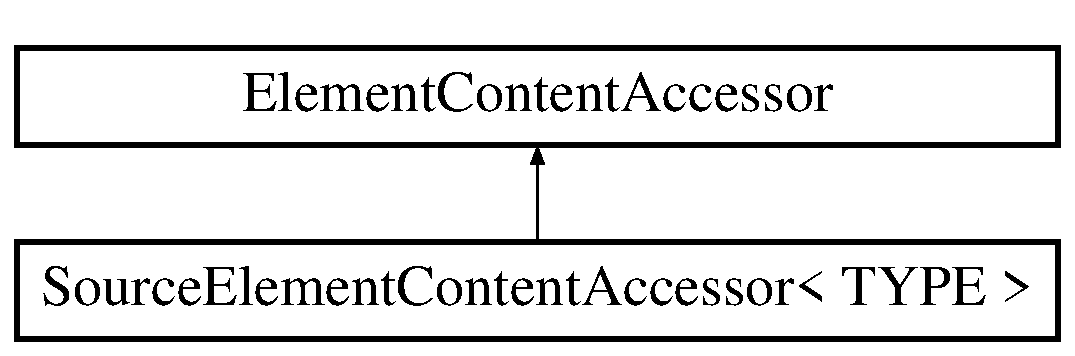
\includegraphics[height=2.000000cm]{struct_element_content_accessor}
\end{center}
\end{figure}
\subsection*{公開メンバ関数}
\begin{DoxyCompactItemize}
\item 
\hyperlink{struct_element_content_accessor_a59a1e00643f9f94ff680d2f63f80b0cd}{Element\+Content\+Accessor} ()
\item 
\hyperlink{struct_element_content_accessor_af1a83e6fae2facae0b94d0c7332e0a2e}{Element\+Content\+Accessor} (xml\+Node $\ast$p\+Element)
\item 
virtual \hyperlink{struct_element_content_accessor_a269fa630fb13ff74aa591f53de51a976}{$\sim$\+Element\+Content\+Accessor} ()
\item 
{\footnotesize template$<$typename T\+Y\+PE $>$ }\\bool \hyperlink{struct_element_content_accessor_a5c066a3db4f929723fc1a78c11745154}{Get\+Next} (T\+Y\+PE $\ast$p\+Data)
\item 
{\footnotesize template$<$typename T\+Y\+PE $>$ }\\int \hyperlink{struct_element_content_accessor_a412f6cb46b068e160e393f4318bcf4fc}{Get\+Array} (T\+Y\+PE $\ast$p\+Array, int p\+Array\+Size, int p\+Source\+Unit\+Offset=0, int p\+Source\+Unit\+Valid\+Count=1, int p\+Source\+Unit\+Size=1, int p\+Dest\+Unit\+Offset=0, int p\+Dest\+Unit\+Valid\+Count=1, int p\+Dest\+Unit\+Size=1, T\+Y\+PE p\+Default\+Value=T\+Y\+PE())
\end{DoxyCompactItemize}
\subsection*{公開変数類}
\begin{DoxyCompactItemize}
\item 
xml\+Char $\ast$ \hyperlink{struct_element_content_accessor_a3b06ccf10e2deb2e1308bb5bc4bf9532}{m\+Content}
\item 
const char $\ast$ \hyperlink{struct_element_content_accessor_a086d33aecd0a61b63fb21ff4d744e463}{m\+Pointer}
\end{DoxyCompactItemize}


\subsection{詳解}
A struct for convenient access to the content of common C\+O\+L\+L\+A\+DA element. 

 fbxcolladaelement.\+h の 74 行目に定義があります。



\subsection{構築子と解体子}
\mbox{\Hypertarget{struct_element_content_accessor_a59a1e00643f9f94ff680d2f63f80b0cd}\label{struct_element_content_accessor_a59a1e00643f9f94ff680d2f63f80b0cd}} 
\index{Element\+Content\+Accessor@{Element\+Content\+Accessor}!Element\+Content\+Accessor@{Element\+Content\+Accessor}}
\index{Element\+Content\+Accessor@{Element\+Content\+Accessor}!Element\+Content\+Accessor@{Element\+Content\+Accessor}}
\subsubsection{\texorpdfstring{Element\+Content\+Accessor()}{ElementContentAccessor()}\hspace{0.1cm}{\footnotesize\ttfamily [1/2]}}
{\footnotesize\ttfamily Element\+Content\+Accessor\+::\+Element\+Content\+Accessor (\begin{DoxyParamCaption}{ }\end{DoxyParamCaption})}

\mbox{\Hypertarget{struct_element_content_accessor_af1a83e6fae2facae0b94d0c7332e0a2e}\label{struct_element_content_accessor_af1a83e6fae2facae0b94d0c7332e0a2e}} 
\index{Element\+Content\+Accessor@{Element\+Content\+Accessor}!Element\+Content\+Accessor@{Element\+Content\+Accessor}}
\index{Element\+Content\+Accessor@{Element\+Content\+Accessor}!Element\+Content\+Accessor@{Element\+Content\+Accessor}}
\subsubsection{\texorpdfstring{Element\+Content\+Accessor()}{ElementContentAccessor()}\hspace{0.1cm}{\footnotesize\ttfamily [2/2]}}
{\footnotesize\ttfamily Element\+Content\+Accessor\+::\+Element\+Content\+Accessor (\begin{DoxyParamCaption}\item[{xml\+Node $\ast$}]{p\+Element }\end{DoxyParamCaption})}

\mbox{\Hypertarget{struct_element_content_accessor_a269fa630fb13ff74aa591f53de51a976}\label{struct_element_content_accessor_a269fa630fb13ff74aa591f53de51a976}} 
\index{Element\+Content\+Accessor@{Element\+Content\+Accessor}!````~Element\+Content\+Accessor@{$\sim$\+Element\+Content\+Accessor}}
\index{````~Element\+Content\+Accessor@{$\sim$\+Element\+Content\+Accessor}!Element\+Content\+Accessor@{Element\+Content\+Accessor}}
\subsubsection{\texorpdfstring{$\sim$\+Element\+Content\+Accessor()}{~ElementContentAccessor()}}
{\footnotesize\ttfamily virtual Element\+Content\+Accessor\+::$\sim$\+Element\+Content\+Accessor (\begin{DoxyParamCaption}{ }\end{DoxyParamCaption})\hspace{0.3cm}{\ttfamily [virtual]}}



\subsection{関数詳解}
\mbox{\Hypertarget{struct_element_content_accessor_a412f6cb46b068e160e393f4318bcf4fc}\label{struct_element_content_accessor_a412f6cb46b068e160e393f4318bcf4fc}} 
\index{Element\+Content\+Accessor@{Element\+Content\+Accessor}!Get\+Array@{Get\+Array}}
\index{Get\+Array@{Get\+Array}!Element\+Content\+Accessor@{Element\+Content\+Accessor}}
\subsubsection{\texorpdfstring{Get\+Array()}{GetArray()}}
{\footnotesize\ttfamily template$<$typename T\+Y\+PE $>$ \\
int Element\+Content\+Accessor\+::\+Get\+Array (\begin{DoxyParamCaption}\item[{T\+Y\+PE $\ast$}]{p\+Array,  }\item[{int}]{p\+Array\+Size,  }\item[{int}]{p\+Source\+Unit\+Offset = {\ttfamily 0},  }\item[{int}]{p\+Source\+Unit\+Valid\+Count = {\ttfamily 1},  }\item[{int}]{p\+Source\+Unit\+Size = {\ttfamily 1},  }\item[{int}]{p\+Dest\+Unit\+Offset = {\ttfamily 0},  }\item[{int}]{p\+Dest\+Unit\+Valid\+Count = {\ttfamily 1},  }\item[{int}]{p\+Dest\+Unit\+Size = {\ttfamily 1},  }\item[{T\+Y\+PE}]{p\+Default\+Value = {\ttfamily TYPE()} }\end{DoxyParamCaption})\hspace{0.3cm}{\ttfamily [inline]}}



 fbxcolladaelement.\+h の 87 行目に定義があります。

\mbox{\Hypertarget{struct_element_content_accessor_a5c066a3db4f929723fc1a78c11745154}\label{struct_element_content_accessor_a5c066a3db4f929723fc1a78c11745154}} 
\index{Element\+Content\+Accessor@{Element\+Content\+Accessor}!Get\+Next@{Get\+Next}}
\index{Get\+Next@{Get\+Next}!Element\+Content\+Accessor@{Element\+Content\+Accessor}}
\subsubsection{\texorpdfstring{Get\+Next()}{GetNext()}}
{\footnotesize\ttfamily template$<$typename T\+Y\+PE $>$ \\
bool Element\+Content\+Accessor\+::\+Get\+Next (\begin{DoxyParamCaption}\item[{T\+Y\+PE $\ast$}]{p\+Data }\end{DoxyParamCaption})\hspace{0.3cm}{\ttfamily [inline]}}



 fbxcolladaelement.\+h の 81 行目に定義があります。



\subsection{メンバ詳解}
\mbox{\Hypertarget{struct_element_content_accessor_a3b06ccf10e2deb2e1308bb5bc4bf9532}\label{struct_element_content_accessor_a3b06ccf10e2deb2e1308bb5bc4bf9532}} 
\index{Element\+Content\+Accessor@{Element\+Content\+Accessor}!m\+Content@{m\+Content}}
\index{m\+Content@{m\+Content}!Element\+Content\+Accessor@{Element\+Content\+Accessor}}
\subsubsection{\texorpdfstring{m\+Content}{mContent}}
{\footnotesize\ttfamily xml\+Char$\ast$ Element\+Content\+Accessor\+::m\+Content}



 fbxcolladaelement.\+h の 101 行目に定義があります。

\mbox{\Hypertarget{struct_element_content_accessor_a086d33aecd0a61b63fb21ff4d744e463}\label{struct_element_content_accessor_a086d33aecd0a61b63fb21ff4d744e463}} 
\index{Element\+Content\+Accessor@{Element\+Content\+Accessor}!m\+Pointer@{m\+Pointer}}
\index{m\+Pointer@{m\+Pointer}!Element\+Content\+Accessor@{Element\+Content\+Accessor}}
\subsubsection{\texorpdfstring{m\+Pointer}{mPointer}}
{\footnotesize\ttfamily const char$\ast$ Element\+Content\+Accessor\+::m\+Pointer}



 fbxcolladaelement.\+h の 102 行目に定義があります。



この構造体詳解は次のファイルから抽出されました\+:\begin{DoxyCompactItemize}
\item 
C\+:/\+Maya/scripts/\+F\+B\+X\+\_\+\+S\+D\+K/2017.\+1/include/fbxsdk/fileio/collada/\hyperlink{fbxcolladaelement_8h}{fbxcolladaelement.\+h}\end{DoxyCompactItemize}

\hypertarget{struct_fbx_embedded_files_accumulator_1_1_embedded_file_info}{}\section{Fbx\+Embedded\+Files\+Accumulator\+:\+:Embedded\+File\+Info 構造体}
\label{struct_fbx_embedded_files_accumulator_1_1_embedded_file_info}\index{Fbx\+Embedded\+Files\+Accumulator\+::\+Embedded\+File\+Info@{Fbx\+Embedded\+Files\+Accumulator\+::\+Embedded\+File\+Info}}


{\ttfamily \#include $<$fbxembeddedfilesaccumulator.\+h$>$}



Fbx\+Embedded\+Files\+Accumulator\+:\+:Embedded\+File\+Info 連携図
% FIG 0
\subsection*{公開変数類}
\begin{DoxyCompactItemize}
\item 
\hyperlink{class_fbx_string}{Fbx\+String} \hyperlink{struct_fbx_embedded_files_accumulator_1_1_embedded_file_info_a3a7df7013bc1f2a90a3d1b9cad7b52e1}{m\+Original\+Property\+Url}
\item 
\hyperlink{class_fbx_embedded_files_accumulator_abc919e5ba3486530790dcd7ef90b8eed}{Object\+Property\+Map} \hyperlink{struct_fbx_embedded_files_accumulator_1_1_embedded_file_info_a04b3e7c42f3fe61536e8cc3a13ad682f}{m\+Consumers}
\end{DoxyCompactItemize}


\subsection{メンバ詳解}
\mbox{\Hypertarget{struct_fbx_embedded_files_accumulator_1_1_embedded_file_info_a04b3e7c42f3fe61536e8cc3a13ad682f}\label{struct_fbx_embedded_files_accumulator_1_1_embedded_file_info_a04b3e7c42f3fe61536e8cc3a13ad682f}} 
\index{Fbx\+Embedded\+Files\+Accumulator\+::\+Embedded\+File\+Info@{Fbx\+Embedded\+Files\+Accumulator\+::\+Embedded\+File\+Info}!m\+Consumers@{m\+Consumers}}
\index{m\+Consumers@{m\+Consumers}!Fbx\+Embedded\+Files\+Accumulator\+::\+Embedded\+File\+Info@{Fbx\+Embedded\+Files\+Accumulator\+::\+Embedded\+File\+Info}}
\subsubsection{\texorpdfstring{m\+Consumers}{mConsumers}}
{\footnotesize\ttfamily \hyperlink{class_fbx_embedded_files_accumulator_abc919e5ba3486530790dcd7ef90b8eed}{Object\+Property\+Map} Fbx\+Embedded\+Files\+Accumulator\+::\+Embedded\+File\+Info\+::m\+Consumers}

\mbox{\Hypertarget{struct_fbx_embedded_files_accumulator_1_1_embedded_file_info_a3a7df7013bc1f2a90a3d1b9cad7b52e1}\label{struct_fbx_embedded_files_accumulator_1_1_embedded_file_info_a3a7df7013bc1f2a90a3d1b9cad7b52e1}} 
\index{Fbx\+Embedded\+Files\+Accumulator\+::\+Embedded\+File\+Info@{Fbx\+Embedded\+Files\+Accumulator\+::\+Embedded\+File\+Info}!m\+Original\+Property\+Url@{m\+Original\+Property\+Url}}
\index{m\+Original\+Property\+Url@{m\+Original\+Property\+Url}!Fbx\+Embedded\+Files\+Accumulator\+::\+Embedded\+File\+Info@{Fbx\+Embedded\+Files\+Accumulator\+::\+Embedded\+File\+Info}}
\subsubsection{\texorpdfstring{m\+Original\+Property\+Url}{mOriginalPropertyUrl}}
{\footnotesize\ttfamily \hyperlink{class_fbx_string}{Fbx\+String} Fbx\+Embedded\+Files\+Accumulator\+::\+Embedded\+File\+Info\+::m\+Original\+Property\+Url}



この構造体詳解は次のファイルから抽出されました\+:\begin{DoxyCompactItemize}
\item 
C\+:/github/\+F\+B\+Xpython\+S\+D\+K201701/\+F\+B\+Xpython\+S\+D\+K201701/2017.\+1/include/fbxsdk/utils/\hyperlink{fbxembeddedfilesaccumulator_8h}{fbxembeddedfilesaccumulator.\+h}\end{DoxyCompactItemize}

\hypertarget{struct_fbx_emitter_1_1_event_data}{}\section{Fbx\+Emitter\+:\+:Event\+Data 構造体}
\label{struct_fbx_emitter_1_1_event_data}\index{Fbx\+Emitter\+::\+Event\+Data@{Fbx\+Emitter\+::\+Event\+Data}}


{\ttfamily \#include $<$fbxemitter.\+h$>$}



Fbx\+Emitter\+:\+:Event\+Data 連携図
% FIG 0
\subsection*{公開変数類}
\begin{DoxyCompactItemize}
\item 
\hyperlink{class_fbx_emitter_a9ac3cddf1a246e71957e4b7db6c08fc1}{Event\+Handler\+List} \hyperlink{struct_fbx_emitter_1_1_event_data_a0879b804afdfba87bbd758d5c78b7577}{m\+Event\+Handler\+List}
\end{DoxyCompactItemize}


\subsection{メンバ詳解}
\mbox{\Hypertarget{struct_fbx_emitter_1_1_event_data_a0879b804afdfba87bbd758d5c78b7577}\label{struct_fbx_emitter_1_1_event_data_a0879b804afdfba87bbd758d5c78b7577}} 
\index{Fbx\+Emitter\+::\+Event\+Data@{Fbx\+Emitter\+::\+Event\+Data}!m\+Event\+Handler\+List@{m\+Event\+Handler\+List}}
\index{m\+Event\+Handler\+List@{m\+Event\+Handler\+List}!Fbx\+Emitter\+::\+Event\+Data@{Fbx\+Emitter\+::\+Event\+Data}}
\subsubsection{\texorpdfstring{m\+Event\+Handler\+List}{mEventHandlerList}}
{\footnotesize\ttfamily \hyperlink{class_fbx_emitter_a9ac3cddf1a246e71957e4b7db6c08fc1}{Event\+Handler\+List} Fbx\+Emitter\+::\+Event\+Data\+::m\+Event\+Handler\+List}



この構造体詳解は次のファイルから抽出されました\+:\begin{DoxyCompactItemize}
\item 
C\+:/github/\+F\+B\+Xpython\+S\+D\+K201701/\+F\+B\+Xpython\+S\+D\+K201701/2017.\+1/include/fbxsdk/core/\hyperlink{fbxemitter_8h}{fbxemitter.\+h}\end{DoxyCompactItemize}

\hypertarget{class_fbx6_class_template_map}{}\section{Fbx6\+Class\+Template\+Map クラス}
\label{class_fbx6_class_template_map}\index{Fbx6\+Class\+Template\+Map@{Fbx6\+Class\+Template\+Map}}


Helper class to merge Class root property templates. Add class id and object to the template and search object by class id.  




{\ttfamily \#include $<$fbxreaderfbx6.\+h$>$}

\subsection*{公開メンバ関数}
\begin{DoxyCompactItemize}
\item 
\hyperlink{class_fbx6_class_template_map_a797c75312154457d38978b6c4046891e}{Fbx6\+Class\+Template\+Map} ()
\item 
\hyperlink{class_fbx6_class_template_map_af1b623f6de8fefd4c4515a66e40a2bec}{$\sim$\+Fbx6\+Class\+Template\+Map} ()
\item 
bool \hyperlink{class_fbx6_class_template_map_a064f7a5f731932c34a257fe9947c3981}{Add\+Class\+Id} (\hyperlink{class_fbx_class_id}{Fbx\+Class\+Id} p\+Id, \hyperlink{class_fbx_object}{Fbx\+Object} $\ast$p\+Template\+Object)
\item 
bool \hyperlink{class_fbx6_class_template_map_a93b436ce1ce8f65302b675cb3a085134}{Merge\+With\+Template} (\hyperlink{class_fbx_object}{Fbx\+Object} $\ast$p\+Object) const
\item 
void \hyperlink{class_fbx6_class_template_map_a522d86033875290b78d0034909997fde}{Clear} ()
\end{DoxyCompactItemize}


\subsection{詳解}
Helper class to merge Class root property templates. Add class id and object to the template and search object by class id. 

\subsection{構築子と解体子}
\mbox{\Hypertarget{class_fbx6_class_template_map_a797c75312154457d38978b6c4046891e}\label{class_fbx6_class_template_map_a797c75312154457d38978b6c4046891e}} 
\index{Fbx6\+Class\+Template\+Map@{Fbx6\+Class\+Template\+Map}!Fbx6\+Class\+Template\+Map@{Fbx6\+Class\+Template\+Map}}
\index{Fbx6\+Class\+Template\+Map@{Fbx6\+Class\+Template\+Map}!Fbx6\+Class\+Template\+Map@{Fbx6\+Class\+Template\+Map}}
\subsubsection{\texorpdfstring{Fbx6\+Class\+Template\+Map()}{Fbx6ClassTemplateMap()}}
{\footnotesize\ttfamily Fbx6\+Class\+Template\+Map\+::\+Fbx6\+Class\+Template\+Map (\begin{DoxyParamCaption}{ }\end{DoxyParamCaption})}

Constructor \mbox{\Hypertarget{class_fbx6_class_template_map_af1b623f6de8fefd4c4515a66e40a2bec}\label{class_fbx6_class_template_map_af1b623f6de8fefd4c4515a66e40a2bec}} 
\index{Fbx6\+Class\+Template\+Map@{Fbx6\+Class\+Template\+Map}!````~Fbx6\+Class\+Template\+Map@{$\sim$\+Fbx6\+Class\+Template\+Map}}
\index{````~Fbx6\+Class\+Template\+Map@{$\sim$\+Fbx6\+Class\+Template\+Map}!Fbx6\+Class\+Template\+Map@{Fbx6\+Class\+Template\+Map}}
\subsubsection{\texorpdfstring{$\sim$\+Fbx6\+Class\+Template\+Map()}{~Fbx6ClassTemplateMap()}}
{\footnotesize\ttfamily Fbx6\+Class\+Template\+Map\+::$\sim$\+Fbx6\+Class\+Template\+Map (\begin{DoxyParamCaption}{ }\end{DoxyParamCaption})}

Destructor 

\subsection{メソッド詳解}
\mbox{\Hypertarget{class_fbx6_class_template_map_a064f7a5f731932c34a257fe9947c3981}\label{class_fbx6_class_template_map_a064f7a5f731932c34a257fe9947c3981}} 
\index{Fbx6\+Class\+Template\+Map@{Fbx6\+Class\+Template\+Map}!Add\+Class\+Id@{Add\+Class\+Id}}
\index{Add\+Class\+Id@{Add\+Class\+Id}!Fbx6\+Class\+Template\+Map@{Fbx6\+Class\+Template\+Map}}
\subsubsection{\texorpdfstring{Add\+Class\+Id()}{AddClassId()}}
{\footnotesize\ttfamily bool Fbx6\+Class\+Template\+Map\+::\+Add\+Class\+Id (\begin{DoxyParamCaption}\item[{\hyperlink{class_fbx_class_id}{Fbx\+Class\+Id}}]{p\+Id,  }\item[{\hyperlink{class_fbx_object}{Fbx\+Object} $\ast$}]{p\+Template\+Object }\end{DoxyParamCaption})}

Add the template object to template map 
\begin{DoxyParams}{引数}
{\em p\+Id} & Class Id \\
\hline
{\em p\+Template\+Object} & template object \\
\hline
\end{DoxyParams}
\begin{DoxyReturn}{戻り値}
if the object is successfully added return {\ttfamily true}, otherwise return {\ttfamily false}. 
\end{DoxyReturn}
\mbox{\Hypertarget{class_fbx6_class_template_map_a522d86033875290b78d0034909997fde}\label{class_fbx6_class_template_map_a522d86033875290b78d0034909997fde}} 
\index{Fbx6\+Class\+Template\+Map@{Fbx6\+Class\+Template\+Map}!Clear@{Clear}}
\index{Clear@{Clear}!Fbx6\+Class\+Template\+Map@{Fbx6\+Class\+Template\+Map}}
\subsubsection{\texorpdfstring{Clear()}{Clear()}}
{\footnotesize\ttfamily void Fbx6\+Class\+Template\+Map\+::\+Clear (\begin{DoxyParamCaption}{ }\end{DoxyParamCaption})}

Delete all \hyperlink{class_fbx_object}{Fbx\+Object} in template map \mbox{\Hypertarget{class_fbx6_class_template_map_a93b436ce1ce8f65302b675cb3a085134}\label{class_fbx6_class_template_map_a93b436ce1ce8f65302b675cb3a085134}} 
\index{Fbx6\+Class\+Template\+Map@{Fbx6\+Class\+Template\+Map}!Merge\+With\+Template@{Merge\+With\+Template}}
\index{Merge\+With\+Template@{Merge\+With\+Template}!Fbx6\+Class\+Template\+Map@{Fbx6\+Class\+Template\+Map}}
\subsubsection{\texorpdfstring{Merge\+With\+Template()}{MergeWithTemplate()}}
{\footnotesize\ttfamily bool Fbx6\+Class\+Template\+Map\+::\+Merge\+With\+Template (\begin{DoxyParamCaption}\item[{\hyperlink{class_fbx_object}{Fbx\+Object} $\ast$}]{p\+Object }\end{DoxyParamCaption}) const}

Merge the properties of \hyperlink{class_fbx_object}{Fbx\+Object} with the object with the same class id 
\begin{DoxyParams}{引数}
{\em p\+Object} & The \hyperlink{class_fbx_object}{Fbx\+Object} to merge \\
\hline
\end{DoxyParams}
\begin{DoxyReturn}{戻り値}
if the object is merged return {\ttfamily true}, otherwise return {\ttfamily false}. 
\end{DoxyReturn}


このクラス詳解は次のファイルから抽出されました\+:\begin{DoxyCompactItemize}
\item 
C\+:/github/\+F\+B\+Xpython\+S\+D\+K201701/\+F\+B\+Xpython\+S\+D\+K201701/2017.\+1/include/fbxsdk/fileio/fbx/\hyperlink{fbxreaderfbx6_8h}{fbxreaderfbx6.\+h}\end{DoxyCompactItemize}

\hypertarget{class_fbx_accumulator_entry}{}\section{Fbx\+Accumulator\+Entry クラス}
\label{class_fbx_accumulator_entry}\index{Fbx\+Accumulator\+Entry@{Fbx\+Accumulator\+Entry}}


{\ttfamily \#include $<$fbxusernotification.\+h$>$}

\subsection*{公開型}
\begin{DoxyCompactItemize}
\item 
enum \hyperlink{class_fbx_accumulator_entry_af08af3ddcbf7e8fe642d7e9ecb4ad0e2}{E\+Class} \{ \hyperlink{class_fbx_accumulator_entry_af08af3ddcbf7e8fe642d7e9ecb4ad0e2a9e327e2f495f49a576e16f4050231aff}{e\+Error} =1, 
\hyperlink{class_fbx_accumulator_entry_af08af3ddcbf7e8fe642d7e9ecb4ad0e2a02238ae4f2cce7a190dad59cfb3e9c19}{e\+Warning} =2, 
\hyperlink{class_fbx_accumulator_entry_af08af3ddcbf7e8fe642d7e9ecb4ad0e2ace66165782fe6efde70c8d93361c8ded}{e\+Information} =4, 
\hyperlink{class_fbx_accumulator_entry_af08af3ddcbf7e8fe642d7e9ecb4ad0e2a2970874fc582ec77e50a82bb850d983b}{e\+Any} =7
 \}
\end{DoxyCompactItemize}
\subsection*{公開メンバ関数}
\begin{DoxyCompactItemize}
\item 
\hyperlink{class_fbx_accumulator_entry_a08089894e3d5aed12dfc556553e022c4}{Fbx\+Accumulator\+Entry} (\hyperlink{class_fbx_accumulator_entry_af08af3ddcbf7e8fe642d7e9ecb4ad0e2}{E\+Class} p\+A\+E\+Class, const \hyperlink{class_fbx_string}{Fbx\+String} \&p\+Name, const \hyperlink{class_fbx_string}{Fbx\+String} \&p\+Descr, \hyperlink{class_fbx_string}{Fbx\+String} p\+Detail=\char`\"{}\char`\"{}, bool p\+Mute\+State=true)
\item 
\hyperlink{class_fbx_accumulator_entry_a536f3ab8a13cb7037e6f2a39278eb8ca}{Fbx\+Accumulator\+Entry} (const \hyperlink{class_fbx_accumulator_entry}{Fbx\+Accumulator\+Entry} \&p\+AE, bool p\+Skip\+Details)
\item 
\hyperlink{class_fbx_accumulator_entry_a76e1a283bd8e13c1591b83ed85cb5a10}{$\sim$\+Fbx\+Accumulator\+Entry} ()
\begin{DoxyCompactList}\small\item\em Destructor. \end{DoxyCompactList}\item 
\hyperlink{class_fbx_accumulator_entry_af08af3ddcbf7e8fe642d7e9ecb4ad0e2}{E\+Class} \hyperlink{class_fbx_accumulator_entry_a2c6baa9720f96ecf7a9cc69f89b5c430}{Get\+Class} () const
\begin{DoxyCompactList}\small\item\em Returns the category class of this entry. \end{DoxyCompactList}\item 
\hyperlink{class_fbx_string}{Fbx\+String} \hyperlink{class_fbx_accumulator_entry_a0dbcb9bc95c823b84a8679f781d35317}{Get\+Name} () const
\begin{DoxyCompactList}\small\item\em Returns the name of this entry. \end{DoxyCompactList}\item 
\hyperlink{class_fbx_string}{Fbx\+String} \hyperlink{class_fbx_accumulator_entry_a37cfbde3b74cda66945b948b4d6acd7c}{Get\+Description} () const
\begin{DoxyCompactList}\small\item\em Returns the description of this entry. \end{DoxyCompactList}\item 
int \hyperlink{class_fbx_accumulator_entry_adc709cecc41aa46b5874877c49f99b19}{Get\+Details\+Count} () const
\begin{DoxyCompactList}\small\item\em Returns the number of details stored. \end{DoxyCompactList}\item 
const \hyperlink{class_fbx_string}{Fbx\+String} $\ast$ \hyperlink{class_fbx_accumulator_entry_a1698d2ce0b959f30b912716a893cf274}{Get\+Detail} (int id) const
\item 
bool \hyperlink{class_fbx_accumulator_entry_ac7c575cce1b36df854f30ed8beb82260}{Is\+Muted} () const
\begin{DoxyCompactList}\small\item\em Returns True if this entry is muted. \end{DoxyCompactList}\end{DoxyCompactItemize}
\subsection*{フレンド}
\begin{DoxyCompactItemize}
\item 
class \hyperlink{class_fbx_accumulator_entry_a59b31f76d63ab836d795cdd0188a201a}{Fbx\+User\+Notification}
\end{DoxyCompactItemize}


\subsection{詳解}
This class defines one entry object held by the \hyperlink{class_fbx_user_notification}{Fbx\+User\+Notification} class.

An entry object is a message to show error, warning or information. Direct manipulation of this object should not be required. At most, access to its members can be granted for querying purposes. 

 fbxusernotification.\+h の 34 行目に定義があります。



\subsection{列挙型メンバ詳解}
\mbox{\Hypertarget{class_fbx_accumulator_entry_af08af3ddcbf7e8fe642d7e9ecb4ad0e2}\label{class_fbx_accumulator_entry_af08af3ddcbf7e8fe642d7e9ecb4ad0e2}} 
\index{Fbx\+Accumulator\+Entry@{Fbx\+Accumulator\+Entry}!E\+Class@{E\+Class}}
\index{E\+Class@{E\+Class}!Fbx\+Accumulator\+Entry@{Fbx\+Accumulator\+Entry}}
\subsubsection{\texorpdfstring{E\+Class}{EClass}}
{\footnotesize\ttfamily enum \hyperlink{class_fbx_accumulator_entry_af08af3ddcbf7e8fe642d7e9ecb4ad0e2}{Fbx\+Accumulator\+Entry\+::\+E\+Class}}

Category of the accumulator entry. \begin{DoxyEnumFields}{列挙値}
\raisebox{\heightof{T}}[0pt][0pt]{\index{e\+Error@{e\+Error}!Fbx\+Accumulator\+Entry@{Fbx\+Accumulator\+Entry}}\index{Fbx\+Accumulator\+Entry@{Fbx\+Accumulator\+Entry}!e\+Error@{e\+Error}}}\mbox{\Hypertarget{class_fbx_accumulator_entry_af08af3ddcbf7e8fe642d7e9ecb4ad0e2a9e327e2f495f49a576e16f4050231aff}\label{class_fbx_accumulator_entry_af08af3ddcbf7e8fe642d7e9ecb4ad0e2a9e327e2f495f49a576e16f4050231aff}} 
e\+Error&Error message entry. \\
\hline

\raisebox{\heightof{T}}[0pt][0pt]{\index{e\+Warning@{e\+Warning}!Fbx\+Accumulator\+Entry@{Fbx\+Accumulator\+Entry}}\index{Fbx\+Accumulator\+Entry@{Fbx\+Accumulator\+Entry}!e\+Warning@{e\+Warning}}}\mbox{\Hypertarget{class_fbx_accumulator_entry_af08af3ddcbf7e8fe642d7e9ecb4ad0e2a02238ae4f2cce7a190dad59cfb3e9c19}\label{class_fbx_accumulator_entry_af08af3ddcbf7e8fe642d7e9ecb4ad0e2a02238ae4f2cce7a190dad59cfb3e9c19}} 
e\+Warning&Warning message entry. \\
\hline

\raisebox{\heightof{T}}[0pt][0pt]{\index{e\+Information@{e\+Information}!Fbx\+Accumulator\+Entry@{Fbx\+Accumulator\+Entry}}\index{Fbx\+Accumulator\+Entry@{Fbx\+Accumulator\+Entry}!e\+Information@{e\+Information}}}\mbox{\Hypertarget{class_fbx_accumulator_entry_af08af3ddcbf7e8fe642d7e9ecb4ad0e2ace66165782fe6efde70c8d93361c8ded}\label{class_fbx_accumulator_entry_af08af3ddcbf7e8fe642d7e9ecb4ad0e2ace66165782fe6efde70c8d93361c8ded}} 
e\+Information&Information message entry. \\
\hline

\raisebox{\heightof{T}}[0pt][0pt]{\index{e\+Any@{e\+Any}!Fbx\+Accumulator\+Entry@{Fbx\+Accumulator\+Entry}}\index{Fbx\+Accumulator\+Entry@{Fbx\+Accumulator\+Entry}!e\+Any@{e\+Any}}}\mbox{\Hypertarget{class_fbx_accumulator_entry_af08af3ddcbf7e8fe642d7e9ecb4ad0e2a2970874fc582ec77e50a82bb850d983b}\label{class_fbx_accumulator_entry_af08af3ddcbf7e8fe642d7e9ecb4ad0e2a2970874fc582ec77e50a82bb850d983b}} 
e\+Any&Entry that does not belong to above class. Cannot be used as a class ID \\
\hline

\end{DoxyEnumFields}


 fbxusernotification.\+h の 39 行目に定義があります。



\subsection{構築子と解体子}
\mbox{\Hypertarget{class_fbx_accumulator_entry_a08089894e3d5aed12dfc556553e022c4}\label{class_fbx_accumulator_entry_a08089894e3d5aed12dfc556553e022c4}} 
\index{Fbx\+Accumulator\+Entry@{Fbx\+Accumulator\+Entry}!Fbx\+Accumulator\+Entry@{Fbx\+Accumulator\+Entry}}
\index{Fbx\+Accumulator\+Entry@{Fbx\+Accumulator\+Entry}!Fbx\+Accumulator\+Entry@{Fbx\+Accumulator\+Entry}}
\subsubsection{\texorpdfstring{Fbx\+Accumulator\+Entry()}{FbxAccumulatorEntry()}\hspace{0.1cm}{\footnotesize\ttfamily [1/2]}}
{\footnotesize\ttfamily Fbx\+Accumulator\+Entry\+::\+Fbx\+Accumulator\+Entry (\begin{DoxyParamCaption}\item[{\hyperlink{class_fbx_accumulator_entry_af08af3ddcbf7e8fe642d7e9ecb4ad0e2}{E\+Class}}]{p\+A\+E\+Class,  }\item[{const \hyperlink{class_fbx_string}{Fbx\+String} \&}]{p\+Name,  }\item[{const \hyperlink{class_fbx_string}{Fbx\+String} \&}]{p\+Descr,  }\item[{\hyperlink{class_fbx_string}{Fbx\+String}}]{p\+Detail = {\ttfamily \char`\"{}\char`\"{}},  }\item[{bool}]{p\+Mute\+State = {\ttfamily true} }\end{DoxyParamCaption})}

Constructor. 
\begin{DoxyParams}{引数}
{\em p\+A\+E\+Class} & Specify the category for this entry. \\
\hline
{\em p\+Name} & Identifies this entry (more than one object can have the same name). \\
\hline
{\em p\+Descr} & The description of the entry. This is the common message. The details are added separately by the \hyperlink{class_fbx_user_notification}{Fbx\+User\+Notification} classes. \\
\hline
{\em p\+Detail} & A list of detail string that will be copied into the local array. \\
\hline
{\em p\+Mute\+State} & Whether this entry is muted. \\
\hline
\end{DoxyParams}
\begin{DoxyRemark}{注釈}
By default the object is muted so it does not get processed by the low level output routines of the User\+Notification accumulator. The entry gets activated (unmuted) by the calls to Add\+Detail() in the accumulator. 
\end{DoxyRemark}
\mbox{\Hypertarget{class_fbx_accumulator_entry_a536f3ab8a13cb7037e6f2a39278eb8ca}\label{class_fbx_accumulator_entry_a536f3ab8a13cb7037e6f2a39278eb8ca}} 
\index{Fbx\+Accumulator\+Entry@{Fbx\+Accumulator\+Entry}!Fbx\+Accumulator\+Entry@{Fbx\+Accumulator\+Entry}}
\index{Fbx\+Accumulator\+Entry@{Fbx\+Accumulator\+Entry}!Fbx\+Accumulator\+Entry@{Fbx\+Accumulator\+Entry}}
\subsubsection{\texorpdfstring{Fbx\+Accumulator\+Entry()}{FbxAccumulatorEntry()}\hspace{0.1cm}{\footnotesize\ttfamily [2/2]}}
{\footnotesize\ttfamily Fbx\+Accumulator\+Entry\+::\+Fbx\+Accumulator\+Entry (\begin{DoxyParamCaption}\item[{const \hyperlink{class_fbx_accumulator_entry}{Fbx\+Accumulator\+Entry} \&}]{p\+AE,  }\item[{bool}]{p\+Skip\+Details }\end{DoxyParamCaption})}

Copy Constructor. 
\begin{DoxyParams}{引数}
{\em p\+AE} & Another \hyperlink{class_fbx_accumulator_entry}{Fbx\+Accumulator\+Entry} object to be copied. \\
\hline
{\em p\+Skip\+Details} & Flag to skip details. \\
\hline
\end{DoxyParams}
\mbox{\Hypertarget{class_fbx_accumulator_entry_a76e1a283bd8e13c1591b83ed85cb5a10}\label{class_fbx_accumulator_entry_a76e1a283bd8e13c1591b83ed85cb5a10}} 
\index{Fbx\+Accumulator\+Entry@{Fbx\+Accumulator\+Entry}!````~Fbx\+Accumulator\+Entry@{$\sim$\+Fbx\+Accumulator\+Entry}}
\index{````~Fbx\+Accumulator\+Entry@{$\sim$\+Fbx\+Accumulator\+Entry}!Fbx\+Accumulator\+Entry@{Fbx\+Accumulator\+Entry}}
\subsubsection{\texorpdfstring{$\sim$\+Fbx\+Accumulator\+Entry()}{~FbxAccumulatorEntry()}}
{\footnotesize\ttfamily Fbx\+Accumulator\+Entry\+::$\sim$\+Fbx\+Accumulator\+Entry (\begin{DoxyParamCaption}{ }\end{DoxyParamCaption})}



Destructor. 



\subsection{関数詳解}
\mbox{\Hypertarget{class_fbx_accumulator_entry_a2c6baa9720f96ecf7a9cc69f89b5c430}\label{class_fbx_accumulator_entry_a2c6baa9720f96ecf7a9cc69f89b5c430}} 
\index{Fbx\+Accumulator\+Entry@{Fbx\+Accumulator\+Entry}!Get\+Class@{Get\+Class}}
\index{Get\+Class@{Get\+Class}!Fbx\+Accumulator\+Entry@{Fbx\+Accumulator\+Entry}}
\subsubsection{\texorpdfstring{Get\+Class()}{GetClass()}}
{\footnotesize\ttfamily \hyperlink{class_fbx_accumulator_entry_af08af3ddcbf7e8fe642d7e9ecb4ad0e2}{E\+Class} Fbx\+Accumulator\+Entry\+::\+Get\+Class (\begin{DoxyParamCaption}{ }\end{DoxyParamCaption}) const}



Returns the category class of this entry. 

\mbox{\Hypertarget{class_fbx_accumulator_entry_a37cfbde3b74cda66945b948b4d6acd7c}\label{class_fbx_accumulator_entry_a37cfbde3b74cda66945b948b4d6acd7c}} 
\index{Fbx\+Accumulator\+Entry@{Fbx\+Accumulator\+Entry}!Get\+Description@{Get\+Description}}
\index{Get\+Description@{Get\+Description}!Fbx\+Accumulator\+Entry@{Fbx\+Accumulator\+Entry}}
\subsubsection{\texorpdfstring{Get\+Description()}{GetDescription()}}
{\footnotesize\ttfamily \hyperlink{class_fbx_string}{Fbx\+String} Fbx\+Accumulator\+Entry\+::\+Get\+Description (\begin{DoxyParamCaption}{ }\end{DoxyParamCaption}) const}



Returns the description of this entry. 

\mbox{\Hypertarget{class_fbx_accumulator_entry_a1698d2ce0b959f30b912716a893cf274}\label{class_fbx_accumulator_entry_a1698d2ce0b959f30b912716a893cf274}} 
\index{Fbx\+Accumulator\+Entry@{Fbx\+Accumulator\+Entry}!Get\+Detail@{Get\+Detail}}
\index{Get\+Detail@{Get\+Detail}!Fbx\+Accumulator\+Entry@{Fbx\+Accumulator\+Entry}}
\subsubsection{\texorpdfstring{Get\+Detail()}{GetDetail()}}
{\footnotesize\ttfamily const \hyperlink{class_fbx_string}{Fbx\+String}$\ast$ Fbx\+Accumulator\+Entry\+::\+Get\+Detail (\begin{DoxyParamCaption}\item[{int}]{id }\end{DoxyParamCaption}) const}

Returns a pointer to one specific detail string (or N\+U\+LL if the id is invalid). Detail string is dynamic. One entry can have multiple detail strings to hold extra information. For example, if one entry message is related to many F\+BX nodes, user can add these nodes\textquotesingle{} name as details. 
\begin{DoxyParams}{引数}
{\em id} & The detail id. \\
\hline
\end{DoxyParams}
\begin{DoxyReturn}{戻り値}
Pointer to the specific detail. 
\end{DoxyReturn}
\mbox{\Hypertarget{class_fbx_accumulator_entry_adc709cecc41aa46b5874877c49f99b19}\label{class_fbx_accumulator_entry_adc709cecc41aa46b5874877c49f99b19}} 
\index{Fbx\+Accumulator\+Entry@{Fbx\+Accumulator\+Entry}!Get\+Details\+Count@{Get\+Details\+Count}}
\index{Get\+Details\+Count@{Get\+Details\+Count}!Fbx\+Accumulator\+Entry@{Fbx\+Accumulator\+Entry}}
\subsubsection{\texorpdfstring{Get\+Details\+Count()}{GetDetailsCount()}}
{\footnotesize\ttfamily int Fbx\+Accumulator\+Entry\+::\+Get\+Details\+Count (\begin{DoxyParamCaption}{ }\end{DoxyParamCaption}) const}



Returns the number of details stored. 

\mbox{\Hypertarget{class_fbx_accumulator_entry_a0dbcb9bc95c823b84a8679f781d35317}\label{class_fbx_accumulator_entry_a0dbcb9bc95c823b84a8679f781d35317}} 
\index{Fbx\+Accumulator\+Entry@{Fbx\+Accumulator\+Entry}!Get\+Name@{Get\+Name}}
\index{Get\+Name@{Get\+Name}!Fbx\+Accumulator\+Entry@{Fbx\+Accumulator\+Entry}}
\subsubsection{\texorpdfstring{Get\+Name()}{GetName()}}
{\footnotesize\ttfamily \hyperlink{class_fbx_string}{Fbx\+String} Fbx\+Accumulator\+Entry\+::\+Get\+Name (\begin{DoxyParamCaption}{ }\end{DoxyParamCaption}) const}



Returns the name of this entry. 

\mbox{\Hypertarget{class_fbx_accumulator_entry_ac7c575cce1b36df854f30ed8beb82260}\label{class_fbx_accumulator_entry_ac7c575cce1b36df854f30ed8beb82260}} 
\index{Fbx\+Accumulator\+Entry@{Fbx\+Accumulator\+Entry}!Is\+Muted@{Is\+Muted}}
\index{Is\+Muted@{Is\+Muted}!Fbx\+Accumulator\+Entry@{Fbx\+Accumulator\+Entry}}
\subsubsection{\texorpdfstring{Is\+Muted()}{IsMuted()}}
{\footnotesize\ttfamily bool Fbx\+Accumulator\+Entry\+::\+Is\+Muted (\begin{DoxyParamCaption}{ }\end{DoxyParamCaption}) const}



Returns True if this entry is muted. 



\subsection{フレンドと関連関数の詳解}
\mbox{\Hypertarget{class_fbx_accumulator_entry_a59b31f76d63ab836d795cdd0188a201a}\label{class_fbx_accumulator_entry_a59b31f76d63ab836d795cdd0188a201a}} 
\index{Fbx\+Accumulator\+Entry@{Fbx\+Accumulator\+Entry}!Fbx\+User\+Notification@{Fbx\+User\+Notification}}
\index{Fbx\+User\+Notification@{Fbx\+User\+Notification}!Fbx\+Accumulator\+Entry@{Fbx\+Accumulator\+Entry}}
\subsubsection{\texorpdfstring{Fbx\+User\+Notification}{FbxUserNotification}}
{\footnotesize\ttfamily friend class \hyperlink{class_fbx_user_notification}{Fbx\+User\+Notification}\hspace{0.3cm}{\ttfamily [friend]}}



 fbxusernotification.\+h の 103 行目に定義があります。



このクラス詳解は次のファイルから抽出されました\+:\begin{DoxyCompactItemize}
\item 
C\+:/\+Maya/scripts/\+F\+B\+X\+\_\+\+S\+D\+K/2017.\+1/include/fbxsdk/utils/\hyperlink{fbxusernotification_8h}{fbxusernotification.\+h}\end{DoxyCompactItemize}

\hypertarget{class_fbx_add_b_o_f}{}\section{Fbx\+Add\+B\+OF クラス}
\label{class_fbx_add_b_o_f}\index{Fbx\+Add\+B\+OF@{Fbx\+Add\+B\+OF}}


{\ttfamily \#include $<$fbxbindingoperator.\+h$>$}

Fbx\+Add\+B\+OF の継承関係図\begin{figure}[H]
\begin{center}
\leavevmode
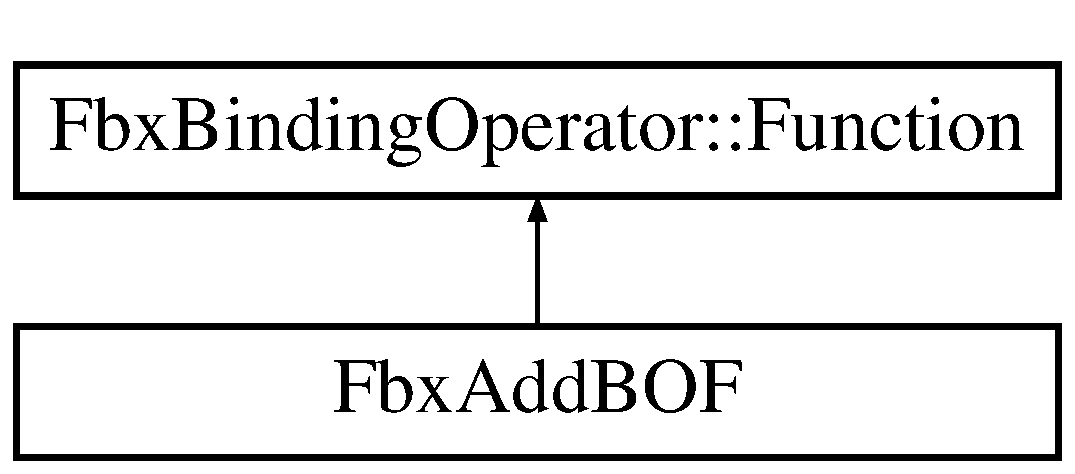
\includegraphics[height=2.000000cm]{class_fbx_add_b_o_f}
\end{center}
\end{figure}
\subsection*{公開メンバ関数}
\begin{DoxyCompactItemize}
\item 
virtual bool \hyperlink{class_fbx_add_b_o_f_a2b1552f30e4ce028d9b67247ed3b9d06}{Evaluate} (const \hyperlink{class_fbx_binding_operator}{Fbx\+Binding\+Operator} $\ast$p\+Operator, const \hyperlink{class_fbx_object}{Fbx\+Object} $\ast$p\+Object, \hyperlink{fbxpropertytypes_8h_a73913a5ddfb20e57c6f25e9e6784bd92}{E\+Fbx\+Type} $\ast$p\+Result\+Type, void $\ast$$\ast$p\+Result) const
\item 
virtual bool \hyperlink{class_fbx_add_b_o_f_aee96f76da5722af28d12b65eefcc61bb}{Reverse\+Evaluate} (const \hyperlink{class_fbx_binding_operator}{Fbx\+Binding\+Operator} $\ast$p\+Operator, const \hyperlink{class_fbx_object}{Fbx\+Object} $\ast$p\+Target, const void $\ast$p\+In, void $\ast$$\ast$p\+Out, \hyperlink{fbxpropertytypes_8h_a73913a5ddfb20e57c6f25e9e6784bd92}{E\+Fbx\+Type} $\ast$p\+Out\+Type, bool set\+Obj, int index) const
\item 
\hyperlink{class_fbx_add_b_o_f_ac0950ff84a9d2e228949b29a14376dee}{Fbx\+Add\+B\+OF} ()
\item 
virtual \hyperlink{class_fbx_add_b_o_f_a20fa9c0da07357b512939e5c6732b62f}{$\sim$\+Fbx\+Add\+B\+OF} ()
\end{DoxyCompactItemize}
\subsection*{静的公開変数類}
\begin{DoxyCompactItemize}
\item 
static const char $\ast$ \hyperlink{class_fbx_add_b_o_f_a2929c676c1a89849156895fbe579fd4e}{Function\+Name}
\begin{DoxyCompactList}\small\item\em Name of the operation function. \end{DoxyCompactList}\end{DoxyCompactItemize}


\subsection{詳解}


 fbxbindingoperator.\+h の 514 行目に定義があります。



\subsection{構築子と解体子}
\mbox{\Hypertarget{class_fbx_add_b_o_f_ac0950ff84a9d2e228949b29a14376dee}\label{class_fbx_add_b_o_f_ac0950ff84a9d2e228949b29a14376dee}} 
\index{Fbx\+Add\+B\+OF@{Fbx\+Add\+B\+OF}!Fbx\+Add\+B\+OF@{Fbx\+Add\+B\+OF}}
\index{Fbx\+Add\+B\+OF@{Fbx\+Add\+B\+OF}!Fbx\+Add\+B\+OF@{Fbx\+Add\+B\+OF}}
\subsubsection{\texorpdfstring{Fbx\+Add\+B\+O\+F()}{FbxAddBOF()}}
{\footnotesize\ttfamily Fbx\+Add\+B\+O\+F\+::\+Fbx\+Add\+B\+OF (\begin{DoxyParamCaption}{ }\end{DoxyParamCaption})}

\mbox{\Hypertarget{class_fbx_add_b_o_f_a20fa9c0da07357b512939e5c6732b62f}\label{class_fbx_add_b_o_f_a20fa9c0da07357b512939e5c6732b62f}} 
\index{Fbx\+Add\+B\+OF@{Fbx\+Add\+B\+OF}!````~Fbx\+Add\+B\+OF@{$\sim$\+Fbx\+Add\+B\+OF}}
\index{````~Fbx\+Add\+B\+OF@{$\sim$\+Fbx\+Add\+B\+OF}!Fbx\+Add\+B\+OF@{Fbx\+Add\+B\+OF}}
\subsubsection{\texorpdfstring{$\sim$\+Fbx\+Add\+B\+O\+F()}{~FbxAddBOF()}}
{\footnotesize\ttfamily virtual Fbx\+Add\+B\+O\+F\+::$\sim$\+Fbx\+Add\+B\+OF (\begin{DoxyParamCaption}{ }\end{DoxyParamCaption})\hspace{0.3cm}{\ttfamily [virtual]}}



\subsection{関数詳解}
\mbox{\Hypertarget{class_fbx_add_b_o_f_a2b1552f30e4ce028d9b67247ed3b9d06}\label{class_fbx_add_b_o_f_a2b1552f30e4ce028d9b67247ed3b9d06}} 
\index{Fbx\+Add\+B\+OF@{Fbx\+Add\+B\+OF}!Evaluate@{Evaluate}}
\index{Evaluate@{Evaluate}!Fbx\+Add\+B\+OF@{Fbx\+Add\+B\+OF}}
\subsubsection{\texorpdfstring{Evaluate()}{Evaluate()}}
{\footnotesize\ttfamily virtual bool Fbx\+Add\+B\+O\+F\+::\+Evaluate (\begin{DoxyParamCaption}\item[{const \hyperlink{class_fbx_binding_operator}{Fbx\+Binding\+Operator} $\ast$}]{p\+Operator,  }\item[{const \hyperlink{class_fbx_object}{Fbx\+Object} $\ast$}]{p\+Object,  }\item[{\hyperlink{fbxpropertytypes_8h_a73913a5ddfb20e57c6f25e9e6784bd92}{E\+Fbx\+Type} $\ast$}]{p\+Result\+Type,  }\item[{void $\ast$$\ast$}]{p\+Result }\end{DoxyParamCaption}) const\hspace{0.3cm}{\ttfamily [virtual]}}

Evaluates the object properties specified by \char`\"{}\+X\char`\"{} and \char`\"{}\+Y\char`\"{} return X+Y as a float.


\begin{DoxyParams}{引数}
{\em p\+Operator} & Operator running on the object. \\
\hline
{\em p\+Object} & The object that will be evaluated. \\
\hline
{\em p\+Result\+Type} & The type of the result to be returned. \\
\hline
{\em p\+Result} & A pointer to a buffer that can hold the result. \\
\hline
\end{DoxyParams}
\begin{DoxyReturn}{戻り値}
{\ttfamily true} on success, {\ttfamily false} otherwise. 
\end{DoxyReturn}


\hyperlink{class_fbx_binding_operator_1_1_function_aa238a63d12508db3cb5c00a4b157524e}{Fbx\+Binding\+Operator\+::\+Function}を実装しています。

\mbox{\Hypertarget{class_fbx_add_b_o_f_aee96f76da5722af28d12b65eefcc61bb}\label{class_fbx_add_b_o_f_aee96f76da5722af28d12b65eefcc61bb}} 
\index{Fbx\+Add\+B\+OF@{Fbx\+Add\+B\+OF}!Reverse\+Evaluate@{Reverse\+Evaluate}}
\index{Reverse\+Evaluate@{Reverse\+Evaluate}!Fbx\+Add\+B\+OF@{Fbx\+Add\+B\+OF}}
\subsubsection{\texorpdfstring{Reverse\+Evaluate()}{ReverseEvaluate()}}
{\footnotesize\ttfamily virtual bool Fbx\+Add\+B\+O\+F\+::\+Reverse\+Evaluate (\begin{DoxyParamCaption}\item[{const \hyperlink{class_fbx_binding_operator}{Fbx\+Binding\+Operator} $\ast$}]{p\+Operator,  }\item[{const \hyperlink{class_fbx_object}{Fbx\+Object} $\ast$}]{p\+Target,  }\item[{const void $\ast$}]{p\+In,  }\item[{void $\ast$$\ast$}]{p\+Out,  }\item[{\hyperlink{fbxpropertytypes_8h_a73913a5ddfb20e57c6f25e9e6784bd92}{E\+Fbx\+Type} $\ast$}]{p\+Out\+Type,  }\item[{bool}]{set\+Obj,  }\item[{int}]{index }\end{DoxyParamCaption}) const\hspace{0.3cm}{\ttfamily [virtual]}}

Run the inverse operator on the given object, assigning the result directly to the object. 
\begin{DoxyParams}{引数}
{\em p\+Operator} & The operator that will be applied. \\
\hline
{\em p\+Target} & The object that will be evaluated. \\
\hline
{\em p\+In} & \\
\hline
{\em p\+Out} & \\
\hline
{\em p\+Out\+Type} & Type of value being reversed. \\
\hline
{\em set\+Obj} & Control to set the property (only to query by the default ). \\
\hline
{\em index} & Used only in \hyperlink{class_fbx_multiply_dist_b_o_f}{Fbx\+Multiply\+Dist\+B\+OF}. \\
\hline
\end{DoxyParams}
\begin{DoxyReturn}{戻り値}
{\ttfamily true} on success, {\ttfamily false} otherwise. 
\end{DoxyReturn}


\hyperlink{class_fbx_binding_operator_1_1_function_a9bbeec993a6e453a6569e7f40a85fd52}{Fbx\+Binding\+Operator\+::\+Function}を実装しています。



\subsection{メンバ詳解}
\mbox{\Hypertarget{class_fbx_add_b_o_f_a2929c676c1a89849156895fbe579fd4e}\label{class_fbx_add_b_o_f_a2929c676c1a89849156895fbe579fd4e}} 
\index{Fbx\+Add\+B\+OF@{Fbx\+Add\+B\+OF}!Function\+Name@{Function\+Name}}
\index{Function\+Name@{Function\+Name}!Fbx\+Add\+B\+OF@{Fbx\+Add\+B\+OF}}
\subsubsection{\texorpdfstring{Function\+Name}{FunctionName}}
{\footnotesize\ttfamily const char$\ast$ Fbx\+Add\+B\+O\+F\+::\+Function\+Name\hspace{0.3cm}{\ttfamily [static]}}



Name of the operation function. 



 fbxbindingoperator.\+h の 518 行目に定義があります。



このクラス詳解は次のファイルから抽出されました\+:\begin{DoxyCompactItemize}
\item 
C\+:/\+Maya/scripts/\+F\+B\+X\+\_\+\+S\+D\+K/2017.\+1/include/fbxsdk/scene/shading/\hyperlink{fbxbindingoperator_8h}{fbxbindingoperator.\+h}\end{DoxyCompactItemize}

\hypertarget{class_fbx_a_matrix}{}\section{Fbx\+A\+Matrix クラス}
\label{class_fbx_a_matrix}\index{Fbx\+A\+Matrix@{Fbx\+A\+Matrix}}


{\ttfamily \#include $<$fbxaffinematrix.\+h$>$}



Fbx\+A\+Matrix の継承関係図
% FIG 0


Fbx\+A\+Matrix 連携図
% FIG 1
\subsection*{公開メンバ関数}
\begin{DoxyCompactItemize}
\item 
bool \hyperlink{class_fbx_a_matrix_a785479d012314ec71198811c172ada98}{Is\+Identity} (const \hyperlink{class_fbx_a_matrix_ad463edbb9fea344643297701f159faa7}{double} p\+Threshold=\hyperlink{fbxtypes_8h_acf3cd6f208edb42ad9c9abbc1f7feea0}{F\+B\+X\+S\+D\+K\+\_\+\+T\+O\+L\+E\+R\+A\+N\+CE})
\item 
\hyperlink{class_fbx_a_matrix_aa8b1d55b46b3ef0298a55a9d64306f23}{Fbx\+A\+Matrix} (const \hyperlink{class_fbx_vector4}{Fbx\+Vector4} \&pT, const \hyperlink{class_fbx_quaternion}{Fbx\+Quaternion} \&pQ, const \hyperlink{class_fbx_vector4}{Fbx\+Vector4} \&pS)
\item 
void \hyperlink{class_fbx_a_matrix_ac3672896ac261b719176c423a46da152}{Set\+T\+RS} (const \hyperlink{class_fbx_vector4}{Fbx\+Vector4} \&pT, const \hyperlink{class_fbx_a_matrix}{Fbx\+A\+Matrix} \&p\+RM, const \hyperlink{class_fbx_vector4}{Fbx\+Vector4} \&pS)
\item 
void \hyperlink{class_fbx_a_matrix_a32ff707b8787c70a4cc4cf1c41c4caed}{Set\+Row} (int pY, const \hyperlink{class_fbx_vector4}{Fbx\+Vector4} \&p\+Row)
\item 
void \hyperlink{class_fbx_a_matrix_a69402e45f1b26360ac8e1f9e0dc6606c}{Set\+T\+Only} (const \hyperlink{class_fbx_vector4}{Fbx\+Vector4} \&pT)
\item 
void \hyperlink{class_fbx_a_matrix_abd514a59ce83ace8acf4d96bb1566c9e}{Set\+R\+Only} (const \hyperlink{class_fbx_vector4}{Fbx\+Vector4} \&pR)
\item 
void \hyperlink{class_fbx_a_matrix_acfba7a0ab3ab718ff1dc95e083bc5f31}{Set\+Q\+Only} (const \hyperlink{class_fbx_quaternion}{Fbx\+Quaternion} \&pQ)
\item 
\hyperlink{class_fbx_vector4}{Fbx\+Vector4} \hyperlink{class_fbx_a_matrix_a908a407eab72b8d71cf6c6ab9fa32e4f}{Get\+R\+Only} () const
\item 
\hyperlink{class_fbx_quaternion}{Fbx\+Quaternion} \hyperlink{class_fbx_a_matrix_aa6c9cff20dd3d26d5df852705a0ee149}{Get\+UnnormalizedQ} () const
\item 
void \hyperlink{class_fbx_a_matrix_a54374d0885fa0cf9ab2e619871cb000d}{SetR} (const \hyperlink{class_fbx_vector4}{Fbx\+Vector4} \&pV, const int p\+Ord)
\item 
\hyperlink{class_fbx_vector4}{Fbx\+Vector4} \hyperlink{class_fbx_a_matrix_ae36e44525e67b5a7076b9e2be733f456}{GetR} (const int p\+Ord) const
\item 
void \hyperlink{class_fbx_a_matrix_a74b163f39e346d5dedfd4d56f9624353}{Mult\+RM} (const \hyperlink{class_fbx_vector4}{Fbx\+Vector4} \&pR)
\item 
void \hyperlink{class_fbx_a_matrix_a96ecf0c5a8772ebdcc7f13b54651b3ed}{Mult\+SM} (const \hyperlink{class_fbx_vector4}{Fbx\+Vector4} \&pS)
\item 
bool \hyperlink{class_fbx_a_matrix_a9cdf7165572983d917a8e59577c3a55a}{Is\+Right\+Hand} () const
\item 
\hyperlink{class_fbx_a_matrix_ad463edbb9fea344643297701f159faa7}{double} \hyperlink{class_fbx_a_matrix_a4aa7cbe3d389f1d2cbdfbbf2de032192}{Determinant} () const
\item 
int \hyperlink{class_fbx_a_matrix_a9ffb29a163216aa93b36c29e143f08f8}{Compare} (const \hyperlink{class_fbx_a_matrix}{Fbx\+A\+Matrix} pM, const \hyperlink{class_fbx_a_matrix_ad463edbb9fea344643297701f159faa7}{double} p\+Threshold=\hyperlink{fbxtypes_8h_acf3cd6f208edb42ad9c9abbc1f7feea0}{F\+B\+X\+S\+D\+K\+\_\+\+T\+O\+L\+E\+R\+A\+N\+CE}) const
\end{DoxyCompactItemize}
\subsection*{Constructors and Destructor}
\begin{DoxyCompactItemize}
\item 
\hyperlink{class_fbx_a_matrix_afde94bf7fa3e5a001cf8c0733aab69ea}{Fbx\+A\+Matrix} ()
\begin{DoxyCompactList}\small\item\em Constructor. \end{DoxyCompactList}\item 
\hyperlink{class_fbx_a_matrix_a610a8cdf2f914285630decbf576d77ab}{Fbx\+A\+Matrix} (const \hyperlink{class_fbx_a_matrix}{Fbx\+A\+Matrix} \&p\+Other)
\item 
\hyperlink{class_fbx_a_matrix_a0771e5745b856c562c6415d83e331d15}{Fbx\+A\+Matrix} (const \hyperlink{class_fbx_vector4}{Fbx\+Vector4} \&pT, const \hyperlink{class_fbx_vector4}{Fbx\+Vector4} \&pR, const \hyperlink{class_fbx_vector4}{Fbx\+Vector4} \&pS)
\item 
\hyperlink{class_fbx_a_matrix_a9962c1e649b3e203ade001feecb5f922}{$\sim$\+Fbx\+A\+Matrix} ()
\begin{DoxyCompactList}\small\item\em Destructor. \end{DoxyCompactList}\end{DoxyCompactItemize}
\subsection*{Access}
\begin{DoxyCompactItemize}
\item 
\hyperlink{class_fbx_a_matrix_ad463edbb9fea344643297701f159faa7}{double} \hyperlink{class_fbx_a_matrix_ac3271d21b23683864a324ad93c860aad}{Get} (int pY, int pX) const
\item 
\hyperlink{class_fbx_vector4}{Fbx\+Vector4} \hyperlink{class_fbx_a_matrix_adbf66581dbcec6acb82b3721a0394c88}{GetT} () const
\item 
\hyperlink{class_fbx_vector4}{Fbx\+Vector4} \hyperlink{class_fbx_a_matrix_a8c5a30b339c691ecc66b1151f5e8df8b}{GetR} () const
\item 
\hyperlink{class_fbx_quaternion}{Fbx\+Quaternion} \hyperlink{class_fbx_a_matrix_ad65916a52b30b14175213b24111e845b}{GetQ} () const
\item 
\hyperlink{class_fbx_vector4}{Fbx\+Vector4} \hyperlink{class_fbx_a_matrix_a2d5efe3883f4a41c8ff8c223b5835fa1}{GetS} () const
\item 
\hyperlink{class_fbx_vector4}{Fbx\+Vector4} \hyperlink{class_fbx_a_matrix_ac9390e435954f95cee145123452ace46}{Get\+Row} (int pY) const
\item 
\hyperlink{class_fbx_vector4}{Fbx\+Vector4} \hyperlink{class_fbx_a_matrix_a73d4fbefc0fa5888553d3e7e0784e971}{Get\+Column} (int pX) const
\item 
void \hyperlink{class_fbx_a_matrix_a941b5c3ae5985e1f75a61f792a743098}{Set\+Identity} ()
\begin{DoxyCompactList}\small\item\em Set matrix to identity. \end{DoxyCompactList}\item 
void \hyperlink{class_fbx_a_matrix_af0a9e6bcdd7a41353676ded28ab77f2a}{SetT} (const \hyperlink{class_fbx_vector4}{Fbx\+Vector4} \&pT)
\item 
void \hyperlink{class_fbx_a_matrix_ad749080abe63a56225df153dab876c1f}{SetR} (const \hyperlink{class_fbx_vector4}{Fbx\+Vector4} \&pR)
\item 
void \hyperlink{class_fbx_a_matrix_a583269a598ba62a1b6897619c2469b54}{SetQ} (const \hyperlink{class_fbx_quaternion}{Fbx\+Quaternion} \&pQ)
\item 
void \hyperlink{class_fbx_a_matrix_a6da268a626104c3a1696e298200621d1}{SetS} (const \hyperlink{class_fbx_vector4}{Fbx\+Vector4} \&pS)
\item 
void \hyperlink{class_fbx_a_matrix_aed884627dc4f4416bbf068b77bae8ae1}{Set\+T\+RS} (const \hyperlink{class_fbx_vector4}{Fbx\+Vector4} \&pT, const \hyperlink{class_fbx_vector4}{Fbx\+Vector4} \&pR, const \hyperlink{class_fbx_vector4}{Fbx\+Vector4} \&pS)
\item 
void \hyperlink{class_fbx_a_matrix_af3761d1426a403b7b86fd5b2c11349c8}{Set\+T\+QS} (const \hyperlink{class_fbx_vector4}{Fbx\+Vector4} \&pT, const \hyperlink{class_fbx_quaternion}{Fbx\+Quaternion} \&pQ, const \hyperlink{class_fbx_vector4}{Fbx\+Vector4} \&pS)
\item 
\hyperlink{class_fbx_a_matrix}{Fbx\+A\+Matrix} \& \hyperlink{class_fbx_a_matrix_a77b179193309b11d5c505cdca7969ee0}{operator=} (const \hyperlink{class_fbx_a_matrix}{Fbx\+A\+Matrix} \&pM)
\end{DoxyCompactItemize}
\subsection*{Scalar Operations}
\begin{DoxyCompactItemize}
\item 
\hyperlink{class_fbx_a_matrix}{Fbx\+A\+Matrix} \hyperlink{class_fbx_a_matrix_abc19f68d91ce2dd5303c9ab398e12eee}{operator$\ast$} (\hyperlink{class_fbx_a_matrix_ad463edbb9fea344643297701f159faa7}{double} p\+Value) const
\item 
\hyperlink{class_fbx_a_matrix}{Fbx\+A\+Matrix} \hyperlink{class_fbx_a_matrix_a48795bab1963bb8f5d963080f3d04149}{operator/} (\hyperlink{class_fbx_a_matrix_ad463edbb9fea344643297701f159faa7}{double} p\+Value) const
\item 
\hyperlink{class_fbx_a_matrix}{Fbx\+A\+Matrix} \& \hyperlink{class_fbx_a_matrix_a0b408712fcb77126c4a8f951ae8a219f}{operator$\ast$=} (\hyperlink{class_fbx_a_matrix_ad463edbb9fea344643297701f159faa7}{double} p\+Value)
\item 
\hyperlink{class_fbx_a_matrix}{Fbx\+A\+Matrix} \& \hyperlink{class_fbx_a_matrix_af77d3a14cae3687b56d7e14e326473d6}{operator/=} (\hyperlink{class_fbx_a_matrix_ad463edbb9fea344643297701f159faa7}{double} p\+Value)
\end{DoxyCompactItemize}
\subsection*{Vector Operations}
\begin{DoxyCompactItemize}
\item 
\hyperlink{class_fbx_vector4}{Fbx\+Vector4} \hyperlink{class_fbx_a_matrix_ac9d3c8f4232dd1b1996c863b9cca4635}{MultT} (const \hyperlink{class_fbx_vector4}{Fbx\+Vector4} \&p\+Vector4) const
\item 
\hyperlink{class_fbx_vector4}{Fbx\+Vector4} \hyperlink{class_fbx_a_matrix_a9fe3cfea0f753197bd116b429242eb09}{MultR} (const \hyperlink{class_fbx_vector4}{Fbx\+Vector4} \&p\+Vector4) const
\item 
\hyperlink{class_fbx_quaternion}{Fbx\+Quaternion} \hyperlink{class_fbx_a_matrix_a92ea09bd97b85104bff21dde23edca35}{MultQ} (const \hyperlink{class_fbx_quaternion}{Fbx\+Quaternion} \&p\+Quaternion) const
\item 
\hyperlink{class_fbx_vector4}{Fbx\+Vector4} \hyperlink{class_fbx_a_matrix_ae3508b4f0d58debf598bcea9e8dda669}{MultS} (const \hyperlink{class_fbx_vector4}{Fbx\+Vector4} \&p\+Vector4) const
\end{DoxyCompactItemize}
\subsection*{Matrix Operations}
\begin{DoxyCompactItemize}
\item 
\hyperlink{class_fbx_a_matrix}{Fbx\+A\+Matrix} \hyperlink{class_fbx_a_matrix_a8f8ab0b3698f9d25b3051c5928315ef6}{operator-\/} () const
\item 
\hyperlink{class_fbx_a_matrix}{Fbx\+A\+Matrix} \hyperlink{class_fbx_a_matrix_a653885060d7c3966ea2a778a188052c7}{operator$\ast$} (const \hyperlink{class_fbx_a_matrix}{Fbx\+A\+Matrix} \&p\+Other) const
\item 
\hyperlink{class_fbx_a_matrix}{Fbx\+A\+Matrix} \& \hyperlink{class_fbx_a_matrix_a8eba4c43ccc466bebfc555c9170bf3e5}{operator$\ast$=} (const \hyperlink{class_fbx_a_matrix}{Fbx\+A\+Matrix} \&p\+Other)
\item 
\hyperlink{class_fbx_a_matrix}{Fbx\+A\+Matrix} \hyperlink{class_fbx_a_matrix_a4093cf977851b49760e1c24c99d5bae7}{Inverse} () const
\item 
\hyperlink{class_fbx_a_matrix}{Fbx\+A\+Matrix} \hyperlink{class_fbx_a_matrix_a94915f3c5de6c16d4c39a5acc3a84bd7}{Transpose} () const
\item 
\hyperlink{class_fbx_a_matrix}{Fbx\+A\+Matrix} \hyperlink{class_fbx_a_matrix_a1dc557020e7cdaa9de99a87a35cc315e}{Slerp} (const \hyperlink{class_fbx_a_matrix}{Fbx\+A\+Matrix} \&p\+Other, \hyperlink{class_fbx_a_matrix_ad463edbb9fea344643297701f159faa7}{double} p\+Weight) const
\end{DoxyCompactItemize}
\subsection*{Boolean Operations}
\begin{DoxyCompactItemize}
\item 
bool \hyperlink{class_fbx_a_matrix_ac7462340bfb94c06dc0c9447d62c3490}{operator==} (const \hyperlink{class_fbx_a_matrix}{Fbx\+A\+Matrix} \&p\+Other) const
\item 
bool \hyperlink{class_fbx_a_matrix_a74905b993a9a8a22f8f55024b40be856}{operator!=} (const \hyperlink{class_fbx_a_matrix}{Fbx\+A\+Matrix} \&p\+Other) const
\end{DoxyCompactItemize}
\subsection*{Casting}
\begin{DoxyCompactItemize}
\item 
typedef const \hyperlink{class_fbx_a_matrix_ad463edbb9fea344643297701f159faa7}{double}(k\+Double44)\mbox{[}4\mbox{]}\mbox{[}4\mbox{]}
\begin{DoxyCompactList}\small\item\em Define 4$\ast$4 array as a new type \end{DoxyCompactList}\item 
\hyperlink{class_fbx_a_matrix_a84e411ebdbdf3be933b1db42109da89f}{operator double $\ast$} ()
\begin{DoxyCompactList}\small\item\em Cast the matrix in a double pointer. \end{DoxyCompactList}\item 
\hyperlink{class_fbx_a_matrix_ad166e94a283e603dd71334168b7cb60d}{operator const double $\ast$} () const
\begin{DoxyCompactList}\small\item\em Cast the matrix in a const double pointer. \end{DoxyCompactList}\item 
k\+Double44 \& \hyperlink{class_fbx_a_matrix_ab98e9bd947f8db20e14aa9b1d124402a}{Double44} () const
\begin{DoxyCompactList}\small\item\em Cast the matrix in a reference to a 4$\ast$4 array. \end{DoxyCompactList}\end{DoxyCompactItemize}
\subsection*{その他の継承メンバ}


\subsection{詳解}
F\+BX S\+DK affine matrix class.

Matrices are defined using the Column Major scheme. When a \hyperlink{class_fbx_a_matrix}{Fbx\+A\+Matrix} represents a transformation (translation, rotation and scale), the last row of the matrix represents the translation part of the transformation.

\begin{DoxyRemark}{注釈}
It is important to realize that an affine matrix must respect a certain structure. To be sure the structure is respected, use SetT, SetR, SetS, SetQ, Set\+T\+RS or Set\+T\+QS. If by mistake bad data is entered in this affine matrix, some functions such as \hyperlink{class_fbx_a_matrix_a4093cf977851b49760e1c24c99d5bae7}{Inverse()} will yield wrong results. If a matrix is needed to hold values that aren\textquotesingle{}t associate with an affine matrix, please use \hyperlink{class_fbx_matrix}{Fbx\+Matrix} instead. 
\end{DoxyRemark}


\subsection{型定義メンバ詳解}
\mbox{\Hypertarget{class_fbx_a_matrix_ad463edbb9fea344643297701f159faa7}\label{class_fbx_a_matrix_ad463edbb9fea344643297701f159faa7}} 
\index{Fbx\+A\+Matrix@{Fbx\+A\+Matrix}!double@{double}}
\index{double@{double}!Fbx\+A\+Matrix@{Fbx\+A\+Matrix}}
\subsubsection{\texorpdfstring{double}{double}}
{\footnotesize\ttfamily typedef const Fbx\+A\+Matrix\+::double(k\+Double44)\mbox{[}4\mbox{]}\mbox{[}4\mbox{]}}



Define 4$\ast$4 array as a new type 



\subsection{構築子と解体子}
\mbox{\Hypertarget{class_fbx_a_matrix_afde94bf7fa3e5a001cf8c0733aab69ea}\label{class_fbx_a_matrix_afde94bf7fa3e5a001cf8c0733aab69ea}} 
\index{Fbx\+A\+Matrix@{Fbx\+A\+Matrix}!Fbx\+A\+Matrix@{Fbx\+A\+Matrix}}
\index{Fbx\+A\+Matrix@{Fbx\+A\+Matrix}!Fbx\+A\+Matrix@{Fbx\+A\+Matrix}}
\subsubsection{\texorpdfstring{Fbx\+A\+Matrix()}{FbxAMatrix()}\hspace{0.1cm}{\footnotesize\ttfamily [1/4]}}
{\footnotesize\ttfamily Fbx\+A\+Matrix\+::\+Fbx\+A\+Matrix (\begin{DoxyParamCaption}{ }\end{DoxyParamCaption})}



Constructor. 

\mbox{\Hypertarget{class_fbx_a_matrix_a610a8cdf2f914285630decbf576d77ab}\label{class_fbx_a_matrix_a610a8cdf2f914285630decbf576d77ab}} 
\index{Fbx\+A\+Matrix@{Fbx\+A\+Matrix}!Fbx\+A\+Matrix@{Fbx\+A\+Matrix}}
\index{Fbx\+A\+Matrix@{Fbx\+A\+Matrix}!Fbx\+A\+Matrix@{Fbx\+A\+Matrix}}
\subsubsection{\texorpdfstring{Fbx\+A\+Matrix()}{FbxAMatrix()}\hspace{0.1cm}{\footnotesize\ttfamily [2/4]}}
{\footnotesize\ttfamily Fbx\+A\+Matrix\+::\+Fbx\+A\+Matrix (\begin{DoxyParamCaption}\item[{const \hyperlink{class_fbx_a_matrix}{Fbx\+A\+Matrix} \&}]{p\+Other }\end{DoxyParamCaption})}

Copy constructor. 
\begin{DoxyParams}{引数}
{\em p\+Other} & \hyperlink{class_fbx_a_matrix}{Fbx\+A\+Matrix} copied to this one. \\
\hline
\end{DoxyParams}
\mbox{\Hypertarget{class_fbx_a_matrix_a0771e5745b856c562c6415d83e331d15}\label{class_fbx_a_matrix_a0771e5745b856c562c6415d83e331d15}} 
\index{Fbx\+A\+Matrix@{Fbx\+A\+Matrix}!Fbx\+A\+Matrix@{Fbx\+A\+Matrix}}
\index{Fbx\+A\+Matrix@{Fbx\+A\+Matrix}!Fbx\+A\+Matrix@{Fbx\+A\+Matrix}}
\subsubsection{\texorpdfstring{Fbx\+A\+Matrix()}{FbxAMatrix()}\hspace{0.1cm}{\footnotesize\ttfamily [3/4]}}
{\footnotesize\ttfamily Fbx\+A\+Matrix\+::\+Fbx\+A\+Matrix (\begin{DoxyParamCaption}\item[{const \hyperlink{class_fbx_vector4}{Fbx\+Vector4} \&}]{pT,  }\item[{const \hyperlink{class_fbx_vector4}{Fbx\+Vector4} \&}]{pR,  }\item[{const \hyperlink{class_fbx_vector4}{Fbx\+Vector4} \&}]{pS }\end{DoxyParamCaption})}

Constructor. 
\begin{DoxyParams}{引数}
{\em pT} & Translation vector. \\
\hline
{\em pR} & Euler rotation vector. \\
\hline
{\em pS} & Scale vector. \\
\hline
\end{DoxyParams}
\mbox{\Hypertarget{class_fbx_a_matrix_a9962c1e649b3e203ade001feecb5f922}\label{class_fbx_a_matrix_a9962c1e649b3e203ade001feecb5f922}} 
\index{Fbx\+A\+Matrix@{Fbx\+A\+Matrix}!````~Fbx\+A\+Matrix@{$\sim$\+Fbx\+A\+Matrix}}
\index{````~Fbx\+A\+Matrix@{$\sim$\+Fbx\+A\+Matrix}!Fbx\+A\+Matrix@{Fbx\+A\+Matrix}}
\subsubsection{\texorpdfstring{$\sim$\+Fbx\+A\+Matrix()}{~FbxAMatrix()}}
{\footnotesize\ttfamily Fbx\+A\+Matrix\+::$\sim$\+Fbx\+A\+Matrix (\begin{DoxyParamCaption}{ }\end{DoxyParamCaption})}



Destructor. 

\mbox{\Hypertarget{class_fbx_a_matrix_aa8b1d55b46b3ef0298a55a9d64306f23}\label{class_fbx_a_matrix_aa8b1d55b46b3ef0298a55a9d64306f23}} 
\index{Fbx\+A\+Matrix@{Fbx\+A\+Matrix}!Fbx\+A\+Matrix@{Fbx\+A\+Matrix}}
\index{Fbx\+A\+Matrix@{Fbx\+A\+Matrix}!Fbx\+A\+Matrix@{Fbx\+A\+Matrix}}
\subsubsection{\texorpdfstring{Fbx\+A\+Matrix()}{FbxAMatrix()}\hspace{0.1cm}{\footnotesize\ttfamily [4/4]}}
{\footnotesize\ttfamily Fbx\+A\+Matrix\+::\+Fbx\+A\+Matrix (\begin{DoxyParamCaption}\item[{const \hyperlink{class_fbx_vector4}{Fbx\+Vector4} \&}]{pT,  }\item[{const \hyperlink{class_fbx_quaternion}{Fbx\+Quaternion} \&}]{pQ,  }\item[{const \hyperlink{class_fbx_vector4}{Fbx\+Vector4} \&}]{pS }\end{DoxyParamCaption})}



\subsection{メソッド詳解}
\mbox{\Hypertarget{class_fbx_a_matrix_a9ffb29a163216aa93b36c29e143f08f8}\label{class_fbx_a_matrix_a9ffb29a163216aa93b36c29e143f08f8}} 
\index{Fbx\+A\+Matrix@{Fbx\+A\+Matrix}!Compare@{Compare}}
\index{Compare@{Compare}!Fbx\+A\+Matrix@{Fbx\+A\+Matrix}}
\subsubsection{\texorpdfstring{Compare()}{Compare()}}
{\footnotesize\ttfamily int Fbx\+A\+Matrix\+::\+Compare (\begin{DoxyParamCaption}\item[{const \hyperlink{class_fbx_a_matrix}{Fbx\+A\+Matrix}}]{pM,  }\item[{const \hyperlink{class_fbx_a_matrix_ad463edbb9fea344643297701f159faa7}{double}}]{p\+Threshold = {\ttfamily \hyperlink{fbxtypes_8h_acf3cd6f208edb42ad9c9abbc1f7feea0}{F\+B\+X\+S\+D\+K\+\_\+\+T\+O\+L\+E\+R\+A\+N\+CE}} }\end{DoxyParamCaption}) const}

\mbox{\Hypertarget{class_fbx_a_matrix_a4aa7cbe3d389f1d2cbdfbbf2de032192}\label{class_fbx_a_matrix_a4aa7cbe3d389f1d2cbdfbbf2de032192}} 
\index{Fbx\+A\+Matrix@{Fbx\+A\+Matrix}!Determinant@{Determinant}}
\index{Determinant@{Determinant}!Fbx\+A\+Matrix@{Fbx\+A\+Matrix}}
\subsubsection{\texorpdfstring{Determinant()}{Determinant()}}
{\footnotesize\ttfamily \hyperlink{class_fbx_a_matrix_ad463edbb9fea344643297701f159faa7}{double} Fbx\+A\+Matrix\+::\+Determinant (\begin{DoxyParamCaption}{ }\end{DoxyParamCaption}) const}

\mbox{\Hypertarget{class_fbx_a_matrix_ab98e9bd947f8db20e14aa9b1d124402a}\label{class_fbx_a_matrix_ab98e9bd947f8db20e14aa9b1d124402a}} 
\index{Fbx\+A\+Matrix@{Fbx\+A\+Matrix}!Double44@{Double44}}
\index{Double44@{Double44}!Fbx\+A\+Matrix@{Fbx\+A\+Matrix}}
\subsubsection{\texorpdfstring{Double44()}{Double44()}}
{\footnotesize\ttfamily k\+Double44\& Fbx\+A\+Matrix\+::\+Double44 (\begin{DoxyParamCaption}{ }\end{DoxyParamCaption}) const}



Cast the matrix in a reference to a 4$\ast$4 array. 

\mbox{\Hypertarget{class_fbx_a_matrix_ac3271d21b23683864a324ad93c860aad}\label{class_fbx_a_matrix_ac3271d21b23683864a324ad93c860aad}} 
\index{Fbx\+A\+Matrix@{Fbx\+A\+Matrix}!Get@{Get}}
\index{Get@{Get}!Fbx\+A\+Matrix@{Fbx\+A\+Matrix}}
\subsubsection{\texorpdfstring{Get()}{Get()}}
{\footnotesize\ttfamily \hyperlink{class_fbx_a_matrix_ad463edbb9fea344643297701f159faa7}{double} Fbx\+A\+Matrix\+::\+Get (\begin{DoxyParamCaption}\item[{int}]{pY,  }\item[{int}]{pX }\end{DoxyParamCaption}) const}

Retrieve matrix element. 
\begin{DoxyParams}{引数}
{\em pY} & Row index. \\
\hline
{\em pX} & Column index. \\
\hline
\end{DoxyParams}
\begin{DoxyReturn}{戻り値}
Cell \mbox{[} pX, pY \mbox{]} value. 
\end{DoxyReturn}
\mbox{\Hypertarget{class_fbx_a_matrix_a73d4fbefc0fa5888553d3e7e0784e971}\label{class_fbx_a_matrix_a73d4fbefc0fa5888553d3e7e0784e971}} 
\index{Fbx\+A\+Matrix@{Fbx\+A\+Matrix}!Get\+Column@{Get\+Column}}
\index{Get\+Column@{Get\+Column}!Fbx\+A\+Matrix@{Fbx\+A\+Matrix}}
\subsubsection{\texorpdfstring{Get\+Column()}{GetColumn()}}
{\footnotesize\ttfamily \hyperlink{class_fbx_vector4}{Fbx\+Vector4} Fbx\+A\+Matrix\+::\+Get\+Column (\begin{DoxyParamCaption}\item[{int}]{pX }\end{DoxyParamCaption}) const}

Extract a column vector. 
\begin{DoxyParams}{引数}
{\em pX} & Column index. \\
\hline
\end{DoxyParams}
\begin{DoxyReturn}{戻り値}
The column vector. 
\end{DoxyReturn}
\mbox{\Hypertarget{class_fbx_a_matrix_ad65916a52b30b14175213b24111e845b}\label{class_fbx_a_matrix_ad65916a52b30b14175213b24111e845b}} 
\index{Fbx\+A\+Matrix@{Fbx\+A\+Matrix}!GetQ@{GetQ}}
\index{GetQ@{GetQ}!Fbx\+A\+Matrix@{Fbx\+A\+Matrix}}
\subsubsection{\texorpdfstring{Get\+Q()}{GetQ()}}
{\footnotesize\ttfamily \hyperlink{class_fbx_quaternion}{Fbx\+Quaternion} Fbx\+A\+Matrix\+::\+GetQ (\begin{DoxyParamCaption}{ }\end{DoxyParamCaption}) const}

Extract quaternion vector. \begin{DoxyReturn}{戻り値}
Quaternion vector. 
\end{DoxyReturn}
\mbox{\Hypertarget{class_fbx_a_matrix_a8c5a30b339c691ecc66b1151f5e8df8b}\label{class_fbx_a_matrix_a8c5a30b339c691ecc66b1151f5e8df8b}} 
\index{Fbx\+A\+Matrix@{Fbx\+A\+Matrix}!GetR@{GetR}}
\index{GetR@{GetR}!Fbx\+A\+Matrix@{Fbx\+A\+Matrix}}
\subsubsection{\texorpdfstring{Get\+R()}{GetR()}\hspace{0.1cm}{\footnotesize\ttfamily [1/2]}}
{\footnotesize\ttfamily \hyperlink{class_fbx_vector4}{Fbx\+Vector4} Fbx\+A\+Matrix\+::\+GetR (\begin{DoxyParamCaption}{ }\end{DoxyParamCaption}) const}

Extract rotation vector. \begin{DoxyReturn}{戻り値}
Rotation vector. 
\end{DoxyReturn}
\begin{DoxyRemark}{注釈}
The returned rotation vector is in Euler angle and the rotation order is X\+YZ. 
\end{DoxyRemark}
\mbox{\Hypertarget{class_fbx_a_matrix_ae36e44525e67b5a7076b9e2be733f456}\label{class_fbx_a_matrix_ae36e44525e67b5a7076b9e2be733f456}} 
\index{Fbx\+A\+Matrix@{Fbx\+A\+Matrix}!GetR@{GetR}}
\index{GetR@{GetR}!Fbx\+A\+Matrix@{Fbx\+A\+Matrix}}
\subsubsection{\texorpdfstring{Get\+R()}{GetR()}\hspace{0.1cm}{\footnotesize\ttfamily [2/2]}}
{\footnotesize\ttfamily \hyperlink{class_fbx_vector4}{Fbx\+Vector4} Fbx\+A\+Matrix\+::\+GetR (\begin{DoxyParamCaption}\item[{const int}]{p\+Ord }\end{DoxyParamCaption}) const}

\mbox{\Hypertarget{class_fbx_a_matrix_a908a407eab72b8d71cf6c6ab9fa32e4f}\label{class_fbx_a_matrix_a908a407eab72b8d71cf6c6ab9fa32e4f}} 
\index{Fbx\+A\+Matrix@{Fbx\+A\+Matrix}!Get\+R\+Only@{Get\+R\+Only}}
\index{Get\+R\+Only@{Get\+R\+Only}!Fbx\+A\+Matrix@{Fbx\+A\+Matrix}}
\subsubsection{\texorpdfstring{Get\+R\+Only()}{GetROnly()}}
{\footnotesize\ttfamily \hyperlink{class_fbx_vector4}{Fbx\+Vector4} Fbx\+A\+Matrix\+::\+Get\+R\+Only (\begin{DoxyParamCaption}{ }\end{DoxyParamCaption}) const}

\mbox{\Hypertarget{class_fbx_a_matrix_ac9390e435954f95cee145123452ace46}\label{class_fbx_a_matrix_ac9390e435954f95cee145123452ace46}} 
\index{Fbx\+A\+Matrix@{Fbx\+A\+Matrix}!Get\+Row@{Get\+Row}}
\index{Get\+Row@{Get\+Row}!Fbx\+A\+Matrix@{Fbx\+A\+Matrix}}
\subsubsection{\texorpdfstring{Get\+Row()}{GetRow()}}
{\footnotesize\ttfamily \hyperlink{class_fbx_vector4}{Fbx\+Vector4} Fbx\+A\+Matrix\+::\+Get\+Row (\begin{DoxyParamCaption}\item[{int}]{pY }\end{DoxyParamCaption}) const}

Extract a row vector. 
\begin{DoxyParams}{引数}
{\em pY} & Row index. \\
\hline
\end{DoxyParams}
\begin{DoxyReturn}{戻り値}
The row vector. 
\end{DoxyReturn}
\mbox{\Hypertarget{class_fbx_a_matrix_a2d5efe3883f4a41c8ff8c223b5835fa1}\label{class_fbx_a_matrix_a2d5efe3883f4a41c8ff8c223b5835fa1}} 
\index{Fbx\+A\+Matrix@{Fbx\+A\+Matrix}!GetS@{GetS}}
\index{GetS@{GetS}!Fbx\+A\+Matrix@{Fbx\+A\+Matrix}}
\subsubsection{\texorpdfstring{Get\+S()}{GetS()}}
{\footnotesize\ttfamily \hyperlink{class_fbx_vector4}{Fbx\+Vector4} Fbx\+A\+Matrix\+::\+GetS (\begin{DoxyParamCaption}{ }\end{DoxyParamCaption}) const}

Extract scale vector. \begin{DoxyReturn}{戻り値}
Scale vector. 
\end{DoxyReturn}
\mbox{\Hypertarget{class_fbx_a_matrix_adbf66581dbcec6acb82b3721a0394c88}\label{class_fbx_a_matrix_adbf66581dbcec6acb82b3721a0394c88}} 
\index{Fbx\+A\+Matrix@{Fbx\+A\+Matrix}!GetT@{GetT}}
\index{GetT@{GetT}!Fbx\+A\+Matrix@{Fbx\+A\+Matrix}}
\subsubsection{\texorpdfstring{Get\+T()}{GetT()}}
{\footnotesize\ttfamily \hyperlink{class_fbx_vector4}{Fbx\+Vector4} Fbx\+A\+Matrix\+::\+GetT (\begin{DoxyParamCaption}{ }\end{DoxyParamCaption}) const}

Extract translation vector. \begin{DoxyReturn}{戻り値}
Translation vector. 
\end{DoxyReturn}
\mbox{\Hypertarget{class_fbx_a_matrix_aa6c9cff20dd3d26d5df852705a0ee149}\label{class_fbx_a_matrix_aa6c9cff20dd3d26d5df852705a0ee149}} 
\index{Fbx\+A\+Matrix@{Fbx\+A\+Matrix}!Get\+UnnormalizedQ@{Get\+UnnormalizedQ}}
\index{Get\+UnnormalizedQ@{Get\+UnnormalizedQ}!Fbx\+A\+Matrix@{Fbx\+A\+Matrix}}
\subsubsection{\texorpdfstring{Get\+Unnormalized\+Q()}{GetUnnormalizedQ()}}
{\footnotesize\ttfamily \hyperlink{class_fbx_quaternion}{Fbx\+Quaternion} Fbx\+A\+Matrix\+::\+Get\+UnnormalizedQ (\begin{DoxyParamCaption}{ }\end{DoxyParamCaption}) const}

\mbox{\Hypertarget{class_fbx_a_matrix_a4093cf977851b49760e1c24c99d5bae7}\label{class_fbx_a_matrix_a4093cf977851b49760e1c24c99d5bae7}} 
\index{Fbx\+A\+Matrix@{Fbx\+A\+Matrix}!Inverse@{Inverse}}
\index{Inverse@{Inverse}!Fbx\+A\+Matrix@{Fbx\+A\+Matrix}}
\subsubsection{\texorpdfstring{Inverse()}{Inverse()}}
{\footnotesize\ttfamily \hyperlink{class_fbx_a_matrix}{Fbx\+A\+Matrix} Fbx\+A\+Matrix\+::\+Inverse (\begin{DoxyParamCaption}{ }\end{DoxyParamCaption}) const}

Calculate the matrix inverse. \begin{DoxyReturn}{戻り値}
The inverse matrix of {\itshape this}. 
\end{DoxyReturn}
\mbox{\Hypertarget{class_fbx_a_matrix_a785479d012314ec71198811c172ada98}\label{class_fbx_a_matrix_a785479d012314ec71198811c172ada98}} 
\index{Fbx\+A\+Matrix@{Fbx\+A\+Matrix}!Is\+Identity@{Is\+Identity}}
\index{Is\+Identity@{Is\+Identity}!Fbx\+A\+Matrix@{Fbx\+A\+Matrix}}
\subsubsection{\texorpdfstring{Is\+Identity()}{IsIdentity()}}
{\footnotesize\ttfamily bool Fbx\+A\+Matrix\+::\+Is\+Identity (\begin{DoxyParamCaption}\item[{const \hyperlink{class_fbx_a_matrix_ad463edbb9fea344643297701f159faa7}{double}}]{p\+Threshold = {\ttfamily \hyperlink{fbxtypes_8h_acf3cd6f208edb42ad9c9abbc1f7feea0}{F\+B\+X\+S\+D\+K\+\_\+\+T\+O\+L\+E\+R\+A\+N\+CE}} }\end{DoxyParamCaption})}

Find out if the matrix is equal to identity matrix. \begin{DoxyReturn}{戻り値}
{\ttfamily true} if the matrix is equal to identity matrix, {\ttfamily false} otherwise. 
\end{DoxyReturn}
\mbox{\Hypertarget{class_fbx_a_matrix_a9cdf7165572983d917a8e59577c3a55a}\label{class_fbx_a_matrix_a9cdf7165572983d917a8e59577c3a55a}} 
\index{Fbx\+A\+Matrix@{Fbx\+A\+Matrix}!Is\+Right\+Hand@{Is\+Right\+Hand}}
\index{Is\+Right\+Hand@{Is\+Right\+Hand}!Fbx\+A\+Matrix@{Fbx\+A\+Matrix}}
\subsubsection{\texorpdfstring{Is\+Right\+Hand()}{IsRightHand()}}
{\footnotesize\ttfamily bool Fbx\+A\+Matrix\+::\+Is\+Right\+Hand (\begin{DoxyParamCaption}{ }\end{DoxyParamCaption}) const}

\mbox{\Hypertarget{class_fbx_a_matrix_a92ea09bd97b85104bff21dde23edca35}\label{class_fbx_a_matrix_a92ea09bd97b85104bff21dde23edca35}} 
\index{Fbx\+A\+Matrix@{Fbx\+A\+Matrix}!MultQ@{MultQ}}
\index{MultQ@{MultQ}!Fbx\+A\+Matrix@{Fbx\+A\+Matrix}}
\subsubsection{\texorpdfstring{Mult\+Q()}{MultQ()}}
{\footnotesize\ttfamily \hyperlink{class_fbx_quaternion}{Fbx\+Quaternion} Fbx\+A\+Matrix\+::\+MultQ (\begin{DoxyParamCaption}\item[{const \hyperlink{class_fbx_quaternion}{Fbx\+Quaternion} \&}]{p\+Quaternion }\end{DoxyParamCaption}) const}

Multiply matrix by a quaternion. 
\begin{DoxyParams}{引数}
{\em p\+Quaternion} & Rotation value. \\
\hline
\end{DoxyParams}
\begin{DoxyReturn}{戻り値}
q\textquotesingle{} = M $\ast$ q 
\end{DoxyReturn}
\mbox{\Hypertarget{class_fbx_a_matrix_a9fe3cfea0f753197bd116b429242eb09}\label{class_fbx_a_matrix_a9fe3cfea0f753197bd116b429242eb09}} 
\index{Fbx\+A\+Matrix@{Fbx\+A\+Matrix}!MultR@{MultR}}
\index{MultR@{MultR}!Fbx\+A\+Matrix@{Fbx\+A\+Matrix}}
\subsubsection{\texorpdfstring{Mult\+R()}{MultR()}}
{\footnotesize\ttfamily \hyperlink{class_fbx_vector4}{Fbx\+Vector4} Fbx\+A\+Matrix\+::\+MultR (\begin{DoxyParamCaption}\item[{const \hyperlink{class_fbx_vector4}{Fbx\+Vector4} \&}]{p\+Vector4 }\end{DoxyParamCaption}) const}

Multiply matrix by an Euler rotation vector. 
\begin{DoxyParams}{引数}
{\em p\+Vector4} & Euler Rotation vector. \\
\hline
\end{DoxyParams}
\begin{DoxyReturn}{戻り値}
r\textquotesingle{} = M $\ast$ r 
\end{DoxyReturn}
\mbox{\Hypertarget{class_fbx_a_matrix_a74b163f39e346d5dedfd4d56f9624353}\label{class_fbx_a_matrix_a74b163f39e346d5dedfd4d56f9624353}} 
\index{Fbx\+A\+Matrix@{Fbx\+A\+Matrix}!Mult\+RM@{Mult\+RM}}
\index{Mult\+RM@{Mult\+RM}!Fbx\+A\+Matrix@{Fbx\+A\+Matrix}}
\subsubsection{\texorpdfstring{Mult\+R\+M()}{MultRM()}}
{\footnotesize\ttfamily void Fbx\+A\+Matrix\+::\+Mult\+RM (\begin{DoxyParamCaption}\item[{const \hyperlink{class_fbx_vector4}{Fbx\+Vector4} \&}]{pR }\end{DoxyParamCaption})}

\mbox{\Hypertarget{class_fbx_a_matrix_ae3508b4f0d58debf598bcea9e8dda669}\label{class_fbx_a_matrix_ae3508b4f0d58debf598bcea9e8dda669}} 
\index{Fbx\+A\+Matrix@{Fbx\+A\+Matrix}!MultS@{MultS}}
\index{MultS@{MultS}!Fbx\+A\+Matrix@{Fbx\+A\+Matrix}}
\subsubsection{\texorpdfstring{Mult\+S()}{MultS()}}
{\footnotesize\ttfamily \hyperlink{class_fbx_vector4}{Fbx\+Vector4} Fbx\+A\+Matrix\+::\+MultS (\begin{DoxyParamCaption}\item[{const \hyperlink{class_fbx_vector4}{Fbx\+Vector4} \&}]{p\+Vector4 }\end{DoxyParamCaption}) const}

Multiply matrix by a scale vector. 
\begin{DoxyParams}{引数}
{\em p\+Vector4} & Scaling vector. \\
\hline
\end{DoxyParams}
\begin{DoxyReturn}{戻り値}
s\textquotesingle{} = M $\ast$ s 
\end{DoxyReturn}
\mbox{\Hypertarget{class_fbx_a_matrix_a96ecf0c5a8772ebdcc7f13b54651b3ed}\label{class_fbx_a_matrix_a96ecf0c5a8772ebdcc7f13b54651b3ed}} 
\index{Fbx\+A\+Matrix@{Fbx\+A\+Matrix}!Mult\+SM@{Mult\+SM}}
\index{Mult\+SM@{Mult\+SM}!Fbx\+A\+Matrix@{Fbx\+A\+Matrix}}
\subsubsection{\texorpdfstring{Mult\+S\+M()}{MultSM()}}
{\footnotesize\ttfamily void Fbx\+A\+Matrix\+::\+Mult\+SM (\begin{DoxyParamCaption}\item[{const \hyperlink{class_fbx_vector4}{Fbx\+Vector4} \&}]{pS }\end{DoxyParamCaption})}

\mbox{\Hypertarget{class_fbx_a_matrix_ac9d3c8f4232dd1b1996c863b9cca4635}\label{class_fbx_a_matrix_ac9d3c8f4232dd1b1996c863b9cca4635}} 
\index{Fbx\+A\+Matrix@{Fbx\+A\+Matrix}!MultT@{MultT}}
\index{MultT@{MultT}!Fbx\+A\+Matrix@{Fbx\+A\+Matrix}}
\subsubsection{\texorpdfstring{Mult\+T()}{MultT()}}
{\footnotesize\ttfamily \hyperlink{class_fbx_vector4}{Fbx\+Vector4} Fbx\+A\+Matrix\+::\+MultT (\begin{DoxyParamCaption}\item[{const \hyperlink{class_fbx_vector4}{Fbx\+Vector4} \&}]{p\+Vector4 }\end{DoxyParamCaption}) const}

Multiply matrix by a translation vector. 
\begin{DoxyParams}{引数}
{\em p\+Vector4} & Translation vector. \\
\hline
\end{DoxyParams}
\begin{DoxyReturn}{戻り値}
t\textquotesingle{} = M $\ast$ t 
\end{DoxyReturn}
\mbox{\Hypertarget{class_fbx_a_matrix_ad166e94a283e603dd71334168b7cb60d}\label{class_fbx_a_matrix_ad166e94a283e603dd71334168b7cb60d}} 
\index{Fbx\+A\+Matrix@{Fbx\+A\+Matrix}!operator const double $\ast$@{operator const double $\ast$}}
\index{operator const double $\ast$@{operator const double $\ast$}!Fbx\+A\+Matrix@{Fbx\+A\+Matrix}}
\subsubsection{\texorpdfstring{operator const double $\ast$()}{operator const double *()}}
{\footnotesize\ttfamily Fbx\+A\+Matrix\+::operator const \hyperlink{class_fbx_a_matrix_ad463edbb9fea344643297701f159faa7}{double} $\ast$ (\begin{DoxyParamCaption}{ }\end{DoxyParamCaption}) const}



Cast the matrix in a const double pointer. 

\mbox{\Hypertarget{class_fbx_a_matrix_a84e411ebdbdf3be933b1db42109da89f}\label{class_fbx_a_matrix_a84e411ebdbdf3be933b1db42109da89f}} 
\index{Fbx\+A\+Matrix@{Fbx\+A\+Matrix}!operator double $\ast$@{operator double $\ast$}}
\index{operator double $\ast$@{operator double $\ast$}!Fbx\+A\+Matrix@{Fbx\+A\+Matrix}}
\subsubsection{\texorpdfstring{operator double $\ast$()}{operator double *()}}
{\footnotesize\ttfamily Fbx\+A\+Matrix\+::operator \hyperlink{class_fbx_a_matrix_ad463edbb9fea344643297701f159faa7}{double} $\ast$ (\begin{DoxyParamCaption}{ }\end{DoxyParamCaption})}



Cast the matrix in a double pointer. 

\mbox{\Hypertarget{class_fbx_a_matrix_a74905b993a9a8a22f8f55024b40be856}\label{class_fbx_a_matrix_a74905b993a9a8a22f8f55024b40be856}} 
\index{Fbx\+A\+Matrix@{Fbx\+A\+Matrix}!operator"!=@{operator"!=}}
\index{operator"!=@{operator"!=}!Fbx\+A\+Matrix@{Fbx\+A\+Matrix}}
\subsubsection{\texorpdfstring{operator"!=()}{operator!=()}}
{\footnotesize\ttfamily bool Fbx\+A\+Matrix\+::operator!= (\begin{DoxyParamCaption}\item[{const \hyperlink{class_fbx_a_matrix}{Fbx\+A\+Matrix} \&}]{p\+Other }\end{DoxyParamCaption}) const}

Non-\/equivalence operator. 
\begin{DoxyParams}{引数}
{\em p\+Other} & The matrix to be compared to {\itshape this}. \\
\hline
\end{DoxyParams}
\begin{DoxyReturn}{戻り値}
{\ttfamily false} if the two matrices are equal (each element is within a F\+B\+X\+S\+D\+K\+\_\+\+T\+O\+L\+E\+R\+A\+N\+CE tolerance) and {\ttfamily true} otherwise. 
\end{DoxyReturn}
\mbox{\Hypertarget{class_fbx_a_matrix_abc19f68d91ce2dd5303c9ab398e12eee}\label{class_fbx_a_matrix_abc19f68d91ce2dd5303c9ab398e12eee}} 
\index{Fbx\+A\+Matrix@{Fbx\+A\+Matrix}!operator$\ast$@{operator$\ast$}}
\index{operator$\ast$@{operator$\ast$}!Fbx\+A\+Matrix@{Fbx\+A\+Matrix}}
\subsubsection{\texorpdfstring{operator$\ast$()}{operator*()}\hspace{0.1cm}{\footnotesize\ttfamily [1/2]}}
{\footnotesize\ttfamily \hyperlink{class_fbx_a_matrix}{Fbx\+A\+Matrix} Fbx\+A\+Matrix\+::operator$\ast$ (\begin{DoxyParamCaption}\item[{\hyperlink{class_fbx_a_matrix_ad463edbb9fea344643297701f159faa7}{double}}]{p\+Value }\end{DoxyParamCaption}) const}

Multiply matrix by a scalar value. 
\begin{DoxyParams}{引数}
{\em p\+Value} & Scalar value. \\
\hline
\end{DoxyParams}
\begin{DoxyReturn}{戻り値}
The scaled matrix. 
\end{DoxyReturn}
\begin{DoxyRemark}{注釈}
The passed value is not checked. This operator operates on the first three rows and columns of the matrix. So only the rotation and scaling are scaled, not the translation part. After operation, the translation vector will be set as (0,0,0,1); 
\end{DoxyRemark}
\mbox{\Hypertarget{class_fbx_a_matrix_a653885060d7c3966ea2a778a188052c7}\label{class_fbx_a_matrix_a653885060d7c3966ea2a778a188052c7}} 
\index{Fbx\+A\+Matrix@{Fbx\+A\+Matrix}!operator$\ast$@{operator$\ast$}}
\index{operator$\ast$@{operator$\ast$}!Fbx\+A\+Matrix@{Fbx\+A\+Matrix}}
\subsubsection{\texorpdfstring{operator$\ast$()}{operator*()}\hspace{0.1cm}{\footnotesize\ttfamily [2/2]}}
{\footnotesize\ttfamily \hyperlink{class_fbx_a_matrix}{Fbx\+A\+Matrix} Fbx\+A\+Matrix\+::operator$\ast$ (\begin{DoxyParamCaption}\item[{const \hyperlink{class_fbx_a_matrix}{Fbx\+A\+Matrix} \&}]{p\+Other }\end{DoxyParamCaption}) const}

Multiply two matrices together. 
\begin{DoxyParams}{引数}
{\em p\+Other} & A Matrix. \\
\hline
\end{DoxyParams}
\begin{DoxyReturn}{戻り値}
this $\ast$ p\+Matrix. 
\end{DoxyReturn}
\begin{DoxyRemark}{注釈}
Transformations are pre-\/multiplied. That means to scale, then rotate, and then translate a vector V, the transform should be T $\ast$ R $\ast$ S $\ast$ V. ~\newline
 Below is an example of code that shows how to construct rotation transform in X\+YZ rotation order. 
\begin{DoxyCode}
\hyperlink{class_fbx_a_matrix}{FbxAMatrix} lRotateXM, lRotateYM, lRotateZM, lRotateXYZM, lRotateM;
\textcolor{comment}{// Construct rotation matrix around X, Y and Z axises separately and then combine them.}
\hyperlink{class_fbx_vector4}{FbxVector4} lRotateX(10, 0, 0);
\hyperlink{class_fbx_vector4}{FbxVector4} lRotateY(0, 10, 0);
\hyperlink{class_fbx_vector4}{FbxVector4} lRotateZ(0, 0, 10);
lRotateXM.\hyperlink{class_fbx_a_matrix_ad749080abe63a56225df153dab876c1f}{SetR}(lRotateX);
lRotateYM.\hyperlink{class_fbx_a_matrix_ad749080abe63a56225df153dab876c1f}{SetR}(lRotateY);
lRotateZM.\hyperlink{class_fbx_a_matrix_ad749080abe63a56225df153dab876c1f}{SetR}(lRotateZ);
lRotateXYZM = lRotateZM * lRotateYM * lRotateXM;

\textcolor{comment}{// Alternatively, we can use SetR() directly.}
\textcolor{comment}{// lRotateXYZM and lRotateM will be the same.}
\hyperlink{class_fbx_vector4}{FbxVector4} lRotateXYZ (10, 10, 10);
lRotateM.\hyperlink{class_fbx_a_matrix_ad749080abe63a56225df153dab876c1f}{SetR}(lRotateXYZ);
\end{DoxyCode}
 
\end{DoxyRemark}
\begin{DoxyNote}{覚え書き}
Please refer to the F\+BX S\+DK programmers guide for more details. 
\end{DoxyNote}
\mbox{\Hypertarget{class_fbx_a_matrix_a0b408712fcb77126c4a8f951ae8a219f}\label{class_fbx_a_matrix_a0b408712fcb77126c4a8f951ae8a219f}} 
\index{Fbx\+A\+Matrix@{Fbx\+A\+Matrix}!operator$\ast$=@{operator$\ast$=}}
\index{operator$\ast$=@{operator$\ast$=}!Fbx\+A\+Matrix@{Fbx\+A\+Matrix}}
\subsubsection{\texorpdfstring{operator$\ast$=()}{operator*=()}\hspace{0.1cm}{\footnotesize\ttfamily [1/2]}}
{\footnotesize\ttfamily \hyperlink{class_fbx_a_matrix}{Fbx\+A\+Matrix}\& Fbx\+A\+Matrix\+::operator$\ast$= (\begin{DoxyParamCaption}\item[{\hyperlink{class_fbx_a_matrix_ad463edbb9fea344643297701f159faa7}{double}}]{p\+Value }\end{DoxyParamCaption})}

Multiply matrix by a scalar value. 
\begin{DoxyParams}{引数}
{\em p\+Value} & Scalar value. \\
\hline
\end{DoxyParams}
\begin{DoxyReturn}{戻り値}
{\itshape this} updated with the result of the multiplication. 
\end{DoxyReturn}
\begin{DoxyRemark}{注釈}
The passed value is not checked. This operator operates on the first three rows and columns of the matrix. So only the rotation and scaling are scaled, not the translation part. After operation, the translation vector will keep original value. 
\end{DoxyRemark}
\mbox{\Hypertarget{class_fbx_a_matrix_a8eba4c43ccc466bebfc555c9170bf3e5}\label{class_fbx_a_matrix_a8eba4c43ccc466bebfc555c9170bf3e5}} 
\index{Fbx\+A\+Matrix@{Fbx\+A\+Matrix}!operator$\ast$=@{operator$\ast$=}}
\index{operator$\ast$=@{operator$\ast$=}!Fbx\+A\+Matrix@{Fbx\+A\+Matrix}}
\subsubsection{\texorpdfstring{operator$\ast$=()}{operator*=()}\hspace{0.1cm}{\footnotesize\ttfamily [2/2]}}
{\footnotesize\ttfamily \hyperlink{class_fbx_a_matrix}{Fbx\+A\+Matrix}\& Fbx\+A\+Matrix\+::operator$\ast$= (\begin{DoxyParamCaption}\item[{const \hyperlink{class_fbx_a_matrix}{Fbx\+A\+Matrix} \&}]{p\+Other }\end{DoxyParamCaption})}

Multiply two matrices together. 
\begin{DoxyParams}{引数}
{\em p\+Other} & A Matrix. \\
\hline
\end{DoxyParams}
\begin{DoxyReturn}{戻り値}
{\itshape this} updated with the result of the multiplication. 
\end{DoxyReturn}
\mbox{\Hypertarget{class_fbx_a_matrix_a8f8ab0b3698f9d25b3051c5928315ef6}\label{class_fbx_a_matrix_a8f8ab0b3698f9d25b3051c5928315ef6}} 
\index{Fbx\+A\+Matrix@{Fbx\+A\+Matrix}!operator-\/@{operator-\/}}
\index{operator-\/@{operator-\/}!Fbx\+A\+Matrix@{Fbx\+A\+Matrix}}
\subsubsection{\texorpdfstring{operator-\/()}{operator-()}}
{\footnotesize\ttfamily \hyperlink{class_fbx_a_matrix}{Fbx\+A\+Matrix} Fbx\+A\+Matrix\+::operator-\/ (\begin{DoxyParamCaption}{ }\end{DoxyParamCaption}) const}

Unary minus operator. \begin{DoxyReturn}{戻り値}
A matrix where each element is multiplied by -\/1. 
\end{DoxyReturn}
\mbox{\Hypertarget{class_fbx_a_matrix_a48795bab1963bb8f5d963080f3d04149}\label{class_fbx_a_matrix_a48795bab1963bb8f5d963080f3d04149}} 
\index{Fbx\+A\+Matrix@{Fbx\+A\+Matrix}!operator/@{operator/}}
\index{operator/@{operator/}!Fbx\+A\+Matrix@{Fbx\+A\+Matrix}}
\subsubsection{\texorpdfstring{operator/()}{operator/()}}
{\footnotesize\ttfamily \hyperlink{class_fbx_a_matrix}{Fbx\+A\+Matrix} Fbx\+A\+Matrix\+::operator/ (\begin{DoxyParamCaption}\item[{\hyperlink{class_fbx_a_matrix_ad463edbb9fea344643297701f159faa7}{double}}]{p\+Value }\end{DoxyParamCaption}) const}

Divide matrix by a scalar value. 
\begin{DoxyParams}{引数}
{\em p\+Value} & Scalar value. \\
\hline
\end{DoxyParams}
\begin{DoxyReturn}{戻り値}
The divided matrix. 
\end{DoxyReturn}
\begin{DoxyRemark}{注釈}
The passed value is not checked. This operator operates on the first three rows and columns of the matrix. So only the rotation and scaling are scaled, not the translation part. After operation, the translation vector will be set as (0,0,0,1); 
\end{DoxyRemark}
\mbox{\Hypertarget{class_fbx_a_matrix_af77d3a14cae3687b56d7e14e326473d6}\label{class_fbx_a_matrix_af77d3a14cae3687b56d7e14e326473d6}} 
\index{Fbx\+A\+Matrix@{Fbx\+A\+Matrix}!operator/=@{operator/=}}
\index{operator/=@{operator/=}!Fbx\+A\+Matrix@{Fbx\+A\+Matrix}}
\subsubsection{\texorpdfstring{operator/=()}{operator/=()}}
{\footnotesize\ttfamily \hyperlink{class_fbx_a_matrix}{Fbx\+A\+Matrix}\& Fbx\+A\+Matrix\+::operator/= (\begin{DoxyParamCaption}\item[{\hyperlink{class_fbx_a_matrix_ad463edbb9fea344643297701f159faa7}{double}}]{p\+Value }\end{DoxyParamCaption})}

Divide matrix by a scalar value. 
\begin{DoxyParams}{引数}
{\em p\+Value} & Scalar value. \\
\hline
\end{DoxyParams}
\begin{DoxyReturn}{戻り値}
{\itshape this} updated with the result of the division. 
\end{DoxyReturn}
\begin{DoxyRemark}{注釈}
The passed value is not checked. This operator operates on the first three rows and columns of the matrix. So only the rotation and scaling are scaled, not the translation part. After operation, the translation vector will keep original value. 
\end{DoxyRemark}
\mbox{\Hypertarget{class_fbx_a_matrix_a77b179193309b11d5c505cdca7969ee0}\label{class_fbx_a_matrix_a77b179193309b11d5c505cdca7969ee0}} 
\index{Fbx\+A\+Matrix@{Fbx\+A\+Matrix}!operator=@{operator=}}
\index{operator=@{operator=}!Fbx\+A\+Matrix@{Fbx\+A\+Matrix}}
\subsubsection{\texorpdfstring{operator=()}{operator=()}}
{\footnotesize\ttfamily \hyperlink{class_fbx_a_matrix}{Fbx\+A\+Matrix}\& Fbx\+A\+Matrix\+::operator= (\begin{DoxyParamCaption}\item[{const \hyperlink{class_fbx_a_matrix}{Fbx\+A\+Matrix} \&}]{pM }\end{DoxyParamCaption})}

Assignment operator. 
\begin{DoxyParams}{引数}
{\em pM} & \hyperlink{class_fbx_a_matrix}{Fbx\+A\+Matrix} assigned to this one. \\
\hline
\end{DoxyParams}
\mbox{\Hypertarget{class_fbx_a_matrix_ac7462340bfb94c06dc0c9447d62c3490}\label{class_fbx_a_matrix_ac7462340bfb94c06dc0c9447d62c3490}} 
\index{Fbx\+A\+Matrix@{Fbx\+A\+Matrix}!operator==@{operator==}}
\index{operator==@{operator==}!Fbx\+A\+Matrix@{Fbx\+A\+Matrix}}
\subsubsection{\texorpdfstring{operator==()}{operator==()}}
{\footnotesize\ttfamily bool Fbx\+A\+Matrix\+::operator== (\begin{DoxyParamCaption}\item[{const \hyperlink{class_fbx_a_matrix}{Fbx\+A\+Matrix} \&}]{p\+Other }\end{DoxyParamCaption}) const}

Equivalence operator. 
\begin{DoxyParams}{引数}
{\em p\+Other} & The matrix to be compared to {\itshape this}. \\
\hline
\end{DoxyParams}
\begin{DoxyReturn}{戻り値}
{\ttfamily true} if the two matrices are equal (each element is within a F\+B\+X\+S\+D\+K\+\_\+\+T\+O\+L\+E\+R\+A\+N\+CE tolerance) and {\ttfamily false} otherwise. 
\end{DoxyReturn}
\mbox{\Hypertarget{class_fbx_a_matrix_a941b5c3ae5985e1f75a61f792a743098}\label{class_fbx_a_matrix_a941b5c3ae5985e1f75a61f792a743098}} 
\index{Fbx\+A\+Matrix@{Fbx\+A\+Matrix}!Set\+Identity@{Set\+Identity}}
\index{Set\+Identity@{Set\+Identity}!Fbx\+A\+Matrix@{Fbx\+A\+Matrix}}
\subsubsection{\texorpdfstring{Set\+Identity()}{SetIdentity()}}
{\footnotesize\ttfamily void Fbx\+A\+Matrix\+::\+Set\+Identity (\begin{DoxyParamCaption}{ }\end{DoxyParamCaption})}



Set matrix to identity. 

\mbox{\Hypertarget{class_fbx_a_matrix_a583269a598ba62a1b6897619c2469b54}\label{class_fbx_a_matrix_a583269a598ba62a1b6897619c2469b54}} 
\index{Fbx\+A\+Matrix@{Fbx\+A\+Matrix}!SetQ@{SetQ}}
\index{SetQ@{SetQ}!Fbx\+A\+Matrix@{Fbx\+A\+Matrix}}
\subsubsection{\texorpdfstring{Set\+Q()}{SetQ()}}
{\footnotesize\ttfamily void Fbx\+A\+Matrix\+::\+SetQ (\begin{DoxyParamCaption}\item[{const \hyperlink{class_fbx_quaternion}{Fbx\+Quaternion} \&}]{pQ }\end{DoxyParamCaption})}

Set matrix\textquotesingle{}s quaternion. 
\begin{DoxyParams}{引数}
{\em pQ} & The new quaternion. \\
\hline
\end{DoxyParams}
\mbox{\Hypertarget{class_fbx_a_matrix_acfba7a0ab3ab718ff1dc95e083bc5f31}\label{class_fbx_a_matrix_acfba7a0ab3ab718ff1dc95e083bc5f31}} 
\index{Fbx\+A\+Matrix@{Fbx\+A\+Matrix}!Set\+Q\+Only@{Set\+Q\+Only}}
\index{Set\+Q\+Only@{Set\+Q\+Only}!Fbx\+A\+Matrix@{Fbx\+A\+Matrix}}
\subsubsection{\texorpdfstring{Set\+Q\+Only()}{SetQOnly()}}
{\footnotesize\ttfamily void Fbx\+A\+Matrix\+::\+Set\+Q\+Only (\begin{DoxyParamCaption}\item[{const \hyperlink{class_fbx_quaternion}{Fbx\+Quaternion} \&}]{pQ }\end{DoxyParamCaption})}

\mbox{\Hypertarget{class_fbx_a_matrix_ad749080abe63a56225df153dab876c1f}\label{class_fbx_a_matrix_ad749080abe63a56225df153dab876c1f}} 
\index{Fbx\+A\+Matrix@{Fbx\+A\+Matrix}!SetR@{SetR}}
\index{SetR@{SetR}!Fbx\+A\+Matrix@{Fbx\+A\+Matrix}}
\subsubsection{\texorpdfstring{Set\+R()}{SetR()}\hspace{0.1cm}{\footnotesize\ttfamily [1/2]}}
{\footnotesize\ttfamily void Fbx\+A\+Matrix\+::\+SetR (\begin{DoxyParamCaption}\item[{const \hyperlink{class_fbx_vector4}{Fbx\+Vector4} \&}]{pR }\end{DoxyParamCaption})}

Set matrix\textquotesingle{}s Euler rotation. 
\begin{DoxyParams}{引数}
{\em pR} & X, Y and Z rotation values expressed as a vector. \\
\hline
\end{DoxyParams}
\begin{DoxyRemark}{注釈}
The rotation transform is constructed in rotation order X\+YZ. 
\end{DoxyRemark}
\mbox{\Hypertarget{class_fbx_a_matrix_a54374d0885fa0cf9ab2e619871cb000d}\label{class_fbx_a_matrix_a54374d0885fa0cf9ab2e619871cb000d}} 
\index{Fbx\+A\+Matrix@{Fbx\+A\+Matrix}!SetR@{SetR}}
\index{SetR@{SetR}!Fbx\+A\+Matrix@{Fbx\+A\+Matrix}}
\subsubsection{\texorpdfstring{Set\+R()}{SetR()}\hspace{0.1cm}{\footnotesize\ttfamily [2/2]}}
{\footnotesize\ttfamily void Fbx\+A\+Matrix\+::\+SetR (\begin{DoxyParamCaption}\item[{const \hyperlink{class_fbx_vector4}{Fbx\+Vector4} \&}]{pV,  }\item[{const int}]{p\+Ord }\end{DoxyParamCaption})}

\mbox{\Hypertarget{class_fbx_a_matrix_abd514a59ce83ace8acf4d96bb1566c9e}\label{class_fbx_a_matrix_abd514a59ce83ace8acf4d96bb1566c9e}} 
\index{Fbx\+A\+Matrix@{Fbx\+A\+Matrix}!Set\+R\+Only@{Set\+R\+Only}}
\index{Set\+R\+Only@{Set\+R\+Only}!Fbx\+A\+Matrix@{Fbx\+A\+Matrix}}
\subsubsection{\texorpdfstring{Set\+R\+Only()}{SetROnly()}}
{\footnotesize\ttfamily void Fbx\+A\+Matrix\+::\+Set\+R\+Only (\begin{DoxyParamCaption}\item[{const \hyperlink{class_fbx_vector4}{Fbx\+Vector4} \&}]{pR }\end{DoxyParamCaption})}

\mbox{\Hypertarget{class_fbx_a_matrix_a32ff707b8787c70a4cc4cf1c41c4caed}\label{class_fbx_a_matrix_a32ff707b8787c70a4cc4cf1c41c4caed}} 
\index{Fbx\+A\+Matrix@{Fbx\+A\+Matrix}!Set\+Row@{Set\+Row}}
\index{Set\+Row@{Set\+Row}!Fbx\+A\+Matrix@{Fbx\+A\+Matrix}}
\subsubsection{\texorpdfstring{Set\+Row()}{SetRow()}}
{\footnotesize\ttfamily void Fbx\+A\+Matrix\+::\+Set\+Row (\begin{DoxyParamCaption}\item[{int}]{pY,  }\item[{const \hyperlink{class_fbx_vector4}{Fbx\+Vector4} \&}]{p\+Row }\end{DoxyParamCaption})}

\mbox{\Hypertarget{class_fbx_a_matrix_a6da268a626104c3a1696e298200621d1}\label{class_fbx_a_matrix_a6da268a626104c3a1696e298200621d1}} 
\index{Fbx\+A\+Matrix@{Fbx\+A\+Matrix}!SetS@{SetS}}
\index{SetS@{SetS}!Fbx\+A\+Matrix@{Fbx\+A\+Matrix}}
\subsubsection{\texorpdfstring{Set\+S()}{SetS()}}
{\footnotesize\ttfamily void Fbx\+A\+Matrix\+::\+SetS (\begin{DoxyParamCaption}\item[{const \hyperlink{class_fbx_vector4}{Fbx\+Vector4} \&}]{pS }\end{DoxyParamCaption})}

Set matrix\textquotesingle{}s scale. 
\begin{DoxyParams}{引数}
{\em pS} & X, Y and Z scaling factors expressed as a vector. \\
\hline
\end{DoxyParams}
\mbox{\Hypertarget{class_fbx_a_matrix_af0a9e6bcdd7a41353676ded28ab77f2a}\label{class_fbx_a_matrix_af0a9e6bcdd7a41353676ded28ab77f2a}} 
\index{Fbx\+A\+Matrix@{Fbx\+A\+Matrix}!SetT@{SetT}}
\index{SetT@{SetT}!Fbx\+A\+Matrix@{Fbx\+A\+Matrix}}
\subsubsection{\texorpdfstring{Set\+T()}{SetT()}}
{\footnotesize\ttfamily void Fbx\+A\+Matrix\+::\+SetT (\begin{DoxyParamCaption}\item[{const \hyperlink{class_fbx_vector4}{Fbx\+Vector4} \&}]{pT }\end{DoxyParamCaption})}

Set matrix\textquotesingle{}s translation. 
\begin{DoxyParams}{引数}
{\em pT} & Translation vector. \\
\hline
\end{DoxyParams}
\mbox{\Hypertarget{class_fbx_a_matrix_a69402e45f1b26360ac8e1f9e0dc6606c}\label{class_fbx_a_matrix_a69402e45f1b26360ac8e1f9e0dc6606c}} 
\index{Fbx\+A\+Matrix@{Fbx\+A\+Matrix}!Set\+T\+Only@{Set\+T\+Only}}
\index{Set\+T\+Only@{Set\+T\+Only}!Fbx\+A\+Matrix@{Fbx\+A\+Matrix}}
\subsubsection{\texorpdfstring{Set\+T\+Only()}{SetTOnly()}}
{\footnotesize\ttfamily void Fbx\+A\+Matrix\+::\+Set\+T\+Only (\begin{DoxyParamCaption}\item[{const \hyperlink{class_fbx_vector4}{Fbx\+Vector4} \&}]{pT }\end{DoxyParamCaption})}

\mbox{\Hypertarget{class_fbx_a_matrix_af3761d1426a403b7b86fd5b2c11349c8}\label{class_fbx_a_matrix_af3761d1426a403b7b86fd5b2c11349c8}} 
\index{Fbx\+A\+Matrix@{Fbx\+A\+Matrix}!Set\+T\+QS@{Set\+T\+QS}}
\index{Set\+T\+QS@{Set\+T\+QS}!Fbx\+A\+Matrix@{Fbx\+A\+Matrix}}
\subsubsection{\texorpdfstring{Set\+T\+Q\+S()}{SetTQS()}}
{\footnotesize\ttfamily void Fbx\+A\+Matrix\+::\+Set\+T\+QS (\begin{DoxyParamCaption}\item[{const \hyperlink{class_fbx_vector4}{Fbx\+Vector4} \&}]{pT,  }\item[{const \hyperlink{class_fbx_quaternion}{Fbx\+Quaternion} \&}]{pQ,  }\item[{const \hyperlink{class_fbx_vector4}{Fbx\+Vector4} \&}]{pS }\end{DoxyParamCaption})}

Set matrix. 
\begin{DoxyParams}{引数}
{\em pT} & Translation vector. \\
\hline
{\em pQ} & Quaternion vector. \\
\hline
{\em pS} & Scale vector. \\
\hline
\end{DoxyParams}
\mbox{\Hypertarget{class_fbx_a_matrix_aed884627dc4f4416bbf068b77bae8ae1}\label{class_fbx_a_matrix_aed884627dc4f4416bbf068b77bae8ae1}} 
\index{Fbx\+A\+Matrix@{Fbx\+A\+Matrix}!Set\+T\+RS@{Set\+T\+RS}}
\index{Set\+T\+RS@{Set\+T\+RS}!Fbx\+A\+Matrix@{Fbx\+A\+Matrix}}
\subsubsection{\texorpdfstring{Set\+T\+R\+S()}{SetTRS()}\hspace{0.1cm}{\footnotesize\ttfamily [1/2]}}
{\footnotesize\ttfamily void Fbx\+A\+Matrix\+::\+Set\+T\+RS (\begin{DoxyParamCaption}\item[{const \hyperlink{class_fbx_vector4}{Fbx\+Vector4} \&}]{pT,  }\item[{const \hyperlink{class_fbx_vector4}{Fbx\+Vector4} \&}]{pR,  }\item[{const \hyperlink{class_fbx_vector4}{Fbx\+Vector4} \&}]{pS }\end{DoxyParamCaption})}

Set matrix. 
\begin{DoxyParams}{引数}
{\em pT} & Translation vector. \\
\hline
{\em pR} & Rotation vector. \\
\hline
{\em pS} & Scale vector. \\
\hline
\end{DoxyParams}
\mbox{\Hypertarget{class_fbx_a_matrix_ac3672896ac261b719176c423a46da152}\label{class_fbx_a_matrix_ac3672896ac261b719176c423a46da152}} 
\index{Fbx\+A\+Matrix@{Fbx\+A\+Matrix}!Set\+T\+RS@{Set\+T\+RS}}
\index{Set\+T\+RS@{Set\+T\+RS}!Fbx\+A\+Matrix@{Fbx\+A\+Matrix}}
\subsubsection{\texorpdfstring{Set\+T\+R\+S()}{SetTRS()}\hspace{0.1cm}{\footnotesize\ttfamily [2/2]}}
{\footnotesize\ttfamily void Fbx\+A\+Matrix\+::\+Set\+T\+RS (\begin{DoxyParamCaption}\item[{const \hyperlink{class_fbx_vector4}{Fbx\+Vector4} \&}]{pT,  }\item[{const \hyperlink{class_fbx_a_matrix}{Fbx\+A\+Matrix} \&}]{p\+RM,  }\item[{const \hyperlink{class_fbx_vector4}{Fbx\+Vector4} \&}]{pS }\end{DoxyParamCaption})}

\mbox{\Hypertarget{class_fbx_a_matrix_a1dc557020e7cdaa9de99a87a35cc315e}\label{class_fbx_a_matrix_a1dc557020e7cdaa9de99a87a35cc315e}} 
\index{Fbx\+A\+Matrix@{Fbx\+A\+Matrix}!Slerp@{Slerp}}
\index{Slerp@{Slerp}!Fbx\+A\+Matrix@{Fbx\+A\+Matrix}}
\subsubsection{\texorpdfstring{Slerp()}{Slerp()}}
{\footnotesize\ttfamily \hyperlink{class_fbx_a_matrix}{Fbx\+A\+Matrix} Fbx\+A\+Matrix\+::\+Slerp (\begin{DoxyParamCaption}\item[{const \hyperlink{class_fbx_a_matrix}{Fbx\+A\+Matrix} \&}]{p\+Other,  }\item[{\hyperlink{class_fbx_a_matrix_ad463edbb9fea344643297701f159faa7}{double}}]{p\+Weight }\end{DoxyParamCaption}) const}

Calculate a spherical linear interpolation matrix. 
\begin{DoxyParams}{引数}
{\em p\+Other} & The other rotation matrix to interpolate with. \\
\hline
{\em p\+Weight} & A value between 0.\+0 and 1.\+0 to specify the interpolation amount. \\
\hline
\end{DoxyParams}
\begin{DoxyRemark}{注釈}
This matrix and other matrix should contain only rotations, otherwise result may be undefined. 
\end{DoxyRemark}
\mbox{\Hypertarget{class_fbx_a_matrix_a94915f3c5de6c16d4c39a5acc3a84bd7}\label{class_fbx_a_matrix_a94915f3c5de6c16d4c39a5acc3a84bd7}} 
\index{Fbx\+A\+Matrix@{Fbx\+A\+Matrix}!Transpose@{Transpose}}
\index{Transpose@{Transpose}!Fbx\+A\+Matrix@{Fbx\+A\+Matrix}}
\subsubsection{\texorpdfstring{Transpose()}{Transpose()}}
{\footnotesize\ttfamily \hyperlink{class_fbx_a_matrix}{Fbx\+A\+Matrix} Fbx\+A\+Matrix\+::\+Transpose (\begin{DoxyParamCaption}{ }\end{DoxyParamCaption}) const}

Calculate the matrix transpose. \begin{DoxyReturn}{戻り値}
The transposed matrix of {\itshape this}. 
\end{DoxyReturn}


このクラス詳解は次のファイルから抽出されました\+:\begin{DoxyCompactItemize}
\item 
C\+:/github/\+F\+B\+Xpython\+S\+D\+K201701/\+F\+B\+Xpython\+S\+D\+K201701/2017.\+1/include/fbxsdk/core/math/\hyperlink{fbxaffinematrix_8h}{fbxaffinematrix.\+h}\end{DoxyCompactItemize}

\hypertarget{class_fbx_anim_curve}{}\section{Fbx\+Anim\+Curve クラス}
\label{class_fbx_anim_curve}\index{Fbx\+Anim\+Curve@{Fbx\+Anim\+Curve}}


{\ttfamily \#include $<$fbxanimcurve.\+h$>$}

Fbx\+Anim\+Curve の継承関係図\begin{figure}[H]
\begin{center}
\leavevmode
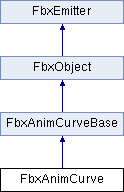
\includegraphics[height=4.000000cm]{class_fbx_anim_curve}
\end{center}
\end{figure}
\subsection*{公開メンバ関数}
\begin{DoxyCompactItemize}
\item 
virtual K\+F\+Curve $\ast$ \hyperlink{class_fbx_anim_curve_a7c7cbe48da39fa57af9f32acc68a0ba5}{Get\+K\+F\+Curve} ()=0
\item 
virtual bool \hyperlink{class_fbx_anim_curve_a0ef3229e43aaca33ab50161235541060}{Store} (\hyperlink{class_fbx_i_o}{Fbx\+IO} $\ast$p\+File\+Object, bool p\+Legacy\+Version=false)=0
\item 
virtual bool \hyperlink{class_fbx_anim_curve_a17087752d3a28d373b2aaa66d1755f62}{Retrieve} (\hyperlink{class_fbx_i_o}{Fbx\+IO} $\ast$p\+File\+Object)=0
\item 
virtual void \hyperlink{class_fbx_anim_curve_a8982eaf744608ac38457fd6f87990044}{Extrapolation\+Sync\+Callback} ()=0
\end{DoxyCompactItemize}
\subsection*{Animation curve creation.}
\begin{DoxyCompactItemize}
\item 
static \hyperlink{class_fbx_anim_curve}{Fbx\+Anim\+Curve} $\ast$ \hyperlink{class_fbx_anim_curve_ab0faf2c8c4a3d0fa8535da4a3eacb74a}{Create} (\hyperlink{class_fbx_scene}{Fbx\+Scene} $\ast$p\+Container, const char $\ast$p\+Name)
\end{DoxyCompactItemize}
\subsection*{Key management.}
\begin{DoxyCompactItemize}
\item 
virtual void \hyperlink{class_fbx_anim_curve_ad116802320381f4217d32dde6006643b}{Resize\+Key\+Buffer} (int p\+Key\+Count)=0
\item 
virtual void \hyperlink{class_fbx_anim_curve_ac75a9aaa2edc08635c0a9fadbd628923}{Key\+Modify\+Begin} ()=0
\item 
virtual void \hyperlink{class_fbx_anim_curve_ae8776e18ed1933e258774ba44f64fe5d}{Key\+Modify\+End} ()=0
\item 
virtual void \hyperlink{class_fbx_anim_curve_a202883ab5e1844beb60d40137464afd8}{Key\+Clear} ()=0
\begin{DoxyCompactList}\small\item\em Remove all the keys of the animation curve and free buffer memory. \end{DoxyCompactList}\item 
virtual int \hyperlink{class_fbx_anim_curve_a08de74d6ef6469be37abd1df0836eac9}{Key\+Get\+Count} () const =0
\item 
virtual int \hyperlink{class_fbx_anim_curve_aefac9bf8a5d7bf1fe147e192ba503737}{Key\+Add} (\hyperlink{class_fbx_time}{Fbx\+Time} p\+Time, \hyperlink{class_fbx_anim_curve_key_base}{Fbx\+Anim\+Curve\+Key\+Base} \&p\+Key, int $\ast$p\+Last=\hyperlink{fbxarch_8h_a070d2ce7b6bb7e5c05602aa8c308d0c4}{N\+U\+LL})=0
\item 
virtual int \hyperlink{class_fbx_anim_curve_a96e4e0437fc18712b785e7370ab5184e}{Key\+Add} (\hyperlink{class_fbx_time}{Fbx\+Time} p\+Time, int $\ast$p\+Last=\hyperlink{fbxarch_8h_a070d2ce7b6bb7e5c05602aa8c308d0c4}{N\+U\+LL})=0
\item 
virtual bool \hyperlink{class_fbx_anim_curve_a8f36f89bd5fbaa4f180789f4d9faf84f}{Key\+Set} (int p\+Index, \hyperlink{class_fbx_anim_curve_key_base}{Fbx\+Anim\+Curve\+Key\+Base} \&p\+Key)=0
\item 
virtual bool \hyperlink{class_fbx_anim_curve_a083206eda111aa4c6803410427a4645c}{Key\+Remove} (int p\+Index)=0
\item 
virtual bool \hyperlink{class_fbx_anim_curve_a7b4fe494d1ca4575bb253ec89f867df1}{Key\+Remove} (int p\+Start\+Index, int p\+End\+Index)=0
\item 
virtual int \hyperlink{class_fbx_anim_curve_aaad0086794bde7063d868956c6fc6b3f}{Key\+Insert} (\hyperlink{class_fbx_time}{Fbx\+Time} p\+Time, int $\ast$p\+Last=\hyperlink{fbxarch_8h_a070d2ce7b6bb7e5c05602aa8c308d0c4}{N\+U\+LL})=0
\item 
virtual double \hyperlink{class_fbx_anim_curve_a19b276335ead40663ccf4c16d6ff5e27}{Key\+Find} (\hyperlink{class_fbx_time}{Fbx\+Time} p\+Time, int $\ast$p\+Last=\hyperlink{fbxarch_8h_a070d2ce7b6bb7e5c05602aa8c308d0c4}{N\+U\+LL})=0
\item 
virtual bool \hyperlink{class_fbx_anim_curve_a5422351a86bda5b21e6ed5ce6658477e}{Key\+Scale\+Value} (float p\+Mult\+Value)=0
\item 
virtual bool \hyperlink{class_fbx_anim_curve_a2f09fd7ebeb68f8aa34f53926daf538b}{Key\+Scale\+Value\+And\+Tangent} (float p\+Mult\+Value)=0
\end{DoxyCompactItemize}
\subsection*{Key Manipulation}
\begin{DoxyCompactItemize}
\item 
virtual void \hyperlink{class_fbx_anim_curve_a70bb71da0c56a32be961384c015bb812}{Key\+Set} (int p\+Key\+Index, \hyperlink{class_fbx_time}{Fbx\+Time} p\+Time, float p\+Value, \hyperlink{class_fbx_anim_curve_def_add2ab7d10d856ab0868cc9b143d59ea5}{Fbx\+Anim\+Curve\+Def\+::\+E\+Interpolation\+Type} p\+Interpolation=\hyperlink{class_fbx_anim_curve_def_add2ab7d10d856ab0868cc9b143d59ea5a16ef50fcdbb8ae99246f06e12f9d3dae}{Fbx\+Anim\+Curve\+Def\+::e\+Interpolation\+Cubic}, \hyperlink{class_fbx_anim_curve_def_ac810ccc5ca0527704ab5175479964b87}{Fbx\+Anim\+Curve\+Def\+::\+E\+Tangent\+Mode} p\+Tangent\+Mode=\hyperlink{class_fbx_anim_curve_def_ac810ccc5ca0527704ab5175479964b87a56e3bad364851277281e94e81327dd25}{Fbx\+Anim\+Curve\+Def\+::e\+Tangent\+Auto}, float p\+Data0=0.\+0, float p\+Data1=0.\+0, \hyperlink{class_fbx_anim_curve_def_aeee6e9cc12501e10dbd3e5caaf66990e}{Fbx\+Anim\+Curve\+Def\+::\+E\+Weighted\+Mode} p\+Tangent\+Weight\+Mode=\hyperlink{class_fbx_anim_curve_def_aeee6e9cc12501e10dbd3e5caaf66990ea2ae55a3ceae7773d899ebfae26dcbef3}{Fbx\+Anim\+Curve\+Def\+::e\+Weighted\+None}, float p\+Weight0=\hyperlink{class_fbx_anim_curve_def_a6fd6b3907962eba0b1e71f28b55fad9d}{Fbx\+Anim\+Curve\+Def\+::s\+D\+E\+F\+A\+U\+L\+T\+\_\+\+W\+E\+I\+G\+HT}, float p\+Weight1=\hyperlink{class_fbx_anim_curve_def_a6fd6b3907962eba0b1e71f28b55fad9d}{Fbx\+Anim\+Curve\+Def\+::s\+D\+E\+F\+A\+U\+L\+T\+\_\+\+W\+E\+I\+G\+HT}, float p\+Velocity0=\hyperlink{class_fbx_anim_curve_def_abebd0a6078f18802836059fdefb36862}{Fbx\+Anim\+Curve\+Def\+::s\+D\+E\+F\+A\+U\+L\+T\+\_\+\+V\+E\+L\+O\+C\+I\+TY}, float p\+Velocity1=\hyperlink{class_fbx_anim_curve_def_abebd0a6078f18802836059fdefb36862}{Fbx\+Anim\+Curve\+Def\+::s\+D\+E\+F\+A\+U\+L\+T\+\_\+\+V\+E\+L\+O\+C\+I\+TY})=0
\item 
virtual void \hyperlink{class_fbx_anim_curve_af5319507799c6eea17c6550465065f8f}{Key\+Set\+T\+CB} (int p\+Key\+Index, \hyperlink{class_fbx_time}{Fbx\+Time} p\+Time, float p\+Value, float p\+Data0=0.\+0f, float p\+Data1=0.\+0f, float p\+Data2=0.\+0f)=0
\item 
virtual \hyperlink{class_fbx_anim_curve_def_add2ab7d10d856ab0868cc9b143d59ea5}{Fbx\+Anim\+Curve\+Def\+::\+E\+Interpolation\+Type} \hyperlink{class_fbx_anim_curve_a14158288d26a4fc08c6ae7b2ff8d6638}{Key\+Get\+Interpolation} (int p\+Key\+Index) const =0
\item 
virtual void \hyperlink{class_fbx_anim_curve_aa9de6c77c7d81def717ff34f01a660fb}{Key\+Set\+Interpolation} (int p\+Key\+Index, \hyperlink{class_fbx_anim_curve_def_add2ab7d10d856ab0868cc9b143d59ea5}{Fbx\+Anim\+Curve\+Def\+::\+E\+Interpolation\+Type} p\+Interpolation)=0
\item 
virtual \hyperlink{class_fbx_anim_curve_def_a52885abd392ac8ac3da94bafc5fddd64}{Fbx\+Anim\+Curve\+Def\+::\+E\+Constant\+Mode} \hyperlink{class_fbx_anim_curve_a990e2b6b948eec3562abc2c74b6d0ef2}{Key\+Get\+Constant\+Mode} (int p\+Key\+Index) const =0
\item 
virtual \hyperlink{class_fbx_anim_curve_def_ac810ccc5ca0527704ab5175479964b87}{Fbx\+Anim\+Curve\+Def\+::\+E\+Tangent\+Mode} \hyperlink{class_fbx_anim_curve_a5672d86518e0ceb21c4bcaf78f7f5bf6}{Key\+Get\+Tangent\+Mode} (int p\+Key\+Index, bool p\+Include\+Overrides=false) const =0
\item 
virtual void \hyperlink{class_fbx_anim_curve_a195063224af388d7064dc13910a89cb9}{Key\+Set\+Constant\+Mode} (int p\+Key\+Index, \hyperlink{class_fbx_anim_curve_def_a52885abd392ac8ac3da94bafc5fddd64}{Fbx\+Anim\+Curve\+Def\+::\+E\+Constant\+Mode} p\+Mode)=0
\item 
virtual void \hyperlink{class_fbx_anim_curve_a13fa9ecd9e09a39f734cf5a3265ea0ff}{Key\+Set\+Tangent\+Mode} (int p\+Key\+Index, \hyperlink{class_fbx_anim_curve_def_ac810ccc5ca0527704ab5175479964b87}{Fbx\+Anim\+Curve\+Def\+::\+E\+Tangent\+Mode} p\+Tangent)=0
\item 
virtual \hyperlink{class_fbx_anim_curve_key}{Fbx\+Anim\+Curve\+Key} \hyperlink{class_fbx_anim_curve_aec10e4a71979bd990d98cd002f29e82c}{Key\+Get} (int p\+Index) const =0
\item 
virtual float \hyperlink{class_fbx_anim_curve_a1d0a4728a6c8c1c0260fd368ba64ccb6}{Key\+Get\+Value} (int p\+Key\+Index) const =0
\item 
virtual void \hyperlink{class_fbx_anim_curve_aa974a3bbece0cd63fa4c4d3a7ad7fd99}{Key\+Set\+Value} (int p\+Key\+Index, float p\+Value)=0
\item 
virtual void \hyperlink{class_fbx_anim_curve_a38cdb5a33a9d7195f9e74b0fb4aa3261}{Key\+Inc\+Value} (int p\+Key\+Index, float p\+Value)=0
\item 
virtual void \hyperlink{class_fbx_anim_curve_a73262cd3affc5c9d098fda9a35a37779}{Key\+Mult\+Value} (int p\+Key\+Index, float p\+Value)=0
\item 
virtual void \hyperlink{class_fbx_anim_curve_a743514eebf5845d6bc13145e082a8ae5}{Key\+Mult\+Tangent} (int p\+Key\+Index, float p\+Value)=0
\item 
virtual \hyperlink{class_fbx_time}{Fbx\+Time} \hyperlink{class_fbx_anim_curve_a547f7842ea7bae5b5ed048d15b8b0d07}{Key\+Get\+Time} (int p\+Key\+Index) const =0
\item 
virtual void \hyperlink{class_fbx_anim_curve_a5ce2130d0cea4de2fc42fa3683f01162}{Key\+Set\+Time} (int p\+Key\+Index, \hyperlink{class_fbx_time}{Fbx\+Time} p\+Time)=0
\item 
virtual void \hyperlink{class_fbx_anim_curve_ae0137873a7e2c36679e9e747908b8317}{Key\+Set\+Break} (int p\+Key\+Index, bool p\+Val)=0
\item 
virtual bool \hyperlink{class_fbx_anim_curve_a401621f086458975b39fcbcef8e9be77}{Key\+Get\+Break} (int p\+Key\+Index) const =0
\end{DoxyCompactItemize}
\subsection*{Key Tangent Management}
\begin{DoxyCompactItemize}
\item 
virtual float \hyperlink{class_fbx_anim_curve_a9ccab8818487ccaaaf908c5367e3f9e9}{Key\+Get\+Left\+Derivative} (int p\+Index)=0
\item 
virtual void \hyperlink{class_fbx_anim_curve_afbec5f6b274395cb1a3d8d1eb379982f}{Key\+Set\+Left\+Derivative} (int p\+Index, float p\+Value)=0
\item 
virtual float \hyperlink{class_fbx_anim_curve_a1bd66bdbb3e7e798d70695dc97f71dc7}{Key\+Get\+Left\+Auto} (int p\+Index, bool p\+Apply\+Overshoot\+Protection=false)=0
\item 
virtual \hyperlink{struct_fbx_anim_curve_tangent_info}{Fbx\+Anim\+Curve\+Tangent\+Info} \hyperlink{class_fbx_anim_curve_a28398566658955d12824942635ee45ab}{Key\+Get\+Left\+Derivative\+Info} (int p\+Index)=0
\item 
virtual void \hyperlink{class_fbx_anim_curve_a8fa694edd4fb27b9b61739efa9e27083}{Key\+Set\+Left\+Derivative\+Info} (int p\+Index, const \hyperlink{struct_fbx_anim_curve_tangent_info}{Fbx\+Anim\+Curve\+Tangent\+Info} \&p\+Value, bool p\+Force\+Derivative=false)=0
\item 
virtual float \hyperlink{class_fbx_anim_curve_a8fb62fd9043cccbc129fad343d1610ba}{Key\+Get\+Right\+Derivative} (int p\+Index)=0
\item 
virtual void \hyperlink{class_fbx_anim_curve_a1de09a5f76f6eb12d0170cbd36fe6a78}{Key\+Set\+Right\+Derivative} (int p\+Index, float p\+Value)=0
\item 
virtual float \hyperlink{class_fbx_anim_curve_a55a43ce2a48ceccd753cdb10a7acf77e}{Key\+Get\+Right\+Auto} (int p\+Index, bool p\+Apply\+Overshoot\+Protection=false)=0
\item 
virtual \hyperlink{struct_fbx_anim_curve_tangent_info}{Fbx\+Anim\+Curve\+Tangent\+Info} \hyperlink{class_fbx_anim_curve_a3c586d4f3cdcfbccc9fadf99bce03fd5}{Key\+Get\+Right\+Derivative\+Info} (int p\+Index)=0
\item 
virtual void \hyperlink{class_fbx_anim_curve_a609a6e5f3ee69b04e46e75597cc5e1cf}{Key\+Set\+Right\+Derivative\+Info} (int p\+Index, const \hyperlink{struct_fbx_anim_curve_tangent_info}{Fbx\+Anim\+Curve\+Tangent\+Info} \&p\+Value, bool p\+Force\+Derivative=false)=0
\item 
virtual bool \hyperlink{class_fbx_anim_curve_af73a0bbb95ba2c7516438b68de733f1a}{Key\+Is\+Left\+Tangent\+Weighted} (int p\+Index) const =0
\item 
virtual bool \hyperlink{class_fbx_anim_curve_af82ac790cdd052063e2c8dbd45ea54ca}{Key\+Is\+Right\+Tangent\+Weighted} (int p\+Index) const =0
\item 
virtual float \hyperlink{class_fbx_anim_curve_a9828bb0aa421a390a8bccdf161500e5a}{Key\+Get\+Left\+Tangent\+Weight} (int p\+Index) const =0
\item 
virtual float \hyperlink{class_fbx_anim_curve_a82f1cd10ca027ec52eb0facf47b9c9f4}{Key\+Get\+Right\+Tangent\+Weight} (int p\+Index) const =0
\item 
virtual void \hyperlink{class_fbx_anim_curve_a8733d2c8ebbb4e5d367dba81363fbf17}{Key\+Set\+Left\+Tangent\+Weight} (int p\+Index, float p\+Weight, bool p\+Adjust\+Tan=false)=0
\item 
virtual void \hyperlink{class_fbx_anim_curve_acf1994ed3720f3d3e98cfca8bf31ce25}{Key\+Set\+Right\+Tangent\+Weight} (int p\+Index, float p\+Weight, bool p\+Adjust\+Tan=false)=0
\item 
virtual float \hyperlink{class_fbx_anim_curve_ad51bde65942e896c8fb7619ef4a4d149}{Key\+Get\+Left\+Tangent\+Velocity} (int p\+Index) const =0
\item 
virtual float \hyperlink{class_fbx_anim_curve_a85a44ed49cc90f3c7dc53ca5da5107b3}{Key\+Get\+Right\+Tangent\+Velocity} (int p\+Index) const =0
\end{DoxyCompactItemize}
\subsection*{Evaluation and Analysis}
\begin{DoxyCompactItemize}
\item 
virtual float \hyperlink{class_fbx_anim_curve_a74a3ea7a22a69fe69141722adff7f01b}{Evaluate} (\hyperlink{class_fbx_time}{Fbx\+Time} p\+Time, int $\ast$p\+Last=\hyperlink{fbxarch_8h_a070d2ce7b6bb7e5c05602aa8c308d0c4}{N\+U\+LL})=0
\item 
virtual float \hyperlink{class_fbx_anim_curve_ad26cbb4cd0360aa8697a2601f8540a21}{Evaluate\+Index} (double p\+Index)=0
\item 
virtual float \hyperlink{class_fbx_anim_curve_a31c932aa6ca57749591a70f86498be5f}{Evaluate\+Left\+Derivative} (\hyperlink{class_fbx_time}{Fbx\+Time} p\+Time, int $\ast$p\+Last=\hyperlink{fbxarch_8h_a070d2ce7b6bb7e5c05602aa8c308d0c4}{N\+U\+LL})=0
\item 
virtual float \hyperlink{class_fbx_anim_curve_a02a8c8629fafa6a97b37a37fd2e77331}{Evaluate\+Right\+Derivative} (\hyperlink{class_fbx_time}{Fbx\+Time} p\+Time, int $\ast$p\+Last=\hyperlink{fbxarch_8h_a070d2ce7b6bb7e5c05602aa8c308d0c4}{N\+U\+LL})=0
\end{DoxyCompactItemize}
\subsection*{Utility functions.}
\begin{DoxyCompactItemize}
\item 
virtual bool \hyperlink{class_fbx_anim_curve_aa547431c44acd9eb28aebdec1a142501}{Get\+Time\+Interval} (\hyperlink{class_fbx_time_span}{Fbx\+Time\+Span} \&p\+Time\+Interval)=0
\item 
virtual void \hyperlink{class_fbx_anim_curve_a8e5b647af7ed54b53189fd9488e12f77}{Copy\+From} (\hyperlink{class_fbx_anim_curve}{Fbx\+Anim\+Curve} \&p\+Source, bool p\+With\+Keys=true)=0
\item 
virtual float \hyperlink{class_fbx_anim_curve_ada5c523e08c9a1e4407dfce8697babdc}{Get\+Value} (int p\+Curve\+Node\+Index=0)=0
\item 
virtual void \hyperlink{class_fbx_anim_curve_abcb5d65afda70282d312be4f58b7d9cd}{Set\+Value} (float p\+Value, int p\+Curve\+Node\+Index=0)=0
\end{DoxyCompactItemize}
\subsection*{その他の継承メンバ}


\subsection{詳解}
An animation curve, defined by a collection of keys (\hyperlink{class_fbx_anim_curve_key}{Fbx\+Anim\+Curve\+Key}), and indicating how a value changes over time. Since an animation curve is a function, on a given animation curve, only one key per time is allowed. The keys are sorted in time order. They can be accessed by their index on the curve, from 0 to \hyperlink{class_fbx_anim_curve_a08de74d6ef6469be37abd1df0836eac9}{Fbx\+Anim\+Curve\+::\+Key\+Get\+Count}-\/1. The time unit in F\+BX (\hyperlink{class_fbx_time}{Fbx\+Time}) is 1/46186158000 of one second.

Each key defines tangents and interpolation that modify the animation curve. Tangents control the way the animation curve enters and exits the keys. Interpolation indicates the animation curve\textquotesingle{}s behavior between keys.

Interpolation modes are \begin{DoxyItemize}
\item Constant -\/ Curve value stays the same until next key \item Linear -\/ Animation curve is a straight line \item Cubic -\/ Animation curve is a Bezier spline\end{DoxyItemize}
Tangent modes are \begin{DoxyItemize}
\item Auto (Spline cardinal) \item Spline T\+CB (Tension, Continuity, Bias) \item User (Next slope at the left equal to slope at the right)\end{DoxyItemize}
Tangent modes can be overridden by more tangent options\+: \begin{DoxyItemize}
\item Break (Independent left and right slopes) \item Clamp (Key should be flat if next or previous key has the same value) \item Time independent\end{DoxyItemize}
Tangent can be modified some more by adding weights and velocity. By default, the weights are 0.\+333 on either side of the key, and there is no velocity. Velocity settings speed up or slow down animation on either side of a key without changing the trajectory of the animation. Unlike Auto and Weight settings, Velocity changes the animation in time, but not in space.

\begin{DoxyRemark}{注釈}
\hyperlink{class_fbx_anim_curve}{Fbx\+Anim\+Curve} is now the main animation animation curve object of the S\+DK. Users should always use this class to handle animation curve.
\end{DoxyRemark}
\begin{DoxyNote}{覚え書き}
When adding keys to an animation curve, use \hyperlink{class_fbx_anim_curve_ac75a9aaa2edc08635c0a9fadbd628923}{Fbx\+Anim\+Curve\+::\+Key\+Modify\+Begin} and \hyperlink{class_fbx_anim_curve_ae8776e18ed1933e258774ba44f64fe5d}{Fbx\+Anim\+Curve\+::\+Key\+Modify\+End}. please refer to the following sample code\+: 
\begin{DoxyCode}
\hyperlink{class_fbx_time}{FbxTime} lTime;
\textcolor{keywordtype}{int} lKeyIndex = 0;

\textcolor{comment}{// Create curve}
\hyperlink{class_fbx_anim_curve}{FbxAnimCurve}* lAnimCurve = \hyperlink{class_fbx_anim_curve_ab0faf2c8c4a3d0fa8535da4a3eacb74a}{FbxAnimCurve::Create}(pScene, \textcolor{stringliteral}{"Cube Animation"});

\textcolor{comment}{// Add keys to the curve}
lAnimCurve->\hyperlink{class_fbx_anim_curve_ac75a9aaa2edc08635c0a9fadbd628923}{KeyModifyBegin}();

\textcolor{comment}{// First key: time 0, value 0}
lTime.\hyperlink{class_fbx_time_aa67980a4f73f7914d0c457384754da0c}{SetSecondDouble}(0.0);
lKeyIndex = lAnimCurve->\hyperlink{class_fbx_anim_curve_aefac9bf8a5d7bf1fe147e192ba503737}{KeyAdd}(lTime);
lAnimCurve->\hyperlink{class_fbx_anim_curve_a8f36f89bd5fbaa4f180789f4d9faf84f}{KeySet}(lKeyIndex, lTime, 0.0, 
      \hyperlink{class_fbx_anim_curve_def_add2ab7d10d856ab0868cc9b143d59ea5ab60e201b78e2105be1134c3c15519d20}{FbxAnimCurveDef::eInterpolationLinear});

\textcolor{comment}{// Second key: time 20s, value -3600}
\textcolor{comment}{// Since this curve will describe rotation, each cube will rotate 10 times around itself during 20 seconds.}
lTime.\hyperlink{class_fbx_time_aa67980a4f73f7914d0c457384754da0c}{SetSecondDouble}(20.0);
lKeyIndex = lAnimCurve->\hyperlink{class_fbx_anim_curve_aefac9bf8a5d7bf1fe147e192ba503737}{KeyAdd}(lTime);
lAnimCurve->\hyperlink{class_fbx_anim_curve_a8f36f89bd5fbaa4f180789f4d9faf84f}{KeySet}(lKeyIndex, lTime, -3600, 
      \hyperlink{class_fbx_anim_curve_def_add2ab7d10d856ab0868cc9b143d59ea5ab60e201b78e2105be1134c3c15519d20}{FbxAnimCurveDef::eInterpolationLinear});

\textcolor{comment}{// Done adding keys.}
lAnimCurve->\hyperlink{class_fbx_anim_curve_ae8776e18ed1933e258774ba44f64fe5d}{KeyModifyEnd}();
\end{DoxyCode}
 
\end{DoxyNote}


 fbxanimcurve.\+h の 779 行目に定義があります。



\subsection{関数詳解}
\mbox{\Hypertarget{class_fbx_anim_curve_a8e5b647af7ed54b53189fd9488e12f77}\label{class_fbx_anim_curve_a8e5b647af7ed54b53189fd9488e12f77}} 
\index{Fbx\+Anim\+Curve@{Fbx\+Anim\+Curve}!Copy\+From@{Copy\+From}}
\index{Copy\+From@{Copy\+From}!Fbx\+Anim\+Curve@{Fbx\+Anim\+Curve}}
\subsubsection{\texorpdfstring{Copy\+From()}{CopyFrom()}}
{\footnotesize\ttfamily virtual void Fbx\+Anim\+Curve\+::\+Copy\+From (\begin{DoxyParamCaption}\item[{\hyperlink{class_fbx_anim_curve}{Fbx\+Anim\+Curve} \&}]{p\+Source,  }\item[{bool}]{p\+With\+Keys = {\ttfamily true} }\end{DoxyParamCaption})\hspace{0.3cm}{\ttfamily [pure virtual]}}

Copy animation curve content into current animation curve. 
\begin{DoxyParams}{引数}
{\em p\+Source} & Animation curve to be copied (which will not be modified). \\
\hline
{\em p\+With\+Keys} & If {\ttfamily true}, clear keys in current animation curve and copy keys from source animation curve. If {\ttfamily false}, keys in current animation curve are left as is. \\
\hline
\end{DoxyParams}
\mbox{\Hypertarget{class_fbx_anim_curve_ab0faf2c8c4a3d0fa8535da4a3eacb74a}\label{class_fbx_anim_curve_ab0faf2c8c4a3d0fa8535da4a3eacb74a}} 
\index{Fbx\+Anim\+Curve@{Fbx\+Anim\+Curve}!Create@{Create}}
\index{Create@{Create}!Fbx\+Anim\+Curve@{Fbx\+Anim\+Curve}}
\subsubsection{\texorpdfstring{Create()}{Create()}}
{\footnotesize\ttfamily static \hyperlink{class_fbx_anim_curve}{Fbx\+Anim\+Curve}$\ast$ Fbx\+Anim\+Curve\+::\+Create (\begin{DoxyParamCaption}\item[{\hyperlink{class_fbx_scene}{Fbx\+Scene} $\ast$}]{p\+Container,  }\item[{const char $\ast$}]{p\+Name }\end{DoxyParamCaption})\hspace{0.3cm}{\ttfamily [static]}}

Create a \hyperlink{class_fbx_anim_curve}{Fbx\+Anim\+Curve}. 
\begin{DoxyParams}{引数}
{\em p\+Container} & Scene to which the created animation curve belongs. \\
\hline
{\em p\+Name} & Name of the animation curve. \\
\hline
\end{DoxyParams}
\begin{DoxyReturn}{戻り値}
Newly created animation curve 
\end{DoxyReturn}
\mbox{\Hypertarget{class_fbx_anim_curve_a74a3ea7a22a69fe69141722adff7f01b}\label{class_fbx_anim_curve_a74a3ea7a22a69fe69141722adff7f01b}} 
\index{Fbx\+Anim\+Curve@{Fbx\+Anim\+Curve}!Evaluate@{Evaluate}}
\index{Evaluate@{Evaluate}!Fbx\+Anim\+Curve@{Fbx\+Anim\+Curve}}
\subsubsection{\texorpdfstring{Evaluate()}{Evaluate()}}
{\footnotesize\ttfamily virtual float Fbx\+Anim\+Curve\+::\+Evaluate (\begin{DoxyParamCaption}\item[{\hyperlink{class_fbx_time}{Fbx\+Time}}]{p\+Time,  }\item[{int $\ast$}]{p\+Last = {\ttfamily \hyperlink{fbxarch_8h_a070d2ce7b6bb7e5c05602aa8c308d0c4}{N\+U\+LL}} }\end{DoxyParamCaption})\hspace{0.3cm}{\ttfamily [pure virtual]}}

Evaluate animation curve value at a given time. 
\begin{DoxyParams}{引数}
{\em p\+Time} & Time of evaluation. If time falls between two keys, animation curve value is interpolated according to previous key interpolation type and tangent mode if relevant. \\
\hline
{\em p\+Last} & Index of the last processed key to speed up search. If this function is called in a loop, initialize this value to 0 and let it be updated by each call. \\
\hline
\end{DoxyParams}
\begin{DoxyReturn}{戻り値}
Animation curve value on given time, or animation curve\textquotesingle{}s default value if animation curve has no key. 
\end{DoxyReturn}
\begin{DoxyRemark}{注釈}
This function takes extrapolation into account. 
\end{DoxyRemark}


\hyperlink{class_fbx_anim_curve_base_a6d31c045a3733067fc7b4e6416d2fe06}{Fbx\+Anim\+Curve\+Base}を実装しています。

\mbox{\Hypertarget{class_fbx_anim_curve_ad26cbb4cd0360aa8697a2601f8540a21}\label{class_fbx_anim_curve_ad26cbb4cd0360aa8697a2601f8540a21}} 
\index{Fbx\+Anim\+Curve@{Fbx\+Anim\+Curve}!Evaluate\+Index@{Evaluate\+Index}}
\index{Evaluate\+Index@{Evaluate\+Index}!Fbx\+Anim\+Curve@{Fbx\+Anim\+Curve}}
\subsubsection{\texorpdfstring{Evaluate\+Index()}{EvaluateIndex()}}
{\footnotesize\ttfamily virtual float Fbx\+Anim\+Curve\+::\+Evaluate\+Index (\begin{DoxyParamCaption}\item[{double}]{p\+Index }\end{DoxyParamCaption})\hspace{0.3cm}{\ttfamily [pure virtual]}}

Evaluate animation curve value at a given key index. 
\begin{DoxyParams}{引数}
{\em p\+Index} & Any value from 0 to \hyperlink{class_fbx_anim_curve_a08de74d6ef6469be37abd1df0836eac9}{Fbx\+Anim\+Curve\+::\+Key\+Get\+Count()} -\/ 1. \\
\hline
\end{DoxyParams}
\begin{DoxyReturn}{戻り値}
Animation curve value, or default value if animation curve has no key.
\end{DoxyReturn}
\begin{DoxyRemark}{注釈}
If key index is not an integer value, animation curve value is interpolated according to previous key interpolation type and tangent mode, if relevant. This function does not take extrapolation into account. Result is undetermined if index is out of bounds. 
\end{DoxyRemark}


\hyperlink{class_fbx_anim_curve_base_aa54f5c0c77e553be03ba888448dc1818}{Fbx\+Anim\+Curve\+Base}を実装しています。

\mbox{\Hypertarget{class_fbx_anim_curve_a31c932aa6ca57749591a70f86498be5f}\label{class_fbx_anim_curve_a31c932aa6ca57749591a70f86498be5f}} 
\index{Fbx\+Anim\+Curve@{Fbx\+Anim\+Curve}!Evaluate\+Left\+Derivative@{Evaluate\+Left\+Derivative}}
\index{Evaluate\+Left\+Derivative@{Evaluate\+Left\+Derivative}!Fbx\+Anim\+Curve@{Fbx\+Anim\+Curve}}
\subsubsection{\texorpdfstring{Evaluate\+Left\+Derivative()}{EvaluateLeftDerivative()}}
{\footnotesize\ttfamily virtual float Fbx\+Anim\+Curve\+::\+Evaluate\+Left\+Derivative (\begin{DoxyParamCaption}\item[{\hyperlink{class_fbx_time}{Fbx\+Time}}]{p\+Time,  }\item[{int $\ast$}]{p\+Last = {\ttfamily \hyperlink{fbxarch_8h_a070d2ce7b6bb7e5c05602aa8c308d0c4}{N\+U\+LL}} }\end{DoxyParamCaption})\hspace{0.3cm}{\ttfamily [pure virtual]}}

Evaluate function left derivative at given time. 
\begin{DoxyParams}{引数}
{\em p\+Time} & Time of evaluation. \\
\hline
{\em p\+Last} & Index of the last processed key to speed up search. If this function is called in a loop, initialize this value to 0 and let it be updated by each call. \\
\hline
\end{DoxyParams}
\begin{DoxyReturn}{戻り値}
Left derivative at given time. 
\end{DoxyReturn}
\begin{DoxyRemark}{注釈}
This function does not take extrapolation into account. Result is undetermined if index is out of bounds. 
\end{DoxyRemark}
\mbox{\Hypertarget{class_fbx_anim_curve_a02a8c8629fafa6a97b37a37fd2e77331}\label{class_fbx_anim_curve_a02a8c8629fafa6a97b37a37fd2e77331}} 
\index{Fbx\+Anim\+Curve@{Fbx\+Anim\+Curve}!Evaluate\+Right\+Derivative@{Evaluate\+Right\+Derivative}}
\index{Evaluate\+Right\+Derivative@{Evaluate\+Right\+Derivative}!Fbx\+Anim\+Curve@{Fbx\+Anim\+Curve}}
\subsubsection{\texorpdfstring{Evaluate\+Right\+Derivative()}{EvaluateRightDerivative()}}
{\footnotesize\ttfamily virtual float Fbx\+Anim\+Curve\+::\+Evaluate\+Right\+Derivative (\begin{DoxyParamCaption}\item[{\hyperlink{class_fbx_time}{Fbx\+Time}}]{p\+Time,  }\item[{int $\ast$}]{p\+Last = {\ttfamily \hyperlink{fbxarch_8h_a070d2ce7b6bb7e5c05602aa8c308d0c4}{N\+U\+LL}} }\end{DoxyParamCaption})\hspace{0.3cm}{\ttfamily [pure virtual]}}

Evaluate function right derivative at given time. 
\begin{DoxyParams}{引数}
{\em p\+Time} & Time of evaluation. \\
\hline
{\em p\+Last} & Index of the last processed key to speed up search. If this function is called in a loop, initialize this value to 0 and let it be updated by each call. \\
\hline
\end{DoxyParams}
\begin{DoxyReturn}{戻り値}
Right derivative at given time. 
\end{DoxyReturn}
\begin{DoxyRemark}{注釈}
This function does not take extrapolation into account. Result is undetermined if index is out of bounds. 
\end{DoxyRemark}
\mbox{\Hypertarget{class_fbx_anim_curve_a8982eaf744608ac38457fd6f87990044}\label{class_fbx_anim_curve_a8982eaf744608ac38457fd6f87990044}} 
\index{Fbx\+Anim\+Curve@{Fbx\+Anim\+Curve}!Extrapolation\+Sync\+Callback@{Extrapolation\+Sync\+Callback}}
\index{Extrapolation\+Sync\+Callback@{Extrapolation\+Sync\+Callback}!Fbx\+Anim\+Curve@{Fbx\+Anim\+Curve}}
\subsubsection{\texorpdfstring{Extrapolation\+Sync\+Callback()}{ExtrapolationSyncCallback()}}
{\footnotesize\ttfamily virtual void Fbx\+Anim\+Curve\+::\+Extrapolation\+Sync\+Callback (\begin{DoxyParamCaption}{ }\end{DoxyParamCaption})\hspace{0.3cm}{\ttfamily [pure virtual]}}



\hyperlink{class_fbx_anim_curve_base_aab573e42ece898c2c1e61a295adbb610}{Fbx\+Anim\+Curve\+Base}を実装しています。

\mbox{\Hypertarget{class_fbx_anim_curve_a7c7cbe48da39fa57af9f32acc68a0ba5}\label{class_fbx_anim_curve_a7c7cbe48da39fa57af9f32acc68a0ba5}} 
\index{Fbx\+Anim\+Curve@{Fbx\+Anim\+Curve}!Get\+K\+F\+Curve@{Get\+K\+F\+Curve}}
\index{Get\+K\+F\+Curve@{Get\+K\+F\+Curve}!Fbx\+Anim\+Curve@{Fbx\+Anim\+Curve}}
\subsubsection{\texorpdfstring{Get\+K\+F\+Curve()}{GetKFCurve()}}
{\footnotesize\ttfamily virtual K\+F\+Curve$\ast$ Fbx\+Anim\+Curve\+::\+Get\+K\+F\+Curve (\begin{DoxyParamCaption}{ }\end{DoxyParamCaption})\hspace{0.3cm}{\ttfamily [pure virtual]}}

\mbox{\Hypertarget{class_fbx_anim_curve_aa547431c44acd9eb28aebdec1a142501}\label{class_fbx_anim_curve_aa547431c44acd9eb28aebdec1a142501}} 
\index{Fbx\+Anim\+Curve@{Fbx\+Anim\+Curve}!Get\+Time\+Interval@{Get\+Time\+Interval}}
\index{Get\+Time\+Interval@{Get\+Time\+Interval}!Fbx\+Anim\+Curve@{Fbx\+Anim\+Curve}}
\subsubsection{\texorpdfstring{Get\+Time\+Interval()}{GetTimeInterval()}}
{\footnotesize\ttfamily virtual bool Fbx\+Anim\+Curve\+::\+Get\+Time\+Interval (\begin{DoxyParamCaption}\item[{\hyperlink{class_fbx_time_span}{Fbx\+Time\+Span} \&}]{p\+Time\+Interval }\end{DoxyParamCaption})\hspace{0.3cm}{\ttfamily [pure virtual]}}

Find out start and end time of the animation animation curve. This function retrieves the animation curve\textquotesingle{}s time span. 
\begin{DoxyParams}{引数}
{\em p\+Time\+Interval} & Reference to receive start and end time. \\
\hline
\end{DoxyParams}
\begin{DoxyReturn}{戻り値}
{\ttfamily true} on success, {\ttfamily false} otherwise. 
\end{DoxyReturn}


\hyperlink{class_fbx_anim_curve_base_a4d259319e514c5371ff184b0cc7f7cd6}{Fbx\+Anim\+Curve\+Base}を再実装しています。

\mbox{\Hypertarget{class_fbx_anim_curve_ada5c523e08c9a1e4407dfce8697babdc}\label{class_fbx_anim_curve_ada5c523e08c9a1e4407dfce8697babdc}} 
\index{Fbx\+Anim\+Curve@{Fbx\+Anim\+Curve}!Get\+Value@{Get\+Value}}
\index{Get\+Value@{Get\+Value}!Fbx\+Anim\+Curve@{Fbx\+Anim\+Curve}}
\subsubsection{\texorpdfstring{Get\+Value()}{GetValue()}}
{\footnotesize\ttfamily virtual float Fbx\+Anim\+Curve\+::\+Get\+Value (\begin{DoxyParamCaption}\item[{int}]{p\+Curve\+Node\+Index = {\ttfamily 0} }\end{DoxyParamCaption})\hspace{0.3cm}{\ttfamily [pure virtual]}}

Retrieve the value of the parent curve node channel. 
\begin{DoxyParams}{引数}
{\em p\+Curve\+Node\+Index} & The index of the parent curve node, if more than one exist. \\
\hline
\end{DoxyParams}
\begin{DoxyReturn}{戻り値}
The value of the parent curve node channel of this curve. 
\end{DoxyReturn}
\begin{DoxyRemark}{注釈}
In most case, the curve will have a single curve node channel as destination. However, it is possible that more are connected, hence why we provide the curve node index parameter. 
\end{DoxyRemark}
\mbox{\Hypertarget{class_fbx_anim_curve_aefac9bf8a5d7bf1fe147e192ba503737}\label{class_fbx_anim_curve_aefac9bf8a5d7bf1fe147e192ba503737}} 
\index{Fbx\+Anim\+Curve@{Fbx\+Anim\+Curve}!Key\+Add@{Key\+Add}}
\index{Key\+Add@{Key\+Add}!Fbx\+Anim\+Curve@{Fbx\+Anim\+Curve}}
\subsubsection{\texorpdfstring{Key\+Add()}{KeyAdd()}\hspace{0.1cm}{\footnotesize\ttfamily [1/2]}}
{\footnotesize\ttfamily virtual int Fbx\+Anim\+Curve\+::\+Key\+Add (\begin{DoxyParamCaption}\item[{\hyperlink{class_fbx_time}{Fbx\+Time}}]{p\+Time,  }\item[{\hyperlink{class_fbx_anim_curve_key_base}{Fbx\+Anim\+Curve\+Key\+Base} \&}]{p\+Key,  }\item[{int $\ast$}]{p\+Last = {\ttfamily \hyperlink{fbxarch_8h_a070d2ce7b6bb7e5c05602aa8c308d0c4}{N\+U\+LL}} }\end{DoxyParamCaption})\hspace{0.3cm}{\ttfamily [pure virtual]}}

Add a given key at given time. The new key is appended after all the other animation curve\textquotesingle{}s keys. Function \hyperlink{class_fbx_anim_curve_aaad0086794bde7063d868956c6fc6b3f}{Fbx\+Anim\+Curve\+::\+Key\+Insert()} should be used instead if the key is to be added in the curve and not at the end. This function does not respect the interpolation type and tangents of the neighboring keys. If there is already a key at the given time, the key is modified and no new key is added.


\begin{DoxyParams}{引数}
{\em p\+Time} & Time of the new key. \\
\hline
{\em p\+Key} & Key to add. \\
\hline
{\em p\+Last} & Index of the last processed key to speed up search. If this function is called in a loop, initialize this value to 0 and let it be updated by each call. \\
\hline
\end{DoxyParams}
\begin{DoxyReturn}{戻り値}
Index of the key at given time, no matter if it was added or already present.
\end{DoxyReturn}
\begin{DoxyRemark}{注釈}
Key value, interpolation type and tangent mode must be set explicitly afterwards. 
\end{DoxyRemark}


\hyperlink{class_fbx_anim_curve_base_a3e502968be213bd5cfde287f66f97cf5}{Fbx\+Anim\+Curve\+Base}を実装しています。

\mbox{\Hypertarget{class_fbx_anim_curve_a96e4e0437fc18712b785e7370ab5184e}\label{class_fbx_anim_curve_a96e4e0437fc18712b785e7370ab5184e}} 
\index{Fbx\+Anim\+Curve@{Fbx\+Anim\+Curve}!Key\+Add@{Key\+Add}}
\index{Key\+Add@{Key\+Add}!Fbx\+Anim\+Curve@{Fbx\+Anim\+Curve}}
\subsubsection{\texorpdfstring{Key\+Add()}{KeyAdd()}\hspace{0.1cm}{\footnotesize\ttfamily [2/2]}}
{\footnotesize\ttfamily virtual int Fbx\+Anim\+Curve\+::\+Key\+Add (\begin{DoxyParamCaption}\item[{\hyperlink{class_fbx_time}{Fbx\+Time}}]{p\+Time,  }\item[{int $\ast$}]{p\+Last = {\ttfamily \hyperlink{fbxarch_8h_a070d2ce7b6bb7e5c05602aa8c308d0c4}{N\+U\+LL}} }\end{DoxyParamCaption})\hspace{0.3cm}{\ttfamily [pure virtual]}}

Add a key at given time. The new key is appended after all the other animation curve\textquotesingle{}s keys. Function \hyperlink{class_fbx_anim_curve_aaad0086794bde7063d868956c6fc6b3f}{Fbx\+Anim\+Curve\+::\+Key\+Insert()} should be used instead if the key is to be added in the curve and not at the end. This function does not respect of the interpolation type and tangents of the neighboring keys. If there is already a key a the given time, no key is added.


\begin{DoxyParams}{引数}
{\em p\+Time} & Time of the new key. \\
\hline
{\em p\+Last} & Index of the last processed key to speed up search. If this function is called in a loop, initialize this value to 0 and let it be updated by each call. \\
\hline
\end{DoxyParams}
\begin{DoxyReturn}{戻り値}
Index of the key at given time, no matter if it was added or already present. 
\end{DoxyReturn}
\begin{DoxyRemark}{注釈}
Key value, interpolation type and tangent mode must be set explicitly afterwards. 
\end{DoxyRemark}
\mbox{\Hypertarget{class_fbx_anim_curve_a202883ab5e1844beb60d40137464afd8}\label{class_fbx_anim_curve_a202883ab5e1844beb60d40137464afd8}} 
\index{Fbx\+Anim\+Curve@{Fbx\+Anim\+Curve}!Key\+Clear@{Key\+Clear}}
\index{Key\+Clear@{Key\+Clear}!Fbx\+Anim\+Curve@{Fbx\+Anim\+Curve}}
\subsubsection{\texorpdfstring{Key\+Clear()}{KeyClear()}}
{\footnotesize\ttfamily virtual void Fbx\+Anim\+Curve\+::\+Key\+Clear (\begin{DoxyParamCaption}{ }\end{DoxyParamCaption})\hspace{0.3cm}{\ttfamily [pure virtual]}}



Remove all the keys of the animation curve and free buffer memory. 



\hyperlink{class_fbx_anim_curve_base_abe693d293087fad223770430ec79d65d}{Fbx\+Anim\+Curve\+Base}を実装しています。

\mbox{\Hypertarget{class_fbx_anim_curve_a19b276335ead40663ccf4c16d6ff5e27}\label{class_fbx_anim_curve_a19b276335ead40663ccf4c16d6ff5e27}} 
\index{Fbx\+Anim\+Curve@{Fbx\+Anim\+Curve}!Key\+Find@{Key\+Find}}
\index{Key\+Find@{Key\+Find}!Fbx\+Anim\+Curve@{Fbx\+Anim\+Curve}}
\subsubsection{\texorpdfstring{Key\+Find()}{KeyFind()}}
{\footnotesize\ttfamily virtual double Fbx\+Anim\+Curve\+::\+Key\+Find (\begin{DoxyParamCaption}\item[{\hyperlink{class_fbx_time}{Fbx\+Time}}]{p\+Time,  }\item[{int $\ast$}]{p\+Last = {\ttfamily \hyperlink{fbxarch_8h_a070d2ce7b6bb7e5c05602aa8c308d0c4}{N\+U\+LL}} }\end{DoxyParamCaption})\hspace{0.3cm}{\ttfamily [pure virtual]}}

Find key index for a given time. 
\begin{DoxyParams}{引数}
{\em p\+Time} & Time of the key looked for. \\
\hline
{\em p\+Last} & Index of the last processed key to speed up search. If this function is called in a loop, initialize this value to 0 and let it be updated by each call. \\
\hline
\end{DoxyParams}
\begin{DoxyReturn}{戻り値}
Key index. The integer part of the key index gives the index of the closest key with a smaller time. The decimals give the relative position of given time compared to previous and next key times. Returns -\/1 if animation curve has no key.
\end{DoxyReturn}
For example (using seconds for clarity), if there is a key at time 10s with index 5, and a key at time 11s with index 6, Key\+Find(10.\+3s) would return 5.\+3. \mbox{\Hypertarget{class_fbx_anim_curve_aec10e4a71979bd990d98cd002f29e82c}\label{class_fbx_anim_curve_aec10e4a71979bd990d98cd002f29e82c}} 
\index{Fbx\+Anim\+Curve@{Fbx\+Anim\+Curve}!Key\+Get@{Key\+Get}}
\index{Key\+Get@{Key\+Get}!Fbx\+Anim\+Curve@{Fbx\+Anim\+Curve}}
\subsubsection{\texorpdfstring{Key\+Get()}{KeyGet()}}
{\footnotesize\ttfamily virtual \hyperlink{class_fbx_anim_curve_key}{Fbx\+Anim\+Curve\+Key} Fbx\+Anim\+Curve\+::\+Key\+Get (\begin{DoxyParamCaption}\item[{int}]{p\+Index }\end{DoxyParamCaption}) const\hspace{0.3cm}{\ttfamily [pure virtual]}}

Get key at given index. 
\begin{DoxyParams}{引数}
{\em p\+Index} & Index of the key on the animation curve. \\
\hline
\end{DoxyParams}
\begin{DoxyReturn}{戻り値}
The key at the given index. 
\end{DoxyReturn}
\begin{DoxyRemark}{注釈}
Result is undetermined if animation curve has no key or if index is out of bounds. 
\end{DoxyRemark}
\mbox{\Hypertarget{class_fbx_anim_curve_a401621f086458975b39fcbcef8e9be77}\label{class_fbx_anim_curve_a401621f086458975b39fcbcef8e9be77}} 
\index{Fbx\+Anim\+Curve@{Fbx\+Anim\+Curve}!Key\+Get\+Break@{Key\+Get\+Break}}
\index{Key\+Get\+Break@{Key\+Get\+Break}!Fbx\+Anim\+Curve@{Fbx\+Anim\+Curve}}
\subsubsection{\texorpdfstring{Key\+Get\+Break()}{KeyGetBreak()}}
{\footnotesize\ttfamily virtual bool Fbx\+Anim\+Curve\+::\+Key\+Get\+Break (\begin{DoxyParamCaption}\item[{int}]{p\+Key\+Index }\end{DoxyParamCaption}) const\hspace{0.3cm}{\ttfamily [pure virtual]}}

Get if the tangent has a break. When this flag is set (\hyperlink{class_fbx_anim_curve_def_ac810ccc5ca0527704ab5175479964b87ab4d85a1a0474226be85b885518f6c847}{Fbx\+Anim\+Curve\+Def\+::e\+Tangent\+Break}), the key\textquotesingle{}s left and right slopes are independent. When this flag is off, the key\textquotesingle{}s left and right slope are equal. This method is relevant for User (\hyperlink{class_fbx_anim_curve_def_ac810ccc5ca0527704ab5175479964b87a199cb16b2c861b12c334093ce796cb86}{Fbx\+Anim\+Curve\+Def\+::e\+Tangent\+User}) and Auto (\hyperlink{class_fbx_anim_curve_def_ac810ccc5ca0527704ab5175479964b87a56e3bad364851277281e94e81327dd25}{Fbx\+Anim\+Curve\+Def\+::e\+Tangent\+Auto}) tangent modes only. 
\begin{DoxyParams}{引数}
{\em p\+Key\+Index} & Index of the queried key. \\
\hline
\end{DoxyParams}
\begin{DoxyReturn}{戻り値}
Break flag ({\ttfamily true} or {\ttfamily false}). 
\end{DoxyReturn}
\mbox{\Hypertarget{class_fbx_anim_curve_a990e2b6b948eec3562abc2c74b6d0ef2}\label{class_fbx_anim_curve_a990e2b6b948eec3562abc2c74b6d0ef2}} 
\index{Fbx\+Anim\+Curve@{Fbx\+Anim\+Curve}!Key\+Get\+Constant\+Mode@{Key\+Get\+Constant\+Mode}}
\index{Key\+Get\+Constant\+Mode@{Key\+Get\+Constant\+Mode}!Fbx\+Anim\+Curve@{Fbx\+Anim\+Curve}}
\subsubsection{\texorpdfstring{Key\+Get\+Constant\+Mode()}{KeyGetConstantMode()}}
{\footnotesize\ttfamily virtual \hyperlink{class_fbx_anim_curve_def_a52885abd392ac8ac3da94bafc5fddd64}{Fbx\+Anim\+Curve\+Def\+::\+E\+Constant\+Mode} Fbx\+Anim\+Curve\+::\+Key\+Get\+Constant\+Mode (\begin{DoxyParamCaption}\item[{int}]{p\+Key\+Index }\end{DoxyParamCaption}) const\hspace{0.3cm}{\ttfamily [pure virtual]}}

Get key\textquotesingle{}s constant mode. \begin{DoxyNote}{覚え書き}
This method is only relevant if the key\textquotesingle{}s interpolation type is constant (e\+Interpolation\+Constant). Using this method on a key with an other interpolation type will return unpredictable value. 
\end{DoxyNote}

\begin{DoxyParams}{引数}
{\em p\+Key\+Index} & Index of the queried key. \\
\hline
\end{DoxyParams}
\begin{DoxyReturn}{戻り値}
Key constant mode. 
\end{DoxyReturn}
\mbox{\Hypertarget{class_fbx_anim_curve_a08de74d6ef6469be37abd1df0836eac9}\label{class_fbx_anim_curve_a08de74d6ef6469be37abd1df0836eac9}} 
\index{Fbx\+Anim\+Curve@{Fbx\+Anim\+Curve}!Key\+Get\+Count@{Key\+Get\+Count}}
\index{Key\+Get\+Count@{Key\+Get\+Count}!Fbx\+Anim\+Curve@{Fbx\+Anim\+Curve}}
\subsubsection{\texorpdfstring{Key\+Get\+Count()}{KeyGetCount()}}
{\footnotesize\ttfamily virtual int Fbx\+Anim\+Curve\+::\+Key\+Get\+Count (\begin{DoxyParamCaption}{ }\end{DoxyParamCaption}) const\hspace{0.3cm}{\ttfamily [pure virtual]}}

Get the number of keys. \begin{DoxyReturn}{戻り値}
Key count. 
\end{DoxyReturn}


\hyperlink{class_fbx_anim_curve_base_a36fcc14d1c1944341da57085956a3f59}{Fbx\+Anim\+Curve\+Base}を実装しています。

\mbox{\Hypertarget{class_fbx_anim_curve_a14158288d26a4fc08c6ae7b2ff8d6638}\label{class_fbx_anim_curve_a14158288d26a4fc08c6ae7b2ff8d6638}} 
\index{Fbx\+Anim\+Curve@{Fbx\+Anim\+Curve}!Key\+Get\+Interpolation@{Key\+Get\+Interpolation}}
\index{Key\+Get\+Interpolation@{Key\+Get\+Interpolation}!Fbx\+Anim\+Curve@{Fbx\+Anim\+Curve}}
\subsubsection{\texorpdfstring{Key\+Get\+Interpolation()}{KeyGetInterpolation()}}
{\footnotesize\ttfamily virtual \hyperlink{class_fbx_anim_curve_def_add2ab7d10d856ab0868cc9b143d59ea5}{Fbx\+Anim\+Curve\+Def\+::\+E\+Interpolation\+Type} Fbx\+Anim\+Curve\+::\+Key\+Get\+Interpolation (\begin{DoxyParamCaption}\item[{int}]{p\+Key\+Index }\end{DoxyParamCaption}) const\hspace{0.3cm}{\ttfamily [pure virtual]}}

Get key\textquotesingle{}s interpolation type. 
\begin{DoxyParams}{引数}
{\em p\+Key\+Index} & Index of the queried key. \\
\hline
\end{DoxyParams}
\begin{DoxyReturn}{戻り値}
Interpolation type of the queried key. 
\end{DoxyReturn}
\mbox{\Hypertarget{class_fbx_anim_curve_a1bd66bdbb3e7e798d70695dc97f71dc7}\label{class_fbx_anim_curve_a1bd66bdbb3e7e798d70695dc97f71dc7}} 
\index{Fbx\+Anim\+Curve@{Fbx\+Anim\+Curve}!Key\+Get\+Left\+Auto@{Key\+Get\+Left\+Auto}}
\index{Key\+Get\+Left\+Auto@{Key\+Get\+Left\+Auto}!Fbx\+Anim\+Curve@{Fbx\+Anim\+Curve}}
\subsubsection{\texorpdfstring{Key\+Get\+Left\+Auto()}{KeyGetLeftAuto()}}
{\footnotesize\ttfamily virtual float Fbx\+Anim\+Curve\+::\+Key\+Get\+Left\+Auto (\begin{DoxyParamCaption}\item[{int}]{p\+Index,  }\item[{bool}]{p\+Apply\+Overshoot\+Protection = {\ttfamily false} }\end{DoxyParamCaption})\hspace{0.3cm}{\ttfamily [pure virtual]}}

Get the left auto parametric of a key. This is used to compute the slope of Auto and User keys. 
\begin{DoxyParams}{引数}
{\em p\+Index} & Index of the key. \\
\hline
{\em p\+Apply\+Overshoot\+Protection} & Clamp flag (e\+G\+E\+N\+E\+R\+I\+C\+\_\+\+C\+L\+A\+MP) is taken into account. \\
\hline
\end{DoxyParams}
\begin{DoxyReturn}{戻り値}
Left auto parametric. 
\end{DoxyReturn}
\begin{DoxyRemark}{注釈}
Result is undetermined if animation curve has no key or if index is out of bounds. 
\end{DoxyRemark}
\mbox{\Hypertarget{class_fbx_anim_curve_a9ccab8818487ccaaaf908c5367e3f9e9}\label{class_fbx_anim_curve_a9ccab8818487ccaaaf908c5367e3f9e9}} 
\index{Fbx\+Anim\+Curve@{Fbx\+Anim\+Curve}!Key\+Get\+Left\+Derivative@{Key\+Get\+Left\+Derivative}}
\index{Key\+Get\+Left\+Derivative@{Key\+Get\+Left\+Derivative}!Fbx\+Anim\+Curve@{Fbx\+Anim\+Curve}}
\subsubsection{\texorpdfstring{Key\+Get\+Left\+Derivative()}{KeyGetLeftDerivative()}}
{\footnotesize\ttfamily virtual float Fbx\+Anim\+Curve\+::\+Key\+Get\+Left\+Derivative (\begin{DoxyParamCaption}\item[{int}]{p\+Index }\end{DoxyParamCaption})\hspace{0.3cm}{\ttfamily [pure virtual]}}

Get the left derivative of a key. 
\begin{DoxyParams}{引数}
{\em p\+Index} & Index of the queried key. \\
\hline
\end{DoxyParams}
\begin{DoxyReturn}{戻り値}
Left derivative (Value over time (s)). 
\end{DoxyReturn}
\begin{DoxyRemark}{注釈}
Result is undetermined if animation curve has no key or if index is out of bounds. 
\end{DoxyRemark}
\mbox{\Hypertarget{class_fbx_anim_curve_a28398566658955d12824942635ee45ab}\label{class_fbx_anim_curve_a28398566658955d12824942635ee45ab}} 
\index{Fbx\+Anim\+Curve@{Fbx\+Anim\+Curve}!Key\+Get\+Left\+Derivative\+Info@{Key\+Get\+Left\+Derivative\+Info}}
\index{Key\+Get\+Left\+Derivative\+Info@{Key\+Get\+Left\+Derivative\+Info}!Fbx\+Anim\+Curve@{Fbx\+Anim\+Curve}}
\subsubsection{\texorpdfstring{Key\+Get\+Left\+Derivative\+Info()}{KeyGetLeftDerivativeInfo()}}
{\footnotesize\ttfamily virtual \hyperlink{struct_fbx_anim_curve_tangent_info}{Fbx\+Anim\+Curve\+Tangent\+Info} Fbx\+Anim\+Curve\+::\+Key\+Get\+Left\+Derivative\+Info (\begin{DoxyParamCaption}\item[{int}]{p\+Index }\end{DoxyParamCaption})\hspace{0.3cm}{\ttfamily [pure virtual]}}

Get the left derivative info (of type \hyperlink{struct_fbx_anim_curve_tangent_info}{Fbx\+Anim\+Curve\+Tangent\+Info}) of a key. 
\begin{DoxyParams}{引数}
{\em p\+Index} & Index of the queried key. \\
\hline
\end{DoxyParams}
\begin{DoxyReturn}{戻り値}
Left derivative info. 
\end{DoxyReturn}
\begin{DoxyRemark}{注釈}
Result is undetermined if animation curve has no key or if index is out of bounds. 
\end{DoxyRemark}
\mbox{\Hypertarget{class_fbx_anim_curve_ad51bde65942e896c8fb7619ef4a4d149}\label{class_fbx_anim_curve_ad51bde65942e896c8fb7619ef4a4d149}} 
\index{Fbx\+Anim\+Curve@{Fbx\+Anim\+Curve}!Key\+Get\+Left\+Tangent\+Velocity@{Key\+Get\+Left\+Tangent\+Velocity}}
\index{Key\+Get\+Left\+Tangent\+Velocity@{Key\+Get\+Left\+Tangent\+Velocity}!Fbx\+Anim\+Curve@{Fbx\+Anim\+Curve}}
\subsubsection{\texorpdfstring{Key\+Get\+Left\+Tangent\+Velocity()}{KeyGetLeftTangentVelocity()}}
{\footnotesize\ttfamily virtual float Fbx\+Anim\+Curve\+::\+Key\+Get\+Left\+Tangent\+Velocity (\begin{DoxyParamCaption}\item[{int}]{p\+Index }\end{DoxyParamCaption}) const\hspace{0.3cm}{\ttfamily [pure virtual]}}

Get the velocity value component of the left tangent of a key. 
\begin{DoxyParams}{引数}
{\em p\+Index} & Index of the key. \\
\hline
\end{DoxyParams}
\begin{DoxyReturn}{戻り値}
Tangent velocity of the left tangent. 
\end{DoxyReturn}
\begin{DoxyRemark}{注釈}
This function is only relevant if key interpolation type is e\+Interpolation\+Cubic 
\end{DoxyRemark}
\mbox{\Hypertarget{class_fbx_anim_curve_a9828bb0aa421a390a8bccdf161500e5a}\label{class_fbx_anim_curve_a9828bb0aa421a390a8bccdf161500e5a}} 
\index{Fbx\+Anim\+Curve@{Fbx\+Anim\+Curve}!Key\+Get\+Left\+Tangent\+Weight@{Key\+Get\+Left\+Tangent\+Weight}}
\index{Key\+Get\+Left\+Tangent\+Weight@{Key\+Get\+Left\+Tangent\+Weight}!Fbx\+Anim\+Curve@{Fbx\+Anim\+Curve}}
\subsubsection{\texorpdfstring{Key\+Get\+Left\+Tangent\+Weight()}{KeyGetLeftTangentWeight()}}
{\footnotesize\ttfamily virtual float Fbx\+Anim\+Curve\+::\+Key\+Get\+Left\+Tangent\+Weight (\begin{DoxyParamCaption}\item[{int}]{p\+Index }\end{DoxyParamCaption}) const\hspace{0.3cm}{\ttfamily [pure virtual]}}

Get the weight value component of the left tangent of a key. 
\begin{DoxyParams}{引数}
{\em p\+Index} & Index of the key. \\
\hline
\end{DoxyParams}
\begin{DoxyReturn}{戻り値}
Left tangent weight, or e\+D\+E\+F\+A\+U\+L\+T\+\_\+\+W\+E\+I\+G\+HT (0.\+333...) if left tangent is not weighted. 
\end{DoxyReturn}
\begin{DoxyRemark}{注釈}
This function is only relevant if key interpolation type is e\+Interpolation\+Cubic. 
\end{DoxyRemark}
\mbox{\Hypertarget{class_fbx_anim_curve_a55a43ce2a48ceccd753cdb10a7acf77e}\label{class_fbx_anim_curve_a55a43ce2a48ceccd753cdb10a7acf77e}} 
\index{Fbx\+Anim\+Curve@{Fbx\+Anim\+Curve}!Key\+Get\+Right\+Auto@{Key\+Get\+Right\+Auto}}
\index{Key\+Get\+Right\+Auto@{Key\+Get\+Right\+Auto}!Fbx\+Anim\+Curve@{Fbx\+Anim\+Curve}}
\subsubsection{\texorpdfstring{Key\+Get\+Right\+Auto()}{KeyGetRightAuto()}}
{\footnotesize\ttfamily virtual float Fbx\+Anim\+Curve\+::\+Key\+Get\+Right\+Auto (\begin{DoxyParamCaption}\item[{int}]{p\+Index,  }\item[{bool}]{p\+Apply\+Overshoot\+Protection = {\ttfamily false} }\end{DoxyParamCaption})\hspace{0.3cm}{\ttfamily [pure virtual]}}

Get the right auto parametric of a key. This is used to compute the slope of Auto and User keys. 
\begin{DoxyParams}{引数}
{\em p\+Index} & Index of the key. \\
\hline
{\em p\+Apply\+Overshoot\+Protection} & Clamp flag (e\+G\+E\+N\+E\+R\+I\+C\+\_\+\+C\+L\+A\+MP) is taken into account. \\
\hline
\end{DoxyParams}
\begin{DoxyReturn}{戻り値}
Right auto parametric. 
\end{DoxyReturn}
\begin{DoxyRemark}{注釈}
Result is undetermined if animation curve has no key or if index is out of bounds. 
\end{DoxyRemark}
\mbox{\Hypertarget{class_fbx_anim_curve_a8fb62fd9043cccbc129fad343d1610ba}\label{class_fbx_anim_curve_a8fb62fd9043cccbc129fad343d1610ba}} 
\index{Fbx\+Anim\+Curve@{Fbx\+Anim\+Curve}!Key\+Get\+Right\+Derivative@{Key\+Get\+Right\+Derivative}}
\index{Key\+Get\+Right\+Derivative@{Key\+Get\+Right\+Derivative}!Fbx\+Anim\+Curve@{Fbx\+Anim\+Curve}}
\subsubsection{\texorpdfstring{Key\+Get\+Right\+Derivative()}{KeyGetRightDerivative()}}
{\footnotesize\ttfamily virtual float Fbx\+Anim\+Curve\+::\+Key\+Get\+Right\+Derivative (\begin{DoxyParamCaption}\item[{int}]{p\+Index }\end{DoxyParamCaption})\hspace{0.3cm}{\ttfamily [pure virtual]}}

Get the right derivative of a key. 
\begin{DoxyParams}{引数}
{\em p\+Index} & Index of the key. \\
\hline
\end{DoxyParams}
\begin{DoxyReturn}{戻り値}
Right derivative (Value over time (s)). 
\end{DoxyReturn}
\begin{DoxyRemark}{注釈}
Result is undetermined if animation curve has no key or if index is out of bounds. 
\end{DoxyRemark}
\mbox{\Hypertarget{class_fbx_anim_curve_a3c586d4f3cdcfbccc9fadf99bce03fd5}\label{class_fbx_anim_curve_a3c586d4f3cdcfbccc9fadf99bce03fd5}} 
\index{Fbx\+Anim\+Curve@{Fbx\+Anim\+Curve}!Key\+Get\+Right\+Derivative\+Info@{Key\+Get\+Right\+Derivative\+Info}}
\index{Key\+Get\+Right\+Derivative\+Info@{Key\+Get\+Right\+Derivative\+Info}!Fbx\+Anim\+Curve@{Fbx\+Anim\+Curve}}
\subsubsection{\texorpdfstring{Key\+Get\+Right\+Derivative\+Info()}{KeyGetRightDerivativeInfo()}}
{\footnotesize\ttfamily virtual \hyperlink{struct_fbx_anim_curve_tangent_info}{Fbx\+Anim\+Curve\+Tangent\+Info} Fbx\+Anim\+Curve\+::\+Key\+Get\+Right\+Derivative\+Info (\begin{DoxyParamCaption}\item[{int}]{p\+Index }\end{DoxyParamCaption})\hspace{0.3cm}{\ttfamily [pure virtual]}}

Get the right derivative info (of type \hyperlink{struct_fbx_anim_curve_tangent_info}{Fbx\+Anim\+Curve\+Tangent\+Info}) of a key. 
\begin{DoxyParams}{引数}
{\em p\+Index} & Index of the queried key. \\
\hline
\end{DoxyParams}
\begin{DoxyReturn}{戻り値}
Right derivative info. 
\end{DoxyReturn}
\begin{DoxyRemark}{注釈}
Result is undetermined if animation curve has no key or if index is out of bounds. 
\end{DoxyRemark}
\mbox{\Hypertarget{class_fbx_anim_curve_a85a44ed49cc90f3c7dc53ca5da5107b3}\label{class_fbx_anim_curve_a85a44ed49cc90f3c7dc53ca5da5107b3}} 
\index{Fbx\+Anim\+Curve@{Fbx\+Anim\+Curve}!Key\+Get\+Right\+Tangent\+Velocity@{Key\+Get\+Right\+Tangent\+Velocity}}
\index{Key\+Get\+Right\+Tangent\+Velocity@{Key\+Get\+Right\+Tangent\+Velocity}!Fbx\+Anim\+Curve@{Fbx\+Anim\+Curve}}
\subsubsection{\texorpdfstring{Key\+Get\+Right\+Tangent\+Velocity()}{KeyGetRightTangentVelocity()}}
{\footnotesize\ttfamily virtual float Fbx\+Anim\+Curve\+::\+Key\+Get\+Right\+Tangent\+Velocity (\begin{DoxyParamCaption}\item[{int}]{p\+Index }\end{DoxyParamCaption}) const\hspace{0.3cm}{\ttfamily [pure virtual]}}

Get the velocity value component of the right tangent of a key. 
\begin{DoxyParams}{引数}
{\em p\+Index} & Index of the key. \\
\hline
\end{DoxyParams}
\begin{DoxyReturn}{戻り値}
Tangent velocity of the right tangent. 
\end{DoxyReturn}
\begin{DoxyRemark}{注釈}
This function is only relevant if key interpolation type is e\+Interpolation\+Cubic 
\end{DoxyRemark}
\mbox{\Hypertarget{class_fbx_anim_curve_a82f1cd10ca027ec52eb0facf47b9c9f4}\label{class_fbx_anim_curve_a82f1cd10ca027ec52eb0facf47b9c9f4}} 
\index{Fbx\+Anim\+Curve@{Fbx\+Anim\+Curve}!Key\+Get\+Right\+Tangent\+Weight@{Key\+Get\+Right\+Tangent\+Weight}}
\index{Key\+Get\+Right\+Tangent\+Weight@{Key\+Get\+Right\+Tangent\+Weight}!Fbx\+Anim\+Curve@{Fbx\+Anim\+Curve}}
\subsubsection{\texorpdfstring{Key\+Get\+Right\+Tangent\+Weight()}{KeyGetRightTangentWeight()}}
{\footnotesize\ttfamily virtual float Fbx\+Anim\+Curve\+::\+Key\+Get\+Right\+Tangent\+Weight (\begin{DoxyParamCaption}\item[{int}]{p\+Index }\end{DoxyParamCaption}) const\hspace{0.3cm}{\ttfamily [pure virtual]}}

Get the weight value component of the right tangent of a key. 
\begin{DoxyParams}{引数}
{\em p\+Index} & Index of the key. \\
\hline
\end{DoxyParams}
\begin{DoxyReturn}{戻り値}
Right tangent weight, or e\+D\+E\+F\+A\+U\+L\+T\+\_\+\+W\+E\+I\+G\+HT (0.\+333...) if right tangent is not weighted. 
\end{DoxyReturn}
\begin{DoxyRemark}{注釈}
This function is only relevant if key interpolation type is e\+Interpolation\+Cubic. 
\end{DoxyRemark}
\mbox{\Hypertarget{class_fbx_anim_curve_a5672d86518e0ceb21c4bcaf78f7f5bf6}\label{class_fbx_anim_curve_a5672d86518e0ceb21c4bcaf78f7f5bf6}} 
\index{Fbx\+Anim\+Curve@{Fbx\+Anim\+Curve}!Key\+Get\+Tangent\+Mode@{Key\+Get\+Tangent\+Mode}}
\index{Key\+Get\+Tangent\+Mode@{Key\+Get\+Tangent\+Mode}!Fbx\+Anim\+Curve@{Fbx\+Anim\+Curve}}
\subsubsection{\texorpdfstring{Key\+Get\+Tangent\+Mode()}{KeyGetTangentMode()}}
{\footnotesize\ttfamily virtual \hyperlink{class_fbx_anim_curve_def_ac810ccc5ca0527704ab5175479964b87}{Fbx\+Anim\+Curve\+Def\+::\+E\+Tangent\+Mode} Fbx\+Anim\+Curve\+::\+Key\+Get\+Tangent\+Mode (\begin{DoxyParamCaption}\item[{int}]{p\+Key\+Index,  }\item[{bool}]{p\+Include\+Overrides = {\ttfamily false} }\end{DoxyParamCaption}) const\hspace{0.3cm}{\ttfamily [pure virtual]}}

Get key\textquotesingle{}s tangent mode. 
\begin{DoxyParams}{引数}
{\em p\+Key\+Index} & Index of the key. \\
\hline
{\em p\+Include\+Overrides} & Include override flags\+: Break, Clamp, Time-\/\+Independent. This method is meaningful for cubic interpolation only. Using this method for non cubic interpolated key will return unpredictable value. \\
\hline
\end{DoxyParams}
\begin{DoxyReturn}{戻り値}
Key tangent mode. 
\end{DoxyReturn}
\mbox{\Hypertarget{class_fbx_anim_curve_a547f7842ea7bae5b5ed048d15b8b0d07}\label{class_fbx_anim_curve_a547f7842ea7bae5b5ed048d15b8b0d07}} 
\index{Fbx\+Anim\+Curve@{Fbx\+Anim\+Curve}!Key\+Get\+Time@{Key\+Get\+Time}}
\index{Key\+Get\+Time@{Key\+Get\+Time}!Fbx\+Anim\+Curve@{Fbx\+Anim\+Curve}}
\subsubsection{\texorpdfstring{Key\+Get\+Time()}{KeyGetTime()}}
{\footnotesize\ttfamily virtual \hyperlink{class_fbx_time}{Fbx\+Time} Fbx\+Anim\+Curve\+::\+Key\+Get\+Time (\begin{DoxyParamCaption}\item[{int}]{p\+Key\+Index }\end{DoxyParamCaption}) const\hspace{0.3cm}{\ttfamily [pure virtual]}}

Get key time 
\begin{DoxyParams}{引数}
{\em p\+Key\+Index} & Index of the queried key. \\
\hline
\end{DoxyParams}
\begin{DoxyReturn}{戻り値}
Key time (time at which this key is occurring). 
\end{DoxyReturn}


\hyperlink{class_fbx_anim_curve_base_a9db34dd56ce9822d0d6723ce7d50c4a3}{Fbx\+Anim\+Curve\+Base}を再実装しています。

\mbox{\Hypertarget{class_fbx_anim_curve_a1d0a4728a6c8c1c0260fd368ba64ccb6}\label{class_fbx_anim_curve_a1d0a4728a6c8c1c0260fd368ba64ccb6}} 
\index{Fbx\+Anim\+Curve@{Fbx\+Anim\+Curve}!Key\+Get\+Value@{Key\+Get\+Value}}
\index{Key\+Get\+Value@{Key\+Get\+Value}!Fbx\+Anim\+Curve@{Fbx\+Anim\+Curve}}
\subsubsection{\texorpdfstring{Key\+Get\+Value()}{KeyGetValue()}}
{\footnotesize\ttfamily virtual float Fbx\+Anim\+Curve\+::\+Key\+Get\+Value (\begin{DoxyParamCaption}\item[{int}]{p\+Key\+Index }\end{DoxyParamCaption}) const\hspace{0.3cm}{\ttfamily [pure virtual]}}

Get key value. 
\begin{DoxyParams}{引数}
{\em p\+Key\+Index} & Index of the queried key. \\
\hline
\end{DoxyParams}
\begin{DoxyReturn}{戻り値}
Key value. 
\end{DoxyReturn}
\mbox{\Hypertarget{class_fbx_anim_curve_a38cdb5a33a9d7195f9e74b0fb4aa3261}\label{class_fbx_anim_curve_a38cdb5a33a9d7195f9e74b0fb4aa3261}} 
\index{Fbx\+Anim\+Curve@{Fbx\+Anim\+Curve}!Key\+Inc\+Value@{Key\+Inc\+Value}}
\index{Key\+Inc\+Value@{Key\+Inc\+Value}!Fbx\+Anim\+Curve@{Fbx\+Anim\+Curve}}
\subsubsection{\texorpdfstring{Key\+Inc\+Value()}{KeyIncValue()}}
{\footnotesize\ttfamily virtual void Fbx\+Anim\+Curve\+::\+Key\+Inc\+Value (\begin{DoxyParamCaption}\item[{int}]{p\+Key\+Index,  }\item[{float}]{p\+Value }\end{DoxyParamCaption})\hspace{0.3cm}{\ttfamily [pure virtual]}}

Increment key value. 
\begin{DoxyParams}{引数}
{\em p\+Key\+Index} & Index of the key. \\
\hline
{\em p\+Value} & Term added to the key value. \\
\hline
\end{DoxyParams}
\mbox{\Hypertarget{class_fbx_anim_curve_aaad0086794bde7063d868956c6fc6b3f}\label{class_fbx_anim_curve_aaad0086794bde7063d868956c6fc6b3f}} 
\index{Fbx\+Anim\+Curve@{Fbx\+Anim\+Curve}!Key\+Insert@{Key\+Insert}}
\index{Key\+Insert@{Key\+Insert}!Fbx\+Anim\+Curve@{Fbx\+Anim\+Curve}}
\subsubsection{\texorpdfstring{Key\+Insert()}{KeyInsert()}}
{\footnotesize\ttfamily virtual int Fbx\+Anim\+Curve\+::\+Key\+Insert (\begin{DoxyParamCaption}\item[{\hyperlink{class_fbx_time}{Fbx\+Time}}]{p\+Time,  }\item[{int $\ast$}]{p\+Last = {\ttfamily \hyperlink{fbxarch_8h_a070d2ce7b6bb7e5c05602aa8c308d0c4}{N\+U\+LL}} }\end{DoxyParamCaption})\hspace{0.3cm}{\ttfamily [pure virtual]}}

Insert a key at given time. This function should be used instead of \hyperlink{class_fbx_anim_curve_aefac9bf8a5d7bf1fe147e192ba503737}{Fbx\+Anim\+Curve\+::\+Key\+Add()} if the key is to be added in the curve and not at the end. It inserts the key in respect to the interpolation type and tangents of the neighboring keys. If there is already a key a the given time, the key is modified and no new key is added. 
\begin{DoxyParams}{引数}
{\em p\+Time} & Time of the new key. \\
\hline
{\em p\+Last} & Index of the last processed key to speed up search. If this function is called in a loop, initialize this value to 0 and let it be updated by each call. \\
\hline
\end{DoxyParams}
\begin{DoxyReturn}{戻り値}
Index of the key at given time, no matter if it was inserted or already present. 
\end{DoxyReturn}
\begin{DoxyRemark}{注釈}
Key value must be set explicitly afterwards. The interpolation type and tangent mode are copied from the previous key. 
\end{DoxyRemark}
\mbox{\Hypertarget{class_fbx_anim_curve_af73a0bbb95ba2c7516438b68de733f1a}\label{class_fbx_anim_curve_af73a0bbb95ba2c7516438b68de733f1a}} 
\index{Fbx\+Anim\+Curve@{Fbx\+Anim\+Curve}!Key\+Is\+Left\+Tangent\+Weighted@{Key\+Is\+Left\+Tangent\+Weighted}}
\index{Key\+Is\+Left\+Tangent\+Weighted@{Key\+Is\+Left\+Tangent\+Weighted}!Fbx\+Anim\+Curve@{Fbx\+Anim\+Curve}}
\subsubsection{\texorpdfstring{Key\+Is\+Left\+Tangent\+Weighted()}{KeyIsLeftTangentWeighted()}}
{\footnotesize\ttfamily virtual bool Fbx\+Anim\+Curve\+::\+Key\+Is\+Left\+Tangent\+Weighted (\begin{DoxyParamCaption}\item[{int}]{p\+Index }\end{DoxyParamCaption}) const\hspace{0.3cm}{\ttfamily [pure virtual]}}

Get the left tangent weight mode of a key. 
\begin{DoxyParams}{引数}
{\em p\+Index} & Index of queried key. \\
\hline
\end{DoxyParams}
\begin{DoxyReturn}{戻り値}
{\ttfamily true} if the key is left weighted (Weight mode is e\+W\+E\+I\+G\+H\+T\+\_\+\+W\+E\+I\+G\+H\+T\+E\+D\+\_\+\+R\+I\+G\+HT or e\+Weighted\+All). {\ttfamily false} otherwise. 
\end{DoxyReturn}
\begin{DoxyRemark}{注釈}
Result is undetermined if animation curve has no key or if index is out of bounds. 
\end{DoxyRemark}
\mbox{\Hypertarget{class_fbx_anim_curve_af82ac790cdd052063e2c8dbd45ea54ca}\label{class_fbx_anim_curve_af82ac790cdd052063e2c8dbd45ea54ca}} 
\index{Fbx\+Anim\+Curve@{Fbx\+Anim\+Curve}!Key\+Is\+Right\+Tangent\+Weighted@{Key\+Is\+Right\+Tangent\+Weighted}}
\index{Key\+Is\+Right\+Tangent\+Weighted@{Key\+Is\+Right\+Tangent\+Weighted}!Fbx\+Anim\+Curve@{Fbx\+Anim\+Curve}}
\subsubsection{\texorpdfstring{Key\+Is\+Right\+Tangent\+Weighted()}{KeyIsRightTangentWeighted()}}
{\footnotesize\ttfamily virtual bool Fbx\+Anim\+Curve\+::\+Key\+Is\+Right\+Tangent\+Weighted (\begin{DoxyParamCaption}\item[{int}]{p\+Index }\end{DoxyParamCaption}) const\hspace{0.3cm}{\ttfamily [pure virtual]}}

Get the right tangent weight mode of a key. 
\begin{DoxyParams}{引数}
{\em p\+Index} & Index of queried key. \\
\hline
\end{DoxyParams}
\begin{DoxyReturn}{戻り値}
{\ttfamily true} if the key is right weighted (Weight mode is e\+Weighted\+Right or e\+Weighted\+All). {\ttfamily false} otherwise. 
\end{DoxyReturn}
\begin{DoxyRemark}{注釈}
Result is undetermined if animation curve has no key or if index is out of bounds. 
\end{DoxyRemark}
\mbox{\Hypertarget{class_fbx_anim_curve_ac75a9aaa2edc08635c0a9fadbd628923}\label{class_fbx_anim_curve_ac75a9aaa2edc08635c0a9fadbd628923}} 
\index{Fbx\+Anim\+Curve@{Fbx\+Anim\+Curve}!Key\+Modify\+Begin@{Key\+Modify\+Begin}}
\index{Key\+Modify\+Begin@{Key\+Modify\+Begin}!Fbx\+Anim\+Curve@{Fbx\+Anim\+Curve}}
\subsubsection{\texorpdfstring{Key\+Modify\+Begin()}{KeyModifyBegin()}}
{\footnotesize\ttfamily virtual void Fbx\+Anim\+Curve\+::\+Key\+Modify\+Begin (\begin{DoxyParamCaption}{ }\end{DoxyParamCaption})\hspace{0.3cm}{\ttfamily [pure virtual]}}

Call this function prior to adding, removing or editing keys of an animation curve. Call function \hyperlink{class_fbx_anim_curve_ae8776e18ed1933e258774ba44f64fe5d}{Fbx\+Anim\+Curve\+::\+Key\+Modify\+End()} after modification. \mbox{\Hypertarget{class_fbx_anim_curve_ae8776e18ed1933e258774ba44f64fe5d}\label{class_fbx_anim_curve_ae8776e18ed1933e258774ba44f64fe5d}} 
\index{Fbx\+Anim\+Curve@{Fbx\+Anim\+Curve}!Key\+Modify\+End@{Key\+Modify\+End}}
\index{Key\+Modify\+End@{Key\+Modify\+End}!Fbx\+Anim\+Curve@{Fbx\+Anim\+Curve}}
\subsubsection{\texorpdfstring{Key\+Modify\+End()}{KeyModifyEnd()}}
{\footnotesize\ttfamily virtual void Fbx\+Anim\+Curve\+::\+Key\+Modify\+End (\begin{DoxyParamCaption}{ }\end{DoxyParamCaption})\hspace{0.3cm}{\ttfamily [pure virtual]}}

Call this function after adding, removing or editing keys of an animation curve. Function \hyperlink{class_fbx_anim_curve_ac75a9aaa2edc08635c0a9fadbd628923}{Fbx\+Anim\+Curve\+::\+Key\+Modify\+Begin()} must have been called prior to modify the keys. \mbox{\Hypertarget{class_fbx_anim_curve_a743514eebf5845d6bc13145e082a8ae5}\label{class_fbx_anim_curve_a743514eebf5845d6bc13145e082a8ae5}} 
\index{Fbx\+Anim\+Curve@{Fbx\+Anim\+Curve}!Key\+Mult\+Tangent@{Key\+Mult\+Tangent}}
\index{Key\+Mult\+Tangent@{Key\+Mult\+Tangent}!Fbx\+Anim\+Curve@{Fbx\+Anim\+Curve}}
\subsubsection{\texorpdfstring{Key\+Mult\+Tangent()}{KeyMultTangent()}}
{\footnotesize\ttfamily virtual void Fbx\+Anim\+Curve\+::\+Key\+Mult\+Tangent (\begin{DoxyParamCaption}\item[{int}]{p\+Key\+Index,  }\item[{float}]{p\+Value }\end{DoxyParamCaption})\hspace{0.3cm}{\ttfamily [pure virtual]}}

Multiply key tangents. \begin{DoxyRemark}{注釈}
When multiplying a key value, tangents must be multiplied to conserve the same topology. 
\end{DoxyRemark}

\begin{DoxyParams}{引数}
{\em p\+Key\+Index} & Index of the key. \\
\hline
{\em p\+Value} & Factor multiplying the key tangents. \\
\hline
\end{DoxyParams}
\mbox{\Hypertarget{class_fbx_anim_curve_a73262cd3affc5c9d098fda9a35a37779}\label{class_fbx_anim_curve_a73262cd3affc5c9d098fda9a35a37779}} 
\index{Fbx\+Anim\+Curve@{Fbx\+Anim\+Curve}!Key\+Mult\+Value@{Key\+Mult\+Value}}
\index{Key\+Mult\+Value@{Key\+Mult\+Value}!Fbx\+Anim\+Curve@{Fbx\+Anim\+Curve}}
\subsubsection{\texorpdfstring{Key\+Mult\+Value()}{KeyMultValue()}}
{\footnotesize\ttfamily virtual void Fbx\+Anim\+Curve\+::\+Key\+Mult\+Value (\begin{DoxyParamCaption}\item[{int}]{p\+Key\+Index,  }\item[{float}]{p\+Value }\end{DoxyParamCaption})\hspace{0.3cm}{\ttfamily [pure virtual]}}

Multiply key value. 
\begin{DoxyParams}{引数}
{\em p\+Key\+Index} & Index of the key. \\
\hline
{\em p\+Value} & Factor multiplying the key value. \\
\hline
\end{DoxyParams}
\begin{DoxySeeAlso}{参照}
\hyperlink{class_fbx_anim_curve_a743514eebf5845d6bc13145e082a8ae5}{Fbx\+Anim\+Curve\+::\+Key\+Mult\+Tangent}. 
\end{DoxySeeAlso}
\mbox{\Hypertarget{class_fbx_anim_curve_a083206eda111aa4c6803410427a4645c}\label{class_fbx_anim_curve_a083206eda111aa4c6803410427a4645c}} 
\index{Fbx\+Anim\+Curve@{Fbx\+Anim\+Curve}!Key\+Remove@{Key\+Remove}}
\index{Key\+Remove@{Key\+Remove}!Fbx\+Anim\+Curve@{Fbx\+Anim\+Curve}}
\subsubsection{\texorpdfstring{Key\+Remove()}{KeyRemove()}\hspace{0.1cm}{\footnotesize\ttfamily [1/2]}}
{\footnotesize\ttfamily virtual bool Fbx\+Anim\+Curve\+::\+Key\+Remove (\begin{DoxyParamCaption}\item[{int}]{p\+Index }\end{DoxyParamCaption})\hspace{0.3cm}{\ttfamily [pure virtual]}}

Remove key at given index. Other key indices are updated automatically. 
\begin{DoxyParams}{引数}
{\em p\+Index} & Index of key to remove. \\
\hline
\end{DoxyParams}
\begin{DoxyReturn}{戻り値}
{\ttfamily true} on success, {\ttfamily false} otherwise. 
\end{DoxyReturn}


\hyperlink{class_fbx_anim_curve_base_a4d7d1bbd3d40020469aafd7c023f80d5}{Fbx\+Anim\+Curve\+Base}を実装しています。

\mbox{\Hypertarget{class_fbx_anim_curve_a7b4fe494d1ca4575bb253ec89f867df1}\label{class_fbx_anim_curve_a7b4fe494d1ca4575bb253ec89f867df1}} 
\index{Fbx\+Anim\+Curve@{Fbx\+Anim\+Curve}!Key\+Remove@{Key\+Remove}}
\index{Key\+Remove@{Key\+Remove}!Fbx\+Anim\+Curve@{Fbx\+Anim\+Curve}}
\subsubsection{\texorpdfstring{Key\+Remove()}{KeyRemove()}\hspace{0.1cm}{\footnotesize\ttfamily [2/2]}}
{\footnotesize\ttfamily virtual bool Fbx\+Anim\+Curve\+::\+Key\+Remove (\begin{DoxyParamCaption}\item[{int}]{p\+Start\+Index,  }\item[{int}]{p\+End\+Index }\end{DoxyParamCaption})\hspace{0.3cm}{\ttfamily [pure virtual]}}

Remove all the keys in the given range. 
\begin{DoxyParams}{引数}
{\em p\+Start\+Index} & Index of the first key to remove (inclusive). \\
\hline
{\em p\+End\+Index} & Index of the last key to remove (inclusive). \\
\hline
\end{DoxyParams}
\begin{DoxyReturn}{戻り値}
true on success. 
\end{DoxyReturn}


\hyperlink{class_fbx_anim_curve_base_a2813321af80c66758eb9fbe025fd52ea}{Fbx\+Anim\+Curve\+Base}を実装しています。

\mbox{\Hypertarget{class_fbx_anim_curve_a5422351a86bda5b21e6ed5ce6658477e}\label{class_fbx_anim_curve_a5422351a86bda5b21e6ed5ce6658477e}} 
\index{Fbx\+Anim\+Curve@{Fbx\+Anim\+Curve}!Key\+Scale\+Value@{Key\+Scale\+Value}}
\index{Key\+Scale\+Value@{Key\+Scale\+Value}!Fbx\+Anim\+Curve@{Fbx\+Anim\+Curve}}
\subsubsection{\texorpdfstring{Key\+Scale\+Value()}{KeyScaleValue()}}
{\footnotesize\ttfamily virtual bool Fbx\+Anim\+Curve\+::\+Key\+Scale\+Value (\begin{DoxyParamCaption}\item[{float}]{p\+Mult\+Value }\end{DoxyParamCaption})\hspace{0.3cm}{\ttfamily [pure virtual]}}

Scale value of all keys. 
\begin{DoxyParams}{引数}
{\em p\+Mult\+Value} & Scale applied on key values. \\
\hline
\end{DoxyParams}
\begin{DoxyReturn}{戻り値}
{\ttfamily true} on success, {\ttfamily false} otherwise. 
\end{DoxyReturn}
\mbox{\Hypertarget{class_fbx_anim_curve_a2f09fd7ebeb68f8aa34f53926daf538b}\label{class_fbx_anim_curve_a2f09fd7ebeb68f8aa34f53926daf538b}} 
\index{Fbx\+Anim\+Curve@{Fbx\+Anim\+Curve}!Key\+Scale\+Value\+And\+Tangent@{Key\+Scale\+Value\+And\+Tangent}}
\index{Key\+Scale\+Value\+And\+Tangent@{Key\+Scale\+Value\+And\+Tangent}!Fbx\+Anim\+Curve@{Fbx\+Anim\+Curve}}
\subsubsection{\texorpdfstring{Key\+Scale\+Value\+And\+Tangent()}{KeyScaleValueAndTangent()}}
{\footnotesize\ttfamily virtual bool Fbx\+Anim\+Curve\+::\+Key\+Scale\+Value\+And\+Tangent (\begin{DoxyParamCaption}\item[{float}]{p\+Mult\+Value }\end{DoxyParamCaption})\hspace{0.3cm}{\ttfamily [pure virtual]}}

Scale value and tangent of all keys. 
\begin{DoxyParams}{引数}
{\em p\+Mult\+Value} & Scale applied on key values and tangents. \\
\hline
\end{DoxyParams}
\begin{DoxyReturn}{戻り値}
{\ttfamily true} on success, {\ttfamily false} otherwise. 
\end{DoxyReturn}
\mbox{\Hypertarget{class_fbx_anim_curve_a8f36f89bd5fbaa4f180789f4d9faf84f}\label{class_fbx_anim_curve_a8f36f89bd5fbaa4f180789f4d9faf84f}} 
\index{Fbx\+Anim\+Curve@{Fbx\+Anim\+Curve}!Key\+Set@{Key\+Set}}
\index{Key\+Set@{Key\+Set}!Fbx\+Anim\+Curve@{Fbx\+Anim\+Curve}}
\subsubsection{\texorpdfstring{Key\+Set()}{KeySet()}\hspace{0.1cm}{\footnotesize\ttfamily [1/2]}}
{\footnotesize\ttfamily virtual bool Fbx\+Anim\+Curve\+::\+Key\+Set (\begin{DoxyParamCaption}\item[{int}]{p\+Index,  }\item[{\hyperlink{class_fbx_anim_curve_key_base}{Fbx\+Anim\+Curve\+Key\+Base} \&}]{p\+Key }\end{DoxyParamCaption})\hspace{0.3cm}{\ttfamily [pure virtual]}}

Set (or replace) key at given index with given key. 
\begin{DoxyParams}{引数}
{\em p\+Index} & Index of the key to be set or replaced. \\
\hline
{\em p\+Key} & New key at this index. \\
\hline
\end{DoxyParams}
\begin{DoxyReturn}{戻り値}
{\ttfamily true} if key time is superior to previous key time and inferior to next key time, {\ttfamily false} otherwise. 
\end{DoxyReturn}
\begin{DoxyRemark}{注釈}
Result is undetermined if animation curve has no key or if index is out of bounds. 
\end{DoxyRemark}


\hyperlink{class_fbx_anim_curve_base_a1a66d683a6013b5eb41d128dcbbccd4a}{Fbx\+Anim\+Curve\+Base}を実装しています。

\mbox{\Hypertarget{class_fbx_anim_curve_a70bb71da0c56a32be961384c015bb812}\label{class_fbx_anim_curve_a70bb71da0c56a32be961384c015bb812}} 
\index{Fbx\+Anim\+Curve@{Fbx\+Anim\+Curve}!Key\+Set@{Key\+Set}}
\index{Key\+Set@{Key\+Set}!Fbx\+Anim\+Curve@{Fbx\+Anim\+Curve}}
\subsubsection{\texorpdfstring{Key\+Set()}{KeySet()}\hspace{0.1cm}{\footnotesize\ttfamily [2/2]}}
{\footnotesize\ttfamily virtual void Fbx\+Anim\+Curve\+::\+Key\+Set (\begin{DoxyParamCaption}\item[{int}]{p\+Key\+Index,  }\item[{\hyperlink{class_fbx_time}{Fbx\+Time}}]{p\+Time,  }\item[{float}]{p\+Value,  }\item[{\hyperlink{class_fbx_anim_curve_def_add2ab7d10d856ab0868cc9b143d59ea5}{Fbx\+Anim\+Curve\+Def\+::\+E\+Interpolation\+Type}}]{p\+Interpolation = {\ttfamily \hyperlink{class_fbx_anim_curve_def_add2ab7d10d856ab0868cc9b143d59ea5a16ef50fcdbb8ae99246f06e12f9d3dae}{Fbx\+Anim\+Curve\+Def\+::e\+Interpolation\+Cubic}},  }\item[{\hyperlink{class_fbx_anim_curve_def_ac810ccc5ca0527704ab5175479964b87}{Fbx\+Anim\+Curve\+Def\+::\+E\+Tangent\+Mode}}]{p\+Tangent\+Mode = {\ttfamily \hyperlink{class_fbx_anim_curve_def_ac810ccc5ca0527704ab5175479964b87a56e3bad364851277281e94e81327dd25}{Fbx\+Anim\+Curve\+Def\+::e\+Tangent\+Auto}},  }\item[{float}]{p\+Data0 = {\ttfamily 0.0},  }\item[{float}]{p\+Data1 = {\ttfamily 0.0},  }\item[{\hyperlink{class_fbx_anim_curve_def_aeee6e9cc12501e10dbd3e5caaf66990e}{Fbx\+Anim\+Curve\+Def\+::\+E\+Weighted\+Mode}}]{p\+Tangent\+Weight\+Mode = {\ttfamily \hyperlink{class_fbx_anim_curve_def_aeee6e9cc12501e10dbd3e5caaf66990ea2ae55a3ceae7773d899ebfae26dcbef3}{Fbx\+Anim\+Curve\+Def\+::e\+Weighted\+None}},  }\item[{float}]{p\+Weight0 = {\ttfamily \hyperlink{class_fbx_anim_curve_def_a6fd6b3907962eba0b1e71f28b55fad9d}{Fbx\+Anim\+Curve\+Def\+::s\+D\+E\+F\+A\+U\+L\+T\+\_\+\+W\+E\+I\+G\+HT}},  }\item[{float}]{p\+Weight1 = {\ttfamily \hyperlink{class_fbx_anim_curve_def_a6fd6b3907962eba0b1e71f28b55fad9d}{Fbx\+Anim\+Curve\+Def\+::s\+D\+E\+F\+A\+U\+L\+T\+\_\+\+W\+E\+I\+G\+HT}},  }\item[{float}]{p\+Velocity0 = {\ttfamily \hyperlink{class_fbx_anim_curve_def_abebd0a6078f18802836059fdefb36862}{Fbx\+Anim\+Curve\+Def\+::s\+D\+E\+F\+A\+U\+L\+T\+\_\+\+V\+E\+L\+O\+C\+I\+TY}},  }\item[{float}]{p\+Velocity1 = {\ttfamily \hyperlink{class_fbx_anim_curve_def_abebd0a6078f18802836059fdefb36862}{Fbx\+Anim\+Curve\+Def\+::s\+D\+E\+F\+A\+U\+L\+T\+\_\+\+V\+E\+L\+O\+C\+I\+TY}} }\end{DoxyParamCaption})\hspace{0.3cm}{\ttfamily [pure virtual]}}

General function to set key properties. The key at index p\+Key\+Index is retrieved and modified according to the other parameters. The key must have been previously created, for example using Key\+Add. Use Fbx\+Anim\+Curve\+::\+Set\+T\+C\+B() in the specific case of setting a key with cubic interpolation and T\+CB tangent mode. 
\begin{DoxyParams}{引数}
{\em p\+Key\+Index} & Index of the key. \\
\hline
{\em p\+Time} & Key time. \\
\hline
{\em p\+Value} & Key value. \\
\hline
{\em p\+Interpolation} & Key interpolation type. \\
\hline
{\em p\+Tangent\+Mode} & Key tangent mode (meaningful for cubic interpolation only). \\
\hline
{\em p\+Data0} & Value of right slope. \\
\hline
{\em p\+Data1} & Value of next left slope. \\
\hline
{\em p\+Tangent\+Weight\+Mode} & Weight mode, if used. \\
\hline
{\em p\+Weight0} & Weight for right slope, if tangent weight mode is e\+Weighted\+Right or e\+Weighted\+All. \\
\hline
{\em p\+Weight1} & Weight for next left slope, if tangent weight mode is e\+Weighted\+Next\+Left or e\+Weighted\+All. \\
\hline
{\em p\+Velocity0} & Velocity for right slope, if tangent velocity mode is e\+Velocity\+Right or e\+Velocity\+All. \\
\hline
{\em p\+Velocity1} & Velocity for next left slope, if tangent velocity mode is e\+Velocity\+Next\+Left or e\+Velocity\+All. \\
\hline
\end{DoxyParams}
\mbox{\Hypertarget{class_fbx_anim_curve_ae0137873a7e2c36679e9e747908b8317}\label{class_fbx_anim_curve_ae0137873a7e2c36679e9e747908b8317}} 
\index{Fbx\+Anim\+Curve@{Fbx\+Anim\+Curve}!Key\+Set\+Break@{Key\+Set\+Break}}
\index{Key\+Set\+Break@{Key\+Set\+Break}!Fbx\+Anim\+Curve@{Fbx\+Anim\+Curve}}
\subsubsection{\texorpdfstring{Key\+Set\+Break()}{KeySetBreak()}}
{\footnotesize\ttfamily virtual void Fbx\+Anim\+Curve\+::\+Key\+Set\+Break (\begin{DoxyParamCaption}\item[{int}]{p\+Key\+Index,  }\item[{bool}]{p\+Val }\end{DoxyParamCaption})\hspace{0.3cm}{\ttfamily [pure virtual]}}

Set or unset the tangent break. When this flag is set (\hyperlink{class_fbx_anim_curve_def_ac810ccc5ca0527704ab5175479964b87ab4d85a1a0474226be85b885518f6c847}{Fbx\+Anim\+Curve\+Def\+::e\+Tangent\+Break}), the key\textquotesingle{}s left and right slopes are independent. When this flag is off, the key\textquotesingle{}s left and right slope are equal. This method is relevant for User (\hyperlink{class_fbx_anim_curve_def_ac810ccc5ca0527704ab5175479964b87a199cb16b2c861b12c334093ce796cb86}{Fbx\+Anim\+Curve\+Def\+::e\+Tangent\+User}) and Auto (\hyperlink{class_fbx_anim_curve_def_ac810ccc5ca0527704ab5175479964b87a56e3bad364851277281e94e81327dd25}{Fbx\+Anim\+Curve\+Def\+::e\+Tangent\+Auto}) tangent modes only. 
\begin{DoxyParams}{引数}
{\em p\+Key\+Index} & Index of the key. \\
\hline
{\em p\+Val} & Break flag ({\ttfamily true} or {\ttfamily false}). \\
\hline
\end{DoxyParams}
\mbox{\Hypertarget{class_fbx_anim_curve_a195063224af388d7064dc13910a89cb9}\label{class_fbx_anim_curve_a195063224af388d7064dc13910a89cb9}} 
\index{Fbx\+Anim\+Curve@{Fbx\+Anim\+Curve}!Key\+Set\+Constant\+Mode@{Key\+Set\+Constant\+Mode}}
\index{Key\+Set\+Constant\+Mode@{Key\+Set\+Constant\+Mode}!Fbx\+Anim\+Curve@{Fbx\+Anim\+Curve}}
\subsubsection{\texorpdfstring{Key\+Set\+Constant\+Mode()}{KeySetConstantMode()}}
{\footnotesize\ttfamily virtual void Fbx\+Anim\+Curve\+::\+Key\+Set\+Constant\+Mode (\begin{DoxyParamCaption}\item[{int}]{p\+Key\+Index,  }\item[{\hyperlink{class_fbx_anim_curve_def_a52885abd392ac8ac3da94bafc5fddd64}{Fbx\+Anim\+Curve\+Def\+::\+E\+Constant\+Mode}}]{p\+Mode }\end{DoxyParamCaption})\hspace{0.3cm}{\ttfamily [pure virtual]}}

Set key\textquotesingle{}s constant mode. This method is meaningful for constant interpolation only. 
\begin{DoxyParams}{引数}
{\em p\+Key\+Index} & Index of the key. \\
\hline
{\em p\+Mode} & Key constant mode. \\
\hline
\end{DoxyParams}
\mbox{\Hypertarget{class_fbx_anim_curve_aa9de6c77c7d81def717ff34f01a660fb}\label{class_fbx_anim_curve_aa9de6c77c7d81def717ff34f01a660fb}} 
\index{Fbx\+Anim\+Curve@{Fbx\+Anim\+Curve}!Key\+Set\+Interpolation@{Key\+Set\+Interpolation}}
\index{Key\+Set\+Interpolation@{Key\+Set\+Interpolation}!Fbx\+Anim\+Curve@{Fbx\+Anim\+Curve}}
\subsubsection{\texorpdfstring{Key\+Set\+Interpolation()}{KeySetInterpolation()}}
{\footnotesize\ttfamily virtual void Fbx\+Anim\+Curve\+::\+Key\+Set\+Interpolation (\begin{DoxyParamCaption}\item[{int}]{p\+Key\+Index,  }\item[{\hyperlink{class_fbx_anim_curve_def_add2ab7d10d856ab0868cc9b143d59ea5}{Fbx\+Anim\+Curve\+Def\+::\+E\+Interpolation\+Type}}]{p\+Interpolation }\end{DoxyParamCaption})\hspace{0.3cm}{\ttfamily [pure virtual]}}

Set key\textquotesingle{}s interpolation type. 
\begin{DoxyParams}{引数}
{\em p\+Key\+Index} & Index of the key. \\
\hline
{\em p\+Interpolation} & Key interpolation type. \\
\hline
\end{DoxyParams}
\mbox{\Hypertarget{class_fbx_anim_curve_afbec5f6b274395cb1a3d8d1eb379982f}\label{class_fbx_anim_curve_afbec5f6b274395cb1a3d8d1eb379982f}} 
\index{Fbx\+Anim\+Curve@{Fbx\+Anim\+Curve}!Key\+Set\+Left\+Derivative@{Key\+Set\+Left\+Derivative}}
\index{Key\+Set\+Left\+Derivative@{Key\+Set\+Left\+Derivative}!Fbx\+Anim\+Curve@{Fbx\+Anim\+Curve}}
\subsubsection{\texorpdfstring{Key\+Set\+Left\+Derivative()}{KeySetLeftDerivative()}}
{\footnotesize\ttfamily virtual void Fbx\+Anim\+Curve\+::\+Key\+Set\+Left\+Derivative (\begin{DoxyParamCaption}\item[{int}]{p\+Index,  }\item[{float}]{p\+Value }\end{DoxyParamCaption})\hspace{0.3cm}{\ttfamily [pure virtual]}}

Set the left derivative of a key. 
\begin{DoxyParams}{引数}
{\em p\+Index} & Index of the key. \\
\hline
{\em p\+Value} & Left derivative. \\
\hline
\end{DoxyParams}
\begin{DoxyRemark}{注釈}
Result is undetermined if animation curve has no key or if index is out of bounds. This function is only relevant if previous key interpolation type is e\+Interpolation\+Cubic and tangent mode is \hyperlink{class_fbx_anim_curve_def_ac810ccc5ca0527704ab5175479964b87a199cb16b2c861b12c334093ce796cb86}{Fbx\+Anim\+Curve\+Def\+::e\+Tangent\+User}, \hyperlink{class_fbx_anim_curve_def_ac810ccc5ca0527704ab5175479964b87ab4d85a1a0474226be85b885518f6c847}{Fbx\+Anim\+Curve\+Def\+::e\+Tangent\+Break} or \hyperlink{class_fbx_anim_curve_def_ac810ccc5ca0527704ab5175479964b87a56e3bad364851277281e94e81327dd25}{Fbx\+Anim\+Curve\+Def\+::e\+Tangent\+Auto}. 
\end{DoxyRemark}
\mbox{\Hypertarget{class_fbx_anim_curve_a8fa694edd4fb27b9b61739efa9e27083}\label{class_fbx_anim_curve_a8fa694edd4fb27b9b61739efa9e27083}} 
\index{Fbx\+Anim\+Curve@{Fbx\+Anim\+Curve}!Key\+Set\+Left\+Derivative\+Info@{Key\+Set\+Left\+Derivative\+Info}}
\index{Key\+Set\+Left\+Derivative\+Info@{Key\+Set\+Left\+Derivative\+Info}!Fbx\+Anim\+Curve@{Fbx\+Anim\+Curve}}
\subsubsection{\texorpdfstring{Key\+Set\+Left\+Derivative\+Info()}{KeySetLeftDerivativeInfo()}}
{\footnotesize\ttfamily virtual void Fbx\+Anim\+Curve\+::\+Key\+Set\+Left\+Derivative\+Info (\begin{DoxyParamCaption}\item[{int}]{p\+Index,  }\item[{const \hyperlink{struct_fbx_anim_curve_tangent_info}{Fbx\+Anim\+Curve\+Tangent\+Info} \&}]{p\+Value,  }\item[{bool}]{p\+Force\+Derivative = {\ttfamily false} }\end{DoxyParamCaption})\hspace{0.3cm}{\ttfamily [pure virtual]}}

Set the left derivative info (of type \hyperlink{struct_fbx_anim_curve_tangent_info}{Fbx\+Anim\+Curve\+Tangent\+Info}) of a key. 
\begin{DoxyParams}{引数}
{\em p\+Index} & Index of the key. \\
\hline
{\em p\+Value} & Left derivative info. \\
\hline
{\em p\+Force\+Derivative} & If {\ttfamily true}, assign the tangent info\textquotesingle{}s derivative value to the key derivative. If {\ttfamily false}, use the tangent info\textquotesingle{}s auto parametric value to recompute the key derivative. \\
\hline
\end{DoxyParams}
\begin{DoxyRemark}{注釈}
Result is undetermined if animation curve has no key or if index is out of bounds. This function is only relevant if previous key interpolation type is e\+Interpolation\+Cubic and tangent mode is \hyperlink{class_fbx_anim_curve_def_ac810ccc5ca0527704ab5175479964b87a199cb16b2c861b12c334093ce796cb86}{Fbx\+Anim\+Curve\+Def\+::e\+Tangent\+User} or \hyperlink{class_fbx_anim_curve_def_ac810ccc5ca0527704ab5175479964b87ab4d85a1a0474226be85b885518f6c847}{Fbx\+Anim\+Curve\+Def\+::e\+Tangent\+Break}. 
\end{DoxyRemark}
\mbox{\Hypertarget{class_fbx_anim_curve_a8733d2c8ebbb4e5d367dba81363fbf17}\label{class_fbx_anim_curve_a8733d2c8ebbb4e5d367dba81363fbf17}} 
\index{Fbx\+Anim\+Curve@{Fbx\+Anim\+Curve}!Key\+Set\+Left\+Tangent\+Weight@{Key\+Set\+Left\+Tangent\+Weight}}
\index{Key\+Set\+Left\+Tangent\+Weight@{Key\+Set\+Left\+Tangent\+Weight}!Fbx\+Anim\+Curve@{Fbx\+Anim\+Curve}}
\subsubsection{\texorpdfstring{Key\+Set\+Left\+Tangent\+Weight()}{KeySetLeftTangentWeight()}}
{\footnotesize\ttfamily virtual void Fbx\+Anim\+Curve\+::\+Key\+Set\+Left\+Tangent\+Weight (\begin{DoxyParamCaption}\item[{int}]{p\+Index,  }\item[{float}]{p\+Weight,  }\item[{bool}]{p\+Adjust\+Tan = {\ttfamily false} }\end{DoxyParamCaption})\hspace{0.3cm}{\ttfamily [pure virtual]}}

Set the left tangent weight of a key. 
\begin{DoxyParams}{引数}
{\em p\+Index} & Index of the key. \\
\hline
{\em p\+Weight} & Weight to set on the left tangent. \\
\hline
{\em p\+Adjust\+Tan} & If true, recompute the tangent height to compensate for very small weights. \\
\hline
\end{DoxyParams}
\begin{DoxyRemark}{注釈}
This function is only relevant if previous key interpolation type is e\+Interpolation\+Cubic and tangent mode is \hyperlink{class_fbx_anim_curve_def_ac810ccc5ca0527704ab5175479964b87a199cb16b2c861b12c334093ce796cb86}{Fbx\+Anim\+Curve\+Def\+::e\+Tangent\+User} or \hyperlink{class_fbx_anim_curve_def_ac810ccc5ca0527704ab5175479964b87ab4d85a1a0474226be85b885518f6c847}{Fbx\+Anim\+Curve\+Def\+::e\+Tangent\+Break}. The tangent is automatically set in weighted mode. The p\+Adjust\+Tan option will only produce correct results provided that the tangent has already been set before calling this function. 
\end{DoxyRemark}
\mbox{\Hypertarget{class_fbx_anim_curve_a1de09a5f76f6eb12d0170cbd36fe6a78}\label{class_fbx_anim_curve_a1de09a5f76f6eb12d0170cbd36fe6a78}} 
\index{Fbx\+Anim\+Curve@{Fbx\+Anim\+Curve}!Key\+Set\+Right\+Derivative@{Key\+Set\+Right\+Derivative}}
\index{Key\+Set\+Right\+Derivative@{Key\+Set\+Right\+Derivative}!Fbx\+Anim\+Curve@{Fbx\+Anim\+Curve}}
\subsubsection{\texorpdfstring{Key\+Set\+Right\+Derivative()}{KeySetRightDerivative()}}
{\footnotesize\ttfamily virtual void Fbx\+Anim\+Curve\+::\+Key\+Set\+Right\+Derivative (\begin{DoxyParamCaption}\item[{int}]{p\+Index,  }\item[{float}]{p\+Value }\end{DoxyParamCaption})\hspace{0.3cm}{\ttfamily [pure virtual]}}

Set the right derivative of a key. 
\begin{DoxyParams}{引数}
{\em p\+Index} & Index of the key. \\
\hline
{\em p\+Value} & Right derivative. \\
\hline
\end{DoxyParams}
\begin{DoxyRemark}{注釈}
Result is undetermined if animation curve has no key or if index is out of bounds. This function is only relevant if previous key interpolation type is e\+Interpolation\+Cubic and tangent mode is \hyperlink{class_fbx_anim_curve_def_ac810ccc5ca0527704ab5175479964b87a199cb16b2c861b12c334093ce796cb86}{Fbx\+Anim\+Curve\+Def\+::e\+Tangent\+User}, \hyperlink{class_fbx_anim_curve_def_ac810ccc5ca0527704ab5175479964b87ab4d85a1a0474226be85b885518f6c847}{Fbx\+Anim\+Curve\+Def\+::e\+Tangent\+Break} or \hyperlink{class_fbx_anim_curve_def_ac810ccc5ca0527704ab5175479964b87a56e3bad364851277281e94e81327dd25}{Fbx\+Anim\+Curve\+Def\+::e\+Tangent\+Auto}. 
\end{DoxyRemark}
\mbox{\Hypertarget{class_fbx_anim_curve_a609a6e5f3ee69b04e46e75597cc5e1cf}\label{class_fbx_anim_curve_a609a6e5f3ee69b04e46e75597cc5e1cf}} 
\index{Fbx\+Anim\+Curve@{Fbx\+Anim\+Curve}!Key\+Set\+Right\+Derivative\+Info@{Key\+Set\+Right\+Derivative\+Info}}
\index{Key\+Set\+Right\+Derivative\+Info@{Key\+Set\+Right\+Derivative\+Info}!Fbx\+Anim\+Curve@{Fbx\+Anim\+Curve}}
\subsubsection{\texorpdfstring{Key\+Set\+Right\+Derivative\+Info()}{KeySetRightDerivativeInfo()}}
{\footnotesize\ttfamily virtual void Fbx\+Anim\+Curve\+::\+Key\+Set\+Right\+Derivative\+Info (\begin{DoxyParamCaption}\item[{int}]{p\+Index,  }\item[{const \hyperlink{struct_fbx_anim_curve_tangent_info}{Fbx\+Anim\+Curve\+Tangent\+Info} \&}]{p\+Value,  }\item[{bool}]{p\+Force\+Derivative = {\ttfamily false} }\end{DoxyParamCaption})\hspace{0.3cm}{\ttfamily [pure virtual]}}

Set the right derivative info (of type \hyperlink{struct_fbx_anim_curve_tangent_info}{Fbx\+Anim\+Curve\+Tangent\+Info}) of a key. 
\begin{DoxyParams}{引数}
{\em p\+Index} & Index of the key. \\
\hline
{\em p\+Value} & Right derivative info. \\
\hline
{\em p\+Force\+Derivative} & If {\ttfamily true}, assign the tangent info\textquotesingle{}s derivative value to the key derivative. If {\ttfamily false}, use the tangent info\textquotesingle{}s auto parametric value to recompute the key derivative. \\
\hline
\end{DoxyParams}
\begin{DoxyRemark}{注釈}
Result is undetermined if animation curve has no key or if index is out of bounds. This function is only relevant if previous key interpolation type is e\+Interpolation\+Cubic and tangent mode is \hyperlink{class_fbx_anim_curve_def_ac810ccc5ca0527704ab5175479964b87a199cb16b2c861b12c334093ce796cb86}{Fbx\+Anim\+Curve\+Def\+::e\+Tangent\+User} or \hyperlink{class_fbx_anim_curve_def_ac810ccc5ca0527704ab5175479964b87ab4d85a1a0474226be85b885518f6c847}{Fbx\+Anim\+Curve\+Def\+::e\+Tangent\+Break}. 
\end{DoxyRemark}
\mbox{\Hypertarget{class_fbx_anim_curve_acf1994ed3720f3d3e98cfca8bf31ce25}\label{class_fbx_anim_curve_acf1994ed3720f3d3e98cfca8bf31ce25}} 
\index{Fbx\+Anim\+Curve@{Fbx\+Anim\+Curve}!Key\+Set\+Right\+Tangent\+Weight@{Key\+Set\+Right\+Tangent\+Weight}}
\index{Key\+Set\+Right\+Tangent\+Weight@{Key\+Set\+Right\+Tangent\+Weight}!Fbx\+Anim\+Curve@{Fbx\+Anim\+Curve}}
\subsubsection{\texorpdfstring{Key\+Set\+Right\+Tangent\+Weight()}{KeySetRightTangentWeight()}}
{\footnotesize\ttfamily virtual void Fbx\+Anim\+Curve\+::\+Key\+Set\+Right\+Tangent\+Weight (\begin{DoxyParamCaption}\item[{int}]{p\+Index,  }\item[{float}]{p\+Weight,  }\item[{bool}]{p\+Adjust\+Tan = {\ttfamily false} }\end{DoxyParamCaption})\hspace{0.3cm}{\ttfamily [pure virtual]}}

Set the right tangent weight of a key. 
\begin{DoxyParams}{引数}
{\em p\+Index} & Index of the key. \\
\hline
{\em p\+Weight} & Weight to set on the right tangent. \\
\hline
{\em p\+Adjust\+Tan} & If true, recompute the tangent height to compensate for very small weights. \\
\hline
\end{DoxyParams}
\begin{DoxyRemark}{注釈}
This function is only relevant if key interpolation type is e\+Interpolation\+Cubic and tangent mode is \hyperlink{class_fbx_anim_curve_def_ac810ccc5ca0527704ab5175479964b87a199cb16b2c861b12c334093ce796cb86}{Fbx\+Anim\+Curve\+Def\+::e\+Tangent\+User} or \hyperlink{class_fbx_anim_curve_def_ac810ccc5ca0527704ab5175479964b87ab4d85a1a0474226be85b885518f6c847}{Fbx\+Anim\+Curve\+Def\+::e\+Tangent\+Break}. The tangent is automatically set in weighted mode. The p\+Adjust\+Tan option will only produce correct results provided that the tangent has already been set before calling this function. 
\end{DoxyRemark}
\mbox{\Hypertarget{class_fbx_anim_curve_a13fa9ecd9e09a39f734cf5a3265ea0ff}\label{class_fbx_anim_curve_a13fa9ecd9e09a39f734cf5a3265ea0ff}} 
\index{Fbx\+Anim\+Curve@{Fbx\+Anim\+Curve}!Key\+Set\+Tangent\+Mode@{Key\+Set\+Tangent\+Mode}}
\index{Key\+Set\+Tangent\+Mode@{Key\+Set\+Tangent\+Mode}!Fbx\+Anim\+Curve@{Fbx\+Anim\+Curve}}
\subsubsection{\texorpdfstring{Key\+Set\+Tangent\+Mode()}{KeySetTangentMode()}}
{\footnotesize\ttfamily virtual void Fbx\+Anim\+Curve\+::\+Key\+Set\+Tangent\+Mode (\begin{DoxyParamCaption}\item[{int}]{p\+Key\+Index,  }\item[{\hyperlink{class_fbx_anim_curve_def_ac810ccc5ca0527704ab5175479964b87}{Fbx\+Anim\+Curve\+Def\+::\+E\+Tangent\+Mode}}]{p\+Tangent }\end{DoxyParamCaption})\hspace{0.3cm}{\ttfamily [pure virtual]}}

Set key\textquotesingle{}s tangent mode. This method is meaningful for cubic interpolation only. 
\begin{DoxyParams}{引数}
{\em p\+Key\+Index} & Index of the key. \\
\hline
{\em p\+Tangent} & Key tangent mode. \\
\hline
\end{DoxyParams}
\mbox{\Hypertarget{class_fbx_anim_curve_af5319507799c6eea17c6550465065f8f}\label{class_fbx_anim_curve_af5319507799c6eea17c6550465065f8f}} 
\index{Fbx\+Anim\+Curve@{Fbx\+Anim\+Curve}!Key\+Set\+T\+CB@{Key\+Set\+T\+CB}}
\index{Key\+Set\+T\+CB@{Key\+Set\+T\+CB}!Fbx\+Anim\+Curve@{Fbx\+Anim\+Curve}}
\subsubsection{\texorpdfstring{Key\+Set\+T\+C\+B()}{KeySetTCB()}}
{\footnotesize\ttfamily virtual void Fbx\+Anim\+Curve\+::\+Key\+Set\+T\+CB (\begin{DoxyParamCaption}\item[{int}]{p\+Key\+Index,  }\item[{\hyperlink{class_fbx_time}{Fbx\+Time}}]{p\+Time,  }\item[{float}]{p\+Value,  }\item[{float}]{p\+Data0 = {\ttfamily 0.0f},  }\item[{float}]{p\+Data1 = {\ttfamily 0.0f},  }\item[{float}]{p\+Data2 = {\ttfamily 0.0f} }\end{DoxyParamCaption})\hspace{0.3cm}{\ttfamily [pure virtual]}}

Set a key with cubic interpolation, T\+CB tangent mode. The key at index p\+Key\+Index is retrieved and modified according to the other parameters. The T\+CB mode controls the tension, continuity, and bias of the curve. 
\begin{DoxyParams}{引数}
{\em p\+Key\+Index} & Index of the key. \\
\hline
{\em p\+Time} & Key time. \\
\hline
{\em p\+Value} & Key value. \\
\hline
{\em p\+Data0} & Tension. Controls the amount of curvature in the animation curve. The higher the tension is, the more linear the curve looks. When the tension is low, the curve looks rounder or wider. \\
\hline
{\em p\+Data1} & Continuity. Controls the smoothness or singularity of the curve on the key. \\
\hline
{\em p\+Data2} & Bias. Controls if the effect of tension and continuity affect the curve before or after the key. \\
\hline
\end{DoxyParams}
\mbox{\Hypertarget{class_fbx_anim_curve_a5ce2130d0cea4de2fc42fa3683f01162}\label{class_fbx_anim_curve_a5ce2130d0cea4de2fc42fa3683f01162}} 
\index{Fbx\+Anim\+Curve@{Fbx\+Anim\+Curve}!Key\+Set\+Time@{Key\+Set\+Time}}
\index{Key\+Set\+Time@{Key\+Set\+Time}!Fbx\+Anim\+Curve@{Fbx\+Anim\+Curve}}
\subsubsection{\texorpdfstring{Key\+Set\+Time()}{KeySetTime()}}
{\footnotesize\ttfamily virtual void Fbx\+Anim\+Curve\+::\+Key\+Set\+Time (\begin{DoxyParamCaption}\item[{int}]{p\+Key\+Index,  }\item[{\hyperlink{class_fbx_time}{Fbx\+Time}}]{p\+Time }\end{DoxyParamCaption})\hspace{0.3cm}{\ttfamily [pure virtual]}}

Set key time. 
\begin{DoxyParams}{引数}
{\em p\+Key\+Index} & Index of the key. \\
\hline
{\em p\+Time} & Key time (time at which this key is occurring). \\
\hline
\end{DoxyParams}
\begin{DoxyRemark}{注釈}
The new key time might modify the key index. 
\end{DoxyRemark}


\hyperlink{class_fbx_anim_curve_base_afce0ede7336b9639c1e7ac08adf3e6df}{Fbx\+Anim\+Curve\+Base}を実装しています。

\mbox{\Hypertarget{class_fbx_anim_curve_aa974a3bbece0cd63fa4c4d3a7ad7fd99}\label{class_fbx_anim_curve_aa974a3bbece0cd63fa4c4d3a7ad7fd99}} 
\index{Fbx\+Anim\+Curve@{Fbx\+Anim\+Curve}!Key\+Set\+Value@{Key\+Set\+Value}}
\index{Key\+Set\+Value@{Key\+Set\+Value}!Fbx\+Anim\+Curve@{Fbx\+Anim\+Curve}}
\subsubsection{\texorpdfstring{Key\+Set\+Value()}{KeySetValue()}}
{\footnotesize\ttfamily virtual void Fbx\+Anim\+Curve\+::\+Key\+Set\+Value (\begin{DoxyParamCaption}\item[{int}]{p\+Key\+Index,  }\item[{float}]{p\+Value }\end{DoxyParamCaption})\hspace{0.3cm}{\ttfamily [pure virtual]}}

Set key value. 
\begin{DoxyParams}{引数}
{\em p\+Key\+Index} & Index of the key. \\
\hline
{\em p\+Value} & The value to set. \\
\hline
\end{DoxyParams}
\mbox{\Hypertarget{class_fbx_anim_curve_ad116802320381f4217d32dde6006643b}\label{class_fbx_anim_curve_ad116802320381f4217d32dde6006643b}} 
\index{Fbx\+Anim\+Curve@{Fbx\+Anim\+Curve}!Resize\+Key\+Buffer@{Resize\+Key\+Buffer}}
\index{Resize\+Key\+Buffer@{Resize\+Key\+Buffer}!Fbx\+Anim\+Curve@{Fbx\+Anim\+Curve}}
\subsubsection{\texorpdfstring{Resize\+Key\+Buffer()}{ResizeKeyBuffer()}}
{\footnotesize\ttfamily virtual void Fbx\+Anim\+Curve\+::\+Resize\+Key\+Buffer (\begin{DoxyParamCaption}\item[{int}]{p\+Key\+Count }\end{DoxyParamCaption})\hspace{0.3cm}{\ttfamily [pure virtual]}}

Resize animation curve buffer to hold a certain number of keys. 
\begin{DoxyParams}{引数}
{\em p\+Key\+Count} & Number of keys the animation curve will eventually hold. \\
\hline
\end{DoxyParams}
\mbox{\Hypertarget{class_fbx_anim_curve_a17087752d3a28d373b2aaa66d1755f62}\label{class_fbx_anim_curve_a17087752d3a28d373b2aaa66d1755f62}} 
\index{Fbx\+Anim\+Curve@{Fbx\+Anim\+Curve}!Retrieve@{Retrieve}}
\index{Retrieve@{Retrieve}!Fbx\+Anim\+Curve@{Fbx\+Anim\+Curve}}
\subsubsection{\texorpdfstring{Retrieve()}{Retrieve()}}
{\footnotesize\ttfamily virtual bool Fbx\+Anim\+Curve\+::\+Retrieve (\begin{DoxyParamCaption}\item[{\hyperlink{class_fbx_i_o}{Fbx\+IO} $\ast$}]{p\+File\+Object }\end{DoxyParamCaption})\hspace{0.3cm}{\ttfamily [pure virtual]}}



\hyperlink{class_fbx_anim_curve_base_a58ba1ce28a08145795d95bb27e2db02f}{Fbx\+Anim\+Curve\+Base}を実装しています。

\mbox{\Hypertarget{class_fbx_anim_curve_abcb5d65afda70282d312be4f58b7d9cd}\label{class_fbx_anim_curve_abcb5d65afda70282d312be4f58b7d9cd}} 
\index{Fbx\+Anim\+Curve@{Fbx\+Anim\+Curve}!Set\+Value@{Set\+Value}}
\index{Set\+Value@{Set\+Value}!Fbx\+Anim\+Curve@{Fbx\+Anim\+Curve}}
\subsubsection{\texorpdfstring{Set\+Value()}{SetValue()}}
{\footnotesize\ttfamily virtual void Fbx\+Anim\+Curve\+::\+Set\+Value (\begin{DoxyParamCaption}\item[{float}]{p\+Value,  }\item[{int}]{p\+Curve\+Node\+Index = {\ttfamily 0} }\end{DoxyParamCaption})\hspace{0.3cm}{\ttfamily [pure virtual]}}

Set the value to the parent curve node channel. 
\begin{DoxyParams}{引数}
{\em p\+Value} & The value to set to the parent curve node channel of this curve. \\
\hline
{\em p\+Curve\+Node\+Index} & The index of the parent curve node, if more than one exist. \\
\hline
\end{DoxyParams}
\begin{DoxyRemark}{注釈}
In most case, the curve will have a single curve node channel as destination. However, it is possible that more are connected, hence why we provide the curve node index parameter. 
\end{DoxyRemark}
\mbox{\Hypertarget{class_fbx_anim_curve_a0ef3229e43aaca33ab50161235541060}\label{class_fbx_anim_curve_a0ef3229e43aaca33ab50161235541060}} 
\index{Fbx\+Anim\+Curve@{Fbx\+Anim\+Curve}!Store@{Store}}
\index{Store@{Store}!Fbx\+Anim\+Curve@{Fbx\+Anim\+Curve}}
\subsubsection{\texorpdfstring{Store()}{Store()}}
{\footnotesize\ttfamily virtual bool Fbx\+Anim\+Curve\+::\+Store (\begin{DoxyParamCaption}\item[{\hyperlink{class_fbx_i_o}{Fbx\+IO} $\ast$}]{p\+File\+Object,  }\item[{bool}]{p\+Legacy\+Version = {\ttfamily false} }\end{DoxyParamCaption})\hspace{0.3cm}{\ttfamily [pure virtual]}}



\hyperlink{class_fbx_anim_curve_base_a82eba55521f1c0e792b71cb432dac170}{Fbx\+Anim\+Curve\+Base}を実装しています。



このクラス詳解は次のファイルから抽出されました\+:\begin{DoxyCompactItemize}
\item 
C\+:/\+Maya/scripts/\+F\+B\+X\+\_\+\+S\+D\+K/2017.\+1/include/fbxsdk/scene/animation/\hyperlink{fbxanimcurve_8h}{fbxanimcurve.\+h}\end{DoxyCompactItemize}

\hypertarget{class_fbx_anim_curve_base}{}\section{Fbx\+Anim\+Curve\+Base クラス}
\label{class_fbx_anim_curve_base}\index{Fbx\+Anim\+Curve\+Base@{Fbx\+Anim\+Curve\+Base}}


{\ttfamily \#include $<$fbxanimcurvebase.\+h$>$}

Fbx\+Anim\+Curve\+Base の継承関係図\begin{figure}[H]
\begin{center}
\leavevmode
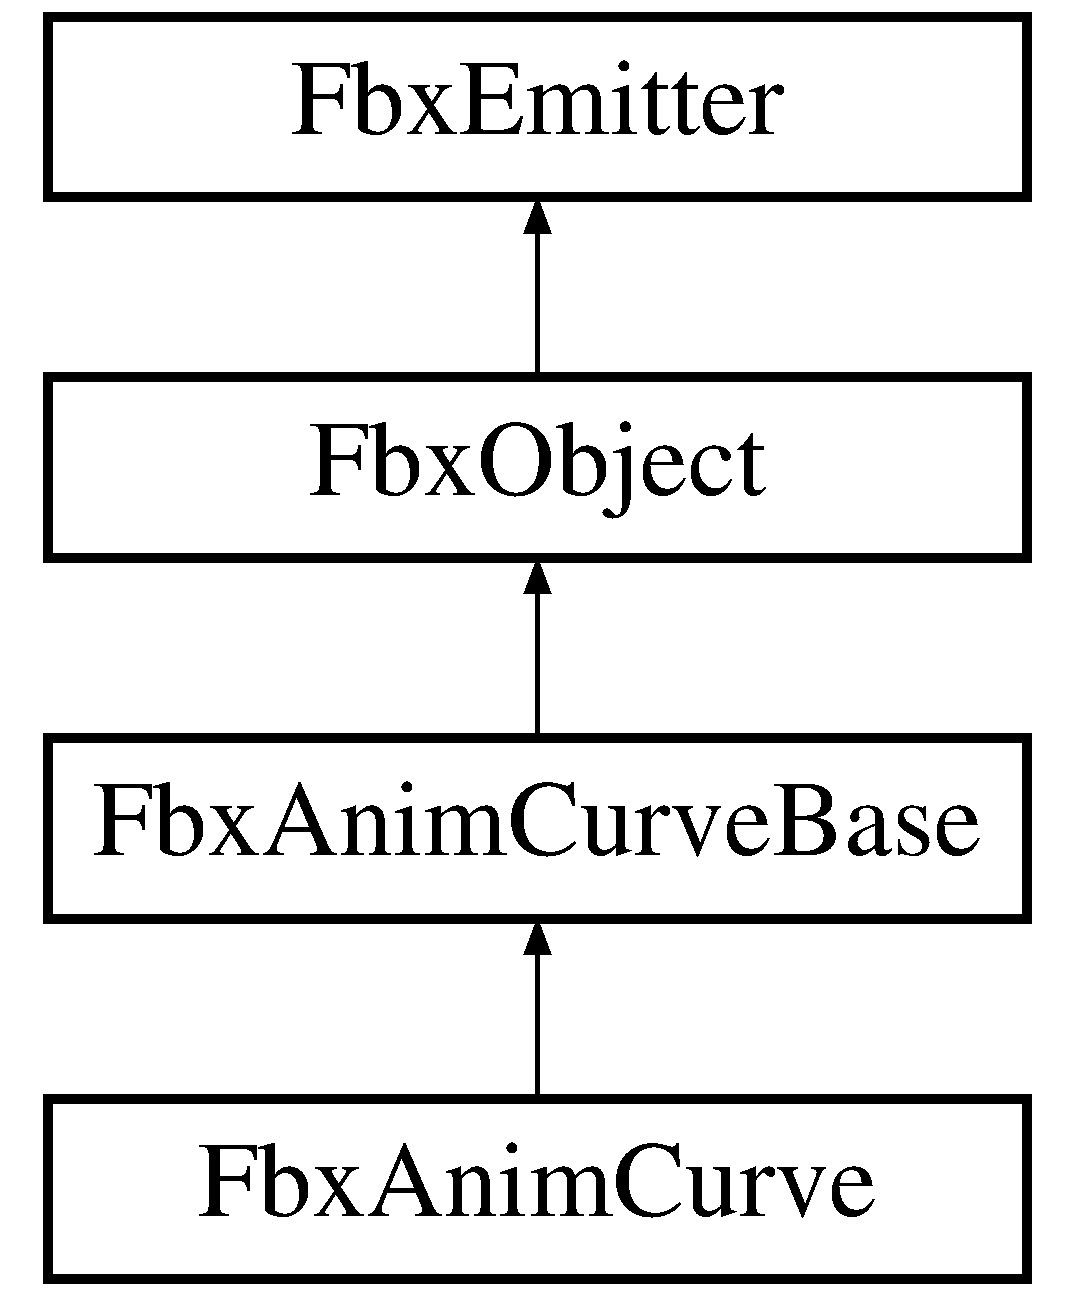
\includegraphics[height=4.000000cm]{class_fbx_anim_curve_base}
\end{center}
\end{figure}
\subsection*{公開メンバ関数}
\begin{DoxyCompactItemize}
\item 
virtual \hyperlink{class_fbx_object}{Fbx\+Object} \& \hyperlink{class_fbx_anim_curve_base_abdd0a239c39552fe978b1b571a4d5465}{Copy} (const \hyperlink{class_fbx_object}{Fbx\+Object} \&p\+Object)
\item 
virtual bool \hyperlink{class_fbx_anim_curve_base_a82eba55521f1c0e792b71cb432dac170}{Store} (\hyperlink{class_fbx_i_o}{Fbx\+IO} $\ast$p\+File\+Object, bool p\+Legacy\+Version=false)=0
\item 
virtual bool \hyperlink{class_fbx_anim_curve_base_a58ba1ce28a08145795d95bb27e2db02f}{Retrieve} (\hyperlink{class_fbx_i_o}{Fbx\+IO} $\ast$p\+File\+Object)=0
\item 
virtual void \hyperlink{class_fbx_anim_curve_base_aab573e42ece898c2c1e61a295adbb610}{Extrapolation\+Sync\+Callback} ()=0
\end{DoxyCompactItemize}
\subsection*{限定公開メンバ関数}
\begin{DoxyCompactItemize}
\item 
virtual void \hyperlink{class_fbx_anim_curve_base_af8e0d506c1a09c9fbd7432d4eb5caa02}{Construct} (const \hyperlink{class_fbx_object}{Fbx\+Object} $\ast$p\+From)
\end{DoxyCompactItemize}
\subsection*{Key management.}
\begin{DoxyCompactItemize}
\item 
virtual void \hyperlink{class_fbx_anim_curve_base_abe693d293087fad223770430ec79d65d}{Key\+Clear} ()=0
\begin{DoxyCompactList}\small\item\em Remove all the keys and free buffer memory. \end{DoxyCompactList}\item 
virtual int \hyperlink{class_fbx_anim_curve_base_a36fcc14d1c1944341da57085956a3f59}{Key\+Get\+Count} () const =0
\begin{DoxyCompactList}\small\item\em Get the number of keys. \end{DoxyCompactList}\item 
virtual int \hyperlink{class_fbx_anim_curve_base_a3e502968be213bd5cfde287f66f97cf5}{Key\+Add} (\hyperlink{class_fbx_time}{Fbx\+Time} p\+Time, \hyperlink{class_fbx_anim_curve_key_base}{Fbx\+Anim\+Curve\+Key\+Base} \&p\+Key, int $\ast$p\+Last=\hyperlink{fbxarch_8h_a070d2ce7b6bb7e5c05602aa8c308d0c4}{N\+U\+LL})=0
\item 
virtual bool \hyperlink{class_fbx_anim_curve_base_a1a66d683a6013b5eb41d128dcbbccd4a}{Key\+Set} (int p\+Index, \hyperlink{class_fbx_anim_curve_key_base}{Fbx\+Anim\+Curve\+Key\+Base} \&p\+Key)=0
\item 
virtual bool \hyperlink{class_fbx_anim_curve_base_a4d7d1bbd3d40020469aafd7c023f80d5}{Key\+Remove} (int p\+Index)=0
\item 
virtual bool \hyperlink{class_fbx_anim_curve_base_a2813321af80c66758eb9fbe025fd52ea}{Key\+Remove} (int p\+Start\+Index, int p\+End\+Index)=0
\end{DoxyCompactItemize}
\subsection*{Key Time Manipulation}
\begin{DoxyCompactItemize}
\item 
virtual \hyperlink{class_fbx_time}{Fbx\+Time} \hyperlink{class_fbx_anim_curve_base_a9db34dd56ce9822d0d6723ce7d50c4a3}{Key\+Get\+Time} (int) const
\item 
virtual void \hyperlink{class_fbx_anim_curve_base_afce0ede7336b9639c1e7ac08adf3e6df}{Key\+Set\+Time} (int p\+Key\+Index, \hyperlink{class_fbx_time}{Fbx\+Time} p\+Time)=0
\end{DoxyCompactItemize}
\subsection*{Extrapolation}
\label{_amgrp6ff40b647a49e8b8e9c36d595e9f288b}%
Extrapolation defines the function curve value before and after the keys. Pre-\/extrapolation defines the function curve value before first key. Post-\/extrapolation defines the function curve value after last key. 
\begin{DoxyItemize}
\item C\+O\+N\+S\+T\+A\+NT means a constant value matching the first/last key. 
\item R\+E\+P\+E\+T\+I\+T\+I\+ON means the entire function curve is looped. 
\item M\+I\+R\+R\+O\+R\+\_\+\+R\+E\+P\+E\+T\+I\+T\+I\+ON means the entire function curve is looped once backward, once forward and so on. 
\item K\+E\+E\+P\+\_\+\+S\+L\+O\+PE means a linear function with a slope matching the first/last key. 
\item R\+E\+L\+A\+T\+I\+V\+E\+\_\+\+R\+E\+P\+E\+T\+I\+T\+I\+ON means entire function curve is looped and one loop is relative to the last loop in value.
\end{DoxyItemize}\begin{DoxyCompactItemize}
\item 
enum \hyperlink{class_fbx_anim_curve_base_aa7214d43daa7b6b9b47a8118a858847f}{E\+Extrapolation\+Type} \{ \newline
\hyperlink{class_fbx_anim_curve_base_aa7214d43daa7b6b9b47a8118a858847fa12ad3ce67324b2ba1391b4c61e6ec8e0}{e\+Constant} = 1, 
\hyperlink{class_fbx_anim_curve_base_aa7214d43daa7b6b9b47a8118a858847fa61ea8cc971ecb3ed4705fa575b1aea8f}{e\+Repetition} = 2, 
\hyperlink{class_fbx_anim_curve_base_aa7214d43daa7b6b9b47a8118a858847fa4ad0cf4dc837a94ee221e76c9bee3edc}{e\+Mirror\+Repetition} = 3, 
\hyperlink{class_fbx_anim_curve_base_aa7214d43daa7b6b9b47a8118a858847fa8081da04891315734b94a6228265c892}{e\+Keep\+Slope} = 4, 
\newline
\hyperlink{class_fbx_anim_curve_base_aa7214d43daa7b6b9b47a8118a858847fa19bd2cf378ff0a41ac2467f186014ca3}{e\+Relative\+Repetition} = 5
 \}
\item 
void \hyperlink{class_fbx_anim_curve_base_abf3ba6c80fe9371be31602eb36789989}{Set\+Pre\+Extrapolation} (\hyperlink{class_fbx_anim_curve_base_aa7214d43daa7b6b9b47a8118a858847f}{E\+Extrapolation\+Type} p\+Extrapolation)
\item 
\hyperlink{class_fbx_anim_curve_base_aa7214d43daa7b6b9b47a8118a858847f}{E\+Extrapolation\+Type} \hyperlink{class_fbx_anim_curve_base_a3d4ba8f60385e14877c370518acea5d3}{Get\+Pre\+Extrapolation} () const
\item 
void \hyperlink{class_fbx_anim_curve_base_a9103e7ae34ef31d2952df0684cda6754}{Set\+Pre\+Extrapolation\+Count} (unsigned long p\+Count)
\item 
unsigned long \hyperlink{class_fbx_anim_curve_base_a2b8d645a376937f0aa645e25373976e0}{Get\+Pre\+Extrapolation\+Count} () const
\item 
void \hyperlink{class_fbx_anim_curve_base_a80e57bd8e710d36348eeb326fd83951b}{Set\+Post\+Extrapolation} (\hyperlink{class_fbx_anim_curve_base_aa7214d43daa7b6b9b47a8118a858847f}{E\+Extrapolation\+Type} p\+Extrapolation)
\item 
\hyperlink{class_fbx_anim_curve_base_aa7214d43daa7b6b9b47a8118a858847f}{E\+Extrapolation\+Type} \hyperlink{class_fbx_anim_curve_base_acabeaab2cff8753d0411eb0b4e268dc5}{Get\+Post\+Extrapolation} () const
\item 
void \hyperlink{class_fbx_anim_curve_base_a4201935f2bc54e924658cc0dd4e7bf74}{Set\+Post\+Extrapolation\+Count} (unsigned long p\+Count)
\item 
unsigned long \hyperlink{class_fbx_anim_curve_base_a2ccd05e435a7f010759c947815c55475}{Get\+Post\+Extrapolation\+Count} () const
\end{DoxyCompactItemize}
\subsection*{Evaluation and Analysis}
\begin{DoxyCompactItemize}
\item 
virtual float \hyperlink{class_fbx_anim_curve_base_a6d31c045a3733067fc7b4e6416d2fe06}{Evaluate} (\hyperlink{class_fbx_time}{Fbx\+Time} p\+Time, int $\ast$p\+Last=\hyperlink{fbxarch_8h_a070d2ce7b6bb7e5c05602aa8c308d0c4}{N\+U\+LL})=0
\item 
virtual float \hyperlink{class_fbx_anim_curve_base_aa54f5c0c77e553be03ba888448dc1818}{Evaluate\+Index} (double p\+Index)=0
\end{DoxyCompactItemize}
\subsection*{Utility functions.}
\begin{DoxyCompactItemize}
\item 
virtual bool \hyperlink{class_fbx_anim_curve_base_a4d259319e514c5371ff184b0cc7f7cd6}{Get\+Time\+Interval} (\hyperlink{class_fbx_time_span}{Fbx\+Time\+Span} \&p\+Time\+Interval)
\end{DoxyCompactItemize}
\subsection*{その他の継承メンバ}


\subsection{詳解}
This is the base class for implementing animation curves.

It is a pure virtual class that defines the general interface to animation key management and manipulation.

\begin{DoxySeeAlso}{参照}
\hyperlink{class_fbx_anim_curve}{Fbx\+Anim\+Curve} for fully implemented class. 
\end{DoxySeeAlso}


 fbxanimcurvebase.\+h の 70 行目に定義があります。



\subsection{列挙型メンバ詳解}
\mbox{\Hypertarget{class_fbx_anim_curve_base_aa7214d43daa7b6b9b47a8118a858847f}\label{class_fbx_anim_curve_base_aa7214d43daa7b6b9b47a8118a858847f}} 
\index{Fbx\+Anim\+Curve\+Base@{Fbx\+Anim\+Curve\+Base}!E\+Extrapolation\+Type@{E\+Extrapolation\+Type}}
\index{E\+Extrapolation\+Type@{E\+Extrapolation\+Type}!Fbx\+Anim\+Curve\+Base@{Fbx\+Anim\+Curve\+Base}}
\subsubsection{\texorpdfstring{E\+Extrapolation\+Type}{EExtrapolationType}}
{\footnotesize\ttfamily enum \hyperlink{class_fbx_anim_curve_base_aa7214d43daa7b6b9b47a8118a858847f}{Fbx\+Anim\+Curve\+Base\+::\+E\+Extrapolation\+Type}}

\begin{DoxyEnumFields}{列挙値}
\raisebox{\heightof{T}}[0pt][0pt]{\index{e\+Constant@{e\+Constant}!Fbx\+Anim\+Curve\+Base@{Fbx\+Anim\+Curve\+Base}}\index{Fbx\+Anim\+Curve\+Base@{Fbx\+Anim\+Curve\+Base}!e\+Constant@{e\+Constant}}}\mbox{\Hypertarget{class_fbx_anim_curve_base_aa7214d43daa7b6b9b47a8118a858847fa12ad3ce67324b2ba1391b4c61e6ec8e0}\label{class_fbx_anim_curve_base_aa7214d43daa7b6b9b47a8118a858847fa12ad3ce67324b2ba1391b4c61e6ec8e0}} 
e\+Constant&\\
\hline

\raisebox{\heightof{T}}[0pt][0pt]{\index{e\+Repetition@{e\+Repetition}!Fbx\+Anim\+Curve\+Base@{Fbx\+Anim\+Curve\+Base}}\index{Fbx\+Anim\+Curve\+Base@{Fbx\+Anim\+Curve\+Base}!e\+Repetition@{e\+Repetition}}}\mbox{\Hypertarget{class_fbx_anim_curve_base_aa7214d43daa7b6b9b47a8118a858847fa61ea8cc971ecb3ed4705fa575b1aea8f}\label{class_fbx_anim_curve_base_aa7214d43daa7b6b9b47a8118a858847fa61ea8cc971ecb3ed4705fa575b1aea8f}} 
e\+Repetition&\\
\hline

\raisebox{\heightof{T}}[0pt][0pt]{\index{e\+Mirror\+Repetition@{e\+Mirror\+Repetition}!Fbx\+Anim\+Curve\+Base@{Fbx\+Anim\+Curve\+Base}}\index{Fbx\+Anim\+Curve\+Base@{Fbx\+Anim\+Curve\+Base}!e\+Mirror\+Repetition@{e\+Mirror\+Repetition}}}\mbox{\Hypertarget{class_fbx_anim_curve_base_aa7214d43daa7b6b9b47a8118a858847fa4ad0cf4dc837a94ee221e76c9bee3edc}\label{class_fbx_anim_curve_base_aa7214d43daa7b6b9b47a8118a858847fa4ad0cf4dc837a94ee221e76c9bee3edc}} 
e\+Mirror\+Repetition&\\
\hline

\raisebox{\heightof{T}}[0pt][0pt]{\index{e\+Keep\+Slope@{e\+Keep\+Slope}!Fbx\+Anim\+Curve\+Base@{Fbx\+Anim\+Curve\+Base}}\index{Fbx\+Anim\+Curve\+Base@{Fbx\+Anim\+Curve\+Base}!e\+Keep\+Slope@{e\+Keep\+Slope}}}\mbox{\Hypertarget{class_fbx_anim_curve_base_aa7214d43daa7b6b9b47a8118a858847fa8081da04891315734b94a6228265c892}\label{class_fbx_anim_curve_base_aa7214d43daa7b6b9b47a8118a858847fa8081da04891315734b94a6228265c892}} 
e\+Keep\+Slope&\\
\hline

\raisebox{\heightof{T}}[0pt][0pt]{\index{e\+Relative\+Repetition@{e\+Relative\+Repetition}!Fbx\+Anim\+Curve\+Base@{Fbx\+Anim\+Curve\+Base}}\index{Fbx\+Anim\+Curve\+Base@{Fbx\+Anim\+Curve\+Base}!e\+Relative\+Repetition@{e\+Relative\+Repetition}}}\mbox{\Hypertarget{class_fbx_anim_curve_base_aa7214d43daa7b6b9b47a8118a858847fa19bd2cf378ff0a41ac2467f186014ca3}\label{class_fbx_anim_curve_base_aa7214d43daa7b6b9b47a8118a858847fa19bd2cf378ff0a41ac2467f186014ca3}} 
e\+Relative\+Repetition&\\
\hline

\end{DoxyEnumFields}


 fbxanimcurvebase.\+h の 152 行目に定義があります。



\subsection{関数詳解}
\mbox{\Hypertarget{class_fbx_anim_curve_base_af8e0d506c1a09c9fbd7432d4eb5caa02}\label{class_fbx_anim_curve_base_af8e0d506c1a09c9fbd7432d4eb5caa02}} 
\index{Fbx\+Anim\+Curve\+Base@{Fbx\+Anim\+Curve\+Base}!Construct@{Construct}}
\index{Construct@{Construct}!Fbx\+Anim\+Curve\+Base@{Fbx\+Anim\+Curve\+Base}}
\subsubsection{\texorpdfstring{Construct()}{Construct()}}
{\footnotesize\ttfamily virtual void Fbx\+Anim\+Curve\+Base\+::\+Construct (\begin{DoxyParamCaption}\item[{const \hyperlink{class_fbx_object}{Fbx\+Object} $\ast$}]{p\+From }\end{DoxyParamCaption})\hspace{0.3cm}{\ttfamily [protected]}, {\ttfamily [virtual]}}

Optional constructor override, automatically called by default constructor. 
\begin{DoxyParams}{引数}
{\em p\+From} & If not null, the function must take it into account like a copy constructor. \\
\hline
\end{DoxyParams}
\begin{DoxyRemark}{注釈}
In case it is decided to override this function, do not forget to call Parent\+Class\+::\+Construct(p\+From) at the beginning. 
\end{DoxyRemark}


\hyperlink{class_fbx_object_a313503bc645af3fdceb4a99ef5cea7eb}{Fbx\+Object}を再実装しています。

\mbox{\Hypertarget{class_fbx_anim_curve_base_abdd0a239c39552fe978b1b571a4d5465}\label{class_fbx_anim_curve_base_abdd0a239c39552fe978b1b571a4d5465}} 
\index{Fbx\+Anim\+Curve\+Base@{Fbx\+Anim\+Curve\+Base}!Copy@{Copy}}
\index{Copy@{Copy}!Fbx\+Anim\+Curve\+Base@{Fbx\+Anim\+Curve\+Base}}
\subsubsection{\texorpdfstring{Copy()}{Copy()}}
{\footnotesize\ttfamily virtual \hyperlink{class_fbx_object}{Fbx\+Object}\& Fbx\+Anim\+Curve\+Base\+::\+Copy (\begin{DoxyParamCaption}\item[{const \hyperlink{class_fbx_object}{Fbx\+Object} \&}]{p\+Object }\end{DoxyParamCaption})\hspace{0.3cm}{\ttfamily [virtual]}}

Copy an object content into this object. 
\begin{DoxyParams}{引数}
{\em p\+Object} & The source object to copy data from. \\
\hline
\end{DoxyParams}
\begin{DoxyReturn}{戻り値}
Returns the destination object being modified by the source. 
\end{DoxyReturn}
\begin{DoxyRemark}{注釈}
This function replace the assignment operator (operator=). It will copy all property values and the name. Connections are N\+OT copied. 
\end{DoxyRemark}


\hyperlink{class_fbx_object_a0c0c5adb38284d14bb82c04d54504a3e}{Fbx\+Object}を再実装しています。

\mbox{\Hypertarget{class_fbx_anim_curve_base_a6d31c045a3733067fc7b4e6416d2fe06}\label{class_fbx_anim_curve_base_a6d31c045a3733067fc7b4e6416d2fe06}} 
\index{Fbx\+Anim\+Curve\+Base@{Fbx\+Anim\+Curve\+Base}!Evaluate@{Evaluate}}
\index{Evaluate@{Evaluate}!Fbx\+Anim\+Curve\+Base@{Fbx\+Anim\+Curve\+Base}}
\subsubsection{\texorpdfstring{Evaluate()}{Evaluate()}}
{\footnotesize\ttfamily virtual float Fbx\+Anim\+Curve\+Base\+::\+Evaluate (\begin{DoxyParamCaption}\item[{\hyperlink{class_fbx_time}{Fbx\+Time}}]{p\+Time,  }\item[{int $\ast$}]{p\+Last = {\ttfamily \hyperlink{fbxarch_8h_a070d2ce7b6bb7e5c05602aa8c308d0c4}{N\+U\+LL}} }\end{DoxyParamCaption})\hspace{0.3cm}{\ttfamily [pure virtual]}}

Evaluate curve value at a given time. 
\begin{DoxyParams}{引数}
{\em p\+Time} & Time of evaluation. \\
\hline
{\em p\+Last} & Index of the last processed key to speed up search. If this function is called in a loop, initialize this value to 0 and let it be updated by each call. \\
\hline
\end{DoxyParams}
\begin{DoxyReturn}{戻り値}
Evaluated curve value. 
\end{DoxyReturn}
\begin{DoxyRemark}{注釈}
This function take extrapolation into account. 
\end{DoxyRemark}


\hyperlink{class_fbx_anim_curve_a74a3ea7a22a69fe69141722adff7f01b}{Fbx\+Anim\+Curve}で実装されています。

\mbox{\Hypertarget{class_fbx_anim_curve_base_aa54f5c0c77e553be03ba888448dc1818}\label{class_fbx_anim_curve_base_aa54f5c0c77e553be03ba888448dc1818}} 
\index{Fbx\+Anim\+Curve\+Base@{Fbx\+Anim\+Curve\+Base}!Evaluate\+Index@{Evaluate\+Index}}
\index{Evaluate\+Index@{Evaluate\+Index}!Fbx\+Anim\+Curve\+Base@{Fbx\+Anim\+Curve\+Base}}
\subsubsection{\texorpdfstring{Evaluate\+Index()}{EvaluateIndex()}}
{\footnotesize\ttfamily virtual float Fbx\+Anim\+Curve\+Base\+::\+Evaluate\+Index (\begin{DoxyParamCaption}\item[{double}]{p\+Index }\end{DoxyParamCaption})\hspace{0.3cm}{\ttfamily [pure virtual]}}

Evaluate curve value at the given key index. 
\begin{DoxyParams}{引数}
{\em p\+Index} & Any value from 0 to \hyperlink{class_fbx_anim_curve_base_a36fcc14d1c1944341da57085956a3f59}{Key\+Get\+Count()} -\/ 1. If this index falls between keys, the curve value will be interpolated based on the surrounding keys. \\
\hline
\end{DoxyParams}
\begin{DoxyReturn}{戻り値}
Evaluated curve value. 
\end{DoxyReturn}


\hyperlink{class_fbx_anim_curve_ad26cbb4cd0360aa8697a2601f8540a21}{Fbx\+Anim\+Curve}で実装されています。

\mbox{\Hypertarget{class_fbx_anim_curve_base_aab573e42ece898c2c1e61a295adbb610}\label{class_fbx_anim_curve_base_aab573e42ece898c2c1e61a295adbb610}} 
\index{Fbx\+Anim\+Curve\+Base@{Fbx\+Anim\+Curve\+Base}!Extrapolation\+Sync\+Callback@{Extrapolation\+Sync\+Callback}}
\index{Extrapolation\+Sync\+Callback@{Extrapolation\+Sync\+Callback}!Fbx\+Anim\+Curve\+Base@{Fbx\+Anim\+Curve\+Base}}
\subsubsection{\texorpdfstring{Extrapolation\+Sync\+Callback()}{ExtrapolationSyncCallback()}}
{\footnotesize\ttfamily virtual void Fbx\+Anim\+Curve\+Base\+::\+Extrapolation\+Sync\+Callback (\begin{DoxyParamCaption}{ }\end{DoxyParamCaption})\hspace{0.3cm}{\ttfamily [pure virtual]}}



\hyperlink{class_fbx_anim_curve_a8982eaf744608ac38457fd6f87990044}{Fbx\+Anim\+Curve}で実装されています。

\mbox{\Hypertarget{class_fbx_anim_curve_base_acabeaab2cff8753d0411eb0b4e268dc5}\label{class_fbx_anim_curve_base_acabeaab2cff8753d0411eb0b4e268dc5}} 
\index{Fbx\+Anim\+Curve\+Base@{Fbx\+Anim\+Curve\+Base}!Get\+Post\+Extrapolation@{Get\+Post\+Extrapolation}}
\index{Get\+Post\+Extrapolation@{Get\+Post\+Extrapolation}!Fbx\+Anim\+Curve\+Base@{Fbx\+Anim\+Curve\+Base}}
\subsubsection{\texorpdfstring{Get\+Post\+Extrapolation()}{GetPostExtrapolation()}}
{\footnotesize\ttfamily \hyperlink{class_fbx_anim_curve_base_aa7214d43daa7b6b9b47a8118a858847f}{E\+Extrapolation\+Type} Fbx\+Anim\+Curve\+Base\+::\+Get\+Post\+Extrapolation (\begin{DoxyParamCaption}{ }\end{DoxyParamCaption}) const\hspace{0.3cm}{\ttfamily [inline]}}

Get post-\/extrapolation mode. \begin{DoxyReturn}{戻り値}
The current post-\/extrapolation mode. 
\end{DoxyReturn}


 fbxanimcurvebase.\+h の 191 行目に定義があります。

\mbox{\Hypertarget{class_fbx_anim_curve_base_a2ccd05e435a7f010759c947815c55475}\label{class_fbx_anim_curve_base_a2ccd05e435a7f010759c947815c55475}} 
\index{Fbx\+Anim\+Curve\+Base@{Fbx\+Anim\+Curve\+Base}!Get\+Post\+Extrapolation\+Count@{Get\+Post\+Extrapolation\+Count}}
\index{Get\+Post\+Extrapolation\+Count@{Get\+Post\+Extrapolation\+Count}!Fbx\+Anim\+Curve\+Base@{Fbx\+Anim\+Curve\+Base}}
\subsubsection{\texorpdfstring{Get\+Post\+Extrapolation\+Count()}{GetPostExtrapolationCount()}}
{\footnotesize\ttfamily unsigned long Fbx\+Anim\+Curve\+Base\+::\+Get\+Post\+Extrapolation\+Count (\begin{DoxyParamCaption}{ }\end{DoxyParamCaption}) const\hspace{0.3cm}{\ttfamily [inline]}}

Get post-\/extrapolation count. \begin{DoxyReturn}{戻り値}
Number of repetitions if post-\/extrapolation mode is R\+E\+P\+E\+T\+I\+T\+I\+ON or M\+I\+R\+R\+O\+R\+\_\+\+R\+E\+P\+E\+T\+I\+T\+I\+ON. 
\end{DoxyReturn}


 fbxanimcurvebase.\+h の 203 行目に定義があります。

\mbox{\Hypertarget{class_fbx_anim_curve_base_a3d4ba8f60385e14877c370518acea5d3}\label{class_fbx_anim_curve_base_a3d4ba8f60385e14877c370518acea5d3}} 
\index{Fbx\+Anim\+Curve\+Base@{Fbx\+Anim\+Curve\+Base}!Get\+Pre\+Extrapolation@{Get\+Pre\+Extrapolation}}
\index{Get\+Pre\+Extrapolation@{Get\+Pre\+Extrapolation}!Fbx\+Anim\+Curve\+Base@{Fbx\+Anim\+Curve\+Base}}
\subsubsection{\texorpdfstring{Get\+Pre\+Extrapolation()}{GetPreExtrapolation()}}
{\footnotesize\ttfamily \hyperlink{class_fbx_anim_curve_base_aa7214d43daa7b6b9b47a8118a858847f}{E\+Extrapolation\+Type} Fbx\+Anim\+Curve\+Base\+::\+Get\+Pre\+Extrapolation (\begin{DoxyParamCaption}{ }\end{DoxyParamCaption}) const\hspace{0.3cm}{\ttfamily [inline]}}

Get pre-\/extrapolation mode. \begin{DoxyReturn}{戻り値}
The current pre-\/extrapolation mode. 
\end{DoxyReturn}


 fbxanimcurvebase.\+h の 169 行目に定義があります。

\mbox{\Hypertarget{class_fbx_anim_curve_base_a2b8d645a376937f0aa645e25373976e0}\label{class_fbx_anim_curve_base_a2b8d645a376937f0aa645e25373976e0}} 
\index{Fbx\+Anim\+Curve\+Base@{Fbx\+Anim\+Curve\+Base}!Get\+Pre\+Extrapolation\+Count@{Get\+Pre\+Extrapolation\+Count}}
\index{Get\+Pre\+Extrapolation\+Count@{Get\+Pre\+Extrapolation\+Count}!Fbx\+Anim\+Curve\+Base@{Fbx\+Anim\+Curve\+Base}}
\subsubsection{\texorpdfstring{Get\+Pre\+Extrapolation\+Count()}{GetPreExtrapolationCount()}}
{\footnotesize\ttfamily unsigned long Fbx\+Anim\+Curve\+Base\+::\+Get\+Pre\+Extrapolation\+Count (\begin{DoxyParamCaption}{ }\end{DoxyParamCaption}) const\hspace{0.3cm}{\ttfamily [inline]}}

Get pre-\/extrapolation count. \begin{DoxyReturn}{戻り値}
Number of repetitions if pre-\/extrapolation mode is R\+E\+P\+E\+T\+I\+T\+I\+ON or M\+I\+R\+R\+O\+R\+\_\+\+R\+E\+P\+E\+T\+I\+T\+I\+ON. 
\end{DoxyReturn}


 fbxanimcurvebase.\+h の 181 行目に定義があります。

\mbox{\Hypertarget{class_fbx_anim_curve_base_a4d259319e514c5371ff184b0cc7f7cd6}\label{class_fbx_anim_curve_base_a4d259319e514c5371ff184b0cc7f7cd6}} 
\index{Fbx\+Anim\+Curve\+Base@{Fbx\+Anim\+Curve\+Base}!Get\+Time\+Interval@{Get\+Time\+Interval}}
\index{Get\+Time\+Interval@{Get\+Time\+Interval}!Fbx\+Anim\+Curve\+Base@{Fbx\+Anim\+Curve\+Base}}
\subsubsection{\texorpdfstring{Get\+Time\+Interval()}{GetTimeInterval()}}
{\footnotesize\ttfamily virtual bool Fbx\+Anim\+Curve\+Base\+::\+Get\+Time\+Interval (\begin{DoxyParamCaption}\item[{\hyperlink{class_fbx_time_span}{Fbx\+Time\+Span} \&}]{p\+Time\+Interval }\end{DoxyParamCaption})\hspace{0.3cm}{\ttfamily [virtual]}}

Find out start and end time of the animation curve. This function retrieves the Curve\textquotesingle{}s time span. 
\begin{DoxyParams}{引数}
{\em p\+Time\+Interval} & Reference to receive start time and end time. \\
\hline
\end{DoxyParams}
\begin{DoxyReturn}{戻り値}
{\ttfamily true} on success, {\ttfamily false} otherwise. 
\end{DoxyReturn}


\hyperlink{class_fbx_anim_curve_aa547431c44acd9eb28aebdec1a142501}{Fbx\+Anim\+Curve}で再実装されています。

\mbox{\Hypertarget{class_fbx_anim_curve_base_a3e502968be213bd5cfde287f66f97cf5}\label{class_fbx_anim_curve_base_a3e502968be213bd5cfde287f66f97cf5}} 
\index{Fbx\+Anim\+Curve\+Base@{Fbx\+Anim\+Curve\+Base}!Key\+Add@{Key\+Add}}
\index{Key\+Add@{Key\+Add}!Fbx\+Anim\+Curve\+Base@{Fbx\+Anim\+Curve\+Base}}
\subsubsection{\texorpdfstring{Key\+Add()}{KeyAdd()}}
{\footnotesize\ttfamily virtual int Fbx\+Anim\+Curve\+Base\+::\+Key\+Add (\begin{DoxyParamCaption}\item[{\hyperlink{class_fbx_time}{Fbx\+Time}}]{p\+Time,  }\item[{\hyperlink{class_fbx_anim_curve_key_base}{Fbx\+Anim\+Curve\+Key\+Base} \&}]{p\+Key,  }\item[{int $\ast$}]{p\+Last = {\ttfamily \hyperlink{fbxarch_8h_a070d2ce7b6bb7e5c05602aa8c308d0c4}{N\+U\+LL}} }\end{DoxyParamCaption})\hspace{0.3cm}{\ttfamily [pure virtual]}}

Add a key at given time. 
\begin{DoxyParams}{引数}
{\em p\+Time} & Time to add the key. \\
\hline
{\em p\+Key} & Key to add. \\
\hline
{\em p\+Last} & Index of the last processed key to speed up search. If this function is called in a loop, initialize this value to 0 and let it be updated by each call. \\
\hline
\end{DoxyParams}
\begin{DoxyReturn}{戻り値}
Index of the key at given time, no matter if it was added or already present. 
\end{DoxyReturn}


\hyperlink{class_fbx_anim_curve_aefac9bf8a5d7bf1fe147e192ba503737}{Fbx\+Anim\+Curve}で実装されています。

\mbox{\Hypertarget{class_fbx_anim_curve_base_abe693d293087fad223770430ec79d65d}\label{class_fbx_anim_curve_base_abe693d293087fad223770430ec79d65d}} 
\index{Fbx\+Anim\+Curve\+Base@{Fbx\+Anim\+Curve\+Base}!Key\+Clear@{Key\+Clear}}
\index{Key\+Clear@{Key\+Clear}!Fbx\+Anim\+Curve\+Base@{Fbx\+Anim\+Curve\+Base}}
\subsubsection{\texorpdfstring{Key\+Clear()}{KeyClear()}}
{\footnotesize\ttfamily virtual void Fbx\+Anim\+Curve\+Base\+::\+Key\+Clear (\begin{DoxyParamCaption}{ }\end{DoxyParamCaption})\hspace{0.3cm}{\ttfamily [pure virtual]}}



Remove all the keys and free buffer memory. 



\hyperlink{class_fbx_anim_curve_a202883ab5e1844beb60d40137464afd8}{Fbx\+Anim\+Curve}で実装されています。

\mbox{\Hypertarget{class_fbx_anim_curve_base_a36fcc14d1c1944341da57085956a3f59}\label{class_fbx_anim_curve_base_a36fcc14d1c1944341da57085956a3f59}} 
\index{Fbx\+Anim\+Curve\+Base@{Fbx\+Anim\+Curve\+Base}!Key\+Get\+Count@{Key\+Get\+Count}}
\index{Key\+Get\+Count@{Key\+Get\+Count}!Fbx\+Anim\+Curve\+Base@{Fbx\+Anim\+Curve\+Base}}
\subsubsection{\texorpdfstring{Key\+Get\+Count()}{KeyGetCount()}}
{\footnotesize\ttfamily virtual int Fbx\+Anim\+Curve\+Base\+::\+Key\+Get\+Count (\begin{DoxyParamCaption}{ }\end{DoxyParamCaption}) const\hspace{0.3cm}{\ttfamily [pure virtual]}}



Get the number of keys. 



\hyperlink{class_fbx_anim_curve_a08de74d6ef6469be37abd1df0836eac9}{Fbx\+Anim\+Curve}で実装されています。

\mbox{\Hypertarget{class_fbx_anim_curve_base_a9db34dd56ce9822d0d6723ce7d50c4a3}\label{class_fbx_anim_curve_base_a9db34dd56ce9822d0d6723ce7d50c4a3}} 
\index{Fbx\+Anim\+Curve\+Base@{Fbx\+Anim\+Curve\+Base}!Key\+Get\+Time@{Key\+Get\+Time}}
\index{Key\+Get\+Time@{Key\+Get\+Time}!Fbx\+Anim\+Curve\+Base@{Fbx\+Anim\+Curve\+Base}}
\subsubsection{\texorpdfstring{Key\+Get\+Time()}{KeyGetTime()}}
{\footnotesize\ttfamily virtual \hyperlink{class_fbx_time}{Fbx\+Time} Fbx\+Anim\+Curve\+Base\+::\+Key\+Get\+Time (\begin{DoxyParamCaption}\item[{int}]{ }\end{DoxyParamCaption}) const\hspace{0.3cm}{\ttfamily [inline]}, {\ttfamily [virtual]}}

Get key time. 
\begin{DoxyParams}{引数}
{\em p\+Key\+Index} & Key index. \\
\hline
\end{DoxyParams}
\begin{DoxyReturn}{戻り値}
Key time (time at which this key is occurring). 
\end{DoxyReturn}


\hyperlink{class_fbx_anim_curve_a547f7842ea7bae5b5ed048d15b8b0d07}{Fbx\+Anim\+Curve}で再実装されています。



 fbxanimcurvebase.\+h の 130 行目に定義があります。

\mbox{\Hypertarget{class_fbx_anim_curve_base_a4d7d1bbd3d40020469aafd7c023f80d5}\label{class_fbx_anim_curve_base_a4d7d1bbd3d40020469aafd7c023f80d5}} 
\index{Fbx\+Anim\+Curve\+Base@{Fbx\+Anim\+Curve\+Base}!Key\+Remove@{Key\+Remove}}
\index{Key\+Remove@{Key\+Remove}!Fbx\+Anim\+Curve\+Base@{Fbx\+Anim\+Curve\+Base}}
\subsubsection{\texorpdfstring{Key\+Remove()}{KeyRemove()}\hspace{0.1cm}{\footnotesize\ttfamily [1/2]}}
{\footnotesize\ttfamily virtual bool Fbx\+Anim\+Curve\+Base\+::\+Key\+Remove (\begin{DoxyParamCaption}\item[{int}]{p\+Index }\end{DoxyParamCaption})\hspace{0.3cm}{\ttfamily [pure virtual]}}

Remove key at given index. 
\begin{DoxyParams}{引数}
{\em p\+Index} & Index of key to remove. \\
\hline
\end{DoxyParams}
\begin{DoxyReturn}{戻り値}
{\ttfamily true} on success, {\ttfamily false} otherwise. 
\end{DoxyReturn}


\hyperlink{class_fbx_anim_curve_a083206eda111aa4c6803410427a4645c}{Fbx\+Anim\+Curve}で実装されています。

\mbox{\Hypertarget{class_fbx_anim_curve_base_a2813321af80c66758eb9fbe025fd52ea}\label{class_fbx_anim_curve_base_a2813321af80c66758eb9fbe025fd52ea}} 
\index{Fbx\+Anim\+Curve\+Base@{Fbx\+Anim\+Curve\+Base}!Key\+Remove@{Key\+Remove}}
\index{Key\+Remove@{Key\+Remove}!Fbx\+Anim\+Curve\+Base@{Fbx\+Anim\+Curve\+Base}}
\subsubsection{\texorpdfstring{Key\+Remove()}{KeyRemove()}\hspace{0.1cm}{\footnotesize\ttfamily [2/2]}}
{\footnotesize\ttfamily virtual bool Fbx\+Anim\+Curve\+Base\+::\+Key\+Remove (\begin{DoxyParamCaption}\item[{int}]{p\+Start\+Index,  }\item[{int}]{p\+End\+Index }\end{DoxyParamCaption})\hspace{0.3cm}{\ttfamily [pure virtual]}}

Remove all the keys in the given range. 
\begin{DoxyParams}{引数}
{\em p\+Start\+Index} & Index of the first key to remove (inclusive). \\
\hline
{\em p\+End\+Index} & Index of the last key to remove (inclusive). \\
\hline
\end{DoxyParams}
\begin{DoxyReturn}{戻り値}
{\ttfamily true} on success, {\ttfamily false} otherwise. 
\end{DoxyReturn}


\hyperlink{class_fbx_anim_curve_a7b4fe494d1ca4575bb253ec89f867df1}{Fbx\+Anim\+Curve}で実装されています。

\mbox{\Hypertarget{class_fbx_anim_curve_base_a1a66d683a6013b5eb41d128dcbbccd4a}\label{class_fbx_anim_curve_base_a1a66d683a6013b5eb41d128dcbbccd4a}} 
\index{Fbx\+Anim\+Curve\+Base@{Fbx\+Anim\+Curve\+Base}!Key\+Set@{Key\+Set}}
\index{Key\+Set@{Key\+Set}!Fbx\+Anim\+Curve\+Base@{Fbx\+Anim\+Curve\+Base}}
\subsubsection{\texorpdfstring{Key\+Set()}{KeySet()}}
{\footnotesize\ttfamily virtual bool Fbx\+Anim\+Curve\+Base\+::\+Key\+Set (\begin{DoxyParamCaption}\item[{int}]{p\+Index,  }\item[{\hyperlink{class_fbx_anim_curve_key_base}{Fbx\+Anim\+Curve\+Key\+Base} \&}]{p\+Key }\end{DoxyParamCaption})\hspace{0.3cm}{\ttfamily [pure virtual]}}

Set key at given index. 
\begin{DoxyParams}{引数}
{\em p\+Index} & Index of where the key should be set. \\
\hline
{\em p\+Key} & The key to set. \\
\hline
\end{DoxyParams}
\begin{DoxyReturn}{戻り値}
{\ttfamily true} if key time is superior to previous key and inferior to next key, {\ttfamily false} otherwise. 
\end{DoxyReturn}
\begin{DoxyRemark}{注釈}
Result is undetermined if function curve has no key or index is out of bounds. 
\end{DoxyRemark}


\hyperlink{class_fbx_anim_curve_a8f36f89bd5fbaa4f180789f4d9faf84f}{Fbx\+Anim\+Curve}で実装されています。

\mbox{\Hypertarget{class_fbx_anim_curve_base_afce0ede7336b9639c1e7ac08adf3e6df}\label{class_fbx_anim_curve_base_afce0ede7336b9639c1e7ac08adf3e6df}} 
\index{Fbx\+Anim\+Curve\+Base@{Fbx\+Anim\+Curve\+Base}!Key\+Set\+Time@{Key\+Set\+Time}}
\index{Key\+Set\+Time@{Key\+Set\+Time}!Fbx\+Anim\+Curve\+Base@{Fbx\+Anim\+Curve\+Base}}
\subsubsection{\texorpdfstring{Key\+Set\+Time()}{KeySetTime()}}
{\footnotesize\ttfamily virtual void Fbx\+Anim\+Curve\+Base\+::\+Key\+Set\+Time (\begin{DoxyParamCaption}\item[{int}]{p\+Key\+Index,  }\item[{\hyperlink{class_fbx_time}{Fbx\+Time}}]{p\+Time }\end{DoxyParamCaption})\hspace{0.3cm}{\ttfamily [pure virtual]}}

Set key time. 
\begin{DoxyParams}{引数}
{\em p\+Key\+Index} & Key index. \\
\hline
{\em p\+Time} & Key time (time at which this key is occurring). \\
\hline
\end{DoxyParams}


\hyperlink{class_fbx_anim_curve_a5ce2130d0cea4de2fc42fa3683f01162}{Fbx\+Anim\+Curve}で実装されています。

\mbox{\Hypertarget{class_fbx_anim_curve_base_a58ba1ce28a08145795d95bb27e2db02f}\label{class_fbx_anim_curve_base_a58ba1ce28a08145795d95bb27e2db02f}} 
\index{Fbx\+Anim\+Curve\+Base@{Fbx\+Anim\+Curve\+Base}!Retrieve@{Retrieve}}
\index{Retrieve@{Retrieve}!Fbx\+Anim\+Curve\+Base@{Fbx\+Anim\+Curve\+Base}}
\subsubsection{\texorpdfstring{Retrieve()}{Retrieve()}}
{\footnotesize\ttfamily virtual bool Fbx\+Anim\+Curve\+Base\+::\+Retrieve (\begin{DoxyParamCaption}\item[{\hyperlink{class_fbx_i_o}{Fbx\+IO} $\ast$}]{p\+File\+Object }\end{DoxyParamCaption})\hspace{0.3cm}{\ttfamily [pure virtual]}}



\hyperlink{class_fbx_anim_curve_a17087752d3a28d373b2aaa66d1755f62}{Fbx\+Anim\+Curve}で実装されています。

\mbox{\Hypertarget{class_fbx_anim_curve_base_a80e57bd8e710d36348eeb326fd83951b}\label{class_fbx_anim_curve_base_a80e57bd8e710d36348eeb326fd83951b}} 
\index{Fbx\+Anim\+Curve\+Base@{Fbx\+Anim\+Curve\+Base}!Set\+Post\+Extrapolation@{Set\+Post\+Extrapolation}}
\index{Set\+Post\+Extrapolation@{Set\+Post\+Extrapolation}!Fbx\+Anim\+Curve\+Base@{Fbx\+Anim\+Curve\+Base}}
\subsubsection{\texorpdfstring{Set\+Post\+Extrapolation()}{SetPostExtrapolation()}}
{\footnotesize\ttfamily void Fbx\+Anim\+Curve\+Base\+::\+Set\+Post\+Extrapolation (\begin{DoxyParamCaption}\item[{\hyperlink{class_fbx_anim_curve_base_aa7214d43daa7b6b9b47a8118a858847f}{E\+Extrapolation\+Type}}]{p\+Extrapolation }\end{DoxyParamCaption})}

Set post-\/extrapolation mode. 
\begin{DoxyParams}{引数}
{\em p\+Extrapolation} & The post-\/extrapolation mode to set. \\
\hline
\end{DoxyParams}
\mbox{\Hypertarget{class_fbx_anim_curve_base_a4201935f2bc54e924658cc0dd4e7bf74}\label{class_fbx_anim_curve_base_a4201935f2bc54e924658cc0dd4e7bf74}} 
\index{Fbx\+Anim\+Curve\+Base@{Fbx\+Anim\+Curve\+Base}!Set\+Post\+Extrapolation\+Count@{Set\+Post\+Extrapolation\+Count}}
\index{Set\+Post\+Extrapolation\+Count@{Set\+Post\+Extrapolation\+Count}!Fbx\+Anim\+Curve\+Base@{Fbx\+Anim\+Curve\+Base}}
\subsubsection{\texorpdfstring{Set\+Post\+Extrapolation\+Count()}{SetPostExtrapolationCount()}}
{\footnotesize\ttfamily void Fbx\+Anim\+Curve\+Base\+::\+Set\+Post\+Extrapolation\+Count (\begin{DoxyParamCaption}\item[{unsigned long}]{p\+Count }\end{DoxyParamCaption})}

Set post-\/extrapolation count. 
\begin{DoxyParams}{引数}
{\em p\+Count} & Number of repetitions if post-\/extrapolation mode is R\+E\+P\+E\+T\+I\+T\+I\+ON or M\+I\+R\+R\+O\+R\+\_\+\+R\+E\+P\+E\+T\+I\+T\+I\+ON. \\
\hline
\end{DoxyParams}
\mbox{\Hypertarget{class_fbx_anim_curve_base_abf3ba6c80fe9371be31602eb36789989}\label{class_fbx_anim_curve_base_abf3ba6c80fe9371be31602eb36789989}} 
\index{Fbx\+Anim\+Curve\+Base@{Fbx\+Anim\+Curve\+Base}!Set\+Pre\+Extrapolation@{Set\+Pre\+Extrapolation}}
\index{Set\+Pre\+Extrapolation@{Set\+Pre\+Extrapolation}!Fbx\+Anim\+Curve\+Base@{Fbx\+Anim\+Curve\+Base}}
\subsubsection{\texorpdfstring{Set\+Pre\+Extrapolation()}{SetPreExtrapolation()}}
{\footnotesize\ttfamily void Fbx\+Anim\+Curve\+Base\+::\+Set\+Pre\+Extrapolation (\begin{DoxyParamCaption}\item[{\hyperlink{class_fbx_anim_curve_base_aa7214d43daa7b6b9b47a8118a858847f}{E\+Extrapolation\+Type}}]{p\+Extrapolation }\end{DoxyParamCaption})}

Set pre-\/extrapolation mode. 
\begin{DoxyParams}{引数}
{\em p\+Extrapolation} & The pre-\/extrapolation mode to set. \\
\hline
\end{DoxyParams}
\mbox{\Hypertarget{class_fbx_anim_curve_base_a9103e7ae34ef31d2952df0684cda6754}\label{class_fbx_anim_curve_base_a9103e7ae34ef31d2952df0684cda6754}} 
\index{Fbx\+Anim\+Curve\+Base@{Fbx\+Anim\+Curve\+Base}!Set\+Pre\+Extrapolation\+Count@{Set\+Pre\+Extrapolation\+Count}}
\index{Set\+Pre\+Extrapolation\+Count@{Set\+Pre\+Extrapolation\+Count}!Fbx\+Anim\+Curve\+Base@{Fbx\+Anim\+Curve\+Base}}
\subsubsection{\texorpdfstring{Set\+Pre\+Extrapolation\+Count()}{SetPreExtrapolationCount()}}
{\footnotesize\ttfamily void Fbx\+Anim\+Curve\+Base\+::\+Set\+Pre\+Extrapolation\+Count (\begin{DoxyParamCaption}\item[{unsigned long}]{p\+Count }\end{DoxyParamCaption})}

Set pre-\/extrapolation count. 
\begin{DoxyParams}{引数}
{\em p\+Count} & Number of repetitions if pre-\/extrapolation mode is R\+E\+P\+E\+T\+I\+T\+I\+ON or M\+I\+R\+R\+O\+R\+\_\+\+R\+E\+P\+E\+T\+I\+T\+I\+ON. \\
\hline
\end{DoxyParams}
\mbox{\Hypertarget{class_fbx_anim_curve_base_a82eba55521f1c0e792b71cb432dac170}\label{class_fbx_anim_curve_base_a82eba55521f1c0e792b71cb432dac170}} 
\index{Fbx\+Anim\+Curve\+Base@{Fbx\+Anim\+Curve\+Base}!Store@{Store}}
\index{Store@{Store}!Fbx\+Anim\+Curve\+Base@{Fbx\+Anim\+Curve\+Base}}
\subsubsection{\texorpdfstring{Store()}{Store()}}
{\footnotesize\ttfamily virtual bool Fbx\+Anim\+Curve\+Base\+::\+Store (\begin{DoxyParamCaption}\item[{\hyperlink{class_fbx_i_o}{Fbx\+IO} $\ast$}]{p\+File\+Object,  }\item[{bool}]{p\+Legacy\+Version = {\ttfamily false} }\end{DoxyParamCaption})\hspace{0.3cm}{\ttfamily [pure virtual]}}



\hyperlink{class_fbx_anim_curve_a0ef3229e43aaca33ab50161235541060}{Fbx\+Anim\+Curve}で実装されています。



このクラス詳解は次のファイルから抽出されました\+:\begin{DoxyCompactItemize}
\item 
C\+:/\+Maya/scripts/\+F\+B\+X\+\_\+\+S\+D\+K/2017.\+1/include/fbxsdk/scene/animation/\hyperlink{fbxanimcurvebase_8h}{fbxanimcurvebase.\+h}\end{DoxyCompactItemize}

\hypertarget{class_fbx_anim_curve_def}{}\section{Fbx\+Anim\+Curve\+Def クラス}
\label{class_fbx_anim_curve_def}\index{Fbx\+Anim\+Curve\+Def@{Fbx\+Anim\+Curve\+Def}}


{\ttfamily \#include $<$fbxanimcurve.\+h$>$}

\subsection*{公開型}
\begin{DoxyCompactItemize}
\item 
enum \hyperlink{class_fbx_anim_curve_def_ac810ccc5ca0527704ab5175479964b87}{E\+Tangent\+Mode} \{ \newline
\hyperlink{class_fbx_anim_curve_def_ac810ccc5ca0527704ab5175479964b87a56e3bad364851277281e94e81327dd25}{e\+Tangent\+Auto} = 0x00000100, 
\hyperlink{class_fbx_anim_curve_def_ac810ccc5ca0527704ab5175479964b87ae9d885e8a384fd9165123ac47a661dd8}{e\+Tangent\+T\+CB} = 0x00000200, 
\hyperlink{class_fbx_anim_curve_def_ac810ccc5ca0527704ab5175479964b87a199cb16b2c861b12c334093ce796cb86}{e\+Tangent\+User} = 0x00000400, 
\hyperlink{class_fbx_anim_curve_def_ac810ccc5ca0527704ab5175479964b87a423a9e02047b705ec23561f87d8ff15b}{e\+Tangent\+Generic\+Break} = 0x00000800, 
\newline
\hyperlink{class_fbx_anim_curve_def_ac810ccc5ca0527704ab5175479964b87ab4d85a1a0474226be85b885518f6c847}{e\+Tangent\+Break} = e\+Tangent\+Generic\+Break$\vert$e\+Tangent\+User, 
\hyperlink{class_fbx_anim_curve_def_ac810ccc5ca0527704ab5175479964b87afce344e3f0ada1ec522ef67f0a0e92cb}{e\+Tangent\+Auto\+Break} = e\+Tangent\+Generic\+Break$\vert$e\+Tangent\+Auto, 
\hyperlink{class_fbx_anim_curve_def_ac810ccc5ca0527704ab5175479964b87a53bad41061d60bae2373a88e13eeac50}{e\+Tangent\+Generic\+Clamp} = 0x00001000, 
\hyperlink{class_fbx_anim_curve_def_ac810ccc5ca0527704ab5175479964b87abaaae6df50c5a1a651d0e5678c4a90cd}{e\+Tangent\+Generic\+Time\+Independent} = 0x00002000, 
\newline
\hyperlink{class_fbx_anim_curve_def_ac810ccc5ca0527704ab5175479964b87a87eba898c30497b7e94da22822500757}{e\+Tangent\+Generic\+Clamp\+Progressive} = 0x00004000$\vert$e\+Tangent\+Generic\+Time\+Independent
 \}\begin{DoxyCompactList}\small\item\em Key tangent mode for cubic interpolation. \end{DoxyCompactList}
\item 
enum \hyperlink{class_fbx_anim_curve_def_add2ab7d10d856ab0868cc9b143d59ea5}{E\+Interpolation\+Type} \{ \hyperlink{class_fbx_anim_curve_def_add2ab7d10d856ab0868cc9b143d59ea5acb7611d721a1ae1e6df7a2f072dc7c9f}{e\+Interpolation\+Constant} = 0x00000002, 
\hyperlink{class_fbx_anim_curve_def_add2ab7d10d856ab0868cc9b143d59ea5ab60e201b78e2105be1134c3c15519d20}{e\+Interpolation\+Linear} = 0x00000004, 
\hyperlink{class_fbx_anim_curve_def_add2ab7d10d856ab0868cc9b143d59ea5a16ef50fcdbb8ae99246f06e12f9d3dae}{e\+Interpolation\+Cubic} = 0x00000008
 \}\begin{DoxyCompactList}\small\item\em Key interpolation type. \end{DoxyCompactList}
\item 
enum \hyperlink{class_fbx_anim_curve_def_aeee6e9cc12501e10dbd3e5caaf66990e}{E\+Weighted\+Mode} \{ \hyperlink{class_fbx_anim_curve_def_aeee6e9cc12501e10dbd3e5caaf66990ea2ae55a3ceae7773d899ebfae26dcbef3}{e\+Weighted\+None} = 0x00000000, 
\hyperlink{class_fbx_anim_curve_def_aeee6e9cc12501e10dbd3e5caaf66990ea869960737022db21fc64480daa22725a}{e\+Weighted\+Right} = 0x01000000, 
\hyperlink{class_fbx_anim_curve_def_aeee6e9cc12501e10dbd3e5caaf66990eae28d75f955feebe5756d77ad0765d000}{e\+Weighted\+Next\+Left} = 0x02000000, 
\hyperlink{class_fbx_anim_curve_def_aeee6e9cc12501e10dbd3e5caaf66990ea4337e6853fab642c2a432ab1bb303922}{e\+Weighted\+All} = e\+Weighted\+Right$\vert$e\+Weighted\+Next\+Left
 \}\begin{DoxyCompactList}\small\item\em Weighted mode. \end{DoxyCompactList}
\item 
enum \hyperlink{class_fbx_anim_curve_def_a52885abd392ac8ac3da94bafc5fddd64}{E\+Constant\+Mode} \{ \hyperlink{class_fbx_anim_curve_def_a52885abd392ac8ac3da94bafc5fddd64afa9ab4c869fe6eb4589e1298375ac66f}{e\+Constant\+Standard} = 0x00000000, 
\hyperlink{class_fbx_anim_curve_def_a52885abd392ac8ac3da94bafc5fddd64acd33e33b487685436e39688ca986f2d6}{e\+Constant\+Next} = 0x00000100
 \}\begin{DoxyCompactList}\small\item\em Key constant mode. \end{DoxyCompactList}
\item 
enum \hyperlink{class_fbx_anim_curve_def_a747576beffa78ab236d2e140da395fff}{E\+Velocity\+Mode} \{ \hyperlink{class_fbx_anim_curve_def_a747576beffa78ab236d2e140da395fffa7919a5bf6ff7855e3b60673ade08afbc}{e\+Velocity\+None} = 0x00000000, 
\hyperlink{class_fbx_anim_curve_def_a747576beffa78ab236d2e140da395fffa1265ff9732df8deb70ee9822af11b995}{e\+Velocity\+Right} = 0x10000000, 
\hyperlink{class_fbx_anim_curve_def_a747576beffa78ab236d2e140da395fffac10e4a2ea06592874b83d4389dcaf560}{e\+Velocity\+Next\+Left} = 0x20000000, 
\hyperlink{class_fbx_anim_curve_def_a747576beffa78ab236d2e140da395fffab8603ba4ecc238f5dee7489b6a0123ee}{e\+Velocity\+All} = e\+Velocity\+Right$\vert$e\+Velocity\+Next\+Left
 \}\begin{DoxyCompactList}\small\item\em Velocity mode. Velocity settings speed up or slow down animation on either side of a key without changing the trajectory of the animation. Unlike Auto and Weight settings, Velocity changes the animation in time, but not in space. \end{DoxyCompactList}
\item 
enum \hyperlink{class_fbx_anim_curve_def_a70c49072776ac6b3426c57dd80e16e3b}{E\+Tangent\+Visibility} \{ \hyperlink{class_fbx_anim_curve_def_a70c49072776ac6b3426c57dd80e16e3ba88013fc4cb5832cd963bd7b5a640ee1c}{e\+Tangent\+Show\+None} = 0x00000000, 
\hyperlink{class_fbx_anim_curve_def_a70c49072776ac6b3426c57dd80e16e3bafc33bb613976689a8f49fe80eca8de02}{e\+Tangent\+Show\+Left} = 0x00100000, 
\hyperlink{class_fbx_anim_curve_def_a70c49072776ac6b3426c57dd80e16e3ba7392f6d6b65c19bce64032708c6a81ff}{e\+Tangent\+Show\+Right} = 0x00200000, 
\hyperlink{class_fbx_anim_curve_def_a70c49072776ac6b3426c57dd80e16e3ba9288cf3a65d5ee1c1bf50d1be8cb9ecc}{e\+Tangent\+Show\+Both} = e\+Tangent\+Show\+Left$\vert$e\+Tangent\+Show\+Right
 \}\begin{DoxyCompactList}\small\item\em Tangent visibility. \end{DoxyCompactList}
\item 
enum \hyperlink{class_fbx_anim_curve_def_a3be261d961f8226235529b148cf80300}{E\+Data\+Index} \{ \newline
\hyperlink{class_fbx_anim_curve_def_a3be261d961f8226235529b148cf80300a97c20bbd5b06a532773ffd8c88624ec2}{e\+Right\+Slope} = 0, 
\hyperlink{class_fbx_anim_curve_def_a3be261d961f8226235529b148cf80300a3107e2f5903a757095499010eb74d475}{e\+Next\+Left\+Slope} = 1, 
\hyperlink{class_fbx_anim_curve_def_a3be261d961f8226235529b148cf80300a08699f6d2da38b05a490f90841afe5e0}{e\+Weights} = 2, 
\hyperlink{class_fbx_anim_curve_def_a3be261d961f8226235529b148cf80300a83afb43c5a3867c140ede62339f6ccc3}{e\+Right\+Weight} = 2, 
\newline
\hyperlink{class_fbx_anim_curve_def_a3be261d961f8226235529b148cf80300a1fd893ddfdb66ac8a9c6961752362c07}{e\+Next\+Left\+Weight} = 3, 
\hyperlink{class_fbx_anim_curve_def_a3be261d961f8226235529b148cf80300a8732f3303563dd6d7e92373e6e930648}{e\+Velocity} = 4, 
\hyperlink{class_fbx_anim_curve_def_a3be261d961f8226235529b148cf80300a4009b9f2bd63546ecd6ce63e5a60701f}{e\+Right\+Velocity} = 4, 
\hyperlink{class_fbx_anim_curve_def_a3be261d961f8226235529b148cf80300af617635230401e91d520361c9b02db41}{e\+Next\+Left\+Velocity} = 5, 
\newline
\hyperlink{class_fbx_anim_curve_def_a3be261d961f8226235529b148cf80300a38129a423990a42f94187b77ab041caa}{e\+T\+C\+B\+Tension} = 0, 
\hyperlink{class_fbx_anim_curve_def_a3be261d961f8226235529b148cf80300a5544ce65720f37d5a2620dc32556b2ba}{e\+T\+C\+B\+Continuity} = 1, 
\hyperlink{class_fbx_anim_curve_def_a3be261d961f8226235529b148cf80300a4ed5dbb6b725478205a3c750c20790d3}{e\+T\+C\+B\+Bias} = 2
 \}\begin{DoxyCompactList}\small\item\em \hyperlink{class_fbx_anim_curve_key}{Fbx\+Anim\+Curve\+Key} data indices for cubic interpolation tangent information. \end{DoxyCompactList}
\end{DoxyCompactItemize}
\subsection*{静的公開変数類}
\begin{DoxyCompactItemize}
\item 
static const float \hyperlink{class_fbx_anim_curve_def_a6fd6b3907962eba0b1e71f28b55fad9d}{s\+D\+E\+F\+A\+U\+L\+T\+\_\+\+W\+E\+I\+G\+HT}
\item 
static const float \hyperlink{class_fbx_anim_curve_def_a469319cefa59b62fd38985b837e49d07}{s\+M\+I\+N\+\_\+\+W\+E\+I\+G\+HT}
\item 
static const float \hyperlink{class_fbx_anim_curve_def_ad0e9ffa9198f867a8eec3b78d7363438}{s\+M\+A\+X\+\_\+\+W\+E\+I\+G\+HT}
\item 
static const float \hyperlink{class_fbx_anim_curve_def_abebd0a6078f18802836059fdefb36862}{s\+D\+E\+F\+A\+U\+L\+T\+\_\+\+V\+E\+L\+O\+C\+I\+TY}
\end{DoxyCompactItemize}


\subsection{詳解}
Definitions used for the F\+BX animation curves and keys. 

 fbxanimcurve.\+h の 26 行目に定義があります。



\subsection{列挙型メンバ詳解}
\mbox{\Hypertarget{class_fbx_anim_curve_def_a52885abd392ac8ac3da94bafc5fddd64}\label{class_fbx_anim_curve_def_a52885abd392ac8ac3da94bafc5fddd64}} 
\index{Fbx\+Anim\+Curve\+Def@{Fbx\+Anim\+Curve\+Def}!E\+Constant\+Mode@{E\+Constant\+Mode}}
\index{E\+Constant\+Mode@{E\+Constant\+Mode}!Fbx\+Anim\+Curve\+Def@{Fbx\+Anim\+Curve\+Def}}
\subsubsection{\texorpdfstring{E\+Constant\+Mode}{EConstantMode}}
{\footnotesize\ttfamily enum \hyperlink{class_fbx_anim_curve_def_a52885abd392ac8ac3da94bafc5fddd64}{Fbx\+Anim\+Curve\+Def\+::\+E\+Constant\+Mode}}



Key constant mode. 

\begin{DoxyEnumFields}{列挙値}
\raisebox{\heightof{T}}[0pt][0pt]{\index{e\+Constant\+Standard@{e\+Constant\+Standard}!Fbx\+Anim\+Curve\+Def@{Fbx\+Anim\+Curve\+Def}}\index{Fbx\+Anim\+Curve\+Def@{Fbx\+Anim\+Curve\+Def}!e\+Constant\+Standard@{e\+Constant\+Standard}}}\mbox{\Hypertarget{class_fbx_anim_curve_def_a52885abd392ac8ac3da94bafc5fddd64afa9ab4c869fe6eb4589e1298375ac66f}\label{class_fbx_anim_curve_def_a52885abd392ac8ac3da94bafc5fddd64afa9ab4c869fe6eb4589e1298375ac66f}} 
e\+Constant\+Standard&Curve value is constant between this key and the next \\
\hline

\raisebox{\heightof{T}}[0pt][0pt]{\index{e\+Constant\+Next@{e\+Constant\+Next}!Fbx\+Anim\+Curve\+Def@{Fbx\+Anim\+Curve\+Def}}\index{Fbx\+Anim\+Curve\+Def@{Fbx\+Anim\+Curve\+Def}!e\+Constant\+Next@{e\+Constant\+Next}}}\mbox{\Hypertarget{class_fbx_anim_curve_def_a52885abd392ac8ac3da94bafc5fddd64acd33e33b487685436e39688ca986f2d6}\label{class_fbx_anim_curve_def_a52885abd392ac8ac3da94bafc5fddd64acd33e33b487685436e39688ca986f2d6}} 
e\+Constant\+Next&Curve value is constant, with next key\textquotesingle{}s value \\
\hline

\end{DoxyEnumFields}


 fbxanimcurve.\+h の 66 行目に定義があります。

\mbox{\Hypertarget{class_fbx_anim_curve_def_a3be261d961f8226235529b148cf80300}\label{class_fbx_anim_curve_def_a3be261d961f8226235529b148cf80300}} 
\index{Fbx\+Anim\+Curve\+Def@{Fbx\+Anim\+Curve\+Def}!E\+Data\+Index@{E\+Data\+Index}}
\index{E\+Data\+Index@{E\+Data\+Index}!Fbx\+Anim\+Curve\+Def@{Fbx\+Anim\+Curve\+Def}}
\subsubsection{\texorpdfstring{E\+Data\+Index}{EDataIndex}}
{\footnotesize\ttfamily enum \hyperlink{class_fbx_anim_curve_def_a3be261d961f8226235529b148cf80300}{Fbx\+Anim\+Curve\+Def\+::\+E\+Data\+Index}}



\hyperlink{class_fbx_anim_curve_key}{Fbx\+Anim\+Curve\+Key} data indices for cubic interpolation tangent information. 

\begin{DoxyEnumFields}{列挙値}
\raisebox{\heightof{T}}[0pt][0pt]{\index{e\+Right\+Slope@{e\+Right\+Slope}!Fbx\+Anim\+Curve\+Def@{Fbx\+Anim\+Curve\+Def}}\index{Fbx\+Anim\+Curve\+Def@{Fbx\+Anim\+Curve\+Def}!e\+Right\+Slope@{e\+Right\+Slope}}}\mbox{\Hypertarget{class_fbx_anim_curve_def_a3be261d961f8226235529b148cf80300a97c20bbd5b06a532773ffd8c88624ec2}\label{class_fbx_anim_curve_def_a3be261d961f8226235529b148cf80300a97c20bbd5b06a532773ffd8c88624ec2}} 
e\+Right\+Slope&Index of the right derivative, User and Break tangent mode (data are float). \\
\hline

\raisebox{\heightof{T}}[0pt][0pt]{\index{e\+Next\+Left\+Slope@{e\+Next\+Left\+Slope}!Fbx\+Anim\+Curve\+Def@{Fbx\+Anim\+Curve\+Def}}\index{Fbx\+Anim\+Curve\+Def@{Fbx\+Anim\+Curve\+Def}!e\+Next\+Left\+Slope@{e\+Next\+Left\+Slope}}}\mbox{\Hypertarget{class_fbx_anim_curve_def_a3be261d961f8226235529b148cf80300a3107e2f5903a757095499010eb74d475}\label{class_fbx_anim_curve_def_a3be261d961f8226235529b148cf80300a3107e2f5903a757095499010eb74d475}} 
e\+Next\+Left\+Slope&Index of the left derivative for the next key, User and Break tangent mode. \\
\hline

\raisebox{\heightof{T}}[0pt][0pt]{\index{e\+Weights@{e\+Weights}!Fbx\+Anim\+Curve\+Def@{Fbx\+Anim\+Curve\+Def}}\index{Fbx\+Anim\+Curve\+Def@{Fbx\+Anim\+Curve\+Def}!e\+Weights@{e\+Weights}}}\mbox{\Hypertarget{class_fbx_anim_curve_def_a3be261d961f8226235529b148cf80300a08699f6d2da38b05a490f90841afe5e0}\label{class_fbx_anim_curve_def_a3be261d961f8226235529b148cf80300a08699f6d2da38b05a490f90841afe5e0}} 
e\+Weights&Start index of weight values, User and Break tangent break mode (data are Fbx\+Int16 tokens from weight and converted to float). \\
\hline

\raisebox{\heightof{T}}[0pt][0pt]{\index{e\+Right\+Weight@{e\+Right\+Weight}!Fbx\+Anim\+Curve\+Def@{Fbx\+Anim\+Curve\+Def}}\index{Fbx\+Anim\+Curve\+Def@{Fbx\+Anim\+Curve\+Def}!e\+Right\+Weight@{e\+Right\+Weight}}}\mbox{\Hypertarget{class_fbx_anim_curve_def_a3be261d961f8226235529b148cf80300a83afb43c5a3867c140ede62339f6ccc3}\label{class_fbx_anim_curve_def_a3be261d961f8226235529b148cf80300a83afb43c5a3867c140ede62339f6ccc3}} 
e\+Right\+Weight&Index of weight on right tangent, User and Break tangent break mode. \\
\hline

\raisebox{\heightof{T}}[0pt][0pt]{\index{e\+Next\+Left\+Weight@{e\+Next\+Left\+Weight}!Fbx\+Anim\+Curve\+Def@{Fbx\+Anim\+Curve\+Def}}\index{Fbx\+Anim\+Curve\+Def@{Fbx\+Anim\+Curve\+Def}!e\+Next\+Left\+Weight@{e\+Next\+Left\+Weight}}}\mbox{\Hypertarget{class_fbx_anim_curve_def_a3be261d961f8226235529b148cf80300a1fd893ddfdb66ac8a9c6961752362c07}\label{class_fbx_anim_curve_def_a3be261d961f8226235529b148cf80300a1fd893ddfdb66ac8a9c6961752362c07}} 
e\+Next\+Left\+Weight&Index of weight on next key\textquotesingle{}s left tangent, User and Break tangent break mode. \\
\hline

\raisebox{\heightof{T}}[0pt][0pt]{\index{e\+Velocity@{e\+Velocity}!Fbx\+Anim\+Curve\+Def@{Fbx\+Anim\+Curve\+Def}}\index{Fbx\+Anim\+Curve\+Def@{Fbx\+Anim\+Curve\+Def}!e\+Velocity@{e\+Velocity}}}\mbox{\Hypertarget{class_fbx_anim_curve_def_a3be261d961f8226235529b148cf80300a8732f3303563dd6d7e92373e6e930648}\label{class_fbx_anim_curve_def_a3be261d961f8226235529b148cf80300a8732f3303563dd6d7e92373e6e930648}} 
e\+Velocity&Start index of velocity values, Velocity mode \\
\hline

\raisebox{\heightof{T}}[0pt][0pt]{\index{e\+Right\+Velocity@{e\+Right\+Velocity}!Fbx\+Anim\+Curve\+Def@{Fbx\+Anim\+Curve\+Def}}\index{Fbx\+Anim\+Curve\+Def@{Fbx\+Anim\+Curve\+Def}!e\+Right\+Velocity@{e\+Right\+Velocity}}}\mbox{\Hypertarget{class_fbx_anim_curve_def_a3be261d961f8226235529b148cf80300a4009b9f2bd63546ecd6ce63e5a60701f}\label{class_fbx_anim_curve_def_a3be261d961f8226235529b148cf80300a4009b9f2bd63546ecd6ce63e5a60701f}} 
e\+Right\+Velocity&Index of velocity on right tangent, Velocity mode \\
\hline

\raisebox{\heightof{T}}[0pt][0pt]{\index{e\+Next\+Left\+Velocity@{e\+Next\+Left\+Velocity}!Fbx\+Anim\+Curve\+Def@{Fbx\+Anim\+Curve\+Def}}\index{Fbx\+Anim\+Curve\+Def@{Fbx\+Anim\+Curve\+Def}!e\+Next\+Left\+Velocity@{e\+Next\+Left\+Velocity}}}\mbox{\Hypertarget{class_fbx_anim_curve_def_a3be261d961f8226235529b148cf80300af617635230401e91d520361c9b02db41}\label{class_fbx_anim_curve_def_a3be261d961f8226235529b148cf80300af617635230401e91d520361c9b02db41}} 
e\+Next\+Left\+Velocity&Index of velocity on next key\textquotesingle{}s left tangent, Velocity mode \\
\hline

\raisebox{\heightof{T}}[0pt][0pt]{\index{e\+T\+C\+B\+Tension@{e\+T\+C\+B\+Tension}!Fbx\+Anim\+Curve\+Def@{Fbx\+Anim\+Curve\+Def}}\index{Fbx\+Anim\+Curve\+Def@{Fbx\+Anim\+Curve\+Def}!e\+T\+C\+B\+Tension@{e\+T\+C\+B\+Tension}}}\mbox{\Hypertarget{class_fbx_anim_curve_def_a3be261d961f8226235529b148cf80300a38129a423990a42f94187b77ab041caa}\label{class_fbx_anim_curve_def_a3be261d961f8226235529b148cf80300a38129a423990a42f94187b77ab041caa}} 
e\+T\+C\+B\+Tension&Index of Tension, T\+CB tangent mode (data are floats). \\
\hline

\raisebox{\heightof{T}}[0pt][0pt]{\index{e\+T\+C\+B\+Continuity@{e\+T\+C\+B\+Continuity}!Fbx\+Anim\+Curve\+Def@{Fbx\+Anim\+Curve\+Def}}\index{Fbx\+Anim\+Curve\+Def@{Fbx\+Anim\+Curve\+Def}!e\+T\+C\+B\+Continuity@{e\+T\+C\+B\+Continuity}}}\mbox{\Hypertarget{class_fbx_anim_curve_def_a3be261d961f8226235529b148cf80300a5544ce65720f37d5a2620dc32556b2ba}\label{class_fbx_anim_curve_def_a3be261d961f8226235529b148cf80300a5544ce65720f37d5a2620dc32556b2ba}} 
e\+T\+C\+B\+Continuity&Index of Continuity, T\+CB tangent mode. \\
\hline

\raisebox{\heightof{T}}[0pt][0pt]{\index{e\+T\+C\+B\+Bias@{e\+T\+C\+B\+Bias}!Fbx\+Anim\+Curve\+Def@{Fbx\+Anim\+Curve\+Def}}\index{Fbx\+Anim\+Curve\+Def@{Fbx\+Anim\+Curve\+Def}!e\+T\+C\+B\+Bias@{e\+T\+C\+B\+Bias}}}\mbox{\Hypertarget{class_fbx_anim_curve_def_a3be261d961f8226235529b148cf80300a4ed5dbb6b725478205a3c750c20790d3}\label{class_fbx_anim_curve_def_a3be261d961f8226235529b148cf80300a4ed5dbb6b725478205a3c750c20790d3}} 
e\+T\+C\+B\+Bias&Index of Bias, T\+CB tangent mode. \\
\hline

\end{DoxyEnumFields}


 fbxanimcurve.\+h の 91 行目に定義があります。

\mbox{\Hypertarget{class_fbx_anim_curve_def_add2ab7d10d856ab0868cc9b143d59ea5}\label{class_fbx_anim_curve_def_add2ab7d10d856ab0868cc9b143d59ea5}} 
\index{Fbx\+Anim\+Curve\+Def@{Fbx\+Anim\+Curve\+Def}!E\+Interpolation\+Type@{E\+Interpolation\+Type}}
\index{E\+Interpolation\+Type@{E\+Interpolation\+Type}!Fbx\+Anim\+Curve\+Def@{Fbx\+Anim\+Curve\+Def}}
\subsubsection{\texorpdfstring{E\+Interpolation\+Type}{EInterpolationType}}
{\footnotesize\ttfamily enum \hyperlink{class_fbx_anim_curve_def_add2ab7d10d856ab0868cc9b143d59ea5}{Fbx\+Anim\+Curve\+Def\+::\+E\+Interpolation\+Type}}



Key interpolation type. 

\begin{DoxyEnumFields}{列挙値}
\raisebox{\heightof{T}}[0pt][0pt]{\index{e\+Interpolation\+Constant@{e\+Interpolation\+Constant}!Fbx\+Anim\+Curve\+Def@{Fbx\+Anim\+Curve\+Def}}\index{Fbx\+Anim\+Curve\+Def@{Fbx\+Anim\+Curve\+Def}!e\+Interpolation\+Constant@{e\+Interpolation\+Constant}}}\mbox{\Hypertarget{class_fbx_anim_curve_def_add2ab7d10d856ab0868cc9b143d59ea5acb7611d721a1ae1e6df7a2f072dc7c9f}\label{class_fbx_anim_curve_def_add2ab7d10d856ab0868cc9b143d59ea5acb7611d721a1ae1e6df7a2f072dc7c9f}} 
e\+Interpolation\+Constant&Constant value until next key. \\
\hline

\raisebox{\heightof{T}}[0pt][0pt]{\index{e\+Interpolation\+Linear@{e\+Interpolation\+Linear}!Fbx\+Anim\+Curve\+Def@{Fbx\+Anim\+Curve\+Def}}\index{Fbx\+Anim\+Curve\+Def@{Fbx\+Anim\+Curve\+Def}!e\+Interpolation\+Linear@{e\+Interpolation\+Linear}}}\mbox{\Hypertarget{class_fbx_anim_curve_def_add2ab7d10d856ab0868cc9b143d59ea5ab60e201b78e2105be1134c3c15519d20}\label{class_fbx_anim_curve_def_add2ab7d10d856ab0868cc9b143d59ea5ab60e201b78e2105be1134c3c15519d20}} 
e\+Interpolation\+Linear&Linear progression to next key. \\
\hline

\raisebox{\heightof{T}}[0pt][0pt]{\index{e\+Interpolation\+Cubic@{e\+Interpolation\+Cubic}!Fbx\+Anim\+Curve\+Def@{Fbx\+Anim\+Curve\+Def}}\index{Fbx\+Anim\+Curve\+Def@{Fbx\+Anim\+Curve\+Def}!e\+Interpolation\+Cubic@{e\+Interpolation\+Cubic}}}\mbox{\Hypertarget{class_fbx_anim_curve_def_add2ab7d10d856ab0868cc9b143d59ea5a16ef50fcdbb8ae99246f06e12f9d3dae}\label{class_fbx_anim_curve_def_add2ab7d10d856ab0868cc9b143d59ea5a16ef50fcdbb8ae99246f06e12f9d3dae}} 
e\+Interpolation\+Cubic&Cubic progression to next key. \\
\hline

\end{DoxyEnumFields}


 fbxanimcurve.\+h の 49 行目に定義があります。

\mbox{\Hypertarget{class_fbx_anim_curve_def_ac810ccc5ca0527704ab5175479964b87}\label{class_fbx_anim_curve_def_ac810ccc5ca0527704ab5175479964b87}} 
\index{Fbx\+Anim\+Curve\+Def@{Fbx\+Anim\+Curve\+Def}!E\+Tangent\+Mode@{E\+Tangent\+Mode}}
\index{E\+Tangent\+Mode@{E\+Tangent\+Mode}!Fbx\+Anim\+Curve\+Def@{Fbx\+Anim\+Curve\+Def}}
\subsubsection{\texorpdfstring{E\+Tangent\+Mode}{ETangentMode}}
{\footnotesize\ttfamily enum \hyperlink{class_fbx_anim_curve_def_ac810ccc5ca0527704ab5175479964b87}{Fbx\+Anim\+Curve\+Def\+::\+E\+Tangent\+Mode}}



Key tangent mode for cubic interpolation. 

\begin{DoxyEnumFields}{列挙値}
\raisebox{\heightof{T}}[0pt][0pt]{\index{e\+Tangent\+Auto@{e\+Tangent\+Auto}!Fbx\+Anim\+Curve\+Def@{Fbx\+Anim\+Curve\+Def}}\index{Fbx\+Anim\+Curve\+Def@{Fbx\+Anim\+Curve\+Def}!e\+Tangent\+Auto@{e\+Tangent\+Auto}}}\mbox{\Hypertarget{class_fbx_anim_curve_def_ac810ccc5ca0527704ab5175479964b87a56e3bad364851277281e94e81327dd25}\label{class_fbx_anim_curve_def_ac810ccc5ca0527704ab5175479964b87a56e3bad364851277281e94e81327dd25}} 
e\+Tangent\+Auto&Auto key (spline cardinal). \\
\hline

\raisebox{\heightof{T}}[0pt][0pt]{\index{e\+Tangent\+T\+CB@{e\+Tangent\+T\+CB}!Fbx\+Anim\+Curve\+Def@{Fbx\+Anim\+Curve\+Def}}\index{Fbx\+Anim\+Curve\+Def@{Fbx\+Anim\+Curve\+Def}!e\+Tangent\+T\+CB@{e\+Tangent\+T\+CB}}}\mbox{\Hypertarget{class_fbx_anim_curve_def_ac810ccc5ca0527704ab5175479964b87ae9d885e8a384fd9165123ac47a661dd8}\label{class_fbx_anim_curve_def_ac810ccc5ca0527704ab5175479964b87ae9d885e8a384fd9165123ac47a661dd8}} 
e\+Tangent\+T\+CB&Spline T\+CB (Tension, Continuity, Bias) \\
\hline

\raisebox{\heightof{T}}[0pt][0pt]{\index{e\+Tangent\+User@{e\+Tangent\+User}!Fbx\+Anim\+Curve\+Def@{Fbx\+Anim\+Curve\+Def}}\index{Fbx\+Anim\+Curve\+Def@{Fbx\+Anim\+Curve\+Def}!e\+Tangent\+User@{e\+Tangent\+User}}}\mbox{\Hypertarget{class_fbx_anim_curve_def_ac810ccc5ca0527704ab5175479964b87a199cb16b2c861b12c334093ce796cb86}\label{class_fbx_anim_curve_def_ac810ccc5ca0527704ab5175479964b87a199cb16b2c861b12c334093ce796cb86}} 
e\+Tangent\+User&Next slope at the left equal to slope at the right. \\
\hline

\raisebox{\heightof{T}}[0pt][0pt]{\index{e\+Tangent\+Generic\+Break@{e\+Tangent\+Generic\+Break}!Fbx\+Anim\+Curve\+Def@{Fbx\+Anim\+Curve\+Def}}\index{Fbx\+Anim\+Curve\+Def@{Fbx\+Anim\+Curve\+Def}!e\+Tangent\+Generic\+Break@{e\+Tangent\+Generic\+Break}}}\mbox{\Hypertarget{class_fbx_anim_curve_def_ac810ccc5ca0527704ab5175479964b87a423a9e02047b705ec23561f87d8ff15b}\label{class_fbx_anim_curve_def_ac810ccc5ca0527704ab5175479964b87a423a9e02047b705ec23561f87d8ff15b}} 
e\+Tangent\+Generic\+Break&Independent left and right slopes. \\
\hline

\raisebox{\heightof{T}}[0pt][0pt]{\index{e\+Tangent\+Break@{e\+Tangent\+Break}!Fbx\+Anim\+Curve\+Def@{Fbx\+Anim\+Curve\+Def}}\index{Fbx\+Anim\+Curve\+Def@{Fbx\+Anim\+Curve\+Def}!e\+Tangent\+Break@{e\+Tangent\+Break}}}\mbox{\Hypertarget{class_fbx_anim_curve_def_ac810ccc5ca0527704ab5175479964b87ab4d85a1a0474226be85b885518f6c847}\label{class_fbx_anim_curve_def_ac810ccc5ca0527704ab5175479964b87ab4d85a1a0474226be85b885518f6c847}} 
e\+Tangent\+Break&Independent left and right slopes, with next slope at the left equal to slope at the right. \\
\hline

\raisebox{\heightof{T}}[0pt][0pt]{\index{e\+Tangent\+Auto\+Break@{e\+Tangent\+Auto\+Break}!Fbx\+Anim\+Curve\+Def@{Fbx\+Anim\+Curve\+Def}}\index{Fbx\+Anim\+Curve\+Def@{Fbx\+Anim\+Curve\+Def}!e\+Tangent\+Auto\+Break@{e\+Tangent\+Auto\+Break}}}\mbox{\Hypertarget{class_fbx_anim_curve_def_ac810ccc5ca0527704ab5175479964b87afce344e3f0ada1ec522ef67f0a0e92cb}\label{class_fbx_anim_curve_def_ac810ccc5ca0527704ab5175479964b87afce344e3f0ada1ec522ef67f0a0e92cb}} 
e\+Tangent\+Auto\+Break&Independent left and right slopes, with auto key. \\
\hline

\raisebox{\heightof{T}}[0pt][0pt]{\index{e\+Tangent\+Generic\+Clamp@{e\+Tangent\+Generic\+Clamp}!Fbx\+Anim\+Curve\+Def@{Fbx\+Anim\+Curve\+Def}}\index{Fbx\+Anim\+Curve\+Def@{Fbx\+Anim\+Curve\+Def}!e\+Tangent\+Generic\+Clamp@{e\+Tangent\+Generic\+Clamp}}}\mbox{\Hypertarget{class_fbx_anim_curve_def_ac810ccc5ca0527704ab5175479964b87a53bad41061d60bae2373a88e13eeac50}\label{class_fbx_anim_curve_def_ac810ccc5ca0527704ab5175479964b87a53bad41061d60bae2373a88e13eeac50}} 
e\+Tangent\+Generic\+Clamp&Clamp\+: key should be flat if next or previous key has the same value (overrides tangent mode). \\
\hline

\raisebox{\heightof{T}}[0pt][0pt]{\index{e\+Tangent\+Generic\+Time\+Independent@{e\+Tangent\+Generic\+Time\+Independent}!Fbx\+Anim\+Curve\+Def@{Fbx\+Anim\+Curve\+Def}}\index{Fbx\+Anim\+Curve\+Def@{Fbx\+Anim\+Curve\+Def}!e\+Tangent\+Generic\+Time\+Independent@{e\+Tangent\+Generic\+Time\+Independent}}}\mbox{\Hypertarget{class_fbx_anim_curve_def_ac810ccc5ca0527704ab5175479964b87abaaae6df50c5a1a651d0e5678c4a90cd}\label{class_fbx_anim_curve_def_ac810ccc5ca0527704ab5175479964b87abaaae6df50c5a1a651d0e5678c4a90cd}} 
e\+Tangent\+Generic\+Time\+Independent&Time independent tangent (overrides tangent mode). \\
\hline

\raisebox{\heightof{T}}[0pt][0pt]{\index{e\+Tangent\+Generic\+Clamp\+Progressive@{e\+Tangent\+Generic\+Clamp\+Progressive}!Fbx\+Anim\+Curve\+Def@{Fbx\+Anim\+Curve\+Def}}\index{Fbx\+Anim\+Curve\+Def@{Fbx\+Anim\+Curve\+Def}!e\+Tangent\+Generic\+Clamp\+Progressive@{e\+Tangent\+Generic\+Clamp\+Progressive}}}\mbox{\Hypertarget{class_fbx_anim_curve_def_ac810ccc5ca0527704ab5175479964b87a87eba898c30497b7e94da22822500757}\label{class_fbx_anim_curve_def_ac810ccc5ca0527704ab5175479964b87a87eba898c30497b7e94da22822500757}} 
e\+Tangent\+Generic\+Clamp\+Progressive&Clamp progressive\+: key should be flat if tangent control point is outside \mbox{[}next-\/previous key\mbox{]} range (overrides tangent mode). \\
\hline

\end{DoxyEnumFields}


 fbxanimcurve.\+h の 35 行目に定義があります。

\mbox{\Hypertarget{class_fbx_anim_curve_def_a70c49072776ac6b3426c57dd80e16e3b}\label{class_fbx_anim_curve_def_a70c49072776ac6b3426c57dd80e16e3b}} 
\index{Fbx\+Anim\+Curve\+Def@{Fbx\+Anim\+Curve\+Def}!E\+Tangent\+Visibility@{E\+Tangent\+Visibility}}
\index{E\+Tangent\+Visibility@{E\+Tangent\+Visibility}!Fbx\+Anim\+Curve\+Def@{Fbx\+Anim\+Curve\+Def}}
\subsubsection{\texorpdfstring{E\+Tangent\+Visibility}{ETangentVisibility}}
{\footnotesize\ttfamily enum \hyperlink{class_fbx_anim_curve_def_a70c49072776ac6b3426c57dd80e16e3b}{Fbx\+Anim\+Curve\+Def\+::\+E\+Tangent\+Visibility}}



Tangent visibility. 

\begin{DoxyEnumFields}{列挙値}
\raisebox{\heightof{T}}[0pt][0pt]{\index{e\+Tangent\+Show\+None@{e\+Tangent\+Show\+None}!Fbx\+Anim\+Curve\+Def@{Fbx\+Anim\+Curve\+Def}}\index{Fbx\+Anim\+Curve\+Def@{Fbx\+Anim\+Curve\+Def}!e\+Tangent\+Show\+None@{e\+Tangent\+Show\+None}}}\mbox{\Hypertarget{class_fbx_anim_curve_def_a70c49072776ac6b3426c57dd80e16e3ba88013fc4cb5832cd963bd7b5a640ee1c}\label{class_fbx_anim_curve_def_a70c49072776ac6b3426c57dd80e16e3ba88013fc4cb5832cd963bd7b5a640ee1c}} 
e\+Tangent\+Show\+None&No tangent is visible. \\
\hline

\raisebox{\heightof{T}}[0pt][0pt]{\index{e\+Tangent\+Show\+Left@{e\+Tangent\+Show\+Left}!Fbx\+Anim\+Curve\+Def@{Fbx\+Anim\+Curve\+Def}}\index{Fbx\+Anim\+Curve\+Def@{Fbx\+Anim\+Curve\+Def}!e\+Tangent\+Show\+Left@{e\+Tangent\+Show\+Left}}}\mbox{\Hypertarget{class_fbx_anim_curve_def_a70c49072776ac6b3426c57dd80e16e3bafc33bb613976689a8f49fe80eca8de02}\label{class_fbx_anim_curve_def_a70c49072776ac6b3426c57dd80e16e3bafc33bb613976689a8f49fe80eca8de02}} 
e\+Tangent\+Show\+Left&Left tangent is visible. \\
\hline

\raisebox{\heightof{T}}[0pt][0pt]{\index{e\+Tangent\+Show\+Right@{e\+Tangent\+Show\+Right}!Fbx\+Anim\+Curve\+Def@{Fbx\+Anim\+Curve\+Def}}\index{Fbx\+Anim\+Curve\+Def@{Fbx\+Anim\+Curve\+Def}!e\+Tangent\+Show\+Right@{e\+Tangent\+Show\+Right}}}\mbox{\Hypertarget{class_fbx_anim_curve_def_a70c49072776ac6b3426c57dd80e16e3ba7392f6d6b65c19bce64032708c6a81ff}\label{class_fbx_anim_curve_def_a70c49072776ac6b3426c57dd80e16e3ba7392f6d6b65c19bce64032708c6a81ff}} 
e\+Tangent\+Show\+Right&Right tangent is visible. \\
\hline

\raisebox{\heightof{T}}[0pt][0pt]{\index{e\+Tangent\+Show\+Both@{e\+Tangent\+Show\+Both}!Fbx\+Anim\+Curve\+Def@{Fbx\+Anim\+Curve\+Def}}\index{Fbx\+Anim\+Curve\+Def@{Fbx\+Anim\+Curve\+Def}!e\+Tangent\+Show\+Both@{e\+Tangent\+Show\+Both}}}\mbox{\Hypertarget{class_fbx_anim_curve_def_a70c49072776ac6b3426c57dd80e16e3ba9288cf3a65d5ee1c1bf50d1be8cb9ecc}\label{class_fbx_anim_curve_def_a70c49072776ac6b3426c57dd80e16e3ba9288cf3a65d5ee1c1bf50d1be8cb9ecc}} 
e\+Tangent\+Show\+Both&Both left and right tangents are visible. \\
\hline

\end{DoxyEnumFields}


 fbxanimcurve.\+h の 82 行目に定義があります。

\mbox{\Hypertarget{class_fbx_anim_curve_def_a747576beffa78ab236d2e140da395fff}\label{class_fbx_anim_curve_def_a747576beffa78ab236d2e140da395fff}} 
\index{Fbx\+Anim\+Curve\+Def@{Fbx\+Anim\+Curve\+Def}!E\+Velocity\+Mode@{E\+Velocity\+Mode}}
\index{E\+Velocity\+Mode@{E\+Velocity\+Mode}!Fbx\+Anim\+Curve\+Def@{Fbx\+Anim\+Curve\+Def}}
\subsubsection{\texorpdfstring{E\+Velocity\+Mode}{EVelocityMode}}
{\footnotesize\ttfamily enum \hyperlink{class_fbx_anim_curve_def_a747576beffa78ab236d2e140da395fff}{Fbx\+Anim\+Curve\+Def\+::\+E\+Velocity\+Mode}}



Velocity mode. Velocity settings speed up or slow down animation on either side of a key without changing the trajectory of the animation. Unlike Auto and Weight settings, Velocity changes the animation in time, but not in space. 

\begin{DoxyEnumFields}{列挙値}
\raisebox{\heightof{T}}[0pt][0pt]{\index{e\+Velocity\+None@{e\+Velocity\+None}!Fbx\+Anim\+Curve\+Def@{Fbx\+Anim\+Curve\+Def}}\index{Fbx\+Anim\+Curve\+Def@{Fbx\+Anim\+Curve\+Def}!e\+Velocity\+None@{e\+Velocity\+None}}}\mbox{\Hypertarget{class_fbx_anim_curve_def_a747576beffa78ab236d2e140da395fffa7919a5bf6ff7855e3b60673ade08afbc}\label{class_fbx_anim_curve_def_a747576beffa78ab236d2e140da395fffa7919a5bf6ff7855e3b60673ade08afbc}} 
e\+Velocity\+None&No velocity (default). \\
\hline

\raisebox{\heightof{T}}[0pt][0pt]{\index{e\+Velocity\+Right@{e\+Velocity\+Right}!Fbx\+Anim\+Curve\+Def@{Fbx\+Anim\+Curve\+Def}}\index{Fbx\+Anim\+Curve\+Def@{Fbx\+Anim\+Curve\+Def}!e\+Velocity\+Right@{e\+Velocity\+Right}}}\mbox{\Hypertarget{class_fbx_anim_curve_def_a747576beffa78ab236d2e140da395fffa1265ff9732df8deb70ee9822af11b995}\label{class_fbx_anim_curve_def_a747576beffa78ab236d2e140da395fffa1265ff9732df8deb70ee9822af11b995}} 
e\+Velocity\+Right&Right tangent has velocity. \\
\hline

\raisebox{\heightof{T}}[0pt][0pt]{\index{e\+Velocity\+Next\+Left@{e\+Velocity\+Next\+Left}!Fbx\+Anim\+Curve\+Def@{Fbx\+Anim\+Curve\+Def}}\index{Fbx\+Anim\+Curve\+Def@{Fbx\+Anim\+Curve\+Def}!e\+Velocity\+Next\+Left@{e\+Velocity\+Next\+Left}}}\mbox{\Hypertarget{class_fbx_anim_curve_def_a747576beffa78ab236d2e140da395fffac10e4a2ea06592874b83d4389dcaf560}\label{class_fbx_anim_curve_def_a747576beffa78ab236d2e140da395fffac10e4a2ea06592874b83d4389dcaf560}} 
e\+Velocity\+Next\+Left&Left tangent has velocity. \\
\hline

\raisebox{\heightof{T}}[0pt][0pt]{\index{e\+Velocity\+All@{e\+Velocity\+All}!Fbx\+Anim\+Curve\+Def@{Fbx\+Anim\+Curve\+Def}}\index{Fbx\+Anim\+Curve\+Def@{Fbx\+Anim\+Curve\+Def}!e\+Velocity\+All@{e\+Velocity\+All}}}\mbox{\Hypertarget{class_fbx_anim_curve_def_a747576beffa78ab236d2e140da395fffab8603ba4ecc238f5dee7489b6a0123ee}\label{class_fbx_anim_curve_def_a747576beffa78ab236d2e140da395fffab8603ba4ecc238f5dee7489b6a0123ee}} 
e\+Velocity\+All&Both left and right tangents have velocity. \\
\hline

\end{DoxyEnumFields}


 fbxanimcurve.\+h の 73 行目に定義があります。

\mbox{\Hypertarget{class_fbx_anim_curve_def_aeee6e9cc12501e10dbd3e5caaf66990e}\label{class_fbx_anim_curve_def_aeee6e9cc12501e10dbd3e5caaf66990e}} 
\index{Fbx\+Anim\+Curve\+Def@{Fbx\+Anim\+Curve\+Def}!E\+Weighted\+Mode@{E\+Weighted\+Mode}}
\index{E\+Weighted\+Mode@{E\+Weighted\+Mode}!Fbx\+Anim\+Curve\+Def@{Fbx\+Anim\+Curve\+Def}}
\subsubsection{\texorpdfstring{E\+Weighted\+Mode}{EWeightedMode}}
{\footnotesize\ttfamily enum \hyperlink{class_fbx_anim_curve_def_aeee6e9cc12501e10dbd3e5caaf66990e}{Fbx\+Anim\+Curve\+Def\+::\+E\+Weighted\+Mode}}



Weighted mode. 

\begin{DoxyEnumFields}{列挙値}
\raisebox{\heightof{T}}[0pt][0pt]{\index{e\+Weighted\+None@{e\+Weighted\+None}!Fbx\+Anim\+Curve\+Def@{Fbx\+Anim\+Curve\+Def}}\index{Fbx\+Anim\+Curve\+Def@{Fbx\+Anim\+Curve\+Def}!e\+Weighted\+None@{e\+Weighted\+None}}}\mbox{\Hypertarget{class_fbx_anim_curve_def_aeee6e9cc12501e10dbd3e5caaf66990ea2ae55a3ceae7773d899ebfae26dcbef3}\label{class_fbx_anim_curve_def_aeee6e9cc12501e10dbd3e5caaf66990ea2ae55a3ceae7773d899ebfae26dcbef3}} 
e\+Weighted\+None&Tangent has default weights of 0.\+333; we define this state as not weighted. \\
\hline

\raisebox{\heightof{T}}[0pt][0pt]{\index{e\+Weighted\+Right@{e\+Weighted\+Right}!Fbx\+Anim\+Curve\+Def@{Fbx\+Anim\+Curve\+Def}}\index{Fbx\+Anim\+Curve\+Def@{Fbx\+Anim\+Curve\+Def}!e\+Weighted\+Right@{e\+Weighted\+Right}}}\mbox{\Hypertarget{class_fbx_anim_curve_def_aeee6e9cc12501e10dbd3e5caaf66990ea869960737022db21fc64480daa22725a}\label{class_fbx_anim_curve_def_aeee6e9cc12501e10dbd3e5caaf66990ea869960737022db21fc64480daa22725a}} 
e\+Weighted\+Right&Right tangent is weighted. \\
\hline

\raisebox{\heightof{T}}[0pt][0pt]{\index{e\+Weighted\+Next\+Left@{e\+Weighted\+Next\+Left}!Fbx\+Anim\+Curve\+Def@{Fbx\+Anim\+Curve\+Def}}\index{Fbx\+Anim\+Curve\+Def@{Fbx\+Anim\+Curve\+Def}!e\+Weighted\+Next\+Left@{e\+Weighted\+Next\+Left}}}\mbox{\Hypertarget{class_fbx_anim_curve_def_aeee6e9cc12501e10dbd3e5caaf66990eae28d75f955feebe5756d77ad0765d000}\label{class_fbx_anim_curve_def_aeee6e9cc12501e10dbd3e5caaf66990eae28d75f955feebe5756d77ad0765d000}} 
e\+Weighted\+Next\+Left&Left tangent is weighted. \\
\hline

\raisebox{\heightof{T}}[0pt][0pt]{\index{e\+Weighted\+All@{e\+Weighted\+All}!Fbx\+Anim\+Curve\+Def@{Fbx\+Anim\+Curve\+Def}}\index{Fbx\+Anim\+Curve\+Def@{Fbx\+Anim\+Curve\+Def}!e\+Weighted\+All@{e\+Weighted\+All}}}\mbox{\Hypertarget{class_fbx_anim_curve_def_aeee6e9cc12501e10dbd3e5caaf66990ea4337e6853fab642c2a432ab1bb303922}\label{class_fbx_anim_curve_def_aeee6e9cc12501e10dbd3e5caaf66990ea4337e6853fab642c2a432ab1bb303922}} 
e\+Weighted\+All&Both left and right tangents are weighted. \\
\hline

\end{DoxyEnumFields}


 fbxanimcurve.\+h の 57 行目に定義があります。



\subsection{メンバ詳解}
\mbox{\Hypertarget{class_fbx_anim_curve_def_abebd0a6078f18802836059fdefb36862}\label{class_fbx_anim_curve_def_abebd0a6078f18802836059fdefb36862}} 
\index{Fbx\+Anim\+Curve\+Def@{Fbx\+Anim\+Curve\+Def}!s\+D\+E\+F\+A\+U\+L\+T\+\_\+\+V\+E\+L\+O\+C\+I\+TY@{s\+D\+E\+F\+A\+U\+L\+T\+\_\+\+V\+E\+L\+O\+C\+I\+TY}}
\index{s\+D\+E\+F\+A\+U\+L\+T\+\_\+\+V\+E\+L\+O\+C\+I\+TY@{s\+D\+E\+F\+A\+U\+L\+T\+\_\+\+V\+E\+L\+O\+C\+I\+TY}!Fbx\+Anim\+Curve\+Def@{Fbx\+Anim\+Curve\+Def}}
\subsubsection{\texorpdfstring{s\+D\+E\+F\+A\+U\+L\+T\+\_\+\+V\+E\+L\+O\+C\+I\+TY}{sDEFAULT\_VELOCITY}}
{\footnotesize\ttfamily const float Fbx\+Anim\+Curve\+Def\+::s\+D\+E\+F\+A\+U\+L\+T\+\_\+\+V\+E\+L\+O\+C\+I\+TY\hspace{0.3cm}{\ttfamily [static]}}



 fbxanimcurve.\+h の 32 行目に定義があります。

\mbox{\Hypertarget{class_fbx_anim_curve_def_a6fd6b3907962eba0b1e71f28b55fad9d}\label{class_fbx_anim_curve_def_a6fd6b3907962eba0b1e71f28b55fad9d}} 
\index{Fbx\+Anim\+Curve\+Def@{Fbx\+Anim\+Curve\+Def}!s\+D\+E\+F\+A\+U\+L\+T\+\_\+\+W\+E\+I\+G\+HT@{s\+D\+E\+F\+A\+U\+L\+T\+\_\+\+W\+E\+I\+G\+HT}}
\index{s\+D\+E\+F\+A\+U\+L\+T\+\_\+\+W\+E\+I\+G\+HT@{s\+D\+E\+F\+A\+U\+L\+T\+\_\+\+W\+E\+I\+G\+HT}!Fbx\+Anim\+Curve\+Def@{Fbx\+Anim\+Curve\+Def}}
\subsubsection{\texorpdfstring{s\+D\+E\+F\+A\+U\+L\+T\+\_\+\+W\+E\+I\+G\+HT}{sDEFAULT\_WEIGHT}}
{\footnotesize\ttfamily const float Fbx\+Anim\+Curve\+Def\+::s\+D\+E\+F\+A\+U\+L\+T\+\_\+\+W\+E\+I\+G\+HT\hspace{0.3cm}{\ttfamily [static]}}



 fbxanimcurve.\+h の 29 行目に定義があります。

\mbox{\Hypertarget{class_fbx_anim_curve_def_ad0e9ffa9198f867a8eec3b78d7363438}\label{class_fbx_anim_curve_def_ad0e9ffa9198f867a8eec3b78d7363438}} 
\index{Fbx\+Anim\+Curve\+Def@{Fbx\+Anim\+Curve\+Def}!s\+M\+A\+X\+\_\+\+W\+E\+I\+G\+HT@{s\+M\+A\+X\+\_\+\+W\+E\+I\+G\+HT}}
\index{s\+M\+A\+X\+\_\+\+W\+E\+I\+G\+HT@{s\+M\+A\+X\+\_\+\+W\+E\+I\+G\+HT}!Fbx\+Anim\+Curve\+Def@{Fbx\+Anim\+Curve\+Def}}
\subsubsection{\texorpdfstring{s\+M\+A\+X\+\_\+\+W\+E\+I\+G\+HT}{sMAX\_WEIGHT}}
{\footnotesize\ttfamily const float Fbx\+Anim\+Curve\+Def\+::s\+M\+A\+X\+\_\+\+W\+E\+I\+G\+HT\hspace{0.3cm}{\ttfamily [static]}}



 fbxanimcurve.\+h の 31 行目に定義があります。

\mbox{\Hypertarget{class_fbx_anim_curve_def_a469319cefa59b62fd38985b837e49d07}\label{class_fbx_anim_curve_def_a469319cefa59b62fd38985b837e49d07}} 
\index{Fbx\+Anim\+Curve\+Def@{Fbx\+Anim\+Curve\+Def}!s\+M\+I\+N\+\_\+\+W\+E\+I\+G\+HT@{s\+M\+I\+N\+\_\+\+W\+E\+I\+G\+HT}}
\index{s\+M\+I\+N\+\_\+\+W\+E\+I\+G\+HT@{s\+M\+I\+N\+\_\+\+W\+E\+I\+G\+HT}!Fbx\+Anim\+Curve\+Def@{Fbx\+Anim\+Curve\+Def}}
\subsubsection{\texorpdfstring{s\+M\+I\+N\+\_\+\+W\+E\+I\+G\+HT}{sMIN\_WEIGHT}}
{\footnotesize\ttfamily const float Fbx\+Anim\+Curve\+Def\+::s\+M\+I\+N\+\_\+\+W\+E\+I\+G\+HT\hspace{0.3cm}{\ttfamily [static]}}



 fbxanimcurve.\+h の 30 行目に定義があります。



このクラス詳解は次のファイルから抽出されました\+:\begin{DoxyCompactItemize}
\item 
C\+:/\+Maya/scripts/\+F\+B\+X\+\_\+\+S\+D\+K/2017.\+1/include/fbxsdk/scene/animation/\hyperlink{fbxanimcurve_8h}{fbxanimcurve.\+h}\end{DoxyCompactItemize}

\hypertarget{class_fbx_anim_curve_filter}{}\section{Fbx\+Anim\+Curve\+Filter クラス}
\label{class_fbx_anim_curve_filter}\index{Fbx\+Anim\+Curve\+Filter@{Fbx\+Anim\+Curve\+Filter}}


{\ttfamily \#include $<$fbxanimcurvefilters.\+h$>$}



Fbx\+Anim\+Curve\+Filter の継承関係図
% FIG 0


Fbx\+Anim\+Curve\+Filter 連携図
% FIG 1
\subsection*{公開メンバ関数}
\begin{DoxyCompactItemize}
\item 
\hyperlink{class_fbx_anim_curve_filter_ac908ea01d9d49a263be450e760dabcce}{Fbx\+Anim\+Curve\+Filter} ()
\begin{DoxyCompactList}\small\item\em Constructor. \end{DoxyCompactList}\item 
virtual \hyperlink{class_fbx_anim_curve_filter_adafe5c10e506cabca6410869f53602bc}{$\sim$\+Fbx\+Anim\+Curve\+Filter} ()
\begin{DoxyCompactList}\small\item\em Destructor. \end{DoxyCompactList}\end{DoxyCompactItemize}
\subsection*{Member functions}
\begin{DoxyCompactItemize}
\item 
\hyperlink{class_fbx_time}{Fbx\+Time} \hyperlink{class_fbx_anim_curve_filter_afb8079a673486763ec97bea38641bc54}{m\+Start}
\item 
\hyperlink{class_fbx_time}{Fbx\+Time} \hyperlink{class_fbx_anim_curve_filter_ad3be4640799f960d1910a2e3132e82eb}{m\+Stop}
\item 
virtual const char $\ast$ \hyperlink{class_fbx_anim_curve_filter_abd559d5052fbb072042e59241940a35c}{Get\+Name} () const
\item 
\hyperlink{class_fbx_time}{Fbx\+Time} \& \hyperlink{class_fbx_anim_curve_filter_a0695d801a1a8d5e6ca9f4e992d9af7ff}{Get\+Start\+Time} ()
\item 
void \hyperlink{class_fbx_anim_curve_filter_ad5833e1664b9621b4bafef76944ad383}{Set\+Start\+Time} (\hyperlink{class_fbx_time}{Fbx\+Time} \&p\+Time)
\item 
\hyperlink{class_fbx_time}{Fbx\+Time} \& \hyperlink{class_fbx_anim_curve_filter_afef1281c6f615676466c65ff8c7186a9}{Get\+Stop\+Time} ()
\item 
void \hyperlink{class_fbx_anim_curve_filter_a75fd5bf41a315dd12d8efb3184a17fc8}{Set\+Stop\+Time} (\hyperlink{class_fbx_time}{Fbx\+Time} \&p\+Time)
\item 
int \hyperlink{class_fbx_anim_curve_filter_af428acfb5850fe1d91d7d99bfc5ccab2}{Get\+Start\+Key} (\hyperlink{class_fbx_anim_curve}{Fbx\+Anim\+Curve} \&p\+Curve) const
\item 
int \hyperlink{class_fbx_anim_curve_filter_a94f41fc2b018813560c250c598602cb2}{Get\+Stop\+Key} (\hyperlink{class_fbx_anim_curve}{Fbx\+Anim\+Curve} \&p\+Curve) const
\item 
virtual bool \hyperlink{class_fbx_anim_curve_filter_af95af2469851b88b4f6d38401ace5791}{Need\+Apply} (\hyperlink{class_fbx_anim_stack}{Fbx\+Anim\+Stack} $\ast$p\+Anim\+Stack, \hyperlink{class_fbx_status}{Fbx\+Status} $\ast$p\+Status=\hyperlink{fbxarch_8h_a070d2ce7b6bb7e5c05602aa8c308d0c4}{N\+U\+LL})
\item 
virtual bool \hyperlink{class_fbx_anim_curve_filter_a09438dd8d0e9bcb934e6a4b6fc51bcd7}{Need\+Apply} (\hyperlink{class_fbx_object}{Fbx\+Object} $\ast$p\+Obj, \hyperlink{class_fbx_anim_stack}{Fbx\+Anim\+Stack} $\ast$p\+Anim\+Stack, \hyperlink{class_fbx_status}{Fbx\+Status} $\ast$p\+Status=\hyperlink{fbxarch_8h_a070d2ce7b6bb7e5c05602aa8c308d0c4}{N\+U\+LL})
\item 
virtual bool \hyperlink{class_fbx_anim_curve_filter_a2a88d855d34bb1f2f22ca8386020b33a}{Need\+Apply} (\hyperlink{class_fbx_anim_curve_node}{Fbx\+Anim\+Curve\+Node} \&p\+Curve\+Node, \hyperlink{class_fbx_status}{Fbx\+Status} $\ast$p\+Status=\hyperlink{fbxarch_8h_a070d2ce7b6bb7e5c05602aa8c308d0c4}{N\+U\+LL})
\item 
virtual bool \hyperlink{class_fbx_anim_curve_filter_a6b210eca45b745cf070c46bfaaf3e5b2}{Need\+Apply} (\hyperlink{class_fbx_anim_curve}{Fbx\+Anim\+Curve} $\ast$$\ast$p\+Curve, int p\+Count, \hyperlink{class_fbx_status}{Fbx\+Status} $\ast$p\+Status=\hyperlink{fbxarch_8h_a070d2ce7b6bb7e5c05602aa8c308d0c4}{N\+U\+LL})
\item 
virtual bool \hyperlink{class_fbx_anim_curve_filter_af768a9c47e4f5a5fff47a8ec781e6b4c}{Need\+Apply} (\hyperlink{class_fbx_anim_curve}{Fbx\+Anim\+Curve} \&p\+Curve, \hyperlink{class_fbx_status}{Fbx\+Status} $\ast$p\+Status=\hyperlink{fbxarch_8h_a070d2ce7b6bb7e5c05602aa8c308d0c4}{N\+U\+LL})
\item 
virtual bool \hyperlink{class_fbx_anim_curve_filter_aef3900e6180e05661c27ee484ae939c3}{Apply} (\hyperlink{class_fbx_anim_stack}{Fbx\+Anim\+Stack} $\ast$p\+Anim\+Stack, \hyperlink{class_fbx_status}{Fbx\+Status} $\ast$p\+Status=\hyperlink{fbxarch_8h_a070d2ce7b6bb7e5c05602aa8c308d0c4}{N\+U\+LL})
\item 
virtual bool \hyperlink{class_fbx_anim_curve_filter_a009498a65af4995bf5e5908f17837531}{Apply} (\hyperlink{class_fbx_object}{Fbx\+Object} $\ast$p\+Obj, \hyperlink{class_fbx_anim_stack}{Fbx\+Anim\+Stack} $\ast$p\+Anim\+Stack, \hyperlink{class_fbx_status}{Fbx\+Status} $\ast$p\+Status=\hyperlink{fbxarch_8h_a070d2ce7b6bb7e5c05602aa8c308d0c4}{N\+U\+LL})
\item 
virtual bool \hyperlink{class_fbx_anim_curve_filter_ad042b45c0675278fa49e61739b0825c2}{Apply} (\hyperlink{class_fbx_anim_curve_node}{Fbx\+Anim\+Curve\+Node} \&p\+Curve\+Node, \hyperlink{class_fbx_status}{Fbx\+Status} $\ast$p\+Status=\hyperlink{fbxarch_8h_a070d2ce7b6bb7e5c05602aa8c308d0c4}{N\+U\+LL})
\item 
virtual bool \hyperlink{class_fbx_anim_curve_filter_aca6a41fbc4d9019b20df7adccfa6ed3c}{Apply} (\hyperlink{class_fbx_anim_curve}{Fbx\+Anim\+Curve} $\ast$$\ast$p\+Curve, int p\+Count, \hyperlink{class_fbx_status}{Fbx\+Status} $\ast$p\+Status=\hyperlink{fbxarch_8h_a070d2ce7b6bb7e5c05602aa8c308d0c4}{N\+U\+LL})
\item 
virtual bool \hyperlink{class_fbx_anim_curve_filter_a6a69996c47c0e6f63a0f8b0d5fa806a0}{Apply} (\hyperlink{class_fbx_anim_curve}{Fbx\+Anim\+Curve} \&p\+Curve, \hyperlink{class_fbx_status}{Fbx\+Status} $\ast$p\+Status=\hyperlink{fbxarch_8h_a070d2ce7b6bb7e5c05602aa8c308d0c4}{N\+U\+LL})=0
\item 
virtual void \hyperlink{class_fbx_anim_curve_filter_a57fb35baaaa85adb08946383cf40e811}{Reset} ()
\item 
static bool \hyperlink{class_fbx_anim_curve_filter_a6aa65cd224b35635b02d842b2c72692e}{Get\+Continuous\+Offset} (\hyperlink{class_fbx_rotation_order}{Fbx\+Rotation\+Order} \&p\+Order, \hyperlink{class_fbx_vector4}{Fbx\+Vector4} \&p\+Offset, \hyperlink{class_fbx_vector4}{Fbx\+Vector4} \&p\+New, \hyperlink{class_fbx_vector4}{Fbx\+Vector4} \&p\+Old)
\item 
void \hyperlink{class_fbx_anim_curve_filter_aa5aafb34a738b03619cdf426eb9b4089}{Get\+K\+F\+Curves\+From\+Anim\+Curve} (\hyperlink{class_fbx_anim_curve}{Fbx\+Anim\+Curve} $\ast$$\ast$p\+Src, int p\+Src\+Count, K\+F\+Curve $\ast$$\ast$p\+Dst, int \&p\+Dst\+Count)
\item 
virtual void \hyperlink{class_fbx_anim_curve_filter_ac9403f06db2fd928f29d68d755a26c1b}{Update\+Progress\+Information} (\hyperlink{class_fbx_time}{Fbx\+Time}, \hyperlink{class_fbx_time}{Fbx\+Time})
\end{DoxyCompactItemize}


\subsection{詳解}
Base class for animation curve filters. Animation curves can be modified through filters. The filters act on the curve keys and values. They can move, add or remove keys, modify key values and key tangents, depending on the desired action of the filter. Some simple examples are\+: \begin{DoxyItemize}
\item A scale filter, that would multiply all key values of a curve, and the curve default value, by a given scale. \item A constant key reducer filter, that would clean a curve by removing redundant keys that all have the same value.\end{DoxyItemize}
Filters can act on a single animation curve (\hyperlink{class_fbx_anim_curve}{Fbx\+Anim\+Curve}), but some filters need to work on many animation curves at the same time. For this reason, the input to a filter can be an animation stack (\hyperlink{class_fbx_anim_stack}{Fbx\+Anim\+Stack}), an object (\hyperlink{class_fbx_object}{Fbx\+Object}) with animated properties, an animation curve node (\hyperlink{class_fbx_anim_curve_node}{Fbx\+Anim\+Curve\+Node}), or an array of animation curves (\hyperlink{class_fbx_anim_curve}{Fbx\+Anim\+Curve}). For example, an unroll filter acts on 3 Euler rotation curves (X, Y and Z) at the same time.

A filter has a start time (that can be as low as T\+C\+\_\+\+M\+I\+N\+F\+I\+N\+I\+TY) and a stop time (that can be as high as T\+C\+\_\+\+I\+N\+F\+I\+N\+I\+TY). The filter is only applied to the parts of the animation curves that are between the start and stop time.

The following are two code samples about how to use filter. Code sample to use sync filter\+: 
\begin{DoxyCode}
\hyperlink{class_fbx_anim_curve}{FbxAnimCurve}* lWorkCurves[3]; \textcolor{comment}{//Put some keys in the lWorkCurves and they sync them up.}
\hyperlink{class_fbx_anim_curve_filter_key_sync}{FbxAnimCurveFilterKeySync} lSyncFilter;
\hyperlink{class_fbx_time}{FbxTime} pStart, pStop; \textcolor{comment}{//Given start and stop time.}
lSyncFilter.\hyperlink{class_fbx_anim_curve_filter_ad5833e1664b9621b4bafef76944ad383}{SetStartTime}( pStart );
lSyncFilter.\hyperlink{class_fbx_anim_curve_filter_a75fd5bf41a315dd12d8efb3184a17fc8}{SetStopTime} ( pStop  );
\textcolor{keywordflow}{if}( lSyncFilter.\hyperlink{class_fbx_anim_curve_filter_key_sync_a987ccf74bf3bdf7828812067d895950c}{NeedApply}( lWorkCurves, 3 ) )
\{
    lSyncFilter.\hyperlink{class_fbx_anim_curve_filter_key_sync_a4eb3dd7372f7747bcae1be8722db75e0}{Apply}( lWorkCurves, 3 );
\}
\end{DoxyCode}


Code sample to use unroll filter\+: 
\begin{DoxyCode}
\hyperlink{class_fbx_anim_curve_node}{FbxAnimCurveNode}* pCurveNode; \textcolor{comment}{//An Euler rotation animation curve node.}
\hyperlink{class_fbx_anim_curve_filter_unroll}{FbxAnimCurveFilterUnroll} lUnrollFilter;
lUnrollFilter.\hyperlink{class_fbx_anim_curve_filter_unroll_ae4d857f9f855136c18103315e473bbc3}{SetForceAutoTangents}(\textcolor{keyword}{true});
lUnrollFilter.\hyperlink{class_fbx_anim_curve_filter_unroll_ae9b4807d576e93ae4800c1764f2aabda}{Apply}(*pCurveNode);
\end{DoxyCode}
 

\subsection{構築子と解体子}
\mbox{\Hypertarget{class_fbx_anim_curve_filter_ac908ea01d9d49a263be450e760dabcce}\label{class_fbx_anim_curve_filter_ac908ea01d9d49a263be450e760dabcce}} 
\index{Fbx\+Anim\+Curve\+Filter@{Fbx\+Anim\+Curve\+Filter}!Fbx\+Anim\+Curve\+Filter@{Fbx\+Anim\+Curve\+Filter}}
\index{Fbx\+Anim\+Curve\+Filter@{Fbx\+Anim\+Curve\+Filter}!Fbx\+Anim\+Curve\+Filter@{Fbx\+Anim\+Curve\+Filter}}
\subsubsection{\texorpdfstring{Fbx\+Anim\+Curve\+Filter()}{FbxAnimCurveFilter()}}
{\footnotesize\ttfamily Fbx\+Anim\+Curve\+Filter\+::\+Fbx\+Anim\+Curve\+Filter (\begin{DoxyParamCaption}{ }\end{DoxyParamCaption})}



Constructor. 

\mbox{\Hypertarget{class_fbx_anim_curve_filter_adafe5c10e506cabca6410869f53602bc}\label{class_fbx_anim_curve_filter_adafe5c10e506cabca6410869f53602bc}} 
\index{Fbx\+Anim\+Curve\+Filter@{Fbx\+Anim\+Curve\+Filter}!````~Fbx\+Anim\+Curve\+Filter@{$\sim$\+Fbx\+Anim\+Curve\+Filter}}
\index{````~Fbx\+Anim\+Curve\+Filter@{$\sim$\+Fbx\+Anim\+Curve\+Filter}!Fbx\+Anim\+Curve\+Filter@{Fbx\+Anim\+Curve\+Filter}}
\subsubsection{\texorpdfstring{$\sim$\+Fbx\+Anim\+Curve\+Filter()}{~FbxAnimCurveFilter()}}
{\footnotesize\ttfamily virtual Fbx\+Anim\+Curve\+Filter\+::$\sim$\+Fbx\+Anim\+Curve\+Filter (\begin{DoxyParamCaption}{ }\end{DoxyParamCaption})\hspace{0.3cm}{\ttfamily [virtual]}}



Destructor. 



\subsection{メソッド詳解}
\mbox{\Hypertarget{class_fbx_anim_curve_filter_aef3900e6180e05661c27ee484ae939c3}\label{class_fbx_anim_curve_filter_aef3900e6180e05661c27ee484ae939c3}} 
\index{Fbx\+Anim\+Curve\+Filter@{Fbx\+Anim\+Curve\+Filter}!Apply@{Apply}}
\index{Apply@{Apply}!Fbx\+Anim\+Curve\+Filter@{Fbx\+Anim\+Curve\+Filter}}
\subsubsection{\texorpdfstring{Apply()}{Apply()}\hspace{0.1cm}{\footnotesize\ttfamily [1/5]}}
{\footnotesize\ttfamily virtual bool Fbx\+Anim\+Curve\+Filter\+::\+Apply (\begin{DoxyParamCaption}\item[{\hyperlink{class_fbx_anim_stack}{Fbx\+Anim\+Stack} $\ast$}]{p\+Anim\+Stack,  }\item[{\hyperlink{class_fbx_status}{Fbx\+Status} $\ast$}]{p\+Status = {\ttfamily \hyperlink{fbxarch_8h_a070d2ce7b6bb7e5c05602aa8c308d0c4}{N\+U\+LL}} }\end{DoxyParamCaption})\hspace{0.3cm}{\ttfamily [virtual]}}

Apply filter to all the curves stored in the animation stack. 
\begin{DoxyParams}{引数}
{\em p\+Anim\+Stack} & Animation stack where to retrieve the animation curves \\
\hline
{\em p\+Status} & The \hyperlink{class_fbx_status}{Fbx\+Status} object to hold error codes. \\
\hline
\end{DoxyParams}
\begin{DoxyReturn}{戻り値}
{\ttfamily true} if the curve filtering operation was successful, {\ttfamily false} otherwise. 
\end{DoxyReturn}


\hyperlink{class_fbx_anim_curve_filter_matrix_converter_a20db5fcf27096c750a9b5bfc1ed074e4}{Fbx\+Anim\+Curve\+Filter\+Matrix\+Converter}, \hyperlink{class_fbx_anim_curve_filter_unroll_ae9b4807d576e93ae4800c1764f2aabda}{Fbx\+Anim\+Curve\+Filter\+Unroll}, \hyperlink{class_fbx_anim_curve_filter_t_s_s_a7c301b85f939c3614d998f18e7a20f21}{Fbx\+Anim\+Curve\+Filter\+T\+SS}, \hyperlink{class_fbx_anim_curve_filter_scale_by_curve_a6a1c172a82c4e5e2263d388c74ec9dba}{Fbx\+Anim\+Curve\+Filter\+Scale\+By\+Curve}, \hyperlink{class_fbx_anim_curve_filter_scale_ac6fb7610299bd0fc1e399418f8d17b90}{Fbx\+Anim\+Curve\+Filter\+Scale}, \hyperlink{class_fbx_anim_curve_filter_resample_a0f94e6a08f94ee1798b3bdce67285f53}{Fbx\+Anim\+Curve\+Filter\+Resample}, \hyperlink{class_fbx_anim_curve_filter_key_sync_a4eb3dd7372f7747bcae1be8722db75e0}{Fbx\+Anim\+Curve\+Filter\+Key\+Sync}, \hyperlink{class_fbx_anim_curve_filter_key_reducer_ace307ff2d9d99bf845ddaa26649fb136}{Fbx\+Anim\+Curve\+Filter\+Key\+Reducer}, \hyperlink{class_fbx_anim_curve_filter_gimble_killer_acee7b2b1c995cc079152b5ff8c96bfff}{Fbx\+Anim\+Curve\+Filter\+Gimble\+Killer}, \hyperlink{class_fbx_anim_curve_filter_scale_compensate_a79f0dd5ea9c83ab4fe1088c63c572133}{Fbx\+Anim\+Curve\+Filter\+Scale\+Compensate}, \hyperlink{class_fbx_anim_curve_filter_constant_key_reducer_a723169c1dc3a2d9557eb03908055c277}{Fbx\+Anim\+Curve\+Filter\+Constant\+Key\+Reducer}で再実装されています。

被呼び出し関係図\+:
% FIG 2
\mbox{\Hypertarget{class_fbx_anim_curve_filter_a009498a65af4995bf5e5908f17837531}\label{class_fbx_anim_curve_filter_a009498a65af4995bf5e5908f17837531}} 
\index{Fbx\+Anim\+Curve\+Filter@{Fbx\+Anim\+Curve\+Filter}!Apply@{Apply}}
\index{Apply@{Apply}!Fbx\+Anim\+Curve\+Filter@{Fbx\+Anim\+Curve\+Filter}}
\subsubsection{\texorpdfstring{Apply()}{Apply()}\hspace{0.1cm}{\footnotesize\ttfamily [2/5]}}
{\footnotesize\ttfamily virtual bool Fbx\+Anim\+Curve\+Filter\+::\+Apply (\begin{DoxyParamCaption}\item[{\hyperlink{class_fbx_object}{Fbx\+Object} $\ast$}]{p\+Obj,  }\item[{\hyperlink{class_fbx_anim_stack}{Fbx\+Anim\+Stack} $\ast$}]{p\+Anim\+Stack,  }\item[{\hyperlink{class_fbx_status}{Fbx\+Status} $\ast$}]{p\+Status = {\ttfamily \hyperlink{fbxarch_8h_a070d2ce7b6bb7e5c05602aa8c308d0c4}{N\+U\+LL}} }\end{DoxyParamCaption})\hspace{0.3cm}{\ttfamily [virtual]}}

Apply filter to all the animated properties of the object. 
\begin{DoxyParams}{引数}
{\em p\+Obj} & Object containing the animated properties to which the filter is applied. \\
\hline
{\em p\+Anim\+Stack} & Animation stack where to retrieve the animation curves \\
\hline
{\em p\+Status} & The \hyperlink{class_fbx_status}{Fbx\+Status} object to hold error codes. \\
\hline
\end{DoxyParams}
\begin{DoxyReturn}{戻り値}
{\ttfamily true} if the curve filtering operation was successful, {\ttfamily false} otherwise. 
\end{DoxyReturn}


\hyperlink{class_fbx_anim_curve_filter_matrix_converter_a9159d911dfa550f7760ffbb1e3b6cb6b}{Fbx\+Anim\+Curve\+Filter\+Matrix\+Converter}, \hyperlink{class_fbx_anim_curve_filter_unroll_a572540d9b38a3cc62b40e93201476d85}{Fbx\+Anim\+Curve\+Filter\+Unroll}, \hyperlink{class_fbx_anim_curve_filter_t_s_s_af45ca048d4dbffe6d12cbc42f6e26c10}{Fbx\+Anim\+Curve\+Filter\+T\+SS}, \hyperlink{class_fbx_anim_curve_filter_scale_by_curve_a7212a7c70bb1c0ae8f7c82c25de17745}{Fbx\+Anim\+Curve\+Filter\+Scale\+By\+Curve}, \hyperlink{class_fbx_anim_curve_filter_scale_acaecc7335471ad618e0cc7e02625dbec}{Fbx\+Anim\+Curve\+Filter\+Scale}, \hyperlink{class_fbx_anim_curve_filter_resample_a6f22a537869dc295ceff244f56ac561e}{Fbx\+Anim\+Curve\+Filter\+Resample}, \hyperlink{class_fbx_anim_curve_filter_key_sync_a0a46860b4847773c09ea2c57f77f11dd}{Fbx\+Anim\+Curve\+Filter\+Key\+Sync}, \hyperlink{class_fbx_anim_curve_filter_key_reducer_ac9cd8a32e87c1589d0f245be377a3da3}{Fbx\+Anim\+Curve\+Filter\+Key\+Reducer}, \hyperlink{class_fbx_anim_curve_filter_gimble_killer_a2fe378cf9f04edf0613f579e9794a681}{Fbx\+Anim\+Curve\+Filter\+Gimble\+Killer}, \hyperlink{class_fbx_anim_curve_filter_scale_compensate_a6ca0f60692ed7e5ea597698807dff89e}{Fbx\+Anim\+Curve\+Filter\+Scale\+Compensate}, \hyperlink{class_fbx_anim_curve_filter_constant_key_reducer_a08bf131629e3e1bc798a342cd479c2e4}{Fbx\+Anim\+Curve\+Filter\+Constant\+Key\+Reducer}で再実装されています。

\mbox{\Hypertarget{class_fbx_anim_curve_filter_ad042b45c0675278fa49e61739b0825c2}\label{class_fbx_anim_curve_filter_ad042b45c0675278fa49e61739b0825c2}} 
\index{Fbx\+Anim\+Curve\+Filter@{Fbx\+Anim\+Curve\+Filter}!Apply@{Apply}}
\index{Apply@{Apply}!Fbx\+Anim\+Curve\+Filter@{Fbx\+Anim\+Curve\+Filter}}
\subsubsection{\texorpdfstring{Apply()}{Apply()}\hspace{0.1cm}{\footnotesize\ttfamily [3/5]}}
{\footnotesize\ttfamily virtual bool Fbx\+Anim\+Curve\+Filter\+::\+Apply (\begin{DoxyParamCaption}\item[{\hyperlink{class_fbx_anim_curve_node}{Fbx\+Anim\+Curve\+Node} \&}]{p\+Curve\+Node,  }\item[{\hyperlink{class_fbx_status}{Fbx\+Status} $\ast$}]{p\+Status = {\ttfamily \hyperlink{fbxarch_8h_a070d2ce7b6bb7e5c05602aa8c308d0c4}{N\+U\+LL}} }\end{DoxyParamCaption})\hspace{0.3cm}{\ttfamily [virtual]}}

Apply filter on all the curves of an animation curve node. 
\begin{DoxyParams}{引数}
{\em p\+Curve\+Node} & Curve node to which the filter is applied. \\
\hline
{\em p\+Status} & The \hyperlink{class_fbx_status}{Fbx\+Status} object to hold error codes. \\
\hline
\end{DoxyParams}
\begin{DoxyReturn}{戻り値}
{\ttfamily true} if the curve filtering operation was successful, {\ttfamily false} otherwise. 
\end{DoxyReturn}
\begin{DoxyRemark}{注釈}
This method collects all the \hyperlink{class_fbx_anim_curve}{Fbx\+Anim\+Curve} objects connected to the curve node and calls Apply(\+Fbx\+Anim\+Curve$\ast$$\ast$, int) 
\end{DoxyRemark}


\hyperlink{class_fbx_anim_curve_filter_matrix_converter_aa71462534eff53b1177aaa5bb3e059ec}{Fbx\+Anim\+Curve\+Filter\+Matrix\+Converter}, \hyperlink{class_fbx_anim_curve_filter_unroll_a11788f2b59b218d566603fcf3e68cd50}{Fbx\+Anim\+Curve\+Filter\+Unroll}, \hyperlink{class_fbx_anim_curve_filter_t_s_s_a9d6e08d720db38d5d795c3993298ada2}{Fbx\+Anim\+Curve\+Filter\+T\+SS}, \hyperlink{class_fbx_anim_curve_filter_scale_by_curve_ac27bdff4d17273d2a767d188436e53f8}{Fbx\+Anim\+Curve\+Filter\+Scale\+By\+Curve}, \hyperlink{class_fbx_anim_curve_filter_scale_abec5cc73d37bef6e8ab3127ed09b21a3}{Fbx\+Anim\+Curve\+Filter\+Scale}, \hyperlink{class_fbx_anim_curve_filter_resample_a1359f91c344c6dd4d89fa0a883ae38b2}{Fbx\+Anim\+Curve\+Filter\+Resample}, \hyperlink{class_fbx_anim_curve_filter_key_sync_ad85aff7b0cd6b4ce563002b6d52c0041}{Fbx\+Anim\+Curve\+Filter\+Key\+Sync}, \hyperlink{class_fbx_anim_curve_filter_key_reducer_a1f3a0f984cf30eb74d9ae260ef9ae252}{Fbx\+Anim\+Curve\+Filter\+Key\+Reducer}, \hyperlink{class_fbx_anim_curve_filter_gimble_killer_adb147695af2818ccc71e245170d05e78}{Fbx\+Anim\+Curve\+Filter\+Gimble\+Killer}, \hyperlink{class_fbx_anim_curve_filter_scale_compensate_a1e2bc6474043beb0b41a85b2d70fde76}{Fbx\+Anim\+Curve\+Filter\+Scale\+Compensate}, \hyperlink{class_fbx_anim_curve_filter_constant_key_reducer_a54f43929707bc95bc5d0830ec039fde2}{Fbx\+Anim\+Curve\+Filter\+Constant\+Key\+Reducer}で再実装されています。

\mbox{\Hypertarget{class_fbx_anim_curve_filter_aca6a41fbc4d9019b20df7adccfa6ed3c}\label{class_fbx_anim_curve_filter_aca6a41fbc4d9019b20df7adccfa6ed3c}} 
\index{Fbx\+Anim\+Curve\+Filter@{Fbx\+Anim\+Curve\+Filter}!Apply@{Apply}}
\index{Apply@{Apply}!Fbx\+Anim\+Curve\+Filter@{Fbx\+Anim\+Curve\+Filter}}
\subsubsection{\texorpdfstring{Apply()}{Apply()}\hspace{0.1cm}{\footnotesize\ttfamily [4/5]}}
{\footnotesize\ttfamily virtual bool Fbx\+Anim\+Curve\+Filter\+::\+Apply (\begin{DoxyParamCaption}\item[{\hyperlink{class_fbx_anim_curve}{Fbx\+Anim\+Curve} $\ast$$\ast$}]{p\+Curve,  }\item[{int}]{p\+Count,  }\item[{\hyperlink{class_fbx_status}{Fbx\+Status} $\ast$}]{p\+Status = {\ttfamily \hyperlink{fbxarch_8h_a070d2ce7b6bb7e5c05602aa8c308d0c4}{N\+U\+LL}} }\end{DoxyParamCaption})\hspace{0.3cm}{\ttfamily [virtual]}}

Apply filter on an array of animation curves. 
\begin{DoxyParams}{引数}
{\em p\+Curve} & Array of curves to which the filter is applied. \\
\hline
{\em p\+Count} & Number of curves in the array. \\
\hline
{\em p\+Status} & The \hyperlink{class_fbx_status}{Fbx\+Status} object to hold error codes. \\
\hline
\end{DoxyParams}
\begin{DoxyReturn}{戻り値}
{\ttfamily true} if the curve filtering operation was successful, {\ttfamily false} otherwise. 
\end{DoxyReturn}


\hyperlink{class_fbx_anim_curve_filter_matrix_converter_a30599e88b210af2fa8c7be727d59fae8}{Fbx\+Anim\+Curve\+Filter\+Matrix\+Converter}, \hyperlink{class_fbx_anim_curve_filter_unroll_adcbc56499804749891e0140bd9c9f3f1}{Fbx\+Anim\+Curve\+Filter\+Unroll}, \hyperlink{class_fbx_anim_curve_filter_t_s_s_a437251b0d7ead091c273ae49a3e21e5f}{Fbx\+Anim\+Curve\+Filter\+T\+SS}, \hyperlink{class_fbx_anim_curve_filter_scale_by_curve_a8fc0bda8ff0cabcd9a424e06ca646581}{Fbx\+Anim\+Curve\+Filter\+Scale\+By\+Curve}, \hyperlink{class_fbx_anim_curve_filter_scale_a2bf27f4195e038cd2d6308a3399ab556}{Fbx\+Anim\+Curve\+Filter\+Scale}, \hyperlink{class_fbx_anim_curve_filter_resample_a2a095982e24a1ea1e35bc1ab97e833d7}{Fbx\+Anim\+Curve\+Filter\+Resample}, \hyperlink{class_fbx_anim_curve_filter_key_sync_aa42855bf1a2c78e9d7392bdc48d99881}{Fbx\+Anim\+Curve\+Filter\+Key\+Sync}, \hyperlink{class_fbx_anim_curve_filter_key_reducer_a8c0c58b8f2e4272bc5f257570daf5ba1}{Fbx\+Anim\+Curve\+Filter\+Key\+Reducer}, \hyperlink{class_fbx_anim_curve_filter_gimble_killer_a1c2012cdf59a163a816726f973c2c067}{Fbx\+Anim\+Curve\+Filter\+Gimble\+Killer}, \hyperlink{class_fbx_anim_curve_filter_scale_compensate_a737cb772622029fecb846f3be15ad3fb}{Fbx\+Anim\+Curve\+Filter\+Scale\+Compensate}, \hyperlink{class_fbx_anim_curve_filter_constant_key_reducer_aea1789418ec3f29dba7805f2782e843c}{Fbx\+Anim\+Curve\+Filter\+Constant\+Key\+Reducer}で再実装されています。

\mbox{\Hypertarget{class_fbx_anim_curve_filter_a6a69996c47c0e6f63a0f8b0d5fa806a0}\label{class_fbx_anim_curve_filter_a6a69996c47c0e6f63a0f8b0d5fa806a0}} 
\index{Fbx\+Anim\+Curve\+Filter@{Fbx\+Anim\+Curve\+Filter}!Apply@{Apply}}
\index{Apply@{Apply}!Fbx\+Anim\+Curve\+Filter@{Fbx\+Anim\+Curve\+Filter}}
\subsubsection{\texorpdfstring{Apply()}{Apply()}\hspace{0.1cm}{\footnotesize\ttfamily [5/5]}}
{\footnotesize\ttfamily virtual bool Fbx\+Anim\+Curve\+Filter\+::\+Apply (\begin{DoxyParamCaption}\item[{\hyperlink{class_fbx_anim_curve}{Fbx\+Anim\+Curve} \&}]{p\+Curve,  }\item[{\hyperlink{class_fbx_status}{Fbx\+Status} $\ast$}]{p\+Status = {\ttfamily \hyperlink{fbxarch_8h_a070d2ce7b6bb7e5c05602aa8c308d0c4}{N\+U\+LL}} }\end{DoxyParamCaption})\hspace{0.3cm}{\ttfamily [pure virtual]}}

Apply filter on an animation curve. 
\begin{DoxyParams}{引数}
{\em p\+Curve} & Curve to which the filter is applied. \\
\hline
{\em p\+Status} & The \hyperlink{class_fbx_status}{Fbx\+Status} object to hold error codes. \\
\hline
\end{DoxyParams}
\begin{DoxyReturn}{戻り値}
{\ttfamily true} if the curve filtering operation was successful, {\ttfamily false} otherwise. 
\end{DoxyReturn}


\hyperlink{class_fbx_anim_curve_filter_matrix_converter_a33ffa3eacf298e44aeaaec44db9bdd26}{Fbx\+Anim\+Curve\+Filter\+Matrix\+Converter}, \hyperlink{class_fbx_anim_curve_filter_unroll_a7c8ff0c5328b5d7ca85f0d187cd8f98c}{Fbx\+Anim\+Curve\+Filter\+Unroll}, \hyperlink{class_fbx_anim_curve_filter_t_s_s_a5ae3b50e72c3eb6846938a01b3559b21}{Fbx\+Anim\+Curve\+Filter\+T\+SS}, \hyperlink{class_fbx_anim_curve_filter_scale_by_curve_a3914c0e65233ce6f2177d5d7e65c15ea}{Fbx\+Anim\+Curve\+Filter\+Scale\+By\+Curve}, \hyperlink{class_fbx_anim_curve_filter_scale_a1d3234359a5766b4476e4a0522104d77}{Fbx\+Anim\+Curve\+Filter\+Scale}, \hyperlink{class_fbx_anim_curve_filter_resample_aa4edbed0ce74836a77fe4fd907c604a6}{Fbx\+Anim\+Curve\+Filter\+Resample}, \hyperlink{class_fbx_anim_curve_filter_key_sync_acc77ba686024c5f204e9e78e52dc15f5}{Fbx\+Anim\+Curve\+Filter\+Key\+Sync}, \hyperlink{class_fbx_anim_curve_filter_key_reducer_a8b2b0d1d3eaeb8d1333be55211a75b1a}{Fbx\+Anim\+Curve\+Filter\+Key\+Reducer}, \hyperlink{class_fbx_anim_curve_filter_gimble_killer_ac74aff21904a7cb323f2ed4bafae6fa6}{Fbx\+Anim\+Curve\+Filter\+Gimble\+Killer}, \hyperlink{class_fbx_anim_curve_filter_scale_compensate_ae1cb78bcd44d445bb5d8b9bd2aaa3142}{Fbx\+Anim\+Curve\+Filter\+Scale\+Compensate}, \hyperlink{class_fbx_anim_curve_filter_constant_key_reducer_a45c9f6f26dc37686d684e1a35ac6b4c0}{Fbx\+Anim\+Curve\+Filter\+Constant\+Key\+Reducer}で実装されています。

\mbox{\Hypertarget{class_fbx_anim_curve_filter_a6aa65cd224b35635b02d842b2c72692e}\label{class_fbx_anim_curve_filter_a6aa65cd224b35635b02d842b2c72692e}} 
\index{Fbx\+Anim\+Curve\+Filter@{Fbx\+Anim\+Curve\+Filter}!Get\+Continuous\+Offset@{Get\+Continuous\+Offset}}
\index{Get\+Continuous\+Offset@{Get\+Continuous\+Offset}!Fbx\+Anim\+Curve\+Filter@{Fbx\+Anim\+Curve\+Filter}}
\subsubsection{\texorpdfstring{Get\+Continuous\+Offset()}{GetContinuousOffset()}}
{\footnotesize\ttfamily static bool Fbx\+Anim\+Curve\+Filter\+::\+Get\+Continuous\+Offset (\begin{DoxyParamCaption}\item[{\hyperlink{class_fbx_rotation_order}{Fbx\+Rotation\+Order} \&}]{p\+Order,  }\item[{\hyperlink{class_fbx_vector4}{Fbx\+Vector4} \&}]{p\+Offset,  }\item[{\hyperlink{class_fbx_vector4}{Fbx\+Vector4} \&}]{p\+New,  }\item[{\hyperlink{class_fbx_vector4}{Fbx\+Vector4} \&}]{p\+Old }\end{DoxyParamCaption})\hspace{0.3cm}{\ttfamily [static]}}

\mbox{\Hypertarget{class_fbx_anim_curve_filter_aa5aafb34a738b03619cdf426eb9b4089}\label{class_fbx_anim_curve_filter_aa5aafb34a738b03619cdf426eb9b4089}} 
\index{Fbx\+Anim\+Curve\+Filter@{Fbx\+Anim\+Curve\+Filter}!Get\+K\+F\+Curves\+From\+Anim\+Curve@{Get\+K\+F\+Curves\+From\+Anim\+Curve}}
\index{Get\+K\+F\+Curves\+From\+Anim\+Curve@{Get\+K\+F\+Curves\+From\+Anim\+Curve}!Fbx\+Anim\+Curve\+Filter@{Fbx\+Anim\+Curve\+Filter}}
\subsubsection{\texorpdfstring{Get\+K\+F\+Curves\+From\+Anim\+Curve()}{GetKFCurvesFromAnimCurve()}}
{\footnotesize\ttfamily void Fbx\+Anim\+Curve\+Filter\+::\+Get\+K\+F\+Curves\+From\+Anim\+Curve (\begin{DoxyParamCaption}\item[{\hyperlink{class_fbx_anim_curve}{Fbx\+Anim\+Curve} $\ast$$\ast$}]{p\+Src,  }\item[{int}]{p\+Src\+Count,  }\item[{K\+F\+Curve $\ast$$\ast$}]{p\+Dst,  }\item[{int \&}]{p\+Dst\+Count }\end{DoxyParamCaption})\hspace{0.3cm}{\ttfamily [protected]}}

\mbox{\Hypertarget{class_fbx_anim_curve_filter_abd559d5052fbb072042e59241940a35c}\label{class_fbx_anim_curve_filter_abd559d5052fbb072042e59241940a35c}} 
\index{Fbx\+Anim\+Curve\+Filter@{Fbx\+Anim\+Curve\+Filter}!Get\+Name@{Get\+Name}}
\index{Get\+Name@{Get\+Name}!Fbx\+Anim\+Curve\+Filter@{Fbx\+Anim\+Curve\+Filter}}
\subsubsection{\texorpdfstring{Get\+Name()}{GetName()}}
{\footnotesize\ttfamily virtual const char$\ast$ Fbx\+Anim\+Curve\+Filter\+::\+Get\+Name (\begin{DoxyParamCaption}{ }\end{DoxyParamCaption}) const\hspace{0.3cm}{\ttfamily [virtual]}}

Get the name of the filter. \begin{DoxyReturn}{戻り値}
Pointer to the name. 
\end{DoxyReturn}


\hyperlink{class_fbx_anim_curve_filter_matrix_converter_a264eb163214f398627f4b8e20631b1ab}{Fbx\+Anim\+Curve\+Filter\+Matrix\+Converter}, \hyperlink{class_fbx_anim_curve_filter_unroll_a01282004cc60febeff844d9c44f94e5c}{Fbx\+Anim\+Curve\+Filter\+Unroll}, \hyperlink{class_fbx_anim_curve_filter_t_s_s_acf96262688c855b1c9b5ead93247e758}{Fbx\+Anim\+Curve\+Filter\+T\+SS}, \hyperlink{class_fbx_anim_curve_filter_scale_by_curve_a99e99cf6db71774d394010c4cd295fdb}{Fbx\+Anim\+Curve\+Filter\+Scale\+By\+Curve}, \hyperlink{class_fbx_anim_curve_filter_scale_afffa13f0b3bbdcaa0a6d88d6aea2c83f}{Fbx\+Anim\+Curve\+Filter\+Scale}, \hyperlink{class_fbx_anim_curve_filter_resample_a67303296eba915d2a9fde63c2557c3f9}{Fbx\+Anim\+Curve\+Filter\+Resample}, \hyperlink{class_fbx_anim_curve_filter_key_sync_acf561aadd8d5f4b35826044c6d50b6b4}{Fbx\+Anim\+Curve\+Filter\+Key\+Sync}, \hyperlink{class_fbx_anim_curve_filter_key_reducer_a86d571282e550eecbf7afb0f198ce91f}{Fbx\+Anim\+Curve\+Filter\+Key\+Reducer}, \hyperlink{class_fbx_anim_curve_filter_gimble_killer_a224d34ab4b2a7f508de5679402c3711f}{Fbx\+Anim\+Curve\+Filter\+Gimble\+Killer}, \hyperlink{class_fbx_anim_curve_filter_scale_compensate_af6564ed47826563b148a2c41901e4f03}{Fbx\+Anim\+Curve\+Filter\+Scale\+Compensate}, \hyperlink{class_fbx_anim_curve_filter_constant_key_reducer_a1f856490df5d301d1c1e202958a3240c}{Fbx\+Anim\+Curve\+Filter\+Constant\+Key\+Reducer}で再実装されています。

被呼び出し関係図\+:
% FIG 3
\mbox{\Hypertarget{class_fbx_anim_curve_filter_af428acfb5850fe1d91d7d99bfc5ccab2}\label{class_fbx_anim_curve_filter_af428acfb5850fe1d91d7d99bfc5ccab2}} 
\index{Fbx\+Anim\+Curve\+Filter@{Fbx\+Anim\+Curve\+Filter}!Get\+Start\+Key@{Get\+Start\+Key}}
\index{Get\+Start\+Key@{Get\+Start\+Key}!Fbx\+Anim\+Curve\+Filter@{Fbx\+Anim\+Curve\+Filter}}
\subsubsection{\texorpdfstring{Get\+Start\+Key()}{GetStartKey()}}
{\footnotesize\ttfamily int Fbx\+Anim\+Curve\+Filter\+::\+Get\+Start\+Key (\begin{DoxyParamCaption}\item[{\hyperlink{class_fbx_anim_curve}{Fbx\+Anim\+Curve} \&}]{p\+Curve }\end{DoxyParamCaption}) const}

Get the index of start key on the given curve. This is the index of the first key after (or on) the filter\textquotesingle{}s start time. 
\begin{DoxyParams}{引数}
{\em p\+Curve} & Curve on which we want to retrieve the start key. \\
\hline
\end{DoxyParams}
\begin{DoxyReturn}{戻り値}
Index of the start key. 
\end{DoxyReturn}
\mbox{\Hypertarget{class_fbx_anim_curve_filter_a0695d801a1a8d5e6ca9f4e992d9af7ff}\label{class_fbx_anim_curve_filter_a0695d801a1a8d5e6ca9f4e992d9af7ff}} 
\index{Fbx\+Anim\+Curve\+Filter@{Fbx\+Anim\+Curve\+Filter}!Get\+Start\+Time@{Get\+Start\+Time}}
\index{Get\+Start\+Time@{Get\+Start\+Time}!Fbx\+Anim\+Curve\+Filter@{Fbx\+Anim\+Curve\+Filter}}
\subsubsection{\texorpdfstring{Get\+Start\+Time()}{GetStartTime()}}
{\footnotesize\ttfamily \hyperlink{class_fbx_time}{Fbx\+Time}\& Fbx\+Anim\+Curve\+Filter\+::\+Get\+Start\+Time (\begin{DoxyParamCaption}{ }\end{DoxyParamCaption})}

Get the start time for the application of the filter. The part of the animation curves before the start time will remain untouched. \begin{DoxyReturn}{戻り値}
The time expressed as \hyperlink{class_fbx_time}{Fbx\+Time}. 
\end{DoxyReturn}
\mbox{\Hypertarget{class_fbx_anim_curve_filter_a94f41fc2b018813560c250c598602cb2}\label{class_fbx_anim_curve_filter_a94f41fc2b018813560c250c598602cb2}} 
\index{Fbx\+Anim\+Curve\+Filter@{Fbx\+Anim\+Curve\+Filter}!Get\+Stop\+Key@{Get\+Stop\+Key}}
\index{Get\+Stop\+Key@{Get\+Stop\+Key}!Fbx\+Anim\+Curve\+Filter@{Fbx\+Anim\+Curve\+Filter}}
\subsubsection{\texorpdfstring{Get\+Stop\+Key()}{GetStopKey()}}
{\footnotesize\ttfamily int Fbx\+Anim\+Curve\+Filter\+::\+Get\+Stop\+Key (\begin{DoxyParamCaption}\item[{\hyperlink{class_fbx_anim_curve}{Fbx\+Anim\+Curve} \&}]{p\+Curve }\end{DoxyParamCaption}) const}

Get the index of stop key on the given curve. This is the index of the last key before (or on) the filter\textquotesingle{}s stop time. 
\begin{DoxyParams}{引数}
{\em p\+Curve} & Curve on which we want to retrieve the stop key. \\
\hline
\end{DoxyParams}
\begin{DoxyReturn}{戻り値}
Index of the stop key. 
\end{DoxyReturn}
\mbox{\Hypertarget{class_fbx_anim_curve_filter_afef1281c6f615676466c65ff8c7186a9}\label{class_fbx_anim_curve_filter_afef1281c6f615676466c65ff8c7186a9}} 
\index{Fbx\+Anim\+Curve\+Filter@{Fbx\+Anim\+Curve\+Filter}!Get\+Stop\+Time@{Get\+Stop\+Time}}
\index{Get\+Stop\+Time@{Get\+Stop\+Time}!Fbx\+Anim\+Curve\+Filter@{Fbx\+Anim\+Curve\+Filter}}
\subsubsection{\texorpdfstring{Get\+Stop\+Time()}{GetStopTime()}}
{\footnotesize\ttfamily \hyperlink{class_fbx_time}{Fbx\+Time}\& Fbx\+Anim\+Curve\+Filter\+::\+Get\+Stop\+Time (\begin{DoxyParamCaption}{ }\end{DoxyParamCaption})}

Get the stop time for the application of the filter. The part of the animation curves after the stop time will remain untouched. \begin{DoxyReturn}{戻り値}
The time expressed as \hyperlink{class_fbx_time}{Fbx\+Time}. 
\end{DoxyReturn}
\mbox{\Hypertarget{class_fbx_anim_curve_filter_af95af2469851b88b4f6d38401ace5791}\label{class_fbx_anim_curve_filter_af95af2469851b88b4f6d38401ace5791}} 
\index{Fbx\+Anim\+Curve\+Filter@{Fbx\+Anim\+Curve\+Filter}!Need\+Apply@{Need\+Apply}}
\index{Need\+Apply@{Need\+Apply}!Fbx\+Anim\+Curve\+Filter@{Fbx\+Anim\+Curve\+Filter}}
\subsubsection{\texorpdfstring{Need\+Apply()}{NeedApply()}\hspace{0.1cm}{\footnotesize\ttfamily [1/5]}}
{\footnotesize\ttfamily virtual bool Fbx\+Anim\+Curve\+Filter\+::\+Need\+Apply (\begin{DoxyParamCaption}\item[{\hyperlink{class_fbx_anim_stack}{Fbx\+Anim\+Stack} $\ast$}]{p\+Anim\+Stack,  }\item[{\hyperlink{class_fbx_status}{Fbx\+Status} $\ast$}]{p\+Status = {\ttfamily \hyperlink{fbxarch_8h_a070d2ce7b6bb7e5c05602aa8c308d0c4}{N\+U\+LL}} }\end{DoxyParamCaption})\hspace{0.3cm}{\ttfamily [virtual]}}

Check if any curve on the animation stack needs an application of the filter. 
\begin{DoxyParams}{引数}
{\em p\+Anim\+Stack} & Animation stack where to retrieve the animation curves \\
\hline
{\em p\+Status} & The \hyperlink{class_fbx_status}{Fbx\+Status} object to hold error codes. \\
\hline
\end{DoxyParams}
\begin{DoxyReturn}{戻り値}
{\ttfamily true} if at least one animated property needs an application of the filter. 
\end{DoxyReturn}


\hyperlink{class_fbx_anim_curve_filter_matrix_converter_ad19ed98d377e10fb85c20454dbbadaae}{Fbx\+Anim\+Curve\+Filter\+Matrix\+Converter}, \hyperlink{class_fbx_anim_curve_filter_unroll_a8380c6817fbf19d347b0bd0b5ae9a57b}{Fbx\+Anim\+Curve\+Filter\+Unroll}, \hyperlink{class_fbx_anim_curve_filter_key_sync_a987ccf74bf3bdf7828812067d895950c}{Fbx\+Anim\+Curve\+Filter\+Key\+Sync}, \hyperlink{class_fbx_anim_curve_filter_gimble_killer_a3b303b3383e638e445e0bd17570be9ea}{Fbx\+Anim\+Curve\+Filter\+Gimble\+Killer}で再実装されています。

被呼び出し関係図\+:
% FIG 4
\mbox{\Hypertarget{class_fbx_anim_curve_filter_a09438dd8d0e9bcb934e6a4b6fc51bcd7}\label{class_fbx_anim_curve_filter_a09438dd8d0e9bcb934e6a4b6fc51bcd7}} 
\index{Fbx\+Anim\+Curve\+Filter@{Fbx\+Anim\+Curve\+Filter}!Need\+Apply@{Need\+Apply}}
\index{Need\+Apply@{Need\+Apply}!Fbx\+Anim\+Curve\+Filter@{Fbx\+Anim\+Curve\+Filter}}
\subsubsection{\texorpdfstring{Need\+Apply()}{NeedApply()}\hspace{0.1cm}{\footnotesize\ttfamily [2/5]}}
{\footnotesize\ttfamily virtual bool Fbx\+Anim\+Curve\+Filter\+::\+Need\+Apply (\begin{DoxyParamCaption}\item[{\hyperlink{class_fbx_object}{Fbx\+Object} $\ast$}]{p\+Obj,  }\item[{\hyperlink{class_fbx_anim_stack}{Fbx\+Anim\+Stack} $\ast$}]{p\+Anim\+Stack,  }\item[{\hyperlink{class_fbx_status}{Fbx\+Status} $\ast$}]{p\+Status = {\ttfamily \hyperlink{fbxarch_8h_a070d2ce7b6bb7e5c05602aa8c308d0c4}{N\+U\+LL}} }\end{DoxyParamCaption})\hspace{0.3cm}{\ttfamily [virtual]}}

Check if all the animated properties of the object need an application of the filter. 
\begin{DoxyParams}{引数}
{\em p\+Obj} & Object containing the properties to test. \\
\hline
{\em p\+Anim\+Stack} & Animation stack where to retrieve the animation curves \\
\hline
{\em p\+Status} & The \hyperlink{class_fbx_status}{Fbx\+Status} object to hold error codes. \\
\hline
\end{DoxyParams}
\begin{DoxyReturn}{戻り値}
{\ttfamily true} if at least one animated property needs an application of the filter. 
\end{DoxyReturn}


\hyperlink{class_fbx_anim_curve_filter_matrix_converter_a8f4e811fedfacc4bc5a90942d2a2bfd5}{Fbx\+Anim\+Curve\+Filter\+Matrix\+Converter}, \hyperlink{class_fbx_anim_curve_filter_unroll_a1ab6063269085792ebaa82e0812ae362}{Fbx\+Anim\+Curve\+Filter\+Unroll}, \hyperlink{class_fbx_anim_curve_filter_key_sync_a1b541b170fcb33fb1bc2daf43ec08347}{Fbx\+Anim\+Curve\+Filter\+Key\+Sync}, \hyperlink{class_fbx_anim_curve_filter_gimble_killer_ad12554a479bc7a7cfd2fba457b051a5f}{Fbx\+Anim\+Curve\+Filter\+Gimble\+Killer}で再実装されています。

\mbox{\Hypertarget{class_fbx_anim_curve_filter_a2a88d855d34bb1f2f22ca8386020b33a}\label{class_fbx_anim_curve_filter_a2a88d855d34bb1f2f22ca8386020b33a}} 
\index{Fbx\+Anim\+Curve\+Filter@{Fbx\+Anim\+Curve\+Filter}!Need\+Apply@{Need\+Apply}}
\index{Need\+Apply@{Need\+Apply}!Fbx\+Anim\+Curve\+Filter@{Fbx\+Anim\+Curve\+Filter}}
\subsubsection{\texorpdfstring{Need\+Apply()}{NeedApply()}\hspace{0.1cm}{\footnotesize\ttfamily [3/5]}}
{\footnotesize\ttfamily virtual bool Fbx\+Anim\+Curve\+Filter\+::\+Need\+Apply (\begin{DoxyParamCaption}\item[{\hyperlink{class_fbx_anim_curve_node}{Fbx\+Anim\+Curve\+Node} \&}]{p\+Curve\+Node,  }\item[{\hyperlink{class_fbx_status}{Fbx\+Status} $\ast$}]{p\+Status = {\ttfamily \hyperlink{fbxarch_8h_a070d2ce7b6bb7e5c05602aa8c308d0c4}{N\+U\+LL}} }\end{DoxyParamCaption})\hspace{0.3cm}{\ttfamily [virtual]}}

Check if the animation curve node needs an application of the filter. 
\begin{DoxyParams}{引数}
{\em p\+Curve\+Node} & Curve node to test. \\
\hline
{\em p\+Status} & The \hyperlink{class_fbx_status}{Fbx\+Status} object to hold error codes. \\
\hline
\end{DoxyParams}
\begin{DoxyReturn}{戻り値}
{\ttfamily true} if the animation curve node needs an application of the filter. 
\end{DoxyReturn}
\begin{DoxyRemark}{注釈}
This method collects all the \hyperlink{class_fbx_anim_curve}{Fbx\+Anim\+Curve} objects connected to the curve node and calls Need\+Apply(\+Fbx\+Anim\+Curve$\ast$$\ast$, int) 
\end{DoxyRemark}


\hyperlink{class_fbx_anim_curve_filter_matrix_converter_a00f04a303254479eef1aa3bfbe0643d8}{Fbx\+Anim\+Curve\+Filter\+Matrix\+Converter}, \hyperlink{class_fbx_anim_curve_filter_unroll_ad3df0b89af14237342197a8832e3d94f}{Fbx\+Anim\+Curve\+Filter\+Unroll}, \hyperlink{class_fbx_anim_curve_filter_key_sync_a72cb983cb554a070688eb0990d4b7576}{Fbx\+Anim\+Curve\+Filter\+Key\+Sync}, \hyperlink{class_fbx_anim_curve_filter_gimble_killer_a72a761452f1a110353be0b6cae920e24}{Fbx\+Anim\+Curve\+Filter\+Gimble\+Killer}で再実装されています。

\mbox{\Hypertarget{class_fbx_anim_curve_filter_a6b210eca45b745cf070c46bfaaf3e5b2}\label{class_fbx_anim_curve_filter_a6b210eca45b745cf070c46bfaaf3e5b2}} 
\index{Fbx\+Anim\+Curve\+Filter@{Fbx\+Anim\+Curve\+Filter}!Need\+Apply@{Need\+Apply}}
\index{Need\+Apply@{Need\+Apply}!Fbx\+Anim\+Curve\+Filter@{Fbx\+Anim\+Curve\+Filter}}
\subsubsection{\texorpdfstring{Need\+Apply()}{NeedApply()}\hspace{0.1cm}{\footnotesize\ttfamily [4/5]}}
{\footnotesize\ttfamily virtual bool Fbx\+Anim\+Curve\+Filter\+::\+Need\+Apply (\begin{DoxyParamCaption}\item[{\hyperlink{class_fbx_anim_curve}{Fbx\+Anim\+Curve} $\ast$$\ast$}]{p\+Curve,  }\item[{int}]{p\+Count,  }\item[{\hyperlink{class_fbx_status}{Fbx\+Status} $\ast$}]{p\+Status = {\ttfamily \hyperlink{fbxarch_8h_a070d2ce7b6bb7e5c05602aa8c308d0c4}{N\+U\+LL}} }\end{DoxyParamCaption})\hspace{0.3cm}{\ttfamily [virtual]}}

Check if the given animation curve need an application of the filter. 
\begin{DoxyParams}{引数}
{\em p\+Curve} & Array of curves to test if they need the and application of the filter. \\
\hline
{\em p\+Count} & Number of curves in array. \\
\hline
{\em p\+Status} & The \hyperlink{class_fbx_status}{Fbx\+Status} object to hold error codes. \\
\hline
\end{DoxyParams}
\begin{DoxyReturn}{戻り値}
{\ttfamily true} if at least one animation curve in the array needs an application of the filter. 
\end{DoxyReturn}


\hyperlink{class_fbx_anim_curve_filter_matrix_converter_a7cae8d7e31ab1cf2437de8636a5b4916}{Fbx\+Anim\+Curve\+Filter\+Matrix\+Converter}, \hyperlink{class_fbx_anim_curve_filter_unroll_a3b7eb044733da9665efe6dfd81e2445f}{Fbx\+Anim\+Curve\+Filter\+Unroll}, \hyperlink{class_fbx_anim_curve_filter_key_sync_aa26aa6ed4121353882589902fb0db961}{Fbx\+Anim\+Curve\+Filter\+Key\+Sync}, \hyperlink{class_fbx_anim_curve_filter_gimble_killer_a7d9f7e30d2c8e4ec21e947ef0efaa314}{Fbx\+Anim\+Curve\+Filter\+Gimble\+Killer}で再実装されています。

\mbox{\Hypertarget{class_fbx_anim_curve_filter_af768a9c47e4f5a5fff47a8ec781e6b4c}\label{class_fbx_anim_curve_filter_af768a9c47e4f5a5fff47a8ec781e6b4c}} 
\index{Fbx\+Anim\+Curve\+Filter@{Fbx\+Anim\+Curve\+Filter}!Need\+Apply@{Need\+Apply}}
\index{Need\+Apply@{Need\+Apply}!Fbx\+Anim\+Curve\+Filter@{Fbx\+Anim\+Curve\+Filter}}
\subsubsection{\texorpdfstring{Need\+Apply()}{NeedApply()}\hspace{0.1cm}{\footnotesize\ttfamily [5/5]}}
{\footnotesize\ttfamily virtual bool Fbx\+Anim\+Curve\+Filter\+::\+Need\+Apply (\begin{DoxyParamCaption}\item[{\hyperlink{class_fbx_anim_curve}{Fbx\+Anim\+Curve} \&}]{p\+Curve,  }\item[{\hyperlink{class_fbx_status}{Fbx\+Status} $\ast$}]{p\+Status = {\ttfamily \hyperlink{fbxarch_8h_a070d2ce7b6bb7e5c05602aa8c308d0c4}{N\+U\+LL}} }\end{DoxyParamCaption})\hspace{0.3cm}{\ttfamily [virtual]}}

Check if an animation curve need an application of the filter. 
\begin{DoxyParams}{引数}
{\em p\+Curve} & Curve to test if it needs application of filter. \\
\hline
{\em p\+Status} & The \hyperlink{class_fbx_status}{Fbx\+Status} object to hold error codes. \\
\hline
\end{DoxyParams}
\begin{DoxyReturn}{戻り値}
{\ttfamily true} if the animation curve needs an application of the filter. 
\end{DoxyReturn}


\hyperlink{class_fbx_anim_curve_filter_matrix_converter_aa7105a07dbaf0d9598fa930ff2b3141d}{Fbx\+Anim\+Curve\+Filter\+Matrix\+Converter}, \hyperlink{class_fbx_anim_curve_filter_unroll_adbe1626e507eb312b994b38403a11a19}{Fbx\+Anim\+Curve\+Filter\+Unroll}, \hyperlink{class_fbx_anim_curve_filter_key_sync_a5f255ee33fe2ecad8c61562931840c01}{Fbx\+Anim\+Curve\+Filter\+Key\+Sync}, \hyperlink{class_fbx_anim_curve_filter_gimble_killer_a136dadcee53ebed6b5afc6abddfcf402}{Fbx\+Anim\+Curve\+Filter\+Gimble\+Killer}で再実装されています。

\mbox{\Hypertarget{class_fbx_anim_curve_filter_a57fb35baaaa85adb08946383cf40e811}\label{class_fbx_anim_curve_filter_a57fb35baaaa85adb08946383cf40e811}} 
\index{Fbx\+Anim\+Curve\+Filter@{Fbx\+Anim\+Curve\+Filter}!Reset@{Reset}}
\index{Reset@{Reset}!Fbx\+Anim\+Curve\+Filter@{Fbx\+Anim\+Curve\+Filter}}
\subsubsection{\texorpdfstring{Reset()}{Reset()}}
{\footnotesize\ttfamily virtual void Fbx\+Anim\+Curve\+Filter\+::\+Reset (\begin{DoxyParamCaption}{ }\end{DoxyParamCaption})\hspace{0.3cm}{\ttfamily [virtual]}}

Reset the filter to its default parameters. 

\hyperlink{class_fbx_anim_curve_filter_matrix_converter_ad441f2753722fa3fd07631fb249afadb}{Fbx\+Anim\+Curve\+Filter\+Matrix\+Converter}, \hyperlink{class_fbx_anim_curve_filter_unroll_a0587dd664dddb98a809043f030b409d6}{Fbx\+Anim\+Curve\+Filter\+Unroll}, \hyperlink{class_fbx_anim_curve_filter_t_s_s_aebf5798bd833f7dced2a11aea61b1c35}{Fbx\+Anim\+Curve\+Filter\+T\+SS}, \hyperlink{class_fbx_anim_curve_filter_scale_by_curve_afa7aab42520287edf327d78dcbbb0d01}{Fbx\+Anim\+Curve\+Filter\+Scale\+By\+Curve}, \hyperlink{class_fbx_anim_curve_filter_scale_a40e82207d205b026aaab40e52a7184c8}{Fbx\+Anim\+Curve\+Filter\+Scale}, \hyperlink{class_fbx_anim_curve_filter_resample_a149622ab0dd1ffd26ca1e59f31aaed93}{Fbx\+Anim\+Curve\+Filter\+Resample}, \hyperlink{class_fbx_anim_curve_filter_key_reducer_a52e9e7476a3c4e55ad7c41c978b92cd5}{Fbx\+Anim\+Curve\+Filter\+Key\+Reducer}, \hyperlink{class_fbx_anim_curve_filter_gimble_killer_ad0c8bbf400bc208412b088d9c5b702a5}{Fbx\+Anim\+Curve\+Filter\+Gimble\+Killer}, \hyperlink{class_fbx_anim_curve_filter_constant_key_reducer_a6961f8cd2d86b3f0b0c503c021bac93b}{Fbx\+Anim\+Curve\+Filter\+Constant\+Key\+Reducer}で再実装されています。

被呼び出し関係図\+:
% FIG 5
\mbox{\Hypertarget{class_fbx_anim_curve_filter_ad5833e1664b9621b4bafef76944ad383}\label{class_fbx_anim_curve_filter_ad5833e1664b9621b4bafef76944ad383}} 
\index{Fbx\+Anim\+Curve\+Filter@{Fbx\+Anim\+Curve\+Filter}!Set\+Start\+Time@{Set\+Start\+Time}}
\index{Set\+Start\+Time@{Set\+Start\+Time}!Fbx\+Anim\+Curve\+Filter@{Fbx\+Anim\+Curve\+Filter}}
\subsubsection{\texorpdfstring{Set\+Start\+Time()}{SetStartTime()}}
{\footnotesize\ttfamily void Fbx\+Anim\+Curve\+Filter\+::\+Set\+Start\+Time (\begin{DoxyParamCaption}\item[{\hyperlink{class_fbx_time}{Fbx\+Time} \&}]{p\+Time }\end{DoxyParamCaption})}

Set the start time for the application of the filter. The part of the animation curves before the start time will remain untouched. 
\begin{DoxyParams}{引数}
{\em p\+Time} & The time to be set. \\
\hline
\end{DoxyParams}
\mbox{\Hypertarget{class_fbx_anim_curve_filter_a75fd5bf41a315dd12d8efb3184a17fc8}\label{class_fbx_anim_curve_filter_a75fd5bf41a315dd12d8efb3184a17fc8}} 
\index{Fbx\+Anim\+Curve\+Filter@{Fbx\+Anim\+Curve\+Filter}!Set\+Stop\+Time@{Set\+Stop\+Time}}
\index{Set\+Stop\+Time@{Set\+Stop\+Time}!Fbx\+Anim\+Curve\+Filter@{Fbx\+Anim\+Curve\+Filter}}
\subsubsection{\texorpdfstring{Set\+Stop\+Time()}{SetStopTime()}}
{\footnotesize\ttfamily void Fbx\+Anim\+Curve\+Filter\+::\+Set\+Stop\+Time (\begin{DoxyParamCaption}\item[{\hyperlink{class_fbx_time}{Fbx\+Time} \&}]{p\+Time }\end{DoxyParamCaption})}

Set the stop time for the application of the filter. The part of the animation curves after the stop time will remain untouched. 
\begin{DoxyParams}{引数}
{\em p\+Time} & The time to be set. \\
\hline
\end{DoxyParams}
\mbox{\Hypertarget{class_fbx_anim_curve_filter_ac9403f06db2fd928f29d68d755a26c1b}\label{class_fbx_anim_curve_filter_ac9403f06db2fd928f29d68d755a26c1b}} 
\index{Fbx\+Anim\+Curve\+Filter@{Fbx\+Anim\+Curve\+Filter}!Update\+Progress\+Information@{Update\+Progress\+Information}}
\index{Update\+Progress\+Information@{Update\+Progress\+Information}!Fbx\+Anim\+Curve\+Filter@{Fbx\+Anim\+Curve\+Filter}}
\subsubsection{\texorpdfstring{Update\+Progress\+Information()}{UpdateProgressInformation()}}
{\footnotesize\ttfamily virtual void Fbx\+Anim\+Curve\+Filter\+::\+Update\+Progress\+Information (\begin{DoxyParamCaption}\item[{\hyperlink{class_fbx_time}{Fbx\+Time}}]{,  }\item[{\hyperlink{class_fbx_time}{Fbx\+Time}}]{ }\end{DoxyParamCaption})\hspace{0.3cm}{\ttfamily [protected]}, {\ttfamily [virtual]}}



\subsection{メンバ詳解}
\mbox{\Hypertarget{class_fbx_anim_curve_filter_afb8079a673486763ec97bea38641bc54}\label{class_fbx_anim_curve_filter_afb8079a673486763ec97bea38641bc54}} 
\index{Fbx\+Anim\+Curve\+Filter@{Fbx\+Anim\+Curve\+Filter}!m\+Start@{m\+Start}}
\index{m\+Start@{m\+Start}!Fbx\+Anim\+Curve\+Filter@{Fbx\+Anim\+Curve\+Filter}}
\subsubsection{\texorpdfstring{m\+Start}{mStart}}
{\footnotesize\ttfamily \hyperlink{class_fbx_time}{Fbx\+Time} Fbx\+Anim\+Curve\+Filter\+::m\+Start\hspace{0.3cm}{\ttfamily [protected]}}

\mbox{\Hypertarget{class_fbx_anim_curve_filter_ad3be4640799f960d1910a2e3132e82eb}\label{class_fbx_anim_curve_filter_ad3be4640799f960d1910a2e3132e82eb}} 
\index{Fbx\+Anim\+Curve\+Filter@{Fbx\+Anim\+Curve\+Filter}!m\+Stop@{m\+Stop}}
\index{m\+Stop@{m\+Stop}!Fbx\+Anim\+Curve\+Filter@{Fbx\+Anim\+Curve\+Filter}}
\subsubsection{\texorpdfstring{m\+Stop}{mStop}}
{\footnotesize\ttfamily \hyperlink{class_fbx_time}{Fbx\+Time} Fbx\+Anim\+Curve\+Filter\+::m\+Stop\hspace{0.3cm}{\ttfamily [protected]}}



このクラス詳解は次のファイルから抽出されました\+:\begin{DoxyCompactItemize}
\item 
C\+:/github/\+F\+B\+Xpython\+S\+D\+K201701/\+F\+B\+Xpython\+S\+D\+K201701/2017.\+1/include/fbxsdk/scene/animation/\hyperlink{fbxanimcurvefilters_8h}{fbxanimcurvefilters.\+h}\end{DoxyCompactItemize}

\hypertarget{class_fbx_anim_curve_filter_constant_key_reducer}{}\section{Fbx\+Anim\+Curve\+Filter\+Constant\+Key\+Reducer クラス}
\label{class_fbx_anim_curve_filter_constant_key_reducer}\index{Fbx\+Anim\+Curve\+Filter\+Constant\+Key\+Reducer@{Fbx\+Anim\+Curve\+Filter\+Constant\+Key\+Reducer}}


{\ttfamily \#include $<$fbxanimcurvefilters.\+h$>$}

Fbx\+Anim\+Curve\+Filter\+Constant\+Key\+Reducer の継承関係図\begin{figure}[H]
\begin{center}
\leavevmode
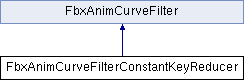
\includegraphics[height=2.000000cm]{class_fbx_anim_curve_filter_constant_key_reducer}
\end{center}
\end{figure}
\subsection*{公開メンバ関数}
\begin{DoxyCompactItemize}
\item 
\hyperlink{class_fbx_anim_curve_filter_constant_key_reducer_a5baf6160f4bf332b9235e0d1abb1aa3a}{Fbx\+Anim\+Curve\+Filter\+Constant\+Key\+Reducer} ()
\begin{DoxyCompactList}\small\item\em Constructor. \end{DoxyCompactList}\item 
virtual \hyperlink{class_fbx_anim_curve_filter_constant_key_reducer_a523519a310cf98a3823b221ab9973069}{$\sim$\+Fbx\+Anim\+Curve\+Filter\+Constant\+Key\+Reducer} ()
\begin{DoxyCompactList}\small\item\em Destructor. \end{DoxyCompactList}\item 
virtual const char $\ast$ \hyperlink{class_fbx_anim_curve_filter_constant_key_reducer_a1f856490df5d301d1c1e202958a3240c}{Get\+Name} () const
\item 
virtual bool \hyperlink{class_fbx_anim_curve_filter_constant_key_reducer_a54f43929707bc95bc5d0830ec039fde2}{Apply} (\hyperlink{class_fbx_anim_curve_node}{Fbx\+Anim\+Curve\+Node} \&p\+Curve\+Node, \hyperlink{class_fbx_status}{Fbx\+Status} $\ast$p\+Status=\hyperlink{fbxarch_8h_a070d2ce7b6bb7e5c05602aa8c308d0c4}{N\+U\+LL})
\item 
virtual bool \hyperlink{class_fbx_anim_curve_filter_constant_key_reducer_a45c9f6f26dc37686d684e1a35ac6b4c0}{Apply} (\hyperlink{class_fbx_anim_curve}{Fbx\+Anim\+Curve} \&p\+Curve, \hyperlink{class_fbx_status}{Fbx\+Status} $\ast$p\+Status=\hyperlink{fbxarch_8h_a070d2ce7b6bb7e5c05602aa8c308d0c4}{N\+U\+LL})
\item 
virtual void \hyperlink{class_fbx_anim_curve_filter_constant_key_reducer_a6961f8cd2d86b3f0b0c503c021bac93b}{Reset} ()
\item 
double \hyperlink{class_fbx_anim_curve_filter_constant_key_reducer_adae1590528c85fe9c4186652c97d8d19}{Get\+Derivative\+Tolerance} () const
\item 
void \hyperlink{class_fbx_anim_curve_filter_constant_key_reducer_ac0db44875a6a8d68e41a331948e8bf1f}{Set\+Derivative\+Tolerance} (double p\+Value)
\item 
double \hyperlink{class_fbx_anim_curve_filter_constant_key_reducer_a0ff1db2f653a0217e0560550be3d947f}{Get\+Value\+Tolerance} () const
\item 
void \hyperlink{class_fbx_anim_curve_filter_constant_key_reducer_a86a4427b2a29f5a82a0d1535048a44eb}{Set\+Value\+Tolerance} (double p\+Value)
\item 
bool \hyperlink{class_fbx_anim_curve_filter_constant_key_reducer_acb96f386ab154175fff45e7fdcbbfb3f}{Get\+Keep\+First\+And\+Last\+Keys} () const
\item 
void \hyperlink{class_fbx_anim_curve_filter_constant_key_reducer_a8833a42ff21debd38098de294ea9cbd2}{Set\+Keep\+First\+And\+Last\+Keys} (bool p\+Keep\+First\+And\+Last\+Keys)
\item 
bool \hyperlink{class_fbx_anim_curve_filter_constant_key_reducer_a098b50fec08965071f8eb5aec3a02e78}{Get\+Keep\+One\+Key} () const
\item 
void \hyperlink{class_fbx_anim_curve_filter_constant_key_reducer_ad71523fadea43a9532d600040b37a865}{Set\+Keep\+One\+Key} (bool p\+Keep\+One\+Key)
\item 
void \hyperlink{class_fbx_anim_curve_filter_constant_key_reducer_ae233ca614a39edb0e496f0dbc510f0ae}{Set\+Keep\+Not\+Pure\+Auto\+Keys} (bool p\+Keep)
\item 
void \hyperlink{class_fbx_anim_curve_filter_constant_key_reducer_acc31edd257d4b94cc91a899b7d45deb2}{Set\+Translation\+Threshold} (double p\+Translation\+Threshold)
\item 
void \hyperlink{class_fbx_anim_curve_filter_constant_key_reducer_a60e81af3f1d41764a42a9ddea89acb97}{Set\+Rotation\+Threshold} (double p\+Rotation\+Threshold)
\item 
void \hyperlink{class_fbx_anim_curve_filter_constant_key_reducer_af15fcce7deb4c02ea677fb3612fb368c}{Set\+Scaling\+Threshold} (double p\+Scaling\+Threshold)
\item 
void \hyperlink{class_fbx_anim_curve_filter_constant_key_reducer_ab2bd860bc4704e2f0945f58a66b040d6}{Set\+Default\+Threshold} (double p\+Default\+Threshold)
\item 
void \hyperlink{class_fbx_anim_curve_filter_constant_key_reducer_aa0d5c478c267b58cd0de9cedb9f931dd}{Set\+Modes} (bool p\+Exporting, \hyperlink{class_fbx_i_o_settings}{Fbx\+I\+O\+Settings} \&p\+I\+OS)
\end{DoxyCompactItemize}
\subsection*{Exposed parent class methods.}
\begin{DoxyCompactItemize}
\item 
virtual bool \hyperlink{class_fbx_anim_curve_filter_constant_key_reducer_a723169c1dc3a2d9557eb03908055c277}{Apply} (\hyperlink{class_fbx_anim_stack}{Fbx\+Anim\+Stack} $\ast$p\+Anim\+Stack, \hyperlink{class_fbx_status}{Fbx\+Status} $\ast$p\+Status=\hyperlink{fbxarch_8h_a070d2ce7b6bb7e5c05602aa8c308d0c4}{N\+U\+LL})
\item 
virtual bool \hyperlink{class_fbx_anim_curve_filter_constant_key_reducer_a08bf131629e3e1bc798a342cd479c2e4}{Apply} (\hyperlink{class_fbx_object}{Fbx\+Object} $\ast$p\+Obj, \hyperlink{class_fbx_anim_stack}{Fbx\+Anim\+Stack} $\ast$p\+Anim\+Stack, \hyperlink{class_fbx_status}{Fbx\+Status} $\ast$p\+Status=\hyperlink{fbxarch_8h_a070d2ce7b6bb7e5c05602aa8c308d0c4}{N\+U\+LL})
\item 
virtual bool \hyperlink{class_fbx_anim_curve_filter_constant_key_reducer_aea1789418ec3f29dba7805f2782e843c}{Apply} (\hyperlink{class_fbx_anim_curve}{Fbx\+Anim\+Curve} $\ast$$\ast$p\+Curve, int p\+Count, \hyperlink{class_fbx_status}{Fbx\+Status} $\ast$p\+Status=\hyperlink{fbxarch_8h_a070d2ce7b6bb7e5c05602aa8c308d0c4}{N\+U\+LL})
\end{DoxyCompactItemize}
\subsection*{その他の継承メンバ}


\subsection{詳解}
Constant key reducing filter.

Filter to test if each key is really necessary to define the curve at a definite degree of precision. It filters recursively from the strongest difference first. All useless keys are eliminated. 

 fbxanimcurvefilters.\+h の 242 行目に定義があります。



\subsection{構築子と解体子}
\mbox{\Hypertarget{class_fbx_anim_curve_filter_constant_key_reducer_a5baf6160f4bf332b9235e0d1abb1aa3a}\label{class_fbx_anim_curve_filter_constant_key_reducer_a5baf6160f4bf332b9235e0d1abb1aa3a}} 
\index{Fbx\+Anim\+Curve\+Filter\+Constant\+Key\+Reducer@{Fbx\+Anim\+Curve\+Filter\+Constant\+Key\+Reducer}!Fbx\+Anim\+Curve\+Filter\+Constant\+Key\+Reducer@{Fbx\+Anim\+Curve\+Filter\+Constant\+Key\+Reducer}}
\index{Fbx\+Anim\+Curve\+Filter\+Constant\+Key\+Reducer@{Fbx\+Anim\+Curve\+Filter\+Constant\+Key\+Reducer}!Fbx\+Anim\+Curve\+Filter\+Constant\+Key\+Reducer@{Fbx\+Anim\+Curve\+Filter\+Constant\+Key\+Reducer}}
\subsubsection{\texorpdfstring{Fbx\+Anim\+Curve\+Filter\+Constant\+Key\+Reducer()}{FbxAnimCurveFilterConstantKeyReducer()}}
{\footnotesize\ttfamily Fbx\+Anim\+Curve\+Filter\+Constant\+Key\+Reducer\+::\+Fbx\+Anim\+Curve\+Filter\+Constant\+Key\+Reducer (\begin{DoxyParamCaption}{ }\end{DoxyParamCaption})}



Constructor. 

\mbox{\Hypertarget{class_fbx_anim_curve_filter_constant_key_reducer_a523519a310cf98a3823b221ab9973069}\label{class_fbx_anim_curve_filter_constant_key_reducer_a523519a310cf98a3823b221ab9973069}} 
\index{Fbx\+Anim\+Curve\+Filter\+Constant\+Key\+Reducer@{Fbx\+Anim\+Curve\+Filter\+Constant\+Key\+Reducer}!````~Fbx\+Anim\+Curve\+Filter\+Constant\+Key\+Reducer@{$\sim$\+Fbx\+Anim\+Curve\+Filter\+Constant\+Key\+Reducer}}
\index{````~Fbx\+Anim\+Curve\+Filter\+Constant\+Key\+Reducer@{$\sim$\+Fbx\+Anim\+Curve\+Filter\+Constant\+Key\+Reducer}!Fbx\+Anim\+Curve\+Filter\+Constant\+Key\+Reducer@{Fbx\+Anim\+Curve\+Filter\+Constant\+Key\+Reducer}}
\subsubsection{\texorpdfstring{$\sim$\+Fbx\+Anim\+Curve\+Filter\+Constant\+Key\+Reducer()}{~FbxAnimCurveFilterConstantKeyReducer()}}
{\footnotesize\ttfamily virtual Fbx\+Anim\+Curve\+Filter\+Constant\+Key\+Reducer\+::$\sim$\+Fbx\+Anim\+Curve\+Filter\+Constant\+Key\+Reducer (\begin{DoxyParamCaption}{ }\end{DoxyParamCaption})\hspace{0.3cm}{\ttfamily [inline]}, {\ttfamily [virtual]}}



Destructor. 



 fbxanimcurvefilters.\+h の 249 行目に定義があります。



\subsection{関数詳解}
\mbox{\Hypertarget{class_fbx_anim_curve_filter_constant_key_reducer_a723169c1dc3a2d9557eb03908055c277}\label{class_fbx_anim_curve_filter_constant_key_reducer_a723169c1dc3a2d9557eb03908055c277}} 
\index{Fbx\+Anim\+Curve\+Filter\+Constant\+Key\+Reducer@{Fbx\+Anim\+Curve\+Filter\+Constant\+Key\+Reducer}!Apply@{Apply}}
\index{Apply@{Apply}!Fbx\+Anim\+Curve\+Filter\+Constant\+Key\+Reducer@{Fbx\+Anim\+Curve\+Filter\+Constant\+Key\+Reducer}}
\subsubsection{\texorpdfstring{Apply()}{Apply()}\hspace{0.1cm}{\footnotesize\ttfamily [1/5]}}
{\footnotesize\ttfamily virtual bool Fbx\+Anim\+Curve\+Filter\+Constant\+Key\+Reducer\+::\+Apply (\begin{DoxyParamCaption}\item[{\hyperlink{class_fbx_anim_stack}{Fbx\+Anim\+Stack} $\ast$}]{p\+Anim\+Stack,  }\item[{\hyperlink{class_fbx_status}{Fbx\+Status} $\ast$}]{p\+Status = {\ttfamily \hyperlink{fbxarch_8h_a070d2ce7b6bb7e5c05602aa8c308d0c4}{N\+U\+LL}} }\end{DoxyParamCaption})\hspace{0.3cm}{\ttfamily [inline]}, {\ttfamily [virtual]}}

Apply filter to all the curves stored in the animation stack. 
\begin{DoxyParams}{引数}
{\em p\+Anim\+Stack} & Animation stack where to retrieve the animation curves \\
\hline
{\em p\+Status} & The \hyperlink{class_fbx_status}{Fbx\+Status} object to hold error codes. \\
\hline
\end{DoxyParams}
\begin{DoxyReturn}{戻り値}
{\ttfamily true} if the curve filtering operation was successful, {\ttfamily false} otherwise. 
\end{DoxyReturn}


\hyperlink{class_fbx_anim_curve_filter_aef3900e6180e05661c27ee484ae939c3}{Fbx\+Anim\+Curve\+Filter}を再実装しています。



 fbxanimcurvefilters.\+h の 260 行目に定義があります。

\mbox{\Hypertarget{class_fbx_anim_curve_filter_constant_key_reducer_a08bf131629e3e1bc798a342cd479c2e4}\label{class_fbx_anim_curve_filter_constant_key_reducer_a08bf131629e3e1bc798a342cd479c2e4}} 
\index{Fbx\+Anim\+Curve\+Filter\+Constant\+Key\+Reducer@{Fbx\+Anim\+Curve\+Filter\+Constant\+Key\+Reducer}!Apply@{Apply}}
\index{Apply@{Apply}!Fbx\+Anim\+Curve\+Filter\+Constant\+Key\+Reducer@{Fbx\+Anim\+Curve\+Filter\+Constant\+Key\+Reducer}}
\subsubsection{\texorpdfstring{Apply()}{Apply()}\hspace{0.1cm}{\footnotesize\ttfamily [2/5]}}
{\footnotesize\ttfamily virtual bool Fbx\+Anim\+Curve\+Filter\+Constant\+Key\+Reducer\+::\+Apply (\begin{DoxyParamCaption}\item[{\hyperlink{class_fbx_object}{Fbx\+Object} $\ast$}]{p\+Obj,  }\item[{\hyperlink{class_fbx_anim_stack}{Fbx\+Anim\+Stack} $\ast$}]{p\+Anim\+Stack,  }\item[{\hyperlink{class_fbx_status}{Fbx\+Status} $\ast$}]{p\+Status = {\ttfamily \hyperlink{fbxarch_8h_a070d2ce7b6bb7e5c05602aa8c308d0c4}{N\+U\+LL}} }\end{DoxyParamCaption})\hspace{0.3cm}{\ttfamily [inline]}, {\ttfamily [virtual]}}

Apply filter to all the animated properties of the object. 
\begin{DoxyParams}{引数}
{\em p\+Obj} & Object containing the animated properties to which the filter is applied. \\
\hline
{\em p\+Anim\+Stack} & Animation stack where to retrieve the animation curves \\
\hline
{\em p\+Status} & The \hyperlink{class_fbx_status}{Fbx\+Status} object to hold error codes. \\
\hline
\end{DoxyParams}
\begin{DoxyReturn}{戻り値}
{\ttfamily true} if the curve filtering operation was successful, {\ttfamily false} otherwise. 
\end{DoxyReturn}


\hyperlink{class_fbx_anim_curve_filter_a009498a65af4995bf5e5908f17837531}{Fbx\+Anim\+Curve\+Filter}を再実装しています。



 fbxanimcurvefilters.\+h の 261 行目に定義があります。

\mbox{\Hypertarget{class_fbx_anim_curve_filter_constant_key_reducer_aea1789418ec3f29dba7805f2782e843c}\label{class_fbx_anim_curve_filter_constant_key_reducer_aea1789418ec3f29dba7805f2782e843c}} 
\index{Fbx\+Anim\+Curve\+Filter\+Constant\+Key\+Reducer@{Fbx\+Anim\+Curve\+Filter\+Constant\+Key\+Reducer}!Apply@{Apply}}
\index{Apply@{Apply}!Fbx\+Anim\+Curve\+Filter\+Constant\+Key\+Reducer@{Fbx\+Anim\+Curve\+Filter\+Constant\+Key\+Reducer}}
\subsubsection{\texorpdfstring{Apply()}{Apply()}\hspace{0.1cm}{\footnotesize\ttfamily [3/5]}}
{\footnotesize\ttfamily virtual bool Fbx\+Anim\+Curve\+Filter\+Constant\+Key\+Reducer\+::\+Apply (\begin{DoxyParamCaption}\item[{\hyperlink{class_fbx_anim_curve}{Fbx\+Anim\+Curve} $\ast$$\ast$}]{p\+Curve,  }\item[{int}]{p\+Count,  }\item[{\hyperlink{class_fbx_status}{Fbx\+Status} $\ast$}]{p\+Status = {\ttfamily \hyperlink{fbxarch_8h_a070d2ce7b6bb7e5c05602aa8c308d0c4}{N\+U\+LL}} }\end{DoxyParamCaption})\hspace{0.3cm}{\ttfamily [inline]}, {\ttfamily [virtual]}}

Apply filter on an array of animation curves. 
\begin{DoxyParams}{引数}
{\em p\+Curve} & Array of curves to which the filter is applied. \\
\hline
{\em p\+Count} & Number of curves in the array. \\
\hline
{\em p\+Status} & The \hyperlink{class_fbx_status}{Fbx\+Status} object to hold error codes. \\
\hline
\end{DoxyParams}
\begin{DoxyReturn}{戻り値}
{\ttfamily true} if the curve filtering operation was successful, {\ttfamily false} otherwise. 
\end{DoxyReturn}


\hyperlink{class_fbx_anim_curve_filter_aca6a41fbc4d9019b20df7adccfa6ed3c}{Fbx\+Anim\+Curve\+Filter}を再実装しています。



 fbxanimcurvefilters.\+h の 262 行目に定義があります。

\mbox{\Hypertarget{class_fbx_anim_curve_filter_constant_key_reducer_a54f43929707bc95bc5d0830ec039fde2}\label{class_fbx_anim_curve_filter_constant_key_reducer_a54f43929707bc95bc5d0830ec039fde2}} 
\index{Fbx\+Anim\+Curve\+Filter\+Constant\+Key\+Reducer@{Fbx\+Anim\+Curve\+Filter\+Constant\+Key\+Reducer}!Apply@{Apply}}
\index{Apply@{Apply}!Fbx\+Anim\+Curve\+Filter\+Constant\+Key\+Reducer@{Fbx\+Anim\+Curve\+Filter\+Constant\+Key\+Reducer}}
\subsubsection{\texorpdfstring{Apply()}{Apply()}\hspace{0.1cm}{\footnotesize\ttfamily [4/5]}}
{\footnotesize\ttfamily virtual bool Fbx\+Anim\+Curve\+Filter\+Constant\+Key\+Reducer\+::\+Apply (\begin{DoxyParamCaption}\item[{\hyperlink{class_fbx_anim_curve_node}{Fbx\+Anim\+Curve\+Node} \&}]{p\+Curve\+Node,  }\item[{\hyperlink{class_fbx_status}{Fbx\+Status} $\ast$}]{p\+Status = {\ttfamily \hyperlink{fbxarch_8h_a070d2ce7b6bb7e5c05602aa8c308d0c4}{N\+U\+LL}} }\end{DoxyParamCaption})\hspace{0.3cm}{\ttfamily [virtual]}}

Apply filter on all the curves of an animation curve node. 
\begin{DoxyParams}{引数}
{\em p\+Curve\+Node} & Curve node to which the filter is applied. \\
\hline
{\em p\+Status} & The \hyperlink{class_fbx_status}{Fbx\+Status} object to hold error codes. \\
\hline
\end{DoxyParams}
\begin{DoxyReturn}{戻り値}
{\ttfamily true} if the curve filtering operation was successful, {\ttfamily false} otherwise. 
\end{DoxyReturn}
\begin{DoxyRemark}{注釈}
This method collects all the \hyperlink{class_fbx_anim_curve}{Fbx\+Anim\+Curve} objects connected to the curve node and calls Apply(\+Fbx\+Anim\+Curve$\ast$$\ast$, int) 
\end{DoxyRemark}


\hyperlink{class_fbx_anim_curve_filter_ad042b45c0675278fa49e61739b0825c2}{Fbx\+Anim\+Curve\+Filter}を再実装しています。

\mbox{\Hypertarget{class_fbx_anim_curve_filter_constant_key_reducer_a45c9f6f26dc37686d684e1a35ac6b4c0}\label{class_fbx_anim_curve_filter_constant_key_reducer_a45c9f6f26dc37686d684e1a35ac6b4c0}} 
\index{Fbx\+Anim\+Curve\+Filter\+Constant\+Key\+Reducer@{Fbx\+Anim\+Curve\+Filter\+Constant\+Key\+Reducer}!Apply@{Apply}}
\index{Apply@{Apply}!Fbx\+Anim\+Curve\+Filter\+Constant\+Key\+Reducer@{Fbx\+Anim\+Curve\+Filter\+Constant\+Key\+Reducer}}
\subsubsection{\texorpdfstring{Apply()}{Apply()}\hspace{0.1cm}{\footnotesize\ttfamily [5/5]}}
{\footnotesize\ttfamily virtual bool Fbx\+Anim\+Curve\+Filter\+Constant\+Key\+Reducer\+::\+Apply (\begin{DoxyParamCaption}\item[{\hyperlink{class_fbx_anim_curve}{Fbx\+Anim\+Curve} \&}]{p\+Curve,  }\item[{\hyperlink{class_fbx_status}{Fbx\+Status} $\ast$}]{p\+Status = {\ttfamily \hyperlink{fbxarch_8h_a070d2ce7b6bb7e5c05602aa8c308d0c4}{N\+U\+LL}} }\end{DoxyParamCaption})\hspace{0.3cm}{\ttfamily [virtual]}}

Apply filter on an animation curve. 
\begin{DoxyParams}{引数}
{\em p\+Curve} & Curve to which the filter is applied. \\
\hline
{\em p\+Status} & The \hyperlink{class_fbx_status}{Fbx\+Status} object to hold error codes. \\
\hline
\end{DoxyParams}
\begin{DoxyReturn}{戻り値}
{\ttfamily true} if the curve filtering operation was successful, {\ttfamily false} otherwise. 
\end{DoxyReturn}


\hyperlink{class_fbx_anim_curve_filter_a6a69996c47c0e6f63a0f8b0d5fa806a0}{Fbx\+Anim\+Curve\+Filter}を実装しています。

\mbox{\Hypertarget{class_fbx_anim_curve_filter_constant_key_reducer_adae1590528c85fe9c4186652c97d8d19}\label{class_fbx_anim_curve_filter_constant_key_reducer_adae1590528c85fe9c4186652c97d8d19}} 
\index{Fbx\+Anim\+Curve\+Filter\+Constant\+Key\+Reducer@{Fbx\+Anim\+Curve\+Filter\+Constant\+Key\+Reducer}!Get\+Derivative\+Tolerance@{Get\+Derivative\+Tolerance}}
\index{Get\+Derivative\+Tolerance@{Get\+Derivative\+Tolerance}!Fbx\+Anim\+Curve\+Filter\+Constant\+Key\+Reducer@{Fbx\+Anim\+Curve\+Filter\+Constant\+Key\+Reducer}}
\subsubsection{\texorpdfstring{Get\+Derivative\+Tolerance()}{GetDerivativeTolerance()}}
{\footnotesize\ttfamily double Fbx\+Anim\+Curve\+Filter\+Constant\+Key\+Reducer\+::\+Get\+Derivative\+Tolerance (\begin{DoxyParamCaption}{ }\end{DoxyParamCaption}) const}

Get the current derivative tolerance. \begin{DoxyReturn}{戻り値}
The value of the current derivative tolerance. 
\end{DoxyReturn}
\mbox{\Hypertarget{class_fbx_anim_curve_filter_constant_key_reducer_acb96f386ab154175fff45e7fdcbbfb3f}\label{class_fbx_anim_curve_filter_constant_key_reducer_acb96f386ab154175fff45e7fdcbbfb3f}} 
\index{Fbx\+Anim\+Curve\+Filter\+Constant\+Key\+Reducer@{Fbx\+Anim\+Curve\+Filter\+Constant\+Key\+Reducer}!Get\+Keep\+First\+And\+Last\+Keys@{Get\+Keep\+First\+And\+Last\+Keys}}
\index{Get\+Keep\+First\+And\+Last\+Keys@{Get\+Keep\+First\+And\+Last\+Keys}!Fbx\+Anim\+Curve\+Filter\+Constant\+Key\+Reducer@{Fbx\+Anim\+Curve\+Filter\+Constant\+Key\+Reducer}}
\subsubsection{\texorpdfstring{Get\+Keep\+First\+And\+Last\+Keys()}{GetKeepFirstAndLastKeys()}}
{\footnotesize\ttfamily bool Fbx\+Anim\+Curve\+Filter\+Constant\+Key\+Reducer\+::\+Get\+Keep\+First\+And\+Last\+Keys (\begin{DoxyParamCaption}{ }\end{DoxyParamCaption}) const}

Get the state of the Keep\+First\+And\+Last\+Keys flag. \begin{DoxyReturn}{戻り値}
{\ttfamily true} if the filter keeps the first and last keys. 
\end{DoxyReturn}
\mbox{\Hypertarget{class_fbx_anim_curve_filter_constant_key_reducer_a098b50fec08965071f8eb5aec3a02e78}\label{class_fbx_anim_curve_filter_constant_key_reducer_a098b50fec08965071f8eb5aec3a02e78}} 
\index{Fbx\+Anim\+Curve\+Filter\+Constant\+Key\+Reducer@{Fbx\+Anim\+Curve\+Filter\+Constant\+Key\+Reducer}!Get\+Keep\+One\+Key@{Get\+Keep\+One\+Key}}
\index{Get\+Keep\+One\+Key@{Get\+Keep\+One\+Key}!Fbx\+Anim\+Curve\+Filter\+Constant\+Key\+Reducer@{Fbx\+Anim\+Curve\+Filter\+Constant\+Key\+Reducer}}
\subsubsection{\texorpdfstring{Get\+Keep\+One\+Key()}{GetKeepOneKey()}}
{\footnotesize\ttfamily bool Fbx\+Anim\+Curve\+Filter\+Constant\+Key\+Reducer\+::\+Get\+Keep\+One\+Key (\begin{DoxyParamCaption}{ }\end{DoxyParamCaption}) const}

Get the state of the Keep\+One\+Key flag. If all the keys are constant and this flag is c\textbackslash{} true, the filter will keep the first key. If all the keys are constant and this flag is c\textbackslash{} false, the filter will delete all the keys. \begin{DoxyReturn}{戻り値}
{\ttfamily true} if the filter keeps the first key when all keys are constant. 
\end{DoxyReturn}
\mbox{\Hypertarget{class_fbx_anim_curve_filter_constant_key_reducer_a1f856490df5d301d1c1e202958a3240c}\label{class_fbx_anim_curve_filter_constant_key_reducer_a1f856490df5d301d1c1e202958a3240c}} 
\index{Fbx\+Anim\+Curve\+Filter\+Constant\+Key\+Reducer@{Fbx\+Anim\+Curve\+Filter\+Constant\+Key\+Reducer}!Get\+Name@{Get\+Name}}
\index{Get\+Name@{Get\+Name}!Fbx\+Anim\+Curve\+Filter\+Constant\+Key\+Reducer@{Fbx\+Anim\+Curve\+Filter\+Constant\+Key\+Reducer}}
\subsubsection{\texorpdfstring{Get\+Name()}{GetName()}}
{\footnotesize\ttfamily virtual const char$\ast$ Fbx\+Anim\+Curve\+Filter\+Constant\+Key\+Reducer\+::\+Get\+Name (\begin{DoxyParamCaption}{ }\end{DoxyParamCaption}) const\hspace{0.3cm}{\ttfamily [virtual]}}

Get the name of the filter. \begin{DoxyReturn}{戻り値}
Pointer to name. 
\end{DoxyReturn}


\hyperlink{class_fbx_anim_curve_filter_abd559d5052fbb072042e59241940a35c}{Fbx\+Anim\+Curve\+Filter}を再実装しています。

\mbox{\Hypertarget{class_fbx_anim_curve_filter_constant_key_reducer_a0ff1db2f653a0217e0560550be3d947f}\label{class_fbx_anim_curve_filter_constant_key_reducer_a0ff1db2f653a0217e0560550be3d947f}} 
\index{Fbx\+Anim\+Curve\+Filter\+Constant\+Key\+Reducer@{Fbx\+Anim\+Curve\+Filter\+Constant\+Key\+Reducer}!Get\+Value\+Tolerance@{Get\+Value\+Tolerance}}
\index{Get\+Value\+Tolerance@{Get\+Value\+Tolerance}!Fbx\+Anim\+Curve\+Filter\+Constant\+Key\+Reducer@{Fbx\+Anim\+Curve\+Filter\+Constant\+Key\+Reducer}}
\subsubsection{\texorpdfstring{Get\+Value\+Tolerance()}{GetValueTolerance()}}
{\footnotesize\ttfamily double Fbx\+Anim\+Curve\+Filter\+Constant\+Key\+Reducer\+::\+Get\+Value\+Tolerance (\begin{DoxyParamCaption}{ }\end{DoxyParamCaption}) const}

Get the tolerance value. \begin{DoxyReturn}{戻り値}
The tolerance value. 
\end{DoxyReturn}
\mbox{\Hypertarget{class_fbx_anim_curve_filter_constant_key_reducer_a6961f8cd2d86b3f0b0c503c021bac93b}\label{class_fbx_anim_curve_filter_constant_key_reducer_a6961f8cd2d86b3f0b0c503c021bac93b}} 
\index{Fbx\+Anim\+Curve\+Filter\+Constant\+Key\+Reducer@{Fbx\+Anim\+Curve\+Filter\+Constant\+Key\+Reducer}!Reset@{Reset}}
\index{Reset@{Reset}!Fbx\+Anim\+Curve\+Filter\+Constant\+Key\+Reducer@{Fbx\+Anim\+Curve\+Filter\+Constant\+Key\+Reducer}}
\subsubsection{\texorpdfstring{Reset()}{Reset()}}
{\footnotesize\ttfamily virtual void Fbx\+Anim\+Curve\+Filter\+Constant\+Key\+Reducer\+::\+Reset (\begin{DoxyParamCaption}{ }\end{DoxyParamCaption})\hspace{0.3cm}{\ttfamily [virtual]}}

Reset the filter to its default parameters. 

\hyperlink{class_fbx_anim_curve_filter_a57fb35baaaa85adb08946383cf40e811}{Fbx\+Anim\+Curve\+Filter}を再実装しています。

\mbox{\Hypertarget{class_fbx_anim_curve_filter_constant_key_reducer_ab2bd860bc4704e2f0945f58a66b040d6}\label{class_fbx_anim_curve_filter_constant_key_reducer_ab2bd860bc4704e2f0945f58a66b040d6}} 
\index{Fbx\+Anim\+Curve\+Filter\+Constant\+Key\+Reducer@{Fbx\+Anim\+Curve\+Filter\+Constant\+Key\+Reducer}!Set\+Default\+Threshold@{Set\+Default\+Threshold}}
\index{Set\+Default\+Threshold@{Set\+Default\+Threshold}!Fbx\+Anim\+Curve\+Filter\+Constant\+Key\+Reducer@{Fbx\+Anim\+Curve\+Filter\+Constant\+Key\+Reducer}}
\subsubsection{\texorpdfstring{Set\+Default\+Threshold()}{SetDefaultThreshold()}}
{\footnotesize\ttfamily void Fbx\+Anim\+Curve\+Filter\+Constant\+Key\+Reducer\+::\+Set\+Default\+Threshold (\begin{DoxyParamCaption}\item[{double}]{p\+Default\+Threshold }\end{DoxyParamCaption})}

\mbox{\Hypertarget{class_fbx_anim_curve_filter_constant_key_reducer_ac0db44875a6a8d68e41a331948e8bf1f}\label{class_fbx_anim_curve_filter_constant_key_reducer_ac0db44875a6a8d68e41a331948e8bf1f}} 
\index{Fbx\+Anim\+Curve\+Filter\+Constant\+Key\+Reducer@{Fbx\+Anim\+Curve\+Filter\+Constant\+Key\+Reducer}!Set\+Derivative\+Tolerance@{Set\+Derivative\+Tolerance}}
\index{Set\+Derivative\+Tolerance@{Set\+Derivative\+Tolerance}!Fbx\+Anim\+Curve\+Filter\+Constant\+Key\+Reducer@{Fbx\+Anim\+Curve\+Filter\+Constant\+Key\+Reducer}}
\subsubsection{\texorpdfstring{Set\+Derivative\+Tolerance()}{SetDerivativeTolerance()}}
{\footnotesize\ttfamily void Fbx\+Anim\+Curve\+Filter\+Constant\+Key\+Reducer\+::\+Set\+Derivative\+Tolerance (\begin{DoxyParamCaption}\item[{double}]{p\+Value }\end{DoxyParamCaption})}

Set the derivative tolerance. 
\begin{DoxyParams}{引数}
{\em p\+Value} & Value derivative tolerance. \\
\hline
\end{DoxyParams}
\mbox{\Hypertarget{class_fbx_anim_curve_filter_constant_key_reducer_a8833a42ff21debd38098de294ea9cbd2}\label{class_fbx_anim_curve_filter_constant_key_reducer_a8833a42ff21debd38098de294ea9cbd2}} 
\index{Fbx\+Anim\+Curve\+Filter\+Constant\+Key\+Reducer@{Fbx\+Anim\+Curve\+Filter\+Constant\+Key\+Reducer}!Set\+Keep\+First\+And\+Last\+Keys@{Set\+Keep\+First\+And\+Last\+Keys}}
\index{Set\+Keep\+First\+And\+Last\+Keys@{Set\+Keep\+First\+And\+Last\+Keys}!Fbx\+Anim\+Curve\+Filter\+Constant\+Key\+Reducer@{Fbx\+Anim\+Curve\+Filter\+Constant\+Key\+Reducer}}
\subsubsection{\texorpdfstring{Set\+Keep\+First\+And\+Last\+Keys()}{SetKeepFirstAndLastKeys()}}
{\footnotesize\ttfamily void Fbx\+Anim\+Curve\+Filter\+Constant\+Key\+Reducer\+::\+Set\+Keep\+First\+And\+Last\+Keys (\begin{DoxyParamCaption}\item[{bool}]{p\+Keep\+First\+And\+Last\+Keys }\end{DoxyParamCaption})}

Set the state of the Keep\+First\+And\+Last\+Keys flag. 
\begin{DoxyParams}{引数}
{\em p\+Keep\+First\+And\+Last\+Keys} & Set to {\ttfamily true} if you want the filter to keep the first and last keys. \\
\hline
\end{DoxyParams}
\mbox{\Hypertarget{class_fbx_anim_curve_filter_constant_key_reducer_ae233ca614a39edb0e496f0dbc510f0ae}\label{class_fbx_anim_curve_filter_constant_key_reducer_ae233ca614a39edb0e496f0dbc510f0ae}} 
\index{Fbx\+Anim\+Curve\+Filter\+Constant\+Key\+Reducer@{Fbx\+Anim\+Curve\+Filter\+Constant\+Key\+Reducer}!Set\+Keep\+Not\+Pure\+Auto\+Keys@{Set\+Keep\+Not\+Pure\+Auto\+Keys}}
\index{Set\+Keep\+Not\+Pure\+Auto\+Keys@{Set\+Keep\+Not\+Pure\+Auto\+Keys}!Fbx\+Anim\+Curve\+Filter\+Constant\+Key\+Reducer@{Fbx\+Anim\+Curve\+Filter\+Constant\+Key\+Reducer}}
\subsubsection{\texorpdfstring{Set\+Keep\+Not\+Pure\+Auto\+Keys()}{SetKeepNotPureAutoKeys()}}
{\footnotesize\ttfamily void Fbx\+Anim\+Curve\+Filter\+Constant\+Key\+Reducer\+::\+Set\+Keep\+Not\+Pure\+Auto\+Keys (\begin{DoxyParamCaption}\item[{bool}]{p\+Keep }\end{DoxyParamCaption})}

Tell the filter to keep C\+U\+B\+IC curve keys which are not pure A\+U\+TO. 
\begin{DoxyParams}{引数}
{\em p\+Keep} & Keep\+Not\+Pure\+Auto\+Keys flag. \\
\hline
\end{DoxyParams}
\mbox{\Hypertarget{class_fbx_anim_curve_filter_constant_key_reducer_ad71523fadea43a9532d600040b37a865}\label{class_fbx_anim_curve_filter_constant_key_reducer_ad71523fadea43a9532d600040b37a865}} 
\index{Fbx\+Anim\+Curve\+Filter\+Constant\+Key\+Reducer@{Fbx\+Anim\+Curve\+Filter\+Constant\+Key\+Reducer}!Set\+Keep\+One\+Key@{Set\+Keep\+One\+Key}}
\index{Set\+Keep\+One\+Key@{Set\+Keep\+One\+Key}!Fbx\+Anim\+Curve\+Filter\+Constant\+Key\+Reducer@{Fbx\+Anim\+Curve\+Filter\+Constant\+Key\+Reducer}}
\subsubsection{\texorpdfstring{Set\+Keep\+One\+Key()}{SetKeepOneKey()}}
{\footnotesize\ttfamily void Fbx\+Anim\+Curve\+Filter\+Constant\+Key\+Reducer\+::\+Set\+Keep\+One\+Key (\begin{DoxyParamCaption}\item[{bool}]{p\+Keep\+One\+Key }\end{DoxyParamCaption})}

Set the state of the Keep\+One\+Key flag. If all the keys are constant and this flag is c\textbackslash{} true, the filter will keep the first key. If all the keys are constant and this flag is c\textbackslash{} false, the filter will delete all the keys. 
\begin{DoxyParams}{引数}
{\em p\+Keep\+One\+Key} & Set to {\ttfamily true} if you want the filter to keep the first key when all keys are constant. \\
\hline
\end{DoxyParams}
\mbox{\Hypertarget{class_fbx_anim_curve_filter_constant_key_reducer_aa0d5c478c267b58cd0de9cedb9f931dd}\label{class_fbx_anim_curve_filter_constant_key_reducer_aa0d5c478c267b58cd0de9cedb9f931dd}} 
\index{Fbx\+Anim\+Curve\+Filter\+Constant\+Key\+Reducer@{Fbx\+Anim\+Curve\+Filter\+Constant\+Key\+Reducer}!Set\+Modes@{Set\+Modes}}
\index{Set\+Modes@{Set\+Modes}!Fbx\+Anim\+Curve\+Filter\+Constant\+Key\+Reducer@{Fbx\+Anim\+Curve\+Filter\+Constant\+Key\+Reducer}}
\subsubsection{\texorpdfstring{Set\+Modes()}{SetModes()}}
{\footnotesize\ttfamily void Fbx\+Anim\+Curve\+Filter\+Constant\+Key\+Reducer\+::\+Set\+Modes (\begin{DoxyParamCaption}\item[{bool}]{p\+Exporting,  }\item[{\hyperlink{class_fbx_i_o_settings}{Fbx\+I\+O\+Settings} \&}]{p\+I\+OS }\end{DoxyParamCaption})}

\mbox{\Hypertarget{class_fbx_anim_curve_filter_constant_key_reducer_a60e81af3f1d41764a42a9ddea89acb97}\label{class_fbx_anim_curve_filter_constant_key_reducer_a60e81af3f1d41764a42a9ddea89acb97}} 
\index{Fbx\+Anim\+Curve\+Filter\+Constant\+Key\+Reducer@{Fbx\+Anim\+Curve\+Filter\+Constant\+Key\+Reducer}!Set\+Rotation\+Threshold@{Set\+Rotation\+Threshold}}
\index{Set\+Rotation\+Threshold@{Set\+Rotation\+Threshold}!Fbx\+Anim\+Curve\+Filter\+Constant\+Key\+Reducer@{Fbx\+Anim\+Curve\+Filter\+Constant\+Key\+Reducer}}
\subsubsection{\texorpdfstring{Set\+Rotation\+Threshold()}{SetRotationThreshold()}}
{\footnotesize\ttfamily void Fbx\+Anim\+Curve\+Filter\+Constant\+Key\+Reducer\+::\+Set\+Rotation\+Threshold (\begin{DoxyParamCaption}\item[{double}]{p\+Rotation\+Threshold }\end{DoxyParamCaption})}

\mbox{\Hypertarget{class_fbx_anim_curve_filter_constant_key_reducer_af15fcce7deb4c02ea677fb3612fb368c}\label{class_fbx_anim_curve_filter_constant_key_reducer_af15fcce7deb4c02ea677fb3612fb368c}} 
\index{Fbx\+Anim\+Curve\+Filter\+Constant\+Key\+Reducer@{Fbx\+Anim\+Curve\+Filter\+Constant\+Key\+Reducer}!Set\+Scaling\+Threshold@{Set\+Scaling\+Threshold}}
\index{Set\+Scaling\+Threshold@{Set\+Scaling\+Threshold}!Fbx\+Anim\+Curve\+Filter\+Constant\+Key\+Reducer@{Fbx\+Anim\+Curve\+Filter\+Constant\+Key\+Reducer}}
\subsubsection{\texorpdfstring{Set\+Scaling\+Threshold()}{SetScalingThreshold()}}
{\footnotesize\ttfamily void Fbx\+Anim\+Curve\+Filter\+Constant\+Key\+Reducer\+::\+Set\+Scaling\+Threshold (\begin{DoxyParamCaption}\item[{double}]{p\+Scaling\+Threshold }\end{DoxyParamCaption})}

\mbox{\Hypertarget{class_fbx_anim_curve_filter_constant_key_reducer_acc31edd257d4b94cc91a899b7d45deb2}\label{class_fbx_anim_curve_filter_constant_key_reducer_acc31edd257d4b94cc91a899b7d45deb2}} 
\index{Fbx\+Anim\+Curve\+Filter\+Constant\+Key\+Reducer@{Fbx\+Anim\+Curve\+Filter\+Constant\+Key\+Reducer}!Set\+Translation\+Threshold@{Set\+Translation\+Threshold}}
\index{Set\+Translation\+Threshold@{Set\+Translation\+Threshold}!Fbx\+Anim\+Curve\+Filter\+Constant\+Key\+Reducer@{Fbx\+Anim\+Curve\+Filter\+Constant\+Key\+Reducer}}
\subsubsection{\texorpdfstring{Set\+Translation\+Threshold()}{SetTranslationThreshold()}}
{\footnotesize\ttfamily void Fbx\+Anim\+Curve\+Filter\+Constant\+Key\+Reducer\+::\+Set\+Translation\+Threshold (\begin{DoxyParamCaption}\item[{double}]{p\+Translation\+Threshold }\end{DoxyParamCaption})}

\mbox{\Hypertarget{class_fbx_anim_curve_filter_constant_key_reducer_a86a4427b2a29f5a82a0d1535048a44eb}\label{class_fbx_anim_curve_filter_constant_key_reducer_a86a4427b2a29f5a82a0d1535048a44eb}} 
\index{Fbx\+Anim\+Curve\+Filter\+Constant\+Key\+Reducer@{Fbx\+Anim\+Curve\+Filter\+Constant\+Key\+Reducer}!Set\+Value\+Tolerance@{Set\+Value\+Tolerance}}
\index{Set\+Value\+Tolerance@{Set\+Value\+Tolerance}!Fbx\+Anim\+Curve\+Filter\+Constant\+Key\+Reducer@{Fbx\+Anim\+Curve\+Filter\+Constant\+Key\+Reducer}}
\subsubsection{\texorpdfstring{Set\+Value\+Tolerance()}{SetValueTolerance()}}
{\footnotesize\ttfamily void Fbx\+Anim\+Curve\+Filter\+Constant\+Key\+Reducer\+::\+Set\+Value\+Tolerance (\begin{DoxyParamCaption}\item[{double}]{p\+Value }\end{DoxyParamCaption})}

Set the tolerance value. 
\begin{DoxyParams}{引数}
{\em p\+Value} & Tolerance value. \\
\hline
\end{DoxyParams}


このクラス詳解は次のファイルから抽出されました\+:\begin{DoxyCompactItemize}
\item 
C\+:/\+Maya/scripts/\+F\+B\+X\+\_\+\+S\+D\+K/2017.\+1/include/fbxsdk/scene/animation/\hyperlink{fbxanimcurvefilters_8h}{fbxanimcurvefilters.\+h}\end{DoxyCompactItemize}

\hypertarget{class_fbx_anim_curve_filter_gimble_killer}{}\section{Fbx\+Anim\+Curve\+Filter\+Gimble\+Killer クラス}
\label{class_fbx_anim_curve_filter_gimble_killer}\index{Fbx\+Anim\+Curve\+Filter\+Gimble\+Killer@{Fbx\+Anim\+Curve\+Filter\+Gimble\+Killer}}


{\ttfamily \#include $<$fbxanimcurvefilters.\+h$>$}

Fbx\+Anim\+Curve\+Filter\+Gimble\+Killer の継承関係図\begin{figure}[H]
\begin{center}
\leavevmode
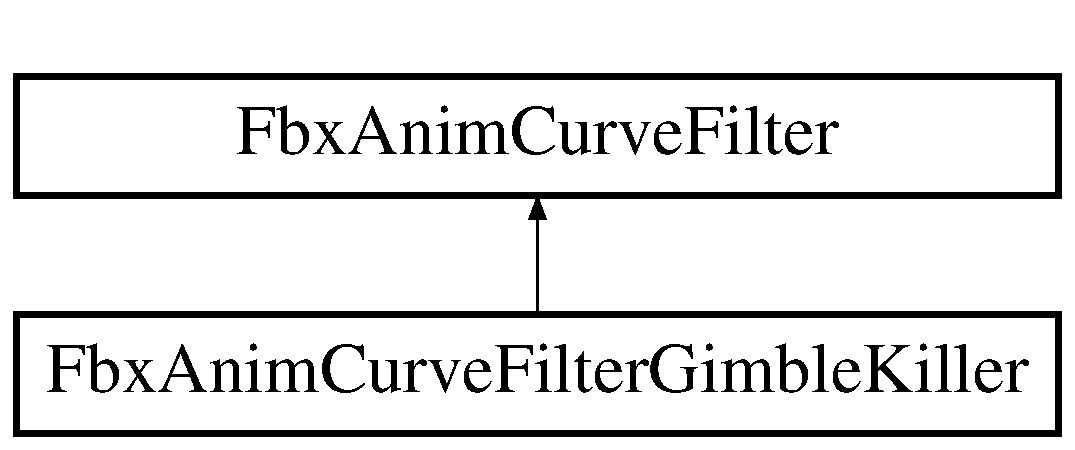
\includegraphics[height=2.000000cm]{class_fbx_anim_curve_filter_gimble_killer}
\end{center}
\end{figure}
\subsection*{公開メンバ関数}
\begin{DoxyCompactItemize}
\item 
\hyperlink{class_fbx_anim_curve_filter_gimble_killer_ae0a235ecc70b252fa50eb742727d4282}{Fbx\+Anim\+Curve\+Filter\+Gimble\+Killer} ()
\begin{DoxyCompactList}\small\item\em Constructor. \end{DoxyCompactList}\item 
virtual \hyperlink{class_fbx_anim_curve_filter_gimble_killer_ae4ac4f6824d0065e71139b985e8197b3}{$\sim$\+Fbx\+Anim\+Curve\+Filter\+Gimble\+Killer} ()
\begin{DoxyCompactList}\small\item\em Destructor. \end{DoxyCompactList}\item 
virtual const char $\ast$ \hyperlink{class_fbx_anim_curve_filter_gimble_killer_a224d34ab4b2a7f508de5679402c3711f}{Get\+Name} () const
\item 
virtual bool \hyperlink{class_fbx_anim_curve_filter_gimble_killer_a3b303b3383e638e445e0bd17570be9ea}{Need\+Apply} (\hyperlink{class_fbx_anim_stack}{Fbx\+Anim\+Stack} $\ast$, \hyperlink{class_fbx_status}{Fbx\+Status} $\ast$p\+Status=\hyperlink{fbxarch_8h_a070d2ce7b6bb7e5c05602aa8c308d0c4}{N\+U\+LL})
\item 
virtual bool \hyperlink{class_fbx_anim_curve_filter_gimble_killer_ad12554a479bc7a7cfd2fba457b051a5f}{Need\+Apply} (\hyperlink{class_fbx_object}{Fbx\+Object} $\ast$, \hyperlink{class_fbx_anim_stack}{Fbx\+Anim\+Stack} $\ast$, \hyperlink{class_fbx_status}{Fbx\+Status} $\ast$p\+Status=\hyperlink{fbxarch_8h_a070d2ce7b6bb7e5c05602aa8c308d0c4}{N\+U\+LL})
\item 
virtual bool \hyperlink{class_fbx_anim_curve_filter_gimble_killer_a72a761452f1a110353be0b6cae920e24}{Need\+Apply} (\hyperlink{class_fbx_anim_curve_node}{Fbx\+Anim\+Curve\+Node} \&p\+Curve\+Node, \hyperlink{class_fbx_status}{Fbx\+Status} $\ast$p\+Status=\hyperlink{fbxarch_8h_a070d2ce7b6bb7e5c05602aa8c308d0c4}{N\+U\+LL})
\item 
virtual bool \hyperlink{class_fbx_anim_curve_filter_gimble_killer_a7d9f7e30d2c8e4ec21e947ef0efaa314}{Need\+Apply} (\hyperlink{class_fbx_anim_curve}{Fbx\+Anim\+Curve} $\ast$$\ast$p\+Curve, int p\+Count, \hyperlink{class_fbx_status}{Fbx\+Status} $\ast$p\+Status=\hyperlink{fbxarch_8h_a070d2ce7b6bb7e5c05602aa8c308d0c4}{N\+U\+LL})
\item 
virtual bool \hyperlink{class_fbx_anim_curve_filter_gimble_killer_a136dadcee53ebed6b5afc6abddfcf402}{Need\+Apply} (\hyperlink{class_fbx_anim_curve}{Fbx\+Anim\+Curve} \&, \hyperlink{class_fbx_status}{Fbx\+Status} $\ast$p\+Status=\hyperlink{fbxarch_8h_a070d2ce7b6bb7e5c05602aa8c308d0c4}{N\+U\+LL})
\item 
virtual bool \hyperlink{class_fbx_anim_curve_filter_gimble_killer_acee7b2b1c995cc079152b5ff8c96bfff}{Apply} (\hyperlink{class_fbx_anim_stack}{Fbx\+Anim\+Stack} $\ast$, \hyperlink{class_fbx_status}{Fbx\+Status} $\ast$p\+Status=\hyperlink{fbxarch_8h_a070d2ce7b6bb7e5c05602aa8c308d0c4}{N\+U\+LL})
\item 
virtual bool \hyperlink{class_fbx_anim_curve_filter_gimble_killer_a2fe378cf9f04edf0613f579e9794a681}{Apply} (\hyperlink{class_fbx_object}{Fbx\+Object} $\ast$, \hyperlink{class_fbx_anim_stack}{Fbx\+Anim\+Stack} $\ast$, \hyperlink{class_fbx_status}{Fbx\+Status} $\ast$p\+Status=\hyperlink{fbxarch_8h_a070d2ce7b6bb7e5c05602aa8c308d0c4}{N\+U\+LL})
\item 
virtual bool \hyperlink{class_fbx_anim_curve_filter_gimble_killer_adb147695af2818ccc71e245170d05e78}{Apply} (\hyperlink{class_fbx_anim_curve_node}{Fbx\+Anim\+Curve\+Node} \&p\+Curve\+Node, \hyperlink{class_fbx_status}{Fbx\+Status} $\ast$p\+Status=\hyperlink{fbxarch_8h_a070d2ce7b6bb7e5c05602aa8c308d0c4}{N\+U\+LL})
\item 
virtual bool \hyperlink{class_fbx_anim_curve_filter_gimble_killer_a1c2012cdf59a163a816726f973c2c067}{Apply} (\hyperlink{class_fbx_anim_curve}{Fbx\+Anim\+Curve} $\ast$$\ast$p\+Curve, int p\+Count, \hyperlink{class_fbx_status}{Fbx\+Status} $\ast$p\+Status=\hyperlink{fbxarch_8h_a070d2ce7b6bb7e5c05602aa8c308d0c4}{N\+U\+LL})
\item 
virtual bool \hyperlink{class_fbx_anim_curve_filter_gimble_killer_ac74aff21904a7cb323f2ed4bafae6fa6}{Apply} (\hyperlink{class_fbx_anim_curve}{Fbx\+Anim\+Curve} \&, \hyperlink{class_fbx_status}{Fbx\+Status} $\ast$p\+Status=\hyperlink{fbxarch_8h_a070d2ce7b6bb7e5c05602aa8c308d0c4}{N\+U\+LL})
\item 
virtual void \hyperlink{class_fbx_anim_curve_filter_gimble_killer_ad0c8bbf400bc208412b088d9c5b702a5}{Reset} ()
\item 
bool \hyperlink{class_fbx_anim_curve_filter_gimble_killer_ae75014aea69ea161d87be698906ed797}{Get\+Apply\+Key\+Sync\+Filter} () const
\begin{DoxyCompactList}\small\item\em Return {\ttfamily true} if key sync filter is enabled. \end{DoxyCompactList}\item 
void \hyperlink{class_fbx_anim_curve_filter_gimble_killer_a39cedf804e69f86d5d2e8a95d92f98f2}{Set\+Apply\+Key\+Sync\+Filter} (bool p\+Flag)
\end{DoxyCompactItemize}
\subsection*{その他の継承メンバ}


\subsection{詳解}
Gimble\+Killer filter.

This filter try to minimize gimble locks on rotation curves. \begin{DoxyRemark}{注釈}
The current implementation of this filter expects to process 3 curves at the same time. 

This filter has been superseded by the Unroll filter. It is strongly advised to use the latter. 
\end{DoxyRemark}


 fbxanimcurvefilters.\+h の 411 行目に定義があります。



\subsection{構築子と解体子}
\mbox{\Hypertarget{class_fbx_anim_curve_filter_gimble_killer_ae0a235ecc70b252fa50eb742727d4282}\label{class_fbx_anim_curve_filter_gimble_killer_ae0a235ecc70b252fa50eb742727d4282}} 
\index{Fbx\+Anim\+Curve\+Filter\+Gimble\+Killer@{Fbx\+Anim\+Curve\+Filter\+Gimble\+Killer}!Fbx\+Anim\+Curve\+Filter\+Gimble\+Killer@{Fbx\+Anim\+Curve\+Filter\+Gimble\+Killer}}
\index{Fbx\+Anim\+Curve\+Filter\+Gimble\+Killer@{Fbx\+Anim\+Curve\+Filter\+Gimble\+Killer}!Fbx\+Anim\+Curve\+Filter\+Gimble\+Killer@{Fbx\+Anim\+Curve\+Filter\+Gimble\+Killer}}
\subsubsection{\texorpdfstring{Fbx\+Anim\+Curve\+Filter\+Gimble\+Killer()}{FbxAnimCurveFilterGimbleKiller()}}
{\footnotesize\ttfamily Fbx\+Anim\+Curve\+Filter\+Gimble\+Killer\+::\+Fbx\+Anim\+Curve\+Filter\+Gimble\+Killer (\begin{DoxyParamCaption}{ }\end{DoxyParamCaption})}



Constructor. 

\mbox{\Hypertarget{class_fbx_anim_curve_filter_gimble_killer_ae4ac4f6824d0065e71139b985e8197b3}\label{class_fbx_anim_curve_filter_gimble_killer_ae4ac4f6824d0065e71139b985e8197b3}} 
\index{Fbx\+Anim\+Curve\+Filter\+Gimble\+Killer@{Fbx\+Anim\+Curve\+Filter\+Gimble\+Killer}!````~Fbx\+Anim\+Curve\+Filter\+Gimble\+Killer@{$\sim$\+Fbx\+Anim\+Curve\+Filter\+Gimble\+Killer}}
\index{````~Fbx\+Anim\+Curve\+Filter\+Gimble\+Killer@{$\sim$\+Fbx\+Anim\+Curve\+Filter\+Gimble\+Killer}!Fbx\+Anim\+Curve\+Filter\+Gimble\+Killer@{Fbx\+Anim\+Curve\+Filter\+Gimble\+Killer}}
\subsubsection{\texorpdfstring{$\sim$\+Fbx\+Anim\+Curve\+Filter\+Gimble\+Killer()}{~FbxAnimCurveFilterGimbleKiller()}}
{\footnotesize\ttfamily virtual Fbx\+Anim\+Curve\+Filter\+Gimble\+Killer\+::$\sim$\+Fbx\+Anim\+Curve\+Filter\+Gimble\+Killer (\begin{DoxyParamCaption}{ }\end{DoxyParamCaption})\hspace{0.3cm}{\ttfamily [virtual]}}



Destructor. 



\subsection{関数詳解}
\mbox{\Hypertarget{class_fbx_anim_curve_filter_gimble_killer_acee7b2b1c995cc079152b5ff8c96bfff}\label{class_fbx_anim_curve_filter_gimble_killer_acee7b2b1c995cc079152b5ff8c96bfff}} 
\index{Fbx\+Anim\+Curve\+Filter\+Gimble\+Killer@{Fbx\+Anim\+Curve\+Filter\+Gimble\+Killer}!Apply@{Apply}}
\index{Apply@{Apply}!Fbx\+Anim\+Curve\+Filter\+Gimble\+Killer@{Fbx\+Anim\+Curve\+Filter\+Gimble\+Killer}}
\subsubsection{\texorpdfstring{Apply()}{Apply()}\hspace{0.1cm}{\footnotesize\ttfamily [1/5]}}
{\footnotesize\ttfamily virtual bool Fbx\+Anim\+Curve\+Filter\+Gimble\+Killer\+::\+Apply (\begin{DoxyParamCaption}\item[{\hyperlink{class_fbx_anim_stack}{Fbx\+Anim\+Stack} $\ast$}]{,  }\item[{\hyperlink{class_fbx_status}{Fbx\+Status} $\ast$}]{p\+Status = {\ttfamily \hyperlink{fbxarch_8h_a070d2ce7b6bb7e5c05602aa8c308d0c4}{N\+U\+LL}} }\end{DoxyParamCaption})\hspace{0.3cm}{\ttfamily [inline]}, {\ttfamily [virtual]}}

This filter expects to work with 3 interdependent curves. Passing the animation stack makes no sense since this object would not know which curves to handle. 
\begin{DoxyParams}{引数}
{\em p\+Anim\+Stack} & Animation stack \\
\hline
{\em p\+Status} & The \hyperlink{class_fbx_status}{Fbx\+Status} object to hold error codes. \\
\hline
\end{DoxyParams}
\begin{DoxyReturn}{戻り値}
{\ttfamily false}. 
\end{DoxyReturn}


\hyperlink{class_fbx_anim_curve_filter_aef3900e6180e05661c27ee484ae939c3}{Fbx\+Anim\+Curve\+Filter}を再実装しています。



 fbxanimcurvefilters.\+h の 474 行目に定義があります。

\mbox{\Hypertarget{class_fbx_anim_curve_filter_gimble_killer_a2fe378cf9f04edf0613f579e9794a681}\label{class_fbx_anim_curve_filter_gimble_killer_a2fe378cf9f04edf0613f579e9794a681}} 
\index{Fbx\+Anim\+Curve\+Filter\+Gimble\+Killer@{Fbx\+Anim\+Curve\+Filter\+Gimble\+Killer}!Apply@{Apply}}
\index{Apply@{Apply}!Fbx\+Anim\+Curve\+Filter\+Gimble\+Killer@{Fbx\+Anim\+Curve\+Filter\+Gimble\+Killer}}
\subsubsection{\texorpdfstring{Apply()}{Apply()}\hspace{0.1cm}{\footnotesize\ttfamily [2/5]}}
{\footnotesize\ttfamily virtual bool Fbx\+Anim\+Curve\+Filter\+Gimble\+Killer\+::\+Apply (\begin{DoxyParamCaption}\item[{\hyperlink{class_fbx_object}{Fbx\+Object} $\ast$}]{,  }\item[{\hyperlink{class_fbx_anim_stack}{Fbx\+Anim\+Stack} $\ast$}]{,  }\item[{\hyperlink{class_fbx_status}{Fbx\+Status} $\ast$}]{p\+Status = {\ttfamily \hyperlink{fbxarch_8h_a070d2ce7b6bb7e5c05602aa8c308d0c4}{N\+U\+LL}} }\end{DoxyParamCaption})\hspace{0.3cm}{\ttfamily [inline]}, {\ttfamily [virtual]}}

This filter expects to work with 3 interdependent curves. Collecting all the animation curves from the properties defined in {\itshape p\+Obj} could not guarantee that we are manipulating 3 interdependent curves. 
\begin{DoxyParams}{引数}
{\em p\+Obj} & Object containing the properties to test. \\
\hline
{\em p\+Anim\+Stack} & Animation stack where to retrieve the animation curves \\
\hline
{\em p\+Status} & The \hyperlink{class_fbx_status}{Fbx\+Status} object to hold error codes. \\
\hline
\end{DoxyParams}
\begin{DoxyReturn}{戻り値}
{\ttfamily false} 
\end{DoxyReturn}


\hyperlink{class_fbx_anim_curve_filter_a009498a65af4995bf5e5908f17837531}{Fbx\+Anim\+Curve\+Filter}を再実装しています。



 fbxanimcurvefilters.\+h の 483 行目に定義があります。

\mbox{\Hypertarget{class_fbx_anim_curve_filter_gimble_killer_adb147695af2818ccc71e245170d05e78}\label{class_fbx_anim_curve_filter_gimble_killer_adb147695af2818ccc71e245170d05e78}} 
\index{Fbx\+Anim\+Curve\+Filter\+Gimble\+Killer@{Fbx\+Anim\+Curve\+Filter\+Gimble\+Killer}!Apply@{Apply}}
\index{Apply@{Apply}!Fbx\+Anim\+Curve\+Filter\+Gimble\+Killer@{Fbx\+Anim\+Curve\+Filter\+Gimble\+Killer}}
\subsubsection{\texorpdfstring{Apply()}{Apply()}\hspace{0.1cm}{\footnotesize\ttfamily [3/5]}}
{\footnotesize\ttfamily virtual bool Fbx\+Anim\+Curve\+Filter\+Gimble\+Killer\+::\+Apply (\begin{DoxyParamCaption}\item[{\hyperlink{class_fbx_anim_curve_node}{Fbx\+Anim\+Curve\+Node} \&}]{p\+Curve\+Node,  }\item[{\hyperlink{class_fbx_status}{Fbx\+Status} $\ast$}]{p\+Status = {\ttfamily \hyperlink{fbxarch_8h_a070d2ce7b6bb7e5c05602aa8c308d0c4}{N\+U\+LL}} }\end{DoxyParamCaption})\hspace{0.3cm}{\ttfamily [virtual]}}

Apply filter on all the curves of an animation curve node. 
\begin{DoxyParams}{引数}
{\em p\+Curve\+Node} & Curve node to which the filter is applied. \\
\hline
{\em p\+Status} & The \hyperlink{class_fbx_status}{Fbx\+Status} object to hold error codes. \\
\hline
\end{DoxyParams}
\begin{DoxyReturn}{戻り値}
{\ttfamily true} if the curve filtering operation was successful, {\ttfamily false} otherwise. 
\end{DoxyReturn}
\begin{DoxyRemark}{注釈}
This method collects all the \hyperlink{class_fbx_anim_curve}{Fbx\+Anim\+Curve} objects connected to the curve node and calls Apply(\+Fbx\+Anim\+Curve$\ast$$\ast$, int) 
\end{DoxyRemark}


\hyperlink{class_fbx_anim_curve_filter_ad042b45c0675278fa49e61739b0825c2}{Fbx\+Anim\+Curve\+Filter}を再実装しています。

\mbox{\Hypertarget{class_fbx_anim_curve_filter_gimble_killer_a1c2012cdf59a163a816726f973c2c067}\label{class_fbx_anim_curve_filter_gimble_killer_a1c2012cdf59a163a816726f973c2c067}} 
\index{Fbx\+Anim\+Curve\+Filter\+Gimble\+Killer@{Fbx\+Anim\+Curve\+Filter\+Gimble\+Killer}!Apply@{Apply}}
\index{Apply@{Apply}!Fbx\+Anim\+Curve\+Filter\+Gimble\+Killer@{Fbx\+Anim\+Curve\+Filter\+Gimble\+Killer}}
\subsubsection{\texorpdfstring{Apply()}{Apply()}\hspace{0.1cm}{\footnotesize\ttfamily [4/5]}}
{\footnotesize\ttfamily virtual bool Fbx\+Anim\+Curve\+Filter\+Gimble\+Killer\+::\+Apply (\begin{DoxyParamCaption}\item[{\hyperlink{class_fbx_anim_curve}{Fbx\+Anim\+Curve} $\ast$$\ast$}]{p\+Curve,  }\item[{int}]{p\+Count,  }\item[{\hyperlink{class_fbx_status}{Fbx\+Status} $\ast$}]{p\+Status = {\ttfamily \hyperlink{fbxarch_8h_a070d2ce7b6bb7e5c05602aa8c308d0c4}{N\+U\+LL}} }\end{DoxyParamCaption})\hspace{0.3cm}{\ttfamily [virtual]}}

Apply filter on the given animation curve. 
\begin{DoxyParams}{引数}
{\em p\+Curve} & Array of curve to which the filter is applied. \\
\hline
{\em p\+Count} & Number of curves in array. \\
\hline
{\em p\+Status} & The \hyperlink{class_fbx_status}{Fbx\+Status} object to hold error codes. \\
\hline
\end{DoxyParams}
\begin{DoxyReturn}{戻り値}
{\ttfamily true} if the curve filtering operation was successful, {\ttfamily false} otherwise. 
\end{DoxyReturn}
\begin{DoxyRemark}{注釈}
Because this method only receives an array of interdependent curves, this filter assumes that they are all coming from an Euler rotation anim curve node. Therefore, it expects {\itshape p\+Count} to be equal to 3. 
\end{DoxyRemark}


\hyperlink{class_fbx_anim_curve_filter_aca6a41fbc4d9019b20df7adccfa6ed3c}{Fbx\+Anim\+Curve\+Filter}を再実装しています。

\mbox{\Hypertarget{class_fbx_anim_curve_filter_gimble_killer_ac74aff21904a7cb323f2ed4bafae6fa6}\label{class_fbx_anim_curve_filter_gimble_killer_ac74aff21904a7cb323f2ed4bafae6fa6}} 
\index{Fbx\+Anim\+Curve\+Filter\+Gimble\+Killer@{Fbx\+Anim\+Curve\+Filter\+Gimble\+Killer}!Apply@{Apply}}
\index{Apply@{Apply}!Fbx\+Anim\+Curve\+Filter\+Gimble\+Killer@{Fbx\+Anim\+Curve\+Filter\+Gimble\+Killer}}
\subsubsection{\texorpdfstring{Apply()}{Apply()}\hspace{0.1cm}{\footnotesize\ttfamily [5/5]}}
{\footnotesize\ttfamily virtual bool Fbx\+Anim\+Curve\+Filter\+Gimble\+Killer\+::\+Apply (\begin{DoxyParamCaption}\item[{\hyperlink{class_fbx_anim_curve}{Fbx\+Anim\+Curve} \&}]{,  }\item[{\hyperlink{class_fbx_status}{Fbx\+Status} $\ast$}]{p\+Status = {\ttfamily \hyperlink{fbxarch_8h_a070d2ce7b6bb7e5c05602aa8c308d0c4}{N\+U\+LL}} }\end{DoxyParamCaption})\hspace{0.3cm}{\ttfamily [inline]}, {\ttfamily [virtual]}}

This filter expects to work with interdependent curves. Receiving one single curve is useless. \begin{DoxyReturn}{戻り値}
{\ttfamily false} 
\end{DoxyReturn}


\hyperlink{class_fbx_anim_curve_filter_a6a69996c47c0e6f63a0f8b0d5fa806a0}{Fbx\+Anim\+Curve\+Filter}を実装しています。



 fbxanimcurvefilters.\+h の 508 行目に定義があります。

\mbox{\Hypertarget{class_fbx_anim_curve_filter_gimble_killer_ae75014aea69ea161d87be698906ed797}\label{class_fbx_anim_curve_filter_gimble_killer_ae75014aea69ea161d87be698906ed797}} 
\index{Fbx\+Anim\+Curve\+Filter\+Gimble\+Killer@{Fbx\+Anim\+Curve\+Filter\+Gimble\+Killer}!Get\+Apply\+Key\+Sync\+Filter@{Get\+Apply\+Key\+Sync\+Filter}}
\index{Get\+Apply\+Key\+Sync\+Filter@{Get\+Apply\+Key\+Sync\+Filter}!Fbx\+Anim\+Curve\+Filter\+Gimble\+Killer@{Fbx\+Anim\+Curve\+Filter\+Gimble\+Killer}}
\subsubsection{\texorpdfstring{Get\+Apply\+Key\+Sync\+Filter()}{GetApplyKeySyncFilter()}}
{\footnotesize\ttfamily bool Fbx\+Anim\+Curve\+Filter\+Gimble\+Killer\+::\+Get\+Apply\+Key\+Sync\+Filter (\begin{DoxyParamCaption}{ }\end{DoxyParamCaption}) const}



Return {\ttfamily true} if key sync filter is enabled. 

\mbox{\Hypertarget{class_fbx_anim_curve_filter_gimble_killer_a224d34ab4b2a7f508de5679402c3711f}\label{class_fbx_anim_curve_filter_gimble_killer_a224d34ab4b2a7f508de5679402c3711f}} 
\index{Fbx\+Anim\+Curve\+Filter\+Gimble\+Killer@{Fbx\+Anim\+Curve\+Filter\+Gimble\+Killer}!Get\+Name@{Get\+Name}}
\index{Get\+Name@{Get\+Name}!Fbx\+Anim\+Curve\+Filter\+Gimble\+Killer@{Fbx\+Anim\+Curve\+Filter\+Gimble\+Killer}}
\subsubsection{\texorpdfstring{Get\+Name()}{GetName()}}
{\footnotesize\ttfamily virtual const char$\ast$ Fbx\+Anim\+Curve\+Filter\+Gimble\+Killer\+::\+Get\+Name (\begin{DoxyParamCaption}{ }\end{DoxyParamCaption}) const\hspace{0.3cm}{\ttfamily [virtual]}}

Get the name of the filter. \begin{DoxyReturn}{戻り値}
Pointer to name. 
\end{DoxyReturn}


\hyperlink{class_fbx_anim_curve_filter_abd559d5052fbb072042e59241940a35c}{Fbx\+Anim\+Curve\+Filter}を再実装しています。

\mbox{\Hypertarget{class_fbx_anim_curve_filter_gimble_killer_a3b303b3383e638e445e0bd17570be9ea}\label{class_fbx_anim_curve_filter_gimble_killer_a3b303b3383e638e445e0bd17570be9ea}} 
\index{Fbx\+Anim\+Curve\+Filter\+Gimble\+Killer@{Fbx\+Anim\+Curve\+Filter\+Gimble\+Killer}!Need\+Apply@{Need\+Apply}}
\index{Need\+Apply@{Need\+Apply}!Fbx\+Anim\+Curve\+Filter\+Gimble\+Killer@{Fbx\+Anim\+Curve\+Filter\+Gimble\+Killer}}
\subsubsection{\texorpdfstring{Need\+Apply()}{NeedApply()}\hspace{0.1cm}{\footnotesize\ttfamily [1/5]}}
{\footnotesize\ttfamily virtual bool Fbx\+Anim\+Curve\+Filter\+Gimble\+Killer\+::\+Need\+Apply (\begin{DoxyParamCaption}\item[{\hyperlink{class_fbx_anim_stack}{Fbx\+Anim\+Stack} $\ast$}]{,  }\item[{\hyperlink{class_fbx_status}{Fbx\+Status} $\ast$}]{p\+Status = {\ttfamily \hyperlink{fbxarch_8h_a070d2ce7b6bb7e5c05602aa8c308d0c4}{N\+U\+LL}} }\end{DoxyParamCaption})\hspace{0.3cm}{\ttfamily [inline]}, {\ttfamily [virtual]}}

This filter expects to work with 3 interdependent curves. Passing the animation stack makes no sense. since this object would not know which curves to handle. 
\begin{DoxyParams}{引数}
{\em p\+Anim\+Stack} & Animation stack \\
\hline
{\em p\+Status} & The \hyperlink{class_fbx_status}{Fbx\+Status} object to hold error codes. \\
\hline
\end{DoxyParams}
\begin{DoxyReturn}{戻り値}
{\ttfamily false}. 
\end{DoxyReturn}


\hyperlink{class_fbx_anim_curve_filter_af95af2469851b88b4f6d38401ace5791}{Fbx\+Anim\+Curve\+Filter}を再実装しています。



 fbxanimcurvefilters.\+h の 431 行目に定義があります。

\mbox{\Hypertarget{class_fbx_anim_curve_filter_gimble_killer_ad12554a479bc7a7cfd2fba457b051a5f}\label{class_fbx_anim_curve_filter_gimble_killer_ad12554a479bc7a7cfd2fba457b051a5f}} 
\index{Fbx\+Anim\+Curve\+Filter\+Gimble\+Killer@{Fbx\+Anim\+Curve\+Filter\+Gimble\+Killer}!Need\+Apply@{Need\+Apply}}
\index{Need\+Apply@{Need\+Apply}!Fbx\+Anim\+Curve\+Filter\+Gimble\+Killer@{Fbx\+Anim\+Curve\+Filter\+Gimble\+Killer}}
\subsubsection{\texorpdfstring{Need\+Apply()}{NeedApply()}\hspace{0.1cm}{\footnotesize\ttfamily [2/5]}}
{\footnotesize\ttfamily virtual bool Fbx\+Anim\+Curve\+Filter\+Gimble\+Killer\+::\+Need\+Apply (\begin{DoxyParamCaption}\item[{\hyperlink{class_fbx_object}{Fbx\+Object} $\ast$}]{,  }\item[{\hyperlink{class_fbx_anim_stack}{Fbx\+Anim\+Stack} $\ast$}]{,  }\item[{\hyperlink{class_fbx_status}{Fbx\+Status} $\ast$}]{p\+Status = {\ttfamily \hyperlink{fbxarch_8h_a070d2ce7b6bb7e5c05602aa8c308d0c4}{N\+U\+LL}} }\end{DoxyParamCaption})\hspace{0.3cm}{\ttfamily [inline]}, {\ttfamily [virtual]}}

This filter expects to work with 3 interdependent curves. Collecting all the animation curves from the properties defined in {\itshape p\+Obj} could not guarantee that we are manipulating 3 interdependent curves. 
\begin{DoxyParams}{引数}
{\em p\+Obj} & Object containing the properties to test. \\
\hline
{\em p\+Anim\+Stack} & Animation stack where to retrieve the animation curves \\
\hline
{\em p\+Status} & The \hyperlink{class_fbx_status}{Fbx\+Status} object to hold error codes. \\
\hline
\end{DoxyParams}
\begin{DoxyReturn}{戻り値}
{\ttfamily false} 
\end{DoxyReturn}


\hyperlink{class_fbx_anim_curve_filter_a09438dd8d0e9bcb934e6a4b6fc51bcd7}{Fbx\+Anim\+Curve\+Filter}を再実装しています。



 fbxanimcurvefilters.\+h の 440 行目に定義があります。

\mbox{\Hypertarget{class_fbx_anim_curve_filter_gimble_killer_a72a761452f1a110353be0b6cae920e24}\label{class_fbx_anim_curve_filter_gimble_killer_a72a761452f1a110353be0b6cae920e24}} 
\index{Fbx\+Anim\+Curve\+Filter\+Gimble\+Killer@{Fbx\+Anim\+Curve\+Filter\+Gimble\+Killer}!Need\+Apply@{Need\+Apply}}
\index{Need\+Apply@{Need\+Apply}!Fbx\+Anim\+Curve\+Filter\+Gimble\+Killer@{Fbx\+Anim\+Curve\+Filter\+Gimble\+Killer}}
\subsubsection{\texorpdfstring{Need\+Apply()}{NeedApply()}\hspace{0.1cm}{\footnotesize\ttfamily [3/5]}}
{\footnotesize\ttfamily virtual bool Fbx\+Anim\+Curve\+Filter\+Gimble\+Killer\+::\+Need\+Apply (\begin{DoxyParamCaption}\item[{\hyperlink{class_fbx_anim_curve_node}{Fbx\+Anim\+Curve\+Node} \&}]{p\+Curve\+Node,  }\item[{\hyperlink{class_fbx_status}{Fbx\+Status} $\ast$}]{p\+Status = {\ttfamily \hyperlink{fbxarch_8h_a070d2ce7b6bb7e5c05602aa8c308d0c4}{N\+U\+LL}} }\end{DoxyParamCaption})\hspace{0.3cm}{\ttfamily [virtual]}}

Check if the animation curve node needs an application of the filter. 
\begin{DoxyParams}{引数}
{\em p\+Curve\+Node} & Curve node to test. \\
\hline
{\em p\+Status} & The \hyperlink{class_fbx_status}{Fbx\+Status} object to hold error codes. \\
\hline
\end{DoxyParams}
\begin{DoxyReturn}{戻り値}
{\ttfamily true} if the animation curve node needs an application of the filter, {\ttfamily false} otherwise. 
\end{DoxyReturn}
\begin{DoxyRemark}{注釈}
This method checks that the {\itshape p\+Curve\+Node} is representing an Euler rotation. It will validate that 3 animation curves are defined. If the condition is not met, the method will return {\ttfamily false}. 
\end{DoxyRemark}


\hyperlink{class_fbx_anim_curve_filter_a2a88d855d34bb1f2f22ca8386020b33a}{Fbx\+Anim\+Curve\+Filter}を再実装しています。

\mbox{\Hypertarget{class_fbx_anim_curve_filter_gimble_killer_a7d9f7e30d2c8e4ec21e947ef0efaa314}\label{class_fbx_anim_curve_filter_gimble_killer_a7d9f7e30d2c8e4ec21e947ef0efaa314}} 
\index{Fbx\+Anim\+Curve\+Filter\+Gimble\+Killer@{Fbx\+Anim\+Curve\+Filter\+Gimble\+Killer}!Need\+Apply@{Need\+Apply}}
\index{Need\+Apply@{Need\+Apply}!Fbx\+Anim\+Curve\+Filter\+Gimble\+Killer@{Fbx\+Anim\+Curve\+Filter\+Gimble\+Killer}}
\subsubsection{\texorpdfstring{Need\+Apply()}{NeedApply()}\hspace{0.1cm}{\footnotesize\ttfamily [4/5]}}
{\footnotesize\ttfamily virtual bool Fbx\+Anim\+Curve\+Filter\+Gimble\+Killer\+::\+Need\+Apply (\begin{DoxyParamCaption}\item[{\hyperlink{class_fbx_anim_curve}{Fbx\+Anim\+Curve} $\ast$$\ast$}]{p\+Curve,  }\item[{int}]{p\+Count,  }\item[{\hyperlink{class_fbx_status}{Fbx\+Status} $\ast$}]{p\+Status = {\ttfamily \hyperlink{fbxarch_8h_a070d2ce7b6bb7e5c05602aa8c308d0c4}{N\+U\+LL}} }\end{DoxyParamCaption})\hspace{0.3cm}{\ttfamily [virtual]}}

Check if the given animation curve need an application of the filter. 
\begin{DoxyParams}{引数}
{\em p\+Curve} & Array of curves to test if they need the and application of the filter. \\
\hline
{\em p\+Count} & Number of curves in array. \\
\hline
{\em p\+Status} & The \hyperlink{class_fbx_status}{Fbx\+Status} object to hold error codes. \\
\hline
\end{DoxyParams}
\begin{DoxyReturn}{戻り値}
{\ttfamily true} if at least one animation curve in the array needs an application of the filter. 
\end{DoxyReturn}
\begin{DoxyRemark}{注釈}
Because this method only receives an array of interdependent curves, this filter assumes that they are all coming from an Euler rotation anim curve node. Therefore, it expects {\itshape p\+Count} to be equal to 3. 
\end{DoxyRemark}


\hyperlink{class_fbx_anim_curve_filter_a6b210eca45b745cf070c46bfaaf3e5b2}{Fbx\+Anim\+Curve\+Filter}を再実装しています。

\mbox{\Hypertarget{class_fbx_anim_curve_filter_gimble_killer_a136dadcee53ebed6b5afc6abddfcf402}\label{class_fbx_anim_curve_filter_gimble_killer_a136dadcee53ebed6b5afc6abddfcf402}} 
\index{Fbx\+Anim\+Curve\+Filter\+Gimble\+Killer@{Fbx\+Anim\+Curve\+Filter\+Gimble\+Killer}!Need\+Apply@{Need\+Apply}}
\index{Need\+Apply@{Need\+Apply}!Fbx\+Anim\+Curve\+Filter\+Gimble\+Killer@{Fbx\+Anim\+Curve\+Filter\+Gimble\+Killer}}
\subsubsection{\texorpdfstring{Need\+Apply()}{NeedApply()}\hspace{0.1cm}{\footnotesize\ttfamily [5/5]}}
{\footnotesize\ttfamily virtual bool Fbx\+Anim\+Curve\+Filter\+Gimble\+Killer\+::\+Need\+Apply (\begin{DoxyParamCaption}\item[{\hyperlink{class_fbx_anim_curve}{Fbx\+Anim\+Curve} \&}]{,  }\item[{\hyperlink{class_fbx_status}{Fbx\+Status} $\ast$}]{p\+Status = {\ttfamily \hyperlink{fbxarch_8h_a070d2ce7b6bb7e5c05602aa8c308d0c4}{N\+U\+LL}} }\end{DoxyParamCaption})\hspace{0.3cm}{\ttfamily [inline]}, {\ttfamily [virtual]}}

This filter expects to work with interdependent curves. Receiving one single curve is useless. \begin{DoxyReturn}{戻り値}
{\ttfamily false} 
\end{DoxyReturn}


\hyperlink{class_fbx_anim_curve_filter_af768a9c47e4f5a5fff47a8ec781e6b4c}{Fbx\+Anim\+Curve\+Filter}を再実装しています。



 fbxanimcurvefilters.\+h の 466 行目に定義があります。

\mbox{\Hypertarget{class_fbx_anim_curve_filter_gimble_killer_ad0c8bbf400bc208412b088d9c5b702a5}\label{class_fbx_anim_curve_filter_gimble_killer_ad0c8bbf400bc208412b088d9c5b702a5}} 
\index{Fbx\+Anim\+Curve\+Filter\+Gimble\+Killer@{Fbx\+Anim\+Curve\+Filter\+Gimble\+Killer}!Reset@{Reset}}
\index{Reset@{Reset}!Fbx\+Anim\+Curve\+Filter\+Gimble\+Killer@{Fbx\+Anim\+Curve\+Filter\+Gimble\+Killer}}
\subsubsection{\texorpdfstring{Reset()}{Reset()}}
{\footnotesize\ttfamily virtual void Fbx\+Anim\+Curve\+Filter\+Gimble\+Killer\+::\+Reset (\begin{DoxyParamCaption}{ }\end{DoxyParamCaption})\hspace{0.3cm}{\ttfamily [virtual]}}

Reset the filter to its default parameters. 

\hyperlink{class_fbx_anim_curve_filter_a57fb35baaaa85adb08946383cf40e811}{Fbx\+Anim\+Curve\+Filter}を再実装しています。

\mbox{\Hypertarget{class_fbx_anim_curve_filter_gimble_killer_a39cedf804e69f86d5d2e8a95d92f98f2}\label{class_fbx_anim_curve_filter_gimble_killer_a39cedf804e69f86d5d2e8a95d92f98f2}} 
\index{Fbx\+Anim\+Curve\+Filter\+Gimble\+Killer@{Fbx\+Anim\+Curve\+Filter\+Gimble\+Killer}!Set\+Apply\+Key\+Sync\+Filter@{Set\+Apply\+Key\+Sync\+Filter}}
\index{Set\+Apply\+Key\+Sync\+Filter@{Set\+Apply\+Key\+Sync\+Filter}!Fbx\+Anim\+Curve\+Filter\+Gimble\+Killer@{Fbx\+Anim\+Curve\+Filter\+Gimble\+Killer}}
\subsubsection{\texorpdfstring{Set\+Apply\+Key\+Sync\+Filter()}{SetApplyKeySyncFilter()}}
{\footnotesize\ttfamily void Fbx\+Anim\+Curve\+Filter\+Gimble\+Killer\+::\+Set\+Apply\+Key\+Sync\+Filter (\begin{DoxyParamCaption}\item[{bool}]{p\+Flag }\end{DoxyParamCaption})}

Set to {\ttfamily true} to enable key sync filter. 
\begin{DoxyParams}{引数}
{\em p\+Flag} & Key sync filter flag. \\
\hline
\end{DoxyParams}


このクラス詳解は次のファイルから抽出されました\+:\begin{DoxyCompactItemize}
\item 
C\+:/\+Maya/scripts/\+F\+B\+X\+\_\+\+S\+D\+K/2017.\+1/include/fbxsdk/scene/animation/\hyperlink{fbxanimcurvefilters_8h}{fbxanimcurvefilters.\+h}\end{DoxyCompactItemize}

\hypertarget{class_fbx_anim_curve_filter_key_reducer}{}\section{Fbx\+Anim\+Curve\+Filter\+Key\+Reducer クラス}
\label{class_fbx_anim_curve_filter_key_reducer}\index{Fbx\+Anim\+Curve\+Filter\+Key\+Reducer@{Fbx\+Anim\+Curve\+Filter\+Key\+Reducer}}


{\ttfamily \#include $<$fbxanimcurvefilters.\+h$>$}

Fbx\+Anim\+Curve\+Filter\+Key\+Reducer の継承関係図\begin{figure}[H]
\begin{center}
\leavevmode
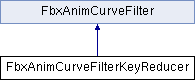
\includegraphics[height=2.000000cm]{class_fbx_anim_curve_filter_key_reducer}
\end{center}
\end{figure}
\subsection*{公開メンバ関数}
\begin{DoxyCompactItemize}
\item 
\hyperlink{class_fbx_anim_curve_filter_key_reducer_ad43e77bed0728ae7cd9f24e33753f984}{Fbx\+Anim\+Curve\+Filter\+Key\+Reducer} ()
\begin{DoxyCompactList}\small\item\em Constructor. \end{DoxyCompactList}\item 
virtual \hyperlink{class_fbx_anim_curve_filter_key_reducer_a69f345185767183595a34df13ae713c2}{$\sim$\+Fbx\+Anim\+Curve\+Filter\+Key\+Reducer} ()
\begin{DoxyCompactList}\small\item\em Destructor. \end{DoxyCompactList}\item 
virtual const char $\ast$ \hyperlink{class_fbx_anim_curve_filter_key_reducer_a86d571282e550eecbf7afb0f198ce91f}{Get\+Name} () const
\item 
virtual bool \hyperlink{class_fbx_anim_curve_filter_key_reducer_a8c0c58b8f2e4272bc5f257570daf5ba1}{Apply} (\hyperlink{class_fbx_anim_curve}{Fbx\+Anim\+Curve} $\ast$$\ast$p\+Curve, int p\+Count, \hyperlink{class_fbx_status}{Fbx\+Status} $\ast$p\+Status=\hyperlink{fbxarch_8h_a070d2ce7b6bb7e5c05602aa8c308d0c4}{N\+U\+LL})
\item 
virtual bool \hyperlink{class_fbx_anim_curve_filter_key_reducer_a8b2b0d1d3eaeb8d1333be55211a75b1a}{Apply} (\hyperlink{class_fbx_anim_curve}{Fbx\+Anim\+Curve} \&p\+Curve, \hyperlink{class_fbx_status}{Fbx\+Status} $\ast$p\+Status=\hyperlink{fbxarch_8h_a070d2ce7b6bb7e5c05602aa8c308d0c4}{N\+U\+LL})
\item 
virtual void \hyperlink{class_fbx_anim_curve_filter_key_reducer_a52e9e7476a3c4e55ad7c41c978b92cd5}{Reset} ()
\item 
double \hyperlink{class_fbx_anim_curve_filter_key_reducer_abd457aef2c4da70a5a6657947f078988}{Get\+Precision} () const
\begin{DoxyCompactList}\small\item\em Get precision. \end{DoxyCompactList}\item 
void \hyperlink{class_fbx_anim_curve_filter_key_reducer_a36e172b2c259e383897828f10036e277}{Set\+Precision} (double p\+Precision)
\item 
bool \hyperlink{class_fbx_anim_curve_filter_key_reducer_a82cb456079577735e58cba071eed3a12}{Get\+Key\+Sync} () const
\begin{DoxyCompactList}\small\item\em Return {\ttfamily true} key sync is applied at the end. \end{DoxyCompactList}\item 
void \hyperlink{class_fbx_anim_curve_filter_key_reducer_adf95529fab4de5a4e3a8d3112d6ba722}{Set\+Key\+Sync} (bool p\+Key\+Sync)
\end{DoxyCompactItemize}
\subsection*{Exposed parent class methods.}
\begin{DoxyCompactItemize}
\item 
virtual bool \hyperlink{class_fbx_anim_curve_filter_key_reducer_ace307ff2d9d99bf845ddaa26649fb136}{Apply} (\hyperlink{class_fbx_anim_stack}{Fbx\+Anim\+Stack} $\ast$p\+Anim\+Stack, \hyperlink{class_fbx_status}{Fbx\+Status} $\ast$p\+Status=\hyperlink{fbxarch_8h_a070d2ce7b6bb7e5c05602aa8c308d0c4}{N\+U\+LL})
\item 
virtual bool \hyperlink{class_fbx_anim_curve_filter_key_reducer_ac9cd8a32e87c1589d0f245be377a3da3}{Apply} (\hyperlink{class_fbx_object}{Fbx\+Object} $\ast$p\+Obj, \hyperlink{class_fbx_anim_stack}{Fbx\+Anim\+Stack} $\ast$p\+Anim\+Stack, \hyperlink{class_fbx_status}{Fbx\+Status} $\ast$p\+Status=\hyperlink{fbxarch_8h_a070d2ce7b6bb7e5c05602aa8c308d0c4}{N\+U\+LL})
\item 
virtual bool \hyperlink{class_fbx_anim_curve_filter_key_reducer_a1f3a0f984cf30eb74d9ae260ef9ae252}{Apply} (\hyperlink{class_fbx_anim_curve_node}{Fbx\+Anim\+Curve\+Node} \&p\+Curve\+Node, \hyperlink{class_fbx_status}{Fbx\+Status} $\ast$p\+Status=\hyperlink{fbxarch_8h_a070d2ce7b6bb7e5c05602aa8c308d0c4}{N\+U\+LL})
\end{DoxyCompactItemize}
\subsection*{その他の継承メンバ}


\subsection{詳解}
Key reducing filter.

Filter to test if each key is really necessary to define the curve at a definite degree of precision. It filters recursively from the strongest difference first. All useless keys are eliminated. 

 fbxanimcurvefilters.\+h の 539 行目に定義があります。



\subsection{構築子と解体子}
\mbox{\Hypertarget{class_fbx_anim_curve_filter_key_reducer_ad43e77bed0728ae7cd9f24e33753f984}\label{class_fbx_anim_curve_filter_key_reducer_ad43e77bed0728ae7cd9f24e33753f984}} 
\index{Fbx\+Anim\+Curve\+Filter\+Key\+Reducer@{Fbx\+Anim\+Curve\+Filter\+Key\+Reducer}!Fbx\+Anim\+Curve\+Filter\+Key\+Reducer@{Fbx\+Anim\+Curve\+Filter\+Key\+Reducer}}
\index{Fbx\+Anim\+Curve\+Filter\+Key\+Reducer@{Fbx\+Anim\+Curve\+Filter\+Key\+Reducer}!Fbx\+Anim\+Curve\+Filter\+Key\+Reducer@{Fbx\+Anim\+Curve\+Filter\+Key\+Reducer}}
\subsubsection{\texorpdfstring{Fbx\+Anim\+Curve\+Filter\+Key\+Reducer()}{FbxAnimCurveFilterKeyReducer()}}
{\footnotesize\ttfamily Fbx\+Anim\+Curve\+Filter\+Key\+Reducer\+::\+Fbx\+Anim\+Curve\+Filter\+Key\+Reducer (\begin{DoxyParamCaption}{ }\end{DoxyParamCaption})}



Constructor. 

\mbox{\Hypertarget{class_fbx_anim_curve_filter_key_reducer_a69f345185767183595a34df13ae713c2}\label{class_fbx_anim_curve_filter_key_reducer_a69f345185767183595a34df13ae713c2}} 
\index{Fbx\+Anim\+Curve\+Filter\+Key\+Reducer@{Fbx\+Anim\+Curve\+Filter\+Key\+Reducer}!````~Fbx\+Anim\+Curve\+Filter\+Key\+Reducer@{$\sim$\+Fbx\+Anim\+Curve\+Filter\+Key\+Reducer}}
\index{````~Fbx\+Anim\+Curve\+Filter\+Key\+Reducer@{$\sim$\+Fbx\+Anim\+Curve\+Filter\+Key\+Reducer}!Fbx\+Anim\+Curve\+Filter\+Key\+Reducer@{Fbx\+Anim\+Curve\+Filter\+Key\+Reducer}}
\subsubsection{\texorpdfstring{$\sim$\+Fbx\+Anim\+Curve\+Filter\+Key\+Reducer()}{~FbxAnimCurveFilterKeyReducer()}}
{\footnotesize\ttfamily virtual Fbx\+Anim\+Curve\+Filter\+Key\+Reducer\+::$\sim$\+Fbx\+Anim\+Curve\+Filter\+Key\+Reducer (\begin{DoxyParamCaption}{ }\end{DoxyParamCaption})\hspace{0.3cm}{\ttfamily [inline]}, {\ttfamily [virtual]}}



Destructor. 



 fbxanimcurvefilters.\+h の 546 行目に定義があります。



\subsection{関数詳解}
\mbox{\Hypertarget{class_fbx_anim_curve_filter_key_reducer_ace307ff2d9d99bf845ddaa26649fb136}\label{class_fbx_anim_curve_filter_key_reducer_ace307ff2d9d99bf845ddaa26649fb136}} 
\index{Fbx\+Anim\+Curve\+Filter\+Key\+Reducer@{Fbx\+Anim\+Curve\+Filter\+Key\+Reducer}!Apply@{Apply}}
\index{Apply@{Apply}!Fbx\+Anim\+Curve\+Filter\+Key\+Reducer@{Fbx\+Anim\+Curve\+Filter\+Key\+Reducer}}
\subsubsection{\texorpdfstring{Apply()}{Apply()}\hspace{0.1cm}{\footnotesize\ttfamily [1/5]}}
{\footnotesize\ttfamily virtual bool Fbx\+Anim\+Curve\+Filter\+Key\+Reducer\+::\+Apply (\begin{DoxyParamCaption}\item[{\hyperlink{class_fbx_anim_stack}{Fbx\+Anim\+Stack} $\ast$}]{p\+Anim\+Stack,  }\item[{\hyperlink{class_fbx_status}{Fbx\+Status} $\ast$}]{p\+Status = {\ttfamily \hyperlink{fbxarch_8h_a070d2ce7b6bb7e5c05602aa8c308d0c4}{N\+U\+LL}} }\end{DoxyParamCaption})\hspace{0.3cm}{\ttfamily [inline]}, {\ttfamily [virtual]}}

Apply filter to all the curves stored in the animation stack. 
\begin{DoxyParams}{引数}
{\em p\+Anim\+Stack} & Animation stack where to retrieve the animation curves \\
\hline
{\em p\+Status} & The \hyperlink{class_fbx_status}{Fbx\+Status} object to hold error codes. \\
\hline
\end{DoxyParams}
\begin{DoxyReturn}{戻り値}
{\ttfamily true} if the curve filtering operation was successful, {\ttfamily false} otherwise. 
\end{DoxyReturn}


\hyperlink{class_fbx_anim_curve_filter_aef3900e6180e05661c27ee484ae939c3}{Fbx\+Anim\+Curve\+Filter}を再実装しています。



 fbxanimcurvefilters.\+h の 557 行目に定義があります。

\mbox{\Hypertarget{class_fbx_anim_curve_filter_key_reducer_ac9cd8a32e87c1589d0f245be377a3da3}\label{class_fbx_anim_curve_filter_key_reducer_ac9cd8a32e87c1589d0f245be377a3da3}} 
\index{Fbx\+Anim\+Curve\+Filter\+Key\+Reducer@{Fbx\+Anim\+Curve\+Filter\+Key\+Reducer}!Apply@{Apply}}
\index{Apply@{Apply}!Fbx\+Anim\+Curve\+Filter\+Key\+Reducer@{Fbx\+Anim\+Curve\+Filter\+Key\+Reducer}}
\subsubsection{\texorpdfstring{Apply()}{Apply()}\hspace{0.1cm}{\footnotesize\ttfamily [2/5]}}
{\footnotesize\ttfamily virtual bool Fbx\+Anim\+Curve\+Filter\+Key\+Reducer\+::\+Apply (\begin{DoxyParamCaption}\item[{\hyperlink{class_fbx_object}{Fbx\+Object} $\ast$}]{p\+Obj,  }\item[{\hyperlink{class_fbx_anim_stack}{Fbx\+Anim\+Stack} $\ast$}]{p\+Anim\+Stack,  }\item[{\hyperlink{class_fbx_status}{Fbx\+Status} $\ast$}]{p\+Status = {\ttfamily \hyperlink{fbxarch_8h_a070d2ce7b6bb7e5c05602aa8c308d0c4}{N\+U\+LL}} }\end{DoxyParamCaption})\hspace{0.3cm}{\ttfamily [inline]}, {\ttfamily [virtual]}}

Apply filter to all the animated properties of the object. 
\begin{DoxyParams}{引数}
{\em p\+Obj} & Object containing the animated properties to which the filter is applied. \\
\hline
{\em p\+Anim\+Stack} & Animation stack where to retrieve the animation curves \\
\hline
{\em p\+Status} & The \hyperlink{class_fbx_status}{Fbx\+Status} object to hold error codes. \\
\hline
\end{DoxyParams}
\begin{DoxyReturn}{戻り値}
{\ttfamily true} if the curve filtering operation was successful, {\ttfamily false} otherwise. 
\end{DoxyReturn}


\hyperlink{class_fbx_anim_curve_filter_a009498a65af4995bf5e5908f17837531}{Fbx\+Anim\+Curve\+Filter}を再実装しています。



 fbxanimcurvefilters.\+h の 558 行目に定義があります。

\mbox{\Hypertarget{class_fbx_anim_curve_filter_key_reducer_a1f3a0f984cf30eb74d9ae260ef9ae252}\label{class_fbx_anim_curve_filter_key_reducer_a1f3a0f984cf30eb74d9ae260ef9ae252}} 
\index{Fbx\+Anim\+Curve\+Filter\+Key\+Reducer@{Fbx\+Anim\+Curve\+Filter\+Key\+Reducer}!Apply@{Apply}}
\index{Apply@{Apply}!Fbx\+Anim\+Curve\+Filter\+Key\+Reducer@{Fbx\+Anim\+Curve\+Filter\+Key\+Reducer}}
\subsubsection{\texorpdfstring{Apply()}{Apply()}\hspace{0.1cm}{\footnotesize\ttfamily [3/5]}}
{\footnotesize\ttfamily virtual bool Fbx\+Anim\+Curve\+Filter\+Key\+Reducer\+::\+Apply (\begin{DoxyParamCaption}\item[{\hyperlink{class_fbx_anim_curve_node}{Fbx\+Anim\+Curve\+Node} \&}]{p\+Curve\+Node,  }\item[{\hyperlink{class_fbx_status}{Fbx\+Status} $\ast$}]{p\+Status = {\ttfamily \hyperlink{fbxarch_8h_a070d2ce7b6bb7e5c05602aa8c308d0c4}{N\+U\+LL}} }\end{DoxyParamCaption})\hspace{0.3cm}{\ttfamily [inline]}, {\ttfamily [virtual]}}

Apply filter on all the curves of an animation curve node. 
\begin{DoxyParams}{引数}
{\em p\+Curve\+Node} & Curve node to which the filter is applied. \\
\hline
{\em p\+Status} & The \hyperlink{class_fbx_status}{Fbx\+Status} object to hold error codes. \\
\hline
\end{DoxyParams}
\begin{DoxyReturn}{戻り値}
{\ttfamily true} if the curve filtering operation was successful, {\ttfamily false} otherwise. 
\end{DoxyReturn}
\begin{DoxyRemark}{注釈}
This method collects all the \hyperlink{class_fbx_anim_curve}{Fbx\+Anim\+Curve} objects connected to the curve node and calls Apply(\+Fbx\+Anim\+Curve$\ast$$\ast$, int) 
\end{DoxyRemark}


\hyperlink{class_fbx_anim_curve_filter_ad042b45c0675278fa49e61739b0825c2}{Fbx\+Anim\+Curve\+Filter}を再実装しています。



 fbxanimcurvefilters.\+h の 559 行目に定義があります。

\mbox{\Hypertarget{class_fbx_anim_curve_filter_key_reducer_a8c0c58b8f2e4272bc5f257570daf5ba1}\label{class_fbx_anim_curve_filter_key_reducer_a8c0c58b8f2e4272bc5f257570daf5ba1}} 
\index{Fbx\+Anim\+Curve\+Filter\+Key\+Reducer@{Fbx\+Anim\+Curve\+Filter\+Key\+Reducer}!Apply@{Apply}}
\index{Apply@{Apply}!Fbx\+Anim\+Curve\+Filter\+Key\+Reducer@{Fbx\+Anim\+Curve\+Filter\+Key\+Reducer}}
\subsubsection{\texorpdfstring{Apply()}{Apply()}\hspace{0.1cm}{\footnotesize\ttfamily [4/5]}}
{\footnotesize\ttfamily virtual bool Fbx\+Anim\+Curve\+Filter\+Key\+Reducer\+::\+Apply (\begin{DoxyParamCaption}\item[{\hyperlink{class_fbx_anim_curve}{Fbx\+Anim\+Curve} $\ast$$\ast$}]{p\+Curve,  }\item[{int}]{p\+Count,  }\item[{\hyperlink{class_fbx_status}{Fbx\+Status} $\ast$}]{p\+Status = {\ttfamily \hyperlink{fbxarch_8h_a070d2ce7b6bb7e5c05602aa8c308d0c4}{N\+U\+LL}} }\end{DoxyParamCaption})\hspace{0.3cm}{\ttfamily [virtual]}}

Apply filter on the given animation curve. 
\begin{DoxyParams}{引数}
{\em p\+Curve} & Array of curve to which the filter is applied. \\
\hline
{\em p\+Count} & Number of curves in array. \\
\hline
{\em p\+Status} & The \hyperlink{class_fbx_status}{Fbx\+Status} object to hold error codes. \\
\hline
\end{DoxyParams}
\begin{DoxyReturn}{戻り値}
{\ttfamily true} if the curve filtering operation was successful, {\ttfamily false} otherwise. 
\end{DoxyReturn}


\hyperlink{class_fbx_anim_curve_filter_aca6a41fbc4d9019b20df7adccfa6ed3c}{Fbx\+Anim\+Curve\+Filter}を再実装しています。

\mbox{\Hypertarget{class_fbx_anim_curve_filter_key_reducer_a8b2b0d1d3eaeb8d1333be55211a75b1a}\label{class_fbx_anim_curve_filter_key_reducer_a8b2b0d1d3eaeb8d1333be55211a75b1a}} 
\index{Fbx\+Anim\+Curve\+Filter\+Key\+Reducer@{Fbx\+Anim\+Curve\+Filter\+Key\+Reducer}!Apply@{Apply}}
\index{Apply@{Apply}!Fbx\+Anim\+Curve\+Filter\+Key\+Reducer@{Fbx\+Anim\+Curve\+Filter\+Key\+Reducer}}
\subsubsection{\texorpdfstring{Apply()}{Apply()}\hspace{0.1cm}{\footnotesize\ttfamily [5/5]}}
{\footnotesize\ttfamily virtual bool Fbx\+Anim\+Curve\+Filter\+Key\+Reducer\+::\+Apply (\begin{DoxyParamCaption}\item[{\hyperlink{class_fbx_anim_curve}{Fbx\+Anim\+Curve} \&}]{p\+Curve,  }\item[{\hyperlink{class_fbx_status}{Fbx\+Status} $\ast$}]{p\+Status = {\ttfamily \hyperlink{fbxarch_8h_a070d2ce7b6bb7e5c05602aa8c308d0c4}{N\+U\+LL}} }\end{DoxyParamCaption})\hspace{0.3cm}{\ttfamily [virtual]}}

Apply filter on an animation curve. 
\begin{DoxyParams}{引数}
{\em p\+Curve} & Curve to which the filter is applied. \\
\hline
{\em p\+Status} & The \hyperlink{class_fbx_status}{Fbx\+Status} object to hold error codes. \\
\hline
\end{DoxyParams}
\begin{DoxyReturn}{戻り値}
{\ttfamily true} if the curve filtering operation was successful, {\ttfamily false} otherwise. 
\end{DoxyReturn}


\hyperlink{class_fbx_anim_curve_filter_a6a69996c47c0e6f63a0f8b0d5fa806a0}{Fbx\+Anim\+Curve\+Filter}を実装しています。

\mbox{\Hypertarget{class_fbx_anim_curve_filter_key_reducer_a82cb456079577735e58cba071eed3a12}\label{class_fbx_anim_curve_filter_key_reducer_a82cb456079577735e58cba071eed3a12}} 
\index{Fbx\+Anim\+Curve\+Filter\+Key\+Reducer@{Fbx\+Anim\+Curve\+Filter\+Key\+Reducer}!Get\+Key\+Sync@{Get\+Key\+Sync}}
\index{Get\+Key\+Sync@{Get\+Key\+Sync}!Fbx\+Anim\+Curve\+Filter\+Key\+Reducer@{Fbx\+Anim\+Curve\+Filter\+Key\+Reducer}}
\subsubsection{\texorpdfstring{Get\+Key\+Sync()}{GetKeySync()}}
{\footnotesize\ttfamily bool Fbx\+Anim\+Curve\+Filter\+Key\+Reducer\+::\+Get\+Key\+Sync (\begin{DoxyParamCaption}{ }\end{DoxyParamCaption}) const}



Return {\ttfamily true} key sync is applied at the end. 

\mbox{\Hypertarget{class_fbx_anim_curve_filter_key_reducer_a86d571282e550eecbf7afb0f198ce91f}\label{class_fbx_anim_curve_filter_key_reducer_a86d571282e550eecbf7afb0f198ce91f}} 
\index{Fbx\+Anim\+Curve\+Filter\+Key\+Reducer@{Fbx\+Anim\+Curve\+Filter\+Key\+Reducer}!Get\+Name@{Get\+Name}}
\index{Get\+Name@{Get\+Name}!Fbx\+Anim\+Curve\+Filter\+Key\+Reducer@{Fbx\+Anim\+Curve\+Filter\+Key\+Reducer}}
\subsubsection{\texorpdfstring{Get\+Name()}{GetName()}}
{\footnotesize\ttfamily virtual const char$\ast$ Fbx\+Anim\+Curve\+Filter\+Key\+Reducer\+::\+Get\+Name (\begin{DoxyParamCaption}{ }\end{DoxyParamCaption}) const\hspace{0.3cm}{\ttfamily [virtual]}}

Get the name of the filter. \begin{DoxyReturn}{戻り値}
Pointer to name. 
\end{DoxyReturn}


\hyperlink{class_fbx_anim_curve_filter_abd559d5052fbb072042e59241940a35c}{Fbx\+Anim\+Curve\+Filter}を再実装しています。

\mbox{\Hypertarget{class_fbx_anim_curve_filter_key_reducer_abd457aef2c4da70a5a6657947f078988}\label{class_fbx_anim_curve_filter_key_reducer_abd457aef2c4da70a5a6657947f078988}} 
\index{Fbx\+Anim\+Curve\+Filter\+Key\+Reducer@{Fbx\+Anim\+Curve\+Filter\+Key\+Reducer}!Get\+Precision@{Get\+Precision}}
\index{Get\+Precision@{Get\+Precision}!Fbx\+Anim\+Curve\+Filter\+Key\+Reducer@{Fbx\+Anim\+Curve\+Filter\+Key\+Reducer}}
\subsubsection{\texorpdfstring{Get\+Precision()}{GetPrecision()}}
{\footnotesize\ttfamily double Fbx\+Anim\+Curve\+Filter\+Key\+Reducer\+::\+Get\+Precision (\begin{DoxyParamCaption}{ }\end{DoxyParamCaption}) const}



Get precision. 

\mbox{\Hypertarget{class_fbx_anim_curve_filter_key_reducer_a52e9e7476a3c4e55ad7c41c978b92cd5}\label{class_fbx_anim_curve_filter_key_reducer_a52e9e7476a3c4e55ad7c41c978b92cd5}} 
\index{Fbx\+Anim\+Curve\+Filter\+Key\+Reducer@{Fbx\+Anim\+Curve\+Filter\+Key\+Reducer}!Reset@{Reset}}
\index{Reset@{Reset}!Fbx\+Anim\+Curve\+Filter\+Key\+Reducer@{Fbx\+Anim\+Curve\+Filter\+Key\+Reducer}}
\subsubsection{\texorpdfstring{Reset()}{Reset()}}
{\footnotesize\ttfamily virtual void Fbx\+Anim\+Curve\+Filter\+Key\+Reducer\+::\+Reset (\begin{DoxyParamCaption}{ }\end{DoxyParamCaption})\hspace{0.3cm}{\ttfamily [virtual]}}

Reset the filter to its default parameters. 

\hyperlink{class_fbx_anim_curve_filter_a57fb35baaaa85adb08946383cf40e811}{Fbx\+Anim\+Curve\+Filter}を再実装しています。

\mbox{\Hypertarget{class_fbx_anim_curve_filter_key_reducer_adf95529fab4de5a4e3a8d3112d6ba722}\label{class_fbx_anim_curve_filter_key_reducer_adf95529fab4de5a4e3a8d3112d6ba722}} 
\index{Fbx\+Anim\+Curve\+Filter\+Key\+Reducer@{Fbx\+Anim\+Curve\+Filter\+Key\+Reducer}!Set\+Key\+Sync@{Set\+Key\+Sync}}
\index{Set\+Key\+Sync@{Set\+Key\+Sync}!Fbx\+Anim\+Curve\+Filter\+Key\+Reducer@{Fbx\+Anim\+Curve\+Filter\+Key\+Reducer}}
\subsubsection{\texorpdfstring{Set\+Key\+Sync()}{SetKeySync()}}
{\footnotesize\ttfamily void Fbx\+Anim\+Curve\+Filter\+Key\+Reducer\+::\+Set\+Key\+Sync (\begin{DoxyParamCaption}\item[{bool}]{p\+Key\+Sync }\end{DoxyParamCaption})}

Set to {\ttfamily true} to apply key sync at the end. 
\begin{DoxyParams}{引数}
{\em p\+Key\+Sync} & Key sync flag. \\
\hline
\end{DoxyParams}
\mbox{\Hypertarget{class_fbx_anim_curve_filter_key_reducer_a36e172b2c259e383897828f10036e277}\label{class_fbx_anim_curve_filter_key_reducer_a36e172b2c259e383897828f10036e277}} 
\index{Fbx\+Anim\+Curve\+Filter\+Key\+Reducer@{Fbx\+Anim\+Curve\+Filter\+Key\+Reducer}!Set\+Precision@{Set\+Precision}}
\index{Set\+Precision@{Set\+Precision}!Fbx\+Anim\+Curve\+Filter\+Key\+Reducer@{Fbx\+Anim\+Curve\+Filter\+Key\+Reducer}}
\subsubsection{\texorpdfstring{Set\+Precision()}{SetPrecision()}}
{\footnotesize\ttfamily void Fbx\+Anim\+Curve\+Filter\+Key\+Reducer\+::\+Set\+Precision (\begin{DoxyParamCaption}\item[{double}]{p\+Precision }\end{DoxyParamCaption})}

Set precision. 
\begin{DoxyParams}{引数}
{\em p\+Precision} & The precision to set. \\
\hline
\end{DoxyParams}


このクラス詳解は次のファイルから抽出されました\+:\begin{DoxyCompactItemize}
\item 
C\+:/\+Maya/scripts/\+F\+B\+X\+\_\+\+S\+D\+K/2017.\+1/include/fbxsdk/scene/animation/\hyperlink{fbxanimcurvefilters_8h}{fbxanimcurvefilters.\+h}\end{DoxyCompactItemize}

\hypertarget{class_fbx_anim_curve_filter_key_sync}{}\section{Fbx\+Anim\+Curve\+Filter\+Key\+Sync クラス}
\label{class_fbx_anim_curve_filter_key_sync}\index{Fbx\+Anim\+Curve\+Filter\+Key\+Sync@{Fbx\+Anim\+Curve\+Filter\+Key\+Sync}}


{\ttfamily \#include $<$fbxanimcurvefilters.\+h$>$}



Fbx\+Anim\+Curve\+Filter\+Key\+Sync の継承関係図
% FIG 0


Fbx\+Anim\+Curve\+Filter\+Key\+Sync 連携図
% FIG 1
\subsection*{公開メンバ関数}
\begin{DoxyCompactItemize}
\item 
\hyperlink{class_fbx_anim_curve_filter_key_sync_ad9ffdb980ce6b78a53a5447c2e7d61d9}{Fbx\+Anim\+Curve\+Filter\+Key\+Sync} ()
\begin{DoxyCompactList}\small\item\em Constructor. \end{DoxyCompactList}\item 
virtual \hyperlink{class_fbx_anim_curve_filter_key_sync_a4435b8ba11b1978833538f18405811fb}{$\sim$\+Fbx\+Anim\+Curve\+Filter\+Key\+Sync} ()
\begin{DoxyCompactList}\small\item\em Destructor. \end{DoxyCompactList}\item 
virtual const char $\ast$ \hyperlink{class_fbx_anim_curve_filter_key_sync_acf561aadd8d5f4b35826044c6d50b6b4}{Get\+Name} () const
\item 
virtual bool \hyperlink{class_fbx_anim_curve_filter_key_sync_aa26aa6ed4121353882589902fb0db961}{Need\+Apply} (\hyperlink{class_fbx_anim_curve}{Fbx\+Anim\+Curve} $\ast$$\ast$p\+Curve, int p\+Count, \hyperlink{class_fbx_status}{Fbx\+Status} $\ast$p\+Status=\hyperlink{fbxarch_8h_a070d2ce7b6bb7e5c05602aa8c308d0c4}{N\+U\+LL})
\item 
virtual bool \hyperlink{class_fbx_anim_curve_filter_key_sync_a5f255ee33fe2ecad8c61562931840c01}{Need\+Apply} (\hyperlink{class_fbx_anim_curve}{Fbx\+Anim\+Curve} \&, \hyperlink{class_fbx_status}{Fbx\+Status} $\ast$p\+Status=\hyperlink{fbxarch_8h_a070d2ce7b6bb7e5c05602aa8c308d0c4}{N\+U\+LL})
\item 
virtual bool \hyperlink{class_fbx_anim_curve_filter_key_sync_aa42855bf1a2c78e9d7392bdc48d99881}{Apply} (\hyperlink{class_fbx_anim_curve}{Fbx\+Anim\+Curve} $\ast$$\ast$p\+Curve, int p\+Count, \hyperlink{class_fbx_status}{Fbx\+Status} $\ast$p\+Status=\hyperlink{fbxarch_8h_a070d2ce7b6bb7e5c05602aa8c308d0c4}{N\+U\+LL})
\item 
virtual bool \hyperlink{class_fbx_anim_curve_filter_key_sync_acc77ba686024c5f204e9e78e52dc15f5}{Apply} (\hyperlink{class_fbx_anim_curve}{Fbx\+Anim\+Curve} \&, \hyperlink{class_fbx_status}{Fbx\+Status} $\ast$p\+Status=\hyperlink{fbxarch_8h_a070d2ce7b6bb7e5c05602aa8c308d0c4}{N\+U\+LL})
\end{DoxyCompactItemize}
\subsection*{Exposed parent class methods.}
\begin{DoxyCompactItemize}
\item 
virtual bool \hyperlink{class_fbx_anim_curve_filter_key_sync_a987ccf74bf3bdf7828812067d895950c}{Need\+Apply} (\hyperlink{class_fbx_anim_stack}{Fbx\+Anim\+Stack} $\ast$p\+Anim\+Stack, \hyperlink{class_fbx_status}{Fbx\+Status} $\ast$p\+Status=\hyperlink{fbxarch_8h_a070d2ce7b6bb7e5c05602aa8c308d0c4}{N\+U\+LL})
\item 
virtual bool \hyperlink{class_fbx_anim_curve_filter_key_sync_a1b541b170fcb33fb1bc2daf43ec08347}{Need\+Apply} (\hyperlink{class_fbx_object}{Fbx\+Object} $\ast$p\+Obj, \hyperlink{class_fbx_anim_stack}{Fbx\+Anim\+Stack} $\ast$p\+Anim\+Stack, \hyperlink{class_fbx_status}{Fbx\+Status} $\ast$p\+Status=\hyperlink{fbxarch_8h_a070d2ce7b6bb7e5c05602aa8c308d0c4}{N\+U\+LL})
\item 
virtual bool \hyperlink{class_fbx_anim_curve_filter_key_sync_a72cb983cb554a070688eb0990d4b7576}{Need\+Apply} (\hyperlink{class_fbx_anim_curve_node}{Fbx\+Anim\+Curve\+Node} \&p\+Curve\+Node, \hyperlink{class_fbx_status}{Fbx\+Status} $\ast$p\+Status=\hyperlink{fbxarch_8h_a070d2ce7b6bb7e5c05602aa8c308d0c4}{N\+U\+LL})
\item 
virtual bool \hyperlink{class_fbx_anim_curve_filter_key_sync_a4eb3dd7372f7747bcae1be8722db75e0}{Apply} (\hyperlink{class_fbx_anim_stack}{Fbx\+Anim\+Stack} $\ast$p\+Anim\+Stack, \hyperlink{class_fbx_status}{Fbx\+Status} $\ast$p\+Status=\hyperlink{fbxarch_8h_a070d2ce7b6bb7e5c05602aa8c308d0c4}{N\+U\+LL})
\item 
virtual bool \hyperlink{class_fbx_anim_curve_filter_key_sync_a0a46860b4847773c09ea2c57f77f11dd}{Apply} (\hyperlink{class_fbx_object}{Fbx\+Object} $\ast$p\+Obj, \hyperlink{class_fbx_anim_stack}{Fbx\+Anim\+Stack} $\ast$p\+Anim\+Stack, \hyperlink{class_fbx_status}{Fbx\+Status} $\ast$p\+Status=\hyperlink{fbxarch_8h_a070d2ce7b6bb7e5c05602aa8c308d0c4}{N\+U\+LL})
\item 
virtual bool \hyperlink{class_fbx_anim_curve_filter_key_sync_ad85aff7b0cd6b4ce563002b6d52c0041}{Apply} (\hyperlink{class_fbx_anim_curve_node}{Fbx\+Anim\+Curve\+Node} \&p\+Curve\+Node, \hyperlink{class_fbx_status}{Fbx\+Status} $\ast$p\+Status=\hyperlink{fbxarch_8h_a070d2ce7b6bb7e5c05602aa8c308d0c4}{N\+U\+LL})
\end{DoxyCompactItemize}
\subsection*{その他の継承メンバ}


\subsection{詳解}
Key sync filter.

Filter to synchronize the keys of a set of animation curves. 

\subsection{構築子と解体子}
\mbox{\Hypertarget{class_fbx_anim_curve_filter_key_sync_ad9ffdb980ce6b78a53a5447c2e7d61d9}\label{class_fbx_anim_curve_filter_key_sync_ad9ffdb980ce6b78a53a5447c2e7d61d9}} 
\index{Fbx\+Anim\+Curve\+Filter\+Key\+Sync@{Fbx\+Anim\+Curve\+Filter\+Key\+Sync}!Fbx\+Anim\+Curve\+Filter\+Key\+Sync@{Fbx\+Anim\+Curve\+Filter\+Key\+Sync}}
\index{Fbx\+Anim\+Curve\+Filter\+Key\+Sync@{Fbx\+Anim\+Curve\+Filter\+Key\+Sync}!Fbx\+Anim\+Curve\+Filter\+Key\+Sync@{Fbx\+Anim\+Curve\+Filter\+Key\+Sync}}
\subsubsection{\texorpdfstring{Fbx\+Anim\+Curve\+Filter\+Key\+Sync()}{FbxAnimCurveFilterKeySync()}}
{\footnotesize\ttfamily Fbx\+Anim\+Curve\+Filter\+Key\+Sync\+::\+Fbx\+Anim\+Curve\+Filter\+Key\+Sync (\begin{DoxyParamCaption}{ }\end{DoxyParamCaption})}



Constructor. 

\mbox{\Hypertarget{class_fbx_anim_curve_filter_key_sync_a4435b8ba11b1978833538f18405811fb}\label{class_fbx_anim_curve_filter_key_sync_a4435b8ba11b1978833538f18405811fb}} 
\index{Fbx\+Anim\+Curve\+Filter\+Key\+Sync@{Fbx\+Anim\+Curve\+Filter\+Key\+Sync}!````~Fbx\+Anim\+Curve\+Filter\+Key\+Sync@{$\sim$\+Fbx\+Anim\+Curve\+Filter\+Key\+Sync}}
\index{````~Fbx\+Anim\+Curve\+Filter\+Key\+Sync@{$\sim$\+Fbx\+Anim\+Curve\+Filter\+Key\+Sync}!Fbx\+Anim\+Curve\+Filter\+Key\+Sync@{Fbx\+Anim\+Curve\+Filter\+Key\+Sync}}
\subsubsection{\texorpdfstring{$\sim$\+Fbx\+Anim\+Curve\+Filter\+Key\+Sync()}{~FbxAnimCurveFilterKeySync()}}
{\footnotesize\ttfamily virtual Fbx\+Anim\+Curve\+Filter\+Key\+Sync\+::$\sim$\+Fbx\+Anim\+Curve\+Filter\+Key\+Sync (\begin{DoxyParamCaption}{ }\end{DoxyParamCaption})\hspace{0.3cm}{\ttfamily [virtual]}}



Destructor. 

呼び出し関係図\+:
% FIG 2


\subsection{メソッド詳解}
\mbox{\Hypertarget{class_fbx_anim_curve_filter_key_sync_a4eb3dd7372f7747bcae1be8722db75e0}\label{class_fbx_anim_curve_filter_key_sync_a4eb3dd7372f7747bcae1be8722db75e0}} 
\index{Fbx\+Anim\+Curve\+Filter\+Key\+Sync@{Fbx\+Anim\+Curve\+Filter\+Key\+Sync}!Apply@{Apply}}
\index{Apply@{Apply}!Fbx\+Anim\+Curve\+Filter\+Key\+Sync@{Fbx\+Anim\+Curve\+Filter\+Key\+Sync}}
\subsubsection{\texorpdfstring{Apply()}{Apply()}\hspace{0.1cm}{\footnotesize\ttfamily [1/5]}}
{\footnotesize\ttfamily virtual bool Fbx\+Anim\+Curve\+Filter\+Key\+Sync\+::\+Apply (\begin{DoxyParamCaption}\item[{\hyperlink{class_fbx_anim_stack}{Fbx\+Anim\+Stack} $\ast$}]{p\+Anim\+Stack,  }\item[{\hyperlink{class_fbx_status}{Fbx\+Status} $\ast$}]{p\+Status = {\ttfamily \hyperlink{fbxarch_8h_a070d2ce7b6bb7e5c05602aa8c308d0c4}{N\+U\+LL}} }\end{DoxyParamCaption})\hspace{0.3cm}{\ttfamily [virtual]}}

Apply filter to all the curves stored in the animation stack. 
\begin{DoxyParams}{引数}
{\em p\+Anim\+Stack} & Animation stack where to retrieve the animation curves \\
\hline
{\em p\+Status} & The \hyperlink{class_fbx_status}{Fbx\+Status} object to hold error codes. \\
\hline
\end{DoxyParams}
\begin{DoxyReturn}{戻り値}
{\ttfamily true} if the curve filtering operation was successful, {\ttfamily false} otherwise. 
\end{DoxyReturn}


\hyperlink{class_fbx_anim_curve_filter_aef3900e6180e05661c27ee484ae939c3}{Fbx\+Anim\+Curve\+Filter}を再実装しています。

呼び出し関係図\+:
% FIG 3
\mbox{\Hypertarget{class_fbx_anim_curve_filter_key_sync_a0a46860b4847773c09ea2c57f77f11dd}\label{class_fbx_anim_curve_filter_key_sync_a0a46860b4847773c09ea2c57f77f11dd}} 
\index{Fbx\+Anim\+Curve\+Filter\+Key\+Sync@{Fbx\+Anim\+Curve\+Filter\+Key\+Sync}!Apply@{Apply}}
\index{Apply@{Apply}!Fbx\+Anim\+Curve\+Filter\+Key\+Sync@{Fbx\+Anim\+Curve\+Filter\+Key\+Sync}}
\subsubsection{\texorpdfstring{Apply()}{Apply()}\hspace{0.1cm}{\footnotesize\ttfamily [2/5]}}
{\footnotesize\ttfamily virtual bool Fbx\+Anim\+Curve\+Filter\+Key\+Sync\+::\+Apply (\begin{DoxyParamCaption}\item[{\hyperlink{class_fbx_object}{Fbx\+Object} $\ast$}]{p\+Obj,  }\item[{\hyperlink{class_fbx_anim_stack}{Fbx\+Anim\+Stack} $\ast$}]{p\+Anim\+Stack,  }\item[{\hyperlink{class_fbx_status}{Fbx\+Status} $\ast$}]{p\+Status = {\ttfamily \hyperlink{fbxarch_8h_a070d2ce7b6bb7e5c05602aa8c308d0c4}{N\+U\+LL}} }\end{DoxyParamCaption})\hspace{0.3cm}{\ttfamily [virtual]}}

Apply filter to all the animated properties of the object. 
\begin{DoxyParams}{引数}
{\em p\+Obj} & Object containing the animated properties to which the filter is applied. \\
\hline
{\em p\+Anim\+Stack} & Animation stack where to retrieve the animation curves \\
\hline
{\em p\+Status} & The \hyperlink{class_fbx_status}{Fbx\+Status} object to hold error codes. \\
\hline
\end{DoxyParams}
\begin{DoxyReturn}{戻り値}
{\ttfamily true} if the curve filtering operation was successful, {\ttfamily false} otherwise. 
\end{DoxyReturn}


\hyperlink{class_fbx_anim_curve_filter_a009498a65af4995bf5e5908f17837531}{Fbx\+Anim\+Curve\+Filter}を再実装しています。

呼び出し関係図\+:
% FIG 4
\mbox{\Hypertarget{class_fbx_anim_curve_filter_key_sync_ad85aff7b0cd6b4ce563002b6d52c0041}\label{class_fbx_anim_curve_filter_key_sync_ad85aff7b0cd6b4ce563002b6d52c0041}} 
\index{Fbx\+Anim\+Curve\+Filter\+Key\+Sync@{Fbx\+Anim\+Curve\+Filter\+Key\+Sync}!Apply@{Apply}}
\index{Apply@{Apply}!Fbx\+Anim\+Curve\+Filter\+Key\+Sync@{Fbx\+Anim\+Curve\+Filter\+Key\+Sync}}
\subsubsection{\texorpdfstring{Apply()}{Apply()}\hspace{0.1cm}{\footnotesize\ttfamily [3/5]}}
{\footnotesize\ttfamily virtual bool Fbx\+Anim\+Curve\+Filter\+Key\+Sync\+::\+Apply (\begin{DoxyParamCaption}\item[{\hyperlink{class_fbx_anim_curve_node}{Fbx\+Anim\+Curve\+Node} \&}]{p\+Curve\+Node,  }\item[{\hyperlink{class_fbx_status}{Fbx\+Status} $\ast$}]{p\+Status = {\ttfamily \hyperlink{fbxarch_8h_a070d2ce7b6bb7e5c05602aa8c308d0c4}{N\+U\+LL}} }\end{DoxyParamCaption})\hspace{0.3cm}{\ttfamily [virtual]}}

Apply filter on all the curves of an animation curve node. 
\begin{DoxyParams}{引数}
{\em p\+Curve\+Node} & Curve node to which the filter is applied. \\
\hline
{\em p\+Status} & The \hyperlink{class_fbx_status}{Fbx\+Status} object to hold error codes. \\
\hline
\end{DoxyParams}
\begin{DoxyReturn}{戻り値}
{\ttfamily true} if the curve filtering operation was successful, {\ttfamily false} otherwise. 
\end{DoxyReturn}
\begin{DoxyRemark}{注釈}
This method collects all the \hyperlink{class_fbx_anim_curve}{Fbx\+Anim\+Curve} objects connected to the curve node and calls Apply(\+Fbx\+Anim\+Curve$\ast$$\ast$, int) 
\end{DoxyRemark}


\hyperlink{class_fbx_anim_curve_filter_ad042b45c0675278fa49e61739b0825c2}{Fbx\+Anim\+Curve\+Filter}を再実装しています。

呼び出し関係図\+:
% FIG 5
\mbox{\Hypertarget{class_fbx_anim_curve_filter_key_sync_aa42855bf1a2c78e9d7392bdc48d99881}\label{class_fbx_anim_curve_filter_key_sync_aa42855bf1a2c78e9d7392bdc48d99881}} 
\index{Fbx\+Anim\+Curve\+Filter\+Key\+Sync@{Fbx\+Anim\+Curve\+Filter\+Key\+Sync}!Apply@{Apply}}
\index{Apply@{Apply}!Fbx\+Anim\+Curve\+Filter\+Key\+Sync@{Fbx\+Anim\+Curve\+Filter\+Key\+Sync}}
\subsubsection{\texorpdfstring{Apply()}{Apply()}\hspace{0.1cm}{\footnotesize\ttfamily [4/5]}}
{\footnotesize\ttfamily virtual bool Fbx\+Anim\+Curve\+Filter\+Key\+Sync\+::\+Apply (\begin{DoxyParamCaption}\item[{\hyperlink{class_fbx_anim_curve}{Fbx\+Anim\+Curve} $\ast$$\ast$}]{p\+Curve,  }\item[{int}]{p\+Count,  }\item[{\hyperlink{class_fbx_status}{Fbx\+Status} $\ast$}]{p\+Status = {\ttfamily \hyperlink{fbxarch_8h_a070d2ce7b6bb7e5c05602aa8c308d0c4}{N\+U\+LL}} }\end{DoxyParamCaption})\hspace{0.3cm}{\ttfamily [virtual]}}

Apply filter on the given animation curve. 
\begin{DoxyParams}{引数}
{\em p\+Curve} & Array of curve to which the filter is applied. \\
\hline
{\em p\+Count} & Number of curves in array. \\
\hline
{\em p\+Status} & The \hyperlink{class_fbx_status}{Fbx\+Status} object to hold error codes. \\
\hline
\end{DoxyParams}
\begin{DoxyReturn}{戻り値}
{\ttfamily true} if the curve filtering operation was successful, {\ttfamily false} otherwise. 
\end{DoxyReturn}


\hyperlink{class_fbx_anim_curve_filter_aca6a41fbc4d9019b20df7adccfa6ed3c}{Fbx\+Anim\+Curve\+Filter}を再実装しています。

\mbox{\Hypertarget{class_fbx_anim_curve_filter_key_sync_acc77ba686024c5f204e9e78e52dc15f5}\label{class_fbx_anim_curve_filter_key_sync_acc77ba686024c5f204e9e78e52dc15f5}} 
\index{Fbx\+Anim\+Curve\+Filter\+Key\+Sync@{Fbx\+Anim\+Curve\+Filter\+Key\+Sync}!Apply@{Apply}}
\index{Apply@{Apply}!Fbx\+Anim\+Curve\+Filter\+Key\+Sync@{Fbx\+Anim\+Curve\+Filter\+Key\+Sync}}
\subsubsection{\texorpdfstring{Apply()}{Apply()}\hspace{0.1cm}{\footnotesize\ttfamily [5/5]}}
{\footnotesize\ttfamily virtual bool Fbx\+Anim\+Curve\+Filter\+Key\+Sync\+::\+Apply (\begin{DoxyParamCaption}\item[{\hyperlink{class_fbx_anim_curve}{Fbx\+Anim\+Curve} \&}]{,  }\item[{\hyperlink{class_fbx_status}{Fbx\+Status} $\ast$}]{p\+Status = {\ttfamily \hyperlink{fbxarch_8h_a070d2ce7b6bb7e5c05602aa8c308d0c4}{N\+U\+LL}} }\end{DoxyParamCaption})\hspace{0.3cm}{\ttfamily [virtual]}}

Apply filter on an animation curve. 
\begin{DoxyParams}{引数}
{\em p\+Curve} & Curve to which the filter is applied. \\
\hline
{\em p\+Status} & The \hyperlink{class_fbx_status}{Fbx\+Status} object to hold error codes. \\
\hline
\end{DoxyParams}
\begin{DoxyReturn}{戻り値}
{\ttfamily true}. 
\end{DoxyReturn}
\begin{DoxyRemark}{注釈}
Has no effect since there is only one curve. 
\end{DoxyRemark}


\hyperlink{class_fbx_anim_curve_filter_a6a69996c47c0e6f63a0f8b0d5fa806a0}{Fbx\+Anim\+Curve\+Filter}を実装しています。

\mbox{\Hypertarget{class_fbx_anim_curve_filter_key_sync_acf561aadd8d5f4b35826044c6d50b6b4}\label{class_fbx_anim_curve_filter_key_sync_acf561aadd8d5f4b35826044c6d50b6b4}} 
\index{Fbx\+Anim\+Curve\+Filter\+Key\+Sync@{Fbx\+Anim\+Curve\+Filter\+Key\+Sync}!Get\+Name@{Get\+Name}}
\index{Get\+Name@{Get\+Name}!Fbx\+Anim\+Curve\+Filter\+Key\+Sync@{Fbx\+Anim\+Curve\+Filter\+Key\+Sync}}
\subsubsection{\texorpdfstring{Get\+Name()}{GetName()}}
{\footnotesize\ttfamily virtual const char$\ast$ Fbx\+Anim\+Curve\+Filter\+Key\+Sync\+::\+Get\+Name (\begin{DoxyParamCaption}{ }\end{DoxyParamCaption}) const\hspace{0.3cm}{\ttfamily [virtual]}}

Get the name of the filter. \begin{DoxyReturn}{戻り値}
Pointer to name. 
\end{DoxyReturn}


\hyperlink{class_fbx_anim_curve_filter_abd559d5052fbb072042e59241940a35c}{Fbx\+Anim\+Curve\+Filter}を再実装しています。

\mbox{\Hypertarget{class_fbx_anim_curve_filter_key_sync_a987ccf74bf3bdf7828812067d895950c}\label{class_fbx_anim_curve_filter_key_sync_a987ccf74bf3bdf7828812067d895950c}} 
\index{Fbx\+Anim\+Curve\+Filter\+Key\+Sync@{Fbx\+Anim\+Curve\+Filter\+Key\+Sync}!Need\+Apply@{Need\+Apply}}
\index{Need\+Apply@{Need\+Apply}!Fbx\+Anim\+Curve\+Filter\+Key\+Sync@{Fbx\+Anim\+Curve\+Filter\+Key\+Sync}}
\subsubsection{\texorpdfstring{Need\+Apply()}{NeedApply()}\hspace{0.1cm}{\footnotesize\ttfamily [1/5]}}
{\footnotesize\ttfamily virtual bool Fbx\+Anim\+Curve\+Filter\+Key\+Sync\+::\+Need\+Apply (\begin{DoxyParamCaption}\item[{\hyperlink{class_fbx_anim_stack}{Fbx\+Anim\+Stack} $\ast$}]{p\+Anim\+Stack,  }\item[{\hyperlink{class_fbx_status}{Fbx\+Status} $\ast$}]{p\+Status = {\ttfamily \hyperlink{fbxarch_8h_a070d2ce7b6bb7e5c05602aa8c308d0c4}{N\+U\+LL}} }\end{DoxyParamCaption})\hspace{0.3cm}{\ttfamily [virtual]}}

Check if any curve on the animation stack needs an application of the filter. 
\begin{DoxyParams}{引数}
{\em p\+Anim\+Stack} & Animation stack where to retrieve the animation curves \\
\hline
{\em p\+Status} & The \hyperlink{class_fbx_status}{Fbx\+Status} object to hold error codes. \\
\hline
\end{DoxyParams}
\begin{DoxyReturn}{戻り値}
{\ttfamily true} if at least one animated property needs an application of the filter. 
\end{DoxyReturn}


\hyperlink{class_fbx_anim_curve_filter_af95af2469851b88b4f6d38401ace5791}{Fbx\+Anim\+Curve\+Filter}を再実装しています。

呼び出し関係図\+:
% FIG 6
\mbox{\Hypertarget{class_fbx_anim_curve_filter_key_sync_a1b541b170fcb33fb1bc2daf43ec08347}\label{class_fbx_anim_curve_filter_key_sync_a1b541b170fcb33fb1bc2daf43ec08347}} 
\index{Fbx\+Anim\+Curve\+Filter\+Key\+Sync@{Fbx\+Anim\+Curve\+Filter\+Key\+Sync}!Need\+Apply@{Need\+Apply}}
\index{Need\+Apply@{Need\+Apply}!Fbx\+Anim\+Curve\+Filter\+Key\+Sync@{Fbx\+Anim\+Curve\+Filter\+Key\+Sync}}
\subsubsection{\texorpdfstring{Need\+Apply()}{NeedApply()}\hspace{0.1cm}{\footnotesize\ttfamily [2/5]}}
{\footnotesize\ttfamily virtual bool Fbx\+Anim\+Curve\+Filter\+Key\+Sync\+::\+Need\+Apply (\begin{DoxyParamCaption}\item[{\hyperlink{class_fbx_object}{Fbx\+Object} $\ast$}]{p\+Obj,  }\item[{\hyperlink{class_fbx_anim_stack}{Fbx\+Anim\+Stack} $\ast$}]{p\+Anim\+Stack,  }\item[{\hyperlink{class_fbx_status}{Fbx\+Status} $\ast$}]{p\+Status = {\ttfamily \hyperlink{fbxarch_8h_a070d2ce7b6bb7e5c05602aa8c308d0c4}{N\+U\+LL}} }\end{DoxyParamCaption})\hspace{0.3cm}{\ttfamily [virtual]}}

Check if all the animated properties of the object need an application of the filter. 
\begin{DoxyParams}{引数}
{\em p\+Obj} & Object containing the properties to test. \\
\hline
{\em p\+Anim\+Stack} & Animation stack where to retrieve the animation curves \\
\hline
{\em p\+Status} & The \hyperlink{class_fbx_status}{Fbx\+Status} object to hold error codes. \\
\hline
\end{DoxyParams}
\begin{DoxyReturn}{戻り値}
{\ttfamily true} if at least one animated property needs an application of the filter. 
\end{DoxyReturn}


\hyperlink{class_fbx_anim_curve_filter_a09438dd8d0e9bcb934e6a4b6fc51bcd7}{Fbx\+Anim\+Curve\+Filter}を再実装しています。

呼び出し関係図\+:
% FIG 7
\mbox{\Hypertarget{class_fbx_anim_curve_filter_key_sync_a72cb983cb554a070688eb0990d4b7576}\label{class_fbx_anim_curve_filter_key_sync_a72cb983cb554a070688eb0990d4b7576}} 
\index{Fbx\+Anim\+Curve\+Filter\+Key\+Sync@{Fbx\+Anim\+Curve\+Filter\+Key\+Sync}!Need\+Apply@{Need\+Apply}}
\index{Need\+Apply@{Need\+Apply}!Fbx\+Anim\+Curve\+Filter\+Key\+Sync@{Fbx\+Anim\+Curve\+Filter\+Key\+Sync}}
\subsubsection{\texorpdfstring{Need\+Apply()}{NeedApply()}\hspace{0.1cm}{\footnotesize\ttfamily [3/5]}}
{\footnotesize\ttfamily virtual bool Fbx\+Anim\+Curve\+Filter\+Key\+Sync\+::\+Need\+Apply (\begin{DoxyParamCaption}\item[{\hyperlink{class_fbx_anim_curve_node}{Fbx\+Anim\+Curve\+Node} \&}]{p\+Curve\+Node,  }\item[{\hyperlink{class_fbx_status}{Fbx\+Status} $\ast$}]{p\+Status = {\ttfamily \hyperlink{fbxarch_8h_a070d2ce7b6bb7e5c05602aa8c308d0c4}{N\+U\+LL}} }\end{DoxyParamCaption})\hspace{0.3cm}{\ttfamily [virtual]}}

Check if the animation curve node needs an application of the filter. 
\begin{DoxyParams}{引数}
{\em p\+Curve\+Node} & Curve node to test. \\
\hline
{\em p\+Status} & The \hyperlink{class_fbx_status}{Fbx\+Status} object to hold error codes. \\
\hline
\end{DoxyParams}
\begin{DoxyReturn}{戻り値}
{\ttfamily true} if the animation curve node needs an application of the filter. 
\end{DoxyReturn}
\begin{DoxyRemark}{注釈}
This method collects all the \hyperlink{class_fbx_anim_curve}{Fbx\+Anim\+Curve} objects connected to the curve node and calls Need\+Apply(\+Fbx\+Anim\+Curve$\ast$$\ast$, int) 
\end{DoxyRemark}


\hyperlink{class_fbx_anim_curve_filter_a2a88d855d34bb1f2f22ca8386020b33a}{Fbx\+Anim\+Curve\+Filter}を再実装しています。

呼び出し関係図\+:
% FIG 8
\mbox{\Hypertarget{class_fbx_anim_curve_filter_key_sync_aa26aa6ed4121353882589902fb0db961}\label{class_fbx_anim_curve_filter_key_sync_aa26aa6ed4121353882589902fb0db961}} 
\index{Fbx\+Anim\+Curve\+Filter\+Key\+Sync@{Fbx\+Anim\+Curve\+Filter\+Key\+Sync}!Need\+Apply@{Need\+Apply}}
\index{Need\+Apply@{Need\+Apply}!Fbx\+Anim\+Curve\+Filter\+Key\+Sync@{Fbx\+Anim\+Curve\+Filter\+Key\+Sync}}
\subsubsection{\texorpdfstring{Need\+Apply()}{NeedApply()}\hspace{0.1cm}{\footnotesize\ttfamily [4/5]}}
{\footnotesize\ttfamily virtual bool Fbx\+Anim\+Curve\+Filter\+Key\+Sync\+::\+Need\+Apply (\begin{DoxyParamCaption}\item[{\hyperlink{class_fbx_anim_curve}{Fbx\+Anim\+Curve} $\ast$$\ast$}]{p\+Curve,  }\item[{int}]{p\+Count,  }\item[{\hyperlink{class_fbx_status}{Fbx\+Status} $\ast$}]{p\+Status = {\ttfamily \hyperlink{fbxarch_8h_a070d2ce7b6bb7e5c05602aa8c308d0c4}{N\+U\+LL}} }\end{DoxyParamCaption})\hspace{0.3cm}{\ttfamily [virtual]}}

Check if the given animation curve need an application of the filter. 
\begin{DoxyParams}{引数}
{\em p\+Curve} & Array of curves to test if they need the and application of the filter. \\
\hline
{\em p\+Count} & Number of curves in array. \\
\hline
{\em p\+Status} & The \hyperlink{class_fbx_status}{Fbx\+Status} object to hold error codes. \\
\hline
\end{DoxyParams}
\begin{DoxyReturn}{戻り値}
{\ttfamily true} if at least one animation curve in the array needs an application of the filter. 
\end{DoxyReturn}


\hyperlink{class_fbx_anim_curve_filter_a6b210eca45b745cf070c46bfaaf3e5b2}{Fbx\+Anim\+Curve\+Filter}を再実装しています。

\mbox{\Hypertarget{class_fbx_anim_curve_filter_key_sync_a5f255ee33fe2ecad8c61562931840c01}\label{class_fbx_anim_curve_filter_key_sync_a5f255ee33fe2ecad8c61562931840c01}} 
\index{Fbx\+Anim\+Curve\+Filter\+Key\+Sync@{Fbx\+Anim\+Curve\+Filter\+Key\+Sync}!Need\+Apply@{Need\+Apply}}
\index{Need\+Apply@{Need\+Apply}!Fbx\+Anim\+Curve\+Filter\+Key\+Sync@{Fbx\+Anim\+Curve\+Filter\+Key\+Sync}}
\subsubsection{\texorpdfstring{Need\+Apply()}{NeedApply()}\hspace{0.1cm}{\footnotesize\ttfamily [5/5]}}
{\footnotesize\ttfamily virtual bool Fbx\+Anim\+Curve\+Filter\+Key\+Sync\+::\+Need\+Apply (\begin{DoxyParamCaption}\item[{\hyperlink{class_fbx_anim_curve}{Fbx\+Anim\+Curve} \&}]{,  }\item[{\hyperlink{class_fbx_status}{Fbx\+Status} $\ast$}]{p\+Status = {\ttfamily \hyperlink{fbxarch_8h_a070d2ce7b6bb7e5c05602aa8c308d0c4}{N\+U\+LL}} }\end{DoxyParamCaption})\hspace{0.3cm}{\ttfamily [virtual]}}

One single curve cannot be sync\textquotesingle{}ed. 
\begin{DoxyParams}{引数}
{\em p\+Curve} & Curve to test if it needs application of filter. \\
\hline
{\em p\+Status} & The \hyperlink{class_fbx_status}{Fbx\+Status} object to hold error codes. \\
\hline
\end{DoxyParams}
\begin{DoxyReturn}{戻り値}
{\ttfamily false} 
\end{DoxyReturn}


\hyperlink{class_fbx_anim_curve_filter_af768a9c47e4f5a5fff47a8ec781e6b4c}{Fbx\+Anim\+Curve\+Filter}を再実装しています。

呼び出し関係図\+:
% FIG 9


このクラス詳解は次のファイルから抽出されました\+:\begin{DoxyCompactItemize}
\item 
C\+:/github/\+F\+B\+Xpython\+S\+D\+K201701/\+F\+B\+Xpython\+S\+D\+K201701/2017.\+1/include/fbxsdk/scene/animation/\hyperlink{fbxanimcurvefilters_8h}{fbxanimcurvefilters.\+h}\end{DoxyCompactItemize}

\hypertarget{class_fbx_anim_curve_filter_matrix_converter}{}\section{Fbx\+Anim\+Curve\+Filter\+Matrix\+Converter クラス}
\label{class_fbx_anim_curve_filter_matrix_converter}\index{Fbx\+Anim\+Curve\+Filter\+Matrix\+Converter@{Fbx\+Anim\+Curve\+Filter\+Matrix\+Converter}}


{\ttfamily \#include $<$fbxanimcurvefilters.\+h$>$}

Fbx\+Anim\+Curve\+Filter\+Matrix\+Converter の継承関係図\begin{figure}[H]
\begin{center}
\leavevmode
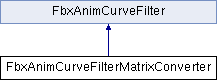
\includegraphics[height=2.000000cm]{class_fbx_anim_curve_filter_matrix_converter}
\end{center}
\end{figure}
\subsection*{公開型}
\begin{DoxyCompactItemize}
\item 
enum \hyperlink{class_fbx_anim_curve_filter_matrix_converter_a41638d5acd6d14ef0f095ab75b18ee69}{E\+Matrix\+Index} \{ \newline
\hyperlink{class_fbx_anim_curve_filter_matrix_converter_a41638d5acd6d14ef0f095ab75b18ee69a84d33765fc4bd4e481a998c2002d168b}{e\+Pre\+Global}, 
\hyperlink{class_fbx_anim_curve_filter_matrix_converter_a41638d5acd6d14ef0f095ab75b18ee69a01c0b9f0f9148eb003003eac43d7a783}{e\+Pre\+Translate}, 
\hyperlink{class_fbx_anim_curve_filter_matrix_converter_a41638d5acd6d14ef0f095ab75b18ee69a8483e4fd410e3f1d7d727dd90272745d}{e\+Post\+Translate}, 
\hyperlink{class_fbx_anim_curve_filter_matrix_converter_a41638d5acd6d14ef0f095ab75b18ee69a557aabfd9b91053b1356a72eab3d9a7e}{e\+Pre\+Rotate}, 
\newline
\hyperlink{class_fbx_anim_curve_filter_matrix_converter_a41638d5acd6d14ef0f095ab75b18ee69a79b84e6bae709b0c9cf03fe8c2639bf0}{e\+Post\+Rotate}, 
\hyperlink{class_fbx_anim_curve_filter_matrix_converter_a41638d5acd6d14ef0f095ab75b18ee69a50bde4676519ef9ca9e2ffb6e2ccd90e}{e\+Pre\+Scale}, 
\hyperlink{class_fbx_anim_curve_filter_matrix_converter_a41638d5acd6d14ef0f095ab75b18ee69a87fafdf264bdf644cef0857fc56fcbf8}{e\+Post\+Scale}, 
\hyperlink{class_fbx_anim_curve_filter_matrix_converter_a41638d5acd6d14ef0f095ab75b18ee69ac613535e97a454b4014da0c5baba43fa}{e\+Post\+Global}, 
\newline
\hyperlink{class_fbx_anim_curve_filter_matrix_converter_a41638d5acd6d14ef0f095ab75b18ee69ade05cc6a84bc8e4a968f57b127403956}{e\+Scale\+Offset}, 
\hyperlink{class_fbx_anim_curve_filter_matrix_converter_a41638d5acd6d14ef0f095ab75b18ee69a0cd2c9524b27db3dd9cffd84af7042d6}{e\+Inactive\+Pre}, 
\hyperlink{class_fbx_anim_curve_filter_matrix_converter_a41638d5acd6d14ef0f095ab75b18ee69a27924880372685bc5b61d733d4cb2f2a}{e\+Inactive\+Post}, 
\hyperlink{class_fbx_anim_curve_filter_matrix_converter_a41638d5acd6d14ef0f095ab75b18ee69a94dfcbf5497374814ca3bc6403b4dfcf}{e\+Rotation\+Pivot}, 
\newline
\hyperlink{class_fbx_anim_curve_filter_matrix_converter_a41638d5acd6d14ef0f095ab75b18ee69a5c0a4f4def4a54fb1a1f3b54a1db4d25}{e\+Scaling\+Pivot}, 
\hyperlink{class_fbx_anim_curve_filter_matrix_converter_a41638d5acd6d14ef0f095ab75b18ee69a367aeb292b3015d210f1c7f8217bec1c}{e\+Matrix\+Index\+Count}
 \}
\end{DoxyCompactItemize}
\subsection*{公開メンバ関数}
\begin{DoxyCompactItemize}
\item 
\hyperlink{class_fbx_anim_curve_filter_matrix_converter_a756dc5898f25c94c6887a6fcf9b14f97}{Fbx\+Anim\+Curve\+Filter\+Matrix\+Converter} ()
\begin{DoxyCompactList}\small\item\em Constructor. \end{DoxyCompactList}\item 
virtual \hyperlink{class_fbx_anim_curve_filter_matrix_converter_ab87ad3901de6754e782e1b923ffa1399}{$\sim$\+Fbx\+Anim\+Curve\+Filter\+Matrix\+Converter} ()
\begin{DoxyCompactList}\small\item\em Destructor. \end{DoxyCompactList}\item 
virtual const char $\ast$ \hyperlink{class_fbx_anim_curve_filter_matrix_converter_a264eb163214f398627f4b8e20631b1ab}{Get\+Name} () const
\item 
virtual bool \hyperlink{class_fbx_anim_curve_filter_matrix_converter_ad19ed98d377e10fb85c20454dbbadaae}{Need\+Apply} (\hyperlink{class_fbx_anim_stack}{Fbx\+Anim\+Stack} $\ast$, \hyperlink{class_fbx_status}{Fbx\+Status} $\ast$p\+Status=\hyperlink{fbxarch_8h_a070d2ce7b6bb7e5c05602aa8c308d0c4}{N\+U\+LL})
\item 
virtual bool \hyperlink{class_fbx_anim_curve_filter_matrix_converter_a8f4e811fedfacc4bc5a90942d2a2bfd5}{Need\+Apply} (\hyperlink{class_fbx_object}{Fbx\+Object} $\ast$, \hyperlink{class_fbx_anim_stack}{Fbx\+Anim\+Stack} $\ast$, \hyperlink{class_fbx_status}{Fbx\+Status} $\ast$p\+Status=\hyperlink{fbxarch_8h_a070d2ce7b6bb7e5c05602aa8c308d0c4}{N\+U\+LL})
\item 
virtual bool \hyperlink{class_fbx_anim_curve_filter_matrix_converter_a640fa8192c330f999894be8083ec578f}{Need\+Apply} (\hyperlink{class_fbx_anim_curve_node}{Fbx\+Anim\+Curve\+Node} $\ast$p\+Curve\+Node\mbox{[}3\mbox{]}, \hyperlink{class_fbx_status}{Fbx\+Status} $\ast$p\+Status=\hyperlink{fbxarch_8h_a070d2ce7b6bb7e5c05602aa8c308d0c4}{N\+U\+LL})
\item 
virtual bool \hyperlink{class_fbx_anim_curve_filter_matrix_converter_aa7105a07dbaf0d9598fa930ff2b3141d}{Need\+Apply} (\hyperlink{class_fbx_anim_curve}{Fbx\+Anim\+Curve} \&, \hyperlink{class_fbx_status}{Fbx\+Status} $\ast$p\+Status=\hyperlink{fbxarch_8h_a070d2ce7b6bb7e5c05602aa8c308d0c4}{N\+U\+LL})
\item 
virtual bool \hyperlink{class_fbx_anim_curve_filter_matrix_converter_a20db5fcf27096c750a9b5bfc1ed074e4}{Apply} (\hyperlink{class_fbx_anim_stack}{Fbx\+Anim\+Stack} $\ast$, \hyperlink{class_fbx_status}{Fbx\+Status} $\ast$p\+Status=\hyperlink{fbxarch_8h_a070d2ce7b6bb7e5c05602aa8c308d0c4}{N\+U\+LL})
\item 
virtual bool \hyperlink{class_fbx_anim_curve_filter_matrix_converter_a9159d911dfa550f7760ffbb1e3b6cb6b}{Apply} (\hyperlink{class_fbx_object}{Fbx\+Object} $\ast$, \hyperlink{class_fbx_anim_stack}{Fbx\+Anim\+Stack} $\ast$, \hyperlink{class_fbx_status}{Fbx\+Status} $\ast$p\+Status=\hyperlink{fbxarch_8h_a070d2ce7b6bb7e5c05602aa8c308d0c4}{N\+U\+LL})
\item 
virtual bool \hyperlink{class_fbx_anim_curve_filter_matrix_converter_a75ed2f9079858c1db98740c3fa0506e9}{Apply} (\hyperlink{class_fbx_anim_curve_node}{Fbx\+Anim\+Curve\+Node} $\ast$p\+Curve\+Node\mbox{[}3\mbox{]}, \hyperlink{class_fbx_status}{Fbx\+Status} $\ast$p\+Status=\hyperlink{fbxarch_8h_a070d2ce7b6bb7e5c05602aa8c308d0c4}{N\+U\+LL})
\item 
virtual bool \hyperlink{class_fbx_anim_curve_filter_matrix_converter_a30599e88b210af2fa8c7be727d59fae8}{Apply} (\hyperlink{class_fbx_anim_curve}{Fbx\+Anim\+Curve} $\ast$$\ast$p\+Curve, int p\+Count, \hyperlink{class_fbx_status}{Fbx\+Status} $\ast$p\+Status=\hyperlink{fbxarch_8h_a070d2ce7b6bb7e5c05602aa8c308d0c4}{N\+U\+LL})
\item 
bool \hyperlink{class_fbx_anim_curve_filter_matrix_converter_adfcd53e23b1a55da02892b7ecf3822b3}{Apply} (\hyperlink{class_fbx_anim_curve}{Fbx\+Anim\+Curve} $\ast$$\ast$p\+Curve, double $\ast$p\+Vals, \hyperlink{class_fbx_status}{Fbx\+Status} $\ast$p\+Status=\hyperlink{fbxarch_8h_a070d2ce7b6bb7e5c05602aa8c308d0c4}{N\+U\+LL})
\item 
virtual bool \hyperlink{class_fbx_anim_curve_filter_matrix_converter_a33ffa3eacf298e44aeaaec44db9bdd26}{Apply} (\hyperlink{class_fbx_anim_curve}{Fbx\+Anim\+Curve} \&, \hyperlink{class_fbx_status}{Fbx\+Status} $\ast$p\+Status=\hyperlink{fbxarch_8h_a070d2ce7b6bb7e5c05602aa8c308d0c4}{N\+U\+LL})
\item 
virtual void \hyperlink{class_fbx_anim_curve_filter_matrix_converter_ad441f2753722fa3fd07631fb249afadb}{Reset} ()
\item 
void \hyperlink{class_fbx_anim_curve_filter_matrix_converter_a38313c4b68b33172198ca19ef957bc1c}{Get\+Source\+Matrix} (\hyperlink{class_fbx_anim_curve_filter_matrix_converter_a41638d5acd6d14ef0f095ab75b18ee69}{E\+Matrix\+Index} p\+Index, \hyperlink{class_fbx_a_matrix}{Fbx\+A\+Matrix} \&p\+Matrix) const
\item 
void \hyperlink{class_fbx_anim_curve_filter_matrix_converter_a51f8c45cecbe23a5df38bd0f2b4feb08}{Set\+Source\+Matrix} (\hyperlink{class_fbx_anim_curve_filter_matrix_converter_a41638d5acd6d14ef0f095ab75b18ee69}{E\+Matrix\+Index} p\+Index, \hyperlink{class_fbx_a_matrix}{Fbx\+A\+Matrix} \&p\+Matrix)
\item 
void \hyperlink{class_fbx_anim_curve_filter_matrix_converter_a5cd3e587cb299a3ae2d78e9c964a5ef0}{Get\+Dest\+Matrix} (\hyperlink{class_fbx_anim_curve_filter_matrix_converter_a41638d5acd6d14ef0f095ab75b18ee69}{E\+Matrix\+Index} p\+Index, \hyperlink{class_fbx_a_matrix}{Fbx\+A\+Matrix} \&p\+Matrix) const
\item 
void \hyperlink{class_fbx_anim_curve_filter_matrix_converter_a5eafea6927cc0698df3a1a9c2cdb3b7d}{Set\+Dest\+Matrix} (\hyperlink{class_fbx_anim_curve_filter_matrix_converter_a41638d5acd6d14ef0f095ab75b18ee69}{E\+Matrix\+Index} p\+Index, \hyperlink{class_fbx_a_matrix}{Fbx\+A\+Matrix} \&p\+Matrix)
\item 
\hyperlink{class_fbx_time}{Fbx\+Time} \hyperlink{class_fbx_anim_curve_filter_matrix_converter_a30366999bdf8a54362cb07415cb09d67}{Get\+Resampling\+Period} () const
\item 
void \hyperlink{class_fbx_anim_curve_filter_matrix_converter_ad32f07496ccaa59ed3fa575da58b5dc1}{Set\+Resampling\+Period} (\hyperlink{class_fbx_time}{Fbx\+Time} \&p\+Resampling\+Period)
\item 
bool \hyperlink{class_fbx_anim_curve_filter_matrix_converter_a2721fda063f33bb95358c60df9a935f7}{Get\+Generate\+Last\+Key\+Exactly\+At\+End\+Time} () const
\item 
void \hyperlink{class_fbx_anim_curve_filter_matrix_converter_a3f6bbf821eff2180bef5b63764d4a305}{Set\+Generate\+Last\+Key\+Exactly\+At\+End\+Time} (bool p\+Flag)
\item 
bool \hyperlink{class_fbx_anim_curve_filter_matrix_converter_a6f5d905229e996ddccfe96e2cd4454e3}{Get\+Resampling\+On\+Frame\+Rate\+Multiple} () const
\item 
void \hyperlink{class_fbx_anim_curve_filter_matrix_converter_a7b23dfad34cae6de4c7f20ea8c071633}{Set\+Resampling\+On\+Frame\+Rate\+Multiple} (bool p\+Flag)
\item 
bool \hyperlink{class_fbx_anim_curve_filter_matrix_converter_acf269bdba7f9526a1c957505cb3beb9c}{Get\+Apply\+Unroll} () const
\item 
void \hyperlink{class_fbx_anim_curve_filter_matrix_converter_abcfe379526feec5a8d3ffc9e3e435d66}{Set\+Apply\+Unroll} (bool p\+Flag)
\item 
bool \hyperlink{class_fbx_anim_curve_filter_matrix_converter_a01b2d31ebe1cc32373d01c7b3f3e7797}{Get\+Apply\+Constant\+Key\+Reducer} () const
\item 
void \hyperlink{class_fbx_anim_curve_filter_matrix_converter_a67f6df28fee3f4703d96a2f92d58dfe2}{Set\+Apply\+Constant\+Key\+Reducer} (bool p\+Flag)
\item 
bool \hyperlink{class_fbx_anim_curve_filter_matrix_converter_a7603a34315c35f2d9ba8f501059992c5}{Get\+Resample\+Translation} () const
\item 
void \hyperlink{class_fbx_anim_curve_filter_matrix_converter_a3ce7c2108f6a39ad4a13cbc4175a5ec8}{Set\+Resample\+Translation} (bool p\+Flag)
\item 
void \hyperlink{class_fbx_anim_curve_filter_matrix_converter_a7140e4dce0bf5ef87d75991fa5eb315e}{Set\+Src\+Rotate\+Order} (\hyperlink{class_fbx_euler_a7d5bec7eedb022b4dae56894ab7a9939}{Fbx\+Euler\+::\+E\+Order} p\+Order)
\item 
void \hyperlink{class_fbx_anim_curve_filter_matrix_converter_a115f94c96f1f14b55e4f3f9b6bc5977a}{Set\+Dest\+Rotate\+Order} (\hyperlink{class_fbx_euler_a7d5bec7eedb022b4dae56894ab7a9939}{Fbx\+Euler\+::\+E\+Order} p\+Order)
\item 
void \hyperlink{class_fbx_anim_curve_filter_matrix_converter_a4b49dc7704c847a3b909cf7d9052f7a7}{Set\+Force\+Apply} (bool p\+Val)
\item 
bool \hyperlink{class_fbx_anim_curve_filter_matrix_converter_abeb4273e3155dd4644a35a68f39ebda3}{Get\+Force\+Apply} () const
\item 
void \hyperlink{class_fbx_anim_curve_filter_matrix_converter_a892ade0f0e5b7451a6e09da5ee4179bf}{Set\+Translation\+Limits} (\hyperlink{class_fbx_limits}{Fbx\+Limits} \&limit)
\item 
void \hyperlink{class_fbx_anim_curve_filter_matrix_converter_a95cad4a51f2204a7c5cce101486eaab6}{Set\+Rotation\+Limits} (\hyperlink{class_fbx_limits}{Fbx\+Limits} \&limit)
\item 
void \hyperlink{class_fbx_anim_curve_filter_matrix_converter_ad291cc58221b27ffa8824c73d00cc0ba}{Set\+Scaling\+Limits} (\hyperlink{class_fbx_limits}{Fbx\+Limits} \&limit)
\end{DoxyCompactItemize}
\subsection*{Exposed parent class methods.}
\begin{DoxyCompactItemize}
\item 
virtual bool \hyperlink{class_fbx_anim_curve_filter_matrix_converter_a7cae8d7e31ab1cf2437de8636a5b4916}{Need\+Apply} (\hyperlink{class_fbx_anim_curve}{Fbx\+Anim\+Curve} $\ast$$\ast$p\+Curve, int p\+Count, \hyperlink{class_fbx_status}{Fbx\+Status} $\ast$p\+Status=\hyperlink{fbxarch_8h_a070d2ce7b6bb7e5c05602aa8c308d0c4}{N\+U\+LL})
\item 
virtual bool \hyperlink{class_fbx_anim_curve_filter_matrix_converter_a00f04a303254479eef1aa3bfbe0643d8}{Need\+Apply} (\hyperlink{class_fbx_anim_curve_node}{Fbx\+Anim\+Curve\+Node} \&p\+Curve\+Node, \hyperlink{class_fbx_status}{Fbx\+Status} $\ast$p\+Status=\hyperlink{fbxarch_8h_a070d2ce7b6bb7e5c05602aa8c308d0c4}{N\+U\+LL})
\item 
virtual bool \hyperlink{class_fbx_anim_curve_filter_matrix_converter_aa71462534eff53b1177aaa5bb3e059ec}{Apply} (\hyperlink{class_fbx_anim_curve_node}{Fbx\+Anim\+Curve\+Node} \&p\+Curve\+Node, \hyperlink{class_fbx_status}{Fbx\+Status} $\ast$p\+Status=\hyperlink{fbxarch_8h_a070d2ce7b6bb7e5c05602aa8c308d0c4}{N\+U\+LL})
\end{DoxyCompactItemize}
\subsection*{その他の継承メンバ}


\subsection{詳解}
Matrix conversion filter.

\begin{DoxyRemark}{注釈}
The current implementation of this filter expects to process 9 curves. If the Apply\+Unroll flag is enabled, set with a call to \hyperlink{class_fbx_anim_curve_filter_matrix_converter_abcfe379526feec5a8d3ffc9e3e435d66}{Set\+Apply\+Unroll()}, the internal unroll filter will automatically be configured to convert U\+S\+ER and B\+R\+E\+AK tangents to A\+U\+TO (refer to the \hyperlink{class_fbx_anim_curve_filter_unroll}{Fbx\+Anim\+Curve\+Filter\+Unroll} documentation). 
\end{DoxyRemark}


 fbxanimcurvefilters.\+h の 1163 行目に定義があります。



\subsection{列挙型メンバ詳解}
\mbox{\Hypertarget{class_fbx_anim_curve_filter_matrix_converter_a41638d5acd6d14ef0f095ab75b18ee69}\label{class_fbx_anim_curve_filter_matrix_converter_a41638d5acd6d14ef0f095ab75b18ee69}} 
\index{Fbx\+Anim\+Curve\+Filter\+Matrix\+Converter@{Fbx\+Anim\+Curve\+Filter\+Matrix\+Converter}!E\+Matrix\+Index@{E\+Matrix\+Index}}
\index{E\+Matrix\+Index@{E\+Matrix\+Index}!Fbx\+Anim\+Curve\+Filter\+Matrix\+Converter@{Fbx\+Anim\+Curve\+Filter\+Matrix\+Converter}}
\subsubsection{\texorpdfstring{E\+Matrix\+Index}{EMatrixIndex}}
{\footnotesize\ttfamily enum \hyperlink{class_fbx_anim_curve_filter_matrix_converter_a41638d5acd6d14ef0f095ab75b18ee69}{Fbx\+Anim\+Curve\+Filter\+Matrix\+Converter\+::\+E\+Matrix\+Index}}

Matrix index type
\begin{DoxyItemize}
\item {\itshape e\+Pre\+Global} 
\item {\itshape e\+Pre\+Translate} 
\item {\itshape e\+Post\+Translate} 
\item {\itshape e\+Pre\+Rotate} 
\item {\itshape e\+Pre\+Scale} 
\item {\itshape e\+Post\+Global} 
\item {\itshape e\+Scale\+Offset} 
\item {\itshape e\+Inactive\+Pre} 
\item {\itshape e\+Inactive\+Post} 
\item {\itshape e\+Rotation\+Pivot} 
\item {\itshape e\+Scaling\+Pivot} 
\item {\itshape e\+Matrix\+Index\+Count} 
\end{DoxyItemize}\begin{DoxyEnumFields}{列挙値}
\raisebox{\heightof{T}}[0pt][0pt]{\index{e\+Pre\+Global@{e\+Pre\+Global}!Fbx\+Anim\+Curve\+Filter\+Matrix\+Converter@{Fbx\+Anim\+Curve\+Filter\+Matrix\+Converter}}\index{Fbx\+Anim\+Curve\+Filter\+Matrix\+Converter@{Fbx\+Anim\+Curve\+Filter\+Matrix\+Converter}!e\+Pre\+Global@{e\+Pre\+Global}}}\mbox{\Hypertarget{class_fbx_anim_curve_filter_matrix_converter_a41638d5acd6d14ef0f095ab75b18ee69a84d33765fc4bd4e481a998c2002d168b}\label{class_fbx_anim_curve_filter_matrix_converter_a41638d5acd6d14ef0f095ab75b18ee69a84d33765fc4bd4e481a998c2002d168b}} 
e\+Pre\+Global&\\
\hline

\raisebox{\heightof{T}}[0pt][0pt]{\index{e\+Pre\+Translate@{e\+Pre\+Translate}!Fbx\+Anim\+Curve\+Filter\+Matrix\+Converter@{Fbx\+Anim\+Curve\+Filter\+Matrix\+Converter}}\index{Fbx\+Anim\+Curve\+Filter\+Matrix\+Converter@{Fbx\+Anim\+Curve\+Filter\+Matrix\+Converter}!e\+Pre\+Translate@{e\+Pre\+Translate}}}\mbox{\Hypertarget{class_fbx_anim_curve_filter_matrix_converter_a41638d5acd6d14ef0f095ab75b18ee69a01c0b9f0f9148eb003003eac43d7a783}\label{class_fbx_anim_curve_filter_matrix_converter_a41638d5acd6d14ef0f095ab75b18ee69a01c0b9f0f9148eb003003eac43d7a783}} 
e\+Pre\+Translate&\\
\hline

\raisebox{\heightof{T}}[0pt][0pt]{\index{e\+Post\+Translate@{e\+Post\+Translate}!Fbx\+Anim\+Curve\+Filter\+Matrix\+Converter@{Fbx\+Anim\+Curve\+Filter\+Matrix\+Converter}}\index{Fbx\+Anim\+Curve\+Filter\+Matrix\+Converter@{Fbx\+Anim\+Curve\+Filter\+Matrix\+Converter}!e\+Post\+Translate@{e\+Post\+Translate}}}\mbox{\Hypertarget{class_fbx_anim_curve_filter_matrix_converter_a41638d5acd6d14ef0f095ab75b18ee69a8483e4fd410e3f1d7d727dd90272745d}\label{class_fbx_anim_curve_filter_matrix_converter_a41638d5acd6d14ef0f095ab75b18ee69a8483e4fd410e3f1d7d727dd90272745d}} 
e\+Post\+Translate&\\
\hline

\raisebox{\heightof{T}}[0pt][0pt]{\index{e\+Pre\+Rotate@{e\+Pre\+Rotate}!Fbx\+Anim\+Curve\+Filter\+Matrix\+Converter@{Fbx\+Anim\+Curve\+Filter\+Matrix\+Converter}}\index{Fbx\+Anim\+Curve\+Filter\+Matrix\+Converter@{Fbx\+Anim\+Curve\+Filter\+Matrix\+Converter}!e\+Pre\+Rotate@{e\+Pre\+Rotate}}}\mbox{\Hypertarget{class_fbx_anim_curve_filter_matrix_converter_a41638d5acd6d14ef0f095ab75b18ee69a557aabfd9b91053b1356a72eab3d9a7e}\label{class_fbx_anim_curve_filter_matrix_converter_a41638d5acd6d14ef0f095ab75b18ee69a557aabfd9b91053b1356a72eab3d9a7e}} 
e\+Pre\+Rotate&\\
\hline

\raisebox{\heightof{T}}[0pt][0pt]{\index{e\+Post\+Rotate@{e\+Post\+Rotate}!Fbx\+Anim\+Curve\+Filter\+Matrix\+Converter@{Fbx\+Anim\+Curve\+Filter\+Matrix\+Converter}}\index{Fbx\+Anim\+Curve\+Filter\+Matrix\+Converter@{Fbx\+Anim\+Curve\+Filter\+Matrix\+Converter}!e\+Post\+Rotate@{e\+Post\+Rotate}}}\mbox{\Hypertarget{class_fbx_anim_curve_filter_matrix_converter_a41638d5acd6d14ef0f095ab75b18ee69a79b84e6bae709b0c9cf03fe8c2639bf0}\label{class_fbx_anim_curve_filter_matrix_converter_a41638d5acd6d14ef0f095ab75b18ee69a79b84e6bae709b0c9cf03fe8c2639bf0}} 
e\+Post\+Rotate&\\
\hline

\raisebox{\heightof{T}}[0pt][0pt]{\index{e\+Pre\+Scale@{e\+Pre\+Scale}!Fbx\+Anim\+Curve\+Filter\+Matrix\+Converter@{Fbx\+Anim\+Curve\+Filter\+Matrix\+Converter}}\index{Fbx\+Anim\+Curve\+Filter\+Matrix\+Converter@{Fbx\+Anim\+Curve\+Filter\+Matrix\+Converter}!e\+Pre\+Scale@{e\+Pre\+Scale}}}\mbox{\Hypertarget{class_fbx_anim_curve_filter_matrix_converter_a41638d5acd6d14ef0f095ab75b18ee69a50bde4676519ef9ca9e2ffb6e2ccd90e}\label{class_fbx_anim_curve_filter_matrix_converter_a41638d5acd6d14ef0f095ab75b18ee69a50bde4676519ef9ca9e2ffb6e2ccd90e}} 
e\+Pre\+Scale&\\
\hline

\raisebox{\heightof{T}}[0pt][0pt]{\index{e\+Post\+Scale@{e\+Post\+Scale}!Fbx\+Anim\+Curve\+Filter\+Matrix\+Converter@{Fbx\+Anim\+Curve\+Filter\+Matrix\+Converter}}\index{Fbx\+Anim\+Curve\+Filter\+Matrix\+Converter@{Fbx\+Anim\+Curve\+Filter\+Matrix\+Converter}!e\+Post\+Scale@{e\+Post\+Scale}}}\mbox{\Hypertarget{class_fbx_anim_curve_filter_matrix_converter_a41638d5acd6d14ef0f095ab75b18ee69a87fafdf264bdf644cef0857fc56fcbf8}\label{class_fbx_anim_curve_filter_matrix_converter_a41638d5acd6d14ef0f095ab75b18ee69a87fafdf264bdf644cef0857fc56fcbf8}} 
e\+Post\+Scale&\\
\hline

\raisebox{\heightof{T}}[0pt][0pt]{\index{e\+Post\+Global@{e\+Post\+Global}!Fbx\+Anim\+Curve\+Filter\+Matrix\+Converter@{Fbx\+Anim\+Curve\+Filter\+Matrix\+Converter}}\index{Fbx\+Anim\+Curve\+Filter\+Matrix\+Converter@{Fbx\+Anim\+Curve\+Filter\+Matrix\+Converter}!e\+Post\+Global@{e\+Post\+Global}}}\mbox{\Hypertarget{class_fbx_anim_curve_filter_matrix_converter_a41638d5acd6d14ef0f095ab75b18ee69ac613535e97a454b4014da0c5baba43fa}\label{class_fbx_anim_curve_filter_matrix_converter_a41638d5acd6d14ef0f095ab75b18ee69ac613535e97a454b4014da0c5baba43fa}} 
e\+Post\+Global&\\
\hline

\raisebox{\heightof{T}}[0pt][0pt]{\index{e\+Scale\+Offset@{e\+Scale\+Offset}!Fbx\+Anim\+Curve\+Filter\+Matrix\+Converter@{Fbx\+Anim\+Curve\+Filter\+Matrix\+Converter}}\index{Fbx\+Anim\+Curve\+Filter\+Matrix\+Converter@{Fbx\+Anim\+Curve\+Filter\+Matrix\+Converter}!e\+Scale\+Offset@{e\+Scale\+Offset}}}\mbox{\Hypertarget{class_fbx_anim_curve_filter_matrix_converter_a41638d5acd6d14ef0f095ab75b18ee69ade05cc6a84bc8e4a968f57b127403956}\label{class_fbx_anim_curve_filter_matrix_converter_a41638d5acd6d14ef0f095ab75b18ee69ade05cc6a84bc8e4a968f57b127403956}} 
e\+Scale\+Offset&\\
\hline

\raisebox{\heightof{T}}[0pt][0pt]{\index{e\+Inactive\+Pre@{e\+Inactive\+Pre}!Fbx\+Anim\+Curve\+Filter\+Matrix\+Converter@{Fbx\+Anim\+Curve\+Filter\+Matrix\+Converter}}\index{Fbx\+Anim\+Curve\+Filter\+Matrix\+Converter@{Fbx\+Anim\+Curve\+Filter\+Matrix\+Converter}!e\+Inactive\+Pre@{e\+Inactive\+Pre}}}\mbox{\Hypertarget{class_fbx_anim_curve_filter_matrix_converter_a41638d5acd6d14ef0f095ab75b18ee69a0cd2c9524b27db3dd9cffd84af7042d6}\label{class_fbx_anim_curve_filter_matrix_converter_a41638d5acd6d14ef0f095ab75b18ee69a0cd2c9524b27db3dd9cffd84af7042d6}} 
e\+Inactive\+Pre&\\
\hline

\raisebox{\heightof{T}}[0pt][0pt]{\index{e\+Inactive\+Post@{e\+Inactive\+Post}!Fbx\+Anim\+Curve\+Filter\+Matrix\+Converter@{Fbx\+Anim\+Curve\+Filter\+Matrix\+Converter}}\index{Fbx\+Anim\+Curve\+Filter\+Matrix\+Converter@{Fbx\+Anim\+Curve\+Filter\+Matrix\+Converter}!e\+Inactive\+Post@{e\+Inactive\+Post}}}\mbox{\Hypertarget{class_fbx_anim_curve_filter_matrix_converter_a41638d5acd6d14ef0f095ab75b18ee69a27924880372685bc5b61d733d4cb2f2a}\label{class_fbx_anim_curve_filter_matrix_converter_a41638d5acd6d14ef0f095ab75b18ee69a27924880372685bc5b61d733d4cb2f2a}} 
e\+Inactive\+Post&\\
\hline

\raisebox{\heightof{T}}[0pt][0pt]{\index{e\+Rotation\+Pivot@{e\+Rotation\+Pivot}!Fbx\+Anim\+Curve\+Filter\+Matrix\+Converter@{Fbx\+Anim\+Curve\+Filter\+Matrix\+Converter}}\index{Fbx\+Anim\+Curve\+Filter\+Matrix\+Converter@{Fbx\+Anim\+Curve\+Filter\+Matrix\+Converter}!e\+Rotation\+Pivot@{e\+Rotation\+Pivot}}}\mbox{\Hypertarget{class_fbx_anim_curve_filter_matrix_converter_a41638d5acd6d14ef0f095ab75b18ee69a94dfcbf5497374814ca3bc6403b4dfcf}\label{class_fbx_anim_curve_filter_matrix_converter_a41638d5acd6d14ef0f095ab75b18ee69a94dfcbf5497374814ca3bc6403b4dfcf}} 
e\+Rotation\+Pivot&\\
\hline

\raisebox{\heightof{T}}[0pt][0pt]{\index{e\+Scaling\+Pivot@{e\+Scaling\+Pivot}!Fbx\+Anim\+Curve\+Filter\+Matrix\+Converter@{Fbx\+Anim\+Curve\+Filter\+Matrix\+Converter}}\index{Fbx\+Anim\+Curve\+Filter\+Matrix\+Converter@{Fbx\+Anim\+Curve\+Filter\+Matrix\+Converter}!e\+Scaling\+Pivot@{e\+Scaling\+Pivot}}}\mbox{\Hypertarget{class_fbx_anim_curve_filter_matrix_converter_a41638d5acd6d14ef0f095ab75b18ee69a5c0a4f4def4a54fb1a1f3b54a1db4d25}\label{class_fbx_anim_curve_filter_matrix_converter_a41638d5acd6d14ef0f095ab75b18ee69a5c0a4f4def4a54fb1a1f3b54a1db4d25}} 
e\+Scaling\+Pivot&\\
\hline

\raisebox{\heightof{T}}[0pt][0pt]{\index{e\+Matrix\+Index\+Count@{e\+Matrix\+Index\+Count}!Fbx\+Anim\+Curve\+Filter\+Matrix\+Converter@{Fbx\+Anim\+Curve\+Filter\+Matrix\+Converter}}\index{Fbx\+Anim\+Curve\+Filter\+Matrix\+Converter@{Fbx\+Anim\+Curve\+Filter\+Matrix\+Converter}!e\+Matrix\+Index\+Count@{e\+Matrix\+Index\+Count}}}\mbox{\Hypertarget{class_fbx_anim_curve_filter_matrix_converter_a41638d5acd6d14ef0f095ab75b18ee69a367aeb292b3015d210f1c7f8217bec1c}\label{class_fbx_anim_curve_filter_matrix_converter_a41638d5acd6d14ef0f095ab75b18ee69a367aeb292b3015d210f1c7f8217bec1c}} 
e\+Matrix\+Index\+Count&\\
\hline

\end{DoxyEnumFields}


 fbxanimcurvefilters.\+h の 1297 行目に定義があります。



\subsection{構築子と解体子}
\mbox{\Hypertarget{class_fbx_anim_curve_filter_matrix_converter_a756dc5898f25c94c6887a6fcf9b14f97}\label{class_fbx_anim_curve_filter_matrix_converter_a756dc5898f25c94c6887a6fcf9b14f97}} 
\index{Fbx\+Anim\+Curve\+Filter\+Matrix\+Converter@{Fbx\+Anim\+Curve\+Filter\+Matrix\+Converter}!Fbx\+Anim\+Curve\+Filter\+Matrix\+Converter@{Fbx\+Anim\+Curve\+Filter\+Matrix\+Converter}}
\index{Fbx\+Anim\+Curve\+Filter\+Matrix\+Converter@{Fbx\+Anim\+Curve\+Filter\+Matrix\+Converter}!Fbx\+Anim\+Curve\+Filter\+Matrix\+Converter@{Fbx\+Anim\+Curve\+Filter\+Matrix\+Converter}}
\subsubsection{\texorpdfstring{Fbx\+Anim\+Curve\+Filter\+Matrix\+Converter()}{FbxAnimCurveFilterMatrixConverter()}}
{\footnotesize\ttfamily Fbx\+Anim\+Curve\+Filter\+Matrix\+Converter\+::\+Fbx\+Anim\+Curve\+Filter\+Matrix\+Converter (\begin{DoxyParamCaption}{ }\end{DoxyParamCaption})}



Constructor. 

\mbox{\Hypertarget{class_fbx_anim_curve_filter_matrix_converter_ab87ad3901de6754e782e1b923ffa1399}\label{class_fbx_anim_curve_filter_matrix_converter_ab87ad3901de6754e782e1b923ffa1399}} 
\index{Fbx\+Anim\+Curve\+Filter\+Matrix\+Converter@{Fbx\+Anim\+Curve\+Filter\+Matrix\+Converter}!````~Fbx\+Anim\+Curve\+Filter\+Matrix\+Converter@{$\sim$\+Fbx\+Anim\+Curve\+Filter\+Matrix\+Converter}}
\index{````~Fbx\+Anim\+Curve\+Filter\+Matrix\+Converter@{$\sim$\+Fbx\+Anim\+Curve\+Filter\+Matrix\+Converter}!Fbx\+Anim\+Curve\+Filter\+Matrix\+Converter@{Fbx\+Anim\+Curve\+Filter\+Matrix\+Converter}}
\subsubsection{\texorpdfstring{$\sim$\+Fbx\+Anim\+Curve\+Filter\+Matrix\+Converter()}{~FbxAnimCurveFilterMatrixConverter()}}
{\footnotesize\ttfamily virtual Fbx\+Anim\+Curve\+Filter\+Matrix\+Converter\+::$\sim$\+Fbx\+Anim\+Curve\+Filter\+Matrix\+Converter (\begin{DoxyParamCaption}{ }\end{DoxyParamCaption})\hspace{0.3cm}{\ttfamily [virtual]}}



Destructor. 



\subsection{関数詳解}
\mbox{\Hypertarget{class_fbx_anim_curve_filter_matrix_converter_aa71462534eff53b1177aaa5bb3e059ec}\label{class_fbx_anim_curve_filter_matrix_converter_aa71462534eff53b1177aaa5bb3e059ec}} 
\index{Fbx\+Anim\+Curve\+Filter\+Matrix\+Converter@{Fbx\+Anim\+Curve\+Filter\+Matrix\+Converter}!Apply@{Apply}}
\index{Apply@{Apply}!Fbx\+Anim\+Curve\+Filter\+Matrix\+Converter@{Fbx\+Anim\+Curve\+Filter\+Matrix\+Converter}}
\subsubsection{\texorpdfstring{Apply()}{Apply()}\hspace{0.1cm}{\footnotesize\ttfamily [1/7]}}
{\footnotesize\ttfamily virtual bool Fbx\+Anim\+Curve\+Filter\+Matrix\+Converter\+::\+Apply (\begin{DoxyParamCaption}\item[{\hyperlink{class_fbx_anim_curve_node}{Fbx\+Anim\+Curve\+Node} \&}]{p\+Curve\+Node,  }\item[{\hyperlink{class_fbx_status}{Fbx\+Status} $\ast$}]{p\+Status = {\ttfamily \hyperlink{fbxarch_8h_a070d2ce7b6bb7e5c05602aa8c308d0c4}{N\+U\+LL}} }\end{DoxyParamCaption})\hspace{0.3cm}{\ttfamily [inline]}, {\ttfamily [virtual]}}

Apply filter on all the curves of an animation curve node. 
\begin{DoxyParams}{引数}
{\em p\+Curve\+Node} & Curve node to which the filter is applied. \\
\hline
{\em p\+Status} & The \hyperlink{class_fbx_status}{Fbx\+Status} object to hold error codes. \\
\hline
\end{DoxyParams}
\begin{DoxyReturn}{戻り値}
{\ttfamily true} if the curve filtering operation was successful, {\ttfamily false} otherwise. 
\end{DoxyReturn}
\begin{DoxyRemark}{注釈}
This method collects all the \hyperlink{class_fbx_anim_curve}{Fbx\+Anim\+Curve} objects connected to the curve node and calls Apply(\+Fbx\+Anim\+Curve$\ast$$\ast$, int) 
\end{DoxyRemark}


\hyperlink{class_fbx_anim_curve_filter_ad042b45c0675278fa49e61739b0825c2}{Fbx\+Anim\+Curve\+Filter}を再実装しています。



 fbxanimcurvefilters.\+h の 1183 行目に定義があります。

\mbox{\Hypertarget{class_fbx_anim_curve_filter_matrix_converter_a20db5fcf27096c750a9b5bfc1ed074e4}\label{class_fbx_anim_curve_filter_matrix_converter_a20db5fcf27096c750a9b5bfc1ed074e4}} 
\index{Fbx\+Anim\+Curve\+Filter\+Matrix\+Converter@{Fbx\+Anim\+Curve\+Filter\+Matrix\+Converter}!Apply@{Apply}}
\index{Apply@{Apply}!Fbx\+Anim\+Curve\+Filter\+Matrix\+Converter@{Fbx\+Anim\+Curve\+Filter\+Matrix\+Converter}}
\subsubsection{\texorpdfstring{Apply()}{Apply()}\hspace{0.1cm}{\footnotesize\ttfamily [2/7]}}
{\footnotesize\ttfamily virtual bool Fbx\+Anim\+Curve\+Filter\+Matrix\+Converter\+::\+Apply (\begin{DoxyParamCaption}\item[{\hyperlink{class_fbx_anim_stack}{Fbx\+Anim\+Stack} $\ast$}]{,  }\item[{\hyperlink{class_fbx_status}{Fbx\+Status} $\ast$}]{p\+Status = {\ttfamily \hyperlink{fbxarch_8h_a070d2ce7b6bb7e5c05602aa8c308d0c4}{N\+U\+LL}} }\end{DoxyParamCaption})\hspace{0.3cm}{\ttfamily [inline]}, {\ttfamily [virtual]}}

This filter expects to work with interdependent curves. Passing the animation stack makes no sense since this object would not know which curves to handle. 
\begin{DoxyParams}{引数}
{\em p\+Anim\+Stack} & Animation stack where to retrieve the animation curves. \\
\hline
{\em p\+Status} & The \hyperlink{class_fbx_status}{Fbx\+Status} object to hold error codes. \\
\hline
\end{DoxyParams}
\begin{DoxyReturn}{戻り値}
{\ttfamily false}. 
\end{DoxyReturn}


\hyperlink{class_fbx_anim_curve_filter_aef3900e6180e05661c27ee484ae939c3}{Fbx\+Anim\+Curve\+Filter}を再実装しています。



 fbxanimcurvefilters.\+h の 1225 行目に定義があります。

\mbox{\Hypertarget{class_fbx_anim_curve_filter_matrix_converter_a9159d911dfa550f7760ffbb1e3b6cb6b}\label{class_fbx_anim_curve_filter_matrix_converter_a9159d911dfa550f7760ffbb1e3b6cb6b}} 
\index{Fbx\+Anim\+Curve\+Filter\+Matrix\+Converter@{Fbx\+Anim\+Curve\+Filter\+Matrix\+Converter}!Apply@{Apply}}
\index{Apply@{Apply}!Fbx\+Anim\+Curve\+Filter\+Matrix\+Converter@{Fbx\+Anim\+Curve\+Filter\+Matrix\+Converter}}
\subsubsection{\texorpdfstring{Apply()}{Apply()}\hspace{0.1cm}{\footnotesize\ttfamily [3/7]}}
{\footnotesize\ttfamily virtual bool Fbx\+Anim\+Curve\+Filter\+Matrix\+Converter\+::\+Apply (\begin{DoxyParamCaption}\item[{\hyperlink{class_fbx_object}{Fbx\+Object} $\ast$}]{,  }\item[{\hyperlink{class_fbx_anim_stack}{Fbx\+Anim\+Stack} $\ast$}]{,  }\item[{\hyperlink{class_fbx_status}{Fbx\+Status} $\ast$}]{p\+Status = {\ttfamily \hyperlink{fbxarch_8h_a070d2ce7b6bb7e5c05602aa8c308d0c4}{N\+U\+LL}} }\end{DoxyParamCaption})\hspace{0.3cm}{\ttfamily [inline]}, {\ttfamily [virtual]}}

This filter expects to work with 9 interdependent curves. Collecting all the animation curves from the properties defined in {\itshape p\+Obj} could not guarantee that we are manipulating 9 interdependent curves. 
\begin{DoxyParams}{引数}
{\em p\+Obj} & Object containing the properties to test. \\
\hline
{\em p\+Anim\+Stack} & Animation stack where to retrieve the animation curves. \\
\hline
{\em p\+Status} & The \hyperlink{class_fbx_status}{Fbx\+Status} object to hold error codes. \\
\hline
\end{DoxyParams}
\begin{DoxyReturn}{戻り値}
{\ttfamily false}. 
\end{DoxyReturn}


\hyperlink{class_fbx_anim_curve_filter_a009498a65af4995bf5e5908f17837531}{Fbx\+Anim\+Curve\+Filter}を再実装しています。



 fbxanimcurvefilters.\+h の 1234 行目に定義があります。

\mbox{\Hypertarget{class_fbx_anim_curve_filter_matrix_converter_a75ed2f9079858c1db98740c3fa0506e9}\label{class_fbx_anim_curve_filter_matrix_converter_a75ed2f9079858c1db98740c3fa0506e9}} 
\index{Fbx\+Anim\+Curve\+Filter\+Matrix\+Converter@{Fbx\+Anim\+Curve\+Filter\+Matrix\+Converter}!Apply@{Apply}}
\index{Apply@{Apply}!Fbx\+Anim\+Curve\+Filter\+Matrix\+Converter@{Fbx\+Anim\+Curve\+Filter\+Matrix\+Converter}}
\subsubsection{\texorpdfstring{Apply()}{Apply()}\hspace{0.1cm}{\footnotesize\ttfamily [4/7]}}
{\footnotesize\ttfamily virtual bool Fbx\+Anim\+Curve\+Filter\+Matrix\+Converter\+::\+Apply (\begin{DoxyParamCaption}\item[{\hyperlink{class_fbx_anim_curve_node}{Fbx\+Anim\+Curve\+Node} $\ast$}]{p\+Curve\+Node\mbox{[}3\mbox{]},  }\item[{\hyperlink{class_fbx_status}{Fbx\+Status} $\ast$}]{p\+Status = {\ttfamily \hyperlink{fbxarch_8h_a070d2ce7b6bb7e5c05602aa8c308d0c4}{N\+U\+LL}} }\end{DoxyParamCaption})\hspace{0.3cm}{\ttfamily [virtual]}}

Apply filter on all the curves of the animation curve nodes. 
\begin{DoxyParams}{引数}
{\em p\+Curve\+Node} & Curve nodes to which the filter is applied. \\
\hline
{\em p\+Status} & The \hyperlink{class_fbx_status}{Fbx\+Status} object to hold error codes. \\
\hline
\end{DoxyParams}
\begin{DoxyReturn}{戻り値}
{\ttfamily true} if the curve filtering operation was successful, {\ttfamily false} otherwise. 
\end{DoxyReturn}
\begin{DoxyRemark}{注釈}
This method assumes that {\itshape p\+Curve\+Node}\mbox{[}0\mbox{]} holds the translation curve, {\itshape p\+Curve\+Node}\mbox{[}1\mbox{]} holds the rotation curves and {\itshape p\+Curve\+Node}\mbox{[}2\mbox{]} holds the scaling curves. 
\end{DoxyRemark}
\mbox{\Hypertarget{class_fbx_anim_curve_filter_matrix_converter_a30599e88b210af2fa8c7be727d59fae8}\label{class_fbx_anim_curve_filter_matrix_converter_a30599e88b210af2fa8c7be727d59fae8}} 
\index{Fbx\+Anim\+Curve\+Filter\+Matrix\+Converter@{Fbx\+Anim\+Curve\+Filter\+Matrix\+Converter}!Apply@{Apply}}
\index{Apply@{Apply}!Fbx\+Anim\+Curve\+Filter\+Matrix\+Converter@{Fbx\+Anim\+Curve\+Filter\+Matrix\+Converter}}
\subsubsection{\texorpdfstring{Apply()}{Apply()}\hspace{0.1cm}{\footnotesize\ttfamily [5/7]}}
{\footnotesize\ttfamily virtual bool Fbx\+Anim\+Curve\+Filter\+Matrix\+Converter\+::\+Apply (\begin{DoxyParamCaption}\item[{\hyperlink{class_fbx_anim_curve}{Fbx\+Anim\+Curve} $\ast$$\ast$}]{p\+Curve,  }\item[{int}]{p\+Count,  }\item[{\hyperlink{class_fbx_status}{Fbx\+Status} $\ast$}]{p\+Status = {\ttfamily \hyperlink{fbxarch_8h_a070d2ce7b6bb7e5c05602aa8c308d0c4}{N\+U\+LL}} }\end{DoxyParamCaption})\hspace{0.3cm}{\ttfamily [virtual]}}

Apply filter on the given animation curves. 
\begin{DoxyParams}{引数}
{\em p\+Curve} & Array of curve to which the filter is applied. \\
\hline
{\em p\+Count} & Number of curves in array. \\
\hline
{\em p\+Status} & The \hyperlink{class_fbx_status}{Fbx\+Status} object to hold error codes. \\
\hline
\end{DoxyParams}
\begin{DoxyReturn}{戻り値}
{\ttfamily true} if the curve filtering operation was successful, {\ttfamily false} otherwise. 
\end{DoxyReturn}
\begin{DoxyRemark}{注釈}
{\itshape p\+Count} must be equal to 9 

Because this method only manipulates \hyperlink{class_fbx_anim_curve}{Fbx\+Anim\+Curve} objects, it cannot set/get the channels value. If the calling application wishes to use this flavor of the \hyperlink{class_fbx_anim_curve_filter_matrix_converter_aa71462534eff53b1177aaa5bb3e059ec}{Apply()} method, it is strongly suggested to use the method\+: Fbx\+Anim\+Curve\+Filter\+Matrix\+Converter\+::\+Apply(\+Fbx\+Anim\+Curve$\ast$$\ast$ p\+Curve, double\& p\+Vals\mbox{[}9\mbox{]}); The Apply(\+Fbx\+Anim\+Curve\+Node$\ast$) method is not affected by this limitation since the channel values can be accessed via the animation curve node. 
\end{DoxyRemark}


\hyperlink{class_fbx_anim_curve_filter_aca6a41fbc4d9019b20df7adccfa6ed3c}{Fbx\+Anim\+Curve\+Filter}を再実装しています。

\mbox{\Hypertarget{class_fbx_anim_curve_filter_matrix_converter_adfcd53e23b1a55da02892b7ecf3822b3}\label{class_fbx_anim_curve_filter_matrix_converter_adfcd53e23b1a55da02892b7ecf3822b3}} 
\index{Fbx\+Anim\+Curve\+Filter\+Matrix\+Converter@{Fbx\+Anim\+Curve\+Filter\+Matrix\+Converter}!Apply@{Apply}}
\index{Apply@{Apply}!Fbx\+Anim\+Curve\+Filter\+Matrix\+Converter@{Fbx\+Anim\+Curve\+Filter\+Matrix\+Converter}}
\subsubsection{\texorpdfstring{Apply()}{Apply()}\hspace{0.1cm}{\footnotesize\ttfamily [6/7]}}
{\footnotesize\ttfamily bool Fbx\+Anim\+Curve\+Filter\+Matrix\+Converter\+::\+Apply (\begin{DoxyParamCaption}\item[{\hyperlink{class_fbx_anim_curve}{Fbx\+Anim\+Curve} $\ast$$\ast$}]{p\+Curve,  }\item[{double $\ast$}]{p\+Vals,  }\item[{\hyperlink{class_fbx_status}{Fbx\+Status} $\ast$}]{p\+Status = {\ttfamily \hyperlink{fbxarch_8h_a070d2ce7b6bb7e5c05602aa8c308d0c4}{N\+U\+LL}} }\end{DoxyParamCaption})}

Apply filter on the given animation curves. 
\begin{DoxyParams}{引数}
{\em p\+Curve} & Array of curve to which the filter is applied. \\
\hline
{\em p\+Vals} & Array of channel values (same size as {\itshape p\+Curve}). \\
\hline
{\em p\+Status} & The \hyperlink{class_fbx_status}{Fbx\+Status} object to hold error codes. \\
\hline
\end{DoxyParams}
\begin{DoxyReturn}{戻り値}
{\ttfamily true} if the curve filtering operation was successful, {\ttfamily false} otherwise. 
\end{DoxyReturn}
\begin{DoxyRemark}{注釈}
This method assumes that {\itshape p\+Curve} contains exactly 9 curves. 

{\itshape p\+Vals} must be correctly initialized with the channels values and, if the method calculates new values, they will be returned in this array. 

The curves are assumed to represent\+: Translation X,Y and Z, Rotation X,Y and Z and Scaling X,Y and Z in this order. 
\end{DoxyRemark}
\mbox{\Hypertarget{class_fbx_anim_curve_filter_matrix_converter_a33ffa3eacf298e44aeaaec44db9bdd26}\label{class_fbx_anim_curve_filter_matrix_converter_a33ffa3eacf298e44aeaaec44db9bdd26}} 
\index{Fbx\+Anim\+Curve\+Filter\+Matrix\+Converter@{Fbx\+Anim\+Curve\+Filter\+Matrix\+Converter}!Apply@{Apply}}
\index{Apply@{Apply}!Fbx\+Anim\+Curve\+Filter\+Matrix\+Converter@{Fbx\+Anim\+Curve\+Filter\+Matrix\+Converter}}
\subsubsection{\texorpdfstring{Apply()}{Apply()}\hspace{0.1cm}{\footnotesize\ttfamily [7/7]}}
{\footnotesize\ttfamily virtual bool Fbx\+Anim\+Curve\+Filter\+Matrix\+Converter\+::\+Apply (\begin{DoxyParamCaption}\item[{\hyperlink{class_fbx_anim_curve}{Fbx\+Anim\+Curve} \&}]{,  }\item[{\hyperlink{class_fbx_status}{Fbx\+Status} $\ast$}]{p\+Status = {\ttfamily \hyperlink{fbxarch_8h_a070d2ce7b6bb7e5c05602aa8c308d0c4}{N\+U\+LL}} }\end{DoxyParamCaption})\hspace{0.3cm}{\ttfamily [inline]}, {\ttfamily [virtual]}}

This filter expects to work with interdependent curves. Receiving one single curve is useless. \begin{DoxyReturn}{戻り値}
{\ttfamily false}. 
\end{DoxyReturn}


\hyperlink{class_fbx_anim_curve_filter_a6a69996c47c0e6f63a0f8b0d5fa806a0}{Fbx\+Anim\+Curve\+Filter}を実装しています。



 fbxanimcurvefilters.\+h の 1277 行目に定義があります。

\mbox{\Hypertarget{class_fbx_anim_curve_filter_matrix_converter_a01b2d31ebe1cc32373d01c7b3f3e7797}\label{class_fbx_anim_curve_filter_matrix_converter_a01b2d31ebe1cc32373d01c7b3f3e7797}} 
\index{Fbx\+Anim\+Curve\+Filter\+Matrix\+Converter@{Fbx\+Anim\+Curve\+Filter\+Matrix\+Converter}!Get\+Apply\+Constant\+Key\+Reducer@{Get\+Apply\+Constant\+Key\+Reducer}}
\index{Get\+Apply\+Constant\+Key\+Reducer@{Get\+Apply\+Constant\+Key\+Reducer}!Fbx\+Anim\+Curve\+Filter\+Matrix\+Converter@{Fbx\+Anim\+Curve\+Filter\+Matrix\+Converter}}
\subsubsection{\texorpdfstring{Get\+Apply\+Constant\+Key\+Reducer()}{GetApplyConstantKeyReducer()}}
{\footnotesize\ttfamily bool Fbx\+Anim\+Curve\+Filter\+Matrix\+Converter\+::\+Get\+Apply\+Constant\+Key\+Reducer (\begin{DoxyParamCaption}{ }\end{DoxyParamCaption}) const}

Get the current state of the flag that determines if constant key reducer is used or not. \begin{DoxyReturn}{戻り値}
{\ttfamily true} if constant key reducer is applied, {\ttfamily false} otherwise. 
\end{DoxyReturn}
\mbox{\Hypertarget{class_fbx_anim_curve_filter_matrix_converter_acf269bdba7f9526a1c957505cb3beb9c}\label{class_fbx_anim_curve_filter_matrix_converter_acf269bdba7f9526a1c957505cb3beb9c}} 
\index{Fbx\+Anim\+Curve\+Filter\+Matrix\+Converter@{Fbx\+Anim\+Curve\+Filter\+Matrix\+Converter}!Get\+Apply\+Unroll@{Get\+Apply\+Unroll}}
\index{Get\+Apply\+Unroll@{Get\+Apply\+Unroll}!Fbx\+Anim\+Curve\+Filter\+Matrix\+Converter@{Fbx\+Anim\+Curve\+Filter\+Matrix\+Converter}}
\subsubsection{\texorpdfstring{Get\+Apply\+Unroll()}{GetApplyUnroll()}}
{\footnotesize\ttfamily bool Fbx\+Anim\+Curve\+Filter\+Matrix\+Converter\+::\+Get\+Apply\+Unroll (\begin{DoxyParamCaption}{ }\end{DoxyParamCaption}) const}

Get the current state of the Apply\+Unroll flag. \begin{DoxyReturn}{戻り値}
{\ttfamily true} if the internal unroll filter is applied, {\ttfamily false} otherwise. 
\end{DoxyReturn}
\begin{DoxyRemark}{注釈}
Enable the internal unroll filter to get continuous rotation animation curves. 
\end{DoxyRemark}
\begin{DoxySeeAlso}{参照}
\hyperlink{class_fbx_anim_curve_filter_unroll}{Fbx\+Anim\+Curve\+Filter\+Unroll}. 
\end{DoxySeeAlso}
\mbox{\Hypertarget{class_fbx_anim_curve_filter_matrix_converter_a5cd3e587cb299a3ae2d78e9c964a5ef0}\label{class_fbx_anim_curve_filter_matrix_converter_a5cd3e587cb299a3ae2d78e9c964a5ef0}} 
\index{Fbx\+Anim\+Curve\+Filter\+Matrix\+Converter@{Fbx\+Anim\+Curve\+Filter\+Matrix\+Converter}!Get\+Dest\+Matrix@{Get\+Dest\+Matrix}}
\index{Get\+Dest\+Matrix@{Get\+Dest\+Matrix}!Fbx\+Anim\+Curve\+Filter\+Matrix\+Converter@{Fbx\+Anim\+Curve\+Filter\+Matrix\+Converter}}
\subsubsection{\texorpdfstring{Get\+Dest\+Matrix()}{GetDestMatrix()}}
{\footnotesize\ttfamily void Fbx\+Anim\+Curve\+Filter\+Matrix\+Converter\+::\+Get\+Dest\+Matrix (\begin{DoxyParamCaption}\item[{\hyperlink{class_fbx_anim_curve_filter_matrix_converter_a41638d5acd6d14ef0f095ab75b18ee69}{E\+Matrix\+Index}}]{p\+Index,  }\item[{\hyperlink{class_fbx_a_matrix}{Fbx\+A\+Matrix} \&}]{p\+Matrix }\end{DoxyParamCaption}) const}

Get the Translation Rotation Scaling destination matrix. 
\begin{DoxyParams}{引数}
{\em p\+Index} & The matrix ID. \\
\hline
{\em p\+Matrix} & The matrix used to receive the destination matrix. \\
\hline
\end{DoxyParams}
\mbox{\Hypertarget{class_fbx_anim_curve_filter_matrix_converter_abeb4273e3155dd4644a35a68f39ebda3}\label{class_fbx_anim_curve_filter_matrix_converter_abeb4273e3155dd4644a35a68f39ebda3}} 
\index{Fbx\+Anim\+Curve\+Filter\+Matrix\+Converter@{Fbx\+Anim\+Curve\+Filter\+Matrix\+Converter}!Get\+Force\+Apply@{Get\+Force\+Apply}}
\index{Get\+Force\+Apply@{Get\+Force\+Apply}!Fbx\+Anim\+Curve\+Filter\+Matrix\+Converter@{Fbx\+Anim\+Curve\+Filter\+Matrix\+Converter}}
\subsubsection{\texorpdfstring{Get\+Force\+Apply()}{GetForceApply()}}
{\footnotesize\ttfamily bool Fbx\+Anim\+Curve\+Filter\+Matrix\+Converter\+::\+Get\+Force\+Apply (\begin{DoxyParamCaption}{ }\end{DoxyParamCaption}) const}

Get the current state of the flag to force usage of the filter even if source and destination matrices are equivalent. \begin{DoxyReturn}{戻り値}
{\ttfamily true} to force usage of the filter, {\ttfamily false} otherwise. 
\end{DoxyReturn}
\mbox{\Hypertarget{class_fbx_anim_curve_filter_matrix_converter_a2721fda063f33bb95358c60df9a935f7}\label{class_fbx_anim_curve_filter_matrix_converter_a2721fda063f33bb95358c60df9a935f7}} 
\index{Fbx\+Anim\+Curve\+Filter\+Matrix\+Converter@{Fbx\+Anim\+Curve\+Filter\+Matrix\+Converter}!Get\+Generate\+Last\+Key\+Exactly\+At\+End\+Time@{Get\+Generate\+Last\+Key\+Exactly\+At\+End\+Time}}
\index{Get\+Generate\+Last\+Key\+Exactly\+At\+End\+Time@{Get\+Generate\+Last\+Key\+Exactly\+At\+End\+Time}!Fbx\+Anim\+Curve\+Filter\+Matrix\+Converter@{Fbx\+Anim\+Curve\+Filter\+Matrix\+Converter}}
\subsubsection{\texorpdfstring{Get\+Generate\+Last\+Key\+Exactly\+At\+End\+Time()}{GetGenerateLastKeyExactlyAtEndTime()}}
{\footnotesize\ttfamily bool Fbx\+Anim\+Curve\+Filter\+Matrix\+Converter\+::\+Get\+Generate\+Last\+Key\+Exactly\+At\+End\+Time (\begin{DoxyParamCaption}{ }\end{DoxyParamCaption}) const}

Get the current state of the flag which determines if the last key should be generated exactly at the end time or not. This filter handles 9 animation curves, each of them has a stop time, the latest one is defined as the end time. \begin{DoxyReturn}{戻り値}
{\ttfamily true} if last key is set exactly at end time, {\ttfamily false} otherwise. 
\end{DoxyReturn}
\mbox{\Hypertarget{class_fbx_anim_curve_filter_matrix_converter_a264eb163214f398627f4b8e20631b1ab}\label{class_fbx_anim_curve_filter_matrix_converter_a264eb163214f398627f4b8e20631b1ab}} 
\index{Fbx\+Anim\+Curve\+Filter\+Matrix\+Converter@{Fbx\+Anim\+Curve\+Filter\+Matrix\+Converter}!Get\+Name@{Get\+Name}}
\index{Get\+Name@{Get\+Name}!Fbx\+Anim\+Curve\+Filter\+Matrix\+Converter@{Fbx\+Anim\+Curve\+Filter\+Matrix\+Converter}}
\subsubsection{\texorpdfstring{Get\+Name()}{GetName()}}
{\footnotesize\ttfamily virtual const char$\ast$ Fbx\+Anim\+Curve\+Filter\+Matrix\+Converter\+::\+Get\+Name (\begin{DoxyParamCaption}{ }\end{DoxyParamCaption}) const\hspace{0.3cm}{\ttfamily [virtual]}}

Get the name of the filter. \begin{DoxyReturn}{戻り値}
Pointer to name. 
\end{DoxyReturn}


\hyperlink{class_fbx_anim_curve_filter_abd559d5052fbb072042e59241940a35c}{Fbx\+Anim\+Curve\+Filter}を再実装しています。

\mbox{\Hypertarget{class_fbx_anim_curve_filter_matrix_converter_a7603a34315c35f2d9ba8f501059992c5}\label{class_fbx_anim_curve_filter_matrix_converter_a7603a34315c35f2d9ba8f501059992c5}} 
\index{Fbx\+Anim\+Curve\+Filter\+Matrix\+Converter@{Fbx\+Anim\+Curve\+Filter\+Matrix\+Converter}!Get\+Resample\+Translation@{Get\+Resample\+Translation}}
\index{Get\+Resample\+Translation@{Get\+Resample\+Translation}!Fbx\+Anim\+Curve\+Filter\+Matrix\+Converter@{Fbx\+Anim\+Curve\+Filter\+Matrix\+Converter}}
\subsubsection{\texorpdfstring{Get\+Resample\+Translation()}{GetResampleTranslation()}}
{\footnotesize\ttfamily bool Fbx\+Anim\+Curve\+Filter\+Matrix\+Converter\+::\+Get\+Resample\+Translation (\begin{DoxyParamCaption}{ }\end{DoxyParamCaption}) const}

Get the current state of the flag that determines if the translation data should be re-\/sampled or not. \begin{DoxyReturn}{戻り値}
{\ttfamily true} if translation data is re-\/sampled upon conversion, {\ttfamily false} otherwise. 
\end{DoxyReturn}
\begin{DoxyRemark}{注釈}
If this flag is {\ttfamily false}, translation data must be calculated after the conversion process, overriding the re-\/sampling process. 
\end{DoxyRemark}
\mbox{\Hypertarget{class_fbx_anim_curve_filter_matrix_converter_a6f5d905229e996ddccfe96e2cd4454e3}\label{class_fbx_anim_curve_filter_matrix_converter_a6f5d905229e996ddccfe96e2cd4454e3}} 
\index{Fbx\+Anim\+Curve\+Filter\+Matrix\+Converter@{Fbx\+Anim\+Curve\+Filter\+Matrix\+Converter}!Get\+Resampling\+On\+Frame\+Rate\+Multiple@{Get\+Resampling\+On\+Frame\+Rate\+Multiple}}
\index{Get\+Resampling\+On\+Frame\+Rate\+Multiple@{Get\+Resampling\+On\+Frame\+Rate\+Multiple}!Fbx\+Anim\+Curve\+Filter\+Matrix\+Converter@{Fbx\+Anim\+Curve\+Filter\+Matrix\+Converter}}
\subsubsection{\texorpdfstring{Get\+Resampling\+On\+Frame\+Rate\+Multiple()}{GetResamplingOnFrameRateMultiple()}}
{\footnotesize\ttfamily bool Fbx\+Anim\+Curve\+Filter\+Matrix\+Converter\+::\+Get\+Resampling\+On\+Frame\+Rate\+Multiple (\begin{DoxyParamCaption}{ }\end{DoxyParamCaption}) const}

Check if re-\/sampling is on frame rate multiple. \begin{DoxyReturn}{戻り値}
{\ttfamily true} if re-\/sampling is on a frame rate multiple. 
\end{DoxyReturn}
\mbox{\Hypertarget{class_fbx_anim_curve_filter_matrix_converter_a30366999bdf8a54362cb07415cb09d67}\label{class_fbx_anim_curve_filter_matrix_converter_a30366999bdf8a54362cb07415cb09d67}} 
\index{Fbx\+Anim\+Curve\+Filter\+Matrix\+Converter@{Fbx\+Anim\+Curve\+Filter\+Matrix\+Converter}!Get\+Resampling\+Period@{Get\+Resampling\+Period}}
\index{Get\+Resampling\+Period@{Get\+Resampling\+Period}!Fbx\+Anim\+Curve\+Filter\+Matrix\+Converter@{Fbx\+Anim\+Curve\+Filter\+Matrix\+Converter}}
\subsubsection{\texorpdfstring{Get\+Resampling\+Period()}{GetResamplingPeriod()}}
{\footnotesize\ttfamily \hyperlink{class_fbx_time}{Fbx\+Time} Fbx\+Anim\+Curve\+Filter\+Matrix\+Converter\+::\+Get\+Resampling\+Period (\begin{DoxyParamCaption}{ }\end{DoxyParamCaption}) const}

Get the re-\/sampling period. \begin{DoxyReturn}{戻り値}
the re-\/sampling period. 
\end{DoxyReturn}
\mbox{\Hypertarget{class_fbx_anim_curve_filter_matrix_converter_a38313c4b68b33172198ca19ef957bc1c}\label{class_fbx_anim_curve_filter_matrix_converter_a38313c4b68b33172198ca19ef957bc1c}} 
\index{Fbx\+Anim\+Curve\+Filter\+Matrix\+Converter@{Fbx\+Anim\+Curve\+Filter\+Matrix\+Converter}!Get\+Source\+Matrix@{Get\+Source\+Matrix}}
\index{Get\+Source\+Matrix@{Get\+Source\+Matrix}!Fbx\+Anim\+Curve\+Filter\+Matrix\+Converter@{Fbx\+Anim\+Curve\+Filter\+Matrix\+Converter}}
\subsubsection{\texorpdfstring{Get\+Source\+Matrix()}{GetSourceMatrix()}}
{\footnotesize\ttfamily void Fbx\+Anim\+Curve\+Filter\+Matrix\+Converter\+::\+Get\+Source\+Matrix (\begin{DoxyParamCaption}\item[{\hyperlink{class_fbx_anim_curve_filter_matrix_converter_a41638d5acd6d14ef0f095ab75b18ee69}{E\+Matrix\+Index}}]{p\+Index,  }\item[{\hyperlink{class_fbx_a_matrix}{Fbx\+A\+Matrix} \&}]{p\+Matrix }\end{DoxyParamCaption}) const}

Get the Translation Rotation Scaling source matrix 
\begin{DoxyParams}{引数}
{\em p\+Index} & The matrix ID. \\
\hline
{\em p\+Matrix} & The matrix used to receive the source matrix. \\
\hline
\end{DoxyParams}
\mbox{\Hypertarget{class_fbx_anim_curve_filter_matrix_converter_a7cae8d7e31ab1cf2437de8636a5b4916}\label{class_fbx_anim_curve_filter_matrix_converter_a7cae8d7e31ab1cf2437de8636a5b4916}} 
\index{Fbx\+Anim\+Curve\+Filter\+Matrix\+Converter@{Fbx\+Anim\+Curve\+Filter\+Matrix\+Converter}!Need\+Apply@{Need\+Apply}}
\index{Need\+Apply@{Need\+Apply}!Fbx\+Anim\+Curve\+Filter\+Matrix\+Converter@{Fbx\+Anim\+Curve\+Filter\+Matrix\+Converter}}
\subsubsection{\texorpdfstring{Need\+Apply()}{NeedApply()}\hspace{0.1cm}{\footnotesize\ttfamily [1/6]}}
{\footnotesize\ttfamily virtual bool Fbx\+Anim\+Curve\+Filter\+Matrix\+Converter\+::\+Need\+Apply (\begin{DoxyParamCaption}\item[{\hyperlink{class_fbx_anim_curve}{Fbx\+Anim\+Curve} $\ast$$\ast$}]{p\+Curve,  }\item[{int}]{p\+Count,  }\item[{\hyperlink{class_fbx_status}{Fbx\+Status} $\ast$}]{p\+Status = {\ttfamily \hyperlink{fbxarch_8h_a070d2ce7b6bb7e5c05602aa8c308d0c4}{N\+U\+LL}} }\end{DoxyParamCaption})\hspace{0.3cm}{\ttfamily [inline]}, {\ttfamily [virtual]}}

Check if the given animation curve need an application of the filter. 
\begin{DoxyParams}{引数}
{\em p\+Curve} & Array of curves to test if they need the and application of the filter. \\
\hline
{\em p\+Count} & Number of curves in array. \\
\hline
{\em p\+Status} & The \hyperlink{class_fbx_status}{Fbx\+Status} object to hold error codes. \\
\hline
\end{DoxyParams}
\begin{DoxyReturn}{戻り値}
{\ttfamily true} if at least one animation curve in the array needs an application of the filter. 
\end{DoxyReturn}


\hyperlink{class_fbx_anim_curve_filter_a6b210eca45b745cf070c46bfaaf3e5b2}{Fbx\+Anim\+Curve\+Filter}を再実装しています。



 fbxanimcurvefilters.\+h の 1181 行目に定義があります。

\mbox{\Hypertarget{class_fbx_anim_curve_filter_matrix_converter_a00f04a303254479eef1aa3bfbe0643d8}\label{class_fbx_anim_curve_filter_matrix_converter_a00f04a303254479eef1aa3bfbe0643d8}} 
\index{Fbx\+Anim\+Curve\+Filter\+Matrix\+Converter@{Fbx\+Anim\+Curve\+Filter\+Matrix\+Converter}!Need\+Apply@{Need\+Apply}}
\index{Need\+Apply@{Need\+Apply}!Fbx\+Anim\+Curve\+Filter\+Matrix\+Converter@{Fbx\+Anim\+Curve\+Filter\+Matrix\+Converter}}
\subsubsection{\texorpdfstring{Need\+Apply()}{NeedApply()}\hspace{0.1cm}{\footnotesize\ttfamily [2/6]}}
{\footnotesize\ttfamily virtual bool Fbx\+Anim\+Curve\+Filter\+Matrix\+Converter\+::\+Need\+Apply (\begin{DoxyParamCaption}\item[{\hyperlink{class_fbx_anim_curve_node}{Fbx\+Anim\+Curve\+Node} \&}]{p\+Curve\+Node,  }\item[{\hyperlink{class_fbx_status}{Fbx\+Status} $\ast$}]{p\+Status = {\ttfamily \hyperlink{fbxarch_8h_a070d2ce7b6bb7e5c05602aa8c308d0c4}{N\+U\+LL}} }\end{DoxyParamCaption})\hspace{0.3cm}{\ttfamily [inline]}, {\ttfamily [virtual]}}

Check if the animation curve node needs an application of the filter. 
\begin{DoxyParams}{引数}
{\em p\+Curve\+Node} & Curve node to test. \\
\hline
{\em p\+Status} & The \hyperlink{class_fbx_status}{Fbx\+Status} object to hold error codes. \\
\hline
\end{DoxyParams}
\begin{DoxyReturn}{戻り値}
{\ttfamily true} if the animation curve node needs an application of the filter. 
\end{DoxyReturn}
\begin{DoxyRemark}{注釈}
This method collects all the \hyperlink{class_fbx_anim_curve}{Fbx\+Anim\+Curve} objects connected to the curve node and calls Need\+Apply(\+Fbx\+Anim\+Curve$\ast$$\ast$, int) 
\end{DoxyRemark}


\hyperlink{class_fbx_anim_curve_filter_a2a88d855d34bb1f2f22ca8386020b33a}{Fbx\+Anim\+Curve\+Filter}を再実装しています。



 fbxanimcurvefilters.\+h の 1182 行目に定義があります。

\mbox{\Hypertarget{class_fbx_anim_curve_filter_matrix_converter_ad19ed98d377e10fb85c20454dbbadaae}\label{class_fbx_anim_curve_filter_matrix_converter_ad19ed98d377e10fb85c20454dbbadaae}} 
\index{Fbx\+Anim\+Curve\+Filter\+Matrix\+Converter@{Fbx\+Anim\+Curve\+Filter\+Matrix\+Converter}!Need\+Apply@{Need\+Apply}}
\index{Need\+Apply@{Need\+Apply}!Fbx\+Anim\+Curve\+Filter\+Matrix\+Converter@{Fbx\+Anim\+Curve\+Filter\+Matrix\+Converter}}
\subsubsection{\texorpdfstring{Need\+Apply()}{NeedApply()}\hspace{0.1cm}{\footnotesize\ttfamily [3/6]}}
{\footnotesize\ttfamily virtual bool Fbx\+Anim\+Curve\+Filter\+Matrix\+Converter\+::\+Need\+Apply (\begin{DoxyParamCaption}\item[{\hyperlink{class_fbx_anim_stack}{Fbx\+Anim\+Stack} $\ast$}]{,  }\item[{\hyperlink{class_fbx_status}{Fbx\+Status} $\ast$}]{p\+Status = {\ttfamily \hyperlink{fbxarch_8h_a070d2ce7b6bb7e5c05602aa8c308d0c4}{N\+U\+LL}} }\end{DoxyParamCaption})\hspace{0.3cm}{\ttfamily [inline]}, {\ttfamily [virtual]}}

This filter expects to work with interdependent curves. Passing the animation stack makes no sense since this object would not know which curves to handle. 
\begin{DoxyParams}{引数}
{\em p\+Anim\+Stack} & Animation stack. \\
\hline
{\em p\+Status} & The \hyperlink{class_fbx_status}{Fbx\+Status} object to hold error codes. \\
\hline
\end{DoxyParams}
\begin{DoxyReturn}{戻り値}
{\ttfamily false} 
\end{DoxyReturn}


\hyperlink{class_fbx_anim_curve_filter_af95af2469851b88b4f6d38401ace5791}{Fbx\+Anim\+Curve\+Filter}を再実装しています。



 fbxanimcurvefilters.\+h の 1192 行目に定義があります。

\mbox{\Hypertarget{class_fbx_anim_curve_filter_matrix_converter_a8f4e811fedfacc4bc5a90942d2a2bfd5}\label{class_fbx_anim_curve_filter_matrix_converter_a8f4e811fedfacc4bc5a90942d2a2bfd5}} 
\index{Fbx\+Anim\+Curve\+Filter\+Matrix\+Converter@{Fbx\+Anim\+Curve\+Filter\+Matrix\+Converter}!Need\+Apply@{Need\+Apply}}
\index{Need\+Apply@{Need\+Apply}!Fbx\+Anim\+Curve\+Filter\+Matrix\+Converter@{Fbx\+Anim\+Curve\+Filter\+Matrix\+Converter}}
\subsubsection{\texorpdfstring{Need\+Apply()}{NeedApply()}\hspace{0.1cm}{\footnotesize\ttfamily [4/6]}}
{\footnotesize\ttfamily virtual bool Fbx\+Anim\+Curve\+Filter\+Matrix\+Converter\+::\+Need\+Apply (\begin{DoxyParamCaption}\item[{\hyperlink{class_fbx_object}{Fbx\+Object} $\ast$}]{,  }\item[{\hyperlink{class_fbx_anim_stack}{Fbx\+Anim\+Stack} $\ast$}]{,  }\item[{\hyperlink{class_fbx_status}{Fbx\+Status} $\ast$}]{p\+Status = {\ttfamily \hyperlink{fbxarch_8h_a070d2ce7b6bb7e5c05602aa8c308d0c4}{N\+U\+LL}} }\end{DoxyParamCaption})\hspace{0.3cm}{\ttfamily [inline]}, {\ttfamily [virtual]}}

This filter expects to work with 9 interdependent curves. Collecting all the animation curves from the properties defined in {\itshape p\+Obj} could not guarantee that we are manipulating 9 interdependent curves. 
\begin{DoxyParams}{引数}
{\em p\+Obj} & Object containing the properties to test. \\
\hline
{\em p\+Anim\+Stack} & Animation stack where to retrieve the animation curves \\
\hline
{\em p\+Status} & The \hyperlink{class_fbx_status}{Fbx\+Status} object to hold error codes. \\
\hline
\end{DoxyParams}
\begin{DoxyReturn}{戻り値}
{\ttfamily false} 
\end{DoxyReturn}


\hyperlink{class_fbx_anim_curve_filter_a09438dd8d0e9bcb934e6a4b6fc51bcd7}{Fbx\+Anim\+Curve\+Filter}を再実装しています。



 fbxanimcurvefilters.\+h の 1201 行目に定義があります。

\mbox{\Hypertarget{class_fbx_anim_curve_filter_matrix_converter_a640fa8192c330f999894be8083ec578f}\label{class_fbx_anim_curve_filter_matrix_converter_a640fa8192c330f999894be8083ec578f}} 
\index{Fbx\+Anim\+Curve\+Filter\+Matrix\+Converter@{Fbx\+Anim\+Curve\+Filter\+Matrix\+Converter}!Need\+Apply@{Need\+Apply}}
\index{Need\+Apply@{Need\+Apply}!Fbx\+Anim\+Curve\+Filter\+Matrix\+Converter@{Fbx\+Anim\+Curve\+Filter\+Matrix\+Converter}}
\subsubsection{\texorpdfstring{Need\+Apply()}{NeedApply()}\hspace{0.1cm}{\footnotesize\ttfamily [5/6]}}
{\footnotesize\ttfamily virtual bool Fbx\+Anim\+Curve\+Filter\+Matrix\+Converter\+::\+Need\+Apply (\begin{DoxyParamCaption}\item[{\hyperlink{class_fbx_anim_curve_node}{Fbx\+Anim\+Curve\+Node} $\ast$}]{p\+Curve\+Node\mbox{[}3\mbox{]},  }\item[{\hyperlink{class_fbx_status}{Fbx\+Status} $\ast$}]{p\+Status = {\ttfamily \hyperlink{fbxarch_8h_a070d2ce7b6bb7e5c05602aa8c308d0c4}{N\+U\+LL}} }\end{DoxyParamCaption})\hspace{0.3cm}{\ttfamily [virtual]}}

Check if the animation curve nodes need an application of the filter. 
\begin{DoxyParams}{引数}
{\em p\+Curve\+Node} & Curves to test if they need an application of the filter. \\
\hline
{\em p\+Status} & The \hyperlink{class_fbx_status}{Fbx\+Status} object to hold error codes. \\
\hline
\end{DoxyParams}
\begin{DoxyReturn}{戻り値}
{\ttfamily true} if the animation curve nodes need an application of the filter and {\ttfamily false} if they don\textquotesingle{}t or an incompatible configuration is detected. 
\end{DoxyReturn}
\begin{DoxyRemark}{注釈}
This method assumes that {\itshape p\+Curve\+Node}\mbox{[}0\mbox{]} holds the translation curve, {\itshape p\+Curve\+Node}\mbox{[}1\mbox{]} holds the rotation curves and {\itshape p\+Curve\+Node}\mbox{[}2\mbox{]} holds the scaling curves. 
\end{DoxyRemark}
\mbox{\Hypertarget{class_fbx_anim_curve_filter_matrix_converter_aa7105a07dbaf0d9598fa930ff2b3141d}\label{class_fbx_anim_curve_filter_matrix_converter_aa7105a07dbaf0d9598fa930ff2b3141d}} 
\index{Fbx\+Anim\+Curve\+Filter\+Matrix\+Converter@{Fbx\+Anim\+Curve\+Filter\+Matrix\+Converter}!Need\+Apply@{Need\+Apply}}
\index{Need\+Apply@{Need\+Apply}!Fbx\+Anim\+Curve\+Filter\+Matrix\+Converter@{Fbx\+Anim\+Curve\+Filter\+Matrix\+Converter}}
\subsubsection{\texorpdfstring{Need\+Apply()}{NeedApply()}\hspace{0.1cm}{\footnotesize\ttfamily [6/6]}}
{\footnotesize\ttfamily virtual bool Fbx\+Anim\+Curve\+Filter\+Matrix\+Converter\+::\+Need\+Apply (\begin{DoxyParamCaption}\item[{\hyperlink{class_fbx_anim_curve}{Fbx\+Anim\+Curve} \&}]{,  }\item[{\hyperlink{class_fbx_status}{Fbx\+Status} $\ast$}]{p\+Status = {\ttfamily \hyperlink{fbxarch_8h_a070d2ce7b6bb7e5c05602aa8c308d0c4}{N\+U\+LL}} }\end{DoxyParamCaption})\hspace{0.3cm}{\ttfamily [inline]}, {\ttfamily [virtual]}}

This filter expects to work with interdependent curves. Receiving one single curve is useless. \begin{DoxyReturn}{戻り値}
{\ttfamily false}. 
\end{DoxyReturn}


\hyperlink{class_fbx_anim_curve_filter_af768a9c47e4f5a5fff47a8ec781e6b4c}{Fbx\+Anim\+Curve\+Filter}を再実装しています。



 fbxanimcurvefilters.\+h の 1217 行目に定義があります。

\mbox{\Hypertarget{class_fbx_anim_curve_filter_matrix_converter_ad441f2753722fa3fd07631fb249afadb}\label{class_fbx_anim_curve_filter_matrix_converter_ad441f2753722fa3fd07631fb249afadb}} 
\index{Fbx\+Anim\+Curve\+Filter\+Matrix\+Converter@{Fbx\+Anim\+Curve\+Filter\+Matrix\+Converter}!Reset@{Reset}}
\index{Reset@{Reset}!Fbx\+Anim\+Curve\+Filter\+Matrix\+Converter@{Fbx\+Anim\+Curve\+Filter\+Matrix\+Converter}}
\subsubsection{\texorpdfstring{Reset()}{Reset()}}
{\footnotesize\ttfamily virtual void Fbx\+Anim\+Curve\+Filter\+Matrix\+Converter\+::\+Reset (\begin{DoxyParamCaption}{ }\end{DoxyParamCaption})\hspace{0.3cm}{\ttfamily [virtual]}}

Reset the filter to its default parameters. 

\hyperlink{class_fbx_anim_curve_filter_a57fb35baaaa85adb08946383cf40e811}{Fbx\+Anim\+Curve\+Filter}を再実装しています。

\mbox{\Hypertarget{class_fbx_anim_curve_filter_matrix_converter_a67f6df28fee3f4703d96a2f92d58dfe2}\label{class_fbx_anim_curve_filter_matrix_converter_a67f6df28fee3f4703d96a2f92d58dfe2}} 
\index{Fbx\+Anim\+Curve\+Filter\+Matrix\+Converter@{Fbx\+Anim\+Curve\+Filter\+Matrix\+Converter}!Set\+Apply\+Constant\+Key\+Reducer@{Set\+Apply\+Constant\+Key\+Reducer}}
\index{Set\+Apply\+Constant\+Key\+Reducer@{Set\+Apply\+Constant\+Key\+Reducer}!Fbx\+Anim\+Curve\+Filter\+Matrix\+Converter@{Fbx\+Anim\+Curve\+Filter\+Matrix\+Converter}}
\subsubsection{\texorpdfstring{Set\+Apply\+Constant\+Key\+Reducer()}{SetApplyConstantKeyReducer()}}
{\footnotesize\ttfamily void Fbx\+Anim\+Curve\+Filter\+Matrix\+Converter\+::\+Set\+Apply\+Constant\+Key\+Reducer (\begin{DoxyParamCaption}\item[{bool}]{p\+Flag }\end{DoxyParamCaption})}

Set the state of the flag that determines if constant key reducer is used or not. 
\begin{DoxyParams}{引数}
{\em p\+Flag} & Set to {\ttfamily true} to apply the constant key reducer, \textbackslash{} Set to {\ttfamily false} otherwise. \\
\hline
\end{DoxyParams}
\mbox{\Hypertarget{class_fbx_anim_curve_filter_matrix_converter_abcfe379526feec5a8d3ffc9e3e435d66}\label{class_fbx_anim_curve_filter_matrix_converter_abcfe379526feec5a8d3ffc9e3e435d66}} 
\index{Fbx\+Anim\+Curve\+Filter\+Matrix\+Converter@{Fbx\+Anim\+Curve\+Filter\+Matrix\+Converter}!Set\+Apply\+Unroll@{Set\+Apply\+Unroll}}
\index{Set\+Apply\+Unroll@{Set\+Apply\+Unroll}!Fbx\+Anim\+Curve\+Filter\+Matrix\+Converter@{Fbx\+Anim\+Curve\+Filter\+Matrix\+Converter}}
\subsubsection{\texorpdfstring{Set\+Apply\+Unroll()}{SetApplyUnroll()}}
{\footnotesize\ttfamily void Fbx\+Anim\+Curve\+Filter\+Matrix\+Converter\+::\+Set\+Apply\+Unroll (\begin{DoxyParamCaption}\item[{bool}]{p\+Flag }\end{DoxyParamCaption})}

Set the state of the Apply\+Unroll flag. 
\begin{DoxyParams}{引数}
{\em p\+Flag} & Set to {\ttfamily true} to apply an unroll filter to the rotation curves internally, \textbackslash{} set to {\ttfamily false} otherwise. \\
\hline
\end{DoxyParams}
\mbox{\Hypertarget{class_fbx_anim_curve_filter_matrix_converter_a5eafea6927cc0698df3a1a9c2cdb3b7d}\label{class_fbx_anim_curve_filter_matrix_converter_a5eafea6927cc0698df3a1a9c2cdb3b7d}} 
\index{Fbx\+Anim\+Curve\+Filter\+Matrix\+Converter@{Fbx\+Anim\+Curve\+Filter\+Matrix\+Converter}!Set\+Dest\+Matrix@{Set\+Dest\+Matrix}}
\index{Set\+Dest\+Matrix@{Set\+Dest\+Matrix}!Fbx\+Anim\+Curve\+Filter\+Matrix\+Converter@{Fbx\+Anim\+Curve\+Filter\+Matrix\+Converter}}
\subsubsection{\texorpdfstring{Set\+Dest\+Matrix()}{SetDestMatrix()}}
{\footnotesize\ttfamily void Fbx\+Anim\+Curve\+Filter\+Matrix\+Converter\+::\+Set\+Dest\+Matrix (\begin{DoxyParamCaption}\item[{\hyperlink{class_fbx_anim_curve_filter_matrix_converter_a41638d5acd6d14ef0f095ab75b18ee69}{E\+Matrix\+Index}}]{p\+Index,  }\item[{\hyperlink{class_fbx_a_matrix}{Fbx\+A\+Matrix} \&}]{p\+Matrix }\end{DoxyParamCaption})}

Set the Translation Rotation Scaling destination matrix. 
\begin{DoxyParams}{引数}
{\em p\+Index} & The matrix ID. \\
\hline
{\em p\+Matrix} & The matrix used to set the destination matrix. \\
\hline
\end{DoxyParams}
\mbox{\Hypertarget{class_fbx_anim_curve_filter_matrix_converter_a115f94c96f1f14b55e4f3f9b6bc5977a}\label{class_fbx_anim_curve_filter_matrix_converter_a115f94c96f1f14b55e4f3f9b6bc5977a}} 
\index{Fbx\+Anim\+Curve\+Filter\+Matrix\+Converter@{Fbx\+Anim\+Curve\+Filter\+Matrix\+Converter}!Set\+Dest\+Rotate\+Order@{Set\+Dest\+Rotate\+Order}}
\index{Set\+Dest\+Rotate\+Order@{Set\+Dest\+Rotate\+Order}!Fbx\+Anim\+Curve\+Filter\+Matrix\+Converter@{Fbx\+Anim\+Curve\+Filter\+Matrix\+Converter}}
\subsubsection{\texorpdfstring{Set\+Dest\+Rotate\+Order()}{SetDestRotateOrder()}}
{\footnotesize\ttfamily void Fbx\+Anim\+Curve\+Filter\+Matrix\+Converter\+::\+Set\+Dest\+Rotate\+Order (\begin{DoxyParamCaption}\item[{\hyperlink{class_fbx_euler_a7d5bec7eedb022b4dae56894ab7a9939}{Fbx\+Euler\+::\+E\+Order}}]{p\+Order }\end{DoxyParamCaption})}

Set the rotation order of the destination matrix. 
\begin{DoxyParams}{引数}
{\em p\+Order} & The rotation order to be set. \\
\hline
\end{DoxyParams}
\mbox{\Hypertarget{class_fbx_anim_curve_filter_matrix_converter_a4b49dc7704c847a3b909cf7d9052f7a7}\label{class_fbx_anim_curve_filter_matrix_converter_a4b49dc7704c847a3b909cf7d9052f7a7}} 
\index{Fbx\+Anim\+Curve\+Filter\+Matrix\+Converter@{Fbx\+Anim\+Curve\+Filter\+Matrix\+Converter}!Set\+Force\+Apply@{Set\+Force\+Apply}}
\index{Set\+Force\+Apply@{Set\+Force\+Apply}!Fbx\+Anim\+Curve\+Filter\+Matrix\+Converter@{Fbx\+Anim\+Curve\+Filter\+Matrix\+Converter}}
\subsubsection{\texorpdfstring{Set\+Force\+Apply()}{SetForceApply()}}
{\footnotesize\ttfamily void Fbx\+Anim\+Curve\+Filter\+Matrix\+Converter\+::\+Set\+Force\+Apply (\begin{DoxyParamCaption}\item[{bool}]{p\+Val }\end{DoxyParamCaption})}

Set the state of the flag to force usage of the filter even if source and destination matrices are equivalent. 
\begin{DoxyParams}{引数}
{\em p\+Val} & Set to {\ttfamily true} to force usage of the filter, set to {\ttfamily false} otherwise. \\
\hline
\end{DoxyParams}
\mbox{\Hypertarget{class_fbx_anim_curve_filter_matrix_converter_a3f6bbf821eff2180bef5b63764d4a305}\label{class_fbx_anim_curve_filter_matrix_converter_a3f6bbf821eff2180bef5b63764d4a305}} 
\index{Fbx\+Anim\+Curve\+Filter\+Matrix\+Converter@{Fbx\+Anim\+Curve\+Filter\+Matrix\+Converter}!Set\+Generate\+Last\+Key\+Exactly\+At\+End\+Time@{Set\+Generate\+Last\+Key\+Exactly\+At\+End\+Time}}
\index{Set\+Generate\+Last\+Key\+Exactly\+At\+End\+Time@{Set\+Generate\+Last\+Key\+Exactly\+At\+End\+Time}!Fbx\+Anim\+Curve\+Filter\+Matrix\+Converter@{Fbx\+Anim\+Curve\+Filter\+Matrix\+Converter}}
\subsubsection{\texorpdfstring{Set\+Generate\+Last\+Key\+Exactly\+At\+End\+Time()}{SetGenerateLastKeyExactlyAtEndTime()}}
{\footnotesize\ttfamily void Fbx\+Anim\+Curve\+Filter\+Matrix\+Converter\+::\+Set\+Generate\+Last\+Key\+Exactly\+At\+End\+Time (\begin{DoxyParamCaption}\item[{bool}]{p\+Flag }\end{DoxyParamCaption})}

Set the flag to determine if the last key will be generated exactly at the end time or not. This filter handles 9 animation curves, each of them has a stop time, the latest one is defined as the end time. 
\begin{DoxyParams}{引数}
{\em p\+Flag} & Set to {\ttfamily true} to generate the last key exactly at the end time, {\ttfamily false} otherwise. \\
\hline
\end{DoxyParams}
\mbox{\Hypertarget{class_fbx_anim_curve_filter_matrix_converter_a3ce7c2108f6a39ad4a13cbc4175a5ec8}\label{class_fbx_anim_curve_filter_matrix_converter_a3ce7c2108f6a39ad4a13cbc4175a5ec8}} 
\index{Fbx\+Anim\+Curve\+Filter\+Matrix\+Converter@{Fbx\+Anim\+Curve\+Filter\+Matrix\+Converter}!Set\+Resample\+Translation@{Set\+Resample\+Translation}}
\index{Set\+Resample\+Translation@{Set\+Resample\+Translation}!Fbx\+Anim\+Curve\+Filter\+Matrix\+Converter@{Fbx\+Anim\+Curve\+Filter\+Matrix\+Converter}}
\subsubsection{\texorpdfstring{Set\+Resample\+Translation()}{SetResampleTranslation()}}
{\footnotesize\ttfamily void Fbx\+Anim\+Curve\+Filter\+Matrix\+Converter\+::\+Set\+Resample\+Translation (\begin{DoxyParamCaption}\item[{bool}]{p\+Flag }\end{DoxyParamCaption})}

Set the state of the flag that determines if the translation data should be re-\/sampled or not. 
\begin{DoxyParams}{引数}
{\em p\+Flag} & Set to {\ttfamily true} to re-\/sample the translation data, set to {\ttfamily false} otherwise. \\
\hline
\end{DoxyParams}
\begin{DoxyRemark}{注釈}
If this flag is set to {\ttfamily false}, translation data must be calculated after the conversion process, overriding the re-\/sampling process. 
\end{DoxyRemark}
\mbox{\Hypertarget{class_fbx_anim_curve_filter_matrix_converter_a7b23dfad34cae6de4c7f20ea8c071633}\label{class_fbx_anim_curve_filter_matrix_converter_a7b23dfad34cae6de4c7f20ea8c071633}} 
\index{Fbx\+Anim\+Curve\+Filter\+Matrix\+Converter@{Fbx\+Anim\+Curve\+Filter\+Matrix\+Converter}!Set\+Resampling\+On\+Frame\+Rate\+Multiple@{Set\+Resampling\+On\+Frame\+Rate\+Multiple}}
\index{Set\+Resampling\+On\+Frame\+Rate\+Multiple@{Set\+Resampling\+On\+Frame\+Rate\+Multiple}!Fbx\+Anim\+Curve\+Filter\+Matrix\+Converter@{Fbx\+Anim\+Curve\+Filter\+Matrix\+Converter}}
\subsubsection{\texorpdfstring{Set\+Resampling\+On\+Frame\+Rate\+Multiple()}{SetResamplingOnFrameRateMultiple()}}
{\footnotesize\ttfamily void Fbx\+Anim\+Curve\+Filter\+Matrix\+Converter\+::\+Set\+Resampling\+On\+Frame\+Rate\+Multiple (\begin{DoxyParamCaption}\item[{bool}]{p\+Flag }\end{DoxyParamCaption})}

Set the re-\/sample on a frame rate multiple. 
\begin{DoxyParams}{引数}
{\em p\+Flag} & The value to be set. \\
\hline
\end{DoxyParams}
\begin{DoxyRemark}{注釈}
It might be necessary that the starting time of the converted animation starts at an multiple of frame period starting from time 0. Most softwares play their animation at a definite frame rate, starting from time 0. As re-\/sampling occurs when we can\textquotesingle{}t guarantee interpolation, keys must match with the moment when the curve is evaluated. 
\end{DoxyRemark}
\mbox{\Hypertarget{class_fbx_anim_curve_filter_matrix_converter_ad32f07496ccaa59ed3fa575da58b5dc1}\label{class_fbx_anim_curve_filter_matrix_converter_ad32f07496ccaa59ed3fa575da58b5dc1}} 
\index{Fbx\+Anim\+Curve\+Filter\+Matrix\+Converter@{Fbx\+Anim\+Curve\+Filter\+Matrix\+Converter}!Set\+Resampling\+Period@{Set\+Resampling\+Period}}
\index{Set\+Resampling\+Period@{Set\+Resampling\+Period}!Fbx\+Anim\+Curve\+Filter\+Matrix\+Converter@{Fbx\+Anim\+Curve\+Filter\+Matrix\+Converter}}
\subsubsection{\texorpdfstring{Set\+Resampling\+Period()}{SetResamplingPeriod()}}
{\footnotesize\ttfamily void Fbx\+Anim\+Curve\+Filter\+Matrix\+Converter\+::\+Set\+Resampling\+Period (\begin{DoxyParamCaption}\item[{\hyperlink{class_fbx_time}{Fbx\+Time} \&}]{p\+Resampling\+Period }\end{DoxyParamCaption})}

Set the re-\/sampling period. 
\begin{DoxyParams}{引数}
{\em p\+Resampling\+Period} & The re-\/sampling period to be set. \\
\hline
\end{DoxyParams}
\mbox{\Hypertarget{class_fbx_anim_curve_filter_matrix_converter_a95cad4a51f2204a7c5cce101486eaab6}\label{class_fbx_anim_curve_filter_matrix_converter_a95cad4a51f2204a7c5cce101486eaab6}} 
\index{Fbx\+Anim\+Curve\+Filter\+Matrix\+Converter@{Fbx\+Anim\+Curve\+Filter\+Matrix\+Converter}!Set\+Rotation\+Limits@{Set\+Rotation\+Limits}}
\index{Set\+Rotation\+Limits@{Set\+Rotation\+Limits}!Fbx\+Anim\+Curve\+Filter\+Matrix\+Converter@{Fbx\+Anim\+Curve\+Filter\+Matrix\+Converter}}
\subsubsection{\texorpdfstring{Set\+Rotation\+Limits()}{SetRotationLimits()}}
{\footnotesize\ttfamily void Fbx\+Anim\+Curve\+Filter\+Matrix\+Converter\+::\+Set\+Rotation\+Limits (\begin{DoxyParamCaption}\item[{\hyperlink{class_fbx_limits}{Fbx\+Limits} \&}]{limit }\end{DoxyParamCaption})}

Set the rotation limits to be applied during conversion. Only active limits are applied. 
\begin{DoxyParams}{引数}
{\em limit} & The rotation limit to be set. \\
\hline
\end{DoxyParams}
\mbox{\Hypertarget{class_fbx_anim_curve_filter_matrix_converter_ad291cc58221b27ffa8824c73d00cc0ba}\label{class_fbx_anim_curve_filter_matrix_converter_ad291cc58221b27ffa8824c73d00cc0ba}} 
\index{Fbx\+Anim\+Curve\+Filter\+Matrix\+Converter@{Fbx\+Anim\+Curve\+Filter\+Matrix\+Converter}!Set\+Scaling\+Limits@{Set\+Scaling\+Limits}}
\index{Set\+Scaling\+Limits@{Set\+Scaling\+Limits}!Fbx\+Anim\+Curve\+Filter\+Matrix\+Converter@{Fbx\+Anim\+Curve\+Filter\+Matrix\+Converter}}
\subsubsection{\texorpdfstring{Set\+Scaling\+Limits()}{SetScalingLimits()}}
{\footnotesize\ttfamily void Fbx\+Anim\+Curve\+Filter\+Matrix\+Converter\+::\+Set\+Scaling\+Limits (\begin{DoxyParamCaption}\item[{\hyperlink{class_fbx_limits}{Fbx\+Limits} \&}]{limit }\end{DoxyParamCaption})}

Set the scaling limits to be applied during conversion. Only active limits are applied. 
\begin{DoxyParams}{引数}
{\em limit} & The scaling limit to be set. \\
\hline
\end{DoxyParams}
\mbox{\Hypertarget{class_fbx_anim_curve_filter_matrix_converter_a51f8c45cecbe23a5df38bd0f2b4feb08}\label{class_fbx_anim_curve_filter_matrix_converter_a51f8c45cecbe23a5df38bd0f2b4feb08}} 
\index{Fbx\+Anim\+Curve\+Filter\+Matrix\+Converter@{Fbx\+Anim\+Curve\+Filter\+Matrix\+Converter}!Set\+Source\+Matrix@{Set\+Source\+Matrix}}
\index{Set\+Source\+Matrix@{Set\+Source\+Matrix}!Fbx\+Anim\+Curve\+Filter\+Matrix\+Converter@{Fbx\+Anim\+Curve\+Filter\+Matrix\+Converter}}
\subsubsection{\texorpdfstring{Set\+Source\+Matrix()}{SetSourceMatrix()}}
{\footnotesize\ttfamily void Fbx\+Anim\+Curve\+Filter\+Matrix\+Converter\+::\+Set\+Source\+Matrix (\begin{DoxyParamCaption}\item[{\hyperlink{class_fbx_anim_curve_filter_matrix_converter_a41638d5acd6d14ef0f095ab75b18ee69}{E\+Matrix\+Index}}]{p\+Index,  }\item[{\hyperlink{class_fbx_a_matrix}{Fbx\+A\+Matrix} \&}]{p\+Matrix }\end{DoxyParamCaption})}

Set the Translation Rotation Scaling source matrix. 
\begin{DoxyParams}{引数}
{\em p\+Index} & The matrix ID. \\
\hline
{\em p\+Matrix} & The matrix used to set the source matrix. \\
\hline
\end{DoxyParams}
\mbox{\Hypertarget{class_fbx_anim_curve_filter_matrix_converter_a7140e4dce0bf5ef87d75991fa5eb315e}\label{class_fbx_anim_curve_filter_matrix_converter_a7140e4dce0bf5ef87d75991fa5eb315e}} 
\index{Fbx\+Anim\+Curve\+Filter\+Matrix\+Converter@{Fbx\+Anim\+Curve\+Filter\+Matrix\+Converter}!Set\+Src\+Rotate\+Order@{Set\+Src\+Rotate\+Order}}
\index{Set\+Src\+Rotate\+Order@{Set\+Src\+Rotate\+Order}!Fbx\+Anim\+Curve\+Filter\+Matrix\+Converter@{Fbx\+Anim\+Curve\+Filter\+Matrix\+Converter}}
\subsubsection{\texorpdfstring{Set\+Src\+Rotate\+Order()}{SetSrcRotateOrder()}}
{\footnotesize\ttfamily void Fbx\+Anim\+Curve\+Filter\+Matrix\+Converter\+::\+Set\+Src\+Rotate\+Order (\begin{DoxyParamCaption}\item[{\hyperlink{class_fbx_euler_a7d5bec7eedb022b4dae56894ab7a9939}{Fbx\+Euler\+::\+E\+Order}}]{p\+Order }\end{DoxyParamCaption})}

Set the rotation order of the source matrix. 
\begin{DoxyParams}{引数}
{\em p\+Order} & The rotation order to be set. \\
\hline
\end{DoxyParams}
\mbox{\Hypertarget{class_fbx_anim_curve_filter_matrix_converter_a892ade0f0e5b7451a6e09da5ee4179bf}\label{class_fbx_anim_curve_filter_matrix_converter_a892ade0f0e5b7451a6e09da5ee4179bf}} 
\index{Fbx\+Anim\+Curve\+Filter\+Matrix\+Converter@{Fbx\+Anim\+Curve\+Filter\+Matrix\+Converter}!Set\+Translation\+Limits@{Set\+Translation\+Limits}}
\index{Set\+Translation\+Limits@{Set\+Translation\+Limits}!Fbx\+Anim\+Curve\+Filter\+Matrix\+Converter@{Fbx\+Anim\+Curve\+Filter\+Matrix\+Converter}}
\subsubsection{\texorpdfstring{Set\+Translation\+Limits()}{SetTranslationLimits()}}
{\footnotesize\ttfamily void Fbx\+Anim\+Curve\+Filter\+Matrix\+Converter\+::\+Set\+Translation\+Limits (\begin{DoxyParamCaption}\item[{\hyperlink{class_fbx_limits}{Fbx\+Limits} \&}]{limit }\end{DoxyParamCaption})}

Set the Translation limits to be applied during conversion. Only active limits are applied. 
\begin{DoxyParams}{引数}
{\em limit} & The rotation limit to be set. \\
\hline
\end{DoxyParams}


このクラス詳解は次のファイルから抽出されました\+:\begin{DoxyCompactItemize}
\item 
C\+:/\+Maya/scripts/\+F\+B\+X\+\_\+\+S\+D\+K/2017.\+1/include/fbxsdk/scene/animation/\hyperlink{fbxanimcurvefilters_8h}{fbxanimcurvefilters.\+h}\end{DoxyCompactItemize}

\hypertarget{class_fbx_anim_curve_filter_resample}{}\section{Fbx\+Anim\+Curve\+Filter\+Resample クラス}
\label{class_fbx_anim_curve_filter_resample}\index{Fbx\+Anim\+Curve\+Filter\+Resample@{Fbx\+Anim\+Curve\+Filter\+Resample}}


{\ttfamily \#include $<$fbxanimcurvefilters.\+h$>$}

Fbx\+Anim\+Curve\+Filter\+Resample の継承関係図\begin{figure}[H]
\begin{center}
\leavevmode
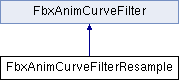
\includegraphics[height=2.000000cm]{class_fbx_anim_curve_filter_resample}
\end{center}
\end{figure}
\subsection*{公開メンバ関数}
\begin{DoxyCompactItemize}
\item 
\hyperlink{class_fbx_anim_curve_filter_resample_ae5da0aba84bf6db3d9cda6a4aeb5824f}{Fbx\+Anim\+Curve\+Filter\+Resample} ()
\begin{DoxyCompactList}\small\item\em Constructor. \end{DoxyCompactList}\item 
virtual \hyperlink{class_fbx_anim_curve_filter_resample_a9424bc3a1a9796265126c399d8e8fb5a}{$\sim$\+Fbx\+Anim\+Curve\+Filter\+Resample} ()
\begin{DoxyCompactList}\small\item\em Destructor. \end{DoxyCompactList}\item 
virtual const char $\ast$ \hyperlink{class_fbx_anim_curve_filter_resample_a67303296eba915d2a9fde63c2557c3f9}{Get\+Name} () const
\item 
virtual bool \hyperlink{class_fbx_anim_curve_filter_resample_aa4edbed0ce74836a77fe4fd907c604a6}{Apply} (\hyperlink{class_fbx_anim_curve}{Fbx\+Anim\+Curve} \&p\+Curve, \hyperlink{class_fbx_status}{Fbx\+Status} $\ast$p\+Status=\hyperlink{fbxarch_8h_a070d2ce7b6bb7e5c05602aa8c308d0c4}{N\+U\+LL})
\item 
virtual void \hyperlink{class_fbx_anim_curve_filter_resample_a149622ab0dd1ffd26ca1e59f31aaed93}{Reset} ()
\item 
void \hyperlink{class_fbx_anim_curve_filter_resample_abb2e4701aa3e44d945cfa92254aabbb0}{Set\+Keys\+On\+Frame} (bool p\+Keys\+On\+Frame)
\item 
bool \hyperlink{class_fbx_anim_curve_filter_resample_af91489566c2c8445995dd265648646ea}{Get\+Keys\+On\+Frame} () const
\item 
\hyperlink{class_fbx_time}{Fbx\+Time} \hyperlink{class_fbx_anim_curve_filter_resample_a0efe607fa3febdd058b03a7ac444bfd4}{Get\+Period\+Time} () const
\item 
void \hyperlink{class_fbx_anim_curve_filter_resample_a1d2369b1cd4a656a79e05b10f7faadd4}{Set\+Period\+Time} (\hyperlink{class_fbx_time}{Fbx\+Time} \&p\+Period)
\item 
bool \hyperlink{class_fbx_anim_curve_filter_resample_ae0b81c640c35b6b2d0a34b5586f2f053}{Get\+Intelligent\+Mode} () const
\item 
void \hyperlink{class_fbx_anim_curve_filter_resample_a8ac3cafa7fe863a9d3205452f6f15c49}{Set\+Intelligent\+Mode} (bool p\+Intelligent)
\end{DoxyCompactItemize}
\subsection*{Exposed parent class methods.}
\begin{DoxyCompactItemize}
\item 
virtual bool \hyperlink{class_fbx_anim_curve_filter_resample_a0f94e6a08f94ee1798b3bdce67285f53}{Apply} (\hyperlink{class_fbx_anim_stack}{Fbx\+Anim\+Stack} $\ast$p\+Anim\+Stack, \hyperlink{class_fbx_status}{Fbx\+Status} $\ast$p\+Status=\hyperlink{fbxarch_8h_a070d2ce7b6bb7e5c05602aa8c308d0c4}{N\+U\+LL})
\item 
virtual bool \hyperlink{class_fbx_anim_curve_filter_resample_a6f22a537869dc295ceff244f56ac561e}{Apply} (\hyperlink{class_fbx_object}{Fbx\+Object} $\ast$p\+Obj, \hyperlink{class_fbx_anim_stack}{Fbx\+Anim\+Stack} $\ast$p\+Anim\+Stack, \hyperlink{class_fbx_status}{Fbx\+Status} $\ast$p\+Status=\hyperlink{fbxarch_8h_a070d2ce7b6bb7e5c05602aa8c308d0c4}{N\+U\+LL})
\item 
virtual bool \hyperlink{class_fbx_anim_curve_filter_resample_a1359f91c344c6dd4d89fa0a883ae38b2}{Apply} (\hyperlink{class_fbx_anim_curve_node}{Fbx\+Anim\+Curve\+Node} \&p\+Curve\+Node, \hyperlink{class_fbx_status}{Fbx\+Status} $\ast$p\+Status=\hyperlink{fbxarch_8h_a070d2ce7b6bb7e5c05602aa8c308d0c4}{N\+U\+LL})
\item 
virtual bool \hyperlink{class_fbx_anim_curve_filter_resample_a2a095982e24a1ea1e35bc1ab97e833d7}{Apply} (\hyperlink{class_fbx_anim_curve}{Fbx\+Anim\+Curve} $\ast$$\ast$p\+Curve, int p\+Count, \hyperlink{class_fbx_status}{Fbx\+Status} $\ast$p\+Status=\hyperlink{fbxarch_8h_a070d2ce7b6bb7e5c05602aa8c308d0c4}{N\+U\+LL})
\end{DoxyCompactItemize}
\subsection*{その他の継承メンバ}


\subsection{詳解}
Re-\/sampling filter.

Filter to re-\/sample animation curves. 

 fbxanimcurvefilters.\+h の 681 行目に定義があります。



\subsection{構築子と解体子}
\mbox{\Hypertarget{class_fbx_anim_curve_filter_resample_ae5da0aba84bf6db3d9cda6a4aeb5824f}\label{class_fbx_anim_curve_filter_resample_ae5da0aba84bf6db3d9cda6a4aeb5824f}} 
\index{Fbx\+Anim\+Curve\+Filter\+Resample@{Fbx\+Anim\+Curve\+Filter\+Resample}!Fbx\+Anim\+Curve\+Filter\+Resample@{Fbx\+Anim\+Curve\+Filter\+Resample}}
\index{Fbx\+Anim\+Curve\+Filter\+Resample@{Fbx\+Anim\+Curve\+Filter\+Resample}!Fbx\+Anim\+Curve\+Filter\+Resample@{Fbx\+Anim\+Curve\+Filter\+Resample}}
\subsubsection{\texorpdfstring{Fbx\+Anim\+Curve\+Filter\+Resample()}{FbxAnimCurveFilterResample()}}
{\footnotesize\ttfamily Fbx\+Anim\+Curve\+Filter\+Resample\+::\+Fbx\+Anim\+Curve\+Filter\+Resample (\begin{DoxyParamCaption}{ }\end{DoxyParamCaption})}



Constructor. 

\mbox{\Hypertarget{class_fbx_anim_curve_filter_resample_a9424bc3a1a9796265126c399d8e8fb5a}\label{class_fbx_anim_curve_filter_resample_a9424bc3a1a9796265126c399d8e8fb5a}} 
\index{Fbx\+Anim\+Curve\+Filter\+Resample@{Fbx\+Anim\+Curve\+Filter\+Resample}!````~Fbx\+Anim\+Curve\+Filter\+Resample@{$\sim$\+Fbx\+Anim\+Curve\+Filter\+Resample}}
\index{````~Fbx\+Anim\+Curve\+Filter\+Resample@{$\sim$\+Fbx\+Anim\+Curve\+Filter\+Resample}!Fbx\+Anim\+Curve\+Filter\+Resample@{Fbx\+Anim\+Curve\+Filter\+Resample}}
\subsubsection{\texorpdfstring{$\sim$\+Fbx\+Anim\+Curve\+Filter\+Resample()}{~FbxAnimCurveFilterResample()}}
{\footnotesize\ttfamily virtual Fbx\+Anim\+Curve\+Filter\+Resample\+::$\sim$\+Fbx\+Anim\+Curve\+Filter\+Resample (\begin{DoxyParamCaption}{ }\end{DoxyParamCaption})\hspace{0.3cm}{\ttfamily [inline]}, {\ttfamily [virtual]}}



Destructor. 



 fbxanimcurvefilters.\+h の 688 行目に定義があります。



\subsection{関数詳解}
\mbox{\Hypertarget{class_fbx_anim_curve_filter_resample_a0f94e6a08f94ee1798b3bdce67285f53}\label{class_fbx_anim_curve_filter_resample_a0f94e6a08f94ee1798b3bdce67285f53}} 
\index{Fbx\+Anim\+Curve\+Filter\+Resample@{Fbx\+Anim\+Curve\+Filter\+Resample}!Apply@{Apply}}
\index{Apply@{Apply}!Fbx\+Anim\+Curve\+Filter\+Resample@{Fbx\+Anim\+Curve\+Filter\+Resample}}
\subsubsection{\texorpdfstring{Apply()}{Apply()}\hspace{0.1cm}{\footnotesize\ttfamily [1/5]}}
{\footnotesize\ttfamily virtual bool Fbx\+Anim\+Curve\+Filter\+Resample\+::\+Apply (\begin{DoxyParamCaption}\item[{\hyperlink{class_fbx_anim_stack}{Fbx\+Anim\+Stack} $\ast$}]{p\+Anim\+Stack,  }\item[{\hyperlink{class_fbx_status}{Fbx\+Status} $\ast$}]{p\+Status = {\ttfamily \hyperlink{fbxarch_8h_a070d2ce7b6bb7e5c05602aa8c308d0c4}{N\+U\+LL}} }\end{DoxyParamCaption})\hspace{0.3cm}{\ttfamily [inline]}, {\ttfamily [virtual]}}

Apply filter to all the curves stored in the animation stack. 
\begin{DoxyParams}{引数}
{\em p\+Anim\+Stack} & Animation stack where to retrieve the animation curves \\
\hline
{\em p\+Status} & The \hyperlink{class_fbx_status}{Fbx\+Status} object to hold error codes. \\
\hline
\end{DoxyParams}
\begin{DoxyReturn}{戻り値}
{\ttfamily true} if the curve filtering operation was successful, {\ttfamily false} otherwise. 
\end{DoxyReturn}


\hyperlink{class_fbx_anim_curve_filter_aef3900e6180e05661c27ee484ae939c3}{Fbx\+Anim\+Curve\+Filter}を再実装しています。



 fbxanimcurvefilters.\+h の 699 行目に定義があります。

\mbox{\Hypertarget{class_fbx_anim_curve_filter_resample_a6f22a537869dc295ceff244f56ac561e}\label{class_fbx_anim_curve_filter_resample_a6f22a537869dc295ceff244f56ac561e}} 
\index{Fbx\+Anim\+Curve\+Filter\+Resample@{Fbx\+Anim\+Curve\+Filter\+Resample}!Apply@{Apply}}
\index{Apply@{Apply}!Fbx\+Anim\+Curve\+Filter\+Resample@{Fbx\+Anim\+Curve\+Filter\+Resample}}
\subsubsection{\texorpdfstring{Apply()}{Apply()}\hspace{0.1cm}{\footnotesize\ttfamily [2/5]}}
{\footnotesize\ttfamily virtual bool Fbx\+Anim\+Curve\+Filter\+Resample\+::\+Apply (\begin{DoxyParamCaption}\item[{\hyperlink{class_fbx_object}{Fbx\+Object} $\ast$}]{p\+Obj,  }\item[{\hyperlink{class_fbx_anim_stack}{Fbx\+Anim\+Stack} $\ast$}]{p\+Anim\+Stack,  }\item[{\hyperlink{class_fbx_status}{Fbx\+Status} $\ast$}]{p\+Status = {\ttfamily \hyperlink{fbxarch_8h_a070d2ce7b6bb7e5c05602aa8c308d0c4}{N\+U\+LL}} }\end{DoxyParamCaption})\hspace{0.3cm}{\ttfamily [inline]}, {\ttfamily [virtual]}}

Apply filter to all the animated properties of the object. 
\begin{DoxyParams}{引数}
{\em p\+Obj} & Object containing the animated properties to which the filter is applied. \\
\hline
{\em p\+Anim\+Stack} & Animation stack where to retrieve the animation curves \\
\hline
{\em p\+Status} & The \hyperlink{class_fbx_status}{Fbx\+Status} object to hold error codes. \\
\hline
\end{DoxyParams}
\begin{DoxyReturn}{戻り値}
{\ttfamily true} if the curve filtering operation was successful, {\ttfamily false} otherwise. 
\end{DoxyReturn}


\hyperlink{class_fbx_anim_curve_filter_a009498a65af4995bf5e5908f17837531}{Fbx\+Anim\+Curve\+Filter}を再実装しています。



 fbxanimcurvefilters.\+h の 700 行目に定義があります。

\mbox{\Hypertarget{class_fbx_anim_curve_filter_resample_a1359f91c344c6dd4d89fa0a883ae38b2}\label{class_fbx_anim_curve_filter_resample_a1359f91c344c6dd4d89fa0a883ae38b2}} 
\index{Fbx\+Anim\+Curve\+Filter\+Resample@{Fbx\+Anim\+Curve\+Filter\+Resample}!Apply@{Apply}}
\index{Apply@{Apply}!Fbx\+Anim\+Curve\+Filter\+Resample@{Fbx\+Anim\+Curve\+Filter\+Resample}}
\subsubsection{\texorpdfstring{Apply()}{Apply()}\hspace{0.1cm}{\footnotesize\ttfamily [3/5]}}
{\footnotesize\ttfamily virtual bool Fbx\+Anim\+Curve\+Filter\+Resample\+::\+Apply (\begin{DoxyParamCaption}\item[{\hyperlink{class_fbx_anim_curve_node}{Fbx\+Anim\+Curve\+Node} \&}]{p\+Curve\+Node,  }\item[{\hyperlink{class_fbx_status}{Fbx\+Status} $\ast$}]{p\+Status = {\ttfamily \hyperlink{fbxarch_8h_a070d2ce7b6bb7e5c05602aa8c308d0c4}{N\+U\+LL}} }\end{DoxyParamCaption})\hspace{0.3cm}{\ttfamily [inline]}, {\ttfamily [virtual]}}

Apply filter on all the curves of an animation curve node. 
\begin{DoxyParams}{引数}
{\em p\+Curve\+Node} & Curve node to which the filter is applied. \\
\hline
{\em p\+Status} & The \hyperlink{class_fbx_status}{Fbx\+Status} object to hold error codes. \\
\hline
\end{DoxyParams}
\begin{DoxyReturn}{戻り値}
{\ttfamily true} if the curve filtering operation was successful, {\ttfamily false} otherwise. 
\end{DoxyReturn}
\begin{DoxyRemark}{注釈}
This method collects all the \hyperlink{class_fbx_anim_curve}{Fbx\+Anim\+Curve} objects connected to the curve node and calls Apply(\+Fbx\+Anim\+Curve$\ast$$\ast$, int) 
\end{DoxyRemark}


\hyperlink{class_fbx_anim_curve_filter_ad042b45c0675278fa49e61739b0825c2}{Fbx\+Anim\+Curve\+Filter}を再実装しています。



 fbxanimcurvefilters.\+h の 701 行目に定義があります。

\mbox{\Hypertarget{class_fbx_anim_curve_filter_resample_a2a095982e24a1ea1e35bc1ab97e833d7}\label{class_fbx_anim_curve_filter_resample_a2a095982e24a1ea1e35bc1ab97e833d7}} 
\index{Fbx\+Anim\+Curve\+Filter\+Resample@{Fbx\+Anim\+Curve\+Filter\+Resample}!Apply@{Apply}}
\index{Apply@{Apply}!Fbx\+Anim\+Curve\+Filter\+Resample@{Fbx\+Anim\+Curve\+Filter\+Resample}}
\subsubsection{\texorpdfstring{Apply()}{Apply()}\hspace{0.1cm}{\footnotesize\ttfamily [4/5]}}
{\footnotesize\ttfamily virtual bool Fbx\+Anim\+Curve\+Filter\+Resample\+::\+Apply (\begin{DoxyParamCaption}\item[{\hyperlink{class_fbx_anim_curve}{Fbx\+Anim\+Curve} $\ast$$\ast$}]{p\+Curve,  }\item[{int}]{p\+Count,  }\item[{\hyperlink{class_fbx_status}{Fbx\+Status} $\ast$}]{p\+Status = {\ttfamily \hyperlink{fbxarch_8h_a070d2ce7b6bb7e5c05602aa8c308d0c4}{N\+U\+LL}} }\end{DoxyParamCaption})\hspace{0.3cm}{\ttfamily [inline]}, {\ttfamily [virtual]}}

Apply filter on an array of animation curves. 
\begin{DoxyParams}{引数}
{\em p\+Curve} & Array of curves to which the filter is applied. \\
\hline
{\em p\+Count} & Number of curves in the array. \\
\hline
{\em p\+Status} & The \hyperlink{class_fbx_status}{Fbx\+Status} object to hold error codes. \\
\hline
\end{DoxyParams}
\begin{DoxyReturn}{戻り値}
{\ttfamily true} if the curve filtering operation was successful, {\ttfamily false} otherwise. 
\end{DoxyReturn}


\hyperlink{class_fbx_anim_curve_filter_aca6a41fbc4d9019b20df7adccfa6ed3c}{Fbx\+Anim\+Curve\+Filter}を再実装しています。



 fbxanimcurvefilters.\+h の 702 行目に定義があります。

\mbox{\Hypertarget{class_fbx_anim_curve_filter_resample_aa4edbed0ce74836a77fe4fd907c604a6}\label{class_fbx_anim_curve_filter_resample_aa4edbed0ce74836a77fe4fd907c604a6}} 
\index{Fbx\+Anim\+Curve\+Filter\+Resample@{Fbx\+Anim\+Curve\+Filter\+Resample}!Apply@{Apply}}
\index{Apply@{Apply}!Fbx\+Anim\+Curve\+Filter\+Resample@{Fbx\+Anim\+Curve\+Filter\+Resample}}
\subsubsection{\texorpdfstring{Apply()}{Apply()}\hspace{0.1cm}{\footnotesize\ttfamily [5/5]}}
{\footnotesize\ttfamily virtual bool Fbx\+Anim\+Curve\+Filter\+Resample\+::\+Apply (\begin{DoxyParamCaption}\item[{\hyperlink{class_fbx_anim_curve}{Fbx\+Anim\+Curve} \&}]{p\+Curve,  }\item[{\hyperlink{class_fbx_status}{Fbx\+Status} $\ast$}]{p\+Status = {\ttfamily \hyperlink{fbxarch_8h_a070d2ce7b6bb7e5c05602aa8c308d0c4}{N\+U\+LL}} }\end{DoxyParamCaption})\hspace{0.3cm}{\ttfamily [virtual]}}

Apply the filter on an animation curve. 
\begin{DoxyParams}{引数}
{\em p\+Curve} & Curve to which the filter is applied. \\
\hline
{\em p\+Status} & The \hyperlink{class_fbx_status}{Fbx\+Status} object to hold error codes. \\
\hline
\end{DoxyParams}
\begin{DoxyReturn}{戻り値}
{\ttfamily true} if the curve filtering operation was successful, {\ttfamily false} otherwise. 
\end{DoxyReturn}


\hyperlink{class_fbx_anim_curve_filter_a6a69996c47c0e6f63a0f8b0d5fa806a0}{Fbx\+Anim\+Curve\+Filter}を実装しています。

\mbox{\Hypertarget{class_fbx_anim_curve_filter_resample_ae0b81c640c35b6b2d0a34b5586f2f053}\label{class_fbx_anim_curve_filter_resample_ae0b81c640c35b6b2d0a34b5586f2f053}} 
\index{Fbx\+Anim\+Curve\+Filter\+Resample@{Fbx\+Anim\+Curve\+Filter\+Resample}!Get\+Intelligent\+Mode@{Get\+Intelligent\+Mode}}
\index{Get\+Intelligent\+Mode@{Get\+Intelligent\+Mode}!Fbx\+Anim\+Curve\+Filter\+Resample@{Fbx\+Anim\+Curve\+Filter\+Resample}}
\subsubsection{\texorpdfstring{Get\+Intelligent\+Mode()}{GetIntelligentMode()}}
{\footnotesize\ttfamily bool Fbx\+Anim\+Curve\+Filter\+Resample\+::\+Get\+Intelligent\+Mode (\begin{DoxyParamCaption}{ }\end{DoxyParamCaption}) const}

Get the mode that determines how the re-\/sample filter will set the interpolation and tangent of each key. \begin{DoxyReturn}{戻り値}
{\ttfamily true} if the intelligent mode is on, {\ttfamily false} otherwise. 
\end{DoxyReturn}
\begin{DoxyRemark}{注釈}
If intelligent mode is on, interpolation type and tangent mode of each created curve key are set equal to the interpolation type and tangent mode of the closest curve key encountered. If intelligent mode is off, the interpolation type of each created curve key will always be set to C\+U\+B\+IC, and tangent mode will always be set to A\+U\+TO. 
\end{DoxyRemark}
\mbox{\Hypertarget{class_fbx_anim_curve_filter_resample_af91489566c2c8445995dd265648646ea}\label{class_fbx_anim_curve_filter_resample_af91489566c2c8445995dd265648646ea}} 
\index{Fbx\+Anim\+Curve\+Filter\+Resample@{Fbx\+Anim\+Curve\+Filter\+Resample}!Get\+Keys\+On\+Frame@{Get\+Keys\+On\+Frame}}
\index{Get\+Keys\+On\+Frame@{Get\+Keys\+On\+Frame}!Fbx\+Anim\+Curve\+Filter\+Resample@{Fbx\+Anim\+Curve\+Filter\+Resample}}
\subsubsection{\texorpdfstring{Get\+Keys\+On\+Frame()}{GetKeysOnFrame()}}
{\footnotesize\ttfamily bool Fbx\+Anim\+Curve\+Filter\+Resample\+::\+Get\+Keys\+On\+Frame (\begin{DoxyParamCaption}{ }\end{DoxyParamCaption}) const}

Get if the keys are on frame. \begin{DoxyReturn}{戻り値}
Value if keys are on frame multiples. 
\end{DoxyReturn}
\mbox{\Hypertarget{class_fbx_anim_curve_filter_resample_a67303296eba915d2a9fde63c2557c3f9}\label{class_fbx_anim_curve_filter_resample_a67303296eba915d2a9fde63c2557c3f9}} 
\index{Fbx\+Anim\+Curve\+Filter\+Resample@{Fbx\+Anim\+Curve\+Filter\+Resample}!Get\+Name@{Get\+Name}}
\index{Get\+Name@{Get\+Name}!Fbx\+Anim\+Curve\+Filter\+Resample@{Fbx\+Anim\+Curve\+Filter\+Resample}}
\subsubsection{\texorpdfstring{Get\+Name()}{GetName()}}
{\footnotesize\ttfamily virtual const char$\ast$ Fbx\+Anim\+Curve\+Filter\+Resample\+::\+Get\+Name (\begin{DoxyParamCaption}{ }\end{DoxyParamCaption}) const\hspace{0.3cm}{\ttfamily [virtual]}}

Get the name of the filter. \begin{DoxyReturn}{戻り値}
Pointer to name. 
\end{DoxyReturn}


\hyperlink{class_fbx_anim_curve_filter_abd559d5052fbb072042e59241940a35c}{Fbx\+Anim\+Curve\+Filter}を再実装しています。

\mbox{\Hypertarget{class_fbx_anim_curve_filter_resample_a0efe607fa3febdd058b03a7ac444bfd4}\label{class_fbx_anim_curve_filter_resample_a0efe607fa3febdd058b03a7ac444bfd4}} 
\index{Fbx\+Anim\+Curve\+Filter\+Resample@{Fbx\+Anim\+Curve\+Filter\+Resample}!Get\+Period\+Time@{Get\+Period\+Time}}
\index{Get\+Period\+Time@{Get\+Period\+Time}!Fbx\+Anim\+Curve\+Filter\+Resample@{Fbx\+Anim\+Curve\+Filter\+Resample}}
\subsubsection{\texorpdfstring{Get\+Period\+Time()}{GetPeriodTime()}}
{\footnotesize\ttfamily \hyperlink{class_fbx_time}{Fbx\+Time} Fbx\+Anim\+Curve\+Filter\+Resample\+::\+Get\+Period\+Time (\begin{DoxyParamCaption}{ }\end{DoxyParamCaption}) const}

Get the re-\/sampling period \begin{DoxyReturn}{戻り値}
The re-\/sampling period. 
\end{DoxyReturn}
\mbox{\Hypertarget{class_fbx_anim_curve_filter_resample_a149622ab0dd1ffd26ca1e59f31aaed93}\label{class_fbx_anim_curve_filter_resample_a149622ab0dd1ffd26ca1e59f31aaed93}} 
\index{Fbx\+Anim\+Curve\+Filter\+Resample@{Fbx\+Anim\+Curve\+Filter\+Resample}!Reset@{Reset}}
\index{Reset@{Reset}!Fbx\+Anim\+Curve\+Filter\+Resample@{Fbx\+Anim\+Curve\+Filter\+Resample}}
\subsubsection{\texorpdfstring{Reset()}{Reset()}}
{\footnotesize\ttfamily virtual void Fbx\+Anim\+Curve\+Filter\+Resample\+::\+Reset (\begin{DoxyParamCaption}{ }\end{DoxyParamCaption})\hspace{0.3cm}{\ttfamily [virtual]}}

Reset the filter to its default parameters. 

\hyperlink{class_fbx_anim_curve_filter_a57fb35baaaa85adb08946383cf40e811}{Fbx\+Anim\+Curve\+Filter}を再実装しています。

\mbox{\Hypertarget{class_fbx_anim_curve_filter_resample_a8ac3cafa7fe863a9d3205452f6f15c49}\label{class_fbx_anim_curve_filter_resample_a8ac3cafa7fe863a9d3205452f6f15c49}} 
\index{Fbx\+Anim\+Curve\+Filter\+Resample@{Fbx\+Anim\+Curve\+Filter\+Resample}!Set\+Intelligent\+Mode@{Set\+Intelligent\+Mode}}
\index{Set\+Intelligent\+Mode@{Set\+Intelligent\+Mode}!Fbx\+Anim\+Curve\+Filter\+Resample@{Fbx\+Anim\+Curve\+Filter\+Resample}}
\subsubsection{\texorpdfstring{Set\+Intelligent\+Mode()}{SetIntelligentMode()}}
{\footnotesize\ttfamily void Fbx\+Anim\+Curve\+Filter\+Resample\+::\+Set\+Intelligent\+Mode (\begin{DoxyParamCaption}\item[{bool}]{p\+Intelligent }\end{DoxyParamCaption})}

Set the mode that determines how the re-\/sample filter will set the interpolation and tangent of each key. 
\begin{DoxyParams}{引数}
{\em p\+Intelligent} & {\ttfamily true}, set interpolation type and tangent mode of each created curve key equal to the interpolation type and tangent mode of the closest curve key encountered. {\ttfamily false}, always set the interpolation type of each created curve key to C\+U\+B\+IC, and always set the tangent mode to A\+U\+TO. \\
\hline
\end{DoxyParams}
\mbox{\Hypertarget{class_fbx_anim_curve_filter_resample_abb2e4701aa3e44d945cfa92254aabbb0}\label{class_fbx_anim_curve_filter_resample_abb2e4701aa3e44d945cfa92254aabbb0}} 
\index{Fbx\+Anim\+Curve\+Filter\+Resample@{Fbx\+Anim\+Curve\+Filter\+Resample}!Set\+Keys\+On\+Frame@{Set\+Keys\+On\+Frame}}
\index{Set\+Keys\+On\+Frame@{Set\+Keys\+On\+Frame}!Fbx\+Anim\+Curve\+Filter\+Resample@{Fbx\+Anim\+Curve\+Filter\+Resample}}
\subsubsection{\texorpdfstring{Set\+Keys\+On\+Frame()}{SetKeysOnFrame()}}
{\footnotesize\ttfamily void Fbx\+Anim\+Curve\+Filter\+Resample\+::\+Set\+Keys\+On\+Frame (\begin{DoxyParamCaption}\item[{bool}]{p\+Keys\+On\+Frame }\end{DoxyParamCaption})}

Set if the keys are on frame. 
\begin{DoxyParams}{引数}
{\em p\+Keys\+On\+Frame} & value if keys are set on frame multiples. \\
\hline
\end{DoxyParams}
\mbox{\Hypertarget{class_fbx_anim_curve_filter_resample_a1d2369b1cd4a656a79e05b10f7faadd4}\label{class_fbx_anim_curve_filter_resample_a1d2369b1cd4a656a79e05b10f7faadd4}} 
\index{Fbx\+Anim\+Curve\+Filter\+Resample@{Fbx\+Anim\+Curve\+Filter\+Resample}!Set\+Period\+Time@{Set\+Period\+Time}}
\index{Set\+Period\+Time@{Set\+Period\+Time}!Fbx\+Anim\+Curve\+Filter\+Resample@{Fbx\+Anim\+Curve\+Filter\+Resample}}
\subsubsection{\texorpdfstring{Set\+Period\+Time()}{SetPeriodTime()}}
{\footnotesize\ttfamily void Fbx\+Anim\+Curve\+Filter\+Resample\+::\+Set\+Period\+Time (\begin{DoxyParamCaption}\item[{\hyperlink{class_fbx_time}{Fbx\+Time} \&}]{p\+Period }\end{DoxyParamCaption})}

Set the re-\/sampling period 
\begin{DoxyParams}{引数}
{\em p\+Period} & The re-\/sampling period to be set. \\
\hline
\end{DoxyParams}


このクラス詳解は次のファイルから抽出されました\+:\begin{DoxyCompactItemize}
\item 
C\+:/\+Maya/scripts/\+F\+B\+X\+\_\+\+S\+D\+K/2017.\+1/include/fbxsdk/scene/animation/\hyperlink{fbxanimcurvefilters_8h}{fbxanimcurvefilters.\+h}\end{DoxyCompactItemize}

\hypertarget{class_fbx_anim_curve_filter_scale}{}\section{Fbx\+Anim\+Curve\+Filter\+Scale クラス}
\label{class_fbx_anim_curve_filter_scale}\index{Fbx\+Anim\+Curve\+Filter\+Scale@{Fbx\+Anim\+Curve\+Filter\+Scale}}


{\ttfamily \#include $<$fbxanimcurvefilters.\+h$>$}



Fbx\+Anim\+Curve\+Filter\+Scale の継承関係図
% FIG 0


Fbx\+Anim\+Curve\+Filter\+Scale 連携図
% FIG 1
\subsection*{公開メンバ関数}
\begin{DoxyCompactItemize}
\item 
\hyperlink{class_fbx_anim_curve_filter_scale_a8ac5600b1b34f191cb4cab040d9d2ef9}{Fbx\+Anim\+Curve\+Filter\+Scale} ()
\begin{DoxyCompactList}\small\item\em Constructor. \end{DoxyCompactList}\item 
virtual \hyperlink{class_fbx_anim_curve_filter_scale_a2fa5db669596368d0b8cecff75468005}{$\sim$\+Fbx\+Anim\+Curve\+Filter\+Scale} ()
\begin{DoxyCompactList}\small\item\em Destructor. \end{DoxyCompactList}\item 
virtual const char $\ast$ \hyperlink{class_fbx_anim_curve_filter_scale_afffa13f0b3bbdcaa0a6d88d6aea2c83f}{Get\+Name} () const
\item 
virtual bool \hyperlink{class_fbx_anim_curve_filter_scale_abec5cc73d37bef6e8ab3127ed09b21a3}{Apply} (\hyperlink{class_fbx_anim_curve_node}{Fbx\+Anim\+Curve\+Node} \&p\+Curve\+Node, \hyperlink{class_fbx_status}{Fbx\+Status} $\ast$p\+Status=\hyperlink{fbxarch_8h_a070d2ce7b6bb7e5c05602aa8c308d0c4}{N\+U\+LL})
\item 
virtual bool \hyperlink{class_fbx_anim_curve_filter_scale_a1d3234359a5766b4476e4a0522104d77}{Apply} (\hyperlink{class_fbx_anim_curve}{Fbx\+Anim\+Curve} \&p\+Curve, \hyperlink{class_fbx_status}{Fbx\+Status} $\ast$p\+Status=\hyperlink{fbxarch_8h_a070d2ce7b6bb7e5c05602aa8c308d0c4}{N\+U\+LL})
\item 
virtual void \hyperlink{class_fbx_anim_curve_filter_scale_a40e82207d205b026aaab40e52a7184c8}{Reset} ()
\item 
double \hyperlink{class_fbx_anim_curve_filter_scale_a48367ab8cb65db9bffdda7dc8c0afff8}{Get\+Scale} () const
\item 
void \hyperlink{class_fbx_anim_curve_filter_scale_a9c564c7599541607c42d28bb57874eae}{Set\+Scale} (double p\+Scale)
\end{DoxyCompactItemize}
\subsection*{Exposed parent class methods.}
\begin{DoxyCompactItemize}
\item 
virtual bool \hyperlink{class_fbx_anim_curve_filter_scale_ac6fb7610299bd0fc1e399418f8d17b90}{Apply} (\hyperlink{class_fbx_anim_stack}{Fbx\+Anim\+Stack} $\ast$p\+Anim\+Stack, \hyperlink{class_fbx_status}{Fbx\+Status} $\ast$p\+Status=\hyperlink{fbxarch_8h_a070d2ce7b6bb7e5c05602aa8c308d0c4}{N\+U\+LL})
\item 
virtual bool \hyperlink{class_fbx_anim_curve_filter_scale_acaecc7335471ad618e0cc7e02625dbec}{Apply} (\hyperlink{class_fbx_object}{Fbx\+Object} $\ast$p\+Obj, \hyperlink{class_fbx_anim_stack}{Fbx\+Anim\+Stack} $\ast$p\+Anim\+Stack, \hyperlink{class_fbx_status}{Fbx\+Status} $\ast$p\+Status=\hyperlink{fbxarch_8h_a070d2ce7b6bb7e5c05602aa8c308d0c4}{N\+U\+LL})
\item 
virtual bool \hyperlink{class_fbx_anim_curve_filter_scale_a2bf27f4195e038cd2d6308a3399ab556}{Apply} (\hyperlink{class_fbx_anim_curve}{Fbx\+Anim\+Curve} $\ast$$\ast$p\+Curve, int p\+Count, \hyperlink{class_fbx_status}{Fbx\+Status} $\ast$p\+Status=\hyperlink{fbxarch_8h_a070d2ce7b6bb7e5c05602aa8c308d0c4}{N\+U\+LL})
\end{DoxyCompactItemize}
\subsection*{その他の継承メンバ}


\subsection{詳解}
Key scale filter.

Filter to scale the keys of a set of animation curves. 

\subsection{構築子と解体子}
\mbox{\Hypertarget{class_fbx_anim_curve_filter_scale_a8ac5600b1b34f191cb4cab040d9d2ef9}\label{class_fbx_anim_curve_filter_scale_a8ac5600b1b34f191cb4cab040d9d2ef9}} 
\index{Fbx\+Anim\+Curve\+Filter\+Scale@{Fbx\+Anim\+Curve\+Filter\+Scale}!Fbx\+Anim\+Curve\+Filter\+Scale@{Fbx\+Anim\+Curve\+Filter\+Scale}}
\index{Fbx\+Anim\+Curve\+Filter\+Scale@{Fbx\+Anim\+Curve\+Filter\+Scale}!Fbx\+Anim\+Curve\+Filter\+Scale@{Fbx\+Anim\+Curve\+Filter\+Scale}}
\subsubsection{\texorpdfstring{Fbx\+Anim\+Curve\+Filter\+Scale()}{FbxAnimCurveFilterScale()}}
{\footnotesize\ttfamily Fbx\+Anim\+Curve\+Filter\+Scale\+::\+Fbx\+Anim\+Curve\+Filter\+Scale (\begin{DoxyParamCaption}{ }\end{DoxyParamCaption})}



Constructor. 

\mbox{\Hypertarget{class_fbx_anim_curve_filter_scale_a2fa5db669596368d0b8cecff75468005}\label{class_fbx_anim_curve_filter_scale_a2fa5db669596368d0b8cecff75468005}} 
\index{Fbx\+Anim\+Curve\+Filter\+Scale@{Fbx\+Anim\+Curve\+Filter\+Scale}!````~Fbx\+Anim\+Curve\+Filter\+Scale@{$\sim$\+Fbx\+Anim\+Curve\+Filter\+Scale}}
\index{````~Fbx\+Anim\+Curve\+Filter\+Scale@{$\sim$\+Fbx\+Anim\+Curve\+Filter\+Scale}!Fbx\+Anim\+Curve\+Filter\+Scale@{Fbx\+Anim\+Curve\+Filter\+Scale}}
\subsubsection{\texorpdfstring{$\sim$\+Fbx\+Anim\+Curve\+Filter\+Scale()}{~FbxAnimCurveFilterScale()}}
{\footnotesize\ttfamily virtual Fbx\+Anim\+Curve\+Filter\+Scale\+::$\sim$\+Fbx\+Anim\+Curve\+Filter\+Scale (\begin{DoxyParamCaption}{ }\end{DoxyParamCaption})\hspace{0.3cm}{\ttfamily [virtual]}}



Destructor. 

呼び出し関係図\+:
% FIG 2


\subsection{メソッド詳解}
\mbox{\Hypertarget{class_fbx_anim_curve_filter_scale_ac6fb7610299bd0fc1e399418f8d17b90}\label{class_fbx_anim_curve_filter_scale_ac6fb7610299bd0fc1e399418f8d17b90}} 
\index{Fbx\+Anim\+Curve\+Filter\+Scale@{Fbx\+Anim\+Curve\+Filter\+Scale}!Apply@{Apply}}
\index{Apply@{Apply}!Fbx\+Anim\+Curve\+Filter\+Scale@{Fbx\+Anim\+Curve\+Filter\+Scale}}
\subsubsection{\texorpdfstring{Apply()}{Apply()}\hspace{0.1cm}{\footnotesize\ttfamily [1/5]}}
{\footnotesize\ttfamily virtual bool Fbx\+Anim\+Curve\+Filter\+Scale\+::\+Apply (\begin{DoxyParamCaption}\item[{\hyperlink{class_fbx_anim_stack}{Fbx\+Anim\+Stack} $\ast$}]{p\+Anim\+Stack,  }\item[{\hyperlink{class_fbx_status}{Fbx\+Status} $\ast$}]{p\+Status = {\ttfamily \hyperlink{fbxarch_8h_a070d2ce7b6bb7e5c05602aa8c308d0c4}{N\+U\+LL}} }\end{DoxyParamCaption})\hspace{0.3cm}{\ttfamily [virtual]}}

Apply filter to all the curves stored in the animation stack. 
\begin{DoxyParams}{引数}
{\em p\+Anim\+Stack} & Animation stack where to retrieve the animation curves \\
\hline
{\em p\+Status} & The \hyperlink{class_fbx_status}{Fbx\+Status} object to hold error codes. \\
\hline
\end{DoxyParams}
\begin{DoxyReturn}{戻り値}
{\ttfamily true} if the curve filtering operation was successful, {\ttfamily false} otherwise. 
\end{DoxyReturn}


\hyperlink{class_fbx_anim_curve_filter_aef3900e6180e05661c27ee484ae939c3}{Fbx\+Anim\+Curve\+Filter}を再実装しています。

呼び出し関係図\+:
% FIG 3
\mbox{\Hypertarget{class_fbx_anim_curve_filter_scale_acaecc7335471ad618e0cc7e02625dbec}\label{class_fbx_anim_curve_filter_scale_acaecc7335471ad618e0cc7e02625dbec}} 
\index{Fbx\+Anim\+Curve\+Filter\+Scale@{Fbx\+Anim\+Curve\+Filter\+Scale}!Apply@{Apply}}
\index{Apply@{Apply}!Fbx\+Anim\+Curve\+Filter\+Scale@{Fbx\+Anim\+Curve\+Filter\+Scale}}
\subsubsection{\texorpdfstring{Apply()}{Apply()}\hspace{0.1cm}{\footnotesize\ttfamily [2/5]}}
{\footnotesize\ttfamily virtual bool Fbx\+Anim\+Curve\+Filter\+Scale\+::\+Apply (\begin{DoxyParamCaption}\item[{\hyperlink{class_fbx_object}{Fbx\+Object} $\ast$}]{p\+Obj,  }\item[{\hyperlink{class_fbx_anim_stack}{Fbx\+Anim\+Stack} $\ast$}]{p\+Anim\+Stack,  }\item[{\hyperlink{class_fbx_status}{Fbx\+Status} $\ast$}]{p\+Status = {\ttfamily \hyperlink{fbxarch_8h_a070d2ce7b6bb7e5c05602aa8c308d0c4}{N\+U\+LL}} }\end{DoxyParamCaption})\hspace{0.3cm}{\ttfamily [virtual]}}

Apply filter to all the animated properties of the object. 
\begin{DoxyParams}{引数}
{\em p\+Obj} & Object containing the animated properties to which the filter is applied. \\
\hline
{\em p\+Anim\+Stack} & Animation stack where to retrieve the animation curves \\
\hline
{\em p\+Status} & The \hyperlink{class_fbx_status}{Fbx\+Status} object to hold error codes. \\
\hline
\end{DoxyParams}
\begin{DoxyReturn}{戻り値}
{\ttfamily true} if the curve filtering operation was successful, {\ttfamily false} otherwise. 
\end{DoxyReturn}


\hyperlink{class_fbx_anim_curve_filter_a009498a65af4995bf5e5908f17837531}{Fbx\+Anim\+Curve\+Filter}を再実装しています。

呼び出し関係図\+:
% FIG 4
\mbox{\Hypertarget{class_fbx_anim_curve_filter_scale_a2bf27f4195e038cd2d6308a3399ab556}\label{class_fbx_anim_curve_filter_scale_a2bf27f4195e038cd2d6308a3399ab556}} 
\index{Fbx\+Anim\+Curve\+Filter\+Scale@{Fbx\+Anim\+Curve\+Filter\+Scale}!Apply@{Apply}}
\index{Apply@{Apply}!Fbx\+Anim\+Curve\+Filter\+Scale@{Fbx\+Anim\+Curve\+Filter\+Scale}}
\subsubsection{\texorpdfstring{Apply()}{Apply()}\hspace{0.1cm}{\footnotesize\ttfamily [3/5]}}
{\footnotesize\ttfamily virtual bool Fbx\+Anim\+Curve\+Filter\+Scale\+::\+Apply (\begin{DoxyParamCaption}\item[{\hyperlink{class_fbx_anim_curve}{Fbx\+Anim\+Curve} $\ast$$\ast$}]{p\+Curve,  }\item[{int}]{p\+Count,  }\item[{\hyperlink{class_fbx_status}{Fbx\+Status} $\ast$}]{p\+Status = {\ttfamily \hyperlink{fbxarch_8h_a070d2ce7b6bb7e5c05602aa8c308d0c4}{N\+U\+LL}} }\end{DoxyParamCaption})\hspace{0.3cm}{\ttfamily [virtual]}}

Apply filter on an array of animation curves. 
\begin{DoxyParams}{引数}
{\em p\+Curve} & Array of curves to which the filter is applied. \\
\hline
{\em p\+Count} & Number of curves in the array. \\
\hline
{\em p\+Status} & The \hyperlink{class_fbx_status}{Fbx\+Status} object to hold error codes. \\
\hline
\end{DoxyParams}
\begin{DoxyReturn}{戻り値}
{\ttfamily true} if the curve filtering operation was successful, {\ttfamily false} otherwise. 
\end{DoxyReturn}


\hyperlink{class_fbx_anim_curve_filter_aca6a41fbc4d9019b20df7adccfa6ed3c}{Fbx\+Anim\+Curve\+Filter}を再実装しています。

呼び出し関係図\+:
% FIG 5
\mbox{\Hypertarget{class_fbx_anim_curve_filter_scale_abec5cc73d37bef6e8ab3127ed09b21a3}\label{class_fbx_anim_curve_filter_scale_abec5cc73d37bef6e8ab3127ed09b21a3}} 
\index{Fbx\+Anim\+Curve\+Filter\+Scale@{Fbx\+Anim\+Curve\+Filter\+Scale}!Apply@{Apply}}
\index{Apply@{Apply}!Fbx\+Anim\+Curve\+Filter\+Scale@{Fbx\+Anim\+Curve\+Filter\+Scale}}
\subsubsection{\texorpdfstring{Apply()}{Apply()}\hspace{0.1cm}{\footnotesize\ttfamily [4/5]}}
{\footnotesize\ttfamily virtual bool Fbx\+Anim\+Curve\+Filter\+Scale\+::\+Apply (\begin{DoxyParamCaption}\item[{\hyperlink{class_fbx_anim_curve_node}{Fbx\+Anim\+Curve\+Node} \&}]{p\+Curve\+Node,  }\item[{\hyperlink{class_fbx_status}{Fbx\+Status} $\ast$}]{p\+Status = {\ttfamily \hyperlink{fbxarch_8h_a070d2ce7b6bb7e5c05602aa8c308d0c4}{N\+U\+LL}} }\end{DoxyParamCaption})\hspace{0.3cm}{\ttfamily [virtual]}}

Apply filter on all the curves of an animation curve node. 
\begin{DoxyParams}{引数}
{\em p\+Curve\+Node} & Curve node to which the filter is applied. \\
\hline
{\em p\+Status} & The \hyperlink{class_fbx_status}{Fbx\+Status} object to hold error codes. \\
\hline
\end{DoxyParams}
\begin{DoxyReturn}{戻り値}
{\ttfamily true} if the curve filtering operation was successful, {\ttfamily false} otherwise. 
\end{DoxyReturn}
\begin{DoxyRemark}{注釈}
This method collects all the \hyperlink{class_fbx_anim_curve}{Fbx\+Anim\+Curve} objects connected to the curve node and calls Apply(\+Fbx\+Anim\+Curve$\ast$$\ast$, int) 
\end{DoxyRemark}


\hyperlink{class_fbx_anim_curve_filter_ad042b45c0675278fa49e61739b0825c2}{Fbx\+Anim\+Curve\+Filter}を再実装しています。

\mbox{\Hypertarget{class_fbx_anim_curve_filter_scale_a1d3234359a5766b4476e4a0522104d77}\label{class_fbx_anim_curve_filter_scale_a1d3234359a5766b4476e4a0522104d77}} 
\index{Fbx\+Anim\+Curve\+Filter\+Scale@{Fbx\+Anim\+Curve\+Filter\+Scale}!Apply@{Apply}}
\index{Apply@{Apply}!Fbx\+Anim\+Curve\+Filter\+Scale@{Fbx\+Anim\+Curve\+Filter\+Scale}}
\subsubsection{\texorpdfstring{Apply()}{Apply()}\hspace{0.1cm}{\footnotesize\ttfamily [5/5]}}
{\footnotesize\ttfamily virtual bool Fbx\+Anim\+Curve\+Filter\+Scale\+::\+Apply (\begin{DoxyParamCaption}\item[{\hyperlink{class_fbx_anim_curve}{Fbx\+Anim\+Curve} \&}]{p\+Curve,  }\item[{\hyperlink{class_fbx_status}{Fbx\+Status} $\ast$}]{p\+Status = {\ttfamily \hyperlink{fbxarch_8h_a070d2ce7b6bb7e5c05602aa8c308d0c4}{N\+U\+LL}} }\end{DoxyParamCaption})\hspace{0.3cm}{\ttfamily [virtual]}}

Apply filter on an animation curve. 
\begin{DoxyParams}{引数}
{\em p\+Curve} & Curve to which the filter is applied. \\
\hline
{\em p\+Status} & The \hyperlink{class_fbx_status}{Fbx\+Status} object to hold error codes. \\
\hline
\end{DoxyParams}
\begin{DoxyReturn}{戻り値}
{\ttfamily true} if the curve filtering operation was successful, {\ttfamily false} otherwise. 
\end{DoxyReturn}


\hyperlink{class_fbx_anim_curve_filter_a6a69996c47c0e6f63a0f8b0d5fa806a0}{Fbx\+Anim\+Curve\+Filter}を実装しています。

\mbox{\Hypertarget{class_fbx_anim_curve_filter_scale_afffa13f0b3bbdcaa0a6d88d6aea2c83f}\label{class_fbx_anim_curve_filter_scale_afffa13f0b3bbdcaa0a6d88d6aea2c83f}} 
\index{Fbx\+Anim\+Curve\+Filter\+Scale@{Fbx\+Anim\+Curve\+Filter\+Scale}!Get\+Name@{Get\+Name}}
\index{Get\+Name@{Get\+Name}!Fbx\+Anim\+Curve\+Filter\+Scale@{Fbx\+Anim\+Curve\+Filter\+Scale}}
\subsubsection{\texorpdfstring{Get\+Name()}{GetName()}}
{\footnotesize\ttfamily virtual const char$\ast$ Fbx\+Anim\+Curve\+Filter\+Scale\+::\+Get\+Name (\begin{DoxyParamCaption}{ }\end{DoxyParamCaption}) const\hspace{0.3cm}{\ttfamily [virtual]}}

Get the name of the filter. \begin{DoxyReturn}{戻り値}
Pointer to name. 
\end{DoxyReturn}


\hyperlink{class_fbx_anim_curve_filter_abd559d5052fbb072042e59241940a35c}{Fbx\+Anim\+Curve\+Filter}を再実装しています。

\mbox{\Hypertarget{class_fbx_anim_curve_filter_scale_a48367ab8cb65db9bffdda7dc8c0afff8}\label{class_fbx_anim_curve_filter_scale_a48367ab8cb65db9bffdda7dc8c0afff8}} 
\index{Fbx\+Anim\+Curve\+Filter\+Scale@{Fbx\+Anim\+Curve\+Filter\+Scale}!Get\+Scale@{Get\+Scale}}
\index{Get\+Scale@{Get\+Scale}!Fbx\+Anim\+Curve\+Filter\+Scale@{Fbx\+Anim\+Curve\+Filter\+Scale}}
\subsubsection{\texorpdfstring{Get\+Scale()}{GetScale()}}
{\footnotesize\ttfamily double Fbx\+Anim\+Curve\+Filter\+Scale\+::\+Get\+Scale (\begin{DoxyParamCaption}{ }\end{DoxyParamCaption}) const}

Get the scale factor. \begin{DoxyReturn}{戻り値}
The current scale factor. 
\end{DoxyReturn}
\mbox{\Hypertarget{class_fbx_anim_curve_filter_scale_a40e82207d205b026aaab40e52a7184c8}\label{class_fbx_anim_curve_filter_scale_a40e82207d205b026aaab40e52a7184c8}} 
\index{Fbx\+Anim\+Curve\+Filter\+Scale@{Fbx\+Anim\+Curve\+Filter\+Scale}!Reset@{Reset}}
\index{Reset@{Reset}!Fbx\+Anim\+Curve\+Filter\+Scale@{Fbx\+Anim\+Curve\+Filter\+Scale}}
\subsubsection{\texorpdfstring{Reset()}{Reset()}}
{\footnotesize\ttfamily virtual void Fbx\+Anim\+Curve\+Filter\+Scale\+::\+Reset (\begin{DoxyParamCaption}{ }\end{DoxyParamCaption})\hspace{0.3cm}{\ttfamily [virtual]}}

Reset the filter to its default parameters. 

\hyperlink{class_fbx_anim_curve_filter_a57fb35baaaa85adb08946383cf40e811}{Fbx\+Anim\+Curve\+Filter}を再実装しています。

\mbox{\Hypertarget{class_fbx_anim_curve_filter_scale_a9c564c7599541607c42d28bb57874eae}\label{class_fbx_anim_curve_filter_scale_a9c564c7599541607c42d28bb57874eae}} 
\index{Fbx\+Anim\+Curve\+Filter\+Scale@{Fbx\+Anim\+Curve\+Filter\+Scale}!Set\+Scale@{Set\+Scale}}
\index{Set\+Scale@{Set\+Scale}!Fbx\+Anim\+Curve\+Filter\+Scale@{Fbx\+Anim\+Curve\+Filter\+Scale}}
\subsubsection{\texorpdfstring{Set\+Scale()}{SetScale()}}
{\footnotesize\ttfamily void Fbx\+Anim\+Curve\+Filter\+Scale\+::\+Set\+Scale (\begin{DoxyParamCaption}\item[{double}]{p\+Scale }\end{DoxyParamCaption})}

Set the scale factor. 
\begin{DoxyParams}{引数}
{\em p\+Scale} & The new scale factor to set. \\
\hline
\end{DoxyParams}


このクラス詳解は次のファイルから抽出されました\+:\begin{DoxyCompactItemize}
\item 
C\+:/github/\+F\+B\+Xpython\+S\+D\+K201701/\+F\+B\+Xpython\+S\+D\+K201701/2017.\+1/include/fbxsdk/scene/animation/\hyperlink{fbxanimcurvefilters_8h}{fbxanimcurvefilters.\+h}\end{DoxyCompactItemize}

\hypertarget{class_fbx_anim_curve_filter_scale_by_curve}{}\section{Fbx\+Anim\+Curve\+Filter\+Scale\+By\+Curve クラス}
\label{class_fbx_anim_curve_filter_scale_by_curve}\index{Fbx\+Anim\+Curve\+Filter\+Scale\+By\+Curve@{Fbx\+Anim\+Curve\+Filter\+Scale\+By\+Curve}}


{\ttfamily \#include $<$fbxanimcurvefilters.\+h$>$}

Fbx\+Anim\+Curve\+Filter\+Scale\+By\+Curve の継承関係図\begin{figure}[H]
\begin{center}
\leavevmode
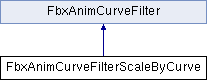
\includegraphics[height=2.000000cm]{class_fbx_anim_curve_filter_scale_by_curve}
\end{center}
\end{figure}
\subsection*{公開メンバ関数}
\begin{DoxyCompactItemize}
\item 
\hyperlink{class_fbx_anim_curve_filter_scale_by_curve_a88a350e3639a1fcb3aa29a071fe0fa71}{Fbx\+Anim\+Curve\+Filter\+Scale\+By\+Curve} ()
\begin{DoxyCompactList}\small\item\em Constructor. \end{DoxyCompactList}\item 
virtual \hyperlink{class_fbx_anim_curve_filter_scale_by_curve_a400e5f8cc518a9facd7b2ba452e55a78}{$\sim$\+Fbx\+Anim\+Curve\+Filter\+Scale\+By\+Curve} ()
\begin{DoxyCompactList}\small\item\em Destructor. \end{DoxyCompactList}\item 
virtual const char $\ast$ \hyperlink{class_fbx_anim_curve_filter_scale_by_curve_a99e99cf6db71774d394010c4cd295fdb}{Get\+Name} () const
\item 
virtual bool \hyperlink{class_fbx_anim_curve_filter_scale_by_curve_ac27bdff4d17273d2a767d188436e53f8}{Apply} (\hyperlink{class_fbx_anim_curve_node}{Fbx\+Anim\+Curve\+Node} \&p\+Curve\+Node, \hyperlink{class_fbx_status}{Fbx\+Status} $\ast$p\+Status=\hyperlink{fbxarch_8h_a070d2ce7b6bb7e5c05602aa8c308d0c4}{N\+U\+LL})
\item 
virtual bool \hyperlink{class_fbx_anim_curve_filter_scale_by_curve_a3914c0e65233ce6f2177d5d7e65c15ea}{Apply} (\hyperlink{class_fbx_anim_curve}{Fbx\+Anim\+Curve} \&p\+Curve, \hyperlink{class_fbx_status}{Fbx\+Status} $\ast$p\+Status=\hyperlink{fbxarch_8h_a070d2ce7b6bb7e5c05602aa8c308d0c4}{N\+U\+LL})
\item 
virtual void \hyperlink{class_fbx_anim_curve_filter_scale_by_curve_afa7aab42520287edf327d78dcbbb0d01}{Reset} ()
\item 
\hyperlink{class_fbx_anim_curve}{Fbx\+Anim\+Curve} $\ast$ \hyperlink{class_fbx_anim_curve_filter_scale_by_curve_a966f86d57bd088700341223a85fe27a0}{Get\+Scale} () const
\item 
void \hyperlink{class_fbx_anim_curve_filter_scale_by_curve_afe876ca9b9d674e62b9b7a3839adeef0}{Set\+Scale} (\hyperlink{class_fbx_anim_curve}{Fbx\+Anim\+Curve} $\ast$p\+Scale)
\end{DoxyCompactItemize}
\subsection*{Exposed parent class methods.}
\begin{DoxyCompactItemize}
\item 
virtual bool \hyperlink{class_fbx_anim_curve_filter_scale_by_curve_a6a1c172a82c4e5e2263d388c74ec9dba}{Apply} (\hyperlink{class_fbx_anim_stack}{Fbx\+Anim\+Stack} $\ast$p\+Anim\+Stack, \hyperlink{class_fbx_status}{Fbx\+Status} $\ast$p\+Status=\hyperlink{fbxarch_8h_a070d2ce7b6bb7e5c05602aa8c308d0c4}{N\+U\+LL})
\item 
virtual bool \hyperlink{class_fbx_anim_curve_filter_scale_by_curve_a7212a7c70bb1c0ae8f7c82c25de17745}{Apply} (\hyperlink{class_fbx_object}{Fbx\+Object} $\ast$p\+Obj, \hyperlink{class_fbx_anim_stack}{Fbx\+Anim\+Stack} $\ast$p\+Anim\+Stack, \hyperlink{class_fbx_status}{Fbx\+Status} $\ast$p\+Status=\hyperlink{fbxarch_8h_a070d2ce7b6bb7e5c05602aa8c308d0c4}{N\+U\+LL})
\item 
virtual bool \hyperlink{class_fbx_anim_curve_filter_scale_by_curve_a8fc0bda8ff0cabcd9a424e06ca646581}{Apply} (\hyperlink{class_fbx_anim_curve}{Fbx\+Anim\+Curve} $\ast$$\ast$p\+Curve, int p\+Count, \hyperlink{class_fbx_status}{Fbx\+Status} $\ast$p\+Status=\hyperlink{fbxarch_8h_a070d2ce7b6bb7e5c05602aa8c308d0c4}{N\+U\+LL})
\end{DoxyCompactItemize}
\subsection*{その他の継承メンバ}


\subsection{詳解}
Key scale filter. Instead of scaling by a constant float value, we will scale by using another anim curve Use a single channel curve only to scale

Filter to scale the keys of a set of animation curves. 

 fbxanimcurvefilters.\+h の 838 行目に定義があります。



\subsection{構築子と解体子}
\mbox{\Hypertarget{class_fbx_anim_curve_filter_scale_by_curve_a88a350e3639a1fcb3aa29a071fe0fa71}\label{class_fbx_anim_curve_filter_scale_by_curve_a88a350e3639a1fcb3aa29a071fe0fa71}} 
\index{Fbx\+Anim\+Curve\+Filter\+Scale\+By\+Curve@{Fbx\+Anim\+Curve\+Filter\+Scale\+By\+Curve}!Fbx\+Anim\+Curve\+Filter\+Scale\+By\+Curve@{Fbx\+Anim\+Curve\+Filter\+Scale\+By\+Curve}}
\index{Fbx\+Anim\+Curve\+Filter\+Scale\+By\+Curve@{Fbx\+Anim\+Curve\+Filter\+Scale\+By\+Curve}!Fbx\+Anim\+Curve\+Filter\+Scale\+By\+Curve@{Fbx\+Anim\+Curve\+Filter\+Scale\+By\+Curve}}
\subsubsection{\texorpdfstring{Fbx\+Anim\+Curve\+Filter\+Scale\+By\+Curve()}{FbxAnimCurveFilterScaleByCurve()}}
{\footnotesize\ttfamily Fbx\+Anim\+Curve\+Filter\+Scale\+By\+Curve\+::\+Fbx\+Anim\+Curve\+Filter\+Scale\+By\+Curve (\begin{DoxyParamCaption}{ }\end{DoxyParamCaption})}



Constructor. 

\mbox{\Hypertarget{class_fbx_anim_curve_filter_scale_by_curve_a400e5f8cc518a9facd7b2ba452e55a78}\label{class_fbx_anim_curve_filter_scale_by_curve_a400e5f8cc518a9facd7b2ba452e55a78}} 
\index{Fbx\+Anim\+Curve\+Filter\+Scale\+By\+Curve@{Fbx\+Anim\+Curve\+Filter\+Scale\+By\+Curve}!````~Fbx\+Anim\+Curve\+Filter\+Scale\+By\+Curve@{$\sim$\+Fbx\+Anim\+Curve\+Filter\+Scale\+By\+Curve}}
\index{````~Fbx\+Anim\+Curve\+Filter\+Scale\+By\+Curve@{$\sim$\+Fbx\+Anim\+Curve\+Filter\+Scale\+By\+Curve}!Fbx\+Anim\+Curve\+Filter\+Scale\+By\+Curve@{Fbx\+Anim\+Curve\+Filter\+Scale\+By\+Curve}}
\subsubsection{\texorpdfstring{$\sim$\+Fbx\+Anim\+Curve\+Filter\+Scale\+By\+Curve()}{~FbxAnimCurveFilterScaleByCurve()}}
{\footnotesize\ttfamily virtual Fbx\+Anim\+Curve\+Filter\+Scale\+By\+Curve\+::$\sim$\+Fbx\+Anim\+Curve\+Filter\+Scale\+By\+Curve (\begin{DoxyParamCaption}{ }\end{DoxyParamCaption})\hspace{0.3cm}{\ttfamily [inline]}, {\ttfamily [virtual]}}



Destructor. 



 fbxanimcurvefilters.\+h の 845 行目に定義があります。



\subsection{関数詳解}
\mbox{\Hypertarget{class_fbx_anim_curve_filter_scale_by_curve_a6a1c172a82c4e5e2263d388c74ec9dba}\label{class_fbx_anim_curve_filter_scale_by_curve_a6a1c172a82c4e5e2263d388c74ec9dba}} 
\index{Fbx\+Anim\+Curve\+Filter\+Scale\+By\+Curve@{Fbx\+Anim\+Curve\+Filter\+Scale\+By\+Curve}!Apply@{Apply}}
\index{Apply@{Apply}!Fbx\+Anim\+Curve\+Filter\+Scale\+By\+Curve@{Fbx\+Anim\+Curve\+Filter\+Scale\+By\+Curve}}
\subsubsection{\texorpdfstring{Apply()}{Apply()}\hspace{0.1cm}{\footnotesize\ttfamily [1/5]}}
{\footnotesize\ttfamily virtual bool Fbx\+Anim\+Curve\+Filter\+Scale\+By\+Curve\+::\+Apply (\begin{DoxyParamCaption}\item[{\hyperlink{class_fbx_anim_stack}{Fbx\+Anim\+Stack} $\ast$}]{p\+Anim\+Stack,  }\item[{\hyperlink{class_fbx_status}{Fbx\+Status} $\ast$}]{p\+Status = {\ttfamily \hyperlink{fbxarch_8h_a070d2ce7b6bb7e5c05602aa8c308d0c4}{N\+U\+LL}} }\end{DoxyParamCaption})\hspace{0.3cm}{\ttfamily [inline]}, {\ttfamily [virtual]}}

Apply filter to all the curves stored in the animation stack. 
\begin{DoxyParams}{引数}
{\em p\+Anim\+Stack} & Animation stack where to retrieve the animation curves \\
\hline
{\em p\+Status} & The \hyperlink{class_fbx_status}{Fbx\+Status} object to hold error codes. \\
\hline
\end{DoxyParams}
\begin{DoxyReturn}{戻り値}
{\ttfamily true} if the curve filtering operation was successful, {\ttfamily false} otherwise. 
\end{DoxyReturn}


\hyperlink{class_fbx_anim_curve_filter_aef3900e6180e05661c27ee484ae939c3}{Fbx\+Anim\+Curve\+Filter}を再実装しています。



 fbxanimcurvefilters.\+h の 856 行目に定義があります。

\mbox{\Hypertarget{class_fbx_anim_curve_filter_scale_by_curve_a7212a7c70bb1c0ae8f7c82c25de17745}\label{class_fbx_anim_curve_filter_scale_by_curve_a7212a7c70bb1c0ae8f7c82c25de17745}} 
\index{Fbx\+Anim\+Curve\+Filter\+Scale\+By\+Curve@{Fbx\+Anim\+Curve\+Filter\+Scale\+By\+Curve}!Apply@{Apply}}
\index{Apply@{Apply}!Fbx\+Anim\+Curve\+Filter\+Scale\+By\+Curve@{Fbx\+Anim\+Curve\+Filter\+Scale\+By\+Curve}}
\subsubsection{\texorpdfstring{Apply()}{Apply()}\hspace{0.1cm}{\footnotesize\ttfamily [2/5]}}
{\footnotesize\ttfamily virtual bool Fbx\+Anim\+Curve\+Filter\+Scale\+By\+Curve\+::\+Apply (\begin{DoxyParamCaption}\item[{\hyperlink{class_fbx_object}{Fbx\+Object} $\ast$}]{p\+Obj,  }\item[{\hyperlink{class_fbx_anim_stack}{Fbx\+Anim\+Stack} $\ast$}]{p\+Anim\+Stack,  }\item[{\hyperlink{class_fbx_status}{Fbx\+Status} $\ast$}]{p\+Status = {\ttfamily \hyperlink{fbxarch_8h_a070d2ce7b6bb7e5c05602aa8c308d0c4}{N\+U\+LL}} }\end{DoxyParamCaption})\hspace{0.3cm}{\ttfamily [inline]}, {\ttfamily [virtual]}}

Apply filter to all the animated properties of the object. 
\begin{DoxyParams}{引数}
{\em p\+Obj} & Object containing the animated properties to which the filter is applied. \\
\hline
{\em p\+Anim\+Stack} & Animation stack where to retrieve the animation curves \\
\hline
{\em p\+Status} & The \hyperlink{class_fbx_status}{Fbx\+Status} object to hold error codes. \\
\hline
\end{DoxyParams}
\begin{DoxyReturn}{戻り値}
{\ttfamily true} if the curve filtering operation was successful, {\ttfamily false} otherwise. 
\end{DoxyReturn}


\hyperlink{class_fbx_anim_curve_filter_a009498a65af4995bf5e5908f17837531}{Fbx\+Anim\+Curve\+Filter}を再実装しています。



 fbxanimcurvefilters.\+h の 857 行目に定義があります。

\mbox{\Hypertarget{class_fbx_anim_curve_filter_scale_by_curve_a8fc0bda8ff0cabcd9a424e06ca646581}\label{class_fbx_anim_curve_filter_scale_by_curve_a8fc0bda8ff0cabcd9a424e06ca646581}} 
\index{Fbx\+Anim\+Curve\+Filter\+Scale\+By\+Curve@{Fbx\+Anim\+Curve\+Filter\+Scale\+By\+Curve}!Apply@{Apply}}
\index{Apply@{Apply}!Fbx\+Anim\+Curve\+Filter\+Scale\+By\+Curve@{Fbx\+Anim\+Curve\+Filter\+Scale\+By\+Curve}}
\subsubsection{\texorpdfstring{Apply()}{Apply()}\hspace{0.1cm}{\footnotesize\ttfamily [3/5]}}
{\footnotesize\ttfamily virtual bool Fbx\+Anim\+Curve\+Filter\+Scale\+By\+Curve\+::\+Apply (\begin{DoxyParamCaption}\item[{\hyperlink{class_fbx_anim_curve}{Fbx\+Anim\+Curve} $\ast$$\ast$}]{p\+Curve,  }\item[{int}]{p\+Count,  }\item[{\hyperlink{class_fbx_status}{Fbx\+Status} $\ast$}]{p\+Status = {\ttfamily \hyperlink{fbxarch_8h_a070d2ce7b6bb7e5c05602aa8c308d0c4}{N\+U\+LL}} }\end{DoxyParamCaption})\hspace{0.3cm}{\ttfamily [inline]}, {\ttfamily [virtual]}}

Apply filter on an array of animation curves. 
\begin{DoxyParams}{引数}
{\em p\+Curve} & Array of curves to which the filter is applied. \\
\hline
{\em p\+Count} & Number of curves in the array. \\
\hline
{\em p\+Status} & The \hyperlink{class_fbx_status}{Fbx\+Status} object to hold error codes. \\
\hline
\end{DoxyParams}
\begin{DoxyReturn}{戻り値}
{\ttfamily true} if the curve filtering operation was successful, {\ttfamily false} otherwise. 
\end{DoxyReturn}


\hyperlink{class_fbx_anim_curve_filter_aca6a41fbc4d9019b20df7adccfa6ed3c}{Fbx\+Anim\+Curve\+Filter}を再実装しています。



 fbxanimcurvefilters.\+h の 858 行目に定義があります。

\mbox{\Hypertarget{class_fbx_anim_curve_filter_scale_by_curve_ac27bdff4d17273d2a767d188436e53f8}\label{class_fbx_anim_curve_filter_scale_by_curve_ac27bdff4d17273d2a767d188436e53f8}} 
\index{Fbx\+Anim\+Curve\+Filter\+Scale\+By\+Curve@{Fbx\+Anim\+Curve\+Filter\+Scale\+By\+Curve}!Apply@{Apply}}
\index{Apply@{Apply}!Fbx\+Anim\+Curve\+Filter\+Scale\+By\+Curve@{Fbx\+Anim\+Curve\+Filter\+Scale\+By\+Curve}}
\subsubsection{\texorpdfstring{Apply()}{Apply()}\hspace{0.1cm}{\footnotesize\ttfamily [4/5]}}
{\footnotesize\ttfamily virtual bool Fbx\+Anim\+Curve\+Filter\+Scale\+By\+Curve\+::\+Apply (\begin{DoxyParamCaption}\item[{\hyperlink{class_fbx_anim_curve_node}{Fbx\+Anim\+Curve\+Node} \&}]{p\+Curve\+Node,  }\item[{\hyperlink{class_fbx_status}{Fbx\+Status} $\ast$}]{p\+Status = {\ttfamily \hyperlink{fbxarch_8h_a070d2ce7b6bb7e5c05602aa8c308d0c4}{N\+U\+LL}} }\end{DoxyParamCaption})\hspace{0.3cm}{\ttfamily [virtual]}}

Apply filter on all the curves of an animation curve node. 
\begin{DoxyParams}{引数}
{\em p\+Curve\+Node} & Curve node to which the filter is applied. \\
\hline
{\em p\+Status} & The \hyperlink{class_fbx_status}{Fbx\+Status} object to hold error codes. \\
\hline
\end{DoxyParams}
\begin{DoxyReturn}{戻り値}
{\ttfamily true} if the curve filtering operation was successful, {\ttfamily false} otherwise. 
\end{DoxyReturn}
\begin{DoxyRemark}{注釈}
This method collects all the \hyperlink{class_fbx_anim_curve}{Fbx\+Anim\+Curve} objects connected to the curve node and calls Apply(\+Fbx\+Anim\+Curve$\ast$$\ast$, int) 
\end{DoxyRemark}


\hyperlink{class_fbx_anim_curve_filter_ad042b45c0675278fa49e61739b0825c2}{Fbx\+Anim\+Curve\+Filter}を再実装しています。

\mbox{\Hypertarget{class_fbx_anim_curve_filter_scale_by_curve_a3914c0e65233ce6f2177d5d7e65c15ea}\label{class_fbx_anim_curve_filter_scale_by_curve_a3914c0e65233ce6f2177d5d7e65c15ea}} 
\index{Fbx\+Anim\+Curve\+Filter\+Scale\+By\+Curve@{Fbx\+Anim\+Curve\+Filter\+Scale\+By\+Curve}!Apply@{Apply}}
\index{Apply@{Apply}!Fbx\+Anim\+Curve\+Filter\+Scale\+By\+Curve@{Fbx\+Anim\+Curve\+Filter\+Scale\+By\+Curve}}
\subsubsection{\texorpdfstring{Apply()}{Apply()}\hspace{0.1cm}{\footnotesize\ttfamily [5/5]}}
{\footnotesize\ttfamily virtual bool Fbx\+Anim\+Curve\+Filter\+Scale\+By\+Curve\+::\+Apply (\begin{DoxyParamCaption}\item[{\hyperlink{class_fbx_anim_curve}{Fbx\+Anim\+Curve} \&}]{p\+Curve,  }\item[{\hyperlink{class_fbx_status}{Fbx\+Status} $\ast$}]{p\+Status = {\ttfamily \hyperlink{fbxarch_8h_a070d2ce7b6bb7e5c05602aa8c308d0c4}{N\+U\+LL}} }\end{DoxyParamCaption})\hspace{0.3cm}{\ttfamily [virtual]}}

Apply filter on an animation curve. 
\begin{DoxyParams}{引数}
{\em p\+Curve} & Curve to which the filter is applied. \\
\hline
{\em p\+Status} & The \hyperlink{class_fbx_status}{Fbx\+Status} object to hold error codes. \\
\hline
\end{DoxyParams}
\begin{DoxyReturn}{戻り値}
{\ttfamily true} if the curve filtering operation was successful, {\ttfamily false} otherwise. 
\end{DoxyReturn}


\hyperlink{class_fbx_anim_curve_filter_a6a69996c47c0e6f63a0f8b0d5fa806a0}{Fbx\+Anim\+Curve\+Filter}を実装しています。

\mbox{\Hypertarget{class_fbx_anim_curve_filter_scale_by_curve_a99e99cf6db71774d394010c4cd295fdb}\label{class_fbx_anim_curve_filter_scale_by_curve_a99e99cf6db71774d394010c4cd295fdb}} 
\index{Fbx\+Anim\+Curve\+Filter\+Scale\+By\+Curve@{Fbx\+Anim\+Curve\+Filter\+Scale\+By\+Curve}!Get\+Name@{Get\+Name}}
\index{Get\+Name@{Get\+Name}!Fbx\+Anim\+Curve\+Filter\+Scale\+By\+Curve@{Fbx\+Anim\+Curve\+Filter\+Scale\+By\+Curve}}
\subsubsection{\texorpdfstring{Get\+Name()}{GetName()}}
{\footnotesize\ttfamily virtual const char$\ast$ Fbx\+Anim\+Curve\+Filter\+Scale\+By\+Curve\+::\+Get\+Name (\begin{DoxyParamCaption}{ }\end{DoxyParamCaption}) const\hspace{0.3cm}{\ttfamily [virtual]}}

Get the name of the filter. \begin{DoxyReturn}{戻り値}
Pointer to name. 
\end{DoxyReturn}


\hyperlink{class_fbx_anim_curve_filter_abd559d5052fbb072042e59241940a35c}{Fbx\+Anim\+Curve\+Filter}を再実装しています。

\mbox{\Hypertarget{class_fbx_anim_curve_filter_scale_by_curve_a966f86d57bd088700341223a85fe27a0}\label{class_fbx_anim_curve_filter_scale_by_curve_a966f86d57bd088700341223a85fe27a0}} 
\index{Fbx\+Anim\+Curve\+Filter\+Scale\+By\+Curve@{Fbx\+Anim\+Curve\+Filter\+Scale\+By\+Curve}!Get\+Scale@{Get\+Scale}}
\index{Get\+Scale@{Get\+Scale}!Fbx\+Anim\+Curve\+Filter\+Scale\+By\+Curve@{Fbx\+Anim\+Curve\+Filter\+Scale\+By\+Curve}}
\subsubsection{\texorpdfstring{Get\+Scale()}{GetScale()}}
{\footnotesize\ttfamily \hyperlink{class_fbx_anim_curve}{Fbx\+Anim\+Curve}$\ast$ Fbx\+Anim\+Curve\+Filter\+Scale\+By\+Curve\+::\+Get\+Scale (\begin{DoxyParamCaption}{ }\end{DoxyParamCaption}) const}

Get the scale factor. \begin{DoxyReturn}{戻り値}
The current scale factor. 
\end{DoxyReturn}
\mbox{\Hypertarget{class_fbx_anim_curve_filter_scale_by_curve_afa7aab42520287edf327d78dcbbb0d01}\label{class_fbx_anim_curve_filter_scale_by_curve_afa7aab42520287edf327d78dcbbb0d01}} 
\index{Fbx\+Anim\+Curve\+Filter\+Scale\+By\+Curve@{Fbx\+Anim\+Curve\+Filter\+Scale\+By\+Curve}!Reset@{Reset}}
\index{Reset@{Reset}!Fbx\+Anim\+Curve\+Filter\+Scale\+By\+Curve@{Fbx\+Anim\+Curve\+Filter\+Scale\+By\+Curve}}
\subsubsection{\texorpdfstring{Reset()}{Reset()}}
{\footnotesize\ttfamily virtual void Fbx\+Anim\+Curve\+Filter\+Scale\+By\+Curve\+::\+Reset (\begin{DoxyParamCaption}{ }\end{DoxyParamCaption})\hspace{0.3cm}{\ttfamily [virtual]}}

Reset the filter to its default parameters. (null curve) 

\hyperlink{class_fbx_anim_curve_filter_a57fb35baaaa85adb08946383cf40e811}{Fbx\+Anim\+Curve\+Filter}を再実装しています。

\mbox{\Hypertarget{class_fbx_anim_curve_filter_scale_by_curve_afe876ca9b9d674e62b9b7a3839adeef0}\label{class_fbx_anim_curve_filter_scale_by_curve_afe876ca9b9d674e62b9b7a3839adeef0}} 
\index{Fbx\+Anim\+Curve\+Filter\+Scale\+By\+Curve@{Fbx\+Anim\+Curve\+Filter\+Scale\+By\+Curve}!Set\+Scale@{Set\+Scale}}
\index{Set\+Scale@{Set\+Scale}!Fbx\+Anim\+Curve\+Filter\+Scale\+By\+Curve@{Fbx\+Anim\+Curve\+Filter\+Scale\+By\+Curve}}
\subsubsection{\texorpdfstring{Set\+Scale()}{SetScale()}}
{\footnotesize\ttfamily void Fbx\+Anim\+Curve\+Filter\+Scale\+By\+Curve\+::\+Set\+Scale (\begin{DoxyParamCaption}\item[{\hyperlink{class_fbx_anim_curve}{Fbx\+Anim\+Curve} $\ast$}]{p\+Scale }\end{DoxyParamCaption})}

Set the scale factor. 
\begin{DoxyParams}{引数}
{\em p\+Scale} & The new scale factor to set. \\
\hline
\end{DoxyParams}


このクラス詳解は次のファイルから抽出されました\+:\begin{DoxyCompactItemize}
\item 
C\+:/\+Maya/scripts/\+F\+B\+X\+\_\+\+S\+D\+K/2017.\+1/include/fbxsdk/scene/animation/\hyperlink{fbxanimcurvefilters_8h}{fbxanimcurvefilters.\+h}\end{DoxyCompactItemize}

\hypertarget{class_fbx_anim_curve_filter_scale_compensate}{}\section{Fbx\+Anim\+Curve\+Filter\+Scale\+Compensate クラス}
\label{class_fbx_anim_curve_filter_scale_compensate}\index{Fbx\+Anim\+Curve\+Filter\+Scale\+Compensate@{Fbx\+Anim\+Curve\+Filter\+Scale\+Compensate}}


{\ttfamily \#include $<$fbxanimcurvefilters.\+h$>$}



Fbx\+Anim\+Curve\+Filter\+Scale\+Compensate の継承関係図
% FIG 0


Fbx\+Anim\+Curve\+Filter\+Scale\+Compensate 連携図
% FIG 1
\subsection*{公開メンバ関数}
\begin{DoxyCompactItemize}
\item 
\hyperlink{class_fbx_anim_curve_filter_scale_compensate_a4927bdefc9eea75da7461f4a9a7f418c}{Fbx\+Anim\+Curve\+Filter\+Scale\+Compensate} ()
\begin{DoxyCompactList}\small\item\em Constructor. \end{DoxyCompactList}\item 
virtual const char $\ast$ \hyperlink{class_fbx_anim_curve_filter_scale_compensate_af6564ed47826563b148a2c41901e4f03}{Get\+Name} () const
\begin{DoxyCompactList}\small\item\em Return name of the filter. \end{DoxyCompactList}\item 
virtual bool \hyperlink{class_fbx_anim_curve_filter_scale_compensate_a0b9bf864fac2179f7172d737929cbdb6}{Apply} (\hyperlink{class_fbx_anim_curve}{Fbx\+Anim\+Curve} $\ast$$\ast$p\+Curve, int p\+Count, \hyperlink{class_fbx_i_o_settings}{Fbx\+I\+O\+Settings} \&p\+I\+OS, \hyperlink{class_fbx_status}{Fbx\+Status} $\ast$p\+Status=\hyperlink{fbxarch_8h_a070d2ce7b6bb7e5c05602aa8c308d0c4}{N\+U\+LL})
\item 
virtual bool \hyperlink{class_fbx_anim_curve_filter_scale_compensate_ae1cb78bcd44d445bb5d8b9bd2aaa3142}{Apply} (\hyperlink{class_fbx_anim_curve}{Fbx\+Anim\+Curve} \&p\+Curve, \hyperlink{class_fbx_status}{Fbx\+Status} $\ast$p\+Status=\hyperlink{fbxarch_8h_a070d2ce7b6bb7e5c05602aa8c308d0c4}{N\+U\+LL})
\end{DoxyCompactItemize}
\begin{Indent}\textbf{ Exposed parent class methods.}\par
\begin{DoxyCompactItemize}
\item 
virtual bool \hyperlink{class_fbx_anim_curve_filter_scale_compensate_a79f0dd5ea9c83ab4fe1088c63c572133}{Apply} (\hyperlink{class_fbx_anim_stack}{Fbx\+Anim\+Stack} $\ast$p\+Anim\+Stack, \hyperlink{class_fbx_status}{Fbx\+Status} $\ast$p\+Status=\hyperlink{fbxarch_8h_a070d2ce7b6bb7e5c05602aa8c308d0c4}{N\+U\+LL})
\item 
virtual bool \hyperlink{class_fbx_anim_curve_filter_scale_compensate_a6ca0f60692ed7e5ea597698807dff89e}{Apply} (\hyperlink{class_fbx_object}{Fbx\+Object} $\ast$p\+Obj, \hyperlink{class_fbx_anim_stack}{Fbx\+Anim\+Stack} $\ast$p\+Anim\+Stack, \hyperlink{class_fbx_status}{Fbx\+Status} $\ast$p\+Status=\hyperlink{fbxarch_8h_a070d2ce7b6bb7e5c05602aa8c308d0c4}{N\+U\+LL})
\item 
virtual bool \hyperlink{class_fbx_anim_curve_filter_scale_compensate_a1e2bc6474043beb0b41a85b2d70fde76}{Apply} (\hyperlink{class_fbx_anim_curve_node}{Fbx\+Anim\+Curve\+Node} \&p\+Curve\+Node, \hyperlink{class_fbx_status}{Fbx\+Status} $\ast$p\+Status=\hyperlink{fbxarch_8h_a070d2ce7b6bb7e5c05602aa8c308d0c4}{N\+U\+LL})
\item 
virtual bool \hyperlink{class_fbx_anim_curve_filter_scale_compensate_a737cb772622029fecb846f3be15ad3fb}{Apply} (\hyperlink{class_fbx_anim_curve}{Fbx\+Anim\+Curve} $\ast$$\ast$p\+Curve, int p\+Count, \hyperlink{class_fbx_status}{Fbx\+Status} $\ast$p\+Status=\hyperlink{fbxarch_8h_a070d2ce7b6bb7e5c05602aa8c308d0c4}{N\+U\+LL})
\end{DoxyCompactItemize}
\end{Indent}
\subsection*{その他の継承メンバ}


\subsection{詳解}
This filter tries to compensate parent\textquotesingle{}s scale to children\textquotesingle{}s scale. This filter is used to convert scale animation curves of nodes whose transform inherit type are e\+Inherit\+Rrs. In the e\+Inherit\+Rrs mode, child objects do not inherit scaling from parent objects at all. When a parent object is scaled, the child does not scale, but translates in order to keep proportional distance between models. If you want to change the inherit type of certain nodes from e\+Inherit\+Rrs to e\+Inherit\+Rr\+Ss, you may call this filter to compensate scale. 

\subsection{構築子と解体子}
\mbox{\Hypertarget{class_fbx_anim_curve_filter_scale_compensate_a4927bdefc9eea75da7461f4a9a7f418c}\label{class_fbx_anim_curve_filter_scale_compensate_a4927bdefc9eea75da7461f4a9a7f418c}} 
\index{Fbx\+Anim\+Curve\+Filter\+Scale\+Compensate@{Fbx\+Anim\+Curve\+Filter\+Scale\+Compensate}!Fbx\+Anim\+Curve\+Filter\+Scale\+Compensate@{Fbx\+Anim\+Curve\+Filter\+Scale\+Compensate}}
\index{Fbx\+Anim\+Curve\+Filter\+Scale\+Compensate@{Fbx\+Anim\+Curve\+Filter\+Scale\+Compensate}!Fbx\+Anim\+Curve\+Filter\+Scale\+Compensate@{Fbx\+Anim\+Curve\+Filter\+Scale\+Compensate}}
\subsubsection{\texorpdfstring{Fbx\+Anim\+Curve\+Filter\+Scale\+Compensate()}{FbxAnimCurveFilterScaleCompensate()}}
{\footnotesize\ttfamily Fbx\+Anim\+Curve\+Filter\+Scale\+Compensate\+::\+Fbx\+Anim\+Curve\+Filter\+Scale\+Compensate (\begin{DoxyParamCaption}{ }\end{DoxyParamCaption})}



Constructor. 



\subsection{メソッド詳解}
\mbox{\Hypertarget{class_fbx_anim_curve_filter_scale_compensate_a79f0dd5ea9c83ab4fe1088c63c572133}\label{class_fbx_anim_curve_filter_scale_compensate_a79f0dd5ea9c83ab4fe1088c63c572133}} 
\index{Fbx\+Anim\+Curve\+Filter\+Scale\+Compensate@{Fbx\+Anim\+Curve\+Filter\+Scale\+Compensate}!Apply@{Apply}}
\index{Apply@{Apply}!Fbx\+Anim\+Curve\+Filter\+Scale\+Compensate@{Fbx\+Anim\+Curve\+Filter\+Scale\+Compensate}}
\subsubsection{\texorpdfstring{Apply()}{Apply()}\hspace{0.1cm}{\footnotesize\ttfamily [1/6]}}
{\footnotesize\ttfamily virtual bool Fbx\+Anim\+Curve\+Filter\+Scale\+Compensate\+::\+Apply (\begin{DoxyParamCaption}\item[{\hyperlink{class_fbx_anim_stack}{Fbx\+Anim\+Stack} $\ast$}]{p\+Anim\+Stack,  }\item[{\hyperlink{class_fbx_status}{Fbx\+Status} $\ast$}]{p\+Status = {\ttfamily \hyperlink{fbxarch_8h_a070d2ce7b6bb7e5c05602aa8c308d0c4}{N\+U\+LL}} }\end{DoxyParamCaption})\hspace{0.3cm}{\ttfamily [virtual]}}

Apply filter to all the curves stored in the animation stack. 
\begin{DoxyParams}{引数}
{\em p\+Anim\+Stack} & Animation stack where to retrieve the animation curves \\
\hline
{\em p\+Status} & The \hyperlink{class_fbx_status}{Fbx\+Status} object to hold error codes. \\
\hline
\end{DoxyParams}
\begin{DoxyReturn}{戻り値}
{\ttfamily true} if the curve filtering operation was successful, {\ttfamily false} otherwise. 
\end{DoxyReturn}


\hyperlink{class_fbx_anim_curve_filter_aef3900e6180e05661c27ee484ae939c3}{Fbx\+Anim\+Curve\+Filter}を再実装しています。

呼び出し関係図\+:
% FIG 2
\mbox{\Hypertarget{class_fbx_anim_curve_filter_scale_compensate_a6ca0f60692ed7e5ea597698807dff89e}\label{class_fbx_anim_curve_filter_scale_compensate_a6ca0f60692ed7e5ea597698807dff89e}} 
\index{Fbx\+Anim\+Curve\+Filter\+Scale\+Compensate@{Fbx\+Anim\+Curve\+Filter\+Scale\+Compensate}!Apply@{Apply}}
\index{Apply@{Apply}!Fbx\+Anim\+Curve\+Filter\+Scale\+Compensate@{Fbx\+Anim\+Curve\+Filter\+Scale\+Compensate}}
\subsubsection{\texorpdfstring{Apply()}{Apply()}\hspace{0.1cm}{\footnotesize\ttfamily [2/6]}}
{\footnotesize\ttfamily virtual bool Fbx\+Anim\+Curve\+Filter\+Scale\+Compensate\+::\+Apply (\begin{DoxyParamCaption}\item[{\hyperlink{class_fbx_object}{Fbx\+Object} $\ast$}]{p\+Obj,  }\item[{\hyperlink{class_fbx_anim_stack}{Fbx\+Anim\+Stack} $\ast$}]{p\+Anim\+Stack,  }\item[{\hyperlink{class_fbx_status}{Fbx\+Status} $\ast$}]{p\+Status = {\ttfamily \hyperlink{fbxarch_8h_a070d2ce7b6bb7e5c05602aa8c308d0c4}{N\+U\+LL}} }\end{DoxyParamCaption})\hspace{0.3cm}{\ttfamily [virtual]}}

Apply filter to all the animated properties of the object. 
\begin{DoxyParams}{引数}
{\em p\+Obj} & Object containing the animated properties to which the filter is applied. \\
\hline
{\em p\+Anim\+Stack} & Animation stack where to retrieve the animation curves \\
\hline
{\em p\+Status} & The \hyperlink{class_fbx_status}{Fbx\+Status} object to hold error codes. \\
\hline
\end{DoxyParams}
\begin{DoxyReturn}{戻り値}
{\ttfamily true} if the curve filtering operation was successful, {\ttfamily false} otherwise. 
\end{DoxyReturn}


\hyperlink{class_fbx_anim_curve_filter_a009498a65af4995bf5e5908f17837531}{Fbx\+Anim\+Curve\+Filter}を再実装しています。

呼び出し関係図\+:
% FIG 3
\mbox{\Hypertarget{class_fbx_anim_curve_filter_scale_compensate_a1e2bc6474043beb0b41a85b2d70fde76}\label{class_fbx_anim_curve_filter_scale_compensate_a1e2bc6474043beb0b41a85b2d70fde76}} 
\index{Fbx\+Anim\+Curve\+Filter\+Scale\+Compensate@{Fbx\+Anim\+Curve\+Filter\+Scale\+Compensate}!Apply@{Apply}}
\index{Apply@{Apply}!Fbx\+Anim\+Curve\+Filter\+Scale\+Compensate@{Fbx\+Anim\+Curve\+Filter\+Scale\+Compensate}}
\subsubsection{\texorpdfstring{Apply()}{Apply()}\hspace{0.1cm}{\footnotesize\ttfamily [3/6]}}
{\footnotesize\ttfamily virtual bool Fbx\+Anim\+Curve\+Filter\+Scale\+Compensate\+::\+Apply (\begin{DoxyParamCaption}\item[{\hyperlink{class_fbx_anim_curve_node}{Fbx\+Anim\+Curve\+Node} \&}]{p\+Curve\+Node,  }\item[{\hyperlink{class_fbx_status}{Fbx\+Status} $\ast$}]{p\+Status = {\ttfamily \hyperlink{fbxarch_8h_a070d2ce7b6bb7e5c05602aa8c308d0c4}{N\+U\+LL}} }\end{DoxyParamCaption})\hspace{0.3cm}{\ttfamily [virtual]}}

Apply filter on all the curves of an animation curve node. 
\begin{DoxyParams}{引数}
{\em p\+Curve\+Node} & Curve node to which the filter is applied. \\
\hline
{\em p\+Status} & The \hyperlink{class_fbx_status}{Fbx\+Status} object to hold error codes. \\
\hline
\end{DoxyParams}
\begin{DoxyReturn}{戻り値}
{\ttfamily true} if the curve filtering operation was successful, {\ttfamily false} otherwise. 
\end{DoxyReturn}
\begin{DoxyRemark}{注釈}
This method collects all the \hyperlink{class_fbx_anim_curve}{Fbx\+Anim\+Curve} objects connected to the curve node and calls Apply(\+Fbx\+Anim\+Curve$\ast$$\ast$, int) 
\end{DoxyRemark}


\hyperlink{class_fbx_anim_curve_filter_ad042b45c0675278fa49e61739b0825c2}{Fbx\+Anim\+Curve\+Filter}を再実装しています。

呼び出し関係図\+:
% FIG 4
\mbox{\Hypertarget{class_fbx_anim_curve_filter_scale_compensate_a737cb772622029fecb846f3be15ad3fb}\label{class_fbx_anim_curve_filter_scale_compensate_a737cb772622029fecb846f3be15ad3fb}} 
\index{Fbx\+Anim\+Curve\+Filter\+Scale\+Compensate@{Fbx\+Anim\+Curve\+Filter\+Scale\+Compensate}!Apply@{Apply}}
\index{Apply@{Apply}!Fbx\+Anim\+Curve\+Filter\+Scale\+Compensate@{Fbx\+Anim\+Curve\+Filter\+Scale\+Compensate}}
\subsubsection{\texorpdfstring{Apply()}{Apply()}\hspace{0.1cm}{\footnotesize\ttfamily [4/6]}}
{\footnotesize\ttfamily virtual bool Fbx\+Anim\+Curve\+Filter\+Scale\+Compensate\+::\+Apply (\begin{DoxyParamCaption}\item[{\hyperlink{class_fbx_anim_curve}{Fbx\+Anim\+Curve} $\ast$$\ast$}]{p\+Curve,  }\item[{int}]{p\+Count,  }\item[{\hyperlink{class_fbx_status}{Fbx\+Status} $\ast$}]{p\+Status = {\ttfamily \hyperlink{fbxarch_8h_a070d2ce7b6bb7e5c05602aa8c308d0c4}{N\+U\+LL}} }\end{DoxyParamCaption})\hspace{0.3cm}{\ttfamily [virtual]}}

Apply filter on an array of animation curves. 
\begin{DoxyParams}{引数}
{\em p\+Curve} & Array of curves to which the filter is applied. \\
\hline
{\em p\+Count} & Number of curves in the array. \\
\hline
{\em p\+Status} & The \hyperlink{class_fbx_status}{Fbx\+Status} object to hold error codes. \\
\hline
\end{DoxyParams}
\begin{DoxyReturn}{戻り値}
{\ttfamily true} if the curve filtering operation was successful, {\ttfamily false} otherwise. 
\end{DoxyReturn}


\hyperlink{class_fbx_anim_curve_filter_aca6a41fbc4d9019b20df7adccfa6ed3c}{Fbx\+Anim\+Curve\+Filter}を再実装しています。

呼び出し関係図\+:
% FIG 5
\mbox{\Hypertarget{class_fbx_anim_curve_filter_scale_compensate_a0b9bf864fac2179f7172d737929cbdb6}\label{class_fbx_anim_curve_filter_scale_compensate_a0b9bf864fac2179f7172d737929cbdb6}} 
\index{Fbx\+Anim\+Curve\+Filter\+Scale\+Compensate@{Fbx\+Anim\+Curve\+Filter\+Scale\+Compensate}!Apply@{Apply}}
\index{Apply@{Apply}!Fbx\+Anim\+Curve\+Filter\+Scale\+Compensate@{Fbx\+Anim\+Curve\+Filter\+Scale\+Compensate}}
\subsubsection{\texorpdfstring{Apply()}{Apply()}\hspace{0.1cm}{\footnotesize\ttfamily [5/6]}}
{\footnotesize\ttfamily virtual bool Fbx\+Anim\+Curve\+Filter\+Scale\+Compensate\+::\+Apply (\begin{DoxyParamCaption}\item[{\hyperlink{class_fbx_anim_curve}{Fbx\+Anim\+Curve} $\ast$$\ast$}]{p\+Curve,  }\item[{int}]{p\+Count,  }\item[{\hyperlink{class_fbx_i_o_settings}{Fbx\+I\+O\+Settings} \&}]{p\+I\+OS,  }\item[{\hyperlink{class_fbx_status}{Fbx\+Status} $\ast$}]{p\+Status = {\ttfamily \hyperlink{fbxarch_8h_a070d2ce7b6bb7e5c05602aa8c308d0c4}{N\+U\+LL}} }\end{DoxyParamCaption})\hspace{0.3cm}{\ttfamily [virtual]}}

Compensate parent\textquotesingle{}s scale to children\textquotesingle{}s scale. 
\begin{DoxyParams}{引数}
{\em p\+Curve} & In p\+Curve, index 0 is the curve to be filtered. index 1 is the parent curve. \\
\hline
{\em p\+Count} & Need to be 2. \\
\hline
{\em p\+I\+OS} & IO setting object. \\
\hline
{\em p\+Status} & The \hyperlink{class_fbx_status}{Fbx\+Status} object to hold error codes. \\
\hline
\end{DoxyParams}
\begin{DoxyReturn}{戻り値}
{\ttfamily true} if the curve filtering operation was successful, {\ttfamily false} otherwise. 
\end{DoxyReturn}
\begin{DoxyRemark}{注釈}
This filter will re-\/sample the animation curves. 
\end{DoxyRemark}
\mbox{\Hypertarget{class_fbx_anim_curve_filter_scale_compensate_ae1cb78bcd44d445bb5d8b9bd2aaa3142}\label{class_fbx_anim_curve_filter_scale_compensate_ae1cb78bcd44d445bb5d8b9bd2aaa3142}} 
\index{Fbx\+Anim\+Curve\+Filter\+Scale\+Compensate@{Fbx\+Anim\+Curve\+Filter\+Scale\+Compensate}!Apply@{Apply}}
\index{Apply@{Apply}!Fbx\+Anim\+Curve\+Filter\+Scale\+Compensate@{Fbx\+Anim\+Curve\+Filter\+Scale\+Compensate}}
\subsubsection{\texorpdfstring{Apply()}{Apply()}\hspace{0.1cm}{\footnotesize\ttfamily [6/6]}}
{\footnotesize\ttfamily virtual bool Fbx\+Anim\+Curve\+Filter\+Scale\+Compensate\+::\+Apply (\begin{DoxyParamCaption}\item[{\hyperlink{class_fbx_anim_curve}{Fbx\+Anim\+Curve} \&}]{p\+Curve,  }\item[{\hyperlink{class_fbx_status}{Fbx\+Status} $\ast$}]{p\+Status = {\ttfamily \hyperlink{fbxarch_8h_a070d2ce7b6bb7e5c05602aa8c308d0c4}{N\+U\+LL}} }\end{DoxyParamCaption})\hspace{0.3cm}{\ttfamily [virtual]}}

Always fail because this filter needs 2 curves. 

\hyperlink{class_fbx_anim_curve_filter_a6a69996c47c0e6f63a0f8b0d5fa806a0}{Fbx\+Anim\+Curve\+Filter}を実装しています。

\mbox{\Hypertarget{class_fbx_anim_curve_filter_scale_compensate_af6564ed47826563b148a2c41901e4f03}\label{class_fbx_anim_curve_filter_scale_compensate_af6564ed47826563b148a2c41901e4f03}} 
\index{Fbx\+Anim\+Curve\+Filter\+Scale\+Compensate@{Fbx\+Anim\+Curve\+Filter\+Scale\+Compensate}!Get\+Name@{Get\+Name}}
\index{Get\+Name@{Get\+Name}!Fbx\+Anim\+Curve\+Filter\+Scale\+Compensate@{Fbx\+Anim\+Curve\+Filter\+Scale\+Compensate}}
\subsubsection{\texorpdfstring{Get\+Name()}{GetName()}}
{\footnotesize\ttfamily virtual const char$\ast$ Fbx\+Anim\+Curve\+Filter\+Scale\+Compensate\+::\+Get\+Name (\begin{DoxyParamCaption}{ }\end{DoxyParamCaption}) const\hspace{0.3cm}{\ttfamily [virtual]}}



Return name of the filter. 



\hyperlink{class_fbx_anim_curve_filter_abd559d5052fbb072042e59241940a35c}{Fbx\+Anim\+Curve\+Filter}を再実装しています。



このクラス詳解は次のファイルから抽出されました\+:\begin{DoxyCompactItemize}
\item 
C\+:/github/\+F\+B\+Xpython\+S\+D\+K201701/\+F\+B\+Xpython\+S\+D\+K201701/2017.\+1/include/fbxsdk/scene/animation/\hyperlink{fbxanimcurvefilters_8h}{fbxanimcurvefilters.\+h}\end{DoxyCompactItemize}

\hypertarget{class_fbx_anim_curve_filter_t_s_s}{}\section{Fbx\+Anim\+Curve\+Filter\+T\+SS クラス}
\label{class_fbx_anim_curve_filter_t_s_s}\index{Fbx\+Anim\+Curve\+Filter\+T\+SS@{Fbx\+Anim\+Curve\+Filter\+T\+SS}}


{\ttfamily \#include $<$fbxanimcurvefilters.\+h$>$}



Fbx\+Anim\+Curve\+Filter\+T\+SS の継承関係図
% FIG 0


Fbx\+Anim\+Curve\+Filter\+T\+SS 連携図
% FIG 1
\subsection*{公開メンバ関数}
\begin{DoxyCompactItemize}
\item 
\hyperlink{class_fbx_anim_curve_filter_t_s_s_a31c1875bfeb94aec880e46c449853409}{Fbx\+Anim\+Curve\+Filter\+T\+SS} ()
\begin{DoxyCompactList}\small\item\em Constructor. \end{DoxyCompactList}\item 
virtual \hyperlink{class_fbx_anim_curve_filter_t_s_s_a6bf44d1312b857b4a866ba0b09f4a027}{$\sim$\+Fbx\+Anim\+Curve\+Filter\+T\+SS} ()
\begin{DoxyCompactList}\small\item\em Destructor. \end{DoxyCompactList}\item 
virtual const char $\ast$ \hyperlink{class_fbx_anim_curve_filter_t_s_s_acf96262688c855b1c9b5ead93247e758}{Get\+Name} () const
\item 
virtual bool \hyperlink{class_fbx_anim_curve_filter_t_s_s_a5ae3b50e72c3eb6846938a01b3559b21}{Apply} (\hyperlink{class_fbx_anim_curve}{Fbx\+Anim\+Curve} \&p\+Curve, \hyperlink{class_fbx_status}{Fbx\+Status} $\ast$p\+Status=\hyperlink{fbxarch_8h_a070d2ce7b6bb7e5c05602aa8c308d0c4}{N\+U\+LL})
\item 
virtual void \hyperlink{class_fbx_anim_curve_filter_t_s_s_aebf5798bd833f7dced2a11aea61b1c35}{Reset} ()
\item 
\hyperlink{class_fbx_time}{Fbx\+Time} \hyperlink{class_fbx_anim_curve_filter_t_s_s_aee0e42f4c5e802418408d0c0640f9b98}{Get\+Shift} () const
\item 
void \hyperlink{class_fbx_anim_curve_filter_t_s_s_a7f8c6250190a961284e894e977b4233f}{Set\+Shift} (\hyperlink{class_fbx_time}{Fbx\+Time} \&p\+Shift)
\item 
double \hyperlink{class_fbx_anim_curve_filter_t_s_s_a0b5ee5c02fdbc4cd8cfadaa5f761280d}{Get\+Scale} () const
\item 
void \hyperlink{class_fbx_anim_curve_filter_t_s_s_a0f3661baf7b2511fb6d9a292d19a31dc}{Set\+Scale} (double p\+Scale)
\end{DoxyCompactItemize}
\subsection*{Exposed parent class methods.}
\begin{DoxyCompactItemize}
\item 
virtual bool \hyperlink{class_fbx_anim_curve_filter_t_s_s_a7c301b85f939c3614d998f18e7a20f21}{Apply} (\hyperlink{class_fbx_anim_stack}{Fbx\+Anim\+Stack} $\ast$p\+Anim\+Stack, \hyperlink{class_fbx_status}{Fbx\+Status} $\ast$p\+Status=\hyperlink{fbxarch_8h_a070d2ce7b6bb7e5c05602aa8c308d0c4}{N\+U\+LL})
\item 
virtual bool \hyperlink{class_fbx_anim_curve_filter_t_s_s_af45ca048d4dbffe6d12cbc42f6e26c10}{Apply} (\hyperlink{class_fbx_object}{Fbx\+Object} $\ast$p\+Obj, \hyperlink{class_fbx_anim_stack}{Fbx\+Anim\+Stack} $\ast$p\+Anim\+Stack, \hyperlink{class_fbx_status}{Fbx\+Status} $\ast$p\+Status=\hyperlink{fbxarch_8h_a070d2ce7b6bb7e5c05602aa8c308d0c4}{N\+U\+LL})
\item 
virtual bool \hyperlink{class_fbx_anim_curve_filter_t_s_s_a9d6e08d720db38d5d795c3993298ada2}{Apply} (\hyperlink{class_fbx_anim_curve_node}{Fbx\+Anim\+Curve\+Node} \&p\+Curve\+Node, \hyperlink{class_fbx_status}{Fbx\+Status} $\ast$p\+Status=\hyperlink{fbxarch_8h_a070d2ce7b6bb7e5c05602aa8c308d0c4}{N\+U\+LL})
\item 
virtual bool \hyperlink{class_fbx_anim_curve_filter_t_s_s_a437251b0d7ead091c273ae49a3e21e5f}{Apply} (\hyperlink{class_fbx_anim_curve}{Fbx\+Anim\+Curve} $\ast$$\ast$p\+Curve, int p\+Count, \hyperlink{class_fbx_status}{Fbx\+Status} $\ast$p\+Status=\hyperlink{fbxarch_8h_a070d2ce7b6bb7e5c05602aa8c308d0c4}{N\+U\+LL})
\end{DoxyCompactItemize}
\subsection*{その他の継承メンバ}


\subsection{詳解}
Time shift and scale filter.

Filter to shift key times and scale key values on animation curves. 

\subsection{構築子と解体子}
\mbox{\Hypertarget{class_fbx_anim_curve_filter_t_s_s_a31c1875bfeb94aec880e46c449853409}\label{class_fbx_anim_curve_filter_t_s_s_a31c1875bfeb94aec880e46c449853409}} 
\index{Fbx\+Anim\+Curve\+Filter\+T\+SS@{Fbx\+Anim\+Curve\+Filter\+T\+SS}!Fbx\+Anim\+Curve\+Filter\+T\+SS@{Fbx\+Anim\+Curve\+Filter\+T\+SS}}
\index{Fbx\+Anim\+Curve\+Filter\+T\+SS@{Fbx\+Anim\+Curve\+Filter\+T\+SS}!Fbx\+Anim\+Curve\+Filter\+T\+SS@{Fbx\+Anim\+Curve\+Filter\+T\+SS}}
\subsubsection{\texorpdfstring{Fbx\+Anim\+Curve\+Filter\+T\+S\+S()}{FbxAnimCurveFilterTSS()}}
{\footnotesize\ttfamily Fbx\+Anim\+Curve\+Filter\+T\+S\+S\+::\+Fbx\+Anim\+Curve\+Filter\+T\+SS (\begin{DoxyParamCaption}{ }\end{DoxyParamCaption})}



Constructor. 

\mbox{\Hypertarget{class_fbx_anim_curve_filter_t_s_s_a6bf44d1312b857b4a866ba0b09f4a027}\label{class_fbx_anim_curve_filter_t_s_s_a6bf44d1312b857b4a866ba0b09f4a027}} 
\index{Fbx\+Anim\+Curve\+Filter\+T\+SS@{Fbx\+Anim\+Curve\+Filter\+T\+SS}!````~Fbx\+Anim\+Curve\+Filter\+T\+SS@{$\sim$\+Fbx\+Anim\+Curve\+Filter\+T\+SS}}
\index{````~Fbx\+Anim\+Curve\+Filter\+T\+SS@{$\sim$\+Fbx\+Anim\+Curve\+Filter\+T\+SS}!Fbx\+Anim\+Curve\+Filter\+T\+SS@{Fbx\+Anim\+Curve\+Filter\+T\+SS}}
\subsubsection{\texorpdfstring{$\sim$\+Fbx\+Anim\+Curve\+Filter\+T\+S\+S()}{~FbxAnimCurveFilterTSS()}}
{\footnotesize\ttfamily virtual Fbx\+Anim\+Curve\+Filter\+T\+S\+S\+::$\sim$\+Fbx\+Anim\+Curve\+Filter\+T\+SS (\begin{DoxyParamCaption}{ }\end{DoxyParamCaption})\hspace{0.3cm}{\ttfamily [virtual]}}



Destructor. 

呼び出し関係図\+:
% FIG 2


\subsection{メソッド詳解}
\mbox{\Hypertarget{class_fbx_anim_curve_filter_t_s_s_a7c301b85f939c3614d998f18e7a20f21}\label{class_fbx_anim_curve_filter_t_s_s_a7c301b85f939c3614d998f18e7a20f21}} 
\index{Fbx\+Anim\+Curve\+Filter\+T\+SS@{Fbx\+Anim\+Curve\+Filter\+T\+SS}!Apply@{Apply}}
\index{Apply@{Apply}!Fbx\+Anim\+Curve\+Filter\+T\+SS@{Fbx\+Anim\+Curve\+Filter\+T\+SS}}
\subsubsection{\texorpdfstring{Apply()}{Apply()}\hspace{0.1cm}{\footnotesize\ttfamily [1/5]}}
{\footnotesize\ttfamily virtual bool Fbx\+Anim\+Curve\+Filter\+T\+S\+S\+::\+Apply (\begin{DoxyParamCaption}\item[{\hyperlink{class_fbx_anim_stack}{Fbx\+Anim\+Stack} $\ast$}]{p\+Anim\+Stack,  }\item[{\hyperlink{class_fbx_status}{Fbx\+Status} $\ast$}]{p\+Status = {\ttfamily \hyperlink{fbxarch_8h_a070d2ce7b6bb7e5c05602aa8c308d0c4}{N\+U\+LL}} }\end{DoxyParamCaption})\hspace{0.3cm}{\ttfamily [virtual]}}

Apply filter to all the curves stored in the animation stack. 
\begin{DoxyParams}{引数}
{\em p\+Anim\+Stack} & Animation stack where to retrieve the animation curves \\
\hline
{\em p\+Status} & The \hyperlink{class_fbx_status}{Fbx\+Status} object to hold error codes. \\
\hline
\end{DoxyParams}
\begin{DoxyReturn}{戻り値}
{\ttfamily true} if the curve filtering operation was successful, {\ttfamily false} otherwise. 
\end{DoxyReturn}


\hyperlink{class_fbx_anim_curve_filter_aef3900e6180e05661c27ee484ae939c3}{Fbx\+Anim\+Curve\+Filter}を再実装しています。

呼び出し関係図\+:
% FIG 3
\mbox{\Hypertarget{class_fbx_anim_curve_filter_t_s_s_af45ca048d4dbffe6d12cbc42f6e26c10}\label{class_fbx_anim_curve_filter_t_s_s_af45ca048d4dbffe6d12cbc42f6e26c10}} 
\index{Fbx\+Anim\+Curve\+Filter\+T\+SS@{Fbx\+Anim\+Curve\+Filter\+T\+SS}!Apply@{Apply}}
\index{Apply@{Apply}!Fbx\+Anim\+Curve\+Filter\+T\+SS@{Fbx\+Anim\+Curve\+Filter\+T\+SS}}
\subsubsection{\texorpdfstring{Apply()}{Apply()}\hspace{0.1cm}{\footnotesize\ttfamily [2/5]}}
{\footnotesize\ttfamily virtual bool Fbx\+Anim\+Curve\+Filter\+T\+S\+S\+::\+Apply (\begin{DoxyParamCaption}\item[{\hyperlink{class_fbx_object}{Fbx\+Object} $\ast$}]{p\+Obj,  }\item[{\hyperlink{class_fbx_anim_stack}{Fbx\+Anim\+Stack} $\ast$}]{p\+Anim\+Stack,  }\item[{\hyperlink{class_fbx_status}{Fbx\+Status} $\ast$}]{p\+Status = {\ttfamily \hyperlink{fbxarch_8h_a070d2ce7b6bb7e5c05602aa8c308d0c4}{N\+U\+LL}} }\end{DoxyParamCaption})\hspace{0.3cm}{\ttfamily [virtual]}}

Apply filter to all the animated properties of the object. 
\begin{DoxyParams}{引数}
{\em p\+Obj} & Object containing the animated properties to which the filter is applied. \\
\hline
{\em p\+Anim\+Stack} & Animation stack where to retrieve the animation curves \\
\hline
{\em p\+Status} & The \hyperlink{class_fbx_status}{Fbx\+Status} object to hold error codes. \\
\hline
\end{DoxyParams}
\begin{DoxyReturn}{戻り値}
{\ttfamily true} if the curve filtering operation was successful, {\ttfamily false} otherwise. 
\end{DoxyReturn}


\hyperlink{class_fbx_anim_curve_filter_a009498a65af4995bf5e5908f17837531}{Fbx\+Anim\+Curve\+Filter}を再実装しています。

呼び出し関係図\+:
% FIG 4
\mbox{\Hypertarget{class_fbx_anim_curve_filter_t_s_s_a9d6e08d720db38d5d795c3993298ada2}\label{class_fbx_anim_curve_filter_t_s_s_a9d6e08d720db38d5d795c3993298ada2}} 
\index{Fbx\+Anim\+Curve\+Filter\+T\+SS@{Fbx\+Anim\+Curve\+Filter\+T\+SS}!Apply@{Apply}}
\index{Apply@{Apply}!Fbx\+Anim\+Curve\+Filter\+T\+SS@{Fbx\+Anim\+Curve\+Filter\+T\+SS}}
\subsubsection{\texorpdfstring{Apply()}{Apply()}\hspace{0.1cm}{\footnotesize\ttfamily [3/5]}}
{\footnotesize\ttfamily virtual bool Fbx\+Anim\+Curve\+Filter\+T\+S\+S\+::\+Apply (\begin{DoxyParamCaption}\item[{\hyperlink{class_fbx_anim_curve_node}{Fbx\+Anim\+Curve\+Node} \&}]{p\+Curve\+Node,  }\item[{\hyperlink{class_fbx_status}{Fbx\+Status} $\ast$}]{p\+Status = {\ttfamily \hyperlink{fbxarch_8h_a070d2ce7b6bb7e5c05602aa8c308d0c4}{N\+U\+LL}} }\end{DoxyParamCaption})\hspace{0.3cm}{\ttfamily [virtual]}}

Apply filter on all the curves of an animation curve node. 
\begin{DoxyParams}{引数}
{\em p\+Curve\+Node} & Curve node to which the filter is applied. \\
\hline
{\em p\+Status} & The \hyperlink{class_fbx_status}{Fbx\+Status} object to hold error codes. \\
\hline
\end{DoxyParams}
\begin{DoxyReturn}{戻り値}
{\ttfamily true} if the curve filtering operation was successful, {\ttfamily false} otherwise. 
\end{DoxyReturn}
\begin{DoxyRemark}{注釈}
This method collects all the \hyperlink{class_fbx_anim_curve}{Fbx\+Anim\+Curve} objects connected to the curve node and calls Apply(\+Fbx\+Anim\+Curve$\ast$$\ast$, int) 
\end{DoxyRemark}


\hyperlink{class_fbx_anim_curve_filter_ad042b45c0675278fa49e61739b0825c2}{Fbx\+Anim\+Curve\+Filter}を再実装しています。

呼び出し関係図\+:
% FIG 5
\mbox{\Hypertarget{class_fbx_anim_curve_filter_t_s_s_a437251b0d7ead091c273ae49a3e21e5f}\label{class_fbx_anim_curve_filter_t_s_s_a437251b0d7ead091c273ae49a3e21e5f}} 
\index{Fbx\+Anim\+Curve\+Filter\+T\+SS@{Fbx\+Anim\+Curve\+Filter\+T\+SS}!Apply@{Apply}}
\index{Apply@{Apply}!Fbx\+Anim\+Curve\+Filter\+T\+SS@{Fbx\+Anim\+Curve\+Filter\+T\+SS}}
\subsubsection{\texorpdfstring{Apply()}{Apply()}\hspace{0.1cm}{\footnotesize\ttfamily [4/5]}}
{\footnotesize\ttfamily virtual bool Fbx\+Anim\+Curve\+Filter\+T\+S\+S\+::\+Apply (\begin{DoxyParamCaption}\item[{\hyperlink{class_fbx_anim_curve}{Fbx\+Anim\+Curve} $\ast$$\ast$}]{p\+Curve,  }\item[{int}]{p\+Count,  }\item[{\hyperlink{class_fbx_status}{Fbx\+Status} $\ast$}]{p\+Status = {\ttfamily \hyperlink{fbxarch_8h_a070d2ce7b6bb7e5c05602aa8c308d0c4}{N\+U\+LL}} }\end{DoxyParamCaption})\hspace{0.3cm}{\ttfamily [virtual]}}

Apply filter on an array of animation curves. 
\begin{DoxyParams}{引数}
{\em p\+Curve} & Array of curves to which the filter is applied. \\
\hline
{\em p\+Count} & Number of curves in the array. \\
\hline
{\em p\+Status} & The \hyperlink{class_fbx_status}{Fbx\+Status} object to hold error codes. \\
\hline
\end{DoxyParams}
\begin{DoxyReturn}{戻り値}
{\ttfamily true} if the curve filtering operation was successful, {\ttfamily false} otherwise. 
\end{DoxyReturn}


\hyperlink{class_fbx_anim_curve_filter_aca6a41fbc4d9019b20df7adccfa6ed3c}{Fbx\+Anim\+Curve\+Filter}を再実装しています。

呼び出し関係図\+:
% FIG 6
\mbox{\Hypertarget{class_fbx_anim_curve_filter_t_s_s_a5ae3b50e72c3eb6846938a01b3559b21}\label{class_fbx_anim_curve_filter_t_s_s_a5ae3b50e72c3eb6846938a01b3559b21}} 
\index{Fbx\+Anim\+Curve\+Filter\+T\+SS@{Fbx\+Anim\+Curve\+Filter\+T\+SS}!Apply@{Apply}}
\index{Apply@{Apply}!Fbx\+Anim\+Curve\+Filter\+T\+SS@{Fbx\+Anim\+Curve\+Filter\+T\+SS}}
\subsubsection{\texorpdfstring{Apply()}{Apply()}\hspace{0.1cm}{\footnotesize\ttfamily [5/5]}}
{\footnotesize\ttfamily virtual bool Fbx\+Anim\+Curve\+Filter\+T\+S\+S\+::\+Apply (\begin{DoxyParamCaption}\item[{\hyperlink{class_fbx_anim_curve}{Fbx\+Anim\+Curve} \&}]{p\+Curve,  }\item[{\hyperlink{class_fbx_status}{Fbx\+Status} $\ast$}]{p\+Status = {\ttfamily \hyperlink{fbxarch_8h_a070d2ce7b6bb7e5c05602aa8c308d0c4}{N\+U\+LL}} }\end{DoxyParamCaption})\hspace{0.3cm}{\ttfamily [virtual]}}

Apply filter on an animation curve. 
\begin{DoxyParams}{引数}
{\em p\+Curve} & Curve to which the filter is applied. \\
\hline
{\em p\+Status} & The \hyperlink{class_fbx_status}{Fbx\+Status} object to hold error codes. \\
\hline
\end{DoxyParams}
\begin{DoxyReturn}{戻り値}
{\ttfamily true} if the curve filtering operation was successful, {\ttfamily false} otherwise. 
\end{DoxyReturn}


\hyperlink{class_fbx_anim_curve_filter_a6a69996c47c0e6f63a0f8b0d5fa806a0}{Fbx\+Anim\+Curve\+Filter}を実装しています。

\mbox{\Hypertarget{class_fbx_anim_curve_filter_t_s_s_acf96262688c855b1c9b5ead93247e758}\label{class_fbx_anim_curve_filter_t_s_s_acf96262688c855b1c9b5ead93247e758}} 
\index{Fbx\+Anim\+Curve\+Filter\+T\+SS@{Fbx\+Anim\+Curve\+Filter\+T\+SS}!Get\+Name@{Get\+Name}}
\index{Get\+Name@{Get\+Name}!Fbx\+Anim\+Curve\+Filter\+T\+SS@{Fbx\+Anim\+Curve\+Filter\+T\+SS}}
\subsubsection{\texorpdfstring{Get\+Name()}{GetName()}}
{\footnotesize\ttfamily virtual const char$\ast$ Fbx\+Anim\+Curve\+Filter\+T\+S\+S\+::\+Get\+Name (\begin{DoxyParamCaption}{ }\end{DoxyParamCaption}) const\hspace{0.3cm}{\ttfamily [virtual]}}

Get the name of the filter. \begin{DoxyReturn}{戻り値}
Pointer to name. 
\end{DoxyReturn}


\hyperlink{class_fbx_anim_curve_filter_abd559d5052fbb072042e59241940a35c}{Fbx\+Anim\+Curve\+Filter}を再実装しています。

\mbox{\Hypertarget{class_fbx_anim_curve_filter_t_s_s_a0b5ee5c02fdbc4cd8cfadaa5f761280d}\label{class_fbx_anim_curve_filter_t_s_s_a0b5ee5c02fdbc4cd8cfadaa5f761280d}} 
\index{Fbx\+Anim\+Curve\+Filter\+T\+SS@{Fbx\+Anim\+Curve\+Filter\+T\+SS}!Get\+Scale@{Get\+Scale}}
\index{Get\+Scale@{Get\+Scale}!Fbx\+Anim\+Curve\+Filter\+T\+SS@{Fbx\+Anim\+Curve\+Filter\+T\+SS}}
\subsubsection{\texorpdfstring{Get\+Scale()}{GetScale()}}
{\footnotesize\ttfamily double Fbx\+Anim\+Curve\+Filter\+T\+S\+S\+::\+Get\+Scale (\begin{DoxyParamCaption}{ }\end{DoxyParamCaption}) const}

Get the scale factor. \begin{DoxyReturn}{戻り値}
The current scale factor. 
\end{DoxyReturn}
\mbox{\Hypertarget{class_fbx_anim_curve_filter_t_s_s_aee0e42f4c5e802418408d0c0640f9b98}\label{class_fbx_anim_curve_filter_t_s_s_aee0e42f4c5e802418408d0c0640f9b98}} 
\index{Fbx\+Anim\+Curve\+Filter\+T\+SS@{Fbx\+Anim\+Curve\+Filter\+T\+SS}!Get\+Shift@{Get\+Shift}}
\index{Get\+Shift@{Get\+Shift}!Fbx\+Anim\+Curve\+Filter\+T\+SS@{Fbx\+Anim\+Curve\+Filter\+T\+SS}}
\subsubsection{\texorpdfstring{Get\+Shift()}{GetShift()}}
{\footnotesize\ttfamily \hyperlink{class_fbx_time}{Fbx\+Time} Fbx\+Anim\+Curve\+Filter\+T\+S\+S\+::\+Get\+Shift (\begin{DoxyParamCaption}{ }\end{DoxyParamCaption}) const}

Get the time shift value. \begin{DoxyReturn}{戻り値}
The time value used for the shift. 
\end{DoxyReturn}
\mbox{\Hypertarget{class_fbx_anim_curve_filter_t_s_s_aebf5798bd833f7dced2a11aea61b1c35}\label{class_fbx_anim_curve_filter_t_s_s_aebf5798bd833f7dced2a11aea61b1c35}} 
\index{Fbx\+Anim\+Curve\+Filter\+T\+SS@{Fbx\+Anim\+Curve\+Filter\+T\+SS}!Reset@{Reset}}
\index{Reset@{Reset}!Fbx\+Anim\+Curve\+Filter\+T\+SS@{Fbx\+Anim\+Curve\+Filter\+T\+SS}}
\subsubsection{\texorpdfstring{Reset()}{Reset()}}
{\footnotesize\ttfamily virtual void Fbx\+Anim\+Curve\+Filter\+T\+S\+S\+::\+Reset (\begin{DoxyParamCaption}{ }\end{DoxyParamCaption})\hspace{0.3cm}{\ttfamily [virtual]}}

Reset the filter to its default parameters. 

\hyperlink{class_fbx_anim_curve_filter_a57fb35baaaa85adb08946383cf40e811}{Fbx\+Anim\+Curve\+Filter}を再実装しています。

\mbox{\Hypertarget{class_fbx_anim_curve_filter_t_s_s_a0f3661baf7b2511fb6d9a292d19a31dc}\label{class_fbx_anim_curve_filter_t_s_s_a0f3661baf7b2511fb6d9a292d19a31dc}} 
\index{Fbx\+Anim\+Curve\+Filter\+T\+SS@{Fbx\+Anim\+Curve\+Filter\+T\+SS}!Set\+Scale@{Set\+Scale}}
\index{Set\+Scale@{Set\+Scale}!Fbx\+Anim\+Curve\+Filter\+T\+SS@{Fbx\+Anim\+Curve\+Filter\+T\+SS}}
\subsubsection{\texorpdfstring{Set\+Scale()}{SetScale()}}
{\footnotesize\ttfamily void Fbx\+Anim\+Curve\+Filter\+T\+S\+S\+::\+Set\+Scale (\begin{DoxyParamCaption}\item[{double}]{p\+Scale }\end{DoxyParamCaption})}

Set the scale factor. 
\begin{DoxyParams}{引数}
{\em p\+Scale} & The new scale factor to set. \\
\hline
\end{DoxyParams}
\mbox{\Hypertarget{class_fbx_anim_curve_filter_t_s_s_a7f8c6250190a961284e894e977b4233f}\label{class_fbx_anim_curve_filter_t_s_s_a7f8c6250190a961284e894e977b4233f}} 
\index{Fbx\+Anim\+Curve\+Filter\+T\+SS@{Fbx\+Anim\+Curve\+Filter\+T\+SS}!Set\+Shift@{Set\+Shift}}
\index{Set\+Shift@{Set\+Shift}!Fbx\+Anim\+Curve\+Filter\+T\+SS@{Fbx\+Anim\+Curve\+Filter\+T\+SS}}
\subsubsection{\texorpdfstring{Set\+Shift()}{SetShift()}}
{\footnotesize\ttfamily void Fbx\+Anim\+Curve\+Filter\+T\+S\+S\+::\+Set\+Shift (\begin{DoxyParamCaption}\item[{\hyperlink{class_fbx_time}{Fbx\+Time} \&}]{p\+Shift }\end{DoxyParamCaption})}

Set the time shift value. 
\begin{DoxyParams}{引数}
{\em p\+Shift} & The time value used for the shift. \\
\hline
\end{DoxyParams}


このクラス詳解は次のファイルから抽出されました\+:\begin{DoxyCompactItemize}
\item 
C\+:/github/\+F\+B\+Xpython\+S\+D\+K201701/\+F\+B\+Xpython\+S\+D\+K201701/2017.\+1/include/fbxsdk/scene/animation/\hyperlink{fbxanimcurvefilters_8h}{fbxanimcurvefilters.\+h}\end{DoxyCompactItemize}

\hypertarget{class_fbx_anim_curve_filter_unroll}{}\section{Fbx\+Anim\+Curve\+Filter\+Unroll クラス}
\label{class_fbx_anim_curve_filter_unroll}\index{Fbx\+Anim\+Curve\+Filter\+Unroll@{Fbx\+Anim\+Curve\+Filter\+Unroll}}


{\ttfamily \#include $<$fbxanimcurvefilters.\+h$>$}

Fbx\+Anim\+Curve\+Filter\+Unroll の継承関係図\begin{figure}[H]
\begin{center}
\leavevmode
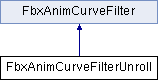
\includegraphics[height=2.000000cm]{class_fbx_anim_curve_filter_unroll}
\end{center}
\end{figure}
\subsection*{公開メンバ関数}
\begin{DoxyCompactItemize}
\item 
\hyperlink{class_fbx_anim_curve_filter_unroll_a8500355d825ebd7d853bc2b9ab561e40}{Fbx\+Anim\+Curve\+Filter\+Unroll} ()
\begin{DoxyCompactList}\small\item\em Constructor. \end{DoxyCompactList}\item 
virtual \hyperlink{class_fbx_anim_curve_filter_unroll_abbbb5d22a6d7dc281385d7fbc4706e45}{$\sim$\+Fbx\+Anim\+Curve\+Filter\+Unroll} ()
\begin{DoxyCompactList}\small\item\em Destructor. \end{DoxyCompactList}\item 
virtual const char $\ast$ \hyperlink{class_fbx_anim_curve_filter_unroll_a01282004cc60febeff844d9c44f94e5c}{Get\+Name} () const
\item 
virtual bool \hyperlink{class_fbx_anim_curve_filter_unroll_a8380c6817fbf19d347b0bd0b5ae9a57b}{Need\+Apply} (\hyperlink{class_fbx_anim_stack}{Fbx\+Anim\+Stack} $\ast$, \hyperlink{class_fbx_status}{Fbx\+Status} $\ast$p\+Status=\hyperlink{fbxarch_8h_a070d2ce7b6bb7e5c05602aa8c308d0c4}{N\+U\+LL})
\item 
virtual bool \hyperlink{class_fbx_anim_curve_filter_unroll_a1ab6063269085792ebaa82e0812ae362}{Need\+Apply} (\hyperlink{class_fbx_object}{Fbx\+Object} $\ast$, \hyperlink{class_fbx_anim_stack}{Fbx\+Anim\+Stack} $\ast$, \hyperlink{class_fbx_status}{Fbx\+Status} $\ast$p\+Status=\hyperlink{fbxarch_8h_a070d2ce7b6bb7e5c05602aa8c308d0c4}{N\+U\+LL})
\item 
virtual bool \hyperlink{class_fbx_anim_curve_filter_unroll_ad3df0b89af14237342197a8832e3d94f}{Need\+Apply} (\hyperlink{class_fbx_anim_curve_node}{Fbx\+Anim\+Curve\+Node} \&p\+Curve\+Node, \hyperlink{class_fbx_status}{Fbx\+Status} $\ast$p\+Status=\hyperlink{fbxarch_8h_a070d2ce7b6bb7e5c05602aa8c308d0c4}{N\+U\+LL})
\item 
virtual bool \hyperlink{class_fbx_anim_curve_filter_unroll_a3b7eb044733da9665efe6dfd81e2445f}{Need\+Apply} (\hyperlink{class_fbx_anim_curve}{Fbx\+Anim\+Curve} $\ast$$\ast$p\+Curve, int p\+Count, \hyperlink{class_fbx_status}{Fbx\+Status} $\ast$p\+Status=\hyperlink{fbxarch_8h_a070d2ce7b6bb7e5c05602aa8c308d0c4}{N\+U\+LL})
\item 
virtual bool \hyperlink{class_fbx_anim_curve_filter_unroll_adbe1626e507eb312b994b38403a11a19}{Need\+Apply} (\hyperlink{class_fbx_anim_curve}{Fbx\+Anim\+Curve} \&, \hyperlink{class_fbx_status}{Fbx\+Status} $\ast$p\+Status=\hyperlink{fbxarch_8h_a070d2ce7b6bb7e5c05602aa8c308d0c4}{N\+U\+LL})
\item 
virtual bool \hyperlink{class_fbx_anim_curve_filter_unroll_ae9b4807d576e93ae4800c1764f2aabda}{Apply} (\hyperlink{class_fbx_anim_stack}{Fbx\+Anim\+Stack} $\ast$, \hyperlink{class_fbx_status}{Fbx\+Status} $\ast$p\+Status=\hyperlink{fbxarch_8h_a070d2ce7b6bb7e5c05602aa8c308d0c4}{N\+U\+LL})
\item 
virtual bool \hyperlink{class_fbx_anim_curve_filter_unroll_a572540d9b38a3cc62b40e93201476d85}{Apply} (\hyperlink{class_fbx_object}{Fbx\+Object} $\ast$, \hyperlink{class_fbx_anim_stack}{Fbx\+Anim\+Stack} $\ast$, \hyperlink{class_fbx_status}{Fbx\+Status} $\ast$p\+Status=\hyperlink{fbxarch_8h_a070d2ce7b6bb7e5c05602aa8c308d0c4}{N\+U\+LL})
\item 
virtual bool \hyperlink{class_fbx_anim_curve_filter_unroll_a11788f2b59b218d566603fcf3e68cd50}{Apply} (\hyperlink{class_fbx_anim_curve_node}{Fbx\+Anim\+Curve\+Node} \&p\+Curve\+Node, \hyperlink{class_fbx_status}{Fbx\+Status} $\ast$p\+Status=\hyperlink{fbxarch_8h_a070d2ce7b6bb7e5c05602aa8c308d0c4}{N\+U\+LL})
\item 
virtual bool \hyperlink{class_fbx_anim_curve_filter_unroll_adcbc56499804749891e0140bd9c9f3f1}{Apply} (\hyperlink{class_fbx_anim_curve}{Fbx\+Anim\+Curve} $\ast$$\ast$p\+Curve, int p\+Count, \hyperlink{class_fbx_status}{Fbx\+Status} $\ast$p\+Status=\hyperlink{fbxarch_8h_a070d2ce7b6bb7e5c05602aa8c308d0c4}{N\+U\+LL})
\item 
virtual bool \hyperlink{class_fbx_anim_curve_filter_unroll_a7c8ff0c5328b5d7ca85f0d187cd8f98c}{Apply} (\hyperlink{class_fbx_anim_curve}{Fbx\+Anim\+Curve} \&, \hyperlink{class_fbx_status}{Fbx\+Status} $\ast$p\+Status=\hyperlink{fbxarch_8h_a070d2ce7b6bb7e5c05602aa8c308d0c4}{N\+U\+LL})
\item 
virtual void \hyperlink{class_fbx_anim_curve_filter_unroll_a0587dd664dddb98a809043f030b409d6}{Reset} ()
\item 
double \hyperlink{class_fbx_anim_curve_filter_unroll_a881a4c7122073deec59ab208b2bdf95a}{Get\+Quality\+Tolerance} () const
\item 
void \hyperlink{class_fbx_anim_curve_filter_unroll_ad8570bf12f5c397fb975fe961aeed29f}{Set\+Quality\+Tolerance} (double p\+Quality\+Tolerance)
\item 
bool \hyperlink{class_fbx_anim_curve_filter_unroll_af073ba1c941aca18f6ba62a811bf8a02}{Get\+Test\+For\+Path} () const
\item 
void \hyperlink{class_fbx_anim_curve_filter_unroll_af87dabf0628d09c9864ed445f11f8c66}{Set\+Test\+For\+Path} (bool p\+Test\+For\+Path)
\item 
bool \hyperlink{class_fbx_anim_curve_filter_unroll_a0d60638cd87eb0848e7995a42832fca4}{Get\+Force\+Auto\+Tangents} () const
\item 
void \hyperlink{class_fbx_anim_curve_filter_unroll_ae4d857f9f855136c18103315e473bbc3}{Set\+Force\+Auto\+Tangents} (bool p\+Force\+Auto\+Tangents)
\item 
void \hyperlink{class_fbx_anim_curve_filter_unroll_a8332667ca1dba9998d511f5e25f6cfb2}{Set\+Rotation\+Order} (\hyperlink{class_fbx_euler_a7d5bec7eedb022b4dae56894ab7a9939}{Fbx\+Euler\+::\+E\+Order} p\+Order)
\end{DoxyCompactItemize}
\subsection*{その他の継承メンバ}


\subsection{詳解}
Unroll filter.

Filter to apply continuous rotation values to animation curves. Due to Euler rotation properties, when a rotation angle cross over the 180 degree value, it becomes -\/179. This filter tries to keep a continuous rotation effectively by producing increasing values, to actually become 181 degrees, etc... \begin{DoxyRemark}{注釈}
The current implementation of this filter expects to process 3 curves at the same time. 

By default, this filter does not affect the tangent values of the modified keys. This means that, for C\+U\+B\+IC interpolation curves containing keys with U\+S\+ER or B\+R\+E\+AK tangents, the unrolled curves will correctly match the original rotation exactly on the curve keys but not in-\/between them. The filter can be configured to automatically convert the U\+S\+ER and B\+R\+E\+AK tangents to A\+U\+TO tangents by setting the Force\+Auto\+Tangents flag. Using the A\+U\+TO tangents mode can result in a more consistent interpolation between the curve keys. 
\end{DoxyRemark}


 fbxanimcurvefilters.\+h の 984 行目に定義があります。



\subsection{構築子と解体子}
\mbox{\Hypertarget{class_fbx_anim_curve_filter_unroll_a8500355d825ebd7d853bc2b9ab561e40}\label{class_fbx_anim_curve_filter_unroll_a8500355d825ebd7d853bc2b9ab561e40}} 
\index{Fbx\+Anim\+Curve\+Filter\+Unroll@{Fbx\+Anim\+Curve\+Filter\+Unroll}!Fbx\+Anim\+Curve\+Filter\+Unroll@{Fbx\+Anim\+Curve\+Filter\+Unroll}}
\index{Fbx\+Anim\+Curve\+Filter\+Unroll@{Fbx\+Anim\+Curve\+Filter\+Unroll}!Fbx\+Anim\+Curve\+Filter\+Unroll@{Fbx\+Anim\+Curve\+Filter\+Unroll}}
\subsubsection{\texorpdfstring{Fbx\+Anim\+Curve\+Filter\+Unroll()}{FbxAnimCurveFilterUnroll()}}
{\footnotesize\ttfamily Fbx\+Anim\+Curve\+Filter\+Unroll\+::\+Fbx\+Anim\+Curve\+Filter\+Unroll (\begin{DoxyParamCaption}{ }\end{DoxyParamCaption})}



Constructor. 

\mbox{\Hypertarget{class_fbx_anim_curve_filter_unroll_abbbb5d22a6d7dc281385d7fbc4706e45}\label{class_fbx_anim_curve_filter_unroll_abbbb5d22a6d7dc281385d7fbc4706e45}} 
\index{Fbx\+Anim\+Curve\+Filter\+Unroll@{Fbx\+Anim\+Curve\+Filter\+Unroll}!````~Fbx\+Anim\+Curve\+Filter\+Unroll@{$\sim$\+Fbx\+Anim\+Curve\+Filter\+Unroll}}
\index{````~Fbx\+Anim\+Curve\+Filter\+Unroll@{$\sim$\+Fbx\+Anim\+Curve\+Filter\+Unroll}!Fbx\+Anim\+Curve\+Filter\+Unroll@{Fbx\+Anim\+Curve\+Filter\+Unroll}}
\subsubsection{\texorpdfstring{$\sim$\+Fbx\+Anim\+Curve\+Filter\+Unroll()}{~FbxAnimCurveFilterUnroll()}}
{\footnotesize\ttfamily virtual Fbx\+Anim\+Curve\+Filter\+Unroll\+::$\sim$\+Fbx\+Anim\+Curve\+Filter\+Unroll (\begin{DoxyParamCaption}{ }\end{DoxyParamCaption})\hspace{0.3cm}{\ttfamily [inline]}, {\ttfamily [virtual]}}



Destructor. 



 fbxanimcurvefilters.\+h の 991 行目に定義があります。



\subsection{関数詳解}
\mbox{\Hypertarget{class_fbx_anim_curve_filter_unroll_ae9b4807d576e93ae4800c1764f2aabda}\label{class_fbx_anim_curve_filter_unroll_ae9b4807d576e93ae4800c1764f2aabda}} 
\index{Fbx\+Anim\+Curve\+Filter\+Unroll@{Fbx\+Anim\+Curve\+Filter\+Unroll}!Apply@{Apply}}
\index{Apply@{Apply}!Fbx\+Anim\+Curve\+Filter\+Unroll@{Fbx\+Anim\+Curve\+Filter\+Unroll}}
\subsubsection{\texorpdfstring{Apply()}{Apply()}\hspace{0.1cm}{\footnotesize\ttfamily [1/5]}}
{\footnotesize\ttfamily virtual bool Fbx\+Anim\+Curve\+Filter\+Unroll\+::\+Apply (\begin{DoxyParamCaption}\item[{\hyperlink{class_fbx_anim_stack}{Fbx\+Anim\+Stack} $\ast$}]{,  }\item[{\hyperlink{class_fbx_status}{Fbx\+Status} $\ast$}]{p\+Status = {\ttfamily \hyperlink{fbxarch_8h_a070d2ce7b6bb7e5c05602aa8c308d0c4}{N\+U\+LL}} }\end{DoxyParamCaption})\hspace{0.3cm}{\ttfamily [inline]}, {\ttfamily [virtual]}}

This filter expects to work with 3 interdependent curves. Passing the animation stack makes no sense since this object would not know which curves to handle. 
\begin{DoxyParams}{引数}
{\em p\+Anim\+Stack} & Animation stack where to retrieve the animation curves. \\
\hline
{\em p\+Status} & The \hyperlink{class_fbx_status}{Fbx\+Status} object to hold error codes. \\
\hline
\end{DoxyParams}
\begin{DoxyReturn}{戻り値}
{\ttfamily false}. 
\end{DoxyReturn}


\hyperlink{class_fbx_anim_curve_filter_aef3900e6180e05661c27ee484ae939c3}{Fbx\+Anim\+Curve\+Filter}を再実装しています。



 fbxanimcurvefilters.\+h の 1048 行目に定義があります。

\mbox{\Hypertarget{class_fbx_anim_curve_filter_unroll_a572540d9b38a3cc62b40e93201476d85}\label{class_fbx_anim_curve_filter_unroll_a572540d9b38a3cc62b40e93201476d85}} 
\index{Fbx\+Anim\+Curve\+Filter\+Unroll@{Fbx\+Anim\+Curve\+Filter\+Unroll}!Apply@{Apply}}
\index{Apply@{Apply}!Fbx\+Anim\+Curve\+Filter\+Unroll@{Fbx\+Anim\+Curve\+Filter\+Unroll}}
\subsubsection{\texorpdfstring{Apply()}{Apply()}\hspace{0.1cm}{\footnotesize\ttfamily [2/5]}}
{\footnotesize\ttfamily virtual bool Fbx\+Anim\+Curve\+Filter\+Unroll\+::\+Apply (\begin{DoxyParamCaption}\item[{\hyperlink{class_fbx_object}{Fbx\+Object} $\ast$}]{,  }\item[{\hyperlink{class_fbx_anim_stack}{Fbx\+Anim\+Stack} $\ast$}]{,  }\item[{\hyperlink{class_fbx_status}{Fbx\+Status} $\ast$}]{p\+Status = {\ttfamily \hyperlink{fbxarch_8h_a070d2ce7b6bb7e5c05602aa8c308d0c4}{N\+U\+LL}} }\end{DoxyParamCaption})\hspace{0.3cm}{\ttfamily [inline]}, {\ttfamily [virtual]}}

This filter expects to work with 3 interdependent curves. Collecting all the animation curves from the properties defined in {\itshape p\+Obj} could not guarantee that we are manipulating 3 interdependent curves. 
\begin{DoxyParams}{引数}
{\em p\+Obj} & Object containing the properties to test. \\
\hline
{\em p\+Anim\+Stack} & Animation stack where to retrieve the animation curves. \\
\hline
{\em p\+Status} & The \hyperlink{class_fbx_status}{Fbx\+Status} object to hold error codes. \\
\hline
\end{DoxyParams}
\begin{DoxyReturn}{戻り値}
{\ttfamily false}. 
\end{DoxyReturn}


\hyperlink{class_fbx_anim_curve_filter_a009498a65af4995bf5e5908f17837531}{Fbx\+Anim\+Curve\+Filter}を再実装しています。



 fbxanimcurvefilters.\+h の 1057 行目に定義があります。

\mbox{\Hypertarget{class_fbx_anim_curve_filter_unroll_a11788f2b59b218d566603fcf3e68cd50}\label{class_fbx_anim_curve_filter_unroll_a11788f2b59b218d566603fcf3e68cd50}} 
\index{Fbx\+Anim\+Curve\+Filter\+Unroll@{Fbx\+Anim\+Curve\+Filter\+Unroll}!Apply@{Apply}}
\index{Apply@{Apply}!Fbx\+Anim\+Curve\+Filter\+Unroll@{Fbx\+Anim\+Curve\+Filter\+Unroll}}
\subsubsection{\texorpdfstring{Apply()}{Apply()}\hspace{0.1cm}{\footnotesize\ttfamily [3/5]}}
{\footnotesize\ttfamily virtual bool Fbx\+Anim\+Curve\+Filter\+Unroll\+::\+Apply (\begin{DoxyParamCaption}\item[{\hyperlink{class_fbx_anim_curve_node}{Fbx\+Anim\+Curve\+Node} \&}]{p\+Curve\+Node,  }\item[{\hyperlink{class_fbx_status}{Fbx\+Status} $\ast$}]{p\+Status = {\ttfamily \hyperlink{fbxarch_8h_a070d2ce7b6bb7e5c05602aa8c308d0c4}{N\+U\+LL}} }\end{DoxyParamCaption})\hspace{0.3cm}{\ttfamily [virtual]}}

Apply filter on all the curves of an animation curve node. 
\begin{DoxyParams}{引数}
{\em p\+Curve\+Node} & Curve node to which the filter is applied. \\
\hline
{\em p\+Status} & The \hyperlink{class_fbx_status}{Fbx\+Status} object to hold error codes. \\
\hline
\end{DoxyParams}
\begin{DoxyReturn}{戻り値}
{\ttfamily true} if the curve filtering operation was successful, {\ttfamily false} otherwise. 
\end{DoxyReturn}
\begin{DoxyRemark}{注釈}
This filter expects a Euler rotation curve node with three curves. 
\end{DoxyRemark}


\hyperlink{class_fbx_anim_curve_filter_ad042b45c0675278fa49e61739b0825c2}{Fbx\+Anim\+Curve\+Filter}を再実装しています。

\mbox{\Hypertarget{class_fbx_anim_curve_filter_unroll_adcbc56499804749891e0140bd9c9f3f1}\label{class_fbx_anim_curve_filter_unroll_adcbc56499804749891e0140bd9c9f3f1}} 
\index{Fbx\+Anim\+Curve\+Filter\+Unroll@{Fbx\+Anim\+Curve\+Filter\+Unroll}!Apply@{Apply}}
\index{Apply@{Apply}!Fbx\+Anim\+Curve\+Filter\+Unroll@{Fbx\+Anim\+Curve\+Filter\+Unroll}}
\subsubsection{\texorpdfstring{Apply()}{Apply()}\hspace{0.1cm}{\footnotesize\ttfamily [4/5]}}
{\footnotesize\ttfamily virtual bool Fbx\+Anim\+Curve\+Filter\+Unroll\+::\+Apply (\begin{DoxyParamCaption}\item[{\hyperlink{class_fbx_anim_curve}{Fbx\+Anim\+Curve} $\ast$$\ast$}]{p\+Curve,  }\item[{int}]{p\+Count,  }\item[{\hyperlink{class_fbx_status}{Fbx\+Status} $\ast$}]{p\+Status = {\ttfamily \hyperlink{fbxarch_8h_a070d2ce7b6bb7e5c05602aa8c308d0c4}{N\+U\+LL}} }\end{DoxyParamCaption})\hspace{0.3cm}{\ttfamily [virtual]}}

Apply filter on the given animation curve. 
\begin{DoxyParams}{引数}
{\em p\+Curve} & Array of curve to which the filter is applied. \\
\hline
{\em p\+Count} & Number of curves in array. \\
\hline
{\em p\+Status} & The \hyperlink{class_fbx_status}{Fbx\+Status} object to hold error codes. \\
\hline
\end{DoxyParams}
\begin{DoxyReturn}{戻り値}
{\ttfamily true} if the curve filtering operation was successful, {\ttfamily false} otherwise. 
\end{DoxyReturn}
\begin{DoxyRemark}{注釈}
Because this method only receives an array of interdependent curves, this filter assumes that they are all coming from an Euler rotation anim curve node. Therefore, it expects {\itshape p\+Count} to be equal to 3. 
\end{DoxyRemark}


\hyperlink{class_fbx_anim_curve_filter_aca6a41fbc4d9019b20df7adccfa6ed3c}{Fbx\+Anim\+Curve\+Filter}を再実装しています。

\mbox{\Hypertarget{class_fbx_anim_curve_filter_unroll_a7c8ff0c5328b5d7ca85f0d187cd8f98c}\label{class_fbx_anim_curve_filter_unroll_a7c8ff0c5328b5d7ca85f0d187cd8f98c}} 
\index{Fbx\+Anim\+Curve\+Filter\+Unroll@{Fbx\+Anim\+Curve\+Filter\+Unroll}!Apply@{Apply}}
\index{Apply@{Apply}!Fbx\+Anim\+Curve\+Filter\+Unroll@{Fbx\+Anim\+Curve\+Filter\+Unroll}}
\subsubsection{\texorpdfstring{Apply()}{Apply()}\hspace{0.1cm}{\footnotesize\ttfamily [5/5]}}
{\footnotesize\ttfamily virtual bool Fbx\+Anim\+Curve\+Filter\+Unroll\+::\+Apply (\begin{DoxyParamCaption}\item[{\hyperlink{class_fbx_anim_curve}{Fbx\+Anim\+Curve} \&}]{,  }\item[{\hyperlink{class_fbx_status}{Fbx\+Status} $\ast$}]{p\+Status = {\ttfamily \hyperlink{fbxarch_8h_a070d2ce7b6bb7e5c05602aa8c308d0c4}{N\+U\+LL}} }\end{DoxyParamCaption})\hspace{0.3cm}{\ttfamily [inline]}, {\ttfamily [virtual]}}

This filter expects to work with 3 interdependent curves. Receiving one single curve is useless. \begin{DoxyReturn}{戻り値}
{\ttfamily false}. 
\end{DoxyReturn}


\hyperlink{class_fbx_anim_curve_filter_a6a69996c47c0e6f63a0f8b0d5fa806a0}{Fbx\+Anim\+Curve\+Filter}を実装しています。



 fbxanimcurvefilters.\+h の 1081 行目に定義があります。

\mbox{\Hypertarget{class_fbx_anim_curve_filter_unroll_a0d60638cd87eb0848e7995a42832fca4}\label{class_fbx_anim_curve_filter_unroll_a0d60638cd87eb0848e7995a42832fca4}} 
\index{Fbx\+Anim\+Curve\+Filter\+Unroll@{Fbx\+Anim\+Curve\+Filter\+Unroll}!Get\+Force\+Auto\+Tangents@{Get\+Force\+Auto\+Tangents}}
\index{Get\+Force\+Auto\+Tangents@{Get\+Force\+Auto\+Tangents}!Fbx\+Anim\+Curve\+Filter\+Unroll@{Fbx\+Anim\+Curve\+Filter\+Unroll}}
\subsubsection{\texorpdfstring{Get\+Force\+Auto\+Tangents()}{GetForceAutoTangents()}}
{\footnotesize\ttfamily bool Fbx\+Anim\+Curve\+Filter\+Unroll\+::\+Get\+Force\+Auto\+Tangents (\begin{DoxyParamCaption}{ }\end{DoxyParamCaption}) const}

Get the current state of the Force\+Auto\+Tangents flag. \begin{DoxyReturn}{戻り値}
{\ttfamily true} if forcing A\+U\+TO tangents is enabled. 
\end{DoxyReturn}
\begin{DoxyRemark}{注釈}
This flag is considered only on curves using the C\+U\+B\+IC interpolation and keys with the U\+S\+ER or B\+R\+E\+AK tangents. For any other type of interpolations or tangents, this flag is ignored. 
\end{DoxyRemark}
\mbox{\Hypertarget{class_fbx_anim_curve_filter_unroll_a01282004cc60febeff844d9c44f94e5c}\label{class_fbx_anim_curve_filter_unroll_a01282004cc60febeff844d9c44f94e5c}} 
\index{Fbx\+Anim\+Curve\+Filter\+Unroll@{Fbx\+Anim\+Curve\+Filter\+Unroll}!Get\+Name@{Get\+Name}}
\index{Get\+Name@{Get\+Name}!Fbx\+Anim\+Curve\+Filter\+Unroll@{Fbx\+Anim\+Curve\+Filter\+Unroll}}
\subsubsection{\texorpdfstring{Get\+Name()}{GetName()}}
{\footnotesize\ttfamily virtual const char$\ast$ Fbx\+Anim\+Curve\+Filter\+Unroll\+::\+Get\+Name (\begin{DoxyParamCaption}{ }\end{DoxyParamCaption}) const\hspace{0.3cm}{\ttfamily [virtual]}}

Get the name of the filter. \begin{DoxyReturn}{戻り値}
Pointer to the name. 
\end{DoxyReturn}


\hyperlink{class_fbx_anim_curve_filter_abd559d5052fbb072042e59241940a35c}{Fbx\+Anim\+Curve\+Filter}を再実装しています。

\mbox{\Hypertarget{class_fbx_anim_curve_filter_unroll_a881a4c7122073deec59ab208b2bdf95a}\label{class_fbx_anim_curve_filter_unroll_a881a4c7122073deec59ab208b2bdf95a}} 
\index{Fbx\+Anim\+Curve\+Filter\+Unroll@{Fbx\+Anim\+Curve\+Filter\+Unroll}!Get\+Quality\+Tolerance@{Get\+Quality\+Tolerance}}
\index{Get\+Quality\+Tolerance@{Get\+Quality\+Tolerance}!Fbx\+Anim\+Curve\+Filter\+Unroll@{Fbx\+Anim\+Curve\+Filter\+Unroll}}
\subsubsection{\texorpdfstring{Get\+Quality\+Tolerance()}{GetQualityTolerance()}}
{\footnotesize\ttfamily double Fbx\+Anim\+Curve\+Filter\+Unroll\+::\+Get\+Quality\+Tolerance (\begin{DoxyParamCaption}{ }\end{DoxyParamCaption}) const}

Get the unroll quality tolerance. \begin{DoxyReturn}{戻り値}
The current unroll quality tolerance. 
\end{DoxyReturn}
\begin{DoxyRemark}{注釈}
This value is only used when \hyperlink{class_fbx_anim_curve_filter_unroll_af87dabf0628d09c9864ed445f11f8c66}{Set\+Test\+For\+Path()} is set to true. 
\end{DoxyRemark}
\mbox{\Hypertarget{class_fbx_anim_curve_filter_unroll_af073ba1c941aca18f6ba62a811bf8a02}\label{class_fbx_anim_curve_filter_unroll_af073ba1c941aca18f6ba62a811bf8a02}} 
\index{Fbx\+Anim\+Curve\+Filter\+Unroll@{Fbx\+Anim\+Curve\+Filter\+Unroll}!Get\+Test\+For\+Path@{Get\+Test\+For\+Path}}
\index{Get\+Test\+For\+Path@{Get\+Test\+For\+Path}!Fbx\+Anim\+Curve\+Filter\+Unroll@{Fbx\+Anim\+Curve\+Filter\+Unroll}}
\subsubsection{\texorpdfstring{Get\+Test\+For\+Path()}{GetTestForPath()}}
{\footnotesize\ttfamily bool Fbx\+Anim\+Curve\+Filter\+Unroll\+::\+Get\+Test\+For\+Path (\begin{DoxyParamCaption}{ }\end{DoxyParamCaption}) const}

Get if the test path is enabled. \begin{DoxyReturn}{戻り値}
{\ttfamily true} if test for path is enabled. 
\end{DoxyReturn}
\begin{DoxyRemark}{注釈}
The unroll filter takes a key as a reference key and updates the following keys accordingly to try to keep the continuity between this reference key and its following keys. If the test path is enabled, the filter can use the same key as reference key to update the following keys until the difference of continuity between the newly updated key and the reference key exceeds the quality tolerance, then the reference key will be updated as the newly updated key. If the test path is not enabled, the filter will always use the newly updated key as reference to update the next key. The quality tolerance can be set and queried by \hyperlink{class_fbx_anim_curve_filter_unroll_ad8570bf12f5c397fb975fe961aeed29f}{Set\+Quality\+Tolerance()} and \hyperlink{class_fbx_anim_curve_filter_unroll_a881a4c7122073deec59ab208b2bdf95a}{Get\+Quality\+Tolerance()}. 
\end{DoxyRemark}
\mbox{\Hypertarget{class_fbx_anim_curve_filter_unroll_a8380c6817fbf19d347b0bd0b5ae9a57b}\label{class_fbx_anim_curve_filter_unroll_a8380c6817fbf19d347b0bd0b5ae9a57b}} 
\index{Fbx\+Anim\+Curve\+Filter\+Unroll@{Fbx\+Anim\+Curve\+Filter\+Unroll}!Need\+Apply@{Need\+Apply}}
\index{Need\+Apply@{Need\+Apply}!Fbx\+Anim\+Curve\+Filter\+Unroll@{Fbx\+Anim\+Curve\+Filter\+Unroll}}
\subsubsection{\texorpdfstring{Need\+Apply()}{NeedApply()}\hspace{0.1cm}{\footnotesize\ttfamily [1/5]}}
{\footnotesize\ttfamily virtual bool Fbx\+Anim\+Curve\+Filter\+Unroll\+::\+Need\+Apply (\begin{DoxyParamCaption}\item[{\hyperlink{class_fbx_anim_stack}{Fbx\+Anim\+Stack} $\ast$}]{,  }\item[{\hyperlink{class_fbx_status}{Fbx\+Status} $\ast$}]{p\+Status = {\ttfamily \hyperlink{fbxarch_8h_a070d2ce7b6bb7e5c05602aa8c308d0c4}{N\+U\+LL}} }\end{DoxyParamCaption})\hspace{0.3cm}{\ttfamily [inline]}, {\ttfamily [virtual]}}

This filter expects to work with 3 interdependent curves. Passing the animation stack makes no sense since this object would not know which curves to handle. 
\begin{DoxyParams}{引数}
{\em p\+Anim\+Stack} & Animation stack \\
\hline
{\em p\+Status} & The \hyperlink{class_fbx_status}{Fbx\+Status} object to hold error codes. \\
\hline
\end{DoxyParams}
\begin{DoxyReturn}{戻り値}
{\ttfamily false}. 
\end{DoxyReturn}


\hyperlink{class_fbx_anim_curve_filter_af95af2469851b88b4f6d38401ace5791}{Fbx\+Anim\+Curve\+Filter}を再実装しています。



 fbxanimcurvefilters.\+h の 1004 行目に定義があります。

\mbox{\Hypertarget{class_fbx_anim_curve_filter_unroll_a1ab6063269085792ebaa82e0812ae362}\label{class_fbx_anim_curve_filter_unroll_a1ab6063269085792ebaa82e0812ae362}} 
\index{Fbx\+Anim\+Curve\+Filter\+Unroll@{Fbx\+Anim\+Curve\+Filter\+Unroll}!Need\+Apply@{Need\+Apply}}
\index{Need\+Apply@{Need\+Apply}!Fbx\+Anim\+Curve\+Filter\+Unroll@{Fbx\+Anim\+Curve\+Filter\+Unroll}}
\subsubsection{\texorpdfstring{Need\+Apply()}{NeedApply()}\hspace{0.1cm}{\footnotesize\ttfamily [2/5]}}
{\footnotesize\ttfamily virtual bool Fbx\+Anim\+Curve\+Filter\+Unroll\+::\+Need\+Apply (\begin{DoxyParamCaption}\item[{\hyperlink{class_fbx_object}{Fbx\+Object} $\ast$}]{,  }\item[{\hyperlink{class_fbx_anim_stack}{Fbx\+Anim\+Stack} $\ast$}]{,  }\item[{\hyperlink{class_fbx_status}{Fbx\+Status} $\ast$}]{p\+Status = {\ttfamily \hyperlink{fbxarch_8h_a070d2ce7b6bb7e5c05602aa8c308d0c4}{N\+U\+LL}} }\end{DoxyParamCaption})\hspace{0.3cm}{\ttfamily [inline]}, {\ttfamily [virtual]}}

This filter expects to work with 3 interdependent curves. Collecting all the animation curves from the properties defined in {\itshape p\+Obj} could not guarantee that we are manipulating 3 interdependent curves. 
\begin{DoxyParams}{引数}
{\em p\+Obj} & Object containing the properties to test. \\
\hline
{\em p\+Anim\+Stack} & Animation stack where to retrieve the animation curves \\
\hline
{\em p\+Status} & The \hyperlink{class_fbx_status}{Fbx\+Status} object to hold error codes. \\
\hline
\end{DoxyParams}
\begin{DoxyReturn}{戻り値}
{\ttfamily false}. 
\end{DoxyReturn}


\hyperlink{class_fbx_anim_curve_filter_a09438dd8d0e9bcb934e6a4b6fc51bcd7}{Fbx\+Anim\+Curve\+Filter}を再実装しています。



 fbxanimcurvefilters.\+h の 1013 行目に定義があります。

\mbox{\Hypertarget{class_fbx_anim_curve_filter_unroll_ad3df0b89af14237342197a8832e3d94f}\label{class_fbx_anim_curve_filter_unroll_ad3df0b89af14237342197a8832e3d94f}} 
\index{Fbx\+Anim\+Curve\+Filter\+Unroll@{Fbx\+Anim\+Curve\+Filter\+Unroll}!Need\+Apply@{Need\+Apply}}
\index{Need\+Apply@{Need\+Apply}!Fbx\+Anim\+Curve\+Filter\+Unroll@{Fbx\+Anim\+Curve\+Filter\+Unroll}}
\subsubsection{\texorpdfstring{Need\+Apply()}{NeedApply()}\hspace{0.1cm}{\footnotesize\ttfamily [3/5]}}
{\footnotesize\ttfamily virtual bool Fbx\+Anim\+Curve\+Filter\+Unroll\+::\+Need\+Apply (\begin{DoxyParamCaption}\item[{\hyperlink{class_fbx_anim_curve_node}{Fbx\+Anim\+Curve\+Node} \&}]{p\+Curve\+Node,  }\item[{\hyperlink{class_fbx_status}{Fbx\+Status} $\ast$}]{p\+Status = {\ttfamily \hyperlink{fbxarch_8h_a070d2ce7b6bb7e5c05602aa8c308d0c4}{N\+U\+LL}} }\end{DoxyParamCaption})\hspace{0.3cm}{\ttfamily [virtual]}}

Check if the animation curve node needs an application of the filter. 
\begin{DoxyParams}{引数}
{\em p\+Curve\+Node} & Curve node to test. \\
\hline
{\em p\+Status} & The \hyperlink{class_fbx_status}{Fbx\+Status} object to hold error codes. \\
\hline
\end{DoxyParams}
\begin{DoxyReturn}{戻り値}
{\ttfamily true} if the animation curve node needs an application of the filter, {\ttfamily false} otherwise. 
\end{DoxyReturn}
\begin{DoxyRemark}{注釈}
This method checks that the {\itshape p\+Curve\+Node} is representing an Euler rotation. It will validate that 3 animation curves are defined. If the condition is not met, the method will return {\ttfamily false}. 
\end{DoxyRemark}


\hyperlink{class_fbx_anim_curve_filter_a2a88d855d34bb1f2f22ca8386020b33a}{Fbx\+Anim\+Curve\+Filter}を再実装しています。

\mbox{\Hypertarget{class_fbx_anim_curve_filter_unroll_a3b7eb044733da9665efe6dfd81e2445f}\label{class_fbx_anim_curve_filter_unroll_a3b7eb044733da9665efe6dfd81e2445f}} 
\index{Fbx\+Anim\+Curve\+Filter\+Unroll@{Fbx\+Anim\+Curve\+Filter\+Unroll}!Need\+Apply@{Need\+Apply}}
\index{Need\+Apply@{Need\+Apply}!Fbx\+Anim\+Curve\+Filter\+Unroll@{Fbx\+Anim\+Curve\+Filter\+Unroll}}
\subsubsection{\texorpdfstring{Need\+Apply()}{NeedApply()}\hspace{0.1cm}{\footnotesize\ttfamily [4/5]}}
{\footnotesize\ttfamily virtual bool Fbx\+Anim\+Curve\+Filter\+Unroll\+::\+Need\+Apply (\begin{DoxyParamCaption}\item[{\hyperlink{class_fbx_anim_curve}{Fbx\+Anim\+Curve} $\ast$$\ast$}]{p\+Curve,  }\item[{int}]{p\+Count,  }\item[{\hyperlink{class_fbx_status}{Fbx\+Status} $\ast$}]{p\+Status = {\ttfamily \hyperlink{fbxarch_8h_a070d2ce7b6bb7e5c05602aa8c308d0c4}{N\+U\+LL}} }\end{DoxyParamCaption})\hspace{0.3cm}{\ttfamily [virtual]}}

Check if the given animation curve needs an application of the filter. 
\begin{DoxyParams}{引数}
{\em p\+Curve} & Array of curves to test if they need an application of the filter. \\
\hline
{\em p\+Count} & Number of curves in array. \\
\hline
{\em p\+Status} & The \hyperlink{class_fbx_status}{Fbx\+Status} object to hold error codes. \\
\hline
\end{DoxyParams}
\begin{DoxyReturn}{戻り値}
{\ttfamily true} if at least one animation curve in the array needs an application of the filter, {\ttfamily false} otherwise. 
\end{DoxyReturn}
\begin{DoxyRemark}{注釈}
Because this method only receives an array of interdependent curves, this filter assumes that they are all coming from an Euler rotation anim curve node. Therefore, it expects {\itshape p\+Count} to be equal to 3. 
\end{DoxyRemark}


\hyperlink{class_fbx_anim_curve_filter_a6b210eca45b745cf070c46bfaaf3e5b2}{Fbx\+Anim\+Curve\+Filter}を再実装しています。

\mbox{\Hypertarget{class_fbx_anim_curve_filter_unroll_adbe1626e507eb312b994b38403a11a19}\label{class_fbx_anim_curve_filter_unroll_adbe1626e507eb312b994b38403a11a19}} 
\index{Fbx\+Anim\+Curve\+Filter\+Unroll@{Fbx\+Anim\+Curve\+Filter\+Unroll}!Need\+Apply@{Need\+Apply}}
\index{Need\+Apply@{Need\+Apply}!Fbx\+Anim\+Curve\+Filter\+Unroll@{Fbx\+Anim\+Curve\+Filter\+Unroll}}
\subsubsection{\texorpdfstring{Need\+Apply()}{NeedApply()}\hspace{0.1cm}{\footnotesize\ttfamily [5/5]}}
{\footnotesize\ttfamily virtual bool Fbx\+Anim\+Curve\+Filter\+Unroll\+::\+Need\+Apply (\begin{DoxyParamCaption}\item[{\hyperlink{class_fbx_anim_curve}{Fbx\+Anim\+Curve} \&}]{,  }\item[{\hyperlink{class_fbx_status}{Fbx\+Status} $\ast$}]{p\+Status = {\ttfamily \hyperlink{fbxarch_8h_a070d2ce7b6bb7e5c05602aa8c308d0c4}{N\+U\+LL}} }\end{DoxyParamCaption})\hspace{0.3cm}{\ttfamily [inline]}, {\ttfamily [virtual]}}

This filter expects to work with interdependent curves. Receiving one single curve is useless. \begin{DoxyReturn}{戻り値}
{\ttfamily false}. 
\end{DoxyReturn}


\hyperlink{class_fbx_anim_curve_filter_af768a9c47e4f5a5fff47a8ec781e6b4c}{Fbx\+Anim\+Curve\+Filter}を再実装しています。



 fbxanimcurvefilters.\+h の 1040 行目に定義があります。

\mbox{\Hypertarget{class_fbx_anim_curve_filter_unroll_a0587dd664dddb98a809043f030b409d6}\label{class_fbx_anim_curve_filter_unroll_a0587dd664dddb98a809043f030b409d6}} 
\index{Fbx\+Anim\+Curve\+Filter\+Unroll@{Fbx\+Anim\+Curve\+Filter\+Unroll}!Reset@{Reset}}
\index{Reset@{Reset}!Fbx\+Anim\+Curve\+Filter\+Unroll@{Fbx\+Anim\+Curve\+Filter\+Unroll}}
\subsubsection{\texorpdfstring{Reset()}{Reset()}}
{\footnotesize\ttfamily virtual void Fbx\+Anim\+Curve\+Filter\+Unroll\+::\+Reset (\begin{DoxyParamCaption}{ }\end{DoxyParamCaption})\hspace{0.3cm}{\ttfamily [virtual]}}

Reset the filter to its default parameters. 

\hyperlink{class_fbx_anim_curve_filter_a57fb35baaaa85adb08946383cf40e811}{Fbx\+Anim\+Curve\+Filter}を再実装しています。

\mbox{\Hypertarget{class_fbx_anim_curve_filter_unroll_ae4d857f9f855136c18103315e473bbc3}\label{class_fbx_anim_curve_filter_unroll_ae4d857f9f855136c18103315e473bbc3}} 
\index{Fbx\+Anim\+Curve\+Filter\+Unroll@{Fbx\+Anim\+Curve\+Filter\+Unroll}!Set\+Force\+Auto\+Tangents@{Set\+Force\+Auto\+Tangents}}
\index{Set\+Force\+Auto\+Tangents@{Set\+Force\+Auto\+Tangents}!Fbx\+Anim\+Curve\+Filter\+Unroll@{Fbx\+Anim\+Curve\+Filter\+Unroll}}
\subsubsection{\texorpdfstring{Set\+Force\+Auto\+Tangents()}{SetForceAutoTangents()}}
{\footnotesize\ttfamily void Fbx\+Anim\+Curve\+Filter\+Unroll\+::\+Set\+Force\+Auto\+Tangents (\begin{DoxyParamCaption}\item[{bool}]{p\+Force\+Auto\+Tangents }\end{DoxyParamCaption})}

Set the new state of the Force\+Auto\+Tangents flag. 
\begin{DoxyParams}{引数}
{\em p\+Force\+Auto\+Tangents} & New value of the flag. \\
\hline
\end{DoxyParams}
\begin{DoxyRemark}{注釈}
This flag is considered only on curves using the C\+U\+B\+IC interpolation and keys with the U\+S\+ER or B\+R\+E\+AK tangents. For any other type of interpolations or tangents, this flag is ignored. 
\end{DoxyRemark}
\mbox{\Hypertarget{class_fbx_anim_curve_filter_unroll_ad8570bf12f5c397fb975fe961aeed29f}\label{class_fbx_anim_curve_filter_unroll_ad8570bf12f5c397fb975fe961aeed29f}} 
\index{Fbx\+Anim\+Curve\+Filter\+Unroll@{Fbx\+Anim\+Curve\+Filter\+Unroll}!Set\+Quality\+Tolerance@{Set\+Quality\+Tolerance}}
\index{Set\+Quality\+Tolerance@{Set\+Quality\+Tolerance}!Fbx\+Anim\+Curve\+Filter\+Unroll@{Fbx\+Anim\+Curve\+Filter\+Unroll}}
\subsubsection{\texorpdfstring{Set\+Quality\+Tolerance()}{SetQualityTolerance()}}
{\footnotesize\ttfamily void Fbx\+Anim\+Curve\+Filter\+Unroll\+::\+Set\+Quality\+Tolerance (\begin{DoxyParamCaption}\item[{double}]{p\+Quality\+Tolerance }\end{DoxyParamCaption})}

Set the unroll quality tolerance. 
\begin{DoxyParams}{引数}
{\em p\+Quality\+Tolerance} & The unroll quality tolerance to set. \\
\hline
\end{DoxyParams}
\begin{DoxyRemark}{注釈}
This value is only used when \hyperlink{class_fbx_anim_curve_filter_unroll_af87dabf0628d09c9864ed445f11f8c66}{Set\+Test\+For\+Path()} is set to true. 
\end{DoxyRemark}
\mbox{\Hypertarget{class_fbx_anim_curve_filter_unroll_a8332667ca1dba9998d511f5e25f6cfb2}\label{class_fbx_anim_curve_filter_unroll_a8332667ca1dba9998d511f5e25f6cfb2}} 
\index{Fbx\+Anim\+Curve\+Filter\+Unroll@{Fbx\+Anim\+Curve\+Filter\+Unroll}!Set\+Rotation\+Order@{Set\+Rotation\+Order}}
\index{Set\+Rotation\+Order@{Set\+Rotation\+Order}!Fbx\+Anim\+Curve\+Filter\+Unroll@{Fbx\+Anim\+Curve\+Filter\+Unroll}}
\subsubsection{\texorpdfstring{Set\+Rotation\+Order()}{SetRotationOrder()}}
{\footnotesize\ttfamily void Fbx\+Anim\+Curve\+Filter\+Unroll\+::\+Set\+Rotation\+Order (\begin{DoxyParamCaption}\item[{\hyperlink{class_fbx_euler_a7d5bec7eedb022b4dae56894ab7a9939}{Fbx\+Euler\+::\+E\+Order}}]{p\+Order }\end{DoxyParamCaption})}

\mbox{\Hypertarget{class_fbx_anim_curve_filter_unroll_af87dabf0628d09c9864ed445f11f8c66}\label{class_fbx_anim_curve_filter_unroll_af87dabf0628d09c9864ed445f11f8c66}} 
\index{Fbx\+Anim\+Curve\+Filter\+Unroll@{Fbx\+Anim\+Curve\+Filter\+Unroll}!Set\+Test\+For\+Path@{Set\+Test\+For\+Path}}
\index{Set\+Test\+For\+Path@{Set\+Test\+For\+Path}!Fbx\+Anim\+Curve\+Filter\+Unroll@{Fbx\+Anim\+Curve\+Filter\+Unroll}}
\subsubsection{\texorpdfstring{Set\+Test\+For\+Path()}{SetTestForPath()}}
{\footnotesize\ttfamily void Fbx\+Anim\+Curve\+Filter\+Unroll\+::\+Set\+Test\+For\+Path (\begin{DoxyParamCaption}\item[{bool}]{p\+Test\+For\+Path }\end{DoxyParamCaption})}

Set if the test path is enabled. 
\begin{DoxyParams}{引数}
{\em p\+Test\+For\+Path} & Value to set if test for path is to be enabled. \\
\hline
\end{DoxyParams}
\begin{DoxyRemark}{注釈}
The unroll filter takes a key as a reference key and updates the following keys accordingly to try to keep the continuity between this reference key and its following keys. If the test path is enabled, the filter can use the same key as reference key to update the following keys until the difference of continuity between the newly updated key and the reference key exceeds the quality tolerance, then the reference key will be updated as the newly updated key. If the test path is not enabled, the filter will always use the newly updated key as reference to update the next key. The quality tolerance can be set and queried by \hyperlink{class_fbx_anim_curve_filter_unroll_ad8570bf12f5c397fb975fe961aeed29f}{Set\+Quality\+Tolerance()} and \hyperlink{class_fbx_anim_curve_filter_unroll_a881a4c7122073deec59ab208b2bdf95a}{Get\+Quality\+Tolerance()}. 
\end{DoxyRemark}


このクラス詳解は次のファイルから抽出されました\+:\begin{DoxyCompactItemize}
\item 
C\+:/\+Maya/scripts/\+F\+B\+X\+\_\+\+S\+D\+K/2017.\+1/include/fbxsdk/scene/animation/\hyperlink{fbxanimcurvefilters_8h}{fbxanimcurvefilters.\+h}\end{DoxyCompactItemize}

\hypertarget{class_fbx_anim_curve_key}{}\section{Fbx\+Anim\+Curve\+Key クラス}
\label{class_fbx_anim_curve_key}\index{Fbx\+Anim\+Curve\+Key@{Fbx\+Anim\+Curve\+Key}}


{\ttfamily \#include $<$fbxanimcurve.\+h$>$}



Fbx\+Anim\+Curve\+Key の継承関係図
% FIG 0


Fbx\+Anim\+Curve\+Key 連携図
% FIG 1
\subsection*{公開メンバ関数}
\begin{DoxyCompactItemize}
\item 
\hyperlink{class_fbx_anim_curve_key_acc70533fb017bc71b617aaa37ee2e19f}{Fbx\+Anim\+Curve\+Key} ()
\item 
\hyperlink{class_fbx_anim_curve_key_a5fc23a90c53bc0655161813ee4f6ae00}{Fbx\+Anim\+Curve\+Key} (\hyperlink{class_fbx_time}{Fbx\+Time} p\+Time)
\item 
\hyperlink{class_fbx_anim_curve_key_a3e967d8e8d05da27ba82dcebfe2533fc}{Fbx\+Anim\+Curve\+Key} (\hyperlink{class_fbx_time}{Fbx\+Time} p\+Time, float p\+Val)
\item 
\hyperlink{class_fbx_anim_curve_key_ab5d7663cc4993863b80b13e0b5dca835}{Fbx\+Anim\+Curve\+Key} (\hyperlink{class_fbx_anim_curve_key}{Fbx\+Anim\+Curve\+Key} const \&p\+F\+Key)
\item 
\hyperlink{class_fbx_anim_curve_key_af0269dd6206c85565ed29b01b39df8ff}{$\sim$\+Fbx\+Anim\+Curve\+Key} ()
\item 
\hyperlink{class_fbx_anim_curve_key}{Fbx\+Anim\+Curve\+Key} \& \hyperlink{class_fbx_anim_curve_key_a13c344143cd73f6809edbbb91df08c0e}{operator=} (const \hyperlink{class_fbx_anim_curve_key}{Fbx\+Anim\+Curve\+Key} \&p\+F\+Key)
\item 
\hyperlink{class_fbx_time}{Fbx\+Time} \hyperlink{class_fbx_anim_curve_key_aae0882b53b31502cb30ea35de028837f}{Get\+Time} () const
\item 
void \hyperlink{class_fbx_anim_curve_key_a6ebc96b8346a345534c0eb2e1b6d9291}{Set\+Time} (const \hyperlink{class_fbx_time}{Fbx\+Time} \&p\+Time)
\item 
void \hyperlink{class_fbx_anim_curve_key_afdab5f0d38bedc7c4715aaa6a51d4370}{Set} (\hyperlink{class_fbx_time}{Fbx\+Time} p\+Time, float p\+Value)
\item 
void \hyperlink{class_fbx_anim_curve_key_ace0cb6af3027da5a2ea28ac7e5f528be}{Set\+T\+CB} (\hyperlink{class_fbx_time}{Fbx\+Time} p\+Time, float p\+Value, float p\+Data0=0.\+0f, float p\+Data1=0.\+0f, float p\+Data2=0.\+0f)
\item 
float \hyperlink{class_fbx_anim_curve_key_a7d66374255e912386ab894a5e2945ff5}{Get\+Value} () const
\item 
void \hyperlink{class_fbx_anim_curve_key_a4d7ea46fc9d4a6691c5e6d97569c7ae1}{Set\+Value} (float p\+Value)
\item 
\hyperlink{class_fbx_anim_curve_def_add2ab7d10d856ab0868cc9b143d59ea5}{Fbx\+Anim\+Curve\+Def\+::\+E\+Interpolation\+Type} \hyperlink{class_fbx_anim_curve_key_afe707d042861d5f6d5e22f4811a725ac}{Get\+Interpolation} ()
\item 
void \hyperlink{class_fbx_anim_curve_key_a10777e9392725191bd6ab1d425460406}{Set\+Interpolation} (\hyperlink{class_fbx_anim_curve_def_add2ab7d10d856ab0868cc9b143d59ea5}{Fbx\+Anim\+Curve\+Def\+::\+E\+Interpolation\+Type} p\+Interpolation)
\item 
\hyperlink{class_fbx_anim_curve_def_ac810ccc5ca0527704ab5175479964b87}{Fbx\+Anim\+Curve\+Def\+::\+E\+Tangent\+Mode} \hyperlink{class_fbx_anim_curve_key_a3821c01c7e1b422efcf2fedd074ffb6a}{Get\+Tangent\+Mode} (bool p\+Include\+Overrides=false)
\item 
void \hyperlink{class_fbx_anim_curve_key_a8a8a090694fc042e9b234e40918faf8e}{Set\+Tangent\+Mode} (\hyperlink{class_fbx_anim_curve_def_ac810ccc5ca0527704ab5175479964b87}{Fbx\+Anim\+Curve\+Def\+::\+E\+Tangent\+Mode} p\+Tangent\+Mode)
\item 
\hyperlink{class_fbx_anim_curve_def_aeee6e9cc12501e10dbd3e5caaf66990e}{Fbx\+Anim\+Curve\+Def\+::\+E\+Weighted\+Mode} \hyperlink{class_fbx_anim_curve_key_a6971443814d64229442becc934315c56}{Get\+Tangent\+Weight\+Mode} () const
\item 
void \hyperlink{class_fbx_anim_curve_key_a418159da0643ccdbeb5aa59b69b821e0}{Set\+Tangent\+Weight\+Mode} (\hyperlink{class_fbx_anim_curve_def_aeee6e9cc12501e10dbd3e5caaf66990e}{Fbx\+Anim\+Curve\+Def\+::\+E\+Weighted\+Mode} p\+Tangent\+Weight\+Mode, \hyperlink{class_fbx_anim_curve_def_aeee6e9cc12501e10dbd3e5caaf66990e}{Fbx\+Anim\+Curve\+Def\+::\+E\+Weighted\+Mode} p\+Mask=\hyperlink{class_fbx_anim_curve_def_aeee6e9cc12501e10dbd3e5caaf66990ea4337e6853fab642c2a432ab1bb303922}{Fbx\+Anim\+Curve\+Def\+::e\+Weighted\+All})
\item 
void \hyperlink{class_fbx_anim_curve_key_a9ea49dd21bb571575005dd678ecba501}{Set\+Tangent\+Weight\+And\+Adjust\+Tangent} (\hyperlink{class_fbx_anim_curve_def_a3be261d961f8226235529b148cf80300}{Fbx\+Anim\+Curve\+Def\+::\+E\+Data\+Index} p\+Index, double p\+Weight)
\item 
\hyperlink{class_fbx_anim_curve_def_a747576beffa78ab236d2e140da395fff}{Fbx\+Anim\+Curve\+Def\+::\+E\+Velocity\+Mode} \hyperlink{class_fbx_anim_curve_key_af8b7bc72b42857f9a713ca3f443cd55b}{Get\+Tangent\+Velocity\+Mode} () const
\item 
void \hyperlink{class_fbx_anim_curve_key_a758b05baef1e6298833b1ed9e6c11a3e}{Set\+Tangent\+Velocity\+Mode} (\hyperlink{class_fbx_anim_curve_def_a747576beffa78ab236d2e140da395fff}{Fbx\+Anim\+Curve\+Def\+::\+E\+Velocity\+Mode} p\+Tangent\+Velocity\+Mode, \hyperlink{class_fbx_anim_curve_def_a747576beffa78ab236d2e140da395fff}{Fbx\+Anim\+Curve\+Def\+::\+E\+Velocity\+Mode} p\+Mask=\hyperlink{class_fbx_anim_curve_def_a747576beffa78ab236d2e140da395fffab8603ba4ecc238f5dee7489b6a0123ee}{Fbx\+Anim\+Curve\+Def\+::e\+Velocity\+All})
\item 
\hyperlink{class_fbx_anim_curve_def_a52885abd392ac8ac3da94bafc5fddd64}{Fbx\+Anim\+Curve\+Def\+::\+E\+Constant\+Mode} \hyperlink{class_fbx_anim_curve_key_ade9ff492dbe914f25b6a0404d0121a83}{Get\+Constant\+Mode} () const
\item 
void \hyperlink{class_fbx_anim_curve_key_a6a34c333a4b4f90cf04492c9c31bedcb}{Set\+Constant\+Mode} (\hyperlink{class_fbx_anim_curve_def_a52885abd392ac8ac3da94bafc5fddd64}{Fbx\+Anim\+Curve\+Def\+::\+E\+Constant\+Mode} p\+Mode)
\item 
float \hyperlink{class_fbx_anim_curve_key_a3185c35241a072105f14327afd275452}{Get\+Data\+Float} (\hyperlink{class_fbx_anim_curve_def_a3be261d961f8226235529b148cf80300}{Fbx\+Anim\+Curve\+Def\+::\+E\+Data\+Index} p\+Index) const
\item 
void \hyperlink{class_fbx_anim_curve_key_ad61a4843c52e4ba3a21102c577950dc5}{Set\+Data\+Float} (\hyperlink{class_fbx_anim_curve_def_a3be261d961f8226235529b148cf80300}{Fbx\+Anim\+Curve\+Def\+::\+E\+Data\+Index} p\+Index, float p\+Value)
\item 
void \hyperlink{class_fbx_anim_curve_key_af38b131031d26da6038b89c17498f05f}{Set\+Tangent\+Visibility} (\hyperlink{class_fbx_anim_curve_def_a70c49072776ac6b3426c57dd80e16e3b}{Fbx\+Anim\+Curve\+Def\+::\+E\+Tangent\+Visibility} p\+Visibility)
\item 
\hyperlink{class_fbx_anim_curve_def_a70c49072776ac6b3426c57dd80e16e3b}{Fbx\+Anim\+Curve\+Def\+::\+E\+Tangent\+Visibility} \hyperlink{class_fbx_anim_curve_key_ada99141bd5cd9218fe7eaa4ce00ae5db}{Get\+Tangent\+Visibility} () const
\item 
void \hyperlink{class_fbx_anim_curve_key_a688bc80bc9b18052f8bc078293fba426}{Set\+Break} (bool p\+Val)
\item 
bool \hyperlink{class_fbx_anim_curve_key_a3cf927120c152c7a5d8ac258ad7ebc88}{Get\+Break} () const
\item 
\hyperlink{class_fbx_anim_curve_key___impl}{Fbx\+Anim\+Curve\+Key\+\_\+\+Impl} $\ast$ \hyperlink{class_fbx_anim_curve_key_a21427b9606e3bb19b87f1bda1197a5eb}{Get\+Impl} () const
\end{DoxyCompactItemize}
\subsection*{静的公開メンバ関数}
\begin{DoxyCompactItemize}
\item 
static void \hyperlink{class_fbx_anim_curve_key_afa4c2dc0dd61a5f1bf28a1463b3ac859}{Set\+Allocator\+Fct} (\hyperlink{class_fbx_anim_curve_key___impl}{Fbx\+Anim\+Curve\+Key\+\_\+\+Impl} $\ast$($\ast$p\+Allocator\+Fct)())
\item 
static void \hyperlink{class_fbx_anim_curve_key_a39c27002f753b9f743c5883b0c0f6278}{Set\+Copy\+Allocator\+Fct} (\hyperlink{class_fbx_anim_curve_key___impl}{Fbx\+Anim\+Curve\+Key\+\_\+\+Impl} $\ast$($\ast$p\+Copy\+Allocator\+Fct)(\hyperlink{class_fbx_anim_curve_key___impl}{Fbx\+Anim\+Curve\+Key\+\_\+\+Impl} $\ast$))
\item 
static void \hyperlink{class_fbx_anim_curve_key_a340a84d3e66d6e679232954850414f9c}{Set\+Deallocator\+Fct} (void($\ast$p\+Deallocator\+Fct)(\hyperlink{class_fbx_anim_curve_key___impl}{Fbx\+Anim\+Curve\+Key\+\_\+\+Impl} $\ast$))
\end{DoxyCompactItemize}
\subsection*{その他の継承メンバ}


\subsection{詳解}
This is the interface for the F\+BX animation curve keys. A key is defined by a time and a value. It also has tangents that control how the animation curve enters and exits the key.

\begin{DoxyRemark}{注釈}
This class is now the main animation key object of the S\+DK, Users should always use this class to handle animation curve key. This class has a \hyperlink{class_fbx_anim_curve_key___impl}{Fbx\+Anim\+Curve\+Key\+\_\+\+Impl} as its implementation interface, Default constructor does not initialize data members. If an instance has to be initialized, use function \hyperlink{class_fbx_anim_curve_key_afdab5f0d38bedc7c4715aaa6a51d4370}{Fbx\+Anim\+Curve\+Key\+::\+Set()}. 
\end{DoxyRemark}


\subsection{構築子と解体子}
\mbox{\Hypertarget{class_fbx_anim_curve_key_acc70533fb017bc71b617aaa37ee2e19f}\label{class_fbx_anim_curve_key_acc70533fb017bc71b617aaa37ee2e19f}} 
\index{Fbx\+Anim\+Curve\+Key@{Fbx\+Anim\+Curve\+Key}!Fbx\+Anim\+Curve\+Key@{Fbx\+Anim\+Curve\+Key}}
\index{Fbx\+Anim\+Curve\+Key@{Fbx\+Anim\+Curve\+Key}!Fbx\+Anim\+Curve\+Key@{Fbx\+Anim\+Curve\+Key}}
\subsubsection{\texorpdfstring{Fbx\+Anim\+Curve\+Key()}{FbxAnimCurveKey()}\hspace{0.1cm}{\footnotesize\ttfamily [1/4]}}
{\footnotesize\ttfamily Fbx\+Anim\+Curve\+Key\+::\+Fbx\+Anim\+Curve\+Key (\begin{DoxyParamCaption}{ }\end{DoxyParamCaption})}

Constructor with no argument \mbox{\Hypertarget{class_fbx_anim_curve_key_a5fc23a90c53bc0655161813ee4f6ae00}\label{class_fbx_anim_curve_key_a5fc23a90c53bc0655161813ee4f6ae00}} 
\index{Fbx\+Anim\+Curve\+Key@{Fbx\+Anim\+Curve\+Key}!Fbx\+Anim\+Curve\+Key@{Fbx\+Anim\+Curve\+Key}}
\index{Fbx\+Anim\+Curve\+Key@{Fbx\+Anim\+Curve\+Key}!Fbx\+Anim\+Curve\+Key@{Fbx\+Anim\+Curve\+Key}}
\subsubsection{\texorpdfstring{Fbx\+Anim\+Curve\+Key()}{FbxAnimCurveKey()}\hspace{0.1cm}{\footnotesize\ttfamily [2/4]}}
{\footnotesize\ttfamily Fbx\+Anim\+Curve\+Key\+::\+Fbx\+Anim\+Curve\+Key (\begin{DoxyParamCaption}\item[{\hyperlink{class_fbx_time}{Fbx\+Time}}]{p\+Time }\end{DoxyParamCaption})}

Constructor with time. 
\begin{DoxyParams}{引数}
{\em p\+Time} & The time of key. \\
\hline
\end{DoxyParams}
呼び出し関係図\+:
% FIG 2
\mbox{\Hypertarget{class_fbx_anim_curve_key_a3e967d8e8d05da27ba82dcebfe2533fc}\label{class_fbx_anim_curve_key_a3e967d8e8d05da27ba82dcebfe2533fc}} 
\index{Fbx\+Anim\+Curve\+Key@{Fbx\+Anim\+Curve\+Key}!Fbx\+Anim\+Curve\+Key@{Fbx\+Anim\+Curve\+Key}}
\index{Fbx\+Anim\+Curve\+Key@{Fbx\+Anim\+Curve\+Key}!Fbx\+Anim\+Curve\+Key@{Fbx\+Anim\+Curve\+Key}}
\subsubsection{\texorpdfstring{Fbx\+Anim\+Curve\+Key()}{FbxAnimCurveKey()}\hspace{0.1cm}{\footnotesize\ttfamily [3/4]}}
{\footnotesize\ttfamily Fbx\+Anim\+Curve\+Key\+::\+Fbx\+Anim\+Curve\+Key (\begin{DoxyParamCaption}\item[{\hyperlink{class_fbx_time}{Fbx\+Time}}]{p\+Time,  }\item[{float}]{p\+Val }\end{DoxyParamCaption})}

Constructor with time and value. 
\begin{DoxyParams}{引数}
{\em p\+Time} & The time of key. \\
\hline
{\em p\+Val} & The value of key. \\
\hline
\end{DoxyParams}
\mbox{\Hypertarget{class_fbx_anim_curve_key_ab5d7663cc4993863b80b13e0b5dca835}\label{class_fbx_anim_curve_key_ab5d7663cc4993863b80b13e0b5dca835}} 
\index{Fbx\+Anim\+Curve\+Key@{Fbx\+Anim\+Curve\+Key}!Fbx\+Anim\+Curve\+Key@{Fbx\+Anim\+Curve\+Key}}
\index{Fbx\+Anim\+Curve\+Key@{Fbx\+Anim\+Curve\+Key}!Fbx\+Anim\+Curve\+Key@{Fbx\+Anim\+Curve\+Key}}
\subsubsection{\texorpdfstring{Fbx\+Anim\+Curve\+Key()}{FbxAnimCurveKey()}\hspace{0.1cm}{\footnotesize\ttfamily [4/4]}}
{\footnotesize\ttfamily Fbx\+Anim\+Curve\+Key\+::\+Fbx\+Anim\+Curve\+Key (\begin{DoxyParamCaption}\item[{\hyperlink{class_fbx_anim_curve_key}{Fbx\+Anim\+Curve\+Key} const \&}]{p\+F\+Key }\end{DoxyParamCaption})}

Copy constructor 呼び出し関係図\+:
% FIG 3
\mbox{\Hypertarget{class_fbx_anim_curve_key_af0269dd6206c85565ed29b01b39df8ff}\label{class_fbx_anim_curve_key_af0269dd6206c85565ed29b01b39df8ff}} 
\index{Fbx\+Anim\+Curve\+Key@{Fbx\+Anim\+Curve\+Key}!````~Fbx\+Anim\+Curve\+Key@{$\sim$\+Fbx\+Anim\+Curve\+Key}}
\index{````~Fbx\+Anim\+Curve\+Key@{$\sim$\+Fbx\+Anim\+Curve\+Key}!Fbx\+Anim\+Curve\+Key@{Fbx\+Anim\+Curve\+Key}}
\subsubsection{\texorpdfstring{$\sim$\+Fbx\+Anim\+Curve\+Key()}{~FbxAnimCurveKey()}}
{\footnotesize\ttfamily Fbx\+Anim\+Curve\+Key\+::$\sim$\+Fbx\+Anim\+Curve\+Key (\begin{DoxyParamCaption}{ }\end{DoxyParamCaption})}

Destructor 

\subsection{メソッド詳解}
\mbox{\Hypertarget{class_fbx_anim_curve_key_a3cf927120c152c7a5d8ac258ad7ebc88}\label{class_fbx_anim_curve_key_a3cf927120c152c7a5d8ac258ad7ebc88}} 
\index{Fbx\+Anim\+Curve\+Key@{Fbx\+Anim\+Curve\+Key}!Get\+Break@{Get\+Break}}
\index{Get\+Break@{Get\+Break}!Fbx\+Anim\+Curve\+Key@{Fbx\+Anim\+Curve\+Key}}
\subsubsection{\texorpdfstring{Get\+Break()}{GetBreak()}}
{\footnotesize\ttfamily bool Fbx\+Anim\+Curve\+Key\+::\+Get\+Break (\begin{DoxyParamCaption}{ }\end{DoxyParamCaption}) const}

Get if the tangent has a break. When this flag is set (Fbx\+Anim\+Curve\+Def\+::e\+T\+A\+N\+G\+E\+A\+T\+\_\+\+B\+R\+E\+AK), the key\textquotesingle{}s left and right slopes are independent. When this flag is off, the key\textquotesingle{}s left and right slope are equal. \begin{DoxyReturn}{戻り値}
Break flag ({\ttfamily true} or {\ttfamily false}). 
\end{DoxyReturn}
\begin{DoxyRemark}{注釈}
This method is meaningful for User (\hyperlink{class_fbx_anim_curve_def_ac810ccc5ca0527704ab5175479964b87a199cb16b2c861b12c334093ce796cb86}{Fbx\+Anim\+Curve\+Def\+::e\+Tangent\+User}) and Auto (\hyperlink{class_fbx_anim_curve_def_ac810ccc5ca0527704ab5175479964b87a56e3bad364851277281e94e81327dd25}{Fbx\+Anim\+Curve\+Def\+::e\+Tangent\+Auto}) tangent modes only. 
\end{DoxyRemark}
\mbox{\Hypertarget{class_fbx_anim_curve_key_ade9ff492dbe914f25b6a0404d0121a83}\label{class_fbx_anim_curve_key_ade9ff492dbe914f25b6a0404d0121a83}} 
\index{Fbx\+Anim\+Curve\+Key@{Fbx\+Anim\+Curve\+Key}!Get\+Constant\+Mode@{Get\+Constant\+Mode}}
\index{Get\+Constant\+Mode@{Get\+Constant\+Mode}!Fbx\+Anim\+Curve\+Key@{Fbx\+Anim\+Curve\+Key}}
\subsubsection{\texorpdfstring{Get\+Constant\+Mode()}{GetConstantMode()}}
{\footnotesize\ttfamily \hyperlink{class_fbx_anim_curve_def_a52885abd392ac8ac3da94bafc5fddd64}{Fbx\+Anim\+Curve\+Def\+::\+E\+Constant\+Mode} Fbx\+Anim\+Curve\+Key\+::\+Get\+Constant\+Mode (\begin{DoxyParamCaption}{ }\end{DoxyParamCaption}) const}

Get key constant mode. \begin{DoxyReturn}{戻り値}
Key constant mode. 
\end{DoxyReturn}
\begin{DoxyRemark}{注釈}
This method is meaningful for constant interpolation only. Using this method for non constant interpolated key will return unpredicted value. 
\end{DoxyRemark}
\mbox{\Hypertarget{class_fbx_anim_curve_key_a3185c35241a072105f14327afd275452}\label{class_fbx_anim_curve_key_a3185c35241a072105f14327afd275452}} 
\index{Fbx\+Anim\+Curve\+Key@{Fbx\+Anim\+Curve\+Key}!Get\+Data\+Float@{Get\+Data\+Float}}
\index{Get\+Data\+Float@{Get\+Data\+Float}!Fbx\+Anim\+Curve\+Key@{Fbx\+Anim\+Curve\+Key}}
\subsubsection{\texorpdfstring{Get\+Data\+Float()}{GetDataFloat()}}
{\footnotesize\ttfamily float Fbx\+Anim\+Curve\+Key\+::\+Get\+Data\+Float (\begin{DoxyParamCaption}\item[{\hyperlink{class_fbx_anim_curve_def_a3be261d961f8226235529b148cf80300}{Fbx\+Anim\+Curve\+Def\+::\+E\+Data\+Index}}]{p\+Index }\end{DoxyParamCaption}) const}

Get the value of specified data of the key. 
\begin{DoxyParams}{引数}
{\em p\+Index} & Data index to specify which data to get value, the index is dependent on the key tangent mode. \\
\hline
\end{DoxyParams}
\begin{DoxyReturn}{戻り値}
The value of the specified data.
\end{DoxyReturn}

\begin{DoxyCode}
\hyperlink{class_fbx_anim_curve_key}{FbxAnimCurveKey}* lKey; \textcolor{comment}{// we suppose this is a valid pointer}
\textcolor{keywordflow}{if}(lKey->\hyperlink{class_fbx_anim_curve_key_a3821c01c7e1b422efcf2fedd074ffb6a}{GetTangentMode}() == \hyperlink{class_fbx_anim_curve_def_ac810ccc5ca0527704ab5175479964b87ae9d885e8a384fd9165123ac47a661dd8}{FbxAnimCurveDef::eTangentTCB})
\{
    lKey->\hyperlink{class_fbx_anim_curve_key_a3185c35241a072105f14327afd275452}{GetDataFloat}(\hyperlink{class_fbx_anim_curve_def_a3be261d961f8226235529b148cf80300a38129a423990a42f94187b77ab041caa}{FbxAnimCurveDef::eTCBTension});
    lKey->\hyperlink{class_fbx_anim_curve_key_a3185c35241a072105f14327afd275452}{GetDataFloat}(\hyperlink{class_fbx_anim_curve_def_a3be261d961f8226235529b148cf80300a5544ce65720f37d5a2620dc32556b2ba}{FbxAnimCurveDef::eTCBContinuity});
    lKey->\hyperlink{class_fbx_anim_curve_key_a3185c35241a072105f14327afd275452}{GetDataFloat}(\hyperlink{class_fbx_anim_curve_def_a3be261d961f8226235529b148cf80300a4ed5dbb6b725478205a3c750c20790d3}{FbxAnimCurveDef::eTCBBias});
\}
\end{DoxyCode}
 \mbox{\Hypertarget{class_fbx_anim_curve_key_a21427b9606e3bb19b87f1bda1197a5eb}\label{class_fbx_anim_curve_key_a21427b9606e3bb19b87f1bda1197a5eb}} 
\index{Fbx\+Anim\+Curve\+Key@{Fbx\+Anim\+Curve\+Key}!Get\+Impl@{Get\+Impl}}
\index{Get\+Impl@{Get\+Impl}!Fbx\+Anim\+Curve\+Key@{Fbx\+Anim\+Curve\+Key}}
\subsubsection{\texorpdfstring{Get\+Impl()}{GetImpl()}}
{\footnotesize\ttfamily \hyperlink{class_fbx_anim_curve_key___impl}{Fbx\+Anim\+Curve\+Key\+\_\+\+Impl}$\ast$ Fbx\+Anim\+Curve\+Key\+::\+Get\+Impl (\begin{DoxyParamCaption}{ }\end{DoxyParamCaption}) const}

Get key implementation. \begin{DoxyReturn}{戻り値}
Pointer to implemented instance. 
\end{DoxyReturn}
被呼び出し関係図\+:
% FIG 4
\mbox{\Hypertarget{class_fbx_anim_curve_key_afe707d042861d5f6d5e22f4811a725ac}\label{class_fbx_anim_curve_key_afe707d042861d5f6d5e22f4811a725ac}} 
\index{Fbx\+Anim\+Curve\+Key@{Fbx\+Anim\+Curve\+Key}!Get\+Interpolation@{Get\+Interpolation}}
\index{Get\+Interpolation@{Get\+Interpolation}!Fbx\+Anim\+Curve\+Key@{Fbx\+Anim\+Curve\+Key}}
\subsubsection{\texorpdfstring{Get\+Interpolation()}{GetInterpolation()}}
{\footnotesize\ttfamily \hyperlink{class_fbx_anim_curve_def_add2ab7d10d856ab0868cc9b143d59ea5}{Fbx\+Anim\+Curve\+Def\+::\+E\+Interpolation\+Type} Fbx\+Anim\+Curve\+Key\+::\+Get\+Interpolation (\begin{DoxyParamCaption}{ }\end{DoxyParamCaption})}

Get key\textquotesingle{}s interpolation type. \begin{DoxyReturn}{戻り値}
Interpolation type of the queried key. 
\end{DoxyReturn}
\mbox{\Hypertarget{class_fbx_anim_curve_key_a3821c01c7e1b422efcf2fedd074ffb6a}\label{class_fbx_anim_curve_key_a3821c01c7e1b422efcf2fedd074ffb6a}} 
\index{Fbx\+Anim\+Curve\+Key@{Fbx\+Anim\+Curve\+Key}!Get\+Tangent\+Mode@{Get\+Tangent\+Mode}}
\index{Get\+Tangent\+Mode@{Get\+Tangent\+Mode}!Fbx\+Anim\+Curve\+Key@{Fbx\+Anim\+Curve\+Key}}
\subsubsection{\texorpdfstring{Get\+Tangent\+Mode()}{GetTangentMode()}}
{\footnotesize\ttfamily \hyperlink{class_fbx_anim_curve_def_ac810ccc5ca0527704ab5175479964b87}{Fbx\+Anim\+Curve\+Def\+::\+E\+Tangent\+Mode} Fbx\+Anim\+Curve\+Key\+::\+Get\+Tangent\+Mode (\begin{DoxyParamCaption}\item[{bool}]{p\+Include\+Overrides = {\ttfamily false} }\end{DoxyParamCaption})}

Get key\textquotesingle{}s tangent mode. 
\begin{DoxyParams}{引数}
{\em p\+Include\+Overrides} & Include override flags\+: Break, Clamp, Time-\/\+Independent. \\
\hline
\end{DoxyParams}
\begin{DoxyReturn}{戻り値}
Tangent mode of the key. 
\end{DoxyReturn}
\begin{DoxyRemark}{注釈}
This method is meaningful for cubic interpolation only. Using this method for non cubic interpolated key will return unpredictable value. 
\end{DoxyRemark}
\mbox{\Hypertarget{class_fbx_anim_curve_key_af8b7bc72b42857f9a713ca3f443cd55b}\label{class_fbx_anim_curve_key_af8b7bc72b42857f9a713ca3f443cd55b}} 
\index{Fbx\+Anim\+Curve\+Key@{Fbx\+Anim\+Curve\+Key}!Get\+Tangent\+Velocity\+Mode@{Get\+Tangent\+Velocity\+Mode}}
\index{Get\+Tangent\+Velocity\+Mode@{Get\+Tangent\+Velocity\+Mode}!Fbx\+Anim\+Curve\+Key@{Fbx\+Anim\+Curve\+Key}}
\subsubsection{\texorpdfstring{Get\+Tangent\+Velocity\+Mode()}{GetTangentVelocityMode()}}
{\footnotesize\ttfamily \hyperlink{class_fbx_anim_curve_def_a747576beffa78ab236d2e140da395fff}{Fbx\+Anim\+Curve\+Def\+::\+E\+Velocity\+Mode} Fbx\+Anim\+Curve\+Key\+::\+Get\+Tangent\+Velocity\+Mode (\begin{DoxyParamCaption}{ }\end{DoxyParamCaption}) const}

Get key\textquotesingle{}s tangent velocity mode. \begin{DoxyReturn}{戻り値}
Tangent velocity mode of the key. 
\end{DoxyReturn}
\begin{DoxyRemark}{注釈}
This method is meaningful for cubic interpolation only. 
\end{DoxyRemark}
\mbox{\Hypertarget{class_fbx_anim_curve_key_ada99141bd5cd9218fe7eaa4ce00ae5db}\label{class_fbx_anim_curve_key_ada99141bd5cd9218fe7eaa4ce00ae5db}} 
\index{Fbx\+Anim\+Curve\+Key@{Fbx\+Anim\+Curve\+Key}!Get\+Tangent\+Visibility@{Get\+Tangent\+Visibility}}
\index{Get\+Tangent\+Visibility@{Get\+Tangent\+Visibility}!Fbx\+Anim\+Curve\+Key@{Fbx\+Anim\+Curve\+Key}}
\subsubsection{\texorpdfstring{Get\+Tangent\+Visibility()}{GetTangentVisibility()}}
{\footnotesize\ttfamily \hyperlink{class_fbx_anim_curve_def_a70c49072776ac6b3426c57dd80e16e3b}{Fbx\+Anim\+Curve\+Def\+::\+E\+Tangent\+Visibility} Fbx\+Anim\+Curve\+Key\+::\+Get\+Tangent\+Visibility (\begin{DoxyParamCaption}{ }\end{DoxyParamCaption}) const}

Return tangent visibility mode. \begin{DoxyReturn}{戻り値}
Tangent visibility mode. 
\end{DoxyReturn}
\begin{DoxyRemark}{注釈}
This method is meaningful for cubic interpolation only. 
\end{DoxyRemark}
\mbox{\Hypertarget{class_fbx_anim_curve_key_a6971443814d64229442becc934315c56}\label{class_fbx_anim_curve_key_a6971443814d64229442becc934315c56}} 
\index{Fbx\+Anim\+Curve\+Key@{Fbx\+Anim\+Curve\+Key}!Get\+Tangent\+Weight\+Mode@{Get\+Tangent\+Weight\+Mode}}
\index{Get\+Tangent\+Weight\+Mode@{Get\+Tangent\+Weight\+Mode}!Fbx\+Anim\+Curve\+Key@{Fbx\+Anim\+Curve\+Key}}
\subsubsection{\texorpdfstring{Get\+Tangent\+Weight\+Mode()}{GetTangentWeightMode()}}
{\footnotesize\ttfamily \hyperlink{class_fbx_anim_curve_def_aeee6e9cc12501e10dbd3e5caaf66990e}{Fbx\+Anim\+Curve\+Def\+::\+E\+Weighted\+Mode} Fbx\+Anim\+Curve\+Key\+::\+Get\+Tangent\+Weight\+Mode (\begin{DoxyParamCaption}{ }\end{DoxyParamCaption}) const}

Get key\textquotesingle{}s tangent weight mode. \begin{DoxyReturn}{戻り値}
Tangent weight mode of the key. 
\end{DoxyReturn}
\begin{DoxyRemark}{注釈}
This method is meaningful for cubic interpolation only. 
\end{DoxyRemark}
\mbox{\Hypertarget{class_fbx_anim_curve_key_aae0882b53b31502cb30ea35de028837f}\label{class_fbx_anim_curve_key_aae0882b53b31502cb30ea35de028837f}} 
\index{Fbx\+Anim\+Curve\+Key@{Fbx\+Anim\+Curve\+Key}!Get\+Time@{Get\+Time}}
\index{Get\+Time@{Get\+Time}!Fbx\+Anim\+Curve\+Key@{Fbx\+Anim\+Curve\+Key}}
\subsubsection{\texorpdfstring{Get\+Time()}{GetTime()}}
{\footnotesize\ttfamily \hyperlink{class_fbx_time}{Fbx\+Time} Fbx\+Anim\+Curve\+Key\+::\+Get\+Time (\begin{DoxyParamCaption}{ }\end{DoxyParamCaption}) const\hspace{0.3cm}{\ttfamily [virtual]}}

Get time value. \begin{DoxyReturn}{戻り値}
Time value. 
\end{DoxyReturn}


\hyperlink{class_fbx_anim_curve_key_base_a3eebfd7bd2101f759269373a6c9343a2}{Fbx\+Anim\+Curve\+Key\+Base}を再実装しています。

呼び出し関係図\+:
% FIG 5
被呼び出し関係図\+:
% FIG 6
\mbox{\Hypertarget{class_fbx_anim_curve_key_a7d66374255e912386ab894a5e2945ff5}\label{class_fbx_anim_curve_key_a7d66374255e912386ab894a5e2945ff5}} 
\index{Fbx\+Anim\+Curve\+Key@{Fbx\+Anim\+Curve\+Key}!Get\+Value@{Get\+Value}}
\index{Get\+Value@{Get\+Value}!Fbx\+Anim\+Curve\+Key@{Fbx\+Anim\+Curve\+Key}}
\subsubsection{\texorpdfstring{Get\+Value()}{GetValue()}}
{\footnotesize\ttfamily float Fbx\+Anim\+Curve\+Key\+::\+Get\+Value (\begin{DoxyParamCaption}{ }\end{DoxyParamCaption}) const}

Get the key value. \begin{DoxyReturn}{戻り値}
The value of the key. 
\end{DoxyReturn}
\mbox{\Hypertarget{class_fbx_anim_curve_key_a13c344143cd73f6809edbbb91df08c0e}\label{class_fbx_anim_curve_key_a13c344143cd73f6809edbbb91df08c0e}} 
\index{Fbx\+Anim\+Curve\+Key@{Fbx\+Anim\+Curve\+Key}!operator=@{operator=}}
\index{operator=@{operator=}!Fbx\+Anim\+Curve\+Key@{Fbx\+Anim\+Curve\+Key}}
\subsubsection{\texorpdfstring{operator=()}{operator=()}}
{\footnotesize\ttfamily \hyperlink{class_fbx_anim_curve_key}{Fbx\+Anim\+Curve\+Key}\& Fbx\+Anim\+Curve\+Key\+::operator= (\begin{DoxyParamCaption}\item[{const \hyperlink{class_fbx_anim_curve_key}{Fbx\+Anim\+Curve\+Key} \&}]{p\+F\+Key }\end{DoxyParamCaption})}

Assignment operator 呼び出し関係図\+:
% FIG 7
\mbox{\Hypertarget{class_fbx_anim_curve_key_afdab5f0d38bedc7c4715aaa6a51d4370}\label{class_fbx_anim_curve_key_afdab5f0d38bedc7c4715aaa6a51d4370}} 
\index{Fbx\+Anim\+Curve\+Key@{Fbx\+Anim\+Curve\+Key}!Set@{Set}}
\index{Set@{Set}!Fbx\+Anim\+Curve\+Key@{Fbx\+Anim\+Curve\+Key}}
\subsubsection{\texorpdfstring{Set()}{Set()}}
{\footnotesize\ttfamily void Fbx\+Anim\+Curve\+Key\+::\+Set (\begin{DoxyParamCaption}\item[{\hyperlink{class_fbx_time}{Fbx\+Time}}]{p\+Time,  }\item[{float}]{p\+Value }\end{DoxyParamCaption})}

Set time and value of key. 
\begin{DoxyParams}{引数}
{\em p\+Time} & New time of this key. \\
\hline
{\em p\+Value} & New value of this key. \\
\hline
\end{DoxyParams}
呼び出し関係図\+:
% FIG 8
\mbox{\Hypertarget{class_fbx_anim_curve_key_afa4c2dc0dd61a5f1bf28a1463b3ac859}\label{class_fbx_anim_curve_key_afa4c2dc0dd61a5f1bf28a1463b3ac859}} 
\index{Fbx\+Anim\+Curve\+Key@{Fbx\+Anim\+Curve\+Key}!Set\+Allocator\+Fct@{Set\+Allocator\+Fct}}
\index{Set\+Allocator\+Fct@{Set\+Allocator\+Fct}!Fbx\+Anim\+Curve\+Key@{Fbx\+Anim\+Curve\+Key}}
\subsubsection{\texorpdfstring{Set\+Allocator\+Fct()}{SetAllocatorFct()}}
{\footnotesize\ttfamily static void Fbx\+Anim\+Curve\+Key\+::\+Set\+Allocator\+Fct (\begin{DoxyParamCaption}\item[{\hyperlink{class_fbx_anim_curve_key___impl}{Fbx\+Anim\+Curve\+Key\+\_\+\+Impl} $\ast$($\ast$)()}]{p\+Allocator\+Fct }\end{DoxyParamCaption})\hspace{0.3cm}{\ttfamily [static]}}

Set allocator function 
\begin{DoxyParams}{引数}
{\em p\+Allocator\+Fct} & Allocator function \\
\hline
\end{DoxyParams}
\mbox{\Hypertarget{class_fbx_anim_curve_key_a688bc80bc9b18052f8bc078293fba426}\label{class_fbx_anim_curve_key_a688bc80bc9b18052f8bc078293fba426}} 
\index{Fbx\+Anim\+Curve\+Key@{Fbx\+Anim\+Curve\+Key}!Set\+Break@{Set\+Break}}
\index{Set\+Break@{Set\+Break}!Fbx\+Anim\+Curve\+Key@{Fbx\+Anim\+Curve\+Key}}
\subsubsection{\texorpdfstring{Set\+Break()}{SetBreak()}}
{\footnotesize\ttfamily void Fbx\+Anim\+Curve\+Key\+::\+Set\+Break (\begin{DoxyParamCaption}\item[{bool}]{p\+Val }\end{DoxyParamCaption})}

Turn on or turn off the tangent break. When this flag is on (Fbx\+Anim\+Curve\+Def\+::e\+T\+A\+N\+G\+E\+A\+T\+\_\+\+B\+R\+E\+AK will be set), the key\textquotesingle{}s left and right slopes are independent. When this flag is off, the key\textquotesingle{}s left and right slope are equal. 
\begin{DoxyParams}{引数}
{\em p\+Val} & Break flag ({\ttfamily true} or {\ttfamily false}). \\
\hline
\end{DoxyParams}
\begin{DoxyRemark}{注釈}
This method is meaningful for User (\hyperlink{class_fbx_anim_curve_def_ac810ccc5ca0527704ab5175479964b87a199cb16b2c861b12c334093ce796cb86}{Fbx\+Anim\+Curve\+Def\+::e\+Tangent\+User}) and Auto (\hyperlink{class_fbx_anim_curve_def_ac810ccc5ca0527704ab5175479964b87a56e3bad364851277281e94e81327dd25}{Fbx\+Anim\+Curve\+Def\+::e\+Tangent\+Auto}) tangent modes only. 
\end{DoxyRemark}
\mbox{\Hypertarget{class_fbx_anim_curve_key_a6a34c333a4b4f90cf04492c9c31bedcb}\label{class_fbx_anim_curve_key_a6a34c333a4b4f90cf04492c9c31bedcb}} 
\index{Fbx\+Anim\+Curve\+Key@{Fbx\+Anim\+Curve\+Key}!Set\+Constant\+Mode@{Set\+Constant\+Mode}}
\index{Set\+Constant\+Mode@{Set\+Constant\+Mode}!Fbx\+Anim\+Curve\+Key@{Fbx\+Anim\+Curve\+Key}}
\subsubsection{\texorpdfstring{Set\+Constant\+Mode()}{SetConstantMode()}}
{\footnotesize\ttfamily void Fbx\+Anim\+Curve\+Key\+::\+Set\+Constant\+Mode (\begin{DoxyParamCaption}\item[{\hyperlink{class_fbx_anim_curve_def_a52885abd392ac8ac3da94bafc5fddd64}{Fbx\+Anim\+Curve\+Def\+::\+E\+Constant\+Mode}}]{p\+Mode }\end{DoxyParamCaption})}

Set key\textquotesingle{}s constant mode. 
\begin{DoxyParams}{引数}
{\em p\+Mode} & Constant mode to set. \\
\hline
\end{DoxyParams}
\begin{DoxyRemark}{注釈}
This method is meaningful for constant interpolation only. 
\end{DoxyRemark}
\mbox{\Hypertarget{class_fbx_anim_curve_key_a39c27002f753b9f743c5883b0c0f6278}\label{class_fbx_anim_curve_key_a39c27002f753b9f743c5883b0c0f6278}} 
\index{Fbx\+Anim\+Curve\+Key@{Fbx\+Anim\+Curve\+Key}!Set\+Copy\+Allocator\+Fct@{Set\+Copy\+Allocator\+Fct}}
\index{Set\+Copy\+Allocator\+Fct@{Set\+Copy\+Allocator\+Fct}!Fbx\+Anim\+Curve\+Key@{Fbx\+Anim\+Curve\+Key}}
\subsubsection{\texorpdfstring{Set\+Copy\+Allocator\+Fct()}{SetCopyAllocatorFct()}}
{\footnotesize\ttfamily static void Fbx\+Anim\+Curve\+Key\+::\+Set\+Copy\+Allocator\+Fct (\begin{DoxyParamCaption}\item[{\hyperlink{class_fbx_anim_curve_key___impl}{Fbx\+Anim\+Curve\+Key\+\_\+\+Impl} $\ast$($\ast$)(\hyperlink{class_fbx_anim_curve_key___impl}{Fbx\+Anim\+Curve\+Key\+\_\+\+Impl} $\ast$)}]{p\+Copy\+Allocator\+Fct }\end{DoxyParamCaption})\hspace{0.3cm}{\ttfamily [static]}}

Set copy allocator function 
\begin{DoxyParams}{引数}
{\em p\+Copy\+Allocator\+Fct} & Copy allocator function \\
\hline
\end{DoxyParams}
\mbox{\Hypertarget{class_fbx_anim_curve_key_ad61a4843c52e4ba3a21102c577950dc5}\label{class_fbx_anim_curve_key_ad61a4843c52e4ba3a21102c577950dc5}} 
\index{Fbx\+Anim\+Curve\+Key@{Fbx\+Anim\+Curve\+Key}!Set\+Data\+Float@{Set\+Data\+Float}}
\index{Set\+Data\+Float@{Set\+Data\+Float}!Fbx\+Anim\+Curve\+Key@{Fbx\+Anim\+Curve\+Key}}
\subsubsection{\texorpdfstring{Set\+Data\+Float()}{SetDataFloat()}}
{\footnotesize\ttfamily void Fbx\+Anim\+Curve\+Key\+::\+Set\+Data\+Float (\begin{DoxyParamCaption}\item[{\hyperlink{class_fbx_anim_curve_def_a3be261d961f8226235529b148cf80300}{Fbx\+Anim\+Curve\+Def\+::\+E\+Data\+Index}}]{p\+Index,  }\item[{float}]{p\+Value }\end{DoxyParamCaption})}

Set the value of specified data of the key. 
\begin{DoxyParams}{引数}
{\em p\+Index} & Data index to specify which data to get value, the index is dependent on the key tangent mode. \\
\hline
{\em p\+Value} & The data value to set.\\
\hline
\end{DoxyParams}

\begin{DoxyCode}
\hyperlink{class_fbx_anim_curve_key}{FbxAnimCurveKey}* lKey; \textcolor{comment}{// we suppose this is a valid pointer}
lKey->\hyperlink{class_fbx_anim_curve_key_a10777e9392725191bd6ab1d425460406}{SetInterpolation}(\hyperlink{class_fbx_anim_curve_def_add2ab7d10d856ab0868cc9b143d59ea5a16ef50fcdbb8ae99246f06e12f9d3dae}{FbxAnimCurveDef::eInterpolationCubic}
      );
lKey->\hyperlink{class_fbx_anim_curve_key_a8a8a090694fc042e9b234e40918faf8e}{SetTangentMode}(\hyperlink{class_fbx_anim_curve_def_ac810ccc5ca0527704ab5175479964b87a56e3bad364851277281e94e81327dd25}{FbxAnimCurveDef::eTangentAuto});
lKey->\hyperlink{class_fbx_anim_curve_key_ad61a4843c52e4ba3a21102c577950dc5}{SetDataFloat}(\hyperlink{class_fbx_anim_curve_def_a3be261d961f8226235529b148cf80300a97c20bbd5b06a532773ffd8c88624ec2}{FbxAnimCurveDef::eRightSlope}, 0.0);
\end{DoxyCode}
 \mbox{\Hypertarget{class_fbx_anim_curve_key_a340a84d3e66d6e679232954850414f9c}\label{class_fbx_anim_curve_key_a340a84d3e66d6e679232954850414f9c}} 
\index{Fbx\+Anim\+Curve\+Key@{Fbx\+Anim\+Curve\+Key}!Set\+Deallocator\+Fct@{Set\+Deallocator\+Fct}}
\index{Set\+Deallocator\+Fct@{Set\+Deallocator\+Fct}!Fbx\+Anim\+Curve\+Key@{Fbx\+Anim\+Curve\+Key}}
\subsubsection{\texorpdfstring{Set\+Deallocator\+Fct()}{SetDeallocatorFct()}}
{\footnotesize\ttfamily static void Fbx\+Anim\+Curve\+Key\+::\+Set\+Deallocator\+Fct (\begin{DoxyParamCaption}\item[{void($\ast$)(\hyperlink{class_fbx_anim_curve_key___impl}{Fbx\+Anim\+Curve\+Key\+\_\+\+Impl} $\ast$)}]{p\+Deallocator\+Fct }\end{DoxyParamCaption})\hspace{0.3cm}{\ttfamily [static]}}

Set deallocator function 
\begin{DoxyParams}{引数}
{\em p\+Deallocator\+Fct} & Deallocator function \\
\hline
\end{DoxyParams}
\mbox{\Hypertarget{class_fbx_anim_curve_key_a10777e9392725191bd6ab1d425460406}\label{class_fbx_anim_curve_key_a10777e9392725191bd6ab1d425460406}} 
\index{Fbx\+Anim\+Curve\+Key@{Fbx\+Anim\+Curve\+Key}!Set\+Interpolation@{Set\+Interpolation}}
\index{Set\+Interpolation@{Set\+Interpolation}!Fbx\+Anim\+Curve\+Key@{Fbx\+Anim\+Curve\+Key}}
\subsubsection{\texorpdfstring{Set\+Interpolation()}{SetInterpolation()}}
{\footnotesize\ttfamily void Fbx\+Anim\+Curve\+Key\+::\+Set\+Interpolation (\begin{DoxyParamCaption}\item[{\hyperlink{class_fbx_anim_curve_def_add2ab7d10d856ab0868cc9b143d59ea5}{Fbx\+Anim\+Curve\+Def\+::\+E\+Interpolation\+Type}}]{p\+Interpolation }\end{DoxyParamCaption})}

Set key\textquotesingle{}s interpolation type. 
\begin{DoxyParams}{引数}
{\em p\+Interpolation} & Interpolation type of the key. \\
\hline
\end{DoxyParams}
\mbox{\Hypertarget{class_fbx_anim_curve_key_a8a8a090694fc042e9b234e40918faf8e}\label{class_fbx_anim_curve_key_a8a8a090694fc042e9b234e40918faf8e}} 
\index{Fbx\+Anim\+Curve\+Key@{Fbx\+Anim\+Curve\+Key}!Set\+Tangent\+Mode@{Set\+Tangent\+Mode}}
\index{Set\+Tangent\+Mode@{Set\+Tangent\+Mode}!Fbx\+Anim\+Curve\+Key@{Fbx\+Anim\+Curve\+Key}}
\subsubsection{\texorpdfstring{Set\+Tangent\+Mode()}{SetTangentMode()}}
{\footnotesize\ttfamily void Fbx\+Anim\+Curve\+Key\+::\+Set\+Tangent\+Mode (\begin{DoxyParamCaption}\item[{\hyperlink{class_fbx_anim_curve_def_ac810ccc5ca0527704ab5175479964b87}{Fbx\+Anim\+Curve\+Def\+::\+E\+Tangent\+Mode}}]{p\+Tangent\+Mode }\end{DoxyParamCaption})}

Set tangent mode. 
\begin{DoxyParams}{引数}
{\em p\+Tangent\+Mode} & Tangent mode to set. \\
\hline
\end{DoxyParams}
\mbox{\Hypertarget{class_fbx_anim_curve_key_a758b05baef1e6298833b1ed9e6c11a3e}\label{class_fbx_anim_curve_key_a758b05baef1e6298833b1ed9e6c11a3e}} 
\index{Fbx\+Anim\+Curve\+Key@{Fbx\+Anim\+Curve\+Key}!Set\+Tangent\+Velocity\+Mode@{Set\+Tangent\+Velocity\+Mode}}
\index{Set\+Tangent\+Velocity\+Mode@{Set\+Tangent\+Velocity\+Mode}!Fbx\+Anim\+Curve\+Key@{Fbx\+Anim\+Curve\+Key}}
\subsubsection{\texorpdfstring{Set\+Tangent\+Velocity\+Mode()}{SetTangentVelocityMode()}}
{\footnotesize\ttfamily void Fbx\+Anim\+Curve\+Key\+::\+Set\+Tangent\+Velocity\+Mode (\begin{DoxyParamCaption}\item[{\hyperlink{class_fbx_anim_curve_def_a747576beffa78ab236d2e140da395fff}{Fbx\+Anim\+Curve\+Def\+::\+E\+Velocity\+Mode}}]{p\+Tangent\+Velocity\+Mode,  }\item[{\hyperlink{class_fbx_anim_curve_def_a747576beffa78ab236d2e140da395fff}{Fbx\+Anim\+Curve\+Def\+::\+E\+Velocity\+Mode}}]{p\+Mask = {\ttfamily \hyperlink{class_fbx_anim_curve_def_a747576beffa78ab236d2e140da395fffab8603ba4ecc238f5dee7489b6a0123ee}{Fbx\+Anim\+Curve\+Def\+::e\+Velocity\+All}} }\end{DoxyParamCaption})}

Set key\textquotesingle{}s tangent velocity mode as double value (cubic interpolation, non T\+CB tangent mode). 
\begin{DoxyParams}{引数}
{\em p\+Tangent\+Velocity\+Mode} & Velocity mode. \\
\hline
{\em p\+Mask} & Used to select the affected tangents \\
\hline
\end{DoxyParams}
\begin{DoxyRemark}{注釈}
This method is meaningful for cubic interpolation only. The p\+Mask will be used to cancel out the current tangent velocity mode first, and then be used to define which tangent to select to affect.
\end{DoxyRemark}
\begin{DoxySeeAlso}{参照}
The documentation of \hyperlink{class_fbx_anim_curve_key_a418159da0643ccdbeb5aa59b69b821e0}{Set\+Tangent\+Weight\+Mode} for more details and samples about how the p\+Mask works. 
\end{DoxySeeAlso}
\mbox{\Hypertarget{class_fbx_anim_curve_key_af38b131031d26da6038b89c17498f05f}\label{class_fbx_anim_curve_key_af38b131031d26da6038b89c17498f05f}} 
\index{Fbx\+Anim\+Curve\+Key@{Fbx\+Anim\+Curve\+Key}!Set\+Tangent\+Visibility@{Set\+Tangent\+Visibility}}
\index{Set\+Tangent\+Visibility@{Set\+Tangent\+Visibility}!Fbx\+Anim\+Curve\+Key@{Fbx\+Anim\+Curve\+Key}}
\subsubsection{\texorpdfstring{Set\+Tangent\+Visibility()}{SetTangentVisibility()}}
{\footnotesize\ttfamily void Fbx\+Anim\+Curve\+Key\+::\+Set\+Tangent\+Visibility (\begin{DoxyParamCaption}\item[{\hyperlink{class_fbx_anim_curve_def_a70c49072776ac6b3426c57dd80e16e3b}{Fbx\+Anim\+Curve\+Def\+::\+E\+Tangent\+Visibility}}]{p\+Visibility }\end{DoxyParamCaption})}

Set tangent visibility mode. This would indicate what part of the tangent is visible in a graphical interface. 
\begin{DoxyParams}{引数}
{\em p\+Visibility} & Tangent visibility mode. \\
\hline
\end{DoxyParams}
\begin{DoxyRemark}{注釈}
This method is meaningful for cubic interpolation only. 
\end{DoxyRemark}
\mbox{\Hypertarget{class_fbx_anim_curve_key_a9ea49dd21bb571575005dd678ecba501}\label{class_fbx_anim_curve_key_a9ea49dd21bb571575005dd678ecba501}} 
\index{Fbx\+Anim\+Curve\+Key@{Fbx\+Anim\+Curve\+Key}!Set\+Tangent\+Weight\+And\+Adjust\+Tangent@{Set\+Tangent\+Weight\+And\+Adjust\+Tangent}}
\index{Set\+Tangent\+Weight\+And\+Adjust\+Tangent@{Set\+Tangent\+Weight\+And\+Adjust\+Tangent}!Fbx\+Anim\+Curve\+Key@{Fbx\+Anim\+Curve\+Key}}
\subsubsection{\texorpdfstring{Set\+Tangent\+Weight\+And\+Adjust\+Tangent()}{SetTangentWeightAndAdjustTangent()}}
{\footnotesize\ttfamily void Fbx\+Anim\+Curve\+Key\+::\+Set\+Tangent\+Weight\+And\+Adjust\+Tangent (\begin{DoxyParamCaption}\item[{\hyperlink{class_fbx_anim_curve_def_a3be261d961f8226235529b148cf80300}{Fbx\+Anim\+Curve\+Def\+::\+E\+Data\+Index}}]{p\+Index,  }\item[{double}]{p\+Weight }\end{DoxyParamCaption})}

Adjust the actual tangent of the key so that the tangent control point (tangent extremity) stays closer to where it should be. This is required because the weight value gets imprecise when it is small (it is stored as a fixed point value). This method must be called when setting the weight coming from a source where the precision is the same. It must be called after the tangent value has been set. \begin{DoxyRemark}{注釈}
Do not use this call repetitively (from an interactive editor for example) because this function will create imprecision on the tangent value. 
\end{DoxyRemark}

\begin{DoxyParams}{引数}
{\em p\+Index} & \hyperlink{class_fbx_anim_curve_def_a3be261d961f8226235529b148cf80300}{Fbx\+Anim\+Curve\+Def\+::\+E\+Data\+Index} \\
\hline
{\em p\+Weight} & New tangent weight value. \\
\hline
\end{DoxyParams}
\mbox{\Hypertarget{class_fbx_anim_curve_key_a418159da0643ccdbeb5aa59b69b821e0}\label{class_fbx_anim_curve_key_a418159da0643ccdbeb5aa59b69b821e0}} 
\index{Fbx\+Anim\+Curve\+Key@{Fbx\+Anim\+Curve\+Key}!Set\+Tangent\+Weight\+Mode@{Set\+Tangent\+Weight\+Mode}}
\index{Set\+Tangent\+Weight\+Mode@{Set\+Tangent\+Weight\+Mode}!Fbx\+Anim\+Curve\+Key@{Fbx\+Anim\+Curve\+Key}}
\subsubsection{\texorpdfstring{Set\+Tangent\+Weight\+Mode()}{SetTangentWeightMode()}}
{\footnotesize\ttfamily void Fbx\+Anim\+Curve\+Key\+::\+Set\+Tangent\+Weight\+Mode (\begin{DoxyParamCaption}\item[{\hyperlink{class_fbx_anim_curve_def_aeee6e9cc12501e10dbd3e5caaf66990e}{Fbx\+Anim\+Curve\+Def\+::\+E\+Weighted\+Mode}}]{p\+Tangent\+Weight\+Mode,  }\item[{\hyperlink{class_fbx_anim_curve_def_aeee6e9cc12501e10dbd3e5caaf66990e}{Fbx\+Anim\+Curve\+Def\+::\+E\+Weighted\+Mode}}]{p\+Mask = {\ttfamily \hyperlink{class_fbx_anim_curve_def_aeee6e9cc12501e10dbd3e5caaf66990ea4337e6853fab642c2a432ab1bb303922}{Fbx\+Anim\+Curve\+Def\+::e\+Weighted\+All}} }\end{DoxyParamCaption})}

Set key\textquotesingle{}s tangent weight mode as double value (cubic interpolation, non T\+CB tangent mode). 
\begin{DoxyParams}{引数}
{\em p\+Tangent\+Weight\+Mode} & Weight mode. \\
\hline
{\em p\+Mask} & Used to select the affected tangents. \\
\hline
\end{DoxyParams}
\begin{DoxyRemark}{注釈}
This method is meaningful for cubic interpolation only. The p\+Mask will be used to cancel out the current tangent weight mode first, and then be used to define which tangent to select to affect.
\end{DoxyRemark}
Sample01\+: 
\begin{DoxyCode}
\hyperlink{class_fbx_anim_curve_key}{FbxAnimCurveKey}* lAnimCurveKey = FbxSdkNew<FbxAnimCurveKey>();
lAnimCurveKey->\hyperlink{class_fbx_anim_curve_key_a418159da0643ccdbeb5aa59b69b821e0}{SetTangentWeightMode}(
      \hyperlink{class_fbx_anim_curve_def_aeee6e9cc12501e10dbd3e5caaf66990eae28d75f955feebe5756d77ad0765d000}{FbxAnimCurveDef::eWeightedNextLeft});
lAnimCurveKey->\hyperlink{class_fbx_anim_curve_key_a418159da0643ccdbeb5aa59b69b821e0}{SetTangentWeightMode}(
      \hyperlink{class_fbx_anim_curve_def_aeee6e9cc12501e10dbd3e5caaf66990ea869960737022db21fc64480daa22725a}{FbxAnimCurveDef::eWeightedRight}, 
      \hyperlink{class_fbx_anim_curve_def_aeee6e9cc12501e10dbd3e5caaf66990ea869960737022db21fc64480daa22725a}{FbxAnimCurveDef::eWeightedRight});
\end{DoxyCode}
 p\+Mask is e\+Weighted\+Right, it will first be used to cancel out the current tangent weight mode e\+Weighted\+Next\+Left, since they are not the same, it fails to cancel it out. Then the mask e\+Weighted\+Right will be used to define which tangent should be affected, since it is the same as p\+Tangent\+Weight\+Mode (e\+Weighted\+Right), so the e\+Weighted\+Right should be affected. In total, after above calls, both e\+Weighted\+Next\+Left and e\+Weighted\+Right of this key are affected, so l\+Anim\+Curve\+Key-\/$>$\hyperlink{class_fbx_anim_curve_key_a6971443814d64229442becc934315c56}{Get\+Tangent\+Weight\+Mode()} will be \hyperlink{class_fbx_anim_curve_def_aeee6e9cc12501e10dbd3e5caaf66990ea4337e6853fab642c2a432ab1bb303922}{Fbx\+Anim\+Curve\+Def\+::e\+Weighted\+All}.

Sample02\+: 
\begin{DoxyCode}
\hyperlink{class_fbx_anim_curve_key}{FbxAnimCurveKey}* lAnimCurveKey = FbxSdkNew<FbxAnimCurveKey>();
lAnimCurveKey->\hyperlink{class_fbx_anim_curve_key_a418159da0643ccdbeb5aa59b69b821e0}{SetTangentWeightMode}(
      \hyperlink{class_fbx_anim_curve_def_aeee6e9cc12501e10dbd3e5caaf66990ea4337e6853fab642c2a432ab1bb303922}{FbxAnimCurveDef::eWeightedAll});
lAnimCurveKey->\hyperlink{class_fbx_anim_curve_key_a418159da0643ccdbeb5aa59b69b821e0}{SetTangentWeightMode}(
      \hyperlink{class_fbx_anim_curve_def_aeee6e9cc12501e10dbd3e5caaf66990ea869960737022db21fc64480daa22725a}{FbxAnimCurveDef::eWeightedRight}, 
      \hyperlink{class_fbx_anim_curve_def_aeee6e9cc12501e10dbd3e5caaf66990eae28d75f955feebe5756d77ad0765d000}{FbxAnimCurveDef::eWeightedNextLeft});
\end{DoxyCode}
 p\+Mask is e\+Weighted\+Next\+Left, it will first be used to cancel out the current tangent weight mode e\+Weighted\+All, it will cancel out affect on e\+Weighted\+Next\+Left, but leave affect on e\+Weighted\+Right. Then the mask e\+Weighted\+Next\+Left will be used to define which tangent should be affected, since it is not the same as p\+Tangent\+Weight\+Mode (e\+Weighted\+Right), so the p\+Mask won\textquotesingle{}t affect anything in this step. In total, after above calls, only e\+Weighted\+Right of this key is still affected, so l\+Anim\+Curve\+Key-\/$>$\hyperlink{class_fbx_anim_curve_key_a6971443814d64229442becc934315c56}{Get\+Tangent\+Weight\+Mode()} will be \hyperlink{class_fbx_anim_curve_def_aeee6e9cc12501e10dbd3e5caaf66990ea869960737022db21fc64480daa22725a}{Fbx\+Anim\+Curve\+Def\+::e\+Weighted\+Right}. \mbox{\Hypertarget{class_fbx_anim_curve_key_ace0cb6af3027da5a2ea28ac7e5f528be}\label{class_fbx_anim_curve_key_ace0cb6af3027da5a2ea28ac7e5f528be}} 
\index{Fbx\+Anim\+Curve\+Key@{Fbx\+Anim\+Curve\+Key}!Set\+T\+CB@{Set\+T\+CB}}
\index{Set\+T\+CB@{Set\+T\+CB}!Fbx\+Anim\+Curve\+Key@{Fbx\+Anim\+Curve\+Key}}
\subsubsection{\texorpdfstring{Set\+T\+C\+B()}{SetTCB()}}
{\footnotesize\ttfamily void Fbx\+Anim\+Curve\+Key\+::\+Set\+T\+CB (\begin{DoxyParamCaption}\item[{\hyperlink{class_fbx_time}{Fbx\+Time}}]{p\+Time,  }\item[{float}]{p\+Value,  }\item[{float}]{p\+Data0 = {\ttfamily 0.0f},  }\item[{float}]{p\+Data1 = {\ttfamily 0.0f},  }\item[{float}]{p\+Data2 = {\ttfamily 0.0f} }\end{DoxyParamCaption})}

Set a key with cubic interpolation, T\+CB tangent mode. The key is modified according to the other parameters. The T\+CB mode controls the tension, continuity, and bias of the curve. 
\begin{DoxyParams}{引数}
{\em p\+Time} & Key time. \\
\hline
{\em p\+Value} & Key value. \\
\hline
{\em p\+Data0} & Tension. Controls the amount of curvature in the animation curve. The higher the tension is, the more linear the curve looks. When the tension is low, the curve looks rounder or wider. \\
\hline
{\em p\+Data1} & Continuity. Controls the smoothness or singularity of the curve on the key. \\
\hline
{\em p\+Data2} & Bias. Controls if the effect of tension and continuity affect the curve before or after the key. \\
\hline
\end{DoxyParams}
呼び出し関係図\+:
% FIG 9
\mbox{\Hypertarget{class_fbx_anim_curve_key_a6ebc96b8346a345534c0eb2e1b6d9291}\label{class_fbx_anim_curve_key_a6ebc96b8346a345534c0eb2e1b6d9291}} 
\index{Fbx\+Anim\+Curve\+Key@{Fbx\+Anim\+Curve\+Key}!Set\+Time@{Set\+Time}}
\index{Set\+Time@{Set\+Time}!Fbx\+Anim\+Curve\+Key@{Fbx\+Anim\+Curve\+Key}}
\subsubsection{\texorpdfstring{Set\+Time()}{SetTime()}}
{\footnotesize\ttfamily void Fbx\+Anim\+Curve\+Key\+::\+Set\+Time (\begin{DoxyParamCaption}\item[{const \hyperlink{class_fbx_time}{Fbx\+Time} \&}]{p\+Time }\end{DoxyParamCaption})\hspace{0.3cm}{\ttfamily [virtual]}}

Set time value. 
\begin{DoxyParams}{引数}
{\em p\+Time} & Time value to set. \\
\hline
\end{DoxyParams}


\hyperlink{class_fbx_anim_curve_key_base_a1c8d15159d7b00280411c08f86c951ca}{Fbx\+Anim\+Curve\+Key\+Base}を再実装しています。

呼び出し関係図\+:
% FIG 10
\mbox{\Hypertarget{class_fbx_anim_curve_key_a4d7ea46fc9d4a6691c5e6d97569c7ae1}\label{class_fbx_anim_curve_key_a4d7ea46fc9d4a6691c5e6d97569c7ae1}} 
\index{Fbx\+Anim\+Curve\+Key@{Fbx\+Anim\+Curve\+Key}!Set\+Value@{Set\+Value}}
\index{Set\+Value@{Set\+Value}!Fbx\+Anim\+Curve\+Key@{Fbx\+Anim\+Curve\+Key}}
\subsubsection{\texorpdfstring{Set\+Value()}{SetValue()}}
{\footnotesize\ttfamily void Fbx\+Anim\+Curve\+Key\+::\+Set\+Value (\begin{DoxyParamCaption}\item[{float}]{p\+Value }\end{DoxyParamCaption})}

Set the key value. 
\begin{DoxyParams}{引数}
{\em p\+Value} & The value to set. \\
\hline
\end{DoxyParams}


このクラス詳解は次のファイルから抽出されました\+:\begin{DoxyCompactItemize}
\item 
C\+:/github/\+F\+B\+Xpython\+S\+D\+K201701/\+F\+B\+Xpython\+S\+D\+K201701/2017.\+1/include/fbxsdk/scene/animation/\hyperlink{fbxanimcurve_8h}{fbxanimcurve.\+h}\end{DoxyCompactItemize}

\hypertarget{class_fbx_anim_curve_key___impl}{}\section{Fbx\+Anim\+Curve\+Key\+\_\+\+Impl クラス}
\label{class_fbx_anim_curve_key___impl}\index{Fbx\+Anim\+Curve\+Key\+\_\+\+Impl@{Fbx\+Anim\+Curve\+Key\+\_\+\+Impl}}


{\ttfamily \#include $<$fbxanimcurve.\+h$>$}

\subsection*{公開メンバ関数}
\begin{DoxyCompactItemize}
\item 
virtual \hyperlink{class_fbx_anim_curve_key___impl_a52adc8a5f5eb8cef39338e8b06a941a5}{$\sim$\+Fbx\+Anim\+Curve\+Key\+\_\+\+Impl} ()
\item 
virtual \hyperlink{class_fbx_anim_curve_key___impl}{Fbx\+Anim\+Curve\+Key\+\_\+\+Impl} \& \hyperlink{class_fbx_anim_curve_key___impl_a6d307ce9add998d6e24108c12557403f}{operator=} (const \hyperlink{class_fbx_anim_curve_key___impl}{Fbx\+Anim\+Curve\+Key\+\_\+\+Impl} \&p\+F\+Key)=0
\item 
virtual void \hyperlink{class_fbx_anim_curve_key___impl_a07c1455e7457020e5452670ecedc6388}{Set} (\hyperlink{class_fbx_time}{Fbx\+Time} p\+Time, float p\+Value)=0
\item 
virtual void \hyperlink{class_fbx_anim_curve_key___impl_a7aa6e95254beb6c1bc43495629e766e1}{Set\+T\+CB} (\hyperlink{class_fbx_time}{Fbx\+Time} p\+Time, float p\+Value, float p\+Data0=0.\+0f, float p\+Data1=0.\+0f, float p\+Data2=0.\+0f)=0
\item 
virtual float \hyperlink{class_fbx_anim_curve_key___impl_acf6a01e7679d11a13f6c919899c6d25d}{Get\+Value} () const =0
\item 
virtual void \hyperlink{class_fbx_anim_curve_key___impl_a78916ed4b835348762ff1793b34089b9}{Set\+Value} (float p\+Value)=0
\item 
virtual \hyperlink{class_fbx_anim_curve_def_add2ab7d10d856ab0868cc9b143d59ea5}{Fbx\+Anim\+Curve\+Def\+::\+E\+Interpolation\+Type} \hyperlink{class_fbx_anim_curve_key___impl_a1179a0392a3cdfeed9219b86539c0beb}{Get\+Interpolation} () const =0
\item 
virtual void \hyperlink{class_fbx_anim_curve_key___impl_af7693712573d103db3de8984f2993f99}{Set\+Interpolation} (\hyperlink{class_fbx_anim_curve_def_add2ab7d10d856ab0868cc9b143d59ea5}{Fbx\+Anim\+Curve\+Def\+::\+E\+Interpolation\+Type} p\+Interpolation)=0
\item 
virtual \hyperlink{class_fbx_anim_curve_def_ac810ccc5ca0527704ab5175479964b87}{Fbx\+Anim\+Curve\+Def\+::\+E\+Tangent\+Mode} \hyperlink{class_fbx_anim_curve_key___impl_a220af9fcf94a2fb3e795d1d6f99422f8}{Get\+Tangent\+Mode} (bool p\+Include\+Overrides=false) const =0
\item 
virtual void \hyperlink{class_fbx_anim_curve_key___impl_ac98a07a459c9dabde1a2e4b8da0feb75}{Set\+Tangent\+Mode} (\hyperlink{class_fbx_anim_curve_def_ac810ccc5ca0527704ab5175479964b87}{Fbx\+Anim\+Curve\+Def\+::\+E\+Tangent\+Mode} p\+Tangent\+Mode)=0
\item 
virtual \hyperlink{class_fbx_anim_curve_def_aeee6e9cc12501e10dbd3e5caaf66990e}{Fbx\+Anim\+Curve\+Def\+::\+E\+Weighted\+Mode} \hyperlink{class_fbx_anim_curve_key___impl_a78b901f289d94aafab0b8256c2a865e2}{Get\+Tangent\+Weight\+Mode} () const =0
\item 
virtual void \hyperlink{class_fbx_anim_curve_key___impl_a13388d0e2c45051c57a36aabddd311f9}{Set\+Tangent\+Weight\+Mode} (\hyperlink{class_fbx_anim_curve_def_aeee6e9cc12501e10dbd3e5caaf66990e}{Fbx\+Anim\+Curve\+Def\+::\+E\+Weighted\+Mode} p\+Tangent\+Weight\+Mode, \hyperlink{class_fbx_anim_curve_def_aeee6e9cc12501e10dbd3e5caaf66990e}{Fbx\+Anim\+Curve\+Def\+::\+E\+Weighted\+Mode} p\+Mask=\hyperlink{class_fbx_anim_curve_def_aeee6e9cc12501e10dbd3e5caaf66990ea4337e6853fab642c2a432ab1bb303922}{Fbx\+Anim\+Curve\+Def\+::e\+Weighted\+All})=0
\item 
virtual void \hyperlink{class_fbx_anim_curve_key___impl_a2740276be28a5fb7466c0d9137c50fbb}{Set\+Tangent\+Weight\+And\+Adjust\+Tangent} (\hyperlink{class_fbx_anim_curve_def_a3be261d961f8226235529b148cf80300}{Fbx\+Anim\+Curve\+Def\+::\+E\+Data\+Index} p\+Index, double p\+Weight)=0
\item 
virtual \hyperlink{class_fbx_anim_curve_def_a747576beffa78ab236d2e140da395fff}{Fbx\+Anim\+Curve\+Def\+::\+E\+Velocity\+Mode} \hyperlink{class_fbx_anim_curve_key___impl_ad3a162e0e05faac105c042419645768d}{Get\+Tangent\+Velocity\+Mode} () const =0
\item 
virtual void \hyperlink{class_fbx_anim_curve_key___impl_afa3315cc9dad3459b8eb4abc3c7dae3e}{Set\+Tangent\+Velocity\+Mode} (\hyperlink{class_fbx_anim_curve_def_a747576beffa78ab236d2e140da395fff}{Fbx\+Anim\+Curve\+Def\+::\+E\+Velocity\+Mode} p\+Tangent\+Velocity\+Mode, \hyperlink{class_fbx_anim_curve_def_a747576beffa78ab236d2e140da395fff}{Fbx\+Anim\+Curve\+Def\+::\+E\+Velocity\+Mode} p\+Mask=\hyperlink{class_fbx_anim_curve_def_a747576beffa78ab236d2e140da395fffab8603ba4ecc238f5dee7489b6a0123ee}{Fbx\+Anim\+Curve\+Def\+::e\+Velocity\+All})=0
\item 
virtual \hyperlink{class_fbx_anim_curve_def_a52885abd392ac8ac3da94bafc5fddd64}{Fbx\+Anim\+Curve\+Def\+::\+E\+Constant\+Mode} \hyperlink{class_fbx_anim_curve_key___impl_a4bc0a9e316a26cda8eb93650cdd69cc6}{Get\+Constant\+Mode} () const =0
\item 
virtual void \hyperlink{class_fbx_anim_curve_key___impl_acdda5216487f7d9c0227a6d84bf9682c}{Set\+Constant\+Mode} (\hyperlink{class_fbx_anim_curve_def_a52885abd392ac8ac3da94bafc5fddd64}{Fbx\+Anim\+Curve\+Def\+::\+E\+Constant\+Mode} p\+Mode)=0
\item 
virtual float \hyperlink{class_fbx_anim_curve_key___impl_aac62e8ec0866fb13117b152b09bda0f6}{Get\+Data\+Float} (\hyperlink{class_fbx_anim_curve_def_a3be261d961f8226235529b148cf80300}{Fbx\+Anim\+Curve\+Def\+::\+E\+Data\+Index} p\+Index) const =0
\item 
virtual void \hyperlink{class_fbx_anim_curve_key___impl_ac4cbe2f9caddb5a80fa009349c3ef059}{Set\+Data\+Float} (\hyperlink{class_fbx_anim_curve_def_a3be261d961f8226235529b148cf80300}{Fbx\+Anim\+Curve\+Def\+::\+E\+Data\+Index} p\+Index, float p\+Value)=0
\item 
virtual void \hyperlink{class_fbx_anim_curve_key___impl_a270f41a6f9808da3d6feb21bce1ca7d6}{Set\+Tangent\+Visibility} (\hyperlink{class_fbx_anim_curve_def_a70c49072776ac6b3426c57dd80e16e3b}{Fbx\+Anim\+Curve\+Def\+::\+E\+Tangent\+Visibility} p\+Visibility)=0
\item 
virtual \hyperlink{class_fbx_anim_curve_def_a70c49072776ac6b3426c57dd80e16e3b}{Fbx\+Anim\+Curve\+Def\+::\+E\+Tangent\+Visibility} \hyperlink{class_fbx_anim_curve_key___impl_afc01debb2c6e0130c80640c201578c3e}{Get\+Tangent\+Visibility} () const =0
\item 
virtual void \hyperlink{class_fbx_anim_curve_key___impl_ae03e1fe4dd15e95d9ebfc1ef3d61373e}{Set\+Break} (bool p\+Val)=0
\item 
virtual bool \hyperlink{class_fbx_anim_curve_key___impl_abc2196ef771b4da6acb0b36fa906277c}{Get\+Break} () const =0
\end{DoxyCompactItemize}


\subsection{詳解}
This is the interface for implementation of animation key objects.

\begin{DoxyRemark}{注釈}
Users should not use this class directly, but always use \hyperlink{class_fbx_anim_curve_key}{Fbx\+Anim\+Curve\+Key}. A \hyperlink{class_fbx_anim_curve_key}{Fbx\+Anim\+Curve\+Key} has a \hyperlink{class_fbx_anim_curve_key___impl}{Fbx\+Anim\+Curve\+Key\+\_\+\+Impl}. But \hyperlink{class_fbx_anim_curve_key___impl}{Fbx\+Anim\+Curve\+Key\+\_\+\+Impl} is just an implementation interface, 
\end{DoxyRemark}


\subsection{構築子と解体子}
\mbox{\Hypertarget{class_fbx_anim_curve_key___impl_a52adc8a5f5eb8cef39338e8b06a941a5}\label{class_fbx_anim_curve_key___impl_a52adc8a5f5eb8cef39338e8b06a941a5}} 
\index{Fbx\+Anim\+Curve\+Key\+\_\+\+Impl@{Fbx\+Anim\+Curve\+Key\+\_\+\+Impl}!````~Fbx\+Anim\+Curve\+Key\+\_\+\+Impl@{$\sim$\+Fbx\+Anim\+Curve\+Key\+\_\+\+Impl}}
\index{````~Fbx\+Anim\+Curve\+Key\+\_\+\+Impl@{$\sim$\+Fbx\+Anim\+Curve\+Key\+\_\+\+Impl}!Fbx\+Anim\+Curve\+Key\+\_\+\+Impl@{Fbx\+Anim\+Curve\+Key\+\_\+\+Impl}}
\subsubsection{\texorpdfstring{$\sim$\+Fbx\+Anim\+Curve\+Key\+\_\+\+Impl()}{~FbxAnimCurveKey\_Impl()}}
{\footnotesize\ttfamily virtual Fbx\+Anim\+Curve\+Key\+\_\+\+Impl\+::$\sim$\+Fbx\+Anim\+Curve\+Key\+\_\+\+Impl (\begin{DoxyParamCaption}{ }\end{DoxyParamCaption})\hspace{0.3cm}{\ttfamily [virtual]}}

Destructor. 

\subsection{メソッド詳解}
\mbox{\Hypertarget{class_fbx_anim_curve_key___impl_abc2196ef771b4da6acb0b36fa906277c}\label{class_fbx_anim_curve_key___impl_abc2196ef771b4da6acb0b36fa906277c}} 
\index{Fbx\+Anim\+Curve\+Key\+\_\+\+Impl@{Fbx\+Anim\+Curve\+Key\+\_\+\+Impl}!Get\+Break@{Get\+Break}}
\index{Get\+Break@{Get\+Break}!Fbx\+Anim\+Curve\+Key\+\_\+\+Impl@{Fbx\+Anim\+Curve\+Key\+\_\+\+Impl}}
\subsubsection{\texorpdfstring{Get\+Break()}{GetBreak()}}
{\footnotesize\ttfamily virtual bool Fbx\+Anim\+Curve\+Key\+\_\+\+Impl\+::\+Get\+Break (\begin{DoxyParamCaption}{ }\end{DoxyParamCaption}) const\hspace{0.3cm}{\ttfamily [pure virtual]}}

Get if the tangent has a break. When this flag is set (Fbx\+Anim\+Curve\+Def\+::e\+T\+A\+N\+G\+E\+A\+T\+\_\+\+B\+R\+E\+AK), the key\textquotesingle{}s left and right slopes are independent. When this flag is off, the key\textquotesingle{}s left and right slope are equal. \begin{DoxyReturn}{戻り値}
Break flag ({\ttfamily true} or {\ttfamily false}). 
\end{DoxyReturn}
\begin{DoxyRemark}{注釈}
This method is meaningful for User (\hyperlink{class_fbx_anim_curve_def_ac810ccc5ca0527704ab5175479964b87a199cb16b2c861b12c334093ce796cb86}{Fbx\+Anim\+Curve\+Def\+::e\+Tangent\+User}) and Auto (\hyperlink{class_fbx_anim_curve_def_ac810ccc5ca0527704ab5175479964b87a56e3bad364851277281e94e81327dd25}{Fbx\+Anim\+Curve\+Def\+::e\+Tangent\+Auto}) tangent modes only. 
\end{DoxyRemark}
\mbox{\Hypertarget{class_fbx_anim_curve_key___impl_a4bc0a9e316a26cda8eb93650cdd69cc6}\label{class_fbx_anim_curve_key___impl_a4bc0a9e316a26cda8eb93650cdd69cc6}} 
\index{Fbx\+Anim\+Curve\+Key\+\_\+\+Impl@{Fbx\+Anim\+Curve\+Key\+\_\+\+Impl}!Get\+Constant\+Mode@{Get\+Constant\+Mode}}
\index{Get\+Constant\+Mode@{Get\+Constant\+Mode}!Fbx\+Anim\+Curve\+Key\+\_\+\+Impl@{Fbx\+Anim\+Curve\+Key\+\_\+\+Impl}}
\subsubsection{\texorpdfstring{Get\+Constant\+Mode()}{GetConstantMode()}}
{\footnotesize\ttfamily virtual \hyperlink{class_fbx_anim_curve_def_a52885abd392ac8ac3da94bafc5fddd64}{Fbx\+Anim\+Curve\+Def\+::\+E\+Constant\+Mode} Fbx\+Anim\+Curve\+Key\+\_\+\+Impl\+::\+Get\+Constant\+Mode (\begin{DoxyParamCaption}{ }\end{DoxyParamCaption}) const\hspace{0.3cm}{\ttfamily [pure virtual]}}

Get key constant mode. \begin{DoxyReturn}{戻り値}
Key constant mode. 
\end{DoxyReturn}
\begin{DoxyRemark}{注釈}
This method is meaningful for constant interpolation only. Using this method for non constant interpolated key will return unpredicted value. 
\end{DoxyRemark}
\mbox{\Hypertarget{class_fbx_anim_curve_key___impl_aac62e8ec0866fb13117b152b09bda0f6}\label{class_fbx_anim_curve_key___impl_aac62e8ec0866fb13117b152b09bda0f6}} 
\index{Fbx\+Anim\+Curve\+Key\+\_\+\+Impl@{Fbx\+Anim\+Curve\+Key\+\_\+\+Impl}!Get\+Data\+Float@{Get\+Data\+Float}}
\index{Get\+Data\+Float@{Get\+Data\+Float}!Fbx\+Anim\+Curve\+Key\+\_\+\+Impl@{Fbx\+Anim\+Curve\+Key\+\_\+\+Impl}}
\subsubsection{\texorpdfstring{Get\+Data\+Float()}{GetDataFloat()}}
{\footnotesize\ttfamily virtual float Fbx\+Anim\+Curve\+Key\+\_\+\+Impl\+::\+Get\+Data\+Float (\begin{DoxyParamCaption}\item[{\hyperlink{class_fbx_anim_curve_def_a3be261d961f8226235529b148cf80300}{Fbx\+Anim\+Curve\+Def\+::\+E\+Data\+Index}}]{p\+Index }\end{DoxyParamCaption}) const\hspace{0.3cm}{\ttfamily [pure virtual]}}

Get the value of specified data of the key. 
\begin{DoxyParams}{引数}
{\em p\+Index} & Data index to specify which data to get value, the index is dependent on the key tangent mode. \\
\hline
\end{DoxyParams}
\begin{DoxyReturn}{戻り値}
The value of the specified data.
\end{DoxyReturn}

\begin{DoxyCode}
\hyperlink{class_fbx_anim_curve_key}{FbxAnimCurveKey}* lKey; \textcolor{comment}{// we suppose this is a valid pointer}
\textcolor{keywordflow}{if}(lKey->\hyperlink{class_fbx_anim_curve_key_a3821c01c7e1b422efcf2fedd074ffb6a}{GetTangentMode}() == \hyperlink{class_fbx_anim_curve_def_ac810ccc5ca0527704ab5175479964b87ae9d885e8a384fd9165123ac47a661dd8}{FbxAnimCurveDef::eTangentTCB})
\{
    lKey->\hyperlink{class_fbx_anim_curve_key_a3185c35241a072105f14327afd275452}{GetDataFloat}(\hyperlink{class_fbx_anim_curve_def_a3be261d961f8226235529b148cf80300a38129a423990a42f94187b77ab041caa}{FbxAnimCurveDef::eTCBTension});
    lKey->\hyperlink{class_fbx_anim_curve_key_a3185c35241a072105f14327afd275452}{GetDataFloat}(\hyperlink{class_fbx_anim_curve_def_a3be261d961f8226235529b148cf80300a5544ce65720f37d5a2620dc32556b2ba}{FbxAnimCurveDef::eTCBContinuity});
    lKey->\hyperlink{class_fbx_anim_curve_key_a3185c35241a072105f14327afd275452}{GetDataFloat}(\hyperlink{class_fbx_anim_curve_def_a3be261d961f8226235529b148cf80300a4ed5dbb6b725478205a3c750c20790d3}{FbxAnimCurveDef::eTCBBias});
\}
\end{DoxyCode}
 \mbox{\Hypertarget{class_fbx_anim_curve_key___impl_a1179a0392a3cdfeed9219b86539c0beb}\label{class_fbx_anim_curve_key___impl_a1179a0392a3cdfeed9219b86539c0beb}} 
\index{Fbx\+Anim\+Curve\+Key\+\_\+\+Impl@{Fbx\+Anim\+Curve\+Key\+\_\+\+Impl}!Get\+Interpolation@{Get\+Interpolation}}
\index{Get\+Interpolation@{Get\+Interpolation}!Fbx\+Anim\+Curve\+Key\+\_\+\+Impl@{Fbx\+Anim\+Curve\+Key\+\_\+\+Impl}}
\subsubsection{\texorpdfstring{Get\+Interpolation()}{GetInterpolation()}}
{\footnotesize\ttfamily virtual \hyperlink{class_fbx_anim_curve_def_add2ab7d10d856ab0868cc9b143d59ea5}{Fbx\+Anim\+Curve\+Def\+::\+E\+Interpolation\+Type} Fbx\+Anim\+Curve\+Key\+\_\+\+Impl\+::\+Get\+Interpolation (\begin{DoxyParamCaption}{ }\end{DoxyParamCaption}) const\hspace{0.3cm}{\ttfamily [pure virtual]}}

Get key\textquotesingle{}s interpolation type. \begin{DoxyReturn}{戻り値}
Interpolation type of the queried key. 
\end{DoxyReturn}
\mbox{\Hypertarget{class_fbx_anim_curve_key___impl_a220af9fcf94a2fb3e795d1d6f99422f8}\label{class_fbx_anim_curve_key___impl_a220af9fcf94a2fb3e795d1d6f99422f8}} 
\index{Fbx\+Anim\+Curve\+Key\+\_\+\+Impl@{Fbx\+Anim\+Curve\+Key\+\_\+\+Impl}!Get\+Tangent\+Mode@{Get\+Tangent\+Mode}}
\index{Get\+Tangent\+Mode@{Get\+Tangent\+Mode}!Fbx\+Anim\+Curve\+Key\+\_\+\+Impl@{Fbx\+Anim\+Curve\+Key\+\_\+\+Impl}}
\subsubsection{\texorpdfstring{Get\+Tangent\+Mode()}{GetTangentMode()}}
{\footnotesize\ttfamily virtual \hyperlink{class_fbx_anim_curve_def_ac810ccc5ca0527704ab5175479964b87}{Fbx\+Anim\+Curve\+Def\+::\+E\+Tangent\+Mode} Fbx\+Anim\+Curve\+Key\+\_\+\+Impl\+::\+Get\+Tangent\+Mode (\begin{DoxyParamCaption}\item[{bool}]{p\+Include\+Overrides = {\ttfamily false} }\end{DoxyParamCaption}) const\hspace{0.3cm}{\ttfamily [pure virtual]}}

Get key\textquotesingle{}s tangent mode. 
\begin{DoxyParams}{引数}
{\em p\+Include\+Overrides} & Include override flags\+: Break, Clamp, Time-\/\+Independent. \\
\hline
\end{DoxyParams}
\begin{DoxyReturn}{戻り値}
Tangent mode of the key. 
\end{DoxyReturn}
\begin{DoxyRemark}{注釈}
This method is meaningful for cubic interpolation only. Using this method for non cubic interpolated key will return unpredictable value. 
\end{DoxyRemark}
\mbox{\Hypertarget{class_fbx_anim_curve_key___impl_ad3a162e0e05faac105c042419645768d}\label{class_fbx_anim_curve_key___impl_ad3a162e0e05faac105c042419645768d}} 
\index{Fbx\+Anim\+Curve\+Key\+\_\+\+Impl@{Fbx\+Anim\+Curve\+Key\+\_\+\+Impl}!Get\+Tangent\+Velocity\+Mode@{Get\+Tangent\+Velocity\+Mode}}
\index{Get\+Tangent\+Velocity\+Mode@{Get\+Tangent\+Velocity\+Mode}!Fbx\+Anim\+Curve\+Key\+\_\+\+Impl@{Fbx\+Anim\+Curve\+Key\+\_\+\+Impl}}
\subsubsection{\texorpdfstring{Get\+Tangent\+Velocity\+Mode()}{GetTangentVelocityMode()}}
{\footnotesize\ttfamily virtual \hyperlink{class_fbx_anim_curve_def_a747576beffa78ab236d2e140da395fff}{Fbx\+Anim\+Curve\+Def\+::\+E\+Velocity\+Mode} Fbx\+Anim\+Curve\+Key\+\_\+\+Impl\+::\+Get\+Tangent\+Velocity\+Mode (\begin{DoxyParamCaption}{ }\end{DoxyParamCaption}) const\hspace{0.3cm}{\ttfamily [pure virtual]}}

Get key\textquotesingle{}s tangent velocity mode. \begin{DoxyReturn}{戻り値}
Tangent velocity mode of the key. 
\end{DoxyReturn}
\begin{DoxyRemark}{注釈}
This method is meaningful for cubic interpolation only. 
\end{DoxyRemark}
\mbox{\Hypertarget{class_fbx_anim_curve_key___impl_afc01debb2c6e0130c80640c201578c3e}\label{class_fbx_anim_curve_key___impl_afc01debb2c6e0130c80640c201578c3e}} 
\index{Fbx\+Anim\+Curve\+Key\+\_\+\+Impl@{Fbx\+Anim\+Curve\+Key\+\_\+\+Impl}!Get\+Tangent\+Visibility@{Get\+Tangent\+Visibility}}
\index{Get\+Tangent\+Visibility@{Get\+Tangent\+Visibility}!Fbx\+Anim\+Curve\+Key\+\_\+\+Impl@{Fbx\+Anim\+Curve\+Key\+\_\+\+Impl}}
\subsubsection{\texorpdfstring{Get\+Tangent\+Visibility()}{GetTangentVisibility()}}
{\footnotesize\ttfamily virtual \hyperlink{class_fbx_anim_curve_def_a70c49072776ac6b3426c57dd80e16e3b}{Fbx\+Anim\+Curve\+Def\+::\+E\+Tangent\+Visibility} Fbx\+Anim\+Curve\+Key\+\_\+\+Impl\+::\+Get\+Tangent\+Visibility (\begin{DoxyParamCaption}{ }\end{DoxyParamCaption}) const\hspace{0.3cm}{\ttfamily [pure virtual]}}

Return tangent visibility mode. \begin{DoxyReturn}{戻り値}
Tangent visibility mode. 
\end{DoxyReturn}
\begin{DoxyRemark}{注釈}
This method is meaningful for cubic interpolation only. 
\end{DoxyRemark}
\mbox{\Hypertarget{class_fbx_anim_curve_key___impl_a78b901f289d94aafab0b8256c2a865e2}\label{class_fbx_anim_curve_key___impl_a78b901f289d94aafab0b8256c2a865e2}} 
\index{Fbx\+Anim\+Curve\+Key\+\_\+\+Impl@{Fbx\+Anim\+Curve\+Key\+\_\+\+Impl}!Get\+Tangent\+Weight\+Mode@{Get\+Tangent\+Weight\+Mode}}
\index{Get\+Tangent\+Weight\+Mode@{Get\+Tangent\+Weight\+Mode}!Fbx\+Anim\+Curve\+Key\+\_\+\+Impl@{Fbx\+Anim\+Curve\+Key\+\_\+\+Impl}}
\subsubsection{\texorpdfstring{Get\+Tangent\+Weight\+Mode()}{GetTangentWeightMode()}}
{\footnotesize\ttfamily virtual \hyperlink{class_fbx_anim_curve_def_aeee6e9cc12501e10dbd3e5caaf66990e}{Fbx\+Anim\+Curve\+Def\+::\+E\+Weighted\+Mode} Fbx\+Anim\+Curve\+Key\+\_\+\+Impl\+::\+Get\+Tangent\+Weight\+Mode (\begin{DoxyParamCaption}{ }\end{DoxyParamCaption}) const\hspace{0.3cm}{\ttfamily [pure virtual]}}

Get key\textquotesingle{}s tangent weight mode. \begin{DoxyReturn}{戻り値}
Tangent weight mode of the key. 
\end{DoxyReturn}
\begin{DoxyRemark}{注釈}
This method is meaningful for cubic interpolation only. 
\end{DoxyRemark}
\mbox{\Hypertarget{class_fbx_anim_curve_key___impl_acf6a01e7679d11a13f6c919899c6d25d}\label{class_fbx_anim_curve_key___impl_acf6a01e7679d11a13f6c919899c6d25d}} 
\index{Fbx\+Anim\+Curve\+Key\+\_\+\+Impl@{Fbx\+Anim\+Curve\+Key\+\_\+\+Impl}!Get\+Value@{Get\+Value}}
\index{Get\+Value@{Get\+Value}!Fbx\+Anim\+Curve\+Key\+\_\+\+Impl@{Fbx\+Anim\+Curve\+Key\+\_\+\+Impl}}
\subsubsection{\texorpdfstring{Get\+Value()}{GetValue()}}
{\footnotesize\ttfamily virtual float Fbx\+Anim\+Curve\+Key\+\_\+\+Impl\+::\+Get\+Value (\begin{DoxyParamCaption}{ }\end{DoxyParamCaption}) const\hspace{0.3cm}{\ttfamily [pure virtual]}}

Get the key value. \begin{DoxyReturn}{戻り値}
The value of the key. 
\end{DoxyReturn}
\mbox{\Hypertarget{class_fbx_anim_curve_key___impl_a6d307ce9add998d6e24108c12557403f}\label{class_fbx_anim_curve_key___impl_a6d307ce9add998d6e24108c12557403f}} 
\index{Fbx\+Anim\+Curve\+Key\+\_\+\+Impl@{Fbx\+Anim\+Curve\+Key\+\_\+\+Impl}!operator=@{operator=}}
\index{operator=@{operator=}!Fbx\+Anim\+Curve\+Key\+\_\+\+Impl@{Fbx\+Anim\+Curve\+Key\+\_\+\+Impl}}
\subsubsection{\texorpdfstring{operator=()}{operator=()}}
{\footnotesize\ttfamily virtual \hyperlink{class_fbx_anim_curve_key___impl}{Fbx\+Anim\+Curve\+Key\+\_\+\+Impl}\& Fbx\+Anim\+Curve\+Key\+\_\+\+Impl\+::operator= (\begin{DoxyParamCaption}\item[{const \hyperlink{class_fbx_anim_curve_key___impl}{Fbx\+Anim\+Curve\+Key\+\_\+\+Impl} \&}]{p\+F\+Key }\end{DoxyParamCaption})\hspace{0.3cm}{\ttfamily [pure virtual]}}

Assignment operator. \mbox{\Hypertarget{class_fbx_anim_curve_key___impl_a07c1455e7457020e5452670ecedc6388}\label{class_fbx_anim_curve_key___impl_a07c1455e7457020e5452670ecedc6388}} 
\index{Fbx\+Anim\+Curve\+Key\+\_\+\+Impl@{Fbx\+Anim\+Curve\+Key\+\_\+\+Impl}!Set@{Set}}
\index{Set@{Set}!Fbx\+Anim\+Curve\+Key\+\_\+\+Impl@{Fbx\+Anim\+Curve\+Key\+\_\+\+Impl}}
\subsubsection{\texorpdfstring{Set()}{Set()}}
{\footnotesize\ttfamily virtual void Fbx\+Anim\+Curve\+Key\+\_\+\+Impl\+::\+Set (\begin{DoxyParamCaption}\item[{\hyperlink{class_fbx_time}{Fbx\+Time}}]{p\+Time,  }\item[{float}]{p\+Value }\end{DoxyParamCaption})\hspace{0.3cm}{\ttfamily [pure virtual]}}

Set time and value of key. 
\begin{DoxyParams}{引数}
{\em p\+Time} & New time of this key. \\
\hline
{\em p\+Value} & New value of this key. \\
\hline
\end{DoxyParams}
\mbox{\Hypertarget{class_fbx_anim_curve_key___impl_ae03e1fe4dd15e95d9ebfc1ef3d61373e}\label{class_fbx_anim_curve_key___impl_ae03e1fe4dd15e95d9ebfc1ef3d61373e}} 
\index{Fbx\+Anim\+Curve\+Key\+\_\+\+Impl@{Fbx\+Anim\+Curve\+Key\+\_\+\+Impl}!Set\+Break@{Set\+Break}}
\index{Set\+Break@{Set\+Break}!Fbx\+Anim\+Curve\+Key\+\_\+\+Impl@{Fbx\+Anim\+Curve\+Key\+\_\+\+Impl}}
\subsubsection{\texorpdfstring{Set\+Break()}{SetBreak()}}
{\footnotesize\ttfamily virtual void Fbx\+Anim\+Curve\+Key\+\_\+\+Impl\+::\+Set\+Break (\begin{DoxyParamCaption}\item[{bool}]{p\+Val }\end{DoxyParamCaption})\hspace{0.3cm}{\ttfamily [pure virtual]}}

Turn on or turn off the tangent break. When this flag is on (Fbx\+Anim\+Curve\+Def\+::e\+T\+A\+N\+G\+E\+A\+T\+\_\+\+B\+R\+E\+AK will be set), the key\textquotesingle{}s left and right slopes are independent. When this flag is off, the key\textquotesingle{}s left and right slope are equal. 
\begin{DoxyParams}{引数}
{\em p\+Val} & Break flag ({\ttfamily true} or {\ttfamily false}). \\
\hline
\end{DoxyParams}
\begin{DoxyRemark}{注釈}
This method is meaningful for User (\hyperlink{class_fbx_anim_curve_def_ac810ccc5ca0527704ab5175479964b87a199cb16b2c861b12c334093ce796cb86}{Fbx\+Anim\+Curve\+Def\+::e\+Tangent\+User}) and Auto (\hyperlink{class_fbx_anim_curve_def_ac810ccc5ca0527704ab5175479964b87a56e3bad364851277281e94e81327dd25}{Fbx\+Anim\+Curve\+Def\+::e\+Tangent\+Auto}) tangent modes only. 
\end{DoxyRemark}
\mbox{\Hypertarget{class_fbx_anim_curve_key___impl_acdda5216487f7d9c0227a6d84bf9682c}\label{class_fbx_anim_curve_key___impl_acdda5216487f7d9c0227a6d84bf9682c}} 
\index{Fbx\+Anim\+Curve\+Key\+\_\+\+Impl@{Fbx\+Anim\+Curve\+Key\+\_\+\+Impl}!Set\+Constant\+Mode@{Set\+Constant\+Mode}}
\index{Set\+Constant\+Mode@{Set\+Constant\+Mode}!Fbx\+Anim\+Curve\+Key\+\_\+\+Impl@{Fbx\+Anim\+Curve\+Key\+\_\+\+Impl}}
\subsubsection{\texorpdfstring{Set\+Constant\+Mode()}{SetConstantMode()}}
{\footnotesize\ttfamily virtual void Fbx\+Anim\+Curve\+Key\+\_\+\+Impl\+::\+Set\+Constant\+Mode (\begin{DoxyParamCaption}\item[{\hyperlink{class_fbx_anim_curve_def_a52885abd392ac8ac3da94bafc5fddd64}{Fbx\+Anim\+Curve\+Def\+::\+E\+Constant\+Mode}}]{p\+Mode }\end{DoxyParamCaption})\hspace{0.3cm}{\ttfamily [pure virtual]}}

Set key\textquotesingle{}s constant mode. 
\begin{DoxyParams}{引数}
{\em p\+Mode} & Constant mode to set. \\
\hline
\end{DoxyParams}
\begin{DoxyRemark}{注釈}
This method is meaningful for constant interpolation only. 
\end{DoxyRemark}
\mbox{\Hypertarget{class_fbx_anim_curve_key___impl_ac4cbe2f9caddb5a80fa009349c3ef059}\label{class_fbx_anim_curve_key___impl_ac4cbe2f9caddb5a80fa009349c3ef059}} 
\index{Fbx\+Anim\+Curve\+Key\+\_\+\+Impl@{Fbx\+Anim\+Curve\+Key\+\_\+\+Impl}!Set\+Data\+Float@{Set\+Data\+Float}}
\index{Set\+Data\+Float@{Set\+Data\+Float}!Fbx\+Anim\+Curve\+Key\+\_\+\+Impl@{Fbx\+Anim\+Curve\+Key\+\_\+\+Impl}}
\subsubsection{\texorpdfstring{Set\+Data\+Float()}{SetDataFloat()}}
{\footnotesize\ttfamily virtual void Fbx\+Anim\+Curve\+Key\+\_\+\+Impl\+::\+Set\+Data\+Float (\begin{DoxyParamCaption}\item[{\hyperlink{class_fbx_anim_curve_def_a3be261d961f8226235529b148cf80300}{Fbx\+Anim\+Curve\+Def\+::\+E\+Data\+Index}}]{p\+Index,  }\item[{float}]{p\+Value }\end{DoxyParamCaption})\hspace{0.3cm}{\ttfamily [pure virtual]}}

Set the value of specified data of the key. 
\begin{DoxyParams}{引数}
{\em p\+Index} & Data index to specify which data to get value, the index is dependent on the key tangent mode. \\
\hline
{\em p\+Value} & The data value to set.\\
\hline
\end{DoxyParams}

\begin{DoxyCode}
\hyperlink{class_fbx_anim_curve_key}{FbxAnimCurveKey}* lKey; \textcolor{comment}{// we suppose this is a valid pointer}
lKey->\hyperlink{class_fbx_anim_curve_key_a10777e9392725191bd6ab1d425460406}{SetInterpolation}(\hyperlink{class_fbx_anim_curve_def_add2ab7d10d856ab0868cc9b143d59ea5a16ef50fcdbb8ae99246f06e12f9d3dae}{FbxAnimCurveDef::eInterpolationCubic}
      );
lKey->\hyperlink{class_fbx_anim_curve_key_a8a8a090694fc042e9b234e40918faf8e}{SetTangentMode}(\hyperlink{class_fbx_anim_curve_def_ac810ccc5ca0527704ab5175479964b87a56e3bad364851277281e94e81327dd25}{FbxAnimCurveDef::eTangentAuto});
lKey->\hyperlink{class_fbx_anim_curve_key_ad61a4843c52e4ba3a21102c577950dc5}{SetDataFloat}(\hyperlink{class_fbx_anim_curve_def_a3be261d961f8226235529b148cf80300a97c20bbd5b06a532773ffd8c88624ec2}{FbxAnimCurveDef::eRightSlope}, 0.0);
\end{DoxyCode}
 \mbox{\Hypertarget{class_fbx_anim_curve_key___impl_af7693712573d103db3de8984f2993f99}\label{class_fbx_anim_curve_key___impl_af7693712573d103db3de8984f2993f99}} 
\index{Fbx\+Anim\+Curve\+Key\+\_\+\+Impl@{Fbx\+Anim\+Curve\+Key\+\_\+\+Impl}!Set\+Interpolation@{Set\+Interpolation}}
\index{Set\+Interpolation@{Set\+Interpolation}!Fbx\+Anim\+Curve\+Key\+\_\+\+Impl@{Fbx\+Anim\+Curve\+Key\+\_\+\+Impl}}
\subsubsection{\texorpdfstring{Set\+Interpolation()}{SetInterpolation()}}
{\footnotesize\ttfamily virtual void Fbx\+Anim\+Curve\+Key\+\_\+\+Impl\+::\+Set\+Interpolation (\begin{DoxyParamCaption}\item[{\hyperlink{class_fbx_anim_curve_def_add2ab7d10d856ab0868cc9b143d59ea5}{Fbx\+Anim\+Curve\+Def\+::\+E\+Interpolation\+Type}}]{p\+Interpolation }\end{DoxyParamCaption})\hspace{0.3cm}{\ttfamily [pure virtual]}}

Set key\textquotesingle{}s interpolation type. 
\begin{DoxyParams}{引数}
{\em p\+Interpolation} & Interpolation type of the key. \\
\hline
\end{DoxyParams}
\mbox{\Hypertarget{class_fbx_anim_curve_key___impl_ac98a07a459c9dabde1a2e4b8da0feb75}\label{class_fbx_anim_curve_key___impl_ac98a07a459c9dabde1a2e4b8da0feb75}} 
\index{Fbx\+Anim\+Curve\+Key\+\_\+\+Impl@{Fbx\+Anim\+Curve\+Key\+\_\+\+Impl}!Set\+Tangent\+Mode@{Set\+Tangent\+Mode}}
\index{Set\+Tangent\+Mode@{Set\+Tangent\+Mode}!Fbx\+Anim\+Curve\+Key\+\_\+\+Impl@{Fbx\+Anim\+Curve\+Key\+\_\+\+Impl}}
\subsubsection{\texorpdfstring{Set\+Tangent\+Mode()}{SetTangentMode()}}
{\footnotesize\ttfamily virtual void Fbx\+Anim\+Curve\+Key\+\_\+\+Impl\+::\+Set\+Tangent\+Mode (\begin{DoxyParamCaption}\item[{\hyperlink{class_fbx_anim_curve_def_ac810ccc5ca0527704ab5175479964b87}{Fbx\+Anim\+Curve\+Def\+::\+E\+Tangent\+Mode}}]{p\+Tangent\+Mode }\end{DoxyParamCaption})\hspace{0.3cm}{\ttfamily [pure virtual]}}

Set tangent mode. 
\begin{DoxyParams}{引数}
{\em p\+Tangent\+Mode} & Tangent mode to set. \\
\hline
\end{DoxyParams}
\mbox{\Hypertarget{class_fbx_anim_curve_key___impl_afa3315cc9dad3459b8eb4abc3c7dae3e}\label{class_fbx_anim_curve_key___impl_afa3315cc9dad3459b8eb4abc3c7dae3e}} 
\index{Fbx\+Anim\+Curve\+Key\+\_\+\+Impl@{Fbx\+Anim\+Curve\+Key\+\_\+\+Impl}!Set\+Tangent\+Velocity\+Mode@{Set\+Tangent\+Velocity\+Mode}}
\index{Set\+Tangent\+Velocity\+Mode@{Set\+Tangent\+Velocity\+Mode}!Fbx\+Anim\+Curve\+Key\+\_\+\+Impl@{Fbx\+Anim\+Curve\+Key\+\_\+\+Impl}}
\subsubsection{\texorpdfstring{Set\+Tangent\+Velocity\+Mode()}{SetTangentVelocityMode()}}
{\footnotesize\ttfamily virtual void Fbx\+Anim\+Curve\+Key\+\_\+\+Impl\+::\+Set\+Tangent\+Velocity\+Mode (\begin{DoxyParamCaption}\item[{\hyperlink{class_fbx_anim_curve_def_a747576beffa78ab236d2e140da395fff}{Fbx\+Anim\+Curve\+Def\+::\+E\+Velocity\+Mode}}]{p\+Tangent\+Velocity\+Mode,  }\item[{\hyperlink{class_fbx_anim_curve_def_a747576beffa78ab236d2e140da395fff}{Fbx\+Anim\+Curve\+Def\+::\+E\+Velocity\+Mode}}]{p\+Mask = {\ttfamily \hyperlink{class_fbx_anim_curve_def_a747576beffa78ab236d2e140da395fffab8603ba4ecc238f5dee7489b6a0123ee}{Fbx\+Anim\+Curve\+Def\+::e\+Velocity\+All}} }\end{DoxyParamCaption})\hspace{0.3cm}{\ttfamily [pure virtual]}}

Set key\textquotesingle{}s tangent velocity mode as double value (cubic interpolation, non T\+CB tangent mode). 
\begin{DoxyParams}{引数}
{\em p\+Tangent\+Velocity\+Mode} & Velocity mode. \\
\hline
{\em p\+Mask} & Used to select the affected tangents \\
\hline
\end{DoxyParams}
\begin{DoxyRemark}{注釈}
This method is meaningful for cubic interpolation only. The p\+Mask will be used to cancel out the current tangent velocity mode first, and then be used to define which tangent to select to affect.
\end{DoxyRemark}
\begin{DoxySeeAlso}{参照}
The documentation of \hyperlink{class_fbx_anim_curve_key___impl_a13388d0e2c45051c57a36aabddd311f9}{Set\+Tangent\+Weight\+Mode} for more details and samples about how the p\+Mask works. 
\end{DoxySeeAlso}
\mbox{\Hypertarget{class_fbx_anim_curve_key___impl_a270f41a6f9808da3d6feb21bce1ca7d6}\label{class_fbx_anim_curve_key___impl_a270f41a6f9808da3d6feb21bce1ca7d6}} 
\index{Fbx\+Anim\+Curve\+Key\+\_\+\+Impl@{Fbx\+Anim\+Curve\+Key\+\_\+\+Impl}!Set\+Tangent\+Visibility@{Set\+Tangent\+Visibility}}
\index{Set\+Tangent\+Visibility@{Set\+Tangent\+Visibility}!Fbx\+Anim\+Curve\+Key\+\_\+\+Impl@{Fbx\+Anim\+Curve\+Key\+\_\+\+Impl}}
\subsubsection{\texorpdfstring{Set\+Tangent\+Visibility()}{SetTangentVisibility()}}
{\footnotesize\ttfamily virtual void Fbx\+Anim\+Curve\+Key\+\_\+\+Impl\+::\+Set\+Tangent\+Visibility (\begin{DoxyParamCaption}\item[{\hyperlink{class_fbx_anim_curve_def_a70c49072776ac6b3426c57dd80e16e3b}{Fbx\+Anim\+Curve\+Def\+::\+E\+Tangent\+Visibility}}]{p\+Visibility }\end{DoxyParamCaption})\hspace{0.3cm}{\ttfamily [pure virtual]}}

Set tangent visibility mode. This would indicate what part of the tangent is visible in a graphical interface. 
\begin{DoxyParams}{引数}
{\em p\+Visibility} & Tangent visibility mode. \\
\hline
\end{DoxyParams}
\begin{DoxyRemark}{注釈}
This method is meaningful for cubic interpolation only. 
\end{DoxyRemark}
\mbox{\Hypertarget{class_fbx_anim_curve_key___impl_a2740276be28a5fb7466c0d9137c50fbb}\label{class_fbx_anim_curve_key___impl_a2740276be28a5fb7466c0d9137c50fbb}} 
\index{Fbx\+Anim\+Curve\+Key\+\_\+\+Impl@{Fbx\+Anim\+Curve\+Key\+\_\+\+Impl}!Set\+Tangent\+Weight\+And\+Adjust\+Tangent@{Set\+Tangent\+Weight\+And\+Adjust\+Tangent}}
\index{Set\+Tangent\+Weight\+And\+Adjust\+Tangent@{Set\+Tangent\+Weight\+And\+Adjust\+Tangent}!Fbx\+Anim\+Curve\+Key\+\_\+\+Impl@{Fbx\+Anim\+Curve\+Key\+\_\+\+Impl}}
\subsubsection{\texorpdfstring{Set\+Tangent\+Weight\+And\+Adjust\+Tangent()}{SetTangentWeightAndAdjustTangent()}}
{\footnotesize\ttfamily virtual void Fbx\+Anim\+Curve\+Key\+\_\+\+Impl\+::\+Set\+Tangent\+Weight\+And\+Adjust\+Tangent (\begin{DoxyParamCaption}\item[{\hyperlink{class_fbx_anim_curve_def_a3be261d961f8226235529b148cf80300}{Fbx\+Anim\+Curve\+Def\+::\+E\+Data\+Index}}]{p\+Index,  }\item[{double}]{p\+Weight }\end{DoxyParamCaption})\hspace{0.3cm}{\ttfamily [pure virtual]}}

Adjust the actual tangent of the key so that the tangent control point (tangent extremity) stays closer to where it should be. This is required because the weight value gets imprecise when it is small (it is stored as a fixed point value). This method must be called when setting the weight coming from a source where the precision is the same. It must be called after the tangent value has been set. \begin{DoxyRemark}{注釈}
Do not use this call repetitively (from an interactive editor for example) because this function will create imprecision on the tangent value. 
\end{DoxyRemark}

\begin{DoxyParams}{引数}
{\em p\+Index} & \hyperlink{class_fbx_anim_curve_def_a3be261d961f8226235529b148cf80300}{Fbx\+Anim\+Curve\+Def\+::\+E\+Data\+Index} \\
\hline
{\em p\+Weight} & New tangent weight value. \\
\hline
\end{DoxyParams}
\mbox{\Hypertarget{class_fbx_anim_curve_key___impl_a13388d0e2c45051c57a36aabddd311f9}\label{class_fbx_anim_curve_key___impl_a13388d0e2c45051c57a36aabddd311f9}} 
\index{Fbx\+Anim\+Curve\+Key\+\_\+\+Impl@{Fbx\+Anim\+Curve\+Key\+\_\+\+Impl}!Set\+Tangent\+Weight\+Mode@{Set\+Tangent\+Weight\+Mode}}
\index{Set\+Tangent\+Weight\+Mode@{Set\+Tangent\+Weight\+Mode}!Fbx\+Anim\+Curve\+Key\+\_\+\+Impl@{Fbx\+Anim\+Curve\+Key\+\_\+\+Impl}}
\subsubsection{\texorpdfstring{Set\+Tangent\+Weight\+Mode()}{SetTangentWeightMode()}}
{\footnotesize\ttfamily virtual void Fbx\+Anim\+Curve\+Key\+\_\+\+Impl\+::\+Set\+Tangent\+Weight\+Mode (\begin{DoxyParamCaption}\item[{\hyperlink{class_fbx_anim_curve_def_aeee6e9cc12501e10dbd3e5caaf66990e}{Fbx\+Anim\+Curve\+Def\+::\+E\+Weighted\+Mode}}]{p\+Tangent\+Weight\+Mode,  }\item[{\hyperlink{class_fbx_anim_curve_def_aeee6e9cc12501e10dbd3e5caaf66990e}{Fbx\+Anim\+Curve\+Def\+::\+E\+Weighted\+Mode}}]{p\+Mask = {\ttfamily \hyperlink{class_fbx_anim_curve_def_aeee6e9cc12501e10dbd3e5caaf66990ea4337e6853fab642c2a432ab1bb303922}{Fbx\+Anim\+Curve\+Def\+::e\+Weighted\+All}} }\end{DoxyParamCaption})\hspace{0.3cm}{\ttfamily [pure virtual]}}

Set key\textquotesingle{}s tangent weight mode as double value (cubic interpolation, non T\+CB tangent mode). 
\begin{DoxyParams}{引数}
{\em p\+Tangent\+Weight\+Mode} & Weight mode. \\
\hline
{\em p\+Mask} & Used to select the affected tangents. \\
\hline
\end{DoxyParams}
\begin{DoxyRemark}{注釈}
This method is meaningful for cubic interpolation only. The p\+Mask will be used to cancel out the current tangent weight mode first, and then be used to define which tangent to select to affect.
\end{DoxyRemark}
Sample01\+: 
\begin{DoxyCode}
\hyperlink{class_fbx_anim_curve_key}{FbxAnimCurveKey}* lAnimCurveKey = FbxSdkNew<FbxAnimCurveKey>();
lAnimCurveKey->\hyperlink{class_fbx_anim_curve_key_a418159da0643ccdbeb5aa59b69b821e0}{SetTangentWeightMode}(
      \hyperlink{class_fbx_anim_curve_def_aeee6e9cc12501e10dbd3e5caaf66990eae28d75f955feebe5756d77ad0765d000}{FbxAnimCurveDef::eWeightedNextLeft});
lAnimCurveKey->\hyperlink{class_fbx_anim_curve_key_a418159da0643ccdbeb5aa59b69b821e0}{SetTangentWeightMode}(
      \hyperlink{class_fbx_anim_curve_def_aeee6e9cc12501e10dbd3e5caaf66990ea869960737022db21fc64480daa22725a}{FbxAnimCurveDef::eWeightedRight}, 
      \hyperlink{class_fbx_anim_curve_def_aeee6e9cc12501e10dbd3e5caaf66990ea869960737022db21fc64480daa22725a}{FbxAnimCurveDef::eWeightedRight});
\end{DoxyCode}
 p\+Mask is e\+Weighted\+Right, it will first be used to cancel out the current tangent weight mode e\+Weighted\+Next\+Left, since they are not the same, it fails to cancel it out. Then the mask e\+Weighted\+Right will be used to define which tangent should be affected, since it is the same as p\+Tangent\+Weight\+Mode (e\+Weighted\+Right), so the e\+Weighted\+Right should be affected. In total, after above calls, both e\+Weighted\+Next\+Left and e\+Weighted\+Right of this key are affected, so l\+Anim\+Curve\+Key-\/$>$\hyperlink{class_fbx_anim_curve_key___impl_a78b901f289d94aafab0b8256c2a865e2}{Get\+Tangent\+Weight\+Mode()} will be \hyperlink{class_fbx_anim_curve_def_aeee6e9cc12501e10dbd3e5caaf66990ea4337e6853fab642c2a432ab1bb303922}{Fbx\+Anim\+Curve\+Def\+::e\+Weighted\+All}.

Sample02\+: 
\begin{DoxyCode}
\hyperlink{class_fbx_anim_curve_key}{FbxAnimCurveKey}* lAnimCurveKey = FbxSdkNew<FbxAnimCurveKey>();
lAnimCurveKey->\hyperlink{class_fbx_anim_curve_key_a418159da0643ccdbeb5aa59b69b821e0}{SetTangentWeightMode}(
      \hyperlink{class_fbx_anim_curve_def_aeee6e9cc12501e10dbd3e5caaf66990ea4337e6853fab642c2a432ab1bb303922}{FbxAnimCurveDef::eWeightedAll});
lAnimCurveKey->\hyperlink{class_fbx_anim_curve_key_a418159da0643ccdbeb5aa59b69b821e0}{SetTangentWeightMode}(
      \hyperlink{class_fbx_anim_curve_def_aeee6e9cc12501e10dbd3e5caaf66990ea869960737022db21fc64480daa22725a}{FbxAnimCurveDef::eWeightedRight}, 
      \hyperlink{class_fbx_anim_curve_def_aeee6e9cc12501e10dbd3e5caaf66990eae28d75f955feebe5756d77ad0765d000}{FbxAnimCurveDef::eWeightedNextLeft});
\end{DoxyCode}
 p\+Mask is e\+Weighted\+Next\+Left, it will first be used to cancel out the current tangent weight mode e\+Weighted\+All, it will cancel out affect on e\+Weighted\+Next\+Left, but leave affect on e\+Weighted\+Right. Then the mask e\+Weighted\+Next\+Left will be used to define which tangent should be affected, since it is not the same as p\+Tangent\+Weight\+Mode (e\+Weighted\+Right), so the p\+Mask won\textquotesingle{}t affect anything in this step. In total, after above calls, only e\+Weighted\+Right of this key is still affected, so l\+Anim\+Curve\+Key-\/$>$\hyperlink{class_fbx_anim_curve_key___impl_a78b901f289d94aafab0b8256c2a865e2}{Get\+Tangent\+Weight\+Mode()} will be \hyperlink{class_fbx_anim_curve_def_aeee6e9cc12501e10dbd3e5caaf66990ea869960737022db21fc64480daa22725a}{Fbx\+Anim\+Curve\+Def\+::e\+Weighted\+Right}. \mbox{\Hypertarget{class_fbx_anim_curve_key___impl_a7aa6e95254beb6c1bc43495629e766e1}\label{class_fbx_anim_curve_key___impl_a7aa6e95254beb6c1bc43495629e766e1}} 
\index{Fbx\+Anim\+Curve\+Key\+\_\+\+Impl@{Fbx\+Anim\+Curve\+Key\+\_\+\+Impl}!Set\+T\+CB@{Set\+T\+CB}}
\index{Set\+T\+CB@{Set\+T\+CB}!Fbx\+Anim\+Curve\+Key\+\_\+\+Impl@{Fbx\+Anim\+Curve\+Key\+\_\+\+Impl}}
\subsubsection{\texorpdfstring{Set\+T\+C\+B()}{SetTCB()}}
{\footnotesize\ttfamily virtual void Fbx\+Anim\+Curve\+Key\+\_\+\+Impl\+::\+Set\+T\+CB (\begin{DoxyParamCaption}\item[{\hyperlink{class_fbx_time}{Fbx\+Time}}]{p\+Time,  }\item[{float}]{p\+Value,  }\item[{float}]{p\+Data0 = {\ttfamily 0.0f},  }\item[{float}]{p\+Data1 = {\ttfamily 0.0f},  }\item[{float}]{p\+Data2 = {\ttfamily 0.0f} }\end{DoxyParamCaption})\hspace{0.3cm}{\ttfamily [pure virtual]}}

Set a key with cubic interpolation, T\+CB tangent mode. The key is modified according to the other parameters. The T\+CB mode controls the tension, continuity, and bias of the curve. 
\begin{DoxyParams}{引数}
{\em p\+Time} & Key time. \\
\hline
{\em p\+Value} & Key value. \\
\hline
{\em p\+Data0} & Tension. Controls the amount of curvature in the animation curve. The higher the tension is, the more linear the curve looks. When the tension is low, the curve looks rounder or wider. \\
\hline
{\em p\+Data1} & Continuity. Controls the smoothness or singularity of the curve on the key. \\
\hline
{\em p\+Data2} & Bias. Controls if the effect of tension and continuity affect the curve before or after the key. \\
\hline
\end{DoxyParams}
\mbox{\Hypertarget{class_fbx_anim_curve_key___impl_a78916ed4b835348762ff1793b34089b9}\label{class_fbx_anim_curve_key___impl_a78916ed4b835348762ff1793b34089b9}} 
\index{Fbx\+Anim\+Curve\+Key\+\_\+\+Impl@{Fbx\+Anim\+Curve\+Key\+\_\+\+Impl}!Set\+Value@{Set\+Value}}
\index{Set\+Value@{Set\+Value}!Fbx\+Anim\+Curve\+Key\+\_\+\+Impl@{Fbx\+Anim\+Curve\+Key\+\_\+\+Impl}}
\subsubsection{\texorpdfstring{Set\+Value()}{SetValue()}}
{\footnotesize\ttfamily virtual void Fbx\+Anim\+Curve\+Key\+\_\+\+Impl\+::\+Set\+Value (\begin{DoxyParamCaption}\item[{float}]{p\+Value }\end{DoxyParamCaption})\hspace{0.3cm}{\ttfamily [pure virtual]}}

Set the key value. 
\begin{DoxyParams}{引数}
{\em p\+Value} & The value to set. \\
\hline
\end{DoxyParams}


このクラス詳解は次のファイルから抽出されました\+:\begin{DoxyCompactItemize}
\item 
C\+:/github/\+F\+B\+Xpython\+S\+D\+K201701/\+F\+B\+Xpython\+S\+D\+K201701/2017.\+1/include/fbxsdk/scene/animation/\hyperlink{fbxanimcurve_8h}{fbxanimcurve.\+h}\end{DoxyCompactItemize}

\hypertarget{class_fbx_anim_curve_key_base}{}\section{Fbx\+Anim\+Curve\+Key\+Base クラス}
\label{class_fbx_anim_curve_key_base}\index{Fbx\+Anim\+Curve\+Key\+Base@{Fbx\+Anim\+Curve\+Key\+Base}}


{\ttfamily \#include $<$fbxanimcurvebase.\+h$>$}

Fbx\+Anim\+Curve\+Key\+Base の継承関係図\begin{figure}[H]
\begin{center}
\leavevmode
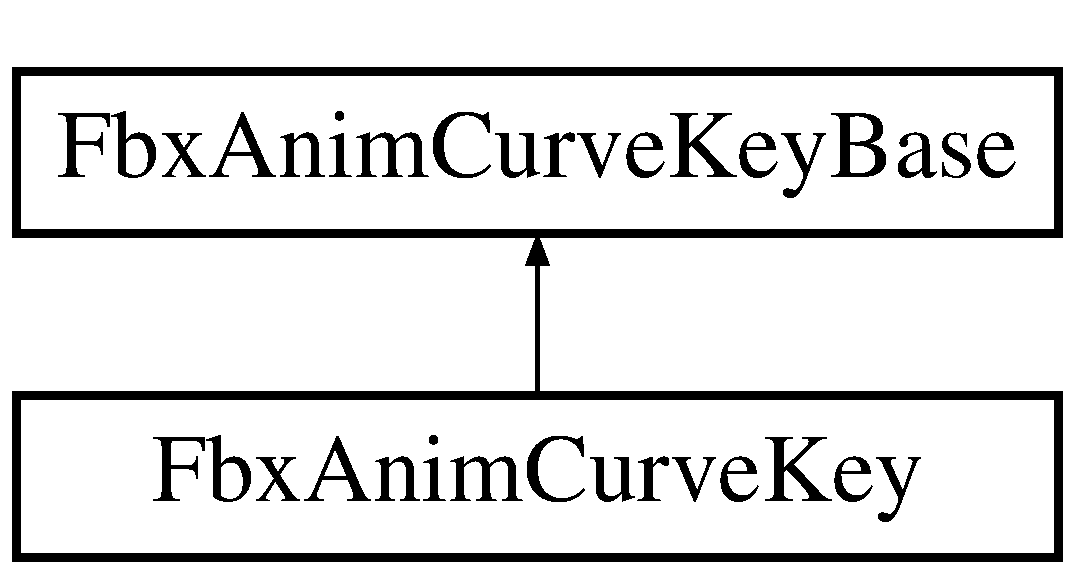
\includegraphics[height=2.000000cm]{class_fbx_anim_curve_key_base}
\end{center}
\end{figure}
\subsection*{公開メンバ関数}
\begin{DoxyCompactItemize}
\item 
\hyperlink{class_fbx_anim_curve_key_base_a76d982fc9fe4888f2db2e8d4bb5d4f2f}{Fbx\+Anim\+Curve\+Key\+Base} ()
\item 
virtual \hyperlink{class_fbx_anim_curve_key_base_a2f773ce4bba07ee0f92f9cb9b5f3233b}{$\sim$\+Fbx\+Anim\+Curve\+Key\+Base} ()
\item 
virtual \hyperlink{class_fbx_time}{Fbx\+Time} \hyperlink{class_fbx_anim_curve_key_base_a3eebfd7bd2101f759269373a6c9343a2}{Get\+Time} () const
\item 
virtual void \hyperlink{class_fbx_anim_curve_key_base_a1c8d15159d7b00280411c08f86c951ca}{Set\+Time} (const \hyperlink{class_fbx_time}{Fbx\+Time} \&p\+Time)
\end{DoxyCompactItemize}
\subsection*{公開変数類}
\begin{DoxyCompactItemize}
\item 
\hyperlink{class_fbx_time}{Fbx\+Time} \hyperlink{class_fbx_anim_curve_key_base_a8b62f6694176ae418ed4cb936f52545a}{m\+Time}
\end{DoxyCompactItemize}


\subsection{詳解}
This is the base class interface for the F\+BX animation curve keys.

\begin{DoxyRemark}{注釈}
For an example of implemented class, please see \hyperlink{class_fbx_anim_curve_key}{Fbx\+Anim\+Curve\+Key}. 
\end{DoxyRemark}


 fbxanimcurvebase.\+h の 29 行目に定義があります。



\subsection{構築子と解体子}
\mbox{\Hypertarget{class_fbx_anim_curve_key_base_a76d982fc9fe4888f2db2e8d4bb5d4f2f}\label{class_fbx_anim_curve_key_base_a76d982fc9fe4888f2db2e8d4bb5d4f2f}} 
\index{Fbx\+Anim\+Curve\+Key\+Base@{Fbx\+Anim\+Curve\+Key\+Base}!Fbx\+Anim\+Curve\+Key\+Base@{Fbx\+Anim\+Curve\+Key\+Base}}
\index{Fbx\+Anim\+Curve\+Key\+Base@{Fbx\+Anim\+Curve\+Key\+Base}!Fbx\+Anim\+Curve\+Key\+Base@{Fbx\+Anim\+Curve\+Key\+Base}}
\subsubsection{\texorpdfstring{Fbx\+Anim\+Curve\+Key\+Base()}{FbxAnimCurveKeyBase()}}
{\footnotesize\ttfamily Fbx\+Anim\+Curve\+Key\+Base\+::\+Fbx\+Anim\+Curve\+Key\+Base (\begin{DoxyParamCaption}{ }\end{DoxyParamCaption})\hspace{0.3cm}{\ttfamily [inline]}}

Constructor. 

 fbxanimcurvebase.\+h の 38 行目に定義があります。

\mbox{\Hypertarget{class_fbx_anim_curve_key_base_a2f773ce4bba07ee0f92f9cb9b5f3233b}\label{class_fbx_anim_curve_key_base_a2f773ce4bba07ee0f92f9cb9b5f3233b}} 
\index{Fbx\+Anim\+Curve\+Key\+Base@{Fbx\+Anim\+Curve\+Key\+Base}!````~Fbx\+Anim\+Curve\+Key\+Base@{$\sim$\+Fbx\+Anim\+Curve\+Key\+Base}}
\index{````~Fbx\+Anim\+Curve\+Key\+Base@{$\sim$\+Fbx\+Anim\+Curve\+Key\+Base}!Fbx\+Anim\+Curve\+Key\+Base@{Fbx\+Anim\+Curve\+Key\+Base}}
\subsubsection{\texorpdfstring{$\sim$\+Fbx\+Anim\+Curve\+Key\+Base()}{~FbxAnimCurveKeyBase()}}
{\footnotesize\ttfamily virtual Fbx\+Anim\+Curve\+Key\+Base\+::$\sim$\+Fbx\+Anim\+Curve\+Key\+Base (\begin{DoxyParamCaption}{ }\end{DoxyParamCaption})\hspace{0.3cm}{\ttfamily [inline]}, {\ttfamily [virtual]}}

Destructor. 

 fbxanimcurvebase.\+h の 45 行目に定義があります。



\subsection{関数詳解}
\mbox{\Hypertarget{class_fbx_anim_curve_key_base_a3eebfd7bd2101f759269373a6c9343a2}\label{class_fbx_anim_curve_key_base_a3eebfd7bd2101f759269373a6c9343a2}} 
\index{Fbx\+Anim\+Curve\+Key\+Base@{Fbx\+Anim\+Curve\+Key\+Base}!Get\+Time@{Get\+Time}}
\index{Get\+Time@{Get\+Time}!Fbx\+Anim\+Curve\+Key\+Base@{Fbx\+Anim\+Curve\+Key\+Base}}
\subsubsection{\texorpdfstring{Get\+Time()}{GetTime()}}
{\footnotesize\ttfamily virtual \hyperlink{class_fbx_time}{Fbx\+Time} Fbx\+Anim\+Curve\+Key\+Base\+::\+Get\+Time (\begin{DoxyParamCaption}{ }\end{DoxyParamCaption}) const\hspace{0.3cm}{\ttfamily [inline]}, {\ttfamily [virtual]}}

Get time value. \begin{DoxyReturn}{戻り値}
Time value. 
\end{DoxyReturn}


\hyperlink{class_fbx_anim_curve_key_aae0882b53b31502cb30ea35de028837f}{Fbx\+Anim\+Curve\+Key}で再実装されています。



 fbxanimcurvebase.\+h の 50 行目に定義があります。

\mbox{\Hypertarget{class_fbx_anim_curve_key_base_a1c8d15159d7b00280411c08f86c951ca}\label{class_fbx_anim_curve_key_base_a1c8d15159d7b00280411c08f86c951ca}} 
\index{Fbx\+Anim\+Curve\+Key\+Base@{Fbx\+Anim\+Curve\+Key\+Base}!Set\+Time@{Set\+Time}}
\index{Set\+Time@{Set\+Time}!Fbx\+Anim\+Curve\+Key\+Base@{Fbx\+Anim\+Curve\+Key\+Base}}
\subsubsection{\texorpdfstring{Set\+Time()}{SetTime()}}
{\footnotesize\ttfamily virtual void Fbx\+Anim\+Curve\+Key\+Base\+::\+Set\+Time (\begin{DoxyParamCaption}\item[{const \hyperlink{class_fbx_time}{Fbx\+Time} \&}]{p\+Time }\end{DoxyParamCaption})\hspace{0.3cm}{\ttfamily [inline]}, {\ttfamily [virtual]}}

Set time value. 
\begin{DoxyParams}{引数}
{\em p\+Time} & Time value to set. \\
\hline
\end{DoxyParams}


\hyperlink{class_fbx_anim_curve_key_a6ebc96b8346a345534c0eb2e1b6d9291}{Fbx\+Anim\+Curve\+Key}で再実装されています。



 fbxanimcurvebase.\+h の 58 行目に定義があります。



\subsection{メンバ詳解}
\mbox{\Hypertarget{class_fbx_anim_curve_key_base_a8b62f6694176ae418ed4cb936f52545a}\label{class_fbx_anim_curve_key_base_a8b62f6694176ae418ed4cb936f52545a}} 
\index{Fbx\+Anim\+Curve\+Key\+Base@{Fbx\+Anim\+Curve\+Key\+Base}!m\+Time@{m\+Time}}
\index{m\+Time@{m\+Time}!Fbx\+Anim\+Curve\+Key\+Base@{Fbx\+Anim\+Curve\+Key\+Base}}
\subsubsection{\texorpdfstring{m\+Time}{mTime}}
{\footnotesize\ttfamily \hyperlink{class_fbx_time}{Fbx\+Time} Fbx\+Anim\+Curve\+Key\+Base\+::m\+Time}

Data member representing time value. 

 fbxanimcurvebase.\+h の 34 行目に定義があります。



このクラス詳解は次のファイルから抽出されました\+:\begin{DoxyCompactItemize}
\item 
C\+:/\+Maya/scripts/\+F\+B\+X\+\_\+\+S\+D\+K/2017.\+1/include/fbxsdk/scene/animation/\hyperlink{fbxanimcurvebase_8h}{fbxanimcurvebase.\+h}\end{DoxyCompactItemize}

\hypertarget{class_fbx_anim_curve_node}{}\section{Fbx\+Anim\+Curve\+Node クラス}
\label{class_fbx_anim_curve_node}\index{Fbx\+Anim\+Curve\+Node@{Fbx\+Anim\+Curve\+Node}}


{\ttfamily \#include $<$fbxanimcurvenode.\+h$>$}

Fbx\+Anim\+Curve\+Node の継承関係図\begin{figure}[H]
\begin{center}
\leavevmode
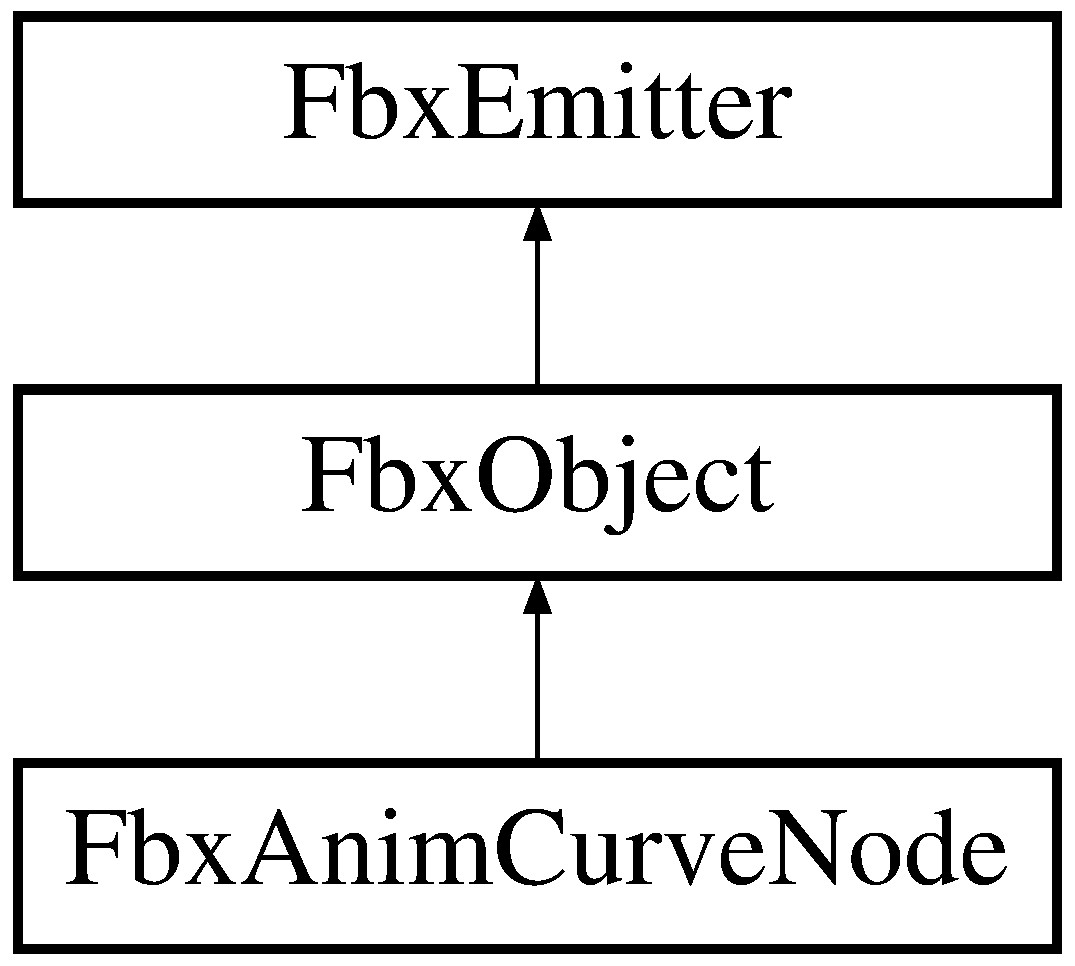
\includegraphics[height=3.000000cm]{class_fbx_anim_curve_node}
\end{center}
\end{figure}
\subsection*{公開メンバ関数}
\begin{DoxyCompactItemize}
\item 
virtual \hyperlink{class_fbx_object}{Fbx\+Object} \& \hyperlink{class_fbx_anim_curve_node_a9630a96fb6927737ff49d6dab352c36f}{Copy} (const \hyperlink{class_fbx_object}{Fbx\+Object} \&p\+Object)
\item 
void \hyperlink{class_fbx_anim_curve_node_ad38a2414969d07dd7c1905fb8d07a9b5}{Release\+K\+F\+Curve\+Node} ()
\item 
void \hyperlink{class_fbx_anim_curve_node_aa52265be388b803f8880e1911e211236}{Sync\+Channels\+With\+K\+F\+Curve} ()
\item 
bool \hyperlink{class_fbx_anim_curve_node_a431f4ad514b9c72efc78c1f16dc50b6b}{Use\+Quaternion\+Interpolation} ()
\item 
bool \hyperlink{class_fbx_anim_curve_node_a16fee78283fbd1d530e1e80a2bcb166a}{Set\+Quaternion\+Interpolation} (unsigned short p\+Val)
\item 
unsigned short \hyperlink{class_fbx_anim_curve_node_aef47daaf7f219b58537fcd4e40adee38}{Get\+Quaternion\+Interpolation} ()
\item 
void \hyperlink{class_fbx_anim_curve_node_a9d266fe30162053141dd131a1005abf2}{Set\+K\+F\+Curve\+Node\+Layer\+Type} (\hyperlink{class_fbx_property}{Fbx\+Property} \&p\+Prop)
\item 
K\+F\+Curve\+Node $\ast$ \hyperlink{class_fbx_anim_curve_node_a482d23e7517db05af3252b2c02ce2415}{Get\+K\+F\+Curve\+Node} (bool p\+No\+Create=false)
\end{DoxyCompactItemize}
\subsection*{静的公開メンバ関数}
\begin{DoxyCompactItemize}
\item 
static const char $\ast$ \hyperlink{class_fbx_anim_curve_node_ae75e53bb5e39cdefcd59e15e23924a13}{Curve\+Node\+Name\+From} (const char $\ast$p\+Name)
\item 
static bool \hyperlink{class_fbx_anim_curve_node_a114170d034199d8a40ccc037c495aa04}{Evaluate\+Channels} (\hyperlink{class_fbx_anim_curve_node}{Fbx\+Anim\+Curve\+Node} $\ast$p\+Curve\+Node, double $\ast$p\+Data, unsigned int p\+Count, \hyperlink{class_fbx_time}{Fbx\+Time} p\+Time)
\end{DoxyCompactItemize}
\subsection*{限定公開メンバ関数}
\begin{DoxyCompactItemize}
\item 
virtual void \hyperlink{class_fbx_anim_curve_node_a68463f3262085ccffef1d5a68fbd4823}{Construct} (const \hyperlink{class_fbx_object}{Fbx\+Object} $\ast$p\+From)
\item 
virtual void \hyperlink{class_fbx_anim_curve_node_aa5702533aa63185ec4549b73915476d7}{Destruct} (bool p\+Recursive)
\item 
virtual void \hyperlink{class_fbx_anim_curve_node_a979eca26d04013f0ef958173d34aef15}{Construct\+Properties} (bool p\+Force\+Set)
\item 
virtual bool \hyperlink{class_fbx_anim_curve_node_a0a3743b600796ab2b87dea299654b98c}{Connect\+Notify} (const \hyperlink{class_fbx_connect_event}{Fbx\+Connect\+Event} \&p\+Event)
\item 
\hyperlink{class_fbx_anim_curve_node}{Fbx\+Anim\+Curve\+Node} $\ast$ \hyperlink{class_fbx_anim_curve_node_aa60f953e94636bb23a94860f60cc63e1}{Find} (\hyperlink{class_fbx_anim_curve_node}{Fbx\+Anim\+Curve\+Node} $\ast$p\+Root, const \hyperlink{class_fbx_string}{Fbx\+String} \&p\+Name)
\end{DoxyCompactItemize}
\subsection*{フレンド}
\begin{DoxyCompactItemize}
\item 
class \hyperlink{class_fbx_anim_curve_node_a0e66be27522fe93db7ee48dbdb4420bb}{Fbx\+Anim\+Curve\+Filter\+Matrix\+Converter}
\item 
class \hyperlink{class_fbx_anim_curve_node_a1b769b6684b71dfe76f350fef1137cab}{Fbx\+Anim\+Eval\+Classic}
\item 
void \hyperlink{class_fbx_anim_curve_node_a54d20e7508453ca014d08b85da892621}{Collect\+Anim\+From\+Curve\+Node} (void $\ast$$\ast$l\+Src, void $\ast$fcn, unsigned int nb\+Crvs, \hyperlink{class_fbx_anim_curve_node}{Fbx\+Anim\+Curve\+Node} $\ast$cn, \hyperlink{class_fbx_multi_map}{Fbx\+Multi\+Map} $\ast$p\+Nick\+To\+Anim\+Curve\+Time\+Warps\+Set, \hyperlink{class_fbx_multi_map}{Fbx\+Multi\+Map} \&p\+Nick\+To\+K\+F\+Curve\+Node\+Warp\+Set)
\end{DoxyCompactItemize}
\subsection*{Utility functions.}
\begin{DoxyCompactItemize}
\item 
bool \hyperlink{class_fbx_anim_curve_node_ad9ca0ff8cf30e3b55c91184be5f693ac}{Is\+Animated} (bool p\+Recurse=false) const
\item 
bool \hyperlink{class_fbx_anim_curve_node_a8bdce1ee829fd11bbd74ea2596f3977d}{Get\+Animation\+Interval} (\hyperlink{class_fbx_time_span}{Fbx\+Time\+Span} \&p\+Time\+Interval) const
\item 
bool \hyperlink{class_fbx_anim_curve_node_ad0fd9df109fb4e9c8702d37f03b6cc03}{Is\+Composite} () const
\item 
\hyperlink{class_fbx_anim_curve_node}{Fbx\+Anim\+Curve\+Node} $\ast$ \hyperlink{class_fbx_anim_curve_node_aca6ee712b7eeafb1d00f42117520bac4}{Find} (const char $\ast$p\+Name)
\item 
unsigned int \hyperlink{class_fbx_anim_curve_node_a17a3e0fdd0cb807c3fe37f07c9bef844}{Get\+Channels\+Count} () const
\item 
int \hyperlink{class_fbx_anim_curve_node_a8ba8427aa3f99361aaf23cee44439015}{Get\+Channel\+Index} (const char $\ast$p\+Channel\+Name) const
\item 
\hyperlink{class_fbx_string}{Fbx\+String} \hyperlink{class_fbx_anim_curve_node_a1ad770dcc06ec0638103935e4dfede3c}{Get\+Channel\+Name} (int p\+Channel\+Id) const
\item 
void \hyperlink{class_fbx_anim_curve_node_ad334950a15167317fbbc029fe806976d}{Reset\+Channels} ()
\item 
{\footnotesize template$<$class T $>$ }\\bool \hyperlink{class_fbx_anim_curve_node_a985772edb8c85825adfef69c6bd06627}{Add\+Channel} (const char $\ast$p\+Chnl\+Name, T const \&p\+Value)
\item 
{\footnotesize template$<$class T $>$ }\\void \hyperlink{class_fbx_anim_curve_node_a0efefd96f733f636d7aa95148be08726}{Set\+Channel\+Value} (const char $\ast$p\+Chnl\+Name, T p\+Value)
\item 
{\footnotesize template$<$class T $>$ }\\void \hyperlink{class_fbx_anim_curve_node_aceef8634351d11d9058b5d023de5f5b4}{Set\+Channel\+Value} (unsigned int p\+Chnl\+Id, T p\+Value)
\item 
{\footnotesize template$<$class T $>$ }\\T \hyperlink{class_fbx_anim_curve_node_ab9d76b0fea168dfe928ec2385e43c716}{Get\+Channel\+Value} (const char $\ast$p\+Chnl\+Name, T p\+Init\+Val)
\item 
{\footnotesize template$<$class T $>$ }\\T \hyperlink{class_fbx_anim_curve_node_a1fb96d04b8c53ec130c5be376b923c6c}{Get\+Channel\+Value} (unsigned int p\+Chnl\+Id, T p\+Init\+Val)
\item 
static \hyperlink{class_fbx_anim_curve_node}{Fbx\+Anim\+Curve\+Node} $\ast$ \hyperlink{class_fbx_anim_curve_node_a588814e5973e080f84c54438623ddf7e}{Create\+Typed\+Curve\+Node} (\hyperlink{class_fbx_property}{Fbx\+Property} \&p\+Property, \hyperlink{class_fbx_scene}{Fbx\+Scene} $\ast$p\+Scene)
\end{DoxyCompactItemize}
\subsection*{Fbx\+Anim\+Curve management.}
\begin{DoxyCompactItemize}
\item 
bool \hyperlink{class_fbx_anim_curve_node_a76db258a1f1d7c2a4a178c00788c7a92}{Disconnect\+From\+Channel} (\hyperlink{class_fbx_anim_curve}{Fbx\+Anim\+Curve} $\ast$p\+Curve, unsigned int p\+Chnl\+Id)
\item 
bool \hyperlink{class_fbx_anim_curve_node_a29ef7927112552fcbacd6a82555e15e4}{Connect\+To\+Channel} (\hyperlink{class_fbx_anim_curve}{Fbx\+Anim\+Curve} $\ast$p\+Curve, const char $\ast$p\+Chnl, bool p\+In\+Front=false)
\item 
bool \hyperlink{class_fbx_anim_curve_node_a33b04e03a4e6c965963ffc0e4abc9608}{Connect\+To\+Channel} (\hyperlink{class_fbx_anim_curve}{Fbx\+Anim\+Curve} $\ast$p\+Curve, unsigned int p\+Chnl\+Id, bool p\+In\+Front=false)
\item 
\hyperlink{class_fbx_anim_curve}{Fbx\+Anim\+Curve} $\ast$ \hyperlink{class_fbx_anim_curve_node_af3600f3846c38a82b0ea6491c9b2857f}{Create\+Curve} (const char $\ast$p\+Curve\+Node\+Name, const char $\ast$p\+Channel)
\item 
\hyperlink{class_fbx_anim_curve}{Fbx\+Anim\+Curve} $\ast$ \hyperlink{class_fbx_anim_curve_node_a10fa606f04216696240ad9d1cc655985}{Create\+Curve} (const char $\ast$p\+Curve\+Node\+Name, unsigned int p\+Channel\+Id=0)
\item 
int \hyperlink{class_fbx_anim_curve_node_a41d28a650fa90706d1c67ad5f56530b5}{Get\+Curve\+Count} (unsigned int p\+Channel\+Id, const char $\ast$p\+Curve\+Node\+Name=\hyperlink{fbxarch_8h_a070d2ce7b6bb7e5c05602aa8c308d0c4}{N\+U\+LL})
\item 
\hyperlink{class_fbx_anim_curve}{Fbx\+Anim\+Curve} $\ast$ \hyperlink{class_fbx_anim_curve_node_a818b6198c31818e863d3d5bc7948c2e2}{Get\+Curve} (unsigned int p\+Channel\+Id, unsigned int p\+Id=0, const char $\ast$p\+Curve\+Node\+Name=\hyperlink{fbxarch_8h_a070d2ce7b6bb7e5c05602aa8c308d0c4}{N\+U\+LL})
\end{DoxyCompactItemize}
\subsection*{その他の継承メンバ}


\subsection{詳解}
This class is an composite of animation curves and is called as animation curve node.

Animation curve node is used as the connection point for animation curves and other animation curve nodes associated to a property. \hyperlink{class_fbx_anim_curve_node}{Fbx\+Anim\+Curve\+Node} can be connected to other \hyperlink{class_fbx_anim_curve_node}{Fbx\+Anim\+Curve\+Node}, in this case, the destination animation curve node may be considered as \char`\"{}composite\char`\"{}, \hyperlink{class_fbx_anim_curve_node_ad0fd9df109fb4e9c8702d37f03b6cc03}{Is\+Composite()}. remarks When created, the \hyperlink{class_fbx_anim_curve_node}{Fbx\+Anim\+Curve\+Node} has no valid channels unless it is created using the function \hyperlink{class_fbx_anim_curve_node_a588814e5973e080f84c54438623ddf7e}{Create\+Typed\+Curve\+Node()}. This function will add all the required channels to correctly match the number of values of the property. For instance, when Create\+Typed\+Curve\+Node(p\+Node.\+Lcl\+Translation, p\+Scene) is called, the resulting \hyperlink{class_fbx_anim_curve_node}{Fbx\+Anim\+Curve\+Node} will automatically have 3 channels corresponding to the X,Y and Z components of the Lcl\+Translation property. You can add and remove channels dynamically but can never remove the channels that have been added by the call to \hyperlink{class_fbx_anim_curve_node_a588814e5973e080f84c54438623ddf7e}{Create\+Typed\+Curve\+Node()}.

However, the F\+BX S\+DK animation system\textquotesingle{}s default implementation is to consider only the first curve connected to the channel. Therefore, if the caller connects multiple animation curves to the same channel, then it becomes the caller\textquotesingle{}s responsibility to handle and manipulate these extra curves in a meaningful manner. 

 fbxanimcurvenode.\+h の 55 行目に定義があります。



\subsection{関数詳解}
\mbox{\Hypertarget{class_fbx_anim_curve_node_a985772edb8c85825adfef69c6bd06627}\label{class_fbx_anim_curve_node_a985772edb8c85825adfef69c6bd06627}} 
\index{Fbx\+Anim\+Curve\+Node@{Fbx\+Anim\+Curve\+Node}!Add\+Channel@{Add\+Channel}}
\index{Add\+Channel@{Add\+Channel}!Fbx\+Anim\+Curve\+Node@{Fbx\+Anim\+Curve\+Node}}
\subsubsection{\texorpdfstring{Add\+Channel()}{AddChannel()}}
{\footnotesize\ttfamily template$<$class T $>$ \\
bool Fbx\+Anim\+Curve\+Node\+::\+Add\+Channel (\begin{DoxyParamCaption}\item[{const char $\ast$}]{p\+Chnl\+Name,  }\item[{T const \&}]{p\+Value }\end{DoxyParamCaption})\hspace{0.3cm}{\ttfamily [inline]}}

Adds the specified channel property. 
\begin{DoxyParams}{引数}
{\em p\+Chnl\+Name} & Channel name. \\
\hline
{\em p\+Value} & Default value of the channel. \\
\hline
\end{DoxyParams}
\begin{DoxyReturn}{戻り値}
{\ttfamily true} if successful, {\ttfamily false} otherwise. 
\end{DoxyReturn}
\begin{DoxyRemark}{注釈}
It is an error to try to add a channel that already exists. 
\end{DoxyRemark}


 fbxanimcurvenode.\+h の 143 行目に定義があります。

\mbox{\Hypertarget{class_fbx_anim_curve_node_a0a3743b600796ab2b87dea299654b98c}\label{class_fbx_anim_curve_node_a0a3743b600796ab2b87dea299654b98c}} 
\index{Fbx\+Anim\+Curve\+Node@{Fbx\+Anim\+Curve\+Node}!Connect\+Notify@{Connect\+Notify}}
\index{Connect\+Notify@{Connect\+Notify}!Fbx\+Anim\+Curve\+Node@{Fbx\+Anim\+Curve\+Node}}
\subsubsection{\texorpdfstring{Connect\+Notify()}{ConnectNotify()}}
{\footnotesize\ttfamily virtual bool Fbx\+Anim\+Curve\+Node\+::\+Connect\+Notify (\begin{DoxyParamCaption}\item[{const \hyperlink{class_fbx_connect_event}{Fbx\+Connect\+Event} \&}]{p\+Event }\end{DoxyParamCaption})\hspace{0.3cm}{\ttfamily [protected]}, {\ttfamily [virtual]}}



\hyperlink{class_fbx_object_ab7a400f3829d1f0da57d3d78c8168dd0}{Fbx\+Object}を再実装しています。

\mbox{\Hypertarget{class_fbx_anim_curve_node_a29ef7927112552fcbacd6a82555e15e4}\label{class_fbx_anim_curve_node_a29ef7927112552fcbacd6a82555e15e4}} 
\index{Fbx\+Anim\+Curve\+Node@{Fbx\+Anim\+Curve\+Node}!Connect\+To\+Channel@{Connect\+To\+Channel}}
\index{Connect\+To\+Channel@{Connect\+To\+Channel}!Fbx\+Anim\+Curve\+Node@{Fbx\+Anim\+Curve\+Node}}
\subsubsection{\texorpdfstring{Connect\+To\+Channel()}{ConnectToChannel()}\hspace{0.1cm}{\footnotesize\ttfamily [1/2]}}
{\footnotesize\ttfamily bool Fbx\+Anim\+Curve\+Node\+::\+Connect\+To\+Channel (\begin{DoxyParamCaption}\item[{\hyperlink{class_fbx_anim_curve}{Fbx\+Anim\+Curve} $\ast$}]{p\+Curve,  }\item[{const char $\ast$}]{p\+Chnl,  }\item[{bool}]{p\+In\+Front = {\ttfamily false} }\end{DoxyParamCaption})}

Connects the given animation curve to the specified channel. 
\begin{DoxyParams}{引数}
{\em p\+Curve} & The curve to connect to the channel. \\
\hline
{\em p\+Chnl} & The name of the channel the curve is to be connected to. \\
\hline
{\em p\+In\+Front} & When {\ttfamily true}, all the current connections are moved after this one, making this one the first. By default, the connection is the last one. \\
\hline
\end{DoxyParams}
\begin{DoxyReturn}{戻り値}
{\ttfamily true} if the connection was made, {\ttfamily false} if an error occurred. 
\end{DoxyReturn}
\mbox{\Hypertarget{class_fbx_anim_curve_node_a33b04e03a4e6c965963ffc0e4abc9608}\label{class_fbx_anim_curve_node_a33b04e03a4e6c965963ffc0e4abc9608}} 
\index{Fbx\+Anim\+Curve\+Node@{Fbx\+Anim\+Curve\+Node}!Connect\+To\+Channel@{Connect\+To\+Channel}}
\index{Connect\+To\+Channel@{Connect\+To\+Channel}!Fbx\+Anim\+Curve\+Node@{Fbx\+Anim\+Curve\+Node}}
\subsubsection{\texorpdfstring{Connect\+To\+Channel()}{ConnectToChannel()}\hspace{0.1cm}{\footnotesize\ttfamily [2/2]}}
{\footnotesize\ttfamily bool Fbx\+Anim\+Curve\+Node\+::\+Connect\+To\+Channel (\begin{DoxyParamCaption}\item[{\hyperlink{class_fbx_anim_curve}{Fbx\+Anim\+Curve} $\ast$}]{p\+Curve,  }\item[{unsigned int}]{p\+Chnl\+Id,  }\item[{bool}]{p\+In\+Front = {\ttfamily false} }\end{DoxyParamCaption})}

Connects the given animation curve to the specified channel. 
\begin{DoxyParams}{引数}
{\em p\+Curve} & The curve to connect to the channel. \\
\hline
{\em p\+Chnl\+Id} & Index of the channel the curve is to be connected to. \\
\hline
{\em p\+In\+Front} & When {\ttfamily true}, all the current connections are moved after this one. making this one the first. By default, the connection is the last one. \\
\hline
\end{DoxyParams}
\begin{DoxyReturn}{戻り値}
{\ttfamily true} if the connection was made, {\ttfamily false} if an error occurred. 
\end{DoxyReturn}
\begin{DoxyRemark}{注釈}
The index is 0 based. 
\end{DoxyRemark}
\mbox{\Hypertarget{class_fbx_anim_curve_node_a68463f3262085ccffef1d5a68fbd4823}\label{class_fbx_anim_curve_node_a68463f3262085ccffef1d5a68fbd4823}} 
\index{Fbx\+Anim\+Curve\+Node@{Fbx\+Anim\+Curve\+Node}!Construct@{Construct}}
\index{Construct@{Construct}!Fbx\+Anim\+Curve\+Node@{Fbx\+Anim\+Curve\+Node}}
\subsubsection{\texorpdfstring{Construct()}{Construct()}}
{\footnotesize\ttfamily virtual void Fbx\+Anim\+Curve\+Node\+::\+Construct (\begin{DoxyParamCaption}\item[{const \hyperlink{class_fbx_object}{Fbx\+Object} $\ast$}]{p\+From }\end{DoxyParamCaption})\hspace{0.3cm}{\ttfamily [protected]}, {\ttfamily [virtual]}}

Optional constructor override, automatically called by default constructor. 
\begin{DoxyParams}{引数}
{\em p\+From} & If not null, the function must take it into account like a copy constructor. \\
\hline
\end{DoxyParams}
\begin{DoxyRemark}{注釈}
In case it is decided to override this function, do not forget to call Parent\+Class\+::\+Construct(p\+From) at the beginning. 
\end{DoxyRemark}


\hyperlink{class_fbx_object_a313503bc645af3fdceb4a99ef5cea7eb}{Fbx\+Object}を再実装しています。

\mbox{\Hypertarget{class_fbx_anim_curve_node_a979eca26d04013f0ef958173d34aef15}\label{class_fbx_anim_curve_node_a979eca26d04013f0ef958173d34aef15}} 
\index{Fbx\+Anim\+Curve\+Node@{Fbx\+Anim\+Curve\+Node}!Construct\+Properties@{Construct\+Properties}}
\index{Construct\+Properties@{Construct\+Properties}!Fbx\+Anim\+Curve\+Node@{Fbx\+Anim\+Curve\+Node}}
\subsubsection{\texorpdfstring{Construct\+Properties()}{ConstructProperties()}}
{\footnotesize\ttfamily virtual void Fbx\+Anim\+Curve\+Node\+::\+Construct\+Properties (\begin{DoxyParamCaption}\item[{bool}]{p\+Force\+Set }\end{DoxyParamCaption})\hspace{0.3cm}{\ttfamily [protected]}, {\ttfamily [virtual]}}

Optional property constructor override, automatically called by default constructor. 
\begin{DoxyParams}{引数}
{\em p\+Force\+Set} & If the property value must be set regardless of default value. \\
\hline
\end{DoxyParams}
\begin{DoxyRemark}{注釈}
If your object have properties, they must be initialized in this function. 
\end{DoxyRemark}


\hyperlink{class_fbx_object_ad44f814323dc1b5e78bff1bfc608b4bb}{Fbx\+Object}を再実装しています。

\mbox{\Hypertarget{class_fbx_anim_curve_node_a9630a96fb6927737ff49d6dab352c36f}\label{class_fbx_anim_curve_node_a9630a96fb6927737ff49d6dab352c36f}} 
\index{Fbx\+Anim\+Curve\+Node@{Fbx\+Anim\+Curve\+Node}!Copy@{Copy}}
\index{Copy@{Copy}!Fbx\+Anim\+Curve\+Node@{Fbx\+Anim\+Curve\+Node}}
\subsubsection{\texorpdfstring{Copy()}{Copy()}}
{\footnotesize\ttfamily virtual \hyperlink{class_fbx_object}{Fbx\+Object}\& Fbx\+Anim\+Curve\+Node\+::\+Copy (\begin{DoxyParamCaption}\item[{const \hyperlink{class_fbx_object}{Fbx\+Object} \&}]{p\+Object }\end{DoxyParamCaption})\hspace{0.3cm}{\ttfamily [virtual]}}

Copy an object content into this object. 
\begin{DoxyParams}{引数}
{\em p\+Object} & The source object to copy data from. \\
\hline
\end{DoxyParams}
\begin{DoxyReturn}{戻り値}
Returns the destination object being modified by the source. 
\end{DoxyReturn}
\begin{DoxyRemark}{注釈}
This function replace the assignment operator (operator=). It will copy all property values and the name. Connections are N\+OT copied. 
\end{DoxyRemark}


\hyperlink{class_fbx_object_a0c0c5adb38284d14bb82c04d54504a3e}{Fbx\+Object}を再実装しています。

\mbox{\Hypertarget{class_fbx_anim_curve_node_af3600f3846c38a82b0ea6491c9b2857f}\label{class_fbx_anim_curve_node_af3600f3846c38a82b0ea6491c9b2857f}} 
\index{Fbx\+Anim\+Curve\+Node@{Fbx\+Anim\+Curve\+Node}!Create\+Curve@{Create\+Curve}}
\index{Create\+Curve@{Create\+Curve}!Fbx\+Anim\+Curve\+Node@{Fbx\+Anim\+Curve\+Node}}
\subsubsection{\texorpdfstring{Create\+Curve()}{CreateCurve()}\hspace{0.1cm}{\footnotesize\ttfamily [1/2]}}
{\footnotesize\ttfamily \hyperlink{class_fbx_anim_curve}{Fbx\+Anim\+Curve}$\ast$ Fbx\+Anim\+Curve\+Node\+::\+Create\+Curve (\begin{DoxyParamCaption}\item[{const char $\ast$}]{p\+Curve\+Node\+Name,  }\item[{const char $\ast$}]{p\+Channel }\end{DoxyParamCaption})}

Creates a new curve and connects it to the specified channel of the animation curve node named p\+Curve\+Node\+Name. If this animation curve node is composite, this function will try to search all children animation curve nodes recursively for the one named p\+Curve\+Node\+Name. 
\begin{DoxyParams}{引数}
{\em p\+Curve\+Node\+Name} & Name of the \hyperlink{class_fbx_anim_curve_node}{Fbx\+Anim\+Curve\+Node} we are looking for. \\
\hline
{\em p\+Channel} & Channel identifier. \\
\hline
\end{DoxyParams}
\begin{DoxyReturn}{戻り値}
Pointer to the \hyperlink{class_fbx_anim_curve}{Fbx\+Anim\+Curve} or N\+U\+LL if an error occurred. 
\end{DoxyReturn}
\begin{DoxyRemark}{注釈}
p\+Curve\+Node\+Name cannot be empty. 

If the p\+Channel identifier is left N\+U\+LL, the first valid channel will be used to create curve. 
\end{DoxyRemark}
\mbox{\Hypertarget{class_fbx_anim_curve_node_a10fa606f04216696240ad9d1cc655985}\label{class_fbx_anim_curve_node_a10fa606f04216696240ad9d1cc655985}} 
\index{Fbx\+Anim\+Curve\+Node@{Fbx\+Anim\+Curve\+Node}!Create\+Curve@{Create\+Curve}}
\index{Create\+Curve@{Create\+Curve}!Fbx\+Anim\+Curve\+Node@{Fbx\+Anim\+Curve\+Node}}
\subsubsection{\texorpdfstring{Create\+Curve()}{CreateCurve()}\hspace{0.1cm}{\footnotesize\ttfamily [2/2]}}
{\footnotesize\ttfamily \hyperlink{class_fbx_anim_curve}{Fbx\+Anim\+Curve}$\ast$ Fbx\+Anim\+Curve\+Node\+::\+Create\+Curve (\begin{DoxyParamCaption}\item[{const char $\ast$}]{p\+Curve\+Node\+Name,  }\item[{unsigned int}]{p\+Channel\+Id = {\ttfamily 0} }\end{DoxyParamCaption})}

Creates a new curve and connects it to the specified channel of the animation curve node named p\+Curve\+Node\+Name. If this animation curve node is composite, this function will try to search all children animation curve nodes recursively for the one named p\+Curve\+Node\+Name. 
\begin{DoxyParams}{引数}
{\em p\+Curve\+Node\+Name} & Name of the \hyperlink{class_fbx_anim_curve_node}{Fbx\+Anim\+Curve\+Node} we are looking for. \\
\hline
{\em p\+Channel\+Id} & Channel index. \\
\hline
\end{DoxyParams}
\begin{DoxyReturn}{戻り値}
Pointer to the \hyperlink{class_fbx_anim_curve}{Fbx\+Anim\+Curve} or N\+U\+LL if an error occurred. 
\end{DoxyReturn}
\begin{DoxyRemark}{注釈}
p\+Curve\+Node\+Name cannot be empty. If the p\+Channel\+Id is not assigned, the first valid channel will be used to create curve. 
\end{DoxyRemark}
\mbox{\Hypertarget{class_fbx_anim_curve_node_a588814e5973e080f84c54438623ddf7e}\label{class_fbx_anim_curve_node_a588814e5973e080f84c54438623ddf7e}} 
\index{Fbx\+Anim\+Curve\+Node@{Fbx\+Anim\+Curve\+Node}!Create\+Typed\+Curve\+Node@{Create\+Typed\+Curve\+Node}}
\index{Create\+Typed\+Curve\+Node@{Create\+Typed\+Curve\+Node}!Fbx\+Anim\+Curve\+Node@{Fbx\+Anim\+Curve\+Node}}
\subsubsection{\texorpdfstring{Create\+Typed\+Curve\+Node()}{CreateTypedCurveNode()}}
{\footnotesize\ttfamily static \hyperlink{class_fbx_anim_curve_node}{Fbx\+Anim\+Curve\+Node}$\ast$ Fbx\+Anim\+Curve\+Node\+::\+Create\+Typed\+Curve\+Node (\begin{DoxyParamCaption}\item[{\hyperlink{class_fbx_property}{Fbx\+Property} \&}]{p\+Property,  }\item[{\hyperlink{class_fbx_scene}{Fbx\+Scene} $\ast$}]{p\+Scene }\end{DoxyParamCaption})\hspace{0.3cm}{\ttfamily [static]}}

Create a \hyperlink{class_fbx_anim_curve_node}{Fbx\+Anim\+Curve\+Node} compatible with the specified property data type. 
\begin{DoxyParams}{引数}
{\em p\+Property} & The property that needs a \hyperlink{class_fbx_anim_curve_node}{Fbx\+Anim\+Curve\+Node}. \\
\hline
{\em p\+Scene} & The scene the created \hyperlink{class_fbx_anim_curve_node}{Fbx\+Anim\+Curve\+Node} will belong to. \\
\hline
\end{DoxyParams}
\begin{DoxyReturn}{戻り値}
The pointer to the newly created \hyperlink{class_fbx_anim_curve_node}{Fbx\+Anim\+Curve\+Node}. Returns N\+U\+LL if an error occurred. 
\end{DoxyReturn}
\begin{DoxyRemark}{注釈}
This function does not connect the newly created \hyperlink{class_fbx_anim_curve_node}{Fbx\+Anim\+Curve\+Node} to the property. 

This function detects Fbx\+Double3, Fbx\+Double4 and Fbx\+Double4x4 properties Data\+Types and automatically adds the required channels properties. Any other Data\+Type is not specifically processed and the channels properties are left empty and need to be filled using the \hyperlink{class_fbx_anim_curve_node_a985772edb8c85825adfef69c6bd06627}{Add\+Channel()} function. 
\end{DoxyRemark}
\mbox{\Hypertarget{class_fbx_anim_curve_node_ae75e53bb5e39cdefcd59e15e23924a13}\label{class_fbx_anim_curve_node_ae75e53bb5e39cdefcd59e15e23924a13}} 
\index{Fbx\+Anim\+Curve\+Node@{Fbx\+Anim\+Curve\+Node}!Curve\+Node\+Name\+From@{Curve\+Node\+Name\+From}}
\index{Curve\+Node\+Name\+From@{Curve\+Node\+Name\+From}!Fbx\+Anim\+Curve\+Node@{Fbx\+Anim\+Curve\+Node}}
\subsubsection{\texorpdfstring{Curve\+Node\+Name\+From()}{CurveNodeNameFrom()}}
{\footnotesize\ttfamily static const char$\ast$ Fbx\+Anim\+Curve\+Node\+::\+Curve\+Node\+Name\+From (\begin{DoxyParamCaption}\item[{const char $\ast$}]{p\+Name }\end{DoxyParamCaption})\hspace{0.3cm}{\ttfamily [static]}}

\mbox{\Hypertarget{class_fbx_anim_curve_node_aa5702533aa63185ec4549b73915476d7}\label{class_fbx_anim_curve_node_aa5702533aa63185ec4549b73915476d7}} 
\index{Fbx\+Anim\+Curve\+Node@{Fbx\+Anim\+Curve\+Node}!Destruct@{Destruct}}
\index{Destruct@{Destruct}!Fbx\+Anim\+Curve\+Node@{Fbx\+Anim\+Curve\+Node}}
\subsubsection{\texorpdfstring{Destruct()}{Destruct()}}
{\footnotesize\ttfamily virtual void Fbx\+Anim\+Curve\+Node\+::\+Destruct (\begin{DoxyParamCaption}\item[{bool}]{p\+Recursive }\end{DoxyParamCaption})\hspace{0.3cm}{\ttfamily [protected]}, {\ttfamily [virtual]}}

Optional destructor override, automatically called by default destructor. 
\begin{DoxyParams}{引数}
{\em p\+Recursive} & If true, children objects should be destroyed as well. \\
\hline
\end{DoxyParams}
\begin{DoxyRemark}{注釈}
In case it is decided to override this function, do not forget to call Parent\+Class\+::\+Destruct(p\+Resursive) at the end. 
\end{DoxyRemark}


\hyperlink{class_fbx_object_a123e084d9b32b29c28af6384b7c3c608}{Fbx\+Object}を再実装しています。

\mbox{\Hypertarget{class_fbx_anim_curve_node_a76db258a1f1d7c2a4a178c00788c7a92}\label{class_fbx_anim_curve_node_a76db258a1f1d7c2a4a178c00788c7a92}} 
\index{Fbx\+Anim\+Curve\+Node@{Fbx\+Anim\+Curve\+Node}!Disconnect\+From\+Channel@{Disconnect\+From\+Channel}}
\index{Disconnect\+From\+Channel@{Disconnect\+From\+Channel}!Fbx\+Anim\+Curve\+Node@{Fbx\+Anim\+Curve\+Node}}
\subsubsection{\texorpdfstring{Disconnect\+From\+Channel()}{DisconnectFromChannel()}}
{\footnotesize\ttfamily bool Fbx\+Anim\+Curve\+Node\+::\+Disconnect\+From\+Channel (\begin{DoxyParamCaption}\item[{\hyperlink{class_fbx_anim_curve}{Fbx\+Anim\+Curve} $\ast$}]{p\+Curve,  }\item[{unsigned int}]{p\+Chnl\+Id }\end{DoxyParamCaption})}

Disconnect the animation curve from the channel. 
\begin{DoxyParams}{引数}
{\em p\+Curve} & The curve to disconnect from the channel. \\
\hline
{\em p\+Chnl\+Id} & The channel index. \\
\hline
\end{DoxyParams}
\begin{DoxyReturn}{戻り値}
{\ttfamily true} if the disconnection was made, {\ttfamily false} if an error occurred. 
\end{DoxyReturn}
\mbox{\Hypertarget{class_fbx_anim_curve_node_a114170d034199d8a40ccc037c495aa04}\label{class_fbx_anim_curve_node_a114170d034199d8a40ccc037c495aa04}} 
\index{Fbx\+Anim\+Curve\+Node@{Fbx\+Anim\+Curve\+Node}!Evaluate\+Channels@{Evaluate\+Channels}}
\index{Evaluate\+Channels@{Evaluate\+Channels}!Fbx\+Anim\+Curve\+Node@{Fbx\+Anim\+Curve\+Node}}
\subsubsection{\texorpdfstring{Evaluate\+Channels()}{EvaluateChannels()}}
{\footnotesize\ttfamily static bool Fbx\+Anim\+Curve\+Node\+::\+Evaluate\+Channels (\begin{DoxyParamCaption}\item[{\hyperlink{class_fbx_anim_curve_node}{Fbx\+Anim\+Curve\+Node} $\ast$}]{p\+Curve\+Node,  }\item[{double $\ast$}]{p\+Data,  }\item[{unsigned int}]{p\+Count,  }\item[{\hyperlink{class_fbx_time}{Fbx\+Time}}]{p\+Time }\end{DoxyParamCaption})\hspace{0.3cm}{\ttfamily [static]}}

\mbox{\Hypertarget{class_fbx_anim_curve_node_aca6ee712b7eeafb1d00f42117520bac4}\label{class_fbx_anim_curve_node_aca6ee712b7eeafb1d00f42117520bac4}} 
\index{Fbx\+Anim\+Curve\+Node@{Fbx\+Anim\+Curve\+Node}!Find@{Find}}
\index{Find@{Find}!Fbx\+Anim\+Curve\+Node@{Fbx\+Anim\+Curve\+Node}}
\subsubsection{\texorpdfstring{Find()}{Find()}\hspace{0.1cm}{\footnotesize\ttfamily [1/2]}}
{\footnotesize\ttfamily \hyperlink{class_fbx_anim_curve_node}{Fbx\+Anim\+Curve\+Node}$\ast$ Fbx\+Anim\+Curve\+Node\+::\+Find (\begin{DoxyParamCaption}\item[{const char $\ast$}]{p\+Name }\end{DoxyParamCaption})}

Recursively look for the \hyperlink{class_fbx_anim_curve_node}{Fbx\+Anim\+Curve\+Node} matching the passed named argument. 
\begin{DoxyParams}{引数}
{\em p\+Name} & Name of the \hyperlink{class_fbx_anim_curve_node}{Fbx\+Anim\+Curve\+Node} we are looking for. \\
\hline
\end{DoxyParams}
\begin{DoxyReturn}{戻り値}
The found anim curve node or N\+U\+LL. 
\end{DoxyReturn}
\begin{DoxyRemark}{注釈}
If p\+Name is an empty string, this function automatically return N\+U\+LL. 
\end{DoxyRemark}
\mbox{\Hypertarget{class_fbx_anim_curve_node_aa60f953e94636bb23a94860f60cc63e1}\label{class_fbx_anim_curve_node_aa60f953e94636bb23a94860f60cc63e1}} 
\index{Fbx\+Anim\+Curve\+Node@{Fbx\+Anim\+Curve\+Node}!Find@{Find}}
\index{Find@{Find}!Fbx\+Anim\+Curve\+Node@{Fbx\+Anim\+Curve\+Node}}
\subsubsection{\texorpdfstring{Find()}{Find()}\hspace{0.1cm}{\footnotesize\ttfamily [2/2]}}
{\footnotesize\ttfamily \hyperlink{class_fbx_anim_curve_node}{Fbx\+Anim\+Curve\+Node}$\ast$ Fbx\+Anim\+Curve\+Node\+::\+Find (\begin{DoxyParamCaption}\item[{\hyperlink{class_fbx_anim_curve_node}{Fbx\+Anim\+Curve\+Node} $\ast$}]{p\+Root,  }\item[{const \hyperlink{class_fbx_string}{Fbx\+String} \&}]{p\+Name }\end{DoxyParamCaption})\hspace{0.3cm}{\ttfamily [protected]}}

\mbox{\Hypertarget{class_fbx_anim_curve_node_a8bdce1ee829fd11bbd74ea2596f3977d}\label{class_fbx_anim_curve_node_a8bdce1ee829fd11bbd74ea2596f3977d}} 
\index{Fbx\+Anim\+Curve\+Node@{Fbx\+Anim\+Curve\+Node}!Get\+Animation\+Interval@{Get\+Animation\+Interval}}
\index{Get\+Animation\+Interval@{Get\+Animation\+Interval}!Fbx\+Anim\+Curve\+Node@{Fbx\+Anim\+Curve\+Node}}
\subsubsection{\texorpdfstring{Get\+Animation\+Interval()}{GetAnimationInterval()}}
{\footnotesize\ttfamily bool Fbx\+Anim\+Curve\+Node\+::\+Get\+Animation\+Interval (\begin{DoxyParamCaption}\item[{\hyperlink{class_fbx_time_span}{Fbx\+Time\+Span} \&}]{p\+Time\+Interval }\end{DoxyParamCaption}) const}

Find out start and end time of the animation. This function retrieves the including time span for all animation curves of this animation curve node. 
\begin{DoxyParams}{引数}
{\em p\+Time\+Interval} & Reference to receive start time and end time. \\
\hline
\end{DoxyParams}
\begin{DoxyReturn}{戻り値}
{\ttfamily true} on success, {\ttfamily false} otherwise. 
\end{DoxyReturn}
\begin{DoxyRemark}{注釈}
{\ttfamily false} is also returned if this animation curve node has no animation. 

This method only considers the first animation curve connected to each channel. To find time interval of multiple animation curves that are connected to the same channel, it is the caller\textquotesingle{}s responsibility to write a new version of this method, and \hyperlink{class_fbx_anim_curve_node_a41d28a650fa90706d1c67ad5f56530b5}{Get\+Curve\+Count()} will be useful in this case. 
\end{DoxyRemark}
\mbox{\Hypertarget{class_fbx_anim_curve_node_a8ba8427aa3f99361aaf23cee44439015}\label{class_fbx_anim_curve_node_a8ba8427aa3f99361aaf23cee44439015}} 
\index{Fbx\+Anim\+Curve\+Node@{Fbx\+Anim\+Curve\+Node}!Get\+Channel\+Index@{Get\+Channel\+Index}}
\index{Get\+Channel\+Index@{Get\+Channel\+Index}!Fbx\+Anim\+Curve\+Node@{Fbx\+Anim\+Curve\+Node}}
\subsubsection{\texorpdfstring{Get\+Channel\+Index()}{GetChannelIndex()}}
{\footnotesize\ttfamily int Fbx\+Anim\+Curve\+Node\+::\+Get\+Channel\+Index (\begin{DoxyParamCaption}\item[{const char $\ast$}]{p\+Channel\+Name }\end{DoxyParamCaption}) const}

Get the index of the named channel. 
\begin{DoxyParams}{引数}
{\em p\+Channel\+Name} & Name of the channel for which we want the index. \\
\hline
\end{DoxyParams}
\begin{DoxyReturn}{戻り値}
the index of the named channel or -\/1 if no channel with this name is found. 
\end{DoxyReturn}
\mbox{\Hypertarget{class_fbx_anim_curve_node_a1ad770dcc06ec0638103935e4dfede3c}\label{class_fbx_anim_curve_node_a1ad770dcc06ec0638103935e4dfede3c}} 
\index{Fbx\+Anim\+Curve\+Node@{Fbx\+Anim\+Curve\+Node}!Get\+Channel\+Name@{Get\+Channel\+Name}}
\index{Get\+Channel\+Name@{Get\+Channel\+Name}!Fbx\+Anim\+Curve\+Node@{Fbx\+Anim\+Curve\+Node}}
\subsubsection{\texorpdfstring{Get\+Channel\+Name()}{GetChannelName()}}
{\footnotesize\ttfamily \hyperlink{class_fbx_string}{Fbx\+String} Fbx\+Anim\+Curve\+Node\+::\+Get\+Channel\+Name (\begin{DoxyParamCaption}\item[{int}]{p\+Channel\+Id }\end{DoxyParamCaption}) const}

Get the name of the channel. 
\begin{DoxyParams}{引数}
{\em p\+Channel\+Id} & Index of the channel for which we want the name. \\
\hline
\end{DoxyParams}
\begin{DoxyReturn}{戻り値}
the name of the indexed channel or \char`\"{}\char`\"{} if the index is invalid. 
\end{DoxyReturn}
\mbox{\Hypertarget{class_fbx_anim_curve_node_a17a3e0fdd0cb807c3fe37f07c9bef844}\label{class_fbx_anim_curve_node_a17a3e0fdd0cb807c3fe37f07c9bef844}} 
\index{Fbx\+Anim\+Curve\+Node@{Fbx\+Anim\+Curve\+Node}!Get\+Channels\+Count@{Get\+Channels\+Count}}
\index{Get\+Channels\+Count@{Get\+Channels\+Count}!Fbx\+Anim\+Curve\+Node@{Fbx\+Anim\+Curve\+Node}}
\subsubsection{\texorpdfstring{Get\+Channels\+Count()}{GetChannelsCount()}}
{\footnotesize\ttfamily unsigned int Fbx\+Anim\+Curve\+Node\+::\+Get\+Channels\+Count (\begin{DoxyParamCaption}{ }\end{DoxyParamCaption}) const}

Get the total number of property channels defined in this animation curve node. For composite animation curve nodes, since they do not contain any channels, this function will always return 0. \begin{DoxyReturn}{戻り値}
The number of property channels. 
\end{DoxyReturn}
\mbox{\Hypertarget{class_fbx_anim_curve_node_ab9d76b0fea168dfe928ec2385e43c716}\label{class_fbx_anim_curve_node_ab9d76b0fea168dfe928ec2385e43c716}} 
\index{Fbx\+Anim\+Curve\+Node@{Fbx\+Anim\+Curve\+Node}!Get\+Channel\+Value@{Get\+Channel\+Value}}
\index{Get\+Channel\+Value@{Get\+Channel\+Value}!Fbx\+Anim\+Curve\+Node@{Fbx\+Anim\+Curve\+Node}}
\subsubsection{\texorpdfstring{Get\+Channel\+Value()}{GetChannelValue()}\hspace{0.1cm}{\footnotesize\ttfamily [1/2]}}
{\footnotesize\ttfamily template$<$class T $>$ \\
T Fbx\+Anim\+Curve\+Node\+::\+Get\+Channel\+Value (\begin{DoxyParamCaption}\item[{const char $\ast$}]{p\+Chnl\+Name,  }\item[{T}]{p\+Init\+Val }\end{DoxyParamCaption})\hspace{0.3cm}{\ttfamily [inline]}}

Get the default value of the channel. 
\begin{DoxyParams}{引数}
{\em p\+Chnl\+Name} & Channel name. \\
\hline
{\em p\+Init\+Val} & Value returned if the specified channel is invalid. \\
\hline
\end{DoxyParams}
\begin{DoxyReturn}{戻り値}
The default value of this channel. 
\end{DoxyReturn}


 fbxanimcurvenode.\+h の 185 行目に定義があります。

\mbox{\Hypertarget{class_fbx_anim_curve_node_a1fb96d04b8c53ec130c5be376b923c6c}\label{class_fbx_anim_curve_node_a1fb96d04b8c53ec130c5be376b923c6c}} 
\index{Fbx\+Anim\+Curve\+Node@{Fbx\+Anim\+Curve\+Node}!Get\+Channel\+Value@{Get\+Channel\+Value}}
\index{Get\+Channel\+Value@{Get\+Channel\+Value}!Fbx\+Anim\+Curve\+Node@{Fbx\+Anim\+Curve\+Node}}
\subsubsection{\texorpdfstring{Get\+Channel\+Value()}{GetChannelValue()}\hspace{0.1cm}{\footnotesize\ttfamily [2/2]}}
{\footnotesize\ttfamily template$<$class T $>$ \\
T Fbx\+Anim\+Curve\+Node\+::\+Get\+Channel\+Value (\begin{DoxyParamCaption}\item[{unsigned int}]{p\+Chnl\+Id,  }\item[{T}]{p\+Init\+Val }\end{DoxyParamCaption})\hspace{0.3cm}{\ttfamily [inline]}}

Get the default value of the channel. 
\begin{DoxyParams}{引数}
{\em p\+Chnl\+Id} & Channel index. \\
\hline
{\em p\+Init\+Val} & Value returned if the specified channel is invalid. \\
\hline
\end{DoxyParams}
\begin{DoxyReturn}{戻り値}
The default value of this channel. 
\end{DoxyReturn}


 fbxanimcurvenode.\+h の 198 行目に定義があります。

\mbox{\Hypertarget{class_fbx_anim_curve_node_a818b6198c31818e863d3d5bc7948c2e2}\label{class_fbx_anim_curve_node_a818b6198c31818e863d3d5bc7948c2e2}} 
\index{Fbx\+Anim\+Curve\+Node@{Fbx\+Anim\+Curve\+Node}!Get\+Curve@{Get\+Curve}}
\index{Get\+Curve@{Get\+Curve}!Fbx\+Anim\+Curve\+Node@{Fbx\+Anim\+Curve\+Node}}
\subsubsection{\texorpdfstring{Get\+Curve()}{GetCurve()}}
{\footnotesize\ttfamily \hyperlink{class_fbx_anim_curve}{Fbx\+Anim\+Curve}$\ast$ Fbx\+Anim\+Curve\+Node\+::\+Get\+Curve (\begin{DoxyParamCaption}\item[{unsigned int}]{p\+Channel\+Id,  }\item[{unsigned int}]{p\+Id = {\ttfamily 0},  }\item[{const char $\ast$}]{p\+Curve\+Node\+Name = {\ttfamily \hyperlink{fbxarch_8h_a070d2ce7b6bb7e5c05602aa8c308d0c4}{N\+U\+LL}} }\end{DoxyParamCaption})}

Get the \hyperlink{class_fbx_anim_curve}{Fbx\+Anim\+Curve} of the specified channel. If this animation curve node is composite, this function will try to search all children animation curve nodes recursively for the one named p\+Curve\+Node\+Name. 
\begin{DoxyParams}{引数}
{\em p\+Channel\+Id} & Channel index. \\
\hline
{\em p\+Id} & The index of the desired anim curve (in case there is more than one). \\
\hline
{\em p\+Curve\+Node\+Name} & Name of the \hyperlink{class_fbx_anim_curve_node}{Fbx\+Anim\+Curve\+Node} we are looking for (if this object is a composite). \\
\hline
\end{DoxyParams}
\begin{DoxyReturn}{戻り値}
Pointer to the \hyperlink{class_fbx_anim_curve}{Fbx\+Anim\+Curve} that matches the criteria. 
\end{DoxyReturn}
\begin{DoxyRemark}{注釈}
This method fails if the \hyperlink{class_fbx_anim_curve_node}{Fbx\+Anim\+Curve\+Node} with name p\+Curve\+Node\+Name does not exist and return N\+U\+LL. If the specified channel cannot be found in the \hyperlink{class_fbx_anim_curve_node}{Fbx\+Anim\+Curve\+Node} with name p\+Curve\+Node\+Name, return N\+U\+LL. 

If the p\+Curve\+Node\+Name is left N\+U\+LL, then only search in the curves on this animation curve node even if it is composite. 
\end{DoxyRemark}
\mbox{\Hypertarget{class_fbx_anim_curve_node_a41d28a650fa90706d1c67ad5f56530b5}\label{class_fbx_anim_curve_node_a41d28a650fa90706d1c67ad5f56530b5}} 
\index{Fbx\+Anim\+Curve\+Node@{Fbx\+Anim\+Curve\+Node}!Get\+Curve\+Count@{Get\+Curve\+Count}}
\index{Get\+Curve\+Count@{Get\+Curve\+Count}!Fbx\+Anim\+Curve\+Node@{Fbx\+Anim\+Curve\+Node}}
\subsubsection{\texorpdfstring{Get\+Curve\+Count()}{GetCurveCount()}}
{\footnotesize\ttfamily int Fbx\+Anim\+Curve\+Node\+::\+Get\+Curve\+Count (\begin{DoxyParamCaption}\item[{unsigned int}]{p\+Channel\+Id,  }\item[{const char $\ast$}]{p\+Curve\+Node\+Name = {\ttfamily \hyperlink{fbxarch_8h_a070d2ce7b6bb7e5c05602aa8c308d0c4}{N\+U\+LL}} }\end{DoxyParamCaption})}

Get the number of \hyperlink{class_fbx_anim_curve}{Fbx\+Anim\+Curve} connected to the specified channel. If this animation curve node is composite, this function will try to search all children animation curve nodes recursively for the one named p\+Curve\+Node\+Name. 
\begin{DoxyParams}{引数}
{\em p\+Channel\+Id} & Channel index. \\
\hline
{\em p\+Curve\+Node\+Name} & Name of the \hyperlink{class_fbx_anim_curve_node}{Fbx\+Anim\+Curve\+Node} we are looking for. \\
\hline
\end{DoxyParams}
\begin{DoxyReturn}{戻り値}
The number of animation curves on the specified channel or 0 if an error occurred. 
\end{DoxyReturn}
\begin{DoxyRemark}{注釈}
This method fails if the \hyperlink{class_fbx_anim_curve_node}{Fbx\+Anim\+Curve\+Node} with name p\+Curve\+Node\+Name does not exist and return 0. If the specified channel cannot be found on the \hyperlink{class_fbx_anim_curve_node}{Fbx\+Anim\+Curve\+Node} with name p\+Curve\+Node\+Name, return 0. 

If this animation curve node is composite, this function will try to search all children animation curve nodes recursively for the one named p\+Curve\+Node\+Name. If the p\+Curve\+Node\+Name is left N\+U\+LL, then only look for the curves on this animation curve node even if it is composite. 
\end{DoxyRemark}
\mbox{\Hypertarget{class_fbx_anim_curve_node_a482d23e7517db05af3252b2c02ce2415}\label{class_fbx_anim_curve_node_a482d23e7517db05af3252b2c02ce2415}} 
\index{Fbx\+Anim\+Curve\+Node@{Fbx\+Anim\+Curve\+Node}!Get\+K\+F\+Curve\+Node@{Get\+K\+F\+Curve\+Node}}
\index{Get\+K\+F\+Curve\+Node@{Get\+K\+F\+Curve\+Node}!Fbx\+Anim\+Curve\+Node@{Fbx\+Anim\+Curve\+Node}}
\subsubsection{\texorpdfstring{Get\+K\+F\+Curve\+Node()}{GetKFCurveNode()}}
{\footnotesize\ttfamily K\+F\+Curve\+Node$\ast$ Fbx\+Anim\+Curve\+Node\+::\+Get\+K\+F\+Curve\+Node (\begin{DoxyParamCaption}\item[{bool}]{p\+No\+Create = {\ttfamily false} }\end{DoxyParamCaption})}

\mbox{\Hypertarget{class_fbx_anim_curve_node_aef47daaf7f219b58537fcd4e40adee38}\label{class_fbx_anim_curve_node_aef47daaf7f219b58537fcd4e40adee38}} 
\index{Fbx\+Anim\+Curve\+Node@{Fbx\+Anim\+Curve\+Node}!Get\+Quaternion\+Interpolation@{Get\+Quaternion\+Interpolation}}
\index{Get\+Quaternion\+Interpolation@{Get\+Quaternion\+Interpolation}!Fbx\+Anim\+Curve\+Node@{Fbx\+Anim\+Curve\+Node}}
\subsubsection{\texorpdfstring{Get\+Quaternion\+Interpolation()}{GetQuaternionInterpolation()}}
{\footnotesize\ttfamily unsigned short Fbx\+Anim\+Curve\+Node\+::\+Get\+Quaternion\+Interpolation (\begin{DoxyParamCaption}{ }\end{DoxyParamCaption})\hspace{0.3cm}{\ttfamily [inline]}}



 fbxanimcurvenode.\+h の 305 行目に定義があります。

\mbox{\Hypertarget{class_fbx_anim_curve_node_ad9ca0ff8cf30e3b55c91184be5f693ac}\label{class_fbx_anim_curve_node_ad9ca0ff8cf30e3b55c91184be5f693ac}} 
\index{Fbx\+Anim\+Curve\+Node@{Fbx\+Anim\+Curve\+Node}!Is\+Animated@{Is\+Animated}}
\index{Is\+Animated@{Is\+Animated}!Fbx\+Anim\+Curve\+Node@{Fbx\+Anim\+Curve\+Node}}
\subsubsection{\texorpdfstring{Is\+Animated()}{IsAnimated()}}
{\footnotesize\ttfamily bool Fbx\+Anim\+Curve\+Node\+::\+Is\+Animated (\begin{DoxyParamCaption}\item[{bool}]{p\+Recurse = {\ttfamily false} }\end{DoxyParamCaption}) const}

Check if the animation curve node contains any animation key. 
\begin{DoxyParams}{引数}
{\em p\+Recurse} & {\ttfamily true} to descend to the children if the animation curve node is composite. \\
\hline
\end{DoxyParams}
\begin{DoxyReturn}{戻り値}
{\ttfamily true} if at least one animation curve that contains one or more animation keys is found, {\ttfamily false} otherwise. 
\end{DoxyReturn}
\begin{DoxyRemark}{注釈}
This method only considers the first animation curve connected to each channel. To check multiple animation curves that are connected to the same channel, it is the caller\textquotesingle{}s responsibility to write a new version of this method, and \hyperlink{class_fbx_anim_curve_node_a41d28a650fa90706d1c67ad5f56530b5}{Get\+Curve\+Count()} will be useful in this case. 
\end{DoxyRemark}
\mbox{\Hypertarget{class_fbx_anim_curve_node_ad0fd9df109fb4e9c8702d37f03b6cc03}\label{class_fbx_anim_curve_node_ad0fd9df109fb4e9c8702d37f03b6cc03}} 
\index{Fbx\+Anim\+Curve\+Node@{Fbx\+Anim\+Curve\+Node}!Is\+Composite@{Is\+Composite}}
\index{Is\+Composite@{Is\+Composite}!Fbx\+Anim\+Curve\+Node@{Fbx\+Anim\+Curve\+Node}}
\subsubsection{\texorpdfstring{Is\+Composite()}{IsComposite()}}
{\footnotesize\ttfamily bool Fbx\+Anim\+Curve\+Node\+::\+Is\+Composite (\begin{DoxyParamCaption}{ }\end{DoxyParamCaption}) const}

Test this object to see if it is a composite \hyperlink{class_fbx_anim_curve_node}{Fbx\+Anim\+Curve\+Node} or a \char`\"{}leaf\char`\"{}. A composite \hyperlink{class_fbx_anim_curve_node}{Fbx\+Anim\+Curve\+Node} is a \hyperlink{class_fbx_anim_curve_node}{Fbx\+Anim\+Curve\+Node} whose all source connections are \hyperlink{class_fbx_anim_curve_node}{Fbx\+Anim\+Curve\+Node} and its property channels is totally empty. It is just a container to take other \hyperlink{class_fbx_anim_curve_node}{Fbx\+Anim\+Curve\+Node}. \begin{DoxyReturn}{戻り値}
{\ttfamily true} if this object is a composite, {\ttfamily false} otherwise. 
\end{DoxyReturn}
\mbox{\Hypertarget{class_fbx_anim_curve_node_ad38a2414969d07dd7c1905fb8d07a9b5}\label{class_fbx_anim_curve_node_ad38a2414969d07dd7c1905fb8d07a9b5}} 
\index{Fbx\+Anim\+Curve\+Node@{Fbx\+Anim\+Curve\+Node}!Release\+K\+F\+Curve\+Node@{Release\+K\+F\+Curve\+Node}}
\index{Release\+K\+F\+Curve\+Node@{Release\+K\+F\+Curve\+Node}!Fbx\+Anim\+Curve\+Node@{Fbx\+Anim\+Curve\+Node}}
\subsubsection{\texorpdfstring{Release\+K\+F\+Curve\+Node()}{ReleaseKFCurveNode()}}
{\footnotesize\ttfamily void Fbx\+Anim\+Curve\+Node\+::\+Release\+K\+F\+Curve\+Node (\begin{DoxyParamCaption}{ }\end{DoxyParamCaption})}

\mbox{\Hypertarget{class_fbx_anim_curve_node_ad334950a15167317fbbc029fe806976d}\label{class_fbx_anim_curve_node_ad334950a15167317fbbc029fe806976d}} 
\index{Fbx\+Anim\+Curve\+Node@{Fbx\+Anim\+Curve\+Node}!Reset\+Channels@{Reset\+Channels}}
\index{Reset\+Channels@{Reset\+Channels}!Fbx\+Anim\+Curve\+Node@{Fbx\+Anim\+Curve\+Node}}
\subsubsection{\texorpdfstring{Reset\+Channels()}{ResetChannels()}}
{\footnotesize\ttfamily void Fbx\+Anim\+Curve\+Node\+::\+Reset\+Channels (\begin{DoxyParamCaption}{ }\end{DoxyParamCaption})}

Empties the property channels of this animation curve node. \begin{DoxyRemark}{注釈}
This function will remove all the channels added with the \hyperlink{class_fbx_anim_curve_node_a985772edb8c85825adfef69c6bd06627}{Add\+Channel()} method regardless of their use and/or connections. But it can not remove the channels that are added by the call to \hyperlink{class_fbx_anim_curve_node_a588814e5973e080f84c54438623ddf7e}{Create\+Typed\+Curve\+Node()}. 
\end{DoxyRemark}
\mbox{\Hypertarget{class_fbx_anim_curve_node_a0efefd96f733f636d7aa95148be08726}\label{class_fbx_anim_curve_node_a0efefd96f733f636d7aa95148be08726}} 
\index{Fbx\+Anim\+Curve\+Node@{Fbx\+Anim\+Curve\+Node}!Set\+Channel\+Value@{Set\+Channel\+Value}}
\index{Set\+Channel\+Value@{Set\+Channel\+Value}!Fbx\+Anim\+Curve\+Node@{Fbx\+Anim\+Curve\+Node}}
\subsubsection{\texorpdfstring{Set\+Channel\+Value()}{SetChannelValue()}\hspace{0.1cm}{\footnotesize\ttfamily [1/2]}}
{\footnotesize\ttfamily template$<$class T $>$ \\
void Fbx\+Anim\+Curve\+Node\+::\+Set\+Channel\+Value (\begin{DoxyParamCaption}\item[{const char $\ast$}]{p\+Chnl\+Name,  }\item[{T}]{p\+Value }\end{DoxyParamCaption})\hspace{0.3cm}{\ttfamily [inline]}}

Set the default value of the channel. 
\begin{DoxyParams}{引数}
{\em p\+Chnl\+Name} & Channel name. \\
\hline
{\em p\+Value} & New default value of this channel. \\
\hline
\end{DoxyParams}


 fbxanimcurvenode.\+h の 164 行目に定義があります。

\mbox{\Hypertarget{class_fbx_anim_curve_node_aceef8634351d11d9058b5d023de5f5b4}\label{class_fbx_anim_curve_node_aceef8634351d11d9058b5d023de5f5b4}} 
\index{Fbx\+Anim\+Curve\+Node@{Fbx\+Anim\+Curve\+Node}!Set\+Channel\+Value@{Set\+Channel\+Value}}
\index{Set\+Channel\+Value@{Set\+Channel\+Value}!Fbx\+Anim\+Curve\+Node@{Fbx\+Anim\+Curve\+Node}}
\subsubsection{\texorpdfstring{Set\+Channel\+Value()}{SetChannelValue()}\hspace{0.1cm}{\footnotesize\ttfamily [2/2]}}
{\footnotesize\ttfamily template$<$class T $>$ \\
void Fbx\+Anim\+Curve\+Node\+::\+Set\+Channel\+Value (\begin{DoxyParamCaption}\item[{unsigned int}]{p\+Chnl\+Id,  }\item[{T}]{p\+Value }\end{DoxyParamCaption})\hspace{0.3cm}{\ttfamily [inline]}}

Set the default value of the channel. 
\begin{DoxyParams}{引数}
{\em p\+Chnl\+Id} & Channel index. \\
\hline
{\em p\+Value} & New default value of this channel. \\
\hline
\end{DoxyParams}


 fbxanimcurvenode.\+h の 174 行目に定義があります。

\mbox{\Hypertarget{class_fbx_anim_curve_node_a9d266fe30162053141dd131a1005abf2}\label{class_fbx_anim_curve_node_a9d266fe30162053141dd131a1005abf2}} 
\index{Fbx\+Anim\+Curve\+Node@{Fbx\+Anim\+Curve\+Node}!Set\+K\+F\+Curve\+Node\+Layer\+Type@{Set\+K\+F\+Curve\+Node\+Layer\+Type}}
\index{Set\+K\+F\+Curve\+Node\+Layer\+Type@{Set\+K\+F\+Curve\+Node\+Layer\+Type}!Fbx\+Anim\+Curve\+Node@{Fbx\+Anim\+Curve\+Node}}
\subsubsection{\texorpdfstring{Set\+K\+F\+Curve\+Node\+Layer\+Type()}{SetKFCurveNodeLayerType()}}
{\footnotesize\ttfamily void Fbx\+Anim\+Curve\+Node\+::\+Set\+K\+F\+Curve\+Node\+Layer\+Type (\begin{DoxyParamCaption}\item[{\hyperlink{class_fbx_property}{Fbx\+Property} \&}]{p\+Prop }\end{DoxyParamCaption})}

\mbox{\Hypertarget{class_fbx_anim_curve_node_a16fee78283fbd1d530e1e80a2bcb166a}\label{class_fbx_anim_curve_node_a16fee78283fbd1d530e1e80a2bcb166a}} 
\index{Fbx\+Anim\+Curve\+Node@{Fbx\+Anim\+Curve\+Node}!Set\+Quaternion\+Interpolation@{Set\+Quaternion\+Interpolation}}
\index{Set\+Quaternion\+Interpolation@{Set\+Quaternion\+Interpolation}!Fbx\+Anim\+Curve\+Node@{Fbx\+Anim\+Curve\+Node}}
\subsubsection{\texorpdfstring{Set\+Quaternion\+Interpolation()}{SetQuaternionInterpolation()}}
{\footnotesize\ttfamily bool Fbx\+Anim\+Curve\+Node\+::\+Set\+Quaternion\+Interpolation (\begin{DoxyParamCaption}\item[{unsigned short}]{p\+Val }\end{DoxyParamCaption})}

\mbox{\Hypertarget{class_fbx_anim_curve_node_aa52265be388b803f8880e1911e211236}\label{class_fbx_anim_curve_node_aa52265be388b803f8880e1911e211236}} 
\index{Fbx\+Anim\+Curve\+Node@{Fbx\+Anim\+Curve\+Node}!Sync\+Channels\+With\+K\+F\+Curve@{Sync\+Channels\+With\+K\+F\+Curve}}
\index{Sync\+Channels\+With\+K\+F\+Curve@{Sync\+Channels\+With\+K\+F\+Curve}!Fbx\+Anim\+Curve\+Node@{Fbx\+Anim\+Curve\+Node}}
\subsubsection{\texorpdfstring{Sync\+Channels\+With\+K\+F\+Curve()}{SyncChannelsWithKFCurve()}}
{\footnotesize\ttfamily void Fbx\+Anim\+Curve\+Node\+::\+Sync\+Channels\+With\+K\+F\+Curve (\begin{DoxyParamCaption}{ }\end{DoxyParamCaption})}

\mbox{\Hypertarget{class_fbx_anim_curve_node_a431f4ad514b9c72efc78c1f16dc50b6b}\label{class_fbx_anim_curve_node_a431f4ad514b9c72efc78c1f16dc50b6b}} 
\index{Fbx\+Anim\+Curve\+Node@{Fbx\+Anim\+Curve\+Node}!Use\+Quaternion\+Interpolation@{Use\+Quaternion\+Interpolation}}
\index{Use\+Quaternion\+Interpolation@{Use\+Quaternion\+Interpolation}!Fbx\+Anim\+Curve\+Node@{Fbx\+Anim\+Curve\+Node}}
\subsubsection{\texorpdfstring{Use\+Quaternion\+Interpolation()}{UseQuaternionInterpolation()}}
{\footnotesize\ttfamily bool Fbx\+Anim\+Curve\+Node\+::\+Use\+Quaternion\+Interpolation (\begin{DoxyParamCaption}{ }\end{DoxyParamCaption})\hspace{0.3cm}{\ttfamily [inline]}}



 fbxanimcurvenode.\+h の 303 行目に定義があります。



\subsection{フレンドと関連関数の詳解}
\mbox{\Hypertarget{class_fbx_anim_curve_node_a54d20e7508453ca014d08b85da892621}\label{class_fbx_anim_curve_node_a54d20e7508453ca014d08b85da892621}} 
\index{Fbx\+Anim\+Curve\+Node@{Fbx\+Anim\+Curve\+Node}!Collect\+Anim\+From\+Curve\+Node@{Collect\+Anim\+From\+Curve\+Node}}
\index{Collect\+Anim\+From\+Curve\+Node@{Collect\+Anim\+From\+Curve\+Node}!Fbx\+Anim\+Curve\+Node@{Fbx\+Anim\+Curve\+Node}}
\subsubsection{\texorpdfstring{Collect\+Anim\+From\+Curve\+Node}{CollectAnimFromCurveNode}}
{\footnotesize\ttfamily void Collect\+Anim\+From\+Curve\+Node (\begin{DoxyParamCaption}\item[{void $\ast$$\ast$}]{l\+Src,  }\item[{void $\ast$}]{fcn,  }\item[{unsigned int}]{nb\+Crvs,  }\item[{\hyperlink{class_fbx_anim_curve_node}{Fbx\+Anim\+Curve\+Node} $\ast$}]{cn,  }\item[{\hyperlink{class_fbx_multi_map}{Fbx\+Multi\+Map} $\ast$}]{p\+Nick\+To\+Anim\+Curve\+Time\+Warps\+Set,  }\item[{\hyperlink{class_fbx_multi_map}{Fbx\+Multi\+Map} \&}]{p\+Nick\+To\+K\+F\+Curve\+Node\+Warp\+Set }\end{DoxyParamCaption})\hspace{0.3cm}{\ttfamily [friend]}}

\mbox{\Hypertarget{class_fbx_anim_curve_node_a0e66be27522fe93db7ee48dbdb4420bb}\label{class_fbx_anim_curve_node_a0e66be27522fe93db7ee48dbdb4420bb}} 
\index{Fbx\+Anim\+Curve\+Node@{Fbx\+Anim\+Curve\+Node}!Fbx\+Anim\+Curve\+Filter\+Matrix\+Converter@{Fbx\+Anim\+Curve\+Filter\+Matrix\+Converter}}
\index{Fbx\+Anim\+Curve\+Filter\+Matrix\+Converter@{Fbx\+Anim\+Curve\+Filter\+Matrix\+Converter}!Fbx\+Anim\+Curve\+Node@{Fbx\+Anim\+Curve\+Node}}
\subsubsection{\texorpdfstring{Fbx\+Anim\+Curve\+Filter\+Matrix\+Converter}{FbxAnimCurveFilterMatrixConverter}}
{\footnotesize\ttfamily friend class \hyperlink{class_fbx_anim_curve_filter_matrix_converter}{Fbx\+Anim\+Curve\+Filter\+Matrix\+Converter}\hspace{0.3cm}{\ttfamily [friend]}}



 fbxanimcurvenode.\+h の 310 行目に定義があります。

\mbox{\Hypertarget{class_fbx_anim_curve_node_a1b769b6684b71dfe76f350fef1137cab}\label{class_fbx_anim_curve_node_a1b769b6684b71dfe76f350fef1137cab}} 
\index{Fbx\+Anim\+Curve\+Node@{Fbx\+Anim\+Curve\+Node}!Fbx\+Anim\+Eval\+Classic@{Fbx\+Anim\+Eval\+Classic}}
\index{Fbx\+Anim\+Eval\+Classic@{Fbx\+Anim\+Eval\+Classic}!Fbx\+Anim\+Curve\+Node@{Fbx\+Anim\+Curve\+Node}}
\subsubsection{\texorpdfstring{Fbx\+Anim\+Eval\+Classic}{FbxAnimEvalClassic}}
{\footnotesize\ttfamily friend class \hyperlink{class_fbx_anim_eval_classic}{Fbx\+Anim\+Eval\+Classic}\hspace{0.3cm}{\ttfamily [friend]}}



 fbxanimcurvenode.\+h の 311 行目に定義があります。



このクラス詳解は次のファイルから抽出されました\+:\begin{DoxyCompactItemize}
\item 
C\+:/\+Maya/scripts/\+F\+B\+X\+\_\+\+S\+D\+K/2017.\+1/include/fbxsdk/scene/animation/\hyperlink{fbxanimcurvenode_8h}{fbxanimcurvenode.\+h}\end{DoxyCompactItemize}

\hypertarget{struct_fbx_anim_curve_tangent_info}{}\section{Fbx\+Anim\+Curve\+Tangent\+Info 構造体}
\label{struct_fbx_anim_curve_tangent_info}\index{Fbx\+Anim\+Curve\+Tangent\+Info@{Fbx\+Anim\+Curve\+Tangent\+Info}}


{\ttfamily \#include $<$fbxanimcurve.\+h$>$}

\subsection*{公開メンバ関数}
\begin{DoxyCompactItemize}
\item 
\hyperlink{struct_fbx_anim_curve_tangent_info_a2303015d59098b2cb51e0619da55e463}{Fbx\+Anim\+Curve\+Tangent\+Info} ()
\end{DoxyCompactItemize}
\subsection*{公開変数類}
\begin{DoxyCompactItemize}
\item 
float \hyperlink{struct_fbx_anim_curve_tangent_info_abd0ff621b7ca5bb0edf54f62dadfed25}{m\+Derivative}
\item 
float \hyperlink{struct_fbx_anim_curve_tangent_info_a8cf904d34d913370ea3344b1857532a8}{m\+Weight}
\item 
float \hyperlink{struct_fbx_anim_curve_tangent_info_a12c39deedc5bde4e64a41a606a9bac89}{m\+Velocity}
\item 
float \hyperlink{struct_fbx_anim_curve_tangent_info_a24d7f2c4210a679ddc3e5e846282c47c}{m\+Auto}
\item 
bool \hyperlink{struct_fbx_anim_curve_tangent_info_ae608f70fa456fbe2ce25ba65580c2db0}{m\+Weighted}
\item 
bool \hyperlink{struct_fbx_anim_curve_tangent_info_ad61ef6060ebd2468e06dfdbd32295a29}{m\+Has\+Velocity}
\end{DoxyCompactItemize}


\subsection{詳解}


 fbxanimcurve.\+h の 107 行目に定義があります。



\subsection{構築子と解体子}
\mbox{\Hypertarget{struct_fbx_anim_curve_tangent_info_a2303015d59098b2cb51e0619da55e463}\label{struct_fbx_anim_curve_tangent_info_a2303015d59098b2cb51e0619da55e463}} 
\index{Fbx\+Anim\+Curve\+Tangent\+Info@{Fbx\+Anim\+Curve\+Tangent\+Info}!Fbx\+Anim\+Curve\+Tangent\+Info@{Fbx\+Anim\+Curve\+Tangent\+Info}}
\index{Fbx\+Anim\+Curve\+Tangent\+Info@{Fbx\+Anim\+Curve\+Tangent\+Info}!Fbx\+Anim\+Curve\+Tangent\+Info@{Fbx\+Anim\+Curve\+Tangent\+Info}}
\subsubsection{\texorpdfstring{Fbx\+Anim\+Curve\+Tangent\+Info()}{FbxAnimCurveTangentInfo()}}
{\footnotesize\ttfamily Fbx\+Anim\+Curve\+Tangent\+Info\+::\+Fbx\+Anim\+Curve\+Tangent\+Info (\begin{DoxyParamCaption}{ }\end{DoxyParamCaption})\hspace{0.3cm}{\ttfamily [inline]}}



 fbxanimcurve.\+h の 109 行目に定義があります。



\subsection{メンバ詳解}
\mbox{\Hypertarget{struct_fbx_anim_curve_tangent_info_a24d7f2c4210a679ddc3e5e846282c47c}\label{struct_fbx_anim_curve_tangent_info_a24d7f2c4210a679ddc3e5e846282c47c}} 
\index{Fbx\+Anim\+Curve\+Tangent\+Info@{Fbx\+Anim\+Curve\+Tangent\+Info}!m\+Auto@{m\+Auto}}
\index{m\+Auto@{m\+Auto}!Fbx\+Anim\+Curve\+Tangent\+Info@{Fbx\+Anim\+Curve\+Tangent\+Info}}
\subsubsection{\texorpdfstring{m\+Auto}{mAuto}}
{\footnotesize\ttfamily float Fbx\+Anim\+Curve\+Tangent\+Info\+::m\+Auto}



 fbxanimcurve.\+h の 122 行目に定義があります。

\mbox{\Hypertarget{struct_fbx_anim_curve_tangent_info_abd0ff621b7ca5bb0edf54f62dadfed25}\label{struct_fbx_anim_curve_tangent_info_abd0ff621b7ca5bb0edf54f62dadfed25}} 
\index{Fbx\+Anim\+Curve\+Tangent\+Info@{Fbx\+Anim\+Curve\+Tangent\+Info}!m\+Derivative@{m\+Derivative}}
\index{m\+Derivative@{m\+Derivative}!Fbx\+Anim\+Curve\+Tangent\+Info@{Fbx\+Anim\+Curve\+Tangent\+Info}}
\subsubsection{\texorpdfstring{m\+Derivative}{mDerivative}}
{\footnotesize\ttfamily float Fbx\+Anim\+Curve\+Tangent\+Info\+::m\+Derivative}



 fbxanimcurve.\+h の 119 行目に定義があります。

\mbox{\Hypertarget{struct_fbx_anim_curve_tangent_info_ad61ef6060ebd2468e06dfdbd32295a29}\label{struct_fbx_anim_curve_tangent_info_ad61ef6060ebd2468e06dfdbd32295a29}} 
\index{Fbx\+Anim\+Curve\+Tangent\+Info@{Fbx\+Anim\+Curve\+Tangent\+Info}!m\+Has\+Velocity@{m\+Has\+Velocity}}
\index{m\+Has\+Velocity@{m\+Has\+Velocity}!Fbx\+Anim\+Curve\+Tangent\+Info@{Fbx\+Anim\+Curve\+Tangent\+Info}}
\subsubsection{\texorpdfstring{m\+Has\+Velocity}{mHasVelocity}}
{\footnotesize\ttfamily bool Fbx\+Anim\+Curve\+Tangent\+Info\+::m\+Has\+Velocity}



 fbxanimcurve.\+h の 124 行目に定義があります。

\mbox{\Hypertarget{struct_fbx_anim_curve_tangent_info_a12c39deedc5bde4e64a41a606a9bac89}\label{struct_fbx_anim_curve_tangent_info_a12c39deedc5bde4e64a41a606a9bac89}} 
\index{Fbx\+Anim\+Curve\+Tangent\+Info@{Fbx\+Anim\+Curve\+Tangent\+Info}!m\+Velocity@{m\+Velocity}}
\index{m\+Velocity@{m\+Velocity}!Fbx\+Anim\+Curve\+Tangent\+Info@{Fbx\+Anim\+Curve\+Tangent\+Info}}
\subsubsection{\texorpdfstring{m\+Velocity}{mVelocity}}
{\footnotesize\ttfamily float Fbx\+Anim\+Curve\+Tangent\+Info\+::m\+Velocity}



 fbxanimcurve.\+h の 121 行目に定義があります。

\mbox{\Hypertarget{struct_fbx_anim_curve_tangent_info_a8cf904d34d913370ea3344b1857532a8}\label{struct_fbx_anim_curve_tangent_info_a8cf904d34d913370ea3344b1857532a8}} 
\index{Fbx\+Anim\+Curve\+Tangent\+Info@{Fbx\+Anim\+Curve\+Tangent\+Info}!m\+Weight@{m\+Weight}}
\index{m\+Weight@{m\+Weight}!Fbx\+Anim\+Curve\+Tangent\+Info@{Fbx\+Anim\+Curve\+Tangent\+Info}}
\subsubsection{\texorpdfstring{m\+Weight}{mWeight}}
{\footnotesize\ttfamily float Fbx\+Anim\+Curve\+Tangent\+Info\+::m\+Weight}



 fbxanimcurve.\+h の 120 行目に定義があります。

\mbox{\Hypertarget{struct_fbx_anim_curve_tangent_info_ae608f70fa456fbe2ce25ba65580c2db0}\label{struct_fbx_anim_curve_tangent_info_ae608f70fa456fbe2ce25ba65580c2db0}} 
\index{Fbx\+Anim\+Curve\+Tangent\+Info@{Fbx\+Anim\+Curve\+Tangent\+Info}!m\+Weighted@{m\+Weighted}}
\index{m\+Weighted@{m\+Weighted}!Fbx\+Anim\+Curve\+Tangent\+Info@{Fbx\+Anim\+Curve\+Tangent\+Info}}
\subsubsection{\texorpdfstring{m\+Weighted}{mWeighted}}
{\footnotesize\ttfamily bool Fbx\+Anim\+Curve\+Tangent\+Info\+::m\+Weighted}



 fbxanimcurve.\+h の 123 行目に定義があります。



この構造体詳解は次のファイルから抽出されました\+:\begin{DoxyCompactItemize}
\item 
C\+:/\+Maya/scripts/\+F\+B\+X\+\_\+\+S\+D\+K/2017.\+1/include/fbxsdk/scene/animation/\hyperlink{fbxanimcurve_8h}{fbxanimcurve.\+h}\end{DoxyCompactItemize}

\hypertarget{class_fbx_anim_eval_classic}{}\section{Fbx\+Anim\+Eval\+Classic クラス}
\label{class_fbx_anim_eval_classic}\index{Fbx\+Anim\+Eval\+Classic@{Fbx\+Anim\+Eval\+Classic}}


{\ttfamily \#include $<$fbxanimevalclassic.\+h$>$}

Fbx\+Anim\+Eval\+Classic の継承関係図\begin{figure}[H]
\begin{center}
\leavevmode
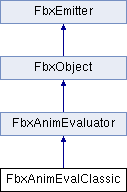
\includegraphics[height=4.000000cm]{class_fbx_anim_eval_classic}
\end{center}
\end{figure}
\subsection*{限定公開メンバ関数}
\begin{DoxyCompactItemize}
\item 
virtual void \hyperlink{class_fbx_anim_eval_classic_a9b0ca916c170485271aa2ba23d38019a}{Construct} (const \hyperlink{class_fbx_object}{Fbx\+Object} $\ast$p\+From)
\item 
virtual void \hyperlink{class_fbx_anim_eval_classic_a308a42f3bd439a3e36f3b5171d5fc092}{Destruct} (bool p\+Recursive)
\item 
virtual void \hyperlink{class_fbx_anim_eval_classic_a83f7c6d89964e4ff48e7ad2d325a1eac}{Evaluate\+Node\+Transform} (\hyperlink{class_fbx_node_eval_state}{Fbx\+Node\+Eval\+State} $\ast$p\+Result, \hyperlink{class_fbx_node}{Fbx\+Node} $\ast$p\+Node, const \hyperlink{class_fbx_time}{Fbx\+Time} \&p\+Time, \hyperlink{class_fbx_node_ae62b7311ac4727654cdf1ebd5cbf7343}{Fbx\+Node\+::\+E\+Pivot\+Set} p\+Pivot\+Set, bool p\+Apply\+Target)
\item 
virtual void \hyperlink{class_fbx_anim_eval_classic_a3618b50c5fd35f18f5e6f873ca07cf2e}{Evaluate\+Property\+Value} (\hyperlink{class_fbx_property_eval_state}{Fbx\+Property\+Eval\+State} $\ast$p\+Result, \hyperlink{class_fbx_property}{Fbx\+Property} \&p\+Property, const \hyperlink{class_fbx_time}{Fbx\+Time} \&p\+Time)
\end{DoxyCompactItemize}
\subsection*{その他の継承メンバ}


\subsection{詳解}
An evaluator implementation that behaves like the original F\+BX S\+DK (2010 and previous) evaluation system.

It works by implementing the abstract class \hyperlink{class_fbx_anim_evaluator}{Fbx\+Anim\+Evaluator}, which is used as the main interface for evaluators. \begin{DoxyNote}{覚え書き}
While this class can be instanced at any time, it is preferable to access the evaluator via the function Fbx\+Scene\+::\+Get\+Evaluator(), which will automatically return the default evaluator used in the current F\+BX S\+DK. This is very useful because it will allow the user to use the very same evaluator used by the F\+BX S\+DK internally. 
\end{DoxyNote}
\begin{DoxySeeAlso}{参照}
\hyperlink{class_fbx_anim_evaluator}{Fbx\+Anim\+Evaluator}, \hyperlink{class_fbx_scene}{Fbx\+Scene} 
\end{DoxySeeAlso}


 fbxanimevalclassic.\+h の 32 行目に定義があります。



\subsection{関数詳解}
\mbox{\Hypertarget{class_fbx_anim_eval_classic_a9b0ca916c170485271aa2ba23d38019a}\label{class_fbx_anim_eval_classic_a9b0ca916c170485271aa2ba23d38019a}} 
\index{Fbx\+Anim\+Eval\+Classic@{Fbx\+Anim\+Eval\+Classic}!Construct@{Construct}}
\index{Construct@{Construct}!Fbx\+Anim\+Eval\+Classic@{Fbx\+Anim\+Eval\+Classic}}
\subsubsection{\texorpdfstring{Construct()}{Construct()}}
{\footnotesize\ttfamily virtual void Fbx\+Anim\+Eval\+Classic\+::\+Construct (\begin{DoxyParamCaption}\item[{const \hyperlink{class_fbx_object}{Fbx\+Object} $\ast$}]{p\+From }\end{DoxyParamCaption})\hspace{0.3cm}{\ttfamily [protected]}, {\ttfamily [virtual]}}

Optional constructor override, automatically called by default constructor. 
\begin{DoxyParams}{引数}
{\em p\+From} & If not null, the function must take it into account like a copy constructor. \\
\hline
\end{DoxyParams}
\begin{DoxyRemark}{注釈}
In case it is decided to override this function, do not forget to call Parent\+Class\+::\+Construct(p\+From) at the beginning. 
\end{DoxyRemark}


\hyperlink{class_fbx_anim_evaluator_a9f167a7fd55aa593d191fdf014c1b3bd}{Fbx\+Anim\+Evaluator}を再実装しています。

\mbox{\Hypertarget{class_fbx_anim_eval_classic_a308a42f3bd439a3e36f3b5171d5fc092}\label{class_fbx_anim_eval_classic_a308a42f3bd439a3e36f3b5171d5fc092}} 
\index{Fbx\+Anim\+Eval\+Classic@{Fbx\+Anim\+Eval\+Classic}!Destruct@{Destruct}}
\index{Destruct@{Destruct}!Fbx\+Anim\+Eval\+Classic@{Fbx\+Anim\+Eval\+Classic}}
\subsubsection{\texorpdfstring{Destruct()}{Destruct()}}
{\footnotesize\ttfamily virtual void Fbx\+Anim\+Eval\+Classic\+::\+Destruct (\begin{DoxyParamCaption}\item[{bool}]{p\+Recursive }\end{DoxyParamCaption})\hspace{0.3cm}{\ttfamily [protected]}, {\ttfamily [virtual]}}

Optional destructor override, automatically called by default destructor. 
\begin{DoxyParams}{引数}
{\em p\+Recursive} & If true, children objects should be destroyed as well. \\
\hline
\end{DoxyParams}
\begin{DoxyRemark}{注釈}
In case it is decided to override this function, do not forget to call Parent\+Class\+::\+Destruct(p\+Resursive) at the end. 
\end{DoxyRemark}


\hyperlink{class_fbx_anim_evaluator_ac425dd202ceb6c0e5adfc86d8c901dd0}{Fbx\+Anim\+Evaluator}を再実装しています。

\mbox{\Hypertarget{class_fbx_anim_eval_classic_a83f7c6d89964e4ff48e7ad2d325a1eac}\label{class_fbx_anim_eval_classic_a83f7c6d89964e4ff48e7ad2d325a1eac}} 
\index{Fbx\+Anim\+Eval\+Classic@{Fbx\+Anim\+Eval\+Classic}!Evaluate\+Node\+Transform@{Evaluate\+Node\+Transform}}
\index{Evaluate\+Node\+Transform@{Evaluate\+Node\+Transform}!Fbx\+Anim\+Eval\+Classic@{Fbx\+Anim\+Eval\+Classic}}
\subsubsection{\texorpdfstring{Evaluate\+Node\+Transform()}{EvaluateNodeTransform()}}
{\footnotesize\ttfamily virtual void Fbx\+Anim\+Eval\+Classic\+::\+Evaluate\+Node\+Transform (\begin{DoxyParamCaption}\item[{\hyperlink{class_fbx_node_eval_state}{Fbx\+Node\+Eval\+State} $\ast$}]{p\+Result,  }\item[{\hyperlink{class_fbx_node}{Fbx\+Node} $\ast$}]{p\+Node,  }\item[{const \hyperlink{class_fbx_time}{Fbx\+Time} \&}]{p\+Time,  }\item[{\hyperlink{class_fbx_node_ae62b7311ac4727654cdf1ebd5cbf7343}{Fbx\+Node\+::\+E\+Pivot\+Set}}]{p\+Pivot\+Set,  }\item[{bool}]{p\+Apply\+Target }\end{DoxyParamCaption})\hspace{0.3cm}{\ttfamily [protected]}, {\ttfamily [virtual]}}



\hyperlink{class_fbx_anim_evaluator_a6de6ef5ab77169192cd39baf76f14037}{Fbx\+Anim\+Evaluator}を実装しています。

\mbox{\Hypertarget{class_fbx_anim_eval_classic_a3618b50c5fd35f18f5e6f873ca07cf2e}\label{class_fbx_anim_eval_classic_a3618b50c5fd35f18f5e6f873ca07cf2e}} 
\index{Fbx\+Anim\+Eval\+Classic@{Fbx\+Anim\+Eval\+Classic}!Evaluate\+Property\+Value@{Evaluate\+Property\+Value}}
\index{Evaluate\+Property\+Value@{Evaluate\+Property\+Value}!Fbx\+Anim\+Eval\+Classic@{Fbx\+Anim\+Eval\+Classic}}
\subsubsection{\texorpdfstring{Evaluate\+Property\+Value()}{EvaluatePropertyValue()}}
{\footnotesize\ttfamily virtual void Fbx\+Anim\+Eval\+Classic\+::\+Evaluate\+Property\+Value (\begin{DoxyParamCaption}\item[{\hyperlink{class_fbx_property_eval_state}{Fbx\+Property\+Eval\+State} $\ast$}]{p\+Result,  }\item[{\hyperlink{class_fbx_property}{Fbx\+Property} \&}]{p\+Property,  }\item[{const \hyperlink{class_fbx_time}{Fbx\+Time} \&}]{p\+Time }\end{DoxyParamCaption})\hspace{0.3cm}{\ttfamily [protected]}, {\ttfamily [virtual]}}



\hyperlink{class_fbx_anim_evaluator_aa29759ee76b1cbb0ced4fee1508d5d84}{Fbx\+Anim\+Evaluator}を実装しています。



このクラス詳解は次のファイルから抽出されました\+:\begin{DoxyCompactItemize}
\item 
C\+:/\+Maya/scripts/\+F\+B\+X\+\_\+\+S\+D\+K/2017.\+1/include/fbxsdk/scene/animation/\hyperlink{fbxanimevalclassic_8h}{fbxanimevalclassic.\+h}\end{DoxyCompactItemize}

\hypertarget{class_fbx_anim_eval_state}{}\section{Fbx\+Anim\+Eval\+State クラス}
\label{class_fbx_anim_eval_state}\index{Fbx\+Anim\+Eval\+State@{Fbx\+Anim\+Eval\+State}}


{\ttfamily \#include $<$fbxanimevalstate.\+h$>$}

\subsection*{公開メンバ関数}
\begin{DoxyCompactItemize}
\item 
\hyperlink{class_fbx_time}{Fbx\+Time} \hyperlink{class_fbx_anim_eval_state_ad6674f0c37ecd45c15dcfbc220f8faff}{Get\+Time} () const
\item 
void \hyperlink{class_fbx_anim_eval_state_a34be9a999fc7dfa426307b4778a50344}{Reset} ()
\item 
void \hyperlink{class_fbx_anim_eval_state_aff48b77374c628e0e5e02d0dcb5aee55}{Begin} (const \hyperlink{class_fbx_time}{Fbx\+Time} \&p\+Time)
\item 
void \hyperlink{class_fbx_anim_eval_state_a7e647a8391cf8f0356e38e0fd86f5310}{Flush} (\hyperlink{class_fbx_node}{Fbx\+Node} $\ast$p\+Node)
\item 
void \hyperlink{class_fbx_anim_eval_state_aaeebbdfac04c6dbe42c992bc484698c3}{Flush} (\hyperlink{class_fbx_property}{Fbx\+Property} \&p\+Property)
\item 
\hyperlink{class_fbx_node_eval_state}{Fbx\+Node\+Eval\+State} $\ast$ \hyperlink{class_fbx_anim_eval_state_a2aedc029a4b2870a2d2112111a450ded}{Get\+Node\+Eval\+State} (\hyperlink{class_fbx_node}{Fbx\+Node} $\ast$p\+Node)
\item 
\hyperlink{class_fbx_property_eval_state}{Fbx\+Property\+Eval\+State} $\ast$ \hyperlink{class_fbx_anim_eval_state_a43703fd0f0799332d5840a6f4b549081}{Get\+Property\+Eval\+State} (\hyperlink{class_fbx_property}{Fbx\+Property} \&p\+Property)
\item 
\hyperlink{class_fbx_anim_curve_node}{Fbx\+Anim\+Curve\+Node} $\ast$ \hyperlink{class_fbx_anim_eval_state_aa8ad680f208af36dd8f7864cf3449217}{Get\+Property\+Curve\+Node} (\hyperlink{class_fbx_property}{Fbx\+Property} \&p\+Property, \hyperlink{class_fbx_anim_layer}{Fbx\+Anim\+Layer} $\ast$p\+Anim\+Layer)
\item 
\hyperlink{class_fbx_anim_eval_state_a580a41fcddf592e7c4466a26648392c1}{Fbx\+Anim\+Eval\+State} ()
\item 
virtual \hyperlink{class_fbx_anim_eval_state_a571cadbab0fda535e1b0a5f650307342}{$\sim$\+Fbx\+Anim\+Eval\+State} ()
\end{DoxyCompactItemize}


\subsection{詳解}
This class hold results from animation evaluations. To clear an evaluation state for re-\/use, it is possible to invalidate or to reset it. For the same scene with the same objects, invalidating an evaluation state is the quickest way to clear an evaluation state object for re-\/use because it only zeroes all the entries. A reset will delete all the entries. Unless the scene changes, for performance purposes it is recommended to invalidate evaluation states instead of resetting them. 

\subsection{構築子と解体子}
\mbox{\Hypertarget{class_fbx_anim_eval_state_a580a41fcddf592e7c4466a26648392c1}\label{class_fbx_anim_eval_state_a580a41fcddf592e7c4466a26648392c1}} 
\index{Fbx\+Anim\+Eval\+State@{Fbx\+Anim\+Eval\+State}!Fbx\+Anim\+Eval\+State@{Fbx\+Anim\+Eval\+State}}
\index{Fbx\+Anim\+Eval\+State@{Fbx\+Anim\+Eval\+State}!Fbx\+Anim\+Eval\+State@{Fbx\+Anim\+Eval\+State}}
\subsubsection{\texorpdfstring{Fbx\+Anim\+Eval\+State()}{FbxAnimEvalState()}}
{\footnotesize\ttfamily Fbx\+Anim\+Eval\+State\+::\+Fbx\+Anim\+Eval\+State (\begin{DoxyParamCaption}{ }\end{DoxyParamCaption})}

\mbox{\Hypertarget{class_fbx_anim_eval_state_a571cadbab0fda535e1b0a5f650307342}\label{class_fbx_anim_eval_state_a571cadbab0fda535e1b0a5f650307342}} 
\index{Fbx\+Anim\+Eval\+State@{Fbx\+Anim\+Eval\+State}!````~Fbx\+Anim\+Eval\+State@{$\sim$\+Fbx\+Anim\+Eval\+State}}
\index{````~Fbx\+Anim\+Eval\+State@{$\sim$\+Fbx\+Anim\+Eval\+State}!Fbx\+Anim\+Eval\+State@{Fbx\+Anim\+Eval\+State}}
\subsubsection{\texorpdfstring{$\sim$\+Fbx\+Anim\+Eval\+State()}{~FbxAnimEvalState()}}
{\footnotesize\ttfamily virtual Fbx\+Anim\+Eval\+State\+::$\sim$\+Fbx\+Anim\+Eval\+State (\begin{DoxyParamCaption}{ }\end{DoxyParamCaption})\hspace{0.3cm}{\ttfamily [virtual]}}



\subsection{メソッド詳解}
\mbox{\Hypertarget{class_fbx_anim_eval_state_aff48b77374c628e0e5e02d0dcb5aee55}\label{class_fbx_anim_eval_state_aff48b77374c628e0e5e02d0dcb5aee55}} 
\index{Fbx\+Anim\+Eval\+State@{Fbx\+Anim\+Eval\+State}!Begin@{Begin}}
\index{Begin@{Begin}!Fbx\+Anim\+Eval\+State@{Fbx\+Anim\+Eval\+State}}
\subsubsection{\texorpdfstring{Begin()}{Begin()}}
{\footnotesize\ttfamily void Fbx\+Anim\+Eval\+State\+::\+Begin (\begin{DoxyParamCaption}\item[{const \hyperlink{class_fbx_time}{Fbx\+Time} \&}]{p\+Time }\end{DoxyParamCaption})}

Start a new evaluation state frame by zeroing the cache it contains, and changing its associated time. All node and property entries will remain in the list, but their evaluation state will not be up-\/to-\/date. 
\begin{DoxyParams}{引数}
{\em p\+Time} & The time at which the evaluation state should be set after the invalidation. \\
\hline
\end{DoxyParams}
\mbox{\Hypertarget{class_fbx_anim_eval_state_a7e647a8391cf8f0356e38e0fd86f5310}\label{class_fbx_anim_eval_state_a7e647a8391cf8f0356e38e0fd86f5310}} 
\index{Fbx\+Anim\+Eval\+State@{Fbx\+Anim\+Eval\+State}!Flush@{Flush}}
\index{Flush@{Flush}!Fbx\+Anim\+Eval\+State@{Fbx\+Anim\+Eval\+State}}
\subsubsection{\texorpdfstring{Flush()}{Flush()}\hspace{0.1cm}{\footnotesize\ttfamily [1/2]}}
{\footnotesize\ttfamily void Fbx\+Anim\+Eval\+State\+::\+Flush (\begin{DoxyParamCaption}\item[{\hyperlink{class_fbx_node}{Fbx\+Node} $\ast$}]{p\+Node }\end{DoxyParamCaption})}

Invalidate a node evaluation state to force update on next evaluation. 
\begin{DoxyParams}{引数}
{\em p\+Node} & The node that needs to be updated on next evaluation. \\
\hline
\end{DoxyParams}
\mbox{\Hypertarget{class_fbx_anim_eval_state_aaeebbdfac04c6dbe42c992bc484698c3}\label{class_fbx_anim_eval_state_aaeebbdfac04c6dbe42c992bc484698c3}} 
\index{Fbx\+Anim\+Eval\+State@{Fbx\+Anim\+Eval\+State}!Flush@{Flush}}
\index{Flush@{Flush}!Fbx\+Anim\+Eval\+State@{Fbx\+Anim\+Eval\+State}}
\subsubsection{\texorpdfstring{Flush()}{Flush()}\hspace{0.1cm}{\footnotesize\ttfamily [2/2]}}
{\footnotesize\ttfamily void Fbx\+Anim\+Eval\+State\+::\+Flush (\begin{DoxyParamCaption}\item[{\hyperlink{class_fbx_property}{Fbx\+Property} \&}]{p\+Property }\end{DoxyParamCaption})}

Invalidate a property evaluation state to force update on next evaluation. 
\begin{DoxyParams}{引数}
{\em p\+Property} & The property that needs to be updated on next evaluation. \\
\hline
\end{DoxyParams}
\mbox{\Hypertarget{class_fbx_anim_eval_state_a2aedc029a4b2870a2d2112111a450ded}\label{class_fbx_anim_eval_state_a2aedc029a4b2870a2d2112111a450ded}} 
\index{Fbx\+Anim\+Eval\+State@{Fbx\+Anim\+Eval\+State}!Get\+Node\+Eval\+State@{Get\+Node\+Eval\+State}}
\index{Get\+Node\+Eval\+State@{Get\+Node\+Eval\+State}!Fbx\+Anim\+Eval\+State@{Fbx\+Anim\+Eval\+State}}
\subsubsection{\texorpdfstring{Get\+Node\+Eval\+State()}{GetNodeEvalState()}}
{\footnotesize\ttfamily \hyperlink{class_fbx_node_eval_state}{Fbx\+Node\+Eval\+State}$\ast$ Fbx\+Anim\+Eval\+State\+::\+Get\+Node\+Eval\+State (\begin{DoxyParamCaption}\item[{\hyperlink{class_fbx_node}{Fbx\+Node} $\ast$}]{p\+Node }\end{DoxyParamCaption})}

Get node transform evaluation result from the evaluation state. 
\begin{DoxyParams}{引数}
{\em p\+Node} & The node for which the value was stored. \\
\hline
\end{DoxyParams}
\begin{DoxyReturn}{戻り値}
The global or local matrix transform for the specified node. 
\end{DoxyReturn}
\mbox{\Hypertarget{class_fbx_anim_eval_state_aa8ad680f208af36dd8f7864cf3449217}\label{class_fbx_anim_eval_state_aa8ad680f208af36dd8f7864cf3449217}} 
\index{Fbx\+Anim\+Eval\+State@{Fbx\+Anim\+Eval\+State}!Get\+Property\+Curve\+Node@{Get\+Property\+Curve\+Node}}
\index{Get\+Property\+Curve\+Node@{Get\+Property\+Curve\+Node}!Fbx\+Anim\+Eval\+State@{Fbx\+Anim\+Eval\+State}}
\subsubsection{\texorpdfstring{Get\+Property\+Curve\+Node()}{GetPropertyCurveNode()}}
{\footnotesize\ttfamily \hyperlink{class_fbx_anim_curve_node}{Fbx\+Anim\+Curve\+Node}$\ast$ Fbx\+Anim\+Eval\+State\+::\+Get\+Property\+Curve\+Node (\begin{DoxyParamCaption}\item[{\hyperlink{class_fbx_property}{Fbx\+Property} \&}]{p\+Property,  }\item[{\hyperlink{class_fbx_anim_layer}{Fbx\+Anim\+Layer} $\ast$}]{p\+Anim\+Layer }\end{DoxyParamCaption})}

Get a property curve node from the evaluation state for quick access. 
\begin{DoxyParams}{引数}
{\em p\+Property} & The property to search for its animation curve node. \\
\hline
{\em p\+Anim\+Layer} & The animation layer on which the animation curve node must be searched. \\
\hline
\end{DoxyParams}
\begin{DoxyRemark}{注釈}
This function uses a map to store animation curve node search results. If animation curve nodes are replaced, the evaluation state must be reset. 
\end{DoxyRemark}
\mbox{\Hypertarget{class_fbx_anim_eval_state_a43703fd0f0799332d5840a6f4b549081}\label{class_fbx_anim_eval_state_a43703fd0f0799332d5840a6f4b549081}} 
\index{Fbx\+Anim\+Eval\+State@{Fbx\+Anim\+Eval\+State}!Get\+Property\+Eval\+State@{Get\+Property\+Eval\+State}}
\index{Get\+Property\+Eval\+State@{Get\+Property\+Eval\+State}!Fbx\+Anim\+Eval\+State@{Fbx\+Anim\+Eval\+State}}
\subsubsection{\texorpdfstring{Get\+Property\+Eval\+State()}{GetPropertyEvalState()}}
{\footnotesize\ttfamily \hyperlink{class_fbx_property_eval_state}{Fbx\+Property\+Eval\+State}$\ast$ Fbx\+Anim\+Eval\+State\+::\+Get\+Property\+Eval\+State (\begin{DoxyParamCaption}\item[{\hyperlink{class_fbx_property}{Fbx\+Property} \&}]{p\+Property }\end{DoxyParamCaption})}

Get a property evaluation result from the evaluation state. 
\begin{DoxyParams}{引数}
{\em p\+Property} & The property for which the value was stored. \\
\hline
\end{DoxyParams}
\begin{DoxyReturn}{戻り値}
The result value that was stored. 
\end{DoxyReturn}
\mbox{\Hypertarget{class_fbx_anim_eval_state_ad6674f0c37ecd45c15dcfbc220f8faff}\label{class_fbx_anim_eval_state_ad6674f0c37ecd45c15dcfbc220f8faff}} 
\index{Fbx\+Anim\+Eval\+State@{Fbx\+Anim\+Eval\+State}!Get\+Time@{Get\+Time}}
\index{Get\+Time@{Get\+Time}!Fbx\+Anim\+Eval\+State@{Fbx\+Anim\+Eval\+State}}
\subsubsection{\texorpdfstring{Get\+Time()}{GetTime()}}
{\footnotesize\ttfamily \hyperlink{class_fbx_time}{Fbx\+Time} Fbx\+Anim\+Eval\+State\+::\+Get\+Time (\begin{DoxyParamCaption}{ }\end{DoxyParamCaption}) const}

Get the time associated with this evaluation state. \begin{DoxyReturn}{戻り値}
The time associated with this evaluation state. 
\end{DoxyReturn}
\mbox{\Hypertarget{class_fbx_anim_eval_state_a34be9a999fc7dfa426307b4778a50344}\label{class_fbx_anim_eval_state_a34be9a999fc7dfa426307b4778a50344}} 
\index{Fbx\+Anim\+Eval\+State@{Fbx\+Anim\+Eval\+State}!Reset@{Reset}}
\index{Reset@{Reset}!Fbx\+Anim\+Eval\+State@{Fbx\+Anim\+Eval\+State}}
\subsubsection{\texorpdfstring{Reset()}{Reset()}}
{\footnotesize\ttfamily void Fbx\+Anim\+Eval\+State\+::\+Reset (\begin{DoxyParamCaption}{ }\end{DoxyParamCaption})}

Reset an evaluation state by deleting the cache it contains. This will remove all entries in the cache. 

このクラス詳解は次のファイルから抽出されました\+:\begin{DoxyCompactItemize}
\item 
C\+:/github/\+F\+B\+Xpython\+S\+D\+K201701/\+F\+B\+Xpython\+S\+D\+K201701/2017.\+1/include/fbxsdk/scene/animation/\hyperlink{fbxanimevalstate_8h}{fbxanimevalstate.\+h}\end{DoxyCompactItemize}

\hypertarget{class_fbx_anim_evaluator}{}\section{Fbx\+Anim\+Evaluator クラス}
\label{class_fbx_anim_evaluator}\index{Fbx\+Anim\+Evaluator@{Fbx\+Anim\+Evaluator}}


{\ttfamily \#include $<$fbxanimevaluator.\+h$>$}

Fbx\+Anim\+Evaluator の継承関係図\begin{figure}[H]
\begin{center}
\leavevmode
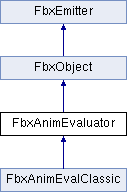
\includegraphics[height=4.000000cm]{class_fbx_anim_evaluator}
\end{center}
\end{figure}
\subsection*{公開メンバ関数}
\begin{DoxyCompactItemize}
\item 
\hyperlink{class_fbx_a_matrix}{Fbx\+A\+Matrix} \& \hyperlink{class_fbx_anim_evaluator_a40d669964d698df2551ee3571c211312}{Get\+Node\+Global\+Transform} (\hyperlink{class_fbx_node}{Fbx\+Node} $\ast$p\+Node, const \hyperlink{class_fbx_time}{Fbx\+Time} \&p\+Time=\hyperlink{fbxtime_8h_a1e6db3fe0f84f0b7daa775739f93526f}{F\+B\+X\+S\+D\+K\+\_\+\+T\+I\+M\+E\+\_\+\+I\+N\+F\+I\+N\+I\+TE}, \hyperlink{class_fbx_node_ae62b7311ac4727654cdf1ebd5cbf7343}{Fbx\+Node\+::\+E\+Pivot\+Set} p\+Pivot\+Set=\hyperlink{class_fbx_node_ae62b7311ac4727654cdf1ebd5cbf7343ae8ed37a5c7e41f8d1cec9d3fa8424b69}{Fbx\+Node\+::e\+Source\+Pivot}, bool p\+Apply\+Target=false, bool p\+Force\+Eval=false)
\item 
\hyperlink{class_fbx_a_matrix}{Fbx\+A\+Matrix} \& \hyperlink{class_fbx_anim_evaluator_a3b451f7466d6730816bf56a3b5441379}{Get\+Node\+Local\+Transform} (\hyperlink{class_fbx_node}{Fbx\+Node} $\ast$p\+Node, const \hyperlink{class_fbx_time}{Fbx\+Time} \&p\+Time=\hyperlink{fbxtime_8h_a1e6db3fe0f84f0b7daa775739f93526f}{F\+B\+X\+S\+D\+K\+\_\+\+T\+I\+M\+E\+\_\+\+I\+N\+F\+I\+N\+I\+TE}, \hyperlink{class_fbx_node_ae62b7311ac4727654cdf1ebd5cbf7343}{Fbx\+Node\+::\+E\+Pivot\+Set} p\+Pivot\+Set=\hyperlink{class_fbx_node_ae62b7311ac4727654cdf1ebd5cbf7343ae8ed37a5c7e41f8d1cec9d3fa8424b69}{Fbx\+Node\+::e\+Source\+Pivot}, bool p\+Apply\+Target=false, bool p\+Force\+Eval=false)
\item 
\hyperlink{class_fbx_vector4}{Fbx\+Vector4} \& \hyperlink{class_fbx_anim_evaluator_a3f430f456d4f093a3c8682a874ec8145}{Get\+Node\+Local\+Translation} (\hyperlink{class_fbx_node}{Fbx\+Node} $\ast$p\+Node, const \hyperlink{class_fbx_time}{Fbx\+Time} \&p\+Time=\hyperlink{fbxtime_8h_a1e6db3fe0f84f0b7daa775739f93526f}{F\+B\+X\+S\+D\+K\+\_\+\+T\+I\+M\+E\+\_\+\+I\+N\+F\+I\+N\+I\+TE}, \hyperlink{class_fbx_node_ae62b7311ac4727654cdf1ebd5cbf7343}{Fbx\+Node\+::\+E\+Pivot\+Set} p\+Pivot\+Set=\hyperlink{class_fbx_node_ae62b7311ac4727654cdf1ebd5cbf7343ae8ed37a5c7e41f8d1cec9d3fa8424b69}{Fbx\+Node\+::e\+Source\+Pivot}, bool p\+Apply\+Target=false, bool p\+Force\+Eval=false)
\item 
\hyperlink{class_fbx_vector4}{Fbx\+Vector4} \& \hyperlink{class_fbx_anim_evaluator_a8ffff0649bfdf67d6508a72f8787d895}{Get\+Node\+Local\+Rotation} (\hyperlink{class_fbx_node}{Fbx\+Node} $\ast$p\+Node, const \hyperlink{class_fbx_time}{Fbx\+Time} \&p\+Time=\hyperlink{fbxtime_8h_a1e6db3fe0f84f0b7daa775739f93526f}{F\+B\+X\+S\+D\+K\+\_\+\+T\+I\+M\+E\+\_\+\+I\+N\+F\+I\+N\+I\+TE}, \hyperlink{class_fbx_node_ae62b7311ac4727654cdf1ebd5cbf7343}{Fbx\+Node\+::\+E\+Pivot\+Set} p\+Pivot\+Set=\hyperlink{class_fbx_node_ae62b7311ac4727654cdf1ebd5cbf7343ae8ed37a5c7e41f8d1cec9d3fa8424b69}{Fbx\+Node\+::e\+Source\+Pivot}, bool p\+Apply\+Target=false, bool p\+Force\+Eval=false)
\item 
\hyperlink{class_fbx_vector4}{Fbx\+Vector4} \& \hyperlink{class_fbx_anim_evaluator_aba31ec4baa8452ad2fcfdc82c85cc127}{Get\+Node\+Local\+Scaling} (\hyperlink{class_fbx_node}{Fbx\+Node} $\ast$p\+Node, const \hyperlink{class_fbx_time}{Fbx\+Time} \&p\+Time=\hyperlink{fbxtime_8h_a1e6db3fe0f84f0b7daa775739f93526f}{F\+B\+X\+S\+D\+K\+\_\+\+T\+I\+M\+E\+\_\+\+I\+N\+F\+I\+N\+I\+TE}, \hyperlink{class_fbx_node_ae62b7311ac4727654cdf1ebd5cbf7343}{Fbx\+Node\+::\+E\+Pivot\+Set} p\+Pivot\+Set=\hyperlink{class_fbx_node_ae62b7311ac4727654cdf1ebd5cbf7343ae8ed37a5c7e41f8d1cec9d3fa8424b69}{Fbx\+Node\+::e\+Source\+Pivot}, bool p\+Apply\+Target=false, bool p\+Force\+Eval=false)
\item 
{\footnotesize template$<$class T $>$ }\\T \hyperlink{class_fbx_anim_evaluator_a49b4a647d33b2ce26b27ba35ddb8a0ed}{Get\+Property\+Value} (\hyperlink{class_fbx_property}{Fbx\+Property} \&p\+Property, const \hyperlink{class_fbx_time}{Fbx\+Time} \&p\+Time, bool p\+Force\+Eval=false)
\item 
\hyperlink{class_fbx_property_value}{Fbx\+Property\+Value} \& \hyperlink{class_fbx_anim_evaluator_a98b68793cbb2d95f499ea2d433dd8c4d}{Get\+Property\+Value} (\hyperlink{class_fbx_property}{Fbx\+Property} \&p\+Property, const \hyperlink{class_fbx_time}{Fbx\+Time} \&p\+Time, bool p\+Force\+Eval=false)
\item 
\hyperlink{class_fbx_anim_curve_node}{Fbx\+Anim\+Curve\+Node} $\ast$ \hyperlink{class_fbx_anim_evaluator_a63f726da981ecfea4fc4f60145bb0f1d}{Get\+Property\+Curve\+Node} (\hyperlink{class_fbx_property}{Fbx\+Property} \&p\+Property, \hyperlink{class_fbx_anim_layer}{Fbx\+Anim\+Layer} $\ast$p\+Anim\+Layer)
\item 
\hyperlink{class_fbx_time}{Fbx\+Time} \hyperlink{class_fbx_anim_evaluator_af5226e1b2bc178417980b746c34888e4}{Validate\+Time} (const \hyperlink{class_fbx_time}{Fbx\+Time} \&p\+Time)
\item 
void \hyperlink{class_fbx_anim_evaluator_a95c636f04474f350c3a1eda55ded8b29}{Reset} ()
\item 
void \hyperlink{class_fbx_anim_evaluator_a17b08c51a766be597aac881807913ea8}{Flush} (\hyperlink{class_fbx_node}{Fbx\+Node} $\ast$p\+Node)
\item 
void \hyperlink{class_fbx_anim_evaluator_a2f738a737153248cc988aca609c4bf84}{Flush} (\hyperlink{class_fbx_property}{Fbx\+Property} \&p\+Property)
\item 
void \hyperlink{class_fbx_anim_evaluator_a7ffe74bd370dfef23e5c1dd88b334e3d}{Compute\+Local\+T\+R\+S\+From\+Global} (\hyperlink{class_fbx_vector4}{Fbx\+Vector4} \&p\+Ret\+LT, \hyperlink{class_fbx_vector4}{Fbx\+Vector4} \&p\+Ret\+LR, \hyperlink{class_fbx_vector4}{Fbx\+Vector4} \&p\+Ret\+LS, \hyperlink{class_fbx_node}{Fbx\+Node} $\ast$p\+Node, \hyperlink{class_fbx_a_matrix}{Fbx\+A\+Matrix} \&p\+GX, const \hyperlink{class_fbx_time}{Fbx\+Time} \&p\+Time=\hyperlink{fbxtime_8h_a1e6db3fe0f84f0b7daa775739f93526f}{F\+B\+X\+S\+D\+K\+\_\+\+T\+I\+M\+E\+\_\+\+I\+N\+F\+I\+N\+I\+TE}, \hyperlink{class_fbx_node_ae62b7311ac4727654cdf1ebd5cbf7343}{Fbx\+Node\+::\+E\+Pivot\+Set} p\+Pivot\+Set=\hyperlink{class_fbx_node_ae62b7311ac4727654cdf1ebd5cbf7343ae8ed37a5c7e41f8d1cec9d3fa8424b69}{Fbx\+Node\+::e\+Source\+Pivot}, bool p\+Apply\+Target=false, bool p\+Force\+Eval=false)
\end{DoxyCompactItemize}
\subsection*{限定公開メンバ関数}
\begin{DoxyCompactItemize}
\item 
virtual void \hyperlink{class_fbx_anim_evaluator_a9f167a7fd55aa593d191fdf014c1b3bd}{Construct} (const \hyperlink{class_fbx_object}{Fbx\+Object} $\ast$p\+From)
\item 
virtual void \hyperlink{class_fbx_anim_evaluator_ac425dd202ceb6c0e5adfc86d8c901dd0}{Destruct} (bool p\+Recursive)
\item 
virtual void \hyperlink{class_fbx_anim_evaluator_a6de6ef5ab77169192cd39baf76f14037}{Evaluate\+Node\+Transform} (\hyperlink{class_fbx_node_eval_state}{Fbx\+Node\+Eval\+State} $\ast$p\+Result, \hyperlink{class_fbx_node}{Fbx\+Node} $\ast$p\+Node, const \hyperlink{class_fbx_time}{Fbx\+Time} \&p\+Time, \hyperlink{class_fbx_node_ae62b7311ac4727654cdf1ebd5cbf7343}{Fbx\+Node\+::\+E\+Pivot\+Set} p\+Pivot\+Set, bool p\+Apply\+Target)=0
\item 
virtual void \hyperlink{class_fbx_anim_evaluator_aa29759ee76b1cbb0ced4fee1508d5d84}{Evaluate\+Property\+Value} (\hyperlink{class_fbx_property_eval_state}{Fbx\+Property\+Eval\+State} $\ast$p\+Result, \hyperlink{class_fbx_property}{Fbx\+Property} \&p\+Property, const \hyperlink{class_fbx_time}{Fbx\+Time} \&p\+Time)=0
\item 
\hyperlink{class_fbx_anim_eval_state}{Fbx\+Anim\+Eval\+State} $\ast$ \hyperlink{class_fbx_anim_evaluator_a0e222bee0038d2324e38a996cc40527e}{Get\+Default\+Eval\+State} ()
\item 
\hyperlink{class_fbx_anim_eval_state}{Fbx\+Anim\+Eval\+State} $\ast$ \hyperlink{class_fbx_anim_evaluator_ae09fad8424850027d8534845dc3f950d}{Get\+Eval\+State} (const \hyperlink{class_fbx_time}{Fbx\+Time} \&p\+Time)
\item 
\hyperlink{class_fbx_node_eval_state}{Fbx\+Node\+Eval\+State} $\ast$ \hyperlink{class_fbx_anim_evaluator_adf64b2948f34228e9723939c9347474c}{Get\+Node\+Eval\+State} (\hyperlink{class_fbx_node}{Fbx\+Node} $\ast$p\+Node, const \hyperlink{class_fbx_time}{Fbx\+Time} \&p\+Time, \hyperlink{class_fbx_node_ae62b7311ac4727654cdf1ebd5cbf7343}{Fbx\+Node\+::\+E\+Pivot\+Set} p\+Pivot\+Set, bool p\+Apply\+Target, bool p\+Force\+Eval)
\item 
\hyperlink{class_fbx_property_eval_state}{Fbx\+Property\+Eval\+State} $\ast$ \hyperlink{class_fbx_anim_evaluator_a20ef23a07b86771090c64ec5f3cc7ced}{Get\+Property\+Eval\+State} (\hyperlink{class_fbx_property}{Fbx\+Property} \&p\+Property, const \hyperlink{class_fbx_time}{Fbx\+Time} \&p\+Time, bool p\+Force\+Eval)
\end{DoxyCompactItemize}
\subsection*{その他の継承メンバ}


\subsection{詳解}
The principal interface for animation evaluators. The animation evaluator is used to compute node transforms and property values at specific times during an animation. Evaluators simplify the process of computing transform matrices by taking into account all of the parameters, such as pre-\/ and post-\/rotations. This class is abstract so that S\+DK users can implement their own evaluator if needed. The default evaluator used by the F\+BX S\+DK is a \hyperlink{class_fbx_anim_eval_classic}{Fbx\+Anim\+Eval\+Classic}. The default evaluator can be queried with the function Fbx\+Scene\+::\+Get\+Evaluator(), and can be changed using Fbx\+Scene\+::\+Set\+Evaluator().

When working with scene nodes, the evaluator will always return an affine transform matrix that contains the translation, rotation and scale of that node.

When working with object properties, the evaluator will always return a structure that can contain as many components as the property can have. For example, an R\+GB color property would return a structure containing 3 channels. The class \hyperlink{class_fbx_anim_curve_node}{Fbx\+Anim\+Curve\+Node} is used as a data container to store those values, because it can handle as many channels as needed, even if the property is not a real curve node .

Below is a typical usage of the evaluator class to retrieve the global transform matrix of each node in a scene\+: 
\begin{DoxyCode}
\textcolor{comment}{//Here we assume the user already imported a scene...}
\textcolor{keywordflow}{for}( \textcolor{keywordtype}{int} i = 0, c = MyScene->GetMemberCount(FbxNode::ClassId); i < c; ++i )
\{
    \hyperlink{class_fbx_node}{FbxNode}* CurrentNode = MyScene->GetMember(FbxNode::ClassId, i);
    \hyperlink{class_fbx_a_matrix}{FbxAMatrix}& NodeGlobalTransform = MyScene->GetEvaluator()->GetNodeGlobalTransform(CurrentNode
      );
\}

\textcolor{comment}{//There is an equivalent call to retrieve a node's global transform, which is exactly the same as calling
       Scene->GetEvaluator() :}
\hyperlink{class_fbx_a_matrix}{FbxAMatrix}& NodeGlobalTransform = CurrentNode->\hyperlink{class_fbx_node_a534da99b3ad911158013482a1b08f630}{EvaluateGlobalTransform}();
\end{DoxyCode}


Another typical usage of the evaluator class, but this time to retrieve the value of an animated color property on a material\+: 
\begin{DoxyCode}
\textcolor{comment}{//Assuming the user imported a scene with objects and materials...}
\hyperlink{class_fbx_color}{FbxColor} Color = MyMaterial->GetDiffuseColor()->EvaluateValue();
\end{DoxyCode}


\begin{DoxyNote}{覚え書き}
Note that all the methods to retrieve global/local matrices as well as property values returns references. This is important for performance purposes, to prevent an extra memory copy. 
\end{DoxyNote}
\begin{DoxySeeAlso}{参照}
\hyperlink{class_fbx_scene}{Fbx\+Scene}, \hyperlink{class_fbx_anim_eval_classic}{Fbx\+Anim\+Eval\+Classic}, \hyperlink{class_fbx_anim_curve_node}{Fbx\+Anim\+Curve\+Node} 
\end{DoxySeeAlso}


 fbxanimevaluator.\+h の 61 行目に定義があります。



\subsection{関数詳解}
\mbox{\Hypertarget{class_fbx_anim_evaluator_a7ffe74bd370dfef23e5c1dd88b334e3d}\label{class_fbx_anim_evaluator_a7ffe74bd370dfef23e5c1dd88b334e3d}} 
\index{Fbx\+Anim\+Evaluator@{Fbx\+Anim\+Evaluator}!Compute\+Local\+T\+R\+S\+From\+Global@{Compute\+Local\+T\+R\+S\+From\+Global}}
\index{Compute\+Local\+T\+R\+S\+From\+Global@{Compute\+Local\+T\+R\+S\+From\+Global}!Fbx\+Anim\+Evaluator@{Fbx\+Anim\+Evaluator}}
\subsubsection{\texorpdfstring{Compute\+Local\+T\+R\+S\+From\+Global()}{ComputeLocalTRSFromGlobal()}}
{\footnotesize\ttfamily void Fbx\+Anim\+Evaluator\+::\+Compute\+Local\+T\+R\+S\+From\+Global (\begin{DoxyParamCaption}\item[{\hyperlink{class_fbx_vector4}{Fbx\+Vector4} \&}]{p\+Ret\+LT,  }\item[{\hyperlink{class_fbx_vector4}{Fbx\+Vector4} \&}]{p\+Ret\+LR,  }\item[{\hyperlink{class_fbx_vector4}{Fbx\+Vector4} \&}]{p\+Ret\+LS,  }\item[{\hyperlink{class_fbx_node}{Fbx\+Node} $\ast$}]{p\+Node,  }\item[{\hyperlink{class_fbx_a_matrix}{Fbx\+A\+Matrix} \&}]{p\+GX,  }\item[{const \hyperlink{class_fbx_time}{Fbx\+Time} \&}]{p\+Time = {\ttfamily \hyperlink{fbxtime_8h_a1e6db3fe0f84f0b7daa775739f93526f}{F\+B\+X\+S\+D\+K\+\_\+\+T\+I\+M\+E\+\_\+\+I\+N\+F\+I\+N\+I\+TE}},  }\item[{\hyperlink{class_fbx_node_ae62b7311ac4727654cdf1ebd5cbf7343}{Fbx\+Node\+::\+E\+Pivot\+Set}}]{p\+Pivot\+Set = {\ttfamily \hyperlink{class_fbx_node_ae62b7311ac4727654cdf1ebd5cbf7343ae8ed37a5c7e41f8d1cec9d3fa8424b69}{Fbx\+Node\+::e\+Source\+Pivot}},  }\item[{bool}]{p\+Apply\+Target = {\ttfamily false},  }\item[{bool}]{p\+Force\+Eval = {\ttfamily false} }\end{DoxyParamCaption})}

Compute node local T\+RS from global transform. Doesn\textquotesingle{}t change cached state for current time. 
\begin{DoxyParams}[1]{引数}
\mbox{\tt out}  & {\em p\+Ret\+LT} & Computed local translation. \\
\hline
\mbox{\tt out}  & {\em p\+Ret\+LR} & Computed local rotation. \\
\hline
\mbox{\tt out}  & {\em p\+Ret\+LS} & Computed local scaling. \\
\hline
 & {\em p\+Node} & The transform node to evaluate. \\
\hline
 & {\em p\+GX} & Global transformation state. \\
\hline
 & {\em p\+Time} & The time used for evaluate.\+If F\+B\+X\+S\+D\+K\+\_\+\+T\+I\+M\+E\+\_\+\+I\+N\+F\+I\+N\+I\+TE is used, this returns the default value, without animation curves evaluation. \\
\hline
 & {\em p\+Pivot\+Set} & The pivot set to take into account. \\
\hline
 & {\em p\+Apply\+Target} & Applies the necessary transform to align into the target node. \\
\hline
 & {\em p\+Force\+Eval} & Force the evaluator to refresh the evaluation state cache even if its already up-\/to-\/date. \\
\hline
\end{DoxyParams}
\mbox{\Hypertarget{class_fbx_anim_evaluator_a9f167a7fd55aa593d191fdf014c1b3bd}\label{class_fbx_anim_evaluator_a9f167a7fd55aa593d191fdf014c1b3bd}} 
\index{Fbx\+Anim\+Evaluator@{Fbx\+Anim\+Evaluator}!Construct@{Construct}}
\index{Construct@{Construct}!Fbx\+Anim\+Evaluator@{Fbx\+Anim\+Evaluator}}
\subsubsection{\texorpdfstring{Construct()}{Construct()}}
{\footnotesize\ttfamily virtual void Fbx\+Anim\+Evaluator\+::\+Construct (\begin{DoxyParamCaption}\item[{const \hyperlink{class_fbx_object}{Fbx\+Object} $\ast$}]{p\+From }\end{DoxyParamCaption})\hspace{0.3cm}{\ttfamily [protected]}, {\ttfamily [virtual]}}

Optional constructor override, automatically called by default constructor. 
\begin{DoxyParams}{引数}
{\em p\+From} & If not null, the function must take it into account like a copy constructor. \\
\hline
\end{DoxyParams}
\begin{DoxyRemark}{注釈}
In case it is decided to override this function, do not forget to call Parent\+Class\+::\+Construct(p\+From) at the beginning. 
\end{DoxyRemark}


\hyperlink{class_fbx_object_a313503bc645af3fdceb4a99ef5cea7eb}{Fbx\+Object}を再実装しています。



\hyperlink{class_fbx_anim_eval_classic_a9b0ca916c170485271aa2ba23d38019a}{Fbx\+Anim\+Eval\+Classic}で再実装されています。

\mbox{\Hypertarget{class_fbx_anim_evaluator_ac425dd202ceb6c0e5adfc86d8c901dd0}\label{class_fbx_anim_evaluator_ac425dd202ceb6c0e5adfc86d8c901dd0}} 
\index{Fbx\+Anim\+Evaluator@{Fbx\+Anim\+Evaluator}!Destruct@{Destruct}}
\index{Destruct@{Destruct}!Fbx\+Anim\+Evaluator@{Fbx\+Anim\+Evaluator}}
\subsubsection{\texorpdfstring{Destruct()}{Destruct()}}
{\footnotesize\ttfamily virtual void Fbx\+Anim\+Evaluator\+::\+Destruct (\begin{DoxyParamCaption}\item[{bool}]{p\+Recursive }\end{DoxyParamCaption})\hspace{0.3cm}{\ttfamily [protected]}, {\ttfamily [virtual]}}

Optional destructor override, automatically called by default destructor. 
\begin{DoxyParams}{引数}
{\em p\+Recursive} & If true, children objects should be destroyed as well. \\
\hline
\end{DoxyParams}
\begin{DoxyRemark}{注釈}
In case it is decided to override this function, do not forget to call Parent\+Class\+::\+Destruct(p\+Resursive) at the end. 
\end{DoxyRemark}


\hyperlink{class_fbx_object_a123e084d9b32b29c28af6384b7c3c608}{Fbx\+Object}を再実装しています。



\hyperlink{class_fbx_anim_eval_classic_a308a42f3bd439a3e36f3b5171d5fc092}{Fbx\+Anim\+Eval\+Classic}で再実装されています。

\mbox{\Hypertarget{class_fbx_anim_evaluator_a6de6ef5ab77169192cd39baf76f14037}\label{class_fbx_anim_evaluator_a6de6ef5ab77169192cd39baf76f14037}} 
\index{Fbx\+Anim\+Evaluator@{Fbx\+Anim\+Evaluator}!Evaluate\+Node\+Transform@{Evaluate\+Node\+Transform}}
\index{Evaluate\+Node\+Transform@{Evaluate\+Node\+Transform}!Fbx\+Anim\+Evaluator@{Fbx\+Anim\+Evaluator}}
\subsubsection{\texorpdfstring{Evaluate\+Node\+Transform()}{EvaluateNodeTransform()}}
{\footnotesize\ttfamily virtual void Fbx\+Anim\+Evaluator\+::\+Evaluate\+Node\+Transform (\begin{DoxyParamCaption}\item[{\hyperlink{class_fbx_node_eval_state}{Fbx\+Node\+Eval\+State} $\ast$}]{p\+Result,  }\item[{\hyperlink{class_fbx_node}{Fbx\+Node} $\ast$}]{p\+Node,  }\item[{const \hyperlink{class_fbx_time}{Fbx\+Time} \&}]{p\+Time,  }\item[{\hyperlink{class_fbx_node_ae62b7311ac4727654cdf1ebd5cbf7343}{Fbx\+Node\+::\+E\+Pivot\+Set}}]{p\+Pivot\+Set,  }\item[{bool}]{p\+Apply\+Target }\end{DoxyParamCaption})\hspace{0.3cm}{\ttfamily [protected]}, {\ttfamily [pure virtual]}}



\hyperlink{class_fbx_anim_eval_classic_a83f7c6d89964e4ff48e7ad2d325a1eac}{Fbx\+Anim\+Eval\+Classic}で実装されています。

\mbox{\Hypertarget{class_fbx_anim_evaluator_aa29759ee76b1cbb0ced4fee1508d5d84}\label{class_fbx_anim_evaluator_aa29759ee76b1cbb0ced4fee1508d5d84}} 
\index{Fbx\+Anim\+Evaluator@{Fbx\+Anim\+Evaluator}!Evaluate\+Property\+Value@{Evaluate\+Property\+Value}}
\index{Evaluate\+Property\+Value@{Evaluate\+Property\+Value}!Fbx\+Anim\+Evaluator@{Fbx\+Anim\+Evaluator}}
\subsubsection{\texorpdfstring{Evaluate\+Property\+Value()}{EvaluatePropertyValue()}}
{\footnotesize\ttfamily virtual void Fbx\+Anim\+Evaluator\+::\+Evaluate\+Property\+Value (\begin{DoxyParamCaption}\item[{\hyperlink{class_fbx_property_eval_state}{Fbx\+Property\+Eval\+State} $\ast$}]{p\+Result,  }\item[{\hyperlink{class_fbx_property}{Fbx\+Property} \&}]{p\+Property,  }\item[{const \hyperlink{class_fbx_time}{Fbx\+Time} \&}]{p\+Time }\end{DoxyParamCaption})\hspace{0.3cm}{\ttfamily [protected]}, {\ttfamily [pure virtual]}}



\hyperlink{class_fbx_anim_eval_classic_a3618b50c5fd35f18f5e6f873ca07cf2e}{Fbx\+Anim\+Eval\+Classic}で実装されています。

\mbox{\Hypertarget{class_fbx_anim_evaluator_a17b08c51a766be597aac881807913ea8}\label{class_fbx_anim_evaluator_a17b08c51a766be597aac881807913ea8}} 
\index{Fbx\+Anim\+Evaluator@{Fbx\+Anim\+Evaluator}!Flush@{Flush}}
\index{Flush@{Flush}!Fbx\+Anim\+Evaluator@{Fbx\+Anim\+Evaluator}}
\subsubsection{\texorpdfstring{Flush()}{Flush()}\hspace{0.1cm}{\footnotesize\ttfamily [1/2]}}
{\footnotesize\ttfamily void Fbx\+Anim\+Evaluator\+::\+Flush (\begin{DoxyParamCaption}\item[{\hyperlink{class_fbx_node}{Fbx\+Node} $\ast$}]{p\+Node }\end{DoxyParamCaption})}

Clears the specified node evaluation state cache, so the next time the evaluation is called for this node it get refreshed. 
\begin{DoxyParams}{引数}
{\em p\+Node} & The node that needs to be re-\/evaluated in next evaluation. \\
\hline
\end{DoxyParams}
\mbox{\Hypertarget{class_fbx_anim_evaluator_a2f738a737153248cc988aca609c4bf84}\label{class_fbx_anim_evaluator_a2f738a737153248cc988aca609c4bf84}} 
\index{Fbx\+Anim\+Evaluator@{Fbx\+Anim\+Evaluator}!Flush@{Flush}}
\index{Flush@{Flush}!Fbx\+Anim\+Evaluator@{Fbx\+Anim\+Evaluator}}
\subsubsection{\texorpdfstring{Flush()}{Flush()}\hspace{0.1cm}{\footnotesize\ttfamily [2/2]}}
{\footnotesize\ttfamily void Fbx\+Anim\+Evaluator\+::\+Flush (\begin{DoxyParamCaption}\item[{\hyperlink{class_fbx_property}{Fbx\+Property} \&}]{p\+Property }\end{DoxyParamCaption})}

Clears the specified property evaluation state cache, so the next time the evaluation is called for this property it get refreshed. 
\begin{DoxyParams}{引数}
{\em p\+Property} & The property that needs to be re-\/evaluated in next evaluation. \\
\hline
\end{DoxyParams}
\mbox{\Hypertarget{class_fbx_anim_evaluator_a0e222bee0038d2324e38a996cc40527e}\label{class_fbx_anim_evaluator_a0e222bee0038d2324e38a996cc40527e}} 
\index{Fbx\+Anim\+Evaluator@{Fbx\+Anim\+Evaluator}!Get\+Default\+Eval\+State@{Get\+Default\+Eval\+State}}
\index{Get\+Default\+Eval\+State@{Get\+Default\+Eval\+State}!Fbx\+Anim\+Evaluator@{Fbx\+Anim\+Evaluator}}
\subsubsection{\texorpdfstring{Get\+Default\+Eval\+State()}{GetDefaultEvalState()}}
{\footnotesize\ttfamily \hyperlink{class_fbx_anim_eval_state}{Fbx\+Anim\+Eval\+State}$\ast$ Fbx\+Anim\+Evaluator\+::\+Get\+Default\+Eval\+State (\begin{DoxyParamCaption}{ }\end{DoxyParamCaption})\hspace{0.3cm}{\ttfamily [protected]}}

\mbox{\Hypertarget{class_fbx_anim_evaluator_ae09fad8424850027d8534845dc3f950d}\label{class_fbx_anim_evaluator_ae09fad8424850027d8534845dc3f950d}} 
\index{Fbx\+Anim\+Evaluator@{Fbx\+Anim\+Evaluator}!Get\+Eval\+State@{Get\+Eval\+State}}
\index{Get\+Eval\+State@{Get\+Eval\+State}!Fbx\+Anim\+Evaluator@{Fbx\+Anim\+Evaluator}}
\subsubsection{\texorpdfstring{Get\+Eval\+State()}{GetEvalState()}}
{\footnotesize\ttfamily \hyperlink{class_fbx_anim_eval_state}{Fbx\+Anim\+Eval\+State}$\ast$ Fbx\+Anim\+Evaluator\+::\+Get\+Eval\+State (\begin{DoxyParamCaption}\item[{const \hyperlink{class_fbx_time}{Fbx\+Time} \&}]{p\+Time }\end{DoxyParamCaption})\hspace{0.3cm}{\ttfamily [protected]}}

\mbox{\Hypertarget{class_fbx_anim_evaluator_adf64b2948f34228e9723939c9347474c}\label{class_fbx_anim_evaluator_adf64b2948f34228e9723939c9347474c}} 
\index{Fbx\+Anim\+Evaluator@{Fbx\+Anim\+Evaluator}!Get\+Node\+Eval\+State@{Get\+Node\+Eval\+State}}
\index{Get\+Node\+Eval\+State@{Get\+Node\+Eval\+State}!Fbx\+Anim\+Evaluator@{Fbx\+Anim\+Evaluator}}
\subsubsection{\texorpdfstring{Get\+Node\+Eval\+State()}{GetNodeEvalState()}}
{\footnotesize\ttfamily \hyperlink{class_fbx_node_eval_state}{Fbx\+Node\+Eval\+State}$\ast$ Fbx\+Anim\+Evaluator\+::\+Get\+Node\+Eval\+State (\begin{DoxyParamCaption}\item[{\hyperlink{class_fbx_node}{Fbx\+Node} $\ast$}]{p\+Node,  }\item[{const \hyperlink{class_fbx_time}{Fbx\+Time} \&}]{p\+Time,  }\item[{\hyperlink{class_fbx_node_ae62b7311ac4727654cdf1ebd5cbf7343}{Fbx\+Node\+::\+E\+Pivot\+Set}}]{p\+Pivot\+Set,  }\item[{bool}]{p\+Apply\+Target,  }\item[{bool}]{p\+Force\+Eval }\end{DoxyParamCaption})\hspace{0.3cm}{\ttfamily [protected]}}

\mbox{\Hypertarget{class_fbx_anim_evaluator_a40d669964d698df2551ee3571c211312}\label{class_fbx_anim_evaluator_a40d669964d698df2551ee3571c211312}} 
\index{Fbx\+Anim\+Evaluator@{Fbx\+Anim\+Evaluator}!Get\+Node\+Global\+Transform@{Get\+Node\+Global\+Transform}}
\index{Get\+Node\+Global\+Transform@{Get\+Node\+Global\+Transform}!Fbx\+Anim\+Evaluator@{Fbx\+Anim\+Evaluator}}
\subsubsection{\texorpdfstring{Get\+Node\+Global\+Transform()}{GetNodeGlobalTransform()}}
{\footnotesize\ttfamily \hyperlink{class_fbx_a_matrix}{Fbx\+A\+Matrix}\& Fbx\+Anim\+Evaluator\+::\+Get\+Node\+Global\+Transform (\begin{DoxyParamCaption}\item[{\hyperlink{class_fbx_node}{Fbx\+Node} $\ast$}]{p\+Node,  }\item[{const \hyperlink{class_fbx_time}{Fbx\+Time} \&}]{p\+Time = {\ttfamily \hyperlink{fbxtime_8h_a1e6db3fe0f84f0b7daa775739f93526f}{F\+B\+X\+S\+D\+K\+\_\+\+T\+I\+M\+E\+\_\+\+I\+N\+F\+I\+N\+I\+TE}},  }\item[{\hyperlink{class_fbx_node_ae62b7311ac4727654cdf1ebd5cbf7343}{Fbx\+Node\+::\+E\+Pivot\+Set}}]{p\+Pivot\+Set = {\ttfamily \hyperlink{class_fbx_node_ae62b7311ac4727654cdf1ebd5cbf7343ae8ed37a5c7e41f8d1cec9d3fa8424b69}{Fbx\+Node\+::e\+Source\+Pivot}},  }\item[{bool}]{p\+Apply\+Target = {\ttfamily false},  }\item[{bool}]{p\+Force\+Eval = {\ttfamily false} }\end{DoxyParamCaption})}

Returns a node\textquotesingle{}s global transformation matrix at the specified time. The node\textquotesingle{}s translation, rotation and scaling limits are taken into consideration. 
\begin{DoxyParams}{引数}
{\em p\+Node} & The node to evaluate. \\
\hline
{\em p\+Time} & The time used for evaluate. If F\+B\+X\+S\+D\+K\+\_\+\+T\+I\+M\+E\+\_\+\+I\+N\+F\+I\+N\+I\+TE is used, this returns the default value, without animation curves evaluation. \\
\hline
{\em p\+Pivot\+Set} & The pivot set to take into account \\
\hline
{\em p\+Apply\+Target} & Applies the necessary transform to align into the target node \\
\hline
{\em p\+Force\+Eval} & Force the evaluator to refresh the evaluation state cache even if its already up-\/to-\/date. \\
\hline
\end{DoxyParams}
\begin{DoxyReturn}{戻り値}
The resulting global transform of the specified node at the specified time. 
\end{DoxyReturn}
\mbox{\Hypertarget{class_fbx_anim_evaluator_a8ffff0649bfdf67d6508a72f8787d895}\label{class_fbx_anim_evaluator_a8ffff0649bfdf67d6508a72f8787d895}} 
\index{Fbx\+Anim\+Evaluator@{Fbx\+Anim\+Evaluator}!Get\+Node\+Local\+Rotation@{Get\+Node\+Local\+Rotation}}
\index{Get\+Node\+Local\+Rotation@{Get\+Node\+Local\+Rotation}!Fbx\+Anim\+Evaluator@{Fbx\+Anim\+Evaluator}}
\subsubsection{\texorpdfstring{Get\+Node\+Local\+Rotation()}{GetNodeLocalRotation()}}
{\footnotesize\ttfamily \hyperlink{class_fbx_vector4}{Fbx\+Vector4}\& Fbx\+Anim\+Evaluator\+::\+Get\+Node\+Local\+Rotation (\begin{DoxyParamCaption}\item[{\hyperlink{class_fbx_node}{Fbx\+Node} $\ast$}]{p\+Node,  }\item[{const \hyperlink{class_fbx_time}{Fbx\+Time} \&}]{p\+Time = {\ttfamily \hyperlink{fbxtime_8h_a1e6db3fe0f84f0b7daa775739f93526f}{F\+B\+X\+S\+D\+K\+\_\+\+T\+I\+M\+E\+\_\+\+I\+N\+F\+I\+N\+I\+TE}},  }\item[{\hyperlink{class_fbx_node_ae62b7311ac4727654cdf1ebd5cbf7343}{Fbx\+Node\+::\+E\+Pivot\+Set}}]{p\+Pivot\+Set = {\ttfamily \hyperlink{class_fbx_node_ae62b7311ac4727654cdf1ebd5cbf7343ae8ed37a5c7e41f8d1cec9d3fa8424b69}{Fbx\+Node\+::e\+Source\+Pivot}},  }\item[{bool}]{p\+Apply\+Target = {\ttfamily false},  }\item[{bool}]{p\+Force\+Eval = {\ttfamily false} }\end{DoxyParamCaption})}

Returns the value of a node\textquotesingle{}s Lcl\+Rotation property at the specified time. No pre/post rotation, rotation pivot, rotation offset or any other transform is taken into consideration. The rotation limit is applied. 
\begin{DoxyParams}{引数}
{\em p\+Node} & The transform node to evaluate. \\
\hline
{\em p\+Time} & The time used for evaluate. If F\+B\+X\+S\+D\+K\+\_\+\+T\+I\+M\+E\+\_\+\+I\+N\+F\+I\+N\+I\+TE is used, this returns the default value, without animation curves evaluation. \\
\hline
{\em p\+Pivot\+Set} & The pivot set to take into account \\
\hline
{\em p\+Apply\+Target} & Applies the necessary transform to align into the target node \\
\hline
{\em p\+Force\+Eval} & Force the evaluator to refresh the evaluation state cache even if its already up-\/to-\/date. \\
\hline
\end{DoxyParams}
\begin{DoxyReturn}{戻り値}
The resulting value of Lcl\+Rotation property of the specified node at the specified time. 
\end{DoxyReturn}
\mbox{\Hypertarget{class_fbx_anim_evaluator_aba31ec4baa8452ad2fcfdc82c85cc127}\label{class_fbx_anim_evaluator_aba31ec4baa8452ad2fcfdc82c85cc127}} 
\index{Fbx\+Anim\+Evaluator@{Fbx\+Anim\+Evaluator}!Get\+Node\+Local\+Scaling@{Get\+Node\+Local\+Scaling}}
\index{Get\+Node\+Local\+Scaling@{Get\+Node\+Local\+Scaling}!Fbx\+Anim\+Evaluator@{Fbx\+Anim\+Evaluator}}
\subsubsection{\texorpdfstring{Get\+Node\+Local\+Scaling()}{GetNodeLocalScaling()}}
{\footnotesize\ttfamily \hyperlink{class_fbx_vector4}{Fbx\+Vector4}\& Fbx\+Anim\+Evaluator\+::\+Get\+Node\+Local\+Scaling (\begin{DoxyParamCaption}\item[{\hyperlink{class_fbx_node}{Fbx\+Node} $\ast$}]{p\+Node,  }\item[{const \hyperlink{class_fbx_time}{Fbx\+Time} \&}]{p\+Time = {\ttfamily \hyperlink{fbxtime_8h_a1e6db3fe0f84f0b7daa775739f93526f}{F\+B\+X\+S\+D\+K\+\_\+\+T\+I\+M\+E\+\_\+\+I\+N\+F\+I\+N\+I\+TE}},  }\item[{\hyperlink{class_fbx_node_ae62b7311ac4727654cdf1ebd5cbf7343}{Fbx\+Node\+::\+E\+Pivot\+Set}}]{p\+Pivot\+Set = {\ttfamily \hyperlink{class_fbx_node_ae62b7311ac4727654cdf1ebd5cbf7343ae8ed37a5c7e41f8d1cec9d3fa8424b69}{Fbx\+Node\+::e\+Source\+Pivot}},  }\item[{bool}]{p\+Apply\+Target = {\ttfamily false},  }\item[{bool}]{p\+Force\+Eval = {\ttfamily false} }\end{DoxyParamCaption})}

Returns the value of a node\textquotesingle{}s Lcl\+Scaling property at the specified time. No scaling pivot, scaling offset or any other transform is taken into consideration. The scaling limit is applied. 
\begin{DoxyParams}{引数}
{\em p\+Node} & The transform node to evaluate. \\
\hline
{\em p\+Time} & The time used for evaluate. If F\+B\+X\+S\+D\+K\+\_\+\+T\+I\+M\+E\+\_\+\+I\+N\+F\+I\+N\+I\+TE is used, this returns the default value, without animation curves evaluation. \\
\hline
{\em p\+Pivot\+Set} & The pivot set to take into account \\
\hline
{\em p\+Apply\+Target} & Applies the necessary transform to align into the target node \\
\hline
{\em p\+Force\+Eval} & Force the evaluator to refresh the evaluation state cache even if its already up-\/to-\/date. \\
\hline
\end{DoxyParams}
\begin{DoxyReturn}{戻り値}
The resulting value of Lcl\+Scaling property of the specified node at the specified time. 
\end{DoxyReturn}
\mbox{\Hypertarget{class_fbx_anim_evaluator_a3b451f7466d6730816bf56a3b5441379}\label{class_fbx_anim_evaluator_a3b451f7466d6730816bf56a3b5441379}} 
\index{Fbx\+Anim\+Evaluator@{Fbx\+Anim\+Evaluator}!Get\+Node\+Local\+Transform@{Get\+Node\+Local\+Transform}}
\index{Get\+Node\+Local\+Transform@{Get\+Node\+Local\+Transform}!Fbx\+Anim\+Evaluator@{Fbx\+Anim\+Evaluator}}
\subsubsection{\texorpdfstring{Get\+Node\+Local\+Transform()}{GetNodeLocalTransform()}}
{\footnotesize\ttfamily \hyperlink{class_fbx_a_matrix}{Fbx\+A\+Matrix}\& Fbx\+Anim\+Evaluator\+::\+Get\+Node\+Local\+Transform (\begin{DoxyParamCaption}\item[{\hyperlink{class_fbx_node}{Fbx\+Node} $\ast$}]{p\+Node,  }\item[{const \hyperlink{class_fbx_time}{Fbx\+Time} \&}]{p\+Time = {\ttfamily \hyperlink{fbxtime_8h_a1e6db3fe0f84f0b7daa775739f93526f}{F\+B\+X\+S\+D\+K\+\_\+\+T\+I\+M\+E\+\_\+\+I\+N\+F\+I\+N\+I\+TE}},  }\item[{\hyperlink{class_fbx_node_ae62b7311ac4727654cdf1ebd5cbf7343}{Fbx\+Node\+::\+E\+Pivot\+Set}}]{p\+Pivot\+Set = {\ttfamily \hyperlink{class_fbx_node_ae62b7311ac4727654cdf1ebd5cbf7343ae8ed37a5c7e41f8d1cec9d3fa8424b69}{Fbx\+Node\+::e\+Source\+Pivot}},  }\item[{bool}]{p\+Apply\+Target = {\ttfamily false},  }\item[{bool}]{p\+Force\+Eval = {\ttfamily false} }\end{DoxyParamCaption})}

Returns a node\textquotesingle{}s local transformation matrix at the specified time. The node\textquotesingle{}s translation, rotation and scaling limits are taken into consideration. 
\begin{DoxyParams}{引数}
{\em p\+Node} & The node to evaluate. \\
\hline
{\em p\+Time} & The time used for evaluate. If F\+B\+X\+S\+D\+K\+\_\+\+T\+I\+M\+E\+\_\+\+I\+N\+F\+I\+N\+I\+TE is used, this returns the default value, without animation curves evaluation. \\
\hline
{\em p\+Pivot\+Set} & The pivot set to take into account \\
\hline
{\em p\+Apply\+Target} & Applies the necessary transform to align into the target node \\
\hline
{\em p\+Force\+Eval} & Force the evaluator to refresh the evaluation state cache even if its already up-\/to-\/date. \\
\hline
\end{DoxyParams}
\begin{DoxyReturn}{戻り値}
The resulting local transform of the specified node for the specified time. 
\end{DoxyReturn}
\begin{DoxyRemark}{注釈}
The local transform matrix is calculated in this way\+: Parent\+Global.\+Inverse $\ast$ Global, all transforms such as pre/post rotation are taken into consideration. This will return a different value than Lcl\+Translation, Lcl\+Rotation and Lcl\+Scaling at the specified time. To evaluate these properties separately without taking pre/post rotation, pivots and offsets into consideration, please use \hyperlink{class_fbx_anim_evaluator_a3f430f456d4f093a3c8682a874ec8145}{Get\+Node\+Local\+Translation()}, \hyperlink{class_fbx_anim_evaluator_a8ffff0649bfdf67d6508a72f8787d895}{Get\+Node\+Local\+Rotation()} and \hyperlink{class_fbx_anim_evaluator_aba31ec4baa8452ad2fcfdc82c85cc127}{Get\+Node\+Local\+Scaling()}. 
\end{DoxyRemark}
\mbox{\Hypertarget{class_fbx_anim_evaluator_a3f430f456d4f093a3c8682a874ec8145}\label{class_fbx_anim_evaluator_a3f430f456d4f093a3c8682a874ec8145}} 
\index{Fbx\+Anim\+Evaluator@{Fbx\+Anim\+Evaluator}!Get\+Node\+Local\+Translation@{Get\+Node\+Local\+Translation}}
\index{Get\+Node\+Local\+Translation@{Get\+Node\+Local\+Translation}!Fbx\+Anim\+Evaluator@{Fbx\+Anim\+Evaluator}}
\subsubsection{\texorpdfstring{Get\+Node\+Local\+Translation()}{GetNodeLocalTranslation()}}
{\footnotesize\ttfamily \hyperlink{class_fbx_vector4}{Fbx\+Vector4}\& Fbx\+Anim\+Evaluator\+::\+Get\+Node\+Local\+Translation (\begin{DoxyParamCaption}\item[{\hyperlink{class_fbx_node}{Fbx\+Node} $\ast$}]{p\+Node,  }\item[{const \hyperlink{class_fbx_time}{Fbx\+Time} \&}]{p\+Time = {\ttfamily \hyperlink{fbxtime_8h_a1e6db3fe0f84f0b7daa775739f93526f}{F\+B\+X\+S\+D\+K\+\_\+\+T\+I\+M\+E\+\_\+\+I\+N\+F\+I\+N\+I\+TE}},  }\item[{\hyperlink{class_fbx_node_ae62b7311ac4727654cdf1ebd5cbf7343}{Fbx\+Node\+::\+E\+Pivot\+Set}}]{p\+Pivot\+Set = {\ttfamily \hyperlink{class_fbx_node_ae62b7311ac4727654cdf1ebd5cbf7343ae8ed37a5c7e41f8d1cec9d3fa8424b69}{Fbx\+Node\+::e\+Source\+Pivot}},  }\item[{bool}]{p\+Apply\+Target = {\ttfamily false},  }\item[{bool}]{p\+Force\+Eval = {\ttfamily false} }\end{DoxyParamCaption})}

Returns the value of a node\textquotesingle{}s Lcl\+Translation property at the specified time. No pivot, offsets, or any other transform is taken into consideration. The translation limit is applied. 
\begin{DoxyParams}{引数}
{\em p\+Node} & The transform node to evaluate. \\
\hline
{\em p\+Time} & The time used for evaluate. If F\+B\+X\+S\+D\+K\+\_\+\+T\+I\+M\+E\+\_\+\+I\+N\+F\+I\+N\+I\+TE is used, this returns the default value, without animation curves evaluation. \\
\hline
{\em p\+Pivot\+Set} & The pivot set to take into account \\
\hline
{\em p\+Apply\+Target} & Applies the necessary transform to align into the target node \\
\hline
{\em p\+Force\+Eval} & Force the evaluator to refresh the evaluation state cache even if its already up-\/to-\/date. \\
\hline
\end{DoxyParams}
\begin{DoxyReturn}{戻り値}
The resulting value of Lcl\+Translation property of the specified node at the specified time. 
\end{DoxyReturn}
\mbox{\Hypertarget{class_fbx_anim_evaluator_a63f726da981ecfea4fc4f60145bb0f1d}\label{class_fbx_anim_evaluator_a63f726da981ecfea4fc4f60145bb0f1d}} 
\index{Fbx\+Anim\+Evaluator@{Fbx\+Anim\+Evaluator}!Get\+Property\+Curve\+Node@{Get\+Property\+Curve\+Node}}
\index{Get\+Property\+Curve\+Node@{Get\+Property\+Curve\+Node}!Fbx\+Anim\+Evaluator@{Fbx\+Anim\+Evaluator}}
\subsubsection{\texorpdfstring{Get\+Property\+Curve\+Node()}{GetPropertyCurveNode()}}
{\footnotesize\ttfamily \hyperlink{class_fbx_anim_curve_node}{Fbx\+Anim\+Curve\+Node}$\ast$ Fbx\+Anim\+Evaluator\+::\+Get\+Property\+Curve\+Node (\begin{DoxyParamCaption}\item[{\hyperlink{class_fbx_property}{Fbx\+Property} \&}]{p\+Property,  }\item[{\hyperlink{class_fbx_anim_layer}{Fbx\+Anim\+Layer} $\ast$}]{p\+Anim\+Layer }\end{DoxyParamCaption})}

Get a property curve node from the evaluation state for quick access. 
\begin{DoxyParams}{引数}
{\em p\+Property} & The property to search for its animation curve node. \\
\hline
{\em p\+Anim\+Layer} & The animation layer on which the animation curve node must be searched. \\
\hline
\end{DoxyParams}
\begin{DoxyRemark}{注釈}
This function uses a map to store animation curve node search results. If animation curve nodes are replaced, the evaluation state must be reset. 
\end{DoxyRemark}
\mbox{\Hypertarget{class_fbx_anim_evaluator_a20ef23a07b86771090c64ec5f3cc7ced}\label{class_fbx_anim_evaluator_a20ef23a07b86771090c64ec5f3cc7ced}} 
\index{Fbx\+Anim\+Evaluator@{Fbx\+Anim\+Evaluator}!Get\+Property\+Eval\+State@{Get\+Property\+Eval\+State}}
\index{Get\+Property\+Eval\+State@{Get\+Property\+Eval\+State}!Fbx\+Anim\+Evaluator@{Fbx\+Anim\+Evaluator}}
\subsubsection{\texorpdfstring{Get\+Property\+Eval\+State()}{GetPropertyEvalState()}}
{\footnotesize\ttfamily \hyperlink{class_fbx_property_eval_state}{Fbx\+Property\+Eval\+State}$\ast$ Fbx\+Anim\+Evaluator\+::\+Get\+Property\+Eval\+State (\begin{DoxyParamCaption}\item[{\hyperlink{class_fbx_property}{Fbx\+Property} \&}]{p\+Property,  }\item[{const \hyperlink{class_fbx_time}{Fbx\+Time} \&}]{p\+Time,  }\item[{bool}]{p\+Force\+Eval }\end{DoxyParamCaption})\hspace{0.3cm}{\ttfamily [protected]}}

\mbox{\Hypertarget{class_fbx_anim_evaluator_a49b4a647d33b2ce26b27ba35ddb8a0ed}\label{class_fbx_anim_evaluator_a49b4a647d33b2ce26b27ba35ddb8a0ed}} 
\index{Fbx\+Anim\+Evaluator@{Fbx\+Anim\+Evaluator}!Get\+Property\+Value@{Get\+Property\+Value}}
\index{Get\+Property\+Value@{Get\+Property\+Value}!Fbx\+Anim\+Evaluator@{Fbx\+Anim\+Evaluator}}
\subsubsection{\texorpdfstring{Get\+Property\+Value()}{GetPropertyValue()}\hspace{0.1cm}{\footnotesize\ttfamily [1/2]}}
{\footnotesize\ttfamily template$<$class T $>$ \\
T Fbx\+Anim\+Evaluator\+::\+Get\+Property\+Value (\begin{DoxyParamCaption}\item[{\hyperlink{class_fbx_property}{Fbx\+Property} \&}]{p\+Property,  }\item[{const \hyperlink{class_fbx_time}{Fbx\+Time} \&}]{p\+Time,  }\item[{bool}]{p\+Force\+Eval = {\ttfamily false} }\end{DoxyParamCaption})\hspace{0.3cm}{\ttfamily [inline]}}

Get a property\textquotesingle{}s value at the specified time using the template type provided. 
\begin{DoxyParams}{引数}
{\em p\+Property} & The property to evaluate. \\
\hline
{\em p\+Time} & The time used for evaluate. \\
\hline
{\em p\+Force\+Eval} & Force the evaluator to refresh the evaluation state cache even if its already up-\/to-\/date. \\
\hline
\end{DoxyParams}
\begin{DoxyReturn}{戻り値}
The property value at the specified time converted to the template type provided, if possible. 
\end{DoxyReturn}
\begin{DoxyRemark}{注釈}
If the property type versus the template cannot be converted, the result is unknown. 
\end{DoxyRemark}


 fbxanimevaluator.\+h の 126 行目に定義があります。

\mbox{\Hypertarget{class_fbx_anim_evaluator_a98b68793cbb2d95f499ea2d433dd8c4d}\label{class_fbx_anim_evaluator_a98b68793cbb2d95f499ea2d433dd8c4d}} 
\index{Fbx\+Anim\+Evaluator@{Fbx\+Anim\+Evaluator}!Get\+Property\+Value@{Get\+Property\+Value}}
\index{Get\+Property\+Value@{Get\+Property\+Value}!Fbx\+Anim\+Evaluator@{Fbx\+Anim\+Evaluator}}
\subsubsection{\texorpdfstring{Get\+Property\+Value()}{GetPropertyValue()}\hspace{0.1cm}{\footnotesize\ttfamily [2/2]}}
{\footnotesize\ttfamily \hyperlink{class_fbx_property_value}{Fbx\+Property\+Value}\& Fbx\+Anim\+Evaluator\+::\+Get\+Property\+Value (\begin{DoxyParamCaption}\item[{\hyperlink{class_fbx_property}{Fbx\+Property} \&}]{p\+Property,  }\item[{const \hyperlink{class_fbx_time}{Fbx\+Time} \&}]{p\+Time,  }\item[{bool}]{p\+Force\+Eval = {\ttfamily false} }\end{DoxyParamCaption})}

Get a property\textquotesingle{}s value at the specified time. 
\begin{DoxyParams}{引数}
{\em p\+Property} & The property to evaluate. \\
\hline
{\em p\+Time} & The time used for evaluate. \\
\hline
{\em p\+Force\+Eval} & Force the evaluator to refresh the evaluation state cache even if its already up-\/to-\/date. \\
\hline
\end{DoxyParams}
\begin{DoxyReturn}{戻り値}
The property value at the specified time. Use \hyperlink{class_fbx_property_value_a3951cea8dd99842374a73df752825d76}{Fbx\+Property\+Value\+::\+Get()} to retrieve the value into a pointer location of your choice. 
\end{DoxyReturn}
\mbox{\Hypertarget{class_fbx_anim_evaluator_a95c636f04474f350c3a1eda55ded8b29}\label{class_fbx_anim_evaluator_a95c636f04474f350c3a1eda55ded8b29}} 
\index{Fbx\+Anim\+Evaluator@{Fbx\+Anim\+Evaluator}!Reset@{Reset}}
\index{Reset@{Reset}!Fbx\+Anim\+Evaluator@{Fbx\+Anim\+Evaluator}}
\subsubsection{\texorpdfstring{Reset()}{Reset()}}
{\footnotesize\ttfamily void Fbx\+Anim\+Evaluator\+::\+Reset (\begin{DoxyParamCaption}{ }\end{DoxyParamCaption})}

Completely reset the evaluation state cache by deleting all entries. This reset automatically happens when changing the current context. \mbox{\Hypertarget{class_fbx_anim_evaluator_af5226e1b2bc178417980b746c34888e4}\label{class_fbx_anim_evaluator_af5226e1b2bc178417980b746c34888e4}} 
\index{Fbx\+Anim\+Evaluator@{Fbx\+Anim\+Evaluator}!Validate\+Time@{Validate\+Time}}
\index{Validate\+Time@{Validate\+Time}!Fbx\+Anim\+Evaluator@{Fbx\+Anim\+Evaluator}}
\subsubsection{\texorpdfstring{Validate\+Time()}{ValidateTime()}}
{\footnotesize\ttfamily \hyperlink{class_fbx_time}{Fbx\+Time} Fbx\+Anim\+Evaluator\+::\+Validate\+Time (\begin{DoxyParamCaption}\item[{const \hyperlink{class_fbx_time}{Fbx\+Time} \&}]{p\+Time }\end{DoxyParamCaption})}

Validate if the given time value is within animation stack time span range. 
\begin{DoxyParams}{引数}
{\em p\+Time} & The time value to validate. \\
\hline
\end{DoxyParams}
\begin{DoxyReturn}{戻り値}
The new validated time, clamped by the animation stack time span range. 
\end{DoxyReturn}
\begin{DoxyRemark}{注釈}
If no animation stack are found, time zero is returned. This function is not used by the evaluator itself. 
\end{DoxyRemark}


このクラス詳解は次のファイルから抽出されました\+:\begin{DoxyCompactItemize}
\item 
C\+:/\+Maya/scripts/\+F\+B\+X\+\_\+\+S\+D\+K/2017.\+1/include/fbxsdk/scene/animation/\hyperlink{fbxanimevaluator_8h}{fbxanimevaluator.\+h}\end{DoxyCompactItemize}

\hypertarget{class_fbx_anim_layer}{}\section{Fbx\+Anim\+Layer クラス}
\label{class_fbx_anim_layer}\index{Fbx\+Anim\+Layer@{Fbx\+Anim\+Layer}}


{\ttfamily \#include $<$fbxanimlayer.\+h$>$}

Fbx\+Anim\+Layer の継承関係図\begin{figure}[H]
\begin{center}
\leavevmode
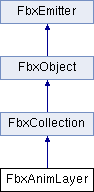
\includegraphics[height=4.000000cm]{class_fbx_anim_layer}
\end{center}
\end{figure}
\subsection*{公開型}
\begin{DoxyCompactItemize}
\item 
enum \hyperlink{class_fbx_anim_layer_abb1e650203e91ff090773239994e802a}{E\+Blend\+Mode} \{ \hyperlink{class_fbx_anim_layer_abb1e650203e91ff090773239994e802aae60dd39593c8806694f8cedb0c14b09b}{e\+Blend\+Additive}, 
\hyperlink{class_fbx_anim_layer_abb1e650203e91ff090773239994e802aaf8232b445a780774bcb8b76ee37291e5}{e\+Blend\+Override}, 
\hyperlink{class_fbx_anim_layer_abb1e650203e91ff090773239994e802aa9551a7380fccde36fd35f532aa826a7a}{e\+Blend\+Override\+Passthrough}
 \}
\item 
enum \hyperlink{class_fbx_anim_layer_a11bad6dbac61cc3965624a0622e90b38}{E\+Rotation\+Accumulation\+Mode} \{ \hyperlink{class_fbx_anim_layer_a11bad6dbac61cc3965624a0622e90b38a51036262864495602654d22f83f101da}{e\+Rotation\+By\+Layer}, 
\hyperlink{class_fbx_anim_layer_a11bad6dbac61cc3965624a0622e90b38a5212817a9e2cfdd21688930bd5fc167a}{e\+Rotation\+By\+Channel}
 \}
\item 
enum \hyperlink{class_fbx_anim_layer_aec9cfaa528bee6739ba4317964d123b0}{E\+Scale\+Accumulation\+Mode} \{ \hyperlink{class_fbx_anim_layer_aec9cfaa528bee6739ba4317964d123b0af962df864ef1dead2f88ade13f4262d0}{e\+Scale\+Multiply}, 
\hyperlink{class_fbx_anim_layer_aec9cfaa528bee6739ba4317964d123b0a0d79b9c4219c50d434746d7062046123}{e\+Scale\+Additive}
 \}
\end{DoxyCompactItemize}
\subsection*{公開メンバ関数}
\begin{DoxyCompactItemize}
\item 
void \hyperlink{class_fbx_anim_layer_acd87646f48b6387952fd3ca257133774}{Reset} ()
\begin{DoxyCompactList}\small\item\em Reset this object properties to their default value. \end{DoxyCompactList}\end{DoxyCompactItemize}
\subsection*{公開変数類}
\begin{DoxyCompactItemize}
\item 
\hyperlink{class_fbx_property_t}{Fbx\+PropertyT}$<$ \hyperlink{fbxtypes_8h_a171e72a1c46fc15c1a6c9c31948c1c5b}{Fbx\+Double} $>$ \hyperlink{class_fbx_anim_layer_a6ab882a24bdf15c3448d064955bf0535}{Weight}
\item 
\hyperlink{class_fbx_property_t}{Fbx\+PropertyT}$<$ \hyperlink{fbxtypes_8h_a92e0562b2fe33e76a242f498b362262e}{Fbx\+Bool} $>$ \hyperlink{class_fbx_anim_layer_ae8f8f6db5f57e41d42935720b4e8d582}{Mute}
\item 
\hyperlink{class_fbx_property_t}{Fbx\+PropertyT}$<$ \hyperlink{fbxtypes_8h_a92e0562b2fe33e76a242f498b362262e}{Fbx\+Bool} $>$ \hyperlink{class_fbx_anim_layer_a0e002d0db3b5998a4c016cffb7f5c252}{Solo}
\item 
\hyperlink{class_fbx_property_t}{Fbx\+PropertyT}$<$ \hyperlink{fbxtypes_8h_a92e0562b2fe33e76a242f498b362262e}{Fbx\+Bool} $>$ \hyperlink{class_fbx_anim_layer_ade773868b910bcfcedf4818b96da9233}{Lock}
\item 
\hyperlink{class_fbx_property_t}{Fbx\+PropertyT}$<$ \hyperlink{fbxtypes_8h_ae0a96f14cde566774c7553aa7523b7a7}{Fbx\+Double3} $>$ \hyperlink{class_fbx_anim_layer_a9eb1d3e6e4bcfc59122fe6261eb529bc}{Color}
\item 
\hyperlink{class_fbx_property_t}{Fbx\+PropertyT}$<$ \hyperlink{fbxtypes_8h_a9a28614cb4272a0ad7d748eda7f3d3e5}{Fbx\+Enum} $>$ \hyperlink{class_fbx_anim_layer_a7e4d4d009aa2c248d19781e9d31f1f89}{Blend\+Mode}
\item 
\hyperlink{class_fbx_property_t}{Fbx\+PropertyT}$<$ \hyperlink{fbxtypes_8h_a9a28614cb4272a0ad7d748eda7f3d3e5}{Fbx\+Enum} $>$ \hyperlink{class_fbx_anim_layer_ae8d47b5fabab90773e9a40aeef934945}{Rotation\+Accumulation\+Mode}
\item 
\hyperlink{class_fbx_property_t}{Fbx\+PropertyT}$<$ \hyperlink{fbxtypes_8h_a9a28614cb4272a0ad7d748eda7f3d3e5}{Fbx\+Enum} $>$ \hyperlink{class_fbx_anim_layer_a50ec8bebaa1241cc168fae6bcf5c670f}{Scale\+Accumulation\+Mode}
\end{DoxyCompactItemize}
\subsection*{限定公開メンバ関数}
\begin{DoxyCompactItemize}
\item 
virtual void \hyperlink{class_fbx_anim_layer_a24afc26df98e56c965c0c60e637ed888}{Construct\+Properties} (bool p\+Force\+Set)
\item 
virtual \hyperlink{class_fbx_anim_layer}{Fbx\+Anim\+Layer} $\ast$ \hyperlink{class_fbx_anim_layer_ab031a979290c44d59ae3ba25a4ab2169}{Get\+Anim\+Layer} ()
\end{DoxyCompactItemize}
\subsection*{Blend\+Mode bypass functions}
\label{_amgrp69dcbe1ac0f20ac1568a8b5ca4119588}%
This section provides methods to bypass the current layer blend mode by data type. When the state is {\ttfamily true}, the evaluators that are processing the layer will need to consider that, for the given data type, the blend mode is forced to be Overwrite. If the state is left to its default {\ttfamily false} value, then the layer blend mode applies. \begin{DoxyRemark}{注釈}
This section only supports the basic types defined in the \hyperlink{fbxtypes_8h}{fbxtypes.\+h} header file. 
\end{DoxyRemark}
\begin{DoxyCompactItemize}
\item 
void \hyperlink{class_fbx_anim_layer_a8be5d3511971847c8f8d88c0a9fe2158}{Set\+Blend\+Mode\+Bypass} (\hyperlink{fbxpropertytypes_8h_a73913a5ddfb20e57c6f25e9e6784bd92}{E\+Fbx\+Type} p\+Type, bool p\+State)
\item 
bool \hyperlink{class_fbx_anim_layer_a3f16ece7c4506b8d72c2b77db5e81586}{Get\+Blend\+Mode\+Bypass} (\hyperlink{fbxpropertytypes_8h_a73913a5ddfb20e57c6f25e9e6784bd92}{E\+Fbx\+Type} p\+Type)
\end{DoxyCompactItemize}
\subsection*{Curve\+Node management}
\begin{DoxyCompactItemize}
\item 
\hyperlink{class_fbx_anim_curve_node}{Fbx\+Anim\+Curve\+Node} $\ast$ \hyperlink{class_fbx_anim_layer_a634a9dd8c4a0a7457a15d50f9643d4e0}{Create\+Curve\+Node} (\hyperlink{class_fbx_property}{Fbx\+Property} \&p\+Property)
\end{DoxyCompactItemize}
\subsection*{その他の継承メンバ}


\subsection{詳解}
The animation layer is a collection of animation curve nodes. Its purpose is to store a variable number of \hyperlink{class_fbx_anim_curve_node}{Fbx\+Anim\+Curve\+Node}. The class provides different states flags (bool properties), an animatable weight, and the blending mode flag to indicate how the data on this layer is interacting with the data of the other layers during the evaluation. 

 fbxanimlayer.\+h の 30 行目に定義があります。



\subsection{列挙型メンバ詳解}
\mbox{\Hypertarget{class_fbx_anim_layer_abb1e650203e91ff090773239994e802a}\label{class_fbx_anim_layer_abb1e650203e91ff090773239994e802a}} 
\index{Fbx\+Anim\+Layer@{Fbx\+Anim\+Layer}!E\+Blend\+Mode@{E\+Blend\+Mode}}
\index{E\+Blend\+Mode@{E\+Blend\+Mode}!Fbx\+Anim\+Layer@{Fbx\+Anim\+Layer}}
\subsubsection{\texorpdfstring{E\+Blend\+Mode}{EBlendMode}}
{\footnotesize\ttfamily enum \hyperlink{class_fbx_anim_layer_abb1e650203e91ff090773239994e802a}{Fbx\+Anim\+Layer\+::\+E\+Blend\+Mode}}

Blend mode type between animation layers. \begin{DoxyEnumFields}{列挙値}
\raisebox{\heightof{T}}[0pt][0pt]{\index{e\+Blend\+Additive@{e\+Blend\+Additive}!Fbx\+Anim\+Layer@{Fbx\+Anim\+Layer}}\index{Fbx\+Anim\+Layer@{Fbx\+Anim\+Layer}!e\+Blend\+Additive@{e\+Blend\+Additive}}}\mbox{\Hypertarget{class_fbx_anim_layer_abb1e650203e91ff090773239994e802aae60dd39593c8806694f8cedb0c14b09b}\label{class_fbx_anim_layer_abb1e650203e91ff090773239994e802aae60dd39593c8806694f8cedb0c14b09b}} 
e\+Blend\+Additive&\\
\hline

\raisebox{\heightof{T}}[0pt][0pt]{\index{e\+Blend\+Override@{e\+Blend\+Override}!Fbx\+Anim\+Layer@{Fbx\+Anim\+Layer}}\index{Fbx\+Anim\+Layer@{Fbx\+Anim\+Layer}!e\+Blend\+Override@{e\+Blend\+Override}}}\mbox{\Hypertarget{class_fbx_anim_layer_abb1e650203e91ff090773239994e802aaf8232b445a780774bcb8b76ee37291e5}\label{class_fbx_anim_layer_abb1e650203e91ff090773239994e802aaf8232b445a780774bcb8b76ee37291e5}} 
e\+Blend\+Override&The layer \char`\"{}adds\char`\"{} its animation to layers that precede it in the stack and affect the same attributes. \\
\hline

\raisebox{\heightof{T}}[0pt][0pt]{\index{e\+Blend\+Override\+Passthrough@{e\+Blend\+Override\+Passthrough}!Fbx\+Anim\+Layer@{Fbx\+Anim\+Layer}}\index{Fbx\+Anim\+Layer@{Fbx\+Anim\+Layer}!e\+Blend\+Override\+Passthrough@{e\+Blend\+Override\+Passthrough}}}\mbox{\Hypertarget{class_fbx_anim_layer_abb1e650203e91ff090773239994e802aa9551a7380fccde36fd35f532aa826a7a}\label{class_fbx_anim_layer_abb1e650203e91ff090773239994e802aa9551a7380fccde36fd35f532aa826a7a}} 
e\+Blend\+Override\+Passthrough&The layer \char`\"{}overrides\char`\"{} the animation of any layer that shares the same attributes and precedes it in the stack. This mode is like the e\+Override but the Weight value influence how much animation from the preceding layers is allowed to pass-\/through. When using this mode with a Weight of 100.\+0, this layer is completely opaque and it masks any animation from the preceding layers for the same attribute. If the Weight is 50.\+0, half of this layer animation is mixed with half of the animation of the preceding layers for the same attribute. \\
\hline

\end{DoxyEnumFields}


 fbxanimlayer.\+h の 138 行目に定義があります。

\mbox{\Hypertarget{class_fbx_anim_layer_a11bad6dbac61cc3965624a0622e90b38}\label{class_fbx_anim_layer_a11bad6dbac61cc3965624a0622e90b38}} 
\index{Fbx\+Anim\+Layer@{Fbx\+Anim\+Layer}!E\+Rotation\+Accumulation\+Mode@{E\+Rotation\+Accumulation\+Mode}}
\index{E\+Rotation\+Accumulation\+Mode@{E\+Rotation\+Accumulation\+Mode}!Fbx\+Anim\+Layer@{Fbx\+Anim\+Layer}}
\subsubsection{\texorpdfstring{E\+Rotation\+Accumulation\+Mode}{ERotationAccumulationMode}}
{\footnotesize\ttfamily enum \hyperlink{class_fbx_anim_layer_a11bad6dbac61cc3965624a0622e90b38}{Fbx\+Anim\+Layer\+::\+E\+Rotation\+Accumulation\+Mode}}

Rotation accumulation mode of animation layer. \begin{DoxyEnumFields}{列挙値}
\raisebox{\heightof{T}}[0pt][0pt]{\index{e\+Rotation\+By\+Layer@{e\+Rotation\+By\+Layer}!Fbx\+Anim\+Layer@{Fbx\+Anim\+Layer}}\index{Fbx\+Anim\+Layer@{Fbx\+Anim\+Layer}!e\+Rotation\+By\+Layer@{e\+Rotation\+By\+Layer}}}\mbox{\Hypertarget{class_fbx_anim_layer_a11bad6dbac61cc3965624a0622e90b38a51036262864495602654d22f83f101da}\label{class_fbx_anim_layer_a11bad6dbac61cc3965624a0622e90b38a51036262864495602654d22f83f101da}} 
e\+Rotation\+By\+Layer&\\
\hline

\raisebox{\heightof{T}}[0pt][0pt]{\index{e\+Rotation\+By\+Channel@{e\+Rotation\+By\+Channel}!Fbx\+Anim\+Layer@{Fbx\+Anim\+Layer}}\index{Fbx\+Anim\+Layer@{Fbx\+Anim\+Layer}!e\+Rotation\+By\+Channel@{e\+Rotation\+By\+Channel}}}\mbox{\Hypertarget{class_fbx_anim_layer_a11bad6dbac61cc3965624a0622e90b38a5212817a9e2cfdd21688930bd5fc167a}\label{class_fbx_anim_layer_a11bad6dbac61cc3965624a0622e90b38a5212817a9e2cfdd21688930bd5fc167a}} 
e\+Rotation\+By\+Channel&Rotation values are weighted per layer and the result rotation curves are calculated using concatenated quaternion values. Rotation values are weighted per component and the result rotation curves are calculated by adding each independent Euler X\+YZ value. \\
\hline

\end{DoxyEnumFields}


 fbxanimlayer.\+h の 153 行目に定義があります。

\mbox{\Hypertarget{class_fbx_anim_layer_aec9cfaa528bee6739ba4317964d123b0}\label{class_fbx_anim_layer_aec9cfaa528bee6739ba4317964d123b0}} 
\index{Fbx\+Anim\+Layer@{Fbx\+Anim\+Layer}!E\+Scale\+Accumulation\+Mode@{E\+Scale\+Accumulation\+Mode}}
\index{E\+Scale\+Accumulation\+Mode@{E\+Scale\+Accumulation\+Mode}!Fbx\+Anim\+Layer@{Fbx\+Anim\+Layer}}
\subsubsection{\texorpdfstring{E\+Scale\+Accumulation\+Mode}{EScaleAccumulationMode}}
{\footnotesize\ttfamily enum \hyperlink{class_fbx_anim_layer_aec9cfaa528bee6739ba4317964d123b0}{Fbx\+Anim\+Layer\+::\+E\+Scale\+Accumulation\+Mode}}

Scale accumulation mode of animation layer. \begin{DoxyEnumFields}{列挙値}
\raisebox{\heightof{T}}[0pt][0pt]{\index{e\+Scale\+Multiply@{e\+Scale\+Multiply}!Fbx\+Anim\+Layer@{Fbx\+Anim\+Layer}}\index{Fbx\+Anim\+Layer@{Fbx\+Anim\+Layer}!e\+Scale\+Multiply@{e\+Scale\+Multiply}}}\mbox{\Hypertarget{class_fbx_anim_layer_aec9cfaa528bee6739ba4317964d123b0af962df864ef1dead2f88ade13f4262d0}\label{class_fbx_anim_layer_aec9cfaa528bee6739ba4317964d123b0af962df864ef1dead2f88ade13f4262d0}} 
e\+Scale\+Multiply&\\
\hline

\raisebox{\heightof{T}}[0pt][0pt]{\index{e\+Scale\+Additive@{e\+Scale\+Additive}!Fbx\+Anim\+Layer@{Fbx\+Anim\+Layer}}\index{Fbx\+Anim\+Layer@{Fbx\+Anim\+Layer}!e\+Scale\+Additive@{e\+Scale\+Additive}}}\mbox{\Hypertarget{class_fbx_anim_layer_aec9cfaa528bee6739ba4317964d123b0a0d79b9c4219c50d434746d7062046123}\label{class_fbx_anim_layer_aec9cfaa528bee6739ba4317964d123b0a0d79b9c4219c50d434746d7062046123}} 
e\+Scale\+Additive&Independent X\+YZ scale values per layer are calculated using the layer weight value as an exponent, and result scale curves are calculated by multiplying each independent X\+YZ scale value. Result scale curves are calculated by adding each independent X\+YZ value. \\
\hline

\end{DoxyEnumFields}


 fbxanimlayer.\+h の 161 行目に定義があります。



\subsection{関数詳解}
\mbox{\Hypertarget{class_fbx_anim_layer_a24afc26df98e56c965c0c60e637ed888}\label{class_fbx_anim_layer_a24afc26df98e56c965c0c60e637ed888}} 
\index{Fbx\+Anim\+Layer@{Fbx\+Anim\+Layer}!Construct\+Properties@{Construct\+Properties}}
\index{Construct\+Properties@{Construct\+Properties}!Fbx\+Anim\+Layer@{Fbx\+Anim\+Layer}}
\subsubsection{\texorpdfstring{Construct\+Properties()}{ConstructProperties()}}
{\footnotesize\ttfamily virtual void Fbx\+Anim\+Layer\+::\+Construct\+Properties (\begin{DoxyParamCaption}\item[{bool}]{p\+Force\+Set }\end{DoxyParamCaption})\hspace{0.3cm}{\ttfamily [protected]}, {\ttfamily [virtual]}}

Optional property constructor override, automatically called by default constructor. 
\begin{DoxyParams}{引数}
{\em p\+Force\+Set} & If the property value must be set regardless of default value. \\
\hline
\end{DoxyParams}
\begin{DoxyRemark}{注釈}
If your object have properties, they must be initialized in this function. 
\end{DoxyRemark}


\hyperlink{class_fbx_object_ad44f814323dc1b5e78bff1bfc608b4bb}{Fbx\+Object}を再実装しています。

\mbox{\Hypertarget{class_fbx_anim_layer_a634a9dd8c4a0a7457a15d50f9643d4e0}\label{class_fbx_anim_layer_a634a9dd8c4a0a7457a15d50f9643d4e0}} 
\index{Fbx\+Anim\+Layer@{Fbx\+Anim\+Layer}!Create\+Curve\+Node@{Create\+Curve\+Node}}
\index{Create\+Curve\+Node@{Create\+Curve\+Node}!Fbx\+Anim\+Layer@{Fbx\+Anim\+Layer}}
\subsubsection{\texorpdfstring{Create\+Curve\+Node()}{CreateCurveNode()}}
{\footnotesize\ttfamily \hyperlink{class_fbx_anim_curve_node}{Fbx\+Anim\+Curve\+Node}$\ast$ Fbx\+Anim\+Layer\+::\+Create\+Curve\+Node (\begin{DoxyParamCaption}\item[{\hyperlink{class_fbx_property}{Fbx\+Property} \&}]{p\+Property }\end{DoxyParamCaption})}

Create a \hyperlink{class_fbx_anim_curve_node}{Fbx\+Anim\+Curve\+Node} based on the property data type. 
\begin{DoxyParams}{引数}
{\em p\+Property} & The property that the created \hyperlink{class_fbx_anim_curve_node}{Fbx\+Anim\+Curve\+Node} will be connected to. \\
\hline
\end{DoxyParams}
\begin{DoxyReturn}{戻り値}
Pointer to the created \hyperlink{class_fbx_anim_curve_node}{Fbx\+Anim\+Curve\+Node}, or N\+U\+LL if an error occurred. 
\end{DoxyReturn}
\begin{DoxyRemark}{注釈}
This function will fail if the property \hyperlink{class_fbx_property_flags_afabfa7e0949aac8a7dcdf8a141867e99ae2c562a65bb942f3f94631794bc3d257}{Fbx\+Property\+Flags\+::e\+Animatable} flag is not set. 

This function sets the e\+Animated flag of the property. 

The newly created \hyperlink{class_fbx_anim_curve_node}{Fbx\+Anim\+Curve\+Node} is automatically connected to both this object and the property. 
\end{DoxyRemark}
\mbox{\Hypertarget{class_fbx_anim_layer_ab031a979290c44d59ae3ba25a4ab2169}\label{class_fbx_anim_layer_ab031a979290c44d59ae3ba25a4ab2169}} 
\index{Fbx\+Anim\+Layer@{Fbx\+Anim\+Layer}!Get\+Anim\+Layer@{Get\+Anim\+Layer}}
\index{Get\+Anim\+Layer@{Get\+Anim\+Layer}!Fbx\+Anim\+Layer@{Fbx\+Anim\+Layer}}
\subsubsection{\texorpdfstring{Get\+Anim\+Layer()}{GetAnimLayer()}}
{\footnotesize\ttfamily virtual \hyperlink{class_fbx_anim_layer}{Fbx\+Anim\+Layer}$\ast$ Fbx\+Anim\+Layer\+::\+Get\+Anim\+Layer (\begin{DoxyParamCaption}{ }\end{DoxyParamCaption})\hspace{0.3cm}{\ttfamily [protected]}, {\ttfamily [virtual]}}

\mbox{\Hypertarget{class_fbx_anim_layer_a3f16ece7c4506b8d72c2b77db5e81586}\label{class_fbx_anim_layer_a3f16ece7c4506b8d72c2b77db5e81586}} 
\index{Fbx\+Anim\+Layer@{Fbx\+Anim\+Layer}!Get\+Blend\+Mode\+Bypass@{Get\+Blend\+Mode\+Bypass}}
\index{Get\+Blend\+Mode\+Bypass@{Get\+Blend\+Mode\+Bypass}!Fbx\+Anim\+Layer@{Fbx\+Anim\+Layer}}
\subsubsection{\texorpdfstring{Get\+Blend\+Mode\+Bypass()}{GetBlendModeBypass()}}
{\footnotesize\ttfamily bool Fbx\+Anim\+Layer\+::\+Get\+Blend\+Mode\+Bypass (\begin{DoxyParamCaption}\item[{\hyperlink{fbxpropertytypes_8h_a73913a5ddfb20e57c6f25e9e6784bd92}{E\+Fbx\+Type}}]{p\+Type }\end{DoxyParamCaption})}

Get the current state of the bypass flag for the given data type. 
\begin{DoxyParams}{引数}
{\em p\+Type} & The fbx\+Type identifier. \\
\hline
\end{DoxyParams}
\begin{DoxyReturn}{戻り値}
The current state of the flag for a valid p\+Type value and {\ttfamily false} in any other case. 
\end{DoxyReturn}
\mbox{\Hypertarget{class_fbx_anim_layer_acd87646f48b6387952fd3ca257133774}\label{class_fbx_anim_layer_acd87646f48b6387952fd3ca257133774}} 
\index{Fbx\+Anim\+Layer@{Fbx\+Anim\+Layer}!Reset@{Reset}}
\index{Reset@{Reset}!Fbx\+Anim\+Layer@{Fbx\+Anim\+Layer}}
\subsubsection{\texorpdfstring{Reset()}{Reset()}}
{\footnotesize\ttfamily void Fbx\+Anim\+Layer\+::\+Reset (\begin{DoxyParamCaption}{ }\end{DoxyParamCaption})}



Reset this object properties to their default value. 

\mbox{\Hypertarget{class_fbx_anim_layer_a8be5d3511971847c8f8d88c0a9fe2158}\label{class_fbx_anim_layer_a8be5d3511971847c8f8d88c0a9fe2158}} 
\index{Fbx\+Anim\+Layer@{Fbx\+Anim\+Layer}!Set\+Blend\+Mode\+Bypass@{Set\+Blend\+Mode\+Bypass}}
\index{Set\+Blend\+Mode\+Bypass@{Set\+Blend\+Mode\+Bypass}!Fbx\+Anim\+Layer@{Fbx\+Anim\+Layer}}
\subsubsection{\texorpdfstring{Set\+Blend\+Mode\+Bypass()}{SetBlendModeBypass()}}
{\footnotesize\ttfamily void Fbx\+Anim\+Layer\+::\+Set\+Blend\+Mode\+Bypass (\begin{DoxyParamCaption}\item[{\hyperlink{fbxpropertytypes_8h_a73913a5ddfb20e57c6f25e9e6784bd92}{E\+Fbx\+Type}}]{p\+Type,  }\item[{bool}]{p\+State }\end{DoxyParamCaption})}

Set the bypass flag for the given data type. 
\begin{DoxyParams}{引数}
{\em p\+Type} & The fbx\+Type identifier. \\
\hline
{\em p\+State} & The new state of the bypass flag. \\
\hline
\end{DoxyParams}
\begin{DoxyRemark}{注釈}
If p\+Type is e\+Fbx\+Type\+Count, then p\+State is applied to all the data types. 
\end{DoxyRemark}


\subsection{メンバ詳解}
\mbox{\Hypertarget{class_fbx_anim_layer_a7e4d4d009aa2c248d19781e9d31f1f89}\label{class_fbx_anim_layer_a7e4d4d009aa2c248d19781e9d31f1f89}} 
\index{Fbx\+Anim\+Layer@{Fbx\+Anim\+Layer}!Blend\+Mode@{Blend\+Mode}}
\index{Blend\+Mode@{Blend\+Mode}!Fbx\+Anim\+Layer@{Fbx\+Anim\+Layer}}
\subsubsection{\texorpdfstring{Blend\+Mode}{BlendMode}}
{\footnotesize\ttfamily \hyperlink{class_fbx_property_t}{Fbx\+PropertyT}$<$\hyperlink{fbxtypes_8h_a9a28614cb4272a0ad7d748eda7f3d3e5}{Fbx\+Enum}$>$ Fbx\+Anim\+Layer\+::\+Blend\+Mode}

This property stores the blend mode. The blend mode is used to specify how this layer influences the animation evaluation. See the Blend\+Mode enumeration for the description of the modes.

Default value is {\ttfamily e\+Mode\+Additive} 

 fbxanimlayer.\+h の 87 行目に定義があります。

\mbox{\Hypertarget{class_fbx_anim_layer_a9eb1d3e6e4bcfc59122fe6261eb529bc}\label{class_fbx_anim_layer_a9eb1d3e6e4bcfc59122fe6261eb529bc}} 
\index{Fbx\+Anim\+Layer@{Fbx\+Anim\+Layer}!Color@{Color}}
\index{Color@{Color}!Fbx\+Anim\+Layer@{Fbx\+Anim\+Layer}}
\subsubsection{\texorpdfstring{Color}{Color}}
{\footnotesize\ttfamily \hyperlink{class_fbx_property_t}{Fbx\+PropertyT}$<$\hyperlink{fbxtypes_8h_ae0a96f14cde566774c7553aa7523b7a7}{Fbx\+Double3}$>$ Fbx\+Anim\+Layer\+::\+Color}

This property stores the display color. This color can be used by applications if they display a graphical representation of the layer. The F\+BX S\+DK does not use it but guarantees that the value is saved to the F\+BX file and retrieved from it.

Default value is {\ttfamily }(0.\+8, 0.\+8, 0.\+8) 

 fbxanimlayer.\+h の 79 行目に定義があります。

\mbox{\Hypertarget{class_fbx_anim_layer_ade773868b910bcfcedf4818b96da9233}\label{class_fbx_anim_layer_ade773868b910bcfcedf4818b96da9233}} 
\index{Fbx\+Anim\+Layer@{Fbx\+Anim\+Layer}!Lock@{Lock}}
\index{Lock@{Lock}!Fbx\+Anim\+Layer@{Fbx\+Anim\+Layer}}
\subsubsection{\texorpdfstring{Lock}{Lock}}
{\footnotesize\ttfamily \hyperlink{class_fbx_property_t}{Fbx\+PropertyT}$<$\hyperlink{fbxtypes_8h_a92e0562b2fe33e76a242f498b362262e}{Fbx\+Bool}$>$ Fbx\+Anim\+Layer\+::\+Lock}

This property stores the lock state. The lock state indicates that this layer has been \char`\"{}locked\char`\"{} from editing operations and should no longer receive keyframes.

Default value is {\ttfamily false} 

 fbxanimlayer.\+h の 70 行目に定義があります。

\mbox{\Hypertarget{class_fbx_anim_layer_ae8f8f6db5f57e41d42935720b4e8d582}\label{class_fbx_anim_layer_ae8f8f6db5f57e41d42935720b4e8d582}} 
\index{Fbx\+Anim\+Layer@{Fbx\+Anim\+Layer}!Mute@{Mute}}
\index{Mute@{Mute}!Fbx\+Anim\+Layer@{Fbx\+Anim\+Layer}}
\subsubsection{\texorpdfstring{Mute}{Mute}}
{\footnotesize\ttfamily \hyperlink{class_fbx_property_t}{Fbx\+PropertyT}$<$\hyperlink{fbxtypes_8h_a92e0562b2fe33e76a242f498b362262e}{Fbx\+Bool}$>$ Fbx\+Anim\+Layer\+::\+Mute}

This property stores the mute state. The mute state indicates that this layer should be excluded from the evaluation.

Default value is {\ttfamily false} 

 fbxanimlayer.\+h の 54 行目に定義があります。

\mbox{\Hypertarget{class_fbx_anim_layer_ae8d47b5fabab90773e9a40aeef934945}\label{class_fbx_anim_layer_ae8d47b5fabab90773e9a40aeef934945}} 
\index{Fbx\+Anim\+Layer@{Fbx\+Anim\+Layer}!Rotation\+Accumulation\+Mode@{Rotation\+Accumulation\+Mode}}
\index{Rotation\+Accumulation\+Mode@{Rotation\+Accumulation\+Mode}!Fbx\+Anim\+Layer@{Fbx\+Anim\+Layer}}
\subsubsection{\texorpdfstring{Rotation\+Accumulation\+Mode}{RotationAccumulationMode}}
{\footnotesize\ttfamily \hyperlink{class_fbx_property_t}{Fbx\+PropertyT}$<$\hyperlink{fbxtypes_8h_a9a28614cb4272a0ad7d748eda7f3d3e5}{Fbx\+Enum}$>$ Fbx\+Anim\+Layer\+::\+Rotation\+Accumulation\+Mode}

This property stores the rotation accumulation mode. This option indicates how the rotation curves on this layer combine with any preceding layers that share the same attributes. See the Rotation\+Accumulation\+Mode enumeration for the description of the modes.

Default value is {\ttfamily e\+Rotation\+By\+Layer} 

 fbxanimlayer.\+h の 96 行目に定義があります。

\mbox{\Hypertarget{class_fbx_anim_layer_a50ec8bebaa1241cc168fae6bcf5c670f}\label{class_fbx_anim_layer_a50ec8bebaa1241cc168fae6bcf5c670f}} 
\index{Fbx\+Anim\+Layer@{Fbx\+Anim\+Layer}!Scale\+Accumulation\+Mode@{Scale\+Accumulation\+Mode}}
\index{Scale\+Accumulation\+Mode@{Scale\+Accumulation\+Mode}!Fbx\+Anim\+Layer@{Fbx\+Anim\+Layer}}
\subsubsection{\texorpdfstring{Scale\+Accumulation\+Mode}{ScaleAccumulationMode}}
{\footnotesize\ttfamily \hyperlink{class_fbx_property_t}{Fbx\+PropertyT}$<$\hyperlink{fbxtypes_8h_a9a28614cb4272a0ad7d748eda7f3d3e5}{Fbx\+Enum}$>$ Fbx\+Anim\+Layer\+::\+Scale\+Accumulation\+Mode}

This property stores the scale accumulation mode. This option indicates how the scale curves on this layer combine with any preceding layers that share the same attributes. See the Scale\+Accumulation\+Mode enumeration for the description of the modes.

Default value is {\ttfamily e\+Scale\+Multiply} 

 fbxanimlayer.\+h の 105 行目に定義があります。

\mbox{\Hypertarget{class_fbx_anim_layer_a0e002d0db3b5998a4c016cffb7f5c252}\label{class_fbx_anim_layer_a0e002d0db3b5998a4c016cffb7f5c252}} 
\index{Fbx\+Anim\+Layer@{Fbx\+Anim\+Layer}!Solo@{Solo}}
\index{Solo@{Solo}!Fbx\+Anim\+Layer@{Fbx\+Anim\+Layer}}
\subsubsection{\texorpdfstring{Solo}{Solo}}
{\footnotesize\ttfamily \hyperlink{class_fbx_property_t}{Fbx\+PropertyT}$<$\hyperlink{fbxtypes_8h_a92e0562b2fe33e76a242f498b362262e}{Fbx\+Bool}$>$ Fbx\+Anim\+Layer\+::\+Solo}

This property stores the solo state. The solo state indicates that this layer is the only one that should be processed during the evaluation.

Default value is {\ttfamily false} 

 fbxanimlayer.\+h の 62 行目に定義があります。

\mbox{\Hypertarget{class_fbx_anim_layer_a6ab882a24bdf15c3448d064955bf0535}\label{class_fbx_anim_layer_a6ab882a24bdf15c3448d064955bf0535}} 
\index{Fbx\+Anim\+Layer@{Fbx\+Anim\+Layer}!Weight@{Weight}}
\index{Weight@{Weight}!Fbx\+Anim\+Layer@{Fbx\+Anim\+Layer}}
\subsubsection{\texorpdfstring{Weight}{Weight}}
{\footnotesize\ttfamily \hyperlink{class_fbx_property_t}{Fbx\+PropertyT}$<$\hyperlink{fbxtypes_8h_a171e72a1c46fc15c1a6c9c31948c1c5b}{Fbx\+Double}$>$ Fbx\+Anim\+Layer\+::\+Weight}

This property stores the weight factor. The weight factor is the percentage of influence this layer has during the evaluation.

Default value is {\ttfamily 100.\+0} 

 fbxanimlayer.\+h の 47 行目に定義があります。



このクラス詳解は次のファイルから抽出されました\+:\begin{DoxyCompactItemize}
\item 
C\+:/\+Maya/scripts/\+F\+B\+X\+\_\+\+S\+D\+K/2017.\+1/include/fbxsdk/scene/animation/\hyperlink{fbxanimlayer_8h}{fbxanimlayer.\+h}\end{DoxyCompactItemize}

\hypertarget{class_fbx_anim_utilities_1_1_fbx_anim_split_def}{}\section{Fbx\+Anim\+Utilities\+:\+:Fbx\+Anim\+Split\+Def クラス}
\label{class_fbx_anim_utilities_1_1_fbx_anim_split_def}\index{Fbx\+Anim\+Utilities\+::\+Fbx\+Anim\+Split\+Def@{Fbx\+Anim\+Utilities\+::\+Fbx\+Anim\+Split\+Def}}


{\ttfamily \#include $<$fbxanimutilities.\+h$>$}

\subsection*{公開メンバ関数}
\begin{DoxyCompactItemize}
\item 
\hyperlink{class_fbx_anim_utilities_1_1_fbx_anim_split_def_ad921439ab544295b62f250b3b1a8e3da}{Fbx\+Anim\+Split\+Def} ()
\item 
\hyperlink{class_fbx_anim_utilities_1_1_fbx_anim_split_def_a90737793295d433c713584ffd27fa5c1}{Fbx\+Anim\+Split\+Def} (const \hyperlink{class_fbx_string}{Fbx\+String} \&p\+Name, \hyperlink{class_fbx_time}{Fbx\+Time} \&p\+Start, \hyperlink{class_fbx_time}{Fbx\+Time} \&p\+End)
\item 
\hyperlink{class_fbx_anim_utilities_1_1_fbx_anim_split_def}{Fbx\+Anim\+Split\+Def} \& \hyperlink{class_fbx_anim_utilities_1_1_fbx_anim_split_def_a94315e091906bc664030ee1000785e90}{operator=} (const \hyperlink{class_fbx_anim_utilities_1_1_fbx_anim_split_def}{Fbx\+Anim\+Split\+Def} \&p\+Rhs)
\end{DoxyCompactItemize}
\subsection*{公開変数類}
\begin{DoxyCompactItemize}
\item 
\hyperlink{class_fbx_string}{Fbx\+String} \hyperlink{class_fbx_anim_utilities_1_1_fbx_anim_split_def_ae78929097a3526acf01e3d0f7f89796f}{m\+Name}
\item 
\hyperlink{class_fbx_time}{Fbx\+Time} \hyperlink{class_fbx_anim_utilities_1_1_fbx_anim_split_def_af8aad5671b9f1bef7a5af4a226a0f646}{m\+Start}
\item 
\hyperlink{class_fbx_time}{Fbx\+Time} \hyperlink{class_fbx_anim_utilities_1_1_fbx_anim_split_def_a16aca4564d9609c2409c3be7fb0a5bd3}{m\+End}
\end{DoxyCompactItemize}


\subsection{詳解}


 fbxanimutilities.\+h の 54 行目に定義があります。



\subsection{構築子と解体子}
\mbox{\Hypertarget{class_fbx_anim_utilities_1_1_fbx_anim_split_def_ad921439ab544295b62f250b3b1a8e3da}\label{class_fbx_anim_utilities_1_1_fbx_anim_split_def_ad921439ab544295b62f250b3b1a8e3da}} 
\index{Fbx\+Anim\+Utilities\+::\+Fbx\+Anim\+Split\+Def@{Fbx\+Anim\+Utilities\+::\+Fbx\+Anim\+Split\+Def}!Fbx\+Anim\+Split\+Def@{Fbx\+Anim\+Split\+Def}}
\index{Fbx\+Anim\+Split\+Def@{Fbx\+Anim\+Split\+Def}!Fbx\+Anim\+Utilities\+::\+Fbx\+Anim\+Split\+Def@{Fbx\+Anim\+Utilities\+::\+Fbx\+Anim\+Split\+Def}}
\subsubsection{\texorpdfstring{Fbx\+Anim\+Split\+Def()}{FbxAnimSplitDef()}\hspace{0.1cm}{\footnotesize\ttfamily [1/2]}}
{\footnotesize\ttfamily Fbx\+Anim\+Utilities\+::\+Fbx\+Anim\+Split\+Def\+::\+Fbx\+Anim\+Split\+Def (\begin{DoxyParamCaption}{ }\end{DoxyParamCaption})\hspace{0.3cm}{\ttfamily [inline]}}



 fbxanimutilities.\+h の 61 行目に定義があります。

\mbox{\Hypertarget{class_fbx_anim_utilities_1_1_fbx_anim_split_def_a90737793295d433c713584ffd27fa5c1}\label{class_fbx_anim_utilities_1_1_fbx_anim_split_def_a90737793295d433c713584ffd27fa5c1}} 
\index{Fbx\+Anim\+Utilities\+::\+Fbx\+Anim\+Split\+Def@{Fbx\+Anim\+Utilities\+::\+Fbx\+Anim\+Split\+Def}!Fbx\+Anim\+Split\+Def@{Fbx\+Anim\+Split\+Def}}
\index{Fbx\+Anim\+Split\+Def@{Fbx\+Anim\+Split\+Def}!Fbx\+Anim\+Utilities\+::\+Fbx\+Anim\+Split\+Def@{Fbx\+Anim\+Utilities\+::\+Fbx\+Anim\+Split\+Def}}
\subsubsection{\texorpdfstring{Fbx\+Anim\+Split\+Def()}{FbxAnimSplitDef()}\hspace{0.1cm}{\footnotesize\ttfamily [2/2]}}
{\footnotesize\ttfamily Fbx\+Anim\+Utilities\+::\+Fbx\+Anim\+Split\+Def\+::\+Fbx\+Anim\+Split\+Def (\begin{DoxyParamCaption}\item[{const \hyperlink{class_fbx_string}{Fbx\+String} \&}]{p\+Name,  }\item[{\hyperlink{class_fbx_time}{Fbx\+Time} \&}]{p\+Start,  }\item[{\hyperlink{class_fbx_time}{Fbx\+Time} \&}]{p\+End }\end{DoxyParamCaption})\hspace{0.3cm}{\ttfamily [inline]}}



 fbxanimutilities.\+h の 68 行目に定義があります。



\subsection{関数詳解}
\mbox{\Hypertarget{class_fbx_anim_utilities_1_1_fbx_anim_split_def_a94315e091906bc664030ee1000785e90}\label{class_fbx_anim_utilities_1_1_fbx_anim_split_def_a94315e091906bc664030ee1000785e90}} 
\index{Fbx\+Anim\+Utilities\+::\+Fbx\+Anim\+Split\+Def@{Fbx\+Anim\+Utilities\+::\+Fbx\+Anim\+Split\+Def}!operator=@{operator=}}
\index{operator=@{operator=}!Fbx\+Anim\+Utilities\+::\+Fbx\+Anim\+Split\+Def@{Fbx\+Anim\+Utilities\+::\+Fbx\+Anim\+Split\+Def}}
\subsubsection{\texorpdfstring{operator=()}{operator=()}}
{\footnotesize\ttfamily \hyperlink{class_fbx_anim_utilities_1_1_fbx_anim_split_def}{Fbx\+Anim\+Split\+Def}\& Fbx\+Anim\+Utilities\+::\+Fbx\+Anim\+Split\+Def\+::operator= (\begin{DoxyParamCaption}\item[{const \hyperlink{class_fbx_anim_utilities_1_1_fbx_anim_split_def}{Fbx\+Anim\+Split\+Def} \&}]{p\+Rhs }\end{DoxyParamCaption})\hspace{0.3cm}{\ttfamily [inline]}}



 fbxanimutilities.\+h の 75 行目に定義があります。



\subsection{メンバ詳解}
\mbox{\Hypertarget{class_fbx_anim_utilities_1_1_fbx_anim_split_def_a16aca4564d9609c2409c3be7fb0a5bd3}\label{class_fbx_anim_utilities_1_1_fbx_anim_split_def_a16aca4564d9609c2409c3be7fb0a5bd3}} 
\index{Fbx\+Anim\+Utilities\+::\+Fbx\+Anim\+Split\+Def@{Fbx\+Anim\+Utilities\+::\+Fbx\+Anim\+Split\+Def}!m\+End@{m\+End}}
\index{m\+End@{m\+End}!Fbx\+Anim\+Utilities\+::\+Fbx\+Anim\+Split\+Def@{Fbx\+Anim\+Utilities\+::\+Fbx\+Anim\+Split\+Def}}
\subsubsection{\texorpdfstring{m\+End}{mEnd}}
{\footnotesize\ttfamily \hyperlink{class_fbx_time}{Fbx\+Time} Fbx\+Anim\+Utilities\+::\+Fbx\+Anim\+Split\+Def\+::m\+End}



 fbxanimutilities.\+h の 59 行目に定義があります。

\mbox{\Hypertarget{class_fbx_anim_utilities_1_1_fbx_anim_split_def_ae78929097a3526acf01e3d0f7f89796f}\label{class_fbx_anim_utilities_1_1_fbx_anim_split_def_ae78929097a3526acf01e3d0f7f89796f}} 
\index{Fbx\+Anim\+Utilities\+::\+Fbx\+Anim\+Split\+Def@{Fbx\+Anim\+Utilities\+::\+Fbx\+Anim\+Split\+Def}!m\+Name@{m\+Name}}
\index{m\+Name@{m\+Name}!Fbx\+Anim\+Utilities\+::\+Fbx\+Anim\+Split\+Def@{Fbx\+Anim\+Utilities\+::\+Fbx\+Anim\+Split\+Def}}
\subsubsection{\texorpdfstring{m\+Name}{mName}}
{\footnotesize\ttfamily \hyperlink{class_fbx_string}{Fbx\+String} Fbx\+Anim\+Utilities\+::\+Fbx\+Anim\+Split\+Def\+::m\+Name}



 fbxanimutilities.\+h の 57 行目に定義があります。

\mbox{\Hypertarget{class_fbx_anim_utilities_1_1_fbx_anim_split_def_af8aad5671b9f1bef7a5af4a226a0f646}\label{class_fbx_anim_utilities_1_1_fbx_anim_split_def_af8aad5671b9f1bef7a5af4a226a0f646}} 
\index{Fbx\+Anim\+Utilities\+::\+Fbx\+Anim\+Split\+Def@{Fbx\+Anim\+Utilities\+::\+Fbx\+Anim\+Split\+Def}!m\+Start@{m\+Start}}
\index{m\+Start@{m\+Start}!Fbx\+Anim\+Utilities\+::\+Fbx\+Anim\+Split\+Def@{Fbx\+Anim\+Utilities\+::\+Fbx\+Anim\+Split\+Def}}
\subsubsection{\texorpdfstring{m\+Start}{mStart}}
{\footnotesize\ttfamily \hyperlink{class_fbx_time}{Fbx\+Time} Fbx\+Anim\+Utilities\+::\+Fbx\+Anim\+Split\+Def\+::m\+Start}



 fbxanimutilities.\+h の 58 行目に定義があります。



このクラス詳解は次のファイルから抽出されました\+:\begin{DoxyCompactItemize}
\item 
C\+:/\+Maya/scripts/\+F\+B\+X\+\_\+\+S\+D\+K/2017.\+1/include/fbxsdk/scene/animation/\hyperlink{fbxanimutilities_8h}{fbxanimutilities.\+h}\end{DoxyCompactItemize}

\hypertarget{class_fbx_anim_stack}{}\section{Fbx\+Anim\+Stack クラス}
\label{class_fbx_anim_stack}\index{Fbx\+Anim\+Stack@{Fbx\+Anim\+Stack}}


{\ttfamily \#include $<$fbxanimstack.\+h$>$}

Fbx\+Anim\+Stack の継承関係図\begin{figure}[H]
\begin{center}
\leavevmode
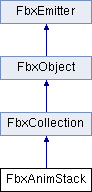
\includegraphics[height=4.000000cm]{class_fbx_anim_stack}
\end{center}
\end{figure}
\subsection*{公開メンバ関数}
\begin{DoxyCompactItemize}
\item 
void \hyperlink{class_fbx_anim_stack_a69f6d38a6b4fa348585674e5d68464b2}{Reset} (const \hyperlink{class_fbx_take_info}{Fbx\+Take\+Info} $\ast$p\+Take\+Info=\hyperlink{fbxarch_8h_a070d2ce7b6bb7e5c05602aa8c308d0c4}{N\+U\+LL})
\end{DoxyCompactItemize}
\subsection*{公開変数類}
\begin{DoxyCompactItemize}
\item 
\hyperlink{class_fbx_property_t}{Fbx\+PropertyT}$<$ \hyperlink{class_fbx_string}{Fbx\+String} $>$ \hyperlink{class_fbx_anim_stack_a87abfeabeaa31a44e2474f01d4501b7f}{Description}
\item 
\hyperlink{class_fbx_property_t}{Fbx\+PropertyT}$<$ \hyperlink{class_fbx_time}{Fbx\+Time} $>$ \hyperlink{class_fbx_anim_stack_a140ba636c0907144d60d2901c0995456}{Local\+Start}
\item 
\hyperlink{class_fbx_property_t}{Fbx\+PropertyT}$<$ \hyperlink{class_fbx_time}{Fbx\+Time} $>$ \hyperlink{class_fbx_anim_stack_a07be87cbd6b3226be489c69b5466a72d}{Local\+Stop}
\item 
\hyperlink{class_fbx_property_t}{Fbx\+PropertyT}$<$ \hyperlink{class_fbx_time}{Fbx\+Time} $>$ \hyperlink{class_fbx_anim_stack_adeac4e2557e00ccd420eb9b790377e22}{Reference\+Start}
\item 
\hyperlink{class_fbx_property_t}{Fbx\+PropertyT}$<$ \hyperlink{class_fbx_time}{Fbx\+Time} $>$ \hyperlink{class_fbx_anim_stack_a480a3b46ab895a740ee658e7022ec208}{Reference\+Stop}
\end{DoxyCompactItemize}
\subsection*{限定公開メンバ関数}
\begin{DoxyCompactItemize}
\item 
virtual void \hyperlink{class_fbx_anim_stack_a41c0a8c693a1dcf5ba2e150b7ea89aa3}{Construct\+Properties} (bool p\+Force\+Set)
\item 
virtual void \hyperlink{class_fbx_anim_stack_a4809de086c3a2d28d98d771b011599d6}{Destruct} (bool p\+Recursive)
\end{DoxyCompactItemize}
\subsection*{Utility functions.}
\begin{DoxyCompactItemize}
\item 
\hyperlink{class_fbx_time_span}{Fbx\+Time\+Span} \hyperlink{class_fbx_anim_stack_a61d246d787a9ac3ab230527e9bab00bb}{Get\+Local\+Time\+Span} () const
\item 
void \hyperlink{class_fbx_anim_stack_ae7d19d4d0cbc6e01fef742b9acaa036e}{Set\+Local\+Time\+Span} (\hyperlink{class_fbx_time_span}{Fbx\+Time\+Span} \&p\+Time\+Span)
\item 
\hyperlink{class_fbx_time_span}{Fbx\+Time\+Span} \hyperlink{class_fbx_anim_stack_a01aacdecb9d3e1860e015aa364111239}{Get\+Reference\+Time\+Span} () const
\item 
void \hyperlink{class_fbx_anim_stack_ae63b01339e65e5a6c52ce532e0006e8b}{Set\+Reference\+Time\+Span} (\hyperlink{class_fbx_time_span}{Fbx\+Time\+Span} \&p\+Time\+Span)
\item 
bool \hyperlink{class_fbx_anim_stack_a20891f3e62c6a50a628f2ed65616bf36}{Bake\+Layers} (\hyperlink{class_fbx_anim_evaluator}{Fbx\+Anim\+Evaluator} $\ast$p\+Evaluator, \hyperlink{class_fbx_time}{Fbx\+Time} p\+Start, \hyperlink{class_fbx_time}{Fbx\+Time} p\+Stop, \hyperlink{class_fbx_time}{Fbx\+Time} p\+Period)
\end{DoxyCompactItemize}
\subsection*{その他の継承メンバ}


\subsection{詳解}
The Animation stack is a collection of animation layers. The Fbx document can have one or more animation stacks. Each stack can be viewed as one \char`\"{}take\char`\"{} in the previous versions of the F\+BX S\+DK. The \char`\"{}stack\char`\"{} terminology comes from the fact that the object contains 1 to n animation layers that are evaluated according to their blending modes to produce a resulting animation for a given attribute. 

 fbxanimstack.\+h の 37 行目に定義があります。



\subsection{関数詳解}
\mbox{\Hypertarget{class_fbx_anim_stack_a20891f3e62c6a50a628f2ed65616bf36}\label{class_fbx_anim_stack_a20891f3e62c6a50a628f2ed65616bf36}} 
\index{Fbx\+Anim\+Stack@{Fbx\+Anim\+Stack}!Bake\+Layers@{Bake\+Layers}}
\index{Bake\+Layers@{Bake\+Layers}!Fbx\+Anim\+Stack@{Fbx\+Anim\+Stack}}
\subsubsection{\texorpdfstring{Bake\+Layers()}{BakeLayers()}}
{\footnotesize\ttfamily bool Fbx\+Anim\+Stack\+::\+Bake\+Layers (\begin{DoxyParamCaption}\item[{\hyperlink{class_fbx_anim_evaluator}{Fbx\+Anim\+Evaluator} $\ast$}]{p\+Evaluator,  }\item[{\hyperlink{class_fbx_time}{Fbx\+Time}}]{p\+Start,  }\item[{\hyperlink{class_fbx_time}{Fbx\+Time}}]{p\+Stop,  }\item[{\hyperlink{class_fbx_time}{Fbx\+Time}}]{p\+Period }\end{DoxyParamCaption})}

Bake all the animation layers on the base layer. This function will process all the properties on every animation layer and generate a re-\/sampled set of animation keys (representing the layers\textquotesingle{} evaluated result) on the base layer. Once this operation is completed successfully, all the layers (except the base one) are destroyed. Properties that are only defined on the base layer will remain unaffected by the re-\/sampling. The stack local timespan is updated with the overall animation range.


\begin{DoxyParams}{引数}
{\em p\+Evaluator} & The layer evaluator. This is the engine that evaluates the overall result of any given property according to the layers flags. \\
\hline
{\em p\+Start} & The start time of the re-\/sampling range. \\
\hline
{\em p\+Stop} & The stop time of the re-\/sampling range. \\
\hline
{\em p\+Period} & The time increment for the re-\/sampling. \\
\hline
\end{DoxyParams}
\begin{DoxyReturn}{戻り値}
{\ttfamily true} if the operation was successful and {\ttfamily false} in case of errors. 
\end{DoxyReturn}
\begin{DoxyRemark}{注釈}
If this Anim\+Stack contains only one Anim\+Layer, the function will return false and do nothing. 
\end{DoxyRemark}
\mbox{\Hypertarget{class_fbx_anim_stack_a41c0a8c693a1dcf5ba2e150b7ea89aa3}\label{class_fbx_anim_stack_a41c0a8c693a1dcf5ba2e150b7ea89aa3}} 
\index{Fbx\+Anim\+Stack@{Fbx\+Anim\+Stack}!Construct\+Properties@{Construct\+Properties}}
\index{Construct\+Properties@{Construct\+Properties}!Fbx\+Anim\+Stack@{Fbx\+Anim\+Stack}}
\subsubsection{\texorpdfstring{Construct\+Properties()}{ConstructProperties()}}
{\footnotesize\ttfamily virtual void Fbx\+Anim\+Stack\+::\+Construct\+Properties (\begin{DoxyParamCaption}\item[{bool}]{p\+Force\+Set }\end{DoxyParamCaption})\hspace{0.3cm}{\ttfamily [protected]}, {\ttfamily [virtual]}}

Optional property constructor override, automatically called by default constructor. 
\begin{DoxyParams}{引数}
{\em p\+Force\+Set} & If the property value must be set regardless of default value. \\
\hline
\end{DoxyParams}
\begin{DoxyRemark}{注釈}
If your object have properties, they must be initialized in this function. 
\end{DoxyRemark}


\hyperlink{class_fbx_object_ad44f814323dc1b5e78bff1bfc608b4bb}{Fbx\+Object}を再実装しています。

\mbox{\Hypertarget{class_fbx_anim_stack_a4809de086c3a2d28d98d771b011599d6}\label{class_fbx_anim_stack_a4809de086c3a2d28d98d771b011599d6}} 
\index{Fbx\+Anim\+Stack@{Fbx\+Anim\+Stack}!Destruct@{Destruct}}
\index{Destruct@{Destruct}!Fbx\+Anim\+Stack@{Fbx\+Anim\+Stack}}
\subsubsection{\texorpdfstring{Destruct()}{Destruct()}}
{\footnotesize\ttfamily virtual void Fbx\+Anim\+Stack\+::\+Destruct (\begin{DoxyParamCaption}\item[{bool}]{p\+Recursive }\end{DoxyParamCaption})\hspace{0.3cm}{\ttfamily [protected]}, {\ttfamily [virtual]}}

Optional destructor override, automatically called by default destructor. 
\begin{DoxyParams}{引数}
{\em p\+Recursive} & If true, children objects should be destroyed as well. \\
\hline
\end{DoxyParams}
\begin{DoxyRemark}{注釈}
In case it is decided to override this function, do not forget to call Parent\+Class\+::\+Destruct(p\+Resursive) at the end. 
\end{DoxyRemark}


\hyperlink{class_fbx_object_a123e084d9b32b29c28af6384b7c3c608}{Fbx\+Object}を再実装しています。

\mbox{\Hypertarget{class_fbx_anim_stack_a61d246d787a9ac3ab230527e9bab00bb}\label{class_fbx_anim_stack_a61d246d787a9ac3ab230527e9bab00bb}} 
\index{Fbx\+Anim\+Stack@{Fbx\+Anim\+Stack}!Get\+Local\+Time\+Span@{Get\+Local\+Time\+Span}}
\index{Get\+Local\+Time\+Span@{Get\+Local\+Time\+Span}!Fbx\+Anim\+Stack@{Fbx\+Anim\+Stack}}
\subsubsection{\texorpdfstring{Get\+Local\+Time\+Span()}{GetLocalTimeSpan()}}
{\footnotesize\ttfamily \hyperlink{class_fbx_time_span}{Fbx\+Time\+Span} Fbx\+Anim\+Stack\+::\+Get\+Local\+Time\+Span (\begin{DoxyParamCaption}{ }\end{DoxyParamCaption}) const}

Get the Local\+Start and Local\+Stop time properties as a \hyperlink{class_fbx_time_span}{Fbx\+Time\+Span}. \begin{DoxyReturn}{戻り値}
The current local time span. 
\end{DoxyReturn}
\mbox{\Hypertarget{class_fbx_anim_stack_a01aacdecb9d3e1860e015aa364111239}\label{class_fbx_anim_stack_a01aacdecb9d3e1860e015aa364111239}} 
\index{Fbx\+Anim\+Stack@{Fbx\+Anim\+Stack}!Get\+Reference\+Time\+Span@{Get\+Reference\+Time\+Span}}
\index{Get\+Reference\+Time\+Span@{Get\+Reference\+Time\+Span}!Fbx\+Anim\+Stack@{Fbx\+Anim\+Stack}}
\subsubsection{\texorpdfstring{Get\+Reference\+Time\+Span()}{GetReferenceTimeSpan()}}
{\footnotesize\ttfamily \hyperlink{class_fbx_time_span}{Fbx\+Time\+Span} Fbx\+Anim\+Stack\+::\+Get\+Reference\+Time\+Span (\begin{DoxyParamCaption}{ }\end{DoxyParamCaption}) const}

Get the Reference\+Start and Reference\+Stop time properties as a \hyperlink{class_fbx_time_span}{Fbx\+Time\+Span}. \begin{DoxyReturn}{戻り値}
The current reference time span. 
\end{DoxyReturn}
\mbox{\Hypertarget{class_fbx_anim_stack_a69f6d38a6b4fa348585674e5d68464b2}\label{class_fbx_anim_stack_a69f6d38a6b4fa348585674e5d68464b2}} 
\index{Fbx\+Anim\+Stack@{Fbx\+Anim\+Stack}!Reset@{Reset}}
\index{Reset@{Reset}!Fbx\+Anim\+Stack@{Fbx\+Anim\+Stack}}
\subsubsection{\texorpdfstring{Reset()}{Reset()}}
{\footnotesize\ttfamily void Fbx\+Anim\+Stack\+::\+Reset (\begin{DoxyParamCaption}\item[{const \hyperlink{class_fbx_take_info}{Fbx\+Take\+Info} $\ast$}]{p\+Take\+Info = {\ttfamily \hyperlink{fbxarch_8h_a070d2ce7b6bb7e5c05602aa8c308d0c4}{N\+U\+LL}} }\end{DoxyParamCaption})}

Reset the object time spans either to their default values or from the p\+Take\+Info structure, if provided. 
\begin{DoxyParams}{引数}
{\em p\+Take\+Info} & The take info to be used during reset. \\
\hline
\end{DoxyParams}
\mbox{\Hypertarget{class_fbx_anim_stack_ae7d19d4d0cbc6e01fef742b9acaa036e}\label{class_fbx_anim_stack_ae7d19d4d0cbc6e01fef742b9acaa036e}} 
\index{Fbx\+Anim\+Stack@{Fbx\+Anim\+Stack}!Set\+Local\+Time\+Span@{Set\+Local\+Time\+Span}}
\index{Set\+Local\+Time\+Span@{Set\+Local\+Time\+Span}!Fbx\+Anim\+Stack@{Fbx\+Anim\+Stack}}
\subsubsection{\texorpdfstring{Set\+Local\+Time\+Span()}{SetLocalTimeSpan()}}
{\footnotesize\ttfamily void Fbx\+Anim\+Stack\+::\+Set\+Local\+Time\+Span (\begin{DoxyParamCaption}\item[{\hyperlink{class_fbx_time_span}{Fbx\+Time\+Span} \&}]{p\+Time\+Span }\end{DoxyParamCaption})}

Set the Local\+Start and Local\+Stop time properties from a \hyperlink{class_fbx_time_span}{Fbx\+Time\+Span}. 
\begin{DoxyParams}{引数}
{\em p\+Time\+Span} & The new local time span. \\
\hline
\end{DoxyParams}
\mbox{\Hypertarget{class_fbx_anim_stack_ae63b01339e65e5a6c52ce532e0006e8b}\label{class_fbx_anim_stack_ae63b01339e65e5a6c52ce532e0006e8b}} 
\index{Fbx\+Anim\+Stack@{Fbx\+Anim\+Stack}!Set\+Reference\+Time\+Span@{Set\+Reference\+Time\+Span}}
\index{Set\+Reference\+Time\+Span@{Set\+Reference\+Time\+Span}!Fbx\+Anim\+Stack@{Fbx\+Anim\+Stack}}
\subsubsection{\texorpdfstring{Set\+Reference\+Time\+Span()}{SetReferenceTimeSpan()}}
{\footnotesize\ttfamily void Fbx\+Anim\+Stack\+::\+Set\+Reference\+Time\+Span (\begin{DoxyParamCaption}\item[{\hyperlink{class_fbx_time_span}{Fbx\+Time\+Span} \&}]{p\+Time\+Span }\end{DoxyParamCaption})}

Set the Reference\+Start and Reference\+Stop time properties from a \hyperlink{class_fbx_time_span}{Fbx\+Time\+Span}. 
\begin{DoxyParams}{引数}
{\em p\+Time\+Span} & The new reference time span. \\
\hline
\end{DoxyParams}


\subsection{メンバ詳解}
\mbox{\Hypertarget{class_fbx_anim_stack_a87abfeabeaa31a44e2474f01d4501b7f}\label{class_fbx_anim_stack_a87abfeabeaa31a44e2474f01d4501b7f}} 
\index{Fbx\+Anim\+Stack@{Fbx\+Anim\+Stack}!Description@{Description}}
\index{Description@{Description}!Fbx\+Anim\+Stack@{Fbx\+Anim\+Stack}}
\subsubsection{\texorpdfstring{Description}{Description}}
{\footnotesize\ttfamily \hyperlink{class_fbx_property_t}{Fbx\+PropertyT}$<$\hyperlink{class_fbx_string}{Fbx\+String}$>$ Fbx\+Anim\+Stack\+::\+Description}

This property stores a description string of this animation stack. This string can be used to display, in a human readable format, information relative to this animation stack object. Default value is \char`\"{}\char`\"{}. \begin{DoxyRemark}{注釈}
The applications using the F\+BX S\+DK are not required to manipulate this information. 
\end{DoxyRemark}


 fbxanimstack.\+h の 53 行目に定義があります。

\mbox{\Hypertarget{class_fbx_anim_stack_a140ba636c0907144d60d2901c0995456}\label{class_fbx_anim_stack_a140ba636c0907144d60d2901c0995456}} 
\index{Fbx\+Anim\+Stack@{Fbx\+Anim\+Stack}!Local\+Start@{Local\+Start}}
\index{Local\+Start@{Local\+Start}!Fbx\+Anim\+Stack@{Fbx\+Anim\+Stack}}
\subsubsection{\texorpdfstring{Local\+Start}{LocalStart}}
{\footnotesize\ttfamily \hyperlink{class_fbx_property_t}{Fbx\+PropertyT}$<$\hyperlink{class_fbx_time}{Fbx\+Time}$>$ Fbx\+Anim\+Stack\+::\+Local\+Start}

This property stores the local time span \char`\"{}\+Start\char`\"{} time. This \char`\"{}start\char`\"{} time should be seen as a time marker. Typically it would represent the whole animation starting time but its use (and update) is left to the calling application (with one exception occurring in the Bake\+Layers). The F\+BX S\+DK does not use this value internally and only guarantees that it will be stored to the F\+BX file and retrieved from it.

Default value is 0. 

 fbxanimstack.\+h の 63 行目に定義があります。

\mbox{\Hypertarget{class_fbx_anim_stack_a07be87cbd6b3226be489c69b5466a72d}\label{class_fbx_anim_stack_a07be87cbd6b3226be489c69b5466a72d}} 
\index{Fbx\+Anim\+Stack@{Fbx\+Anim\+Stack}!Local\+Stop@{Local\+Stop}}
\index{Local\+Stop@{Local\+Stop}!Fbx\+Anim\+Stack@{Fbx\+Anim\+Stack}}
\subsubsection{\texorpdfstring{Local\+Stop}{LocalStop}}
{\footnotesize\ttfamily \hyperlink{class_fbx_property_t}{Fbx\+PropertyT}$<$\hyperlink{class_fbx_time}{Fbx\+Time}$>$ Fbx\+Anim\+Stack\+::\+Local\+Stop}

This property stores the local time span \char`\"{}\+Stop\char`\"{} time. This \char`\"{}stop\char`\"{} time should be seen as a time marker. Typically it would represent the whole animation ending time but its use (and update) is left to the calling application (with one exception occurring in the Bake\+Layers). The F\+BX S\+DK does not use this value internally and only guarantees that it will be stored to the F\+BX file and retrieved from it.

Default value is 0 

 fbxanimstack.\+h の 73 行目に定義があります。

\mbox{\Hypertarget{class_fbx_anim_stack_adeac4e2557e00ccd420eb9b790377e22}\label{class_fbx_anim_stack_adeac4e2557e00ccd420eb9b790377e22}} 
\index{Fbx\+Anim\+Stack@{Fbx\+Anim\+Stack}!Reference\+Start@{Reference\+Start}}
\index{Reference\+Start@{Reference\+Start}!Fbx\+Anim\+Stack@{Fbx\+Anim\+Stack}}
\subsubsection{\texorpdfstring{Reference\+Start}{ReferenceStart}}
{\footnotesize\ttfamily \hyperlink{class_fbx_property_t}{Fbx\+PropertyT}$<$\hyperlink{class_fbx_time}{Fbx\+Time}$>$ Fbx\+Anim\+Stack\+::\+Reference\+Start}

This property stores the reference time span \char`\"{}\+Start\char`\"{} time. This reference start time is another time marker that can be used by the calling application. The F\+BX S\+DK never uses it and only guarantees that this value is stored in the F\+BX file and retrieved from it.

Default value is 0 

 fbxanimstack.\+h の 81 行目に定義があります。

\mbox{\Hypertarget{class_fbx_anim_stack_a480a3b46ab895a740ee658e7022ec208}\label{class_fbx_anim_stack_a480a3b46ab895a740ee658e7022ec208}} 
\index{Fbx\+Anim\+Stack@{Fbx\+Anim\+Stack}!Reference\+Stop@{Reference\+Stop}}
\index{Reference\+Stop@{Reference\+Stop}!Fbx\+Anim\+Stack@{Fbx\+Anim\+Stack}}
\subsubsection{\texorpdfstring{Reference\+Stop}{ReferenceStop}}
{\footnotesize\ttfamily \hyperlink{class_fbx_property_t}{Fbx\+PropertyT}$<$\hyperlink{class_fbx_time}{Fbx\+Time}$>$ Fbx\+Anim\+Stack\+::\+Reference\+Stop}

This property stores the reference time span \char`\"{}\+Stop\char`\"{} time. This reference stop time is another time marker that can be used by the calling application. The F\+BX S\+DK never uses it and only guarantees that this value is stored in the F\+BX file and retrieved from it.

Default value is 0 

 fbxanimstack.\+h の 89 行目に定義があります。



このクラス詳解は次のファイルから抽出されました\+:\begin{DoxyCompactItemize}
\item 
C\+:/\+Maya/scripts/\+F\+B\+X\+\_\+\+S\+D\+K/2017.\+1/include/fbxsdk/scene/animation/\hyperlink{fbxanimstack_8h}{fbxanimstack.\+h}\end{DoxyCompactItemize}

\hypertarget{class_fbx_anim_utilities}{}\section{Fbx\+Anim\+Utilities クラス}
\label{class_fbx_anim_utilities}\index{Fbx\+Anim\+Utilities@{Fbx\+Anim\+Utilities}}


{\ttfamily \#include $<$fbxanimutilities.\+h$>$}

\subsection*{クラス}
\begin{DoxyCompactItemize}
\item 
class \hyperlink{class_fbx_anim_utilities_1_1_curve_intfce}{Curve\+Intfce}
\item 
class \hyperlink{class_fbx_anim_utilities_1_1_curve_node_intfce}{Curve\+Node\+Intfce}
\item 
class \hyperlink{class_fbx_anim_utilities_1_1_fbx_anim_split_def}{Fbx\+Anim\+Split\+Def}
\end{DoxyCompactItemize}
\subsection*{静的公開メンバ関数}
\begin{DoxyCompactItemize}
\item 
static bool \hyperlink{class_fbx_anim_utilities_aded021028322b991d38cb1683455a1c2}{Is\+Animated} (\hyperlink{class_fbx_object}{Fbx\+Object} $\ast$p\+Obj)
\item 
static bool \hyperlink{class_fbx_anim_utilities_a9748f17b14f4ad8cc0480d36bcaaed37}{Is\+Channel\+Animated} (\hyperlink{class_fbx_object}{Fbx\+Object} $\ast$p\+Obj, const char $\ast$p\+Property\+Name, const char $\ast$p\+Channel\+Name=\hyperlink{fbxarch_8h_a070d2ce7b6bb7e5c05602aa8c308d0c4}{N\+U\+LL})
\item 
static int \hyperlink{class_fbx_anim_utilities_a74a095d049f34889da64d01f58863b66}{Split\+Animation\+Into\+Multiple\+Stacks} (\hyperlink{class_fbx_scene}{Fbx\+Scene} $\ast$p\+Scene, const \hyperlink{class_fbx_array}{Fbx\+Array}$<$ \hyperlink{class_fbx_anim_utilities_1_1_fbx_anim_split_def}{Fbx\+Anim\+Split\+Def} $\ast$$>$ \&p\+Anim\+Split\+Definitions, const \hyperlink{class_fbx_anim_stack}{Fbx\+Anim\+Stack} $\ast$p\+Src\+Anim\+Stack, \hyperlink{class_fbx_array}{Fbx\+Array}$<$ \hyperlink{class_fbx_anim_stack}{Fbx\+Anim\+Stack} $\ast$$>$ \&p\+Dst\+Stacks)
\item 
static void \hyperlink{class_fbx_anim_utilities_a14e8cc17ad5b9a68f508e8f82b224b0f}{Share\+Anim\+Curves} (\hyperlink{class_fbx_property}{Fbx\+Property} \&p\+Dst\+Property, \hyperlink{class_fbx_property}{Fbx\+Property} \&p\+Src\+Property, \hyperlink{class_fbx_scene}{Fbx\+Scene} $\ast$p\+Scene)
\item 
static void \hyperlink{class_fbx_anim_utilities_a13e6dd0dc804b568287852200200dc5d}{Set\+Time\+Warp\+Set} (\hyperlink{class_fbx_multi_map}{Fbx\+Multi\+Map} $\ast$p\+T\+Wset)
\item 
static \hyperlink{class_fbx_anim_utilities_1_1_curve_node_intfce}{Curve\+Node\+Intfce} \hyperlink{class_fbx_anim_utilities_a989f371a71e08e7bdd2d0ac7f3a9bc76}{Create\+Curve\+Node} (const char $\ast$p\+Name)
\item 
static \hyperlink{class_fbx_anim_utilities_1_1_curve_node_intfce}{Curve\+Node\+Intfce} \hyperlink{class_fbx_anim_utilities_aceaa489cb52448cb054998332e7cf1eb}{Create\+Curve\+Node} (\hyperlink{class_fbx_i_o}{Fbx\+IO} $\ast$p\+File\+Object)
\item 
static \hyperlink{class_fbx_anim_utilities_1_1_curve_node_intfce}{Curve\+Node\+Intfce} \hyperlink{class_fbx_anim_utilities_a321e3ca8208ab899a5bb93ee2ae37a35}{Create\+Curve\+Node} (\hyperlink{class_fbx_i_o}{Fbx\+IO} $\ast$p\+File\+Object, \hyperlink{class_fbx_anim_utilities_1_1_curve_node_intfce}{Curve\+Node\+Intfce} \&p\+Parent, bool p\+Only\+Defaults=false)
\item 
static \hyperlink{class_fbx_anim_utilities_1_1_curve_node_intfce}{Curve\+Node\+Intfce} \hyperlink{class_fbx_anim_utilities_aad2561a0cb51decf1de8d1bdaf5ae288}{Create\+Time\+Warp\+Node} (\hyperlink{class_fbx_anim_curve}{Fbx\+Anim\+Curve} $\ast$p\+Anim\+Curve, const char $\ast$p\+Falloff\+Name)
\item 
static \hyperlink{class_fbx_anim_utilities_1_1_curve_node_intfce}{Curve\+Node\+Intfce} \hyperlink{class_fbx_anim_utilities_ae558341ccc5b80be1cfbf26d14afae03}{Grab\+Curve\+Node} (\hyperlink{class_fbx_anim_curve_node}{Fbx\+Anim\+Curve\+Node} $\ast$p\+CN)
\item 
static void \hyperlink{class_fbx_anim_utilities_a8edba181bc102d45bf3a66ddc987cbac}{Restrieve\+Curve\+Node} (\hyperlink{class_fbx_anim_utilities_1_1_curve_node_intfce}{Curve\+Node\+Intfce} \&p\+Data, \hyperlink{class_fbx_i_o}{Fbx\+IO} $\ast$m\+File\+Object)
\item 
static void \hyperlink{class_fbx_anim_utilities_a85a425cdc6787b10cd6c6f05d23e2b51}{Store\+Curve\+Node} (\hyperlink{class_fbx_anim_utilities_1_1_curve_node_intfce}{Curve\+Node\+Intfce} \&p\+Data, \hyperlink{class_fbx_i_o}{Fbx\+IO} $\ast$m\+File\+Object)
\item 
static void \hyperlink{class_fbx_anim_utilities_a751c0a37e67e7642cd06226894c04f22}{Release\+Curve\+Node} (\hyperlink{class_fbx_anim_curve_node}{Fbx\+Anim\+Curve\+Node} $\ast$p\+Curve\+Node)
\item 
static void \hyperlink{class_fbx_anim_utilities_a0dc57168a97e78aa496f50564b3861ff}{Destroy\+Curve\+Node} (\hyperlink{class_fbx_anim_utilities_1_1_curve_node_intfce}{Curve\+Node\+Intfce} \&p\+Data)
\item 
static void \hyperlink{class_fbx_anim_utilities_ac7f2b9fda23aceec40ed9416f768e207}{Destroy\+Curve} (\hyperlink{class_fbx_anim_utilities_1_1_curve_intfce}{Curve\+Intfce} \&p\+Data)
\item 
static void \hyperlink{class_fbx_anim_utilities_a3e8dfa1d4331e466d3add2c9cc4dd845}{Connect\+Time\+Warp} (\hyperlink{class_fbx_anim_curve_node}{Fbx\+Anim\+Curve\+Node} $\ast$p\+Curve\+Node, \hyperlink{class_fbx_anim_utilities_1_1_curve_node_intfce}{Curve\+Node\+Intfce} \&p\+Data, \hyperlink{class_fbx_multi_map}{Fbx\+Multi\+Map} \&p\+Time\+Warps\+K\+F\+Curve\+Nodes)
\item 
static void \hyperlink{class_fbx_anim_utilities_ac8bbb92723c7bfb8217e4f964a84c94c}{Merge\+Layer\+And\+Time\+Warp} (\hyperlink{class_fbx_object}{Fbx\+Object} $\ast$p\+Obj, \hyperlink{class_fbx_anim_layer}{Fbx\+Anim\+Layer} $\ast$p\+Anim\+Layer)
\item 
static void \hyperlink{class_fbx_anim_utilities_accddd7a975ab0eb0f042903846a14704}{Copy\+From} (\hyperlink{class_fbx_anim_curve}{Fbx\+Anim\+Curve} $\ast$p\+AC, \hyperlink{class_fbx_anim_utilities_1_1_curve_intfce}{Curve\+Intfce} \&p\+FC)
\item 
static bool \hyperlink{class_fbx_anim_utilities_a613e164f8bfb96506a7ffb8e4a5747ae}{Compare\+Curves} (\hyperlink{class_fbx_anim_curve}{Fbx\+Anim\+Curve} $\ast$p\+A\+C1, \hyperlink{class_fbx_anim_curve}{Fbx\+Anim\+Curve} $\ast$p\+A\+C2)
\item 
static void \hyperlink{class_fbx_anim_utilities_ad9fce04e63f88c748c00a9451b4b099b}{Resample} (\hyperlink{class_fbx_anim_curve}{Fbx\+Anim\+Curve} \&p\+Source\+Curve, \hyperlink{class_fbx_anim_curve}{Fbx\+Anim\+Curve} \&p\+Target\+Curve, \hyperlink{class_fbx_time}{Fbx\+Time} \&p\+Start, \hyperlink{class_fbx_time}{Fbx\+Time} \&p\+Stop, \hyperlink{class_fbx_time}{Fbx\+Time} \&p\+Period, \hyperlink{class_fbx_anim_curve_def_add2ab7d10d856ab0868cc9b143d59ea5}{Fbx\+Anim\+Curve\+Def\+::\+E\+Interpolation\+Type} p\+Interpolation, \hyperlink{class_fbx_anim_curve_def_ac810ccc5ca0527704ab5175479964b87}{Fbx\+Anim\+Curve\+Def\+::\+E\+Tangent\+Mode} p\+Tangent\+Mode, bool p\+Add\+Stop\+Key=false)
\item 
static void \hyperlink{class_fbx_anim_utilities_a7ca36067a237e86124878d2000ddd9e5}{Resample} (\hyperlink{class_fbx_anim_curve}{Fbx\+Anim\+Curve} \&p\+Source\+Curve, \hyperlink{class_fbx_anim_curve}{Fbx\+Anim\+Curve} \&p\+Target\+Curve, \hyperlink{class_fbx_time}{Fbx\+Time} \&p\+Start, \hyperlink{class_fbx_time}{Fbx\+Time} \&p\+Stop, \hyperlink{class_fbx_time}{Fbx\+Time} \&p\+Period, bool p\+Add\+Stop\+Key=false)
\item 
static void \hyperlink{class_fbx_anim_utilities_a3fde586a335a5296a9c5a215993b8a52}{Resample} (\hyperlink{class_fbx_anim_curve}{Fbx\+Anim\+Curve} \&p\+Curve, \hyperlink{class_fbx_time}{Fbx\+Time} p\+Period, \hyperlink{class_fbx_time}{Fbx\+Time} p\+Start=\hyperlink{fbxtime_8h_ad274ec1f909723127ab573a52f8be216}{F\+B\+X\+S\+D\+K\+\_\+\+T\+I\+M\+E\+\_\+\+M\+I\+N\+U\+S\+\_\+\+I\+N\+F\+I\+N\+I\+TE}, \hyperlink{class_fbx_time}{Fbx\+Time} p\+Stop=\hyperlink{fbxtime_8h_a1e6db3fe0f84f0b7daa775739f93526f}{F\+B\+X\+S\+D\+K\+\_\+\+T\+I\+M\+E\+\_\+\+I\+N\+F\+I\+N\+I\+TE}, bool p\+Keys\+On\+Frame=false)
\end{DoxyCompactItemize}


\subsection{詳解}


 fbxanimutilities.\+h の 35 行目に定義があります。



\subsection{関数詳解}
\mbox{\Hypertarget{class_fbx_anim_utilities_a613e164f8bfb96506a7ffb8e4a5747ae}\label{class_fbx_anim_utilities_a613e164f8bfb96506a7ffb8e4a5747ae}} 
\index{Fbx\+Anim\+Utilities@{Fbx\+Anim\+Utilities}!Compare\+Curves@{Compare\+Curves}}
\index{Compare\+Curves@{Compare\+Curves}!Fbx\+Anim\+Utilities@{Fbx\+Anim\+Utilities}}
\subsubsection{\texorpdfstring{Compare\+Curves()}{CompareCurves()}}
{\footnotesize\ttfamily static bool Fbx\+Anim\+Utilities\+::\+Compare\+Curves (\begin{DoxyParamCaption}\item[{\hyperlink{class_fbx_anim_curve}{Fbx\+Anim\+Curve} $\ast$}]{p\+A\+C1,  }\item[{\hyperlink{class_fbx_anim_curve}{Fbx\+Anim\+Curve} $\ast$}]{p\+A\+C2 }\end{DoxyParamCaption})\hspace{0.3cm}{\ttfamily [static]}}

\mbox{\Hypertarget{class_fbx_anim_utilities_a3e8dfa1d4331e466d3add2c9cc4dd845}\label{class_fbx_anim_utilities_a3e8dfa1d4331e466d3add2c9cc4dd845}} 
\index{Fbx\+Anim\+Utilities@{Fbx\+Anim\+Utilities}!Connect\+Time\+Warp@{Connect\+Time\+Warp}}
\index{Connect\+Time\+Warp@{Connect\+Time\+Warp}!Fbx\+Anim\+Utilities@{Fbx\+Anim\+Utilities}}
\subsubsection{\texorpdfstring{Connect\+Time\+Warp()}{ConnectTimeWarp()}}
{\footnotesize\ttfamily static void Fbx\+Anim\+Utilities\+::\+Connect\+Time\+Warp (\begin{DoxyParamCaption}\item[{\hyperlink{class_fbx_anim_curve_node}{Fbx\+Anim\+Curve\+Node} $\ast$}]{p\+Curve\+Node,  }\item[{\hyperlink{class_fbx_anim_utilities_1_1_curve_node_intfce}{Curve\+Node\+Intfce} \&}]{p\+Data,  }\item[{\hyperlink{class_fbx_multi_map}{Fbx\+Multi\+Map} \&}]{p\+Time\+Warps\+K\+F\+Curve\+Nodes }\end{DoxyParamCaption})\hspace{0.3cm}{\ttfamily [static]}}

\mbox{\Hypertarget{class_fbx_anim_utilities_accddd7a975ab0eb0f042903846a14704}\label{class_fbx_anim_utilities_accddd7a975ab0eb0f042903846a14704}} 
\index{Fbx\+Anim\+Utilities@{Fbx\+Anim\+Utilities}!Copy\+From@{Copy\+From}}
\index{Copy\+From@{Copy\+From}!Fbx\+Anim\+Utilities@{Fbx\+Anim\+Utilities}}
\subsubsection{\texorpdfstring{Copy\+From()}{CopyFrom()}}
{\footnotesize\ttfamily static void Fbx\+Anim\+Utilities\+::\+Copy\+From (\begin{DoxyParamCaption}\item[{\hyperlink{class_fbx_anim_curve}{Fbx\+Anim\+Curve} $\ast$}]{p\+AC,  }\item[{\hyperlink{class_fbx_anim_utilities_1_1_curve_intfce}{Curve\+Intfce} \&}]{p\+FC }\end{DoxyParamCaption})\hspace{0.3cm}{\ttfamily [static]}}

\mbox{\Hypertarget{class_fbx_anim_utilities_a989f371a71e08e7bdd2d0ac7f3a9bc76}\label{class_fbx_anim_utilities_a989f371a71e08e7bdd2d0ac7f3a9bc76}} 
\index{Fbx\+Anim\+Utilities@{Fbx\+Anim\+Utilities}!Create\+Curve\+Node@{Create\+Curve\+Node}}
\index{Create\+Curve\+Node@{Create\+Curve\+Node}!Fbx\+Anim\+Utilities@{Fbx\+Anim\+Utilities}}
\subsubsection{\texorpdfstring{Create\+Curve\+Node()}{CreateCurveNode()}\hspace{0.1cm}{\footnotesize\ttfamily [1/3]}}
{\footnotesize\ttfamily static \hyperlink{class_fbx_anim_utilities_1_1_curve_node_intfce}{Curve\+Node\+Intfce} Fbx\+Anim\+Utilities\+::\+Create\+Curve\+Node (\begin{DoxyParamCaption}\item[{const char $\ast$}]{p\+Name }\end{DoxyParamCaption})\hspace{0.3cm}{\ttfamily [static]}}

\mbox{\Hypertarget{class_fbx_anim_utilities_aceaa489cb52448cb054998332e7cf1eb}\label{class_fbx_anim_utilities_aceaa489cb52448cb054998332e7cf1eb}} 
\index{Fbx\+Anim\+Utilities@{Fbx\+Anim\+Utilities}!Create\+Curve\+Node@{Create\+Curve\+Node}}
\index{Create\+Curve\+Node@{Create\+Curve\+Node}!Fbx\+Anim\+Utilities@{Fbx\+Anim\+Utilities}}
\subsubsection{\texorpdfstring{Create\+Curve\+Node()}{CreateCurveNode()}\hspace{0.1cm}{\footnotesize\ttfamily [2/3]}}
{\footnotesize\ttfamily static \hyperlink{class_fbx_anim_utilities_1_1_curve_node_intfce}{Curve\+Node\+Intfce} Fbx\+Anim\+Utilities\+::\+Create\+Curve\+Node (\begin{DoxyParamCaption}\item[{\hyperlink{class_fbx_i_o}{Fbx\+IO} $\ast$}]{p\+File\+Object }\end{DoxyParamCaption})\hspace{0.3cm}{\ttfamily [static]}}

\mbox{\Hypertarget{class_fbx_anim_utilities_a321e3ca8208ab899a5bb93ee2ae37a35}\label{class_fbx_anim_utilities_a321e3ca8208ab899a5bb93ee2ae37a35}} 
\index{Fbx\+Anim\+Utilities@{Fbx\+Anim\+Utilities}!Create\+Curve\+Node@{Create\+Curve\+Node}}
\index{Create\+Curve\+Node@{Create\+Curve\+Node}!Fbx\+Anim\+Utilities@{Fbx\+Anim\+Utilities}}
\subsubsection{\texorpdfstring{Create\+Curve\+Node()}{CreateCurveNode()}\hspace{0.1cm}{\footnotesize\ttfamily [3/3]}}
{\footnotesize\ttfamily static \hyperlink{class_fbx_anim_utilities_1_1_curve_node_intfce}{Curve\+Node\+Intfce} Fbx\+Anim\+Utilities\+::\+Create\+Curve\+Node (\begin{DoxyParamCaption}\item[{\hyperlink{class_fbx_i_o}{Fbx\+IO} $\ast$}]{p\+File\+Object,  }\item[{\hyperlink{class_fbx_anim_utilities_1_1_curve_node_intfce}{Curve\+Node\+Intfce} \&}]{p\+Parent,  }\item[{bool}]{p\+Only\+Defaults = {\ttfamily false} }\end{DoxyParamCaption})\hspace{0.3cm}{\ttfamily [static]}}

\mbox{\Hypertarget{class_fbx_anim_utilities_aad2561a0cb51decf1de8d1bdaf5ae288}\label{class_fbx_anim_utilities_aad2561a0cb51decf1de8d1bdaf5ae288}} 
\index{Fbx\+Anim\+Utilities@{Fbx\+Anim\+Utilities}!Create\+Time\+Warp\+Node@{Create\+Time\+Warp\+Node}}
\index{Create\+Time\+Warp\+Node@{Create\+Time\+Warp\+Node}!Fbx\+Anim\+Utilities@{Fbx\+Anim\+Utilities}}
\subsubsection{\texorpdfstring{Create\+Time\+Warp\+Node()}{CreateTimeWarpNode()}}
{\footnotesize\ttfamily static \hyperlink{class_fbx_anim_utilities_1_1_curve_node_intfce}{Curve\+Node\+Intfce} Fbx\+Anim\+Utilities\+::\+Create\+Time\+Warp\+Node (\begin{DoxyParamCaption}\item[{\hyperlink{class_fbx_anim_curve}{Fbx\+Anim\+Curve} $\ast$}]{p\+Anim\+Curve,  }\item[{const char $\ast$}]{p\+Falloff\+Name }\end{DoxyParamCaption})\hspace{0.3cm}{\ttfamily [static]}}

\mbox{\Hypertarget{class_fbx_anim_utilities_ac7f2b9fda23aceec40ed9416f768e207}\label{class_fbx_anim_utilities_ac7f2b9fda23aceec40ed9416f768e207}} 
\index{Fbx\+Anim\+Utilities@{Fbx\+Anim\+Utilities}!Destroy\+Curve@{Destroy\+Curve}}
\index{Destroy\+Curve@{Destroy\+Curve}!Fbx\+Anim\+Utilities@{Fbx\+Anim\+Utilities}}
\subsubsection{\texorpdfstring{Destroy\+Curve()}{DestroyCurve()}}
{\footnotesize\ttfamily static void Fbx\+Anim\+Utilities\+::\+Destroy\+Curve (\begin{DoxyParamCaption}\item[{\hyperlink{class_fbx_anim_utilities_1_1_curve_intfce}{Curve\+Intfce} \&}]{p\+Data }\end{DoxyParamCaption})\hspace{0.3cm}{\ttfamily [static]}}

\mbox{\Hypertarget{class_fbx_anim_utilities_a0dc57168a97e78aa496f50564b3861ff}\label{class_fbx_anim_utilities_a0dc57168a97e78aa496f50564b3861ff}} 
\index{Fbx\+Anim\+Utilities@{Fbx\+Anim\+Utilities}!Destroy\+Curve\+Node@{Destroy\+Curve\+Node}}
\index{Destroy\+Curve\+Node@{Destroy\+Curve\+Node}!Fbx\+Anim\+Utilities@{Fbx\+Anim\+Utilities}}
\subsubsection{\texorpdfstring{Destroy\+Curve\+Node()}{DestroyCurveNode()}}
{\footnotesize\ttfamily static void Fbx\+Anim\+Utilities\+::\+Destroy\+Curve\+Node (\begin{DoxyParamCaption}\item[{\hyperlink{class_fbx_anim_utilities_1_1_curve_node_intfce}{Curve\+Node\+Intfce} \&}]{p\+Data }\end{DoxyParamCaption})\hspace{0.3cm}{\ttfamily [static]}}

\mbox{\Hypertarget{class_fbx_anim_utilities_ae558341ccc5b80be1cfbf26d14afae03}\label{class_fbx_anim_utilities_ae558341ccc5b80be1cfbf26d14afae03}} 
\index{Fbx\+Anim\+Utilities@{Fbx\+Anim\+Utilities}!Grab\+Curve\+Node@{Grab\+Curve\+Node}}
\index{Grab\+Curve\+Node@{Grab\+Curve\+Node}!Fbx\+Anim\+Utilities@{Fbx\+Anim\+Utilities}}
\subsubsection{\texorpdfstring{Grab\+Curve\+Node()}{GrabCurveNode()}}
{\footnotesize\ttfamily static \hyperlink{class_fbx_anim_utilities_1_1_curve_node_intfce}{Curve\+Node\+Intfce} Fbx\+Anim\+Utilities\+::\+Grab\+Curve\+Node (\begin{DoxyParamCaption}\item[{\hyperlink{class_fbx_anim_curve_node}{Fbx\+Anim\+Curve\+Node} $\ast$}]{p\+CN }\end{DoxyParamCaption})\hspace{0.3cm}{\ttfamily [static]}}

\mbox{\Hypertarget{class_fbx_anim_utilities_aded021028322b991d38cb1683455a1c2}\label{class_fbx_anim_utilities_aded021028322b991d38cb1683455a1c2}} 
\index{Fbx\+Anim\+Utilities@{Fbx\+Anim\+Utilities}!Is\+Animated@{Is\+Animated}}
\index{Is\+Animated@{Is\+Animated}!Fbx\+Anim\+Utilities@{Fbx\+Anim\+Utilities}}
\subsubsection{\texorpdfstring{Is\+Animated()}{IsAnimated()}}
{\footnotesize\ttfamily static bool Fbx\+Anim\+Utilities\+::\+Is\+Animated (\begin{DoxyParamCaption}\item[{\hyperlink{class_fbx_object}{Fbx\+Object} $\ast$}]{p\+Obj }\end{DoxyParamCaption})\hspace{0.3cm}{\ttfamily [static]}}

Inspects all the properties of the given object for animation curves. 
\begin{DoxyParams}{引数}
{\em p\+Obj} & Pointer to the object to query. \\
\hline
\end{DoxyParams}
\begin{DoxyReturn}{戻り値}
{\ttfamily true} if at least one property is animated and {\ttfamily false} otherwise. 
\end{DoxyReturn}
\begin{DoxyRemark}{注釈}
A property is animated if it contains at least one \hyperlink{class_fbx_anim_curve}{Fbx\+Anim\+Curve} with keys. 
\end{DoxyRemark}
\mbox{\Hypertarget{class_fbx_anim_utilities_a9748f17b14f4ad8cc0480d36bcaaed37}\label{class_fbx_anim_utilities_a9748f17b14f4ad8cc0480d36bcaaed37}} 
\index{Fbx\+Anim\+Utilities@{Fbx\+Anim\+Utilities}!Is\+Channel\+Animated@{Is\+Channel\+Animated}}
\index{Is\+Channel\+Animated@{Is\+Channel\+Animated}!Fbx\+Anim\+Utilities@{Fbx\+Anim\+Utilities}}
\subsubsection{\texorpdfstring{Is\+Channel\+Animated()}{IsChannelAnimated()}}
{\footnotesize\ttfamily static bool Fbx\+Anim\+Utilities\+::\+Is\+Channel\+Animated (\begin{DoxyParamCaption}\item[{\hyperlink{class_fbx_object}{Fbx\+Object} $\ast$}]{p\+Obj,  }\item[{const char $\ast$}]{p\+Property\+Name,  }\item[{const char $\ast$}]{p\+Channel\+Name = {\ttfamily \hyperlink{fbxarch_8h_a070d2ce7b6bb7e5c05602aa8c308d0c4}{N\+U\+LL}} }\end{DoxyParamCaption})\hspace{0.3cm}{\ttfamily [static]}}

Inspects the specified property of the given object for animation curves. 
\begin{DoxyParams}{引数}
{\em p\+Obj} & Pointer to the object to query. \\
\hline
{\em p\+Property\+Name} & Name of the inspected property. \\
\hline
{\em p\+Channel\+Name} & Name of the specific channel of the inspected property. \\
\hline
\end{DoxyParams}
\begin{DoxyReturn}{戻り値}
{\ttfamily true} if the specified channel is animated and {\ttfamily false} otherwise. 
\end{DoxyReturn}
\begin{DoxyRemark}{注釈}
A property is animated if it contains at least one \hyperlink{class_fbx_anim_curve}{Fbx\+Anim\+Curve} with keys. 
\end{DoxyRemark}
\mbox{\Hypertarget{class_fbx_anim_utilities_ac8bbb92723c7bfb8217e4f964a84c94c}\label{class_fbx_anim_utilities_ac8bbb92723c7bfb8217e4f964a84c94c}} 
\index{Fbx\+Anim\+Utilities@{Fbx\+Anim\+Utilities}!Merge\+Layer\+And\+Time\+Warp@{Merge\+Layer\+And\+Time\+Warp}}
\index{Merge\+Layer\+And\+Time\+Warp@{Merge\+Layer\+And\+Time\+Warp}!Fbx\+Anim\+Utilities@{Fbx\+Anim\+Utilities}}
\subsubsection{\texorpdfstring{Merge\+Layer\+And\+Time\+Warp()}{MergeLayerAndTimeWarp()}}
{\footnotesize\ttfamily static void Fbx\+Anim\+Utilities\+::\+Merge\+Layer\+And\+Time\+Warp (\begin{DoxyParamCaption}\item[{\hyperlink{class_fbx_object}{Fbx\+Object} $\ast$}]{p\+Obj,  }\item[{\hyperlink{class_fbx_anim_layer}{Fbx\+Anim\+Layer} $\ast$}]{p\+Anim\+Layer }\end{DoxyParamCaption})\hspace{0.3cm}{\ttfamily [static]}}

\mbox{\Hypertarget{class_fbx_anim_utilities_a751c0a37e67e7642cd06226894c04f22}\label{class_fbx_anim_utilities_a751c0a37e67e7642cd06226894c04f22}} 
\index{Fbx\+Anim\+Utilities@{Fbx\+Anim\+Utilities}!Release\+Curve\+Node@{Release\+Curve\+Node}}
\index{Release\+Curve\+Node@{Release\+Curve\+Node}!Fbx\+Anim\+Utilities@{Fbx\+Anim\+Utilities}}
\subsubsection{\texorpdfstring{Release\+Curve\+Node()}{ReleaseCurveNode()}}
{\footnotesize\ttfamily static void Fbx\+Anim\+Utilities\+::\+Release\+Curve\+Node (\begin{DoxyParamCaption}\item[{\hyperlink{class_fbx_anim_curve_node}{Fbx\+Anim\+Curve\+Node} $\ast$}]{p\+Curve\+Node }\end{DoxyParamCaption})\hspace{0.3cm}{\ttfamily [static]}}

\mbox{\Hypertarget{class_fbx_anim_utilities_ad9fce04e63f88c748c00a9451b4b099b}\label{class_fbx_anim_utilities_ad9fce04e63f88c748c00a9451b4b099b}} 
\index{Fbx\+Anim\+Utilities@{Fbx\+Anim\+Utilities}!Resample@{Resample}}
\index{Resample@{Resample}!Fbx\+Anim\+Utilities@{Fbx\+Anim\+Utilities}}
\subsubsection{\texorpdfstring{Resample()}{Resample()}\hspace{0.1cm}{\footnotesize\ttfamily [1/3]}}
{\footnotesize\ttfamily static void Fbx\+Anim\+Utilities\+::\+Resample (\begin{DoxyParamCaption}\item[{\hyperlink{class_fbx_anim_curve}{Fbx\+Anim\+Curve} \&}]{p\+Source\+Curve,  }\item[{\hyperlink{class_fbx_anim_curve}{Fbx\+Anim\+Curve} \&}]{p\+Target\+Curve,  }\item[{\hyperlink{class_fbx_time}{Fbx\+Time} \&}]{p\+Start,  }\item[{\hyperlink{class_fbx_time}{Fbx\+Time} \&}]{p\+Stop,  }\item[{\hyperlink{class_fbx_time}{Fbx\+Time} \&}]{p\+Period,  }\item[{\hyperlink{class_fbx_anim_curve_def_add2ab7d10d856ab0868cc9b143d59ea5}{Fbx\+Anim\+Curve\+Def\+::\+E\+Interpolation\+Type}}]{p\+Interpolation,  }\item[{\hyperlink{class_fbx_anim_curve_def_ac810ccc5ca0527704ab5175479964b87}{Fbx\+Anim\+Curve\+Def\+::\+E\+Tangent\+Mode}}]{p\+Tangent\+Mode,  }\item[{bool}]{p\+Add\+Stop\+Key = {\ttfamily false} }\end{DoxyParamCaption})\hspace{0.3cm}{\ttfamily [static]}}

\mbox{\Hypertarget{class_fbx_anim_utilities_a7ca36067a237e86124878d2000ddd9e5}\label{class_fbx_anim_utilities_a7ca36067a237e86124878d2000ddd9e5}} 
\index{Fbx\+Anim\+Utilities@{Fbx\+Anim\+Utilities}!Resample@{Resample}}
\index{Resample@{Resample}!Fbx\+Anim\+Utilities@{Fbx\+Anim\+Utilities}}
\subsubsection{\texorpdfstring{Resample()}{Resample()}\hspace{0.1cm}{\footnotesize\ttfamily [2/3]}}
{\footnotesize\ttfamily static void Fbx\+Anim\+Utilities\+::\+Resample (\begin{DoxyParamCaption}\item[{\hyperlink{class_fbx_anim_curve}{Fbx\+Anim\+Curve} \&}]{p\+Source\+Curve,  }\item[{\hyperlink{class_fbx_anim_curve}{Fbx\+Anim\+Curve} \&}]{p\+Target\+Curve,  }\item[{\hyperlink{class_fbx_time}{Fbx\+Time} \&}]{p\+Start,  }\item[{\hyperlink{class_fbx_time}{Fbx\+Time} \&}]{p\+Stop,  }\item[{\hyperlink{class_fbx_time}{Fbx\+Time} \&}]{p\+Period,  }\item[{bool}]{p\+Add\+Stop\+Key = {\ttfamily false} }\end{DoxyParamCaption})\hspace{0.3cm}{\ttfamily [static]}}

\mbox{\Hypertarget{class_fbx_anim_utilities_a3fde586a335a5296a9c5a215993b8a52}\label{class_fbx_anim_utilities_a3fde586a335a5296a9c5a215993b8a52}} 
\index{Fbx\+Anim\+Utilities@{Fbx\+Anim\+Utilities}!Resample@{Resample}}
\index{Resample@{Resample}!Fbx\+Anim\+Utilities@{Fbx\+Anim\+Utilities}}
\subsubsection{\texorpdfstring{Resample()}{Resample()}\hspace{0.1cm}{\footnotesize\ttfamily [3/3]}}
{\footnotesize\ttfamily static void Fbx\+Anim\+Utilities\+::\+Resample (\begin{DoxyParamCaption}\item[{\hyperlink{class_fbx_anim_curve}{Fbx\+Anim\+Curve} \&}]{p\+Curve,  }\item[{\hyperlink{class_fbx_time}{Fbx\+Time}}]{p\+Period,  }\item[{\hyperlink{class_fbx_time}{Fbx\+Time}}]{p\+Start = {\ttfamily \hyperlink{fbxtime_8h_ad274ec1f909723127ab573a52f8be216}{F\+B\+X\+S\+D\+K\+\_\+\+T\+I\+M\+E\+\_\+\+M\+I\+N\+U\+S\+\_\+\+I\+N\+F\+I\+N\+I\+TE}},  }\item[{\hyperlink{class_fbx_time}{Fbx\+Time}}]{p\+Stop = {\ttfamily \hyperlink{fbxtime_8h_a1e6db3fe0f84f0b7daa775739f93526f}{F\+B\+X\+S\+D\+K\+\_\+\+T\+I\+M\+E\+\_\+\+I\+N\+F\+I\+N\+I\+TE}},  }\item[{bool}]{p\+Keys\+On\+Frame = {\ttfamily false} }\end{DoxyParamCaption})\hspace{0.3cm}{\ttfamily [static]}}

\mbox{\Hypertarget{class_fbx_anim_utilities_a8edba181bc102d45bf3a66ddc987cbac}\label{class_fbx_anim_utilities_a8edba181bc102d45bf3a66ddc987cbac}} 
\index{Fbx\+Anim\+Utilities@{Fbx\+Anim\+Utilities}!Restrieve\+Curve\+Node@{Restrieve\+Curve\+Node}}
\index{Restrieve\+Curve\+Node@{Restrieve\+Curve\+Node}!Fbx\+Anim\+Utilities@{Fbx\+Anim\+Utilities}}
\subsubsection{\texorpdfstring{Restrieve\+Curve\+Node()}{RestrieveCurveNode()}}
{\footnotesize\ttfamily static void Fbx\+Anim\+Utilities\+::\+Restrieve\+Curve\+Node (\begin{DoxyParamCaption}\item[{\hyperlink{class_fbx_anim_utilities_1_1_curve_node_intfce}{Curve\+Node\+Intfce} \&}]{p\+Data,  }\item[{\hyperlink{class_fbx_i_o}{Fbx\+IO} $\ast$}]{m\+File\+Object }\end{DoxyParamCaption})\hspace{0.3cm}{\ttfamily [static]}}

\mbox{\Hypertarget{class_fbx_anim_utilities_a13e6dd0dc804b568287852200200dc5d}\label{class_fbx_anim_utilities_a13e6dd0dc804b568287852200200dc5d}} 
\index{Fbx\+Anim\+Utilities@{Fbx\+Anim\+Utilities}!Set\+Time\+Warp\+Set@{Set\+Time\+Warp\+Set}}
\index{Set\+Time\+Warp\+Set@{Set\+Time\+Warp\+Set}!Fbx\+Anim\+Utilities@{Fbx\+Anim\+Utilities}}
\subsubsection{\texorpdfstring{Set\+Time\+Warp\+Set()}{SetTimeWarpSet()}}
{\footnotesize\ttfamily static void Fbx\+Anim\+Utilities\+::\+Set\+Time\+Warp\+Set (\begin{DoxyParamCaption}\item[{\hyperlink{class_fbx_multi_map}{Fbx\+Multi\+Map} $\ast$}]{p\+T\+Wset }\end{DoxyParamCaption})\hspace{0.3cm}{\ttfamily [static]}}

\mbox{\Hypertarget{class_fbx_anim_utilities_a14e8cc17ad5b9a68f508e8f82b224b0f}\label{class_fbx_anim_utilities_a14e8cc17ad5b9a68f508e8f82b224b0f}} 
\index{Fbx\+Anim\+Utilities@{Fbx\+Anim\+Utilities}!Share\+Anim\+Curves@{Share\+Anim\+Curves}}
\index{Share\+Anim\+Curves@{Share\+Anim\+Curves}!Fbx\+Anim\+Utilities@{Fbx\+Anim\+Utilities}}
\subsubsection{\texorpdfstring{Share\+Anim\+Curves()}{ShareAnimCurves()}}
{\footnotesize\ttfamily static void Fbx\+Anim\+Utilities\+::\+Share\+Anim\+Curves (\begin{DoxyParamCaption}\item[{\hyperlink{class_fbx_property}{Fbx\+Property} \&}]{p\+Dst\+Property,  }\item[{\hyperlink{class_fbx_property}{Fbx\+Property} \&}]{p\+Src\+Property,  }\item[{\hyperlink{class_fbx_scene}{Fbx\+Scene} $\ast$}]{p\+Scene }\end{DoxyParamCaption})\hspace{0.3cm}{\ttfamily [static]}}

\mbox{\Hypertarget{class_fbx_anim_utilities_a74a095d049f34889da64d01f58863b66}\label{class_fbx_anim_utilities_a74a095d049f34889da64d01f58863b66}} 
\index{Fbx\+Anim\+Utilities@{Fbx\+Anim\+Utilities}!Split\+Animation\+Into\+Multiple\+Stacks@{Split\+Animation\+Into\+Multiple\+Stacks}}
\index{Split\+Animation\+Into\+Multiple\+Stacks@{Split\+Animation\+Into\+Multiple\+Stacks}!Fbx\+Anim\+Utilities@{Fbx\+Anim\+Utilities}}
\subsubsection{\texorpdfstring{Split\+Animation\+Into\+Multiple\+Stacks()}{SplitAnimationIntoMultipleStacks()}}
{\footnotesize\ttfamily static int Fbx\+Anim\+Utilities\+::\+Split\+Animation\+Into\+Multiple\+Stacks (\begin{DoxyParamCaption}\item[{\hyperlink{class_fbx_scene}{Fbx\+Scene} $\ast$}]{p\+Scene,  }\item[{const \hyperlink{class_fbx_array}{Fbx\+Array}$<$ \hyperlink{class_fbx_anim_utilities_1_1_fbx_anim_split_def}{Fbx\+Anim\+Split\+Def} $\ast$$>$ \&}]{p\+Anim\+Split\+Definitions,  }\item[{const \hyperlink{class_fbx_anim_stack}{Fbx\+Anim\+Stack} $\ast$}]{p\+Src\+Anim\+Stack,  }\item[{\hyperlink{class_fbx_array}{Fbx\+Array}$<$ \hyperlink{class_fbx_anim_stack}{Fbx\+Anim\+Stack} $\ast$$>$ \&}]{p\+Dst\+Stacks }\end{DoxyParamCaption})\hspace{0.3cm}{\ttfamily [static]}}

\mbox{\Hypertarget{class_fbx_anim_utilities_a85a425cdc6787b10cd6c6f05d23e2b51}\label{class_fbx_anim_utilities_a85a425cdc6787b10cd6c6f05d23e2b51}} 
\index{Fbx\+Anim\+Utilities@{Fbx\+Anim\+Utilities}!Store\+Curve\+Node@{Store\+Curve\+Node}}
\index{Store\+Curve\+Node@{Store\+Curve\+Node}!Fbx\+Anim\+Utilities@{Fbx\+Anim\+Utilities}}
\subsubsection{\texorpdfstring{Store\+Curve\+Node()}{StoreCurveNode()}}
{\footnotesize\ttfamily static void Fbx\+Anim\+Utilities\+::\+Store\+Curve\+Node (\begin{DoxyParamCaption}\item[{\hyperlink{class_fbx_anim_utilities_1_1_curve_node_intfce}{Curve\+Node\+Intfce} \&}]{p\+Data,  }\item[{\hyperlink{class_fbx_i_o}{Fbx\+IO} $\ast$}]{m\+File\+Object }\end{DoxyParamCaption})\hspace{0.3cm}{\ttfamily [static]}}



このクラス詳解は次のファイルから抽出されました\+:\begin{DoxyCompactItemize}
\item 
C\+:/\+Maya/scripts/\+F\+B\+X\+\_\+\+S\+D\+K/2017.\+1/include/fbxsdk/scene/animation/\hyperlink{fbxanimutilities_8h}{fbxanimutilities.\+h}\end{DoxyCompactItemize}

\hypertarget{class_fbx_array}{}\section{Fbx\+Array$<$ T $>$ クラステンプレート}
\label{class_fbx_array}\index{Fbx\+Array$<$ T $>$@{Fbx\+Array$<$ T $>$}}


{\ttfamily \#include $<$fbxarray.\+h$>$}

\subsection*{公開型}
\begin{DoxyCompactItemize}
\item 
typedef int($\ast$ \hyperlink{class_fbx_array_a3f251a5b7314e26facb298dcf3856557}{Compare\+Func}) (const void $\ast$, const void $\ast$)
\begin{DoxyCompactList}\small\item\em Element compare function pointer definition \end{DoxyCompactList}\end{DoxyCompactItemize}
\subsection*{公開メンバ関数}
\begin{DoxyCompactItemize}
\item 
\hyperlink{class_fbx_array_a423ab605db86db1663db8b35043f6f9d}{Fbx\+Array} ()
\begin{DoxyCompactList}\small\item\em Constructor. \end{DoxyCompactList}\item 
\hyperlink{class_fbx_array_ac3a4674fa57256ad8be76d3d815cd5be}{Fbx\+Array} (const int p\+Capacity)
\begin{DoxyCompactList}\small\item\em Reserve constructor. \end{DoxyCompactList}\item 
\hyperlink{class_fbx_array_a2ec010767ac567804d4c4174048133b3}{Fbx\+Array} (const \hyperlink{class_fbx_array}{Fbx\+Array} \&p\+Array)
\begin{DoxyCompactList}\small\item\em Copy constructor. \end{DoxyCompactList}\item 
\hyperlink{class_fbx_array_aa059390701fad11dba2a073240480e1c}{$\sim$\+Fbx\+Array} ()
\item 
int \hyperlink{class_fbx_array_a6472793a9542877d9179f729f09521a8}{Insert\+At} (const int p\+Index, const T \&p\+Element, bool p\+Compact=false)
\item 
int \hyperlink{class_fbx_array_aad977e99a3924f6cd758f90c26435d21}{Add} (const T \&p\+Element)
\item 
int \hyperlink{class_fbx_array_a30f56716ede895f07b7b6ed59a889623}{Add\+Unique} (const T \&p\+Element)
\item 
int \hyperlink{class_fbx_array_a7d59d8f9f24a1cc2092aac057bb12213}{Add\+Compact} (const T \&p\+Element)
\item 
int \hyperlink{class_fbx_array_aa76a0ceaf4b13a2acec7c0cdd1c08362}{Size} () const
\item 
int \hyperlink{class_fbx_array_a5f9ef2d46a1176800ca5a95b760ebaab}{Capacity} () const
\item 
T \& \hyperlink{class_fbx_array_a163616f4c5bedff84cb6f7f1f8471eb8}{operator\mbox{[}$\,$\mbox{]}} (const int p\+Index) const
\item 
T \hyperlink{class_fbx_array_a868a1b5f4ee06544665040c08d1dd3ce}{Get\+At} (const int p\+Index) const
\item 
T \hyperlink{class_fbx_array_a913fc7ea982235d344c572f47367b96c}{Get\+First} () const
\item 
T \hyperlink{class_fbx_array_a25a185391ce395e3d409ceef08200f14}{Get\+Last} () const
\item 
int \hyperlink{class_fbx_array_a3f49660f02887b59d7e66ed09aa0d1cb}{Find} (const T \&p\+Element, const int p\+Start\+Index=0) const
\item 
int \hyperlink{class_fbx_array_ae2dc6ac4c90e3a0724787cec5ebdeb05}{Find\+Reverse} (const T \&p\+Element, const int p\+Start\+Index=\hyperlink{fbxtypes_8h_afb502e98178f45295bfde50dd04483d3}{F\+B\+X\+S\+D\+K\+\_\+\+I\+N\+T\+\_\+\+M\+AX}) const
\item 
bool \hyperlink{class_fbx_array_a7d5a64be591ee59708079c2c5fe0dd1b}{Reserve} (const int p\+Capacity)
\item 
void \hyperlink{class_fbx_array_a5229637f8e7dbee48fb8af9d03ecde14}{Set\+At} (const int p\+Index, const T \&p\+Element)
\item 
void \hyperlink{class_fbx_array_a774337e192792ec62ec89739399860f2}{Set\+First} (const T \&p\+Element)
\item 
void \hyperlink{class_fbx_array_ae7fe05cc12ae00d74dd8db0ea8b6ca31}{Set\+Last} (const T \&p\+Element)
\item 
T \hyperlink{class_fbx_array_a6a4be3173c8ec89179b7cf21687d7d61}{Remove\+At} (const int p\+Index)
\item 
T \hyperlink{class_fbx_array_ade8f6c6fbc62584870d16ffd1e011559}{Remove\+First} ()
\item 
T \hyperlink{class_fbx_array_ac346e868cc4a37ea1c292bdd9c3eca2e}{Remove\+Last} ()
\item 
bool \hyperlink{class_fbx_array_aed7ae152655404e95e5107824721e93c}{Remove\+It} (const T \&p\+Element)
\item 
void \hyperlink{class_fbx_array_a63331ed053272acd6262f374f535f170}{Remove\+Range} (const int p\+Index, const int p\+Count)
\item 
bool \hyperlink{class_fbx_array_adc40ba9746e3d8586a525a3347c7cc4d}{Resize} (const int p\+Size)
\item 
bool \hyperlink{class_fbx_array_a5d4cc67b153105946b82b178b7240a5a}{Grow} (const int p\+Size)
\item 
bool \hyperlink{class_fbx_array_a252df10a0b24e15b515be15dcbfb6e0a}{Shrink} (const int p\+Size)
\item 
bool \hyperlink{class_fbx_array_af841a63f9f07b47630ccae34aee7b97a}{Compact} ()
\item 
void \hyperlink{class_fbx_array_afeb2b8c53e6364a2d7a82b7a9f7de75f}{Clear} ()
\item 
void \hyperlink{class_fbx_array_ab4bd11584ad0175022c04d817366ecba}{Sort} (\hyperlink{class_fbx_array_a3f251a5b7314e26facb298dcf3856557}{Compare\+Func} p\+Compare\+Func)
\item 
T $\ast$ \hyperlink{class_fbx_array_a3ac872b6e74391897a028bc87f823979}{Get\+Array} () const
\begin{DoxyCompactList}\small\item\em Get pointer to internal array of elements. \end{DoxyCompactList}\item 
\hyperlink{class_fbx_array_a5fcff5619e7e4348158f5adcfeee10ff}{operator T$\ast$} ()
\begin{DoxyCompactList}\small\item\em Cast operator. \end{DoxyCompactList}\item 
void \hyperlink{class_fbx_array_a741247b39ad378a6fbdae4377c718461}{Add\+Array} (const \hyperlink{class_fbx_array}{Fbx\+Array}$<$ T $>$ \&p\+Other)
\item 
void \hyperlink{class_fbx_array_a12a12c9c36c424bd880ae0f716d5efe7}{Add\+Array\+No\+Duplicate} (const \hyperlink{class_fbx_array}{Fbx\+Array}$<$ T $>$ \&p\+Other)
\item 
void \hyperlink{class_fbx_array_a3884ec0b5b7eacf3fd636f9dfd77e619}{Remove\+Array} (const \hyperlink{class_fbx_array}{Fbx\+Array}$<$ T $>$ \&p\+Other)
\item 
\hyperlink{class_fbx_array}{Fbx\+Array}$<$ T $>$ \& \hyperlink{class_fbx_array_a44222dea1bbe2627872dce87b633dcb5}{operator=} (const \hyperlink{class_fbx_array}{Fbx\+Array}$<$ T $>$ \&p\+Other)
\item 
bool \hyperlink{class_fbx_array_ad0e83571bb944be38ce3bba7079be185}{operator==} (const \hyperlink{class_fbx_array}{Fbx\+Array}$<$ T $>$ \&p\+Other) const
\item 
int \hyperlink{class_fbx_array_a7a47b85464e00634fb9fce26409c7d2a}{Get\+Count} () const
\end{DoxyCompactItemize}


\subsection{詳解}
\subsubsection*{template$<$class T$>$\newline
class Fbx\+Array$<$ T $>$}

Class for array of basic elements such as pointers and basic types. This class will not call constructor and destructor for elements, thus it is not suitable for object references. Memory allocations are always done in a single contiguous memory region. 

\subsection{型定義メンバ詳解}
\mbox{\Hypertarget{class_fbx_array_a3f251a5b7314e26facb298dcf3856557}\label{class_fbx_array_a3f251a5b7314e26facb298dcf3856557}} 
\index{Fbx\+Array@{Fbx\+Array}!Compare\+Func@{Compare\+Func}}
\index{Compare\+Func@{Compare\+Func}!Fbx\+Array@{Fbx\+Array}}
\subsubsection{\texorpdfstring{Compare\+Func}{CompareFunc}}
{\footnotesize\ttfamily template$<$class T$>$ \\
typedef int($\ast$ \hyperlink{class_fbx_array}{Fbx\+Array}$<$ T $>$\+::Compare\+Func) (const void $\ast$, const void $\ast$)}



Element compare function pointer definition 



\subsection{構築子と解体子}
\mbox{\Hypertarget{class_fbx_array_a423ab605db86db1663db8b35043f6f9d}\label{class_fbx_array_a423ab605db86db1663db8b35043f6f9d}} 
\index{Fbx\+Array@{Fbx\+Array}!Fbx\+Array@{Fbx\+Array}}
\index{Fbx\+Array@{Fbx\+Array}!Fbx\+Array@{Fbx\+Array}}
\subsubsection{\texorpdfstring{Fbx\+Array()}{FbxArray()}\hspace{0.1cm}{\footnotesize\ttfamily [1/3]}}
{\footnotesize\ttfamily template$<$class T$>$ \\
\hyperlink{class_fbx_array}{Fbx\+Array}$<$ T $>$\+::\hyperlink{class_fbx_array}{Fbx\+Array} (\begin{DoxyParamCaption}{ }\end{DoxyParamCaption})}



Constructor. 

\mbox{\Hypertarget{class_fbx_array_ac3a4674fa57256ad8be76d3d815cd5be}\label{class_fbx_array_ac3a4674fa57256ad8be76d3d815cd5be}} 
\index{Fbx\+Array@{Fbx\+Array}!Fbx\+Array@{Fbx\+Array}}
\index{Fbx\+Array@{Fbx\+Array}!Fbx\+Array@{Fbx\+Array}}
\subsubsection{\texorpdfstring{Fbx\+Array()}{FbxArray()}\hspace{0.1cm}{\footnotesize\ttfamily [2/3]}}
{\footnotesize\ttfamily template$<$class T$>$ \\
\hyperlink{class_fbx_array}{Fbx\+Array}$<$ T $>$\+::\hyperlink{class_fbx_array}{Fbx\+Array} (\begin{DoxyParamCaption}\item[{const int}]{p\+Capacity }\end{DoxyParamCaption})}



Reserve constructor. 

\mbox{\Hypertarget{class_fbx_array_a2ec010767ac567804d4c4174048133b3}\label{class_fbx_array_a2ec010767ac567804d4c4174048133b3}} 
\index{Fbx\+Array@{Fbx\+Array}!Fbx\+Array@{Fbx\+Array}}
\index{Fbx\+Array@{Fbx\+Array}!Fbx\+Array@{Fbx\+Array}}
\subsubsection{\texorpdfstring{Fbx\+Array()}{FbxArray()}\hspace{0.1cm}{\footnotesize\ttfamily [3/3]}}
{\footnotesize\ttfamily template$<$class T$>$ \\
\hyperlink{class_fbx_array}{Fbx\+Array}$<$ T $>$\+::\hyperlink{class_fbx_array}{Fbx\+Array} (\begin{DoxyParamCaption}\item[{const \hyperlink{class_fbx_array}{Fbx\+Array}$<$ T $>$ \&}]{p\+Array }\end{DoxyParamCaption})}



Copy constructor. 

\mbox{\Hypertarget{class_fbx_array_aa059390701fad11dba2a073240480e1c}\label{class_fbx_array_aa059390701fad11dba2a073240480e1c}} 
\index{Fbx\+Array@{Fbx\+Array}!````~Fbx\+Array@{$\sim$\+Fbx\+Array}}
\index{````~Fbx\+Array@{$\sim$\+Fbx\+Array}!Fbx\+Array@{Fbx\+Array}}
\subsubsection{\texorpdfstring{$\sim$\+Fbx\+Array()}{~FbxArray()}}
{\footnotesize\ttfamily template$<$class T$>$ \\
\hyperlink{class_fbx_array}{Fbx\+Array}$<$ T $>$\+::$\sim$\hyperlink{class_fbx_array}{Fbx\+Array} (\begin{DoxyParamCaption}{ }\end{DoxyParamCaption})}

Destructor. \begin{DoxyRemark}{注釈}
The destructor for each element will not be called. 
\end{DoxyRemark}


\subsection{メソッド詳解}
\mbox{\Hypertarget{class_fbx_array_aad977e99a3924f6cd758f90c26435d21}\label{class_fbx_array_aad977e99a3924f6cd758f90c26435d21}} 
\index{Fbx\+Array@{Fbx\+Array}!Add@{Add}}
\index{Add@{Add}!Fbx\+Array@{Fbx\+Array}}
\subsubsection{\texorpdfstring{Add()}{Add()}}
{\footnotesize\ttfamily template$<$class T$>$ \\
int \hyperlink{class_fbx_array}{Fbx\+Array}$<$ T $>$\+::Add (\begin{DoxyParamCaption}\item[{const T \&}]{p\+Element }\end{DoxyParamCaption})}

Append an element at the end of the array, doubling the array if capacity is not sufficient. 
\begin{DoxyParams}{引数}
{\em p\+Element} & Element to append to the array. \\
\hline
\end{DoxyParams}
\begin{DoxyReturn}{戻り値}
-\/1 if add failed, otherwise the position of the added element in the array. 
\end{DoxyReturn}
被呼び出し関係図\+:
% FIG 0
\mbox{\Hypertarget{class_fbx_array_a741247b39ad378a6fbdae4377c718461}\label{class_fbx_array_a741247b39ad378a6fbdae4377c718461}} 
\index{Fbx\+Array@{Fbx\+Array}!Add\+Array@{Add\+Array}}
\index{Add\+Array@{Add\+Array}!Fbx\+Array@{Fbx\+Array}}
\subsubsection{\texorpdfstring{Add\+Array()}{AddArray()}}
{\footnotesize\ttfamily template$<$class T$>$ \\
void \hyperlink{class_fbx_array}{Fbx\+Array}$<$ T $>$\+::Add\+Array (\begin{DoxyParamCaption}\item[{const \hyperlink{class_fbx_array}{Fbx\+Array}$<$ T $>$ \&}]{p\+Other }\end{DoxyParamCaption})}

Append another array at the end of this array. 
\begin{DoxyParams}{引数}
{\em p\+Other} & The other array to append to this array. \\
\hline
\end{DoxyParams}
\mbox{\Hypertarget{class_fbx_array_a12a12c9c36c424bd880ae0f716d5efe7}\label{class_fbx_array_a12a12c9c36c424bd880ae0f716d5efe7}} 
\index{Fbx\+Array@{Fbx\+Array}!Add\+Array\+No\+Duplicate@{Add\+Array\+No\+Duplicate}}
\index{Add\+Array\+No\+Duplicate@{Add\+Array\+No\+Duplicate}!Fbx\+Array@{Fbx\+Array}}
\subsubsection{\texorpdfstring{Add\+Array\+No\+Duplicate()}{AddArrayNoDuplicate()}}
{\footnotesize\ttfamily template$<$class T$>$ \\
void \hyperlink{class_fbx_array}{Fbx\+Array}$<$ T $>$\+::Add\+Array\+No\+Duplicate (\begin{DoxyParamCaption}\item[{const \hyperlink{class_fbx_array}{Fbx\+Array}$<$ T $>$ \&}]{p\+Other }\end{DoxyParamCaption})}

Append the elements of another array at the end of this array if they are not present. 
\begin{DoxyParams}{引数}
{\em p\+Other} & Another array. \\
\hline
\end{DoxyParams}
\mbox{\Hypertarget{class_fbx_array_a7d59d8f9f24a1cc2092aac057bb12213}\label{class_fbx_array_a7d59d8f9f24a1cc2092aac057bb12213}} 
\index{Fbx\+Array@{Fbx\+Array}!Add\+Compact@{Add\+Compact}}
\index{Add\+Compact@{Add\+Compact}!Fbx\+Array@{Fbx\+Array}}
\subsubsection{\texorpdfstring{Add\+Compact()}{AddCompact()}}
{\footnotesize\ttfamily template$<$class T$>$ \\
int \hyperlink{class_fbx_array}{Fbx\+Array}$<$ T $>$\+::Add\+Compact (\begin{DoxyParamCaption}\item[{const T \&}]{p\+Element }\end{DoxyParamCaption})}

Append an element at the end of the array, growing the array by one element if capacity is not sufficient. 
\begin{DoxyParams}{引数}
{\em p\+Element} & Element to append to the array. \\
\hline
\end{DoxyParams}
\begin{DoxyReturn}{戻り値}
-\/1 if add failed, otherwise the position of the added element in the array. 
\end{DoxyReturn}
\mbox{\Hypertarget{class_fbx_array_a30f56716ede895f07b7b6ed59a889623}\label{class_fbx_array_a30f56716ede895f07b7b6ed59a889623}} 
\index{Fbx\+Array@{Fbx\+Array}!Add\+Unique@{Add\+Unique}}
\index{Add\+Unique@{Add\+Unique}!Fbx\+Array@{Fbx\+Array}}
\subsubsection{\texorpdfstring{Add\+Unique()}{AddUnique()}}
{\footnotesize\ttfamily template$<$class T$>$ \\
int \hyperlink{class_fbx_array}{Fbx\+Array}$<$ T $>$\+::Add\+Unique (\begin{DoxyParamCaption}\item[{const T \&}]{p\+Element }\end{DoxyParamCaption})}

Append an element at the end of array, if not already present, doubling the array if capacity is not sufficient. 
\begin{DoxyParams}{引数}
{\em p\+Element} & Element to append to the array. \\
\hline
\end{DoxyParams}
\begin{DoxyReturn}{戻り値}
-\/1 if add failed, otherwise the position of the added element in the array. 
\end{DoxyReturn}
被呼び出し関係図\+:
% FIG 1
\mbox{\Hypertarget{class_fbx_array_a5f9ef2d46a1176800ca5a95b760ebaab}\label{class_fbx_array_a5f9ef2d46a1176800ca5a95b760ebaab}} 
\index{Fbx\+Array@{Fbx\+Array}!Capacity@{Capacity}}
\index{Capacity@{Capacity}!Fbx\+Array@{Fbx\+Array}}
\subsubsection{\texorpdfstring{Capacity()}{Capacity()}}
{\footnotesize\ttfamily template$<$class T$>$ \\
int \hyperlink{class_fbx_array}{Fbx\+Array}$<$ T $>$\+::Capacity (\begin{DoxyParamCaption}{ }\end{DoxyParamCaption}) const}

Retrieve the current allocated memory capacity of the array. \begin{DoxyReturn}{戻り値}
The capacity of the array in number of element. 
\end{DoxyReturn}
\begin{DoxyRemark}{注釈}
The capacity will always be greater or equal to its size. 
\end{DoxyRemark}
\mbox{\Hypertarget{class_fbx_array_afeb2b8c53e6364a2d7a82b7a9f7de75f}\label{class_fbx_array_afeb2b8c53e6364a2d7a82b7a9f7de75f}} 
\index{Fbx\+Array@{Fbx\+Array}!Clear@{Clear}}
\index{Clear@{Clear}!Fbx\+Array@{Fbx\+Array}}
\subsubsection{\texorpdfstring{Clear()}{Clear()}}
{\footnotesize\ttfamily template$<$class T$>$ \\
void \hyperlink{class_fbx_array}{Fbx\+Array}$<$ T $>$\+::Clear (\begin{DoxyParamCaption}{ }\end{DoxyParamCaption})}

Reset the number of element to zero and free the memory allocated. \begin{DoxyRemark}{注釈}
This only free the memory allocated by the array, and doesn\textquotesingle{}t call the destructor of each element. 
\end{DoxyRemark}
被呼び出し関係図\+:
% FIG 2
\mbox{\Hypertarget{class_fbx_array_af841a63f9f07b47630ccae34aee7b97a}\label{class_fbx_array_af841a63f9f07b47630ccae34aee7b97a}} 
\index{Fbx\+Array@{Fbx\+Array}!Compact@{Compact}}
\index{Compact@{Compact}!Fbx\+Array@{Fbx\+Array}}
\subsubsection{\texorpdfstring{Compact()}{Compact()}}
{\footnotesize\ttfamily template$<$class T$>$ \\
bool \hyperlink{class_fbx_array}{Fbx\+Array}$<$ T $>$\+::Compact (\begin{DoxyParamCaption}{ }\end{DoxyParamCaption})}

Compact the array so that its capacity is the same as its size. \begin{DoxyReturn}{戻り値}
{\ttfamily true} if operation succeeded, {\ttfamily false} otherwise. 
\end{DoxyReturn}
\mbox{\Hypertarget{class_fbx_array_a3f49660f02887b59d7e66ed09aa0d1cb}\label{class_fbx_array_a3f49660f02887b59d7e66ed09aa0d1cb}} 
\index{Fbx\+Array@{Fbx\+Array}!Find@{Find}}
\index{Find@{Find}!Fbx\+Array@{Fbx\+Array}}
\subsubsection{\texorpdfstring{Find()}{Find()}}
{\footnotesize\ttfamily template$<$class T$>$ \\
int \hyperlink{class_fbx_array}{Fbx\+Array}$<$ T $>$\+::Find (\begin{DoxyParamCaption}\item[{const T \&}]{p\+Element,  }\item[{const int}]{p\+Start\+Index = {\ttfamily 0} }\end{DoxyParamCaption}) const}

Find first matching element, from first to last. 
\begin{DoxyParams}{引数}
{\em p\+Element} & The element to be compared to each of the elements. \\
\hline
{\em p\+Start\+Index} & The position to start searching from. \\
\hline
\end{DoxyParams}
\begin{DoxyReturn}{戻り値}
Position of first matching element or -\/1 if there is no matching element. 
\end{DoxyReturn}
被呼び出し関係図\+:
% FIG 3
\mbox{\Hypertarget{class_fbx_array_ae2dc6ac4c90e3a0724787cec5ebdeb05}\label{class_fbx_array_ae2dc6ac4c90e3a0724787cec5ebdeb05}} 
\index{Fbx\+Array@{Fbx\+Array}!Find\+Reverse@{Find\+Reverse}}
\index{Find\+Reverse@{Find\+Reverse}!Fbx\+Array@{Fbx\+Array}}
\subsubsection{\texorpdfstring{Find\+Reverse()}{FindReverse()}}
{\footnotesize\ttfamily template$<$class T$>$ \\
int \hyperlink{class_fbx_array}{Fbx\+Array}$<$ T $>$\+::Find\+Reverse (\begin{DoxyParamCaption}\item[{const T \&}]{p\+Element,  }\item[{const int}]{p\+Start\+Index = {\ttfamily \hyperlink{fbxtypes_8h_afb502e98178f45295bfde50dd04483d3}{F\+B\+X\+S\+D\+K\+\_\+\+I\+N\+T\+\_\+\+M\+AX}} }\end{DoxyParamCaption}) const}

Find first matching element, from last to first. 
\begin{DoxyParams}{引数}
{\em p\+Element} & The element to be compared to each of the elements. \\
\hline
{\em p\+Start\+Index} & The position to start searching from. \\
\hline
\end{DoxyParams}
\begin{DoxyReturn}{戻り値}
Position of first matching element or -\/1 if there is no matching element. 
\end{DoxyReturn}
\mbox{\Hypertarget{class_fbx_array_a3ac872b6e74391897a028bc87f823979}\label{class_fbx_array_a3ac872b6e74391897a028bc87f823979}} 
\index{Fbx\+Array@{Fbx\+Array}!Get\+Array@{Get\+Array}}
\index{Get\+Array@{Get\+Array}!Fbx\+Array@{Fbx\+Array}}
\subsubsection{\texorpdfstring{Get\+Array()}{GetArray()}}
{\footnotesize\ttfamily template$<$class T$>$ \\
T$\ast$ \hyperlink{class_fbx_array}{Fbx\+Array}$<$ T $>$\+::Get\+Array (\begin{DoxyParamCaption}{ }\end{DoxyParamCaption}) const}



Get pointer to internal array of elements. 

被呼び出し関係図\+:
% FIG 4
\mbox{\Hypertarget{class_fbx_array_a868a1b5f4ee06544665040c08d1dd3ce}\label{class_fbx_array_a868a1b5f4ee06544665040c08d1dd3ce}} 
\index{Fbx\+Array@{Fbx\+Array}!Get\+At@{Get\+At}}
\index{Get\+At@{Get\+At}!Fbx\+Array@{Fbx\+Array}}
\subsubsection{\texorpdfstring{Get\+At()}{GetAt()}}
{\footnotesize\ttfamily template$<$class T$>$ \\
T \hyperlink{class_fbx_array}{Fbx\+Array}$<$ T $>$\+::Get\+At (\begin{DoxyParamCaption}\item[{const int}]{p\+Index }\end{DoxyParamCaption}) const}

Retrieve a copy of the element at given index position in the array. 
\begin{DoxyParams}{引数}
{\em p\+Index} & Position of element in the array. \\
\hline
\end{DoxyParams}
\begin{DoxyReturn}{戻り値}
The value of the element at the specified position in the array. 
\end{DoxyReturn}
\begin{DoxyRemark}{注釈}
No error will be thrown if the index is out of bounds. 
\end{DoxyRemark}
被呼び出し関係図\+:
% FIG 5
\mbox{\Hypertarget{class_fbx_array_a7a47b85464e00634fb9fce26409c7d2a}\label{class_fbx_array_a7a47b85464e00634fb9fce26409c7d2a}} 
\index{Fbx\+Array@{Fbx\+Array}!Get\+Count@{Get\+Count}}
\index{Get\+Count@{Get\+Count}!Fbx\+Array@{Fbx\+Array}}
\subsubsection{\texorpdfstring{Get\+Count()}{GetCount()}}
{\footnotesize\ttfamily template$<$class T$>$ \\
int \hyperlink{class_fbx_array}{Fbx\+Array}$<$ T $>$\+::Get\+Count (\begin{DoxyParamCaption}{ }\end{DoxyParamCaption}) const}

被呼び出し関係図\+:
% FIG 6
\mbox{\Hypertarget{class_fbx_array_a913fc7ea982235d344c572f47367b96c}\label{class_fbx_array_a913fc7ea982235d344c572f47367b96c}} 
\index{Fbx\+Array@{Fbx\+Array}!Get\+First@{Get\+First}}
\index{Get\+First@{Get\+First}!Fbx\+Array@{Fbx\+Array}}
\subsubsection{\texorpdfstring{Get\+First()}{GetFirst()}}
{\footnotesize\ttfamily template$<$class T$>$ \\
T \hyperlink{class_fbx_array}{Fbx\+Array}$<$ T $>$\+::Get\+First (\begin{DoxyParamCaption}{ }\end{DoxyParamCaption}) const}

Retrieve a copy of the first element. \begin{DoxyReturn}{戻り値}
Copy of the first element. 
\end{DoxyReturn}
\begin{DoxyRemark}{注釈}
The array should have at least one element and no error will be thrown if the array is empty. 
\end{DoxyRemark}
\mbox{\Hypertarget{class_fbx_array_a25a185391ce395e3d409ceef08200f14}\label{class_fbx_array_a25a185391ce395e3d409ceef08200f14}} 
\index{Fbx\+Array@{Fbx\+Array}!Get\+Last@{Get\+Last}}
\index{Get\+Last@{Get\+Last}!Fbx\+Array@{Fbx\+Array}}
\subsubsection{\texorpdfstring{Get\+Last()}{GetLast()}}
{\footnotesize\ttfamily template$<$class T$>$ \\
T \hyperlink{class_fbx_array}{Fbx\+Array}$<$ T $>$\+::Get\+Last (\begin{DoxyParamCaption}{ }\end{DoxyParamCaption}) const}

Retrieve a copy of the last element. \begin{DoxyReturn}{戻り値}
Copy of the last element. 
\end{DoxyReturn}
\begin{DoxyRemark}{注釈}
The array should have at least one element and no error will be thrown if the array is empty. 
\end{DoxyRemark}
\mbox{\Hypertarget{class_fbx_array_a5d4cc67b153105946b82b178b7240a5a}\label{class_fbx_array_a5d4cc67b153105946b82b178b7240a5a}} 
\index{Fbx\+Array@{Fbx\+Array}!Grow@{Grow}}
\index{Grow@{Grow}!Fbx\+Array@{Fbx\+Array}}
\subsubsection{\texorpdfstring{Grow()}{Grow()}}
{\footnotesize\ttfamily template$<$class T$>$ \\
bool \hyperlink{class_fbx_array}{Fbx\+Array}$<$ T $>$\+::Grow (\begin{DoxyParamCaption}\item[{const int}]{p\+Size }\end{DoxyParamCaption})}

Increase size of array by the specified size. 
\begin{DoxyParams}{引数}
{\em p\+Size} & The size to add to the array size. \\
\hline
\end{DoxyParams}
\begin{DoxyReturn}{戻り値}
{\ttfamily true} if operation succeeded, {\ttfamily false} otherwise. 
\end{DoxyReturn}
被呼び出し関係図\+:
% FIG 7
\mbox{\Hypertarget{class_fbx_array_a6472793a9542877d9179f729f09521a8}\label{class_fbx_array_a6472793a9542877d9179f729f09521a8}} 
\index{Fbx\+Array@{Fbx\+Array}!Insert\+At@{Insert\+At}}
\index{Insert\+At@{Insert\+At}!Fbx\+Array@{Fbx\+Array}}
\subsubsection{\texorpdfstring{Insert\+At()}{InsertAt()}}
{\footnotesize\ttfamily template$<$class T$>$ \\
int \hyperlink{class_fbx_array}{Fbx\+Array}$<$ T $>$\+::Insert\+At (\begin{DoxyParamCaption}\item[{const int}]{p\+Index,  }\item[{const T \&}]{p\+Element,  }\item[{bool}]{p\+Compact = {\ttfamily false} }\end{DoxyParamCaption})}

Insert an element at the given position, growing the array if capacity is not sufficient. 
\begin{DoxyParams}{引数}
{\em p\+Index} & Position where to insert the element. Must be a positive value. \\
\hline
{\em p\+Element} & Element to insert in the array. \\
\hline
{\em p\+Compact} & If {\ttfamily true} and capacity is exceeded, grow capacity by one, otherwise double capacity (default). \\
\hline
\end{DoxyParams}
\begin{DoxyReturn}{戻り値}
-\/1 if insert failed, otherwise the position of the inserted element in the array. 
\end{DoxyReturn}
\begin{DoxyRemark}{注釈}
If the given index is greater than \hyperlink{class_fbx_array_aa76a0ceaf4b13a2acec7c0cdd1c08362}{Size()}, the element is appended at the end. Use compact mode only if you need to save memory. 
\end{DoxyRemark}
被呼び出し関係図\+:
% FIG 8
\mbox{\Hypertarget{class_fbx_array_a5fcff5619e7e4348158f5adcfeee10ff}\label{class_fbx_array_a5fcff5619e7e4348158f5adcfeee10ff}} 
\index{Fbx\+Array@{Fbx\+Array}!operator T$\ast$@{operator T$\ast$}}
\index{operator T$\ast$@{operator T$\ast$}!Fbx\+Array@{Fbx\+Array}}
\subsubsection{\texorpdfstring{operator T$\ast$()}{operator T*()}}
{\footnotesize\ttfamily template$<$class T$>$ \\
\hyperlink{class_fbx_array}{Fbx\+Array}$<$ T $>$\+::operator T$\ast$ (\begin{DoxyParamCaption}{ }\end{DoxyParamCaption})}



Cast operator. 

\mbox{\Hypertarget{class_fbx_array_a44222dea1bbe2627872dce87b633dcb5}\label{class_fbx_array_a44222dea1bbe2627872dce87b633dcb5}} 
\index{Fbx\+Array@{Fbx\+Array}!operator=@{operator=}}
\index{operator=@{operator=}!Fbx\+Array@{Fbx\+Array}}
\subsubsection{\texorpdfstring{operator=()}{operator=()}}
{\footnotesize\ttfamily template$<$class T$>$ \\
\hyperlink{class_fbx_array}{Fbx\+Array}$<$T$>$\& \hyperlink{class_fbx_array}{Fbx\+Array}$<$ T $>$\+::operator= (\begin{DoxyParamCaption}\item[{const \hyperlink{class_fbx_array}{Fbx\+Array}$<$ T $>$ \&}]{p\+Other }\end{DoxyParamCaption})}

Operator to copy elements of an array. \begin{DoxyReturn}{戻り値}
this array containing a copy of p\+Other elements. 
\end{DoxyReturn}
\mbox{\Hypertarget{class_fbx_array_ad0e83571bb944be38ce3bba7079be185}\label{class_fbx_array_ad0e83571bb944be38ce3bba7079be185}} 
\index{Fbx\+Array@{Fbx\+Array}!operator==@{operator==}}
\index{operator==@{operator==}!Fbx\+Array@{Fbx\+Array}}
\subsubsection{\texorpdfstring{operator==()}{operator==()}}
{\footnotesize\ttfamily template$<$class T$>$ \\
bool \hyperlink{class_fbx_array}{Fbx\+Array}$<$ T $>$\+::operator== (\begin{DoxyParamCaption}\item[{const \hyperlink{class_fbx_array}{Fbx\+Array}$<$ T $>$ \&}]{p\+Other }\end{DoxyParamCaption}) const}

Operator to compare elements of an array. \begin{DoxyReturn}{戻り値}
{\ttfamily true} if the two arrays are equal, otherwise {\ttfamily false}. 
\end{DoxyReturn}
\mbox{\Hypertarget{class_fbx_array_a163616f4c5bedff84cb6f7f1f8471eb8}\label{class_fbx_array_a163616f4c5bedff84cb6f7f1f8471eb8}} 
\index{Fbx\+Array@{Fbx\+Array}!operator\mbox{[}\mbox{]}@{operator[]}}
\index{operator\mbox{[}\mbox{]}@{operator[]}!Fbx\+Array@{Fbx\+Array}}
\subsubsection{\texorpdfstring{operator[]()}{operator[]()}}
{\footnotesize\ttfamily template$<$class T$>$ \\
T\& \hyperlink{class_fbx_array}{Fbx\+Array}$<$ T $>$\+::operator\mbox{[}$\,$\mbox{]} (\begin{DoxyParamCaption}\item[{const int}]{p\+Index }\end{DoxyParamCaption}) const}

Retrieve a reference of the element at given index position in the array. 
\begin{DoxyParams}{引数}
{\em p\+Index} & Position of element in the array. \\
\hline
\end{DoxyParams}
\begin{DoxyReturn}{戻り値}
A reference to the element at the specified position in the array. 
\end{DoxyReturn}
\begin{DoxyRemark}{注釈}
No error will be thrown if the index is out of bounds. 
\end{DoxyRemark}
被呼び出し関係図\+:
% FIG 9
\mbox{\Hypertarget{class_fbx_array_a3884ec0b5b7eacf3fd636f9dfd77e619}\label{class_fbx_array_a3884ec0b5b7eacf3fd636f9dfd77e619}} 
\index{Fbx\+Array@{Fbx\+Array}!Remove\+Array@{Remove\+Array}}
\index{Remove\+Array@{Remove\+Array}!Fbx\+Array@{Fbx\+Array}}
\subsubsection{\texorpdfstring{Remove\+Array()}{RemoveArray()}}
{\footnotesize\ttfamily template$<$class T$>$ \\
void \hyperlink{class_fbx_array}{Fbx\+Array}$<$ T $>$\+::Remove\+Array (\begin{DoxyParamCaption}\item[{const \hyperlink{class_fbx_array}{Fbx\+Array}$<$ T $>$ \&}]{p\+Other }\end{DoxyParamCaption})}

Remove the elements of another array from this array is they are present. 
\begin{DoxyParams}{引数}
{\em p\+Other} & Another array. \\
\hline
\end{DoxyParams}
\mbox{\Hypertarget{class_fbx_array_a6a4be3173c8ec89179b7cf21687d7d61}\label{class_fbx_array_a6a4be3173c8ec89179b7cf21687d7d61}} 
\index{Fbx\+Array@{Fbx\+Array}!Remove\+At@{Remove\+At}}
\index{Remove\+At@{Remove\+At}!Fbx\+Array@{Fbx\+Array}}
\subsubsection{\texorpdfstring{Remove\+At()}{RemoveAt()}}
{\footnotesize\ttfamily template$<$class T$>$ \\
T \hyperlink{class_fbx_array}{Fbx\+Array}$<$ T $>$\+::Remove\+At (\begin{DoxyParamCaption}\item[{const int}]{p\+Index }\end{DoxyParamCaption})}

Remove an element at the given position in the array. 
\begin{DoxyParams}{引数}
{\em p\+Index} & Position of the element to remove. \\
\hline
\end{DoxyParams}
\begin{DoxyReturn}{戻り値}
Removed element. 
\end{DoxyReturn}
\begin{DoxyRemark}{注釈}
No error will be thrown if the index is out of bounds. 
\end{DoxyRemark}
被呼び出し関係図\+:
% FIG 10
\mbox{\Hypertarget{class_fbx_array_ade8f6c6fbc62584870d16ffd1e011559}\label{class_fbx_array_ade8f6c6fbc62584870d16ffd1e011559}} 
\index{Fbx\+Array@{Fbx\+Array}!Remove\+First@{Remove\+First}}
\index{Remove\+First@{Remove\+First}!Fbx\+Array@{Fbx\+Array}}
\subsubsection{\texorpdfstring{Remove\+First()}{RemoveFirst()}}
{\footnotesize\ttfamily template$<$class T$>$ \\
T \hyperlink{class_fbx_array}{Fbx\+Array}$<$ T $>$\+::Remove\+First (\begin{DoxyParamCaption}{ }\end{DoxyParamCaption})}

Remove the first element in the array. \begin{DoxyReturn}{戻り値}
Removed element. 
\end{DoxyReturn}
\begin{DoxyRemark}{注釈}
The array should have at least one element and no error will be thrown if the array is empty. 
\end{DoxyRemark}
\mbox{\Hypertarget{class_fbx_array_aed7ae152655404e95e5107824721e93c}\label{class_fbx_array_aed7ae152655404e95e5107824721e93c}} 
\index{Fbx\+Array@{Fbx\+Array}!Remove\+It@{Remove\+It}}
\index{Remove\+It@{Remove\+It}!Fbx\+Array@{Fbx\+Array}}
\subsubsection{\texorpdfstring{Remove\+It()}{RemoveIt()}}
{\footnotesize\ttfamily template$<$class T$>$ \\
bool \hyperlink{class_fbx_array}{Fbx\+Array}$<$ T $>$\+::Remove\+It (\begin{DoxyParamCaption}\item[{const T \&}]{p\+Element }\end{DoxyParamCaption})}

Remove first matching element in the array. 
\begin{DoxyParams}{引数}
{\em p\+Element} & Element to be removed. \\
\hline
\end{DoxyParams}
\begin{DoxyReturn}{戻り値}
{\ttfamily true} if a matching element is found and removed, {\ttfamily false} otherwise. 
\end{DoxyReturn}
被呼び出し関係図\+:
% FIG 11
\mbox{\Hypertarget{class_fbx_array_ac346e868cc4a37ea1c292bdd9c3eca2e}\label{class_fbx_array_ac346e868cc4a37ea1c292bdd9c3eca2e}} 
\index{Fbx\+Array@{Fbx\+Array}!Remove\+Last@{Remove\+Last}}
\index{Remove\+Last@{Remove\+Last}!Fbx\+Array@{Fbx\+Array}}
\subsubsection{\texorpdfstring{Remove\+Last()}{RemoveLast()}}
{\footnotesize\ttfamily template$<$class T$>$ \\
T \hyperlink{class_fbx_array}{Fbx\+Array}$<$ T $>$\+::Remove\+Last (\begin{DoxyParamCaption}{ }\end{DoxyParamCaption})}

Remove the last element in the array. \begin{DoxyReturn}{戻り値}
Removed element. 
\end{DoxyReturn}
\begin{DoxyRemark}{注釈}
The array should have at least one element and no error will be thrown if the array is empty. 
\end{DoxyRemark}
\mbox{\Hypertarget{class_fbx_array_a63331ed053272acd6262f374f535f170}\label{class_fbx_array_a63331ed053272acd6262f374f535f170}} 
\index{Fbx\+Array@{Fbx\+Array}!Remove\+Range@{Remove\+Range}}
\index{Remove\+Range@{Remove\+Range}!Fbx\+Array@{Fbx\+Array}}
\subsubsection{\texorpdfstring{Remove\+Range()}{RemoveRange()}}
{\footnotesize\ttfamily template$<$class T$>$ \\
void \hyperlink{class_fbx_array}{Fbx\+Array}$<$ T $>$\+::Remove\+Range (\begin{DoxyParamCaption}\item[{const int}]{p\+Index,  }\item[{const int}]{p\+Count }\end{DoxyParamCaption})}

Remove a range of elements at the given position in the array. 
\begin{DoxyParams}{引数}
{\em p\+Index} & Begin position of the elements to remove. \\
\hline
{\em p\+Count} & The count of elements to remove. \\
\hline
\end{DoxyParams}
\begin{DoxyReturn}{戻り値}
{\ttfamily true} if successful, otherwise {\ttfamily false}. 
\end{DoxyReturn}
\mbox{\Hypertarget{class_fbx_array_a7d5a64be591ee59708079c2c5fe0dd1b}\label{class_fbx_array_a7d5a64be591ee59708079c2c5fe0dd1b}} 
\index{Fbx\+Array@{Fbx\+Array}!Reserve@{Reserve}}
\index{Reserve@{Reserve}!Fbx\+Array@{Fbx\+Array}}
\subsubsection{\texorpdfstring{Reserve()}{Reserve()}}
{\footnotesize\ttfamily template$<$class T$>$ \\
bool \hyperlink{class_fbx_array}{Fbx\+Array}$<$ T $>$\+::Reserve (\begin{DoxyParamCaption}\item[{const int}]{p\+Capacity }\end{DoxyParamCaption})}

Request for allocation of additional memory without inserting new elements. After the memory has been reserved, please use \hyperlink{class_fbx_array_a5229637f8e7dbee48fb8af9d03ecde14}{Set\+At()} to initialize elements. 
\begin{DoxyParams}{引数}
{\em p\+Capacity} & The number of additional element memory allocation requested. \\
\hline
\end{DoxyParams}
\begin{DoxyReturn}{戻り値}
{\ttfamily true} if the memory allocation succeeded or if the capacity is unchanged, {\ttfamily false} otherwise. 
\end{DoxyReturn}
\begin{DoxyRemark}{注釈}
If the requested capacity is less than or equal to the current capacity, this call has no effect. In either case, \hyperlink{class_fbx_array_aa76a0ceaf4b13a2acec7c0cdd1c08362}{Size()} is unchanged. 
\end{DoxyRemark}
被呼び出し関係図\+:
% FIG 12
\mbox{\Hypertarget{class_fbx_array_adc40ba9746e3d8586a525a3347c7cc4d}\label{class_fbx_array_adc40ba9746e3d8586a525a3347c7cc4d}} 
\index{Fbx\+Array@{Fbx\+Array}!Resize@{Resize}}
\index{Resize@{Resize}!Fbx\+Array@{Fbx\+Array}}
\subsubsection{\texorpdfstring{Resize()}{Resize()}}
{\footnotesize\ttfamily template$<$class T$>$ \\
bool \hyperlink{class_fbx_array}{Fbx\+Array}$<$ T $>$\+::Resize (\begin{DoxyParamCaption}\item[{const int}]{p\+Size }\end{DoxyParamCaption})}

Inserts or erases elements at the end such that \hyperlink{class_fbx_array_aa76a0ceaf4b13a2acec7c0cdd1c08362}{Size()} becomes p\+Size, increasing capacity if needed. Please use \hyperlink{class_fbx_array_a5229637f8e7dbee48fb8af9d03ecde14}{Set\+At()} to initialize any new elements. 
\begin{DoxyParams}{引数}
{\em p\+Size} & The new count of elements to set the array to. Must be greater or equal to zero. \\
\hline
\end{DoxyParams}
\begin{DoxyReturn}{戻り値}
{\ttfamily true} if the memory (re)allocation succeeded, {\ttfamily false} otherwise. 
\end{DoxyReturn}
\begin{DoxyRemark}{注釈}
If the requested element count is less than or equal to the current count, elements are freed from memory. Otherwise, the array grows and elements are unchanged. 
\end{DoxyRemark}
被呼び出し関係図\+:
% FIG 13
\mbox{\Hypertarget{class_fbx_array_a5229637f8e7dbee48fb8af9d03ecde14}\label{class_fbx_array_a5229637f8e7dbee48fb8af9d03ecde14}} 
\index{Fbx\+Array@{Fbx\+Array}!Set\+At@{Set\+At}}
\index{Set\+At@{Set\+At}!Fbx\+Array@{Fbx\+Array}}
\subsubsection{\texorpdfstring{Set\+At()}{SetAt()}}
{\footnotesize\ttfamily template$<$class T$>$ \\
void \hyperlink{class_fbx_array}{Fbx\+Array}$<$ T $>$\+::Set\+At (\begin{DoxyParamCaption}\item[{const int}]{p\+Index,  }\item[{const T \&}]{p\+Element }\end{DoxyParamCaption})}

Set the element at given position in the array. 
\begin{DoxyParams}{引数}
{\em p\+Index} & Position of element in the array. \\
\hline
{\em p\+Element} & The new element. \\
\hline
\end{DoxyParams}
\begin{DoxyRemark}{注釈}
If the index is outside range, and outside capacity, this call has no effect. However, if index is within capacity range, element count is increased such that \hyperlink{class_fbx_array_aa76a0ceaf4b13a2acec7c0cdd1c08362}{Size()} will become p\+Index + 1. 
\end{DoxyRemark}
被呼び出し関係図\+:
% FIG 14
\mbox{\Hypertarget{class_fbx_array_a774337e192792ec62ec89739399860f2}\label{class_fbx_array_a774337e192792ec62ec89739399860f2}} 
\index{Fbx\+Array@{Fbx\+Array}!Set\+First@{Set\+First}}
\index{Set\+First@{Set\+First}!Fbx\+Array@{Fbx\+Array}}
\subsubsection{\texorpdfstring{Set\+First()}{SetFirst()}}
{\footnotesize\ttfamily template$<$class T$>$ \\
void \hyperlink{class_fbx_array}{Fbx\+Array}$<$ T $>$\+::Set\+First (\begin{DoxyParamCaption}\item[{const T \&}]{p\+Element }\end{DoxyParamCaption})}

Set the value of the first element. 
\begin{DoxyParams}{引数}
{\em p\+Element} & The new value of the last element. \\
\hline
\end{DoxyParams}
\begin{DoxyRemark}{注釈}
The array should have at least one element and no error will be thrown if the array is empty. 
\end{DoxyRemark}
\mbox{\Hypertarget{class_fbx_array_ae7fe05cc12ae00d74dd8db0ea8b6ca31}\label{class_fbx_array_ae7fe05cc12ae00d74dd8db0ea8b6ca31}} 
\index{Fbx\+Array@{Fbx\+Array}!Set\+Last@{Set\+Last}}
\index{Set\+Last@{Set\+Last}!Fbx\+Array@{Fbx\+Array}}
\subsubsection{\texorpdfstring{Set\+Last()}{SetLast()}}
{\footnotesize\ttfamily template$<$class T$>$ \\
void \hyperlink{class_fbx_array}{Fbx\+Array}$<$ T $>$\+::Set\+Last (\begin{DoxyParamCaption}\item[{const T \&}]{p\+Element }\end{DoxyParamCaption})}

Set the value of the last element. 
\begin{DoxyParams}{引数}
{\em p\+Element} & The new value of the last element. \\
\hline
\end{DoxyParams}
\begin{DoxyRemark}{注釈}
The array should have at least one element and no error will be thrown if the array is empty. 
\end{DoxyRemark}
\mbox{\Hypertarget{class_fbx_array_a252df10a0b24e15b515be15dcbfb6e0a}\label{class_fbx_array_a252df10a0b24e15b515be15dcbfb6e0a}} 
\index{Fbx\+Array@{Fbx\+Array}!Shrink@{Shrink}}
\index{Shrink@{Shrink}!Fbx\+Array@{Fbx\+Array}}
\subsubsection{\texorpdfstring{Shrink()}{Shrink()}}
{\footnotesize\ttfamily template$<$class T$>$ \\
bool \hyperlink{class_fbx_array}{Fbx\+Array}$<$ T $>$\+::Shrink (\begin{DoxyParamCaption}\item[{const int}]{p\+Size }\end{DoxyParamCaption})}

Reduce size of array by the specified size. 
\begin{DoxyParams}{引数}
{\em p\+Size} & The size to remove from the array size. \\
\hline
\end{DoxyParams}
\begin{DoxyReturn}{戻り値}
{\ttfamily true} if operation succeeded, {\ttfamily false} otherwise. 
\end{DoxyReturn}
\mbox{\Hypertarget{class_fbx_array_aa76a0ceaf4b13a2acec7c0cdd1c08362}\label{class_fbx_array_aa76a0ceaf4b13a2acec7c0cdd1c08362}} 
\index{Fbx\+Array@{Fbx\+Array}!Size@{Size}}
\index{Size@{Size}!Fbx\+Array@{Fbx\+Array}}
\subsubsection{\texorpdfstring{Size()}{Size()}}
{\footnotesize\ttfamily template$<$class T$>$ \\
int \hyperlink{class_fbx_array}{Fbx\+Array}$<$ T $>$\+::Size (\begin{DoxyParamCaption}{ }\end{DoxyParamCaption}) const}

Retrieve the number of element contained in the array. To increase the capacity without increasing the size, please use \hyperlink{class_fbx_array_a7d5a64be591ee59708079c2c5fe0dd1b}{Reserve()}. \begin{DoxyReturn}{戻り値}
The number of element in the array. 
\end{DoxyReturn}
\begin{DoxyRemark}{注釈}
The size of the array cannot exceed its capacity. 
\end{DoxyRemark}
被呼び出し関係図\+:
% FIG 15
\mbox{\Hypertarget{class_fbx_array_ab4bd11584ad0175022c04d817366ecba}\label{class_fbx_array_ab4bd11584ad0175022c04d817366ecba}} 
\index{Fbx\+Array@{Fbx\+Array}!Sort@{Sort}}
\index{Sort@{Sort}!Fbx\+Array@{Fbx\+Array}}
\subsubsection{\texorpdfstring{Sort()}{Sort()}}
{\footnotesize\ttfamily template$<$class T$>$ \\
void \hyperlink{class_fbx_array}{Fbx\+Array}$<$ T $>$\+::Sort (\begin{DoxyParamCaption}\item[{\hyperlink{class_fbx_array_a3f251a5b7314e26facb298dcf3856557}{Compare\+Func}}]{p\+Compare\+Func }\end{DoxyParamCaption})}

Sort the array using the specified compare function pointer 
\begin{DoxyParams}{引数}
{\em p\+Compare\+Func} & The compare function to use to sort elements. \\
\hline
\end{DoxyParams}


このクラス詳解は次のファイルから抽出されました\+:\begin{DoxyCompactItemize}
\item 
C\+:/github/\+F\+B\+Xpython\+S\+D\+K201701/\+F\+B\+Xpython\+S\+D\+K201701/2017.\+1/include/fbxsdk/core/base/\hyperlink{fbxarray_8h}{fbxarray.\+h}\end{DoxyCompactItemize}

\hypertarget{class_fbx_assign_b_o_f}{}\section{Fbx\+Assign\+B\+OF クラス}
\label{class_fbx_assign_b_o_f}\index{Fbx\+Assign\+B\+OF@{Fbx\+Assign\+B\+OF}}


{\ttfamily \#include $<$fbxbindingoperator.\+h$>$}



Fbx\+Assign\+B\+OF の継承関係図
% FIG 0


Fbx\+Assign\+B\+OF 連携図
% FIG 1
\subsection*{公開メンバ関数}
\begin{DoxyCompactItemize}
\item 
virtual bool \hyperlink{class_fbx_assign_b_o_f_a8d560108ab481a3087cc6a997284617c}{Evaluate} (const \hyperlink{class_fbx_binding_operator}{Fbx\+Binding\+Operator} $\ast$p\+Operator, const \hyperlink{class_fbx_object}{Fbx\+Object} $\ast$p\+Object, \hyperlink{fbxpropertytypes_8h_a73913a5ddfb20e57c6f25e9e6784bd92}{E\+Fbx\+Type} $\ast$p\+Result\+Type, void $\ast$$\ast$p\+Result) const
\item 
virtual bool \hyperlink{class_fbx_assign_b_o_f_ae2342d6ad5f7bc8182cc14c562290247}{Reverse\+Evaluate} (const \hyperlink{class_fbx_binding_operator}{Fbx\+Binding\+Operator} $\ast$p\+Operator, const \hyperlink{class_fbx_object}{Fbx\+Object} $\ast$p\+Target, const void $\ast$p\+In, void $\ast$$\ast$p\+Out, \hyperlink{fbxpropertytypes_8h_a73913a5ddfb20e57c6f25e9e6784bd92}{E\+Fbx\+Type} $\ast$p\+Out\+Type, bool set\+Obj, int index) const
\begin{DoxyCompactList}\small\item\em Inverse evaluation for this binding function is not implemented yet. \end{DoxyCompactList}\item 
\hyperlink{class_fbx_assign_b_o_f_a4bc01f55fb7c8103bd2170ca033ec77b}{Fbx\+Assign\+B\+OF} ()
\item 
virtual \hyperlink{class_fbx_assign_b_o_f_ae9e45cfddb130ed0b5758c50be05f11d}{$\sim$\+Fbx\+Assign\+B\+OF} ()
\end{DoxyCompactItemize}
\subsection*{静的公開変数類}
\begin{DoxyCompactItemize}
\item 
static const char $\ast$ \hyperlink{class_fbx_assign_b_o_f_a65ac910c4b20983717f7556ae8ee7a27}{Function\+Name}
\begin{DoxyCompactList}\small\item\em Name of the operation function. \end{DoxyCompactList}\end{DoxyCompactItemize}


\subsection{詳解}
A pass through operator used to assign constants to parameters. 

\subsection{構築子と解体子}
\mbox{\Hypertarget{class_fbx_assign_b_o_f_a4bc01f55fb7c8103bd2170ca033ec77b}\label{class_fbx_assign_b_o_f_a4bc01f55fb7c8103bd2170ca033ec77b}} 
\index{Fbx\+Assign\+B\+OF@{Fbx\+Assign\+B\+OF}!Fbx\+Assign\+B\+OF@{Fbx\+Assign\+B\+OF}}
\index{Fbx\+Assign\+B\+OF@{Fbx\+Assign\+B\+OF}!Fbx\+Assign\+B\+OF@{Fbx\+Assign\+B\+OF}}
\subsubsection{\texorpdfstring{Fbx\+Assign\+B\+O\+F()}{FbxAssignBOF()}}
{\footnotesize\ttfamily Fbx\+Assign\+B\+O\+F\+::\+Fbx\+Assign\+B\+OF (\begin{DoxyParamCaption}{ }\end{DoxyParamCaption})}

\mbox{\Hypertarget{class_fbx_assign_b_o_f_ae9e45cfddb130ed0b5758c50be05f11d}\label{class_fbx_assign_b_o_f_ae9e45cfddb130ed0b5758c50be05f11d}} 
\index{Fbx\+Assign\+B\+OF@{Fbx\+Assign\+B\+OF}!````~Fbx\+Assign\+B\+OF@{$\sim$\+Fbx\+Assign\+B\+OF}}
\index{````~Fbx\+Assign\+B\+OF@{$\sim$\+Fbx\+Assign\+B\+OF}!Fbx\+Assign\+B\+OF@{Fbx\+Assign\+B\+OF}}
\subsubsection{\texorpdfstring{$\sim$\+Fbx\+Assign\+B\+O\+F()}{~FbxAssignBOF()}}
{\footnotesize\ttfamily virtual Fbx\+Assign\+B\+O\+F\+::$\sim$\+Fbx\+Assign\+B\+OF (\begin{DoxyParamCaption}{ }\end{DoxyParamCaption})\hspace{0.3cm}{\ttfamily [virtual]}}



\subsection{メソッド詳解}
\mbox{\Hypertarget{class_fbx_assign_b_o_f_a8d560108ab481a3087cc6a997284617c}\label{class_fbx_assign_b_o_f_a8d560108ab481a3087cc6a997284617c}} 
\index{Fbx\+Assign\+B\+OF@{Fbx\+Assign\+B\+OF}!Evaluate@{Evaluate}}
\index{Evaluate@{Evaluate}!Fbx\+Assign\+B\+OF@{Fbx\+Assign\+B\+OF}}
\subsubsection{\texorpdfstring{Evaluate()}{Evaluate()}}
{\footnotesize\ttfamily virtual bool Fbx\+Assign\+B\+O\+F\+::\+Evaluate (\begin{DoxyParamCaption}\item[{const \hyperlink{class_fbx_binding_operator}{Fbx\+Binding\+Operator} $\ast$}]{p\+Operator,  }\item[{const \hyperlink{class_fbx_object}{Fbx\+Object} $\ast$}]{p\+Object,  }\item[{\hyperlink{fbxpropertytypes_8h_a73913a5ddfb20e57c6f25e9e6784bd92}{E\+Fbx\+Type} $\ast$}]{p\+Result\+Type,  }\item[{void $\ast$$\ast$}]{p\+Result }\end{DoxyParamCaption}) const\hspace{0.3cm}{\ttfamily [virtual]}}

Evaluates the object property specified by \char`\"{}\+X\char`\"{} and returns it. 
\begin{DoxyParams}{引数}
{\em p\+Operator} & Operator running on the object. \\
\hline
{\em p\+Object} & The object that will be evaluated. \\
\hline
{\em p\+Result\+Type} & Will be filled by the type of the result. \\
\hline
{\em p\+Result} & Will be filled by a pointer to a buffer that hold the result. \\
\hline
\end{DoxyParams}


\hyperlink{class_fbx_binding_operator_1_1_function_aa238a63d12508db3cb5c00a4b157524e}{Fbx\+Binding\+Operator\+::\+Function}を実装しています。

\mbox{\Hypertarget{class_fbx_assign_b_o_f_ae2342d6ad5f7bc8182cc14c562290247}\label{class_fbx_assign_b_o_f_ae2342d6ad5f7bc8182cc14c562290247}} 
\index{Fbx\+Assign\+B\+OF@{Fbx\+Assign\+B\+OF}!Reverse\+Evaluate@{Reverse\+Evaluate}}
\index{Reverse\+Evaluate@{Reverse\+Evaluate}!Fbx\+Assign\+B\+OF@{Fbx\+Assign\+B\+OF}}
\subsubsection{\texorpdfstring{Reverse\+Evaluate()}{ReverseEvaluate()}}
{\footnotesize\ttfamily virtual bool Fbx\+Assign\+B\+O\+F\+::\+Reverse\+Evaluate (\begin{DoxyParamCaption}\item[{const \hyperlink{class_fbx_binding_operator}{Fbx\+Binding\+Operator} $\ast$}]{p\+Operator,  }\item[{const \hyperlink{class_fbx_object}{Fbx\+Object} $\ast$}]{p\+Target,  }\item[{const void $\ast$}]{p\+In,  }\item[{void $\ast$$\ast$}]{p\+Out,  }\item[{\hyperlink{fbxpropertytypes_8h_a73913a5ddfb20e57c6f25e9e6784bd92}{E\+Fbx\+Type} $\ast$}]{p\+Out\+Type,  }\item[{bool}]{set\+Obj,  }\item[{int}]{index }\end{DoxyParamCaption}) const\hspace{0.3cm}{\ttfamily [virtual]}}



Inverse evaluation for this binding function is not implemented yet. 



\hyperlink{class_fbx_binding_operator_1_1_function_a9bbeec993a6e453a6569e7f40a85fd52}{Fbx\+Binding\+Operator\+::\+Function}を実装しています。



\subsection{メンバ詳解}
\mbox{\Hypertarget{class_fbx_assign_b_o_f_a65ac910c4b20983717f7556ae8ee7a27}\label{class_fbx_assign_b_o_f_a65ac910c4b20983717f7556ae8ee7a27}} 
\index{Fbx\+Assign\+B\+OF@{Fbx\+Assign\+B\+OF}!Function\+Name@{Function\+Name}}
\index{Function\+Name@{Function\+Name}!Fbx\+Assign\+B\+OF@{Fbx\+Assign\+B\+OF}}
\subsubsection{\texorpdfstring{Function\+Name}{FunctionName}}
{\footnotesize\ttfamily const char$\ast$ Fbx\+Assign\+B\+O\+F\+::\+Function\+Name\hspace{0.3cm}{\ttfamily [static]}}



Name of the operation function. 



このクラス詳解は次のファイルから抽出されました\+:\begin{DoxyCompactItemize}
\item 
C\+:/github/\+F\+B\+Xpython\+S\+D\+K201701/\+F\+B\+Xpython\+S\+D\+K201701/2017.\+1/include/fbxsdk/scene/shading/\hyperlink{fbxbindingoperator_8h}{fbxbindingoperator.\+h}\end{DoxyCompactItemize}

\hypertarget{class_fbx_atom_op}{}\section{Fbx\+Atom\+Op クラス}
\label{class_fbx_atom_op}\index{Fbx\+Atom\+Op@{Fbx\+Atom\+Op}}


{\ttfamily \#include $<$fbxatomic.\+h$>$}

\subsection*{静的公開メンバ関数}
\begin{DoxyCompactItemize}
\item 
static void \hyperlink{class_fbx_atom_op_a8eb5901c61891a6203d2ac10e139fd37}{Inc} (volatile Fbx\+Atomic $\ast$p\+Ptr)
\item 
static void \hyperlink{class_fbx_atom_op_a4be312e100244ff3688814e6c2143d29}{Dec} (volatile Fbx\+Atomic $\ast$p\+Ptr)
\item 
static bool \hyperlink{class_fbx_atom_op_aa542a502e1881026c6936deb39c9641e}{Add} (volatile Fbx\+Atomic $\ast$p\+Ptr, Fbx\+Atomic p\+Val)
\item 
static bool \hyperlink{class_fbx_atom_op_a9b18f6c0282cd22995b64691a77718c1}{Sub} (volatile Fbx\+Atomic $\ast$p\+Ptr, Fbx\+Atomic p\+Val)
\item 
static bool \hyperlink{class_fbx_atom_op_a76ab2e12877aae1b3f5a9625a04e1aac}{And} (volatile Fbx\+Atomic $\ast$p\+Ptr, Fbx\+Atomic p\+Val)
\item 
static bool \hyperlink{class_fbx_atom_op_ad81d13985005870d9274424b03a5702b}{Or} (volatile Fbx\+Atomic $\ast$p\+Ptr, Fbx\+Atomic p\+Val)
\item 
static bool \hyperlink{class_fbx_atom_op_ae28cca443f51ae79622f9b76693f7de7}{Nand} (volatile Fbx\+Atomic $\ast$p\+Ptr, Fbx\+Atomic p\+Val)
\item 
static bool \hyperlink{class_fbx_atom_op_a30a91a335e4ccf4b40a4681697ea2478}{Xor} (volatile Fbx\+Atomic $\ast$p\+Ptr, Fbx\+Atomic p\+Val)
\item 
static bool \hyperlink{class_fbx_atom_op_a2f91e98684ce91ba6ef1764ba7b02146}{Compare\+And\+Swap} (volatile Fbx\+Atomic $\ast$p\+Ptr, Fbx\+Atomic p\+Old, Fbx\+Atomic p\+Swap)
\item 
static Fbx\+Atomic \hyperlink{class_fbx_atom_op_af84c36d501a05600e44f4ef6a3477d2a}{Test\+And\+Set} (volatile Fbx\+Atomic $\ast$p\+Ptr)
\item 
static Fbx\+Atomic \hyperlink{class_fbx_atom_op_a794938359397610bea4bfb4e5f005ab3}{Fetch\+And\+Swap} (volatile Fbx\+Atomic $\ast$p\+Ptr, Fbx\+Atomic p\+Swap)
\item 
static Fbx\+Atomic \hyperlink{class_fbx_atom_op_ac442236600db5268031a9e8045a97753}{Fetch\+And\+Inc} (volatile Fbx\+Atomic $\ast$p\+Ptr)
\item 
static Fbx\+Atomic \hyperlink{class_fbx_atom_op_a8b0f537c04b2c5be48e4498a4b512e22}{Fetch\+And\+Dec} (volatile Fbx\+Atomic $\ast$p\+Ptr)
\item 
static Fbx\+Atomic \hyperlink{class_fbx_atom_op_a114fbda18ab3db31fa90d1349a3bc723}{Fetch\+And\+Add} (volatile Fbx\+Atomic $\ast$p\+Ptr, Fbx\+Atomic p\+Val)
\item 
static Fbx\+Atomic \hyperlink{class_fbx_atom_op_a05cd6e4895f7459453464434728de7c3}{Fetch\+And\+Sub} (volatile Fbx\+Atomic $\ast$p\+Ptr, Fbx\+Atomic p\+Val)
\item 
static Fbx\+Atomic \hyperlink{class_fbx_atom_op_ab02a669c407687e914a2b373f1b66d69}{Fetch\+And\+Or} (volatile Fbx\+Atomic $\ast$p\+Ptr, Fbx\+Atomic p\+Val)
\item 
static Fbx\+Atomic \hyperlink{class_fbx_atom_op_a40652f1848358c1337083471805e01b0}{Fetch\+And\+And} (volatile Fbx\+Atomic $\ast$p\+Ptr, Fbx\+Atomic p\+Val)
\item 
static Fbx\+Atomic \hyperlink{class_fbx_atom_op_a45474ae63424456067d8ac4cb731bc5b}{Fetch\+And\+Xor} (volatile Fbx\+Atomic $\ast$p\+Ptr, Fbx\+Atomic p\+Val)
\item 
static Fbx\+Atomic \hyperlink{class_fbx_atom_op_a21483c95a1d27b79dbdc70c8c9cd25f2}{Fetch\+And\+Nand} (volatile Fbx\+Atomic $\ast$p\+Ptr, Fbx\+Atomic p\+Val)
\item 
static Fbx\+Atomic \hyperlink{class_fbx_atom_op_a520fde374ed92377de404b020363d440}{Inc\+And\+Fetch} (volatile Fbx\+Atomic $\ast$p\+Ptr)
\item 
static Fbx\+Atomic \hyperlink{class_fbx_atom_op_a1c5402b4ff3ee7e4bed3662109bcbe31}{Dec\+And\+Fetch} (volatile Fbx\+Atomic $\ast$p\+Ptr)
\item 
static Fbx\+Atomic \hyperlink{class_fbx_atom_op_a2eca6078f6e7257334866f900fd32f34}{Add\+And\+Fetch} (volatile Fbx\+Atomic $\ast$p\+Ptr, Fbx\+Atomic p\+Val)
\item 
static Fbx\+Atomic \hyperlink{class_fbx_atom_op_a3e22bd134a890d48dc95d28744ca4e46}{Sub\+And\+Fetch} (volatile Fbx\+Atomic $\ast$p\+Ptr, Fbx\+Atomic p\+Val)
\item 
static Fbx\+Atomic \hyperlink{class_fbx_atom_op_a14bbfad1f361b4154bad77c585d72481}{Or\+And\+Fetch} (volatile Fbx\+Atomic $\ast$p\+Ptr, Fbx\+Atomic p\+Val)
\item 
static Fbx\+Atomic \hyperlink{class_fbx_atom_op_a9306c3602d296c4dbcd9bda4c3dd22cb}{And\+And\+Fetch} (volatile Fbx\+Atomic $\ast$p\+Ptr, Fbx\+Atomic p\+Val)
\item 
static Fbx\+Atomic \hyperlink{class_fbx_atom_op_a25b6645fecbc0bb11c46bb19afeb262a}{Xor\+And\+Fetch} (volatile Fbx\+Atomic $\ast$p\+Ptr, Fbx\+Atomic p\+Val)
\item 
static Fbx\+Atomic \hyperlink{class_fbx_atom_op_a8f19ff95efc360c5b404e780182c9c66}{Nand\+And\+Fetch} (volatile Fbx\+Atomic $\ast$p\+Ptr, Fbx\+Atomic p\+Val)
\end{DoxyCompactItemize}


\subsection{メソッド詳解}
\mbox{\Hypertarget{class_fbx_atom_op_aa542a502e1881026c6936deb39c9641e}\label{class_fbx_atom_op_aa542a502e1881026c6936deb39c9641e}} 
\index{Fbx\+Atom\+Op@{Fbx\+Atom\+Op}!Add@{Add}}
\index{Add@{Add}!Fbx\+Atom\+Op@{Fbx\+Atom\+Op}}
\subsubsection{\texorpdfstring{Add()}{Add()}}
{\footnotesize\ttfamily static bool Fbx\+Atom\+Op\+::\+Add (\begin{DoxyParamCaption}\item[{volatile Fbx\+Atomic $\ast$}]{p\+Ptr,  }\item[{Fbx\+Atomic}]{p\+Val }\end{DoxyParamCaption})\hspace{0.3cm}{\ttfamily [static]}}

\mbox{\Hypertarget{class_fbx_atom_op_a2eca6078f6e7257334866f900fd32f34}\label{class_fbx_atom_op_a2eca6078f6e7257334866f900fd32f34}} 
\index{Fbx\+Atom\+Op@{Fbx\+Atom\+Op}!Add\+And\+Fetch@{Add\+And\+Fetch}}
\index{Add\+And\+Fetch@{Add\+And\+Fetch}!Fbx\+Atom\+Op@{Fbx\+Atom\+Op}}
\subsubsection{\texorpdfstring{Add\+And\+Fetch()}{AddAndFetch()}}
{\footnotesize\ttfamily static Fbx\+Atomic Fbx\+Atom\+Op\+::\+Add\+And\+Fetch (\begin{DoxyParamCaption}\item[{volatile Fbx\+Atomic $\ast$}]{p\+Ptr,  }\item[{Fbx\+Atomic}]{p\+Val }\end{DoxyParamCaption})\hspace{0.3cm}{\ttfamily [static]}}

\mbox{\Hypertarget{class_fbx_atom_op_a76ab2e12877aae1b3f5a9625a04e1aac}\label{class_fbx_atom_op_a76ab2e12877aae1b3f5a9625a04e1aac}} 
\index{Fbx\+Atom\+Op@{Fbx\+Atom\+Op}!And@{And}}
\index{And@{And}!Fbx\+Atom\+Op@{Fbx\+Atom\+Op}}
\subsubsection{\texorpdfstring{And()}{And()}}
{\footnotesize\ttfamily static bool Fbx\+Atom\+Op\+::\+And (\begin{DoxyParamCaption}\item[{volatile Fbx\+Atomic $\ast$}]{p\+Ptr,  }\item[{Fbx\+Atomic}]{p\+Val }\end{DoxyParamCaption})\hspace{0.3cm}{\ttfamily [static]}}

\mbox{\Hypertarget{class_fbx_atom_op_a9306c3602d296c4dbcd9bda4c3dd22cb}\label{class_fbx_atom_op_a9306c3602d296c4dbcd9bda4c3dd22cb}} 
\index{Fbx\+Atom\+Op@{Fbx\+Atom\+Op}!And\+And\+Fetch@{And\+And\+Fetch}}
\index{And\+And\+Fetch@{And\+And\+Fetch}!Fbx\+Atom\+Op@{Fbx\+Atom\+Op}}
\subsubsection{\texorpdfstring{And\+And\+Fetch()}{AndAndFetch()}}
{\footnotesize\ttfamily static Fbx\+Atomic Fbx\+Atom\+Op\+::\+And\+And\+Fetch (\begin{DoxyParamCaption}\item[{volatile Fbx\+Atomic $\ast$}]{p\+Ptr,  }\item[{Fbx\+Atomic}]{p\+Val }\end{DoxyParamCaption})\hspace{0.3cm}{\ttfamily [static]}}

\mbox{\Hypertarget{class_fbx_atom_op_a2f91e98684ce91ba6ef1764ba7b02146}\label{class_fbx_atom_op_a2f91e98684ce91ba6ef1764ba7b02146}} 
\index{Fbx\+Atom\+Op@{Fbx\+Atom\+Op}!Compare\+And\+Swap@{Compare\+And\+Swap}}
\index{Compare\+And\+Swap@{Compare\+And\+Swap}!Fbx\+Atom\+Op@{Fbx\+Atom\+Op}}
\subsubsection{\texorpdfstring{Compare\+And\+Swap()}{CompareAndSwap()}}
{\footnotesize\ttfamily static bool Fbx\+Atom\+Op\+::\+Compare\+And\+Swap (\begin{DoxyParamCaption}\item[{volatile Fbx\+Atomic $\ast$}]{p\+Ptr,  }\item[{Fbx\+Atomic}]{p\+Old,  }\item[{Fbx\+Atomic}]{p\+Swap }\end{DoxyParamCaption})\hspace{0.3cm}{\ttfamily [static]}}

\mbox{\Hypertarget{class_fbx_atom_op_a4be312e100244ff3688814e6c2143d29}\label{class_fbx_atom_op_a4be312e100244ff3688814e6c2143d29}} 
\index{Fbx\+Atom\+Op@{Fbx\+Atom\+Op}!Dec@{Dec}}
\index{Dec@{Dec}!Fbx\+Atom\+Op@{Fbx\+Atom\+Op}}
\subsubsection{\texorpdfstring{Dec()}{Dec()}}
{\footnotesize\ttfamily static void Fbx\+Atom\+Op\+::\+Dec (\begin{DoxyParamCaption}\item[{volatile Fbx\+Atomic $\ast$}]{p\+Ptr }\end{DoxyParamCaption})\hspace{0.3cm}{\ttfamily [static]}}

\mbox{\Hypertarget{class_fbx_atom_op_a1c5402b4ff3ee7e4bed3662109bcbe31}\label{class_fbx_atom_op_a1c5402b4ff3ee7e4bed3662109bcbe31}} 
\index{Fbx\+Atom\+Op@{Fbx\+Atom\+Op}!Dec\+And\+Fetch@{Dec\+And\+Fetch}}
\index{Dec\+And\+Fetch@{Dec\+And\+Fetch}!Fbx\+Atom\+Op@{Fbx\+Atom\+Op}}
\subsubsection{\texorpdfstring{Dec\+And\+Fetch()}{DecAndFetch()}}
{\footnotesize\ttfamily static Fbx\+Atomic Fbx\+Atom\+Op\+::\+Dec\+And\+Fetch (\begin{DoxyParamCaption}\item[{volatile Fbx\+Atomic $\ast$}]{p\+Ptr }\end{DoxyParamCaption})\hspace{0.3cm}{\ttfamily [static]}}

\mbox{\Hypertarget{class_fbx_atom_op_a114fbda18ab3db31fa90d1349a3bc723}\label{class_fbx_atom_op_a114fbda18ab3db31fa90d1349a3bc723}} 
\index{Fbx\+Atom\+Op@{Fbx\+Atom\+Op}!Fetch\+And\+Add@{Fetch\+And\+Add}}
\index{Fetch\+And\+Add@{Fetch\+And\+Add}!Fbx\+Atom\+Op@{Fbx\+Atom\+Op}}
\subsubsection{\texorpdfstring{Fetch\+And\+Add()}{FetchAndAdd()}}
{\footnotesize\ttfamily static Fbx\+Atomic Fbx\+Atom\+Op\+::\+Fetch\+And\+Add (\begin{DoxyParamCaption}\item[{volatile Fbx\+Atomic $\ast$}]{p\+Ptr,  }\item[{Fbx\+Atomic}]{p\+Val }\end{DoxyParamCaption})\hspace{0.3cm}{\ttfamily [static]}}

\mbox{\Hypertarget{class_fbx_atom_op_a40652f1848358c1337083471805e01b0}\label{class_fbx_atom_op_a40652f1848358c1337083471805e01b0}} 
\index{Fbx\+Atom\+Op@{Fbx\+Atom\+Op}!Fetch\+And\+And@{Fetch\+And\+And}}
\index{Fetch\+And\+And@{Fetch\+And\+And}!Fbx\+Atom\+Op@{Fbx\+Atom\+Op}}
\subsubsection{\texorpdfstring{Fetch\+And\+And()}{FetchAndAnd()}}
{\footnotesize\ttfamily static Fbx\+Atomic Fbx\+Atom\+Op\+::\+Fetch\+And\+And (\begin{DoxyParamCaption}\item[{volatile Fbx\+Atomic $\ast$}]{p\+Ptr,  }\item[{Fbx\+Atomic}]{p\+Val }\end{DoxyParamCaption})\hspace{0.3cm}{\ttfamily [static]}}

\mbox{\Hypertarget{class_fbx_atom_op_a8b0f537c04b2c5be48e4498a4b512e22}\label{class_fbx_atom_op_a8b0f537c04b2c5be48e4498a4b512e22}} 
\index{Fbx\+Atom\+Op@{Fbx\+Atom\+Op}!Fetch\+And\+Dec@{Fetch\+And\+Dec}}
\index{Fetch\+And\+Dec@{Fetch\+And\+Dec}!Fbx\+Atom\+Op@{Fbx\+Atom\+Op}}
\subsubsection{\texorpdfstring{Fetch\+And\+Dec()}{FetchAndDec()}}
{\footnotesize\ttfamily static Fbx\+Atomic Fbx\+Atom\+Op\+::\+Fetch\+And\+Dec (\begin{DoxyParamCaption}\item[{volatile Fbx\+Atomic $\ast$}]{p\+Ptr }\end{DoxyParamCaption})\hspace{0.3cm}{\ttfamily [static]}}

\mbox{\Hypertarget{class_fbx_atom_op_ac442236600db5268031a9e8045a97753}\label{class_fbx_atom_op_ac442236600db5268031a9e8045a97753}} 
\index{Fbx\+Atom\+Op@{Fbx\+Atom\+Op}!Fetch\+And\+Inc@{Fetch\+And\+Inc}}
\index{Fetch\+And\+Inc@{Fetch\+And\+Inc}!Fbx\+Atom\+Op@{Fbx\+Atom\+Op}}
\subsubsection{\texorpdfstring{Fetch\+And\+Inc()}{FetchAndInc()}}
{\footnotesize\ttfamily static Fbx\+Atomic Fbx\+Atom\+Op\+::\+Fetch\+And\+Inc (\begin{DoxyParamCaption}\item[{volatile Fbx\+Atomic $\ast$}]{p\+Ptr }\end{DoxyParamCaption})\hspace{0.3cm}{\ttfamily [static]}}

\mbox{\Hypertarget{class_fbx_atom_op_a21483c95a1d27b79dbdc70c8c9cd25f2}\label{class_fbx_atom_op_a21483c95a1d27b79dbdc70c8c9cd25f2}} 
\index{Fbx\+Atom\+Op@{Fbx\+Atom\+Op}!Fetch\+And\+Nand@{Fetch\+And\+Nand}}
\index{Fetch\+And\+Nand@{Fetch\+And\+Nand}!Fbx\+Atom\+Op@{Fbx\+Atom\+Op}}
\subsubsection{\texorpdfstring{Fetch\+And\+Nand()}{FetchAndNand()}}
{\footnotesize\ttfamily static Fbx\+Atomic Fbx\+Atom\+Op\+::\+Fetch\+And\+Nand (\begin{DoxyParamCaption}\item[{volatile Fbx\+Atomic $\ast$}]{p\+Ptr,  }\item[{Fbx\+Atomic}]{p\+Val }\end{DoxyParamCaption})\hspace{0.3cm}{\ttfamily [static]}}

\mbox{\Hypertarget{class_fbx_atom_op_ab02a669c407687e914a2b373f1b66d69}\label{class_fbx_atom_op_ab02a669c407687e914a2b373f1b66d69}} 
\index{Fbx\+Atom\+Op@{Fbx\+Atom\+Op}!Fetch\+And\+Or@{Fetch\+And\+Or}}
\index{Fetch\+And\+Or@{Fetch\+And\+Or}!Fbx\+Atom\+Op@{Fbx\+Atom\+Op}}
\subsubsection{\texorpdfstring{Fetch\+And\+Or()}{FetchAndOr()}}
{\footnotesize\ttfamily static Fbx\+Atomic Fbx\+Atom\+Op\+::\+Fetch\+And\+Or (\begin{DoxyParamCaption}\item[{volatile Fbx\+Atomic $\ast$}]{p\+Ptr,  }\item[{Fbx\+Atomic}]{p\+Val }\end{DoxyParamCaption})\hspace{0.3cm}{\ttfamily [static]}}

\mbox{\Hypertarget{class_fbx_atom_op_a05cd6e4895f7459453464434728de7c3}\label{class_fbx_atom_op_a05cd6e4895f7459453464434728de7c3}} 
\index{Fbx\+Atom\+Op@{Fbx\+Atom\+Op}!Fetch\+And\+Sub@{Fetch\+And\+Sub}}
\index{Fetch\+And\+Sub@{Fetch\+And\+Sub}!Fbx\+Atom\+Op@{Fbx\+Atom\+Op}}
\subsubsection{\texorpdfstring{Fetch\+And\+Sub()}{FetchAndSub()}}
{\footnotesize\ttfamily static Fbx\+Atomic Fbx\+Atom\+Op\+::\+Fetch\+And\+Sub (\begin{DoxyParamCaption}\item[{volatile Fbx\+Atomic $\ast$}]{p\+Ptr,  }\item[{Fbx\+Atomic}]{p\+Val }\end{DoxyParamCaption})\hspace{0.3cm}{\ttfamily [static]}}

\mbox{\Hypertarget{class_fbx_atom_op_a794938359397610bea4bfb4e5f005ab3}\label{class_fbx_atom_op_a794938359397610bea4bfb4e5f005ab3}} 
\index{Fbx\+Atom\+Op@{Fbx\+Atom\+Op}!Fetch\+And\+Swap@{Fetch\+And\+Swap}}
\index{Fetch\+And\+Swap@{Fetch\+And\+Swap}!Fbx\+Atom\+Op@{Fbx\+Atom\+Op}}
\subsubsection{\texorpdfstring{Fetch\+And\+Swap()}{FetchAndSwap()}}
{\footnotesize\ttfamily static Fbx\+Atomic Fbx\+Atom\+Op\+::\+Fetch\+And\+Swap (\begin{DoxyParamCaption}\item[{volatile Fbx\+Atomic $\ast$}]{p\+Ptr,  }\item[{Fbx\+Atomic}]{p\+Swap }\end{DoxyParamCaption})\hspace{0.3cm}{\ttfamily [static]}}

\mbox{\Hypertarget{class_fbx_atom_op_a45474ae63424456067d8ac4cb731bc5b}\label{class_fbx_atom_op_a45474ae63424456067d8ac4cb731bc5b}} 
\index{Fbx\+Atom\+Op@{Fbx\+Atom\+Op}!Fetch\+And\+Xor@{Fetch\+And\+Xor}}
\index{Fetch\+And\+Xor@{Fetch\+And\+Xor}!Fbx\+Atom\+Op@{Fbx\+Atom\+Op}}
\subsubsection{\texorpdfstring{Fetch\+And\+Xor()}{FetchAndXor()}}
{\footnotesize\ttfamily static Fbx\+Atomic Fbx\+Atom\+Op\+::\+Fetch\+And\+Xor (\begin{DoxyParamCaption}\item[{volatile Fbx\+Atomic $\ast$}]{p\+Ptr,  }\item[{Fbx\+Atomic}]{p\+Val }\end{DoxyParamCaption})\hspace{0.3cm}{\ttfamily [static]}}

\mbox{\Hypertarget{class_fbx_atom_op_a8eb5901c61891a6203d2ac10e139fd37}\label{class_fbx_atom_op_a8eb5901c61891a6203d2ac10e139fd37}} 
\index{Fbx\+Atom\+Op@{Fbx\+Atom\+Op}!Inc@{Inc}}
\index{Inc@{Inc}!Fbx\+Atom\+Op@{Fbx\+Atom\+Op}}
\subsubsection{\texorpdfstring{Inc()}{Inc()}}
{\footnotesize\ttfamily static void Fbx\+Atom\+Op\+::\+Inc (\begin{DoxyParamCaption}\item[{volatile Fbx\+Atomic $\ast$}]{p\+Ptr }\end{DoxyParamCaption})\hspace{0.3cm}{\ttfamily [static]}}

\mbox{\Hypertarget{class_fbx_atom_op_a520fde374ed92377de404b020363d440}\label{class_fbx_atom_op_a520fde374ed92377de404b020363d440}} 
\index{Fbx\+Atom\+Op@{Fbx\+Atom\+Op}!Inc\+And\+Fetch@{Inc\+And\+Fetch}}
\index{Inc\+And\+Fetch@{Inc\+And\+Fetch}!Fbx\+Atom\+Op@{Fbx\+Atom\+Op}}
\subsubsection{\texorpdfstring{Inc\+And\+Fetch()}{IncAndFetch()}}
{\footnotesize\ttfamily static Fbx\+Atomic Fbx\+Atom\+Op\+::\+Inc\+And\+Fetch (\begin{DoxyParamCaption}\item[{volatile Fbx\+Atomic $\ast$}]{p\+Ptr }\end{DoxyParamCaption})\hspace{0.3cm}{\ttfamily [static]}}

\mbox{\Hypertarget{class_fbx_atom_op_ae28cca443f51ae79622f9b76693f7de7}\label{class_fbx_atom_op_ae28cca443f51ae79622f9b76693f7de7}} 
\index{Fbx\+Atom\+Op@{Fbx\+Atom\+Op}!Nand@{Nand}}
\index{Nand@{Nand}!Fbx\+Atom\+Op@{Fbx\+Atom\+Op}}
\subsubsection{\texorpdfstring{Nand()}{Nand()}}
{\footnotesize\ttfamily static bool Fbx\+Atom\+Op\+::\+Nand (\begin{DoxyParamCaption}\item[{volatile Fbx\+Atomic $\ast$}]{p\+Ptr,  }\item[{Fbx\+Atomic}]{p\+Val }\end{DoxyParamCaption})\hspace{0.3cm}{\ttfamily [static]}}

\mbox{\Hypertarget{class_fbx_atom_op_a8f19ff95efc360c5b404e780182c9c66}\label{class_fbx_atom_op_a8f19ff95efc360c5b404e780182c9c66}} 
\index{Fbx\+Atom\+Op@{Fbx\+Atom\+Op}!Nand\+And\+Fetch@{Nand\+And\+Fetch}}
\index{Nand\+And\+Fetch@{Nand\+And\+Fetch}!Fbx\+Atom\+Op@{Fbx\+Atom\+Op}}
\subsubsection{\texorpdfstring{Nand\+And\+Fetch()}{NandAndFetch()}}
{\footnotesize\ttfamily static Fbx\+Atomic Fbx\+Atom\+Op\+::\+Nand\+And\+Fetch (\begin{DoxyParamCaption}\item[{volatile Fbx\+Atomic $\ast$}]{p\+Ptr,  }\item[{Fbx\+Atomic}]{p\+Val }\end{DoxyParamCaption})\hspace{0.3cm}{\ttfamily [static]}}

\mbox{\Hypertarget{class_fbx_atom_op_ad81d13985005870d9274424b03a5702b}\label{class_fbx_atom_op_ad81d13985005870d9274424b03a5702b}} 
\index{Fbx\+Atom\+Op@{Fbx\+Atom\+Op}!Or@{Or}}
\index{Or@{Or}!Fbx\+Atom\+Op@{Fbx\+Atom\+Op}}
\subsubsection{\texorpdfstring{Or()}{Or()}}
{\footnotesize\ttfamily static bool Fbx\+Atom\+Op\+::\+Or (\begin{DoxyParamCaption}\item[{volatile Fbx\+Atomic $\ast$}]{p\+Ptr,  }\item[{Fbx\+Atomic}]{p\+Val }\end{DoxyParamCaption})\hspace{0.3cm}{\ttfamily [static]}}

\mbox{\Hypertarget{class_fbx_atom_op_a14bbfad1f361b4154bad77c585d72481}\label{class_fbx_atom_op_a14bbfad1f361b4154bad77c585d72481}} 
\index{Fbx\+Atom\+Op@{Fbx\+Atom\+Op}!Or\+And\+Fetch@{Or\+And\+Fetch}}
\index{Or\+And\+Fetch@{Or\+And\+Fetch}!Fbx\+Atom\+Op@{Fbx\+Atom\+Op}}
\subsubsection{\texorpdfstring{Or\+And\+Fetch()}{OrAndFetch()}}
{\footnotesize\ttfamily static Fbx\+Atomic Fbx\+Atom\+Op\+::\+Or\+And\+Fetch (\begin{DoxyParamCaption}\item[{volatile Fbx\+Atomic $\ast$}]{p\+Ptr,  }\item[{Fbx\+Atomic}]{p\+Val }\end{DoxyParamCaption})\hspace{0.3cm}{\ttfamily [static]}}

\mbox{\Hypertarget{class_fbx_atom_op_a9b18f6c0282cd22995b64691a77718c1}\label{class_fbx_atom_op_a9b18f6c0282cd22995b64691a77718c1}} 
\index{Fbx\+Atom\+Op@{Fbx\+Atom\+Op}!Sub@{Sub}}
\index{Sub@{Sub}!Fbx\+Atom\+Op@{Fbx\+Atom\+Op}}
\subsubsection{\texorpdfstring{Sub()}{Sub()}}
{\footnotesize\ttfamily static bool Fbx\+Atom\+Op\+::\+Sub (\begin{DoxyParamCaption}\item[{volatile Fbx\+Atomic $\ast$}]{p\+Ptr,  }\item[{Fbx\+Atomic}]{p\+Val }\end{DoxyParamCaption})\hspace{0.3cm}{\ttfamily [static]}}

\mbox{\Hypertarget{class_fbx_atom_op_a3e22bd134a890d48dc95d28744ca4e46}\label{class_fbx_atom_op_a3e22bd134a890d48dc95d28744ca4e46}} 
\index{Fbx\+Atom\+Op@{Fbx\+Atom\+Op}!Sub\+And\+Fetch@{Sub\+And\+Fetch}}
\index{Sub\+And\+Fetch@{Sub\+And\+Fetch}!Fbx\+Atom\+Op@{Fbx\+Atom\+Op}}
\subsubsection{\texorpdfstring{Sub\+And\+Fetch()}{SubAndFetch()}}
{\footnotesize\ttfamily static Fbx\+Atomic Fbx\+Atom\+Op\+::\+Sub\+And\+Fetch (\begin{DoxyParamCaption}\item[{volatile Fbx\+Atomic $\ast$}]{p\+Ptr,  }\item[{Fbx\+Atomic}]{p\+Val }\end{DoxyParamCaption})\hspace{0.3cm}{\ttfamily [static]}}

\mbox{\Hypertarget{class_fbx_atom_op_af84c36d501a05600e44f4ef6a3477d2a}\label{class_fbx_atom_op_af84c36d501a05600e44f4ef6a3477d2a}} 
\index{Fbx\+Atom\+Op@{Fbx\+Atom\+Op}!Test\+And\+Set@{Test\+And\+Set}}
\index{Test\+And\+Set@{Test\+And\+Set}!Fbx\+Atom\+Op@{Fbx\+Atom\+Op}}
\subsubsection{\texorpdfstring{Test\+And\+Set()}{TestAndSet()}}
{\footnotesize\ttfamily static Fbx\+Atomic Fbx\+Atom\+Op\+::\+Test\+And\+Set (\begin{DoxyParamCaption}\item[{volatile Fbx\+Atomic $\ast$}]{p\+Ptr }\end{DoxyParamCaption})\hspace{0.3cm}{\ttfamily [static]}}

\mbox{\Hypertarget{class_fbx_atom_op_a30a91a335e4ccf4b40a4681697ea2478}\label{class_fbx_atom_op_a30a91a335e4ccf4b40a4681697ea2478}} 
\index{Fbx\+Atom\+Op@{Fbx\+Atom\+Op}!Xor@{Xor}}
\index{Xor@{Xor}!Fbx\+Atom\+Op@{Fbx\+Atom\+Op}}
\subsubsection{\texorpdfstring{Xor()}{Xor()}}
{\footnotesize\ttfamily static bool Fbx\+Atom\+Op\+::\+Xor (\begin{DoxyParamCaption}\item[{volatile Fbx\+Atomic $\ast$}]{p\+Ptr,  }\item[{Fbx\+Atomic}]{p\+Val }\end{DoxyParamCaption})\hspace{0.3cm}{\ttfamily [static]}}

\mbox{\Hypertarget{class_fbx_atom_op_a25b6645fecbc0bb11c46bb19afeb262a}\label{class_fbx_atom_op_a25b6645fecbc0bb11c46bb19afeb262a}} 
\index{Fbx\+Atom\+Op@{Fbx\+Atom\+Op}!Xor\+And\+Fetch@{Xor\+And\+Fetch}}
\index{Xor\+And\+Fetch@{Xor\+And\+Fetch}!Fbx\+Atom\+Op@{Fbx\+Atom\+Op}}
\subsubsection{\texorpdfstring{Xor\+And\+Fetch()}{XorAndFetch()}}
{\footnotesize\ttfamily static Fbx\+Atomic Fbx\+Atom\+Op\+::\+Xor\+And\+Fetch (\begin{DoxyParamCaption}\item[{volatile Fbx\+Atomic $\ast$}]{p\+Ptr,  }\item[{Fbx\+Atomic}]{p\+Val }\end{DoxyParamCaption})\hspace{0.3cm}{\ttfamily [static]}}



このクラス詳解は次のファイルから抽出されました\+:\begin{DoxyCompactItemize}
\item 
C\+:/github/\+F\+B\+Xpython\+S\+D\+K201701/\+F\+B\+Xpython\+S\+D\+K201701/2017.\+1/include/fbxsdk/core/sync/\hyperlink{fbxatomic_8h}{fbxatomic.\+h}\end{DoxyCompactItemize}

\hypertarget{class_fbx_auto_delete_ptr}{}\section{Fbx\+Auto\+Delete\+Ptr$<$ Type $>$ クラステンプレート}
\label{class_fbx_auto_delete_ptr}\index{Fbx\+Auto\+Delete\+Ptr$<$ Type $>$@{Fbx\+Auto\+Delete\+Ptr$<$ Type $>$}}


Scoped pointer for Fbx\+New allocations, which call \hyperlink{fbxalloc_8h_a55138f34ac93c519a78f624178c128d6}{Fbx\+Delete()} to deallocate.  




{\ttfamily \#include $<$fbxalloc.\+h$>$}



Fbx\+Auto\+Delete\+Ptr$<$ Type $>$ の継承関係図
% FIG 0


Fbx\+Auto\+Delete\+Ptr$<$ Type $>$ 連携図
% FIG 1
\subsection*{公開メンバ関数}
\begin{DoxyCompactItemize}
\item 
\hyperlink{class_fbx_auto_delete_ptr_af2ecfc69aa5dab398213f6e2275e8289}{Fbx\+Auto\+Delete\+Ptr} (Type $\ast$p\+Ptr=0)
\begin{DoxyCompactList}\small\item\em Construct from a pointer. \end{DoxyCompactList}\end{DoxyCompactItemize}


\subsection{詳解}
\subsubsection*{template$<$class Type$>$\newline
class Fbx\+Auto\+Delete\+Ptr$<$ Type $>$}

Scoped pointer for Fbx\+New allocations, which call \hyperlink{fbxalloc_8h_a55138f34ac93c519a78f624178c128d6}{Fbx\+Delete()} to deallocate. 

\subsection{構築子と解体子}
\mbox{\Hypertarget{class_fbx_auto_delete_ptr_af2ecfc69aa5dab398213f6e2275e8289}\label{class_fbx_auto_delete_ptr_af2ecfc69aa5dab398213f6e2275e8289}} 
\index{Fbx\+Auto\+Delete\+Ptr@{Fbx\+Auto\+Delete\+Ptr}!Fbx\+Auto\+Delete\+Ptr@{Fbx\+Auto\+Delete\+Ptr}}
\index{Fbx\+Auto\+Delete\+Ptr@{Fbx\+Auto\+Delete\+Ptr}!Fbx\+Auto\+Delete\+Ptr@{Fbx\+Auto\+Delete\+Ptr}}
\subsubsection{\texorpdfstring{Fbx\+Auto\+Delete\+Ptr()}{FbxAutoDeletePtr()}}
{\footnotesize\ttfamily template$<$class Type$>$ \\
\hyperlink{class_fbx_auto_delete_ptr}{Fbx\+Auto\+Delete\+Ptr}$<$ Type $>$\+::\hyperlink{class_fbx_auto_delete_ptr}{Fbx\+Auto\+Delete\+Ptr} (\begin{DoxyParamCaption}\item[{Type $\ast$}]{p\+Ptr = {\ttfamily 0} }\end{DoxyParamCaption})\hspace{0.3cm}{\ttfamily [explicit]}}



Construct from a pointer. 



このクラス詳解は次のファイルから抽出されました\+:\begin{DoxyCompactItemize}
\item 
C\+:/github/\+F\+B\+Xpython\+S\+D\+K201701/\+F\+B\+Xpython\+S\+D\+K201701/2017.\+1/include/fbxsdk/core/arch/\hyperlink{fbxalloc_8h}{fbxalloc.\+h}\end{DoxyCompactItemize}

\hypertarget{class_fbx_auto_destroy_ptr}{}\section{Fbx\+Auto\+Destroy\+Ptr$<$ Type $>$ クラステンプレート}
\label{class_fbx_auto_destroy_ptr}\index{Fbx\+Auto\+Destroy\+Ptr$<$ Type $>$@{Fbx\+Auto\+Destroy\+Ptr$<$ Type $>$}}


Scoped pointer for \hyperlink{class_fbx_object}{Fbx\+Object} derived classes, which call Destroy() to deallocate.  




{\ttfamily \#include $<$fbxalloc.\+h$>$}



Fbx\+Auto\+Destroy\+Ptr$<$ Type $>$ の継承関係図
% FIG 0


Fbx\+Auto\+Destroy\+Ptr$<$ Type $>$ 連携図
% FIG 1
\subsection*{公開メンバ関数}
\begin{DoxyCompactItemize}
\item 
\hyperlink{class_fbx_auto_destroy_ptr_a7bf34add17eaf53502e326e1e5b0c977}{Fbx\+Auto\+Destroy\+Ptr} (Type $\ast$p\+Ptr=0)
\begin{DoxyCompactList}\small\item\em Construct from a pointer. \end{DoxyCompactList}\end{DoxyCompactItemize}


\subsection{詳解}
\subsubsection*{template$<$class Type$>$\newline
class Fbx\+Auto\+Destroy\+Ptr$<$ Type $>$}

Scoped pointer for \hyperlink{class_fbx_object}{Fbx\+Object} derived classes, which call Destroy() to deallocate. 

\subsection{構築子と解体子}
\mbox{\Hypertarget{class_fbx_auto_destroy_ptr_a7bf34add17eaf53502e326e1e5b0c977}\label{class_fbx_auto_destroy_ptr_a7bf34add17eaf53502e326e1e5b0c977}} 
\index{Fbx\+Auto\+Destroy\+Ptr@{Fbx\+Auto\+Destroy\+Ptr}!Fbx\+Auto\+Destroy\+Ptr@{Fbx\+Auto\+Destroy\+Ptr}}
\index{Fbx\+Auto\+Destroy\+Ptr@{Fbx\+Auto\+Destroy\+Ptr}!Fbx\+Auto\+Destroy\+Ptr@{Fbx\+Auto\+Destroy\+Ptr}}
\subsubsection{\texorpdfstring{Fbx\+Auto\+Destroy\+Ptr()}{FbxAutoDestroyPtr()}}
{\footnotesize\ttfamily template$<$class Type $>$ \\
\hyperlink{class_fbx_auto_destroy_ptr}{Fbx\+Auto\+Destroy\+Ptr}$<$ Type $>$\+::\hyperlink{class_fbx_auto_destroy_ptr}{Fbx\+Auto\+Destroy\+Ptr} (\begin{DoxyParamCaption}\item[{Type $\ast$}]{p\+Ptr = {\ttfamily 0} }\end{DoxyParamCaption})\hspace{0.3cm}{\ttfamily [explicit]}}



Construct from a pointer. 



このクラス詳解は次のファイルから抽出されました\+:\begin{DoxyCompactItemize}
\item 
C\+:/github/\+F\+B\+Xpython\+S\+D\+K201701/\+F\+B\+Xpython\+S\+D\+K201701/2017.\+1/include/fbxsdk/core/arch/\hyperlink{fbxalloc_8h}{fbxalloc.\+h}\end{DoxyCompactItemize}

\hypertarget{class_fbx_auto_free_ptr}{}\section{Fbx\+Auto\+Free\+Ptr$<$ Type $>$ クラステンプレート}
\label{class_fbx_auto_free_ptr}\index{Fbx\+Auto\+Free\+Ptr$<$ Type $>$@{Fbx\+Auto\+Free\+Ptr$<$ Type $>$}}


Scoped pointer for Fbx\+Malloc allocations, which call \hyperlink{fbxalloc_8h_a8252906713d55f4c56e7ba84221d3852}{Fbx\+Free()} to deallocate.  




{\ttfamily \#include $<$fbxalloc.\+h$>$}

Fbx\+Auto\+Free\+Ptr$<$ Type $>$ の継承関係図\begin{figure}[H]
\begin{center}
\leavevmode
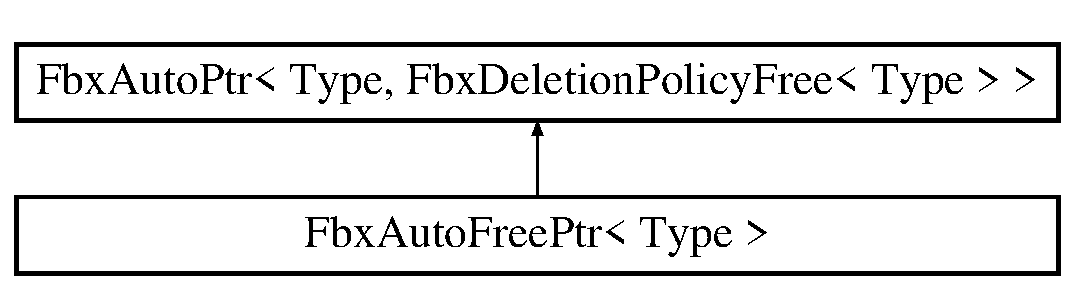
\includegraphics[height=2.000000cm]{class_fbx_auto_free_ptr}
\end{center}
\end{figure}
\subsection*{公開メンバ関数}
\begin{DoxyCompactItemize}
\item 
\hyperlink{class_fbx_auto_free_ptr_a02473c8a84df8d8fb6803a2d4224819d}{Fbx\+Auto\+Free\+Ptr} (Type $\ast$p\+Ptr=0)
\begin{DoxyCompactList}\small\item\em Construct from a pointer. \end{DoxyCompactList}\end{DoxyCompactItemize}


\subsection{詳解}
\subsubsection*{template$<$class Type$>$\newline
class Fbx\+Auto\+Free\+Ptr$<$ Type $>$}

Scoped pointer for Fbx\+Malloc allocations, which call \hyperlink{fbxalloc_8h_a8252906713d55f4c56e7ba84221d3852}{Fbx\+Free()} to deallocate. 

 fbxalloc.\+h の 253 行目に定義があります。



\subsection{構築子と解体子}
\mbox{\Hypertarget{class_fbx_auto_free_ptr_a02473c8a84df8d8fb6803a2d4224819d}\label{class_fbx_auto_free_ptr_a02473c8a84df8d8fb6803a2d4224819d}} 
\index{Fbx\+Auto\+Free\+Ptr@{Fbx\+Auto\+Free\+Ptr}!Fbx\+Auto\+Free\+Ptr@{Fbx\+Auto\+Free\+Ptr}}
\index{Fbx\+Auto\+Free\+Ptr@{Fbx\+Auto\+Free\+Ptr}!Fbx\+Auto\+Free\+Ptr@{Fbx\+Auto\+Free\+Ptr}}
\subsubsection{\texorpdfstring{Fbx\+Auto\+Free\+Ptr()}{FbxAutoFreePtr()}}
{\footnotesize\ttfamily template$<$class Type$>$ \\
\hyperlink{class_fbx_auto_free_ptr}{Fbx\+Auto\+Free\+Ptr}$<$ Type $>$\+::\hyperlink{class_fbx_auto_free_ptr}{Fbx\+Auto\+Free\+Ptr} (\begin{DoxyParamCaption}\item[{Type $\ast$}]{p\+Ptr = {\ttfamily 0} }\end{DoxyParamCaption})\hspace{0.3cm}{\ttfamily [inline]}, {\ttfamily [explicit]}}



Construct from a pointer. 



 fbxalloc.\+h の 257 行目に定義があります。



このクラス詳解は次のファイルから抽出されました\+:\begin{DoxyCompactItemize}
\item 
C\+:/\+Maya/scripts/\+F\+B\+X\+\_\+\+S\+D\+K/2017.\+1/include/fbxsdk/core/arch/\hyperlink{fbxalloc_8h}{fbxalloc.\+h}\end{DoxyCompactItemize}

\hypertarget{class_fbx_auto_ptr}{}\section{Fbx\+Auto\+Ptr$<$ Type, Policy $>$ クラステンプレート}
\label{class_fbx_auto_ptr}\index{Fbx\+Auto\+Ptr$<$ Type, Policy $>$@{Fbx\+Auto\+Ptr$<$ Type, Policy $>$}}


{\ttfamily \#include $<$fbxalloc.\+h$>$}

\subsection*{公開メンバ関数}
\begin{DoxyCompactItemize}
\item 
\hyperlink{class_fbx_auto_ptr_ae988d5760ee4926a4a10d76c37b378fc}{Fbx\+Auto\+Ptr} (Type $\ast$p\+Ptr=0)
\begin{DoxyCompactList}\small\item\em Construct from a pointer. \end{DoxyCompactList}\item 
\hyperlink{class_fbx_auto_ptr_aa185a3ac9d0cc7b8c2b04825f3ea73ee}{$\sim$\+Fbx\+Auto\+Ptr} ()
\begin{DoxyCompactList}\small\item\em Destructor. \end{DoxyCompactList}\item 
Type $\ast$ \hyperlink{class_fbx_auto_ptr_ae7006aca39929990a12c7c99af5d3ef7}{Get} () const
\begin{DoxyCompactList}\small\item\em Retrieve the pointer it holds. \end{DoxyCompactList}\item 
Type $\ast$ \hyperlink{class_fbx_auto_ptr_adfc79ea055e3de00252fb707ff5cfe31}{operator-\/$>$} () const
\begin{DoxyCompactList}\small\item\em Member access operator. \end{DoxyCompactList}\item 
\hyperlink{class_fbx_auto_ptr_ab7d5ac9eadc5c51ea062016f08640be1}{operator Type $\ast$} () const
\begin{DoxyCompactList}\small\item\em Convert to a Type pointer. \end{DoxyCompactList}\item 
Type \& \hyperlink{class_fbx_auto_ptr_acb65f0b9499fede18cb2749fa42f40a9}{operator$\ast$} () const
\begin{DoxyCompactList}\small\item\em Dereference operator. \end{DoxyCompactList}\item 
bool \hyperlink{class_fbx_auto_ptr_afc9bb02ba900f9920772416291690f45}{operator!} () const
\begin{DoxyCompactList}\small\item\em Logical not operator. \end{DoxyCompactList}\item 
\hyperlink{class_fbx_auto_ptr_ae92a5d1428b0ce74491aab76f8535b4c}{operator bool} () const
\begin{DoxyCompactList}\small\item\em Convert to boolean value. \end{DoxyCompactList}\item 
void \hyperlink{class_fbx_auto_ptr_ab0b755d84668c33b007a3311adb2b9e1}{Reset} (Type $\ast$p\+Ptr=0)
\begin{DoxyCompactList}\small\item\em Reset the scoped pointer by swapping with another pointer. \end{DoxyCompactList}\item 
void \hyperlink{class_fbx_auto_ptr_a46656f93e4ec91ece72fb90b9091fd2c}{Swap} (\hyperlink{class_fbx_auto_ptr}{Fbx\+Auto\+Ptr} \&p\+Other)
\begin{DoxyCompactList}\small\item\em Swap with another pointer. \end{DoxyCompactList}\item 
Type $\ast$ \hyperlink{class_fbx_auto_ptr_ab9460afa835fdaa907bf0ae32f939b8e}{Release} ()
\begin{DoxyCompactList}\small\item\em Release the pointer, so that it won\textquotesingle{}t perform deletion in its destruction. \end{DoxyCompactList}\end{DoxyCompactItemize}


\subsection{詳解}
\subsubsection*{template$<$class Type, class Policy = Fbx\+Deletion\+Policy\+Default$<$\+Type$>$$>$\newline
class Fbx\+Auto\+Ptr$<$ Type, Policy $>$}

\hyperlink{class_fbx_auto_ptr}{Fbx\+Auto\+Ptr} mimics the {\ttfamily auto\+\_\+ptr} class template implementation available in the C++ Standard Library. The {\ttfamily auto\+\_\+ptr} template class describes an object that stores a pointer to a single allocated object of type Type$\ast$ that ensures that the object to which it points gets destroyed automatically when control leaves a scope. 

 fbxalloc.\+h の 190 行目に定義があります。



\subsection{構築子と解体子}
\mbox{\Hypertarget{class_fbx_auto_ptr_ae988d5760ee4926a4a10d76c37b378fc}\label{class_fbx_auto_ptr_ae988d5760ee4926a4a10d76c37b378fc}} 
\index{Fbx\+Auto\+Ptr@{Fbx\+Auto\+Ptr}!Fbx\+Auto\+Ptr@{Fbx\+Auto\+Ptr}}
\index{Fbx\+Auto\+Ptr@{Fbx\+Auto\+Ptr}!Fbx\+Auto\+Ptr@{Fbx\+Auto\+Ptr}}
\subsubsection{\texorpdfstring{Fbx\+Auto\+Ptr()}{FbxAutoPtr()}}
{\footnotesize\ttfamily template$<$class Type, class Policy = Fbx\+Deletion\+Policy\+Default$<$\+Type$>$$>$ \\
\hyperlink{class_fbx_auto_ptr}{Fbx\+Auto\+Ptr}$<$ Type, Policy $>$\+::\hyperlink{class_fbx_auto_ptr}{Fbx\+Auto\+Ptr} (\begin{DoxyParamCaption}\item[{Type $\ast$}]{p\+Ptr = {\ttfamily 0} }\end{DoxyParamCaption})\hspace{0.3cm}{\ttfamily [inline]}, {\ttfamily [explicit]}}



Construct from a pointer. 



 fbxalloc.\+h の 194 行目に定義があります。

\mbox{\Hypertarget{class_fbx_auto_ptr_aa185a3ac9d0cc7b8c2b04825f3ea73ee}\label{class_fbx_auto_ptr_aa185a3ac9d0cc7b8c2b04825f3ea73ee}} 
\index{Fbx\+Auto\+Ptr@{Fbx\+Auto\+Ptr}!````~Fbx\+Auto\+Ptr@{$\sim$\+Fbx\+Auto\+Ptr}}
\index{````~Fbx\+Auto\+Ptr@{$\sim$\+Fbx\+Auto\+Ptr}!Fbx\+Auto\+Ptr@{Fbx\+Auto\+Ptr}}
\subsubsection{\texorpdfstring{$\sim$\+Fbx\+Auto\+Ptr()}{~FbxAutoPtr()}}
{\footnotesize\ttfamily template$<$class Type, class Policy = Fbx\+Deletion\+Policy\+Default$<$\+Type$>$$>$ \\
\hyperlink{class_fbx_auto_ptr}{Fbx\+Auto\+Ptr}$<$ Type, Policy $>$\+::$\sim$\hyperlink{class_fbx_auto_ptr}{Fbx\+Auto\+Ptr} (\begin{DoxyParamCaption}{ }\end{DoxyParamCaption})\hspace{0.3cm}{\ttfamily [inline]}}



Destructor. 



 fbxalloc.\+h の 197 行目に定義があります。



\subsection{関数詳解}
\mbox{\Hypertarget{class_fbx_auto_ptr_ae7006aca39929990a12c7c99af5d3ef7}\label{class_fbx_auto_ptr_ae7006aca39929990a12c7c99af5d3ef7}} 
\index{Fbx\+Auto\+Ptr@{Fbx\+Auto\+Ptr}!Get@{Get}}
\index{Get@{Get}!Fbx\+Auto\+Ptr@{Fbx\+Auto\+Ptr}}
\subsubsection{\texorpdfstring{Get()}{Get()}}
{\footnotesize\ttfamily template$<$class Type, class Policy = Fbx\+Deletion\+Policy\+Default$<$\+Type$>$$>$ \\
Type$\ast$ \hyperlink{class_fbx_auto_ptr}{Fbx\+Auto\+Ptr}$<$ Type, Policy $>$\+::Get (\begin{DoxyParamCaption}{ }\end{DoxyParamCaption}) const\hspace{0.3cm}{\ttfamily [inline]}}



Retrieve the pointer it holds. 



 fbxalloc.\+h の 200 行目に定義があります。

\mbox{\Hypertarget{class_fbx_auto_ptr_ae92a5d1428b0ce74491aab76f8535b4c}\label{class_fbx_auto_ptr_ae92a5d1428b0ce74491aab76f8535b4c}} 
\index{Fbx\+Auto\+Ptr@{Fbx\+Auto\+Ptr}!operator bool@{operator bool}}
\index{operator bool@{operator bool}!Fbx\+Auto\+Ptr@{Fbx\+Auto\+Ptr}}
\subsubsection{\texorpdfstring{operator bool()}{operator bool()}}
{\footnotesize\ttfamily template$<$class Type, class Policy = Fbx\+Deletion\+Policy\+Default$<$\+Type$>$$>$ \\
\hyperlink{class_fbx_auto_ptr}{Fbx\+Auto\+Ptr}$<$ Type, Policy $>$\+::operator bool (\begin{DoxyParamCaption}{ }\end{DoxyParamCaption}) const\hspace{0.3cm}{\ttfamily [inline]}}



Convert to boolean value. 



 fbxalloc.\+h の 215 行目に定義があります。

\mbox{\Hypertarget{class_fbx_auto_ptr_ab7d5ac9eadc5c51ea062016f08640be1}\label{class_fbx_auto_ptr_ab7d5ac9eadc5c51ea062016f08640be1}} 
\index{Fbx\+Auto\+Ptr@{Fbx\+Auto\+Ptr}!operator Type $\ast$@{operator Type $\ast$}}
\index{operator Type $\ast$@{operator Type $\ast$}!Fbx\+Auto\+Ptr@{Fbx\+Auto\+Ptr}}
\subsubsection{\texorpdfstring{operator Type $\ast$()}{operator Type *()}}
{\footnotesize\ttfamily template$<$class Type, class Policy = Fbx\+Deletion\+Policy\+Default$<$\+Type$>$$>$ \\
\hyperlink{class_fbx_auto_ptr}{Fbx\+Auto\+Ptr}$<$ Type, Policy $>$\+::operator Type $\ast$ (\begin{DoxyParamCaption}{ }\end{DoxyParamCaption}) const\hspace{0.3cm}{\ttfamily [inline]}}



Convert to a Type pointer. 



 fbxalloc.\+h の 206 行目に定義があります。

\mbox{\Hypertarget{class_fbx_auto_ptr_afc9bb02ba900f9920772416291690f45}\label{class_fbx_auto_ptr_afc9bb02ba900f9920772416291690f45}} 
\index{Fbx\+Auto\+Ptr@{Fbx\+Auto\+Ptr}!operator"!@{operator"!}}
\index{operator"!@{operator"!}!Fbx\+Auto\+Ptr@{Fbx\+Auto\+Ptr}}
\subsubsection{\texorpdfstring{operator"!()}{operator!()}}
{\footnotesize\ttfamily template$<$class Type, class Policy = Fbx\+Deletion\+Policy\+Default$<$\+Type$>$$>$ \\
bool \hyperlink{class_fbx_auto_ptr}{Fbx\+Auto\+Ptr}$<$ Type, Policy $>$\+::operator! (\begin{DoxyParamCaption}{ }\end{DoxyParamCaption}) const\hspace{0.3cm}{\ttfamily [inline]}}



Logical not operator. 



 fbxalloc.\+h の 212 行目に定義があります。

\mbox{\Hypertarget{class_fbx_auto_ptr_acb65f0b9499fede18cb2749fa42f40a9}\label{class_fbx_auto_ptr_acb65f0b9499fede18cb2749fa42f40a9}} 
\index{Fbx\+Auto\+Ptr@{Fbx\+Auto\+Ptr}!operator$\ast$@{operator$\ast$}}
\index{operator$\ast$@{operator$\ast$}!Fbx\+Auto\+Ptr@{Fbx\+Auto\+Ptr}}
\subsubsection{\texorpdfstring{operator$\ast$()}{operator*()}}
{\footnotesize\ttfamily template$<$class Type, class Policy = Fbx\+Deletion\+Policy\+Default$<$\+Type$>$$>$ \\
Type\& \hyperlink{class_fbx_auto_ptr}{Fbx\+Auto\+Ptr}$<$ Type, Policy $>$\+::operator$\ast$ (\begin{DoxyParamCaption}{ }\end{DoxyParamCaption}) const\hspace{0.3cm}{\ttfamily [inline]}}



Dereference operator. 



 fbxalloc.\+h の 209 行目に定義があります。

\mbox{\Hypertarget{class_fbx_auto_ptr_adfc79ea055e3de00252fb707ff5cfe31}\label{class_fbx_auto_ptr_adfc79ea055e3de00252fb707ff5cfe31}} 
\index{Fbx\+Auto\+Ptr@{Fbx\+Auto\+Ptr}!operator-\/$>$@{operator-\/$>$}}
\index{operator-\/$>$@{operator-\/$>$}!Fbx\+Auto\+Ptr@{Fbx\+Auto\+Ptr}}
\subsubsection{\texorpdfstring{operator-\/$>$()}{operator->()}}
{\footnotesize\ttfamily template$<$class Type, class Policy = Fbx\+Deletion\+Policy\+Default$<$\+Type$>$$>$ \\
Type$\ast$ \hyperlink{class_fbx_auto_ptr}{Fbx\+Auto\+Ptr}$<$ Type, Policy $>$\+::operator-\/$>$ (\begin{DoxyParamCaption}{ }\end{DoxyParamCaption}) const\hspace{0.3cm}{\ttfamily [inline]}}



Member access operator. 



 fbxalloc.\+h の 203 行目に定義があります。

\mbox{\Hypertarget{class_fbx_auto_ptr_ab9460afa835fdaa907bf0ae32f939b8e}\label{class_fbx_auto_ptr_ab9460afa835fdaa907bf0ae32f939b8e}} 
\index{Fbx\+Auto\+Ptr@{Fbx\+Auto\+Ptr}!Release@{Release}}
\index{Release@{Release}!Fbx\+Auto\+Ptr@{Fbx\+Auto\+Ptr}}
\subsubsection{\texorpdfstring{Release()}{Release()}}
{\footnotesize\ttfamily template$<$class Type, class Policy = Fbx\+Deletion\+Policy\+Default$<$\+Type$>$$>$ \\
Type$\ast$ \hyperlink{class_fbx_auto_ptr}{Fbx\+Auto\+Ptr}$<$ Type, Policy $>$\+::Release (\begin{DoxyParamCaption}{ }\end{DoxyParamCaption})\hspace{0.3cm}{\ttfamily [inline]}}



Release the pointer, so that it won\textquotesingle{}t perform deletion in its destruction. 



 fbxalloc.\+h の 233 行目に定義があります。

\mbox{\Hypertarget{class_fbx_auto_ptr_ab0b755d84668c33b007a3311adb2b9e1}\label{class_fbx_auto_ptr_ab0b755d84668c33b007a3311adb2b9e1}} 
\index{Fbx\+Auto\+Ptr@{Fbx\+Auto\+Ptr}!Reset@{Reset}}
\index{Reset@{Reset}!Fbx\+Auto\+Ptr@{Fbx\+Auto\+Ptr}}
\subsubsection{\texorpdfstring{Reset()}{Reset()}}
{\footnotesize\ttfamily template$<$class Type, class Policy = Fbx\+Deletion\+Policy\+Default$<$\+Type$>$$>$ \\
void \hyperlink{class_fbx_auto_ptr}{Fbx\+Auto\+Ptr}$<$ Type, Policy $>$\+::Reset (\begin{DoxyParamCaption}\item[{Type $\ast$}]{p\+Ptr = {\ttfamily 0} }\end{DoxyParamCaption})\hspace{0.3cm}{\ttfamily [inline]}}



Reset the scoped pointer by swapping with another pointer. 



 fbxalloc.\+h の 218 行目に定義があります。

\mbox{\Hypertarget{class_fbx_auto_ptr_a46656f93e4ec91ece72fb90b9091fd2c}\label{class_fbx_auto_ptr_a46656f93e4ec91ece72fb90b9091fd2c}} 
\index{Fbx\+Auto\+Ptr@{Fbx\+Auto\+Ptr}!Swap@{Swap}}
\index{Swap@{Swap}!Fbx\+Auto\+Ptr@{Fbx\+Auto\+Ptr}}
\subsubsection{\texorpdfstring{Swap()}{Swap()}}
{\footnotesize\ttfamily template$<$class Type, class Policy = Fbx\+Deletion\+Policy\+Default$<$\+Type$>$$>$ \\
void \hyperlink{class_fbx_auto_ptr}{Fbx\+Auto\+Ptr}$<$ Type, Policy $>$\+::Swap (\begin{DoxyParamCaption}\item[{\hyperlink{class_fbx_auto_ptr}{Fbx\+Auto\+Ptr}$<$ Type, Policy $>$ \&}]{p\+Other }\end{DoxyParamCaption})\hspace{0.3cm}{\ttfamily [inline]}}



Swap with another pointer. 



 fbxalloc.\+h の 225 行目に定義があります。



このクラス詳解は次のファイルから抽出されました\+:\begin{DoxyCompactItemize}
\item 
C\+:/\+Maya/scripts/\+F\+B\+X\+\_\+\+S\+D\+K/2017.\+1/include/fbxsdk/core/arch/\hyperlink{fbxalloc_8h}{fbxalloc.\+h}\end{DoxyCompactItemize}

\hypertarget{struct_fbx_i_o_1_1_fbx_auto_reset_x_ref_manager}{}\section{Fbx\+IO\+:\+:Fbx\+Auto\+Reset\+X\+Ref\+Manager 構造体}
\label{struct_fbx_i_o_1_1_fbx_auto_reset_x_ref_manager}\index{Fbx\+I\+O\+::\+Fbx\+Auto\+Reset\+X\+Ref\+Manager@{Fbx\+I\+O\+::\+Fbx\+Auto\+Reset\+X\+Ref\+Manager}}


{\ttfamily \#include $<$fbxio.\+h$>$}

\subsection*{公開メンバ関数}
\begin{DoxyCompactItemize}
\item 
\hyperlink{struct_fbx_i_o_1_1_fbx_auto_reset_x_ref_manager_a4fd55e4840d236b0afb561001dc2faef}{Fbx\+Auto\+Reset\+X\+Ref\+Manager} (\hyperlink{class_fbx_i_o}{Fbx\+IO} $\ast$p\+Fbx, \hyperlink{class_fbx_x_ref_manager}{Fbx\+X\+Ref\+Manager} \&p\+X\+Ref\+Manager)
\item 
\hyperlink{struct_fbx_i_o_1_1_fbx_auto_reset_x_ref_manager_a7a90d25e3fbad8c2e30bc7a3bd21d702}{$\sim$\+Fbx\+Auto\+Reset\+X\+Ref\+Manager} ()
\end{DoxyCompactItemize}
\subsection*{公開変数類}
\begin{DoxyCompactItemize}
\item 
\hyperlink{class_fbx_i_o}{Fbx\+IO} $\ast$ \hyperlink{struct_fbx_i_o_1_1_fbx_auto_reset_x_ref_manager_a5203c9a88c60e8c6f8a092ec2c84759c}{m\+Fbx}
\item 
const \hyperlink{class_fbx_x_ref_manager}{Fbx\+X\+Ref\+Manager} $\ast$ \hyperlink{struct_fbx_i_o_1_1_fbx_auto_reset_x_ref_manager_a65b41fef18ebe8d10db3dafe69cca132}{m\+X\+Ref\+Manager}
\end{DoxyCompactItemize}


\subsection{詳解}


 fbxio.\+h の 330 行目に定義があります。



\subsection{構築子と解体子}
\mbox{\Hypertarget{struct_fbx_i_o_1_1_fbx_auto_reset_x_ref_manager_a4fd55e4840d236b0afb561001dc2faef}\label{struct_fbx_i_o_1_1_fbx_auto_reset_x_ref_manager_a4fd55e4840d236b0afb561001dc2faef}} 
\index{Fbx\+I\+O\+::\+Fbx\+Auto\+Reset\+X\+Ref\+Manager@{Fbx\+I\+O\+::\+Fbx\+Auto\+Reset\+X\+Ref\+Manager}!Fbx\+Auto\+Reset\+X\+Ref\+Manager@{Fbx\+Auto\+Reset\+X\+Ref\+Manager}}
\index{Fbx\+Auto\+Reset\+X\+Ref\+Manager@{Fbx\+Auto\+Reset\+X\+Ref\+Manager}!Fbx\+I\+O\+::\+Fbx\+Auto\+Reset\+X\+Ref\+Manager@{Fbx\+I\+O\+::\+Fbx\+Auto\+Reset\+X\+Ref\+Manager}}
\subsubsection{\texorpdfstring{Fbx\+Auto\+Reset\+X\+Ref\+Manager()}{FbxAutoResetXRefManager()}}
{\footnotesize\ttfamily Fbx\+I\+O\+::\+Fbx\+Auto\+Reset\+X\+Ref\+Manager\+::\+Fbx\+Auto\+Reset\+X\+Ref\+Manager (\begin{DoxyParamCaption}\item[{\hyperlink{class_fbx_i_o}{Fbx\+IO} $\ast$}]{p\+Fbx,  }\item[{\hyperlink{class_fbx_x_ref_manager}{Fbx\+X\+Ref\+Manager} \&}]{p\+X\+Ref\+Manager }\end{DoxyParamCaption})\hspace{0.3cm}{\ttfamily [inline]}}

Default constructor 

 fbxio.\+h の 336 行目に定義があります。

\mbox{\Hypertarget{struct_fbx_i_o_1_1_fbx_auto_reset_x_ref_manager_a7a90d25e3fbad8c2e30bc7a3bd21d702}\label{struct_fbx_i_o_1_1_fbx_auto_reset_x_ref_manager_a7a90d25e3fbad8c2e30bc7a3bd21d702}} 
\index{Fbx\+I\+O\+::\+Fbx\+Auto\+Reset\+X\+Ref\+Manager@{Fbx\+I\+O\+::\+Fbx\+Auto\+Reset\+X\+Ref\+Manager}!````~Fbx\+Auto\+Reset\+X\+Ref\+Manager@{$\sim$\+Fbx\+Auto\+Reset\+X\+Ref\+Manager}}
\index{````~Fbx\+Auto\+Reset\+X\+Ref\+Manager@{$\sim$\+Fbx\+Auto\+Reset\+X\+Ref\+Manager}!Fbx\+I\+O\+::\+Fbx\+Auto\+Reset\+X\+Ref\+Manager@{Fbx\+I\+O\+::\+Fbx\+Auto\+Reset\+X\+Ref\+Manager}}
\subsubsection{\texorpdfstring{$\sim$\+Fbx\+Auto\+Reset\+X\+Ref\+Manager()}{~FbxAutoResetXRefManager()}}
{\footnotesize\ttfamily Fbx\+I\+O\+::\+Fbx\+Auto\+Reset\+X\+Ref\+Manager\+::$\sim$\+Fbx\+Auto\+Reset\+X\+Ref\+Manager (\begin{DoxyParamCaption}{ }\end{DoxyParamCaption})\hspace{0.3cm}{\ttfamily [inline]}}

Destructor 

 fbxio.\+h の 348 行目に定義があります。



\subsection{メンバ詳解}
\mbox{\Hypertarget{struct_fbx_i_o_1_1_fbx_auto_reset_x_ref_manager_a5203c9a88c60e8c6f8a092ec2c84759c}\label{struct_fbx_i_o_1_1_fbx_auto_reset_x_ref_manager_a5203c9a88c60e8c6f8a092ec2c84759c}} 
\index{Fbx\+I\+O\+::\+Fbx\+Auto\+Reset\+X\+Ref\+Manager@{Fbx\+I\+O\+::\+Fbx\+Auto\+Reset\+X\+Ref\+Manager}!m\+Fbx@{m\+Fbx}}
\index{m\+Fbx@{m\+Fbx}!Fbx\+I\+O\+::\+Fbx\+Auto\+Reset\+X\+Ref\+Manager@{Fbx\+I\+O\+::\+Fbx\+Auto\+Reset\+X\+Ref\+Manager}}
\subsubsection{\texorpdfstring{m\+Fbx}{mFbx}}
{\footnotesize\ttfamily \hyperlink{class_fbx_i_o}{Fbx\+IO}$\ast$ Fbx\+I\+O\+::\+Fbx\+Auto\+Reset\+X\+Ref\+Manager\+::m\+Fbx}



 fbxio.\+h の 332 行目に定義があります。

\mbox{\Hypertarget{struct_fbx_i_o_1_1_fbx_auto_reset_x_ref_manager_a65b41fef18ebe8d10db3dafe69cca132}\label{struct_fbx_i_o_1_1_fbx_auto_reset_x_ref_manager_a65b41fef18ebe8d10db3dafe69cca132}} 
\index{Fbx\+I\+O\+::\+Fbx\+Auto\+Reset\+X\+Ref\+Manager@{Fbx\+I\+O\+::\+Fbx\+Auto\+Reset\+X\+Ref\+Manager}!m\+X\+Ref\+Manager@{m\+X\+Ref\+Manager}}
\index{m\+X\+Ref\+Manager@{m\+X\+Ref\+Manager}!Fbx\+I\+O\+::\+Fbx\+Auto\+Reset\+X\+Ref\+Manager@{Fbx\+I\+O\+::\+Fbx\+Auto\+Reset\+X\+Ref\+Manager}}
\subsubsection{\texorpdfstring{m\+X\+Ref\+Manager}{mXRefManager}}
{\footnotesize\ttfamily const \hyperlink{class_fbx_x_ref_manager}{Fbx\+X\+Ref\+Manager}$\ast$ Fbx\+I\+O\+::\+Fbx\+Auto\+Reset\+X\+Ref\+Manager\+::m\+X\+Ref\+Manager}



 fbxio.\+h の 333 行目に定義があります。



この構造体詳解は次のファイルから抽出されました\+:\begin{DoxyCompactItemize}
\item 
C\+:/\+Maya/scripts/\+F\+B\+X\+\_\+\+S\+D\+K/2017.\+1/include/fbxsdk/fileio/fbx/\hyperlink{fbxio_8h}{fbxio.\+h}\end{DoxyCompactItemize}

\hypertarget{class_fbx_axis_system}{}\section{Fbx\+Axis\+System クラス}
\label{class_fbx_axis_system}\index{Fbx\+Axis\+System@{Fbx\+Axis\+System}}


{\ttfamily \#include $<$fbxaxissystem.\+h$>$}

\subsection*{クラス}
\begin{DoxyCompactItemize}
\item 
class \hyperlink{class_fbx_axis_system_1_1_axis_def}{Axis\+Def}
\end{DoxyCompactItemize}
\subsection*{公開型}
\begin{DoxyCompactItemize}
\item 
enum \hyperlink{class_fbx_axis_system_ad41a41f7ccd9167f54d09b65ad781d00}{E\+Up\+Vector} \{ \hyperlink{class_fbx_axis_system_ad41a41f7ccd9167f54d09b65ad781d00a16f5021a60fc8fe7d83224f9a3f7dab0}{e\+X\+Axis} = 1, 
\hyperlink{class_fbx_axis_system_ad41a41f7ccd9167f54d09b65ad781d00a0744a596281fabdb16cd7151bdb25e32}{e\+Y\+Axis} = 2, 
\hyperlink{class_fbx_axis_system_ad41a41f7ccd9167f54d09b65ad781d00a8d38edfa15833205ff173fc76461cbcd}{e\+Z\+Axis} = 3
 \}
\item 
enum \hyperlink{class_fbx_axis_system_a34bce1daad7ed6ae71916bb825d3ec87}{E\+Front\+Vector} \{ \hyperlink{class_fbx_axis_system_a34bce1daad7ed6ae71916bb825d3ec87a60d99824537be50ebc6aa4169438da55}{e\+Parity\+Even} = 1, 
\hyperlink{class_fbx_axis_system_a34bce1daad7ed6ae71916bb825d3ec87a918bd8db749bc1ed4f2f176c27e67023}{e\+Parity\+Odd} = 2
 \}
\item 
enum \hyperlink{class_fbx_axis_system_a7cf0485846b560fa34f86932c02ec333}{E\+Coord\+System} \{ \hyperlink{class_fbx_axis_system_a7cf0485846b560fa34f86932c02ec333abdf1da85a4ef5a2d65c8d6271e3acf6d}{e\+Right\+Handed}, 
\hyperlink{class_fbx_axis_system_a7cf0485846b560fa34f86932c02ec333aecd32fe7557773b957f101f58840b387}{e\+Left\+Handed}
 \}
\item 
enum \hyperlink{class_fbx_axis_system_a0391b88959ec9ed790cb76eac9a6ed17}{E\+Pre\+Defined\+Axis\+System} \{ \newline
\hyperlink{class_fbx_axis_system_a0391b88959ec9ed790cb76eac9a6ed17ad5e9ac656bd6239774a5e42e4ba6d934}{e\+Maya\+Z\+Up}, 
\hyperlink{class_fbx_axis_system_a0391b88959ec9ed790cb76eac9a6ed17a50808e67e3328965897a009c4b50a31e}{e\+Maya\+Y\+Up}, 
\hyperlink{class_fbx_axis_system_a0391b88959ec9ed790cb76eac9a6ed17ab9b1fd4a0c7dd20253a1642bfaeea0c0}{e\+Max}, 
\hyperlink{class_fbx_axis_system_a0391b88959ec9ed790cb76eac9a6ed17a8920292b5d781bf132c1d80e9228d347}{e\+Motion\+Builder}, 
\newline
\hyperlink{class_fbx_axis_system_a0391b88959ec9ed790cb76eac9a6ed17ac1fa0ca99895821578046b6c78f389e0}{e\+Open\+GL}, 
\hyperlink{class_fbx_axis_system_a0391b88959ec9ed790cb76eac9a6ed17a30702b7143f70669c4fd283836b2d2ce}{e\+DirectX}, 
\hyperlink{class_fbx_axis_system_a0391b88959ec9ed790cb76eac9a6ed17acb86800d6af93402f8c090f6603aff37}{e\+Lightwave}
 \}
\end{DoxyCompactItemize}
\subsection*{公開メンバ関数}
\begin{DoxyCompactItemize}
\item 
\hyperlink{class_fbx_axis_system}{Fbx\+Axis\+System} \& \hyperlink{class_fbx_axis_system_a108da01b311416d5b60305ac170e5be5}{operator=} (const \hyperlink{class_fbx_axis_system}{Fbx\+Axis\+System} \&p\+Axis\+System)
\item 
void \hyperlink{class_fbx_axis_system_abb9a361cd8d245c60e68b05868c67b4e}{Convert\+Scene} (\hyperlink{class_fbx_scene}{Fbx\+Scene} $\ast$p\+Scene) const
\item 
void \hyperlink{class_fbx_axis_system_a25f6f6ddb481f280bfecca5d39d14d4c}{Convert\+Scene} (\hyperlink{class_fbx_scene}{Fbx\+Scene} $\ast$p\+Scene, \hyperlink{class_fbx_node}{Fbx\+Node} $\ast$p\+Fbx\+Root) const
\item 
\hyperlink{class_fbx_axis_system_a34bce1daad7ed6ae71916bb825d3ec87}{E\+Front\+Vector} \hyperlink{class_fbx_axis_system_a523996d3b195bf6016ab7c0333a5d389}{Get\+Front\+Vector} (int \&p\+Sign) const
\item 
\hyperlink{class_fbx_axis_system_ad41a41f7ccd9167f54d09b65ad781d00}{E\+Up\+Vector} \hyperlink{class_fbx_axis_system_a3ed72f373b701c5f7c108e93f23e0e73}{Get\+Up\+Vector} (int \&p\+Sign) const
\item 
\hyperlink{class_fbx_axis_system_a7cf0485846b560fa34f86932c02ec333}{E\+Coord\+System} \hyperlink{class_fbx_axis_system_a6ebdf99e9754d3bd83d3a8f98544b331}{Get\+Coor\+System} () const
\item 
void \hyperlink{class_fbx_axis_system_a2ee31cfe8c836f4abdbc939a0891a6a9}{Get\+Matrix} (\hyperlink{class_fbx_a_matrix}{Fbx\+A\+Matrix} \&p\+Matrix)
\item 
void \hyperlink{class_fbx_axis_system_a3eff3d4a3b2270a5f3675f32b698e6e9}{Convert\+Children} (\hyperlink{class_fbx_node}{Fbx\+Node} $\ast$p\+Root, const \hyperlink{class_fbx_axis_system}{Fbx\+Axis\+System} \&p\+Src\+System) const
\end{DoxyCompactItemize}
\subsection*{限定公開メンバ関数}
\begin{DoxyCompactItemize}
\item 
void \hyperlink{class_fbx_axis_system_a41956e32f21b9709f40efef34a6d6121}{Convert\+T\+Property} (\hyperlink{class_fbx_array}{Fbx\+Array}$<$ \hyperlink{class_fbx_node}{Fbx\+Node} $\ast$$>$ \&p\+Nodes, const \hyperlink{class_fbx_axis_system}{Fbx\+Axis\+System} \&p\+From) const
\item 
void \hyperlink{class_fbx_axis_system_a39608f5f990b1ab304f13ee2b6df64ea}{Convert\+Curve\+Nodes} (\hyperlink{class_fbx_array}{Fbx\+Array}$<$ \hyperlink{class_fbx_anim_curve_node}{Fbx\+Anim\+Curve\+Node} $\ast$$>$ \&p\+Curve\+Nodes, const \hyperlink{class_fbx_axis_system}{Fbx\+Axis\+System} \&p\+From) const
\item 
void \hyperlink{class_fbx_axis_system_af7afdf5273c5ca9130ee8996f6f846a3}{Adjust\+Pre\+Rotation} (\hyperlink{class_fbx_node}{Fbx\+Node} $\ast$p\+Node, const \hyperlink{class_fbx_matrix}{Fbx\+Matrix} \&p\+Conversion\+RM) const
\item 
void \hyperlink{class_fbx_axis_system_aab7c9d541191268942f8dbbc3f531150}{Adjust\+Pivots} (\hyperlink{class_fbx_node}{Fbx\+Node} $\ast$p\+Node, const \hyperlink{class_fbx_matrix}{Fbx\+Matrix} \&p\+Conversion\+RM) const
\item 
void \hyperlink{class_fbx_axis_system_ae365f46f757b83df6426e5469938e8a0}{Get\+Conversion\+Matrix} (const \hyperlink{class_fbx_axis_system}{Fbx\+Axis\+System} \&p\+From, \hyperlink{class_fbx_matrix}{Fbx\+Matrix} \&p\+Conversion\+RM) const
\item 
void \hyperlink{class_fbx_axis_system_a699d144078ae640f30de2230a03c468f}{Adjust\+Limits} (\hyperlink{class_fbx_node}{Fbx\+Node} $\ast$p\+Node, const \hyperlink{class_fbx_matrix}{Fbx\+Matrix} \&p\+Conversion\+RM) const
\item 
void \hyperlink{class_fbx_axis_system_a4547ae0ec09f1c6e15e171e8cb56a7f9}{Adjust\+Poses} (\hyperlink{class_fbx_scene}{Fbx\+Scene} $\ast$p\+Scene, const \hyperlink{class_fbx_matrix}{Fbx\+Matrix} \&p\+Conversion\+RM) const
\item 
void \hyperlink{class_fbx_axis_system_ab51a2f8a7a77c1bfe77ba1da70d83cee}{Adjust\+Camera} (\hyperlink{class_fbx_node}{Fbx\+Node} $\ast$p\+Node, const \hyperlink{class_fbx_matrix}{Fbx\+Matrix} \&p\+Conversion\+RM) const
\item 
void \hyperlink{class_fbx_axis_system_a4b3ccc6e69b77974b3e5489cfefa2755}{Adjust\+Cluster} (\hyperlink{class_fbx_node}{Fbx\+Node} $\ast$p\+Node, const \hyperlink{class_fbx_matrix}{Fbx\+Matrix} \&p\+Conversion\+RM) const
\item 
void \hyperlink{class_fbx_axis_system_aca4f4de94c2d604fa55c001c25c0c227}{Convert\+Children} (\hyperlink{class_fbx_node}{Fbx\+Node} $\ast$p\+Root, const \hyperlink{class_fbx_axis_system}{Fbx\+Axis\+System} \&p\+Src\+System, bool p\+Sub\+Children\+Only) const
\end{DoxyCompactItemize}
\subsection*{限定公開変数類}
\begin{DoxyCompactItemize}
\item 
\hyperlink{class_fbx_axis_system_1_1_axis_def}{Axis\+Def} \hyperlink{class_fbx_axis_system_afdefd4d8b257567fe099e28dd1745cfe}{m\+Up\+Vector}
\item 
\hyperlink{class_fbx_axis_system_1_1_axis_def}{Axis\+Def} \hyperlink{class_fbx_axis_system_a8d26e8fb0d5e47bc2e7f667a7b288a5b}{m\+Front\+Vector}
\item 
\hyperlink{class_fbx_axis_system_1_1_axis_def}{Axis\+Def} \hyperlink{class_fbx_axis_system_ac6a0711045499b8e4f699019e3c7fe0e}{m\+Coor\+System}
\end{DoxyCompactItemize}
\subsection*{フレンド}
\begin{DoxyCompactItemize}
\item 
class \hyperlink{class_fbx_axis_system_ac6f6b3953bf13718eb87110d614b3c9a}{Fbx\+Global\+Settings}
\end{DoxyCompactItemize}
\subsection*{Constructor and Destructor}
\begin{DoxyCompactItemize}
\item 
\hyperlink{class_fbx_axis_system_a37136053617df840bae0347820f706a7}{Fbx\+Axis\+System} ()
\item 
\hyperlink{class_fbx_axis_system_a38f184b0d67eeb8578e25c800a0571a5}{Fbx\+Axis\+System} (\hyperlink{class_fbx_axis_system_ad41a41f7ccd9167f54d09b65ad781d00}{E\+Up\+Vector} p\+Up\+Vector, \hyperlink{class_fbx_axis_system_a34bce1daad7ed6ae71916bb825d3ec87}{E\+Front\+Vector} p\+Front\+Vector, \hyperlink{class_fbx_axis_system_a7cf0485846b560fa34f86932c02ec333}{E\+Coord\+System} p\+Coor\+System)
\item 
\hyperlink{class_fbx_axis_system_a3db4f8e0bc1a588cc8c7fc2fa29a532c}{Fbx\+Axis\+System} (const \hyperlink{class_fbx_axis_system}{Fbx\+Axis\+System} \&p\+Axis\+System)
\item 
\hyperlink{class_fbx_axis_system_a8333ad188498e489a2bf065c2b5b1ad3}{Fbx\+Axis\+System} (const \hyperlink{class_fbx_axis_system_a0391b88959ec9ed790cb76eac9a6ed17}{E\+Pre\+Defined\+Axis\+System} p\+Axis\+System)
\item 
virtual \hyperlink{class_fbx_axis_system_ae1c61cb9cf7208d0c4373d8c894bec8c}{$\sim$\+Fbx\+Axis\+System} ()
\begin{DoxyCompactList}\small\item\em Destructor. \end{DoxyCompactList}\end{DoxyCompactItemize}
\subsection*{Boolean operation.}
\begin{DoxyCompactItemize}
\item 
bool \hyperlink{class_fbx_axis_system_a36933159c0730e52b918f9b52cb2ecc1}{operator==} (const \hyperlink{class_fbx_axis_system}{Fbx\+Axis\+System} \&p\+Axis\+System) const
\item 
bool \hyperlink{class_fbx_axis_system_adf5cf05010b87ddde4bb158e274892b4}{operator!=} (const \hyperlink{class_fbx_axis_system}{Fbx\+Axis\+System} \&p\+Axis\+System) const
\end{DoxyCompactItemize}
\subsection*{Predefined axis systems.}
\label{_amgrp8a063321b07f432f44f56214112969d8}%
These static members define the axis system of the most popular applications. \begin{DoxyCompactItemize}
\item 
static const \hyperlink{class_fbx_axis_system}{Fbx\+Axis\+System} \hyperlink{class_fbx_axis_system_af6d2329b82cd505ae9816810f9d26bd6}{Maya\+Z\+Up}
\begin{DoxyCompactList}\small\item\em Predefined axis system\+: Maya\+Z\+Up (Up\+Vector = +Z, Front\+Vector = -\/Y, Coord\+System = +X (Right\+Handed)) \end{DoxyCompactList}\item 
static const \hyperlink{class_fbx_axis_system}{Fbx\+Axis\+System} \hyperlink{class_fbx_axis_system_a898f6952538dbc23cead05b2a1e19d10}{Maya\+Y\+Up}
\begin{DoxyCompactList}\small\item\em Predefined axis system\+: Maya\+Y\+Up (Up\+Vector = +Y, Front\+Vector = +Z, Coord\+System = +X (Right\+Handed)) \end{DoxyCompactList}\item 
static const \hyperlink{class_fbx_axis_system}{Fbx\+Axis\+System} \hyperlink{class_fbx_axis_system_a3ac2db6cd471f8477a1d0b4a3ad22608}{Max}
\begin{DoxyCompactList}\small\item\em Predefined axis system\+: Max (Up\+Vector = +Z, Front\+Vector = -\/Y, Coord\+System = +X (Right\+Handed)) \end{DoxyCompactList}\item 
static const \hyperlink{class_fbx_axis_system}{Fbx\+Axis\+System} \hyperlink{class_fbx_axis_system_af24f958db3b4147d22005984cd4cebb2}{Motionbuilder}
\begin{DoxyCompactList}\small\item\em Predefined axis system\+: Motionbuilder (Up\+Vector = +Y, Front\+Vector = +Z, Coord\+System = +X (Right\+Handed)) \end{DoxyCompactList}\item 
static const \hyperlink{class_fbx_axis_system}{Fbx\+Axis\+System} \hyperlink{class_fbx_axis_system_a30249cc37f848cdac27b77d3520f4e28}{Open\+GL}
\begin{DoxyCompactList}\small\item\em Predefined axis system\+: Open\+GL (Up\+Vector = +Y, Front\+Vector = +Z, Coord\+System = +X (Right\+Handed)) \end{DoxyCompactList}\item 
static const \hyperlink{class_fbx_axis_system}{Fbx\+Axis\+System} \hyperlink{class_fbx_axis_system_a2eddfe5afe7db5f56adee774c51559e9}{DirectX}
\begin{DoxyCompactList}\small\item\em Predefined axis system\+: DirectX (Up\+Vector = +Y, Front\+Vector = +Z, Coord\+System = -\/X (Left\+Handed)) \end{DoxyCompactList}\item 
static const \hyperlink{class_fbx_axis_system}{Fbx\+Axis\+System} \hyperlink{class_fbx_axis_system_a45fc90ee125c8dafa7ca95f62e7485a8}{Lightwave}
\begin{DoxyCompactList}\small\item\em Predefined axis system\+: Lightwave (Up\+Vector = +Y, Front\+Vector = +Z, Coord\+System = -\/X (Left\+Handed)) \end{DoxyCompactList}\end{DoxyCompactItemize}


\subsection{詳解}
This class represents the coordinate system of the scene and can convert scenes to other coordinate systems. By default the \hyperlink{class_fbx_scene}{Fbx\+Scene} uses a Y-\/\+Up axis system. If the calling application wishes to change the default axis it will need to define the new axis system and call the convert method with the scene as argument. The appropriate transforms will be applied to the first level objects of the scene only (objects whose parent is the scene itself). Child objects do not need to be transformed since they inherit from their parents. The adjustment will affect the translation animation curves and the objects pivots values (the rotation transformation is applied as a pre-\/rotation transform therefore the rotation animation curves do not need to be transformed). Once converted, the scene will have its axis definition changed to the new system.

For example\+: 
\begin{DoxyCode}
\hyperlink{class_fbx_scene}{FbxScene}* lScene = FbxScene::Create(sdkmanager, \textcolor{stringliteral}{"MyScene"});
...
\textcolor{comment}{// the scene is filled with objects}

int dir;
lScene->\hyperlink{class_fbx_scene_a0cb767181a743532c9e9be17f0348570}{GetGlobalSettings}().\hyperlink{class_fbx_global_settings_adf26f4742b088b497a5ecec8f458e47d}{GetAxisSystem}().
      \hyperlink{class_fbx_axis_system_a3ed72f373b701c5f7c108e93f23e0e73}{GetUpVector}(dir); \textcolor{comment}{// this returns the equivalent of FbxAxisSystem::eYAxis}

\hyperlink{class_fbx_axis_system}{FbxAxisSystem} max; \textcolor{comment}{// we desire to convert the scene from Y-Up to Z-Up}
max.\hyperlink{class_fbx_axis_system_abb9a361cd8d245c60e68b05868c67b4e}{ConvertScene}(lScene);

lScene->\hyperlink{class_fbx_scene_a0cb767181a743532c9e9be17f0348570}{GetGlobalSettings}().\hyperlink{class_fbx_global_settings_adf26f4742b088b497a5ecec8f458e47d}{GetAxisSystem}().
      \hyperlink{class_fbx_axis_system_a3ed72f373b701c5f7c108e93f23e0e73}{GetUpVector}(dir); \textcolor{comment}{// this will now return the equivalent of FbxAxisSystem::eZAxis}
\end{DoxyCode}


No conversion will take place if the scene current axis system is equal to the new one.

The E\+Up\+Vector specifies which axis has the up and down direction in the system (typically this is the Y or Z axis). The sign of the E\+Up\+Vector is applied to represent the direction (1 is up and -\/1 is down relative to the observer).

The E\+Front\+Vector specifies which axis has the front and back direction in the system. It is not an independent variable, which means it depends on E\+Up\+Vector. The enum values Parity\+Even and Parity\+Odd denote the first one and the second one of the remain two axes in addition to the up axis.

For example if the up axis is X, the remain two axes will be Y And Z, so the Parity\+Even is Y, and the Parity\+Odd is Z ; If the up axis is Y, the remain two axes will X And Z, so the Parity\+Even is X, and the Parity\+Odd is Z; If the up axis is Z, the remain two axes will X And Y, so the Parity\+Even is X, and the Parity\+Odd is Y.

There still needs a parameter to denote the direction of the E\+Front\+Vector just as the E\+Up\+Vector. And the sign of the E\+Front\+Vector represents the direction (1 is front and -\/1 is back relative to observer).

If the front axis and the up axis are determined, the third axis will be automatically determined as the left one. The E\+Coord\+System enum is a parameter to determine the direction of the third axis just as the E\+Up\+Vector sign. It determines if the axis system is right-\/handed or left-\/handed just as the enum values.

Some code for reconstructing a \hyperlink{class_fbx_axis_system}{Fbx\+Axis\+System} object from reference scene. 
\begin{DoxyCode}
\textcolor{comment}{//the reference scene}
\hyperlink{class_fbx_scene}{FbxScene}* lSceneReference = FbxScene::Create(sdkmanager, \textcolor{stringliteral}{"ReferenceScene"});
...
\textcolor{comment}{// the scene is filled with objects}

FbxAxisSystem lAxisSytemReference = lSceneReference->\hyperlink{class_fbx_scene_a0cb767181a743532c9e9be17f0348570}{GetGlobalSettings}().
      \hyperlink{class_fbx_global_settings_adf26f4742b088b497a5ecec8f458e47d}{GetAxisSystem}();

\textcolor{keywordtype}{int} lUpVectorSign = 1;
\textcolor{keywordtype}{int} lFrontVectorSign = 1;

\textcolor{comment}{//get upVector and its sign.}
\hyperlink{class_fbx_axis_system_ad41a41f7ccd9167f54d09b65ad781d00}{EUpVector} lUpVector = lAxisSsytemReference.getUpVector( lUpVectorSign );

\textcolor{comment}{//get FrontVector and its sign.}
\hyperlink{class_fbx_axis_system_a34bce1daad7ed6ae71916bb825d3ec87}{EFrontVector} lFrontVector = lAxisSsytemReference.getFrontVector( lFrontVectorSign );

\textcolor{comment}{//get uCoorSystem. }
\hyperlink{class_fbx_axis_system_a7cf0485846b560fa34f86932c02ec333}{ECoordSystem} lCoorSystem = lAxisSsytemReference.GetCoorSystem();

\textcolor{comment}{//The FbxAxisSystem object to reconstruct back by saved parameter}
\hyperlink{class_fbx_axis_system}{FbxAxisSystem} lAxisSytemReconstruct( lUpVectorSign * lUpVector, 
                                      lFrontVectorSign * lFrontVector,
                                      lCoorSystem);
\end{DoxyCode}
 

 fbxaxissystem.\+h の 97 行目に定義があります。



\subsection{列挙型メンバ詳解}
\mbox{\Hypertarget{class_fbx_axis_system_a7cf0485846b560fa34f86932c02ec333}\label{class_fbx_axis_system_a7cf0485846b560fa34f86932c02ec333}} 
\index{Fbx\+Axis\+System@{Fbx\+Axis\+System}!E\+Coord\+System@{E\+Coord\+System}}
\index{E\+Coord\+System@{E\+Coord\+System}!Fbx\+Axis\+System@{Fbx\+Axis\+System}}
\subsubsection{\texorpdfstring{E\+Coord\+System}{ECoordSystem}}
{\footnotesize\ttfamily enum \hyperlink{class_fbx_axis_system_a7cf0485846b560fa34f86932c02ec333}{Fbx\+Axis\+System\+::\+E\+Coord\+System}}

Specifies the third vector of the system. The \hyperlink{class_fbx_axis_system}{Fbx\+Axis\+System} deduces the correct vector and direction based on this flag and the relationship with the up and front vectors. The E\+Pre\+Defined\+Axis\+System list the up-\/vector, parity and coordinate system values for the predefined systems. \begin{DoxyEnumFields}{列挙値}
\raisebox{\heightof{T}}[0pt][0pt]{\index{e\+Right\+Handed@{e\+Right\+Handed}!Fbx\+Axis\+System@{Fbx\+Axis\+System}}\index{Fbx\+Axis\+System@{Fbx\+Axis\+System}!e\+Right\+Handed@{e\+Right\+Handed}}}\mbox{\Hypertarget{class_fbx_axis_system_a7cf0485846b560fa34f86932c02ec333abdf1da85a4ef5a2d65c8d6271e3acf6d}\label{class_fbx_axis_system_a7cf0485846b560fa34f86932c02ec333abdf1da85a4ef5a2d65c8d6271e3acf6d}} 
e\+Right\+Handed&\\
\hline

\raisebox{\heightof{T}}[0pt][0pt]{\index{e\+Left\+Handed@{e\+Left\+Handed}!Fbx\+Axis\+System@{Fbx\+Axis\+System}}\index{Fbx\+Axis\+System@{Fbx\+Axis\+System}!e\+Left\+Handed@{e\+Left\+Handed}}}\mbox{\Hypertarget{class_fbx_axis_system_a7cf0485846b560fa34f86932c02ec333aecd32fe7557773b957f101f58840b387}\label{class_fbx_axis_system_a7cf0485846b560fa34f86932c02ec333aecd32fe7557773b957f101f58840b387}} 
e\+Left\+Handed&\\
\hline

\end{DoxyEnumFields}


 fbxaxissystem.\+h の 128 行目に定義があります。

\mbox{\Hypertarget{class_fbx_axis_system_a34bce1daad7ed6ae71916bb825d3ec87}\label{class_fbx_axis_system_a34bce1daad7ed6ae71916bb825d3ec87}} 
\index{Fbx\+Axis\+System@{Fbx\+Axis\+System}!E\+Front\+Vector@{E\+Front\+Vector}}
\index{E\+Front\+Vector@{E\+Front\+Vector}!Fbx\+Axis\+System@{Fbx\+Axis\+System}}
\subsubsection{\texorpdfstring{E\+Front\+Vector}{EFrontVector}}
{\footnotesize\ttfamily enum \hyperlink{class_fbx_axis_system_a34bce1daad7ed6ae71916bb825d3ec87}{Fbx\+Axis\+System\+::\+E\+Front\+Vector}}

Vector with origin at the screen pointing toward the camera. This is a subset of enum E\+Up\+Vector because axis cannot be repeated. We use the system of \char`\"{}parity\char`\"{} to define this vector because its value (X,Y or Z axis) really depends on the up-\/vector. The E\+Pre\+Defined\+Axis\+System list the up-\/vector, parity and coordinate system values for the predefined systems. \begin{DoxySeeAlso}{参照}
Detailed description of \hyperlink{class_fbx_axis_system}{Fbx\+Axis\+System}. 
\end{DoxySeeAlso}
\begin{DoxyEnumFields}{列挙値}
\raisebox{\heightof{T}}[0pt][0pt]{\index{e\+Parity\+Even@{e\+Parity\+Even}!Fbx\+Axis\+System@{Fbx\+Axis\+System}}\index{Fbx\+Axis\+System@{Fbx\+Axis\+System}!e\+Parity\+Even@{e\+Parity\+Even}}}\mbox{\Hypertarget{class_fbx_axis_system_a34bce1daad7ed6ae71916bb825d3ec87a60d99824537be50ebc6aa4169438da55}\label{class_fbx_axis_system_a34bce1daad7ed6ae71916bb825d3ec87a60d99824537be50ebc6aa4169438da55}} 
e\+Parity\+Even&\\
\hline

\raisebox{\heightof{T}}[0pt][0pt]{\index{e\+Parity\+Odd@{e\+Parity\+Odd}!Fbx\+Axis\+System@{Fbx\+Axis\+System}}\index{Fbx\+Axis\+System@{Fbx\+Axis\+System}!e\+Parity\+Odd@{e\+Parity\+Odd}}}\mbox{\Hypertarget{class_fbx_axis_system_a34bce1daad7ed6ae71916bb825d3ec87a918bd8db749bc1ed4f2f176c27e67023}\label{class_fbx_axis_system_a34bce1daad7ed6ae71916bb825d3ec87a918bd8db749bc1ed4f2f176c27e67023}} 
e\+Parity\+Odd&\\
\hline

\end{DoxyEnumFields}


 fbxaxissystem.\+h の 117 行目に定義があります。

\mbox{\Hypertarget{class_fbx_axis_system_a0391b88959ec9ed790cb76eac9a6ed17}\label{class_fbx_axis_system_a0391b88959ec9ed790cb76eac9a6ed17}} 
\index{Fbx\+Axis\+System@{Fbx\+Axis\+System}!E\+Pre\+Defined\+Axis\+System@{E\+Pre\+Defined\+Axis\+System}}
\index{E\+Pre\+Defined\+Axis\+System@{E\+Pre\+Defined\+Axis\+System}!Fbx\+Axis\+System@{Fbx\+Axis\+System}}
\subsubsection{\texorpdfstring{E\+Pre\+Defined\+Axis\+System}{EPreDefinedAxisSystem}}
{\footnotesize\ttfamily enum \hyperlink{class_fbx_axis_system_a0391b88959ec9ed790cb76eac9a6ed17}{Fbx\+Axis\+System\+::\+E\+Pre\+Defined\+Axis\+System}}

Enumeration that can be used to initialize a new instance of this class with predefined configurations (see the \char`\"{}\+Predefined axis systems\char`\"{} section). \begin{DoxyEnumFields}{列挙値}
\raisebox{\heightof{T}}[0pt][0pt]{\index{e\+Maya\+Z\+Up@{e\+Maya\+Z\+Up}!Fbx\+Axis\+System@{Fbx\+Axis\+System}}\index{Fbx\+Axis\+System@{Fbx\+Axis\+System}!e\+Maya\+Z\+Up@{e\+Maya\+Z\+Up}}}\mbox{\Hypertarget{class_fbx_axis_system_a0391b88959ec9ed790cb76eac9a6ed17ad5e9ac656bd6239774a5e42e4ba6d934}\label{class_fbx_axis_system_a0391b88959ec9ed790cb76eac9a6ed17ad5e9ac656bd6239774a5e42e4ba6d934}} 
e\+Maya\+Z\+Up&Up\+Vector = Z\+Axis, Front\+Vector = -\/\+Parity\+Odd, Coord\+System = Right\+Handed \\
\hline

\raisebox{\heightof{T}}[0pt][0pt]{\index{e\+Maya\+Y\+Up@{e\+Maya\+Y\+Up}!Fbx\+Axis\+System@{Fbx\+Axis\+System}}\index{Fbx\+Axis\+System@{Fbx\+Axis\+System}!e\+Maya\+Y\+Up@{e\+Maya\+Y\+Up}}}\mbox{\Hypertarget{class_fbx_axis_system_a0391b88959ec9ed790cb76eac9a6ed17a50808e67e3328965897a009c4b50a31e}\label{class_fbx_axis_system_a0391b88959ec9ed790cb76eac9a6ed17a50808e67e3328965897a009c4b50a31e}} 
e\+Maya\+Y\+Up&Up\+Vector = Y\+Axis, Front\+Vector = Parity\+Odd, Coord\+System = Right\+Handed \\
\hline

\raisebox{\heightof{T}}[0pt][0pt]{\index{e\+Max@{e\+Max}!Fbx\+Axis\+System@{Fbx\+Axis\+System}}\index{Fbx\+Axis\+System@{Fbx\+Axis\+System}!e\+Max@{e\+Max}}}\mbox{\Hypertarget{class_fbx_axis_system_a0391b88959ec9ed790cb76eac9a6ed17ab9b1fd4a0c7dd20253a1642bfaeea0c0}\label{class_fbx_axis_system_a0391b88959ec9ed790cb76eac9a6ed17ab9b1fd4a0c7dd20253a1642bfaeea0c0}} 
e\+Max&Up\+Vector = Z\+Axis, Front\+Vector = -\/\+Parity\+Odd, Coord\+System = Right\+Handed \\
\hline

\raisebox{\heightof{T}}[0pt][0pt]{\index{e\+Motion\+Builder@{e\+Motion\+Builder}!Fbx\+Axis\+System@{Fbx\+Axis\+System}}\index{Fbx\+Axis\+System@{Fbx\+Axis\+System}!e\+Motion\+Builder@{e\+Motion\+Builder}}}\mbox{\Hypertarget{class_fbx_axis_system_a0391b88959ec9ed790cb76eac9a6ed17a8920292b5d781bf132c1d80e9228d347}\label{class_fbx_axis_system_a0391b88959ec9ed790cb76eac9a6ed17a8920292b5d781bf132c1d80e9228d347}} 
e\+Motion\+Builder&Up\+Vector = Y\+Axis, Front\+Vector = Parity\+Odd, Coord\+System = Right\+Handed \\
\hline

\raisebox{\heightof{T}}[0pt][0pt]{\index{e\+Open\+GL@{e\+Open\+GL}!Fbx\+Axis\+System@{Fbx\+Axis\+System}}\index{Fbx\+Axis\+System@{Fbx\+Axis\+System}!e\+Open\+GL@{e\+Open\+GL}}}\mbox{\Hypertarget{class_fbx_axis_system_a0391b88959ec9ed790cb76eac9a6ed17ac1fa0ca99895821578046b6c78f389e0}\label{class_fbx_axis_system_a0391b88959ec9ed790cb76eac9a6ed17ac1fa0ca99895821578046b6c78f389e0}} 
e\+Open\+GL&Up\+Vector = Y\+Axis, Front\+Vector = Parity\+Odd, Coord\+System = Right\+Handed \\
\hline

\raisebox{\heightof{T}}[0pt][0pt]{\index{e\+DirectX@{e\+DirectX}!Fbx\+Axis\+System@{Fbx\+Axis\+System}}\index{Fbx\+Axis\+System@{Fbx\+Axis\+System}!e\+DirectX@{e\+DirectX}}}\mbox{\Hypertarget{class_fbx_axis_system_a0391b88959ec9ed790cb76eac9a6ed17a30702b7143f70669c4fd283836b2d2ce}\label{class_fbx_axis_system_a0391b88959ec9ed790cb76eac9a6ed17a30702b7143f70669c4fd283836b2d2ce}} 
e\+DirectX&Up\+Vector = Y\+Axis, Front\+Vector = Parity\+Odd, Coord\+System = Left\+Handed \\
\hline

\raisebox{\heightof{T}}[0pt][0pt]{\index{e\+Lightwave@{e\+Lightwave}!Fbx\+Axis\+System@{Fbx\+Axis\+System}}\index{Fbx\+Axis\+System@{Fbx\+Axis\+System}!e\+Lightwave@{e\+Lightwave}}}\mbox{\Hypertarget{class_fbx_axis_system_a0391b88959ec9ed790cb76eac9a6ed17acb86800d6af93402f8c090f6603aff37}\label{class_fbx_axis_system_a0391b88959ec9ed790cb76eac9a6ed17acb86800d6af93402f8c090f6603aff37}} 
e\+Lightwave&Up\+Vector = Y\+Axis, Front\+Vector = Parity\+Odd, Coord\+System = Left\+Handed \\
\hline

\end{DoxyEnumFields}


 fbxaxissystem.\+h の 137 行目に定義があります。

\mbox{\Hypertarget{class_fbx_axis_system_ad41a41f7ccd9167f54d09b65ad781d00}\label{class_fbx_axis_system_ad41a41f7ccd9167f54d09b65ad781d00}} 
\index{Fbx\+Axis\+System@{Fbx\+Axis\+System}!E\+Up\+Vector@{E\+Up\+Vector}}
\index{E\+Up\+Vector@{E\+Up\+Vector}!Fbx\+Axis\+System@{Fbx\+Axis\+System}}
\subsubsection{\texorpdfstring{E\+Up\+Vector}{EUpVector}}
{\footnotesize\ttfamily enum \hyperlink{class_fbx_axis_system_ad41a41f7ccd9167f54d09b65ad781d00}{Fbx\+Axis\+System\+::\+E\+Up\+Vector}}

Specifies which canonical axis represents up in the system (typically Y or Z). \begin{DoxyEnumFields}{列挙値}
\raisebox{\heightof{T}}[0pt][0pt]{\index{e\+X\+Axis@{e\+X\+Axis}!Fbx\+Axis\+System@{Fbx\+Axis\+System}}\index{Fbx\+Axis\+System@{Fbx\+Axis\+System}!e\+X\+Axis@{e\+X\+Axis}}}\mbox{\Hypertarget{class_fbx_axis_system_ad41a41f7ccd9167f54d09b65ad781d00a16f5021a60fc8fe7d83224f9a3f7dab0}\label{class_fbx_axis_system_ad41a41f7ccd9167f54d09b65ad781d00a16f5021a60fc8fe7d83224f9a3f7dab0}} 
e\+X\+Axis&\\
\hline

\raisebox{\heightof{T}}[0pt][0pt]{\index{e\+Y\+Axis@{e\+Y\+Axis}!Fbx\+Axis\+System@{Fbx\+Axis\+System}}\index{Fbx\+Axis\+System@{Fbx\+Axis\+System}!e\+Y\+Axis@{e\+Y\+Axis}}}\mbox{\Hypertarget{class_fbx_axis_system_ad41a41f7ccd9167f54d09b65ad781d00a0744a596281fabdb16cd7151bdb25e32}\label{class_fbx_axis_system_ad41a41f7ccd9167f54d09b65ad781d00a0744a596281fabdb16cd7151bdb25e32}} 
e\+Y\+Axis&\\
\hline

\raisebox{\heightof{T}}[0pt][0pt]{\index{e\+Z\+Axis@{e\+Z\+Axis}!Fbx\+Axis\+System@{Fbx\+Axis\+System}}\index{Fbx\+Axis\+System@{Fbx\+Axis\+System}!e\+Z\+Axis@{e\+Z\+Axis}}}\mbox{\Hypertarget{class_fbx_axis_system_ad41a41f7ccd9167f54d09b65ad781d00a8d38edfa15833205ff173fc76461cbcd}\label{class_fbx_axis_system_ad41a41f7ccd9167f54d09b65ad781d00a8d38edfa15833205ff173fc76461cbcd}} 
e\+Z\+Axis&\\
\hline

\end{DoxyEnumFields}


 fbxaxissystem.\+h の 103 行目に定義があります。



\subsection{構築子と解体子}
\mbox{\Hypertarget{class_fbx_axis_system_a37136053617df840bae0347820f706a7}\label{class_fbx_axis_system_a37136053617df840bae0347820f706a7}} 
\index{Fbx\+Axis\+System@{Fbx\+Axis\+System}!Fbx\+Axis\+System@{Fbx\+Axis\+System}}
\index{Fbx\+Axis\+System@{Fbx\+Axis\+System}!Fbx\+Axis\+System@{Fbx\+Axis\+System}}
\subsubsection{\texorpdfstring{Fbx\+Axis\+System()}{FbxAxisSystem()}\hspace{0.1cm}{\footnotesize\ttfamily [1/4]}}
{\footnotesize\ttfamily Fbx\+Axis\+System\+::\+Fbx\+Axis\+System (\begin{DoxyParamCaption}{ }\end{DoxyParamCaption})}

\mbox{\Hypertarget{class_fbx_axis_system_a38f184b0d67eeb8578e25c800a0571a5}\label{class_fbx_axis_system_a38f184b0d67eeb8578e25c800a0571a5}} 
\index{Fbx\+Axis\+System@{Fbx\+Axis\+System}!Fbx\+Axis\+System@{Fbx\+Axis\+System}}
\index{Fbx\+Axis\+System@{Fbx\+Axis\+System}!Fbx\+Axis\+System@{Fbx\+Axis\+System}}
\subsubsection{\texorpdfstring{Fbx\+Axis\+System()}{FbxAxisSystem()}\hspace{0.1cm}{\footnotesize\ttfamily [2/4]}}
{\footnotesize\ttfamily Fbx\+Axis\+System\+::\+Fbx\+Axis\+System (\begin{DoxyParamCaption}\item[{\hyperlink{class_fbx_axis_system_ad41a41f7ccd9167f54d09b65ad781d00}{E\+Up\+Vector}}]{p\+Up\+Vector,  }\item[{\hyperlink{class_fbx_axis_system_a34bce1daad7ed6ae71916bb825d3ec87}{E\+Front\+Vector}}]{p\+Front\+Vector,  }\item[{\hyperlink{class_fbx_axis_system_a7cf0485846b560fa34f86932c02ec333}{E\+Coord\+System}}]{p\+Coor\+System }\end{DoxyParamCaption})}

Constructor! 
\begin{DoxyParams}{引数}
{\em p\+Up\+Vector} & Specify the up vector. \\
\hline
{\em p\+Front\+Vector} & Specify the front vector. \\
\hline
{\em p\+Coor\+System} & Specify Right\+Handed coordinate system or Left\+Handed coordinate system. \\
\hline
\end{DoxyParams}
\mbox{\Hypertarget{class_fbx_axis_system_a3db4f8e0bc1a588cc8c7fc2fa29a532c}\label{class_fbx_axis_system_a3db4f8e0bc1a588cc8c7fc2fa29a532c}} 
\index{Fbx\+Axis\+System@{Fbx\+Axis\+System}!Fbx\+Axis\+System@{Fbx\+Axis\+System}}
\index{Fbx\+Axis\+System@{Fbx\+Axis\+System}!Fbx\+Axis\+System@{Fbx\+Axis\+System}}
\subsubsection{\texorpdfstring{Fbx\+Axis\+System()}{FbxAxisSystem()}\hspace{0.1cm}{\footnotesize\ttfamily [3/4]}}
{\footnotesize\ttfamily Fbx\+Axis\+System\+::\+Fbx\+Axis\+System (\begin{DoxyParamCaption}\item[{const \hyperlink{class_fbx_axis_system}{Fbx\+Axis\+System} \&}]{p\+Axis\+System }\end{DoxyParamCaption})}

Copy constructor! 
\begin{DoxyParams}{引数}
{\em p\+Axis\+System} & Another \hyperlink{class_fbx_axis_system}{Fbx\+Axis\+System} object copied to this one. \\
\hline
\end{DoxyParams}
\mbox{\Hypertarget{class_fbx_axis_system_a8333ad188498e489a2bf065c2b5b1ad3}\label{class_fbx_axis_system_a8333ad188498e489a2bf065c2b5b1ad3}} 
\index{Fbx\+Axis\+System@{Fbx\+Axis\+System}!Fbx\+Axis\+System@{Fbx\+Axis\+System}}
\index{Fbx\+Axis\+System@{Fbx\+Axis\+System}!Fbx\+Axis\+System@{Fbx\+Axis\+System}}
\subsubsection{\texorpdfstring{Fbx\+Axis\+System()}{FbxAxisSystem()}\hspace{0.1cm}{\footnotesize\ttfamily [4/4]}}
{\footnotesize\ttfamily Fbx\+Axis\+System\+::\+Fbx\+Axis\+System (\begin{DoxyParamCaption}\item[{const \hyperlink{class_fbx_axis_system_a0391b88959ec9ed790cb76eac9a6ed17}{E\+Pre\+Defined\+Axis\+System}}]{p\+Axis\+System }\end{DoxyParamCaption})}

Constructor! 
\begin{DoxyParams}{引数}
{\em p\+Axis\+System} & Specify which predefined axis system to copy. \\
\hline
\end{DoxyParams}
\mbox{\Hypertarget{class_fbx_axis_system_ae1c61cb9cf7208d0c4373d8c894bec8c}\label{class_fbx_axis_system_ae1c61cb9cf7208d0c4373d8c894bec8c}} 
\index{Fbx\+Axis\+System@{Fbx\+Axis\+System}!````~Fbx\+Axis\+System@{$\sim$\+Fbx\+Axis\+System}}
\index{````~Fbx\+Axis\+System@{$\sim$\+Fbx\+Axis\+System}!Fbx\+Axis\+System@{Fbx\+Axis\+System}}
\subsubsection{\texorpdfstring{$\sim$\+Fbx\+Axis\+System()}{~FbxAxisSystem()}}
{\footnotesize\ttfamily virtual Fbx\+Axis\+System\+::$\sim$\+Fbx\+Axis\+System (\begin{DoxyParamCaption}{ }\end{DoxyParamCaption})\hspace{0.3cm}{\ttfamily [virtual]}}



Destructor. 



\subsection{関数詳解}
\mbox{\Hypertarget{class_fbx_axis_system_ab51a2f8a7a77c1bfe77ba1da70d83cee}\label{class_fbx_axis_system_ab51a2f8a7a77c1bfe77ba1da70d83cee}} 
\index{Fbx\+Axis\+System@{Fbx\+Axis\+System}!Adjust\+Camera@{Adjust\+Camera}}
\index{Adjust\+Camera@{Adjust\+Camera}!Fbx\+Axis\+System@{Fbx\+Axis\+System}}
\subsubsection{\texorpdfstring{Adjust\+Camera()}{AdjustCamera()}}
{\footnotesize\ttfamily void Fbx\+Axis\+System\+::\+Adjust\+Camera (\begin{DoxyParamCaption}\item[{\hyperlink{class_fbx_node}{Fbx\+Node} $\ast$}]{p\+Node,  }\item[{const \hyperlink{class_fbx_matrix}{Fbx\+Matrix} \&}]{p\+Conversion\+RM }\end{DoxyParamCaption}) const\hspace{0.3cm}{\ttfamily [protected]}}

\mbox{\Hypertarget{class_fbx_axis_system_a4b3ccc6e69b77974b3e5489cfefa2755}\label{class_fbx_axis_system_a4b3ccc6e69b77974b3e5489cfefa2755}} 
\index{Fbx\+Axis\+System@{Fbx\+Axis\+System}!Adjust\+Cluster@{Adjust\+Cluster}}
\index{Adjust\+Cluster@{Adjust\+Cluster}!Fbx\+Axis\+System@{Fbx\+Axis\+System}}
\subsubsection{\texorpdfstring{Adjust\+Cluster()}{AdjustCluster()}}
{\footnotesize\ttfamily void Fbx\+Axis\+System\+::\+Adjust\+Cluster (\begin{DoxyParamCaption}\item[{\hyperlink{class_fbx_node}{Fbx\+Node} $\ast$}]{p\+Node,  }\item[{const \hyperlink{class_fbx_matrix}{Fbx\+Matrix} \&}]{p\+Conversion\+RM }\end{DoxyParamCaption}) const\hspace{0.3cm}{\ttfamily [protected]}}

\mbox{\Hypertarget{class_fbx_axis_system_a699d144078ae640f30de2230a03c468f}\label{class_fbx_axis_system_a699d144078ae640f30de2230a03c468f}} 
\index{Fbx\+Axis\+System@{Fbx\+Axis\+System}!Adjust\+Limits@{Adjust\+Limits}}
\index{Adjust\+Limits@{Adjust\+Limits}!Fbx\+Axis\+System@{Fbx\+Axis\+System}}
\subsubsection{\texorpdfstring{Adjust\+Limits()}{AdjustLimits()}}
{\footnotesize\ttfamily void Fbx\+Axis\+System\+::\+Adjust\+Limits (\begin{DoxyParamCaption}\item[{\hyperlink{class_fbx_node}{Fbx\+Node} $\ast$}]{p\+Node,  }\item[{const \hyperlink{class_fbx_matrix}{Fbx\+Matrix} \&}]{p\+Conversion\+RM }\end{DoxyParamCaption}) const\hspace{0.3cm}{\ttfamily [protected]}}

\mbox{\Hypertarget{class_fbx_axis_system_aab7c9d541191268942f8dbbc3f531150}\label{class_fbx_axis_system_aab7c9d541191268942f8dbbc3f531150}} 
\index{Fbx\+Axis\+System@{Fbx\+Axis\+System}!Adjust\+Pivots@{Adjust\+Pivots}}
\index{Adjust\+Pivots@{Adjust\+Pivots}!Fbx\+Axis\+System@{Fbx\+Axis\+System}}
\subsubsection{\texorpdfstring{Adjust\+Pivots()}{AdjustPivots()}}
{\footnotesize\ttfamily void Fbx\+Axis\+System\+::\+Adjust\+Pivots (\begin{DoxyParamCaption}\item[{\hyperlink{class_fbx_node}{Fbx\+Node} $\ast$}]{p\+Node,  }\item[{const \hyperlink{class_fbx_matrix}{Fbx\+Matrix} \&}]{p\+Conversion\+RM }\end{DoxyParamCaption}) const\hspace{0.3cm}{\ttfamily [protected]}}

\mbox{\Hypertarget{class_fbx_axis_system_a4547ae0ec09f1c6e15e171e8cb56a7f9}\label{class_fbx_axis_system_a4547ae0ec09f1c6e15e171e8cb56a7f9}} 
\index{Fbx\+Axis\+System@{Fbx\+Axis\+System}!Adjust\+Poses@{Adjust\+Poses}}
\index{Adjust\+Poses@{Adjust\+Poses}!Fbx\+Axis\+System@{Fbx\+Axis\+System}}
\subsubsection{\texorpdfstring{Adjust\+Poses()}{AdjustPoses()}}
{\footnotesize\ttfamily void Fbx\+Axis\+System\+::\+Adjust\+Poses (\begin{DoxyParamCaption}\item[{\hyperlink{class_fbx_scene}{Fbx\+Scene} $\ast$}]{p\+Scene,  }\item[{const \hyperlink{class_fbx_matrix}{Fbx\+Matrix} \&}]{p\+Conversion\+RM }\end{DoxyParamCaption}) const\hspace{0.3cm}{\ttfamily [protected]}}

\mbox{\Hypertarget{class_fbx_axis_system_af7afdf5273c5ca9130ee8996f6f846a3}\label{class_fbx_axis_system_af7afdf5273c5ca9130ee8996f6f846a3}} 
\index{Fbx\+Axis\+System@{Fbx\+Axis\+System}!Adjust\+Pre\+Rotation@{Adjust\+Pre\+Rotation}}
\index{Adjust\+Pre\+Rotation@{Adjust\+Pre\+Rotation}!Fbx\+Axis\+System@{Fbx\+Axis\+System}}
\subsubsection{\texorpdfstring{Adjust\+Pre\+Rotation()}{AdjustPreRotation()}}
{\footnotesize\ttfamily void Fbx\+Axis\+System\+::\+Adjust\+Pre\+Rotation (\begin{DoxyParamCaption}\item[{\hyperlink{class_fbx_node}{Fbx\+Node} $\ast$}]{p\+Node,  }\item[{const \hyperlink{class_fbx_matrix}{Fbx\+Matrix} \&}]{p\+Conversion\+RM }\end{DoxyParamCaption}) const\hspace{0.3cm}{\ttfamily [protected]}}

\mbox{\Hypertarget{class_fbx_axis_system_a3eff3d4a3b2270a5f3675f32b698e6e9}\label{class_fbx_axis_system_a3eff3d4a3b2270a5f3675f32b698e6e9}} 
\index{Fbx\+Axis\+System@{Fbx\+Axis\+System}!Convert\+Children@{Convert\+Children}}
\index{Convert\+Children@{Convert\+Children}!Fbx\+Axis\+System@{Fbx\+Axis\+System}}
\subsubsection{\texorpdfstring{Convert\+Children()}{ConvertChildren()}\hspace{0.1cm}{\footnotesize\ttfamily [1/2]}}
{\footnotesize\ttfamily void Fbx\+Axis\+System\+::\+Convert\+Children (\begin{DoxyParamCaption}\item[{\hyperlink{class_fbx_node}{Fbx\+Node} $\ast$}]{p\+Root,  }\item[{const \hyperlink{class_fbx_axis_system}{Fbx\+Axis\+System} \&}]{p\+Src\+System }\end{DoxyParamCaption}) const}

Converts the children of the given node to this axis system. Unlike the \hyperlink{class_fbx_axis_system_abb9a361cd8d245c60e68b05868c67b4e}{Convert\+Scene()} method, this method does not set the axis system of the scene that the p\+Root node belongs, nor does it adjust \hyperlink{class_fbx_pose}{Fbx\+Pose} as they are not stored under the scene, and not under a particular node. 
\begin{DoxyParams}{引数}
{\em p\+Root} & The node whose children are converted. \\
\hline
{\em p\+Src\+System} & The source axis system. \\
\hline
\end{DoxyParams}
\mbox{\Hypertarget{class_fbx_axis_system_aca4f4de94c2d604fa55c001c25c0c227}\label{class_fbx_axis_system_aca4f4de94c2d604fa55c001c25c0c227}} 
\index{Fbx\+Axis\+System@{Fbx\+Axis\+System}!Convert\+Children@{Convert\+Children}}
\index{Convert\+Children@{Convert\+Children}!Fbx\+Axis\+System@{Fbx\+Axis\+System}}
\subsubsection{\texorpdfstring{Convert\+Children()}{ConvertChildren()}\hspace{0.1cm}{\footnotesize\ttfamily [2/2]}}
{\footnotesize\ttfamily void Fbx\+Axis\+System\+::\+Convert\+Children (\begin{DoxyParamCaption}\item[{\hyperlink{class_fbx_node}{Fbx\+Node} $\ast$}]{p\+Root,  }\item[{const \hyperlink{class_fbx_axis_system}{Fbx\+Axis\+System} \&}]{p\+Src\+System,  }\item[{bool}]{p\+Sub\+Children\+Only }\end{DoxyParamCaption}) const\hspace{0.3cm}{\ttfamily [protected]}}

\mbox{\Hypertarget{class_fbx_axis_system_a39608f5f990b1ab304f13ee2b6df64ea}\label{class_fbx_axis_system_a39608f5f990b1ab304f13ee2b6df64ea}} 
\index{Fbx\+Axis\+System@{Fbx\+Axis\+System}!Convert\+Curve\+Nodes@{Convert\+Curve\+Nodes}}
\index{Convert\+Curve\+Nodes@{Convert\+Curve\+Nodes}!Fbx\+Axis\+System@{Fbx\+Axis\+System}}
\subsubsection{\texorpdfstring{Convert\+Curve\+Nodes()}{ConvertCurveNodes()}}
{\footnotesize\ttfamily void Fbx\+Axis\+System\+::\+Convert\+Curve\+Nodes (\begin{DoxyParamCaption}\item[{\hyperlink{class_fbx_array}{Fbx\+Array}$<$ \hyperlink{class_fbx_anim_curve_node}{Fbx\+Anim\+Curve\+Node} $\ast$$>$ \&}]{p\+Curve\+Nodes,  }\item[{const \hyperlink{class_fbx_axis_system}{Fbx\+Axis\+System} \&}]{p\+From }\end{DoxyParamCaption}) const\hspace{0.3cm}{\ttfamily [protected]}}

\mbox{\Hypertarget{class_fbx_axis_system_abb9a361cd8d245c60e68b05868c67b4e}\label{class_fbx_axis_system_abb9a361cd8d245c60e68b05868c67b4e}} 
\index{Fbx\+Axis\+System@{Fbx\+Axis\+System}!Convert\+Scene@{Convert\+Scene}}
\index{Convert\+Scene@{Convert\+Scene}!Fbx\+Axis\+System@{Fbx\+Axis\+System}}
\subsubsection{\texorpdfstring{Convert\+Scene()}{ConvertScene()}\hspace{0.1cm}{\footnotesize\ttfamily [1/2]}}
{\footnotesize\ttfamily void Fbx\+Axis\+System\+::\+Convert\+Scene (\begin{DoxyParamCaption}\item[{\hyperlink{class_fbx_scene}{Fbx\+Scene} $\ast$}]{p\+Scene }\end{DoxyParamCaption}) const}

Convert a scene to this axis system. Sets the axis system of the scene to this system unit. 
\begin{DoxyParams}{引数}
{\em p\+Scene} & The scene to convert \\
\hline
\end{DoxyParams}
\mbox{\Hypertarget{class_fbx_axis_system_a25f6f6ddb481f280bfecca5d39d14d4c}\label{class_fbx_axis_system_a25f6f6ddb481f280bfecca5d39d14d4c}} 
\index{Fbx\+Axis\+System@{Fbx\+Axis\+System}!Convert\+Scene@{Convert\+Scene}}
\index{Convert\+Scene@{Convert\+Scene}!Fbx\+Axis\+System@{Fbx\+Axis\+System}}
\subsubsection{\texorpdfstring{Convert\+Scene()}{ConvertScene()}\hspace{0.1cm}{\footnotesize\ttfamily [2/2]}}
{\footnotesize\ttfamily void Fbx\+Axis\+System\+::\+Convert\+Scene (\begin{DoxyParamCaption}\item[{\hyperlink{class_fbx_scene}{Fbx\+Scene} $\ast$}]{p\+Scene,  }\item[{\hyperlink{class_fbx_node}{Fbx\+Node} $\ast$}]{p\+Fbx\+Root }\end{DoxyParamCaption}) const}

Convert a scene to this axis system by using the specified node as an Fbx\+\_\+\+Root. This is provided for backwards compatibility only and Convert\+Scene(\+Fbx\+Scene$\ast$ p\+Scene) should be used instead when possible. 
\begin{DoxyParams}{引数}
{\em p\+Scene} & The scene to convert \\
\hline
{\em p\+Fbx\+Root} & The Fbx\+\_\+\+Root node that will be transformed. \\
\hline
\end{DoxyParams}
\mbox{\Hypertarget{class_fbx_axis_system_a41956e32f21b9709f40efef34a6d6121}\label{class_fbx_axis_system_a41956e32f21b9709f40efef34a6d6121}} 
\index{Fbx\+Axis\+System@{Fbx\+Axis\+System}!Convert\+T\+Property@{Convert\+T\+Property}}
\index{Convert\+T\+Property@{Convert\+T\+Property}!Fbx\+Axis\+System@{Fbx\+Axis\+System}}
\subsubsection{\texorpdfstring{Convert\+T\+Property()}{ConvertTProperty()}}
{\footnotesize\ttfamily void Fbx\+Axis\+System\+::\+Convert\+T\+Property (\begin{DoxyParamCaption}\item[{\hyperlink{class_fbx_array}{Fbx\+Array}$<$ \hyperlink{class_fbx_node}{Fbx\+Node} $\ast$$>$ \&}]{p\+Nodes,  }\item[{const \hyperlink{class_fbx_axis_system}{Fbx\+Axis\+System} \&}]{p\+From }\end{DoxyParamCaption}) const\hspace{0.3cm}{\ttfamily [protected]}}

\mbox{\Hypertarget{class_fbx_axis_system_ae365f46f757b83df6426e5469938e8a0}\label{class_fbx_axis_system_ae365f46f757b83df6426e5469938e8a0}} 
\index{Fbx\+Axis\+System@{Fbx\+Axis\+System}!Get\+Conversion\+Matrix@{Get\+Conversion\+Matrix}}
\index{Get\+Conversion\+Matrix@{Get\+Conversion\+Matrix}!Fbx\+Axis\+System@{Fbx\+Axis\+System}}
\subsubsection{\texorpdfstring{Get\+Conversion\+Matrix()}{GetConversionMatrix()}}
{\footnotesize\ttfamily void Fbx\+Axis\+System\+::\+Get\+Conversion\+Matrix (\begin{DoxyParamCaption}\item[{const \hyperlink{class_fbx_axis_system}{Fbx\+Axis\+System} \&}]{p\+From,  }\item[{\hyperlink{class_fbx_matrix}{Fbx\+Matrix} \&}]{p\+Conversion\+RM }\end{DoxyParamCaption}) const\hspace{0.3cm}{\ttfamily [protected]}}

\mbox{\Hypertarget{class_fbx_axis_system_a6ebdf99e9754d3bd83d3a8f98544b331}\label{class_fbx_axis_system_a6ebdf99e9754d3bd83d3a8f98544b331}} 
\index{Fbx\+Axis\+System@{Fbx\+Axis\+System}!Get\+Coor\+System@{Get\+Coor\+System}}
\index{Get\+Coor\+System@{Get\+Coor\+System}!Fbx\+Axis\+System@{Fbx\+Axis\+System}}
\subsubsection{\texorpdfstring{Get\+Coor\+System()}{GetCoorSystem()}}
{\footnotesize\ttfamily \hyperlink{class_fbx_axis_system_a7cf0485846b560fa34f86932c02ec333}{E\+Coord\+System} Fbx\+Axis\+System\+::\+Get\+Coor\+System (\begin{DoxyParamCaption}{ }\end{DoxyParamCaption}) const}

Accessor to the E\+Coord\+System of this object. \begin{DoxyReturn}{戻り値}
The current coordinate axis system of this object. 
\end{DoxyReturn}
\mbox{\Hypertarget{class_fbx_axis_system_a523996d3b195bf6016ab7c0333a5d389}\label{class_fbx_axis_system_a523996d3b195bf6016ab7c0333a5d389}} 
\index{Fbx\+Axis\+System@{Fbx\+Axis\+System}!Get\+Front\+Vector@{Get\+Front\+Vector}}
\index{Get\+Front\+Vector@{Get\+Front\+Vector}!Fbx\+Axis\+System@{Fbx\+Axis\+System}}
\subsubsection{\texorpdfstring{Get\+Front\+Vector()}{GetFrontVector()}}
{\footnotesize\ttfamily \hyperlink{class_fbx_axis_system_a34bce1daad7ed6ae71916bb825d3ec87}{E\+Front\+Vector} Fbx\+Axis\+System\+::\+Get\+Front\+Vector (\begin{DoxyParamCaption}\item[{int \&}]{p\+Sign }\end{DoxyParamCaption}) const}

Get the E\+Front\+Vector and its sign of this axis system. 
\begin{DoxyParams}{引数}
{\em p\+Sign} & The sign of the axis, 1 for front, -\/1 for back (relative to observer). \\
\hline
\end{DoxyParams}
\begin{DoxyReturn}{戻り値}
The E\+Front\+Vector of this axis system. 
\end{DoxyReturn}
\mbox{\Hypertarget{class_fbx_axis_system_a2ee31cfe8c836f4abdbc939a0891a6a9}\label{class_fbx_axis_system_a2ee31cfe8c836f4abdbc939a0891a6a9}} 
\index{Fbx\+Axis\+System@{Fbx\+Axis\+System}!Get\+Matrix@{Get\+Matrix}}
\index{Get\+Matrix@{Get\+Matrix}!Fbx\+Axis\+System@{Fbx\+Axis\+System}}
\subsubsection{\texorpdfstring{Get\+Matrix()}{GetMatrix()}}
{\footnotesize\ttfamily void Fbx\+Axis\+System\+::\+Get\+Matrix (\begin{DoxyParamCaption}\item[{\hyperlink{class_fbx_a_matrix}{Fbx\+A\+Matrix} \&}]{p\+Matrix }\end{DoxyParamCaption})}

Represents the axis system as a 4x4 matrix \begin{DoxyReturn}{戻り値}
The equivalent matrix of this axis system 
\end{DoxyReturn}
\mbox{\Hypertarget{class_fbx_axis_system_a3ed72f373b701c5f7c108e93f23e0e73}\label{class_fbx_axis_system_a3ed72f373b701c5f7c108e93f23e0e73}} 
\index{Fbx\+Axis\+System@{Fbx\+Axis\+System}!Get\+Up\+Vector@{Get\+Up\+Vector}}
\index{Get\+Up\+Vector@{Get\+Up\+Vector}!Fbx\+Axis\+System@{Fbx\+Axis\+System}}
\subsubsection{\texorpdfstring{Get\+Up\+Vector()}{GetUpVector()}}
{\footnotesize\ttfamily \hyperlink{class_fbx_axis_system_ad41a41f7ccd9167f54d09b65ad781d00}{E\+Up\+Vector} Fbx\+Axis\+System\+::\+Get\+Up\+Vector (\begin{DoxyParamCaption}\item[{int \&}]{p\+Sign }\end{DoxyParamCaption}) const}

Get the E\+Up\+Vector and its sign of this axis system. 
\begin{DoxyParams}{引数}
{\em p\+Sign} & The sign of the axis, 1 for up, -\/1 for down (relative to observer). \\
\hline
\end{DoxyParams}
\begin{DoxyReturn}{戻り値}
The E\+Up\+Vector of this axis system. 
\end{DoxyReturn}
\mbox{\Hypertarget{class_fbx_axis_system_adf5cf05010b87ddde4bb158e274892b4}\label{class_fbx_axis_system_adf5cf05010b87ddde4bb158e274892b4}} 
\index{Fbx\+Axis\+System@{Fbx\+Axis\+System}!operator"!=@{operator"!=}}
\index{operator"!=@{operator"!=}!Fbx\+Axis\+System@{Fbx\+Axis\+System}}
\subsubsection{\texorpdfstring{operator"!=()}{operator!=()}}
{\footnotesize\ttfamily bool Fbx\+Axis\+System\+::operator!= (\begin{DoxyParamCaption}\item[{const \hyperlink{class_fbx_axis_system}{Fbx\+Axis\+System} \&}]{p\+Axis\+System }\end{DoxyParamCaption}) const}

Non-\/equivalence operator. 
\begin{DoxyParams}{引数}
{\em p\+Axis\+System} & The axis system to compare against this one. \\
\hline
\end{DoxyParams}
\begin{DoxyReturn}{戻り値}
{\ttfamily true} if these two axis systems are unequal, {\ttfamily false} otherwise. 
\end{DoxyReturn}
\mbox{\Hypertarget{class_fbx_axis_system_a108da01b311416d5b60305ac170e5be5}\label{class_fbx_axis_system_a108da01b311416d5b60305ac170e5be5}} 
\index{Fbx\+Axis\+System@{Fbx\+Axis\+System}!operator=@{operator=}}
\index{operator=@{operator=}!Fbx\+Axis\+System@{Fbx\+Axis\+System}}
\subsubsection{\texorpdfstring{operator=()}{operator=()}}
{\footnotesize\ttfamily \hyperlink{class_fbx_axis_system}{Fbx\+Axis\+System}\& Fbx\+Axis\+System\+::operator= (\begin{DoxyParamCaption}\item[{const \hyperlink{class_fbx_axis_system}{Fbx\+Axis\+System} \&}]{p\+Axis\+System }\end{DoxyParamCaption})}

Assignment operation. 
\begin{DoxyParams}{引数}
{\em p\+Axis\+System} & Axis system assigned to this one. \\
\hline
\end{DoxyParams}
\mbox{\Hypertarget{class_fbx_axis_system_a36933159c0730e52b918f9b52cb2ecc1}\label{class_fbx_axis_system_a36933159c0730e52b918f9b52cb2ecc1}} 
\index{Fbx\+Axis\+System@{Fbx\+Axis\+System}!operator==@{operator==}}
\index{operator==@{operator==}!Fbx\+Axis\+System@{Fbx\+Axis\+System}}
\subsubsection{\texorpdfstring{operator==()}{operator==()}}
{\footnotesize\ttfamily bool Fbx\+Axis\+System\+::operator== (\begin{DoxyParamCaption}\item[{const \hyperlink{class_fbx_axis_system}{Fbx\+Axis\+System} \&}]{p\+Axis\+System }\end{DoxyParamCaption}) const}

Equivalence operator. 
\begin{DoxyParams}{引数}
{\em p\+Axis\+System} & The axis system to compare against this one. \\
\hline
\end{DoxyParams}
\begin{DoxyReturn}{戻り値}
{\ttfamily true} if these two axis systems are equal, {\ttfamily false} otherwise. 
\end{DoxyReturn}


\subsection{フレンドと関連関数の詳解}
\mbox{\Hypertarget{class_fbx_axis_system_ac6f6b3953bf13718eb87110d614b3c9a}\label{class_fbx_axis_system_ac6f6b3953bf13718eb87110d614b3c9a}} 
\index{Fbx\+Axis\+System@{Fbx\+Axis\+System}!Fbx\+Global\+Settings@{Fbx\+Global\+Settings}}
\index{Fbx\+Global\+Settings@{Fbx\+Global\+Settings}!Fbx\+Axis\+System@{Fbx\+Axis\+System}}
\subsubsection{\texorpdfstring{Fbx\+Global\+Settings}{FbxGlobalSettings}}
{\footnotesize\ttfamily friend class \hyperlink{class_fbx_global_settings}{Fbx\+Global\+Settings}\hspace{0.3cm}{\ttfamily [friend]}}



 fbxaxissystem.\+h の 299 行目に定義があります。



\subsection{メンバ詳解}
\mbox{\Hypertarget{class_fbx_axis_system_a2eddfe5afe7db5f56adee774c51559e9}\label{class_fbx_axis_system_a2eddfe5afe7db5f56adee774c51559e9}} 
\index{Fbx\+Axis\+System@{Fbx\+Axis\+System}!DirectX@{DirectX}}
\index{DirectX@{DirectX}!Fbx\+Axis\+System@{Fbx\+Axis\+System}}
\subsubsection{\texorpdfstring{DirectX}{DirectX}}
{\footnotesize\ttfamily const \hyperlink{class_fbx_axis_system}{Fbx\+Axis\+System} Fbx\+Axis\+System\+::\+DirectX\hspace{0.3cm}{\ttfamily [static]}}



Predefined axis system\+: DirectX (Up\+Vector = +Y, Front\+Vector = +Z, Coord\+System = -\/X (Left\+Handed)) 



 fbxaxissystem.\+h の 220 行目に定義があります。

\mbox{\Hypertarget{class_fbx_axis_system_a45fc90ee125c8dafa7ca95f62e7485a8}\label{class_fbx_axis_system_a45fc90ee125c8dafa7ca95f62e7485a8}} 
\index{Fbx\+Axis\+System@{Fbx\+Axis\+System}!Lightwave@{Lightwave}}
\index{Lightwave@{Lightwave}!Fbx\+Axis\+System@{Fbx\+Axis\+System}}
\subsubsection{\texorpdfstring{Lightwave}{Lightwave}}
{\footnotesize\ttfamily const \hyperlink{class_fbx_axis_system}{Fbx\+Axis\+System} Fbx\+Axis\+System\+::\+Lightwave\hspace{0.3cm}{\ttfamily [static]}}



Predefined axis system\+: Lightwave (Up\+Vector = +Y, Front\+Vector = +Z, Coord\+System = -\/X (Left\+Handed)) 



 fbxaxissystem.\+h の 223 行目に定義があります。

\mbox{\Hypertarget{class_fbx_axis_system_a3ac2db6cd471f8477a1d0b4a3ad22608}\label{class_fbx_axis_system_a3ac2db6cd471f8477a1d0b4a3ad22608}} 
\index{Fbx\+Axis\+System@{Fbx\+Axis\+System}!Max@{Max}}
\index{Max@{Max}!Fbx\+Axis\+System@{Fbx\+Axis\+System}}
\subsubsection{\texorpdfstring{Max}{Max}}
{\footnotesize\ttfamily const \hyperlink{class_fbx_axis_system}{Fbx\+Axis\+System} Fbx\+Axis\+System\+::\+Max\hspace{0.3cm}{\ttfamily [static]}}



Predefined axis system\+: Max (Up\+Vector = +Z, Front\+Vector = -\/Y, Coord\+System = +X (Right\+Handed)) 



 fbxaxissystem.\+h の 211 行目に定義があります。

\mbox{\Hypertarget{class_fbx_axis_system_a898f6952538dbc23cead05b2a1e19d10}\label{class_fbx_axis_system_a898f6952538dbc23cead05b2a1e19d10}} 
\index{Fbx\+Axis\+System@{Fbx\+Axis\+System}!Maya\+Y\+Up@{Maya\+Y\+Up}}
\index{Maya\+Y\+Up@{Maya\+Y\+Up}!Fbx\+Axis\+System@{Fbx\+Axis\+System}}
\subsubsection{\texorpdfstring{Maya\+Y\+Up}{MayaYUp}}
{\footnotesize\ttfamily const \hyperlink{class_fbx_axis_system}{Fbx\+Axis\+System} Fbx\+Axis\+System\+::\+Maya\+Y\+Up\hspace{0.3cm}{\ttfamily [static]}}



Predefined axis system\+: Maya\+Y\+Up (Up\+Vector = +Y, Front\+Vector = +Z, Coord\+System = +X (Right\+Handed)) 



 fbxaxissystem.\+h の 208 行目に定義があります。

\mbox{\Hypertarget{class_fbx_axis_system_af6d2329b82cd505ae9816810f9d26bd6}\label{class_fbx_axis_system_af6d2329b82cd505ae9816810f9d26bd6}} 
\index{Fbx\+Axis\+System@{Fbx\+Axis\+System}!Maya\+Z\+Up@{Maya\+Z\+Up}}
\index{Maya\+Z\+Up@{Maya\+Z\+Up}!Fbx\+Axis\+System@{Fbx\+Axis\+System}}
\subsubsection{\texorpdfstring{Maya\+Z\+Up}{MayaZUp}}
{\footnotesize\ttfamily const \hyperlink{class_fbx_axis_system}{Fbx\+Axis\+System} Fbx\+Axis\+System\+::\+Maya\+Z\+Up\hspace{0.3cm}{\ttfamily [static]}}



Predefined axis system\+: Maya\+Z\+Up (Up\+Vector = +Z, Front\+Vector = -\/Y, Coord\+System = +X (Right\+Handed)) 



 fbxaxissystem.\+h の 205 行目に定義があります。

\mbox{\Hypertarget{class_fbx_axis_system_ac6a0711045499b8e4f699019e3c7fe0e}\label{class_fbx_axis_system_ac6a0711045499b8e4f699019e3c7fe0e}} 
\index{Fbx\+Axis\+System@{Fbx\+Axis\+System}!m\+Coor\+System@{m\+Coor\+System}}
\index{m\+Coor\+System@{m\+Coor\+System}!Fbx\+Axis\+System@{Fbx\+Axis\+System}}
\subsubsection{\texorpdfstring{m\+Coor\+System}{mCoorSystem}}
{\footnotesize\ttfamily \hyperlink{class_fbx_axis_system_1_1_axis_def}{Axis\+Def} Fbx\+Axis\+System\+::m\+Coor\+System\hspace{0.3cm}{\ttfamily [protected]}}



 fbxaxissystem.\+h の 286 行目に定義があります。

\mbox{\Hypertarget{class_fbx_axis_system_a8d26e8fb0d5e47bc2e7f667a7b288a5b}\label{class_fbx_axis_system_a8d26e8fb0d5e47bc2e7f667a7b288a5b}} 
\index{Fbx\+Axis\+System@{Fbx\+Axis\+System}!m\+Front\+Vector@{m\+Front\+Vector}}
\index{m\+Front\+Vector@{m\+Front\+Vector}!Fbx\+Axis\+System@{Fbx\+Axis\+System}}
\subsubsection{\texorpdfstring{m\+Front\+Vector}{mFrontVector}}
{\footnotesize\ttfamily \hyperlink{class_fbx_axis_system_1_1_axis_def}{Axis\+Def} Fbx\+Axis\+System\+::m\+Front\+Vector\hspace{0.3cm}{\ttfamily [protected]}}



 fbxaxissystem.\+h の 285 行目に定義があります。

\mbox{\Hypertarget{class_fbx_axis_system_af24f958db3b4147d22005984cd4cebb2}\label{class_fbx_axis_system_af24f958db3b4147d22005984cd4cebb2}} 
\index{Fbx\+Axis\+System@{Fbx\+Axis\+System}!Motionbuilder@{Motionbuilder}}
\index{Motionbuilder@{Motionbuilder}!Fbx\+Axis\+System@{Fbx\+Axis\+System}}
\subsubsection{\texorpdfstring{Motionbuilder}{Motionbuilder}}
{\footnotesize\ttfamily const \hyperlink{class_fbx_axis_system}{Fbx\+Axis\+System} Fbx\+Axis\+System\+::\+Motionbuilder\hspace{0.3cm}{\ttfamily [static]}}



Predefined axis system\+: Motionbuilder (Up\+Vector = +Y, Front\+Vector = +Z, Coord\+System = +X (Right\+Handed)) 



 fbxaxissystem.\+h の 214 行目に定義があります。

\mbox{\Hypertarget{class_fbx_axis_system_afdefd4d8b257567fe099e28dd1745cfe}\label{class_fbx_axis_system_afdefd4d8b257567fe099e28dd1745cfe}} 
\index{Fbx\+Axis\+System@{Fbx\+Axis\+System}!m\+Up\+Vector@{m\+Up\+Vector}}
\index{m\+Up\+Vector@{m\+Up\+Vector}!Fbx\+Axis\+System@{Fbx\+Axis\+System}}
\subsubsection{\texorpdfstring{m\+Up\+Vector}{mUpVector}}
{\footnotesize\ttfamily \hyperlink{class_fbx_axis_system_1_1_axis_def}{Axis\+Def} Fbx\+Axis\+System\+::m\+Up\+Vector\hspace{0.3cm}{\ttfamily [protected]}}



 fbxaxissystem.\+h の 284 行目に定義があります。

\mbox{\Hypertarget{class_fbx_axis_system_a30249cc37f848cdac27b77d3520f4e28}\label{class_fbx_axis_system_a30249cc37f848cdac27b77d3520f4e28}} 
\index{Fbx\+Axis\+System@{Fbx\+Axis\+System}!Open\+GL@{Open\+GL}}
\index{Open\+GL@{Open\+GL}!Fbx\+Axis\+System@{Fbx\+Axis\+System}}
\subsubsection{\texorpdfstring{Open\+GL}{OpenGL}}
{\footnotesize\ttfamily const \hyperlink{class_fbx_axis_system}{Fbx\+Axis\+System} Fbx\+Axis\+System\+::\+Open\+GL\hspace{0.3cm}{\ttfamily [static]}}



Predefined axis system\+: Open\+GL (Up\+Vector = +Y, Front\+Vector = +Z, Coord\+System = +X (Right\+Handed)) 



 fbxaxissystem.\+h の 217 行目に定義があります。



このクラス詳解は次のファイルから抽出されました\+:\begin{DoxyCompactItemize}
\item 
C\+:/\+Maya/scripts/\+F\+B\+X\+\_\+\+S\+D\+K/2017.\+1/include/fbxsdk/scene/\hyperlink{fbxaxissystem_8h}{fbxaxissystem.\+h}\end{DoxyCompactItemize}

\hypertarget{class_fbx_base64_decoder}{}\section{Fbx\+Base64\+Decoder クラス}
\label{class_fbx_base64_decoder}\index{Fbx\+Base64\+Decoder@{Fbx\+Base64\+Decoder}}


{\ttfamily \#include $<$fbxbase64coder.\+h$>$}

\subsection*{公開メンバ関数}
\begin{DoxyCompactItemize}
\item 
int \hyperlink{class_fbx_base64_decoder_a04ee2ab9e6d914878c565f5e65568761}{Decode} (const void $\ast$p\+In\+Buffer, int p\+In\+Size, void $\ast$p\+Out\+Buffer, int p\+Out\+Size)
\item 
int \hyperlink{class_fbx_base64_decoder_a7fd80ad0699f441dce72f3eff39cddae}{Decode} (const char $\ast$p\+In\+Buffer, void $\ast$p\+Out\+Buffer, int p\+Out\+Size)
\end{DoxyCompactItemize}


\subsection{詳解}
This class decodes Base64 encoded data. 

 fbxbase64coder.\+h の 23 行目に定義があります。



\subsection{関数詳解}
\mbox{\Hypertarget{class_fbx_base64_decoder_a04ee2ab9e6d914878c565f5e65568761}\label{class_fbx_base64_decoder_a04ee2ab9e6d914878c565f5e65568761}} 
\index{Fbx\+Base64\+Decoder@{Fbx\+Base64\+Decoder}!Decode@{Decode}}
\index{Decode@{Decode}!Fbx\+Base64\+Decoder@{Fbx\+Base64\+Decoder}}
\subsubsection{\texorpdfstring{Decode()}{Decode()}\hspace{0.1cm}{\footnotesize\ttfamily [1/2]}}
{\footnotesize\ttfamily int Fbx\+Base64\+Decoder\+::\+Decode (\begin{DoxyParamCaption}\item[{const void $\ast$}]{p\+In\+Buffer,  }\item[{int}]{p\+In\+Size,  }\item[{void $\ast$}]{p\+Out\+Buffer,  }\item[{int}]{p\+Out\+Size }\end{DoxyParamCaption})}

Decodes the input buffer. 
\begin{DoxyParams}{引数}
{\em p\+In\+Buffer} & the input buffer containing Base64 data. \\
\hline
{\em p\+In\+Size} & the size of the input data in bytes (must be a multiple of 4) \\
\hline
{\em p\+Out\+Buffer} & the destination buffer. \\
\hline
{\em p\+Out\+Size} & the capacity of the output buffer in bytes. \\
\hline
\end{DoxyParams}
\begin{DoxyReturn}{戻り値}
the number of bytes put in the output buffer, or -\/1 if the output buffer is too small, or contains invalid characters 
\end{DoxyReturn}
\mbox{\Hypertarget{class_fbx_base64_decoder_a7fd80ad0699f441dce72f3eff39cddae}\label{class_fbx_base64_decoder_a7fd80ad0699f441dce72f3eff39cddae}} 
\index{Fbx\+Base64\+Decoder@{Fbx\+Base64\+Decoder}!Decode@{Decode}}
\index{Decode@{Decode}!Fbx\+Base64\+Decoder@{Fbx\+Base64\+Decoder}}
\subsubsection{\texorpdfstring{Decode()}{Decode()}\hspace{0.1cm}{\footnotesize\ttfamily [2/2]}}
{\footnotesize\ttfamily int Fbx\+Base64\+Decoder\+::\+Decode (\begin{DoxyParamCaption}\item[{const char $\ast$}]{p\+In\+Buffer,  }\item[{void $\ast$}]{p\+Out\+Buffer,  }\item[{int}]{p\+Out\+Size }\end{DoxyParamCaption})}

Decodes the input buffer. 
\begin{DoxyParams}{引数}
{\em p\+In\+Buffer} & the input buffer containing Base64 data; its length is computed using strlen(). \\
\hline
{\em p\+Out\+Buffer} & the destination buffer. \\
\hline
{\em p\+Out\+Size} & the capacity of the output buffer in bytes. \\
\hline
\end{DoxyParams}
\begin{DoxyReturn}{戻り値}
the number of bytes put in the output buffer. 
\end{DoxyReturn}


このクラス詳解は次のファイルから抽出されました\+:\begin{DoxyCompactItemize}
\item 
C\+:/\+Maya/scripts/\+F\+B\+X\+\_\+\+S\+D\+K/2017.\+1/include/fbxsdk/fileio/\hyperlink{fbxbase64coder_8h}{fbxbase64coder.\+h}\end{DoxyCompactItemize}

\hypertarget{class_fbx_base64_encoder}{}\section{Fbx\+Base64\+Encoder クラス}
\label{class_fbx_base64_encoder}\index{Fbx\+Base64\+Encoder@{Fbx\+Base64\+Encoder}}


{\ttfamily \#include $<$fbxbase64coder.\+h$>$}

\subsection*{公開メンバ関数}
\begin{DoxyCompactItemize}
\item 
int \hyperlink{class_fbx_base64_encoder_a53124f67f78035c7c024da2ee7ba2063}{Encode} (const void $\ast$p\+In\+Buffer, int p\+In\+Size, void $\ast$p\+Out\+Buffer, int p\+Out\+Size)
\item 
int \hyperlink{class_fbx_base64_encoder_afe16a82c30d642c73f78df4d648765c8}{Encode} (const void $\ast$p\+In\+Buffer, int p\+In\+Size, \hyperlink{class_fbx_string}{Fbx\+String} \&p\+Out\+Buffer)
\end{DoxyCompactItemize}


\subsection{詳解}
This class encodes data in the Base64 format. 

 fbxbase64coder.\+h の 43 行目に定義があります。



\subsection{関数詳解}
\mbox{\Hypertarget{class_fbx_base64_encoder_a53124f67f78035c7c024da2ee7ba2063}\label{class_fbx_base64_encoder_a53124f67f78035c7c024da2ee7ba2063}} 
\index{Fbx\+Base64\+Encoder@{Fbx\+Base64\+Encoder}!Encode@{Encode}}
\index{Encode@{Encode}!Fbx\+Base64\+Encoder@{Fbx\+Base64\+Encoder}}
\subsubsection{\texorpdfstring{Encode()}{Encode()}\hspace{0.1cm}{\footnotesize\ttfamily [1/2]}}
{\footnotesize\ttfamily int Fbx\+Base64\+Encoder\+::\+Encode (\begin{DoxyParamCaption}\item[{const void $\ast$}]{p\+In\+Buffer,  }\item[{int}]{p\+In\+Size,  }\item[{void $\ast$}]{p\+Out\+Buffer,  }\item[{int}]{p\+Out\+Size }\end{DoxyParamCaption})}

Encodes the input buffer. 
\begin{DoxyParams}{引数}
{\em p\+In\+Buffer} & the input buffer containing data. \\
\hline
{\em p\+In\+Size} & the size of the input data in bytes. \\
\hline
{\em p\+Out\+Buffer} & the destination buffer, receives data encoded in Base64. \\
\hline
{\em p\+Out\+Size} & the capacity of the output buffer in bytes, which should be at least 33\% larger than the input buffer size, or 4 bytes whichever is more. \\
\hline
\end{DoxyParams}
\begin{DoxyReturn}{戻り値}
the number of bytes put in the output buffer, or -\/1 if we ran out of room. 
\end{DoxyReturn}
\mbox{\Hypertarget{class_fbx_base64_encoder_afe16a82c30d642c73f78df4d648765c8}\label{class_fbx_base64_encoder_afe16a82c30d642c73f78df4d648765c8}} 
\index{Fbx\+Base64\+Encoder@{Fbx\+Base64\+Encoder}!Encode@{Encode}}
\index{Encode@{Encode}!Fbx\+Base64\+Encoder@{Fbx\+Base64\+Encoder}}
\subsubsection{\texorpdfstring{Encode()}{Encode()}\hspace{0.1cm}{\footnotesize\ttfamily [2/2]}}
{\footnotesize\ttfamily int Fbx\+Base64\+Encoder\+::\+Encode (\begin{DoxyParamCaption}\item[{const void $\ast$}]{p\+In\+Buffer,  }\item[{int}]{p\+In\+Size,  }\item[{\hyperlink{class_fbx_string}{Fbx\+String} \&}]{p\+Out\+Buffer }\end{DoxyParamCaption})}

Encodes the input buffer. 
\begin{DoxyParams}{引数}
{\em p\+In\+Buffer} & the input buffer containing data. \\
\hline
{\em p\+In\+Size} & the size of the input data in bytes. \\
\hline
{\em p\+Out\+Buffer} & the destination buffer; data is set, not appended. \\
\hline
\end{DoxyParams}
\begin{DoxyReturn}{戻り値}
the number of bytes put in the output buffer. 
\end{DoxyReturn}


このクラス詳解は次のファイルから抽出されました\+:\begin{DoxyCompactItemize}
\item 
C\+:/\+Maya/scripts/\+F\+B\+X\+\_\+\+S\+D\+K/2017.\+1/include/fbxsdk/fileio/\hyperlink{fbxbase64coder_8h}{fbxbase64coder.\+h}\end{DoxyCompactItemize}

\hypertarget{class_fbx_base_allocator}{}\section{Fbx\+Base\+Allocator クラス}
\label{class_fbx_base_allocator}\index{Fbx\+Base\+Allocator@{Fbx\+Base\+Allocator}}


{\ttfamily \#include $<$fbxcontainerallocators.\+h$>$}

\subsection*{公開メンバ関数}
\begin{DoxyCompactItemize}
\item 
\hyperlink{class_fbx_base_allocator_a9597eb137f26dc696170b9eddf0298a5}{Fbx\+Base\+Allocator} (const size\+\_\+t p\+Record\+Size)
\item 
void \hyperlink{class_fbx_base_allocator_ad84870f23a2b067b3bade2604dab2621}{Reserve} (const size\+\_\+t)
\item 
void $\ast$ \hyperlink{class_fbx_base_allocator_a3701773862fa1a808aaff72a3b541d8f}{Allocate\+Records} (const size\+\_\+t p\+Record\+Count=1)
\item 
void \hyperlink{class_fbx_base_allocator_a345b6d46e57e8313966a5f3654d1195c}{Free\+Memory} (void $\ast$p\+Record)
\item 
size\+\_\+t \hyperlink{class_fbx_base_allocator_ab7aa3164aa6fc973baca1515b494198f}{Get\+Record\+Size} () const
\end{DoxyCompactItemize}


\subsection{詳解}
An allocator class for use as a template parameter to one of the container class (\hyperlink{class_fbx_map}{Fbx\+Map}, \hyperlink{class_fbx_set}{Fbx\+Set}, \hyperlink{class_fbx_dynamic_array}{Fbx\+Dynamic\+Array}...) must implement these. 

\subsection{構築子と解体子}
\mbox{\Hypertarget{class_fbx_base_allocator_a9597eb137f26dc696170b9eddf0298a5}\label{class_fbx_base_allocator_a9597eb137f26dc696170b9eddf0298a5}} 
\index{Fbx\+Base\+Allocator@{Fbx\+Base\+Allocator}!Fbx\+Base\+Allocator@{Fbx\+Base\+Allocator}}
\index{Fbx\+Base\+Allocator@{Fbx\+Base\+Allocator}!Fbx\+Base\+Allocator@{Fbx\+Base\+Allocator}}
\subsubsection{\texorpdfstring{Fbx\+Base\+Allocator()}{FbxBaseAllocator()}}
{\footnotesize\ttfamily Fbx\+Base\+Allocator\+::\+Fbx\+Base\+Allocator (\begin{DoxyParamCaption}\item[{const size\+\_\+t}]{p\+Record\+Size }\end{DoxyParamCaption})}

The class constructor. 
\begin{DoxyParams}{引数}
{\em p\+Record\+Size} & the size of one record held by the container. \\
\hline
\end{DoxyParams}
\begin{DoxyRemark}{注釈}
The parameter p\+Record\+Size is not necessarily the same size as of the value type, since the container may wrap the value into a private class. 
\end{DoxyRemark}


\subsection{メソッド詳解}
\mbox{\Hypertarget{class_fbx_base_allocator_a3701773862fa1a808aaff72a3b541d8f}\label{class_fbx_base_allocator_a3701773862fa1a808aaff72a3b541d8f}} 
\index{Fbx\+Base\+Allocator@{Fbx\+Base\+Allocator}!Allocate\+Records@{Allocate\+Records}}
\index{Allocate\+Records@{Allocate\+Records}!Fbx\+Base\+Allocator@{Fbx\+Base\+Allocator}}
\subsubsection{\texorpdfstring{Allocate\+Records()}{AllocateRecords()}}
{\footnotesize\ttfamily void$\ast$ Fbx\+Base\+Allocator\+::\+Allocate\+Records (\begin{DoxyParamCaption}\item[{const size\+\_\+t}]{p\+Record\+Count = {\ttfamily 1} }\end{DoxyParamCaption})}

Returns a pointer to a uninitialized continuous block of memory able to hold p\+Record\+Count $\ast$ p\+Record\+Size bytes. 
\begin{DoxyParams}{引数}
{\em p\+Record\+Count} & \\
\hline
\end{DoxyParams}
\begin{DoxyRemark}{注釈}
p\+Record\+Size was defined in the Constructor description, above. 
\end{DoxyRemark}
呼び出し関係図\+:
% FIG 0
被呼び出し関係図\+:
% FIG 1
\mbox{\Hypertarget{class_fbx_base_allocator_a345b6d46e57e8313966a5f3654d1195c}\label{class_fbx_base_allocator_a345b6d46e57e8313966a5f3654d1195c}} 
\index{Fbx\+Base\+Allocator@{Fbx\+Base\+Allocator}!Free\+Memory@{Free\+Memory}}
\index{Free\+Memory@{Free\+Memory}!Fbx\+Base\+Allocator@{Fbx\+Base\+Allocator}}
\subsubsection{\texorpdfstring{Free\+Memory()}{FreeMemory()}}
{\footnotesize\ttfamily void Fbx\+Base\+Allocator\+::\+Free\+Memory (\begin{DoxyParamCaption}\item[{void $\ast$}]{p\+Record }\end{DoxyParamCaption})}

Frees a block of memory returned by Allocate\+Records. 
\begin{DoxyParams}{引数}
{\em p\+Record} & \\
\hline
\end{DoxyParams}
呼び出し関係図\+:
% FIG 2
被呼び出し関係図\+:
% FIG 3
\mbox{\Hypertarget{class_fbx_base_allocator_ab7aa3164aa6fc973baca1515b494198f}\label{class_fbx_base_allocator_ab7aa3164aa6fc973baca1515b494198f}} 
\index{Fbx\+Base\+Allocator@{Fbx\+Base\+Allocator}!Get\+Record\+Size@{Get\+Record\+Size}}
\index{Get\+Record\+Size@{Get\+Record\+Size}!Fbx\+Base\+Allocator@{Fbx\+Base\+Allocator}}
\subsubsection{\texorpdfstring{Get\+Record\+Size()}{GetRecordSize()}}
{\footnotesize\ttfamily size\+\_\+t Fbx\+Base\+Allocator\+::\+Get\+Record\+Size (\begin{DoxyParamCaption}{ }\end{DoxyParamCaption}) const}

\begin{DoxyReturn}{戻り値}
the size of each record allocated. 
\end{DoxyReturn}
\mbox{\Hypertarget{class_fbx_base_allocator_ad84870f23a2b067b3bade2604dab2621}\label{class_fbx_base_allocator_ad84870f23a2b067b3bade2604dab2621}} 
\index{Fbx\+Base\+Allocator@{Fbx\+Base\+Allocator}!Reserve@{Reserve}}
\index{Reserve@{Reserve}!Fbx\+Base\+Allocator@{Fbx\+Base\+Allocator}}
\subsubsection{\texorpdfstring{Reserve()}{Reserve()}}
{\footnotesize\ttfamily void Fbx\+Base\+Allocator\+::\+Reserve (\begin{DoxyParamCaption}\item[{const size\+\_\+t}]{ }\end{DoxyParamCaption})}

This tells the allocator that we are about to call Allocate\+Records one or many times to allocate p\+Record\+Count records. 
\begin{DoxyParams}{引数}
{\em p\+Record\+Count} & \\
\hline
\end{DoxyParams}
\begin{DoxyRemark}{注釈}
This gives the allocator a chance to do whatever it deems necessary to optimize subsequent allocations, for example, by preallocating a sufficiently large pool of memory. 
\end{DoxyRemark}


このクラス詳解は次のファイルから抽出されました\+:\begin{DoxyCompactItemize}
\item 
C\+:/github/\+F\+B\+Xpython\+S\+D\+K201701/\+F\+B\+Xpython\+S\+D\+K201701/2017.\+1/include/fbxsdk/core/base/\hyperlink{fbxcontainerallocators_8h}{fbxcontainerallocators.\+h}\end{DoxyCompactItemize}

\hypertarget{class_fbx_binding_operator}{}\section{Fbx\+Binding\+Operator クラス}
\label{class_fbx_binding_operator}\index{Fbx\+Binding\+Operator@{Fbx\+Binding\+Operator}}


{\ttfamily \#include $<$fbxbindingoperator.\+h$>$}

Fbx\+Binding\+Operator の継承関係図\begin{figure}[H]
\begin{center}
\leavevmode
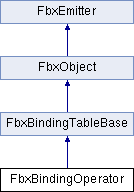
\includegraphics[height=4.000000cm]{class_fbx_binding_operator}
\end{center}
\end{figure}
\subsection*{クラス}
\begin{DoxyCompactItemize}
\item 
class \hyperlink{class_fbx_binding_operator_1_1_function}{Function}
\item 
class \hyperlink{class_fbx_binding_operator_1_1_function_creator}{Function\+Creator}
\item 
class \hyperlink{class_fbx_binding_operator_1_1_function_creator_base}{Function\+Creator\+Base}
\item 
class \hyperlink{class_fbx_binding_operator_1_1_function_registry}{Function\+Registry}
\end{DoxyCompactItemize}
\subsection*{公開メンバ関数}
\begin{DoxyCompactItemize}
\item 
{\footnotesize template$<$class F\+B\+X\+T\+Y\+PE $>$ }\\bool \hyperlink{class_fbx_binding_operator_a1487485be07b04ef755f8831912d2709}{Evaluate} (const \hyperlink{class_fbx_object}{Fbx\+Object} $\ast$p\+Object, F\+B\+X\+T\+Y\+PE $\ast$p\+Result) const
\item 
{\footnotesize template$<$class F\+B\+X\+T\+Y\+PE $>$ }\\bool \hyperlink{class_fbx_binding_operator_ac7e93e46c1aea6fa49dca09d3f2df342}{Reverse\+Evaluation} (const \hyperlink{class_fbx_object}{Fbx\+Object} $\ast$p\+Object, F\+B\+X\+T\+Y\+PE $\ast$p\+In\+Out, bool set\+Obj=false, int index=0) const
\item 
{\footnotesize template$<$class F\+B\+X\+T\+Y\+PE $>$ }\\bool \hyperlink{class_fbx_binding_operator_ab649606ddda104b1ab6b329fde618654}{Evaluate\+Entry} (const \hyperlink{class_fbx_object}{Fbx\+Object} $\ast$p\+Object, const char $\ast$p\+Entry\+Destination\+Name, F\+B\+X\+T\+Y\+PE $\ast$p\+Result) const
\item 
bool \hyperlink{class_fbx_binding_operator_a00fe9d445d7ffd44b4da764af49e0d9d}{Evaluate\+Entry} (const \hyperlink{class_fbx_object}{Fbx\+Object} $\ast$p\+Object, const char $\ast$p\+Entry\+Destination\+Name, \hyperlink{fbxpropertytypes_8h_a73913a5ddfb20e57c6f25e9e6784bd92}{E\+Fbx\+Type} $\ast$p\+Result\+Type, void $\ast$$\ast$p\+Result) const
\item 
bool \hyperlink{class_fbx_binding_operator_a9201bfc345f36627b6bace7fa3ccb319}{Get\+Entry\+Property} (const \hyperlink{class_fbx_object}{Fbx\+Object} $\ast$p\+Object, const char $\ast$p\+Entry\+Destination\+Name, \hyperlink{class_fbx_property}{Fbx\+Property} \&p\+Prop) const
\end{DoxyCompactItemize}
\subsection*{静的公開メンバ関数}
\begin{DoxyCompactItemize}
\item 
static void \hyperlink{class_fbx_binding_operator_a228cdd04bfe2e075533f2af0db26ea91}{Register\+Functions} ()
\item 
static void \hyperlink{class_fbx_binding_operator_ac1243bdbc2a34d225b5a33c3c16fe2d8}{Unregister\+Functions} ()
\end{DoxyCompactItemize}
\subsection*{公開変数類}
\begin{DoxyCompactItemize}
\item 
\hyperlink{class_fbx_property_t}{Fbx\+PropertyT}$<$ \hyperlink{class_fbx_string}{Fbx\+String} $>$ \hyperlink{class_fbx_binding_operator_a2dba5cfe05b72b6a46b2195872a93005}{Function\+Name}
\item 
\hyperlink{class_fbx_property_t}{Fbx\+PropertyT}$<$ \hyperlink{class_fbx_string}{Fbx\+String} $>$ \hyperlink{class_fbx_binding_operator_a6c1e84a9019ff0fa80424439fa745ee1}{Target\+Name}
\end{DoxyCompactItemize}
\subsection*{静的公開変数類}
\begin{DoxyCompactItemize}
\item 
static const char $\ast$ \hyperlink{class_fbx_binding_operator_ac905ce728f7bfb5bd7becf78af8a5c4d}{s\+Function\+Name}
\begin{DoxyCompactList}\small\item\em \hyperlink{class_fbx_binding_operator_1_1_function}{Function} name. \end{DoxyCompactList}\item 
static const char $\ast$ \hyperlink{class_fbx_binding_operator_ac53f7653f20364486e319b64b275ed4b}{s\+Target\+Name}
\begin{DoxyCompactList}\small\item\em Target name. \end{DoxyCompactList}\item 
static const char $\ast$ \hyperlink{class_fbx_binding_operator_aea467026528b679f7a8edc9862895f63}{s\+Default\+Function\+Name}
\begin{DoxyCompactList}\small\item\em Default value for function name. \end{DoxyCompactList}\item 
static const char $\ast$ \hyperlink{class_fbx_binding_operator_adba0167e90625ae94b159146b5e13b13}{s\+Default\+Target\+Name}
\begin{DoxyCompactList}\small\item\em Default value for target name. \end{DoxyCompactList}\end{DoxyCompactItemize}
\subsection*{限定公開メンバ関数}
\begin{DoxyCompactItemize}
\item 
virtual void \hyperlink{class_fbx_binding_operator_addee18722d7806245f10a1c873bafaac}{Construct} (const \hyperlink{class_fbx_object}{Fbx\+Object} $\ast$p\+From)
\item 
virtual void \hyperlink{class_fbx_binding_operator_a183d8593f526ca03661506ad1aedf412}{Destruct} (bool p\+Recursive)
\item 
virtual void \hyperlink{class_fbx_binding_operator_ab7e4a678475a62b3bf36b1171860c17e}{Construct\+Properties} (bool p\+Force\+Set)
\item 
void \hyperlink{class_fbx_binding_operator_aba1f55d1c5458713779fc2bdfc272b3e}{Instantiate\+Function} ()
\item 
bool \hyperlink{class_fbx_binding_operator_a46e67c6d662013ae83cd239648d85630}{Evaluate} (const \hyperlink{class_fbx_object}{Fbx\+Object} $\ast$p\+Object, \hyperlink{fbxpropertytypes_8h_a73913a5ddfb20e57c6f25e9e6784bd92}{E\+Fbx\+Type} $\ast$p\+Result\+Type, void $\ast$$\ast$p\+Result) const
\item 
bool \hyperlink{class_fbx_binding_operator_a7528f0c6f942433c0c5c78fc5e803bbc}{Reverse\+Evaluate} (const \hyperlink{class_fbx_object}{Fbx\+Object} $\ast$p\+Target, const void $\ast$p\+In, void $\ast$$\ast$p\+Out, \hyperlink{fbxpropertytypes_8h_a73913a5ddfb20e57c6f25e9e6784bd92}{E\+Fbx\+Type} $\ast$p\+Out\+Type, bool set\+Obj, int index) const
\item 
void \hyperlink{class_fbx_binding_operator_af7e8559f61c34efa27b1562d386efd2c}{Free\+Evaluation\+Result} (\hyperlink{fbxpropertytypes_8h_a73913a5ddfb20e57c6f25e9e6784bd92}{E\+Fbx\+Type} p\+Result\+Type, void $\ast$p\+Result) const
\end{DoxyCompactItemize}
\subsection*{限定公開変数類}
\begin{DoxyCompactItemize}
\item 
\hyperlink{class_fbx_binding_operator_1_1_function}{Function} $\ast$ \hyperlink{class_fbx_binding_operator_a677a0ed0b5782978a21c8a4b371821f5}{m\+Function}
\end{DoxyCompactItemize}
\subsection*{その他の継承メンバ}


\subsection{詳解}
This object represents a binding operation on a \hyperlink{class_fbx_object}{Fbx\+Object} or \hyperlink{class_fbx_property}{Fbx\+Property}. For example, \hyperlink{class_fbx_binding_operator}{Fbx\+Binding\+Operator} can be used to bind a light object to a parameter of shader via \hyperlink{class_fbx_node_direction_b_o_f}{Fbx\+Node\+Direction\+B\+OF} or \hyperlink{class_fbx_node_position_b_o_f}{Fbx\+Node\+Position\+B\+OF}. 
\begin{DoxyCode}
\textcolor{comment}{//Create an entry lEntry of binding table lTable.}
\hyperlink{class_fbx_binding_table_entry}{FbxBindingTableEntry}& lEntry = lTable->AddNewEntry();

\textcolor{comment}{//Create a NodePositionConvert binding operator and add it as source of the lEntry.}
\hyperlink{class_fbx_operator_entry_view}{FbxOperatorEntryView} lSrc(&lEntry, \textcolor{keyword}{true}, \textcolor{keyword}{true});
lSrc.SetOperatorName( \textcolor{stringliteral}{"NodePositionConvert"});
\hyperlink{class_fbx_binding_operator}{FbxBindingOperator}* lOp = pImpl.AddNewBindingOperator( \textcolor{stringliteral}{"NodePositionConvert"}, 
      \hyperlink{class_fbx_node_position_b_o_f_aaa0c4610384d1dbb4e566bad44c356ee}{FbxNodePositionBOF::FunctionName});

\textcolor{comment}{//Add a property entry to the binding operator.}
\hyperlink{class_fbx_binding_table_entry}{FbxBindingTableEntry}& lEntryPropParam = lOp->\hyperlink{class_fbx_binding_table_base_a2ebf180e80538abf0e6512a8ca30ee10}{AddNewEntry}();
\hyperlink{class_fbx_property_entry_view}{FbxPropertyEntryView} lPropSrc(&lEntryPropParam, \textcolor{keyword}{true}, \textcolor{keyword}{true});
\textcolor{comment}{//Set the shader parameter (the property's name) as source of the lEntryPropParam.}
lPropSrc.SetProperty(lProp.GetHierarchicalName());
\textcolor{comment}{//Set the operator function FbxNodePositionBOF as destination of the lEntryPropParam.}
lEntryPropParam.\hyperlink{class_fbx_binding_table_entry_aaa49a62bd197febfb6052f3efa50eaf3}{SetDestination}( \hyperlink{class_fbx_node_position_b_o_f_aaa0c4610384d1dbb4e566bad44c356ee}{FbxNodePositionBOF::FunctionName}
       );

\textcolor{comment}{//Set the shader parameter as destination of the lEntry.}
\hyperlink{class_fbx_semantic_entry_view}{FbxSemanticEntryView} lDst( &lEntry, \textcolor{keyword}{false}, \textcolor{keyword}{true} );
lDst.SetSemantic( lProp.GetName() );
\end{DoxyCode}


\begin{DoxySeeAlso}{参照}
\hyperlink{class_fbx_operator_entry_view}{Fbx\+Operator\+Entry\+View}, \hyperlink{class_fbx_binding_table_entry}{Fbx\+Binding\+Table\+Entry}, \hyperlink{class_fbx_property_entry_view}{Fbx\+Property\+Entry\+View} 
\end{DoxySeeAlso}


 fbxbindingoperator.\+h の 49 行目に定義があります。



\subsection{関数詳解}
\mbox{\Hypertarget{class_fbx_binding_operator_addee18722d7806245f10a1c873bafaac}\label{class_fbx_binding_operator_addee18722d7806245f10a1c873bafaac}} 
\index{Fbx\+Binding\+Operator@{Fbx\+Binding\+Operator}!Construct@{Construct}}
\index{Construct@{Construct}!Fbx\+Binding\+Operator@{Fbx\+Binding\+Operator}}
\subsubsection{\texorpdfstring{Construct()}{Construct()}}
{\footnotesize\ttfamily virtual void Fbx\+Binding\+Operator\+::\+Construct (\begin{DoxyParamCaption}\item[{const \hyperlink{class_fbx_object}{Fbx\+Object} $\ast$}]{p\+From }\end{DoxyParamCaption})\hspace{0.3cm}{\ttfamily [protected]}, {\ttfamily [virtual]}}

Optional constructor override, automatically called by default constructor. 
\begin{DoxyParams}{引数}
{\em p\+From} & If not null, the function must take it into account like a copy constructor. \\
\hline
\end{DoxyParams}
\begin{DoxyRemark}{注釈}
In case it is decided to override this function, do not forget to call Parent\+Class\+::\+Construct(p\+From) at the beginning. 
\end{DoxyRemark}


\hyperlink{class_fbx_object_a313503bc645af3fdceb4a99ef5cea7eb}{Fbx\+Object}を再実装しています。

\mbox{\Hypertarget{class_fbx_binding_operator_ab7e4a678475a62b3bf36b1171860c17e}\label{class_fbx_binding_operator_ab7e4a678475a62b3bf36b1171860c17e}} 
\index{Fbx\+Binding\+Operator@{Fbx\+Binding\+Operator}!Construct\+Properties@{Construct\+Properties}}
\index{Construct\+Properties@{Construct\+Properties}!Fbx\+Binding\+Operator@{Fbx\+Binding\+Operator}}
\subsubsection{\texorpdfstring{Construct\+Properties()}{ConstructProperties()}}
{\footnotesize\ttfamily virtual void Fbx\+Binding\+Operator\+::\+Construct\+Properties (\begin{DoxyParamCaption}\item[{bool}]{p\+Force\+Set }\end{DoxyParamCaption})\hspace{0.3cm}{\ttfamily [protected]}, {\ttfamily [virtual]}}

Optional property constructor override, automatically called by default constructor. 
\begin{DoxyParams}{引数}
{\em p\+Force\+Set} & If the property value must be set regardless of default value. \\
\hline
\end{DoxyParams}
\begin{DoxyRemark}{注釈}
If your object have properties, they must be initialized in this function. 
\end{DoxyRemark}


\hyperlink{class_fbx_object_ad44f814323dc1b5e78bff1bfc608b4bb}{Fbx\+Object}を再実装しています。

\mbox{\Hypertarget{class_fbx_binding_operator_a183d8593f526ca03661506ad1aedf412}\label{class_fbx_binding_operator_a183d8593f526ca03661506ad1aedf412}} 
\index{Fbx\+Binding\+Operator@{Fbx\+Binding\+Operator}!Destruct@{Destruct}}
\index{Destruct@{Destruct}!Fbx\+Binding\+Operator@{Fbx\+Binding\+Operator}}
\subsubsection{\texorpdfstring{Destruct()}{Destruct()}}
{\footnotesize\ttfamily virtual void Fbx\+Binding\+Operator\+::\+Destruct (\begin{DoxyParamCaption}\item[{bool}]{p\+Recursive }\end{DoxyParamCaption})\hspace{0.3cm}{\ttfamily [protected]}, {\ttfamily [virtual]}}

Optional destructor override, automatically called by default destructor. 
\begin{DoxyParams}{引数}
{\em p\+Recursive} & If true, children objects should be destroyed as well. \\
\hline
\end{DoxyParams}
\begin{DoxyRemark}{注釈}
In case it is decided to override this function, do not forget to call Parent\+Class\+::\+Destruct(p\+Resursive) at the end. 
\end{DoxyRemark}


\hyperlink{class_fbx_object_a123e084d9b32b29c28af6384b7c3c608}{Fbx\+Object}を再実装しています。

\mbox{\Hypertarget{class_fbx_binding_operator_a1487485be07b04ef755f8831912d2709}\label{class_fbx_binding_operator_a1487485be07b04ef755f8831912d2709}} 
\index{Fbx\+Binding\+Operator@{Fbx\+Binding\+Operator}!Evaluate@{Evaluate}}
\index{Evaluate@{Evaluate}!Fbx\+Binding\+Operator@{Fbx\+Binding\+Operator}}
\subsubsection{\texorpdfstring{Evaluate()}{Evaluate()}\hspace{0.1cm}{\footnotesize\ttfamily [1/2]}}
{\footnotesize\ttfamily template$<$class F\+B\+X\+T\+Y\+PE $>$ \\
bool Fbx\+Binding\+Operator\+::\+Evaluate (\begin{DoxyParamCaption}\item[{const \hyperlink{class_fbx_object}{Fbx\+Object} $\ast$}]{p\+Object,  }\item[{F\+B\+X\+T\+Y\+PE $\ast$}]{p\+Result }\end{DoxyParamCaption}) const\hspace{0.3cm}{\ttfamily [inline]}}

Run the operator on the given object. 
\begin{DoxyParams}{引数}
{\em p\+Object} & The object that will be evaluated. \\
\hline
{\em p\+Result} & A pointer to a buffer to hold the result. \\
\hline
\end{DoxyParams}
\begin{DoxyReturn}{戻り値}
{\ttfamily true} on success, {\ttfamily false} otherwise. 
\end{DoxyReturn}


 fbxbindingoperator.\+h の 60 行目に定義があります。

\mbox{\Hypertarget{class_fbx_binding_operator_a46e67c6d662013ae83cd239648d85630}\label{class_fbx_binding_operator_a46e67c6d662013ae83cd239648d85630}} 
\index{Fbx\+Binding\+Operator@{Fbx\+Binding\+Operator}!Evaluate@{Evaluate}}
\index{Evaluate@{Evaluate}!Fbx\+Binding\+Operator@{Fbx\+Binding\+Operator}}
\subsubsection{\texorpdfstring{Evaluate()}{Evaluate()}\hspace{0.1cm}{\footnotesize\ttfamily [2/2]}}
{\footnotesize\ttfamily bool Fbx\+Binding\+Operator\+::\+Evaluate (\begin{DoxyParamCaption}\item[{const \hyperlink{class_fbx_object}{Fbx\+Object} $\ast$}]{p\+Object,  }\item[{\hyperlink{fbxpropertytypes_8h_a73913a5ddfb20e57c6f25e9e6784bd92}{E\+Fbx\+Type} $\ast$}]{p\+Result\+Type,  }\item[{void $\ast$$\ast$}]{p\+Result }\end{DoxyParamCaption}) const\hspace{0.3cm}{\ttfamily [protected]}}

\mbox{\Hypertarget{class_fbx_binding_operator_ab649606ddda104b1ab6b329fde618654}\label{class_fbx_binding_operator_ab649606ddda104b1ab6b329fde618654}} 
\index{Fbx\+Binding\+Operator@{Fbx\+Binding\+Operator}!Evaluate\+Entry@{Evaluate\+Entry}}
\index{Evaluate\+Entry@{Evaluate\+Entry}!Fbx\+Binding\+Operator@{Fbx\+Binding\+Operator}}
\subsubsection{\texorpdfstring{Evaluate\+Entry()}{EvaluateEntry()}\hspace{0.1cm}{\footnotesize\ttfamily [1/2]}}
{\footnotesize\ttfamily template$<$class F\+B\+X\+T\+Y\+PE $>$ \\
bool Fbx\+Binding\+Operator\+::\+Evaluate\+Entry (\begin{DoxyParamCaption}\item[{const \hyperlink{class_fbx_object}{Fbx\+Object} $\ast$}]{p\+Object,  }\item[{const char $\ast$}]{p\+Entry\+Destination\+Name,  }\item[{F\+B\+X\+T\+Y\+PE $\ast$}]{p\+Result }\end{DoxyParamCaption}) const\hspace{0.3cm}{\ttfamily [inline]}}

Evaluate the value of an operator parameter. 
\begin{DoxyParams}{引数}
{\em p\+Object} & The object that will be evaluated. \\
\hline
{\em p\+Entry\+Destination\+Name} & The name of the parameter. This is used to get the property or operator that is related to this parameter, then to evaluate the property or operator. \\
\hline
{\em p\+Result} & A pointer to the result. \\
\hline
\end{DoxyParams}
\begin{DoxyReturn}{戻り値}
{\ttfamily true} on success, {\ttfamily false} otherwise. 
\end{DoxyReturn}
\begin{DoxyRemark}{注釈}
This method can handle different types of entries. For property entry and constant entry, this method will find out the property via the p\+Entry\+Destination\+Name and then evaluate its value; for operator entry, this method will find out the operator via the p\+Entry\+Destination\+Name and evaluate the operator function to get the property\textquotesingle{}s value; for any other types of entry, this method is meaningless. 
\end{DoxyRemark}


 fbxbindingoperator.\+h の 120 行目に定義があります。

\mbox{\Hypertarget{class_fbx_binding_operator_a00fe9d445d7ffd44b4da764af49e0d9d}\label{class_fbx_binding_operator_a00fe9d445d7ffd44b4da764af49e0d9d}} 
\index{Fbx\+Binding\+Operator@{Fbx\+Binding\+Operator}!Evaluate\+Entry@{Evaluate\+Entry}}
\index{Evaluate\+Entry@{Evaluate\+Entry}!Fbx\+Binding\+Operator@{Fbx\+Binding\+Operator}}
\subsubsection{\texorpdfstring{Evaluate\+Entry()}{EvaluateEntry()}\hspace{0.1cm}{\footnotesize\ttfamily [2/2]}}
{\footnotesize\ttfamily bool Fbx\+Binding\+Operator\+::\+Evaluate\+Entry (\begin{DoxyParamCaption}\item[{const \hyperlink{class_fbx_object}{Fbx\+Object} $\ast$}]{p\+Object,  }\item[{const char $\ast$}]{p\+Entry\+Destination\+Name,  }\item[{\hyperlink{fbxpropertytypes_8h_a73913a5ddfb20e57c6f25e9e6784bd92}{E\+Fbx\+Type} $\ast$}]{p\+Result\+Type,  }\item[{void $\ast$$\ast$}]{p\+Result }\end{DoxyParamCaption}) const}

\mbox{\Hypertarget{class_fbx_binding_operator_af7e8559f61c34efa27b1562d386efd2c}\label{class_fbx_binding_operator_af7e8559f61c34efa27b1562d386efd2c}} 
\index{Fbx\+Binding\+Operator@{Fbx\+Binding\+Operator}!Free\+Evaluation\+Result@{Free\+Evaluation\+Result}}
\index{Free\+Evaluation\+Result@{Free\+Evaluation\+Result}!Fbx\+Binding\+Operator@{Fbx\+Binding\+Operator}}
\subsubsection{\texorpdfstring{Free\+Evaluation\+Result()}{FreeEvaluationResult()}}
{\footnotesize\ttfamily void Fbx\+Binding\+Operator\+::\+Free\+Evaluation\+Result (\begin{DoxyParamCaption}\item[{\hyperlink{fbxpropertytypes_8h_a73913a5ddfb20e57c6f25e9e6784bd92}{E\+Fbx\+Type}}]{p\+Result\+Type,  }\item[{void $\ast$}]{p\+Result }\end{DoxyParamCaption}) const\hspace{0.3cm}{\ttfamily [protected]}}

\mbox{\Hypertarget{class_fbx_binding_operator_a9201bfc345f36627b6bace7fa3ccb319}\label{class_fbx_binding_operator_a9201bfc345f36627b6bace7fa3ccb319}} 
\index{Fbx\+Binding\+Operator@{Fbx\+Binding\+Operator}!Get\+Entry\+Property@{Get\+Entry\+Property}}
\index{Get\+Entry\+Property@{Get\+Entry\+Property}!Fbx\+Binding\+Operator@{Fbx\+Binding\+Operator}}
\subsubsection{\texorpdfstring{Get\+Entry\+Property()}{GetEntryProperty()}}
{\footnotesize\ttfamily bool Fbx\+Binding\+Operator\+::\+Get\+Entry\+Property (\begin{DoxyParamCaption}\item[{const \hyperlink{class_fbx_object}{Fbx\+Object} $\ast$}]{p\+Object,  }\item[{const char $\ast$}]{p\+Entry\+Destination\+Name,  }\item[{\hyperlink{class_fbx_property}{Fbx\+Property} \&}]{p\+Prop }\end{DoxyParamCaption}) const}

\mbox{\Hypertarget{class_fbx_binding_operator_aba1f55d1c5458713779fc2bdfc272b3e}\label{class_fbx_binding_operator_aba1f55d1c5458713779fc2bdfc272b3e}} 
\index{Fbx\+Binding\+Operator@{Fbx\+Binding\+Operator}!Instantiate\+Function@{Instantiate\+Function}}
\index{Instantiate\+Function@{Instantiate\+Function}!Fbx\+Binding\+Operator@{Fbx\+Binding\+Operator}}
\subsubsection{\texorpdfstring{Instantiate\+Function()}{InstantiateFunction()}}
{\footnotesize\ttfamily void Fbx\+Binding\+Operator\+::\+Instantiate\+Function (\begin{DoxyParamCaption}{ }\end{DoxyParamCaption})\hspace{0.3cm}{\ttfamily [protected]}}

\mbox{\Hypertarget{class_fbx_binding_operator_a228cdd04bfe2e075533f2af0db26ea91}\label{class_fbx_binding_operator_a228cdd04bfe2e075533f2af0db26ea91}} 
\index{Fbx\+Binding\+Operator@{Fbx\+Binding\+Operator}!Register\+Functions@{Register\+Functions}}
\index{Register\+Functions@{Register\+Functions}!Fbx\+Binding\+Operator@{Fbx\+Binding\+Operator}}
\subsubsection{\texorpdfstring{Register\+Functions()}{RegisterFunctions()}}
{\footnotesize\ttfamily static void Fbx\+Binding\+Operator\+::\+Register\+Functions (\begin{DoxyParamCaption}{ }\end{DoxyParamCaption})\hspace{0.3cm}{\ttfamily [static]}}

\mbox{\Hypertarget{class_fbx_binding_operator_a7528f0c6f942433c0c5c78fc5e803bbc}\label{class_fbx_binding_operator_a7528f0c6f942433c0c5c78fc5e803bbc}} 
\index{Fbx\+Binding\+Operator@{Fbx\+Binding\+Operator}!Reverse\+Evaluate@{Reverse\+Evaluate}}
\index{Reverse\+Evaluate@{Reverse\+Evaluate}!Fbx\+Binding\+Operator@{Fbx\+Binding\+Operator}}
\subsubsection{\texorpdfstring{Reverse\+Evaluate()}{ReverseEvaluate()}}
{\footnotesize\ttfamily bool Fbx\+Binding\+Operator\+::\+Reverse\+Evaluate (\begin{DoxyParamCaption}\item[{const \hyperlink{class_fbx_object}{Fbx\+Object} $\ast$}]{p\+Target,  }\item[{const void $\ast$}]{p\+In,  }\item[{void $\ast$$\ast$}]{p\+Out,  }\item[{\hyperlink{fbxpropertytypes_8h_a73913a5ddfb20e57c6f25e9e6784bd92}{E\+Fbx\+Type} $\ast$}]{p\+Out\+Type,  }\item[{bool}]{set\+Obj,  }\item[{int}]{index }\end{DoxyParamCaption}) const\hspace{0.3cm}{\ttfamily [protected]}}

\mbox{\Hypertarget{class_fbx_binding_operator_ac7e93e46c1aea6fa49dca09d3f2df342}\label{class_fbx_binding_operator_ac7e93e46c1aea6fa49dca09d3f2df342}} 
\index{Fbx\+Binding\+Operator@{Fbx\+Binding\+Operator}!Reverse\+Evaluation@{Reverse\+Evaluation}}
\index{Reverse\+Evaluation@{Reverse\+Evaluation}!Fbx\+Binding\+Operator@{Fbx\+Binding\+Operator}}
\subsubsection{\texorpdfstring{Reverse\+Evaluation()}{ReverseEvaluation()}}
{\footnotesize\ttfamily template$<$class F\+B\+X\+T\+Y\+PE $>$ \\
bool Fbx\+Binding\+Operator\+::\+Reverse\+Evaluation (\begin{DoxyParamCaption}\item[{const \hyperlink{class_fbx_object}{Fbx\+Object} $\ast$}]{p\+Object,  }\item[{F\+B\+X\+T\+Y\+PE $\ast$}]{p\+In\+Out,  }\item[{bool}]{set\+Obj = {\ttfamily false},  }\item[{int}]{index = {\ttfamily 0} }\end{DoxyParamCaption}) const\hspace{0.3cm}{\ttfamily [inline]}}

Run the inverse operator on the given object, assigning the result directly to the object. 
\begin{DoxyParams}{引数}
{\em p\+Object} & The object that will be evaluated. \\
\hline
{\em p\+In\+Out} & Type of value being reversed. \\
\hline
{\em set\+Obj} & Control to set the property (only to query by the default ). \\
\hline
{\em index} & Used only in \hyperlink{class_fbx_multiply_dist_b_o_f}{Fbx\+Multiply\+Dist\+B\+OF}. \\
\hline
\end{DoxyParams}
\begin{DoxyReturn}{戻り値}
{\ttfamily true} on success, {\ttfamily false} otherwise. 
\end{DoxyReturn}


 fbxbindingoperator.\+h の 86 行目に定義があります。

\mbox{\Hypertarget{class_fbx_binding_operator_ac1243bdbc2a34d225b5a33c3c16fe2d8}\label{class_fbx_binding_operator_ac1243bdbc2a34d225b5a33c3c16fe2d8}} 
\index{Fbx\+Binding\+Operator@{Fbx\+Binding\+Operator}!Unregister\+Functions@{Unregister\+Functions}}
\index{Unregister\+Functions@{Unregister\+Functions}!Fbx\+Binding\+Operator@{Fbx\+Binding\+Operator}}
\subsubsection{\texorpdfstring{Unregister\+Functions()}{UnregisterFunctions()}}
{\footnotesize\ttfamily static void Fbx\+Binding\+Operator\+::\+Unregister\+Functions (\begin{DoxyParamCaption}{ }\end{DoxyParamCaption})\hspace{0.3cm}{\ttfamily [static]}}



\subsection{メンバ詳解}
\mbox{\Hypertarget{class_fbx_binding_operator_a2dba5cfe05b72b6a46b2195872a93005}\label{class_fbx_binding_operator_a2dba5cfe05b72b6a46b2195872a93005}} 
\index{Fbx\+Binding\+Operator@{Fbx\+Binding\+Operator}!Function\+Name@{Function\+Name}}
\index{Function\+Name@{Function\+Name}!Fbx\+Binding\+Operator@{Fbx\+Binding\+Operator}}
\subsubsection{\texorpdfstring{Function\+Name}{FunctionName}}
{\footnotesize\ttfamily \hyperlink{class_fbx_property_t}{Fbx\+PropertyT}$<$\hyperlink{class_fbx_string}{Fbx\+String}$>$ Fbx\+Binding\+Operator\+::\+Function\+Name}

This property stores the name of function.

Default value is \char`\"{}\char`\"{}. 

 fbxbindingoperator.\+h の 141 行目に定義があります。

\mbox{\Hypertarget{class_fbx_binding_operator_a677a0ed0b5782978a21c8a4b371821f5}\label{class_fbx_binding_operator_a677a0ed0b5782978a21c8a4b371821f5}} 
\index{Fbx\+Binding\+Operator@{Fbx\+Binding\+Operator}!m\+Function@{m\+Function}}
\index{m\+Function@{m\+Function}!Fbx\+Binding\+Operator@{Fbx\+Binding\+Operator}}
\subsubsection{\texorpdfstring{m\+Function}{mFunction}}
{\footnotesize\ttfamily \hyperlink{class_fbx_binding_operator_1_1_function}{Function}$\ast$ Fbx\+Binding\+Operator\+::m\+Function\hspace{0.3cm}{\ttfamily [protected]}}



 fbxbindingoperator.\+h の 318 行目に定義があります。

\mbox{\Hypertarget{class_fbx_binding_operator_aea467026528b679f7a8edc9862895f63}\label{class_fbx_binding_operator_aea467026528b679f7a8edc9862895f63}} 
\index{Fbx\+Binding\+Operator@{Fbx\+Binding\+Operator}!s\+Default\+Function\+Name@{s\+Default\+Function\+Name}}
\index{s\+Default\+Function\+Name@{s\+Default\+Function\+Name}!Fbx\+Binding\+Operator@{Fbx\+Binding\+Operator}}
\subsubsection{\texorpdfstring{s\+Default\+Function\+Name}{sDefaultFunctionName}}
{\footnotesize\ttfamily const char$\ast$ Fbx\+Binding\+Operator\+::s\+Default\+Function\+Name\hspace{0.3cm}{\ttfamily [static]}}



Default value for function name. 



 fbxbindingoperator.\+h の 159 行目に定義があります。

\mbox{\Hypertarget{class_fbx_binding_operator_adba0167e90625ae94b159146b5e13b13}\label{class_fbx_binding_operator_adba0167e90625ae94b159146b5e13b13}} 
\index{Fbx\+Binding\+Operator@{Fbx\+Binding\+Operator}!s\+Default\+Target\+Name@{s\+Default\+Target\+Name}}
\index{s\+Default\+Target\+Name@{s\+Default\+Target\+Name}!Fbx\+Binding\+Operator@{Fbx\+Binding\+Operator}}
\subsubsection{\texorpdfstring{s\+Default\+Target\+Name}{sDefaultTargetName}}
{\footnotesize\ttfamily const char$\ast$ Fbx\+Binding\+Operator\+::s\+Default\+Target\+Name\hspace{0.3cm}{\ttfamily [static]}}



Default value for target name. 



 fbxbindingoperator.\+h の 161 行目に定義があります。

\mbox{\Hypertarget{class_fbx_binding_operator_ac905ce728f7bfb5bd7becf78af8a5c4d}\label{class_fbx_binding_operator_ac905ce728f7bfb5bd7becf78af8a5c4d}} 
\index{Fbx\+Binding\+Operator@{Fbx\+Binding\+Operator}!s\+Function\+Name@{s\+Function\+Name}}
\index{s\+Function\+Name@{s\+Function\+Name}!Fbx\+Binding\+Operator@{Fbx\+Binding\+Operator}}
\subsubsection{\texorpdfstring{s\+Function\+Name}{sFunctionName}}
{\footnotesize\ttfamily const char$\ast$ Fbx\+Binding\+Operator\+::s\+Function\+Name\hspace{0.3cm}{\ttfamily [static]}}



\hyperlink{class_fbx_binding_operator_1_1_function}{Function} name. 



 fbxbindingoperator.\+h の 154 行目に定義があります。

\mbox{\Hypertarget{class_fbx_binding_operator_ac53f7653f20364486e319b64b275ed4b}\label{class_fbx_binding_operator_ac53f7653f20364486e319b64b275ed4b}} 
\index{Fbx\+Binding\+Operator@{Fbx\+Binding\+Operator}!s\+Target\+Name@{s\+Target\+Name}}
\index{s\+Target\+Name@{s\+Target\+Name}!Fbx\+Binding\+Operator@{Fbx\+Binding\+Operator}}
\subsubsection{\texorpdfstring{s\+Target\+Name}{sTargetName}}
{\footnotesize\ttfamily const char$\ast$ Fbx\+Binding\+Operator\+::s\+Target\+Name\hspace{0.3cm}{\ttfamily [static]}}



Target name. 



 fbxbindingoperator.\+h の 156 行目に定義があります。

\mbox{\Hypertarget{class_fbx_binding_operator_a6c1e84a9019ff0fa80424439fa745ee1}\label{class_fbx_binding_operator_a6c1e84a9019ff0fa80424439fa745ee1}} 
\index{Fbx\+Binding\+Operator@{Fbx\+Binding\+Operator}!Target\+Name@{Target\+Name}}
\index{Target\+Name@{Target\+Name}!Fbx\+Binding\+Operator@{Fbx\+Binding\+Operator}}
\subsubsection{\texorpdfstring{Target\+Name}{TargetName}}
{\footnotesize\ttfamily \hyperlink{class_fbx_property_t}{Fbx\+PropertyT}$<$\hyperlink{class_fbx_string}{Fbx\+String}$>$ Fbx\+Binding\+Operator\+::\+Target\+Name}

This property stores the name of target.

Default value is \char`\"{}\char`\"{}. 

 fbxbindingoperator.\+h の 147 行目に定義があります。



このクラス詳解は次のファイルから抽出されました\+:\begin{DoxyCompactItemize}
\item 
C\+:/\+Maya/scripts/\+F\+B\+X\+\_\+\+S\+D\+K/2017.\+1/include/fbxsdk/scene/shading/\hyperlink{fbxbindingoperator_8h}{fbxbindingoperator.\+h}\end{DoxyCompactItemize}

\hypertarget{class_fbx_bindings_entry_view}{}\section{Fbx\+Bindings\+Entry\+View クラス}
\label{class_fbx_bindings_entry_view}\index{Fbx\+Bindings\+Entry\+View@{Fbx\+Bindings\+Entry\+View}}


{\ttfamily \#include $<$fbxbindingsentryview.\+h$>$}

Fbx\+Bindings\+Entry\+View の継承関係図\begin{figure}[H]
\begin{center}
\leavevmode
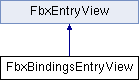
\includegraphics[height=2.000000cm]{class_fbx_bindings_entry_view}
\end{center}
\end{figure}
\subsection*{公開メンバ関数}
\begin{DoxyCompactItemize}
\item 
\hyperlink{class_fbx_bindings_entry_view_a9ed299bf864d23bf17b1ab1d16a1d3d6}{Fbx\+Bindings\+Entry\+View} (\hyperlink{class_fbx_binding_table_entry}{Fbx\+Binding\+Table\+Entry} $\ast$p\+Entry, bool p\+As\+Source, bool p\+Create=false)
\item 
\hyperlink{class_fbx_bindings_entry_view_a82b1df38bb6aeb6548e6edbed48c3f8b}{$\sim$\+Fbx\+Bindings\+Entry\+View} ()
\begin{DoxyCompactList}\small\item\em Destructor. \end{DoxyCompactList}\item 
const char $\ast$ \hyperlink{class_fbx_bindings_entry_view_a1b3909ebdbe0164c910056526eedcdc6}{Get\+Binding\+Table\+Name} () const
\item 
void \hyperlink{class_fbx_bindings_entry_view_af367ef628865d839cc034acf224ffe78}{Set\+Binding\+Table\+Name} (const char $\ast$p\+Name)
\item 
virtual const char $\ast$ \hyperlink{class_fbx_bindings_entry_view_a25f821ea63f19592173e7785356c04f9}{Entry\+Type} () const
\end{DoxyCompactItemize}
\subsection*{静的公開変数類}
\begin{DoxyCompactItemize}
\item 
static const char $\ast$ \hyperlink{class_fbx_bindings_entry_view_a209f878b5007e944ca37fb6f73139c2e}{s\+Entry\+Type}
\end{DoxyCompactItemize}
\subsection*{その他の継承メンバ}


\subsection{詳解}
\hyperlink{class_fbx_bindings_entry_view}{Fbx\+Bindings\+Entry\+View} represents binding table entry in entry tables. The name of the binding table can be used as source or destination for the binding entry. \begin{DoxySeeAlso}{参照}
\hyperlink{class_fbx_binding_table_entry}{Fbx\+Binding\+Table\+Entry} and \hyperlink{class_fbx_binding_table}{Fbx\+Binding\+Table}. 
\end{DoxySeeAlso}


 fbxbindingsentryview.\+h の 26 行目に定義があります。



\subsection{構築子と解体子}
\mbox{\Hypertarget{class_fbx_bindings_entry_view_a9ed299bf864d23bf17b1ab1d16a1d3d6}\label{class_fbx_bindings_entry_view_a9ed299bf864d23bf17b1ab1d16a1d3d6}} 
\index{Fbx\+Bindings\+Entry\+View@{Fbx\+Bindings\+Entry\+View}!Fbx\+Bindings\+Entry\+View@{Fbx\+Bindings\+Entry\+View}}
\index{Fbx\+Bindings\+Entry\+View@{Fbx\+Bindings\+Entry\+View}!Fbx\+Bindings\+Entry\+View@{Fbx\+Bindings\+Entry\+View}}
\subsubsection{\texorpdfstring{Fbx\+Bindings\+Entry\+View()}{FbxBindingsEntryView()}}
{\footnotesize\ttfamily Fbx\+Bindings\+Entry\+View\+::\+Fbx\+Bindings\+Entry\+View (\begin{DoxyParamCaption}\item[{\hyperlink{class_fbx_binding_table_entry}{Fbx\+Binding\+Table\+Entry} $\ast$}]{p\+Entry,  }\item[{bool}]{p\+As\+Source,  }\item[{bool}]{p\+Create = {\ttfamily false} }\end{DoxyParamCaption})}

Constructor. 
\begin{DoxyParams}{引数}
{\em p\+Entry} & The binding table entry to create the entry view for. \\
\hline
{\em p\+As\+Source} & {\ttfamily true} to create the entry view as source, {\ttfamily false} as destination. \\
\hline
{\em p\+Create} & {\ttfamily true} to create the entry view, {\ttfamily false} otherwise. \\
\hline
\end{DoxyParams}
\mbox{\Hypertarget{class_fbx_bindings_entry_view_a82b1df38bb6aeb6548e6edbed48c3f8b}\label{class_fbx_bindings_entry_view_a82b1df38bb6aeb6548e6edbed48c3f8b}} 
\index{Fbx\+Bindings\+Entry\+View@{Fbx\+Bindings\+Entry\+View}!````~Fbx\+Bindings\+Entry\+View@{$\sim$\+Fbx\+Bindings\+Entry\+View}}
\index{````~Fbx\+Bindings\+Entry\+View@{$\sim$\+Fbx\+Bindings\+Entry\+View}!Fbx\+Bindings\+Entry\+View@{Fbx\+Bindings\+Entry\+View}}
\subsubsection{\texorpdfstring{$\sim$\+Fbx\+Bindings\+Entry\+View()}{~FbxBindingsEntryView()}}
{\footnotesize\ttfamily Fbx\+Bindings\+Entry\+View\+::$\sim$\+Fbx\+Bindings\+Entry\+View (\begin{DoxyParamCaption}{ }\end{DoxyParamCaption})}



Destructor. 



\subsection{関数詳解}
\mbox{\Hypertarget{class_fbx_bindings_entry_view_a25f821ea63f19592173e7785356c04f9}\label{class_fbx_bindings_entry_view_a25f821ea63f19592173e7785356c04f9}} 
\index{Fbx\+Bindings\+Entry\+View@{Fbx\+Bindings\+Entry\+View}!Entry\+Type@{Entry\+Type}}
\index{Entry\+Type@{Entry\+Type}!Fbx\+Bindings\+Entry\+View@{Fbx\+Bindings\+Entry\+View}}
\subsubsection{\texorpdfstring{Entry\+Type()}{EntryType()}}
{\footnotesize\ttfamily virtual const char$\ast$ Fbx\+Bindings\+Entry\+View\+::\+Entry\+Type (\begin{DoxyParamCaption}{ }\end{DoxyParamCaption}) const\hspace{0.3cm}{\ttfamily [virtual]}}

Get the entry type. \begin{DoxyReturn}{戻り値}
Entry type as string \char`\"{}\+Fbx\+Bindings\+Entry\char`\"{}. 
\end{DoxyReturn}
\begin{DoxyRemark}{注釈}
Always use \hyperlink{class_fbx_bindings_entry_view_a25f821ea63f19592173e7785356c04f9}{Entry\+Type()} to get the right entry type. 
\end{DoxyRemark}


\hyperlink{class_fbx_entry_view_a83ee50482b441ba8b0e6d7c2dba5432f}{Fbx\+Entry\+View}を再実装しています。

\mbox{\Hypertarget{class_fbx_bindings_entry_view_a1b3909ebdbe0164c910056526eedcdc6}\label{class_fbx_bindings_entry_view_a1b3909ebdbe0164c910056526eedcdc6}} 
\index{Fbx\+Bindings\+Entry\+View@{Fbx\+Bindings\+Entry\+View}!Get\+Binding\+Table\+Name@{Get\+Binding\+Table\+Name}}
\index{Get\+Binding\+Table\+Name@{Get\+Binding\+Table\+Name}!Fbx\+Bindings\+Entry\+View@{Fbx\+Bindings\+Entry\+View}}
\subsubsection{\texorpdfstring{Get\+Binding\+Table\+Name()}{GetBindingTableName()}}
{\footnotesize\ttfamily const char$\ast$ Fbx\+Bindings\+Entry\+View\+::\+Get\+Binding\+Table\+Name (\begin{DoxyParamCaption}{ }\end{DoxyParamCaption}) const}

Get the binding table\textquotesingle{}s name for the binding entry. \begin{DoxyReturn}{戻り値}
The binding table\textquotesingle{}s name. 
\end{DoxyReturn}
\mbox{\Hypertarget{class_fbx_bindings_entry_view_af367ef628865d839cc034acf224ffe78}\label{class_fbx_bindings_entry_view_af367ef628865d839cc034acf224ffe78}} 
\index{Fbx\+Bindings\+Entry\+View@{Fbx\+Bindings\+Entry\+View}!Set\+Binding\+Table\+Name@{Set\+Binding\+Table\+Name}}
\index{Set\+Binding\+Table\+Name@{Set\+Binding\+Table\+Name}!Fbx\+Bindings\+Entry\+View@{Fbx\+Bindings\+Entry\+View}}
\subsubsection{\texorpdfstring{Set\+Binding\+Table\+Name()}{SetBindingTableName()}}
{\footnotesize\ttfamily void Fbx\+Bindings\+Entry\+View\+::\+Set\+Binding\+Table\+Name (\begin{DoxyParamCaption}\item[{const char $\ast$}]{p\+Name }\end{DoxyParamCaption})}

Set the binding table\textquotesingle{}s name for binding entry. 
\begin{DoxyParams}{引数}
{\em p\+Name} & The binding table\textquotesingle{}s name to set. \\
\hline
\end{DoxyParams}


\subsection{メンバ詳解}
\mbox{\Hypertarget{class_fbx_bindings_entry_view_a209f878b5007e944ca37fb6f73139c2e}\label{class_fbx_bindings_entry_view_a209f878b5007e944ca37fb6f73139c2e}} 
\index{Fbx\+Bindings\+Entry\+View@{Fbx\+Bindings\+Entry\+View}!s\+Entry\+Type@{s\+Entry\+Type}}
\index{s\+Entry\+Type@{s\+Entry\+Type}!Fbx\+Bindings\+Entry\+View@{Fbx\+Bindings\+Entry\+View}}
\subsubsection{\texorpdfstring{s\+Entry\+Type}{sEntryType}}
{\footnotesize\ttfamily const char$\ast$ Fbx\+Bindings\+Entry\+View\+::s\+Entry\+Type\hspace{0.3cm}{\ttfamily [static]}}

Name of the entry type used in the binding entry. It should be \char`\"{}\+Fbx\+Bindings\+Entry\char`\"{} in this case. 

 fbxbindingsentryview.\+h の 32 行目に定義があります。



このクラス詳解は次のファイルから抽出されました\+:\begin{DoxyCompactItemize}
\item 
C\+:/\+Maya/scripts/\+F\+B\+X\+\_\+\+S\+D\+K/2017.\+1/include/fbxsdk/scene/shading/\hyperlink{fbxbindingsentryview_8h}{fbxbindingsentryview.\+h}\end{DoxyCompactItemize}

\hypertarget{class_fbx_binding_table}{}\section{Fbx\+Binding\+Table クラス}
\label{class_fbx_binding_table}\index{Fbx\+Binding\+Table@{Fbx\+Binding\+Table}}


{\ttfamily \#include $<$fbxbindingtable.\+h$>$}



Fbx\+Binding\+Table の継承関係図
% FIG 0


Fbx\+Binding\+Table 連携図
% FIG 1
\subsection*{公開変数類}
\begin{DoxyCompactItemize}
\item 
\hyperlink{class_fbx_property_t}{Fbx\+PropertyT}$<$ \hyperlink{class_fbx_string}{Fbx\+String} $>$ \hyperlink{class_fbx_binding_table_a09ebb43f4fdfafcf1842ecad60b16801}{Target\+Name}
\item 
\hyperlink{class_fbx_property_t}{Fbx\+PropertyT}$<$ \hyperlink{class_fbx_string}{Fbx\+String} $>$ \hyperlink{class_fbx_binding_table_aca964aac5ddc2238ca9d4a3cafe42486}{Target\+Type}
\item 
\hyperlink{class_fbx_property_t}{Fbx\+PropertyT}$<$ \hyperlink{class_fbx_string}{Fbx\+String} $>$ \hyperlink{class_fbx_binding_table_acb06f75ac993d6f92788beb82298775b}{Desc\+Relative\+U\+RL}
\item 
\hyperlink{class_fbx_property_t}{Fbx\+PropertyT}$<$ \hyperlink{class_fbx_string}{Fbx\+String} $>$ \hyperlink{class_fbx_binding_table_ad0c914d07b49a91d79eda8d39fda6cf7}{Desc\+Absolute\+U\+RL}
\item 
\hyperlink{class_fbx_property_t}{Fbx\+PropertyT}$<$ \hyperlink{class_fbx_string}{Fbx\+String} $>$ \hyperlink{class_fbx_binding_table_aa1ac440c2724fdc420ec3f02fa88aede}{Desc\+T\+AG}
\item 
\hyperlink{class_fbx_property_t}{Fbx\+PropertyT}$<$ \hyperlink{class_fbx_string}{Fbx\+String} $>$ \hyperlink{class_fbx_binding_table_add10ea889f7b9e37ca0fbbf27dfc140f}{Code\+Relative\+U\+RL}
\item 
\hyperlink{class_fbx_property_t}{Fbx\+PropertyT}$<$ \hyperlink{class_fbx_string}{Fbx\+String} $>$ \hyperlink{class_fbx_binding_table_a43a42110f701adae3164558d1b001275}{Code\+Absolute\+U\+RL}
\item 
\hyperlink{class_fbx_property_t}{Fbx\+PropertyT}$<$ \hyperlink{class_fbx_string}{Fbx\+String} $>$ \hyperlink{class_fbx_binding_table_ac1c73d117768ad0373d277a81e021fa3}{Code\+T\+AG}
\end{DoxyCompactItemize}
\subsection*{静的公開変数類}
\begin{DoxyCompactItemize}
\item 
static const char $\ast$ \hyperlink{class_fbx_binding_table_aa49dfec94118aab9dafba3e1032cc8d5}{s\+Target\+Name}
\begin{DoxyCompactList}\small\item\em Target name. \end{DoxyCompactList}\item 
static const char $\ast$ \hyperlink{class_fbx_binding_table_ad9d25de472ef5c70e26293f768d1184f}{s\+Target\+Type}
\begin{DoxyCompactList}\small\item\em Target type. \end{DoxyCompactList}\item 
static const char $\ast$ \hyperlink{class_fbx_binding_table_abf0f711d3e53bfe5a28097f578a59e59}{s\+Desc\+Relative\+U\+RL}
\begin{DoxyCompactList}\small\item\em Relative U\+RL for shader description. \end{DoxyCompactList}\item 
static const char $\ast$ \hyperlink{class_fbx_binding_table_a61930494610fd12785f34b07bd7249af}{s\+Desc\+Absolute\+U\+RL}
\begin{DoxyCompactList}\small\item\em Absolute U\+RL for shader description. \end{DoxyCompactList}\item 
static const char $\ast$ \hyperlink{class_fbx_binding_table_a0536e5bee95808c32640c75fab26db61}{s\+Desc\+T\+AG}
\begin{DoxyCompactList}\small\item\em Identify the shader to use in previous description\textquotesingle{}s U\+RL. \end{DoxyCompactList}\item 
static const char $\ast$ \hyperlink{class_fbx_binding_table_adffd58c9c375cd433f083ef54ee33162}{s\+Code\+Relative\+U\+RL}
\begin{DoxyCompactList}\small\item\em Relative U\+RL for shader code. \end{DoxyCompactList}\item 
static const char $\ast$ \hyperlink{class_fbx_binding_table_aa325052377541732db179bf60c9c9d3d}{s\+Code\+Absolute\+U\+RL}
\begin{DoxyCompactList}\small\item\em Absolute U\+RL for shader code. \end{DoxyCompactList}\item 
static const char $\ast$ \hyperlink{class_fbx_binding_table_a6d02ecf239125a11d11401c0cb1298b1}{s\+Code\+T\+AG}
\begin{DoxyCompactList}\small\item\em Identify the shader function entry to use in previous code\textquotesingle{}s U\+RL. \end{DoxyCompactList}\item 
static const char $\ast$ \hyperlink{class_fbx_binding_table_a455a2c80eb702925e9e993c79eb548fb}{s\+Default\+Target\+Name}
\begin{DoxyCompactList}\small\item\em Default value for target name. \end{DoxyCompactList}\item 
static const char $\ast$ \hyperlink{class_fbx_binding_table_ae931422dbe542966897e005ec5414984}{s\+Default\+Target\+Type}
\begin{DoxyCompactList}\small\item\em Default value for target type. \end{DoxyCompactList}\item 
static const char $\ast$ \hyperlink{class_fbx_binding_table_a16af5130e73310288bb68e4cef76e7a2}{s\+Default\+Desc\+Relative\+U\+RL}
\begin{DoxyCompactList}\small\item\em Default value for relative U\+RL for shader description. \end{DoxyCompactList}\item 
static const char $\ast$ \hyperlink{class_fbx_binding_table_a98fa2e06e352d7bd0f53a95d297b6963}{s\+Default\+Desc\+Absolute\+U\+RL}
\begin{DoxyCompactList}\small\item\em Default value for absolute U\+RL for shader description. \end{DoxyCompactList}\item 
static const char $\ast$ \hyperlink{class_fbx_binding_table_aec5add4fb938c15ee77ee75a55676ced}{s\+Default\+Desc\+T\+AG}
\begin{DoxyCompactList}\small\item\em Default value for identifying the shader to use in previous description\textquotesingle{}s U\+RL. \end{DoxyCompactList}\item 
static const char $\ast$ \hyperlink{class_fbx_binding_table_ac40c0a63d26e730175dfac64a58a8332}{s\+Default\+Code\+Relative\+U\+RL}
\begin{DoxyCompactList}\small\item\em Default value for relative U\+RL for shader code. \end{DoxyCompactList}\item 
static const char $\ast$ \hyperlink{class_fbx_binding_table_aa2ed12fb4230daa72892ec1ab6ee0c86}{s\+Default\+Code\+Absolute\+U\+RL}
\begin{DoxyCompactList}\small\item\em Default value for absolute U\+RL for shader code. \end{DoxyCompactList}\item 
static const char $\ast$ \hyperlink{class_fbx_binding_table_ac0dcff3f0d4d89f84814890e57e21452}{s\+Default\+Code\+T\+AG}
\begin{DoxyCompactList}\small\item\em Default value for identifying the shader function entry to use in previous code\textquotesingle{}s U\+RL. \end{DoxyCompactList}\end{DoxyCompactItemize}
\subsection*{その他の継承メンバ}


\subsection{詳解}
A binding table represents a collection of bindings from source types such as \hyperlink{class_fbx_object}{Fbx\+Object}, or Fbx\+Layer\+Elements to corresponding destinations, usually a third party shader parameters. Binding represents a link between internal object(e.\+g. \hyperlink{class_fbx_object}{Fbx\+Object}) and external object(e.\+g. H\+L\+SL shader parameters).

\begin{DoxySeeAlso}{参照}
\hyperlink{class_fbx_binding_operator}{Fbx\+Binding\+Operator}, \hyperlink{class_fbx_binding_table_base}{Fbx\+Binding\+Table\+Base} 
\end{DoxySeeAlso}


\subsection{メンバ詳解}
\mbox{\Hypertarget{class_fbx_binding_table_a43a42110f701adae3164558d1b001275}\label{class_fbx_binding_table_a43a42110f701adae3164558d1b001275}} 
\index{Fbx\+Binding\+Table@{Fbx\+Binding\+Table}!Code\+Absolute\+U\+RL@{Code\+Absolute\+U\+RL}}
\index{Code\+Absolute\+U\+RL@{Code\+Absolute\+U\+RL}!Fbx\+Binding\+Table@{Fbx\+Binding\+Table}}
\subsubsection{\texorpdfstring{Code\+Absolute\+U\+RL}{CodeAbsoluteURL}}
{\footnotesize\ttfamily \hyperlink{class_fbx_property_t}{Fbx\+PropertyT}$<$\hyperlink{class_fbx_string}{Fbx\+String}$>$ Fbx\+Binding\+Table\+::\+Code\+Absolute\+U\+RL}

Absolute U\+RL of file containing the shader implementation code. e.\+g.\+: \href{file:///usr/tmp/bin/shader.dll}{\tt file\+:///usr/tmp/bin/shader.\+dll} Default value is \char`\"{}\char`\"{}. \mbox{\Hypertarget{class_fbx_binding_table_add10ea889f7b9e37ca0fbbf27dfc140f}\label{class_fbx_binding_table_add10ea889f7b9e37ca0fbbf27dfc140f}} 
\index{Fbx\+Binding\+Table@{Fbx\+Binding\+Table}!Code\+Relative\+U\+RL@{Code\+Relative\+U\+RL}}
\index{Code\+Relative\+U\+RL@{Code\+Relative\+U\+RL}!Fbx\+Binding\+Table@{Fbx\+Binding\+Table}}
\subsubsection{\texorpdfstring{Code\+Relative\+U\+RL}{CodeRelativeURL}}
{\footnotesize\ttfamily \hyperlink{class_fbx_property_t}{Fbx\+PropertyT}$<$\hyperlink{class_fbx_string}{Fbx\+String}$>$ Fbx\+Binding\+Table\+::\+Code\+Relative\+U\+RL}

Relative U\+RL of file containing the shader implementation code. e.\+g.\+: ./bin/shader.dll Default value is \char`\"{}\char`\"{}. \mbox{\Hypertarget{class_fbx_binding_table_ac1c73d117768ad0373d277a81e021fa3}\label{class_fbx_binding_table_ac1c73d117768ad0373d277a81e021fa3}} 
\index{Fbx\+Binding\+Table@{Fbx\+Binding\+Table}!Code\+T\+AG@{Code\+T\+AG}}
\index{Code\+T\+AG@{Code\+T\+AG}!Fbx\+Binding\+Table@{Fbx\+Binding\+Table}}
\subsubsection{\texorpdfstring{Code\+T\+AG}{CodeTAG}}
{\footnotesize\ttfamily \hyperlink{class_fbx_property_t}{Fbx\+PropertyT}$<$\hyperlink{class_fbx_string}{Fbx\+String}$>$ Fbx\+Binding\+Table\+::\+Code\+T\+AG}

Identify the shader function entry to use in previous code\textquotesingle{}s U\+RL. e.\+g.\+: My\+Own\+Shader\+Func Default value is \char`\"{}\char`\"{}. \mbox{\Hypertarget{class_fbx_binding_table_ad0c914d07b49a91d79eda8d39fda6cf7}\label{class_fbx_binding_table_ad0c914d07b49a91d79eda8d39fda6cf7}} 
\index{Fbx\+Binding\+Table@{Fbx\+Binding\+Table}!Desc\+Absolute\+U\+RL@{Desc\+Absolute\+U\+RL}}
\index{Desc\+Absolute\+U\+RL@{Desc\+Absolute\+U\+RL}!Fbx\+Binding\+Table@{Fbx\+Binding\+Table}}
\subsubsection{\texorpdfstring{Desc\+Absolute\+U\+RL}{DescAbsoluteURL}}
{\footnotesize\ttfamily \hyperlink{class_fbx_property_t}{Fbx\+PropertyT}$<$\hyperlink{class_fbx_string}{Fbx\+String}$>$ Fbx\+Binding\+Table\+::\+Desc\+Absolute\+U\+RL}

Absolute U\+RL of file containing the shader implementation description. e.\+g.\+: \href{file:///usr/tmp/shader.mi}{\tt file\+:///usr/tmp/shader.\+mi} Default value is \char`\"{}\char`\"{}. \mbox{\Hypertarget{class_fbx_binding_table_acb06f75ac993d6f92788beb82298775b}\label{class_fbx_binding_table_acb06f75ac993d6f92788beb82298775b}} 
\index{Fbx\+Binding\+Table@{Fbx\+Binding\+Table}!Desc\+Relative\+U\+RL@{Desc\+Relative\+U\+RL}}
\index{Desc\+Relative\+U\+RL@{Desc\+Relative\+U\+RL}!Fbx\+Binding\+Table@{Fbx\+Binding\+Table}}
\subsubsection{\texorpdfstring{Desc\+Relative\+U\+RL}{DescRelativeURL}}
{\footnotesize\ttfamily \hyperlink{class_fbx_property_t}{Fbx\+PropertyT}$<$\hyperlink{class_fbx_string}{Fbx\+String}$>$ Fbx\+Binding\+Table\+::\+Desc\+Relative\+U\+RL}

Relative U\+RL of file containing the shader implementation description. e.\+g.\+: ./shader.mi Default value is \char`\"{}\char`\"{}. \mbox{\Hypertarget{class_fbx_binding_table_aa1ac440c2724fdc420ec3f02fa88aede}\label{class_fbx_binding_table_aa1ac440c2724fdc420ec3f02fa88aede}} 
\index{Fbx\+Binding\+Table@{Fbx\+Binding\+Table}!Desc\+T\+AG@{Desc\+T\+AG}}
\index{Desc\+T\+AG@{Desc\+T\+AG}!Fbx\+Binding\+Table@{Fbx\+Binding\+Table}}
\subsubsection{\texorpdfstring{Desc\+T\+AG}{DescTAG}}
{\footnotesize\ttfamily \hyperlink{class_fbx_property_t}{Fbx\+PropertyT}$<$\hyperlink{class_fbx_string}{Fbx\+String}$>$ Fbx\+Binding\+Table\+::\+Desc\+T\+AG}

Identify the shader to use in previous description\textquotesingle{}s U\+RL. e.\+g.\+: My\+Own\+Shader Default value is \char`\"{}\char`\"{}. \mbox{\Hypertarget{class_fbx_binding_table_aa325052377541732db179bf60c9c9d3d}\label{class_fbx_binding_table_aa325052377541732db179bf60c9c9d3d}} 
\index{Fbx\+Binding\+Table@{Fbx\+Binding\+Table}!s\+Code\+Absolute\+U\+RL@{s\+Code\+Absolute\+U\+RL}}
\index{s\+Code\+Absolute\+U\+RL@{s\+Code\+Absolute\+U\+RL}!Fbx\+Binding\+Table@{Fbx\+Binding\+Table}}
\subsubsection{\texorpdfstring{s\+Code\+Absolute\+U\+RL}{sCodeAbsoluteURL}}
{\footnotesize\ttfamily const char$\ast$ Fbx\+Binding\+Table\+::s\+Code\+Absolute\+U\+RL\hspace{0.3cm}{\ttfamily [static]}}



Absolute U\+RL for shader code. 

\mbox{\Hypertarget{class_fbx_binding_table_adffd58c9c375cd433f083ef54ee33162}\label{class_fbx_binding_table_adffd58c9c375cd433f083ef54ee33162}} 
\index{Fbx\+Binding\+Table@{Fbx\+Binding\+Table}!s\+Code\+Relative\+U\+RL@{s\+Code\+Relative\+U\+RL}}
\index{s\+Code\+Relative\+U\+RL@{s\+Code\+Relative\+U\+RL}!Fbx\+Binding\+Table@{Fbx\+Binding\+Table}}
\subsubsection{\texorpdfstring{s\+Code\+Relative\+U\+RL}{sCodeRelativeURL}}
{\footnotesize\ttfamily const char$\ast$ Fbx\+Binding\+Table\+::s\+Code\+Relative\+U\+RL\hspace{0.3cm}{\ttfamily [static]}}



Relative U\+RL for shader code. 

\mbox{\Hypertarget{class_fbx_binding_table_a6d02ecf239125a11d11401c0cb1298b1}\label{class_fbx_binding_table_a6d02ecf239125a11d11401c0cb1298b1}} 
\index{Fbx\+Binding\+Table@{Fbx\+Binding\+Table}!s\+Code\+T\+AG@{s\+Code\+T\+AG}}
\index{s\+Code\+T\+AG@{s\+Code\+T\+AG}!Fbx\+Binding\+Table@{Fbx\+Binding\+Table}}
\subsubsection{\texorpdfstring{s\+Code\+T\+AG}{sCodeTAG}}
{\footnotesize\ttfamily const char$\ast$ Fbx\+Binding\+Table\+::s\+Code\+T\+AG\hspace{0.3cm}{\ttfamily [static]}}



Identify the shader function entry to use in previous code\textquotesingle{}s U\+RL. 

\mbox{\Hypertarget{class_fbx_binding_table_aa2ed12fb4230daa72892ec1ab6ee0c86}\label{class_fbx_binding_table_aa2ed12fb4230daa72892ec1ab6ee0c86}} 
\index{Fbx\+Binding\+Table@{Fbx\+Binding\+Table}!s\+Default\+Code\+Absolute\+U\+RL@{s\+Default\+Code\+Absolute\+U\+RL}}
\index{s\+Default\+Code\+Absolute\+U\+RL@{s\+Default\+Code\+Absolute\+U\+RL}!Fbx\+Binding\+Table@{Fbx\+Binding\+Table}}
\subsubsection{\texorpdfstring{s\+Default\+Code\+Absolute\+U\+RL}{sDefaultCodeAbsoluteURL}}
{\footnotesize\ttfamily const char$\ast$ Fbx\+Binding\+Table\+::s\+Default\+Code\+Absolute\+U\+RL\hspace{0.3cm}{\ttfamily [static]}}



Default value for absolute U\+RL for shader code. 

\mbox{\Hypertarget{class_fbx_binding_table_ac40c0a63d26e730175dfac64a58a8332}\label{class_fbx_binding_table_ac40c0a63d26e730175dfac64a58a8332}} 
\index{Fbx\+Binding\+Table@{Fbx\+Binding\+Table}!s\+Default\+Code\+Relative\+U\+RL@{s\+Default\+Code\+Relative\+U\+RL}}
\index{s\+Default\+Code\+Relative\+U\+RL@{s\+Default\+Code\+Relative\+U\+RL}!Fbx\+Binding\+Table@{Fbx\+Binding\+Table}}
\subsubsection{\texorpdfstring{s\+Default\+Code\+Relative\+U\+RL}{sDefaultCodeRelativeURL}}
{\footnotesize\ttfamily const char$\ast$ Fbx\+Binding\+Table\+::s\+Default\+Code\+Relative\+U\+RL\hspace{0.3cm}{\ttfamily [static]}}



Default value for relative U\+RL for shader code. 

\mbox{\Hypertarget{class_fbx_binding_table_ac0dcff3f0d4d89f84814890e57e21452}\label{class_fbx_binding_table_ac0dcff3f0d4d89f84814890e57e21452}} 
\index{Fbx\+Binding\+Table@{Fbx\+Binding\+Table}!s\+Default\+Code\+T\+AG@{s\+Default\+Code\+T\+AG}}
\index{s\+Default\+Code\+T\+AG@{s\+Default\+Code\+T\+AG}!Fbx\+Binding\+Table@{Fbx\+Binding\+Table}}
\subsubsection{\texorpdfstring{s\+Default\+Code\+T\+AG}{sDefaultCodeTAG}}
{\footnotesize\ttfamily const char$\ast$ Fbx\+Binding\+Table\+::s\+Default\+Code\+T\+AG\hspace{0.3cm}{\ttfamily [static]}}



Default value for identifying the shader function entry to use in previous code\textquotesingle{}s U\+RL. 

\mbox{\Hypertarget{class_fbx_binding_table_a98fa2e06e352d7bd0f53a95d297b6963}\label{class_fbx_binding_table_a98fa2e06e352d7bd0f53a95d297b6963}} 
\index{Fbx\+Binding\+Table@{Fbx\+Binding\+Table}!s\+Default\+Desc\+Absolute\+U\+RL@{s\+Default\+Desc\+Absolute\+U\+RL}}
\index{s\+Default\+Desc\+Absolute\+U\+RL@{s\+Default\+Desc\+Absolute\+U\+RL}!Fbx\+Binding\+Table@{Fbx\+Binding\+Table}}
\subsubsection{\texorpdfstring{s\+Default\+Desc\+Absolute\+U\+RL}{sDefaultDescAbsoluteURL}}
{\footnotesize\ttfamily const char$\ast$ Fbx\+Binding\+Table\+::s\+Default\+Desc\+Absolute\+U\+RL\hspace{0.3cm}{\ttfamily [static]}}



Default value for absolute U\+RL for shader description. 

\mbox{\Hypertarget{class_fbx_binding_table_a16af5130e73310288bb68e4cef76e7a2}\label{class_fbx_binding_table_a16af5130e73310288bb68e4cef76e7a2}} 
\index{Fbx\+Binding\+Table@{Fbx\+Binding\+Table}!s\+Default\+Desc\+Relative\+U\+RL@{s\+Default\+Desc\+Relative\+U\+RL}}
\index{s\+Default\+Desc\+Relative\+U\+RL@{s\+Default\+Desc\+Relative\+U\+RL}!Fbx\+Binding\+Table@{Fbx\+Binding\+Table}}
\subsubsection{\texorpdfstring{s\+Default\+Desc\+Relative\+U\+RL}{sDefaultDescRelativeURL}}
{\footnotesize\ttfamily const char$\ast$ Fbx\+Binding\+Table\+::s\+Default\+Desc\+Relative\+U\+RL\hspace{0.3cm}{\ttfamily [static]}}



Default value for relative U\+RL for shader description. 

\mbox{\Hypertarget{class_fbx_binding_table_aec5add4fb938c15ee77ee75a55676ced}\label{class_fbx_binding_table_aec5add4fb938c15ee77ee75a55676ced}} 
\index{Fbx\+Binding\+Table@{Fbx\+Binding\+Table}!s\+Default\+Desc\+T\+AG@{s\+Default\+Desc\+T\+AG}}
\index{s\+Default\+Desc\+T\+AG@{s\+Default\+Desc\+T\+AG}!Fbx\+Binding\+Table@{Fbx\+Binding\+Table}}
\subsubsection{\texorpdfstring{s\+Default\+Desc\+T\+AG}{sDefaultDescTAG}}
{\footnotesize\ttfamily const char$\ast$ Fbx\+Binding\+Table\+::s\+Default\+Desc\+T\+AG\hspace{0.3cm}{\ttfamily [static]}}



Default value for identifying the shader to use in previous description\textquotesingle{}s U\+RL. 

\mbox{\Hypertarget{class_fbx_binding_table_a455a2c80eb702925e9e993c79eb548fb}\label{class_fbx_binding_table_a455a2c80eb702925e9e993c79eb548fb}} 
\index{Fbx\+Binding\+Table@{Fbx\+Binding\+Table}!s\+Default\+Target\+Name@{s\+Default\+Target\+Name}}
\index{s\+Default\+Target\+Name@{s\+Default\+Target\+Name}!Fbx\+Binding\+Table@{Fbx\+Binding\+Table}}
\subsubsection{\texorpdfstring{s\+Default\+Target\+Name}{sDefaultTargetName}}
{\footnotesize\ttfamily const char$\ast$ Fbx\+Binding\+Table\+::s\+Default\+Target\+Name\hspace{0.3cm}{\ttfamily [static]}}



Default value for target name. 

\mbox{\Hypertarget{class_fbx_binding_table_ae931422dbe542966897e005ec5414984}\label{class_fbx_binding_table_ae931422dbe542966897e005ec5414984}} 
\index{Fbx\+Binding\+Table@{Fbx\+Binding\+Table}!s\+Default\+Target\+Type@{s\+Default\+Target\+Type}}
\index{s\+Default\+Target\+Type@{s\+Default\+Target\+Type}!Fbx\+Binding\+Table@{Fbx\+Binding\+Table}}
\subsubsection{\texorpdfstring{s\+Default\+Target\+Type}{sDefaultTargetType}}
{\footnotesize\ttfamily const char$\ast$ Fbx\+Binding\+Table\+::s\+Default\+Target\+Type\hspace{0.3cm}{\ttfamily [static]}}



Default value for target type. 

\mbox{\Hypertarget{class_fbx_binding_table_a61930494610fd12785f34b07bd7249af}\label{class_fbx_binding_table_a61930494610fd12785f34b07bd7249af}} 
\index{Fbx\+Binding\+Table@{Fbx\+Binding\+Table}!s\+Desc\+Absolute\+U\+RL@{s\+Desc\+Absolute\+U\+RL}}
\index{s\+Desc\+Absolute\+U\+RL@{s\+Desc\+Absolute\+U\+RL}!Fbx\+Binding\+Table@{Fbx\+Binding\+Table}}
\subsubsection{\texorpdfstring{s\+Desc\+Absolute\+U\+RL}{sDescAbsoluteURL}}
{\footnotesize\ttfamily const char$\ast$ Fbx\+Binding\+Table\+::s\+Desc\+Absolute\+U\+RL\hspace{0.3cm}{\ttfamily [static]}}



Absolute U\+RL for shader description. 

\mbox{\Hypertarget{class_fbx_binding_table_abf0f711d3e53bfe5a28097f578a59e59}\label{class_fbx_binding_table_abf0f711d3e53bfe5a28097f578a59e59}} 
\index{Fbx\+Binding\+Table@{Fbx\+Binding\+Table}!s\+Desc\+Relative\+U\+RL@{s\+Desc\+Relative\+U\+RL}}
\index{s\+Desc\+Relative\+U\+RL@{s\+Desc\+Relative\+U\+RL}!Fbx\+Binding\+Table@{Fbx\+Binding\+Table}}
\subsubsection{\texorpdfstring{s\+Desc\+Relative\+U\+RL}{sDescRelativeURL}}
{\footnotesize\ttfamily const char$\ast$ Fbx\+Binding\+Table\+::s\+Desc\+Relative\+U\+RL\hspace{0.3cm}{\ttfamily [static]}}



Relative U\+RL for shader description. 

\mbox{\Hypertarget{class_fbx_binding_table_a0536e5bee95808c32640c75fab26db61}\label{class_fbx_binding_table_a0536e5bee95808c32640c75fab26db61}} 
\index{Fbx\+Binding\+Table@{Fbx\+Binding\+Table}!s\+Desc\+T\+AG@{s\+Desc\+T\+AG}}
\index{s\+Desc\+T\+AG@{s\+Desc\+T\+AG}!Fbx\+Binding\+Table@{Fbx\+Binding\+Table}}
\subsubsection{\texorpdfstring{s\+Desc\+T\+AG}{sDescTAG}}
{\footnotesize\ttfamily const char$\ast$ Fbx\+Binding\+Table\+::s\+Desc\+T\+AG\hspace{0.3cm}{\ttfamily [static]}}



Identify the shader to use in previous description\textquotesingle{}s U\+RL. 

\mbox{\Hypertarget{class_fbx_binding_table_aa49dfec94118aab9dafba3e1032cc8d5}\label{class_fbx_binding_table_aa49dfec94118aab9dafba3e1032cc8d5}} 
\index{Fbx\+Binding\+Table@{Fbx\+Binding\+Table}!s\+Target\+Name@{s\+Target\+Name}}
\index{s\+Target\+Name@{s\+Target\+Name}!Fbx\+Binding\+Table@{Fbx\+Binding\+Table}}
\subsubsection{\texorpdfstring{s\+Target\+Name}{sTargetName}}
{\footnotesize\ttfamily const char$\ast$ Fbx\+Binding\+Table\+::s\+Target\+Name\hspace{0.3cm}{\ttfamily [static]}}



Target name. 

\mbox{\Hypertarget{class_fbx_binding_table_ad9d25de472ef5c70e26293f768d1184f}\label{class_fbx_binding_table_ad9d25de472ef5c70e26293f768d1184f}} 
\index{Fbx\+Binding\+Table@{Fbx\+Binding\+Table}!s\+Target\+Type@{s\+Target\+Type}}
\index{s\+Target\+Type@{s\+Target\+Type}!Fbx\+Binding\+Table@{Fbx\+Binding\+Table}}
\subsubsection{\texorpdfstring{s\+Target\+Type}{sTargetType}}
{\footnotesize\ttfamily const char$\ast$ Fbx\+Binding\+Table\+::s\+Target\+Type\hspace{0.3cm}{\ttfamily [static]}}



Target type. 

\mbox{\Hypertarget{class_fbx_binding_table_a09ebb43f4fdfafcf1842ecad60b16801}\label{class_fbx_binding_table_a09ebb43f4fdfafcf1842ecad60b16801}} 
\index{Fbx\+Binding\+Table@{Fbx\+Binding\+Table}!Target\+Name@{Target\+Name}}
\index{Target\+Name@{Target\+Name}!Fbx\+Binding\+Table@{Fbx\+Binding\+Table}}
\subsubsection{\texorpdfstring{Target\+Name}{TargetName}}
{\footnotesize\ttfamily \hyperlink{class_fbx_property_t}{Fbx\+PropertyT}$<$\hyperlink{class_fbx_string}{Fbx\+String}$>$ Fbx\+Binding\+Table\+::\+Target\+Name}

This property stores the name of target.

Default value is \char`\"{}\char`\"{}. \mbox{\Hypertarget{class_fbx_binding_table_aca964aac5ddc2238ca9d4a3cafe42486}\label{class_fbx_binding_table_aca964aac5ddc2238ca9d4a3cafe42486}} 
\index{Fbx\+Binding\+Table@{Fbx\+Binding\+Table}!Target\+Type@{Target\+Type}}
\index{Target\+Type@{Target\+Type}!Fbx\+Binding\+Table@{Fbx\+Binding\+Table}}
\subsubsection{\texorpdfstring{Target\+Type}{TargetType}}
{\footnotesize\ttfamily \hyperlink{class_fbx_property_t}{Fbx\+PropertyT}$<$\hyperlink{class_fbx_string}{Fbx\+String}$>$ Fbx\+Binding\+Table\+::\+Target\+Type}

This property stores the type of target.

Default value is \char`\"{}\char`\"{}. 

このクラス詳解は次のファイルから抽出されました\+:\begin{DoxyCompactItemize}
\item 
C\+:/github/\+F\+B\+Xpython\+S\+D\+K201701/\+F\+B\+Xpython\+S\+D\+K201701/2017.\+1/include/fbxsdk/scene/shading/\hyperlink{fbxbindingtable_8h}{fbxbindingtable.\+h}\end{DoxyCompactItemize}

\hypertarget{class_fbx_binding_table_base}{}\section{Fbx\+Binding\+Table\+Base クラス}
\label{class_fbx_binding_table_base}\index{Fbx\+Binding\+Table\+Base@{Fbx\+Binding\+Table\+Base}}


{\ttfamily \#include $<$fbxbindingtablebase.\+h$>$}



Fbx\+Binding\+Table\+Base の継承関係図
% FIG 0


Fbx\+Binding\+Table\+Base 連携図
% FIG 1
\subsection*{公開メンバ関数}
\begin{DoxyCompactItemize}
\item 
\hyperlink{class_fbx_binding_table_entry}{Fbx\+Binding\+Table\+Entry} \& \hyperlink{class_fbx_binding_table_base_a2ebf180e80538abf0e6512a8ca30ee10}{Add\+New\+Entry} ()
\item 
size\+\_\+t \hyperlink{class_fbx_binding_table_base_a0a5379cd46e7e6dcf6f48bbd262034d8}{Get\+Entry\+Count} () const
\item 
\hyperlink{class_fbx_binding_table_entry}{Fbx\+Binding\+Table\+Entry} const  \& \hyperlink{class_fbx_binding_table_base_add6e787cc1decf0bfc57a2489cc96c1a}{Get\+Entry} (size\+\_\+t p\+Index) const
\item 
\hyperlink{class_fbx_binding_table_entry}{Fbx\+Binding\+Table\+Entry} \& \hyperlink{class_fbx_binding_table_base_a589d64fd21e06cb6206dfd290017b42a}{Get\+Entry} (size\+\_\+t p\+Index)
\item 
const \hyperlink{class_fbx_binding_table_entry}{Fbx\+Binding\+Table\+Entry} $\ast$ \hyperlink{class_fbx_binding_table_base_aa954d91bd7cf21ab56714414ca1e29f8}{Get\+Entry\+For\+Source} (const char $\ast$p\+Src\+Name) const
\item 
const \hyperlink{class_fbx_binding_table_entry}{Fbx\+Binding\+Table\+Entry} $\ast$ \hyperlink{class_fbx_binding_table_base_a458be38b5f0998c672d276989d278cb2}{Get\+Entry\+For\+Destination} (const char $\ast$p\+Dest\+Name) const
\item 
virtual \hyperlink{class_fbx_object}{Fbx\+Object} \& \hyperlink{class_fbx_binding_table_base_a9181d090913b604fd10a0a660a6e823b}{Copy} (const \hyperlink{class_fbx_object}{Fbx\+Object} \&p\+Object)
\end{DoxyCompactItemize}
\subsection*{その他の継承メンバ}


\subsection{詳解}
A binding table represents a collection of bindings from source types such as \hyperlink{class_fbx_object}{Fbx\+Object}, or Fbx\+Layer\+Elements to destinations which can be of similar types. \begin{DoxySeeAlso}{参照}
\hyperlink{class_fbx_binding_table_entry}{Fbx\+Binding\+Table\+Entry}. 
\end{DoxySeeAlso}


\subsection{メソッド詳解}
\mbox{\Hypertarget{class_fbx_binding_table_base_a2ebf180e80538abf0e6512a8ca30ee10}\label{class_fbx_binding_table_base_a2ebf180e80538abf0e6512a8ca30ee10}} 
\index{Fbx\+Binding\+Table\+Base@{Fbx\+Binding\+Table\+Base}!Add\+New\+Entry@{Add\+New\+Entry}}
\index{Add\+New\+Entry@{Add\+New\+Entry}!Fbx\+Binding\+Table\+Base@{Fbx\+Binding\+Table\+Base}}
\subsubsection{\texorpdfstring{Add\+New\+Entry()}{AddNewEntry()}}
{\footnotesize\ttfamily \hyperlink{class_fbx_binding_table_entry}{Fbx\+Binding\+Table\+Entry}\& Fbx\+Binding\+Table\+Base\+::\+Add\+New\+Entry (\begin{DoxyParamCaption}{ }\end{DoxyParamCaption})}

Adds a new entry to the binding table. \begin{DoxyReturn}{戻り値}
The new entry. 
\end{DoxyReturn}
\mbox{\Hypertarget{class_fbx_binding_table_base_a9181d090913b604fd10a0a660a6e823b}\label{class_fbx_binding_table_base_a9181d090913b604fd10a0a660a6e823b}} 
\index{Fbx\+Binding\+Table\+Base@{Fbx\+Binding\+Table\+Base}!Copy@{Copy}}
\index{Copy@{Copy}!Fbx\+Binding\+Table\+Base@{Fbx\+Binding\+Table\+Base}}
\subsubsection{\texorpdfstring{Copy()}{Copy()}}
{\footnotesize\ttfamily virtual \hyperlink{class_fbx_object}{Fbx\+Object}\& Fbx\+Binding\+Table\+Base\+::\+Copy (\begin{DoxyParamCaption}\item[{const \hyperlink{class_fbx_object}{Fbx\+Object} \&}]{p\+Object }\end{DoxyParamCaption})\hspace{0.3cm}{\ttfamily [virtual]}}

Copy an object content into this object. 
\begin{DoxyParams}{引数}
{\em p\+Object} & The source object to copy data from. \\
\hline
\end{DoxyParams}
\begin{DoxyReturn}{戻り値}
Returns the destination object being modified by the source. 
\end{DoxyReturn}
\begin{DoxyRemark}{注釈}
This function replace the assignment operator (operator=). It will copy all property values and the name. Connections are N\+OT copied. 
\end{DoxyRemark}


\hyperlink{class_fbx_object_a0c0c5adb38284d14bb82c04d54504a3e}{Fbx\+Object}を再実装しています。

\mbox{\Hypertarget{class_fbx_binding_table_base_add6e787cc1decf0bfc57a2489cc96c1a}\label{class_fbx_binding_table_base_add6e787cc1decf0bfc57a2489cc96c1a}} 
\index{Fbx\+Binding\+Table\+Base@{Fbx\+Binding\+Table\+Base}!Get\+Entry@{Get\+Entry}}
\index{Get\+Entry@{Get\+Entry}!Fbx\+Binding\+Table\+Base@{Fbx\+Binding\+Table\+Base}}
\subsubsection{\texorpdfstring{Get\+Entry()}{GetEntry()}\hspace{0.1cm}{\footnotesize\ttfamily [1/2]}}
{\footnotesize\ttfamily \hyperlink{class_fbx_binding_table_entry}{Fbx\+Binding\+Table\+Entry} const\& Fbx\+Binding\+Table\+Base\+::\+Get\+Entry (\begin{DoxyParamCaption}\item[{size\+\_\+t}]{p\+Index }\end{DoxyParamCaption}) const}

Access a table entry. 
\begin{DoxyParams}{引数}
{\em p\+Index} & Valid range is \mbox{[}0, \hyperlink{class_fbx_binding_table_base_a0a5379cd46e7e6dcf6f48bbd262034d8}{Get\+Entry\+Count()}-\/1\mbox{]}. \\
\hline
\end{DoxyParams}
\begin{DoxyReturn}{戻り値}
A valid table entry if p\+Index is valid. Otherwise the value is undefined. 
\end{DoxyReturn}
\mbox{\Hypertarget{class_fbx_binding_table_base_a589d64fd21e06cb6206dfd290017b42a}\label{class_fbx_binding_table_base_a589d64fd21e06cb6206dfd290017b42a}} 
\index{Fbx\+Binding\+Table\+Base@{Fbx\+Binding\+Table\+Base}!Get\+Entry@{Get\+Entry}}
\index{Get\+Entry@{Get\+Entry}!Fbx\+Binding\+Table\+Base@{Fbx\+Binding\+Table\+Base}}
\subsubsection{\texorpdfstring{Get\+Entry()}{GetEntry()}\hspace{0.1cm}{\footnotesize\ttfamily [2/2]}}
{\footnotesize\ttfamily \hyperlink{class_fbx_binding_table_entry}{Fbx\+Binding\+Table\+Entry}\& Fbx\+Binding\+Table\+Base\+::\+Get\+Entry (\begin{DoxyParamCaption}\item[{size\+\_\+t}]{p\+Index }\end{DoxyParamCaption})}

Access a table entry. 
\begin{DoxyParams}{引数}
{\em p\+Index} & Valid range is \mbox{[}0, \hyperlink{class_fbx_binding_table_base_a0a5379cd46e7e6dcf6f48bbd262034d8}{Get\+Entry\+Count()}-\/1\mbox{]}. \\
\hline
\end{DoxyParams}
\begin{DoxyReturn}{戻り値}
A valid table entry if p\+Index is valid. Otherwise the value is undefined. 
\end{DoxyReturn}
\mbox{\Hypertarget{class_fbx_binding_table_base_a0a5379cd46e7e6dcf6f48bbd262034d8}\label{class_fbx_binding_table_base_a0a5379cd46e7e6dcf6f48bbd262034d8}} 
\index{Fbx\+Binding\+Table\+Base@{Fbx\+Binding\+Table\+Base}!Get\+Entry\+Count@{Get\+Entry\+Count}}
\index{Get\+Entry\+Count@{Get\+Entry\+Count}!Fbx\+Binding\+Table\+Base@{Fbx\+Binding\+Table\+Base}}
\subsubsection{\texorpdfstring{Get\+Entry\+Count()}{GetEntryCount()}}
{\footnotesize\ttfamily size\+\_\+t Fbx\+Binding\+Table\+Base\+::\+Get\+Entry\+Count (\begin{DoxyParamCaption}{ }\end{DoxyParamCaption}) const}

Query the number of table entries. \begin{DoxyReturn}{戻り値}
The number of entries. 
\end{DoxyReturn}
\mbox{\Hypertarget{class_fbx_binding_table_base_a458be38b5f0998c672d276989d278cb2}\label{class_fbx_binding_table_base_a458be38b5f0998c672d276989d278cb2}} 
\index{Fbx\+Binding\+Table\+Base@{Fbx\+Binding\+Table\+Base}!Get\+Entry\+For\+Destination@{Get\+Entry\+For\+Destination}}
\index{Get\+Entry\+For\+Destination@{Get\+Entry\+For\+Destination}!Fbx\+Binding\+Table\+Base@{Fbx\+Binding\+Table\+Base}}
\subsubsection{\texorpdfstring{Get\+Entry\+For\+Destination()}{GetEntryForDestination()}}
{\footnotesize\ttfamily const \hyperlink{class_fbx_binding_table_entry}{Fbx\+Binding\+Table\+Entry}$\ast$ Fbx\+Binding\+Table\+Base\+::\+Get\+Entry\+For\+Destination (\begin{DoxyParamCaption}\item[{const char $\ast$}]{p\+Dest\+Name }\end{DoxyParamCaption}) const}

Retrieve the table entry for the given destination value. 
\begin{DoxyParams}{引数}
{\em p\+Dest\+Name} & The destination value to query. \\
\hline
\end{DoxyParams}
\begin{DoxyReturn}{戻り値}
The corresponding entry, or N\+U\+LL if no entry in the table has a destination equal in value to p\+Dest\+Name. 
\end{DoxyReturn}
被呼び出し関係図\+:
% FIG 2
\mbox{\Hypertarget{class_fbx_binding_table_base_aa954d91bd7cf21ab56714414ca1e29f8}\label{class_fbx_binding_table_base_aa954d91bd7cf21ab56714414ca1e29f8}} 
\index{Fbx\+Binding\+Table\+Base@{Fbx\+Binding\+Table\+Base}!Get\+Entry\+For\+Source@{Get\+Entry\+For\+Source}}
\index{Get\+Entry\+For\+Source@{Get\+Entry\+For\+Source}!Fbx\+Binding\+Table\+Base@{Fbx\+Binding\+Table\+Base}}
\subsubsection{\texorpdfstring{Get\+Entry\+For\+Source()}{GetEntryForSource()}}
{\footnotesize\ttfamily const \hyperlink{class_fbx_binding_table_entry}{Fbx\+Binding\+Table\+Entry}$\ast$ Fbx\+Binding\+Table\+Base\+::\+Get\+Entry\+For\+Source (\begin{DoxyParamCaption}\item[{const char $\ast$}]{p\+Src\+Name }\end{DoxyParamCaption}) const}

Retrieve the table entry for the given source value. 
\begin{DoxyParams}{引数}
{\em p\+Src\+Name} & The source value to query. \\
\hline
\end{DoxyParams}
\begin{DoxyReturn}{戻り値}
The corresponding entry, or N\+U\+LL if no entry in the table has a source equal in value to p\+Src\+Name. 
\end{DoxyReturn}


このクラス詳解は次のファイルから抽出されました\+:\begin{DoxyCompactItemize}
\item 
C\+:/github/\+F\+B\+Xpython\+S\+D\+K201701/\+F\+B\+Xpython\+S\+D\+K201701/2017.\+1/include/fbxsdk/scene/shading/\hyperlink{fbxbindingtablebase_8h}{fbxbindingtablebase.\+h}\end{DoxyCompactItemize}

\hypertarget{class_fbx_binding_table_entry}{}\section{Fbx\+Binding\+Table\+Entry クラス}
\label{class_fbx_binding_table_entry}\index{Fbx\+Binding\+Table\+Entry@{Fbx\+Binding\+Table\+Entry}}


{\ttfamily \#include $<$fbxbindingtableentry.\+h$>$}

\subsection*{公開メンバ関数}
\begin{DoxyCompactItemize}
\item 
\hyperlink{class_fbx_binding_table_entry}{Fbx\+Binding\+Table\+Entry} \& \hyperlink{class_fbx_binding_table_entry_ae1019a3507f988ab66e09adb93326ae4}{operator=} (const \hyperlink{class_fbx_binding_table_entry}{Fbx\+Binding\+Table\+Entry} \&p\+Entry)
\end{DoxyCompactItemize}
\subsection*{限定公開変数類}
\begin{DoxyCompactItemize}
\item 
\hyperlink{class_fbx_string}{Fbx\+String} \hyperlink{class_fbx_binding_table_entry_a9fe2b8742a77e290a15287b4dbc1df74}{m\+Source}
\item 
\hyperlink{class_fbx_string}{Fbx\+String} \hyperlink{class_fbx_binding_table_entry_adf7efee81ae6e2f07a52e112f8345df9}{m\+Destination}
\item 
\hyperlink{class_fbx_string}{Fbx\+String} \hyperlink{class_fbx_binding_table_entry_ad2f8a7934ffbeb6eb7bc83fa5f5e8d06}{m\+Source\+Type}
\item 
\hyperlink{class_fbx_string}{Fbx\+String} \hyperlink{class_fbx_binding_table_entry_a569eeb447b060f779b4dced59c962af8}{m\+Destination\+Type}
\item 
void $\ast$ \hyperlink{class_fbx_binding_table_entry_a2fd0df2140365960261ac038b797f0f3}{m\+Data}
\end{DoxyCompactItemize}
\subsection*{Constructor and Destructor}
\begin{DoxyCompactItemize}
\item 
\hyperlink{class_fbx_binding_table_entry_adb98df78de880e1573a752f39b757106}{Fbx\+Binding\+Table\+Entry} ()
\begin{DoxyCompactList}\small\item\em Constructor. \end{DoxyCompactList}\item 
\hyperlink{class_fbx_binding_table_entry_a8abd468d6785e4d7111e4497daedf341}{Fbx\+Binding\+Table\+Entry} (const \hyperlink{class_fbx_binding_table_entry}{Fbx\+Binding\+Table\+Entry} \&p\+Entry)
\item 
\hyperlink{class_fbx_binding_table_entry_aefa8ba4b1276024d35fa49521e471d81}{$\sim$\+Fbx\+Binding\+Table\+Entry} ()
\begin{DoxyCompactList}\small\item\em Destructor. \end{DoxyCompactList}\end{DoxyCompactItemize}
\subsection*{Access}
\begin{DoxyCompactItemize}
\item 
void \hyperlink{class_fbx_binding_table_entry_abd6159bc2bfa28f28a5b5bd0a5e63c97}{Set\+Source} (const char $\ast$p\+Source)
\item 
const char $\ast$ \hyperlink{class_fbx_binding_table_entry_a0c5a62a50a5fbc5408ab3ec1af16518f}{Get\+Source} () const
\begin{DoxyCompactList}\small\item\em Retrieve the source. \end{DoxyCompactList}\item 
void \hyperlink{class_fbx_binding_table_entry_aaa49a62bd197febfb6052f3efa50eaf3}{Set\+Destination} (const char $\ast$p\+Destination)
\item 
const char $\ast$ \hyperlink{class_fbx_binding_table_entry_acee5bfe3f994725cca8670d2974b654a}{Get\+Destination} () const
\begin{DoxyCompactList}\small\item\em Retrieve the destination. \end{DoxyCompactList}\item 
void \hyperlink{class_fbx_binding_table_entry_a9e54bf1bb2bd0bcca05b7b6a057b0b8a}{Set\+Entry\+Type} (const char $\ast$p\+Type, bool p\+As\+Source)
\item 
const char $\ast$ \hyperlink{class_fbx_binding_table_entry_a9c116ecffcff4117ff1d3c69cf414b70}{Get\+Entry\+Type} (bool p\+As\+Source) const
\item 
void $\ast$ \hyperlink{class_fbx_binding_table_entry_a108bed4ff64375a63667fb20eb24ec8d}{Get\+User\+Data\+Ptr} ()
\item 
const void $\ast$ \hyperlink{class_fbx_binding_table_entry_aa9f5f5064caf0f961464d2555e3336ba}{Get\+User\+Data\+Ptr} () const
\item 
void \hyperlink{class_fbx_binding_table_entry_aea364cf8ef84414bf9524636e8407498}{Set\+User\+Data\+Ptr} (void $\ast$p\+Data)
\end{DoxyCompactItemize}


\subsection{詳解}
A binding table entry stores a binding between a source and a destination. Users should not instantiate this class directly, but always call \hyperlink{class_fbx_binding_table_base_a2ebf180e80538abf0e6512a8ca30ee10}{Fbx\+Binding\+Table\+Base\+::\+Add\+New\+Entry()} to create a new entry in the binding table. 

 fbxbindingtableentry.\+h の 28 行目に定義があります。



\subsection{構築子と解体子}
\mbox{\Hypertarget{class_fbx_binding_table_entry_adb98df78de880e1573a752f39b757106}\label{class_fbx_binding_table_entry_adb98df78de880e1573a752f39b757106}} 
\index{Fbx\+Binding\+Table\+Entry@{Fbx\+Binding\+Table\+Entry}!Fbx\+Binding\+Table\+Entry@{Fbx\+Binding\+Table\+Entry}}
\index{Fbx\+Binding\+Table\+Entry@{Fbx\+Binding\+Table\+Entry}!Fbx\+Binding\+Table\+Entry@{Fbx\+Binding\+Table\+Entry}}
\subsubsection{\texorpdfstring{Fbx\+Binding\+Table\+Entry()}{FbxBindingTableEntry()}\hspace{0.1cm}{\footnotesize\ttfamily [1/2]}}
{\footnotesize\ttfamily Fbx\+Binding\+Table\+Entry\+::\+Fbx\+Binding\+Table\+Entry (\begin{DoxyParamCaption}{ }\end{DoxyParamCaption})}



Constructor. 

\mbox{\Hypertarget{class_fbx_binding_table_entry_a8abd468d6785e4d7111e4497daedf341}\label{class_fbx_binding_table_entry_a8abd468d6785e4d7111e4497daedf341}} 
\index{Fbx\+Binding\+Table\+Entry@{Fbx\+Binding\+Table\+Entry}!Fbx\+Binding\+Table\+Entry@{Fbx\+Binding\+Table\+Entry}}
\index{Fbx\+Binding\+Table\+Entry@{Fbx\+Binding\+Table\+Entry}!Fbx\+Binding\+Table\+Entry@{Fbx\+Binding\+Table\+Entry}}
\subsubsection{\texorpdfstring{Fbx\+Binding\+Table\+Entry()}{FbxBindingTableEntry()}\hspace{0.1cm}{\footnotesize\ttfamily [2/2]}}
{\footnotesize\ttfamily Fbx\+Binding\+Table\+Entry\+::\+Fbx\+Binding\+Table\+Entry (\begin{DoxyParamCaption}\item[{const \hyperlink{class_fbx_binding_table_entry}{Fbx\+Binding\+Table\+Entry} \&}]{p\+Entry }\end{DoxyParamCaption})}

Copy constructor. 
\begin{DoxyParams}{引数}
{\em p\+Entry} & \hyperlink{class_fbx_binding_table_entry}{Fbx\+Binding\+Table\+Entry} to be copied. \\
\hline
\end{DoxyParams}
\begin{DoxyRemark}{注釈}
the User\+Data\+Ptr is a shared pointer. 
\end{DoxyRemark}
\mbox{\Hypertarget{class_fbx_binding_table_entry_aefa8ba4b1276024d35fa49521e471d81}\label{class_fbx_binding_table_entry_aefa8ba4b1276024d35fa49521e471d81}} 
\index{Fbx\+Binding\+Table\+Entry@{Fbx\+Binding\+Table\+Entry}!````~Fbx\+Binding\+Table\+Entry@{$\sim$\+Fbx\+Binding\+Table\+Entry}}
\index{````~Fbx\+Binding\+Table\+Entry@{$\sim$\+Fbx\+Binding\+Table\+Entry}!Fbx\+Binding\+Table\+Entry@{Fbx\+Binding\+Table\+Entry}}
\subsubsection{\texorpdfstring{$\sim$\+Fbx\+Binding\+Table\+Entry()}{~FbxBindingTableEntry()}}
{\footnotesize\ttfamily Fbx\+Binding\+Table\+Entry\+::$\sim$\+Fbx\+Binding\+Table\+Entry (\begin{DoxyParamCaption}{ }\end{DoxyParamCaption})}



Destructor. 



\subsection{関数詳解}
\mbox{\Hypertarget{class_fbx_binding_table_entry_acee5bfe3f994725cca8670d2974b654a}\label{class_fbx_binding_table_entry_acee5bfe3f994725cca8670d2974b654a}} 
\index{Fbx\+Binding\+Table\+Entry@{Fbx\+Binding\+Table\+Entry}!Get\+Destination@{Get\+Destination}}
\index{Get\+Destination@{Get\+Destination}!Fbx\+Binding\+Table\+Entry@{Fbx\+Binding\+Table\+Entry}}
\subsubsection{\texorpdfstring{Get\+Destination()}{GetDestination()}}
{\footnotesize\ttfamily const char$\ast$ Fbx\+Binding\+Table\+Entry\+::\+Get\+Destination (\begin{DoxyParamCaption}{ }\end{DoxyParamCaption}) const}



Retrieve the destination. 

\mbox{\Hypertarget{class_fbx_binding_table_entry_a9c116ecffcff4117ff1d3c69cf414b70}\label{class_fbx_binding_table_entry_a9c116ecffcff4117ff1d3c69cf414b70}} 
\index{Fbx\+Binding\+Table\+Entry@{Fbx\+Binding\+Table\+Entry}!Get\+Entry\+Type@{Get\+Entry\+Type}}
\index{Get\+Entry\+Type@{Get\+Entry\+Type}!Fbx\+Binding\+Table\+Entry@{Fbx\+Binding\+Table\+Entry}}
\subsubsection{\texorpdfstring{Get\+Entry\+Type()}{GetEntryType()}}
{\footnotesize\ttfamily const char$\ast$ Fbx\+Binding\+Table\+Entry\+::\+Get\+Entry\+Type (\begin{DoxyParamCaption}\item[{bool}]{p\+As\+Source }\end{DoxyParamCaption}) const}

Get the source type or destination type. 
\begin{DoxyParams}{引数}
{\em p\+As\+Source} & Flag indicates source type or destination type to get. \\
\hline
\end{DoxyParams}
\begin{DoxyReturn}{戻り値}
Source type or destination type. 
\end{DoxyReturn}
\mbox{\Hypertarget{class_fbx_binding_table_entry_a0c5a62a50a5fbc5408ab3ec1af16518f}\label{class_fbx_binding_table_entry_a0c5a62a50a5fbc5408ab3ec1af16518f}} 
\index{Fbx\+Binding\+Table\+Entry@{Fbx\+Binding\+Table\+Entry}!Get\+Source@{Get\+Source}}
\index{Get\+Source@{Get\+Source}!Fbx\+Binding\+Table\+Entry@{Fbx\+Binding\+Table\+Entry}}
\subsubsection{\texorpdfstring{Get\+Source()}{GetSource()}}
{\footnotesize\ttfamily const char$\ast$ Fbx\+Binding\+Table\+Entry\+::\+Get\+Source (\begin{DoxyParamCaption}{ }\end{DoxyParamCaption}) const}



Retrieve the source. 

\mbox{\Hypertarget{class_fbx_binding_table_entry_a108bed4ff64375a63667fb20eb24ec8d}\label{class_fbx_binding_table_entry_a108bed4ff64375a63667fb20eb24ec8d}} 
\index{Fbx\+Binding\+Table\+Entry@{Fbx\+Binding\+Table\+Entry}!Get\+User\+Data\+Ptr@{Get\+User\+Data\+Ptr}}
\index{Get\+User\+Data\+Ptr@{Get\+User\+Data\+Ptr}!Fbx\+Binding\+Table\+Entry@{Fbx\+Binding\+Table\+Entry}}
\subsubsection{\texorpdfstring{Get\+User\+Data\+Ptr()}{GetUserDataPtr()}\hspace{0.1cm}{\footnotesize\ttfamily [1/2]}}
{\footnotesize\ttfamily void$\ast$ Fbx\+Binding\+Table\+Entry\+::\+Get\+User\+Data\+Ptr (\begin{DoxyParamCaption}{ }\end{DoxyParamCaption})}

Retrieve user data pointer. \begin{DoxyReturn}{戻り値}
User data pointer. 
\end{DoxyReturn}
\mbox{\Hypertarget{class_fbx_binding_table_entry_aa9f5f5064caf0f961464d2555e3336ba}\label{class_fbx_binding_table_entry_aa9f5f5064caf0f961464d2555e3336ba}} 
\index{Fbx\+Binding\+Table\+Entry@{Fbx\+Binding\+Table\+Entry}!Get\+User\+Data\+Ptr@{Get\+User\+Data\+Ptr}}
\index{Get\+User\+Data\+Ptr@{Get\+User\+Data\+Ptr}!Fbx\+Binding\+Table\+Entry@{Fbx\+Binding\+Table\+Entry}}
\subsubsection{\texorpdfstring{Get\+User\+Data\+Ptr()}{GetUserDataPtr()}\hspace{0.1cm}{\footnotesize\ttfamily [2/2]}}
{\footnotesize\ttfamily const void$\ast$ Fbx\+Binding\+Table\+Entry\+::\+Get\+User\+Data\+Ptr (\begin{DoxyParamCaption}{ }\end{DoxyParamCaption}) const}

Retrieve user data pointer. \begin{DoxyReturn}{戻り値}
User data pointer. 
\end{DoxyReturn}
\mbox{\Hypertarget{class_fbx_binding_table_entry_ae1019a3507f988ab66e09adb93326ae4}\label{class_fbx_binding_table_entry_ae1019a3507f988ab66e09adb93326ae4}} 
\index{Fbx\+Binding\+Table\+Entry@{Fbx\+Binding\+Table\+Entry}!operator=@{operator=}}
\index{operator=@{operator=}!Fbx\+Binding\+Table\+Entry@{Fbx\+Binding\+Table\+Entry}}
\subsubsection{\texorpdfstring{operator=()}{operator=()}}
{\footnotesize\ttfamily \hyperlink{class_fbx_binding_table_entry}{Fbx\+Binding\+Table\+Entry}\& Fbx\+Binding\+Table\+Entry\+::operator= (\begin{DoxyParamCaption}\item[{const \hyperlink{class_fbx_binding_table_entry}{Fbx\+Binding\+Table\+Entry} \&}]{p\+Entry }\end{DoxyParamCaption})}

Assignment operator. 
\begin{DoxyParams}{引数}
{\em p\+Entry} & \hyperlink{class_fbx_binding_table_entry}{Fbx\+Binding\+Table\+Entry} assigned to this one. \\
\hline
\end{DoxyParams}
\begin{DoxyRemark}{注釈}
the User\+Data\+Ptr is a shared pointer. 
\end{DoxyRemark}
\mbox{\Hypertarget{class_fbx_binding_table_entry_aaa49a62bd197febfb6052f3efa50eaf3}\label{class_fbx_binding_table_entry_aaa49a62bd197febfb6052f3efa50eaf3}} 
\index{Fbx\+Binding\+Table\+Entry@{Fbx\+Binding\+Table\+Entry}!Set\+Destination@{Set\+Destination}}
\index{Set\+Destination@{Set\+Destination}!Fbx\+Binding\+Table\+Entry@{Fbx\+Binding\+Table\+Entry}}
\subsubsection{\texorpdfstring{Set\+Destination()}{SetDestination()}}
{\footnotesize\ttfamily void Fbx\+Binding\+Table\+Entry\+::\+Set\+Destination (\begin{DoxyParamCaption}\item[{const char $\ast$}]{p\+Destination }\end{DoxyParamCaption})}

Set the destination. 
\begin{DoxyParams}{引数}
{\em p\+Destination} & The destination to set. \\
\hline
\end{DoxyParams}
\mbox{\Hypertarget{class_fbx_binding_table_entry_a9e54bf1bb2bd0bcca05b7b6a057b0b8a}\label{class_fbx_binding_table_entry_a9e54bf1bb2bd0bcca05b7b6a057b0b8a}} 
\index{Fbx\+Binding\+Table\+Entry@{Fbx\+Binding\+Table\+Entry}!Set\+Entry\+Type@{Set\+Entry\+Type}}
\index{Set\+Entry\+Type@{Set\+Entry\+Type}!Fbx\+Binding\+Table\+Entry@{Fbx\+Binding\+Table\+Entry}}
\subsubsection{\texorpdfstring{Set\+Entry\+Type()}{SetEntryType()}}
{\footnotesize\ttfamily void Fbx\+Binding\+Table\+Entry\+::\+Set\+Entry\+Type (\begin{DoxyParamCaption}\item[{const char $\ast$}]{p\+Type,  }\item[{bool}]{p\+As\+Source }\end{DoxyParamCaption})}

Set the source type or destination type. 
\begin{DoxyParams}{引数}
{\em p\+Type} & The source type or destination type to set. \\
\hline
{\em p\+As\+Source} & Flag indicates source type or destination type to set. \\
\hline
\end{DoxyParams}
\mbox{\Hypertarget{class_fbx_binding_table_entry_abd6159bc2bfa28f28a5b5bd0a5e63c97}\label{class_fbx_binding_table_entry_abd6159bc2bfa28f28a5b5bd0a5e63c97}} 
\index{Fbx\+Binding\+Table\+Entry@{Fbx\+Binding\+Table\+Entry}!Set\+Source@{Set\+Source}}
\index{Set\+Source@{Set\+Source}!Fbx\+Binding\+Table\+Entry@{Fbx\+Binding\+Table\+Entry}}
\subsubsection{\texorpdfstring{Set\+Source()}{SetSource()}}
{\footnotesize\ttfamily void Fbx\+Binding\+Table\+Entry\+::\+Set\+Source (\begin{DoxyParamCaption}\item[{const char $\ast$}]{p\+Source }\end{DoxyParamCaption})}

Set the source. 
\begin{DoxyParams}{引数}
{\em p\+Source} & The source to set. \\
\hline
\end{DoxyParams}
\mbox{\Hypertarget{class_fbx_binding_table_entry_aea364cf8ef84414bf9524636e8407498}\label{class_fbx_binding_table_entry_aea364cf8ef84414bf9524636e8407498}} 
\index{Fbx\+Binding\+Table\+Entry@{Fbx\+Binding\+Table\+Entry}!Set\+User\+Data\+Ptr@{Set\+User\+Data\+Ptr}}
\index{Set\+User\+Data\+Ptr@{Set\+User\+Data\+Ptr}!Fbx\+Binding\+Table\+Entry@{Fbx\+Binding\+Table\+Entry}}
\subsubsection{\texorpdfstring{Set\+User\+Data\+Ptr()}{SetUserDataPtr()}}
{\footnotesize\ttfamily void Fbx\+Binding\+Table\+Entry\+::\+Set\+User\+Data\+Ptr (\begin{DoxyParamCaption}\item[{void $\ast$}]{p\+Data }\end{DoxyParamCaption})}

Set user data pointer. 
\begin{DoxyParams}{引数}
{\em p\+Data} & user data pointer. \\
\hline
\end{DoxyParams}


\subsection{メンバ詳解}
\mbox{\Hypertarget{class_fbx_binding_table_entry_a2fd0df2140365960261ac038b797f0f3}\label{class_fbx_binding_table_entry_a2fd0df2140365960261ac038b797f0f3}} 
\index{Fbx\+Binding\+Table\+Entry@{Fbx\+Binding\+Table\+Entry}!m\+Data@{m\+Data}}
\index{m\+Data@{m\+Data}!Fbx\+Binding\+Table\+Entry@{Fbx\+Binding\+Table\+Entry}}
\subsubsection{\texorpdfstring{m\+Data}{mData}}
{\footnotesize\ttfamily void$\ast$ Fbx\+Binding\+Table\+Entry\+::m\+Data\hspace{0.3cm}{\ttfamily [protected]}}



 fbxbindingtableentry.\+h の 111 行目に定義があります。

\mbox{\Hypertarget{class_fbx_binding_table_entry_adf7efee81ae6e2f07a52e112f8345df9}\label{class_fbx_binding_table_entry_adf7efee81ae6e2f07a52e112f8345df9}} 
\index{Fbx\+Binding\+Table\+Entry@{Fbx\+Binding\+Table\+Entry}!m\+Destination@{m\+Destination}}
\index{m\+Destination@{m\+Destination}!Fbx\+Binding\+Table\+Entry@{Fbx\+Binding\+Table\+Entry}}
\subsubsection{\texorpdfstring{m\+Destination}{mDestination}}
{\footnotesize\ttfamily \hyperlink{class_fbx_string}{Fbx\+String} Fbx\+Binding\+Table\+Entry\+::m\+Destination\hspace{0.3cm}{\ttfamily [protected]}}



 fbxbindingtableentry.\+h の 108 行目に定義があります。

\mbox{\Hypertarget{class_fbx_binding_table_entry_a569eeb447b060f779b4dced59c962af8}\label{class_fbx_binding_table_entry_a569eeb447b060f779b4dced59c962af8}} 
\index{Fbx\+Binding\+Table\+Entry@{Fbx\+Binding\+Table\+Entry}!m\+Destination\+Type@{m\+Destination\+Type}}
\index{m\+Destination\+Type@{m\+Destination\+Type}!Fbx\+Binding\+Table\+Entry@{Fbx\+Binding\+Table\+Entry}}
\subsubsection{\texorpdfstring{m\+Destination\+Type}{mDestinationType}}
{\footnotesize\ttfamily \hyperlink{class_fbx_string}{Fbx\+String} Fbx\+Binding\+Table\+Entry\+::m\+Destination\+Type\hspace{0.3cm}{\ttfamily [protected]}}



 fbxbindingtableentry.\+h の 110 行目に定義があります。

\mbox{\Hypertarget{class_fbx_binding_table_entry_a9fe2b8742a77e290a15287b4dbc1df74}\label{class_fbx_binding_table_entry_a9fe2b8742a77e290a15287b4dbc1df74}} 
\index{Fbx\+Binding\+Table\+Entry@{Fbx\+Binding\+Table\+Entry}!m\+Source@{m\+Source}}
\index{m\+Source@{m\+Source}!Fbx\+Binding\+Table\+Entry@{Fbx\+Binding\+Table\+Entry}}
\subsubsection{\texorpdfstring{m\+Source}{mSource}}
{\footnotesize\ttfamily \hyperlink{class_fbx_string}{Fbx\+String} Fbx\+Binding\+Table\+Entry\+::m\+Source\hspace{0.3cm}{\ttfamily [protected]}}



 fbxbindingtableentry.\+h の 107 行目に定義があります。

\mbox{\Hypertarget{class_fbx_binding_table_entry_ad2f8a7934ffbeb6eb7bc83fa5f5e8d06}\label{class_fbx_binding_table_entry_ad2f8a7934ffbeb6eb7bc83fa5f5e8d06}} 
\index{Fbx\+Binding\+Table\+Entry@{Fbx\+Binding\+Table\+Entry}!m\+Source\+Type@{m\+Source\+Type}}
\index{m\+Source\+Type@{m\+Source\+Type}!Fbx\+Binding\+Table\+Entry@{Fbx\+Binding\+Table\+Entry}}
\subsubsection{\texorpdfstring{m\+Source\+Type}{mSourceType}}
{\footnotesize\ttfamily \hyperlink{class_fbx_string}{Fbx\+String} Fbx\+Binding\+Table\+Entry\+::m\+Source\+Type\hspace{0.3cm}{\ttfamily [protected]}}



 fbxbindingtableentry.\+h の 109 行目に定義があります。



このクラス詳解は次のファイルから抽出されました\+:\begin{DoxyCompactItemize}
\item 
C\+:/\+Maya/scripts/\+F\+B\+X\+\_\+\+S\+D\+K/2017.\+1/include/fbxsdk/scene/shading/\hyperlink{fbxbindingtableentry_8h}{fbxbindingtableentry.\+h}\end{DoxyCompactItemize}

\hypertarget{class_fbx_bit_set}{}\section{Fbx\+Bit\+Set クラス}
\label{class_fbx_bit_set}\index{Fbx\+Bit\+Set@{Fbx\+Bit\+Set}}


{\ttfamily \#include $<$fbxbitset.\+h$>$}

\subsection*{公開メンバ関数}
\begin{DoxyCompactItemize}
\item 
\hyperlink{class_fbx_bit_set_ad2f5e43f377d1382c847befddb386710}{Fbx\+Bit\+Set} (const \hyperlink{fbxtypes_8h_ae9fb141d8158a730aa85ec5ff2ea3f6b}{Fbx\+U\+Int} p\+Initial\+Size=0)
\item 
virtual \hyperlink{class_fbx_bit_set_af1b946280a865ffe296f72d0a7648c18}{$\sim$\+Fbx\+Bit\+Set} ()
\begin{DoxyCompactList}\small\item\em Destructor. \end{DoxyCompactList}\item 
void \hyperlink{class_fbx_bit_set_a1aa861ea6719807763a3faf01d9a8fd5}{Set\+Bit} (const \hyperlink{fbxtypes_8h_ae9fb141d8158a730aa85ec5ff2ea3f6b}{Fbx\+U\+Int} p\+Bit\+Index)
\item 
void \hyperlink{class_fbx_bit_set_a1386fb2e41b67394008e63e445dc079e}{Set\+All\+Bits} (const bool p\+Value)
\item 
void \hyperlink{class_fbx_bit_set_ade99ba2a4fc49743b4d2e2037a5d4e28}{Unset\+Bit} (const \hyperlink{fbxtypes_8h_ae9fb141d8158a730aa85ec5ff2ea3f6b}{Fbx\+U\+Int} p\+Bit\+Index)
\item 
bool \hyperlink{class_fbx_bit_set_a79b538f2c893476457eac2b11d1d7e28}{Get\+Bit} (const \hyperlink{fbxtypes_8h_ae9fb141d8158a730aa85ec5ff2ea3f6b}{Fbx\+U\+Int} p\+Bit\+Index) const
\item 
\hyperlink{fbxtypes_8h_ae9fb141d8158a730aa85ec5ff2ea3f6b}{Fbx\+U\+Int} \hyperlink{class_fbx_bit_set_ac7747c0ffab8b6d63d931e52548a0f2a}{Get\+First\+Set\+Bit\+Index} () const
\item 
\hyperlink{fbxtypes_8h_ae9fb141d8158a730aa85ec5ff2ea3f6b}{Fbx\+U\+Int} \hyperlink{class_fbx_bit_set_af7459511dca956e445c733e1b1b43ef9}{Get\+Last\+Set\+Bit\+Index} () const
\item 
\hyperlink{fbxtypes_8h_ae9fb141d8158a730aa85ec5ff2ea3f6b}{Fbx\+U\+Int} \hyperlink{class_fbx_bit_set_a95f7f4e88d181f4ce61cc24bef217cc4}{Get\+Next\+Set\+Bit\+Index} (const \hyperlink{fbxtypes_8h_ae9fb141d8158a730aa85ec5ff2ea3f6b}{Fbx\+U\+Int} p\+Bit\+Index) const
\item 
\hyperlink{fbxtypes_8h_ae9fb141d8158a730aa85ec5ff2ea3f6b}{Fbx\+U\+Int} \hyperlink{class_fbx_bit_set_a4a254f2f2906494c4c23452f03a1c399}{Get\+Previous\+Set\+Bit\+Index} (const \hyperlink{fbxtypes_8h_ae9fb141d8158a730aa85ec5ff2ea3f6b}{Fbx\+U\+Int} p\+Bit\+Index) const
\end{DoxyCompactItemize}


\subsection{詳解}
An automatic growing array of bit.

The bit array will automatically grow when specifying bit indexes that are greater than the array size when calling Set\+Bit or Unset\+Bit. Indexes can vary from 0 to F\+B\+X\+S\+D\+K\+\_\+\+U\+I\+N\+T\+\_\+\+M\+A\+X-\/1. When an invalid index is returned from any functions, F\+B\+X\+S\+D\+K\+\_\+\+U\+I\+N\+T\+\_\+\+M\+AX is returned. The bit array is not thread safe. 

 fbxbitset.\+h の 27 行目に定義があります。



\subsection{構築子と解体子}
\mbox{\Hypertarget{class_fbx_bit_set_ad2f5e43f377d1382c847befddb386710}\label{class_fbx_bit_set_ad2f5e43f377d1382c847befddb386710}} 
\index{Fbx\+Bit\+Set@{Fbx\+Bit\+Set}!Fbx\+Bit\+Set@{Fbx\+Bit\+Set}}
\index{Fbx\+Bit\+Set@{Fbx\+Bit\+Set}!Fbx\+Bit\+Set@{Fbx\+Bit\+Set}}
\subsubsection{\texorpdfstring{Fbx\+Bit\+Set()}{FbxBitSet()}}
{\footnotesize\ttfamily Fbx\+Bit\+Set\+::\+Fbx\+Bit\+Set (\begin{DoxyParamCaption}\item[{const \hyperlink{fbxtypes_8h_ae9fb141d8158a730aa85ec5ff2ea3f6b}{Fbx\+U\+Int}}]{p\+Initial\+Size = {\ttfamily 0} }\end{DoxyParamCaption})}

Constructor. 
\begin{DoxyParams}{引数}
{\em p\+Initial\+Size} & Initial bit array size in bit count (not in byte count!). \\
\hline
\end{DoxyParams}
\mbox{\Hypertarget{class_fbx_bit_set_af1b946280a865ffe296f72d0a7648c18}\label{class_fbx_bit_set_af1b946280a865ffe296f72d0a7648c18}} 
\index{Fbx\+Bit\+Set@{Fbx\+Bit\+Set}!````~Fbx\+Bit\+Set@{$\sim$\+Fbx\+Bit\+Set}}
\index{````~Fbx\+Bit\+Set@{$\sim$\+Fbx\+Bit\+Set}!Fbx\+Bit\+Set@{Fbx\+Bit\+Set}}
\subsubsection{\texorpdfstring{$\sim$\+Fbx\+Bit\+Set()}{~FbxBitSet()}}
{\footnotesize\ttfamily virtual Fbx\+Bit\+Set\+::$\sim$\+Fbx\+Bit\+Set (\begin{DoxyParamCaption}{ }\end{DoxyParamCaption})\hspace{0.3cm}{\ttfamily [virtual]}}



Destructor. 



\subsection{関数詳解}
\mbox{\Hypertarget{class_fbx_bit_set_a79b538f2c893476457eac2b11d1d7e28}\label{class_fbx_bit_set_a79b538f2c893476457eac2b11d1d7e28}} 
\index{Fbx\+Bit\+Set@{Fbx\+Bit\+Set}!Get\+Bit@{Get\+Bit}}
\index{Get\+Bit@{Get\+Bit}!Fbx\+Bit\+Set@{Fbx\+Bit\+Set}}
\subsubsection{\texorpdfstring{Get\+Bit()}{GetBit()}}
{\footnotesize\ttfamily bool Fbx\+Bit\+Set\+::\+Get\+Bit (\begin{DoxyParamCaption}\item[{const \hyperlink{fbxtypes_8h_ae9fb141d8158a730aa85ec5ff2ea3f6b}{Fbx\+U\+Int}}]{p\+Bit\+Index }\end{DoxyParamCaption}) const}

Get the bit boolean value at the specified bit index. 
\begin{DoxyParams}{引数}
{\em p\+Bit\+Index} & The bit index in the array in the range of \mbox{[}0, F\+B\+X\+S\+D\+K\+\_\+\+U\+I\+N\+T\+\_\+\+M\+A\+X-\/1\mbox{]}. \\
\hline
\end{DoxyParams}
\begin{DoxyReturn}{戻り値}
True if the bit is set, false otherwise. 
\end{DoxyReturn}
\mbox{\Hypertarget{class_fbx_bit_set_ac7747c0ffab8b6d63d931e52548a0f2a}\label{class_fbx_bit_set_ac7747c0ffab8b6d63d931e52548a0f2a}} 
\index{Fbx\+Bit\+Set@{Fbx\+Bit\+Set}!Get\+First\+Set\+Bit\+Index@{Get\+First\+Set\+Bit\+Index}}
\index{Get\+First\+Set\+Bit\+Index@{Get\+First\+Set\+Bit\+Index}!Fbx\+Bit\+Set@{Fbx\+Bit\+Set}}
\subsubsection{\texorpdfstring{Get\+First\+Set\+Bit\+Index()}{GetFirstSetBitIndex()}}
{\footnotesize\ttfamily \hyperlink{fbxtypes_8h_ae9fb141d8158a730aa85ec5ff2ea3f6b}{Fbx\+U\+Int} Fbx\+Bit\+Set\+::\+Get\+First\+Set\+Bit\+Index (\begin{DoxyParamCaption}{ }\end{DoxyParamCaption}) const}

Get the bit index of the first bit that is currently set. \begin{DoxyReturn}{戻り値}
The bit index of the first set bit, F\+B\+X\+S\+D\+K\+\_\+\+U\+I\+N\+T\+\_\+\+M\+AX if none found. 
\end{DoxyReturn}
\mbox{\Hypertarget{class_fbx_bit_set_af7459511dca956e445c733e1b1b43ef9}\label{class_fbx_bit_set_af7459511dca956e445c733e1b1b43ef9}} 
\index{Fbx\+Bit\+Set@{Fbx\+Bit\+Set}!Get\+Last\+Set\+Bit\+Index@{Get\+Last\+Set\+Bit\+Index}}
\index{Get\+Last\+Set\+Bit\+Index@{Get\+Last\+Set\+Bit\+Index}!Fbx\+Bit\+Set@{Fbx\+Bit\+Set}}
\subsubsection{\texorpdfstring{Get\+Last\+Set\+Bit\+Index()}{GetLastSetBitIndex()}}
{\footnotesize\ttfamily \hyperlink{fbxtypes_8h_ae9fb141d8158a730aa85ec5ff2ea3f6b}{Fbx\+U\+Int} Fbx\+Bit\+Set\+::\+Get\+Last\+Set\+Bit\+Index (\begin{DoxyParamCaption}{ }\end{DoxyParamCaption}) const}

Get the bit index of the last bit that is currently set. \begin{DoxyReturn}{戻り値}
The bit index of the last set bit, F\+B\+X\+S\+D\+K\+\_\+\+U\+I\+N\+T\+\_\+\+M\+AX if none found. 
\end{DoxyReturn}
\mbox{\Hypertarget{class_fbx_bit_set_a95f7f4e88d181f4ce61cc24bef217cc4}\label{class_fbx_bit_set_a95f7f4e88d181f4ce61cc24bef217cc4}} 
\index{Fbx\+Bit\+Set@{Fbx\+Bit\+Set}!Get\+Next\+Set\+Bit\+Index@{Get\+Next\+Set\+Bit\+Index}}
\index{Get\+Next\+Set\+Bit\+Index@{Get\+Next\+Set\+Bit\+Index}!Fbx\+Bit\+Set@{Fbx\+Bit\+Set}}
\subsubsection{\texorpdfstring{Get\+Next\+Set\+Bit\+Index()}{GetNextSetBitIndex()}}
{\footnotesize\ttfamily \hyperlink{fbxtypes_8h_ae9fb141d8158a730aa85ec5ff2ea3f6b}{Fbx\+U\+Int} Fbx\+Bit\+Set\+::\+Get\+Next\+Set\+Bit\+Index (\begin{DoxyParamCaption}\item[{const \hyperlink{fbxtypes_8h_ae9fb141d8158a730aa85ec5ff2ea3f6b}{Fbx\+U\+Int}}]{p\+Bit\+Index }\end{DoxyParamCaption}) const}

Get the bit index of the next set bit after the specified bit index. 
\begin{DoxyParams}{引数}
{\em p\+Bit\+Index} & The start bit index in the array in the range of \mbox{[}0, F\+B\+X\+S\+D\+K\+\_\+\+U\+I\+N\+T\+\_\+\+M\+A\+X-\/1\mbox{]}. \\
\hline
\end{DoxyParams}
\begin{DoxyReturn}{戻り値}
The bit index of the next set bit, F\+B\+X\+S\+D\+K\+\_\+\+U\+I\+N\+T\+\_\+\+M\+AX if none found. 
\end{DoxyReturn}
\mbox{\Hypertarget{class_fbx_bit_set_a4a254f2f2906494c4c23452f03a1c399}\label{class_fbx_bit_set_a4a254f2f2906494c4c23452f03a1c399}} 
\index{Fbx\+Bit\+Set@{Fbx\+Bit\+Set}!Get\+Previous\+Set\+Bit\+Index@{Get\+Previous\+Set\+Bit\+Index}}
\index{Get\+Previous\+Set\+Bit\+Index@{Get\+Previous\+Set\+Bit\+Index}!Fbx\+Bit\+Set@{Fbx\+Bit\+Set}}
\subsubsection{\texorpdfstring{Get\+Previous\+Set\+Bit\+Index()}{GetPreviousSetBitIndex()}}
{\footnotesize\ttfamily \hyperlink{fbxtypes_8h_ae9fb141d8158a730aa85ec5ff2ea3f6b}{Fbx\+U\+Int} Fbx\+Bit\+Set\+::\+Get\+Previous\+Set\+Bit\+Index (\begin{DoxyParamCaption}\item[{const \hyperlink{fbxtypes_8h_ae9fb141d8158a730aa85ec5ff2ea3f6b}{Fbx\+U\+Int}}]{p\+Bit\+Index }\end{DoxyParamCaption}) const}

Get the bit index of the previous set bit before the specified bit index. 
\begin{DoxyParams}{引数}
{\em p\+Bit\+Index} & The start bit index in the array in the range of \mbox{[}0, F\+B\+X\+S\+D\+K\+\_\+\+U\+I\+N\+T\+\_\+\+M\+A\+X-\/1\mbox{]}. \\
\hline
\end{DoxyParams}
\begin{DoxyReturn}{戻り値}
The bit index of the previous set bit, F\+B\+X\+S\+D\+K\+\_\+\+U\+I\+N\+T\+\_\+\+M\+AX if none found. 
\end{DoxyReturn}
\mbox{\Hypertarget{class_fbx_bit_set_a1386fb2e41b67394008e63e445dc079e}\label{class_fbx_bit_set_a1386fb2e41b67394008e63e445dc079e}} 
\index{Fbx\+Bit\+Set@{Fbx\+Bit\+Set}!Set\+All\+Bits@{Set\+All\+Bits}}
\index{Set\+All\+Bits@{Set\+All\+Bits}!Fbx\+Bit\+Set@{Fbx\+Bit\+Set}}
\subsubsection{\texorpdfstring{Set\+All\+Bits()}{SetAllBits()}}
{\footnotesize\ttfamily void Fbx\+Bit\+Set\+::\+Set\+All\+Bits (\begin{DoxyParamCaption}\item[{const bool}]{p\+Value }\end{DoxyParamCaption})}

Set all the bits to the specified value regardless of their current value. 
\begin{DoxyParams}{引数}
{\em p\+Value} & The boolean value to set to all bits. \\
\hline
\end{DoxyParams}
\mbox{\Hypertarget{class_fbx_bit_set_a1aa861ea6719807763a3faf01d9a8fd5}\label{class_fbx_bit_set_a1aa861ea6719807763a3faf01d9a8fd5}} 
\index{Fbx\+Bit\+Set@{Fbx\+Bit\+Set}!Set\+Bit@{Set\+Bit}}
\index{Set\+Bit@{Set\+Bit}!Fbx\+Bit\+Set@{Fbx\+Bit\+Set}}
\subsubsection{\texorpdfstring{Set\+Bit()}{SetBit()}}
{\footnotesize\ttfamily void Fbx\+Bit\+Set\+::\+Set\+Bit (\begin{DoxyParamCaption}\item[{const \hyperlink{fbxtypes_8h_ae9fb141d8158a730aa85ec5ff2ea3f6b}{Fbx\+U\+Int}}]{p\+Bit\+Index }\end{DoxyParamCaption})}

Set the bit at the specified bit index to true regardless of its current value. 
\begin{DoxyParams}{引数}
{\em p\+Bit\+Index} & The bit index in the array in the range of \mbox{[}0, F\+B\+X\+S\+D\+K\+\_\+\+U\+I\+N\+T\+\_\+\+M\+A\+X-\/1\mbox{]}. \\
\hline
\end{DoxyParams}
\mbox{\Hypertarget{class_fbx_bit_set_ade99ba2a4fc49743b4d2e2037a5d4e28}\label{class_fbx_bit_set_ade99ba2a4fc49743b4d2e2037a5d4e28}} 
\index{Fbx\+Bit\+Set@{Fbx\+Bit\+Set}!Unset\+Bit@{Unset\+Bit}}
\index{Unset\+Bit@{Unset\+Bit}!Fbx\+Bit\+Set@{Fbx\+Bit\+Set}}
\subsubsection{\texorpdfstring{Unset\+Bit()}{UnsetBit()}}
{\footnotesize\ttfamily void Fbx\+Bit\+Set\+::\+Unset\+Bit (\begin{DoxyParamCaption}\item[{const \hyperlink{fbxtypes_8h_ae9fb141d8158a730aa85ec5ff2ea3f6b}{Fbx\+U\+Int}}]{p\+Bit\+Index }\end{DoxyParamCaption})}

Set the bit at the specified bit index to false regardless of its current value. 
\begin{DoxyParams}{引数}
{\em p\+Bit\+Index} & The bit index in the array in the range of \mbox{[}0, F\+B\+X\+S\+D\+K\+\_\+\+U\+I\+N\+T\+\_\+\+M\+A\+X-\/1\mbox{]}. \\
\hline
\end{DoxyParams}


このクラス詳解は次のファイルから抽出されました\+:\begin{DoxyCompactItemize}
\item 
C\+:/\+Maya/scripts/\+F\+B\+X\+\_\+\+S\+D\+K/2017.\+1/include/fbxsdk/core/base/\hyperlink{fbxbitset_8h}{fbxbitset.\+h}\end{DoxyCompactItemize}

\hypertarget{class_fbx_blend_shape}{}\section{Fbx\+Blend\+Shape クラス}
\label{class_fbx_blend_shape}\index{Fbx\+Blend\+Shape@{Fbx\+Blend\+Shape}}


{\ttfamily \#include $<$fbxblendshape.\+h$>$}



Fbx\+Blend\+Shape の継承関係図
% FIG 0


Fbx\+Blend\+Shape 連携図
% FIG 1
\subsection*{公開メンバ関数}
\begin{DoxyCompactItemize}
\item 
bool \hyperlink{class_fbx_blend_shape_aafaf4d30fd6dca540ad6f0f0b1062def}{Set\+Geometry} (\hyperlink{class_fbx_geometry}{Fbx\+Geometry} $\ast$p\+Geometry)
\item 
\hyperlink{class_fbx_geometry}{Fbx\+Geometry} $\ast$ \hyperlink{class_fbx_blend_shape_a2cea3099fb3f8ba5616d1b794371909e}{Get\+Geometry} ()
\item 
bool \hyperlink{class_fbx_blend_shape_a0513dbd59321be93fd18f3aeae79b49a}{Add\+Blend\+Shape\+Channel} (\hyperlink{class_fbx_blend_shape_channel}{Fbx\+Blend\+Shape\+Channel} $\ast$p\+Blend\+Shape\+Channel)
\item 
\hyperlink{class_fbx_blend_shape_channel}{Fbx\+Blend\+Shape\+Channel} $\ast$ \hyperlink{class_fbx_blend_shape_ae68aaed993da38c536a35a698c5d435a}{Remove\+Blend\+Shape\+Channel} (\hyperlink{class_fbx_blend_shape_channel}{Fbx\+Blend\+Shape\+Channel} $\ast$p\+Blend\+Shape\+Channel)
\item 
int \hyperlink{class_fbx_blend_shape_aed732607e7af47260646f394897a6855}{Get\+Blend\+Shape\+Channel\+Count} () const
\item 
\hyperlink{class_fbx_blend_shape_channel}{Fbx\+Blend\+Shape\+Channel} $\ast$ \hyperlink{class_fbx_blend_shape_aac445f8468f3135f5c810ef51a089ff2}{Get\+Blend\+Shape\+Channel} (int p\+Index)
\item 
const \hyperlink{class_fbx_blend_shape_channel}{Fbx\+Blend\+Shape\+Channel} $\ast$ \hyperlink{class_fbx_blend_shape_a2f945fdf198655b0434e5bde7d897a8a}{Get\+Blend\+Shape\+Channel} (int p\+Index) const
\item 
\hyperlink{class_fbx_deformer_a07e2cfb767191ba5c8799fdfbfe3eaf6}{E\+Deformer\+Type} \hyperlink{class_fbx_blend_shape_afc886286ac95264b993335d8b3954b4f}{Get\+Deformer\+Type} () const
\item 
void \hyperlink{class_fbx_blend_shape_ac7076c304c81d96b729188a8f942d84d}{Reset} ()
\item 
virtual \hyperlink{class_fbx_object}{Fbx\+Object} \& \hyperlink{class_fbx_blend_shape_aeecdd8e01145a974bcb53a65cfc913f2}{Copy} (const \hyperlink{class_fbx_object}{Fbx\+Object} \&p\+Object)
\item 
virtual \hyperlink{class_fbx_object}{Fbx\+Object} $\ast$ \hyperlink{class_fbx_blend_shape_aea5560eb695574977b5e7b8d0387d81a}{Clone} (\hyperlink{class_fbx_object_a9f5626b2d2135684d6ea1e6e4ad2acbb}{Fbx\+Object\+::\+E\+Clone\+Type} p\+Clone\+Type=\hyperlink{class_fbx_object_a9f5626b2d2135684d6ea1e6e4ad2acbbaacdf137ca059c572798287e98c4236d0}{e\+Deep\+Clone}, \hyperlink{class_fbx_object}{Fbx\+Object} $\ast$p\+Container=\hyperlink{fbxarch_8h_a070d2ce7b6bb7e5c05602aa8c308d0c4}{N\+U\+LL}, void $\ast$p\+Set=\hyperlink{fbxarch_8h_a070d2ce7b6bb7e5c05602aa8c308d0c4}{N\+U\+LL}) const
\end{DoxyCompactItemize}
\subsection*{限定公開メンバ関数}
\begin{DoxyCompactItemize}
\item 
virtual \hyperlink{class_fbx_string_list}{Fbx\+String\+List} \hyperlink{class_fbx_blend_shape_aa2b22b70c929ac1ad39b12f0ade998d1}{Get\+Type\+Flags} () const
\end{DoxyCompactItemize}
\subsection*{その他の継承メンバ}


\subsection{詳解}
Class for blend shape deformer. A blend shape deformer takes a base shape (polygonal surface, curve, or surface) and blends it with other target shapes based on weight values. Blend shape deformer organize all target shapes via blend shape channel. One blend shape deformer can contains multiple blend shape channels, then each channel can organize multiple target shapes, \begin{DoxySeeAlso}{参照}
\hyperlink{class_fbx_blend_shape_channel}{Fbx\+Blend\+Shape\+Channel}, \hyperlink{class_fbx_shape}{Fbx\+Shape}. 
\end{DoxySeeAlso}
\begin{DoxyRemark}{注釈}
The blend effect of each blend shape channel is additive, so the final blend effect of a blend shape deformer is the sum of blend effect of all blend shape channels it contains, the blend effect of each blend shape channel is controlled by the property Deform\+Percent of blend shape channel. 
\end{DoxyRemark}
\begin{DoxySeeAlso}{参照}
\hyperlink{class_fbx_geometry}{Fbx\+Geometry}, \hyperlink{class_fbx_geometry_base}{Fbx\+Geometry\+Base}. 
\end{DoxySeeAlso}


\subsection{メソッド詳解}
\mbox{\Hypertarget{class_fbx_blend_shape_a0513dbd59321be93fd18f3aeae79b49a}\label{class_fbx_blend_shape_a0513dbd59321be93fd18f3aeae79b49a}} 
\index{Fbx\+Blend\+Shape@{Fbx\+Blend\+Shape}!Add\+Blend\+Shape\+Channel@{Add\+Blend\+Shape\+Channel}}
\index{Add\+Blend\+Shape\+Channel@{Add\+Blend\+Shape\+Channel}!Fbx\+Blend\+Shape@{Fbx\+Blend\+Shape}}
\subsubsection{\texorpdfstring{Add\+Blend\+Shape\+Channel()}{AddBlendShapeChannel()}}
{\footnotesize\ttfamily bool Fbx\+Blend\+Shape\+::\+Add\+Blend\+Shape\+Channel (\begin{DoxyParamCaption}\item[{\hyperlink{class_fbx_blend_shape_channel}{Fbx\+Blend\+Shape\+Channel} $\ast$}]{p\+Blend\+Shape\+Channel }\end{DoxyParamCaption})}

Add a blend shape channel. 
\begin{DoxyParams}{引数}
{\em p\+Blend\+Shape\+Channel} & Pointer to the blend shape channel object to add. \\
\hline
\end{DoxyParams}
\begin{DoxyReturn}{戻り値}
{\ttfamily true} on success, {\ttfamily false} otherwise. 
\end{DoxyReturn}
\mbox{\Hypertarget{class_fbx_blend_shape_aea5560eb695574977b5e7b8d0387d81a}\label{class_fbx_blend_shape_aea5560eb695574977b5e7b8d0387d81a}} 
\index{Fbx\+Blend\+Shape@{Fbx\+Blend\+Shape}!Clone@{Clone}}
\index{Clone@{Clone}!Fbx\+Blend\+Shape@{Fbx\+Blend\+Shape}}
\subsubsection{\texorpdfstring{Clone()}{Clone()}}
{\footnotesize\ttfamily virtual \hyperlink{class_fbx_object}{Fbx\+Object}$\ast$ Fbx\+Blend\+Shape\+::\+Clone (\begin{DoxyParamCaption}\item[{\hyperlink{class_fbx_object_a9f5626b2d2135684d6ea1e6e4ad2acbb}{Fbx\+Object\+::\+E\+Clone\+Type}}]{p\+Clone\+Type = {\ttfamily \hyperlink{class_fbx_object_a9f5626b2d2135684d6ea1e6e4ad2acbbaacdf137ca059c572798287e98c4236d0}{e\+Deep\+Clone}},  }\item[{\hyperlink{class_fbx_object}{Fbx\+Object} $\ast$}]{p\+Container = {\ttfamily \hyperlink{fbxarch_8h_a070d2ce7b6bb7e5c05602aa8c308d0c4}{N\+U\+LL}},  }\item[{void $\ast$}]{p\+Set = {\ttfamily \hyperlink{fbxarch_8h_a070d2ce7b6bb7e5c05602aa8c308d0c4}{N\+U\+LL}} }\end{DoxyParamCaption}) const\hspace{0.3cm}{\ttfamily [virtual]}}

Creates a clone of this object. By default, the connections are N\+OT cloned. If the desired effect is to clone the connections as well, you must clone using the \hyperlink{class_fbx_clone_manager}{Fbx\+Clone\+Manager} (refer to this class documentation for further details).


\begin{DoxyParams}{引数}
{\em p\+Clone\+Type} & The type of clone to be created. By default, the clone type is e\+Deep\+Clone. \\
\hline
{\em p\+Container} & An optional parameter to specify which object will \char`\"{}contain\char`\"{} the new object. By contain, we mean the new object will become a source to the container, connection-\/wise. \\
\hline
{\em p\+Set} & See remark section. \\
\hline
\end{DoxyParams}
\begin{DoxyReturn}{戻り値}
The new clone, or N\+U\+LL (if the specified clone type is not supported). 
\end{DoxyReturn}
\begin{DoxyRemark}{注釈}
When doing either a \char`\"{}deep\char`\"{} or \char`\"{}reference\char`\"{} clone type, the clone will always get its properties values set from the source object properties values. 

Since this is a virtual function, some classes might do additional tasks. 

The {\itshape p\+Set} argument is not used in the default implementation of this method. Specialized implementations should cast this pointer to \hyperlink{class_fbx_clone_manager_aeb8a9c04c9c36eb7e551186a0b18f10d}{Fbx\+Clone\+Manager\+::\+Clone\+Set} to have access to the cloned objects so far. Typically, this pointer is set by the clone manager. 
\end{DoxyRemark}


\hyperlink{class_fbx_object_ad553a4262b09cb57c3171a93edadbab8}{Fbx\+Object}を再実装しています。

\mbox{\Hypertarget{class_fbx_blend_shape_aeecdd8e01145a974bcb53a65cfc913f2}\label{class_fbx_blend_shape_aeecdd8e01145a974bcb53a65cfc913f2}} 
\index{Fbx\+Blend\+Shape@{Fbx\+Blend\+Shape}!Copy@{Copy}}
\index{Copy@{Copy}!Fbx\+Blend\+Shape@{Fbx\+Blend\+Shape}}
\subsubsection{\texorpdfstring{Copy()}{Copy()}}
{\footnotesize\ttfamily virtual \hyperlink{class_fbx_object}{Fbx\+Object}\& Fbx\+Blend\+Shape\+::\+Copy (\begin{DoxyParamCaption}\item[{const \hyperlink{class_fbx_object}{Fbx\+Object} \&}]{p\+Object }\end{DoxyParamCaption})\hspace{0.3cm}{\ttfamily [virtual]}}

Copy an object content into this object. 
\begin{DoxyParams}{引数}
{\em p\+Object} & The source object to copy data from. \\
\hline
\end{DoxyParams}
\begin{DoxyReturn}{戻り値}
Returns the destination object being modified by the source. 
\end{DoxyReturn}
\begin{DoxyRemark}{注釈}
This function replace the assignment operator (operator=). It will copy all property values and the name. Connections are N\+OT copied. 
\end{DoxyRemark}


\hyperlink{class_fbx_object_a0c0c5adb38284d14bb82c04d54504a3e}{Fbx\+Object}を再実装しています。

\mbox{\Hypertarget{class_fbx_blend_shape_aac445f8468f3135f5c810ef51a089ff2}\label{class_fbx_blend_shape_aac445f8468f3135f5c810ef51a089ff2}} 
\index{Fbx\+Blend\+Shape@{Fbx\+Blend\+Shape}!Get\+Blend\+Shape\+Channel@{Get\+Blend\+Shape\+Channel}}
\index{Get\+Blend\+Shape\+Channel@{Get\+Blend\+Shape\+Channel}!Fbx\+Blend\+Shape@{Fbx\+Blend\+Shape}}
\subsubsection{\texorpdfstring{Get\+Blend\+Shape\+Channel()}{GetBlendShapeChannel()}\hspace{0.1cm}{\footnotesize\ttfamily [1/2]}}
{\footnotesize\ttfamily \hyperlink{class_fbx_blend_shape_channel}{Fbx\+Blend\+Shape\+Channel}$\ast$ Fbx\+Blend\+Shape\+::\+Get\+Blend\+Shape\+Channel (\begin{DoxyParamCaption}\item[{int}]{p\+Index }\end{DoxyParamCaption})}

Get blend shape channel at given index. 
\begin{DoxyParams}{引数}
{\em p\+Index} & Index of the blend shape channel. \\
\hline
\end{DoxyParams}
\begin{DoxyReturn}{戻り値}
Pointer to the blend shape channel or {\ttfamily N\+U\+LL} if index is out of range. 
\end{DoxyReturn}
\mbox{\Hypertarget{class_fbx_blend_shape_a2f945fdf198655b0434e5bde7d897a8a}\label{class_fbx_blend_shape_a2f945fdf198655b0434e5bde7d897a8a}} 
\index{Fbx\+Blend\+Shape@{Fbx\+Blend\+Shape}!Get\+Blend\+Shape\+Channel@{Get\+Blend\+Shape\+Channel}}
\index{Get\+Blend\+Shape\+Channel@{Get\+Blend\+Shape\+Channel}!Fbx\+Blend\+Shape@{Fbx\+Blend\+Shape}}
\subsubsection{\texorpdfstring{Get\+Blend\+Shape\+Channel()}{GetBlendShapeChannel()}\hspace{0.1cm}{\footnotesize\ttfamily [2/2]}}
{\footnotesize\ttfamily const \hyperlink{class_fbx_blend_shape_channel}{Fbx\+Blend\+Shape\+Channel}$\ast$ Fbx\+Blend\+Shape\+::\+Get\+Blend\+Shape\+Channel (\begin{DoxyParamCaption}\item[{int}]{p\+Index }\end{DoxyParamCaption}) const}

Get the blend shape channel at given index. 
\begin{DoxyParams}{引数}
{\em p\+Index} & Index of the blend shape channel. \\
\hline
\end{DoxyParams}
\begin{DoxyReturn}{戻り値}
Pointer to the blend shape channel or {\ttfamily N\+U\+LL} if index is out of range. 
\end{DoxyReturn}
\mbox{\Hypertarget{class_fbx_blend_shape_aed732607e7af47260646f394897a6855}\label{class_fbx_blend_shape_aed732607e7af47260646f394897a6855}} 
\index{Fbx\+Blend\+Shape@{Fbx\+Blend\+Shape}!Get\+Blend\+Shape\+Channel\+Count@{Get\+Blend\+Shape\+Channel\+Count}}
\index{Get\+Blend\+Shape\+Channel\+Count@{Get\+Blend\+Shape\+Channel\+Count}!Fbx\+Blend\+Shape@{Fbx\+Blend\+Shape}}
\subsubsection{\texorpdfstring{Get\+Blend\+Shape\+Channel\+Count()}{GetBlendShapeChannelCount()}}
{\footnotesize\ttfamily int Fbx\+Blend\+Shape\+::\+Get\+Blend\+Shape\+Channel\+Count (\begin{DoxyParamCaption}{ }\end{DoxyParamCaption}) const}

Get the number of blend shape channels. \begin{DoxyReturn}{戻り値}
Number of blend shape channels that have been added to this object. 
\end{DoxyReturn}
\mbox{\Hypertarget{class_fbx_blend_shape_afc886286ac95264b993335d8b3954b4f}\label{class_fbx_blend_shape_afc886286ac95264b993335d8b3954b4f}} 
\index{Fbx\+Blend\+Shape@{Fbx\+Blend\+Shape}!Get\+Deformer\+Type@{Get\+Deformer\+Type}}
\index{Get\+Deformer\+Type@{Get\+Deformer\+Type}!Fbx\+Blend\+Shape@{Fbx\+Blend\+Shape}}
\subsubsection{\texorpdfstring{Get\+Deformer\+Type()}{GetDeformerType()}}
{\footnotesize\ttfamily \hyperlink{class_fbx_deformer_a07e2cfb767191ba5c8799fdfbfe3eaf6}{E\+Deformer\+Type} Fbx\+Blend\+Shape\+::\+Get\+Deformer\+Type (\begin{DoxyParamCaption}{ }\end{DoxyParamCaption}) const\hspace{0.3cm}{\ttfamily [virtual]}}

Get the type of the deformer. \begin{DoxyReturn}{戻り値}
The deformer type identifier of blend shape deformer. 
\end{DoxyReturn}


\hyperlink{class_fbx_deformer_adbc586e383f788f24d7fce9ed859d481}{Fbx\+Deformer}を再実装しています。

呼び出し関係図\+:
% FIG 2
\mbox{\Hypertarget{class_fbx_blend_shape_a2cea3099fb3f8ba5616d1b794371909e}\label{class_fbx_blend_shape_a2cea3099fb3f8ba5616d1b794371909e}} 
\index{Fbx\+Blend\+Shape@{Fbx\+Blend\+Shape}!Get\+Geometry@{Get\+Geometry}}
\index{Get\+Geometry@{Get\+Geometry}!Fbx\+Blend\+Shape@{Fbx\+Blend\+Shape}}
\subsubsection{\texorpdfstring{Get\+Geometry()}{GetGeometry()}}
{\footnotesize\ttfamily \hyperlink{class_fbx_geometry}{Fbx\+Geometry}$\ast$ Fbx\+Blend\+Shape\+::\+Get\+Geometry (\begin{DoxyParamCaption}{ }\end{DoxyParamCaption})}

Get the geometry affected by this blend shape deformer. \begin{DoxyReturn}{戻り値}
A pointer to the geometry if it is set or {\ttfamily N\+U\+LL} if not set yet. 
\end{DoxyReturn}
\mbox{\Hypertarget{class_fbx_blend_shape_aa2b22b70c929ac1ad39b12f0ade998d1}\label{class_fbx_blend_shape_aa2b22b70c929ac1ad39b12f0ade998d1}} 
\index{Fbx\+Blend\+Shape@{Fbx\+Blend\+Shape}!Get\+Type\+Flags@{Get\+Type\+Flags}}
\index{Get\+Type\+Flags@{Get\+Type\+Flags}!Fbx\+Blend\+Shape@{Fbx\+Blend\+Shape}}
\subsubsection{\texorpdfstring{Get\+Type\+Flags()}{GetTypeFlags()}}
{\footnotesize\ttfamily virtual \hyperlink{class_fbx_string_list}{Fbx\+String\+List} Fbx\+Blend\+Shape\+::\+Get\+Type\+Flags (\begin{DoxyParamCaption}{ }\end{DoxyParamCaption}) const\hspace{0.3cm}{\ttfamily [protected]}, {\ttfamily [virtual]}}



\hyperlink{class_fbx_deformer_ac3f5a3eb2dda62397fc667004d798319}{Fbx\+Deformer}を再実装しています。

\mbox{\Hypertarget{class_fbx_blend_shape_ae68aaed993da38c536a35a698c5d435a}\label{class_fbx_blend_shape_ae68aaed993da38c536a35a698c5d435a}} 
\index{Fbx\+Blend\+Shape@{Fbx\+Blend\+Shape}!Remove\+Blend\+Shape\+Channel@{Remove\+Blend\+Shape\+Channel}}
\index{Remove\+Blend\+Shape\+Channel@{Remove\+Blend\+Shape\+Channel}!Fbx\+Blend\+Shape@{Fbx\+Blend\+Shape}}
\subsubsection{\texorpdfstring{Remove\+Blend\+Shape\+Channel()}{RemoveBlendShapeChannel()}}
{\footnotesize\ttfamily \hyperlink{class_fbx_blend_shape_channel}{Fbx\+Blend\+Shape\+Channel}$\ast$ Fbx\+Blend\+Shape\+::\+Remove\+Blend\+Shape\+Channel (\begin{DoxyParamCaption}\item[{\hyperlink{class_fbx_blend_shape_channel}{Fbx\+Blend\+Shape\+Channel} $\ast$}]{p\+Blend\+Shape\+Channel }\end{DoxyParamCaption})}

Remove the given blend shape. 
\begin{DoxyParams}{引数}
{\em p\+Blend\+Shape\+Channel} & Pointer to the blend shape channel to remove from this blend shape deformer. \\
\hline
\end{DoxyParams}
\begin{DoxyReturn}{戻り値}
Pointer to the blend shape channel or {\ttfamily N\+U\+LL} if p\+Blend\+Shape\+Channel is not owned by this blend shape deformer. 
\end{DoxyReturn}
\mbox{\Hypertarget{class_fbx_blend_shape_ac7076c304c81d96b729188a8f942d84d}\label{class_fbx_blend_shape_ac7076c304c81d96b729188a8f942d84d}} 
\index{Fbx\+Blend\+Shape@{Fbx\+Blend\+Shape}!Reset@{Reset}}
\index{Reset@{Reset}!Fbx\+Blend\+Shape@{Fbx\+Blend\+Shape}}
\subsubsection{\texorpdfstring{Reset()}{Reset()}}
{\footnotesize\ttfamily void Fbx\+Blend\+Shape\+::\+Reset (\begin{DoxyParamCaption}{ }\end{DoxyParamCaption})}

Restore the blend shape deformer to the initial state. Calling this function will do the following\+: \begin{DoxyItemize}
\item Clear the pointer to base geometry. \item Remove all the blend shape channels. \end{DoxyItemize}
\mbox{\Hypertarget{class_fbx_blend_shape_aafaf4d30fd6dca540ad6f0f0b1062def}\label{class_fbx_blend_shape_aafaf4d30fd6dca540ad6f0f0b1062def}} 
\index{Fbx\+Blend\+Shape@{Fbx\+Blend\+Shape}!Set\+Geometry@{Set\+Geometry}}
\index{Set\+Geometry@{Set\+Geometry}!Fbx\+Blend\+Shape@{Fbx\+Blend\+Shape}}
\subsubsection{\texorpdfstring{Set\+Geometry()}{SetGeometry()}}
{\footnotesize\ttfamily bool Fbx\+Blend\+Shape\+::\+Set\+Geometry (\begin{DoxyParamCaption}\item[{\hyperlink{class_fbx_geometry}{Fbx\+Geometry} $\ast$}]{p\+Geometry }\end{DoxyParamCaption})}

Set the geometry affected by this blend shape deformer. 
\begin{DoxyParams}{引数}
{\em p\+Geometry} & Pointer to the geometry object to set. \\
\hline
\end{DoxyParams}
\begin{DoxyReturn}{戻り値}
{\ttfamily true} on success, {\ttfamily false} otherwise. 
\end{DoxyReturn}
\begin{DoxyRemark}{注釈}
One blend shape deformer can only be used on one base geometry. So when Set\+Geometry is called, the p\+Geometry will replace the current base geometry connected to this blend shape deformer. 
\end{DoxyRemark}


このクラス詳解は次のファイルから抽出されました\+:\begin{DoxyCompactItemize}
\item 
C\+:/github/\+F\+B\+Xpython\+S\+D\+K201701/\+F\+B\+Xpython\+S\+D\+K201701/2017.\+1/include/fbxsdk/scene/geometry/\hyperlink{fbxblendshape_8h}{fbxblendshape.\+h}\end{DoxyCompactItemize}

\hypertarget{class_fbx_blend_shape_channel}{}\section{Fbx\+Blend\+Shape\+Channel クラス}
\label{class_fbx_blend_shape_channel}\index{Fbx\+Blend\+Shape\+Channel@{Fbx\+Blend\+Shape\+Channel}}


{\ttfamily \#include $<$fbxblendshapechannel.\+h$>$}

Fbx\+Blend\+Shape\+Channel の継承関係図\begin{figure}[H]
\begin{center}
\leavevmode
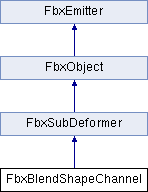
\includegraphics[height=4.000000cm]{class_fbx_blend_shape_channel}
\end{center}
\end{figure}
\subsection*{公開メンバ関数}
\begin{DoxyCompactItemize}
\item 
bool \hyperlink{class_fbx_blend_shape_channel_afa4cd576c24385c4ee10279a1deabc4d}{Set\+Blend\+Shape\+Deformer} (\hyperlink{class_fbx_blend_shape}{Fbx\+Blend\+Shape} $\ast$p\+Blend\+Shape)
\item 
\hyperlink{class_fbx_blend_shape}{Fbx\+Blend\+Shape} $\ast$ \hyperlink{class_fbx_blend_shape_channel_aa79b43cdb62a8dc5bbafad03acbf4425}{Get\+Blend\+Shape\+Deformer} ()
\item 
bool \hyperlink{class_fbx_blend_shape_channel_aa09d012a7304dd2098ebd2a066d53dde}{Add\+Target\+Shape} (\hyperlink{class_fbx_shape}{Fbx\+Shape} $\ast$p\+Shape, double p\+Full\+Deform\+Percent=100)
\item 
\hyperlink{class_fbx_shape}{Fbx\+Shape} $\ast$ \hyperlink{class_fbx_blend_shape_channel_a13265acf6f671cf6ec1228105831ff15}{Remove\+Target\+Shape} (\hyperlink{class_fbx_shape}{Fbx\+Shape} $\ast$p\+Shape)
\item 
int \hyperlink{class_fbx_blend_shape_channel_a61e052b389537fcb7db318853c17160c}{Get\+Target\+Shape\+Count} () const
\item 
\hyperlink{class_fbx_shape}{Fbx\+Shape} $\ast$ \hyperlink{class_fbx_blend_shape_channel_a50cdc8d0c76e13c093453efca50484a6}{Get\+Target\+Shape} (int p\+Index)
\item 
const \hyperlink{class_fbx_shape}{Fbx\+Shape} $\ast$ \hyperlink{class_fbx_blend_shape_channel_ae91fea86db9ce91da637df78762b4fff}{Get\+Target\+Shape} (int p\+Index) const
\item 
int \hyperlink{class_fbx_blend_shape_channel_a75e572afbee5b3c5c635932282b86473}{Get\+Target\+Shape\+Index} (\hyperlink{class_fbx_shape}{Fbx\+Shape} $\ast$p\+Shape)
\item 
double $\ast$ \hyperlink{class_fbx_blend_shape_channel_af3d0ae44fb85c9bdc485a7c607190cfd}{Get\+Target\+Shape\+Full\+Weights} ()
\item 
void \hyperlink{class_fbx_blend_shape_channel_a2e06faf81dd8983124645590f673d119}{Set\+Full\+Weights\+Count} (int p\+Count)
\end{DoxyCompactItemize}
\subsection*{公開変数類}
\begin{DoxyCompactItemize}
\item 
\hyperlink{class_fbx_property_t}{Fbx\+PropertyT}$<$ \hyperlink{fbxtypes_8h_a171e72a1c46fc15c1a6c9c31948c1c5b}{Fbx\+Double} $>$ \hyperlink{class_fbx_blend_shape_channel_a7b6c288c4f2d70fed6f29b424d7020a4}{Deform\+Percent}
\end{DoxyCompactItemize}
\subsection*{General Functions}
\begin{DoxyCompactItemize}
\item 
\hyperlink{class_fbx_array}{Fbx\+Array}$<$ double $>$ \hyperlink{class_fbx_blend_shape_channel_a99111b4513741df3e42dd87b1c08d347}{m\+Shape\+Full\+Weight\+Array}
\item 
\hyperlink{class_fbx_sub_deformer_aed7eba8aabbb8b25a8ddbab127d67319}{E\+Type} \hyperlink{class_fbx_blend_shape_channel_a1dba13e481ea7ba1874587ad92ee0347}{Get\+Sub\+Deformer\+Type} () const
\item 
void \hyperlink{class_fbx_blend_shape_channel_a3b633999bdf324fe9ac96e297c572eba}{Reset} ()
\item 
virtual \hyperlink{class_fbx_object}{Fbx\+Object} \& \hyperlink{class_fbx_blend_shape_channel_a7bf3a456eafada45fa2e934f15422026}{Copy} (const \hyperlink{class_fbx_object}{Fbx\+Object} \&p\+Object)
\item 
virtual \hyperlink{class_fbx_object}{Fbx\+Object} $\ast$ \hyperlink{class_fbx_blend_shape_channel_a37993d2cccb4376edb241577ccbd061f}{Clone} (\hyperlink{class_fbx_object_a9f5626b2d2135684d6ea1e6e4ad2acbb}{Fbx\+Object\+::\+E\+Clone\+Type} p\+Clone\+Type=\hyperlink{class_fbx_object_a9f5626b2d2135684d6ea1e6e4ad2acbbaacdf137ca059c572798287e98c4236d0}{e\+Deep\+Clone}, \hyperlink{class_fbx_object}{Fbx\+Object} $\ast$p\+Container=\hyperlink{fbxarch_8h_a070d2ce7b6bb7e5c05602aa8c308d0c4}{N\+U\+LL}, void $\ast$p\+Set=\hyperlink{fbxarch_8h_a070d2ce7b6bb7e5c05602aa8c308d0c4}{N\+U\+LL}) const
\item 
virtual void \hyperlink{class_fbx_blend_shape_channel_ad16237e4706289af6a9235b8425415cb}{Construct} (const \hyperlink{class_fbx_object}{Fbx\+Object} $\ast$p\+From)
\item 
virtual void \hyperlink{class_fbx_blend_shape_channel_a6ab3c2d6435d70a7c1b182097802ba90}{Construct\+Properties} (bool p\+Force\+Set)
\item 
virtual \hyperlink{class_fbx_string_list}{Fbx\+String\+List} \hyperlink{class_fbx_blend_shape_channel_a354002154ea342025ba0936e656b640a}{Get\+Type\+Flags} () const
\end{DoxyCompactItemize}
\subsection*{その他の継承メンバ}


\subsection{詳解}
Class for blend shape channels. A blend shape channel is a sub-\/deformer to help blend shape deformer to organize the target shapes. One blend shape deformer can have multiple blend shape channels in parallel, and each of them can control one or multiple target shapes. If there are multiple target shapes connected to one channel, each target shape could have its own full deformation percentage. For example, given a channel that has 3 target shapes, whose full deform percentage are 30, to 80 to 100 separately, then when the percent changes from 0 to 100, the base geometry will deform from the first target shape to the last one. This is called in-\/between blend shapes or progressive morph. The property Deform\+Percent of blend shape channel will control the deform level of each target shape or in-\/between blend shape on it. 

 fbxblendshapechannel.\+h の 37 行目に定義があります。



\subsection{関数詳解}
\mbox{\Hypertarget{class_fbx_blend_shape_channel_aa09d012a7304dd2098ebd2a066d53dde}\label{class_fbx_blend_shape_channel_aa09d012a7304dd2098ebd2a066d53dde}} 
\index{Fbx\+Blend\+Shape\+Channel@{Fbx\+Blend\+Shape\+Channel}!Add\+Target\+Shape@{Add\+Target\+Shape}}
\index{Add\+Target\+Shape@{Add\+Target\+Shape}!Fbx\+Blend\+Shape\+Channel@{Fbx\+Blend\+Shape\+Channel}}
\subsubsection{\texorpdfstring{Add\+Target\+Shape()}{AddTargetShape()}}
{\footnotesize\ttfamily bool Fbx\+Blend\+Shape\+Channel\+::\+Add\+Target\+Shape (\begin{DoxyParamCaption}\item[{\hyperlink{class_fbx_shape}{Fbx\+Shape} $\ast$}]{p\+Shape,  }\item[{double}]{p\+Full\+Deform\+Percent = {\ttfamily 100} }\end{DoxyParamCaption})}

Add a target shape. 
\begin{DoxyParams}{引数}
{\em p\+Shape} & Pointer to the target shape to add. \\
\hline
{\em p\+Full\+Deform\+Percent} & The full deform percentage for the target shape. \\
\hline
\end{DoxyParams}
\begin{DoxyReturn}{戻り値}
{\ttfamily true} on success, {\ttfamily false} otherwise. 
\end{DoxyReturn}
\mbox{\Hypertarget{class_fbx_blend_shape_channel_a37993d2cccb4376edb241577ccbd061f}\label{class_fbx_blend_shape_channel_a37993d2cccb4376edb241577ccbd061f}} 
\index{Fbx\+Blend\+Shape\+Channel@{Fbx\+Blend\+Shape\+Channel}!Clone@{Clone}}
\index{Clone@{Clone}!Fbx\+Blend\+Shape\+Channel@{Fbx\+Blend\+Shape\+Channel}}
\subsubsection{\texorpdfstring{Clone()}{Clone()}}
{\footnotesize\ttfamily virtual \hyperlink{class_fbx_object}{Fbx\+Object}$\ast$ Fbx\+Blend\+Shape\+Channel\+::\+Clone (\begin{DoxyParamCaption}\item[{\hyperlink{class_fbx_object_a9f5626b2d2135684d6ea1e6e4ad2acbb}{Fbx\+Object\+::\+E\+Clone\+Type}}]{p\+Clone\+Type = {\ttfamily \hyperlink{class_fbx_object_a9f5626b2d2135684d6ea1e6e4ad2acbbaacdf137ca059c572798287e98c4236d0}{e\+Deep\+Clone}},  }\item[{\hyperlink{class_fbx_object}{Fbx\+Object} $\ast$}]{p\+Container = {\ttfamily \hyperlink{fbxarch_8h_a070d2ce7b6bb7e5c05602aa8c308d0c4}{N\+U\+LL}},  }\item[{void $\ast$}]{p\+Set = {\ttfamily \hyperlink{fbxarch_8h_a070d2ce7b6bb7e5c05602aa8c308d0c4}{N\+U\+LL}} }\end{DoxyParamCaption}) const\hspace{0.3cm}{\ttfamily [virtual]}}

Creates a clone of this object. By default, the connections are N\+OT cloned. If the desired effect is to clone the connections as well, you must clone using the \hyperlink{class_fbx_clone_manager}{Fbx\+Clone\+Manager} (refer to this class documentation for further details).


\begin{DoxyParams}{引数}
{\em p\+Clone\+Type} & The type of clone to be created. By default, the clone type is e\+Deep\+Clone. \\
\hline
{\em p\+Container} & An optional parameter to specify which object will \char`\"{}contain\char`\"{} the new object. By contain, we mean the new object will become a source to the container, connection-\/wise. \\
\hline
{\em p\+Set} & See remark section. \\
\hline
\end{DoxyParams}
\begin{DoxyReturn}{戻り値}
The new clone, or N\+U\+LL (if the specified clone type is not supported). 
\end{DoxyReturn}
\begin{DoxyRemark}{注釈}
When doing either a \char`\"{}deep\char`\"{} or \char`\"{}reference\char`\"{} clone type, the clone will always get its properties values set from the source object properties values. 

Since this is a virtual function, some classes might do additional tasks. 

The {\itshape p\+Set} argument is not used in the default implementation of this method. Specialized implementations should cast this pointer to \hyperlink{class_fbx_clone_manager_aeb8a9c04c9c36eb7e551186a0b18f10d}{Fbx\+Clone\+Manager\+::\+Clone\+Set} to have access to the cloned objects so far. Typically, this pointer is set by the clone manager. 
\end{DoxyRemark}


\hyperlink{class_fbx_object_ad553a4262b09cb57c3171a93edadbab8}{Fbx\+Object}を再実装しています。

\mbox{\Hypertarget{class_fbx_blend_shape_channel_ad16237e4706289af6a9235b8425415cb}\label{class_fbx_blend_shape_channel_ad16237e4706289af6a9235b8425415cb}} 
\index{Fbx\+Blend\+Shape\+Channel@{Fbx\+Blend\+Shape\+Channel}!Construct@{Construct}}
\index{Construct@{Construct}!Fbx\+Blend\+Shape\+Channel@{Fbx\+Blend\+Shape\+Channel}}
\subsubsection{\texorpdfstring{Construct()}{Construct()}}
{\footnotesize\ttfamily virtual void Fbx\+Blend\+Shape\+Channel\+::\+Construct (\begin{DoxyParamCaption}\item[{const \hyperlink{class_fbx_object}{Fbx\+Object} $\ast$}]{p\+From }\end{DoxyParamCaption})\hspace{0.3cm}{\ttfamily [protected]}, {\ttfamily [virtual]}}

Optional constructor override, automatically called by default constructor. 
\begin{DoxyParams}{引数}
{\em p\+From} & If not null, the function must take it into account like a copy constructor. \\
\hline
\end{DoxyParams}
\begin{DoxyRemark}{注釈}
In case it is decided to override this function, do not forget to call Parent\+Class\+::\+Construct(p\+From) at the beginning. 
\end{DoxyRemark}


\hyperlink{class_fbx_sub_deformer_ae3d566383651e82b681827f0f38b97f3}{Fbx\+Sub\+Deformer}を再実装しています。

\mbox{\Hypertarget{class_fbx_blend_shape_channel_a6ab3c2d6435d70a7c1b182097802ba90}\label{class_fbx_blend_shape_channel_a6ab3c2d6435d70a7c1b182097802ba90}} 
\index{Fbx\+Blend\+Shape\+Channel@{Fbx\+Blend\+Shape\+Channel}!Construct\+Properties@{Construct\+Properties}}
\index{Construct\+Properties@{Construct\+Properties}!Fbx\+Blend\+Shape\+Channel@{Fbx\+Blend\+Shape\+Channel}}
\subsubsection{\texorpdfstring{Construct\+Properties()}{ConstructProperties()}}
{\footnotesize\ttfamily virtual void Fbx\+Blend\+Shape\+Channel\+::\+Construct\+Properties (\begin{DoxyParamCaption}\item[{bool}]{p\+Force\+Set }\end{DoxyParamCaption})\hspace{0.3cm}{\ttfamily [protected]}, {\ttfamily [virtual]}}

Optional property constructor override, automatically called by default constructor. 
\begin{DoxyParams}{引数}
{\em p\+Force\+Set} & If the property value must be set regardless of default value. \\
\hline
\end{DoxyParams}
\begin{DoxyRemark}{注釈}
If your object have properties, they must be initialized in this function. 
\end{DoxyRemark}


\hyperlink{class_fbx_object_ad44f814323dc1b5e78bff1bfc608b4bb}{Fbx\+Object}を再実装しています。

\mbox{\Hypertarget{class_fbx_blend_shape_channel_a7bf3a456eafada45fa2e934f15422026}\label{class_fbx_blend_shape_channel_a7bf3a456eafada45fa2e934f15422026}} 
\index{Fbx\+Blend\+Shape\+Channel@{Fbx\+Blend\+Shape\+Channel}!Copy@{Copy}}
\index{Copy@{Copy}!Fbx\+Blend\+Shape\+Channel@{Fbx\+Blend\+Shape\+Channel}}
\subsubsection{\texorpdfstring{Copy()}{Copy()}}
{\footnotesize\ttfamily virtual \hyperlink{class_fbx_object}{Fbx\+Object}\& Fbx\+Blend\+Shape\+Channel\+::\+Copy (\begin{DoxyParamCaption}\item[{const \hyperlink{class_fbx_object}{Fbx\+Object} \&}]{p\+Object }\end{DoxyParamCaption})\hspace{0.3cm}{\ttfamily [virtual]}}

Copy an object content into this object. 
\begin{DoxyParams}{引数}
{\em p\+Object} & The source object to copy data from. \\
\hline
\end{DoxyParams}
\begin{DoxyReturn}{戻り値}
Returns the destination object being modified by the source. 
\end{DoxyReturn}
\begin{DoxyRemark}{注釈}
This function replace the assignment operator (operator=). It will copy all property values and the name. Connections are N\+OT copied. 
\end{DoxyRemark}


\hyperlink{class_fbx_object_a0c0c5adb38284d14bb82c04d54504a3e}{Fbx\+Object}を再実装しています。

\mbox{\Hypertarget{class_fbx_blend_shape_channel_aa79b43cdb62a8dc5bbafad03acbf4425}\label{class_fbx_blend_shape_channel_aa79b43cdb62a8dc5bbafad03acbf4425}} 
\index{Fbx\+Blend\+Shape\+Channel@{Fbx\+Blend\+Shape\+Channel}!Get\+Blend\+Shape\+Deformer@{Get\+Blend\+Shape\+Deformer}}
\index{Get\+Blend\+Shape\+Deformer@{Get\+Blend\+Shape\+Deformer}!Fbx\+Blend\+Shape\+Channel@{Fbx\+Blend\+Shape\+Channel}}
\subsubsection{\texorpdfstring{Get\+Blend\+Shape\+Deformer()}{GetBlendShapeDeformer()}}
{\footnotesize\ttfamily \hyperlink{class_fbx_blend_shape}{Fbx\+Blend\+Shape}$\ast$ Fbx\+Blend\+Shape\+Channel\+::\+Get\+Blend\+Shape\+Deformer (\begin{DoxyParamCaption}{ }\end{DoxyParamCaption})}

Get the blend shape deformer that contains this blend shape channel. \begin{DoxyReturn}{戻り値}
A pointer to the blend shape deformer if set or N\+U\+LL. 
\end{DoxyReturn}
\mbox{\Hypertarget{class_fbx_blend_shape_channel_a1dba13e481ea7ba1874587ad92ee0347}\label{class_fbx_blend_shape_channel_a1dba13e481ea7ba1874587ad92ee0347}} 
\index{Fbx\+Blend\+Shape\+Channel@{Fbx\+Blend\+Shape\+Channel}!Get\+Sub\+Deformer\+Type@{Get\+Sub\+Deformer\+Type}}
\index{Get\+Sub\+Deformer\+Type@{Get\+Sub\+Deformer\+Type}!Fbx\+Blend\+Shape\+Channel@{Fbx\+Blend\+Shape\+Channel}}
\subsubsection{\texorpdfstring{Get\+Sub\+Deformer\+Type()}{GetSubDeformerType()}}
{\footnotesize\ttfamily \hyperlink{class_fbx_sub_deformer_aed7eba8aabbb8b25a8ddbab127d67319}{E\+Type} Fbx\+Blend\+Shape\+Channel\+::\+Get\+Sub\+Deformer\+Type (\begin{DoxyParamCaption}{ }\end{DoxyParamCaption}) const\hspace{0.3cm}{\ttfamily [inline]}, {\ttfamily [virtual]}}

Get the type of the sub deformer. \begin{DoxyReturn}{戻り値}
The sub deformer type identifier of blend shape channel. 
\end{DoxyReturn}


\hyperlink{class_fbx_sub_deformer_a1a1998b98ca03598bc6bec630e1aaa97}{Fbx\+Sub\+Deformer}を再実装しています。



 fbxblendshapechannel.\+h の 117 行目に定義があります。

\mbox{\Hypertarget{class_fbx_blend_shape_channel_a50cdc8d0c76e13c093453efca50484a6}\label{class_fbx_blend_shape_channel_a50cdc8d0c76e13c093453efca50484a6}} 
\index{Fbx\+Blend\+Shape\+Channel@{Fbx\+Blend\+Shape\+Channel}!Get\+Target\+Shape@{Get\+Target\+Shape}}
\index{Get\+Target\+Shape@{Get\+Target\+Shape}!Fbx\+Blend\+Shape\+Channel@{Fbx\+Blend\+Shape\+Channel}}
\subsubsection{\texorpdfstring{Get\+Target\+Shape()}{GetTargetShape()}\hspace{0.1cm}{\footnotesize\ttfamily [1/2]}}
{\footnotesize\ttfamily \hyperlink{class_fbx_shape}{Fbx\+Shape}$\ast$ Fbx\+Blend\+Shape\+Channel\+::\+Get\+Target\+Shape (\begin{DoxyParamCaption}\item[{int}]{p\+Index }\end{DoxyParamCaption})}

Get the target shape at given index. 
\begin{DoxyParams}{引数}
{\em p\+Index} & Index of the target shape. \\
\hline
\end{DoxyParams}
\begin{DoxyReturn}{戻り値}
Pointer to the target shape or {\ttfamily N\+U\+LL} if index is out of range. 
\end{DoxyReturn}
\mbox{\Hypertarget{class_fbx_blend_shape_channel_ae91fea86db9ce91da637df78762b4fff}\label{class_fbx_blend_shape_channel_ae91fea86db9ce91da637df78762b4fff}} 
\index{Fbx\+Blend\+Shape\+Channel@{Fbx\+Blend\+Shape\+Channel}!Get\+Target\+Shape@{Get\+Target\+Shape}}
\index{Get\+Target\+Shape@{Get\+Target\+Shape}!Fbx\+Blend\+Shape\+Channel@{Fbx\+Blend\+Shape\+Channel}}
\subsubsection{\texorpdfstring{Get\+Target\+Shape()}{GetTargetShape()}\hspace{0.1cm}{\footnotesize\ttfamily [2/2]}}
{\footnotesize\ttfamily const \hyperlink{class_fbx_shape}{Fbx\+Shape}$\ast$ Fbx\+Blend\+Shape\+Channel\+::\+Get\+Target\+Shape (\begin{DoxyParamCaption}\item[{int}]{p\+Index }\end{DoxyParamCaption}) const}

Get the target shape at given index. 
\begin{DoxyParams}{引数}
{\em p\+Index} & Index of the target shape. \\
\hline
\end{DoxyParams}
\begin{DoxyReturn}{戻り値}
Pointer to the target shape or {\ttfamily N\+U\+LL} if index is out of range. 
\end{DoxyReturn}
\mbox{\Hypertarget{class_fbx_blend_shape_channel_a61e052b389537fcb7db318853c17160c}\label{class_fbx_blend_shape_channel_a61e052b389537fcb7db318853c17160c}} 
\index{Fbx\+Blend\+Shape\+Channel@{Fbx\+Blend\+Shape\+Channel}!Get\+Target\+Shape\+Count@{Get\+Target\+Shape\+Count}}
\index{Get\+Target\+Shape\+Count@{Get\+Target\+Shape\+Count}!Fbx\+Blend\+Shape\+Channel@{Fbx\+Blend\+Shape\+Channel}}
\subsubsection{\texorpdfstring{Get\+Target\+Shape\+Count()}{GetTargetShapeCount()}}
{\footnotesize\ttfamily int Fbx\+Blend\+Shape\+Channel\+::\+Get\+Target\+Shape\+Count (\begin{DoxyParamCaption}{ }\end{DoxyParamCaption}) const}

Get the number of target shapes. \begin{DoxyReturn}{戻り値}
Number of target shapes that have been added to this blend shape channel. 
\end{DoxyReturn}
\mbox{\Hypertarget{class_fbx_blend_shape_channel_af3d0ae44fb85c9bdc485a7c607190cfd}\label{class_fbx_blend_shape_channel_af3d0ae44fb85c9bdc485a7c607190cfd}} 
\index{Fbx\+Blend\+Shape\+Channel@{Fbx\+Blend\+Shape\+Channel}!Get\+Target\+Shape\+Full\+Weights@{Get\+Target\+Shape\+Full\+Weights}}
\index{Get\+Target\+Shape\+Full\+Weights@{Get\+Target\+Shape\+Full\+Weights}!Fbx\+Blend\+Shape\+Channel@{Fbx\+Blend\+Shape\+Channel}}
\subsubsection{\texorpdfstring{Get\+Target\+Shape\+Full\+Weights()}{GetTargetShapeFullWeights()}}
{\footnotesize\ttfamily double$\ast$ Fbx\+Blend\+Shape\+Channel\+::\+Get\+Target\+Shape\+Full\+Weights (\begin{DoxyParamCaption}{ }\end{DoxyParamCaption})}

Get the full weight values of target shape. To access each value iterate in the array up to \hyperlink{class_fbx_blend_shape_channel_a61e052b389537fcb7db318853c17160c}{Get\+Target\+Shape\+Count()}. \begin{DoxyReturn}{戻り値}
The array of full weight values of target shape. 
\end{DoxyReturn}
\mbox{\Hypertarget{class_fbx_blend_shape_channel_a75e572afbee5b3c5c635932282b86473}\label{class_fbx_blend_shape_channel_a75e572afbee5b3c5c635932282b86473}} 
\index{Fbx\+Blend\+Shape\+Channel@{Fbx\+Blend\+Shape\+Channel}!Get\+Target\+Shape\+Index@{Get\+Target\+Shape\+Index}}
\index{Get\+Target\+Shape\+Index@{Get\+Target\+Shape\+Index}!Fbx\+Blend\+Shape\+Channel@{Fbx\+Blend\+Shape\+Channel}}
\subsubsection{\texorpdfstring{Get\+Target\+Shape\+Index()}{GetTargetShapeIndex()}}
{\footnotesize\ttfamily int Fbx\+Blend\+Shape\+Channel\+::\+Get\+Target\+Shape\+Index (\begin{DoxyParamCaption}\item[{\hyperlink{class_fbx_shape}{Fbx\+Shape} $\ast$}]{p\+Shape }\end{DoxyParamCaption})}

Get the index of the given target shape. 
\begin{DoxyParams}{引数}
{\em p\+Shape} & The given target shape to find index. \\
\hline
\end{DoxyParams}
\begin{DoxyReturn}{戻り値}
The index of the target shape. 
\end{DoxyReturn}
\mbox{\Hypertarget{class_fbx_blend_shape_channel_a354002154ea342025ba0936e656b640a}\label{class_fbx_blend_shape_channel_a354002154ea342025ba0936e656b640a}} 
\index{Fbx\+Blend\+Shape\+Channel@{Fbx\+Blend\+Shape\+Channel}!Get\+Type\+Flags@{Get\+Type\+Flags}}
\index{Get\+Type\+Flags@{Get\+Type\+Flags}!Fbx\+Blend\+Shape\+Channel@{Fbx\+Blend\+Shape\+Channel}}
\subsubsection{\texorpdfstring{Get\+Type\+Flags()}{GetTypeFlags()}}
{\footnotesize\ttfamily virtual \hyperlink{class_fbx_string_list}{Fbx\+String\+List} Fbx\+Blend\+Shape\+Channel\+::\+Get\+Type\+Flags (\begin{DoxyParamCaption}{ }\end{DoxyParamCaption}) const\hspace{0.3cm}{\ttfamily [protected]}, {\ttfamily [virtual]}}



\hyperlink{class_fbx_sub_deformer_a80652fd0521b2ea1897e221e5ae1b5cf}{Fbx\+Sub\+Deformer}を再実装しています。

\mbox{\Hypertarget{class_fbx_blend_shape_channel_a13265acf6f671cf6ec1228105831ff15}\label{class_fbx_blend_shape_channel_a13265acf6f671cf6ec1228105831ff15}} 
\index{Fbx\+Blend\+Shape\+Channel@{Fbx\+Blend\+Shape\+Channel}!Remove\+Target\+Shape@{Remove\+Target\+Shape}}
\index{Remove\+Target\+Shape@{Remove\+Target\+Shape}!Fbx\+Blend\+Shape\+Channel@{Fbx\+Blend\+Shape\+Channel}}
\subsubsection{\texorpdfstring{Remove\+Target\+Shape()}{RemoveTargetShape()}}
{\footnotesize\ttfamily \hyperlink{class_fbx_shape}{Fbx\+Shape}$\ast$ Fbx\+Blend\+Shape\+Channel\+::\+Remove\+Target\+Shape (\begin{DoxyParamCaption}\item[{\hyperlink{class_fbx_shape}{Fbx\+Shape} $\ast$}]{p\+Shape }\end{DoxyParamCaption})}

Remove the given target shape. 
\begin{DoxyParams}{引数}
{\em p\+Shape} & Pointer to the target shape to remove from this blend shape channel. \\
\hline
\end{DoxyParams}
\begin{DoxyReturn}{戻り値}
Pointer to the target shape or {\ttfamily N\+U\+LL} if p\+Shape is not owned by this blend shape channel. 
\end{DoxyReturn}
\mbox{\Hypertarget{class_fbx_blend_shape_channel_a3b633999bdf324fe9ac96e297c572eba}\label{class_fbx_blend_shape_channel_a3b633999bdf324fe9ac96e297c572eba}} 
\index{Fbx\+Blend\+Shape\+Channel@{Fbx\+Blend\+Shape\+Channel}!Reset@{Reset}}
\index{Reset@{Reset}!Fbx\+Blend\+Shape\+Channel@{Fbx\+Blend\+Shape\+Channel}}
\subsubsection{\texorpdfstring{Reset()}{Reset()}}
{\footnotesize\ttfamily void Fbx\+Blend\+Shape\+Channel\+::\+Reset (\begin{DoxyParamCaption}{ }\end{DoxyParamCaption})}

Restore the blend shape channel to the initial state. Calling this function will do the following\+: \begin{DoxyItemize}
\item Set the Deform\+Percent to 0. \item Remove all target shapes. \item Clear the array for fully deform weights of in-\/between target shapes. \end{DoxyItemize}
\mbox{\Hypertarget{class_fbx_blend_shape_channel_afa4cd576c24385c4ee10279a1deabc4d}\label{class_fbx_blend_shape_channel_afa4cd576c24385c4ee10279a1deabc4d}} 
\index{Fbx\+Blend\+Shape\+Channel@{Fbx\+Blend\+Shape\+Channel}!Set\+Blend\+Shape\+Deformer@{Set\+Blend\+Shape\+Deformer}}
\index{Set\+Blend\+Shape\+Deformer@{Set\+Blend\+Shape\+Deformer}!Fbx\+Blend\+Shape\+Channel@{Fbx\+Blend\+Shape\+Channel}}
\subsubsection{\texorpdfstring{Set\+Blend\+Shape\+Deformer()}{SetBlendShapeDeformer()}}
{\footnotesize\ttfamily bool Fbx\+Blend\+Shape\+Channel\+::\+Set\+Blend\+Shape\+Deformer (\begin{DoxyParamCaption}\item[{\hyperlink{class_fbx_blend_shape}{Fbx\+Blend\+Shape} $\ast$}]{p\+Blend\+Shape }\end{DoxyParamCaption})}

Set the blend shape deformer that contains this blend shape channel. 
\begin{DoxyParams}{引数}
{\em p\+Blend\+Shape} & Pointer to the blend shape deformer to set. \\
\hline
\end{DoxyParams}
\begin{DoxyReturn}{戻り値}
{\ttfamily true} on success, {\ttfamily false} otherwise. 
\end{DoxyReturn}
\mbox{\Hypertarget{class_fbx_blend_shape_channel_a2e06faf81dd8983124645590f673d119}\label{class_fbx_blend_shape_channel_a2e06faf81dd8983124645590f673d119}} 
\index{Fbx\+Blend\+Shape\+Channel@{Fbx\+Blend\+Shape\+Channel}!Set\+Full\+Weights\+Count@{Set\+Full\+Weights\+Count}}
\index{Set\+Full\+Weights\+Count@{Set\+Full\+Weights\+Count}!Fbx\+Blend\+Shape\+Channel@{Fbx\+Blend\+Shape\+Channel}}
\subsubsection{\texorpdfstring{Set\+Full\+Weights\+Count()}{SetFullWeightsCount()}}
{\footnotesize\ttfamily void Fbx\+Blend\+Shape\+Channel\+::\+Set\+Full\+Weights\+Count (\begin{DoxyParamCaption}\item[{int}]{p\+Count }\end{DoxyParamCaption})}

Set the array size for the fully deform weights. This functions pre-\/allocate the array to p\+Count size. 
\begin{DoxyParams}{引数}
{\em p\+Count} & The new array size to set. \\
\hline
\end{DoxyParams}


\subsection{メンバ詳解}
\mbox{\Hypertarget{class_fbx_blend_shape_channel_a7b6c288c4f2d70fed6f29b424d7020a4}\label{class_fbx_blend_shape_channel_a7b6c288c4f2d70fed6f29b424d7020a4}} 
\index{Fbx\+Blend\+Shape\+Channel@{Fbx\+Blend\+Shape\+Channel}!Deform\+Percent@{Deform\+Percent}}
\index{Deform\+Percent@{Deform\+Percent}!Fbx\+Blend\+Shape\+Channel@{Fbx\+Blend\+Shape\+Channel}}
\subsubsection{\texorpdfstring{Deform\+Percent}{DeformPercent}}
{\footnotesize\ttfamily \hyperlink{class_fbx_property_t}{Fbx\+PropertyT}$<$\hyperlink{fbxtypes_8h_a171e72a1c46fc15c1a6c9c31948c1c5b}{Fbx\+Double}$>$ Fbx\+Blend\+Shape\+Channel\+::\+Deform\+Percent}

This property stores deform percent of this channel. The default value of this property is 0.\+0.

\begin{DoxyRemark}{注釈}
Although not enforced, it is strongly suggested to limit the value of this property in the range from 0.\+0 to 100.\+0 because graphic applications may handle values outside of this interval differently, therefore producing unexpected results. 
\end{DoxyRemark}


 fbxblendshapechannel.\+h の 49 行目に定義があります。

\mbox{\Hypertarget{class_fbx_blend_shape_channel_a99111b4513741df3e42dd87b1c08d347}\label{class_fbx_blend_shape_channel_a99111b4513741df3e42dd87b1c08d347}} 
\index{Fbx\+Blend\+Shape\+Channel@{Fbx\+Blend\+Shape\+Channel}!m\+Shape\+Full\+Weight\+Array@{m\+Shape\+Full\+Weight\+Array}}
\index{m\+Shape\+Full\+Weight\+Array@{m\+Shape\+Full\+Weight\+Array}!Fbx\+Blend\+Shape\+Channel@{Fbx\+Blend\+Shape\+Channel}}
\subsubsection{\texorpdfstring{m\+Shape\+Full\+Weight\+Array}{mShapeFullWeightArray}}
{\footnotesize\ttfamily \hyperlink{class_fbx_array}{Fbx\+Array}$<$double$>$ Fbx\+Blend\+Shape\+Channel\+::m\+Shape\+Full\+Weight\+Array\hspace{0.3cm}{\ttfamily [protected]}}



 fbxblendshapechannel.\+h の 142 行目に定義があります。



このクラス詳解は次のファイルから抽出されました\+:\begin{DoxyCompactItemize}
\item 
C\+:/\+Maya/scripts/\+F\+B\+X\+\_\+\+S\+D\+K/2017.\+1/include/fbxsdk/scene/geometry/\hyperlink{fbxblendshapechannel_8h}{fbxblendshapechannel.\+h}\end{DoxyCompactItemize}

\hypertarget{class_fbx_blob}{}\section{Fbx\+Blob クラス}
\label{class_fbx_blob}\index{Fbx\+Blob@{Fbx\+Blob}}


{\ttfamily \#include $<$fbxpropertytypes.\+h$>$}

\subsection*{公開メンバ関数}
\begin{DoxyCompactItemize}
\item 
void $\ast$ \hyperlink{class_fbx_blob_a18bd3fbf233e39091ffcf0ef65123023}{Modify} ()
\begin{DoxyCompactList}\small\item\em Make a copy if the reference count $>$ 1 (i.\+e. if the buffer is shared). \end{DoxyCompactList}\item 
void \hyperlink{class_fbx_blob_abd720fef7ed5feacc8ef21d669e26cce}{Clear} ()
\begin{DoxyCompactList}\small\item\em Free the memory if this blob is the last one to hold it. \end{DoxyCompactList}\end{DoxyCompactItemize}
\subsection*{限定公開変数類}
\begin{DoxyCompactItemize}
\item 
int $\ast$ \hyperlink{class_fbx_blob_ac25ef6a057beb9d5f1d072a77833b910}{m\+Ref\+Count}
\item 
void $\ast$ \hyperlink{class_fbx_blob_af397c288f865eefa5e1fde8be443d9c2}{m\+Data}
\item 
int \hyperlink{class_fbx_blob_a3c92f0ad0ff306800df7be4d94ac7528}{m\+Size}
\end{DoxyCompactItemize}
\subsection*{Constructors and Destructor}
\begin{DoxyCompactItemize}
\item 
\hyperlink{class_fbx_blob_ad1013b102b7e2b54e5cb3ffe326e0738}{Fbx\+Blob} ()
\begin{DoxyCompactList}\small\item\em Constructor. Set attributes to 0. \end{DoxyCompactList}\item 
\hyperlink{class_fbx_blob_aaab0ee64d11daa7aff57542daad4105e}{Fbx\+Blob} (int p\+Size)
\item 
\hyperlink{class_fbx_blob_a2636c1976b481f86ee4393c0d50b0470}{Fbx\+Blob} (const \hyperlink{class_fbx_blob}{Fbx\+Blob} \&p\+R\+HS)
\item 
\hyperlink{class_fbx_blob_a2359aefdd7854a89d3d4bff0980696c1}{Fbx\+Blob} (const void $\ast$p\+Data, int p\+Size)
\item 
\hyperlink{class_fbx_blob_ab0e197c8fc8bd7ff64d1d95501984132}{$\sim$\+Fbx\+Blob} ()
\begin{DoxyCompactList}\small\item\em Destructor \end{DoxyCompactList}\end{DoxyCompactItemize}
\subsection*{Assignment.}
\begin{DoxyCompactItemize}
\item 
\hyperlink{class_fbx_blob}{Fbx\+Blob} \& \hyperlink{class_fbx_blob_aaa69c14d3d6ad7c6720957cd6c08712a}{operator=} (const \hyperlink{class_fbx_blob}{Fbx\+Blob} \&p\+Value)
\item 
void \hyperlink{class_fbx_blob_a9370942703afba1f51798ff5ac2b0ec5}{Assign} (const void $\ast$p\+Data, int p\+Size)
\end{DoxyCompactItemize}
\subsection*{Boolean operation}
\begin{DoxyCompactItemize}
\item 
bool \hyperlink{class_fbx_blob_ad8de66a73abbec7cb602653ca2008a6d}{operator==} (const \hyperlink{class_fbx_blob}{Fbx\+Blob} \&p\+R\+HS) const
\item 
bool \hyperlink{class_fbx_blob_a8a37da8658286521abc8c085f1fdbb69}{operator!=} (const \hyperlink{class_fbx_blob}{Fbx\+Blob} \&p\+R\+HS) const
\end{DoxyCompactItemize}
\subsection*{Access}
\begin{DoxyCompactItemize}
\item 
const void $\ast$ \hyperlink{class_fbx_blob_a5fb39826dd62378bcf18b4de9db38509}{Access} () const
\item 
int \hyperlink{class_fbx_blob_a4b391b461d5303f6a1f24ae910b4e5c8}{Size} () const
\end{DoxyCompactItemize}


\subsection{詳解}
F\+BX S\+DK blob class. Uninitialized data of a specified size, to be filled by the user. 

\subsection{構築子と解体子}
\mbox{\Hypertarget{class_fbx_blob_ad1013b102b7e2b54e5cb3ffe326e0738}\label{class_fbx_blob_ad1013b102b7e2b54e5cb3ffe326e0738}} 
\index{Fbx\+Blob@{Fbx\+Blob}!Fbx\+Blob@{Fbx\+Blob}}
\index{Fbx\+Blob@{Fbx\+Blob}!Fbx\+Blob@{Fbx\+Blob}}
\subsubsection{\texorpdfstring{Fbx\+Blob()}{FbxBlob()}\hspace{0.1cm}{\footnotesize\ttfamily [1/4]}}
{\footnotesize\ttfamily Fbx\+Blob\+::\+Fbx\+Blob (\begin{DoxyParamCaption}{ }\end{DoxyParamCaption})}



Constructor. Set attributes to 0. 

\mbox{\Hypertarget{class_fbx_blob_aaab0ee64d11daa7aff57542daad4105e}\label{class_fbx_blob_aaab0ee64d11daa7aff57542daad4105e}} 
\index{Fbx\+Blob@{Fbx\+Blob}!Fbx\+Blob@{Fbx\+Blob}}
\index{Fbx\+Blob@{Fbx\+Blob}!Fbx\+Blob@{Fbx\+Blob}}
\subsubsection{\texorpdfstring{Fbx\+Blob()}{FbxBlob()}\hspace{0.1cm}{\footnotesize\ttfamily [2/4]}}
{\footnotesize\ttfamily Fbx\+Blob\+::\+Fbx\+Blob (\begin{DoxyParamCaption}\item[{int}]{p\+Size }\end{DoxyParamCaption})}

Constructor. Construct a buffer with uninitialized data of a specified size, to be filled by the user. 
\begin{DoxyParams}{引数}
{\em p\+Size} & Buffer size. \\
\hline
\end{DoxyParams}
\mbox{\Hypertarget{class_fbx_blob_a2636c1976b481f86ee4393c0d50b0470}\label{class_fbx_blob_a2636c1976b481f86ee4393c0d50b0470}} 
\index{Fbx\+Blob@{Fbx\+Blob}!Fbx\+Blob@{Fbx\+Blob}}
\index{Fbx\+Blob@{Fbx\+Blob}!Fbx\+Blob@{Fbx\+Blob}}
\subsubsection{\texorpdfstring{Fbx\+Blob()}{FbxBlob()}\hspace{0.1cm}{\footnotesize\ttfamily [3/4]}}
{\footnotesize\ttfamily Fbx\+Blob\+::\+Fbx\+Blob (\begin{DoxyParamCaption}\item[{const \hyperlink{class_fbx_blob}{Fbx\+Blob} \&}]{p\+R\+HS }\end{DoxyParamCaption})}

Copy constructor. 
\begin{DoxyParams}{引数}
{\em p\+R\+HS} & The blob to be copied to this blob. \\
\hline
\end{DoxyParams}
\mbox{\Hypertarget{class_fbx_blob_a2359aefdd7854a89d3d4bff0980696c1}\label{class_fbx_blob_a2359aefdd7854a89d3d4bff0980696c1}} 
\index{Fbx\+Blob@{Fbx\+Blob}!Fbx\+Blob@{Fbx\+Blob}}
\index{Fbx\+Blob@{Fbx\+Blob}!Fbx\+Blob@{Fbx\+Blob}}
\subsubsection{\texorpdfstring{Fbx\+Blob()}{FbxBlob()}\hspace{0.1cm}{\footnotesize\ttfamily [4/4]}}
{\footnotesize\ttfamily Fbx\+Blob\+::\+Fbx\+Blob (\begin{DoxyParamCaption}\item[{const void $\ast$}]{p\+Data,  }\item[{int}]{p\+Size }\end{DoxyParamCaption})}

Constructor. 
\begin{DoxyParams}{引数}
{\em p\+Data} & The data to be filled in the buffer. \\
\hline
{\em p\+Size} & Buffer size. \\
\hline
\end{DoxyParams}
\mbox{\Hypertarget{class_fbx_blob_ab0e197c8fc8bd7ff64d1d95501984132}\label{class_fbx_blob_ab0e197c8fc8bd7ff64d1d95501984132}} 
\index{Fbx\+Blob@{Fbx\+Blob}!````~Fbx\+Blob@{$\sim$\+Fbx\+Blob}}
\index{````~Fbx\+Blob@{$\sim$\+Fbx\+Blob}!Fbx\+Blob@{Fbx\+Blob}}
\subsubsection{\texorpdfstring{$\sim$\+Fbx\+Blob()}{~FbxBlob()}}
{\footnotesize\ttfamily Fbx\+Blob\+::$\sim$\+Fbx\+Blob (\begin{DoxyParamCaption}{ }\end{DoxyParamCaption})}



Destructor 



\subsection{メソッド詳解}
\mbox{\Hypertarget{class_fbx_blob_a5fb39826dd62378bcf18b4de9db38509}\label{class_fbx_blob_a5fb39826dd62378bcf18b4de9db38509}} 
\index{Fbx\+Blob@{Fbx\+Blob}!Access@{Access}}
\index{Access@{Access}!Fbx\+Blob@{Fbx\+Blob}}
\subsubsection{\texorpdfstring{Access()}{Access()}}
{\footnotesize\ttfamily const void$\ast$ Fbx\+Blob\+::\+Access (\begin{DoxyParamCaption}{ }\end{DoxyParamCaption}) const}

Retrieve the buffer pointer. \begin{DoxyReturn}{戻り値}
The buffer pointer. 
\end{DoxyReturn}
\mbox{\Hypertarget{class_fbx_blob_a9370942703afba1f51798ff5ac2b0ec5}\label{class_fbx_blob_a9370942703afba1f51798ff5ac2b0ec5}} 
\index{Fbx\+Blob@{Fbx\+Blob}!Assign@{Assign}}
\index{Assign@{Assign}!Fbx\+Blob@{Fbx\+Blob}}
\subsubsection{\texorpdfstring{Assign()}{Assign()}}
{\footnotesize\ttfamily void Fbx\+Blob\+::\+Assign (\begin{DoxyParamCaption}\item[{const void $\ast$}]{p\+Data,  }\item[{int}]{p\+Size }\end{DoxyParamCaption})}

Copy the data in the buffer. 
\begin{DoxyParams}{引数}
{\em p\+Data} & The buffer to be copied data from. \\
\hline
{\em p\+Size} & Buffer size. \\
\hline
\end{DoxyParams}
被呼び出し関係図\+:
% FIG 0
\mbox{\Hypertarget{class_fbx_blob_abd720fef7ed5feacc8ef21d669e26cce}\label{class_fbx_blob_abd720fef7ed5feacc8ef21d669e26cce}} 
\index{Fbx\+Blob@{Fbx\+Blob}!Clear@{Clear}}
\index{Clear@{Clear}!Fbx\+Blob@{Fbx\+Blob}}
\subsubsection{\texorpdfstring{Clear()}{Clear()}}
{\footnotesize\ttfamily void Fbx\+Blob\+::\+Clear (\begin{DoxyParamCaption}{ }\end{DoxyParamCaption})}



Free the memory if this blob is the last one to hold it. 

\mbox{\Hypertarget{class_fbx_blob_a18bd3fbf233e39091ffcf0ef65123023}\label{class_fbx_blob_a18bd3fbf233e39091ffcf0ef65123023}} 
\index{Fbx\+Blob@{Fbx\+Blob}!Modify@{Modify}}
\index{Modify@{Modify}!Fbx\+Blob@{Fbx\+Blob}}
\subsubsection{\texorpdfstring{Modify()}{Modify()}}
{\footnotesize\ttfamily void$\ast$ Fbx\+Blob\+::\+Modify (\begin{DoxyParamCaption}{ }\end{DoxyParamCaption})}



Make a copy if the reference count $>$ 1 (i.\+e. if the buffer is shared). 

\mbox{\Hypertarget{class_fbx_blob_a8a37da8658286521abc8c085f1fdbb69}\label{class_fbx_blob_a8a37da8658286521abc8c085f1fdbb69}} 
\index{Fbx\+Blob@{Fbx\+Blob}!operator"!=@{operator"!=}}
\index{operator"!=@{operator"!=}!Fbx\+Blob@{Fbx\+Blob}}
\subsubsection{\texorpdfstring{operator"!=()}{operator!=()}}
{\footnotesize\ttfamily bool Fbx\+Blob\+::operator!= (\begin{DoxyParamCaption}\item[{const \hyperlink{class_fbx_blob}{Fbx\+Blob} \&}]{p\+R\+HS }\end{DoxyParamCaption}) const}

Inequality operator. 
\begin{DoxyParams}{引数}
{\em p\+R\+HS} & The blob to be compared with this blob. \\
\hline
\end{DoxyParams}
\begin{DoxyReturn}{戻り値}
{\ttfamily True}, if the two blobs are unequal, otherwise false. 
\end{DoxyReturn}
\mbox{\Hypertarget{class_fbx_blob_aaa69c14d3d6ad7c6720957cd6c08712a}\label{class_fbx_blob_aaa69c14d3d6ad7c6720957cd6c08712a}} 
\index{Fbx\+Blob@{Fbx\+Blob}!operator=@{operator=}}
\index{operator=@{operator=}!Fbx\+Blob@{Fbx\+Blob}}
\subsubsection{\texorpdfstring{operator=()}{operator=()}}
{\footnotesize\ttfamily \hyperlink{class_fbx_blob}{Fbx\+Blob}\& Fbx\+Blob\+::operator= (\begin{DoxyParamCaption}\item[{const \hyperlink{class_fbx_blob}{Fbx\+Blob} \&}]{p\+Value }\end{DoxyParamCaption})}

Share the buffer of the specified blob with this blob. 
\begin{DoxyParams}{引数}
{\em p\+Value} & The blob whose buffer is shared with this blob. \\
\hline
\end{DoxyParams}
\begin{DoxyReturn}{戻り値}
This blob. 
\end{DoxyReturn}
\mbox{\Hypertarget{class_fbx_blob_ad8de66a73abbec7cb602653ca2008a6d}\label{class_fbx_blob_ad8de66a73abbec7cb602653ca2008a6d}} 
\index{Fbx\+Blob@{Fbx\+Blob}!operator==@{operator==}}
\index{operator==@{operator==}!Fbx\+Blob@{Fbx\+Blob}}
\subsubsection{\texorpdfstring{operator==()}{operator==()}}
{\footnotesize\ttfamily bool Fbx\+Blob\+::operator== (\begin{DoxyParamCaption}\item[{const \hyperlink{class_fbx_blob}{Fbx\+Blob} \&}]{p\+R\+HS }\end{DoxyParamCaption}) const}

Equality operator. 
\begin{DoxyParams}{引数}
{\em p\+R\+HS} & The blob to be compared with this blob. \\
\hline
\end{DoxyParams}
\begin{DoxyReturn}{戻り値}
{\ttfamily True}, if the two blobs are equal, {\ttfamily false} otherwise. 
\end{DoxyReturn}
\mbox{\Hypertarget{class_fbx_blob_a4b391b461d5303f6a1f24ae910b4e5c8}\label{class_fbx_blob_a4b391b461d5303f6a1f24ae910b4e5c8}} 
\index{Fbx\+Blob@{Fbx\+Blob}!Size@{Size}}
\index{Size@{Size}!Fbx\+Blob@{Fbx\+Blob}}
\subsubsection{\texorpdfstring{Size()}{Size()}}
{\footnotesize\ttfamily int Fbx\+Blob\+::\+Size (\begin{DoxyParamCaption}{ }\end{DoxyParamCaption}) const}

Retrieve the buffer size \begin{DoxyReturn}{戻り値}
The buffer size. 
\end{DoxyReturn}


\subsection{メンバ詳解}
\mbox{\Hypertarget{class_fbx_blob_af397c288f865eefa5e1fde8be443d9c2}\label{class_fbx_blob_af397c288f865eefa5e1fde8be443d9c2}} 
\index{Fbx\+Blob@{Fbx\+Blob}!m\+Data@{m\+Data}}
\index{m\+Data@{m\+Data}!Fbx\+Blob@{Fbx\+Blob}}
\subsubsection{\texorpdfstring{m\+Data}{mData}}
{\footnotesize\ttfamily void$\ast$ Fbx\+Blob\+::m\+Data\hspace{0.3cm}{\ttfamily [protected]}}

\mbox{\Hypertarget{class_fbx_blob_ac25ef6a057beb9d5f1d072a77833b910}\label{class_fbx_blob_ac25ef6a057beb9d5f1d072a77833b910}} 
\index{Fbx\+Blob@{Fbx\+Blob}!m\+Ref\+Count@{m\+Ref\+Count}}
\index{m\+Ref\+Count@{m\+Ref\+Count}!Fbx\+Blob@{Fbx\+Blob}}
\subsubsection{\texorpdfstring{m\+Ref\+Count}{mRefCount}}
{\footnotesize\ttfamily int$\ast$ Fbx\+Blob\+::m\+Ref\+Count\hspace{0.3cm}{\ttfamily [protected]}}

\mbox{\Hypertarget{class_fbx_blob_a3c92f0ad0ff306800df7be4d94ac7528}\label{class_fbx_blob_a3c92f0ad0ff306800df7be4d94ac7528}} 
\index{Fbx\+Blob@{Fbx\+Blob}!m\+Size@{m\+Size}}
\index{m\+Size@{m\+Size}!Fbx\+Blob@{Fbx\+Blob}}
\subsubsection{\texorpdfstring{m\+Size}{mSize}}
{\footnotesize\ttfamily int Fbx\+Blob\+::m\+Size\hspace{0.3cm}{\ttfamily [protected]}}



このクラス詳解は次のファイルから抽出されました\+:\begin{DoxyCompactItemize}
\item 
C\+:/github/\+F\+B\+Xpython\+S\+D\+K201701/\+F\+B\+Xpython\+S\+D\+K201701/2017.\+1/include/fbxsdk/core/\hyperlink{fbxpropertytypes_8h}{fbxpropertytypes.\+h}\end{DoxyCompactItemize}

\hypertarget{class_fbx_boundary}{}\section{Fbx\+Boundary クラス}
\label{class_fbx_boundary}\index{Fbx\+Boundary@{Fbx\+Boundary}}


{\ttfamily \#include $<$fbxtrimnurbssurface.\+h$>$}

Fbx\+Boundary の継承関係図\begin{figure}[H]
\begin{center}
\leavevmode
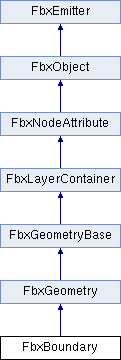
\includegraphics[height=7.000000cm]{class_fbx_boundary}
\end{center}
\end{figure}
\subsection*{公開メンバ関数}
\begin{DoxyCompactItemize}
\item 
void \hyperlink{class_fbx_boundary_af94f173acd55d7d5f285f8539bbb48e4}{Add\+Curve} (\hyperlink{class_fbx_nurbs_curve}{Fbx\+Nurbs\+Curve} $\ast$p\+Curve)
\item 
int \hyperlink{class_fbx_boundary_adcd0d41aa9a5804cd74ed14b6b8f6f8a}{Get\+Curve\+Count} () const
\item 
\hyperlink{class_fbx_nurbs_curve}{Fbx\+Nurbs\+Curve} $\ast$ \hyperlink{class_fbx_boundary_acbf7b338d8b90d6cd52e7c39faa8b648}{Get\+Curve} (int p\+Index)
\item 
const \hyperlink{class_fbx_nurbs_curve}{Fbx\+Nurbs\+Curve} $\ast$ \hyperlink{class_fbx_boundary_a1f9aac3b37beac6639afa97c79e45358}{Get\+Curve} (int p\+Index) const
\item 
virtual \hyperlink{class_fbx_node_attribute_a08e1669d3d1a696910756ab17de56d6a}{Fbx\+Node\+Attribute\+::\+E\+Type} \hyperlink{class_fbx_boundary_a093be9c6c0c0f13a337e9b6815aed9d0}{Get\+Attribute\+Type} () const
\begin{DoxyCompactList}\small\item\em Returns the type of node attribute. \end{DoxyCompactList}\item 
bool \hyperlink{class_fbx_boundary_ad319a0f4511c35710c24b543d30bbee2}{Is\+Point\+In\+Control\+Hull} (const \hyperlink{class_fbx_vector4}{Fbx\+Vector4} \&p\+Point)
\item 
\hyperlink{class_fbx_vector4}{Fbx\+Vector4} \hyperlink{class_fbx_boundary_a615c36267401342800e00befefa50f6c}{Compute\+Point\+In\+Boundary} ()
\item 
virtual \hyperlink{class_fbx_object}{Fbx\+Object} \& \hyperlink{class_fbx_boundary_a6fe59f45c17eeebbabaeff235058ac70}{Copy} (const \hyperlink{class_fbx_object}{Fbx\+Object} \&p\+Object)
\item 
void \hyperlink{class_fbx_boundary_aa1c12f34cb325c5a337fa383f0860e06}{Clear\+Curves} ()
\item 
void \hyperlink{class_fbx_boundary_ae41addb147733da9216a785bc6d003c3}{Copy\+Curves} (\hyperlink{class_fbx_boundary}{Fbx\+Boundary} const \&p\+Other)
\item 
bool \hyperlink{class_fbx_boundary_a4ecaec2f4194b5ba045c14ec0549d10e}{Is\+Valid} (bool must\+Closed=true)
\item 
bool \hyperlink{class_fbx_boundary_a025f682e72db299620e30eeeebdd1ea7}{Is\+Counter\+Clockwise} ()
\end{DoxyCompactItemize}
\subsection*{公開変数類}
\begin{DoxyCompactItemize}
\item 
\hyperlink{class_fbx_property_t}{Fbx\+PropertyT}$<$ \hyperlink{fbxtypes_8h_a92e0562b2fe33e76a242f498b362262e}{Fbx\+Bool} $>$ \hyperlink{class_fbx_boundary_af9e27e491f466ca615bd247fa2b33826}{Outer\+Flag}
\end{DoxyCompactItemize}
\subsection*{静的公開変数類}
\begin{DoxyCompactItemize}
\item 
static const char $\ast$ \hyperlink{class_fbx_boundary_a2a42aaddc584761f409ced017e6ddd35}{s\+Outer\+Flag}
\begin{DoxyCompactList}\small\item\em Properties \end{DoxyCompactList}\end{DoxyCompactItemize}
\subsection*{限定公開メンバ関数}
\begin{DoxyCompactItemize}
\item 
virtual void \hyperlink{class_fbx_boundary_acb50e021b1e9920026c975613a949537}{Construct\+Properties} (bool p\+Force\+Set)
\item 
void \hyperlink{class_fbx_boundary_a989aba9b8873dc0c8264879b75f86dee}{Reset} ()
\item 
bool \hyperlink{class_fbx_boundary_afdc24b2ebd724263f2a20a8159006e42}{Line\+Segment\+Intersect} (const \hyperlink{class_fbx_vector4}{Fbx\+Vector4} \&p\+Start1, const \hyperlink{class_fbx_vector4}{Fbx\+Vector4} \&p\+End1, const \hyperlink{class_fbx_vector4}{Fbx\+Vector4} \&p\+Start2, const \hyperlink{class_fbx_vector4}{Fbx\+Vector4} \&p\+End2) const
\end{DoxyCompactItemize}
\subsection*{その他の継承メンバ}


\subsection{詳解}
\hyperlink{class_fbx_boundary}{Fbx\+Boundary} describes a trimming boundary for a trimmed N\+U\+R\+BS object. Note\+:Outer boundaries run counter-\/clockwise in UV space and inner boundaries run clockwise. An outer boundary represents the outer edges of the trimmed surface whereas the inner boundaries define \char`\"{}holes\char`\"{} in the surface. 

 fbxtrimnurbssurface.\+h の 30 行目に定義があります。



\subsection{関数詳解}
\mbox{\Hypertarget{class_fbx_boundary_af94f173acd55d7d5f285f8539bbb48e4}\label{class_fbx_boundary_af94f173acd55d7d5f285f8539bbb48e4}} 
\index{Fbx\+Boundary@{Fbx\+Boundary}!Add\+Curve@{Add\+Curve}}
\index{Add\+Curve@{Add\+Curve}!Fbx\+Boundary@{Fbx\+Boundary}}
\subsubsection{\texorpdfstring{Add\+Curve()}{AddCurve()}}
{\footnotesize\ttfamily void Fbx\+Boundary\+::\+Add\+Curve (\begin{DoxyParamCaption}\item[{\hyperlink{class_fbx_nurbs_curve}{Fbx\+Nurbs\+Curve} $\ast$}]{p\+Curve }\end{DoxyParamCaption})}

Adds an edge to this boundary. 
\begin{DoxyParams}{引数}
{\em p\+Curve} & The curve to be appended to the end of this boundary \\
\hline
\end{DoxyParams}
\mbox{\Hypertarget{class_fbx_boundary_aa1c12f34cb325c5a337fa383f0860e06}\label{class_fbx_boundary_aa1c12f34cb325c5a337fa383f0860e06}} 
\index{Fbx\+Boundary@{Fbx\+Boundary}!Clear\+Curves@{Clear\+Curves}}
\index{Clear\+Curves@{Clear\+Curves}!Fbx\+Boundary@{Fbx\+Boundary}}
\subsubsection{\texorpdfstring{Clear\+Curves()}{ClearCurves()}}
{\footnotesize\ttfamily void Fbx\+Boundary\+::\+Clear\+Curves (\begin{DoxyParamCaption}{ }\end{DoxyParamCaption})}

\mbox{\Hypertarget{class_fbx_boundary_a615c36267401342800e00befefa50f6c}\label{class_fbx_boundary_a615c36267401342800e00befefa50f6c}} 
\index{Fbx\+Boundary@{Fbx\+Boundary}!Compute\+Point\+In\+Boundary@{Compute\+Point\+In\+Boundary}}
\index{Compute\+Point\+In\+Boundary@{Compute\+Point\+In\+Boundary}!Fbx\+Boundary@{Fbx\+Boundary}}
\subsubsection{\texorpdfstring{Compute\+Point\+In\+Boundary()}{ComputePointInBoundary()}}
{\footnotesize\ttfamily \hyperlink{class_fbx_vector4}{Fbx\+Vector4} Fbx\+Boundary\+::\+Compute\+Point\+In\+Boundary (\begin{DoxyParamCaption}{ }\end{DoxyParamCaption})}

Computes the origin point in the boundary \begin{DoxyReturn}{戻り値}
The origin point. 
\end{DoxyReturn}
\mbox{\Hypertarget{class_fbx_boundary_acb50e021b1e9920026c975613a949537}\label{class_fbx_boundary_acb50e021b1e9920026c975613a949537}} 
\index{Fbx\+Boundary@{Fbx\+Boundary}!Construct\+Properties@{Construct\+Properties}}
\index{Construct\+Properties@{Construct\+Properties}!Fbx\+Boundary@{Fbx\+Boundary}}
\subsubsection{\texorpdfstring{Construct\+Properties()}{ConstructProperties()}}
{\footnotesize\ttfamily virtual void Fbx\+Boundary\+::\+Construct\+Properties (\begin{DoxyParamCaption}\item[{bool}]{p\+Force\+Set }\end{DoxyParamCaption})\hspace{0.3cm}{\ttfamily [protected]}, {\ttfamily [virtual]}}

Optional property constructor override, automatically called by default constructor. 
\begin{DoxyParams}{引数}
{\em p\+Force\+Set} & If the property value must be set regardless of default value. \\
\hline
\end{DoxyParams}
\begin{DoxyRemark}{注釈}
If your object have properties, they must be initialized in this function. 
\end{DoxyRemark}


\hyperlink{class_fbx_geometry_base_a94ee142ac1d40be3aebb4d9441431921}{Fbx\+Geometry\+Base}を再実装しています。

\mbox{\Hypertarget{class_fbx_boundary_a6fe59f45c17eeebbabaeff235058ac70}\label{class_fbx_boundary_a6fe59f45c17eeebbabaeff235058ac70}} 
\index{Fbx\+Boundary@{Fbx\+Boundary}!Copy@{Copy}}
\index{Copy@{Copy}!Fbx\+Boundary@{Fbx\+Boundary}}
\subsubsection{\texorpdfstring{Copy()}{Copy()}}
{\footnotesize\ttfamily virtual \hyperlink{class_fbx_object}{Fbx\+Object}\& Fbx\+Boundary\+::\+Copy (\begin{DoxyParamCaption}\item[{const \hyperlink{class_fbx_object}{Fbx\+Object} \&}]{p\+Object }\end{DoxyParamCaption})\hspace{0.3cm}{\ttfamily [virtual]}}

Copy an object content into this object. 
\begin{DoxyParams}{引数}
{\em p\+Object} & The source object to copy data from. \\
\hline
\end{DoxyParams}
\begin{DoxyReturn}{戻り値}
Returns the destination object being modified by the source. 
\end{DoxyReturn}
\begin{DoxyRemark}{注釈}
This function replace the assignment operator (operator=). It will copy all property values and the name. Connections are N\+OT copied. 
\end{DoxyRemark}


\hyperlink{class_fbx_geometry_aac1cee4251e3d5fbd27f1181c58b83b3}{Fbx\+Geometry}を再実装しています。

\mbox{\Hypertarget{class_fbx_boundary_ae41addb147733da9216a785bc6d003c3}\label{class_fbx_boundary_ae41addb147733da9216a785bc6d003c3}} 
\index{Fbx\+Boundary@{Fbx\+Boundary}!Copy\+Curves@{Copy\+Curves}}
\index{Copy\+Curves@{Copy\+Curves}!Fbx\+Boundary@{Fbx\+Boundary}}
\subsubsection{\texorpdfstring{Copy\+Curves()}{CopyCurves()}}
{\footnotesize\ttfamily void Fbx\+Boundary\+::\+Copy\+Curves (\begin{DoxyParamCaption}\item[{\hyperlink{class_fbx_boundary}{Fbx\+Boundary} const \&}]{p\+Other }\end{DoxyParamCaption})}

\mbox{\Hypertarget{class_fbx_boundary_a093be9c6c0c0f13a337e9b6815aed9d0}\label{class_fbx_boundary_a093be9c6c0c0f13a337e9b6815aed9d0}} 
\index{Fbx\+Boundary@{Fbx\+Boundary}!Get\+Attribute\+Type@{Get\+Attribute\+Type}}
\index{Get\+Attribute\+Type@{Get\+Attribute\+Type}!Fbx\+Boundary@{Fbx\+Boundary}}
\subsubsection{\texorpdfstring{Get\+Attribute\+Type()}{GetAttributeType()}}
{\footnotesize\ttfamily virtual \hyperlink{class_fbx_node_attribute_a08e1669d3d1a696910756ab17de56d6a}{Fbx\+Node\+Attribute\+::\+E\+Type} Fbx\+Boundary\+::\+Get\+Attribute\+Type (\begin{DoxyParamCaption}{ }\end{DoxyParamCaption}) const\hspace{0.3cm}{\ttfamily [virtual]}}



Returns the type of node attribute. 



\hyperlink{class_fbx_geometry_a41ae23e5d0cf08693bca49737f333de9}{Fbx\+Geometry}を再実装しています。

\mbox{\Hypertarget{class_fbx_boundary_acbf7b338d8b90d6cd52e7c39faa8b648}\label{class_fbx_boundary_acbf7b338d8b90d6cd52e7c39faa8b648}} 
\index{Fbx\+Boundary@{Fbx\+Boundary}!Get\+Curve@{Get\+Curve}}
\index{Get\+Curve@{Get\+Curve}!Fbx\+Boundary@{Fbx\+Boundary}}
\subsubsection{\texorpdfstring{Get\+Curve()}{GetCurve()}\hspace{0.1cm}{\footnotesize\ttfamily [1/2]}}
{\footnotesize\ttfamily \hyperlink{class_fbx_nurbs_curve}{Fbx\+Nurbs\+Curve}$\ast$ Fbx\+Boundary\+::\+Get\+Curve (\begin{DoxyParamCaption}\item[{int}]{p\+Index }\end{DoxyParamCaption})}

Returns the edge at the specified index. 
\begin{DoxyParams}{引数}
{\em p\+Index} & The specified index, no bound checking is done. \\
\hline
\end{DoxyParams}
\begin{DoxyReturn}{戻り値}
The edge at the specified index if p\+Index is in the range \mbox{[}0, Get\+Edge\+Count() ), otherwise the return value is undefined. 
\end{DoxyReturn}
\mbox{\Hypertarget{class_fbx_boundary_a1f9aac3b37beac6639afa97c79e45358}\label{class_fbx_boundary_a1f9aac3b37beac6639afa97c79e45358}} 
\index{Fbx\+Boundary@{Fbx\+Boundary}!Get\+Curve@{Get\+Curve}}
\index{Get\+Curve@{Get\+Curve}!Fbx\+Boundary@{Fbx\+Boundary}}
\subsubsection{\texorpdfstring{Get\+Curve()}{GetCurve()}\hspace{0.1cm}{\footnotesize\ttfamily [2/2]}}
{\footnotesize\ttfamily const \hyperlink{class_fbx_nurbs_curve}{Fbx\+Nurbs\+Curve}$\ast$ Fbx\+Boundary\+::\+Get\+Curve (\begin{DoxyParamCaption}\item[{int}]{p\+Index }\end{DoxyParamCaption}) const}

Returns the edge at the specified index. 
\begin{DoxyParams}{引数}
{\em p\+Index} & The specified index, no bound checking is done. \\
\hline
\end{DoxyParams}
\begin{DoxyReturn}{戻り値}
The edge at the specified index if p\+Index is in the range \mbox{[}0, Get\+Edge\+Count() ), otherwise, the return value is undefined. 
\end{DoxyReturn}
\mbox{\Hypertarget{class_fbx_boundary_adcd0d41aa9a5804cd74ed14b6b8f6f8a}\label{class_fbx_boundary_adcd0d41aa9a5804cd74ed14b6b8f6f8a}} 
\index{Fbx\+Boundary@{Fbx\+Boundary}!Get\+Curve\+Count@{Get\+Curve\+Count}}
\index{Get\+Curve\+Count@{Get\+Curve\+Count}!Fbx\+Boundary@{Fbx\+Boundary}}
\subsubsection{\texorpdfstring{Get\+Curve\+Count()}{GetCurveCount()}}
{\footnotesize\ttfamily int Fbx\+Boundary\+::\+Get\+Curve\+Count (\begin{DoxyParamCaption}{ }\end{DoxyParamCaption}) const}

Returns the number of edges within this boundary. \begin{DoxyReturn}{戻り値}
The number of edges within this boundary 
\end{DoxyReturn}
\mbox{\Hypertarget{class_fbx_boundary_a025f682e72db299620e30eeeebdd1ea7}\label{class_fbx_boundary_a025f682e72db299620e30eeeebdd1ea7}} 
\index{Fbx\+Boundary@{Fbx\+Boundary}!Is\+Counter\+Clockwise@{Is\+Counter\+Clockwise}}
\index{Is\+Counter\+Clockwise@{Is\+Counter\+Clockwise}!Fbx\+Boundary@{Fbx\+Boundary}}
\subsubsection{\texorpdfstring{Is\+Counter\+Clockwise()}{IsCounterClockwise()}}
{\footnotesize\ttfamily bool Fbx\+Boundary\+::\+Is\+Counter\+Clockwise (\begin{DoxyParamCaption}{ }\end{DoxyParamCaption})}

\mbox{\Hypertarget{class_fbx_boundary_ad319a0f4511c35710c24b543d30bbee2}\label{class_fbx_boundary_ad319a0f4511c35710c24b543d30bbee2}} 
\index{Fbx\+Boundary@{Fbx\+Boundary}!Is\+Point\+In\+Control\+Hull@{Is\+Point\+In\+Control\+Hull}}
\index{Is\+Point\+In\+Control\+Hull@{Is\+Point\+In\+Control\+Hull}!Fbx\+Boundary@{Fbx\+Boundary}}
\subsubsection{\texorpdfstring{Is\+Point\+In\+Control\+Hull()}{IsPointInControlHull()}}
{\footnotesize\ttfamily bool Fbx\+Boundary\+::\+Is\+Point\+In\+Control\+Hull (\begin{DoxyParamCaption}\item[{const \hyperlink{class_fbx_vector4}{Fbx\+Vector4} \&}]{p\+Point }\end{DoxyParamCaption})}

Detects if the point is in the boundary\textquotesingle{}s control hull. 
\begin{DoxyParams}{引数}
{\em p\+Point} & The point to be detected. \\
\hline
\end{DoxyParams}
\begin{DoxyReturn}{戻り値}
{\ttfamily True} if the point is in the boundary\textquotesingle{}s control hull, returns {\ttfamily false} if it is not in the control hull. 
\end{DoxyReturn}
\mbox{\Hypertarget{class_fbx_boundary_a4ecaec2f4194b5ba045c14ec0549d10e}\label{class_fbx_boundary_a4ecaec2f4194b5ba045c14ec0549d10e}} 
\index{Fbx\+Boundary@{Fbx\+Boundary}!Is\+Valid@{Is\+Valid}}
\index{Is\+Valid@{Is\+Valid}!Fbx\+Boundary@{Fbx\+Boundary}}
\subsubsection{\texorpdfstring{Is\+Valid()}{IsValid()}}
{\footnotesize\ttfamily bool Fbx\+Boundary\+::\+Is\+Valid (\begin{DoxyParamCaption}\item[{bool}]{must\+Closed = {\ttfamily true} }\end{DoxyParamCaption})}

\mbox{\Hypertarget{class_fbx_boundary_afdc24b2ebd724263f2a20a8159006e42}\label{class_fbx_boundary_afdc24b2ebd724263f2a20a8159006e42}} 
\index{Fbx\+Boundary@{Fbx\+Boundary}!Line\+Segment\+Intersect@{Line\+Segment\+Intersect}}
\index{Line\+Segment\+Intersect@{Line\+Segment\+Intersect}!Fbx\+Boundary@{Fbx\+Boundary}}
\subsubsection{\texorpdfstring{Line\+Segment\+Intersect()}{LineSegmentIntersect()}}
{\footnotesize\ttfamily bool Fbx\+Boundary\+::\+Line\+Segment\+Intersect (\begin{DoxyParamCaption}\item[{const \hyperlink{class_fbx_vector4}{Fbx\+Vector4} \&}]{p\+Start1,  }\item[{const \hyperlink{class_fbx_vector4}{Fbx\+Vector4} \&}]{p\+End1,  }\item[{const \hyperlink{class_fbx_vector4}{Fbx\+Vector4} \&}]{p\+Start2,  }\item[{const \hyperlink{class_fbx_vector4}{Fbx\+Vector4} \&}]{p\+End2 }\end{DoxyParamCaption}) const\hspace{0.3cm}{\ttfamily [protected]}}

\mbox{\Hypertarget{class_fbx_boundary_a989aba9b8873dc0c8264879b75f86dee}\label{class_fbx_boundary_a989aba9b8873dc0c8264879b75f86dee}} 
\index{Fbx\+Boundary@{Fbx\+Boundary}!Reset@{Reset}}
\index{Reset@{Reset}!Fbx\+Boundary@{Fbx\+Boundary}}
\subsubsection{\texorpdfstring{Reset()}{Reset()}}
{\footnotesize\ttfamily void Fbx\+Boundary\+::\+Reset (\begin{DoxyParamCaption}{ }\end{DoxyParamCaption})\hspace{0.3cm}{\ttfamily [protected]}}



\subsection{メンバ詳解}
\mbox{\Hypertarget{class_fbx_boundary_af9e27e491f466ca615bd247fa2b33826}\label{class_fbx_boundary_af9e27e491f466ca615bd247fa2b33826}} 
\index{Fbx\+Boundary@{Fbx\+Boundary}!Outer\+Flag@{Outer\+Flag}}
\index{Outer\+Flag@{Outer\+Flag}!Fbx\+Boundary@{Fbx\+Boundary}}
\subsubsection{\texorpdfstring{Outer\+Flag}{OuterFlag}}
{\footnotesize\ttfamily \hyperlink{class_fbx_property_t}{Fbx\+PropertyT}$<$\hyperlink{fbxtypes_8h_a92e0562b2fe33e76a242f498b362262e}{Fbx\+Bool}$>$ Fbx\+Boundary\+::\+Outer\+Flag}

This property handles outer flag.

Default value is false. 

 fbxtrimnurbssurface.\+h の 43 行目に定義があります。

\mbox{\Hypertarget{class_fbx_boundary_a2a42aaddc584761f409ced017e6ddd35}\label{class_fbx_boundary_a2a42aaddc584761f409ced017e6ddd35}} 
\index{Fbx\+Boundary@{Fbx\+Boundary}!s\+Outer\+Flag@{s\+Outer\+Flag}}
\index{s\+Outer\+Flag@{s\+Outer\+Flag}!Fbx\+Boundary@{Fbx\+Boundary}}
\subsubsection{\texorpdfstring{s\+Outer\+Flag}{sOuterFlag}}
{\footnotesize\ttfamily const char$\ast$ Fbx\+Boundary\+::s\+Outer\+Flag\hspace{0.3cm}{\ttfamily [static]}}



Properties 



 fbxtrimnurbssurface.\+h の 37 行目に定義があります。



このクラス詳解は次のファイルから抽出されました\+:\begin{DoxyCompactItemize}
\item 
C\+:/\+Maya/scripts/\+F\+B\+X\+\_\+\+S\+D\+K/2017.\+1/include/fbxsdk/scene/geometry/\hyperlink{fbxtrimnurbssurface_8h}{fbxtrimnurbssurface.\+h}\end{DoxyCompactItemize}

\hypertarget{class_fbx_cache}{}\section{Fbx\+Cache クラス}
\label{class_fbx_cache}\index{Fbx\+Cache@{Fbx\+Cache}}


{\ttfamily \#include $<$fbxcache.\+h$>$}



Fbx\+Cache の継承関係図
% FIG 0


Fbx\+Cache 連携図
% FIG 1
\subsection*{公開型}
\begin{DoxyCompactItemize}
\item 
enum \hyperlink{class_fbx_cache_a92f455159736ec2cdc0c282af9dbd139}{E\+Open\+Flag} \{ \hyperlink{class_fbx_cache_a92f455159736ec2cdc0c282af9dbd139acfeade2d8bab8a3b915f8064991cc007}{e\+Read\+Only}, 
\hyperlink{class_fbx_cache_a92f455159736ec2cdc0c282af9dbd139af48325666196336ed9c672386686ef63}{e\+Write\+Only}
 \}
\end{DoxyCompactItemize}
\subsection*{公開メンバ関数}
\begin{Indent}\textbf{ e\+Max\+Point\+Cache\+V2 Format Specific Functions.}\par
\begin{DoxyCompactItemize}
\item 
bool \hyperlink{class_fbx_cache_a94fc2a702ee5c53cd41938c54cd4befd}{Open\+File\+For\+Write} (double p\+Frame\+Start\+Offset, double p\+Sampling\+Frame\+Rate, unsigned int p\+Sample\+Count, unsigned int p\+Point\+Count, \hyperlink{class_fbx_status}{Fbx\+Status} $\ast$p\+Status=\hyperlink{fbxarch_8h_a070d2ce7b6bb7e5c05602aa8c308d0c4}{N\+U\+LL})
\item 
unsigned int \hyperlink{class_fbx_cache_a1aaeb41671716ea531a0b6402c59c878}{Get\+Sample\+Count} (\hyperlink{class_fbx_status}{Fbx\+Status} $\ast$p\+Status=\hyperlink{fbxarch_8h_a070d2ce7b6bb7e5c05602aa8c308d0c4}{N\+U\+LL})
\item 
unsigned int \hyperlink{class_fbx_cache_a944e876d22843e5aec776cf9c11d80ad}{Get\+Point\+Count} (\hyperlink{class_fbx_status}{Fbx\+Status} $\ast$p\+Status=\hyperlink{fbxarch_8h_a070d2ce7b6bb7e5c05602aa8c308d0c4}{N\+U\+LL})
\item 
double \hyperlink{class_fbx_cache_a73f12c006cfc12b696785c00df3fee58}{Get\+Frame\+Start\+Offset} (\hyperlink{class_fbx_status}{Fbx\+Status} $\ast$p\+Status=\hyperlink{fbxarch_8h_a070d2ce7b6bb7e5c05602aa8c308d0c4}{N\+U\+LL})
\item 
bool \hyperlink{class_fbx_cache_a91700888943ba42ce063617516f1159d}{Read} (unsigned int p\+Frame\+Index, double $\ast$p\+Buffer, unsigned int p\+Point\+Count, \hyperlink{class_fbx_status}{Fbx\+Status} $\ast$p\+Status=\hyperlink{fbxarch_8h_a070d2ce7b6bb7e5c05602aa8c308d0c4}{N\+U\+LL})
\item 
bool \hyperlink{class_fbx_cache_ac83fc721f7eb4dbcb09dbb13efea76ce}{Write} (unsigned int p\+Frame\+Index, double $\ast$p\+Buffer, \hyperlink{class_fbx_status}{Fbx\+Status} $\ast$p\+Status=\hyperlink{fbxarch_8h_a070d2ce7b6bb7e5c05602aa8c308d0c4}{N\+U\+LL})
\end{DoxyCompactItemize}
\end{Indent}
\begin{Indent}\textbf{ File conversion Functions.}\par
\begin{DoxyCompactItemize}
\item 
bool \hyperlink{class_fbx_cache_a6ead5beab13a47d8ccfbc3730a6fb2fa}{Convert\+From\+P\+C2\+To\+MC} (\hyperlink{class_fbx_cache_afa5d133385fbd74b59e619c692a9cc36}{E\+M\+C\+File\+Count} p\+File\+Count, double p\+Sampling\+Frame\+Rate, \hyperlink{class_fbx_cache_af3afea849dd371f0b5ecbe135d34b829}{E\+M\+C\+Binary\+Format} p\+Binary\+Format, \hyperlink{class_fbx_status}{Fbx\+Status} $\ast$p\+Status=\hyperlink{fbxarch_8h_a070d2ce7b6bb7e5c05602aa8c308d0c4}{N\+U\+LL})
\item 
bool \hyperlink{class_fbx_cache_a2710bc7d786f60e90d54c192c02af938}{Convert\+From\+M\+C\+To\+P\+C2} (double p\+Sampling\+Frame\+Rate, unsigned int p\+Channel\+Index, \hyperlink{class_fbx_status}{Fbx\+Status} $\ast$p\+Status=\hyperlink{fbxarch_8h_a070d2ce7b6bb7e5c05602aa8c308d0c4}{N\+U\+LL})
\end{DoxyCompactItemize}
\end{Indent}
\subsection*{限定公開メンバ関数}
\begin{DoxyCompactItemize}
\item 
bool \hyperlink{class_fbx_cache_a224ab00ed0b4ead88a95a8c71f9c2575}{Open\+File} (\hyperlink{class_fbx_cache_a92f455159736ec2cdc0c282af9dbd139}{E\+Open\+Flag} p\+Flag, \hyperlink{class_fbx_cache_afa5d133385fbd74b59e619c692a9cc36}{E\+M\+C\+File\+Count} p\+File\+Count, double p\+Sampling\+Frame\+Rate, const char $\ast$p\+Channel\+Name, const char $\ast$p\+Interpretation, unsigned int p\+Sample\+Count, unsigned int p\+Point\+Count, double p\+Frame\+Start\+Offset, \hyperlink{class_fbx_status}{Fbx\+Status} $\ast$p\+Status, \hyperlink{class_fbx_cache_a80f82fa5f485ff6c46565ffb151998b3}{E\+M\+C\+Data\+Type} p\+M\+C\+Data\+Type=\hyperlink{class_fbx_cache_a80f82fa5f485ff6c46565ffb151998b3a650d3bda5d6886776bee42118f711cb3}{e\+Double\+Vector\+Array}, \hyperlink{class_fbx_cache_af3afea849dd371f0b5ecbe135d34b829}{E\+M\+C\+Binary\+Format} p\+Binary\+Format=\hyperlink{class_fbx_cache_af3afea849dd371f0b5ecbe135d34b829a9f9f7cbd770451b48ea473902dd04568}{e\+M\+CX})
\item 
virtual void \hyperlink{class_fbx_cache_a9d648bdc0a19f84e8d8fc7c4660c02ae}{Construct} (const \hyperlink{class_fbx_object}{Fbx\+Object} $\ast$p\+From)
\item 
virtual void \hyperlink{class_fbx_cache_af5858468e7fe97ab7731ade2bc99ff78}{Construct\+Properties} (bool p\+Force\+Set)
\item 
virtual void \hyperlink{class_fbx_cache_a0a020ee44ebdaf00433a492618f06ee4}{Destruct} (bool p\+Recursive)
\end{DoxyCompactItemize}
\subsection*{限定公開変数類}
\begin{DoxyCompactItemize}
\item 
Fbx\+Cache\+\_\+internal $\ast$ \hyperlink{class_fbx_cache_aa06daa79fd67613e9bfc1811f4fd84e8}{m\+Data}
\end{DoxyCompactItemize}
\subsection*{Format Independent Functions.}
\begin{DoxyCompactItemize}
\item 
enum \hyperlink{class_fbx_cache_ab8202edfb74969539e92a4d1734df3e7}{E\+File\+Format} \{ \hyperlink{class_fbx_cache_ab8202edfb74969539e92a4d1734df3e7a0a10dbb146bdcf65a3ac98a03b3b4e48}{e\+Unknown\+File\+Format}, 
\hyperlink{class_fbx_cache_ab8202edfb74969539e92a4d1734df3e7a8ea5aa8db1a5a30035f4bb1bee8ff3a7}{e\+Max\+Point\+Cache\+V2}, 
\hyperlink{class_fbx_cache_ab8202edfb74969539e92a4d1734df3e7a71f041c2c787346355e8ced9c3f29127}{e\+Maya\+Cache}, 
\hyperlink{class_fbx_cache_ab8202edfb74969539e92a4d1734df3e7a1d9f43b0ddf3da5ec418c50f1d1b5549}{e\+Alembic}
 \}
\item 
void \hyperlink{class_fbx_cache_a334522b228cbf7b5eb488e15606bf622}{Set\+Cache\+File\+Format} (\hyperlink{class_fbx_cache_ab8202edfb74969539e92a4d1734df3e7}{E\+File\+Format} p\+File\+Format, \hyperlink{class_fbx_status}{Fbx\+Status} $\ast$p\+Status=\hyperlink{fbxarch_8h_a070d2ce7b6bb7e5c05602aa8c308d0c4}{N\+U\+LL})
\item 
\hyperlink{class_fbx_cache_ab8202edfb74969539e92a4d1734df3e7}{E\+File\+Format} \hyperlink{class_fbx_cache_adabf432059b20e05cda5f3ddfab8f767}{Get\+Cache\+File\+Format} () const
\item 
void \hyperlink{class_fbx_cache_a4adc82174046fe9bce5b0a415b6e6963}{Set\+Cache\+File\+Name} (const char $\ast$p\+Relative\+File\+Name\+\_\+\+U\+T\+F8, const char $\ast$p\+Absolute\+File\+Name\+\_\+\+U\+T\+F8, \hyperlink{class_fbx_status}{Fbx\+Status} $\ast$p\+Status=\hyperlink{fbxarch_8h_a070d2ce7b6bb7e5c05602aa8c308d0c4}{N\+U\+LL})
\item 
void \hyperlink{class_fbx_cache_af1eb7de2d7a8ccb387d37f1c6da55c51}{Get\+Cache\+File\+Name} (\hyperlink{class_fbx_string}{Fbx\+String} \&p\+Relative\+File\+Name\+\_\+\+U\+T\+F8, \hyperlink{class_fbx_string}{Fbx\+String} \&p\+Absolute\+File\+Name\+\_\+\+U\+T\+F8) const
\item 
bool \hyperlink{class_fbx_cache_afb4370a1e87dbf36b92f0fa61ea64db8}{Open\+File\+For\+Read} (\hyperlink{class_fbx_status}{Fbx\+Status} $\ast$p\+Status=\hyperlink{fbxarch_8h_a070d2ce7b6bb7e5c05602aa8c308d0c4}{N\+U\+LL})
\item 
bool \hyperlink{class_fbx_cache_af2ca87b431feef6ad4e106271f774672}{Is\+Open} (\hyperlink{class_fbx_status}{Fbx\+Status} $\ast$p\+Status=\hyperlink{fbxarch_8h_a070d2ce7b6bb7e5c05602aa8c308d0c4}{N\+U\+LL}) const
\item 
bool \hyperlink{class_fbx_cache_a077130baffaab6448fbc984fec82f338}{Read} (float $\ast$$\ast$p\+Buffer, unsigned int \&p\+Buffer\+Length, const \hyperlink{class_fbx_time}{Fbx\+Time} \&p\+Time, unsigned int p\+Channel=0)
\item 
bool \hyperlink{class_fbx_cache_a5964ea31f7b94da6ece571748da74d95}{Close\+File} (\hyperlink{class_fbx_status}{Fbx\+Status} $\ast$p\+Status=\hyperlink{fbxarch_8h_a070d2ce7b6bb7e5c05602aa8c308d0c4}{N\+U\+LL})
\item 
double \hyperlink{class_fbx_cache_a2b18922a125946be8ff89940f21ee3f2}{Get\+Sampling\+Frame\+Rate} (\hyperlink{class_fbx_status}{Fbx\+Status} $\ast$p\+Status=\hyperlink{fbxarch_8h_a070d2ce7b6bb7e5c05602aa8c308d0c4}{N\+U\+LL})
\item 
\hyperlink{class_fbx_time}{Fbx\+Time} \hyperlink{class_fbx_cache_ab4407b29da65a695454e04731ba04200}{Get\+Cache\+Time\+Per\+Frame} (\hyperlink{class_fbx_status}{Fbx\+Status} $\ast$p\+Status=\hyperlink{fbxarch_8h_a070d2ce7b6bb7e5c05602aa8c308d0c4}{N\+U\+LL})
\item 
int \hyperlink{class_fbx_cache_a1e2a07637eec39ae1eefb85fa29bc552}{Get\+Channel\+Count} (\hyperlink{class_fbx_status}{Fbx\+Status} $\ast$p\+Status=\hyperlink{fbxarch_8h_a070d2ce7b6bb7e5c05602aa8c308d0c4}{N\+U\+LL})
\item 
bool \hyperlink{class_fbx_cache_a9a9f0069551a1445ea4856580123ea9a}{Get\+Channel\+Name} (int p\+Channel\+Index, \hyperlink{class_fbx_string}{Fbx\+String} \&p\+Channel\+Name, \hyperlink{class_fbx_status}{Fbx\+Status} $\ast$p\+Status=\hyperlink{fbxarch_8h_a070d2ce7b6bb7e5c05602aa8c308d0c4}{N\+U\+LL})
\end{DoxyCompactItemize}
\subsection*{e\+Maya\+Cache Format Specific Functions.}
\begin{DoxyCompactItemize}
\item 
enum \hyperlink{class_fbx_cache_afa5d133385fbd74b59e619c692a9cc36}{E\+M\+C\+File\+Count} \{ \hyperlink{class_fbx_cache_afa5d133385fbd74b59e619c692a9cc36accc8c423e169fc778550575dcbd79bcc}{e\+M\+C\+One\+File}, 
\hyperlink{class_fbx_cache_afa5d133385fbd74b59e619c692a9cc36a443acbc8142a8e4fa3eeb2e4c3fea327}{e\+M\+C\+One\+File\+Per\+Frame}
 \}\begin{DoxyCompactList}\small\item\em Number of files used to store the animation. \end{DoxyCompactList}
\item 
enum \hyperlink{class_fbx_cache_a80f82fa5f485ff6c46565ffb151998b3}{E\+M\+C\+Data\+Type} \{ \newline
\hyperlink{class_fbx_cache_a80f82fa5f485ff6c46565ffb151998b3a8b26bb731da16a3dbab5e918598872b8}{e\+Unknown\+Data}, 
\hyperlink{class_fbx_cache_a80f82fa5f485ff6c46565ffb151998b3a09e5d7151cf86e037c15b41af0d65e9d}{e\+Double}, 
\hyperlink{class_fbx_cache_a80f82fa5f485ff6c46565ffb151998b3ae39b52564972de1cdcfde5ee56c5d4f2}{e\+Double\+Array}, 
\hyperlink{class_fbx_cache_a80f82fa5f485ff6c46565ffb151998b3a650d3bda5d6886776bee42118f711cb3}{e\+Double\+Vector\+Array}, 
\newline
\hyperlink{class_fbx_cache_a80f82fa5f485ff6c46565ffb151998b3a0d06622346b6fc69daf634a1233217c7}{e\+Int32\+Array}, 
\hyperlink{class_fbx_cache_a80f82fa5f485ff6c46565ffb151998b3ae331b4603d8eea0b4917d022530f7d07}{e\+Float\+Array}, 
\hyperlink{class_fbx_cache_a80f82fa5f485ff6c46565ffb151998b3a67596d008f526a50a8f0d888d3f5dd6a}{e\+Float\+Vector\+Array}
 \}\begin{DoxyCompactList}\small\item\em Data types in the MC cache file. \end{DoxyCompactList}
\item 
enum \hyperlink{class_fbx_cache_af3afea849dd371f0b5ecbe135d34b829}{E\+M\+C\+Binary\+Format} \{ \hyperlink{class_fbx_cache_af3afea849dd371f0b5ecbe135d34b829af019bf2bf0ab0788673f38da0364570c}{e\+M\+CC}, 
\hyperlink{class_fbx_cache_af3afea849dd371f0b5ecbe135d34b829a9f9f7cbd770451b48ea473902dd04568}{e\+M\+CX}
 \}\begin{DoxyCompactList}\small\item\em Binary cache format. \end{DoxyCompactList}
\item 
enum \hyperlink{class_fbx_cache_a9d4d8e73c5e2f510b7884ceaee13a173}{E\+M\+C\+Sampling\+Type} \{ \hyperlink{class_fbx_cache_a9d4d8e73c5e2f510b7884ceaee13a173ab7d871fa76cb0e28a77bfa48858637f2}{e\+Sampling\+Regular}, 
\hyperlink{class_fbx_cache_a9d4d8e73c5e2f510b7884ceaee13a173afa23e18952e41deafe9237381018d023}{e\+Sampling\+Irregular}
 \}\begin{DoxyCompactList}\small\item\em Cache channel sampling types. \end{DoxyCompactList}
\item 
bool \hyperlink{class_fbx_cache_a430c418e921a876f442c064b301418be}{Open\+File\+For\+Write} (\hyperlink{class_fbx_cache_afa5d133385fbd74b59e619c692a9cc36}{E\+M\+C\+File\+Count} p\+File\+Count, double p\+Sampling\+Frame\+Rate, const char $\ast$p\+Channel\+Name, \hyperlink{class_fbx_cache_af3afea849dd371f0b5ecbe135d34b829}{E\+M\+C\+Binary\+Format} p\+Binary\+Format, \hyperlink{class_fbx_cache_a80f82fa5f485ff6c46565ffb151998b3}{E\+M\+C\+Data\+Type} p\+M\+C\+Data\+Type=\hyperlink{class_fbx_cache_a80f82fa5f485ff6c46565ffb151998b3a650d3bda5d6886776bee42118f711cb3}{e\+Double\+Vector\+Array}, const char $\ast$p\+Interpretation=\char`\"{}Points\char`\"{}, Fbx\+Status $\ast$p\+Status=\hyperlink{fbxarch_8h_a070d2ce7b6bb7e5c05602aa8c308d0c4}{N\+U\+LL})
\item 
bool \hyperlink{class_fbx_cache_a5cc3311b704a1405aae637cd8a30e1c8}{Add\+Channel} (const char $\ast$p\+Channel\+Name, \hyperlink{class_fbx_cache_a80f82fa5f485ff6c46565ffb151998b3}{E\+M\+C\+Data\+Type} p\+M\+C\+Data\+Type, const char $\ast$p\+Interpretation, unsigned int \&p\+Channel\+Index, \hyperlink{class_fbx_status}{Fbx\+Status} $\ast$p\+Status=\hyperlink{fbxarch_8h_a070d2ce7b6bb7e5c05602aa8c308d0c4}{N\+U\+LL})
\item 
bool \hyperlink{class_fbx_cache_a9d9df7b63fda0e41676187395c325b9b}{Get\+Channel\+Data\+Type} (int p\+Channel\+Index, \hyperlink{class_fbx_cache_a80f82fa5f485ff6c46565ffb151998b3}{E\+M\+C\+Data\+Type} \&p\+Channel\+Type, \hyperlink{class_fbx_status}{Fbx\+Status} $\ast$p\+Status=\hyperlink{fbxarch_8h_a070d2ce7b6bb7e5c05602aa8c308d0c4}{N\+U\+LL})
\item 
int \hyperlink{class_fbx_cache_a1fb8b5cea553cd7e03278700279efc90}{Get\+Channel\+Index} (const char $\ast$p\+Channel\+Name, \hyperlink{class_fbx_status}{Fbx\+Status} $\ast$p\+Status=\hyperlink{fbxarch_8h_a070d2ce7b6bb7e5c05602aa8c308d0c4}{N\+U\+LL})
\item 
bool \hyperlink{class_fbx_cache_ac31fdd1b306da04cebdb51a6b1fd8521}{Read} (int p\+Channel\+Index, \hyperlink{class_fbx_time}{Fbx\+Time} \&p\+Time, double $\ast$p\+Buffer, unsigned int p\+Point\+Count, \hyperlink{class_fbx_status}{Fbx\+Status} $\ast$p\+Status=\hyperlink{fbxarch_8h_a070d2ce7b6bb7e5c05602aa8c308d0c4}{N\+U\+LL})
\item 
bool \hyperlink{class_fbx_cache_a518383cfd39385e077ffc53be85aa728}{Read} (int p\+Channel\+Index, \hyperlink{class_fbx_time}{Fbx\+Time} \&p\+Time, float $\ast$p\+Buffer, unsigned int p\+Point\+Count, \hyperlink{class_fbx_status}{Fbx\+Status} $\ast$p\+Status=\hyperlink{fbxarch_8h_a070d2ce7b6bb7e5c05602aa8c308d0c4}{N\+U\+LL})
\item 
bool \hyperlink{class_fbx_cache_a513dbb2b726eaf353528c8c6900ec77b}{Read} (int p\+Channel\+Index, \hyperlink{class_fbx_time}{Fbx\+Time} \&p\+Time, int $\ast$p\+Buffer, unsigned int p\+Point\+Count, \hyperlink{class_fbx_status}{Fbx\+Status} $\ast$p\+Status=\hyperlink{fbxarch_8h_a070d2ce7b6bb7e5c05602aa8c308d0c4}{N\+U\+LL})
\item 
bool \hyperlink{class_fbx_cache_ade715322780a6993e218251092f3c5c8}{Begin\+Write\+At} (\hyperlink{class_fbx_time}{Fbx\+Time} \&p\+Time, \hyperlink{class_fbx_status}{Fbx\+Status} $\ast$p\+Status=\hyperlink{fbxarch_8h_a070d2ce7b6bb7e5c05602aa8c308d0c4}{N\+U\+LL})
\item 
bool \hyperlink{class_fbx_cache_a9144c3dfd8441a1e73c759259fe1b9d9}{Write} (int p\+Channel\+Index, \hyperlink{class_fbx_time}{Fbx\+Time} \&p\+Time, double $\ast$p\+Buffer, unsigned int p\+Point\+Count, \hyperlink{class_fbx_status}{Fbx\+Status} $\ast$p\+Status=\hyperlink{fbxarch_8h_a070d2ce7b6bb7e5c05602aa8c308d0c4}{N\+U\+LL})
\item 
bool \hyperlink{class_fbx_cache_a6a8522f9c661337e4a458c67bcf1f659}{Write} (int p\+Channel\+Index, \hyperlink{class_fbx_time}{Fbx\+Time} \&p\+Time, float $\ast$p\+Buffer, unsigned int p\+Point\+Count, \hyperlink{class_fbx_status}{Fbx\+Status} $\ast$p\+Status=\hyperlink{fbxarch_8h_a070d2ce7b6bb7e5c05602aa8c308d0c4}{N\+U\+LL})
\item 
bool \hyperlink{class_fbx_cache_a4d1a6dbd1d65fa381ded138b7edbc219}{Write} (int p\+Channel\+Index, \hyperlink{class_fbx_time}{Fbx\+Time} \&p\+Time, int $\ast$p\+Buffer, unsigned int p\+Point\+Count, \hyperlink{class_fbx_status}{Fbx\+Status} $\ast$p\+Status=\hyperlink{fbxarch_8h_a070d2ce7b6bb7e5c05602aa8c308d0c4}{N\+U\+LL})
\item 
bool \hyperlink{class_fbx_cache_a3df95a880da51b2ad2a957f212d76ba6}{End\+Write\+At} (\hyperlink{class_fbx_status}{Fbx\+Status} $\ast$p\+Status=\hyperlink{fbxarch_8h_a070d2ce7b6bb7e5c05602aa8c308d0c4}{N\+U\+LL})
\item 
bool \hyperlink{class_fbx_cache_a974f809c072c4e71c4ff506259474aed}{Get\+Animation\+Range} (int p\+Channel\+Index, \hyperlink{class_fbx_time}{Fbx\+Time} \&p\+Time\+Start, \hyperlink{class_fbx_time}{Fbx\+Time} \&p\+Time\+End, \hyperlink{class_fbx_status}{Fbx\+Status} $\ast$p\+Status=\hyperlink{fbxarch_8h_a070d2ce7b6bb7e5c05602aa8c308d0c4}{N\+U\+LL})
\item 
bool \hyperlink{class_fbx_cache_a587ab185d45dbd55ed042f5f0a01f30b}{Get\+Cache\+Type} (\hyperlink{class_fbx_cache_afa5d133385fbd74b59e619c692a9cc36}{E\+M\+C\+File\+Count} \&p\+File\+Count, \hyperlink{class_fbx_status}{Fbx\+Status} $\ast$p\+Status=\hyperlink{fbxarch_8h_a070d2ce7b6bb7e5c05602aa8c308d0c4}{N\+U\+LL})
\item 
bool \hyperlink{class_fbx_cache_a7eaddf9e8f0f583c4573f7f3203e226d}{Get\+Channel\+Interpretation} (int p\+Channel\+Index, \hyperlink{class_fbx_string}{Fbx\+String} \&p\+Interpretation, \hyperlink{class_fbx_status}{Fbx\+Status} $\ast$p\+Status=\hyperlink{fbxarch_8h_a070d2ce7b6bb7e5c05602aa8c308d0c4}{N\+U\+LL})
\item 
bool \hyperlink{class_fbx_cache_a5a2763e150c2687f989f1cf69a08cbc8}{Get\+Channel\+Sampling\+Type} (int p\+Channel\+Index, \hyperlink{class_fbx_cache_a9d4d8e73c5e2f510b7884ceaee13a173}{E\+M\+C\+Sampling\+Type} \&p\+Sampling\+Type, \hyperlink{class_fbx_status}{Fbx\+Status} $\ast$p\+Status=\hyperlink{fbxarch_8h_a070d2ce7b6bb7e5c05602aa8c308d0c4}{N\+U\+LL})
\item 
bool \hyperlink{class_fbx_cache_a31d16dc4cc821fe13021991579632002}{Get\+Channel\+Sampling\+Rate} (int p\+Channel\+Index, \hyperlink{class_fbx_time}{Fbx\+Time} \&p\+Sampling\+Rate, \hyperlink{class_fbx_status}{Fbx\+Status} $\ast$p\+Status=\hyperlink{fbxarch_8h_a070d2ce7b6bb7e5c05602aa8c308d0c4}{N\+U\+LL})
\item 
bool \hyperlink{class_fbx_cache_a2d0d0bd08638ef945a2e3aadcb26dee8}{Get\+Channel\+Sample\+Count} (int p\+Channel\+Index, unsigned int \&p\+Sample\+Count, \hyperlink{class_fbx_status}{Fbx\+Status} $\ast$p\+Status=\hyperlink{fbxarch_8h_a070d2ce7b6bb7e5c05602aa8c308d0c4}{N\+U\+LL})
\item 
bool \hyperlink{class_fbx_cache_a347e4b40780ae2ae0511d62350a806f7}{Get\+Channel\+Point\+Count} (int p\+Channel\+Index, \hyperlink{class_fbx_time}{Fbx\+Time} p\+Time, unsigned int \&p\+Point\+Count, \hyperlink{class_fbx_status}{Fbx\+Status} $\ast$p\+Status=\hyperlink{fbxarch_8h_a070d2ce7b6bb7e5c05602aa8c308d0c4}{N\+U\+LL})
\item 
int \hyperlink{class_fbx_cache_ab7f00992af7a2f0179184cba81d890a2}{Get\+Cache\+Data\+File\+Count} (\hyperlink{class_fbx_status}{Fbx\+Status} $\ast$p\+Status=\hyperlink{fbxarch_8h_a070d2ce7b6bb7e5c05602aa8c308d0c4}{N\+U\+LL}) const
\item 
bool \hyperlink{class_fbx_cache_aa4e5178a3f2a3b76ca96fcf24e326d3b}{Get\+Cache\+Data\+File\+Name} (int p\+Index, \hyperlink{class_fbx_string}{Fbx\+String} \&p\+Relative\+File\+Name, \hyperlink{class_fbx_string}{Fbx\+String} \&p\+Absolute\+File\+Name, \hyperlink{class_fbx_status}{Fbx\+Status} $\ast$p\+Status=\hyperlink{fbxarch_8h_a070d2ce7b6bb7e5c05602aa8c308d0c4}{N\+U\+LL})
\item 
bool \hyperlink{class_fbx_cache_a7dadad5c92261dc4a87638385b49b921}{Enable\+Multi\+Channel\+Fetching} (bool p\+Multi\+Channel\+Fetching, \hyperlink{class_fbx_status}{Fbx\+Status} $\ast$p\+Status=\hyperlink{fbxarch_8h_a070d2ce7b6bb7e5c05602aa8c308d0c4}{N\+U\+LL})
\item 
bool \hyperlink{class_fbx_cache_ae79158c3d2966623035e6cb27f5f17fe}{Get\+Next\+Time\+With\+Data} (\hyperlink{class_fbx_time}{Fbx\+Time} p\+Cur\+Time, \hyperlink{class_fbx_time}{Fbx\+Time} \&p\+Next\+Time, int p\+Channel\+Index=-\/1, \hyperlink{class_fbx_status}{Fbx\+Status} $\ast$p\+Status=\hyperlink{fbxarch_8h_a070d2ce7b6bb7e5c05602aa8c308d0c4}{N\+U\+LL})
\item 
int \hyperlink{class_fbx_cache_a983233fa5f9e457651e3bc0f6dfde219}{Get\+Data\+Count} (int p\+Channel\+Index, \hyperlink{class_fbx_status}{Fbx\+Status} $\ast$p\+Status=\hyperlink{fbxarch_8h_a070d2ce7b6bb7e5c05602aa8c308d0c4}{N\+U\+LL})
\item 
bool \hyperlink{class_fbx_cache_a75e249b339bf5a2b1d4f713ee6697e2a}{Get\+Data\+Time} (int p\+Channel\+Index, unsigned int p\+Data\+Index, \hyperlink{class_fbx_time}{Fbx\+Time} \&p\+Time, \hyperlink{class_fbx_status}{Fbx\+Status} $\ast$p\+Status=\hyperlink{fbxarch_8h_a070d2ce7b6bb7e5c05602aa8c308d0c4}{N\+U\+LL})
\end{DoxyCompactItemize}
\subsection*{その他の継承メンバ}


\subsection{詳解}
This object contains methods for accessing point animation in a cache file. The F\+BX S\+DK supports three point cache file formats \+:
\begin{DoxyItemize}
\item {\itshape e\+Max\+Point\+Cache\+V2\+:} the 3ds Max Point Cache 2 file format.
\item {\itshape e\+Maya\+Cache\+:} the Maya Cache file format.
\item {\itshape e\+Alembic\+:} Alembic Cache file format.
\end{DoxyItemize}

Accessing cache data using these formats differs significantly. To address this difference, several sets of methods have been created. Use the \hyperlink{class_fbx_cache_adabf432059b20e05cda5f3ddfab8f767}{Get\+Cache\+File\+Format()} function to determine which set of methods to use. 

\subsection{列挙型メンバ詳解}
\mbox{\Hypertarget{class_fbx_cache_ab8202edfb74969539e92a4d1734df3e7}\label{class_fbx_cache_ab8202edfb74969539e92a4d1734df3e7}} 
\index{Fbx\+Cache@{Fbx\+Cache}!E\+File\+Format@{E\+File\+Format}}
\index{E\+File\+Format@{E\+File\+Format}!Fbx\+Cache@{Fbx\+Cache}}
\subsubsection{\texorpdfstring{E\+File\+Format}{EFileFormat}}
{\footnotesize\ttfamily enum \hyperlink{class_fbx_cache_ab8202edfb74969539e92a4d1734df3e7}{Fbx\+Cache\+::\+E\+File\+Format}}

Supported cache file formats. \begin{DoxyEnumFields}{列挙値}
\raisebox{\heightof{T}}[0pt][0pt]{\index{e\+Unknown\+File\+Format@{e\+Unknown\+File\+Format}!Fbx\+Cache@{Fbx\+Cache}}\index{Fbx\+Cache@{Fbx\+Cache}!e\+Unknown\+File\+Format@{e\+Unknown\+File\+Format}}}\mbox{\Hypertarget{class_fbx_cache_ab8202edfb74969539e92a4d1734df3e7a0a10dbb146bdcf65a3ac98a03b3b4e48}\label{class_fbx_cache_ab8202edfb74969539e92a4d1734df3e7a0a10dbb146bdcf65a3ac98a03b3b4e48}} 
e\+Unknown\+File\+Format&Unknown cache file format. \\
\hline

\raisebox{\heightof{T}}[0pt][0pt]{\index{e\+Max\+Point\+Cache\+V2@{e\+Max\+Point\+Cache\+V2}!Fbx\+Cache@{Fbx\+Cache}}\index{Fbx\+Cache@{Fbx\+Cache}!e\+Max\+Point\+Cache\+V2@{e\+Max\+Point\+Cache\+V2}}}\mbox{\Hypertarget{class_fbx_cache_ab8202edfb74969539e92a4d1734df3e7a8ea5aa8db1a5a30035f4bb1bee8ff3a7}\label{class_fbx_cache_ab8202edfb74969539e92a4d1734df3e7a8ea5aa8db1a5a30035f4bb1bee8ff3a7}} 
e\+Max\+Point\+Cache\+V2&3ds Max Point Cache 2 file format. \\
\hline

\raisebox{\heightof{T}}[0pt][0pt]{\index{e\+Maya\+Cache@{e\+Maya\+Cache}!Fbx\+Cache@{Fbx\+Cache}}\index{Fbx\+Cache@{Fbx\+Cache}!e\+Maya\+Cache@{e\+Maya\+Cache}}}\mbox{\Hypertarget{class_fbx_cache_ab8202edfb74969539e92a4d1734df3e7a71f041c2c787346355e8ced9c3f29127}\label{class_fbx_cache_ab8202edfb74969539e92a4d1734df3e7a71f041c2c787346355e8ced9c3f29127}} 
e\+Maya\+Cache&Maya Cache file format. \\
\hline

\raisebox{\heightof{T}}[0pt][0pt]{\index{e\+Alembic@{e\+Alembic}!Fbx\+Cache@{Fbx\+Cache}}\index{Fbx\+Cache@{Fbx\+Cache}!e\+Alembic@{e\+Alembic}}}\mbox{\Hypertarget{class_fbx_cache_ab8202edfb74969539e92a4d1734df3e7a1d9f43b0ddf3da5ec418c50f1d1b5549}\label{class_fbx_cache_ab8202edfb74969539e92a4d1734df3e7a1d9f43b0ddf3da5ec418c50f1d1b5549}} 
e\+Alembic&Alembic Cache file format. \\
\hline

\end{DoxyEnumFields}
\mbox{\Hypertarget{class_fbx_cache_af3afea849dd371f0b5ecbe135d34b829}\label{class_fbx_cache_af3afea849dd371f0b5ecbe135d34b829}} 
\index{Fbx\+Cache@{Fbx\+Cache}!E\+M\+C\+Binary\+Format@{E\+M\+C\+Binary\+Format}}
\index{E\+M\+C\+Binary\+Format@{E\+M\+C\+Binary\+Format}!Fbx\+Cache@{Fbx\+Cache}}
\subsubsection{\texorpdfstring{E\+M\+C\+Binary\+Format}{EMCBinaryFormat}}
{\footnotesize\ttfamily enum \hyperlink{class_fbx_cache_af3afea849dd371f0b5ecbe135d34b829}{Fbx\+Cache\+::\+E\+M\+C\+Binary\+Format}}



Binary cache format. 

\begin{DoxyEnumFields}{列挙値}
\raisebox{\heightof{T}}[0pt][0pt]{\index{e\+M\+CC@{e\+M\+CC}!Fbx\+Cache@{Fbx\+Cache}}\index{Fbx\+Cache@{Fbx\+Cache}!e\+M\+CC@{e\+M\+CC}}}\mbox{\Hypertarget{class_fbx_cache_af3afea849dd371f0b5ecbe135d34b829af019bf2bf0ab0788673f38da0364570c}\label{class_fbx_cache_af3afea849dd371f0b5ecbe135d34b829af019bf2bf0ab0788673f38da0364570c}} 
e\+M\+CC&M\+CC cache file format, 32bit (older format) \\
\hline

\raisebox{\heightof{T}}[0pt][0pt]{\index{e\+M\+CX@{e\+M\+CX}!Fbx\+Cache@{Fbx\+Cache}}\index{Fbx\+Cache@{Fbx\+Cache}!e\+M\+CX@{e\+M\+CX}}}\mbox{\Hypertarget{class_fbx_cache_af3afea849dd371f0b5ecbe135d34b829a9f9f7cbd770451b48ea473902dd04568}\label{class_fbx_cache_af3afea849dd371f0b5ecbe135d34b829a9f9f7cbd770451b48ea473902dd04568}} 
e\+M\+CX&M\+CX cache file format, 64bit (newer format) \\
\hline

\end{DoxyEnumFields}
\mbox{\Hypertarget{class_fbx_cache_a80f82fa5f485ff6c46565ffb151998b3}\label{class_fbx_cache_a80f82fa5f485ff6c46565ffb151998b3}} 
\index{Fbx\+Cache@{Fbx\+Cache}!E\+M\+C\+Data\+Type@{E\+M\+C\+Data\+Type}}
\index{E\+M\+C\+Data\+Type@{E\+M\+C\+Data\+Type}!Fbx\+Cache@{Fbx\+Cache}}
\subsubsection{\texorpdfstring{E\+M\+C\+Data\+Type}{EMCDataType}}
{\footnotesize\ttfamily enum \hyperlink{class_fbx_cache_a80f82fa5f485ff6c46565ffb151998b3}{Fbx\+Cache\+::\+E\+M\+C\+Data\+Type}}



Data types in the MC cache file. 

\begin{DoxyEnumFields}{列挙値}
\raisebox{\heightof{T}}[0pt][0pt]{\index{e\+Unknown\+Data@{e\+Unknown\+Data}!Fbx\+Cache@{Fbx\+Cache}}\index{Fbx\+Cache@{Fbx\+Cache}!e\+Unknown\+Data@{e\+Unknown\+Data}}}\mbox{\Hypertarget{class_fbx_cache_a80f82fa5f485ff6c46565ffb151998b3a8b26bb731da16a3dbab5e918598872b8}\label{class_fbx_cache_a80f82fa5f485ff6c46565ffb151998b3a8b26bb731da16a3dbab5e918598872b8}} 
e\+Unknown\+Data&Unknown data. \\
\hline

\raisebox{\heightof{T}}[0pt][0pt]{\index{e\+Double@{e\+Double}!Fbx\+Cache@{Fbx\+Cache}}\index{Fbx\+Cache@{Fbx\+Cache}!e\+Double@{e\+Double}}}\mbox{\Hypertarget{class_fbx_cache_a80f82fa5f485ff6c46565ffb151998b3a09e5d7151cf86e037c15b41af0d65e9d}\label{class_fbx_cache_a80f82fa5f485ff6c46565ffb151998b3a09e5d7151cf86e037c15b41af0d65e9d}} 
e\+Double&No use but has to be defined for consistency reasons. \\
\hline

\raisebox{\heightof{T}}[0pt][0pt]{\index{e\+Double\+Array@{e\+Double\+Array}!Fbx\+Cache@{Fbx\+Cache}}\index{Fbx\+Cache@{Fbx\+Cache}!e\+Double\+Array@{e\+Double\+Array}}}\mbox{\Hypertarget{class_fbx_cache_a80f82fa5f485ff6c46565ffb151998b3ae39b52564972de1cdcfde5ee56c5d4f2}\label{class_fbx_cache_a80f82fa5f485ff6c46565ffb151998b3ae39b52564972de1cdcfde5ee56c5d4f2}} 
e\+Double\+Array&double$\ast$ \\
\hline

\raisebox{\heightof{T}}[0pt][0pt]{\index{e\+Double\+Vector\+Array@{e\+Double\+Vector\+Array}!Fbx\+Cache@{Fbx\+Cache}}\index{Fbx\+Cache@{Fbx\+Cache}!e\+Double\+Vector\+Array@{e\+Double\+Vector\+Array}}}\mbox{\Hypertarget{class_fbx_cache_a80f82fa5f485ff6c46565ffb151998b3a650d3bda5d6886776bee42118f711cb3}\label{class_fbx_cache_a80f82fa5f485ff6c46565ffb151998b3a650d3bda5d6886776bee42118f711cb3}} 
e\+Double\+Vector\+Array&double$\ast$ \mbox{[}3\mbox{]} \\
\hline

\raisebox{\heightof{T}}[0pt][0pt]{\index{e\+Int32\+Array@{e\+Int32\+Array}!Fbx\+Cache@{Fbx\+Cache}}\index{Fbx\+Cache@{Fbx\+Cache}!e\+Int32\+Array@{e\+Int32\+Array}}}\mbox{\Hypertarget{class_fbx_cache_a80f82fa5f485ff6c46565ffb151998b3a0d06622346b6fc69daf634a1233217c7}\label{class_fbx_cache_a80f82fa5f485ff6c46565ffb151998b3a0d06622346b6fc69daf634a1233217c7}} 
e\+Int32\+Array&int$\ast$ \\
\hline

\raisebox{\heightof{T}}[0pt][0pt]{\index{e\+Float\+Array@{e\+Float\+Array}!Fbx\+Cache@{Fbx\+Cache}}\index{Fbx\+Cache@{Fbx\+Cache}!e\+Float\+Array@{e\+Float\+Array}}}\mbox{\Hypertarget{class_fbx_cache_a80f82fa5f485ff6c46565ffb151998b3ae331b4603d8eea0b4917d022530f7d07}\label{class_fbx_cache_a80f82fa5f485ff6c46565ffb151998b3ae331b4603d8eea0b4917d022530f7d07}} 
e\+Float\+Array&float$\ast$ \\
\hline

\raisebox{\heightof{T}}[0pt][0pt]{\index{e\+Float\+Vector\+Array@{e\+Float\+Vector\+Array}!Fbx\+Cache@{Fbx\+Cache}}\index{Fbx\+Cache@{Fbx\+Cache}!e\+Float\+Vector\+Array@{e\+Float\+Vector\+Array}}}\mbox{\Hypertarget{class_fbx_cache_a80f82fa5f485ff6c46565ffb151998b3a67596d008f526a50a8f0d888d3f5dd6a}\label{class_fbx_cache_a80f82fa5f485ff6c46565ffb151998b3a67596d008f526a50a8f0d888d3f5dd6a}} 
e\+Float\+Vector\+Array&float$\ast$ \mbox{[}3\mbox{]} \\
\hline

\end{DoxyEnumFields}
\mbox{\Hypertarget{class_fbx_cache_afa5d133385fbd74b59e619c692a9cc36}\label{class_fbx_cache_afa5d133385fbd74b59e619c692a9cc36}} 
\index{Fbx\+Cache@{Fbx\+Cache}!E\+M\+C\+File\+Count@{E\+M\+C\+File\+Count}}
\index{E\+M\+C\+File\+Count@{E\+M\+C\+File\+Count}!Fbx\+Cache@{Fbx\+Cache}}
\subsubsection{\texorpdfstring{E\+M\+C\+File\+Count}{EMCFileCount}}
{\footnotesize\ttfamily enum \hyperlink{class_fbx_cache_afa5d133385fbd74b59e619c692a9cc36}{Fbx\+Cache\+::\+E\+M\+C\+File\+Count}}



Number of files used to store the animation. 

\begin{DoxyEnumFields}{列挙値}
\raisebox{\heightof{T}}[0pt][0pt]{\index{e\+M\+C\+One\+File@{e\+M\+C\+One\+File}!Fbx\+Cache@{Fbx\+Cache}}\index{Fbx\+Cache@{Fbx\+Cache}!e\+M\+C\+One\+File@{e\+M\+C\+One\+File}}}\mbox{\Hypertarget{class_fbx_cache_afa5d133385fbd74b59e619c692a9cc36accc8c423e169fc778550575dcbd79bcc}\label{class_fbx_cache_afa5d133385fbd74b59e619c692a9cc36accc8c423e169fc778550575dcbd79bcc}} 
e\+M\+C\+One\+File&One file is used for all the frames of animation. \\
\hline

\raisebox{\heightof{T}}[0pt][0pt]{\index{e\+M\+C\+One\+File\+Per\+Frame@{e\+M\+C\+One\+File\+Per\+Frame}!Fbx\+Cache@{Fbx\+Cache}}\index{Fbx\+Cache@{Fbx\+Cache}!e\+M\+C\+One\+File\+Per\+Frame@{e\+M\+C\+One\+File\+Per\+Frame}}}\mbox{\Hypertarget{class_fbx_cache_afa5d133385fbd74b59e619c692a9cc36a443acbc8142a8e4fa3eeb2e4c3fea327}\label{class_fbx_cache_afa5d133385fbd74b59e619c692a9cc36a443acbc8142a8e4fa3eeb2e4c3fea327}} 
e\+M\+C\+One\+File\+Per\+Frame&For every frame of animation, a cache file is used. The number of the frames is the number of the cache files. \\
\hline

\end{DoxyEnumFields}
\mbox{\Hypertarget{class_fbx_cache_a9d4d8e73c5e2f510b7884ceaee13a173}\label{class_fbx_cache_a9d4d8e73c5e2f510b7884ceaee13a173}} 
\index{Fbx\+Cache@{Fbx\+Cache}!E\+M\+C\+Sampling\+Type@{E\+M\+C\+Sampling\+Type}}
\index{E\+M\+C\+Sampling\+Type@{E\+M\+C\+Sampling\+Type}!Fbx\+Cache@{Fbx\+Cache}}
\subsubsection{\texorpdfstring{E\+M\+C\+Sampling\+Type}{EMCSamplingType}}
{\footnotesize\ttfamily enum \hyperlink{class_fbx_cache_a9d4d8e73c5e2f510b7884ceaee13a173}{Fbx\+Cache\+::\+E\+M\+C\+Sampling\+Type}}



Cache channel sampling types. 

\begin{DoxyEnumFields}{列挙値}
\raisebox{\heightof{T}}[0pt][0pt]{\index{e\+Sampling\+Regular@{e\+Sampling\+Regular}!Fbx\+Cache@{Fbx\+Cache}}\index{Fbx\+Cache@{Fbx\+Cache}!e\+Sampling\+Regular@{e\+Sampling\+Regular}}}\mbox{\Hypertarget{class_fbx_cache_a9d4d8e73c5e2f510b7884ceaee13a173ab7d871fa76cb0e28a77bfa48858637f2}\label{class_fbx_cache_a9d4d8e73c5e2f510b7884ceaee13a173ab7d871fa76cb0e28a77bfa48858637f2}} 
e\+Sampling\+Regular&Regular sampling. \\
\hline

\raisebox{\heightof{T}}[0pt][0pt]{\index{e\+Sampling\+Irregular@{e\+Sampling\+Irregular}!Fbx\+Cache@{Fbx\+Cache}}\index{Fbx\+Cache@{Fbx\+Cache}!e\+Sampling\+Irregular@{e\+Sampling\+Irregular}}}\mbox{\Hypertarget{class_fbx_cache_a9d4d8e73c5e2f510b7884ceaee13a173afa23e18952e41deafe9237381018d023}\label{class_fbx_cache_a9d4d8e73c5e2f510b7884ceaee13a173afa23e18952e41deafe9237381018d023}} 
e\+Sampling\+Irregular&Irregular sampling. \\
\hline

\end{DoxyEnumFields}
\mbox{\Hypertarget{class_fbx_cache_a92f455159736ec2cdc0c282af9dbd139}\label{class_fbx_cache_a92f455159736ec2cdc0c282af9dbd139}} 
\index{Fbx\+Cache@{Fbx\+Cache}!E\+Open\+Flag@{E\+Open\+Flag}}
\index{E\+Open\+Flag@{E\+Open\+Flag}!Fbx\+Cache@{Fbx\+Cache}}
\subsubsection{\texorpdfstring{E\+Open\+Flag}{EOpenFlag}}
{\footnotesize\ttfamily enum \hyperlink{class_fbx_cache_a92f455159736ec2cdc0c282af9dbd139}{Fbx\+Cache\+::\+E\+Open\+Flag}}

\begin{DoxyEnumFields}{列挙値}
\raisebox{\heightof{T}}[0pt][0pt]{\index{e\+Read\+Only@{e\+Read\+Only}!Fbx\+Cache@{Fbx\+Cache}}\index{Fbx\+Cache@{Fbx\+Cache}!e\+Read\+Only@{e\+Read\+Only}}}\mbox{\Hypertarget{class_fbx_cache_a92f455159736ec2cdc0c282af9dbd139acfeade2d8bab8a3b915f8064991cc007}\label{class_fbx_cache_a92f455159736ec2cdc0c282af9dbd139acfeade2d8bab8a3b915f8064991cc007}} 
e\+Read\+Only&\\
\hline

\raisebox{\heightof{T}}[0pt][0pt]{\index{e\+Write\+Only@{e\+Write\+Only}!Fbx\+Cache@{Fbx\+Cache}}\index{Fbx\+Cache@{Fbx\+Cache}!e\+Write\+Only@{e\+Write\+Only}}}\mbox{\Hypertarget{class_fbx_cache_a92f455159736ec2cdc0c282af9dbd139af48325666196336ed9c672386686ef63}\label{class_fbx_cache_a92f455159736ec2cdc0c282af9dbd139af48325666196336ed9c672386686ef63}} 
e\+Write\+Only&\\
\hline

\end{DoxyEnumFields}


\subsection{メソッド詳解}
\mbox{\Hypertarget{class_fbx_cache_a5cc3311b704a1405aae637cd8a30e1c8}\label{class_fbx_cache_a5cc3311b704a1405aae637cd8a30e1c8}} 
\index{Fbx\+Cache@{Fbx\+Cache}!Add\+Channel@{Add\+Channel}}
\index{Add\+Channel@{Add\+Channel}!Fbx\+Cache@{Fbx\+Cache}}
\subsubsection{\texorpdfstring{Add\+Channel()}{AddChannel()}}
{\footnotesize\ttfamily bool Fbx\+Cache\+::\+Add\+Channel (\begin{DoxyParamCaption}\item[{const char $\ast$}]{p\+Channel\+Name,  }\item[{\hyperlink{class_fbx_cache_a80f82fa5f485ff6c46565ffb151998b3}{E\+M\+C\+Data\+Type}}]{p\+M\+C\+Data\+Type,  }\item[{const char $\ast$}]{p\+Interpretation,  }\item[{unsigned int \&}]{p\+Channel\+Index,  }\item[{\hyperlink{class_fbx_status}{Fbx\+Status} $\ast$}]{p\+Status = {\ttfamily \hyperlink{fbxarch_8h_a070d2ce7b6bb7e5c05602aa8c308d0c4}{N\+U\+LL}} }\end{DoxyParamCaption})}

Creates a new channel in the cache. 
\begin{DoxyParams}{引数}
{\em p\+Channel\+Name} & The name of the channel of animation to create. \\
\hline
{\em p\+M\+C\+Data\+Type} & The MC Data\+Type of the cache. \\
\hline
{\em p\+Interpretation} & A piece of meta data to help users of the cache understand how to interpret the data. \\
\hline
{\em p\+Channel\+Index} & The index of the new animation channel. \\
\hline
{\em p\+Status} & The \hyperlink{class_fbx_status}{Fbx\+Status} object to hold error codes. \\
\hline
\end{DoxyParams}
\begin{DoxyRemark}{注釈}
{\bfseries p\+Channel\+Name} must be unique within the cache. 

{\bfseries p\+Channel\+Name} and {\bfseries p\+Interpretation} cannot be N\+U\+LL pointers. 

This method must be called before adding any data to the cache but after the Open\+File\+For\+Write. 
\end{DoxyRemark}
\mbox{\Hypertarget{class_fbx_cache_ade715322780a6993e218251092f3c5c8}\label{class_fbx_cache_ade715322780a6993e218251092f3c5c8}} 
\index{Fbx\+Cache@{Fbx\+Cache}!Begin\+Write\+At@{Begin\+Write\+At}}
\index{Begin\+Write\+At@{Begin\+Write\+At}!Fbx\+Cache@{Fbx\+Cache}}
\subsubsection{\texorpdfstring{Begin\+Write\+At()}{BeginWriteAt()}}
{\footnotesize\ttfamily bool Fbx\+Cache\+::\+Begin\+Write\+At (\begin{DoxyParamCaption}\item[{\hyperlink{class_fbx_time}{Fbx\+Time} \&}]{p\+Time,  }\item[{\hyperlink{class_fbx_status}{Fbx\+Status} $\ast$}]{p\+Status = {\ttfamily \hyperlink{fbxarch_8h_a070d2ce7b6bb7e5c05602aa8c308d0c4}{N\+U\+LL}} }\end{DoxyParamCaption})}

Instruct the cache system that data is about to be written to it. This call must appear before any calls to the \hyperlink{class_fbx_cache_a9144c3dfd8441a1e73c759259fe1b9d9}{Write()} methods on any channel and terminated by a call to \hyperlink{class_fbx_cache_a3df95a880da51b2ad2a957f212d76ba6}{End\+Write\+At()}. 
\begin{DoxyParams}{引数}
{\em p\+Time} & Time at which the point animation must be inserted. \\
\hline
{\em p\+Status} & The \hyperlink{class_fbx_status}{Fbx\+Status} object to hold error codes. \\
\hline
\end{DoxyParams}
\begin{DoxyReturn}{戻り値}
{\ttfamily true} if successful, {\ttfamily false} otherwise. 
\end{DoxyReturn}
\mbox{\Hypertarget{class_fbx_cache_a5964ea31f7b94da6ece571748da74d95}\label{class_fbx_cache_a5964ea31f7b94da6ece571748da74d95}} 
\index{Fbx\+Cache@{Fbx\+Cache}!Close\+File@{Close\+File}}
\index{Close\+File@{Close\+File}!Fbx\+Cache@{Fbx\+Cache}}
\subsubsection{\texorpdfstring{Close\+File()}{CloseFile()}}
{\footnotesize\ttfamily bool Fbx\+Cache\+::\+Close\+File (\begin{DoxyParamCaption}\item[{\hyperlink{class_fbx_status}{Fbx\+Status} $\ast$}]{p\+Status = {\ttfamily \hyperlink{fbxarch_8h_a070d2ce7b6bb7e5c05602aa8c308d0c4}{N\+U\+LL}} }\end{DoxyParamCaption})}

Close the cache file. 
\begin{DoxyParams}{引数}
{\em p\+Status} & The \hyperlink{class_fbx_status}{Fbx\+Status} object to hold error codes. \\
\hline
\end{DoxyParams}
\begin{DoxyReturn}{戻り値}
{\ttfamily true} if the cache file is closed successfully, {\ttfamily false} otherwise. 
\end{DoxyReturn}
\mbox{\Hypertarget{class_fbx_cache_a9d648bdc0a19f84e8d8fc7c4660c02ae}\label{class_fbx_cache_a9d648bdc0a19f84e8d8fc7c4660c02ae}} 
\index{Fbx\+Cache@{Fbx\+Cache}!Construct@{Construct}}
\index{Construct@{Construct}!Fbx\+Cache@{Fbx\+Cache}}
\subsubsection{\texorpdfstring{Construct()}{Construct()}}
{\footnotesize\ttfamily virtual void Fbx\+Cache\+::\+Construct (\begin{DoxyParamCaption}\item[{const \hyperlink{class_fbx_object}{Fbx\+Object} $\ast$}]{p\+From }\end{DoxyParamCaption})\hspace{0.3cm}{\ttfamily [protected]}, {\ttfamily [virtual]}}

Optional constructor override, automatically called by default constructor. 
\begin{DoxyParams}{引数}
{\em p\+From} & If not null, the function must take it into account like a copy constructor. \\
\hline
\end{DoxyParams}
\begin{DoxyRemark}{注釈}
In case it is decided to override this function, do not forget to call Parent\+Class\+::\+Construct(p\+From) at the beginning. 
\end{DoxyRemark}


\hyperlink{class_fbx_object_a313503bc645af3fdceb4a99ef5cea7eb}{Fbx\+Object}を再実装しています。

\mbox{\Hypertarget{class_fbx_cache_af5858468e7fe97ab7731ade2bc99ff78}\label{class_fbx_cache_af5858468e7fe97ab7731ade2bc99ff78}} 
\index{Fbx\+Cache@{Fbx\+Cache}!Construct\+Properties@{Construct\+Properties}}
\index{Construct\+Properties@{Construct\+Properties}!Fbx\+Cache@{Fbx\+Cache}}
\subsubsection{\texorpdfstring{Construct\+Properties()}{ConstructProperties()}}
{\footnotesize\ttfamily virtual void Fbx\+Cache\+::\+Construct\+Properties (\begin{DoxyParamCaption}\item[{bool}]{p\+Force\+Set }\end{DoxyParamCaption})\hspace{0.3cm}{\ttfamily [protected]}, {\ttfamily [virtual]}}

Optional property constructor override, automatically called by default constructor. 
\begin{DoxyParams}{引数}
{\em p\+Force\+Set} & If the property value must be set regardless of default value. \\
\hline
\end{DoxyParams}
\begin{DoxyRemark}{注釈}
If your object have properties, they must be initialized in this function. 
\end{DoxyRemark}


\hyperlink{class_fbx_object_ad44f814323dc1b5e78bff1bfc608b4bb}{Fbx\+Object}を再実装しています。

\mbox{\Hypertarget{class_fbx_cache_a2710bc7d786f60e90d54c192c02af938}\label{class_fbx_cache_a2710bc7d786f60e90d54c192c02af938}} 
\index{Fbx\+Cache@{Fbx\+Cache}!Convert\+From\+M\+C\+To\+P\+C2@{Convert\+From\+M\+C\+To\+P\+C2}}
\index{Convert\+From\+M\+C\+To\+P\+C2@{Convert\+From\+M\+C\+To\+P\+C2}!Fbx\+Cache@{Fbx\+Cache}}
\subsubsection{\texorpdfstring{Convert\+From\+M\+C\+To\+P\+C2()}{ConvertFromMCToPC2()}}
{\footnotesize\ttfamily bool Fbx\+Cache\+::\+Convert\+From\+M\+C\+To\+P\+C2 (\begin{DoxyParamCaption}\item[{double}]{p\+Sampling\+Frame\+Rate,  }\item[{unsigned int}]{p\+Channel\+Index,  }\item[{\hyperlink{class_fbx_status}{Fbx\+Status} $\ast$}]{p\+Status = {\ttfamily \hyperlink{fbxarch_8h_a070d2ce7b6bb7e5c05602aa8c308d0c4}{N\+U\+LL}} }\end{DoxyParamCaption})}

Create a P\+C2 cache file from an MC cache file. 
\begin{DoxyParams}{引数}
{\em p\+Sampling\+Frame\+Rate} & Number of frames per second to re-\/sample the point animation. \\
\hline
{\em p\+Channel\+Index} & Index of the channel of animation to read from. \\
\hline
{\em p\+Status} & The \hyperlink{class_fbx_status}{Fbx\+Status} object to hold error codes. \\
\hline
\end{DoxyParams}
\begin{DoxyReturn}{戻り値}
{\ttfamily true} if successful, {\ttfamily false} otherwise. 
\end{DoxyReturn}
\begin{DoxyRemark}{注釈}
The created point cache file will be located in the \+\_\+fpc folder associate with the F\+BX file. 
\end{DoxyRemark}
\mbox{\Hypertarget{class_fbx_cache_a6ead5beab13a47d8ccfbc3730a6fb2fa}\label{class_fbx_cache_a6ead5beab13a47d8ccfbc3730a6fb2fa}} 
\index{Fbx\+Cache@{Fbx\+Cache}!Convert\+From\+P\+C2\+To\+MC@{Convert\+From\+P\+C2\+To\+MC}}
\index{Convert\+From\+P\+C2\+To\+MC@{Convert\+From\+P\+C2\+To\+MC}!Fbx\+Cache@{Fbx\+Cache}}
\subsubsection{\texorpdfstring{Convert\+From\+P\+C2\+To\+M\+C()}{ConvertFromPC2ToMC()}}
{\footnotesize\ttfamily bool Fbx\+Cache\+::\+Convert\+From\+P\+C2\+To\+MC (\begin{DoxyParamCaption}\item[{\hyperlink{class_fbx_cache_afa5d133385fbd74b59e619c692a9cc36}{E\+M\+C\+File\+Count}}]{p\+File\+Count,  }\item[{double}]{p\+Sampling\+Frame\+Rate,  }\item[{\hyperlink{class_fbx_cache_af3afea849dd371f0b5ecbe135d34b829}{E\+M\+C\+Binary\+Format}}]{p\+Binary\+Format,  }\item[{\hyperlink{class_fbx_status}{Fbx\+Status} $\ast$}]{p\+Status = {\ttfamily \hyperlink{fbxarch_8h_a070d2ce7b6bb7e5c05602aa8c308d0c4}{N\+U\+LL}} }\end{DoxyParamCaption})}

Create an MC cache file from an P\+C2 cache file. 
\begin{DoxyParams}{引数}
{\em p\+File\+Count} & Create one file for each frame of animation, or one file for all the frames. \\
\hline
{\em p\+Sampling\+Frame\+Rate} & Number of frames per second used to re-\/sample the point animation. \\
\hline
{\em p\+Binary\+Format} & Binary format type (32 bit=e\+M\+CC or 64bit=e\+M\+CX) \\
\hline
{\em p\+Status} & The \hyperlink{class_fbx_status}{Fbx\+Status} object to hold error codes. \\
\hline
\end{DoxyParams}
\begin{DoxyReturn}{戻り値}
{\ttfamily true} if successful, {\ttfamily false} otherwise. 
\end{DoxyReturn}
\begin{DoxyRemark}{注釈}
The created point cache file will be located in the \+\_\+fpc folder associate with the F\+BX file. 
\end{DoxyRemark}
\mbox{\Hypertarget{class_fbx_cache_a0a020ee44ebdaf00433a492618f06ee4}\label{class_fbx_cache_a0a020ee44ebdaf00433a492618f06ee4}} 
\index{Fbx\+Cache@{Fbx\+Cache}!Destruct@{Destruct}}
\index{Destruct@{Destruct}!Fbx\+Cache@{Fbx\+Cache}}
\subsubsection{\texorpdfstring{Destruct()}{Destruct()}}
{\footnotesize\ttfamily virtual void Fbx\+Cache\+::\+Destruct (\begin{DoxyParamCaption}\item[{bool}]{p\+Recursive }\end{DoxyParamCaption})\hspace{0.3cm}{\ttfamily [protected]}, {\ttfamily [virtual]}}

Optional destructor override, automatically called by default destructor. 
\begin{DoxyParams}{引数}
{\em p\+Recursive} & If true, children objects should be destroyed as well. \\
\hline
\end{DoxyParams}
\begin{DoxyRemark}{注釈}
In case it is decided to override this function, do not forget to call Parent\+Class\+::\+Destruct(p\+Resursive) at the end. 
\end{DoxyRemark}


\hyperlink{class_fbx_object_a123e084d9b32b29c28af6384b7c3c608}{Fbx\+Object}を再実装しています。

\mbox{\Hypertarget{class_fbx_cache_a7dadad5c92261dc4a87638385b49b921}\label{class_fbx_cache_a7dadad5c92261dc4a87638385b49b921}} 
\index{Fbx\+Cache@{Fbx\+Cache}!Enable\+Multi\+Channel\+Fetching@{Enable\+Multi\+Channel\+Fetching}}
\index{Enable\+Multi\+Channel\+Fetching@{Enable\+Multi\+Channel\+Fetching}!Fbx\+Cache@{Fbx\+Cache}}
\subsubsection{\texorpdfstring{Enable\+Multi\+Channel\+Fetching()}{EnableMultiChannelFetching()}}
{\footnotesize\ttfamily bool Fbx\+Cache\+::\+Enable\+Multi\+Channel\+Fetching (\begin{DoxyParamCaption}\item[{bool}]{p\+Multi\+Channel\+Fetching,  }\item[{\hyperlink{class_fbx_status}{Fbx\+Status} $\ast$}]{p\+Status = {\ttfamily \hyperlink{fbxarch_8h_a070d2ce7b6bb7e5c05602aa8c308d0c4}{N\+U\+LL}} }\end{DoxyParamCaption})}

Enable multi-\/channel fetching. 
\begin{DoxyParams}{引数}
{\em p\+Multi\+Channel\+Fetching} & Enable/disable multi-\/channel fetching. When multi-\/channel is enabled, any load of data on a channel at a specific time will pre-\/fetch data from all channels, for that specific time. This can reduce disk access, and increase performance (but requires more memory). \\
\hline
{\em p\+Status} & The \hyperlink{class_fbx_status}{Fbx\+Status} object to hold error codes. \\
\hline
\end{DoxyParams}
\begin{DoxyReturn}{戻り値}
{\ttfamily true} if successful, {\ttfamily false} otherwise. 
\end{DoxyReturn}
\mbox{\Hypertarget{class_fbx_cache_a3df95a880da51b2ad2a957f212d76ba6}\label{class_fbx_cache_a3df95a880da51b2ad2a957f212d76ba6}} 
\index{Fbx\+Cache@{Fbx\+Cache}!End\+Write\+At@{End\+Write\+At}}
\index{End\+Write\+At@{End\+Write\+At}!Fbx\+Cache@{Fbx\+Cache}}
\subsubsection{\texorpdfstring{End\+Write\+At()}{EndWriteAt()}}
{\footnotesize\ttfamily bool Fbx\+Cache\+::\+End\+Write\+At (\begin{DoxyParamCaption}\item[{\hyperlink{class_fbx_status}{Fbx\+Status} $\ast$}]{p\+Status = {\ttfamily \hyperlink{fbxarch_8h_a070d2ce7b6bb7e5c05602aa8c308d0c4}{N\+U\+LL}} }\end{DoxyParamCaption})}

Instruct the cache system that all the data on all the channels has been written to it for the given time (specified by the \hyperlink{class_fbx_cache_ade715322780a6993e218251092f3c5c8}{Begin\+Write\+At()} call). The call to this method must be made after all the \hyperlink{class_fbx_cache_a9144c3dfd8441a1e73c759259fe1b9d9}{Write()} for every channel defined. 
\begin{DoxyParams}{引数}
{\em p\+Status} & The \hyperlink{class_fbx_status}{Fbx\+Status} object to hold error codes. \\
\hline
\end{DoxyParams}
\begin{DoxyReturn}{戻り値}
{\ttfamily true} if successful, {\ttfamily false} otherwise. 
\end{DoxyReturn}
\mbox{\Hypertarget{class_fbx_cache_a974f809c072c4e71c4ff506259474aed}\label{class_fbx_cache_a974f809c072c4e71c4ff506259474aed}} 
\index{Fbx\+Cache@{Fbx\+Cache}!Get\+Animation\+Range@{Get\+Animation\+Range}}
\index{Get\+Animation\+Range@{Get\+Animation\+Range}!Fbx\+Cache@{Fbx\+Cache}}
\subsubsection{\texorpdfstring{Get\+Animation\+Range()}{GetAnimationRange()}}
{\footnotesize\ttfamily bool Fbx\+Cache\+::\+Get\+Animation\+Range (\begin{DoxyParamCaption}\item[{int}]{p\+Channel\+Index,  }\item[{\hyperlink{class_fbx_time}{Fbx\+Time} \&}]{p\+Time\+Start,  }\item[{\hyperlink{class_fbx_time}{Fbx\+Time} \&}]{p\+Time\+End,  }\item[{\hyperlink{class_fbx_status}{Fbx\+Status} $\ast$}]{p\+Status = {\ttfamily \hyperlink{fbxarch_8h_a070d2ce7b6bb7e5c05602aa8c308d0c4}{N\+U\+LL}} }\end{DoxyParamCaption})}

Get the Animation Range of the specified channel. 
\begin{DoxyParams}{引数}
{\em p\+Channel\+Index} & The index of the channel. \\
\hline
{\em p\+Time\+Start} & The start time of the channel\textquotesingle{}s animation. \\
\hline
{\em p\+Time\+End} & The end time of the channel\textquotesingle{}s animation. \\
\hline
{\em p\+Status} & The \hyperlink{class_fbx_status}{Fbx\+Status} object to hold error codes. \\
\hline
\end{DoxyParams}
\begin{DoxyReturn}{戻り値}
{\ttfamily true} if successful, {\ttfamily false} otherwise. 
\end{DoxyReturn}
\mbox{\Hypertarget{class_fbx_cache_ab7f00992af7a2f0179184cba81d890a2}\label{class_fbx_cache_ab7f00992af7a2f0179184cba81d890a2}} 
\index{Fbx\+Cache@{Fbx\+Cache}!Get\+Cache\+Data\+File\+Count@{Get\+Cache\+Data\+File\+Count}}
\index{Get\+Cache\+Data\+File\+Count@{Get\+Cache\+Data\+File\+Count}!Fbx\+Cache@{Fbx\+Cache}}
\subsubsection{\texorpdfstring{Get\+Cache\+Data\+File\+Count()}{GetCacheDataFileCount()}}
{\footnotesize\ttfamily int Fbx\+Cache\+::\+Get\+Cache\+Data\+File\+Count (\begin{DoxyParamCaption}\item[{\hyperlink{class_fbx_status}{Fbx\+Status} $\ast$}]{p\+Status = {\ttfamily \hyperlink{fbxarch_8h_a070d2ce7b6bb7e5c05602aa8c308d0c4}{N\+U\+LL}} }\end{DoxyParamCaption}) const}

Returns the number of cache data files. 
\begin{DoxyParams}{引数}
{\em p\+Status} & The \hyperlink{class_fbx_status}{Fbx\+Status} object to hold error codes. \\
\hline
\end{DoxyParams}
\begin{DoxyReturn}{戻り値}
The count returned does not include the main cache file, and depends on the cache type. Will return -\/1 if point cache support is not enabled. 
\end{DoxyReturn}
\mbox{\Hypertarget{class_fbx_cache_aa4e5178a3f2a3b76ca96fcf24e326d3b}\label{class_fbx_cache_aa4e5178a3f2a3b76ca96fcf24e326d3b}} 
\index{Fbx\+Cache@{Fbx\+Cache}!Get\+Cache\+Data\+File\+Name@{Get\+Cache\+Data\+File\+Name}}
\index{Get\+Cache\+Data\+File\+Name@{Get\+Cache\+Data\+File\+Name}!Fbx\+Cache@{Fbx\+Cache}}
\subsubsection{\texorpdfstring{Get\+Cache\+Data\+File\+Name()}{GetCacheDataFileName()}}
{\footnotesize\ttfamily bool Fbx\+Cache\+::\+Get\+Cache\+Data\+File\+Name (\begin{DoxyParamCaption}\item[{int}]{p\+Index,  }\item[{\hyperlink{class_fbx_string}{Fbx\+String} \&}]{p\+Relative\+File\+Name,  }\item[{\hyperlink{class_fbx_string}{Fbx\+String} \&}]{p\+Absolute\+File\+Name,  }\item[{\hyperlink{class_fbx_status}{Fbx\+Status} $\ast$}]{p\+Status = {\ttfamily \hyperlink{fbxarch_8h_a070d2ce7b6bb7e5c05602aa8c308d0c4}{N\+U\+LL}} }\end{DoxyParamCaption})}

Get the nth cache file name. 
\begin{DoxyParams}{引数}
{\em p\+Index} & Index of the cache file to return; index is zero-\/based, and must be less than \hyperlink{class_fbx_cache_ab7f00992af7a2f0179184cba81d890a2}{Get\+Cache\+Data\+File\+Count()}. \\
\hline
{\em p\+Relative\+File\+Name} & Return the point cache file name, relative to the F\+BX File name. \\
\hline
{\em p\+Absolute\+File\+Name} & Return the point cache file absolute path. \\
\hline
{\em p\+Status} & The \hyperlink{class_fbx_status}{Fbx\+Status} object to hold error codes. \\
\hline
\end{DoxyParams}
\begin{DoxyReturn}{戻り値}
{\ttfamily true} if successful, {\ttfamily false} otherwise. See the error management functions for error details. 
\end{DoxyReturn}
\mbox{\Hypertarget{class_fbx_cache_adabf432059b20e05cda5f3ddfab8f767}\label{class_fbx_cache_adabf432059b20e05cda5f3ddfab8f767}} 
\index{Fbx\+Cache@{Fbx\+Cache}!Get\+Cache\+File\+Format@{Get\+Cache\+File\+Format}}
\index{Get\+Cache\+File\+Format@{Get\+Cache\+File\+Format}!Fbx\+Cache@{Fbx\+Cache}}
\subsubsection{\texorpdfstring{Get\+Cache\+File\+Format()}{GetCacheFileFormat()}}
{\footnotesize\ttfamily \hyperlink{class_fbx_cache_ab8202edfb74969539e92a4d1734df3e7}{E\+File\+Format} Fbx\+Cache\+::\+Get\+Cache\+File\+Format (\begin{DoxyParamCaption}{ }\end{DoxyParamCaption}) const}

Get the cache file format. \begin{DoxyReturn}{戻り値}
The current cache file format, or {\itshape e\+Unknown} if it is not set. 
\end{DoxyReturn}
\mbox{\Hypertarget{class_fbx_cache_af1eb7de2d7a8ccb387d37f1c6da55c51}\label{class_fbx_cache_af1eb7de2d7a8ccb387d37f1c6da55c51}} 
\index{Fbx\+Cache@{Fbx\+Cache}!Get\+Cache\+File\+Name@{Get\+Cache\+File\+Name}}
\index{Get\+Cache\+File\+Name@{Get\+Cache\+File\+Name}!Fbx\+Cache@{Fbx\+Cache}}
\subsubsection{\texorpdfstring{Get\+Cache\+File\+Name()}{GetCacheFileName()}}
{\footnotesize\ttfamily void Fbx\+Cache\+::\+Get\+Cache\+File\+Name (\begin{DoxyParamCaption}\item[{\hyperlink{class_fbx_string}{Fbx\+String} \&}]{p\+Relative\+File\+Name\+\_\+\+U\+T\+F8,  }\item[{\hyperlink{class_fbx_string}{Fbx\+String} \&}]{p\+Absolute\+File\+Name\+\_\+\+U\+T\+F8 }\end{DoxyParamCaption}) const}

Get the cache file name. 
\begin{DoxyParams}{引数}
{\em p\+Relative\+File\+Name\+\_\+\+U\+T\+F8} & Return the point cache file name, relative to the F\+BX File name. \\
\hline
{\em p\+Absolute\+File\+Name\+\_\+\+U\+T\+F8} & Return the point cache file absolute path. \\
\hline
\end{DoxyParams}
\mbox{\Hypertarget{class_fbx_cache_ab4407b29da65a695454e04731ba04200}\label{class_fbx_cache_ab4407b29da65a695454e04731ba04200}} 
\index{Fbx\+Cache@{Fbx\+Cache}!Get\+Cache\+Time\+Per\+Frame@{Get\+Cache\+Time\+Per\+Frame}}
\index{Get\+Cache\+Time\+Per\+Frame@{Get\+Cache\+Time\+Per\+Frame}!Fbx\+Cache@{Fbx\+Cache}}
\subsubsection{\texorpdfstring{Get\+Cache\+Time\+Per\+Frame()}{GetCacheTimePerFrame()}}
{\footnotesize\ttfamily \hyperlink{class_fbx_time}{Fbx\+Time} Fbx\+Cache\+::\+Get\+Cache\+Time\+Per\+Frame (\begin{DoxyParamCaption}\item[{\hyperlink{class_fbx_status}{Fbx\+Status} $\ast$}]{p\+Status = {\ttfamily \hyperlink{fbxarch_8h_a070d2ce7b6bb7e5c05602aa8c308d0c4}{N\+U\+LL}} }\end{DoxyParamCaption})}

Get the sampling frame rate of the cache file, as a \hyperlink{class_fbx_time}{Fbx\+Time} object. 
\begin{DoxyParams}{引数}
{\em p\+Status} & The \hyperlink{class_fbx_status}{Fbx\+Status} object to hold error codes. \\
\hline
\end{DoxyParams}
\begin{DoxyReturn}{戻り値}
The sampling frame rate of the cache file. 
\end{DoxyReturn}
\mbox{\Hypertarget{class_fbx_cache_a587ab185d45dbd55ed042f5f0a01f30b}\label{class_fbx_cache_a587ab185d45dbd55ed042f5f0a01f30b}} 
\index{Fbx\+Cache@{Fbx\+Cache}!Get\+Cache\+Type@{Get\+Cache\+Type}}
\index{Get\+Cache\+Type@{Get\+Cache\+Type}!Fbx\+Cache@{Fbx\+Cache}}
\subsubsection{\texorpdfstring{Get\+Cache\+Type()}{GetCacheType()}}
{\footnotesize\ttfamily bool Fbx\+Cache\+::\+Get\+Cache\+Type (\begin{DoxyParamCaption}\item[{\hyperlink{class_fbx_cache_afa5d133385fbd74b59e619c692a9cc36}{E\+M\+C\+File\+Count} \&}]{p\+File\+Count,  }\item[{\hyperlink{class_fbx_status}{Fbx\+Status} $\ast$}]{p\+Status = {\ttfamily \hyperlink{fbxarch_8h_a070d2ce7b6bb7e5c05602aa8c308d0c4}{N\+U\+LL}} }\end{DoxyParamCaption})}

Get the cache type. 
\begin{DoxyParams}{引数}
{\em p\+File\+Count} & The cache type. \\
\hline
{\em p\+Status} & The \hyperlink{class_fbx_status}{Fbx\+Status} object to hold error codes. \\
\hline
\end{DoxyParams}
\begin{DoxyReturn}{戻り値}
{\ttfamily true} if successful, {\ttfamily false} otherwise. 
\end{DoxyReturn}
\mbox{\Hypertarget{class_fbx_cache_a1e2a07637eec39ae1eefb85fa29bc552}\label{class_fbx_cache_a1e2a07637eec39ae1eefb85fa29bc552}} 
\index{Fbx\+Cache@{Fbx\+Cache}!Get\+Channel\+Count@{Get\+Channel\+Count}}
\index{Get\+Channel\+Count@{Get\+Channel\+Count}!Fbx\+Cache@{Fbx\+Cache}}
\subsubsection{\texorpdfstring{Get\+Channel\+Count()}{GetChannelCount()}}
{\footnotesize\ttfamily int Fbx\+Cache\+::\+Get\+Channel\+Count (\begin{DoxyParamCaption}\item[{\hyperlink{class_fbx_status}{Fbx\+Status} $\ast$}]{p\+Status = {\ttfamily \hyperlink{fbxarch_8h_a070d2ce7b6bb7e5c05602aa8c308d0c4}{N\+U\+LL}} }\end{DoxyParamCaption})}

Get the number of channels in the cache file. 
\begin{DoxyParams}{引数}
{\em p\+Status} & The \hyperlink{class_fbx_status}{Fbx\+Status} object to hold error codes. \\
\hline
\end{DoxyParams}
\begin{DoxyReturn}{戻り値}
The number of animation channels in the cache file. 
\end{DoxyReturn}
\mbox{\Hypertarget{class_fbx_cache_a9d9df7b63fda0e41676187395c325b9b}\label{class_fbx_cache_a9d9df7b63fda0e41676187395c325b9b}} 
\index{Fbx\+Cache@{Fbx\+Cache}!Get\+Channel\+Data\+Type@{Get\+Channel\+Data\+Type}}
\index{Get\+Channel\+Data\+Type@{Get\+Channel\+Data\+Type}!Fbx\+Cache@{Fbx\+Cache}}
\subsubsection{\texorpdfstring{Get\+Channel\+Data\+Type()}{GetChannelDataType()}}
{\footnotesize\ttfamily bool Fbx\+Cache\+::\+Get\+Channel\+Data\+Type (\begin{DoxyParamCaption}\item[{int}]{p\+Channel\+Index,  }\item[{\hyperlink{class_fbx_cache_a80f82fa5f485ff6c46565ffb151998b3}{E\+M\+C\+Data\+Type} \&}]{p\+Channel\+Type,  }\item[{\hyperlink{class_fbx_status}{Fbx\+Status} $\ast$}]{p\+Status = {\ttfamily \hyperlink{fbxarch_8h_a070d2ce7b6bb7e5c05602aa8c308d0c4}{N\+U\+LL}} }\end{DoxyParamCaption})}

Get the data type of the specified channel. 
\begin{DoxyParams}{引数}
{\em p\+Channel\+Index} & The index of the channel. \\
\hline
{\em p\+Channel\+Type} & The channel\textquotesingle{}s data type. \\
\hline
{\em p\+Status} & The \hyperlink{class_fbx_status}{Fbx\+Status} object to hold error codes. \\
\hline
\end{DoxyParams}
\begin{DoxyReturn}{戻り値}
{\ttfamily true} if successful, {\ttfamily false} otherwise. 
\end{DoxyReturn}
\mbox{\Hypertarget{class_fbx_cache_a1fb8b5cea553cd7e03278700279efc90}\label{class_fbx_cache_a1fb8b5cea553cd7e03278700279efc90}} 
\index{Fbx\+Cache@{Fbx\+Cache}!Get\+Channel\+Index@{Get\+Channel\+Index}}
\index{Get\+Channel\+Index@{Get\+Channel\+Index}!Fbx\+Cache@{Fbx\+Cache}}
\subsubsection{\texorpdfstring{Get\+Channel\+Index()}{GetChannelIndex()}}
{\footnotesize\ttfamily int Fbx\+Cache\+::\+Get\+Channel\+Index (\begin{DoxyParamCaption}\item[{const char $\ast$}]{p\+Channel\+Name,  }\item[{\hyperlink{class_fbx_status}{Fbx\+Status} $\ast$}]{p\+Status = {\ttfamily \hyperlink{fbxarch_8h_a070d2ce7b6bb7e5c05602aa8c308d0c4}{N\+U\+LL}} }\end{DoxyParamCaption})}

Get the index of the specified channel. 
\begin{DoxyParams}{引数}
{\em p\+Channel\+Name} & The name of the channel. \\
\hline
{\em p\+Status} & The \hyperlink{class_fbx_status}{Fbx\+Status} object to hold error codes. \\
\hline
\end{DoxyParams}
\begin{DoxyReturn}{戻り値}
The index of the channel in the cache file, or -\/1 if an error occurred. 
\end{DoxyReturn}
\mbox{\Hypertarget{class_fbx_cache_a7eaddf9e8f0f583c4573f7f3203e226d}\label{class_fbx_cache_a7eaddf9e8f0f583c4573f7f3203e226d}} 
\index{Fbx\+Cache@{Fbx\+Cache}!Get\+Channel\+Interpretation@{Get\+Channel\+Interpretation}}
\index{Get\+Channel\+Interpretation@{Get\+Channel\+Interpretation}!Fbx\+Cache@{Fbx\+Cache}}
\subsubsection{\texorpdfstring{Get\+Channel\+Interpretation()}{GetChannelInterpretation()}}
{\footnotesize\ttfamily bool Fbx\+Cache\+::\+Get\+Channel\+Interpretation (\begin{DoxyParamCaption}\item[{int}]{p\+Channel\+Index,  }\item[{\hyperlink{class_fbx_string}{Fbx\+String} \&}]{p\+Interpretation,  }\item[{\hyperlink{class_fbx_status}{Fbx\+Status} $\ast$}]{p\+Status = {\ttfamily \hyperlink{fbxarch_8h_a070d2ce7b6bb7e5c05602aa8c308d0c4}{N\+U\+LL}} }\end{DoxyParamCaption})}

Get the cache channel interpretation. 
\begin{DoxyParams}{引数}
{\em p\+Channel\+Index} & The index of the animation channel, between 0 and \hyperlink{class_fbx_cache_a1e2a07637eec39ae1eefb85fa29bc552}{Get\+Channel\+Count()}. \\
\hline
{\em p\+Interpretation} & The channel interpretation, user-\/defined. \\
\hline
{\em p\+Status} & The \hyperlink{class_fbx_status}{Fbx\+Status} object to hold error codes. \\
\hline
\end{DoxyParams}
\begin{DoxyReturn}{戻り値}
{\ttfamily true} if successful, {\ttfamily false} otherwise. 
\end{DoxyReturn}
\mbox{\Hypertarget{class_fbx_cache_a9a9f0069551a1445ea4856580123ea9a}\label{class_fbx_cache_a9a9f0069551a1445ea4856580123ea9a}} 
\index{Fbx\+Cache@{Fbx\+Cache}!Get\+Channel\+Name@{Get\+Channel\+Name}}
\index{Get\+Channel\+Name@{Get\+Channel\+Name}!Fbx\+Cache@{Fbx\+Cache}}
\subsubsection{\texorpdfstring{Get\+Channel\+Name()}{GetChannelName()}}
{\footnotesize\ttfamily bool Fbx\+Cache\+::\+Get\+Channel\+Name (\begin{DoxyParamCaption}\item[{int}]{p\+Channel\+Index,  }\item[{\hyperlink{class_fbx_string}{Fbx\+String} \&}]{p\+Channel\+Name,  }\item[{\hyperlink{class_fbx_status}{Fbx\+Status} $\ast$}]{p\+Status = {\ttfamily \hyperlink{fbxarch_8h_a070d2ce7b6bb7e5c05602aa8c308d0c4}{N\+U\+LL}} }\end{DoxyParamCaption})}

Get the channel name for a specific channel index. 
\begin{DoxyParams}{引数}
{\em p\+Channel\+Index} & The index of the animation channel, between 0 and \hyperlink{class_fbx_cache_a1e2a07637eec39ae1eefb85fa29bc552}{Get\+Channel\+Count()}. \\
\hline
{\em p\+Channel\+Name} & Returns the name of the requested channel. \\
\hline
{\em p\+Status} & The \hyperlink{class_fbx_status}{Fbx\+Status} object to hold error codes. \\
\hline
\end{DoxyParams}
\begin{DoxyReturn}{戻り値}
{\ttfamily true} if successful, {\ttfamily false} otherwise. 
\end{DoxyReturn}
\mbox{\Hypertarget{class_fbx_cache_a347e4b40780ae2ae0511d62350a806f7}\label{class_fbx_cache_a347e4b40780ae2ae0511d62350a806f7}} 
\index{Fbx\+Cache@{Fbx\+Cache}!Get\+Channel\+Point\+Count@{Get\+Channel\+Point\+Count}}
\index{Get\+Channel\+Point\+Count@{Get\+Channel\+Point\+Count}!Fbx\+Cache@{Fbx\+Cache}}
\subsubsection{\texorpdfstring{Get\+Channel\+Point\+Count()}{GetChannelPointCount()}}
{\footnotesize\ttfamily bool Fbx\+Cache\+::\+Get\+Channel\+Point\+Count (\begin{DoxyParamCaption}\item[{int}]{p\+Channel\+Index,  }\item[{\hyperlink{class_fbx_time}{Fbx\+Time}}]{p\+Time,  }\item[{unsigned int \&}]{p\+Point\+Count,  }\item[{\hyperlink{class_fbx_status}{Fbx\+Status} $\ast$}]{p\+Status = {\ttfamily \hyperlink{fbxarch_8h_a070d2ce7b6bb7e5c05602aa8c308d0c4}{N\+U\+LL}} }\end{DoxyParamCaption})}

Get the number of points animated in the cache file, for a channel, for a given time. 
\begin{DoxyParams}{引数}
{\em p\+Channel\+Index} & The index of the animation channel, between 0 and \hyperlink{class_fbx_cache_a1e2a07637eec39ae1eefb85fa29bc552}{Get\+Channel\+Count()}. \\
\hline
{\em p\+Time} & Reference time; must be within the boundaries of the animation. \\
\hline
{\em p\+Point\+Count} & Number of available points. \\
\hline
{\em p\+Status} & The \hyperlink{class_fbx_status}{Fbx\+Status} object to hold error codes. \\
\hline
\end{DoxyParams}
\begin{DoxyReturn}{戻り値}
{\ttfamily true} if successful, {\ttfamily false} otherwise. 
\end{DoxyReturn}
\mbox{\Hypertarget{class_fbx_cache_a2d0d0bd08638ef945a2e3aadcb26dee8}\label{class_fbx_cache_a2d0d0bd08638ef945a2e3aadcb26dee8}} 
\index{Fbx\+Cache@{Fbx\+Cache}!Get\+Channel\+Sample\+Count@{Get\+Channel\+Sample\+Count}}
\index{Get\+Channel\+Sample\+Count@{Get\+Channel\+Sample\+Count}!Fbx\+Cache@{Fbx\+Cache}}
\subsubsection{\texorpdfstring{Get\+Channel\+Sample\+Count()}{GetChannelSampleCount()}}
{\footnotesize\ttfamily bool Fbx\+Cache\+::\+Get\+Channel\+Sample\+Count (\begin{DoxyParamCaption}\item[{int}]{p\+Channel\+Index,  }\item[{unsigned int \&}]{p\+Sample\+Count,  }\item[{\hyperlink{class_fbx_status}{Fbx\+Status} $\ast$}]{p\+Status = {\ttfamily \hyperlink{fbxarch_8h_a070d2ce7b6bb7e5c05602aa8c308d0c4}{N\+U\+LL}} }\end{DoxyParamCaption})}

Get the number of data points for a channel. 
\begin{DoxyParams}{引数}
{\em p\+Channel\+Index} & The index of the animation channel, between 0 and \hyperlink{class_fbx_cache_a1e2a07637eec39ae1eefb85fa29bc552}{Get\+Channel\+Count()}. \\
\hline
{\em p\+Sample\+Count} & Number of available samples. \\
\hline
{\em p\+Status} & The \hyperlink{class_fbx_status}{Fbx\+Status} object to hold error codes. \\
\hline
\end{DoxyParams}
\begin{DoxyReturn}{戻り値}
{\ttfamily true} if successful, {\ttfamily false} otherwise. 
\end{DoxyReturn}
\mbox{\Hypertarget{class_fbx_cache_a31d16dc4cc821fe13021991579632002}\label{class_fbx_cache_a31d16dc4cc821fe13021991579632002}} 
\index{Fbx\+Cache@{Fbx\+Cache}!Get\+Channel\+Sampling\+Rate@{Get\+Channel\+Sampling\+Rate}}
\index{Get\+Channel\+Sampling\+Rate@{Get\+Channel\+Sampling\+Rate}!Fbx\+Cache@{Fbx\+Cache}}
\subsubsection{\texorpdfstring{Get\+Channel\+Sampling\+Rate()}{GetChannelSamplingRate()}}
{\footnotesize\ttfamily bool Fbx\+Cache\+::\+Get\+Channel\+Sampling\+Rate (\begin{DoxyParamCaption}\item[{int}]{p\+Channel\+Index,  }\item[{\hyperlink{class_fbx_time}{Fbx\+Time} \&}]{p\+Sampling\+Rate,  }\item[{\hyperlink{class_fbx_status}{Fbx\+Status} $\ast$}]{p\+Status = {\ttfamily \hyperlink{fbxarch_8h_a070d2ce7b6bb7e5c05602aa8c308d0c4}{N\+U\+LL}} }\end{DoxyParamCaption})}

Get the cache channel sampling rate, in frames per second. 
\begin{DoxyParams}{引数}
{\em p\+Channel\+Index} & The index of the animation channel, between 0 and \hyperlink{class_fbx_cache_a1e2a07637eec39ae1eefb85fa29bc552}{Get\+Channel\+Count()}. \\
\hline
{\em p\+Sampling\+Rate} & The sampling rate of the channel. The channel must have a regular sampling type. \\
\hline
{\em p\+Status} & The \hyperlink{class_fbx_status}{Fbx\+Status} object to hold error codes. \\
\hline
\end{DoxyParams}
\begin{DoxyReturn}{戻り値}
{\ttfamily true} if successful, {\ttfamily false} otherwise. 
\end{DoxyReturn}
\mbox{\Hypertarget{class_fbx_cache_a5a2763e150c2687f989f1cf69a08cbc8}\label{class_fbx_cache_a5a2763e150c2687f989f1cf69a08cbc8}} 
\index{Fbx\+Cache@{Fbx\+Cache}!Get\+Channel\+Sampling\+Type@{Get\+Channel\+Sampling\+Type}}
\index{Get\+Channel\+Sampling\+Type@{Get\+Channel\+Sampling\+Type}!Fbx\+Cache@{Fbx\+Cache}}
\subsubsection{\texorpdfstring{Get\+Channel\+Sampling\+Type()}{GetChannelSamplingType()}}
{\footnotesize\ttfamily bool Fbx\+Cache\+::\+Get\+Channel\+Sampling\+Type (\begin{DoxyParamCaption}\item[{int}]{p\+Channel\+Index,  }\item[{\hyperlink{class_fbx_cache_a9d4d8e73c5e2f510b7884ceaee13a173}{E\+M\+C\+Sampling\+Type} \&}]{p\+Sampling\+Type,  }\item[{\hyperlink{class_fbx_status}{Fbx\+Status} $\ast$}]{p\+Status = {\ttfamily \hyperlink{fbxarch_8h_a070d2ce7b6bb7e5c05602aa8c308d0c4}{N\+U\+LL}} }\end{DoxyParamCaption})}

Get the cache channel sampling type. 
\begin{DoxyParams}{引数}
{\em p\+Channel\+Index} & The index of the animation channel, between 0 and \hyperlink{class_fbx_cache_a1e2a07637eec39ae1eefb85fa29bc552}{Get\+Channel\+Count()}. \\
\hline
{\em p\+Sampling\+Type} & The sampling type of the channel. \\
\hline
{\em p\+Status} & The \hyperlink{class_fbx_status}{Fbx\+Status} object to hold error codes. \\
\hline
\end{DoxyParams}
\begin{DoxyReturn}{戻り値}
{\ttfamily true} if successful, {\ttfamily false} otherwise. 
\end{DoxyReturn}
\mbox{\Hypertarget{class_fbx_cache_a983233fa5f9e457651e3bc0f6dfde219}\label{class_fbx_cache_a983233fa5f9e457651e3bc0f6dfde219}} 
\index{Fbx\+Cache@{Fbx\+Cache}!Get\+Data\+Count@{Get\+Data\+Count}}
\index{Get\+Data\+Count@{Get\+Data\+Count}!Fbx\+Cache@{Fbx\+Cache}}
\subsubsection{\texorpdfstring{Get\+Data\+Count()}{GetDataCount()}}
{\footnotesize\ttfamily int Fbx\+Cache\+::\+Get\+Data\+Count (\begin{DoxyParamCaption}\item[{int}]{p\+Channel\+Index,  }\item[{\hyperlink{class_fbx_status}{Fbx\+Status} $\ast$}]{p\+Status = {\ttfamily \hyperlink{fbxarch_8h_a070d2ce7b6bb7e5c05602aa8c308d0c4}{N\+U\+LL}} }\end{DoxyParamCaption})}

Get the number of data points the channel contains. 
\begin{DoxyParams}{引数}
{\em p\+Channel\+Index} & The index of the animation channel, between 0 and \hyperlink{class_fbx_cache_a1e2a07637eec39ae1eefb85fa29bc552}{Get\+Channel\+Count()}. \\
\hline
{\em p\+Status} & The \hyperlink{class_fbx_status}{Fbx\+Status} object to hold error codes. \\
\hline
\end{DoxyParams}
\begin{DoxyReturn}{戻り値}
The number of the channel\textquotesingle{}s data points. 
\end{DoxyReturn}
\mbox{\Hypertarget{class_fbx_cache_a75e249b339bf5a2b1d4f713ee6697e2a}\label{class_fbx_cache_a75e249b339bf5a2b1d4f713ee6697e2a}} 
\index{Fbx\+Cache@{Fbx\+Cache}!Get\+Data\+Time@{Get\+Data\+Time}}
\index{Get\+Data\+Time@{Get\+Data\+Time}!Fbx\+Cache@{Fbx\+Cache}}
\subsubsection{\texorpdfstring{Get\+Data\+Time()}{GetDataTime()}}
{\footnotesize\ttfamily bool Fbx\+Cache\+::\+Get\+Data\+Time (\begin{DoxyParamCaption}\item[{int}]{p\+Channel\+Index,  }\item[{unsigned int}]{p\+Data\+Index,  }\item[{\hyperlink{class_fbx_time}{Fbx\+Time} \&}]{p\+Time,  }\item[{\hyperlink{class_fbx_status}{Fbx\+Status} $\ast$}]{p\+Status = {\ttfamily \hyperlink{fbxarch_8h_a070d2ce7b6bb7e5c05602aa8c308d0c4}{N\+U\+LL}} }\end{DoxyParamCaption})}

Get the time of the specified data point. 
\begin{DoxyParams}{引数}
{\em p\+Channel\+Index} & The index of the animation channel, between 0 and \hyperlink{class_fbx_cache_a1e2a07637eec39ae1eefb85fa29bc552}{Get\+Channel\+Count()}. \\
\hline
{\em p\+Data\+Index} & Index of the data point. \\
\hline
{\em p\+Time} & Time of the data point (filled if the function is successful). \\
\hline
{\em p\+Status} & The \hyperlink{class_fbx_status}{Fbx\+Status} object to hold error codes. \\
\hline
\end{DoxyParams}
\begin{DoxyReturn}{戻り値}
{\ttfamily true} if successful, {\ttfamily false} otherwise. 
\end{DoxyReturn}
\mbox{\Hypertarget{class_fbx_cache_a73f12c006cfc12b696785c00df3fee58}\label{class_fbx_cache_a73f12c006cfc12b696785c00df3fee58}} 
\index{Fbx\+Cache@{Fbx\+Cache}!Get\+Frame\+Start\+Offset@{Get\+Frame\+Start\+Offset}}
\index{Get\+Frame\+Start\+Offset@{Get\+Frame\+Start\+Offset}!Fbx\+Cache@{Fbx\+Cache}}
\subsubsection{\texorpdfstring{Get\+Frame\+Start\+Offset()}{GetFrameStartOffset()}}
{\footnotesize\ttfamily double Fbx\+Cache\+::\+Get\+Frame\+Start\+Offset (\begin{DoxyParamCaption}\item[{\hyperlink{class_fbx_status}{Fbx\+Status} $\ast$}]{p\+Status = {\ttfamily \hyperlink{fbxarch_8h_a070d2ce7b6bb7e5c05602aa8c308d0c4}{N\+U\+LL}} }\end{DoxyParamCaption})}

Get the start time of the animation 
\begin{DoxyParams}{引数}
{\em p\+Status} & The \hyperlink{class_fbx_status}{Fbx\+Status} object to hold error codes. \\
\hline
\end{DoxyParams}
\begin{DoxyReturn}{戻り値}
The start time of the animation, in frames. 
\end{DoxyReturn}
\mbox{\Hypertarget{class_fbx_cache_ae79158c3d2966623035e6cb27f5f17fe}\label{class_fbx_cache_ae79158c3d2966623035e6cb27f5f17fe}} 
\index{Fbx\+Cache@{Fbx\+Cache}!Get\+Next\+Time\+With\+Data@{Get\+Next\+Time\+With\+Data}}
\index{Get\+Next\+Time\+With\+Data@{Get\+Next\+Time\+With\+Data}!Fbx\+Cache@{Fbx\+Cache}}
\subsubsection{\texorpdfstring{Get\+Next\+Time\+With\+Data()}{GetNextTimeWithData()}}
{\footnotesize\ttfamily bool Fbx\+Cache\+::\+Get\+Next\+Time\+With\+Data (\begin{DoxyParamCaption}\item[{\hyperlink{class_fbx_time}{Fbx\+Time}}]{p\+Cur\+Time,  }\item[{\hyperlink{class_fbx_time}{Fbx\+Time} \&}]{p\+Next\+Time,  }\item[{int}]{p\+Channel\+Index = {\ttfamily -\/1},  }\item[{\hyperlink{class_fbx_status}{Fbx\+Status} $\ast$}]{p\+Status = {\ttfamily \hyperlink{fbxarch_8h_a070d2ce7b6bb7e5c05602aa8c308d0c4}{N\+U\+LL}} }\end{DoxyParamCaption})}

Get the next time where data is stored. 
\begin{DoxyParams}{引数}
{\em p\+Cur\+Time} & Current time; must be within the boundaries of the animation time. \\
\hline
{\em p\+Next\+Time} & Next time (filled if the function is successful). \\
\hline
{\em p\+Channel\+Index} & The index of the animation channel, between 0 and \hyperlink{class_fbx_cache_a1e2a07637eec39ae1eefb85fa29bc552}{Get\+Channel\+Count()}. If p\+Channel is left at -\/1, get the next time for any channel. \\
\hline
{\em p\+Status} & The \hyperlink{class_fbx_status}{Fbx\+Status} object to hold error codes. \\
\hline
\end{DoxyParams}
\begin{DoxyReturn}{戻り値}
{\ttfamily true} if successful, {\ttfamily false} otherwise. 
\end{DoxyReturn}
\mbox{\Hypertarget{class_fbx_cache_a944e876d22843e5aec776cf9c11d80ad}\label{class_fbx_cache_a944e876d22843e5aec776cf9c11d80ad}} 
\index{Fbx\+Cache@{Fbx\+Cache}!Get\+Point\+Count@{Get\+Point\+Count}}
\index{Get\+Point\+Count@{Get\+Point\+Count}!Fbx\+Cache@{Fbx\+Cache}}
\subsubsection{\texorpdfstring{Get\+Point\+Count()}{GetPointCount()}}
{\footnotesize\ttfamily unsigned int Fbx\+Cache\+::\+Get\+Point\+Count (\begin{DoxyParamCaption}\item[{\hyperlink{class_fbx_status}{Fbx\+Status} $\ast$}]{p\+Status = {\ttfamily \hyperlink{fbxarch_8h_a070d2ce7b6bb7e5c05602aa8c308d0c4}{N\+U\+LL}} }\end{DoxyParamCaption})}

Get the number of points animated in the cache file. 
\begin{DoxyParams}{引数}
{\em p\+Status} & The \hyperlink{class_fbx_status}{Fbx\+Status} object to hold error codes. \\
\hline
\end{DoxyParams}
\begin{DoxyReturn}{戻り値}
The number of points. 
\end{DoxyReturn}
\mbox{\Hypertarget{class_fbx_cache_a1aaeb41671716ea531a0b6402c59c878}\label{class_fbx_cache_a1aaeb41671716ea531a0b6402c59c878}} 
\index{Fbx\+Cache@{Fbx\+Cache}!Get\+Sample\+Count@{Get\+Sample\+Count}}
\index{Get\+Sample\+Count@{Get\+Sample\+Count}!Fbx\+Cache@{Fbx\+Cache}}
\subsubsection{\texorpdfstring{Get\+Sample\+Count()}{GetSampleCount()}}
{\footnotesize\ttfamily unsigned int Fbx\+Cache\+::\+Get\+Sample\+Count (\begin{DoxyParamCaption}\item[{\hyperlink{class_fbx_status}{Fbx\+Status} $\ast$}]{p\+Status = {\ttfamily \hyperlink{fbxarch_8h_a070d2ce7b6bb7e5c05602aa8c308d0c4}{N\+U\+LL}} }\end{DoxyParamCaption})}

Get the number of frames of animation found in the point cache file. 
\begin{DoxyParams}{引数}
{\em p\+Status} & The \hyperlink{class_fbx_status}{Fbx\+Status} object to hold error codes. \\
\hline
\end{DoxyParams}
\begin{DoxyReturn}{戻り値}
The number of frames of animation. 
\end{DoxyReturn}
\mbox{\Hypertarget{class_fbx_cache_a2b18922a125946be8ff89940f21ee3f2}\label{class_fbx_cache_a2b18922a125946be8ff89940f21ee3f2}} 
\index{Fbx\+Cache@{Fbx\+Cache}!Get\+Sampling\+Frame\+Rate@{Get\+Sampling\+Frame\+Rate}}
\index{Get\+Sampling\+Frame\+Rate@{Get\+Sampling\+Frame\+Rate}!Fbx\+Cache@{Fbx\+Cache}}
\subsubsection{\texorpdfstring{Get\+Sampling\+Frame\+Rate()}{GetSamplingFrameRate()}}
{\footnotesize\ttfamily double Fbx\+Cache\+::\+Get\+Sampling\+Frame\+Rate (\begin{DoxyParamCaption}\item[{\hyperlink{class_fbx_status}{Fbx\+Status} $\ast$}]{p\+Status = {\ttfamily \hyperlink{fbxarch_8h_a070d2ce7b6bb7e5c05602aa8c308d0c4}{N\+U\+LL}} }\end{DoxyParamCaption})}

Get the sampling frame rate of the cache file. 
\begin{DoxyParams}{引数}
{\em p\+Status} & The \hyperlink{class_fbx_status}{Fbx\+Status} object to hold error codes. \\
\hline
\end{DoxyParams}
\begin{DoxyReturn}{戻り値}
The sampling frame rate of the cache file, in frames per second. 
\end{DoxyReturn}
\mbox{\Hypertarget{class_fbx_cache_af2ca87b431feef6ad4e106271f774672}\label{class_fbx_cache_af2ca87b431feef6ad4e106271f774672}} 
\index{Fbx\+Cache@{Fbx\+Cache}!Is\+Open@{Is\+Open}}
\index{Is\+Open@{Is\+Open}!Fbx\+Cache@{Fbx\+Cache}}
\subsubsection{\texorpdfstring{Is\+Open()}{IsOpen()}}
{\footnotesize\ttfamily bool Fbx\+Cache\+::\+Is\+Open (\begin{DoxyParamCaption}\item[{\hyperlink{class_fbx_status}{Fbx\+Status} $\ast$}]{p\+Status = {\ttfamily \hyperlink{fbxarch_8h_a070d2ce7b6bb7e5c05602aa8c308d0c4}{N\+U\+LL}} }\end{DoxyParamCaption}) const}

Get the open state of the cache file. 
\begin{DoxyParams}{引数}
{\em p\+Status} & The \hyperlink{class_fbx_status}{Fbx\+Status} object to hold error codes. \\
\hline
\end{DoxyParams}
\begin{DoxyReturn}{戻り値}
{\ttfamily true} if the cache file is currently open, {\ttfamily false} otherwise. 
\end{DoxyReturn}
\mbox{\Hypertarget{class_fbx_cache_a224ab00ed0b4ead88a95a8c71f9c2575}\label{class_fbx_cache_a224ab00ed0b4ead88a95a8c71f9c2575}} 
\index{Fbx\+Cache@{Fbx\+Cache}!Open\+File@{Open\+File}}
\index{Open\+File@{Open\+File}!Fbx\+Cache@{Fbx\+Cache}}
\subsubsection{\texorpdfstring{Open\+File()}{OpenFile()}}
{\footnotesize\ttfamily bool Fbx\+Cache\+::\+Open\+File (\begin{DoxyParamCaption}\item[{\hyperlink{class_fbx_cache_a92f455159736ec2cdc0c282af9dbd139}{E\+Open\+Flag}}]{p\+Flag,  }\item[{\hyperlink{class_fbx_cache_afa5d133385fbd74b59e619c692a9cc36}{E\+M\+C\+File\+Count}}]{p\+File\+Count,  }\item[{double}]{p\+Sampling\+Frame\+Rate,  }\item[{const char $\ast$}]{p\+Channel\+Name,  }\item[{const char $\ast$}]{p\+Interpretation,  }\item[{unsigned int}]{p\+Sample\+Count,  }\item[{unsigned int}]{p\+Point\+Count,  }\item[{double}]{p\+Frame\+Start\+Offset,  }\item[{\hyperlink{class_fbx_status}{Fbx\+Status} $\ast$}]{p\+Status,  }\item[{\hyperlink{class_fbx_cache_a80f82fa5f485ff6c46565ffb151998b3}{E\+M\+C\+Data\+Type}}]{p\+M\+C\+Data\+Type = {\ttfamily \hyperlink{class_fbx_cache_a80f82fa5f485ff6c46565ffb151998b3a650d3bda5d6886776bee42118f711cb3}{e\+Double\+Vector\+Array}},  }\item[{\hyperlink{class_fbx_cache_af3afea849dd371f0b5ecbe135d34b829}{E\+M\+C\+Binary\+Format}}]{p\+Binary\+Format = {\ttfamily \hyperlink{class_fbx_cache_af3afea849dd371f0b5ecbe135d34b829a9f9f7cbd770451b48ea473902dd04568}{e\+M\+CX}} }\end{DoxyParamCaption})\hspace{0.3cm}{\ttfamily [protected]}}

\mbox{\Hypertarget{class_fbx_cache_afb4370a1e87dbf36b92f0fa61ea64db8}\label{class_fbx_cache_afb4370a1e87dbf36b92f0fa61ea64db8}} 
\index{Fbx\+Cache@{Fbx\+Cache}!Open\+File\+For\+Read@{Open\+File\+For\+Read}}
\index{Open\+File\+For\+Read@{Open\+File\+For\+Read}!Fbx\+Cache@{Fbx\+Cache}}
\subsubsection{\texorpdfstring{Open\+File\+For\+Read()}{OpenFileForRead()}}
{\footnotesize\ttfamily bool Fbx\+Cache\+::\+Open\+File\+For\+Read (\begin{DoxyParamCaption}\item[{\hyperlink{class_fbx_status}{Fbx\+Status} $\ast$}]{p\+Status = {\ttfamily \hyperlink{fbxarch_8h_a070d2ce7b6bb7e5c05602aa8c308d0c4}{N\+U\+LL}} }\end{DoxyParamCaption})}

Open the cache file for reading. 
\begin{DoxyParams}{引数}
{\em p\+Status} & The \hyperlink{class_fbx_status}{Fbx\+Status} object to hold error codes. \\
\hline
\end{DoxyParams}
\begin{DoxyReturn}{戻り値}
{\ttfamily true} if the file is successfully opened, {\ttfamily false} otherwise. 
\end{DoxyReturn}
\mbox{\Hypertarget{class_fbx_cache_a430c418e921a876f442c064b301418be}\label{class_fbx_cache_a430c418e921a876f442c064b301418be}} 
\index{Fbx\+Cache@{Fbx\+Cache}!Open\+File\+For\+Write@{Open\+File\+For\+Write}}
\index{Open\+File\+For\+Write@{Open\+File\+For\+Write}!Fbx\+Cache@{Fbx\+Cache}}
\subsubsection{\texorpdfstring{Open\+File\+For\+Write()}{OpenFileForWrite()}\hspace{0.1cm}{\footnotesize\ttfamily [1/2]}}
{\footnotesize\ttfamily bool Fbx\+Cache\+::\+Open\+File\+For\+Write (\begin{DoxyParamCaption}\item[{\hyperlink{class_fbx_cache_afa5d133385fbd74b59e619c692a9cc36}{E\+M\+C\+File\+Count}}]{p\+File\+Count,  }\item[{double}]{p\+Sampling\+Frame\+Rate,  }\item[{const char $\ast$}]{p\+Channel\+Name,  }\item[{\hyperlink{class_fbx_cache_af3afea849dd371f0b5ecbe135d34b829}{E\+M\+C\+Binary\+Format}}]{p\+Binary\+Format,  }\item[{\hyperlink{class_fbx_cache_a80f82fa5f485ff6c46565ffb151998b3}{E\+M\+C\+Data\+Type}}]{p\+M\+C\+Data\+Type = {\ttfamily \hyperlink{class_fbx_cache_a80f82fa5f485ff6c46565ffb151998b3a650d3bda5d6886776bee42118f711cb3}{e\+Double\+Vector\+Array}},  }\item[{const char $\ast$}]{p\+Interpretation = {\ttfamily \char`\"{}Points\char`\"{}},  }\item[{\hyperlink{class_fbx_status}{Fbx\+Status} $\ast$}]{p\+Status = {\ttfamily \hyperlink{fbxarch_8h_a070d2ce7b6bb7e5c05602aa8c308d0c4}{N\+U\+LL}} }\end{DoxyParamCaption})}

Open a cache file for writing. 
\begin{DoxyParams}{引数}
{\em p\+File\+Count} & Create one file for each frame of animation, or one file for all the frames. \\
\hline
{\em p\+Sampling\+Frame\+Rate} & Number of frames per second. \\
\hline
{\em p\+Channel\+Name} & The name of the channel of animation to create. \\
\hline
{\em p\+Binary\+Format} & Binary format type (32 bit=e\+M\+CC or 64bit=e\+M\+CX) \\
\hline
{\em p\+M\+C\+Data\+Type} & The data type of the MC cache file. \\
\hline
{\em p\+Interpretation} & A piece of meta data to help users of the cache understand how to interpret the data. \\
\hline
{\em p\+Status} & The \hyperlink{class_fbx_status}{Fbx\+Status} object to hold error codes. \\
\hline
\end{DoxyParams}
\mbox{\Hypertarget{class_fbx_cache_a94fc2a702ee5c53cd41938c54cd4befd}\label{class_fbx_cache_a94fc2a702ee5c53cd41938c54cd4befd}} 
\index{Fbx\+Cache@{Fbx\+Cache}!Open\+File\+For\+Write@{Open\+File\+For\+Write}}
\index{Open\+File\+For\+Write@{Open\+File\+For\+Write}!Fbx\+Cache@{Fbx\+Cache}}
\subsubsection{\texorpdfstring{Open\+File\+For\+Write()}{OpenFileForWrite()}\hspace{0.1cm}{\footnotesize\ttfamily [2/2]}}
{\footnotesize\ttfamily bool Fbx\+Cache\+::\+Open\+File\+For\+Write (\begin{DoxyParamCaption}\item[{double}]{p\+Frame\+Start\+Offset,  }\item[{double}]{p\+Sampling\+Frame\+Rate,  }\item[{unsigned int}]{p\+Sample\+Count,  }\item[{unsigned int}]{p\+Point\+Count,  }\item[{\hyperlink{class_fbx_status}{Fbx\+Status} $\ast$}]{p\+Status = {\ttfamily \hyperlink{fbxarch_8h_a070d2ce7b6bb7e5c05602aa8c308d0c4}{N\+U\+LL}} }\end{DoxyParamCaption})}

Open a cache file for writing. 
\begin{DoxyParams}{引数}
{\em p\+Frame\+Start\+Offset} & Start time of the animation, in frames. \\
\hline
{\em p\+Sampling\+Frame\+Rate} & Number of frames per second. \\
\hline
{\em p\+Sample\+Count} & The number of samples to write to the file. \\
\hline
{\em p\+Point\+Count} & The number of points to write in the point cache file. \\
\hline
{\em p\+Status} & The \hyperlink{class_fbx_status}{Fbx\+Status} object to hold error codes. \\
\hline
\end{DoxyParams}
\begin{DoxyReturn}{戻り値}
{\ttfamily true} if successful, {\ttfamily false} otherwise. See the error management functions for error details. 
\end{DoxyReturn}
\mbox{\Hypertarget{class_fbx_cache_a077130baffaab6448fbc984fec82f338}\label{class_fbx_cache_a077130baffaab6448fbc984fec82f338}} 
\index{Fbx\+Cache@{Fbx\+Cache}!Read@{Read}}
\index{Read@{Read}!Fbx\+Cache@{Fbx\+Cache}}
\subsubsection{\texorpdfstring{Read()}{Read()}\hspace{0.1cm}{\footnotesize\ttfamily [1/5]}}
{\footnotesize\ttfamily bool Fbx\+Cache\+::\+Read (\begin{DoxyParamCaption}\item[{float $\ast$$\ast$}]{p\+Buffer,  }\item[{unsigned int \&}]{p\+Buffer\+Length,  }\item[{const \hyperlink{class_fbx_time}{Fbx\+Time} \&}]{p\+Time,  }\item[{unsigned int}]{p\+Channel = {\ttfamily 0} }\end{DoxyParamCaption})}

Read data from the cache file. 
\begin{DoxyParams}{引数}
{\em p\+Buffer} & The buffer containing the data from the cache file. This parameter can be N\+U\+LL if interested to get buffer length only. \\
\hline
{\em p\+Buffer\+Length} & The length of the buffer (N\+OT in bytes). \\
\hline
{\em p\+Time} & The time at which the data should be read. \\
\hline
{\em p\+Channel} & The cache file channel to read, when multiple channels are available. \\
\hline
\end{DoxyParams}
\begin{DoxyReturn}{戻り値}
{\ttfamily True} if the cache data was successfully read, {\ttfamily false} otherwise. 
\end{DoxyReturn}
\begin{DoxyRemark}{注釈}
The buffer will be allocated by \hyperlink{class_fbx_cache}{Fbx\+Cache} and will be returned if read successful. The buffer will be freed by \hyperlink{class_fbx_cache}{Fbx\+Cache} upon its destruction. 
\end{DoxyRemark}
\mbox{\Hypertarget{class_fbx_cache_ac31fdd1b306da04cebdb51a6b1fd8521}\label{class_fbx_cache_ac31fdd1b306da04cebdb51a6b1fd8521}} 
\index{Fbx\+Cache@{Fbx\+Cache}!Read@{Read}}
\index{Read@{Read}!Fbx\+Cache@{Fbx\+Cache}}
\subsubsection{\texorpdfstring{Read()}{Read()}\hspace{0.1cm}{\footnotesize\ttfamily [2/5]}}
{\footnotesize\ttfamily bool Fbx\+Cache\+::\+Read (\begin{DoxyParamCaption}\item[{int}]{p\+Channel\+Index,  }\item[{\hyperlink{class_fbx_time}{Fbx\+Time} \&}]{p\+Time,  }\item[{double $\ast$}]{p\+Buffer,  }\item[{unsigned int}]{p\+Point\+Count,  }\item[{\hyperlink{class_fbx_status}{Fbx\+Status} $\ast$}]{p\+Status = {\ttfamily \hyperlink{fbxarch_8h_a070d2ce7b6bb7e5c05602aa8c308d0c4}{N\+U\+LL}} }\end{DoxyParamCaption})}

Read a sample at a given time. 
\begin{DoxyParams}{引数}
{\em p\+Channel\+Index} & The index of the animation channel, between 0 and \hyperlink{class_fbx_cache_a1e2a07637eec39ae1eefb85fa29bc552}{Get\+Channel\+Count()}. \\
\hline
{\em p\+Time} & Time at which the point animation must be evaluated. \\
\hline
{\em p\+Buffer} & The place where the point value will be copied. If the channel\textquotesingle{}s data type is Double\+Vector\+Array this buffer must be of size 3$\ast$p\+Point\+Count. \\
\hline
{\em p\+Point\+Count} & The number of points to read from the point cache file. \\
\hline
{\em p\+Status} & The \hyperlink{class_fbx_status}{Fbx\+Status} object to hold error codes. \\
\hline
\end{DoxyParams}
\begin{DoxyReturn}{戻り値}
{\ttfamily true} if successful, {\ttfamily false} otherwise. 
\end{DoxyReturn}
\mbox{\Hypertarget{class_fbx_cache_a518383cfd39385e077ffc53be85aa728}\label{class_fbx_cache_a518383cfd39385e077ffc53be85aa728}} 
\index{Fbx\+Cache@{Fbx\+Cache}!Read@{Read}}
\index{Read@{Read}!Fbx\+Cache@{Fbx\+Cache}}
\subsubsection{\texorpdfstring{Read()}{Read()}\hspace{0.1cm}{\footnotesize\ttfamily [3/5]}}
{\footnotesize\ttfamily bool Fbx\+Cache\+::\+Read (\begin{DoxyParamCaption}\item[{int}]{p\+Channel\+Index,  }\item[{\hyperlink{class_fbx_time}{Fbx\+Time} \&}]{p\+Time,  }\item[{float $\ast$}]{p\+Buffer,  }\item[{unsigned int}]{p\+Point\+Count,  }\item[{\hyperlink{class_fbx_status}{Fbx\+Status} $\ast$}]{p\+Status = {\ttfamily \hyperlink{fbxarch_8h_a070d2ce7b6bb7e5c05602aa8c308d0c4}{N\+U\+LL}} }\end{DoxyParamCaption})}

Read a sample at a given time. 
\begin{DoxyParams}{引数}
{\em p\+Channel\+Index} & The index of the animation channel, between 0 and \hyperlink{class_fbx_cache_a1e2a07637eec39ae1eefb85fa29bc552}{Get\+Channel\+Count()}. \\
\hline
{\em p\+Time} & Time at which the point animation must be evaluated. \\
\hline
{\em p\+Buffer} & The place where the point value will be copied. If the channel\textquotesingle{}s data type is Float\+Vector\+Array this buffer must be of size 3$\ast$p\+Point\+Count. \\
\hline
{\em p\+Point\+Count} & The number of points to read from the point cache file. \\
\hline
{\em p\+Status} & The \hyperlink{class_fbx_status}{Fbx\+Status} object to hold error codes. \\
\hline
\end{DoxyParams}
\begin{DoxyReturn}{戻り値}
{\ttfamily true} if successful, {\ttfamily false} otherwise. 
\end{DoxyReturn}
\mbox{\Hypertarget{class_fbx_cache_a513dbb2b726eaf353528c8c6900ec77b}\label{class_fbx_cache_a513dbb2b726eaf353528c8c6900ec77b}} 
\index{Fbx\+Cache@{Fbx\+Cache}!Read@{Read}}
\index{Read@{Read}!Fbx\+Cache@{Fbx\+Cache}}
\subsubsection{\texorpdfstring{Read()}{Read()}\hspace{0.1cm}{\footnotesize\ttfamily [4/5]}}
{\footnotesize\ttfamily bool Fbx\+Cache\+::\+Read (\begin{DoxyParamCaption}\item[{int}]{p\+Channel\+Index,  }\item[{\hyperlink{class_fbx_time}{Fbx\+Time} \&}]{p\+Time,  }\item[{int $\ast$}]{p\+Buffer,  }\item[{unsigned int}]{p\+Point\+Count,  }\item[{\hyperlink{class_fbx_status}{Fbx\+Status} $\ast$}]{p\+Status = {\ttfamily \hyperlink{fbxarch_8h_a070d2ce7b6bb7e5c05602aa8c308d0c4}{N\+U\+LL}} }\end{DoxyParamCaption})}

Read a sample at a given time. 
\begin{DoxyParams}{引数}
{\em p\+Channel\+Index} & The index of the animation channel, between 0 and \hyperlink{class_fbx_cache_a1e2a07637eec39ae1eefb85fa29bc552}{Get\+Channel\+Count()}. \\
\hline
{\em p\+Time} & Time at which the point animation must be evaluated. \\
\hline
{\em p\+Buffer} & The place where the point value will be copied. This buffer must be of size p\+Point\+Count. \\
\hline
{\em p\+Point\+Count} & The number of points to read from the point cache file. \\
\hline
{\em p\+Status} & The \hyperlink{class_fbx_status}{Fbx\+Status} object to hold error codes. \\
\hline
\end{DoxyParams}
\begin{DoxyReturn}{戻り値}
{\ttfamily true} if successful, {\ttfamily false} otherwise. 
\end{DoxyReturn}
\mbox{\Hypertarget{class_fbx_cache_a91700888943ba42ce063617516f1159d}\label{class_fbx_cache_a91700888943ba42ce063617516f1159d}} 
\index{Fbx\+Cache@{Fbx\+Cache}!Read@{Read}}
\index{Read@{Read}!Fbx\+Cache@{Fbx\+Cache}}
\subsubsection{\texorpdfstring{Read()}{Read()}\hspace{0.1cm}{\footnotesize\ttfamily [5/5]}}
{\footnotesize\ttfamily bool Fbx\+Cache\+::\+Read (\begin{DoxyParamCaption}\item[{unsigned int}]{p\+Frame\+Index,  }\item[{double $\ast$}]{p\+Buffer,  }\item[{unsigned int}]{p\+Point\+Count,  }\item[{\hyperlink{class_fbx_status}{Fbx\+Status} $\ast$}]{p\+Status = {\ttfamily \hyperlink{fbxarch_8h_a070d2ce7b6bb7e5c05602aa8c308d0c4}{N\+U\+LL}} }\end{DoxyParamCaption})}

Read a sample at a given frame index. 
\begin{DoxyParams}{引数}
{\em p\+Frame\+Index} & The index of the animation frame, between 0 and \hyperlink{class_fbx_cache_a1aaeb41671716ea531a0b6402c59c878}{Get\+Sample\+Count()}. \\
\hline
{\em p\+Buffer} & The place where the point value will be copied. This buffer must be of size 3 $\ast$ p\+Point\+Count. \\
\hline
{\em p\+Point\+Count} & The number of points to read from the point cache file. \\
\hline
{\em p\+Status} & The \hyperlink{class_fbx_status}{Fbx\+Status} object to hold error codes. \\
\hline
\end{DoxyParams}
\begin{DoxyReturn}{戻り値}
{\ttfamily true} if successful, {\ttfamily false} otherwise. 
\end{DoxyReturn}
\mbox{\Hypertarget{class_fbx_cache_a334522b228cbf7b5eb488e15606bf622}\label{class_fbx_cache_a334522b228cbf7b5eb488e15606bf622}} 
\index{Fbx\+Cache@{Fbx\+Cache}!Set\+Cache\+File\+Format@{Set\+Cache\+File\+Format}}
\index{Set\+Cache\+File\+Format@{Set\+Cache\+File\+Format}!Fbx\+Cache@{Fbx\+Cache}}
\subsubsection{\texorpdfstring{Set\+Cache\+File\+Format()}{SetCacheFileFormat()}}
{\footnotesize\ttfamily void Fbx\+Cache\+::\+Set\+Cache\+File\+Format (\begin{DoxyParamCaption}\item[{\hyperlink{class_fbx_cache_ab8202edfb74969539e92a4d1734df3e7}{E\+File\+Format}}]{p\+File\+Format,  }\item[{\hyperlink{class_fbx_status}{Fbx\+Status} $\ast$}]{p\+Status = {\ttfamily \hyperlink{fbxarch_8h_a070d2ce7b6bb7e5c05602aa8c308d0c4}{N\+U\+LL}} }\end{DoxyParamCaption})}

Set the cache file format. 
\begin{DoxyParams}{引数}
{\em p\+File\+Format} & Valid values are {\itshape e\+Max\+Point\+Cache\+V2} or {\itshape e\+Maya\+Cache}. \\
\hline
{\em p\+Status} & The \hyperlink{class_fbx_status}{Fbx\+Status} object to hold error codes. \\
\hline
\end{DoxyParams}
\mbox{\Hypertarget{class_fbx_cache_a4adc82174046fe9bce5b0a415b6e6963}\label{class_fbx_cache_a4adc82174046fe9bce5b0a415b6e6963}} 
\index{Fbx\+Cache@{Fbx\+Cache}!Set\+Cache\+File\+Name@{Set\+Cache\+File\+Name}}
\index{Set\+Cache\+File\+Name@{Set\+Cache\+File\+Name}!Fbx\+Cache@{Fbx\+Cache}}
\subsubsection{\texorpdfstring{Set\+Cache\+File\+Name()}{SetCacheFileName()}}
{\footnotesize\ttfamily void Fbx\+Cache\+::\+Set\+Cache\+File\+Name (\begin{DoxyParamCaption}\item[{const char $\ast$}]{p\+Relative\+File\+Name\+\_\+\+U\+T\+F8,  }\item[{const char $\ast$}]{p\+Absolute\+File\+Name\+\_\+\+U\+T\+F8,  }\item[{\hyperlink{class_fbx_status}{Fbx\+Status} $\ast$}]{p\+Status = {\ttfamily \hyperlink{fbxarch_8h_a070d2ce7b6bb7e5c05602aa8c308d0c4}{N\+U\+LL}} }\end{DoxyParamCaption})}

Set the cache file name. 
\begin{DoxyParams}{引数}
{\em p\+Relative\+File\+Name\+\_\+\+U\+T\+F8} & The point cache file, relative to the F\+BX file name. \\
\hline
{\em p\+Absolute\+File\+Name\+\_\+\+U\+T\+F8} & The point cache file absolute path. \\
\hline
{\em p\+Status} & The \hyperlink{class_fbx_status}{Fbx\+Status} object to hold error codes. \\
\hline
\end{DoxyParams}
\mbox{\Hypertarget{class_fbx_cache_a9144c3dfd8441a1e73c759259fe1b9d9}\label{class_fbx_cache_a9144c3dfd8441a1e73c759259fe1b9d9}} 
\index{Fbx\+Cache@{Fbx\+Cache}!Write@{Write}}
\index{Write@{Write}!Fbx\+Cache@{Fbx\+Cache}}
\subsubsection{\texorpdfstring{Write()}{Write()}\hspace{0.1cm}{\footnotesize\ttfamily [1/4]}}
{\footnotesize\ttfamily bool Fbx\+Cache\+::\+Write (\begin{DoxyParamCaption}\item[{int}]{p\+Channel\+Index,  }\item[{\hyperlink{class_fbx_time}{Fbx\+Time} \&}]{p\+Time,  }\item[{double $\ast$}]{p\+Buffer,  }\item[{unsigned int}]{p\+Point\+Count,  }\item[{\hyperlink{class_fbx_status}{Fbx\+Status} $\ast$}]{p\+Status = {\ttfamily \hyperlink{fbxarch_8h_a070d2ce7b6bb7e5c05602aa8c308d0c4}{N\+U\+LL}} }\end{DoxyParamCaption})}

Write a sample at a given time. 
\begin{DoxyParams}{引数}
{\em p\+Channel\+Index} & The index of the animation channel, between 0 and \hyperlink{class_fbx_cache_a1e2a07637eec39ae1eefb85fa29bc552}{Get\+Channel\+Count()}. \\
\hline
{\em p\+Time} & Time at which the point animation must be inserted. \\
\hline
{\em p\+Buffer} & Point to the values to be copied. If the channel\textquotesingle{}s data type is Double\+Vector\+Array this buffer must be of size 3$\ast$p\+Point\+Count. \\
\hline
{\em p\+Point\+Count} & The number of points to write in the point cache file. \\
\hline
{\em p\+Status} & The \hyperlink{class_fbx_status}{Fbx\+Status} object to hold error codes. \\
\hline
\end{DoxyParams}
\begin{DoxyReturn}{戻り値}
{\ttfamily true} if successful, {\ttfamily false} otherwise. 
\end{DoxyReturn}
\begin{DoxyRemark}{注釈}
This method will fail if the time {\itshape p\+Time} is different from the time set using the call \hyperlink{class_fbx_cache_ade715322780a6993e218251092f3c5c8}{Begin\+Write\+At()}. 

For backward compatibility reasons you can still call this method without the prior call to \hyperlink{class_fbx_cache_ade715322780a6993e218251092f3c5c8}{Begin\+Write\+At()} only if this cachedsystem has been defined with one channel. Any other configuration will result in a failure. 
\end{DoxyRemark}
\mbox{\Hypertarget{class_fbx_cache_a6a8522f9c661337e4a458c67bcf1f659}\label{class_fbx_cache_a6a8522f9c661337e4a458c67bcf1f659}} 
\index{Fbx\+Cache@{Fbx\+Cache}!Write@{Write}}
\index{Write@{Write}!Fbx\+Cache@{Fbx\+Cache}}
\subsubsection{\texorpdfstring{Write()}{Write()}\hspace{0.1cm}{\footnotesize\ttfamily [2/4]}}
{\footnotesize\ttfamily bool Fbx\+Cache\+::\+Write (\begin{DoxyParamCaption}\item[{int}]{p\+Channel\+Index,  }\item[{\hyperlink{class_fbx_time}{Fbx\+Time} \&}]{p\+Time,  }\item[{float $\ast$}]{p\+Buffer,  }\item[{unsigned int}]{p\+Point\+Count,  }\item[{\hyperlink{class_fbx_status}{Fbx\+Status} $\ast$}]{p\+Status = {\ttfamily \hyperlink{fbxarch_8h_a070d2ce7b6bb7e5c05602aa8c308d0c4}{N\+U\+LL}} }\end{DoxyParamCaption})}

Write a sample at a given time. 
\begin{DoxyParams}{引数}
{\em p\+Channel\+Index} & The index of the animation channel, between 0 and \hyperlink{class_fbx_cache_a1e2a07637eec39ae1eefb85fa29bc552}{Get\+Channel\+Count()}. \\
\hline
{\em p\+Time} & Time at which the point animation must be inserted. \\
\hline
{\em p\+Buffer} & Point to the values to be copied. If the channel\textquotesingle{}s data type is Float\+Vector\+Array this buffer must be of size 3$\ast$p\+Point\+Count. \\
\hline
{\em p\+Point\+Count} & The number of points to write in the point cache file. \\
\hline
{\em p\+Status} & The \hyperlink{class_fbx_status}{Fbx\+Status} object to hold error codes. \\
\hline
\end{DoxyParams}
\begin{DoxyReturn}{戻り値}
{\ttfamily true} if successful, {\ttfamily false} otherwise. 
\end{DoxyReturn}
\begin{DoxyRemark}{注釈}
This method will fail if the time {\itshape p\+Time} is different from the time set using the call \hyperlink{class_fbx_cache_ade715322780a6993e218251092f3c5c8}{Begin\+Write\+At()}. 

For backward compatibility reasons you can still call this method without the prior call to \hyperlink{class_fbx_cache_ade715322780a6993e218251092f3c5c8}{Begin\+Write\+At()} only if this cached system has been defined with one channel. Any other configuration will result in a failure. 
\end{DoxyRemark}
\mbox{\Hypertarget{class_fbx_cache_a4d1a6dbd1d65fa381ded138b7edbc219}\label{class_fbx_cache_a4d1a6dbd1d65fa381ded138b7edbc219}} 
\index{Fbx\+Cache@{Fbx\+Cache}!Write@{Write}}
\index{Write@{Write}!Fbx\+Cache@{Fbx\+Cache}}
\subsubsection{\texorpdfstring{Write()}{Write()}\hspace{0.1cm}{\footnotesize\ttfamily [3/4]}}
{\footnotesize\ttfamily bool Fbx\+Cache\+::\+Write (\begin{DoxyParamCaption}\item[{int}]{p\+Channel\+Index,  }\item[{\hyperlink{class_fbx_time}{Fbx\+Time} \&}]{p\+Time,  }\item[{int $\ast$}]{p\+Buffer,  }\item[{unsigned int}]{p\+Point\+Count,  }\item[{\hyperlink{class_fbx_status}{Fbx\+Status} $\ast$}]{p\+Status = {\ttfamily \hyperlink{fbxarch_8h_a070d2ce7b6bb7e5c05602aa8c308d0c4}{N\+U\+LL}} }\end{DoxyParamCaption})}

Write a sample at a given time. 
\begin{DoxyParams}{引数}
{\em p\+Channel\+Index} & The index of the animation channel, between 0 and \hyperlink{class_fbx_cache_a1e2a07637eec39ae1eefb85fa29bc552}{Get\+Channel\+Count()}. \\
\hline
{\em p\+Time} & Time at which the point animation must be inserted. \\
\hline
{\em p\+Buffer} & Point to the values to be copied. This buffer must be of size p\+Point\+Count. \\
\hline
{\em p\+Point\+Count} & The number of points to write in the point cache file. \\
\hline
{\em p\+Status} & The \hyperlink{class_fbx_status}{Fbx\+Status} object to hold error codes. \\
\hline
\end{DoxyParams}
\begin{DoxyReturn}{戻り値}
{\ttfamily true} if successful, {\ttfamily false} otherwise. 
\end{DoxyReturn}
\begin{DoxyRemark}{注釈}
This method will fail if the time {\itshape p\+Time} is different from the time set using the call \hyperlink{class_fbx_cache_ade715322780a6993e218251092f3c5c8}{Begin\+Write\+At()}. 

For backward compatibility reasons you can still call this method without the prior call to \hyperlink{class_fbx_cache_ade715322780a6993e218251092f3c5c8}{Begin\+Write\+At()} only if this cached system has been defined with one channel. Any other configuration will result in a failure. 
\end{DoxyRemark}
\mbox{\Hypertarget{class_fbx_cache_ac83fc721f7eb4dbcb09dbb13efea76ce}\label{class_fbx_cache_ac83fc721f7eb4dbcb09dbb13efea76ce}} 
\index{Fbx\+Cache@{Fbx\+Cache}!Write@{Write}}
\index{Write@{Write}!Fbx\+Cache@{Fbx\+Cache}}
\subsubsection{\texorpdfstring{Write()}{Write()}\hspace{0.1cm}{\footnotesize\ttfamily [4/4]}}
{\footnotesize\ttfamily bool Fbx\+Cache\+::\+Write (\begin{DoxyParamCaption}\item[{unsigned int}]{p\+Frame\+Index,  }\item[{double $\ast$}]{p\+Buffer,  }\item[{\hyperlink{class_fbx_status}{Fbx\+Status} $\ast$}]{p\+Status = {\ttfamily \hyperlink{fbxarch_8h_a070d2ce7b6bb7e5c05602aa8c308d0c4}{N\+U\+LL}} }\end{DoxyParamCaption})}

Write a sample at a given frame index. 
\begin{DoxyParams}{引数}
{\em p\+Frame\+Index} & The index of the animation frame. \\
\hline
{\em p\+Buffer} & Point to the values to be copied. This buffer must be of size 3 $\ast$ p\+Point\+Count, as passed to the function \hyperlink{class_fbx_cache_a430c418e921a876f442c064b301418be}{Open\+File\+For\+Write()}. \\
\hline
{\em p\+Status} & The \hyperlink{class_fbx_status}{Fbx\+Status} object to hold error codes. \\
\hline
\end{DoxyParams}
\begin{DoxyReturn}{戻り値}
{\ttfamily true} if successful, {\ttfamily false} otherwise. 
\end{DoxyReturn}
\begin{DoxyRemark}{注釈}
Successive calls to \hyperlink{class_fbx_cache_a9144c3dfd8441a1e73c759259fe1b9d9}{Write()} must use successive index. 
\end{DoxyRemark}


\subsection{メンバ詳解}
\mbox{\Hypertarget{class_fbx_cache_aa06daa79fd67613e9bfc1811f4fd84e8}\label{class_fbx_cache_aa06daa79fd67613e9bfc1811f4fd84e8}} 
\index{Fbx\+Cache@{Fbx\+Cache}!m\+Data@{m\+Data}}
\index{m\+Data@{m\+Data}!Fbx\+Cache@{Fbx\+Cache}}
\subsubsection{\texorpdfstring{m\+Data}{mData}}
{\footnotesize\ttfamily Fbx\+Cache\+\_\+internal$\ast$ Fbx\+Cache\+::m\+Data\hspace{0.3cm}{\ttfamily [protected]}}



このクラス詳解は次のファイルから抽出されました\+:\begin{DoxyCompactItemize}
\item 
C\+:/github/\+F\+B\+Xpython\+S\+D\+K201701/\+F\+B\+Xpython\+S\+D\+K201701/2017.\+1/include/fbxsdk/scene/geometry/\hyperlink{fbxcache_8h}{fbxcache.\+h}\end{DoxyCompactItemize}

\hypertarget{class_fbx_cached_effect}{}\section{Fbx\+Cached\+Effect クラス}
\label{class_fbx_cached_effect}\index{Fbx\+Cached\+Effect@{Fbx\+Cached\+Effect}}


{\ttfamily \#include $<$fbxcachedeffect.\+h$>$}



Fbx\+Cached\+Effect の継承関係図
% FIG 0


Fbx\+Cached\+Effect 連携図
% FIG 1
\subsection*{公開型}
\begin{DoxyCompactItemize}
\item 
enum \hyperlink{class_fbx_cached_effect_ab402402f3e66d6e31eb3002b0bd58c33}{E\+Category} \{ \hyperlink{class_fbx_cached_effect_ab402402f3e66d6e31eb3002b0bd58c33a671d67cb2612c88c7845ded1a00a2354}{e\+Particles}, 
\hyperlink{class_fbx_cached_effect_ab402402f3e66d6e31eb3002b0bd58c33acafbbfe4981b823c92ea36406118dd98}{e\+Fluids}, 
\hyperlink{class_fbx_cached_effect_ab402402f3e66d6e31eb3002b0bd58c33aabf5b111f5d739c2f4b0aba73a87c18e}{e\+Hair}, 
\hyperlink{class_fbx_cached_effect_ab402402f3e66d6e31eb3002b0bd58c33a301e356a3faecf6bea31b2ab220b3cf8}{e\+Generic}
 \}
\end{DoxyCompactItemize}
\subsection*{公開メンバ関数}
\begin{DoxyCompactItemize}
\item 
virtual \hyperlink{class_fbx_node_attribute_a08e1669d3d1a696910756ab17de56d6a}{Fbx\+Node\+Attribute\+::\+E\+Type} \hyperlink{class_fbx_cached_effect_a4c904f4208d8e9f3ddbb49240475b6cc}{Get\+Attribute\+Type} () const
\begin{DoxyCompactList}\small\item\em Returns the Fbx\+Node\+Attribute\+::\+E\+Type\+::e\+Cached\+Effect attribute type. \end{DoxyCompactList}\item 
\hyperlink{class_fbx_cached_effect_ab402402f3e66d6e31eb3002b0bd58c33}{E\+Category} \hyperlink{class_fbx_cached_effect_af5282be789653d1a9c189ddd8540bc5b}{Get\+Category} () const
\begin{DoxyCompactList}\small\item\em Return the specialization category of this effect attribute. \end{DoxyCompactList}\item 
void \hyperlink{class_fbx_cached_effect_a4b31ce36a13bc43e6bfad32c6d9b7f7a}{Set\+Cache} (\hyperlink{class_fbx_cache}{Fbx\+Cache} $\ast$p\+Cache, \hyperlink{class_fbx_cached_effect_ab402402f3e66d6e31eb3002b0bd58c33}{E\+Category} p\+Category=\hyperlink{class_fbx_cached_effect_ab402402f3e66d6e31eb3002b0bd58c33a301e356a3faecf6bea31b2ab220b3cf8}{e\+Generic})
\item 
\hyperlink{class_fbx_cache}{Fbx\+Cache} $\ast$ \hyperlink{class_fbx_cached_effect_aca0e9173f8aa5d446616aa92b9abbea0}{Get\+Cache} () const
\item 
virtual const char $\ast$ \hyperlink{class_fbx_cached_effect_a895c62dc90594a2df7d9392632b626a6}{Get\+Type\+Name} () const
\item 
virtual \hyperlink{class_fbx_string_list}{Fbx\+String\+List} \hyperlink{class_fbx_cached_effect_a0702b43325ac99858e85525b3174e921}{Get\+Type\+Flags} () const
\end{DoxyCompactItemize}
\subsection*{限定公開メンバ関数}
\begin{DoxyCompactItemize}
\item 
virtual \hyperlink{class_fbx_object}{Fbx\+Object} \& \hyperlink{class_fbx_cached_effect_a6e336fc1b97a28cbc5cecfc248efe451}{Copy} (const \hyperlink{class_fbx_object}{Fbx\+Object} \&p\+Object)
\item 
virtual void \hyperlink{class_fbx_cached_effect_a0a33b753735747046809b241eadb19d2}{Construct\+Properties} (bool p\+Force\+Set)
\end{DoxyCompactItemize}
\subsection*{その他の継承メンバ}


\subsection{詳解}
A cached effect is a type of node attribute to represent certain type of effect by an cache object. Categories are particle cache, fluid cache, hair cache and general cache. \begin{DoxySeeAlso}{参照}
\hyperlink{class_fbx_cached_effect_ab402402f3e66d6e31eb3002b0bd58c33}{E\+Category} for the effect types that are supported. 
\end{DoxySeeAlso}


\subsection{列挙型メンバ詳解}
\mbox{\Hypertarget{class_fbx_cached_effect_ab402402f3e66d6e31eb3002b0bd58c33}\label{class_fbx_cached_effect_ab402402f3e66d6e31eb3002b0bd58c33}} 
\index{Fbx\+Cached\+Effect@{Fbx\+Cached\+Effect}!E\+Category@{E\+Category}}
\index{E\+Category@{E\+Category}!Fbx\+Cached\+Effect@{Fbx\+Cached\+Effect}}
\subsubsection{\texorpdfstring{E\+Category}{ECategory}}
{\footnotesize\ttfamily enum \hyperlink{class_fbx_cached_effect_ab402402f3e66d6e31eb3002b0bd58c33}{Fbx\+Cached\+Effect\+::\+E\+Category}}

Effect attribute category. This is for identification purpose and has no influence inside the F\+BX S\+DK. However, applications may use this to filter \hyperlink{class_fbx_cached_effect}{Fbx\+Cached\+Effect} objects. \begin{DoxyRemark}{注釈}
Vertex caches for deforming geometries are not handled by the \hyperlink{class_fbx_cached_effect}{Fbx\+Cached\+Effect} object. These caches are connected with the \hyperlink{class_fbx_vertex_cache_deformer}{Fbx\+Vertex\+Cache\+Deformer} object. 

If an object of this class is used as the default Node\+Attribute for a \hyperlink{class_fbx_node}{Fbx\+Node} and the scene is saved to an F\+BX v6 and earlier versions, the Cached\+Effect attribute is not saved and the \hyperlink{class_fbx_node}{Fbx\+Node} will be processed as a \hyperlink{class_fbx_null}{Fbx\+Null} node with default values for the attribute. 
\end{DoxyRemark}
\begin{DoxyEnumFields}{列挙値}
\raisebox{\heightof{T}}[0pt][0pt]{\index{e\+Particles@{e\+Particles}!Fbx\+Cached\+Effect@{Fbx\+Cached\+Effect}}\index{Fbx\+Cached\+Effect@{Fbx\+Cached\+Effect}!e\+Particles@{e\+Particles}}}\mbox{\Hypertarget{class_fbx_cached_effect_ab402402f3e66d6e31eb3002b0bd58c33a671d67cb2612c88c7845ded1a00a2354}\label{class_fbx_cached_effect_ab402402f3e66d6e31eb3002b0bd58c33a671d67cb2612c88c7845ded1a00a2354}} 
e\+Particles&This effect handles a particle cache. \\
\hline

\raisebox{\heightof{T}}[0pt][0pt]{\index{e\+Fluids@{e\+Fluids}!Fbx\+Cached\+Effect@{Fbx\+Cached\+Effect}}\index{Fbx\+Cached\+Effect@{Fbx\+Cached\+Effect}!e\+Fluids@{e\+Fluids}}}\mbox{\Hypertarget{class_fbx_cached_effect_ab402402f3e66d6e31eb3002b0bd58c33acafbbfe4981b823c92ea36406118dd98}\label{class_fbx_cached_effect_ab402402f3e66d6e31eb3002b0bd58c33acafbbfe4981b823c92ea36406118dd98}} 
e\+Fluids&This effect handles a fluid cache. \\
\hline

\raisebox{\heightof{T}}[0pt][0pt]{\index{e\+Hair@{e\+Hair}!Fbx\+Cached\+Effect@{Fbx\+Cached\+Effect}}\index{Fbx\+Cached\+Effect@{Fbx\+Cached\+Effect}!e\+Hair@{e\+Hair}}}\mbox{\Hypertarget{class_fbx_cached_effect_ab402402f3e66d6e31eb3002b0bd58c33aabf5b111f5d739c2f4b0aba73a87c18e}\label{class_fbx_cached_effect_ab402402f3e66d6e31eb3002b0bd58c33aabf5b111f5d739c2f4b0aba73a87c18e}} 
e\+Hair&This effect handles an hair cache. \\
\hline

\raisebox{\heightof{T}}[0pt][0pt]{\index{e\+Generic@{e\+Generic}!Fbx\+Cached\+Effect@{Fbx\+Cached\+Effect}}\index{Fbx\+Cached\+Effect@{Fbx\+Cached\+Effect}!e\+Generic@{e\+Generic}}}\mbox{\Hypertarget{class_fbx_cached_effect_ab402402f3e66d6e31eb3002b0bd58c33a301e356a3faecf6bea31b2ab220b3cf8}\label{class_fbx_cached_effect_ab402402f3e66d6e31eb3002b0bd58c33a301e356a3faecf6bea31b2ab220b3cf8}} 
e\+Generic&This effect handles a cache other than particles, fluids or hair. \\
\hline

\end{DoxyEnumFields}


\subsection{メソッド詳解}
\mbox{\Hypertarget{class_fbx_cached_effect_a0a33b753735747046809b241eadb19d2}\label{class_fbx_cached_effect_a0a33b753735747046809b241eadb19d2}} 
\index{Fbx\+Cached\+Effect@{Fbx\+Cached\+Effect}!Construct\+Properties@{Construct\+Properties}}
\index{Construct\+Properties@{Construct\+Properties}!Fbx\+Cached\+Effect@{Fbx\+Cached\+Effect}}
\subsubsection{\texorpdfstring{Construct\+Properties()}{ConstructProperties()}}
{\footnotesize\ttfamily virtual void Fbx\+Cached\+Effect\+::\+Construct\+Properties (\begin{DoxyParamCaption}\item[{bool}]{p\+Force\+Set }\end{DoxyParamCaption})\hspace{0.3cm}{\ttfamily [protected]}, {\ttfamily [virtual]}}

Optional property constructor override, automatically called by default constructor. 
\begin{DoxyParams}{引数}
{\em p\+Force\+Set} & If the property value must be set regardless of default value. \\
\hline
\end{DoxyParams}
\begin{DoxyRemark}{注釈}
If your object have properties, they must be initialized in this function. 
\end{DoxyRemark}


\hyperlink{class_fbx_node_attribute_a042eb9949a9b9634dcc5f126e82fd04a}{Fbx\+Node\+Attribute}を再実装しています。

\mbox{\Hypertarget{class_fbx_cached_effect_a6e336fc1b97a28cbc5cecfc248efe451}\label{class_fbx_cached_effect_a6e336fc1b97a28cbc5cecfc248efe451}} 
\index{Fbx\+Cached\+Effect@{Fbx\+Cached\+Effect}!Copy@{Copy}}
\index{Copy@{Copy}!Fbx\+Cached\+Effect@{Fbx\+Cached\+Effect}}
\subsubsection{\texorpdfstring{Copy()}{Copy()}}
{\footnotesize\ttfamily virtual \hyperlink{class_fbx_object}{Fbx\+Object}\& Fbx\+Cached\+Effect\+::\+Copy (\begin{DoxyParamCaption}\item[{const \hyperlink{class_fbx_object}{Fbx\+Object} \&}]{p\+Object }\end{DoxyParamCaption})\hspace{0.3cm}{\ttfamily [protected]}, {\ttfamily [virtual]}}

Copy an object content into this object. 
\begin{DoxyParams}{引数}
{\em p\+Object} & The source object to copy data from. \\
\hline
\end{DoxyParams}
\begin{DoxyReturn}{戻り値}
Returns the destination object being modified by the source. 
\end{DoxyReturn}
\begin{DoxyRemark}{注釈}
This function replace the assignment operator (operator=). It will copy all property values and the name. Connections are N\+OT copied. 
\end{DoxyRemark}


\hyperlink{class_fbx_object_a0c0c5adb38284d14bb82c04d54504a3e}{Fbx\+Object}を再実装しています。

\mbox{\Hypertarget{class_fbx_cached_effect_a4c904f4208d8e9f3ddbb49240475b6cc}\label{class_fbx_cached_effect_a4c904f4208d8e9f3ddbb49240475b6cc}} 
\index{Fbx\+Cached\+Effect@{Fbx\+Cached\+Effect}!Get\+Attribute\+Type@{Get\+Attribute\+Type}}
\index{Get\+Attribute\+Type@{Get\+Attribute\+Type}!Fbx\+Cached\+Effect@{Fbx\+Cached\+Effect}}
\subsubsection{\texorpdfstring{Get\+Attribute\+Type()}{GetAttributeType()}}
{\footnotesize\ttfamily virtual \hyperlink{class_fbx_node_attribute_a08e1669d3d1a696910756ab17de56d6a}{Fbx\+Node\+Attribute\+::\+E\+Type} Fbx\+Cached\+Effect\+::\+Get\+Attribute\+Type (\begin{DoxyParamCaption}{ }\end{DoxyParamCaption}) const\hspace{0.3cm}{\ttfamily [virtual]}}



Returns the Fbx\+Node\+Attribute\+::\+E\+Type\+::e\+Cached\+Effect attribute type. 



\hyperlink{class_fbx_node_attribute_a1c2116756906127145a2b8721fc26752}{Fbx\+Node\+Attribute}を再実装しています。

\mbox{\Hypertarget{class_fbx_cached_effect_aca0e9173f8aa5d446616aa92b9abbea0}\label{class_fbx_cached_effect_aca0e9173f8aa5d446616aa92b9abbea0}} 
\index{Fbx\+Cached\+Effect@{Fbx\+Cached\+Effect}!Get\+Cache@{Get\+Cache}}
\index{Get\+Cache@{Get\+Cache}!Fbx\+Cached\+Effect@{Fbx\+Cached\+Effect}}
\subsubsection{\texorpdfstring{Get\+Cache()}{GetCache()}}
{\footnotesize\ttfamily \hyperlink{class_fbx_cache}{Fbx\+Cache}$\ast$ Fbx\+Cached\+Effect\+::\+Get\+Cache (\begin{DoxyParamCaption}{ }\end{DoxyParamCaption}) const}

Get the cache object used by this node attribute. \begin{DoxyReturn}{戻り値}
A pointer to the cache object used by this node attribute, or {\ttfamily N\+U\+LL} if no cache object is assigned. 
\end{DoxyReturn}
\mbox{\Hypertarget{class_fbx_cached_effect_af5282be789653d1a9c189ddd8540bc5b}\label{class_fbx_cached_effect_af5282be789653d1a9c189ddd8540bc5b}} 
\index{Fbx\+Cached\+Effect@{Fbx\+Cached\+Effect}!Get\+Category@{Get\+Category}}
\index{Get\+Category@{Get\+Category}!Fbx\+Cached\+Effect@{Fbx\+Cached\+Effect}}
\subsubsection{\texorpdfstring{Get\+Category()}{GetCategory()}}
{\footnotesize\ttfamily \hyperlink{class_fbx_cached_effect_ab402402f3e66d6e31eb3002b0bd58c33}{E\+Category} Fbx\+Cached\+Effect\+::\+Get\+Category (\begin{DoxyParamCaption}{ }\end{DoxyParamCaption}) const}



Return the specialization category of this effect attribute. 

\mbox{\Hypertarget{class_fbx_cached_effect_a0702b43325ac99858e85525b3174e921}\label{class_fbx_cached_effect_a0702b43325ac99858e85525b3174e921}} 
\index{Fbx\+Cached\+Effect@{Fbx\+Cached\+Effect}!Get\+Type\+Flags@{Get\+Type\+Flags}}
\index{Get\+Type\+Flags@{Get\+Type\+Flags}!Fbx\+Cached\+Effect@{Fbx\+Cached\+Effect}}
\subsubsection{\texorpdfstring{Get\+Type\+Flags()}{GetTypeFlags()}}
{\footnotesize\ttfamily virtual \hyperlink{class_fbx_string_list}{Fbx\+String\+List} Fbx\+Cached\+Effect\+::\+Get\+Type\+Flags (\begin{DoxyParamCaption}{ }\end{DoxyParamCaption}) const\hspace{0.3cm}{\ttfamily [virtual]}}



\hyperlink{class_fbx_object_a6d30a5d00400039a248977cf9f9255b2}{Fbx\+Object}を再実装しています。

\mbox{\Hypertarget{class_fbx_cached_effect_a895c62dc90594a2df7d9392632b626a6}\label{class_fbx_cached_effect_a895c62dc90594a2df7d9392632b626a6}} 
\index{Fbx\+Cached\+Effect@{Fbx\+Cached\+Effect}!Get\+Type\+Name@{Get\+Type\+Name}}
\index{Get\+Type\+Name@{Get\+Type\+Name}!Fbx\+Cached\+Effect@{Fbx\+Cached\+Effect}}
\subsubsection{\texorpdfstring{Get\+Type\+Name()}{GetTypeName()}}
{\footnotesize\ttfamily virtual const char$\ast$ Fbx\+Cached\+Effect\+::\+Get\+Type\+Name (\begin{DoxyParamCaption}{ }\end{DoxyParamCaption}) const\hspace{0.3cm}{\ttfamily [virtual]}}



\hyperlink{class_fbx_object_a817dcfa8f7f7e2437324e1e71377c4b2}{Fbx\+Object}を再実装しています。

\mbox{\Hypertarget{class_fbx_cached_effect_a4b31ce36a13bc43e6bfad32c6d9b7f7a}\label{class_fbx_cached_effect_a4b31ce36a13bc43e6bfad32c6d9b7f7a}} 
\index{Fbx\+Cached\+Effect@{Fbx\+Cached\+Effect}!Set\+Cache@{Set\+Cache}}
\index{Set\+Cache@{Set\+Cache}!Fbx\+Cached\+Effect@{Fbx\+Cached\+Effect}}
\subsubsection{\texorpdfstring{Set\+Cache()}{SetCache()}}
{\footnotesize\ttfamily void Fbx\+Cached\+Effect\+::\+Set\+Cache (\begin{DoxyParamCaption}\item[{\hyperlink{class_fbx_cache}{Fbx\+Cache} $\ast$}]{p\+Cache,  }\item[{\hyperlink{class_fbx_cached_effect_ab402402f3e66d6e31eb3002b0bd58c33}{E\+Category}}]{p\+Category = {\ttfamily \hyperlink{class_fbx_cached_effect_ab402402f3e66d6e31eb3002b0bd58c33a301e356a3faecf6bea31b2ab220b3cf8}{e\+Generic}} }\end{DoxyParamCaption})}

Assign a cache object to be used by this attribute. 
\begin{DoxyParams}{引数}
{\em p\+Cache} & The cache object. \\
\hline
{\em p\+Category} & The type of this cached effect. \\
\hline
\end{DoxyParams}
\begin{DoxyRemark}{注釈}
The cache referenced by the {\bfseries p\+Cache} pointer can be freely shared among multiple \hyperlink{class_fbx_cached_effect}{Fbx\+Cached\+Effect} (and even the \hyperlink{class_fbx_vertex_cache_deformer}{Fbx\+Vertex\+Cache\+Deformer}) therefore {\bfseries p\+Category} identifier should really only used as a hint of what this \hyperlink{class_fbx_cached_effect}{Fbx\+Cached\+Effect} represents but it should not be taken for granted that the content of the cache really matches the category. Applications should always check the cache files to ensure that they are manipulating the desired information. 
\end{DoxyRemark}


このクラス詳解は次のファイルから抽出されました\+:\begin{DoxyCompactItemize}
\item 
C\+:/github/\+F\+B\+Xpython\+S\+D\+K201701/\+F\+B\+Xpython\+S\+D\+K201701/2017.\+1/include/fbxsdk/scene/geometry/\hyperlink{fbxcachedeffect_8h}{fbxcachedeffect.\+h}\end{DoxyCompactItemize}

\hypertarget{class_fbx_camera}{}\section{Fbx\+Camera クラス}
\label{class_fbx_camera}\index{Fbx\+Camera@{Fbx\+Camera}}


{\ttfamily \#include $<$fbxcamera.\+h$>$}

Fbx\+Camera の継承関係図\begin{figure}[H]
\begin{center}
\leavevmode
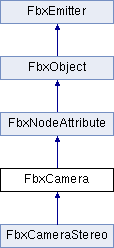
\includegraphics[height=5.000000cm]{class_fbx_camera}
\end{center}
\end{figure}
\subsection*{公開型}
\begin{DoxyCompactItemize}
\item 
enum \hyperlink{class_fbx_camera_a717b9b0d28c8b20c115edf8c80016fb1}{E\+Projection\+Type} \{ \hyperlink{class_fbx_camera_a717b9b0d28c8b20c115edf8c80016fb1aa0ea1fe68c0ac171dae64779456dec9d}{e\+Perspective}, 
\hyperlink{class_fbx_camera_a717b9b0d28c8b20c115edf8c80016fb1aa04cb9cfd8a05c0406da47338eb62d3d}{e\+Orthogonal}
 \}
\end{DoxyCompactItemize}
\subsection*{公開メンバ関数}
\begin{DoxyCompactItemize}
\item 
virtual \hyperlink{class_fbx_node_attribute_a08e1669d3d1a696910756ab17de56d6a}{Fbx\+Node\+Attribute\+::\+E\+Type} \hyperlink{class_fbx_camera_a1149e4b05fd079637fe8d2a66a5a7a17}{Get\+Attribute\+Type} () const
\begin{DoxyCompactList}\small\item\em Return the type of node attribute which is E\+Type\+::e\+Camera. \end{DoxyCompactList}\item 
void \hyperlink{class_fbx_camera_aeeb56513eefdfe4b8df54181cfa44321}{Reset} ()
\begin{DoxyCompactList}\small\item\em Reset the camera to default values. \end{DoxyCompactList}\item 
virtual \hyperlink{class_fbx_object}{Fbx\+Object} \& \hyperlink{class_fbx_camera_ad6641b4f04167df79531fe4843834895}{Copy} (const \hyperlink{class_fbx_object}{Fbx\+Object} \&p\+Object)
\end{DoxyCompactItemize}
\subsection*{公開変数類}
\begin{DoxyCompactItemize}
\item 
\hyperlink{class_fbx_property_t}{Fbx\+PropertyT}$<$ \hyperlink{fbxtypes_8h_ae0a96f14cde566774c7553aa7523b7a7}{Fbx\+Double3} $>$ \hyperlink{class_fbx_camera_afa38d19a4ebd6fac7ea040750fd1dae9}{Position}
\item 
\hyperlink{class_fbx_property_t}{Fbx\+PropertyT}$<$ \hyperlink{fbxtypes_8h_ae0a96f14cde566774c7553aa7523b7a7}{Fbx\+Double3} $>$ \hyperlink{class_fbx_camera_ad2e9b17c1be832d71d4fc0eecc93732a}{Up\+Vector}
\item 
\hyperlink{class_fbx_property_t}{Fbx\+PropertyT}$<$ \hyperlink{fbxtypes_8h_ae0a96f14cde566774c7553aa7523b7a7}{Fbx\+Double3} $>$ \hyperlink{class_fbx_camera_a686036fc4f1794fe7f3b74f978e8d174}{Interest\+Position}
\item 
\hyperlink{class_fbx_property_t}{Fbx\+PropertyT}$<$ \hyperlink{fbxtypes_8h_a171e72a1c46fc15c1a6c9c31948c1c5b}{Fbx\+Double} $>$ \hyperlink{class_fbx_camera_ab59a181ec24cb954e0899273caea96dc}{Roll}
\item 
\hyperlink{class_fbx_property_t}{Fbx\+PropertyT}$<$ \hyperlink{fbxtypes_8h_a171e72a1c46fc15c1a6c9c31948c1c5b}{Fbx\+Double} $>$ \hyperlink{class_fbx_camera_af1e8cb54a4d9a16471c6fd56d30cd128}{Optical\+CenterX}
\item 
\hyperlink{class_fbx_property_t}{Fbx\+PropertyT}$<$ \hyperlink{fbxtypes_8h_a171e72a1c46fc15c1a6c9c31948c1c5b}{Fbx\+Double} $>$ \hyperlink{class_fbx_camera_a8154f4f4e907c094df2decb36e179d85}{Optical\+CenterY}
\item 
\hyperlink{class_fbx_property_t}{Fbx\+PropertyT}$<$ \hyperlink{fbxtypes_8h_ae0a96f14cde566774c7553aa7523b7a7}{Fbx\+Double3} $>$ \hyperlink{class_fbx_camera_af50cc9dbfa39096cc1b9535e1b47d1d6}{Background\+Color}
\item 
\hyperlink{class_fbx_property_t}{Fbx\+PropertyT}$<$ \hyperlink{fbxtypes_8h_a171e72a1c46fc15c1a6c9c31948c1c5b}{Fbx\+Double} $>$ \hyperlink{class_fbx_camera_a927ab13d2fa91468ecb5373fdffd725a}{Turn\+Table}
\item 
\hyperlink{class_fbx_property_t}{Fbx\+PropertyT}$<$ \hyperlink{fbxtypes_8h_a92e0562b2fe33e76a242f498b362262e}{Fbx\+Bool} $>$ \hyperlink{class_fbx_camera_a935e9b57e229b7474770b0a0611a1b60}{Display\+Turn\+Table\+Icon}
\item 
\hyperlink{class_fbx_property_t}{Fbx\+PropertyT}$<$ \hyperlink{fbxtypes_8h_a92e0562b2fe33e76a242f498b362262e}{Fbx\+Bool} $>$ \hyperlink{class_fbx_camera_a73d5041546de951978b9065f7b0789a4}{Use\+Motion\+Blur}
\item 
\hyperlink{class_fbx_property_t}{Fbx\+PropertyT}$<$ \hyperlink{fbxtypes_8h_a92e0562b2fe33e76a242f498b362262e}{Fbx\+Bool} $>$ \hyperlink{class_fbx_camera_a99d0cb2281144454e44128d66be54b26}{Use\+Real\+Time\+Motion\+Blur}
\item 
\hyperlink{class_fbx_property_t}{Fbx\+PropertyT}$<$ \hyperlink{fbxtypes_8h_a171e72a1c46fc15c1a6c9c31948c1c5b}{Fbx\+Double} $>$ \hyperlink{class_fbx_camera_aef324a28772e42e910b983642b635769}{Motion\+Blur\+Intensity}
\item 
\hyperlink{class_fbx_property_t}{Fbx\+PropertyT}$<$ \hyperlink{class_fbx_camera_a2135478bb5fd6985835c14b11e1fccda}{E\+Aspect\+Ratio\+Mode} $>$ \hyperlink{class_fbx_camera_ad140535acab4a663a6f4cb51ef603e7a}{Aspect\+Ratio\+Mode}
\item 
\hyperlink{class_fbx_property_t}{Fbx\+PropertyT}$<$ \hyperlink{fbxtypes_8h_a171e72a1c46fc15c1a6c9c31948c1c5b}{Fbx\+Double} $>$ \hyperlink{class_fbx_camera_ada3746eb834815c224eb5fc223fa35ac}{Aspect\+Width}
\item 
\hyperlink{class_fbx_property_t}{Fbx\+PropertyT}$<$ \hyperlink{fbxtypes_8h_a171e72a1c46fc15c1a6c9c31948c1c5b}{Fbx\+Double} $>$ \hyperlink{class_fbx_camera_aabeade4a36213c65d7a4f45aeceebff6}{Aspect\+Height}
\item 
\hyperlink{class_fbx_property_t}{Fbx\+PropertyT}$<$ \hyperlink{fbxtypes_8h_a171e72a1c46fc15c1a6c9c31948c1c5b}{Fbx\+Double} $>$ \hyperlink{class_fbx_camera_a3fbab252bb6925578cc965f0383592b8}{Pixel\+Aspect\+Ratio}
\item 
\hyperlink{class_fbx_property_t}{Fbx\+PropertyT}$<$ \hyperlink{class_fbx_camera_addeea6fc943ce5f087dbc54c142f890e}{E\+Aperture\+Mode} $>$ \hyperlink{class_fbx_camera_afa8019b2027da3798e13bb1126c5941d}{Aperture\+Mode}
\item 
\hyperlink{class_fbx_property_t}{Fbx\+PropertyT}$<$ \hyperlink{class_fbx_camera_aeef0bf29c16fe5f08815fb33402330dd}{E\+Gate\+Fit} $>$ \hyperlink{class_fbx_camera_a72892e0ca040266ffc5ede12235db68a}{Gate\+Fit}
\item 
\hyperlink{class_fbx_property_t}{Fbx\+PropertyT}$<$ \hyperlink{fbxtypes_8h_a171e72a1c46fc15c1a6c9c31948c1c5b}{Fbx\+Double} $>$ \hyperlink{class_fbx_camera_acec3ce4b786d019a16a2de9f23ff42d8}{Field\+Of\+View}
\item 
\hyperlink{class_fbx_property_t}{Fbx\+PropertyT}$<$ \hyperlink{fbxtypes_8h_a171e72a1c46fc15c1a6c9c31948c1c5b}{Fbx\+Double} $>$ \hyperlink{class_fbx_camera_a2e0c65d8225c5f73c6cf9a927a0523fb}{Field\+Of\+ViewX}
\item 
\hyperlink{class_fbx_property_t}{Fbx\+PropertyT}$<$ \hyperlink{fbxtypes_8h_a171e72a1c46fc15c1a6c9c31948c1c5b}{Fbx\+Double} $>$ \hyperlink{class_fbx_camera_a924b7ae9b8256f04bd36d726f0131c98}{Field\+Of\+ViewY}
\item 
\hyperlink{class_fbx_property_t}{Fbx\+PropertyT}$<$ \hyperlink{fbxtypes_8h_a171e72a1c46fc15c1a6c9c31948c1c5b}{Fbx\+Double} $>$ \hyperlink{class_fbx_camera_afee5193f8423491a47a059d93cee61c3}{Focal\+Length}
\item 
\hyperlink{class_fbx_property_t}{Fbx\+PropertyT}$<$ \hyperlink{class_fbx_camera_a88d68c983d21e4d6c0f281a8a30f0a06}{E\+Format} $>$ \hyperlink{class_fbx_camera_aa597919c9a693becd2647b969604e401}{Camera\+Format}
\item 
\hyperlink{class_fbx_property_t}{Fbx\+PropertyT}$<$ \hyperlink{fbxtypes_8h_a92e0562b2fe33e76a242f498b362262e}{Fbx\+Bool} $>$ \hyperlink{class_fbx_camera_a891e6eb1c91dd3a47dc05547149825e3}{Use\+Frame\+Color}
\item 
\hyperlink{class_fbx_property_t}{Fbx\+PropertyT}$<$ \hyperlink{fbxtypes_8h_ae0a96f14cde566774c7553aa7523b7a7}{Fbx\+Double3} $>$ \hyperlink{class_fbx_camera_ae032c4d73824601774f06ce4375943cd}{Frame\+Color}
\item 
\hyperlink{class_fbx_property_t}{Fbx\+PropertyT}$<$ \hyperlink{fbxtypes_8h_a92e0562b2fe33e76a242f498b362262e}{Fbx\+Bool} $>$ \hyperlink{class_fbx_camera_a2cc4a7d5d9972b289c6d1a175e2adf1d}{Show\+Name}
\item 
\hyperlink{class_fbx_property_t}{Fbx\+PropertyT}$<$ \hyperlink{fbxtypes_8h_a92e0562b2fe33e76a242f498b362262e}{Fbx\+Bool} $>$ \hyperlink{class_fbx_camera_a15b36db580c994a2676fd18d41923953}{Show\+Info\+On\+Moving}
\item 
\hyperlink{class_fbx_property_t}{Fbx\+PropertyT}$<$ \hyperlink{fbxtypes_8h_a92e0562b2fe33e76a242f498b362262e}{Fbx\+Bool} $>$ \hyperlink{class_fbx_camera_ac44b2aec0ace4b978979e5bd3f9cd384}{Show\+Grid}
\item 
\hyperlink{class_fbx_property_t}{Fbx\+PropertyT}$<$ \hyperlink{fbxtypes_8h_a92e0562b2fe33e76a242f498b362262e}{Fbx\+Bool} $>$ \hyperlink{class_fbx_camera_a76d80815967bce91e0fded44a6fbe74c}{Show\+Optical\+Center}
\item 
\hyperlink{class_fbx_property_t}{Fbx\+PropertyT}$<$ \hyperlink{fbxtypes_8h_a92e0562b2fe33e76a242f498b362262e}{Fbx\+Bool} $>$ \hyperlink{class_fbx_camera_a7f2e404049521f2b8ed8793bb231d9a0}{Show\+Azimut}
\item 
\hyperlink{class_fbx_property_t}{Fbx\+PropertyT}$<$ \hyperlink{fbxtypes_8h_a92e0562b2fe33e76a242f498b362262e}{Fbx\+Bool} $>$ \hyperlink{class_fbx_camera_a26906a88450a20a23eef13ecec0a4871}{Show\+Time\+Code}
\item 
\hyperlink{class_fbx_property_t}{Fbx\+PropertyT}$<$ \hyperlink{fbxtypes_8h_a92e0562b2fe33e76a242f498b362262e}{Fbx\+Bool} $>$ \hyperlink{class_fbx_camera_ad2c18755bf884d3ce15566dc90cc3d97}{Show\+Audio}
\item 
\hyperlink{class_fbx_property_t}{Fbx\+PropertyT}$<$ \hyperlink{fbxtypes_8h_ae0a96f14cde566774c7553aa7523b7a7}{Fbx\+Double3} $>$ \hyperlink{class_fbx_camera_a39719d29cec7526134a1856a8c8e1995}{Audio\+Color}
\item 
\hyperlink{class_fbx_property_t}{Fbx\+PropertyT}$<$ \hyperlink{fbxtypes_8h_a171e72a1c46fc15c1a6c9c31948c1c5b}{Fbx\+Double} $>$ \hyperlink{class_fbx_camera_adbca6c29099ceac39fb350201fb3163d}{Near\+Plane}
\item 
\hyperlink{class_fbx_property_t}{Fbx\+PropertyT}$<$ \hyperlink{fbxtypes_8h_a171e72a1c46fc15c1a6c9c31948c1c5b}{Fbx\+Double} $>$ \hyperlink{class_fbx_camera_a72de3e07e3d77face8a1412599facf73}{Far\+Plane}
\item 
\hyperlink{class_fbx_property_t}{Fbx\+PropertyT}$<$ \hyperlink{fbxtypes_8h_a92e0562b2fe33e76a242f498b362262e}{Fbx\+Bool} $>$ \hyperlink{class_fbx_camera_a416ffa14cbcdc07b2559bbbed7371d75}{Auto\+Compute\+Clip\+Planes}
\item 
\hyperlink{class_fbx_property_t}{Fbx\+PropertyT}$<$ \hyperlink{fbxtypes_8h_a171e72a1c46fc15c1a6c9c31948c1c5b}{Fbx\+Double} $>$ \hyperlink{class_fbx_camera_a54f69a2e295c3c69df559f9b64699be5}{Film\+Width}
\item 
\hyperlink{class_fbx_property_t}{Fbx\+PropertyT}$<$ \hyperlink{fbxtypes_8h_a171e72a1c46fc15c1a6c9c31948c1c5b}{Fbx\+Double} $>$ \hyperlink{class_fbx_camera_ae8e2abec912de996c4eaaff987a3bd17}{Film\+Height}
\item 
\hyperlink{class_fbx_property_t}{Fbx\+PropertyT}$<$ \hyperlink{fbxtypes_8h_a171e72a1c46fc15c1a6c9c31948c1c5b}{Fbx\+Double} $>$ \hyperlink{class_fbx_camera_aeefc9d0c4a6c9c3e17dc265cf2621a47}{Film\+Aspect\+Ratio}
\item 
\hyperlink{class_fbx_property_t}{Fbx\+PropertyT}$<$ \hyperlink{fbxtypes_8h_a171e72a1c46fc15c1a6c9c31948c1c5b}{Fbx\+Double} $>$ \hyperlink{class_fbx_camera_a21d8a100a10638aafdbf69304c651c48}{Film\+Squeeze\+Ratio}
\item 
\hyperlink{class_fbx_property_t}{Fbx\+PropertyT}$<$ \hyperlink{class_fbx_camera_ac26ac89602453c5917882c69d4863d13}{E\+Aperture\+Format} $>$ \hyperlink{class_fbx_camera_a49ebaef59ee49281225e2d0652894a4f}{Film\+Format}
\item 
\hyperlink{class_fbx_property_t}{Fbx\+PropertyT}$<$ \hyperlink{fbxtypes_8h_a171e72a1c46fc15c1a6c9c31948c1c5b}{Fbx\+Double} $>$ \hyperlink{class_fbx_camera_aa0a5e1ab510d4b87db69e8ed6febacc3}{Film\+OffsetX}
\item 
\hyperlink{class_fbx_property_t}{Fbx\+PropertyT}$<$ \hyperlink{fbxtypes_8h_a171e72a1c46fc15c1a6c9c31948c1c5b}{Fbx\+Double} $>$ \hyperlink{class_fbx_camera_a244464e212906b44d5f827a8cdba0444}{Film\+OffsetY}
\item 
\hyperlink{class_fbx_property_t}{Fbx\+PropertyT}$<$ \hyperlink{fbxtypes_8h_a171e72a1c46fc15c1a6c9c31948c1c5b}{Fbx\+Double} $>$ \hyperlink{class_fbx_camera_ace6cbe41faef53ac2dc02dec31d395a4}{Pre\+Scale}
\item 
\hyperlink{class_fbx_property_t}{Fbx\+PropertyT}$<$ \hyperlink{fbxtypes_8h_a171e72a1c46fc15c1a6c9c31948c1c5b}{Fbx\+Double} $>$ \hyperlink{class_fbx_camera_af0c221000e5299efd1e91408bb4d96b6}{Film\+TranslateX}
\item 
\hyperlink{class_fbx_property_t}{Fbx\+PropertyT}$<$ \hyperlink{fbxtypes_8h_a171e72a1c46fc15c1a6c9c31948c1c5b}{Fbx\+Double} $>$ \hyperlink{class_fbx_camera_ab2fed4f94b108161a382cb53ecc9bc14}{Film\+TranslateY}
\item 
\hyperlink{class_fbx_property_t}{Fbx\+PropertyT}$<$ \hyperlink{fbxtypes_8h_a171e72a1c46fc15c1a6c9c31948c1c5b}{Fbx\+Double} $>$ \hyperlink{class_fbx_camera_af8db195197a3f0a6729533842e00fd18}{Film\+Roll\+PivotX}
\item 
\hyperlink{class_fbx_property_t}{Fbx\+PropertyT}$<$ \hyperlink{fbxtypes_8h_a171e72a1c46fc15c1a6c9c31948c1c5b}{Fbx\+Double} $>$ \hyperlink{class_fbx_camera_ab3034aa3a13b537c6542d8b45aa77eae}{Film\+Roll\+PivotY}
\item 
\hyperlink{class_fbx_property_t}{Fbx\+PropertyT}$<$ \hyperlink{fbxtypes_8h_a171e72a1c46fc15c1a6c9c31948c1c5b}{Fbx\+Double} $>$ \hyperlink{class_fbx_camera_a80affb53985e548f42136ccd3b9d7a2e}{Film\+Roll\+Value}
\item 
\hyperlink{class_fbx_property_t}{Fbx\+PropertyT}$<$ \hyperlink{class_fbx_camera_a831d9b7ffcbf3611715eb2ad9108870b}{E\+Film\+Roll\+Order} $>$ \hyperlink{class_fbx_camera_ac7583ff2d3c73fa3e4f514ba29504be5}{Film\+Roll\+Order}
\item 
\hyperlink{class_fbx_property_t}{Fbx\+PropertyT}$<$ \hyperlink{fbxtypes_8h_a92e0562b2fe33e76a242f498b362262e}{Fbx\+Bool} $>$ \hyperlink{class_fbx_camera_a9c44e5ed7154bb5b69664bbe4e7a7f51}{View\+Camera\+To\+Look\+At}
\item 
\hyperlink{class_fbx_property_t}{Fbx\+PropertyT}$<$ \hyperlink{fbxtypes_8h_a92e0562b2fe33e76a242f498b362262e}{Fbx\+Bool} $>$ \hyperlink{class_fbx_camera_aaf010c106bab5fca32acadc0b97d8437}{View\+Frustum\+Near\+Far\+Plane}
\item 
\hyperlink{class_fbx_property_t}{Fbx\+PropertyT}$<$ \hyperlink{class_fbx_camera_ab7b9d3e546552049a79261a444f9b44a}{E\+Front\+Back\+Plane\+Display\+Mode} $>$ \hyperlink{class_fbx_camera_aee58e80280621397eccfaf92ac30e914}{View\+Frustum\+Back\+Plane\+Mode}
\item 
\hyperlink{class_fbx_property_t}{Fbx\+PropertyT}$<$ \hyperlink{fbxtypes_8h_a171e72a1c46fc15c1a6c9c31948c1c5b}{Fbx\+Double} $>$ \hyperlink{class_fbx_camera_ad54b41219ffef6383e75197300210f75}{Back\+Plane\+Distance}
\item 
\hyperlink{class_fbx_property_t}{Fbx\+PropertyT}$<$ \hyperlink{class_fbx_camera_a79e74898d117e741c3fbd10b1ef21c79}{E\+Front\+Back\+Plane\+Distance\+Mode} $>$ \hyperlink{class_fbx_camera_ae12c26a9d3be06c3e118cef04f596224}{Back\+Plane\+Distance\+Mode}
\item 
\hyperlink{class_fbx_property_t}{Fbx\+PropertyT}$<$ \hyperlink{class_fbx_camera_ab7b9d3e546552049a79261a444f9b44a}{E\+Front\+Back\+Plane\+Display\+Mode} $>$ \hyperlink{class_fbx_camera_a7d91e0645351854d02925da94d4cb924}{View\+Frustum\+Front\+Plane\+Mode}
\item 
\hyperlink{class_fbx_property_t}{Fbx\+PropertyT}$<$ \hyperlink{fbxtypes_8h_a171e72a1c46fc15c1a6c9c31948c1c5b}{Fbx\+Double} $>$ \hyperlink{class_fbx_camera_ab04e1fdc21ced2af3a372cb3c3c45295}{Front\+Plane\+Distance}
\item 
\hyperlink{class_fbx_property_t}{Fbx\+PropertyT}$<$ \hyperlink{class_fbx_camera_a79e74898d117e741c3fbd10b1ef21c79}{E\+Front\+Back\+Plane\+Distance\+Mode} $>$ \hyperlink{class_fbx_camera_ac8275a3d73371ebdd381bec957820b14}{Front\+Plane\+Distance\+Mode}
\item 
\hyperlink{class_fbx_property_t}{Fbx\+PropertyT}$<$ \hyperlink{fbxtypes_8h_a92e0562b2fe33e76a242f498b362262e}{Fbx\+Bool} $>$ \hyperlink{class_fbx_camera_aba8fcdabc543461794dcfbd683af1e76}{Lock\+Mode}
\item 
\hyperlink{class_fbx_property_t}{Fbx\+PropertyT}$<$ \hyperlink{fbxtypes_8h_a92e0562b2fe33e76a242f498b362262e}{Fbx\+Bool} $>$ \hyperlink{class_fbx_camera_a3060679e7b5d5c6ba05fd78f5bfee955}{Lock\+Interest\+Navigation}
\item 
\hyperlink{class_fbx_property_t}{Fbx\+PropertyT}$<$ \hyperlink{fbxtypes_8h_a92e0562b2fe33e76a242f498b362262e}{Fbx\+Bool} $>$ \hyperlink{class_fbx_camera_a60226ecc8df67faa201c77434eccd486}{Back\+Plate\+Fit\+Image}
\item 
\hyperlink{class_fbx_property_t}{Fbx\+PropertyT}$<$ \hyperlink{fbxtypes_8h_a92e0562b2fe33e76a242f498b362262e}{Fbx\+Bool} $>$ \hyperlink{class_fbx_camera_a3ec93b32631cf0b3bd2f41878c47a348}{Back\+Plate\+Crop}
\item 
\hyperlink{class_fbx_property_t}{Fbx\+PropertyT}$<$ \hyperlink{fbxtypes_8h_a92e0562b2fe33e76a242f498b362262e}{Fbx\+Bool} $>$ \hyperlink{class_fbx_camera_afc328eb5b70302973c991310d7ff9be3}{Back\+Plate\+Center}
\item 
\hyperlink{class_fbx_property_t}{Fbx\+PropertyT}$<$ \hyperlink{fbxtypes_8h_a92e0562b2fe33e76a242f498b362262e}{Fbx\+Bool} $>$ \hyperlink{class_fbx_camera_a4ee8a7a4e0c74fe8b76e83ee572a9b7c}{Back\+Plate\+Keep\+Ratio}
\item 
\hyperlink{class_fbx_property_t}{Fbx\+PropertyT}$<$ \hyperlink{fbxtypes_8h_a171e72a1c46fc15c1a6c9c31948c1c5b}{Fbx\+Double} $>$ \hyperlink{class_fbx_camera_adee33826ef47ba5fc4719c78b6e5d582}{Background\+Alpha\+Treshold}
\item 
\hyperlink{class_fbx_property_t}{Fbx\+PropertyT}$<$ \hyperlink{fbxtypes_8h_a171e72a1c46fc15c1a6c9c31948c1c5b}{Fbx\+Double} $>$ \hyperlink{class_fbx_camera_a2a71f39683269b49b67e007c7d19d67b}{Back\+Plane\+OffsetX}
\item 
\hyperlink{class_fbx_property_t}{Fbx\+PropertyT}$<$ \hyperlink{fbxtypes_8h_a171e72a1c46fc15c1a6c9c31948c1c5b}{Fbx\+Double} $>$ \hyperlink{class_fbx_camera_abfbc1d3377ed9721492971011fd8f5ed}{Back\+Plane\+OffsetY}
\item 
\hyperlink{class_fbx_property_t}{Fbx\+PropertyT}$<$ \hyperlink{fbxtypes_8h_a171e72a1c46fc15c1a6c9c31948c1c5b}{Fbx\+Double} $>$ \hyperlink{class_fbx_camera_a25d0defefe7a7c69ee9fddfc8ea51036}{Back\+Plane\+Rotation}
\item 
\hyperlink{class_fbx_property_t}{Fbx\+PropertyT}$<$ \hyperlink{fbxtypes_8h_a171e72a1c46fc15c1a6c9c31948c1c5b}{Fbx\+Double} $>$ \hyperlink{class_fbx_camera_a34ab778778521406789a1798451791db}{Back\+Plane\+ScaleX}
\item 
\hyperlink{class_fbx_property_t}{Fbx\+PropertyT}$<$ \hyperlink{fbxtypes_8h_a171e72a1c46fc15c1a6c9c31948c1c5b}{Fbx\+Double} $>$ \hyperlink{class_fbx_camera_a24d51fab8fc1c619d813375b2aa88cfe}{Back\+Plane\+ScaleY}
\item 
\hyperlink{class_fbx_property_t}{Fbx\+PropertyT}$<$ \hyperlink{fbxtypes_8h_a92e0562b2fe33e76a242f498b362262e}{Fbx\+Bool} $>$ \hyperlink{class_fbx_camera_a3e824d5e68ecd7ff571c3d783b3a82b3}{Show\+Backplate}
\item 
\hyperlink{class_fbx_property_t}{Fbx\+PropertyT}$<$ \hyperlink{fbxtypes_8h_a44df6a2eec915cf27cd481e5c5e48a24}{Fbx\+Reference} $>$ \hyperlink{class_fbx_camera_a23d1fddeed7661a66461fbe0f27cedde}{Background\+Texture}
\item 
\hyperlink{class_fbx_property_t}{Fbx\+PropertyT}$<$ \hyperlink{fbxtypes_8h_a92e0562b2fe33e76a242f498b362262e}{Fbx\+Bool} $>$ \hyperlink{class_fbx_camera_a98c919c1ec1398479c859357d3f454d7}{Front\+Plate\+Fit\+Image}
\item 
\hyperlink{class_fbx_property_t}{Fbx\+PropertyT}$<$ \hyperlink{fbxtypes_8h_a92e0562b2fe33e76a242f498b362262e}{Fbx\+Bool} $>$ \hyperlink{class_fbx_camera_af409f4d6dd0b68de9a3e0c2f17644362}{Front\+Plate\+Crop}
\item 
\hyperlink{class_fbx_property_t}{Fbx\+PropertyT}$<$ \hyperlink{fbxtypes_8h_a92e0562b2fe33e76a242f498b362262e}{Fbx\+Bool} $>$ \hyperlink{class_fbx_camera_ae7a43caba31795438a1ca41926a8e31c}{Front\+Plate\+Center}
\item 
\hyperlink{class_fbx_property_t}{Fbx\+PropertyT}$<$ \hyperlink{fbxtypes_8h_a92e0562b2fe33e76a242f498b362262e}{Fbx\+Bool} $>$ \hyperlink{class_fbx_camera_aa4066eaf0f9d506db8b83353db3e4ef7}{Front\+Plate\+Keep\+Ratio}
\item 
\hyperlink{class_fbx_property_t}{Fbx\+PropertyT}$<$ \hyperlink{fbxtypes_8h_a92e0562b2fe33e76a242f498b362262e}{Fbx\+Bool} $>$ \hyperlink{class_fbx_camera_adcb25c847c2d7d471c836722ce1289ff}{Show\+Frontplate}
\item 
\hyperlink{class_fbx_property_t}{Fbx\+PropertyT}$<$ \hyperlink{fbxtypes_8h_a171e72a1c46fc15c1a6c9c31948c1c5b}{Fbx\+Double} $>$ \hyperlink{class_fbx_camera_ad15249c2dceb1d0cc2b5913c0efd9b18}{Front\+Plane\+OffsetX}
\item 
\hyperlink{class_fbx_property_t}{Fbx\+PropertyT}$<$ \hyperlink{fbxtypes_8h_a171e72a1c46fc15c1a6c9c31948c1c5b}{Fbx\+Double} $>$ \hyperlink{class_fbx_camera_acf005c234e34ef2b44fadf4db42be655}{Front\+Plane\+OffsetY}
\item 
\hyperlink{class_fbx_property_t}{Fbx\+PropertyT}$<$ \hyperlink{fbxtypes_8h_a171e72a1c46fc15c1a6c9c31948c1c5b}{Fbx\+Double} $>$ \hyperlink{class_fbx_camera_ac50922c82f1509c5f4f9e5c328ede671}{Front\+Plane\+Rotation}
\item 
\hyperlink{class_fbx_property_t}{Fbx\+PropertyT}$<$ \hyperlink{fbxtypes_8h_a171e72a1c46fc15c1a6c9c31948c1c5b}{Fbx\+Double} $>$ \hyperlink{class_fbx_camera_a13396eaf60196ca60b78e3c05ee74021}{Front\+Plane\+ScaleX}
\item 
\hyperlink{class_fbx_property_t}{Fbx\+PropertyT}$<$ \hyperlink{fbxtypes_8h_a171e72a1c46fc15c1a6c9c31948c1c5b}{Fbx\+Double} $>$ \hyperlink{class_fbx_camera_a48072957694967921a9b9eccfadc6dce}{Front\+Plane\+ScaleY}
\item 
\hyperlink{class_fbx_property_t}{Fbx\+PropertyT}$<$ \hyperlink{fbxtypes_8h_a44df6a2eec915cf27cd481e5c5e48a24}{Fbx\+Reference} $>$ \hyperlink{class_fbx_camera_aeb121a9199a538fa7825bc26d326b7f9}{Foreground\+Texture}
\item 
\hyperlink{class_fbx_property_t}{Fbx\+PropertyT}$<$ \hyperlink{fbxtypes_8h_a171e72a1c46fc15c1a6c9c31948c1c5b}{Fbx\+Double} $>$ \hyperlink{class_fbx_camera_a95fe1a3dbd71e2503e7f4de5f14ea171}{Foreground\+Opacity}
\item 
\hyperlink{class_fbx_property_t}{Fbx\+PropertyT}$<$ \hyperlink{fbxtypes_8h_a92e0562b2fe33e76a242f498b362262e}{Fbx\+Bool} $>$ \hyperlink{class_fbx_camera_a61d982bee729eae989b1c4f49e53ef59}{Display\+Safe\+Area}
\item 
\hyperlink{class_fbx_property_t}{Fbx\+PropertyT}$<$ \hyperlink{fbxtypes_8h_a92e0562b2fe33e76a242f498b362262e}{Fbx\+Bool} $>$ \hyperlink{class_fbx_camera_a6fba1dac4e237b8fb5423c6e8fdb7586}{Display\+Safe\+Area\+On\+Render}
\item 
\hyperlink{class_fbx_property_t}{Fbx\+PropertyT}$<$ \hyperlink{class_fbx_camera_aa9fb36da95d392ac56ff2d8b44171210}{E\+Safe\+Area\+Style} $>$ \hyperlink{class_fbx_camera_a48f27fb4b475f1ee7d2ace77cc860ad3}{Safe\+Area\+Display\+Style}
\item 
\hyperlink{class_fbx_property_t}{Fbx\+PropertyT}$<$ \hyperlink{fbxtypes_8h_a171e72a1c46fc15c1a6c9c31948c1c5b}{Fbx\+Double} $>$ \hyperlink{class_fbx_camera_aeb22ecb7b5a1551e735e9cf222d79b6d}{Safe\+Area\+Aspect\+Ratio}
\item 
\hyperlink{class_fbx_property_t}{Fbx\+PropertyT}$<$ \hyperlink{fbxtypes_8h_a92e0562b2fe33e76a242f498b362262e}{Fbx\+Bool} $>$ \hyperlink{class_fbx_camera_ad1e40e5371ba4003e8b21cfe0b8b42c7}{Use2\+D\+Magnifier\+Zoom}
\item 
\hyperlink{class_fbx_property_t}{Fbx\+PropertyT}$<$ \hyperlink{fbxtypes_8h_a171e72a1c46fc15c1a6c9c31948c1c5b}{Fbx\+Double} $>$ \hyperlink{class_fbx_camera_ab60ab197ebbbf565d18dc7f7b2113f59}{\+\_\+2\+D\+Magnifier\+Zoom}
\item 
\hyperlink{class_fbx_property_t}{Fbx\+PropertyT}$<$ \hyperlink{fbxtypes_8h_a171e72a1c46fc15c1a6c9c31948c1c5b}{Fbx\+Double} $>$ \hyperlink{class_fbx_camera_a0f5b732aa294c182fe6ac07ae70024fc}{\+\_\+2\+D\+MagnifierX}
\item 
\hyperlink{class_fbx_property_t}{Fbx\+PropertyT}$<$ \hyperlink{fbxtypes_8h_a171e72a1c46fc15c1a6c9c31948c1c5b}{Fbx\+Double} $>$ \hyperlink{class_fbx_camera_a162fa10866f3c4cf3c5a87ed64aef21e}{\+\_\+2\+D\+MagnifierY}
\item 
\hyperlink{class_fbx_property_t}{Fbx\+PropertyT}$<$ \hyperlink{class_fbx_camera_a717b9b0d28c8b20c115edf8c80016fb1}{E\+Projection\+Type} $>$ \hyperlink{class_fbx_camera_a36af73c36f749f694ccc9eefbe88087b}{Projection\+Type}
\item 
\hyperlink{class_fbx_property_t}{Fbx\+PropertyT}$<$ \hyperlink{fbxtypes_8h_a171e72a1c46fc15c1a6c9c31948c1c5b}{Fbx\+Double} $>$ \hyperlink{class_fbx_camera_a038fab99051fa0171f60f40469eff7cc}{Ortho\+Zoom}
\item 
\hyperlink{class_fbx_property_t}{Fbx\+PropertyT}$<$ \hyperlink{fbxtypes_8h_a92e0562b2fe33e76a242f498b362262e}{Fbx\+Bool} $>$ \hyperlink{class_fbx_camera_a57b4706a5d4d2678c5e31430b9a4ba61}{Use\+Real\+Time\+D\+O\+F\+And\+AA}
\item 
\hyperlink{class_fbx_property_t}{Fbx\+PropertyT}$<$ \hyperlink{fbxtypes_8h_a92e0562b2fe33e76a242f498b362262e}{Fbx\+Bool} $>$ \hyperlink{class_fbx_camera_a5b101aeb02696ef3e140505f01e6f797}{Use\+Depth\+Of\+Field}
\item 
\hyperlink{class_fbx_property_t}{Fbx\+PropertyT}$<$ \hyperlink{class_fbx_camera_a1b50e7b2953019a40328599679071ad4}{E\+Focus\+Distance\+Source} $>$ \hyperlink{class_fbx_camera_a17f0c0c82ed8df4540d918567edcbd4a}{Focus\+Source}
\item 
\hyperlink{class_fbx_property_t}{Fbx\+PropertyT}$<$ \hyperlink{fbxtypes_8h_a171e72a1c46fc15c1a6c9c31948c1c5b}{Fbx\+Double} $>$ \hyperlink{class_fbx_camera_af6d282d878bc8ad143c8095e29a4e94a}{Focus\+Angle}
\item 
\hyperlink{class_fbx_property_t}{Fbx\+PropertyT}$<$ \hyperlink{fbxtypes_8h_a171e72a1c46fc15c1a6c9c31948c1c5b}{Fbx\+Double} $>$ \hyperlink{class_fbx_camera_af6165df26c7d25156163a3ed2a2f99c2}{Focus\+Distance}
\item 
\hyperlink{class_fbx_property_t}{Fbx\+PropertyT}$<$ \hyperlink{fbxtypes_8h_a92e0562b2fe33e76a242f498b362262e}{Fbx\+Bool} $>$ \hyperlink{class_fbx_camera_a2d23acad0d49eadb63be01b826404d34}{Use\+Antialiasing}
\item 
\hyperlink{class_fbx_property_t}{Fbx\+PropertyT}$<$ \hyperlink{fbxtypes_8h_a171e72a1c46fc15c1a6c9c31948c1c5b}{Fbx\+Double} $>$ \hyperlink{class_fbx_camera_a3e7ddc27aff98a3850f58d8b800b6613}{Antialiasing\+Intensity}
\item 
\hyperlink{class_fbx_property_t}{Fbx\+PropertyT}$<$ \hyperlink{class_fbx_camera_a44949ea304940f214a2f23a66dcbf45f}{E\+Antialiasing\+Method} $>$ \hyperlink{class_fbx_camera_a1ad348a909fc9cd51173f5a424660ac1}{Antialiasing\+Method}
\item 
\hyperlink{class_fbx_property_t}{Fbx\+PropertyT}$<$ \hyperlink{fbxtypes_8h_a92e0562b2fe33e76a242f498b362262e}{Fbx\+Bool} $>$ \hyperlink{class_fbx_camera_ae858c35fdbb3ec3bb853bfa739dd2fad}{Use\+Accumulation\+Buffer}
\item 
\hyperlink{class_fbx_property_t}{Fbx\+PropertyT}$<$ \hyperlink{fbxtypes_8h_a088fa96de3b0b3ea69f0f6afef525dfb}{Fbx\+Int} $>$ \hyperlink{class_fbx_camera_a71ee6802b2a63149cfa33f11548893ea}{Frame\+Sampling\+Count}
\item 
\hyperlink{class_fbx_property_t}{Fbx\+PropertyT}$<$ \hyperlink{class_fbx_camera_aed549486ed0985230efca6fae0d731ae}{E\+Sampling\+Type} $>$ \hyperlink{class_fbx_camera_ab2048abc7b353f908a7c3caba7d0acf2}{Frame\+Sampling\+Type}
\end{DoxyCompactItemize}
\subsection*{限定公開メンバ関数}
\begin{DoxyCompactItemize}
\item 
virtual void \hyperlink{class_fbx_camera_a11334e5358efacbd87e4a7d78036155d}{Construct\+Properties} (bool p\+Force\+Set)
\item 
virtual \hyperlink{class_fbx_string_list}{Fbx\+String\+List} \hyperlink{class_fbx_camera_ac52d0e82cbabac69f8b0dcd212853616}{Get\+Type\+Flags} () const
\end{DoxyCompactItemize}
\subsection*{Functions to handle the viewing area.}
\begin{DoxyCompactItemize}
\item 
enum \hyperlink{class_fbx_camera_a88d68c983d21e4d6c0f281a8a30f0a06}{E\+Format} \{ \newline
\hyperlink{class_fbx_camera_a88d68c983d21e4d6c0f281a8a30f0a06aaf48d41576f70b84dad6382dd54a358f}{e\+Custom\+Format}, 
\hyperlink{class_fbx_camera_a88d68c983d21e4d6c0f281a8a30f0a06a42268f524473dc3df99c6a1e026877ca}{e\+D1\+N\+T\+SC}, 
\hyperlink{class_fbx_camera_a88d68c983d21e4d6c0f281a8a30f0a06ad8db1b3f18ffa1ce2c72fb828b9e818d}{e\+N\+T\+SC}, 
\hyperlink{class_fbx_camera_a88d68c983d21e4d6c0f281a8a30f0a06a8b38f5968595cd18467df37d1c0ac623}{e\+P\+AL}, 
\newline
\hyperlink{class_fbx_camera_a88d68c983d21e4d6c0f281a8a30f0a06a281e45dc48a0b888388024d74d325ecf}{e\+D1\+P\+AL}, 
\hyperlink{class_fbx_camera_a88d68c983d21e4d6c0f281a8a30f0a06ae0bbb5db268e19a8835f1265c34da886}{e\+HD}, 
\hyperlink{class_fbx_camera_a88d68c983d21e4d6c0f281a8a30f0a06a02f796b8fa6732e33968076ba7fe84f3}{e640x480}, 
\hyperlink{class_fbx_camera_a88d68c983d21e4d6c0f281a8a30f0a06a481e8f8b539835f13e44baf3e28cfbcc}{e320x200}, 
\newline
\hyperlink{class_fbx_camera_a88d68c983d21e4d6c0f281a8a30f0a06aa5cc75ef13a34a6fce8fa241a1840433}{e320x240}, 
\hyperlink{class_fbx_camera_a88d68c983d21e4d6c0f281a8a30f0a06a64bc0e6478e009ab2fbf7ddce81a8e60}{e128x128}, 
\hyperlink{class_fbx_camera_a88d68c983d21e4d6c0f281a8a30f0a06a0428f6f444084ecf37a06dae082c710b}{e\+Fullscreen}
 \}
\item 
enum \hyperlink{class_fbx_camera_a2135478bb5fd6985835c14b11e1fccda}{E\+Aspect\+Ratio\+Mode} \{ \newline
\hyperlink{class_fbx_camera_a2135478bb5fd6985835c14b11e1fccdaafe7ec454e09f65b8981cbc772600938e}{e\+Window\+Size}, 
\hyperlink{class_fbx_camera_a2135478bb5fd6985835c14b11e1fccdaa147021a305ff8749866e92d79e7fb944}{e\+Fixed\+Ratio}, 
\hyperlink{class_fbx_camera_a2135478bb5fd6985835c14b11e1fccdaa3274cc0ff55a01a302d16bcbae6c266c}{e\+Fixed\+Resolution}, 
\hyperlink{class_fbx_camera_a2135478bb5fd6985835c14b11e1fccdaab72bc463e7cb6d16639871506f862dfa}{e\+Fixed\+Width}, 
\newline
\hyperlink{class_fbx_camera_a2135478bb5fd6985835c14b11e1fccdaa7bc3bf5fc78b9ffecd900be5aebb691b}{e\+Fixed\+Height}
 \}
\item 
void \hyperlink{class_fbx_camera_a49db13fb34e3cfa618823e61511f5312}{Set\+Format} (\hyperlink{class_fbx_camera_a88d68c983d21e4d6c0f281a8a30f0a06}{E\+Format} p\+Format)
\item 
\hyperlink{class_fbx_camera_a88d68c983d21e4d6c0f281a8a30f0a06}{E\+Format} \hyperlink{class_fbx_camera_a068be46bd59bcaa398565fcff992d18f}{Get\+Format} () const
\item 
void \hyperlink{class_fbx_camera_adb9cf67e4b59463add6a052003797392}{Set\+Aspect} (\hyperlink{class_fbx_camera_a2135478bb5fd6985835c14b11e1fccda}{E\+Aspect\+Ratio\+Mode} p\+Ratio\+Mode, double p\+Width, double p\+Height)
\item 
\hyperlink{class_fbx_camera_a2135478bb5fd6985835c14b11e1fccda}{E\+Aspect\+Ratio\+Mode} \hyperlink{class_fbx_camera_ad60e1323bdb9f349dbb96e5d8bdf716a}{Get\+Aspect\+Ratio\+Mode} () const
\item 
void \hyperlink{class_fbx_camera_a55058f98c5bdaed70ad02c9062804798}{Set\+Pixel\+Ratio} (double p\+Ratio)
\item 
double \hyperlink{class_fbx_camera_ae12fca0cd15518d611dbe26f2b6babbf}{Get\+Pixel\+Ratio} () const
\item 
void \hyperlink{class_fbx_camera_a4ceb2775d2392c380cd8529d78f98c7f}{Set\+Near\+Plane} (double p\+Distance)
\item 
double \hyperlink{class_fbx_camera_ae4c1364cd162c51ad539cf3f6fc1fbe6}{Get\+Near\+Plane} () const
\item 
void \hyperlink{class_fbx_camera_a23f2f8bba739049a5e0ea55213085787}{Set\+Far\+Plane} (double p\+Distance)
\item 
double \hyperlink{class_fbx_camera_a07b8a3633669335c8adde9049574d5cc}{Get\+Far\+Plane} () const
\end{DoxyCompactItemize}
\subsection*{Aperture and Film Functions.}
\label{_amgrpf30ddd7650a62145134729ff6120789e}%
In photography, the aperture is the size of hole allowing light from the lens to get through to the film. The aperture mode determines which values drive the camera aperture. When the aperture mode is {\itshape e\+Horiz\+And\+Vert}, {\itshape e\+Horizontal} or {\itshape e\+Vertical}, the field of view is used. When the aperture mode is {\itshape e\+Focal\+Length}, the focal length is used.

It is possible to convert the aperture mode into field of view or vice versa using functions Compute\+Field\+Of\+View and Compute\+Focal\+Length. These functions use the camera aperture width and height for their computation. \begin{DoxyCompactItemize}
\item 
enum \hyperlink{class_fbx_camera_ac26ac89602453c5917882c69d4863d13}{E\+Aperture\+Format} \{ \newline
\hyperlink{class_fbx_camera_ac26ac89602453c5917882c69d4863d13a97b985e82b4b19702766ca0b6e1e18b6}{e\+Custom\+Aperture}, 
\hyperlink{class_fbx_camera_ac26ac89602453c5917882c69d4863d13ab20a3d10dde5db5090af623f4750499b}{e16mm\+Theatrical}, 
\hyperlink{class_fbx_camera_ac26ac89602453c5917882c69d4863d13aba9ade34d13793e51b80234ea2469f60}{e\+Super16mm}, 
\hyperlink{class_fbx_camera_ac26ac89602453c5917882c69d4863d13a8543fb30fcdefa66cab58f34c803b1f7}{e35mm\+Academy}, 
\newline
\hyperlink{class_fbx_camera_ac26ac89602453c5917882c69d4863d13a33ad593343e6a930c6e7d4b11b5d7c00}{e35mm\+T\+V\+Projection}, 
\hyperlink{class_fbx_camera_ac26ac89602453c5917882c69d4863d13a2cc6fd88f1f97c1ba2ca9bf4a8860a51}{e35mm\+Full\+Aperture}, 
\hyperlink{class_fbx_camera_ac26ac89602453c5917882c69d4863d13a33ff0b26d0ab2f32bc86be6132cfa008}{e35mm185\+Projection}, 
\hyperlink{class_fbx_camera_ac26ac89602453c5917882c69d4863d13a20e7f50c727d1e99f42dc00152e15f1c}{e35mm\+Anamorphic}, 
\newline
\hyperlink{class_fbx_camera_ac26ac89602453c5917882c69d4863d13af0f67d2c5c475f78b205025e9bb119d9}{e70mm\+Projection}, 
\hyperlink{class_fbx_camera_ac26ac89602453c5917882c69d4863d13a507e434236110cd95faa2e4de76841cd}{e\+Vista\+Vision}, 
\hyperlink{class_fbx_camera_ac26ac89602453c5917882c69d4863d13a8d6bf970107658d8461f6cefc92f0f10}{e\+Dyna\+Vision}, 
\hyperlink{class_fbx_camera_ac26ac89602453c5917882c69d4863d13abd885226c5e2eb363058e8e15b2172db}{e\+I\+M\+AX}
 \}
\item 
enum \hyperlink{class_fbx_camera_addeea6fc943ce5f087dbc54c142f890e}{E\+Aperture\+Mode} \{ \hyperlink{class_fbx_camera_addeea6fc943ce5f087dbc54c142f890ea8cac2c2267cda9a78d633db1b468dafa}{e\+Horiz\+And\+Vert}, 
\hyperlink{class_fbx_camera_addeea6fc943ce5f087dbc54c142f890ea3e78ca781c360fd1f8cbe81becdbba29}{e\+Horizontal}, 
\hyperlink{class_fbx_camera_addeea6fc943ce5f087dbc54c142f890ea28d91a0b3c674581c55773b1df9d3a99}{e\+Vertical}, 
\hyperlink{class_fbx_camera_addeea6fc943ce5f087dbc54c142f890ea69fff576ebbceb1fab1b9914b606b2f6}{e\+Focal\+Length}
 \}
\item 
enum \hyperlink{class_fbx_camera_aeef0bf29c16fe5f08815fb33402330dd}{E\+Gate\+Fit} \{ \newline
\hyperlink{class_fbx_camera_aeef0bf29c16fe5f08815fb33402330dda3323d147bda3dd5b2b196bbbf877f893}{e\+Fit\+None}, 
\hyperlink{class_fbx_camera_aeef0bf29c16fe5f08815fb33402330ddaf68c2ba0074eeaccec333cc9edf3541c}{e\+Fit\+Vertical}, 
\hyperlink{class_fbx_camera_aeef0bf29c16fe5f08815fb33402330ddac719810a0f5527e1a8e1d0a07b83b52e}{e\+Fit\+Horizontal}, 
\hyperlink{class_fbx_camera_aeef0bf29c16fe5f08815fb33402330dda0ee709a0e8ce6d10c93eead0c24fea5e}{e\+Fit\+Fill}, 
\newline
\hyperlink{class_fbx_camera_aeef0bf29c16fe5f08815fb33402330ddadf50234dabf691041535be304a4fffce}{e\+Fit\+Overscan}, 
\hyperlink{class_fbx_camera_aeef0bf29c16fe5f08815fb33402330dda2c54aaf5f566bae17a288ce14733c66a}{e\+Fit\+Stretch}
 \}
\item 
enum \hyperlink{class_fbx_camera_a831d9b7ffcbf3611715eb2ad9108870b}{E\+Film\+Roll\+Order} \{ \hyperlink{class_fbx_camera_a831d9b7ffcbf3611715eb2ad9108870bad500528c8c031dde3349136db2fae5d1}{e\+Rotate\+First}, 
\hyperlink{class_fbx_camera_a831d9b7ffcbf3611715eb2ad9108870ba7e8e7f860d61236b2a6cc8300953b071}{e\+Translate\+First}
 \}
\item 
void \hyperlink{class_fbx_camera_a5b644b41e4d72c214acfdb5a2dee7576}{Set\+Aperture\+Format} (\hyperlink{class_fbx_camera_ac26ac89602453c5917882c69d4863d13}{E\+Aperture\+Format} p\+Format)
\item 
\hyperlink{class_fbx_camera_ac26ac89602453c5917882c69d4863d13}{E\+Aperture\+Format} \hyperlink{class_fbx_camera_a33f198a1cb447a1e1e41d69856a7291c}{Get\+Aperture\+Format} () const
\item 
void \hyperlink{class_fbx_camera_a479485801a0795d337d73e25ef8c4477}{Set\+Aperture\+Mode} (\hyperlink{class_fbx_camera_addeea6fc943ce5f087dbc54c142f890e}{E\+Aperture\+Mode} p\+Mode)
\item 
\hyperlink{class_fbx_camera_addeea6fc943ce5f087dbc54c142f890e}{E\+Aperture\+Mode} \hyperlink{class_fbx_camera_a3dea5cf232d8faafbc4c5a720fde419c}{Get\+Aperture\+Mode} () const
\item 
void \hyperlink{class_fbx_camera_ae927c1d64d3b28cce554d47ac56fdc92}{Set\+Aperture\+Width} (double p\+Width)
\item 
double \hyperlink{class_fbx_camera_a7f9c7299e3a40cf708e97b13107396cc}{Get\+Aperture\+Width} () const
\item 
void \hyperlink{class_fbx_camera_a02bdb12abf27b4ccc0c4554818bdbf8f}{Set\+Aperture\+Height} (double p\+Height)
\item 
double \hyperlink{class_fbx_camera_a652045fde3804f8a66b696030e40f662}{Get\+Aperture\+Height} () const
\item 
void \hyperlink{class_fbx_camera_a4ef18832cc863f5dcc086d0d10686122}{Set\+Squeeze\+Ratio} (double p\+Ratio)
\item 
double \hyperlink{class_fbx_camera_ac9e1f4cc33e3c927932c577d95c6cd93}{Get\+Squeeze\+Ratio} () const
\item 
double \hyperlink{class_fbx_camera_ac4549addd7a3f9dc62843b9208a52d81}{Compute\+Field\+Of\+View} (double p\+Focal\+Length) const
\item 
double \hyperlink{class_fbx_camera_aeb7c4720e64f1c247a0089943f521dc6}{Compute\+Focal\+Length} (double p\+Angle\+Of\+View) const
\end{DoxyCompactItemize}
\subsection*{Functions to handle Back\+Plane/\+Front\+Plane and Plate.}
\label{_amgrpaf57f84153af25ebbd4d47001d65f1eb}%
In the Fbx\+Sdk terminology, the Back/\+Front plane is the support of the plate. And the plate is the support of the texture used for backgrounds/foregrounds. Functions and properties identified by the \char`\"{}\+Plate\char`\"{} name are affecting the display of the texture on the plate. The functions and properties identified with the \char`\"{}\+Back/\+Front\+Plane\char`\"{} are affecting the plate.

Typically a client application would place the Back\+Plate a small distance in front of the Far\+Plane and the Front\+Plate just behind the Near\+Plane to avoid them to be hidden by the clipping. Unless otherwise noted, there are no restrictions on the values stored by the camera object therefore it is the responsibility of the client application to process the information in a meaningful way and to maintain consistency between the different properties relationships. \begin{DoxyCompactItemize}
\item 
enum \hyperlink{class_fbx_camera_aa4e853313a58a9cd5a88c6a35b3c46a2}{E\+Plate\+Drawing\+Mode} \{ \hyperlink{class_fbx_camera_aa4e853313a58a9cd5a88c6a35b3c46a2ad65298b6b912b7252f4a35aacf7da330}{e\+Plate\+Background}, 
\hyperlink{class_fbx_camera_aa4e853313a58a9cd5a88c6a35b3c46a2a74e46cdd10df8c161e9762d44f7ea3d8}{e\+Plate\+Foreground}, 
\hyperlink{class_fbx_camera_aa4e853313a58a9cd5a88c6a35b3c46a2ab5d341e79e4255fa68b884dc33d6a1e2}{e\+Plate\+Back\+And\+Front}
 \}
\item 
enum \hyperlink{class_fbx_camera_a79e74898d117e741c3fbd10b1ef21c79}{E\+Front\+Back\+Plane\+Distance\+Mode} \{ \hyperlink{class_fbx_camera_a79e74898d117e741c3fbd10b1ef21c79ad53d9e2ed112ce41f81d62da18788135}{e\+Relative\+To\+Interest}, 
\hyperlink{class_fbx_camera_a79e74898d117e741c3fbd10b1ef21c79a98897f48447c5d2ac67a64fe7dfdd3a3}{e\+Relative\+To\+Camera}
 \}
\item 
enum \hyperlink{class_fbx_camera_ab7b9d3e546552049a79261a444f9b44a}{E\+Front\+Back\+Plane\+Display\+Mode} \{ \hyperlink{class_fbx_camera_ab7b9d3e546552049a79261a444f9b44aaa3db9d4044e7b2028150dc2ef02692c0}{e\+Planes\+Disabled}, 
\hyperlink{class_fbx_camera_ab7b9d3e546552049a79261a444f9b44aa9ac477bc61f453af77134a3ed2d05081}{e\+Planes\+Always}, 
\hyperlink{class_fbx_camera_ab7b9d3e546552049a79261a444f9b44aab0d1040964abaff8123c109f811bdfb0}{e\+Planes\+When\+Media}
 \}
\item 
void \hyperlink{class_fbx_camera_a57a6c950efcc3bf5b5b1fde44f47fc6c}{Set\+Background\+File\+Name} (const char $\ast$p\+File\+Name)
\item 
const char $\ast$ \hyperlink{class_fbx_camera_a1de8f9aa601c8a2e12c501da3a419bc8}{Get\+Background\+File\+Name} () const
\item 
void \hyperlink{class_fbx_camera_a77dfe355ba878b5598ebcce811111585}{Set\+Background\+Media\+Name} (const char $\ast$p\+File\+Name)
\item 
const char $\ast$ \hyperlink{class_fbx_camera_a00a5854e8b375a9888eae08ae4ce7552}{Get\+Background\+Media\+Name} () const
\item 
void \hyperlink{class_fbx_camera_abe02de6350eda0abc858e09b994fffb4}{Set\+Foreground\+File\+Name} (const char $\ast$p\+File\+Name)
\item 
const char $\ast$ \hyperlink{class_fbx_camera_abe9513ba9360600c1691e9e96310ee85}{Get\+Foreground\+File\+Name} () const
\item 
void \hyperlink{class_fbx_camera_ac6713ad08d35b84585b44855c8be04b9}{Set\+Foreground\+Media\+Name} (const char $\ast$p\+File\+Name)
\item 
const char $\ast$ \hyperlink{class_fbx_camera_a3ce6171880a10098f2b3bc21e0ee5427}{Get\+Foreground\+Media\+Name} () const
\item 
void \hyperlink{class_fbx_camera_af6c1bf8cdcb03513a1aac3d547c79c10}{Set\+Background\+Alpha\+Treshold} (double p\+Threshold)
\item 
double \hyperlink{class_fbx_camera_ad8dd3ac058eae9dab18e43896fbda3ad}{Get\+Background\+Alpha\+Treshold} () const
\item 
void \hyperlink{class_fbx_camera_a05d48b887476bb61460f50d34721642d}{Set\+Back\+Plate\+Fit\+Image} (bool p\+Fit\+Image)
\item 
bool \hyperlink{class_fbx_camera_a5174e9fbec62fa007eb86d3e5c7ef70f}{Get\+Back\+Plate\+Fit\+Image} () const
\item 
void \hyperlink{class_fbx_camera_ab5f5ab76b27d70b61a256c364f183024}{Set\+Back\+Plate\+Crop} (bool p\+Crop)
\item 
bool \hyperlink{class_fbx_camera_a76021d40416efffd5bffcf462741bada}{Get\+Back\+Plate\+Crop} () const
\item 
void \hyperlink{class_fbx_camera_a73af7339e5a68e655a930b2e9570e24d}{Set\+Back\+Plate\+Center} (bool p\+Center)
\item 
bool \hyperlink{class_fbx_camera_a9313551dcd023e3b47e29b8a899f1f23}{Get\+Back\+Plate\+Center} () const
\item 
void \hyperlink{class_fbx_camera_ad60007e61d4a9ca5e3f4434beebdca95}{Set\+Back\+Plate\+Keep\+Ratio} (bool p\+Keep\+Ratio)
\item 
bool \hyperlink{class_fbx_camera_a44d26a393e58fec107643992dd3bb439}{Get\+Back\+Plate\+Keep\+Ratio} () const
\item 
void \hyperlink{class_fbx_camera_a68f728e9e8fea2ab93f2b050841b4d75}{Set\+Show\+Front\+Plate} (bool p\+Enable)
\item 
bool \hyperlink{class_fbx_camera_ab21048c80c2139f248b1c75cb79fae0b}{Get\+Show\+Front\+Plate} () const
\item 
void \hyperlink{class_fbx_camera_abecdf19fbd784cc116fe9ae2916cd3c7}{Set\+Front\+Plate\+Fit\+Image} (bool p\+Front\+Plate\+Fit\+Image)
\item 
bool \hyperlink{class_fbx_camera_a212030735f4c855c485659b5551b3d7f}{Get\+Front\+Plate\+Fit\+Image} () const
\item 
void \hyperlink{class_fbx_camera_abbd757d8635730909318bb9a7c5ec861}{Set\+Front\+Plate\+Crop} (bool p\+Front\+Plate\+Crop)
\item 
bool \hyperlink{class_fbx_camera_a3b5f0677c20c4e648342949b7bf5798f}{Get\+Front\+Plate\+Crop} () const
\item 
void \hyperlink{class_fbx_camera_a7401f702c8c08483a70c5080ff04f59a}{Set\+Front\+Plate\+Center} (bool p\+Front\+Plate\+Center)
\item 
bool \hyperlink{class_fbx_camera_a1ddaac65643a80442f19b5a330075903}{Get\+Front\+Plate\+Center} () const
\item 
void \hyperlink{class_fbx_camera_a8c39b7ce7738bf7b2ef6993ff45312f0}{Set\+Front\+Plate\+Keep\+Ratio} (bool p\+Front\+Plate\+Keep\+Ratio)
\item 
bool \hyperlink{class_fbx_camera_a35528b16d2cb6bfbc56883d08957003d}{Get\+Front\+Plate\+Keep\+Ratio} () const
\item 
void \hyperlink{class_fbx_camera_a73791e6dcfac8f1495c061cc572b3ef5}{Set\+Foreground\+Opacity} (double p\+Opacity)
\item 
double \hyperlink{class_fbx_camera_a21876836377a4b548df5e08c6afe8a17}{Get\+Foreground\+Opacity} () const
\item 
void \hyperlink{class_fbx_camera_a750d8a45be5fcaf020b6287ef9867f42}{Set\+Foreground\+Texture} (\hyperlink{class_fbx_texture}{Fbx\+Texture} $\ast$p\+Texture)
\item 
\hyperlink{class_fbx_texture}{Fbx\+Texture} $\ast$ \hyperlink{class_fbx_camera_a93ed0742bf378a047d77fa6daf8233ae}{Get\+Foreground\+Texture} () const
\item 
void \hyperlink{class_fbx_camera_a47cacdb816666eebadb56febbc3fa406}{Set\+Back\+Plane\+Distance\+Mode} (\hyperlink{class_fbx_camera_a79e74898d117e741c3fbd10b1ef21c79}{E\+Front\+Back\+Plane\+Distance\+Mode} p\+Mode)
\item 
\hyperlink{class_fbx_camera_a79e74898d117e741c3fbd10b1ef21c79}{E\+Front\+Back\+Plane\+Distance\+Mode} \hyperlink{class_fbx_camera_a862928086a5ae50086651ce6b96aa8c0}{Get\+Back\+Plane\+Distance\+Mode} () const
\item 
void \hyperlink{class_fbx_camera_ad86c6e9e2fa9c9fdabc0323d18ab9dee}{Set\+Front\+Plane\+Distance} (double p\+Distance)
\item 
double \hyperlink{class_fbx_camera_a3097c7c0e8a3ce8e809c248d9d8be18b}{Get\+Front\+Plane\+Distance} () const
\item 
void \hyperlink{class_fbx_camera_ab0ea0c88ba780d06d5b6ac9c6f128c23}{Set\+Front\+Plane\+Distance\+Mode} (\hyperlink{class_fbx_camera_a79e74898d117e741c3fbd10b1ef21c79}{E\+Front\+Back\+Plane\+Distance\+Mode} p\+Mode)
\item 
\hyperlink{class_fbx_camera_a79e74898d117e741c3fbd10b1ef21c79}{E\+Front\+Back\+Plane\+Distance\+Mode} \hyperlink{class_fbx_camera_a2923892fe43a8d86e9a2902d94672dfe}{Get\+Front\+Plane\+Distance\+Mode} () const
\item 
void \hyperlink{class_fbx_camera_a004e8efe0afd8f7e688d7cd6c488b9e2}{Set\+View\+Frustum\+Front\+Plane\+Mode} (\hyperlink{class_fbx_camera_ab7b9d3e546552049a79261a444f9b44a}{E\+Front\+Back\+Plane\+Display\+Mode} p\+Mode)
\item 
\hyperlink{class_fbx_camera_ab7b9d3e546552049a79261a444f9b44a}{E\+Front\+Back\+Plane\+Display\+Mode} \hyperlink{class_fbx_camera_a83d93dc9f981ac175f8dfecfa0cf15eb}{Get\+View\+Frustum\+Front\+Plane\+Mode} () const
\item 
void \hyperlink{class_fbx_camera_ab7a31318dfa38c8dc9baec9dd04b4dab}{Set\+View\+Frustum\+Back\+Plane\+Mode} (\hyperlink{class_fbx_camera_ab7b9d3e546552049a79261a444f9b44a}{E\+Front\+Back\+Plane\+Display\+Mode} p\+Mode)
\item 
\hyperlink{class_fbx_camera_ab7b9d3e546552049a79261a444f9b44a}{E\+Front\+Back\+Plane\+Display\+Mode} \hyperlink{class_fbx_camera_a8ff114b2298675c573b31428ede34871}{Get\+View\+Frustum\+Back\+Plane\+Mode} () const
\end{DoxyCompactItemize}
\subsection*{Camera View Functions}
\label{_amgrpd839afaa899dcf65c23a9ee3a6dbf6a5}%
It is the responsibility of the client application to perform the required tasks according to the state of the options that are either set or returned by these methods. \begin{DoxyCompactItemize}
\item 
enum \hyperlink{class_fbx_camera_aa9fb36da95d392ac56ff2d8b44171210}{E\+Safe\+Area\+Style} \{ \hyperlink{class_fbx_camera_aa9fb36da95d392ac56ff2d8b44171210a6dd0a7f20c45e47d90d1dce69b1ef373}{e\+Safe\+Area\+Round}, 
\hyperlink{class_fbx_camera_aa9fb36da95d392ac56ff2d8b44171210ae2e0036884ecd1c9547689829431794b}{e\+Safe\+Area\+Square}
 \}
\item 
void \hyperlink{class_fbx_camera_a1d7051d940ae08dd4ef8e8283dee3e9a}{Set\+View\+Camera\+Interest} (bool p\+Enable)
\item 
bool \hyperlink{class_fbx_camera_a37fccd3efdcbde412e147c42bd08af0a}{Get\+View\+Camera\+Interest} () const
\item 
void \hyperlink{class_fbx_camera_a1e12b34c16548903eef5e2863127510f}{Set\+View\+Near\+Far\+Planes} (bool p\+Enable)
\item 
bool \hyperlink{class_fbx_camera_a17d96c024f27e60b04ce3748383db422}{Get\+View\+Near\+Far\+Planes} () const
\end{DoxyCompactItemize}
\subsection*{Render Functions}
\label{_amgrp7033850ae43efdcc6099e5c3758519ab}%
It is the responsibility of the client application to perform the required tasks according to the state of the options that are either set or returned by these methods. \begin{DoxyCompactItemize}
\item 
enum \hyperlink{class_fbx_camera_ad95b8b85dc3f8ab08c8553a089555e1d}{E\+Render\+Options\+Usage\+Time} \{ \hyperlink{class_fbx_camera_ad95b8b85dc3f8ab08c8553a089555e1da0f386531c8e1ed0a92a12b809d5fa49c}{e\+Interactive}, 
\hyperlink{class_fbx_camera_ad95b8b85dc3f8ab08c8553a089555e1da86f4d6a5683101f25ba5efe735cb74c5}{e\+On\+Demand}
 \}
\item 
enum \hyperlink{class_fbx_camera_a44949ea304940f214a2f23a66dcbf45f}{E\+Antialiasing\+Method} \{ \hyperlink{class_fbx_camera_a44949ea304940f214a2f23a66dcbf45fad16b0e5227e11d234101b7dc1737f793}{e\+A\+A\+Oversampling}, 
\hyperlink{class_fbx_camera_a44949ea304940f214a2f23a66dcbf45fabc2e17294edd422f93f5732d8786ff43}{e\+A\+A\+Hardware}
 \}
\item 
enum \hyperlink{class_fbx_camera_aed549486ed0985230efca6fae0d731ae}{E\+Sampling\+Type} \{ \hyperlink{class_fbx_camera_aed549486ed0985230efca6fae0d731aea95d0fb02408eda0ecf4d8da0725134a8}{e\+Sampling\+Uniform}, 
\hyperlink{class_fbx_camera_aed549486ed0985230efca6fae0d731aea799fd52a0de2b544194395fa6b8f198a}{e\+Sampling\+Stochastic}
 \}
\item 
enum \hyperlink{class_fbx_camera_a1b50e7b2953019a40328599679071ad4}{E\+Focus\+Distance\+Source} \{ \hyperlink{class_fbx_camera_a1b50e7b2953019a40328599679071ad4a2063934bfeffc9520cda2fc76c07aac1}{e\+Focus\+Src\+Camera\+Interest}, 
\hyperlink{class_fbx_camera_a1b50e7b2953019a40328599679071ad4a81da6b77be08c0270652f6a23db4d77b}{e\+Focus\+Specific\+Distance}
 \}
\end{DoxyCompactItemize}
\subsection*{Utility Functions.}
\begin{DoxyCompactItemize}
\item 
\hyperlink{class_fbx_vector4}{Fbx\+Vector4} \hyperlink{class_fbx_camera_ae52c55ed3e2bc5ba64d37e103155dcad}{Evaluate\+Position} (const \hyperlink{class_fbx_time}{Fbx\+Time} \&p\+Time=\hyperlink{fbxtime_8h_aa43cd11e74102affeac06402663d2653}{F\+B\+X\+S\+D\+K\+\_\+\+T\+I\+M\+E\+\_\+\+Z\+E\+RO}) const
\item 
\hyperlink{class_fbx_vector4}{Fbx\+Vector4} \hyperlink{class_fbx_camera_ab165ef1a4608be94263afed2d2a61d77}{Evaluate\+Look\+At\+Position} (const \hyperlink{class_fbx_time}{Fbx\+Time} \&p\+Time=\hyperlink{fbxtime_8h_aa43cd11e74102affeac06402663d2653}{F\+B\+X\+S\+D\+K\+\_\+\+T\+I\+M\+E\+\_\+\+Z\+E\+RO}) const
\item 
\hyperlink{class_fbx_vector4}{Fbx\+Vector4} \hyperlink{class_fbx_camera_a8ef4db785dca64209e09450a13dfe368}{Evaluate\+Up\+Direction} (const \hyperlink{class_fbx_vector4}{Fbx\+Vector4} \&p\+Camera\+Position, const \hyperlink{class_fbx_vector4}{Fbx\+Vector4} \&p\+Look\+At\+Position, const \hyperlink{class_fbx_time}{Fbx\+Time} \&p\+Time=\hyperlink{fbxtime_8h_aa43cd11e74102affeac06402663d2653}{F\+B\+X\+S\+D\+K\+\_\+\+T\+I\+M\+E\+\_\+\+Z\+E\+RO}) const
\item 
\hyperlink{class_fbx_matrix}{Fbx\+Matrix} \hyperlink{class_fbx_camera_a1d591f5fa59e93139cc1901b3ab92d21}{Compute\+Projection\+Matrix} (const int p\+Width, const int p\+Height, const bool p\+Vertical\+F\+OV=true) const
\item 
bool \hyperlink{class_fbx_camera_a19568019c2c2be2188688ad1c059a9b7}{Is\+Bounding\+Box\+In\+View} (const \hyperlink{class_fbx_matrix}{Fbx\+Matrix} \&p\+World\+To\+Screen, const \hyperlink{class_fbx_matrix}{Fbx\+Matrix} \&p\+World\+To\+Camera, const \hyperlink{class_fbx_vector4}{Fbx\+Vector4} p\+Points\mbox{[}8\mbox{]}) const
\item 
bool \hyperlink{class_fbx_camera_a95d54985eb3b83e3a578723a7493fb6c}{Is\+Point\+In\+View} (const \hyperlink{class_fbx_matrix}{Fbx\+Matrix} \&p\+World\+To\+Screen, const \hyperlink{class_fbx_matrix}{Fbx\+Matrix} \&p\+World\+To\+Camera, const \hyperlink{class_fbx_vector4}{Fbx\+Vector4} \&p\+Point) const
\item 
\hyperlink{class_fbx_matrix}{Fbx\+Matrix} \hyperlink{class_fbx_camera_a7ca9c615202fdb7224bfbe7be39ee5da}{Compute\+World\+To\+Screen} (int p\+Pixel\+Width, int p\+Pixel\+Height, const \hyperlink{class_fbx_a_matrix}{Fbx\+A\+Matrix} \&p\+World\+To\+Camera) const
\item 
\hyperlink{class_fbx_vector4}{Fbx\+Vector4} \hyperlink{class_fbx_camera_aad32eaba1bbe6dd078cb1a6c7ee6aa45}{Compute\+Screen\+To\+World} (float pX, float pY, float p\+Width, float p\+Height, const \hyperlink{class_fbx_time}{Fbx\+Time} \&p\+Time=\hyperlink{fbxtime_8h_a1e6db3fe0f84f0b7daa775739f93526f}{F\+B\+X\+S\+D\+K\+\_\+\+T\+I\+M\+E\+\_\+\+I\+N\+F\+I\+N\+I\+TE}) const
\end{DoxyCompactItemize}
\subsection*{その他の継承メンバ}


\subsection{詳解}
This node attribute contains methods for accessing the properties of a camera.

A camera can be set to automatically point at and follow another node in the hierarchy. To do this, the focus source must be set to E\+Focus\+Distance\+Source\+::e\+Focus\+Src\+Camera\+Interest and the followed node associated with function \hyperlink{class_fbx_node_af421a29f73f7de9f52061c2661569f16}{Fbx\+Node\+::\+Set\+Target()}. \begin{DoxySeeAlso}{参照}
\hyperlink{class_fbx_camera_stereo}{Fbx\+Camera\+Stereo} and \hyperlink{class_fbx_camera_switcher}{Fbx\+Camera\+Switcher}. 
\end{DoxySeeAlso}


 fbxcamera.\+h の 34 行目に定義があります。



\subsection{列挙型メンバ詳解}
\mbox{\Hypertarget{class_fbx_camera_a44949ea304940f214a2f23a66dcbf45f}\label{class_fbx_camera_a44949ea304940f214a2f23a66dcbf45f}} 
\index{Fbx\+Camera@{Fbx\+Camera}!E\+Antialiasing\+Method@{E\+Antialiasing\+Method}}
\index{E\+Antialiasing\+Method@{E\+Antialiasing\+Method}!Fbx\+Camera@{Fbx\+Camera}}
\subsubsection{\texorpdfstring{E\+Antialiasing\+Method}{EAntialiasingMethod}}
{\footnotesize\ttfamily enum \hyperlink{class_fbx_camera_a44949ea304940f214a2f23a66dcbf45f}{Fbx\+Camera\+::\+E\+Antialiasing\+Method}}

Anti-\/aliasing methods. \begin{DoxyEnumFields}{列挙値}
\raisebox{\heightof{T}}[0pt][0pt]{\index{e\+A\+A\+Oversampling@{e\+A\+A\+Oversampling}!Fbx\+Camera@{Fbx\+Camera}}\index{Fbx\+Camera@{Fbx\+Camera}!e\+A\+A\+Oversampling@{e\+A\+A\+Oversampling}}}\mbox{\Hypertarget{class_fbx_camera_a44949ea304940f214a2f23a66dcbf45fad16b0e5227e11d234101b7dc1737f793}\label{class_fbx_camera_a44949ea304940f214a2f23a66dcbf45fad16b0e5227e11d234101b7dc1737f793}} 
e\+A\+A\+Oversampling&To do anti-\/aliasing by oversampling. \\
\hline

\raisebox{\heightof{T}}[0pt][0pt]{\index{e\+A\+A\+Hardware@{e\+A\+A\+Hardware}!Fbx\+Camera@{Fbx\+Camera}}\index{Fbx\+Camera@{Fbx\+Camera}!e\+A\+A\+Hardware@{e\+A\+A\+Hardware}}}\mbox{\Hypertarget{class_fbx_camera_a44949ea304940f214a2f23a66dcbf45fabc2e17294edd422f93f5732d8786ff43}\label{class_fbx_camera_a44949ea304940f214a2f23a66dcbf45fabc2e17294edd422f93f5732d8786ff43}} 
e\+A\+A\+Hardware&To do anti-\/aliasing by hardware. \\
\hline

\end{DoxyEnumFields}


 fbxcamera.\+h の 677 行目に定義があります。

\mbox{\Hypertarget{class_fbx_camera_ac26ac89602453c5917882c69d4863d13}\label{class_fbx_camera_ac26ac89602453c5917882c69d4863d13}} 
\index{Fbx\+Camera@{Fbx\+Camera}!E\+Aperture\+Format@{E\+Aperture\+Format}}
\index{E\+Aperture\+Format@{E\+Aperture\+Format}!Fbx\+Camera@{Fbx\+Camera}}
\subsubsection{\texorpdfstring{E\+Aperture\+Format}{EApertureFormat}}
{\footnotesize\ttfamily enum \hyperlink{class_fbx_camera_ac26ac89602453c5917882c69d4863d13}{Fbx\+Camera\+::\+E\+Aperture\+Format}}

Camera\textquotesingle{}s aperture formats. \begin{DoxyRemark}{注釈}
This is designed as the same as in Motion\+Builder. 
\end{DoxyRemark}
\begin{DoxySeeAlso}{参照}
\hyperlink{class_fbx_camera_a5b644b41e4d72c214acfdb5a2dee7576}{Set\+Aperture\+Format}, \hyperlink{class_fbx_camera_a33f198a1cb447a1e1e41d69856a7291c}{Get\+Aperture\+Format}, \hyperlink{class_fbx_camera_a49ebaef59ee49281225e2d0652894a4f}{Film\+Format}, \hyperlink{class_fbx_camera_a54f69a2e295c3c69df559f9b64699be5}{Film\+Width}, \hyperlink{class_fbx_camera_ae8e2abec912de996c4eaaff987a3bd17}{Film\+Height}, \hyperlink{class_fbx_camera_a21d8a100a10638aafdbf69304c651c48}{Film\+Squeeze\+Ratio} and \hyperlink{class_fbx_camera_aeefc9d0c4a6c9c3e17dc265cf2621a47}{Film\+Aspect\+Ratio}. 
\end{DoxySeeAlso}
\begin{DoxyEnumFields}{列挙値}
\raisebox{\heightof{T}}[0pt][0pt]{\index{e\+Custom\+Aperture@{e\+Custom\+Aperture}!Fbx\+Camera@{Fbx\+Camera}}\index{Fbx\+Camera@{Fbx\+Camera}!e\+Custom\+Aperture@{e\+Custom\+Aperture}}}\mbox{\Hypertarget{class_fbx_camera_ac26ac89602453c5917882c69d4863d13a97b985e82b4b19702766ca0b6e1e18b6}\label{class_fbx_camera_ac26ac89602453c5917882c69d4863d13a97b985e82b4b19702766ca0b6e1e18b6}} 
e\+Custom\+Aperture&The film size, squeeze ratio and aspect ratio has been user-\/specified, and matches none of the other aperture formats. \\
\hline

\raisebox{\heightof{T}}[0pt][0pt]{\index{e16mm\+Theatrical@{e16mm\+Theatrical}!Fbx\+Camera@{Fbx\+Camera}}\index{Fbx\+Camera@{Fbx\+Camera}!e16mm\+Theatrical@{e16mm\+Theatrical}}}\mbox{\Hypertarget{class_fbx_camera_ac26ac89602453c5917882c69d4863d13ab20a3d10dde5db5090af623f4750499b}\label{class_fbx_camera_ac26ac89602453c5917882c69d4863d13ab20a3d10dde5db5090af623f4750499b}} 
e16mm\+Theatrical&Film Size\+: 0.\+404, 0.\+295 inches. Film Squeeze Ratio\+: 1.\+0. Film Aspect Ratio\+: 1.\+369. \\
\hline

\raisebox{\heightof{T}}[0pt][0pt]{\index{e\+Super16mm@{e\+Super16mm}!Fbx\+Camera@{Fbx\+Camera}}\index{Fbx\+Camera@{Fbx\+Camera}!e\+Super16mm@{e\+Super16mm}}}\mbox{\Hypertarget{class_fbx_camera_ac26ac89602453c5917882c69d4863d13aba9ade34d13793e51b80234ea2469f60}\label{class_fbx_camera_ac26ac89602453c5917882c69d4863d13aba9ade34d13793e51b80234ea2469f60}} 
e\+Super16mm&Film Size\+: 0.\+493, 0.\+292 inches. Film Squeeze Ratio\+: 1.\+0. Film Aspect Ratio\+: 1.\+688. \\
\hline

\raisebox{\heightof{T}}[0pt][0pt]{\index{e35mm\+Academy@{e35mm\+Academy}!Fbx\+Camera@{Fbx\+Camera}}\index{Fbx\+Camera@{Fbx\+Camera}!e35mm\+Academy@{e35mm\+Academy}}}\mbox{\Hypertarget{class_fbx_camera_ac26ac89602453c5917882c69d4863d13a8543fb30fcdefa66cab58f34c803b1f7}\label{class_fbx_camera_ac26ac89602453c5917882c69d4863d13a8543fb30fcdefa66cab58f34c803b1f7}} 
e35mm\+Academy&Film Size\+: 0.\+864, 0.\+630 inches. Film Squeeze Ratio\+: 1.\+0. Film Aspect Ratio\+: 1.\+371. \\
\hline

\raisebox{\heightof{T}}[0pt][0pt]{\index{e35mm\+T\+V\+Projection@{e35mm\+T\+V\+Projection}!Fbx\+Camera@{Fbx\+Camera}}\index{Fbx\+Camera@{Fbx\+Camera}!e35mm\+T\+V\+Projection@{e35mm\+T\+V\+Projection}}}\mbox{\Hypertarget{class_fbx_camera_ac26ac89602453c5917882c69d4863d13a33ad593343e6a930c6e7d4b11b5d7c00}\label{class_fbx_camera_ac26ac89602453c5917882c69d4863d13a33ad593343e6a930c6e7d4b11b5d7c00}} 
e35mm\+T\+V\+Projection&Film Size\+: 0.\+816, 0.\+612 inches. Film Squeeze Ratio\+: 1.\+0. Film Aspect Ratio\+: 1.\+333. \\
\hline

\raisebox{\heightof{T}}[0pt][0pt]{\index{e35mm\+Full\+Aperture@{e35mm\+Full\+Aperture}!Fbx\+Camera@{Fbx\+Camera}}\index{Fbx\+Camera@{Fbx\+Camera}!e35mm\+Full\+Aperture@{e35mm\+Full\+Aperture}}}\mbox{\Hypertarget{class_fbx_camera_ac26ac89602453c5917882c69d4863d13a2cc6fd88f1f97c1ba2ca9bf4a8860a51}\label{class_fbx_camera_ac26ac89602453c5917882c69d4863d13a2cc6fd88f1f97c1ba2ca9bf4a8860a51}} 
e35mm\+Full\+Aperture&Film Size\+: 0.\+980, 0.\+735 inches. Film Squeeze Ratio\+: 1.\+0. Film Aspect Ratio\+: 1.\+333. \\
\hline

\raisebox{\heightof{T}}[0pt][0pt]{\index{e35mm185\+Projection@{e35mm185\+Projection}!Fbx\+Camera@{Fbx\+Camera}}\index{Fbx\+Camera@{Fbx\+Camera}!e35mm185\+Projection@{e35mm185\+Projection}}}\mbox{\Hypertarget{class_fbx_camera_ac26ac89602453c5917882c69d4863d13a33ff0b26d0ab2f32bc86be6132cfa008}\label{class_fbx_camera_ac26ac89602453c5917882c69d4863d13a33ff0b26d0ab2f32bc86be6132cfa008}} 
e35mm185\+Projection&Film Size\+: 0.\+825, 0.\+446 inches. Film Squeeze Ratio\+: 1.\+0. Film Aspect Ratio\+: 1.\+850. \\
\hline

\raisebox{\heightof{T}}[0pt][0pt]{\index{e35mm\+Anamorphic@{e35mm\+Anamorphic}!Fbx\+Camera@{Fbx\+Camera}}\index{Fbx\+Camera@{Fbx\+Camera}!e35mm\+Anamorphic@{e35mm\+Anamorphic}}}\mbox{\Hypertarget{class_fbx_camera_ac26ac89602453c5917882c69d4863d13a20e7f50c727d1e99f42dc00152e15f1c}\label{class_fbx_camera_ac26ac89602453c5917882c69d4863d13a20e7f50c727d1e99f42dc00152e15f1c}} 
e35mm\+Anamorphic&Film Size\+: 0.\+864, 0.\+732 inches. Film Squeeze Ratio\+: 2.\+0. Film Aspect Ratio\+:1.\+180. \\
\hline

\raisebox{\heightof{T}}[0pt][0pt]{\index{e70mm\+Projection@{e70mm\+Projection}!Fbx\+Camera@{Fbx\+Camera}}\index{Fbx\+Camera@{Fbx\+Camera}!e70mm\+Projection@{e70mm\+Projection}}}\mbox{\Hypertarget{class_fbx_camera_ac26ac89602453c5917882c69d4863d13af0f67d2c5c475f78b205025e9bb119d9}\label{class_fbx_camera_ac26ac89602453c5917882c69d4863d13af0f67d2c5c475f78b205025e9bb119d9}} 
e70mm\+Projection&Film Size\+: 2.\+066, 0.\+906 inches. Film Squeeze Ratio\+: 1.\+0. Film Aspect Ratio\+: 2.\+280. \\
\hline

\raisebox{\heightof{T}}[0pt][0pt]{\index{e\+Vista\+Vision@{e\+Vista\+Vision}!Fbx\+Camera@{Fbx\+Camera}}\index{Fbx\+Camera@{Fbx\+Camera}!e\+Vista\+Vision@{e\+Vista\+Vision}}}\mbox{\Hypertarget{class_fbx_camera_ac26ac89602453c5917882c69d4863d13a507e434236110cd95faa2e4de76841cd}\label{class_fbx_camera_ac26ac89602453c5917882c69d4863d13a507e434236110cd95faa2e4de76841cd}} 
e\+Vista\+Vision&Film Size\+: 1.\+485, 0.\+991 inches. Film Squeeze Ratio\+: 1.\+0. Film Aspect Ratio\+: 1.\+498. \\
\hline

\raisebox{\heightof{T}}[0pt][0pt]{\index{e\+Dyna\+Vision@{e\+Dyna\+Vision}!Fbx\+Camera@{Fbx\+Camera}}\index{Fbx\+Camera@{Fbx\+Camera}!e\+Dyna\+Vision@{e\+Dyna\+Vision}}}\mbox{\Hypertarget{class_fbx_camera_ac26ac89602453c5917882c69d4863d13a8d6bf970107658d8461f6cefc92f0f10}\label{class_fbx_camera_ac26ac89602453c5917882c69d4863d13a8d6bf970107658d8461f6cefc92f0f10}} 
e\+Dyna\+Vision&Film Size\+: 2.\+080, 1.\+480 inches. Film Squeeze Ratio\+: 1.\+0. Film Aspect Ratio\+: 1.\+405. \\
\hline

\raisebox{\heightof{T}}[0pt][0pt]{\index{e\+I\+M\+AX@{e\+I\+M\+AX}!Fbx\+Camera@{Fbx\+Camera}}\index{Fbx\+Camera@{Fbx\+Camera}!e\+I\+M\+AX@{e\+I\+M\+AX}}}\mbox{\Hypertarget{class_fbx_camera_ac26ac89602453c5917882c69d4863d13abd885226c5e2eb363058e8e15b2172db}\label{class_fbx_camera_ac26ac89602453c5917882c69d4863d13abd885226c5e2eb363058e8e15b2172db}} 
e\+I\+M\+AX&Film Size\+: 2.\+772, 2.\+072 inches. Film Squeeze Ratio\+: 1.\+0. Film Aspect Ratio\+: 1.\+338. \\
\hline

\end{DoxyEnumFields}


 fbxcamera.\+h の 184 行目に定義があります。

\mbox{\Hypertarget{class_fbx_camera_addeea6fc943ce5f087dbc54c142f890e}\label{class_fbx_camera_addeea6fc943ce5f087dbc54c142f890e}} 
\index{Fbx\+Camera@{Fbx\+Camera}!E\+Aperture\+Mode@{E\+Aperture\+Mode}}
\index{E\+Aperture\+Mode@{E\+Aperture\+Mode}!Fbx\+Camera@{Fbx\+Camera}}
\subsubsection{\texorpdfstring{E\+Aperture\+Mode}{EApertureMode}}
{\footnotesize\ttfamily enum \hyperlink{class_fbx_camera_addeea6fc943ce5f087dbc54c142f890e}{Fbx\+Camera\+::\+E\+Aperture\+Mode}}

Camera aperture modes. The aperture mode determines which values drive the camera aperture. If the aperture mode is {\itshape e\+Horiz\+And\+Vert}, {\itshape e\+Horizontal}, or {\itshape e\+Vertical}, then the field of view is used. If the aperture mode is {\itshape e\+Focal\+Length}, then the focal length is used. \begin{DoxyEnumFields}{列挙値}
\raisebox{\heightof{T}}[0pt][0pt]{\index{e\+Horiz\+And\+Vert@{e\+Horiz\+And\+Vert}!Fbx\+Camera@{Fbx\+Camera}}\index{Fbx\+Camera@{Fbx\+Camera}!e\+Horiz\+And\+Vert@{e\+Horiz\+And\+Vert}}}\mbox{\Hypertarget{class_fbx_camera_addeea6fc943ce5f087dbc54c142f890ea8cac2c2267cda9a78d633db1b468dafa}\label{class_fbx_camera_addeea6fc943ce5f087dbc54c142f890ea8cac2c2267cda9a78d633db1b468dafa}} 
e\+Horiz\+And\+Vert&Set the angle values for both the horizontal and vertical settings. \\
\hline

\raisebox{\heightof{T}}[0pt][0pt]{\index{e\+Horizontal@{e\+Horizontal}!Fbx\+Camera@{Fbx\+Camera}}\index{Fbx\+Camera@{Fbx\+Camera}!e\+Horizontal@{e\+Horizontal}}}\mbox{\Hypertarget{class_fbx_camera_addeea6fc943ce5f087dbc54c142f890ea3e78ca781c360fd1f8cbe81becdbba29}\label{class_fbx_camera_addeea6fc943ce5f087dbc54c142f890ea3e78ca781c360fd1f8cbe81becdbba29}} 
e\+Horizontal&Set only the horizontal angle. \\
\hline

\raisebox{\heightof{T}}[0pt][0pt]{\index{e\+Vertical@{e\+Vertical}!Fbx\+Camera@{Fbx\+Camera}}\index{Fbx\+Camera@{Fbx\+Camera}!e\+Vertical@{e\+Vertical}}}\mbox{\Hypertarget{class_fbx_camera_addeea6fc943ce5f087dbc54c142f890ea28d91a0b3c674581c55773b1df9d3a99}\label{class_fbx_camera_addeea6fc943ce5f087dbc54c142f890ea28d91a0b3c674581c55773b1df9d3a99}} 
e\+Vertical&Set only the vertical angle. \\
\hline

\raisebox{\heightof{T}}[0pt][0pt]{\index{e\+Focal\+Length@{e\+Focal\+Length}!Fbx\+Camera@{Fbx\+Camera}}\index{Fbx\+Camera@{Fbx\+Camera}!e\+Focal\+Length@{e\+Focal\+Length}}}\mbox{\Hypertarget{class_fbx_camera_addeea6fc943ce5f087dbc54c142f890ea69fff576ebbceb1fab1b9914b606b2f6}\label{class_fbx_camera_addeea6fc943ce5f087dbc54c142f890ea69fff576ebbceb1fab1b9914b606b2f6}} 
e\+Focal\+Length&Use focal length directly. \\
\hline

\end{DoxyEnumFields}


 fbxcamera.\+h の 216 行目に定義があります。

\mbox{\Hypertarget{class_fbx_camera_a2135478bb5fd6985835c14b11e1fccda}\label{class_fbx_camera_a2135478bb5fd6985835c14b11e1fccda}} 
\index{Fbx\+Camera@{Fbx\+Camera}!E\+Aspect\+Ratio\+Mode@{E\+Aspect\+Ratio\+Mode}}
\index{E\+Aspect\+Ratio\+Mode@{E\+Aspect\+Ratio\+Mode}!Fbx\+Camera@{Fbx\+Camera}}
\subsubsection{\texorpdfstring{E\+Aspect\+Ratio\+Mode}{EAspectRatioMode}}
{\footnotesize\ttfamily enum \hyperlink{class_fbx_camera_a2135478bb5fd6985835c14b11e1fccda}{Fbx\+Camera\+::\+E\+Aspect\+Ratio\+Mode}}

Camera\textquotesingle{}s aspect ratio modes. \begin{DoxySeeAlso}{参照}
\hyperlink{class_fbx_camera_adb9cf67e4b59463add6a052003797392}{Set\+Aspect}, \hyperlink{class_fbx_camera_ad60e1323bdb9f349dbb96e5d8bdf716a}{Get\+Aspect\+Ratio\+Mode}, \hyperlink{class_fbx_camera_ada3746eb834815c224eb5fc223fa35ac}{Aspect\+Width}, \hyperlink{class_fbx_camera_aabeade4a36213c65d7a4f45aeceebff6}{Aspect\+Height} and \hyperlink{class_fbx_camera_ad140535acab4a663a6f4cb51ef603e7a}{Aspect\+Ratio\+Mode}. 
\end{DoxySeeAlso}
\begin{DoxyEnumFields}{列挙値}
\raisebox{\heightof{T}}[0pt][0pt]{\index{e\+Window\+Size@{e\+Window\+Size}!Fbx\+Camera@{Fbx\+Camera}}\index{Fbx\+Camera@{Fbx\+Camera}!e\+Window\+Size@{e\+Window\+Size}}}\mbox{\Hypertarget{class_fbx_camera_a2135478bb5fd6985835c14b11e1fccdaafe7ec454e09f65b8981cbc772600938e}\label{class_fbx_camera_a2135478bb5fd6985835c14b11e1fccdaafe7ec454e09f65b8981cbc772600938e}} 
e\+Window\+Size&Both width and height values aren\textquotesingle{}t relevant. \\
\hline

\raisebox{\heightof{T}}[0pt][0pt]{\index{e\+Fixed\+Ratio@{e\+Fixed\+Ratio}!Fbx\+Camera@{Fbx\+Camera}}\index{Fbx\+Camera@{Fbx\+Camera}!e\+Fixed\+Ratio@{e\+Fixed\+Ratio}}}\mbox{\Hypertarget{class_fbx_camera_a2135478bb5fd6985835c14b11e1fccdaa147021a305ff8749866e92d79e7fb944}\label{class_fbx_camera_a2135478bb5fd6985835c14b11e1fccdaa147021a305ff8749866e92d79e7fb944}} 
e\+Fixed\+Ratio&The height value is set to 1.\+0 and the width value is relative to the height value. \\
\hline

\raisebox{\heightof{T}}[0pt][0pt]{\index{e\+Fixed\+Resolution@{e\+Fixed\+Resolution}!Fbx\+Camera@{Fbx\+Camera}}\index{Fbx\+Camera@{Fbx\+Camera}!e\+Fixed\+Resolution@{e\+Fixed\+Resolution}}}\mbox{\Hypertarget{class_fbx_camera_a2135478bb5fd6985835c14b11e1fccdaa3274cc0ff55a01a302d16bcbae6c266c}\label{class_fbx_camera_a2135478bb5fd6985835c14b11e1fccdaa3274cc0ff55a01a302d16bcbae6c266c}} 
e\+Fixed\+Resolution&Both width and height values are in pixels. \\
\hline

\raisebox{\heightof{T}}[0pt][0pt]{\index{e\+Fixed\+Width@{e\+Fixed\+Width}!Fbx\+Camera@{Fbx\+Camera}}\index{Fbx\+Camera@{Fbx\+Camera}!e\+Fixed\+Width@{e\+Fixed\+Width}}}\mbox{\Hypertarget{class_fbx_camera_a2135478bb5fd6985835c14b11e1fccdaab72bc463e7cb6d16639871506f862dfa}\label{class_fbx_camera_a2135478bb5fd6985835c14b11e1fccdaab72bc463e7cb6d16639871506f862dfa}} 
e\+Fixed\+Width&The width value is in pixels and the height value is relative to the width value. \\
\hline

\raisebox{\heightof{T}}[0pt][0pt]{\index{e\+Fixed\+Height@{e\+Fixed\+Height}!Fbx\+Camera@{Fbx\+Camera}}\index{Fbx\+Camera@{Fbx\+Camera}!e\+Fixed\+Height@{e\+Fixed\+Height}}}\mbox{\Hypertarget{class_fbx_camera_a2135478bb5fd6985835c14b11e1fccdaa7bc3bf5fc78b9ffecd900be5aebb691b}\label{class_fbx_camera_a2135478bb5fd6985835c14b11e1fccdaa7bc3bf5fc78b9ffecd900be5aebb691b}} 
e\+Fixed\+Height&The height value is in pixels and the width value is relative to the height value. \\
\hline

\end{DoxyEnumFields}


 fbxcamera.\+h の 100 行目に定義があります。

\mbox{\Hypertarget{class_fbx_camera_a831d9b7ffcbf3611715eb2ad9108870b}\label{class_fbx_camera_a831d9b7ffcbf3611715eb2ad9108870b}} 
\index{Fbx\+Camera@{Fbx\+Camera}!E\+Film\+Roll\+Order@{E\+Film\+Roll\+Order}}
\index{E\+Film\+Roll\+Order@{E\+Film\+Roll\+Order}!Fbx\+Camera@{Fbx\+Camera}}
\subsubsection{\texorpdfstring{E\+Film\+Roll\+Order}{EFilmRollOrder}}
{\footnotesize\ttfamily enum \hyperlink{class_fbx_camera_a831d9b7ffcbf3611715eb2ad9108870b}{Fbx\+Camera\+::\+E\+Film\+Roll\+Order}}

Specifies how the roll is applied with respect to the pivot value. \begin{DoxyEnumFields}{列挙値}
\raisebox{\heightof{T}}[0pt][0pt]{\index{e\+Rotate\+First@{e\+Rotate\+First}!Fbx\+Camera@{Fbx\+Camera}}\index{Fbx\+Camera@{Fbx\+Camera}!e\+Rotate\+First@{e\+Rotate\+First}}}\mbox{\Hypertarget{class_fbx_camera_a831d9b7ffcbf3611715eb2ad9108870bad500528c8c031dde3349136db2fae5d1}\label{class_fbx_camera_a831d9b7ffcbf3611715eb2ad9108870bad500528c8c031dde3349136db2fae5d1}} 
e\+Rotate\+First&The film back is first rotated then translated by the pivot point value. \\
\hline

\raisebox{\heightof{T}}[0pt][0pt]{\index{e\+Translate\+First@{e\+Translate\+First}!Fbx\+Camera@{Fbx\+Camera}}\index{Fbx\+Camera@{Fbx\+Camera}!e\+Translate\+First@{e\+Translate\+First}}}\mbox{\Hypertarget{class_fbx_camera_a831d9b7ffcbf3611715eb2ad9108870ba7e8e7f860d61236b2a6cc8300953b071}\label{class_fbx_camera_a831d9b7ffcbf3611715eb2ad9108870ba7e8e7f860d61236b2a6cc8300953b071}} 
e\+Translate\+First&The film back is first translated then rotated by the film roll value. \\
\hline

\end{DoxyEnumFields}


 fbxcamera.\+h の 304 行目に定義があります。

\mbox{\Hypertarget{class_fbx_camera_a1b50e7b2953019a40328599679071ad4}\label{class_fbx_camera_a1b50e7b2953019a40328599679071ad4}} 
\index{Fbx\+Camera@{Fbx\+Camera}!E\+Focus\+Distance\+Source@{E\+Focus\+Distance\+Source}}
\index{E\+Focus\+Distance\+Source@{E\+Focus\+Distance\+Source}!Fbx\+Camera@{Fbx\+Camera}}
\subsubsection{\texorpdfstring{E\+Focus\+Distance\+Source}{EFocusDistanceSource}}
{\footnotesize\ttfamily enum \hyperlink{class_fbx_camera_a1b50e7b2953019a40328599679071ad4}{Fbx\+Camera\+::\+E\+Focus\+Distance\+Source}}

Camera focus sources, that is the focal point for the depth of field. \begin{DoxySeeAlso}{参照}
\hyperlink{class_fbx_camera_af6165df26c7d25156163a3ed2a2f99c2}{Focus\+Distance}. 
\end{DoxySeeAlso}
\begin{DoxyEnumFields}{列挙値}
\raisebox{\heightof{T}}[0pt][0pt]{\index{e\+Focus\+Src\+Camera\+Interest@{e\+Focus\+Src\+Camera\+Interest}!Fbx\+Camera@{Fbx\+Camera}}\index{Fbx\+Camera@{Fbx\+Camera}!e\+Focus\+Src\+Camera\+Interest@{e\+Focus\+Src\+Camera\+Interest}}}\mbox{\Hypertarget{class_fbx_camera_a1b50e7b2953019a40328599679071ad4a2063934bfeffc9520cda2fc76c07aac1}\label{class_fbx_camera_a1b50e7b2953019a40328599679071ad4a2063934bfeffc9520cda2fc76c07aac1}} 
e\+Focus\+Src\+Camera\+Interest&Base the depth of field on the camera interest. Models at the camera interest are in focus. As you move toward or away from the camera interest, models become increasingly blurred. \\
\hline

\raisebox{\heightof{T}}[0pt][0pt]{\index{e\+Focus\+Specific\+Distance@{e\+Focus\+Specific\+Distance}!Fbx\+Camera@{Fbx\+Camera}}\index{Fbx\+Camera@{Fbx\+Camera}!e\+Focus\+Specific\+Distance@{e\+Focus\+Specific\+Distance}}}\mbox{\Hypertarget{class_fbx_camera_a1b50e7b2953019a40328599679071ad4a81da6b77be08c0270652f6a23db4d77b}\label{class_fbx_camera_a1b50e7b2953019a40328599679071ad4a81da6b77be08c0270652f6a23db4d77b}} 
e\+Focus\+Specific\+Distance&Base the depth of field on a point defined by a specific distance from the camera interest. \\
\hline

\end{DoxyEnumFields}


 fbxcamera.\+h の 697 行目に定義があります。

\mbox{\Hypertarget{class_fbx_camera_a88d68c983d21e4d6c0f281a8a30f0a06}\label{class_fbx_camera_a88d68c983d21e4d6c0f281a8a30f0a06}} 
\index{Fbx\+Camera@{Fbx\+Camera}!E\+Format@{E\+Format}}
\index{E\+Format@{E\+Format}!Fbx\+Camera@{Fbx\+Camera}}
\subsubsection{\texorpdfstring{E\+Format}{EFormat}}
{\footnotesize\ttfamily enum \hyperlink{class_fbx_camera_a88d68c983d21e4d6c0f281a8a30f0a06}{Fbx\+Camera\+::\+E\+Format}}

Camera formats identifiers. \begin{DoxyRemark}{注釈}
This is designed as the same as in Motion\+Builder. 
\end{DoxyRemark}
\begin{DoxySeeAlso}{参照}
\hyperlink{class_fbx_camera_a49db13fb34e3cfa618823e61511f5312}{Set\+Format}, \hyperlink{class_fbx_camera_a068be46bd59bcaa398565fcff992d18f}{Get\+Format} and \hyperlink{class_fbx_camera_aa597919c9a693becd2647b969604e401}{Camera\+Format}. 
\end{DoxySeeAlso}
\begin{DoxyEnumFields}{列挙値}
\raisebox{\heightof{T}}[0pt][0pt]{\index{e\+Custom\+Format@{e\+Custom\+Format}!Fbx\+Camera@{Fbx\+Camera}}\index{Fbx\+Camera@{Fbx\+Camera}!e\+Custom\+Format@{e\+Custom\+Format}}}\mbox{\Hypertarget{class_fbx_camera_a88d68c983d21e4d6c0f281a8a30f0a06aaf48d41576f70b84dad6382dd54a358f}\label{class_fbx_camera_a88d68c983d21e4d6c0f281a8a30f0a06aaf48d41576f70b84dad6382dd54a358f}} 
e\+Custom\+Format&The format\textquotesingle{}s width, height, or pixel ratio has been user-\/specified, and matches none of the other picture formats. \\
\hline

\raisebox{\heightof{T}}[0pt][0pt]{\index{e\+D1\+N\+T\+SC@{e\+D1\+N\+T\+SC}!Fbx\+Camera@{Fbx\+Camera}}\index{Fbx\+Camera@{Fbx\+Camera}!e\+D1\+N\+T\+SC@{e\+D1\+N\+T\+SC}}}\mbox{\Hypertarget{class_fbx_camera_a88d68c983d21e4d6c0f281a8a30f0a06a42268f524473dc3df99c6a1e026877ca}\label{class_fbx_camera_a88d68c983d21e4d6c0f281a8a30f0a06a42268f524473dc3df99c6a1e026877ca}} 
e\+D1\+N\+T\+SC&Standard format for D1 N\+T\+SC (720 by 486). \\
\hline

\raisebox{\heightof{T}}[0pt][0pt]{\index{e\+N\+T\+SC@{e\+N\+T\+SC}!Fbx\+Camera@{Fbx\+Camera}}\index{Fbx\+Camera@{Fbx\+Camera}!e\+N\+T\+SC@{e\+N\+T\+SC}}}\mbox{\Hypertarget{class_fbx_camera_a88d68c983d21e4d6c0f281a8a30f0a06ad8db1b3f18ffa1ce2c72fb828b9e818d}\label{class_fbx_camera_a88d68c983d21e4d6c0f281a8a30f0a06ad8db1b3f18ffa1ce2c72fb828b9e818d}} 
e\+N\+T\+SC&N\+T\+SC standard for North American television broadcast (640 by 480). \\
\hline

\raisebox{\heightof{T}}[0pt][0pt]{\index{e\+P\+AL@{e\+P\+AL}!Fbx\+Camera@{Fbx\+Camera}}\index{Fbx\+Camera@{Fbx\+Camera}!e\+P\+AL@{e\+P\+AL}}}\mbox{\Hypertarget{class_fbx_camera_a88d68c983d21e4d6c0f281a8a30f0a06a8b38f5968595cd18467df37d1c0ac623}\label{class_fbx_camera_a88d68c983d21e4d6c0f281a8a30f0a06a8b38f5968595cd18467df37d1c0ac623}} 
e\+P\+AL&P\+AL standard for European television broadcast (570 by 486). \\
\hline

\raisebox{\heightof{T}}[0pt][0pt]{\index{e\+D1\+P\+AL@{e\+D1\+P\+AL}!Fbx\+Camera@{Fbx\+Camera}}\index{Fbx\+Camera@{Fbx\+Camera}!e\+D1\+P\+AL@{e\+D1\+P\+AL}}}\mbox{\Hypertarget{class_fbx_camera_a88d68c983d21e4d6c0f281a8a30f0a06a281e45dc48a0b888388024d74d325ecf}\label{class_fbx_camera_a88d68c983d21e4d6c0f281a8a30f0a06a281e45dc48a0b888388024d74d325ecf}} 
e\+D1\+P\+AL&Standard format for D1 P\+AL (720 by 576). \\
\hline

\raisebox{\heightof{T}}[0pt][0pt]{\index{e\+HD@{e\+HD}!Fbx\+Camera@{Fbx\+Camera}}\index{Fbx\+Camera@{Fbx\+Camera}!e\+HD@{e\+HD}}}\mbox{\Hypertarget{class_fbx_camera_a88d68c983d21e4d6c0f281a8a30f0a06ae0bbb5db268e19a8835f1265c34da886}\label{class_fbx_camera_a88d68c983d21e4d6c0f281a8a30f0a06ae0bbb5db268e19a8835f1265c34da886}} 
e\+HD&HD format(1920 by 1080). \\
\hline

\raisebox{\heightof{T}}[0pt][0pt]{\index{e640x480@{e640x480}!Fbx\+Camera@{Fbx\+Camera}}\index{Fbx\+Camera@{Fbx\+Camera}!e640x480@{e640x480}}}\mbox{\Hypertarget{class_fbx_camera_a88d68c983d21e4d6c0f281a8a30f0a06a02f796b8fa6732e33968076ba7fe84f3}\label{class_fbx_camera_a88d68c983d21e4d6c0f281a8a30f0a06a02f796b8fa6732e33968076ba7fe84f3}} 
e640x480&Recommended computer screen format (640 by 480). \\
\hline

\raisebox{\heightof{T}}[0pt][0pt]{\index{e320x200@{e320x200}!Fbx\+Camera@{Fbx\+Camera}}\index{Fbx\+Camera@{Fbx\+Camera}!e320x200@{e320x200}}}\mbox{\Hypertarget{class_fbx_camera_a88d68c983d21e4d6c0f281a8a30f0a06a481e8f8b539835f13e44baf3e28cfbcc}\label{class_fbx_camera_a88d68c983d21e4d6c0f281a8a30f0a06a481e8f8b539835f13e44baf3e28cfbcc}} 
e320x200&Recommended format for World Wide Web production(320 by 200). \\
\hline

\raisebox{\heightof{T}}[0pt][0pt]{\index{e320x240@{e320x240}!Fbx\+Camera@{Fbx\+Camera}}\index{Fbx\+Camera@{Fbx\+Camera}!e320x240@{e320x240}}}\mbox{\Hypertarget{class_fbx_camera_a88d68c983d21e4d6c0f281a8a30f0a06aa5cc75ef13a34a6fce8fa241a1840433}\label{class_fbx_camera_a88d68c983d21e4d6c0f281a8a30f0a06aa5cc75ef13a34a6fce8fa241a1840433}} 
e320x240&Alternate World Wide Web format(320 by 240). \\
\hline

\raisebox{\heightof{T}}[0pt][0pt]{\index{e128x128@{e128x128}!Fbx\+Camera@{Fbx\+Camera}}\index{Fbx\+Camera@{Fbx\+Camera}!e128x128@{e128x128}}}\mbox{\Hypertarget{class_fbx_camera_a88d68c983d21e4d6c0f281a8a30f0a06a64bc0e6478e009ab2fbf7ddce81a8e60}\label{class_fbx_camera_a88d68c983d21e4d6c0f281a8a30f0a06a64bc0e6478e009ab2fbf7ddce81a8e60}} 
e128x128&Format(128 by 128) \\
\hline

\raisebox{\heightof{T}}[0pt][0pt]{\index{e\+Fullscreen@{e\+Fullscreen}!Fbx\+Camera@{Fbx\+Camera}}\index{Fbx\+Camera@{Fbx\+Camera}!e\+Fullscreen@{e\+Fullscreen}}}\mbox{\Hypertarget{class_fbx_camera_a88d68c983d21e4d6c0f281a8a30f0a06a0428f6f444084ecf37a06dae082c710b}\label{class_fbx_camera_a88d68c983d21e4d6c0f281a8a30f0a06a0428f6f444084ecf37a06dae082c710b}} 
e\+Fullscreen&Full computer screen format (1280 by 1024 pixels). \\
\hline

\end{DoxyEnumFields}


 fbxcamera.\+h の 69 行目に定義があります。

\mbox{\Hypertarget{class_fbx_camera_ab7b9d3e546552049a79261a444f9b44a}\label{class_fbx_camera_ab7b9d3e546552049a79261a444f9b44a}} 
\index{Fbx\+Camera@{Fbx\+Camera}!E\+Front\+Back\+Plane\+Display\+Mode@{E\+Front\+Back\+Plane\+Display\+Mode}}
\index{E\+Front\+Back\+Plane\+Display\+Mode@{E\+Front\+Back\+Plane\+Display\+Mode}!Fbx\+Camera@{Fbx\+Camera}}
\subsubsection{\texorpdfstring{E\+Front\+Back\+Plane\+Display\+Mode}{EFrontBackPlaneDisplayMode}}
{\footnotesize\ttfamily enum \hyperlink{class_fbx_camera_ab7b9d3e546552049a79261a444f9b44a}{Fbx\+Camera\+::\+E\+Front\+Back\+Plane\+Display\+Mode}}

Front/back plane display modes. \begin{DoxyEnumFields}{列挙値}
\raisebox{\heightof{T}}[0pt][0pt]{\index{e\+Planes\+Disabled@{e\+Planes\+Disabled}!Fbx\+Camera@{Fbx\+Camera}}\index{Fbx\+Camera@{Fbx\+Camera}!e\+Planes\+Disabled@{e\+Planes\+Disabled}}}\mbox{\Hypertarget{class_fbx_camera_ab7b9d3e546552049a79261a444f9b44aaa3db9d4044e7b2028150dc2ef02692c0}\label{class_fbx_camera_ab7b9d3e546552049a79261a444f9b44aaa3db9d4044e7b2028150dc2ef02692c0}} 
e\+Planes\+Disabled&Disables the front/back plane whether a texture is being projected or not. \\
\hline

\raisebox{\heightof{T}}[0pt][0pt]{\index{e\+Planes\+Always@{e\+Planes\+Always}!Fbx\+Camera@{Fbx\+Camera}}\index{Fbx\+Camera@{Fbx\+Camera}!e\+Planes\+Always@{e\+Planes\+Always}}}\mbox{\Hypertarget{class_fbx_camera_ab7b9d3e546552049a79261a444f9b44aa9ac477bc61f453af77134a3ed2d05081}\label{class_fbx_camera_ab7b9d3e546552049a79261a444f9b44aa9ac477bc61f453af77134a3ed2d05081}} 
e\+Planes\+Always&Always shows the front/back plane, even if no texture has been added. \\
\hline

\raisebox{\heightof{T}}[0pt][0pt]{\index{e\+Planes\+When\+Media@{e\+Planes\+When\+Media}!Fbx\+Camera@{Fbx\+Camera}}\index{Fbx\+Camera@{Fbx\+Camera}!e\+Planes\+When\+Media@{e\+Planes\+When\+Media}}}\mbox{\Hypertarget{class_fbx_camera_ab7b9d3e546552049a79261a444f9b44aab0d1040964abaff8123c109f811bdfb0}\label{class_fbx_camera_ab7b9d3e546552049a79261a444f9b44aab0d1040964abaff8123c109f811bdfb0}} 
e\+Planes\+When\+Media&Shows the front/back plane only if a texture has been added. \\
\hline

\end{DoxyEnumFields}


 fbxcamera.\+h の 592 行目に定義があります。

\mbox{\Hypertarget{class_fbx_camera_a79e74898d117e741c3fbd10b1ef21c79}\label{class_fbx_camera_a79e74898d117e741c3fbd10b1ef21c79}} 
\index{Fbx\+Camera@{Fbx\+Camera}!E\+Front\+Back\+Plane\+Distance\+Mode@{E\+Front\+Back\+Plane\+Distance\+Mode}}
\index{E\+Front\+Back\+Plane\+Distance\+Mode@{E\+Front\+Back\+Plane\+Distance\+Mode}!Fbx\+Camera@{Fbx\+Camera}}
\subsubsection{\texorpdfstring{E\+Front\+Back\+Plane\+Distance\+Mode}{EFrontBackPlaneDistanceMode}}
{\footnotesize\ttfamily enum \hyperlink{class_fbx_camera_a79e74898d117e741c3fbd10b1ef21c79}{Fbx\+Camera\+::\+E\+Front\+Back\+Plane\+Distance\+Mode}}

Front and Back\+Plane distance modes. \begin{DoxySeeAlso}{参照}
\hyperlink{class_fbx_camera_a47cacdb816666eebadb56febbc3fa406}{Set\+Back\+Plane\+Distance\+Mode} and \hyperlink{class_fbx_camera_a862928086a5ae50086651ce6b96aa8c0}{Get\+Back\+Plane\+Distance\+Mode}. 
\end{DoxySeeAlso}
\begin{DoxyEnumFields}{列挙値}
\raisebox{\heightof{T}}[0pt][0pt]{\index{e\+Relative\+To\+Interest@{e\+Relative\+To\+Interest}!Fbx\+Camera@{Fbx\+Camera}}\index{Fbx\+Camera@{Fbx\+Camera}!e\+Relative\+To\+Interest@{e\+Relative\+To\+Interest}}}\mbox{\Hypertarget{class_fbx_camera_a79e74898d117e741c3fbd10b1ef21c79ad53d9e2ed112ce41f81d62da18788135}\label{class_fbx_camera_a79e74898d117e741c3fbd10b1ef21c79ad53d9e2ed112ce41f81d62da18788135}} 
e\+Relative\+To\+Interest&The back plane distance is measured in relation to the camera interest. \\
\hline

\raisebox{\heightof{T}}[0pt][0pt]{\index{e\+Relative\+To\+Camera@{e\+Relative\+To\+Camera}!Fbx\+Camera@{Fbx\+Camera}}\index{Fbx\+Camera@{Fbx\+Camera}!e\+Relative\+To\+Camera@{e\+Relative\+To\+Camera}}}\mbox{\Hypertarget{class_fbx_camera_a79e74898d117e741c3fbd10b1ef21c79a98897f48447c5d2ac67a64fe7dfdd3a3}\label{class_fbx_camera_a79e74898d117e741c3fbd10b1ef21c79a98897f48447c5d2ac67a64fe7dfdd3a3}} 
e\+Relative\+To\+Camera&The back plane distance is measured in relation to the camera. \\
\hline

\end{DoxyEnumFields}


 fbxcamera.\+h の 551 行目に定義があります。

\mbox{\Hypertarget{class_fbx_camera_aeef0bf29c16fe5f08815fb33402330dd}\label{class_fbx_camera_aeef0bf29c16fe5f08815fb33402330dd}} 
\index{Fbx\+Camera@{Fbx\+Camera}!E\+Gate\+Fit@{E\+Gate\+Fit}}
\index{E\+Gate\+Fit@{E\+Gate\+Fit}!Fbx\+Camera@{Fbx\+Camera}}
\subsubsection{\texorpdfstring{E\+Gate\+Fit}{EGateFit}}
{\footnotesize\ttfamily enum \hyperlink{class_fbx_camera_aeef0bf29c16fe5f08815fb33402330dd}{Fbx\+Camera\+::\+E\+Gate\+Fit}}

Camera\textquotesingle{}s gate fit modes. There are two gates for a camera, film gate and resolution gate. Film gate is a border indicating the area of the camera\textquotesingle{}s view as a real-\/world camera records on film. The dimensions of the film gate represent the dimensions of the camera aperture. But the film gate does not represent the render region. It is the resolution gate that represents the rendering resolution. The gate fit mode controls the size of the resolution gate relative to the film gate. \begin{DoxyEnumFields}{列挙値}
\raisebox{\heightof{T}}[0pt][0pt]{\index{e\+Fit\+None@{e\+Fit\+None}!Fbx\+Camera@{Fbx\+Camera}}\index{Fbx\+Camera@{Fbx\+Camera}!e\+Fit\+None@{e\+Fit\+None}}}\mbox{\Hypertarget{class_fbx_camera_aeef0bf29c16fe5f08815fb33402330dda3323d147bda3dd5b2b196bbbf877f893}\label{class_fbx_camera_aeef0bf29c16fe5f08815fb33402330dda3323d147bda3dd5b2b196bbbf877f893}} 
e\+Fit\+None&No resolution gate fit. \\
\hline

\raisebox{\heightof{T}}[0pt][0pt]{\index{e\+Fit\+Vertical@{e\+Fit\+Vertical}!Fbx\+Camera@{Fbx\+Camera}}\index{Fbx\+Camera@{Fbx\+Camera}!e\+Fit\+Vertical@{e\+Fit\+Vertical}}}\mbox{\Hypertarget{class_fbx_camera_aeef0bf29c16fe5f08815fb33402330ddaf68c2ba0074eeaccec333cc9edf3541c}\label{class_fbx_camera_aeef0bf29c16fe5f08815fb33402330ddaf68c2ba0074eeaccec333cc9edf3541c}} 
e\+Fit\+Vertical&Fit the resolution gate vertically within the film gate. \\
\hline

\raisebox{\heightof{T}}[0pt][0pt]{\index{e\+Fit\+Horizontal@{e\+Fit\+Horizontal}!Fbx\+Camera@{Fbx\+Camera}}\index{Fbx\+Camera@{Fbx\+Camera}!e\+Fit\+Horizontal@{e\+Fit\+Horizontal}}}\mbox{\Hypertarget{class_fbx_camera_aeef0bf29c16fe5f08815fb33402330ddac719810a0f5527e1a8e1d0a07b83b52e}\label{class_fbx_camera_aeef0bf29c16fe5f08815fb33402330ddac719810a0f5527e1a8e1d0a07b83b52e}} 
e\+Fit\+Horizontal&Fit the resolution gate horizontally within the film gate. \\
\hline

\raisebox{\heightof{T}}[0pt][0pt]{\index{e\+Fit\+Fill@{e\+Fit\+Fill}!Fbx\+Camera@{Fbx\+Camera}}\index{Fbx\+Camera@{Fbx\+Camera}!e\+Fit\+Fill@{e\+Fit\+Fill}}}\mbox{\Hypertarget{class_fbx_camera_aeef0bf29c16fe5f08815fb33402330dda0ee709a0e8ce6d10c93eead0c24fea5e}\label{class_fbx_camera_aeef0bf29c16fe5f08815fb33402330dda0ee709a0e8ce6d10c93eead0c24fea5e}} 
e\+Fit\+Fill&Fit the resolution gate within the film gate. \\
\hline

\raisebox{\heightof{T}}[0pt][0pt]{\index{e\+Fit\+Overscan@{e\+Fit\+Overscan}!Fbx\+Camera@{Fbx\+Camera}}\index{Fbx\+Camera@{Fbx\+Camera}!e\+Fit\+Overscan@{e\+Fit\+Overscan}}}\mbox{\Hypertarget{class_fbx_camera_aeef0bf29c16fe5f08815fb33402330ddadf50234dabf691041535be304a4fffce}\label{class_fbx_camera_aeef0bf29c16fe5f08815fb33402330ddadf50234dabf691041535be304a4fffce}} 
e\+Fit\+Overscan&Fit the film gate within the resolution gate. \\
\hline

\raisebox{\heightof{T}}[0pt][0pt]{\index{e\+Fit\+Stretch@{e\+Fit\+Stretch}!Fbx\+Camera@{Fbx\+Camera}}\index{Fbx\+Camera@{Fbx\+Camera}!e\+Fit\+Stretch@{e\+Fit\+Stretch}}}\mbox{\Hypertarget{class_fbx_camera_aeef0bf29c16fe5f08815fb33402330dda2c54aaf5f566bae17a288ce14733c66a}\label{class_fbx_camera_aeef0bf29c16fe5f08815fb33402330dda2c54aaf5f566bae17a288ce14733c66a}} 
e\+Fit\+Stretch&Fit the resolution gate to the film gate. \\
\hline

\end{DoxyEnumFields}


 fbxcamera.\+h の 278 行目に定義があります。

\mbox{\Hypertarget{class_fbx_camera_aa4e853313a58a9cd5a88c6a35b3c46a2}\label{class_fbx_camera_aa4e853313a58a9cd5a88c6a35b3c46a2}} 
\index{Fbx\+Camera@{Fbx\+Camera}!E\+Plate\+Drawing\+Mode@{E\+Plate\+Drawing\+Mode}}
\index{E\+Plate\+Drawing\+Mode@{E\+Plate\+Drawing\+Mode}!Fbx\+Camera@{Fbx\+Camera}}
\subsubsection{\texorpdfstring{E\+Plate\+Drawing\+Mode}{EPlateDrawingMode}}
{\footnotesize\ttfamily enum \hyperlink{class_fbx_camera_aa4e853313a58a9cd5a88c6a35b3c46a2}{Fbx\+Camera\+::\+E\+Plate\+Drawing\+Mode}}

Image plate drawing modes. \begin{DoxyEnumFields}{列挙値}
\raisebox{\heightof{T}}[0pt][0pt]{\index{e\+Plate\+Background@{e\+Plate\+Background}!Fbx\+Camera@{Fbx\+Camera}}\index{Fbx\+Camera@{Fbx\+Camera}!e\+Plate\+Background@{e\+Plate\+Background}}}\mbox{\Hypertarget{class_fbx_camera_aa4e853313a58a9cd5a88c6a35b3c46a2ad65298b6b912b7252f4a35aacf7da330}\label{class_fbx_camera_aa4e853313a58a9cd5a88c6a35b3c46a2ad65298b6b912b7252f4a35aacf7da330}} 
e\+Plate\+Background&Image is drawn behind models. \\
\hline

\raisebox{\heightof{T}}[0pt][0pt]{\index{e\+Plate\+Foreground@{e\+Plate\+Foreground}!Fbx\+Camera@{Fbx\+Camera}}\index{Fbx\+Camera@{Fbx\+Camera}!e\+Plate\+Foreground@{e\+Plate\+Foreground}}}\mbox{\Hypertarget{class_fbx_camera_aa4e853313a58a9cd5a88c6a35b3c46a2a74e46cdd10df8c161e9762d44f7ea3d8}\label{class_fbx_camera_aa4e853313a58a9cd5a88c6a35b3c46a2a74e46cdd10df8c161e9762d44f7ea3d8}} 
e\+Plate\+Foreground&Image is drawn in front of models based on alpha channel. \\
\hline

\raisebox{\heightof{T}}[0pt][0pt]{\index{e\+Plate\+Back\+And\+Front@{e\+Plate\+Back\+And\+Front}!Fbx\+Camera@{Fbx\+Camera}}\index{Fbx\+Camera@{Fbx\+Camera}!e\+Plate\+Back\+And\+Front@{e\+Plate\+Back\+And\+Front}}}\mbox{\Hypertarget{class_fbx_camera_aa4e853313a58a9cd5a88c6a35b3c46a2ab5d341e79e4255fa68b884dc33d6a1e2}\label{class_fbx_camera_aa4e853313a58a9cd5a88c6a35b3c46a2ab5d341e79e4255fa68b884dc33d6a1e2}} 
e\+Plate\+Back\+And\+Front&Image is drawn behind and in front of models depending on alpha channel. \\
\hline

\end{DoxyEnumFields}


 fbxcamera.\+h の 391 行目に定義があります。

\mbox{\Hypertarget{class_fbx_camera_a717b9b0d28c8b20c115edf8c80016fb1}\label{class_fbx_camera_a717b9b0d28c8b20c115edf8c80016fb1}} 
\index{Fbx\+Camera@{Fbx\+Camera}!E\+Projection\+Type@{E\+Projection\+Type}}
\index{E\+Projection\+Type@{E\+Projection\+Type}!Fbx\+Camera@{Fbx\+Camera}}
\subsubsection{\texorpdfstring{E\+Projection\+Type}{EProjectionType}}
{\footnotesize\ttfamily enum \hyperlink{class_fbx_camera_a717b9b0d28c8b20c115edf8c80016fb1}{Fbx\+Camera\+::\+E\+Projection\+Type}}

Camera projection types. \begin{DoxyRemark}{注釈}
By default, the camera projection type is set to e\+Perspective. If the camera projection type is set to e\+Orthogonal, the following options are not relevant\+:
\begin{DoxyItemize}
\item aperture format
\item aperture mode
\item aperture width and height
\item angle of view/focal length
\item squeeze ratio 
\end{DoxyItemize}
\end{DoxyRemark}
\begin{DoxyEnumFields}{列挙値}
\raisebox{\heightof{T}}[0pt][0pt]{\index{e\+Perspective@{e\+Perspective}!Fbx\+Camera@{Fbx\+Camera}}\index{Fbx\+Camera@{Fbx\+Camera}!e\+Perspective@{e\+Perspective}}}\mbox{\Hypertarget{class_fbx_camera_a717b9b0d28c8b20c115edf8c80016fb1aa0ea1fe68c0ac171dae64779456dec9d}\label{class_fbx_camera_a717b9b0d28c8b20c115edf8c80016fb1aa0ea1fe68c0ac171dae64779456dec9d}} 
e\+Perspective&Perspective projection. \\
\hline

\raisebox{\heightof{T}}[0pt][0pt]{\index{e\+Orthogonal@{e\+Orthogonal}!Fbx\+Camera@{Fbx\+Camera}}\index{Fbx\+Camera@{Fbx\+Camera}!e\+Orthogonal@{e\+Orthogonal}}}\mbox{\Hypertarget{class_fbx_camera_a717b9b0d28c8b20c115edf8c80016fb1aa04cb9cfd8a05c0406da47338eb62d3d}\label{class_fbx_camera_a717b9b0d28c8b20c115edf8c80016fb1aa04cb9cfd8a05c0406da47338eb62d3d}} 
e\+Orthogonal&Orthogonal projection. \\
\hline

\end{DoxyEnumFields}


 fbxcamera.\+h の 55 行目に定義があります。

\mbox{\Hypertarget{class_fbx_camera_ad95b8b85dc3f8ab08c8553a089555e1d}\label{class_fbx_camera_ad95b8b85dc3f8ab08c8553a089555e1d}} 
\index{Fbx\+Camera@{Fbx\+Camera}!E\+Render\+Options\+Usage\+Time@{E\+Render\+Options\+Usage\+Time}}
\index{E\+Render\+Options\+Usage\+Time@{E\+Render\+Options\+Usage\+Time}!Fbx\+Camera@{Fbx\+Camera}}
\subsubsection{\texorpdfstring{E\+Render\+Options\+Usage\+Time}{ERenderOptionsUsageTime}}
{\footnotesize\ttfamily enum \hyperlink{class_fbx_camera_ad95b8b85dc3f8ab08c8553a089555e1d}{Fbx\+Camera\+::\+E\+Render\+Options\+Usage\+Time}}

Render options usage time. \begin{DoxyEnumFields}{列挙値}
\raisebox{\heightof{T}}[0pt][0pt]{\index{e\+Interactive@{e\+Interactive}!Fbx\+Camera@{Fbx\+Camera}}\index{Fbx\+Camera@{Fbx\+Camera}!e\+Interactive@{e\+Interactive}}}\mbox{\Hypertarget{class_fbx_camera_ad95b8b85dc3f8ab08c8553a089555e1da0f386531c8e1ed0a92a12b809d5fa49c}\label{class_fbx_camera_ad95b8b85dc3f8ab08c8553a089555e1da0f386531c8e1ed0a92a12b809d5fa49c}} 
e\+Interactive&To render in real time. \\
\hline

\raisebox{\heightof{T}}[0pt][0pt]{\index{e\+On\+Demand@{e\+On\+Demand}!Fbx\+Camera@{Fbx\+Camera}}\index{Fbx\+Camera@{Fbx\+Camera}!e\+On\+Demand@{e\+On\+Demand}}}\mbox{\Hypertarget{class_fbx_camera_ad95b8b85dc3f8ab08c8553a089555e1da86f4d6a5683101f25ba5efe735cb74c5}\label{class_fbx_camera_ad95b8b85dc3f8ab08c8553a089555e1da86f4d6a5683101f25ba5efe735cb74c5}} 
e\+On\+Demand&Only render when it is asked. \\
\hline

\end{DoxyEnumFields}


 fbxcamera.\+h の 669 行目に定義があります。

\mbox{\Hypertarget{class_fbx_camera_aa9fb36da95d392ac56ff2d8b44171210}\label{class_fbx_camera_aa9fb36da95d392ac56ff2d8b44171210}} 
\index{Fbx\+Camera@{Fbx\+Camera}!E\+Safe\+Area\+Style@{E\+Safe\+Area\+Style}}
\index{E\+Safe\+Area\+Style@{E\+Safe\+Area\+Style}!Fbx\+Camera@{Fbx\+Camera}}
\subsubsection{\texorpdfstring{E\+Safe\+Area\+Style}{ESafeAreaStyle}}
{\footnotesize\ttfamily enum \hyperlink{class_fbx_camera_aa9fb36da95d392ac56ff2d8b44171210}{Fbx\+Camera\+::\+E\+Safe\+Area\+Style}}

Camera safe area display styles. \begin{DoxyEnumFields}{列挙値}
\raisebox{\heightof{T}}[0pt][0pt]{\index{e\+Safe\+Area\+Round@{e\+Safe\+Area\+Round}!Fbx\+Camera@{Fbx\+Camera}}\index{Fbx\+Camera@{Fbx\+Camera}!e\+Safe\+Area\+Round@{e\+Safe\+Area\+Round}}}\mbox{\Hypertarget{class_fbx_camera_aa9fb36da95d392ac56ff2d8b44171210a6dd0a7f20c45e47d90d1dce69b1ef373}\label{class_fbx_camera_aa9fb36da95d392ac56ff2d8b44171210a6dd0a7f20c45e47d90d1dce69b1ef373}} 
e\+Safe\+Area\+Round&Rounded safe area. \\
\hline

\raisebox{\heightof{T}}[0pt][0pt]{\index{e\+Safe\+Area\+Square@{e\+Safe\+Area\+Square}!Fbx\+Camera@{Fbx\+Camera}}\index{Fbx\+Camera@{Fbx\+Camera}!e\+Safe\+Area\+Square@{e\+Safe\+Area\+Square}}}\mbox{\Hypertarget{class_fbx_camera_aa9fb36da95d392ac56ff2d8b44171210ae2e0036884ecd1c9547689829431794b}\label{class_fbx_camera_aa9fb36da95d392ac56ff2d8b44171210ae2e0036884ecd1c9547689829431794b}} 
e\+Safe\+Area\+Square&Square safe area. \\
\hline

\end{DoxyEnumFields}


 fbxcamera.\+h の 652 行目に定義があります。

\mbox{\Hypertarget{class_fbx_camera_aed549486ed0985230efca6fae0d731ae}\label{class_fbx_camera_aed549486ed0985230efca6fae0d731ae}} 
\index{Fbx\+Camera@{Fbx\+Camera}!E\+Sampling\+Type@{E\+Sampling\+Type}}
\index{E\+Sampling\+Type@{E\+Sampling\+Type}!Fbx\+Camera@{Fbx\+Camera}}
\subsubsection{\texorpdfstring{E\+Sampling\+Type}{ESamplingType}}
{\footnotesize\ttfamily enum \hyperlink{class_fbx_camera_aed549486ed0985230efca6fae0d731ae}{Fbx\+Camera\+::\+E\+Sampling\+Type}}

Oversampling types for anti-\/aliasing. \begin{DoxyEnumFields}{列挙値}
\raisebox{\heightof{T}}[0pt][0pt]{\index{e\+Sampling\+Uniform@{e\+Sampling\+Uniform}!Fbx\+Camera@{Fbx\+Camera}}\index{Fbx\+Camera@{Fbx\+Camera}!e\+Sampling\+Uniform@{e\+Sampling\+Uniform}}}\mbox{\Hypertarget{class_fbx_camera_aed549486ed0985230efca6fae0d731aea95d0fb02408eda0ecf4d8da0725134a8}\label{class_fbx_camera_aed549486ed0985230efca6fae0d731aea95d0fb02408eda0ecf4d8da0725134a8}} 
e\+Sampling\+Uniform&The Uniform method samples each pixel at the same location. The pixel is divided into equal parts, and each part is sampled. The number of samples determines the number of times the pixel is divided. \\
\hline

\raisebox{\heightof{T}}[0pt][0pt]{\index{e\+Sampling\+Stochastic@{e\+Sampling\+Stochastic}!Fbx\+Camera@{Fbx\+Camera}}\index{Fbx\+Camera@{Fbx\+Camera}!e\+Sampling\+Stochastic@{e\+Sampling\+Stochastic}}}\mbox{\Hypertarget{class_fbx_camera_aed549486ed0985230efca6fae0d731aea799fd52a0de2b544194395fa6b8f198a}\label{class_fbx_camera_aed549486ed0985230efca6fae0d731aea799fd52a0de2b544194395fa6b8f198a}} 
e\+Sampling\+Stochastic&The Stochastic method randomly samples each pixel. This produces an accurate color using a small number of samples. \\
\hline

\end{DoxyEnumFields}


 fbxcamera.\+h の 685 行目に定義があります。



\subsection{関数詳解}
\mbox{\Hypertarget{class_fbx_camera_ac4549addd7a3f9dc62843b9208a52d81}\label{class_fbx_camera_ac4549addd7a3f9dc62843b9208a52d81}} 
\index{Fbx\+Camera@{Fbx\+Camera}!Compute\+Field\+Of\+View@{Compute\+Field\+Of\+View}}
\index{Compute\+Field\+Of\+View@{Compute\+Field\+Of\+View}!Fbx\+Camera@{Fbx\+Camera}}
\subsubsection{\texorpdfstring{Compute\+Field\+Of\+View()}{ComputeFieldOfView()}}
{\footnotesize\ttfamily double Fbx\+Camera\+::\+Compute\+Field\+Of\+View (\begin{DoxyParamCaption}\item[{double}]{p\+Focal\+Length }\end{DoxyParamCaption}) const}

Compute the angle of view based on the given focal length, the aperture width, and aperture height. 
\begin{DoxyParams}{引数}
{\em p\+Focal\+Length} & The focal length in millimeters. \\
\hline
\end{DoxyParams}
\begin{DoxyReturn}{戻り値}
The computed angle of view in degrees. 
\end{DoxyReturn}
\begin{DoxyRemark}{注釈}
If aperture mode is not vertical, horizontal is assumed. 
\end{DoxyRemark}
\mbox{\Hypertarget{class_fbx_camera_aeb7c4720e64f1c247a0089943f521dc6}\label{class_fbx_camera_aeb7c4720e64f1c247a0089943f521dc6}} 
\index{Fbx\+Camera@{Fbx\+Camera}!Compute\+Focal\+Length@{Compute\+Focal\+Length}}
\index{Compute\+Focal\+Length@{Compute\+Focal\+Length}!Fbx\+Camera@{Fbx\+Camera}}
\subsubsection{\texorpdfstring{Compute\+Focal\+Length()}{ComputeFocalLength()}}
{\footnotesize\ttfamily double Fbx\+Camera\+::\+Compute\+Focal\+Length (\begin{DoxyParamCaption}\item[{double}]{p\+Angle\+Of\+View }\end{DoxyParamCaption}) const}

Compute the focal length based on the given angle of view, the aperture width, and aperture height. 
\begin{DoxyParams}{引数}
{\em p\+Angle\+Of\+View} & The angle of view in degrees. \\
\hline
\end{DoxyParams}
\begin{DoxyReturn}{戻り値}
The computed focal length in millimeters. 
\end{DoxyReturn}
\begin{DoxyRemark}{注釈}
If aperture mode is not vertical, horizontal is assumed. 
\end{DoxyRemark}
\mbox{\Hypertarget{class_fbx_camera_a1d591f5fa59e93139cc1901b3ab92d21}\label{class_fbx_camera_a1d591f5fa59e93139cc1901b3ab92d21}} 
\index{Fbx\+Camera@{Fbx\+Camera}!Compute\+Projection\+Matrix@{Compute\+Projection\+Matrix}}
\index{Compute\+Projection\+Matrix@{Compute\+Projection\+Matrix}!Fbx\+Camera@{Fbx\+Camera}}
\subsubsection{\texorpdfstring{Compute\+Projection\+Matrix()}{ComputeProjectionMatrix()}}
{\footnotesize\ttfamily \hyperlink{class_fbx_matrix}{Fbx\+Matrix} Fbx\+Camera\+::\+Compute\+Projection\+Matrix (\begin{DoxyParamCaption}\item[{const int}]{p\+Width,  }\item[{const int}]{p\+Height,  }\item[{const bool}]{p\+Vertical\+F\+OV = {\ttfamily true} }\end{DoxyParamCaption}) const}

Compute the camera projection matrix. 
\begin{DoxyParams}{引数}
{\em p\+Width} & The width of the output frame. \\
\hline
{\em p\+Height} & The height of the output frame. \\
\hline
{\em p\+Vertical\+F\+OV} & Calculate F\+OV vertically (based on height) if true or horizontally (based on width) if false (Note\+: Only applicable in perspective proj). \\
\hline
\end{DoxyParams}
\begin{DoxyReturn}{戻り値}
The camera projection matrix, or the default identity matrix in case of wrong camera parameters. 
\end{DoxyReturn}
\mbox{\Hypertarget{class_fbx_camera_aad32eaba1bbe6dd078cb1a6c7ee6aa45}\label{class_fbx_camera_aad32eaba1bbe6dd078cb1a6c7ee6aa45}} 
\index{Fbx\+Camera@{Fbx\+Camera}!Compute\+Screen\+To\+World@{Compute\+Screen\+To\+World}}
\index{Compute\+Screen\+To\+World@{Compute\+Screen\+To\+World}!Fbx\+Camera@{Fbx\+Camera}}
\subsubsection{\texorpdfstring{Compute\+Screen\+To\+World()}{ComputeScreenToWorld()}}
{\footnotesize\ttfamily \hyperlink{class_fbx_vector4}{Fbx\+Vector4} Fbx\+Camera\+::\+Compute\+Screen\+To\+World (\begin{DoxyParamCaption}\item[{float}]{pX,  }\item[{float}]{pY,  }\item[{float}]{p\+Width,  }\item[{float}]{p\+Height,  }\item[{const \hyperlink{class_fbx_time}{Fbx\+Time} \&}]{p\+Time = {\ttfamily \hyperlink{fbxtime_8h_a1e6db3fe0f84f0b7daa775739f93526f}{F\+B\+X\+S\+D\+K\+\_\+\+T\+I\+M\+E\+\_\+\+I\+N\+F\+I\+N\+I\+TE}} }\end{DoxyParamCaption}) const}

Compute screen space to world space ray direction. 
\begin{DoxyParams}{引数}
{\em pX} & The horizontal screen coordinate. \\
\hline
{\em pY} & The vertical screen coordinate. \\
\hline
{\em p\+Width} & The width of the viewport in pixels. \\
\hline
{\em p\+Height} & The height of the viewport in pixels. \\
\hline
{\em p\+Time} & The time to use to evaluate the camera\textquotesingle{}s view matrix. \\
\hline
\end{DoxyParams}
\begin{DoxyReturn}{戻り値}
a normalized vector corresponding to the ray direction. 
\end{DoxyReturn}
\mbox{\Hypertarget{class_fbx_camera_a7ca9c615202fdb7224bfbe7be39ee5da}\label{class_fbx_camera_a7ca9c615202fdb7224bfbe7be39ee5da}} 
\index{Fbx\+Camera@{Fbx\+Camera}!Compute\+World\+To\+Screen@{Compute\+World\+To\+Screen}}
\index{Compute\+World\+To\+Screen@{Compute\+World\+To\+Screen}!Fbx\+Camera@{Fbx\+Camera}}
\subsubsection{\texorpdfstring{Compute\+World\+To\+Screen()}{ComputeWorldToScreen()}}
{\footnotesize\ttfamily \hyperlink{class_fbx_matrix}{Fbx\+Matrix} Fbx\+Camera\+::\+Compute\+World\+To\+Screen (\begin{DoxyParamCaption}\item[{int}]{p\+Pixel\+Width,  }\item[{int}]{p\+Pixel\+Height,  }\item[{const \hyperlink{class_fbx_a_matrix}{Fbx\+A\+Matrix} \&}]{p\+World\+To\+Camera }\end{DoxyParamCaption}) const}

Compute world space to screen space transformation matrix. 
\begin{DoxyParams}{引数}
{\em p\+Pixel\+Height} & The pixel height of the output image. \\
\hline
{\em p\+Pixel\+Width} & The pixel height of the output image. \\
\hline
{\em p\+World\+To\+Camera} & The world to camera affine transformation matrix. \\
\hline
\end{DoxyParams}
\begin{DoxyReturn}{戻り値}
The world to screen space matrix, or the identity matrix on error. 
\end{DoxyReturn}
\mbox{\Hypertarget{class_fbx_camera_a11334e5358efacbd87e4a7d78036155d}\label{class_fbx_camera_a11334e5358efacbd87e4a7d78036155d}} 
\index{Fbx\+Camera@{Fbx\+Camera}!Construct\+Properties@{Construct\+Properties}}
\index{Construct\+Properties@{Construct\+Properties}!Fbx\+Camera@{Fbx\+Camera}}
\subsubsection{\texorpdfstring{Construct\+Properties()}{ConstructProperties()}}
{\footnotesize\ttfamily virtual void Fbx\+Camera\+::\+Construct\+Properties (\begin{DoxyParamCaption}\item[{bool}]{p\+Force\+Set }\end{DoxyParamCaption})\hspace{0.3cm}{\ttfamily [protected]}, {\ttfamily [virtual]}}

Optional property constructor override, automatically called by default constructor. 
\begin{DoxyParams}{引数}
{\em p\+Force\+Set} & If the property value must be set regardless of default value. \\
\hline
\end{DoxyParams}
\begin{DoxyRemark}{注釈}
If your object have properties, they must be initialized in this function. 
\end{DoxyRemark}


\hyperlink{class_fbx_node_attribute_a042eb9949a9b9634dcc5f126e82fd04a}{Fbx\+Node\+Attribute}を再実装しています。



\hyperlink{class_fbx_camera_stereo_a83a9b1ee59d0014b30411fe4877b5dec}{Fbx\+Camera\+Stereo}で再実装されています。

\mbox{\Hypertarget{class_fbx_camera_ad6641b4f04167df79531fe4843834895}\label{class_fbx_camera_ad6641b4f04167df79531fe4843834895}} 
\index{Fbx\+Camera@{Fbx\+Camera}!Copy@{Copy}}
\index{Copy@{Copy}!Fbx\+Camera@{Fbx\+Camera}}
\subsubsection{\texorpdfstring{Copy()}{Copy()}}
{\footnotesize\ttfamily virtual \hyperlink{class_fbx_object}{Fbx\+Object}\& Fbx\+Camera\+::\+Copy (\begin{DoxyParamCaption}\item[{const \hyperlink{class_fbx_object}{Fbx\+Object} \&}]{p\+Object }\end{DoxyParamCaption})\hspace{0.3cm}{\ttfamily [virtual]}}

Copy an object content into this object. 
\begin{DoxyParams}{引数}
{\em p\+Object} & The source object to copy data from. \\
\hline
\end{DoxyParams}
\begin{DoxyReturn}{戻り値}
Returns the destination object being modified by the source. 
\end{DoxyReturn}
\begin{DoxyRemark}{注釈}
This function replace the assignment operator (operator=). It will copy all property values and the name. Connections are N\+OT copied. 
\end{DoxyRemark}


\hyperlink{class_fbx_object_a0c0c5adb38284d14bb82c04d54504a3e}{Fbx\+Object}を再実装しています。

\mbox{\Hypertarget{class_fbx_camera_ab165ef1a4608be94263afed2d2a61d77}\label{class_fbx_camera_ab165ef1a4608be94263afed2d2a61d77}} 
\index{Fbx\+Camera@{Fbx\+Camera}!Evaluate\+Look\+At\+Position@{Evaluate\+Look\+At\+Position}}
\index{Evaluate\+Look\+At\+Position@{Evaluate\+Look\+At\+Position}!Fbx\+Camera@{Fbx\+Camera}}
\subsubsection{\texorpdfstring{Evaluate\+Look\+At\+Position()}{EvaluateLookAtPosition()}}
{\footnotesize\ttfamily \hyperlink{class_fbx_vector4}{Fbx\+Vector4} Fbx\+Camera\+::\+Evaluate\+Look\+At\+Position (\begin{DoxyParamCaption}\item[{const \hyperlink{class_fbx_time}{Fbx\+Time} \&}]{p\+Time = {\ttfamily \hyperlink{fbxtime_8h_aa43cd11e74102affeac06402663d2653}{F\+B\+X\+S\+D\+K\+\_\+\+T\+I\+M\+E\+\_\+\+Z\+E\+RO}} }\end{DoxyParamCaption}) const}

Evaluate the camera target position (look at). 
\begin{DoxyParams}{引数}
{\em p\+Time} & The time at which the camera should be evaluated. \\
\hline
\end{DoxyParams}
\begin{DoxyReturn}{戻り値}
The camera target position evaluated from property value and animation. 
\end{DoxyReturn}
\mbox{\Hypertarget{class_fbx_camera_ae52c55ed3e2bc5ba64d37e103155dcad}\label{class_fbx_camera_ae52c55ed3e2bc5ba64d37e103155dcad}} 
\index{Fbx\+Camera@{Fbx\+Camera}!Evaluate\+Position@{Evaluate\+Position}}
\index{Evaluate\+Position@{Evaluate\+Position}!Fbx\+Camera@{Fbx\+Camera}}
\subsubsection{\texorpdfstring{Evaluate\+Position()}{EvaluatePosition()}}
{\footnotesize\ttfamily \hyperlink{class_fbx_vector4}{Fbx\+Vector4} Fbx\+Camera\+::\+Evaluate\+Position (\begin{DoxyParamCaption}\item[{const \hyperlink{class_fbx_time}{Fbx\+Time} \&}]{p\+Time = {\ttfamily \hyperlink{fbxtime_8h_aa43cd11e74102affeac06402663d2653}{F\+B\+X\+S\+D\+K\+\_\+\+T\+I\+M\+E\+\_\+\+Z\+E\+RO}} }\end{DoxyParamCaption}) const}

Evaluate the camera position (eye). 
\begin{DoxyParams}{引数}
{\em p\+Time} & The time at which the camera should be evaluated. \\
\hline
\end{DoxyParams}
\begin{DoxyReturn}{戻り値}
The camera position evaluated from property value and animation. 
\end{DoxyReturn}
\mbox{\Hypertarget{class_fbx_camera_a8ef4db785dca64209e09450a13dfe368}\label{class_fbx_camera_a8ef4db785dca64209e09450a13dfe368}} 
\index{Fbx\+Camera@{Fbx\+Camera}!Evaluate\+Up\+Direction@{Evaluate\+Up\+Direction}}
\index{Evaluate\+Up\+Direction@{Evaluate\+Up\+Direction}!Fbx\+Camera@{Fbx\+Camera}}
\subsubsection{\texorpdfstring{Evaluate\+Up\+Direction()}{EvaluateUpDirection()}}
{\footnotesize\ttfamily \hyperlink{class_fbx_vector4}{Fbx\+Vector4} Fbx\+Camera\+::\+Evaluate\+Up\+Direction (\begin{DoxyParamCaption}\item[{const \hyperlink{class_fbx_vector4}{Fbx\+Vector4} \&}]{p\+Camera\+Position,  }\item[{const \hyperlink{class_fbx_vector4}{Fbx\+Vector4} \&}]{p\+Look\+At\+Position,  }\item[{const \hyperlink{class_fbx_time}{Fbx\+Time} \&}]{p\+Time = {\ttfamily \hyperlink{fbxtime_8h_aa43cd11e74102affeac06402663d2653}{F\+B\+X\+S\+D\+K\+\_\+\+T\+I\+M\+E\+\_\+\+Z\+E\+RO}} }\end{DoxyParamCaption}) const}

Evaluate the camera up direction, taking target up objects into consideration. 
\begin{DoxyParams}{引数}
{\em p\+Camera\+Position} & The camera current position. You can retrieve this with \hyperlink{class_fbx_camera_ae52c55ed3e2bc5ba64d37e103155dcad}{Fbx\+Camera\+::\+Evaluate\+Position()}. \\
\hline
{\em p\+Look\+At\+Position} & The camera target position. you can retrieve this with \hyperlink{class_fbx_camera_ab165ef1a4608be94263afed2d2a61d77}{Fbx\+Camera\+::\+Evaluate\+Look\+At\+Position()}. \\
\hline
{\em p\+Time} & The time at which the camera should be evaluated. \\
\hline
\end{DoxyParams}
\begin{DoxyReturn}{戻り値}
The camera up direction vector based on provided information. 
\end{DoxyReturn}
\mbox{\Hypertarget{class_fbx_camera_a33f198a1cb447a1e1e41d69856a7291c}\label{class_fbx_camera_a33f198a1cb447a1e1e41d69856a7291c}} 
\index{Fbx\+Camera@{Fbx\+Camera}!Get\+Aperture\+Format@{Get\+Aperture\+Format}}
\index{Get\+Aperture\+Format@{Get\+Aperture\+Format}!Fbx\+Camera@{Fbx\+Camera}}
\subsubsection{\texorpdfstring{Get\+Aperture\+Format()}{GetApertureFormat()}}
{\footnotesize\ttfamily \hyperlink{class_fbx_camera_ac26ac89602453c5917882c69d4863d13}{E\+Aperture\+Format} Fbx\+Camera\+::\+Get\+Aperture\+Format (\begin{DoxyParamCaption}{ }\end{DoxyParamCaption}) const}

Get the camera aperture format. \begin{DoxyReturn}{戻り値}
The camera\textquotesingle{}s current aperture format identifier. 
\end{DoxyReturn}
\mbox{\Hypertarget{class_fbx_camera_a652045fde3804f8a66b696030e40f662}\label{class_fbx_camera_a652045fde3804f8a66b696030e40f662}} 
\index{Fbx\+Camera@{Fbx\+Camera}!Get\+Aperture\+Height@{Get\+Aperture\+Height}}
\index{Get\+Aperture\+Height@{Get\+Aperture\+Height}!Fbx\+Camera@{Fbx\+Camera}}
\subsubsection{\texorpdfstring{Get\+Aperture\+Height()}{GetApertureHeight()}}
{\footnotesize\ttfamily double Fbx\+Camera\+::\+Get\+Aperture\+Height (\begin{DoxyParamCaption}{ }\end{DoxyParamCaption}) const}

Get the camera aperture height in inches. \begin{DoxyReturn}{戻り値}
The camera\textquotesingle{}s current aperture height value in inches. 
\end{DoxyReturn}
\mbox{\Hypertarget{class_fbx_camera_a3dea5cf232d8faafbc4c5a720fde419c}\label{class_fbx_camera_a3dea5cf232d8faafbc4c5a720fde419c}} 
\index{Fbx\+Camera@{Fbx\+Camera}!Get\+Aperture\+Mode@{Get\+Aperture\+Mode}}
\index{Get\+Aperture\+Mode@{Get\+Aperture\+Mode}!Fbx\+Camera@{Fbx\+Camera}}
\subsubsection{\texorpdfstring{Get\+Aperture\+Mode()}{GetApertureMode()}}
{\footnotesize\ttfamily \hyperlink{class_fbx_camera_addeea6fc943ce5f087dbc54c142f890e}{E\+Aperture\+Mode} Fbx\+Camera\+::\+Get\+Aperture\+Mode (\begin{DoxyParamCaption}{ }\end{DoxyParamCaption}) const}

Get the camera aperture mode. \begin{DoxyReturn}{戻り値}
The camera\textquotesingle{}s current aperture mode identifier. 
\end{DoxyReturn}
\mbox{\Hypertarget{class_fbx_camera_a7f9c7299e3a40cf708e97b13107396cc}\label{class_fbx_camera_a7f9c7299e3a40cf708e97b13107396cc}} 
\index{Fbx\+Camera@{Fbx\+Camera}!Get\+Aperture\+Width@{Get\+Aperture\+Width}}
\index{Get\+Aperture\+Width@{Get\+Aperture\+Width}!Fbx\+Camera@{Fbx\+Camera}}
\subsubsection{\texorpdfstring{Get\+Aperture\+Width()}{GetApertureWidth()}}
{\footnotesize\ttfamily double Fbx\+Camera\+::\+Get\+Aperture\+Width (\begin{DoxyParamCaption}{ }\end{DoxyParamCaption}) const}

Get the camera aperture width in inches. \begin{DoxyReturn}{戻り値}
The camera\textquotesingle{}s current aperture width value in inches. 
\end{DoxyReturn}
\mbox{\Hypertarget{class_fbx_camera_ad60e1323bdb9f349dbb96e5d8bdf716a}\label{class_fbx_camera_ad60e1323bdb9f349dbb96e5d8bdf716a}} 
\index{Fbx\+Camera@{Fbx\+Camera}!Get\+Aspect\+Ratio\+Mode@{Get\+Aspect\+Ratio\+Mode}}
\index{Get\+Aspect\+Ratio\+Mode@{Get\+Aspect\+Ratio\+Mode}!Fbx\+Camera@{Fbx\+Camera}}
\subsubsection{\texorpdfstring{Get\+Aspect\+Ratio\+Mode()}{GetAspectRatioMode()}}
{\footnotesize\ttfamily \hyperlink{class_fbx_camera_a2135478bb5fd6985835c14b11e1fccda}{E\+Aspect\+Ratio\+Mode} Fbx\+Camera\+::\+Get\+Aspect\+Ratio\+Mode (\begin{DoxyParamCaption}{ }\end{DoxyParamCaption}) const}

Get the camera aspect ratio mode. \begin{DoxyReturn}{戻り値}
The current aspect ratio mode. 
\end{DoxyReturn}
\mbox{\Hypertarget{class_fbx_camera_a1149e4b05fd079637fe8d2a66a5a7a17}\label{class_fbx_camera_a1149e4b05fd079637fe8d2a66a5a7a17}} 
\index{Fbx\+Camera@{Fbx\+Camera}!Get\+Attribute\+Type@{Get\+Attribute\+Type}}
\index{Get\+Attribute\+Type@{Get\+Attribute\+Type}!Fbx\+Camera@{Fbx\+Camera}}
\subsubsection{\texorpdfstring{Get\+Attribute\+Type()}{GetAttributeType()}}
{\footnotesize\ttfamily virtual \hyperlink{class_fbx_node_attribute_a08e1669d3d1a696910756ab17de56d6a}{Fbx\+Node\+Attribute\+::\+E\+Type} Fbx\+Camera\+::\+Get\+Attribute\+Type (\begin{DoxyParamCaption}{ }\end{DoxyParamCaption}) const\hspace{0.3cm}{\ttfamily [virtual]}}



Return the type of node attribute which is E\+Type\+::e\+Camera. 



\hyperlink{class_fbx_node_attribute_a1c2116756906127145a2b8721fc26752}{Fbx\+Node\+Attribute}を再実装しています。



\hyperlink{class_fbx_camera_stereo_a19160f0fdeaf5407d2bc9c1608f6af53}{Fbx\+Camera\+Stereo}で再実装されています。

\mbox{\Hypertarget{class_fbx_camera_ad8dd3ac058eae9dab18e43896fbda3ad}\label{class_fbx_camera_ad8dd3ac058eae9dab18e43896fbda3ad}} 
\index{Fbx\+Camera@{Fbx\+Camera}!Get\+Background\+Alpha\+Treshold@{Get\+Background\+Alpha\+Treshold}}
\index{Get\+Background\+Alpha\+Treshold@{Get\+Background\+Alpha\+Treshold}!Fbx\+Camera@{Fbx\+Camera}}
\subsubsection{\texorpdfstring{Get\+Background\+Alpha\+Treshold()}{GetBackgroundAlphaTreshold()}}
{\footnotesize\ttfamily double Fbx\+Camera\+::\+Get\+Background\+Alpha\+Treshold (\begin{DoxyParamCaption}{ }\end{DoxyParamCaption}) const}

Get front plate matte threshold. \begin{DoxyReturn}{戻り値}
Threshold value on a range from 0.\+0 to 1.\+0. 
\end{DoxyReturn}
\begin{DoxyRemark}{注釈}
This option is only relevant if the image plate drawing mode is set to e\+Plate\+Foreground or e\+Plate\+Back\+And\+Front. 
\end{DoxyRemark}
\mbox{\Hypertarget{class_fbx_camera_a1de8f9aa601c8a2e12c501da3a419bc8}\label{class_fbx_camera_a1de8f9aa601c8a2e12c501da3a419bc8}} 
\index{Fbx\+Camera@{Fbx\+Camera}!Get\+Background\+File\+Name@{Get\+Background\+File\+Name}}
\index{Get\+Background\+File\+Name@{Get\+Background\+File\+Name}!Fbx\+Camera@{Fbx\+Camera}}
\subsubsection{\texorpdfstring{Get\+Background\+File\+Name()}{GetBackgroundFileName()}}
{\footnotesize\ttfamily const char$\ast$ Fbx\+Camera\+::\+Get\+Background\+File\+Name (\begin{DoxyParamCaption}{ }\end{DoxyParamCaption}) const}

Get the background image file name. \begin{DoxyReturn}{戻り値}
Pointer to the background filename string or {\ttfamily N\+U\+LL} if not set. 
\end{DoxyReturn}
\begin{DoxyRemark}{注釈}
This method is still provided just for legacy files (Fbx version 5.\+0 and earlier) and must not be used in any other cases. 
\end{DoxyRemark}
\mbox{\Hypertarget{class_fbx_camera_a00a5854e8b375a9888eae08ae4ce7552}\label{class_fbx_camera_a00a5854e8b375a9888eae08ae4ce7552}} 
\index{Fbx\+Camera@{Fbx\+Camera}!Get\+Background\+Media\+Name@{Get\+Background\+Media\+Name}}
\index{Get\+Background\+Media\+Name@{Get\+Background\+Media\+Name}!Fbx\+Camera@{Fbx\+Camera}}
\subsubsection{\texorpdfstring{Get\+Background\+Media\+Name()}{GetBackgroundMediaName()}}
{\footnotesize\ttfamily const char$\ast$ Fbx\+Camera\+::\+Get\+Background\+Media\+Name (\begin{DoxyParamCaption}{ }\end{DoxyParamCaption}) const}

Get the media name associated to the background image file. \begin{DoxyReturn}{戻り値}
Pointer to the media name string or {\ttfamily N\+U\+LL} if not set. 
\end{DoxyReturn}
\begin{DoxyRemark}{注釈}
This method is still provided just for legacy files (Fbx version 5.\+0 and earlier) and must not be used in any other cases. 
\end{DoxyRemark}
\mbox{\Hypertarget{class_fbx_camera_a862928086a5ae50086651ce6b96aa8c0}\label{class_fbx_camera_a862928086a5ae50086651ce6b96aa8c0}} 
\index{Fbx\+Camera@{Fbx\+Camera}!Get\+Back\+Plane\+Distance\+Mode@{Get\+Back\+Plane\+Distance\+Mode}}
\index{Get\+Back\+Plane\+Distance\+Mode@{Get\+Back\+Plane\+Distance\+Mode}!Fbx\+Camera@{Fbx\+Camera}}
\subsubsection{\texorpdfstring{Get\+Back\+Plane\+Distance\+Mode()}{GetBackPlaneDistanceMode()}}
{\footnotesize\ttfamily \hyperlink{class_fbx_camera_a79e74898d117e741c3fbd10b1ef21c79}{E\+Front\+Back\+Plane\+Distance\+Mode} Fbx\+Camera\+::\+Get\+Back\+Plane\+Distance\+Mode (\begin{DoxyParamCaption}{ }\end{DoxyParamCaption}) const}

Get the back plane distance mode. \begin{DoxyReturn}{戻り値}
Return the back plane distance mode. 
\end{DoxyReturn}
\mbox{\Hypertarget{class_fbx_camera_a9313551dcd023e3b47e29b8a899f1f23}\label{class_fbx_camera_a9313551dcd023e3b47e29b8a899f1f23}} 
\index{Fbx\+Camera@{Fbx\+Camera}!Get\+Back\+Plate\+Center@{Get\+Back\+Plate\+Center}}
\index{Get\+Back\+Plate\+Center@{Get\+Back\+Plate\+Center}!Fbx\+Camera@{Fbx\+Camera}}
\subsubsection{\texorpdfstring{Get\+Back\+Plate\+Center()}{GetBackPlateCenter()}}
{\footnotesize\ttfamily bool Fbx\+Camera\+::\+Get\+Back\+Plate\+Center (\begin{DoxyParamCaption}{ }\end{DoxyParamCaption}) const}

Get the current back plate center flag. If this flag is on, center the back plate image on the back plane. \begin{DoxyReturn}{戻り値}
The value of the Back\+Plate\+Center property. 
\end{DoxyReturn}
\mbox{\Hypertarget{class_fbx_camera_a76021d40416efffd5bffcf462741bada}\label{class_fbx_camera_a76021d40416efffd5bffcf462741bada}} 
\index{Fbx\+Camera@{Fbx\+Camera}!Get\+Back\+Plate\+Crop@{Get\+Back\+Plate\+Crop}}
\index{Get\+Back\+Plate\+Crop@{Get\+Back\+Plate\+Crop}!Fbx\+Camera@{Fbx\+Camera}}
\subsubsection{\texorpdfstring{Get\+Back\+Plate\+Crop()}{GetBackPlateCrop()}}
{\footnotesize\ttfamily bool Fbx\+Camera\+::\+Get\+Back\+Plate\+Crop (\begin{DoxyParamCaption}{ }\end{DoxyParamCaption}) const}

Get the current back plate crop flag. If this flag is on, crop the back plate image to fit on the back plane. If the image is smaller than the plane, this flag has no effect. \begin{DoxyReturn}{戻り値}
The value of the Back\+Plate\+Crop property. 
\end{DoxyReturn}
\mbox{\Hypertarget{class_fbx_camera_a5174e9fbec62fa007eb86d3e5c7ef70f}\label{class_fbx_camera_a5174e9fbec62fa007eb86d3e5c7ef70f}} 
\index{Fbx\+Camera@{Fbx\+Camera}!Get\+Back\+Plate\+Fit\+Image@{Get\+Back\+Plate\+Fit\+Image}}
\index{Get\+Back\+Plate\+Fit\+Image@{Get\+Back\+Plate\+Fit\+Image}!Fbx\+Camera@{Fbx\+Camera}}
\subsubsection{\texorpdfstring{Get\+Back\+Plate\+Fit\+Image()}{GetBackPlateFitImage()}}
{\footnotesize\ttfamily bool Fbx\+Camera\+::\+Get\+Back\+Plate\+Fit\+Image (\begin{DoxyParamCaption}{ }\end{DoxyParamCaption}) const}

Get the current back plate image flag. If this flag is on, scale the back plate image to fit on the back plane. \begin{DoxyReturn}{戻り値}
The value of the Back\+Plate\+Fit\+Image property. 
\end{DoxyReturn}
\mbox{\Hypertarget{class_fbx_camera_a44d26a393e58fec107643992dd3bb439}\label{class_fbx_camera_a44d26a393e58fec107643992dd3bb439}} 
\index{Fbx\+Camera@{Fbx\+Camera}!Get\+Back\+Plate\+Keep\+Ratio@{Get\+Back\+Plate\+Keep\+Ratio}}
\index{Get\+Back\+Plate\+Keep\+Ratio@{Get\+Back\+Plate\+Keep\+Ratio}!Fbx\+Camera@{Fbx\+Camera}}
\subsubsection{\texorpdfstring{Get\+Back\+Plate\+Keep\+Ratio()}{GetBackPlateKeepRatio()}}
{\footnotesize\ttfamily bool Fbx\+Camera\+::\+Get\+Back\+Plate\+Keep\+Ratio (\begin{DoxyParamCaption}{ }\end{DoxyParamCaption}) const}

Get the current back plate keep ratio flag. If this flag is on, keep the aspect ratio of the back plate image. Turn on both the keep ration flag and the fit image flag to scale the back plate image proportionately. \begin{DoxyReturn}{戻り値}
The value of the Back\+Plate\+Keep\+Ratio property. 
\end{DoxyReturn}
\mbox{\Hypertarget{class_fbx_camera_a07b8a3633669335c8adde9049574d5cc}\label{class_fbx_camera_a07b8a3633669335c8adde9049574d5cc}} 
\index{Fbx\+Camera@{Fbx\+Camera}!Get\+Far\+Plane@{Get\+Far\+Plane}}
\index{Get\+Far\+Plane@{Get\+Far\+Plane}!Fbx\+Camera@{Fbx\+Camera}}
\subsubsection{\texorpdfstring{Get\+Far\+Plane()}{GetFarPlane()}}
{\footnotesize\ttfamily double Fbx\+Camera\+::\+Get\+Far\+Plane (\begin{DoxyParamCaption}{ }\end{DoxyParamCaption}) const}

Get the far plane distance from camera. The far plane is the maximum distance to render a scene on the camera display. A synonym for the far plane is \char`\"{}back clipping plane\char`\"{}. \begin{DoxyReturn}{戻り値}
The far plane value. 
\end{DoxyReturn}
\mbox{\Hypertarget{class_fbx_camera_abe9513ba9360600c1691e9e96310ee85}\label{class_fbx_camera_abe9513ba9360600c1691e9e96310ee85}} 
\index{Fbx\+Camera@{Fbx\+Camera}!Get\+Foreground\+File\+Name@{Get\+Foreground\+File\+Name}}
\index{Get\+Foreground\+File\+Name@{Get\+Foreground\+File\+Name}!Fbx\+Camera@{Fbx\+Camera}}
\subsubsection{\texorpdfstring{Get\+Foreground\+File\+Name()}{GetForegroundFileName()}}
{\footnotesize\ttfamily const char$\ast$ Fbx\+Camera\+::\+Get\+Foreground\+File\+Name (\begin{DoxyParamCaption}{ }\end{DoxyParamCaption}) const}

Get the foreground image file name. \begin{DoxyReturn}{戻り値}
Pointer to the foreground filename string or {\ttfamily N\+U\+LL} if not set. 
\end{DoxyReturn}
\begin{DoxyRemark}{注釈}
This method is still provided just for legacy files (Fbx version 5.\+0 and earlier) and must not be used in any other cases. 
\end{DoxyRemark}
\mbox{\Hypertarget{class_fbx_camera_a3ce6171880a10098f2b3bc21e0ee5427}\label{class_fbx_camera_a3ce6171880a10098f2b3bc21e0ee5427}} 
\index{Fbx\+Camera@{Fbx\+Camera}!Get\+Foreground\+Media\+Name@{Get\+Foreground\+Media\+Name}}
\index{Get\+Foreground\+Media\+Name@{Get\+Foreground\+Media\+Name}!Fbx\+Camera@{Fbx\+Camera}}
\subsubsection{\texorpdfstring{Get\+Foreground\+Media\+Name()}{GetForegroundMediaName()}}
{\footnotesize\ttfamily const char$\ast$ Fbx\+Camera\+::\+Get\+Foreground\+Media\+Name (\begin{DoxyParamCaption}{ }\end{DoxyParamCaption}) const}

Get the media name associated to the foreground image file. \begin{DoxyReturn}{戻り値}
Pointer to the media name string or {\ttfamily N\+U\+LL} if not set. 
\end{DoxyReturn}
\begin{DoxyRemark}{注釈}
This method is still provided just for legacy files (Fbx version 5.\+0 and earlier) and must not be used in any other cases. 
\end{DoxyRemark}
\mbox{\Hypertarget{class_fbx_camera_a21876836377a4b548df5e08c6afe8a17}\label{class_fbx_camera_a21876836377a4b548df5e08c6afe8a17}} 
\index{Fbx\+Camera@{Fbx\+Camera}!Get\+Foreground\+Opacity@{Get\+Foreground\+Opacity}}
\index{Get\+Foreground\+Opacity@{Get\+Foreground\+Opacity}!Fbx\+Camera@{Fbx\+Camera}}
\subsubsection{\texorpdfstring{Get\+Foreground\+Opacity()}{GetForegroundOpacity()}}
{\footnotesize\ttfamily double Fbx\+Camera\+::\+Get\+Foreground\+Opacity (\begin{DoxyParamCaption}{ }\end{DoxyParamCaption}) const}

Get the front plate opacity value. \begin{DoxyReturn}{戻り値}
The value of the Foreground\+Opacity property. 
\end{DoxyReturn}
\mbox{\Hypertarget{class_fbx_camera_a93ed0742bf378a047d77fa6daf8233ae}\label{class_fbx_camera_a93ed0742bf378a047d77fa6daf8233ae}} 
\index{Fbx\+Camera@{Fbx\+Camera}!Get\+Foreground\+Texture@{Get\+Foreground\+Texture}}
\index{Get\+Foreground\+Texture@{Get\+Foreground\+Texture}!Fbx\+Camera@{Fbx\+Camera}}
\subsubsection{\texorpdfstring{Get\+Foreground\+Texture()}{GetForegroundTexture()}}
{\footnotesize\ttfamily \hyperlink{class_fbx_texture}{Fbx\+Texture}$\ast$ Fbx\+Camera\+::\+Get\+Foreground\+Texture (\begin{DoxyParamCaption}{ }\end{DoxyParamCaption}) const}

Get the texture connected to the front plate. \begin{DoxyReturn}{戻り値}
A pointer to the texture attached to front plate. 
\end{DoxyReturn}
\mbox{\Hypertarget{class_fbx_camera_a068be46bd59bcaa398565fcff992d18f}\label{class_fbx_camera_a068be46bd59bcaa398565fcff992d18f}} 
\index{Fbx\+Camera@{Fbx\+Camera}!Get\+Format@{Get\+Format}}
\index{Get\+Format@{Get\+Format}!Fbx\+Camera@{Fbx\+Camera}}
\subsubsection{\texorpdfstring{Get\+Format()}{GetFormat()}}
{\footnotesize\ttfamily \hyperlink{class_fbx_camera_a88d68c983d21e4d6c0f281a8a30f0a06}{E\+Format} Fbx\+Camera\+::\+Get\+Format (\begin{DoxyParamCaption}{ }\end{DoxyParamCaption}) const}

Get the camera format. \begin{DoxyReturn}{戻り値}
The current camera format identifier. 
\end{DoxyReturn}
\mbox{\Hypertarget{class_fbx_camera_a3097c7c0e8a3ce8e809c248d9d8be18b}\label{class_fbx_camera_a3097c7c0e8a3ce8e809c248d9d8be18b}} 
\index{Fbx\+Camera@{Fbx\+Camera}!Get\+Front\+Plane\+Distance@{Get\+Front\+Plane\+Distance}}
\index{Get\+Front\+Plane\+Distance@{Get\+Front\+Plane\+Distance}!Fbx\+Camera@{Fbx\+Camera}}
\subsubsection{\texorpdfstring{Get\+Front\+Plane\+Distance()}{GetFrontPlaneDistance()}}
{\footnotesize\ttfamily double Fbx\+Camera\+::\+Get\+Front\+Plane\+Distance (\begin{DoxyParamCaption}{ }\end{DoxyParamCaption}) const}

Get the front plane distance value. \begin{DoxyReturn}{戻り値}
double The front plane distance value. 
\end{DoxyReturn}
\mbox{\Hypertarget{class_fbx_camera_a2923892fe43a8d86e9a2902d94672dfe}\label{class_fbx_camera_a2923892fe43a8d86e9a2902d94672dfe}} 
\index{Fbx\+Camera@{Fbx\+Camera}!Get\+Front\+Plane\+Distance\+Mode@{Get\+Front\+Plane\+Distance\+Mode}}
\index{Get\+Front\+Plane\+Distance\+Mode@{Get\+Front\+Plane\+Distance\+Mode}!Fbx\+Camera@{Fbx\+Camera}}
\subsubsection{\texorpdfstring{Get\+Front\+Plane\+Distance\+Mode()}{GetFrontPlaneDistanceMode()}}
{\footnotesize\ttfamily \hyperlink{class_fbx_camera_a79e74898d117e741c3fbd10b1ef21c79}{E\+Front\+Back\+Plane\+Distance\+Mode} Fbx\+Camera\+::\+Get\+Front\+Plane\+Distance\+Mode (\begin{DoxyParamCaption}{ }\end{DoxyParamCaption}) const}

Get the front plane distance mode flag. \begin{DoxyReturn}{戻り値}
The front plane distance mode. 
\end{DoxyReturn}
\mbox{\Hypertarget{class_fbx_camera_a1ddaac65643a80442f19b5a330075903}\label{class_fbx_camera_a1ddaac65643a80442f19b5a330075903}} 
\index{Fbx\+Camera@{Fbx\+Camera}!Get\+Front\+Plate\+Center@{Get\+Front\+Plate\+Center}}
\index{Get\+Front\+Plate\+Center@{Get\+Front\+Plate\+Center}!Fbx\+Camera@{Fbx\+Camera}}
\subsubsection{\texorpdfstring{Get\+Front\+Plate\+Center()}{GetFrontPlateCenter()}}
{\footnotesize\ttfamily bool Fbx\+Camera\+::\+Get\+Front\+Plate\+Center (\begin{DoxyParamCaption}{ }\end{DoxyParamCaption}) const}

Get the current front plate center flag. If this flag is on, center the front plate image on the front plane. \begin{DoxyReturn}{戻り値}
The value of the Front\+Plate\+Center property. 
\end{DoxyReturn}
\mbox{\Hypertarget{class_fbx_camera_a3b5f0677c20c4e648342949b7bf5798f}\label{class_fbx_camera_a3b5f0677c20c4e648342949b7bf5798f}} 
\index{Fbx\+Camera@{Fbx\+Camera}!Get\+Front\+Plate\+Crop@{Get\+Front\+Plate\+Crop}}
\index{Get\+Front\+Plate\+Crop@{Get\+Front\+Plate\+Crop}!Fbx\+Camera@{Fbx\+Camera}}
\subsubsection{\texorpdfstring{Get\+Front\+Plate\+Crop()}{GetFrontPlateCrop()}}
{\footnotesize\ttfamily bool Fbx\+Camera\+::\+Get\+Front\+Plate\+Crop (\begin{DoxyParamCaption}{ }\end{DoxyParamCaption}) const}

Get the current front plate crop flag. If this flag is on, crop the front plate image to fit on the front plane. If the image is smaller than the plane, this flag has no effect. \begin{DoxyReturn}{戻り値}
The value of the Front\+Plate\+Crop property. 
\end{DoxyReturn}
\mbox{\Hypertarget{class_fbx_camera_a212030735f4c855c485659b5551b3d7f}\label{class_fbx_camera_a212030735f4c855c485659b5551b3d7f}} 
\index{Fbx\+Camera@{Fbx\+Camera}!Get\+Front\+Plate\+Fit\+Image@{Get\+Front\+Plate\+Fit\+Image}}
\index{Get\+Front\+Plate\+Fit\+Image@{Get\+Front\+Plate\+Fit\+Image}!Fbx\+Camera@{Fbx\+Camera}}
\subsubsection{\texorpdfstring{Get\+Front\+Plate\+Fit\+Image()}{GetFrontPlateFitImage()}}
{\footnotesize\ttfamily bool Fbx\+Camera\+::\+Get\+Front\+Plate\+Fit\+Image (\begin{DoxyParamCaption}{ }\end{DoxyParamCaption}) const}

Get the current front plate fit image flag. If this flag is on, scale the front plate image to fit on the front plane. \begin{DoxyReturn}{戻り値}
The value of the Back\+Plate\+Fit\+Image property. 
\end{DoxyReturn}
\mbox{\Hypertarget{class_fbx_camera_a35528b16d2cb6bfbc56883d08957003d}\label{class_fbx_camera_a35528b16d2cb6bfbc56883d08957003d}} 
\index{Fbx\+Camera@{Fbx\+Camera}!Get\+Front\+Plate\+Keep\+Ratio@{Get\+Front\+Plate\+Keep\+Ratio}}
\index{Get\+Front\+Plate\+Keep\+Ratio@{Get\+Front\+Plate\+Keep\+Ratio}!Fbx\+Camera@{Fbx\+Camera}}
\subsubsection{\texorpdfstring{Get\+Front\+Plate\+Keep\+Ratio()}{GetFrontPlateKeepRatio()}}
{\footnotesize\ttfamily bool Fbx\+Camera\+::\+Get\+Front\+Plate\+Keep\+Ratio (\begin{DoxyParamCaption}{ }\end{DoxyParamCaption}) const}

Get the current front plate keep ratio flag. If this flag is on, keep the aspect ratio of the front plate image. Turn on both the keep ration flag and the fit image flag to scale the front plate image proportionately. \begin{DoxyReturn}{戻り値}
The value of the Front\+Plate\+Keep\+Ratio property. 
\end{DoxyReturn}
\mbox{\Hypertarget{class_fbx_camera_ae4c1364cd162c51ad539cf3f6fc1fbe6}\label{class_fbx_camera_ae4c1364cd162c51ad539cf3f6fc1fbe6}} 
\index{Fbx\+Camera@{Fbx\+Camera}!Get\+Near\+Plane@{Get\+Near\+Plane}}
\index{Get\+Near\+Plane@{Get\+Near\+Plane}!Fbx\+Camera@{Fbx\+Camera}}
\subsubsection{\texorpdfstring{Get\+Near\+Plane()}{GetNearPlane()}}
{\footnotesize\ttfamily double Fbx\+Camera\+::\+Get\+Near\+Plane (\begin{DoxyParamCaption}{ }\end{DoxyParamCaption}) const}

Get the near plane distance from the camera. The near plane is the minimum distance to render a scene on the camera display. A synonym for the near plane is \char`\"{}front clipping plane\char`\"{}. \begin{DoxyReturn}{戻り値}
The near plane value. 
\end{DoxyReturn}
\mbox{\Hypertarget{class_fbx_camera_ae12fca0cd15518d611dbe26f2b6babbf}\label{class_fbx_camera_ae12fca0cd15518d611dbe26f2b6babbf}} 
\index{Fbx\+Camera@{Fbx\+Camera}!Get\+Pixel\+Ratio@{Get\+Pixel\+Ratio}}
\index{Get\+Pixel\+Ratio@{Get\+Pixel\+Ratio}!Fbx\+Camera@{Fbx\+Camera}}
\subsubsection{\texorpdfstring{Get\+Pixel\+Ratio()}{GetPixelRatio()}}
{\footnotesize\ttfamily double Fbx\+Camera\+::\+Get\+Pixel\+Ratio (\begin{DoxyParamCaption}{ }\end{DoxyParamCaption}) const}

Get the pixel ratio. \begin{DoxyReturn}{戻り値}
The current camera\textquotesingle{}s pixel ratio value. 
\end{DoxyReturn}
\mbox{\Hypertarget{class_fbx_camera_ab21048c80c2139f248b1c75cb79fae0b}\label{class_fbx_camera_ab21048c80c2139f248b1c75cb79fae0b}} 
\index{Fbx\+Camera@{Fbx\+Camera}!Get\+Show\+Front\+Plate@{Get\+Show\+Front\+Plate}}
\index{Get\+Show\+Front\+Plate@{Get\+Show\+Front\+Plate}!Fbx\+Camera@{Fbx\+Camera}}
\subsubsection{\texorpdfstring{Get\+Show\+Front\+Plate()}{GetShowFrontPlate()}}
{\footnotesize\ttfamily bool Fbx\+Camera\+::\+Get\+Show\+Front\+Plate (\begin{DoxyParamCaption}{ }\end{DoxyParamCaption}) const}

Get the current state of the flag to display the front plate or not. \begin{DoxyReturn}{戻り値}
{\ttfamily true} if show front plate is enabled, otherwise {\ttfamily false}. 
\end{DoxyReturn}
\begin{DoxyRemark}{注釈}
It is the responsibility of the client application to perform the required tasks according to the state of this flag. 
\end{DoxyRemark}
\mbox{\Hypertarget{class_fbx_camera_ac9e1f4cc33e3c927932c577d95c6cd93}\label{class_fbx_camera_ac9e1f4cc33e3c927932c577d95c6cd93}} 
\index{Fbx\+Camera@{Fbx\+Camera}!Get\+Squeeze\+Ratio@{Get\+Squeeze\+Ratio}}
\index{Get\+Squeeze\+Ratio@{Get\+Squeeze\+Ratio}!Fbx\+Camera@{Fbx\+Camera}}
\subsubsection{\texorpdfstring{Get\+Squeeze\+Ratio()}{GetSqueezeRatio()}}
{\footnotesize\ttfamily double Fbx\+Camera\+::\+Get\+Squeeze\+Ratio (\begin{DoxyParamCaption}{ }\end{DoxyParamCaption}) const}

Get the camera squeeze ratio. \begin{DoxyReturn}{戻り値}
The camera\textquotesingle{}s current squeeze ratio value. 
\end{DoxyReturn}
\mbox{\Hypertarget{class_fbx_camera_ac52d0e82cbabac69f8b0dcd212853616}\label{class_fbx_camera_ac52d0e82cbabac69f8b0dcd212853616}} 
\index{Fbx\+Camera@{Fbx\+Camera}!Get\+Type\+Flags@{Get\+Type\+Flags}}
\index{Get\+Type\+Flags@{Get\+Type\+Flags}!Fbx\+Camera@{Fbx\+Camera}}
\subsubsection{\texorpdfstring{Get\+Type\+Flags()}{GetTypeFlags()}}
{\footnotesize\ttfamily virtual \hyperlink{class_fbx_string_list}{Fbx\+String\+List} Fbx\+Camera\+::\+Get\+Type\+Flags (\begin{DoxyParamCaption}{ }\end{DoxyParamCaption}) const\hspace{0.3cm}{\ttfamily [protected]}, {\ttfamily [virtual]}}



\hyperlink{class_fbx_object_a6d30a5d00400039a248977cf9f9255b2}{Fbx\+Object}を再実装しています。



\hyperlink{class_fbx_camera_stereo_a73c9df71edcd9a56b2710357b95fcde6}{Fbx\+Camera\+Stereo}で再実装されています。

\mbox{\Hypertarget{class_fbx_camera_a37fccd3efdcbde412e147c42bd08af0a}\label{class_fbx_camera_a37fccd3efdcbde412e147c42bd08af0a}} 
\index{Fbx\+Camera@{Fbx\+Camera}!Get\+View\+Camera\+Interest@{Get\+View\+Camera\+Interest}}
\index{Get\+View\+Camera\+Interest@{Get\+View\+Camera\+Interest}!Fbx\+Camera@{Fbx\+Camera}}
\subsubsection{\texorpdfstring{Get\+View\+Camera\+Interest()}{GetViewCameraInterest()}}
{\footnotesize\ttfamily bool Fbx\+Camera\+::\+Get\+View\+Camera\+Interest (\begin{DoxyParamCaption}{ }\end{DoxyParamCaption}) const}

Get current visibility state of the camera interest. \begin{DoxyReturn}{戻り値}
{\ttfamily true} if the camera interest is shown, or {\ttfamily false} if hidden. 
\end{DoxyReturn}
\mbox{\Hypertarget{class_fbx_camera_a8ff114b2298675c573b31428ede34871}\label{class_fbx_camera_a8ff114b2298675c573b31428ede34871}} 
\index{Fbx\+Camera@{Fbx\+Camera}!Get\+View\+Frustum\+Back\+Plane\+Mode@{Get\+View\+Frustum\+Back\+Plane\+Mode}}
\index{Get\+View\+Frustum\+Back\+Plane\+Mode@{Get\+View\+Frustum\+Back\+Plane\+Mode}!Fbx\+Camera@{Fbx\+Camera}}
\subsubsection{\texorpdfstring{Get\+View\+Frustum\+Back\+Plane\+Mode()}{GetViewFrustumBackPlaneMode()}}
{\footnotesize\ttfamily \hyperlink{class_fbx_camera_ab7b9d3e546552049a79261a444f9b44a}{E\+Front\+Back\+Plane\+Display\+Mode} Fbx\+Camera\+::\+Get\+View\+Frustum\+Back\+Plane\+Mode (\begin{DoxyParamCaption}{ }\end{DoxyParamCaption}) const}

Get the back plane display mode. \begin{DoxyReturn}{戻り値}
The front/back plane display mode. 
\end{DoxyReturn}
\mbox{\Hypertarget{class_fbx_camera_a83d93dc9f981ac175f8dfecfa0cf15eb}\label{class_fbx_camera_a83d93dc9f981ac175f8dfecfa0cf15eb}} 
\index{Fbx\+Camera@{Fbx\+Camera}!Get\+View\+Frustum\+Front\+Plane\+Mode@{Get\+View\+Frustum\+Front\+Plane\+Mode}}
\index{Get\+View\+Frustum\+Front\+Plane\+Mode@{Get\+View\+Frustum\+Front\+Plane\+Mode}!Fbx\+Camera@{Fbx\+Camera}}
\subsubsection{\texorpdfstring{Get\+View\+Frustum\+Front\+Plane\+Mode()}{GetViewFrustumFrontPlaneMode()}}
{\footnotesize\ttfamily \hyperlink{class_fbx_camera_ab7b9d3e546552049a79261a444f9b44a}{E\+Front\+Back\+Plane\+Display\+Mode} Fbx\+Camera\+::\+Get\+View\+Frustum\+Front\+Plane\+Mode (\begin{DoxyParamCaption}{ }\end{DoxyParamCaption}) const}

Get the front plane display mode. \begin{DoxyReturn}{戻り値}
The front/back plane display mode. 
\end{DoxyReturn}
\mbox{\Hypertarget{class_fbx_camera_a17d96c024f27e60b04ce3748383db422}\label{class_fbx_camera_a17d96c024f27e60b04ce3748383db422}} 
\index{Fbx\+Camera@{Fbx\+Camera}!Get\+View\+Near\+Far\+Planes@{Get\+View\+Near\+Far\+Planes}}
\index{Get\+View\+Near\+Far\+Planes@{Get\+View\+Near\+Far\+Planes}!Fbx\+Camera@{Fbx\+Camera}}
\subsubsection{\texorpdfstring{Get\+View\+Near\+Far\+Planes()}{GetViewNearFarPlanes()}}
{\footnotesize\ttfamily bool Fbx\+Camera\+::\+Get\+View\+Near\+Far\+Planes (\begin{DoxyParamCaption}{ }\end{DoxyParamCaption}) const}

Get current visibility state of the camera near and far planes. \begin{DoxyReturn}{戻り値}
{\ttfamily true} if the near and far planes are shown, {\ttfamily false} otherwise. 
\end{DoxyReturn}
\mbox{\Hypertarget{class_fbx_camera_a19568019c2c2be2188688ad1c059a9b7}\label{class_fbx_camera_a19568019c2c2be2188688ad1c059a9b7}} 
\index{Fbx\+Camera@{Fbx\+Camera}!Is\+Bounding\+Box\+In\+View@{Is\+Bounding\+Box\+In\+View}}
\index{Is\+Bounding\+Box\+In\+View@{Is\+Bounding\+Box\+In\+View}!Fbx\+Camera@{Fbx\+Camera}}
\subsubsection{\texorpdfstring{Is\+Bounding\+Box\+In\+View()}{IsBoundingBoxInView()}}
{\footnotesize\ttfamily bool Fbx\+Camera\+::\+Is\+Bounding\+Box\+In\+View (\begin{DoxyParamCaption}\item[{const \hyperlink{class_fbx_matrix}{Fbx\+Matrix} \&}]{p\+World\+To\+Screen,  }\item[{const \hyperlink{class_fbx_matrix}{Fbx\+Matrix} \&}]{p\+World\+To\+Camera,  }\item[{const \hyperlink{class_fbx_vector4}{Fbx\+Vector4}}]{p\+Points\mbox{[}8\mbox{]} }\end{DoxyParamCaption}) const}

Determine if the given bounding box is in the camera\textquotesingle{}s view. The input points do not need to be ordered in any particular way. 
\begin{DoxyParams}{引数}
{\em p\+World\+To\+Screen} & The world to screen transformation. Please refer to \hyperlink{class_fbx_camera_a7ca9c615202fdb7224bfbe7be39ee5da}{Fbx\+Camera\+::\+Compute\+World\+To\+Screen}. \\
\hline
{\em p\+World\+To\+Camera} & The world to camera transformation. Inverse of the matrix returned from \hyperlink{class_fbx_anim_evaluator_a40d669964d698df2551ee3571c211312}{Fbx\+Anim\+Evaluator\+::\+Get\+Node\+Global\+Transform} is suitable. Please refer to Fbx\+Scene\+::\+Get\+Evaluator and \hyperlink{class_fbx_anim_evaluator_a40d669964d698df2551ee3571c211312}{Fbx\+Anim\+Evaluator\+::\+Get\+Node\+Global\+Transform}. \\
\hline
{\em p\+Points} & 8 corners of the bounding box. \\
\hline
\end{DoxyParams}
\begin{DoxyReturn}{戻り値}
{\ttfamily true} if any of the given points are in the camera\textquotesingle{}s view, {\ttfamily false} otherwise. 
\end{DoxyReturn}
\mbox{\Hypertarget{class_fbx_camera_a95d54985eb3b83e3a578723a7493fb6c}\label{class_fbx_camera_a95d54985eb3b83e3a578723a7493fb6c}} 
\index{Fbx\+Camera@{Fbx\+Camera}!Is\+Point\+In\+View@{Is\+Point\+In\+View}}
\index{Is\+Point\+In\+View@{Is\+Point\+In\+View}!Fbx\+Camera@{Fbx\+Camera}}
\subsubsection{\texorpdfstring{Is\+Point\+In\+View()}{IsPointInView()}}
{\footnotesize\ttfamily bool Fbx\+Camera\+::\+Is\+Point\+In\+View (\begin{DoxyParamCaption}\item[{const \hyperlink{class_fbx_matrix}{Fbx\+Matrix} \&}]{p\+World\+To\+Screen,  }\item[{const \hyperlink{class_fbx_matrix}{Fbx\+Matrix} \&}]{p\+World\+To\+Camera,  }\item[{const \hyperlink{class_fbx_vector4}{Fbx\+Vector4} \&}]{p\+Point }\end{DoxyParamCaption}) const}

Determine if the given 3d point is in the camera\textquotesingle{}s view. 
\begin{DoxyParams}{引数}
{\em p\+World\+To\+Screen} & The world to screen transformation. Please refer to \hyperlink{class_fbx_camera_a7ca9c615202fdb7224bfbe7be39ee5da}{Fbx\+Camera\+::\+Compute\+World\+To\+Screen}. \\
\hline
{\em p\+World\+To\+Camera} & The world to camera transformation. Inverse of the matrix returned from \hyperlink{class_fbx_anim_evaluator_a40d669964d698df2551ee3571c211312}{Fbx\+Anim\+Evaluator\+::\+Get\+Node\+Global\+Transform} is suitable. Please refer to Fbx\+Scene\+::\+Get\+Evaluator and \hyperlink{class_fbx_anim_evaluator_a40d669964d698df2551ee3571c211312}{Fbx\+Anim\+Evaluator\+::\+Get\+Node\+Global\+Transform}. \\
\hline
{\em p\+Point} & World-\/space point to test. \\
\hline
\end{DoxyParams}
\begin{DoxyReturn}{戻り値}
{\ttfamily true} if the given point is in the camera\textquotesingle{}s view, {\ttfamily false} otherwise. 
\end{DoxyReturn}
\mbox{\Hypertarget{class_fbx_camera_aeeb56513eefdfe4b8df54181cfa44321}\label{class_fbx_camera_aeeb56513eefdfe4b8df54181cfa44321}} 
\index{Fbx\+Camera@{Fbx\+Camera}!Reset@{Reset}}
\index{Reset@{Reset}!Fbx\+Camera@{Fbx\+Camera}}
\subsubsection{\texorpdfstring{Reset()}{Reset()}}
{\footnotesize\ttfamily void Fbx\+Camera\+::\+Reset (\begin{DoxyParamCaption}{ }\end{DoxyParamCaption})}



Reset the camera to default values. 

\mbox{\Hypertarget{class_fbx_camera_a5b644b41e4d72c214acfdb5a2dee7576}\label{class_fbx_camera_a5b644b41e4d72c214acfdb5a2dee7576}} 
\index{Fbx\+Camera@{Fbx\+Camera}!Set\+Aperture\+Format@{Set\+Aperture\+Format}}
\index{Set\+Aperture\+Format@{Set\+Aperture\+Format}!Fbx\+Camera@{Fbx\+Camera}}
\subsubsection{\texorpdfstring{Set\+Aperture\+Format()}{SetApertureFormat()}}
{\footnotesize\ttfamily void Fbx\+Camera\+::\+Set\+Aperture\+Format (\begin{DoxyParamCaption}\item[{\hyperlink{class_fbx_camera_ac26ac89602453c5917882c69d4863d13}{E\+Aperture\+Format}}]{p\+Format }\end{DoxyParamCaption})}

Set the camera aperture format. 
\begin{DoxyParams}{引数}
{\em p\+Format} & The camera aperture format identifier. \\
\hline
\end{DoxyParams}
\begin{DoxyRemark}{注釈}
Changing the aperture format modifies the aperture width, height, and squeeze ratio accordingly. 
\end{DoxyRemark}
\mbox{\Hypertarget{class_fbx_camera_a02bdb12abf27b4ccc0c4554818bdbf8f}\label{class_fbx_camera_a02bdb12abf27b4ccc0c4554818bdbf8f}} 
\index{Fbx\+Camera@{Fbx\+Camera}!Set\+Aperture\+Height@{Set\+Aperture\+Height}}
\index{Set\+Aperture\+Height@{Set\+Aperture\+Height}!Fbx\+Camera@{Fbx\+Camera}}
\subsubsection{\texorpdfstring{Set\+Aperture\+Height()}{SetApertureHeight()}}
{\footnotesize\ttfamily void Fbx\+Camera\+::\+Set\+Aperture\+Height (\begin{DoxyParamCaption}\item[{double}]{p\+Height }\end{DoxyParamCaption})}

Set the camera aperture height in inches. 
\begin{DoxyParams}{引数}
{\em p\+Height} & The aperture height value. \\
\hline
\end{DoxyParams}
\begin{DoxyRemark}{注釈}
Must be a positive value. The minimum accepted value is 0.\+0001. Changing the aperture height sets the camera aperture format to e\+Custom\+Format. 
\end{DoxyRemark}
\mbox{\Hypertarget{class_fbx_camera_a479485801a0795d337d73e25ef8c4477}\label{class_fbx_camera_a479485801a0795d337d73e25ef8c4477}} 
\index{Fbx\+Camera@{Fbx\+Camera}!Set\+Aperture\+Mode@{Set\+Aperture\+Mode}}
\index{Set\+Aperture\+Mode@{Set\+Aperture\+Mode}!Fbx\+Camera@{Fbx\+Camera}}
\subsubsection{\texorpdfstring{Set\+Aperture\+Mode()}{SetApertureMode()}}
{\footnotesize\ttfamily void Fbx\+Camera\+::\+Set\+Aperture\+Mode (\begin{DoxyParamCaption}\item[{\hyperlink{class_fbx_camera_addeea6fc943ce5f087dbc54c142f890e}{E\+Aperture\+Mode}}]{p\+Mode }\end{DoxyParamCaption})}

Set the camera aperture mode. 
\begin{DoxyParams}{引数}
{\em p\+Mode} & The camera aperture mode identifier. \\
\hline
\end{DoxyParams}
\mbox{\Hypertarget{class_fbx_camera_ae927c1d64d3b28cce554d47ac56fdc92}\label{class_fbx_camera_ae927c1d64d3b28cce554d47ac56fdc92}} 
\index{Fbx\+Camera@{Fbx\+Camera}!Set\+Aperture\+Width@{Set\+Aperture\+Width}}
\index{Set\+Aperture\+Width@{Set\+Aperture\+Width}!Fbx\+Camera@{Fbx\+Camera}}
\subsubsection{\texorpdfstring{Set\+Aperture\+Width()}{SetApertureWidth()}}
{\footnotesize\ttfamily void Fbx\+Camera\+::\+Set\+Aperture\+Width (\begin{DoxyParamCaption}\item[{double}]{p\+Width }\end{DoxyParamCaption})}

Set the camera aperture width in inches. 
\begin{DoxyParams}{引数}
{\em p\+Width} & The aperture width value. \\
\hline
\end{DoxyParams}
\begin{DoxyRemark}{注釈}
Must be a positive value. The minimum accepted value is 0.\+0001. Changing the aperture width sets the camera aperture format to e\+Custom\+Format. 
\end{DoxyRemark}
\mbox{\Hypertarget{class_fbx_camera_adb9cf67e4b59463add6a052003797392}\label{class_fbx_camera_adb9cf67e4b59463add6a052003797392}} 
\index{Fbx\+Camera@{Fbx\+Camera}!Set\+Aspect@{Set\+Aspect}}
\index{Set\+Aspect@{Set\+Aspect}!Fbx\+Camera@{Fbx\+Camera}}
\subsubsection{\texorpdfstring{Set\+Aspect()}{SetAspect()}}
{\footnotesize\ttfamily void Fbx\+Camera\+::\+Set\+Aspect (\begin{DoxyParamCaption}\item[{\hyperlink{class_fbx_camera_a2135478bb5fd6985835c14b11e1fccda}{E\+Aspect\+Ratio\+Mode}}]{p\+Ratio\+Mode,  }\item[{double}]{p\+Width,  }\item[{double}]{p\+Height }\end{DoxyParamCaption})}

Set the camera\textquotesingle{}s aspect ratio mode. 
\begin{DoxyParams}{引数}
{\em p\+Ratio\+Mode} & Camera\textquotesingle{}s aspect ratio mode. \\
\hline
{\em p\+Width} & Camera\textquotesingle{}s aspect width, must be a positive value. \\
\hline
{\em p\+Height} & Camera\textquotesingle{}s aspect height, must be a positive value. \\
\hline
\end{DoxyParams}
\begin{DoxyRemark}{注釈}
Changing the camera aspect sets the camera format to e\+Custom\+Format. 
\end{DoxyRemark}
\begin{DoxySeeAlso}{参照}
\hyperlink{class_fbx_camera_a2135478bb5fd6985835c14b11e1fccda}{E\+Aspect\+Ratio\+Mode}. 
\end{DoxySeeAlso}
\mbox{\Hypertarget{class_fbx_camera_af6c1bf8cdcb03513a1aac3d547c79c10}\label{class_fbx_camera_af6c1bf8cdcb03513a1aac3d547c79c10}} 
\index{Fbx\+Camera@{Fbx\+Camera}!Set\+Background\+Alpha\+Treshold@{Set\+Background\+Alpha\+Treshold}}
\index{Set\+Background\+Alpha\+Treshold@{Set\+Background\+Alpha\+Treshold}!Fbx\+Camera@{Fbx\+Camera}}
\subsubsection{\texorpdfstring{Set\+Background\+Alpha\+Treshold()}{SetBackgroundAlphaTreshold()}}
{\footnotesize\ttfamily void Fbx\+Camera\+::\+Set\+Background\+Alpha\+Treshold (\begin{DoxyParamCaption}\item[{double}]{p\+Threshold }\end{DoxyParamCaption})}

Set front plate matte threshold. 
\begin{DoxyParams}{引数}
{\em p\+Threshold} & Threshold value on a range from 0.\+0 to 1.\+0. \\
\hline
\end{DoxyParams}
\begin{DoxyRemark}{注釈}
This option is only relevant if the image plate drawing mode is set to e\+Plate\+Foreground or e\+Plate\+Back\+And\+Front. 
\end{DoxyRemark}
\mbox{\Hypertarget{class_fbx_camera_a57a6c950efcc3bf5b5b1fde44f47fc6c}\label{class_fbx_camera_a57a6c950efcc3bf5b5b1fde44f47fc6c}} 
\index{Fbx\+Camera@{Fbx\+Camera}!Set\+Background\+File\+Name@{Set\+Background\+File\+Name}}
\index{Set\+Background\+File\+Name@{Set\+Background\+File\+Name}!Fbx\+Camera@{Fbx\+Camera}}
\subsubsection{\texorpdfstring{Set\+Background\+File\+Name()}{SetBackgroundFileName()}}
{\footnotesize\ttfamily void Fbx\+Camera\+::\+Set\+Background\+File\+Name (\begin{DoxyParamCaption}\item[{const char $\ast$}]{p\+File\+Name }\end{DoxyParamCaption})}

Set the associated background image file. 
\begin{DoxyParams}{引数}
{\em p\+File\+Name} & The path of the background image file. \\
\hline
\end{DoxyParams}
\begin{DoxyRemark}{注釈}
The background image file name must be valid. 

This method is still provided just for legacy files (Fbx version 5.\+0 and earlier) and must not be used in any other cases. 
\end{DoxyRemark}
\mbox{\Hypertarget{class_fbx_camera_a77dfe355ba878b5598ebcce811111585}\label{class_fbx_camera_a77dfe355ba878b5598ebcce811111585}} 
\index{Fbx\+Camera@{Fbx\+Camera}!Set\+Background\+Media\+Name@{Set\+Background\+Media\+Name}}
\index{Set\+Background\+Media\+Name@{Set\+Background\+Media\+Name}!Fbx\+Camera@{Fbx\+Camera}}
\subsubsection{\texorpdfstring{Set\+Background\+Media\+Name()}{SetBackgroundMediaName()}}
{\footnotesize\ttfamily void Fbx\+Camera\+::\+Set\+Background\+Media\+Name (\begin{DoxyParamCaption}\item[{const char $\ast$}]{p\+File\+Name }\end{DoxyParamCaption})}

Set the media name associated to the background image file. 
\begin{DoxyParams}{引数}
{\em p\+File\+Name} & The media name of the background image file. \\
\hline
\end{DoxyParams}
\begin{DoxyRemark}{注釈}
The media name is a unique name used to identify the background image file. 

This method is still provided just for legacy files (Fbx version 5.\+0 and earlier) and must not be used in any other cases. 
\end{DoxyRemark}
\mbox{\Hypertarget{class_fbx_camera_a47cacdb816666eebadb56febbc3fa406}\label{class_fbx_camera_a47cacdb816666eebadb56febbc3fa406}} 
\index{Fbx\+Camera@{Fbx\+Camera}!Set\+Back\+Plane\+Distance\+Mode@{Set\+Back\+Plane\+Distance\+Mode}}
\index{Set\+Back\+Plane\+Distance\+Mode@{Set\+Back\+Plane\+Distance\+Mode}!Fbx\+Camera@{Fbx\+Camera}}
\subsubsection{\texorpdfstring{Set\+Back\+Plane\+Distance\+Mode()}{SetBackPlaneDistanceMode()}}
{\footnotesize\ttfamily void Fbx\+Camera\+::\+Set\+Back\+Plane\+Distance\+Mode (\begin{DoxyParamCaption}\item[{\hyperlink{class_fbx_camera_a79e74898d117e741c3fbd10b1ef21c79}{E\+Front\+Back\+Plane\+Distance\+Mode}}]{p\+Mode }\end{DoxyParamCaption})}

Set the back plane distance mode. 
\begin{DoxyParams}{引数}
{\em p\+Mode} & The back plane distance mode to set. \\
\hline
\end{DoxyParams}
\mbox{\Hypertarget{class_fbx_camera_a73af7339e5a68e655a930b2e9570e24d}\label{class_fbx_camera_a73af7339e5a68e655a930b2e9570e24d}} 
\index{Fbx\+Camera@{Fbx\+Camera}!Set\+Back\+Plate\+Center@{Set\+Back\+Plate\+Center}}
\index{Set\+Back\+Plate\+Center@{Set\+Back\+Plate\+Center}!Fbx\+Camera@{Fbx\+Camera}}
\subsubsection{\texorpdfstring{Set\+Back\+Plate\+Center()}{SetBackPlateCenter()}}
{\footnotesize\ttfamily void Fbx\+Camera\+::\+Set\+Back\+Plate\+Center (\begin{DoxyParamCaption}\item[{bool}]{p\+Center }\end{DoxyParamCaption})}

Change the back plate center flag. If this flag is on, center the back plate image on the back plane. 
\begin{DoxyParams}{引数}
{\em p\+Center} & New value for the Back\+Plate\+Center property. \\
\hline
\end{DoxyParams}
\mbox{\Hypertarget{class_fbx_camera_ab5f5ab76b27d70b61a256c364f183024}\label{class_fbx_camera_ab5f5ab76b27d70b61a256c364f183024}} 
\index{Fbx\+Camera@{Fbx\+Camera}!Set\+Back\+Plate\+Crop@{Set\+Back\+Plate\+Crop}}
\index{Set\+Back\+Plate\+Crop@{Set\+Back\+Plate\+Crop}!Fbx\+Camera@{Fbx\+Camera}}
\subsubsection{\texorpdfstring{Set\+Back\+Plate\+Crop()}{SetBackPlateCrop()}}
{\footnotesize\ttfamily void Fbx\+Camera\+::\+Set\+Back\+Plate\+Crop (\begin{DoxyParamCaption}\item[{bool}]{p\+Crop }\end{DoxyParamCaption})}

Change the back plate crop flag. If this flag is on, crop the back plate image to fit on the back plane. If the image is smaller than the plane, this flag has no effect. 
\begin{DoxyParams}{引数}
{\em p\+Crop} & New value for the Back\+Plate\+Crop property. \\
\hline
\end{DoxyParams}
\mbox{\Hypertarget{class_fbx_camera_a05d48b887476bb61460f50d34721642d}\label{class_fbx_camera_a05d48b887476bb61460f50d34721642d}} 
\index{Fbx\+Camera@{Fbx\+Camera}!Set\+Back\+Plate\+Fit\+Image@{Set\+Back\+Plate\+Fit\+Image}}
\index{Set\+Back\+Plate\+Fit\+Image@{Set\+Back\+Plate\+Fit\+Image}!Fbx\+Camera@{Fbx\+Camera}}
\subsubsection{\texorpdfstring{Set\+Back\+Plate\+Fit\+Image()}{SetBackPlateFitImage()}}
{\footnotesize\ttfamily void Fbx\+Camera\+::\+Set\+Back\+Plate\+Fit\+Image (\begin{DoxyParamCaption}\item[{bool}]{p\+Fit\+Image }\end{DoxyParamCaption})}

Change the back plate fit image flag. If this flag is on, scale the back plate image to fit on the back plane. 
\begin{DoxyParams}{引数}
{\em p\+Fit\+Image} & New value for the Back\+Plate\+Fit\+Image property. \\
\hline
\end{DoxyParams}
\mbox{\Hypertarget{class_fbx_camera_ad60007e61d4a9ca5e3f4434beebdca95}\label{class_fbx_camera_ad60007e61d4a9ca5e3f4434beebdca95}} 
\index{Fbx\+Camera@{Fbx\+Camera}!Set\+Back\+Plate\+Keep\+Ratio@{Set\+Back\+Plate\+Keep\+Ratio}}
\index{Set\+Back\+Plate\+Keep\+Ratio@{Set\+Back\+Plate\+Keep\+Ratio}!Fbx\+Camera@{Fbx\+Camera}}
\subsubsection{\texorpdfstring{Set\+Back\+Plate\+Keep\+Ratio()}{SetBackPlateKeepRatio()}}
{\footnotesize\ttfamily void Fbx\+Camera\+::\+Set\+Back\+Plate\+Keep\+Ratio (\begin{DoxyParamCaption}\item[{bool}]{p\+Keep\+Ratio }\end{DoxyParamCaption})}

Change the back plate keep ratio flag. If this flag is on, keep the aspect ratio of the back plate image. Turn on both the keep ration flag and the fit image flag to scale the back plate image proportionately. 
\begin{DoxyParams}{引数}
{\em p\+Keep\+Ratio} & New value for the Back\+Plate\+Keep\+Ratio property. \\
\hline
\end{DoxyParams}
\mbox{\Hypertarget{class_fbx_camera_a23f2f8bba739049a5e0ea55213085787}\label{class_fbx_camera_a23f2f8bba739049a5e0ea55213085787}} 
\index{Fbx\+Camera@{Fbx\+Camera}!Set\+Far\+Plane@{Set\+Far\+Plane}}
\index{Set\+Far\+Plane@{Set\+Far\+Plane}!Fbx\+Camera@{Fbx\+Camera}}
\subsubsection{\texorpdfstring{Set\+Far\+Plane()}{SetFarPlane()}}
{\footnotesize\ttfamily void Fbx\+Camera\+::\+Set\+Far\+Plane (\begin{DoxyParamCaption}\item[{double}]{p\+Distance }\end{DoxyParamCaption})}

Set the far plane distance from camera. The far plane is the maximum distance to render a scene on the camera display. A synonym for the far plane is \char`\"{}back clipping plane\char`\"{}. 
\begin{DoxyParams}{引数}
{\em p\+Distance} & The far plane distance value. \\
\hline
\end{DoxyParams}
\begin{DoxyRemark}{注釈}
The far plane value is limited to the range \mbox{[}0.\+001, 600000.\+0\mbox{]} and must be superior to the near plane value. 
\end{DoxyRemark}
\mbox{\Hypertarget{class_fbx_camera_abe02de6350eda0abc858e09b994fffb4}\label{class_fbx_camera_abe02de6350eda0abc858e09b994fffb4}} 
\index{Fbx\+Camera@{Fbx\+Camera}!Set\+Foreground\+File\+Name@{Set\+Foreground\+File\+Name}}
\index{Set\+Foreground\+File\+Name@{Set\+Foreground\+File\+Name}!Fbx\+Camera@{Fbx\+Camera}}
\subsubsection{\texorpdfstring{Set\+Foreground\+File\+Name()}{SetForegroundFileName()}}
{\footnotesize\ttfamily void Fbx\+Camera\+::\+Set\+Foreground\+File\+Name (\begin{DoxyParamCaption}\item[{const char $\ast$}]{p\+File\+Name }\end{DoxyParamCaption})}

Set the associated foreground image file. 
\begin{DoxyParams}{引数}
{\em p\+File\+Name} & The path of the foreground image file. \\
\hline
\end{DoxyParams}
\begin{DoxyRemark}{注釈}
The foreground image file name must be valid. 

This method is still provided just for legacy files (Fbx version 5.\+0 and earlier) and must not be used in any other cases. 
\end{DoxyRemark}
\mbox{\Hypertarget{class_fbx_camera_ac6713ad08d35b84585b44855c8be04b9}\label{class_fbx_camera_ac6713ad08d35b84585b44855c8be04b9}} 
\index{Fbx\+Camera@{Fbx\+Camera}!Set\+Foreground\+Media\+Name@{Set\+Foreground\+Media\+Name}}
\index{Set\+Foreground\+Media\+Name@{Set\+Foreground\+Media\+Name}!Fbx\+Camera@{Fbx\+Camera}}
\subsubsection{\texorpdfstring{Set\+Foreground\+Media\+Name()}{SetForegroundMediaName()}}
{\footnotesize\ttfamily void Fbx\+Camera\+::\+Set\+Foreground\+Media\+Name (\begin{DoxyParamCaption}\item[{const char $\ast$}]{p\+File\+Name }\end{DoxyParamCaption})}

Set the media name associated to the foreground image file. 
\begin{DoxyParams}{引数}
{\em p\+File\+Name} & The media name of the foreground image file. \\
\hline
\end{DoxyParams}
\begin{DoxyRemark}{注釈}
The media name is a unique name used to identify the foreground image file. 

This method is still provided just for legacy files (Fbx version 5.\+0 and earlier) and must not be used in any other cases. 
\end{DoxyRemark}
\mbox{\Hypertarget{class_fbx_camera_a73791e6dcfac8f1495c061cc572b3ef5}\label{class_fbx_camera_a73791e6dcfac8f1495c061cc572b3ef5}} 
\index{Fbx\+Camera@{Fbx\+Camera}!Set\+Foreground\+Opacity@{Set\+Foreground\+Opacity}}
\index{Set\+Foreground\+Opacity@{Set\+Foreground\+Opacity}!Fbx\+Camera@{Fbx\+Camera}}
\subsubsection{\texorpdfstring{Set\+Foreground\+Opacity()}{SetForegroundOpacity()}}
{\footnotesize\ttfamily void Fbx\+Camera\+::\+Set\+Foreground\+Opacity (\begin{DoxyParamCaption}\item[{double}]{p\+Opacity }\end{DoxyParamCaption})}

Set the front plate opacity value. 
\begin{DoxyParams}{引数}
{\em p\+Opacity} & New value for the Foreground\+Opacity property. \\
\hline
\end{DoxyParams}
\mbox{\Hypertarget{class_fbx_camera_a750d8a45be5fcaf020b6287ef9867f42}\label{class_fbx_camera_a750d8a45be5fcaf020b6287ef9867f42}} 
\index{Fbx\+Camera@{Fbx\+Camera}!Set\+Foreground\+Texture@{Set\+Foreground\+Texture}}
\index{Set\+Foreground\+Texture@{Set\+Foreground\+Texture}!Fbx\+Camera@{Fbx\+Camera}}
\subsubsection{\texorpdfstring{Set\+Foreground\+Texture()}{SetForegroundTexture()}}
{\footnotesize\ttfamily void Fbx\+Camera\+::\+Set\+Foreground\+Texture (\begin{DoxyParamCaption}\item[{\hyperlink{class_fbx_texture}{Fbx\+Texture} $\ast$}]{p\+Texture }\end{DoxyParamCaption})}

Attach the texture to the front plate. 
\begin{DoxyParams}{引数}
{\em p\+Texture} & The pointer to the texture to attach. \\
\hline
\end{DoxyParams}
\mbox{\Hypertarget{class_fbx_camera_a49db13fb34e3cfa618823e61511f5312}\label{class_fbx_camera_a49db13fb34e3cfa618823e61511f5312}} 
\index{Fbx\+Camera@{Fbx\+Camera}!Set\+Format@{Set\+Format}}
\index{Set\+Format@{Set\+Format}!Fbx\+Camera@{Fbx\+Camera}}
\subsubsection{\texorpdfstring{Set\+Format()}{SetFormat()}}
{\footnotesize\ttfamily void Fbx\+Camera\+::\+Set\+Format (\begin{DoxyParamCaption}\item[{\hyperlink{class_fbx_camera_a88d68c983d21e4d6c0f281a8a30f0a06}{E\+Format}}]{p\+Format }\end{DoxyParamCaption})}

Set the camera format. 
\begin{DoxyParams}{引数}
{\em p\+Format} & The camera format identifier. \\
\hline
\end{DoxyParams}
\begin{DoxyRemark}{注釈}
Changing the camera format sets the camera aspect ratio mode to e\+Fixed\+Resolution and modifies the aspect width size, height size, and pixel ratio accordingly. 
\end{DoxyRemark}
\mbox{\Hypertarget{class_fbx_camera_ad86c6e9e2fa9c9fdabc0323d18ab9dee}\label{class_fbx_camera_ad86c6e9e2fa9c9fdabc0323d18ab9dee}} 
\index{Fbx\+Camera@{Fbx\+Camera}!Set\+Front\+Plane\+Distance@{Set\+Front\+Plane\+Distance}}
\index{Set\+Front\+Plane\+Distance@{Set\+Front\+Plane\+Distance}!Fbx\+Camera@{Fbx\+Camera}}
\subsubsection{\texorpdfstring{Set\+Front\+Plane\+Distance()}{SetFrontPlaneDistance()}}
{\footnotesize\ttfamily void Fbx\+Camera\+::\+Set\+Front\+Plane\+Distance (\begin{DoxyParamCaption}\item[{double}]{p\+Distance }\end{DoxyParamCaption})}

Set the front plane distance from the camera. The the absolute position of the plane must be calculated by taking into consideration of the Front\+Plane\+Distance\+Mode. 
\begin{DoxyParams}{引数}
{\em p\+Distance} & The front plane distance value. \\
\hline
\end{DoxyParams}
\begin{DoxyRemark}{注釈}
It is the responsibility of the client application to ensure that this plane position is within the frustum boundaries. 
\end{DoxyRemark}
\mbox{\Hypertarget{class_fbx_camera_ab0ea0c88ba780d06d5b6ac9c6f128c23}\label{class_fbx_camera_ab0ea0c88ba780d06d5b6ac9c6f128c23}} 
\index{Fbx\+Camera@{Fbx\+Camera}!Set\+Front\+Plane\+Distance\+Mode@{Set\+Front\+Plane\+Distance\+Mode}}
\index{Set\+Front\+Plane\+Distance\+Mode@{Set\+Front\+Plane\+Distance\+Mode}!Fbx\+Camera@{Fbx\+Camera}}
\subsubsection{\texorpdfstring{Set\+Front\+Plane\+Distance\+Mode()}{SetFrontPlaneDistanceMode()}}
{\footnotesize\ttfamily void Fbx\+Camera\+::\+Set\+Front\+Plane\+Distance\+Mode (\begin{DoxyParamCaption}\item[{\hyperlink{class_fbx_camera_a79e74898d117e741c3fbd10b1ef21c79}{E\+Front\+Back\+Plane\+Distance\+Mode}}]{p\+Mode }\end{DoxyParamCaption})}

Set the front plane distance mode. 
\begin{DoxyParams}{引数}
{\em p\+Mode} & The front plane distance mode to set. \\
\hline
\end{DoxyParams}
\mbox{\Hypertarget{class_fbx_camera_a7401f702c8c08483a70c5080ff04f59a}\label{class_fbx_camera_a7401f702c8c08483a70c5080ff04f59a}} 
\index{Fbx\+Camera@{Fbx\+Camera}!Set\+Front\+Plate\+Center@{Set\+Front\+Plate\+Center}}
\index{Set\+Front\+Plate\+Center@{Set\+Front\+Plate\+Center}!Fbx\+Camera@{Fbx\+Camera}}
\subsubsection{\texorpdfstring{Set\+Front\+Plate\+Center()}{SetFrontPlateCenter()}}
{\footnotesize\ttfamily void Fbx\+Camera\+::\+Set\+Front\+Plate\+Center (\begin{DoxyParamCaption}\item[{bool}]{p\+Front\+Plate\+Center }\end{DoxyParamCaption})}

Change the front plate center flag. If this flag is on, center the front plate image on the front plane. 
\begin{DoxyParams}{引数}
{\em p\+Front\+Plate\+Center} & New value for the Front\+Plate\+Center property. \\
\hline
\end{DoxyParams}
\mbox{\Hypertarget{class_fbx_camera_abbd757d8635730909318bb9a7c5ec861}\label{class_fbx_camera_abbd757d8635730909318bb9a7c5ec861}} 
\index{Fbx\+Camera@{Fbx\+Camera}!Set\+Front\+Plate\+Crop@{Set\+Front\+Plate\+Crop}}
\index{Set\+Front\+Plate\+Crop@{Set\+Front\+Plate\+Crop}!Fbx\+Camera@{Fbx\+Camera}}
\subsubsection{\texorpdfstring{Set\+Front\+Plate\+Crop()}{SetFrontPlateCrop()}}
{\footnotesize\ttfamily void Fbx\+Camera\+::\+Set\+Front\+Plate\+Crop (\begin{DoxyParamCaption}\item[{bool}]{p\+Front\+Plate\+Crop }\end{DoxyParamCaption})}

Change the front plate crop flag. If this flag is on, crop the front plate image to fit on the front plane. If the image is smaller than the plane, this flag has no effect. 
\begin{DoxyParams}{引数}
{\em p\+Front\+Plate\+Crop} & New value for the Front\+Plate\+Crop property. \\
\hline
\end{DoxyParams}
\mbox{\Hypertarget{class_fbx_camera_abecdf19fbd784cc116fe9ae2916cd3c7}\label{class_fbx_camera_abecdf19fbd784cc116fe9ae2916cd3c7}} 
\index{Fbx\+Camera@{Fbx\+Camera}!Set\+Front\+Plate\+Fit\+Image@{Set\+Front\+Plate\+Fit\+Image}}
\index{Set\+Front\+Plate\+Fit\+Image@{Set\+Front\+Plate\+Fit\+Image}!Fbx\+Camera@{Fbx\+Camera}}
\subsubsection{\texorpdfstring{Set\+Front\+Plate\+Fit\+Image()}{SetFrontPlateFitImage()}}
{\footnotesize\ttfamily void Fbx\+Camera\+::\+Set\+Front\+Plate\+Fit\+Image (\begin{DoxyParamCaption}\item[{bool}]{p\+Front\+Plate\+Fit\+Image }\end{DoxyParamCaption})}

Change the front plate fit image flag. If this flag is on, scale the front plate image to fit on the front plane. 
\begin{DoxyParams}{引数}
{\em p\+Front\+Plate\+Fit\+Image} & New value for the Front\+Plate\+Fit\+Image property. \\
\hline
\end{DoxyParams}
\mbox{\Hypertarget{class_fbx_camera_a8c39b7ce7738bf7b2ef6993ff45312f0}\label{class_fbx_camera_a8c39b7ce7738bf7b2ef6993ff45312f0}} 
\index{Fbx\+Camera@{Fbx\+Camera}!Set\+Front\+Plate\+Keep\+Ratio@{Set\+Front\+Plate\+Keep\+Ratio}}
\index{Set\+Front\+Plate\+Keep\+Ratio@{Set\+Front\+Plate\+Keep\+Ratio}!Fbx\+Camera@{Fbx\+Camera}}
\subsubsection{\texorpdfstring{Set\+Front\+Plate\+Keep\+Ratio()}{SetFrontPlateKeepRatio()}}
{\footnotesize\ttfamily void Fbx\+Camera\+::\+Set\+Front\+Plate\+Keep\+Ratio (\begin{DoxyParamCaption}\item[{bool}]{p\+Front\+Plate\+Keep\+Ratio }\end{DoxyParamCaption})}

Change the front plate keep ratio flag. If this flag is on, keep the aspect ratio of the front plate image. Turn on both the keep ration flag and the fit image flag to scale the front plate image proportionately. 
\begin{DoxyParams}{引数}
{\em p\+Front\+Plate\+Keep\+Ratio} & New value for the Front\+Plate\+Keep\+Ratio property. \\
\hline
\end{DoxyParams}
\mbox{\Hypertarget{class_fbx_camera_a4ceb2775d2392c380cd8529d78f98c7f}\label{class_fbx_camera_a4ceb2775d2392c380cd8529d78f98c7f}} 
\index{Fbx\+Camera@{Fbx\+Camera}!Set\+Near\+Plane@{Set\+Near\+Plane}}
\index{Set\+Near\+Plane@{Set\+Near\+Plane}!Fbx\+Camera@{Fbx\+Camera}}
\subsubsection{\texorpdfstring{Set\+Near\+Plane()}{SetNearPlane()}}
{\footnotesize\ttfamily void Fbx\+Camera\+::\+Set\+Near\+Plane (\begin{DoxyParamCaption}\item[{double}]{p\+Distance }\end{DoxyParamCaption})}

Set the near plane distance from the camera. The near plane is the minimum distance to render a scene on the camera display. A synonym for the near plane is \char`\"{}front clipping plane\char`\"{}. 
\begin{DoxyParams}{引数}
{\em p\+Distance} & The near plane distance value. \\
\hline
\end{DoxyParams}
\begin{DoxyRemark}{注釈}
The near plane value is limited to the range \mbox{[}0.\+001, 600000.\+0\mbox{]} and must be inferior to the far plane value. 
\end{DoxyRemark}
\mbox{\Hypertarget{class_fbx_camera_a55058f98c5bdaed70ad02c9062804798}\label{class_fbx_camera_a55058f98c5bdaed70ad02c9062804798}} 
\index{Fbx\+Camera@{Fbx\+Camera}!Set\+Pixel\+Ratio@{Set\+Pixel\+Ratio}}
\index{Set\+Pixel\+Ratio@{Set\+Pixel\+Ratio}!Fbx\+Camera@{Fbx\+Camera}}
\subsubsection{\texorpdfstring{Set\+Pixel\+Ratio()}{SetPixelRatio()}}
{\footnotesize\ttfamily void Fbx\+Camera\+::\+Set\+Pixel\+Ratio (\begin{DoxyParamCaption}\item[{double}]{p\+Ratio }\end{DoxyParamCaption})}

Set the pixel ratio. 
\begin{DoxyParams}{引数}
{\em p\+Ratio} & The pixel ratio value. \\
\hline
\end{DoxyParams}
\begin{DoxyRemark}{注釈}
The value must be a positive number. Comprised between 0.\+05 and 20.\+0. Values outside these limits will be clamped. Changing the pixel ratio sets the camera format to e\+Custom\+Format. 
\end{DoxyRemark}
\mbox{\Hypertarget{class_fbx_camera_a68f728e9e8fea2ab93f2b050841b4d75}\label{class_fbx_camera_a68f728e9e8fea2ab93f2b050841b4d75}} 
\index{Fbx\+Camera@{Fbx\+Camera}!Set\+Show\+Front\+Plate@{Set\+Show\+Front\+Plate}}
\index{Set\+Show\+Front\+Plate@{Set\+Show\+Front\+Plate}!Fbx\+Camera@{Fbx\+Camera}}
\subsubsection{\texorpdfstring{Set\+Show\+Front\+Plate()}{SetShowFrontPlate()}}
{\footnotesize\ttfamily void Fbx\+Camera\+::\+Set\+Show\+Front\+Plate (\begin{DoxyParamCaption}\item[{bool}]{p\+Enable }\end{DoxyParamCaption})}

Enable or disable the display of the texture without the need to disconnect it from its plate. 
\begin{DoxyParams}{引数}
{\em p\+Enable} & If {\ttfamily true} the texture is displayed, {\ttfamily false} otherwise. \\
\hline
\end{DoxyParams}
\begin{DoxyRemark}{注釈}
It is the responsibility of the client application to perform the required tasks according to the state of this flag. 
\end{DoxyRemark}
\mbox{\Hypertarget{class_fbx_camera_a4ef18832cc863f5dcc086d0d10686122}\label{class_fbx_camera_a4ef18832cc863f5dcc086d0d10686122}} 
\index{Fbx\+Camera@{Fbx\+Camera}!Set\+Squeeze\+Ratio@{Set\+Squeeze\+Ratio}}
\index{Set\+Squeeze\+Ratio@{Set\+Squeeze\+Ratio}!Fbx\+Camera@{Fbx\+Camera}}
\subsubsection{\texorpdfstring{Set\+Squeeze\+Ratio()}{SetSqueezeRatio()}}
{\footnotesize\ttfamily void Fbx\+Camera\+::\+Set\+Squeeze\+Ratio (\begin{DoxyParamCaption}\item[{double}]{p\+Ratio }\end{DoxyParamCaption})}

Set the squeeze ratio. 
\begin{DoxyParams}{引数}
{\em p\+Ratio} & The squeeze ratio value. \\
\hline
\end{DoxyParams}
\begin{DoxyRemark}{注釈}
Must be a positive value. The minimum accepted value is 0.\+0001. Changing the squeeze ratio sets the camera aperture format to e\+Custom\+Format. 
\end{DoxyRemark}
\mbox{\Hypertarget{class_fbx_camera_a1d7051d940ae08dd4ef8e8283dee3e9a}\label{class_fbx_camera_a1d7051d940ae08dd4ef8e8283dee3e9a}} 
\index{Fbx\+Camera@{Fbx\+Camera}!Set\+View\+Camera\+Interest@{Set\+View\+Camera\+Interest}}
\index{Set\+View\+Camera\+Interest@{Set\+View\+Camera\+Interest}!Fbx\+Camera@{Fbx\+Camera}}
\subsubsection{\texorpdfstring{Set\+View\+Camera\+Interest()}{SetViewCameraInterest()}}
{\footnotesize\ttfamily void Fbx\+Camera\+::\+Set\+View\+Camera\+Interest (\begin{DoxyParamCaption}\item[{bool}]{p\+Enable }\end{DoxyParamCaption})}

Change the camera interest visibility flag. 
\begin{DoxyParams}{引数}
{\em p\+Enable} & Set to {\ttfamily true} if the camera interest is shown, {\ttfamily false} otherwise. \\
\hline
\end{DoxyParams}
\mbox{\Hypertarget{class_fbx_camera_ab7a31318dfa38c8dc9baec9dd04b4dab}\label{class_fbx_camera_ab7a31318dfa38c8dc9baec9dd04b4dab}} 
\index{Fbx\+Camera@{Fbx\+Camera}!Set\+View\+Frustum\+Back\+Plane\+Mode@{Set\+View\+Frustum\+Back\+Plane\+Mode}}
\index{Set\+View\+Frustum\+Back\+Plane\+Mode@{Set\+View\+Frustum\+Back\+Plane\+Mode}!Fbx\+Camera@{Fbx\+Camera}}
\subsubsection{\texorpdfstring{Set\+View\+Frustum\+Back\+Plane\+Mode()}{SetViewFrustumBackPlaneMode()}}
{\footnotesize\ttfamily void Fbx\+Camera\+::\+Set\+View\+Frustum\+Back\+Plane\+Mode (\begin{DoxyParamCaption}\item[{\hyperlink{class_fbx_camera_ab7b9d3e546552049a79261a444f9b44a}{E\+Front\+Back\+Plane\+Display\+Mode}}]{p\+Mode }\end{DoxyParamCaption})}

Set the back plane display mode. This mode can be used by the client application to decide under which circumstance the back plane should be drawn in the viewport. 
\begin{DoxyParams}{引数}
{\em p\+Mode} & The front/back plane display mode. \\
\hline
\end{DoxyParams}
\mbox{\Hypertarget{class_fbx_camera_a004e8efe0afd8f7e688d7cd6c488b9e2}\label{class_fbx_camera_a004e8efe0afd8f7e688d7cd6c488b9e2}} 
\index{Fbx\+Camera@{Fbx\+Camera}!Set\+View\+Frustum\+Front\+Plane\+Mode@{Set\+View\+Frustum\+Front\+Plane\+Mode}}
\index{Set\+View\+Frustum\+Front\+Plane\+Mode@{Set\+View\+Frustum\+Front\+Plane\+Mode}!Fbx\+Camera@{Fbx\+Camera}}
\subsubsection{\texorpdfstring{Set\+View\+Frustum\+Front\+Plane\+Mode()}{SetViewFrustumFrontPlaneMode()}}
{\footnotesize\ttfamily void Fbx\+Camera\+::\+Set\+View\+Frustum\+Front\+Plane\+Mode (\begin{DoxyParamCaption}\item[{\hyperlink{class_fbx_camera_ab7b9d3e546552049a79261a444f9b44a}{E\+Front\+Back\+Plane\+Display\+Mode}}]{p\+Mode }\end{DoxyParamCaption})}

Set the front plane display mode. This mode can be used by the client application to decide under which circumstance the front plane should be drawn in the viewport. 
\begin{DoxyParams}{引数}
{\em p\+Mode} & The front/back plane display mode. \\
\hline
\end{DoxyParams}
\mbox{\Hypertarget{class_fbx_camera_a1e12b34c16548903eef5e2863127510f}\label{class_fbx_camera_a1e12b34c16548903eef5e2863127510f}} 
\index{Fbx\+Camera@{Fbx\+Camera}!Set\+View\+Near\+Far\+Planes@{Set\+View\+Near\+Far\+Planes}}
\index{Set\+View\+Near\+Far\+Planes@{Set\+View\+Near\+Far\+Planes}!Fbx\+Camera@{Fbx\+Camera}}
\subsubsection{\texorpdfstring{Set\+View\+Near\+Far\+Planes()}{SetViewNearFarPlanes()}}
{\footnotesize\ttfamily void Fbx\+Camera\+::\+Set\+View\+Near\+Far\+Planes (\begin{DoxyParamCaption}\item[{bool}]{p\+Enable }\end{DoxyParamCaption})}

Change the camera near and far planes visibility flag. 
\begin{DoxyParams}{引数}
{\em p\+Enable} & Set to {\ttfamily true} if the near and far planes are shown, {\ttfamily false} otherwise. \\
\hline
\end{DoxyParams}


\subsection{メンバ詳解}
\mbox{\Hypertarget{class_fbx_camera_a0f5b732aa294c182fe6ac07ae70024fc}\label{class_fbx_camera_a0f5b732aa294c182fe6ac07ae70024fc}} 
\index{Fbx\+Camera@{Fbx\+Camera}!\+\_\+2\+D\+MagnifierX@{\+\_\+2\+D\+MagnifierX}}
\index{\+\_\+2\+D\+MagnifierX@{\+\_\+2\+D\+MagnifierX}!Fbx\+Camera@{Fbx\+Camera}}
\subsubsection{\texorpdfstring{\+\_\+2\+D\+MagnifierX}{\_2DMagnifierX}}
{\footnotesize\ttfamily \hyperlink{class_fbx_property_t}{Fbx\+PropertyT}$<$\hyperlink{fbxtypes_8h_a171e72a1c46fc15c1a6c9c31948c1c5b}{Fbx\+Double}$>$ Fbx\+Camera\+::\+\_\+2\+D\+MagnifierX}

This property handles the 2d magnifier X value.

To access this property do\+: \+\_\+2\+D\+Magnifier\+X.\+Get(). To set this property do\+: \+\_\+2\+D\+Magnifier\+X.\+Set(\+Fbx\+Double).

Default value is 50.\+0. 

 fbxcamera.\+h の 1711 行目に定義があります。

\mbox{\Hypertarget{class_fbx_camera_a162fa10866f3c4cf3c5a87ed64aef21e}\label{class_fbx_camera_a162fa10866f3c4cf3c5a87ed64aef21e}} 
\index{Fbx\+Camera@{Fbx\+Camera}!\+\_\+2\+D\+MagnifierY@{\+\_\+2\+D\+MagnifierY}}
\index{\+\_\+2\+D\+MagnifierY@{\+\_\+2\+D\+MagnifierY}!Fbx\+Camera@{Fbx\+Camera}}
\subsubsection{\texorpdfstring{\+\_\+2\+D\+MagnifierY}{\_2DMagnifierY}}
{\footnotesize\ttfamily \hyperlink{class_fbx_property_t}{Fbx\+PropertyT}$<$\hyperlink{fbxtypes_8h_a171e72a1c46fc15c1a6c9c31948c1c5b}{Fbx\+Double}$>$ Fbx\+Camera\+::\+\_\+2\+D\+MagnifierY}

This property handles the 2d magnifier Y value.

To access this property do\+: \+\_\+2\+D\+Magnifier\+Y.\+Get(). To set this property do\+: \+\_\+2\+D\+Magnifier\+Y.\+Set(\+Fbx\+Double).

Default value is 50.\+0. 

 fbxcamera.\+h の 1720 行目に定義があります。

\mbox{\Hypertarget{class_fbx_camera_ab60ab197ebbbf565d18dc7f7b2113f59}\label{class_fbx_camera_ab60ab197ebbbf565d18dc7f7b2113f59}} 
\index{Fbx\+Camera@{Fbx\+Camera}!\+\_\+2\+D\+Magnifier\+Zoom@{\+\_\+2\+D\+Magnifier\+Zoom}}
\index{\+\_\+2\+D\+Magnifier\+Zoom@{\+\_\+2\+D\+Magnifier\+Zoom}!Fbx\+Camera@{Fbx\+Camera}}
\subsubsection{\texorpdfstring{\+\_\+2\+D\+Magnifier\+Zoom}{\_2DMagnifierZoom}}
{\footnotesize\ttfamily \hyperlink{class_fbx_property_t}{Fbx\+PropertyT}$<$\hyperlink{fbxtypes_8h_a171e72a1c46fc15c1a6c9c31948c1c5b}{Fbx\+Double}$>$ Fbx\+Camera\+::\+\_\+2\+D\+Magnifier\+Zoom}

This property handles the 2d magnifier zoom value.

To access this property do\+: \+\_\+2\+D\+Magnifier\+Zoom.\+Get(). To set this property do\+: \+\_\+2\+D\+Magnifier\+Zoom.\+Set(\+Fbx\+Double).

Default value is 100.\+0. 

 fbxcamera.\+h の 1702 行目に定義があります。

\mbox{\Hypertarget{class_fbx_camera_a3e7ddc27aff98a3850f58d8b800b6613}\label{class_fbx_camera_a3e7ddc27aff98a3850f58d8b800b6613}} 
\index{Fbx\+Camera@{Fbx\+Camera}!Antialiasing\+Intensity@{Antialiasing\+Intensity}}
\index{Antialiasing\+Intensity@{Antialiasing\+Intensity}!Fbx\+Camera@{Fbx\+Camera}}
\subsubsection{\texorpdfstring{Antialiasing\+Intensity}{AntialiasingIntensity}}
{\footnotesize\ttfamily \hyperlink{class_fbx_property_t}{Fbx\+PropertyT}$<$\hyperlink{fbxtypes_8h_a171e72a1c46fc15c1a6c9c31948c1c5b}{Fbx\+Double}$>$ Fbx\+Camera\+::\+Antialiasing\+Intensity}

This property handles the anti aliasing intensity.

To access this property do\+: Antialiasing\+Intensity.\+Get(). To set this property do\+: Antialiasing\+Intensity.\+Set(\+Fbx\+Double).

Default value is 0.\+77777. 

 fbxcamera.\+h の 1813 行目に定義があります。

\mbox{\Hypertarget{class_fbx_camera_a1ad348a909fc9cd51173f5a424660ac1}\label{class_fbx_camera_a1ad348a909fc9cd51173f5a424660ac1}} 
\index{Fbx\+Camera@{Fbx\+Camera}!Antialiasing\+Method@{Antialiasing\+Method}}
\index{Antialiasing\+Method@{Antialiasing\+Method}!Fbx\+Camera@{Fbx\+Camera}}
\subsubsection{\texorpdfstring{Antialiasing\+Method}{AntialiasingMethod}}
{\footnotesize\ttfamily \hyperlink{class_fbx_property_t}{Fbx\+PropertyT}$<$\hyperlink{class_fbx_camera_a44949ea304940f214a2f23a66dcbf45f}{E\+Antialiasing\+Method}$>$ Fbx\+Camera\+::\+Antialiasing\+Method}

This property handles the anti aliasing method.

To access this property do\+: Antialiasing\+Method.\+Get(). To set this property do\+: Antialiasing\+Method.\+Set(\+E\+Antialiasing\+Method).

Default value is e\+A\+A\+Oversampling. 

 fbxcamera.\+h の 1822 行目に定義があります。

\mbox{\Hypertarget{class_fbx_camera_afa8019b2027da3798e13bb1126c5941d}\label{class_fbx_camera_afa8019b2027da3798e13bb1126c5941d}} 
\index{Fbx\+Camera@{Fbx\+Camera}!Aperture\+Mode@{Aperture\+Mode}}
\index{Aperture\+Mode@{Aperture\+Mode}!Fbx\+Camera@{Fbx\+Camera}}
\subsubsection{\texorpdfstring{Aperture\+Mode}{ApertureMode}}
{\footnotesize\ttfamily \hyperlink{class_fbx_property_t}{Fbx\+PropertyT}$<$\hyperlink{class_fbx_camera_addeea6fc943ce5f087dbc54c142f890e}{E\+Aperture\+Mode}$>$ Fbx\+Camera\+::\+Aperture\+Mode}

This property handles the aperture mode.

To access this property do\+: Aperture\+Mode.\+Get(). To set this property do\+: Aperture\+Mode.\+Set(\+E\+Aperture\+Mode).

Default value is e\+Vertical. 

 fbxcamera.\+h の 949 行目に定義があります。

\mbox{\Hypertarget{class_fbx_camera_aabeade4a36213c65d7a4f45aeceebff6}\label{class_fbx_camera_aabeade4a36213c65d7a4f45aeceebff6}} 
\index{Fbx\+Camera@{Fbx\+Camera}!Aspect\+Height@{Aspect\+Height}}
\index{Aspect\+Height@{Aspect\+Height}!Fbx\+Camera@{Fbx\+Camera}}
\subsubsection{\texorpdfstring{Aspect\+Height}{AspectHeight}}
{\footnotesize\ttfamily \hyperlink{class_fbx_property_t}{Fbx\+PropertyT}$<$\hyperlink{fbxtypes_8h_a171e72a1c46fc15c1a6c9c31948c1c5b}{Fbx\+Double}$>$ Fbx\+Camera\+::\+Aspect\+Height}

This property handles the camera\textquotesingle{}s aspect height.

\begin{DoxyRemark}{注釈}
This property is read-\/only. 

Please use function \hyperlink{class_fbx_camera_adb9cf67e4b59463add6a052003797392}{Set\+Aspect()} if you want to change its value.
\end{DoxyRemark}
Default value is 200. 

 fbxcamera.\+h の 930 行目に定義があります。

\mbox{\Hypertarget{class_fbx_camera_ad140535acab4a663a6f4cb51ef603e7a}\label{class_fbx_camera_ad140535acab4a663a6f4cb51ef603e7a}} 
\index{Fbx\+Camera@{Fbx\+Camera}!Aspect\+Ratio\+Mode@{Aspect\+Ratio\+Mode}}
\index{Aspect\+Ratio\+Mode@{Aspect\+Ratio\+Mode}!Fbx\+Camera@{Fbx\+Camera}}
\subsubsection{\texorpdfstring{Aspect\+Ratio\+Mode}{AspectRatioMode}}
{\footnotesize\ttfamily \hyperlink{class_fbx_property_t}{Fbx\+PropertyT}$<$\hyperlink{class_fbx_camera_a2135478bb5fd6985835c14b11e1fccda}{E\+Aspect\+Ratio\+Mode}$>$ Fbx\+Camera\+::\+Aspect\+Ratio\+Mode}

This property handles the camera\textquotesingle{}s aspect ratio mode.

\begin{DoxyRemark}{注釈}
This property is read-\/only. 

Please use function \hyperlink{class_fbx_camera_adb9cf67e4b59463add6a052003797392}{Set\+Aspect()} if you want to change its value.
\end{DoxyRemark}
Default value is e\+Window\+Size. 

 fbxcamera.\+h の 912 行目に定義があります。

\mbox{\Hypertarget{class_fbx_camera_ada3746eb834815c224eb5fc223fa35ac}\label{class_fbx_camera_ada3746eb834815c224eb5fc223fa35ac}} 
\index{Fbx\+Camera@{Fbx\+Camera}!Aspect\+Width@{Aspect\+Width}}
\index{Aspect\+Width@{Aspect\+Width}!Fbx\+Camera@{Fbx\+Camera}}
\subsubsection{\texorpdfstring{Aspect\+Width}{AspectWidth}}
{\footnotesize\ttfamily \hyperlink{class_fbx_property_t}{Fbx\+PropertyT}$<$\hyperlink{fbxtypes_8h_a171e72a1c46fc15c1a6c9c31948c1c5b}{Fbx\+Double}$>$ Fbx\+Camera\+::\+Aspect\+Width}

This property handles the camera\textquotesingle{}s aspect width.

\begin{DoxyRemark}{注釈}
This property is read-\/only. 

Please use function \hyperlink{class_fbx_camera_adb9cf67e4b59463add6a052003797392}{Set\+Aspect()} if you want to change its value.
\end{DoxyRemark}
Default value is 320. 

 fbxcamera.\+h の 921 行目に定義があります。

\mbox{\Hypertarget{class_fbx_camera_a39719d29cec7526134a1856a8c8e1995}\label{class_fbx_camera_a39719d29cec7526134a1856a8c8e1995}} 
\index{Fbx\+Camera@{Fbx\+Camera}!Audio\+Color@{Audio\+Color}}
\index{Audio\+Color@{Audio\+Color}!Fbx\+Camera@{Fbx\+Camera}}
\subsubsection{\texorpdfstring{Audio\+Color}{AudioColor}}
{\footnotesize\ttfamily \hyperlink{class_fbx_property_t}{Fbx\+PropertyT}$<$\hyperlink{fbxtypes_8h_ae0a96f14cde566774c7553aa7523b7a7}{Fbx\+Double3}$>$ Fbx\+Camera\+::\+Audio\+Color}

This property handles audio color.

To access this property do\+: Audio\+Color.\+Get(). To set this property do\+: Audio\+Color.\+Set(\+Fbx\+Double3).

Default value is (0.\+0, 1.\+0, 0.\+0). 

 fbxcamera.\+h の 1120 行目に定義があります。

\mbox{\Hypertarget{class_fbx_camera_a416ffa14cbcdc07b2559bbbed7371d75}\label{class_fbx_camera_a416ffa14cbcdc07b2559bbbed7371d75}} 
\index{Fbx\+Camera@{Fbx\+Camera}!Auto\+Compute\+Clip\+Planes@{Auto\+Compute\+Clip\+Planes}}
\index{Auto\+Compute\+Clip\+Planes@{Auto\+Compute\+Clip\+Planes}!Fbx\+Camera@{Fbx\+Camera}}
\subsubsection{\texorpdfstring{Auto\+Compute\+Clip\+Planes}{AutoComputeClipPlanes}}
{\footnotesize\ttfamily \hyperlink{class_fbx_property_t}{Fbx\+PropertyT}$<$\hyperlink{fbxtypes_8h_a92e0562b2fe33e76a242f498b362262e}{Fbx\+Bool}$>$ Fbx\+Camera\+::\+Auto\+Compute\+Clip\+Planes}

This property indicates that the clip planes should be automatically computed or not.

To access this property do\+: Auto\+Compute\+Clip\+Planes.\+Get(). To set this property do\+: Auto\+Compute\+Clip\+Planes.\+Set(\+Fbx\+Bool).

When this property is set to true, the Near\+Plane and Far\+Plane values are ignored. Note that not all applications support this flag. 

 fbxcamera.\+h の 1154 行目に定義があります。

\mbox{\Hypertarget{class_fbx_camera_adee33826ef47ba5fc4719c78b6e5d582}\label{class_fbx_camera_adee33826ef47ba5fc4719c78b6e5d582}} 
\index{Fbx\+Camera@{Fbx\+Camera}!Background\+Alpha\+Treshold@{Background\+Alpha\+Treshold}}
\index{Background\+Alpha\+Treshold@{Background\+Alpha\+Treshold}!Fbx\+Camera@{Fbx\+Camera}}
\subsubsection{\texorpdfstring{Background\+Alpha\+Treshold}{BackgroundAlphaTreshold}}
{\footnotesize\ttfamily \hyperlink{class_fbx_property_t}{Fbx\+PropertyT}$<$\hyperlink{fbxtypes_8h_a171e72a1c46fc15c1a6c9c31948c1c5b}{Fbx\+Double}$>$ Fbx\+Camera\+::\+Background\+Alpha\+Treshold}

This property handles the background alpha threshold value.

To access this property do\+: Background\+Alpha\+Treshold.\+Get(). To set this property do\+: Background\+Alpha\+Treshold.\+Set(\+Fbx\+Double).

Default value is 0.\+5. 

 fbxcamera.\+h の 1455 行目に定義があります。

\mbox{\Hypertarget{class_fbx_camera_af50cc9dbfa39096cc1b9535e1b47d1d6}\label{class_fbx_camera_af50cc9dbfa39096cc1b9535e1b47d1d6}} 
\index{Fbx\+Camera@{Fbx\+Camera}!Background\+Color@{Background\+Color}}
\index{Background\+Color@{Background\+Color}!Fbx\+Camera@{Fbx\+Camera}}
\subsubsection{\texorpdfstring{Background\+Color}{BackgroundColor}}
{\footnotesize\ttfamily \hyperlink{class_fbx_property_t}{Fbx\+PropertyT}$<$\hyperlink{fbxtypes_8h_ae0a96f14cde566774c7553aa7523b7a7}{Fbx\+Double3}$>$ Fbx\+Camera\+::\+Background\+Color}

This property handles the R\+GB values of the camera\textquotesingle{}s background color.

To access this property do\+: Background\+Color.\+Get(). To set this property do\+: Background\+Color.\+Set(\+Fbx\+Double3).

Default value is black (0, 0, 0) 

 fbxcamera.\+h の 844 行目に定義があります。

\mbox{\Hypertarget{class_fbx_camera_a23d1fddeed7661a66461fbe0f27cedde}\label{class_fbx_camera_a23d1fddeed7661a66461fbe0f27cedde}} 
\index{Fbx\+Camera@{Fbx\+Camera}!Background\+Texture@{Background\+Texture}}
\index{Background\+Texture@{Background\+Texture}!Fbx\+Camera@{Fbx\+Camera}}
\subsubsection{\texorpdfstring{Background\+Texture}{BackgroundTexture}}
{\footnotesize\ttfamily \hyperlink{class_fbx_property_t}{Fbx\+PropertyT}$<$\hyperlink{fbxtypes_8h_a44df6a2eec915cf27cd481e5c5e48a24}{Fbx\+Reference}$>$ Fbx\+Camera\+::\+Background\+Texture}

This property has the background texture connected to it.

To access this property do\+: Background\+Texture.\+Get(). To set this property do\+: Background\+Texture.\+Set().

\begin{DoxyRemark}{注釈}
The background texture is connected as source object. 
\end{DoxyRemark}


 fbxcamera.\+h の 1523 行目に定義があります。

\mbox{\Hypertarget{class_fbx_camera_ad54b41219ffef6383e75197300210f75}\label{class_fbx_camera_ad54b41219ffef6383e75197300210f75}} 
\index{Fbx\+Camera@{Fbx\+Camera}!Back\+Plane\+Distance@{Back\+Plane\+Distance}}
\index{Back\+Plane\+Distance@{Back\+Plane\+Distance}!Fbx\+Camera@{Fbx\+Camera}}
\subsubsection{\texorpdfstring{Back\+Plane\+Distance}{BackPlaneDistance}}
{\footnotesize\ttfamily \hyperlink{class_fbx_property_t}{Fbx\+PropertyT}$<$\hyperlink{fbxtypes_8h_a171e72a1c46fc15c1a6c9c31948c1c5b}{Fbx\+Double}$>$ Fbx\+Camera\+::\+Back\+Plane\+Distance}

This property handles the back plane distance.

To access this property do\+: Back\+Plane\+Distance.\+Get(). To set this property do\+: Back\+Plane\+Distance.\+Set(\+Fbx\+Double).

Default value is 100.\+0. 

 fbxcamera.\+h の 1344 行目に定義があります。

\mbox{\Hypertarget{class_fbx_camera_ae12c26a9d3be06c3e118cef04f596224}\label{class_fbx_camera_ae12c26a9d3be06c3e118cef04f596224}} 
\index{Fbx\+Camera@{Fbx\+Camera}!Back\+Plane\+Distance\+Mode@{Back\+Plane\+Distance\+Mode}}
\index{Back\+Plane\+Distance\+Mode@{Back\+Plane\+Distance\+Mode}!Fbx\+Camera@{Fbx\+Camera}}
\subsubsection{\texorpdfstring{Back\+Plane\+Distance\+Mode}{BackPlaneDistanceMode}}
{\footnotesize\ttfamily \hyperlink{class_fbx_property_t}{Fbx\+PropertyT}$<$\hyperlink{class_fbx_camera_a79e74898d117e741c3fbd10b1ef21c79}{E\+Front\+Back\+Plane\+Distance\+Mode}$>$ Fbx\+Camera\+::\+Back\+Plane\+Distance\+Mode}

This property handles the back plane distance mode.

To access this property do\+: Back\+Plane\+Distance\+Mode.\+Get(). To set this property do\+: Back\+Plane\+Distance\+Mode.\+Set(\+E\+Front\+Back\+Plane\+Distance\+Mode).

Default value is e\+Relative\+To\+Interest. 

 fbxcamera.\+h の 1353 行目に定義があります。

\mbox{\Hypertarget{class_fbx_camera_a2a71f39683269b49b67e007c7d19d67b}\label{class_fbx_camera_a2a71f39683269b49b67e007c7d19d67b}} 
\index{Fbx\+Camera@{Fbx\+Camera}!Back\+Plane\+OffsetX@{Back\+Plane\+OffsetX}}
\index{Back\+Plane\+OffsetX@{Back\+Plane\+OffsetX}!Fbx\+Camera@{Fbx\+Camera}}
\subsubsection{\texorpdfstring{Back\+Plane\+OffsetX}{BackPlaneOffsetX}}
{\footnotesize\ttfamily \hyperlink{class_fbx_property_t}{Fbx\+PropertyT}$<$\hyperlink{fbxtypes_8h_a171e72a1c46fc15c1a6c9c31948c1c5b}{Fbx\+Double}$>$ Fbx\+Camera\+::\+Back\+Plane\+OffsetX}

This property handles the back plane offset X.

To access this property do\+: Back\+Plane\+Offset\+X.\+Get(). To set this property do\+: Back\+Plane\+Offset\+X.\+Set(\+Fbx\+Double).

Default value is 0.\+0. 

 fbxcamera.\+h の 1464 行目に定義があります。

\mbox{\Hypertarget{class_fbx_camera_abfbc1d3377ed9721492971011fd8f5ed}\label{class_fbx_camera_abfbc1d3377ed9721492971011fd8f5ed}} 
\index{Fbx\+Camera@{Fbx\+Camera}!Back\+Plane\+OffsetY@{Back\+Plane\+OffsetY}}
\index{Back\+Plane\+OffsetY@{Back\+Plane\+OffsetY}!Fbx\+Camera@{Fbx\+Camera}}
\subsubsection{\texorpdfstring{Back\+Plane\+OffsetY}{BackPlaneOffsetY}}
{\footnotesize\ttfamily \hyperlink{class_fbx_property_t}{Fbx\+PropertyT}$<$\hyperlink{fbxtypes_8h_a171e72a1c46fc15c1a6c9c31948c1c5b}{Fbx\+Double}$>$ Fbx\+Camera\+::\+Back\+Plane\+OffsetY}

This property handles the back plane offset Y.

To access this property do\+: Back\+Plane\+Offset\+Y.\+Get(). To set this property do\+: Back\+Plane\+Offset\+Y.\+Set(\+Fbx\+Double).

Default value is 0.\+0. 

 fbxcamera.\+h の 1473 行目に定義があります。

\mbox{\Hypertarget{class_fbx_camera_a25d0defefe7a7c69ee9fddfc8ea51036}\label{class_fbx_camera_a25d0defefe7a7c69ee9fddfc8ea51036}} 
\index{Fbx\+Camera@{Fbx\+Camera}!Back\+Plane\+Rotation@{Back\+Plane\+Rotation}}
\index{Back\+Plane\+Rotation@{Back\+Plane\+Rotation}!Fbx\+Camera@{Fbx\+Camera}}
\subsubsection{\texorpdfstring{Back\+Plane\+Rotation}{BackPlaneRotation}}
{\footnotesize\ttfamily \hyperlink{class_fbx_property_t}{Fbx\+PropertyT}$<$\hyperlink{fbxtypes_8h_a171e72a1c46fc15c1a6c9c31948c1c5b}{Fbx\+Double}$>$ Fbx\+Camera\+::\+Back\+Plane\+Rotation}

This property handles the back plane rotation.

To access this property do\+: Back\+Plane\+Rotation.\+Get(). To set this property do\+: Back\+Plane\+Rotation.\+Set(\+Fbx\+Double).

Default value is 0.\+0. 

 fbxcamera.\+h の 1482 行目に定義があります。

\mbox{\Hypertarget{class_fbx_camera_a34ab778778521406789a1798451791db}\label{class_fbx_camera_a34ab778778521406789a1798451791db}} 
\index{Fbx\+Camera@{Fbx\+Camera}!Back\+Plane\+ScaleX@{Back\+Plane\+ScaleX}}
\index{Back\+Plane\+ScaleX@{Back\+Plane\+ScaleX}!Fbx\+Camera@{Fbx\+Camera}}
\subsubsection{\texorpdfstring{Back\+Plane\+ScaleX}{BackPlaneScaleX}}
{\footnotesize\ttfamily \hyperlink{class_fbx_property_t}{Fbx\+PropertyT}$<$\hyperlink{fbxtypes_8h_a171e72a1c46fc15c1a6c9c31948c1c5b}{Fbx\+Double}$>$ Fbx\+Camera\+::\+Back\+Plane\+ScaleX}

This property handles the back plane scaling X.

To access this property do\+: Back\+Plane\+Scale\+X.\+Get(). To set this property do\+: Back\+Plane\+Scale\+X.\+Set(\+Fbx\+Double).

Default value is 1.\+0. \begin{DoxyRemark}{注釈}
The application manipulating the camera has to take into consideration of the Back\+Plate\+Keep\+Ratio value too. 
\end{DoxyRemark}


 fbxcamera.\+h の 1493 行目に定義があります。

\mbox{\Hypertarget{class_fbx_camera_a24d51fab8fc1c619d813375b2aa88cfe}\label{class_fbx_camera_a24d51fab8fc1c619d813375b2aa88cfe}} 
\index{Fbx\+Camera@{Fbx\+Camera}!Back\+Plane\+ScaleY@{Back\+Plane\+ScaleY}}
\index{Back\+Plane\+ScaleY@{Back\+Plane\+ScaleY}!Fbx\+Camera@{Fbx\+Camera}}
\subsubsection{\texorpdfstring{Back\+Plane\+ScaleY}{BackPlaneScaleY}}
{\footnotesize\ttfamily \hyperlink{class_fbx_property_t}{Fbx\+PropertyT}$<$\hyperlink{fbxtypes_8h_a171e72a1c46fc15c1a6c9c31948c1c5b}{Fbx\+Double}$>$ Fbx\+Camera\+::\+Back\+Plane\+ScaleY}

This property handles the back plane scaling Y.

To access this property do\+: Back\+Plane\+Scale\+Y.\+Get(). To set this property do\+: Back\+Plane\+Scale\+Y.\+Set(\+Fbx\+Double).

Default value is 1.\+0. \begin{DoxyRemark}{注釈}
The application manipulating the camera has to take into consideration of the Back\+Plate\+Keep\+Ratio value too. 
\end{DoxyRemark}


 fbxcamera.\+h の 1504 行目に定義があります。

\mbox{\Hypertarget{class_fbx_camera_afc328eb5b70302973c991310d7ff9be3}\label{class_fbx_camera_afc328eb5b70302973c991310d7ff9be3}} 
\index{Fbx\+Camera@{Fbx\+Camera}!Back\+Plate\+Center@{Back\+Plate\+Center}}
\index{Back\+Plate\+Center@{Back\+Plate\+Center}!Fbx\+Camera@{Fbx\+Camera}}
\subsubsection{\texorpdfstring{Back\+Plate\+Center}{BackPlateCenter}}
{\footnotesize\ttfamily \hyperlink{class_fbx_property_t}{Fbx\+PropertyT}$<$\hyperlink{fbxtypes_8h_a92e0562b2fe33e76a242f498b362262e}{Fbx\+Bool}$>$ Fbx\+Camera\+::\+Back\+Plate\+Center}

This property handles the center flag of back plane.

To access this property do\+: Back\+Plate\+Center.\+Get(). To set this property do\+: Back\+Plate\+Center.\+Set(\+Fbx\+Bool).

Default value is true. see Set\+Center and Get\+Center. 

 fbxcamera.\+h の 1436 行目に定義があります。

\mbox{\Hypertarget{class_fbx_camera_a3ec93b32631cf0b3bd2f41878c47a348}\label{class_fbx_camera_a3ec93b32631cf0b3bd2f41878c47a348}} 
\index{Fbx\+Camera@{Fbx\+Camera}!Back\+Plate\+Crop@{Back\+Plate\+Crop}}
\index{Back\+Plate\+Crop@{Back\+Plate\+Crop}!Fbx\+Camera@{Fbx\+Camera}}
\subsubsection{\texorpdfstring{Back\+Plate\+Crop}{BackPlateCrop}}
{\footnotesize\ttfamily \hyperlink{class_fbx_property_t}{Fbx\+PropertyT}$<$\hyperlink{fbxtypes_8h_a92e0562b2fe33e76a242f498b362262e}{Fbx\+Bool}$>$ Fbx\+Camera\+::\+Back\+Plate\+Crop}

This property handles the crop flag of back plane.

To access this property do\+: Back\+Plate\+Crop.\+Get(). To set this property do\+: Back\+Plate\+Crop.\+Set(\+Fbx\+Bool).

Default value is false. \begin{DoxySeeAlso}{参照}
Set\+Crop and Get\+Crop. 
\end{DoxySeeAlso}


 fbxcamera.\+h の 1426 行目に定義があります。

\mbox{\Hypertarget{class_fbx_camera_a60226ecc8df67faa201c77434eccd486}\label{class_fbx_camera_a60226ecc8df67faa201c77434eccd486}} 
\index{Fbx\+Camera@{Fbx\+Camera}!Back\+Plate\+Fit\+Image@{Back\+Plate\+Fit\+Image}}
\index{Back\+Plate\+Fit\+Image@{Back\+Plate\+Fit\+Image}!Fbx\+Camera@{Fbx\+Camera}}
\subsubsection{\texorpdfstring{Back\+Plate\+Fit\+Image}{BackPlateFitImage}}
{\footnotesize\ttfamily \hyperlink{class_fbx_property_t}{Fbx\+PropertyT}$<$\hyperlink{fbxtypes_8h_a92e0562b2fe33e76a242f498b362262e}{Fbx\+Bool}$>$ Fbx\+Camera\+::\+Back\+Plate\+Fit\+Image}

This property handles the fit image flag of back plane.

To access this property do\+: Back\+Plate\+Fit\+Image.\+Get(). To set this property do\+: Back\+Plate\+Fit\+Image.\+Set(\+Fbx\+Bool).

Default value is false. \begin{DoxySeeAlso}{参照}
Set\+Fit\+Image and Get\+Fit\+Image. 
\end{DoxySeeAlso}


 fbxcamera.\+h の 1416 行目に定義があります。

\mbox{\Hypertarget{class_fbx_camera_a4ee8a7a4e0c74fe8b76e83ee572a9b7c}\label{class_fbx_camera_a4ee8a7a4e0c74fe8b76e83ee572a9b7c}} 
\index{Fbx\+Camera@{Fbx\+Camera}!Back\+Plate\+Keep\+Ratio@{Back\+Plate\+Keep\+Ratio}}
\index{Back\+Plate\+Keep\+Ratio@{Back\+Plate\+Keep\+Ratio}!Fbx\+Camera@{Fbx\+Camera}}
\subsubsection{\texorpdfstring{Back\+Plate\+Keep\+Ratio}{BackPlateKeepRatio}}
{\footnotesize\ttfamily \hyperlink{class_fbx_property_t}{Fbx\+PropertyT}$<$\hyperlink{fbxtypes_8h_a92e0562b2fe33e76a242f498b362262e}{Fbx\+Bool}$>$ Fbx\+Camera\+::\+Back\+Plate\+Keep\+Ratio}

This property handles the keep ratio flag of back plane.

To access this property do\+: Back\+Plate\+Keep\+Ratio.\+Get(). To set this property do\+: Back\+Plate\+Keep\+Ratio.\+Set(\+Fbx\+Bool).

Default value is true. \begin{DoxySeeAlso}{参照}
Set\+Keep\+Ratio and Get\+Keep\+Ratio. 
\end{DoxySeeAlso}


 fbxcamera.\+h の 1446 行目に定義があります。

\mbox{\Hypertarget{class_fbx_camera_aa597919c9a693becd2647b969604e401}\label{class_fbx_camera_aa597919c9a693becd2647b969604e401}} 
\index{Fbx\+Camera@{Fbx\+Camera}!Camera\+Format@{Camera\+Format}}
\index{Camera\+Format@{Camera\+Format}!Fbx\+Camera@{Fbx\+Camera}}
\subsubsection{\texorpdfstring{Camera\+Format}{CameraFormat}}
{\footnotesize\ttfamily \hyperlink{class_fbx_property_t}{Fbx\+PropertyT}$<$\hyperlink{class_fbx_camera_a88d68c983d21e4d6c0f281a8a30f0a06}{E\+Format}$>$ Fbx\+Camera\+::\+Camera\+Format}

This property handles the camera\textquotesingle{}s format.

To access this property do\+: Camera\+Format.\+Get(). To set this property do\+: Camera\+Format.\+Set(\+E\+Format).

\begin{DoxyRemark}{注釈}
This property is read-\/only. 

Please use function \hyperlink{class_fbx_camera_a49db13fb34e3cfa618823e61511f5312}{Set\+Format()} if you want to change its value.
\end{DoxyRemark}
Default value is e\+Custom\+Format. 

 fbxcamera.\+h の 1020 行目に定義があります。

\mbox{\Hypertarget{class_fbx_camera_a61d982bee729eae989b1c4f49e53ef59}\label{class_fbx_camera_a61d982bee729eae989b1c4f49e53ef59}} 
\index{Fbx\+Camera@{Fbx\+Camera}!Display\+Safe\+Area@{Display\+Safe\+Area}}
\index{Display\+Safe\+Area@{Display\+Safe\+Area}!Fbx\+Camera@{Fbx\+Camera}}
\subsubsection{\texorpdfstring{Display\+Safe\+Area}{DisplaySafeArea}}
{\footnotesize\ttfamily \hyperlink{class_fbx_property_t}{Fbx\+PropertyT}$<$\hyperlink{fbxtypes_8h_a92e0562b2fe33e76a242f498b362262e}{Fbx\+Bool}$>$ Fbx\+Camera\+::\+Display\+Safe\+Area}

This property handles the flag to display safe area or not.

To access this property do\+: Display\+Safe\+Area.\+Get(). To set this property do\+: Display\+Safe\+Area.\+Set(\+Fbx\+Bool).

Default value is false. 

 fbxcamera.\+h の 1651 行目に定義があります。

\mbox{\Hypertarget{class_fbx_camera_a6fba1dac4e237b8fb5423c6e8fdb7586}\label{class_fbx_camera_a6fba1dac4e237b8fb5423c6e8fdb7586}} 
\index{Fbx\+Camera@{Fbx\+Camera}!Display\+Safe\+Area\+On\+Render@{Display\+Safe\+Area\+On\+Render}}
\index{Display\+Safe\+Area\+On\+Render@{Display\+Safe\+Area\+On\+Render}!Fbx\+Camera@{Fbx\+Camera}}
\subsubsection{\texorpdfstring{Display\+Safe\+Area\+On\+Render}{DisplaySafeAreaOnRender}}
{\footnotesize\ttfamily \hyperlink{class_fbx_property_t}{Fbx\+PropertyT}$<$\hyperlink{fbxtypes_8h_a92e0562b2fe33e76a242f498b362262e}{Fbx\+Bool}$>$ Fbx\+Camera\+::\+Display\+Safe\+Area\+On\+Render}

This property handles the flag display safe area on render or not.

To access this property do\+: Display\+Safe\+Area\+On\+Render.\+Get(). To set this property do\+: Display\+Safe\+Area\+On\+Render.\+Set(\+Fbx\+Bool).

Default value is false. 

 fbxcamera.\+h の 1660 行目に定義があります。

\mbox{\Hypertarget{class_fbx_camera_a935e9b57e229b7474770b0a0611a1b60}\label{class_fbx_camera_a935e9b57e229b7474770b0a0611a1b60}} 
\index{Fbx\+Camera@{Fbx\+Camera}!Display\+Turn\+Table\+Icon@{Display\+Turn\+Table\+Icon}}
\index{Display\+Turn\+Table\+Icon@{Display\+Turn\+Table\+Icon}!Fbx\+Camera@{Fbx\+Camera}}
\subsubsection{\texorpdfstring{Display\+Turn\+Table\+Icon}{DisplayTurnTableIcon}}
{\footnotesize\ttfamily \hyperlink{class_fbx_property_t}{Fbx\+PropertyT}$<$\hyperlink{fbxtypes_8h_a92e0562b2fe33e76a242f498b362262e}{Fbx\+Bool}$>$ Fbx\+Camera\+::\+Display\+Turn\+Table\+Icon}

This property handles a flag that indicates if the camera displays the Turn Table icon or not.

To access this property do\+: Display\+Turn\+Table\+Icon.\+Get(). To set this property do\+: Display\+Turn\+Table\+Icon.\+Set(\+Fbx\+Bool).

Default value is false (no display). 

 fbxcamera.\+h の 865 行目に定義があります。

\mbox{\Hypertarget{class_fbx_camera_a72de3e07e3d77face8a1412599facf73}\label{class_fbx_camera_a72de3e07e3d77face8a1412599facf73}} 
\index{Fbx\+Camera@{Fbx\+Camera}!Far\+Plane@{Far\+Plane}}
\index{Far\+Plane@{Far\+Plane}!Fbx\+Camera@{Fbx\+Camera}}
\subsubsection{\texorpdfstring{Far\+Plane}{FarPlane}}
{\footnotesize\ttfamily \hyperlink{class_fbx_property_t}{Fbx\+PropertyT}$<$\hyperlink{fbxtypes_8h_a171e72a1c46fc15c1a6c9c31948c1c5b}{Fbx\+Double}$>$ Fbx\+Camera\+::\+Far\+Plane}

This property handles the far plane distance.

\begin{DoxyRemark}{注釈}
This property is read-\/only. 

Please use function \hyperlink{class_fbx_camera_a23f2f8bba739049a5e0ea55213085787}{Set\+Far\+Plane()} if you want to change its value.
\end{DoxyRemark}
Default value is 4000. \begin{DoxyRemark}{注釈}
Value range is \mbox{[}0.\+001, 600000.\+0\mbox{]}. 
\end{DoxyRemark}


 fbxcamera.\+h の 1144 行目に定義があります。

\mbox{\Hypertarget{class_fbx_camera_acec3ce4b786d019a16a2de9f23ff42d8}\label{class_fbx_camera_acec3ce4b786d019a16a2de9f23ff42d8}} 
\index{Fbx\+Camera@{Fbx\+Camera}!Field\+Of\+View@{Field\+Of\+View}}
\index{Field\+Of\+View@{Field\+Of\+View}!Fbx\+Camera@{Fbx\+Camera}}
\subsubsection{\texorpdfstring{Field\+Of\+View}{FieldOfView}}
{\footnotesize\ttfamily \hyperlink{class_fbx_property_t}{Fbx\+PropertyT}$<$\hyperlink{fbxtypes_8h_a171e72a1c46fc15c1a6c9c31948c1c5b}{Fbx\+Double}$>$ Fbx\+Camera\+::\+Field\+Of\+View}

This property handles the field of view in degrees.

To access this property do\+: Field\+Of\+View.\+Get(). To set this property do\+: Field\+Of\+View.\+Set(\+Fbx\+Double).

\begin{DoxyRemark}{注釈}
This property has meaning only when property Aperture\+Mode equals e\+Horizontal or e\+Vertical.

Default value is 40. 

Value range is \mbox{[}1.\+0, 179.\+0\mbox{]}. 
\end{DoxyRemark}


 fbxcamera.\+h の 973 行目に定義があります。

\mbox{\Hypertarget{class_fbx_camera_a2e0c65d8225c5f73c6cf9a927a0523fb}\label{class_fbx_camera_a2e0c65d8225c5f73c6cf9a927a0523fb}} 
\index{Fbx\+Camera@{Fbx\+Camera}!Field\+Of\+ViewX@{Field\+Of\+ViewX}}
\index{Field\+Of\+ViewX@{Field\+Of\+ViewX}!Fbx\+Camera@{Fbx\+Camera}}
\subsubsection{\texorpdfstring{Field\+Of\+ViewX}{FieldOfViewX}}
{\footnotesize\ttfamily \hyperlink{class_fbx_property_t}{Fbx\+PropertyT}$<$\hyperlink{fbxtypes_8h_a171e72a1c46fc15c1a6c9c31948c1c5b}{Fbx\+Double}$>$ Fbx\+Camera\+::\+Field\+Of\+ViewX}

This property handles the X (horizontal) field of view in degrees.

To access this property do\+: Field\+Of\+View\+X.\+Get(). To set this property do\+: Field\+Of\+View\+X.\+Set(\+Fbx\+Double).

\begin{DoxyRemark}{注釈}
This property has meaning only when property Aperture\+Mode equals e\+Horiz\+And\+Vert.
\end{DoxyRemark}
Default value is 1. \begin{DoxyRemark}{注釈}
Value range is \mbox{[}1.\+0, 179.\+0\mbox{]}. 
\end{DoxyRemark}


 fbxcamera.\+h の 986 行目に定義があります。

\mbox{\Hypertarget{class_fbx_camera_a924b7ae9b8256f04bd36d726f0131c98}\label{class_fbx_camera_a924b7ae9b8256f04bd36d726f0131c98}} 
\index{Fbx\+Camera@{Fbx\+Camera}!Field\+Of\+ViewY@{Field\+Of\+ViewY}}
\index{Field\+Of\+ViewY@{Field\+Of\+ViewY}!Fbx\+Camera@{Fbx\+Camera}}
\subsubsection{\texorpdfstring{Field\+Of\+ViewY}{FieldOfViewY}}
{\footnotesize\ttfamily \hyperlink{class_fbx_property_t}{Fbx\+PropertyT}$<$\hyperlink{fbxtypes_8h_a171e72a1c46fc15c1a6c9c31948c1c5b}{Fbx\+Double}$>$ Fbx\+Camera\+::\+Field\+Of\+ViewY}

This property handles the Y (vertical) field of view in degrees.

To access this property do\+: Field\+Of\+View\+Y.\+Get(). To set this property do\+: Field\+Of\+View\+Y.\+Set(\+Fbx\+Double).

\begin{DoxyRemark}{注釈}
This property has meaning only when property Aperture\+Mode equals e\+Horiz\+And\+Vert.

Default value is 1. 

Value range is \mbox{[}1.\+0, 179.\+0\mbox{]}. 
\end{DoxyRemark}


 fbxcamera.\+h の 999 行目に定義があります。

\mbox{\Hypertarget{class_fbx_camera_aeefc9d0c4a6c9c3e17dc265cf2621a47}\label{class_fbx_camera_aeefc9d0c4a6c9c3e17dc265cf2621a47}} 
\index{Fbx\+Camera@{Fbx\+Camera}!Film\+Aspect\+Ratio@{Film\+Aspect\+Ratio}}
\index{Film\+Aspect\+Ratio@{Film\+Aspect\+Ratio}!Fbx\+Camera@{Fbx\+Camera}}
\subsubsection{\texorpdfstring{Film\+Aspect\+Ratio}{FilmAspectRatio}}
{\footnotesize\ttfamily \hyperlink{class_fbx_property_t}{Fbx\+PropertyT}$<$\hyperlink{fbxtypes_8h_a171e72a1c46fc15c1a6c9c31948c1c5b}{Fbx\+Double}$>$ Fbx\+Camera\+::\+Film\+Aspect\+Ratio}

This property handles the film aperture aspect ratio.

\begin{DoxyRemark}{注釈}
This property is read-\/only. 

Please use function \hyperlink{class_fbx_camera_a5b644b41e4d72c214acfdb5a2dee7576}{Set\+Aperture\+Format()} if you want to change its value.
\end{DoxyRemark}
Default value is (Film\+Width / Film\+Height). \begin{DoxyRemark}{注釈}
Value range is \mbox{[}0.\+0001, +inf). 
\end{DoxyRemark}


 fbxcamera.\+h の 1191 行目に定義があります。

\mbox{\Hypertarget{class_fbx_camera_a49ebaef59ee49281225e2d0652894a4f}\label{class_fbx_camera_a49ebaef59ee49281225e2d0652894a4f}} 
\index{Fbx\+Camera@{Fbx\+Camera}!Film\+Format@{Film\+Format}}
\index{Film\+Format@{Film\+Format}!Fbx\+Camera@{Fbx\+Camera}}
\subsubsection{\texorpdfstring{Film\+Format}{FilmFormat}}
{\footnotesize\ttfamily \hyperlink{class_fbx_property_t}{Fbx\+PropertyT}$<$\hyperlink{class_fbx_camera_ac26ac89602453c5917882c69d4863d13}{E\+Aperture\+Format}$>$ Fbx\+Camera\+::\+Film\+Format}

This property handles the film aperture format.

\begin{DoxyRemark}{注釈}
This property is read-\/only. 

Please use function \hyperlink{class_fbx_camera_a5b644b41e4d72c214acfdb5a2dee7576}{Set\+Aperture\+Format()} if you want to change its value.
\end{DoxyRemark}
Default value is e\+Custom\+Aperture. 

 fbxcamera.\+h の 1212 行目に定義があります。

\mbox{\Hypertarget{class_fbx_camera_ae8e2abec912de996c4eaaff987a3bd17}\label{class_fbx_camera_ae8e2abec912de996c4eaaff987a3bd17}} 
\index{Fbx\+Camera@{Fbx\+Camera}!Film\+Height@{Film\+Height}}
\index{Film\+Height@{Film\+Height}!Fbx\+Camera@{Fbx\+Camera}}
\subsubsection{\texorpdfstring{Film\+Height}{FilmHeight}}
{\footnotesize\ttfamily \hyperlink{class_fbx_property_t}{Fbx\+PropertyT}$<$\hyperlink{fbxtypes_8h_a171e72a1c46fc15c1a6c9c31948c1c5b}{Fbx\+Double}$>$ Fbx\+Camera\+::\+Film\+Height}

This property handles the film aperture height (in inches).

\begin{DoxyRemark}{注釈}
This property is read-\/only. 

Please use function \hyperlink{class_fbx_camera_a02bdb12abf27b4ccc0c4554818bdbf8f}{Set\+Aperture\+Height()} or \hyperlink{class_fbx_camera_a5b644b41e4d72c214acfdb5a2dee7576}{Set\+Aperture\+Format()} if you want to change its value.
\end{DoxyRemark}
Default value is 0.\+6120. \begin{DoxyRemark}{注釈}
Value range is \mbox{[}0.\+0001, +inf). 
\end{DoxyRemark}


 fbxcamera.\+h の 1181 行目に定義があります。

\mbox{\Hypertarget{class_fbx_camera_aa0a5e1ab510d4b87db69e8ed6febacc3}\label{class_fbx_camera_aa0a5e1ab510d4b87db69e8ed6febacc3}} 
\index{Fbx\+Camera@{Fbx\+Camera}!Film\+OffsetX@{Film\+OffsetX}}
\index{Film\+OffsetX@{Film\+OffsetX}!Fbx\+Camera@{Fbx\+Camera}}
\subsubsection{\texorpdfstring{Film\+OffsetX}{FilmOffsetX}}
{\footnotesize\ttfamily \hyperlink{class_fbx_property_t}{Fbx\+PropertyT}$<$\hyperlink{fbxtypes_8h_a171e72a1c46fc15c1a6c9c31948c1c5b}{Fbx\+Double}$>$ Fbx\+Camera\+::\+Film\+OffsetX}

This property handles the horizontal offset from the center of the film aperture, defined by the film height and film width. The offset is measured in inches.

To access this property do\+: Film\+Offset\+X.\+Get(). To set this property do\+: Film\+Offset\+X.\+Set(\+Fbx\+Double).

Default value is 0.\+0. 

 fbxcamera.\+h の 1222 行目に定義があります。

\mbox{\Hypertarget{class_fbx_camera_a244464e212906b44d5f827a8cdba0444}\label{class_fbx_camera_a244464e212906b44d5f827a8cdba0444}} 
\index{Fbx\+Camera@{Fbx\+Camera}!Film\+OffsetY@{Film\+OffsetY}}
\index{Film\+OffsetY@{Film\+OffsetY}!Fbx\+Camera@{Fbx\+Camera}}
\subsubsection{\texorpdfstring{Film\+OffsetY}{FilmOffsetY}}
{\footnotesize\ttfamily \hyperlink{class_fbx_property_t}{Fbx\+PropertyT}$<$\hyperlink{fbxtypes_8h_a171e72a1c46fc15c1a6c9c31948c1c5b}{Fbx\+Double}$>$ Fbx\+Camera\+::\+Film\+OffsetY}

This property handles the vertical offset from the center of the film aperture, defined by the film height and film width. The offset is measured in inches.

To access this property do\+: Film\+Offset\+Y.\+Get(). To set this property do\+: Film\+Offset\+Y.\+Set(\+Fbx\+Double).

Default value is 0.\+0. 

 fbxcamera.\+h の 1233 行目に定義があります。

\mbox{\Hypertarget{class_fbx_camera_ac7583ff2d3c73fa3e4f514ba29504be5}\label{class_fbx_camera_ac7583ff2d3c73fa3e4f514ba29504be5}} 
\index{Fbx\+Camera@{Fbx\+Camera}!Film\+Roll\+Order@{Film\+Roll\+Order}}
\index{Film\+Roll\+Order@{Film\+Roll\+Order}!Fbx\+Camera@{Fbx\+Camera}}
\subsubsection{\texorpdfstring{Film\+Roll\+Order}{FilmRollOrder}}
{\footnotesize\ttfamily \hyperlink{class_fbx_property_t}{Fbx\+PropertyT}$<$\hyperlink{class_fbx_camera_a831d9b7ffcbf3611715eb2ad9108870b}{E\+Film\+Roll\+Order}$>$ Fbx\+Camera\+::\+Film\+Roll\+Order}

This property handles how the roll is applied with respect to the pivot value. e\+Rotate\+First The film back is first rotated then translated by the pivot point value. e\+Translate\+First The film back is first translated then rotated by the film roll value.

To access this property do\+: Film\+Roll\+Order.\+Get(). To set this property do\+: Film\+Roll\+Order.\+Set(\+E\+Film\+Roll\+Order).

Default value is e\+Rotate\+First. 

 fbxcamera.\+h の 1303 行目に定義があります。

\mbox{\Hypertarget{class_fbx_camera_af8db195197a3f0a6729533842e00fd18}\label{class_fbx_camera_af8db195197a3f0a6729533842e00fd18}} 
\index{Fbx\+Camera@{Fbx\+Camera}!Film\+Roll\+PivotX@{Film\+Roll\+PivotX}}
\index{Film\+Roll\+PivotX@{Film\+Roll\+PivotX}!Fbx\+Camera@{Fbx\+Camera}}
\subsubsection{\texorpdfstring{Film\+Roll\+PivotX}{FilmRollPivotX}}
{\footnotesize\ttfamily \hyperlink{class_fbx_property_t}{Fbx\+PropertyT}$<$\hyperlink{fbxtypes_8h_a171e72a1c46fc15c1a6c9c31948c1c5b}{Fbx\+Double}$>$ Fbx\+Camera\+::\+Film\+Roll\+PivotX}

This property handles the horizontal pivot point used for rotating the film back.

To access this property do\+: Film\+Roll\+Pivot\+X.\+Get(). To set this property do\+: Film\+Roll\+Pivot\+X.\+Set(\+Fbx\+Double).

Default value is 0.\+0. \begin{DoxyRemark}{注釈}
Film\+Roll\+Pivot value is used to compute the film roll matrix, which is a component of the post projection matrix. 
\end{DoxyRemark}


 fbxcamera.\+h の 1270 行目に定義があります。

\mbox{\Hypertarget{class_fbx_camera_ab3034aa3a13b537c6542d8b45aa77eae}\label{class_fbx_camera_ab3034aa3a13b537c6542d8b45aa77eae}} 
\index{Fbx\+Camera@{Fbx\+Camera}!Film\+Roll\+PivotY@{Film\+Roll\+PivotY}}
\index{Film\+Roll\+PivotY@{Film\+Roll\+PivotY}!Fbx\+Camera@{Fbx\+Camera}}
\subsubsection{\texorpdfstring{Film\+Roll\+PivotY}{FilmRollPivotY}}
{\footnotesize\ttfamily \hyperlink{class_fbx_property_t}{Fbx\+PropertyT}$<$\hyperlink{fbxtypes_8h_a171e72a1c46fc15c1a6c9c31948c1c5b}{Fbx\+Double}$>$ Fbx\+Camera\+::\+Film\+Roll\+PivotY}

This property handles the vertical pivot point used for rotating the film back.

To access this property do\+: Film\+Roll\+Pivot\+Y.\+Get(). To set this property do\+: Film\+Roll\+Pivot\+Y.\+Set(\+Fbx\+Double).

Default value is 0.\+0. \begin{DoxyRemark}{注釈}
Film\+Roll\+Pivot value is used to compute the film roll matrix, which is a component of the post projection matrix. 
\end{DoxyRemark}


 fbxcamera.\+h の 1280 行目に定義があります。

\mbox{\Hypertarget{class_fbx_camera_a80affb53985e548f42136ccd3b9d7a2e}\label{class_fbx_camera_a80affb53985e548f42136ccd3b9d7a2e}} 
\index{Fbx\+Camera@{Fbx\+Camera}!Film\+Roll\+Value@{Film\+Roll\+Value}}
\index{Film\+Roll\+Value@{Film\+Roll\+Value}!Fbx\+Camera@{Fbx\+Camera}}
\subsubsection{\texorpdfstring{Film\+Roll\+Value}{FilmRollValue}}
{\footnotesize\ttfamily \hyperlink{class_fbx_property_t}{Fbx\+PropertyT}$<$\hyperlink{fbxtypes_8h_a171e72a1c46fc15c1a6c9c31948c1c5b}{Fbx\+Double}$>$ Fbx\+Camera\+::\+Film\+Roll\+Value}

This property handles the amount of rotation around the film back. The roll value is specified in degrees.

To access this property do\+: Film\+Roll\+Value.\+Get(). To set this property do\+: Film\+Roll\+Value.\+Set(\+Fbx\+Double).

Default value is 0.\+0. \begin{DoxyRemark}{注釈}
The rotation occurs around the specified pivot point, this value is used to compute a film roll matrix, which is a component of the post-\/projection matrix. 
\end{DoxyRemark}


 fbxcamera.\+h の 1292 行目に定義があります。

\mbox{\Hypertarget{class_fbx_camera_a21d8a100a10638aafdbf69304c651c48}\label{class_fbx_camera_a21d8a100a10638aafdbf69304c651c48}} 
\index{Fbx\+Camera@{Fbx\+Camera}!Film\+Squeeze\+Ratio@{Film\+Squeeze\+Ratio}}
\index{Film\+Squeeze\+Ratio@{Film\+Squeeze\+Ratio}!Fbx\+Camera@{Fbx\+Camera}}
\subsubsection{\texorpdfstring{Film\+Squeeze\+Ratio}{FilmSqueezeRatio}}
{\footnotesize\ttfamily \hyperlink{class_fbx_property_t}{Fbx\+PropertyT}$<$\hyperlink{fbxtypes_8h_a171e72a1c46fc15c1a6c9c31948c1c5b}{Fbx\+Double}$>$ Fbx\+Camera\+::\+Film\+Squeeze\+Ratio}

This property handles the film aperture squeeze ratio.

\begin{DoxyRemark}{注釈}
This property is read-\/only. 

Please use function \hyperlink{class_fbx_camera_a4ef18832cc863f5dcc086d0d10686122}{Set\+Squeeze\+Ratio()} or \hyperlink{class_fbx_camera_a5b644b41e4d72c214acfdb5a2dee7576}{Set\+Aperture\+Format()} if you want to change its value.
\end{DoxyRemark}
Default value is 1.\+0. \begin{DoxyRemark}{注釈}
Value range is \mbox{[}0.\+0001, +inf). 
\end{DoxyRemark}


 fbxcamera.\+h の 1202 行目に定義があります。

\mbox{\Hypertarget{class_fbx_camera_af0c221000e5299efd1e91408bb4d96b6}\label{class_fbx_camera_af0c221000e5299efd1e91408bb4d96b6}} 
\index{Fbx\+Camera@{Fbx\+Camera}!Film\+TranslateX@{Film\+TranslateX}}
\index{Film\+TranslateX@{Film\+TranslateX}!Fbx\+Camera@{Fbx\+Camera}}
\subsubsection{\texorpdfstring{Film\+TranslateX}{FilmTranslateX}}
{\footnotesize\ttfamily \hyperlink{class_fbx_property_t}{Fbx\+PropertyT}$<$\hyperlink{fbxtypes_8h_a171e72a1c46fc15c1a6c9c31948c1c5b}{Fbx\+Double}$>$ Fbx\+Camera\+::\+Film\+TranslateX}

This property handles the horizontal film horizontal translation. To access this property do\+: Film\+Translate\+X.\+Get(). To set this property do\+: Film\+Translate\+X.\+Set(\+Fbx\+Double). Default value is 0.\+0 

 fbxcamera.\+h の 1251 行目に定義があります。

\mbox{\Hypertarget{class_fbx_camera_ab2fed4f94b108161a382cb53ecc9bc14}\label{class_fbx_camera_ab2fed4f94b108161a382cb53ecc9bc14}} 
\index{Fbx\+Camera@{Fbx\+Camera}!Film\+TranslateY@{Film\+TranslateY}}
\index{Film\+TranslateY@{Film\+TranslateY}!Fbx\+Camera@{Fbx\+Camera}}
\subsubsection{\texorpdfstring{Film\+TranslateY}{FilmTranslateY}}
{\footnotesize\ttfamily \hyperlink{class_fbx_property_t}{Fbx\+PropertyT}$<$\hyperlink{fbxtypes_8h_a171e72a1c46fc15c1a6c9c31948c1c5b}{Fbx\+Double}$>$ Fbx\+Camera\+::\+Film\+TranslateY}

This property handles the vertical film translation.

To access this property do\+: Film\+Translate\+Y.\+Get(). To set this property do\+: Film\+Translate\+Y.\+Set(\+Fbx\+Double).

Default value is 0.\+0. 

 fbxcamera.\+h の 1260 行目に定義があります。

\mbox{\Hypertarget{class_fbx_camera_a54f69a2e295c3c69df559f9b64699be5}\label{class_fbx_camera_a54f69a2e295c3c69df559f9b64699be5}} 
\index{Fbx\+Camera@{Fbx\+Camera}!Film\+Width@{Film\+Width}}
\index{Film\+Width@{Film\+Width}!Fbx\+Camera@{Fbx\+Camera}}
\subsubsection{\texorpdfstring{Film\+Width}{FilmWidth}}
{\footnotesize\ttfamily \hyperlink{class_fbx_property_t}{Fbx\+PropertyT}$<$\hyperlink{fbxtypes_8h_a171e72a1c46fc15c1a6c9c31948c1c5b}{Fbx\+Double}$>$ Fbx\+Camera\+::\+Film\+Width}

This property handles the film aperture width (in inches).

\begin{DoxyRemark}{注釈}
This property is read-\/only. 

Please use function \hyperlink{class_fbx_camera_ae927c1d64d3b28cce554d47ac56fdc92}{Set\+Aperture\+Width()} or \hyperlink{class_fbx_camera_a5b644b41e4d72c214acfdb5a2dee7576}{Set\+Aperture\+Format()} if you want to change its value.
\end{DoxyRemark}
Default value is 0.\+8160. \begin{DoxyRemark}{注釈}
Value range is \mbox{[}0.\+0001, +inf). 
\end{DoxyRemark}


 fbxcamera.\+h の 1170 行目に定義があります。

\mbox{\Hypertarget{class_fbx_camera_afee5193f8423491a47a059d93cee61c3}\label{class_fbx_camera_afee5193f8423491a47a059d93cee61c3}} 
\index{Fbx\+Camera@{Fbx\+Camera}!Focal\+Length@{Focal\+Length}}
\index{Focal\+Length@{Focal\+Length}!Fbx\+Camera@{Fbx\+Camera}}
\subsubsection{\texorpdfstring{Focal\+Length}{FocalLength}}
{\footnotesize\ttfamily \hyperlink{class_fbx_property_t}{Fbx\+PropertyT}$<$\hyperlink{fbxtypes_8h_a171e72a1c46fc15c1a6c9c31948c1c5b}{Fbx\+Double}$>$ Fbx\+Camera\+::\+Focal\+Length}

This property handles the focal length (in millimeters).

To access this property do\+: Focal\+Length.\+Get(). To set this property do\+: Focal\+Length.\+Set(\+Fbx\+Double).

Default value is the result of Compute\+Focal\+Length(40.\+0). 

 fbxcamera.\+h の 1008 行目に定義があります。

\mbox{\Hypertarget{class_fbx_camera_af6d282d878bc8ad143c8095e29a4e94a}\label{class_fbx_camera_af6d282d878bc8ad143c8095e29a4e94a}} 
\index{Fbx\+Camera@{Fbx\+Camera}!Focus\+Angle@{Focus\+Angle}}
\index{Focus\+Angle@{Focus\+Angle}!Fbx\+Camera@{Fbx\+Camera}}
\subsubsection{\texorpdfstring{Focus\+Angle}{FocusAngle}}
{\footnotesize\ttfamily \hyperlink{class_fbx_property_t}{Fbx\+PropertyT}$<$\hyperlink{fbxtypes_8h_a171e72a1c46fc15c1a6c9c31948c1c5b}{Fbx\+Double}$>$ Fbx\+Camera\+::\+Focus\+Angle}

This property handles the focus angle (in degrees).

To access this property do\+: Focus\+Angle.\+Get(). To set this property do\+: Focus\+Angle.\+Set(\+Fbx\+Double).

Default value is 3.\+5. 

 fbxcamera.\+h の 1783 行目に定義があります。

\mbox{\Hypertarget{class_fbx_camera_af6165df26c7d25156163a3ed2a2f99c2}\label{class_fbx_camera_af6165df26c7d25156163a3ed2a2f99c2}} 
\index{Fbx\+Camera@{Fbx\+Camera}!Focus\+Distance@{Focus\+Distance}}
\index{Focus\+Distance@{Focus\+Distance}!Fbx\+Camera@{Fbx\+Camera}}
\subsubsection{\texorpdfstring{Focus\+Distance}{FocusDistance}}
{\footnotesize\ttfamily \hyperlink{class_fbx_property_t}{Fbx\+PropertyT}$<$\hyperlink{fbxtypes_8h_a171e72a1c46fc15c1a6c9c31948c1c5b}{Fbx\+Double}$>$ Fbx\+Camera\+::\+Focus\+Distance}

This property handles the focus distance. Focus distance is the distance between the camera and the object on which the camera is focused. There are two possible sources for this distance. \begin{DoxySeeAlso}{参照}
\hyperlink{class_fbx_camera_a1b50e7b2953019a40328599679071ad4}{E\+Focus\+Distance\+Source}
\end{DoxySeeAlso}
To access this property do\+: Focus\+Distance.\+Get(). To set this property do\+: Focus\+Distance.\+Set(\+Fbx\+Double).

Default value is 200.\+0. 

 fbxcamera.\+h の 1795 行目に定義があります。

\mbox{\Hypertarget{class_fbx_camera_a17f0c0c82ed8df4540d918567edcbd4a}\label{class_fbx_camera_a17f0c0c82ed8df4540d918567edcbd4a}} 
\index{Fbx\+Camera@{Fbx\+Camera}!Focus\+Source@{Focus\+Source}}
\index{Focus\+Source@{Focus\+Source}!Fbx\+Camera@{Fbx\+Camera}}
\subsubsection{\texorpdfstring{Focus\+Source}{FocusSource}}
{\footnotesize\ttfamily \hyperlink{class_fbx_property_t}{Fbx\+PropertyT}$<$\hyperlink{class_fbx_camera_a1b50e7b2953019a40328599679071ad4}{E\+Focus\+Distance\+Source}$>$ Fbx\+Camera\+::\+Focus\+Source}

This property handles the focus source.

To access this property do\+: Focus\+Source.\+Get(). To set this property do\+: Focus\+Source.\+Set(\+E\+Focus\+Distance\+Source).

Default value is e\+Focus\+Src\+Camera\+Interest. \begin{DoxySeeAlso}{参照}
\hyperlink{class_fbx_camera_af6165df26c7d25156163a3ed2a2f99c2}{Focus\+Distance}. 
\end{DoxySeeAlso}


 fbxcamera.\+h の 1774 行目に定義があります。

\mbox{\Hypertarget{class_fbx_camera_a95fe1a3dbd71e2503e7f4de5f14ea171}\label{class_fbx_camera_a95fe1a3dbd71e2503e7f4de5f14ea171}} 
\index{Fbx\+Camera@{Fbx\+Camera}!Foreground\+Opacity@{Foreground\+Opacity}}
\index{Foreground\+Opacity@{Foreground\+Opacity}!Fbx\+Camera@{Fbx\+Camera}}
\subsubsection{\texorpdfstring{Foreground\+Opacity}{ForegroundOpacity}}
{\footnotesize\ttfamily \hyperlink{class_fbx_property_t}{Fbx\+PropertyT}$<$\hyperlink{fbxtypes_8h_a171e72a1c46fc15c1a6c9c31948c1c5b}{Fbx\+Double}$>$ Fbx\+Camera\+::\+Foreground\+Opacity}

This property handles the foreground image opacity value.

To access this property do\+: Foreground\+Opacity.\+Get(). To set this property do\+: Foreground\+Opacity.\+Set(\+Fbx\+Double).

Default value is 1.\+0. 

 fbxcamera.\+h の 1638 行目に定義があります。

\mbox{\Hypertarget{class_fbx_camera_aeb121a9199a538fa7825bc26d326b7f9}\label{class_fbx_camera_aeb121a9199a538fa7825bc26d326b7f9}} 
\index{Fbx\+Camera@{Fbx\+Camera}!Foreground\+Texture@{Foreground\+Texture}}
\index{Foreground\+Texture@{Foreground\+Texture}!Fbx\+Camera@{Fbx\+Camera}}
\subsubsection{\texorpdfstring{Foreground\+Texture}{ForegroundTexture}}
{\footnotesize\ttfamily \hyperlink{class_fbx_property_t}{Fbx\+PropertyT}$<$\hyperlink{fbxtypes_8h_a44df6a2eec915cf27cd481e5c5e48a24}{Fbx\+Reference}$>$ Fbx\+Camera\+::\+Foreground\+Texture}

This property has the foreground texture connected to it.

To access this property do\+: Foreground\+Texture.\+Get(). To set this property do\+: Foreground\+Texture.\+Set().

\begin{DoxyRemark}{注釈}
The foreground texture is connected as source object. 
\end{DoxyRemark}


 fbxcamera.\+h の 1629 行目に定義があります。

\mbox{\Hypertarget{class_fbx_camera_ae032c4d73824601774f06ce4375943cd}\label{class_fbx_camera_ae032c4d73824601774f06ce4375943cd}} 
\index{Fbx\+Camera@{Fbx\+Camera}!Frame\+Color@{Frame\+Color}}
\index{Frame\+Color@{Frame\+Color}!Fbx\+Camera@{Fbx\+Camera}}
\subsubsection{\texorpdfstring{Frame\+Color}{FrameColor}}
{\footnotesize\ttfamily \hyperlink{class_fbx_property_t}{Fbx\+PropertyT}$<$\hyperlink{fbxtypes_8h_ae0a96f14cde566774c7553aa7523b7a7}{Fbx\+Double3}$>$ Fbx\+Camera\+::\+Frame\+Color}

This property is used to define the color of the border around the camera view.

To access this property do\+: Frame\+Color.\+Get(). To set this property do\+: Frame\+Color.\+Set(\+Fbx\+Double3).

Default value is (0.\+3, 0.\+3, 0.\+3). 

 fbxcamera.\+h の 1041 行目に定義があります。

\mbox{\Hypertarget{class_fbx_camera_a71ee6802b2a63149cfa33f11548893ea}\label{class_fbx_camera_a71ee6802b2a63149cfa33f11548893ea}} 
\index{Fbx\+Camera@{Fbx\+Camera}!Frame\+Sampling\+Count@{Frame\+Sampling\+Count}}
\index{Frame\+Sampling\+Count@{Frame\+Sampling\+Count}!Fbx\+Camera@{Fbx\+Camera}}
\subsubsection{\texorpdfstring{Frame\+Sampling\+Count}{FrameSamplingCount}}
{\footnotesize\ttfamily \hyperlink{class_fbx_property_t}{Fbx\+PropertyT}$<$\hyperlink{fbxtypes_8h_a088fa96de3b0b3ea69f0f6afef525dfb}{Fbx\+Int}$>$ Fbx\+Camera\+::\+Frame\+Sampling\+Count}

This property handles the frame sampling count.

To access this property do\+: Frame\+Sampling\+Count.\+Get(). To set this property do\+: Frame\+Sampling\+Count.\+Set(\+Fbx\+Int).

Default value is 7. 

 fbxcamera.\+h の 1844 行目に定義があります。

\mbox{\Hypertarget{class_fbx_camera_ab2048abc7b353f908a7c3caba7d0acf2}\label{class_fbx_camera_ab2048abc7b353f908a7c3caba7d0acf2}} 
\index{Fbx\+Camera@{Fbx\+Camera}!Frame\+Sampling\+Type@{Frame\+Sampling\+Type}}
\index{Frame\+Sampling\+Type@{Frame\+Sampling\+Type}!Fbx\+Camera@{Fbx\+Camera}}
\subsubsection{\texorpdfstring{Frame\+Sampling\+Type}{FrameSamplingType}}
{\footnotesize\ttfamily \hyperlink{class_fbx_property_t}{Fbx\+PropertyT}$<$\hyperlink{class_fbx_camera_aed549486ed0985230efca6fae0d731ae}{E\+Sampling\+Type}$>$ Fbx\+Camera\+::\+Frame\+Sampling\+Type}

This property handles the frame sampling type.

To access this property do\+: Frame\+Sampling\+Type.\+Get(). To set this property do\+: Frame\+Sampling\+Type.\+Set(\+E\+Sampling\+Type).

Default value is e\+Sampling\+Stochastic. 

 fbxcamera.\+h の 1853 行目に定義があります。

\mbox{\Hypertarget{class_fbx_camera_ab04e1fdc21ced2af3a372cb3c3c45295}\label{class_fbx_camera_ab04e1fdc21ced2af3a372cb3c3c45295}} 
\index{Fbx\+Camera@{Fbx\+Camera}!Front\+Plane\+Distance@{Front\+Plane\+Distance}}
\index{Front\+Plane\+Distance@{Front\+Plane\+Distance}!Fbx\+Camera@{Fbx\+Camera}}
\subsubsection{\texorpdfstring{Front\+Plane\+Distance}{FrontPlaneDistance}}
{\footnotesize\ttfamily \hyperlink{class_fbx_property_t}{Fbx\+PropertyT}$<$\hyperlink{fbxtypes_8h_a171e72a1c46fc15c1a6c9c31948c1c5b}{Fbx\+Double}$>$ Fbx\+Camera\+::\+Front\+Plane\+Distance}

This property handles the front plane distance.

To access this property do\+: Front\+Plane\+Distance.\+Get(). To set this property do\+: Front\+Plane\+Distance.\+Set(\+Fbx\+Double).

Default value is 100.\+0. 

 fbxcamera.\+h の 1371 行目に定義があります。

\mbox{\Hypertarget{class_fbx_camera_ac8275a3d73371ebdd381bec957820b14}\label{class_fbx_camera_ac8275a3d73371ebdd381bec957820b14}} 
\index{Fbx\+Camera@{Fbx\+Camera}!Front\+Plane\+Distance\+Mode@{Front\+Plane\+Distance\+Mode}}
\index{Front\+Plane\+Distance\+Mode@{Front\+Plane\+Distance\+Mode}!Fbx\+Camera@{Fbx\+Camera}}
\subsubsection{\texorpdfstring{Front\+Plane\+Distance\+Mode}{FrontPlaneDistanceMode}}
{\footnotesize\ttfamily \hyperlink{class_fbx_property_t}{Fbx\+PropertyT}$<$\hyperlink{class_fbx_camera_a79e74898d117e741c3fbd10b1ef21c79}{E\+Front\+Back\+Plane\+Distance\+Mode}$>$ Fbx\+Camera\+::\+Front\+Plane\+Distance\+Mode}

This property handles the front plane distance mode.

To access this property do\+: Front\+Plane\+Distance\+Mode.\+Get(). To set this property do\+: Front\+Plane\+Distance\+Mode.\+Set(\+E\+Front\+Back\+Plane\+Distance\+Mode).

Default value is e\+Relative\+To\+Interest. 

 fbxcamera.\+h の 1380 行目に定義があります。

\mbox{\Hypertarget{class_fbx_camera_ad15249c2dceb1d0cc2b5913c0efd9b18}\label{class_fbx_camera_ad15249c2dceb1d0cc2b5913c0efd9b18}} 
\index{Fbx\+Camera@{Fbx\+Camera}!Front\+Plane\+OffsetX@{Front\+Plane\+OffsetX}}
\index{Front\+Plane\+OffsetX@{Front\+Plane\+OffsetX}!Fbx\+Camera@{Fbx\+Camera}}
\subsubsection{\texorpdfstring{Front\+Plane\+OffsetX}{FrontPlaneOffsetX}}
{\footnotesize\ttfamily \hyperlink{class_fbx_property_t}{Fbx\+PropertyT}$<$\hyperlink{fbxtypes_8h_a171e72a1c46fc15c1a6c9c31948c1c5b}{Fbx\+Double}$>$ Fbx\+Camera\+::\+Front\+Plane\+OffsetX}

This property handles the front plane offset X.

To access this property do\+: Front\+Plane\+Offset\+X.\+Get(). To set this property do\+: Front\+Plane\+Offset\+X.\+Set(\+Fbx\+Double).

Default value is 0.\+0. 

 fbxcamera.\+h の 1584 行目に定義があります。

\mbox{\Hypertarget{class_fbx_camera_acf005c234e34ef2b44fadf4db42be655}\label{class_fbx_camera_acf005c234e34ef2b44fadf4db42be655}} 
\index{Fbx\+Camera@{Fbx\+Camera}!Front\+Plane\+OffsetY@{Front\+Plane\+OffsetY}}
\index{Front\+Plane\+OffsetY@{Front\+Plane\+OffsetY}!Fbx\+Camera@{Fbx\+Camera}}
\subsubsection{\texorpdfstring{Front\+Plane\+OffsetY}{FrontPlaneOffsetY}}
{\footnotesize\ttfamily \hyperlink{class_fbx_property_t}{Fbx\+PropertyT}$<$\hyperlink{fbxtypes_8h_a171e72a1c46fc15c1a6c9c31948c1c5b}{Fbx\+Double}$>$ Fbx\+Camera\+::\+Front\+Plane\+OffsetY}

This property handles the front plane offset Y.

To access this property do\+: Front\+Plane\+Offset\+Y.\+Get(). To set this property do\+: Front\+Plane\+Offset\+Y.\+Set(\+Fbx\+Double).

Default value is 0.\+0. 

 fbxcamera.\+h の 1593 行目に定義があります。

\mbox{\Hypertarget{class_fbx_camera_ac50922c82f1509c5f4f9e5c328ede671}\label{class_fbx_camera_ac50922c82f1509c5f4f9e5c328ede671}} 
\index{Fbx\+Camera@{Fbx\+Camera}!Front\+Plane\+Rotation@{Front\+Plane\+Rotation}}
\index{Front\+Plane\+Rotation@{Front\+Plane\+Rotation}!Fbx\+Camera@{Fbx\+Camera}}
\subsubsection{\texorpdfstring{Front\+Plane\+Rotation}{FrontPlaneRotation}}
{\footnotesize\ttfamily \hyperlink{class_fbx_property_t}{Fbx\+PropertyT}$<$\hyperlink{fbxtypes_8h_a171e72a1c46fc15c1a6c9c31948c1c5b}{Fbx\+Double}$>$ Fbx\+Camera\+::\+Front\+Plane\+Rotation}

This property handles the front plane rotation.

To access this property do\+: Front\+Plane\+Rotation.\+Get(). To set this property do\+: Front\+Plane\+Rotation.\+Set(\+Fbx\+Double).

Default value is 0.\+0. 

 fbxcamera.\+h の 1602 行目に定義があります。

\mbox{\Hypertarget{class_fbx_camera_a13396eaf60196ca60b78e3c05ee74021}\label{class_fbx_camera_a13396eaf60196ca60b78e3c05ee74021}} 
\index{Fbx\+Camera@{Fbx\+Camera}!Front\+Plane\+ScaleX@{Front\+Plane\+ScaleX}}
\index{Front\+Plane\+ScaleX@{Front\+Plane\+ScaleX}!Fbx\+Camera@{Fbx\+Camera}}
\subsubsection{\texorpdfstring{Front\+Plane\+ScaleX}{FrontPlaneScaleX}}
{\footnotesize\ttfamily \hyperlink{class_fbx_property_t}{Fbx\+PropertyT}$<$\hyperlink{fbxtypes_8h_a171e72a1c46fc15c1a6c9c31948c1c5b}{Fbx\+Double}$>$ Fbx\+Camera\+::\+Front\+Plane\+ScaleX}

This property handles the front plane scaling X.

To access this property do\+: Front\+Plane\+Scale\+X.\+Get(). To set this property do\+: Front\+Plane\+Scale\+X.\+Set(\+Fbx\+Double).

Default value is 1.\+0. 

 fbxcamera.\+h の 1611 行目に定義があります。

\mbox{\Hypertarget{class_fbx_camera_a48072957694967921a9b9eccfadc6dce}\label{class_fbx_camera_a48072957694967921a9b9eccfadc6dce}} 
\index{Fbx\+Camera@{Fbx\+Camera}!Front\+Plane\+ScaleY@{Front\+Plane\+ScaleY}}
\index{Front\+Plane\+ScaleY@{Front\+Plane\+ScaleY}!Fbx\+Camera@{Fbx\+Camera}}
\subsubsection{\texorpdfstring{Front\+Plane\+ScaleY}{FrontPlaneScaleY}}
{\footnotesize\ttfamily \hyperlink{class_fbx_property_t}{Fbx\+PropertyT}$<$\hyperlink{fbxtypes_8h_a171e72a1c46fc15c1a6c9c31948c1c5b}{Fbx\+Double}$>$ Fbx\+Camera\+::\+Front\+Plane\+ScaleY}

This property handles the front plane scaling Y.

To access this property do\+: Front\+Plane\+Scale\+Y.\+Get(). To set this property do\+: Front\+Plane\+Scale\+Y.\+Set(\+Fbx\+Double).

Default value is 1.\+0. 

 fbxcamera.\+h の 1620 行目に定義があります。

\mbox{\Hypertarget{class_fbx_camera_ae7a43caba31795438a1ca41926a8e31c}\label{class_fbx_camera_ae7a43caba31795438a1ca41926a8e31c}} 
\index{Fbx\+Camera@{Fbx\+Camera}!Front\+Plate\+Center@{Front\+Plate\+Center}}
\index{Front\+Plate\+Center@{Front\+Plate\+Center}!Fbx\+Camera@{Fbx\+Camera}}
\subsubsection{\texorpdfstring{Front\+Plate\+Center}{FrontPlateCenter}}
{\footnotesize\ttfamily \hyperlink{class_fbx_property_t}{Fbx\+PropertyT}$<$\hyperlink{fbxtypes_8h_a92e0562b2fe33e76a242f498b362262e}{Fbx\+Bool}$>$ Fbx\+Camera\+::\+Front\+Plate\+Center}

This property handles the center flag of front plane.

To access this property do\+: Front\+Plate\+Center.\+Get(). To set this property do\+: Front\+Plate\+Center.\+Set(\+Fbx\+Bool).

Default value is true. 

 fbxcamera.\+h の 1555 行目に定義があります。

\mbox{\Hypertarget{class_fbx_camera_af409f4d6dd0b68de9a3e0c2f17644362}\label{class_fbx_camera_af409f4d6dd0b68de9a3e0c2f17644362}} 
\index{Fbx\+Camera@{Fbx\+Camera}!Front\+Plate\+Crop@{Front\+Plate\+Crop}}
\index{Front\+Plate\+Crop@{Front\+Plate\+Crop}!Fbx\+Camera@{Fbx\+Camera}}
\subsubsection{\texorpdfstring{Front\+Plate\+Crop}{FrontPlateCrop}}
{\footnotesize\ttfamily \hyperlink{class_fbx_property_t}{Fbx\+PropertyT}$<$\hyperlink{fbxtypes_8h_a92e0562b2fe33e76a242f498b362262e}{Fbx\+Bool}$>$ Fbx\+Camera\+::\+Front\+Plate\+Crop}

This property handles the crop flag of front plane.

To access this property do\+: Front\+Plate\+Crop.\+Get(). To set this property do\+: Front\+Plate\+Crop.\+Set(\+Fbx\+Bool).

Default value is false. 

 fbxcamera.\+h の 1546 行目に定義があります。

\mbox{\Hypertarget{class_fbx_camera_a98c919c1ec1398479c859357d3f454d7}\label{class_fbx_camera_a98c919c1ec1398479c859357d3f454d7}} 
\index{Fbx\+Camera@{Fbx\+Camera}!Front\+Plate\+Fit\+Image@{Front\+Plate\+Fit\+Image}}
\index{Front\+Plate\+Fit\+Image@{Front\+Plate\+Fit\+Image}!Fbx\+Camera@{Fbx\+Camera}}
\subsubsection{\texorpdfstring{Front\+Plate\+Fit\+Image}{FrontPlateFitImage}}
{\footnotesize\ttfamily \hyperlink{class_fbx_property_t}{Fbx\+PropertyT}$<$\hyperlink{fbxtypes_8h_a92e0562b2fe33e76a242f498b362262e}{Fbx\+Bool}$>$ Fbx\+Camera\+::\+Front\+Plate\+Fit\+Image}

This property handles the fit image flag of front plate.

To access this property do\+: Front\+Plate\+Fit\+Image.\+Get(). To set this property do\+: Front\+Plate\+Fit\+Image.\+Set(\+Fbx\+Bool).

Default value is false. 

 fbxcamera.\+h の 1537 行目に定義があります。

\mbox{\Hypertarget{class_fbx_camera_aa4066eaf0f9d506db8b83353db3e4ef7}\label{class_fbx_camera_aa4066eaf0f9d506db8b83353db3e4ef7}} 
\index{Fbx\+Camera@{Fbx\+Camera}!Front\+Plate\+Keep\+Ratio@{Front\+Plate\+Keep\+Ratio}}
\index{Front\+Plate\+Keep\+Ratio@{Front\+Plate\+Keep\+Ratio}!Fbx\+Camera@{Fbx\+Camera}}
\subsubsection{\texorpdfstring{Front\+Plate\+Keep\+Ratio}{FrontPlateKeepRatio}}
{\footnotesize\ttfamily \hyperlink{class_fbx_property_t}{Fbx\+PropertyT}$<$\hyperlink{fbxtypes_8h_a92e0562b2fe33e76a242f498b362262e}{Fbx\+Bool}$>$ Fbx\+Camera\+::\+Front\+Plate\+Keep\+Ratio}

This property handles the keep ratio flag of front plane.

To access this property do\+: Front\+Plate\+Keep\+Ratio.\+Get(). To set this property do\+: Front\+Plate\+Keep\+Ratio.\+Set(\+Fbx\+Bool).

Default value is true. 

 fbxcamera.\+h の 1564 行目に定義があります。

\mbox{\Hypertarget{class_fbx_camera_a72892e0ca040266ffc5ede12235db68a}\label{class_fbx_camera_a72892e0ca040266ffc5ede12235db68a}} 
\index{Fbx\+Camera@{Fbx\+Camera}!Gate\+Fit@{Gate\+Fit}}
\index{Gate\+Fit@{Gate\+Fit}!Fbx\+Camera@{Fbx\+Camera}}
\subsubsection{\texorpdfstring{Gate\+Fit}{GateFit}}
{\footnotesize\ttfamily \hyperlink{class_fbx_property_t}{Fbx\+PropertyT}$<$\hyperlink{class_fbx_camera_aeef0bf29c16fe5f08815fb33402330dd}{E\+Gate\+Fit}$>$ Fbx\+Camera\+::\+Gate\+Fit}

This property handles the gate fit mode. To control the size of the resolution gate relative to the film gate. If the resolution gate and the film gate have the same aspect ratio, then the property has no effect.

To access this property do\+: Gate\+Fit.\+Get(). To set this property do\+: Gate\+Fit.\+Set(\+E\+Gate\+Fit).

Default value is e\+Fit\+None. 

 fbxcamera.\+h の 960 行目に定義があります。

\mbox{\Hypertarget{class_fbx_camera_a686036fc4f1794fe7f3b74f978e8d174}\label{class_fbx_camera_a686036fc4f1794fe7f3b74f978e8d174}} 
\index{Fbx\+Camera@{Fbx\+Camera}!Interest\+Position@{Interest\+Position}}
\index{Interest\+Position@{Interest\+Position}!Fbx\+Camera@{Fbx\+Camera}}
\subsubsection{\texorpdfstring{Interest\+Position}{InterestPosition}}
{\footnotesize\ttfamily \hyperlink{class_fbx_property_t}{Fbx\+PropertyT}$<$\hyperlink{fbxtypes_8h_ae0a96f14cde566774c7553aa7523b7a7}{Fbx\+Double3}$>$ Fbx\+Camera\+::\+Interest\+Position}

This property handles the default point (X\+YZ coordinates) the camera is looking at.

To access this property do\+: Interest\+Position.\+Get(). To set this property do\+: Interest\+Position.\+Set(\+Fbx\+Double3).

\begin{DoxyRemark}{注釈}
During the computations of the camera position and orientation, this property is overridden by the position of a valid target in the parent node.

Default Value is (0.\+0, 0.\+0, 0.\+0). 
\end{DoxyRemark}


 fbxcamera.\+h の 804 行目に定義があります。

\mbox{\Hypertarget{class_fbx_camera_a3060679e7b5d5c6ba05fd78f5bfee955}\label{class_fbx_camera_a3060679e7b5d5c6ba05fd78f5bfee955}} 
\index{Fbx\+Camera@{Fbx\+Camera}!Lock\+Interest\+Navigation@{Lock\+Interest\+Navigation}}
\index{Lock\+Interest\+Navigation@{Lock\+Interest\+Navigation}!Fbx\+Camera@{Fbx\+Camera}}
\subsubsection{\texorpdfstring{Lock\+Interest\+Navigation}{LockInterestNavigation}}
{\footnotesize\ttfamily \hyperlink{class_fbx_property_t}{Fbx\+PropertyT}$<$\hyperlink{fbxtypes_8h_a92e0562b2fe33e76a242f498b362262e}{Fbx\+Bool}$>$ Fbx\+Camera\+::\+Lock\+Interest\+Navigation}

This property handles the flag to lock the camera interest\textquotesingle{}s navigation. When this flag is one, the position of the camera interest is locked. To access this property do\+: Lock\+Interest\+Navigation.\+Get(). To set this property do\+: Lock\+Interest\+Navigation.\+Set(\+Fbx\+Bool).

Default value is false. 

 fbxcamera.\+h の 1402 行目に定義があります。

\mbox{\Hypertarget{class_fbx_camera_aba8fcdabc543461794dcfbd683af1e76}\label{class_fbx_camera_aba8fcdabc543461794dcfbd683af1e76}} 
\index{Fbx\+Camera@{Fbx\+Camera}!Lock\+Mode@{Lock\+Mode}}
\index{Lock\+Mode@{Lock\+Mode}!Fbx\+Camera@{Fbx\+Camera}}
\subsubsection{\texorpdfstring{Lock\+Mode}{LockMode}}
{\footnotesize\ttfamily \hyperlink{class_fbx_property_t}{Fbx\+PropertyT}$<$\hyperlink{fbxtypes_8h_a92e0562b2fe33e76a242f498b362262e}{Fbx\+Bool}$>$ Fbx\+Camera\+::\+Lock\+Mode}

This property handles the flag to lock the camera\textquotesingle{}s navigation. When this flag is on, the camera\textquotesingle{}s view can not be changed anymore. To access this property do\+: Lock\+Mode.\+Get(). To set this property do\+: Lock\+Mode.\+Set(\+Fbx\+Bool).

Default value is false. 

 fbxcamera.\+h の 1393 行目に定義があります。

\mbox{\Hypertarget{class_fbx_camera_aef324a28772e42e910b983642b635769}\label{class_fbx_camera_aef324a28772e42e910b983642b635769}} 
\index{Fbx\+Camera@{Fbx\+Camera}!Motion\+Blur\+Intensity@{Motion\+Blur\+Intensity}}
\index{Motion\+Blur\+Intensity@{Motion\+Blur\+Intensity}!Fbx\+Camera@{Fbx\+Camera}}
\subsubsection{\texorpdfstring{Motion\+Blur\+Intensity}{MotionBlurIntensity}}
{\footnotesize\ttfamily \hyperlink{class_fbx_property_t}{Fbx\+PropertyT}$<$\hyperlink{fbxtypes_8h_a171e72a1c46fc15c1a6c9c31948c1c5b}{Fbx\+Double}$>$ Fbx\+Camera\+::\+Motion\+Blur\+Intensity}

This property handles the camera\textquotesingle{}s motion blur intensity (in pixels).

To access this property do\+: Motion\+Blur\+Intensity.\+Get(). To set this property do\+: Motion\+Blur\+Intensity.\+Set(\+Fbx\+Double).

Default value is 1.\+0. 

 fbxcamera.\+h の 898 行目に定義があります。

\mbox{\Hypertarget{class_fbx_camera_adbca6c29099ceac39fb350201fb3163d}\label{class_fbx_camera_adbca6c29099ceac39fb350201fb3163d}} 
\index{Fbx\+Camera@{Fbx\+Camera}!Near\+Plane@{Near\+Plane}}
\index{Near\+Plane@{Near\+Plane}!Fbx\+Camera@{Fbx\+Camera}}
\subsubsection{\texorpdfstring{Near\+Plane}{NearPlane}}
{\footnotesize\ttfamily \hyperlink{class_fbx_property_t}{Fbx\+PropertyT}$<$\hyperlink{fbxtypes_8h_a171e72a1c46fc15c1a6c9c31948c1c5b}{Fbx\+Double}$>$ Fbx\+Camera\+::\+Near\+Plane}

This property handles the near plane distance.

\begin{DoxyRemark}{注釈}
This property is read-\/only. 

Please use function \hyperlink{class_fbx_camera_a4ceb2775d2392c380cd8529d78f98c7f}{Set\+Near\+Plane()} if you want to change its value.
\end{DoxyRemark}
Default value is 10. \begin{DoxyRemark}{注釈}
Value range is \mbox{[}0.\+001, 600000.\+0\mbox{]}. 
\end{DoxyRemark}


 fbxcamera.\+h の 1134 行目に定義があります。

\mbox{\Hypertarget{class_fbx_camera_af1e8cb54a4d9a16471c6fd56d30cd128}\label{class_fbx_camera_af1e8cb54a4d9a16471c6fd56d30cd128}} 
\index{Fbx\+Camera@{Fbx\+Camera}!Optical\+CenterX@{Optical\+CenterX}}
\index{Optical\+CenterX@{Optical\+CenterX}!Fbx\+Camera@{Fbx\+Camera}}
\subsubsection{\texorpdfstring{Optical\+CenterX}{OpticalCenterX}}
{\footnotesize\ttfamily \hyperlink{class_fbx_property_t}{Fbx\+PropertyT}$<$\hyperlink{fbxtypes_8h_a171e72a1c46fc15c1a6c9c31948c1c5b}{Fbx\+Double}$>$ Fbx\+Camera\+::\+Optical\+CenterX}

This property handles the camera optical center X, in pixels. It sets horizontal offset of the optical center. When the camera\textquotesingle{}s aperture mode is set to {\itshape e\+Vertical}, this property has no effect.

To access this property do\+: Optical\+Center\+X.\+Get(). To set this property do\+: Optical\+Center\+X.\+Set(\+Fbx\+Double).

Default value is 0.\+0. 

 fbxcamera.\+h の 824 行目に定義があります。

\mbox{\Hypertarget{class_fbx_camera_a8154f4f4e907c094df2decb36e179d85}\label{class_fbx_camera_a8154f4f4e907c094df2decb36e179d85}} 
\index{Fbx\+Camera@{Fbx\+Camera}!Optical\+CenterY@{Optical\+CenterY}}
\index{Optical\+CenterY@{Optical\+CenterY}!Fbx\+Camera@{Fbx\+Camera}}
\subsubsection{\texorpdfstring{Optical\+CenterY}{OpticalCenterY}}
{\footnotesize\ttfamily \hyperlink{class_fbx_property_t}{Fbx\+PropertyT}$<$\hyperlink{fbxtypes_8h_a171e72a1c46fc15c1a6c9c31948c1c5b}{Fbx\+Double}$>$ Fbx\+Camera\+::\+Optical\+CenterY}

This property handles the camera optical center Y, in pixels. It sets the vertical offset of the optical center. When the camera\textquotesingle{}s aperture mode is set to {\itshape e\+Horizontal}, this property has no effect.

To access this property do\+: Optical\+Center\+Y.\+Get(). To set this property do\+: Optical\+Center\+Y.\+Set(\+Fbx\+Double).

Default value is 0.\+0. 

 fbxcamera.\+h の 835 行目に定義があります。

\mbox{\Hypertarget{class_fbx_camera_a038fab99051fa0171f60f40469eff7cc}\label{class_fbx_camera_a038fab99051fa0171f60f40469eff7cc}} 
\index{Fbx\+Camera@{Fbx\+Camera}!Ortho\+Zoom@{Ortho\+Zoom}}
\index{Ortho\+Zoom@{Ortho\+Zoom}!Fbx\+Camera@{Fbx\+Camera}}
\subsubsection{\texorpdfstring{Ortho\+Zoom}{OrthoZoom}}
{\footnotesize\ttfamily \hyperlink{class_fbx_property_t}{Fbx\+PropertyT}$<$\hyperlink{fbxtypes_8h_a171e72a1c46fc15c1a6c9c31948c1c5b}{Fbx\+Double}$>$ Fbx\+Camera\+::\+Ortho\+Zoom}

This property handles the orthographic zoom value.

To access this property do\+: Ortho\+Zoom.\+Get(). To set this property do\+: Ortho\+Zoom.\+Set(\+Fbx\+Double).

Default value is 1.\+0. 

 fbxcamera.\+h の 1742 行目に定義があります。

\mbox{\Hypertarget{class_fbx_camera_a3fbab252bb6925578cc965f0383592b8}\label{class_fbx_camera_a3fbab252bb6925578cc965f0383592b8}} 
\index{Fbx\+Camera@{Fbx\+Camera}!Pixel\+Aspect\+Ratio@{Pixel\+Aspect\+Ratio}}
\index{Pixel\+Aspect\+Ratio@{Pixel\+Aspect\+Ratio}!Fbx\+Camera@{Fbx\+Camera}}
\subsubsection{\texorpdfstring{Pixel\+Aspect\+Ratio}{PixelAspectRatio}}
{\footnotesize\ttfamily \hyperlink{class_fbx_property_t}{Fbx\+PropertyT}$<$\hyperlink{fbxtypes_8h_a171e72a1c46fc15c1a6c9c31948c1c5b}{Fbx\+Double}$>$ Fbx\+Camera\+::\+Pixel\+Aspect\+Ratio}

This property handles the pixel aspect ratio.

\begin{DoxyRemark}{注釈}
This property is read-\/only. 

Please use function \hyperlink{class_fbx_camera_a55058f98c5bdaed70ad02c9062804798}{Set\+Pixel\+Ratio()} if you want to change its value.
\end{DoxyRemark}
Default value is 1. \begin{DoxyRemark}{注釈}
Value range is \mbox{[}0.\+050, 20.\+0\mbox{]}. 
\end{DoxyRemark}


 fbxcamera.\+h の 940 行目に定義があります。

\mbox{\Hypertarget{class_fbx_camera_afa38d19a4ebd6fac7ea040750fd1dae9}\label{class_fbx_camera_afa38d19a4ebd6fac7ea040750fd1dae9}} 
\index{Fbx\+Camera@{Fbx\+Camera}!Position@{Position}}
\index{Position@{Position}!Fbx\+Camera@{Fbx\+Camera}}
\subsubsection{\texorpdfstring{Position}{Position}}
{\footnotesize\ttfamily \hyperlink{class_fbx_property_t}{Fbx\+PropertyT}$<$\hyperlink{fbxtypes_8h_ae0a96f14cde566774c7553aa7523b7a7}{Fbx\+Double3}$>$ Fbx\+Camera\+::\+Position}

This property handles the camera\textquotesingle{}s position (X\+YZ coordinates).

To access this property do\+: Position.\+Get(). To set this property do\+: Position.\+Set(\+Fbx\+Double3).

\begin{DoxyRemark}{注釈}
Default Value is (0.\+0, 0.\+0, 0.\+0). 
\end{DoxyRemark}


 fbxcamera.\+h の 782 行目に定義があります。

\mbox{\Hypertarget{class_fbx_camera_ace6cbe41faef53ac2dc02dec31d395a4}\label{class_fbx_camera_ace6cbe41faef53ac2dc02dec31d395a4}} 
\index{Fbx\+Camera@{Fbx\+Camera}!Pre\+Scale@{Pre\+Scale}}
\index{Pre\+Scale@{Pre\+Scale}!Fbx\+Camera@{Fbx\+Camera}}
\subsubsection{\texorpdfstring{Pre\+Scale}{PreScale}}
{\footnotesize\ttfamily \hyperlink{class_fbx_property_t}{Fbx\+PropertyT}$<$\hyperlink{fbxtypes_8h_a171e72a1c46fc15c1a6c9c31948c1c5b}{Fbx\+Double}$>$ Fbx\+Camera\+::\+Pre\+Scale}

This property handles the pre-\/scale value. The value is multiplied against the computed projection matrix. It is applied before the film roll.

To access this property do\+: Pre\+Scale.\+Get(). To set this property do\+: Pre\+Scale.\+Set(\+Fbx\+Double).

Default value is 1.\+0. 

 fbxcamera.\+h の 1244 行目に定義があります。

\mbox{\Hypertarget{class_fbx_camera_a36af73c36f749f694ccc9eefbe88087b}\label{class_fbx_camera_a36af73c36f749f694ccc9eefbe88087b}} 
\index{Fbx\+Camera@{Fbx\+Camera}!Projection\+Type@{Projection\+Type}}
\index{Projection\+Type@{Projection\+Type}!Fbx\+Camera@{Fbx\+Camera}}
\subsubsection{\texorpdfstring{Projection\+Type}{ProjectionType}}
{\footnotesize\ttfamily \hyperlink{class_fbx_property_t}{Fbx\+PropertyT}$<$\hyperlink{class_fbx_camera_a717b9b0d28c8b20c115edf8c80016fb1}{E\+Projection\+Type}$>$ Fbx\+Camera\+::\+Projection\+Type}

This property handles the projection type.

To access this property do\+: Projection\+Type.\+Get(). To set this property do\+: Projection\+Type.\+Set(\+E\+Projection\+Type).

Default value is e\+Perspective. 

 fbxcamera.\+h の 1733 行目に定義があります。

\mbox{\Hypertarget{class_fbx_camera_ab59a181ec24cb954e0899273caea96dc}\label{class_fbx_camera_ab59a181ec24cb954e0899273caea96dc}} 
\index{Fbx\+Camera@{Fbx\+Camera}!Roll@{Roll}}
\index{Roll@{Roll}!Fbx\+Camera@{Fbx\+Camera}}
\subsubsection{\texorpdfstring{Roll}{Roll}}
{\footnotesize\ttfamily \hyperlink{class_fbx_property_t}{Fbx\+PropertyT}$<$\hyperlink{fbxtypes_8h_a171e72a1c46fc15c1a6c9c31948c1c5b}{Fbx\+Double}$>$ Fbx\+Camera\+::\+Roll}

This property handles the camera roll angle in degrees.

To access this property do\+: Roll.\+Get(). To set this property do\+: Roll.\+Set(\+Fbx\+Double).

Default value is 0.\+0. 

 fbxcamera.\+h の 813 行目に定義があります。

\mbox{\Hypertarget{class_fbx_camera_aeb22ecb7b5a1551e735e9cf222d79b6d}\label{class_fbx_camera_aeb22ecb7b5a1551e735e9cf222d79b6d}} 
\index{Fbx\+Camera@{Fbx\+Camera}!Safe\+Area\+Aspect\+Ratio@{Safe\+Area\+Aspect\+Ratio}}
\index{Safe\+Area\+Aspect\+Ratio@{Safe\+Area\+Aspect\+Ratio}!Fbx\+Camera@{Fbx\+Camera}}
\subsubsection{\texorpdfstring{Safe\+Area\+Aspect\+Ratio}{SafeAreaAspectRatio}}
{\footnotesize\ttfamily \hyperlink{class_fbx_property_t}{Fbx\+PropertyT}$<$\hyperlink{fbxtypes_8h_a171e72a1c46fc15c1a6c9c31948c1c5b}{Fbx\+Double}$>$ Fbx\+Camera\+::\+Safe\+Area\+Aspect\+Ratio}

This property handles the display aspect ratio of safe area.

To access this property do\+: Safe\+Area\+Display\+Style.\+Get(). To set this property do\+: Safe\+Area\+Aspect\+Ratio.\+Set(\+Fbx\+Double).

Default value is 1.\+33333333333333. 

 fbxcamera.\+h の 1678 行目に定義があります。

\mbox{\Hypertarget{class_fbx_camera_a48f27fb4b475f1ee7d2ace77cc860ad3}\label{class_fbx_camera_a48f27fb4b475f1ee7d2ace77cc860ad3}} 
\index{Fbx\+Camera@{Fbx\+Camera}!Safe\+Area\+Display\+Style@{Safe\+Area\+Display\+Style}}
\index{Safe\+Area\+Display\+Style@{Safe\+Area\+Display\+Style}!Fbx\+Camera@{Fbx\+Camera}}
\subsubsection{\texorpdfstring{Safe\+Area\+Display\+Style}{SafeAreaDisplayStyle}}
{\footnotesize\ttfamily \hyperlink{class_fbx_property_t}{Fbx\+PropertyT}$<$\hyperlink{class_fbx_camera_aa9fb36da95d392ac56ff2d8b44171210}{E\+Safe\+Area\+Style}$>$ Fbx\+Camera\+::\+Safe\+Area\+Display\+Style}

This property handles the style to display safe area.

To access this property do\+: Safe\+Area\+Display\+Style.\+Get(). To set this property do\+: Safe\+Area\+Display\+Style.\+Set(\+E\+Safe\+Area\+Style).

Default value is e\+Safe\+Area\+Square. 

 fbxcamera.\+h の 1669 行目に定義があります。

\mbox{\Hypertarget{class_fbx_camera_ad2c18755bf884d3ce15566dc90cc3d97}\label{class_fbx_camera_ad2c18755bf884d3ce15566dc90cc3d97}} 
\index{Fbx\+Camera@{Fbx\+Camera}!Show\+Audio@{Show\+Audio}}
\index{Show\+Audio@{Show\+Audio}!Fbx\+Camera@{Fbx\+Camera}}
\subsubsection{\texorpdfstring{Show\+Audio}{ShowAudio}}
{\footnotesize\ttfamily \hyperlink{class_fbx_property_t}{Fbx\+PropertyT}$<$\hyperlink{fbxtypes_8h_a92e0562b2fe33e76a242f498b362262e}{Fbx\+Bool}$>$ Fbx\+Camera\+::\+Show\+Audio}

This property handles the flag to show audio or not.

To access this property do\+: Show\+Audio.\+Get(). To set this property do\+: Show\+Audio.\+Set(\+Fbx\+Bool).

Default value is false. 

 fbxcamera.\+h の 1111 行目に定義があります。

\mbox{\Hypertarget{class_fbx_camera_a7f2e404049521f2b8ed8793bb231d9a0}\label{class_fbx_camera_a7f2e404049521f2b8ed8793bb231d9a0}} 
\index{Fbx\+Camera@{Fbx\+Camera}!Show\+Azimut@{Show\+Azimut}}
\index{Show\+Azimut@{Show\+Azimut}!Fbx\+Camera@{Fbx\+Camera}}
\subsubsection{\texorpdfstring{Show\+Azimut}{ShowAzimut}}
{\footnotesize\ttfamily \hyperlink{class_fbx_property_t}{Fbx\+PropertyT}$<$\hyperlink{fbxtypes_8h_a92e0562b2fe33e76a242f498b362262e}{Fbx\+Bool}$>$ Fbx\+Camera\+::\+Show\+Azimut}

This property handles the flag to show the camera\textquotesingle{}s sight line or not. When the camera is revolved about the center of interest in the perspective view, the angle of a camera\textquotesingle{}s sight line relative to a plane perpendicular to the ground plane is referred to as its azimuth; and the angle of a camera\textquotesingle{}s sight line relative to the ground plane is referred to as its elevation;

To access this property do\+: Show\+Azimut.\+Get(). To set this property do\+: Show\+Azimut.\+Set(\+Fbx\+Bool).

Default value is true. 

 fbxcamera.\+h の 1093 行目に定義があります。

\mbox{\Hypertarget{class_fbx_camera_a3e824d5e68ecd7ff571c3d783b3a82b3}\label{class_fbx_camera_a3e824d5e68ecd7ff571c3d783b3a82b3}} 
\index{Fbx\+Camera@{Fbx\+Camera}!Show\+Backplate@{Show\+Backplate}}
\index{Show\+Backplate@{Show\+Backplate}!Fbx\+Camera@{Fbx\+Camera}}
\subsubsection{\texorpdfstring{Show\+Backplate}{ShowBackplate}}
{\footnotesize\ttfamily \hyperlink{class_fbx_property_t}{Fbx\+PropertyT}$<$\hyperlink{fbxtypes_8h_a92e0562b2fe33e76a242f498b362262e}{Fbx\+Bool}$>$ Fbx\+Camera\+::\+Show\+Backplate}

This property handles the flag to show back plane or not.

To access this property do\+: Show\+Back\+Plate.\+Get(). To set this property do\+: Show\+Back\+Plate.\+Set(\+Fbx\+Bool).

Default value is false. \begin{DoxyRemark}{注釈}
This replaces Foreground\+Transparent. 
\end{DoxyRemark}


 fbxcamera.\+h の 1514 行目に定義があります。

\mbox{\Hypertarget{class_fbx_camera_adcb25c847c2d7d471c836722ce1289ff}\label{class_fbx_camera_adcb25c847c2d7d471c836722ce1289ff}} 
\index{Fbx\+Camera@{Fbx\+Camera}!Show\+Frontplate@{Show\+Frontplate}}
\index{Show\+Frontplate@{Show\+Frontplate}!Fbx\+Camera@{Fbx\+Camera}}
\subsubsection{\texorpdfstring{Show\+Frontplate}{ShowFrontplate}}
{\footnotesize\ttfamily \hyperlink{class_fbx_property_t}{Fbx\+PropertyT}$<$\hyperlink{fbxtypes_8h_a92e0562b2fe33e76a242f498b362262e}{Fbx\+Bool}$>$ Fbx\+Camera\+::\+Show\+Frontplate}

This property handles the flag to show front plane or not.

To access this property do\+: Show\+Frontplate.\+Get(). To set this property do\+: Show\+Frontplate.\+Set(\+Fbx\+Bool).

Default value is false. \begin{DoxyRemark}{注釈}
This replaces Foreground\+Transparent. 
\end{DoxyRemark}


 fbxcamera.\+h の 1575 行目に定義があります。

\mbox{\Hypertarget{class_fbx_camera_ac44b2aec0ace4b978979e5bd3f9cd384}\label{class_fbx_camera_ac44b2aec0ace4b978979e5bd3f9cd384}} 
\index{Fbx\+Camera@{Fbx\+Camera}!Show\+Grid@{Show\+Grid}}
\index{Show\+Grid@{Show\+Grid}!Fbx\+Camera@{Fbx\+Camera}}
\subsubsection{\texorpdfstring{Show\+Grid}{ShowGrid}}
{\footnotesize\ttfamily \hyperlink{class_fbx_property_t}{Fbx\+PropertyT}$<$\hyperlink{fbxtypes_8h_a92e0562b2fe33e76a242f498b362262e}{Fbx\+Bool}$>$ Fbx\+Camera\+::\+Show\+Grid}

This property handles the flag to draw floor grid or not.

To access this property do\+: Show\+Grid.\+Get(). To set this property do\+: Show\+Grid.\+Set(\+Fbx\+Bool).

Default value is true. 

 fbxcamera.\+h の 1072 行目に定義があります。

\mbox{\Hypertarget{class_fbx_camera_a15b36db580c994a2676fd18d41923953}\label{class_fbx_camera_a15b36db580c994a2676fd18d41923953}} 
\index{Fbx\+Camera@{Fbx\+Camera}!Show\+Info\+On\+Moving@{Show\+Info\+On\+Moving}}
\index{Show\+Info\+On\+Moving@{Show\+Info\+On\+Moving}!Fbx\+Camera@{Fbx\+Camera}}
\subsubsection{\texorpdfstring{Show\+Info\+On\+Moving}{ShowInfoOnMoving}}
{\footnotesize\ttfamily \hyperlink{class_fbx_property_t}{Fbx\+PropertyT}$<$\hyperlink{fbxtypes_8h_a92e0562b2fe33e76a242f498b362262e}{Fbx\+Bool}$>$ Fbx\+Camera\+::\+Show\+Info\+On\+Moving}

This property handles the flag to show info on moving or not.

To access this property do\+: Show\+Info\+On\+Moving.\+Get(). To set this property do\+: Show\+Info\+On\+Moving.\+Set(\+Fbx\+Bool).

Default value is true. 

 fbxcamera.\+h の 1063 行目に定義があります。

\mbox{\Hypertarget{class_fbx_camera_a2cc4a7d5d9972b289c6d1a175e2adf1d}\label{class_fbx_camera_a2cc4a7d5d9972b289c6d1a175e2adf1d}} 
\index{Fbx\+Camera@{Fbx\+Camera}!Show\+Name@{Show\+Name}}
\index{Show\+Name@{Show\+Name}!Fbx\+Camera@{Fbx\+Camera}}
\subsubsection{\texorpdfstring{Show\+Name}{ShowName}}
{\footnotesize\ttfamily \hyperlink{class_fbx_property_t}{Fbx\+PropertyT}$<$\hyperlink{fbxtypes_8h_a92e0562b2fe33e76a242f498b362262e}{Fbx\+Bool}$>$ Fbx\+Camera\+::\+Show\+Name}

This property handles the flag to show the camera\textquotesingle{}s name or not.

To access this property do\+: Show\+Name.\+Get(). To set this property do\+: Show\+Name.\+Set(\+Fbx\+Bool).

Default value is true. 

 fbxcamera.\+h の 1054 行目に定義があります。

\mbox{\Hypertarget{class_fbx_camera_a76d80815967bce91e0fded44a6fbe74c}\label{class_fbx_camera_a76d80815967bce91e0fded44a6fbe74c}} 
\index{Fbx\+Camera@{Fbx\+Camera}!Show\+Optical\+Center@{Show\+Optical\+Center}}
\index{Show\+Optical\+Center@{Show\+Optical\+Center}!Fbx\+Camera@{Fbx\+Camera}}
\subsubsection{\texorpdfstring{Show\+Optical\+Center}{ShowOpticalCenter}}
{\footnotesize\ttfamily \hyperlink{class_fbx_property_t}{Fbx\+PropertyT}$<$\hyperlink{fbxtypes_8h_a92e0562b2fe33e76a242f498b362262e}{Fbx\+Bool}$>$ Fbx\+Camera\+::\+Show\+Optical\+Center}

This property handles the flag to show optical center or not.

To access this property do\+: Show\+Optical\+Center.\+Get(). To set this property do\+: Show\+Optical\+Center.\+Set(\+Fbx\+Bool).

Default value is false. 

 fbxcamera.\+h の 1081 行目に定義があります。

\mbox{\Hypertarget{class_fbx_camera_a26906a88450a20a23eef13ecec0a4871}\label{class_fbx_camera_a26906a88450a20a23eef13ecec0a4871}} 
\index{Fbx\+Camera@{Fbx\+Camera}!Show\+Time\+Code@{Show\+Time\+Code}}
\index{Show\+Time\+Code@{Show\+Time\+Code}!Fbx\+Camera@{Fbx\+Camera}}
\subsubsection{\texorpdfstring{Show\+Time\+Code}{ShowTimeCode}}
{\footnotesize\ttfamily \hyperlink{class_fbx_property_t}{Fbx\+PropertyT}$<$\hyperlink{fbxtypes_8h_a92e0562b2fe33e76a242f498b362262e}{Fbx\+Bool}$>$ Fbx\+Camera\+::\+Show\+Time\+Code}

This property handles the flag to show time code or not.

To access this property do\+: Show\+Time\+Code.\+Get(). To set this property do\+: Show\+Time\+Code.\+Set(\+Fbx\+Bool).

Default value is true. 

 fbxcamera.\+h の 1102 行目に定義があります。

\mbox{\Hypertarget{class_fbx_camera_a927ab13d2fa91468ecb5373fdffd725a}\label{class_fbx_camera_a927ab13d2fa91468ecb5373fdffd725a}} 
\index{Fbx\+Camera@{Fbx\+Camera}!Turn\+Table@{Turn\+Table}}
\index{Turn\+Table@{Turn\+Table}!Fbx\+Camera@{Fbx\+Camera}}
\subsubsection{\texorpdfstring{Turn\+Table}{TurnTable}}
{\footnotesize\ttfamily \hyperlink{class_fbx_property_t}{Fbx\+PropertyT}$<$\hyperlink{fbxtypes_8h_a171e72a1c46fc15c1a6c9c31948c1c5b}{Fbx\+Double}$>$ Fbx\+Camera\+::\+Turn\+Table}

When modeling 3D objects, you often need to review or evaluate your models during the creation process. You may create a camera with turn table animation to view your models in 360 or certain degrees. This property handles the camera\textquotesingle{}s turn table angle in degrees.

To access this property do\+: Turn\+Table.\+Get(). To set this property do\+: Turn\+Table.\+Set(\+Fbx\+Double).

Default value is 0. 

 fbxcamera.\+h の 855 行目に定義があります。

\mbox{\Hypertarget{class_fbx_camera_ad2e9b17c1be832d71d4fc0eecc93732a}\label{class_fbx_camera_ad2e9b17c1be832d71d4fc0eecc93732a}} 
\index{Fbx\+Camera@{Fbx\+Camera}!Up\+Vector@{Up\+Vector}}
\index{Up\+Vector@{Up\+Vector}!Fbx\+Camera@{Fbx\+Camera}}
\subsubsection{\texorpdfstring{Up\+Vector}{UpVector}}
{\footnotesize\ttfamily \hyperlink{class_fbx_property_t}{Fbx\+PropertyT}$<$\hyperlink{fbxtypes_8h_ae0a96f14cde566774c7553aa7523b7a7}{Fbx\+Double3}$>$ Fbx\+Camera\+::\+Up\+Vector}

This property handles the camera\textquotesingle{}s Up Vector (X\+YZ coordinates).

To access this property do\+: Up\+Vector.\+Get(). To set this property do\+: Up\+Vector.\+Set(\+Fbx\+Double3).

\begin{DoxyRemark}{注釈}
Default Value is (0.\+0, 1.\+0, 0.\+0). 
\end{DoxyRemark}


 fbxcamera.\+h の 791 行目に定義があります。

\mbox{\Hypertarget{class_fbx_camera_ad1e40e5371ba4003e8b21cfe0b8b42c7}\label{class_fbx_camera_ad1e40e5371ba4003e8b21cfe0b8b42c7}} 
\index{Fbx\+Camera@{Fbx\+Camera}!Use2\+D\+Magnifier\+Zoom@{Use2\+D\+Magnifier\+Zoom}}
\index{Use2\+D\+Magnifier\+Zoom@{Use2\+D\+Magnifier\+Zoom}!Fbx\+Camera@{Fbx\+Camera}}
\subsubsection{\texorpdfstring{Use2\+D\+Magnifier\+Zoom}{Use2DMagnifierZoom}}
{\footnotesize\ttfamily \hyperlink{class_fbx_property_t}{Fbx\+PropertyT}$<$\hyperlink{fbxtypes_8h_a92e0562b2fe33e76a242f498b362262e}{Fbx\+Bool}$>$ Fbx\+Camera\+::\+Use2\+D\+Magnifier\+Zoom}

This property handles the flag to use 2d magnifier zoom or not. The 2D Magnifier lets you perform a 2D enlargement of the scene using the current camera without changing any camera settings.

To access this property do\+: Use2\+D\+Magnifier\+Zoom.\+Get(). To set this property do\+: Use2\+D\+Magnifier\+Zoom.\+Set(\+Fbx\+Bool).

Default value is false. 

 fbxcamera.\+h の 1693 行目に定義があります。

\mbox{\Hypertarget{class_fbx_camera_ae858c35fdbb3ec3bb853bfa739dd2fad}\label{class_fbx_camera_ae858c35fdbb3ec3bb853bfa739dd2fad}} 
\index{Fbx\+Camera@{Fbx\+Camera}!Use\+Accumulation\+Buffer@{Use\+Accumulation\+Buffer}}
\index{Use\+Accumulation\+Buffer@{Use\+Accumulation\+Buffer}!Fbx\+Camera@{Fbx\+Camera}}
\subsubsection{\texorpdfstring{Use\+Accumulation\+Buffer}{UseAccumulationBuffer}}
{\footnotesize\ttfamily \hyperlink{class_fbx_property_t}{Fbx\+PropertyT}$<$\hyperlink{fbxtypes_8h_a92e0562b2fe33e76a242f498b362262e}{Fbx\+Bool}$>$ Fbx\+Camera\+::\+Use\+Accumulation\+Buffer}

This property handles the flag to use accumulation buffer or not.

To access this property do\+: Use\+Accumulation\+Buffer.\+Get(). To set this property do\+: Use\+Accumulation\+Buffer.\+Set(\+Fbx\+Bool).

Default value is false. 

 fbxcamera.\+h の 1835 行目に定義があります。

\mbox{\Hypertarget{class_fbx_camera_a2d23acad0d49eadb63be01b826404d34}\label{class_fbx_camera_a2d23acad0d49eadb63be01b826404d34}} 
\index{Fbx\+Camera@{Fbx\+Camera}!Use\+Antialiasing@{Use\+Antialiasing}}
\index{Use\+Antialiasing@{Use\+Antialiasing}!Fbx\+Camera@{Fbx\+Camera}}
\subsubsection{\texorpdfstring{Use\+Antialiasing}{UseAntialiasing}}
{\footnotesize\ttfamily \hyperlink{class_fbx_property_t}{Fbx\+PropertyT}$<$\hyperlink{fbxtypes_8h_a92e0562b2fe33e76a242f498b362262e}{Fbx\+Bool}$>$ Fbx\+Camera\+::\+Use\+Antialiasing}

This property handles the flag to use anti aliasing or not.

To access this property do\+: Use\+Antialiasing.\+Get(). To set this property do\+: Use\+Antialiasing.\+Set(\+Fbx\+Bool).

Default value is false. 

 fbxcamera.\+h の 1804 行目に定義があります。

\mbox{\Hypertarget{class_fbx_camera_a5b101aeb02696ef3e140505f01e6f797}\label{class_fbx_camera_a5b101aeb02696ef3e140505f01e6f797}} 
\index{Fbx\+Camera@{Fbx\+Camera}!Use\+Depth\+Of\+Field@{Use\+Depth\+Of\+Field}}
\index{Use\+Depth\+Of\+Field@{Use\+Depth\+Of\+Field}!Fbx\+Camera@{Fbx\+Camera}}
\subsubsection{\texorpdfstring{Use\+Depth\+Of\+Field}{UseDepthOfField}}
{\footnotesize\ttfamily \hyperlink{class_fbx_property_t}{Fbx\+PropertyT}$<$\hyperlink{fbxtypes_8h_a92e0562b2fe33e76a242f498b362262e}{Fbx\+Bool}$>$ Fbx\+Camera\+::\+Use\+Depth\+Of\+Field}

This property handles the flag to use depth of field or not.

To access this property do\+: Use\+Depth\+Of\+Field.\+Get(). To set this property do\+: Use\+Depth\+Of\+Field.\+Set(\+Fbx\+Bool).

Default value is false. 

 fbxcamera.\+h の 1764 行目に定義があります。

\mbox{\Hypertarget{class_fbx_camera_a891e6eb1c91dd3a47dc05547149825e3}\label{class_fbx_camera_a891e6eb1c91dd3a47dc05547149825e3}} 
\index{Fbx\+Camera@{Fbx\+Camera}!Use\+Frame\+Color@{Use\+Frame\+Color}}
\index{Use\+Frame\+Color@{Use\+Frame\+Color}!Fbx\+Camera@{Fbx\+Camera}}
\subsubsection{\texorpdfstring{Use\+Frame\+Color}{UseFrameColor}}
{\footnotesize\ttfamily \hyperlink{class_fbx_property_t}{Fbx\+PropertyT}$<$\hyperlink{fbxtypes_8h_a92e0562b2fe33e76a242f498b362262e}{Fbx\+Bool}$>$ Fbx\+Camera\+::\+Use\+Frame\+Color}

This property stores a flag that indicates to draw a border with color around the camera\textquotesingle{}s viewable area or not. To access this property do\+: Use\+Frame\+Color.\+Get(). To set this property do\+: Use\+Frame\+Color.\+Set(\+Fbx\+Bool).

Default value is false. 

 fbxcamera.\+h の 1032 行目に定義があります。

\mbox{\Hypertarget{class_fbx_camera_a73d5041546de951978b9065f7b0789a4}\label{class_fbx_camera_a73d5041546de951978b9065f7b0789a4}} 
\index{Fbx\+Camera@{Fbx\+Camera}!Use\+Motion\+Blur@{Use\+Motion\+Blur}}
\index{Use\+Motion\+Blur@{Use\+Motion\+Blur}!Fbx\+Camera@{Fbx\+Camera}}
\subsubsection{\texorpdfstring{Use\+Motion\+Blur}{UseMotionBlur}}
{\footnotesize\ttfamily \hyperlink{class_fbx_property_t}{Fbx\+PropertyT}$<$\hyperlink{fbxtypes_8h_a92e0562b2fe33e76a242f498b362262e}{Fbx\+Bool}$>$ Fbx\+Camera\+::\+Use\+Motion\+Blur}

This property handles a flag that indicates if the camera uses motion blur or not.

To access this property do\+: Use\+Motion\+Blur.\+Get(). To set this property do\+: Use\+Motion\+Blur.\+Set(\+Fbx\+Bool).

Default value is false (do not use motion blur). 

 fbxcamera.\+h の 879 行目に定義があります。

\mbox{\Hypertarget{class_fbx_camera_a57b4706a5d4d2678c5e31430b9a4ba61}\label{class_fbx_camera_a57b4706a5d4d2678c5e31430b9a4ba61}} 
\index{Fbx\+Camera@{Fbx\+Camera}!Use\+Real\+Time\+D\+O\+F\+And\+AA@{Use\+Real\+Time\+D\+O\+F\+And\+AA}}
\index{Use\+Real\+Time\+D\+O\+F\+And\+AA@{Use\+Real\+Time\+D\+O\+F\+And\+AA}!Fbx\+Camera@{Fbx\+Camera}}
\subsubsection{\texorpdfstring{Use\+Real\+Time\+D\+O\+F\+And\+AA}{UseRealTimeDOFAndAA}}
{\footnotesize\ttfamily \hyperlink{class_fbx_property_t}{Fbx\+PropertyT}$<$\hyperlink{fbxtypes_8h_a92e0562b2fe33e76a242f498b362262e}{Fbx\+Bool}$>$ Fbx\+Camera\+::\+Use\+Real\+Time\+D\+O\+F\+And\+AA}

This property handles the flag to use real time Depth of Field and Anti-\/\+Aliasing or not.

To access this property do\+: Use\+Real\+Time\+D\+O\+F\+And\+A\+A.\+Get(). To set this property do\+: Use\+Real\+Time\+D\+O\+F\+And\+A\+A.\+Set(\+Fbx\+Bool).

Default value is false. 

 fbxcamera.\+h の 1755 行目に定義があります。

\mbox{\Hypertarget{class_fbx_camera_a99d0cb2281144454e44128d66be54b26}\label{class_fbx_camera_a99d0cb2281144454e44128d66be54b26}} 
\index{Fbx\+Camera@{Fbx\+Camera}!Use\+Real\+Time\+Motion\+Blur@{Use\+Real\+Time\+Motion\+Blur}}
\index{Use\+Real\+Time\+Motion\+Blur@{Use\+Real\+Time\+Motion\+Blur}!Fbx\+Camera@{Fbx\+Camera}}
\subsubsection{\texorpdfstring{Use\+Real\+Time\+Motion\+Blur}{UseRealTimeMotionBlur}}
{\footnotesize\ttfamily \hyperlink{class_fbx_property_t}{Fbx\+PropertyT}$<$\hyperlink{fbxtypes_8h_a92e0562b2fe33e76a242f498b362262e}{Fbx\+Bool}$>$ Fbx\+Camera\+::\+Use\+Real\+Time\+Motion\+Blur}

This property handles a flag that indicates if the camera uses real time motion blur or not.

To access this property do\+: Use\+Real\+Time\+Motion\+Blur.\+Get(). To set this property do\+: Use\+Real\+Time\+Motion\+Blur.\+Set(\+Fbx\+Bool).

Default value is false (use real time motion blur). 

 fbxcamera.\+h の 889 行目に定義があります。

\mbox{\Hypertarget{class_fbx_camera_a9c44e5ed7154bb5b69664bbe4e7a7f51}\label{class_fbx_camera_a9c44e5ed7154bb5b69664bbe4e7a7f51}} 
\index{Fbx\+Camera@{Fbx\+Camera}!View\+Camera\+To\+Look\+At@{View\+Camera\+To\+Look\+At}}
\index{View\+Camera\+To\+Look\+At@{View\+Camera\+To\+Look\+At}!Fbx\+Camera@{Fbx\+Camera}}
\subsubsection{\texorpdfstring{View\+Camera\+To\+Look\+At}{ViewCameraToLookAt}}
{\footnotesize\ttfamily \hyperlink{class_fbx_property_t}{Fbx\+PropertyT}$<$\hyperlink{fbxtypes_8h_a92e0562b2fe33e76a242f498b362262e}{Fbx\+Bool}$>$ Fbx\+Camera\+::\+View\+Camera\+To\+Look\+At}

This property handles the camera\textquotesingle{}s look-\/at flag. If this flag is on, the camera will look at the camera interest.

To access this property do\+: View\+Camera\+To\+Look\+At.\+Get(). To set this property do\+: View\+Camera\+To\+Look\+At.\+Set(\+Fbx\+Bool).

Default value is true. 

 fbxcamera.\+h の 1317 行目に定義があります。

\mbox{\Hypertarget{class_fbx_camera_aee58e80280621397eccfaf92ac30e914}\label{class_fbx_camera_aee58e80280621397eccfaf92ac30e914}} 
\index{Fbx\+Camera@{Fbx\+Camera}!View\+Frustum\+Back\+Plane\+Mode@{View\+Frustum\+Back\+Plane\+Mode}}
\index{View\+Frustum\+Back\+Plane\+Mode@{View\+Frustum\+Back\+Plane\+Mode}!Fbx\+Camera@{Fbx\+Camera}}
\subsubsection{\texorpdfstring{View\+Frustum\+Back\+Plane\+Mode}{ViewFrustumBackPlaneMode}}
{\footnotesize\ttfamily \hyperlink{class_fbx_property_t}{Fbx\+PropertyT}$<$\hyperlink{class_fbx_camera_ab7b9d3e546552049a79261a444f9b44a}{E\+Front\+Back\+Plane\+Display\+Mode}$>$ Fbx\+Camera\+::\+View\+Frustum\+Back\+Plane\+Mode}

This property handles the back plane display mode.

To access this property do\+: View\+Frustum\+Back\+Plane\+Mode.\+Get(). To set this property do\+: View\+Frustum\+Back\+Plane\+Mode.\+Set(\+E\+Front\+Back\+Plane\+Display\+Mode).

Default value is e\+Planes\+When\+Media. 

 fbxcamera.\+h の 1335 行目に定義があります。

\mbox{\Hypertarget{class_fbx_camera_a7d91e0645351854d02925da94d4cb924}\label{class_fbx_camera_a7d91e0645351854d02925da94d4cb924}} 
\index{Fbx\+Camera@{Fbx\+Camera}!View\+Frustum\+Front\+Plane\+Mode@{View\+Frustum\+Front\+Plane\+Mode}}
\index{View\+Frustum\+Front\+Plane\+Mode@{View\+Frustum\+Front\+Plane\+Mode}!Fbx\+Camera@{Fbx\+Camera}}
\subsubsection{\texorpdfstring{View\+Frustum\+Front\+Plane\+Mode}{ViewFrustumFrontPlaneMode}}
{\footnotesize\ttfamily \hyperlink{class_fbx_property_t}{Fbx\+PropertyT}$<$\hyperlink{class_fbx_camera_ab7b9d3e546552049a79261a444f9b44a}{E\+Front\+Back\+Plane\+Display\+Mode}$>$ Fbx\+Camera\+::\+View\+Frustum\+Front\+Plane\+Mode}

This property handles the front plane mode.

To access this property do\+: View\+Frustum\+Front\+Plane\+Mode.\+Get(). To set this property do\+: View\+Frustum\+Front\+Plane\+Mode.\+Set(\+E\+Front\+Back\+Plane\+Display\+Mode).

Default value is e\+Planes\+When\+Media. 

 fbxcamera.\+h の 1362 行目に定義があります。

\mbox{\Hypertarget{class_fbx_camera_aaf010c106bab5fca32acadc0b97d8437}\label{class_fbx_camera_aaf010c106bab5fca32acadc0b97d8437}} 
\index{Fbx\+Camera@{Fbx\+Camera}!View\+Frustum\+Near\+Far\+Plane@{View\+Frustum\+Near\+Far\+Plane}}
\index{View\+Frustum\+Near\+Far\+Plane@{View\+Frustum\+Near\+Far\+Plane}!Fbx\+Camera@{Fbx\+Camera}}
\subsubsection{\texorpdfstring{View\+Frustum\+Near\+Far\+Plane}{ViewFrustumNearFarPlane}}
{\footnotesize\ttfamily \hyperlink{class_fbx_property_t}{Fbx\+PropertyT}$<$\hyperlink{fbxtypes_8h_a92e0562b2fe33e76a242f498b362262e}{Fbx\+Bool}$>$ Fbx\+Camera\+::\+View\+Frustum\+Near\+Far\+Plane}

This property handles to display the near and far plane or not.

To access this property do\+: View\+Frustum\+Near\+Far\+Plane.\+Get(). To set this property do\+: View\+Frustum\+Near\+Far\+Plane.\+Set(\+Fbx\+Bool).

Default value is false. 

 fbxcamera.\+h の 1326 行目に定義があります。



このクラス詳解は次のファイルから抽出されました\+:\begin{DoxyCompactItemize}
\item 
C\+:/\+Maya/scripts/\+F\+B\+X\+\_\+\+S\+D\+K/2017.\+1/include/fbxsdk/scene/geometry/\hyperlink{fbxcamera_8h}{fbxcamera.\+h}\end{DoxyCompactItemize}

\hypertarget{class_fbx_camera_manipulator}{}\section{Fbx\+Camera\+Manipulator クラス}
\label{class_fbx_camera_manipulator}\index{Fbx\+Camera\+Manipulator@{Fbx\+Camera\+Manipulator}}


{\ttfamily \#include $<$fbxmanipulators.\+h$>$}

Fbx\+Camera\+Manipulator の継承関係図\begin{figure}[H]
\begin{center}
\leavevmode
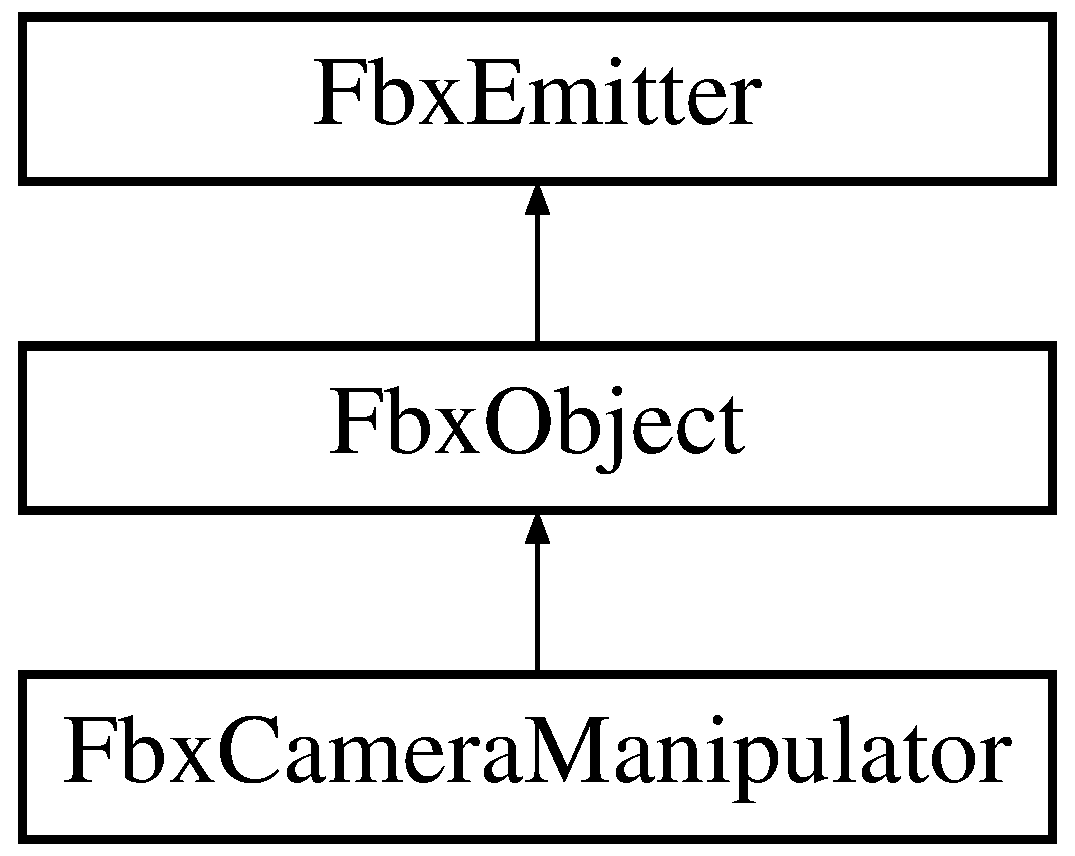
\includegraphics[height=3.000000cm]{class_fbx_camera_manipulator}
\end{center}
\end{figure}
\subsection*{公開型}
\begin{DoxyCompactItemize}
\item 
enum \hyperlink{class_fbx_camera_manipulator_ada0f93888edb4a1c0140e35f99eba922}{E\+Action} \{ \newline
\hyperlink{class_fbx_camera_manipulator_ada0f93888edb4a1c0140e35f99eba922ad7f82cf29963964f19482d8f6e246efe}{e\+None}, 
\hyperlink{class_fbx_camera_manipulator_ada0f93888edb4a1c0140e35f99eba922a172298ef345544e9aa221599bf5fde25}{e\+Orbit}, 
\hyperlink{class_fbx_camera_manipulator_ada0f93888edb4a1c0140e35f99eba922a0aa0fccd579ee7ee47658bca13803471}{e\+Dolly}, 
\hyperlink{class_fbx_camera_manipulator_ada0f93888edb4a1c0140e35f99eba922a14e17787f7b2c85171219544e4f35045}{e\+Pan}, 
\newline
\hyperlink{class_fbx_camera_manipulator_ada0f93888edb4a1c0140e35f99eba922a870b225912367c395c73fb1aae971ec5}{e\+Free\+Pan}
 \}\begin{DoxyCompactList}\small\item\em All possible manipulation actions that can be performed on a camera using this manipulator. \end{DoxyCompactList}
\end{DoxyCompactItemize}
\subsection*{公開メンバ関数}
\begin{DoxyCompactItemize}
\item 
void \hyperlink{class_fbx_camera_manipulator_a67dde46522f0fe7e3e3b10112e7a9c29}{Begin} (\hyperlink{class_fbx_camera_manipulator_ada0f93888edb4a1c0140e35f99eba922}{E\+Action} p\+Action, float pX, float pY)
\item 
void \hyperlink{class_fbx_camera_manipulator_af9008a220ef4a6ececcf46bb171656b4}{Notify} (float pX, float pY, float p\+Scale=0)
\item 
void \hyperlink{class_fbx_camera_manipulator_ae9eef6e3b92ce1b9f2a7da21a2487bb2}{End} ()
\begin{DoxyCompactList}\small\item\em End current manipulation. \end{DoxyCompactList}\item 
void \hyperlink{class_fbx_camera_manipulator_a0753a414b92367037fd96d588b0faba9}{Update} (const \hyperlink{class_fbx_time}{Fbx\+Time} \&p\+Time\+Delta=\hyperlink{fbxtime_8h_aa43cd11e74102affeac06402663d2653}{F\+B\+X\+S\+D\+K\+\_\+\+T\+I\+M\+E\+\_\+\+Z\+E\+RO})
\item 
void \hyperlink{class_fbx_camera_manipulator_a87d5576928c945640be5414d945feab5}{Action} (\hyperlink{class_fbx_camera_manipulator_ada0f93888edb4a1c0140e35f99eba922}{E\+Action} p\+Action, float pX, float pY, float p\+Scale=0)
\item 
\hyperlink{class_fbx_camera_manipulator_ada0f93888edb4a1c0140e35f99eba922}{E\+Action} \hyperlink{class_fbx_camera_manipulator_a93f3cd6487e8f10c9accb6db1022e397}{Get\+Current\+Action} () const
\item 
void \hyperlink{class_fbx_camera_manipulator_a78fab2478759b295c01ab4a4e5f716e9}{Frame\+All} (const \hyperlink{class_fbx_time}{Fbx\+Time} \&p\+Time=\hyperlink{fbxtime_8h_a1e6db3fe0f84f0b7daa775739f93526f}{F\+B\+X\+S\+D\+K\+\_\+\+T\+I\+M\+E\+\_\+\+I\+N\+F\+I\+N\+I\+TE})
\item 
void \hyperlink{class_fbx_camera_manipulator_a7c286fb462b04bc029f72e82e61cdc72}{Frame\+Selected} (const \hyperlink{class_fbx_time}{Fbx\+Time} \&p\+Time=\hyperlink{fbxtime_8h_a1e6db3fe0f84f0b7daa775739f93526f}{F\+B\+X\+S\+D\+K\+\_\+\+T\+I\+M\+E\+\_\+\+I\+N\+F\+I\+N\+I\+TE})
\item 
void \hyperlink{class_fbx_camera_manipulator_a622a6f144dede94c05ed63c80832f25f}{Frame\+Screen\+Position} (float pX, float pY, bool p\+Culling=false, const \hyperlink{class_fbx_time}{Fbx\+Time} \&p\+Time=\hyperlink{fbxtime_8h_a1e6db3fe0f84f0b7daa775739f93526f}{F\+B\+X\+S\+D\+K\+\_\+\+T\+I\+M\+E\+\_\+\+I\+N\+F\+I\+N\+I\+TE})
\end{DoxyCompactItemize}
\subsection*{公開変数類}
\begin{DoxyCompactItemize}
\item 
\hyperlink{class_fbx_property_t}{Fbx\+PropertyT}$<$ \hyperlink{fbxtypes_8h_a44df6a2eec915cf27cd481e5c5e48a24}{Fbx\+Reference} $>$ \hyperlink{class_fbx_camera_manipulator_a3914094466ec766c18c0e544431e8060}{Camera}
\item 
\hyperlink{class_fbx_property_t}{Fbx\+PropertyT}$<$ \hyperlink{fbxtypes_8h_aef968e37f2ddc4188de464d8578c1d5c}{Fbx\+Float} $>$ \hyperlink{class_fbx_camera_manipulator_a03e2795ba49c8bcce02dc786356ab2d5}{Viewport\+Width}
\item 
\hyperlink{class_fbx_property_t}{Fbx\+PropertyT}$<$ \hyperlink{fbxtypes_8h_aef968e37f2ddc4188de464d8578c1d5c}{Fbx\+Float} $>$ \hyperlink{class_fbx_camera_manipulator_afdf345d7e5f01d42da8011bbeb8dc394}{Viewport\+Height}
\item 
\hyperlink{class_fbx_property_t}{Fbx\+PropertyT}$<$ \hyperlink{fbxtypes_8h_a92e0562b2fe33e76a242f498b362262e}{Fbx\+Bool} $>$ \hyperlink{class_fbx_camera_manipulator_abdefaf7c5fef50e2c873616099c2a579}{Smooth}
\item 
\hyperlink{class_fbx_property_t}{Fbx\+PropertyT}$<$ \hyperlink{fbxtypes_8h_a171e72a1c46fc15c1a6c9c31948c1c5b}{Fbx\+Double} $>$ \hyperlink{class_fbx_camera_manipulator_afa0edcbcd8ad9a4de15672c7e8fc0c3d}{Smooth\+Speed}
\item 
\hyperlink{class_fbx_property_t}{Fbx\+PropertyT}$<$ \hyperlink{fbxtypes_8h_a92e0562b2fe33e76a242f498b362262e}{Fbx\+Bool} $>$ \hyperlink{class_fbx_camera_manipulator_aebb2e55534a051995499d73cd1742511}{InvertX}
\item 
\hyperlink{class_fbx_property_t}{Fbx\+PropertyT}$<$ \hyperlink{fbxtypes_8h_a92e0562b2fe33e76a242f498b362262e}{Fbx\+Bool} $>$ \hyperlink{class_fbx_camera_manipulator_a9e9a2e653b6ef9f1d3da31110f26fec3}{InvertY}
\item 
\hyperlink{class_fbx_property_t}{Fbx\+PropertyT}$<$ \hyperlink{fbxtypes_8h_a92e0562b2fe33e76a242f498b362262e}{Fbx\+Bool} $>$ \hyperlink{class_fbx_camera_manipulator_aafe0b0e43ecaf16a44a49ae2d55f440a}{Restore}
\end{DoxyCompactItemize}
\subsection*{限定公開メンバ関数}
\begin{DoxyCompactItemize}
\item 
virtual void \hyperlink{class_fbx_camera_manipulator_ac85c39bca662da17932613bd8bbaf95b}{Construct} (const \hyperlink{class_fbx_object}{Fbx\+Object} $\ast$p\+From)
\item 
virtual void \hyperlink{class_fbx_camera_manipulator_aba0217b5fd302152dc0e2726ca3c325a}{Destruct} (bool p\+Recursive)
\item 
virtual void \hyperlink{class_fbx_camera_manipulator_a9e97c5d7f153bbc80a2c233d425a447f}{Construct\+Properties} (bool p\+Force\+Set)
\item 
virtual bool \hyperlink{class_fbx_camera_manipulator_a0cd75ec4a78ef84f2cf10f750e4491c6}{Connect\+Notify} (const \hyperlink{class_fbx_connect_event}{Fbx\+Connect\+Event} \&p\+Event)
\item 
virtual bool \hyperlink{class_fbx_camera_manipulator_aa0b1cdb3a150798e03587a3adeadd87a}{Property\+Notify} (\hyperlink{class_fbx_object_a528f1b2c2b7abbd64c525ba3a9a496b8}{E\+Property\+Notify\+Type} p\+Type, \hyperlink{class_fbx_property}{Fbx\+Property} \&p\+Property)
\end{DoxyCompactItemize}
\subsection*{その他の継承メンバ}


\subsection{詳解}
This class can be used to provide basic camera manipulation in any program using this library. 

 fbxmanipulators.\+h の 30 行目に定義があります。



\subsection{列挙型メンバ詳解}
\mbox{\Hypertarget{class_fbx_camera_manipulator_ada0f93888edb4a1c0140e35f99eba922}\label{class_fbx_camera_manipulator_ada0f93888edb4a1c0140e35f99eba922}} 
\index{Fbx\+Camera\+Manipulator@{Fbx\+Camera\+Manipulator}!E\+Action@{E\+Action}}
\index{E\+Action@{E\+Action}!Fbx\+Camera\+Manipulator@{Fbx\+Camera\+Manipulator}}
\subsubsection{\texorpdfstring{E\+Action}{EAction}}
{\footnotesize\ttfamily enum \hyperlink{class_fbx_camera_manipulator_ada0f93888edb4a1c0140e35f99eba922}{Fbx\+Camera\+Manipulator\+::\+E\+Action}}



All possible manipulation actions that can be performed on a camera using this manipulator. 

\begin{DoxyEnumFields}{列挙値}
\raisebox{\heightof{T}}[0pt][0pt]{\index{e\+None@{e\+None}!Fbx\+Camera\+Manipulator@{Fbx\+Camera\+Manipulator}}\index{Fbx\+Camera\+Manipulator@{Fbx\+Camera\+Manipulator}!e\+None@{e\+None}}}\mbox{\Hypertarget{class_fbx_camera_manipulator_ada0f93888edb4a1c0140e35f99eba922ad7f82cf29963964f19482d8f6e246efe}\label{class_fbx_camera_manipulator_ada0f93888edb4a1c0140e35f99eba922ad7f82cf29963964f19482d8f6e246efe}} 
e\+None&No action. \\
\hline

\raisebox{\heightof{T}}[0pt][0pt]{\index{e\+Orbit@{e\+Orbit}!Fbx\+Camera\+Manipulator@{Fbx\+Camera\+Manipulator}}\index{Fbx\+Camera\+Manipulator@{Fbx\+Camera\+Manipulator}!e\+Orbit@{e\+Orbit}}}\mbox{\Hypertarget{class_fbx_camera_manipulator_ada0f93888edb4a1c0140e35f99eba922a172298ef345544e9aa221599bf5fde25}\label{class_fbx_camera_manipulator_ada0f93888edb4a1c0140e35f99eba922a172298ef345544e9aa221599bf5fde25}} 
e\+Orbit&Orbiting camera around Loot\+At/\+Interest position. \\
\hline

\raisebox{\heightof{T}}[0pt][0pt]{\index{e\+Dolly@{e\+Dolly}!Fbx\+Camera\+Manipulator@{Fbx\+Camera\+Manipulator}}\index{Fbx\+Camera\+Manipulator@{Fbx\+Camera\+Manipulator}!e\+Dolly@{e\+Dolly}}}\mbox{\Hypertarget{class_fbx_camera_manipulator_ada0f93888edb4a1c0140e35f99eba922a0aa0fccd579ee7ee47658bca13803471}\label{class_fbx_camera_manipulator_ada0f93888edb4a1c0140e35f99eba922a0aa0fccd579ee7ee47658bca13803471}} 
e\+Dolly&Moving camera closer or away from its Look\+At/\+Intest position. \\
\hline

\raisebox{\heightof{T}}[0pt][0pt]{\index{e\+Pan@{e\+Pan}!Fbx\+Camera\+Manipulator@{Fbx\+Camera\+Manipulator}}\index{Fbx\+Camera\+Manipulator@{Fbx\+Camera\+Manipulator}!e\+Pan@{e\+Pan}}}\mbox{\Hypertarget{class_fbx_camera_manipulator_ada0f93888edb4a1c0140e35f99eba922a14e17787f7b2c85171219544e4f35045}\label{class_fbx_camera_manipulator_ada0f93888edb4a1c0140e35f99eba922a14e17787f7b2c85171219544e4f35045}} 
e\+Pan&Panning camera up, down and sideways. \\
\hline

\raisebox{\heightof{T}}[0pt][0pt]{\index{e\+Free\+Pan@{e\+Free\+Pan}!Fbx\+Camera\+Manipulator@{Fbx\+Camera\+Manipulator}}\index{Fbx\+Camera\+Manipulator@{Fbx\+Camera\+Manipulator}!e\+Free\+Pan@{e\+Free\+Pan}}}\mbox{\Hypertarget{class_fbx_camera_manipulator_ada0f93888edb4a1c0140e35f99eba922a870b225912367c395c73fb1aae971ec5}\label{class_fbx_camera_manipulator_ada0f93888edb4a1c0140e35f99eba922a870b225912367c395c73fb1aae971ec5}} 
e\+Free\+Pan&Panning and dollying all at once. \\
\hline

\end{DoxyEnumFields}


 fbxmanipulators.\+h の 36 行目に定義があります。



\subsection{関数詳解}
\mbox{\Hypertarget{class_fbx_camera_manipulator_a87d5576928c945640be5414d945feab5}\label{class_fbx_camera_manipulator_a87d5576928c945640be5414d945feab5}} 
\index{Fbx\+Camera\+Manipulator@{Fbx\+Camera\+Manipulator}!Action@{Action}}
\index{Action@{Action}!Fbx\+Camera\+Manipulator@{Fbx\+Camera\+Manipulator}}
\subsubsection{\texorpdfstring{Action()}{Action()}}
{\footnotesize\ttfamily void Fbx\+Camera\+Manipulator\+::\+Action (\begin{DoxyParamCaption}\item[{\hyperlink{class_fbx_camera_manipulator_ada0f93888edb4a1c0140e35f99eba922}{E\+Action}}]{p\+Action,  }\item[{float}]{pX,  }\item[{float}]{pY,  }\item[{float}]{p\+Scale = {\ttfamily 0} }\end{DoxyParamCaption})}

Do a complete manipulation action in a single operation. This is the equivalent of calling Begin, Notify and End successively. 
\begin{DoxyParams}{引数}
{\em p\+Action} & The action performed for this manipulation scope. \\
\hline
{\em pX} & Horizontal position of the manipulation, in pixels. \\
\hline
{\em pY} & Vertical position of the manipulation, in pixels. \\
\hline
{\em p\+Scale} & Scaling value of the manipulation. Only used by e\+Free\+Pan action. \\
\hline
\end{DoxyParams}
\mbox{\Hypertarget{class_fbx_camera_manipulator_a67dde46522f0fe7e3e3b10112e7a9c29}\label{class_fbx_camera_manipulator_a67dde46522f0fe7e3e3b10112e7a9c29}} 
\index{Fbx\+Camera\+Manipulator@{Fbx\+Camera\+Manipulator}!Begin@{Begin}}
\index{Begin@{Begin}!Fbx\+Camera\+Manipulator@{Fbx\+Camera\+Manipulator}}
\subsubsection{\texorpdfstring{Begin()}{Begin()}}
{\footnotesize\ttfamily void Fbx\+Camera\+Manipulator\+::\+Begin (\begin{DoxyParamCaption}\item[{\hyperlink{class_fbx_camera_manipulator_ada0f93888edb4a1c0140e35f99eba922}{E\+Action}}]{p\+Action,  }\item[{float}]{pX,  }\item[{float}]{pY }\end{DoxyParamCaption})}

Begin manipulation of the camera. 
\begin{DoxyParams}{引数}
{\em p\+Action} & The action performed for this manipulation scope. \\
\hline
{\em pX} & Begin horizontal position of the manipulation, in pixels. \\
\hline
{\em pY} & Begin vertical position of the manipulation, in pixels. \\
\hline
\end{DoxyParams}
\mbox{\Hypertarget{class_fbx_camera_manipulator_a0cd75ec4a78ef84f2cf10f750e4491c6}\label{class_fbx_camera_manipulator_a0cd75ec4a78ef84f2cf10f750e4491c6}} 
\index{Fbx\+Camera\+Manipulator@{Fbx\+Camera\+Manipulator}!Connect\+Notify@{Connect\+Notify}}
\index{Connect\+Notify@{Connect\+Notify}!Fbx\+Camera\+Manipulator@{Fbx\+Camera\+Manipulator}}
\subsubsection{\texorpdfstring{Connect\+Notify()}{ConnectNotify()}}
{\footnotesize\ttfamily virtual bool Fbx\+Camera\+Manipulator\+::\+Connect\+Notify (\begin{DoxyParamCaption}\item[{const \hyperlink{class_fbx_connect_event}{Fbx\+Connect\+Event} \&}]{p\+Event }\end{DoxyParamCaption})\hspace{0.3cm}{\ttfamily [protected]}, {\ttfamily [virtual]}}



\hyperlink{class_fbx_object_ab7a400f3829d1f0da57d3d78c8168dd0}{Fbx\+Object}を再実装しています。

\mbox{\Hypertarget{class_fbx_camera_manipulator_ac85c39bca662da17932613bd8bbaf95b}\label{class_fbx_camera_manipulator_ac85c39bca662da17932613bd8bbaf95b}} 
\index{Fbx\+Camera\+Manipulator@{Fbx\+Camera\+Manipulator}!Construct@{Construct}}
\index{Construct@{Construct}!Fbx\+Camera\+Manipulator@{Fbx\+Camera\+Manipulator}}
\subsubsection{\texorpdfstring{Construct()}{Construct()}}
{\footnotesize\ttfamily virtual void Fbx\+Camera\+Manipulator\+::\+Construct (\begin{DoxyParamCaption}\item[{const \hyperlink{class_fbx_object}{Fbx\+Object} $\ast$}]{p\+From }\end{DoxyParamCaption})\hspace{0.3cm}{\ttfamily [protected]}, {\ttfamily [virtual]}}

Optional constructor override, automatically called by default constructor. 
\begin{DoxyParams}{引数}
{\em p\+From} & If not null, the function must take it into account like a copy constructor. \\
\hline
\end{DoxyParams}
\begin{DoxyRemark}{注釈}
In case it is decided to override this function, do not forget to call Parent\+Class\+::\+Construct(p\+From) at the beginning. 
\end{DoxyRemark}


\hyperlink{class_fbx_object_a313503bc645af3fdceb4a99ef5cea7eb}{Fbx\+Object}を再実装しています。

\mbox{\Hypertarget{class_fbx_camera_manipulator_a9e97c5d7f153bbc80a2c233d425a447f}\label{class_fbx_camera_manipulator_a9e97c5d7f153bbc80a2c233d425a447f}} 
\index{Fbx\+Camera\+Manipulator@{Fbx\+Camera\+Manipulator}!Construct\+Properties@{Construct\+Properties}}
\index{Construct\+Properties@{Construct\+Properties}!Fbx\+Camera\+Manipulator@{Fbx\+Camera\+Manipulator}}
\subsubsection{\texorpdfstring{Construct\+Properties()}{ConstructProperties()}}
{\footnotesize\ttfamily virtual void Fbx\+Camera\+Manipulator\+::\+Construct\+Properties (\begin{DoxyParamCaption}\item[{bool}]{p\+Force\+Set }\end{DoxyParamCaption})\hspace{0.3cm}{\ttfamily [protected]}, {\ttfamily [virtual]}}

Optional property constructor override, automatically called by default constructor. 
\begin{DoxyParams}{引数}
{\em p\+Force\+Set} & If the property value must be set regardless of default value. \\
\hline
\end{DoxyParams}
\begin{DoxyRemark}{注釈}
If your object have properties, they must be initialized in this function. 
\end{DoxyRemark}


\hyperlink{class_fbx_object_ad44f814323dc1b5e78bff1bfc608b4bb}{Fbx\+Object}を再実装しています。

\mbox{\Hypertarget{class_fbx_camera_manipulator_aba0217b5fd302152dc0e2726ca3c325a}\label{class_fbx_camera_manipulator_aba0217b5fd302152dc0e2726ca3c325a}} 
\index{Fbx\+Camera\+Manipulator@{Fbx\+Camera\+Manipulator}!Destruct@{Destruct}}
\index{Destruct@{Destruct}!Fbx\+Camera\+Manipulator@{Fbx\+Camera\+Manipulator}}
\subsubsection{\texorpdfstring{Destruct()}{Destruct()}}
{\footnotesize\ttfamily virtual void Fbx\+Camera\+Manipulator\+::\+Destruct (\begin{DoxyParamCaption}\item[{bool}]{p\+Recursive }\end{DoxyParamCaption})\hspace{0.3cm}{\ttfamily [protected]}, {\ttfamily [virtual]}}

Optional destructor override, automatically called by default destructor. 
\begin{DoxyParams}{引数}
{\em p\+Recursive} & If true, children objects should be destroyed as well. \\
\hline
\end{DoxyParams}
\begin{DoxyRemark}{注釈}
In case it is decided to override this function, do not forget to call Parent\+Class\+::\+Destruct(p\+Resursive) at the end. 
\end{DoxyRemark}


\hyperlink{class_fbx_object_a123e084d9b32b29c28af6384b7c3c608}{Fbx\+Object}を再実装しています。

\mbox{\Hypertarget{class_fbx_camera_manipulator_ae9eef6e3b92ce1b9f2a7da21a2487bb2}\label{class_fbx_camera_manipulator_ae9eef6e3b92ce1b9f2a7da21a2487bb2}} 
\index{Fbx\+Camera\+Manipulator@{Fbx\+Camera\+Manipulator}!End@{End}}
\index{End@{End}!Fbx\+Camera\+Manipulator@{Fbx\+Camera\+Manipulator}}
\subsubsection{\texorpdfstring{End()}{End()}}
{\footnotesize\ttfamily void Fbx\+Camera\+Manipulator\+::\+End (\begin{DoxyParamCaption}{ }\end{DoxyParamCaption})}



End current manipulation. 

\mbox{\Hypertarget{class_fbx_camera_manipulator_a78fab2478759b295c01ab4a4e5f716e9}\label{class_fbx_camera_manipulator_a78fab2478759b295c01ab4a4e5f716e9}} 
\index{Fbx\+Camera\+Manipulator@{Fbx\+Camera\+Manipulator}!Frame\+All@{Frame\+All}}
\index{Frame\+All@{Frame\+All}!Fbx\+Camera\+Manipulator@{Fbx\+Camera\+Manipulator}}
\subsubsection{\texorpdfstring{Frame\+All()}{FrameAll()}}
{\footnotesize\ttfamily void Fbx\+Camera\+Manipulator\+::\+Frame\+All (\begin{DoxyParamCaption}\item[{const \hyperlink{class_fbx_time}{Fbx\+Time} \&}]{p\+Time = {\ttfamily \hyperlink{fbxtime_8h_a1e6db3fe0f84f0b7daa775739f93526f}{F\+B\+X\+S\+D\+K\+\_\+\+T\+I\+M\+E\+\_\+\+I\+N\+F\+I\+N\+I\+TE}} }\end{DoxyParamCaption})}

Change camera position and Look\+At node to frame all objects. 
\begin{DoxyParams}{引数}
{\em p\+Time} & Time to use to evaluate mesh deformations. Leave at default value to cancel mesh evaluation. \\
\hline
\end{DoxyParams}
\mbox{\Hypertarget{class_fbx_camera_manipulator_a622a6f144dede94c05ed63c80832f25f}\label{class_fbx_camera_manipulator_a622a6f144dede94c05ed63c80832f25f}} 
\index{Fbx\+Camera\+Manipulator@{Fbx\+Camera\+Manipulator}!Frame\+Screen\+Position@{Frame\+Screen\+Position}}
\index{Frame\+Screen\+Position@{Frame\+Screen\+Position}!Fbx\+Camera\+Manipulator@{Fbx\+Camera\+Manipulator}}
\subsubsection{\texorpdfstring{Frame\+Screen\+Position()}{FrameScreenPosition()}}
{\footnotesize\ttfamily void Fbx\+Camera\+Manipulator\+::\+Frame\+Screen\+Position (\begin{DoxyParamCaption}\item[{float}]{pX,  }\item[{float}]{pY,  }\item[{bool}]{p\+Culling = {\ttfamily false},  }\item[{const \hyperlink{class_fbx_time}{Fbx\+Time} \&}]{p\+Time = {\ttfamily \hyperlink{fbxtime_8h_a1e6db3fe0f84f0b7daa775739f93526f}{F\+B\+X\+S\+D\+K\+\_\+\+T\+I\+M\+E\+\_\+\+I\+N\+F\+I\+N\+I\+TE}} }\end{DoxyParamCaption})}

Change camera position and Look\+At to frame the selected position on screen. The Look\+At will be placed at first closest intersecting geometry, and the distance between camera and Look\+At will be preserved. 
\begin{DoxyParams}{引数}
{\em pX} & The horizontal screen coordinate. \\
\hline
{\em pY} & The vertical screen coordinate. \\
\hline
{\em p\+Culling} & If {\ttfamily true}, only test triangles that are front-\/facing, otherwise test both sides. \\
\hline
{\em p\+Time} & Time to use to evaluate mesh deformations. Leave at default value to cancel mesh evaluation. \\
\hline
\end{DoxyParams}
\mbox{\Hypertarget{class_fbx_camera_manipulator_a7c286fb462b04bc029f72e82e61cdc72}\label{class_fbx_camera_manipulator_a7c286fb462b04bc029f72e82e61cdc72}} 
\index{Fbx\+Camera\+Manipulator@{Fbx\+Camera\+Manipulator}!Frame\+Selected@{Frame\+Selected}}
\index{Frame\+Selected@{Frame\+Selected}!Fbx\+Camera\+Manipulator@{Fbx\+Camera\+Manipulator}}
\subsubsection{\texorpdfstring{Frame\+Selected()}{FrameSelected()}}
{\footnotesize\ttfamily void Fbx\+Camera\+Manipulator\+::\+Frame\+Selected (\begin{DoxyParamCaption}\item[{const \hyperlink{class_fbx_time}{Fbx\+Time} \&}]{p\+Time = {\ttfamily \hyperlink{fbxtime_8h_a1e6db3fe0f84f0b7daa775739f93526f}{F\+B\+X\+S\+D\+K\+\_\+\+T\+I\+M\+E\+\_\+\+I\+N\+F\+I\+N\+I\+TE}} }\end{DoxyParamCaption})}

Change camera position and Look\+At to frame all selected objects. 
\begin{DoxyParams}{引数}
{\em p\+Time} & Time to use to evaluate mesh deformations. Leave at default value to cancel mesh evaluation. \\
\hline
\end{DoxyParams}
\mbox{\Hypertarget{class_fbx_camera_manipulator_a93f3cd6487e8f10c9accb6db1022e397}\label{class_fbx_camera_manipulator_a93f3cd6487e8f10c9accb6db1022e397}} 
\index{Fbx\+Camera\+Manipulator@{Fbx\+Camera\+Manipulator}!Get\+Current\+Action@{Get\+Current\+Action}}
\index{Get\+Current\+Action@{Get\+Current\+Action}!Fbx\+Camera\+Manipulator@{Fbx\+Camera\+Manipulator}}
\subsubsection{\texorpdfstring{Get\+Current\+Action()}{GetCurrentAction()}}
{\footnotesize\ttfamily \hyperlink{class_fbx_camera_manipulator_ada0f93888edb4a1c0140e35f99eba922}{E\+Action} Fbx\+Camera\+Manipulator\+::\+Get\+Current\+Action (\begin{DoxyParamCaption}{ }\end{DoxyParamCaption}) const}

Retrieve current manipulation action. \begin{DoxyReturn}{戻り値}
The action currently performed by the camera manipulator. 
\end{DoxyReturn}
\mbox{\Hypertarget{class_fbx_camera_manipulator_af9008a220ef4a6ececcf46bb171656b4}\label{class_fbx_camera_manipulator_af9008a220ef4a6ececcf46bb171656b4}} 
\index{Fbx\+Camera\+Manipulator@{Fbx\+Camera\+Manipulator}!Notify@{Notify}}
\index{Notify@{Notify}!Fbx\+Camera\+Manipulator@{Fbx\+Camera\+Manipulator}}
\subsubsection{\texorpdfstring{Notify()}{Notify()}}
{\footnotesize\ttfamily void Fbx\+Camera\+Manipulator\+::\+Notify (\begin{DoxyParamCaption}\item[{float}]{pX,  }\item[{float}]{pY,  }\item[{float}]{p\+Scale = {\ttfamily 0} }\end{DoxyParamCaption})}

Notify manipulation of latest input. 
\begin{DoxyParams}{引数}
{\em p\+Time\+Delta} & Elapsed time since the last notify. Only used if Smoothing is enabled. \\
\hline
{\em pX} & Horizontal position of the manipulation, in pixels. \\
\hline
{\em pY} & Vertical position of the manipulation, in pixels. \\
\hline
{\em p\+Scale} & Scaling value of the manipulation. Only used by e\+Free\+Pan action. \\
\hline
\end{DoxyParams}
\mbox{\Hypertarget{class_fbx_camera_manipulator_aa0b1cdb3a150798e03587a3adeadd87a}\label{class_fbx_camera_manipulator_aa0b1cdb3a150798e03587a3adeadd87a}} 
\index{Fbx\+Camera\+Manipulator@{Fbx\+Camera\+Manipulator}!Property\+Notify@{Property\+Notify}}
\index{Property\+Notify@{Property\+Notify}!Fbx\+Camera\+Manipulator@{Fbx\+Camera\+Manipulator}}
\subsubsection{\texorpdfstring{Property\+Notify()}{PropertyNotify()}}
{\footnotesize\ttfamily virtual bool Fbx\+Camera\+Manipulator\+::\+Property\+Notify (\begin{DoxyParamCaption}\item[{\hyperlink{class_fbx_object_a528f1b2c2b7abbd64c525ba3a9a496b8}{E\+Property\+Notify\+Type}}]{p\+Type,  }\item[{\hyperlink{class_fbx_property}{Fbx\+Property} \&}]{p\+Property }\end{DoxyParamCaption})\hspace{0.3cm}{\ttfamily [protected]}, {\ttfamily [virtual]}}



\hyperlink{class_fbx_object_a68b9ad65d98d7be9cb252949bc709385}{Fbx\+Object}を再実装しています。

\mbox{\Hypertarget{class_fbx_camera_manipulator_a0753a414b92367037fd96d588b0faba9}\label{class_fbx_camera_manipulator_a0753a414b92367037fd96d588b0faba9}} 
\index{Fbx\+Camera\+Manipulator@{Fbx\+Camera\+Manipulator}!Update@{Update}}
\index{Update@{Update}!Fbx\+Camera\+Manipulator@{Fbx\+Camera\+Manipulator}}
\subsubsection{\texorpdfstring{Update()}{Update()}}
{\footnotesize\ttfamily void Fbx\+Camera\+Manipulator\+::\+Update (\begin{DoxyParamCaption}\item[{const \hyperlink{class_fbx_time}{Fbx\+Time} \&}]{p\+Time\+Delta = {\ttfamily \hyperlink{fbxtime_8h_aa43cd11e74102affeac06402663d2653}{F\+B\+X\+S\+D\+K\+\_\+\+T\+I\+M\+E\+\_\+\+Z\+E\+RO}} }\end{DoxyParamCaption})}

Update the camera position. This must be called periodically in order for the camera to update its position. 
\begin{DoxyParams}{引数}
{\em p\+Time\+Delta} & Elapsed time since the last update. If Smooth is disabled, you can leave this value to zero. \\
\hline
\end{DoxyParams}
\begin{DoxyRemark}{注釈}
Begin, Notify and End will not change the current camera position. 
\end{DoxyRemark}


\subsection{メンバ詳解}
\mbox{\Hypertarget{class_fbx_camera_manipulator_a3914094466ec766c18c0e544431e8060}\label{class_fbx_camera_manipulator_a3914094466ec766c18c0e544431e8060}} 
\index{Fbx\+Camera\+Manipulator@{Fbx\+Camera\+Manipulator}!Camera@{Camera}}
\index{Camera@{Camera}!Fbx\+Camera\+Manipulator@{Fbx\+Camera\+Manipulator}}
\subsubsection{\texorpdfstring{Camera}{Camera}}
{\footnotesize\ttfamily \hyperlink{class_fbx_property_t}{Fbx\+PropertyT}$<$\hyperlink{fbxtypes_8h_a44df6a2eec915cf27cd481e5c5e48a24}{Fbx\+Reference}$>$ Fbx\+Camera\+Manipulator\+::\+Camera}

The camera controlled by the manipulator. 

 fbxmanipulators.\+h の 94 行目に定義があります。

\mbox{\Hypertarget{class_fbx_camera_manipulator_aebb2e55534a051995499d73cd1742511}\label{class_fbx_camera_manipulator_aebb2e55534a051995499d73cd1742511}} 
\index{Fbx\+Camera\+Manipulator@{Fbx\+Camera\+Manipulator}!InvertX@{InvertX}}
\index{InvertX@{InvertX}!Fbx\+Camera\+Manipulator@{Fbx\+Camera\+Manipulator}}
\subsubsection{\texorpdfstring{InvertX}{InvertX}}
{\footnotesize\ttfamily \hyperlink{class_fbx_property_t}{Fbx\+PropertyT}$<$\hyperlink{fbxtypes_8h_a92e0562b2fe33e76a242f498b362262e}{Fbx\+Bool}$>$ Fbx\+Camera\+Manipulator\+::\+InvertX}

Invert the camera horizontal manipulation direction if set to true. False by default. 

 fbxmanipulators.\+h の 111 行目に定義があります。

\mbox{\Hypertarget{class_fbx_camera_manipulator_a9e9a2e653b6ef9f1d3da31110f26fec3}\label{class_fbx_camera_manipulator_a9e9a2e653b6ef9f1d3da31110f26fec3}} 
\index{Fbx\+Camera\+Manipulator@{Fbx\+Camera\+Manipulator}!InvertY@{InvertY}}
\index{InvertY@{InvertY}!Fbx\+Camera\+Manipulator@{Fbx\+Camera\+Manipulator}}
\subsubsection{\texorpdfstring{InvertY}{InvertY}}
{\footnotesize\ttfamily \hyperlink{class_fbx_property_t}{Fbx\+PropertyT}$<$\hyperlink{fbxtypes_8h_a92e0562b2fe33e76a242f498b362262e}{Fbx\+Bool}$>$ Fbx\+Camera\+Manipulator\+::\+InvertY}

Invert the camera vertical manipulation direction if set to true. False by default. 

 fbxmanipulators.\+h の 114 行目に定義があります。

\mbox{\Hypertarget{class_fbx_camera_manipulator_aafe0b0e43ecaf16a44a49ae2d55f440a}\label{class_fbx_camera_manipulator_aafe0b0e43ecaf16a44a49ae2d55f440a}} 
\index{Fbx\+Camera\+Manipulator@{Fbx\+Camera\+Manipulator}!Restore@{Restore}}
\index{Restore@{Restore}!Fbx\+Camera\+Manipulator@{Fbx\+Camera\+Manipulator}}
\subsubsection{\texorpdfstring{Restore}{Restore}}
{\footnotesize\ttfamily \hyperlink{class_fbx_property_t}{Fbx\+PropertyT}$<$\hyperlink{fbxtypes_8h_a92e0562b2fe33e76a242f498b362262e}{Fbx\+Bool}$>$ Fbx\+Camera\+Manipulator\+::\+Restore}

Restore the camera transform upon destruction of the manipulator. 

 fbxmanipulators.\+h の 117 行目に定義があります。

\mbox{\Hypertarget{class_fbx_camera_manipulator_abdefaf7c5fef50e2c873616099c2a579}\label{class_fbx_camera_manipulator_abdefaf7c5fef50e2c873616099c2a579}} 
\index{Fbx\+Camera\+Manipulator@{Fbx\+Camera\+Manipulator}!Smooth@{Smooth}}
\index{Smooth@{Smooth}!Fbx\+Camera\+Manipulator@{Fbx\+Camera\+Manipulator}}
\subsubsection{\texorpdfstring{Smooth}{Smooth}}
{\footnotesize\ttfamily \hyperlink{class_fbx_property_t}{Fbx\+PropertyT}$<$\hyperlink{fbxtypes_8h_a92e0562b2fe33e76a242f498b362262e}{Fbx\+Bool}$>$ Fbx\+Camera\+Manipulator\+::\+Smooth}

Camera manipulations will be smooth if enabled. True by default. 

 fbxmanipulators.\+h の 105 行目に定義があります。

\mbox{\Hypertarget{class_fbx_camera_manipulator_afa0edcbcd8ad9a4de15672c7e8fc0c3d}\label{class_fbx_camera_manipulator_afa0edcbcd8ad9a4de15672c7e8fc0c3d}} 
\index{Fbx\+Camera\+Manipulator@{Fbx\+Camera\+Manipulator}!Smooth\+Speed@{Smooth\+Speed}}
\index{Smooth\+Speed@{Smooth\+Speed}!Fbx\+Camera\+Manipulator@{Fbx\+Camera\+Manipulator}}
\subsubsection{\texorpdfstring{Smooth\+Speed}{SmoothSpeed}}
{\footnotesize\ttfamily \hyperlink{class_fbx_property_t}{Fbx\+PropertyT}$<$\hyperlink{fbxtypes_8h_a171e72a1c46fc15c1a6c9c31948c1c5b}{Fbx\+Double}$>$ Fbx\+Camera\+Manipulator\+::\+Smooth\+Speed}

Camera manipulations smoothing speed. Higher speed will stabilize the camera more quickly. Default is 10.\+0 

 fbxmanipulators.\+h の 108 行目に定義があります。

\mbox{\Hypertarget{class_fbx_camera_manipulator_afdf345d7e5f01d42da8011bbeb8dc394}\label{class_fbx_camera_manipulator_afdf345d7e5f01d42da8011bbeb8dc394}} 
\index{Fbx\+Camera\+Manipulator@{Fbx\+Camera\+Manipulator}!Viewport\+Height@{Viewport\+Height}}
\index{Viewport\+Height@{Viewport\+Height}!Fbx\+Camera\+Manipulator@{Fbx\+Camera\+Manipulator}}
\subsubsection{\texorpdfstring{Viewport\+Height}{ViewportHeight}}
{\footnotesize\ttfamily \hyperlink{class_fbx_property_t}{Fbx\+PropertyT}$<$\hyperlink{fbxtypes_8h_aef968e37f2ddc4188de464d8578c1d5c}{Fbx\+Float}$>$ Fbx\+Camera\+Manipulator\+::\+Viewport\+Height}

Height of the camera viewport, in pixels. This is used to accurately calculate to movement speed. \begin{DoxyRemark}{注釈}
If this property is not correctly set, movements will be erronous. 
\end{DoxyRemark}


 fbxmanipulators.\+h の 102 行目に定義があります。

\mbox{\Hypertarget{class_fbx_camera_manipulator_a03e2795ba49c8bcce02dc786356ab2d5}\label{class_fbx_camera_manipulator_a03e2795ba49c8bcce02dc786356ab2d5}} 
\index{Fbx\+Camera\+Manipulator@{Fbx\+Camera\+Manipulator}!Viewport\+Width@{Viewport\+Width}}
\index{Viewport\+Width@{Viewport\+Width}!Fbx\+Camera\+Manipulator@{Fbx\+Camera\+Manipulator}}
\subsubsection{\texorpdfstring{Viewport\+Width}{ViewportWidth}}
{\footnotesize\ttfamily \hyperlink{class_fbx_property_t}{Fbx\+PropertyT}$<$\hyperlink{fbxtypes_8h_aef968e37f2ddc4188de464d8578c1d5c}{Fbx\+Float}$>$ Fbx\+Camera\+Manipulator\+::\+Viewport\+Width}

Width of the camera viewport, in pixels. This is used to accurately calculate to movement speed. \begin{DoxyRemark}{注釈}
If this property is not correctly set, movements will be erronous. 
\end{DoxyRemark}


 fbxmanipulators.\+h の 98 行目に定義があります。



このクラス詳解は次のファイルから抽出されました\+:\begin{DoxyCompactItemize}
\item 
C\+:/\+Maya/scripts/\+F\+B\+X\+\_\+\+S\+D\+K/2017.\+1/include/fbxsdk/utils/\hyperlink{fbxmanipulators_8h}{fbxmanipulators.\+h}\end{DoxyCompactItemize}

\hypertarget{class_fbx_camera_stereo}{}\section{Fbx\+Camera\+Stereo クラス}
\label{class_fbx_camera_stereo}\index{Fbx\+Camera\+Stereo@{Fbx\+Camera\+Stereo}}


{\ttfamily \#include $<$fbxcamerastereo.\+h$>$}

Fbx\+Camera\+Stereo の継承関係図\begin{figure}[H]
\begin{center}
\leavevmode
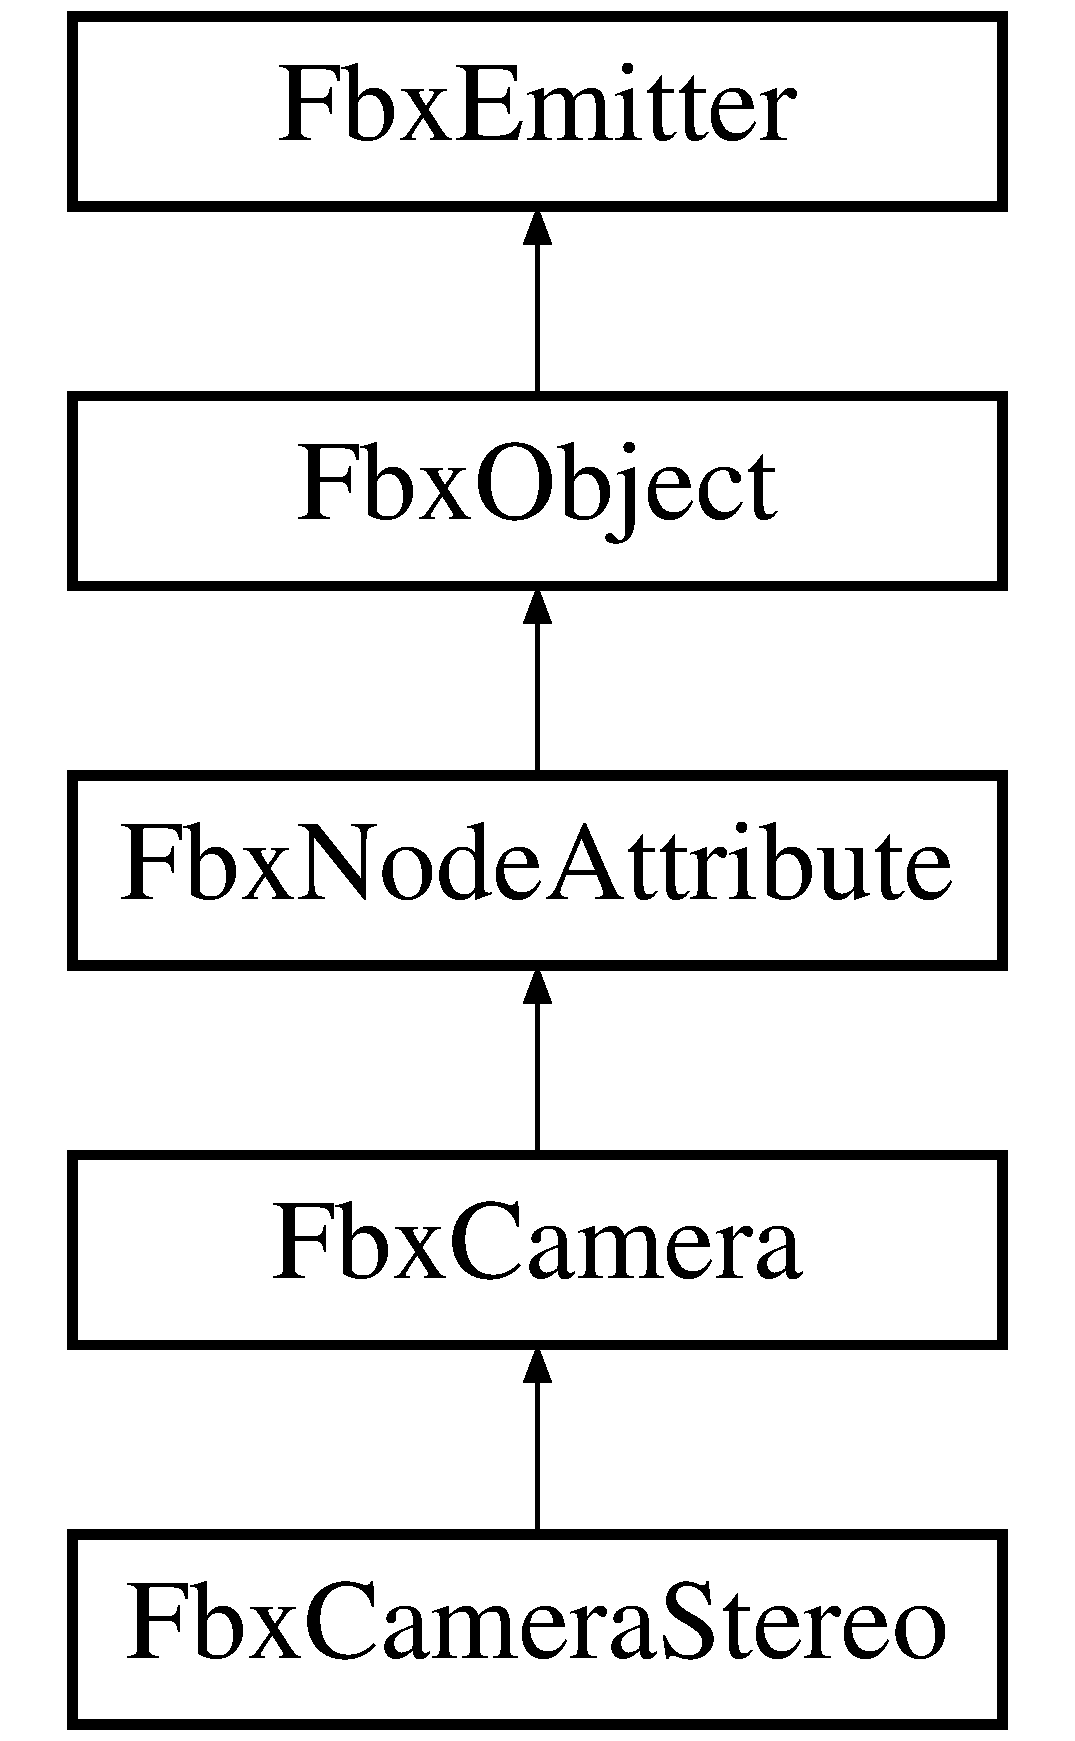
\includegraphics[height=5.000000cm]{class_fbx_camera_stereo}
\end{center}
\end{figure}
\subsection*{公開型}
\begin{DoxyCompactItemize}
\item 
enum \hyperlink{class_fbx_camera_stereo_acb0f27675a73de0858983b703196cb37}{E\+Stereo\+Type} \{ \hyperlink{class_fbx_camera_stereo_acb0f27675a73de0858983b703196cb37acaf3e8d389472ecc3408aa946d13c31f}{e\+None}, 
\hyperlink{class_fbx_camera_stereo_acb0f27675a73de0858983b703196cb37a37c80e0a3ef659934cac67457a3f8c0c}{e\+Converged}, 
\hyperlink{class_fbx_camera_stereo_acb0f27675a73de0858983b703196cb37a15c8f9c81ecc4a7e7174fe214cfc5ec2}{e\+Off\+Axis}, 
\hyperlink{class_fbx_camera_stereo_acb0f27675a73de0858983b703196cb37a5a361b7a07b8066eaa3ecffa5d695370}{e\+Parallel}
 \}
\end{DoxyCompactItemize}
\subsection*{公開メンバ関数}
\begin{DoxyCompactItemize}
\item 
virtual \hyperlink{class_fbx_node_attribute_a08e1669d3d1a696910756ab17de56d6a}{Fbx\+Node\+Attribute\+::\+E\+Type} \hyperlink{class_fbx_camera_stereo_a19160f0fdeaf5407d2bc9c1608f6af53}{Get\+Attribute\+Type} () const
\begin{DoxyCompactList}\small\item\em Return the type of node attribute which is E\+Type\+::e\+Camera\+Stereo. \end{DoxyCompactList}\item 
void \hyperlink{class_fbx_camera_stereo_a5c693025d4b4d25ea05bec61f2c25cd8}{Reset} ()
\begin{DoxyCompactList}\small\item\em Reset the stereo camera to default values. \end{DoxyCompactList}\item 
\hyperlink{class_fbx_camera}{Fbx\+Camera} $\ast$ \hyperlink{class_fbx_camera_stereo_a6841f71c09bdd63c7e936cdb23e818e9}{Get\+Left\+Camera} () const
\item 
\hyperlink{class_fbx_camera}{Fbx\+Camera} $\ast$ \hyperlink{class_fbx_camera_stereo_a8c293c596ad0c3b9fb169bdf5b508a68}{Get\+Right\+Camera} () const
\item 
bool \hyperlink{class_fbx_camera_stereo_a3f6d9d09dd4ec6f9fe1b1b829f26a11f}{Set\+Left\+Camera} (\hyperlink{class_fbx_camera}{Fbx\+Camera} $\ast$p\+Camera)
\item 
bool \hyperlink{class_fbx_camera_stereo_a9b37a67b3bf1e94a6845077913083d78}{Set\+Right\+Camera} (\hyperlink{class_fbx_camera}{Fbx\+Camera} $\ast$p\+Camera)
\item 
\hyperlink{class_fbx_a_matrix}{Fbx\+A\+Matrix} \hyperlink{class_fbx_camera_stereo_aba407c7661b66bc57690534a7aaf445e}{Get\+Left\+Camera\+Local\+Matrix} () const
\item 
\hyperlink{class_fbx_a_matrix}{Fbx\+A\+Matrix} \hyperlink{class_fbx_camera_stereo_afca8a70331c5a524ad7c790e8c52af77}{Get\+Left\+Camera\+Global\+Matrix} () const
\item 
\hyperlink{class_fbx_a_matrix}{Fbx\+A\+Matrix} \hyperlink{class_fbx_camera_stereo_a111785c11520b456bb43ed6701eaa84d}{Get\+Right\+Camera\+Local\+Matrix} () const
\item 
\hyperlink{class_fbx_a_matrix}{Fbx\+A\+Matrix} \hyperlink{class_fbx_camera_stereo_ae46b1246ccc65e2cb3e76cc3673172fd}{Get\+Right\+Camera\+Global\+Matrix} () const
\item 
double \hyperlink{class_fbx_camera_stereo_a372e001c8d6f950d787831dc57c5fc20}{Reevaluate\+Left\+Camera\+Film\+OffsetX} () const
\item 
double \hyperlink{class_fbx_camera_stereo_a63526f13544a343e4447d4567a88bf9d}{Reevaluate\+Right\+Camera\+Film\+OffsetX} () const
\item 
bool \hyperlink{class_fbx_camera_stereo_a00d710d453a4cad2f7f93199ff68ee17}{Connect\+Properties} ()
\end{DoxyCompactItemize}
\subsection*{公開変数類}
\begin{DoxyCompactItemize}
\item 
\hyperlink{class_fbx_property_t}{Fbx\+PropertyT}$<$ \hyperlink{class_fbx_camera_stereo_acb0f27675a73de0858983b703196cb37}{E\+Stereo\+Type} $>$ \hyperlink{class_fbx_camera_stereo_af7ab718dda255c4673813f0993cd143f}{Stereo}
\item 
\hyperlink{class_fbx_property_t}{Fbx\+PropertyT}$<$ \hyperlink{fbxtypes_8h_a171e72a1c46fc15c1a6c9c31948c1c5b}{Fbx\+Double} $>$ \hyperlink{class_fbx_camera_stereo_a93f63eb9bb9d1a9829db054abce1289d}{Interaxial\+Separation}
\item 
\hyperlink{class_fbx_property_t}{Fbx\+PropertyT}$<$ \hyperlink{fbxtypes_8h_a171e72a1c46fc15c1a6c9c31948c1c5b}{Fbx\+Double} $>$ \hyperlink{class_fbx_camera_stereo_ab76f0822d4543864dfe707ea8b3be50a}{Zero\+Parallax}
\item 
\hyperlink{class_fbx_property_t}{Fbx\+PropertyT}$<$ \hyperlink{fbxtypes_8h_a171e72a1c46fc15c1a6c9c31948c1c5b}{Fbx\+Double} $>$ \hyperlink{class_fbx_camera_stereo_ad869c71fad3c11ada97b96bceeda09ed}{Toe\+In\+Adjust}
\item 
\hyperlink{class_fbx_property_t}{Fbx\+PropertyT}$<$ \hyperlink{fbxtypes_8h_a171e72a1c46fc15c1a6c9c31948c1c5b}{Fbx\+Double} $>$ \hyperlink{class_fbx_camera_stereo_a91f409fc6af89147826e7eb0aae87184}{Film\+Offset\+Right\+Cam}
\item 
\hyperlink{class_fbx_property_t}{Fbx\+PropertyT}$<$ \hyperlink{fbxtypes_8h_a171e72a1c46fc15c1a6c9c31948c1c5b}{Fbx\+Double} $>$ \hyperlink{class_fbx_camera_stereo_adfb0e61258f415bd4e80d2a74071d2b5}{Film\+Offset\+Left\+Cam}
\item 
\hyperlink{class_fbx_property_t}{Fbx\+PropertyT}$<$ \hyperlink{fbxtypes_8h_a44df6a2eec915cf27cd481e5c5e48a24}{Fbx\+Reference} $>$ \hyperlink{class_fbx_camera_stereo_ae4bbaad53a1ebbc0534f78c246affd84}{Right\+Camera}
\item 
\hyperlink{class_fbx_property_t}{Fbx\+PropertyT}$<$ \hyperlink{fbxtypes_8h_a44df6a2eec915cf27cd481e5c5e48a24}{Fbx\+Reference} $>$ \hyperlink{class_fbx_camera_stereo_a92cc37f2c93f8920e66756ef4d947762}{Left\+Camera}
\item 
\hyperlink{class_fbx_property_t}{Fbx\+PropertyT}$<$ \hyperlink{class_fbx_string}{Fbx\+String} $>$ \hyperlink{class_fbx_camera_stereo_a25294714b9dfedce9180102396ebd7bc}{Precomp\+File\+Name}
\item 
\hyperlink{class_fbx_property_t}{Fbx\+PropertyT}$<$ \hyperlink{class_fbx_string}{Fbx\+String} $>$ \hyperlink{class_fbx_camera_stereo_af7d8b1be43665a8662630cdc2fdb0dbb}{Relative\+Precomp\+File\+Name}
\end{DoxyCompactItemize}
\subsection*{限定公開メンバ関数}
\begin{DoxyCompactItemize}
\item 
virtual void \hyperlink{class_fbx_camera_stereo_a83a9b1ee59d0014b30411fe4877b5dec}{Construct\+Properties} (bool p\+Force\+Set)
\item 
virtual \hyperlink{class_fbx_string_list}{Fbx\+String\+List} \hyperlink{class_fbx_camera_stereo_a73c9df71edcd9a56b2710357b95fcde6}{Get\+Type\+Flags} () const
\end{DoxyCompactItemize}
\subsection*{その他の継承メンバ}


\subsection{詳解}
This node attribute contains methods for accessing the properties of a stereo camera.

Generally, a set of stereo\+Rig contains the center camera, the left camera and the right camera. \hyperlink{class_fbx_camera_stereo}{Fbx\+Camera\+Stereo} is used to represent the center camera. The left and right camera could be \hyperlink{class_fbx_camera}{Fbx\+Camera}. \hyperlink{class_fbx_camera_stereo}{Fbx\+Camera\+Stereo} contains stereo properties. The left and right camera can also be get and set via related methods in \hyperlink{class_fbx_camera_stereo}{Fbx\+Camera\+Stereo} class. \begin{DoxySeeAlso}{参照}
\hyperlink{class_fbx_camera}{Fbx\+Camera} and \hyperlink{class_fbx_camera_switcher}{Fbx\+Camera\+Switcher}. 
\end{DoxySeeAlso}


 fbxcamerastereo.\+h の 30 行目に定義があります。



\subsection{列挙型メンバ詳解}
\mbox{\Hypertarget{class_fbx_camera_stereo_acb0f27675a73de0858983b703196cb37}\label{class_fbx_camera_stereo_acb0f27675a73de0858983b703196cb37}} 
\index{Fbx\+Camera\+Stereo@{Fbx\+Camera\+Stereo}!E\+Stereo\+Type@{E\+Stereo\+Type}}
\index{E\+Stereo\+Type@{E\+Stereo\+Type}!Fbx\+Camera\+Stereo@{Fbx\+Camera\+Stereo}}
\subsubsection{\texorpdfstring{E\+Stereo\+Type}{EStereoType}}
{\footnotesize\ttfamily enum \hyperlink{class_fbx_camera_stereo_acb0f27675a73de0858983b703196cb37}{Fbx\+Camera\+Stereo\+::\+E\+Stereo\+Type}}

Types of Stereo camera. \begin{DoxyEnumFields}{列挙値}
\raisebox{\heightof{T}}[0pt][0pt]{\index{e\+None@{e\+None}!Fbx\+Camera\+Stereo@{Fbx\+Camera\+Stereo}}\index{Fbx\+Camera\+Stereo@{Fbx\+Camera\+Stereo}!e\+None@{e\+None}}}\mbox{\Hypertarget{class_fbx_camera_stereo_acb0f27675a73de0858983b703196cb37acaf3e8d389472ecc3408aa946d13c31f}\label{class_fbx_camera_stereo_acb0f27675a73de0858983b703196cb37acaf3e8d389472ecc3408aa946d13c31f}} 
e\+None&Disable the stereo effect.(Default value) \\
\hline

\raisebox{\heightof{T}}[0pt][0pt]{\index{e\+Converged@{e\+Converged}!Fbx\+Camera\+Stereo@{Fbx\+Camera\+Stereo}}\index{Fbx\+Camera\+Stereo@{Fbx\+Camera\+Stereo}!e\+Converged@{e\+Converged}}}\mbox{\Hypertarget{class_fbx_camera_stereo_acb0f27675a73de0858983b703196cb37a37c80e0a3ef659934cac67457a3f8c0c}\label{class_fbx_camera_stereo_acb0f27675a73de0858983b703196cb37a37c80e0a3ef659934cac67457a3f8c0c}} 
e\+Converged&Computes the zero parallax plane by toeing in the cameras. \\
\hline

\raisebox{\heightof{T}}[0pt][0pt]{\index{e\+Off\+Axis@{e\+Off\+Axis}!Fbx\+Camera\+Stereo@{Fbx\+Camera\+Stereo}}\index{Fbx\+Camera\+Stereo@{Fbx\+Camera\+Stereo}!e\+Off\+Axis@{e\+Off\+Axis}}}\mbox{\Hypertarget{class_fbx_camera_stereo_acb0f27675a73de0858983b703196cb37a15c8f9c81ecc4a7e7174fe214cfc5ec2}\label{class_fbx_camera_stereo_acb0f27675a73de0858983b703196cb37a15c8f9c81ecc4a7e7174fe214cfc5ec2}} 
e\+Off\+Axis&Computes the convergence plane by shifting the frustum using camera film back. \\
\hline

\raisebox{\heightof{T}}[0pt][0pt]{\index{e\+Parallel@{e\+Parallel}!Fbx\+Camera\+Stereo@{Fbx\+Camera\+Stereo}}\index{Fbx\+Camera\+Stereo@{Fbx\+Camera\+Stereo}!e\+Parallel@{e\+Parallel}}}\mbox{\Hypertarget{class_fbx_camera_stereo_acb0f27675a73de0858983b703196cb37a5a361b7a07b8066eaa3ecffa5d695370}\label{class_fbx_camera_stereo_acb0f27675a73de0858983b703196cb37a5a361b7a07b8066eaa3ecffa5d695370}} 
e\+Parallel&A parallel camera setup where there is effectively no convergence plane. \\
\hline

\end{DoxyEnumFields}


 fbxcamerastereo.\+h の 43 行目に定義があります。



\subsection{関数詳解}
\mbox{\Hypertarget{class_fbx_camera_stereo_a00d710d453a4cad2f7f93199ff68ee17}\label{class_fbx_camera_stereo_a00d710d453a4cad2f7f93199ff68ee17}} 
\index{Fbx\+Camera\+Stereo@{Fbx\+Camera\+Stereo}!Connect\+Properties@{Connect\+Properties}}
\index{Connect\+Properties@{Connect\+Properties}!Fbx\+Camera\+Stereo@{Fbx\+Camera\+Stereo}}
\subsubsection{\texorpdfstring{Connect\+Properties()}{ConnectProperties()}}
{\footnotesize\ttfamily bool Fbx\+Camera\+Stereo\+::\+Connect\+Properties (\begin{DoxyParamCaption}{ }\end{DoxyParamCaption})}

connect left and right camera property to stereo camera. \begin{DoxyReturn}{戻り値}
true if it\textquotesingle{}s successful, otherwise return false. 
\end{DoxyReturn}
\begin{DoxyRemark}{注釈}
It\textquotesingle{}s used to connect the left/right camera property \mbox{[}Focal\+Length, Far\+Plane, Near\+Plane, Film\+Width, Film\+Height, Film\+Squeeze\+Ratio\mbox{]} to stereo camera. During F\+BX S\+DK reevaluating, if Connect\+Properties is called, to get the newest Focal\+Length property of left camera, please use l\+Left\+\_\+\+Camera-\/$>$Focal\+Length.\+Get\+Src\+Property(); 
\end{DoxyRemark}
\mbox{\Hypertarget{class_fbx_camera_stereo_a83a9b1ee59d0014b30411fe4877b5dec}\label{class_fbx_camera_stereo_a83a9b1ee59d0014b30411fe4877b5dec}} 
\index{Fbx\+Camera\+Stereo@{Fbx\+Camera\+Stereo}!Construct\+Properties@{Construct\+Properties}}
\index{Construct\+Properties@{Construct\+Properties}!Fbx\+Camera\+Stereo@{Fbx\+Camera\+Stereo}}
\subsubsection{\texorpdfstring{Construct\+Properties()}{ConstructProperties()}}
{\footnotesize\ttfamily virtual void Fbx\+Camera\+Stereo\+::\+Construct\+Properties (\begin{DoxyParamCaption}\item[{bool}]{p\+Force\+Set }\end{DoxyParamCaption})\hspace{0.3cm}{\ttfamily [protected]}, {\ttfamily [virtual]}}

Optional property constructor override, automatically called by default constructor. 
\begin{DoxyParams}{引数}
{\em p\+Force\+Set} & If the property value must be set regardless of default value. \\
\hline
\end{DoxyParams}
\begin{DoxyRemark}{注釈}
If your object have properties, they must be initialized in this function. 
\end{DoxyRemark}


\hyperlink{class_fbx_camera_a11334e5358efacbd87e4a7d78036155d}{Fbx\+Camera}を再実装しています。

\mbox{\Hypertarget{class_fbx_camera_stereo_a19160f0fdeaf5407d2bc9c1608f6af53}\label{class_fbx_camera_stereo_a19160f0fdeaf5407d2bc9c1608f6af53}} 
\index{Fbx\+Camera\+Stereo@{Fbx\+Camera\+Stereo}!Get\+Attribute\+Type@{Get\+Attribute\+Type}}
\index{Get\+Attribute\+Type@{Get\+Attribute\+Type}!Fbx\+Camera\+Stereo@{Fbx\+Camera\+Stereo}}
\subsubsection{\texorpdfstring{Get\+Attribute\+Type()}{GetAttributeType()}}
{\footnotesize\ttfamily virtual \hyperlink{class_fbx_node_attribute_a08e1669d3d1a696910756ab17de56d6a}{Fbx\+Node\+Attribute\+::\+E\+Type} Fbx\+Camera\+Stereo\+::\+Get\+Attribute\+Type (\begin{DoxyParamCaption}{ }\end{DoxyParamCaption}) const\hspace{0.3cm}{\ttfamily [virtual]}}



Return the type of node attribute which is E\+Type\+::e\+Camera\+Stereo. 



\hyperlink{class_fbx_camera_a1149e4b05fd079637fe8d2a66a5a7a17}{Fbx\+Camera}を再実装しています。

\mbox{\Hypertarget{class_fbx_camera_stereo_a6841f71c09bdd63c7e936cdb23e818e9}\label{class_fbx_camera_stereo_a6841f71c09bdd63c7e936cdb23e818e9}} 
\index{Fbx\+Camera\+Stereo@{Fbx\+Camera\+Stereo}!Get\+Left\+Camera@{Get\+Left\+Camera}}
\index{Get\+Left\+Camera@{Get\+Left\+Camera}!Fbx\+Camera\+Stereo@{Fbx\+Camera\+Stereo}}
\subsubsection{\texorpdfstring{Get\+Left\+Camera()}{GetLeftCamera()}}
{\footnotesize\ttfamily \hyperlink{class_fbx_camera}{Fbx\+Camera}$\ast$ Fbx\+Camera\+Stereo\+::\+Get\+Left\+Camera (\begin{DoxyParamCaption}{ }\end{DoxyParamCaption}) const}

Get the left camera which connect to property Left\+Camera. \begin{DoxyReturn}{戻り値}
A pointer to \hyperlink{class_fbx_camera}{Fbx\+Camera}. 
\end{DoxyReturn}
\begin{DoxyRemark}{注釈}
Current \hyperlink{class_fbx_camera_stereo}{Fbx\+Camera\+Stereo} should work with two \hyperlink{class_fbx_camera}{Fbx\+Camera}, left camera and right camera. Use this method to get the left camera. 
\end{DoxyRemark}
\mbox{\Hypertarget{class_fbx_camera_stereo_afca8a70331c5a524ad7c790e8c52af77}\label{class_fbx_camera_stereo_afca8a70331c5a524ad7c790e8c52af77}} 
\index{Fbx\+Camera\+Stereo@{Fbx\+Camera\+Stereo}!Get\+Left\+Camera\+Global\+Matrix@{Get\+Left\+Camera\+Global\+Matrix}}
\index{Get\+Left\+Camera\+Global\+Matrix@{Get\+Left\+Camera\+Global\+Matrix}!Fbx\+Camera\+Stereo@{Fbx\+Camera\+Stereo}}
\subsubsection{\texorpdfstring{Get\+Left\+Camera\+Global\+Matrix()}{GetLeftCameraGlobalMatrix()}}
{\footnotesize\ttfamily \hyperlink{class_fbx_a_matrix}{Fbx\+A\+Matrix} Fbx\+Camera\+Stereo\+::\+Get\+Left\+Camera\+Global\+Matrix (\begin{DoxyParamCaption}{ }\end{DoxyParamCaption}) const}

Get the global matrix of left camera. \begin{DoxyReturn}{戻り値}
The global transformation matrix of left camera. 
\end{DoxyReturn}
\begin{DoxyRemark}{注釈}
Use this method to reevaluate the global transformation of left camera. 
\end{DoxyRemark}
\mbox{\Hypertarget{class_fbx_camera_stereo_aba407c7661b66bc57690534a7aaf445e}\label{class_fbx_camera_stereo_aba407c7661b66bc57690534a7aaf445e}} 
\index{Fbx\+Camera\+Stereo@{Fbx\+Camera\+Stereo}!Get\+Left\+Camera\+Local\+Matrix@{Get\+Left\+Camera\+Local\+Matrix}}
\index{Get\+Left\+Camera\+Local\+Matrix@{Get\+Left\+Camera\+Local\+Matrix}!Fbx\+Camera\+Stereo@{Fbx\+Camera\+Stereo}}
\subsubsection{\texorpdfstring{Get\+Left\+Camera\+Local\+Matrix()}{GetLeftCameraLocalMatrix()}}
{\footnotesize\ttfamily \hyperlink{class_fbx_a_matrix}{Fbx\+A\+Matrix} Fbx\+Camera\+Stereo\+::\+Get\+Left\+Camera\+Local\+Matrix (\begin{DoxyParamCaption}{ }\end{DoxyParamCaption}) const}

Get the local transformation matrix of left camera. \begin{DoxyReturn}{戻り値}
The local transformation matrix of left camera. 
\end{DoxyReturn}
\begin{DoxyRemark}{注釈}
Use this method to reevaluate the local transformation of left camera. 
\end{DoxyRemark}
\mbox{\Hypertarget{class_fbx_camera_stereo_a8c293c596ad0c3b9fb169bdf5b508a68}\label{class_fbx_camera_stereo_a8c293c596ad0c3b9fb169bdf5b508a68}} 
\index{Fbx\+Camera\+Stereo@{Fbx\+Camera\+Stereo}!Get\+Right\+Camera@{Get\+Right\+Camera}}
\index{Get\+Right\+Camera@{Get\+Right\+Camera}!Fbx\+Camera\+Stereo@{Fbx\+Camera\+Stereo}}
\subsubsection{\texorpdfstring{Get\+Right\+Camera()}{GetRightCamera()}}
{\footnotesize\ttfamily \hyperlink{class_fbx_camera}{Fbx\+Camera}$\ast$ Fbx\+Camera\+Stereo\+::\+Get\+Right\+Camera (\begin{DoxyParamCaption}{ }\end{DoxyParamCaption}) const}

Get the right camera which connect to property Right\+Camera. \begin{DoxyReturn}{戻り値}
A pointer to \hyperlink{class_fbx_camera}{Fbx\+Camera}. 
\end{DoxyReturn}
\begin{DoxyRemark}{注釈}
Current \hyperlink{class_fbx_camera_stereo}{Fbx\+Camera\+Stereo} should work with two \hyperlink{class_fbx_camera}{Fbx\+Camera}, left camera and right camera. Use this method to get the right camera. 
\end{DoxyRemark}
\mbox{\Hypertarget{class_fbx_camera_stereo_ae46b1246ccc65e2cb3e76cc3673172fd}\label{class_fbx_camera_stereo_ae46b1246ccc65e2cb3e76cc3673172fd}} 
\index{Fbx\+Camera\+Stereo@{Fbx\+Camera\+Stereo}!Get\+Right\+Camera\+Global\+Matrix@{Get\+Right\+Camera\+Global\+Matrix}}
\index{Get\+Right\+Camera\+Global\+Matrix@{Get\+Right\+Camera\+Global\+Matrix}!Fbx\+Camera\+Stereo@{Fbx\+Camera\+Stereo}}
\subsubsection{\texorpdfstring{Get\+Right\+Camera\+Global\+Matrix()}{GetRightCameraGlobalMatrix()}}
{\footnotesize\ttfamily \hyperlink{class_fbx_a_matrix}{Fbx\+A\+Matrix} Fbx\+Camera\+Stereo\+::\+Get\+Right\+Camera\+Global\+Matrix (\begin{DoxyParamCaption}{ }\end{DoxyParamCaption}) const}

Get the global transformation matrix of right camera. \begin{DoxyReturn}{戻り値}
The global transformation matrix of right camera. 
\end{DoxyReturn}
\begin{DoxyRemark}{注釈}
Use this method to reevaluate the global transformation of right camera. 
\end{DoxyRemark}
\mbox{\Hypertarget{class_fbx_camera_stereo_a111785c11520b456bb43ed6701eaa84d}\label{class_fbx_camera_stereo_a111785c11520b456bb43ed6701eaa84d}} 
\index{Fbx\+Camera\+Stereo@{Fbx\+Camera\+Stereo}!Get\+Right\+Camera\+Local\+Matrix@{Get\+Right\+Camera\+Local\+Matrix}}
\index{Get\+Right\+Camera\+Local\+Matrix@{Get\+Right\+Camera\+Local\+Matrix}!Fbx\+Camera\+Stereo@{Fbx\+Camera\+Stereo}}
\subsubsection{\texorpdfstring{Get\+Right\+Camera\+Local\+Matrix()}{GetRightCameraLocalMatrix()}}
{\footnotesize\ttfamily \hyperlink{class_fbx_a_matrix}{Fbx\+A\+Matrix} Fbx\+Camera\+Stereo\+::\+Get\+Right\+Camera\+Local\+Matrix (\begin{DoxyParamCaption}{ }\end{DoxyParamCaption}) const}

Get the local transformation matrix of right camera. \begin{DoxyReturn}{戻り値}
The local transformation matrix of right camera.. 
\end{DoxyReturn}
\begin{DoxyRemark}{注釈}
Use this method to reevaluate the local transformation of right camera. 
\end{DoxyRemark}
\mbox{\Hypertarget{class_fbx_camera_stereo_a73c9df71edcd9a56b2710357b95fcde6}\label{class_fbx_camera_stereo_a73c9df71edcd9a56b2710357b95fcde6}} 
\index{Fbx\+Camera\+Stereo@{Fbx\+Camera\+Stereo}!Get\+Type\+Flags@{Get\+Type\+Flags}}
\index{Get\+Type\+Flags@{Get\+Type\+Flags}!Fbx\+Camera\+Stereo@{Fbx\+Camera\+Stereo}}
\subsubsection{\texorpdfstring{Get\+Type\+Flags()}{GetTypeFlags()}}
{\footnotesize\ttfamily virtual \hyperlink{class_fbx_string_list}{Fbx\+String\+List} Fbx\+Camera\+Stereo\+::\+Get\+Type\+Flags (\begin{DoxyParamCaption}{ }\end{DoxyParamCaption}) const\hspace{0.3cm}{\ttfamily [protected]}, {\ttfamily [virtual]}}



\hyperlink{class_fbx_camera_ac52d0e82cbabac69f8b0dcd212853616}{Fbx\+Camera}を再実装しています。

\mbox{\Hypertarget{class_fbx_camera_stereo_a372e001c8d6f950d787831dc57c5fc20}\label{class_fbx_camera_stereo_a372e001c8d6f950d787831dc57c5fc20}} 
\index{Fbx\+Camera\+Stereo@{Fbx\+Camera\+Stereo}!Reevaluate\+Left\+Camera\+Film\+OffsetX@{Reevaluate\+Left\+Camera\+Film\+OffsetX}}
\index{Reevaluate\+Left\+Camera\+Film\+OffsetX@{Reevaluate\+Left\+Camera\+Film\+OffsetX}!Fbx\+Camera\+Stereo@{Fbx\+Camera\+Stereo}}
\subsubsection{\texorpdfstring{Reevaluate\+Left\+Camera\+Film\+Offset\+X()}{ReevaluateLeftCameraFilmOffsetX()}}
{\footnotesize\ttfamily double Fbx\+Camera\+Stereo\+::\+Reevaluate\+Left\+Camera\+Film\+OffsetX (\begin{DoxyParamCaption}{ }\end{DoxyParamCaption}) const}

Reevaluate the Film\+OffsetX of left camera. It\textquotesingle{}s computed through stereo camera properties. \begin{DoxyReturn}{戻り値}
Current Film\+OffsetX value. 
\end{DoxyReturn}
\begin{DoxyRemark}{注釈}
This method does not set the Film\+OffsetX of left camera. 
\end{DoxyRemark}
\mbox{\Hypertarget{class_fbx_camera_stereo_a63526f13544a343e4447d4567a88bf9d}\label{class_fbx_camera_stereo_a63526f13544a343e4447d4567a88bf9d}} 
\index{Fbx\+Camera\+Stereo@{Fbx\+Camera\+Stereo}!Reevaluate\+Right\+Camera\+Film\+OffsetX@{Reevaluate\+Right\+Camera\+Film\+OffsetX}}
\index{Reevaluate\+Right\+Camera\+Film\+OffsetX@{Reevaluate\+Right\+Camera\+Film\+OffsetX}!Fbx\+Camera\+Stereo@{Fbx\+Camera\+Stereo}}
\subsubsection{\texorpdfstring{Reevaluate\+Right\+Camera\+Film\+Offset\+X()}{ReevaluateRightCameraFilmOffsetX()}}
{\footnotesize\ttfamily double Fbx\+Camera\+Stereo\+::\+Reevaluate\+Right\+Camera\+Film\+OffsetX (\begin{DoxyParamCaption}{ }\end{DoxyParamCaption}) const}

Reevaluate the Film\+OffsetX of right camera. It\textquotesingle{}s computed through stereo camera properties. \begin{DoxyReturn}{戻り値}
Current Film\+OffsetX value. 
\end{DoxyReturn}
\begin{DoxyRemark}{注釈}
this method does not set the Film\+OffsetX of right camera 
\end{DoxyRemark}
\mbox{\Hypertarget{class_fbx_camera_stereo_a5c693025d4b4d25ea05bec61f2c25cd8}\label{class_fbx_camera_stereo_a5c693025d4b4d25ea05bec61f2c25cd8}} 
\index{Fbx\+Camera\+Stereo@{Fbx\+Camera\+Stereo}!Reset@{Reset}}
\index{Reset@{Reset}!Fbx\+Camera\+Stereo@{Fbx\+Camera\+Stereo}}
\subsubsection{\texorpdfstring{Reset()}{Reset()}}
{\footnotesize\ttfamily void Fbx\+Camera\+Stereo\+::\+Reset (\begin{DoxyParamCaption}{ }\end{DoxyParamCaption})}



Reset the stereo camera to default values. 

\mbox{\Hypertarget{class_fbx_camera_stereo_a3f6d9d09dd4ec6f9fe1b1b829f26a11f}\label{class_fbx_camera_stereo_a3f6d9d09dd4ec6f9fe1b1b829f26a11f}} 
\index{Fbx\+Camera\+Stereo@{Fbx\+Camera\+Stereo}!Set\+Left\+Camera@{Set\+Left\+Camera}}
\index{Set\+Left\+Camera@{Set\+Left\+Camera}!Fbx\+Camera\+Stereo@{Fbx\+Camera\+Stereo}}
\subsubsection{\texorpdfstring{Set\+Left\+Camera()}{SetLeftCamera()}}
{\footnotesize\ttfamily bool Fbx\+Camera\+Stereo\+::\+Set\+Left\+Camera (\begin{DoxyParamCaption}\item[{\hyperlink{class_fbx_camera}{Fbx\+Camera} $\ast$}]{p\+Camera }\end{DoxyParamCaption})}

Set the left camera, connect property Left\+Camera to p\+Camera. 
\begin{DoxyParams}{引数}
{\em p\+Camera} & The camera to set. \\
\hline
\end{DoxyParams}
\begin{DoxyReturn}{戻り値}
{\ttfamily true} if it\textquotesingle{}s successful, {\ttfamily false} otherwise. 
\end{DoxyReturn}
\begin{DoxyRemark}{注釈}
Current \hyperlink{class_fbx_camera_stereo}{Fbx\+Camera\+Stereo} should work with two \hyperlink{class_fbx_camera}{Fbx\+Camera}, left camera and right camera. Use this method to set the left camera. 
\end{DoxyRemark}
\mbox{\Hypertarget{class_fbx_camera_stereo_a9b37a67b3bf1e94a6845077913083d78}\label{class_fbx_camera_stereo_a9b37a67b3bf1e94a6845077913083d78}} 
\index{Fbx\+Camera\+Stereo@{Fbx\+Camera\+Stereo}!Set\+Right\+Camera@{Set\+Right\+Camera}}
\index{Set\+Right\+Camera@{Set\+Right\+Camera}!Fbx\+Camera\+Stereo@{Fbx\+Camera\+Stereo}}
\subsubsection{\texorpdfstring{Set\+Right\+Camera()}{SetRightCamera()}}
{\footnotesize\ttfamily bool Fbx\+Camera\+Stereo\+::\+Set\+Right\+Camera (\begin{DoxyParamCaption}\item[{\hyperlink{class_fbx_camera}{Fbx\+Camera} $\ast$}]{p\+Camera }\end{DoxyParamCaption})}

Set the right camera, connect property Right\+Camera to p\+Camera. 
\begin{DoxyParams}{引数}
{\em p\+Camera} & The camera to set. \\
\hline
\end{DoxyParams}
\begin{DoxyReturn}{戻り値}
{\ttfamily true} if it\textquotesingle{}s successful, {\ttfamily false} otherwise. 
\end{DoxyReturn}
\begin{DoxyRemark}{注釈}
Current \hyperlink{class_fbx_camera_stereo}{Fbx\+Camera\+Stereo} should work with two \hyperlink{class_fbx_camera}{Fbx\+Camera}, left camera and right camera. Use this method to set the right camera. 
\end{DoxyRemark}


\subsection{メンバ詳解}
\mbox{\Hypertarget{class_fbx_camera_stereo_adfb0e61258f415bd4e80d2a74071d2b5}\label{class_fbx_camera_stereo_adfb0e61258f415bd4e80d2a74071d2b5}} 
\index{Fbx\+Camera\+Stereo@{Fbx\+Camera\+Stereo}!Film\+Offset\+Left\+Cam@{Film\+Offset\+Left\+Cam}}
\index{Film\+Offset\+Left\+Cam@{Film\+Offset\+Left\+Cam}!Fbx\+Camera\+Stereo@{Fbx\+Camera\+Stereo}}
\subsubsection{\texorpdfstring{Film\+Offset\+Left\+Cam}{FilmOffsetLeftCam}}
{\footnotesize\ttfamily \hyperlink{class_fbx_property_t}{Fbx\+PropertyT}$<$\hyperlink{fbxtypes_8h_a171e72a1c46fc15c1a6c9c31948c1c5b}{Fbx\+Double}$>$ Fbx\+Camera\+Stereo\+::\+Film\+Offset\+Left\+Cam}

This property handles the film offset for the left camera.

To access this property do\+: Film\+Offset\+Left\+Cam.\+Get(). To set this property do\+: Film\+Offset\+Left\+Cam.\+Set(\+Fbx\+Double).

\begin{DoxyRemark}{注釈}
Default Value is 0.\+0. 
\end{DoxyRemark}


 fbxcamerastereo.\+h の 183 行目に定義があります。

\mbox{\Hypertarget{class_fbx_camera_stereo_a91f409fc6af89147826e7eb0aae87184}\label{class_fbx_camera_stereo_a91f409fc6af89147826e7eb0aae87184}} 
\index{Fbx\+Camera\+Stereo@{Fbx\+Camera\+Stereo}!Film\+Offset\+Right\+Cam@{Film\+Offset\+Right\+Cam}}
\index{Film\+Offset\+Right\+Cam@{Film\+Offset\+Right\+Cam}!Fbx\+Camera\+Stereo@{Fbx\+Camera\+Stereo}}
\subsubsection{\texorpdfstring{Film\+Offset\+Right\+Cam}{FilmOffsetRightCam}}
{\footnotesize\ttfamily \hyperlink{class_fbx_property_t}{Fbx\+PropertyT}$<$\hyperlink{fbxtypes_8h_a171e72a1c46fc15c1a6c9c31948c1c5b}{Fbx\+Double}$>$ Fbx\+Camera\+Stereo\+::\+Film\+Offset\+Right\+Cam}

This property handles the film offset for the right camera.

To access this property do\+: Film\+Offset\+Right\+Cam.\+Get(). To set this property do\+: Film\+Offset\+Right\+Cam.\+Set(\+Fbx\+Double).

\begin{DoxyRemark}{注釈}
Default Value is 0.\+0. 
\end{DoxyRemark}


 fbxcamerastereo.\+h の 174 行目に定義があります。

\mbox{\Hypertarget{class_fbx_camera_stereo_a93f63eb9bb9d1a9829db054abce1289d}\label{class_fbx_camera_stereo_a93f63eb9bb9d1a9829db054abce1289d}} 
\index{Fbx\+Camera\+Stereo@{Fbx\+Camera\+Stereo}!Interaxial\+Separation@{Interaxial\+Separation}}
\index{Interaxial\+Separation@{Interaxial\+Separation}!Fbx\+Camera\+Stereo@{Fbx\+Camera\+Stereo}}
\subsubsection{\texorpdfstring{Interaxial\+Separation}{InteraxialSeparation}}
{\footnotesize\ttfamily \hyperlink{class_fbx_property_t}{Fbx\+PropertyT}$<$\hyperlink{fbxtypes_8h_a171e72a1c46fc15c1a6c9c31948c1c5b}{Fbx\+Double}$>$ Fbx\+Camera\+Stereo\+::\+Interaxial\+Separation}

This property handles the distance between left and right cameras.

To access this property do\+: Interaxial\+Separation.\+Get(). To set this property do\+: Interaxial\+Separation.\+Set(\+Fbx\+Double).

\begin{DoxyRemark}{注釈}
Default Value is 0.\+0. 
\end{DoxyRemark}


 fbxcamerastereo.\+h の 145 行目に定義があります。

\mbox{\Hypertarget{class_fbx_camera_stereo_a92cc37f2c93f8920e66756ef4d947762}\label{class_fbx_camera_stereo_a92cc37f2c93f8920e66756ef4d947762}} 
\index{Fbx\+Camera\+Stereo@{Fbx\+Camera\+Stereo}!Left\+Camera@{Left\+Camera}}
\index{Left\+Camera@{Left\+Camera}!Fbx\+Camera\+Stereo@{Fbx\+Camera\+Stereo}}
\subsubsection{\texorpdfstring{Left\+Camera}{LeftCamera}}
{\footnotesize\ttfamily \hyperlink{class_fbx_property_t}{Fbx\+PropertyT}$<$\hyperlink{fbxtypes_8h_a44df6a2eec915cf27cd481e5c5e48a24}{Fbx\+Reference}$>$ Fbx\+Camera\+Stereo\+::\+Left\+Camera}

This property has the left camera connected to it.

To access this property do\+: \hyperlink{class_fbx_camera_stereo_a6841f71c09bdd63c7e936cdb23e818e9}{Get\+Left\+Camera()}. To set this property do\+: \hyperlink{class_fbx_camera_stereo_a3f6d9d09dd4ec6f9fe1b1b829f26a11f}{Set\+Left\+Camera(\+Fbx\+Camera$\ast$ p\+Camera)}.

\begin{DoxyRemark}{注釈}
The left camera is connected as source object. 
\end{DoxyRemark}


 fbxcamerastereo.\+h の 201 行目に定義があります。

\mbox{\Hypertarget{class_fbx_camera_stereo_a25294714b9dfedce9180102396ebd7bc}\label{class_fbx_camera_stereo_a25294714b9dfedce9180102396ebd7bc}} 
\index{Fbx\+Camera\+Stereo@{Fbx\+Camera\+Stereo}!Precomp\+File\+Name@{Precomp\+File\+Name}}
\index{Precomp\+File\+Name@{Precomp\+File\+Name}!Fbx\+Camera\+Stereo@{Fbx\+Camera\+Stereo}}
\subsubsection{\texorpdfstring{Precomp\+File\+Name}{PrecompFileName}}
{\footnotesize\ttfamily \hyperlink{class_fbx_property_t}{Fbx\+PropertyT}$<$\hyperlink{class_fbx_string}{Fbx\+String}$>$ Fbx\+Camera\+Stereo\+::\+Precomp\+File\+Name}

This property handles the precomp file name

To access this property do\+: Precomp\+File\+Name.\+Get(). To set this property do\+: Precomp\+File\+Name.\+Set(\+Fbx\+String).

Default value is \char`\"{}\char`\"{} 

 fbxcamerastereo.\+h の 210 行目に定義があります。

\mbox{\Hypertarget{class_fbx_camera_stereo_af7d8b1be43665a8662630cdc2fdb0dbb}\label{class_fbx_camera_stereo_af7d8b1be43665a8662630cdc2fdb0dbb}} 
\index{Fbx\+Camera\+Stereo@{Fbx\+Camera\+Stereo}!Relative\+Precomp\+File\+Name@{Relative\+Precomp\+File\+Name}}
\index{Relative\+Precomp\+File\+Name@{Relative\+Precomp\+File\+Name}!Fbx\+Camera\+Stereo@{Fbx\+Camera\+Stereo}}
\subsubsection{\texorpdfstring{Relative\+Precomp\+File\+Name}{RelativePrecompFileName}}
{\footnotesize\ttfamily \hyperlink{class_fbx_property_t}{Fbx\+PropertyT}$<$\hyperlink{class_fbx_string}{Fbx\+String}$>$ Fbx\+Camera\+Stereo\+::\+Relative\+Precomp\+File\+Name}

This property handles the relative precomp file name

To access this property do\+: Relative\+Precomp\+File\+Name.\+Get(). To set this property do\+: Relative\+Precomp\+File\+Name.\+Set(\+Fbx\+String).

Default value is \char`\"{}\char`\"{} 

 fbxcamerastereo.\+h の 219 行目に定義があります。

\mbox{\Hypertarget{class_fbx_camera_stereo_ae4bbaad53a1ebbc0534f78c246affd84}\label{class_fbx_camera_stereo_ae4bbaad53a1ebbc0534f78c246affd84}} 
\index{Fbx\+Camera\+Stereo@{Fbx\+Camera\+Stereo}!Right\+Camera@{Right\+Camera}}
\index{Right\+Camera@{Right\+Camera}!Fbx\+Camera\+Stereo@{Fbx\+Camera\+Stereo}}
\subsubsection{\texorpdfstring{Right\+Camera}{RightCamera}}
{\footnotesize\ttfamily \hyperlink{class_fbx_property_t}{Fbx\+PropertyT}$<$\hyperlink{fbxtypes_8h_a44df6a2eec915cf27cd481e5c5e48a24}{Fbx\+Reference}$>$ Fbx\+Camera\+Stereo\+::\+Right\+Camera}

This property has the right camera connected to it.

To access this property do\+: \hyperlink{class_fbx_camera_stereo_a8c293c596ad0c3b9fb169bdf5b508a68}{Get\+Right\+Camera()}. To set this property do\+: \hyperlink{class_fbx_camera_stereo_a9b37a67b3bf1e94a6845077913083d78}{Set\+Right\+Camera(\+Fbx\+Camera$\ast$ p\+Camera)}.

\begin{DoxyRemark}{注釈}
The right camera is connected as source object. 
\end{DoxyRemark}


 fbxcamerastereo.\+h の 192 行目に定義があります。

\mbox{\Hypertarget{class_fbx_camera_stereo_af7ab718dda255c4673813f0993cd143f}\label{class_fbx_camera_stereo_af7ab718dda255c4673813f0993cd143f}} 
\index{Fbx\+Camera\+Stereo@{Fbx\+Camera\+Stereo}!Stereo@{Stereo}}
\index{Stereo@{Stereo}!Fbx\+Camera\+Stereo@{Fbx\+Camera\+Stereo}}
\subsubsection{\texorpdfstring{Stereo}{Stereo}}
{\footnotesize\ttfamily \hyperlink{class_fbx_property_t}{Fbx\+PropertyT}$<$\hyperlink{class_fbx_camera_stereo_acb0f27675a73de0858983b703196cb37}{E\+Stereo\+Type}$>$ Fbx\+Camera\+Stereo\+::\+Stereo}

This property handles the types of Stereo camera.

To access this property do\+: Stereo.\+Get(). To set this property do\+: Stereo.\+Set(\+E\+Stereo\+Type).

\begin{DoxyRemark}{注釈}
Default Value is e\+None. 
\end{DoxyRemark}


 fbxcamerastereo.\+h の 136 行目に定義があります。

\mbox{\Hypertarget{class_fbx_camera_stereo_ad869c71fad3c11ada97b96bceeda09ed}\label{class_fbx_camera_stereo_ad869c71fad3c11ada97b96bceeda09ed}} 
\index{Fbx\+Camera\+Stereo@{Fbx\+Camera\+Stereo}!Toe\+In\+Adjust@{Toe\+In\+Adjust}}
\index{Toe\+In\+Adjust@{Toe\+In\+Adjust}!Fbx\+Camera\+Stereo@{Fbx\+Camera\+Stereo}}
\subsubsection{\texorpdfstring{Toe\+In\+Adjust}{ToeInAdjust}}
{\footnotesize\ttfamily \hyperlink{class_fbx_property_t}{Fbx\+PropertyT}$<$\hyperlink{fbxtypes_8h_a171e72a1c46fc15c1a6c9c31948c1c5b}{Fbx\+Double}$>$ Fbx\+Camera\+Stereo\+::\+Toe\+In\+Adjust}

This property is to offset the computed toe-\/in effect when it\textquotesingle{}s in Converged mode.

To access this property do\+: Toe\+In\+Adjust.\+Get(). To set this property do\+: Toe\+In\+Adjust.\+Set(\+Fbx\+Double).

\begin{DoxyRemark}{注釈}
Default Value is 0.\+0. This value is specified in degrees and acts as an offset to the computed toe-\/in. 
\end{DoxyRemark}
\begin{DoxySeeAlso}{参照}
\hyperlink{class_fbx_camera_stereo_acb0f27675a73de0858983b703196cb37}{E\+Stereo\+Type}. 
\end{DoxySeeAlso}


 fbxcamerastereo.\+h の 165 行目に定義があります。

\mbox{\Hypertarget{class_fbx_camera_stereo_ab76f0822d4543864dfe707ea8b3be50a}\label{class_fbx_camera_stereo_ab76f0822d4543864dfe707ea8b3be50a}} 
\index{Fbx\+Camera\+Stereo@{Fbx\+Camera\+Stereo}!Zero\+Parallax@{Zero\+Parallax}}
\index{Zero\+Parallax@{Zero\+Parallax}!Fbx\+Camera\+Stereo@{Fbx\+Camera\+Stereo}}
\subsubsection{\texorpdfstring{Zero\+Parallax}{ZeroParallax}}
{\footnotesize\ttfamily \hyperlink{class_fbx_property_t}{Fbx\+PropertyT}$<$\hyperlink{fbxtypes_8h_a171e72a1c46fc15c1a6c9c31948c1c5b}{Fbx\+Double}$>$ Fbx\+Camera\+Stereo\+::\+Zero\+Parallax}

This property handles the distance on the camera view axis where the zero parallax plane occurs.

To access this property do\+: Zero\+Parallax.\+Get(). To set this property do\+: Zero\+Parallax.\+Set(\+Fbx\+Double).

\begin{DoxyRemark}{注釈}
Default Value is 0.\+0. 
\end{DoxyRemark}


 fbxcamerastereo.\+h の 154 行目に定義があります。



このクラス詳解は次のファイルから抽出されました\+:\begin{DoxyCompactItemize}
\item 
C\+:/\+Maya/scripts/\+F\+B\+X\+\_\+\+S\+D\+K/2017.\+1/include/fbxsdk/scene/geometry/\hyperlink{fbxcamerastereo_8h}{fbxcamerastereo.\+h}\end{DoxyCompactItemize}

\hypertarget{class_fbx_camera_switcher}{}\section{Fbx\+Camera\+Switcher クラス}
\label{class_fbx_camera_switcher}\index{Fbx\+Camera\+Switcher@{Fbx\+Camera\+Switcher}}


{\ttfamily \#include $<$fbxcameraswitcher.\+h$>$}



Fbx\+Camera\+Switcher の継承関係図
% FIG 0


Fbx\+Camera\+Switcher 連携図
% FIG 1
\subsection*{公開メンバ関数}
\begin{DoxyCompactItemize}
\item 
virtual \hyperlink{class_fbx_node_attribute_a08e1669d3d1a696910756ab17de56d6a}{Fbx\+Node\+Attribute\+::\+E\+Type} \hyperlink{class_fbx_camera_switcher_ad42aacc90ece1f0295e51db102ae48ad}{Get\+Attribute\+Type} () const
\begin{DoxyCompactList}\small\item\em Return the type of node attribute which is E\+Type\+::e\+Camera\+Switcher. \end{DoxyCompactList}\item 
virtual \hyperlink{class_fbx_object}{Fbx\+Object} \& \hyperlink{class_fbx_camera_switcher_a4f9ed75fe53a90e3bfae94415714fc99}{Copy} (const \hyperlink{class_fbx_object}{Fbx\+Object} \&p\+Object)
\item 
void \hyperlink{class_fbx_camera_switcher_a0b10a6c548f79eb7b3917807429ac8bb}{Add\+Camera\+Name} (char $\ast$p\+Camera\+Name)
\item 
char $\ast$ \hyperlink{class_fbx_camera_switcher_a9cfc17b2e772a32cdbb0f15fffb18eda}{Get\+Camera\+Name} (\hyperlink{fbxtypes_8h_ae9fb141d8158a730aa85ec5ff2ea3f6b}{Fbx\+U\+Int} p\+Index) const
\item 
\hyperlink{fbxtypes_8h_ae9fb141d8158a730aa85ec5ff2ea3f6b}{Fbx\+U\+Int} \hyperlink{class_fbx_camera_switcher_a5311eac98442cb069497ea8b09b3717d}{Get\+Camera\+Name\+Count} () const
\item 
void \hyperlink{class_fbx_camera_switcher_a19e4199ca22422dd83db62938c7f7b55}{Clear\+Camera\+Names} ()
\end{DoxyCompactItemize}
\subsection*{限定公開メンバ関数}
\begin{DoxyCompactItemize}
\item 
virtual void \hyperlink{class_fbx_camera_switcher_aba10821ff1b60cb32a21da2fc55ea711}{Destruct} (bool p\+Recursive)
\item 
virtual void \hyperlink{class_fbx_camera_switcher_a38011053f3a61df4e93989d7c970fa16}{Construct\+Properties} (bool p\+Force\+Set)
\end{DoxyCompactItemize}
\subsection*{限定公開変数類}
\begin{DoxyCompactItemize}
\item 
\hyperlink{class_fbx_array}{Fbx\+Array}$<$ \hyperlink{class_fbx_string}{Fbx\+String} $\ast$ $>$ \hyperlink{class_fbx_camera_switcher_a03c2a77943c839af5cec42d8566724a9}{m\+Camera\+Name\+List}
\end{DoxyCompactItemize}
\subsection*{Properties}
\begin{DoxyCompactItemize}
\item 
\hyperlink{class_fbx_property_t}{Fbx\+PropertyT}$<$ \hyperlink{fbxtypes_8h_a088fa96de3b0b3ea69f0f6afef525dfb}{Fbx\+Int} $>$ \hyperlink{class_fbx_camera_switcher_a9128f6b644b222070f2e34e69874a41d}{Camera\+Index}
\end{DoxyCompactItemize}
\subsection*{Default Animation Values.}
\label{_amgrpf376b4419eaa217aa41352419bb6aa6e}%
These functions provides direct access to default animation values specific to a camera switcher. The default animation values are found in the default take node of the associated node. These functions only work if the camera switcher has been associated with a node.

Camera indices start at 1. Out of range indices are clamped between 1 and the number of cameras in the scene. The index of a camera refers to its order of appearance when searching the node tree depth first. \begin{DoxyCompactItemize}
\item 
int \hyperlink{class_fbx_camera_switcher_a283e9644112eee776c029b59ea02f857}{Get\+Default\+Camera\+Index} () const
\item 
void \hyperlink{class_fbx_camera_switcher_a23c4972acf381134aee70436e7d18549}{Set\+Default\+Camera\+Index} (int p\+Index)
\end{DoxyCompactItemize}
\subsection*{その他の継承メンバ}


\subsection{詳解}
This node attribute contains methods for accessing the properties of a camera switcher. The camera switcher is a concept of Motion Builder. The camera switcher lets you switch between the custom cameras placed in your scene so you can create an animation using multiple camera angles. Custom cameras are cameras which created by users, while the default cameras are top, bottom, left, right, front, back and perspective camera. The Camera switcher contains the custom cameras you have created. If you have no custom cameras created in your scene, the Camera switcher is empty. Please read Motion Builder documentation for more details.

\begin{DoxySeeAlso}{参照}
\hyperlink{class_fbx_camera}{Fbx\+Camera} and \hyperlink{class_fbx_camera_stereo}{Fbx\+Camera\+Stereo}. 
\end{DoxySeeAlso}


\subsection{メソッド詳解}
\mbox{\Hypertarget{class_fbx_camera_switcher_a0b10a6c548f79eb7b3917807429ac8bb}\label{class_fbx_camera_switcher_a0b10a6c548f79eb7b3917807429ac8bb}} 
\index{Fbx\+Camera\+Switcher@{Fbx\+Camera\+Switcher}!Add\+Camera\+Name@{Add\+Camera\+Name}}
\index{Add\+Camera\+Name@{Add\+Camera\+Name}!Fbx\+Camera\+Switcher@{Fbx\+Camera\+Switcher}}
\subsubsection{\texorpdfstring{Add\+Camera\+Name()}{AddCameraName()}}
{\footnotesize\ttfamily void Fbx\+Camera\+Switcher\+::\+Add\+Camera\+Name (\begin{DoxyParamCaption}\item[{char $\ast$}]{p\+Camera\+Name }\end{DoxyParamCaption})}

\mbox{\Hypertarget{class_fbx_camera_switcher_a19e4199ca22422dd83db62938c7f7b55}\label{class_fbx_camera_switcher_a19e4199ca22422dd83db62938c7f7b55}} 
\index{Fbx\+Camera\+Switcher@{Fbx\+Camera\+Switcher}!Clear\+Camera\+Names@{Clear\+Camera\+Names}}
\index{Clear\+Camera\+Names@{Clear\+Camera\+Names}!Fbx\+Camera\+Switcher@{Fbx\+Camera\+Switcher}}
\subsubsection{\texorpdfstring{Clear\+Camera\+Names()}{ClearCameraNames()}}
{\footnotesize\ttfamily void Fbx\+Camera\+Switcher\+::\+Clear\+Camera\+Names (\begin{DoxyParamCaption}{ }\end{DoxyParamCaption})}

\mbox{\Hypertarget{class_fbx_camera_switcher_a38011053f3a61df4e93989d7c970fa16}\label{class_fbx_camera_switcher_a38011053f3a61df4e93989d7c970fa16}} 
\index{Fbx\+Camera\+Switcher@{Fbx\+Camera\+Switcher}!Construct\+Properties@{Construct\+Properties}}
\index{Construct\+Properties@{Construct\+Properties}!Fbx\+Camera\+Switcher@{Fbx\+Camera\+Switcher}}
\subsubsection{\texorpdfstring{Construct\+Properties()}{ConstructProperties()}}
{\footnotesize\ttfamily virtual void Fbx\+Camera\+Switcher\+::\+Construct\+Properties (\begin{DoxyParamCaption}\item[{bool}]{p\+Force\+Set }\end{DoxyParamCaption})\hspace{0.3cm}{\ttfamily [protected]}, {\ttfamily [virtual]}}

Optional property constructor override, automatically called by default constructor. 
\begin{DoxyParams}{引数}
{\em p\+Force\+Set} & If the property value must be set regardless of default value. \\
\hline
\end{DoxyParams}
\begin{DoxyRemark}{注釈}
If your object have properties, they must be initialized in this function. 
\end{DoxyRemark}


\hyperlink{class_fbx_node_attribute_a042eb9949a9b9634dcc5f126e82fd04a}{Fbx\+Node\+Attribute}を再実装しています。

\mbox{\Hypertarget{class_fbx_camera_switcher_a4f9ed75fe53a90e3bfae94415714fc99}\label{class_fbx_camera_switcher_a4f9ed75fe53a90e3bfae94415714fc99}} 
\index{Fbx\+Camera\+Switcher@{Fbx\+Camera\+Switcher}!Copy@{Copy}}
\index{Copy@{Copy}!Fbx\+Camera\+Switcher@{Fbx\+Camera\+Switcher}}
\subsubsection{\texorpdfstring{Copy()}{Copy()}}
{\footnotesize\ttfamily virtual \hyperlink{class_fbx_object}{Fbx\+Object}\& Fbx\+Camera\+Switcher\+::\+Copy (\begin{DoxyParamCaption}\item[{const \hyperlink{class_fbx_object}{Fbx\+Object} \&}]{p\+Object }\end{DoxyParamCaption})\hspace{0.3cm}{\ttfamily [virtual]}}

Copy an object content into this object. 
\begin{DoxyParams}{引数}
{\em p\+Object} & The source object to copy data from. \\
\hline
\end{DoxyParams}
\begin{DoxyReturn}{戻り値}
Returns the destination object being modified by the source. 
\end{DoxyReturn}
\begin{DoxyRemark}{注釈}
This function replace the assignment operator (operator=). It will copy all property values and the name. Connections are N\+OT copied. 
\end{DoxyRemark}


\hyperlink{class_fbx_object_a0c0c5adb38284d14bb82c04d54504a3e}{Fbx\+Object}を再実装しています。

\mbox{\Hypertarget{class_fbx_camera_switcher_aba10821ff1b60cb32a21da2fc55ea711}\label{class_fbx_camera_switcher_aba10821ff1b60cb32a21da2fc55ea711}} 
\index{Fbx\+Camera\+Switcher@{Fbx\+Camera\+Switcher}!Destruct@{Destruct}}
\index{Destruct@{Destruct}!Fbx\+Camera\+Switcher@{Fbx\+Camera\+Switcher}}
\subsubsection{\texorpdfstring{Destruct()}{Destruct()}}
{\footnotesize\ttfamily virtual void Fbx\+Camera\+Switcher\+::\+Destruct (\begin{DoxyParamCaption}\item[{bool}]{p\+Recursive }\end{DoxyParamCaption})\hspace{0.3cm}{\ttfamily [protected]}, {\ttfamily [virtual]}}

Optional destructor override, automatically called by default destructor. 
\begin{DoxyParams}{引数}
{\em p\+Recursive} & If true, children objects should be destroyed as well. \\
\hline
\end{DoxyParams}
\begin{DoxyRemark}{注釈}
In case it is decided to override this function, do not forget to call Parent\+Class\+::\+Destruct(p\+Resursive) at the end. 
\end{DoxyRemark}


\hyperlink{class_fbx_object_a123e084d9b32b29c28af6384b7c3c608}{Fbx\+Object}を再実装しています。

\mbox{\Hypertarget{class_fbx_camera_switcher_ad42aacc90ece1f0295e51db102ae48ad}\label{class_fbx_camera_switcher_ad42aacc90ece1f0295e51db102ae48ad}} 
\index{Fbx\+Camera\+Switcher@{Fbx\+Camera\+Switcher}!Get\+Attribute\+Type@{Get\+Attribute\+Type}}
\index{Get\+Attribute\+Type@{Get\+Attribute\+Type}!Fbx\+Camera\+Switcher@{Fbx\+Camera\+Switcher}}
\subsubsection{\texorpdfstring{Get\+Attribute\+Type()}{GetAttributeType()}}
{\footnotesize\ttfamily virtual \hyperlink{class_fbx_node_attribute_a08e1669d3d1a696910756ab17de56d6a}{Fbx\+Node\+Attribute\+::\+E\+Type} Fbx\+Camera\+Switcher\+::\+Get\+Attribute\+Type (\begin{DoxyParamCaption}{ }\end{DoxyParamCaption}) const\hspace{0.3cm}{\ttfamily [virtual]}}



Return the type of node attribute which is E\+Type\+::e\+Camera\+Switcher. 



\hyperlink{class_fbx_node_attribute_a1c2116756906127145a2b8721fc26752}{Fbx\+Node\+Attribute}を再実装しています。

\mbox{\Hypertarget{class_fbx_camera_switcher_a9cfc17b2e772a32cdbb0f15fffb18eda}\label{class_fbx_camera_switcher_a9cfc17b2e772a32cdbb0f15fffb18eda}} 
\index{Fbx\+Camera\+Switcher@{Fbx\+Camera\+Switcher}!Get\+Camera\+Name@{Get\+Camera\+Name}}
\index{Get\+Camera\+Name@{Get\+Camera\+Name}!Fbx\+Camera\+Switcher@{Fbx\+Camera\+Switcher}}
\subsubsection{\texorpdfstring{Get\+Camera\+Name()}{GetCameraName()}}
{\footnotesize\ttfamily char$\ast$ Fbx\+Camera\+Switcher\+::\+Get\+Camera\+Name (\begin{DoxyParamCaption}\item[{\hyperlink{fbxtypes_8h_ae9fb141d8158a730aa85ec5ff2ea3f6b}{Fbx\+U\+Int}}]{p\+Index }\end{DoxyParamCaption}) const}

\mbox{\Hypertarget{class_fbx_camera_switcher_a5311eac98442cb069497ea8b09b3717d}\label{class_fbx_camera_switcher_a5311eac98442cb069497ea8b09b3717d}} 
\index{Fbx\+Camera\+Switcher@{Fbx\+Camera\+Switcher}!Get\+Camera\+Name\+Count@{Get\+Camera\+Name\+Count}}
\index{Get\+Camera\+Name\+Count@{Get\+Camera\+Name\+Count}!Fbx\+Camera\+Switcher@{Fbx\+Camera\+Switcher}}
\subsubsection{\texorpdfstring{Get\+Camera\+Name\+Count()}{GetCameraNameCount()}}
{\footnotesize\ttfamily \hyperlink{fbxtypes_8h_ae9fb141d8158a730aa85ec5ff2ea3f6b}{Fbx\+U\+Int} Fbx\+Camera\+Switcher\+::\+Get\+Camera\+Name\+Count (\begin{DoxyParamCaption}{ }\end{DoxyParamCaption}) const}

\mbox{\Hypertarget{class_fbx_camera_switcher_a283e9644112eee776c029b59ea02f857}\label{class_fbx_camera_switcher_a283e9644112eee776c029b59ea02f857}} 
\index{Fbx\+Camera\+Switcher@{Fbx\+Camera\+Switcher}!Get\+Default\+Camera\+Index@{Get\+Default\+Camera\+Index}}
\index{Get\+Default\+Camera\+Index@{Get\+Default\+Camera\+Index}!Fbx\+Camera\+Switcher@{Fbx\+Camera\+Switcher}}
\subsubsection{\texorpdfstring{Get\+Default\+Camera\+Index()}{GetDefaultCameraIndex()}}
{\footnotesize\ttfamily int Fbx\+Camera\+Switcher\+::\+Get\+Default\+Camera\+Index (\begin{DoxyParamCaption}{ }\end{DoxyParamCaption}) const}

Get default camera index. \begin{DoxyReturn}{戻り値}
Camera index. The return value is an integer between 1 and the number of cameras in the scene, or 0 if there are no default camera set in the camera switcher. 
\end{DoxyReturn}
\mbox{\Hypertarget{class_fbx_camera_switcher_a23c4972acf381134aee70436e7d18549}\label{class_fbx_camera_switcher_a23c4972acf381134aee70436e7d18549}} 
\index{Fbx\+Camera\+Switcher@{Fbx\+Camera\+Switcher}!Set\+Default\+Camera\+Index@{Set\+Default\+Camera\+Index}}
\index{Set\+Default\+Camera\+Index@{Set\+Default\+Camera\+Index}!Fbx\+Camera\+Switcher@{Fbx\+Camera\+Switcher}}
\subsubsection{\texorpdfstring{Set\+Default\+Camera\+Index()}{SetDefaultCameraIndex()}}
{\footnotesize\ttfamily void Fbx\+Camera\+Switcher\+::\+Set\+Default\+Camera\+Index (\begin{DoxyParamCaption}\item[{int}]{p\+Index }\end{DoxyParamCaption})}

Set default camera index. 
\begin{DoxyParams}{引数}
{\em p\+Index} & The index of the camera to set as default. This parameter has an integer scale from 1 to the number of cameras in the scene. Its default value is 1 if there is at least one camera in the camera switcher, 0 if there are none. No validation checks are made. \\
\hline
\end{DoxyParams}


\subsection{メンバ詳解}
\mbox{\Hypertarget{class_fbx_camera_switcher_a9128f6b644b222070f2e34e69874a41d}\label{class_fbx_camera_switcher_a9128f6b644b222070f2e34e69874a41d}} 
\index{Fbx\+Camera\+Switcher@{Fbx\+Camera\+Switcher}!Camera\+Index@{Camera\+Index}}
\index{Camera\+Index@{Camera\+Index}!Fbx\+Camera\+Switcher@{Fbx\+Camera\+Switcher}}
\subsubsection{\texorpdfstring{Camera\+Index}{CameraIndex}}
{\footnotesize\ttfamily \hyperlink{class_fbx_property_t}{Fbx\+PropertyT}$<$\hyperlink{fbxtypes_8h_a088fa96de3b0b3ea69f0f6afef525dfb}{Fbx\+Int}$>$ Fbx\+Camera\+Switcher\+::\+Camera\+Index}

This property handles the index of camera.

Default value is 1. \mbox{\Hypertarget{class_fbx_camera_switcher_a03c2a77943c839af5cec42d8566724a9}\label{class_fbx_camera_switcher_a03c2a77943c839af5cec42d8566724a9}} 
\index{Fbx\+Camera\+Switcher@{Fbx\+Camera\+Switcher}!m\+Camera\+Name\+List@{m\+Camera\+Name\+List}}
\index{m\+Camera\+Name\+List@{m\+Camera\+Name\+List}!Fbx\+Camera\+Switcher@{Fbx\+Camera\+Switcher}}
\subsubsection{\texorpdfstring{m\+Camera\+Name\+List}{mCameraNameList}}
{\footnotesize\ttfamily \hyperlink{class_fbx_array}{Fbx\+Array}$<$\hyperlink{class_fbx_string}{Fbx\+String}$\ast$$>$ Fbx\+Camera\+Switcher\+::m\+Camera\+Name\+List\hspace{0.3cm}{\ttfamily [protected]}}



このクラス詳解は次のファイルから抽出されました\+:\begin{DoxyCompactItemize}
\item 
C\+:/github/\+F\+B\+Xpython\+S\+D\+K201701/\+F\+B\+Xpython\+S\+D\+K201701/2017.\+1/include/fbxsdk/scene/geometry/\hyperlink{fbxcameraswitcher_8h}{fbxcameraswitcher.\+h}\end{DoxyCompactItemize}

\hypertarget{class_fbx_character}{}\section{Fbx\+Character クラス}
\label{class_fbx_character}\index{Fbx\+Character@{Fbx\+Character}}


{\ttfamily \#include $<$fbxcharacter.\+h$>$}



Fbx\+Character の継承関係図
% FIG 0


Fbx\+Character 連携図
% FIG 1
\subsection*{公開型}
\begin{DoxyCompactItemize}
\item 
enum \hyperlink{class_fbx_character_a0c2ca4f8cab9c76a83b0e207f3ae8ea1}{E\+Input\+Type} \{ \newline
\hyperlink{class_fbx_character_a0c2ca4f8cab9c76a83b0e207f3ae8ea1a98809ebdc96b0ea702b3b4d95645d979}{e\+Input\+Actor}, 
\hyperlink{class_fbx_character_a0c2ca4f8cab9c76a83b0e207f3ae8ea1a7c8992646a1efa0ab2466ade02882056}{e\+Input\+Character}, 
\hyperlink{class_fbx_character_a0c2ca4f8cab9c76a83b0e207f3ae8ea1a1efb10b04b923759939d5a29b6303df2}{e\+Input\+Marker\+Set}, 
\hyperlink{class_fbx_character_a0c2ca4f8cab9c76a83b0e207f3ae8ea1a53ed1b1cba872fadf4c142d16ea78d8a}{e\+Output\+Marker\+Set}, 
\newline
\hyperlink{class_fbx_character_a0c2ca4f8cab9c76a83b0e207f3ae8ea1ab1c34b5219365fa2b43971357beb4abc}{e\+Input\+Stance\+Pose}
 \}
\item 
enum \hyperlink{class_fbx_character_aa04f2d3cc99d77fe7b9d2066fc9f255e}{E\+Group\+Id} \{ \newline
\hyperlink{class_fbx_character_aa04f2d3cc99d77fe7b9d2066fc9f255ea8ce673cb9b2b2f788df639135ed884ab}{e\+Group\+Base}, 
\hyperlink{class_fbx_character_aa04f2d3cc99d77fe7b9d2066fc9f255ea9171682970599aa853be7004de71d9f8}{e\+Group\+Auxiliary}, 
\hyperlink{class_fbx_character_aa04f2d3cc99d77fe7b9d2066fc9f255ea8100ebb4b6e4a5315494c308fe9e7fff}{e\+Group\+Spine}, 
\hyperlink{class_fbx_character_aa04f2d3cc99d77fe7b9d2066fc9f255ead382e8164294740140083541fdde208a}{e\+Group\+Roll}, 
\newline
\hyperlink{class_fbx_character_aa04f2d3cc99d77fe7b9d2066fc9f255ea70e37c62a9a5fb9066926cfeb5ee0622}{e\+Group\+Special}, 
\hyperlink{class_fbx_character_aa04f2d3cc99d77fe7b9d2066fc9f255ead0dd6dcedb360f19cf8ade55b7f8a80a}{e\+Group\+Left\+Hand}, 
\hyperlink{class_fbx_character_aa04f2d3cc99d77fe7b9d2066fc9f255eac247a06636608d991e70df5110e08921}{e\+Group\+Right\+Hand}, 
\hyperlink{class_fbx_character_aa04f2d3cc99d77fe7b9d2066fc9f255ea7b63a484588583d607174404601bc9cf}{e\+Group\+Props}, 
\newline
\hyperlink{class_fbx_character_aa04f2d3cc99d77fe7b9d2066fc9f255eaba12718fa416a6abccd65c046c137d2f}{e\+Group\+Game\+Mode\+Parent}, 
\hyperlink{class_fbx_character_aa04f2d3cc99d77fe7b9d2066fc9f255ea05bf14862eab1775f471f7e4d3d1d418}{e\+Group\+Neck}, 
\hyperlink{class_fbx_character_aa04f2d3cc99d77fe7b9d2066fc9f255ea9a3721befb065f47f5d2aef2da77fe03}{e\+Group\+Left\+Foot}, 
\hyperlink{class_fbx_character_aa04f2d3cc99d77fe7b9d2066fc9f255eaffa7b79d7f1e9e00b6ad218462192916}{e\+Group\+Right\+Foot}, 
\newline
\hyperlink{class_fbx_character_aa04f2d3cc99d77fe7b9d2066fc9f255eac9e1a72df31bd42ff550ebad792a8914}{e\+Group\+Floor\+Contact}, 
\hyperlink{class_fbx_character_aa04f2d3cc99d77fe7b9d2066fc9f255ea47d430102f966d22eea05943434e0a81}{e\+Group\+Id\+Count}
 \}
\item 
enum \hyperlink{class_fbx_character_ad75bf42026e435ac0ff4d7ece2317be4}{E\+Node\+Id} \{ \newline
\hyperlink{class_fbx_character_ad75bf42026e435ac0ff4d7ece2317be4ae55badffa2d3b7609fe39f00d48f00cb}{e\+Hips}, 
\hyperlink{class_fbx_character_ad75bf42026e435ac0ff4d7ece2317be4a041d55255dfd5c24f6ccdcc907f8998b}{e\+Left\+Hip}, 
\hyperlink{class_fbx_character_ad75bf42026e435ac0ff4d7ece2317be4a1355761f8c047e4f59227eebe2b04616}{e\+Left\+Knee}, 
\hyperlink{class_fbx_character_ad75bf42026e435ac0ff4d7ece2317be4aa95e88b01bf63a31e7da0f5c3ad9ed04}{e\+Left\+Ankle}, 
\newline
\hyperlink{class_fbx_character_ad75bf42026e435ac0ff4d7ece2317be4a8ddcf982aea16ce1f1a8ef8b34b42c93}{e\+Left\+Foot}, 
\hyperlink{class_fbx_character_ad75bf42026e435ac0ff4d7ece2317be4a539ff1530fe0280cf74d664f120fc7fb}{e\+Right\+Hip}, 
\hyperlink{class_fbx_character_ad75bf42026e435ac0ff4d7ece2317be4a51db1c6b3535781de03627ed8ca2b5c1}{e\+Right\+Knee}, 
\hyperlink{class_fbx_character_ad75bf42026e435ac0ff4d7ece2317be4ac26303a0c13baa7de11fcf68aa657203}{e\+Right\+Ankle}, 
\newline
\hyperlink{class_fbx_character_ad75bf42026e435ac0ff4d7ece2317be4a0f65695c9396abfdb962e20c201611e4}{e\+Right\+Foot}, 
\hyperlink{class_fbx_character_ad75bf42026e435ac0ff4d7ece2317be4a8065131ecd3256450e8afb2bb2f87368}{e\+Waist}, 
\hyperlink{class_fbx_character_ad75bf42026e435ac0ff4d7ece2317be4abae44e2ab988585e3b152da0feecdb39}{e\+Chest}, 
\hyperlink{class_fbx_character_ad75bf42026e435ac0ff4d7ece2317be4a6585af236373eeb0ffdc1d3bcf32598d}{e\+Left\+Collar}, 
\newline
\hyperlink{class_fbx_character_ad75bf42026e435ac0ff4d7ece2317be4a21abf8bc92f3e7493a6f3de64c83c44b}{e\+Left\+Shoulder}, 
\hyperlink{class_fbx_character_ad75bf42026e435ac0ff4d7ece2317be4a07ac85a4eff0a4f3f7888adbe4e97f13}{e\+Left\+Elbow}, 
\hyperlink{class_fbx_character_ad75bf42026e435ac0ff4d7ece2317be4a9dcc6046a8f9fbb3078a2e989392bff0}{e\+Left\+Wrist}, 
\hyperlink{class_fbx_character_ad75bf42026e435ac0ff4d7ece2317be4aa45c3548a00ba8f2f5554bdc6354c0f3}{e\+Right\+Collar}, 
\newline
\hyperlink{class_fbx_character_ad75bf42026e435ac0ff4d7ece2317be4a1c07683c7fef8dd01a4abfb485637053}{e\+Right\+Shoulder}, 
\hyperlink{class_fbx_character_ad75bf42026e435ac0ff4d7ece2317be4a4c8fdeea74a88ab9e0feb793eb6b13f9}{e\+Right\+Elbow}, 
\hyperlink{class_fbx_character_ad75bf42026e435ac0ff4d7ece2317be4a4b7fbf4b2719217ba0dd8f0de3fd8a67}{e\+Right\+Wrist}, 
\hyperlink{class_fbx_character_ad75bf42026e435ac0ff4d7ece2317be4ae7328216f2a92e2fbbc32ff488c70924}{e\+Neck}, 
\newline
\hyperlink{class_fbx_character_ad75bf42026e435ac0ff4d7ece2317be4a76fc182ed7442f28539ad6906141ce63}{e\+Head}, 
\hyperlink{class_fbx_character_ad75bf42026e435ac0ff4d7ece2317be4aa9a31d49cbd9bc4630193540985aa4dd}{e\+Left\+Hip\+Roll}, 
\hyperlink{class_fbx_character_ad75bf42026e435ac0ff4d7ece2317be4afa716d5cd4f89a6f9dea7b2c374c830b}{e\+Left\+Knee\+Roll}, 
\hyperlink{class_fbx_character_ad75bf42026e435ac0ff4d7ece2317be4a0b36c12fe9fa28b3344fc80a8bb13a4f}{e\+Right\+Hip\+Roll}, 
\newline
\hyperlink{class_fbx_character_ad75bf42026e435ac0ff4d7ece2317be4a06736052ca16ac4cac51ac4d418a51d1}{e\+Right\+Knee\+Roll}, 
\hyperlink{class_fbx_character_ad75bf42026e435ac0ff4d7ece2317be4a3298ac22191ef439c7f82e055866c150}{e\+Left\+Shoulder\+Roll}, 
\hyperlink{class_fbx_character_ad75bf42026e435ac0ff4d7ece2317be4adaad1bc29c38a973b8167ecbaa871001}{e\+Left\+Elbow\+Roll}, 
\hyperlink{class_fbx_character_ad75bf42026e435ac0ff4d7ece2317be4ae19222e4fd0dd4c5f3e96bf68b36ca60}{e\+Right\+Shoulder\+Roll}, 
\newline
\hyperlink{class_fbx_character_ad75bf42026e435ac0ff4d7ece2317be4adda641ea3d84c739fd9e5d0667f8b082}{e\+Right\+Elbow\+Roll}, 
\hyperlink{class_fbx_character_ad75bf42026e435ac0ff4d7ece2317be4a21ac933a4f2a37903b0eef1f662193f8}{e\+Spine2}, 
\hyperlink{class_fbx_character_ad75bf42026e435ac0ff4d7ece2317be4add387f0d176af7fa3231506b7cab258b}{e\+Spine3}, 
\hyperlink{class_fbx_character_ad75bf42026e435ac0ff4d7ece2317be4a3fc80362fcdbe4c0136ce2ceb48dd715}{e\+Spine4}, 
\newline
\hyperlink{class_fbx_character_ad75bf42026e435ac0ff4d7ece2317be4a603e21ae16c45b40d8dc7c3e44607d42}{e\+Spine5}, 
\hyperlink{class_fbx_character_ad75bf42026e435ac0ff4d7ece2317be4a9ccef0df5908f6d180d6cc469561572e}{e\+Spine6}, 
\hyperlink{class_fbx_character_ad75bf42026e435ac0ff4d7ece2317be4abdd39b8faa6211b8f331d20133b5047a}{e\+Spine7}, 
\hyperlink{class_fbx_character_ad75bf42026e435ac0ff4d7ece2317be4a27a2ee33559c2eb3ca2e6165f3fcc72a}{e\+Spine8}, 
\newline
\hyperlink{class_fbx_character_ad75bf42026e435ac0ff4d7ece2317be4ac182c10766c700300d98820b30fa3984}{e\+Spine9}, 
\hyperlink{class_fbx_character_ad75bf42026e435ac0ff4d7ece2317be4a12ecdb2eb1a0103f4958fe0e01db1104}{e\+Left\+ThumbA}, 
\hyperlink{class_fbx_character_ad75bf42026e435ac0ff4d7ece2317be4a04d96a5a1f3f64673e23ed0531169479}{e\+Left\+ThumbB}, 
\hyperlink{class_fbx_character_ad75bf42026e435ac0ff4d7ece2317be4a5cfcf754bad7d47356cacf2846678396}{e\+Left\+ThumbC}, 
\newline
\hyperlink{class_fbx_character_ad75bf42026e435ac0ff4d7ece2317be4af8addda35f89bbc24f18514d9011c549}{e\+Left\+IndexA}, 
\hyperlink{class_fbx_character_ad75bf42026e435ac0ff4d7ece2317be4af62999274fa6094f176a8f843e3df9fd}{e\+Left\+IndexB}, 
\hyperlink{class_fbx_character_ad75bf42026e435ac0ff4d7ece2317be4a2a01fc310e32145dc4ffe0f5119f00d6}{e\+Left\+IndexC}, 
\hyperlink{class_fbx_character_ad75bf42026e435ac0ff4d7ece2317be4a6fdbb5056ae59f3ff0ee27d293275a7f}{e\+Left\+MiddleA}, 
\newline
\hyperlink{class_fbx_character_ad75bf42026e435ac0ff4d7ece2317be4a87b65aab75987b6d43136f0d76e1e795}{e\+Left\+MiddleB}, 
\hyperlink{class_fbx_character_ad75bf42026e435ac0ff4d7ece2317be4a561421fee3dd08ba7c4a531474b8788e}{e\+Left\+MiddleC}, 
\hyperlink{class_fbx_character_ad75bf42026e435ac0ff4d7ece2317be4ac419cc672d4dbeafe94661df37bd76fe}{e\+Left\+RingA}, 
\hyperlink{class_fbx_character_ad75bf42026e435ac0ff4d7ece2317be4ab3ae8e58796b4b3cb86ea3a6e95d4c2b}{e\+Left\+RingB}, 
\newline
\hyperlink{class_fbx_character_ad75bf42026e435ac0ff4d7ece2317be4ab8bd29f7be0ae8ec4d3772980ff8c4b8}{e\+Left\+RingC}, 
\hyperlink{class_fbx_character_ad75bf42026e435ac0ff4d7ece2317be4ab92adf263313b6139cc6709636d7ff48}{e\+Left\+PinkyA}, 
\hyperlink{class_fbx_character_ad75bf42026e435ac0ff4d7ece2317be4a02f8066530401b596f6acb7d1cba27a6}{e\+Left\+PinkyB}, 
\hyperlink{class_fbx_character_ad75bf42026e435ac0ff4d7ece2317be4addd9d2e3d61bb4ae54d6c7e1733caa0f}{e\+Left\+PinkyC}, 
\newline
\hyperlink{class_fbx_character_ad75bf42026e435ac0ff4d7ece2317be4a496b40a88e94f41e581a877855978684}{e\+Right\+ThumbA}, 
\hyperlink{class_fbx_character_ad75bf42026e435ac0ff4d7ece2317be4ab525d0ef4e0424e8eaaca36fd6b43f2f}{e\+Right\+ThumbB}, 
\hyperlink{class_fbx_character_ad75bf42026e435ac0ff4d7ece2317be4a5e10eed9f18986ddfdc8b73a8d219af7}{e\+Right\+ThumbC}, 
\hyperlink{class_fbx_character_ad75bf42026e435ac0ff4d7ece2317be4a7a7b47b1e8e5911f0b24a9dcf44f21af}{e\+Right\+IndexA}, 
\newline
\hyperlink{class_fbx_character_ad75bf42026e435ac0ff4d7ece2317be4a7e32240229fa58c03e8904230f7a9ffd}{e\+Right\+IndexB}, 
\hyperlink{class_fbx_character_ad75bf42026e435ac0ff4d7ece2317be4a445c5da81786932b3bb3f8fedfcb5db3}{e\+Right\+IndexC}, 
\hyperlink{class_fbx_character_ad75bf42026e435ac0ff4d7ece2317be4abde3ac697ef7f749abac43abc7ffde44}{e\+Right\+MiddleA}, 
\hyperlink{class_fbx_character_ad75bf42026e435ac0ff4d7ece2317be4a4c3efe40687fa8fd7d62c4c86e7981e0}{e\+Right\+MiddleB}, 
\newline
\hyperlink{class_fbx_character_ad75bf42026e435ac0ff4d7ece2317be4ac2f3f0bd6e43c2393bd644436e1965f1}{e\+Right\+MiddleC}, 
\hyperlink{class_fbx_character_ad75bf42026e435ac0ff4d7ece2317be4a000a2142aab798200b57d5e03dd00a7e}{e\+Right\+RingA}, 
\hyperlink{class_fbx_character_ad75bf42026e435ac0ff4d7ece2317be4a67053fdda18bea7a81dbedf5db8b72da}{e\+Right\+RingB}, 
\hyperlink{class_fbx_character_ad75bf42026e435ac0ff4d7ece2317be4a3618ed568c002a1b32d2efde6d9e61ee}{e\+Right\+RingC}, 
\newline
\hyperlink{class_fbx_character_ad75bf42026e435ac0ff4d7ece2317be4ac46b7b8e2bb68e18f28dcdb72f5c6813}{e\+Right\+PinkyA}, 
\hyperlink{class_fbx_character_ad75bf42026e435ac0ff4d7ece2317be4aaa3aa31b708cfff6df9ccf0dba9f616a}{e\+Right\+PinkyB}, 
\hyperlink{class_fbx_character_ad75bf42026e435ac0ff4d7ece2317be4a83b2a2b1128cc511eac0330cbf6e3f1f}{e\+Right\+PinkyC}, 
\hyperlink{class_fbx_character_ad75bf42026e435ac0ff4d7ece2317be4adafa29c7276b802649ce7c5449ce3f4a}{e\+Reference}, 
\newline
\hyperlink{class_fbx_character_ad75bf42026e435ac0ff4d7ece2317be4ab2dcfb7d40682930184a1500df238f23}{e\+Left\+Floor}, 
\hyperlink{class_fbx_character_ad75bf42026e435ac0ff4d7ece2317be4aa768c1f922539524838cf46e08c56268}{e\+Right\+Floor}, 
\hyperlink{class_fbx_character_ad75bf42026e435ac0ff4d7ece2317be4a3c6ce69d7aef7788ec71f44da819f540}{e\+Hips\+Translation}, 
\hyperlink{class_fbx_character_ad75bf42026e435ac0ff4d7ece2317be4afed3970e1c48750797596d63bceb305a}{e\+Props0}, 
\newline
\hyperlink{class_fbx_character_ad75bf42026e435ac0ff4d7ece2317be4a4329c027a5b8c60b428e793865f5c2b9}{e\+Props1}, 
\hyperlink{class_fbx_character_ad75bf42026e435ac0ff4d7ece2317be4a0cbdb3d6216d8344bc38756a13a7d530}{e\+Props2}, 
\hyperlink{class_fbx_character_ad75bf42026e435ac0ff4d7ece2317be4a85345adc0bf8ea743e62ee648fedadcd}{e\+Props3}, 
\hyperlink{class_fbx_character_ad75bf42026e435ac0ff4d7ece2317be4ac0873863d98cd6abe20e42b48462bada}{e\+Props4}, 
\newline
\hyperlink{class_fbx_character_ad75bf42026e435ac0ff4d7ece2317be4a1d56e57bb211e85e8ffb3a3ec46dd530}{e\+Game\+Mode\+Parent\+Left\+Hip\+Roll}, 
\hyperlink{class_fbx_character_ad75bf42026e435ac0ff4d7ece2317be4a29ecdac2985c1a1ec2dec7a73b2fda0e}{e\+Game\+Mode\+Parent\+Left\+Knee}, 
\hyperlink{class_fbx_character_ad75bf42026e435ac0ff4d7ece2317be4aea8047f0cd4b12f1c84545741ecb6653}{e\+Game\+Mode\+Parent\+Left\+Knee\+Roll}, 
\hyperlink{class_fbx_character_ad75bf42026e435ac0ff4d7ece2317be4a5789535bf71066797d5e1c013907164b}{e\+Game\+Mode\+Parent\+Right\+Hip\+Roll}, 
\newline
\hyperlink{class_fbx_character_ad75bf42026e435ac0ff4d7ece2317be4a237acb5812b933142e3a399aea5a5819}{e\+Game\+Mode\+Parent\+Right\+Knee}, 
\hyperlink{class_fbx_character_ad75bf42026e435ac0ff4d7ece2317be4ae671fa0c9559c769c9f3680bffae90ca}{e\+Game\+Mode\+Parent\+Right\+Knee\+Roll}, 
\hyperlink{class_fbx_character_ad75bf42026e435ac0ff4d7ece2317be4a87e94f51d9b9146d7b740964ff0e9b35}{e\+Game\+Mode\+Parent\+Left\+Shoulder\+Roll}, 
\hyperlink{class_fbx_character_ad75bf42026e435ac0ff4d7ece2317be4a04db83b673ed582e0a8ddc230dfc4bb6}{e\+Game\+Mode\+Parent\+Left\+Elbow}, 
\newline
\hyperlink{class_fbx_character_ad75bf42026e435ac0ff4d7ece2317be4a1a564216f60eb74f8e0eac08b5fe05b2}{e\+Game\+Mode\+Parent\+Left\+Elbow\+Roll}, 
\hyperlink{class_fbx_character_ad75bf42026e435ac0ff4d7ece2317be4ae2df3ec717d0648fee16f9133f6661bc}{e\+Game\+Mode\+Parent\+Right\+Shoulder\+Roll}, 
\hyperlink{class_fbx_character_ad75bf42026e435ac0ff4d7ece2317be4a5cf1aa837673a5ef8c4d84894c5cb3e7}{e\+Game\+Mode\+Parent\+Right\+Elbow}, 
\hyperlink{class_fbx_character_ad75bf42026e435ac0ff4d7ece2317be4a25c13789c957fa854a43ad1f8411bade}{e\+Game\+Mode\+Parent\+Right\+Elbow\+Roll}, 
\newline
\hyperlink{class_fbx_character_ad75bf42026e435ac0ff4d7ece2317be4a89dc0429109fcf9c783358f86b136d76}{e\+Left\+Up\+Leg\+Roll}, 
\hyperlink{class_fbx_character_ad75bf42026e435ac0ff4d7ece2317be4aebf3a19dcb0a72edd604a1fbb193f29c}{e\+Left\+Leg\+Roll}, 
\hyperlink{class_fbx_character_ad75bf42026e435ac0ff4d7ece2317be4aacc010f7e5668e7a4db655d7a86df5c8}{e\+Right\+Up\+Leg\+Roll}, 
\hyperlink{class_fbx_character_ad75bf42026e435ac0ff4d7ece2317be4a6a02ed9b9703c63f927105f1d43e10ec}{e\+Right\+Leg\+Roll}, 
\newline
\hyperlink{class_fbx_character_ad75bf42026e435ac0ff4d7ece2317be4a8b27f5bf6aada1b0256f8b4019e78024}{e\+Left\+Arm\+Roll}, 
\hyperlink{class_fbx_character_ad75bf42026e435ac0ff4d7ece2317be4a09cc59a8856cf81fff8890fcf391a57d}{e\+Left\+Fore\+Arm\+Roll}, 
\hyperlink{class_fbx_character_ad75bf42026e435ac0ff4d7ece2317be4ade90d46564bb62baf0b32d368eb400a3}{e\+Right\+Arm\+Roll}, 
\hyperlink{class_fbx_character_ad75bf42026e435ac0ff4d7ece2317be4a185d239f4ed08455507f123558d5a151}{e\+Right\+Fore\+Arm\+Roll}, 
\newline
\hyperlink{class_fbx_character_ad75bf42026e435ac0ff4d7ece2317be4a7505262b8632dee2b08361880404c1a7}{e\+Left\+Hand\+Floor}, 
\hyperlink{class_fbx_character_ad75bf42026e435ac0ff4d7ece2317be4a77052ec25219ad3e2400e2aa39ecc52e}{e\+Right\+Hand\+Floor}, 
\hyperlink{class_fbx_character_ad75bf42026e435ac0ff4d7ece2317be4a91a5c33f886891ce0f0795619148bf2b}{e\+Left\+Hand}, 
\hyperlink{class_fbx_character_ad75bf42026e435ac0ff4d7ece2317be4ad17f58afea2f9cc4c4e22b5520790a79}{e\+Right\+Hand}, 
\newline
\hyperlink{class_fbx_character_ad75bf42026e435ac0ff4d7ece2317be4a537d0e8cbd9a8b1b23f0a8f171de2f0b}{e\+Neck1}, 
\hyperlink{class_fbx_character_ad75bf42026e435ac0ff4d7ece2317be4a4fe4281cfb0ace357608c7f22e0aaa3d}{e\+Neck2}, 
\hyperlink{class_fbx_character_ad75bf42026e435ac0ff4d7ece2317be4ad90d1a81ef84c494cdc827eacce9773d}{e\+Neck3}, 
\hyperlink{class_fbx_character_ad75bf42026e435ac0ff4d7ece2317be4a32761e26a0153329a15fa8b424632344}{e\+Neck4}, 
\newline
\hyperlink{class_fbx_character_ad75bf42026e435ac0ff4d7ece2317be4a3ea13f4aa588c5088c88f0e1c4489ca8}{e\+Neck5}, 
\hyperlink{class_fbx_character_ad75bf42026e435ac0ff4d7ece2317be4a9c683b2f7bb9937462fb05f9fe3a9946}{e\+Neck6}, 
\hyperlink{class_fbx_character_ad75bf42026e435ac0ff4d7ece2317be4a312aa6a3c7daad9d0e7ada7313d6c2a8}{e\+Neck7}, 
\hyperlink{class_fbx_character_ad75bf42026e435ac0ff4d7ece2317be4adfaa77a03f8d0648d0dfb1b38a00ac37}{e\+Neck8}, 
\newline
\hyperlink{class_fbx_character_ad75bf42026e435ac0ff4d7ece2317be4acc7abe26d8bd15a472d52d8796cf247b}{e\+Neck9}, 
\hyperlink{class_fbx_character_ad75bf42026e435ac0ff4d7ece2317be4a41e38b25f25263620c4ff6e94e676d45}{e\+Left\+In\+Hand\+Thumb}, 
\hyperlink{class_fbx_character_ad75bf42026e435ac0ff4d7ece2317be4a38aeaf09aadced97f9f8fb46bd060fcb}{e\+Left\+ThumbD}, 
\hyperlink{class_fbx_character_ad75bf42026e435ac0ff4d7ece2317be4a900a82b5f8590f44b2f807723bbe1ad9}{e\+Left\+In\+Hand\+Index}, 
\newline
\hyperlink{class_fbx_character_ad75bf42026e435ac0ff4d7ece2317be4a10b40fc4c10cdf0d19c1c17d86981963}{e\+Left\+IndexD}, 
\hyperlink{class_fbx_character_ad75bf42026e435ac0ff4d7ece2317be4ad4fa572a076eeed8f7c8d7cc57b306af}{e\+Left\+In\+Hand\+Middle}, 
\hyperlink{class_fbx_character_ad75bf42026e435ac0ff4d7ece2317be4a7b1de79c42c1cc49b8bd20d674596f4d}{e\+Left\+MiddleD}, 
\hyperlink{class_fbx_character_ad75bf42026e435ac0ff4d7ece2317be4a0676288f73a11ed7f3c66eed7583c9aa}{e\+Left\+In\+Hand\+Ring}, 
\newline
\hyperlink{class_fbx_character_ad75bf42026e435ac0ff4d7ece2317be4a4c5fecbdc8b73ec2f4b3d640714ccc9a}{e\+Left\+RingD}, 
\hyperlink{class_fbx_character_ad75bf42026e435ac0ff4d7ece2317be4a3ce55e603abfa6f939defa695bb51238}{e\+Left\+In\+Hand\+Pinky}, 
\hyperlink{class_fbx_character_ad75bf42026e435ac0ff4d7ece2317be4a659e13bf55db73afd1aff5e50154e243}{e\+Left\+PinkyD}, 
\hyperlink{class_fbx_character_ad75bf42026e435ac0ff4d7ece2317be4aafbb29386afe6fadca5adab0408f76c5}{e\+Left\+In\+Hand\+Extra\+Finger}, 
\newline
\hyperlink{class_fbx_character_ad75bf42026e435ac0ff4d7ece2317be4ad33fa96a99921bf317f1cf714be01913}{e\+Left\+Extra\+FingerA}, 
\hyperlink{class_fbx_character_ad75bf42026e435ac0ff4d7ece2317be4ab12f409f81817fb6a13777211f43f047}{e\+Left\+Extra\+FingerB}, 
\hyperlink{class_fbx_character_ad75bf42026e435ac0ff4d7ece2317be4a5bba740fd5ad96a4462ce8bf91e2cbfe}{e\+Left\+Extra\+FingerC}, 
\hyperlink{class_fbx_character_ad75bf42026e435ac0ff4d7ece2317be4ae5318257b8eae80b3c42ed868580c552}{e\+Left\+Extra\+FingerD}, 
\newline
\hyperlink{class_fbx_character_ad75bf42026e435ac0ff4d7ece2317be4ab57b10c4ed1d53245daf624253bb6ef9}{e\+Right\+In\+Hand\+Thumb}, 
\hyperlink{class_fbx_character_ad75bf42026e435ac0ff4d7ece2317be4af3fe48d052a90c7f70c09432f434231f}{e\+Right\+ThumbD}, 
\hyperlink{class_fbx_character_ad75bf42026e435ac0ff4d7ece2317be4abe98bced733fa4950efa23ec7bcfca9f}{e\+Right\+In\+Hand\+Index}, 
\hyperlink{class_fbx_character_ad75bf42026e435ac0ff4d7ece2317be4af4e6bba70143cf07fbc25c888e822586}{e\+Right\+IndexD}, 
\newline
\hyperlink{class_fbx_character_ad75bf42026e435ac0ff4d7ece2317be4a710708f7e38d35841d92a0019ff44246}{e\+Right\+In\+Hand\+Middle}, 
\hyperlink{class_fbx_character_ad75bf42026e435ac0ff4d7ece2317be4a1361f4228f4569c0d7a19f3231015fc8}{e\+Right\+MiddleD}, 
\hyperlink{class_fbx_character_ad75bf42026e435ac0ff4d7ece2317be4a88a272e7610a810f5d9c38ba880c9636}{e\+Right\+In\+Hand\+Ring}, 
\hyperlink{class_fbx_character_ad75bf42026e435ac0ff4d7ece2317be4a24087f17e7ed826ff011e379404150f3}{e\+Right\+RingD}, 
\newline
\hyperlink{class_fbx_character_ad75bf42026e435ac0ff4d7ece2317be4a24de3efc8738b00a9123359031deb8ce}{e\+Right\+In\+Hand\+Pinky}, 
\hyperlink{class_fbx_character_ad75bf42026e435ac0ff4d7ece2317be4a3d07d380eda4deb9c7c3a79e48931d44}{e\+Right\+PinkyD}, 
\hyperlink{class_fbx_character_ad75bf42026e435ac0ff4d7ece2317be4a92d5c0c5ef41dff38fe91f16f6b13431}{e\+Right\+In\+Hand\+Extra\+Finger}, 
\hyperlink{class_fbx_character_ad75bf42026e435ac0ff4d7ece2317be4af86cd502f55365610304f43e3753657c}{e\+Right\+Extra\+FingerA}, 
\newline
\hyperlink{class_fbx_character_ad75bf42026e435ac0ff4d7ece2317be4a3cca53f08982dd975349cbc98e4d9a9d}{e\+Right\+Extra\+FingerB}, 
\hyperlink{class_fbx_character_ad75bf42026e435ac0ff4d7ece2317be4a739660b84d3b1287699746033903ccc9}{e\+Right\+Extra\+FingerC}, 
\hyperlink{class_fbx_character_ad75bf42026e435ac0ff4d7ece2317be4a010aa166111afe104177a9fcc3b485cc}{e\+Right\+Extra\+FingerD}, 
\hyperlink{class_fbx_character_ad75bf42026e435ac0ff4d7ece2317be4a987836497201a5c8dad4177e3a926bcc}{e\+Left\+In\+Foot\+Thumb}, 
\newline
\hyperlink{class_fbx_character_ad75bf42026e435ac0ff4d7ece2317be4aced034f251d1ac2957206c4bae136500}{e\+Left\+Foot\+ThumbA}, 
\hyperlink{class_fbx_character_ad75bf42026e435ac0ff4d7ece2317be4af9310fd26a9b961ec936bc3ceb8c79a2}{e\+Left\+Foot\+ThumbB}, 
\hyperlink{class_fbx_character_ad75bf42026e435ac0ff4d7ece2317be4a3516cbc7ed223d0dc34a8464e867c775}{e\+Left\+Foot\+ThumbC}, 
\hyperlink{class_fbx_character_ad75bf42026e435ac0ff4d7ece2317be4adfae5fe2300ceb394c2242b5e29696e1}{e\+Left\+Foot\+ThumbD}, 
\newline
\hyperlink{class_fbx_character_ad75bf42026e435ac0ff4d7ece2317be4a6ff8ed57712207ab06a075c41be6641f}{e\+Left\+In\+Foot\+Index}, 
\hyperlink{class_fbx_character_ad75bf42026e435ac0ff4d7ece2317be4afe54596e612d372213a32fe9680c81cd}{e\+Left\+Foot\+IndexA}, 
\hyperlink{class_fbx_character_ad75bf42026e435ac0ff4d7ece2317be4acab884c2a3105ef0f7d38933161f5a53}{e\+Left\+Foot\+IndexB}, 
\hyperlink{class_fbx_character_ad75bf42026e435ac0ff4d7ece2317be4a5077ed3aa6f4e2b65bf347ec7541cf82}{e\+Left\+Foot\+IndexC}, 
\newline
\hyperlink{class_fbx_character_ad75bf42026e435ac0ff4d7ece2317be4a0d90d5400ffe4ef87e55133844abe99a}{e\+Left\+Foot\+IndexD}, 
\hyperlink{class_fbx_character_ad75bf42026e435ac0ff4d7ece2317be4ae0c9c775a2199b034569b88aa1f4544e}{e\+Left\+In\+Foot\+Middle}, 
\hyperlink{class_fbx_character_ad75bf42026e435ac0ff4d7ece2317be4a59c8ba4c3cd534e7388b41af81192dff}{e\+Left\+Foot\+MiddleA}, 
\hyperlink{class_fbx_character_ad75bf42026e435ac0ff4d7ece2317be4a4204f00295c3b3b955afe93274a58929}{e\+Left\+Foot\+MiddleB}, 
\newline
\hyperlink{class_fbx_character_ad75bf42026e435ac0ff4d7ece2317be4ab285062d424355dab9d07901b57d6904}{e\+Left\+Foot\+MiddleC}, 
\hyperlink{class_fbx_character_ad75bf42026e435ac0ff4d7ece2317be4ab6e8cfb0d4bce039fe9a5340bf2be4f1}{e\+Left\+Foot\+MiddleD}, 
\hyperlink{class_fbx_character_ad75bf42026e435ac0ff4d7ece2317be4a74d6231d8eb553b2edae96fb70f9319a}{e\+Left\+In\+Foot\+Ring}, 
\hyperlink{class_fbx_character_ad75bf42026e435ac0ff4d7ece2317be4a8c0b4efc4f42a78f7279cb8e03b3a92b}{e\+Left\+Foot\+RingA}, 
\newline
\hyperlink{class_fbx_character_ad75bf42026e435ac0ff4d7ece2317be4a17dc5f0052ec39d4e27cc0794423e821}{e\+Left\+Foot\+RingB}, 
\hyperlink{class_fbx_character_ad75bf42026e435ac0ff4d7ece2317be4ae28d23e9f07c9c7ee761c492964cee1c}{e\+Left\+Foot\+RingC}, 
\hyperlink{class_fbx_character_ad75bf42026e435ac0ff4d7ece2317be4a7b933a37cb33a0b7b7c24b2bf0becd2e}{e\+Left\+Foot\+RingD}, 
\hyperlink{class_fbx_character_ad75bf42026e435ac0ff4d7ece2317be4a9c45f0f5376995e4699f4d167c2e2c1e}{e\+Left\+In\+Foot\+Pinky}, 
\newline
\hyperlink{class_fbx_character_ad75bf42026e435ac0ff4d7ece2317be4a184b72f5ad7ebee53f7eefe9ac37a7b8}{e\+Left\+Foot\+PinkyA}, 
\hyperlink{class_fbx_character_ad75bf42026e435ac0ff4d7ece2317be4ac05ad573d15f121464e5c5e912e3d4e8}{e\+Left\+Foot\+PinkyB}, 
\hyperlink{class_fbx_character_ad75bf42026e435ac0ff4d7ece2317be4a1aa17671fd990f90f382ee413aedfb13}{e\+Left\+Foot\+PinkyC}, 
\hyperlink{class_fbx_character_ad75bf42026e435ac0ff4d7ece2317be4a96f6be0239c9f59af0c2dba165941ce4}{e\+Left\+Foot\+PinkyD}, 
\newline
\hyperlink{class_fbx_character_ad75bf42026e435ac0ff4d7ece2317be4ada98dab3307aa0b69179aae787f00085}{e\+Left\+In\+Foot\+Extra\+Finger}, 
\hyperlink{class_fbx_character_ad75bf42026e435ac0ff4d7ece2317be4a48bb7fff62b542f0eeedc66fa4f20105}{e\+Left\+Foot\+Extra\+FingerA}, 
\hyperlink{class_fbx_character_ad75bf42026e435ac0ff4d7ece2317be4a300d27c828eec8652b007d0f87cbfd18}{e\+Left\+Foot\+Extra\+FingerB}, 
\hyperlink{class_fbx_character_ad75bf42026e435ac0ff4d7ece2317be4aacb26f71ff553e08feeaf1ae8982d170}{e\+Left\+Foot\+Extra\+FingerC}, 
\newline
\hyperlink{class_fbx_character_ad75bf42026e435ac0ff4d7ece2317be4aa05b49ee8a349e129c445397b25e8752}{e\+Left\+Foot\+Extra\+FingerD}, 
\hyperlink{class_fbx_character_ad75bf42026e435ac0ff4d7ece2317be4a198316d6772e67db33122e6b1f4f6cb3}{e\+Right\+In\+Foot\+Thumb}, 
\hyperlink{class_fbx_character_ad75bf42026e435ac0ff4d7ece2317be4a8bd99ad72912b7413c38a6a63b955db8}{e\+Right\+Foot\+ThumbA}, 
\hyperlink{class_fbx_character_ad75bf42026e435ac0ff4d7ece2317be4aa88877391d25f947e515389343663900}{e\+Right\+Foot\+ThumbB}, 
\newline
\hyperlink{class_fbx_character_ad75bf42026e435ac0ff4d7ece2317be4a1dbe6c09d5039f66e1b7a66a09280b19}{e\+Right\+Foot\+ThumbC}, 
\hyperlink{class_fbx_character_ad75bf42026e435ac0ff4d7ece2317be4a8ad2fe1225536074a4cb23ee85f88d30}{e\+Right\+Foot\+ThumbD}, 
\hyperlink{class_fbx_character_ad75bf42026e435ac0ff4d7ece2317be4ab0a33479a83faed955cc06b3164eee09}{e\+Right\+In\+Foot\+Index}, 
\hyperlink{class_fbx_character_ad75bf42026e435ac0ff4d7ece2317be4a9a34883fa4cddab7a15248a0ef176a0e}{e\+Right\+Foot\+IndexA}, 
\newline
\hyperlink{class_fbx_character_ad75bf42026e435ac0ff4d7ece2317be4a7849102644c66fa08d04d1d530058293}{e\+Right\+Foot\+IndexB}, 
\hyperlink{class_fbx_character_ad75bf42026e435ac0ff4d7ece2317be4ad6d2304850e91d7d4239784a522bed20}{e\+Right\+Foot\+IndexC}, 
\hyperlink{class_fbx_character_ad75bf42026e435ac0ff4d7ece2317be4a59f097066e4685ecb61021ad1591e1b9}{e\+Right\+Foot\+IndexD}, 
\hyperlink{class_fbx_character_ad75bf42026e435ac0ff4d7ece2317be4a289be1bccb908435feb100d4910f001d}{e\+Right\+In\+Foot\+Middle}, 
\newline
\hyperlink{class_fbx_character_ad75bf42026e435ac0ff4d7ece2317be4a5b915cf4b421bee0a434d42e5befc908}{e\+Right\+Foot\+MiddleA}, 
\hyperlink{class_fbx_character_ad75bf42026e435ac0ff4d7ece2317be4afa8c2eb4913f18a9fe07b61677774a7b}{e\+Right\+Foot\+MiddleB}, 
\hyperlink{class_fbx_character_ad75bf42026e435ac0ff4d7ece2317be4a26ba83ab7989def21d04547948313f43}{e\+Right\+Foot\+MiddleC}, 
\hyperlink{class_fbx_character_ad75bf42026e435ac0ff4d7ece2317be4a0524ccaa9ce2f43224ce28db19a7697c}{e\+Right\+Foot\+MiddleD}, 
\newline
\hyperlink{class_fbx_character_ad75bf42026e435ac0ff4d7ece2317be4a6a4d6ef24a1ba3d11e39c2c41b6bcc98}{e\+Right\+In\+Foot\+Ring}, 
\hyperlink{class_fbx_character_ad75bf42026e435ac0ff4d7ece2317be4adb7763bccf7ed9bb15c2b9c5b8f0cff6}{e\+Right\+Foot\+RingA}, 
\hyperlink{class_fbx_character_ad75bf42026e435ac0ff4d7ece2317be4a4a1cdbad00940f0ddb83226ef79e3f9e}{e\+Right\+Foot\+RingB}, 
\hyperlink{class_fbx_character_ad75bf42026e435ac0ff4d7ece2317be4a2de50b065f0185bc9ffeae8c5507d95d}{e\+Right\+Foot\+RingC}, 
\newline
\hyperlink{class_fbx_character_ad75bf42026e435ac0ff4d7ece2317be4a49bed6c663e0f92eceeb718cd6e3de7a}{e\+Right\+Foot\+RingD}, 
\hyperlink{class_fbx_character_ad75bf42026e435ac0ff4d7ece2317be4ab2e21453389e974d4f82ee49d73405db}{e\+Right\+In\+Foot\+Pinky}, 
\hyperlink{class_fbx_character_ad75bf42026e435ac0ff4d7ece2317be4ae82fc1a461db7d4743a55ae6bf9277aa}{e\+Right\+Foot\+PinkyA}, 
\hyperlink{class_fbx_character_ad75bf42026e435ac0ff4d7ece2317be4a1f7148bf6ccb33957be9999060ae031c}{e\+Right\+Foot\+PinkyB}, 
\newline
\hyperlink{class_fbx_character_ad75bf42026e435ac0ff4d7ece2317be4a15e8e086d145a54f2f93819b3c4a0864}{e\+Right\+Foot\+PinkyC}, 
\hyperlink{class_fbx_character_ad75bf42026e435ac0ff4d7ece2317be4ab1bab0fda755ce769aeb0b77734e27e9}{e\+Right\+Foot\+PinkyD}, 
\hyperlink{class_fbx_character_ad75bf42026e435ac0ff4d7ece2317be4a00df5ee2dab979752a4120a4df861b33}{e\+Right\+In\+Foot\+Extra\+Finger}, 
\hyperlink{class_fbx_character_ad75bf42026e435ac0ff4d7ece2317be4a511b2a28ee668cafed4140ed7b77db17}{e\+Right\+Foot\+Extra\+FingerA}, 
\newline
\hyperlink{class_fbx_character_ad75bf42026e435ac0ff4d7ece2317be4ae6f66cac42321652132e7058b1d884a5}{e\+Right\+Foot\+Extra\+FingerB}, 
\hyperlink{class_fbx_character_ad75bf42026e435ac0ff4d7ece2317be4a41c4b2ee1a5e9cab639f7ec3d8fcc9b2}{e\+Right\+Foot\+Extra\+FingerC}, 
\hyperlink{class_fbx_character_ad75bf42026e435ac0ff4d7ece2317be4a9ff21d00be01896cda92b3ce94dbdcd4}{e\+Right\+Foot\+Extra\+FingerD}, 
\hyperlink{class_fbx_character_ad75bf42026e435ac0ff4d7ece2317be4ad599263f1302f882892dc5fb559e9877}{e\+Left\+Collar\+Extra}, 
\newline
\hyperlink{class_fbx_character_ad75bf42026e435ac0ff4d7ece2317be4a71c0ef7f0c232dbd4b424e27131fa73b}{e\+Right\+Collar\+Extra}, 
\hyperlink{class_fbx_character_ad75bf42026e435ac0ff4d7ece2317be4a90828f222ac70b614e12bef682623f75}{e\+Leaf\+Left\+Hip\+Roll1}, 
\hyperlink{class_fbx_character_ad75bf42026e435ac0ff4d7ece2317be4ad9ee8d7b27faaeded1dc6d6af0b4bc1b}{e\+Leaf\+Left\+Knee\+Roll1}, 
\hyperlink{class_fbx_character_ad75bf42026e435ac0ff4d7ece2317be4a2a7580c2c4b4d68d0eeb7d42baa7a392}{e\+Leaf\+Right\+Hip\+Roll1}, 
\newline
\hyperlink{class_fbx_character_ad75bf42026e435ac0ff4d7ece2317be4a05878031ed2901321bbb400f6f9a61e2}{e\+Leaf\+Right\+Knee\+Roll1}, 
\hyperlink{class_fbx_character_ad75bf42026e435ac0ff4d7ece2317be4a39e6e6c006d2e633b2f9d5d0e169a313}{e\+Leaf\+Left\+Shoulder\+Roll1}, 
\hyperlink{class_fbx_character_ad75bf42026e435ac0ff4d7ece2317be4a0fffff07df8c828f2dbc7b44909554f8}{e\+Leaf\+Left\+Elbow\+Roll1}, 
\hyperlink{class_fbx_character_ad75bf42026e435ac0ff4d7ece2317be4ad4608907f617d5a5054a27132a7887da}{e\+Leaf\+Right\+Shoulder\+Roll1}, 
\newline
\hyperlink{class_fbx_character_ad75bf42026e435ac0ff4d7ece2317be4a14fa2dcbe50135e94ab6c226a727713c}{e\+Leaf\+Right\+Elbow\+Roll1}, 
\hyperlink{class_fbx_character_ad75bf42026e435ac0ff4d7ece2317be4a8a6548a9355f0b982c2417b6ac30ce4b}{e\+Leaf\+Left\+Hip\+Roll2}, 
\hyperlink{class_fbx_character_ad75bf42026e435ac0ff4d7ece2317be4a11add4d7ecf9d19c035003547d85e301}{e\+Leaf\+Left\+Knee\+Roll2}, 
\hyperlink{class_fbx_character_ad75bf42026e435ac0ff4d7ece2317be4a1932ce4d7eb1f9c3430b72ec4fddf16a}{e\+Leaf\+Right\+Hip\+Roll2}, 
\newline
\hyperlink{class_fbx_character_ad75bf42026e435ac0ff4d7ece2317be4a7de8cab1e5d9553f914461faaa4f2648}{e\+Leaf\+Right\+Knee\+Roll2}, 
\hyperlink{class_fbx_character_ad75bf42026e435ac0ff4d7ece2317be4a37f26c65bde3ac35aa9b2a1a401061c8}{e\+Leaf\+Left\+Shoulder\+Roll2}, 
\hyperlink{class_fbx_character_ad75bf42026e435ac0ff4d7ece2317be4a21b48fa38098129cba471bf1cc1fb218}{e\+Leaf\+Left\+Elbow\+Roll2}, 
\hyperlink{class_fbx_character_ad75bf42026e435ac0ff4d7ece2317be4ab64ff1dc91345101d6f5e551884da650}{e\+Leaf\+Right\+Shoulder\+Roll2}, 
\newline
\hyperlink{class_fbx_character_ad75bf42026e435ac0ff4d7ece2317be4ab9c304a6b57941cff22b1cbd08fb0c8c}{e\+Leaf\+Right\+Elbow\+Roll2}, 
\hyperlink{class_fbx_character_ad75bf42026e435ac0ff4d7ece2317be4aad6c4315c3ace8a9aed05b63e042bc82}{e\+Leaf\+Left\+Hip\+Roll3}, 
\hyperlink{class_fbx_character_ad75bf42026e435ac0ff4d7ece2317be4aad6464b5b8aa1003ce50c2e783a7a3dd}{e\+Leaf\+Left\+Knee\+Roll3}, 
\hyperlink{class_fbx_character_ad75bf42026e435ac0ff4d7ece2317be4a1649d2d6aa2c83252b87f17ac89d0f41}{e\+Leaf\+Right\+Hip\+Roll3}, 
\newline
\hyperlink{class_fbx_character_ad75bf42026e435ac0ff4d7ece2317be4a8518938c28665c42dbb81c438a9284ad}{e\+Leaf\+Right\+Knee\+Roll3}, 
\hyperlink{class_fbx_character_ad75bf42026e435ac0ff4d7ece2317be4a4dda5bc73c036b58b5728fe1cffd108b}{e\+Leaf\+Left\+Shoulder\+Roll3}, 
\hyperlink{class_fbx_character_ad75bf42026e435ac0ff4d7ece2317be4a7e68ad4e616dc2e3436a75de4d55d7dc}{e\+Leaf\+Left\+Elbow\+Roll3}, 
\hyperlink{class_fbx_character_ad75bf42026e435ac0ff4d7ece2317be4a7bd1c6ef3cf7dc124d32cd5e10293ae6}{e\+Leaf\+Right\+Shoulder\+Roll3}, 
\newline
\hyperlink{class_fbx_character_ad75bf42026e435ac0ff4d7ece2317be4a76a720d7cdb0163e9002fa3dcbe98ee4}{e\+Leaf\+Right\+Elbow\+Roll3}, 
\hyperlink{class_fbx_character_ad75bf42026e435ac0ff4d7ece2317be4af82d044d76ade86763d14b7a01b967c3}{e\+Leaf\+Left\+Hip\+Roll4}, 
\hyperlink{class_fbx_character_ad75bf42026e435ac0ff4d7ece2317be4a0d5e29962c304a7ac7889cca3492a78d}{e\+Leaf\+Left\+Knee\+Roll4}, 
\hyperlink{class_fbx_character_ad75bf42026e435ac0ff4d7ece2317be4a9dec14fb2efa2d3ea9f7c50501aa1e66}{e\+Leaf\+Right\+Hip\+Roll4}, 
\newline
\hyperlink{class_fbx_character_ad75bf42026e435ac0ff4d7ece2317be4a1a45a15cca231ec6656c65c22c8b65b5}{e\+Leaf\+Right\+Knee\+Roll4}, 
\hyperlink{class_fbx_character_ad75bf42026e435ac0ff4d7ece2317be4ac09b63c8bebe1941d797fe389ca958d3}{e\+Leaf\+Left\+Shoulder\+Roll4}, 
\hyperlink{class_fbx_character_ad75bf42026e435ac0ff4d7ece2317be4ad9d785b9bd2ac2a8029a62f66a96a091}{e\+Leaf\+Left\+Elbow\+Roll4}, 
\hyperlink{class_fbx_character_ad75bf42026e435ac0ff4d7ece2317be4a8da10124720054c1a8fab0ea55f58321}{e\+Leaf\+Right\+Shoulder\+Roll4}, 
\newline
\hyperlink{class_fbx_character_ad75bf42026e435ac0ff4d7ece2317be4a68a704861a4e918f5a31092bb1d5f010}{e\+Leaf\+Right\+Elbow\+Roll4}, 
\hyperlink{class_fbx_character_ad75bf42026e435ac0ff4d7ece2317be4a5ed1f3867606180ec3a879d027d47ac7}{e\+Leaf\+Left\+Hip\+Roll5}, 
\hyperlink{class_fbx_character_ad75bf42026e435ac0ff4d7ece2317be4a21add26abebb37e1cb1250fd84149153}{e\+Leaf\+Left\+Knee\+Roll5}, 
\hyperlink{class_fbx_character_ad75bf42026e435ac0ff4d7ece2317be4a808726875d5b92d434ecb2c4072a5465}{e\+Leaf\+Right\+Hip\+Roll5}, 
\newline
\hyperlink{class_fbx_character_ad75bf42026e435ac0ff4d7ece2317be4abba797dbf641af6b9ff3a765ca7e2edf}{e\+Leaf\+Right\+Knee\+Roll5}, 
\hyperlink{class_fbx_character_ad75bf42026e435ac0ff4d7ece2317be4af27361378d3207becd60687d7cbeb907}{e\+Leaf\+Left\+Shoulder\+Roll5}, 
\hyperlink{class_fbx_character_ad75bf42026e435ac0ff4d7ece2317be4af4b24ef155993434da4e1152e964c642}{e\+Leaf\+Left\+Elbow\+Roll5}, 
\hyperlink{class_fbx_character_ad75bf42026e435ac0ff4d7ece2317be4ad0e69794e3470e5754e247e4351458be}{e\+Leaf\+Right\+Shoulder\+Roll5}, 
\newline
\hyperlink{class_fbx_character_ad75bf42026e435ac0ff4d7ece2317be4a54d62d3f85568713c50001750aab496a}{e\+Leaf\+Right\+Elbow\+Roll5}, 
\hyperlink{class_fbx_character_ad75bf42026e435ac0ff4d7ece2317be4aa51d939de042f7b3d6706391538bcc3e}{e\+Node\+Id\+Count}, 
\hyperlink{class_fbx_character_ad75bf42026e435ac0ff4d7ece2317be4adff9c3a92da0bb507505e09ecc55cdd8}{e\+Node\+Id\+Invalid} =-\/1
 \}
\item 
enum \hyperlink{class_fbx_character_ab698a180e6f900ba8317257749c2ecce}{E\+Off\+Auto\+User} \{ \hyperlink{class_fbx_character_ab698a180e6f900ba8317257749c2ecceaf4caeadfe2d7a160fa2f5f60ffe05a7c}{e\+Param\+Mode\+Off}, 
\hyperlink{class_fbx_character_ab698a180e6f900ba8317257749c2eccea9cbc2dcf766ca6b9fdd34038093169b3}{e\+Param\+Mode\+Auto}, 
\hyperlink{class_fbx_character_ab698a180e6f900ba8317257749c2eccea37621789accfe3333a1b20fdfdb8e7a3}{e\+Param\+Mode\+User}
 \}
\item 
enum \hyperlink{class_fbx_character_a5b03462709a82a15d89ee4563a4c49df}{E\+Auto\+User} \{ \hyperlink{class_fbx_character_a5b03462709a82a15d89ee4563a4c49dfaf79e904c4e50228fe6957393e7b11ad0}{e\+Param\+Mode\+Auto2}, 
\hyperlink{class_fbx_character_a5b03462709a82a15d89ee4563a4c49dfafbee83ba327243c6f52fbb08264b9fb4}{e\+Param\+Mode\+User2}
 \}
\item 
enum \hyperlink{class_fbx_character_a75545d98d73cc8dd7c1bf491bf004113}{E\+Posture\+Mode} \{ \hyperlink{class_fbx_character_a75545d98d73cc8dd7c1bf491bf004113a03d4b8b912a6fa8148f66175060d9736}{e\+Posture\+Biped}, 
\hyperlink{class_fbx_character_a75545d98d73cc8dd7c1bf491bf004113ab0e12277e9bfad959152dc6a69313f63}{e\+Posture\+Quadriped}, 
\hyperlink{class_fbx_character_a75545d98d73cc8dd7c1bf491bf004113a91954b52619cd9b9787ad87e13d24277}{e\+Posture\+Count}
 \}
\item 
enum \hyperlink{class_fbx_character_a565c1e424493adecfa38e0dcdd17106e}{E\+Floor\+Pivot} \{ \hyperlink{class_fbx_character_a565c1e424493adecfa38e0dcdd17106ea0ef5837953b50b114e5d0dbc19c0fea2}{e\+Floor\+Pivot\+Auto}, 
\hyperlink{class_fbx_character_a565c1e424493adecfa38e0dcdd17106ea7f09846c28448f992ae05598c2d916ea}{e\+Floor\+Pivot\+Ankle}, 
\hyperlink{class_fbx_character_a565c1e424493adecfa38e0dcdd17106eaaa4db63d4c63f466b7d07ccbf2836676}{e\+Floor\+Pivot\+Toes}, 
\hyperlink{class_fbx_character_a565c1e424493adecfa38e0dcdd17106ea9787fcdc5f6061aa42128da9723d9749}{e\+Floor\+Pivot\+Count}
 \}
\item 
enum \hyperlink{class_fbx_character_af25b0a8483d9c3da279a60dd3a9a388e}{E\+Roll\+Extraction\+Mode} \{ \hyperlink{class_fbx_character_af25b0a8483d9c3da279a60dd3a9a388ea28034c764ce71972dd9494d699daf1ac}{e\+Relative\+Roll\+Extraction}, 
\hyperlink{class_fbx_character_af25b0a8483d9c3da279a60dd3a9a388ea1b82792de46ba7855273168883640ff2}{e\+Absolute\+Roll\+Extraction}, 
\hyperlink{class_fbx_character_af25b0a8483d9c3da279a60dd3a9a388eaee4b9da2bfc5dccdf78828eda716ea6a}{e\+Roll\+Extraction\+Type\+Count}
 \}
\item 
enum \hyperlink{class_fbx_character_a908e56db46ed8467b779dbf39ec30952}{E\+Hips\+Translation\+Mode} \{ \hyperlink{class_fbx_character_a908e56db46ed8467b779dbf39ec30952a4b3f81aa66236bb7e1420b850f27f2c1}{e\+Hips\+Translation\+World\+Rigid}, 
\hyperlink{class_fbx_character_a908e56db46ed8467b779dbf39ec30952a7843ca9f60aa9fae9287a4fe48014fbe}{e\+Hips\+Translation\+Body\+Rigid}, 
\hyperlink{class_fbx_character_a908e56db46ed8467b779dbf39ec30952a13710c0af69b708dfcb0533a0bf5ba44}{e\+Hips\+Translation\+Type\+Count}
 \}
\item 
enum \hyperlink{class_fbx_character_ac8775e4bfaebf2f84b9968a6b7757d8d}{E\+Foot\+Contact\+Type} \{ \newline
\hyperlink{class_fbx_character_ac8775e4bfaebf2f84b9968a6b7757d8da7d6d2654400267daf06485717351b4ff}{e\+Foot\+Type\+Normal}, 
\hyperlink{class_fbx_character_ac8775e4bfaebf2f84b9968a6b7757d8da3d0c8c53f7a09fc93d03cbcfb9ba4a5e}{e\+Foot\+Type\+Ankle}, 
\hyperlink{class_fbx_character_ac8775e4bfaebf2f84b9968a6b7757d8daa353dc42de0f5731a273211adfa17fb6}{e\+Foot\+Type\+Toe\+Base}, 
\hyperlink{class_fbx_character_ac8775e4bfaebf2f84b9968a6b7757d8dac4dbcb2a9263d813fd88faf941c0d88e}{e\+Foot\+Type\+Hoof}, 
\newline
\hyperlink{class_fbx_character_ac8775e4bfaebf2f84b9968a6b7757d8dad6b64db647c73d6dcd142397a7e0ff39}{e\+Foot\+Contact\+Mode\+Count}
 \}
\item 
enum \hyperlink{class_fbx_character_a37c46ee42910cc3209e925bc4c7361f4}{E\+Hand\+Contact\+Type} \{ \newline
\hyperlink{class_fbx_character_a37c46ee42910cc3209e925bc4c7361f4a015917befa530aa3ceece32adc54e73e}{e\+Hand\+Type\+Normal}, 
\hyperlink{class_fbx_character_a37c46ee42910cc3209e925bc4c7361f4a3ff56dd339455d72e495d8680e51fa9a}{e\+Hand\+Type\+Wrist}, 
\hyperlink{class_fbx_character_a37c46ee42910cc3209e925bc4c7361f4a362315dd067863635080eb572282637d}{e\+Hand\+Type\+Finger\+Base}, 
\hyperlink{class_fbx_character_a37c46ee42910cc3209e925bc4c7361f4a307cf42b34f54dd86ce2126a95fe6173}{e\+Hand\+Type\+Hoof}, 
\newline
\hyperlink{class_fbx_character_a37c46ee42910cc3209e925bc4c7361f4a9275d2dd1d36de788a4f24ac2b153f98}{e\+Hand\+Contact\+Mode\+Count}
 \}
\item 
enum \hyperlink{class_fbx_character_a97bd5ed3c7b4a63bf46ef111e7dc0f0a}{E\+Finger\+Contact\+Mode} \{ \hyperlink{class_fbx_character_a97bd5ed3c7b4a63bf46ef111e7dc0f0aa252c19f508a531fe1bdb44d0d4419255}{e\+Finger\+Contact\+Mode\+Sticky}, 
\hyperlink{class_fbx_character_a97bd5ed3c7b4a63bf46ef111e7dc0f0aac9f648403f33951f4b95960ce4dff261}{e\+Finger\+Contact\+Mode\+Spread}, 
\hyperlink{class_fbx_character_a97bd5ed3c7b4a63bf46ef111e7dc0f0aa1acea6ce92ed3e558cb69c2586d429b8}{e\+Finger\+Contact\+Mode\+Sticky\+Spread}, 
\hyperlink{class_fbx_character_a97bd5ed3c7b4a63bf46ef111e7dc0f0aa7d6026309d70233ddd406f549ee3db51}{e\+Finger\+Contact\+Mode\+Count}
 \}
\item 
enum \hyperlink{class_fbx_character_a44b6e7961224e21a78dbf91295e480fc}{E\+Contact\+Behaviour} \{ \hyperlink{class_fbx_character_a44b6e7961224e21a78dbf91295e480fca36248cd9a64b602c992d5a9cea3923fa}{e\+Contact\+Never\+Sync}, 
\hyperlink{class_fbx_character_a44b6e7961224e21a78dbf91295e480fca39bdbfea6c3211d4ff94ce163927ddd8}{e\+Contact\+Sync\+On\+Key}, 
\hyperlink{class_fbx_character_a44b6e7961224e21a78dbf91295e480fca77a547bb7dbcfb4d78f210f0b2e7c11e}{e\+Contact\+Always\+Sync}, 
\hyperlink{class_fbx_character_a44b6e7961224e21a78dbf91295e480fca6715aee0073ac71be7c077f0f3d8333b}{e\+Contact\+Behavior\+Count}
 \}
\item 
enum \hyperlink{class_fbx_character_aa48fb13a1c63e6a69ce9fa251993f8d5}{E\+Property\+Unit} \{ \newline
\hyperlink{class_fbx_character_aa48fb13a1c63e6a69ce9fa251993f8d5a0b65f3b23e7c2a86ae93722ae59fca0c}{e\+Property\+No\+Unit}, 
\hyperlink{class_fbx_character_aa48fb13a1c63e6a69ce9fa251993f8d5a6746475518def4c878e0cb9a3230f77a}{e\+Property\+Percent}, 
\hyperlink{class_fbx_character_aa48fb13a1c63e6a69ce9fa251993f8d5aadca833e30cd3586e9a3d20678a330ab}{e\+Property\+Second}, 
\hyperlink{class_fbx_character_aa48fb13a1c63e6a69ce9fa251993f8d5a6b81a07f4b8793c83c9f8ab4fbd66cbb}{e\+Property\+Centimeter}, 
\newline
\hyperlink{class_fbx_character_aa48fb13a1c63e6a69ce9fa251993f8d5a2b7d77aa24520f953fc82211637aba5b}{e\+Property\+Degree}, 
\hyperlink{class_fbx_character_aa48fb13a1c63e6a69ce9fa251993f8d5a97aa23f73279114c45bc092bb80db121}{e\+Property\+Enum}, 
\hyperlink{class_fbx_character_aa48fb13a1c63e6a69ce9fa251993f8d5a55eb7aa78887f4296373dd0190dc06fd}{e\+Property\+Real}
 \}
\item 
enum \hyperlink{class_fbx_character_aff23b488b92342d2a3eb34595432c3ec}{E\+Error\+Code} \{ \hyperlink{class_fbx_character_aff23b488b92342d2a3eb34595432c3eca170f16aa85d2e4a68c7d08f5029b232b}{e\+Internal\+Error}, 
\hyperlink{class_fbx_character_aff23b488b92342d2a3eb34595432c3eca4088bb9992ba4015db61558b01e9faa0}{e\+Error\+Count}
 \}
\end{DoxyCompactItemize}
\subsection*{公開メンバ関数}
\begin{DoxyCompactItemize}
\item 
void \hyperlink{class_fbx_character_a1ee11d659b9fb685b13018d1df9c2dd5}{Reset} ()
\item 
void \hyperlink{class_fbx_character_ab87ed5f986b701e71c9c48974004a340}{Set\+Input} (\hyperlink{class_fbx_character_a0c2ca4f8cab9c76a83b0e207f3ae8ea1}{E\+Input\+Type} p\+Input\+Type, \hyperlink{class_fbx_object}{Fbx\+Object} $\ast$p\+Input\+Object=\hyperlink{fbxarch_8h_a070d2ce7b6bb7e5c05602aa8c308d0c4}{N\+U\+LL})
\item 
\hyperlink{class_fbx_character_a0c2ca4f8cab9c76a83b0e207f3ae8ea1}{E\+Input\+Type} \hyperlink{class_fbx_character_ae4404d380579722e4297cee338e5c33c}{Get\+Input\+Type} () const
\begin{DoxyCompactList}\small\item\em Get input type. \end{DoxyCompactList}\item 
\hyperlink{class_fbx_object}{Fbx\+Object} $\ast$ \hyperlink{class_fbx_character_ab5c94f8151be5c32de9ac489e42e6a43}{Get\+Input\+Object} () const
\item 
bool \hyperlink{class_fbx_character_a8ead498579d0c9aa560e59042ccd36a9}{Set\+Character\+Link} (\hyperlink{class_fbx_character_ad75bf42026e435ac0ff4d7ece2317be4}{E\+Node\+Id} p\+Character\+Node\+Id, const \hyperlink{class_fbx_character_link}{Fbx\+Character\+Link} \&p\+Character\+Link, bool p\+Update\+Object\+List=true)
\item 
bool \hyperlink{class_fbx_character_a556ef97158eecdedc32ba8175943d637}{Get\+Character\+Link} (\hyperlink{class_fbx_character_ad75bf42026e435ac0ff4d7ece2317be4}{E\+Node\+Id} p\+Character\+Node\+Id, \hyperlink{class_fbx_character_link}{Fbx\+Character\+Link} $\ast$p\+Character\+Link=\hyperlink{fbxarch_8h_a070d2ce7b6bb7e5c05602aa8c308d0c4}{N\+U\+LL}) const
\item 
\hyperlink{class_fbx_control_set}{Fbx\+Control\+Set} \& \hyperlink{class_fbx_character_a2810556535144497747222c7e36a2f4b}{Get\+Control\+Set} () const
\item 
void \hyperlink{class_fbx_character_a551e6c63221243de69f196092f2cca04}{Set\+Version} (int p\+Version)
\item 
int \hyperlink{class_fbx_character_ac043c84d80802eb45a29745d20fbd2a0}{Version} ()
\item 
void \hyperlink{class_fbx_character_a17b63d788b3105cc2322e6841e5b5c3b}{Set\+Values\+From\+Legacy\+Load} ()
\item 
void \hyperlink{class_fbx_character_ae9095a29e0f3f141abe8a9107de87a69}{Set\+Values\+For\+Legacy\+Save} (int p\+Version)
\item 
void \hyperlink{class_fbx_character_a3530f7289a38b392b9cff0e084e94ff7}{Restore\+Values\+From\+Legacy\+Save} ()
\item 
bool \hyperlink{class_fbx_character_abdabb0d27c98299f041fb9b6344aad50}{Is\+Legacy} ()
\item 
int \hyperlink{class_fbx_character_a4d3213a482478fa8c8ad242dc76e9e96}{Get\+Property\+Info\+Count} ()
\item 
void \hyperlink{class_fbx_character_a49f3d9530d72a1ab268aa500ef64ac3e}{Get\+Property\+Info} (char $\ast$\&p\+Character\+Property\+Name, char $\ast$\&p\+Character\+Property\+Mode\+Name, \hyperlink{class_fbx_character_aa48fb13a1c63e6a69ce9fa251993f8d5}{E\+Property\+Unit} \&p\+Unit, int \&p\+Property\+Index, char $\ast$\&p\+H\+I\+K\+Property\+Name, char $\ast$\&p\+H\+I\+K\+Property\+Mode\+Name, int p\+Index) const
\item 
void \hyperlink{class_fbx_character_ad3a3779b2dfcb1fbb3b962441715e059}{Get\+Fbx\+Character\+Property\+From\+H\+I\+K\+Property} (char $\ast$\&p\+Character\+Property\+Name, char $\ast$\&p\+Character\+Property\+Mode\+Name, \hyperlink{class_fbx_character_aa48fb13a1c63e6a69ce9fa251993f8d5}{E\+Property\+Unit} \&p\+Unit, int \&p\+Property\+Index, const char $\ast$p\+H\+I\+K\+Property\+Name) const
\item 
\hyperlink{class_fbx_character_link}{Fbx\+Character\+Link} $\ast$ \hyperlink{class_fbx_character_a4973b648e1127a4d2e22f226b908d272}{Get\+Character\+Link\+Ptr} (\hyperlink{class_fbx_character_ad75bf42026e435ac0ff4d7ece2317be4}{E\+Node\+Id} p\+Character\+Node\+Id)
\item 
virtual \hyperlink{class_fbx_object}{Fbx\+Object} $\ast$ \hyperlink{class_fbx_character_a6aba29e5583b547aae493d3b79a74ac2}{Clone} (\hyperlink{class_fbx_object_a9f5626b2d2135684d6ea1e6e4ad2acbb}{Fbx\+Object\+::\+E\+Clone\+Type} p\+Clone\+Type=\hyperlink{class_fbx_object_a9f5626b2d2135684d6ea1e6e4ad2acbbaacdf137ca059c572798287e98c4236d0}{e\+Deep\+Clone}, \hyperlink{class_fbx_object}{Fbx\+Object} $\ast$p\+Container=\hyperlink{fbxarch_8h_a070d2ce7b6bb7e5c05602aa8c308d0c4}{N\+U\+LL}, void $\ast$p\+Set=\hyperlink{fbxarch_8h_a070d2ce7b6bb7e5c05602aa8c308d0c4}{N\+U\+LL}) const
\end{DoxyCompactItemize}
\subsection*{静的公開メンバ関数}
\begin{DoxyCompactItemize}
\item 
static int \hyperlink{class_fbx_character_a10fbb4a94c4e27e24839ff1ad181af46}{Get\+Character\+Group\+Count} (\hyperlink{class_fbx_character_aa04f2d3cc99d77fe7b9d2066fc9f255e}{E\+Group\+Id} p\+Character\+Group\+Id)
\item 
static \hyperlink{class_fbx_character_ad75bf42026e435ac0ff4d7ece2317be4}{E\+Node\+Id} \hyperlink{class_fbx_character_a8bd837899b9c7cb0579c30486bd3f063}{Get\+Character\+Group\+Element\+By\+Index} (\hyperlink{class_fbx_character_aa04f2d3cc99d77fe7b9d2066fc9f255e}{E\+Group\+Id} p\+Character\+Group\+Id, int p\+Index)
\item 
static char $\ast$ \hyperlink{class_fbx_character_a28897725afd6cbeebff27b980ff6d748}{Get\+Character\+Group\+Name\+By\+Index} (\hyperlink{class_fbx_character_aa04f2d3cc99d77fe7b9d2066fc9f255e}{E\+Group\+Id} p\+Character\+Group\+Id, int p\+Index)
\item 
static int \hyperlink{class_fbx_character_a1881005b51b372f7b9238da7fdcf5367}{Get\+Character\+Group\+Version\+By\+Index} (\hyperlink{class_fbx_character_aa04f2d3cc99d77fe7b9d2066fc9f255e}{E\+Group\+Id} p\+Character\+Group\+Id, int p\+Index)
\item 
static bool \hyperlink{class_fbx_character_adca9207dfaffda7b98ea1b70c88fa0f3}{Find\+Character\+Group\+Index\+By\+Name} (const char $\ast$p\+Name, bool p\+Force\+Group\+Id, \hyperlink{class_fbx_character_aa04f2d3cc99d77fe7b9d2066fc9f255e}{E\+Group\+Id} \&p\+Character\+Group\+Id, int \&p\+Index)
\item 
static bool \hyperlink{class_fbx_character_a0f42325e394e7ec5184a7c396d4b1b4a}{Get\+Character\+Group\+Index\+By\+Element} (\hyperlink{class_fbx_character_ad75bf42026e435ac0ff4d7ece2317be4}{E\+Node\+Id} p\+Character\+Node\+Id, \hyperlink{class_fbx_character_aa04f2d3cc99d77fe7b9d2066fc9f255e}{E\+Group\+Id} \&p\+Character\+Group\+Id, int \&p\+Index)
\item 
static bool \hyperlink{class_fbx_character_adca146a3155027af9ea82513fa614ef1}{Get\+Character\+Group\+Version\+By\+Element} (\hyperlink{class_fbx_character_ad75bf42026e435ac0ff4d7ece2317be4}{E\+Node\+Id} p\+Character\+Node\+Id, int \&p\+Version)
\item 
static bool \hyperlink{class_fbx_character_ad7162048fc5ab287acafcef3a0088c38}{Get\+Character\+Node\+Name\+From\+Node\+Id} (\hyperlink{class_fbx_character_ad75bf42026e435ac0ff4d7ece2317be4}{E\+Node\+Id} p\+Character\+Node\+Id, char $\ast$\&p\+Name)
\item 
static bool \hyperlink{class_fbx_character_af7a49eb6a3936fc9d45d734e23d9ab1e}{Get\+Character\+Node\+Id\+From\+Node\+Name} (const char $\ast$p\+Name, \hyperlink{class_fbx_character_ad75bf42026e435ac0ff4d7ece2317be4}{E\+Node\+Id} \&p\+Character\+Node\+Id)
\end{DoxyCompactItemize}
\subsection*{公開変数類}
\begin{DoxyCompactItemize}
\item 
\hyperlink{class_fbx_property_t}{Fbx\+PropertyT}$<$ \hyperlink{fbxtypes_8h_a088fa96de3b0b3ea69f0f6afef525dfb}{Fbx\+Int} $>$ \hyperlink{class_fbx_character_aa9fba8bc68ce346b97a22553e84635b0}{Pull\+Iteration\+Count}
\item 
\hyperlink{class_fbx_property_t}{Fbx\+PropertyT}$<$ \hyperlink{class_fbx_character_a75545d98d73cc8dd7c1bf491bf004113}{E\+Posture\+Mode} $>$ \hyperlink{class_fbx_character_ae4d654dc816661a08bc56afe92777619}{Posture}
\item 
\hyperlink{class_fbx_property_t}{Fbx\+PropertyT}$<$ \hyperlink{fbxtypes_8h_a92e0562b2fe33e76a242f498b362262e}{Fbx\+Bool} $>$ \hyperlink{class_fbx_character_a83c495dc866015af743d89e63aaa4d9c}{Force\+Actor\+Space}
\item 
\hyperlink{class_fbx_property_t}{Fbx\+PropertyT}$<$ \hyperlink{fbxtypes_8h_a171e72a1c46fc15c1a6c9c31948c1c5b}{Fbx\+Double} $>$ \hyperlink{class_fbx_character_a194a407eb876f08cfca8740d58fdea77}{Scale\+Compensation}
\item 
\hyperlink{class_fbx_property_t}{Fbx\+PropertyT}$<$ \hyperlink{class_fbx_character_ab698a180e6f900ba8317257749c2ecce}{E\+Off\+Auto\+User} $>$ \hyperlink{class_fbx_character_afe6b3b37bf087b1a2934873067cad2ab}{Scale\+Compensation\+Mode}
\item 
\hyperlink{class_fbx_property_t}{Fbx\+PropertyT}$<$ \hyperlink{fbxtypes_8h_a171e72a1c46fc15c1a6c9c31948c1c5b}{Fbx\+Double} $>$ \hyperlink{class_fbx_character_afa6965f25d485e48fcde6fb77a102096}{Hips\+Height\+Compensation}
\item 
\hyperlink{class_fbx_property_t}{Fbx\+PropertyT}$<$ \hyperlink{class_fbx_character_ab698a180e6f900ba8317257749c2ecce}{E\+Off\+Auto\+User} $>$ \hyperlink{class_fbx_character_a935d82d838ca32350e157f080d10d896}{Hips\+Height\+Compensation\+Mode}
\item 
\hyperlink{class_fbx_property_t}{Fbx\+PropertyT}$<$ \hyperlink{fbxtypes_8h_a171e72a1c46fc15c1a6c9c31948c1c5b}{Fbx\+Double} $>$ \hyperlink{class_fbx_character_a06403d453ebdc44a9ac43d4015984746}{Ankle\+Height\+Compensation}
\item 
\hyperlink{class_fbx_property_t}{Fbx\+PropertyT}$<$ \hyperlink{class_fbx_character_ab698a180e6f900ba8317257749c2ecce}{E\+Off\+Auto\+User} $>$ \hyperlink{class_fbx_character_a8c6ef4f12810113156cfbe6c580c0386}{Ankle\+Height\+Compensation\+Mode}
\item 
\hyperlink{class_fbx_property_t}{Fbx\+PropertyT}$<$ \hyperlink{fbxtypes_8h_a171e72a1c46fc15c1a6c9c31948c1c5b}{Fbx\+Double} $>$ \hyperlink{class_fbx_character_aa1d39ce9313df0fe4b472c446e66225c}{Ankle\+Proximity\+Compensation}
\item 
\hyperlink{class_fbx_property_t}{Fbx\+PropertyT}$<$ \hyperlink{class_fbx_character_ab698a180e6f900ba8317257749c2ecce}{E\+Off\+Auto\+User} $>$ \hyperlink{class_fbx_character_a13fbced2f7ec82a05ec62aa84bc9b686}{Ankle\+Proximity\+Compensation\+Mode}
\item 
\hyperlink{class_fbx_property_t}{Fbx\+PropertyT}$<$ \hyperlink{fbxtypes_8h_a171e72a1c46fc15c1a6c9c31948c1c5b}{Fbx\+Double} $>$ \hyperlink{class_fbx_character_ac19cd028c848d564b39a0b5d1986f8d8}{Mass\+Center\+Compensation}
\item 
\hyperlink{class_fbx_property_t}{Fbx\+PropertyT}$<$ \hyperlink{fbxtypes_8h_a92e0562b2fe33e76a242f498b362262e}{Fbx\+Bool} $>$ \hyperlink{class_fbx_character_ac65d1b275b0ad4ff6f53750d87c5fb97}{Apply\+Limits}
\item 
\hyperlink{class_fbx_property_t}{Fbx\+PropertyT}$<$ \hyperlink{fbxtypes_8h_a171e72a1c46fc15c1a6c9c31948c1c5b}{Fbx\+Double} $>$ \hyperlink{class_fbx_character_af9b963a8d92ba9c5e7a67ff3afdcf7df}{Chest\+Reduction}
\item 
\hyperlink{class_fbx_property_t}{Fbx\+PropertyT}$<$ \hyperlink{fbxtypes_8h_a171e72a1c46fc15c1a6c9c31948c1c5b}{Fbx\+Double} $>$ \hyperlink{class_fbx_character_ac3906f09d97af9fea25de19b1faab968}{Collar\+Reduction}
\item 
\hyperlink{class_fbx_property_t}{Fbx\+PropertyT}$<$ \hyperlink{fbxtypes_8h_a171e72a1c46fc15c1a6c9c31948c1c5b}{Fbx\+Double} $>$ \hyperlink{class_fbx_character_ab058db9f793bd106a1756ce4ec794bc9}{Neck\+Reduction}
\item 
\hyperlink{class_fbx_property_t}{Fbx\+PropertyT}$<$ \hyperlink{fbxtypes_8h_a171e72a1c46fc15c1a6c9c31948c1c5b}{Fbx\+Double} $>$ \hyperlink{class_fbx_character_a3261e15fba332932c44dca19271d7949}{Head\+Reduction}
\item 
\hyperlink{class_fbx_property_t}{Fbx\+PropertyT}$<$ \hyperlink{fbxtypes_8h_a171e72a1c46fc15c1a6c9c31948c1c5b}{Fbx\+Double} $>$ \hyperlink{class_fbx_character_aab13b47ce65203d4416c0d33784effe3}{Reach\+Actor\+Left\+Ankle}
\item 
\hyperlink{class_fbx_property_t}{Fbx\+PropertyT}$<$ \hyperlink{fbxtypes_8h_a171e72a1c46fc15c1a6c9c31948c1c5b}{Fbx\+Double} $>$ \hyperlink{class_fbx_character_abab10ebadfb1879a264e48dccd429874}{Reach\+Actor\+Right\+Ankle}
\item 
\hyperlink{class_fbx_property_t}{Fbx\+PropertyT}$<$ \hyperlink{fbxtypes_8h_a171e72a1c46fc15c1a6c9c31948c1c5b}{Fbx\+Double} $>$ \hyperlink{class_fbx_character_a85b9f4a0d55767c0af58118459e97129}{Reach\+Actor\+Left\+Knee}
\item 
\hyperlink{class_fbx_property_t}{Fbx\+PropertyT}$<$ \hyperlink{fbxtypes_8h_a171e72a1c46fc15c1a6c9c31948c1c5b}{Fbx\+Double} $>$ \hyperlink{class_fbx_character_a6d6fa21a105a213580ce1e578a6ae1b0}{Reach\+Actor\+Right\+Knee}
\item 
\hyperlink{class_fbx_property_t}{Fbx\+PropertyT}$<$ \hyperlink{fbxtypes_8h_a171e72a1c46fc15c1a6c9c31948c1c5b}{Fbx\+Double} $>$ \hyperlink{class_fbx_character_ad89af6652b384959dbd29e34290bb3fd}{Reach\+Actor\+Chest}
\item 
\hyperlink{class_fbx_property_t}{Fbx\+PropertyT}$<$ \hyperlink{fbxtypes_8h_a171e72a1c46fc15c1a6c9c31948c1c5b}{Fbx\+Double} $>$ \hyperlink{class_fbx_character_abeb245801df829149e54ee3b291a79d4}{Reach\+Actor\+Head}
\item 
\hyperlink{class_fbx_property_t}{Fbx\+PropertyT}$<$ \hyperlink{fbxtypes_8h_a171e72a1c46fc15c1a6c9c31948c1c5b}{Fbx\+Double} $>$ \hyperlink{class_fbx_character_ae5118a968608a6c1a7b786e978583cee}{Reach\+Actor\+Left\+Wrist}
\item 
\hyperlink{class_fbx_property_t}{Fbx\+PropertyT}$<$ \hyperlink{fbxtypes_8h_a171e72a1c46fc15c1a6c9c31948c1c5b}{Fbx\+Double} $>$ \hyperlink{class_fbx_character_a8bf40a85f0b1f63db3b4b35f8f753d81}{Reach\+Actor\+Right\+Wrist}
\item 
\hyperlink{class_fbx_property_t}{Fbx\+PropertyT}$<$ \hyperlink{fbxtypes_8h_a171e72a1c46fc15c1a6c9c31948c1c5b}{Fbx\+Double} $>$ \hyperlink{class_fbx_character_aa87b8af4ec39d88b0fe5ff69c1a9072f}{Reach\+Actor\+Left\+Elbow}
\item 
\hyperlink{class_fbx_property_t}{Fbx\+PropertyT}$<$ \hyperlink{fbxtypes_8h_a171e72a1c46fc15c1a6c9c31948c1c5b}{Fbx\+Double} $>$ \hyperlink{class_fbx_character_aef8163beb5ed38d2f8124f4b9de948c5}{Reach\+Actor\+Right\+Elbow}
\item 
\hyperlink{class_fbx_property_t}{Fbx\+PropertyT}$<$ \hyperlink{fbxtypes_8h_a171e72a1c46fc15c1a6c9c31948c1c5b}{Fbx\+Double} $>$ \hyperlink{class_fbx_character_a7e5392f3362125d4af59a89641f7dd5f}{Reach\+Actor\+Left\+Finger\+Base}
\item 
\hyperlink{class_fbx_property_t}{Fbx\+PropertyT}$<$ \hyperlink{fbxtypes_8h_a171e72a1c46fc15c1a6c9c31948c1c5b}{Fbx\+Double} $>$ \hyperlink{class_fbx_character_af3fcc1f9148d9612c3b3a2b8bcb60a3d}{Reach\+Actor\+Right\+Finger\+Base}
\item 
\hyperlink{class_fbx_property_t}{Fbx\+PropertyT}$<$ \hyperlink{fbxtypes_8h_a171e72a1c46fc15c1a6c9c31948c1c5b}{Fbx\+Double} $>$ \hyperlink{class_fbx_character_abdd985dfc25db8c4ddcdfb3a447f920b}{Reach\+Actor\+Left\+Toes\+Base}
\item 
\hyperlink{class_fbx_property_t}{Fbx\+PropertyT}$<$ \hyperlink{fbxtypes_8h_a171e72a1c46fc15c1a6c9c31948c1c5b}{Fbx\+Double} $>$ \hyperlink{class_fbx_character_a837e3aeaad970205dea5a25bd4382c21}{Reach\+Actor\+Right\+Toes\+Base}
\item 
\hyperlink{class_fbx_property_t}{Fbx\+PropertyT}$<$ \hyperlink{fbxtypes_8h_a171e72a1c46fc15c1a6c9c31948c1c5b}{Fbx\+Double} $>$ \hyperlink{class_fbx_character_aab599341793dd4ed981f7150382d81f3}{Reach\+Actor\+Left\+Finger\+Base\+Rotation}
\item 
\hyperlink{class_fbx_property_t}{Fbx\+PropertyT}$<$ \hyperlink{fbxtypes_8h_a171e72a1c46fc15c1a6c9c31948c1c5b}{Fbx\+Double} $>$ \hyperlink{class_fbx_character_a30a72ece789a2f2bfb05d6d880864ead}{Reach\+Actor\+Right\+Finger\+Base\+Rotation}
\item 
\hyperlink{class_fbx_property_t}{Fbx\+PropertyT}$<$ \hyperlink{fbxtypes_8h_a171e72a1c46fc15c1a6c9c31948c1c5b}{Fbx\+Double} $>$ \hyperlink{class_fbx_character_a10ef759e4dbd99019568422aa692f16f}{Reach\+Actor\+Left\+Toes\+Base\+Rotation}
\item 
\hyperlink{class_fbx_property_t}{Fbx\+PropertyT}$<$ \hyperlink{fbxtypes_8h_a171e72a1c46fc15c1a6c9c31948c1c5b}{Fbx\+Double} $>$ \hyperlink{class_fbx_character_a04b250a928d03e2047b49640e07e051a}{Reach\+Actor\+Right\+Toes\+Base\+Rotation}
\item 
\hyperlink{class_fbx_property_t}{Fbx\+PropertyT}$<$ \hyperlink{fbxtypes_8h_a171e72a1c46fc15c1a6c9c31948c1c5b}{Fbx\+Double} $>$ \hyperlink{class_fbx_character_a3e43185f058a2357766a526f9fba362f}{Reach\+Actor\+Left\+Ankle\+Rotation}
\item 
\hyperlink{class_fbx_property_t}{Fbx\+PropertyT}$<$ \hyperlink{fbxtypes_8h_a171e72a1c46fc15c1a6c9c31948c1c5b}{Fbx\+Double} $>$ \hyperlink{class_fbx_character_aafb537afb1c75aac614feea168fbf5bb}{Reach\+Actor\+Right\+Ankle\+Rotation}
\item 
\hyperlink{class_fbx_property_t}{Fbx\+PropertyT}$<$ \hyperlink{fbxtypes_8h_a171e72a1c46fc15c1a6c9c31948c1c5b}{Fbx\+Double} $>$ \hyperlink{class_fbx_character_a91a5548a937b1b3892bb36cd6d6324ae}{Reach\+Actor\+Head\+Rotation}
\item 
\hyperlink{class_fbx_property_t}{Fbx\+PropertyT}$<$ \hyperlink{fbxtypes_8h_a171e72a1c46fc15c1a6c9c31948c1c5b}{Fbx\+Double} $>$ \hyperlink{class_fbx_character_ac011fdca558e2018ae4cb2209df328e2}{Reach\+Actor\+Left\+Wrist\+Rotation}
\item 
\hyperlink{class_fbx_property_t}{Fbx\+PropertyT}$<$ \hyperlink{fbxtypes_8h_a171e72a1c46fc15c1a6c9c31948c1c5b}{Fbx\+Double} $>$ \hyperlink{class_fbx_character_aa53997798ecc3efe6447dc4bef4de1a4}{Reach\+Actor\+Right\+Wrist\+Rotation}
\item 
\hyperlink{class_fbx_property_t}{Fbx\+PropertyT}$<$ \hyperlink{fbxtypes_8h_a171e72a1c46fc15c1a6c9c31948c1c5b}{Fbx\+Double} $>$ \hyperlink{class_fbx_character_a448705b8ffd45a455d42c9eb5be13260}{Reach\+Actor\+Chest\+Rotation}
\item 
\hyperlink{class_fbx_property_t}{Fbx\+PropertyT}$<$ \hyperlink{fbxtypes_8h_a171e72a1c46fc15c1a6c9c31948c1c5b}{Fbx\+Double} $>$ \hyperlink{class_fbx_character_a1c9c043f80be7d8e7ce15b67d8e66239}{Reach\+Actor\+Lower\+Chest\+Rotation}
\item 
\hyperlink{class_fbx_property_t}{Fbx\+PropertyT}$<$ \hyperlink{fbxtypes_8h_ae0a96f14cde566774c7553aa7523b7a7}{Fbx\+Double3} $>$ \hyperlink{class_fbx_character_af57834880f8f20bbb4c6eb241413be98}{Hips\+T\+Offset}
\item 
\hyperlink{class_fbx_property_t}{Fbx\+PropertyT}$<$ \hyperlink{fbxtypes_8h_ae0a96f14cde566774c7553aa7523b7a7}{Fbx\+Double3} $>$ \hyperlink{class_fbx_character_add78528e2f4e980a41a4b6e2a03ff32d}{Chest\+T\+Offset}
\item 
\hyperlink{class_fbx_property_t}{Fbx\+PropertyT}$<$ \hyperlink{class_fbx_character_af25b0a8483d9c3da279a60dd3a9a388e}{E\+Roll\+Extraction\+Mode} $>$ \hyperlink{class_fbx_character_aabd9d78eb10d7a77fe7902fc94a19cb6}{Roll\+Extraction\+Mode}
\item 
\hyperlink{class_fbx_property_t}{Fbx\+PropertyT}$<$ \hyperlink{fbxtypes_8h_a171e72a1c46fc15c1a6c9c31948c1c5b}{Fbx\+Double} $>$ \hyperlink{class_fbx_character_a662864f5da2b33658f85ae9826b0e3f0}{Left\+Up\+Leg\+Roll}
\item 
\hyperlink{class_fbx_property_t}{Fbx\+PropertyT}$<$ \hyperlink{fbxtypes_8h_a92e0562b2fe33e76a242f498b362262e}{Fbx\+Bool} $>$ \hyperlink{class_fbx_character_a84a8c860549c7a6ae3f2c38535286501}{Left\+Up\+Leg\+Roll\+Mode}
\item 
\hyperlink{class_fbx_property_t}{Fbx\+PropertyT}$<$ \hyperlink{fbxtypes_8h_a171e72a1c46fc15c1a6c9c31948c1c5b}{Fbx\+Double} $>$ \hyperlink{class_fbx_character_a8102d99e903d36ea2e3ae8cf24ec400d}{Left\+Leg\+Roll}
\item 
\hyperlink{class_fbx_property_t}{Fbx\+PropertyT}$<$ \hyperlink{fbxtypes_8h_a92e0562b2fe33e76a242f498b362262e}{Fbx\+Bool} $>$ \hyperlink{class_fbx_character_a59f7269d313c5482bfcb2fd7daa592c3}{Left\+Leg\+Roll\+Mode}
\item 
\hyperlink{class_fbx_property_t}{Fbx\+PropertyT}$<$ \hyperlink{fbxtypes_8h_a171e72a1c46fc15c1a6c9c31948c1c5b}{Fbx\+Double} $>$ \hyperlink{class_fbx_character_a32c6ee078b478ecc10b0c021b515db26}{Right\+Up\+Leg\+Roll}
\item 
\hyperlink{class_fbx_property_t}{Fbx\+PropertyT}$<$ \hyperlink{fbxtypes_8h_a92e0562b2fe33e76a242f498b362262e}{Fbx\+Bool} $>$ \hyperlink{class_fbx_character_a29251f940985b5d6f9cd0b972ecf7070}{Right\+Up\+Leg\+Roll\+Mode}
\item 
\hyperlink{class_fbx_property_t}{Fbx\+PropertyT}$<$ \hyperlink{fbxtypes_8h_a171e72a1c46fc15c1a6c9c31948c1c5b}{Fbx\+Double} $>$ \hyperlink{class_fbx_character_a2f5abce5bc5a72830f029b959077d7b2}{Right\+Leg\+Roll}
\item 
\hyperlink{class_fbx_property_t}{Fbx\+PropertyT}$<$ \hyperlink{fbxtypes_8h_a92e0562b2fe33e76a242f498b362262e}{Fbx\+Bool} $>$ \hyperlink{class_fbx_character_ad8adb21239c56498bd85e983931c825b}{Right\+Leg\+Roll\+Mode}
\item 
\hyperlink{class_fbx_property_t}{Fbx\+PropertyT}$<$ \hyperlink{fbxtypes_8h_a171e72a1c46fc15c1a6c9c31948c1c5b}{Fbx\+Double} $>$ \hyperlink{class_fbx_character_a7faee1f8cc844f30b5b4cca5fc3782d7}{Left\+Arm\+Roll}
\item 
\hyperlink{class_fbx_property_t}{Fbx\+PropertyT}$<$ \hyperlink{fbxtypes_8h_a92e0562b2fe33e76a242f498b362262e}{Fbx\+Bool} $>$ \hyperlink{class_fbx_character_a14cf83f4c540a9529627a471a3538b38}{Left\+Arm\+Roll\+Mode}
\item 
\hyperlink{class_fbx_property_t}{Fbx\+PropertyT}$<$ \hyperlink{fbxtypes_8h_a171e72a1c46fc15c1a6c9c31948c1c5b}{Fbx\+Double} $>$ \hyperlink{class_fbx_character_a1b8acf0b566e44d7bde3ed046970a013}{Left\+Fore\+Arm\+Roll}
\item 
\hyperlink{class_fbx_property_t}{Fbx\+PropertyT}$<$ \hyperlink{fbxtypes_8h_a92e0562b2fe33e76a242f498b362262e}{Fbx\+Bool} $>$ \hyperlink{class_fbx_character_ad39cf58d8bedc3f53f81361425d1253d}{Left\+Fore\+Arm\+Roll\+Mode}
\item 
\hyperlink{class_fbx_property_t}{Fbx\+PropertyT}$<$ \hyperlink{fbxtypes_8h_a171e72a1c46fc15c1a6c9c31948c1c5b}{Fbx\+Double} $>$ \hyperlink{class_fbx_character_a12e97f9c94917b7eb1df15d3bbffe6e2}{Right\+Arm\+Roll}
\item 
\hyperlink{class_fbx_property_t}{Fbx\+PropertyT}$<$ \hyperlink{fbxtypes_8h_a92e0562b2fe33e76a242f498b362262e}{Fbx\+Bool} $>$ \hyperlink{class_fbx_character_a3b0444d10aa3a7e90c07b7f0eba087d8}{Right\+Arm\+Roll\+Mode}
\item 
\hyperlink{class_fbx_property_t}{Fbx\+PropertyT}$<$ \hyperlink{fbxtypes_8h_a171e72a1c46fc15c1a6c9c31948c1c5b}{Fbx\+Double} $>$ \hyperlink{class_fbx_character_ae212ac3d99f7c69142bb4abc561c1c99}{Right\+Fore\+Arm\+Roll}
\item 
\hyperlink{class_fbx_property_t}{Fbx\+PropertyT}$<$ \hyperlink{fbxtypes_8h_a92e0562b2fe33e76a242f498b362262e}{Fbx\+Bool} $>$ \hyperlink{class_fbx_character_ada8eaa6dbd3161bfbb6a057116364d55}{Right\+Fore\+Arm\+Roll\+Mode}
\item 
\hyperlink{class_fbx_property_t}{Fbx\+PropertyT}$<$ \hyperlink{fbxtypes_8h_a171e72a1c46fc15c1a6c9c31948c1c5b}{Fbx\+Double} $>$ \hyperlink{class_fbx_character_a8e89a70dc082f417658819afb9dc5299}{Left\+Up\+Leg\+Roll\+Ex}
\item 
\hyperlink{class_fbx_property_t}{Fbx\+PropertyT}$<$ \hyperlink{fbxtypes_8h_a92e0562b2fe33e76a242f498b362262e}{Fbx\+Bool} $>$ \hyperlink{class_fbx_character_a4e769bc27457b215a8c2290bb3800b01}{Left\+Up\+Leg\+Roll\+Ex\+Mode}
\item 
\hyperlink{class_fbx_property_t}{Fbx\+PropertyT}$<$ \hyperlink{fbxtypes_8h_a171e72a1c46fc15c1a6c9c31948c1c5b}{Fbx\+Double} $>$ \hyperlink{class_fbx_character_a2af8b40afb59381a80e02b2046997e93}{Left\+Leg\+Roll\+Ex}
\item 
\hyperlink{class_fbx_property_t}{Fbx\+PropertyT}$<$ \hyperlink{fbxtypes_8h_a92e0562b2fe33e76a242f498b362262e}{Fbx\+Bool} $>$ \hyperlink{class_fbx_character_af932f9843a39519efa5d93731e61a601}{Left\+Leg\+Roll\+Ex\+Mode}
\item 
\hyperlink{class_fbx_property_t}{Fbx\+PropertyT}$<$ \hyperlink{fbxtypes_8h_a171e72a1c46fc15c1a6c9c31948c1c5b}{Fbx\+Double} $>$ \hyperlink{class_fbx_character_a5329916e950ff24a4280efc89cf27929}{Right\+Up\+Leg\+Roll\+Ex}
\item 
\hyperlink{class_fbx_property_t}{Fbx\+PropertyT}$<$ \hyperlink{fbxtypes_8h_a92e0562b2fe33e76a242f498b362262e}{Fbx\+Bool} $>$ \hyperlink{class_fbx_character_a30dcd9180563bd919e35f7175cbce100}{Right\+Up\+Leg\+Roll\+Ex\+Mode}
\item 
\hyperlink{class_fbx_property_t}{Fbx\+PropertyT}$<$ \hyperlink{fbxtypes_8h_a171e72a1c46fc15c1a6c9c31948c1c5b}{Fbx\+Double} $>$ \hyperlink{class_fbx_character_a3db8a0efa15b90ce8afe21b454615153}{Right\+Leg\+Roll\+Ex}
\item 
\hyperlink{class_fbx_property_t}{Fbx\+PropertyT}$<$ \hyperlink{fbxtypes_8h_a92e0562b2fe33e76a242f498b362262e}{Fbx\+Bool} $>$ \hyperlink{class_fbx_character_a98fcff118d93fcd5db044179fc3d9487}{Right\+Leg\+Roll\+Ex\+Mode}
\item 
\hyperlink{class_fbx_property_t}{Fbx\+PropertyT}$<$ \hyperlink{fbxtypes_8h_a171e72a1c46fc15c1a6c9c31948c1c5b}{Fbx\+Double} $>$ \hyperlink{class_fbx_character_a0ba6477859cfe4d8cf40ad25d0ad77f9}{Left\+Arm\+Roll\+Ex}
\item 
\hyperlink{class_fbx_property_t}{Fbx\+PropertyT}$<$ \hyperlink{fbxtypes_8h_a92e0562b2fe33e76a242f498b362262e}{Fbx\+Bool} $>$ \hyperlink{class_fbx_character_a0179aa02e908bbddb1c8c3d2af572e7e}{Left\+Arm\+Roll\+Ex\+Mode}
\item 
\hyperlink{class_fbx_property_t}{Fbx\+PropertyT}$<$ \hyperlink{fbxtypes_8h_a171e72a1c46fc15c1a6c9c31948c1c5b}{Fbx\+Double} $>$ \hyperlink{class_fbx_character_a7160d66b2069f56e1620c571f3f5d06d}{Left\+Fore\+Arm\+Roll\+Ex}
\item 
\hyperlink{class_fbx_property_t}{Fbx\+PropertyT}$<$ \hyperlink{fbxtypes_8h_a92e0562b2fe33e76a242f498b362262e}{Fbx\+Bool} $>$ \hyperlink{class_fbx_character_aa3b309652cc8107ccee581696ab43273}{Left\+Fore\+Arm\+Roll\+Ex\+Mode}
\item 
\hyperlink{class_fbx_property_t}{Fbx\+PropertyT}$<$ \hyperlink{fbxtypes_8h_a171e72a1c46fc15c1a6c9c31948c1c5b}{Fbx\+Double} $>$ \hyperlink{class_fbx_character_a3415bca86b55c4fdf841d452c562e6d0}{Right\+Arm\+Roll\+Ex}
\item 
\hyperlink{class_fbx_property_t}{Fbx\+PropertyT}$<$ \hyperlink{fbxtypes_8h_a92e0562b2fe33e76a242f498b362262e}{Fbx\+Bool} $>$ \hyperlink{class_fbx_character_a3d259881290565268c78fc38e96a7472}{Right\+Arm\+Roll\+Ex\+Mode}
\item 
\hyperlink{class_fbx_property_t}{Fbx\+PropertyT}$<$ \hyperlink{fbxtypes_8h_a171e72a1c46fc15c1a6c9c31948c1c5b}{Fbx\+Double} $>$ \hyperlink{class_fbx_character_a7731e04aecc975db137165f0770a48b5}{Right\+Fore\+Arm\+Ex\+Roll}
\item 
\hyperlink{class_fbx_property_t}{Fbx\+PropertyT}$<$ \hyperlink{fbxtypes_8h_a92e0562b2fe33e76a242f498b362262e}{Fbx\+Bool} $>$ \hyperlink{class_fbx_character_a49775ba6e1428e6be008feeeed7cc516}{Right\+Fore\+Arm\+Roll\+Ex\+Mode}
\item 
\hyperlink{class_fbx_property_t}{Fbx\+PropertyT}$<$ \hyperlink{class_fbx_character_a44b6e7961224e21a78dbf91295e480fc}{E\+Contact\+Behaviour} $>$ \hyperlink{class_fbx_character_a7fa2029676264df553457d41f5e4461b}{Contact\+Behaviour}
\item 
\hyperlink{class_fbx_property_t}{Fbx\+PropertyT}$<$ \hyperlink{fbxtypes_8h_a92e0562b2fe33e76a242f498b362262e}{Fbx\+Bool} $>$ \hyperlink{class_fbx_character_a706b4efffc81b093dcb2d9118a1cdb6b}{Foot\+Floor\+Contact}
\item 
\hyperlink{class_fbx_property_t}{Fbx\+PropertyT}$<$ \hyperlink{fbxtypes_8h_a92e0562b2fe33e76a242f498b362262e}{Fbx\+Bool} $>$ \hyperlink{class_fbx_character_ae01ebb9daadf7c434629ebd51c1c1d9b}{Foot\+Automatic\+Toes}
\item 
\hyperlink{class_fbx_property_t}{Fbx\+PropertyT}$<$ \hyperlink{class_fbx_character_a565c1e424493adecfa38e0dcdd17106e}{E\+Floor\+Pivot} $>$ \hyperlink{class_fbx_character_aad2d02ce3b5dfbc7767cdf36267eb8e4}{Foot\+Floor\+Pivot}
\item 
\hyperlink{class_fbx_property_t}{Fbx\+PropertyT}$<$ \hyperlink{fbxtypes_8h_a171e72a1c46fc15c1a6c9c31948c1c5b}{Fbx\+Double} $>$ \hyperlink{class_fbx_character_a8853185ea8fe9870297dcdacce05453c}{Foot\+Bottom\+To\+Ankle}
\item 
\hyperlink{class_fbx_property_t}{Fbx\+PropertyT}$<$ \hyperlink{fbxtypes_8h_a171e72a1c46fc15c1a6c9c31948c1c5b}{Fbx\+Double} $>$ \hyperlink{class_fbx_character_ab102035eb8eb712529296a1fd2afb392}{Foot\+Back\+To\+Ankle}
\item 
\hyperlink{class_fbx_property_t}{Fbx\+PropertyT}$<$ \hyperlink{fbxtypes_8h_a171e72a1c46fc15c1a6c9c31948c1c5b}{Fbx\+Double} $>$ \hyperlink{class_fbx_character_aba466d9e9ca0f585126b3f9712b4d1d0}{Foot\+Middle\+To\+Ankle}
\item 
\hyperlink{class_fbx_property_t}{Fbx\+PropertyT}$<$ \hyperlink{fbxtypes_8h_a171e72a1c46fc15c1a6c9c31948c1c5b}{Fbx\+Double} $>$ \hyperlink{class_fbx_character_a55c8827292a678cf53725d50d594f2ed}{Foot\+Front\+To\+Middle}
\item 
\hyperlink{class_fbx_property_t}{Fbx\+PropertyT}$<$ \hyperlink{fbxtypes_8h_a171e72a1c46fc15c1a6c9c31948c1c5b}{Fbx\+Double} $>$ \hyperlink{class_fbx_character_afcae422eca3e15efe65c5797a78fbf93}{Foot\+In\+To\+Ankle}
\item 
\hyperlink{class_fbx_property_t}{Fbx\+PropertyT}$<$ \hyperlink{fbxtypes_8h_a171e72a1c46fc15c1a6c9c31948c1c5b}{Fbx\+Double} $>$ \hyperlink{class_fbx_character_afd9ef7a16f7b7a80193e67c5e45a6d0b}{Foot\+Out\+To\+Ankle}
\item 
\hyperlink{class_fbx_property_t}{Fbx\+PropertyT}$<$ \hyperlink{fbxtypes_8h_a171e72a1c46fc15c1a6c9c31948c1c5b}{Fbx\+Double} $>$ \hyperlink{class_fbx_character_ada6c47cdcf03d1119afe2c2cc0c92683}{Foot\+Contact\+Size}
\item 
\hyperlink{class_fbx_property_t}{Fbx\+PropertyT}$<$ \hyperlink{fbxtypes_8h_a92e0562b2fe33e76a242f498b362262e}{Fbx\+Bool} $>$ \hyperlink{class_fbx_character_ad07ec037016f94f19f4f8e1168e67399}{Foot\+Finger\+Contact}
\item 
\hyperlink{class_fbx_property_t}{Fbx\+PropertyT}$<$ \hyperlink{class_fbx_character_ac8775e4bfaebf2f84b9968a6b7757d8d}{E\+Foot\+Contact\+Type} $>$ \hyperlink{class_fbx_character_a422e7b0fe0418f16fe99d42ccd407cf3}{Foot\+Contact\+Type}
\item 
\hyperlink{class_fbx_property_t}{Fbx\+PropertyT}$<$ \hyperlink{class_fbx_character_a97bd5ed3c7b4a63bf46ef111e7dc0f0a}{E\+Finger\+Contact\+Mode} $>$ \hyperlink{class_fbx_character_aa5a1aff18a78246caf880e1ea425077b}{Foot\+Finger\+Contact\+Mode}
\item 
\hyperlink{class_fbx_property_t}{Fbx\+PropertyT}$<$ \hyperlink{fbxtypes_8h_a171e72a1c46fc15c1a6c9c31948c1c5b}{Fbx\+Double} $>$ \hyperlink{class_fbx_character_a428481f5695db1219d6674953a933619}{Foot\+Contact\+Stiffness}
\item 
\hyperlink{class_fbx_property_t}{Fbx\+PropertyT}$<$ \hyperlink{fbxtypes_8h_a171e72a1c46fc15c1a6c9c31948c1c5b}{Fbx\+Double} $>$ \hyperlink{class_fbx_character_a477a716a10b48576053524a183841a08}{Foot\+Finger\+Contact\+Roll\+Stiffness}
\item 
\hyperlink{class_fbx_property_t}{Fbx\+PropertyT}$<$ \hyperlink{fbxtypes_8h_a92e0562b2fe33e76a242f498b362262e}{Fbx\+Bool} $>$ \hyperlink{class_fbx_character_ac9bb914a52daa67b3dca1ec311b0dc63}{Hand\+Floor\+Contact}
\item 
\hyperlink{class_fbx_property_t}{Fbx\+PropertyT}$<$ \hyperlink{fbxtypes_8h_a92e0562b2fe33e76a242f498b362262e}{Fbx\+Bool} $>$ \hyperlink{class_fbx_character_a6023f3bc872c3541df2a7b32692742c1}{Hand\+Automatic\+Fingers}
\item 
\hyperlink{class_fbx_property_t}{Fbx\+PropertyT}$<$ \hyperlink{class_fbx_character_a565c1e424493adecfa38e0dcdd17106e}{E\+Floor\+Pivot} $>$ \hyperlink{class_fbx_character_a3386b370bba6a28b9966ae949e2c3f44}{Hand\+Floor\+Pivot}
\item 
\hyperlink{class_fbx_property_t}{Fbx\+PropertyT}$<$ \hyperlink{fbxtypes_8h_a171e72a1c46fc15c1a6c9c31948c1c5b}{Fbx\+Double} $>$ \hyperlink{class_fbx_character_a2145fec76a2cfe6d16172b2fbf9d7a54}{Hand\+Bottom\+To\+Wrist}
\item 
\hyperlink{class_fbx_property_t}{Fbx\+PropertyT}$<$ \hyperlink{fbxtypes_8h_a171e72a1c46fc15c1a6c9c31948c1c5b}{Fbx\+Double} $>$ \hyperlink{class_fbx_character_a953e4bda3fa81d951e4bd8a779bb2b92}{Hand\+Back\+To\+Wrist}
\item 
\hyperlink{class_fbx_property_t}{Fbx\+PropertyT}$<$ \hyperlink{fbxtypes_8h_a171e72a1c46fc15c1a6c9c31948c1c5b}{Fbx\+Double} $>$ \hyperlink{class_fbx_character_a30e904ae4d83a0ee4bdd5ad67085ebb4}{Hand\+Middle\+To\+Wrist}
\item 
\hyperlink{class_fbx_property_t}{Fbx\+PropertyT}$<$ \hyperlink{fbxtypes_8h_a171e72a1c46fc15c1a6c9c31948c1c5b}{Fbx\+Double} $>$ \hyperlink{class_fbx_character_a8b85a6d7fca56d23eb56d5ad92c63385}{Hand\+Front\+To\+Middle}
\item 
\hyperlink{class_fbx_property_t}{Fbx\+PropertyT}$<$ \hyperlink{fbxtypes_8h_a171e72a1c46fc15c1a6c9c31948c1c5b}{Fbx\+Double} $>$ \hyperlink{class_fbx_character_a1c2c2abe75a505a4dbaa7a303d44d0a5}{Hand\+In\+To\+Wrist}
\item 
\hyperlink{class_fbx_property_t}{Fbx\+PropertyT}$<$ \hyperlink{fbxtypes_8h_a171e72a1c46fc15c1a6c9c31948c1c5b}{Fbx\+Double} $>$ \hyperlink{class_fbx_character_a8d6319089637fd340baeead343320f79}{Hand\+Out\+To\+Wrist}
\item 
\hyperlink{class_fbx_property_t}{Fbx\+PropertyT}$<$ \hyperlink{fbxtypes_8h_a171e72a1c46fc15c1a6c9c31948c1c5b}{Fbx\+Double} $>$ \hyperlink{class_fbx_character_ae54641c1886b9a7fdd7761804a868454}{Hand\+Contact\+Size}
\item 
\hyperlink{class_fbx_property_t}{Fbx\+PropertyT}$<$ \hyperlink{fbxtypes_8h_a92e0562b2fe33e76a242f498b362262e}{Fbx\+Bool} $>$ \hyperlink{class_fbx_character_aba418b90928e70e76a2d5892e134c702}{Hand\+Finger\+Contact}
\item 
\hyperlink{class_fbx_property_t}{Fbx\+PropertyT}$<$ \hyperlink{class_fbx_character_a37c46ee42910cc3209e925bc4c7361f4}{E\+Hand\+Contact\+Type} $>$ \hyperlink{class_fbx_character_af0af2decb9d4fcc0cfbe59c077719343}{Hand\+Contact\+Type}
\item 
\hyperlink{class_fbx_property_t}{Fbx\+PropertyT}$<$ \hyperlink{class_fbx_character_a97bd5ed3c7b4a63bf46ef111e7dc0f0a}{E\+Finger\+Contact\+Mode} $>$ \hyperlink{class_fbx_character_a83c7da8980616b8a44c635c70878c182}{Hand\+Finger\+Contact\+Mode}
\item 
\hyperlink{class_fbx_property_t}{Fbx\+PropertyT}$<$ \hyperlink{fbxtypes_8h_a171e72a1c46fc15c1a6c9c31948c1c5b}{Fbx\+Double} $>$ \hyperlink{class_fbx_character_a0673e6c72f7ba48be94bf9cac8421fab}{Hand\+Contact\+Stiffness}
\item 
\hyperlink{class_fbx_property_t}{Fbx\+PropertyT}$<$ \hyperlink{fbxtypes_8h_a171e72a1c46fc15c1a6c9c31948c1c5b}{Fbx\+Double} $>$ \hyperlink{class_fbx_character_ad7d6f16d141ad3e5adbb5670e55299c1}{Hand\+Finger\+Contact\+Roll\+Stiffness}
\item 
\hyperlink{class_fbx_property_t}{Fbx\+PropertyT}$<$ \hyperlink{fbxtypes_8h_a171e72a1c46fc15c1a6c9c31948c1c5b}{Fbx\+Double} $>$ \hyperlink{class_fbx_character_a0a7faf388b19788293329e3a58df0117}{Left\+Hand\+Thumb\+Tip}
\item 
\hyperlink{class_fbx_property_t}{Fbx\+PropertyT}$<$ \hyperlink{fbxtypes_8h_a171e72a1c46fc15c1a6c9c31948c1c5b}{Fbx\+Double} $>$ \hyperlink{class_fbx_character_a1ae3703bd72f19cff4b80605c1480821}{Left\+Hand\+Index\+Tip}
\item 
\hyperlink{class_fbx_property_t}{Fbx\+PropertyT}$<$ \hyperlink{fbxtypes_8h_a171e72a1c46fc15c1a6c9c31948c1c5b}{Fbx\+Double} $>$ \hyperlink{class_fbx_character_ab5cf7b96b3813681933bd9e2e029f2aa}{Left\+Hand\+Middle\+Tip}
\item 
\hyperlink{class_fbx_property_t}{Fbx\+PropertyT}$<$ \hyperlink{fbxtypes_8h_a171e72a1c46fc15c1a6c9c31948c1c5b}{Fbx\+Double} $>$ \hyperlink{class_fbx_character_a73d70325554e1716f7a4917bfb16a722}{Left\+Hand\+Ring\+Tip}
\item 
\hyperlink{class_fbx_property_t}{Fbx\+PropertyT}$<$ \hyperlink{fbxtypes_8h_a171e72a1c46fc15c1a6c9c31948c1c5b}{Fbx\+Double} $>$ \hyperlink{class_fbx_character_a3e595eab0e31e032d0c4d47599413cce}{Left\+Hand\+Pinky\+Tip}
\item 
\hyperlink{class_fbx_property_t}{Fbx\+PropertyT}$<$ \hyperlink{fbxtypes_8h_a171e72a1c46fc15c1a6c9c31948c1c5b}{Fbx\+Double} $>$ \hyperlink{class_fbx_character_a3a19b1cede7154da466412bb01220f2c}{Left\+Hand\+Extra\+Finger\+Tip}
\item 
\hyperlink{class_fbx_property_t}{Fbx\+PropertyT}$<$ \hyperlink{fbxtypes_8h_a171e72a1c46fc15c1a6c9c31948c1c5b}{Fbx\+Double} $>$ \hyperlink{class_fbx_character_a9f4c954aa28a467e6ff84c2a596b308c}{Right\+Hand\+Thumb\+Tip}
\item 
\hyperlink{class_fbx_property_t}{Fbx\+PropertyT}$<$ \hyperlink{fbxtypes_8h_a171e72a1c46fc15c1a6c9c31948c1c5b}{Fbx\+Double} $>$ \hyperlink{class_fbx_character_a7599d646c7b02676c0f769b23d62d9ee}{Right\+Hand\+Index\+Tip}
\item 
\hyperlink{class_fbx_property_t}{Fbx\+PropertyT}$<$ \hyperlink{fbxtypes_8h_a171e72a1c46fc15c1a6c9c31948c1c5b}{Fbx\+Double} $>$ \hyperlink{class_fbx_character_aee0243e27c5375f5e34ffdf222982f91}{Right\+Hand\+Middle\+Tip}
\item 
\hyperlink{class_fbx_property_t}{Fbx\+PropertyT}$<$ \hyperlink{fbxtypes_8h_a171e72a1c46fc15c1a6c9c31948c1c5b}{Fbx\+Double} $>$ \hyperlink{class_fbx_character_ad548a4a5905ff45181d63479017ed12a}{Right\+Hand\+Ring\+Tip}
\item 
\hyperlink{class_fbx_property_t}{Fbx\+PropertyT}$<$ \hyperlink{fbxtypes_8h_a171e72a1c46fc15c1a6c9c31948c1c5b}{Fbx\+Double} $>$ \hyperlink{class_fbx_character_ae79ccd7cb9a3a5acb720b1ef6bda77c4}{Right\+Hand\+Pinky\+Tip}
\item 
\hyperlink{class_fbx_property_t}{Fbx\+PropertyT}$<$ \hyperlink{fbxtypes_8h_a171e72a1c46fc15c1a6c9c31948c1c5b}{Fbx\+Double} $>$ \hyperlink{class_fbx_character_aac0b926d798f6d825aa3b00aa34001ba}{Right\+Hand\+Extra\+Finger\+Tip}
\item 
\hyperlink{class_fbx_property_t}{Fbx\+PropertyT}$<$ \hyperlink{fbxtypes_8h_a171e72a1c46fc15c1a6c9c31948c1c5b}{Fbx\+Double} $>$ \hyperlink{class_fbx_character_ad56eeb80f6f586d1c4f209b9269a8974}{Left\+Foot\+Thumb\+Tip}
\item 
\hyperlink{class_fbx_property_t}{Fbx\+PropertyT}$<$ \hyperlink{fbxtypes_8h_a171e72a1c46fc15c1a6c9c31948c1c5b}{Fbx\+Double} $>$ \hyperlink{class_fbx_character_aa6e084ea66b64dc56e1c1fe9c02623c5}{Left\+Foot\+Index\+Tip}
\item 
\hyperlink{class_fbx_property_t}{Fbx\+PropertyT}$<$ \hyperlink{fbxtypes_8h_a171e72a1c46fc15c1a6c9c31948c1c5b}{Fbx\+Double} $>$ \hyperlink{class_fbx_character_ab17d6be58ceb88b575305663a5e37b3d}{Left\+Foot\+Middle\+Tip}
\item 
\hyperlink{class_fbx_property_t}{Fbx\+PropertyT}$<$ \hyperlink{fbxtypes_8h_a171e72a1c46fc15c1a6c9c31948c1c5b}{Fbx\+Double} $>$ \hyperlink{class_fbx_character_a713205fb2db938b34a01b78bed306bf0}{Left\+Foot\+Ring\+Tip}
\item 
\hyperlink{class_fbx_property_t}{Fbx\+PropertyT}$<$ \hyperlink{fbxtypes_8h_a171e72a1c46fc15c1a6c9c31948c1c5b}{Fbx\+Double} $>$ \hyperlink{class_fbx_character_ab6770f15c802efcd4b85d89b1b6464be}{Left\+Foot\+Pinky\+Tip}
\item 
\hyperlink{class_fbx_property_t}{Fbx\+PropertyT}$<$ \hyperlink{fbxtypes_8h_a171e72a1c46fc15c1a6c9c31948c1c5b}{Fbx\+Double} $>$ \hyperlink{class_fbx_character_a70d4aa45dea8298f6d183758e3455d66}{Left\+Foot\+Extra\+Finger\+Tip}
\item 
\hyperlink{class_fbx_property_t}{Fbx\+PropertyT}$<$ \hyperlink{fbxtypes_8h_a171e72a1c46fc15c1a6c9c31948c1c5b}{Fbx\+Double} $>$ \hyperlink{class_fbx_character_a6d1844c38937805923d4a83d6aaa8012}{Right\+Foot\+Thumb\+Tip}
\item 
\hyperlink{class_fbx_property_t}{Fbx\+PropertyT}$<$ \hyperlink{fbxtypes_8h_a171e72a1c46fc15c1a6c9c31948c1c5b}{Fbx\+Double} $>$ \hyperlink{class_fbx_character_a174b601c330f92ed0bf0e5e321ec48ad}{Right\+Foot\+Index\+Tip}
\item 
\hyperlink{class_fbx_property_t}{Fbx\+PropertyT}$<$ \hyperlink{fbxtypes_8h_a171e72a1c46fc15c1a6c9c31948c1c5b}{Fbx\+Double} $>$ \hyperlink{class_fbx_character_a3804bbcc2d3f2bd87ce7c88cada6618b}{Right\+Foot\+Middle\+Tip}
\item 
\hyperlink{class_fbx_property_t}{Fbx\+PropertyT}$<$ \hyperlink{fbxtypes_8h_a171e72a1c46fc15c1a6c9c31948c1c5b}{Fbx\+Double} $>$ \hyperlink{class_fbx_character_a83ea9a50a88bc42e004b7becb3df7422}{Right\+Foot\+Ring\+Tip}
\item 
\hyperlink{class_fbx_property_t}{Fbx\+PropertyT}$<$ \hyperlink{fbxtypes_8h_a171e72a1c46fc15c1a6c9c31948c1c5b}{Fbx\+Double} $>$ \hyperlink{class_fbx_character_a180d0cf795cda71d5447d443f28c50bd}{Right\+Foot\+Pinky\+Tip}
\item 
\hyperlink{class_fbx_property_t}{Fbx\+PropertyT}$<$ \hyperlink{fbxtypes_8h_a171e72a1c46fc15c1a6c9c31948c1c5b}{Fbx\+Double} $>$ \hyperlink{class_fbx_character_a8f4fb6c7e53220e3ab256c5055742067}{Right\+Foot\+Extra\+Finger\+Tip}
\item 
\hyperlink{class_fbx_property_t}{Fbx\+PropertyT}$<$ \hyperlink{fbxtypes_8h_a92e0562b2fe33e76a242f498b362262e}{Fbx\+Bool} $>$ \hyperlink{class_fbx_character_a1d329d6b89abc23f5f966a28b1bd3194}{Finger\+Solving}
\item 
\hyperlink{class_fbx_property_t}{Fbx\+PropertyT}$<$ \hyperlink{fbxtypes_8h_a171e72a1c46fc15c1a6c9c31948c1c5b}{Fbx\+Double} $>$ \hyperlink{class_fbx_character_aa24a9e3263ff172bce43821163c202b9}{Ctrl\+Pull\+Left\+Toe\+Base}
\item 
\hyperlink{class_fbx_property_t}{Fbx\+PropertyT}$<$ \hyperlink{fbxtypes_8h_a171e72a1c46fc15c1a6c9c31948c1c5b}{Fbx\+Double} $>$ \hyperlink{class_fbx_character_a9db7ae7ce8136715096e1e561340a90f}{Ctrl\+Pull\+Left\+Foot}
\item 
\hyperlink{class_fbx_property_t}{Fbx\+PropertyT}$<$ \hyperlink{fbxtypes_8h_a171e72a1c46fc15c1a6c9c31948c1c5b}{Fbx\+Double} $>$ \hyperlink{class_fbx_character_a6e03a737caa1d54f2b91a684cacee4c6}{Ctrl\+Pull\+Left\+Knee}
\item 
\hyperlink{class_fbx_property_t}{Fbx\+PropertyT}$<$ \hyperlink{fbxtypes_8h_a171e72a1c46fc15c1a6c9c31948c1c5b}{Fbx\+Double} $>$ \hyperlink{class_fbx_character_a2300675a0feed1de9efa5a60e3037b64}{Ctrl\+Pull\+Right\+Toe\+Base}
\item 
\hyperlink{class_fbx_property_t}{Fbx\+PropertyT}$<$ \hyperlink{fbxtypes_8h_a171e72a1c46fc15c1a6c9c31948c1c5b}{Fbx\+Double} $>$ \hyperlink{class_fbx_character_ac687c6519770d52f88efad6aa79fb174}{Ctrl\+Pull\+Right\+Foot}
\item 
\hyperlink{class_fbx_property_t}{Fbx\+PropertyT}$<$ \hyperlink{fbxtypes_8h_a171e72a1c46fc15c1a6c9c31948c1c5b}{Fbx\+Double} $>$ \hyperlink{class_fbx_character_a6d0292e3a5f73f3c4c77d904e60556c7}{Ctrl\+Pull\+Right\+Knee}
\item 
\hyperlink{class_fbx_property_t}{Fbx\+PropertyT}$<$ \hyperlink{fbxtypes_8h_a171e72a1c46fc15c1a6c9c31948c1c5b}{Fbx\+Double} $>$ \hyperlink{class_fbx_character_af2b72f5ec76ccfca0a59cba911ee42cd}{Ctrl\+Pull\+Left\+Finger\+Base}
\item 
\hyperlink{class_fbx_property_t}{Fbx\+PropertyT}$<$ \hyperlink{fbxtypes_8h_a171e72a1c46fc15c1a6c9c31948c1c5b}{Fbx\+Double} $>$ \hyperlink{class_fbx_character_a7d7dd16a8fffa5e2c277f8ec952bba6d}{Ctrl\+Pull\+Left\+Hand}
\item 
\hyperlink{class_fbx_property_t}{Fbx\+PropertyT}$<$ \hyperlink{fbxtypes_8h_a171e72a1c46fc15c1a6c9c31948c1c5b}{Fbx\+Double} $>$ \hyperlink{class_fbx_character_a92f7ba20e81f5bbe5ea18bb2476a2daf}{Ctrl\+Pull\+Left\+Elbow}
\item 
\hyperlink{class_fbx_property_t}{Fbx\+PropertyT}$<$ \hyperlink{fbxtypes_8h_a171e72a1c46fc15c1a6c9c31948c1c5b}{Fbx\+Double} $>$ \hyperlink{class_fbx_character_abf8f8567058b002645e8584572139d8e}{Ctrl\+Pull\+Right\+Finger\+Base}
\item 
\hyperlink{class_fbx_property_t}{Fbx\+PropertyT}$<$ \hyperlink{fbxtypes_8h_a171e72a1c46fc15c1a6c9c31948c1c5b}{Fbx\+Double} $>$ \hyperlink{class_fbx_character_a392d76b0a290f80f76f0aa9f7f513345}{Ctrl\+Pull\+Right\+Hand}
\item 
\hyperlink{class_fbx_property_t}{Fbx\+PropertyT}$<$ \hyperlink{fbxtypes_8h_a171e72a1c46fc15c1a6c9c31948c1c5b}{Fbx\+Double} $>$ \hyperlink{class_fbx_character_ad5f40480905710f698060eaee25b9f33}{Ctrl\+Pull\+Right\+Elbow}
\item 
\hyperlink{class_fbx_property_t}{Fbx\+PropertyT}$<$ \hyperlink{fbxtypes_8h_a171e72a1c46fc15c1a6c9c31948c1c5b}{Fbx\+Double} $>$ \hyperlink{class_fbx_character_a0b14fa3eedf09891f8b26348c44ba0a2}{Ctrl\+Chest\+Pull\+Left\+Hand}
\item 
\hyperlink{class_fbx_property_t}{Fbx\+PropertyT}$<$ \hyperlink{fbxtypes_8h_a171e72a1c46fc15c1a6c9c31948c1c5b}{Fbx\+Double} $>$ \hyperlink{class_fbx_character_a940ece5e038794193daa2c32e3d7c3b1}{Ctrl\+Chest\+Pull\+Right\+Hand}
\item 
\hyperlink{class_fbx_property_t}{Fbx\+PropertyT}$<$ \hyperlink{fbxtypes_8h_a171e72a1c46fc15c1a6c9c31948c1c5b}{Fbx\+Double} $>$ \hyperlink{class_fbx_character_a6ed3181826e8efd8b62ae4ea95cd3ef8}{Ctrl\+Pull\+Head}
\item 
\hyperlink{class_fbx_property_t}{Fbx\+PropertyT}$<$ \hyperlink{fbxtypes_8h_a171e72a1c46fc15c1a6c9c31948c1c5b}{Fbx\+Double} $>$ \hyperlink{class_fbx_character_a9df873c898296109d772b66c495158f2}{Ctrl\+Resist\+Hips\+Position}
\item 
\hyperlink{class_fbx_property_t}{Fbx\+PropertyT}$<$ \hyperlink{fbxtypes_8h_a171e72a1c46fc15c1a6c9c31948c1c5b}{Fbx\+Double} $>$ \hyperlink{class_fbx_character_a45dd614ee3bd42e3324a76f627cd991e}{Ctrl\+Enforce\+Gravity}
\item 
\hyperlink{class_fbx_property_t}{Fbx\+PropertyT}$<$ \hyperlink{fbxtypes_8h_a171e72a1c46fc15c1a6c9c31948c1c5b}{Fbx\+Double} $>$ \hyperlink{class_fbx_character_ae947bede68ae4923aef77c4abe90d30e}{Ctrl\+Resist\+Hips\+Orientation}
\item 
\hyperlink{class_fbx_property_t}{Fbx\+PropertyT}$<$ \hyperlink{fbxtypes_8h_a171e72a1c46fc15c1a6c9c31948c1c5b}{Fbx\+Double} $>$ \hyperlink{class_fbx_character_a6c50588335a593f5b77c3171b716a239}{Ctrl\+Resist\+Chest\+Position}
\item 
\hyperlink{class_fbx_property_t}{Fbx\+PropertyT}$<$ \hyperlink{fbxtypes_8h_a171e72a1c46fc15c1a6c9c31948c1c5b}{Fbx\+Double} $>$ \hyperlink{class_fbx_character_a467f01674d5535cd0de9498171007a9d}{Ctrl\+Resist\+Chest\+Orientation}
\item 
\hyperlink{class_fbx_property_t}{Fbx\+PropertyT}$<$ \hyperlink{fbxtypes_8h_a171e72a1c46fc15c1a6c9c31948c1c5b}{Fbx\+Double} $>$ \hyperlink{class_fbx_character_a1fb34d9229828d20770e3cc633bb1c55}{Ctrl\+Resist\+Left\+Collar}
\item 
\hyperlink{class_fbx_property_t}{Fbx\+PropertyT}$<$ \hyperlink{fbxtypes_8h_a171e72a1c46fc15c1a6c9c31948c1c5b}{Fbx\+Double} $>$ \hyperlink{class_fbx_character_a2b946a7f3b93a64587869ef4e3de0010}{Ctrl\+Resist\+Right\+Collar}
\item 
\hyperlink{class_fbx_property_t}{Fbx\+PropertyT}$<$ \hyperlink{fbxtypes_8h_a171e72a1c46fc15c1a6c9c31948c1c5b}{Fbx\+Double} $>$ \hyperlink{class_fbx_character_afc99c4b02f770e151d137bbba9072a66}{Ctrl\+Resist\+Left\+Knee}
\item 
\hyperlink{class_fbx_property_t}{Fbx\+PropertyT}$<$ \hyperlink{fbxtypes_8h_a171e72a1c46fc15c1a6c9c31948c1c5b}{Fbx\+Double} $>$ \hyperlink{class_fbx_character_a4710a35401fed9aebd6ae900abf4d761}{Ctrl\+Resist\+Maximum\+Extension\+Left\+Knee}
\item 
\hyperlink{class_fbx_property_t}{Fbx\+PropertyT}$<$ \hyperlink{fbxtypes_8h_a171e72a1c46fc15c1a6c9c31948c1c5b}{Fbx\+Double} $>$ \hyperlink{class_fbx_character_aa286de94f00e9324a087051e5619c294}{Ctrl\+Resist\+Compression\+Factor\+Left\+Knee}
\item 
\hyperlink{class_fbx_property_t}{Fbx\+PropertyT}$<$ \hyperlink{fbxtypes_8h_a171e72a1c46fc15c1a6c9c31948c1c5b}{Fbx\+Double} $>$ \hyperlink{class_fbx_character_a6dcc989f37036f3a5cb7d972c3bb1b68}{Ctrl\+Resist\+Right\+Knee}
\item 
\hyperlink{class_fbx_property_t}{Fbx\+PropertyT}$<$ \hyperlink{fbxtypes_8h_a171e72a1c46fc15c1a6c9c31948c1c5b}{Fbx\+Double} $>$ \hyperlink{class_fbx_character_a3a1f82f2e0f5dc821cc754f6eec3c364}{Ctrl\+Resist\+Maximum\+Extension\+Right\+Knee}
\item 
\hyperlink{class_fbx_property_t}{Fbx\+PropertyT}$<$ \hyperlink{fbxtypes_8h_a171e72a1c46fc15c1a6c9c31948c1c5b}{Fbx\+Double} $>$ \hyperlink{class_fbx_character_af614d06aabafac970336bf6bcdeace0b}{Ctrl\+Resist\+Compression\+Factor\+Right\+Knee}
\item 
\hyperlink{class_fbx_property_t}{Fbx\+PropertyT}$<$ \hyperlink{fbxtypes_8h_a171e72a1c46fc15c1a6c9c31948c1c5b}{Fbx\+Double} $>$ \hyperlink{class_fbx_character_a458ef1c6f23727b7bc6e7c5458cc5cfd}{Ctrl\+Resist\+Left\+Elbow}
\item 
\hyperlink{class_fbx_property_t}{Fbx\+PropertyT}$<$ \hyperlink{fbxtypes_8h_a171e72a1c46fc15c1a6c9c31948c1c5b}{Fbx\+Double} $>$ \hyperlink{class_fbx_character_abbb6f819a06cb579fe43d50d9e495858}{Ctrl\+Resist\+Maximum\+Extension\+Left\+Elbow}
\item 
\hyperlink{class_fbx_property_t}{Fbx\+PropertyT}$<$ \hyperlink{fbxtypes_8h_a171e72a1c46fc15c1a6c9c31948c1c5b}{Fbx\+Double} $>$ \hyperlink{class_fbx_character_a65c4098ee968f0c46fc12bb9cf4f464c}{Ctrl\+Resist\+Compression\+Factor\+Left\+Elbow}
\item 
\hyperlink{class_fbx_property_t}{Fbx\+PropertyT}$<$ \hyperlink{fbxtypes_8h_a171e72a1c46fc15c1a6c9c31948c1c5b}{Fbx\+Double} $>$ \hyperlink{class_fbx_character_a7cfbb020fdafa4044c51dfd2e4bcf708}{Ctrl\+Resist\+Right\+Elbow}
\item 
\hyperlink{class_fbx_property_t}{Fbx\+PropertyT}$<$ \hyperlink{fbxtypes_8h_a171e72a1c46fc15c1a6c9c31948c1c5b}{Fbx\+Double} $>$ \hyperlink{class_fbx_character_a6497c69374b1af8f0d52095d110afda5}{Ctrl\+Resist\+Maximum\+Extension\+Right\+Elbow}
\item 
\hyperlink{class_fbx_property_t}{Fbx\+PropertyT}$<$ \hyperlink{fbxtypes_8h_a171e72a1c46fc15c1a6c9c31948c1c5b}{Fbx\+Double} $>$ \hyperlink{class_fbx_character_af0a8acb958176fece4791944ff171f95}{Ctrl\+Resist\+Compression\+Factor\+Right\+Elbow}
\item 
\hyperlink{class_fbx_property_t}{Fbx\+PropertyT}$<$ \hyperlink{fbxtypes_8h_a171e72a1c46fc15c1a6c9c31948c1c5b}{Fbx\+Double} $>$ \hyperlink{class_fbx_character_af9bb40b8da6dfc8e72c4e5d735cbd1e5}{Ctrl\+Spine\+Stiffness}
\item 
\hyperlink{class_fbx_property_t}{Fbx\+PropertyT}$<$ \hyperlink{fbxtypes_8h_a171e72a1c46fc15c1a6c9c31948c1c5b}{Fbx\+Double} $>$ \hyperlink{class_fbx_character_a1510025642325ad4b31ac1c93be4d690}{Ctrl\+Neck\+Stiffness}
\item 
\hyperlink{class_fbx_property_t}{Fbx\+PropertyT}$<$ \hyperlink{fbxtypes_8h_a92e0562b2fe33e76a242f498b362262e}{Fbx\+Bool} $>$ \hyperlink{class_fbx_character_a68d6080dfb8f35af92d28760d40dccdf}{Mirror\+Mode}
\item 
\hyperlink{class_fbx_property_t}{Fbx\+PropertyT}$<$ \hyperlink{fbxtypes_8h_a171e72a1c46fc15c1a6c9c31948c1c5b}{Fbx\+Double} $>$ \hyperlink{class_fbx_character_a970018e5956d90bc16b309a23e6ab081}{Shoulder\+Correction}
\item 
\hyperlink{class_fbx_property_t}{Fbx\+PropertyT}$<$ \hyperlink{fbxtypes_8h_a92e0562b2fe33e76a242f498b362262e}{Fbx\+Bool} $>$ \hyperlink{class_fbx_character_afd58feb02aeb1bc42fc0e367e3a51404}{Left\+Knee\+Kill\+Pitch}
\item 
\hyperlink{class_fbx_property_t}{Fbx\+PropertyT}$<$ \hyperlink{fbxtypes_8h_a92e0562b2fe33e76a242f498b362262e}{Fbx\+Bool} $>$ \hyperlink{class_fbx_character_ac52d41bf76dd4a9cddf41e7bf465590d}{Right\+Knee\+Kill\+Pitch}
\item 
\hyperlink{class_fbx_property_t}{Fbx\+PropertyT}$<$ \hyperlink{fbxtypes_8h_a92e0562b2fe33e76a242f498b362262e}{Fbx\+Bool} $>$ \hyperlink{class_fbx_character_a9192ea2f1abda7959f6015c26f6b2cdb}{Left\+Elbow\+Kill\+Pitch}
\item 
\hyperlink{class_fbx_property_t}{Fbx\+PropertyT}$<$ \hyperlink{fbxtypes_8h_a92e0562b2fe33e76a242f498b362262e}{Fbx\+Bool} $>$ \hyperlink{class_fbx_character_af81b691ddd65a26b867160ab3a8d57c2}{Right\+Elbow\+Kill\+Pitch}
\item 
\hyperlink{class_fbx_property_t}{Fbx\+PropertyT}$<$ \hyperlink{class_fbx_character_a908e56db46ed8467b779dbf39ec30952}{E\+Hips\+Translation\+Mode} $>$ \hyperlink{class_fbx_character_aa1b3da64538ec9daaf50daab0bf77b1f}{Hips\+Translation\+Mode}
\item 
\hyperlink{class_fbx_property_t}{Fbx\+PropertyT}$<$ \hyperlink{fbxtypes_8h_a92e0562b2fe33e76a242f498b362262e}{Fbx\+Bool} $>$ \hyperlink{class_fbx_character_a2c1620d6f4dc641672afb3243ae008c3}{Write\+Reference}
\item 
\hyperlink{class_fbx_property_t}{Fbx\+PropertyT}$<$ \hyperlink{fbxtypes_8h_a92e0562b2fe33e76a242f498b362262e}{Fbx\+Bool} $>$ \hyperlink{class_fbx_character_abb7013de6c9f5f810e869f0111b1912c}{Sync\+Mode}
\item 
\hyperlink{class_fbx_property_t}{Fbx\+PropertyT}$<$ \hyperlink{fbxtypes_8h_a171e72a1c46fc15c1a6c9c31948c1c5b}{Fbx\+Double} $>$ \hyperlink{class_fbx_character_a05726b4bade54e987f3581ad1ec31c73}{Damping}
\item 
\hyperlink{class_fbx_property_t}{Fbx\+PropertyT}$<$ \hyperlink{fbxtypes_8h_a171e72a1c46fc15c1a6c9c31948c1c5b}{Fbx\+Double} $>$ \hyperlink{class_fbx_character_a2be5002d31cb53a01155bf2d1306165d}{Orientation\+Damping}
\item 
\hyperlink{class_fbx_property_t}{Fbx\+PropertyT}$<$ \hyperlink{class_fbx_character_ab698a180e6f900ba8317257749c2ecce}{E\+Off\+Auto\+User} $>$ \hyperlink{class_fbx_character_a6de028b57c5ab1cd224306c2ee65d825}{Orientation\+Damping\+Mode}
\item 
\hyperlink{class_fbx_property_t}{Fbx\+PropertyT}$<$ \hyperlink{fbxtypes_8h_a171e72a1c46fc15c1a6c9c31948c1c5b}{Fbx\+Double} $>$ \hyperlink{class_fbx_character_a356196523e3cf619bedb4c6cecd7f94c}{Displacement\+Damping}
\item 
\hyperlink{class_fbx_property_t}{Fbx\+PropertyT}$<$ \hyperlink{class_fbx_character_ab698a180e6f900ba8317257749c2ecce}{E\+Off\+Auto\+User} $>$ \hyperlink{class_fbx_character_a52f89eade66ff10d523f56b2b6a9ca01}{Displacement\+Damping\+Mode}
\item 
\hyperlink{class_fbx_property_t}{Fbx\+PropertyT}$<$ \hyperlink{fbxtypes_8h_a171e72a1c46fc15c1a6c9c31948c1c5b}{Fbx\+Double} $>$ \hyperlink{class_fbx_character_a660e7aa3be757e6f1309cf95bde539d7}{Displacement\+Memory}
\item 
\hyperlink{class_fbx_property_t}{Fbx\+PropertyT}$<$ \hyperlink{class_fbx_character_a5b03462709a82a15d89ee4563a4c49df}{E\+Auto\+User} $>$ \hyperlink{class_fbx_character_a73c80aa7582bf31b0b87fa1a138a82c0}{Displacement\+Memory\+Mode}
\item 
\hyperlink{class_fbx_property_t}{Fbx\+PropertyT}$<$ \hyperlink{fbxtypes_8h_a171e72a1c46fc15c1a6c9c31948c1c5b}{Fbx\+Double} $>$ \hyperlink{class_fbx_character_a47179bbdfc97e82fba27844fe2e379a3}{Hips\+Displacement\+Damping}
\item 
\hyperlink{class_fbx_property_t}{Fbx\+PropertyT}$<$ \hyperlink{class_fbx_character_a5b03462709a82a15d89ee4563a4c49df}{E\+Auto\+User} $>$ \hyperlink{class_fbx_character_ae322e9c6be19ec69fa236846625ec791}{Hips\+Displacement\+Damping\+Mode}
\item 
\hyperlink{class_fbx_property_t}{Fbx\+PropertyT}$<$ \hyperlink{fbxtypes_8h_a171e72a1c46fc15c1a6c9c31948c1c5b}{Fbx\+Double} $>$ \hyperlink{class_fbx_character_ac8b28589ae3323eb9fed84017d421996}{Ankle\+Displacement\+Damping}
\item 
\hyperlink{class_fbx_property_t}{Fbx\+PropertyT}$<$ \hyperlink{class_fbx_character_a5b03462709a82a15d89ee4563a4c49df}{E\+Auto\+User} $>$ \hyperlink{class_fbx_character_ac0a3cd5def63f2246ee0b8ad4226c008}{Ankle\+Displacement\+Damping\+Mode}
\item 
\hyperlink{class_fbx_property_t}{Fbx\+PropertyT}$<$ \hyperlink{fbxtypes_8h_a171e72a1c46fc15c1a6c9c31948c1c5b}{Fbx\+Double} $>$ \hyperlink{class_fbx_character_a5bfe39a4704ca85d5bb599dfbd8aac26}{Wrist\+Displacement\+Damping}
\item 
\hyperlink{class_fbx_property_t}{Fbx\+PropertyT}$<$ \hyperlink{class_fbx_character_a5b03462709a82a15d89ee4563a4c49df}{E\+Auto\+User} $>$ \hyperlink{class_fbx_character_a9b406a1fb80fcc2f48239a80c14ee472}{Wrist\+Displacement\+Damping\+Mode}
\item 
\hyperlink{class_fbx_property_t}{Fbx\+PropertyT}$<$ \hyperlink{fbxtypes_8h_a171e72a1c46fc15c1a6c9c31948c1c5b}{Fbx\+Double} $>$ \hyperlink{class_fbx_character_a52d730a256495edf5b99b323f40cfcfe}{Stabilization}
\item 
\hyperlink{class_fbx_property_t}{Fbx\+PropertyT}$<$ \hyperlink{fbxtypes_8h_a171e72a1c46fc15c1a6c9c31948c1c5b}{Fbx\+Double} $>$ \hyperlink{class_fbx_character_a68bd7769c89201b7f652189a581585bc}{Ankle\+Stabilization\+Time}
\item 
\hyperlink{class_fbx_property_t}{Fbx\+PropertyT}$<$ \hyperlink{class_fbx_character_a5b03462709a82a15d89ee4563a4c49df}{E\+Auto\+User} $>$ \hyperlink{class_fbx_character_a3153af9c5fe1f2cd48022ccc4cfed804}{Ankle\+Stabilization\+Time\+Mode}
\item 
\hyperlink{class_fbx_property_t}{Fbx\+PropertyT}$<$ \hyperlink{fbxtypes_8h_a171e72a1c46fc15c1a6c9c31948c1c5b}{Fbx\+Double} $>$ \hyperlink{class_fbx_character_af18107f4ccd81a9d9f85f61814e77a0c}{Ankle\+Stabilization\+Perimeter}
\item 
\hyperlink{class_fbx_property_t}{Fbx\+PropertyT}$<$ \hyperlink{class_fbx_character_a5b03462709a82a15d89ee4563a4c49df}{E\+Auto\+User} $>$ \hyperlink{class_fbx_character_a311b4f7bef7007a17612aae9c9d1542d}{Ankle\+Stabilization\+Perimeter\+Mode}
\item 
\hyperlink{class_fbx_property_t}{Fbx\+PropertyT}$<$ \hyperlink{fbxtypes_8h_a171e72a1c46fc15c1a6c9c31948c1c5b}{Fbx\+Double} $>$ \hyperlink{class_fbx_character_a840b9b40bcdb89d082b95648dd5bf01e}{Ankle\+Stabilization\+Angular\+Perimeter}
\item 
\hyperlink{class_fbx_property_t}{Fbx\+PropertyT}$<$ \hyperlink{class_fbx_character_ab698a180e6f900ba8317257749c2ecce}{E\+Off\+Auto\+User} $>$ \hyperlink{class_fbx_character_a4e2e43a909f4393c6fbc8a8e98caa473}{Ankle\+Stabilization\+Angular\+Perimeter\+Mode}
\item 
\hyperlink{class_fbx_property_t}{Fbx\+PropertyT}$<$ \hyperlink{fbxtypes_8h_a171e72a1c46fc15c1a6c9c31948c1c5b}{Fbx\+Double} $>$ \hyperlink{class_fbx_character_aab4dcde4d515e2f489d7bbddbfa50460}{Ankle\+Stabilization\+Floor\+Proximity}
\item 
\hyperlink{class_fbx_property_t}{Fbx\+PropertyT}$<$ \hyperlink{class_fbx_character_ab698a180e6f900ba8317257749c2ecce}{E\+Off\+Auto\+User} $>$ \hyperlink{class_fbx_character_a57748d04f64d5abb209b202c4fe49726}{Ankle\+Stabilization\+Floor\+Proximity\+Mode}
\item 
\hyperlink{class_fbx_property_t}{Fbx\+PropertyT}$<$ \hyperlink{fbxtypes_8h_a171e72a1c46fc15c1a6c9c31948c1c5b}{Fbx\+Double} $>$ \hyperlink{class_fbx_character_afe32df055c5f04d1c327e42e301ffdbb}{Ankle\+Stabilization\+Damping}
\item 
\hyperlink{class_fbx_property_t}{Fbx\+PropertyT}$<$ \hyperlink{class_fbx_character_ab698a180e6f900ba8317257749c2ecce}{E\+Off\+Auto\+User} $>$ \hyperlink{class_fbx_character_aea0449cedae7259bd1e9afd213fcdf4b}{Ankle\+Stabilization\+Damping\+Mode}
\item 
\hyperlink{class_fbx_property_t}{Fbx\+PropertyT}$<$ \hyperlink{fbxtypes_8h_a171e72a1c46fc15c1a6c9c31948c1c5b}{Fbx\+Double} $>$ \hyperlink{class_fbx_character_a8eb3285bb3a9fadedc4ccef79e97dda0}{Ankle\+Stabilization\+Recovery\+Time}
\item 
\hyperlink{class_fbx_property_t}{Fbx\+PropertyT}$<$ \hyperlink{class_fbx_character_ab698a180e6f900ba8317257749c2ecce}{E\+Off\+Auto\+User} $>$ \hyperlink{class_fbx_character_a2e7887fe49c1f8dfadabff2a882a94de}{Ankle\+Stabilization\+Recovery\+Time\+Mode}
\item 
\hyperlink{class_fbx_property_t}{Fbx\+PropertyT}$<$ \hyperlink{fbxtypes_8h_a44df6a2eec915cf27cd481e5c5e48a24}{Fbx\+Reference} $>$ \hyperlink{class_fbx_character_ac795fa45cdd1130e47667fa534510050}{Source\+Object}
\item 
\hyperlink{class_fbx_property_t}{Fbx\+PropertyT}$<$ \hyperlink{fbxtypes_8h_a44df6a2eec915cf27cd481e5c5e48a24}{Fbx\+Reference} $>$ \hyperlink{class_fbx_character_a7157b8566b35af363bdacf25b912c424}{Destination\+Object}
\item 
\hyperlink{class_fbx_property_t}{Fbx\+PropertyT}$<$ \hyperlink{fbxtypes_8h_a44df6a2eec915cf27cd481e5c5e48a24}{Fbx\+Reference} $>$ \hyperlink{class_fbx_character_a2d6a6f3a0ffde11982026238a04c2a0b}{Actor}
\item 
\hyperlink{class_fbx_property_t}{Fbx\+PropertyT}$<$ \hyperlink{fbxtypes_8h_a44df6a2eec915cf27cd481e5c5e48a24}{Fbx\+Reference} $>$ \hyperlink{class_fbx_character_a983a4ad7a5845c73bfca3e5c3ba7c627}{Character}
\item 
\hyperlink{class_fbx_property_t}{Fbx\+PropertyT}$<$ \hyperlink{fbxtypes_8h_a44df6a2eec915cf27cd481e5c5e48a24}{Fbx\+Reference} $>$ \hyperlink{class_fbx_character_a63ee7beafdba6113be07c3947d83a245}{Control\+Set}
\item 
\hyperlink{class_fbx_property_t}{Fbx\+PropertyT}$<$ \hyperlink{fbxtypes_8h_a171e72a1c46fc15c1a6c9c31948c1c5b}{Fbx\+Double} $>$ \hyperlink{class_fbx_character_a8a71e81731d16cc1d217a44125775047}{Hik\+Version}
\item 
\hyperlink{class_fbx_property_t}{Fbx\+PropertyT}$<$ \hyperlink{fbxtypes_8h_a92e0562b2fe33e76a242f498b362262e}{Fbx\+Bool} $>$ \hyperlink{class_fbx_character_aba95c8944cb952c7e5dd0e3ceaba2bb3}{Characterize}
\item 
\hyperlink{class_fbx_property_t}{Fbx\+PropertyT}$<$ \hyperlink{fbxtypes_8h_a92e0562b2fe33e76a242f498b362262e}{Fbx\+Bool} $>$ \hyperlink{class_fbx_character_a76c5887a0ed952165cca32f065d2899c}{Lock\+X\+Form}
\item 
\hyperlink{class_fbx_property_t}{Fbx\+PropertyT}$<$ \hyperlink{fbxtypes_8h_a92e0562b2fe33e76a242f498b362262e}{Fbx\+Bool} $>$ \hyperlink{class_fbx_character_aebb6c968bc52b7fa922f7b16b7161ac6}{Lock\+Pick}
\item 
\hyperlink{class_fbx_property_t}{Fbx\+PropertyT}$<$ \hyperlink{fbxtypes_8h_a171e72a1c46fc15c1a6c9c31948c1c5b}{Fbx\+Double} $>$ \hyperlink{class_fbx_character_a594b9348cd768b365f2fd7efce2370ba}{Realistic\+Shoulder}
\item 
\hyperlink{class_fbx_property_t}{Fbx\+PropertyT}$<$ \hyperlink{fbxtypes_8h_a171e72a1c46fc15c1a6c9c31948c1c5b}{Fbx\+Double} $>$ \hyperlink{class_fbx_character_a02276549abd3825a728faf703dc76cc7}{Collar\+StiffnessX}
\item 
\hyperlink{class_fbx_property_t}{Fbx\+PropertyT}$<$ \hyperlink{fbxtypes_8h_a171e72a1c46fc15c1a6c9c31948c1c5b}{Fbx\+Double} $>$ \hyperlink{class_fbx_character_a13377b6a419571905e106f44f31c7c8e}{Collar\+StiffnessY}
\item 
\hyperlink{class_fbx_property_t}{Fbx\+PropertyT}$<$ \hyperlink{fbxtypes_8h_a171e72a1c46fc15c1a6c9c31948c1c5b}{Fbx\+Double} $>$ \hyperlink{class_fbx_character_aed64ee1f0b716afbaba511e81fbcaf8d}{Collar\+StiffnessZ}
\item 
\hyperlink{class_fbx_property_t}{Fbx\+PropertyT}$<$ \hyperlink{fbxtypes_8h_a171e72a1c46fc15c1a6c9c31948c1c5b}{Fbx\+Double} $>$ \hyperlink{class_fbx_character_a49b43a339e47ff3366081d5743f30d38}{Extra\+Collar\+Ratio}
\item 
\hyperlink{class_fbx_property_t}{Fbx\+PropertyT}$<$ \hyperlink{fbxtypes_8h_a171e72a1c46fc15c1a6c9c31948c1c5b}{Fbx\+Double} $>$ \hyperlink{class_fbx_character_a27fc895d26ff251bc59c9758aef2e03f}{Left\+Leg\+Max\+Extension\+Angle}
\item 
\hyperlink{class_fbx_property_t}{Fbx\+PropertyT}$<$ \hyperlink{fbxtypes_8h_a171e72a1c46fc15c1a6c9c31948c1c5b}{Fbx\+Double} $>$ \hyperlink{class_fbx_character_a2eff6ef0125312f9ef47652ae70d03e9}{Right\+Leg\+Max\+Extension\+Angle}
\item 
\hyperlink{class_fbx_property_t}{Fbx\+PropertyT}$<$ \hyperlink{fbxtypes_8h_a171e72a1c46fc15c1a6c9c31948c1c5b}{Fbx\+Double} $>$ \hyperlink{class_fbx_character_a3b59fc1810376b0ace4d4489f1defd5e}{Left\+Arm\+Max\+Extension\+Angle}
\item 
\hyperlink{class_fbx_property_t}{Fbx\+PropertyT}$<$ \hyperlink{fbxtypes_8h_a171e72a1c46fc15c1a6c9c31948c1c5b}{Fbx\+Double} $>$ \hyperlink{class_fbx_character_a7de3b751867aaa9a994d93a4d209515a}{Right\+Arm\+Max\+Extension\+Angle}
\item 
\hyperlink{class_fbx_property_t}{Fbx\+PropertyT}$<$ \hyperlink{fbxtypes_8h_a171e72a1c46fc15c1a6c9c31948c1c5b}{Fbx\+Double} $>$ \hyperlink{class_fbx_character_a988aa7c18fa2e1f1f0fbd9f7a75da84d}{Stretch\+Start\+Arms\+And\+Legs}
\item 
\hyperlink{class_fbx_property_t}{Fbx\+PropertyT}$<$ \hyperlink{fbxtypes_8h_a171e72a1c46fc15c1a6c9c31948c1c5b}{Fbx\+Double} $>$ \hyperlink{class_fbx_character_a123c91c264ee326a8ae492c6f2aa5b7c}{Stretch\+Stop\+Arms\+And\+Legs}
\item 
\hyperlink{class_fbx_property_t}{Fbx\+PropertyT}$<$ \hyperlink{fbxtypes_8h_a171e72a1c46fc15c1a6c9c31948c1c5b}{Fbx\+Double} $>$ \hyperlink{class_fbx_character_a026d173105210ef46e2ba1ba1c6590ca}{Sn\+S\+Scale\+Arms\+And\+Legs}
\item 
\hyperlink{class_fbx_property_t}{Fbx\+PropertyT}$<$ \hyperlink{fbxtypes_8h_a171e72a1c46fc15c1a6c9c31948c1c5b}{Fbx\+Double} $>$ \hyperlink{class_fbx_character_ac7602d7ef2b2cb28477bbe0a52dd8f8a}{Sn\+S\+Reach\+Left\+Wrist}
\item 
\hyperlink{class_fbx_property_t}{Fbx\+PropertyT}$<$ \hyperlink{fbxtypes_8h_a171e72a1c46fc15c1a6c9c31948c1c5b}{Fbx\+Double} $>$ \hyperlink{class_fbx_character_a5525370c57690845887d0953338678df}{Sn\+S\+Reach\+Right\+Wrist}
\item 
\hyperlink{class_fbx_property_t}{Fbx\+PropertyT}$<$ \hyperlink{fbxtypes_8h_a171e72a1c46fc15c1a6c9c31948c1c5b}{Fbx\+Double} $>$ \hyperlink{class_fbx_character_af9b0d39293aad84029f2da0b26e88a97}{Sn\+S\+Reach\+Left\+Ankle}
\item 
\hyperlink{class_fbx_property_t}{Fbx\+PropertyT}$<$ \hyperlink{fbxtypes_8h_a171e72a1c46fc15c1a6c9c31948c1c5b}{Fbx\+Double} $>$ \hyperlink{class_fbx_character_a7c55eeeda37b29ec7c71c5f7ca1b9e22}{Sn\+S\+Reach\+Right\+Ankle}
\item 
\hyperlink{class_fbx_property_t}{Fbx\+PropertyT}$<$ \hyperlink{fbxtypes_8h_a171e72a1c46fc15c1a6c9c31948c1c5b}{Fbx\+Double} $>$ \hyperlink{class_fbx_character_a03480ecbbb70d96a8032870703c53014}{Sn\+S\+Scale\+Spine}
\item 
\hyperlink{class_fbx_property_t}{Fbx\+PropertyT}$<$ \hyperlink{fbxtypes_8h_a171e72a1c46fc15c1a6c9c31948c1c5b}{Fbx\+Double} $>$ \hyperlink{class_fbx_character_a26540b88221a8923dbb0e7d1d20a9949}{Sn\+S\+Scale\+Spine\+Children}
\item 
\hyperlink{class_fbx_property_t}{Fbx\+PropertyT}$<$ \hyperlink{fbxtypes_8h_a171e72a1c46fc15c1a6c9c31948c1c5b}{Fbx\+Double} $>$ \hyperlink{class_fbx_character_a78286917bf8afed9e0d035202dd7ec95}{Sn\+S\+Spine\+Freedom}
\item 
\hyperlink{class_fbx_property_t}{Fbx\+PropertyT}$<$ \hyperlink{fbxtypes_8h_a171e72a1c46fc15c1a6c9c31948c1c5b}{Fbx\+Double} $>$ \hyperlink{class_fbx_character_a36b24849b40afbde11e78d79425b2e78}{Sn\+S\+Reach\+Chest\+End}
\item 
\hyperlink{class_fbx_property_t}{Fbx\+PropertyT}$<$ \hyperlink{fbxtypes_8h_a171e72a1c46fc15c1a6c9c31948c1c5b}{Fbx\+Double} $>$ \hyperlink{class_fbx_character_a1204d57b85148c61fa3c1720a9a3da2e}{Sn\+S\+Scale\+Neck}
\item 
\hyperlink{class_fbx_property_t}{Fbx\+PropertyT}$<$ \hyperlink{fbxtypes_8h_a171e72a1c46fc15c1a6c9c31948c1c5b}{Fbx\+Double} $>$ \hyperlink{class_fbx_character_abbba368e4fd1c169d32f835a6a4dc41d}{Sn\+S\+Neck\+Freedom}
\item 
\hyperlink{class_fbx_property_t}{Fbx\+PropertyT}$<$ \hyperlink{fbxtypes_8h_a171e72a1c46fc15c1a6c9c31948c1c5b}{Fbx\+Double} $>$ \hyperlink{class_fbx_character_ad880ff31b2b21f37ab5f8a8794fde78d}{Sn\+S\+Reach\+Head}
\item 
\hyperlink{class_fbx_property_t}{Fbx\+PropertyT}$<$ \hyperlink{fbxtypes_8h_a171e72a1c46fc15c1a6c9c31948c1c5b}{Fbx\+Double} $>$ \hyperlink{class_fbx_character_a6674f17d60367d55cbe2b903a688167a}{Leaf\+Left\+Up\+Leg\+Roll1}
\item 
\hyperlink{class_fbx_property_t}{Fbx\+PropertyT}$<$ \hyperlink{fbxtypes_8h_a92e0562b2fe33e76a242f498b362262e}{Fbx\+Bool} $>$ \hyperlink{class_fbx_character_a9508a14e57125380ebe057f87232f05b}{Leaf\+Left\+Up\+Leg\+Roll1\+Mode}
\item 
\hyperlink{class_fbx_property_t}{Fbx\+PropertyT}$<$ \hyperlink{fbxtypes_8h_a171e72a1c46fc15c1a6c9c31948c1c5b}{Fbx\+Double} $>$ \hyperlink{class_fbx_character_abce416295080a2639984a3185fd941fb}{Leaf\+Left\+Leg\+Roll1}
\item 
\hyperlink{class_fbx_property_t}{Fbx\+PropertyT}$<$ \hyperlink{fbxtypes_8h_a92e0562b2fe33e76a242f498b362262e}{Fbx\+Bool} $>$ \hyperlink{class_fbx_character_a30ebf3e0212bc7339ec5a0131dbec5d5}{Leaf\+Left\+Leg\+Roll1\+Mode}
\item 
\hyperlink{class_fbx_property_t}{Fbx\+PropertyT}$<$ \hyperlink{fbxtypes_8h_a171e72a1c46fc15c1a6c9c31948c1c5b}{Fbx\+Double} $>$ \hyperlink{class_fbx_character_a953eee696f80e4e09e25e0e43b120935}{Leaf\+Right\+Up\+Leg\+Roll1}
\item 
\hyperlink{class_fbx_property_t}{Fbx\+PropertyT}$<$ \hyperlink{fbxtypes_8h_a92e0562b2fe33e76a242f498b362262e}{Fbx\+Bool} $>$ \hyperlink{class_fbx_character_a3dd0e08f6023f75e7cddf7bf256925d5}{Leaf\+Right\+Up\+Leg\+Roll1\+Mode}
\item 
\hyperlink{class_fbx_property_t}{Fbx\+PropertyT}$<$ \hyperlink{fbxtypes_8h_a171e72a1c46fc15c1a6c9c31948c1c5b}{Fbx\+Double} $>$ \hyperlink{class_fbx_character_aa1841fa4418840236b459f9cb04c1244}{Leaf\+Right\+Leg\+Roll1}
\item 
\hyperlink{class_fbx_property_t}{Fbx\+PropertyT}$<$ \hyperlink{fbxtypes_8h_a92e0562b2fe33e76a242f498b362262e}{Fbx\+Bool} $>$ \hyperlink{class_fbx_character_ae77c249e4396d92d42a10cba450af36d}{Leaf\+Right\+Leg\+Roll1\+Mode}
\item 
\hyperlink{class_fbx_property_t}{Fbx\+PropertyT}$<$ \hyperlink{fbxtypes_8h_a171e72a1c46fc15c1a6c9c31948c1c5b}{Fbx\+Double} $>$ \hyperlink{class_fbx_character_a06d07e0ace0fd744c0df69d43e49dc57}{Leaf\+Left\+Arm\+Roll1}
\item 
\hyperlink{class_fbx_property_t}{Fbx\+PropertyT}$<$ \hyperlink{fbxtypes_8h_a92e0562b2fe33e76a242f498b362262e}{Fbx\+Bool} $>$ \hyperlink{class_fbx_character_ae546e2447e220885cb97b9f27eed09e1}{Leaf\+Left\+Arm\+Roll1\+Mode}
\item 
\hyperlink{class_fbx_property_t}{Fbx\+PropertyT}$<$ \hyperlink{fbxtypes_8h_a171e72a1c46fc15c1a6c9c31948c1c5b}{Fbx\+Double} $>$ \hyperlink{class_fbx_character_a667959babe164a1a1caed384f4060480}{Leaf\+Left\+Fore\+Arm\+Roll1}
\item 
\hyperlink{class_fbx_property_t}{Fbx\+PropertyT}$<$ \hyperlink{fbxtypes_8h_a92e0562b2fe33e76a242f498b362262e}{Fbx\+Bool} $>$ \hyperlink{class_fbx_character_a2ecfa46345f8c11460d243efbbd81dbc}{Leaf\+Left\+Fore\+Arm\+Roll1\+Mode}
\item 
\hyperlink{class_fbx_property_t}{Fbx\+PropertyT}$<$ \hyperlink{fbxtypes_8h_a171e72a1c46fc15c1a6c9c31948c1c5b}{Fbx\+Double} $>$ \hyperlink{class_fbx_character_a4fa8ff40ed607255a808f3452d2c0cee}{Leaf\+Right\+Arm\+Roll1}
\item 
\hyperlink{class_fbx_property_t}{Fbx\+PropertyT}$<$ \hyperlink{fbxtypes_8h_a92e0562b2fe33e76a242f498b362262e}{Fbx\+Bool} $>$ \hyperlink{class_fbx_character_af27b4ee5dfd8968fa5e11554eb9b4ae2}{Leaf\+Right\+Arm\+Roll1\+Mode}
\item 
\hyperlink{class_fbx_property_t}{Fbx\+PropertyT}$<$ \hyperlink{fbxtypes_8h_a171e72a1c46fc15c1a6c9c31948c1c5b}{Fbx\+Double} $>$ \hyperlink{class_fbx_character_a7f7a019b3eb58537713d44cbb3652d1b}{Leaf\+Right\+Fore\+Arm\+Roll1}
\item 
\hyperlink{class_fbx_property_t}{Fbx\+PropertyT}$<$ \hyperlink{fbxtypes_8h_a92e0562b2fe33e76a242f498b362262e}{Fbx\+Bool} $>$ \hyperlink{class_fbx_character_acf6a65fcc55fd8b93c2fcd3f5330ade7}{Leaf\+Right\+Fore\+Arm\+Roll1\+Mode}
\item 
\hyperlink{class_fbx_property_t}{Fbx\+PropertyT}$<$ \hyperlink{fbxtypes_8h_a171e72a1c46fc15c1a6c9c31948c1c5b}{Fbx\+Double} $>$ \hyperlink{class_fbx_character_ae4cff2fface397e9cc73e1a23e79c0d5}{Leaf\+Left\+Up\+Leg\+Roll2}
\item 
\hyperlink{class_fbx_property_t}{Fbx\+PropertyT}$<$ \hyperlink{fbxtypes_8h_a92e0562b2fe33e76a242f498b362262e}{Fbx\+Bool} $>$ \hyperlink{class_fbx_character_aec26440a6eb3ddf1451bca2a9c09ac21}{Leaf\+Left\+Up\+Leg\+Roll2\+Mode}
\item 
\hyperlink{class_fbx_property_t}{Fbx\+PropertyT}$<$ \hyperlink{fbxtypes_8h_a171e72a1c46fc15c1a6c9c31948c1c5b}{Fbx\+Double} $>$ \hyperlink{class_fbx_character_a96827678c049046c127540cb02c4107d}{Leaf\+Left\+Leg\+Roll2}
\item 
\hyperlink{class_fbx_property_t}{Fbx\+PropertyT}$<$ \hyperlink{fbxtypes_8h_a92e0562b2fe33e76a242f498b362262e}{Fbx\+Bool} $>$ \hyperlink{class_fbx_character_a0f212d39e322d52f7f9c24982d156e68}{Leaf\+Left\+Leg\+Roll2\+Mode}
\item 
\hyperlink{class_fbx_property_t}{Fbx\+PropertyT}$<$ \hyperlink{fbxtypes_8h_a171e72a1c46fc15c1a6c9c31948c1c5b}{Fbx\+Double} $>$ \hyperlink{class_fbx_character_a2fd8fc9434a1d6fe17374b5364970df8}{Leaf\+Right\+Up\+Leg\+Roll2}
\item 
\hyperlink{class_fbx_property_t}{Fbx\+PropertyT}$<$ \hyperlink{fbxtypes_8h_a92e0562b2fe33e76a242f498b362262e}{Fbx\+Bool} $>$ \hyperlink{class_fbx_character_a3b1902251d68b24342bd9a592c5378fe}{Leaf\+Right\+Up\+Leg\+Roll2\+Mode}
\item 
\hyperlink{class_fbx_property_t}{Fbx\+PropertyT}$<$ \hyperlink{fbxtypes_8h_a171e72a1c46fc15c1a6c9c31948c1c5b}{Fbx\+Double} $>$ \hyperlink{class_fbx_character_a33fdc7a31e65ce8815ac1d05cd333339}{Leaf\+Right\+Leg\+Roll2}
\item 
\hyperlink{class_fbx_property_t}{Fbx\+PropertyT}$<$ \hyperlink{fbxtypes_8h_a92e0562b2fe33e76a242f498b362262e}{Fbx\+Bool} $>$ \hyperlink{class_fbx_character_adc56cbb72fb721c15569e4906be0b2bb}{Leaf\+Right\+Leg\+Roll2\+Mode}
\item 
\hyperlink{class_fbx_property_t}{Fbx\+PropertyT}$<$ \hyperlink{fbxtypes_8h_a171e72a1c46fc15c1a6c9c31948c1c5b}{Fbx\+Double} $>$ \hyperlink{class_fbx_character_a85afb25be41e4215494c040a5e162e14}{Leaf\+Left\+Arm\+Roll2}
\item 
\hyperlink{class_fbx_property_t}{Fbx\+PropertyT}$<$ \hyperlink{fbxtypes_8h_a92e0562b2fe33e76a242f498b362262e}{Fbx\+Bool} $>$ \hyperlink{class_fbx_character_a02394963e116e6ef922a28db31133830}{Leaf\+Left\+Arm\+Roll2\+Mode}
\item 
\hyperlink{class_fbx_property_t}{Fbx\+PropertyT}$<$ \hyperlink{fbxtypes_8h_a171e72a1c46fc15c1a6c9c31948c1c5b}{Fbx\+Double} $>$ \hyperlink{class_fbx_character_aca4aad2d5dc46cb61dd8ad54aeef10ff}{Leaf\+Left\+Fore\+Arm\+Roll2}
\item 
\hyperlink{class_fbx_property_t}{Fbx\+PropertyT}$<$ \hyperlink{fbxtypes_8h_a92e0562b2fe33e76a242f498b362262e}{Fbx\+Bool} $>$ \hyperlink{class_fbx_character_aef6a91eaa820543ae718cf34569a99be}{Leaf\+Left\+Fore\+Arm\+Roll2\+Mode}
\item 
\hyperlink{class_fbx_property_t}{Fbx\+PropertyT}$<$ \hyperlink{fbxtypes_8h_a171e72a1c46fc15c1a6c9c31948c1c5b}{Fbx\+Double} $>$ \hyperlink{class_fbx_character_a6444cc6b1cbea36a03d6555c7e0cf7b8}{Leaf\+Right\+Arm\+Roll2}
\item 
\hyperlink{class_fbx_property_t}{Fbx\+PropertyT}$<$ \hyperlink{fbxtypes_8h_a92e0562b2fe33e76a242f498b362262e}{Fbx\+Bool} $>$ \hyperlink{class_fbx_character_ad9796935aff85739df826d3b6ed63287}{Leaf\+Right\+Arm\+Roll2\+Mode}
\item 
\hyperlink{class_fbx_property_t}{Fbx\+PropertyT}$<$ \hyperlink{fbxtypes_8h_a171e72a1c46fc15c1a6c9c31948c1c5b}{Fbx\+Double} $>$ \hyperlink{class_fbx_character_a664e5dc50594ae77d3890192e9d2974e}{Leaf\+Right\+Fore\+Arm\+Roll2}
\item 
\hyperlink{class_fbx_property_t}{Fbx\+PropertyT}$<$ \hyperlink{fbxtypes_8h_a92e0562b2fe33e76a242f498b362262e}{Fbx\+Bool} $>$ \hyperlink{class_fbx_character_a518adb669169224767225c1e8a673f32}{Leaf\+Right\+Fore\+Arm\+Roll2\+Mode}
\item 
\hyperlink{class_fbx_property_t}{Fbx\+PropertyT}$<$ \hyperlink{fbxtypes_8h_a171e72a1c46fc15c1a6c9c31948c1c5b}{Fbx\+Double} $>$ \hyperlink{class_fbx_character_abebd72ca2e28adad945143805f05b56b}{Leaf\+Left\+Up\+Leg\+Roll3}
\item 
\hyperlink{class_fbx_property_t}{Fbx\+PropertyT}$<$ \hyperlink{fbxtypes_8h_a92e0562b2fe33e76a242f498b362262e}{Fbx\+Bool} $>$ \hyperlink{class_fbx_character_a21b83a15b1e9251f7c0dd8cf7b05f10f}{Leaf\+Left\+Up\+Leg\+Roll3\+Mode}
\item 
\hyperlink{class_fbx_property_t}{Fbx\+PropertyT}$<$ \hyperlink{fbxtypes_8h_a171e72a1c46fc15c1a6c9c31948c1c5b}{Fbx\+Double} $>$ \hyperlink{class_fbx_character_ab83b35313550caf1d688b0cca866833d}{Leaf\+Left\+Leg\+Roll3}
\item 
\hyperlink{class_fbx_property_t}{Fbx\+PropertyT}$<$ \hyperlink{fbxtypes_8h_a92e0562b2fe33e76a242f498b362262e}{Fbx\+Bool} $>$ \hyperlink{class_fbx_character_a60007564e199c6446a6fccd3c96b3d27}{Leaf\+Left\+Leg\+Roll3\+Mode}
\item 
\hyperlink{class_fbx_property_t}{Fbx\+PropertyT}$<$ \hyperlink{fbxtypes_8h_a171e72a1c46fc15c1a6c9c31948c1c5b}{Fbx\+Double} $>$ \hyperlink{class_fbx_character_a894c18e97dd760fffdcbc0d794f49953}{Leaf\+Right\+Up\+Leg\+Roll3}
\item 
\hyperlink{class_fbx_property_t}{Fbx\+PropertyT}$<$ \hyperlink{fbxtypes_8h_a92e0562b2fe33e76a242f498b362262e}{Fbx\+Bool} $>$ \hyperlink{class_fbx_character_a39ec0921c6e8642645dc31a9262984a6}{Leaf\+Right\+Up\+Leg\+Roll3\+Mode}
\item 
\hyperlink{class_fbx_property_t}{Fbx\+PropertyT}$<$ \hyperlink{fbxtypes_8h_a171e72a1c46fc15c1a6c9c31948c1c5b}{Fbx\+Double} $>$ \hyperlink{class_fbx_character_ab61f326e59a7ac3e648896177b7396c3}{Leaf\+Right\+Leg\+Roll3}
\item 
\hyperlink{class_fbx_property_t}{Fbx\+PropertyT}$<$ \hyperlink{fbxtypes_8h_a92e0562b2fe33e76a242f498b362262e}{Fbx\+Bool} $>$ \hyperlink{class_fbx_character_a7d36ec898720956bfdae4945ebe08a34}{Leaf\+Right\+Leg\+Roll3\+Mode}
\item 
\hyperlink{class_fbx_property_t}{Fbx\+PropertyT}$<$ \hyperlink{fbxtypes_8h_a171e72a1c46fc15c1a6c9c31948c1c5b}{Fbx\+Double} $>$ \hyperlink{class_fbx_character_a22a6f5684392e9a2be33a58f8d1014a2}{Leaf\+Left\+Arm\+Roll3}
\item 
\hyperlink{class_fbx_property_t}{Fbx\+PropertyT}$<$ \hyperlink{fbxtypes_8h_a92e0562b2fe33e76a242f498b362262e}{Fbx\+Bool} $>$ \hyperlink{class_fbx_character_a43e2930b7cc27333684f4741f064471a}{Leaf\+Left\+Arm\+Roll3\+Mode}
\item 
\hyperlink{class_fbx_property_t}{Fbx\+PropertyT}$<$ \hyperlink{fbxtypes_8h_a171e72a1c46fc15c1a6c9c31948c1c5b}{Fbx\+Double} $>$ \hyperlink{class_fbx_character_a8e1ddd422cfd58cce77f5f165faf6471}{Leaf\+Left\+Fore\+Arm\+Roll3}
\item 
\hyperlink{class_fbx_property_t}{Fbx\+PropertyT}$<$ \hyperlink{fbxtypes_8h_a92e0562b2fe33e76a242f498b362262e}{Fbx\+Bool} $>$ \hyperlink{class_fbx_character_a6b289c53b3986edf68f17a0e8c221e89}{Leaf\+Left\+Fore\+Arm\+Roll3\+Mode}
\item 
\hyperlink{class_fbx_property_t}{Fbx\+PropertyT}$<$ \hyperlink{fbxtypes_8h_a171e72a1c46fc15c1a6c9c31948c1c5b}{Fbx\+Double} $>$ \hyperlink{class_fbx_character_a162b785333125d08fd999c661036288e}{Leaf\+Right\+Arm\+Roll3}
\item 
\hyperlink{class_fbx_property_t}{Fbx\+PropertyT}$<$ \hyperlink{fbxtypes_8h_a92e0562b2fe33e76a242f498b362262e}{Fbx\+Bool} $>$ \hyperlink{class_fbx_character_a7cb8012eb30c350b2a5c1558e8b64dd1}{Leaf\+Right\+Arm\+Roll3\+Mode}
\item 
\hyperlink{class_fbx_property_t}{Fbx\+PropertyT}$<$ \hyperlink{fbxtypes_8h_a171e72a1c46fc15c1a6c9c31948c1c5b}{Fbx\+Double} $>$ \hyperlink{class_fbx_character_a29c4de5bb0939a59979f24f9ee72b3c9}{Leaf\+Right\+Fore\+Arm\+Roll3}
\item 
\hyperlink{class_fbx_property_t}{Fbx\+PropertyT}$<$ \hyperlink{fbxtypes_8h_a92e0562b2fe33e76a242f498b362262e}{Fbx\+Bool} $>$ \hyperlink{class_fbx_character_a554b248d818f38ed7bc22fef96362a65}{Leaf\+Right\+Fore\+Arm\+Roll3\+Mode}
\item 
\hyperlink{class_fbx_property_t}{Fbx\+PropertyT}$<$ \hyperlink{fbxtypes_8h_a171e72a1c46fc15c1a6c9c31948c1c5b}{Fbx\+Double} $>$ \hyperlink{class_fbx_character_aa36e9ed571d7761086ba36df943b2d88}{Leaf\+Left\+Up\+Leg\+Roll4}
\item 
\hyperlink{class_fbx_property_t}{Fbx\+PropertyT}$<$ \hyperlink{fbxtypes_8h_a92e0562b2fe33e76a242f498b362262e}{Fbx\+Bool} $>$ \hyperlink{class_fbx_character_aafff74f9f0579af49724f0fe0550d83f}{Leaf\+Left\+Up\+Leg\+Roll4\+Mode}
\item 
\hyperlink{class_fbx_property_t}{Fbx\+PropertyT}$<$ \hyperlink{fbxtypes_8h_a171e72a1c46fc15c1a6c9c31948c1c5b}{Fbx\+Double} $>$ \hyperlink{class_fbx_character_a9b83334b1cf885a85b9679e267e54093}{Leaf\+Left\+Leg\+Roll4}
\item 
\hyperlink{class_fbx_property_t}{Fbx\+PropertyT}$<$ \hyperlink{fbxtypes_8h_a92e0562b2fe33e76a242f498b362262e}{Fbx\+Bool} $>$ \hyperlink{class_fbx_character_ab3c7bdee28e6e855e6e5ef53ad053689}{Leaf\+Left\+Leg\+Roll4\+Mode}
\item 
\hyperlink{class_fbx_property_t}{Fbx\+PropertyT}$<$ \hyperlink{fbxtypes_8h_a171e72a1c46fc15c1a6c9c31948c1c5b}{Fbx\+Double} $>$ \hyperlink{class_fbx_character_a8074fc6f22e54d9857b7a4404b3e1a38}{Leaf\+Right\+Up\+Leg\+Roll4}
\item 
\hyperlink{class_fbx_property_t}{Fbx\+PropertyT}$<$ \hyperlink{fbxtypes_8h_a92e0562b2fe33e76a242f498b362262e}{Fbx\+Bool} $>$ \hyperlink{class_fbx_character_a76523d2ef3801ccbed39bfa5fd4cb714}{Leaf\+Right\+Up\+Leg\+Roll4\+Mode}
\item 
\hyperlink{class_fbx_property_t}{Fbx\+PropertyT}$<$ \hyperlink{fbxtypes_8h_a171e72a1c46fc15c1a6c9c31948c1c5b}{Fbx\+Double} $>$ \hyperlink{class_fbx_character_a07cad7de4af769b89577dc772647fd4d}{Leaf\+Right\+Leg\+Roll4}
\item 
\hyperlink{class_fbx_property_t}{Fbx\+PropertyT}$<$ \hyperlink{fbxtypes_8h_a92e0562b2fe33e76a242f498b362262e}{Fbx\+Bool} $>$ \hyperlink{class_fbx_character_adaeb7f86cd9f71ee53b312b2a63b4442}{Leaf\+Right\+Leg\+Roll4\+Mode}
\item 
\hyperlink{class_fbx_property_t}{Fbx\+PropertyT}$<$ \hyperlink{fbxtypes_8h_a171e72a1c46fc15c1a6c9c31948c1c5b}{Fbx\+Double} $>$ \hyperlink{class_fbx_character_a71eeeaeb6d7590b797a721b0ea597770}{Leaf\+Left\+Arm\+Roll4}
\item 
\hyperlink{class_fbx_property_t}{Fbx\+PropertyT}$<$ \hyperlink{fbxtypes_8h_a92e0562b2fe33e76a242f498b362262e}{Fbx\+Bool} $>$ \hyperlink{class_fbx_character_ac3828ba481f4976a8b14b411bbf146d2}{Leaf\+Left\+Arm\+Roll4\+Mode}
\item 
\hyperlink{class_fbx_property_t}{Fbx\+PropertyT}$<$ \hyperlink{fbxtypes_8h_a171e72a1c46fc15c1a6c9c31948c1c5b}{Fbx\+Double} $>$ \hyperlink{class_fbx_character_a02279dced3b6a214c2d84bc5be923035}{Leaf\+Left\+Fore\+Arm\+Roll4}
\item 
\hyperlink{class_fbx_property_t}{Fbx\+PropertyT}$<$ \hyperlink{fbxtypes_8h_a92e0562b2fe33e76a242f498b362262e}{Fbx\+Bool} $>$ \hyperlink{class_fbx_character_a4bb0d0c05ec6d9ee54386042adb9bbc2}{Leaf\+Left\+Fore\+Arm\+Roll4\+Mode}
\item 
\hyperlink{class_fbx_property_t}{Fbx\+PropertyT}$<$ \hyperlink{fbxtypes_8h_a171e72a1c46fc15c1a6c9c31948c1c5b}{Fbx\+Double} $>$ \hyperlink{class_fbx_character_ac95f0fafee5ee51e4be50954de0d0876}{Leaf\+Right\+Arm\+Roll4}
\item 
\hyperlink{class_fbx_property_t}{Fbx\+PropertyT}$<$ \hyperlink{fbxtypes_8h_a92e0562b2fe33e76a242f498b362262e}{Fbx\+Bool} $>$ \hyperlink{class_fbx_character_afaeb5a33929f72707cce2bc030edc837}{Leaf\+Right\+Arm\+Roll4\+Mode}
\item 
\hyperlink{class_fbx_property_t}{Fbx\+PropertyT}$<$ \hyperlink{fbxtypes_8h_a171e72a1c46fc15c1a6c9c31948c1c5b}{Fbx\+Double} $>$ \hyperlink{class_fbx_character_a137288a59c2effdd4dc58be5d2dc27b8}{Leaf\+Right\+Fore\+Arm\+Roll4}
\item 
\hyperlink{class_fbx_property_t}{Fbx\+PropertyT}$<$ \hyperlink{fbxtypes_8h_a92e0562b2fe33e76a242f498b362262e}{Fbx\+Bool} $>$ \hyperlink{class_fbx_character_a47514db9e67e2b8cf737977951edd431}{Leaf\+Right\+Fore\+Arm\+Roll4\+Mode}
\item 
\hyperlink{class_fbx_property_t}{Fbx\+PropertyT}$<$ \hyperlink{fbxtypes_8h_a171e72a1c46fc15c1a6c9c31948c1c5b}{Fbx\+Double} $>$ \hyperlink{class_fbx_character_a648cfd7497935a537ca77e015c87ab08}{Leaf\+Left\+Up\+Leg\+Roll5}
\item 
\hyperlink{class_fbx_property_t}{Fbx\+PropertyT}$<$ \hyperlink{fbxtypes_8h_a92e0562b2fe33e76a242f498b362262e}{Fbx\+Bool} $>$ \hyperlink{class_fbx_character_ae7b3e26b751dd9d4f69062a4541e4e0c}{Leaf\+Left\+Up\+Leg\+Roll5\+Mode}
\item 
\hyperlink{class_fbx_property_t}{Fbx\+PropertyT}$<$ \hyperlink{fbxtypes_8h_a171e72a1c46fc15c1a6c9c31948c1c5b}{Fbx\+Double} $>$ \hyperlink{class_fbx_character_aaacb001144169bc23af82338a4908f9f}{Leaf\+Left\+Leg\+Roll5}
\item 
\hyperlink{class_fbx_property_t}{Fbx\+PropertyT}$<$ \hyperlink{fbxtypes_8h_a92e0562b2fe33e76a242f498b362262e}{Fbx\+Bool} $>$ \hyperlink{class_fbx_character_a665e7a11aece9fedc4f101c62dd068b1}{Leaf\+Left\+Leg\+Roll5\+Mode}
\item 
\hyperlink{class_fbx_property_t}{Fbx\+PropertyT}$<$ \hyperlink{fbxtypes_8h_a171e72a1c46fc15c1a6c9c31948c1c5b}{Fbx\+Double} $>$ \hyperlink{class_fbx_character_a721b30be79d830818b6402e68352731a}{Leaf\+Right\+Up\+Leg\+Roll5}
\item 
\hyperlink{class_fbx_property_t}{Fbx\+PropertyT}$<$ \hyperlink{fbxtypes_8h_a92e0562b2fe33e76a242f498b362262e}{Fbx\+Bool} $>$ \hyperlink{class_fbx_character_aeed7584d8c5086b9b3deff24abd30b14}{Leaf\+Right\+Up\+Leg\+Roll5\+Mode}
\item 
\hyperlink{class_fbx_property_t}{Fbx\+PropertyT}$<$ \hyperlink{fbxtypes_8h_a171e72a1c46fc15c1a6c9c31948c1c5b}{Fbx\+Double} $>$ \hyperlink{class_fbx_character_a008a02d8cc33a281a0ffc947a20e5cb1}{Leaf\+Right\+Leg\+Roll5}
\item 
\hyperlink{class_fbx_property_t}{Fbx\+PropertyT}$<$ \hyperlink{fbxtypes_8h_a92e0562b2fe33e76a242f498b362262e}{Fbx\+Bool} $>$ \hyperlink{class_fbx_character_a91f415ab396f861adcfbe5468514d7ec}{Leaf\+Right\+Leg\+Roll5\+Mode}
\item 
\hyperlink{class_fbx_property_t}{Fbx\+PropertyT}$<$ \hyperlink{fbxtypes_8h_a171e72a1c46fc15c1a6c9c31948c1c5b}{Fbx\+Double} $>$ \hyperlink{class_fbx_character_afcd2329e11115fd6a891e64a4fe0ba8d}{Leaf\+Left\+Arm\+Roll5}
\item 
\hyperlink{class_fbx_property_t}{Fbx\+PropertyT}$<$ \hyperlink{fbxtypes_8h_a92e0562b2fe33e76a242f498b362262e}{Fbx\+Bool} $>$ \hyperlink{class_fbx_character_a79498d23bc3a1780dd984e6e5b788b99}{Leaf\+Left\+Arm\+Roll5\+Mode}
\item 
\hyperlink{class_fbx_property_t}{Fbx\+PropertyT}$<$ \hyperlink{fbxtypes_8h_a171e72a1c46fc15c1a6c9c31948c1c5b}{Fbx\+Double} $>$ \hyperlink{class_fbx_character_aeff67c8d51b8ae048237639dda9bbba1}{Leaf\+Left\+Fore\+Arm\+Roll5}
\item 
\hyperlink{class_fbx_property_t}{Fbx\+PropertyT}$<$ \hyperlink{fbxtypes_8h_a92e0562b2fe33e76a242f498b362262e}{Fbx\+Bool} $>$ \hyperlink{class_fbx_character_a56d039ed5967f3dc586655aeed17f7de}{Leaf\+Left\+Fore\+Arm\+Roll5\+Mode}
\item 
\hyperlink{class_fbx_property_t}{Fbx\+PropertyT}$<$ \hyperlink{fbxtypes_8h_a171e72a1c46fc15c1a6c9c31948c1c5b}{Fbx\+Double} $>$ \hyperlink{class_fbx_character_a31a5a731e57e9495d2c3e3463cb81328}{Leaf\+Right\+Arm\+Roll5}
\item 
\hyperlink{class_fbx_property_t}{Fbx\+PropertyT}$<$ \hyperlink{fbxtypes_8h_a92e0562b2fe33e76a242f498b362262e}{Fbx\+Bool} $>$ \hyperlink{class_fbx_character_a49c22d541bd008482ad38478ddb7c611}{Leaf\+Right\+Arm\+Roll5\+Mode}
\item 
\hyperlink{class_fbx_property_t}{Fbx\+PropertyT}$<$ \hyperlink{fbxtypes_8h_a171e72a1c46fc15c1a6c9c31948c1c5b}{Fbx\+Double} $>$ \hyperlink{class_fbx_character_afa3c3fcb690fce868b1b6b77f9be9ca3}{Leaf\+Right\+Fore\+Arm\+Roll5}
\item 
\hyperlink{class_fbx_property_t}{Fbx\+PropertyT}$<$ \hyperlink{fbxtypes_8h_a92e0562b2fe33e76a242f498b362262e}{Fbx\+Bool} $>$ \hyperlink{class_fbx_character_a00d5ad06ba8a7e85f18ff4907b924eb5}{Leaf\+Right\+Fore\+Arm\+Roll5\+Mode}
\item 
\hyperlink{class_fbx_property_t}{Fbx\+PropertyT}$<$ \hyperlink{fbxtypes_8h_a171e72a1c46fc15c1a6c9c31948c1c5b}{Fbx\+Double} $>$ \hyperlink{class_fbx_character_aec7cb86bbe26ae7eed3e7e26f026221a}{Left\+Leg\+Full\+Roll\+Extraction}
\item 
\hyperlink{class_fbx_property_t}{Fbx\+PropertyT}$<$ \hyperlink{fbxtypes_8h_a171e72a1c46fc15c1a6c9c31948c1c5b}{Fbx\+Double} $>$ \hyperlink{class_fbx_character_aefa979f235675c3dff6d25d2d32716e5}{Right\+Leg\+Full\+Roll\+Extraction}
\item 
\hyperlink{class_fbx_property_t}{Fbx\+PropertyT}$<$ \hyperlink{fbxtypes_8h_a171e72a1c46fc15c1a6c9c31948c1c5b}{Fbx\+Double} $>$ \hyperlink{class_fbx_character_ad569d30e14b20028b2b34c4e8b3a3374}{Left\+Arm\+Full\+Roll\+Extraction}
\item 
\hyperlink{class_fbx_property_t}{Fbx\+PropertyT}$<$ \hyperlink{fbxtypes_8h_a171e72a1c46fc15c1a6c9c31948c1c5b}{Fbx\+Double} $>$ \hyperlink{class_fbx_character_aa3de38aa03e69e153cad072cf63eb299}{Right\+Arm\+Full\+Roll\+Extraction}
\end{DoxyCompactItemize}
\subsection*{限定公開メンバ関数}
\begin{DoxyCompactItemize}
\item 
virtual void \hyperlink{class_fbx_character_afccb9b74c28560f04f05581a55c0b58a}{Construct} (const \hyperlink{class_fbx_object}{Fbx\+Object} $\ast$p\+From)
\item 
virtual void \hyperlink{class_fbx_character_ae66db4ff3c527db3c47064c700ce179a}{Construct\+Properties} (bool p\+Force\+Set)
\item 
virtual void \hyperlink{class_fbx_character_a6a5bb02a06df228598ebfc4158c30b29}{Destruct} (bool p\+Recursive)
\item 
virtual \hyperlink{class_fbx_object}{Fbx\+Object} \& \hyperlink{class_fbx_character_a54ea68d64fe0dc2e052e2b5e475fa170}{Copy} (const \hyperlink{class_fbx_object}{Fbx\+Object} \&p\+Object)
\item 
virtual \hyperlink{class_fbx_constraint_a49c1634663395eab7c28856df233ec66}{E\+Type} \hyperlink{class_fbx_character_ab6c9f1540880fa72c17a27d19ff11425}{Get\+Constraint\+Type} () const
\item 
virtual \hyperlink{class_fbx_string_list}{Fbx\+String\+List} \hyperlink{class_fbx_character_ab0b957ac50d562eb146fff27e0f6b937}{Get\+Type\+Flags} () const
\item 
virtual bool \hyperlink{class_fbx_character_a42e5f6d72c0669b6eedf0cb511720845}{Connect\+Notify} (\hyperlink{class_fbx_connect_event}{Fbx\+Connect\+Event} const \&p\+Event)
\end{DoxyCompactItemize}
\subsection*{フレンド}
\begin{DoxyCompactItemize}
\item 
class \hyperlink{class_fbx_character_a7b27a89b3d5b45cd1a28960c77e4880b}{Fbx\+Node}
\end{DoxyCompactItemize}
\subsection*{その他の継承メンバ}


\subsection{詳解}
A Character is a person or animal with pre-\/defined skeleton system. The skeleton system is composed of multiple named node (skeleton). This class contains all methods to setup an exported character or query information on an imported character. This class also contains some methods for manipulating the \hyperlink{class_fbx_character_link}{Fbx\+Character\+Link}, \hyperlink{class_fbx_control_set}{Fbx\+Control\+Set}

The most important part of a \hyperlink{class_fbx_character}{Fbx\+Character} is the \hyperlink{class_fbx_character_link}{Fbx\+Character\+Link}. There is one \hyperlink{class_fbx_character_link}{Fbx\+Character\+Link} for each characterized node. For more information see \hyperlink{class_fbx_character_link}{Fbx\+Character\+Link} class documentation.

\begin{DoxySeeAlso}{参照}
\hyperlink{class_fbx_character_link}{Fbx\+Character\+Link}, \hyperlink{class_fbx_control_set}{Fbx\+Control\+Set} 
\end{DoxySeeAlso}


\subsection{列挙型メンバ詳解}
\mbox{\Hypertarget{class_fbx_character_a5b03462709a82a15d89ee4563a4c49df}\label{class_fbx_character_a5b03462709a82a15d89ee4563a4c49df}} 
\index{Fbx\+Character@{Fbx\+Character}!E\+Auto\+User@{E\+Auto\+User}}
\index{E\+Auto\+User@{E\+Auto\+User}!Fbx\+Character@{Fbx\+Character}}
\subsubsection{\texorpdfstring{E\+Auto\+User}{EAutoUser}}
{\footnotesize\ttfamily enum \hyperlink{class_fbx_character_a5b03462709a82a15d89ee4563a4c49df}{Fbx\+Character\+::\+E\+Auto\+User}}

\begin{DoxyEnumFields}{列挙値}
\raisebox{\heightof{T}}[0pt][0pt]{\index{e\+Param\+Mode\+Auto2@{e\+Param\+Mode\+Auto2}!Fbx\+Character@{Fbx\+Character}}\index{Fbx\+Character@{Fbx\+Character}!e\+Param\+Mode\+Auto2@{e\+Param\+Mode\+Auto2}}}\mbox{\Hypertarget{class_fbx_character_a5b03462709a82a15d89ee4563a4c49dfaf79e904c4e50228fe6957393e7b11ad0}\label{class_fbx_character_a5b03462709a82a15d89ee4563a4c49dfaf79e904c4e50228fe6957393e7b11ad0}} 
e\+Param\+Mode\+Auto2&\\
\hline

\raisebox{\heightof{T}}[0pt][0pt]{\index{e\+Param\+Mode\+User2@{e\+Param\+Mode\+User2}!Fbx\+Character@{Fbx\+Character}}\index{Fbx\+Character@{Fbx\+Character}!e\+Param\+Mode\+User2@{e\+Param\+Mode\+User2}}}\mbox{\Hypertarget{class_fbx_character_a5b03462709a82a15d89ee4563a4c49dfafbee83ba327243c6f52fbb08264b9fb4}\label{class_fbx_character_a5b03462709a82a15d89ee4563a4c49dfafbee83ba327243c6f52fbb08264b9fb4}} 
e\+Param\+Mode\+User2&\\
\hline

\end{DoxyEnumFields}
\mbox{\Hypertarget{class_fbx_character_a44b6e7961224e21a78dbf91295e480fc}\label{class_fbx_character_a44b6e7961224e21a78dbf91295e480fc}} 
\index{Fbx\+Character@{Fbx\+Character}!E\+Contact\+Behaviour@{E\+Contact\+Behaviour}}
\index{E\+Contact\+Behaviour@{E\+Contact\+Behaviour}!Fbx\+Character@{Fbx\+Character}}
\subsubsection{\texorpdfstring{E\+Contact\+Behaviour}{EContactBehaviour}}
{\footnotesize\ttfamily enum \hyperlink{class_fbx_character_a44b6e7961224e21a78dbf91295e480fc}{Fbx\+Character\+::\+E\+Contact\+Behaviour}}

\begin{DoxyEnumFields}{列挙値}
\raisebox{\heightof{T}}[0pt][0pt]{\index{e\+Contact\+Never\+Sync@{e\+Contact\+Never\+Sync}!Fbx\+Character@{Fbx\+Character}}\index{Fbx\+Character@{Fbx\+Character}!e\+Contact\+Never\+Sync@{e\+Contact\+Never\+Sync}}}\mbox{\Hypertarget{class_fbx_character_a44b6e7961224e21a78dbf91295e480fca36248cd9a64b602c992d5a9cea3923fa}\label{class_fbx_character_a44b6e7961224e21a78dbf91295e480fca36248cd9a64b602c992d5a9cea3923fa}} 
e\+Contact\+Never\+Sync&\\
\hline

\raisebox{\heightof{T}}[0pt][0pt]{\index{e\+Contact\+Sync\+On\+Key@{e\+Contact\+Sync\+On\+Key}!Fbx\+Character@{Fbx\+Character}}\index{Fbx\+Character@{Fbx\+Character}!e\+Contact\+Sync\+On\+Key@{e\+Contact\+Sync\+On\+Key}}}\mbox{\Hypertarget{class_fbx_character_a44b6e7961224e21a78dbf91295e480fca39bdbfea6c3211d4ff94ce163927ddd8}\label{class_fbx_character_a44b6e7961224e21a78dbf91295e480fca39bdbfea6c3211d4ff94ce163927ddd8}} 
e\+Contact\+Sync\+On\+Key&\\
\hline

\raisebox{\heightof{T}}[0pt][0pt]{\index{e\+Contact\+Always\+Sync@{e\+Contact\+Always\+Sync}!Fbx\+Character@{Fbx\+Character}}\index{Fbx\+Character@{Fbx\+Character}!e\+Contact\+Always\+Sync@{e\+Contact\+Always\+Sync}}}\mbox{\Hypertarget{class_fbx_character_a44b6e7961224e21a78dbf91295e480fca77a547bb7dbcfb4d78f210f0b2e7c11e}\label{class_fbx_character_a44b6e7961224e21a78dbf91295e480fca77a547bb7dbcfb4d78f210f0b2e7c11e}} 
e\+Contact\+Always\+Sync&\\
\hline

\raisebox{\heightof{T}}[0pt][0pt]{\index{e\+Contact\+Behavior\+Count@{e\+Contact\+Behavior\+Count}!Fbx\+Character@{Fbx\+Character}}\index{Fbx\+Character@{Fbx\+Character}!e\+Contact\+Behavior\+Count@{e\+Contact\+Behavior\+Count}}}\mbox{\Hypertarget{class_fbx_character_a44b6e7961224e21a78dbf91295e480fca6715aee0073ac71be7c077f0f3d8333b}\label{class_fbx_character_a44b6e7961224e21a78dbf91295e480fca6715aee0073ac71be7c077f0f3d8333b}} 
e\+Contact\+Behavior\+Count&\\
\hline

\end{DoxyEnumFields}
\mbox{\Hypertarget{class_fbx_character_aff23b488b92342d2a3eb34595432c3ec}\label{class_fbx_character_aff23b488b92342d2a3eb34595432c3ec}} 
\index{Fbx\+Character@{Fbx\+Character}!E\+Error\+Code@{E\+Error\+Code}}
\index{E\+Error\+Code@{E\+Error\+Code}!Fbx\+Character@{Fbx\+Character}}
\subsubsection{\texorpdfstring{E\+Error\+Code}{EErrorCode}}
{\footnotesize\ttfamily enum \hyperlink{class_fbx_character_aff23b488b92342d2a3eb34595432c3ec}{Fbx\+Character\+::\+E\+Error\+Code}}

\begin{DoxyEnumFields}{列挙値}
\raisebox{\heightof{T}}[0pt][0pt]{\index{e\+Internal\+Error@{e\+Internal\+Error}!Fbx\+Character@{Fbx\+Character}}\index{Fbx\+Character@{Fbx\+Character}!e\+Internal\+Error@{e\+Internal\+Error}}}\mbox{\Hypertarget{class_fbx_character_aff23b488b92342d2a3eb34595432c3eca170f16aa85d2e4a68c7d08f5029b232b}\label{class_fbx_character_aff23b488b92342d2a3eb34595432c3eca170f16aa85d2e4a68c7d08f5029b232b}} 
e\+Internal\+Error&\\
\hline

\raisebox{\heightof{T}}[0pt][0pt]{\index{e\+Error\+Count@{e\+Error\+Count}!Fbx\+Character@{Fbx\+Character}}\index{Fbx\+Character@{Fbx\+Character}!e\+Error\+Count@{e\+Error\+Count}}}\mbox{\Hypertarget{class_fbx_character_aff23b488b92342d2a3eb34595432c3eca4088bb9992ba4015db61558b01e9faa0}\label{class_fbx_character_aff23b488b92342d2a3eb34595432c3eca4088bb9992ba4015db61558b01e9faa0}} 
e\+Error\+Count&\\
\hline

\end{DoxyEnumFields}
\mbox{\Hypertarget{class_fbx_character_a97bd5ed3c7b4a63bf46ef111e7dc0f0a}\label{class_fbx_character_a97bd5ed3c7b4a63bf46ef111e7dc0f0a}} 
\index{Fbx\+Character@{Fbx\+Character}!E\+Finger\+Contact\+Mode@{E\+Finger\+Contact\+Mode}}
\index{E\+Finger\+Contact\+Mode@{E\+Finger\+Contact\+Mode}!Fbx\+Character@{Fbx\+Character}}
\subsubsection{\texorpdfstring{E\+Finger\+Contact\+Mode}{EFingerContactMode}}
{\footnotesize\ttfamily enum \hyperlink{class_fbx_character_a97bd5ed3c7b4a63bf46ef111e7dc0f0a}{Fbx\+Character\+::\+E\+Finger\+Contact\+Mode}}

\begin{DoxyEnumFields}{列挙値}
\raisebox{\heightof{T}}[0pt][0pt]{\index{e\+Finger\+Contact\+Mode\+Sticky@{e\+Finger\+Contact\+Mode\+Sticky}!Fbx\+Character@{Fbx\+Character}}\index{Fbx\+Character@{Fbx\+Character}!e\+Finger\+Contact\+Mode\+Sticky@{e\+Finger\+Contact\+Mode\+Sticky}}}\mbox{\Hypertarget{class_fbx_character_a97bd5ed3c7b4a63bf46ef111e7dc0f0aa252c19f508a531fe1bdb44d0d4419255}\label{class_fbx_character_a97bd5ed3c7b4a63bf46ef111e7dc0f0aa252c19f508a531fe1bdb44d0d4419255}} 
e\+Finger\+Contact\+Mode\+Sticky&\\
\hline

\raisebox{\heightof{T}}[0pt][0pt]{\index{e\+Finger\+Contact\+Mode\+Spread@{e\+Finger\+Contact\+Mode\+Spread}!Fbx\+Character@{Fbx\+Character}}\index{Fbx\+Character@{Fbx\+Character}!e\+Finger\+Contact\+Mode\+Spread@{e\+Finger\+Contact\+Mode\+Spread}}}\mbox{\Hypertarget{class_fbx_character_a97bd5ed3c7b4a63bf46ef111e7dc0f0aac9f648403f33951f4b95960ce4dff261}\label{class_fbx_character_a97bd5ed3c7b4a63bf46ef111e7dc0f0aac9f648403f33951f4b95960ce4dff261}} 
e\+Finger\+Contact\+Mode\+Spread&\\
\hline

\raisebox{\heightof{T}}[0pt][0pt]{\index{e\+Finger\+Contact\+Mode\+Sticky\+Spread@{e\+Finger\+Contact\+Mode\+Sticky\+Spread}!Fbx\+Character@{Fbx\+Character}}\index{Fbx\+Character@{Fbx\+Character}!e\+Finger\+Contact\+Mode\+Sticky\+Spread@{e\+Finger\+Contact\+Mode\+Sticky\+Spread}}}\mbox{\Hypertarget{class_fbx_character_a97bd5ed3c7b4a63bf46ef111e7dc0f0aa1acea6ce92ed3e558cb69c2586d429b8}\label{class_fbx_character_a97bd5ed3c7b4a63bf46ef111e7dc0f0aa1acea6ce92ed3e558cb69c2586d429b8}} 
e\+Finger\+Contact\+Mode\+Sticky\+Spread&\\
\hline

\raisebox{\heightof{T}}[0pt][0pt]{\index{e\+Finger\+Contact\+Mode\+Count@{e\+Finger\+Contact\+Mode\+Count}!Fbx\+Character@{Fbx\+Character}}\index{Fbx\+Character@{Fbx\+Character}!e\+Finger\+Contact\+Mode\+Count@{e\+Finger\+Contact\+Mode\+Count}}}\mbox{\Hypertarget{class_fbx_character_a97bd5ed3c7b4a63bf46ef111e7dc0f0aa7d6026309d70233ddd406f549ee3db51}\label{class_fbx_character_a97bd5ed3c7b4a63bf46ef111e7dc0f0aa7d6026309d70233ddd406f549ee3db51}} 
e\+Finger\+Contact\+Mode\+Count&\\
\hline

\end{DoxyEnumFields}
\mbox{\Hypertarget{class_fbx_character_a565c1e424493adecfa38e0dcdd17106e}\label{class_fbx_character_a565c1e424493adecfa38e0dcdd17106e}} 
\index{Fbx\+Character@{Fbx\+Character}!E\+Floor\+Pivot@{E\+Floor\+Pivot}}
\index{E\+Floor\+Pivot@{E\+Floor\+Pivot}!Fbx\+Character@{Fbx\+Character}}
\subsubsection{\texorpdfstring{E\+Floor\+Pivot}{EFloorPivot}}
{\footnotesize\ttfamily enum \hyperlink{class_fbx_character_a565c1e424493adecfa38e0dcdd17106e}{Fbx\+Character\+::\+E\+Floor\+Pivot}}

\begin{DoxyEnumFields}{列挙値}
\raisebox{\heightof{T}}[0pt][0pt]{\index{e\+Floor\+Pivot\+Auto@{e\+Floor\+Pivot\+Auto}!Fbx\+Character@{Fbx\+Character}}\index{Fbx\+Character@{Fbx\+Character}!e\+Floor\+Pivot\+Auto@{e\+Floor\+Pivot\+Auto}}}\mbox{\Hypertarget{class_fbx_character_a565c1e424493adecfa38e0dcdd17106ea0ef5837953b50b114e5d0dbc19c0fea2}\label{class_fbx_character_a565c1e424493adecfa38e0dcdd17106ea0ef5837953b50b114e5d0dbc19c0fea2}} 
e\+Floor\+Pivot\+Auto&\\
\hline

\raisebox{\heightof{T}}[0pt][0pt]{\index{e\+Floor\+Pivot\+Ankle@{e\+Floor\+Pivot\+Ankle}!Fbx\+Character@{Fbx\+Character}}\index{Fbx\+Character@{Fbx\+Character}!e\+Floor\+Pivot\+Ankle@{e\+Floor\+Pivot\+Ankle}}}\mbox{\Hypertarget{class_fbx_character_a565c1e424493adecfa38e0dcdd17106ea7f09846c28448f992ae05598c2d916ea}\label{class_fbx_character_a565c1e424493adecfa38e0dcdd17106ea7f09846c28448f992ae05598c2d916ea}} 
e\+Floor\+Pivot\+Ankle&\\
\hline

\raisebox{\heightof{T}}[0pt][0pt]{\index{e\+Floor\+Pivot\+Toes@{e\+Floor\+Pivot\+Toes}!Fbx\+Character@{Fbx\+Character}}\index{Fbx\+Character@{Fbx\+Character}!e\+Floor\+Pivot\+Toes@{e\+Floor\+Pivot\+Toes}}}\mbox{\Hypertarget{class_fbx_character_a565c1e424493adecfa38e0dcdd17106eaaa4db63d4c63f466b7d07ccbf2836676}\label{class_fbx_character_a565c1e424493adecfa38e0dcdd17106eaaa4db63d4c63f466b7d07ccbf2836676}} 
e\+Floor\+Pivot\+Toes&\\
\hline

\raisebox{\heightof{T}}[0pt][0pt]{\index{e\+Floor\+Pivot\+Count@{e\+Floor\+Pivot\+Count}!Fbx\+Character@{Fbx\+Character}}\index{Fbx\+Character@{Fbx\+Character}!e\+Floor\+Pivot\+Count@{e\+Floor\+Pivot\+Count}}}\mbox{\Hypertarget{class_fbx_character_a565c1e424493adecfa38e0dcdd17106ea9787fcdc5f6061aa42128da9723d9749}\label{class_fbx_character_a565c1e424493adecfa38e0dcdd17106ea9787fcdc5f6061aa42128da9723d9749}} 
e\+Floor\+Pivot\+Count&\\
\hline

\end{DoxyEnumFields}
\mbox{\Hypertarget{class_fbx_character_ac8775e4bfaebf2f84b9968a6b7757d8d}\label{class_fbx_character_ac8775e4bfaebf2f84b9968a6b7757d8d}} 
\index{Fbx\+Character@{Fbx\+Character}!E\+Foot\+Contact\+Type@{E\+Foot\+Contact\+Type}}
\index{E\+Foot\+Contact\+Type@{E\+Foot\+Contact\+Type}!Fbx\+Character@{Fbx\+Character}}
\subsubsection{\texorpdfstring{E\+Foot\+Contact\+Type}{EFootContactType}}
{\footnotesize\ttfamily enum \hyperlink{class_fbx_character_ac8775e4bfaebf2f84b9968a6b7757d8d}{Fbx\+Character\+::\+E\+Foot\+Contact\+Type}}

\begin{DoxyEnumFields}{列挙値}
\raisebox{\heightof{T}}[0pt][0pt]{\index{e\+Foot\+Type\+Normal@{e\+Foot\+Type\+Normal}!Fbx\+Character@{Fbx\+Character}}\index{Fbx\+Character@{Fbx\+Character}!e\+Foot\+Type\+Normal@{e\+Foot\+Type\+Normal}}}\mbox{\Hypertarget{class_fbx_character_ac8775e4bfaebf2f84b9968a6b7757d8da7d6d2654400267daf06485717351b4ff}\label{class_fbx_character_ac8775e4bfaebf2f84b9968a6b7757d8da7d6d2654400267daf06485717351b4ff}} 
e\+Foot\+Type\+Normal&\\
\hline

\raisebox{\heightof{T}}[0pt][0pt]{\index{e\+Foot\+Type\+Ankle@{e\+Foot\+Type\+Ankle}!Fbx\+Character@{Fbx\+Character}}\index{Fbx\+Character@{Fbx\+Character}!e\+Foot\+Type\+Ankle@{e\+Foot\+Type\+Ankle}}}\mbox{\Hypertarget{class_fbx_character_ac8775e4bfaebf2f84b9968a6b7757d8da3d0c8c53f7a09fc93d03cbcfb9ba4a5e}\label{class_fbx_character_ac8775e4bfaebf2f84b9968a6b7757d8da3d0c8c53f7a09fc93d03cbcfb9ba4a5e}} 
e\+Foot\+Type\+Ankle&\\
\hline

\raisebox{\heightof{T}}[0pt][0pt]{\index{e\+Foot\+Type\+Toe\+Base@{e\+Foot\+Type\+Toe\+Base}!Fbx\+Character@{Fbx\+Character}}\index{Fbx\+Character@{Fbx\+Character}!e\+Foot\+Type\+Toe\+Base@{e\+Foot\+Type\+Toe\+Base}}}\mbox{\Hypertarget{class_fbx_character_ac8775e4bfaebf2f84b9968a6b7757d8daa353dc42de0f5731a273211adfa17fb6}\label{class_fbx_character_ac8775e4bfaebf2f84b9968a6b7757d8daa353dc42de0f5731a273211adfa17fb6}} 
e\+Foot\+Type\+Toe\+Base&\\
\hline

\raisebox{\heightof{T}}[0pt][0pt]{\index{e\+Foot\+Type\+Hoof@{e\+Foot\+Type\+Hoof}!Fbx\+Character@{Fbx\+Character}}\index{Fbx\+Character@{Fbx\+Character}!e\+Foot\+Type\+Hoof@{e\+Foot\+Type\+Hoof}}}\mbox{\Hypertarget{class_fbx_character_ac8775e4bfaebf2f84b9968a6b7757d8dac4dbcb2a9263d813fd88faf941c0d88e}\label{class_fbx_character_ac8775e4bfaebf2f84b9968a6b7757d8dac4dbcb2a9263d813fd88faf941c0d88e}} 
e\+Foot\+Type\+Hoof&\\
\hline

\raisebox{\heightof{T}}[0pt][0pt]{\index{e\+Foot\+Contact\+Mode\+Count@{e\+Foot\+Contact\+Mode\+Count}!Fbx\+Character@{Fbx\+Character}}\index{Fbx\+Character@{Fbx\+Character}!e\+Foot\+Contact\+Mode\+Count@{e\+Foot\+Contact\+Mode\+Count}}}\mbox{\Hypertarget{class_fbx_character_ac8775e4bfaebf2f84b9968a6b7757d8dad6b64db647c73d6dcd142397a7e0ff39}\label{class_fbx_character_ac8775e4bfaebf2f84b9968a6b7757d8dad6b64db647c73d6dcd142397a7e0ff39}} 
e\+Foot\+Contact\+Mode\+Count&\\
\hline

\end{DoxyEnumFields}
\mbox{\Hypertarget{class_fbx_character_aa04f2d3cc99d77fe7b9d2066fc9f255e}\label{class_fbx_character_aa04f2d3cc99d77fe7b9d2066fc9f255e}} 
\index{Fbx\+Character@{Fbx\+Character}!E\+Group\+Id@{E\+Group\+Id}}
\index{E\+Group\+Id@{E\+Group\+Id}!Fbx\+Character@{Fbx\+Character}}
\subsubsection{\texorpdfstring{E\+Group\+Id}{EGroupId}}
{\footnotesize\ttfamily enum \hyperlink{class_fbx_character_aa04f2d3cc99d77fe7b9d2066fc9f255e}{Fbx\+Character\+::\+E\+Group\+Id}}

Define ID for character groups that contains multiple character nodes. \begin{DoxyEnumFields}{列挙値}
\raisebox{\heightof{T}}[0pt][0pt]{\index{e\+Group\+Base@{e\+Group\+Base}!Fbx\+Character@{Fbx\+Character}}\index{Fbx\+Character@{Fbx\+Character}!e\+Group\+Base@{e\+Group\+Base}}}\mbox{\Hypertarget{class_fbx_character_aa04f2d3cc99d77fe7b9d2066fc9f255ea8ce673cb9b2b2f788df639135ed884ab}\label{class_fbx_character_aa04f2d3cc99d77fe7b9d2066fc9f255ea8ce673cb9b2b2f788df639135ed884ab}} 
e\+Group\+Base&\\
\hline

\raisebox{\heightof{T}}[0pt][0pt]{\index{e\+Group\+Auxiliary@{e\+Group\+Auxiliary}!Fbx\+Character@{Fbx\+Character}}\index{Fbx\+Character@{Fbx\+Character}!e\+Group\+Auxiliary@{e\+Group\+Auxiliary}}}\mbox{\Hypertarget{class_fbx_character_aa04f2d3cc99d77fe7b9d2066fc9f255ea9171682970599aa853be7004de71d9f8}\label{class_fbx_character_aa04f2d3cc99d77fe7b9d2066fc9f255ea9171682970599aa853be7004de71d9f8}} 
e\+Group\+Auxiliary&\\
\hline

\raisebox{\heightof{T}}[0pt][0pt]{\index{e\+Group\+Spine@{e\+Group\+Spine}!Fbx\+Character@{Fbx\+Character}}\index{Fbx\+Character@{Fbx\+Character}!e\+Group\+Spine@{e\+Group\+Spine}}}\mbox{\Hypertarget{class_fbx_character_aa04f2d3cc99d77fe7b9d2066fc9f255ea8100ebb4b6e4a5315494c308fe9e7fff}\label{class_fbx_character_aa04f2d3cc99d77fe7b9d2066fc9f255ea8100ebb4b6e4a5315494c308fe9e7fff}} 
e\+Group\+Spine&\\
\hline

\raisebox{\heightof{T}}[0pt][0pt]{\index{e\+Group\+Roll@{e\+Group\+Roll}!Fbx\+Character@{Fbx\+Character}}\index{Fbx\+Character@{Fbx\+Character}!e\+Group\+Roll@{e\+Group\+Roll}}}\mbox{\Hypertarget{class_fbx_character_aa04f2d3cc99d77fe7b9d2066fc9f255ead382e8164294740140083541fdde208a}\label{class_fbx_character_aa04f2d3cc99d77fe7b9d2066fc9f255ead382e8164294740140083541fdde208a}} 
e\+Group\+Roll&\\
\hline

\raisebox{\heightof{T}}[0pt][0pt]{\index{e\+Group\+Special@{e\+Group\+Special}!Fbx\+Character@{Fbx\+Character}}\index{Fbx\+Character@{Fbx\+Character}!e\+Group\+Special@{e\+Group\+Special}}}\mbox{\Hypertarget{class_fbx_character_aa04f2d3cc99d77fe7b9d2066fc9f255ea70e37c62a9a5fb9066926cfeb5ee0622}\label{class_fbx_character_aa04f2d3cc99d77fe7b9d2066fc9f255ea70e37c62a9a5fb9066926cfeb5ee0622}} 
e\+Group\+Special&\\
\hline

\raisebox{\heightof{T}}[0pt][0pt]{\index{e\+Group\+Left\+Hand@{e\+Group\+Left\+Hand}!Fbx\+Character@{Fbx\+Character}}\index{Fbx\+Character@{Fbx\+Character}!e\+Group\+Left\+Hand@{e\+Group\+Left\+Hand}}}\mbox{\Hypertarget{class_fbx_character_aa04f2d3cc99d77fe7b9d2066fc9f255ead0dd6dcedb360f19cf8ade55b7f8a80a}\label{class_fbx_character_aa04f2d3cc99d77fe7b9d2066fc9f255ead0dd6dcedb360f19cf8ade55b7f8a80a}} 
e\+Group\+Left\+Hand&\\
\hline

\raisebox{\heightof{T}}[0pt][0pt]{\index{e\+Group\+Right\+Hand@{e\+Group\+Right\+Hand}!Fbx\+Character@{Fbx\+Character}}\index{Fbx\+Character@{Fbx\+Character}!e\+Group\+Right\+Hand@{e\+Group\+Right\+Hand}}}\mbox{\Hypertarget{class_fbx_character_aa04f2d3cc99d77fe7b9d2066fc9f255eac247a06636608d991e70df5110e08921}\label{class_fbx_character_aa04f2d3cc99d77fe7b9d2066fc9f255eac247a06636608d991e70df5110e08921}} 
e\+Group\+Right\+Hand&\\
\hline

\raisebox{\heightof{T}}[0pt][0pt]{\index{e\+Group\+Props@{e\+Group\+Props}!Fbx\+Character@{Fbx\+Character}}\index{Fbx\+Character@{Fbx\+Character}!e\+Group\+Props@{e\+Group\+Props}}}\mbox{\Hypertarget{class_fbx_character_aa04f2d3cc99d77fe7b9d2066fc9f255ea7b63a484588583d607174404601bc9cf}\label{class_fbx_character_aa04f2d3cc99d77fe7b9d2066fc9f255ea7b63a484588583d607174404601bc9cf}} 
e\+Group\+Props&\\
\hline

\raisebox{\heightof{T}}[0pt][0pt]{\index{e\+Group\+Game\+Mode\+Parent@{e\+Group\+Game\+Mode\+Parent}!Fbx\+Character@{Fbx\+Character}}\index{Fbx\+Character@{Fbx\+Character}!e\+Group\+Game\+Mode\+Parent@{e\+Group\+Game\+Mode\+Parent}}}\mbox{\Hypertarget{class_fbx_character_aa04f2d3cc99d77fe7b9d2066fc9f255eaba12718fa416a6abccd65c046c137d2f}\label{class_fbx_character_aa04f2d3cc99d77fe7b9d2066fc9f255eaba12718fa416a6abccd65c046c137d2f}} 
e\+Group\+Game\+Mode\+Parent&\\
\hline

\raisebox{\heightof{T}}[0pt][0pt]{\index{e\+Group\+Neck@{e\+Group\+Neck}!Fbx\+Character@{Fbx\+Character}}\index{Fbx\+Character@{Fbx\+Character}!e\+Group\+Neck@{e\+Group\+Neck}}}\mbox{\Hypertarget{class_fbx_character_aa04f2d3cc99d77fe7b9d2066fc9f255ea05bf14862eab1775f471f7e4d3d1d418}\label{class_fbx_character_aa04f2d3cc99d77fe7b9d2066fc9f255ea05bf14862eab1775f471f7e4d3d1d418}} 
e\+Group\+Neck&\\
\hline

\raisebox{\heightof{T}}[0pt][0pt]{\index{e\+Group\+Left\+Foot@{e\+Group\+Left\+Foot}!Fbx\+Character@{Fbx\+Character}}\index{Fbx\+Character@{Fbx\+Character}!e\+Group\+Left\+Foot@{e\+Group\+Left\+Foot}}}\mbox{\Hypertarget{class_fbx_character_aa04f2d3cc99d77fe7b9d2066fc9f255ea9a3721befb065f47f5d2aef2da77fe03}\label{class_fbx_character_aa04f2d3cc99d77fe7b9d2066fc9f255ea9a3721befb065f47f5d2aef2da77fe03}} 
e\+Group\+Left\+Foot&\\
\hline

\raisebox{\heightof{T}}[0pt][0pt]{\index{e\+Group\+Right\+Foot@{e\+Group\+Right\+Foot}!Fbx\+Character@{Fbx\+Character}}\index{Fbx\+Character@{Fbx\+Character}!e\+Group\+Right\+Foot@{e\+Group\+Right\+Foot}}}\mbox{\Hypertarget{class_fbx_character_aa04f2d3cc99d77fe7b9d2066fc9f255eaffa7b79d7f1e9e00b6ad218462192916}\label{class_fbx_character_aa04f2d3cc99d77fe7b9d2066fc9f255eaffa7b79d7f1e9e00b6ad218462192916}} 
e\+Group\+Right\+Foot&\\
\hline

\raisebox{\heightof{T}}[0pt][0pt]{\index{e\+Group\+Floor\+Contact@{e\+Group\+Floor\+Contact}!Fbx\+Character@{Fbx\+Character}}\index{Fbx\+Character@{Fbx\+Character}!e\+Group\+Floor\+Contact@{e\+Group\+Floor\+Contact}}}\mbox{\Hypertarget{class_fbx_character_aa04f2d3cc99d77fe7b9d2066fc9f255eac9e1a72df31bd42ff550ebad792a8914}\label{class_fbx_character_aa04f2d3cc99d77fe7b9d2066fc9f255eac9e1a72df31bd42ff550ebad792a8914}} 
e\+Group\+Floor\+Contact&\\
\hline

\raisebox{\heightof{T}}[0pt][0pt]{\index{e\+Group\+Id\+Count@{e\+Group\+Id\+Count}!Fbx\+Character@{Fbx\+Character}}\index{Fbx\+Character@{Fbx\+Character}!e\+Group\+Id\+Count@{e\+Group\+Id\+Count}}}\mbox{\Hypertarget{class_fbx_character_aa04f2d3cc99d77fe7b9d2066fc9f255ea47d430102f966d22eea05943434e0a81}\label{class_fbx_character_aa04f2d3cc99d77fe7b9d2066fc9f255ea47d430102f966d22eea05943434e0a81}} 
e\+Group\+Id\+Count&\\
\hline

\end{DoxyEnumFields}
\mbox{\Hypertarget{class_fbx_character_a37c46ee42910cc3209e925bc4c7361f4}\label{class_fbx_character_a37c46ee42910cc3209e925bc4c7361f4}} 
\index{Fbx\+Character@{Fbx\+Character}!E\+Hand\+Contact\+Type@{E\+Hand\+Contact\+Type}}
\index{E\+Hand\+Contact\+Type@{E\+Hand\+Contact\+Type}!Fbx\+Character@{Fbx\+Character}}
\subsubsection{\texorpdfstring{E\+Hand\+Contact\+Type}{EHandContactType}}
{\footnotesize\ttfamily enum \hyperlink{class_fbx_character_a37c46ee42910cc3209e925bc4c7361f4}{Fbx\+Character\+::\+E\+Hand\+Contact\+Type}}

\begin{DoxyEnumFields}{列挙値}
\raisebox{\heightof{T}}[0pt][0pt]{\index{e\+Hand\+Type\+Normal@{e\+Hand\+Type\+Normal}!Fbx\+Character@{Fbx\+Character}}\index{Fbx\+Character@{Fbx\+Character}!e\+Hand\+Type\+Normal@{e\+Hand\+Type\+Normal}}}\mbox{\Hypertarget{class_fbx_character_a37c46ee42910cc3209e925bc4c7361f4a015917befa530aa3ceece32adc54e73e}\label{class_fbx_character_a37c46ee42910cc3209e925bc4c7361f4a015917befa530aa3ceece32adc54e73e}} 
e\+Hand\+Type\+Normal&\\
\hline

\raisebox{\heightof{T}}[0pt][0pt]{\index{e\+Hand\+Type\+Wrist@{e\+Hand\+Type\+Wrist}!Fbx\+Character@{Fbx\+Character}}\index{Fbx\+Character@{Fbx\+Character}!e\+Hand\+Type\+Wrist@{e\+Hand\+Type\+Wrist}}}\mbox{\Hypertarget{class_fbx_character_a37c46ee42910cc3209e925bc4c7361f4a3ff56dd339455d72e495d8680e51fa9a}\label{class_fbx_character_a37c46ee42910cc3209e925bc4c7361f4a3ff56dd339455d72e495d8680e51fa9a}} 
e\+Hand\+Type\+Wrist&\\
\hline

\raisebox{\heightof{T}}[0pt][0pt]{\index{e\+Hand\+Type\+Finger\+Base@{e\+Hand\+Type\+Finger\+Base}!Fbx\+Character@{Fbx\+Character}}\index{Fbx\+Character@{Fbx\+Character}!e\+Hand\+Type\+Finger\+Base@{e\+Hand\+Type\+Finger\+Base}}}\mbox{\Hypertarget{class_fbx_character_a37c46ee42910cc3209e925bc4c7361f4a362315dd067863635080eb572282637d}\label{class_fbx_character_a37c46ee42910cc3209e925bc4c7361f4a362315dd067863635080eb572282637d}} 
e\+Hand\+Type\+Finger\+Base&\\
\hline

\raisebox{\heightof{T}}[0pt][0pt]{\index{e\+Hand\+Type\+Hoof@{e\+Hand\+Type\+Hoof}!Fbx\+Character@{Fbx\+Character}}\index{Fbx\+Character@{Fbx\+Character}!e\+Hand\+Type\+Hoof@{e\+Hand\+Type\+Hoof}}}\mbox{\Hypertarget{class_fbx_character_a37c46ee42910cc3209e925bc4c7361f4a307cf42b34f54dd86ce2126a95fe6173}\label{class_fbx_character_a37c46ee42910cc3209e925bc4c7361f4a307cf42b34f54dd86ce2126a95fe6173}} 
e\+Hand\+Type\+Hoof&\\
\hline

\raisebox{\heightof{T}}[0pt][0pt]{\index{e\+Hand\+Contact\+Mode\+Count@{e\+Hand\+Contact\+Mode\+Count}!Fbx\+Character@{Fbx\+Character}}\index{Fbx\+Character@{Fbx\+Character}!e\+Hand\+Contact\+Mode\+Count@{e\+Hand\+Contact\+Mode\+Count}}}\mbox{\Hypertarget{class_fbx_character_a37c46ee42910cc3209e925bc4c7361f4a9275d2dd1d36de788a4f24ac2b153f98}\label{class_fbx_character_a37c46ee42910cc3209e925bc4c7361f4a9275d2dd1d36de788a4f24ac2b153f98}} 
e\+Hand\+Contact\+Mode\+Count&\\
\hline

\end{DoxyEnumFields}
\mbox{\Hypertarget{class_fbx_character_a908e56db46ed8467b779dbf39ec30952}\label{class_fbx_character_a908e56db46ed8467b779dbf39ec30952}} 
\index{Fbx\+Character@{Fbx\+Character}!E\+Hips\+Translation\+Mode@{E\+Hips\+Translation\+Mode}}
\index{E\+Hips\+Translation\+Mode@{E\+Hips\+Translation\+Mode}!Fbx\+Character@{Fbx\+Character}}
\subsubsection{\texorpdfstring{E\+Hips\+Translation\+Mode}{EHipsTranslationMode}}
{\footnotesize\ttfamily enum \hyperlink{class_fbx_character_a908e56db46ed8467b779dbf39ec30952}{Fbx\+Character\+::\+E\+Hips\+Translation\+Mode}}

\begin{DoxyEnumFields}{列挙値}
\raisebox{\heightof{T}}[0pt][0pt]{\index{e\+Hips\+Translation\+World\+Rigid@{e\+Hips\+Translation\+World\+Rigid}!Fbx\+Character@{Fbx\+Character}}\index{Fbx\+Character@{Fbx\+Character}!e\+Hips\+Translation\+World\+Rigid@{e\+Hips\+Translation\+World\+Rigid}}}\mbox{\Hypertarget{class_fbx_character_a908e56db46ed8467b779dbf39ec30952a4b3f81aa66236bb7e1420b850f27f2c1}\label{class_fbx_character_a908e56db46ed8467b779dbf39ec30952a4b3f81aa66236bb7e1420b850f27f2c1}} 
e\+Hips\+Translation\+World\+Rigid&\\
\hline

\raisebox{\heightof{T}}[0pt][0pt]{\index{e\+Hips\+Translation\+Body\+Rigid@{e\+Hips\+Translation\+Body\+Rigid}!Fbx\+Character@{Fbx\+Character}}\index{Fbx\+Character@{Fbx\+Character}!e\+Hips\+Translation\+Body\+Rigid@{e\+Hips\+Translation\+Body\+Rigid}}}\mbox{\Hypertarget{class_fbx_character_a908e56db46ed8467b779dbf39ec30952a7843ca9f60aa9fae9287a4fe48014fbe}\label{class_fbx_character_a908e56db46ed8467b779dbf39ec30952a7843ca9f60aa9fae9287a4fe48014fbe}} 
e\+Hips\+Translation\+Body\+Rigid&\\
\hline

\raisebox{\heightof{T}}[0pt][0pt]{\index{e\+Hips\+Translation\+Type\+Count@{e\+Hips\+Translation\+Type\+Count}!Fbx\+Character@{Fbx\+Character}}\index{Fbx\+Character@{Fbx\+Character}!e\+Hips\+Translation\+Type\+Count@{e\+Hips\+Translation\+Type\+Count}}}\mbox{\Hypertarget{class_fbx_character_a908e56db46ed8467b779dbf39ec30952a13710c0af69b708dfcb0533a0bf5ba44}\label{class_fbx_character_a908e56db46ed8467b779dbf39ec30952a13710c0af69b708dfcb0533a0bf5ba44}} 
e\+Hips\+Translation\+Type\+Count&\\
\hline

\end{DoxyEnumFields}
\mbox{\Hypertarget{class_fbx_character_a0c2ca4f8cab9c76a83b0e207f3ae8ea1}\label{class_fbx_character_a0c2ca4f8cab9c76a83b0e207f3ae8ea1}} 
\index{Fbx\+Character@{Fbx\+Character}!E\+Input\+Type@{E\+Input\+Type}}
\index{E\+Input\+Type@{E\+Input\+Type}!Fbx\+Character@{Fbx\+Character}}
\subsubsection{\texorpdfstring{E\+Input\+Type}{EInputType}}
{\footnotesize\ttfamily enum \hyperlink{class_fbx_character_a0c2ca4f8cab9c76a83b0e207f3ae8ea1}{Fbx\+Character\+::\+E\+Input\+Type}}

Character input type.
\begin{DoxyItemize}
\item {\itshape e\+Input\+Actor} Not supported.
\item {\itshape e\+Input\+Character} The character\textquotesingle{}s input is another character.
\item {\itshape e\+Input\+Marker\+Set} The character\textquotesingle{}s input is a control rig.
\item {\itshape e\+Output\+Marker\+Set} Not supported.
\item {\itshape e\+Input\+Stance\+Pose} The character\textquotesingle{}s input is the stance pose. 
\end{DoxyItemize}\begin{DoxyEnumFields}{列挙値}
\raisebox{\heightof{T}}[0pt][0pt]{\index{e\+Input\+Actor@{e\+Input\+Actor}!Fbx\+Character@{Fbx\+Character}}\index{Fbx\+Character@{Fbx\+Character}!e\+Input\+Actor@{e\+Input\+Actor}}}\mbox{\Hypertarget{class_fbx_character_a0c2ca4f8cab9c76a83b0e207f3ae8ea1a98809ebdc96b0ea702b3b4d95645d979}\label{class_fbx_character_a0c2ca4f8cab9c76a83b0e207f3ae8ea1a98809ebdc96b0ea702b3b4d95645d979}} 
e\+Input\+Actor&\\
\hline

\raisebox{\heightof{T}}[0pt][0pt]{\index{e\+Input\+Character@{e\+Input\+Character}!Fbx\+Character@{Fbx\+Character}}\index{Fbx\+Character@{Fbx\+Character}!e\+Input\+Character@{e\+Input\+Character}}}\mbox{\Hypertarget{class_fbx_character_a0c2ca4f8cab9c76a83b0e207f3ae8ea1a7c8992646a1efa0ab2466ade02882056}\label{class_fbx_character_a0c2ca4f8cab9c76a83b0e207f3ae8ea1a7c8992646a1efa0ab2466ade02882056}} 
e\+Input\+Character&\\
\hline

\raisebox{\heightof{T}}[0pt][0pt]{\index{e\+Input\+Marker\+Set@{e\+Input\+Marker\+Set}!Fbx\+Character@{Fbx\+Character}}\index{Fbx\+Character@{Fbx\+Character}!e\+Input\+Marker\+Set@{e\+Input\+Marker\+Set}}}\mbox{\Hypertarget{class_fbx_character_a0c2ca4f8cab9c76a83b0e207f3ae8ea1a1efb10b04b923759939d5a29b6303df2}\label{class_fbx_character_a0c2ca4f8cab9c76a83b0e207f3ae8ea1a1efb10b04b923759939d5a29b6303df2}} 
e\+Input\+Marker\+Set&\\
\hline

\raisebox{\heightof{T}}[0pt][0pt]{\index{e\+Output\+Marker\+Set@{e\+Output\+Marker\+Set}!Fbx\+Character@{Fbx\+Character}}\index{Fbx\+Character@{Fbx\+Character}!e\+Output\+Marker\+Set@{e\+Output\+Marker\+Set}}}\mbox{\Hypertarget{class_fbx_character_a0c2ca4f8cab9c76a83b0e207f3ae8ea1a53ed1b1cba872fadf4c142d16ea78d8a}\label{class_fbx_character_a0c2ca4f8cab9c76a83b0e207f3ae8ea1a53ed1b1cba872fadf4c142d16ea78d8a}} 
e\+Output\+Marker\+Set&\\
\hline

\raisebox{\heightof{T}}[0pt][0pt]{\index{e\+Input\+Stance\+Pose@{e\+Input\+Stance\+Pose}!Fbx\+Character@{Fbx\+Character}}\index{Fbx\+Character@{Fbx\+Character}!e\+Input\+Stance\+Pose@{e\+Input\+Stance\+Pose}}}\mbox{\Hypertarget{class_fbx_character_a0c2ca4f8cab9c76a83b0e207f3ae8ea1ab1c34b5219365fa2b43971357beb4abc}\label{class_fbx_character_a0c2ca4f8cab9c76a83b0e207f3ae8ea1ab1c34b5219365fa2b43971357beb4abc}} 
e\+Input\+Stance\+Pose&\\
\hline

\end{DoxyEnumFields}
\mbox{\Hypertarget{class_fbx_character_ad75bf42026e435ac0ff4d7ece2317be4}\label{class_fbx_character_ad75bf42026e435ac0ff4d7ece2317be4}} 
\index{Fbx\+Character@{Fbx\+Character}!E\+Node\+Id@{E\+Node\+Id}}
\index{E\+Node\+Id@{E\+Node\+Id}!Fbx\+Character@{Fbx\+Character}}
\subsubsection{\texorpdfstring{E\+Node\+Id}{ENodeId}}
{\footnotesize\ttfamily enum \hyperlink{class_fbx_character_ad75bf42026e435ac0ff4d7ece2317be4}{Fbx\+Character\+::\+E\+Node\+Id}}

Define ID for each character node. \begin{DoxyEnumFields}{列挙値}
\raisebox{\heightof{T}}[0pt][0pt]{\index{e\+Hips@{e\+Hips}!Fbx\+Character@{Fbx\+Character}}\index{Fbx\+Character@{Fbx\+Character}!e\+Hips@{e\+Hips}}}\mbox{\Hypertarget{class_fbx_character_ad75bf42026e435ac0ff4d7ece2317be4ae55badffa2d3b7609fe39f00d48f00cb}\label{class_fbx_character_ad75bf42026e435ac0ff4d7ece2317be4ae55badffa2d3b7609fe39f00d48f00cb}} 
e\+Hips&\\
\hline

\raisebox{\heightof{T}}[0pt][0pt]{\index{e\+Left\+Hip@{e\+Left\+Hip}!Fbx\+Character@{Fbx\+Character}}\index{Fbx\+Character@{Fbx\+Character}!e\+Left\+Hip@{e\+Left\+Hip}}}\mbox{\Hypertarget{class_fbx_character_ad75bf42026e435ac0ff4d7ece2317be4a041d55255dfd5c24f6ccdcc907f8998b}\label{class_fbx_character_ad75bf42026e435ac0ff4d7ece2317be4a041d55255dfd5c24f6ccdcc907f8998b}} 
e\+Left\+Hip&\\
\hline

\raisebox{\heightof{T}}[0pt][0pt]{\index{e\+Left\+Knee@{e\+Left\+Knee}!Fbx\+Character@{Fbx\+Character}}\index{Fbx\+Character@{Fbx\+Character}!e\+Left\+Knee@{e\+Left\+Knee}}}\mbox{\Hypertarget{class_fbx_character_ad75bf42026e435ac0ff4d7ece2317be4a1355761f8c047e4f59227eebe2b04616}\label{class_fbx_character_ad75bf42026e435ac0ff4d7ece2317be4a1355761f8c047e4f59227eebe2b04616}} 
e\+Left\+Knee&\\
\hline

\raisebox{\heightof{T}}[0pt][0pt]{\index{e\+Left\+Ankle@{e\+Left\+Ankle}!Fbx\+Character@{Fbx\+Character}}\index{Fbx\+Character@{Fbx\+Character}!e\+Left\+Ankle@{e\+Left\+Ankle}}}\mbox{\Hypertarget{class_fbx_character_ad75bf42026e435ac0ff4d7ece2317be4aa95e88b01bf63a31e7da0f5c3ad9ed04}\label{class_fbx_character_ad75bf42026e435ac0ff4d7ece2317be4aa95e88b01bf63a31e7da0f5c3ad9ed04}} 
e\+Left\+Ankle&\\
\hline

\raisebox{\heightof{T}}[0pt][0pt]{\index{e\+Left\+Foot@{e\+Left\+Foot}!Fbx\+Character@{Fbx\+Character}}\index{Fbx\+Character@{Fbx\+Character}!e\+Left\+Foot@{e\+Left\+Foot}}}\mbox{\Hypertarget{class_fbx_character_ad75bf42026e435ac0ff4d7ece2317be4a8ddcf982aea16ce1f1a8ef8b34b42c93}\label{class_fbx_character_ad75bf42026e435ac0ff4d7ece2317be4a8ddcf982aea16ce1f1a8ef8b34b42c93}} 
e\+Left\+Foot&\\
\hline

\raisebox{\heightof{T}}[0pt][0pt]{\index{e\+Right\+Hip@{e\+Right\+Hip}!Fbx\+Character@{Fbx\+Character}}\index{Fbx\+Character@{Fbx\+Character}!e\+Right\+Hip@{e\+Right\+Hip}}}\mbox{\Hypertarget{class_fbx_character_ad75bf42026e435ac0ff4d7ece2317be4a539ff1530fe0280cf74d664f120fc7fb}\label{class_fbx_character_ad75bf42026e435ac0ff4d7ece2317be4a539ff1530fe0280cf74d664f120fc7fb}} 
e\+Right\+Hip&\\
\hline

\raisebox{\heightof{T}}[0pt][0pt]{\index{e\+Right\+Knee@{e\+Right\+Knee}!Fbx\+Character@{Fbx\+Character}}\index{Fbx\+Character@{Fbx\+Character}!e\+Right\+Knee@{e\+Right\+Knee}}}\mbox{\Hypertarget{class_fbx_character_ad75bf42026e435ac0ff4d7ece2317be4a51db1c6b3535781de03627ed8ca2b5c1}\label{class_fbx_character_ad75bf42026e435ac0ff4d7ece2317be4a51db1c6b3535781de03627ed8ca2b5c1}} 
e\+Right\+Knee&\\
\hline

\raisebox{\heightof{T}}[0pt][0pt]{\index{e\+Right\+Ankle@{e\+Right\+Ankle}!Fbx\+Character@{Fbx\+Character}}\index{Fbx\+Character@{Fbx\+Character}!e\+Right\+Ankle@{e\+Right\+Ankle}}}\mbox{\Hypertarget{class_fbx_character_ad75bf42026e435ac0ff4d7ece2317be4ac26303a0c13baa7de11fcf68aa657203}\label{class_fbx_character_ad75bf42026e435ac0ff4d7ece2317be4ac26303a0c13baa7de11fcf68aa657203}} 
e\+Right\+Ankle&\\
\hline

\raisebox{\heightof{T}}[0pt][0pt]{\index{e\+Right\+Foot@{e\+Right\+Foot}!Fbx\+Character@{Fbx\+Character}}\index{Fbx\+Character@{Fbx\+Character}!e\+Right\+Foot@{e\+Right\+Foot}}}\mbox{\Hypertarget{class_fbx_character_ad75bf42026e435ac0ff4d7ece2317be4a0f65695c9396abfdb962e20c201611e4}\label{class_fbx_character_ad75bf42026e435ac0ff4d7ece2317be4a0f65695c9396abfdb962e20c201611e4}} 
e\+Right\+Foot&\\
\hline

\raisebox{\heightof{T}}[0pt][0pt]{\index{e\+Waist@{e\+Waist}!Fbx\+Character@{Fbx\+Character}}\index{Fbx\+Character@{Fbx\+Character}!e\+Waist@{e\+Waist}}}\mbox{\Hypertarget{class_fbx_character_ad75bf42026e435ac0ff4d7ece2317be4a8065131ecd3256450e8afb2bb2f87368}\label{class_fbx_character_ad75bf42026e435ac0ff4d7ece2317be4a8065131ecd3256450e8afb2bb2f87368}} 
e\+Waist&\\
\hline

\raisebox{\heightof{T}}[0pt][0pt]{\index{e\+Chest@{e\+Chest}!Fbx\+Character@{Fbx\+Character}}\index{Fbx\+Character@{Fbx\+Character}!e\+Chest@{e\+Chest}}}\mbox{\Hypertarget{class_fbx_character_ad75bf42026e435ac0ff4d7ece2317be4abae44e2ab988585e3b152da0feecdb39}\label{class_fbx_character_ad75bf42026e435ac0ff4d7ece2317be4abae44e2ab988585e3b152da0feecdb39}} 
e\+Chest&\\
\hline

\raisebox{\heightof{T}}[0pt][0pt]{\index{e\+Left\+Collar@{e\+Left\+Collar}!Fbx\+Character@{Fbx\+Character}}\index{Fbx\+Character@{Fbx\+Character}!e\+Left\+Collar@{e\+Left\+Collar}}}\mbox{\Hypertarget{class_fbx_character_ad75bf42026e435ac0ff4d7ece2317be4a6585af236373eeb0ffdc1d3bcf32598d}\label{class_fbx_character_ad75bf42026e435ac0ff4d7ece2317be4a6585af236373eeb0ffdc1d3bcf32598d}} 
e\+Left\+Collar&\\
\hline

\raisebox{\heightof{T}}[0pt][0pt]{\index{e\+Left\+Shoulder@{e\+Left\+Shoulder}!Fbx\+Character@{Fbx\+Character}}\index{Fbx\+Character@{Fbx\+Character}!e\+Left\+Shoulder@{e\+Left\+Shoulder}}}\mbox{\Hypertarget{class_fbx_character_ad75bf42026e435ac0ff4d7ece2317be4a21abf8bc92f3e7493a6f3de64c83c44b}\label{class_fbx_character_ad75bf42026e435ac0ff4d7ece2317be4a21abf8bc92f3e7493a6f3de64c83c44b}} 
e\+Left\+Shoulder&\\
\hline

\raisebox{\heightof{T}}[0pt][0pt]{\index{e\+Left\+Elbow@{e\+Left\+Elbow}!Fbx\+Character@{Fbx\+Character}}\index{Fbx\+Character@{Fbx\+Character}!e\+Left\+Elbow@{e\+Left\+Elbow}}}\mbox{\Hypertarget{class_fbx_character_ad75bf42026e435ac0ff4d7ece2317be4a07ac85a4eff0a4f3f7888adbe4e97f13}\label{class_fbx_character_ad75bf42026e435ac0ff4d7ece2317be4a07ac85a4eff0a4f3f7888adbe4e97f13}} 
e\+Left\+Elbow&\\
\hline

\raisebox{\heightof{T}}[0pt][0pt]{\index{e\+Left\+Wrist@{e\+Left\+Wrist}!Fbx\+Character@{Fbx\+Character}}\index{Fbx\+Character@{Fbx\+Character}!e\+Left\+Wrist@{e\+Left\+Wrist}}}\mbox{\Hypertarget{class_fbx_character_ad75bf42026e435ac0ff4d7ece2317be4a9dcc6046a8f9fbb3078a2e989392bff0}\label{class_fbx_character_ad75bf42026e435ac0ff4d7ece2317be4a9dcc6046a8f9fbb3078a2e989392bff0}} 
e\+Left\+Wrist&\\
\hline

\raisebox{\heightof{T}}[0pt][0pt]{\index{e\+Right\+Collar@{e\+Right\+Collar}!Fbx\+Character@{Fbx\+Character}}\index{Fbx\+Character@{Fbx\+Character}!e\+Right\+Collar@{e\+Right\+Collar}}}\mbox{\Hypertarget{class_fbx_character_ad75bf42026e435ac0ff4d7ece2317be4aa45c3548a00ba8f2f5554bdc6354c0f3}\label{class_fbx_character_ad75bf42026e435ac0ff4d7ece2317be4aa45c3548a00ba8f2f5554bdc6354c0f3}} 
e\+Right\+Collar&\\
\hline

\raisebox{\heightof{T}}[0pt][0pt]{\index{e\+Right\+Shoulder@{e\+Right\+Shoulder}!Fbx\+Character@{Fbx\+Character}}\index{Fbx\+Character@{Fbx\+Character}!e\+Right\+Shoulder@{e\+Right\+Shoulder}}}\mbox{\Hypertarget{class_fbx_character_ad75bf42026e435ac0ff4d7ece2317be4a1c07683c7fef8dd01a4abfb485637053}\label{class_fbx_character_ad75bf42026e435ac0ff4d7ece2317be4a1c07683c7fef8dd01a4abfb485637053}} 
e\+Right\+Shoulder&\\
\hline

\raisebox{\heightof{T}}[0pt][0pt]{\index{e\+Right\+Elbow@{e\+Right\+Elbow}!Fbx\+Character@{Fbx\+Character}}\index{Fbx\+Character@{Fbx\+Character}!e\+Right\+Elbow@{e\+Right\+Elbow}}}\mbox{\Hypertarget{class_fbx_character_ad75bf42026e435ac0ff4d7ece2317be4a4c8fdeea74a88ab9e0feb793eb6b13f9}\label{class_fbx_character_ad75bf42026e435ac0ff4d7ece2317be4a4c8fdeea74a88ab9e0feb793eb6b13f9}} 
e\+Right\+Elbow&\\
\hline

\raisebox{\heightof{T}}[0pt][0pt]{\index{e\+Right\+Wrist@{e\+Right\+Wrist}!Fbx\+Character@{Fbx\+Character}}\index{Fbx\+Character@{Fbx\+Character}!e\+Right\+Wrist@{e\+Right\+Wrist}}}\mbox{\Hypertarget{class_fbx_character_ad75bf42026e435ac0ff4d7ece2317be4a4b7fbf4b2719217ba0dd8f0de3fd8a67}\label{class_fbx_character_ad75bf42026e435ac0ff4d7ece2317be4a4b7fbf4b2719217ba0dd8f0de3fd8a67}} 
e\+Right\+Wrist&\\
\hline

\raisebox{\heightof{T}}[0pt][0pt]{\index{e\+Neck@{e\+Neck}!Fbx\+Character@{Fbx\+Character}}\index{Fbx\+Character@{Fbx\+Character}!e\+Neck@{e\+Neck}}}\mbox{\Hypertarget{class_fbx_character_ad75bf42026e435ac0ff4d7ece2317be4ae7328216f2a92e2fbbc32ff488c70924}\label{class_fbx_character_ad75bf42026e435ac0ff4d7ece2317be4ae7328216f2a92e2fbbc32ff488c70924}} 
e\+Neck&\\
\hline

\raisebox{\heightof{T}}[0pt][0pt]{\index{e\+Head@{e\+Head}!Fbx\+Character@{Fbx\+Character}}\index{Fbx\+Character@{Fbx\+Character}!e\+Head@{e\+Head}}}\mbox{\Hypertarget{class_fbx_character_ad75bf42026e435ac0ff4d7ece2317be4a76fc182ed7442f28539ad6906141ce63}\label{class_fbx_character_ad75bf42026e435ac0ff4d7ece2317be4a76fc182ed7442f28539ad6906141ce63}} 
e\+Head&\\
\hline

\raisebox{\heightof{T}}[0pt][0pt]{\index{e\+Left\+Hip\+Roll@{e\+Left\+Hip\+Roll}!Fbx\+Character@{Fbx\+Character}}\index{Fbx\+Character@{Fbx\+Character}!e\+Left\+Hip\+Roll@{e\+Left\+Hip\+Roll}}}\mbox{\Hypertarget{class_fbx_character_ad75bf42026e435ac0ff4d7ece2317be4aa9a31d49cbd9bc4630193540985aa4dd}\label{class_fbx_character_ad75bf42026e435ac0ff4d7ece2317be4aa9a31d49cbd9bc4630193540985aa4dd}} 
e\+Left\+Hip\+Roll&\\
\hline

\raisebox{\heightof{T}}[0pt][0pt]{\index{e\+Left\+Knee\+Roll@{e\+Left\+Knee\+Roll}!Fbx\+Character@{Fbx\+Character}}\index{Fbx\+Character@{Fbx\+Character}!e\+Left\+Knee\+Roll@{e\+Left\+Knee\+Roll}}}\mbox{\Hypertarget{class_fbx_character_ad75bf42026e435ac0ff4d7ece2317be4afa716d5cd4f89a6f9dea7b2c374c830b}\label{class_fbx_character_ad75bf42026e435ac0ff4d7ece2317be4afa716d5cd4f89a6f9dea7b2c374c830b}} 
e\+Left\+Knee\+Roll&\\
\hline

\raisebox{\heightof{T}}[0pt][0pt]{\index{e\+Right\+Hip\+Roll@{e\+Right\+Hip\+Roll}!Fbx\+Character@{Fbx\+Character}}\index{Fbx\+Character@{Fbx\+Character}!e\+Right\+Hip\+Roll@{e\+Right\+Hip\+Roll}}}\mbox{\Hypertarget{class_fbx_character_ad75bf42026e435ac0ff4d7ece2317be4a0b36c12fe9fa28b3344fc80a8bb13a4f}\label{class_fbx_character_ad75bf42026e435ac0ff4d7ece2317be4a0b36c12fe9fa28b3344fc80a8bb13a4f}} 
e\+Right\+Hip\+Roll&\\
\hline

\raisebox{\heightof{T}}[0pt][0pt]{\index{e\+Right\+Knee\+Roll@{e\+Right\+Knee\+Roll}!Fbx\+Character@{Fbx\+Character}}\index{Fbx\+Character@{Fbx\+Character}!e\+Right\+Knee\+Roll@{e\+Right\+Knee\+Roll}}}\mbox{\Hypertarget{class_fbx_character_ad75bf42026e435ac0ff4d7ece2317be4a06736052ca16ac4cac51ac4d418a51d1}\label{class_fbx_character_ad75bf42026e435ac0ff4d7ece2317be4a06736052ca16ac4cac51ac4d418a51d1}} 
e\+Right\+Knee\+Roll&\\
\hline

\raisebox{\heightof{T}}[0pt][0pt]{\index{e\+Left\+Shoulder\+Roll@{e\+Left\+Shoulder\+Roll}!Fbx\+Character@{Fbx\+Character}}\index{Fbx\+Character@{Fbx\+Character}!e\+Left\+Shoulder\+Roll@{e\+Left\+Shoulder\+Roll}}}\mbox{\Hypertarget{class_fbx_character_ad75bf42026e435ac0ff4d7ece2317be4a3298ac22191ef439c7f82e055866c150}\label{class_fbx_character_ad75bf42026e435ac0ff4d7ece2317be4a3298ac22191ef439c7f82e055866c150}} 
e\+Left\+Shoulder\+Roll&\\
\hline

\raisebox{\heightof{T}}[0pt][0pt]{\index{e\+Left\+Elbow\+Roll@{e\+Left\+Elbow\+Roll}!Fbx\+Character@{Fbx\+Character}}\index{Fbx\+Character@{Fbx\+Character}!e\+Left\+Elbow\+Roll@{e\+Left\+Elbow\+Roll}}}\mbox{\Hypertarget{class_fbx_character_ad75bf42026e435ac0ff4d7ece2317be4adaad1bc29c38a973b8167ecbaa871001}\label{class_fbx_character_ad75bf42026e435ac0ff4d7ece2317be4adaad1bc29c38a973b8167ecbaa871001}} 
e\+Left\+Elbow\+Roll&\\
\hline

\raisebox{\heightof{T}}[0pt][0pt]{\index{e\+Right\+Shoulder\+Roll@{e\+Right\+Shoulder\+Roll}!Fbx\+Character@{Fbx\+Character}}\index{Fbx\+Character@{Fbx\+Character}!e\+Right\+Shoulder\+Roll@{e\+Right\+Shoulder\+Roll}}}\mbox{\Hypertarget{class_fbx_character_ad75bf42026e435ac0ff4d7ece2317be4ae19222e4fd0dd4c5f3e96bf68b36ca60}\label{class_fbx_character_ad75bf42026e435ac0ff4d7ece2317be4ae19222e4fd0dd4c5f3e96bf68b36ca60}} 
e\+Right\+Shoulder\+Roll&\\
\hline

\raisebox{\heightof{T}}[0pt][0pt]{\index{e\+Right\+Elbow\+Roll@{e\+Right\+Elbow\+Roll}!Fbx\+Character@{Fbx\+Character}}\index{Fbx\+Character@{Fbx\+Character}!e\+Right\+Elbow\+Roll@{e\+Right\+Elbow\+Roll}}}\mbox{\Hypertarget{class_fbx_character_ad75bf42026e435ac0ff4d7ece2317be4adda641ea3d84c739fd9e5d0667f8b082}\label{class_fbx_character_ad75bf42026e435ac0ff4d7ece2317be4adda641ea3d84c739fd9e5d0667f8b082}} 
e\+Right\+Elbow\+Roll&\\
\hline

\raisebox{\heightof{T}}[0pt][0pt]{\index{e\+Spine2@{e\+Spine2}!Fbx\+Character@{Fbx\+Character}}\index{Fbx\+Character@{Fbx\+Character}!e\+Spine2@{e\+Spine2}}}\mbox{\Hypertarget{class_fbx_character_ad75bf42026e435ac0ff4d7ece2317be4a21ac933a4f2a37903b0eef1f662193f8}\label{class_fbx_character_ad75bf42026e435ac0ff4d7ece2317be4a21ac933a4f2a37903b0eef1f662193f8}} 
e\+Spine2&\\
\hline

\raisebox{\heightof{T}}[0pt][0pt]{\index{e\+Spine3@{e\+Spine3}!Fbx\+Character@{Fbx\+Character}}\index{Fbx\+Character@{Fbx\+Character}!e\+Spine3@{e\+Spine3}}}\mbox{\Hypertarget{class_fbx_character_ad75bf42026e435ac0ff4d7ece2317be4add387f0d176af7fa3231506b7cab258b}\label{class_fbx_character_ad75bf42026e435ac0ff4d7ece2317be4add387f0d176af7fa3231506b7cab258b}} 
e\+Spine3&\\
\hline

\raisebox{\heightof{T}}[0pt][0pt]{\index{e\+Spine4@{e\+Spine4}!Fbx\+Character@{Fbx\+Character}}\index{Fbx\+Character@{Fbx\+Character}!e\+Spine4@{e\+Spine4}}}\mbox{\Hypertarget{class_fbx_character_ad75bf42026e435ac0ff4d7ece2317be4a3fc80362fcdbe4c0136ce2ceb48dd715}\label{class_fbx_character_ad75bf42026e435ac0ff4d7ece2317be4a3fc80362fcdbe4c0136ce2ceb48dd715}} 
e\+Spine4&\\
\hline

\raisebox{\heightof{T}}[0pt][0pt]{\index{e\+Spine5@{e\+Spine5}!Fbx\+Character@{Fbx\+Character}}\index{Fbx\+Character@{Fbx\+Character}!e\+Spine5@{e\+Spine5}}}\mbox{\Hypertarget{class_fbx_character_ad75bf42026e435ac0ff4d7ece2317be4a603e21ae16c45b40d8dc7c3e44607d42}\label{class_fbx_character_ad75bf42026e435ac0ff4d7ece2317be4a603e21ae16c45b40d8dc7c3e44607d42}} 
e\+Spine5&\\
\hline

\raisebox{\heightof{T}}[0pt][0pt]{\index{e\+Spine6@{e\+Spine6}!Fbx\+Character@{Fbx\+Character}}\index{Fbx\+Character@{Fbx\+Character}!e\+Spine6@{e\+Spine6}}}\mbox{\Hypertarget{class_fbx_character_ad75bf42026e435ac0ff4d7ece2317be4a9ccef0df5908f6d180d6cc469561572e}\label{class_fbx_character_ad75bf42026e435ac0ff4d7ece2317be4a9ccef0df5908f6d180d6cc469561572e}} 
e\+Spine6&\\
\hline

\raisebox{\heightof{T}}[0pt][0pt]{\index{e\+Spine7@{e\+Spine7}!Fbx\+Character@{Fbx\+Character}}\index{Fbx\+Character@{Fbx\+Character}!e\+Spine7@{e\+Spine7}}}\mbox{\Hypertarget{class_fbx_character_ad75bf42026e435ac0ff4d7ece2317be4abdd39b8faa6211b8f331d20133b5047a}\label{class_fbx_character_ad75bf42026e435ac0ff4d7ece2317be4abdd39b8faa6211b8f331d20133b5047a}} 
e\+Spine7&\\
\hline

\raisebox{\heightof{T}}[0pt][0pt]{\index{e\+Spine8@{e\+Spine8}!Fbx\+Character@{Fbx\+Character}}\index{Fbx\+Character@{Fbx\+Character}!e\+Spine8@{e\+Spine8}}}\mbox{\Hypertarget{class_fbx_character_ad75bf42026e435ac0ff4d7ece2317be4a27a2ee33559c2eb3ca2e6165f3fcc72a}\label{class_fbx_character_ad75bf42026e435ac0ff4d7ece2317be4a27a2ee33559c2eb3ca2e6165f3fcc72a}} 
e\+Spine8&\\
\hline

\raisebox{\heightof{T}}[0pt][0pt]{\index{e\+Spine9@{e\+Spine9}!Fbx\+Character@{Fbx\+Character}}\index{Fbx\+Character@{Fbx\+Character}!e\+Spine9@{e\+Spine9}}}\mbox{\Hypertarget{class_fbx_character_ad75bf42026e435ac0ff4d7ece2317be4ac182c10766c700300d98820b30fa3984}\label{class_fbx_character_ad75bf42026e435ac0ff4d7ece2317be4ac182c10766c700300d98820b30fa3984}} 
e\+Spine9&\\
\hline

\raisebox{\heightof{T}}[0pt][0pt]{\index{e\+Left\+ThumbA@{e\+Left\+ThumbA}!Fbx\+Character@{Fbx\+Character}}\index{Fbx\+Character@{Fbx\+Character}!e\+Left\+ThumbA@{e\+Left\+ThumbA}}}\mbox{\Hypertarget{class_fbx_character_ad75bf42026e435ac0ff4d7ece2317be4a12ecdb2eb1a0103f4958fe0e01db1104}\label{class_fbx_character_ad75bf42026e435ac0ff4d7ece2317be4a12ecdb2eb1a0103f4958fe0e01db1104}} 
e\+Left\+ThumbA&\\
\hline

\raisebox{\heightof{T}}[0pt][0pt]{\index{e\+Left\+ThumbB@{e\+Left\+ThumbB}!Fbx\+Character@{Fbx\+Character}}\index{Fbx\+Character@{Fbx\+Character}!e\+Left\+ThumbB@{e\+Left\+ThumbB}}}\mbox{\Hypertarget{class_fbx_character_ad75bf42026e435ac0ff4d7ece2317be4a04d96a5a1f3f64673e23ed0531169479}\label{class_fbx_character_ad75bf42026e435ac0ff4d7ece2317be4a04d96a5a1f3f64673e23ed0531169479}} 
e\+Left\+ThumbB&\\
\hline

\raisebox{\heightof{T}}[0pt][0pt]{\index{e\+Left\+ThumbC@{e\+Left\+ThumbC}!Fbx\+Character@{Fbx\+Character}}\index{Fbx\+Character@{Fbx\+Character}!e\+Left\+ThumbC@{e\+Left\+ThumbC}}}\mbox{\Hypertarget{class_fbx_character_ad75bf42026e435ac0ff4d7ece2317be4a5cfcf754bad7d47356cacf2846678396}\label{class_fbx_character_ad75bf42026e435ac0ff4d7ece2317be4a5cfcf754bad7d47356cacf2846678396}} 
e\+Left\+ThumbC&\\
\hline

\raisebox{\heightof{T}}[0pt][0pt]{\index{e\+Left\+IndexA@{e\+Left\+IndexA}!Fbx\+Character@{Fbx\+Character}}\index{Fbx\+Character@{Fbx\+Character}!e\+Left\+IndexA@{e\+Left\+IndexA}}}\mbox{\Hypertarget{class_fbx_character_ad75bf42026e435ac0ff4d7ece2317be4af8addda35f89bbc24f18514d9011c549}\label{class_fbx_character_ad75bf42026e435ac0ff4d7ece2317be4af8addda35f89bbc24f18514d9011c549}} 
e\+Left\+IndexA&\\
\hline

\raisebox{\heightof{T}}[0pt][0pt]{\index{e\+Left\+IndexB@{e\+Left\+IndexB}!Fbx\+Character@{Fbx\+Character}}\index{Fbx\+Character@{Fbx\+Character}!e\+Left\+IndexB@{e\+Left\+IndexB}}}\mbox{\Hypertarget{class_fbx_character_ad75bf42026e435ac0ff4d7ece2317be4af62999274fa6094f176a8f843e3df9fd}\label{class_fbx_character_ad75bf42026e435ac0ff4d7ece2317be4af62999274fa6094f176a8f843e3df9fd}} 
e\+Left\+IndexB&\\
\hline

\raisebox{\heightof{T}}[0pt][0pt]{\index{e\+Left\+IndexC@{e\+Left\+IndexC}!Fbx\+Character@{Fbx\+Character}}\index{Fbx\+Character@{Fbx\+Character}!e\+Left\+IndexC@{e\+Left\+IndexC}}}\mbox{\Hypertarget{class_fbx_character_ad75bf42026e435ac0ff4d7ece2317be4a2a01fc310e32145dc4ffe0f5119f00d6}\label{class_fbx_character_ad75bf42026e435ac0ff4d7ece2317be4a2a01fc310e32145dc4ffe0f5119f00d6}} 
e\+Left\+IndexC&\\
\hline

\raisebox{\heightof{T}}[0pt][0pt]{\index{e\+Left\+MiddleA@{e\+Left\+MiddleA}!Fbx\+Character@{Fbx\+Character}}\index{Fbx\+Character@{Fbx\+Character}!e\+Left\+MiddleA@{e\+Left\+MiddleA}}}\mbox{\Hypertarget{class_fbx_character_ad75bf42026e435ac0ff4d7ece2317be4a6fdbb5056ae59f3ff0ee27d293275a7f}\label{class_fbx_character_ad75bf42026e435ac0ff4d7ece2317be4a6fdbb5056ae59f3ff0ee27d293275a7f}} 
e\+Left\+MiddleA&\\
\hline

\raisebox{\heightof{T}}[0pt][0pt]{\index{e\+Left\+MiddleB@{e\+Left\+MiddleB}!Fbx\+Character@{Fbx\+Character}}\index{Fbx\+Character@{Fbx\+Character}!e\+Left\+MiddleB@{e\+Left\+MiddleB}}}\mbox{\Hypertarget{class_fbx_character_ad75bf42026e435ac0ff4d7ece2317be4a87b65aab75987b6d43136f0d76e1e795}\label{class_fbx_character_ad75bf42026e435ac0ff4d7ece2317be4a87b65aab75987b6d43136f0d76e1e795}} 
e\+Left\+MiddleB&\\
\hline

\raisebox{\heightof{T}}[0pt][0pt]{\index{e\+Left\+MiddleC@{e\+Left\+MiddleC}!Fbx\+Character@{Fbx\+Character}}\index{Fbx\+Character@{Fbx\+Character}!e\+Left\+MiddleC@{e\+Left\+MiddleC}}}\mbox{\Hypertarget{class_fbx_character_ad75bf42026e435ac0ff4d7ece2317be4a561421fee3dd08ba7c4a531474b8788e}\label{class_fbx_character_ad75bf42026e435ac0ff4d7ece2317be4a561421fee3dd08ba7c4a531474b8788e}} 
e\+Left\+MiddleC&\\
\hline

\raisebox{\heightof{T}}[0pt][0pt]{\index{e\+Left\+RingA@{e\+Left\+RingA}!Fbx\+Character@{Fbx\+Character}}\index{Fbx\+Character@{Fbx\+Character}!e\+Left\+RingA@{e\+Left\+RingA}}}\mbox{\Hypertarget{class_fbx_character_ad75bf42026e435ac0ff4d7ece2317be4ac419cc672d4dbeafe94661df37bd76fe}\label{class_fbx_character_ad75bf42026e435ac0ff4d7ece2317be4ac419cc672d4dbeafe94661df37bd76fe}} 
e\+Left\+RingA&\\
\hline

\raisebox{\heightof{T}}[0pt][0pt]{\index{e\+Left\+RingB@{e\+Left\+RingB}!Fbx\+Character@{Fbx\+Character}}\index{Fbx\+Character@{Fbx\+Character}!e\+Left\+RingB@{e\+Left\+RingB}}}\mbox{\Hypertarget{class_fbx_character_ad75bf42026e435ac0ff4d7ece2317be4ab3ae8e58796b4b3cb86ea3a6e95d4c2b}\label{class_fbx_character_ad75bf42026e435ac0ff4d7ece2317be4ab3ae8e58796b4b3cb86ea3a6e95d4c2b}} 
e\+Left\+RingB&\\
\hline

\raisebox{\heightof{T}}[0pt][0pt]{\index{e\+Left\+RingC@{e\+Left\+RingC}!Fbx\+Character@{Fbx\+Character}}\index{Fbx\+Character@{Fbx\+Character}!e\+Left\+RingC@{e\+Left\+RingC}}}\mbox{\Hypertarget{class_fbx_character_ad75bf42026e435ac0ff4d7ece2317be4ab8bd29f7be0ae8ec4d3772980ff8c4b8}\label{class_fbx_character_ad75bf42026e435ac0ff4d7ece2317be4ab8bd29f7be0ae8ec4d3772980ff8c4b8}} 
e\+Left\+RingC&\\
\hline

\raisebox{\heightof{T}}[0pt][0pt]{\index{e\+Left\+PinkyA@{e\+Left\+PinkyA}!Fbx\+Character@{Fbx\+Character}}\index{Fbx\+Character@{Fbx\+Character}!e\+Left\+PinkyA@{e\+Left\+PinkyA}}}\mbox{\Hypertarget{class_fbx_character_ad75bf42026e435ac0ff4d7ece2317be4ab92adf263313b6139cc6709636d7ff48}\label{class_fbx_character_ad75bf42026e435ac0ff4d7ece2317be4ab92adf263313b6139cc6709636d7ff48}} 
e\+Left\+PinkyA&\\
\hline

\raisebox{\heightof{T}}[0pt][0pt]{\index{e\+Left\+PinkyB@{e\+Left\+PinkyB}!Fbx\+Character@{Fbx\+Character}}\index{Fbx\+Character@{Fbx\+Character}!e\+Left\+PinkyB@{e\+Left\+PinkyB}}}\mbox{\Hypertarget{class_fbx_character_ad75bf42026e435ac0ff4d7ece2317be4a02f8066530401b596f6acb7d1cba27a6}\label{class_fbx_character_ad75bf42026e435ac0ff4d7ece2317be4a02f8066530401b596f6acb7d1cba27a6}} 
e\+Left\+PinkyB&\\
\hline

\raisebox{\heightof{T}}[0pt][0pt]{\index{e\+Left\+PinkyC@{e\+Left\+PinkyC}!Fbx\+Character@{Fbx\+Character}}\index{Fbx\+Character@{Fbx\+Character}!e\+Left\+PinkyC@{e\+Left\+PinkyC}}}\mbox{\Hypertarget{class_fbx_character_ad75bf42026e435ac0ff4d7ece2317be4addd9d2e3d61bb4ae54d6c7e1733caa0f}\label{class_fbx_character_ad75bf42026e435ac0ff4d7ece2317be4addd9d2e3d61bb4ae54d6c7e1733caa0f}} 
e\+Left\+PinkyC&\\
\hline

\raisebox{\heightof{T}}[0pt][0pt]{\index{e\+Right\+ThumbA@{e\+Right\+ThumbA}!Fbx\+Character@{Fbx\+Character}}\index{Fbx\+Character@{Fbx\+Character}!e\+Right\+ThumbA@{e\+Right\+ThumbA}}}\mbox{\Hypertarget{class_fbx_character_ad75bf42026e435ac0ff4d7ece2317be4a496b40a88e94f41e581a877855978684}\label{class_fbx_character_ad75bf42026e435ac0ff4d7ece2317be4a496b40a88e94f41e581a877855978684}} 
e\+Right\+ThumbA&\\
\hline

\raisebox{\heightof{T}}[0pt][0pt]{\index{e\+Right\+ThumbB@{e\+Right\+ThumbB}!Fbx\+Character@{Fbx\+Character}}\index{Fbx\+Character@{Fbx\+Character}!e\+Right\+ThumbB@{e\+Right\+ThumbB}}}\mbox{\Hypertarget{class_fbx_character_ad75bf42026e435ac0ff4d7ece2317be4ab525d0ef4e0424e8eaaca36fd6b43f2f}\label{class_fbx_character_ad75bf42026e435ac0ff4d7ece2317be4ab525d0ef4e0424e8eaaca36fd6b43f2f}} 
e\+Right\+ThumbB&\\
\hline

\raisebox{\heightof{T}}[0pt][0pt]{\index{e\+Right\+ThumbC@{e\+Right\+ThumbC}!Fbx\+Character@{Fbx\+Character}}\index{Fbx\+Character@{Fbx\+Character}!e\+Right\+ThumbC@{e\+Right\+ThumbC}}}\mbox{\Hypertarget{class_fbx_character_ad75bf42026e435ac0ff4d7ece2317be4a5e10eed9f18986ddfdc8b73a8d219af7}\label{class_fbx_character_ad75bf42026e435ac0ff4d7ece2317be4a5e10eed9f18986ddfdc8b73a8d219af7}} 
e\+Right\+ThumbC&\\
\hline

\raisebox{\heightof{T}}[0pt][0pt]{\index{e\+Right\+IndexA@{e\+Right\+IndexA}!Fbx\+Character@{Fbx\+Character}}\index{Fbx\+Character@{Fbx\+Character}!e\+Right\+IndexA@{e\+Right\+IndexA}}}\mbox{\Hypertarget{class_fbx_character_ad75bf42026e435ac0ff4d7ece2317be4a7a7b47b1e8e5911f0b24a9dcf44f21af}\label{class_fbx_character_ad75bf42026e435ac0ff4d7ece2317be4a7a7b47b1e8e5911f0b24a9dcf44f21af}} 
e\+Right\+IndexA&\\
\hline

\raisebox{\heightof{T}}[0pt][0pt]{\index{e\+Right\+IndexB@{e\+Right\+IndexB}!Fbx\+Character@{Fbx\+Character}}\index{Fbx\+Character@{Fbx\+Character}!e\+Right\+IndexB@{e\+Right\+IndexB}}}\mbox{\Hypertarget{class_fbx_character_ad75bf42026e435ac0ff4d7ece2317be4a7e32240229fa58c03e8904230f7a9ffd}\label{class_fbx_character_ad75bf42026e435ac0ff4d7ece2317be4a7e32240229fa58c03e8904230f7a9ffd}} 
e\+Right\+IndexB&\\
\hline

\raisebox{\heightof{T}}[0pt][0pt]{\index{e\+Right\+IndexC@{e\+Right\+IndexC}!Fbx\+Character@{Fbx\+Character}}\index{Fbx\+Character@{Fbx\+Character}!e\+Right\+IndexC@{e\+Right\+IndexC}}}\mbox{\Hypertarget{class_fbx_character_ad75bf42026e435ac0ff4d7ece2317be4a445c5da81786932b3bb3f8fedfcb5db3}\label{class_fbx_character_ad75bf42026e435ac0ff4d7ece2317be4a445c5da81786932b3bb3f8fedfcb5db3}} 
e\+Right\+IndexC&\\
\hline

\raisebox{\heightof{T}}[0pt][0pt]{\index{e\+Right\+MiddleA@{e\+Right\+MiddleA}!Fbx\+Character@{Fbx\+Character}}\index{Fbx\+Character@{Fbx\+Character}!e\+Right\+MiddleA@{e\+Right\+MiddleA}}}\mbox{\Hypertarget{class_fbx_character_ad75bf42026e435ac0ff4d7ece2317be4abde3ac697ef7f749abac43abc7ffde44}\label{class_fbx_character_ad75bf42026e435ac0ff4d7ece2317be4abde3ac697ef7f749abac43abc7ffde44}} 
e\+Right\+MiddleA&\\
\hline

\raisebox{\heightof{T}}[0pt][0pt]{\index{e\+Right\+MiddleB@{e\+Right\+MiddleB}!Fbx\+Character@{Fbx\+Character}}\index{Fbx\+Character@{Fbx\+Character}!e\+Right\+MiddleB@{e\+Right\+MiddleB}}}\mbox{\Hypertarget{class_fbx_character_ad75bf42026e435ac0ff4d7ece2317be4a4c3efe40687fa8fd7d62c4c86e7981e0}\label{class_fbx_character_ad75bf42026e435ac0ff4d7ece2317be4a4c3efe40687fa8fd7d62c4c86e7981e0}} 
e\+Right\+MiddleB&\\
\hline

\raisebox{\heightof{T}}[0pt][0pt]{\index{e\+Right\+MiddleC@{e\+Right\+MiddleC}!Fbx\+Character@{Fbx\+Character}}\index{Fbx\+Character@{Fbx\+Character}!e\+Right\+MiddleC@{e\+Right\+MiddleC}}}\mbox{\Hypertarget{class_fbx_character_ad75bf42026e435ac0ff4d7ece2317be4ac2f3f0bd6e43c2393bd644436e1965f1}\label{class_fbx_character_ad75bf42026e435ac0ff4d7ece2317be4ac2f3f0bd6e43c2393bd644436e1965f1}} 
e\+Right\+MiddleC&\\
\hline

\raisebox{\heightof{T}}[0pt][0pt]{\index{e\+Right\+RingA@{e\+Right\+RingA}!Fbx\+Character@{Fbx\+Character}}\index{Fbx\+Character@{Fbx\+Character}!e\+Right\+RingA@{e\+Right\+RingA}}}\mbox{\Hypertarget{class_fbx_character_ad75bf42026e435ac0ff4d7ece2317be4a000a2142aab798200b57d5e03dd00a7e}\label{class_fbx_character_ad75bf42026e435ac0ff4d7ece2317be4a000a2142aab798200b57d5e03dd00a7e}} 
e\+Right\+RingA&\\
\hline

\raisebox{\heightof{T}}[0pt][0pt]{\index{e\+Right\+RingB@{e\+Right\+RingB}!Fbx\+Character@{Fbx\+Character}}\index{Fbx\+Character@{Fbx\+Character}!e\+Right\+RingB@{e\+Right\+RingB}}}\mbox{\Hypertarget{class_fbx_character_ad75bf42026e435ac0ff4d7ece2317be4a67053fdda18bea7a81dbedf5db8b72da}\label{class_fbx_character_ad75bf42026e435ac0ff4d7ece2317be4a67053fdda18bea7a81dbedf5db8b72da}} 
e\+Right\+RingB&\\
\hline

\raisebox{\heightof{T}}[0pt][0pt]{\index{e\+Right\+RingC@{e\+Right\+RingC}!Fbx\+Character@{Fbx\+Character}}\index{Fbx\+Character@{Fbx\+Character}!e\+Right\+RingC@{e\+Right\+RingC}}}\mbox{\Hypertarget{class_fbx_character_ad75bf42026e435ac0ff4d7ece2317be4a3618ed568c002a1b32d2efde6d9e61ee}\label{class_fbx_character_ad75bf42026e435ac0ff4d7ece2317be4a3618ed568c002a1b32d2efde6d9e61ee}} 
e\+Right\+RingC&\\
\hline

\raisebox{\heightof{T}}[0pt][0pt]{\index{e\+Right\+PinkyA@{e\+Right\+PinkyA}!Fbx\+Character@{Fbx\+Character}}\index{Fbx\+Character@{Fbx\+Character}!e\+Right\+PinkyA@{e\+Right\+PinkyA}}}\mbox{\Hypertarget{class_fbx_character_ad75bf42026e435ac0ff4d7ece2317be4ac46b7b8e2bb68e18f28dcdb72f5c6813}\label{class_fbx_character_ad75bf42026e435ac0ff4d7ece2317be4ac46b7b8e2bb68e18f28dcdb72f5c6813}} 
e\+Right\+PinkyA&\\
\hline

\raisebox{\heightof{T}}[0pt][0pt]{\index{e\+Right\+PinkyB@{e\+Right\+PinkyB}!Fbx\+Character@{Fbx\+Character}}\index{Fbx\+Character@{Fbx\+Character}!e\+Right\+PinkyB@{e\+Right\+PinkyB}}}\mbox{\Hypertarget{class_fbx_character_ad75bf42026e435ac0ff4d7ece2317be4aaa3aa31b708cfff6df9ccf0dba9f616a}\label{class_fbx_character_ad75bf42026e435ac0ff4d7ece2317be4aaa3aa31b708cfff6df9ccf0dba9f616a}} 
e\+Right\+PinkyB&\\
\hline

\raisebox{\heightof{T}}[0pt][0pt]{\index{e\+Right\+PinkyC@{e\+Right\+PinkyC}!Fbx\+Character@{Fbx\+Character}}\index{Fbx\+Character@{Fbx\+Character}!e\+Right\+PinkyC@{e\+Right\+PinkyC}}}\mbox{\Hypertarget{class_fbx_character_ad75bf42026e435ac0ff4d7ece2317be4a83b2a2b1128cc511eac0330cbf6e3f1f}\label{class_fbx_character_ad75bf42026e435ac0ff4d7ece2317be4a83b2a2b1128cc511eac0330cbf6e3f1f}} 
e\+Right\+PinkyC&\\
\hline

\raisebox{\heightof{T}}[0pt][0pt]{\index{e\+Reference@{e\+Reference}!Fbx\+Character@{Fbx\+Character}}\index{Fbx\+Character@{Fbx\+Character}!e\+Reference@{e\+Reference}}}\mbox{\Hypertarget{class_fbx_character_ad75bf42026e435ac0ff4d7ece2317be4adafa29c7276b802649ce7c5449ce3f4a}\label{class_fbx_character_ad75bf42026e435ac0ff4d7ece2317be4adafa29c7276b802649ce7c5449ce3f4a}} 
e\+Reference&\\
\hline

\raisebox{\heightof{T}}[0pt][0pt]{\index{e\+Left\+Floor@{e\+Left\+Floor}!Fbx\+Character@{Fbx\+Character}}\index{Fbx\+Character@{Fbx\+Character}!e\+Left\+Floor@{e\+Left\+Floor}}}\mbox{\Hypertarget{class_fbx_character_ad75bf42026e435ac0ff4d7ece2317be4ab2dcfb7d40682930184a1500df238f23}\label{class_fbx_character_ad75bf42026e435ac0ff4d7ece2317be4ab2dcfb7d40682930184a1500df238f23}} 
e\+Left\+Floor&\\
\hline

\raisebox{\heightof{T}}[0pt][0pt]{\index{e\+Right\+Floor@{e\+Right\+Floor}!Fbx\+Character@{Fbx\+Character}}\index{Fbx\+Character@{Fbx\+Character}!e\+Right\+Floor@{e\+Right\+Floor}}}\mbox{\Hypertarget{class_fbx_character_ad75bf42026e435ac0ff4d7ece2317be4aa768c1f922539524838cf46e08c56268}\label{class_fbx_character_ad75bf42026e435ac0ff4d7ece2317be4aa768c1f922539524838cf46e08c56268}} 
e\+Right\+Floor&\\
\hline

\raisebox{\heightof{T}}[0pt][0pt]{\index{e\+Hips\+Translation@{e\+Hips\+Translation}!Fbx\+Character@{Fbx\+Character}}\index{Fbx\+Character@{Fbx\+Character}!e\+Hips\+Translation@{e\+Hips\+Translation}}}\mbox{\Hypertarget{class_fbx_character_ad75bf42026e435ac0ff4d7ece2317be4a3c6ce69d7aef7788ec71f44da819f540}\label{class_fbx_character_ad75bf42026e435ac0ff4d7ece2317be4a3c6ce69d7aef7788ec71f44da819f540}} 
e\+Hips\+Translation&\\
\hline

\raisebox{\heightof{T}}[0pt][0pt]{\index{e\+Props0@{e\+Props0}!Fbx\+Character@{Fbx\+Character}}\index{Fbx\+Character@{Fbx\+Character}!e\+Props0@{e\+Props0}}}\mbox{\Hypertarget{class_fbx_character_ad75bf42026e435ac0ff4d7ece2317be4afed3970e1c48750797596d63bceb305a}\label{class_fbx_character_ad75bf42026e435ac0ff4d7ece2317be4afed3970e1c48750797596d63bceb305a}} 
e\+Props0&\\
\hline

\raisebox{\heightof{T}}[0pt][0pt]{\index{e\+Props1@{e\+Props1}!Fbx\+Character@{Fbx\+Character}}\index{Fbx\+Character@{Fbx\+Character}!e\+Props1@{e\+Props1}}}\mbox{\Hypertarget{class_fbx_character_ad75bf42026e435ac0ff4d7ece2317be4a4329c027a5b8c60b428e793865f5c2b9}\label{class_fbx_character_ad75bf42026e435ac0ff4d7ece2317be4a4329c027a5b8c60b428e793865f5c2b9}} 
e\+Props1&\\
\hline

\raisebox{\heightof{T}}[0pt][0pt]{\index{e\+Props2@{e\+Props2}!Fbx\+Character@{Fbx\+Character}}\index{Fbx\+Character@{Fbx\+Character}!e\+Props2@{e\+Props2}}}\mbox{\Hypertarget{class_fbx_character_ad75bf42026e435ac0ff4d7ece2317be4a0cbdb3d6216d8344bc38756a13a7d530}\label{class_fbx_character_ad75bf42026e435ac0ff4d7ece2317be4a0cbdb3d6216d8344bc38756a13a7d530}} 
e\+Props2&\\
\hline

\raisebox{\heightof{T}}[0pt][0pt]{\index{e\+Props3@{e\+Props3}!Fbx\+Character@{Fbx\+Character}}\index{Fbx\+Character@{Fbx\+Character}!e\+Props3@{e\+Props3}}}\mbox{\Hypertarget{class_fbx_character_ad75bf42026e435ac0ff4d7ece2317be4a85345adc0bf8ea743e62ee648fedadcd}\label{class_fbx_character_ad75bf42026e435ac0ff4d7ece2317be4a85345adc0bf8ea743e62ee648fedadcd}} 
e\+Props3&\\
\hline

\raisebox{\heightof{T}}[0pt][0pt]{\index{e\+Props4@{e\+Props4}!Fbx\+Character@{Fbx\+Character}}\index{Fbx\+Character@{Fbx\+Character}!e\+Props4@{e\+Props4}}}\mbox{\Hypertarget{class_fbx_character_ad75bf42026e435ac0ff4d7ece2317be4ac0873863d98cd6abe20e42b48462bada}\label{class_fbx_character_ad75bf42026e435ac0ff4d7ece2317be4ac0873863d98cd6abe20e42b48462bada}} 
e\+Props4&\\
\hline

\raisebox{\heightof{T}}[0pt][0pt]{\index{e\+Game\+Mode\+Parent\+Left\+Hip\+Roll@{e\+Game\+Mode\+Parent\+Left\+Hip\+Roll}!Fbx\+Character@{Fbx\+Character}}\index{Fbx\+Character@{Fbx\+Character}!e\+Game\+Mode\+Parent\+Left\+Hip\+Roll@{e\+Game\+Mode\+Parent\+Left\+Hip\+Roll}}}\mbox{\Hypertarget{class_fbx_character_ad75bf42026e435ac0ff4d7ece2317be4a1d56e57bb211e85e8ffb3a3ec46dd530}\label{class_fbx_character_ad75bf42026e435ac0ff4d7ece2317be4a1d56e57bb211e85e8ffb3a3ec46dd530}} 
e\+Game\+Mode\+Parent\+Left\+Hip\+Roll&\\
\hline

\raisebox{\heightof{T}}[0pt][0pt]{\index{e\+Game\+Mode\+Parent\+Left\+Knee@{e\+Game\+Mode\+Parent\+Left\+Knee}!Fbx\+Character@{Fbx\+Character}}\index{Fbx\+Character@{Fbx\+Character}!e\+Game\+Mode\+Parent\+Left\+Knee@{e\+Game\+Mode\+Parent\+Left\+Knee}}}\mbox{\Hypertarget{class_fbx_character_ad75bf42026e435ac0ff4d7ece2317be4a29ecdac2985c1a1ec2dec7a73b2fda0e}\label{class_fbx_character_ad75bf42026e435ac0ff4d7ece2317be4a29ecdac2985c1a1ec2dec7a73b2fda0e}} 
e\+Game\+Mode\+Parent\+Left\+Knee&\\
\hline

\raisebox{\heightof{T}}[0pt][0pt]{\index{e\+Game\+Mode\+Parent\+Left\+Knee\+Roll@{e\+Game\+Mode\+Parent\+Left\+Knee\+Roll}!Fbx\+Character@{Fbx\+Character}}\index{Fbx\+Character@{Fbx\+Character}!e\+Game\+Mode\+Parent\+Left\+Knee\+Roll@{e\+Game\+Mode\+Parent\+Left\+Knee\+Roll}}}\mbox{\Hypertarget{class_fbx_character_ad75bf42026e435ac0ff4d7ece2317be4aea8047f0cd4b12f1c84545741ecb6653}\label{class_fbx_character_ad75bf42026e435ac0ff4d7ece2317be4aea8047f0cd4b12f1c84545741ecb6653}} 
e\+Game\+Mode\+Parent\+Left\+Knee\+Roll&\\
\hline

\raisebox{\heightof{T}}[0pt][0pt]{\index{e\+Game\+Mode\+Parent\+Right\+Hip\+Roll@{e\+Game\+Mode\+Parent\+Right\+Hip\+Roll}!Fbx\+Character@{Fbx\+Character}}\index{Fbx\+Character@{Fbx\+Character}!e\+Game\+Mode\+Parent\+Right\+Hip\+Roll@{e\+Game\+Mode\+Parent\+Right\+Hip\+Roll}}}\mbox{\Hypertarget{class_fbx_character_ad75bf42026e435ac0ff4d7ece2317be4a5789535bf71066797d5e1c013907164b}\label{class_fbx_character_ad75bf42026e435ac0ff4d7ece2317be4a5789535bf71066797d5e1c013907164b}} 
e\+Game\+Mode\+Parent\+Right\+Hip\+Roll&\\
\hline

\raisebox{\heightof{T}}[0pt][0pt]{\index{e\+Game\+Mode\+Parent\+Right\+Knee@{e\+Game\+Mode\+Parent\+Right\+Knee}!Fbx\+Character@{Fbx\+Character}}\index{Fbx\+Character@{Fbx\+Character}!e\+Game\+Mode\+Parent\+Right\+Knee@{e\+Game\+Mode\+Parent\+Right\+Knee}}}\mbox{\Hypertarget{class_fbx_character_ad75bf42026e435ac0ff4d7ece2317be4a237acb5812b933142e3a399aea5a5819}\label{class_fbx_character_ad75bf42026e435ac0ff4d7ece2317be4a237acb5812b933142e3a399aea5a5819}} 
e\+Game\+Mode\+Parent\+Right\+Knee&\\
\hline

\raisebox{\heightof{T}}[0pt][0pt]{\index{e\+Game\+Mode\+Parent\+Right\+Knee\+Roll@{e\+Game\+Mode\+Parent\+Right\+Knee\+Roll}!Fbx\+Character@{Fbx\+Character}}\index{Fbx\+Character@{Fbx\+Character}!e\+Game\+Mode\+Parent\+Right\+Knee\+Roll@{e\+Game\+Mode\+Parent\+Right\+Knee\+Roll}}}\mbox{\Hypertarget{class_fbx_character_ad75bf42026e435ac0ff4d7ece2317be4ae671fa0c9559c769c9f3680bffae90ca}\label{class_fbx_character_ad75bf42026e435ac0ff4d7ece2317be4ae671fa0c9559c769c9f3680bffae90ca}} 
e\+Game\+Mode\+Parent\+Right\+Knee\+Roll&\\
\hline

\raisebox{\heightof{T}}[0pt][0pt]{\index{e\+Game\+Mode\+Parent\+Left\+Shoulder\+Roll@{e\+Game\+Mode\+Parent\+Left\+Shoulder\+Roll}!Fbx\+Character@{Fbx\+Character}}\index{Fbx\+Character@{Fbx\+Character}!e\+Game\+Mode\+Parent\+Left\+Shoulder\+Roll@{e\+Game\+Mode\+Parent\+Left\+Shoulder\+Roll}}}\mbox{\Hypertarget{class_fbx_character_ad75bf42026e435ac0ff4d7ece2317be4a87e94f51d9b9146d7b740964ff0e9b35}\label{class_fbx_character_ad75bf42026e435ac0ff4d7ece2317be4a87e94f51d9b9146d7b740964ff0e9b35}} 
e\+Game\+Mode\+Parent\+Left\+Shoulder\+Roll&\\
\hline

\raisebox{\heightof{T}}[0pt][0pt]{\index{e\+Game\+Mode\+Parent\+Left\+Elbow@{e\+Game\+Mode\+Parent\+Left\+Elbow}!Fbx\+Character@{Fbx\+Character}}\index{Fbx\+Character@{Fbx\+Character}!e\+Game\+Mode\+Parent\+Left\+Elbow@{e\+Game\+Mode\+Parent\+Left\+Elbow}}}\mbox{\Hypertarget{class_fbx_character_ad75bf42026e435ac0ff4d7ece2317be4a04db83b673ed582e0a8ddc230dfc4bb6}\label{class_fbx_character_ad75bf42026e435ac0ff4d7ece2317be4a04db83b673ed582e0a8ddc230dfc4bb6}} 
e\+Game\+Mode\+Parent\+Left\+Elbow&\\
\hline

\raisebox{\heightof{T}}[0pt][0pt]{\index{e\+Game\+Mode\+Parent\+Left\+Elbow\+Roll@{e\+Game\+Mode\+Parent\+Left\+Elbow\+Roll}!Fbx\+Character@{Fbx\+Character}}\index{Fbx\+Character@{Fbx\+Character}!e\+Game\+Mode\+Parent\+Left\+Elbow\+Roll@{e\+Game\+Mode\+Parent\+Left\+Elbow\+Roll}}}\mbox{\Hypertarget{class_fbx_character_ad75bf42026e435ac0ff4d7ece2317be4a1a564216f60eb74f8e0eac08b5fe05b2}\label{class_fbx_character_ad75bf42026e435ac0ff4d7ece2317be4a1a564216f60eb74f8e0eac08b5fe05b2}} 
e\+Game\+Mode\+Parent\+Left\+Elbow\+Roll&\\
\hline

\raisebox{\heightof{T}}[0pt][0pt]{\index{e\+Game\+Mode\+Parent\+Right\+Shoulder\+Roll@{e\+Game\+Mode\+Parent\+Right\+Shoulder\+Roll}!Fbx\+Character@{Fbx\+Character}}\index{Fbx\+Character@{Fbx\+Character}!e\+Game\+Mode\+Parent\+Right\+Shoulder\+Roll@{e\+Game\+Mode\+Parent\+Right\+Shoulder\+Roll}}}\mbox{\Hypertarget{class_fbx_character_ad75bf42026e435ac0ff4d7ece2317be4ae2df3ec717d0648fee16f9133f6661bc}\label{class_fbx_character_ad75bf42026e435ac0ff4d7ece2317be4ae2df3ec717d0648fee16f9133f6661bc}} 
e\+Game\+Mode\+Parent\+Right\+Shoulder\+Roll&\\
\hline

\raisebox{\heightof{T}}[0pt][0pt]{\index{e\+Game\+Mode\+Parent\+Right\+Elbow@{e\+Game\+Mode\+Parent\+Right\+Elbow}!Fbx\+Character@{Fbx\+Character}}\index{Fbx\+Character@{Fbx\+Character}!e\+Game\+Mode\+Parent\+Right\+Elbow@{e\+Game\+Mode\+Parent\+Right\+Elbow}}}\mbox{\Hypertarget{class_fbx_character_ad75bf42026e435ac0ff4d7ece2317be4a5cf1aa837673a5ef8c4d84894c5cb3e7}\label{class_fbx_character_ad75bf42026e435ac0ff4d7ece2317be4a5cf1aa837673a5ef8c4d84894c5cb3e7}} 
e\+Game\+Mode\+Parent\+Right\+Elbow&\\
\hline

\raisebox{\heightof{T}}[0pt][0pt]{\index{e\+Game\+Mode\+Parent\+Right\+Elbow\+Roll@{e\+Game\+Mode\+Parent\+Right\+Elbow\+Roll}!Fbx\+Character@{Fbx\+Character}}\index{Fbx\+Character@{Fbx\+Character}!e\+Game\+Mode\+Parent\+Right\+Elbow\+Roll@{e\+Game\+Mode\+Parent\+Right\+Elbow\+Roll}}}\mbox{\Hypertarget{class_fbx_character_ad75bf42026e435ac0ff4d7ece2317be4a25c13789c957fa854a43ad1f8411bade}\label{class_fbx_character_ad75bf42026e435ac0ff4d7ece2317be4a25c13789c957fa854a43ad1f8411bade}} 
e\+Game\+Mode\+Parent\+Right\+Elbow\+Roll&\\
\hline

\raisebox{\heightof{T}}[0pt][0pt]{\index{e\+Left\+Up\+Leg\+Roll@{e\+Left\+Up\+Leg\+Roll}!Fbx\+Character@{Fbx\+Character}}\index{Fbx\+Character@{Fbx\+Character}!e\+Left\+Up\+Leg\+Roll@{e\+Left\+Up\+Leg\+Roll}}}\mbox{\Hypertarget{class_fbx_character_ad75bf42026e435ac0ff4d7ece2317be4a89dc0429109fcf9c783358f86b136d76}\label{class_fbx_character_ad75bf42026e435ac0ff4d7ece2317be4a89dc0429109fcf9c783358f86b136d76}} 
e\+Left\+Up\+Leg\+Roll&\\
\hline

\raisebox{\heightof{T}}[0pt][0pt]{\index{e\+Left\+Leg\+Roll@{e\+Left\+Leg\+Roll}!Fbx\+Character@{Fbx\+Character}}\index{Fbx\+Character@{Fbx\+Character}!e\+Left\+Leg\+Roll@{e\+Left\+Leg\+Roll}}}\mbox{\Hypertarget{class_fbx_character_ad75bf42026e435ac0ff4d7ece2317be4aebf3a19dcb0a72edd604a1fbb193f29c}\label{class_fbx_character_ad75bf42026e435ac0ff4d7ece2317be4aebf3a19dcb0a72edd604a1fbb193f29c}} 
e\+Left\+Leg\+Roll&\\
\hline

\raisebox{\heightof{T}}[0pt][0pt]{\index{e\+Right\+Up\+Leg\+Roll@{e\+Right\+Up\+Leg\+Roll}!Fbx\+Character@{Fbx\+Character}}\index{Fbx\+Character@{Fbx\+Character}!e\+Right\+Up\+Leg\+Roll@{e\+Right\+Up\+Leg\+Roll}}}\mbox{\Hypertarget{class_fbx_character_ad75bf42026e435ac0ff4d7ece2317be4aacc010f7e5668e7a4db655d7a86df5c8}\label{class_fbx_character_ad75bf42026e435ac0ff4d7ece2317be4aacc010f7e5668e7a4db655d7a86df5c8}} 
e\+Right\+Up\+Leg\+Roll&\\
\hline

\raisebox{\heightof{T}}[0pt][0pt]{\index{e\+Right\+Leg\+Roll@{e\+Right\+Leg\+Roll}!Fbx\+Character@{Fbx\+Character}}\index{Fbx\+Character@{Fbx\+Character}!e\+Right\+Leg\+Roll@{e\+Right\+Leg\+Roll}}}\mbox{\Hypertarget{class_fbx_character_ad75bf42026e435ac0ff4d7ece2317be4a6a02ed9b9703c63f927105f1d43e10ec}\label{class_fbx_character_ad75bf42026e435ac0ff4d7ece2317be4a6a02ed9b9703c63f927105f1d43e10ec}} 
e\+Right\+Leg\+Roll&\\
\hline

\raisebox{\heightof{T}}[0pt][0pt]{\index{e\+Left\+Arm\+Roll@{e\+Left\+Arm\+Roll}!Fbx\+Character@{Fbx\+Character}}\index{Fbx\+Character@{Fbx\+Character}!e\+Left\+Arm\+Roll@{e\+Left\+Arm\+Roll}}}\mbox{\Hypertarget{class_fbx_character_ad75bf42026e435ac0ff4d7ece2317be4a8b27f5bf6aada1b0256f8b4019e78024}\label{class_fbx_character_ad75bf42026e435ac0ff4d7ece2317be4a8b27f5bf6aada1b0256f8b4019e78024}} 
e\+Left\+Arm\+Roll&\\
\hline

\raisebox{\heightof{T}}[0pt][0pt]{\index{e\+Left\+Fore\+Arm\+Roll@{e\+Left\+Fore\+Arm\+Roll}!Fbx\+Character@{Fbx\+Character}}\index{Fbx\+Character@{Fbx\+Character}!e\+Left\+Fore\+Arm\+Roll@{e\+Left\+Fore\+Arm\+Roll}}}\mbox{\Hypertarget{class_fbx_character_ad75bf42026e435ac0ff4d7ece2317be4a09cc59a8856cf81fff8890fcf391a57d}\label{class_fbx_character_ad75bf42026e435ac0ff4d7ece2317be4a09cc59a8856cf81fff8890fcf391a57d}} 
e\+Left\+Fore\+Arm\+Roll&\\
\hline

\raisebox{\heightof{T}}[0pt][0pt]{\index{e\+Right\+Arm\+Roll@{e\+Right\+Arm\+Roll}!Fbx\+Character@{Fbx\+Character}}\index{Fbx\+Character@{Fbx\+Character}!e\+Right\+Arm\+Roll@{e\+Right\+Arm\+Roll}}}\mbox{\Hypertarget{class_fbx_character_ad75bf42026e435ac0ff4d7ece2317be4ade90d46564bb62baf0b32d368eb400a3}\label{class_fbx_character_ad75bf42026e435ac0ff4d7ece2317be4ade90d46564bb62baf0b32d368eb400a3}} 
e\+Right\+Arm\+Roll&\\
\hline

\raisebox{\heightof{T}}[0pt][0pt]{\index{e\+Right\+Fore\+Arm\+Roll@{e\+Right\+Fore\+Arm\+Roll}!Fbx\+Character@{Fbx\+Character}}\index{Fbx\+Character@{Fbx\+Character}!e\+Right\+Fore\+Arm\+Roll@{e\+Right\+Fore\+Arm\+Roll}}}\mbox{\Hypertarget{class_fbx_character_ad75bf42026e435ac0ff4d7ece2317be4a185d239f4ed08455507f123558d5a151}\label{class_fbx_character_ad75bf42026e435ac0ff4d7ece2317be4a185d239f4ed08455507f123558d5a151}} 
e\+Right\+Fore\+Arm\+Roll&\\
\hline

\raisebox{\heightof{T}}[0pt][0pt]{\index{e\+Left\+Hand\+Floor@{e\+Left\+Hand\+Floor}!Fbx\+Character@{Fbx\+Character}}\index{Fbx\+Character@{Fbx\+Character}!e\+Left\+Hand\+Floor@{e\+Left\+Hand\+Floor}}}\mbox{\Hypertarget{class_fbx_character_ad75bf42026e435ac0ff4d7ece2317be4a7505262b8632dee2b08361880404c1a7}\label{class_fbx_character_ad75bf42026e435ac0ff4d7ece2317be4a7505262b8632dee2b08361880404c1a7}} 
e\+Left\+Hand\+Floor&\\
\hline

\raisebox{\heightof{T}}[0pt][0pt]{\index{e\+Right\+Hand\+Floor@{e\+Right\+Hand\+Floor}!Fbx\+Character@{Fbx\+Character}}\index{Fbx\+Character@{Fbx\+Character}!e\+Right\+Hand\+Floor@{e\+Right\+Hand\+Floor}}}\mbox{\Hypertarget{class_fbx_character_ad75bf42026e435ac0ff4d7ece2317be4a77052ec25219ad3e2400e2aa39ecc52e}\label{class_fbx_character_ad75bf42026e435ac0ff4d7ece2317be4a77052ec25219ad3e2400e2aa39ecc52e}} 
e\+Right\+Hand\+Floor&\\
\hline

\raisebox{\heightof{T}}[0pt][0pt]{\index{e\+Left\+Hand@{e\+Left\+Hand}!Fbx\+Character@{Fbx\+Character}}\index{Fbx\+Character@{Fbx\+Character}!e\+Left\+Hand@{e\+Left\+Hand}}}\mbox{\Hypertarget{class_fbx_character_ad75bf42026e435ac0ff4d7ece2317be4a91a5c33f886891ce0f0795619148bf2b}\label{class_fbx_character_ad75bf42026e435ac0ff4d7ece2317be4a91a5c33f886891ce0f0795619148bf2b}} 
e\+Left\+Hand&\\
\hline

\raisebox{\heightof{T}}[0pt][0pt]{\index{e\+Right\+Hand@{e\+Right\+Hand}!Fbx\+Character@{Fbx\+Character}}\index{Fbx\+Character@{Fbx\+Character}!e\+Right\+Hand@{e\+Right\+Hand}}}\mbox{\Hypertarget{class_fbx_character_ad75bf42026e435ac0ff4d7ece2317be4ad17f58afea2f9cc4c4e22b5520790a79}\label{class_fbx_character_ad75bf42026e435ac0ff4d7ece2317be4ad17f58afea2f9cc4c4e22b5520790a79}} 
e\+Right\+Hand&\\
\hline

\raisebox{\heightof{T}}[0pt][0pt]{\index{e\+Neck1@{e\+Neck1}!Fbx\+Character@{Fbx\+Character}}\index{Fbx\+Character@{Fbx\+Character}!e\+Neck1@{e\+Neck1}}}\mbox{\Hypertarget{class_fbx_character_ad75bf42026e435ac0ff4d7ece2317be4a537d0e8cbd9a8b1b23f0a8f171de2f0b}\label{class_fbx_character_ad75bf42026e435ac0ff4d7ece2317be4a537d0e8cbd9a8b1b23f0a8f171de2f0b}} 
e\+Neck1&\\
\hline

\raisebox{\heightof{T}}[0pt][0pt]{\index{e\+Neck2@{e\+Neck2}!Fbx\+Character@{Fbx\+Character}}\index{Fbx\+Character@{Fbx\+Character}!e\+Neck2@{e\+Neck2}}}\mbox{\Hypertarget{class_fbx_character_ad75bf42026e435ac0ff4d7ece2317be4a4fe4281cfb0ace357608c7f22e0aaa3d}\label{class_fbx_character_ad75bf42026e435ac0ff4d7ece2317be4a4fe4281cfb0ace357608c7f22e0aaa3d}} 
e\+Neck2&\\
\hline

\raisebox{\heightof{T}}[0pt][0pt]{\index{e\+Neck3@{e\+Neck3}!Fbx\+Character@{Fbx\+Character}}\index{Fbx\+Character@{Fbx\+Character}!e\+Neck3@{e\+Neck3}}}\mbox{\Hypertarget{class_fbx_character_ad75bf42026e435ac0ff4d7ece2317be4ad90d1a81ef84c494cdc827eacce9773d}\label{class_fbx_character_ad75bf42026e435ac0ff4d7ece2317be4ad90d1a81ef84c494cdc827eacce9773d}} 
e\+Neck3&\\
\hline

\raisebox{\heightof{T}}[0pt][0pt]{\index{e\+Neck4@{e\+Neck4}!Fbx\+Character@{Fbx\+Character}}\index{Fbx\+Character@{Fbx\+Character}!e\+Neck4@{e\+Neck4}}}\mbox{\Hypertarget{class_fbx_character_ad75bf42026e435ac0ff4d7ece2317be4a32761e26a0153329a15fa8b424632344}\label{class_fbx_character_ad75bf42026e435ac0ff4d7ece2317be4a32761e26a0153329a15fa8b424632344}} 
e\+Neck4&\\
\hline

\raisebox{\heightof{T}}[0pt][0pt]{\index{e\+Neck5@{e\+Neck5}!Fbx\+Character@{Fbx\+Character}}\index{Fbx\+Character@{Fbx\+Character}!e\+Neck5@{e\+Neck5}}}\mbox{\Hypertarget{class_fbx_character_ad75bf42026e435ac0ff4d7ece2317be4a3ea13f4aa588c5088c88f0e1c4489ca8}\label{class_fbx_character_ad75bf42026e435ac0ff4d7ece2317be4a3ea13f4aa588c5088c88f0e1c4489ca8}} 
e\+Neck5&\\
\hline

\raisebox{\heightof{T}}[0pt][0pt]{\index{e\+Neck6@{e\+Neck6}!Fbx\+Character@{Fbx\+Character}}\index{Fbx\+Character@{Fbx\+Character}!e\+Neck6@{e\+Neck6}}}\mbox{\Hypertarget{class_fbx_character_ad75bf42026e435ac0ff4d7ece2317be4a9c683b2f7bb9937462fb05f9fe3a9946}\label{class_fbx_character_ad75bf42026e435ac0ff4d7ece2317be4a9c683b2f7bb9937462fb05f9fe3a9946}} 
e\+Neck6&\\
\hline

\raisebox{\heightof{T}}[0pt][0pt]{\index{e\+Neck7@{e\+Neck7}!Fbx\+Character@{Fbx\+Character}}\index{Fbx\+Character@{Fbx\+Character}!e\+Neck7@{e\+Neck7}}}\mbox{\Hypertarget{class_fbx_character_ad75bf42026e435ac0ff4d7ece2317be4a312aa6a3c7daad9d0e7ada7313d6c2a8}\label{class_fbx_character_ad75bf42026e435ac0ff4d7ece2317be4a312aa6a3c7daad9d0e7ada7313d6c2a8}} 
e\+Neck7&\\
\hline

\raisebox{\heightof{T}}[0pt][0pt]{\index{e\+Neck8@{e\+Neck8}!Fbx\+Character@{Fbx\+Character}}\index{Fbx\+Character@{Fbx\+Character}!e\+Neck8@{e\+Neck8}}}\mbox{\Hypertarget{class_fbx_character_ad75bf42026e435ac0ff4d7ece2317be4adfaa77a03f8d0648d0dfb1b38a00ac37}\label{class_fbx_character_ad75bf42026e435ac0ff4d7ece2317be4adfaa77a03f8d0648d0dfb1b38a00ac37}} 
e\+Neck8&\\
\hline

\raisebox{\heightof{T}}[0pt][0pt]{\index{e\+Neck9@{e\+Neck9}!Fbx\+Character@{Fbx\+Character}}\index{Fbx\+Character@{Fbx\+Character}!e\+Neck9@{e\+Neck9}}}\mbox{\Hypertarget{class_fbx_character_ad75bf42026e435ac0ff4d7ece2317be4acc7abe26d8bd15a472d52d8796cf247b}\label{class_fbx_character_ad75bf42026e435ac0ff4d7ece2317be4acc7abe26d8bd15a472d52d8796cf247b}} 
e\+Neck9&\\
\hline

\raisebox{\heightof{T}}[0pt][0pt]{\index{e\+Left\+In\+Hand\+Thumb@{e\+Left\+In\+Hand\+Thumb}!Fbx\+Character@{Fbx\+Character}}\index{Fbx\+Character@{Fbx\+Character}!e\+Left\+In\+Hand\+Thumb@{e\+Left\+In\+Hand\+Thumb}}}\mbox{\Hypertarget{class_fbx_character_ad75bf42026e435ac0ff4d7ece2317be4a41e38b25f25263620c4ff6e94e676d45}\label{class_fbx_character_ad75bf42026e435ac0ff4d7ece2317be4a41e38b25f25263620c4ff6e94e676d45}} 
e\+Left\+In\+Hand\+Thumb&\\
\hline

\raisebox{\heightof{T}}[0pt][0pt]{\index{e\+Left\+ThumbD@{e\+Left\+ThumbD}!Fbx\+Character@{Fbx\+Character}}\index{Fbx\+Character@{Fbx\+Character}!e\+Left\+ThumbD@{e\+Left\+ThumbD}}}\mbox{\Hypertarget{class_fbx_character_ad75bf42026e435ac0ff4d7ece2317be4a38aeaf09aadced97f9f8fb46bd060fcb}\label{class_fbx_character_ad75bf42026e435ac0ff4d7ece2317be4a38aeaf09aadced97f9f8fb46bd060fcb}} 
e\+Left\+ThumbD&\\
\hline

\raisebox{\heightof{T}}[0pt][0pt]{\index{e\+Left\+In\+Hand\+Index@{e\+Left\+In\+Hand\+Index}!Fbx\+Character@{Fbx\+Character}}\index{Fbx\+Character@{Fbx\+Character}!e\+Left\+In\+Hand\+Index@{e\+Left\+In\+Hand\+Index}}}\mbox{\Hypertarget{class_fbx_character_ad75bf42026e435ac0ff4d7ece2317be4a900a82b5f8590f44b2f807723bbe1ad9}\label{class_fbx_character_ad75bf42026e435ac0ff4d7ece2317be4a900a82b5f8590f44b2f807723bbe1ad9}} 
e\+Left\+In\+Hand\+Index&\\
\hline

\raisebox{\heightof{T}}[0pt][0pt]{\index{e\+Left\+IndexD@{e\+Left\+IndexD}!Fbx\+Character@{Fbx\+Character}}\index{Fbx\+Character@{Fbx\+Character}!e\+Left\+IndexD@{e\+Left\+IndexD}}}\mbox{\Hypertarget{class_fbx_character_ad75bf42026e435ac0ff4d7ece2317be4a10b40fc4c10cdf0d19c1c17d86981963}\label{class_fbx_character_ad75bf42026e435ac0ff4d7ece2317be4a10b40fc4c10cdf0d19c1c17d86981963}} 
e\+Left\+IndexD&\\
\hline

\raisebox{\heightof{T}}[0pt][0pt]{\index{e\+Left\+In\+Hand\+Middle@{e\+Left\+In\+Hand\+Middle}!Fbx\+Character@{Fbx\+Character}}\index{Fbx\+Character@{Fbx\+Character}!e\+Left\+In\+Hand\+Middle@{e\+Left\+In\+Hand\+Middle}}}\mbox{\Hypertarget{class_fbx_character_ad75bf42026e435ac0ff4d7ece2317be4ad4fa572a076eeed8f7c8d7cc57b306af}\label{class_fbx_character_ad75bf42026e435ac0ff4d7ece2317be4ad4fa572a076eeed8f7c8d7cc57b306af}} 
e\+Left\+In\+Hand\+Middle&\\
\hline

\raisebox{\heightof{T}}[0pt][0pt]{\index{e\+Left\+MiddleD@{e\+Left\+MiddleD}!Fbx\+Character@{Fbx\+Character}}\index{Fbx\+Character@{Fbx\+Character}!e\+Left\+MiddleD@{e\+Left\+MiddleD}}}\mbox{\Hypertarget{class_fbx_character_ad75bf42026e435ac0ff4d7ece2317be4a7b1de79c42c1cc49b8bd20d674596f4d}\label{class_fbx_character_ad75bf42026e435ac0ff4d7ece2317be4a7b1de79c42c1cc49b8bd20d674596f4d}} 
e\+Left\+MiddleD&\\
\hline

\raisebox{\heightof{T}}[0pt][0pt]{\index{e\+Left\+In\+Hand\+Ring@{e\+Left\+In\+Hand\+Ring}!Fbx\+Character@{Fbx\+Character}}\index{Fbx\+Character@{Fbx\+Character}!e\+Left\+In\+Hand\+Ring@{e\+Left\+In\+Hand\+Ring}}}\mbox{\Hypertarget{class_fbx_character_ad75bf42026e435ac0ff4d7ece2317be4a0676288f73a11ed7f3c66eed7583c9aa}\label{class_fbx_character_ad75bf42026e435ac0ff4d7ece2317be4a0676288f73a11ed7f3c66eed7583c9aa}} 
e\+Left\+In\+Hand\+Ring&\\
\hline

\raisebox{\heightof{T}}[0pt][0pt]{\index{e\+Left\+RingD@{e\+Left\+RingD}!Fbx\+Character@{Fbx\+Character}}\index{Fbx\+Character@{Fbx\+Character}!e\+Left\+RingD@{e\+Left\+RingD}}}\mbox{\Hypertarget{class_fbx_character_ad75bf42026e435ac0ff4d7ece2317be4a4c5fecbdc8b73ec2f4b3d640714ccc9a}\label{class_fbx_character_ad75bf42026e435ac0ff4d7ece2317be4a4c5fecbdc8b73ec2f4b3d640714ccc9a}} 
e\+Left\+RingD&\\
\hline

\raisebox{\heightof{T}}[0pt][0pt]{\index{e\+Left\+In\+Hand\+Pinky@{e\+Left\+In\+Hand\+Pinky}!Fbx\+Character@{Fbx\+Character}}\index{Fbx\+Character@{Fbx\+Character}!e\+Left\+In\+Hand\+Pinky@{e\+Left\+In\+Hand\+Pinky}}}\mbox{\Hypertarget{class_fbx_character_ad75bf42026e435ac0ff4d7ece2317be4a3ce55e603abfa6f939defa695bb51238}\label{class_fbx_character_ad75bf42026e435ac0ff4d7ece2317be4a3ce55e603abfa6f939defa695bb51238}} 
e\+Left\+In\+Hand\+Pinky&\\
\hline

\raisebox{\heightof{T}}[0pt][0pt]{\index{e\+Left\+PinkyD@{e\+Left\+PinkyD}!Fbx\+Character@{Fbx\+Character}}\index{Fbx\+Character@{Fbx\+Character}!e\+Left\+PinkyD@{e\+Left\+PinkyD}}}\mbox{\Hypertarget{class_fbx_character_ad75bf42026e435ac0ff4d7ece2317be4a659e13bf55db73afd1aff5e50154e243}\label{class_fbx_character_ad75bf42026e435ac0ff4d7ece2317be4a659e13bf55db73afd1aff5e50154e243}} 
e\+Left\+PinkyD&\\
\hline

\raisebox{\heightof{T}}[0pt][0pt]{\index{e\+Left\+In\+Hand\+Extra\+Finger@{e\+Left\+In\+Hand\+Extra\+Finger}!Fbx\+Character@{Fbx\+Character}}\index{Fbx\+Character@{Fbx\+Character}!e\+Left\+In\+Hand\+Extra\+Finger@{e\+Left\+In\+Hand\+Extra\+Finger}}}\mbox{\Hypertarget{class_fbx_character_ad75bf42026e435ac0ff4d7ece2317be4aafbb29386afe6fadca5adab0408f76c5}\label{class_fbx_character_ad75bf42026e435ac0ff4d7ece2317be4aafbb29386afe6fadca5adab0408f76c5}} 
e\+Left\+In\+Hand\+Extra\+Finger&\\
\hline

\raisebox{\heightof{T}}[0pt][0pt]{\index{e\+Left\+Extra\+FingerA@{e\+Left\+Extra\+FingerA}!Fbx\+Character@{Fbx\+Character}}\index{Fbx\+Character@{Fbx\+Character}!e\+Left\+Extra\+FingerA@{e\+Left\+Extra\+FingerA}}}\mbox{\Hypertarget{class_fbx_character_ad75bf42026e435ac0ff4d7ece2317be4ad33fa96a99921bf317f1cf714be01913}\label{class_fbx_character_ad75bf42026e435ac0ff4d7ece2317be4ad33fa96a99921bf317f1cf714be01913}} 
e\+Left\+Extra\+FingerA&\\
\hline

\raisebox{\heightof{T}}[0pt][0pt]{\index{e\+Left\+Extra\+FingerB@{e\+Left\+Extra\+FingerB}!Fbx\+Character@{Fbx\+Character}}\index{Fbx\+Character@{Fbx\+Character}!e\+Left\+Extra\+FingerB@{e\+Left\+Extra\+FingerB}}}\mbox{\Hypertarget{class_fbx_character_ad75bf42026e435ac0ff4d7ece2317be4ab12f409f81817fb6a13777211f43f047}\label{class_fbx_character_ad75bf42026e435ac0ff4d7ece2317be4ab12f409f81817fb6a13777211f43f047}} 
e\+Left\+Extra\+FingerB&\\
\hline

\raisebox{\heightof{T}}[0pt][0pt]{\index{e\+Left\+Extra\+FingerC@{e\+Left\+Extra\+FingerC}!Fbx\+Character@{Fbx\+Character}}\index{Fbx\+Character@{Fbx\+Character}!e\+Left\+Extra\+FingerC@{e\+Left\+Extra\+FingerC}}}\mbox{\Hypertarget{class_fbx_character_ad75bf42026e435ac0ff4d7ece2317be4a5bba740fd5ad96a4462ce8bf91e2cbfe}\label{class_fbx_character_ad75bf42026e435ac0ff4d7ece2317be4a5bba740fd5ad96a4462ce8bf91e2cbfe}} 
e\+Left\+Extra\+FingerC&\\
\hline

\raisebox{\heightof{T}}[0pt][0pt]{\index{e\+Left\+Extra\+FingerD@{e\+Left\+Extra\+FingerD}!Fbx\+Character@{Fbx\+Character}}\index{Fbx\+Character@{Fbx\+Character}!e\+Left\+Extra\+FingerD@{e\+Left\+Extra\+FingerD}}}\mbox{\Hypertarget{class_fbx_character_ad75bf42026e435ac0ff4d7ece2317be4ae5318257b8eae80b3c42ed868580c552}\label{class_fbx_character_ad75bf42026e435ac0ff4d7ece2317be4ae5318257b8eae80b3c42ed868580c552}} 
e\+Left\+Extra\+FingerD&\\
\hline

\raisebox{\heightof{T}}[0pt][0pt]{\index{e\+Right\+In\+Hand\+Thumb@{e\+Right\+In\+Hand\+Thumb}!Fbx\+Character@{Fbx\+Character}}\index{Fbx\+Character@{Fbx\+Character}!e\+Right\+In\+Hand\+Thumb@{e\+Right\+In\+Hand\+Thumb}}}\mbox{\Hypertarget{class_fbx_character_ad75bf42026e435ac0ff4d7ece2317be4ab57b10c4ed1d53245daf624253bb6ef9}\label{class_fbx_character_ad75bf42026e435ac0ff4d7ece2317be4ab57b10c4ed1d53245daf624253bb6ef9}} 
e\+Right\+In\+Hand\+Thumb&\\
\hline

\raisebox{\heightof{T}}[0pt][0pt]{\index{e\+Right\+ThumbD@{e\+Right\+ThumbD}!Fbx\+Character@{Fbx\+Character}}\index{Fbx\+Character@{Fbx\+Character}!e\+Right\+ThumbD@{e\+Right\+ThumbD}}}\mbox{\Hypertarget{class_fbx_character_ad75bf42026e435ac0ff4d7ece2317be4af3fe48d052a90c7f70c09432f434231f}\label{class_fbx_character_ad75bf42026e435ac0ff4d7ece2317be4af3fe48d052a90c7f70c09432f434231f}} 
e\+Right\+ThumbD&\\
\hline

\raisebox{\heightof{T}}[0pt][0pt]{\index{e\+Right\+In\+Hand\+Index@{e\+Right\+In\+Hand\+Index}!Fbx\+Character@{Fbx\+Character}}\index{Fbx\+Character@{Fbx\+Character}!e\+Right\+In\+Hand\+Index@{e\+Right\+In\+Hand\+Index}}}\mbox{\Hypertarget{class_fbx_character_ad75bf42026e435ac0ff4d7ece2317be4abe98bced733fa4950efa23ec7bcfca9f}\label{class_fbx_character_ad75bf42026e435ac0ff4d7ece2317be4abe98bced733fa4950efa23ec7bcfca9f}} 
e\+Right\+In\+Hand\+Index&\\
\hline

\raisebox{\heightof{T}}[0pt][0pt]{\index{e\+Right\+IndexD@{e\+Right\+IndexD}!Fbx\+Character@{Fbx\+Character}}\index{Fbx\+Character@{Fbx\+Character}!e\+Right\+IndexD@{e\+Right\+IndexD}}}\mbox{\Hypertarget{class_fbx_character_ad75bf42026e435ac0ff4d7ece2317be4af4e6bba70143cf07fbc25c888e822586}\label{class_fbx_character_ad75bf42026e435ac0ff4d7ece2317be4af4e6bba70143cf07fbc25c888e822586}} 
e\+Right\+IndexD&\\
\hline

\raisebox{\heightof{T}}[0pt][0pt]{\index{e\+Right\+In\+Hand\+Middle@{e\+Right\+In\+Hand\+Middle}!Fbx\+Character@{Fbx\+Character}}\index{Fbx\+Character@{Fbx\+Character}!e\+Right\+In\+Hand\+Middle@{e\+Right\+In\+Hand\+Middle}}}\mbox{\Hypertarget{class_fbx_character_ad75bf42026e435ac0ff4d7ece2317be4a710708f7e38d35841d92a0019ff44246}\label{class_fbx_character_ad75bf42026e435ac0ff4d7ece2317be4a710708f7e38d35841d92a0019ff44246}} 
e\+Right\+In\+Hand\+Middle&\\
\hline

\raisebox{\heightof{T}}[0pt][0pt]{\index{e\+Right\+MiddleD@{e\+Right\+MiddleD}!Fbx\+Character@{Fbx\+Character}}\index{Fbx\+Character@{Fbx\+Character}!e\+Right\+MiddleD@{e\+Right\+MiddleD}}}\mbox{\Hypertarget{class_fbx_character_ad75bf42026e435ac0ff4d7ece2317be4a1361f4228f4569c0d7a19f3231015fc8}\label{class_fbx_character_ad75bf42026e435ac0ff4d7ece2317be4a1361f4228f4569c0d7a19f3231015fc8}} 
e\+Right\+MiddleD&\\
\hline

\raisebox{\heightof{T}}[0pt][0pt]{\index{e\+Right\+In\+Hand\+Ring@{e\+Right\+In\+Hand\+Ring}!Fbx\+Character@{Fbx\+Character}}\index{Fbx\+Character@{Fbx\+Character}!e\+Right\+In\+Hand\+Ring@{e\+Right\+In\+Hand\+Ring}}}\mbox{\Hypertarget{class_fbx_character_ad75bf42026e435ac0ff4d7ece2317be4a88a272e7610a810f5d9c38ba880c9636}\label{class_fbx_character_ad75bf42026e435ac0ff4d7ece2317be4a88a272e7610a810f5d9c38ba880c9636}} 
e\+Right\+In\+Hand\+Ring&\\
\hline

\raisebox{\heightof{T}}[0pt][0pt]{\index{e\+Right\+RingD@{e\+Right\+RingD}!Fbx\+Character@{Fbx\+Character}}\index{Fbx\+Character@{Fbx\+Character}!e\+Right\+RingD@{e\+Right\+RingD}}}\mbox{\Hypertarget{class_fbx_character_ad75bf42026e435ac0ff4d7ece2317be4a24087f17e7ed826ff011e379404150f3}\label{class_fbx_character_ad75bf42026e435ac0ff4d7ece2317be4a24087f17e7ed826ff011e379404150f3}} 
e\+Right\+RingD&\\
\hline

\raisebox{\heightof{T}}[0pt][0pt]{\index{e\+Right\+In\+Hand\+Pinky@{e\+Right\+In\+Hand\+Pinky}!Fbx\+Character@{Fbx\+Character}}\index{Fbx\+Character@{Fbx\+Character}!e\+Right\+In\+Hand\+Pinky@{e\+Right\+In\+Hand\+Pinky}}}\mbox{\Hypertarget{class_fbx_character_ad75bf42026e435ac0ff4d7ece2317be4a24de3efc8738b00a9123359031deb8ce}\label{class_fbx_character_ad75bf42026e435ac0ff4d7ece2317be4a24de3efc8738b00a9123359031deb8ce}} 
e\+Right\+In\+Hand\+Pinky&\\
\hline

\raisebox{\heightof{T}}[0pt][0pt]{\index{e\+Right\+PinkyD@{e\+Right\+PinkyD}!Fbx\+Character@{Fbx\+Character}}\index{Fbx\+Character@{Fbx\+Character}!e\+Right\+PinkyD@{e\+Right\+PinkyD}}}\mbox{\Hypertarget{class_fbx_character_ad75bf42026e435ac0ff4d7ece2317be4a3d07d380eda4deb9c7c3a79e48931d44}\label{class_fbx_character_ad75bf42026e435ac0ff4d7ece2317be4a3d07d380eda4deb9c7c3a79e48931d44}} 
e\+Right\+PinkyD&\\
\hline

\raisebox{\heightof{T}}[0pt][0pt]{\index{e\+Right\+In\+Hand\+Extra\+Finger@{e\+Right\+In\+Hand\+Extra\+Finger}!Fbx\+Character@{Fbx\+Character}}\index{Fbx\+Character@{Fbx\+Character}!e\+Right\+In\+Hand\+Extra\+Finger@{e\+Right\+In\+Hand\+Extra\+Finger}}}\mbox{\Hypertarget{class_fbx_character_ad75bf42026e435ac0ff4d7ece2317be4a92d5c0c5ef41dff38fe91f16f6b13431}\label{class_fbx_character_ad75bf42026e435ac0ff4d7ece2317be4a92d5c0c5ef41dff38fe91f16f6b13431}} 
e\+Right\+In\+Hand\+Extra\+Finger&\\
\hline

\raisebox{\heightof{T}}[0pt][0pt]{\index{e\+Right\+Extra\+FingerA@{e\+Right\+Extra\+FingerA}!Fbx\+Character@{Fbx\+Character}}\index{Fbx\+Character@{Fbx\+Character}!e\+Right\+Extra\+FingerA@{e\+Right\+Extra\+FingerA}}}\mbox{\Hypertarget{class_fbx_character_ad75bf42026e435ac0ff4d7ece2317be4af86cd502f55365610304f43e3753657c}\label{class_fbx_character_ad75bf42026e435ac0ff4d7ece2317be4af86cd502f55365610304f43e3753657c}} 
e\+Right\+Extra\+FingerA&\\
\hline

\raisebox{\heightof{T}}[0pt][0pt]{\index{e\+Right\+Extra\+FingerB@{e\+Right\+Extra\+FingerB}!Fbx\+Character@{Fbx\+Character}}\index{Fbx\+Character@{Fbx\+Character}!e\+Right\+Extra\+FingerB@{e\+Right\+Extra\+FingerB}}}\mbox{\Hypertarget{class_fbx_character_ad75bf42026e435ac0ff4d7ece2317be4a3cca53f08982dd975349cbc98e4d9a9d}\label{class_fbx_character_ad75bf42026e435ac0ff4d7ece2317be4a3cca53f08982dd975349cbc98e4d9a9d}} 
e\+Right\+Extra\+FingerB&\\
\hline

\raisebox{\heightof{T}}[0pt][0pt]{\index{e\+Right\+Extra\+FingerC@{e\+Right\+Extra\+FingerC}!Fbx\+Character@{Fbx\+Character}}\index{Fbx\+Character@{Fbx\+Character}!e\+Right\+Extra\+FingerC@{e\+Right\+Extra\+FingerC}}}\mbox{\Hypertarget{class_fbx_character_ad75bf42026e435ac0ff4d7ece2317be4a739660b84d3b1287699746033903ccc9}\label{class_fbx_character_ad75bf42026e435ac0ff4d7ece2317be4a739660b84d3b1287699746033903ccc9}} 
e\+Right\+Extra\+FingerC&\\
\hline

\raisebox{\heightof{T}}[0pt][0pt]{\index{e\+Right\+Extra\+FingerD@{e\+Right\+Extra\+FingerD}!Fbx\+Character@{Fbx\+Character}}\index{Fbx\+Character@{Fbx\+Character}!e\+Right\+Extra\+FingerD@{e\+Right\+Extra\+FingerD}}}\mbox{\Hypertarget{class_fbx_character_ad75bf42026e435ac0ff4d7ece2317be4a010aa166111afe104177a9fcc3b485cc}\label{class_fbx_character_ad75bf42026e435ac0ff4d7ece2317be4a010aa166111afe104177a9fcc3b485cc}} 
e\+Right\+Extra\+FingerD&\\
\hline

\raisebox{\heightof{T}}[0pt][0pt]{\index{e\+Left\+In\+Foot\+Thumb@{e\+Left\+In\+Foot\+Thumb}!Fbx\+Character@{Fbx\+Character}}\index{Fbx\+Character@{Fbx\+Character}!e\+Left\+In\+Foot\+Thumb@{e\+Left\+In\+Foot\+Thumb}}}\mbox{\Hypertarget{class_fbx_character_ad75bf42026e435ac0ff4d7ece2317be4a987836497201a5c8dad4177e3a926bcc}\label{class_fbx_character_ad75bf42026e435ac0ff4d7ece2317be4a987836497201a5c8dad4177e3a926bcc}} 
e\+Left\+In\+Foot\+Thumb&\\
\hline

\raisebox{\heightof{T}}[0pt][0pt]{\index{e\+Left\+Foot\+ThumbA@{e\+Left\+Foot\+ThumbA}!Fbx\+Character@{Fbx\+Character}}\index{Fbx\+Character@{Fbx\+Character}!e\+Left\+Foot\+ThumbA@{e\+Left\+Foot\+ThumbA}}}\mbox{\Hypertarget{class_fbx_character_ad75bf42026e435ac0ff4d7ece2317be4aced034f251d1ac2957206c4bae136500}\label{class_fbx_character_ad75bf42026e435ac0ff4d7ece2317be4aced034f251d1ac2957206c4bae136500}} 
e\+Left\+Foot\+ThumbA&\\
\hline

\raisebox{\heightof{T}}[0pt][0pt]{\index{e\+Left\+Foot\+ThumbB@{e\+Left\+Foot\+ThumbB}!Fbx\+Character@{Fbx\+Character}}\index{Fbx\+Character@{Fbx\+Character}!e\+Left\+Foot\+ThumbB@{e\+Left\+Foot\+ThumbB}}}\mbox{\Hypertarget{class_fbx_character_ad75bf42026e435ac0ff4d7ece2317be4af9310fd26a9b961ec936bc3ceb8c79a2}\label{class_fbx_character_ad75bf42026e435ac0ff4d7ece2317be4af9310fd26a9b961ec936bc3ceb8c79a2}} 
e\+Left\+Foot\+ThumbB&\\
\hline

\raisebox{\heightof{T}}[0pt][0pt]{\index{e\+Left\+Foot\+ThumbC@{e\+Left\+Foot\+ThumbC}!Fbx\+Character@{Fbx\+Character}}\index{Fbx\+Character@{Fbx\+Character}!e\+Left\+Foot\+ThumbC@{e\+Left\+Foot\+ThumbC}}}\mbox{\Hypertarget{class_fbx_character_ad75bf42026e435ac0ff4d7ece2317be4a3516cbc7ed223d0dc34a8464e867c775}\label{class_fbx_character_ad75bf42026e435ac0ff4d7ece2317be4a3516cbc7ed223d0dc34a8464e867c775}} 
e\+Left\+Foot\+ThumbC&\\
\hline

\raisebox{\heightof{T}}[0pt][0pt]{\index{e\+Left\+Foot\+ThumbD@{e\+Left\+Foot\+ThumbD}!Fbx\+Character@{Fbx\+Character}}\index{Fbx\+Character@{Fbx\+Character}!e\+Left\+Foot\+ThumbD@{e\+Left\+Foot\+ThumbD}}}\mbox{\Hypertarget{class_fbx_character_ad75bf42026e435ac0ff4d7ece2317be4adfae5fe2300ceb394c2242b5e29696e1}\label{class_fbx_character_ad75bf42026e435ac0ff4d7ece2317be4adfae5fe2300ceb394c2242b5e29696e1}} 
e\+Left\+Foot\+ThumbD&\\
\hline

\raisebox{\heightof{T}}[0pt][0pt]{\index{e\+Left\+In\+Foot\+Index@{e\+Left\+In\+Foot\+Index}!Fbx\+Character@{Fbx\+Character}}\index{Fbx\+Character@{Fbx\+Character}!e\+Left\+In\+Foot\+Index@{e\+Left\+In\+Foot\+Index}}}\mbox{\Hypertarget{class_fbx_character_ad75bf42026e435ac0ff4d7ece2317be4a6ff8ed57712207ab06a075c41be6641f}\label{class_fbx_character_ad75bf42026e435ac0ff4d7ece2317be4a6ff8ed57712207ab06a075c41be6641f}} 
e\+Left\+In\+Foot\+Index&\\
\hline

\raisebox{\heightof{T}}[0pt][0pt]{\index{e\+Left\+Foot\+IndexA@{e\+Left\+Foot\+IndexA}!Fbx\+Character@{Fbx\+Character}}\index{Fbx\+Character@{Fbx\+Character}!e\+Left\+Foot\+IndexA@{e\+Left\+Foot\+IndexA}}}\mbox{\Hypertarget{class_fbx_character_ad75bf42026e435ac0ff4d7ece2317be4afe54596e612d372213a32fe9680c81cd}\label{class_fbx_character_ad75bf42026e435ac0ff4d7ece2317be4afe54596e612d372213a32fe9680c81cd}} 
e\+Left\+Foot\+IndexA&\\
\hline

\raisebox{\heightof{T}}[0pt][0pt]{\index{e\+Left\+Foot\+IndexB@{e\+Left\+Foot\+IndexB}!Fbx\+Character@{Fbx\+Character}}\index{Fbx\+Character@{Fbx\+Character}!e\+Left\+Foot\+IndexB@{e\+Left\+Foot\+IndexB}}}\mbox{\Hypertarget{class_fbx_character_ad75bf42026e435ac0ff4d7ece2317be4acab884c2a3105ef0f7d38933161f5a53}\label{class_fbx_character_ad75bf42026e435ac0ff4d7ece2317be4acab884c2a3105ef0f7d38933161f5a53}} 
e\+Left\+Foot\+IndexB&\\
\hline

\raisebox{\heightof{T}}[0pt][0pt]{\index{e\+Left\+Foot\+IndexC@{e\+Left\+Foot\+IndexC}!Fbx\+Character@{Fbx\+Character}}\index{Fbx\+Character@{Fbx\+Character}!e\+Left\+Foot\+IndexC@{e\+Left\+Foot\+IndexC}}}\mbox{\Hypertarget{class_fbx_character_ad75bf42026e435ac0ff4d7ece2317be4a5077ed3aa6f4e2b65bf347ec7541cf82}\label{class_fbx_character_ad75bf42026e435ac0ff4d7ece2317be4a5077ed3aa6f4e2b65bf347ec7541cf82}} 
e\+Left\+Foot\+IndexC&\\
\hline

\raisebox{\heightof{T}}[0pt][0pt]{\index{e\+Left\+Foot\+IndexD@{e\+Left\+Foot\+IndexD}!Fbx\+Character@{Fbx\+Character}}\index{Fbx\+Character@{Fbx\+Character}!e\+Left\+Foot\+IndexD@{e\+Left\+Foot\+IndexD}}}\mbox{\Hypertarget{class_fbx_character_ad75bf42026e435ac0ff4d7ece2317be4a0d90d5400ffe4ef87e55133844abe99a}\label{class_fbx_character_ad75bf42026e435ac0ff4d7ece2317be4a0d90d5400ffe4ef87e55133844abe99a}} 
e\+Left\+Foot\+IndexD&\\
\hline

\raisebox{\heightof{T}}[0pt][0pt]{\index{e\+Left\+In\+Foot\+Middle@{e\+Left\+In\+Foot\+Middle}!Fbx\+Character@{Fbx\+Character}}\index{Fbx\+Character@{Fbx\+Character}!e\+Left\+In\+Foot\+Middle@{e\+Left\+In\+Foot\+Middle}}}\mbox{\Hypertarget{class_fbx_character_ad75bf42026e435ac0ff4d7ece2317be4ae0c9c775a2199b034569b88aa1f4544e}\label{class_fbx_character_ad75bf42026e435ac0ff4d7ece2317be4ae0c9c775a2199b034569b88aa1f4544e}} 
e\+Left\+In\+Foot\+Middle&\\
\hline

\raisebox{\heightof{T}}[0pt][0pt]{\index{e\+Left\+Foot\+MiddleA@{e\+Left\+Foot\+MiddleA}!Fbx\+Character@{Fbx\+Character}}\index{Fbx\+Character@{Fbx\+Character}!e\+Left\+Foot\+MiddleA@{e\+Left\+Foot\+MiddleA}}}\mbox{\Hypertarget{class_fbx_character_ad75bf42026e435ac0ff4d7ece2317be4a59c8ba4c3cd534e7388b41af81192dff}\label{class_fbx_character_ad75bf42026e435ac0ff4d7ece2317be4a59c8ba4c3cd534e7388b41af81192dff}} 
e\+Left\+Foot\+MiddleA&\\
\hline

\raisebox{\heightof{T}}[0pt][0pt]{\index{e\+Left\+Foot\+MiddleB@{e\+Left\+Foot\+MiddleB}!Fbx\+Character@{Fbx\+Character}}\index{Fbx\+Character@{Fbx\+Character}!e\+Left\+Foot\+MiddleB@{e\+Left\+Foot\+MiddleB}}}\mbox{\Hypertarget{class_fbx_character_ad75bf42026e435ac0ff4d7ece2317be4a4204f00295c3b3b955afe93274a58929}\label{class_fbx_character_ad75bf42026e435ac0ff4d7ece2317be4a4204f00295c3b3b955afe93274a58929}} 
e\+Left\+Foot\+MiddleB&\\
\hline

\raisebox{\heightof{T}}[0pt][0pt]{\index{e\+Left\+Foot\+MiddleC@{e\+Left\+Foot\+MiddleC}!Fbx\+Character@{Fbx\+Character}}\index{Fbx\+Character@{Fbx\+Character}!e\+Left\+Foot\+MiddleC@{e\+Left\+Foot\+MiddleC}}}\mbox{\Hypertarget{class_fbx_character_ad75bf42026e435ac0ff4d7ece2317be4ab285062d424355dab9d07901b57d6904}\label{class_fbx_character_ad75bf42026e435ac0ff4d7ece2317be4ab285062d424355dab9d07901b57d6904}} 
e\+Left\+Foot\+MiddleC&\\
\hline

\raisebox{\heightof{T}}[0pt][0pt]{\index{e\+Left\+Foot\+MiddleD@{e\+Left\+Foot\+MiddleD}!Fbx\+Character@{Fbx\+Character}}\index{Fbx\+Character@{Fbx\+Character}!e\+Left\+Foot\+MiddleD@{e\+Left\+Foot\+MiddleD}}}\mbox{\Hypertarget{class_fbx_character_ad75bf42026e435ac0ff4d7ece2317be4ab6e8cfb0d4bce039fe9a5340bf2be4f1}\label{class_fbx_character_ad75bf42026e435ac0ff4d7ece2317be4ab6e8cfb0d4bce039fe9a5340bf2be4f1}} 
e\+Left\+Foot\+MiddleD&\\
\hline

\raisebox{\heightof{T}}[0pt][0pt]{\index{e\+Left\+In\+Foot\+Ring@{e\+Left\+In\+Foot\+Ring}!Fbx\+Character@{Fbx\+Character}}\index{Fbx\+Character@{Fbx\+Character}!e\+Left\+In\+Foot\+Ring@{e\+Left\+In\+Foot\+Ring}}}\mbox{\Hypertarget{class_fbx_character_ad75bf42026e435ac0ff4d7ece2317be4a74d6231d8eb553b2edae96fb70f9319a}\label{class_fbx_character_ad75bf42026e435ac0ff4d7ece2317be4a74d6231d8eb553b2edae96fb70f9319a}} 
e\+Left\+In\+Foot\+Ring&\\
\hline

\raisebox{\heightof{T}}[0pt][0pt]{\index{e\+Left\+Foot\+RingA@{e\+Left\+Foot\+RingA}!Fbx\+Character@{Fbx\+Character}}\index{Fbx\+Character@{Fbx\+Character}!e\+Left\+Foot\+RingA@{e\+Left\+Foot\+RingA}}}\mbox{\Hypertarget{class_fbx_character_ad75bf42026e435ac0ff4d7ece2317be4a8c0b4efc4f42a78f7279cb8e03b3a92b}\label{class_fbx_character_ad75bf42026e435ac0ff4d7ece2317be4a8c0b4efc4f42a78f7279cb8e03b3a92b}} 
e\+Left\+Foot\+RingA&\\
\hline

\raisebox{\heightof{T}}[0pt][0pt]{\index{e\+Left\+Foot\+RingB@{e\+Left\+Foot\+RingB}!Fbx\+Character@{Fbx\+Character}}\index{Fbx\+Character@{Fbx\+Character}!e\+Left\+Foot\+RingB@{e\+Left\+Foot\+RingB}}}\mbox{\Hypertarget{class_fbx_character_ad75bf42026e435ac0ff4d7ece2317be4a17dc5f0052ec39d4e27cc0794423e821}\label{class_fbx_character_ad75bf42026e435ac0ff4d7ece2317be4a17dc5f0052ec39d4e27cc0794423e821}} 
e\+Left\+Foot\+RingB&\\
\hline

\raisebox{\heightof{T}}[0pt][0pt]{\index{e\+Left\+Foot\+RingC@{e\+Left\+Foot\+RingC}!Fbx\+Character@{Fbx\+Character}}\index{Fbx\+Character@{Fbx\+Character}!e\+Left\+Foot\+RingC@{e\+Left\+Foot\+RingC}}}\mbox{\Hypertarget{class_fbx_character_ad75bf42026e435ac0ff4d7ece2317be4ae28d23e9f07c9c7ee761c492964cee1c}\label{class_fbx_character_ad75bf42026e435ac0ff4d7ece2317be4ae28d23e9f07c9c7ee761c492964cee1c}} 
e\+Left\+Foot\+RingC&\\
\hline

\raisebox{\heightof{T}}[0pt][0pt]{\index{e\+Left\+Foot\+RingD@{e\+Left\+Foot\+RingD}!Fbx\+Character@{Fbx\+Character}}\index{Fbx\+Character@{Fbx\+Character}!e\+Left\+Foot\+RingD@{e\+Left\+Foot\+RingD}}}\mbox{\Hypertarget{class_fbx_character_ad75bf42026e435ac0ff4d7ece2317be4a7b933a37cb33a0b7b7c24b2bf0becd2e}\label{class_fbx_character_ad75bf42026e435ac0ff4d7ece2317be4a7b933a37cb33a0b7b7c24b2bf0becd2e}} 
e\+Left\+Foot\+RingD&\\
\hline

\raisebox{\heightof{T}}[0pt][0pt]{\index{e\+Left\+In\+Foot\+Pinky@{e\+Left\+In\+Foot\+Pinky}!Fbx\+Character@{Fbx\+Character}}\index{Fbx\+Character@{Fbx\+Character}!e\+Left\+In\+Foot\+Pinky@{e\+Left\+In\+Foot\+Pinky}}}\mbox{\Hypertarget{class_fbx_character_ad75bf42026e435ac0ff4d7ece2317be4a9c45f0f5376995e4699f4d167c2e2c1e}\label{class_fbx_character_ad75bf42026e435ac0ff4d7ece2317be4a9c45f0f5376995e4699f4d167c2e2c1e}} 
e\+Left\+In\+Foot\+Pinky&\\
\hline

\raisebox{\heightof{T}}[0pt][0pt]{\index{e\+Left\+Foot\+PinkyA@{e\+Left\+Foot\+PinkyA}!Fbx\+Character@{Fbx\+Character}}\index{Fbx\+Character@{Fbx\+Character}!e\+Left\+Foot\+PinkyA@{e\+Left\+Foot\+PinkyA}}}\mbox{\Hypertarget{class_fbx_character_ad75bf42026e435ac0ff4d7ece2317be4a184b72f5ad7ebee53f7eefe9ac37a7b8}\label{class_fbx_character_ad75bf42026e435ac0ff4d7ece2317be4a184b72f5ad7ebee53f7eefe9ac37a7b8}} 
e\+Left\+Foot\+PinkyA&\\
\hline

\raisebox{\heightof{T}}[0pt][0pt]{\index{e\+Left\+Foot\+PinkyB@{e\+Left\+Foot\+PinkyB}!Fbx\+Character@{Fbx\+Character}}\index{Fbx\+Character@{Fbx\+Character}!e\+Left\+Foot\+PinkyB@{e\+Left\+Foot\+PinkyB}}}\mbox{\Hypertarget{class_fbx_character_ad75bf42026e435ac0ff4d7ece2317be4ac05ad573d15f121464e5c5e912e3d4e8}\label{class_fbx_character_ad75bf42026e435ac0ff4d7ece2317be4ac05ad573d15f121464e5c5e912e3d4e8}} 
e\+Left\+Foot\+PinkyB&\\
\hline

\raisebox{\heightof{T}}[0pt][0pt]{\index{e\+Left\+Foot\+PinkyC@{e\+Left\+Foot\+PinkyC}!Fbx\+Character@{Fbx\+Character}}\index{Fbx\+Character@{Fbx\+Character}!e\+Left\+Foot\+PinkyC@{e\+Left\+Foot\+PinkyC}}}\mbox{\Hypertarget{class_fbx_character_ad75bf42026e435ac0ff4d7ece2317be4a1aa17671fd990f90f382ee413aedfb13}\label{class_fbx_character_ad75bf42026e435ac0ff4d7ece2317be4a1aa17671fd990f90f382ee413aedfb13}} 
e\+Left\+Foot\+PinkyC&\\
\hline

\raisebox{\heightof{T}}[0pt][0pt]{\index{e\+Left\+Foot\+PinkyD@{e\+Left\+Foot\+PinkyD}!Fbx\+Character@{Fbx\+Character}}\index{Fbx\+Character@{Fbx\+Character}!e\+Left\+Foot\+PinkyD@{e\+Left\+Foot\+PinkyD}}}\mbox{\Hypertarget{class_fbx_character_ad75bf42026e435ac0ff4d7ece2317be4a96f6be0239c9f59af0c2dba165941ce4}\label{class_fbx_character_ad75bf42026e435ac0ff4d7ece2317be4a96f6be0239c9f59af0c2dba165941ce4}} 
e\+Left\+Foot\+PinkyD&\\
\hline

\raisebox{\heightof{T}}[0pt][0pt]{\index{e\+Left\+In\+Foot\+Extra\+Finger@{e\+Left\+In\+Foot\+Extra\+Finger}!Fbx\+Character@{Fbx\+Character}}\index{Fbx\+Character@{Fbx\+Character}!e\+Left\+In\+Foot\+Extra\+Finger@{e\+Left\+In\+Foot\+Extra\+Finger}}}\mbox{\Hypertarget{class_fbx_character_ad75bf42026e435ac0ff4d7ece2317be4ada98dab3307aa0b69179aae787f00085}\label{class_fbx_character_ad75bf42026e435ac0ff4d7ece2317be4ada98dab3307aa0b69179aae787f00085}} 
e\+Left\+In\+Foot\+Extra\+Finger&\\
\hline

\raisebox{\heightof{T}}[0pt][0pt]{\index{e\+Left\+Foot\+Extra\+FingerA@{e\+Left\+Foot\+Extra\+FingerA}!Fbx\+Character@{Fbx\+Character}}\index{Fbx\+Character@{Fbx\+Character}!e\+Left\+Foot\+Extra\+FingerA@{e\+Left\+Foot\+Extra\+FingerA}}}\mbox{\Hypertarget{class_fbx_character_ad75bf42026e435ac0ff4d7ece2317be4a48bb7fff62b542f0eeedc66fa4f20105}\label{class_fbx_character_ad75bf42026e435ac0ff4d7ece2317be4a48bb7fff62b542f0eeedc66fa4f20105}} 
e\+Left\+Foot\+Extra\+FingerA&\\
\hline

\raisebox{\heightof{T}}[0pt][0pt]{\index{e\+Left\+Foot\+Extra\+FingerB@{e\+Left\+Foot\+Extra\+FingerB}!Fbx\+Character@{Fbx\+Character}}\index{Fbx\+Character@{Fbx\+Character}!e\+Left\+Foot\+Extra\+FingerB@{e\+Left\+Foot\+Extra\+FingerB}}}\mbox{\Hypertarget{class_fbx_character_ad75bf42026e435ac0ff4d7ece2317be4a300d27c828eec8652b007d0f87cbfd18}\label{class_fbx_character_ad75bf42026e435ac0ff4d7ece2317be4a300d27c828eec8652b007d0f87cbfd18}} 
e\+Left\+Foot\+Extra\+FingerB&\\
\hline

\raisebox{\heightof{T}}[0pt][0pt]{\index{e\+Left\+Foot\+Extra\+FingerC@{e\+Left\+Foot\+Extra\+FingerC}!Fbx\+Character@{Fbx\+Character}}\index{Fbx\+Character@{Fbx\+Character}!e\+Left\+Foot\+Extra\+FingerC@{e\+Left\+Foot\+Extra\+FingerC}}}\mbox{\Hypertarget{class_fbx_character_ad75bf42026e435ac0ff4d7ece2317be4aacb26f71ff553e08feeaf1ae8982d170}\label{class_fbx_character_ad75bf42026e435ac0ff4d7ece2317be4aacb26f71ff553e08feeaf1ae8982d170}} 
e\+Left\+Foot\+Extra\+FingerC&\\
\hline

\raisebox{\heightof{T}}[0pt][0pt]{\index{e\+Left\+Foot\+Extra\+FingerD@{e\+Left\+Foot\+Extra\+FingerD}!Fbx\+Character@{Fbx\+Character}}\index{Fbx\+Character@{Fbx\+Character}!e\+Left\+Foot\+Extra\+FingerD@{e\+Left\+Foot\+Extra\+FingerD}}}\mbox{\Hypertarget{class_fbx_character_ad75bf42026e435ac0ff4d7ece2317be4aa05b49ee8a349e129c445397b25e8752}\label{class_fbx_character_ad75bf42026e435ac0ff4d7ece2317be4aa05b49ee8a349e129c445397b25e8752}} 
e\+Left\+Foot\+Extra\+FingerD&\\
\hline

\raisebox{\heightof{T}}[0pt][0pt]{\index{e\+Right\+In\+Foot\+Thumb@{e\+Right\+In\+Foot\+Thumb}!Fbx\+Character@{Fbx\+Character}}\index{Fbx\+Character@{Fbx\+Character}!e\+Right\+In\+Foot\+Thumb@{e\+Right\+In\+Foot\+Thumb}}}\mbox{\Hypertarget{class_fbx_character_ad75bf42026e435ac0ff4d7ece2317be4a198316d6772e67db33122e6b1f4f6cb3}\label{class_fbx_character_ad75bf42026e435ac0ff4d7ece2317be4a198316d6772e67db33122e6b1f4f6cb3}} 
e\+Right\+In\+Foot\+Thumb&\\
\hline

\raisebox{\heightof{T}}[0pt][0pt]{\index{e\+Right\+Foot\+ThumbA@{e\+Right\+Foot\+ThumbA}!Fbx\+Character@{Fbx\+Character}}\index{Fbx\+Character@{Fbx\+Character}!e\+Right\+Foot\+ThumbA@{e\+Right\+Foot\+ThumbA}}}\mbox{\Hypertarget{class_fbx_character_ad75bf42026e435ac0ff4d7ece2317be4a8bd99ad72912b7413c38a6a63b955db8}\label{class_fbx_character_ad75bf42026e435ac0ff4d7ece2317be4a8bd99ad72912b7413c38a6a63b955db8}} 
e\+Right\+Foot\+ThumbA&\\
\hline

\raisebox{\heightof{T}}[0pt][0pt]{\index{e\+Right\+Foot\+ThumbB@{e\+Right\+Foot\+ThumbB}!Fbx\+Character@{Fbx\+Character}}\index{Fbx\+Character@{Fbx\+Character}!e\+Right\+Foot\+ThumbB@{e\+Right\+Foot\+ThumbB}}}\mbox{\Hypertarget{class_fbx_character_ad75bf42026e435ac0ff4d7ece2317be4aa88877391d25f947e515389343663900}\label{class_fbx_character_ad75bf42026e435ac0ff4d7ece2317be4aa88877391d25f947e515389343663900}} 
e\+Right\+Foot\+ThumbB&\\
\hline

\raisebox{\heightof{T}}[0pt][0pt]{\index{e\+Right\+Foot\+ThumbC@{e\+Right\+Foot\+ThumbC}!Fbx\+Character@{Fbx\+Character}}\index{Fbx\+Character@{Fbx\+Character}!e\+Right\+Foot\+ThumbC@{e\+Right\+Foot\+ThumbC}}}\mbox{\Hypertarget{class_fbx_character_ad75bf42026e435ac0ff4d7ece2317be4a1dbe6c09d5039f66e1b7a66a09280b19}\label{class_fbx_character_ad75bf42026e435ac0ff4d7ece2317be4a1dbe6c09d5039f66e1b7a66a09280b19}} 
e\+Right\+Foot\+ThumbC&\\
\hline

\raisebox{\heightof{T}}[0pt][0pt]{\index{e\+Right\+Foot\+ThumbD@{e\+Right\+Foot\+ThumbD}!Fbx\+Character@{Fbx\+Character}}\index{Fbx\+Character@{Fbx\+Character}!e\+Right\+Foot\+ThumbD@{e\+Right\+Foot\+ThumbD}}}\mbox{\Hypertarget{class_fbx_character_ad75bf42026e435ac0ff4d7ece2317be4a8ad2fe1225536074a4cb23ee85f88d30}\label{class_fbx_character_ad75bf42026e435ac0ff4d7ece2317be4a8ad2fe1225536074a4cb23ee85f88d30}} 
e\+Right\+Foot\+ThumbD&\\
\hline

\raisebox{\heightof{T}}[0pt][0pt]{\index{e\+Right\+In\+Foot\+Index@{e\+Right\+In\+Foot\+Index}!Fbx\+Character@{Fbx\+Character}}\index{Fbx\+Character@{Fbx\+Character}!e\+Right\+In\+Foot\+Index@{e\+Right\+In\+Foot\+Index}}}\mbox{\Hypertarget{class_fbx_character_ad75bf42026e435ac0ff4d7ece2317be4ab0a33479a83faed955cc06b3164eee09}\label{class_fbx_character_ad75bf42026e435ac0ff4d7ece2317be4ab0a33479a83faed955cc06b3164eee09}} 
e\+Right\+In\+Foot\+Index&\\
\hline

\raisebox{\heightof{T}}[0pt][0pt]{\index{e\+Right\+Foot\+IndexA@{e\+Right\+Foot\+IndexA}!Fbx\+Character@{Fbx\+Character}}\index{Fbx\+Character@{Fbx\+Character}!e\+Right\+Foot\+IndexA@{e\+Right\+Foot\+IndexA}}}\mbox{\Hypertarget{class_fbx_character_ad75bf42026e435ac0ff4d7ece2317be4a9a34883fa4cddab7a15248a0ef176a0e}\label{class_fbx_character_ad75bf42026e435ac0ff4d7ece2317be4a9a34883fa4cddab7a15248a0ef176a0e}} 
e\+Right\+Foot\+IndexA&\\
\hline

\raisebox{\heightof{T}}[0pt][0pt]{\index{e\+Right\+Foot\+IndexB@{e\+Right\+Foot\+IndexB}!Fbx\+Character@{Fbx\+Character}}\index{Fbx\+Character@{Fbx\+Character}!e\+Right\+Foot\+IndexB@{e\+Right\+Foot\+IndexB}}}\mbox{\Hypertarget{class_fbx_character_ad75bf42026e435ac0ff4d7ece2317be4a7849102644c66fa08d04d1d530058293}\label{class_fbx_character_ad75bf42026e435ac0ff4d7ece2317be4a7849102644c66fa08d04d1d530058293}} 
e\+Right\+Foot\+IndexB&\\
\hline

\raisebox{\heightof{T}}[0pt][0pt]{\index{e\+Right\+Foot\+IndexC@{e\+Right\+Foot\+IndexC}!Fbx\+Character@{Fbx\+Character}}\index{Fbx\+Character@{Fbx\+Character}!e\+Right\+Foot\+IndexC@{e\+Right\+Foot\+IndexC}}}\mbox{\Hypertarget{class_fbx_character_ad75bf42026e435ac0ff4d7ece2317be4ad6d2304850e91d7d4239784a522bed20}\label{class_fbx_character_ad75bf42026e435ac0ff4d7ece2317be4ad6d2304850e91d7d4239784a522bed20}} 
e\+Right\+Foot\+IndexC&\\
\hline

\raisebox{\heightof{T}}[0pt][0pt]{\index{e\+Right\+Foot\+IndexD@{e\+Right\+Foot\+IndexD}!Fbx\+Character@{Fbx\+Character}}\index{Fbx\+Character@{Fbx\+Character}!e\+Right\+Foot\+IndexD@{e\+Right\+Foot\+IndexD}}}\mbox{\Hypertarget{class_fbx_character_ad75bf42026e435ac0ff4d7ece2317be4a59f097066e4685ecb61021ad1591e1b9}\label{class_fbx_character_ad75bf42026e435ac0ff4d7ece2317be4a59f097066e4685ecb61021ad1591e1b9}} 
e\+Right\+Foot\+IndexD&\\
\hline

\raisebox{\heightof{T}}[0pt][0pt]{\index{e\+Right\+In\+Foot\+Middle@{e\+Right\+In\+Foot\+Middle}!Fbx\+Character@{Fbx\+Character}}\index{Fbx\+Character@{Fbx\+Character}!e\+Right\+In\+Foot\+Middle@{e\+Right\+In\+Foot\+Middle}}}\mbox{\Hypertarget{class_fbx_character_ad75bf42026e435ac0ff4d7ece2317be4a289be1bccb908435feb100d4910f001d}\label{class_fbx_character_ad75bf42026e435ac0ff4d7ece2317be4a289be1bccb908435feb100d4910f001d}} 
e\+Right\+In\+Foot\+Middle&\\
\hline

\raisebox{\heightof{T}}[0pt][0pt]{\index{e\+Right\+Foot\+MiddleA@{e\+Right\+Foot\+MiddleA}!Fbx\+Character@{Fbx\+Character}}\index{Fbx\+Character@{Fbx\+Character}!e\+Right\+Foot\+MiddleA@{e\+Right\+Foot\+MiddleA}}}\mbox{\Hypertarget{class_fbx_character_ad75bf42026e435ac0ff4d7ece2317be4a5b915cf4b421bee0a434d42e5befc908}\label{class_fbx_character_ad75bf42026e435ac0ff4d7ece2317be4a5b915cf4b421bee0a434d42e5befc908}} 
e\+Right\+Foot\+MiddleA&\\
\hline

\raisebox{\heightof{T}}[0pt][0pt]{\index{e\+Right\+Foot\+MiddleB@{e\+Right\+Foot\+MiddleB}!Fbx\+Character@{Fbx\+Character}}\index{Fbx\+Character@{Fbx\+Character}!e\+Right\+Foot\+MiddleB@{e\+Right\+Foot\+MiddleB}}}\mbox{\Hypertarget{class_fbx_character_ad75bf42026e435ac0ff4d7ece2317be4afa8c2eb4913f18a9fe07b61677774a7b}\label{class_fbx_character_ad75bf42026e435ac0ff4d7ece2317be4afa8c2eb4913f18a9fe07b61677774a7b}} 
e\+Right\+Foot\+MiddleB&\\
\hline

\raisebox{\heightof{T}}[0pt][0pt]{\index{e\+Right\+Foot\+MiddleC@{e\+Right\+Foot\+MiddleC}!Fbx\+Character@{Fbx\+Character}}\index{Fbx\+Character@{Fbx\+Character}!e\+Right\+Foot\+MiddleC@{e\+Right\+Foot\+MiddleC}}}\mbox{\Hypertarget{class_fbx_character_ad75bf42026e435ac0ff4d7ece2317be4a26ba83ab7989def21d04547948313f43}\label{class_fbx_character_ad75bf42026e435ac0ff4d7ece2317be4a26ba83ab7989def21d04547948313f43}} 
e\+Right\+Foot\+MiddleC&\\
\hline

\raisebox{\heightof{T}}[0pt][0pt]{\index{e\+Right\+Foot\+MiddleD@{e\+Right\+Foot\+MiddleD}!Fbx\+Character@{Fbx\+Character}}\index{Fbx\+Character@{Fbx\+Character}!e\+Right\+Foot\+MiddleD@{e\+Right\+Foot\+MiddleD}}}\mbox{\Hypertarget{class_fbx_character_ad75bf42026e435ac0ff4d7ece2317be4a0524ccaa9ce2f43224ce28db19a7697c}\label{class_fbx_character_ad75bf42026e435ac0ff4d7ece2317be4a0524ccaa9ce2f43224ce28db19a7697c}} 
e\+Right\+Foot\+MiddleD&\\
\hline

\raisebox{\heightof{T}}[0pt][0pt]{\index{e\+Right\+In\+Foot\+Ring@{e\+Right\+In\+Foot\+Ring}!Fbx\+Character@{Fbx\+Character}}\index{Fbx\+Character@{Fbx\+Character}!e\+Right\+In\+Foot\+Ring@{e\+Right\+In\+Foot\+Ring}}}\mbox{\Hypertarget{class_fbx_character_ad75bf42026e435ac0ff4d7ece2317be4a6a4d6ef24a1ba3d11e39c2c41b6bcc98}\label{class_fbx_character_ad75bf42026e435ac0ff4d7ece2317be4a6a4d6ef24a1ba3d11e39c2c41b6bcc98}} 
e\+Right\+In\+Foot\+Ring&\\
\hline

\raisebox{\heightof{T}}[0pt][0pt]{\index{e\+Right\+Foot\+RingA@{e\+Right\+Foot\+RingA}!Fbx\+Character@{Fbx\+Character}}\index{Fbx\+Character@{Fbx\+Character}!e\+Right\+Foot\+RingA@{e\+Right\+Foot\+RingA}}}\mbox{\Hypertarget{class_fbx_character_ad75bf42026e435ac0ff4d7ece2317be4adb7763bccf7ed9bb15c2b9c5b8f0cff6}\label{class_fbx_character_ad75bf42026e435ac0ff4d7ece2317be4adb7763bccf7ed9bb15c2b9c5b8f0cff6}} 
e\+Right\+Foot\+RingA&\\
\hline

\raisebox{\heightof{T}}[0pt][0pt]{\index{e\+Right\+Foot\+RingB@{e\+Right\+Foot\+RingB}!Fbx\+Character@{Fbx\+Character}}\index{Fbx\+Character@{Fbx\+Character}!e\+Right\+Foot\+RingB@{e\+Right\+Foot\+RingB}}}\mbox{\Hypertarget{class_fbx_character_ad75bf42026e435ac0ff4d7ece2317be4a4a1cdbad00940f0ddb83226ef79e3f9e}\label{class_fbx_character_ad75bf42026e435ac0ff4d7ece2317be4a4a1cdbad00940f0ddb83226ef79e3f9e}} 
e\+Right\+Foot\+RingB&\\
\hline

\raisebox{\heightof{T}}[0pt][0pt]{\index{e\+Right\+Foot\+RingC@{e\+Right\+Foot\+RingC}!Fbx\+Character@{Fbx\+Character}}\index{Fbx\+Character@{Fbx\+Character}!e\+Right\+Foot\+RingC@{e\+Right\+Foot\+RingC}}}\mbox{\Hypertarget{class_fbx_character_ad75bf42026e435ac0ff4d7ece2317be4a2de50b065f0185bc9ffeae8c5507d95d}\label{class_fbx_character_ad75bf42026e435ac0ff4d7ece2317be4a2de50b065f0185bc9ffeae8c5507d95d}} 
e\+Right\+Foot\+RingC&\\
\hline

\raisebox{\heightof{T}}[0pt][0pt]{\index{e\+Right\+Foot\+RingD@{e\+Right\+Foot\+RingD}!Fbx\+Character@{Fbx\+Character}}\index{Fbx\+Character@{Fbx\+Character}!e\+Right\+Foot\+RingD@{e\+Right\+Foot\+RingD}}}\mbox{\Hypertarget{class_fbx_character_ad75bf42026e435ac0ff4d7ece2317be4a49bed6c663e0f92eceeb718cd6e3de7a}\label{class_fbx_character_ad75bf42026e435ac0ff4d7ece2317be4a49bed6c663e0f92eceeb718cd6e3de7a}} 
e\+Right\+Foot\+RingD&\\
\hline

\raisebox{\heightof{T}}[0pt][0pt]{\index{e\+Right\+In\+Foot\+Pinky@{e\+Right\+In\+Foot\+Pinky}!Fbx\+Character@{Fbx\+Character}}\index{Fbx\+Character@{Fbx\+Character}!e\+Right\+In\+Foot\+Pinky@{e\+Right\+In\+Foot\+Pinky}}}\mbox{\Hypertarget{class_fbx_character_ad75bf42026e435ac0ff4d7ece2317be4ab2e21453389e974d4f82ee49d73405db}\label{class_fbx_character_ad75bf42026e435ac0ff4d7ece2317be4ab2e21453389e974d4f82ee49d73405db}} 
e\+Right\+In\+Foot\+Pinky&\\
\hline

\raisebox{\heightof{T}}[0pt][0pt]{\index{e\+Right\+Foot\+PinkyA@{e\+Right\+Foot\+PinkyA}!Fbx\+Character@{Fbx\+Character}}\index{Fbx\+Character@{Fbx\+Character}!e\+Right\+Foot\+PinkyA@{e\+Right\+Foot\+PinkyA}}}\mbox{\Hypertarget{class_fbx_character_ad75bf42026e435ac0ff4d7ece2317be4ae82fc1a461db7d4743a55ae6bf9277aa}\label{class_fbx_character_ad75bf42026e435ac0ff4d7ece2317be4ae82fc1a461db7d4743a55ae6bf9277aa}} 
e\+Right\+Foot\+PinkyA&\\
\hline

\raisebox{\heightof{T}}[0pt][0pt]{\index{e\+Right\+Foot\+PinkyB@{e\+Right\+Foot\+PinkyB}!Fbx\+Character@{Fbx\+Character}}\index{Fbx\+Character@{Fbx\+Character}!e\+Right\+Foot\+PinkyB@{e\+Right\+Foot\+PinkyB}}}\mbox{\Hypertarget{class_fbx_character_ad75bf42026e435ac0ff4d7ece2317be4a1f7148bf6ccb33957be9999060ae031c}\label{class_fbx_character_ad75bf42026e435ac0ff4d7ece2317be4a1f7148bf6ccb33957be9999060ae031c}} 
e\+Right\+Foot\+PinkyB&\\
\hline

\raisebox{\heightof{T}}[0pt][0pt]{\index{e\+Right\+Foot\+PinkyC@{e\+Right\+Foot\+PinkyC}!Fbx\+Character@{Fbx\+Character}}\index{Fbx\+Character@{Fbx\+Character}!e\+Right\+Foot\+PinkyC@{e\+Right\+Foot\+PinkyC}}}\mbox{\Hypertarget{class_fbx_character_ad75bf42026e435ac0ff4d7ece2317be4a15e8e086d145a54f2f93819b3c4a0864}\label{class_fbx_character_ad75bf42026e435ac0ff4d7ece2317be4a15e8e086d145a54f2f93819b3c4a0864}} 
e\+Right\+Foot\+PinkyC&\\
\hline

\raisebox{\heightof{T}}[0pt][0pt]{\index{e\+Right\+Foot\+PinkyD@{e\+Right\+Foot\+PinkyD}!Fbx\+Character@{Fbx\+Character}}\index{Fbx\+Character@{Fbx\+Character}!e\+Right\+Foot\+PinkyD@{e\+Right\+Foot\+PinkyD}}}\mbox{\Hypertarget{class_fbx_character_ad75bf42026e435ac0ff4d7ece2317be4ab1bab0fda755ce769aeb0b77734e27e9}\label{class_fbx_character_ad75bf42026e435ac0ff4d7ece2317be4ab1bab0fda755ce769aeb0b77734e27e9}} 
e\+Right\+Foot\+PinkyD&\\
\hline

\raisebox{\heightof{T}}[0pt][0pt]{\index{e\+Right\+In\+Foot\+Extra\+Finger@{e\+Right\+In\+Foot\+Extra\+Finger}!Fbx\+Character@{Fbx\+Character}}\index{Fbx\+Character@{Fbx\+Character}!e\+Right\+In\+Foot\+Extra\+Finger@{e\+Right\+In\+Foot\+Extra\+Finger}}}\mbox{\Hypertarget{class_fbx_character_ad75bf42026e435ac0ff4d7ece2317be4a00df5ee2dab979752a4120a4df861b33}\label{class_fbx_character_ad75bf42026e435ac0ff4d7ece2317be4a00df5ee2dab979752a4120a4df861b33}} 
e\+Right\+In\+Foot\+Extra\+Finger&\\
\hline

\raisebox{\heightof{T}}[0pt][0pt]{\index{e\+Right\+Foot\+Extra\+FingerA@{e\+Right\+Foot\+Extra\+FingerA}!Fbx\+Character@{Fbx\+Character}}\index{Fbx\+Character@{Fbx\+Character}!e\+Right\+Foot\+Extra\+FingerA@{e\+Right\+Foot\+Extra\+FingerA}}}\mbox{\Hypertarget{class_fbx_character_ad75bf42026e435ac0ff4d7ece2317be4a511b2a28ee668cafed4140ed7b77db17}\label{class_fbx_character_ad75bf42026e435ac0ff4d7ece2317be4a511b2a28ee668cafed4140ed7b77db17}} 
e\+Right\+Foot\+Extra\+FingerA&\\
\hline

\raisebox{\heightof{T}}[0pt][0pt]{\index{e\+Right\+Foot\+Extra\+FingerB@{e\+Right\+Foot\+Extra\+FingerB}!Fbx\+Character@{Fbx\+Character}}\index{Fbx\+Character@{Fbx\+Character}!e\+Right\+Foot\+Extra\+FingerB@{e\+Right\+Foot\+Extra\+FingerB}}}\mbox{\Hypertarget{class_fbx_character_ad75bf42026e435ac0ff4d7ece2317be4ae6f66cac42321652132e7058b1d884a5}\label{class_fbx_character_ad75bf42026e435ac0ff4d7ece2317be4ae6f66cac42321652132e7058b1d884a5}} 
e\+Right\+Foot\+Extra\+FingerB&\\
\hline

\raisebox{\heightof{T}}[0pt][0pt]{\index{e\+Right\+Foot\+Extra\+FingerC@{e\+Right\+Foot\+Extra\+FingerC}!Fbx\+Character@{Fbx\+Character}}\index{Fbx\+Character@{Fbx\+Character}!e\+Right\+Foot\+Extra\+FingerC@{e\+Right\+Foot\+Extra\+FingerC}}}\mbox{\Hypertarget{class_fbx_character_ad75bf42026e435ac0ff4d7ece2317be4a41c4b2ee1a5e9cab639f7ec3d8fcc9b2}\label{class_fbx_character_ad75bf42026e435ac0ff4d7ece2317be4a41c4b2ee1a5e9cab639f7ec3d8fcc9b2}} 
e\+Right\+Foot\+Extra\+FingerC&\\
\hline

\raisebox{\heightof{T}}[0pt][0pt]{\index{e\+Right\+Foot\+Extra\+FingerD@{e\+Right\+Foot\+Extra\+FingerD}!Fbx\+Character@{Fbx\+Character}}\index{Fbx\+Character@{Fbx\+Character}!e\+Right\+Foot\+Extra\+FingerD@{e\+Right\+Foot\+Extra\+FingerD}}}\mbox{\Hypertarget{class_fbx_character_ad75bf42026e435ac0ff4d7ece2317be4a9ff21d00be01896cda92b3ce94dbdcd4}\label{class_fbx_character_ad75bf42026e435ac0ff4d7ece2317be4a9ff21d00be01896cda92b3ce94dbdcd4}} 
e\+Right\+Foot\+Extra\+FingerD&\\
\hline

\raisebox{\heightof{T}}[0pt][0pt]{\index{e\+Left\+Collar\+Extra@{e\+Left\+Collar\+Extra}!Fbx\+Character@{Fbx\+Character}}\index{Fbx\+Character@{Fbx\+Character}!e\+Left\+Collar\+Extra@{e\+Left\+Collar\+Extra}}}\mbox{\Hypertarget{class_fbx_character_ad75bf42026e435ac0ff4d7ece2317be4ad599263f1302f882892dc5fb559e9877}\label{class_fbx_character_ad75bf42026e435ac0ff4d7ece2317be4ad599263f1302f882892dc5fb559e9877}} 
e\+Left\+Collar\+Extra&\\
\hline

\raisebox{\heightof{T}}[0pt][0pt]{\index{e\+Right\+Collar\+Extra@{e\+Right\+Collar\+Extra}!Fbx\+Character@{Fbx\+Character}}\index{Fbx\+Character@{Fbx\+Character}!e\+Right\+Collar\+Extra@{e\+Right\+Collar\+Extra}}}\mbox{\Hypertarget{class_fbx_character_ad75bf42026e435ac0ff4d7ece2317be4a71c0ef7f0c232dbd4b424e27131fa73b}\label{class_fbx_character_ad75bf42026e435ac0ff4d7ece2317be4a71c0ef7f0c232dbd4b424e27131fa73b}} 
e\+Right\+Collar\+Extra&\\
\hline

\raisebox{\heightof{T}}[0pt][0pt]{\index{e\+Leaf\+Left\+Hip\+Roll1@{e\+Leaf\+Left\+Hip\+Roll1}!Fbx\+Character@{Fbx\+Character}}\index{Fbx\+Character@{Fbx\+Character}!e\+Leaf\+Left\+Hip\+Roll1@{e\+Leaf\+Left\+Hip\+Roll1}}}\mbox{\Hypertarget{class_fbx_character_ad75bf42026e435ac0ff4d7ece2317be4a90828f222ac70b614e12bef682623f75}\label{class_fbx_character_ad75bf42026e435ac0ff4d7ece2317be4a90828f222ac70b614e12bef682623f75}} 
e\+Leaf\+Left\+Hip\+Roll1&\\
\hline

\raisebox{\heightof{T}}[0pt][0pt]{\index{e\+Leaf\+Left\+Knee\+Roll1@{e\+Leaf\+Left\+Knee\+Roll1}!Fbx\+Character@{Fbx\+Character}}\index{Fbx\+Character@{Fbx\+Character}!e\+Leaf\+Left\+Knee\+Roll1@{e\+Leaf\+Left\+Knee\+Roll1}}}\mbox{\Hypertarget{class_fbx_character_ad75bf42026e435ac0ff4d7ece2317be4ad9ee8d7b27faaeded1dc6d6af0b4bc1b}\label{class_fbx_character_ad75bf42026e435ac0ff4d7ece2317be4ad9ee8d7b27faaeded1dc6d6af0b4bc1b}} 
e\+Leaf\+Left\+Knee\+Roll1&\\
\hline

\raisebox{\heightof{T}}[0pt][0pt]{\index{e\+Leaf\+Right\+Hip\+Roll1@{e\+Leaf\+Right\+Hip\+Roll1}!Fbx\+Character@{Fbx\+Character}}\index{Fbx\+Character@{Fbx\+Character}!e\+Leaf\+Right\+Hip\+Roll1@{e\+Leaf\+Right\+Hip\+Roll1}}}\mbox{\Hypertarget{class_fbx_character_ad75bf42026e435ac0ff4d7ece2317be4a2a7580c2c4b4d68d0eeb7d42baa7a392}\label{class_fbx_character_ad75bf42026e435ac0ff4d7ece2317be4a2a7580c2c4b4d68d0eeb7d42baa7a392}} 
e\+Leaf\+Right\+Hip\+Roll1&\\
\hline

\raisebox{\heightof{T}}[0pt][0pt]{\index{e\+Leaf\+Right\+Knee\+Roll1@{e\+Leaf\+Right\+Knee\+Roll1}!Fbx\+Character@{Fbx\+Character}}\index{Fbx\+Character@{Fbx\+Character}!e\+Leaf\+Right\+Knee\+Roll1@{e\+Leaf\+Right\+Knee\+Roll1}}}\mbox{\Hypertarget{class_fbx_character_ad75bf42026e435ac0ff4d7ece2317be4a05878031ed2901321bbb400f6f9a61e2}\label{class_fbx_character_ad75bf42026e435ac0ff4d7ece2317be4a05878031ed2901321bbb400f6f9a61e2}} 
e\+Leaf\+Right\+Knee\+Roll1&\\
\hline

\raisebox{\heightof{T}}[0pt][0pt]{\index{e\+Leaf\+Left\+Shoulder\+Roll1@{e\+Leaf\+Left\+Shoulder\+Roll1}!Fbx\+Character@{Fbx\+Character}}\index{Fbx\+Character@{Fbx\+Character}!e\+Leaf\+Left\+Shoulder\+Roll1@{e\+Leaf\+Left\+Shoulder\+Roll1}}}\mbox{\Hypertarget{class_fbx_character_ad75bf42026e435ac0ff4d7ece2317be4a39e6e6c006d2e633b2f9d5d0e169a313}\label{class_fbx_character_ad75bf42026e435ac0ff4d7ece2317be4a39e6e6c006d2e633b2f9d5d0e169a313}} 
e\+Leaf\+Left\+Shoulder\+Roll1&\\
\hline

\raisebox{\heightof{T}}[0pt][0pt]{\index{e\+Leaf\+Left\+Elbow\+Roll1@{e\+Leaf\+Left\+Elbow\+Roll1}!Fbx\+Character@{Fbx\+Character}}\index{Fbx\+Character@{Fbx\+Character}!e\+Leaf\+Left\+Elbow\+Roll1@{e\+Leaf\+Left\+Elbow\+Roll1}}}\mbox{\Hypertarget{class_fbx_character_ad75bf42026e435ac0ff4d7ece2317be4a0fffff07df8c828f2dbc7b44909554f8}\label{class_fbx_character_ad75bf42026e435ac0ff4d7ece2317be4a0fffff07df8c828f2dbc7b44909554f8}} 
e\+Leaf\+Left\+Elbow\+Roll1&\\
\hline

\raisebox{\heightof{T}}[0pt][0pt]{\index{e\+Leaf\+Right\+Shoulder\+Roll1@{e\+Leaf\+Right\+Shoulder\+Roll1}!Fbx\+Character@{Fbx\+Character}}\index{Fbx\+Character@{Fbx\+Character}!e\+Leaf\+Right\+Shoulder\+Roll1@{e\+Leaf\+Right\+Shoulder\+Roll1}}}\mbox{\Hypertarget{class_fbx_character_ad75bf42026e435ac0ff4d7ece2317be4ad4608907f617d5a5054a27132a7887da}\label{class_fbx_character_ad75bf42026e435ac0ff4d7ece2317be4ad4608907f617d5a5054a27132a7887da}} 
e\+Leaf\+Right\+Shoulder\+Roll1&\\
\hline

\raisebox{\heightof{T}}[0pt][0pt]{\index{e\+Leaf\+Right\+Elbow\+Roll1@{e\+Leaf\+Right\+Elbow\+Roll1}!Fbx\+Character@{Fbx\+Character}}\index{Fbx\+Character@{Fbx\+Character}!e\+Leaf\+Right\+Elbow\+Roll1@{e\+Leaf\+Right\+Elbow\+Roll1}}}\mbox{\Hypertarget{class_fbx_character_ad75bf42026e435ac0ff4d7ece2317be4a14fa2dcbe50135e94ab6c226a727713c}\label{class_fbx_character_ad75bf42026e435ac0ff4d7ece2317be4a14fa2dcbe50135e94ab6c226a727713c}} 
e\+Leaf\+Right\+Elbow\+Roll1&\\
\hline

\raisebox{\heightof{T}}[0pt][0pt]{\index{e\+Leaf\+Left\+Hip\+Roll2@{e\+Leaf\+Left\+Hip\+Roll2}!Fbx\+Character@{Fbx\+Character}}\index{Fbx\+Character@{Fbx\+Character}!e\+Leaf\+Left\+Hip\+Roll2@{e\+Leaf\+Left\+Hip\+Roll2}}}\mbox{\Hypertarget{class_fbx_character_ad75bf42026e435ac0ff4d7ece2317be4a8a6548a9355f0b982c2417b6ac30ce4b}\label{class_fbx_character_ad75bf42026e435ac0ff4d7ece2317be4a8a6548a9355f0b982c2417b6ac30ce4b}} 
e\+Leaf\+Left\+Hip\+Roll2&\\
\hline

\raisebox{\heightof{T}}[0pt][0pt]{\index{e\+Leaf\+Left\+Knee\+Roll2@{e\+Leaf\+Left\+Knee\+Roll2}!Fbx\+Character@{Fbx\+Character}}\index{Fbx\+Character@{Fbx\+Character}!e\+Leaf\+Left\+Knee\+Roll2@{e\+Leaf\+Left\+Knee\+Roll2}}}\mbox{\Hypertarget{class_fbx_character_ad75bf42026e435ac0ff4d7ece2317be4a11add4d7ecf9d19c035003547d85e301}\label{class_fbx_character_ad75bf42026e435ac0ff4d7ece2317be4a11add4d7ecf9d19c035003547d85e301}} 
e\+Leaf\+Left\+Knee\+Roll2&\\
\hline

\raisebox{\heightof{T}}[0pt][0pt]{\index{e\+Leaf\+Right\+Hip\+Roll2@{e\+Leaf\+Right\+Hip\+Roll2}!Fbx\+Character@{Fbx\+Character}}\index{Fbx\+Character@{Fbx\+Character}!e\+Leaf\+Right\+Hip\+Roll2@{e\+Leaf\+Right\+Hip\+Roll2}}}\mbox{\Hypertarget{class_fbx_character_ad75bf42026e435ac0ff4d7ece2317be4a1932ce4d7eb1f9c3430b72ec4fddf16a}\label{class_fbx_character_ad75bf42026e435ac0ff4d7ece2317be4a1932ce4d7eb1f9c3430b72ec4fddf16a}} 
e\+Leaf\+Right\+Hip\+Roll2&\\
\hline

\raisebox{\heightof{T}}[0pt][0pt]{\index{e\+Leaf\+Right\+Knee\+Roll2@{e\+Leaf\+Right\+Knee\+Roll2}!Fbx\+Character@{Fbx\+Character}}\index{Fbx\+Character@{Fbx\+Character}!e\+Leaf\+Right\+Knee\+Roll2@{e\+Leaf\+Right\+Knee\+Roll2}}}\mbox{\Hypertarget{class_fbx_character_ad75bf42026e435ac0ff4d7ece2317be4a7de8cab1e5d9553f914461faaa4f2648}\label{class_fbx_character_ad75bf42026e435ac0ff4d7ece2317be4a7de8cab1e5d9553f914461faaa4f2648}} 
e\+Leaf\+Right\+Knee\+Roll2&\\
\hline

\raisebox{\heightof{T}}[0pt][0pt]{\index{e\+Leaf\+Left\+Shoulder\+Roll2@{e\+Leaf\+Left\+Shoulder\+Roll2}!Fbx\+Character@{Fbx\+Character}}\index{Fbx\+Character@{Fbx\+Character}!e\+Leaf\+Left\+Shoulder\+Roll2@{e\+Leaf\+Left\+Shoulder\+Roll2}}}\mbox{\Hypertarget{class_fbx_character_ad75bf42026e435ac0ff4d7ece2317be4a37f26c65bde3ac35aa9b2a1a401061c8}\label{class_fbx_character_ad75bf42026e435ac0ff4d7ece2317be4a37f26c65bde3ac35aa9b2a1a401061c8}} 
e\+Leaf\+Left\+Shoulder\+Roll2&\\
\hline

\raisebox{\heightof{T}}[0pt][0pt]{\index{e\+Leaf\+Left\+Elbow\+Roll2@{e\+Leaf\+Left\+Elbow\+Roll2}!Fbx\+Character@{Fbx\+Character}}\index{Fbx\+Character@{Fbx\+Character}!e\+Leaf\+Left\+Elbow\+Roll2@{e\+Leaf\+Left\+Elbow\+Roll2}}}\mbox{\Hypertarget{class_fbx_character_ad75bf42026e435ac0ff4d7ece2317be4a21b48fa38098129cba471bf1cc1fb218}\label{class_fbx_character_ad75bf42026e435ac0ff4d7ece2317be4a21b48fa38098129cba471bf1cc1fb218}} 
e\+Leaf\+Left\+Elbow\+Roll2&\\
\hline

\raisebox{\heightof{T}}[0pt][0pt]{\index{e\+Leaf\+Right\+Shoulder\+Roll2@{e\+Leaf\+Right\+Shoulder\+Roll2}!Fbx\+Character@{Fbx\+Character}}\index{Fbx\+Character@{Fbx\+Character}!e\+Leaf\+Right\+Shoulder\+Roll2@{e\+Leaf\+Right\+Shoulder\+Roll2}}}\mbox{\Hypertarget{class_fbx_character_ad75bf42026e435ac0ff4d7ece2317be4ab64ff1dc91345101d6f5e551884da650}\label{class_fbx_character_ad75bf42026e435ac0ff4d7ece2317be4ab64ff1dc91345101d6f5e551884da650}} 
e\+Leaf\+Right\+Shoulder\+Roll2&\\
\hline

\raisebox{\heightof{T}}[0pt][0pt]{\index{e\+Leaf\+Right\+Elbow\+Roll2@{e\+Leaf\+Right\+Elbow\+Roll2}!Fbx\+Character@{Fbx\+Character}}\index{Fbx\+Character@{Fbx\+Character}!e\+Leaf\+Right\+Elbow\+Roll2@{e\+Leaf\+Right\+Elbow\+Roll2}}}\mbox{\Hypertarget{class_fbx_character_ad75bf42026e435ac0ff4d7ece2317be4ab9c304a6b57941cff22b1cbd08fb0c8c}\label{class_fbx_character_ad75bf42026e435ac0ff4d7ece2317be4ab9c304a6b57941cff22b1cbd08fb0c8c}} 
e\+Leaf\+Right\+Elbow\+Roll2&\\
\hline

\raisebox{\heightof{T}}[0pt][0pt]{\index{e\+Leaf\+Left\+Hip\+Roll3@{e\+Leaf\+Left\+Hip\+Roll3}!Fbx\+Character@{Fbx\+Character}}\index{Fbx\+Character@{Fbx\+Character}!e\+Leaf\+Left\+Hip\+Roll3@{e\+Leaf\+Left\+Hip\+Roll3}}}\mbox{\Hypertarget{class_fbx_character_ad75bf42026e435ac0ff4d7ece2317be4aad6c4315c3ace8a9aed05b63e042bc82}\label{class_fbx_character_ad75bf42026e435ac0ff4d7ece2317be4aad6c4315c3ace8a9aed05b63e042bc82}} 
e\+Leaf\+Left\+Hip\+Roll3&\\
\hline

\raisebox{\heightof{T}}[0pt][0pt]{\index{e\+Leaf\+Left\+Knee\+Roll3@{e\+Leaf\+Left\+Knee\+Roll3}!Fbx\+Character@{Fbx\+Character}}\index{Fbx\+Character@{Fbx\+Character}!e\+Leaf\+Left\+Knee\+Roll3@{e\+Leaf\+Left\+Knee\+Roll3}}}\mbox{\Hypertarget{class_fbx_character_ad75bf42026e435ac0ff4d7ece2317be4aad6464b5b8aa1003ce50c2e783a7a3dd}\label{class_fbx_character_ad75bf42026e435ac0ff4d7ece2317be4aad6464b5b8aa1003ce50c2e783a7a3dd}} 
e\+Leaf\+Left\+Knee\+Roll3&\\
\hline

\raisebox{\heightof{T}}[0pt][0pt]{\index{e\+Leaf\+Right\+Hip\+Roll3@{e\+Leaf\+Right\+Hip\+Roll3}!Fbx\+Character@{Fbx\+Character}}\index{Fbx\+Character@{Fbx\+Character}!e\+Leaf\+Right\+Hip\+Roll3@{e\+Leaf\+Right\+Hip\+Roll3}}}\mbox{\Hypertarget{class_fbx_character_ad75bf42026e435ac0ff4d7ece2317be4a1649d2d6aa2c83252b87f17ac89d0f41}\label{class_fbx_character_ad75bf42026e435ac0ff4d7ece2317be4a1649d2d6aa2c83252b87f17ac89d0f41}} 
e\+Leaf\+Right\+Hip\+Roll3&\\
\hline

\raisebox{\heightof{T}}[0pt][0pt]{\index{e\+Leaf\+Right\+Knee\+Roll3@{e\+Leaf\+Right\+Knee\+Roll3}!Fbx\+Character@{Fbx\+Character}}\index{Fbx\+Character@{Fbx\+Character}!e\+Leaf\+Right\+Knee\+Roll3@{e\+Leaf\+Right\+Knee\+Roll3}}}\mbox{\Hypertarget{class_fbx_character_ad75bf42026e435ac0ff4d7ece2317be4a8518938c28665c42dbb81c438a9284ad}\label{class_fbx_character_ad75bf42026e435ac0ff4d7ece2317be4a8518938c28665c42dbb81c438a9284ad}} 
e\+Leaf\+Right\+Knee\+Roll3&\\
\hline

\raisebox{\heightof{T}}[0pt][0pt]{\index{e\+Leaf\+Left\+Shoulder\+Roll3@{e\+Leaf\+Left\+Shoulder\+Roll3}!Fbx\+Character@{Fbx\+Character}}\index{Fbx\+Character@{Fbx\+Character}!e\+Leaf\+Left\+Shoulder\+Roll3@{e\+Leaf\+Left\+Shoulder\+Roll3}}}\mbox{\Hypertarget{class_fbx_character_ad75bf42026e435ac0ff4d7ece2317be4a4dda5bc73c036b58b5728fe1cffd108b}\label{class_fbx_character_ad75bf42026e435ac0ff4d7ece2317be4a4dda5bc73c036b58b5728fe1cffd108b}} 
e\+Leaf\+Left\+Shoulder\+Roll3&\\
\hline

\raisebox{\heightof{T}}[0pt][0pt]{\index{e\+Leaf\+Left\+Elbow\+Roll3@{e\+Leaf\+Left\+Elbow\+Roll3}!Fbx\+Character@{Fbx\+Character}}\index{Fbx\+Character@{Fbx\+Character}!e\+Leaf\+Left\+Elbow\+Roll3@{e\+Leaf\+Left\+Elbow\+Roll3}}}\mbox{\Hypertarget{class_fbx_character_ad75bf42026e435ac0ff4d7ece2317be4a7e68ad4e616dc2e3436a75de4d55d7dc}\label{class_fbx_character_ad75bf42026e435ac0ff4d7ece2317be4a7e68ad4e616dc2e3436a75de4d55d7dc}} 
e\+Leaf\+Left\+Elbow\+Roll3&\\
\hline

\raisebox{\heightof{T}}[0pt][0pt]{\index{e\+Leaf\+Right\+Shoulder\+Roll3@{e\+Leaf\+Right\+Shoulder\+Roll3}!Fbx\+Character@{Fbx\+Character}}\index{Fbx\+Character@{Fbx\+Character}!e\+Leaf\+Right\+Shoulder\+Roll3@{e\+Leaf\+Right\+Shoulder\+Roll3}}}\mbox{\Hypertarget{class_fbx_character_ad75bf42026e435ac0ff4d7ece2317be4a7bd1c6ef3cf7dc124d32cd5e10293ae6}\label{class_fbx_character_ad75bf42026e435ac0ff4d7ece2317be4a7bd1c6ef3cf7dc124d32cd5e10293ae6}} 
e\+Leaf\+Right\+Shoulder\+Roll3&\\
\hline

\raisebox{\heightof{T}}[0pt][0pt]{\index{e\+Leaf\+Right\+Elbow\+Roll3@{e\+Leaf\+Right\+Elbow\+Roll3}!Fbx\+Character@{Fbx\+Character}}\index{Fbx\+Character@{Fbx\+Character}!e\+Leaf\+Right\+Elbow\+Roll3@{e\+Leaf\+Right\+Elbow\+Roll3}}}\mbox{\Hypertarget{class_fbx_character_ad75bf42026e435ac0ff4d7ece2317be4a76a720d7cdb0163e9002fa3dcbe98ee4}\label{class_fbx_character_ad75bf42026e435ac0ff4d7ece2317be4a76a720d7cdb0163e9002fa3dcbe98ee4}} 
e\+Leaf\+Right\+Elbow\+Roll3&\\
\hline

\raisebox{\heightof{T}}[0pt][0pt]{\index{e\+Leaf\+Left\+Hip\+Roll4@{e\+Leaf\+Left\+Hip\+Roll4}!Fbx\+Character@{Fbx\+Character}}\index{Fbx\+Character@{Fbx\+Character}!e\+Leaf\+Left\+Hip\+Roll4@{e\+Leaf\+Left\+Hip\+Roll4}}}\mbox{\Hypertarget{class_fbx_character_ad75bf42026e435ac0ff4d7ece2317be4af82d044d76ade86763d14b7a01b967c3}\label{class_fbx_character_ad75bf42026e435ac0ff4d7ece2317be4af82d044d76ade86763d14b7a01b967c3}} 
e\+Leaf\+Left\+Hip\+Roll4&\\
\hline

\raisebox{\heightof{T}}[0pt][0pt]{\index{e\+Leaf\+Left\+Knee\+Roll4@{e\+Leaf\+Left\+Knee\+Roll4}!Fbx\+Character@{Fbx\+Character}}\index{Fbx\+Character@{Fbx\+Character}!e\+Leaf\+Left\+Knee\+Roll4@{e\+Leaf\+Left\+Knee\+Roll4}}}\mbox{\Hypertarget{class_fbx_character_ad75bf42026e435ac0ff4d7ece2317be4a0d5e29962c304a7ac7889cca3492a78d}\label{class_fbx_character_ad75bf42026e435ac0ff4d7ece2317be4a0d5e29962c304a7ac7889cca3492a78d}} 
e\+Leaf\+Left\+Knee\+Roll4&\\
\hline

\raisebox{\heightof{T}}[0pt][0pt]{\index{e\+Leaf\+Right\+Hip\+Roll4@{e\+Leaf\+Right\+Hip\+Roll4}!Fbx\+Character@{Fbx\+Character}}\index{Fbx\+Character@{Fbx\+Character}!e\+Leaf\+Right\+Hip\+Roll4@{e\+Leaf\+Right\+Hip\+Roll4}}}\mbox{\Hypertarget{class_fbx_character_ad75bf42026e435ac0ff4d7ece2317be4a9dec14fb2efa2d3ea9f7c50501aa1e66}\label{class_fbx_character_ad75bf42026e435ac0ff4d7ece2317be4a9dec14fb2efa2d3ea9f7c50501aa1e66}} 
e\+Leaf\+Right\+Hip\+Roll4&\\
\hline

\raisebox{\heightof{T}}[0pt][0pt]{\index{e\+Leaf\+Right\+Knee\+Roll4@{e\+Leaf\+Right\+Knee\+Roll4}!Fbx\+Character@{Fbx\+Character}}\index{Fbx\+Character@{Fbx\+Character}!e\+Leaf\+Right\+Knee\+Roll4@{e\+Leaf\+Right\+Knee\+Roll4}}}\mbox{\Hypertarget{class_fbx_character_ad75bf42026e435ac0ff4d7ece2317be4a1a45a15cca231ec6656c65c22c8b65b5}\label{class_fbx_character_ad75bf42026e435ac0ff4d7ece2317be4a1a45a15cca231ec6656c65c22c8b65b5}} 
e\+Leaf\+Right\+Knee\+Roll4&\\
\hline

\raisebox{\heightof{T}}[0pt][0pt]{\index{e\+Leaf\+Left\+Shoulder\+Roll4@{e\+Leaf\+Left\+Shoulder\+Roll4}!Fbx\+Character@{Fbx\+Character}}\index{Fbx\+Character@{Fbx\+Character}!e\+Leaf\+Left\+Shoulder\+Roll4@{e\+Leaf\+Left\+Shoulder\+Roll4}}}\mbox{\Hypertarget{class_fbx_character_ad75bf42026e435ac0ff4d7ece2317be4ac09b63c8bebe1941d797fe389ca958d3}\label{class_fbx_character_ad75bf42026e435ac0ff4d7ece2317be4ac09b63c8bebe1941d797fe389ca958d3}} 
e\+Leaf\+Left\+Shoulder\+Roll4&\\
\hline

\raisebox{\heightof{T}}[0pt][0pt]{\index{e\+Leaf\+Left\+Elbow\+Roll4@{e\+Leaf\+Left\+Elbow\+Roll4}!Fbx\+Character@{Fbx\+Character}}\index{Fbx\+Character@{Fbx\+Character}!e\+Leaf\+Left\+Elbow\+Roll4@{e\+Leaf\+Left\+Elbow\+Roll4}}}\mbox{\Hypertarget{class_fbx_character_ad75bf42026e435ac0ff4d7ece2317be4ad9d785b9bd2ac2a8029a62f66a96a091}\label{class_fbx_character_ad75bf42026e435ac0ff4d7ece2317be4ad9d785b9bd2ac2a8029a62f66a96a091}} 
e\+Leaf\+Left\+Elbow\+Roll4&\\
\hline

\raisebox{\heightof{T}}[0pt][0pt]{\index{e\+Leaf\+Right\+Shoulder\+Roll4@{e\+Leaf\+Right\+Shoulder\+Roll4}!Fbx\+Character@{Fbx\+Character}}\index{Fbx\+Character@{Fbx\+Character}!e\+Leaf\+Right\+Shoulder\+Roll4@{e\+Leaf\+Right\+Shoulder\+Roll4}}}\mbox{\Hypertarget{class_fbx_character_ad75bf42026e435ac0ff4d7ece2317be4a8da10124720054c1a8fab0ea55f58321}\label{class_fbx_character_ad75bf42026e435ac0ff4d7ece2317be4a8da10124720054c1a8fab0ea55f58321}} 
e\+Leaf\+Right\+Shoulder\+Roll4&\\
\hline

\raisebox{\heightof{T}}[0pt][0pt]{\index{e\+Leaf\+Right\+Elbow\+Roll4@{e\+Leaf\+Right\+Elbow\+Roll4}!Fbx\+Character@{Fbx\+Character}}\index{Fbx\+Character@{Fbx\+Character}!e\+Leaf\+Right\+Elbow\+Roll4@{e\+Leaf\+Right\+Elbow\+Roll4}}}\mbox{\Hypertarget{class_fbx_character_ad75bf42026e435ac0ff4d7ece2317be4a68a704861a4e918f5a31092bb1d5f010}\label{class_fbx_character_ad75bf42026e435ac0ff4d7ece2317be4a68a704861a4e918f5a31092bb1d5f010}} 
e\+Leaf\+Right\+Elbow\+Roll4&\\
\hline

\raisebox{\heightof{T}}[0pt][0pt]{\index{e\+Leaf\+Left\+Hip\+Roll5@{e\+Leaf\+Left\+Hip\+Roll5}!Fbx\+Character@{Fbx\+Character}}\index{Fbx\+Character@{Fbx\+Character}!e\+Leaf\+Left\+Hip\+Roll5@{e\+Leaf\+Left\+Hip\+Roll5}}}\mbox{\Hypertarget{class_fbx_character_ad75bf42026e435ac0ff4d7ece2317be4a5ed1f3867606180ec3a879d027d47ac7}\label{class_fbx_character_ad75bf42026e435ac0ff4d7ece2317be4a5ed1f3867606180ec3a879d027d47ac7}} 
e\+Leaf\+Left\+Hip\+Roll5&\\
\hline

\raisebox{\heightof{T}}[0pt][0pt]{\index{e\+Leaf\+Left\+Knee\+Roll5@{e\+Leaf\+Left\+Knee\+Roll5}!Fbx\+Character@{Fbx\+Character}}\index{Fbx\+Character@{Fbx\+Character}!e\+Leaf\+Left\+Knee\+Roll5@{e\+Leaf\+Left\+Knee\+Roll5}}}\mbox{\Hypertarget{class_fbx_character_ad75bf42026e435ac0ff4d7ece2317be4a21add26abebb37e1cb1250fd84149153}\label{class_fbx_character_ad75bf42026e435ac0ff4d7ece2317be4a21add26abebb37e1cb1250fd84149153}} 
e\+Leaf\+Left\+Knee\+Roll5&\\
\hline

\raisebox{\heightof{T}}[0pt][0pt]{\index{e\+Leaf\+Right\+Hip\+Roll5@{e\+Leaf\+Right\+Hip\+Roll5}!Fbx\+Character@{Fbx\+Character}}\index{Fbx\+Character@{Fbx\+Character}!e\+Leaf\+Right\+Hip\+Roll5@{e\+Leaf\+Right\+Hip\+Roll5}}}\mbox{\Hypertarget{class_fbx_character_ad75bf42026e435ac0ff4d7ece2317be4a808726875d5b92d434ecb2c4072a5465}\label{class_fbx_character_ad75bf42026e435ac0ff4d7ece2317be4a808726875d5b92d434ecb2c4072a5465}} 
e\+Leaf\+Right\+Hip\+Roll5&\\
\hline

\raisebox{\heightof{T}}[0pt][0pt]{\index{e\+Leaf\+Right\+Knee\+Roll5@{e\+Leaf\+Right\+Knee\+Roll5}!Fbx\+Character@{Fbx\+Character}}\index{Fbx\+Character@{Fbx\+Character}!e\+Leaf\+Right\+Knee\+Roll5@{e\+Leaf\+Right\+Knee\+Roll5}}}\mbox{\Hypertarget{class_fbx_character_ad75bf42026e435ac0ff4d7ece2317be4abba797dbf641af6b9ff3a765ca7e2edf}\label{class_fbx_character_ad75bf42026e435ac0ff4d7ece2317be4abba797dbf641af6b9ff3a765ca7e2edf}} 
e\+Leaf\+Right\+Knee\+Roll5&\\
\hline

\raisebox{\heightof{T}}[0pt][0pt]{\index{e\+Leaf\+Left\+Shoulder\+Roll5@{e\+Leaf\+Left\+Shoulder\+Roll5}!Fbx\+Character@{Fbx\+Character}}\index{Fbx\+Character@{Fbx\+Character}!e\+Leaf\+Left\+Shoulder\+Roll5@{e\+Leaf\+Left\+Shoulder\+Roll5}}}\mbox{\Hypertarget{class_fbx_character_ad75bf42026e435ac0ff4d7ece2317be4af27361378d3207becd60687d7cbeb907}\label{class_fbx_character_ad75bf42026e435ac0ff4d7ece2317be4af27361378d3207becd60687d7cbeb907}} 
e\+Leaf\+Left\+Shoulder\+Roll5&\\
\hline

\raisebox{\heightof{T}}[0pt][0pt]{\index{e\+Leaf\+Left\+Elbow\+Roll5@{e\+Leaf\+Left\+Elbow\+Roll5}!Fbx\+Character@{Fbx\+Character}}\index{Fbx\+Character@{Fbx\+Character}!e\+Leaf\+Left\+Elbow\+Roll5@{e\+Leaf\+Left\+Elbow\+Roll5}}}\mbox{\Hypertarget{class_fbx_character_ad75bf42026e435ac0ff4d7ece2317be4af4b24ef155993434da4e1152e964c642}\label{class_fbx_character_ad75bf42026e435ac0ff4d7ece2317be4af4b24ef155993434da4e1152e964c642}} 
e\+Leaf\+Left\+Elbow\+Roll5&\\
\hline

\raisebox{\heightof{T}}[0pt][0pt]{\index{e\+Leaf\+Right\+Shoulder\+Roll5@{e\+Leaf\+Right\+Shoulder\+Roll5}!Fbx\+Character@{Fbx\+Character}}\index{Fbx\+Character@{Fbx\+Character}!e\+Leaf\+Right\+Shoulder\+Roll5@{e\+Leaf\+Right\+Shoulder\+Roll5}}}\mbox{\Hypertarget{class_fbx_character_ad75bf42026e435ac0ff4d7ece2317be4ad0e69794e3470e5754e247e4351458be}\label{class_fbx_character_ad75bf42026e435ac0ff4d7ece2317be4ad0e69794e3470e5754e247e4351458be}} 
e\+Leaf\+Right\+Shoulder\+Roll5&\\
\hline

\raisebox{\heightof{T}}[0pt][0pt]{\index{e\+Leaf\+Right\+Elbow\+Roll5@{e\+Leaf\+Right\+Elbow\+Roll5}!Fbx\+Character@{Fbx\+Character}}\index{Fbx\+Character@{Fbx\+Character}!e\+Leaf\+Right\+Elbow\+Roll5@{e\+Leaf\+Right\+Elbow\+Roll5}}}\mbox{\Hypertarget{class_fbx_character_ad75bf42026e435ac0ff4d7ece2317be4a54d62d3f85568713c50001750aab496a}\label{class_fbx_character_ad75bf42026e435ac0ff4d7ece2317be4a54d62d3f85568713c50001750aab496a}} 
e\+Leaf\+Right\+Elbow\+Roll5&\\
\hline

\raisebox{\heightof{T}}[0pt][0pt]{\index{e\+Node\+Id\+Count@{e\+Node\+Id\+Count}!Fbx\+Character@{Fbx\+Character}}\index{Fbx\+Character@{Fbx\+Character}!e\+Node\+Id\+Count@{e\+Node\+Id\+Count}}}\mbox{\Hypertarget{class_fbx_character_ad75bf42026e435ac0ff4d7ece2317be4aa51d939de042f7b3d6706391538bcc3e}\label{class_fbx_character_ad75bf42026e435ac0ff4d7ece2317be4aa51d939de042f7b3d6706391538bcc3e}} 
e\+Node\+Id\+Count&\\
\hline

\raisebox{\heightof{T}}[0pt][0pt]{\index{e\+Node\+Id\+Invalid@{e\+Node\+Id\+Invalid}!Fbx\+Character@{Fbx\+Character}}\index{Fbx\+Character@{Fbx\+Character}!e\+Node\+Id\+Invalid@{e\+Node\+Id\+Invalid}}}\mbox{\Hypertarget{class_fbx_character_ad75bf42026e435ac0ff4d7ece2317be4adff9c3a92da0bb507505e09ecc55cdd8}\label{class_fbx_character_ad75bf42026e435ac0ff4d7ece2317be4adff9c3a92da0bb507505e09ecc55cdd8}} 
e\+Node\+Id\+Invalid&\\
\hline

\end{DoxyEnumFields}
\mbox{\Hypertarget{class_fbx_character_ab698a180e6f900ba8317257749c2ecce}\label{class_fbx_character_ab698a180e6f900ba8317257749c2ecce}} 
\index{Fbx\+Character@{Fbx\+Character}!E\+Off\+Auto\+User@{E\+Off\+Auto\+User}}
\index{E\+Off\+Auto\+User@{E\+Off\+Auto\+User}!Fbx\+Character@{Fbx\+Character}}
\subsubsection{\texorpdfstring{E\+Off\+Auto\+User}{EOffAutoUser}}
{\footnotesize\ttfamily enum \hyperlink{class_fbx_character_ab698a180e6f900ba8317257749c2ecce}{Fbx\+Character\+::\+E\+Off\+Auto\+User}}

\begin{DoxyEnumFields}{列挙値}
\raisebox{\heightof{T}}[0pt][0pt]{\index{e\+Param\+Mode\+Off@{e\+Param\+Mode\+Off}!Fbx\+Character@{Fbx\+Character}}\index{Fbx\+Character@{Fbx\+Character}!e\+Param\+Mode\+Off@{e\+Param\+Mode\+Off}}}\mbox{\Hypertarget{class_fbx_character_ab698a180e6f900ba8317257749c2ecceaf4caeadfe2d7a160fa2f5f60ffe05a7c}\label{class_fbx_character_ab698a180e6f900ba8317257749c2ecceaf4caeadfe2d7a160fa2f5f60ffe05a7c}} 
e\+Param\+Mode\+Off&\\
\hline

\raisebox{\heightof{T}}[0pt][0pt]{\index{e\+Param\+Mode\+Auto@{e\+Param\+Mode\+Auto}!Fbx\+Character@{Fbx\+Character}}\index{Fbx\+Character@{Fbx\+Character}!e\+Param\+Mode\+Auto@{e\+Param\+Mode\+Auto}}}\mbox{\Hypertarget{class_fbx_character_ab698a180e6f900ba8317257749c2eccea9cbc2dcf766ca6b9fdd34038093169b3}\label{class_fbx_character_ab698a180e6f900ba8317257749c2eccea9cbc2dcf766ca6b9fdd34038093169b3}} 
e\+Param\+Mode\+Auto&\\
\hline

\raisebox{\heightof{T}}[0pt][0pt]{\index{e\+Param\+Mode\+User@{e\+Param\+Mode\+User}!Fbx\+Character@{Fbx\+Character}}\index{Fbx\+Character@{Fbx\+Character}!e\+Param\+Mode\+User@{e\+Param\+Mode\+User}}}\mbox{\Hypertarget{class_fbx_character_ab698a180e6f900ba8317257749c2eccea37621789accfe3333a1b20fdfdb8e7a3}\label{class_fbx_character_ab698a180e6f900ba8317257749c2eccea37621789accfe3333a1b20fdfdb8e7a3}} 
e\+Param\+Mode\+User&\\
\hline

\end{DoxyEnumFields}
\mbox{\Hypertarget{class_fbx_character_a75545d98d73cc8dd7c1bf491bf004113}\label{class_fbx_character_a75545d98d73cc8dd7c1bf491bf004113}} 
\index{Fbx\+Character@{Fbx\+Character}!E\+Posture\+Mode@{E\+Posture\+Mode}}
\index{E\+Posture\+Mode@{E\+Posture\+Mode}!Fbx\+Character@{Fbx\+Character}}
\subsubsection{\texorpdfstring{E\+Posture\+Mode}{EPostureMode}}
{\footnotesize\ttfamily enum \hyperlink{class_fbx_character_a75545d98d73cc8dd7c1bf491bf004113}{Fbx\+Character\+::\+E\+Posture\+Mode}}

\begin{DoxyEnumFields}{列挙値}
\raisebox{\heightof{T}}[0pt][0pt]{\index{e\+Posture\+Biped@{e\+Posture\+Biped}!Fbx\+Character@{Fbx\+Character}}\index{Fbx\+Character@{Fbx\+Character}!e\+Posture\+Biped@{e\+Posture\+Biped}}}\mbox{\Hypertarget{class_fbx_character_a75545d98d73cc8dd7c1bf491bf004113a03d4b8b912a6fa8148f66175060d9736}\label{class_fbx_character_a75545d98d73cc8dd7c1bf491bf004113a03d4b8b912a6fa8148f66175060d9736}} 
e\+Posture\+Biped&\\
\hline

\raisebox{\heightof{T}}[0pt][0pt]{\index{e\+Posture\+Quadriped@{e\+Posture\+Quadriped}!Fbx\+Character@{Fbx\+Character}}\index{Fbx\+Character@{Fbx\+Character}!e\+Posture\+Quadriped@{e\+Posture\+Quadriped}}}\mbox{\Hypertarget{class_fbx_character_a75545d98d73cc8dd7c1bf491bf004113ab0e12277e9bfad959152dc6a69313f63}\label{class_fbx_character_a75545d98d73cc8dd7c1bf491bf004113ab0e12277e9bfad959152dc6a69313f63}} 
e\+Posture\+Quadriped&\\
\hline

\raisebox{\heightof{T}}[0pt][0pt]{\index{e\+Posture\+Count@{e\+Posture\+Count}!Fbx\+Character@{Fbx\+Character}}\index{Fbx\+Character@{Fbx\+Character}!e\+Posture\+Count@{e\+Posture\+Count}}}\mbox{\Hypertarget{class_fbx_character_a75545d98d73cc8dd7c1bf491bf004113a91954b52619cd9b9787ad87e13d24277}\label{class_fbx_character_a75545d98d73cc8dd7c1bf491bf004113a91954b52619cd9b9787ad87e13d24277}} 
e\+Posture\+Count&\\
\hline

\end{DoxyEnumFields}
\mbox{\Hypertarget{class_fbx_character_aa48fb13a1c63e6a69ce9fa251993f8d5}\label{class_fbx_character_aa48fb13a1c63e6a69ce9fa251993f8d5}} 
\index{Fbx\+Character@{Fbx\+Character}!E\+Property\+Unit@{E\+Property\+Unit}}
\index{E\+Property\+Unit@{E\+Property\+Unit}!Fbx\+Character@{Fbx\+Character}}
\subsubsection{\texorpdfstring{E\+Property\+Unit}{EPropertyUnit}}
{\footnotesize\ttfamily enum \hyperlink{class_fbx_character_aa48fb13a1c63e6a69ce9fa251993f8d5}{Fbx\+Character\+::\+E\+Property\+Unit}}

\begin{DoxyEnumFields}{列挙値}
\raisebox{\heightof{T}}[0pt][0pt]{\index{e\+Property\+No\+Unit@{e\+Property\+No\+Unit}!Fbx\+Character@{Fbx\+Character}}\index{Fbx\+Character@{Fbx\+Character}!e\+Property\+No\+Unit@{e\+Property\+No\+Unit}}}\mbox{\Hypertarget{class_fbx_character_aa48fb13a1c63e6a69ce9fa251993f8d5a0b65f3b23e7c2a86ae93722ae59fca0c}\label{class_fbx_character_aa48fb13a1c63e6a69ce9fa251993f8d5a0b65f3b23e7c2a86ae93722ae59fca0c}} 
e\+Property\+No\+Unit&\\
\hline

\raisebox{\heightof{T}}[0pt][0pt]{\index{e\+Property\+Percent@{e\+Property\+Percent}!Fbx\+Character@{Fbx\+Character}}\index{Fbx\+Character@{Fbx\+Character}!e\+Property\+Percent@{e\+Property\+Percent}}}\mbox{\Hypertarget{class_fbx_character_aa48fb13a1c63e6a69ce9fa251993f8d5a6746475518def4c878e0cb9a3230f77a}\label{class_fbx_character_aa48fb13a1c63e6a69ce9fa251993f8d5a6746475518def4c878e0cb9a3230f77a}} 
e\+Property\+Percent&\\
\hline

\raisebox{\heightof{T}}[0pt][0pt]{\index{e\+Property\+Second@{e\+Property\+Second}!Fbx\+Character@{Fbx\+Character}}\index{Fbx\+Character@{Fbx\+Character}!e\+Property\+Second@{e\+Property\+Second}}}\mbox{\Hypertarget{class_fbx_character_aa48fb13a1c63e6a69ce9fa251993f8d5aadca833e30cd3586e9a3d20678a330ab}\label{class_fbx_character_aa48fb13a1c63e6a69ce9fa251993f8d5aadca833e30cd3586e9a3d20678a330ab}} 
e\+Property\+Second&\\
\hline

\raisebox{\heightof{T}}[0pt][0pt]{\index{e\+Property\+Centimeter@{e\+Property\+Centimeter}!Fbx\+Character@{Fbx\+Character}}\index{Fbx\+Character@{Fbx\+Character}!e\+Property\+Centimeter@{e\+Property\+Centimeter}}}\mbox{\Hypertarget{class_fbx_character_aa48fb13a1c63e6a69ce9fa251993f8d5a6b81a07f4b8793c83c9f8ab4fbd66cbb}\label{class_fbx_character_aa48fb13a1c63e6a69ce9fa251993f8d5a6b81a07f4b8793c83c9f8ab4fbd66cbb}} 
e\+Property\+Centimeter&\\
\hline

\raisebox{\heightof{T}}[0pt][0pt]{\index{e\+Property\+Degree@{e\+Property\+Degree}!Fbx\+Character@{Fbx\+Character}}\index{Fbx\+Character@{Fbx\+Character}!e\+Property\+Degree@{e\+Property\+Degree}}}\mbox{\Hypertarget{class_fbx_character_aa48fb13a1c63e6a69ce9fa251993f8d5a2b7d77aa24520f953fc82211637aba5b}\label{class_fbx_character_aa48fb13a1c63e6a69ce9fa251993f8d5a2b7d77aa24520f953fc82211637aba5b}} 
e\+Property\+Degree&\\
\hline

\raisebox{\heightof{T}}[0pt][0pt]{\index{e\+Property\+Enum@{e\+Property\+Enum}!Fbx\+Character@{Fbx\+Character}}\index{Fbx\+Character@{Fbx\+Character}!e\+Property\+Enum@{e\+Property\+Enum}}}\mbox{\Hypertarget{class_fbx_character_aa48fb13a1c63e6a69ce9fa251993f8d5a97aa23f73279114c45bc092bb80db121}\label{class_fbx_character_aa48fb13a1c63e6a69ce9fa251993f8d5a97aa23f73279114c45bc092bb80db121}} 
e\+Property\+Enum&\\
\hline

\raisebox{\heightof{T}}[0pt][0pt]{\index{e\+Property\+Real@{e\+Property\+Real}!Fbx\+Character@{Fbx\+Character}}\index{Fbx\+Character@{Fbx\+Character}!e\+Property\+Real@{e\+Property\+Real}}}\mbox{\Hypertarget{class_fbx_character_aa48fb13a1c63e6a69ce9fa251993f8d5a55eb7aa78887f4296373dd0190dc06fd}\label{class_fbx_character_aa48fb13a1c63e6a69ce9fa251993f8d5a55eb7aa78887f4296373dd0190dc06fd}} 
e\+Property\+Real&\\
\hline

\end{DoxyEnumFields}
\mbox{\Hypertarget{class_fbx_character_af25b0a8483d9c3da279a60dd3a9a388e}\label{class_fbx_character_af25b0a8483d9c3da279a60dd3a9a388e}} 
\index{Fbx\+Character@{Fbx\+Character}!E\+Roll\+Extraction\+Mode@{E\+Roll\+Extraction\+Mode}}
\index{E\+Roll\+Extraction\+Mode@{E\+Roll\+Extraction\+Mode}!Fbx\+Character@{Fbx\+Character}}
\subsubsection{\texorpdfstring{E\+Roll\+Extraction\+Mode}{ERollExtractionMode}}
{\footnotesize\ttfamily enum \hyperlink{class_fbx_character_af25b0a8483d9c3da279a60dd3a9a388e}{Fbx\+Character\+::\+E\+Roll\+Extraction\+Mode}}

\begin{DoxyEnumFields}{列挙値}
\raisebox{\heightof{T}}[0pt][0pt]{\index{e\+Relative\+Roll\+Extraction@{e\+Relative\+Roll\+Extraction}!Fbx\+Character@{Fbx\+Character}}\index{Fbx\+Character@{Fbx\+Character}!e\+Relative\+Roll\+Extraction@{e\+Relative\+Roll\+Extraction}}}\mbox{\Hypertarget{class_fbx_character_af25b0a8483d9c3da279a60dd3a9a388ea28034c764ce71972dd9494d699daf1ac}\label{class_fbx_character_af25b0a8483d9c3da279a60dd3a9a388ea28034c764ce71972dd9494d699daf1ac}} 
e\+Relative\+Roll\+Extraction&\\
\hline

\raisebox{\heightof{T}}[0pt][0pt]{\index{e\+Absolute\+Roll\+Extraction@{e\+Absolute\+Roll\+Extraction}!Fbx\+Character@{Fbx\+Character}}\index{Fbx\+Character@{Fbx\+Character}!e\+Absolute\+Roll\+Extraction@{e\+Absolute\+Roll\+Extraction}}}\mbox{\Hypertarget{class_fbx_character_af25b0a8483d9c3da279a60dd3a9a388ea1b82792de46ba7855273168883640ff2}\label{class_fbx_character_af25b0a8483d9c3da279a60dd3a9a388ea1b82792de46ba7855273168883640ff2}} 
e\+Absolute\+Roll\+Extraction&\\
\hline

\raisebox{\heightof{T}}[0pt][0pt]{\index{e\+Roll\+Extraction\+Type\+Count@{e\+Roll\+Extraction\+Type\+Count}!Fbx\+Character@{Fbx\+Character}}\index{Fbx\+Character@{Fbx\+Character}!e\+Roll\+Extraction\+Type\+Count@{e\+Roll\+Extraction\+Type\+Count}}}\mbox{\Hypertarget{class_fbx_character_af25b0a8483d9c3da279a60dd3a9a388eaee4b9da2bfc5dccdf78828eda716ea6a}\label{class_fbx_character_af25b0a8483d9c3da279a60dd3a9a388eaee4b9da2bfc5dccdf78828eda716ea6a}} 
e\+Roll\+Extraction\+Type\+Count&\\
\hline

\end{DoxyEnumFields}


\subsection{メソッド詳解}
\mbox{\Hypertarget{class_fbx_character_a6aba29e5583b547aae493d3b79a74ac2}\label{class_fbx_character_a6aba29e5583b547aae493d3b79a74ac2}} 
\index{Fbx\+Character@{Fbx\+Character}!Clone@{Clone}}
\index{Clone@{Clone}!Fbx\+Character@{Fbx\+Character}}
\subsubsection{\texorpdfstring{Clone()}{Clone()}}
{\footnotesize\ttfamily virtual \hyperlink{class_fbx_object}{Fbx\+Object}$\ast$ Fbx\+Character\+::\+Clone (\begin{DoxyParamCaption}\item[{\hyperlink{class_fbx_object_a9f5626b2d2135684d6ea1e6e4ad2acbb}{Fbx\+Object\+::\+E\+Clone\+Type}}]{p\+Clone\+Type = {\ttfamily \hyperlink{class_fbx_object_a9f5626b2d2135684d6ea1e6e4ad2acbbaacdf137ca059c572798287e98c4236d0}{e\+Deep\+Clone}},  }\item[{\hyperlink{class_fbx_object}{Fbx\+Object} $\ast$}]{p\+Container = {\ttfamily \hyperlink{fbxarch_8h_a070d2ce7b6bb7e5c05602aa8c308d0c4}{N\+U\+LL}},  }\item[{void $\ast$}]{p\+Set = {\ttfamily \hyperlink{fbxarch_8h_a070d2ce7b6bb7e5c05602aa8c308d0c4}{N\+U\+LL}} }\end{DoxyParamCaption}) const\hspace{0.3cm}{\ttfamily [virtual]}}

Creates a clone of this object. By default, the connections are N\+OT cloned. If the desired effect is to clone the connections as well, you must clone using the \hyperlink{class_fbx_clone_manager}{Fbx\+Clone\+Manager} (refer to this class documentation for further details).


\begin{DoxyParams}{引数}
{\em p\+Clone\+Type} & The type of clone to be created. By default, the clone type is e\+Deep\+Clone. \\
\hline
{\em p\+Container} & An optional parameter to specify which object will \char`\"{}contain\char`\"{} the new object. By contain, we mean the new object will become a source to the container, connection-\/wise. \\
\hline
{\em p\+Set} & See remark section. \\
\hline
\end{DoxyParams}
\begin{DoxyReturn}{戻り値}
The new clone, or N\+U\+LL (if the specified clone type is not supported). 
\end{DoxyReturn}
\begin{DoxyRemark}{注釈}
When doing either a \char`\"{}deep\char`\"{} or \char`\"{}reference\char`\"{} clone type, the clone will always get its properties values set from the source object properties values. 

Since this is a virtual function, some classes might do additional tasks. 

The {\itshape p\+Set} argument is not used in the default implementation of this method. Specialized implementations should cast this pointer to \hyperlink{class_fbx_clone_manager_aeb8a9c04c9c36eb7e551186a0b18f10d}{Fbx\+Clone\+Manager\+::\+Clone\+Set} to have access to the cloned objects so far. Typically, this pointer is set by the clone manager. 
\end{DoxyRemark}


\hyperlink{class_fbx_object_ad553a4262b09cb57c3171a93edadbab8}{Fbx\+Object}を再実装しています。

\mbox{\Hypertarget{class_fbx_character_a42e5f6d72c0669b6eedf0cb511720845}\label{class_fbx_character_a42e5f6d72c0669b6eedf0cb511720845}} 
\index{Fbx\+Character@{Fbx\+Character}!Connect\+Notify@{Connect\+Notify}}
\index{Connect\+Notify@{Connect\+Notify}!Fbx\+Character@{Fbx\+Character}}
\subsubsection{\texorpdfstring{Connect\+Notify()}{ConnectNotify()}}
{\footnotesize\ttfamily virtual bool Fbx\+Character\+::\+Connect\+Notify (\begin{DoxyParamCaption}\item[{\hyperlink{class_fbx_connect_event}{Fbx\+Connect\+Event} const \&}]{p\+Event }\end{DoxyParamCaption})\hspace{0.3cm}{\ttfamily [protected]}, {\ttfamily [virtual]}}



\hyperlink{class_fbx_object_ab7a400f3829d1f0da57d3d78c8168dd0}{Fbx\+Object}を再実装しています。

\mbox{\Hypertarget{class_fbx_character_afccb9b74c28560f04f05581a55c0b58a}\label{class_fbx_character_afccb9b74c28560f04f05581a55c0b58a}} 
\index{Fbx\+Character@{Fbx\+Character}!Construct@{Construct}}
\index{Construct@{Construct}!Fbx\+Character@{Fbx\+Character}}
\subsubsection{\texorpdfstring{Construct()}{Construct()}}
{\footnotesize\ttfamily virtual void Fbx\+Character\+::\+Construct (\begin{DoxyParamCaption}\item[{const \hyperlink{class_fbx_object}{Fbx\+Object} $\ast$}]{p\+From }\end{DoxyParamCaption})\hspace{0.3cm}{\ttfamily [protected]}, {\ttfamily [virtual]}}

Optional constructor override, automatically called by default constructor. 
\begin{DoxyParams}{引数}
{\em p\+From} & If not null, the function must take it into account like a copy constructor. \\
\hline
\end{DoxyParams}
\begin{DoxyRemark}{注釈}
In case it is decided to override this function, do not forget to call Parent\+Class\+::\+Construct(p\+From) at the beginning. 
\end{DoxyRemark}


\hyperlink{class_fbx_constraint_a6350b98fa8717caf9167c5513824310c}{Fbx\+Constraint}を再実装しています。

\mbox{\Hypertarget{class_fbx_character_ae66db4ff3c527db3c47064c700ce179a}\label{class_fbx_character_ae66db4ff3c527db3c47064c700ce179a}} 
\index{Fbx\+Character@{Fbx\+Character}!Construct\+Properties@{Construct\+Properties}}
\index{Construct\+Properties@{Construct\+Properties}!Fbx\+Character@{Fbx\+Character}}
\subsubsection{\texorpdfstring{Construct\+Properties()}{ConstructProperties()}}
{\footnotesize\ttfamily virtual void Fbx\+Character\+::\+Construct\+Properties (\begin{DoxyParamCaption}\item[{bool}]{p\+Force\+Set }\end{DoxyParamCaption})\hspace{0.3cm}{\ttfamily [protected]}, {\ttfamily [virtual]}}

Optional property constructor override, automatically called by default constructor. 
\begin{DoxyParams}{引数}
{\em p\+Force\+Set} & If the property value must be set regardless of default value. \\
\hline
\end{DoxyParams}
\begin{DoxyRemark}{注釈}
If your object have properties, they must be initialized in this function. 
\end{DoxyRemark}


\hyperlink{class_fbx_constraint_a0470a25b813b337d07a03ce4b97b44f8}{Fbx\+Constraint}を再実装しています。

\mbox{\Hypertarget{class_fbx_character_a54ea68d64fe0dc2e052e2b5e475fa170}\label{class_fbx_character_a54ea68d64fe0dc2e052e2b5e475fa170}} 
\index{Fbx\+Character@{Fbx\+Character}!Copy@{Copy}}
\index{Copy@{Copy}!Fbx\+Character@{Fbx\+Character}}
\subsubsection{\texorpdfstring{Copy()}{Copy()}}
{\footnotesize\ttfamily virtual \hyperlink{class_fbx_object}{Fbx\+Object}\& Fbx\+Character\+::\+Copy (\begin{DoxyParamCaption}\item[{const \hyperlink{class_fbx_object}{Fbx\+Object} \&}]{p\+Object }\end{DoxyParamCaption})\hspace{0.3cm}{\ttfamily [protected]}, {\ttfamily [virtual]}}

Copy an object content into this object. 
\begin{DoxyParams}{引数}
{\em p\+Object} & The source object to copy data from. \\
\hline
\end{DoxyParams}
\begin{DoxyReturn}{戻り値}
Returns the destination object being modified by the source. 
\end{DoxyReturn}
\begin{DoxyRemark}{注釈}
This function replace the assignment operator (operator=). It will copy all property values and the name. Connections are N\+OT copied. 
\end{DoxyRemark}


\hyperlink{class_fbx_object_a0c0c5adb38284d14bb82c04d54504a3e}{Fbx\+Object}を再実装しています。

\mbox{\Hypertarget{class_fbx_character_a6a5bb02a06df228598ebfc4158c30b29}\label{class_fbx_character_a6a5bb02a06df228598ebfc4158c30b29}} 
\index{Fbx\+Character@{Fbx\+Character}!Destruct@{Destruct}}
\index{Destruct@{Destruct}!Fbx\+Character@{Fbx\+Character}}
\subsubsection{\texorpdfstring{Destruct()}{Destruct()}}
{\footnotesize\ttfamily virtual void Fbx\+Character\+::\+Destruct (\begin{DoxyParamCaption}\item[{bool}]{p\+Recursive }\end{DoxyParamCaption})\hspace{0.3cm}{\ttfamily [protected]}, {\ttfamily [virtual]}}

Optional destructor override, automatically called by default destructor. 
\begin{DoxyParams}{引数}
{\em p\+Recursive} & If true, children objects should be destroyed as well. \\
\hline
\end{DoxyParams}
\begin{DoxyRemark}{注釈}
In case it is decided to override this function, do not forget to call Parent\+Class\+::\+Destruct(p\+Resursive) at the end. 
\end{DoxyRemark}


\hyperlink{class_fbx_object_a123e084d9b32b29c28af6384b7c3c608}{Fbx\+Object}を再実装しています。

\mbox{\Hypertarget{class_fbx_character_adca9207dfaffda7b98ea1b70c88fa0f3}\label{class_fbx_character_adca9207dfaffda7b98ea1b70c88fa0f3}} 
\index{Fbx\+Character@{Fbx\+Character}!Find\+Character\+Group\+Index\+By\+Name@{Find\+Character\+Group\+Index\+By\+Name}}
\index{Find\+Character\+Group\+Index\+By\+Name@{Find\+Character\+Group\+Index\+By\+Name}!Fbx\+Character@{Fbx\+Character}}
\subsubsection{\texorpdfstring{Find\+Character\+Group\+Index\+By\+Name()}{FindCharacterGroupIndexByName()}}
{\footnotesize\ttfamily static bool Fbx\+Character\+::\+Find\+Character\+Group\+Index\+By\+Name (\begin{DoxyParamCaption}\item[{const char $\ast$}]{p\+Name,  }\item[{bool}]{p\+Force\+Group\+Id,  }\item[{\hyperlink{class_fbx_character_aa04f2d3cc99d77fe7b9d2066fc9f255e}{E\+Group\+Id} \&}]{p\+Character\+Group\+Id,  }\item[{int \&}]{p\+Index }\end{DoxyParamCaption})\hspace{0.3cm}{\ttfamily [static]}}

Find the character group index associated with a given character node name. 
\begin{DoxyParams}{引数}
{\em p\+Name} & Character node name. \\
\hline
{\em p\+Force\+Group\+Id} & Set to {\ttfamily true} to force the character group ID. \\
\hline
{\em p\+Character\+Group\+Id} & Receives character group ID. \\
\hline
{\em p\+Index} & Receives character index ID. \\
\hline
\end{DoxyParams}
\begin{DoxyReturn}{戻り値}
{\ttfamily true} if successful, otherwise {\ttfamily false}. 
\end{DoxyReturn}
\mbox{\Hypertarget{class_fbx_character_a10fbb4a94c4e27e24839ff1ad181af46}\label{class_fbx_character_a10fbb4a94c4e27e24839ff1ad181af46}} 
\index{Fbx\+Character@{Fbx\+Character}!Get\+Character\+Group\+Count@{Get\+Character\+Group\+Count}}
\index{Get\+Character\+Group\+Count@{Get\+Character\+Group\+Count}!Fbx\+Character@{Fbx\+Character}}
\subsubsection{\texorpdfstring{Get\+Character\+Group\+Count()}{GetCharacterGroupCount()}}
{\footnotesize\ttfamily static int Fbx\+Character\+::\+Get\+Character\+Group\+Count (\begin{DoxyParamCaption}\item[{\hyperlink{class_fbx_character_aa04f2d3cc99d77fe7b9d2066fc9f255e}{E\+Group\+Id}}]{p\+Character\+Group\+Id }\end{DoxyParamCaption})\hspace{0.3cm}{\ttfamily [static]}}

Get number of elements in a given character group. 
\begin{DoxyParams}{引数}
{\em p\+Character\+Group\+Id} & Character group ID. \\
\hline
\end{DoxyParams}
\begin{DoxyReturn}{戻り値}
The number of elements in the p\+Character\+Group\+Id character group. 
\end{DoxyReturn}
\mbox{\Hypertarget{class_fbx_character_a8bd837899b9c7cb0579c30486bd3f063}\label{class_fbx_character_a8bd837899b9c7cb0579c30486bd3f063}} 
\index{Fbx\+Character@{Fbx\+Character}!Get\+Character\+Group\+Element\+By\+Index@{Get\+Character\+Group\+Element\+By\+Index}}
\index{Get\+Character\+Group\+Element\+By\+Index@{Get\+Character\+Group\+Element\+By\+Index}!Fbx\+Character@{Fbx\+Character}}
\subsubsection{\texorpdfstring{Get\+Character\+Group\+Element\+By\+Index()}{GetCharacterGroupElementByIndex()}}
{\footnotesize\ttfamily static \hyperlink{class_fbx_character_ad75bf42026e435ac0ff4d7ece2317be4}{E\+Node\+Id} Fbx\+Character\+::\+Get\+Character\+Group\+Element\+By\+Index (\begin{DoxyParamCaption}\item[{\hyperlink{class_fbx_character_aa04f2d3cc99d77fe7b9d2066fc9f255e}{E\+Group\+Id}}]{p\+Character\+Group\+Id,  }\item[{int}]{p\+Index }\end{DoxyParamCaption})\hspace{0.3cm}{\ttfamily [static]}}

Get character node ID of an element in a given character group. 
\begin{DoxyParams}{引数}
{\em p\+Character\+Group\+Id} & Character group ID. \\
\hline
{\em p\+Index} & Character index ID. \\
\hline
\end{DoxyParams}
\begin{DoxyReturn}{戻り値}
Character node ID. 
\end{DoxyReturn}
\mbox{\Hypertarget{class_fbx_character_a0f42325e394e7ec5184a7c396d4b1b4a}\label{class_fbx_character_a0f42325e394e7ec5184a7c396d4b1b4a}} 
\index{Fbx\+Character@{Fbx\+Character}!Get\+Character\+Group\+Index\+By\+Element@{Get\+Character\+Group\+Index\+By\+Element}}
\index{Get\+Character\+Group\+Index\+By\+Element@{Get\+Character\+Group\+Index\+By\+Element}!Fbx\+Character@{Fbx\+Character}}
\subsubsection{\texorpdfstring{Get\+Character\+Group\+Index\+By\+Element()}{GetCharacterGroupIndexByElement()}}
{\footnotesize\ttfamily static bool Fbx\+Character\+::\+Get\+Character\+Group\+Index\+By\+Element (\begin{DoxyParamCaption}\item[{\hyperlink{class_fbx_character_ad75bf42026e435ac0ff4d7ece2317be4}{E\+Node\+Id}}]{p\+Character\+Node\+Id,  }\item[{\hyperlink{class_fbx_character_aa04f2d3cc99d77fe7b9d2066fc9f255e}{E\+Group\+Id} \&}]{p\+Character\+Group\+Id,  }\item[{int \&}]{p\+Index }\end{DoxyParamCaption})\hspace{0.3cm}{\ttfamily [static]}}

Get character node group and index of a given character node ID. 
\begin{DoxyParams}{引数}
{\em p\+Character\+Node\+Id} & Character node ID. \\
\hline
{\em p\+Character\+Group\+Id} & if the Character node ID is found, the method returns the group ID through this parameter \\
\hline
{\em p\+Index} & if the Character node ID is found, the method returns the index through this parameter \\
\hline
\end{DoxyParams}
\begin{DoxyRemark}{注釈}
Only works for a character node ID that is part of a group. 
\end{DoxyRemark}
\begin{DoxyReturn}{戻り値}
{\ttfamily true} if successful, {\ttfamily false} otherwise. 
\end{DoxyReturn}
\mbox{\Hypertarget{class_fbx_character_a28897725afd6cbeebff27b980ff6d748}\label{class_fbx_character_a28897725afd6cbeebff27b980ff6d748}} 
\index{Fbx\+Character@{Fbx\+Character}!Get\+Character\+Group\+Name\+By\+Index@{Get\+Character\+Group\+Name\+By\+Index}}
\index{Get\+Character\+Group\+Name\+By\+Index@{Get\+Character\+Group\+Name\+By\+Index}!Fbx\+Character@{Fbx\+Character}}
\subsubsection{\texorpdfstring{Get\+Character\+Group\+Name\+By\+Index()}{GetCharacterGroupNameByIndex()}}
{\footnotesize\ttfamily static char$\ast$ Fbx\+Character\+::\+Get\+Character\+Group\+Name\+By\+Index (\begin{DoxyParamCaption}\item[{\hyperlink{class_fbx_character_aa04f2d3cc99d77fe7b9d2066fc9f255e}{E\+Group\+Id}}]{p\+Character\+Group\+Id,  }\item[{int}]{p\+Index }\end{DoxyParamCaption})\hspace{0.3cm}{\ttfamily [static]}}

Get character node name of an element in a given character group. 
\begin{DoxyParams}{引数}
{\em p\+Character\+Group\+Id} & Character group ID. \\
\hline
{\em p\+Index} & Character index ID. \\
\hline
\end{DoxyParams}
\begin{DoxyReturn}{戻り値}
Character node name. 
\end{DoxyReturn}
\mbox{\Hypertarget{class_fbx_character_adca146a3155027af9ea82513fa614ef1}\label{class_fbx_character_adca146a3155027af9ea82513fa614ef1}} 
\index{Fbx\+Character@{Fbx\+Character}!Get\+Character\+Group\+Version\+By\+Element@{Get\+Character\+Group\+Version\+By\+Element}}
\index{Get\+Character\+Group\+Version\+By\+Element@{Get\+Character\+Group\+Version\+By\+Element}!Fbx\+Character@{Fbx\+Character}}
\subsubsection{\texorpdfstring{Get\+Character\+Group\+Version\+By\+Element()}{GetCharacterGroupVersionByElement()}}
{\footnotesize\ttfamily static bool Fbx\+Character\+::\+Get\+Character\+Group\+Version\+By\+Element (\begin{DoxyParamCaption}\item[{\hyperlink{class_fbx_character_ad75bf42026e435ac0ff4d7ece2317be4}{E\+Node\+Id}}]{p\+Character\+Node\+Id,  }\item[{int \&}]{p\+Version }\end{DoxyParamCaption})\hspace{0.3cm}{\ttfamily [static]}}

Get character node version of a given character node ID. 
\begin{DoxyParams}{引数}
{\em p\+Character\+Node\+Id} & Character node ID to get version. \\
\hline
{\em p\+Version} & if the node ID is found, the method returns the version through this parameter \\
\hline
\end{DoxyParams}
\begin{DoxyRemark}{注釈}
Only works for a character node ID is part of a group. 
\end{DoxyRemark}
\begin{DoxyReturn}{戻り値}
{\ttfamily true} if successful, {\ttfamily false} otherwise. 
\end{DoxyReturn}
\mbox{\Hypertarget{class_fbx_character_a1881005b51b372f7b9238da7fdcf5367}\label{class_fbx_character_a1881005b51b372f7b9238da7fdcf5367}} 
\index{Fbx\+Character@{Fbx\+Character}!Get\+Character\+Group\+Version\+By\+Index@{Get\+Character\+Group\+Version\+By\+Index}}
\index{Get\+Character\+Group\+Version\+By\+Index@{Get\+Character\+Group\+Version\+By\+Index}!Fbx\+Character@{Fbx\+Character}}
\subsubsection{\texorpdfstring{Get\+Character\+Group\+Version\+By\+Index()}{GetCharacterGroupVersionByIndex()}}
{\footnotesize\ttfamily static int Fbx\+Character\+::\+Get\+Character\+Group\+Version\+By\+Index (\begin{DoxyParamCaption}\item[{\hyperlink{class_fbx_character_aa04f2d3cc99d77fe7b9d2066fc9f255e}{E\+Group\+Id}}]{p\+Character\+Group\+Id,  }\item[{int}]{p\+Index }\end{DoxyParamCaption})\hspace{0.3cm}{\ttfamily [static]}}

Get character node version of an element in a given character group. 
\begin{DoxyParams}{引数}
{\em p\+Character\+Group\+Id} & Character group ID. \\
\hline
{\em p\+Index} & Character index ID. \\
\hline
\end{DoxyParams}
\begin{DoxyReturn}{戻り値}
Character node version. 
\end{DoxyReturn}
\mbox{\Hypertarget{class_fbx_character_a556ef97158eecdedc32ba8175943d637}\label{class_fbx_character_a556ef97158eecdedc32ba8175943d637}} 
\index{Fbx\+Character@{Fbx\+Character}!Get\+Character\+Link@{Get\+Character\+Link}}
\index{Get\+Character\+Link@{Get\+Character\+Link}!Fbx\+Character@{Fbx\+Character}}
\subsubsection{\texorpdfstring{Get\+Character\+Link()}{GetCharacterLink()}}
{\footnotesize\ttfamily bool Fbx\+Character\+::\+Get\+Character\+Link (\begin{DoxyParamCaption}\item[{\hyperlink{class_fbx_character_ad75bf42026e435ac0ff4d7ece2317be4}{E\+Node\+Id}}]{p\+Character\+Node\+Id,  }\item[{\hyperlink{class_fbx_character_link}{Fbx\+Character\+Link} $\ast$}]{p\+Character\+Link = {\ttfamily \hyperlink{fbxarch_8h_a070d2ce7b6bb7e5c05602aa8c308d0c4}{N\+U\+LL}} }\end{DoxyParamCaption}) const}

Get a character link associated with a given character node ID. 
\begin{DoxyParams}{引数}
{\em p\+Character\+Node\+Id} & ID of character node requested. \\
\hline
{\em p\+Character\+Link} & Optional pointer to receive the character link if function succeeds. \\
\hline
\end{DoxyParams}
\begin{DoxyReturn}{戻り値}
{\ttfamily true} if successful, {\ttfamily false} otherwise. 
\end{DoxyReturn}
\mbox{\Hypertarget{class_fbx_character_a4973b648e1127a4d2e22f226b908d272}\label{class_fbx_character_a4973b648e1127a4d2e22f226b908d272}} 
\index{Fbx\+Character@{Fbx\+Character}!Get\+Character\+Link\+Ptr@{Get\+Character\+Link\+Ptr}}
\index{Get\+Character\+Link\+Ptr@{Get\+Character\+Link\+Ptr}!Fbx\+Character@{Fbx\+Character}}
\subsubsection{\texorpdfstring{Get\+Character\+Link\+Ptr()}{GetCharacterLinkPtr()}}
{\footnotesize\ttfamily \hyperlink{class_fbx_character_link}{Fbx\+Character\+Link}$\ast$ Fbx\+Character\+::\+Get\+Character\+Link\+Ptr (\begin{DoxyParamCaption}\item[{\hyperlink{class_fbx_character_ad75bf42026e435ac0ff4d7ece2317be4}{E\+Node\+Id}}]{p\+Character\+Node\+Id }\end{DoxyParamCaption})}

\mbox{\Hypertarget{class_fbx_character_af7a49eb6a3936fc9d45d734e23d9ab1e}\label{class_fbx_character_af7a49eb6a3936fc9d45d734e23d9ab1e}} 
\index{Fbx\+Character@{Fbx\+Character}!Get\+Character\+Node\+Id\+From\+Node\+Name@{Get\+Character\+Node\+Id\+From\+Node\+Name}}
\index{Get\+Character\+Node\+Id\+From\+Node\+Name@{Get\+Character\+Node\+Id\+From\+Node\+Name}!Fbx\+Character@{Fbx\+Character}}
\subsubsection{\texorpdfstring{Get\+Character\+Node\+Id\+From\+Node\+Name()}{GetCharacterNodeIdFromNodeName()}}
{\footnotesize\ttfamily static bool Fbx\+Character\+::\+Get\+Character\+Node\+Id\+From\+Node\+Name (\begin{DoxyParamCaption}\item[{const char $\ast$}]{p\+Name,  }\item[{\hyperlink{class_fbx_character_ad75bf42026e435ac0ff4d7ece2317be4}{E\+Node\+Id} \&}]{p\+Character\+Node\+Id }\end{DoxyParamCaption})\hspace{0.3cm}{\ttfamily [static]}}

Get the character node ID associated with a given character node name. 
\begin{DoxyParams}{引数}
{\em p\+Name} & Character node name to get node ID. \\
\hline
{\em p\+Character\+Node\+Id} & if the node name is found, this method returns the node ID through this parameter \\
\hline
\end{DoxyParams}
\begin{DoxyReturn}{戻り値}
{\ttfamily true} if a node ID exists for the given node name. 
\end{DoxyReturn}
\mbox{\Hypertarget{class_fbx_character_ad7162048fc5ab287acafcef3a0088c38}\label{class_fbx_character_ad7162048fc5ab287acafcef3a0088c38}} 
\index{Fbx\+Character@{Fbx\+Character}!Get\+Character\+Node\+Name\+From\+Node\+Id@{Get\+Character\+Node\+Name\+From\+Node\+Id}}
\index{Get\+Character\+Node\+Name\+From\+Node\+Id@{Get\+Character\+Node\+Name\+From\+Node\+Id}!Fbx\+Character@{Fbx\+Character}}
\subsubsection{\texorpdfstring{Get\+Character\+Node\+Name\+From\+Node\+Id()}{GetCharacterNodeNameFromNodeId()}}
{\footnotesize\ttfamily static bool Fbx\+Character\+::\+Get\+Character\+Node\+Name\+From\+Node\+Id (\begin{DoxyParamCaption}\item[{\hyperlink{class_fbx_character_ad75bf42026e435ac0ff4d7ece2317be4}{E\+Node\+Id}}]{p\+Character\+Node\+Id,  }\item[{char $\ast$\&}]{p\+Name }\end{DoxyParamCaption})\hspace{0.3cm}{\ttfamily [static]}}

Get character node name associated with a given character node ID. 
\begin{DoxyParams}{引数}
{\em p\+Character\+Node\+Id} & Character node ID to get name. \\
\hline
{\em p\+Name} & if the node ID is found, the method returns the node name through this parameter Since the Pointer points to internal data, it is not necessary to allocate a string buffer before calling this function. \\
\hline
\end{DoxyParams}
\begin{DoxyReturn}{戻り値}
{\ttfamily true} if a name exists for the given node ID. 
\end{DoxyReturn}
\mbox{\Hypertarget{class_fbx_character_ab6c9f1540880fa72c17a27d19ff11425}\label{class_fbx_character_ab6c9f1540880fa72c17a27d19ff11425}} 
\index{Fbx\+Character@{Fbx\+Character}!Get\+Constraint\+Type@{Get\+Constraint\+Type}}
\index{Get\+Constraint\+Type@{Get\+Constraint\+Type}!Fbx\+Character@{Fbx\+Character}}
\subsubsection{\texorpdfstring{Get\+Constraint\+Type()}{GetConstraintType()}}
{\footnotesize\ttfamily virtual \hyperlink{class_fbx_constraint_a49c1634663395eab7c28856df233ec66}{E\+Type} Fbx\+Character\+::\+Get\+Constraint\+Type (\begin{DoxyParamCaption}{ }\end{DoxyParamCaption}) const\hspace{0.3cm}{\ttfamily [protected]}, {\ttfamily [virtual]}}

Access the type of the constraint. \begin{DoxyReturn}{戻り値}
This type of the constraint. 
\end{DoxyReturn}


\hyperlink{class_fbx_constraint_adbeea66a1a605531a019aa6df90dc45b}{Fbx\+Constraint}を再実装しています。

\mbox{\Hypertarget{class_fbx_character_a2810556535144497747222c7e36a2f4b}\label{class_fbx_character_a2810556535144497747222c7e36a2f4b}} 
\index{Fbx\+Character@{Fbx\+Character}!Get\+Control\+Set@{Get\+Control\+Set}}
\index{Get\+Control\+Set@{Get\+Control\+Set}!Fbx\+Character@{Fbx\+Character}}
\subsubsection{\texorpdfstring{Get\+Control\+Set()}{GetControlSet()}}
{\footnotesize\ttfamily \hyperlink{class_fbx_control_set}{Fbx\+Control\+Set}\& Fbx\+Character\+::\+Get\+Control\+Set (\begin{DoxyParamCaption}{ }\end{DoxyParamCaption}) const}

Get control set associated with the character. \begin{DoxyReturn}{戻り値}
Return the control set associated with the character. 
\end{DoxyReturn}
\mbox{\Hypertarget{class_fbx_character_ad3a3779b2dfcb1fbb3b962441715e059}\label{class_fbx_character_ad3a3779b2dfcb1fbb3b962441715e059}} 
\index{Fbx\+Character@{Fbx\+Character}!Get\+Fbx\+Character\+Property\+From\+H\+I\+K\+Property@{Get\+Fbx\+Character\+Property\+From\+H\+I\+K\+Property}}
\index{Get\+Fbx\+Character\+Property\+From\+H\+I\+K\+Property@{Get\+Fbx\+Character\+Property\+From\+H\+I\+K\+Property}!Fbx\+Character@{Fbx\+Character}}
\subsubsection{\texorpdfstring{Get\+Fbx\+Character\+Property\+From\+H\+I\+K\+Property()}{GetFbxCharacterPropertyFromHIKProperty()}}
{\footnotesize\ttfamily void Fbx\+Character\+::\+Get\+Fbx\+Character\+Property\+From\+H\+I\+K\+Property (\begin{DoxyParamCaption}\item[{char $\ast$\&}]{p\+Character\+Property\+Name,  }\item[{char $\ast$\&}]{p\+Character\+Property\+Mode\+Name,  }\item[{\hyperlink{class_fbx_character_aa48fb13a1c63e6a69ce9fa251993f8d5}{E\+Property\+Unit} \&}]{p\+Unit,  }\item[{int \&}]{p\+Property\+Index,  }\item[{const char $\ast$}]{p\+H\+I\+K\+Property\+Name }\end{DoxyParamCaption}) const}

\mbox{\Hypertarget{class_fbx_character_ab5c94f8151be5c32de9ac489e42e6a43}\label{class_fbx_character_ab5c94f8151be5c32de9ac489e42e6a43}} 
\index{Fbx\+Character@{Fbx\+Character}!Get\+Input\+Object@{Get\+Input\+Object}}
\index{Get\+Input\+Object@{Get\+Input\+Object}!Fbx\+Character@{Fbx\+Character}}
\subsubsection{\texorpdfstring{Get\+Input\+Object()}{GetInputObject()}}
{\footnotesize\ttfamily \hyperlink{class_fbx_object}{Fbx\+Object}$\ast$ Fbx\+Character\+::\+Get\+Input\+Object (\begin{DoxyParamCaption}{ }\end{DoxyParamCaption}) const}

Get input actor or character. \begin{DoxyReturn}{戻り値}
Pointer or {\ttfamily Null}, depending on the input type.
\begin{DoxyItemize}
\item If the input type is set to e\+Input\+Character. The returned pointer can be casted to a pointer of type \hyperlink{class_fbx_character}{Fbx\+Character}.
\item {\ttfamily Null} pointer if the input object has not been set, or if the input type is not set to e\+Input\+Character. 
\end{DoxyItemize}
\end{DoxyReturn}
\mbox{\Hypertarget{class_fbx_character_ae4404d380579722e4297cee338e5c33c}\label{class_fbx_character_ae4404d380579722e4297cee338e5c33c}} 
\index{Fbx\+Character@{Fbx\+Character}!Get\+Input\+Type@{Get\+Input\+Type}}
\index{Get\+Input\+Type@{Get\+Input\+Type}!Fbx\+Character@{Fbx\+Character}}
\subsubsection{\texorpdfstring{Get\+Input\+Type()}{GetInputType()}}
{\footnotesize\ttfamily \hyperlink{class_fbx_character_a0c2ca4f8cab9c76a83b0e207f3ae8ea1}{E\+Input\+Type} Fbx\+Character\+::\+Get\+Input\+Type (\begin{DoxyParamCaption}{ }\end{DoxyParamCaption}) const}



Get input type. 

\mbox{\Hypertarget{class_fbx_character_a49f3d9530d72a1ab268aa500ef64ac3e}\label{class_fbx_character_a49f3d9530d72a1ab268aa500ef64ac3e}} 
\index{Fbx\+Character@{Fbx\+Character}!Get\+Property\+Info@{Get\+Property\+Info}}
\index{Get\+Property\+Info@{Get\+Property\+Info}!Fbx\+Character@{Fbx\+Character}}
\subsubsection{\texorpdfstring{Get\+Property\+Info()}{GetPropertyInfo()}}
{\footnotesize\ttfamily void Fbx\+Character\+::\+Get\+Property\+Info (\begin{DoxyParamCaption}\item[{char $\ast$\&}]{p\+Character\+Property\+Name,  }\item[{char $\ast$\&}]{p\+Character\+Property\+Mode\+Name,  }\item[{\hyperlink{class_fbx_character_aa48fb13a1c63e6a69ce9fa251993f8d5}{E\+Property\+Unit} \&}]{p\+Unit,  }\item[{int \&}]{p\+Property\+Index,  }\item[{char $\ast$\&}]{p\+H\+I\+K\+Property\+Name,  }\item[{char $\ast$\&}]{p\+H\+I\+K\+Property\+Mode\+Name,  }\item[{int}]{p\+Index }\end{DoxyParamCaption}) const}

\mbox{\Hypertarget{class_fbx_character_a4d3213a482478fa8c8ad242dc76e9e96}\label{class_fbx_character_a4d3213a482478fa8c8ad242dc76e9e96}} 
\index{Fbx\+Character@{Fbx\+Character}!Get\+Property\+Info\+Count@{Get\+Property\+Info\+Count}}
\index{Get\+Property\+Info\+Count@{Get\+Property\+Info\+Count}!Fbx\+Character@{Fbx\+Character}}
\subsubsection{\texorpdfstring{Get\+Property\+Info\+Count()}{GetPropertyInfoCount()}}
{\footnotesize\ttfamily int Fbx\+Character\+::\+Get\+Property\+Info\+Count (\begin{DoxyParamCaption}{ }\end{DoxyParamCaption})}

\mbox{\Hypertarget{class_fbx_character_ab0b957ac50d562eb146fff27e0f6b937}\label{class_fbx_character_ab0b957ac50d562eb146fff27e0f6b937}} 
\index{Fbx\+Character@{Fbx\+Character}!Get\+Type\+Flags@{Get\+Type\+Flags}}
\index{Get\+Type\+Flags@{Get\+Type\+Flags}!Fbx\+Character@{Fbx\+Character}}
\subsubsection{\texorpdfstring{Get\+Type\+Flags()}{GetTypeFlags()}}
{\footnotesize\ttfamily virtual \hyperlink{class_fbx_string_list}{Fbx\+String\+List} Fbx\+Character\+::\+Get\+Type\+Flags (\begin{DoxyParamCaption}{ }\end{DoxyParamCaption}) const\hspace{0.3cm}{\ttfamily [protected]}, {\ttfamily [virtual]}}



\hyperlink{class_fbx_object_a6d30a5d00400039a248977cf9f9255b2}{Fbx\+Object}を再実装しています。

\mbox{\Hypertarget{class_fbx_character_abdabb0d27c98299f041fb9b6344aad50}\label{class_fbx_character_abdabb0d27c98299f041fb9b6344aad50}} 
\index{Fbx\+Character@{Fbx\+Character}!Is\+Legacy@{Is\+Legacy}}
\index{Is\+Legacy@{Is\+Legacy}!Fbx\+Character@{Fbx\+Character}}
\subsubsection{\texorpdfstring{Is\+Legacy()}{IsLegacy()}}
{\footnotesize\ttfamily bool Fbx\+Character\+::\+Is\+Legacy (\begin{DoxyParamCaption}{ }\end{DoxyParamCaption})}

\mbox{\Hypertarget{class_fbx_character_a1ee11d659b9fb685b13018d1df9c2dd5}\label{class_fbx_character_a1ee11d659b9fb685b13018d1df9c2dd5}} 
\index{Fbx\+Character@{Fbx\+Character}!Reset@{Reset}}
\index{Reset@{Reset}!Fbx\+Character@{Fbx\+Character}}
\subsubsection{\texorpdfstring{Reset()}{Reset()}}
{\footnotesize\ttfamily void Fbx\+Character\+::\+Reset (\begin{DoxyParamCaption}{ }\end{DoxyParamCaption})}

Reset to default values.
\begin{DoxyItemize}
\item Input type will be set to e\+Input\+Stance\+Pose.
\item Input object will be set to N\+U\+LL.
\item Each Character link will be reset.
\item The control set will be reset. 
\end{DoxyItemize}\mbox{\Hypertarget{class_fbx_character_a3530f7289a38b392b9cff0e084e94ff7}\label{class_fbx_character_a3530f7289a38b392b9cff0e084e94ff7}} 
\index{Fbx\+Character@{Fbx\+Character}!Restore\+Values\+From\+Legacy\+Save@{Restore\+Values\+From\+Legacy\+Save}}
\index{Restore\+Values\+From\+Legacy\+Save@{Restore\+Values\+From\+Legacy\+Save}!Fbx\+Character@{Fbx\+Character}}
\subsubsection{\texorpdfstring{Restore\+Values\+From\+Legacy\+Save()}{RestoreValuesFromLegacySave()}}
{\footnotesize\ttfamily void Fbx\+Character\+::\+Restore\+Values\+From\+Legacy\+Save (\begin{DoxyParamCaption}{ }\end{DoxyParamCaption})}

\mbox{\Hypertarget{class_fbx_character_a8ead498579d0c9aa560e59042ccd36a9}\label{class_fbx_character_a8ead498579d0c9aa560e59042ccd36a9}} 
\index{Fbx\+Character@{Fbx\+Character}!Set\+Character\+Link@{Set\+Character\+Link}}
\index{Set\+Character\+Link@{Set\+Character\+Link}!Fbx\+Character@{Fbx\+Character}}
\subsubsection{\texorpdfstring{Set\+Character\+Link()}{SetCharacterLink()}}
{\footnotesize\ttfamily bool Fbx\+Character\+::\+Set\+Character\+Link (\begin{DoxyParamCaption}\item[{\hyperlink{class_fbx_character_ad75bf42026e435ac0ff4d7ece2317be4}{E\+Node\+Id}}]{p\+Character\+Node\+Id,  }\item[{const \hyperlink{class_fbx_character_link}{Fbx\+Character\+Link} \&}]{p\+Character\+Link,  }\item[{bool}]{p\+Update\+Object\+List = {\ttfamily true} }\end{DoxyParamCaption})}

Associate a character link to a given character node ID. If a character link already exists for this character node ID, the character link will be removed. 
\begin{DoxyParams}{引数}
{\em p\+Character\+Node\+Id} & Character node ID. \\
\hline
{\em p\+Character\+Link} & Character link. \\
\hline
{\em p\+Update\+Object\+List} & Set to {\ttfamily true} to update the object list (default value). \\
\hline
\end{DoxyParams}
\begin{DoxyReturn}{戻り値}
{\ttfamily true} if successful, {\ttfamily false} otherwise. 
\end{DoxyReturn}
\mbox{\Hypertarget{class_fbx_character_ab87ed5f986b701e71c9c48974004a340}\label{class_fbx_character_ab87ed5f986b701e71c9c48974004a340}} 
\index{Fbx\+Character@{Fbx\+Character}!Set\+Input@{Set\+Input}}
\index{Set\+Input@{Set\+Input}!Fbx\+Character@{Fbx\+Character}}
\subsubsection{\texorpdfstring{Set\+Input()}{SetInput()}}
{\footnotesize\ttfamily void Fbx\+Character\+::\+Set\+Input (\begin{DoxyParamCaption}\item[{\hyperlink{class_fbx_character_a0c2ca4f8cab9c76a83b0e207f3ae8ea1}{E\+Input\+Type}}]{p\+Input\+Type,  }\item[{\hyperlink{class_fbx_object}{Fbx\+Object} $\ast$}]{p\+Input\+Object = {\ttfamily \hyperlink{fbxarch_8h_a070d2ce7b6bb7e5c05602aa8c308d0c4}{N\+U\+LL}} }\end{DoxyParamCaption})}

Set input type and index. 
\begin{DoxyParams}{引数}
{\em p\+Input\+Type} & Input type. \\
\hline
{\em p\+Input\+Object} & Pointer to input character if input type equals e\+Input\+Character, otherwise {\ttfamily N\+U\+LL}. \\
\hline
\end{DoxyParams}
\mbox{\Hypertarget{class_fbx_character_ae9095a29e0f3f141abe8a9107de87a69}\label{class_fbx_character_ae9095a29e0f3f141abe8a9107de87a69}} 
\index{Fbx\+Character@{Fbx\+Character}!Set\+Values\+For\+Legacy\+Save@{Set\+Values\+For\+Legacy\+Save}}
\index{Set\+Values\+For\+Legacy\+Save@{Set\+Values\+For\+Legacy\+Save}!Fbx\+Character@{Fbx\+Character}}
\subsubsection{\texorpdfstring{Set\+Values\+For\+Legacy\+Save()}{SetValuesForLegacySave()}}
{\footnotesize\ttfamily void Fbx\+Character\+::\+Set\+Values\+For\+Legacy\+Save (\begin{DoxyParamCaption}\item[{int}]{p\+Version }\end{DoxyParamCaption})}

\mbox{\Hypertarget{class_fbx_character_a17b63d788b3105cc2322e6841e5b5c3b}\label{class_fbx_character_a17b63d788b3105cc2322e6841e5b5c3b}} 
\index{Fbx\+Character@{Fbx\+Character}!Set\+Values\+From\+Legacy\+Load@{Set\+Values\+From\+Legacy\+Load}}
\index{Set\+Values\+From\+Legacy\+Load@{Set\+Values\+From\+Legacy\+Load}!Fbx\+Character@{Fbx\+Character}}
\subsubsection{\texorpdfstring{Set\+Values\+From\+Legacy\+Load()}{SetValuesFromLegacyLoad()}}
{\footnotesize\ttfamily void Fbx\+Character\+::\+Set\+Values\+From\+Legacy\+Load (\begin{DoxyParamCaption}{ }\end{DoxyParamCaption})}

\mbox{\Hypertarget{class_fbx_character_a551e6c63221243de69f196092f2cca04}\label{class_fbx_character_a551e6c63221243de69f196092f2cca04}} 
\index{Fbx\+Character@{Fbx\+Character}!Set\+Version@{Set\+Version}}
\index{Set\+Version@{Set\+Version}!Fbx\+Character@{Fbx\+Character}}
\subsubsection{\texorpdfstring{Set\+Version()}{SetVersion()}}
{\footnotesize\ttfamily void Fbx\+Character\+::\+Set\+Version (\begin{DoxyParamCaption}\item[{int}]{p\+Version }\end{DoxyParamCaption})}

\mbox{\Hypertarget{class_fbx_character_ac043c84d80802eb45a29745d20fbd2a0}\label{class_fbx_character_ac043c84d80802eb45a29745d20fbd2a0}} 
\index{Fbx\+Character@{Fbx\+Character}!Version@{Version}}
\index{Version@{Version}!Fbx\+Character@{Fbx\+Character}}
\subsubsection{\texorpdfstring{Version()}{Version()}}
{\footnotesize\ttfamily int Fbx\+Character\+::\+Version (\begin{DoxyParamCaption}{ }\end{DoxyParamCaption})}

呼び出し関係図\+:
% FIG 2


\subsection{フレンドと関連関数の詳解}
\mbox{\Hypertarget{class_fbx_character_a7b27a89b3d5b45cd1a28960c77e4880b}\label{class_fbx_character_a7b27a89b3d5b45cd1a28960c77e4880b}} 
\index{Fbx\+Character@{Fbx\+Character}!Fbx\+Node@{Fbx\+Node}}
\index{Fbx\+Node@{Fbx\+Node}!Fbx\+Character@{Fbx\+Character}}
\subsubsection{\texorpdfstring{Fbx\+Node}{FbxNode}}
{\footnotesize\ttfamily friend class \hyperlink{class_fbx_node}{Fbx\+Node}\hspace{0.3cm}{\ttfamily [friend]}}



\subsection{メンバ詳解}
\mbox{\Hypertarget{class_fbx_character_a2d6a6f3a0ffde11982026238a04c2a0b}\label{class_fbx_character_a2d6a6f3a0ffde11982026238a04c2a0b}} 
\index{Fbx\+Character@{Fbx\+Character}!Actor@{Actor}}
\index{Actor@{Actor}!Fbx\+Character@{Fbx\+Character}}
\subsubsection{\texorpdfstring{Actor}{Actor}}
{\footnotesize\ttfamily \hyperlink{class_fbx_property_t}{Fbx\+PropertyT}$<$\hyperlink{fbxtypes_8h_a44df6a2eec915cf27cd481e5c5e48a24}{Fbx\+Reference}$>$ Fbx\+Character\+::\+Actor}

\mbox{\Hypertarget{class_fbx_character_ac8b28589ae3323eb9fed84017d421996}\label{class_fbx_character_ac8b28589ae3323eb9fed84017d421996}} 
\index{Fbx\+Character@{Fbx\+Character}!Ankle\+Displacement\+Damping@{Ankle\+Displacement\+Damping}}
\index{Ankle\+Displacement\+Damping@{Ankle\+Displacement\+Damping}!Fbx\+Character@{Fbx\+Character}}
\subsubsection{\texorpdfstring{Ankle\+Displacement\+Damping}{AnkleDisplacementDamping}}
{\footnotesize\ttfamily \hyperlink{class_fbx_property_t}{Fbx\+PropertyT}$<$\hyperlink{fbxtypes_8h_a171e72a1c46fc15c1a6c9c31948c1c5b}{Fbx\+Double}$>$ Fbx\+Character\+::\+Ankle\+Displacement\+Damping}

\mbox{\Hypertarget{class_fbx_character_ac0a3cd5def63f2246ee0b8ad4226c008}\label{class_fbx_character_ac0a3cd5def63f2246ee0b8ad4226c008}} 
\index{Fbx\+Character@{Fbx\+Character}!Ankle\+Displacement\+Damping\+Mode@{Ankle\+Displacement\+Damping\+Mode}}
\index{Ankle\+Displacement\+Damping\+Mode@{Ankle\+Displacement\+Damping\+Mode}!Fbx\+Character@{Fbx\+Character}}
\subsubsection{\texorpdfstring{Ankle\+Displacement\+Damping\+Mode}{AnkleDisplacementDampingMode}}
{\footnotesize\ttfamily \hyperlink{class_fbx_property_t}{Fbx\+PropertyT}$<$\hyperlink{class_fbx_character_a5b03462709a82a15d89ee4563a4c49df}{E\+Auto\+User}$>$ Fbx\+Character\+::\+Ankle\+Displacement\+Damping\+Mode}

\mbox{\Hypertarget{class_fbx_character_a06403d453ebdc44a9ac43d4015984746}\label{class_fbx_character_a06403d453ebdc44a9ac43d4015984746}} 
\index{Fbx\+Character@{Fbx\+Character}!Ankle\+Height\+Compensation@{Ankle\+Height\+Compensation}}
\index{Ankle\+Height\+Compensation@{Ankle\+Height\+Compensation}!Fbx\+Character@{Fbx\+Character}}
\subsubsection{\texorpdfstring{Ankle\+Height\+Compensation}{AnkleHeightCompensation}}
{\footnotesize\ttfamily \hyperlink{class_fbx_property_t}{Fbx\+PropertyT}$<$\hyperlink{fbxtypes_8h_a171e72a1c46fc15c1a6c9c31948c1c5b}{Fbx\+Double}$>$ Fbx\+Character\+::\+Ankle\+Height\+Compensation}

\mbox{\Hypertarget{class_fbx_character_a8c6ef4f12810113156cfbe6c580c0386}\label{class_fbx_character_a8c6ef4f12810113156cfbe6c580c0386}} 
\index{Fbx\+Character@{Fbx\+Character}!Ankle\+Height\+Compensation\+Mode@{Ankle\+Height\+Compensation\+Mode}}
\index{Ankle\+Height\+Compensation\+Mode@{Ankle\+Height\+Compensation\+Mode}!Fbx\+Character@{Fbx\+Character}}
\subsubsection{\texorpdfstring{Ankle\+Height\+Compensation\+Mode}{AnkleHeightCompensationMode}}
{\footnotesize\ttfamily \hyperlink{class_fbx_property_t}{Fbx\+PropertyT}$<$\hyperlink{class_fbx_character_ab698a180e6f900ba8317257749c2ecce}{E\+Off\+Auto\+User}$>$ Fbx\+Character\+::\+Ankle\+Height\+Compensation\+Mode}

\mbox{\Hypertarget{class_fbx_character_aa1d39ce9313df0fe4b472c446e66225c}\label{class_fbx_character_aa1d39ce9313df0fe4b472c446e66225c}} 
\index{Fbx\+Character@{Fbx\+Character}!Ankle\+Proximity\+Compensation@{Ankle\+Proximity\+Compensation}}
\index{Ankle\+Proximity\+Compensation@{Ankle\+Proximity\+Compensation}!Fbx\+Character@{Fbx\+Character}}
\subsubsection{\texorpdfstring{Ankle\+Proximity\+Compensation}{AnkleProximityCompensation}}
{\footnotesize\ttfamily \hyperlink{class_fbx_property_t}{Fbx\+PropertyT}$<$\hyperlink{fbxtypes_8h_a171e72a1c46fc15c1a6c9c31948c1c5b}{Fbx\+Double}$>$ Fbx\+Character\+::\+Ankle\+Proximity\+Compensation}

\mbox{\Hypertarget{class_fbx_character_a13fbced2f7ec82a05ec62aa84bc9b686}\label{class_fbx_character_a13fbced2f7ec82a05ec62aa84bc9b686}} 
\index{Fbx\+Character@{Fbx\+Character}!Ankle\+Proximity\+Compensation\+Mode@{Ankle\+Proximity\+Compensation\+Mode}}
\index{Ankle\+Proximity\+Compensation\+Mode@{Ankle\+Proximity\+Compensation\+Mode}!Fbx\+Character@{Fbx\+Character}}
\subsubsection{\texorpdfstring{Ankle\+Proximity\+Compensation\+Mode}{AnkleProximityCompensationMode}}
{\footnotesize\ttfamily \hyperlink{class_fbx_property_t}{Fbx\+PropertyT}$<$\hyperlink{class_fbx_character_ab698a180e6f900ba8317257749c2ecce}{E\+Off\+Auto\+User}$>$ Fbx\+Character\+::\+Ankle\+Proximity\+Compensation\+Mode}

\mbox{\Hypertarget{class_fbx_character_a840b9b40bcdb89d082b95648dd5bf01e}\label{class_fbx_character_a840b9b40bcdb89d082b95648dd5bf01e}} 
\index{Fbx\+Character@{Fbx\+Character}!Ankle\+Stabilization\+Angular\+Perimeter@{Ankle\+Stabilization\+Angular\+Perimeter}}
\index{Ankle\+Stabilization\+Angular\+Perimeter@{Ankle\+Stabilization\+Angular\+Perimeter}!Fbx\+Character@{Fbx\+Character}}
\subsubsection{\texorpdfstring{Ankle\+Stabilization\+Angular\+Perimeter}{AnkleStabilizationAngularPerimeter}}
{\footnotesize\ttfamily \hyperlink{class_fbx_property_t}{Fbx\+PropertyT}$<$\hyperlink{fbxtypes_8h_a171e72a1c46fc15c1a6c9c31948c1c5b}{Fbx\+Double}$>$ Fbx\+Character\+::\+Ankle\+Stabilization\+Angular\+Perimeter}

\mbox{\Hypertarget{class_fbx_character_a4e2e43a909f4393c6fbc8a8e98caa473}\label{class_fbx_character_a4e2e43a909f4393c6fbc8a8e98caa473}} 
\index{Fbx\+Character@{Fbx\+Character}!Ankle\+Stabilization\+Angular\+Perimeter\+Mode@{Ankle\+Stabilization\+Angular\+Perimeter\+Mode}}
\index{Ankle\+Stabilization\+Angular\+Perimeter\+Mode@{Ankle\+Stabilization\+Angular\+Perimeter\+Mode}!Fbx\+Character@{Fbx\+Character}}
\subsubsection{\texorpdfstring{Ankle\+Stabilization\+Angular\+Perimeter\+Mode}{AnkleStabilizationAngularPerimeterMode}}
{\footnotesize\ttfamily \hyperlink{class_fbx_property_t}{Fbx\+PropertyT}$<$\hyperlink{class_fbx_character_ab698a180e6f900ba8317257749c2ecce}{E\+Off\+Auto\+User}$>$ Fbx\+Character\+::\+Ankle\+Stabilization\+Angular\+Perimeter\+Mode}

\mbox{\Hypertarget{class_fbx_character_afe32df055c5f04d1c327e42e301ffdbb}\label{class_fbx_character_afe32df055c5f04d1c327e42e301ffdbb}} 
\index{Fbx\+Character@{Fbx\+Character}!Ankle\+Stabilization\+Damping@{Ankle\+Stabilization\+Damping}}
\index{Ankle\+Stabilization\+Damping@{Ankle\+Stabilization\+Damping}!Fbx\+Character@{Fbx\+Character}}
\subsubsection{\texorpdfstring{Ankle\+Stabilization\+Damping}{AnkleStabilizationDamping}}
{\footnotesize\ttfamily \hyperlink{class_fbx_property_t}{Fbx\+PropertyT}$<$\hyperlink{fbxtypes_8h_a171e72a1c46fc15c1a6c9c31948c1c5b}{Fbx\+Double}$>$ Fbx\+Character\+::\+Ankle\+Stabilization\+Damping}

\mbox{\Hypertarget{class_fbx_character_aea0449cedae7259bd1e9afd213fcdf4b}\label{class_fbx_character_aea0449cedae7259bd1e9afd213fcdf4b}} 
\index{Fbx\+Character@{Fbx\+Character}!Ankle\+Stabilization\+Damping\+Mode@{Ankle\+Stabilization\+Damping\+Mode}}
\index{Ankle\+Stabilization\+Damping\+Mode@{Ankle\+Stabilization\+Damping\+Mode}!Fbx\+Character@{Fbx\+Character}}
\subsubsection{\texorpdfstring{Ankle\+Stabilization\+Damping\+Mode}{AnkleStabilizationDampingMode}}
{\footnotesize\ttfamily \hyperlink{class_fbx_property_t}{Fbx\+PropertyT}$<$\hyperlink{class_fbx_character_ab698a180e6f900ba8317257749c2ecce}{E\+Off\+Auto\+User}$>$ Fbx\+Character\+::\+Ankle\+Stabilization\+Damping\+Mode}

\mbox{\Hypertarget{class_fbx_character_aab4dcde4d515e2f489d7bbddbfa50460}\label{class_fbx_character_aab4dcde4d515e2f489d7bbddbfa50460}} 
\index{Fbx\+Character@{Fbx\+Character}!Ankle\+Stabilization\+Floor\+Proximity@{Ankle\+Stabilization\+Floor\+Proximity}}
\index{Ankle\+Stabilization\+Floor\+Proximity@{Ankle\+Stabilization\+Floor\+Proximity}!Fbx\+Character@{Fbx\+Character}}
\subsubsection{\texorpdfstring{Ankle\+Stabilization\+Floor\+Proximity}{AnkleStabilizationFloorProximity}}
{\footnotesize\ttfamily \hyperlink{class_fbx_property_t}{Fbx\+PropertyT}$<$\hyperlink{fbxtypes_8h_a171e72a1c46fc15c1a6c9c31948c1c5b}{Fbx\+Double}$>$ Fbx\+Character\+::\+Ankle\+Stabilization\+Floor\+Proximity}

\mbox{\Hypertarget{class_fbx_character_a57748d04f64d5abb209b202c4fe49726}\label{class_fbx_character_a57748d04f64d5abb209b202c4fe49726}} 
\index{Fbx\+Character@{Fbx\+Character}!Ankle\+Stabilization\+Floor\+Proximity\+Mode@{Ankle\+Stabilization\+Floor\+Proximity\+Mode}}
\index{Ankle\+Stabilization\+Floor\+Proximity\+Mode@{Ankle\+Stabilization\+Floor\+Proximity\+Mode}!Fbx\+Character@{Fbx\+Character}}
\subsubsection{\texorpdfstring{Ankle\+Stabilization\+Floor\+Proximity\+Mode}{AnkleStabilizationFloorProximityMode}}
{\footnotesize\ttfamily \hyperlink{class_fbx_property_t}{Fbx\+PropertyT}$<$\hyperlink{class_fbx_character_ab698a180e6f900ba8317257749c2ecce}{E\+Off\+Auto\+User}$>$ Fbx\+Character\+::\+Ankle\+Stabilization\+Floor\+Proximity\+Mode}

\mbox{\Hypertarget{class_fbx_character_af18107f4ccd81a9d9f85f61814e77a0c}\label{class_fbx_character_af18107f4ccd81a9d9f85f61814e77a0c}} 
\index{Fbx\+Character@{Fbx\+Character}!Ankle\+Stabilization\+Perimeter@{Ankle\+Stabilization\+Perimeter}}
\index{Ankle\+Stabilization\+Perimeter@{Ankle\+Stabilization\+Perimeter}!Fbx\+Character@{Fbx\+Character}}
\subsubsection{\texorpdfstring{Ankle\+Stabilization\+Perimeter}{AnkleStabilizationPerimeter}}
{\footnotesize\ttfamily \hyperlink{class_fbx_property_t}{Fbx\+PropertyT}$<$\hyperlink{fbxtypes_8h_a171e72a1c46fc15c1a6c9c31948c1c5b}{Fbx\+Double}$>$ Fbx\+Character\+::\+Ankle\+Stabilization\+Perimeter}

\mbox{\Hypertarget{class_fbx_character_a311b4f7bef7007a17612aae9c9d1542d}\label{class_fbx_character_a311b4f7bef7007a17612aae9c9d1542d}} 
\index{Fbx\+Character@{Fbx\+Character}!Ankle\+Stabilization\+Perimeter\+Mode@{Ankle\+Stabilization\+Perimeter\+Mode}}
\index{Ankle\+Stabilization\+Perimeter\+Mode@{Ankle\+Stabilization\+Perimeter\+Mode}!Fbx\+Character@{Fbx\+Character}}
\subsubsection{\texorpdfstring{Ankle\+Stabilization\+Perimeter\+Mode}{AnkleStabilizationPerimeterMode}}
{\footnotesize\ttfamily \hyperlink{class_fbx_property_t}{Fbx\+PropertyT}$<$\hyperlink{class_fbx_character_a5b03462709a82a15d89ee4563a4c49df}{E\+Auto\+User}$>$ Fbx\+Character\+::\+Ankle\+Stabilization\+Perimeter\+Mode}

\mbox{\Hypertarget{class_fbx_character_a8eb3285bb3a9fadedc4ccef79e97dda0}\label{class_fbx_character_a8eb3285bb3a9fadedc4ccef79e97dda0}} 
\index{Fbx\+Character@{Fbx\+Character}!Ankle\+Stabilization\+Recovery\+Time@{Ankle\+Stabilization\+Recovery\+Time}}
\index{Ankle\+Stabilization\+Recovery\+Time@{Ankle\+Stabilization\+Recovery\+Time}!Fbx\+Character@{Fbx\+Character}}
\subsubsection{\texorpdfstring{Ankle\+Stabilization\+Recovery\+Time}{AnkleStabilizationRecoveryTime}}
{\footnotesize\ttfamily \hyperlink{class_fbx_property_t}{Fbx\+PropertyT}$<$\hyperlink{fbxtypes_8h_a171e72a1c46fc15c1a6c9c31948c1c5b}{Fbx\+Double}$>$ Fbx\+Character\+::\+Ankle\+Stabilization\+Recovery\+Time}

\mbox{\Hypertarget{class_fbx_character_a2e7887fe49c1f8dfadabff2a882a94de}\label{class_fbx_character_a2e7887fe49c1f8dfadabff2a882a94de}} 
\index{Fbx\+Character@{Fbx\+Character}!Ankle\+Stabilization\+Recovery\+Time\+Mode@{Ankle\+Stabilization\+Recovery\+Time\+Mode}}
\index{Ankle\+Stabilization\+Recovery\+Time\+Mode@{Ankle\+Stabilization\+Recovery\+Time\+Mode}!Fbx\+Character@{Fbx\+Character}}
\subsubsection{\texorpdfstring{Ankle\+Stabilization\+Recovery\+Time\+Mode}{AnkleStabilizationRecoveryTimeMode}}
{\footnotesize\ttfamily \hyperlink{class_fbx_property_t}{Fbx\+PropertyT}$<$\hyperlink{class_fbx_character_ab698a180e6f900ba8317257749c2ecce}{E\+Off\+Auto\+User}$>$ Fbx\+Character\+::\+Ankle\+Stabilization\+Recovery\+Time\+Mode}

\mbox{\Hypertarget{class_fbx_character_a68bd7769c89201b7f652189a581585bc}\label{class_fbx_character_a68bd7769c89201b7f652189a581585bc}} 
\index{Fbx\+Character@{Fbx\+Character}!Ankle\+Stabilization\+Time@{Ankle\+Stabilization\+Time}}
\index{Ankle\+Stabilization\+Time@{Ankle\+Stabilization\+Time}!Fbx\+Character@{Fbx\+Character}}
\subsubsection{\texorpdfstring{Ankle\+Stabilization\+Time}{AnkleStabilizationTime}}
{\footnotesize\ttfamily \hyperlink{class_fbx_property_t}{Fbx\+PropertyT}$<$\hyperlink{fbxtypes_8h_a171e72a1c46fc15c1a6c9c31948c1c5b}{Fbx\+Double}$>$ Fbx\+Character\+::\+Ankle\+Stabilization\+Time}

\mbox{\Hypertarget{class_fbx_character_a3153af9c5fe1f2cd48022ccc4cfed804}\label{class_fbx_character_a3153af9c5fe1f2cd48022ccc4cfed804}} 
\index{Fbx\+Character@{Fbx\+Character}!Ankle\+Stabilization\+Time\+Mode@{Ankle\+Stabilization\+Time\+Mode}}
\index{Ankle\+Stabilization\+Time\+Mode@{Ankle\+Stabilization\+Time\+Mode}!Fbx\+Character@{Fbx\+Character}}
\subsubsection{\texorpdfstring{Ankle\+Stabilization\+Time\+Mode}{AnkleStabilizationTimeMode}}
{\footnotesize\ttfamily \hyperlink{class_fbx_property_t}{Fbx\+PropertyT}$<$\hyperlink{class_fbx_character_a5b03462709a82a15d89ee4563a4c49df}{E\+Auto\+User}$>$ Fbx\+Character\+::\+Ankle\+Stabilization\+Time\+Mode}

\mbox{\Hypertarget{class_fbx_character_ac65d1b275b0ad4ff6f53750d87c5fb97}\label{class_fbx_character_ac65d1b275b0ad4ff6f53750d87c5fb97}} 
\index{Fbx\+Character@{Fbx\+Character}!Apply\+Limits@{Apply\+Limits}}
\index{Apply\+Limits@{Apply\+Limits}!Fbx\+Character@{Fbx\+Character}}
\subsubsection{\texorpdfstring{Apply\+Limits}{ApplyLimits}}
{\footnotesize\ttfamily \hyperlink{class_fbx_property_t}{Fbx\+PropertyT}$<$\hyperlink{fbxtypes_8h_a92e0562b2fe33e76a242f498b362262e}{Fbx\+Bool}$>$ Fbx\+Character\+::\+Apply\+Limits}

\mbox{\Hypertarget{class_fbx_character_a983a4ad7a5845c73bfca3e5c3ba7c627}\label{class_fbx_character_a983a4ad7a5845c73bfca3e5c3ba7c627}} 
\index{Fbx\+Character@{Fbx\+Character}!Character@{Character}}
\index{Character@{Character}!Fbx\+Character@{Fbx\+Character}}
\subsubsection{\texorpdfstring{Character}{Character}}
{\footnotesize\ttfamily \hyperlink{class_fbx_property_t}{Fbx\+PropertyT}$<$\hyperlink{fbxtypes_8h_a44df6a2eec915cf27cd481e5c5e48a24}{Fbx\+Reference}$>$ Fbx\+Character\+::\+Character}

\mbox{\Hypertarget{class_fbx_character_aba95c8944cb952c7e5dd0e3ceaba2bb3}\label{class_fbx_character_aba95c8944cb952c7e5dd0e3ceaba2bb3}} 
\index{Fbx\+Character@{Fbx\+Character}!Characterize@{Characterize}}
\index{Characterize@{Characterize}!Fbx\+Character@{Fbx\+Character}}
\subsubsection{\texorpdfstring{Characterize}{Characterize}}
{\footnotesize\ttfamily \hyperlink{class_fbx_property_t}{Fbx\+PropertyT}$<$\hyperlink{fbxtypes_8h_a92e0562b2fe33e76a242f498b362262e}{Fbx\+Bool}$>$ Fbx\+Character\+::\+Characterize}

\mbox{\Hypertarget{class_fbx_character_af9b963a8d92ba9c5e7a67ff3afdcf7df}\label{class_fbx_character_af9b963a8d92ba9c5e7a67ff3afdcf7df}} 
\index{Fbx\+Character@{Fbx\+Character}!Chest\+Reduction@{Chest\+Reduction}}
\index{Chest\+Reduction@{Chest\+Reduction}!Fbx\+Character@{Fbx\+Character}}
\subsubsection{\texorpdfstring{Chest\+Reduction}{ChestReduction}}
{\footnotesize\ttfamily \hyperlink{class_fbx_property_t}{Fbx\+PropertyT}$<$\hyperlink{fbxtypes_8h_a171e72a1c46fc15c1a6c9c31948c1c5b}{Fbx\+Double}$>$ Fbx\+Character\+::\+Chest\+Reduction}

\mbox{\Hypertarget{class_fbx_character_add78528e2f4e980a41a4b6e2a03ff32d}\label{class_fbx_character_add78528e2f4e980a41a4b6e2a03ff32d}} 
\index{Fbx\+Character@{Fbx\+Character}!Chest\+T\+Offset@{Chest\+T\+Offset}}
\index{Chest\+T\+Offset@{Chest\+T\+Offset}!Fbx\+Character@{Fbx\+Character}}
\subsubsection{\texorpdfstring{Chest\+T\+Offset}{ChestTOffset}}
{\footnotesize\ttfamily \hyperlink{class_fbx_property_t}{Fbx\+PropertyT}$<$\hyperlink{fbxtypes_8h_ae0a96f14cde566774c7553aa7523b7a7}{Fbx\+Double3}$>$ Fbx\+Character\+::\+Chest\+T\+Offset}

\mbox{\Hypertarget{class_fbx_character_ac3906f09d97af9fea25de19b1faab968}\label{class_fbx_character_ac3906f09d97af9fea25de19b1faab968}} 
\index{Fbx\+Character@{Fbx\+Character}!Collar\+Reduction@{Collar\+Reduction}}
\index{Collar\+Reduction@{Collar\+Reduction}!Fbx\+Character@{Fbx\+Character}}
\subsubsection{\texorpdfstring{Collar\+Reduction}{CollarReduction}}
{\footnotesize\ttfamily \hyperlink{class_fbx_property_t}{Fbx\+PropertyT}$<$\hyperlink{fbxtypes_8h_a171e72a1c46fc15c1a6c9c31948c1c5b}{Fbx\+Double}$>$ Fbx\+Character\+::\+Collar\+Reduction}

\mbox{\Hypertarget{class_fbx_character_a02276549abd3825a728faf703dc76cc7}\label{class_fbx_character_a02276549abd3825a728faf703dc76cc7}} 
\index{Fbx\+Character@{Fbx\+Character}!Collar\+StiffnessX@{Collar\+StiffnessX}}
\index{Collar\+StiffnessX@{Collar\+StiffnessX}!Fbx\+Character@{Fbx\+Character}}
\subsubsection{\texorpdfstring{Collar\+StiffnessX}{CollarStiffnessX}}
{\footnotesize\ttfamily \hyperlink{class_fbx_property_t}{Fbx\+PropertyT}$<$\hyperlink{fbxtypes_8h_a171e72a1c46fc15c1a6c9c31948c1c5b}{Fbx\+Double}$>$ Fbx\+Character\+::\+Collar\+StiffnessX}

\mbox{\Hypertarget{class_fbx_character_a13377b6a419571905e106f44f31c7c8e}\label{class_fbx_character_a13377b6a419571905e106f44f31c7c8e}} 
\index{Fbx\+Character@{Fbx\+Character}!Collar\+StiffnessY@{Collar\+StiffnessY}}
\index{Collar\+StiffnessY@{Collar\+StiffnessY}!Fbx\+Character@{Fbx\+Character}}
\subsubsection{\texorpdfstring{Collar\+StiffnessY}{CollarStiffnessY}}
{\footnotesize\ttfamily \hyperlink{class_fbx_property_t}{Fbx\+PropertyT}$<$\hyperlink{fbxtypes_8h_a171e72a1c46fc15c1a6c9c31948c1c5b}{Fbx\+Double}$>$ Fbx\+Character\+::\+Collar\+StiffnessY}

\mbox{\Hypertarget{class_fbx_character_aed64ee1f0b716afbaba511e81fbcaf8d}\label{class_fbx_character_aed64ee1f0b716afbaba511e81fbcaf8d}} 
\index{Fbx\+Character@{Fbx\+Character}!Collar\+StiffnessZ@{Collar\+StiffnessZ}}
\index{Collar\+StiffnessZ@{Collar\+StiffnessZ}!Fbx\+Character@{Fbx\+Character}}
\subsubsection{\texorpdfstring{Collar\+StiffnessZ}{CollarStiffnessZ}}
{\footnotesize\ttfamily \hyperlink{class_fbx_property_t}{Fbx\+PropertyT}$<$\hyperlink{fbxtypes_8h_a171e72a1c46fc15c1a6c9c31948c1c5b}{Fbx\+Double}$>$ Fbx\+Character\+::\+Collar\+StiffnessZ}

\mbox{\Hypertarget{class_fbx_character_a7fa2029676264df553457d41f5e4461b}\label{class_fbx_character_a7fa2029676264df553457d41f5e4461b}} 
\index{Fbx\+Character@{Fbx\+Character}!Contact\+Behaviour@{Contact\+Behaviour}}
\index{Contact\+Behaviour@{Contact\+Behaviour}!Fbx\+Character@{Fbx\+Character}}
\subsubsection{\texorpdfstring{Contact\+Behaviour}{ContactBehaviour}}
{\footnotesize\ttfamily \hyperlink{class_fbx_property_t}{Fbx\+PropertyT}$<$\hyperlink{class_fbx_character_a44b6e7961224e21a78dbf91295e480fc}{E\+Contact\+Behaviour}$>$ Fbx\+Character\+::\+Contact\+Behaviour}

\mbox{\Hypertarget{class_fbx_character_a63ee7beafdba6113be07c3947d83a245}\label{class_fbx_character_a63ee7beafdba6113be07c3947d83a245}} 
\index{Fbx\+Character@{Fbx\+Character}!Control\+Set@{Control\+Set}}
\index{Control\+Set@{Control\+Set}!Fbx\+Character@{Fbx\+Character}}
\subsubsection{\texorpdfstring{Control\+Set}{ControlSet}}
{\footnotesize\ttfamily \hyperlink{class_fbx_property_t}{Fbx\+PropertyT}$<$\hyperlink{fbxtypes_8h_a44df6a2eec915cf27cd481e5c5e48a24}{Fbx\+Reference}$>$ Fbx\+Character\+::\+Control\+Set}

\mbox{\Hypertarget{class_fbx_character_a0b14fa3eedf09891f8b26348c44ba0a2}\label{class_fbx_character_a0b14fa3eedf09891f8b26348c44ba0a2}} 
\index{Fbx\+Character@{Fbx\+Character}!Ctrl\+Chest\+Pull\+Left\+Hand@{Ctrl\+Chest\+Pull\+Left\+Hand}}
\index{Ctrl\+Chest\+Pull\+Left\+Hand@{Ctrl\+Chest\+Pull\+Left\+Hand}!Fbx\+Character@{Fbx\+Character}}
\subsubsection{\texorpdfstring{Ctrl\+Chest\+Pull\+Left\+Hand}{CtrlChestPullLeftHand}}
{\footnotesize\ttfamily \hyperlink{class_fbx_property_t}{Fbx\+PropertyT}$<$\hyperlink{fbxtypes_8h_a171e72a1c46fc15c1a6c9c31948c1c5b}{Fbx\+Double}$>$ Fbx\+Character\+::\+Ctrl\+Chest\+Pull\+Left\+Hand}

\mbox{\Hypertarget{class_fbx_character_a940ece5e038794193daa2c32e3d7c3b1}\label{class_fbx_character_a940ece5e038794193daa2c32e3d7c3b1}} 
\index{Fbx\+Character@{Fbx\+Character}!Ctrl\+Chest\+Pull\+Right\+Hand@{Ctrl\+Chest\+Pull\+Right\+Hand}}
\index{Ctrl\+Chest\+Pull\+Right\+Hand@{Ctrl\+Chest\+Pull\+Right\+Hand}!Fbx\+Character@{Fbx\+Character}}
\subsubsection{\texorpdfstring{Ctrl\+Chest\+Pull\+Right\+Hand}{CtrlChestPullRightHand}}
{\footnotesize\ttfamily \hyperlink{class_fbx_property_t}{Fbx\+PropertyT}$<$\hyperlink{fbxtypes_8h_a171e72a1c46fc15c1a6c9c31948c1c5b}{Fbx\+Double}$>$ Fbx\+Character\+::\+Ctrl\+Chest\+Pull\+Right\+Hand}

\mbox{\Hypertarget{class_fbx_character_a45dd614ee3bd42e3324a76f627cd991e}\label{class_fbx_character_a45dd614ee3bd42e3324a76f627cd991e}} 
\index{Fbx\+Character@{Fbx\+Character}!Ctrl\+Enforce\+Gravity@{Ctrl\+Enforce\+Gravity}}
\index{Ctrl\+Enforce\+Gravity@{Ctrl\+Enforce\+Gravity}!Fbx\+Character@{Fbx\+Character}}
\subsubsection{\texorpdfstring{Ctrl\+Enforce\+Gravity}{CtrlEnforceGravity}}
{\footnotesize\ttfamily \hyperlink{class_fbx_property_t}{Fbx\+PropertyT}$<$\hyperlink{fbxtypes_8h_a171e72a1c46fc15c1a6c9c31948c1c5b}{Fbx\+Double}$>$ Fbx\+Character\+::\+Ctrl\+Enforce\+Gravity}

\mbox{\Hypertarget{class_fbx_character_a1510025642325ad4b31ac1c93be4d690}\label{class_fbx_character_a1510025642325ad4b31ac1c93be4d690}} 
\index{Fbx\+Character@{Fbx\+Character}!Ctrl\+Neck\+Stiffness@{Ctrl\+Neck\+Stiffness}}
\index{Ctrl\+Neck\+Stiffness@{Ctrl\+Neck\+Stiffness}!Fbx\+Character@{Fbx\+Character}}
\subsubsection{\texorpdfstring{Ctrl\+Neck\+Stiffness}{CtrlNeckStiffness}}
{\footnotesize\ttfamily \hyperlink{class_fbx_property_t}{Fbx\+PropertyT}$<$\hyperlink{fbxtypes_8h_a171e72a1c46fc15c1a6c9c31948c1c5b}{Fbx\+Double}$>$ Fbx\+Character\+::\+Ctrl\+Neck\+Stiffness}

\mbox{\Hypertarget{class_fbx_character_a6ed3181826e8efd8b62ae4ea95cd3ef8}\label{class_fbx_character_a6ed3181826e8efd8b62ae4ea95cd3ef8}} 
\index{Fbx\+Character@{Fbx\+Character}!Ctrl\+Pull\+Head@{Ctrl\+Pull\+Head}}
\index{Ctrl\+Pull\+Head@{Ctrl\+Pull\+Head}!Fbx\+Character@{Fbx\+Character}}
\subsubsection{\texorpdfstring{Ctrl\+Pull\+Head}{CtrlPullHead}}
{\footnotesize\ttfamily \hyperlink{class_fbx_property_t}{Fbx\+PropertyT}$<$\hyperlink{fbxtypes_8h_a171e72a1c46fc15c1a6c9c31948c1c5b}{Fbx\+Double}$>$ Fbx\+Character\+::\+Ctrl\+Pull\+Head}

\mbox{\Hypertarget{class_fbx_character_a92f7ba20e81f5bbe5ea18bb2476a2daf}\label{class_fbx_character_a92f7ba20e81f5bbe5ea18bb2476a2daf}} 
\index{Fbx\+Character@{Fbx\+Character}!Ctrl\+Pull\+Left\+Elbow@{Ctrl\+Pull\+Left\+Elbow}}
\index{Ctrl\+Pull\+Left\+Elbow@{Ctrl\+Pull\+Left\+Elbow}!Fbx\+Character@{Fbx\+Character}}
\subsubsection{\texorpdfstring{Ctrl\+Pull\+Left\+Elbow}{CtrlPullLeftElbow}}
{\footnotesize\ttfamily \hyperlink{class_fbx_property_t}{Fbx\+PropertyT}$<$\hyperlink{fbxtypes_8h_a171e72a1c46fc15c1a6c9c31948c1c5b}{Fbx\+Double}$>$ Fbx\+Character\+::\+Ctrl\+Pull\+Left\+Elbow}

\mbox{\Hypertarget{class_fbx_character_af2b72f5ec76ccfca0a59cba911ee42cd}\label{class_fbx_character_af2b72f5ec76ccfca0a59cba911ee42cd}} 
\index{Fbx\+Character@{Fbx\+Character}!Ctrl\+Pull\+Left\+Finger\+Base@{Ctrl\+Pull\+Left\+Finger\+Base}}
\index{Ctrl\+Pull\+Left\+Finger\+Base@{Ctrl\+Pull\+Left\+Finger\+Base}!Fbx\+Character@{Fbx\+Character}}
\subsubsection{\texorpdfstring{Ctrl\+Pull\+Left\+Finger\+Base}{CtrlPullLeftFingerBase}}
{\footnotesize\ttfamily \hyperlink{class_fbx_property_t}{Fbx\+PropertyT}$<$\hyperlink{fbxtypes_8h_a171e72a1c46fc15c1a6c9c31948c1c5b}{Fbx\+Double}$>$ Fbx\+Character\+::\+Ctrl\+Pull\+Left\+Finger\+Base}

\mbox{\Hypertarget{class_fbx_character_a9db7ae7ce8136715096e1e561340a90f}\label{class_fbx_character_a9db7ae7ce8136715096e1e561340a90f}} 
\index{Fbx\+Character@{Fbx\+Character}!Ctrl\+Pull\+Left\+Foot@{Ctrl\+Pull\+Left\+Foot}}
\index{Ctrl\+Pull\+Left\+Foot@{Ctrl\+Pull\+Left\+Foot}!Fbx\+Character@{Fbx\+Character}}
\subsubsection{\texorpdfstring{Ctrl\+Pull\+Left\+Foot}{CtrlPullLeftFoot}}
{\footnotesize\ttfamily \hyperlink{class_fbx_property_t}{Fbx\+PropertyT}$<$\hyperlink{fbxtypes_8h_a171e72a1c46fc15c1a6c9c31948c1c5b}{Fbx\+Double}$>$ Fbx\+Character\+::\+Ctrl\+Pull\+Left\+Foot}

\mbox{\Hypertarget{class_fbx_character_a7d7dd16a8fffa5e2c277f8ec952bba6d}\label{class_fbx_character_a7d7dd16a8fffa5e2c277f8ec952bba6d}} 
\index{Fbx\+Character@{Fbx\+Character}!Ctrl\+Pull\+Left\+Hand@{Ctrl\+Pull\+Left\+Hand}}
\index{Ctrl\+Pull\+Left\+Hand@{Ctrl\+Pull\+Left\+Hand}!Fbx\+Character@{Fbx\+Character}}
\subsubsection{\texorpdfstring{Ctrl\+Pull\+Left\+Hand}{CtrlPullLeftHand}}
{\footnotesize\ttfamily \hyperlink{class_fbx_property_t}{Fbx\+PropertyT}$<$\hyperlink{fbxtypes_8h_a171e72a1c46fc15c1a6c9c31948c1c5b}{Fbx\+Double}$>$ Fbx\+Character\+::\+Ctrl\+Pull\+Left\+Hand}

\mbox{\Hypertarget{class_fbx_character_a6e03a737caa1d54f2b91a684cacee4c6}\label{class_fbx_character_a6e03a737caa1d54f2b91a684cacee4c6}} 
\index{Fbx\+Character@{Fbx\+Character}!Ctrl\+Pull\+Left\+Knee@{Ctrl\+Pull\+Left\+Knee}}
\index{Ctrl\+Pull\+Left\+Knee@{Ctrl\+Pull\+Left\+Knee}!Fbx\+Character@{Fbx\+Character}}
\subsubsection{\texorpdfstring{Ctrl\+Pull\+Left\+Knee}{CtrlPullLeftKnee}}
{\footnotesize\ttfamily \hyperlink{class_fbx_property_t}{Fbx\+PropertyT}$<$\hyperlink{fbxtypes_8h_a171e72a1c46fc15c1a6c9c31948c1c5b}{Fbx\+Double}$>$ Fbx\+Character\+::\+Ctrl\+Pull\+Left\+Knee}

\mbox{\Hypertarget{class_fbx_character_aa24a9e3263ff172bce43821163c202b9}\label{class_fbx_character_aa24a9e3263ff172bce43821163c202b9}} 
\index{Fbx\+Character@{Fbx\+Character}!Ctrl\+Pull\+Left\+Toe\+Base@{Ctrl\+Pull\+Left\+Toe\+Base}}
\index{Ctrl\+Pull\+Left\+Toe\+Base@{Ctrl\+Pull\+Left\+Toe\+Base}!Fbx\+Character@{Fbx\+Character}}
\subsubsection{\texorpdfstring{Ctrl\+Pull\+Left\+Toe\+Base}{CtrlPullLeftToeBase}}
{\footnotesize\ttfamily \hyperlink{class_fbx_property_t}{Fbx\+PropertyT}$<$\hyperlink{fbxtypes_8h_a171e72a1c46fc15c1a6c9c31948c1c5b}{Fbx\+Double}$>$ Fbx\+Character\+::\+Ctrl\+Pull\+Left\+Toe\+Base}

\mbox{\Hypertarget{class_fbx_character_ad5f40480905710f698060eaee25b9f33}\label{class_fbx_character_ad5f40480905710f698060eaee25b9f33}} 
\index{Fbx\+Character@{Fbx\+Character}!Ctrl\+Pull\+Right\+Elbow@{Ctrl\+Pull\+Right\+Elbow}}
\index{Ctrl\+Pull\+Right\+Elbow@{Ctrl\+Pull\+Right\+Elbow}!Fbx\+Character@{Fbx\+Character}}
\subsubsection{\texorpdfstring{Ctrl\+Pull\+Right\+Elbow}{CtrlPullRightElbow}}
{\footnotesize\ttfamily \hyperlink{class_fbx_property_t}{Fbx\+PropertyT}$<$\hyperlink{fbxtypes_8h_a171e72a1c46fc15c1a6c9c31948c1c5b}{Fbx\+Double}$>$ Fbx\+Character\+::\+Ctrl\+Pull\+Right\+Elbow}

\mbox{\Hypertarget{class_fbx_character_abf8f8567058b002645e8584572139d8e}\label{class_fbx_character_abf8f8567058b002645e8584572139d8e}} 
\index{Fbx\+Character@{Fbx\+Character}!Ctrl\+Pull\+Right\+Finger\+Base@{Ctrl\+Pull\+Right\+Finger\+Base}}
\index{Ctrl\+Pull\+Right\+Finger\+Base@{Ctrl\+Pull\+Right\+Finger\+Base}!Fbx\+Character@{Fbx\+Character}}
\subsubsection{\texorpdfstring{Ctrl\+Pull\+Right\+Finger\+Base}{CtrlPullRightFingerBase}}
{\footnotesize\ttfamily \hyperlink{class_fbx_property_t}{Fbx\+PropertyT}$<$\hyperlink{fbxtypes_8h_a171e72a1c46fc15c1a6c9c31948c1c5b}{Fbx\+Double}$>$ Fbx\+Character\+::\+Ctrl\+Pull\+Right\+Finger\+Base}

\mbox{\Hypertarget{class_fbx_character_ac687c6519770d52f88efad6aa79fb174}\label{class_fbx_character_ac687c6519770d52f88efad6aa79fb174}} 
\index{Fbx\+Character@{Fbx\+Character}!Ctrl\+Pull\+Right\+Foot@{Ctrl\+Pull\+Right\+Foot}}
\index{Ctrl\+Pull\+Right\+Foot@{Ctrl\+Pull\+Right\+Foot}!Fbx\+Character@{Fbx\+Character}}
\subsubsection{\texorpdfstring{Ctrl\+Pull\+Right\+Foot}{CtrlPullRightFoot}}
{\footnotesize\ttfamily \hyperlink{class_fbx_property_t}{Fbx\+PropertyT}$<$\hyperlink{fbxtypes_8h_a171e72a1c46fc15c1a6c9c31948c1c5b}{Fbx\+Double}$>$ Fbx\+Character\+::\+Ctrl\+Pull\+Right\+Foot}

\mbox{\Hypertarget{class_fbx_character_a392d76b0a290f80f76f0aa9f7f513345}\label{class_fbx_character_a392d76b0a290f80f76f0aa9f7f513345}} 
\index{Fbx\+Character@{Fbx\+Character}!Ctrl\+Pull\+Right\+Hand@{Ctrl\+Pull\+Right\+Hand}}
\index{Ctrl\+Pull\+Right\+Hand@{Ctrl\+Pull\+Right\+Hand}!Fbx\+Character@{Fbx\+Character}}
\subsubsection{\texorpdfstring{Ctrl\+Pull\+Right\+Hand}{CtrlPullRightHand}}
{\footnotesize\ttfamily \hyperlink{class_fbx_property_t}{Fbx\+PropertyT}$<$\hyperlink{fbxtypes_8h_a171e72a1c46fc15c1a6c9c31948c1c5b}{Fbx\+Double}$>$ Fbx\+Character\+::\+Ctrl\+Pull\+Right\+Hand}

\mbox{\Hypertarget{class_fbx_character_a6d0292e3a5f73f3c4c77d904e60556c7}\label{class_fbx_character_a6d0292e3a5f73f3c4c77d904e60556c7}} 
\index{Fbx\+Character@{Fbx\+Character}!Ctrl\+Pull\+Right\+Knee@{Ctrl\+Pull\+Right\+Knee}}
\index{Ctrl\+Pull\+Right\+Knee@{Ctrl\+Pull\+Right\+Knee}!Fbx\+Character@{Fbx\+Character}}
\subsubsection{\texorpdfstring{Ctrl\+Pull\+Right\+Knee}{CtrlPullRightKnee}}
{\footnotesize\ttfamily \hyperlink{class_fbx_property_t}{Fbx\+PropertyT}$<$\hyperlink{fbxtypes_8h_a171e72a1c46fc15c1a6c9c31948c1c5b}{Fbx\+Double}$>$ Fbx\+Character\+::\+Ctrl\+Pull\+Right\+Knee}

\mbox{\Hypertarget{class_fbx_character_a2300675a0feed1de9efa5a60e3037b64}\label{class_fbx_character_a2300675a0feed1de9efa5a60e3037b64}} 
\index{Fbx\+Character@{Fbx\+Character}!Ctrl\+Pull\+Right\+Toe\+Base@{Ctrl\+Pull\+Right\+Toe\+Base}}
\index{Ctrl\+Pull\+Right\+Toe\+Base@{Ctrl\+Pull\+Right\+Toe\+Base}!Fbx\+Character@{Fbx\+Character}}
\subsubsection{\texorpdfstring{Ctrl\+Pull\+Right\+Toe\+Base}{CtrlPullRightToeBase}}
{\footnotesize\ttfamily \hyperlink{class_fbx_property_t}{Fbx\+PropertyT}$<$\hyperlink{fbxtypes_8h_a171e72a1c46fc15c1a6c9c31948c1c5b}{Fbx\+Double}$>$ Fbx\+Character\+::\+Ctrl\+Pull\+Right\+Toe\+Base}

\mbox{\Hypertarget{class_fbx_character_a467f01674d5535cd0de9498171007a9d}\label{class_fbx_character_a467f01674d5535cd0de9498171007a9d}} 
\index{Fbx\+Character@{Fbx\+Character}!Ctrl\+Resist\+Chest\+Orientation@{Ctrl\+Resist\+Chest\+Orientation}}
\index{Ctrl\+Resist\+Chest\+Orientation@{Ctrl\+Resist\+Chest\+Orientation}!Fbx\+Character@{Fbx\+Character}}
\subsubsection{\texorpdfstring{Ctrl\+Resist\+Chest\+Orientation}{CtrlResistChestOrientation}}
{\footnotesize\ttfamily \hyperlink{class_fbx_property_t}{Fbx\+PropertyT}$<$\hyperlink{fbxtypes_8h_a171e72a1c46fc15c1a6c9c31948c1c5b}{Fbx\+Double}$>$ Fbx\+Character\+::\+Ctrl\+Resist\+Chest\+Orientation}

\mbox{\Hypertarget{class_fbx_character_a6c50588335a593f5b77c3171b716a239}\label{class_fbx_character_a6c50588335a593f5b77c3171b716a239}} 
\index{Fbx\+Character@{Fbx\+Character}!Ctrl\+Resist\+Chest\+Position@{Ctrl\+Resist\+Chest\+Position}}
\index{Ctrl\+Resist\+Chest\+Position@{Ctrl\+Resist\+Chest\+Position}!Fbx\+Character@{Fbx\+Character}}
\subsubsection{\texorpdfstring{Ctrl\+Resist\+Chest\+Position}{CtrlResistChestPosition}}
{\footnotesize\ttfamily \hyperlink{class_fbx_property_t}{Fbx\+PropertyT}$<$\hyperlink{fbxtypes_8h_a171e72a1c46fc15c1a6c9c31948c1c5b}{Fbx\+Double}$>$ Fbx\+Character\+::\+Ctrl\+Resist\+Chest\+Position}

\mbox{\Hypertarget{class_fbx_character_a65c4098ee968f0c46fc12bb9cf4f464c}\label{class_fbx_character_a65c4098ee968f0c46fc12bb9cf4f464c}} 
\index{Fbx\+Character@{Fbx\+Character}!Ctrl\+Resist\+Compression\+Factor\+Left\+Elbow@{Ctrl\+Resist\+Compression\+Factor\+Left\+Elbow}}
\index{Ctrl\+Resist\+Compression\+Factor\+Left\+Elbow@{Ctrl\+Resist\+Compression\+Factor\+Left\+Elbow}!Fbx\+Character@{Fbx\+Character}}
\subsubsection{\texorpdfstring{Ctrl\+Resist\+Compression\+Factor\+Left\+Elbow}{CtrlResistCompressionFactorLeftElbow}}
{\footnotesize\ttfamily \hyperlink{class_fbx_property_t}{Fbx\+PropertyT}$<$\hyperlink{fbxtypes_8h_a171e72a1c46fc15c1a6c9c31948c1c5b}{Fbx\+Double}$>$ Fbx\+Character\+::\+Ctrl\+Resist\+Compression\+Factor\+Left\+Elbow}

\mbox{\Hypertarget{class_fbx_character_aa286de94f00e9324a087051e5619c294}\label{class_fbx_character_aa286de94f00e9324a087051e5619c294}} 
\index{Fbx\+Character@{Fbx\+Character}!Ctrl\+Resist\+Compression\+Factor\+Left\+Knee@{Ctrl\+Resist\+Compression\+Factor\+Left\+Knee}}
\index{Ctrl\+Resist\+Compression\+Factor\+Left\+Knee@{Ctrl\+Resist\+Compression\+Factor\+Left\+Knee}!Fbx\+Character@{Fbx\+Character}}
\subsubsection{\texorpdfstring{Ctrl\+Resist\+Compression\+Factor\+Left\+Knee}{CtrlResistCompressionFactorLeftKnee}}
{\footnotesize\ttfamily \hyperlink{class_fbx_property_t}{Fbx\+PropertyT}$<$\hyperlink{fbxtypes_8h_a171e72a1c46fc15c1a6c9c31948c1c5b}{Fbx\+Double}$>$ Fbx\+Character\+::\+Ctrl\+Resist\+Compression\+Factor\+Left\+Knee}

\mbox{\Hypertarget{class_fbx_character_af0a8acb958176fece4791944ff171f95}\label{class_fbx_character_af0a8acb958176fece4791944ff171f95}} 
\index{Fbx\+Character@{Fbx\+Character}!Ctrl\+Resist\+Compression\+Factor\+Right\+Elbow@{Ctrl\+Resist\+Compression\+Factor\+Right\+Elbow}}
\index{Ctrl\+Resist\+Compression\+Factor\+Right\+Elbow@{Ctrl\+Resist\+Compression\+Factor\+Right\+Elbow}!Fbx\+Character@{Fbx\+Character}}
\subsubsection{\texorpdfstring{Ctrl\+Resist\+Compression\+Factor\+Right\+Elbow}{CtrlResistCompressionFactorRightElbow}}
{\footnotesize\ttfamily \hyperlink{class_fbx_property_t}{Fbx\+PropertyT}$<$\hyperlink{fbxtypes_8h_a171e72a1c46fc15c1a6c9c31948c1c5b}{Fbx\+Double}$>$ Fbx\+Character\+::\+Ctrl\+Resist\+Compression\+Factor\+Right\+Elbow}

\mbox{\Hypertarget{class_fbx_character_af614d06aabafac970336bf6bcdeace0b}\label{class_fbx_character_af614d06aabafac970336bf6bcdeace0b}} 
\index{Fbx\+Character@{Fbx\+Character}!Ctrl\+Resist\+Compression\+Factor\+Right\+Knee@{Ctrl\+Resist\+Compression\+Factor\+Right\+Knee}}
\index{Ctrl\+Resist\+Compression\+Factor\+Right\+Knee@{Ctrl\+Resist\+Compression\+Factor\+Right\+Knee}!Fbx\+Character@{Fbx\+Character}}
\subsubsection{\texorpdfstring{Ctrl\+Resist\+Compression\+Factor\+Right\+Knee}{CtrlResistCompressionFactorRightKnee}}
{\footnotesize\ttfamily \hyperlink{class_fbx_property_t}{Fbx\+PropertyT}$<$\hyperlink{fbxtypes_8h_a171e72a1c46fc15c1a6c9c31948c1c5b}{Fbx\+Double}$>$ Fbx\+Character\+::\+Ctrl\+Resist\+Compression\+Factor\+Right\+Knee}

\mbox{\Hypertarget{class_fbx_character_ae947bede68ae4923aef77c4abe90d30e}\label{class_fbx_character_ae947bede68ae4923aef77c4abe90d30e}} 
\index{Fbx\+Character@{Fbx\+Character}!Ctrl\+Resist\+Hips\+Orientation@{Ctrl\+Resist\+Hips\+Orientation}}
\index{Ctrl\+Resist\+Hips\+Orientation@{Ctrl\+Resist\+Hips\+Orientation}!Fbx\+Character@{Fbx\+Character}}
\subsubsection{\texorpdfstring{Ctrl\+Resist\+Hips\+Orientation}{CtrlResistHipsOrientation}}
{\footnotesize\ttfamily \hyperlink{class_fbx_property_t}{Fbx\+PropertyT}$<$\hyperlink{fbxtypes_8h_a171e72a1c46fc15c1a6c9c31948c1c5b}{Fbx\+Double}$>$ Fbx\+Character\+::\+Ctrl\+Resist\+Hips\+Orientation}

\mbox{\Hypertarget{class_fbx_character_a9df873c898296109d772b66c495158f2}\label{class_fbx_character_a9df873c898296109d772b66c495158f2}} 
\index{Fbx\+Character@{Fbx\+Character}!Ctrl\+Resist\+Hips\+Position@{Ctrl\+Resist\+Hips\+Position}}
\index{Ctrl\+Resist\+Hips\+Position@{Ctrl\+Resist\+Hips\+Position}!Fbx\+Character@{Fbx\+Character}}
\subsubsection{\texorpdfstring{Ctrl\+Resist\+Hips\+Position}{CtrlResistHipsPosition}}
{\footnotesize\ttfamily \hyperlink{class_fbx_property_t}{Fbx\+PropertyT}$<$\hyperlink{fbxtypes_8h_a171e72a1c46fc15c1a6c9c31948c1c5b}{Fbx\+Double}$>$ Fbx\+Character\+::\+Ctrl\+Resist\+Hips\+Position}

\mbox{\Hypertarget{class_fbx_character_a1fb34d9229828d20770e3cc633bb1c55}\label{class_fbx_character_a1fb34d9229828d20770e3cc633bb1c55}} 
\index{Fbx\+Character@{Fbx\+Character}!Ctrl\+Resist\+Left\+Collar@{Ctrl\+Resist\+Left\+Collar}}
\index{Ctrl\+Resist\+Left\+Collar@{Ctrl\+Resist\+Left\+Collar}!Fbx\+Character@{Fbx\+Character}}
\subsubsection{\texorpdfstring{Ctrl\+Resist\+Left\+Collar}{CtrlResistLeftCollar}}
{\footnotesize\ttfamily \hyperlink{class_fbx_property_t}{Fbx\+PropertyT}$<$\hyperlink{fbxtypes_8h_a171e72a1c46fc15c1a6c9c31948c1c5b}{Fbx\+Double}$>$ Fbx\+Character\+::\+Ctrl\+Resist\+Left\+Collar}

\mbox{\Hypertarget{class_fbx_character_a458ef1c6f23727b7bc6e7c5458cc5cfd}\label{class_fbx_character_a458ef1c6f23727b7bc6e7c5458cc5cfd}} 
\index{Fbx\+Character@{Fbx\+Character}!Ctrl\+Resist\+Left\+Elbow@{Ctrl\+Resist\+Left\+Elbow}}
\index{Ctrl\+Resist\+Left\+Elbow@{Ctrl\+Resist\+Left\+Elbow}!Fbx\+Character@{Fbx\+Character}}
\subsubsection{\texorpdfstring{Ctrl\+Resist\+Left\+Elbow}{CtrlResistLeftElbow}}
{\footnotesize\ttfamily \hyperlink{class_fbx_property_t}{Fbx\+PropertyT}$<$\hyperlink{fbxtypes_8h_a171e72a1c46fc15c1a6c9c31948c1c5b}{Fbx\+Double}$>$ Fbx\+Character\+::\+Ctrl\+Resist\+Left\+Elbow}

\mbox{\Hypertarget{class_fbx_character_afc99c4b02f770e151d137bbba9072a66}\label{class_fbx_character_afc99c4b02f770e151d137bbba9072a66}} 
\index{Fbx\+Character@{Fbx\+Character}!Ctrl\+Resist\+Left\+Knee@{Ctrl\+Resist\+Left\+Knee}}
\index{Ctrl\+Resist\+Left\+Knee@{Ctrl\+Resist\+Left\+Knee}!Fbx\+Character@{Fbx\+Character}}
\subsubsection{\texorpdfstring{Ctrl\+Resist\+Left\+Knee}{CtrlResistLeftKnee}}
{\footnotesize\ttfamily \hyperlink{class_fbx_property_t}{Fbx\+PropertyT}$<$\hyperlink{fbxtypes_8h_a171e72a1c46fc15c1a6c9c31948c1c5b}{Fbx\+Double}$>$ Fbx\+Character\+::\+Ctrl\+Resist\+Left\+Knee}

\mbox{\Hypertarget{class_fbx_character_abbb6f819a06cb579fe43d50d9e495858}\label{class_fbx_character_abbb6f819a06cb579fe43d50d9e495858}} 
\index{Fbx\+Character@{Fbx\+Character}!Ctrl\+Resist\+Maximum\+Extension\+Left\+Elbow@{Ctrl\+Resist\+Maximum\+Extension\+Left\+Elbow}}
\index{Ctrl\+Resist\+Maximum\+Extension\+Left\+Elbow@{Ctrl\+Resist\+Maximum\+Extension\+Left\+Elbow}!Fbx\+Character@{Fbx\+Character}}
\subsubsection{\texorpdfstring{Ctrl\+Resist\+Maximum\+Extension\+Left\+Elbow}{CtrlResistMaximumExtensionLeftElbow}}
{\footnotesize\ttfamily \hyperlink{class_fbx_property_t}{Fbx\+PropertyT}$<$\hyperlink{fbxtypes_8h_a171e72a1c46fc15c1a6c9c31948c1c5b}{Fbx\+Double}$>$ Fbx\+Character\+::\+Ctrl\+Resist\+Maximum\+Extension\+Left\+Elbow}

\mbox{\Hypertarget{class_fbx_character_a4710a35401fed9aebd6ae900abf4d761}\label{class_fbx_character_a4710a35401fed9aebd6ae900abf4d761}} 
\index{Fbx\+Character@{Fbx\+Character}!Ctrl\+Resist\+Maximum\+Extension\+Left\+Knee@{Ctrl\+Resist\+Maximum\+Extension\+Left\+Knee}}
\index{Ctrl\+Resist\+Maximum\+Extension\+Left\+Knee@{Ctrl\+Resist\+Maximum\+Extension\+Left\+Knee}!Fbx\+Character@{Fbx\+Character}}
\subsubsection{\texorpdfstring{Ctrl\+Resist\+Maximum\+Extension\+Left\+Knee}{CtrlResistMaximumExtensionLeftKnee}}
{\footnotesize\ttfamily \hyperlink{class_fbx_property_t}{Fbx\+PropertyT}$<$\hyperlink{fbxtypes_8h_a171e72a1c46fc15c1a6c9c31948c1c5b}{Fbx\+Double}$>$ Fbx\+Character\+::\+Ctrl\+Resist\+Maximum\+Extension\+Left\+Knee}

\mbox{\Hypertarget{class_fbx_character_a6497c69374b1af8f0d52095d110afda5}\label{class_fbx_character_a6497c69374b1af8f0d52095d110afda5}} 
\index{Fbx\+Character@{Fbx\+Character}!Ctrl\+Resist\+Maximum\+Extension\+Right\+Elbow@{Ctrl\+Resist\+Maximum\+Extension\+Right\+Elbow}}
\index{Ctrl\+Resist\+Maximum\+Extension\+Right\+Elbow@{Ctrl\+Resist\+Maximum\+Extension\+Right\+Elbow}!Fbx\+Character@{Fbx\+Character}}
\subsubsection{\texorpdfstring{Ctrl\+Resist\+Maximum\+Extension\+Right\+Elbow}{CtrlResistMaximumExtensionRightElbow}}
{\footnotesize\ttfamily \hyperlink{class_fbx_property_t}{Fbx\+PropertyT}$<$\hyperlink{fbxtypes_8h_a171e72a1c46fc15c1a6c9c31948c1c5b}{Fbx\+Double}$>$ Fbx\+Character\+::\+Ctrl\+Resist\+Maximum\+Extension\+Right\+Elbow}

\mbox{\Hypertarget{class_fbx_character_a3a1f82f2e0f5dc821cc754f6eec3c364}\label{class_fbx_character_a3a1f82f2e0f5dc821cc754f6eec3c364}} 
\index{Fbx\+Character@{Fbx\+Character}!Ctrl\+Resist\+Maximum\+Extension\+Right\+Knee@{Ctrl\+Resist\+Maximum\+Extension\+Right\+Knee}}
\index{Ctrl\+Resist\+Maximum\+Extension\+Right\+Knee@{Ctrl\+Resist\+Maximum\+Extension\+Right\+Knee}!Fbx\+Character@{Fbx\+Character}}
\subsubsection{\texorpdfstring{Ctrl\+Resist\+Maximum\+Extension\+Right\+Knee}{CtrlResistMaximumExtensionRightKnee}}
{\footnotesize\ttfamily \hyperlink{class_fbx_property_t}{Fbx\+PropertyT}$<$\hyperlink{fbxtypes_8h_a171e72a1c46fc15c1a6c9c31948c1c5b}{Fbx\+Double}$>$ Fbx\+Character\+::\+Ctrl\+Resist\+Maximum\+Extension\+Right\+Knee}

\mbox{\Hypertarget{class_fbx_character_a2b946a7f3b93a64587869ef4e3de0010}\label{class_fbx_character_a2b946a7f3b93a64587869ef4e3de0010}} 
\index{Fbx\+Character@{Fbx\+Character}!Ctrl\+Resist\+Right\+Collar@{Ctrl\+Resist\+Right\+Collar}}
\index{Ctrl\+Resist\+Right\+Collar@{Ctrl\+Resist\+Right\+Collar}!Fbx\+Character@{Fbx\+Character}}
\subsubsection{\texorpdfstring{Ctrl\+Resist\+Right\+Collar}{CtrlResistRightCollar}}
{\footnotesize\ttfamily \hyperlink{class_fbx_property_t}{Fbx\+PropertyT}$<$\hyperlink{fbxtypes_8h_a171e72a1c46fc15c1a6c9c31948c1c5b}{Fbx\+Double}$>$ Fbx\+Character\+::\+Ctrl\+Resist\+Right\+Collar}

\mbox{\Hypertarget{class_fbx_character_a7cfbb020fdafa4044c51dfd2e4bcf708}\label{class_fbx_character_a7cfbb020fdafa4044c51dfd2e4bcf708}} 
\index{Fbx\+Character@{Fbx\+Character}!Ctrl\+Resist\+Right\+Elbow@{Ctrl\+Resist\+Right\+Elbow}}
\index{Ctrl\+Resist\+Right\+Elbow@{Ctrl\+Resist\+Right\+Elbow}!Fbx\+Character@{Fbx\+Character}}
\subsubsection{\texorpdfstring{Ctrl\+Resist\+Right\+Elbow}{CtrlResistRightElbow}}
{\footnotesize\ttfamily \hyperlink{class_fbx_property_t}{Fbx\+PropertyT}$<$\hyperlink{fbxtypes_8h_a171e72a1c46fc15c1a6c9c31948c1c5b}{Fbx\+Double}$>$ Fbx\+Character\+::\+Ctrl\+Resist\+Right\+Elbow}

\mbox{\Hypertarget{class_fbx_character_a6dcc989f37036f3a5cb7d972c3bb1b68}\label{class_fbx_character_a6dcc989f37036f3a5cb7d972c3bb1b68}} 
\index{Fbx\+Character@{Fbx\+Character}!Ctrl\+Resist\+Right\+Knee@{Ctrl\+Resist\+Right\+Knee}}
\index{Ctrl\+Resist\+Right\+Knee@{Ctrl\+Resist\+Right\+Knee}!Fbx\+Character@{Fbx\+Character}}
\subsubsection{\texorpdfstring{Ctrl\+Resist\+Right\+Knee}{CtrlResistRightKnee}}
{\footnotesize\ttfamily \hyperlink{class_fbx_property_t}{Fbx\+PropertyT}$<$\hyperlink{fbxtypes_8h_a171e72a1c46fc15c1a6c9c31948c1c5b}{Fbx\+Double}$>$ Fbx\+Character\+::\+Ctrl\+Resist\+Right\+Knee}

\mbox{\Hypertarget{class_fbx_character_af9bb40b8da6dfc8e72c4e5d735cbd1e5}\label{class_fbx_character_af9bb40b8da6dfc8e72c4e5d735cbd1e5}} 
\index{Fbx\+Character@{Fbx\+Character}!Ctrl\+Spine\+Stiffness@{Ctrl\+Spine\+Stiffness}}
\index{Ctrl\+Spine\+Stiffness@{Ctrl\+Spine\+Stiffness}!Fbx\+Character@{Fbx\+Character}}
\subsubsection{\texorpdfstring{Ctrl\+Spine\+Stiffness}{CtrlSpineStiffness}}
{\footnotesize\ttfamily \hyperlink{class_fbx_property_t}{Fbx\+PropertyT}$<$\hyperlink{fbxtypes_8h_a171e72a1c46fc15c1a6c9c31948c1c5b}{Fbx\+Double}$>$ Fbx\+Character\+::\+Ctrl\+Spine\+Stiffness}

\mbox{\Hypertarget{class_fbx_character_a05726b4bade54e987f3581ad1ec31c73}\label{class_fbx_character_a05726b4bade54e987f3581ad1ec31c73}} 
\index{Fbx\+Character@{Fbx\+Character}!Damping@{Damping}}
\index{Damping@{Damping}!Fbx\+Character@{Fbx\+Character}}
\subsubsection{\texorpdfstring{Damping}{Damping}}
{\footnotesize\ttfamily \hyperlink{class_fbx_property_t}{Fbx\+PropertyT}$<$\hyperlink{fbxtypes_8h_a171e72a1c46fc15c1a6c9c31948c1c5b}{Fbx\+Double}$>$ Fbx\+Character\+::\+Damping}

\mbox{\Hypertarget{class_fbx_character_a7157b8566b35af363bdacf25b912c424}\label{class_fbx_character_a7157b8566b35af363bdacf25b912c424}} 
\index{Fbx\+Character@{Fbx\+Character}!Destination\+Object@{Destination\+Object}}
\index{Destination\+Object@{Destination\+Object}!Fbx\+Character@{Fbx\+Character}}
\subsubsection{\texorpdfstring{Destination\+Object}{DestinationObject}}
{\footnotesize\ttfamily \hyperlink{class_fbx_property_t}{Fbx\+PropertyT}$<$\hyperlink{fbxtypes_8h_a44df6a2eec915cf27cd481e5c5e48a24}{Fbx\+Reference}$>$ Fbx\+Character\+::\+Destination\+Object}

\mbox{\Hypertarget{class_fbx_character_a356196523e3cf619bedb4c6cecd7f94c}\label{class_fbx_character_a356196523e3cf619bedb4c6cecd7f94c}} 
\index{Fbx\+Character@{Fbx\+Character}!Displacement\+Damping@{Displacement\+Damping}}
\index{Displacement\+Damping@{Displacement\+Damping}!Fbx\+Character@{Fbx\+Character}}
\subsubsection{\texorpdfstring{Displacement\+Damping}{DisplacementDamping}}
{\footnotesize\ttfamily \hyperlink{class_fbx_property_t}{Fbx\+PropertyT}$<$\hyperlink{fbxtypes_8h_a171e72a1c46fc15c1a6c9c31948c1c5b}{Fbx\+Double}$>$ Fbx\+Character\+::\+Displacement\+Damping}

\mbox{\Hypertarget{class_fbx_character_a52f89eade66ff10d523f56b2b6a9ca01}\label{class_fbx_character_a52f89eade66ff10d523f56b2b6a9ca01}} 
\index{Fbx\+Character@{Fbx\+Character}!Displacement\+Damping\+Mode@{Displacement\+Damping\+Mode}}
\index{Displacement\+Damping\+Mode@{Displacement\+Damping\+Mode}!Fbx\+Character@{Fbx\+Character}}
\subsubsection{\texorpdfstring{Displacement\+Damping\+Mode}{DisplacementDampingMode}}
{\footnotesize\ttfamily \hyperlink{class_fbx_property_t}{Fbx\+PropertyT}$<$\hyperlink{class_fbx_character_ab698a180e6f900ba8317257749c2ecce}{E\+Off\+Auto\+User}$>$ Fbx\+Character\+::\+Displacement\+Damping\+Mode}

\mbox{\Hypertarget{class_fbx_character_a660e7aa3be757e6f1309cf95bde539d7}\label{class_fbx_character_a660e7aa3be757e6f1309cf95bde539d7}} 
\index{Fbx\+Character@{Fbx\+Character}!Displacement\+Memory@{Displacement\+Memory}}
\index{Displacement\+Memory@{Displacement\+Memory}!Fbx\+Character@{Fbx\+Character}}
\subsubsection{\texorpdfstring{Displacement\+Memory}{DisplacementMemory}}
{\footnotesize\ttfamily \hyperlink{class_fbx_property_t}{Fbx\+PropertyT}$<$\hyperlink{fbxtypes_8h_a171e72a1c46fc15c1a6c9c31948c1c5b}{Fbx\+Double}$>$ Fbx\+Character\+::\+Displacement\+Memory}

\mbox{\Hypertarget{class_fbx_character_a73c80aa7582bf31b0b87fa1a138a82c0}\label{class_fbx_character_a73c80aa7582bf31b0b87fa1a138a82c0}} 
\index{Fbx\+Character@{Fbx\+Character}!Displacement\+Memory\+Mode@{Displacement\+Memory\+Mode}}
\index{Displacement\+Memory\+Mode@{Displacement\+Memory\+Mode}!Fbx\+Character@{Fbx\+Character}}
\subsubsection{\texorpdfstring{Displacement\+Memory\+Mode}{DisplacementMemoryMode}}
{\footnotesize\ttfamily \hyperlink{class_fbx_property_t}{Fbx\+PropertyT}$<$\hyperlink{class_fbx_character_a5b03462709a82a15d89ee4563a4c49df}{E\+Auto\+User}$>$ Fbx\+Character\+::\+Displacement\+Memory\+Mode}

\mbox{\Hypertarget{class_fbx_character_a49b43a339e47ff3366081d5743f30d38}\label{class_fbx_character_a49b43a339e47ff3366081d5743f30d38}} 
\index{Fbx\+Character@{Fbx\+Character}!Extra\+Collar\+Ratio@{Extra\+Collar\+Ratio}}
\index{Extra\+Collar\+Ratio@{Extra\+Collar\+Ratio}!Fbx\+Character@{Fbx\+Character}}
\subsubsection{\texorpdfstring{Extra\+Collar\+Ratio}{ExtraCollarRatio}}
{\footnotesize\ttfamily \hyperlink{class_fbx_property_t}{Fbx\+PropertyT}$<$\hyperlink{fbxtypes_8h_a171e72a1c46fc15c1a6c9c31948c1c5b}{Fbx\+Double}$>$ Fbx\+Character\+::\+Extra\+Collar\+Ratio}

\mbox{\Hypertarget{class_fbx_character_a1d329d6b89abc23f5f966a28b1bd3194}\label{class_fbx_character_a1d329d6b89abc23f5f966a28b1bd3194}} 
\index{Fbx\+Character@{Fbx\+Character}!Finger\+Solving@{Finger\+Solving}}
\index{Finger\+Solving@{Finger\+Solving}!Fbx\+Character@{Fbx\+Character}}
\subsubsection{\texorpdfstring{Finger\+Solving}{FingerSolving}}
{\footnotesize\ttfamily \hyperlink{class_fbx_property_t}{Fbx\+PropertyT}$<$\hyperlink{fbxtypes_8h_a92e0562b2fe33e76a242f498b362262e}{Fbx\+Bool}$>$ Fbx\+Character\+::\+Finger\+Solving}

\mbox{\Hypertarget{class_fbx_character_ae01ebb9daadf7c434629ebd51c1c1d9b}\label{class_fbx_character_ae01ebb9daadf7c434629ebd51c1c1d9b}} 
\index{Fbx\+Character@{Fbx\+Character}!Foot\+Automatic\+Toes@{Foot\+Automatic\+Toes}}
\index{Foot\+Automatic\+Toes@{Foot\+Automatic\+Toes}!Fbx\+Character@{Fbx\+Character}}
\subsubsection{\texorpdfstring{Foot\+Automatic\+Toes}{FootAutomaticToes}}
{\footnotesize\ttfamily \hyperlink{class_fbx_property_t}{Fbx\+PropertyT}$<$\hyperlink{fbxtypes_8h_a92e0562b2fe33e76a242f498b362262e}{Fbx\+Bool}$>$ Fbx\+Character\+::\+Foot\+Automatic\+Toes}

\mbox{\Hypertarget{class_fbx_character_ab102035eb8eb712529296a1fd2afb392}\label{class_fbx_character_ab102035eb8eb712529296a1fd2afb392}} 
\index{Fbx\+Character@{Fbx\+Character}!Foot\+Back\+To\+Ankle@{Foot\+Back\+To\+Ankle}}
\index{Foot\+Back\+To\+Ankle@{Foot\+Back\+To\+Ankle}!Fbx\+Character@{Fbx\+Character}}
\subsubsection{\texorpdfstring{Foot\+Back\+To\+Ankle}{FootBackToAnkle}}
{\footnotesize\ttfamily \hyperlink{class_fbx_property_t}{Fbx\+PropertyT}$<$\hyperlink{fbxtypes_8h_a171e72a1c46fc15c1a6c9c31948c1c5b}{Fbx\+Double}$>$ Fbx\+Character\+::\+Foot\+Back\+To\+Ankle}

\mbox{\Hypertarget{class_fbx_character_a8853185ea8fe9870297dcdacce05453c}\label{class_fbx_character_a8853185ea8fe9870297dcdacce05453c}} 
\index{Fbx\+Character@{Fbx\+Character}!Foot\+Bottom\+To\+Ankle@{Foot\+Bottom\+To\+Ankle}}
\index{Foot\+Bottom\+To\+Ankle@{Foot\+Bottom\+To\+Ankle}!Fbx\+Character@{Fbx\+Character}}
\subsubsection{\texorpdfstring{Foot\+Bottom\+To\+Ankle}{FootBottomToAnkle}}
{\footnotesize\ttfamily \hyperlink{class_fbx_property_t}{Fbx\+PropertyT}$<$\hyperlink{fbxtypes_8h_a171e72a1c46fc15c1a6c9c31948c1c5b}{Fbx\+Double}$>$ Fbx\+Character\+::\+Foot\+Bottom\+To\+Ankle}

\mbox{\Hypertarget{class_fbx_character_ada6c47cdcf03d1119afe2c2cc0c92683}\label{class_fbx_character_ada6c47cdcf03d1119afe2c2cc0c92683}} 
\index{Fbx\+Character@{Fbx\+Character}!Foot\+Contact\+Size@{Foot\+Contact\+Size}}
\index{Foot\+Contact\+Size@{Foot\+Contact\+Size}!Fbx\+Character@{Fbx\+Character}}
\subsubsection{\texorpdfstring{Foot\+Contact\+Size}{FootContactSize}}
{\footnotesize\ttfamily \hyperlink{class_fbx_property_t}{Fbx\+PropertyT}$<$\hyperlink{fbxtypes_8h_a171e72a1c46fc15c1a6c9c31948c1c5b}{Fbx\+Double}$>$ Fbx\+Character\+::\+Foot\+Contact\+Size}

\mbox{\Hypertarget{class_fbx_character_a428481f5695db1219d6674953a933619}\label{class_fbx_character_a428481f5695db1219d6674953a933619}} 
\index{Fbx\+Character@{Fbx\+Character}!Foot\+Contact\+Stiffness@{Foot\+Contact\+Stiffness}}
\index{Foot\+Contact\+Stiffness@{Foot\+Contact\+Stiffness}!Fbx\+Character@{Fbx\+Character}}
\subsubsection{\texorpdfstring{Foot\+Contact\+Stiffness}{FootContactStiffness}}
{\footnotesize\ttfamily \hyperlink{class_fbx_property_t}{Fbx\+PropertyT}$<$\hyperlink{fbxtypes_8h_a171e72a1c46fc15c1a6c9c31948c1c5b}{Fbx\+Double}$>$ Fbx\+Character\+::\+Foot\+Contact\+Stiffness}

\mbox{\Hypertarget{class_fbx_character_a422e7b0fe0418f16fe99d42ccd407cf3}\label{class_fbx_character_a422e7b0fe0418f16fe99d42ccd407cf3}} 
\index{Fbx\+Character@{Fbx\+Character}!Foot\+Contact\+Type@{Foot\+Contact\+Type}}
\index{Foot\+Contact\+Type@{Foot\+Contact\+Type}!Fbx\+Character@{Fbx\+Character}}
\subsubsection{\texorpdfstring{Foot\+Contact\+Type}{FootContactType}}
{\footnotesize\ttfamily \hyperlink{class_fbx_property_t}{Fbx\+PropertyT}$<$\hyperlink{class_fbx_character_ac8775e4bfaebf2f84b9968a6b7757d8d}{E\+Foot\+Contact\+Type}$>$ Fbx\+Character\+::\+Foot\+Contact\+Type}

\mbox{\Hypertarget{class_fbx_character_ad07ec037016f94f19f4f8e1168e67399}\label{class_fbx_character_ad07ec037016f94f19f4f8e1168e67399}} 
\index{Fbx\+Character@{Fbx\+Character}!Foot\+Finger\+Contact@{Foot\+Finger\+Contact}}
\index{Foot\+Finger\+Contact@{Foot\+Finger\+Contact}!Fbx\+Character@{Fbx\+Character}}
\subsubsection{\texorpdfstring{Foot\+Finger\+Contact}{FootFingerContact}}
{\footnotesize\ttfamily \hyperlink{class_fbx_property_t}{Fbx\+PropertyT}$<$\hyperlink{fbxtypes_8h_a92e0562b2fe33e76a242f498b362262e}{Fbx\+Bool}$>$ Fbx\+Character\+::\+Foot\+Finger\+Contact}

\mbox{\Hypertarget{class_fbx_character_aa5a1aff18a78246caf880e1ea425077b}\label{class_fbx_character_aa5a1aff18a78246caf880e1ea425077b}} 
\index{Fbx\+Character@{Fbx\+Character}!Foot\+Finger\+Contact\+Mode@{Foot\+Finger\+Contact\+Mode}}
\index{Foot\+Finger\+Contact\+Mode@{Foot\+Finger\+Contact\+Mode}!Fbx\+Character@{Fbx\+Character}}
\subsubsection{\texorpdfstring{Foot\+Finger\+Contact\+Mode}{FootFingerContactMode}}
{\footnotesize\ttfamily \hyperlink{class_fbx_property_t}{Fbx\+PropertyT}$<$\hyperlink{class_fbx_character_a97bd5ed3c7b4a63bf46ef111e7dc0f0a}{E\+Finger\+Contact\+Mode}$>$ Fbx\+Character\+::\+Foot\+Finger\+Contact\+Mode}

\mbox{\Hypertarget{class_fbx_character_a477a716a10b48576053524a183841a08}\label{class_fbx_character_a477a716a10b48576053524a183841a08}} 
\index{Fbx\+Character@{Fbx\+Character}!Foot\+Finger\+Contact\+Roll\+Stiffness@{Foot\+Finger\+Contact\+Roll\+Stiffness}}
\index{Foot\+Finger\+Contact\+Roll\+Stiffness@{Foot\+Finger\+Contact\+Roll\+Stiffness}!Fbx\+Character@{Fbx\+Character}}
\subsubsection{\texorpdfstring{Foot\+Finger\+Contact\+Roll\+Stiffness}{FootFingerContactRollStiffness}}
{\footnotesize\ttfamily \hyperlink{class_fbx_property_t}{Fbx\+PropertyT}$<$\hyperlink{fbxtypes_8h_a171e72a1c46fc15c1a6c9c31948c1c5b}{Fbx\+Double}$>$ Fbx\+Character\+::\+Foot\+Finger\+Contact\+Roll\+Stiffness}

\mbox{\Hypertarget{class_fbx_character_a706b4efffc81b093dcb2d9118a1cdb6b}\label{class_fbx_character_a706b4efffc81b093dcb2d9118a1cdb6b}} 
\index{Fbx\+Character@{Fbx\+Character}!Foot\+Floor\+Contact@{Foot\+Floor\+Contact}}
\index{Foot\+Floor\+Contact@{Foot\+Floor\+Contact}!Fbx\+Character@{Fbx\+Character}}
\subsubsection{\texorpdfstring{Foot\+Floor\+Contact}{FootFloorContact}}
{\footnotesize\ttfamily \hyperlink{class_fbx_property_t}{Fbx\+PropertyT}$<$\hyperlink{fbxtypes_8h_a92e0562b2fe33e76a242f498b362262e}{Fbx\+Bool}$>$ Fbx\+Character\+::\+Foot\+Floor\+Contact}

\mbox{\Hypertarget{class_fbx_character_aad2d02ce3b5dfbc7767cdf36267eb8e4}\label{class_fbx_character_aad2d02ce3b5dfbc7767cdf36267eb8e4}} 
\index{Fbx\+Character@{Fbx\+Character}!Foot\+Floor\+Pivot@{Foot\+Floor\+Pivot}}
\index{Foot\+Floor\+Pivot@{Foot\+Floor\+Pivot}!Fbx\+Character@{Fbx\+Character}}
\subsubsection{\texorpdfstring{Foot\+Floor\+Pivot}{FootFloorPivot}}
{\footnotesize\ttfamily \hyperlink{class_fbx_property_t}{Fbx\+PropertyT}$<$\hyperlink{class_fbx_character_a565c1e424493adecfa38e0dcdd17106e}{E\+Floor\+Pivot}$>$ Fbx\+Character\+::\+Foot\+Floor\+Pivot}

\mbox{\Hypertarget{class_fbx_character_a55c8827292a678cf53725d50d594f2ed}\label{class_fbx_character_a55c8827292a678cf53725d50d594f2ed}} 
\index{Fbx\+Character@{Fbx\+Character}!Foot\+Front\+To\+Middle@{Foot\+Front\+To\+Middle}}
\index{Foot\+Front\+To\+Middle@{Foot\+Front\+To\+Middle}!Fbx\+Character@{Fbx\+Character}}
\subsubsection{\texorpdfstring{Foot\+Front\+To\+Middle}{FootFrontToMiddle}}
{\footnotesize\ttfamily \hyperlink{class_fbx_property_t}{Fbx\+PropertyT}$<$\hyperlink{fbxtypes_8h_a171e72a1c46fc15c1a6c9c31948c1c5b}{Fbx\+Double}$>$ Fbx\+Character\+::\+Foot\+Front\+To\+Middle}

\mbox{\Hypertarget{class_fbx_character_afcae422eca3e15efe65c5797a78fbf93}\label{class_fbx_character_afcae422eca3e15efe65c5797a78fbf93}} 
\index{Fbx\+Character@{Fbx\+Character}!Foot\+In\+To\+Ankle@{Foot\+In\+To\+Ankle}}
\index{Foot\+In\+To\+Ankle@{Foot\+In\+To\+Ankle}!Fbx\+Character@{Fbx\+Character}}
\subsubsection{\texorpdfstring{Foot\+In\+To\+Ankle}{FootInToAnkle}}
{\footnotesize\ttfamily \hyperlink{class_fbx_property_t}{Fbx\+PropertyT}$<$\hyperlink{fbxtypes_8h_a171e72a1c46fc15c1a6c9c31948c1c5b}{Fbx\+Double}$>$ Fbx\+Character\+::\+Foot\+In\+To\+Ankle}

\mbox{\Hypertarget{class_fbx_character_aba466d9e9ca0f585126b3f9712b4d1d0}\label{class_fbx_character_aba466d9e9ca0f585126b3f9712b4d1d0}} 
\index{Fbx\+Character@{Fbx\+Character}!Foot\+Middle\+To\+Ankle@{Foot\+Middle\+To\+Ankle}}
\index{Foot\+Middle\+To\+Ankle@{Foot\+Middle\+To\+Ankle}!Fbx\+Character@{Fbx\+Character}}
\subsubsection{\texorpdfstring{Foot\+Middle\+To\+Ankle}{FootMiddleToAnkle}}
{\footnotesize\ttfamily \hyperlink{class_fbx_property_t}{Fbx\+PropertyT}$<$\hyperlink{fbxtypes_8h_a171e72a1c46fc15c1a6c9c31948c1c5b}{Fbx\+Double}$>$ Fbx\+Character\+::\+Foot\+Middle\+To\+Ankle}

\mbox{\Hypertarget{class_fbx_character_afd9ef7a16f7b7a80193e67c5e45a6d0b}\label{class_fbx_character_afd9ef7a16f7b7a80193e67c5e45a6d0b}} 
\index{Fbx\+Character@{Fbx\+Character}!Foot\+Out\+To\+Ankle@{Foot\+Out\+To\+Ankle}}
\index{Foot\+Out\+To\+Ankle@{Foot\+Out\+To\+Ankle}!Fbx\+Character@{Fbx\+Character}}
\subsubsection{\texorpdfstring{Foot\+Out\+To\+Ankle}{FootOutToAnkle}}
{\footnotesize\ttfamily \hyperlink{class_fbx_property_t}{Fbx\+PropertyT}$<$\hyperlink{fbxtypes_8h_a171e72a1c46fc15c1a6c9c31948c1c5b}{Fbx\+Double}$>$ Fbx\+Character\+::\+Foot\+Out\+To\+Ankle}

\mbox{\Hypertarget{class_fbx_character_a83c495dc866015af743d89e63aaa4d9c}\label{class_fbx_character_a83c495dc866015af743d89e63aaa4d9c}} 
\index{Fbx\+Character@{Fbx\+Character}!Force\+Actor\+Space@{Force\+Actor\+Space}}
\index{Force\+Actor\+Space@{Force\+Actor\+Space}!Fbx\+Character@{Fbx\+Character}}
\subsubsection{\texorpdfstring{Force\+Actor\+Space}{ForceActorSpace}}
{\footnotesize\ttfamily \hyperlink{class_fbx_property_t}{Fbx\+PropertyT}$<$\hyperlink{fbxtypes_8h_a92e0562b2fe33e76a242f498b362262e}{Fbx\+Bool}$>$ Fbx\+Character\+::\+Force\+Actor\+Space}

\mbox{\Hypertarget{class_fbx_character_a6023f3bc872c3541df2a7b32692742c1}\label{class_fbx_character_a6023f3bc872c3541df2a7b32692742c1}} 
\index{Fbx\+Character@{Fbx\+Character}!Hand\+Automatic\+Fingers@{Hand\+Automatic\+Fingers}}
\index{Hand\+Automatic\+Fingers@{Hand\+Automatic\+Fingers}!Fbx\+Character@{Fbx\+Character}}
\subsubsection{\texorpdfstring{Hand\+Automatic\+Fingers}{HandAutomaticFingers}}
{\footnotesize\ttfamily \hyperlink{class_fbx_property_t}{Fbx\+PropertyT}$<$\hyperlink{fbxtypes_8h_a92e0562b2fe33e76a242f498b362262e}{Fbx\+Bool}$>$ Fbx\+Character\+::\+Hand\+Automatic\+Fingers}

\mbox{\Hypertarget{class_fbx_character_a953e4bda3fa81d951e4bd8a779bb2b92}\label{class_fbx_character_a953e4bda3fa81d951e4bd8a779bb2b92}} 
\index{Fbx\+Character@{Fbx\+Character}!Hand\+Back\+To\+Wrist@{Hand\+Back\+To\+Wrist}}
\index{Hand\+Back\+To\+Wrist@{Hand\+Back\+To\+Wrist}!Fbx\+Character@{Fbx\+Character}}
\subsubsection{\texorpdfstring{Hand\+Back\+To\+Wrist}{HandBackToWrist}}
{\footnotesize\ttfamily \hyperlink{class_fbx_property_t}{Fbx\+PropertyT}$<$\hyperlink{fbxtypes_8h_a171e72a1c46fc15c1a6c9c31948c1c5b}{Fbx\+Double}$>$ Fbx\+Character\+::\+Hand\+Back\+To\+Wrist}

\mbox{\Hypertarget{class_fbx_character_a2145fec76a2cfe6d16172b2fbf9d7a54}\label{class_fbx_character_a2145fec76a2cfe6d16172b2fbf9d7a54}} 
\index{Fbx\+Character@{Fbx\+Character}!Hand\+Bottom\+To\+Wrist@{Hand\+Bottom\+To\+Wrist}}
\index{Hand\+Bottom\+To\+Wrist@{Hand\+Bottom\+To\+Wrist}!Fbx\+Character@{Fbx\+Character}}
\subsubsection{\texorpdfstring{Hand\+Bottom\+To\+Wrist}{HandBottomToWrist}}
{\footnotesize\ttfamily \hyperlink{class_fbx_property_t}{Fbx\+PropertyT}$<$\hyperlink{fbxtypes_8h_a171e72a1c46fc15c1a6c9c31948c1c5b}{Fbx\+Double}$>$ Fbx\+Character\+::\+Hand\+Bottom\+To\+Wrist}

\mbox{\Hypertarget{class_fbx_character_ae54641c1886b9a7fdd7761804a868454}\label{class_fbx_character_ae54641c1886b9a7fdd7761804a868454}} 
\index{Fbx\+Character@{Fbx\+Character}!Hand\+Contact\+Size@{Hand\+Contact\+Size}}
\index{Hand\+Contact\+Size@{Hand\+Contact\+Size}!Fbx\+Character@{Fbx\+Character}}
\subsubsection{\texorpdfstring{Hand\+Contact\+Size}{HandContactSize}}
{\footnotesize\ttfamily \hyperlink{class_fbx_property_t}{Fbx\+PropertyT}$<$\hyperlink{fbxtypes_8h_a171e72a1c46fc15c1a6c9c31948c1c5b}{Fbx\+Double}$>$ Fbx\+Character\+::\+Hand\+Contact\+Size}

\mbox{\Hypertarget{class_fbx_character_a0673e6c72f7ba48be94bf9cac8421fab}\label{class_fbx_character_a0673e6c72f7ba48be94bf9cac8421fab}} 
\index{Fbx\+Character@{Fbx\+Character}!Hand\+Contact\+Stiffness@{Hand\+Contact\+Stiffness}}
\index{Hand\+Contact\+Stiffness@{Hand\+Contact\+Stiffness}!Fbx\+Character@{Fbx\+Character}}
\subsubsection{\texorpdfstring{Hand\+Contact\+Stiffness}{HandContactStiffness}}
{\footnotesize\ttfamily \hyperlink{class_fbx_property_t}{Fbx\+PropertyT}$<$\hyperlink{fbxtypes_8h_a171e72a1c46fc15c1a6c9c31948c1c5b}{Fbx\+Double}$>$ Fbx\+Character\+::\+Hand\+Contact\+Stiffness}

\mbox{\Hypertarget{class_fbx_character_af0af2decb9d4fcc0cfbe59c077719343}\label{class_fbx_character_af0af2decb9d4fcc0cfbe59c077719343}} 
\index{Fbx\+Character@{Fbx\+Character}!Hand\+Contact\+Type@{Hand\+Contact\+Type}}
\index{Hand\+Contact\+Type@{Hand\+Contact\+Type}!Fbx\+Character@{Fbx\+Character}}
\subsubsection{\texorpdfstring{Hand\+Contact\+Type}{HandContactType}}
{\footnotesize\ttfamily \hyperlink{class_fbx_property_t}{Fbx\+PropertyT}$<$\hyperlink{class_fbx_character_a37c46ee42910cc3209e925bc4c7361f4}{E\+Hand\+Contact\+Type}$>$ Fbx\+Character\+::\+Hand\+Contact\+Type}

\mbox{\Hypertarget{class_fbx_character_aba418b90928e70e76a2d5892e134c702}\label{class_fbx_character_aba418b90928e70e76a2d5892e134c702}} 
\index{Fbx\+Character@{Fbx\+Character}!Hand\+Finger\+Contact@{Hand\+Finger\+Contact}}
\index{Hand\+Finger\+Contact@{Hand\+Finger\+Contact}!Fbx\+Character@{Fbx\+Character}}
\subsubsection{\texorpdfstring{Hand\+Finger\+Contact}{HandFingerContact}}
{\footnotesize\ttfamily \hyperlink{class_fbx_property_t}{Fbx\+PropertyT}$<$\hyperlink{fbxtypes_8h_a92e0562b2fe33e76a242f498b362262e}{Fbx\+Bool}$>$ Fbx\+Character\+::\+Hand\+Finger\+Contact}

\mbox{\Hypertarget{class_fbx_character_a83c7da8980616b8a44c635c70878c182}\label{class_fbx_character_a83c7da8980616b8a44c635c70878c182}} 
\index{Fbx\+Character@{Fbx\+Character}!Hand\+Finger\+Contact\+Mode@{Hand\+Finger\+Contact\+Mode}}
\index{Hand\+Finger\+Contact\+Mode@{Hand\+Finger\+Contact\+Mode}!Fbx\+Character@{Fbx\+Character}}
\subsubsection{\texorpdfstring{Hand\+Finger\+Contact\+Mode}{HandFingerContactMode}}
{\footnotesize\ttfamily \hyperlink{class_fbx_property_t}{Fbx\+PropertyT}$<$\hyperlink{class_fbx_character_a97bd5ed3c7b4a63bf46ef111e7dc0f0a}{E\+Finger\+Contact\+Mode}$>$ Fbx\+Character\+::\+Hand\+Finger\+Contact\+Mode}

\mbox{\Hypertarget{class_fbx_character_ad7d6f16d141ad3e5adbb5670e55299c1}\label{class_fbx_character_ad7d6f16d141ad3e5adbb5670e55299c1}} 
\index{Fbx\+Character@{Fbx\+Character}!Hand\+Finger\+Contact\+Roll\+Stiffness@{Hand\+Finger\+Contact\+Roll\+Stiffness}}
\index{Hand\+Finger\+Contact\+Roll\+Stiffness@{Hand\+Finger\+Contact\+Roll\+Stiffness}!Fbx\+Character@{Fbx\+Character}}
\subsubsection{\texorpdfstring{Hand\+Finger\+Contact\+Roll\+Stiffness}{HandFingerContactRollStiffness}}
{\footnotesize\ttfamily \hyperlink{class_fbx_property_t}{Fbx\+PropertyT}$<$\hyperlink{fbxtypes_8h_a171e72a1c46fc15c1a6c9c31948c1c5b}{Fbx\+Double}$>$ Fbx\+Character\+::\+Hand\+Finger\+Contact\+Roll\+Stiffness}

\mbox{\Hypertarget{class_fbx_character_ac9bb914a52daa67b3dca1ec311b0dc63}\label{class_fbx_character_ac9bb914a52daa67b3dca1ec311b0dc63}} 
\index{Fbx\+Character@{Fbx\+Character}!Hand\+Floor\+Contact@{Hand\+Floor\+Contact}}
\index{Hand\+Floor\+Contact@{Hand\+Floor\+Contact}!Fbx\+Character@{Fbx\+Character}}
\subsubsection{\texorpdfstring{Hand\+Floor\+Contact}{HandFloorContact}}
{\footnotesize\ttfamily \hyperlink{class_fbx_property_t}{Fbx\+PropertyT}$<$\hyperlink{fbxtypes_8h_a92e0562b2fe33e76a242f498b362262e}{Fbx\+Bool}$>$ Fbx\+Character\+::\+Hand\+Floor\+Contact}

\mbox{\Hypertarget{class_fbx_character_a3386b370bba6a28b9966ae949e2c3f44}\label{class_fbx_character_a3386b370bba6a28b9966ae949e2c3f44}} 
\index{Fbx\+Character@{Fbx\+Character}!Hand\+Floor\+Pivot@{Hand\+Floor\+Pivot}}
\index{Hand\+Floor\+Pivot@{Hand\+Floor\+Pivot}!Fbx\+Character@{Fbx\+Character}}
\subsubsection{\texorpdfstring{Hand\+Floor\+Pivot}{HandFloorPivot}}
{\footnotesize\ttfamily \hyperlink{class_fbx_property_t}{Fbx\+PropertyT}$<$\hyperlink{class_fbx_character_a565c1e424493adecfa38e0dcdd17106e}{E\+Floor\+Pivot}$>$ Fbx\+Character\+::\+Hand\+Floor\+Pivot}

\mbox{\Hypertarget{class_fbx_character_a8b85a6d7fca56d23eb56d5ad92c63385}\label{class_fbx_character_a8b85a6d7fca56d23eb56d5ad92c63385}} 
\index{Fbx\+Character@{Fbx\+Character}!Hand\+Front\+To\+Middle@{Hand\+Front\+To\+Middle}}
\index{Hand\+Front\+To\+Middle@{Hand\+Front\+To\+Middle}!Fbx\+Character@{Fbx\+Character}}
\subsubsection{\texorpdfstring{Hand\+Front\+To\+Middle}{HandFrontToMiddle}}
{\footnotesize\ttfamily \hyperlink{class_fbx_property_t}{Fbx\+PropertyT}$<$\hyperlink{fbxtypes_8h_a171e72a1c46fc15c1a6c9c31948c1c5b}{Fbx\+Double}$>$ Fbx\+Character\+::\+Hand\+Front\+To\+Middle}

\mbox{\Hypertarget{class_fbx_character_a1c2c2abe75a505a4dbaa7a303d44d0a5}\label{class_fbx_character_a1c2c2abe75a505a4dbaa7a303d44d0a5}} 
\index{Fbx\+Character@{Fbx\+Character}!Hand\+In\+To\+Wrist@{Hand\+In\+To\+Wrist}}
\index{Hand\+In\+To\+Wrist@{Hand\+In\+To\+Wrist}!Fbx\+Character@{Fbx\+Character}}
\subsubsection{\texorpdfstring{Hand\+In\+To\+Wrist}{HandInToWrist}}
{\footnotesize\ttfamily \hyperlink{class_fbx_property_t}{Fbx\+PropertyT}$<$\hyperlink{fbxtypes_8h_a171e72a1c46fc15c1a6c9c31948c1c5b}{Fbx\+Double}$>$ Fbx\+Character\+::\+Hand\+In\+To\+Wrist}

\mbox{\Hypertarget{class_fbx_character_a30e904ae4d83a0ee4bdd5ad67085ebb4}\label{class_fbx_character_a30e904ae4d83a0ee4bdd5ad67085ebb4}} 
\index{Fbx\+Character@{Fbx\+Character}!Hand\+Middle\+To\+Wrist@{Hand\+Middle\+To\+Wrist}}
\index{Hand\+Middle\+To\+Wrist@{Hand\+Middle\+To\+Wrist}!Fbx\+Character@{Fbx\+Character}}
\subsubsection{\texorpdfstring{Hand\+Middle\+To\+Wrist}{HandMiddleToWrist}}
{\footnotesize\ttfamily \hyperlink{class_fbx_property_t}{Fbx\+PropertyT}$<$\hyperlink{fbxtypes_8h_a171e72a1c46fc15c1a6c9c31948c1c5b}{Fbx\+Double}$>$ Fbx\+Character\+::\+Hand\+Middle\+To\+Wrist}

\mbox{\Hypertarget{class_fbx_character_a8d6319089637fd340baeead343320f79}\label{class_fbx_character_a8d6319089637fd340baeead343320f79}} 
\index{Fbx\+Character@{Fbx\+Character}!Hand\+Out\+To\+Wrist@{Hand\+Out\+To\+Wrist}}
\index{Hand\+Out\+To\+Wrist@{Hand\+Out\+To\+Wrist}!Fbx\+Character@{Fbx\+Character}}
\subsubsection{\texorpdfstring{Hand\+Out\+To\+Wrist}{HandOutToWrist}}
{\footnotesize\ttfamily \hyperlink{class_fbx_property_t}{Fbx\+PropertyT}$<$\hyperlink{fbxtypes_8h_a171e72a1c46fc15c1a6c9c31948c1c5b}{Fbx\+Double}$>$ Fbx\+Character\+::\+Hand\+Out\+To\+Wrist}

\mbox{\Hypertarget{class_fbx_character_a3261e15fba332932c44dca19271d7949}\label{class_fbx_character_a3261e15fba332932c44dca19271d7949}} 
\index{Fbx\+Character@{Fbx\+Character}!Head\+Reduction@{Head\+Reduction}}
\index{Head\+Reduction@{Head\+Reduction}!Fbx\+Character@{Fbx\+Character}}
\subsubsection{\texorpdfstring{Head\+Reduction}{HeadReduction}}
{\footnotesize\ttfamily \hyperlink{class_fbx_property_t}{Fbx\+PropertyT}$<$\hyperlink{fbxtypes_8h_a171e72a1c46fc15c1a6c9c31948c1c5b}{Fbx\+Double}$>$ Fbx\+Character\+::\+Head\+Reduction}

\mbox{\Hypertarget{class_fbx_character_a8a71e81731d16cc1d217a44125775047}\label{class_fbx_character_a8a71e81731d16cc1d217a44125775047}} 
\index{Fbx\+Character@{Fbx\+Character}!Hik\+Version@{Hik\+Version}}
\index{Hik\+Version@{Hik\+Version}!Fbx\+Character@{Fbx\+Character}}
\subsubsection{\texorpdfstring{Hik\+Version}{HikVersion}}
{\footnotesize\ttfamily \hyperlink{class_fbx_property_t}{Fbx\+PropertyT}$<$\hyperlink{fbxtypes_8h_a171e72a1c46fc15c1a6c9c31948c1c5b}{Fbx\+Double}$>$ Fbx\+Character\+::\+Hik\+Version}

\mbox{\Hypertarget{class_fbx_character_a47179bbdfc97e82fba27844fe2e379a3}\label{class_fbx_character_a47179bbdfc97e82fba27844fe2e379a3}} 
\index{Fbx\+Character@{Fbx\+Character}!Hips\+Displacement\+Damping@{Hips\+Displacement\+Damping}}
\index{Hips\+Displacement\+Damping@{Hips\+Displacement\+Damping}!Fbx\+Character@{Fbx\+Character}}
\subsubsection{\texorpdfstring{Hips\+Displacement\+Damping}{HipsDisplacementDamping}}
{\footnotesize\ttfamily \hyperlink{class_fbx_property_t}{Fbx\+PropertyT}$<$\hyperlink{fbxtypes_8h_a171e72a1c46fc15c1a6c9c31948c1c5b}{Fbx\+Double}$>$ Fbx\+Character\+::\+Hips\+Displacement\+Damping}

\mbox{\Hypertarget{class_fbx_character_ae322e9c6be19ec69fa236846625ec791}\label{class_fbx_character_ae322e9c6be19ec69fa236846625ec791}} 
\index{Fbx\+Character@{Fbx\+Character}!Hips\+Displacement\+Damping\+Mode@{Hips\+Displacement\+Damping\+Mode}}
\index{Hips\+Displacement\+Damping\+Mode@{Hips\+Displacement\+Damping\+Mode}!Fbx\+Character@{Fbx\+Character}}
\subsubsection{\texorpdfstring{Hips\+Displacement\+Damping\+Mode}{HipsDisplacementDampingMode}}
{\footnotesize\ttfamily \hyperlink{class_fbx_property_t}{Fbx\+PropertyT}$<$\hyperlink{class_fbx_character_a5b03462709a82a15d89ee4563a4c49df}{E\+Auto\+User}$>$ Fbx\+Character\+::\+Hips\+Displacement\+Damping\+Mode}

\mbox{\Hypertarget{class_fbx_character_afa6965f25d485e48fcde6fb77a102096}\label{class_fbx_character_afa6965f25d485e48fcde6fb77a102096}} 
\index{Fbx\+Character@{Fbx\+Character}!Hips\+Height\+Compensation@{Hips\+Height\+Compensation}}
\index{Hips\+Height\+Compensation@{Hips\+Height\+Compensation}!Fbx\+Character@{Fbx\+Character}}
\subsubsection{\texorpdfstring{Hips\+Height\+Compensation}{HipsHeightCompensation}}
{\footnotesize\ttfamily \hyperlink{class_fbx_property_t}{Fbx\+PropertyT}$<$\hyperlink{fbxtypes_8h_a171e72a1c46fc15c1a6c9c31948c1c5b}{Fbx\+Double}$>$ Fbx\+Character\+::\+Hips\+Height\+Compensation}

\mbox{\Hypertarget{class_fbx_character_a935d82d838ca32350e157f080d10d896}\label{class_fbx_character_a935d82d838ca32350e157f080d10d896}} 
\index{Fbx\+Character@{Fbx\+Character}!Hips\+Height\+Compensation\+Mode@{Hips\+Height\+Compensation\+Mode}}
\index{Hips\+Height\+Compensation\+Mode@{Hips\+Height\+Compensation\+Mode}!Fbx\+Character@{Fbx\+Character}}
\subsubsection{\texorpdfstring{Hips\+Height\+Compensation\+Mode}{HipsHeightCompensationMode}}
{\footnotesize\ttfamily \hyperlink{class_fbx_property_t}{Fbx\+PropertyT}$<$\hyperlink{class_fbx_character_ab698a180e6f900ba8317257749c2ecce}{E\+Off\+Auto\+User}$>$ Fbx\+Character\+::\+Hips\+Height\+Compensation\+Mode}

\mbox{\Hypertarget{class_fbx_character_af57834880f8f20bbb4c6eb241413be98}\label{class_fbx_character_af57834880f8f20bbb4c6eb241413be98}} 
\index{Fbx\+Character@{Fbx\+Character}!Hips\+T\+Offset@{Hips\+T\+Offset}}
\index{Hips\+T\+Offset@{Hips\+T\+Offset}!Fbx\+Character@{Fbx\+Character}}
\subsubsection{\texorpdfstring{Hips\+T\+Offset}{HipsTOffset}}
{\footnotesize\ttfamily \hyperlink{class_fbx_property_t}{Fbx\+PropertyT}$<$\hyperlink{fbxtypes_8h_ae0a96f14cde566774c7553aa7523b7a7}{Fbx\+Double3}$>$ Fbx\+Character\+::\+Hips\+T\+Offset}

\mbox{\Hypertarget{class_fbx_character_aa1b3da64538ec9daaf50daab0bf77b1f}\label{class_fbx_character_aa1b3da64538ec9daaf50daab0bf77b1f}} 
\index{Fbx\+Character@{Fbx\+Character}!Hips\+Translation\+Mode@{Hips\+Translation\+Mode}}
\index{Hips\+Translation\+Mode@{Hips\+Translation\+Mode}!Fbx\+Character@{Fbx\+Character}}
\subsubsection{\texorpdfstring{Hips\+Translation\+Mode}{HipsTranslationMode}}
{\footnotesize\ttfamily \hyperlink{class_fbx_property_t}{Fbx\+PropertyT}$<$\hyperlink{class_fbx_character_a908e56db46ed8467b779dbf39ec30952}{E\+Hips\+Translation\+Mode}$>$ Fbx\+Character\+::\+Hips\+Translation\+Mode}

\mbox{\Hypertarget{class_fbx_character_a06d07e0ace0fd744c0df69d43e49dc57}\label{class_fbx_character_a06d07e0ace0fd744c0df69d43e49dc57}} 
\index{Fbx\+Character@{Fbx\+Character}!Leaf\+Left\+Arm\+Roll1@{Leaf\+Left\+Arm\+Roll1}}
\index{Leaf\+Left\+Arm\+Roll1@{Leaf\+Left\+Arm\+Roll1}!Fbx\+Character@{Fbx\+Character}}
\subsubsection{\texorpdfstring{Leaf\+Left\+Arm\+Roll1}{LeafLeftArmRoll1}}
{\footnotesize\ttfamily \hyperlink{class_fbx_property_t}{Fbx\+PropertyT}$<$\hyperlink{fbxtypes_8h_a171e72a1c46fc15c1a6c9c31948c1c5b}{Fbx\+Double}$>$ Fbx\+Character\+::\+Leaf\+Left\+Arm\+Roll1}

\mbox{\Hypertarget{class_fbx_character_ae546e2447e220885cb97b9f27eed09e1}\label{class_fbx_character_ae546e2447e220885cb97b9f27eed09e1}} 
\index{Fbx\+Character@{Fbx\+Character}!Leaf\+Left\+Arm\+Roll1\+Mode@{Leaf\+Left\+Arm\+Roll1\+Mode}}
\index{Leaf\+Left\+Arm\+Roll1\+Mode@{Leaf\+Left\+Arm\+Roll1\+Mode}!Fbx\+Character@{Fbx\+Character}}
\subsubsection{\texorpdfstring{Leaf\+Left\+Arm\+Roll1\+Mode}{LeafLeftArmRoll1Mode}}
{\footnotesize\ttfamily \hyperlink{class_fbx_property_t}{Fbx\+PropertyT}$<$\hyperlink{fbxtypes_8h_a92e0562b2fe33e76a242f498b362262e}{Fbx\+Bool}$>$ Fbx\+Character\+::\+Leaf\+Left\+Arm\+Roll1\+Mode}

\mbox{\Hypertarget{class_fbx_character_a85afb25be41e4215494c040a5e162e14}\label{class_fbx_character_a85afb25be41e4215494c040a5e162e14}} 
\index{Fbx\+Character@{Fbx\+Character}!Leaf\+Left\+Arm\+Roll2@{Leaf\+Left\+Arm\+Roll2}}
\index{Leaf\+Left\+Arm\+Roll2@{Leaf\+Left\+Arm\+Roll2}!Fbx\+Character@{Fbx\+Character}}
\subsubsection{\texorpdfstring{Leaf\+Left\+Arm\+Roll2}{LeafLeftArmRoll2}}
{\footnotesize\ttfamily \hyperlink{class_fbx_property_t}{Fbx\+PropertyT}$<$\hyperlink{fbxtypes_8h_a171e72a1c46fc15c1a6c9c31948c1c5b}{Fbx\+Double}$>$ Fbx\+Character\+::\+Leaf\+Left\+Arm\+Roll2}

\mbox{\Hypertarget{class_fbx_character_a02394963e116e6ef922a28db31133830}\label{class_fbx_character_a02394963e116e6ef922a28db31133830}} 
\index{Fbx\+Character@{Fbx\+Character}!Leaf\+Left\+Arm\+Roll2\+Mode@{Leaf\+Left\+Arm\+Roll2\+Mode}}
\index{Leaf\+Left\+Arm\+Roll2\+Mode@{Leaf\+Left\+Arm\+Roll2\+Mode}!Fbx\+Character@{Fbx\+Character}}
\subsubsection{\texorpdfstring{Leaf\+Left\+Arm\+Roll2\+Mode}{LeafLeftArmRoll2Mode}}
{\footnotesize\ttfamily \hyperlink{class_fbx_property_t}{Fbx\+PropertyT}$<$\hyperlink{fbxtypes_8h_a92e0562b2fe33e76a242f498b362262e}{Fbx\+Bool}$>$ Fbx\+Character\+::\+Leaf\+Left\+Arm\+Roll2\+Mode}

\mbox{\Hypertarget{class_fbx_character_a22a6f5684392e9a2be33a58f8d1014a2}\label{class_fbx_character_a22a6f5684392e9a2be33a58f8d1014a2}} 
\index{Fbx\+Character@{Fbx\+Character}!Leaf\+Left\+Arm\+Roll3@{Leaf\+Left\+Arm\+Roll3}}
\index{Leaf\+Left\+Arm\+Roll3@{Leaf\+Left\+Arm\+Roll3}!Fbx\+Character@{Fbx\+Character}}
\subsubsection{\texorpdfstring{Leaf\+Left\+Arm\+Roll3}{LeafLeftArmRoll3}}
{\footnotesize\ttfamily \hyperlink{class_fbx_property_t}{Fbx\+PropertyT}$<$\hyperlink{fbxtypes_8h_a171e72a1c46fc15c1a6c9c31948c1c5b}{Fbx\+Double}$>$ Fbx\+Character\+::\+Leaf\+Left\+Arm\+Roll3}

\mbox{\Hypertarget{class_fbx_character_a43e2930b7cc27333684f4741f064471a}\label{class_fbx_character_a43e2930b7cc27333684f4741f064471a}} 
\index{Fbx\+Character@{Fbx\+Character}!Leaf\+Left\+Arm\+Roll3\+Mode@{Leaf\+Left\+Arm\+Roll3\+Mode}}
\index{Leaf\+Left\+Arm\+Roll3\+Mode@{Leaf\+Left\+Arm\+Roll3\+Mode}!Fbx\+Character@{Fbx\+Character}}
\subsubsection{\texorpdfstring{Leaf\+Left\+Arm\+Roll3\+Mode}{LeafLeftArmRoll3Mode}}
{\footnotesize\ttfamily \hyperlink{class_fbx_property_t}{Fbx\+PropertyT}$<$\hyperlink{fbxtypes_8h_a92e0562b2fe33e76a242f498b362262e}{Fbx\+Bool}$>$ Fbx\+Character\+::\+Leaf\+Left\+Arm\+Roll3\+Mode}

\mbox{\Hypertarget{class_fbx_character_a71eeeaeb6d7590b797a721b0ea597770}\label{class_fbx_character_a71eeeaeb6d7590b797a721b0ea597770}} 
\index{Fbx\+Character@{Fbx\+Character}!Leaf\+Left\+Arm\+Roll4@{Leaf\+Left\+Arm\+Roll4}}
\index{Leaf\+Left\+Arm\+Roll4@{Leaf\+Left\+Arm\+Roll4}!Fbx\+Character@{Fbx\+Character}}
\subsubsection{\texorpdfstring{Leaf\+Left\+Arm\+Roll4}{LeafLeftArmRoll4}}
{\footnotesize\ttfamily \hyperlink{class_fbx_property_t}{Fbx\+PropertyT}$<$\hyperlink{fbxtypes_8h_a171e72a1c46fc15c1a6c9c31948c1c5b}{Fbx\+Double}$>$ Fbx\+Character\+::\+Leaf\+Left\+Arm\+Roll4}

\mbox{\Hypertarget{class_fbx_character_ac3828ba481f4976a8b14b411bbf146d2}\label{class_fbx_character_ac3828ba481f4976a8b14b411bbf146d2}} 
\index{Fbx\+Character@{Fbx\+Character}!Leaf\+Left\+Arm\+Roll4\+Mode@{Leaf\+Left\+Arm\+Roll4\+Mode}}
\index{Leaf\+Left\+Arm\+Roll4\+Mode@{Leaf\+Left\+Arm\+Roll4\+Mode}!Fbx\+Character@{Fbx\+Character}}
\subsubsection{\texorpdfstring{Leaf\+Left\+Arm\+Roll4\+Mode}{LeafLeftArmRoll4Mode}}
{\footnotesize\ttfamily \hyperlink{class_fbx_property_t}{Fbx\+PropertyT}$<$\hyperlink{fbxtypes_8h_a92e0562b2fe33e76a242f498b362262e}{Fbx\+Bool}$>$ Fbx\+Character\+::\+Leaf\+Left\+Arm\+Roll4\+Mode}

\mbox{\Hypertarget{class_fbx_character_afcd2329e11115fd6a891e64a4fe0ba8d}\label{class_fbx_character_afcd2329e11115fd6a891e64a4fe0ba8d}} 
\index{Fbx\+Character@{Fbx\+Character}!Leaf\+Left\+Arm\+Roll5@{Leaf\+Left\+Arm\+Roll5}}
\index{Leaf\+Left\+Arm\+Roll5@{Leaf\+Left\+Arm\+Roll5}!Fbx\+Character@{Fbx\+Character}}
\subsubsection{\texorpdfstring{Leaf\+Left\+Arm\+Roll5}{LeafLeftArmRoll5}}
{\footnotesize\ttfamily \hyperlink{class_fbx_property_t}{Fbx\+PropertyT}$<$\hyperlink{fbxtypes_8h_a171e72a1c46fc15c1a6c9c31948c1c5b}{Fbx\+Double}$>$ Fbx\+Character\+::\+Leaf\+Left\+Arm\+Roll5}

\mbox{\Hypertarget{class_fbx_character_a79498d23bc3a1780dd984e6e5b788b99}\label{class_fbx_character_a79498d23bc3a1780dd984e6e5b788b99}} 
\index{Fbx\+Character@{Fbx\+Character}!Leaf\+Left\+Arm\+Roll5\+Mode@{Leaf\+Left\+Arm\+Roll5\+Mode}}
\index{Leaf\+Left\+Arm\+Roll5\+Mode@{Leaf\+Left\+Arm\+Roll5\+Mode}!Fbx\+Character@{Fbx\+Character}}
\subsubsection{\texorpdfstring{Leaf\+Left\+Arm\+Roll5\+Mode}{LeafLeftArmRoll5Mode}}
{\footnotesize\ttfamily \hyperlink{class_fbx_property_t}{Fbx\+PropertyT}$<$\hyperlink{fbxtypes_8h_a92e0562b2fe33e76a242f498b362262e}{Fbx\+Bool}$>$ Fbx\+Character\+::\+Leaf\+Left\+Arm\+Roll5\+Mode}

\mbox{\Hypertarget{class_fbx_character_a667959babe164a1a1caed384f4060480}\label{class_fbx_character_a667959babe164a1a1caed384f4060480}} 
\index{Fbx\+Character@{Fbx\+Character}!Leaf\+Left\+Fore\+Arm\+Roll1@{Leaf\+Left\+Fore\+Arm\+Roll1}}
\index{Leaf\+Left\+Fore\+Arm\+Roll1@{Leaf\+Left\+Fore\+Arm\+Roll1}!Fbx\+Character@{Fbx\+Character}}
\subsubsection{\texorpdfstring{Leaf\+Left\+Fore\+Arm\+Roll1}{LeafLeftForeArmRoll1}}
{\footnotesize\ttfamily \hyperlink{class_fbx_property_t}{Fbx\+PropertyT}$<$\hyperlink{fbxtypes_8h_a171e72a1c46fc15c1a6c9c31948c1c5b}{Fbx\+Double}$>$ Fbx\+Character\+::\+Leaf\+Left\+Fore\+Arm\+Roll1}

\mbox{\Hypertarget{class_fbx_character_a2ecfa46345f8c11460d243efbbd81dbc}\label{class_fbx_character_a2ecfa46345f8c11460d243efbbd81dbc}} 
\index{Fbx\+Character@{Fbx\+Character}!Leaf\+Left\+Fore\+Arm\+Roll1\+Mode@{Leaf\+Left\+Fore\+Arm\+Roll1\+Mode}}
\index{Leaf\+Left\+Fore\+Arm\+Roll1\+Mode@{Leaf\+Left\+Fore\+Arm\+Roll1\+Mode}!Fbx\+Character@{Fbx\+Character}}
\subsubsection{\texorpdfstring{Leaf\+Left\+Fore\+Arm\+Roll1\+Mode}{LeafLeftForeArmRoll1Mode}}
{\footnotesize\ttfamily \hyperlink{class_fbx_property_t}{Fbx\+PropertyT}$<$\hyperlink{fbxtypes_8h_a92e0562b2fe33e76a242f498b362262e}{Fbx\+Bool}$>$ Fbx\+Character\+::\+Leaf\+Left\+Fore\+Arm\+Roll1\+Mode}

\mbox{\Hypertarget{class_fbx_character_aca4aad2d5dc46cb61dd8ad54aeef10ff}\label{class_fbx_character_aca4aad2d5dc46cb61dd8ad54aeef10ff}} 
\index{Fbx\+Character@{Fbx\+Character}!Leaf\+Left\+Fore\+Arm\+Roll2@{Leaf\+Left\+Fore\+Arm\+Roll2}}
\index{Leaf\+Left\+Fore\+Arm\+Roll2@{Leaf\+Left\+Fore\+Arm\+Roll2}!Fbx\+Character@{Fbx\+Character}}
\subsubsection{\texorpdfstring{Leaf\+Left\+Fore\+Arm\+Roll2}{LeafLeftForeArmRoll2}}
{\footnotesize\ttfamily \hyperlink{class_fbx_property_t}{Fbx\+PropertyT}$<$\hyperlink{fbxtypes_8h_a171e72a1c46fc15c1a6c9c31948c1c5b}{Fbx\+Double}$>$ Fbx\+Character\+::\+Leaf\+Left\+Fore\+Arm\+Roll2}

\mbox{\Hypertarget{class_fbx_character_aef6a91eaa820543ae718cf34569a99be}\label{class_fbx_character_aef6a91eaa820543ae718cf34569a99be}} 
\index{Fbx\+Character@{Fbx\+Character}!Leaf\+Left\+Fore\+Arm\+Roll2\+Mode@{Leaf\+Left\+Fore\+Arm\+Roll2\+Mode}}
\index{Leaf\+Left\+Fore\+Arm\+Roll2\+Mode@{Leaf\+Left\+Fore\+Arm\+Roll2\+Mode}!Fbx\+Character@{Fbx\+Character}}
\subsubsection{\texorpdfstring{Leaf\+Left\+Fore\+Arm\+Roll2\+Mode}{LeafLeftForeArmRoll2Mode}}
{\footnotesize\ttfamily \hyperlink{class_fbx_property_t}{Fbx\+PropertyT}$<$\hyperlink{fbxtypes_8h_a92e0562b2fe33e76a242f498b362262e}{Fbx\+Bool}$>$ Fbx\+Character\+::\+Leaf\+Left\+Fore\+Arm\+Roll2\+Mode}

\mbox{\Hypertarget{class_fbx_character_a8e1ddd422cfd58cce77f5f165faf6471}\label{class_fbx_character_a8e1ddd422cfd58cce77f5f165faf6471}} 
\index{Fbx\+Character@{Fbx\+Character}!Leaf\+Left\+Fore\+Arm\+Roll3@{Leaf\+Left\+Fore\+Arm\+Roll3}}
\index{Leaf\+Left\+Fore\+Arm\+Roll3@{Leaf\+Left\+Fore\+Arm\+Roll3}!Fbx\+Character@{Fbx\+Character}}
\subsubsection{\texorpdfstring{Leaf\+Left\+Fore\+Arm\+Roll3}{LeafLeftForeArmRoll3}}
{\footnotesize\ttfamily \hyperlink{class_fbx_property_t}{Fbx\+PropertyT}$<$\hyperlink{fbxtypes_8h_a171e72a1c46fc15c1a6c9c31948c1c5b}{Fbx\+Double}$>$ Fbx\+Character\+::\+Leaf\+Left\+Fore\+Arm\+Roll3}

\mbox{\Hypertarget{class_fbx_character_a6b289c53b3986edf68f17a0e8c221e89}\label{class_fbx_character_a6b289c53b3986edf68f17a0e8c221e89}} 
\index{Fbx\+Character@{Fbx\+Character}!Leaf\+Left\+Fore\+Arm\+Roll3\+Mode@{Leaf\+Left\+Fore\+Arm\+Roll3\+Mode}}
\index{Leaf\+Left\+Fore\+Arm\+Roll3\+Mode@{Leaf\+Left\+Fore\+Arm\+Roll3\+Mode}!Fbx\+Character@{Fbx\+Character}}
\subsubsection{\texorpdfstring{Leaf\+Left\+Fore\+Arm\+Roll3\+Mode}{LeafLeftForeArmRoll3Mode}}
{\footnotesize\ttfamily \hyperlink{class_fbx_property_t}{Fbx\+PropertyT}$<$\hyperlink{fbxtypes_8h_a92e0562b2fe33e76a242f498b362262e}{Fbx\+Bool}$>$ Fbx\+Character\+::\+Leaf\+Left\+Fore\+Arm\+Roll3\+Mode}

\mbox{\Hypertarget{class_fbx_character_a02279dced3b6a214c2d84bc5be923035}\label{class_fbx_character_a02279dced3b6a214c2d84bc5be923035}} 
\index{Fbx\+Character@{Fbx\+Character}!Leaf\+Left\+Fore\+Arm\+Roll4@{Leaf\+Left\+Fore\+Arm\+Roll4}}
\index{Leaf\+Left\+Fore\+Arm\+Roll4@{Leaf\+Left\+Fore\+Arm\+Roll4}!Fbx\+Character@{Fbx\+Character}}
\subsubsection{\texorpdfstring{Leaf\+Left\+Fore\+Arm\+Roll4}{LeafLeftForeArmRoll4}}
{\footnotesize\ttfamily \hyperlink{class_fbx_property_t}{Fbx\+PropertyT}$<$\hyperlink{fbxtypes_8h_a171e72a1c46fc15c1a6c9c31948c1c5b}{Fbx\+Double}$>$ Fbx\+Character\+::\+Leaf\+Left\+Fore\+Arm\+Roll4}

\mbox{\Hypertarget{class_fbx_character_a4bb0d0c05ec6d9ee54386042adb9bbc2}\label{class_fbx_character_a4bb0d0c05ec6d9ee54386042adb9bbc2}} 
\index{Fbx\+Character@{Fbx\+Character}!Leaf\+Left\+Fore\+Arm\+Roll4\+Mode@{Leaf\+Left\+Fore\+Arm\+Roll4\+Mode}}
\index{Leaf\+Left\+Fore\+Arm\+Roll4\+Mode@{Leaf\+Left\+Fore\+Arm\+Roll4\+Mode}!Fbx\+Character@{Fbx\+Character}}
\subsubsection{\texorpdfstring{Leaf\+Left\+Fore\+Arm\+Roll4\+Mode}{LeafLeftForeArmRoll4Mode}}
{\footnotesize\ttfamily \hyperlink{class_fbx_property_t}{Fbx\+PropertyT}$<$\hyperlink{fbxtypes_8h_a92e0562b2fe33e76a242f498b362262e}{Fbx\+Bool}$>$ Fbx\+Character\+::\+Leaf\+Left\+Fore\+Arm\+Roll4\+Mode}

\mbox{\Hypertarget{class_fbx_character_aeff67c8d51b8ae048237639dda9bbba1}\label{class_fbx_character_aeff67c8d51b8ae048237639dda9bbba1}} 
\index{Fbx\+Character@{Fbx\+Character}!Leaf\+Left\+Fore\+Arm\+Roll5@{Leaf\+Left\+Fore\+Arm\+Roll5}}
\index{Leaf\+Left\+Fore\+Arm\+Roll5@{Leaf\+Left\+Fore\+Arm\+Roll5}!Fbx\+Character@{Fbx\+Character}}
\subsubsection{\texorpdfstring{Leaf\+Left\+Fore\+Arm\+Roll5}{LeafLeftForeArmRoll5}}
{\footnotesize\ttfamily \hyperlink{class_fbx_property_t}{Fbx\+PropertyT}$<$\hyperlink{fbxtypes_8h_a171e72a1c46fc15c1a6c9c31948c1c5b}{Fbx\+Double}$>$ Fbx\+Character\+::\+Leaf\+Left\+Fore\+Arm\+Roll5}

\mbox{\Hypertarget{class_fbx_character_a56d039ed5967f3dc586655aeed17f7de}\label{class_fbx_character_a56d039ed5967f3dc586655aeed17f7de}} 
\index{Fbx\+Character@{Fbx\+Character}!Leaf\+Left\+Fore\+Arm\+Roll5\+Mode@{Leaf\+Left\+Fore\+Arm\+Roll5\+Mode}}
\index{Leaf\+Left\+Fore\+Arm\+Roll5\+Mode@{Leaf\+Left\+Fore\+Arm\+Roll5\+Mode}!Fbx\+Character@{Fbx\+Character}}
\subsubsection{\texorpdfstring{Leaf\+Left\+Fore\+Arm\+Roll5\+Mode}{LeafLeftForeArmRoll5Mode}}
{\footnotesize\ttfamily \hyperlink{class_fbx_property_t}{Fbx\+PropertyT}$<$\hyperlink{fbxtypes_8h_a92e0562b2fe33e76a242f498b362262e}{Fbx\+Bool}$>$ Fbx\+Character\+::\+Leaf\+Left\+Fore\+Arm\+Roll5\+Mode}

\mbox{\Hypertarget{class_fbx_character_abce416295080a2639984a3185fd941fb}\label{class_fbx_character_abce416295080a2639984a3185fd941fb}} 
\index{Fbx\+Character@{Fbx\+Character}!Leaf\+Left\+Leg\+Roll1@{Leaf\+Left\+Leg\+Roll1}}
\index{Leaf\+Left\+Leg\+Roll1@{Leaf\+Left\+Leg\+Roll1}!Fbx\+Character@{Fbx\+Character}}
\subsubsection{\texorpdfstring{Leaf\+Left\+Leg\+Roll1}{LeafLeftLegRoll1}}
{\footnotesize\ttfamily \hyperlink{class_fbx_property_t}{Fbx\+PropertyT}$<$\hyperlink{fbxtypes_8h_a171e72a1c46fc15c1a6c9c31948c1c5b}{Fbx\+Double}$>$ Fbx\+Character\+::\+Leaf\+Left\+Leg\+Roll1}

\mbox{\Hypertarget{class_fbx_character_a30ebf3e0212bc7339ec5a0131dbec5d5}\label{class_fbx_character_a30ebf3e0212bc7339ec5a0131dbec5d5}} 
\index{Fbx\+Character@{Fbx\+Character}!Leaf\+Left\+Leg\+Roll1\+Mode@{Leaf\+Left\+Leg\+Roll1\+Mode}}
\index{Leaf\+Left\+Leg\+Roll1\+Mode@{Leaf\+Left\+Leg\+Roll1\+Mode}!Fbx\+Character@{Fbx\+Character}}
\subsubsection{\texorpdfstring{Leaf\+Left\+Leg\+Roll1\+Mode}{LeafLeftLegRoll1Mode}}
{\footnotesize\ttfamily \hyperlink{class_fbx_property_t}{Fbx\+PropertyT}$<$\hyperlink{fbxtypes_8h_a92e0562b2fe33e76a242f498b362262e}{Fbx\+Bool}$>$ Fbx\+Character\+::\+Leaf\+Left\+Leg\+Roll1\+Mode}

\mbox{\Hypertarget{class_fbx_character_a96827678c049046c127540cb02c4107d}\label{class_fbx_character_a96827678c049046c127540cb02c4107d}} 
\index{Fbx\+Character@{Fbx\+Character}!Leaf\+Left\+Leg\+Roll2@{Leaf\+Left\+Leg\+Roll2}}
\index{Leaf\+Left\+Leg\+Roll2@{Leaf\+Left\+Leg\+Roll2}!Fbx\+Character@{Fbx\+Character}}
\subsubsection{\texorpdfstring{Leaf\+Left\+Leg\+Roll2}{LeafLeftLegRoll2}}
{\footnotesize\ttfamily \hyperlink{class_fbx_property_t}{Fbx\+PropertyT}$<$\hyperlink{fbxtypes_8h_a171e72a1c46fc15c1a6c9c31948c1c5b}{Fbx\+Double}$>$ Fbx\+Character\+::\+Leaf\+Left\+Leg\+Roll2}

\mbox{\Hypertarget{class_fbx_character_a0f212d39e322d52f7f9c24982d156e68}\label{class_fbx_character_a0f212d39e322d52f7f9c24982d156e68}} 
\index{Fbx\+Character@{Fbx\+Character}!Leaf\+Left\+Leg\+Roll2\+Mode@{Leaf\+Left\+Leg\+Roll2\+Mode}}
\index{Leaf\+Left\+Leg\+Roll2\+Mode@{Leaf\+Left\+Leg\+Roll2\+Mode}!Fbx\+Character@{Fbx\+Character}}
\subsubsection{\texorpdfstring{Leaf\+Left\+Leg\+Roll2\+Mode}{LeafLeftLegRoll2Mode}}
{\footnotesize\ttfamily \hyperlink{class_fbx_property_t}{Fbx\+PropertyT}$<$\hyperlink{fbxtypes_8h_a92e0562b2fe33e76a242f498b362262e}{Fbx\+Bool}$>$ Fbx\+Character\+::\+Leaf\+Left\+Leg\+Roll2\+Mode}

\mbox{\Hypertarget{class_fbx_character_ab83b35313550caf1d688b0cca866833d}\label{class_fbx_character_ab83b35313550caf1d688b0cca866833d}} 
\index{Fbx\+Character@{Fbx\+Character}!Leaf\+Left\+Leg\+Roll3@{Leaf\+Left\+Leg\+Roll3}}
\index{Leaf\+Left\+Leg\+Roll3@{Leaf\+Left\+Leg\+Roll3}!Fbx\+Character@{Fbx\+Character}}
\subsubsection{\texorpdfstring{Leaf\+Left\+Leg\+Roll3}{LeafLeftLegRoll3}}
{\footnotesize\ttfamily \hyperlink{class_fbx_property_t}{Fbx\+PropertyT}$<$\hyperlink{fbxtypes_8h_a171e72a1c46fc15c1a6c9c31948c1c5b}{Fbx\+Double}$>$ Fbx\+Character\+::\+Leaf\+Left\+Leg\+Roll3}

\mbox{\Hypertarget{class_fbx_character_a60007564e199c6446a6fccd3c96b3d27}\label{class_fbx_character_a60007564e199c6446a6fccd3c96b3d27}} 
\index{Fbx\+Character@{Fbx\+Character}!Leaf\+Left\+Leg\+Roll3\+Mode@{Leaf\+Left\+Leg\+Roll3\+Mode}}
\index{Leaf\+Left\+Leg\+Roll3\+Mode@{Leaf\+Left\+Leg\+Roll3\+Mode}!Fbx\+Character@{Fbx\+Character}}
\subsubsection{\texorpdfstring{Leaf\+Left\+Leg\+Roll3\+Mode}{LeafLeftLegRoll3Mode}}
{\footnotesize\ttfamily \hyperlink{class_fbx_property_t}{Fbx\+PropertyT}$<$\hyperlink{fbxtypes_8h_a92e0562b2fe33e76a242f498b362262e}{Fbx\+Bool}$>$ Fbx\+Character\+::\+Leaf\+Left\+Leg\+Roll3\+Mode}

\mbox{\Hypertarget{class_fbx_character_a9b83334b1cf885a85b9679e267e54093}\label{class_fbx_character_a9b83334b1cf885a85b9679e267e54093}} 
\index{Fbx\+Character@{Fbx\+Character}!Leaf\+Left\+Leg\+Roll4@{Leaf\+Left\+Leg\+Roll4}}
\index{Leaf\+Left\+Leg\+Roll4@{Leaf\+Left\+Leg\+Roll4}!Fbx\+Character@{Fbx\+Character}}
\subsubsection{\texorpdfstring{Leaf\+Left\+Leg\+Roll4}{LeafLeftLegRoll4}}
{\footnotesize\ttfamily \hyperlink{class_fbx_property_t}{Fbx\+PropertyT}$<$\hyperlink{fbxtypes_8h_a171e72a1c46fc15c1a6c9c31948c1c5b}{Fbx\+Double}$>$ Fbx\+Character\+::\+Leaf\+Left\+Leg\+Roll4}

\mbox{\Hypertarget{class_fbx_character_ab3c7bdee28e6e855e6e5ef53ad053689}\label{class_fbx_character_ab3c7bdee28e6e855e6e5ef53ad053689}} 
\index{Fbx\+Character@{Fbx\+Character}!Leaf\+Left\+Leg\+Roll4\+Mode@{Leaf\+Left\+Leg\+Roll4\+Mode}}
\index{Leaf\+Left\+Leg\+Roll4\+Mode@{Leaf\+Left\+Leg\+Roll4\+Mode}!Fbx\+Character@{Fbx\+Character}}
\subsubsection{\texorpdfstring{Leaf\+Left\+Leg\+Roll4\+Mode}{LeafLeftLegRoll4Mode}}
{\footnotesize\ttfamily \hyperlink{class_fbx_property_t}{Fbx\+PropertyT}$<$\hyperlink{fbxtypes_8h_a92e0562b2fe33e76a242f498b362262e}{Fbx\+Bool}$>$ Fbx\+Character\+::\+Leaf\+Left\+Leg\+Roll4\+Mode}

\mbox{\Hypertarget{class_fbx_character_aaacb001144169bc23af82338a4908f9f}\label{class_fbx_character_aaacb001144169bc23af82338a4908f9f}} 
\index{Fbx\+Character@{Fbx\+Character}!Leaf\+Left\+Leg\+Roll5@{Leaf\+Left\+Leg\+Roll5}}
\index{Leaf\+Left\+Leg\+Roll5@{Leaf\+Left\+Leg\+Roll5}!Fbx\+Character@{Fbx\+Character}}
\subsubsection{\texorpdfstring{Leaf\+Left\+Leg\+Roll5}{LeafLeftLegRoll5}}
{\footnotesize\ttfamily \hyperlink{class_fbx_property_t}{Fbx\+PropertyT}$<$\hyperlink{fbxtypes_8h_a171e72a1c46fc15c1a6c9c31948c1c5b}{Fbx\+Double}$>$ Fbx\+Character\+::\+Leaf\+Left\+Leg\+Roll5}

\mbox{\Hypertarget{class_fbx_character_a665e7a11aece9fedc4f101c62dd068b1}\label{class_fbx_character_a665e7a11aece9fedc4f101c62dd068b1}} 
\index{Fbx\+Character@{Fbx\+Character}!Leaf\+Left\+Leg\+Roll5\+Mode@{Leaf\+Left\+Leg\+Roll5\+Mode}}
\index{Leaf\+Left\+Leg\+Roll5\+Mode@{Leaf\+Left\+Leg\+Roll5\+Mode}!Fbx\+Character@{Fbx\+Character}}
\subsubsection{\texorpdfstring{Leaf\+Left\+Leg\+Roll5\+Mode}{LeafLeftLegRoll5Mode}}
{\footnotesize\ttfamily \hyperlink{class_fbx_property_t}{Fbx\+PropertyT}$<$\hyperlink{fbxtypes_8h_a92e0562b2fe33e76a242f498b362262e}{Fbx\+Bool}$>$ Fbx\+Character\+::\+Leaf\+Left\+Leg\+Roll5\+Mode}

\mbox{\Hypertarget{class_fbx_character_a6674f17d60367d55cbe2b903a688167a}\label{class_fbx_character_a6674f17d60367d55cbe2b903a688167a}} 
\index{Fbx\+Character@{Fbx\+Character}!Leaf\+Left\+Up\+Leg\+Roll1@{Leaf\+Left\+Up\+Leg\+Roll1}}
\index{Leaf\+Left\+Up\+Leg\+Roll1@{Leaf\+Left\+Up\+Leg\+Roll1}!Fbx\+Character@{Fbx\+Character}}
\subsubsection{\texorpdfstring{Leaf\+Left\+Up\+Leg\+Roll1}{LeafLeftUpLegRoll1}}
{\footnotesize\ttfamily \hyperlink{class_fbx_property_t}{Fbx\+PropertyT}$<$\hyperlink{fbxtypes_8h_a171e72a1c46fc15c1a6c9c31948c1c5b}{Fbx\+Double}$>$ Fbx\+Character\+::\+Leaf\+Left\+Up\+Leg\+Roll1}

\mbox{\Hypertarget{class_fbx_character_a9508a14e57125380ebe057f87232f05b}\label{class_fbx_character_a9508a14e57125380ebe057f87232f05b}} 
\index{Fbx\+Character@{Fbx\+Character}!Leaf\+Left\+Up\+Leg\+Roll1\+Mode@{Leaf\+Left\+Up\+Leg\+Roll1\+Mode}}
\index{Leaf\+Left\+Up\+Leg\+Roll1\+Mode@{Leaf\+Left\+Up\+Leg\+Roll1\+Mode}!Fbx\+Character@{Fbx\+Character}}
\subsubsection{\texorpdfstring{Leaf\+Left\+Up\+Leg\+Roll1\+Mode}{LeafLeftUpLegRoll1Mode}}
{\footnotesize\ttfamily \hyperlink{class_fbx_property_t}{Fbx\+PropertyT}$<$\hyperlink{fbxtypes_8h_a92e0562b2fe33e76a242f498b362262e}{Fbx\+Bool}$>$ Fbx\+Character\+::\+Leaf\+Left\+Up\+Leg\+Roll1\+Mode}

\mbox{\Hypertarget{class_fbx_character_ae4cff2fface397e9cc73e1a23e79c0d5}\label{class_fbx_character_ae4cff2fface397e9cc73e1a23e79c0d5}} 
\index{Fbx\+Character@{Fbx\+Character}!Leaf\+Left\+Up\+Leg\+Roll2@{Leaf\+Left\+Up\+Leg\+Roll2}}
\index{Leaf\+Left\+Up\+Leg\+Roll2@{Leaf\+Left\+Up\+Leg\+Roll2}!Fbx\+Character@{Fbx\+Character}}
\subsubsection{\texorpdfstring{Leaf\+Left\+Up\+Leg\+Roll2}{LeafLeftUpLegRoll2}}
{\footnotesize\ttfamily \hyperlink{class_fbx_property_t}{Fbx\+PropertyT}$<$\hyperlink{fbxtypes_8h_a171e72a1c46fc15c1a6c9c31948c1c5b}{Fbx\+Double}$>$ Fbx\+Character\+::\+Leaf\+Left\+Up\+Leg\+Roll2}

\mbox{\Hypertarget{class_fbx_character_aec26440a6eb3ddf1451bca2a9c09ac21}\label{class_fbx_character_aec26440a6eb3ddf1451bca2a9c09ac21}} 
\index{Fbx\+Character@{Fbx\+Character}!Leaf\+Left\+Up\+Leg\+Roll2\+Mode@{Leaf\+Left\+Up\+Leg\+Roll2\+Mode}}
\index{Leaf\+Left\+Up\+Leg\+Roll2\+Mode@{Leaf\+Left\+Up\+Leg\+Roll2\+Mode}!Fbx\+Character@{Fbx\+Character}}
\subsubsection{\texorpdfstring{Leaf\+Left\+Up\+Leg\+Roll2\+Mode}{LeafLeftUpLegRoll2Mode}}
{\footnotesize\ttfamily \hyperlink{class_fbx_property_t}{Fbx\+PropertyT}$<$\hyperlink{fbxtypes_8h_a92e0562b2fe33e76a242f498b362262e}{Fbx\+Bool}$>$ Fbx\+Character\+::\+Leaf\+Left\+Up\+Leg\+Roll2\+Mode}

\mbox{\Hypertarget{class_fbx_character_abebd72ca2e28adad945143805f05b56b}\label{class_fbx_character_abebd72ca2e28adad945143805f05b56b}} 
\index{Fbx\+Character@{Fbx\+Character}!Leaf\+Left\+Up\+Leg\+Roll3@{Leaf\+Left\+Up\+Leg\+Roll3}}
\index{Leaf\+Left\+Up\+Leg\+Roll3@{Leaf\+Left\+Up\+Leg\+Roll3}!Fbx\+Character@{Fbx\+Character}}
\subsubsection{\texorpdfstring{Leaf\+Left\+Up\+Leg\+Roll3}{LeafLeftUpLegRoll3}}
{\footnotesize\ttfamily \hyperlink{class_fbx_property_t}{Fbx\+PropertyT}$<$\hyperlink{fbxtypes_8h_a171e72a1c46fc15c1a6c9c31948c1c5b}{Fbx\+Double}$>$ Fbx\+Character\+::\+Leaf\+Left\+Up\+Leg\+Roll3}

\mbox{\Hypertarget{class_fbx_character_a21b83a15b1e9251f7c0dd8cf7b05f10f}\label{class_fbx_character_a21b83a15b1e9251f7c0dd8cf7b05f10f}} 
\index{Fbx\+Character@{Fbx\+Character}!Leaf\+Left\+Up\+Leg\+Roll3\+Mode@{Leaf\+Left\+Up\+Leg\+Roll3\+Mode}}
\index{Leaf\+Left\+Up\+Leg\+Roll3\+Mode@{Leaf\+Left\+Up\+Leg\+Roll3\+Mode}!Fbx\+Character@{Fbx\+Character}}
\subsubsection{\texorpdfstring{Leaf\+Left\+Up\+Leg\+Roll3\+Mode}{LeafLeftUpLegRoll3Mode}}
{\footnotesize\ttfamily \hyperlink{class_fbx_property_t}{Fbx\+PropertyT}$<$\hyperlink{fbxtypes_8h_a92e0562b2fe33e76a242f498b362262e}{Fbx\+Bool}$>$ Fbx\+Character\+::\+Leaf\+Left\+Up\+Leg\+Roll3\+Mode}

\mbox{\Hypertarget{class_fbx_character_aa36e9ed571d7761086ba36df943b2d88}\label{class_fbx_character_aa36e9ed571d7761086ba36df943b2d88}} 
\index{Fbx\+Character@{Fbx\+Character}!Leaf\+Left\+Up\+Leg\+Roll4@{Leaf\+Left\+Up\+Leg\+Roll4}}
\index{Leaf\+Left\+Up\+Leg\+Roll4@{Leaf\+Left\+Up\+Leg\+Roll4}!Fbx\+Character@{Fbx\+Character}}
\subsubsection{\texorpdfstring{Leaf\+Left\+Up\+Leg\+Roll4}{LeafLeftUpLegRoll4}}
{\footnotesize\ttfamily \hyperlink{class_fbx_property_t}{Fbx\+PropertyT}$<$\hyperlink{fbxtypes_8h_a171e72a1c46fc15c1a6c9c31948c1c5b}{Fbx\+Double}$>$ Fbx\+Character\+::\+Leaf\+Left\+Up\+Leg\+Roll4}

\mbox{\Hypertarget{class_fbx_character_aafff74f9f0579af49724f0fe0550d83f}\label{class_fbx_character_aafff74f9f0579af49724f0fe0550d83f}} 
\index{Fbx\+Character@{Fbx\+Character}!Leaf\+Left\+Up\+Leg\+Roll4\+Mode@{Leaf\+Left\+Up\+Leg\+Roll4\+Mode}}
\index{Leaf\+Left\+Up\+Leg\+Roll4\+Mode@{Leaf\+Left\+Up\+Leg\+Roll4\+Mode}!Fbx\+Character@{Fbx\+Character}}
\subsubsection{\texorpdfstring{Leaf\+Left\+Up\+Leg\+Roll4\+Mode}{LeafLeftUpLegRoll4Mode}}
{\footnotesize\ttfamily \hyperlink{class_fbx_property_t}{Fbx\+PropertyT}$<$\hyperlink{fbxtypes_8h_a92e0562b2fe33e76a242f498b362262e}{Fbx\+Bool}$>$ Fbx\+Character\+::\+Leaf\+Left\+Up\+Leg\+Roll4\+Mode}

\mbox{\Hypertarget{class_fbx_character_a648cfd7497935a537ca77e015c87ab08}\label{class_fbx_character_a648cfd7497935a537ca77e015c87ab08}} 
\index{Fbx\+Character@{Fbx\+Character}!Leaf\+Left\+Up\+Leg\+Roll5@{Leaf\+Left\+Up\+Leg\+Roll5}}
\index{Leaf\+Left\+Up\+Leg\+Roll5@{Leaf\+Left\+Up\+Leg\+Roll5}!Fbx\+Character@{Fbx\+Character}}
\subsubsection{\texorpdfstring{Leaf\+Left\+Up\+Leg\+Roll5}{LeafLeftUpLegRoll5}}
{\footnotesize\ttfamily \hyperlink{class_fbx_property_t}{Fbx\+PropertyT}$<$\hyperlink{fbxtypes_8h_a171e72a1c46fc15c1a6c9c31948c1c5b}{Fbx\+Double}$>$ Fbx\+Character\+::\+Leaf\+Left\+Up\+Leg\+Roll5}

\mbox{\Hypertarget{class_fbx_character_ae7b3e26b751dd9d4f69062a4541e4e0c}\label{class_fbx_character_ae7b3e26b751dd9d4f69062a4541e4e0c}} 
\index{Fbx\+Character@{Fbx\+Character}!Leaf\+Left\+Up\+Leg\+Roll5\+Mode@{Leaf\+Left\+Up\+Leg\+Roll5\+Mode}}
\index{Leaf\+Left\+Up\+Leg\+Roll5\+Mode@{Leaf\+Left\+Up\+Leg\+Roll5\+Mode}!Fbx\+Character@{Fbx\+Character}}
\subsubsection{\texorpdfstring{Leaf\+Left\+Up\+Leg\+Roll5\+Mode}{LeafLeftUpLegRoll5Mode}}
{\footnotesize\ttfamily \hyperlink{class_fbx_property_t}{Fbx\+PropertyT}$<$\hyperlink{fbxtypes_8h_a92e0562b2fe33e76a242f498b362262e}{Fbx\+Bool}$>$ Fbx\+Character\+::\+Leaf\+Left\+Up\+Leg\+Roll5\+Mode}

\mbox{\Hypertarget{class_fbx_character_a4fa8ff40ed607255a808f3452d2c0cee}\label{class_fbx_character_a4fa8ff40ed607255a808f3452d2c0cee}} 
\index{Fbx\+Character@{Fbx\+Character}!Leaf\+Right\+Arm\+Roll1@{Leaf\+Right\+Arm\+Roll1}}
\index{Leaf\+Right\+Arm\+Roll1@{Leaf\+Right\+Arm\+Roll1}!Fbx\+Character@{Fbx\+Character}}
\subsubsection{\texorpdfstring{Leaf\+Right\+Arm\+Roll1}{LeafRightArmRoll1}}
{\footnotesize\ttfamily \hyperlink{class_fbx_property_t}{Fbx\+PropertyT}$<$\hyperlink{fbxtypes_8h_a171e72a1c46fc15c1a6c9c31948c1c5b}{Fbx\+Double}$>$ Fbx\+Character\+::\+Leaf\+Right\+Arm\+Roll1}

\mbox{\Hypertarget{class_fbx_character_af27b4ee5dfd8968fa5e11554eb9b4ae2}\label{class_fbx_character_af27b4ee5dfd8968fa5e11554eb9b4ae2}} 
\index{Fbx\+Character@{Fbx\+Character}!Leaf\+Right\+Arm\+Roll1\+Mode@{Leaf\+Right\+Arm\+Roll1\+Mode}}
\index{Leaf\+Right\+Arm\+Roll1\+Mode@{Leaf\+Right\+Arm\+Roll1\+Mode}!Fbx\+Character@{Fbx\+Character}}
\subsubsection{\texorpdfstring{Leaf\+Right\+Arm\+Roll1\+Mode}{LeafRightArmRoll1Mode}}
{\footnotesize\ttfamily \hyperlink{class_fbx_property_t}{Fbx\+PropertyT}$<$\hyperlink{fbxtypes_8h_a92e0562b2fe33e76a242f498b362262e}{Fbx\+Bool}$>$ Fbx\+Character\+::\+Leaf\+Right\+Arm\+Roll1\+Mode}

\mbox{\Hypertarget{class_fbx_character_a6444cc6b1cbea36a03d6555c7e0cf7b8}\label{class_fbx_character_a6444cc6b1cbea36a03d6555c7e0cf7b8}} 
\index{Fbx\+Character@{Fbx\+Character}!Leaf\+Right\+Arm\+Roll2@{Leaf\+Right\+Arm\+Roll2}}
\index{Leaf\+Right\+Arm\+Roll2@{Leaf\+Right\+Arm\+Roll2}!Fbx\+Character@{Fbx\+Character}}
\subsubsection{\texorpdfstring{Leaf\+Right\+Arm\+Roll2}{LeafRightArmRoll2}}
{\footnotesize\ttfamily \hyperlink{class_fbx_property_t}{Fbx\+PropertyT}$<$\hyperlink{fbxtypes_8h_a171e72a1c46fc15c1a6c9c31948c1c5b}{Fbx\+Double}$>$ Fbx\+Character\+::\+Leaf\+Right\+Arm\+Roll2}

\mbox{\Hypertarget{class_fbx_character_ad9796935aff85739df826d3b6ed63287}\label{class_fbx_character_ad9796935aff85739df826d3b6ed63287}} 
\index{Fbx\+Character@{Fbx\+Character}!Leaf\+Right\+Arm\+Roll2\+Mode@{Leaf\+Right\+Arm\+Roll2\+Mode}}
\index{Leaf\+Right\+Arm\+Roll2\+Mode@{Leaf\+Right\+Arm\+Roll2\+Mode}!Fbx\+Character@{Fbx\+Character}}
\subsubsection{\texorpdfstring{Leaf\+Right\+Arm\+Roll2\+Mode}{LeafRightArmRoll2Mode}}
{\footnotesize\ttfamily \hyperlink{class_fbx_property_t}{Fbx\+PropertyT}$<$\hyperlink{fbxtypes_8h_a92e0562b2fe33e76a242f498b362262e}{Fbx\+Bool}$>$ Fbx\+Character\+::\+Leaf\+Right\+Arm\+Roll2\+Mode}

\mbox{\Hypertarget{class_fbx_character_a162b785333125d08fd999c661036288e}\label{class_fbx_character_a162b785333125d08fd999c661036288e}} 
\index{Fbx\+Character@{Fbx\+Character}!Leaf\+Right\+Arm\+Roll3@{Leaf\+Right\+Arm\+Roll3}}
\index{Leaf\+Right\+Arm\+Roll3@{Leaf\+Right\+Arm\+Roll3}!Fbx\+Character@{Fbx\+Character}}
\subsubsection{\texorpdfstring{Leaf\+Right\+Arm\+Roll3}{LeafRightArmRoll3}}
{\footnotesize\ttfamily \hyperlink{class_fbx_property_t}{Fbx\+PropertyT}$<$\hyperlink{fbxtypes_8h_a171e72a1c46fc15c1a6c9c31948c1c5b}{Fbx\+Double}$>$ Fbx\+Character\+::\+Leaf\+Right\+Arm\+Roll3}

\mbox{\Hypertarget{class_fbx_character_a7cb8012eb30c350b2a5c1558e8b64dd1}\label{class_fbx_character_a7cb8012eb30c350b2a5c1558e8b64dd1}} 
\index{Fbx\+Character@{Fbx\+Character}!Leaf\+Right\+Arm\+Roll3\+Mode@{Leaf\+Right\+Arm\+Roll3\+Mode}}
\index{Leaf\+Right\+Arm\+Roll3\+Mode@{Leaf\+Right\+Arm\+Roll3\+Mode}!Fbx\+Character@{Fbx\+Character}}
\subsubsection{\texorpdfstring{Leaf\+Right\+Arm\+Roll3\+Mode}{LeafRightArmRoll3Mode}}
{\footnotesize\ttfamily \hyperlink{class_fbx_property_t}{Fbx\+PropertyT}$<$\hyperlink{fbxtypes_8h_a92e0562b2fe33e76a242f498b362262e}{Fbx\+Bool}$>$ Fbx\+Character\+::\+Leaf\+Right\+Arm\+Roll3\+Mode}

\mbox{\Hypertarget{class_fbx_character_ac95f0fafee5ee51e4be50954de0d0876}\label{class_fbx_character_ac95f0fafee5ee51e4be50954de0d0876}} 
\index{Fbx\+Character@{Fbx\+Character}!Leaf\+Right\+Arm\+Roll4@{Leaf\+Right\+Arm\+Roll4}}
\index{Leaf\+Right\+Arm\+Roll4@{Leaf\+Right\+Arm\+Roll4}!Fbx\+Character@{Fbx\+Character}}
\subsubsection{\texorpdfstring{Leaf\+Right\+Arm\+Roll4}{LeafRightArmRoll4}}
{\footnotesize\ttfamily \hyperlink{class_fbx_property_t}{Fbx\+PropertyT}$<$\hyperlink{fbxtypes_8h_a171e72a1c46fc15c1a6c9c31948c1c5b}{Fbx\+Double}$>$ Fbx\+Character\+::\+Leaf\+Right\+Arm\+Roll4}

\mbox{\Hypertarget{class_fbx_character_afaeb5a33929f72707cce2bc030edc837}\label{class_fbx_character_afaeb5a33929f72707cce2bc030edc837}} 
\index{Fbx\+Character@{Fbx\+Character}!Leaf\+Right\+Arm\+Roll4\+Mode@{Leaf\+Right\+Arm\+Roll4\+Mode}}
\index{Leaf\+Right\+Arm\+Roll4\+Mode@{Leaf\+Right\+Arm\+Roll4\+Mode}!Fbx\+Character@{Fbx\+Character}}
\subsubsection{\texorpdfstring{Leaf\+Right\+Arm\+Roll4\+Mode}{LeafRightArmRoll4Mode}}
{\footnotesize\ttfamily \hyperlink{class_fbx_property_t}{Fbx\+PropertyT}$<$\hyperlink{fbxtypes_8h_a92e0562b2fe33e76a242f498b362262e}{Fbx\+Bool}$>$ Fbx\+Character\+::\+Leaf\+Right\+Arm\+Roll4\+Mode}

\mbox{\Hypertarget{class_fbx_character_a31a5a731e57e9495d2c3e3463cb81328}\label{class_fbx_character_a31a5a731e57e9495d2c3e3463cb81328}} 
\index{Fbx\+Character@{Fbx\+Character}!Leaf\+Right\+Arm\+Roll5@{Leaf\+Right\+Arm\+Roll5}}
\index{Leaf\+Right\+Arm\+Roll5@{Leaf\+Right\+Arm\+Roll5}!Fbx\+Character@{Fbx\+Character}}
\subsubsection{\texorpdfstring{Leaf\+Right\+Arm\+Roll5}{LeafRightArmRoll5}}
{\footnotesize\ttfamily \hyperlink{class_fbx_property_t}{Fbx\+PropertyT}$<$\hyperlink{fbxtypes_8h_a171e72a1c46fc15c1a6c9c31948c1c5b}{Fbx\+Double}$>$ Fbx\+Character\+::\+Leaf\+Right\+Arm\+Roll5}

\mbox{\Hypertarget{class_fbx_character_a49c22d541bd008482ad38478ddb7c611}\label{class_fbx_character_a49c22d541bd008482ad38478ddb7c611}} 
\index{Fbx\+Character@{Fbx\+Character}!Leaf\+Right\+Arm\+Roll5\+Mode@{Leaf\+Right\+Arm\+Roll5\+Mode}}
\index{Leaf\+Right\+Arm\+Roll5\+Mode@{Leaf\+Right\+Arm\+Roll5\+Mode}!Fbx\+Character@{Fbx\+Character}}
\subsubsection{\texorpdfstring{Leaf\+Right\+Arm\+Roll5\+Mode}{LeafRightArmRoll5Mode}}
{\footnotesize\ttfamily \hyperlink{class_fbx_property_t}{Fbx\+PropertyT}$<$\hyperlink{fbxtypes_8h_a92e0562b2fe33e76a242f498b362262e}{Fbx\+Bool}$>$ Fbx\+Character\+::\+Leaf\+Right\+Arm\+Roll5\+Mode}

\mbox{\Hypertarget{class_fbx_character_a7f7a019b3eb58537713d44cbb3652d1b}\label{class_fbx_character_a7f7a019b3eb58537713d44cbb3652d1b}} 
\index{Fbx\+Character@{Fbx\+Character}!Leaf\+Right\+Fore\+Arm\+Roll1@{Leaf\+Right\+Fore\+Arm\+Roll1}}
\index{Leaf\+Right\+Fore\+Arm\+Roll1@{Leaf\+Right\+Fore\+Arm\+Roll1}!Fbx\+Character@{Fbx\+Character}}
\subsubsection{\texorpdfstring{Leaf\+Right\+Fore\+Arm\+Roll1}{LeafRightForeArmRoll1}}
{\footnotesize\ttfamily \hyperlink{class_fbx_property_t}{Fbx\+PropertyT}$<$\hyperlink{fbxtypes_8h_a171e72a1c46fc15c1a6c9c31948c1c5b}{Fbx\+Double}$>$ Fbx\+Character\+::\+Leaf\+Right\+Fore\+Arm\+Roll1}

\mbox{\Hypertarget{class_fbx_character_acf6a65fcc55fd8b93c2fcd3f5330ade7}\label{class_fbx_character_acf6a65fcc55fd8b93c2fcd3f5330ade7}} 
\index{Fbx\+Character@{Fbx\+Character}!Leaf\+Right\+Fore\+Arm\+Roll1\+Mode@{Leaf\+Right\+Fore\+Arm\+Roll1\+Mode}}
\index{Leaf\+Right\+Fore\+Arm\+Roll1\+Mode@{Leaf\+Right\+Fore\+Arm\+Roll1\+Mode}!Fbx\+Character@{Fbx\+Character}}
\subsubsection{\texorpdfstring{Leaf\+Right\+Fore\+Arm\+Roll1\+Mode}{LeafRightForeArmRoll1Mode}}
{\footnotesize\ttfamily \hyperlink{class_fbx_property_t}{Fbx\+PropertyT}$<$\hyperlink{fbxtypes_8h_a92e0562b2fe33e76a242f498b362262e}{Fbx\+Bool}$>$ Fbx\+Character\+::\+Leaf\+Right\+Fore\+Arm\+Roll1\+Mode}

\mbox{\Hypertarget{class_fbx_character_a664e5dc50594ae77d3890192e9d2974e}\label{class_fbx_character_a664e5dc50594ae77d3890192e9d2974e}} 
\index{Fbx\+Character@{Fbx\+Character}!Leaf\+Right\+Fore\+Arm\+Roll2@{Leaf\+Right\+Fore\+Arm\+Roll2}}
\index{Leaf\+Right\+Fore\+Arm\+Roll2@{Leaf\+Right\+Fore\+Arm\+Roll2}!Fbx\+Character@{Fbx\+Character}}
\subsubsection{\texorpdfstring{Leaf\+Right\+Fore\+Arm\+Roll2}{LeafRightForeArmRoll2}}
{\footnotesize\ttfamily \hyperlink{class_fbx_property_t}{Fbx\+PropertyT}$<$\hyperlink{fbxtypes_8h_a171e72a1c46fc15c1a6c9c31948c1c5b}{Fbx\+Double}$>$ Fbx\+Character\+::\+Leaf\+Right\+Fore\+Arm\+Roll2}

\mbox{\Hypertarget{class_fbx_character_a518adb669169224767225c1e8a673f32}\label{class_fbx_character_a518adb669169224767225c1e8a673f32}} 
\index{Fbx\+Character@{Fbx\+Character}!Leaf\+Right\+Fore\+Arm\+Roll2\+Mode@{Leaf\+Right\+Fore\+Arm\+Roll2\+Mode}}
\index{Leaf\+Right\+Fore\+Arm\+Roll2\+Mode@{Leaf\+Right\+Fore\+Arm\+Roll2\+Mode}!Fbx\+Character@{Fbx\+Character}}
\subsubsection{\texorpdfstring{Leaf\+Right\+Fore\+Arm\+Roll2\+Mode}{LeafRightForeArmRoll2Mode}}
{\footnotesize\ttfamily \hyperlink{class_fbx_property_t}{Fbx\+PropertyT}$<$\hyperlink{fbxtypes_8h_a92e0562b2fe33e76a242f498b362262e}{Fbx\+Bool}$>$ Fbx\+Character\+::\+Leaf\+Right\+Fore\+Arm\+Roll2\+Mode}

\mbox{\Hypertarget{class_fbx_character_a29c4de5bb0939a59979f24f9ee72b3c9}\label{class_fbx_character_a29c4de5bb0939a59979f24f9ee72b3c9}} 
\index{Fbx\+Character@{Fbx\+Character}!Leaf\+Right\+Fore\+Arm\+Roll3@{Leaf\+Right\+Fore\+Arm\+Roll3}}
\index{Leaf\+Right\+Fore\+Arm\+Roll3@{Leaf\+Right\+Fore\+Arm\+Roll3}!Fbx\+Character@{Fbx\+Character}}
\subsubsection{\texorpdfstring{Leaf\+Right\+Fore\+Arm\+Roll3}{LeafRightForeArmRoll3}}
{\footnotesize\ttfamily \hyperlink{class_fbx_property_t}{Fbx\+PropertyT}$<$\hyperlink{fbxtypes_8h_a171e72a1c46fc15c1a6c9c31948c1c5b}{Fbx\+Double}$>$ Fbx\+Character\+::\+Leaf\+Right\+Fore\+Arm\+Roll3}

\mbox{\Hypertarget{class_fbx_character_a554b248d818f38ed7bc22fef96362a65}\label{class_fbx_character_a554b248d818f38ed7bc22fef96362a65}} 
\index{Fbx\+Character@{Fbx\+Character}!Leaf\+Right\+Fore\+Arm\+Roll3\+Mode@{Leaf\+Right\+Fore\+Arm\+Roll3\+Mode}}
\index{Leaf\+Right\+Fore\+Arm\+Roll3\+Mode@{Leaf\+Right\+Fore\+Arm\+Roll3\+Mode}!Fbx\+Character@{Fbx\+Character}}
\subsubsection{\texorpdfstring{Leaf\+Right\+Fore\+Arm\+Roll3\+Mode}{LeafRightForeArmRoll3Mode}}
{\footnotesize\ttfamily \hyperlink{class_fbx_property_t}{Fbx\+PropertyT}$<$\hyperlink{fbxtypes_8h_a92e0562b2fe33e76a242f498b362262e}{Fbx\+Bool}$>$ Fbx\+Character\+::\+Leaf\+Right\+Fore\+Arm\+Roll3\+Mode}

\mbox{\Hypertarget{class_fbx_character_a137288a59c2effdd4dc58be5d2dc27b8}\label{class_fbx_character_a137288a59c2effdd4dc58be5d2dc27b8}} 
\index{Fbx\+Character@{Fbx\+Character}!Leaf\+Right\+Fore\+Arm\+Roll4@{Leaf\+Right\+Fore\+Arm\+Roll4}}
\index{Leaf\+Right\+Fore\+Arm\+Roll4@{Leaf\+Right\+Fore\+Arm\+Roll4}!Fbx\+Character@{Fbx\+Character}}
\subsubsection{\texorpdfstring{Leaf\+Right\+Fore\+Arm\+Roll4}{LeafRightForeArmRoll4}}
{\footnotesize\ttfamily \hyperlink{class_fbx_property_t}{Fbx\+PropertyT}$<$\hyperlink{fbxtypes_8h_a171e72a1c46fc15c1a6c9c31948c1c5b}{Fbx\+Double}$>$ Fbx\+Character\+::\+Leaf\+Right\+Fore\+Arm\+Roll4}

\mbox{\Hypertarget{class_fbx_character_a47514db9e67e2b8cf737977951edd431}\label{class_fbx_character_a47514db9e67e2b8cf737977951edd431}} 
\index{Fbx\+Character@{Fbx\+Character}!Leaf\+Right\+Fore\+Arm\+Roll4\+Mode@{Leaf\+Right\+Fore\+Arm\+Roll4\+Mode}}
\index{Leaf\+Right\+Fore\+Arm\+Roll4\+Mode@{Leaf\+Right\+Fore\+Arm\+Roll4\+Mode}!Fbx\+Character@{Fbx\+Character}}
\subsubsection{\texorpdfstring{Leaf\+Right\+Fore\+Arm\+Roll4\+Mode}{LeafRightForeArmRoll4Mode}}
{\footnotesize\ttfamily \hyperlink{class_fbx_property_t}{Fbx\+PropertyT}$<$\hyperlink{fbxtypes_8h_a92e0562b2fe33e76a242f498b362262e}{Fbx\+Bool}$>$ Fbx\+Character\+::\+Leaf\+Right\+Fore\+Arm\+Roll4\+Mode}

\mbox{\Hypertarget{class_fbx_character_afa3c3fcb690fce868b1b6b77f9be9ca3}\label{class_fbx_character_afa3c3fcb690fce868b1b6b77f9be9ca3}} 
\index{Fbx\+Character@{Fbx\+Character}!Leaf\+Right\+Fore\+Arm\+Roll5@{Leaf\+Right\+Fore\+Arm\+Roll5}}
\index{Leaf\+Right\+Fore\+Arm\+Roll5@{Leaf\+Right\+Fore\+Arm\+Roll5}!Fbx\+Character@{Fbx\+Character}}
\subsubsection{\texorpdfstring{Leaf\+Right\+Fore\+Arm\+Roll5}{LeafRightForeArmRoll5}}
{\footnotesize\ttfamily \hyperlink{class_fbx_property_t}{Fbx\+PropertyT}$<$\hyperlink{fbxtypes_8h_a171e72a1c46fc15c1a6c9c31948c1c5b}{Fbx\+Double}$>$ Fbx\+Character\+::\+Leaf\+Right\+Fore\+Arm\+Roll5}

\mbox{\Hypertarget{class_fbx_character_a00d5ad06ba8a7e85f18ff4907b924eb5}\label{class_fbx_character_a00d5ad06ba8a7e85f18ff4907b924eb5}} 
\index{Fbx\+Character@{Fbx\+Character}!Leaf\+Right\+Fore\+Arm\+Roll5\+Mode@{Leaf\+Right\+Fore\+Arm\+Roll5\+Mode}}
\index{Leaf\+Right\+Fore\+Arm\+Roll5\+Mode@{Leaf\+Right\+Fore\+Arm\+Roll5\+Mode}!Fbx\+Character@{Fbx\+Character}}
\subsubsection{\texorpdfstring{Leaf\+Right\+Fore\+Arm\+Roll5\+Mode}{LeafRightForeArmRoll5Mode}}
{\footnotesize\ttfamily \hyperlink{class_fbx_property_t}{Fbx\+PropertyT}$<$\hyperlink{fbxtypes_8h_a92e0562b2fe33e76a242f498b362262e}{Fbx\+Bool}$>$ Fbx\+Character\+::\+Leaf\+Right\+Fore\+Arm\+Roll5\+Mode}

\mbox{\Hypertarget{class_fbx_character_aa1841fa4418840236b459f9cb04c1244}\label{class_fbx_character_aa1841fa4418840236b459f9cb04c1244}} 
\index{Fbx\+Character@{Fbx\+Character}!Leaf\+Right\+Leg\+Roll1@{Leaf\+Right\+Leg\+Roll1}}
\index{Leaf\+Right\+Leg\+Roll1@{Leaf\+Right\+Leg\+Roll1}!Fbx\+Character@{Fbx\+Character}}
\subsubsection{\texorpdfstring{Leaf\+Right\+Leg\+Roll1}{LeafRightLegRoll1}}
{\footnotesize\ttfamily \hyperlink{class_fbx_property_t}{Fbx\+PropertyT}$<$\hyperlink{fbxtypes_8h_a171e72a1c46fc15c1a6c9c31948c1c5b}{Fbx\+Double}$>$ Fbx\+Character\+::\+Leaf\+Right\+Leg\+Roll1}

\mbox{\Hypertarget{class_fbx_character_ae77c249e4396d92d42a10cba450af36d}\label{class_fbx_character_ae77c249e4396d92d42a10cba450af36d}} 
\index{Fbx\+Character@{Fbx\+Character}!Leaf\+Right\+Leg\+Roll1\+Mode@{Leaf\+Right\+Leg\+Roll1\+Mode}}
\index{Leaf\+Right\+Leg\+Roll1\+Mode@{Leaf\+Right\+Leg\+Roll1\+Mode}!Fbx\+Character@{Fbx\+Character}}
\subsubsection{\texorpdfstring{Leaf\+Right\+Leg\+Roll1\+Mode}{LeafRightLegRoll1Mode}}
{\footnotesize\ttfamily \hyperlink{class_fbx_property_t}{Fbx\+PropertyT}$<$\hyperlink{fbxtypes_8h_a92e0562b2fe33e76a242f498b362262e}{Fbx\+Bool}$>$ Fbx\+Character\+::\+Leaf\+Right\+Leg\+Roll1\+Mode}

\mbox{\Hypertarget{class_fbx_character_a33fdc7a31e65ce8815ac1d05cd333339}\label{class_fbx_character_a33fdc7a31e65ce8815ac1d05cd333339}} 
\index{Fbx\+Character@{Fbx\+Character}!Leaf\+Right\+Leg\+Roll2@{Leaf\+Right\+Leg\+Roll2}}
\index{Leaf\+Right\+Leg\+Roll2@{Leaf\+Right\+Leg\+Roll2}!Fbx\+Character@{Fbx\+Character}}
\subsubsection{\texorpdfstring{Leaf\+Right\+Leg\+Roll2}{LeafRightLegRoll2}}
{\footnotesize\ttfamily \hyperlink{class_fbx_property_t}{Fbx\+PropertyT}$<$\hyperlink{fbxtypes_8h_a171e72a1c46fc15c1a6c9c31948c1c5b}{Fbx\+Double}$>$ Fbx\+Character\+::\+Leaf\+Right\+Leg\+Roll2}

\mbox{\Hypertarget{class_fbx_character_adc56cbb72fb721c15569e4906be0b2bb}\label{class_fbx_character_adc56cbb72fb721c15569e4906be0b2bb}} 
\index{Fbx\+Character@{Fbx\+Character}!Leaf\+Right\+Leg\+Roll2\+Mode@{Leaf\+Right\+Leg\+Roll2\+Mode}}
\index{Leaf\+Right\+Leg\+Roll2\+Mode@{Leaf\+Right\+Leg\+Roll2\+Mode}!Fbx\+Character@{Fbx\+Character}}
\subsubsection{\texorpdfstring{Leaf\+Right\+Leg\+Roll2\+Mode}{LeafRightLegRoll2Mode}}
{\footnotesize\ttfamily \hyperlink{class_fbx_property_t}{Fbx\+PropertyT}$<$\hyperlink{fbxtypes_8h_a92e0562b2fe33e76a242f498b362262e}{Fbx\+Bool}$>$ Fbx\+Character\+::\+Leaf\+Right\+Leg\+Roll2\+Mode}

\mbox{\Hypertarget{class_fbx_character_ab61f326e59a7ac3e648896177b7396c3}\label{class_fbx_character_ab61f326e59a7ac3e648896177b7396c3}} 
\index{Fbx\+Character@{Fbx\+Character}!Leaf\+Right\+Leg\+Roll3@{Leaf\+Right\+Leg\+Roll3}}
\index{Leaf\+Right\+Leg\+Roll3@{Leaf\+Right\+Leg\+Roll3}!Fbx\+Character@{Fbx\+Character}}
\subsubsection{\texorpdfstring{Leaf\+Right\+Leg\+Roll3}{LeafRightLegRoll3}}
{\footnotesize\ttfamily \hyperlink{class_fbx_property_t}{Fbx\+PropertyT}$<$\hyperlink{fbxtypes_8h_a171e72a1c46fc15c1a6c9c31948c1c5b}{Fbx\+Double}$>$ Fbx\+Character\+::\+Leaf\+Right\+Leg\+Roll3}

\mbox{\Hypertarget{class_fbx_character_a7d36ec898720956bfdae4945ebe08a34}\label{class_fbx_character_a7d36ec898720956bfdae4945ebe08a34}} 
\index{Fbx\+Character@{Fbx\+Character}!Leaf\+Right\+Leg\+Roll3\+Mode@{Leaf\+Right\+Leg\+Roll3\+Mode}}
\index{Leaf\+Right\+Leg\+Roll3\+Mode@{Leaf\+Right\+Leg\+Roll3\+Mode}!Fbx\+Character@{Fbx\+Character}}
\subsubsection{\texorpdfstring{Leaf\+Right\+Leg\+Roll3\+Mode}{LeafRightLegRoll3Mode}}
{\footnotesize\ttfamily \hyperlink{class_fbx_property_t}{Fbx\+PropertyT}$<$\hyperlink{fbxtypes_8h_a92e0562b2fe33e76a242f498b362262e}{Fbx\+Bool}$>$ Fbx\+Character\+::\+Leaf\+Right\+Leg\+Roll3\+Mode}

\mbox{\Hypertarget{class_fbx_character_a07cad7de4af769b89577dc772647fd4d}\label{class_fbx_character_a07cad7de4af769b89577dc772647fd4d}} 
\index{Fbx\+Character@{Fbx\+Character}!Leaf\+Right\+Leg\+Roll4@{Leaf\+Right\+Leg\+Roll4}}
\index{Leaf\+Right\+Leg\+Roll4@{Leaf\+Right\+Leg\+Roll4}!Fbx\+Character@{Fbx\+Character}}
\subsubsection{\texorpdfstring{Leaf\+Right\+Leg\+Roll4}{LeafRightLegRoll4}}
{\footnotesize\ttfamily \hyperlink{class_fbx_property_t}{Fbx\+PropertyT}$<$\hyperlink{fbxtypes_8h_a171e72a1c46fc15c1a6c9c31948c1c5b}{Fbx\+Double}$>$ Fbx\+Character\+::\+Leaf\+Right\+Leg\+Roll4}

\mbox{\Hypertarget{class_fbx_character_adaeb7f86cd9f71ee53b312b2a63b4442}\label{class_fbx_character_adaeb7f86cd9f71ee53b312b2a63b4442}} 
\index{Fbx\+Character@{Fbx\+Character}!Leaf\+Right\+Leg\+Roll4\+Mode@{Leaf\+Right\+Leg\+Roll4\+Mode}}
\index{Leaf\+Right\+Leg\+Roll4\+Mode@{Leaf\+Right\+Leg\+Roll4\+Mode}!Fbx\+Character@{Fbx\+Character}}
\subsubsection{\texorpdfstring{Leaf\+Right\+Leg\+Roll4\+Mode}{LeafRightLegRoll4Mode}}
{\footnotesize\ttfamily \hyperlink{class_fbx_property_t}{Fbx\+PropertyT}$<$\hyperlink{fbxtypes_8h_a92e0562b2fe33e76a242f498b362262e}{Fbx\+Bool}$>$ Fbx\+Character\+::\+Leaf\+Right\+Leg\+Roll4\+Mode}

\mbox{\Hypertarget{class_fbx_character_a008a02d8cc33a281a0ffc947a20e5cb1}\label{class_fbx_character_a008a02d8cc33a281a0ffc947a20e5cb1}} 
\index{Fbx\+Character@{Fbx\+Character}!Leaf\+Right\+Leg\+Roll5@{Leaf\+Right\+Leg\+Roll5}}
\index{Leaf\+Right\+Leg\+Roll5@{Leaf\+Right\+Leg\+Roll5}!Fbx\+Character@{Fbx\+Character}}
\subsubsection{\texorpdfstring{Leaf\+Right\+Leg\+Roll5}{LeafRightLegRoll5}}
{\footnotesize\ttfamily \hyperlink{class_fbx_property_t}{Fbx\+PropertyT}$<$\hyperlink{fbxtypes_8h_a171e72a1c46fc15c1a6c9c31948c1c5b}{Fbx\+Double}$>$ Fbx\+Character\+::\+Leaf\+Right\+Leg\+Roll5}

\mbox{\Hypertarget{class_fbx_character_a91f415ab396f861adcfbe5468514d7ec}\label{class_fbx_character_a91f415ab396f861adcfbe5468514d7ec}} 
\index{Fbx\+Character@{Fbx\+Character}!Leaf\+Right\+Leg\+Roll5\+Mode@{Leaf\+Right\+Leg\+Roll5\+Mode}}
\index{Leaf\+Right\+Leg\+Roll5\+Mode@{Leaf\+Right\+Leg\+Roll5\+Mode}!Fbx\+Character@{Fbx\+Character}}
\subsubsection{\texorpdfstring{Leaf\+Right\+Leg\+Roll5\+Mode}{LeafRightLegRoll5Mode}}
{\footnotesize\ttfamily \hyperlink{class_fbx_property_t}{Fbx\+PropertyT}$<$\hyperlink{fbxtypes_8h_a92e0562b2fe33e76a242f498b362262e}{Fbx\+Bool}$>$ Fbx\+Character\+::\+Leaf\+Right\+Leg\+Roll5\+Mode}

\mbox{\Hypertarget{class_fbx_character_a953eee696f80e4e09e25e0e43b120935}\label{class_fbx_character_a953eee696f80e4e09e25e0e43b120935}} 
\index{Fbx\+Character@{Fbx\+Character}!Leaf\+Right\+Up\+Leg\+Roll1@{Leaf\+Right\+Up\+Leg\+Roll1}}
\index{Leaf\+Right\+Up\+Leg\+Roll1@{Leaf\+Right\+Up\+Leg\+Roll1}!Fbx\+Character@{Fbx\+Character}}
\subsubsection{\texorpdfstring{Leaf\+Right\+Up\+Leg\+Roll1}{LeafRightUpLegRoll1}}
{\footnotesize\ttfamily \hyperlink{class_fbx_property_t}{Fbx\+PropertyT}$<$\hyperlink{fbxtypes_8h_a171e72a1c46fc15c1a6c9c31948c1c5b}{Fbx\+Double}$>$ Fbx\+Character\+::\+Leaf\+Right\+Up\+Leg\+Roll1}

\mbox{\Hypertarget{class_fbx_character_a3dd0e08f6023f75e7cddf7bf256925d5}\label{class_fbx_character_a3dd0e08f6023f75e7cddf7bf256925d5}} 
\index{Fbx\+Character@{Fbx\+Character}!Leaf\+Right\+Up\+Leg\+Roll1\+Mode@{Leaf\+Right\+Up\+Leg\+Roll1\+Mode}}
\index{Leaf\+Right\+Up\+Leg\+Roll1\+Mode@{Leaf\+Right\+Up\+Leg\+Roll1\+Mode}!Fbx\+Character@{Fbx\+Character}}
\subsubsection{\texorpdfstring{Leaf\+Right\+Up\+Leg\+Roll1\+Mode}{LeafRightUpLegRoll1Mode}}
{\footnotesize\ttfamily \hyperlink{class_fbx_property_t}{Fbx\+PropertyT}$<$\hyperlink{fbxtypes_8h_a92e0562b2fe33e76a242f498b362262e}{Fbx\+Bool}$>$ Fbx\+Character\+::\+Leaf\+Right\+Up\+Leg\+Roll1\+Mode}

\mbox{\Hypertarget{class_fbx_character_a2fd8fc9434a1d6fe17374b5364970df8}\label{class_fbx_character_a2fd8fc9434a1d6fe17374b5364970df8}} 
\index{Fbx\+Character@{Fbx\+Character}!Leaf\+Right\+Up\+Leg\+Roll2@{Leaf\+Right\+Up\+Leg\+Roll2}}
\index{Leaf\+Right\+Up\+Leg\+Roll2@{Leaf\+Right\+Up\+Leg\+Roll2}!Fbx\+Character@{Fbx\+Character}}
\subsubsection{\texorpdfstring{Leaf\+Right\+Up\+Leg\+Roll2}{LeafRightUpLegRoll2}}
{\footnotesize\ttfamily \hyperlink{class_fbx_property_t}{Fbx\+PropertyT}$<$\hyperlink{fbxtypes_8h_a171e72a1c46fc15c1a6c9c31948c1c5b}{Fbx\+Double}$>$ Fbx\+Character\+::\+Leaf\+Right\+Up\+Leg\+Roll2}

\mbox{\Hypertarget{class_fbx_character_a3b1902251d68b24342bd9a592c5378fe}\label{class_fbx_character_a3b1902251d68b24342bd9a592c5378fe}} 
\index{Fbx\+Character@{Fbx\+Character}!Leaf\+Right\+Up\+Leg\+Roll2\+Mode@{Leaf\+Right\+Up\+Leg\+Roll2\+Mode}}
\index{Leaf\+Right\+Up\+Leg\+Roll2\+Mode@{Leaf\+Right\+Up\+Leg\+Roll2\+Mode}!Fbx\+Character@{Fbx\+Character}}
\subsubsection{\texorpdfstring{Leaf\+Right\+Up\+Leg\+Roll2\+Mode}{LeafRightUpLegRoll2Mode}}
{\footnotesize\ttfamily \hyperlink{class_fbx_property_t}{Fbx\+PropertyT}$<$\hyperlink{fbxtypes_8h_a92e0562b2fe33e76a242f498b362262e}{Fbx\+Bool}$>$ Fbx\+Character\+::\+Leaf\+Right\+Up\+Leg\+Roll2\+Mode}

\mbox{\Hypertarget{class_fbx_character_a894c18e97dd760fffdcbc0d794f49953}\label{class_fbx_character_a894c18e97dd760fffdcbc0d794f49953}} 
\index{Fbx\+Character@{Fbx\+Character}!Leaf\+Right\+Up\+Leg\+Roll3@{Leaf\+Right\+Up\+Leg\+Roll3}}
\index{Leaf\+Right\+Up\+Leg\+Roll3@{Leaf\+Right\+Up\+Leg\+Roll3}!Fbx\+Character@{Fbx\+Character}}
\subsubsection{\texorpdfstring{Leaf\+Right\+Up\+Leg\+Roll3}{LeafRightUpLegRoll3}}
{\footnotesize\ttfamily \hyperlink{class_fbx_property_t}{Fbx\+PropertyT}$<$\hyperlink{fbxtypes_8h_a171e72a1c46fc15c1a6c9c31948c1c5b}{Fbx\+Double}$>$ Fbx\+Character\+::\+Leaf\+Right\+Up\+Leg\+Roll3}

\mbox{\Hypertarget{class_fbx_character_a39ec0921c6e8642645dc31a9262984a6}\label{class_fbx_character_a39ec0921c6e8642645dc31a9262984a6}} 
\index{Fbx\+Character@{Fbx\+Character}!Leaf\+Right\+Up\+Leg\+Roll3\+Mode@{Leaf\+Right\+Up\+Leg\+Roll3\+Mode}}
\index{Leaf\+Right\+Up\+Leg\+Roll3\+Mode@{Leaf\+Right\+Up\+Leg\+Roll3\+Mode}!Fbx\+Character@{Fbx\+Character}}
\subsubsection{\texorpdfstring{Leaf\+Right\+Up\+Leg\+Roll3\+Mode}{LeafRightUpLegRoll3Mode}}
{\footnotesize\ttfamily \hyperlink{class_fbx_property_t}{Fbx\+PropertyT}$<$\hyperlink{fbxtypes_8h_a92e0562b2fe33e76a242f498b362262e}{Fbx\+Bool}$>$ Fbx\+Character\+::\+Leaf\+Right\+Up\+Leg\+Roll3\+Mode}

\mbox{\Hypertarget{class_fbx_character_a8074fc6f22e54d9857b7a4404b3e1a38}\label{class_fbx_character_a8074fc6f22e54d9857b7a4404b3e1a38}} 
\index{Fbx\+Character@{Fbx\+Character}!Leaf\+Right\+Up\+Leg\+Roll4@{Leaf\+Right\+Up\+Leg\+Roll4}}
\index{Leaf\+Right\+Up\+Leg\+Roll4@{Leaf\+Right\+Up\+Leg\+Roll4}!Fbx\+Character@{Fbx\+Character}}
\subsubsection{\texorpdfstring{Leaf\+Right\+Up\+Leg\+Roll4}{LeafRightUpLegRoll4}}
{\footnotesize\ttfamily \hyperlink{class_fbx_property_t}{Fbx\+PropertyT}$<$\hyperlink{fbxtypes_8h_a171e72a1c46fc15c1a6c9c31948c1c5b}{Fbx\+Double}$>$ Fbx\+Character\+::\+Leaf\+Right\+Up\+Leg\+Roll4}

\mbox{\Hypertarget{class_fbx_character_a76523d2ef3801ccbed39bfa5fd4cb714}\label{class_fbx_character_a76523d2ef3801ccbed39bfa5fd4cb714}} 
\index{Fbx\+Character@{Fbx\+Character}!Leaf\+Right\+Up\+Leg\+Roll4\+Mode@{Leaf\+Right\+Up\+Leg\+Roll4\+Mode}}
\index{Leaf\+Right\+Up\+Leg\+Roll4\+Mode@{Leaf\+Right\+Up\+Leg\+Roll4\+Mode}!Fbx\+Character@{Fbx\+Character}}
\subsubsection{\texorpdfstring{Leaf\+Right\+Up\+Leg\+Roll4\+Mode}{LeafRightUpLegRoll4Mode}}
{\footnotesize\ttfamily \hyperlink{class_fbx_property_t}{Fbx\+PropertyT}$<$\hyperlink{fbxtypes_8h_a92e0562b2fe33e76a242f498b362262e}{Fbx\+Bool}$>$ Fbx\+Character\+::\+Leaf\+Right\+Up\+Leg\+Roll4\+Mode}

\mbox{\Hypertarget{class_fbx_character_a721b30be79d830818b6402e68352731a}\label{class_fbx_character_a721b30be79d830818b6402e68352731a}} 
\index{Fbx\+Character@{Fbx\+Character}!Leaf\+Right\+Up\+Leg\+Roll5@{Leaf\+Right\+Up\+Leg\+Roll5}}
\index{Leaf\+Right\+Up\+Leg\+Roll5@{Leaf\+Right\+Up\+Leg\+Roll5}!Fbx\+Character@{Fbx\+Character}}
\subsubsection{\texorpdfstring{Leaf\+Right\+Up\+Leg\+Roll5}{LeafRightUpLegRoll5}}
{\footnotesize\ttfamily \hyperlink{class_fbx_property_t}{Fbx\+PropertyT}$<$\hyperlink{fbxtypes_8h_a171e72a1c46fc15c1a6c9c31948c1c5b}{Fbx\+Double}$>$ Fbx\+Character\+::\+Leaf\+Right\+Up\+Leg\+Roll5}

\mbox{\Hypertarget{class_fbx_character_aeed7584d8c5086b9b3deff24abd30b14}\label{class_fbx_character_aeed7584d8c5086b9b3deff24abd30b14}} 
\index{Fbx\+Character@{Fbx\+Character}!Leaf\+Right\+Up\+Leg\+Roll5\+Mode@{Leaf\+Right\+Up\+Leg\+Roll5\+Mode}}
\index{Leaf\+Right\+Up\+Leg\+Roll5\+Mode@{Leaf\+Right\+Up\+Leg\+Roll5\+Mode}!Fbx\+Character@{Fbx\+Character}}
\subsubsection{\texorpdfstring{Leaf\+Right\+Up\+Leg\+Roll5\+Mode}{LeafRightUpLegRoll5Mode}}
{\footnotesize\ttfamily \hyperlink{class_fbx_property_t}{Fbx\+PropertyT}$<$\hyperlink{fbxtypes_8h_a92e0562b2fe33e76a242f498b362262e}{Fbx\+Bool}$>$ Fbx\+Character\+::\+Leaf\+Right\+Up\+Leg\+Roll5\+Mode}

\mbox{\Hypertarget{class_fbx_character_ad569d30e14b20028b2b34c4e8b3a3374}\label{class_fbx_character_ad569d30e14b20028b2b34c4e8b3a3374}} 
\index{Fbx\+Character@{Fbx\+Character}!Left\+Arm\+Full\+Roll\+Extraction@{Left\+Arm\+Full\+Roll\+Extraction}}
\index{Left\+Arm\+Full\+Roll\+Extraction@{Left\+Arm\+Full\+Roll\+Extraction}!Fbx\+Character@{Fbx\+Character}}
\subsubsection{\texorpdfstring{Left\+Arm\+Full\+Roll\+Extraction}{LeftArmFullRollExtraction}}
{\footnotesize\ttfamily \hyperlink{class_fbx_property_t}{Fbx\+PropertyT}$<$\hyperlink{fbxtypes_8h_a171e72a1c46fc15c1a6c9c31948c1c5b}{Fbx\+Double}$>$ Fbx\+Character\+::\+Left\+Arm\+Full\+Roll\+Extraction}

\mbox{\Hypertarget{class_fbx_character_a3b59fc1810376b0ace4d4489f1defd5e}\label{class_fbx_character_a3b59fc1810376b0ace4d4489f1defd5e}} 
\index{Fbx\+Character@{Fbx\+Character}!Left\+Arm\+Max\+Extension\+Angle@{Left\+Arm\+Max\+Extension\+Angle}}
\index{Left\+Arm\+Max\+Extension\+Angle@{Left\+Arm\+Max\+Extension\+Angle}!Fbx\+Character@{Fbx\+Character}}
\subsubsection{\texorpdfstring{Left\+Arm\+Max\+Extension\+Angle}{LeftArmMaxExtensionAngle}}
{\footnotesize\ttfamily \hyperlink{class_fbx_property_t}{Fbx\+PropertyT}$<$\hyperlink{fbxtypes_8h_a171e72a1c46fc15c1a6c9c31948c1c5b}{Fbx\+Double}$>$ Fbx\+Character\+::\+Left\+Arm\+Max\+Extension\+Angle}

\mbox{\Hypertarget{class_fbx_character_a7faee1f8cc844f30b5b4cca5fc3782d7}\label{class_fbx_character_a7faee1f8cc844f30b5b4cca5fc3782d7}} 
\index{Fbx\+Character@{Fbx\+Character}!Left\+Arm\+Roll@{Left\+Arm\+Roll}}
\index{Left\+Arm\+Roll@{Left\+Arm\+Roll}!Fbx\+Character@{Fbx\+Character}}
\subsubsection{\texorpdfstring{Left\+Arm\+Roll}{LeftArmRoll}}
{\footnotesize\ttfamily \hyperlink{class_fbx_property_t}{Fbx\+PropertyT}$<$\hyperlink{fbxtypes_8h_a171e72a1c46fc15c1a6c9c31948c1c5b}{Fbx\+Double}$>$ Fbx\+Character\+::\+Left\+Arm\+Roll}

\mbox{\Hypertarget{class_fbx_character_a0ba6477859cfe4d8cf40ad25d0ad77f9}\label{class_fbx_character_a0ba6477859cfe4d8cf40ad25d0ad77f9}} 
\index{Fbx\+Character@{Fbx\+Character}!Left\+Arm\+Roll\+Ex@{Left\+Arm\+Roll\+Ex}}
\index{Left\+Arm\+Roll\+Ex@{Left\+Arm\+Roll\+Ex}!Fbx\+Character@{Fbx\+Character}}
\subsubsection{\texorpdfstring{Left\+Arm\+Roll\+Ex}{LeftArmRollEx}}
{\footnotesize\ttfamily \hyperlink{class_fbx_property_t}{Fbx\+PropertyT}$<$\hyperlink{fbxtypes_8h_a171e72a1c46fc15c1a6c9c31948c1c5b}{Fbx\+Double}$>$ Fbx\+Character\+::\+Left\+Arm\+Roll\+Ex}

\mbox{\Hypertarget{class_fbx_character_a0179aa02e908bbddb1c8c3d2af572e7e}\label{class_fbx_character_a0179aa02e908bbddb1c8c3d2af572e7e}} 
\index{Fbx\+Character@{Fbx\+Character}!Left\+Arm\+Roll\+Ex\+Mode@{Left\+Arm\+Roll\+Ex\+Mode}}
\index{Left\+Arm\+Roll\+Ex\+Mode@{Left\+Arm\+Roll\+Ex\+Mode}!Fbx\+Character@{Fbx\+Character}}
\subsubsection{\texorpdfstring{Left\+Arm\+Roll\+Ex\+Mode}{LeftArmRollExMode}}
{\footnotesize\ttfamily \hyperlink{class_fbx_property_t}{Fbx\+PropertyT}$<$\hyperlink{fbxtypes_8h_a92e0562b2fe33e76a242f498b362262e}{Fbx\+Bool}$>$ Fbx\+Character\+::\+Left\+Arm\+Roll\+Ex\+Mode}

\mbox{\Hypertarget{class_fbx_character_a14cf83f4c540a9529627a471a3538b38}\label{class_fbx_character_a14cf83f4c540a9529627a471a3538b38}} 
\index{Fbx\+Character@{Fbx\+Character}!Left\+Arm\+Roll\+Mode@{Left\+Arm\+Roll\+Mode}}
\index{Left\+Arm\+Roll\+Mode@{Left\+Arm\+Roll\+Mode}!Fbx\+Character@{Fbx\+Character}}
\subsubsection{\texorpdfstring{Left\+Arm\+Roll\+Mode}{LeftArmRollMode}}
{\footnotesize\ttfamily \hyperlink{class_fbx_property_t}{Fbx\+PropertyT}$<$\hyperlink{fbxtypes_8h_a92e0562b2fe33e76a242f498b362262e}{Fbx\+Bool}$>$ Fbx\+Character\+::\+Left\+Arm\+Roll\+Mode}

\mbox{\Hypertarget{class_fbx_character_a9192ea2f1abda7959f6015c26f6b2cdb}\label{class_fbx_character_a9192ea2f1abda7959f6015c26f6b2cdb}} 
\index{Fbx\+Character@{Fbx\+Character}!Left\+Elbow\+Kill\+Pitch@{Left\+Elbow\+Kill\+Pitch}}
\index{Left\+Elbow\+Kill\+Pitch@{Left\+Elbow\+Kill\+Pitch}!Fbx\+Character@{Fbx\+Character}}
\subsubsection{\texorpdfstring{Left\+Elbow\+Kill\+Pitch}{LeftElbowKillPitch}}
{\footnotesize\ttfamily \hyperlink{class_fbx_property_t}{Fbx\+PropertyT}$<$\hyperlink{fbxtypes_8h_a92e0562b2fe33e76a242f498b362262e}{Fbx\+Bool}$>$ Fbx\+Character\+::\+Left\+Elbow\+Kill\+Pitch}

\mbox{\Hypertarget{class_fbx_character_a70d4aa45dea8298f6d183758e3455d66}\label{class_fbx_character_a70d4aa45dea8298f6d183758e3455d66}} 
\index{Fbx\+Character@{Fbx\+Character}!Left\+Foot\+Extra\+Finger\+Tip@{Left\+Foot\+Extra\+Finger\+Tip}}
\index{Left\+Foot\+Extra\+Finger\+Tip@{Left\+Foot\+Extra\+Finger\+Tip}!Fbx\+Character@{Fbx\+Character}}
\subsubsection{\texorpdfstring{Left\+Foot\+Extra\+Finger\+Tip}{LeftFootExtraFingerTip}}
{\footnotesize\ttfamily \hyperlink{class_fbx_property_t}{Fbx\+PropertyT}$<$\hyperlink{fbxtypes_8h_a171e72a1c46fc15c1a6c9c31948c1c5b}{Fbx\+Double}$>$ Fbx\+Character\+::\+Left\+Foot\+Extra\+Finger\+Tip}

\mbox{\Hypertarget{class_fbx_character_aa6e084ea66b64dc56e1c1fe9c02623c5}\label{class_fbx_character_aa6e084ea66b64dc56e1c1fe9c02623c5}} 
\index{Fbx\+Character@{Fbx\+Character}!Left\+Foot\+Index\+Tip@{Left\+Foot\+Index\+Tip}}
\index{Left\+Foot\+Index\+Tip@{Left\+Foot\+Index\+Tip}!Fbx\+Character@{Fbx\+Character}}
\subsubsection{\texorpdfstring{Left\+Foot\+Index\+Tip}{LeftFootIndexTip}}
{\footnotesize\ttfamily \hyperlink{class_fbx_property_t}{Fbx\+PropertyT}$<$\hyperlink{fbxtypes_8h_a171e72a1c46fc15c1a6c9c31948c1c5b}{Fbx\+Double}$>$ Fbx\+Character\+::\+Left\+Foot\+Index\+Tip}

\mbox{\Hypertarget{class_fbx_character_ab17d6be58ceb88b575305663a5e37b3d}\label{class_fbx_character_ab17d6be58ceb88b575305663a5e37b3d}} 
\index{Fbx\+Character@{Fbx\+Character}!Left\+Foot\+Middle\+Tip@{Left\+Foot\+Middle\+Tip}}
\index{Left\+Foot\+Middle\+Tip@{Left\+Foot\+Middle\+Tip}!Fbx\+Character@{Fbx\+Character}}
\subsubsection{\texorpdfstring{Left\+Foot\+Middle\+Tip}{LeftFootMiddleTip}}
{\footnotesize\ttfamily \hyperlink{class_fbx_property_t}{Fbx\+PropertyT}$<$\hyperlink{fbxtypes_8h_a171e72a1c46fc15c1a6c9c31948c1c5b}{Fbx\+Double}$>$ Fbx\+Character\+::\+Left\+Foot\+Middle\+Tip}

\mbox{\Hypertarget{class_fbx_character_ab6770f15c802efcd4b85d89b1b6464be}\label{class_fbx_character_ab6770f15c802efcd4b85d89b1b6464be}} 
\index{Fbx\+Character@{Fbx\+Character}!Left\+Foot\+Pinky\+Tip@{Left\+Foot\+Pinky\+Tip}}
\index{Left\+Foot\+Pinky\+Tip@{Left\+Foot\+Pinky\+Tip}!Fbx\+Character@{Fbx\+Character}}
\subsubsection{\texorpdfstring{Left\+Foot\+Pinky\+Tip}{LeftFootPinkyTip}}
{\footnotesize\ttfamily \hyperlink{class_fbx_property_t}{Fbx\+PropertyT}$<$\hyperlink{fbxtypes_8h_a171e72a1c46fc15c1a6c9c31948c1c5b}{Fbx\+Double}$>$ Fbx\+Character\+::\+Left\+Foot\+Pinky\+Tip}

\mbox{\Hypertarget{class_fbx_character_a713205fb2db938b34a01b78bed306bf0}\label{class_fbx_character_a713205fb2db938b34a01b78bed306bf0}} 
\index{Fbx\+Character@{Fbx\+Character}!Left\+Foot\+Ring\+Tip@{Left\+Foot\+Ring\+Tip}}
\index{Left\+Foot\+Ring\+Tip@{Left\+Foot\+Ring\+Tip}!Fbx\+Character@{Fbx\+Character}}
\subsubsection{\texorpdfstring{Left\+Foot\+Ring\+Tip}{LeftFootRingTip}}
{\footnotesize\ttfamily \hyperlink{class_fbx_property_t}{Fbx\+PropertyT}$<$\hyperlink{fbxtypes_8h_a171e72a1c46fc15c1a6c9c31948c1c5b}{Fbx\+Double}$>$ Fbx\+Character\+::\+Left\+Foot\+Ring\+Tip}

\mbox{\Hypertarget{class_fbx_character_ad56eeb80f6f586d1c4f209b9269a8974}\label{class_fbx_character_ad56eeb80f6f586d1c4f209b9269a8974}} 
\index{Fbx\+Character@{Fbx\+Character}!Left\+Foot\+Thumb\+Tip@{Left\+Foot\+Thumb\+Tip}}
\index{Left\+Foot\+Thumb\+Tip@{Left\+Foot\+Thumb\+Tip}!Fbx\+Character@{Fbx\+Character}}
\subsubsection{\texorpdfstring{Left\+Foot\+Thumb\+Tip}{LeftFootThumbTip}}
{\footnotesize\ttfamily \hyperlink{class_fbx_property_t}{Fbx\+PropertyT}$<$\hyperlink{fbxtypes_8h_a171e72a1c46fc15c1a6c9c31948c1c5b}{Fbx\+Double}$>$ Fbx\+Character\+::\+Left\+Foot\+Thumb\+Tip}

\mbox{\Hypertarget{class_fbx_character_a1b8acf0b566e44d7bde3ed046970a013}\label{class_fbx_character_a1b8acf0b566e44d7bde3ed046970a013}} 
\index{Fbx\+Character@{Fbx\+Character}!Left\+Fore\+Arm\+Roll@{Left\+Fore\+Arm\+Roll}}
\index{Left\+Fore\+Arm\+Roll@{Left\+Fore\+Arm\+Roll}!Fbx\+Character@{Fbx\+Character}}
\subsubsection{\texorpdfstring{Left\+Fore\+Arm\+Roll}{LeftForeArmRoll}}
{\footnotesize\ttfamily \hyperlink{class_fbx_property_t}{Fbx\+PropertyT}$<$\hyperlink{fbxtypes_8h_a171e72a1c46fc15c1a6c9c31948c1c5b}{Fbx\+Double}$>$ Fbx\+Character\+::\+Left\+Fore\+Arm\+Roll}

\mbox{\Hypertarget{class_fbx_character_a7160d66b2069f56e1620c571f3f5d06d}\label{class_fbx_character_a7160d66b2069f56e1620c571f3f5d06d}} 
\index{Fbx\+Character@{Fbx\+Character}!Left\+Fore\+Arm\+Roll\+Ex@{Left\+Fore\+Arm\+Roll\+Ex}}
\index{Left\+Fore\+Arm\+Roll\+Ex@{Left\+Fore\+Arm\+Roll\+Ex}!Fbx\+Character@{Fbx\+Character}}
\subsubsection{\texorpdfstring{Left\+Fore\+Arm\+Roll\+Ex}{LeftForeArmRollEx}}
{\footnotesize\ttfamily \hyperlink{class_fbx_property_t}{Fbx\+PropertyT}$<$\hyperlink{fbxtypes_8h_a171e72a1c46fc15c1a6c9c31948c1c5b}{Fbx\+Double}$>$ Fbx\+Character\+::\+Left\+Fore\+Arm\+Roll\+Ex}

\mbox{\Hypertarget{class_fbx_character_aa3b309652cc8107ccee581696ab43273}\label{class_fbx_character_aa3b309652cc8107ccee581696ab43273}} 
\index{Fbx\+Character@{Fbx\+Character}!Left\+Fore\+Arm\+Roll\+Ex\+Mode@{Left\+Fore\+Arm\+Roll\+Ex\+Mode}}
\index{Left\+Fore\+Arm\+Roll\+Ex\+Mode@{Left\+Fore\+Arm\+Roll\+Ex\+Mode}!Fbx\+Character@{Fbx\+Character}}
\subsubsection{\texorpdfstring{Left\+Fore\+Arm\+Roll\+Ex\+Mode}{LeftForeArmRollExMode}}
{\footnotesize\ttfamily \hyperlink{class_fbx_property_t}{Fbx\+PropertyT}$<$\hyperlink{fbxtypes_8h_a92e0562b2fe33e76a242f498b362262e}{Fbx\+Bool}$>$ Fbx\+Character\+::\+Left\+Fore\+Arm\+Roll\+Ex\+Mode}

\mbox{\Hypertarget{class_fbx_character_ad39cf58d8bedc3f53f81361425d1253d}\label{class_fbx_character_ad39cf58d8bedc3f53f81361425d1253d}} 
\index{Fbx\+Character@{Fbx\+Character}!Left\+Fore\+Arm\+Roll\+Mode@{Left\+Fore\+Arm\+Roll\+Mode}}
\index{Left\+Fore\+Arm\+Roll\+Mode@{Left\+Fore\+Arm\+Roll\+Mode}!Fbx\+Character@{Fbx\+Character}}
\subsubsection{\texorpdfstring{Left\+Fore\+Arm\+Roll\+Mode}{LeftForeArmRollMode}}
{\footnotesize\ttfamily \hyperlink{class_fbx_property_t}{Fbx\+PropertyT}$<$\hyperlink{fbxtypes_8h_a92e0562b2fe33e76a242f498b362262e}{Fbx\+Bool}$>$ Fbx\+Character\+::\+Left\+Fore\+Arm\+Roll\+Mode}

\mbox{\Hypertarget{class_fbx_character_a3a19b1cede7154da466412bb01220f2c}\label{class_fbx_character_a3a19b1cede7154da466412bb01220f2c}} 
\index{Fbx\+Character@{Fbx\+Character}!Left\+Hand\+Extra\+Finger\+Tip@{Left\+Hand\+Extra\+Finger\+Tip}}
\index{Left\+Hand\+Extra\+Finger\+Tip@{Left\+Hand\+Extra\+Finger\+Tip}!Fbx\+Character@{Fbx\+Character}}
\subsubsection{\texorpdfstring{Left\+Hand\+Extra\+Finger\+Tip}{LeftHandExtraFingerTip}}
{\footnotesize\ttfamily \hyperlink{class_fbx_property_t}{Fbx\+PropertyT}$<$\hyperlink{fbxtypes_8h_a171e72a1c46fc15c1a6c9c31948c1c5b}{Fbx\+Double}$>$ Fbx\+Character\+::\+Left\+Hand\+Extra\+Finger\+Tip}

\mbox{\Hypertarget{class_fbx_character_a1ae3703bd72f19cff4b80605c1480821}\label{class_fbx_character_a1ae3703bd72f19cff4b80605c1480821}} 
\index{Fbx\+Character@{Fbx\+Character}!Left\+Hand\+Index\+Tip@{Left\+Hand\+Index\+Tip}}
\index{Left\+Hand\+Index\+Tip@{Left\+Hand\+Index\+Tip}!Fbx\+Character@{Fbx\+Character}}
\subsubsection{\texorpdfstring{Left\+Hand\+Index\+Tip}{LeftHandIndexTip}}
{\footnotesize\ttfamily \hyperlink{class_fbx_property_t}{Fbx\+PropertyT}$<$\hyperlink{fbxtypes_8h_a171e72a1c46fc15c1a6c9c31948c1c5b}{Fbx\+Double}$>$ Fbx\+Character\+::\+Left\+Hand\+Index\+Tip}

\mbox{\Hypertarget{class_fbx_character_ab5cf7b96b3813681933bd9e2e029f2aa}\label{class_fbx_character_ab5cf7b96b3813681933bd9e2e029f2aa}} 
\index{Fbx\+Character@{Fbx\+Character}!Left\+Hand\+Middle\+Tip@{Left\+Hand\+Middle\+Tip}}
\index{Left\+Hand\+Middle\+Tip@{Left\+Hand\+Middle\+Tip}!Fbx\+Character@{Fbx\+Character}}
\subsubsection{\texorpdfstring{Left\+Hand\+Middle\+Tip}{LeftHandMiddleTip}}
{\footnotesize\ttfamily \hyperlink{class_fbx_property_t}{Fbx\+PropertyT}$<$\hyperlink{fbxtypes_8h_a171e72a1c46fc15c1a6c9c31948c1c5b}{Fbx\+Double}$>$ Fbx\+Character\+::\+Left\+Hand\+Middle\+Tip}

\mbox{\Hypertarget{class_fbx_character_a3e595eab0e31e032d0c4d47599413cce}\label{class_fbx_character_a3e595eab0e31e032d0c4d47599413cce}} 
\index{Fbx\+Character@{Fbx\+Character}!Left\+Hand\+Pinky\+Tip@{Left\+Hand\+Pinky\+Tip}}
\index{Left\+Hand\+Pinky\+Tip@{Left\+Hand\+Pinky\+Tip}!Fbx\+Character@{Fbx\+Character}}
\subsubsection{\texorpdfstring{Left\+Hand\+Pinky\+Tip}{LeftHandPinkyTip}}
{\footnotesize\ttfamily \hyperlink{class_fbx_property_t}{Fbx\+PropertyT}$<$\hyperlink{fbxtypes_8h_a171e72a1c46fc15c1a6c9c31948c1c5b}{Fbx\+Double}$>$ Fbx\+Character\+::\+Left\+Hand\+Pinky\+Tip}

\mbox{\Hypertarget{class_fbx_character_a73d70325554e1716f7a4917bfb16a722}\label{class_fbx_character_a73d70325554e1716f7a4917bfb16a722}} 
\index{Fbx\+Character@{Fbx\+Character}!Left\+Hand\+Ring\+Tip@{Left\+Hand\+Ring\+Tip}}
\index{Left\+Hand\+Ring\+Tip@{Left\+Hand\+Ring\+Tip}!Fbx\+Character@{Fbx\+Character}}
\subsubsection{\texorpdfstring{Left\+Hand\+Ring\+Tip}{LeftHandRingTip}}
{\footnotesize\ttfamily \hyperlink{class_fbx_property_t}{Fbx\+PropertyT}$<$\hyperlink{fbxtypes_8h_a171e72a1c46fc15c1a6c9c31948c1c5b}{Fbx\+Double}$>$ Fbx\+Character\+::\+Left\+Hand\+Ring\+Tip}

\mbox{\Hypertarget{class_fbx_character_a0a7faf388b19788293329e3a58df0117}\label{class_fbx_character_a0a7faf388b19788293329e3a58df0117}} 
\index{Fbx\+Character@{Fbx\+Character}!Left\+Hand\+Thumb\+Tip@{Left\+Hand\+Thumb\+Tip}}
\index{Left\+Hand\+Thumb\+Tip@{Left\+Hand\+Thumb\+Tip}!Fbx\+Character@{Fbx\+Character}}
\subsubsection{\texorpdfstring{Left\+Hand\+Thumb\+Tip}{LeftHandThumbTip}}
{\footnotesize\ttfamily \hyperlink{class_fbx_property_t}{Fbx\+PropertyT}$<$\hyperlink{fbxtypes_8h_a171e72a1c46fc15c1a6c9c31948c1c5b}{Fbx\+Double}$>$ Fbx\+Character\+::\+Left\+Hand\+Thumb\+Tip}

\mbox{\Hypertarget{class_fbx_character_afd58feb02aeb1bc42fc0e367e3a51404}\label{class_fbx_character_afd58feb02aeb1bc42fc0e367e3a51404}} 
\index{Fbx\+Character@{Fbx\+Character}!Left\+Knee\+Kill\+Pitch@{Left\+Knee\+Kill\+Pitch}}
\index{Left\+Knee\+Kill\+Pitch@{Left\+Knee\+Kill\+Pitch}!Fbx\+Character@{Fbx\+Character}}
\subsubsection{\texorpdfstring{Left\+Knee\+Kill\+Pitch}{LeftKneeKillPitch}}
{\footnotesize\ttfamily \hyperlink{class_fbx_property_t}{Fbx\+PropertyT}$<$\hyperlink{fbxtypes_8h_a92e0562b2fe33e76a242f498b362262e}{Fbx\+Bool}$>$ Fbx\+Character\+::\+Left\+Knee\+Kill\+Pitch}

\mbox{\Hypertarget{class_fbx_character_aec7cb86bbe26ae7eed3e7e26f026221a}\label{class_fbx_character_aec7cb86bbe26ae7eed3e7e26f026221a}} 
\index{Fbx\+Character@{Fbx\+Character}!Left\+Leg\+Full\+Roll\+Extraction@{Left\+Leg\+Full\+Roll\+Extraction}}
\index{Left\+Leg\+Full\+Roll\+Extraction@{Left\+Leg\+Full\+Roll\+Extraction}!Fbx\+Character@{Fbx\+Character}}
\subsubsection{\texorpdfstring{Left\+Leg\+Full\+Roll\+Extraction}{LeftLegFullRollExtraction}}
{\footnotesize\ttfamily \hyperlink{class_fbx_property_t}{Fbx\+PropertyT}$<$\hyperlink{fbxtypes_8h_a171e72a1c46fc15c1a6c9c31948c1c5b}{Fbx\+Double}$>$ Fbx\+Character\+::\+Left\+Leg\+Full\+Roll\+Extraction}

\mbox{\Hypertarget{class_fbx_character_a27fc895d26ff251bc59c9758aef2e03f}\label{class_fbx_character_a27fc895d26ff251bc59c9758aef2e03f}} 
\index{Fbx\+Character@{Fbx\+Character}!Left\+Leg\+Max\+Extension\+Angle@{Left\+Leg\+Max\+Extension\+Angle}}
\index{Left\+Leg\+Max\+Extension\+Angle@{Left\+Leg\+Max\+Extension\+Angle}!Fbx\+Character@{Fbx\+Character}}
\subsubsection{\texorpdfstring{Left\+Leg\+Max\+Extension\+Angle}{LeftLegMaxExtensionAngle}}
{\footnotesize\ttfamily \hyperlink{class_fbx_property_t}{Fbx\+PropertyT}$<$\hyperlink{fbxtypes_8h_a171e72a1c46fc15c1a6c9c31948c1c5b}{Fbx\+Double}$>$ Fbx\+Character\+::\+Left\+Leg\+Max\+Extension\+Angle}

\mbox{\Hypertarget{class_fbx_character_a8102d99e903d36ea2e3ae8cf24ec400d}\label{class_fbx_character_a8102d99e903d36ea2e3ae8cf24ec400d}} 
\index{Fbx\+Character@{Fbx\+Character}!Left\+Leg\+Roll@{Left\+Leg\+Roll}}
\index{Left\+Leg\+Roll@{Left\+Leg\+Roll}!Fbx\+Character@{Fbx\+Character}}
\subsubsection{\texorpdfstring{Left\+Leg\+Roll}{LeftLegRoll}}
{\footnotesize\ttfamily \hyperlink{class_fbx_property_t}{Fbx\+PropertyT}$<$\hyperlink{fbxtypes_8h_a171e72a1c46fc15c1a6c9c31948c1c5b}{Fbx\+Double}$>$ Fbx\+Character\+::\+Left\+Leg\+Roll}

\mbox{\Hypertarget{class_fbx_character_a2af8b40afb59381a80e02b2046997e93}\label{class_fbx_character_a2af8b40afb59381a80e02b2046997e93}} 
\index{Fbx\+Character@{Fbx\+Character}!Left\+Leg\+Roll\+Ex@{Left\+Leg\+Roll\+Ex}}
\index{Left\+Leg\+Roll\+Ex@{Left\+Leg\+Roll\+Ex}!Fbx\+Character@{Fbx\+Character}}
\subsubsection{\texorpdfstring{Left\+Leg\+Roll\+Ex}{LeftLegRollEx}}
{\footnotesize\ttfamily \hyperlink{class_fbx_property_t}{Fbx\+PropertyT}$<$\hyperlink{fbxtypes_8h_a171e72a1c46fc15c1a6c9c31948c1c5b}{Fbx\+Double}$>$ Fbx\+Character\+::\+Left\+Leg\+Roll\+Ex}

\mbox{\Hypertarget{class_fbx_character_af932f9843a39519efa5d93731e61a601}\label{class_fbx_character_af932f9843a39519efa5d93731e61a601}} 
\index{Fbx\+Character@{Fbx\+Character}!Left\+Leg\+Roll\+Ex\+Mode@{Left\+Leg\+Roll\+Ex\+Mode}}
\index{Left\+Leg\+Roll\+Ex\+Mode@{Left\+Leg\+Roll\+Ex\+Mode}!Fbx\+Character@{Fbx\+Character}}
\subsubsection{\texorpdfstring{Left\+Leg\+Roll\+Ex\+Mode}{LeftLegRollExMode}}
{\footnotesize\ttfamily \hyperlink{class_fbx_property_t}{Fbx\+PropertyT}$<$\hyperlink{fbxtypes_8h_a92e0562b2fe33e76a242f498b362262e}{Fbx\+Bool}$>$ Fbx\+Character\+::\+Left\+Leg\+Roll\+Ex\+Mode}

\mbox{\Hypertarget{class_fbx_character_a59f7269d313c5482bfcb2fd7daa592c3}\label{class_fbx_character_a59f7269d313c5482bfcb2fd7daa592c3}} 
\index{Fbx\+Character@{Fbx\+Character}!Left\+Leg\+Roll\+Mode@{Left\+Leg\+Roll\+Mode}}
\index{Left\+Leg\+Roll\+Mode@{Left\+Leg\+Roll\+Mode}!Fbx\+Character@{Fbx\+Character}}
\subsubsection{\texorpdfstring{Left\+Leg\+Roll\+Mode}{LeftLegRollMode}}
{\footnotesize\ttfamily \hyperlink{class_fbx_property_t}{Fbx\+PropertyT}$<$\hyperlink{fbxtypes_8h_a92e0562b2fe33e76a242f498b362262e}{Fbx\+Bool}$>$ Fbx\+Character\+::\+Left\+Leg\+Roll\+Mode}

\mbox{\Hypertarget{class_fbx_character_a662864f5da2b33658f85ae9826b0e3f0}\label{class_fbx_character_a662864f5da2b33658f85ae9826b0e3f0}} 
\index{Fbx\+Character@{Fbx\+Character}!Left\+Up\+Leg\+Roll@{Left\+Up\+Leg\+Roll}}
\index{Left\+Up\+Leg\+Roll@{Left\+Up\+Leg\+Roll}!Fbx\+Character@{Fbx\+Character}}
\subsubsection{\texorpdfstring{Left\+Up\+Leg\+Roll}{LeftUpLegRoll}}
{\footnotesize\ttfamily \hyperlink{class_fbx_property_t}{Fbx\+PropertyT}$<$\hyperlink{fbxtypes_8h_a171e72a1c46fc15c1a6c9c31948c1c5b}{Fbx\+Double}$>$ Fbx\+Character\+::\+Left\+Up\+Leg\+Roll}

\mbox{\Hypertarget{class_fbx_character_a8e89a70dc082f417658819afb9dc5299}\label{class_fbx_character_a8e89a70dc082f417658819afb9dc5299}} 
\index{Fbx\+Character@{Fbx\+Character}!Left\+Up\+Leg\+Roll\+Ex@{Left\+Up\+Leg\+Roll\+Ex}}
\index{Left\+Up\+Leg\+Roll\+Ex@{Left\+Up\+Leg\+Roll\+Ex}!Fbx\+Character@{Fbx\+Character}}
\subsubsection{\texorpdfstring{Left\+Up\+Leg\+Roll\+Ex}{LeftUpLegRollEx}}
{\footnotesize\ttfamily \hyperlink{class_fbx_property_t}{Fbx\+PropertyT}$<$\hyperlink{fbxtypes_8h_a171e72a1c46fc15c1a6c9c31948c1c5b}{Fbx\+Double}$>$ Fbx\+Character\+::\+Left\+Up\+Leg\+Roll\+Ex}

\mbox{\Hypertarget{class_fbx_character_a4e769bc27457b215a8c2290bb3800b01}\label{class_fbx_character_a4e769bc27457b215a8c2290bb3800b01}} 
\index{Fbx\+Character@{Fbx\+Character}!Left\+Up\+Leg\+Roll\+Ex\+Mode@{Left\+Up\+Leg\+Roll\+Ex\+Mode}}
\index{Left\+Up\+Leg\+Roll\+Ex\+Mode@{Left\+Up\+Leg\+Roll\+Ex\+Mode}!Fbx\+Character@{Fbx\+Character}}
\subsubsection{\texorpdfstring{Left\+Up\+Leg\+Roll\+Ex\+Mode}{LeftUpLegRollExMode}}
{\footnotesize\ttfamily \hyperlink{class_fbx_property_t}{Fbx\+PropertyT}$<$\hyperlink{fbxtypes_8h_a92e0562b2fe33e76a242f498b362262e}{Fbx\+Bool}$>$ Fbx\+Character\+::\+Left\+Up\+Leg\+Roll\+Ex\+Mode}

\mbox{\Hypertarget{class_fbx_character_a84a8c860549c7a6ae3f2c38535286501}\label{class_fbx_character_a84a8c860549c7a6ae3f2c38535286501}} 
\index{Fbx\+Character@{Fbx\+Character}!Left\+Up\+Leg\+Roll\+Mode@{Left\+Up\+Leg\+Roll\+Mode}}
\index{Left\+Up\+Leg\+Roll\+Mode@{Left\+Up\+Leg\+Roll\+Mode}!Fbx\+Character@{Fbx\+Character}}
\subsubsection{\texorpdfstring{Left\+Up\+Leg\+Roll\+Mode}{LeftUpLegRollMode}}
{\footnotesize\ttfamily \hyperlink{class_fbx_property_t}{Fbx\+PropertyT}$<$\hyperlink{fbxtypes_8h_a92e0562b2fe33e76a242f498b362262e}{Fbx\+Bool}$>$ Fbx\+Character\+::\+Left\+Up\+Leg\+Roll\+Mode}

\mbox{\Hypertarget{class_fbx_character_aebb6c968bc52b7fa922f7b16b7161ac6}\label{class_fbx_character_aebb6c968bc52b7fa922f7b16b7161ac6}} 
\index{Fbx\+Character@{Fbx\+Character}!Lock\+Pick@{Lock\+Pick}}
\index{Lock\+Pick@{Lock\+Pick}!Fbx\+Character@{Fbx\+Character}}
\subsubsection{\texorpdfstring{Lock\+Pick}{LockPick}}
{\footnotesize\ttfamily \hyperlink{class_fbx_property_t}{Fbx\+PropertyT}$<$\hyperlink{fbxtypes_8h_a92e0562b2fe33e76a242f498b362262e}{Fbx\+Bool}$>$ Fbx\+Character\+::\+Lock\+Pick}

\mbox{\Hypertarget{class_fbx_character_a76c5887a0ed952165cca32f065d2899c}\label{class_fbx_character_a76c5887a0ed952165cca32f065d2899c}} 
\index{Fbx\+Character@{Fbx\+Character}!Lock\+X\+Form@{Lock\+X\+Form}}
\index{Lock\+X\+Form@{Lock\+X\+Form}!Fbx\+Character@{Fbx\+Character}}
\subsubsection{\texorpdfstring{Lock\+X\+Form}{LockXForm}}
{\footnotesize\ttfamily \hyperlink{class_fbx_property_t}{Fbx\+PropertyT}$<$\hyperlink{fbxtypes_8h_a92e0562b2fe33e76a242f498b362262e}{Fbx\+Bool}$>$ Fbx\+Character\+::\+Lock\+X\+Form}

\mbox{\Hypertarget{class_fbx_character_ac19cd028c848d564b39a0b5d1986f8d8}\label{class_fbx_character_ac19cd028c848d564b39a0b5d1986f8d8}} 
\index{Fbx\+Character@{Fbx\+Character}!Mass\+Center\+Compensation@{Mass\+Center\+Compensation}}
\index{Mass\+Center\+Compensation@{Mass\+Center\+Compensation}!Fbx\+Character@{Fbx\+Character}}
\subsubsection{\texorpdfstring{Mass\+Center\+Compensation}{MassCenterCompensation}}
{\footnotesize\ttfamily \hyperlink{class_fbx_property_t}{Fbx\+PropertyT}$<$\hyperlink{fbxtypes_8h_a171e72a1c46fc15c1a6c9c31948c1c5b}{Fbx\+Double}$>$ Fbx\+Character\+::\+Mass\+Center\+Compensation}

\mbox{\Hypertarget{class_fbx_character_a68d6080dfb8f35af92d28760d40dccdf}\label{class_fbx_character_a68d6080dfb8f35af92d28760d40dccdf}} 
\index{Fbx\+Character@{Fbx\+Character}!Mirror\+Mode@{Mirror\+Mode}}
\index{Mirror\+Mode@{Mirror\+Mode}!Fbx\+Character@{Fbx\+Character}}
\subsubsection{\texorpdfstring{Mirror\+Mode}{MirrorMode}}
{\footnotesize\ttfamily \hyperlink{class_fbx_property_t}{Fbx\+PropertyT}$<$\hyperlink{fbxtypes_8h_a92e0562b2fe33e76a242f498b362262e}{Fbx\+Bool}$>$ Fbx\+Character\+::\+Mirror\+Mode}

\mbox{\Hypertarget{class_fbx_character_ab058db9f793bd106a1756ce4ec794bc9}\label{class_fbx_character_ab058db9f793bd106a1756ce4ec794bc9}} 
\index{Fbx\+Character@{Fbx\+Character}!Neck\+Reduction@{Neck\+Reduction}}
\index{Neck\+Reduction@{Neck\+Reduction}!Fbx\+Character@{Fbx\+Character}}
\subsubsection{\texorpdfstring{Neck\+Reduction}{NeckReduction}}
{\footnotesize\ttfamily \hyperlink{class_fbx_property_t}{Fbx\+PropertyT}$<$\hyperlink{fbxtypes_8h_a171e72a1c46fc15c1a6c9c31948c1c5b}{Fbx\+Double}$>$ Fbx\+Character\+::\+Neck\+Reduction}

\mbox{\Hypertarget{class_fbx_character_a2be5002d31cb53a01155bf2d1306165d}\label{class_fbx_character_a2be5002d31cb53a01155bf2d1306165d}} 
\index{Fbx\+Character@{Fbx\+Character}!Orientation\+Damping@{Orientation\+Damping}}
\index{Orientation\+Damping@{Orientation\+Damping}!Fbx\+Character@{Fbx\+Character}}
\subsubsection{\texorpdfstring{Orientation\+Damping}{OrientationDamping}}
{\footnotesize\ttfamily \hyperlink{class_fbx_property_t}{Fbx\+PropertyT}$<$\hyperlink{fbxtypes_8h_a171e72a1c46fc15c1a6c9c31948c1c5b}{Fbx\+Double}$>$ Fbx\+Character\+::\+Orientation\+Damping}

\mbox{\Hypertarget{class_fbx_character_a6de028b57c5ab1cd224306c2ee65d825}\label{class_fbx_character_a6de028b57c5ab1cd224306c2ee65d825}} 
\index{Fbx\+Character@{Fbx\+Character}!Orientation\+Damping\+Mode@{Orientation\+Damping\+Mode}}
\index{Orientation\+Damping\+Mode@{Orientation\+Damping\+Mode}!Fbx\+Character@{Fbx\+Character}}
\subsubsection{\texorpdfstring{Orientation\+Damping\+Mode}{OrientationDampingMode}}
{\footnotesize\ttfamily \hyperlink{class_fbx_property_t}{Fbx\+PropertyT}$<$\hyperlink{class_fbx_character_ab698a180e6f900ba8317257749c2ecce}{E\+Off\+Auto\+User}$>$ Fbx\+Character\+::\+Orientation\+Damping\+Mode}

\mbox{\Hypertarget{class_fbx_character_ae4d654dc816661a08bc56afe92777619}\label{class_fbx_character_ae4d654dc816661a08bc56afe92777619}} 
\index{Fbx\+Character@{Fbx\+Character}!Posture@{Posture}}
\index{Posture@{Posture}!Fbx\+Character@{Fbx\+Character}}
\subsubsection{\texorpdfstring{Posture}{Posture}}
{\footnotesize\ttfamily \hyperlink{class_fbx_property_t}{Fbx\+PropertyT}$<$\hyperlink{class_fbx_character_a75545d98d73cc8dd7c1bf491bf004113}{E\+Posture\+Mode}$>$ Fbx\+Character\+::\+Posture}

\mbox{\Hypertarget{class_fbx_character_aa9fba8bc68ce346b97a22553e84635b0}\label{class_fbx_character_aa9fba8bc68ce346b97a22553e84635b0}} 
\index{Fbx\+Character@{Fbx\+Character}!Pull\+Iteration\+Count@{Pull\+Iteration\+Count}}
\index{Pull\+Iteration\+Count@{Pull\+Iteration\+Count}!Fbx\+Character@{Fbx\+Character}}
\subsubsection{\texorpdfstring{Pull\+Iteration\+Count}{PullIterationCount}}
{\footnotesize\ttfamily \hyperlink{class_fbx_property_t}{Fbx\+PropertyT}$<$\hyperlink{fbxtypes_8h_a088fa96de3b0b3ea69f0f6afef525dfb}{Fbx\+Int}$>$ Fbx\+Character\+::\+Pull\+Iteration\+Count}

\mbox{\Hypertarget{class_fbx_character_ad89af6652b384959dbd29e34290bb3fd}\label{class_fbx_character_ad89af6652b384959dbd29e34290bb3fd}} 
\index{Fbx\+Character@{Fbx\+Character}!Reach\+Actor\+Chest@{Reach\+Actor\+Chest}}
\index{Reach\+Actor\+Chest@{Reach\+Actor\+Chest}!Fbx\+Character@{Fbx\+Character}}
\subsubsection{\texorpdfstring{Reach\+Actor\+Chest}{ReachActorChest}}
{\footnotesize\ttfamily \hyperlink{class_fbx_property_t}{Fbx\+PropertyT}$<$\hyperlink{fbxtypes_8h_a171e72a1c46fc15c1a6c9c31948c1c5b}{Fbx\+Double}$>$ Fbx\+Character\+::\+Reach\+Actor\+Chest}

\mbox{\Hypertarget{class_fbx_character_a448705b8ffd45a455d42c9eb5be13260}\label{class_fbx_character_a448705b8ffd45a455d42c9eb5be13260}} 
\index{Fbx\+Character@{Fbx\+Character}!Reach\+Actor\+Chest\+Rotation@{Reach\+Actor\+Chest\+Rotation}}
\index{Reach\+Actor\+Chest\+Rotation@{Reach\+Actor\+Chest\+Rotation}!Fbx\+Character@{Fbx\+Character}}
\subsubsection{\texorpdfstring{Reach\+Actor\+Chest\+Rotation}{ReachActorChestRotation}}
{\footnotesize\ttfamily \hyperlink{class_fbx_property_t}{Fbx\+PropertyT}$<$\hyperlink{fbxtypes_8h_a171e72a1c46fc15c1a6c9c31948c1c5b}{Fbx\+Double}$>$ Fbx\+Character\+::\+Reach\+Actor\+Chest\+Rotation}

\mbox{\Hypertarget{class_fbx_character_abeb245801df829149e54ee3b291a79d4}\label{class_fbx_character_abeb245801df829149e54ee3b291a79d4}} 
\index{Fbx\+Character@{Fbx\+Character}!Reach\+Actor\+Head@{Reach\+Actor\+Head}}
\index{Reach\+Actor\+Head@{Reach\+Actor\+Head}!Fbx\+Character@{Fbx\+Character}}
\subsubsection{\texorpdfstring{Reach\+Actor\+Head}{ReachActorHead}}
{\footnotesize\ttfamily \hyperlink{class_fbx_property_t}{Fbx\+PropertyT}$<$\hyperlink{fbxtypes_8h_a171e72a1c46fc15c1a6c9c31948c1c5b}{Fbx\+Double}$>$ Fbx\+Character\+::\+Reach\+Actor\+Head}

\mbox{\Hypertarget{class_fbx_character_a91a5548a937b1b3892bb36cd6d6324ae}\label{class_fbx_character_a91a5548a937b1b3892bb36cd6d6324ae}} 
\index{Fbx\+Character@{Fbx\+Character}!Reach\+Actor\+Head\+Rotation@{Reach\+Actor\+Head\+Rotation}}
\index{Reach\+Actor\+Head\+Rotation@{Reach\+Actor\+Head\+Rotation}!Fbx\+Character@{Fbx\+Character}}
\subsubsection{\texorpdfstring{Reach\+Actor\+Head\+Rotation}{ReachActorHeadRotation}}
{\footnotesize\ttfamily \hyperlink{class_fbx_property_t}{Fbx\+PropertyT}$<$\hyperlink{fbxtypes_8h_a171e72a1c46fc15c1a6c9c31948c1c5b}{Fbx\+Double}$>$ Fbx\+Character\+::\+Reach\+Actor\+Head\+Rotation}

\mbox{\Hypertarget{class_fbx_character_aab13b47ce65203d4416c0d33784effe3}\label{class_fbx_character_aab13b47ce65203d4416c0d33784effe3}} 
\index{Fbx\+Character@{Fbx\+Character}!Reach\+Actor\+Left\+Ankle@{Reach\+Actor\+Left\+Ankle}}
\index{Reach\+Actor\+Left\+Ankle@{Reach\+Actor\+Left\+Ankle}!Fbx\+Character@{Fbx\+Character}}
\subsubsection{\texorpdfstring{Reach\+Actor\+Left\+Ankle}{ReachActorLeftAnkle}}
{\footnotesize\ttfamily \hyperlink{class_fbx_property_t}{Fbx\+PropertyT}$<$\hyperlink{fbxtypes_8h_a171e72a1c46fc15c1a6c9c31948c1c5b}{Fbx\+Double}$>$ Fbx\+Character\+::\+Reach\+Actor\+Left\+Ankle}

\mbox{\Hypertarget{class_fbx_character_a3e43185f058a2357766a526f9fba362f}\label{class_fbx_character_a3e43185f058a2357766a526f9fba362f}} 
\index{Fbx\+Character@{Fbx\+Character}!Reach\+Actor\+Left\+Ankle\+Rotation@{Reach\+Actor\+Left\+Ankle\+Rotation}}
\index{Reach\+Actor\+Left\+Ankle\+Rotation@{Reach\+Actor\+Left\+Ankle\+Rotation}!Fbx\+Character@{Fbx\+Character}}
\subsubsection{\texorpdfstring{Reach\+Actor\+Left\+Ankle\+Rotation}{ReachActorLeftAnkleRotation}}
{\footnotesize\ttfamily \hyperlink{class_fbx_property_t}{Fbx\+PropertyT}$<$\hyperlink{fbxtypes_8h_a171e72a1c46fc15c1a6c9c31948c1c5b}{Fbx\+Double}$>$ Fbx\+Character\+::\+Reach\+Actor\+Left\+Ankle\+Rotation}

\mbox{\Hypertarget{class_fbx_character_aa87b8af4ec39d88b0fe5ff69c1a9072f}\label{class_fbx_character_aa87b8af4ec39d88b0fe5ff69c1a9072f}} 
\index{Fbx\+Character@{Fbx\+Character}!Reach\+Actor\+Left\+Elbow@{Reach\+Actor\+Left\+Elbow}}
\index{Reach\+Actor\+Left\+Elbow@{Reach\+Actor\+Left\+Elbow}!Fbx\+Character@{Fbx\+Character}}
\subsubsection{\texorpdfstring{Reach\+Actor\+Left\+Elbow}{ReachActorLeftElbow}}
{\footnotesize\ttfamily \hyperlink{class_fbx_property_t}{Fbx\+PropertyT}$<$\hyperlink{fbxtypes_8h_a171e72a1c46fc15c1a6c9c31948c1c5b}{Fbx\+Double}$>$ Fbx\+Character\+::\+Reach\+Actor\+Left\+Elbow}

\mbox{\Hypertarget{class_fbx_character_a7e5392f3362125d4af59a89641f7dd5f}\label{class_fbx_character_a7e5392f3362125d4af59a89641f7dd5f}} 
\index{Fbx\+Character@{Fbx\+Character}!Reach\+Actor\+Left\+Finger\+Base@{Reach\+Actor\+Left\+Finger\+Base}}
\index{Reach\+Actor\+Left\+Finger\+Base@{Reach\+Actor\+Left\+Finger\+Base}!Fbx\+Character@{Fbx\+Character}}
\subsubsection{\texorpdfstring{Reach\+Actor\+Left\+Finger\+Base}{ReachActorLeftFingerBase}}
{\footnotesize\ttfamily \hyperlink{class_fbx_property_t}{Fbx\+PropertyT}$<$\hyperlink{fbxtypes_8h_a171e72a1c46fc15c1a6c9c31948c1c5b}{Fbx\+Double}$>$ Fbx\+Character\+::\+Reach\+Actor\+Left\+Finger\+Base}

\mbox{\Hypertarget{class_fbx_character_aab599341793dd4ed981f7150382d81f3}\label{class_fbx_character_aab599341793dd4ed981f7150382d81f3}} 
\index{Fbx\+Character@{Fbx\+Character}!Reach\+Actor\+Left\+Finger\+Base\+Rotation@{Reach\+Actor\+Left\+Finger\+Base\+Rotation}}
\index{Reach\+Actor\+Left\+Finger\+Base\+Rotation@{Reach\+Actor\+Left\+Finger\+Base\+Rotation}!Fbx\+Character@{Fbx\+Character}}
\subsubsection{\texorpdfstring{Reach\+Actor\+Left\+Finger\+Base\+Rotation}{ReachActorLeftFingerBaseRotation}}
{\footnotesize\ttfamily \hyperlink{class_fbx_property_t}{Fbx\+PropertyT}$<$\hyperlink{fbxtypes_8h_a171e72a1c46fc15c1a6c9c31948c1c5b}{Fbx\+Double}$>$ Fbx\+Character\+::\+Reach\+Actor\+Left\+Finger\+Base\+Rotation}

\mbox{\Hypertarget{class_fbx_character_a85b9f4a0d55767c0af58118459e97129}\label{class_fbx_character_a85b9f4a0d55767c0af58118459e97129}} 
\index{Fbx\+Character@{Fbx\+Character}!Reach\+Actor\+Left\+Knee@{Reach\+Actor\+Left\+Knee}}
\index{Reach\+Actor\+Left\+Knee@{Reach\+Actor\+Left\+Knee}!Fbx\+Character@{Fbx\+Character}}
\subsubsection{\texorpdfstring{Reach\+Actor\+Left\+Knee}{ReachActorLeftKnee}}
{\footnotesize\ttfamily \hyperlink{class_fbx_property_t}{Fbx\+PropertyT}$<$\hyperlink{fbxtypes_8h_a171e72a1c46fc15c1a6c9c31948c1c5b}{Fbx\+Double}$>$ Fbx\+Character\+::\+Reach\+Actor\+Left\+Knee}

\mbox{\Hypertarget{class_fbx_character_abdd985dfc25db8c4ddcdfb3a447f920b}\label{class_fbx_character_abdd985dfc25db8c4ddcdfb3a447f920b}} 
\index{Fbx\+Character@{Fbx\+Character}!Reach\+Actor\+Left\+Toes\+Base@{Reach\+Actor\+Left\+Toes\+Base}}
\index{Reach\+Actor\+Left\+Toes\+Base@{Reach\+Actor\+Left\+Toes\+Base}!Fbx\+Character@{Fbx\+Character}}
\subsubsection{\texorpdfstring{Reach\+Actor\+Left\+Toes\+Base}{ReachActorLeftToesBase}}
{\footnotesize\ttfamily \hyperlink{class_fbx_property_t}{Fbx\+PropertyT}$<$\hyperlink{fbxtypes_8h_a171e72a1c46fc15c1a6c9c31948c1c5b}{Fbx\+Double}$>$ Fbx\+Character\+::\+Reach\+Actor\+Left\+Toes\+Base}

\mbox{\Hypertarget{class_fbx_character_a10ef759e4dbd99019568422aa692f16f}\label{class_fbx_character_a10ef759e4dbd99019568422aa692f16f}} 
\index{Fbx\+Character@{Fbx\+Character}!Reach\+Actor\+Left\+Toes\+Base\+Rotation@{Reach\+Actor\+Left\+Toes\+Base\+Rotation}}
\index{Reach\+Actor\+Left\+Toes\+Base\+Rotation@{Reach\+Actor\+Left\+Toes\+Base\+Rotation}!Fbx\+Character@{Fbx\+Character}}
\subsubsection{\texorpdfstring{Reach\+Actor\+Left\+Toes\+Base\+Rotation}{ReachActorLeftToesBaseRotation}}
{\footnotesize\ttfamily \hyperlink{class_fbx_property_t}{Fbx\+PropertyT}$<$\hyperlink{fbxtypes_8h_a171e72a1c46fc15c1a6c9c31948c1c5b}{Fbx\+Double}$>$ Fbx\+Character\+::\+Reach\+Actor\+Left\+Toes\+Base\+Rotation}

\mbox{\Hypertarget{class_fbx_character_ae5118a968608a6c1a7b786e978583cee}\label{class_fbx_character_ae5118a968608a6c1a7b786e978583cee}} 
\index{Fbx\+Character@{Fbx\+Character}!Reach\+Actor\+Left\+Wrist@{Reach\+Actor\+Left\+Wrist}}
\index{Reach\+Actor\+Left\+Wrist@{Reach\+Actor\+Left\+Wrist}!Fbx\+Character@{Fbx\+Character}}
\subsubsection{\texorpdfstring{Reach\+Actor\+Left\+Wrist}{ReachActorLeftWrist}}
{\footnotesize\ttfamily \hyperlink{class_fbx_property_t}{Fbx\+PropertyT}$<$\hyperlink{fbxtypes_8h_a171e72a1c46fc15c1a6c9c31948c1c5b}{Fbx\+Double}$>$ Fbx\+Character\+::\+Reach\+Actor\+Left\+Wrist}

\mbox{\Hypertarget{class_fbx_character_ac011fdca558e2018ae4cb2209df328e2}\label{class_fbx_character_ac011fdca558e2018ae4cb2209df328e2}} 
\index{Fbx\+Character@{Fbx\+Character}!Reach\+Actor\+Left\+Wrist\+Rotation@{Reach\+Actor\+Left\+Wrist\+Rotation}}
\index{Reach\+Actor\+Left\+Wrist\+Rotation@{Reach\+Actor\+Left\+Wrist\+Rotation}!Fbx\+Character@{Fbx\+Character}}
\subsubsection{\texorpdfstring{Reach\+Actor\+Left\+Wrist\+Rotation}{ReachActorLeftWristRotation}}
{\footnotesize\ttfamily \hyperlink{class_fbx_property_t}{Fbx\+PropertyT}$<$\hyperlink{fbxtypes_8h_a171e72a1c46fc15c1a6c9c31948c1c5b}{Fbx\+Double}$>$ Fbx\+Character\+::\+Reach\+Actor\+Left\+Wrist\+Rotation}

\mbox{\Hypertarget{class_fbx_character_a1c9c043f80be7d8e7ce15b67d8e66239}\label{class_fbx_character_a1c9c043f80be7d8e7ce15b67d8e66239}} 
\index{Fbx\+Character@{Fbx\+Character}!Reach\+Actor\+Lower\+Chest\+Rotation@{Reach\+Actor\+Lower\+Chest\+Rotation}}
\index{Reach\+Actor\+Lower\+Chest\+Rotation@{Reach\+Actor\+Lower\+Chest\+Rotation}!Fbx\+Character@{Fbx\+Character}}
\subsubsection{\texorpdfstring{Reach\+Actor\+Lower\+Chest\+Rotation}{ReachActorLowerChestRotation}}
{\footnotesize\ttfamily \hyperlink{class_fbx_property_t}{Fbx\+PropertyT}$<$\hyperlink{fbxtypes_8h_a171e72a1c46fc15c1a6c9c31948c1c5b}{Fbx\+Double}$>$ Fbx\+Character\+::\+Reach\+Actor\+Lower\+Chest\+Rotation}

\mbox{\Hypertarget{class_fbx_character_abab10ebadfb1879a264e48dccd429874}\label{class_fbx_character_abab10ebadfb1879a264e48dccd429874}} 
\index{Fbx\+Character@{Fbx\+Character}!Reach\+Actor\+Right\+Ankle@{Reach\+Actor\+Right\+Ankle}}
\index{Reach\+Actor\+Right\+Ankle@{Reach\+Actor\+Right\+Ankle}!Fbx\+Character@{Fbx\+Character}}
\subsubsection{\texorpdfstring{Reach\+Actor\+Right\+Ankle}{ReachActorRightAnkle}}
{\footnotesize\ttfamily \hyperlink{class_fbx_property_t}{Fbx\+PropertyT}$<$\hyperlink{fbxtypes_8h_a171e72a1c46fc15c1a6c9c31948c1c5b}{Fbx\+Double}$>$ Fbx\+Character\+::\+Reach\+Actor\+Right\+Ankle}

\mbox{\Hypertarget{class_fbx_character_aafb537afb1c75aac614feea168fbf5bb}\label{class_fbx_character_aafb537afb1c75aac614feea168fbf5bb}} 
\index{Fbx\+Character@{Fbx\+Character}!Reach\+Actor\+Right\+Ankle\+Rotation@{Reach\+Actor\+Right\+Ankle\+Rotation}}
\index{Reach\+Actor\+Right\+Ankle\+Rotation@{Reach\+Actor\+Right\+Ankle\+Rotation}!Fbx\+Character@{Fbx\+Character}}
\subsubsection{\texorpdfstring{Reach\+Actor\+Right\+Ankle\+Rotation}{ReachActorRightAnkleRotation}}
{\footnotesize\ttfamily \hyperlink{class_fbx_property_t}{Fbx\+PropertyT}$<$\hyperlink{fbxtypes_8h_a171e72a1c46fc15c1a6c9c31948c1c5b}{Fbx\+Double}$>$ Fbx\+Character\+::\+Reach\+Actor\+Right\+Ankle\+Rotation}

\mbox{\Hypertarget{class_fbx_character_aef8163beb5ed38d2f8124f4b9de948c5}\label{class_fbx_character_aef8163beb5ed38d2f8124f4b9de948c5}} 
\index{Fbx\+Character@{Fbx\+Character}!Reach\+Actor\+Right\+Elbow@{Reach\+Actor\+Right\+Elbow}}
\index{Reach\+Actor\+Right\+Elbow@{Reach\+Actor\+Right\+Elbow}!Fbx\+Character@{Fbx\+Character}}
\subsubsection{\texorpdfstring{Reach\+Actor\+Right\+Elbow}{ReachActorRightElbow}}
{\footnotesize\ttfamily \hyperlink{class_fbx_property_t}{Fbx\+PropertyT}$<$\hyperlink{fbxtypes_8h_a171e72a1c46fc15c1a6c9c31948c1c5b}{Fbx\+Double}$>$ Fbx\+Character\+::\+Reach\+Actor\+Right\+Elbow}

\mbox{\Hypertarget{class_fbx_character_af3fcc1f9148d9612c3b3a2b8bcb60a3d}\label{class_fbx_character_af3fcc1f9148d9612c3b3a2b8bcb60a3d}} 
\index{Fbx\+Character@{Fbx\+Character}!Reach\+Actor\+Right\+Finger\+Base@{Reach\+Actor\+Right\+Finger\+Base}}
\index{Reach\+Actor\+Right\+Finger\+Base@{Reach\+Actor\+Right\+Finger\+Base}!Fbx\+Character@{Fbx\+Character}}
\subsubsection{\texorpdfstring{Reach\+Actor\+Right\+Finger\+Base}{ReachActorRightFingerBase}}
{\footnotesize\ttfamily \hyperlink{class_fbx_property_t}{Fbx\+PropertyT}$<$\hyperlink{fbxtypes_8h_a171e72a1c46fc15c1a6c9c31948c1c5b}{Fbx\+Double}$>$ Fbx\+Character\+::\+Reach\+Actor\+Right\+Finger\+Base}

\mbox{\Hypertarget{class_fbx_character_a30a72ece789a2f2bfb05d6d880864ead}\label{class_fbx_character_a30a72ece789a2f2bfb05d6d880864ead}} 
\index{Fbx\+Character@{Fbx\+Character}!Reach\+Actor\+Right\+Finger\+Base\+Rotation@{Reach\+Actor\+Right\+Finger\+Base\+Rotation}}
\index{Reach\+Actor\+Right\+Finger\+Base\+Rotation@{Reach\+Actor\+Right\+Finger\+Base\+Rotation}!Fbx\+Character@{Fbx\+Character}}
\subsubsection{\texorpdfstring{Reach\+Actor\+Right\+Finger\+Base\+Rotation}{ReachActorRightFingerBaseRotation}}
{\footnotesize\ttfamily \hyperlink{class_fbx_property_t}{Fbx\+PropertyT}$<$\hyperlink{fbxtypes_8h_a171e72a1c46fc15c1a6c9c31948c1c5b}{Fbx\+Double}$>$ Fbx\+Character\+::\+Reach\+Actor\+Right\+Finger\+Base\+Rotation}

\mbox{\Hypertarget{class_fbx_character_a6d6fa21a105a213580ce1e578a6ae1b0}\label{class_fbx_character_a6d6fa21a105a213580ce1e578a6ae1b0}} 
\index{Fbx\+Character@{Fbx\+Character}!Reach\+Actor\+Right\+Knee@{Reach\+Actor\+Right\+Knee}}
\index{Reach\+Actor\+Right\+Knee@{Reach\+Actor\+Right\+Knee}!Fbx\+Character@{Fbx\+Character}}
\subsubsection{\texorpdfstring{Reach\+Actor\+Right\+Knee}{ReachActorRightKnee}}
{\footnotesize\ttfamily \hyperlink{class_fbx_property_t}{Fbx\+PropertyT}$<$\hyperlink{fbxtypes_8h_a171e72a1c46fc15c1a6c9c31948c1c5b}{Fbx\+Double}$>$ Fbx\+Character\+::\+Reach\+Actor\+Right\+Knee}

\mbox{\Hypertarget{class_fbx_character_a837e3aeaad970205dea5a25bd4382c21}\label{class_fbx_character_a837e3aeaad970205dea5a25bd4382c21}} 
\index{Fbx\+Character@{Fbx\+Character}!Reach\+Actor\+Right\+Toes\+Base@{Reach\+Actor\+Right\+Toes\+Base}}
\index{Reach\+Actor\+Right\+Toes\+Base@{Reach\+Actor\+Right\+Toes\+Base}!Fbx\+Character@{Fbx\+Character}}
\subsubsection{\texorpdfstring{Reach\+Actor\+Right\+Toes\+Base}{ReachActorRightToesBase}}
{\footnotesize\ttfamily \hyperlink{class_fbx_property_t}{Fbx\+PropertyT}$<$\hyperlink{fbxtypes_8h_a171e72a1c46fc15c1a6c9c31948c1c5b}{Fbx\+Double}$>$ Fbx\+Character\+::\+Reach\+Actor\+Right\+Toes\+Base}

\mbox{\Hypertarget{class_fbx_character_a04b250a928d03e2047b49640e07e051a}\label{class_fbx_character_a04b250a928d03e2047b49640e07e051a}} 
\index{Fbx\+Character@{Fbx\+Character}!Reach\+Actor\+Right\+Toes\+Base\+Rotation@{Reach\+Actor\+Right\+Toes\+Base\+Rotation}}
\index{Reach\+Actor\+Right\+Toes\+Base\+Rotation@{Reach\+Actor\+Right\+Toes\+Base\+Rotation}!Fbx\+Character@{Fbx\+Character}}
\subsubsection{\texorpdfstring{Reach\+Actor\+Right\+Toes\+Base\+Rotation}{ReachActorRightToesBaseRotation}}
{\footnotesize\ttfamily \hyperlink{class_fbx_property_t}{Fbx\+PropertyT}$<$\hyperlink{fbxtypes_8h_a171e72a1c46fc15c1a6c9c31948c1c5b}{Fbx\+Double}$>$ Fbx\+Character\+::\+Reach\+Actor\+Right\+Toes\+Base\+Rotation}

\mbox{\Hypertarget{class_fbx_character_a8bf40a85f0b1f63db3b4b35f8f753d81}\label{class_fbx_character_a8bf40a85f0b1f63db3b4b35f8f753d81}} 
\index{Fbx\+Character@{Fbx\+Character}!Reach\+Actor\+Right\+Wrist@{Reach\+Actor\+Right\+Wrist}}
\index{Reach\+Actor\+Right\+Wrist@{Reach\+Actor\+Right\+Wrist}!Fbx\+Character@{Fbx\+Character}}
\subsubsection{\texorpdfstring{Reach\+Actor\+Right\+Wrist}{ReachActorRightWrist}}
{\footnotesize\ttfamily \hyperlink{class_fbx_property_t}{Fbx\+PropertyT}$<$\hyperlink{fbxtypes_8h_a171e72a1c46fc15c1a6c9c31948c1c5b}{Fbx\+Double}$>$ Fbx\+Character\+::\+Reach\+Actor\+Right\+Wrist}

\mbox{\Hypertarget{class_fbx_character_aa53997798ecc3efe6447dc4bef4de1a4}\label{class_fbx_character_aa53997798ecc3efe6447dc4bef4de1a4}} 
\index{Fbx\+Character@{Fbx\+Character}!Reach\+Actor\+Right\+Wrist\+Rotation@{Reach\+Actor\+Right\+Wrist\+Rotation}}
\index{Reach\+Actor\+Right\+Wrist\+Rotation@{Reach\+Actor\+Right\+Wrist\+Rotation}!Fbx\+Character@{Fbx\+Character}}
\subsubsection{\texorpdfstring{Reach\+Actor\+Right\+Wrist\+Rotation}{ReachActorRightWristRotation}}
{\footnotesize\ttfamily \hyperlink{class_fbx_property_t}{Fbx\+PropertyT}$<$\hyperlink{fbxtypes_8h_a171e72a1c46fc15c1a6c9c31948c1c5b}{Fbx\+Double}$>$ Fbx\+Character\+::\+Reach\+Actor\+Right\+Wrist\+Rotation}

\mbox{\Hypertarget{class_fbx_character_a594b9348cd768b365f2fd7efce2370ba}\label{class_fbx_character_a594b9348cd768b365f2fd7efce2370ba}} 
\index{Fbx\+Character@{Fbx\+Character}!Realistic\+Shoulder@{Realistic\+Shoulder}}
\index{Realistic\+Shoulder@{Realistic\+Shoulder}!Fbx\+Character@{Fbx\+Character}}
\subsubsection{\texorpdfstring{Realistic\+Shoulder}{RealisticShoulder}}
{\footnotesize\ttfamily \hyperlink{class_fbx_property_t}{Fbx\+PropertyT}$<$\hyperlink{fbxtypes_8h_a171e72a1c46fc15c1a6c9c31948c1c5b}{Fbx\+Double}$>$ Fbx\+Character\+::\+Realistic\+Shoulder}

\mbox{\Hypertarget{class_fbx_character_aa3de38aa03e69e153cad072cf63eb299}\label{class_fbx_character_aa3de38aa03e69e153cad072cf63eb299}} 
\index{Fbx\+Character@{Fbx\+Character}!Right\+Arm\+Full\+Roll\+Extraction@{Right\+Arm\+Full\+Roll\+Extraction}}
\index{Right\+Arm\+Full\+Roll\+Extraction@{Right\+Arm\+Full\+Roll\+Extraction}!Fbx\+Character@{Fbx\+Character}}
\subsubsection{\texorpdfstring{Right\+Arm\+Full\+Roll\+Extraction}{RightArmFullRollExtraction}}
{\footnotesize\ttfamily \hyperlink{class_fbx_property_t}{Fbx\+PropertyT}$<$\hyperlink{fbxtypes_8h_a171e72a1c46fc15c1a6c9c31948c1c5b}{Fbx\+Double}$>$ Fbx\+Character\+::\+Right\+Arm\+Full\+Roll\+Extraction}

\mbox{\Hypertarget{class_fbx_character_a7de3b751867aaa9a994d93a4d209515a}\label{class_fbx_character_a7de3b751867aaa9a994d93a4d209515a}} 
\index{Fbx\+Character@{Fbx\+Character}!Right\+Arm\+Max\+Extension\+Angle@{Right\+Arm\+Max\+Extension\+Angle}}
\index{Right\+Arm\+Max\+Extension\+Angle@{Right\+Arm\+Max\+Extension\+Angle}!Fbx\+Character@{Fbx\+Character}}
\subsubsection{\texorpdfstring{Right\+Arm\+Max\+Extension\+Angle}{RightArmMaxExtensionAngle}}
{\footnotesize\ttfamily \hyperlink{class_fbx_property_t}{Fbx\+PropertyT}$<$\hyperlink{fbxtypes_8h_a171e72a1c46fc15c1a6c9c31948c1c5b}{Fbx\+Double}$>$ Fbx\+Character\+::\+Right\+Arm\+Max\+Extension\+Angle}

\mbox{\Hypertarget{class_fbx_character_a12e97f9c94917b7eb1df15d3bbffe6e2}\label{class_fbx_character_a12e97f9c94917b7eb1df15d3bbffe6e2}} 
\index{Fbx\+Character@{Fbx\+Character}!Right\+Arm\+Roll@{Right\+Arm\+Roll}}
\index{Right\+Arm\+Roll@{Right\+Arm\+Roll}!Fbx\+Character@{Fbx\+Character}}
\subsubsection{\texorpdfstring{Right\+Arm\+Roll}{RightArmRoll}}
{\footnotesize\ttfamily \hyperlink{class_fbx_property_t}{Fbx\+PropertyT}$<$\hyperlink{fbxtypes_8h_a171e72a1c46fc15c1a6c9c31948c1c5b}{Fbx\+Double}$>$ Fbx\+Character\+::\+Right\+Arm\+Roll}

\mbox{\Hypertarget{class_fbx_character_a3415bca86b55c4fdf841d452c562e6d0}\label{class_fbx_character_a3415bca86b55c4fdf841d452c562e6d0}} 
\index{Fbx\+Character@{Fbx\+Character}!Right\+Arm\+Roll\+Ex@{Right\+Arm\+Roll\+Ex}}
\index{Right\+Arm\+Roll\+Ex@{Right\+Arm\+Roll\+Ex}!Fbx\+Character@{Fbx\+Character}}
\subsubsection{\texorpdfstring{Right\+Arm\+Roll\+Ex}{RightArmRollEx}}
{\footnotesize\ttfamily \hyperlink{class_fbx_property_t}{Fbx\+PropertyT}$<$\hyperlink{fbxtypes_8h_a171e72a1c46fc15c1a6c9c31948c1c5b}{Fbx\+Double}$>$ Fbx\+Character\+::\+Right\+Arm\+Roll\+Ex}

\mbox{\Hypertarget{class_fbx_character_a3d259881290565268c78fc38e96a7472}\label{class_fbx_character_a3d259881290565268c78fc38e96a7472}} 
\index{Fbx\+Character@{Fbx\+Character}!Right\+Arm\+Roll\+Ex\+Mode@{Right\+Arm\+Roll\+Ex\+Mode}}
\index{Right\+Arm\+Roll\+Ex\+Mode@{Right\+Arm\+Roll\+Ex\+Mode}!Fbx\+Character@{Fbx\+Character}}
\subsubsection{\texorpdfstring{Right\+Arm\+Roll\+Ex\+Mode}{RightArmRollExMode}}
{\footnotesize\ttfamily \hyperlink{class_fbx_property_t}{Fbx\+PropertyT}$<$\hyperlink{fbxtypes_8h_a92e0562b2fe33e76a242f498b362262e}{Fbx\+Bool}$>$ Fbx\+Character\+::\+Right\+Arm\+Roll\+Ex\+Mode}

\mbox{\Hypertarget{class_fbx_character_a3b0444d10aa3a7e90c07b7f0eba087d8}\label{class_fbx_character_a3b0444d10aa3a7e90c07b7f0eba087d8}} 
\index{Fbx\+Character@{Fbx\+Character}!Right\+Arm\+Roll\+Mode@{Right\+Arm\+Roll\+Mode}}
\index{Right\+Arm\+Roll\+Mode@{Right\+Arm\+Roll\+Mode}!Fbx\+Character@{Fbx\+Character}}
\subsubsection{\texorpdfstring{Right\+Arm\+Roll\+Mode}{RightArmRollMode}}
{\footnotesize\ttfamily \hyperlink{class_fbx_property_t}{Fbx\+PropertyT}$<$\hyperlink{fbxtypes_8h_a92e0562b2fe33e76a242f498b362262e}{Fbx\+Bool}$>$ Fbx\+Character\+::\+Right\+Arm\+Roll\+Mode}

\mbox{\Hypertarget{class_fbx_character_af81b691ddd65a26b867160ab3a8d57c2}\label{class_fbx_character_af81b691ddd65a26b867160ab3a8d57c2}} 
\index{Fbx\+Character@{Fbx\+Character}!Right\+Elbow\+Kill\+Pitch@{Right\+Elbow\+Kill\+Pitch}}
\index{Right\+Elbow\+Kill\+Pitch@{Right\+Elbow\+Kill\+Pitch}!Fbx\+Character@{Fbx\+Character}}
\subsubsection{\texorpdfstring{Right\+Elbow\+Kill\+Pitch}{RightElbowKillPitch}}
{\footnotesize\ttfamily \hyperlink{class_fbx_property_t}{Fbx\+PropertyT}$<$\hyperlink{fbxtypes_8h_a92e0562b2fe33e76a242f498b362262e}{Fbx\+Bool}$>$ Fbx\+Character\+::\+Right\+Elbow\+Kill\+Pitch}

\mbox{\Hypertarget{class_fbx_character_a8f4fb6c7e53220e3ab256c5055742067}\label{class_fbx_character_a8f4fb6c7e53220e3ab256c5055742067}} 
\index{Fbx\+Character@{Fbx\+Character}!Right\+Foot\+Extra\+Finger\+Tip@{Right\+Foot\+Extra\+Finger\+Tip}}
\index{Right\+Foot\+Extra\+Finger\+Tip@{Right\+Foot\+Extra\+Finger\+Tip}!Fbx\+Character@{Fbx\+Character}}
\subsubsection{\texorpdfstring{Right\+Foot\+Extra\+Finger\+Tip}{RightFootExtraFingerTip}}
{\footnotesize\ttfamily \hyperlink{class_fbx_property_t}{Fbx\+PropertyT}$<$\hyperlink{fbxtypes_8h_a171e72a1c46fc15c1a6c9c31948c1c5b}{Fbx\+Double}$>$ Fbx\+Character\+::\+Right\+Foot\+Extra\+Finger\+Tip}

\mbox{\Hypertarget{class_fbx_character_a174b601c330f92ed0bf0e5e321ec48ad}\label{class_fbx_character_a174b601c330f92ed0bf0e5e321ec48ad}} 
\index{Fbx\+Character@{Fbx\+Character}!Right\+Foot\+Index\+Tip@{Right\+Foot\+Index\+Tip}}
\index{Right\+Foot\+Index\+Tip@{Right\+Foot\+Index\+Tip}!Fbx\+Character@{Fbx\+Character}}
\subsubsection{\texorpdfstring{Right\+Foot\+Index\+Tip}{RightFootIndexTip}}
{\footnotesize\ttfamily \hyperlink{class_fbx_property_t}{Fbx\+PropertyT}$<$\hyperlink{fbxtypes_8h_a171e72a1c46fc15c1a6c9c31948c1c5b}{Fbx\+Double}$>$ Fbx\+Character\+::\+Right\+Foot\+Index\+Tip}

\mbox{\Hypertarget{class_fbx_character_a3804bbcc2d3f2bd87ce7c88cada6618b}\label{class_fbx_character_a3804bbcc2d3f2bd87ce7c88cada6618b}} 
\index{Fbx\+Character@{Fbx\+Character}!Right\+Foot\+Middle\+Tip@{Right\+Foot\+Middle\+Tip}}
\index{Right\+Foot\+Middle\+Tip@{Right\+Foot\+Middle\+Tip}!Fbx\+Character@{Fbx\+Character}}
\subsubsection{\texorpdfstring{Right\+Foot\+Middle\+Tip}{RightFootMiddleTip}}
{\footnotesize\ttfamily \hyperlink{class_fbx_property_t}{Fbx\+PropertyT}$<$\hyperlink{fbxtypes_8h_a171e72a1c46fc15c1a6c9c31948c1c5b}{Fbx\+Double}$>$ Fbx\+Character\+::\+Right\+Foot\+Middle\+Tip}

\mbox{\Hypertarget{class_fbx_character_a180d0cf795cda71d5447d443f28c50bd}\label{class_fbx_character_a180d0cf795cda71d5447d443f28c50bd}} 
\index{Fbx\+Character@{Fbx\+Character}!Right\+Foot\+Pinky\+Tip@{Right\+Foot\+Pinky\+Tip}}
\index{Right\+Foot\+Pinky\+Tip@{Right\+Foot\+Pinky\+Tip}!Fbx\+Character@{Fbx\+Character}}
\subsubsection{\texorpdfstring{Right\+Foot\+Pinky\+Tip}{RightFootPinkyTip}}
{\footnotesize\ttfamily \hyperlink{class_fbx_property_t}{Fbx\+PropertyT}$<$\hyperlink{fbxtypes_8h_a171e72a1c46fc15c1a6c9c31948c1c5b}{Fbx\+Double}$>$ Fbx\+Character\+::\+Right\+Foot\+Pinky\+Tip}

\mbox{\Hypertarget{class_fbx_character_a83ea9a50a88bc42e004b7becb3df7422}\label{class_fbx_character_a83ea9a50a88bc42e004b7becb3df7422}} 
\index{Fbx\+Character@{Fbx\+Character}!Right\+Foot\+Ring\+Tip@{Right\+Foot\+Ring\+Tip}}
\index{Right\+Foot\+Ring\+Tip@{Right\+Foot\+Ring\+Tip}!Fbx\+Character@{Fbx\+Character}}
\subsubsection{\texorpdfstring{Right\+Foot\+Ring\+Tip}{RightFootRingTip}}
{\footnotesize\ttfamily \hyperlink{class_fbx_property_t}{Fbx\+PropertyT}$<$\hyperlink{fbxtypes_8h_a171e72a1c46fc15c1a6c9c31948c1c5b}{Fbx\+Double}$>$ Fbx\+Character\+::\+Right\+Foot\+Ring\+Tip}

\mbox{\Hypertarget{class_fbx_character_a6d1844c38937805923d4a83d6aaa8012}\label{class_fbx_character_a6d1844c38937805923d4a83d6aaa8012}} 
\index{Fbx\+Character@{Fbx\+Character}!Right\+Foot\+Thumb\+Tip@{Right\+Foot\+Thumb\+Tip}}
\index{Right\+Foot\+Thumb\+Tip@{Right\+Foot\+Thumb\+Tip}!Fbx\+Character@{Fbx\+Character}}
\subsubsection{\texorpdfstring{Right\+Foot\+Thumb\+Tip}{RightFootThumbTip}}
{\footnotesize\ttfamily \hyperlink{class_fbx_property_t}{Fbx\+PropertyT}$<$\hyperlink{fbxtypes_8h_a171e72a1c46fc15c1a6c9c31948c1c5b}{Fbx\+Double}$>$ Fbx\+Character\+::\+Right\+Foot\+Thumb\+Tip}

\mbox{\Hypertarget{class_fbx_character_a7731e04aecc975db137165f0770a48b5}\label{class_fbx_character_a7731e04aecc975db137165f0770a48b5}} 
\index{Fbx\+Character@{Fbx\+Character}!Right\+Fore\+Arm\+Ex\+Roll@{Right\+Fore\+Arm\+Ex\+Roll}}
\index{Right\+Fore\+Arm\+Ex\+Roll@{Right\+Fore\+Arm\+Ex\+Roll}!Fbx\+Character@{Fbx\+Character}}
\subsubsection{\texorpdfstring{Right\+Fore\+Arm\+Ex\+Roll}{RightForeArmExRoll}}
{\footnotesize\ttfamily \hyperlink{class_fbx_property_t}{Fbx\+PropertyT}$<$\hyperlink{fbxtypes_8h_a171e72a1c46fc15c1a6c9c31948c1c5b}{Fbx\+Double}$>$ Fbx\+Character\+::\+Right\+Fore\+Arm\+Ex\+Roll}

\mbox{\Hypertarget{class_fbx_character_ae212ac3d99f7c69142bb4abc561c1c99}\label{class_fbx_character_ae212ac3d99f7c69142bb4abc561c1c99}} 
\index{Fbx\+Character@{Fbx\+Character}!Right\+Fore\+Arm\+Roll@{Right\+Fore\+Arm\+Roll}}
\index{Right\+Fore\+Arm\+Roll@{Right\+Fore\+Arm\+Roll}!Fbx\+Character@{Fbx\+Character}}
\subsubsection{\texorpdfstring{Right\+Fore\+Arm\+Roll}{RightForeArmRoll}}
{\footnotesize\ttfamily \hyperlink{class_fbx_property_t}{Fbx\+PropertyT}$<$\hyperlink{fbxtypes_8h_a171e72a1c46fc15c1a6c9c31948c1c5b}{Fbx\+Double}$>$ Fbx\+Character\+::\+Right\+Fore\+Arm\+Roll}

\mbox{\Hypertarget{class_fbx_character_a49775ba6e1428e6be008feeeed7cc516}\label{class_fbx_character_a49775ba6e1428e6be008feeeed7cc516}} 
\index{Fbx\+Character@{Fbx\+Character}!Right\+Fore\+Arm\+Roll\+Ex\+Mode@{Right\+Fore\+Arm\+Roll\+Ex\+Mode}}
\index{Right\+Fore\+Arm\+Roll\+Ex\+Mode@{Right\+Fore\+Arm\+Roll\+Ex\+Mode}!Fbx\+Character@{Fbx\+Character}}
\subsubsection{\texorpdfstring{Right\+Fore\+Arm\+Roll\+Ex\+Mode}{RightForeArmRollExMode}}
{\footnotesize\ttfamily \hyperlink{class_fbx_property_t}{Fbx\+PropertyT}$<$\hyperlink{fbxtypes_8h_a92e0562b2fe33e76a242f498b362262e}{Fbx\+Bool}$>$ Fbx\+Character\+::\+Right\+Fore\+Arm\+Roll\+Ex\+Mode}

\mbox{\Hypertarget{class_fbx_character_ada8eaa6dbd3161bfbb6a057116364d55}\label{class_fbx_character_ada8eaa6dbd3161bfbb6a057116364d55}} 
\index{Fbx\+Character@{Fbx\+Character}!Right\+Fore\+Arm\+Roll\+Mode@{Right\+Fore\+Arm\+Roll\+Mode}}
\index{Right\+Fore\+Arm\+Roll\+Mode@{Right\+Fore\+Arm\+Roll\+Mode}!Fbx\+Character@{Fbx\+Character}}
\subsubsection{\texorpdfstring{Right\+Fore\+Arm\+Roll\+Mode}{RightForeArmRollMode}}
{\footnotesize\ttfamily \hyperlink{class_fbx_property_t}{Fbx\+PropertyT}$<$\hyperlink{fbxtypes_8h_a92e0562b2fe33e76a242f498b362262e}{Fbx\+Bool}$>$ Fbx\+Character\+::\+Right\+Fore\+Arm\+Roll\+Mode}

\mbox{\Hypertarget{class_fbx_character_aac0b926d798f6d825aa3b00aa34001ba}\label{class_fbx_character_aac0b926d798f6d825aa3b00aa34001ba}} 
\index{Fbx\+Character@{Fbx\+Character}!Right\+Hand\+Extra\+Finger\+Tip@{Right\+Hand\+Extra\+Finger\+Tip}}
\index{Right\+Hand\+Extra\+Finger\+Tip@{Right\+Hand\+Extra\+Finger\+Tip}!Fbx\+Character@{Fbx\+Character}}
\subsubsection{\texorpdfstring{Right\+Hand\+Extra\+Finger\+Tip}{RightHandExtraFingerTip}}
{\footnotesize\ttfamily \hyperlink{class_fbx_property_t}{Fbx\+PropertyT}$<$\hyperlink{fbxtypes_8h_a171e72a1c46fc15c1a6c9c31948c1c5b}{Fbx\+Double}$>$ Fbx\+Character\+::\+Right\+Hand\+Extra\+Finger\+Tip}

\mbox{\Hypertarget{class_fbx_character_a7599d646c7b02676c0f769b23d62d9ee}\label{class_fbx_character_a7599d646c7b02676c0f769b23d62d9ee}} 
\index{Fbx\+Character@{Fbx\+Character}!Right\+Hand\+Index\+Tip@{Right\+Hand\+Index\+Tip}}
\index{Right\+Hand\+Index\+Tip@{Right\+Hand\+Index\+Tip}!Fbx\+Character@{Fbx\+Character}}
\subsubsection{\texorpdfstring{Right\+Hand\+Index\+Tip}{RightHandIndexTip}}
{\footnotesize\ttfamily \hyperlink{class_fbx_property_t}{Fbx\+PropertyT}$<$\hyperlink{fbxtypes_8h_a171e72a1c46fc15c1a6c9c31948c1c5b}{Fbx\+Double}$>$ Fbx\+Character\+::\+Right\+Hand\+Index\+Tip}

\mbox{\Hypertarget{class_fbx_character_aee0243e27c5375f5e34ffdf222982f91}\label{class_fbx_character_aee0243e27c5375f5e34ffdf222982f91}} 
\index{Fbx\+Character@{Fbx\+Character}!Right\+Hand\+Middle\+Tip@{Right\+Hand\+Middle\+Tip}}
\index{Right\+Hand\+Middle\+Tip@{Right\+Hand\+Middle\+Tip}!Fbx\+Character@{Fbx\+Character}}
\subsubsection{\texorpdfstring{Right\+Hand\+Middle\+Tip}{RightHandMiddleTip}}
{\footnotesize\ttfamily \hyperlink{class_fbx_property_t}{Fbx\+PropertyT}$<$\hyperlink{fbxtypes_8h_a171e72a1c46fc15c1a6c9c31948c1c5b}{Fbx\+Double}$>$ Fbx\+Character\+::\+Right\+Hand\+Middle\+Tip}

\mbox{\Hypertarget{class_fbx_character_ae79ccd7cb9a3a5acb720b1ef6bda77c4}\label{class_fbx_character_ae79ccd7cb9a3a5acb720b1ef6bda77c4}} 
\index{Fbx\+Character@{Fbx\+Character}!Right\+Hand\+Pinky\+Tip@{Right\+Hand\+Pinky\+Tip}}
\index{Right\+Hand\+Pinky\+Tip@{Right\+Hand\+Pinky\+Tip}!Fbx\+Character@{Fbx\+Character}}
\subsubsection{\texorpdfstring{Right\+Hand\+Pinky\+Tip}{RightHandPinkyTip}}
{\footnotesize\ttfamily \hyperlink{class_fbx_property_t}{Fbx\+PropertyT}$<$\hyperlink{fbxtypes_8h_a171e72a1c46fc15c1a6c9c31948c1c5b}{Fbx\+Double}$>$ Fbx\+Character\+::\+Right\+Hand\+Pinky\+Tip}

\mbox{\Hypertarget{class_fbx_character_ad548a4a5905ff45181d63479017ed12a}\label{class_fbx_character_ad548a4a5905ff45181d63479017ed12a}} 
\index{Fbx\+Character@{Fbx\+Character}!Right\+Hand\+Ring\+Tip@{Right\+Hand\+Ring\+Tip}}
\index{Right\+Hand\+Ring\+Tip@{Right\+Hand\+Ring\+Tip}!Fbx\+Character@{Fbx\+Character}}
\subsubsection{\texorpdfstring{Right\+Hand\+Ring\+Tip}{RightHandRingTip}}
{\footnotesize\ttfamily \hyperlink{class_fbx_property_t}{Fbx\+PropertyT}$<$\hyperlink{fbxtypes_8h_a171e72a1c46fc15c1a6c9c31948c1c5b}{Fbx\+Double}$>$ Fbx\+Character\+::\+Right\+Hand\+Ring\+Tip}

\mbox{\Hypertarget{class_fbx_character_a9f4c954aa28a467e6ff84c2a596b308c}\label{class_fbx_character_a9f4c954aa28a467e6ff84c2a596b308c}} 
\index{Fbx\+Character@{Fbx\+Character}!Right\+Hand\+Thumb\+Tip@{Right\+Hand\+Thumb\+Tip}}
\index{Right\+Hand\+Thumb\+Tip@{Right\+Hand\+Thumb\+Tip}!Fbx\+Character@{Fbx\+Character}}
\subsubsection{\texorpdfstring{Right\+Hand\+Thumb\+Tip}{RightHandThumbTip}}
{\footnotesize\ttfamily \hyperlink{class_fbx_property_t}{Fbx\+PropertyT}$<$\hyperlink{fbxtypes_8h_a171e72a1c46fc15c1a6c9c31948c1c5b}{Fbx\+Double}$>$ Fbx\+Character\+::\+Right\+Hand\+Thumb\+Tip}

\mbox{\Hypertarget{class_fbx_character_ac52d41bf76dd4a9cddf41e7bf465590d}\label{class_fbx_character_ac52d41bf76dd4a9cddf41e7bf465590d}} 
\index{Fbx\+Character@{Fbx\+Character}!Right\+Knee\+Kill\+Pitch@{Right\+Knee\+Kill\+Pitch}}
\index{Right\+Knee\+Kill\+Pitch@{Right\+Knee\+Kill\+Pitch}!Fbx\+Character@{Fbx\+Character}}
\subsubsection{\texorpdfstring{Right\+Knee\+Kill\+Pitch}{RightKneeKillPitch}}
{\footnotesize\ttfamily \hyperlink{class_fbx_property_t}{Fbx\+PropertyT}$<$\hyperlink{fbxtypes_8h_a92e0562b2fe33e76a242f498b362262e}{Fbx\+Bool}$>$ Fbx\+Character\+::\+Right\+Knee\+Kill\+Pitch}

\mbox{\Hypertarget{class_fbx_character_aefa979f235675c3dff6d25d2d32716e5}\label{class_fbx_character_aefa979f235675c3dff6d25d2d32716e5}} 
\index{Fbx\+Character@{Fbx\+Character}!Right\+Leg\+Full\+Roll\+Extraction@{Right\+Leg\+Full\+Roll\+Extraction}}
\index{Right\+Leg\+Full\+Roll\+Extraction@{Right\+Leg\+Full\+Roll\+Extraction}!Fbx\+Character@{Fbx\+Character}}
\subsubsection{\texorpdfstring{Right\+Leg\+Full\+Roll\+Extraction}{RightLegFullRollExtraction}}
{\footnotesize\ttfamily \hyperlink{class_fbx_property_t}{Fbx\+PropertyT}$<$\hyperlink{fbxtypes_8h_a171e72a1c46fc15c1a6c9c31948c1c5b}{Fbx\+Double}$>$ Fbx\+Character\+::\+Right\+Leg\+Full\+Roll\+Extraction}

\mbox{\Hypertarget{class_fbx_character_a2eff6ef0125312f9ef47652ae70d03e9}\label{class_fbx_character_a2eff6ef0125312f9ef47652ae70d03e9}} 
\index{Fbx\+Character@{Fbx\+Character}!Right\+Leg\+Max\+Extension\+Angle@{Right\+Leg\+Max\+Extension\+Angle}}
\index{Right\+Leg\+Max\+Extension\+Angle@{Right\+Leg\+Max\+Extension\+Angle}!Fbx\+Character@{Fbx\+Character}}
\subsubsection{\texorpdfstring{Right\+Leg\+Max\+Extension\+Angle}{RightLegMaxExtensionAngle}}
{\footnotesize\ttfamily \hyperlink{class_fbx_property_t}{Fbx\+PropertyT}$<$\hyperlink{fbxtypes_8h_a171e72a1c46fc15c1a6c9c31948c1c5b}{Fbx\+Double}$>$ Fbx\+Character\+::\+Right\+Leg\+Max\+Extension\+Angle}

\mbox{\Hypertarget{class_fbx_character_a2f5abce5bc5a72830f029b959077d7b2}\label{class_fbx_character_a2f5abce5bc5a72830f029b959077d7b2}} 
\index{Fbx\+Character@{Fbx\+Character}!Right\+Leg\+Roll@{Right\+Leg\+Roll}}
\index{Right\+Leg\+Roll@{Right\+Leg\+Roll}!Fbx\+Character@{Fbx\+Character}}
\subsubsection{\texorpdfstring{Right\+Leg\+Roll}{RightLegRoll}}
{\footnotesize\ttfamily \hyperlink{class_fbx_property_t}{Fbx\+PropertyT}$<$\hyperlink{fbxtypes_8h_a171e72a1c46fc15c1a6c9c31948c1c5b}{Fbx\+Double}$>$ Fbx\+Character\+::\+Right\+Leg\+Roll}

\mbox{\Hypertarget{class_fbx_character_a3db8a0efa15b90ce8afe21b454615153}\label{class_fbx_character_a3db8a0efa15b90ce8afe21b454615153}} 
\index{Fbx\+Character@{Fbx\+Character}!Right\+Leg\+Roll\+Ex@{Right\+Leg\+Roll\+Ex}}
\index{Right\+Leg\+Roll\+Ex@{Right\+Leg\+Roll\+Ex}!Fbx\+Character@{Fbx\+Character}}
\subsubsection{\texorpdfstring{Right\+Leg\+Roll\+Ex}{RightLegRollEx}}
{\footnotesize\ttfamily \hyperlink{class_fbx_property_t}{Fbx\+PropertyT}$<$\hyperlink{fbxtypes_8h_a171e72a1c46fc15c1a6c9c31948c1c5b}{Fbx\+Double}$>$ Fbx\+Character\+::\+Right\+Leg\+Roll\+Ex}

\mbox{\Hypertarget{class_fbx_character_a98fcff118d93fcd5db044179fc3d9487}\label{class_fbx_character_a98fcff118d93fcd5db044179fc3d9487}} 
\index{Fbx\+Character@{Fbx\+Character}!Right\+Leg\+Roll\+Ex\+Mode@{Right\+Leg\+Roll\+Ex\+Mode}}
\index{Right\+Leg\+Roll\+Ex\+Mode@{Right\+Leg\+Roll\+Ex\+Mode}!Fbx\+Character@{Fbx\+Character}}
\subsubsection{\texorpdfstring{Right\+Leg\+Roll\+Ex\+Mode}{RightLegRollExMode}}
{\footnotesize\ttfamily \hyperlink{class_fbx_property_t}{Fbx\+PropertyT}$<$\hyperlink{fbxtypes_8h_a92e0562b2fe33e76a242f498b362262e}{Fbx\+Bool}$>$ Fbx\+Character\+::\+Right\+Leg\+Roll\+Ex\+Mode}

\mbox{\Hypertarget{class_fbx_character_ad8adb21239c56498bd85e983931c825b}\label{class_fbx_character_ad8adb21239c56498bd85e983931c825b}} 
\index{Fbx\+Character@{Fbx\+Character}!Right\+Leg\+Roll\+Mode@{Right\+Leg\+Roll\+Mode}}
\index{Right\+Leg\+Roll\+Mode@{Right\+Leg\+Roll\+Mode}!Fbx\+Character@{Fbx\+Character}}
\subsubsection{\texorpdfstring{Right\+Leg\+Roll\+Mode}{RightLegRollMode}}
{\footnotesize\ttfamily \hyperlink{class_fbx_property_t}{Fbx\+PropertyT}$<$\hyperlink{fbxtypes_8h_a92e0562b2fe33e76a242f498b362262e}{Fbx\+Bool}$>$ Fbx\+Character\+::\+Right\+Leg\+Roll\+Mode}

\mbox{\Hypertarget{class_fbx_character_a32c6ee078b478ecc10b0c021b515db26}\label{class_fbx_character_a32c6ee078b478ecc10b0c021b515db26}} 
\index{Fbx\+Character@{Fbx\+Character}!Right\+Up\+Leg\+Roll@{Right\+Up\+Leg\+Roll}}
\index{Right\+Up\+Leg\+Roll@{Right\+Up\+Leg\+Roll}!Fbx\+Character@{Fbx\+Character}}
\subsubsection{\texorpdfstring{Right\+Up\+Leg\+Roll}{RightUpLegRoll}}
{\footnotesize\ttfamily \hyperlink{class_fbx_property_t}{Fbx\+PropertyT}$<$\hyperlink{fbxtypes_8h_a171e72a1c46fc15c1a6c9c31948c1c5b}{Fbx\+Double}$>$ Fbx\+Character\+::\+Right\+Up\+Leg\+Roll}

\mbox{\Hypertarget{class_fbx_character_a5329916e950ff24a4280efc89cf27929}\label{class_fbx_character_a5329916e950ff24a4280efc89cf27929}} 
\index{Fbx\+Character@{Fbx\+Character}!Right\+Up\+Leg\+Roll\+Ex@{Right\+Up\+Leg\+Roll\+Ex}}
\index{Right\+Up\+Leg\+Roll\+Ex@{Right\+Up\+Leg\+Roll\+Ex}!Fbx\+Character@{Fbx\+Character}}
\subsubsection{\texorpdfstring{Right\+Up\+Leg\+Roll\+Ex}{RightUpLegRollEx}}
{\footnotesize\ttfamily \hyperlink{class_fbx_property_t}{Fbx\+PropertyT}$<$\hyperlink{fbxtypes_8h_a171e72a1c46fc15c1a6c9c31948c1c5b}{Fbx\+Double}$>$ Fbx\+Character\+::\+Right\+Up\+Leg\+Roll\+Ex}

\mbox{\Hypertarget{class_fbx_character_a30dcd9180563bd919e35f7175cbce100}\label{class_fbx_character_a30dcd9180563bd919e35f7175cbce100}} 
\index{Fbx\+Character@{Fbx\+Character}!Right\+Up\+Leg\+Roll\+Ex\+Mode@{Right\+Up\+Leg\+Roll\+Ex\+Mode}}
\index{Right\+Up\+Leg\+Roll\+Ex\+Mode@{Right\+Up\+Leg\+Roll\+Ex\+Mode}!Fbx\+Character@{Fbx\+Character}}
\subsubsection{\texorpdfstring{Right\+Up\+Leg\+Roll\+Ex\+Mode}{RightUpLegRollExMode}}
{\footnotesize\ttfamily \hyperlink{class_fbx_property_t}{Fbx\+PropertyT}$<$\hyperlink{fbxtypes_8h_a92e0562b2fe33e76a242f498b362262e}{Fbx\+Bool}$>$ Fbx\+Character\+::\+Right\+Up\+Leg\+Roll\+Ex\+Mode}

\mbox{\Hypertarget{class_fbx_character_a29251f940985b5d6f9cd0b972ecf7070}\label{class_fbx_character_a29251f940985b5d6f9cd0b972ecf7070}} 
\index{Fbx\+Character@{Fbx\+Character}!Right\+Up\+Leg\+Roll\+Mode@{Right\+Up\+Leg\+Roll\+Mode}}
\index{Right\+Up\+Leg\+Roll\+Mode@{Right\+Up\+Leg\+Roll\+Mode}!Fbx\+Character@{Fbx\+Character}}
\subsubsection{\texorpdfstring{Right\+Up\+Leg\+Roll\+Mode}{RightUpLegRollMode}}
{\footnotesize\ttfamily \hyperlink{class_fbx_property_t}{Fbx\+PropertyT}$<$\hyperlink{fbxtypes_8h_a92e0562b2fe33e76a242f498b362262e}{Fbx\+Bool}$>$ Fbx\+Character\+::\+Right\+Up\+Leg\+Roll\+Mode}

\mbox{\Hypertarget{class_fbx_character_aabd9d78eb10d7a77fe7902fc94a19cb6}\label{class_fbx_character_aabd9d78eb10d7a77fe7902fc94a19cb6}} 
\index{Fbx\+Character@{Fbx\+Character}!Roll\+Extraction\+Mode@{Roll\+Extraction\+Mode}}
\index{Roll\+Extraction\+Mode@{Roll\+Extraction\+Mode}!Fbx\+Character@{Fbx\+Character}}
\subsubsection{\texorpdfstring{Roll\+Extraction\+Mode}{RollExtractionMode}}
{\footnotesize\ttfamily \hyperlink{class_fbx_property_t}{Fbx\+PropertyT}$<$\hyperlink{class_fbx_character_af25b0a8483d9c3da279a60dd3a9a388e}{E\+Roll\+Extraction\+Mode}$>$ Fbx\+Character\+::\+Roll\+Extraction\+Mode}

\mbox{\Hypertarget{class_fbx_character_a194a407eb876f08cfca8740d58fdea77}\label{class_fbx_character_a194a407eb876f08cfca8740d58fdea77}} 
\index{Fbx\+Character@{Fbx\+Character}!Scale\+Compensation@{Scale\+Compensation}}
\index{Scale\+Compensation@{Scale\+Compensation}!Fbx\+Character@{Fbx\+Character}}
\subsubsection{\texorpdfstring{Scale\+Compensation}{ScaleCompensation}}
{\footnotesize\ttfamily \hyperlink{class_fbx_property_t}{Fbx\+PropertyT}$<$\hyperlink{fbxtypes_8h_a171e72a1c46fc15c1a6c9c31948c1c5b}{Fbx\+Double}$>$ Fbx\+Character\+::\+Scale\+Compensation}

\mbox{\Hypertarget{class_fbx_character_afe6b3b37bf087b1a2934873067cad2ab}\label{class_fbx_character_afe6b3b37bf087b1a2934873067cad2ab}} 
\index{Fbx\+Character@{Fbx\+Character}!Scale\+Compensation\+Mode@{Scale\+Compensation\+Mode}}
\index{Scale\+Compensation\+Mode@{Scale\+Compensation\+Mode}!Fbx\+Character@{Fbx\+Character}}
\subsubsection{\texorpdfstring{Scale\+Compensation\+Mode}{ScaleCompensationMode}}
{\footnotesize\ttfamily \hyperlink{class_fbx_property_t}{Fbx\+PropertyT}$<$\hyperlink{class_fbx_character_ab698a180e6f900ba8317257749c2ecce}{E\+Off\+Auto\+User}$>$ Fbx\+Character\+::\+Scale\+Compensation\+Mode}

\mbox{\Hypertarget{class_fbx_character_a970018e5956d90bc16b309a23e6ab081}\label{class_fbx_character_a970018e5956d90bc16b309a23e6ab081}} 
\index{Fbx\+Character@{Fbx\+Character}!Shoulder\+Correction@{Shoulder\+Correction}}
\index{Shoulder\+Correction@{Shoulder\+Correction}!Fbx\+Character@{Fbx\+Character}}
\subsubsection{\texorpdfstring{Shoulder\+Correction}{ShoulderCorrection}}
{\footnotesize\ttfamily \hyperlink{class_fbx_property_t}{Fbx\+PropertyT}$<$\hyperlink{fbxtypes_8h_a171e72a1c46fc15c1a6c9c31948c1c5b}{Fbx\+Double}$>$ Fbx\+Character\+::\+Shoulder\+Correction}

\mbox{\Hypertarget{class_fbx_character_abbba368e4fd1c169d32f835a6a4dc41d}\label{class_fbx_character_abbba368e4fd1c169d32f835a6a4dc41d}} 
\index{Fbx\+Character@{Fbx\+Character}!Sn\+S\+Neck\+Freedom@{Sn\+S\+Neck\+Freedom}}
\index{Sn\+S\+Neck\+Freedom@{Sn\+S\+Neck\+Freedom}!Fbx\+Character@{Fbx\+Character}}
\subsubsection{\texorpdfstring{Sn\+S\+Neck\+Freedom}{SnSNeckFreedom}}
{\footnotesize\ttfamily \hyperlink{class_fbx_property_t}{Fbx\+PropertyT}$<$\hyperlink{fbxtypes_8h_a171e72a1c46fc15c1a6c9c31948c1c5b}{Fbx\+Double}$>$ Fbx\+Character\+::\+Sn\+S\+Neck\+Freedom}

\mbox{\Hypertarget{class_fbx_character_a36b24849b40afbde11e78d79425b2e78}\label{class_fbx_character_a36b24849b40afbde11e78d79425b2e78}} 
\index{Fbx\+Character@{Fbx\+Character}!Sn\+S\+Reach\+Chest\+End@{Sn\+S\+Reach\+Chest\+End}}
\index{Sn\+S\+Reach\+Chest\+End@{Sn\+S\+Reach\+Chest\+End}!Fbx\+Character@{Fbx\+Character}}
\subsubsection{\texorpdfstring{Sn\+S\+Reach\+Chest\+End}{SnSReachChestEnd}}
{\footnotesize\ttfamily \hyperlink{class_fbx_property_t}{Fbx\+PropertyT}$<$\hyperlink{fbxtypes_8h_a171e72a1c46fc15c1a6c9c31948c1c5b}{Fbx\+Double}$>$ Fbx\+Character\+::\+Sn\+S\+Reach\+Chest\+End}

\mbox{\Hypertarget{class_fbx_character_ad880ff31b2b21f37ab5f8a8794fde78d}\label{class_fbx_character_ad880ff31b2b21f37ab5f8a8794fde78d}} 
\index{Fbx\+Character@{Fbx\+Character}!Sn\+S\+Reach\+Head@{Sn\+S\+Reach\+Head}}
\index{Sn\+S\+Reach\+Head@{Sn\+S\+Reach\+Head}!Fbx\+Character@{Fbx\+Character}}
\subsubsection{\texorpdfstring{Sn\+S\+Reach\+Head}{SnSReachHead}}
{\footnotesize\ttfamily \hyperlink{class_fbx_property_t}{Fbx\+PropertyT}$<$\hyperlink{fbxtypes_8h_a171e72a1c46fc15c1a6c9c31948c1c5b}{Fbx\+Double}$>$ Fbx\+Character\+::\+Sn\+S\+Reach\+Head}

\mbox{\Hypertarget{class_fbx_character_af9b0d39293aad84029f2da0b26e88a97}\label{class_fbx_character_af9b0d39293aad84029f2da0b26e88a97}} 
\index{Fbx\+Character@{Fbx\+Character}!Sn\+S\+Reach\+Left\+Ankle@{Sn\+S\+Reach\+Left\+Ankle}}
\index{Sn\+S\+Reach\+Left\+Ankle@{Sn\+S\+Reach\+Left\+Ankle}!Fbx\+Character@{Fbx\+Character}}
\subsubsection{\texorpdfstring{Sn\+S\+Reach\+Left\+Ankle}{SnSReachLeftAnkle}}
{\footnotesize\ttfamily \hyperlink{class_fbx_property_t}{Fbx\+PropertyT}$<$\hyperlink{fbxtypes_8h_a171e72a1c46fc15c1a6c9c31948c1c5b}{Fbx\+Double}$>$ Fbx\+Character\+::\+Sn\+S\+Reach\+Left\+Ankle}

\mbox{\Hypertarget{class_fbx_character_ac7602d7ef2b2cb28477bbe0a52dd8f8a}\label{class_fbx_character_ac7602d7ef2b2cb28477bbe0a52dd8f8a}} 
\index{Fbx\+Character@{Fbx\+Character}!Sn\+S\+Reach\+Left\+Wrist@{Sn\+S\+Reach\+Left\+Wrist}}
\index{Sn\+S\+Reach\+Left\+Wrist@{Sn\+S\+Reach\+Left\+Wrist}!Fbx\+Character@{Fbx\+Character}}
\subsubsection{\texorpdfstring{Sn\+S\+Reach\+Left\+Wrist}{SnSReachLeftWrist}}
{\footnotesize\ttfamily \hyperlink{class_fbx_property_t}{Fbx\+PropertyT}$<$\hyperlink{fbxtypes_8h_a171e72a1c46fc15c1a6c9c31948c1c5b}{Fbx\+Double}$>$ Fbx\+Character\+::\+Sn\+S\+Reach\+Left\+Wrist}

\mbox{\Hypertarget{class_fbx_character_a7c55eeeda37b29ec7c71c5f7ca1b9e22}\label{class_fbx_character_a7c55eeeda37b29ec7c71c5f7ca1b9e22}} 
\index{Fbx\+Character@{Fbx\+Character}!Sn\+S\+Reach\+Right\+Ankle@{Sn\+S\+Reach\+Right\+Ankle}}
\index{Sn\+S\+Reach\+Right\+Ankle@{Sn\+S\+Reach\+Right\+Ankle}!Fbx\+Character@{Fbx\+Character}}
\subsubsection{\texorpdfstring{Sn\+S\+Reach\+Right\+Ankle}{SnSReachRightAnkle}}
{\footnotesize\ttfamily \hyperlink{class_fbx_property_t}{Fbx\+PropertyT}$<$\hyperlink{fbxtypes_8h_a171e72a1c46fc15c1a6c9c31948c1c5b}{Fbx\+Double}$>$ Fbx\+Character\+::\+Sn\+S\+Reach\+Right\+Ankle}

\mbox{\Hypertarget{class_fbx_character_a5525370c57690845887d0953338678df}\label{class_fbx_character_a5525370c57690845887d0953338678df}} 
\index{Fbx\+Character@{Fbx\+Character}!Sn\+S\+Reach\+Right\+Wrist@{Sn\+S\+Reach\+Right\+Wrist}}
\index{Sn\+S\+Reach\+Right\+Wrist@{Sn\+S\+Reach\+Right\+Wrist}!Fbx\+Character@{Fbx\+Character}}
\subsubsection{\texorpdfstring{Sn\+S\+Reach\+Right\+Wrist}{SnSReachRightWrist}}
{\footnotesize\ttfamily \hyperlink{class_fbx_property_t}{Fbx\+PropertyT}$<$\hyperlink{fbxtypes_8h_a171e72a1c46fc15c1a6c9c31948c1c5b}{Fbx\+Double}$>$ Fbx\+Character\+::\+Sn\+S\+Reach\+Right\+Wrist}

\mbox{\Hypertarget{class_fbx_character_a026d173105210ef46e2ba1ba1c6590ca}\label{class_fbx_character_a026d173105210ef46e2ba1ba1c6590ca}} 
\index{Fbx\+Character@{Fbx\+Character}!Sn\+S\+Scale\+Arms\+And\+Legs@{Sn\+S\+Scale\+Arms\+And\+Legs}}
\index{Sn\+S\+Scale\+Arms\+And\+Legs@{Sn\+S\+Scale\+Arms\+And\+Legs}!Fbx\+Character@{Fbx\+Character}}
\subsubsection{\texorpdfstring{Sn\+S\+Scale\+Arms\+And\+Legs}{SnSScaleArmsAndLegs}}
{\footnotesize\ttfamily \hyperlink{class_fbx_property_t}{Fbx\+PropertyT}$<$\hyperlink{fbxtypes_8h_a171e72a1c46fc15c1a6c9c31948c1c5b}{Fbx\+Double}$>$ Fbx\+Character\+::\+Sn\+S\+Scale\+Arms\+And\+Legs}

\mbox{\Hypertarget{class_fbx_character_a1204d57b85148c61fa3c1720a9a3da2e}\label{class_fbx_character_a1204d57b85148c61fa3c1720a9a3da2e}} 
\index{Fbx\+Character@{Fbx\+Character}!Sn\+S\+Scale\+Neck@{Sn\+S\+Scale\+Neck}}
\index{Sn\+S\+Scale\+Neck@{Sn\+S\+Scale\+Neck}!Fbx\+Character@{Fbx\+Character}}
\subsubsection{\texorpdfstring{Sn\+S\+Scale\+Neck}{SnSScaleNeck}}
{\footnotesize\ttfamily \hyperlink{class_fbx_property_t}{Fbx\+PropertyT}$<$\hyperlink{fbxtypes_8h_a171e72a1c46fc15c1a6c9c31948c1c5b}{Fbx\+Double}$>$ Fbx\+Character\+::\+Sn\+S\+Scale\+Neck}

\mbox{\Hypertarget{class_fbx_character_a03480ecbbb70d96a8032870703c53014}\label{class_fbx_character_a03480ecbbb70d96a8032870703c53014}} 
\index{Fbx\+Character@{Fbx\+Character}!Sn\+S\+Scale\+Spine@{Sn\+S\+Scale\+Spine}}
\index{Sn\+S\+Scale\+Spine@{Sn\+S\+Scale\+Spine}!Fbx\+Character@{Fbx\+Character}}
\subsubsection{\texorpdfstring{Sn\+S\+Scale\+Spine}{SnSScaleSpine}}
{\footnotesize\ttfamily \hyperlink{class_fbx_property_t}{Fbx\+PropertyT}$<$\hyperlink{fbxtypes_8h_a171e72a1c46fc15c1a6c9c31948c1c5b}{Fbx\+Double}$>$ Fbx\+Character\+::\+Sn\+S\+Scale\+Spine}

\mbox{\Hypertarget{class_fbx_character_a26540b88221a8923dbb0e7d1d20a9949}\label{class_fbx_character_a26540b88221a8923dbb0e7d1d20a9949}} 
\index{Fbx\+Character@{Fbx\+Character}!Sn\+S\+Scale\+Spine\+Children@{Sn\+S\+Scale\+Spine\+Children}}
\index{Sn\+S\+Scale\+Spine\+Children@{Sn\+S\+Scale\+Spine\+Children}!Fbx\+Character@{Fbx\+Character}}
\subsubsection{\texorpdfstring{Sn\+S\+Scale\+Spine\+Children}{SnSScaleSpineChildren}}
{\footnotesize\ttfamily \hyperlink{class_fbx_property_t}{Fbx\+PropertyT}$<$\hyperlink{fbxtypes_8h_a171e72a1c46fc15c1a6c9c31948c1c5b}{Fbx\+Double}$>$ Fbx\+Character\+::\+Sn\+S\+Scale\+Spine\+Children}

\mbox{\Hypertarget{class_fbx_character_a78286917bf8afed9e0d035202dd7ec95}\label{class_fbx_character_a78286917bf8afed9e0d035202dd7ec95}} 
\index{Fbx\+Character@{Fbx\+Character}!Sn\+S\+Spine\+Freedom@{Sn\+S\+Spine\+Freedom}}
\index{Sn\+S\+Spine\+Freedom@{Sn\+S\+Spine\+Freedom}!Fbx\+Character@{Fbx\+Character}}
\subsubsection{\texorpdfstring{Sn\+S\+Spine\+Freedom}{SnSSpineFreedom}}
{\footnotesize\ttfamily \hyperlink{class_fbx_property_t}{Fbx\+PropertyT}$<$\hyperlink{fbxtypes_8h_a171e72a1c46fc15c1a6c9c31948c1c5b}{Fbx\+Double}$>$ Fbx\+Character\+::\+Sn\+S\+Spine\+Freedom}

\mbox{\Hypertarget{class_fbx_character_ac795fa45cdd1130e47667fa534510050}\label{class_fbx_character_ac795fa45cdd1130e47667fa534510050}} 
\index{Fbx\+Character@{Fbx\+Character}!Source\+Object@{Source\+Object}}
\index{Source\+Object@{Source\+Object}!Fbx\+Character@{Fbx\+Character}}
\subsubsection{\texorpdfstring{Source\+Object}{SourceObject}}
{\footnotesize\ttfamily \hyperlink{class_fbx_property_t}{Fbx\+PropertyT}$<$\hyperlink{fbxtypes_8h_a44df6a2eec915cf27cd481e5c5e48a24}{Fbx\+Reference}$>$ Fbx\+Character\+::\+Source\+Object}

\mbox{\Hypertarget{class_fbx_character_a52d730a256495edf5b99b323f40cfcfe}\label{class_fbx_character_a52d730a256495edf5b99b323f40cfcfe}} 
\index{Fbx\+Character@{Fbx\+Character}!Stabilization@{Stabilization}}
\index{Stabilization@{Stabilization}!Fbx\+Character@{Fbx\+Character}}
\subsubsection{\texorpdfstring{Stabilization}{Stabilization}}
{\footnotesize\ttfamily \hyperlink{class_fbx_property_t}{Fbx\+PropertyT}$<$\hyperlink{fbxtypes_8h_a171e72a1c46fc15c1a6c9c31948c1c5b}{Fbx\+Double}$>$ Fbx\+Character\+::\+Stabilization}

\mbox{\Hypertarget{class_fbx_character_a988aa7c18fa2e1f1f0fbd9f7a75da84d}\label{class_fbx_character_a988aa7c18fa2e1f1f0fbd9f7a75da84d}} 
\index{Fbx\+Character@{Fbx\+Character}!Stretch\+Start\+Arms\+And\+Legs@{Stretch\+Start\+Arms\+And\+Legs}}
\index{Stretch\+Start\+Arms\+And\+Legs@{Stretch\+Start\+Arms\+And\+Legs}!Fbx\+Character@{Fbx\+Character}}
\subsubsection{\texorpdfstring{Stretch\+Start\+Arms\+And\+Legs}{StretchStartArmsAndLegs}}
{\footnotesize\ttfamily \hyperlink{class_fbx_property_t}{Fbx\+PropertyT}$<$\hyperlink{fbxtypes_8h_a171e72a1c46fc15c1a6c9c31948c1c5b}{Fbx\+Double}$>$ Fbx\+Character\+::\+Stretch\+Start\+Arms\+And\+Legs}

\mbox{\Hypertarget{class_fbx_character_a123c91c264ee326a8ae492c6f2aa5b7c}\label{class_fbx_character_a123c91c264ee326a8ae492c6f2aa5b7c}} 
\index{Fbx\+Character@{Fbx\+Character}!Stretch\+Stop\+Arms\+And\+Legs@{Stretch\+Stop\+Arms\+And\+Legs}}
\index{Stretch\+Stop\+Arms\+And\+Legs@{Stretch\+Stop\+Arms\+And\+Legs}!Fbx\+Character@{Fbx\+Character}}
\subsubsection{\texorpdfstring{Stretch\+Stop\+Arms\+And\+Legs}{StretchStopArmsAndLegs}}
{\footnotesize\ttfamily \hyperlink{class_fbx_property_t}{Fbx\+PropertyT}$<$\hyperlink{fbxtypes_8h_a171e72a1c46fc15c1a6c9c31948c1c5b}{Fbx\+Double}$>$ Fbx\+Character\+::\+Stretch\+Stop\+Arms\+And\+Legs}

\mbox{\Hypertarget{class_fbx_character_abb7013de6c9f5f810e869f0111b1912c}\label{class_fbx_character_abb7013de6c9f5f810e869f0111b1912c}} 
\index{Fbx\+Character@{Fbx\+Character}!Sync\+Mode@{Sync\+Mode}}
\index{Sync\+Mode@{Sync\+Mode}!Fbx\+Character@{Fbx\+Character}}
\subsubsection{\texorpdfstring{Sync\+Mode}{SyncMode}}
{\footnotesize\ttfamily \hyperlink{class_fbx_property_t}{Fbx\+PropertyT}$<$\hyperlink{fbxtypes_8h_a92e0562b2fe33e76a242f498b362262e}{Fbx\+Bool}$>$ Fbx\+Character\+::\+Sync\+Mode}

\mbox{\Hypertarget{class_fbx_character_a5bfe39a4704ca85d5bb599dfbd8aac26}\label{class_fbx_character_a5bfe39a4704ca85d5bb599dfbd8aac26}} 
\index{Fbx\+Character@{Fbx\+Character}!Wrist\+Displacement\+Damping@{Wrist\+Displacement\+Damping}}
\index{Wrist\+Displacement\+Damping@{Wrist\+Displacement\+Damping}!Fbx\+Character@{Fbx\+Character}}
\subsubsection{\texorpdfstring{Wrist\+Displacement\+Damping}{WristDisplacementDamping}}
{\footnotesize\ttfamily \hyperlink{class_fbx_property_t}{Fbx\+PropertyT}$<$\hyperlink{fbxtypes_8h_a171e72a1c46fc15c1a6c9c31948c1c5b}{Fbx\+Double}$>$ Fbx\+Character\+::\+Wrist\+Displacement\+Damping}

\mbox{\Hypertarget{class_fbx_character_a9b406a1fb80fcc2f48239a80c14ee472}\label{class_fbx_character_a9b406a1fb80fcc2f48239a80c14ee472}} 
\index{Fbx\+Character@{Fbx\+Character}!Wrist\+Displacement\+Damping\+Mode@{Wrist\+Displacement\+Damping\+Mode}}
\index{Wrist\+Displacement\+Damping\+Mode@{Wrist\+Displacement\+Damping\+Mode}!Fbx\+Character@{Fbx\+Character}}
\subsubsection{\texorpdfstring{Wrist\+Displacement\+Damping\+Mode}{WristDisplacementDampingMode}}
{\footnotesize\ttfamily \hyperlink{class_fbx_property_t}{Fbx\+PropertyT}$<$\hyperlink{class_fbx_character_a5b03462709a82a15d89ee4563a4c49df}{E\+Auto\+User}$>$ Fbx\+Character\+::\+Wrist\+Displacement\+Damping\+Mode}

\mbox{\Hypertarget{class_fbx_character_a2c1620d6f4dc641672afb3243ae008c3}\label{class_fbx_character_a2c1620d6f4dc641672afb3243ae008c3}} 
\index{Fbx\+Character@{Fbx\+Character}!Write\+Reference@{Write\+Reference}}
\index{Write\+Reference@{Write\+Reference}!Fbx\+Character@{Fbx\+Character}}
\subsubsection{\texorpdfstring{Write\+Reference}{WriteReference}}
{\footnotesize\ttfamily \hyperlink{class_fbx_property_t}{Fbx\+PropertyT}$<$\hyperlink{fbxtypes_8h_a92e0562b2fe33e76a242f498b362262e}{Fbx\+Bool}$>$ Fbx\+Character\+::\+Write\+Reference}



このクラス詳解は次のファイルから抽出されました\+:\begin{DoxyCompactItemize}
\item 
C\+:/github/\+F\+B\+Xpython\+S\+D\+K201701/\+F\+B\+Xpython\+S\+D\+K201701/2017.\+1/include/fbxsdk/scene/constraint/\hyperlink{fbxcharacter_8h}{fbxcharacter.\+h}\end{DoxyCompactItemize}

\hypertarget{class_fbx_character_link}{}\section{Fbx\+Character\+Link クラス}
\label{class_fbx_character_link}\index{Fbx\+Character\+Link@{Fbx\+Character\+Link}}


This class represents a link between a given F\+BX node and the associated node in the character hierarchy. It also contains the transform matrix (offset) for the linked character\textquotesingle{}s node.  




{\ttfamily \#include $<$fbxcharacter.\+h$>$}

\subsection*{公開型}
\begin{DoxyCompactItemize}
\item 
enum \hyperlink{class_fbx_character_link_ae90994844e941f231b6be3d59e21cdce}{E\+Type} \{ \hyperlink{class_fbx_character_link_ae90994844e941f231b6be3d59e21cdcea3c6edcc191bd2ae7b38dd3dae622664e}{e\+Character\+Link}, 
\hyperlink{class_fbx_character_link_ae90994844e941f231b6be3d59e21cdcea7be82df8ca326a6f5c9b0ab941eac56a}{e\+Control\+Set\+Link}, 
\hyperlink{class_fbx_character_link_ae90994844e941f231b6be3d59e21cdceab6d996b0d5953868166ee20d85efd04e}{e\+Control\+Set\+Effector}, 
\hyperlink{class_fbx_character_link_ae90994844e941f231b6be3d59e21cdcea6c5f01876533ecb6dfd92b2bd6969666}{e\+Control\+Set\+Effector\+Aux}
 \}
\end{DoxyCompactItemize}
\subsection*{公開メンバ関数}
\begin{DoxyCompactItemize}
\item 
\hyperlink{class_fbx_character_link_ab2f755a75b24f1e1ffbe21f61b4f718f}{Fbx\+Character\+Link} ()
\item 
\hyperlink{class_fbx_character_link_a8f9d5ca289fe6fc60e6d3648112f8dcc}{Fbx\+Character\+Link} (const \hyperlink{class_fbx_character_link}{Fbx\+Character\+Link} \&p\+Character\+Link)
\item 
\hyperlink{class_fbx_character_link}{Fbx\+Character\+Link} \& \hyperlink{class_fbx_character_link_ace29a4d8c4a64bd6325513e6348c2504}{operator=} (const \hyperlink{class_fbx_character_link}{Fbx\+Character\+Link} \&p\+Character\+Link)
\item 
void \hyperlink{class_fbx_character_link_a9d0e6c6b7fc03ccb93283d79f763403f}{Reset} ()
\end{DoxyCompactItemize}
\subsection*{公開変数類}
\begin{DoxyCompactItemize}
\item 
\hyperlink{class_fbx_node}{Fbx\+Node} $\ast$ \hyperlink{class_fbx_character_link_a1f8cdbd468b8bdb070ada229984c094e}{m\+Node}
\item 
\hyperlink{class_fbx_string}{Fbx\+String} \hyperlink{class_fbx_character_link_a57e20720f9a533670e5b003f9a3d05f2}{m\+Template\+Name}
\begin{DoxyCompactList}\small\item\em The character\textquotesingle{}s node in hierarchy linked to this character link. \end{DoxyCompactList}\item 
\hyperlink{class_fbx_vector4}{Fbx\+Vector4} \hyperlink{class_fbx_character_link_a3baf29ae4a06587d77e8a8ac9fef225d}{m\+OffsetT}
\begin{DoxyCompactList}\small\item\em A template name is a naming convention that is used to automatically map the nodes of other skeletons that use the same naming convention. \end{DoxyCompactList}\item 
\hyperlink{class_fbx_vector4}{Fbx\+Vector4} \hyperlink{class_fbx_character_link_aab8ab2a895523dce65a76ea68a732960}{m\+OffsetR}
\begin{DoxyCompactList}\small\item\em Get offset position of this character link. \end{DoxyCompactList}\item 
\hyperlink{class_fbx_vector4}{Fbx\+Vector4} \hyperlink{class_fbx_character_link_acf71e4b7ea7b661ec5efa22a090e0a18}{m\+OffsetS}
\begin{DoxyCompactList}\small\item\em Get offset rotation of this character link. \end{DoxyCompactList}\item 
\hyperlink{class_fbx_vector4}{Fbx\+Vector4} \hyperlink{class_fbx_character_link_a82c5bd03f0927e100bd8ee6315cd5db0}{m\+Parent\+R\+Offset}
\begin{DoxyCompactList}\small\item\em Get offset scale of this character link. \end{DoxyCompactList}\item 
bool \hyperlink{class_fbx_character_link_a013df32c72b266e1b0c23ed6e88d6723}{m\+Has\+Rot\+Space}
\begin{DoxyCompactList}\small\item\em Get the parent offset rotation of this character link \end{DoxyCompactList}\item 
\hyperlink{class_fbx_limits}{Fbx\+Limits} \hyperlink{class_fbx_character_link_a54890e0bba0ad7aa9e345a5a907258d9}{m\+R\+Limits}
\begin{DoxyCompactList}\small\item\em {\ttfamily true} if this character link has a defined rotation space \end{DoxyCompactList}\item 
\hyperlink{class_fbx_vector4}{Fbx\+Vector4} \hyperlink{class_fbx_character_link_ad72d5286a98d4e83b71bb2c53885d6ce}{m\+Pre\+Rotation}
\begin{DoxyCompactList}\small\item\em Get the rotation limits of this character link \end{DoxyCompactList}\item 
\hyperlink{class_fbx_vector4}{Fbx\+Vector4} \hyperlink{class_fbx_character_link_a35c2a40e3cbf60ed88c23487c3c57526}{m\+Post\+Rotation}
\begin{DoxyCompactList}\small\item\em Get the Pre\+Rotation of this character link \end{DoxyCompactList}\item 
int \hyperlink{class_fbx_character_link_ae55332d252f95e91e842117a566f53d7}{m\+Rot\+Order}
\begin{DoxyCompactList}\small\item\em Get the Post\+Rotation of this character link \end{DoxyCompactList}\item 
double \hyperlink{class_fbx_character_link_a9d523e0ad398dcbab03548d725ed7d4e}{m\+Axis\+Len}
\begin{DoxyCompactList}\small\item\em Get the rotation order of this character link \end{DoxyCompactList}\item 
\hyperlink{class_fbx_property}{Fbx\+Property} \hyperlink{class_fbx_character_link_aa0e1f2f48f9da2baca38191023b55e10}{m\+Property\+Link}
\begin{DoxyCompactList}\small\item\em Get the axis length of this character link \end{DoxyCompactList}\item 
\hyperlink{class_fbx_property}{Fbx\+Property} \hyperlink{class_fbx_character_link_a18377611c261651720685a86ef9667c9}{m\+Property\+OffsetT}
\item 
\hyperlink{class_fbx_property}{Fbx\+Property} \hyperlink{class_fbx_character_link_a9fb8ef5de919ec31a796862a4ed03887}{m\+Property\+OffsetR}
\item 
\hyperlink{class_fbx_property}{Fbx\+Property} \hyperlink{class_fbx_character_link_a4e7c76fa3879a30381b75d331cc1e7fb}{m\+Property\+OffsetS}
\item 
\hyperlink{class_fbx_property}{Fbx\+Property} \hyperlink{class_fbx_character_link_a535d899bd4df8b1c000bf3c54d1b7bb3}{m\+Property\+Parent\+OffsetR}
\item 
\hyperlink{class_fbx_property}{Fbx\+Property} \hyperlink{class_fbx_character_link_a342f087e28119642e18d2339a32eb17d}{m\+Property\+Template\+Name}
\end{DoxyCompactItemize}


\subsection{詳解}
This class represents a link between a given F\+BX node and the associated node in the character hierarchy. It also contains the transform matrix (offset) for the linked character\textquotesingle{}s node. 

 fbxcharacter.\+h の 30 行目に定義があります。



\subsection{列挙型メンバ詳解}
\mbox{\Hypertarget{class_fbx_character_link_ae90994844e941f231b6be3d59e21cdce}\label{class_fbx_character_link_ae90994844e941f231b6be3d59e21cdce}} 
\index{Fbx\+Character\+Link@{Fbx\+Character\+Link}!E\+Type@{E\+Type}}
\index{E\+Type@{E\+Type}!Fbx\+Character\+Link@{Fbx\+Character\+Link}}
\subsubsection{\texorpdfstring{E\+Type}{EType}}
{\footnotesize\ttfamily enum \hyperlink{class_fbx_character_link_ae90994844e941f231b6be3d59e21cdce}{Fbx\+Character\+Link\+::\+E\+Type}}

Character link type \begin{DoxyEnumFields}{列挙値}
\raisebox{\heightof{T}}[0pt][0pt]{\index{e\+Character\+Link@{e\+Character\+Link}!Fbx\+Character\+Link@{Fbx\+Character\+Link}}\index{Fbx\+Character\+Link@{Fbx\+Character\+Link}!e\+Character\+Link@{e\+Character\+Link}}}\mbox{\Hypertarget{class_fbx_character_link_ae90994844e941f231b6be3d59e21cdcea3c6edcc191bd2ae7b38dd3dae622664e}\label{class_fbx_character_link_ae90994844e941f231b6be3d59e21cdcea3c6edcc191bd2ae7b38dd3dae622664e}} 
e\+Character\+Link&\\
\hline

\raisebox{\heightof{T}}[0pt][0pt]{\index{e\+Control\+Set\+Link@{e\+Control\+Set\+Link}!Fbx\+Character\+Link@{Fbx\+Character\+Link}}\index{Fbx\+Character\+Link@{Fbx\+Character\+Link}!e\+Control\+Set\+Link@{e\+Control\+Set\+Link}}}\mbox{\Hypertarget{class_fbx_character_link_ae90994844e941f231b6be3d59e21cdcea7be82df8ca326a6f5c9b0ab941eac56a}\label{class_fbx_character_link_ae90994844e941f231b6be3d59e21cdcea7be82df8ca326a6f5c9b0ab941eac56a}} 
e\+Control\+Set\+Link&\\
\hline

\raisebox{\heightof{T}}[0pt][0pt]{\index{e\+Control\+Set\+Effector@{e\+Control\+Set\+Effector}!Fbx\+Character\+Link@{Fbx\+Character\+Link}}\index{Fbx\+Character\+Link@{Fbx\+Character\+Link}!e\+Control\+Set\+Effector@{e\+Control\+Set\+Effector}}}\mbox{\Hypertarget{class_fbx_character_link_ae90994844e941f231b6be3d59e21cdceab6d996b0d5953868166ee20d85efd04e}\label{class_fbx_character_link_ae90994844e941f231b6be3d59e21cdceab6d996b0d5953868166ee20d85efd04e}} 
e\+Control\+Set\+Effector&\\
\hline

\raisebox{\heightof{T}}[0pt][0pt]{\index{e\+Control\+Set\+Effector\+Aux@{e\+Control\+Set\+Effector\+Aux}!Fbx\+Character\+Link@{Fbx\+Character\+Link}}\index{Fbx\+Character\+Link@{Fbx\+Character\+Link}!e\+Control\+Set\+Effector\+Aux@{e\+Control\+Set\+Effector\+Aux}}}\mbox{\Hypertarget{class_fbx_character_link_ae90994844e941f231b6be3d59e21cdcea6c5f01876533ecb6dfd92b2bd6969666}\label{class_fbx_character_link_ae90994844e941f231b6be3d59e21cdcea6c5f01876533ecb6dfd92b2bd6969666}} 
e\+Control\+Set\+Effector\+Aux&\\
\hline

\end{DoxyEnumFields}


 fbxcharacter.\+h の 34 行目に定義があります。



\subsection{構築子と解体子}
\mbox{\Hypertarget{class_fbx_character_link_ab2f755a75b24f1e1ffbe21f61b4f718f}\label{class_fbx_character_link_ab2f755a75b24f1e1ffbe21f61b4f718f}} 
\index{Fbx\+Character\+Link@{Fbx\+Character\+Link}!Fbx\+Character\+Link@{Fbx\+Character\+Link}}
\index{Fbx\+Character\+Link@{Fbx\+Character\+Link}!Fbx\+Character\+Link@{Fbx\+Character\+Link}}
\subsubsection{\texorpdfstring{Fbx\+Character\+Link()}{FbxCharacterLink()}\hspace{0.1cm}{\footnotesize\ttfamily [1/2]}}
{\footnotesize\ttfamily Fbx\+Character\+Link\+::\+Fbx\+Character\+Link (\begin{DoxyParamCaption}{ }\end{DoxyParamCaption})}

Default Constructor. \mbox{\Hypertarget{class_fbx_character_link_a8f9d5ca289fe6fc60e6d3648112f8dcc}\label{class_fbx_character_link_a8f9d5ca289fe6fc60e6d3648112f8dcc}} 
\index{Fbx\+Character\+Link@{Fbx\+Character\+Link}!Fbx\+Character\+Link@{Fbx\+Character\+Link}}
\index{Fbx\+Character\+Link@{Fbx\+Character\+Link}!Fbx\+Character\+Link@{Fbx\+Character\+Link}}
\subsubsection{\texorpdfstring{Fbx\+Character\+Link()}{FbxCharacterLink()}\hspace{0.1cm}{\footnotesize\ttfamily [2/2]}}
{\footnotesize\ttfamily Fbx\+Character\+Link\+::\+Fbx\+Character\+Link (\begin{DoxyParamCaption}\item[{const \hyperlink{class_fbx_character_link}{Fbx\+Character\+Link} \&}]{p\+Character\+Link }\end{DoxyParamCaption})}

Copy Constructor. 

\subsection{関数詳解}
\mbox{\Hypertarget{class_fbx_character_link_ace29a4d8c4a64bd6325513e6348c2504}\label{class_fbx_character_link_ace29a4d8c4a64bd6325513e6348c2504}} 
\index{Fbx\+Character\+Link@{Fbx\+Character\+Link}!operator=@{operator=}}
\index{operator=@{operator=}!Fbx\+Character\+Link@{Fbx\+Character\+Link}}
\subsubsection{\texorpdfstring{operator=()}{operator=()}}
{\footnotesize\ttfamily \hyperlink{class_fbx_character_link}{Fbx\+Character\+Link}\& Fbx\+Character\+Link\+::operator= (\begin{DoxyParamCaption}\item[{const \hyperlink{class_fbx_character_link}{Fbx\+Character\+Link} \&}]{p\+Character\+Link }\end{DoxyParamCaption})}

Assignment operation 
\begin{DoxyParams}{引数}
{\em p\+Character\+Link} & Another \hyperlink{class_fbx_character_link}{Fbx\+Character\+Link} object assigned to this one. \\
\hline
\end{DoxyParams}
\mbox{\Hypertarget{class_fbx_character_link_a9d0e6c6b7fc03ccb93283d79f763403f}\label{class_fbx_character_link_a9d0e6c6b7fc03ccb93283d79f763403f}} 
\index{Fbx\+Character\+Link@{Fbx\+Character\+Link}!Reset@{Reset}}
\index{Reset@{Reset}!Fbx\+Character\+Link@{Fbx\+Character\+Link}}
\subsubsection{\texorpdfstring{Reset()}{Reset()}}
{\footnotesize\ttfamily void Fbx\+Character\+Link\+::\+Reset (\begin{DoxyParamCaption}{ }\end{DoxyParamCaption})}

Reset to default values. 

\subsection{メンバ詳解}
\mbox{\Hypertarget{class_fbx_character_link_a9d523e0ad398dcbab03548d725ed7d4e}\label{class_fbx_character_link_a9d523e0ad398dcbab03548d725ed7d4e}} 
\index{Fbx\+Character\+Link@{Fbx\+Character\+Link}!m\+Axis\+Len@{m\+Axis\+Len}}
\index{m\+Axis\+Len@{m\+Axis\+Len}!Fbx\+Character\+Link@{Fbx\+Character\+Link}}
\subsubsection{\texorpdfstring{m\+Axis\+Len}{mAxisLen}}
{\footnotesize\ttfamily double Fbx\+Character\+Link\+::m\+Axis\+Len}



Get the rotation order of this character link 



 fbxcharacter.\+h の 67 行目に定義があります。

\mbox{\Hypertarget{class_fbx_character_link_a013df32c72b266e1b0c23ed6e88d6723}\label{class_fbx_character_link_a013df32c72b266e1b0c23ed6e88d6723}} 
\index{Fbx\+Character\+Link@{Fbx\+Character\+Link}!m\+Has\+Rot\+Space@{m\+Has\+Rot\+Space}}
\index{m\+Has\+Rot\+Space@{m\+Has\+Rot\+Space}!Fbx\+Character\+Link@{Fbx\+Character\+Link}}
\subsubsection{\texorpdfstring{m\+Has\+Rot\+Space}{mHasRotSpace}}
{\footnotesize\ttfamily bool Fbx\+Character\+Link\+::m\+Has\+Rot\+Space}



Get the parent offset rotation of this character link 



 fbxcharacter.\+h の 62 行目に定義があります。

\mbox{\Hypertarget{class_fbx_character_link_a1f8cdbd468b8bdb070ada229984c094e}\label{class_fbx_character_link_a1f8cdbd468b8bdb070ada229984c094e}} 
\index{Fbx\+Character\+Link@{Fbx\+Character\+Link}!m\+Node@{m\+Node}}
\index{m\+Node@{m\+Node}!Fbx\+Character\+Link@{Fbx\+Character\+Link}}
\subsubsection{\texorpdfstring{m\+Node}{mNode}}
{\footnotesize\ttfamily \hyperlink{class_fbx_node}{Fbx\+Node}$\ast$ Fbx\+Character\+Link\+::m\+Node}



 fbxcharacter.\+h の 56 行目に定義があります。

\mbox{\Hypertarget{class_fbx_character_link_aab8ab2a895523dce65a76ea68a732960}\label{class_fbx_character_link_aab8ab2a895523dce65a76ea68a732960}} 
\index{Fbx\+Character\+Link@{Fbx\+Character\+Link}!m\+OffsetR@{m\+OffsetR}}
\index{m\+OffsetR@{m\+OffsetR}!Fbx\+Character\+Link@{Fbx\+Character\+Link}}
\subsubsection{\texorpdfstring{m\+OffsetR}{mOffsetR}}
{\footnotesize\ttfamily \hyperlink{class_fbx_vector4}{Fbx\+Vector4} Fbx\+Character\+Link\+::m\+OffsetR}



Get offset position of this character link. 



 fbxcharacter.\+h の 59 行目に定義があります。

\mbox{\Hypertarget{class_fbx_character_link_acf71e4b7ea7b661ec5efa22a090e0a18}\label{class_fbx_character_link_acf71e4b7ea7b661ec5efa22a090e0a18}} 
\index{Fbx\+Character\+Link@{Fbx\+Character\+Link}!m\+OffsetS@{m\+OffsetS}}
\index{m\+OffsetS@{m\+OffsetS}!Fbx\+Character\+Link@{Fbx\+Character\+Link}}
\subsubsection{\texorpdfstring{m\+OffsetS}{mOffsetS}}
{\footnotesize\ttfamily \hyperlink{class_fbx_vector4}{Fbx\+Vector4} Fbx\+Character\+Link\+::m\+OffsetS}



Get offset rotation of this character link. 



 fbxcharacter.\+h の 60 行目に定義があります。

\mbox{\Hypertarget{class_fbx_character_link_a3baf29ae4a06587d77e8a8ac9fef225d}\label{class_fbx_character_link_a3baf29ae4a06587d77e8a8ac9fef225d}} 
\index{Fbx\+Character\+Link@{Fbx\+Character\+Link}!m\+OffsetT@{m\+OffsetT}}
\index{m\+OffsetT@{m\+OffsetT}!Fbx\+Character\+Link@{Fbx\+Character\+Link}}
\subsubsection{\texorpdfstring{m\+OffsetT}{mOffsetT}}
{\footnotesize\ttfamily \hyperlink{class_fbx_vector4}{Fbx\+Vector4} Fbx\+Character\+Link\+::m\+OffsetT}



A template name is a naming convention that is used to automatically map the nodes of other skeletons that use the same naming convention. 



 fbxcharacter.\+h の 58 行目に定義があります。

\mbox{\Hypertarget{class_fbx_character_link_a82c5bd03f0927e100bd8ee6315cd5db0}\label{class_fbx_character_link_a82c5bd03f0927e100bd8ee6315cd5db0}} 
\index{Fbx\+Character\+Link@{Fbx\+Character\+Link}!m\+Parent\+R\+Offset@{m\+Parent\+R\+Offset}}
\index{m\+Parent\+R\+Offset@{m\+Parent\+R\+Offset}!Fbx\+Character\+Link@{Fbx\+Character\+Link}}
\subsubsection{\texorpdfstring{m\+Parent\+R\+Offset}{mParentROffset}}
{\footnotesize\ttfamily \hyperlink{class_fbx_vector4}{Fbx\+Vector4} Fbx\+Character\+Link\+::m\+Parent\+R\+Offset}



Get offset scale of this character link. 



 fbxcharacter.\+h の 61 行目に定義があります。

\mbox{\Hypertarget{class_fbx_character_link_a35c2a40e3cbf60ed88c23487c3c57526}\label{class_fbx_character_link_a35c2a40e3cbf60ed88c23487c3c57526}} 
\index{Fbx\+Character\+Link@{Fbx\+Character\+Link}!m\+Post\+Rotation@{m\+Post\+Rotation}}
\index{m\+Post\+Rotation@{m\+Post\+Rotation}!Fbx\+Character\+Link@{Fbx\+Character\+Link}}
\subsubsection{\texorpdfstring{m\+Post\+Rotation}{mPostRotation}}
{\footnotesize\ttfamily \hyperlink{class_fbx_vector4}{Fbx\+Vector4} Fbx\+Character\+Link\+::m\+Post\+Rotation}



Get the Pre\+Rotation of this character link 



 fbxcharacter.\+h の 65 行目に定義があります。

\mbox{\Hypertarget{class_fbx_character_link_ad72d5286a98d4e83b71bb2c53885d6ce}\label{class_fbx_character_link_ad72d5286a98d4e83b71bb2c53885d6ce}} 
\index{Fbx\+Character\+Link@{Fbx\+Character\+Link}!m\+Pre\+Rotation@{m\+Pre\+Rotation}}
\index{m\+Pre\+Rotation@{m\+Pre\+Rotation}!Fbx\+Character\+Link@{Fbx\+Character\+Link}}
\subsubsection{\texorpdfstring{m\+Pre\+Rotation}{mPreRotation}}
{\footnotesize\ttfamily \hyperlink{class_fbx_vector4}{Fbx\+Vector4} Fbx\+Character\+Link\+::m\+Pre\+Rotation}



Get the rotation limits of this character link 



 fbxcharacter.\+h の 64 行目に定義があります。

\mbox{\Hypertarget{class_fbx_character_link_aa0e1f2f48f9da2baca38191023b55e10}\label{class_fbx_character_link_aa0e1f2f48f9da2baca38191023b55e10}} 
\index{Fbx\+Character\+Link@{Fbx\+Character\+Link}!m\+Property\+Link@{m\+Property\+Link}}
\index{m\+Property\+Link@{m\+Property\+Link}!Fbx\+Character\+Link@{Fbx\+Character\+Link}}
\subsubsection{\texorpdfstring{m\+Property\+Link}{mPropertyLink}}
{\footnotesize\ttfamily \hyperlink{class_fbx_property}{Fbx\+Property} Fbx\+Character\+Link\+::m\+Property\+Link}



Get the axis length of this character link 



 fbxcharacter.\+h の 73 行目に定義があります。

\mbox{\Hypertarget{class_fbx_character_link_a9fb8ef5de919ec31a796862a4ed03887}\label{class_fbx_character_link_a9fb8ef5de919ec31a796862a4ed03887}} 
\index{Fbx\+Character\+Link@{Fbx\+Character\+Link}!m\+Property\+OffsetR@{m\+Property\+OffsetR}}
\index{m\+Property\+OffsetR@{m\+Property\+OffsetR}!Fbx\+Character\+Link@{Fbx\+Character\+Link}}
\subsubsection{\texorpdfstring{m\+Property\+OffsetR}{mPropertyOffsetR}}
{\footnotesize\ttfamily \hyperlink{class_fbx_property}{Fbx\+Property} Fbx\+Character\+Link\+::m\+Property\+OffsetR}



 fbxcharacter.\+h の 75 行目に定義があります。

\mbox{\Hypertarget{class_fbx_character_link_a4e7c76fa3879a30381b75d331cc1e7fb}\label{class_fbx_character_link_a4e7c76fa3879a30381b75d331cc1e7fb}} 
\index{Fbx\+Character\+Link@{Fbx\+Character\+Link}!m\+Property\+OffsetS@{m\+Property\+OffsetS}}
\index{m\+Property\+OffsetS@{m\+Property\+OffsetS}!Fbx\+Character\+Link@{Fbx\+Character\+Link}}
\subsubsection{\texorpdfstring{m\+Property\+OffsetS}{mPropertyOffsetS}}
{\footnotesize\ttfamily \hyperlink{class_fbx_property}{Fbx\+Property} Fbx\+Character\+Link\+::m\+Property\+OffsetS}



 fbxcharacter.\+h の 76 行目に定義があります。

\mbox{\Hypertarget{class_fbx_character_link_a18377611c261651720685a86ef9667c9}\label{class_fbx_character_link_a18377611c261651720685a86ef9667c9}} 
\index{Fbx\+Character\+Link@{Fbx\+Character\+Link}!m\+Property\+OffsetT@{m\+Property\+OffsetT}}
\index{m\+Property\+OffsetT@{m\+Property\+OffsetT}!Fbx\+Character\+Link@{Fbx\+Character\+Link}}
\subsubsection{\texorpdfstring{m\+Property\+OffsetT}{mPropertyOffsetT}}
{\footnotesize\ttfamily \hyperlink{class_fbx_property}{Fbx\+Property} Fbx\+Character\+Link\+::m\+Property\+OffsetT}



 fbxcharacter.\+h の 74 行目に定義があります。

\mbox{\Hypertarget{class_fbx_character_link_a535d899bd4df8b1c000bf3c54d1b7bb3}\label{class_fbx_character_link_a535d899bd4df8b1c000bf3c54d1b7bb3}} 
\index{Fbx\+Character\+Link@{Fbx\+Character\+Link}!m\+Property\+Parent\+OffsetR@{m\+Property\+Parent\+OffsetR}}
\index{m\+Property\+Parent\+OffsetR@{m\+Property\+Parent\+OffsetR}!Fbx\+Character\+Link@{Fbx\+Character\+Link}}
\subsubsection{\texorpdfstring{m\+Property\+Parent\+OffsetR}{mPropertyParentOffsetR}}
{\footnotesize\ttfamily \hyperlink{class_fbx_property}{Fbx\+Property} Fbx\+Character\+Link\+::m\+Property\+Parent\+OffsetR}



 fbxcharacter.\+h の 77 行目に定義があります。

\mbox{\Hypertarget{class_fbx_character_link_a342f087e28119642e18d2339a32eb17d}\label{class_fbx_character_link_a342f087e28119642e18d2339a32eb17d}} 
\index{Fbx\+Character\+Link@{Fbx\+Character\+Link}!m\+Property\+Template\+Name@{m\+Property\+Template\+Name}}
\index{m\+Property\+Template\+Name@{m\+Property\+Template\+Name}!Fbx\+Character\+Link@{Fbx\+Character\+Link}}
\subsubsection{\texorpdfstring{m\+Property\+Template\+Name}{mPropertyTemplateName}}
{\footnotesize\ttfamily \hyperlink{class_fbx_property}{Fbx\+Property} Fbx\+Character\+Link\+::m\+Property\+Template\+Name}



 fbxcharacter.\+h の 78 行目に定義があります。

\mbox{\Hypertarget{class_fbx_character_link_a54890e0bba0ad7aa9e345a5a907258d9}\label{class_fbx_character_link_a54890e0bba0ad7aa9e345a5a907258d9}} 
\index{Fbx\+Character\+Link@{Fbx\+Character\+Link}!m\+R\+Limits@{m\+R\+Limits}}
\index{m\+R\+Limits@{m\+R\+Limits}!Fbx\+Character\+Link@{Fbx\+Character\+Link}}
\subsubsection{\texorpdfstring{m\+R\+Limits}{mRLimits}}
{\footnotesize\ttfamily \hyperlink{class_fbx_limits}{Fbx\+Limits} Fbx\+Character\+Link\+::m\+R\+Limits}



{\ttfamily true} if this character link has a defined rotation space 



 fbxcharacter.\+h の 63 行目に定義があります。

\mbox{\Hypertarget{class_fbx_character_link_ae55332d252f95e91e842117a566f53d7}\label{class_fbx_character_link_ae55332d252f95e91e842117a566f53d7}} 
\index{Fbx\+Character\+Link@{Fbx\+Character\+Link}!m\+Rot\+Order@{m\+Rot\+Order}}
\index{m\+Rot\+Order@{m\+Rot\+Order}!Fbx\+Character\+Link@{Fbx\+Character\+Link}}
\subsubsection{\texorpdfstring{m\+Rot\+Order}{mRotOrder}}
{\footnotesize\ttfamily int Fbx\+Character\+Link\+::m\+Rot\+Order}



Get the Post\+Rotation of this character link 



 fbxcharacter.\+h の 66 行目に定義があります。

\mbox{\Hypertarget{class_fbx_character_link_a57e20720f9a533670e5b003f9a3d05f2}\label{class_fbx_character_link_a57e20720f9a533670e5b003f9a3d05f2}} 
\index{Fbx\+Character\+Link@{Fbx\+Character\+Link}!m\+Template\+Name@{m\+Template\+Name}}
\index{m\+Template\+Name@{m\+Template\+Name}!Fbx\+Character\+Link@{Fbx\+Character\+Link}}
\subsubsection{\texorpdfstring{m\+Template\+Name}{mTemplateName}}
{\footnotesize\ttfamily \hyperlink{class_fbx_string}{Fbx\+String} Fbx\+Character\+Link\+::m\+Template\+Name}



The character\textquotesingle{}s node in hierarchy linked to this character link. 



 fbxcharacter.\+h の 57 行目に定義があります。



このクラス詳解は次のファイルから抽出されました\+:\begin{DoxyCompactItemize}
\item 
C\+:/\+Maya/scripts/\+F\+B\+X\+\_\+\+S\+D\+K/2017.\+1/include/fbxsdk/scene/constraint/\hyperlink{fbxcharacter_8h}{fbxcharacter.\+h}\end{DoxyCompactItemize}

\hypertarget{class_fbx_character_pose}{}\section{Fbx\+Character\+Pose クラス}
\label{class_fbx_character_pose}\index{Fbx\+Character\+Pose@{Fbx\+Character\+Pose}}


A character pose is a character and an associated hierarchy of nodes.  




{\ttfamily \#include $<$fbxcharacterpose.\+h$>$}

Fbx\+Character\+Pose の継承関係図\begin{figure}[H]
\begin{center}
\leavevmode
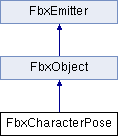
\includegraphics[height=3.000000cm]{class_fbx_character_pose}
\end{center}
\end{figure}
\subsection*{公開メンバ関数}
\begin{DoxyCompactItemize}
\item 
void \hyperlink{class_fbx_character_pose_ab0aa178aa39799fae44ef3837dfcc9bf}{Reset} ()
\begin{DoxyCompactList}\small\item\em Reset to an empty character pose. \end{DoxyCompactList}\item 
\hyperlink{class_fbx_node}{Fbx\+Node} $\ast$ \hyperlink{class_fbx_character_pose_a7dd8f39dcef2c74844a3d367a67a681b}{Get\+Root\+Node} () const
\item 
\hyperlink{class_fbx_character}{Fbx\+Character} $\ast$ \hyperlink{class_fbx_character_pose_ac0429f7f15902a3eeb0c50e890529cde}{Get\+Character} () const
\item 
bool \hyperlink{class_fbx_character_pose_a0abc45efdccf78de0b736232bb85e106}{Get\+Offset} (\hyperlink{class_fbx_character_ad75bf42026e435ac0ff4d7ece2317be4}{Fbx\+Character\+::\+E\+Node\+Id} p\+Character\+Node\+Id, \hyperlink{class_fbx_a_matrix}{Fbx\+A\+Matrix} \&p\+Offset) const
\item 
bool \hyperlink{class_fbx_character_pose_ab258febbc8198b6687eaef43654909c5}{Get\+Local\+Position} (\hyperlink{class_fbx_character_ad75bf42026e435ac0ff4d7ece2317be4}{Fbx\+Character\+::\+E\+Node\+Id} p\+Character\+Node\+Id, \hyperlink{class_fbx_vector4}{Fbx\+Vector4} \&p\+LocalT, \hyperlink{class_fbx_vector4}{Fbx\+Vector4} \&p\+LocalR, \hyperlink{class_fbx_vector4}{Fbx\+Vector4} \&p\+LocalS) const
\item 
bool \hyperlink{class_fbx_character_pose_abe05a6239a8a3e436a3e4d28ccde5499}{Get\+Global\+Position} (\hyperlink{class_fbx_character_ad75bf42026e435ac0ff4d7ece2317be4}{Fbx\+Character\+::\+E\+Node\+Id} p\+Character\+Node\+Id, \hyperlink{class_fbx_a_matrix}{Fbx\+A\+Matrix} \&p\+Global\+Position) const
\item 
\hyperlink{class_fbx_scene}{Fbx\+Scene} $\ast$ \hyperlink{class_fbx_character_pose_a7176bff4eda08a17158ec2f0850eb39a}{Get\+Pose\+Scene} () const
\item 
virtual \hyperlink{class_fbx_object}{Fbx\+Object} \& \hyperlink{class_fbx_character_pose_a7d4ac33deebb7bbfef01f3b6ba3b3cff}{Copy} (const \hyperlink{class_fbx_object}{Fbx\+Object} \&p\+Object)
\item 
virtual \hyperlink{class_fbx_object}{Fbx\+Object} $\ast$ \hyperlink{class_fbx_character_pose_af191f8d48c8f11e795adcb92adae35c5}{Clone} (\hyperlink{class_fbx_object_a9f5626b2d2135684d6ea1e6e4ad2acbb}{Fbx\+Object\+::\+E\+Clone\+Type} p\+Clone\+Type=\hyperlink{class_fbx_object_a9f5626b2d2135684d6ea1e6e4ad2acbbaacdf137ca059c572798287e98c4236d0}{e\+Deep\+Clone}, \hyperlink{class_fbx_object}{Fbx\+Object} $\ast$p\+Container=\hyperlink{fbxarch_8h_a070d2ce7b6bb7e5c05602aa8c308d0c4}{N\+U\+LL}, void $\ast$p\+Set=\hyperlink{fbxarch_8h_a070d2ce7b6bb7e5c05602aa8c308d0c4}{N\+U\+LL}) const
\item 
void \hyperlink{class_fbx_character_pose_ac7f229efcac9268afb0e37540a29a08d}{Clone} (\hyperlink{class_fbx_scene}{Fbx\+Scene} $\ast$p\+Pose\+Scene, \hyperlink{class_fbx_object_a9f5626b2d2135684d6ea1e6e4ad2acbb}{Fbx\+Object\+::\+E\+Clone\+Type} p\+Clone\+Type=\hyperlink{class_fbx_object_a9f5626b2d2135684d6ea1e6e4ad2acbbaacdf137ca059c572798287e98c4236d0}{e\+Deep\+Clone}, \hyperlink{class_fbx_object}{Fbx\+Object} $\ast$p\+Container=\hyperlink{fbxarch_8h_a070d2ce7b6bb7e5c05602aa8c308d0c4}{N\+U\+LL}, void $\ast$p\+Set=\hyperlink{fbxarch_8h_a070d2ce7b6bb7e5c05602aa8c308d0c4}{N\+U\+LL})
\end{DoxyCompactItemize}
\subsection*{限定公開メンバ関数}
\begin{DoxyCompactItemize}
\item 
virtual void \hyperlink{class_fbx_character_pose_a9da449d510900348679190d90deb5a8a}{Construct} (const \hyperlink{class_fbx_object}{Fbx\+Object} $\ast$p\+From)
\item 
virtual void \hyperlink{class_fbx_character_pose_a81243ac4049bf44a94dcfee8639a03f0}{Destruct} (bool p\+Recursive)
\end{DoxyCompactItemize}
\subsection*{その他の継承メンバ}


\subsection{詳解}
A character pose is a character and an associated hierarchy of nodes. 

Only the default position of the nodes is considered, the animation data is ignored.

You can access the content of a character pose, using the functions \hyperlink{class_fbx_character_pose_a0abc45efdccf78de0b736232bb85e106}{Fbx\+Character\+Pose\+::\+Get\+Offset()}, \hyperlink{class_fbx_character_pose_ab258febbc8198b6687eaef43654909c5}{Fbx\+Character\+Pose\+::\+Get\+Local\+Position()}, and \hyperlink{class_fbx_character_pose_abe05a6239a8a3e436a3e4d28ccde5499}{Fbx\+Character\+Pose\+::\+Get\+Global\+Position()}. Their source code is provided inline as examples on how to access the character pose data.

To create a character pose, You must first create a hierarchy of nodes under the root node provided by function \hyperlink{class_fbx_character_pose_a7dd8f39dcef2c74844a3d367a67a681b}{Fbx\+Character\+Pose\+::\+Get\+Root\+Node()}. Then, feed this hierarchy of nodes into the character returned by function \hyperlink{class_fbx_character_pose_ac0429f7f15902a3eeb0c50e890529cde}{Fbx\+Character\+Pose\+::\+Get\+Character()}. Offsets are set in the character links. Local positions are set using Fbx\+Node\+::\+Set\+Default\+T(), Fbx\+Node\+::\+Set\+Default\+R(), and Fbx\+Node\+::\+Set\+Default\+S().

To set local positions from global positions\+:
\begin{DoxyEnumerate}
\item Declare l\+Character\+Pose as a valid pointer to a \hyperlink{class_fbx_character_pose}{Fbx\+Character\+Pose};
\item Call l\+Character\+Pose-\/$>$\hyperlink{class_fbx_character_pose_a7dd8f39dcef2c74844a3d367a67a681b}{Get\+Root\+Node()}-\/$>$Set\+Local\+State\+Id(0, true);
\item Call l\+Character\+Pose-\/$>$\hyperlink{class_fbx_character_pose_a7dd8f39dcef2c74844a3d367a67a681b}{Get\+Root\+Node()}-\/$>$Set\+Global\+State\+Id(1, true);
\item Call Fbx\+Node\+::\+Set\+Global\+State() for all nodes found in the hierarchy under l\+Character\+Pose-\/$>$\hyperlink{class_fbx_character_pose_a7dd8f39dcef2c74844a3d367a67a681b}{Get\+Root\+Node()};
\item Call l\+Character\+Pose-\/$>$\hyperlink{class_fbx_character_pose_a7dd8f39dcef2c74844a3d367a67a681b}{Get\+Root\+Node()}-\/$>$Compute\+Local\+State(1, true);
\item Call l\+Character\+Pose-\/$>$\hyperlink{class_fbx_character_pose_a7dd8f39dcef2c74844a3d367a67a681b}{Get\+Root\+Node()}-\/$>$Set\+Current\+Take\+From\+Local\+State(\+F\+B\+X\+S\+D\+K\+\_\+\+T\+I\+M\+E\+\_\+\+Z\+E\+R\+O, true). 
\end{DoxyEnumerate}

 fbxcharacterpose.\+h の 48 行目に定義があります。



\subsection{関数詳解}
\mbox{\Hypertarget{class_fbx_character_pose_af191f8d48c8f11e795adcb92adae35c5}\label{class_fbx_character_pose_af191f8d48c8f11e795adcb92adae35c5}} 
\index{Fbx\+Character\+Pose@{Fbx\+Character\+Pose}!Clone@{Clone}}
\index{Clone@{Clone}!Fbx\+Character\+Pose@{Fbx\+Character\+Pose}}
\subsubsection{\texorpdfstring{Clone()}{Clone()}\hspace{0.1cm}{\footnotesize\ttfamily [1/2]}}
{\footnotesize\ttfamily virtual \hyperlink{class_fbx_object}{Fbx\+Object}$\ast$ Fbx\+Character\+Pose\+::\+Clone (\begin{DoxyParamCaption}\item[{\hyperlink{class_fbx_object_a9f5626b2d2135684d6ea1e6e4ad2acbb}{Fbx\+Object\+::\+E\+Clone\+Type}}]{p\+Clone\+Type = {\ttfamily \hyperlink{class_fbx_object_a9f5626b2d2135684d6ea1e6e4ad2acbbaacdf137ca059c572798287e98c4236d0}{e\+Deep\+Clone}},  }\item[{\hyperlink{class_fbx_object}{Fbx\+Object} $\ast$}]{p\+Container = {\ttfamily \hyperlink{fbxarch_8h_a070d2ce7b6bb7e5c05602aa8c308d0c4}{N\+U\+LL}},  }\item[{void $\ast$}]{p\+Set = {\ttfamily \hyperlink{fbxarch_8h_a070d2ce7b6bb7e5c05602aa8c308d0c4}{N\+U\+LL}} }\end{DoxyParamCaption}) const\hspace{0.3cm}{\ttfamily [virtual]}}

Creates a clone of this object. By default, the connections are N\+OT cloned. If the desired effect is to clone the connections as well, you must clone using the \hyperlink{class_fbx_clone_manager}{Fbx\+Clone\+Manager} (refer to this class documentation for further details).


\begin{DoxyParams}{引数}
{\em p\+Clone\+Type} & The type of clone to be created. By default, the clone type is e\+Deep\+Clone. \\
\hline
{\em p\+Container} & An optional parameter to specify which object will \char`\"{}contain\char`\"{} the new object. By contain, we mean the new object will become a source to the container, connection-\/wise. \\
\hline
{\em p\+Set} & See remark section. \\
\hline
\end{DoxyParams}
\begin{DoxyReturn}{戻り値}
The new clone, or N\+U\+LL (if the specified clone type is not supported). 
\end{DoxyReturn}
\begin{DoxyRemark}{注釈}
When doing either a \char`\"{}deep\char`\"{} or \char`\"{}reference\char`\"{} clone type, the clone will always get its properties values set from the source object properties values. 

Since this is a virtual function, some classes might do additional tasks. 

The {\itshape p\+Set} argument is not used in the default implementation of this method. Specialized implementations should cast this pointer to \hyperlink{class_fbx_clone_manager_aeb8a9c04c9c36eb7e551186a0b18f10d}{Fbx\+Clone\+Manager\+::\+Clone\+Set} to have access to the cloned objects so far. Typically, this pointer is set by the clone manager. 
\end{DoxyRemark}


\hyperlink{class_fbx_object_ad553a4262b09cb57c3171a93edadbab8}{Fbx\+Object}を再実装しています。

\mbox{\Hypertarget{class_fbx_character_pose_ac7f229efcac9268afb0e37540a29a08d}\label{class_fbx_character_pose_ac7f229efcac9268afb0e37540a29a08d}} 
\index{Fbx\+Character\+Pose@{Fbx\+Character\+Pose}!Clone@{Clone}}
\index{Clone@{Clone}!Fbx\+Character\+Pose@{Fbx\+Character\+Pose}}
\subsubsection{\texorpdfstring{Clone()}{Clone()}\hspace{0.1cm}{\footnotesize\ttfamily [2/2]}}
{\footnotesize\ttfamily void Fbx\+Character\+Pose\+::\+Clone (\begin{DoxyParamCaption}\item[{\hyperlink{class_fbx_scene}{Fbx\+Scene} $\ast$}]{p\+Pose\+Scene,  }\item[{\hyperlink{class_fbx_object_a9f5626b2d2135684d6ea1e6e4ad2acbb}{Fbx\+Object\+::\+E\+Clone\+Type}}]{p\+Clone\+Type = {\ttfamily \hyperlink{class_fbx_object_a9f5626b2d2135684d6ea1e6e4ad2acbbaacdf137ca059c572798287e98c4236d0}{e\+Deep\+Clone}},  }\item[{\hyperlink{class_fbx_object}{Fbx\+Object} $\ast$}]{p\+Container = {\ttfamily \hyperlink{fbxarch_8h_a070d2ce7b6bb7e5c05602aa8c308d0c4}{N\+U\+LL}},  }\item[{void $\ast$}]{p\+Set = {\ttfamily \hyperlink{fbxarch_8h_a070d2ce7b6bb7e5c05602aa8c308d0c4}{N\+U\+LL}} }\end{DoxyParamCaption})}

\mbox{\Hypertarget{class_fbx_character_pose_a9da449d510900348679190d90deb5a8a}\label{class_fbx_character_pose_a9da449d510900348679190d90deb5a8a}} 
\index{Fbx\+Character\+Pose@{Fbx\+Character\+Pose}!Construct@{Construct}}
\index{Construct@{Construct}!Fbx\+Character\+Pose@{Fbx\+Character\+Pose}}
\subsubsection{\texorpdfstring{Construct()}{Construct()}}
{\footnotesize\ttfamily virtual void Fbx\+Character\+Pose\+::\+Construct (\begin{DoxyParamCaption}\item[{const \hyperlink{class_fbx_object}{Fbx\+Object} $\ast$}]{p\+From }\end{DoxyParamCaption})\hspace{0.3cm}{\ttfamily [protected]}, {\ttfamily [virtual]}}

Optional constructor override, automatically called by default constructor. 
\begin{DoxyParams}{引数}
{\em p\+From} & If not null, the function must take it into account like a copy constructor. \\
\hline
\end{DoxyParams}
\begin{DoxyRemark}{注釈}
In case it is decided to override this function, do not forget to call Parent\+Class\+::\+Construct(p\+From) at the beginning. 
\end{DoxyRemark}


\hyperlink{class_fbx_object_a313503bc645af3fdceb4a99ef5cea7eb}{Fbx\+Object}を再実装しています。

\mbox{\Hypertarget{class_fbx_character_pose_a7d4ac33deebb7bbfef01f3b6ba3b3cff}\label{class_fbx_character_pose_a7d4ac33deebb7bbfef01f3b6ba3b3cff}} 
\index{Fbx\+Character\+Pose@{Fbx\+Character\+Pose}!Copy@{Copy}}
\index{Copy@{Copy}!Fbx\+Character\+Pose@{Fbx\+Character\+Pose}}
\subsubsection{\texorpdfstring{Copy()}{Copy()}}
{\footnotesize\ttfamily virtual \hyperlink{class_fbx_object}{Fbx\+Object}\& Fbx\+Character\+Pose\+::\+Copy (\begin{DoxyParamCaption}\item[{const \hyperlink{class_fbx_object}{Fbx\+Object} \&}]{p\+Object }\end{DoxyParamCaption})\hspace{0.3cm}{\ttfamily [virtual]}}

Copy an object content into this object. 
\begin{DoxyParams}{引数}
{\em p\+Object} & The source object to copy data from. \\
\hline
\end{DoxyParams}
\begin{DoxyReturn}{戻り値}
Returns the destination object being modified by the source. 
\end{DoxyReturn}
\begin{DoxyRemark}{注釈}
This function replace the assignment operator (operator=). It will copy all property values and the name. Connections are N\+OT copied. 
\end{DoxyRemark}


\hyperlink{class_fbx_object_a0c0c5adb38284d14bb82c04d54504a3e}{Fbx\+Object}を再実装しています。

\mbox{\Hypertarget{class_fbx_character_pose_a81243ac4049bf44a94dcfee8639a03f0}\label{class_fbx_character_pose_a81243ac4049bf44a94dcfee8639a03f0}} 
\index{Fbx\+Character\+Pose@{Fbx\+Character\+Pose}!Destruct@{Destruct}}
\index{Destruct@{Destruct}!Fbx\+Character\+Pose@{Fbx\+Character\+Pose}}
\subsubsection{\texorpdfstring{Destruct()}{Destruct()}}
{\footnotesize\ttfamily virtual void Fbx\+Character\+Pose\+::\+Destruct (\begin{DoxyParamCaption}\item[{bool}]{p\+Recursive }\end{DoxyParamCaption})\hspace{0.3cm}{\ttfamily [protected]}, {\ttfamily [virtual]}}

Optional destructor override, automatically called by default destructor. 
\begin{DoxyParams}{引数}
{\em p\+Recursive} & If true, children objects should be destroyed as well. \\
\hline
\end{DoxyParams}
\begin{DoxyRemark}{注釈}
In case it is decided to override this function, do not forget to call Parent\+Class\+::\+Destruct(p\+Resursive) at the end. 
\end{DoxyRemark}


\hyperlink{class_fbx_object_a123e084d9b32b29c28af6384b7c3c608}{Fbx\+Object}を再実装しています。

\mbox{\Hypertarget{class_fbx_character_pose_ac0429f7f15902a3eeb0c50e890529cde}\label{class_fbx_character_pose_ac0429f7f15902a3eeb0c50e890529cde}} 
\index{Fbx\+Character\+Pose@{Fbx\+Character\+Pose}!Get\+Character@{Get\+Character}}
\index{Get\+Character@{Get\+Character}!Fbx\+Character\+Pose@{Fbx\+Character\+Pose}}
\subsubsection{\texorpdfstring{Get\+Character()}{GetCharacter()}}
{\footnotesize\ttfamily \hyperlink{class_fbx_character}{Fbx\+Character}$\ast$ Fbx\+Character\+Pose\+::\+Get\+Character (\begin{DoxyParamCaption}{ }\end{DoxyParamCaption}) const}

Get the character. \begin{DoxyReturn}{戻り値}
Pointer to the character. 
\end{DoxyReturn}
\mbox{\Hypertarget{class_fbx_character_pose_abe05a6239a8a3e436a3e4d28ccde5499}\label{class_fbx_character_pose_abe05a6239a8a3e436a3e4d28ccde5499}} 
\index{Fbx\+Character\+Pose@{Fbx\+Character\+Pose}!Get\+Global\+Position@{Get\+Global\+Position}}
\index{Get\+Global\+Position@{Get\+Global\+Position}!Fbx\+Character\+Pose@{Fbx\+Character\+Pose}}
\subsubsection{\texorpdfstring{Get\+Global\+Position()}{GetGlobalPosition()}}
{\footnotesize\ttfamily bool Fbx\+Character\+Pose\+::\+Get\+Global\+Position (\begin{DoxyParamCaption}\item[{\hyperlink{class_fbx_character_ad75bf42026e435ac0ff4d7ece2317be4}{Fbx\+Character\+::\+E\+Node\+Id}}]{p\+Character\+Node\+Id,  }\item[{\hyperlink{class_fbx_a_matrix}{Fbx\+A\+Matrix} \&}]{p\+Global\+Position }\end{DoxyParamCaption}) const}

Get global position for a given character node. 
\begin{DoxyParams}{引数}
{\em p\+Character\+Node\+Id} & Character Node ID. \\
\hline
{\em p\+Global\+Position} & Receives global position. \\
\hline
\end{DoxyParams}
\begin{DoxyReturn}{戻り値}
{\ttfamily true} if successful, {\ttfamily false} otherwise. 
\end{DoxyReturn}
\mbox{\Hypertarget{class_fbx_character_pose_ab258febbc8198b6687eaef43654909c5}\label{class_fbx_character_pose_ab258febbc8198b6687eaef43654909c5}} 
\index{Fbx\+Character\+Pose@{Fbx\+Character\+Pose}!Get\+Local\+Position@{Get\+Local\+Position}}
\index{Get\+Local\+Position@{Get\+Local\+Position}!Fbx\+Character\+Pose@{Fbx\+Character\+Pose}}
\subsubsection{\texorpdfstring{Get\+Local\+Position()}{GetLocalPosition()}}
{\footnotesize\ttfamily bool Fbx\+Character\+Pose\+::\+Get\+Local\+Position (\begin{DoxyParamCaption}\item[{\hyperlink{class_fbx_character_ad75bf42026e435ac0ff4d7ece2317be4}{Fbx\+Character\+::\+E\+Node\+Id}}]{p\+Character\+Node\+Id,  }\item[{\hyperlink{class_fbx_vector4}{Fbx\+Vector4} \&}]{p\+LocalT,  }\item[{\hyperlink{class_fbx_vector4}{Fbx\+Vector4} \&}]{p\+LocalR,  }\item[{\hyperlink{class_fbx_vector4}{Fbx\+Vector4} \&}]{p\+LocalS }\end{DoxyParamCaption}) const}

Get local position for a given character node. 
\begin{DoxyParams}{引数}
{\em p\+Character\+Node\+Id} & Character Node ID. \\
\hline
{\em p\+LocalT} & Receives local translation vector. \\
\hline
{\em p\+LocalR} & Receives local rotation vector. \\
\hline
{\em p\+LocalS} & Receives local scaling vector. \\
\hline
\end{DoxyParams}
\begin{DoxyReturn}{戻り値}
{\ttfamily true} if successful, {\ttfamily false} otherwise. 
\end{DoxyReturn}
\mbox{\Hypertarget{class_fbx_character_pose_a0abc45efdccf78de0b736232bb85e106}\label{class_fbx_character_pose_a0abc45efdccf78de0b736232bb85e106}} 
\index{Fbx\+Character\+Pose@{Fbx\+Character\+Pose}!Get\+Offset@{Get\+Offset}}
\index{Get\+Offset@{Get\+Offset}!Fbx\+Character\+Pose@{Fbx\+Character\+Pose}}
\subsubsection{\texorpdfstring{Get\+Offset()}{GetOffset()}}
{\footnotesize\ttfamily bool Fbx\+Character\+Pose\+::\+Get\+Offset (\begin{DoxyParamCaption}\item[{\hyperlink{class_fbx_character_ad75bf42026e435ac0ff4d7ece2317be4}{Fbx\+Character\+::\+E\+Node\+Id}}]{p\+Character\+Node\+Id,  }\item[{\hyperlink{class_fbx_a_matrix}{Fbx\+A\+Matrix} \&}]{p\+Offset }\end{DoxyParamCaption}) const}

Get offset matrix for a given character node. 
\begin{DoxyParams}{引数}
{\em p\+Character\+Node\+Id} & Character Node ID. \\
\hline
{\em p\+Offset} & Receives offset matrix. \\
\hline
\end{DoxyParams}
\begin{DoxyReturn}{戻り値}
{\ttfamily true} if successful, {\ttfamily false} otherwise. 
\end{DoxyReturn}
\mbox{\Hypertarget{class_fbx_character_pose_a7176bff4eda08a17158ec2f0850eb39a}\label{class_fbx_character_pose_a7176bff4eda08a17158ec2f0850eb39a}} 
\index{Fbx\+Character\+Pose@{Fbx\+Character\+Pose}!Get\+Pose\+Scene@{Get\+Pose\+Scene}}
\index{Get\+Pose\+Scene@{Get\+Pose\+Scene}!Fbx\+Character\+Pose@{Fbx\+Character\+Pose}}
\subsubsection{\texorpdfstring{Get\+Pose\+Scene()}{GetPoseScene()}}
{\footnotesize\ttfamily \hyperlink{class_fbx_scene}{Fbx\+Scene}$\ast$ Fbx\+Character\+Pose\+::\+Get\+Pose\+Scene (\begin{DoxyParamCaption}{ }\end{DoxyParamCaption}) const}

Retrieve the pose scene used by this character pose \begin{DoxyReturn}{戻り値}
The pose\textquotesingle{}s scene (this is a different scene than the scene the character pose is in). 
\end{DoxyReturn}
\mbox{\Hypertarget{class_fbx_character_pose_a7dd8f39dcef2c74844a3d367a67a681b}\label{class_fbx_character_pose_a7dd8f39dcef2c74844a3d367a67a681b}} 
\index{Fbx\+Character\+Pose@{Fbx\+Character\+Pose}!Get\+Root\+Node@{Get\+Root\+Node}}
\index{Get\+Root\+Node@{Get\+Root\+Node}!Fbx\+Character\+Pose@{Fbx\+Character\+Pose}}
\subsubsection{\texorpdfstring{Get\+Root\+Node()}{GetRootNode()}}
{\footnotesize\ttfamily \hyperlink{class_fbx_node}{Fbx\+Node}$\ast$ Fbx\+Character\+Pose\+::\+Get\+Root\+Node (\begin{DoxyParamCaption}{ }\end{DoxyParamCaption}) const}

Get the root node. \begin{DoxyReturn}{戻り値}
Pointer to the root node. 
\end{DoxyReturn}
\mbox{\Hypertarget{class_fbx_character_pose_ab0aa178aa39799fae44ef3837dfcc9bf}\label{class_fbx_character_pose_ab0aa178aa39799fae44ef3837dfcc9bf}} 
\index{Fbx\+Character\+Pose@{Fbx\+Character\+Pose}!Reset@{Reset}}
\index{Reset@{Reset}!Fbx\+Character\+Pose@{Fbx\+Character\+Pose}}
\subsubsection{\texorpdfstring{Reset()}{Reset()}}
{\footnotesize\ttfamily void Fbx\+Character\+Pose\+::\+Reset (\begin{DoxyParamCaption}{ }\end{DoxyParamCaption})}



Reset to an empty character pose. 



このクラス詳解は次のファイルから抽出されました\+:\begin{DoxyCompactItemize}
\item 
C\+:/\+Maya/scripts/\+F\+B\+X\+\_\+\+S\+D\+K/2017.\+1/include/fbxsdk/scene/constraint/\hyperlink{fbxcharacterpose_8h}{fbxcharacterpose.\+h}\end{DoxyCompactItemize}

\hypertarget{class_fbx_character_property_info}{}\section{Fbx\+Character\+Property\+Info クラス}
\label{class_fbx_character_property_info}\index{Fbx\+Character\+Property\+Info@{Fbx\+Character\+Property\+Info}}


{\ttfamily \#include $<$fbxhik2fbxcharacter.\+h$>$}

\subsection*{公開変数類}
\begin{DoxyCompactItemize}
\item 
const char $\ast$ \hyperlink{class_fbx_character_property_info_a8d6a7c9e15c0944ddaff38b20d3c5bb8}{m\+H\+I\+K\+Property\+Name}
\item 
const char $\ast$ \hyperlink{class_fbx_character_property_info_aaebf44fac9acc7d36352077a50345761}{m\+Fbx\+Character\+Property\+Mode\+Name}
\item 
const char $\ast$ \hyperlink{class_fbx_character_property_info_a0f8c79a2e71440c4cbc4ce1ef5f6eef7}{m\+Fbx\+Character\+Property\+Name}
\item 
int \hyperlink{class_fbx_character_property_info_a62c37badd98e865a666616e877d2ff49}{m\+Index}
\item 
\hyperlink{class_fbx_character_aa48fb13a1c63e6a69ce9fa251993f8d5}{Fbx\+Character\+::\+E\+Property\+Unit} \hyperlink{class_fbx_character_property_info_ad22617f1c6c63b559f7da55af1519086}{m\+Unit}
\end{DoxyCompactItemize}


\subsection{詳解}


 fbxhik2fbxcharacter.\+h の 22 行目に定義があります。



\subsection{メンバ詳解}
\mbox{\Hypertarget{class_fbx_character_property_info_aaebf44fac9acc7d36352077a50345761}\label{class_fbx_character_property_info_aaebf44fac9acc7d36352077a50345761}} 
\index{Fbx\+Character\+Property\+Info@{Fbx\+Character\+Property\+Info}!m\+Fbx\+Character\+Property\+Mode\+Name@{m\+Fbx\+Character\+Property\+Mode\+Name}}
\index{m\+Fbx\+Character\+Property\+Mode\+Name@{m\+Fbx\+Character\+Property\+Mode\+Name}!Fbx\+Character\+Property\+Info@{Fbx\+Character\+Property\+Info}}
\subsubsection{\texorpdfstring{m\+Fbx\+Character\+Property\+Mode\+Name}{mFbxCharacterPropertyModeName}}
{\footnotesize\ttfamily const char$\ast$ Fbx\+Character\+Property\+Info\+::m\+Fbx\+Character\+Property\+Mode\+Name}



 fbxhik2fbxcharacter.\+h の 26 行目に定義があります。

\mbox{\Hypertarget{class_fbx_character_property_info_a0f8c79a2e71440c4cbc4ce1ef5f6eef7}\label{class_fbx_character_property_info_a0f8c79a2e71440c4cbc4ce1ef5f6eef7}} 
\index{Fbx\+Character\+Property\+Info@{Fbx\+Character\+Property\+Info}!m\+Fbx\+Character\+Property\+Name@{m\+Fbx\+Character\+Property\+Name}}
\index{m\+Fbx\+Character\+Property\+Name@{m\+Fbx\+Character\+Property\+Name}!Fbx\+Character\+Property\+Info@{Fbx\+Character\+Property\+Info}}
\subsubsection{\texorpdfstring{m\+Fbx\+Character\+Property\+Name}{mFbxCharacterPropertyName}}
{\footnotesize\ttfamily const char$\ast$ Fbx\+Character\+Property\+Info\+::m\+Fbx\+Character\+Property\+Name}



 fbxhik2fbxcharacter.\+h の 27 行目に定義があります。

\mbox{\Hypertarget{class_fbx_character_property_info_a8d6a7c9e15c0944ddaff38b20d3c5bb8}\label{class_fbx_character_property_info_a8d6a7c9e15c0944ddaff38b20d3c5bb8}} 
\index{Fbx\+Character\+Property\+Info@{Fbx\+Character\+Property\+Info}!m\+H\+I\+K\+Property\+Name@{m\+H\+I\+K\+Property\+Name}}
\index{m\+H\+I\+K\+Property\+Name@{m\+H\+I\+K\+Property\+Name}!Fbx\+Character\+Property\+Info@{Fbx\+Character\+Property\+Info}}
\subsubsection{\texorpdfstring{m\+H\+I\+K\+Property\+Name}{mHIKPropertyName}}
{\footnotesize\ttfamily const char$\ast$ Fbx\+Character\+Property\+Info\+::m\+H\+I\+K\+Property\+Name}



 fbxhik2fbxcharacter.\+h の 25 行目に定義があります。

\mbox{\Hypertarget{class_fbx_character_property_info_a62c37badd98e865a666616e877d2ff49}\label{class_fbx_character_property_info_a62c37badd98e865a666616e877d2ff49}} 
\index{Fbx\+Character\+Property\+Info@{Fbx\+Character\+Property\+Info}!m\+Index@{m\+Index}}
\index{m\+Index@{m\+Index}!Fbx\+Character\+Property\+Info@{Fbx\+Character\+Property\+Info}}
\subsubsection{\texorpdfstring{m\+Index}{mIndex}}
{\footnotesize\ttfamily int Fbx\+Character\+Property\+Info\+::m\+Index}



 fbxhik2fbxcharacter.\+h の 28 行目に定義があります。

\mbox{\Hypertarget{class_fbx_character_property_info_ad22617f1c6c63b559f7da55af1519086}\label{class_fbx_character_property_info_ad22617f1c6c63b559f7da55af1519086}} 
\index{Fbx\+Character\+Property\+Info@{Fbx\+Character\+Property\+Info}!m\+Unit@{m\+Unit}}
\index{m\+Unit@{m\+Unit}!Fbx\+Character\+Property\+Info@{Fbx\+Character\+Property\+Info}}
\subsubsection{\texorpdfstring{m\+Unit}{mUnit}}
{\footnotesize\ttfamily \hyperlink{class_fbx_character_aa48fb13a1c63e6a69ce9fa251993f8d5}{Fbx\+Character\+::\+E\+Property\+Unit} Fbx\+Character\+Property\+Info\+::m\+Unit}



 fbxhik2fbxcharacter.\+h の 29 行目に定義があります。



このクラス詳解は次のファイルから抽出されました\+:\begin{DoxyCompactItemize}
\item 
C\+:/\+Maya/scripts/\+F\+B\+X\+\_\+\+S\+D\+K/2017.\+1/include/fbxsdk/scene/constraint/\hyperlink{fbxhik2fbxcharacter_8h}{fbxhik2fbxcharacter.\+h}\end{DoxyCompactItemize}

\hypertarget{struct_fbx_char_ptr_compare}{}\section{Fbx\+Char\+Ptr\+Compare 構造体}
\label{struct_fbx_char_ptr_compare}\index{Fbx\+Char\+Ptr\+Compare@{Fbx\+Char\+Ptr\+Compare}}


Functor to compare \char`\"{}\+C\char`\"{} strings  




{\ttfamily \#include $<$fbxstring.\+h$>$}

\subsection*{公開メンバ関数}
\begin{DoxyCompactItemize}
\item 
int \hyperlink{struct_fbx_char_ptr_compare_a5806b2dabf3997394fe7db69526e876d}{operator()} (const char $\ast$p\+KeyA, const char $\ast$p\+KeyB) const
\end{DoxyCompactItemize}


\subsection{詳解}
Functor to compare \char`\"{}\+C\char`\"{} strings 

 fbxstring.\+h の 484 行目に定義があります。



\subsection{関数詳解}
\mbox{\Hypertarget{struct_fbx_char_ptr_compare_a5806b2dabf3997394fe7db69526e876d}\label{struct_fbx_char_ptr_compare_a5806b2dabf3997394fe7db69526e876d}} 
\index{Fbx\+Char\+Ptr\+Compare@{Fbx\+Char\+Ptr\+Compare}!operator()@{operator()}}
\index{operator()@{operator()}!Fbx\+Char\+Ptr\+Compare@{Fbx\+Char\+Ptr\+Compare}}
\subsubsection{\texorpdfstring{operator()()}{operator()()}}
{\footnotesize\ttfamily int Fbx\+Char\+Ptr\+Compare\+::operator() (\begin{DoxyParamCaption}\item[{const char $\ast$}]{p\+KeyA,  }\item[{const char $\ast$}]{p\+KeyB }\end{DoxyParamCaption}) const\hspace{0.3cm}{\ttfamily [inline]}}



 fbxstring.\+h の 484 行目に定義があります。



この構造体詳解は次のファイルから抽出されました\+:\begin{DoxyCompactItemize}
\item 
C\+:/\+Maya/scripts/\+F\+B\+X\+\_\+\+S\+D\+K/2017.\+1/include/fbxsdk/core/base/\hyperlink{fbxstring_8h}{fbxstring.\+h}\end{DoxyCompactItemize}

\hypertarget{struct_fbx_char_ptr_compare_no_case}{}\section{Fbx\+Char\+Ptr\+Compare\+No\+Case 構造体}
\label{struct_fbx_char_ptr_compare_no_case}\index{Fbx\+Char\+Ptr\+Compare\+No\+Case@{Fbx\+Char\+Ptr\+Compare\+No\+Case}}


Functor to compare \char`\"{}\+C\char`\"{} strings without case sensitivity  




{\ttfamily \#include $<$fbxstring.\+h$>$}

\subsection*{公開メンバ関数}
\begin{DoxyCompactItemize}
\item 
int \hyperlink{struct_fbx_char_ptr_compare_no_case_a23d4e5b52cb08b712b8f5a72f659bccc}{operator()} (const char $\ast$p\+KeyA, const char $\ast$p\+KeyB) const
\end{DoxyCompactItemize}


\subsection{詳解}
Functor to compare \char`\"{}\+C\char`\"{} strings without case sensitivity 

 fbxstring.\+h の 487 行目に定義があります。



\subsection{関数詳解}
\mbox{\Hypertarget{struct_fbx_char_ptr_compare_no_case_a23d4e5b52cb08b712b8f5a72f659bccc}\label{struct_fbx_char_ptr_compare_no_case_a23d4e5b52cb08b712b8f5a72f659bccc}} 
\index{Fbx\+Char\+Ptr\+Compare\+No\+Case@{Fbx\+Char\+Ptr\+Compare\+No\+Case}!operator()@{operator()}}
\index{operator()@{operator()}!Fbx\+Char\+Ptr\+Compare\+No\+Case@{Fbx\+Char\+Ptr\+Compare\+No\+Case}}
\subsubsection{\texorpdfstring{operator()()}{operator()()}}
{\footnotesize\ttfamily int Fbx\+Char\+Ptr\+Compare\+No\+Case\+::operator() (\begin{DoxyParamCaption}\item[{const char $\ast$}]{p\+KeyA,  }\item[{const char $\ast$}]{p\+KeyB }\end{DoxyParamCaption}) const\hspace{0.3cm}{\ttfamily [inline]}}



 fbxstring.\+h の 487 行目に定義があります。



この構造体詳解は次のファイルから抽出されました\+:\begin{DoxyCompactItemize}
\item 
C\+:/\+Maya/scripts/\+F\+B\+X\+\_\+\+S\+D\+K/2017.\+1/include/fbxsdk/core/base/\hyperlink{fbxstring_8h}{fbxstring.\+h}\end{DoxyCompactItemize}

\hypertarget{class_fbx_char_ptr_set}{}\section{Fbx\+Char\+Ptr\+Set クラス}
\label{class_fbx_char_ptr_set}\index{Fbx\+Char\+Ptr\+Set@{Fbx\+Char\+Ptr\+Set}}


{\ttfamily \#include $<$fbxcharptrset.\+h$>$}

\subsection*{公開メンバ関数}
\begin{DoxyCompactItemize}
\item 
\hyperlink{class_fbx_char_ptr_set_a7f12f3a80a0e523ecb890aaa093c2aad}{Fbx\+Char\+Ptr\+Set} (int p\+Item\+Per\+Block=20)
\item 
\hyperlink{class_fbx_char_ptr_set_adbdbfd04a21ccc2d880de34d74f96771}{$\sim$\+Fbx\+Char\+Ptr\+Set} ()
\begin{DoxyCompactList}\small\item\em Class destructor \end{DoxyCompactList}\item 
void \hyperlink{class_fbx_char_ptr_set_a9efd684cdc4dbb93168c91fb717e89b1}{Add} (const char $\ast$p\+Reference, Fbx\+Handle p\+Item)
\item 
bool \hyperlink{class_fbx_char_ptr_set_afb7850c77043dd57c0fae1743ca01d29}{Remove} (const char $\ast$p\+Reference)
\item 
Fbx\+Handle \hyperlink{class_fbx_char_ptr_set_a626ae8a1c9406567c09755f467902b84}{Get} (const char $\ast$p\+Reference, int $\ast$P\+Index=\hyperlink{fbxarch_8h_a070d2ce7b6bb7e5c05602aa8c308d0c4}{N\+U\+LL})
\item 
Fbx\+Handle \& \hyperlink{class_fbx_char_ptr_set_a925f5012e7dd515e1d3c44584c97101d}{operator\mbox{[}$\,$\mbox{]}} (int p\+Index)
\item 
Fbx\+Handle \hyperlink{class_fbx_char_ptr_set_ab201112f7e7bbdad802978c451c41680}{Get\+From\+Index} (int p\+Index, const char $\ast$$\ast$p\+Reference=\hyperlink{fbxarch_8h_a070d2ce7b6bb7e5c05602aa8c308d0c4}{N\+U\+LL})
\item 
void \hyperlink{class_fbx_char_ptr_set_a2cfe1b7b1f73100b37decf29b3dba45e}{Remove\+From\+Index} (int p\+Index)
\item 
int \hyperlink{class_fbx_char_ptr_set_ab62ea2f88eed06e033e4ae7c516e96a0}{Get\+Count} () const
\item 
void \hyperlink{class_fbx_char_ptr_set_a54d7c3c3b927eb0040f0235b5aaff717}{Sort} ()
\begin{DoxyCompactList}\small\item\em Sorts the array. \end{DoxyCompactList}\item 
void \hyperlink{class_fbx_char_ptr_set_a868b8f961a3e3f5d4c4c5f77009e5947}{Clear} ()
\begin{DoxyCompactList}\small\item\em Clears the array. \end{DoxyCompactList}\item 
void \hyperlink{class_fbx_char_ptr_set_ad7da280af4a52c6b7aa3037fd7636f6f}{Set\+Case\+Sensitive} (bool p\+Is\+Case\+Sensitive)
\end{DoxyCompactItemize}


\subsection{詳解}
This class contains the data structure support for char pointer set. 

 fbxcharptrset.\+h の 22 行目に定義があります。



\subsection{構築子と解体子}
\mbox{\Hypertarget{class_fbx_char_ptr_set_a7f12f3a80a0e523ecb890aaa093c2aad}\label{class_fbx_char_ptr_set_a7f12f3a80a0e523ecb890aaa093c2aad}} 
\index{Fbx\+Char\+Ptr\+Set@{Fbx\+Char\+Ptr\+Set}!Fbx\+Char\+Ptr\+Set@{Fbx\+Char\+Ptr\+Set}}
\index{Fbx\+Char\+Ptr\+Set@{Fbx\+Char\+Ptr\+Set}!Fbx\+Char\+Ptr\+Set@{Fbx\+Char\+Ptr\+Set}}
\subsubsection{\texorpdfstring{Fbx\+Char\+Ptr\+Set()}{FbxCharPtrSet()}}
{\footnotesize\ttfamily Fbx\+Char\+Ptr\+Set\+::\+Fbx\+Char\+Ptr\+Set (\begin{DoxyParamCaption}\item[{int}]{p\+Item\+Per\+Block = {\ttfamily 20} }\end{DoxyParamCaption})}

Class constructor 
\begin{DoxyParams}{引数}
{\em p\+Item\+Per\+Block} & Number of item per block. Default is 20. \\
\hline
\end{DoxyParams}
\mbox{\Hypertarget{class_fbx_char_ptr_set_adbdbfd04a21ccc2d880de34d74f96771}\label{class_fbx_char_ptr_set_adbdbfd04a21ccc2d880de34d74f96771}} 
\index{Fbx\+Char\+Ptr\+Set@{Fbx\+Char\+Ptr\+Set}!````~Fbx\+Char\+Ptr\+Set@{$\sim$\+Fbx\+Char\+Ptr\+Set}}
\index{````~Fbx\+Char\+Ptr\+Set@{$\sim$\+Fbx\+Char\+Ptr\+Set}!Fbx\+Char\+Ptr\+Set@{Fbx\+Char\+Ptr\+Set}}
\subsubsection{\texorpdfstring{$\sim$\+Fbx\+Char\+Ptr\+Set()}{~FbxCharPtrSet()}}
{\footnotesize\ttfamily Fbx\+Char\+Ptr\+Set\+::$\sim$\+Fbx\+Char\+Ptr\+Set (\begin{DoxyParamCaption}{ }\end{DoxyParamCaption})}



Class destructor 



\subsection{関数詳解}
\mbox{\Hypertarget{class_fbx_char_ptr_set_a9efd684cdc4dbb93168c91fb717e89b1}\label{class_fbx_char_ptr_set_a9efd684cdc4dbb93168c91fb717e89b1}} 
\index{Fbx\+Char\+Ptr\+Set@{Fbx\+Char\+Ptr\+Set}!Add@{Add}}
\index{Add@{Add}!Fbx\+Char\+Ptr\+Set@{Fbx\+Char\+Ptr\+Set}}
\subsubsection{\texorpdfstring{Add()}{Add()}}
{\footnotesize\ttfamily void Fbx\+Char\+Ptr\+Set\+::\+Add (\begin{DoxyParamCaption}\item[{const char $\ast$}]{p\+Reference,  }\item[{Fbx\+Handle}]{p\+Item }\end{DoxyParamCaption})}

Add a new item. 
\begin{DoxyParams}{引数}
{\em p\+Reference} & char pointer reference to the item. \\
\hline
{\em p\+Item} & Fbx\+Handle to the item. \\
\hline
\end{DoxyParams}
\mbox{\Hypertarget{class_fbx_char_ptr_set_a868b8f961a3e3f5d4c4c5f77009e5947}\label{class_fbx_char_ptr_set_a868b8f961a3e3f5d4c4c5f77009e5947}} 
\index{Fbx\+Char\+Ptr\+Set@{Fbx\+Char\+Ptr\+Set}!Clear@{Clear}}
\index{Clear@{Clear}!Fbx\+Char\+Ptr\+Set@{Fbx\+Char\+Ptr\+Set}}
\subsubsection{\texorpdfstring{Clear()}{Clear()}}
{\footnotesize\ttfamily void Fbx\+Char\+Ptr\+Set\+::\+Clear (\begin{DoxyParamCaption}{ }\end{DoxyParamCaption})}



Clears the array. 

\mbox{\Hypertarget{class_fbx_char_ptr_set_a626ae8a1c9406567c09755f467902b84}\label{class_fbx_char_ptr_set_a626ae8a1c9406567c09755f467902b84}} 
\index{Fbx\+Char\+Ptr\+Set@{Fbx\+Char\+Ptr\+Set}!Get@{Get}}
\index{Get@{Get}!Fbx\+Char\+Ptr\+Set@{Fbx\+Char\+Ptr\+Set}}
\subsubsection{\texorpdfstring{Get()}{Get()}}
{\footnotesize\ttfamily Fbx\+Handle Fbx\+Char\+Ptr\+Set\+::\+Get (\begin{DoxyParamCaption}\item[{const char $\ast$}]{p\+Reference,  }\item[{int $\ast$}]{P\+Index = {\ttfamily \hyperlink{fbxarch_8h_a070d2ce7b6bb7e5c05602aa8c308d0c4}{N\+U\+LL}} }\end{DoxyParamCaption})}

Get an item\textquotesingle{}s reference. 
\begin{DoxyParams}{引数}
{\em p\+Reference} & char reference to the item. \\
\hline
{\em P\+Index} & index to the item. \\
\hline
\end{DoxyParams}
\begin{DoxyReturn}{戻り値}
Fbx\+Handle to the item, N\+U\+LL if fails. 
\end{DoxyReturn}
\mbox{\Hypertarget{class_fbx_char_ptr_set_ab62ea2f88eed06e033e4ae7c516e96a0}\label{class_fbx_char_ptr_set_ab62ea2f88eed06e033e4ae7c516e96a0}} 
\index{Fbx\+Char\+Ptr\+Set@{Fbx\+Char\+Ptr\+Set}!Get\+Count@{Get\+Count}}
\index{Get\+Count@{Get\+Count}!Fbx\+Char\+Ptr\+Set@{Fbx\+Char\+Ptr\+Set}}
\subsubsection{\texorpdfstring{Get\+Count()}{GetCount()}}
{\footnotesize\ttfamily int Fbx\+Char\+Ptr\+Set\+::\+Get\+Count (\begin{DoxyParamCaption}{ }\end{DoxyParamCaption}) const\hspace{0.3cm}{\ttfamily [inline]}}

Get the number of item in the array. \begin{DoxyReturn}{戻り値}
the number of element in the set. 
\end{DoxyReturn}


 fbxcharptrset.\+h の 65 行目に定義があります。

\mbox{\Hypertarget{class_fbx_char_ptr_set_ab201112f7e7bbdad802978c451c41680}\label{class_fbx_char_ptr_set_ab201112f7e7bbdad802978c451c41680}} 
\index{Fbx\+Char\+Ptr\+Set@{Fbx\+Char\+Ptr\+Set}!Get\+From\+Index@{Get\+From\+Index}}
\index{Get\+From\+Index@{Get\+From\+Index}!Fbx\+Char\+Ptr\+Set@{Fbx\+Char\+Ptr\+Set}}
\subsubsection{\texorpdfstring{Get\+From\+Index()}{GetFromIndex()}}
{\footnotesize\ttfamily Fbx\+Handle Fbx\+Char\+Ptr\+Set\+::\+Get\+From\+Index (\begin{DoxyParamCaption}\item[{int}]{p\+Index,  }\item[{const char $\ast$$\ast$}]{p\+Reference = {\ttfamily \hyperlink{fbxarch_8h_a070d2ce7b6bb7e5c05602aa8c308d0c4}{N\+U\+LL}} }\end{DoxyParamCaption})}

Get an item\textquotesingle{}s reference from index. 
\begin{DoxyParams}{引数}
{\em p\+Index} & index to the item. \\
\hline
{\em p\+Reference} & char reference to the item. \\
\hline
\end{DoxyParams}
\begin{DoxyReturn}{戻り値}
Fbx\+Handle to the item, N\+U\+LL if fails. 
\end{DoxyReturn}
\mbox{\Hypertarget{class_fbx_char_ptr_set_a925f5012e7dd515e1d3c44584c97101d}\label{class_fbx_char_ptr_set_a925f5012e7dd515e1d3c44584c97101d}} 
\index{Fbx\+Char\+Ptr\+Set@{Fbx\+Char\+Ptr\+Set}!operator\mbox{[}\mbox{]}@{operator[]}}
\index{operator\mbox{[}\mbox{]}@{operator[]}!Fbx\+Char\+Ptr\+Set@{Fbx\+Char\+Ptr\+Set}}
\subsubsection{\texorpdfstring{operator[]()}{operator[]()}}
{\footnotesize\ttfamily Fbx\+Handle\& Fbx\+Char\+Ptr\+Set\+::operator\mbox{[}$\,$\mbox{]} (\begin{DoxyParamCaption}\item[{int}]{p\+Index }\end{DoxyParamCaption})}

Get an item\textquotesingle{}s reference from index. 
\begin{DoxyParams}{引数}
{\em p\+Index} & index to the item. \\
\hline
\end{DoxyParams}
\begin{DoxyReturn}{戻り値}
Fbx\+Handle to the item, N\+U\+LL if fails. 
\end{DoxyReturn}
\mbox{\Hypertarget{class_fbx_char_ptr_set_afb7850c77043dd57c0fae1743ca01d29}\label{class_fbx_char_ptr_set_afb7850c77043dd57c0fae1743ca01d29}} 
\index{Fbx\+Char\+Ptr\+Set@{Fbx\+Char\+Ptr\+Set}!Remove@{Remove}}
\index{Remove@{Remove}!Fbx\+Char\+Ptr\+Set@{Fbx\+Char\+Ptr\+Set}}
\subsubsection{\texorpdfstring{Remove()}{Remove()}}
{\footnotesize\ttfamily bool Fbx\+Char\+Ptr\+Set\+::\+Remove (\begin{DoxyParamCaption}\item[{const char $\ast$}]{p\+Reference }\end{DoxyParamCaption})}

Removes an item. 
\begin{DoxyParams}{引数}
{\em p\+Reference} & char reference to the item. \\
\hline
\end{DoxyParams}
\begin{DoxyReturn}{戻り値}
true if successful. 
\end{DoxyReturn}
\mbox{\Hypertarget{class_fbx_char_ptr_set_a2cfe1b7b1f73100b37decf29b3dba45e}\label{class_fbx_char_ptr_set_a2cfe1b7b1f73100b37decf29b3dba45e}} 
\index{Fbx\+Char\+Ptr\+Set@{Fbx\+Char\+Ptr\+Set}!Remove\+From\+Index@{Remove\+From\+Index}}
\index{Remove\+From\+Index@{Remove\+From\+Index}!Fbx\+Char\+Ptr\+Set@{Fbx\+Char\+Ptr\+Set}}
\subsubsection{\texorpdfstring{Remove\+From\+Index()}{RemoveFromIndex()}}
{\footnotesize\ttfamily void Fbx\+Char\+Ptr\+Set\+::\+Remove\+From\+Index (\begin{DoxyParamCaption}\item[{int}]{p\+Index }\end{DoxyParamCaption})}

Removes an item by index. 
\begin{DoxyParams}{引数}
{\em p\+Index} & index to the item. \\
\hline
\end{DoxyParams}
\mbox{\Hypertarget{class_fbx_char_ptr_set_ad7da280af4a52c6b7aa3037fd7636f6f}\label{class_fbx_char_ptr_set_ad7da280af4a52c6b7aa3037fd7636f6f}} 
\index{Fbx\+Char\+Ptr\+Set@{Fbx\+Char\+Ptr\+Set}!Set\+Case\+Sensitive@{Set\+Case\+Sensitive}}
\index{Set\+Case\+Sensitive@{Set\+Case\+Sensitive}!Fbx\+Char\+Ptr\+Set@{Fbx\+Char\+Ptr\+Set}}
\subsubsection{\texorpdfstring{Set\+Case\+Sensitive()}{SetCaseSensitive()}}
{\footnotesize\ttfamily void Fbx\+Char\+Ptr\+Set\+::\+Set\+Case\+Sensitive (\begin{DoxyParamCaption}\item[{bool}]{p\+Is\+Case\+Sensitive }\end{DoxyParamCaption})\hspace{0.3cm}{\ttfamily [inline]}}



 fbxcharptrset.\+h の 79 行目に定義があります。

\mbox{\Hypertarget{class_fbx_char_ptr_set_a54d7c3c3b927eb0040f0235b5aaff717}\label{class_fbx_char_ptr_set_a54d7c3c3b927eb0040f0235b5aaff717}} 
\index{Fbx\+Char\+Ptr\+Set@{Fbx\+Char\+Ptr\+Set}!Sort@{Sort}}
\index{Sort@{Sort}!Fbx\+Char\+Ptr\+Set@{Fbx\+Char\+Ptr\+Set}}
\subsubsection{\texorpdfstring{Sort()}{Sort()}}
{\footnotesize\ttfamily void Fbx\+Char\+Ptr\+Set\+::\+Sort (\begin{DoxyParamCaption}{ }\end{DoxyParamCaption})}



Sorts the array. 



このクラス詳解は次のファイルから抽出されました\+:\begin{DoxyCompactItemize}
\item 
C\+:/\+Maya/scripts/\+F\+B\+X\+\_\+\+S\+D\+K/2017.\+1/include/fbxsdk/core/base/\hyperlink{fbxcharptrset_8h}{fbxcharptrset.\+h}\end{DoxyCompactItemize}

\hypertarget{class_fbx_class_id}{}\section{Fbx\+Class\+Id クラス}
\label{class_fbx_class_id}\index{Fbx\+Class\+Id@{Fbx\+Class\+Id}}


{\ttfamily \#include $<$fbxclassid.\+h$>$}

\subsection*{公開メンバ関数}
\begin{DoxyCompactItemize}
\item 
\hyperlink{class_fbx_class_id_afb4ee8374e852a1ea03c6c057ce15da8}{Fbx\+Class\+Id} ()
\begin{DoxyCompactList}\small\item\em Constructor. \end{DoxyCompactList}\item 
\hyperlink{class_fbx_class_id_ab475f340c10f7fc47f694d591e0b05a8}{Fbx\+Class\+Id} (const char $\ast$p\+Class\+Name, const \hyperlink{class_fbx_class_id}{Fbx\+Class\+Id} \&p\+Parent\+Class\+Id, \hyperlink{fbxclassid_8h_a12707e967b73358bdb4956b72e5aa449}{Fbx\+Object\+Create\+Proc} p\+Constructor=0, const char $\ast$p\+F\+B\+X\+Type=\hyperlink{fbxarch_8h_a070d2ce7b6bb7e5c05602aa8c308d0c4}{N\+U\+LL}, const char $\ast$p\+F\+B\+X\+Sub\+Type=\hyperlink{fbxarch_8h_a070d2ce7b6bb7e5c05602aa8c308d0c4}{N\+U\+LL})
\item 
void \hyperlink{class_fbx_class_id_ab720ad680937b89844a07d3bc7fcd445}{Destroy} ()
\begin{DoxyCompactList}\small\item\em Destructor. \end{DoxyCompactList}\item 
const char $\ast$ \hyperlink{class_fbx_class_id_ad9ec390d9c134c57f76ccfcbe448b1c5}{Get\+Name} () const
\item 
\hyperlink{class_fbx_class_id}{Fbx\+Class\+Id} \hyperlink{class_fbx_class_id_a5805c5b91800c43aeab75d12398080b8}{Get\+Parent} () const
\item 
\hyperlink{class_fbx_object}{Fbx\+Object} $\ast$ \hyperlink{class_fbx_class_id_a25765b5f1823d8416918bac07b9b493c}{Create} (\hyperlink{class_fbx_manager}{Fbx\+Manager} \&p\+Manager, const char $\ast$p\+Name, const \hyperlink{class_fbx_object}{Fbx\+Object} $\ast$p\+From)
\item 
bool \hyperlink{class_fbx_class_id_ac73f4b211d566fac0f811e6616c79979}{Override} (\hyperlink{fbxclassid_8h_a12707e967b73358bdb4956b72e5aa449}{Fbx\+Object\+Create\+Proc} p\+Constructor)
\item 
bool \hyperlink{class_fbx_class_id_a276315faecc3a540664b49f6ba73b542}{Is} (const \hyperlink{class_fbx_class_id}{Fbx\+Class\+Id} \&p\+Id) const
\item 
bool \hyperlink{class_fbx_class_id_af52cd2e39251da6e43f5a5ce87151984}{operator==} (const \hyperlink{class_fbx_class_id}{Fbx\+Class\+Id} \&p\+Class\+Id) const
\item 
bool \hyperlink{class_fbx_class_id_a2743b7231681c0fbb92926842135e853}{operator!=} (const \hyperlink{class_fbx_class_id}{Fbx\+Class\+Id} \&p\+Class\+Id) const
\item 
const char $\ast$ \hyperlink{class_fbx_class_id_ac1cca09d096f3f65f6df0f03d4ce7e39}{Get\+Fbx\+File\+Type\+Name} (bool p\+Ask\+Parent=false) const
\item 
const char $\ast$ \hyperlink{class_fbx_class_id_a2aa9a15c83252c28a9ffd01366e9348b}{Get\+Fbx\+File\+Sub\+Type\+Name} () const
\item 
bool \hyperlink{class_fbx_class_id_a7ef887641b41040beea323813806046c}{Is\+Valid} () const
\item 
void \hyperlink{class_fbx_class_id_aa62f8547a3ed3a2c3c7f1ea88b392d8c}{Set\+Object\+Type\+Prefix} (const char $\ast$p\+Object\+Type\+Prefix)
\item 
const char $\ast$ \hyperlink{class_fbx_class_id_a31ab0fd2220388a26bbc10b0ed7aef67}{Get\+Object\+Type\+Prefix} ()
\item 
\hyperlink{class_fbx_property_handle}{Fbx\+Property\+Handle} $\ast$ \hyperlink{class_fbx_class_id_a7dc7dd00c35e2bcaa97b5296973dda44}{Get\+Root\+Class\+Default\+Property\+Handle} ()
\item 
int \hyperlink{class_fbx_class_id_a7133ed002b3dc51f227f05f178f4d9c9}{Class\+Instance\+Inc\+Ref} ()
\item 
int \hyperlink{class_fbx_class_id_a2e3e27c3ac450640cc232e1bae749ae7}{Class\+Instance\+Dec\+Ref} ()
\item 
int \hyperlink{class_fbx_class_id_a8650ac5fe79b1241e0c65b32d67d1fcc}{Get\+Instance\+Ref} ()
\item 
Fbx\+Class\+Id\+Info $\ast$ \hyperlink{class_fbx_class_id_a71fa5e648cb7a7949fa13e30b94e05e6}{Get\+Class\+Id\+Info} ()
\item 
const Fbx\+Class\+Id\+Info $\ast$ \hyperlink{class_fbx_class_id_ab773eed6b02a90514547cff07b1a7e24}{Get\+Class\+Id\+Info} () const
\end{DoxyCompactItemize}
\subsection*{フレンド}
\begin{DoxyCompactItemize}
\item 
class \hyperlink{class_fbx_class_id_aa6292f0d09535e3fe957088d09276268}{Fbx\+Manager}
\end{DoxyCompactItemize}


\subsection{詳解}
Internal class used to differentiate objects during run-\/time. Essentially, each class has an unique Class\+Id, that the system can request in order to test if the class match the description. This class implement the necessary tools to be able to perform hierarchic class testing. This means that a class B that inherits from the class A will answer yes to a \char`\"{}\+Is A\char`\"{} query of type A or B, but will answer no to a class C that can still inherit from A. All class must inherit from \hyperlink{class_fbx_object}{Fbx\+Object} before they can have their own Class\+Id. When using the standard macros to create new types of objects in the F\+BX S\+DK, a static Class\+Id will automatically be generated for that new class.

When objects are exported to an F\+BX file, their class type is maintained using 3 sort of strings. They are the Object Type string, the Object Sub Type string and the Object Type Prefix. There is no good or bad way to choose the value of these identifiers, but it is preferable to use meaningful values to keep the A\+S\+C\+II version of F\+BX readable and easy to understand. \begin{DoxySeeAlso}{参照}
\hyperlink{class_fbx_object}{Fbx\+Object} 
\end{DoxySeeAlso}


 fbxclassid.\+h の 39 行目に定義があります。



\subsection{構築子と解体子}
\mbox{\Hypertarget{class_fbx_class_id_afb4ee8374e852a1ea03c6c057ce15da8}\label{class_fbx_class_id_afb4ee8374e852a1ea03c6c057ce15da8}} 
\index{Fbx\+Class\+Id@{Fbx\+Class\+Id}!Fbx\+Class\+Id@{Fbx\+Class\+Id}}
\index{Fbx\+Class\+Id@{Fbx\+Class\+Id}!Fbx\+Class\+Id@{Fbx\+Class\+Id}}
\subsubsection{\texorpdfstring{Fbx\+Class\+Id()}{FbxClassId()}\hspace{0.1cm}{\footnotesize\ttfamily [1/2]}}
{\footnotesize\ttfamily Fbx\+Class\+Id\+::\+Fbx\+Class\+Id (\begin{DoxyParamCaption}{ }\end{DoxyParamCaption})}



Constructor. 

\mbox{\Hypertarget{class_fbx_class_id_ab475f340c10f7fc47f694d591e0b05a8}\label{class_fbx_class_id_ab475f340c10f7fc47f694d591e0b05a8}} 
\index{Fbx\+Class\+Id@{Fbx\+Class\+Id}!Fbx\+Class\+Id@{Fbx\+Class\+Id}}
\index{Fbx\+Class\+Id@{Fbx\+Class\+Id}!Fbx\+Class\+Id@{Fbx\+Class\+Id}}
\subsubsection{\texorpdfstring{Fbx\+Class\+Id()}{FbxClassId()}\hspace{0.1cm}{\footnotesize\ttfamily [2/2]}}
{\footnotesize\ttfamily Fbx\+Class\+Id\+::\+Fbx\+Class\+Id (\begin{DoxyParamCaption}\item[{const char $\ast$}]{p\+Class\+Name,  }\item[{const \hyperlink{class_fbx_class_id}{Fbx\+Class\+Id} \&}]{p\+Parent\+Class\+Id,  }\item[{\hyperlink{fbxclassid_8h_a12707e967b73358bdb4956b72e5aa449}{Fbx\+Object\+Create\+Proc}}]{p\+Constructor = {\ttfamily 0},  }\item[{const char $\ast$}]{p\+F\+B\+X\+Type = {\ttfamily \hyperlink{fbxarch_8h_a070d2ce7b6bb7e5c05602aa8c308d0c4}{N\+U\+LL}},  }\item[{const char $\ast$}]{p\+F\+B\+X\+Sub\+Type = {\ttfamily \hyperlink{fbxarch_8h_a070d2ce7b6bb7e5c05602aa8c308d0c4}{N\+U\+LL}} }\end{DoxyParamCaption})}

Advanced constructor were we can specify the general parameters for this Class\+Id. 
\begin{DoxyParams}{引数}
{\em p\+Class\+Name} & The name of the class represented. \\
\hline
{\em p\+Parent\+Class\+Id} & The parent Class\+Id of this class. \\
\hline
{\em p\+Constructor} & A function pointer to a construction method for this Class\+Id. \\
\hline
{\em p\+F\+B\+X\+Type} & The F\+BX file Object Type string associated to this class. \\
\hline
{\em p\+F\+B\+X\+Sub\+Type} & The F\+BX file Object Sub Type string associated to this class. \\
\hline
\end{DoxyParams}


\subsection{関数詳解}
\mbox{\Hypertarget{class_fbx_class_id_a2e3e27c3ac450640cc232e1bae749ae7}\label{class_fbx_class_id_a2e3e27c3ac450640cc232e1bae749ae7}} 
\index{Fbx\+Class\+Id@{Fbx\+Class\+Id}!Class\+Instance\+Dec\+Ref@{Class\+Instance\+Dec\+Ref}}
\index{Class\+Instance\+Dec\+Ref@{Class\+Instance\+Dec\+Ref}!Fbx\+Class\+Id@{Fbx\+Class\+Id}}
\subsubsection{\texorpdfstring{Class\+Instance\+Dec\+Ref()}{ClassInstanceDecRef()}}
{\footnotesize\ttfamily int Fbx\+Class\+Id\+::\+Class\+Instance\+Dec\+Ref (\begin{DoxyParamCaption}{ }\end{DoxyParamCaption})}

Decrease the instance reference count for this class type. \begin{DoxyReturn}{戻り値}
the new count of reference to this class after decrement. 
\end{DoxyReturn}
\mbox{\Hypertarget{class_fbx_class_id_a7133ed002b3dc51f227f05f178f4d9c9}\label{class_fbx_class_id_a7133ed002b3dc51f227f05f178f4d9c9}} 
\index{Fbx\+Class\+Id@{Fbx\+Class\+Id}!Class\+Instance\+Inc\+Ref@{Class\+Instance\+Inc\+Ref}}
\index{Class\+Instance\+Inc\+Ref@{Class\+Instance\+Inc\+Ref}!Fbx\+Class\+Id@{Fbx\+Class\+Id}}
\subsubsection{\texorpdfstring{Class\+Instance\+Inc\+Ref()}{ClassInstanceIncRef()}}
{\footnotesize\ttfamily int Fbx\+Class\+Id\+::\+Class\+Instance\+Inc\+Ref (\begin{DoxyParamCaption}{ }\end{DoxyParamCaption})}

Increase the instance reference count for this class type. \begin{DoxyReturn}{戻り値}
the new count of reference to this class after increment. 
\end{DoxyReturn}
\mbox{\Hypertarget{class_fbx_class_id_a25765b5f1823d8416918bac07b9b493c}\label{class_fbx_class_id_a25765b5f1823d8416918bac07b9b493c}} 
\index{Fbx\+Class\+Id@{Fbx\+Class\+Id}!Create@{Create}}
\index{Create@{Create}!Fbx\+Class\+Id@{Fbx\+Class\+Id}}
\subsubsection{\texorpdfstring{Create()}{Create()}}
{\footnotesize\ttfamily \hyperlink{class_fbx_object}{Fbx\+Object}$\ast$ Fbx\+Class\+Id\+::\+Create (\begin{DoxyParamCaption}\item[{\hyperlink{class_fbx_manager}{Fbx\+Manager} \&}]{p\+Manager,  }\item[{const char $\ast$}]{p\+Name,  }\item[{const \hyperlink{class_fbx_object}{Fbx\+Object} $\ast$}]{p\+From }\end{DoxyParamCaption})}

Create an instance of this class. 
\begin{DoxyParams}{引数}
{\em p\+Manager} & The F\+BX S\+DK Manager to be used to instantiate this object. This allow the object to use the same memory manager as the provided manager. \\
\hline
{\em p\+Name} & The name to assign to this new object instance. \\
\hline
{\em p\+From} & An object to clone if it matches the same Class\+Id. This is an optional parameter. \\
\hline
\end{DoxyParams}
\begin{DoxyReturn}{戻り値}
The newly created instance of this class. 
\end{DoxyReturn}
\mbox{\Hypertarget{class_fbx_class_id_ab720ad680937b89844a07d3bc7fcd445}\label{class_fbx_class_id_ab720ad680937b89844a07d3bc7fcd445}} 
\index{Fbx\+Class\+Id@{Fbx\+Class\+Id}!Destroy@{Destroy}}
\index{Destroy@{Destroy}!Fbx\+Class\+Id@{Fbx\+Class\+Id}}
\subsubsection{\texorpdfstring{Destroy()}{Destroy()}}
{\footnotesize\ttfamily void Fbx\+Class\+Id\+::\+Destroy (\begin{DoxyParamCaption}{ }\end{DoxyParamCaption})}



Destructor. 

\mbox{\Hypertarget{class_fbx_class_id_a71fa5e648cb7a7949fa13e30b94e05e6}\label{class_fbx_class_id_a71fa5e648cb7a7949fa13e30b94e05e6}} 
\index{Fbx\+Class\+Id@{Fbx\+Class\+Id}!Get\+Class\+Id\+Info@{Get\+Class\+Id\+Info}}
\index{Get\+Class\+Id\+Info@{Get\+Class\+Id\+Info}!Fbx\+Class\+Id@{Fbx\+Class\+Id}}
\subsubsection{\texorpdfstring{Get\+Class\+Id\+Info()}{GetClassIdInfo()}\hspace{0.1cm}{\footnotesize\ttfamily [1/2]}}
{\footnotesize\ttfamily Fbx\+Class\+Id\+Info$\ast$ Fbx\+Class\+Id\+::\+Get\+Class\+Id\+Info (\begin{DoxyParamCaption}{ }\end{DoxyParamCaption})\hspace{0.3cm}{\ttfamily [inline]}}



 fbxclassid.\+h の 138 行目に定義があります。

\mbox{\Hypertarget{class_fbx_class_id_ab773eed6b02a90514547cff07b1a7e24}\label{class_fbx_class_id_ab773eed6b02a90514547cff07b1a7e24}} 
\index{Fbx\+Class\+Id@{Fbx\+Class\+Id}!Get\+Class\+Id\+Info@{Get\+Class\+Id\+Info}}
\index{Get\+Class\+Id\+Info@{Get\+Class\+Id\+Info}!Fbx\+Class\+Id@{Fbx\+Class\+Id}}
\subsubsection{\texorpdfstring{Get\+Class\+Id\+Info()}{GetClassIdInfo()}\hspace{0.1cm}{\footnotesize\ttfamily [2/2]}}
{\footnotesize\ttfamily const Fbx\+Class\+Id\+Info$\ast$ Fbx\+Class\+Id\+::\+Get\+Class\+Id\+Info (\begin{DoxyParamCaption}{ }\end{DoxyParamCaption}) const\hspace{0.3cm}{\ttfamily [inline]}}



 fbxclassid.\+h の 139 行目に定義があります。

\mbox{\Hypertarget{class_fbx_class_id_a2aa9a15c83252c28a9ffd01366e9348b}\label{class_fbx_class_id_a2aa9a15c83252c28a9ffd01366e9348b}} 
\index{Fbx\+Class\+Id@{Fbx\+Class\+Id}!Get\+Fbx\+File\+Sub\+Type\+Name@{Get\+Fbx\+File\+Sub\+Type\+Name}}
\index{Get\+Fbx\+File\+Sub\+Type\+Name@{Get\+Fbx\+File\+Sub\+Type\+Name}!Fbx\+Class\+Id@{Fbx\+Class\+Id}}
\subsubsection{\texorpdfstring{Get\+Fbx\+File\+Sub\+Type\+Name()}{GetFbxFileSubTypeName()}}
{\footnotesize\ttfamily const char$\ast$ Fbx\+Class\+Id\+::\+Get\+Fbx\+File\+Sub\+Type\+Name (\begin{DoxyParamCaption}{ }\end{DoxyParamCaption}) const}

Retrieve the F\+BX file Object Sub Type string associated to this class. \begin{DoxyReturn}{戻り値}
The F\+BX file Object Sub Type string associated to this class. 
\end{DoxyReturn}
\mbox{\Hypertarget{class_fbx_class_id_ac1cca09d096f3f65f6df0f03d4ce7e39}\label{class_fbx_class_id_ac1cca09d096f3f65f6df0f03d4ce7e39}} 
\index{Fbx\+Class\+Id@{Fbx\+Class\+Id}!Get\+Fbx\+File\+Type\+Name@{Get\+Fbx\+File\+Type\+Name}}
\index{Get\+Fbx\+File\+Type\+Name@{Get\+Fbx\+File\+Type\+Name}!Fbx\+Class\+Id@{Fbx\+Class\+Id}}
\subsubsection{\texorpdfstring{Get\+Fbx\+File\+Type\+Name()}{GetFbxFileTypeName()}}
{\footnotesize\ttfamily const char$\ast$ Fbx\+Class\+Id\+::\+Get\+Fbx\+File\+Type\+Name (\begin{DoxyParamCaption}\item[{bool}]{p\+Ask\+Parent = {\ttfamily false} }\end{DoxyParamCaption}) const}

Retrieve the F\+BX file Object Type string associated to this class. 
\begin{DoxyParams}{引数}
{\em p\+Ask\+Parent} & If {\ttfamily true}, retrieve the parent Class\+Id, but only if self Class\+Id is not valid. \\
\hline
\end{DoxyParams}
\begin{DoxyReturn}{戻り値}
The F\+BX file Object Type string associated to this class. 
\end{DoxyReturn}
\mbox{\Hypertarget{class_fbx_class_id_a8650ac5fe79b1241e0c65b32d67d1fcc}\label{class_fbx_class_id_a8650ac5fe79b1241e0c65b32d67d1fcc}} 
\index{Fbx\+Class\+Id@{Fbx\+Class\+Id}!Get\+Instance\+Ref@{Get\+Instance\+Ref}}
\index{Get\+Instance\+Ref@{Get\+Instance\+Ref}!Fbx\+Class\+Id@{Fbx\+Class\+Id}}
\subsubsection{\texorpdfstring{Get\+Instance\+Ref()}{GetInstanceRef()}}
{\footnotesize\ttfamily int Fbx\+Class\+Id\+::\+Get\+Instance\+Ref (\begin{DoxyParamCaption}{ }\end{DoxyParamCaption})}

Retrieve the instance reference count for this class type. \begin{DoxyReturn}{戻り値}
The reference count of this class type. 
\end{DoxyReturn}
\mbox{\Hypertarget{class_fbx_class_id_ad9ec390d9c134c57f76ccfcbe448b1c5}\label{class_fbx_class_id_ad9ec390d9c134c57f76ccfcbe448b1c5}} 
\index{Fbx\+Class\+Id@{Fbx\+Class\+Id}!Get\+Name@{Get\+Name}}
\index{Get\+Name@{Get\+Name}!Fbx\+Class\+Id@{Fbx\+Class\+Id}}
\subsubsection{\texorpdfstring{Get\+Name()}{GetName()}}
{\footnotesize\ttfamily const char$\ast$ Fbx\+Class\+Id\+::\+Get\+Name (\begin{DoxyParamCaption}{ }\end{DoxyParamCaption}) const}

Retrieve the class name. \begin{DoxyReturn}{戻り値}
The class identification string name. 
\end{DoxyReturn}
\mbox{\Hypertarget{class_fbx_class_id_a31ab0fd2220388a26bbc10b0ed7aef67}\label{class_fbx_class_id_a31ab0fd2220388a26bbc10b0ed7aef67}} 
\index{Fbx\+Class\+Id@{Fbx\+Class\+Id}!Get\+Object\+Type\+Prefix@{Get\+Object\+Type\+Prefix}}
\index{Get\+Object\+Type\+Prefix@{Get\+Object\+Type\+Prefix}!Fbx\+Class\+Id@{Fbx\+Class\+Id}}
\subsubsection{\texorpdfstring{Get\+Object\+Type\+Prefix()}{GetObjectTypePrefix()}}
{\footnotesize\ttfamily const char$\ast$ Fbx\+Class\+Id\+::\+Get\+Object\+Type\+Prefix (\begin{DoxyParamCaption}{ }\end{DoxyParamCaption})}

Retrieve the Object Type Prefix string associated to this class. \begin{DoxyReturn}{戻り値}
The Object Type Prefix string. 
\end{DoxyReturn}
\mbox{\Hypertarget{class_fbx_class_id_a5805c5b91800c43aeab75d12398080b8}\label{class_fbx_class_id_a5805c5b91800c43aeab75d12398080b8}} 
\index{Fbx\+Class\+Id@{Fbx\+Class\+Id}!Get\+Parent@{Get\+Parent}}
\index{Get\+Parent@{Get\+Parent}!Fbx\+Class\+Id@{Fbx\+Class\+Id}}
\subsubsection{\texorpdfstring{Get\+Parent()}{GetParent()}}
{\footnotesize\ttfamily \hyperlink{class_fbx_class_id}{Fbx\+Class\+Id} Fbx\+Class\+Id\+::\+Get\+Parent (\begin{DoxyParamCaption}{ }\end{DoxyParamCaption}) const}

Retrieve the parent Class\+Id. \begin{DoxyReturn}{戻り値}
The parent Class\+Id. 
\end{DoxyReturn}
\mbox{\Hypertarget{class_fbx_class_id_a7dc7dd00c35e2bcaa97b5296973dda44}\label{class_fbx_class_id_a7dc7dd00c35e2bcaa97b5296973dda44}} 
\index{Fbx\+Class\+Id@{Fbx\+Class\+Id}!Get\+Root\+Class\+Default\+Property\+Handle@{Get\+Root\+Class\+Default\+Property\+Handle}}
\index{Get\+Root\+Class\+Default\+Property\+Handle@{Get\+Root\+Class\+Default\+Property\+Handle}!Fbx\+Class\+Id@{Fbx\+Class\+Id}}
\subsubsection{\texorpdfstring{Get\+Root\+Class\+Default\+Property\+Handle()}{GetRootClassDefaultPropertyHandle()}}
{\footnotesize\ttfamily \hyperlink{class_fbx_property_handle}{Fbx\+Property\+Handle}$\ast$ Fbx\+Class\+Id\+::\+Get\+Root\+Class\+Default\+Property\+Handle (\begin{DoxyParamCaption}{ }\end{DoxyParamCaption})}

Retrieve the root property handle of this class. This is useful to access the default property hierarchy for this class. This allow users to retrieve information such as the default value for all properties of this class. \begin{DoxyReturn}{戻り値}
The root property handle for this class. 
\end{DoxyReturn}
\mbox{\Hypertarget{class_fbx_class_id_a276315faecc3a540664b49f6ba73b542}\label{class_fbx_class_id_a276315faecc3a540664b49f6ba73b542}} 
\index{Fbx\+Class\+Id@{Fbx\+Class\+Id}!Is@{Is}}
\index{Is@{Is}!Fbx\+Class\+Id@{Fbx\+Class\+Id}}
\subsubsection{\texorpdfstring{Is()}{Is()}}
{\footnotesize\ttfamily bool Fbx\+Class\+Id\+::\+Is (\begin{DoxyParamCaption}\item[{const \hyperlink{class_fbx_class_id}{Fbx\+Class\+Id} \&}]{p\+Id }\end{DoxyParamCaption}) const}

Test if this class is a hierarchical children of the specified class type. This is the standard method to differentiate object classes. 
\begin{DoxyParams}{引数}
{\em p\+Id} & The class type to test against self. \\
\hline
\end{DoxyParams}
\begin{DoxyReturn}{戻り値}
True if the object is a hierarchical children of the type specified. 
\end{DoxyReturn}
\begin{DoxyRemark}{注釈}
This function will perform a complete search until it reaches the top level class, but it will stop as soon as one Class\+Id matches the test. 
\end{DoxyRemark}
\mbox{\Hypertarget{class_fbx_class_id_a7ef887641b41040beea323813806046c}\label{class_fbx_class_id_a7ef887641b41040beea323813806046c}} 
\index{Fbx\+Class\+Id@{Fbx\+Class\+Id}!Is\+Valid@{Is\+Valid}}
\index{Is\+Valid@{Is\+Valid}!Fbx\+Class\+Id@{Fbx\+Class\+Id}}
\subsubsection{\texorpdfstring{Is\+Valid()}{IsValid()}}
{\footnotesize\ttfamily bool Fbx\+Class\+Id\+::\+Is\+Valid (\begin{DoxyParamCaption}{ }\end{DoxyParamCaption}) const\hspace{0.3cm}{\ttfamily [inline]}}

Find out if self Class\+Id is valid or not. \begin{DoxyReturn}{戻り値}
{\ttfamily true} if self Class\+Id is valid, {\ttfamily false} otherwise. 
\end{DoxyReturn}


 fbxclassid.\+h の 105 行目に定義があります。

\mbox{\Hypertarget{class_fbx_class_id_a2743b7231681c0fbb92926842135e853}\label{class_fbx_class_id_a2743b7231681c0fbb92926842135e853}} 
\index{Fbx\+Class\+Id@{Fbx\+Class\+Id}!operator"!=@{operator"!=}}
\index{operator"!=@{operator"!=}!Fbx\+Class\+Id@{Fbx\+Class\+Id}}
\subsubsection{\texorpdfstring{operator"!=()}{operator!=()}}
{\footnotesize\ttfamily bool Fbx\+Class\+Id\+::operator!= (\begin{DoxyParamCaption}\item[{const \hyperlink{class_fbx_class_id}{Fbx\+Class\+Id} \&}]{p\+Class\+Id }\end{DoxyParamCaption}) const}

Inequivalence operator. 
\begin{DoxyParams}{引数}
{\em p\+Class\+Id} & The class type to test against self. \\
\hline
\end{DoxyParams}
\begin{DoxyReturn}{戻り値}
{\ttfamily true} if the Class\+Id is not the same, {\ttfamily false} otherwise. 
\end{DoxyReturn}
\begin{DoxyRemark}{注釈}
This function only perform direct inequality test, and doesn\textquotesingle{}t test hierarchic children. 
\end{DoxyRemark}
\mbox{\Hypertarget{class_fbx_class_id_af52cd2e39251da6e43f5a5ce87151984}\label{class_fbx_class_id_af52cd2e39251da6e43f5a5ce87151984}} 
\index{Fbx\+Class\+Id@{Fbx\+Class\+Id}!operator==@{operator==}}
\index{operator==@{operator==}!Fbx\+Class\+Id@{Fbx\+Class\+Id}}
\subsubsection{\texorpdfstring{operator==()}{operator==()}}
{\footnotesize\ttfamily bool Fbx\+Class\+Id\+::operator== (\begin{DoxyParamCaption}\item[{const \hyperlink{class_fbx_class_id}{Fbx\+Class\+Id} \&}]{p\+Class\+Id }\end{DoxyParamCaption}) const}

Equivalence operator. 
\begin{DoxyParams}{引数}
{\em p\+Class\+Id} & The class type to test against self. \\
\hline
\end{DoxyParams}
\begin{DoxyReturn}{戻り値}
{\ttfamily true} if the Class\+Id is exactly the same, {\ttfamily false} otherwise. 
\end{DoxyReturn}
\begin{DoxyRemark}{注釈}
This function only perform direct equality test, and doesn\textquotesingle{}t test hierarchic children. 
\end{DoxyRemark}
\mbox{\Hypertarget{class_fbx_class_id_ac73f4b211d566fac0f811e6616c79979}\label{class_fbx_class_id_ac73f4b211d566fac0f811e6616c79979}} 
\index{Fbx\+Class\+Id@{Fbx\+Class\+Id}!Override@{Override}}
\index{Override@{Override}!Fbx\+Class\+Id@{Fbx\+Class\+Id}}
\subsubsection{\texorpdfstring{Override()}{Override()}}
{\footnotesize\ttfamily bool Fbx\+Class\+Id\+::\+Override (\begin{DoxyParamCaption}\item[{\hyperlink{fbxclassid_8h_a12707e967b73358bdb4956b72e5aa449}{Fbx\+Object\+Create\+Proc}}]{p\+Constructor }\end{DoxyParamCaption})}

Override the function pointer method to construct this object. 
\begin{DoxyParams}{引数}
{\em p\+Constructor} & A newly defined function pointer to a construction method to replace the existing one. \\
\hline
\end{DoxyParams}
\begin{DoxyReturn}{戻り値}
True if the operation was successful. 
\end{DoxyReturn}
\mbox{\Hypertarget{class_fbx_class_id_aa62f8547a3ed3a2c3c7f1ea88b392d8c}\label{class_fbx_class_id_aa62f8547a3ed3a2c3c7f1ea88b392d8c}} 
\index{Fbx\+Class\+Id@{Fbx\+Class\+Id}!Set\+Object\+Type\+Prefix@{Set\+Object\+Type\+Prefix}}
\index{Set\+Object\+Type\+Prefix@{Set\+Object\+Type\+Prefix}!Fbx\+Class\+Id@{Fbx\+Class\+Id}}
\subsubsection{\texorpdfstring{Set\+Object\+Type\+Prefix()}{SetObjectTypePrefix()}}
{\footnotesize\ttfamily void Fbx\+Class\+Id\+::\+Set\+Object\+Type\+Prefix (\begin{DoxyParamCaption}\item[{const char $\ast$}]{p\+Object\+Type\+Prefix }\end{DoxyParamCaption})}

Set the Object Type Prefix string associated to this class. This will change the \char`\"{}\+Object\+Type\+Prefix\+::\char`\"{} found in front of object name in the F\+BX file. This is useful to differentiate objects by their name without using the Object Type or Sub Type strings in the file. 
\begin{DoxyParams}{引数}
{\em p\+Object\+Type\+Prefix} & The Object Type prefix string. \\
\hline
\end{DoxyParams}


\subsection{フレンドと関連関数の詳解}
\mbox{\Hypertarget{class_fbx_class_id_aa6292f0d09535e3fe957088d09276268}\label{class_fbx_class_id_aa6292f0d09535e3fe957088d09276268}} 
\index{Fbx\+Class\+Id@{Fbx\+Class\+Id}!Fbx\+Manager@{Fbx\+Manager}}
\index{Fbx\+Manager@{Fbx\+Manager}!Fbx\+Class\+Id@{Fbx\+Class\+Id}}
\subsubsection{\texorpdfstring{Fbx\+Manager}{FbxManager}}
{\footnotesize\ttfamily friend class \hyperlink{class_fbx_manager}{Fbx\+Manager}\hspace{0.3cm}{\ttfamily [friend]}}



 fbxclassid.\+h の 149 行目に定義があります。



このクラス詳解は次のファイルから抽出されました\+:\begin{DoxyCompactItemize}
\item 
C\+:/\+Maya/scripts/\+F\+B\+X\+\_\+\+S\+D\+K/2017.\+1/include/fbxsdk/core/\hyperlink{fbxclassid_8h}{fbxclassid.\+h}\end{DoxyCompactItemize}

\hypertarget{struct_fbx_class_id_compare}{}\section{Fbx\+Class\+Id\+Compare 構造体}
\label{struct_fbx_class_id_compare}\index{Fbx\+Class\+Id\+Compare@{Fbx\+Class\+Id\+Compare}}


Functor to compare \hyperlink{class_fbx_class_id}{Fbx\+Class\+Id}  




{\ttfamily \#include $<$fbxclassid.\+h$>$}

\subsection*{公開メンバ関数}
\begin{DoxyCompactItemize}
\item 
int \hyperlink{struct_fbx_class_id_compare_a51c9a9d6cc4476af0e40eef1f710b948}{operator()} (const \hyperlink{class_fbx_class_id}{Fbx\+Class\+Id} \&p\+KeyA, const \hyperlink{class_fbx_class_id}{Fbx\+Class\+Id} \&p\+KeyB) const
\end{DoxyCompactItemize}


\subsection{詳解}
Functor to compare \hyperlink{class_fbx_class_id}{Fbx\+Class\+Id} 

\subsection{メソッド詳解}
\mbox{\Hypertarget{struct_fbx_class_id_compare_a51c9a9d6cc4476af0e40eef1f710b948}\label{struct_fbx_class_id_compare_a51c9a9d6cc4476af0e40eef1f710b948}} 
\index{Fbx\+Class\+Id\+Compare@{Fbx\+Class\+Id\+Compare}!operator()@{operator()}}
\index{operator()@{operator()}!Fbx\+Class\+Id\+Compare@{Fbx\+Class\+Id\+Compare}}
\subsubsection{\texorpdfstring{operator()()}{operator()()}}
{\footnotesize\ttfamily int Fbx\+Class\+Id\+Compare\+::operator() (\begin{DoxyParamCaption}\item[{const \hyperlink{class_fbx_class_id}{Fbx\+Class\+Id} \&}]{p\+KeyA,  }\item[{const \hyperlink{class_fbx_class_id}{Fbx\+Class\+Id} \&}]{p\+KeyB }\end{DoxyParamCaption}) const}

呼び出し関係図\+:
% FIG 0


この構造体詳解は次のファイルから抽出されました\+:\begin{DoxyCompactItemize}
\item 
C\+:/github/\+F\+B\+Xpython\+S\+D\+K201701/\+F\+B\+Xpython\+S\+D\+K201701/2017.\+1/include/fbxsdk/core/\hyperlink{fbxclassid_8h}{fbxclassid.\+h}\end{DoxyCompactItemize}

\hypertarget{class_fbx_clone_manager}{}\section{Fbx\+Clone\+Manager クラス}
\label{class_fbx_clone_manager}\index{Fbx\+Clone\+Manager@{Fbx\+Clone\+Manager}}


{\ttfamily \#include $<$fbxclonemanager.\+h$>$}

\subsection*{クラス}
\begin{DoxyCompactItemize}
\item 
struct \hyperlink{struct_fbx_clone_manager_1_1_clone_set_element}{Clone\+Set\+Element}
\end{DoxyCompactItemize}
\subsection*{公開型}
\begin{DoxyCompactItemize}
\item 
typedef \hyperlink{class_fbx_map}{Fbx\+Map}$<$ \hyperlink{class_fbx_object}{Fbx\+Object} $\ast$, \hyperlink{struct_fbx_clone_manager_1_1_clone_set_element}{Clone\+Set\+Element} $>$ \hyperlink{class_fbx_clone_manager_aeb8a9c04c9c36eb7e551186a0b18f10d}{Clone\+Set}
\end{DoxyCompactItemize}
\subsection*{公開メンバ関数}
\begin{DoxyCompactItemize}
\item 
\hyperlink{class_fbx_clone_manager_a107bf53621e736a37d7a6ead38a4d899}{Fbx\+Clone\+Manager} ()
\item 
virtual \hyperlink{class_fbx_clone_manager_a8e2ff57b1e9d8ed1b8edb4274cf1c369}{$\sim$\+Fbx\+Clone\+Manager} ()
\item 
virtual bool \hyperlink{class_fbx_clone_manager_a2a7f5f060bf0cf0737d0385542e1bc97}{Clone} (\hyperlink{class_fbx_clone_manager_aeb8a9c04c9c36eb7e551186a0b18f10d}{Clone\+Set} \&p\+Set, \hyperlink{class_fbx_object}{Fbx\+Object} $\ast$p\+Container=\hyperlink{fbxarch_8h_a070d2ce7b6bb7e5c05602aa8c308d0c4}{N\+U\+LL}) const
\item 
virtual void \hyperlink{class_fbx_clone_manager_a3a7786f536d8f61f0b84f114e6e870d2}{Add\+Dependents} (\hyperlink{class_fbx_clone_manager_aeb8a9c04c9c36eb7e551186a0b18f10d}{Clone\+Set} \&p\+Set, const \hyperlink{class_fbx_object}{Fbx\+Object} $\ast$p\+Object, const \hyperlink{struct_fbx_clone_manager_1_1_clone_set_element}{Clone\+Set\+Element} \&p\+Clone\+Options=\hyperlink{struct_fbx_clone_manager_1_1_clone_set_element}{Clone\+Set\+Element}(), \hyperlink{class_fbx_criteria}{Fbx\+Criteria} p\+Types=\hyperlink{class_fbx_criteria_a760d66022a8febcd3fd0c5fbbb534023}{Fbx\+Criteria\+::\+Object\+Type}(Fbx\+Object\+::\+Class\+Id), int p\+Depth=\hyperlink{class_fbx_clone_manager_a1844e81f1b96760b4223024b4c133da7}{s\+Maximum\+Clone\+Depth}) const
\end{DoxyCompactItemize}
\subsection*{静的公開メンバ関数}
\begin{DoxyCompactItemize}
\item 
static \hyperlink{class_fbx_object}{Fbx\+Object} $\ast$ \hyperlink{class_fbx_clone_manager_a2fd72cbf71c6dd3105310445c1a7c2b1}{Clone} (const \hyperlink{class_fbx_object}{Fbx\+Object} $\ast$p\+Object, \hyperlink{class_fbx_object}{Fbx\+Object} $\ast$p\+Container=\hyperlink{fbxarch_8h_a070d2ce7b6bb7e5c05602aa8c308d0c4}{N\+U\+LL})
\item 
static \hyperlink{class_fbx_object}{Fbx\+Object} $\ast$ \hyperlink{class_fbx_clone_manager_a00c903de46f38724d4f7fe0d929b9b31}{Clone} (const \hyperlink{class_fbx_object}{Fbx\+Object} $\ast$p\+Object, \hyperlink{class_fbx_clone_manager_aeb8a9c04c9c36eb7e551186a0b18f10d}{Clone\+Set} $\ast$p\+Set, \hyperlink{class_fbx_object}{Fbx\+Object} $\ast$p\+Container=\hyperlink{fbxarch_8h_a070d2ce7b6bb7e5c05602aa8c308d0c4}{N\+U\+LL})
\end{DoxyCompactItemize}
\subsection*{静的公開変数類}
\begin{DoxyCompactItemize}
\item 
static const int \hyperlink{class_fbx_clone_manager_a1844e81f1b96760b4223024b4c133da7}{s\+Maximum\+Clone\+Depth}
\begin{DoxyCompactList}\small\item\em Maximum depth to clone dependents. \end{DoxyCompactList}\item 
static const int \hyperlink{class_fbx_clone_manager_a5a951074ea2c085555fa95b877c56591}{s\+Connect\+To\+Original}
\item 
static const int \hyperlink{class_fbx_clone_manager_ab70c9534523f7e45b21372ff0b2eb109}{s\+Connect\+To\+Clone}
\end{DoxyCompactItemize}
\subsection*{フレンド}
\begin{DoxyCompactItemize}
\item 
class \hyperlink{class_fbx_clone_manager_abcc807c3523609e1c734764de626facc}{Fbx\+Scene}
\end{DoxyCompactItemize}


\subsection{詳解}
The clone manager is a utility for cloning entire networks of \hyperlink{class_fbx_object}{Fbx\+Object}. Options are available for specifying how the clones inherit the connections of the original.

Networks of \hyperlink{class_fbx_object}{Fbx\+Object} (inter-\/connected objects by OO, OP, PO or PP connections) can be cloned. How the connections of clones are handled depends on m\+Src\+Policy and m\+External\+Dst\+Policy.

To clone \hyperlink{class_fbx_object}{Fbx\+Object} instances and their dependents, put them into a Clone\+Set and pass the Clone\+Set to this class\+: 
\begin{DoxyCode}
\hyperlink{class_fbx_clone_manager}{FbxCloneManager}                  cloneManager;
\hyperlink{class_fbx_map}{FbxCloneManager::CloneSet}        cloneSet;
\hyperlink{struct_fbx_clone_manager_1_1_clone_set_element}{FbxCloneManager::CloneSetElement} defaultCloneOptions(
      \hyperlink{class_fbx_clone_manager_ab70c9534523f7e45b21372ff0b2eb109}{FbxCloneManager::sConnectToClone},
                                                     
      \hyperlink{class_fbx_clone_manager_a5a951074ea2c085555fa95b877c56591}{FbxCloneManager::sConnectToOriginal}, 
                                                     \hyperlink{class_fbx_object_a9f5626b2d2135684d6ea1e6e4ad2acbbaacdf137ca059c572798287e98c4236d0}{FbxObject::eDeepClone});
cloneSet.\hyperlink{class_fbx_map_a520c1d971dfe2401aa3d9824a0344ce4}{Insert}(someObject, defaultCloneOptions);
cloneManager.\hyperlink{class_fbx_clone_manager_a3a7786f536d8f61f0b84f114e6e870d2}{AddDependents}(cloneSet, someObject, defaultCloneOptions);
cloneManager.\hyperlink{class_fbx_clone_manager_a2fd72cbf71c6dd3105310445c1a7c2b1}{Clone}(cloneSet, scene)
\end{DoxyCode}


\begin{DoxyRemark}{注釈}
If cloning occurs on the same scene as the original objects, the system will contain duplicated names. Although this is acceptable in F\+BX, some applications may not behave correctly with duplicated names. It is the responsability of the caller to resolve any conflicts.
\end{DoxyRemark}
\begin{DoxySeeAlso}{参照}
\hyperlink{struct_fbx_clone_manager_1_1_clone_set_element}{Fbx\+Clone\+Manager\+::\+Clone\+Set\+Element} 

\hyperlink{class_fbx_clone_manager_aeb8a9c04c9c36eb7e551186a0b18f10d}{Fbx\+Clone\+Manager\+::\+Clone\+Set} 
\end{DoxySeeAlso}


 fbxclonemanager.\+h の 50 行目に定義があります。



\subsection{型定義メンバ詳解}
\mbox{\Hypertarget{class_fbx_clone_manager_aeb8a9c04c9c36eb7e551186a0b18f10d}\label{class_fbx_clone_manager_aeb8a9c04c9c36eb7e551186a0b18f10d}} 
\index{Fbx\+Clone\+Manager@{Fbx\+Clone\+Manager}!Clone\+Set@{Clone\+Set}}
\index{Clone\+Set@{Clone\+Set}!Fbx\+Clone\+Manager@{Fbx\+Clone\+Manager}}
\subsubsection{\texorpdfstring{Clone\+Set}{CloneSet}}
{\footnotesize\ttfamily typedef \hyperlink{class_fbx_map}{Fbx\+Map}$<$\hyperlink{class_fbx_object}{Fbx\+Object}$\ast$,\hyperlink{struct_fbx_clone_manager_1_1_clone_set_element}{Clone\+Set\+Element}$>$ \hyperlink{class_fbx_clone_manager_aeb8a9c04c9c36eb7e551186a0b18f10d}{Fbx\+Clone\+Manager\+::\+Clone\+Set}}

The Clone\+Set is a collection of pointers to objects that will be cloned in \hyperlink{class_fbx_clone_manager_a2fd72cbf71c6dd3105310445c1a7c2b1}{Clone()} Attached to each object is a \hyperlink{struct_fbx_clone_manager_1_1_clone_set_element}{Clone\+Set\+Element}. Its member variables dictate how the corresponding object will be cloned, and how it will inherit connections on the original object. 

 fbxclonemanager.\+h の 118 行目に定義があります。



\subsection{構築子と解体子}
\mbox{\Hypertarget{class_fbx_clone_manager_a107bf53621e736a37d7a6ead38a4d899}\label{class_fbx_clone_manager_a107bf53621e736a37d7a6ead38a4d899}} 
\index{Fbx\+Clone\+Manager@{Fbx\+Clone\+Manager}!Fbx\+Clone\+Manager@{Fbx\+Clone\+Manager}}
\index{Fbx\+Clone\+Manager@{Fbx\+Clone\+Manager}!Fbx\+Clone\+Manager@{Fbx\+Clone\+Manager}}
\subsubsection{\texorpdfstring{Fbx\+Clone\+Manager()}{FbxCloneManager()}}
{\footnotesize\ttfamily Fbx\+Clone\+Manager\+::\+Fbx\+Clone\+Manager (\begin{DoxyParamCaption}{ }\end{DoxyParamCaption})}

Constructor \mbox{\Hypertarget{class_fbx_clone_manager_a8e2ff57b1e9d8ed1b8edb4274cf1c369}\label{class_fbx_clone_manager_a8e2ff57b1e9d8ed1b8edb4274cf1c369}} 
\index{Fbx\+Clone\+Manager@{Fbx\+Clone\+Manager}!````~Fbx\+Clone\+Manager@{$\sim$\+Fbx\+Clone\+Manager}}
\index{````~Fbx\+Clone\+Manager@{$\sim$\+Fbx\+Clone\+Manager}!Fbx\+Clone\+Manager@{Fbx\+Clone\+Manager}}
\subsubsection{\texorpdfstring{$\sim$\+Fbx\+Clone\+Manager()}{~FbxCloneManager()}}
{\footnotesize\ttfamily virtual Fbx\+Clone\+Manager\+::$\sim$\+Fbx\+Clone\+Manager (\begin{DoxyParamCaption}{ }\end{DoxyParamCaption})\hspace{0.3cm}{\ttfamily [virtual]}}

Destructor 

\subsection{関数詳解}
\mbox{\Hypertarget{class_fbx_clone_manager_a3a7786f536d8f61f0b84f114e6e870d2}\label{class_fbx_clone_manager_a3a7786f536d8f61f0b84f114e6e870d2}} 
\index{Fbx\+Clone\+Manager@{Fbx\+Clone\+Manager}!Add\+Dependents@{Add\+Dependents}}
\index{Add\+Dependents@{Add\+Dependents}!Fbx\+Clone\+Manager@{Fbx\+Clone\+Manager}}
\subsubsection{\texorpdfstring{Add\+Dependents()}{AddDependents()}}
{\footnotesize\ttfamily virtual void Fbx\+Clone\+Manager\+::\+Add\+Dependents (\begin{DoxyParamCaption}\item[{\hyperlink{class_fbx_clone_manager_aeb8a9c04c9c36eb7e551186a0b18f10d}{Clone\+Set} \&}]{p\+Set,  }\item[{const \hyperlink{class_fbx_object}{Fbx\+Object} $\ast$}]{p\+Object,  }\item[{const \hyperlink{struct_fbx_clone_manager_1_1_clone_set_element}{Clone\+Set\+Element} \&}]{p\+Clone\+Options = {\ttfamily \hyperlink{struct_fbx_clone_manager_1_1_clone_set_element}{Clone\+Set\+Element}()},  }\item[{\hyperlink{class_fbx_criteria}{Fbx\+Criteria}}]{p\+Types = {\ttfamily \hyperlink{class_fbx_criteria_a760d66022a8febcd3fd0c5fbbb534023}{Fbx\+Criteria\+::\+Object\+Type}(FbxObject\+:\+:ClassId)},  }\item[{int}]{p\+Depth = {\ttfamily \hyperlink{class_fbx_clone_manager_a1844e81f1b96760b4223024b4c133da7}{s\+Maximum\+Clone\+Depth}} }\end{DoxyParamCaption}) const\hspace{0.3cm}{\ttfamily [virtual]}}

Add all dependents of the given object to the Clone\+Set. Dependents of items already in the set are ignored to prevent infinite recursion on cyclic dependencies. 
\begin{DoxyParams}{引数}
{\em p\+Set} & The set to add items. \\
\hline
{\em p\+Object} & Object to add dependents to \\
\hline
{\em p\+Clone\+Options} & \\
\hline
{\em p\+Types} & Types of dependent objects to consider \\
\hline
{\em p\+Depth} & Maximum recursive depth. Valid range is \mbox{[}0,s\+Maximum\+Clone\+Depth\mbox{]}\\
\hline
\end{DoxyParams}
The following example shows how to perform multiple calls to \hyperlink{class_fbx_clone_manager_a3a7786f536d8f61f0b84f114e6e870d2}{Add\+Dependents()} to collect several subgraphs to be cloned\+: 
\begin{DoxyCode}
\hyperlink{class_fbx_object}{FbxObject}* lRoot = ...           \textcolor{comment}{// initialized with the root of the graph to be cloned}
\hyperlink{class_fbx_character}{FbxCharacter}* lCharacter = ...   \textcolor{comment}{// points to the FbxCharacter driving the character defined by
       "lRoot" graph}

\hyperlink{class_fbx_clone_manager}{FbxCloneManager}                  cloneManager;
\hyperlink{class_fbx_map}{FbxCloneManager::CloneSet}        cloneSet;

cloneManager.\hyperlink{class_fbx_clone_manager_a3a7786f536d8f61f0b84f114e6e870d2}{AddDependents}(cloneSet, lRoot);
cloneSet.\hyperlink{class_fbx_map_a520c1d971dfe2401aa3d9824a0344ce4}{Insert}(lRoot, defaultCloneOptions); 

cloneManager.\hyperlink{class_fbx_clone_manager_a3a7786f536d8f61f0b84f114e6e870d2}{AddDependents}(cloneSet, lCharacter);
cloneSet.\hyperlink{class_fbx_map_a520c1d971dfe2401aa3d9824a0344ce4}{Insert}(lCharacter, defaultCloneOptions); 
\end{DoxyCode}
 \mbox{\Hypertarget{class_fbx_clone_manager_a2fd72cbf71c6dd3105310445c1a7c2b1}\label{class_fbx_clone_manager_a2fd72cbf71c6dd3105310445c1a7c2b1}} 
\index{Fbx\+Clone\+Manager@{Fbx\+Clone\+Manager}!Clone@{Clone}}
\index{Clone@{Clone}!Fbx\+Clone\+Manager@{Fbx\+Clone\+Manager}}
\subsubsection{\texorpdfstring{Clone()}{Clone()}\hspace{0.1cm}{\footnotesize\ttfamily [1/3]}}
{\footnotesize\ttfamily static \hyperlink{class_fbx_object}{Fbx\+Object}$\ast$ Fbx\+Clone\+Manager\+::\+Clone (\begin{DoxyParamCaption}\item[{const \hyperlink{class_fbx_object}{Fbx\+Object} $\ast$}]{p\+Object,  }\item[{\hyperlink{class_fbx_object}{Fbx\+Object} $\ast$}]{p\+Container = {\ttfamily \hyperlink{fbxarch_8h_a070d2ce7b6bb7e5c05602aa8c308d0c4}{N\+U\+LL}} }\end{DoxyParamCaption})\hspace{0.3cm}{\ttfamily [static]}}

This function simplifies the process of cloning one object and all its depedency graph by automatically preparing the Clone\+Set and calling the Clone method using the code below.


\begin{DoxyCode}
\hyperlink{class_fbx_clone_manager}{FbxCloneManager}                  cloneManager;
\hyperlink{class_fbx_map}{FbxCloneManager::CloneSet}        cloneSet;
\hyperlink{struct_fbx_clone_manager_1_1_clone_set_element}{FbxCloneManager::CloneSetElement} defaultCloneOptions(
      \hyperlink{class_fbx_clone_manager_ab70c9534523f7e45b21372ff0b2eb109}{FbxCloneManager::sConnectToClone},
                                                     
      \hyperlink{class_fbx_clone_manager_a5a951074ea2c085555fa95b877c56591}{FbxCloneManager::sConnectToOriginal}, 
                                                     \hyperlink{class_fbx_object_a9f5626b2d2135684d6ea1e6e4ad2acbbaacdf137ca059c572798287e98c4236d0}{FbxObject::eDeepClone});
\hyperlink{class_fbx_object}{FbxObject}* lReturnObj = (\hyperlink{class_fbx_object}{FbxObject}*)pObject;

cloneManager.\hyperlink{class_fbx_clone_manager_a3a7786f536d8f61f0b84f114e6e870d2}{AddDependents}(cloneSet, pObject, defaultCloneOptions, 
      \hyperlink{class_fbx_criteria_a760d66022a8febcd3fd0c5fbbb534023}{FbxCriteria::ObjectType}(FbxObject::ClassId));    
cloneSet.\hyperlink{class_fbx_map_a520c1d971dfe2401aa3d9824a0344ce4}{Insert}((\hyperlink{class_fbx_object}{FbxObject}*)pObject, defaultCloneOptions); 

\textcolor{comment}{// collect all the FbxCharacters, if any (these are indirect dependencies not visible by the AddDependents
       recursion)}
\hyperlink{class_fbx_array}{FbxArray<FbxObject*>} lExtras;
\hyperlink{class_fbx_map_af8fc887461b3bf29f41aa36d15ddb54f}{FbxCloneManager::CloneSet::RecordType}* lIterator = cloneSet.
      \hyperlink{class_fbx_map_a12efe88fe10227cf0aca2284a3474193}{Minimum}();
\textcolor{keywordflow}{while}( lIterator )
\{
    \hyperlink{class_fbx_object}{FbxObject}* lObj = lIterator->GetKey();
    cloneManager.LookForIndirectDependent(lObj, cloneSet, lExtras);
    lIterator = lIterator->Successor();
\}

\textcolor{comment}{// and add them to cloneSet}
\textcolor{keywordflow}{for} (\textcolor{keywordtype}{int} i = 0, c = lExtras.\hyperlink{class_fbx_array_a7a47b85464e00634fb9fce26409c7d2a}{GetCount}(); i < c; i++)
\{
    \hyperlink{class_fbx_object}{FbxObject}* lObj = lExtras[i];
    cloneManager.\hyperlink{class_fbx_clone_manager_a3a7786f536d8f61f0b84f114e6e870d2}{AddDependents}(cloneSet, lObj, defaultCloneOptions);
    cloneSet.\hyperlink{class_fbx_map_a520c1d971dfe2401aa3d9824a0344ce4}{Insert}(lObj, defaultCloneOptions); 
\}

\textcolor{comment}{// clone everything}
\textcolor{keywordflow}{if} (cloneManager.\hyperlink{class_fbx_clone_manager_a2fd72cbf71c6dd3105310445c1a7c2b1}{Clone}(cloneSet, pContainer))
\{
    \textcolor{comment}{// get the clone of pObject}
    \hyperlink{class_fbx_map_af8fc887461b3bf29f41aa36d15ddb54f}{CloneSet::RecordType}* lIterator = cloneSet.\hyperlink{class_fbx_map_a39d841b85599678c497c960e060d3772}{Find}((
      \hyperlink{class_fbx_object}{FbxObject}* \textcolor{keyword}{const})pObject);
    \textcolor{keywordflow}{if}( lIterator )
    \{
        lReturnObj = lIterator->GetValue().mObjectClone;
    \}    
\}
\textcolor{keywordflow}{return} lReturnObj;
\end{DoxyCode}



\begin{DoxyParams}{引数}
{\em p\+Object} & Object to clone. \\
\hline
{\em p\+Container} & This object (typically a scene or document) will contain the new clones. \\
\hline
\end{DoxyParams}
\begin{DoxyReturn}{戻り値}
The clone of {\itshape p\+Object} if all its depedency graph have been cloned successfully, N\+U\+LL otherwise. 
\end{DoxyReturn}
\begin{DoxyRemark}{注釈}
It is advised not to use an \hyperlink{class_fbx_node}{Fbx\+Node} object for {\itshape p\+Container} to group the cloned dependency graph. Some objects of the F\+BX S\+DK are not meant to be connected to \hyperlink{class_fbx_node}{Fbx\+Node} objects and if they are, the final scene will not comply to the F\+BX standard and its behavior cannot be guaranteed. 

If {\itshape p\+Container} is left {\ttfamily N\+U\+LL} the cloned objects only exists in the Fbx\+Sdk\+Manager and need to be manually connected to the scene in order to be saved to disk.
\end{DoxyRemark}
Example\+: 
\begin{DoxyCode}
\hyperlink{class_fbx_object}{FbxObject}* lObj2BCloned = ...
FbxNode* myNewParent = FbxNode::Create(lNewScene, \textcolor{stringliteral}{"Clone"});
lNewScene->GetRootNode()->AddChild(lN);

\hyperlink{class_fbx_clone_manager}{FbxCloneManager} cloneManager;
\hyperlink{class_fbx_node}{FbxNode} *lClone = (\hyperlink{class_fbx_node}{FbxNode}*)cloneManager.\hyperlink{class_fbx_clone_manager_a2fd72cbf71c6dd3105310445c1a7c2b1}{Clone}(lObj2BCloned);

\textcolor{comment}{// make sure the cloned object is connected to the scene}
lClone->\hyperlink{class_fbx_object_a3c7e883121fe1ceb271381146bd52ed0}{ConnectDstObject}(lNewScene);
\end{DoxyCode}
 \mbox{\Hypertarget{class_fbx_clone_manager_a2a7f5f060bf0cf0737d0385542e1bc97}\label{class_fbx_clone_manager_a2a7f5f060bf0cf0737d0385542e1bc97}} 
\index{Fbx\+Clone\+Manager@{Fbx\+Clone\+Manager}!Clone@{Clone}}
\index{Clone@{Clone}!Fbx\+Clone\+Manager@{Fbx\+Clone\+Manager}}
\subsubsection{\texorpdfstring{Clone()}{Clone()}\hspace{0.1cm}{\footnotesize\ttfamily [2/3]}}
{\footnotesize\ttfamily virtual bool Fbx\+Clone\+Manager\+::\+Clone (\begin{DoxyParamCaption}\item[{\hyperlink{class_fbx_clone_manager_aeb8a9c04c9c36eb7e551186a0b18f10d}{Clone\+Set} \&}]{p\+Set,  }\item[{\hyperlink{class_fbx_object}{Fbx\+Object} $\ast$}]{p\+Container = {\ttfamily \hyperlink{fbxarch_8h_a070d2ce7b6bb7e5c05602aa8c308d0c4}{N\+U\+LL}} }\end{DoxyParamCaption}) const\hspace{0.3cm}{\ttfamily [virtual]}}

Clone all objects in the set using the given policies for duplication of connections. Each \hyperlink{struct_fbx_clone_manager_1_1_clone_set_element}{Clone\+Set\+Element} in the set will have its m\+Object\+Clone pointer set to the newly created clone. The following code shows how to access the cloned objects\+:


\begin{DoxyCode}
\textcolor{keywordflow}{if} (cloneManager.\hyperlink{class_fbx_clone_manager_a2fd72cbf71c6dd3105310445c1a7c2b1}{Clone}(cloneSet, pContainer))
\{
    \textcolor{comment}{// access the clones}
    \hyperlink{class_fbx_map_af8fc887461b3bf29f41aa36d15ddb54f}{FbxCloneManager::CloneSet::RecordType}* lIterator = cloneSet.
      \hyperlink{class_fbx_map_a12efe88fe10227cf0aca2284a3474193}{Minimum}();
    \textcolor{keywordflow}{while}( lIterator )
    \{
        \hyperlink{class_fbx_object}{FbxObject}* lOriginalObject = lIterator->GetKey();
        \hyperlink{class_fbx_object}{FbxObject}* lClonedObject   = lIterator->GetValue().mObjectClone;
        lIterator = lIterator->Successor();
    \}
\}
\end{DoxyCode}



\begin{DoxyParams}{引数}
{\em p\+Set} & Set of objects to clone \\
\hline
{\em p\+Container} & This object (typically a scene or document) will contain the new clones \\
\hline
\end{DoxyParams}
\begin{DoxyReturn}{戻り値}
true if all objects were cloned, false otherwise. 
\end{DoxyReturn}
\begin{DoxyRemark}{注釈}
It is advised not to use an \hyperlink{class_fbx_node}{Fbx\+Node} object for {\itshape p\+Container} to group the cloned dependency graph. Some objects of the F\+BX S\+DK are not meant to be connected to \hyperlink{class_fbx_node}{Fbx\+Node} objects and if they are, the final scene will not comply to the F\+BX standard and its behavior cannot be guaranteed. 

If {\itshape p\+Container} is left {\ttfamily N\+U\+LL} the cloned objects only exists in the Fbx\+Sdk\+Manager and need to be manually connected to the scene in order to be saved to disk. 
\end{DoxyRemark}
\mbox{\Hypertarget{class_fbx_clone_manager_a00c903de46f38724d4f7fe0d929b9b31}\label{class_fbx_clone_manager_a00c903de46f38724d4f7fe0d929b9b31}} 
\index{Fbx\+Clone\+Manager@{Fbx\+Clone\+Manager}!Clone@{Clone}}
\index{Clone@{Clone}!Fbx\+Clone\+Manager@{Fbx\+Clone\+Manager}}
\subsubsection{\texorpdfstring{Clone()}{Clone()}\hspace{0.1cm}{\footnotesize\ttfamily [3/3]}}
{\footnotesize\ttfamily static \hyperlink{class_fbx_object}{Fbx\+Object}$\ast$ Fbx\+Clone\+Manager\+::\+Clone (\begin{DoxyParamCaption}\item[{const \hyperlink{class_fbx_object}{Fbx\+Object} $\ast$}]{p\+Object,  }\item[{\hyperlink{class_fbx_clone_manager_aeb8a9c04c9c36eb7e551186a0b18f10d}{Clone\+Set} $\ast$}]{p\+Set,  }\item[{\hyperlink{class_fbx_object}{Fbx\+Object} $\ast$}]{p\+Container = {\ttfamily \hyperlink{fbxarch_8h_a070d2ce7b6bb7e5c05602aa8c308d0c4}{N\+U\+LL}} }\end{DoxyParamCaption})\hspace{0.3cm}{\ttfamily [static]}}



\subsection{フレンドと関連関数の詳解}
\mbox{\Hypertarget{class_fbx_clone_manager_abcc807c3523609e1c734764de626facc}\label{class_fbx_clone_manager_abcc807c3523609e1c734764de626facc}} 
\index{Fbx\+Clone\+Manager@{Fbx\+Clone\+Manager}!Fbx\+Scene@{Fbx\+Scene}}
\index{Fbx\+Scene@{Fbx\+Scene}!Fbx\+Clone\+Manager@{Fbx\+Clone\+Manager}}
\subsubsection{\texorpdfstring{Fbx\+Scene}{FbxScene}}
{\footnotesize\ttfamily friend class \hyperlink{class_fbx_scene}{Fbx\+Scene}\hspace{0.3cm}{\ttfamily [friend]}}



 fbxclonemanager.\+h の 265 行目に定義があります。



\subsection{メンバ詳解}
\mbox{\Hypertarget{class_fbx_clone_manager_ab70c9534523f7e45b21372ff0b2eb109}\label{class_fbx_clone_manager_ab70c9534523f7e45b21372ff0b2eb109}} 
\index{Fbx\+Clone\+Manager@{Fbx\+Clone\+Manager}!s\+Connect\+To\+Clone@{s\+Connect\+To\+Clone}}
\index{s\+Connect\+To\+Clone@{s\+Connect\+To\+Clone}!Fbx\+Clone\+Manager@{Fbx\+Clone\+Manager}}
\subsubsection{\texorpdfstring{s\+Connect\+To\+Clone}{sConnectToClone}}
{\footnotesize\ttfamily const int Fbx\+Clone\+Manager\+::s\+Connect\+To\+Clone\hspace{0.3cm}{\ttfamily [static]}}

Connect to clones of objects that are connected to original object. (only if those original objects are also in the clone set) This is a flag to m\+Src\+Policy. 

 fbxclonemanager.\+h の 66 行目に定義があります。

\mbox{\Hypertarget{class_fbx_clone_manager_a5a951074ea2c085555fa95b877c56591}\label{class_fbx_clone_manager_a5a951074ea2c085555fa95b877c56591}} 
\index{Fbx\+Clone\+Manager@{Fbx\+Clone\+Manager}!s\+Connect\+To\+Original@{s\+Connect\+To\+Original}}
\index{s\+Connect\+To\+Original@{s\+Connect\+To\+Original}!Fbx\+Clone\+Manager@{Fbx\+Clone\+Manager}}
\subsubsection{\texorpdfstring{s\+Connect\+To\+Original}{sConnectToOriginal}}
{\footnotesize\ttfamily const int Fbx\+Clone\+Manager\+::s\+Connect\+To\+Original\hspace{0.3cm}{\ttfamily [static]}}

Connect to objects that are connected to original object. This is a flag to m\+Src\+Policy or m\+External\+Dst\+Policy. 

 fbxclonemanager.\+h の 60 行目に定義があります。

\mbox{\Hypertarget{class_fbx_clone_manager_a1844e81f1b96760b4223024b4c133da7}\label{class_fbx_clone_manager_a1844e81f1b96760b4223024b4c133da7}} 
\index{Fbx\+Clone\+Manager@{Fbx\+Clone\+Manager}!s\+Maximum\+Clone\+Depth@{s\+Maximum\+Clone\+Depth}}
\index{s\+Maximum\+Clone\+Depth@{s\+Maximum\+Clone\+Depth}!Fbx\+Clone\+Manager@{Fbx\+Clone\+Manager}}
\subsubsection{\texorpdfstring{s\+Maximum\+Clone\+Depth}{sMaximumCloneDepth}}
{\footnotesize\ttfamily const int Fbx\+Clone\+Manager\+::s\+Maximum\+Clone\+Depth\hspace{0.3cm}{\ttfamily [static]}}



Maximum depth to clone dependents. 



 fbxclonemanager.\+h の 55 行目に定義があります。



このクラス詳解は次のファイルから抽出されました\+:\begin{DoxyCompactItemize}
\item 
C\+:/\+Maya/scripts/\+F\+B\+X\+\_\+\+S\+D\+K/2017.\+1/include/fbxsdk/utils/\hyperlink{fbxclonemanager_8h}{fbxclonemanager.\+h}\end{DoxyCompactItemize}

\hypertarget{class_fbx_cluster}{}\section{Fbx\+Cluster クラス}
\label{class_fbx_cluster}\index{Fbx\+Cluster@{Fbx\+Cluster}}


{\ttfamily \#include $<$fbxcluster.\+h$>$}



Fbx\+Cluster の継承関係図
% FIG 0


Fbx\+Cluster 連携図
% FIG 1
\subsection*{公開メンバ関数}
\begin{DoxyCompactItemize}
\item 
void \hyperlink{class_fbx_cluster_a4772d095f168a919e12b03598219cf05}{Set\+Control\+Point\+I\+W\+Count} (int p\+Count)
\item 
virtual \hyperlink{class_fbx_object}{Fbx\+Object} \& \hyperlink{class_fbx_cluster_ac18a0581408958c73f56dd37790c40a9}{Copy} (const \hyperlink{class_fbx_object}{Fbx\+Object} \&p\+Object)
\item 
void \hyperlink{class_fbx_cluster_a8b2707b5d49a1e3e565884056df011f0}{Set\+User\+Data} (const char $\ast$p\+User\+Data\+ID, const char $\ast$p\+User\+Data)
\item 
const char $\ast$ \hyperlink{class_fbx_cluster_ad9b7d68a8bb3ad4141ff79cc1c01304d}{Get\+User\+Data\+ID} () const
\item 
const char $\ast$ \hyperlink{class_fbx_cluster_afd18bfe36ed5844ad6710629a68dc54f}{Get\+User\+Data} () const
\item 
const char $\ast$ \hyperlink{class_fbx_cluster_a5630b99cd6fadf8e839543f5471154d1}{Get\+User\+Data} (const char $\ast$p\+User\+Data\+ID) const
\end{DoxyCompactItemize}
\subsection*{公開変数類}
\begin{DoxyCompactItemize}
\item 
\hyperlink{class_fbx_string}{Fbx\+String} \hyperlink{class_fbx_cluster_ae78fd5670171a4d0ec2b8e86cc9dcd1b}{m\+Before\+Version6\+Link\+Name}
\item 
\hyperlink{class_fbx_string}{Fbx\+String} \hyperlink{class_fbx_cluster_a96b44a5dd28301425c0412b3cf4ea729}{m\+Before\+Version6\+Associate\+Model\+Name}
\end{DoxyCompactItemize}
\subsection*{限定公開メンバ関数}
\begin{DoxyCompactItemize}
\item 
virtual void \hyperlink{class_fbx_cluster_a80619129929789d80930b2bbb524593c}{Construct} (const \hyperlink{class_fbx_object}{Fbx\+Object} $\ast$p\+From)
\item 
virtual void \hyperlink{class_fbx_cluster_aaf923a56a7aeb0f224da890e0075dbd1}{Construct\+Properties} (bool p\+Force\+Set)
\item 
virtual \hyperlink{class_fbx_string_list}{Fbx\+String\+List} \hyperlink{class_fbx_cluster_af989ca14bdf9e025f3db49183dc09811}{Get\+Type\+Flags} () const
\end{DoxyCompactItemize}
\subsection*{限定公開変数類}
\begin{DoxyCompactItemize}
\item 
\hyperlink{class_fbx_cluster_aaa2afaedfd33eda65c46bb5a3d04dab0}{E\+Link\+Mode} \hyperlink{class_fbx_cluster_ad8d979073597b54693d7185292f2a959}{m\+Link\+Mode}
\item 
\hyperlink{class_fbx_string}{Fbx\+String} \hyperlink{class_fbx_cluster_a2124739508768e40c733bd784516a6d9}{m\+User\+Data\+ID}
\item 
\hyperlink{class_fbx_string}{Fbx\+String} \hyperlink{class_fbx_cluster_ab612a07b9a8cc381365289304d045d4c}{m\+User\+Data}
\item 
\hyperlink{class_fbx_array}{Fbx\+Array}$<$ int $>$ \hyperlink{class_fbx_cluster_ae2e94f9ff77f37d39fe8c0424a4767cc}{m\+Control\+Point\+Indices}
\item 
\hyperlink{class_fbx_array}{Fbx\+Array}$<$ double $>$ \hyperlink{class_fbx_cluster_ae077be4e5bf53227e6a93b9fe949a6d7}{m\+Control\+Point\+Weights}
\item 
\hyperlink{class_fbx_matrix}{Fbx\+Matrix} \hyperlink{class_fbx_cluster_a01d143545429b7a283df6ebf506f80bd}{m\+Transform}
\item 
\hyperlink{class_fbx_matrix}{Fbx\+Matrix} \hyperlink{class_fbx_cluster_a950cc0c83f99d547dfe5288a83bef530}{m\+Transform\+Link}
\item 
\hyperlink{class_fbx_matrix}{Fbx\+Matrix} \hyperlink{class_fbx_cluster_a6569e76ce05716a88784df2021a075e4}{m\+Transform\+Associate}
\item 
\hyperlink{class_fbx_matrix}{Fbx\+Matrix} \hyperlink{class_fbx_cluster_adbdefba2d9f582adb85dc403916748bc}{m\+Transform\+Parent}
\item 
bool \hyperlink{class_fbx_cluster_aeddcd0b25a00cca35fce5d21e0b7fd32}{m\+Is\+Transform\+Parent\+Set}
\item 
\hyperlink{class_fbx_property_t}{Fbx\+PropertyT}$<$ \hyperlink{fbxtypes_8h_a44df6a2eec915cf27cd481e5c5e48a24}{Fbx\+Reference} $>$ \hyperlink{class_fbx_cluster_a7d34c8c9e6e527382c2bf2530a9df609}{Src\+Model\+Reference}
\end{DoxyCompactItemize}
\subsection*{General Functions}
\begin{DoxyCompactItemize}
\item 
\hyperlink{class_fbx_sub_deformer_aed7eba8aabbb8b25a8ddbab127d67319}{E\+Type} \hyperlink{class_fbx_cluster_aa395931c54c7a8b7e23b1be50b32a1d6}{Get\+Sub\+Deformer\+Type} () const
\item 
void \hyperlink{class_fbx_cluster_a6e12a1e6e2d6d8a05ddee9f280827cfc}{Reset} ()
\end{DoxyCompactItemize}
\subsection*{Link Mode, Link Node, Associate Model}
\begin{DoxyCompactItemize}
\item 
enum \hyperlink{class_fbx_cluster_aaa2afaedfd33eda65c46bb5a3d04dab0}{E\+Link\+Mode} \{ \hyperlink{class_fbx_cluster_aaa2afaedfd33eda65c46bb5a3d04dab0a2b160c0bc6bd02bbf77ad6c1c4dd3a92}{e\+Normalize}, 
\hyperlink{class_fbx_cluster_aaa2afaedfd33eda65c46bb5a3d04dab0a12e30c3eec544ecd47f024317dd575af}{e\+Additive}, 
\hyperlink{class_fbx_cluster_aaa2afaedfd33eda65c46bb5a3d04dab0a3176978fbb1e2df16c076c35d304abd7}{e\+Total\+One}
 \}
\item 
void \hyperlink{class_fbx_cluster_a13e98718c3604a08b7ac4c29ce763b2f}{Set\+Link\+Mode} (\hyperlink{class_fbx_cluster_aaa2afaedfd33eda65c46bb5a3d04dab0}{E\+Link\+Mode} p\+Mode)
\item 
\hyperlink{class_fbx_cluster_aaa2afaedfd33eda65c46bb5a3d04dab0}{E\+Link\+Mode} \hyperlink{class_fbx_cluster_a518c2eab52051a783b2b0137dde14ff7}{Get\+Link\+Mode} () const
\item 
void \hyperlink{class_fbx_cluster_ac47ba1185bc9bb341636dbaf43f209ff}{Set\+Link} (const \hyperlink{class_fbx_node}{Fbx\+Node} $\ast$p\+Node)
\item 
\hyperlink{class_fbx_node}{Fbx\+Node} $\ast$ \hyperlink{class_fbx_cluster_a4fa45a143cf4e47f9869ae7ca561ac2a}{Get\+Link} ()
\item 
const \hyperlink{class_fbx_node}{Fbx\+Node} $\ast$ \hyperlink{class_fbx_cluster_a72cb9d141005de3f3236681686983893}{Get\+Link} () const
\item 
void \hyperlink{class_fbx_cluster_a561e81f78f469d7579879f0f27c9c6de}{Set\+Associate\+Model} (\hyperlink{class_fbx_node}{Fbx\+Node} $\ast$p\+Node)
\item 
\hyperlink{class_fbx_node}{Fbx\+Node} $\ast$ \hyperlink{class_fbx_cluster_a08f922ec0002197f4f8657d84af1d7fc}{Get\+Associate\+Model} () const
\end{DoxyCompactItemize}
\subsection*{Control Points}
\label{_amgrpdec32a6075e91e27f43e6aeeb36c8944}%
A link has an array of indices to control points and associated weights. The indices refer to the control points in the instance of class \hyperlink{class_fbx_geometry}{Fbx\+Geometry} owning the link. The weights are the influence of the link node over the displacement of the indexed control points. \begin{DoxyCompactItemize}
\item 
void \hyperlink{class_fbx_cluster_a877236816286cd8c5dcfa349ece9bee0}{Add\+Control\+Point\+Index} (int p\+Index, double p\+Weight)
\item 
int \hyperlink{class_fbx_cluster_a93949165294ced9468d5a848171602f9}{Get\+Control\+Point\+Indices\+Count} () const
\item 
int $\ast$ \hyperlink{class_fbx_cluster_a02f2bebebf9d32a81540921990a071b4}{Get\+Control\+Point\+Indices} () const
\item 
double $\ast$ \hyperlink{class_fbx_cluster_a5d42ec34a7b76844170492a3caaa1171}{Get\+Control\+Point\+Weights} () const
\end{DoxyCompactItemize}
\subsection*{Transformation matrices}
\label{_amgrp7836ca86145da40e5bc86dfa5a0c5639}%
A link has three transformation matrices\+: \begin{DoxyItemize}
\item Transform refers to the global initial transform of the geometry node that contains the link node. \item Transform\+Link refers to global initial transform of the link node. \item Transform\+Associate\+Model refers to the global initial transform of the associate model.\end{DoxyItemize}
For example, given a mesh binding with several bones(links), Transform is the global transform of the mesh at the binding moment, Transform\+Link is the global transform of the bone(link) at the binding moment, Transform\+Associate\+Model is the global transform of the associate model at the binding moment. \begin{DoxyCompactItemize}
\item 
void \hyperlink{class_fbx_cluster_a93ec68575bffb98c18caac76341b0323}{Set\+Transform\+Matrix} (const \hyperlink{class_fbx_a_matrix}{Fbx\+A\+Matrix} \&p\+Matrix)
\item 
\hyperlink{class_fbx_a_matrix}{Fbx\+A\+Matrix} \& \hyperlink{class_fbx_cluster_a6da90436aeb9b7eeaefafff3bc617206}{Get\+Transform\+Matrix} (\hyperlink{class_fbx_a_matrix}{Fbx\+A\+Matrix} \&p\+Matrix) const
\item 
void \hyperlink{class_fbx_cluster_aa7d541a302bab3e32403968ba4ebc19c}{Set\+Transform\+Link\+Matrix} (const \hyperlink{class_fbx_a_matrix}{Fbx\+A\+Matrix} \&p\+Matrix)
\item 
\hyperlink{class_fbx_a_matrix}{Fbx\+A\+Matrix} \& \hyperlink{class_fbx_cluster_a6a45e225e66240b14af3f6543141119b}{Get\+Transform\+Link\+Matrix} (\hyperlink{class_fbx_a_matrix}{Fbx\+A\+Matrix} \&p\+Matrix) const
\item 
void \hyperlink{class_fbx_cluster_a8fd73a9d50d6bf35146c524cb49871aa}{Set\+Transform\+Associate\+Model\+Matrix} (const \hyperlink{class_fbx_a_matrix}{Fbx\+A\+Matrix} \&p\+Matrix)
\item 
\hyperlink{class_fbx_a_matrix}{Fbx\+A\+Matrix} \& \hyperlink{class_fbx_cluster_a47228a06a38257e983f42a349a2d3fb0}{Get\+Transform\+Associate\+Model\+Matrix} (\hyperlink{class_fbx_a_matrix}{Fbx\+A\+Matrix} \&p\+Matrix) const
\item 
void \hyperlink{class_fbx_cluster_a900f6774195ee098f945aa1d07a4a283}{Set\+Transform\+Parent\+Matrix} (const \hyperlink{class_fbx_a_matrix}{Fbx\+A\+Matrix} \&p\+Matrix)
\item 
\hyperlink{class_fbx_a_matrix}{Fbx\+A\+Matrix} \& \hyperlink{class_fbx_cluster_a715efef69d8dab149415c7b47a1257bc}{Get\+Transform\+Parent\+Matrix} (\hyperlink{class_fbx_a_matrix}{Fbx\+A\+Matrix} \&p\+Matrix) const
\item 
bool \hyperlink{class_fbx_cluster_a1a9904707814b3a1fea61f4c35152fa5}{Is\+Transform\+Parent\+Set} () const
\end{DoxyCompactItemize}
\subsection*{その他の継承メンバ}


\subsection{詳解}
Class for clusters (links). A cluster, or link, is an entity acting on a geometry (\hyperlink{class_fbx_geometry}{Fbx\+Geometry}). More precisely, the cluster acts on a subset of the geometry\textquotesingle{}s control points. For each control point that the cluster acts on, the intensity of the cluster\textquotesingle{}s action is modulated by a weight. The link mode (E\+Link\+Mode) specifies how the weights are taken into account.

The cluster\textquotesingle{}s link node specifies the node (\hyperlink{class_fbx_node}{Fbx\+Node}) that influences the control points of the cluster. If the node is animated, the control points will move accordingly.

A cluster is usually part of a skin (\begin{DoxySeeAlso}{参照}
\hyperlink{class_fbx_deformer}{Fbx\+Deformer}, \hyperlink{class_fbx_skin}{Fbx\+Skin}). For example, imagine a mesh representing a humanoid, and imagine a skeleton made of bones. Each bone is represented by a node in F\+BX. To bind the geometry to the nodes, we create a skin (\hyperlink{class_fbx_skin}{Fbx\+Skin}). The skin has many clusters, each one corresponding to a bone. Each node influences some control points of the mesh. A node has a high influence on some of the points (high weight) and lower influence on some other points (low weight). Some points of the mesh are not affected at all by the bone, so they would not be part of the corresponding cluster. 
\end{DoxySeeAlso}


\subsection{列挙型メンバ詳解}
\mbox{\Hypertarget{class_fbx_cluster_aaa2afaedfd33eda65c46bb5a3d04dab0}\label{class_fbx_cluster_aaa2afaedfd33eda65c46bb5a3d04dab0}} 
\index{Fbx\+Cluster@{Fbx\+Cluster}!E\+Link\+Mode@{E\+Link\+Mode}}
\index{E\+Link\+Mode@{E\+Link\+Mode}!Fbx\+Cluster@{Fbx\+Cluster}}
\subsubsection{\texorpdfstring{E\+Link\+Mode}{ELinkMode}}
{\footnotesize\ttfamily enum \hyperlink{class_fbx_cluster_aaa2afaedfd33eda65c46bb5a3d04dab0}{Fbx\+Cluster\+::\+E\+Link\+Mode}}

Link modes. The link mode sets how the link influences the position of a control point and the relationship between the weights assigned to a control point. The weights assigned to a control point are distributed among the set of links associated with an instance of class \hyperlink{class_fbx_geometry}{Fbx\+Geometry}. \begin{DoxyEnumFields}{列挙値}
\raisebox{\heightof{T}}[0pt][0pt]{\index{e\+Normalize@{e\+Normalize}!Fbx\+Cluster@{Fbx\+Cluster}}\index{Fbx\+Cluster@{Fbx\+Cluster}!e\+Normalize@{e\+Normalize}}}\mbox{\Hypertarget{class_fbx_cluster_aaa2afaedfd33eda65c46bb5a3d04dab0a2b160c0bc6bd02bbf77ad6c1c4dd3a92}\label{class_fbx_cluster_aaa2afaedfd33eda65c46bb5a3d04dab0a2b160c0bc6bd02bbf77ad6c1c4dd3a92}} 
e\+Normalize&In mode e\+Normalize, the sum of the weights assigned to a control point is normalized to 1.\+0. Setting the associate model in this mode is not relevant. The influence of the link is a function of the displacement of the link node relative to the node containing the control points. \\
\hline

\raisebox{\heightof{T}}[0pt][0pt]{\index{e\+Additive@{e\+Additive}!Fbx\+Cluster@{Fbx\+Cluster}}\index{Fbx\+Cluster@{Fbx\+Cluster}!e\+Additive@{e\+Additive}}}\mbox{\Hypertarget{class_fbx_cluster_aaa2afaedfd33eda65c46bb5a3d04dab0a12e30c3eec544ecd47f024317dd575af}\label{class_fbx_cluster_aaa2afaedfd33eda65c46bb5a3d04dab0a12e30c3eec544ecd47f024317dd575af}} 
e\+Additive&In mode e\+Additive, the sum of the weights assigned to a control point is kept as is. It is the only mode where setting the associate model is relevant. The influence of the link is a function of the displacement of the link node relative to the node containing the control points or, if set, the associate model. The weight gives the proportional displacement of a control point. For example, if the weight of a link over a control point is set to 2.\+0, a displacement of the link node of 1 unit in the X direction relative to the node containing the control points or, if set, the associate model, triggers a displacement of the control point of 2 units in the same direction. \\
\hline

\raisebox{\heightof{T}}[0pt][0pt]{\index{e\+Total\+One@{e\+Total\+One}!Fbx\+Cluster@{Fbx\+Cluster}}\index{Fbx\+Cluster@{Fbx\+Cluster}!e\+Total\+One@{e\+Total\+One}}}\mbox{\Hypertarget{class_fbx_cluster_aaa2afaedfd33eda65c46bb5a3d04dab0a3176978fbb1e2df16c076c35d304abd7}\label{class_fbx_cluster_aaa2afaedfd33eda65c46bb5a3d04dab0a3176978fbb1e2df16c076c35d304abd7}} 
e\+Total\+One&Mode e\+Total\+One is identical to mode e\+Normalize except that the sum of the weights assigned to a control point is not normalized and must equal 1.\+0. \\
\hline

\end{DoxyEnumFields}


\subsection{メソッド詳解}
\mbox{\Hypertarget{class_fbx_cluster_a877236816286cd8c5dcfa349ece9bee0}\label{class_fbx_cluster_a877236816286cd8c5dcfa349ece9bee0}} 
\index{Fbx\+Cluster@{Fbx\+Cluster}!Add\+Control\+Point\+Index@{Add\+Control\+Point\+Index}}
\index{Add\+Control\+Point\+Index@{Add\+Control\+Point\+Index}!Fbx\+Cluster@{Fbx\+Cluster}}
\subsubsection{\texorpdfstring{Add\+Control\+Point\+Index()}{AddControlPointIndex()}}
{\footnotesize\ttfamily void Fbx\+Cluster\+::\+Add\+Control\+Point\+Index (\begin{DoxyParamCaption}\item[{int}]{p\+Index,  }\item[{double}]{p\+Weight }\end{DoxyParamCaption})}

Add an element in both arrays of control point indices and weights. 
\begin{DoxyParams}{引数}
{\em p\+Index} & The index of the control point. \\
\hline
{\em p\+Weight} & The link weight for this control point. \\
\hline
\end{DoxyParams}
\mbox{\Hypertarget{class_fbx_cluster_a80619129929789d80930b2bbb524593c}\label{class_fbx_cluster_a80619129929789d80930b2bbb524593c}} 
\index{Fbx\+Cluster@{Fbx\+Cluster}!Construct@{Construct}}
\index{Construct@{Construct}!Fbx\+Cluster@{Fbx\+Cluster}}
\subsubsection{\texorpdfstring{Construct()}{Construct()}}
{\footnotesize\ttfamily virtual void Fbx\+Cluster\+::\+Construct (\begin{DoxyParamCaption}\item[{const \hyperlink{class_fbx_object}{Fbx\+Object} $\ast$}]{p\+From }\end{DoxyParamCaption})\hspace{0.3cm}{\ttfamily [protected]}, {\ttfamily [virtual]}}

Optional constructor override, automatically called by default constructor. 
\begin{DoxyParams}{引数}
{\em p\+From} & If not null, the function must take it into account like a copy constructor. \\
\hline
\end{DoxyParams}
\begin{DoxyRemark}{注釈}
In case it is decided to override this function, do not forget to call Parent\+Class\+::\+Construct(p\+From) at the beginning. 
\end{DoxyRemark}


\hyperlink{class_fbx_sub_deformer_ae3d566383651e82b681827f0f38b97f3}{Fbx\+Sub\+Deformer}を再実装しています。

\mbox{\Hypertarget{class_fbx_cluster_aaf923a56a7aeb0f224da890e0075dbd1}\label{class_fbx_cluster_aaf923a56a7aeb0f224da890e0075dbd1}} 
\index{Fbx\+Cluster@{Fbx\+Cluster}!Construct\+Properties@{Construct\+Properties}}
\index{Construct\+Properties@{Construct\+Properties}!Fbx\+Cluster@{Fbx\+Cluster}}
\subsubsection{\texorpdfstring{Construct\+Properties()}{ConstructProperties()}}
{\footnotesize\ttfamily virtual void Fbx\+Cluster\+::\+Construct\+Properties (\begin{DoxyParamCaption}\item[{bool}]{p\+Force\+Set }\end{DoxyParamCaption})\hspace{0.3cm}{\ttfamily [protected]}, {\ttfamily [virtual]}}

Optional property constructor override, automatically called by default constructor. 
\begin{DoxyParams}{引数}
{\em p\+Force\+Set} & If the property value must be set regardless of default value. \\
\hline
\end{DoxyParams}
\begin{DoxyRemark}{注釈}
If your object have properties, they must be initialized in this function. 
\end{DoxyRemark}


\hyperlink{class_fbx_object_ad44f814323dc1b5e78bff1bfc608b4bb}{Fbx\+Object}を再実装しています。

\mbox{\Hypertarget{class_fbx_cluster_ac18a0581408958c73f56dd37790c40a9}\label{class_fbx_cluster_ac18a0581408958c73f56dd37790c40a9}} 
\index{Fbx\+Cluster@{Fbx\+Cluster}!Copy@{Copy}}
\index{Copy@{Copy}!Fbx\+Cluster@{Fbx\+Cluster}}
\subsubsection{\texorpdfstring{Copy()}{Copy()}}
{\footnotesize\ttfamily virtual \hyperlink{class_fbx_object}{Fbx\+Object}\& Fbx\+Cluster\+::\+Copy (\begin{DoxyParamCaption}\item[{const \hyperlink{class_fbx_object}{Fbx\+Object} \&}]{p\+Object }\end{DoxyParamCaption})\hspace{0.3cm}{\ttfamily [virtual]}}

Copy an object content into this object. 
\begin{DoxyParams}{引数}
{\em p\+Object} & The source object to copy data from. \\
\hline
\end{DoxyParams}
\begin{DoxyReturn}{戻り値}
Returns the destination object being modified by the source. 
\end{DoxyReturn}
\begin{DoxyRemark}{注釈}
This function replace the assignment operator (operator=). It will copy all property values and the name. Connections are N\+OT copied. 
\end{DoxyRemark}


\hyperlink{class_fbx_object_a0c0c5adb38284d14bb82c04d54504a3e}{Fbx\+Object}を再実装しています。

\mbox{\Hypertarget{class_fbx_cluster_a08f922ec0002197f4f8657d84af1d7fc}\label{class_fbx_cluster_a08f922ec0002197f4f8657d84af1d7fc}} 
\index{Fbx\+Cluster@{Fbx\+Cluster}!Get\+Associate\+Model@{Get\+Associate\+Model}}
\index{Get\+Associate\+Model@{Get\+Associate\+Model}!Fbx\+Cluster@{Fbx\+Cluster}}
\subsubsection{\texorpdfstring{Get\+Associate\+Model()}{GetAssociateModel()}}
{\footnotesize\ttfamily \hyperlink{class_fbx_node}{Fbx\+Node}$\ast$ Fbx\+Cluster\+::\+Get\+Associate\+Model (\begin{DoxyParamCaption}{ }\end{DoxyParamCaption}) const}

Get the associate model. The associate model is optional. It is only relevant if the link mode is of type e\+Additive. If set, the associate model is the node used as a reference to measure the relative displacement of the link node. Otherwise, the displacement of the link node is measured relative the the node containing the control points. Typically, the associate model node is the parent of the bone a skin is attached to. \begin{DoxyReturn}{戻り値}
The associate model node or {\ttfamily N\+U\+LL} if \hyperlink{class_fbx_cluster_a561e81f78f469d7579879f0f27c9c6de}{Fbx\+Cluster\+::\+Set\+Associate\+Model()} has not been called before. 
\end{DoxyReturn}
\mbox{\Hypertarget{class_fbx_cluster_a02f2bebebf9d32a81540921990a071b4}\label{class_fbx_cluster_a02f2bebebf9d32a81540921990a071b4}} 
\index{Fbx\+Cluster@{Fbx\+Cluster}!Get\+Control\+Point\+Indices@{Get\+Control\+Point\+Indices}}
\index{Get\+Control\+Point\+Indices@{Get\+Control\+Point\+Indices}!Fbx\+Cluster@{Fbx\+Cluster}}
\subsubsection{\texorpdfstring{Get\+Control\+Point\+Indices()}{GetControlPointIndices()}}
{\footnotesize\ttfamily int$\ast$ Fbx\+Cluster\+::\+Get\+Control\+Point\+Indices (\begin{DoxyParamCaption}{ }\end{DoxyParamCaption}) const}

Get the array of control point indices. \begin{DoxyReturn}{戻り値}
Pointer to the array of control point indices. {\ttfamily N\+U\+LL} if no control point indices have been added or the array has been reset. 
\end{DoxyReturn}
\mbox{\Hypertarget{class_fbx_cluster_a93949165294ced9468d5a848171602f9}\label{class_fbx_cluster_a93949165294ced9468d5a848171602f9}} 
\index{Fbx\+Cluster@{Fbx\+Cluster}!Get\+Control\+Point\+Indices\+Count@{Get\+Control\+Point\+Indices\+Count}}
\index{Get\+Control\+Point\+Indices\+Count@{Get\+Control\+Point\+Indices\+Count}!Fbx\+Cluster@{Fbx\+Cluster}}
\subsubsection{\texorpdfstring{Get\+Control\+Point\+Indices\+Count()}{GetControlPointIndicesCount()}}
{\footnotesize\ttfamily int Fbx\+Cluster\+::\+Get\+Control\+Point\+Indices\+Count (\begin{DoxyParamCaption}{ }\end{DoxyParamCaption}) const}

Get the length of the arrays of control point indices and weights. \begin{DoxyReturn}{戻り値}
Length of the arrays of control point indices and weights. Returns 0 if no control point indices have been added or the arrays have been reset. 
\end{DoxyReturn}
\mbox{\Hypertarget{class_fbx_cluster_a5d42ec34a7b76844170492a3caaa1171}\label{class_fbx_cluster_a5d42ec34a7b76844170492a3caaa1171}} 
\index{Fbx\+Cluster@{Fbx\+Cluster}!Get\+Control\+Point\+Weights@{Get\+Control\+Point\+Weights}}
\index{Get\+Control\+Point\+Weights@{Get\+Control\+Point\+Weights}!Fbx\+Cluster@{Fbx\+Cluster}}
\subsubsection{\texorpdfstring{Get\+Control\+Point\+Weights()}{GetControlPointWeights()}}
{\footnotesize\ttfamily double$\ast$ Fbx\+Cluster\+::\+Get\+Control\+Point\+Weights (\begin{DoxyParamCaption}{ }\end{DoxyParamCaption}) const}

Get the array of control point weights. \begin{DoxyReturn}{戻り値}
Pointer to the array of control point weights. {\ttfamily N\+U\+LL} if no control point indices have been added or the array has been reset. 
\end{DoxyReturn}
\mbox{\Hypertarget{class_fbx_cluster_a4fa45a143cf4e47f9869ae7ca561ac2a}\label{class_fbx_cluster_a4fa45a143cf4e47f9869ae7ca561ac2a}} 
\index{Fbx\+Cluster@{Fbx\+Cluster}!Get\+Link@{Get\+Link}}
\index{Get\+Link@{Get\+Link}!Fbx\+Cluster@{Fbx\+Cluster}}
\subsubsection{\texorpdfstring{Get\+Link()}{GetLink()}\hspace{0.1cm}{\footnotesize\ttfamily [1/2]}}
{\footnotesize\ttfamily \hyperlink{class_fbx_node}{Fbx\+Node}$\ast$ Fbx\+Cluster\+::\+Get\+Link (\begin{DoxyParamCaption}{ }\end{DoxyParamCaption})}

Get the link node. The link node is the node which influences the displacement of the control points. Typically, the link node is the bone a skin is attached to. \begin{DoxyReturn}{戻り値}
The link node or {\ttfamily N\+U\+LL} if \hyperlink{class_fbx_cluster_ac47ba1185bc9bb341636dbaf43f209ff}{Fbx\+Cluster\+::\+Set\+Link()} has not been called before. 
\end{DoxyReturn}
\mbox{\Hypertarget{class_fbx_cluster_a72cb9d141005de3f3236681686983893}\label{class_fbx_cluster_a72cb9d141005de3f3236681686983893}} 
\index{Fbx\+Cluster@{Fbx\+Cluster}!Get\+Link@{Get\+Link}}
\index{Get\+Link@{Get\+Link}!Fbx\+Cluster@{Fbx\+Cluster}}
\subsubsection{\texorpdfstring{Get\+Link()}{GetLink()}\hspace{0.1cm}{\footnotesize\ttfamily [2/2]}}
{\footnotesize\ttfamily const \hyperlink{class_fbx_node}{Fbx\+Node}$\ast$ Fbx\+Cluster\+::\+Get\+Link (\begin{DoxyParamCaption}{ }\end{DoxyParamCaption}) const}

Get the link node (as const). The link node is the node which influences the displacement of the control points. Typically, the link node is the bone a skin is attached to. \begin{DoxyReturn}{戻り値}
The link node or {\ttfamily N\+U\+LL} if \hyperlink{class_fbx_cluster_ac47ba1185bc9bb341636dbaf43f209ff}{Fbx\+Cluster\+::\+Set\+Link()} has not been called before. 
\end{DoxyReturn}
\mbox{\Hypertarget{class_fbx_cluster_a518c2eab52051a783b2b0137dde14ff7}\label{class_fbx_cluster_a518c2eab52051a783b2b0137dde14ff7}} 
\index{Fbx\+Cluster@{Fbx\+Cluster}!Get\+Link\+Mode@{Get\+Link\+Mode}}
\index{Get\+Link\+Mode@{Get\+Link\+Mode}!Fbx\+Cluster@{Fbx\+Cluster}}
\subsubsection{\texorpdfstring{Get\+Link\+Mode()}{GetLinkMode()}}
{\footnotesize\ttfamily \hyperlink{class_fbx_cluster_aaa2afaedfd33eda65c46bb5a3d04dab0}{E\+Link\+Mode} Fbx\+Cluster\+::\+Get\+Link\+Mode (\begin{DoxyParamCaption}{ }\end{DoxyParamCaption}) const}

Get the link mode. \begin{DoxyReturn}{戻り値}
The link mode. 
\end{DoxyReturn}
\mbox{\Hypertarget{class_fbx_cluster_aa395931c54c7a8b7e23b1be50b32a1d6}\label{class_fbx_cluster_aa395931c54c7a8b7e23b1be50b32a1d6}} 
\index{Fbx\+Cluster@{Fbx\+Cluster}!Get\+Sub\+Deformer\+Type@{Get\+Sub\+Deformer\+Type}}
\index{Get\+Sub\+Deformer\+Type@{Get\+Sub\+Deformer\+Type}!Fbx\+Cluster@{Fbx\+Cluster}}
\subsubsection{\texorpdfstring{Get\+Sub\+Deformer\+Type()}{GetSubDeformerType()}}
{\footnotesize\ttfamily \hyperlink{class_fbx_sub_deformer_aed7eba8aabbb8b25a8ddbab127d67319}{E\+Type} Fbx\+Cluster\+::\+Get\+Sub\+Deformer\+Type (\begin{DoxyParamCaption}{ }\end{DoxyParamCaption}) const\hspace{0.3cm}{\ttfamily [virtual]}}

Get the type of the sub deformer. \begin{DoxyReturn}{戻り値}
Sub\+Deformer type identifier\+: e\+Cluster. 
\end{DoxyReturn}


\hyperlink{class_fbx_sub_deformer_a1a1998b98ca03598bc6bec630e1aaa97}{Fbx\+Sub\+Deformer}を再実装しています。

\mbox{\Hypertarget{class_fbx_cluster_a47228a06a38257e983f42a349a2d3fb0}\label{class_fbx_cluster_a47228a06a38257e983f42a349a2d3fb0}} 
\index{Fbx\+Cluster@{Fbx\+Cluster}!Get\+Transform\+Associate\+Model\+Matrix@{Get\+Transform\+Associate\+Model\+Matrix}}
\index{Get\+Transform\+Associate\+Model\+Matrix@{Get\+Transform\+Associate\+Model\+Matrix}!Fbx\+Cluster@{Fbx\+Cluster}}
\subsubsection{\texorpdfstring{Get\+Transform\+Associate\+Model\+Matrix()}{GetTransformAssociateModelMatrix()}}
{\footnotesize\ttfamily \hyperlink{class_fbx_a_matrix}{Fbx\+A\+Matrix}\& Fbx\+Cluster\+::\+Get\+Transform\+Associate\+Model\+Matrix (\begin{DoxyParamCaption}\item[{\hyperlink{class_fbx_a_matrix}{Fbx\+A\+Matrix} \&}]{p\+Matrix }\end{DoxyParamCaption}) const}

Get matrix associated with the associate model. 
\begin{DoxyParams}{引数}
{\em p\+Matrix} & Transformation matrix to be filled with appropriate data.. \\
\hline
\end{DoxyParams}
\begin{DoxyReturn}{戻り値}
Input parameter matrix filled with appropriate data. 
\end{DoxyReturn}
\mbox{\Hypertarget{class_fbx_cluster_a6a45e225e66240b14af3f6543141119b}\label{class_fbx_cluster_a6a45e225e66240b14af3f6543141119b}} 
\index{Fbx\+Cluster@{Fbx\+Cluster}!Get\+Transform\+Link\+Matrix@{Get\+Transform\+Link\+Matrix}}
\index{Get\+Transform\+Link\+Matrix@{Get\+Transform\+Link\+Matrix}!Fbx\+Cluster@{Fbx\+Cluster}}
\subsubsection{\texorpdfstring{Get\+Transform\+Link\+Matrix()}{GetTransformLinkMatrix()}}
{\footnotesize\ttfamily \hyperlink{class_fbx_a_matrix}{Fbx\+A\+Matrix}\& Fbx\+Cluster\+::\+Get\+Transform\+Link\+Matrix (\begin{DoxyParamCaption}\item[{\hyperlink{class_fbx_a_matrix}{Fbx\+A\+Matrix} \&}]{p\+Matrix }\end{DoxyParamCaption}) const}

Get matrix associated with the link node. 
\begin{DoxyParams}{引数}
{\em p\+Matrix} & Transformation matrix to be filled with appropriate data.. \\
\hline
\end{DoxyParams}
\begin{DoxyReturn}{戻り値}
Input parameter matrix filled with appropriate data. 
\end{DoxyReturn}
\mbox{\Hypertarget{class_fbx_cluster_a6da90436aeb9b7eeaefafff3bc617206}\label{class_fbx_cluster_a6da90436aeb9b7eeaefafff3bc617206}} 
\index{Fbx\+Cluster@{Fbx\+Cluster}!Get\+Transform\+Matrix@{Get\+Transform\+Matrix}}
\index{Get\+Transform\+Matrix@{Get\+Transform\+Matrix}!Fbx\+Cluster@{Fbx\+Cluster}}
\subsubsection{\texorpdfstring{Get\+Transform\+Matrix()}{GetTransformMatrix()}}
{\footnotesize\ttfamily \hyperlink{class_fbx_a_matrix}{Fbx\+A\+Matrix}\& Fbx\+Cluster\+::\+Get\+Transform\+Matrix (\begin{DoxyParamCaption}\item[{\hyperlink{class_fbx_a_matrix}{Fbx\+A\+Matrix} \&}]{p\+Matrix }\end{DoxyParamCaption}) const}

Get matrix associated with the node containing the link. 
\begin{DoxyParams}{引数}
{\em p\+Matrix} & Transformation matrix to be filled with appropriate data. \\
\hline
\end{DoxyParams}
\begin{DoxyReturn}{戻り値}
Input parameter matrix filled with appropriate data. 
\end{DoxyReturn}
\mbox{\Hypertarget{class_fbx_cluster_a715efef69d8dab149415c7b47a1257bc}\label{class_fbx_cluster_a715efef69d8dab149415c7b47a1257bc}} 
\index{Fbx\+Cluster@{Fbx\+Cluster}!Get\+Transform\+Parent\+Matrix@{Get\+Transform\+Parent\+Matrix}}
\index{Get\+Transform\+Parent\+Matrix@{Get\+Transform\+Parent\+Matrix}!Fbx\+Cluster@{Fbx\+Cluster}}
\subsubsection{\texorpdfstring{Get\+Transform\+Parent\+Matrix()}{GetTransformParentMatrix()}}
{\footnotesize\ttfamily \hyperlink{class_fbx_a_matrix}{Fbx\+A\+Matrix}\& Fbx\+Cluster\+::\+Get\+Transform\+Parent\+Matrix (\begin{DoxyParamCaption}\item[{\hyperlink{class_fbx_a_matrix}{Fbx\+A\+Matrix} \&}]{p\+Matrix }\end{DoxyParamCaption}) const}

Get matrix associated with the parent node. 
\begin{DoxyParams}{引数}
{\em p\+Matrix} & Transformation matrix to be filled with appropriate data.. \\
\hline
\end{DoxyParams}
\begin{DoxyReturn}{戻り値}
Input parameter matrix filled with appropriate data. 
\end{DoxyReturn}
\mbox{\Hypertarget{class_fbx_cluster_af989ca14bdf9e025f3db49183dc09811}\label{class_fbx_cluster_af989ca14bdf9e025f3db49183dc09811}} 
\index{Fbx\+Cluster@{Fbx\+Cluster}!Get\+Type\+Flags@{Get\+Type\+Flags}}
\index{Get\+Type\+Flags@{Get\+Type\+Flags}!Fbx\+Cluster@{Fbx\+Cluster}}
\subsubsection{\texorpdfstring{Get\+Type\+Flags()}{GetTypeFlags()}}
{\footnotesize\ttfamily virtual \hyperlink{class_fbx_string_list}{Fbx\+String\+List} Fbx\+Cluster\+::\+Get\+Type\+Flags (\begin{DoxyParamCaption}{ }\end{DoxyParamCaption}) const\hspace{0.3cm}{\ttfamily [protected]}, {\ttfamily [virtual]}}



\hyperlink{class_fbx_sub_deformer_a80652fd0521b2ea1897e221e5ae1b5cf}{Fbx\+Sub\+Deformer}を再実装しています。

\mbox{\Hypertarget{class_fbx_cluster_afd18bfe36ed5844ad6710629a68dc54f}\label{class_fbx_cluster_afd18bfe36ed5844ad6710629a68dc54f}} 
\index{Fbx\+Cluster@{Fbx\+Cluster}!Get\+User\+Data@{Get\+User\+Data}}
\index{Get\+User\+Data@{Get\+User\+Data}!Fbx\+Cluster@{Fbx\+Cluster}}
\subsubsection{\texorpdfstring{Get\+User\+Data()}{GetUserData()}\hspace{0.1cm}{\footnotesize\ttfamily [1/2]}}
{\footnotesize\ttfamily const char$\ast$ Fbx\+Cluster\+::\+Get\+User\+Data (\begin{DoxyParamCaption}{ }\end{DoxyParamCaption}) const}

\mbox{\Hypertarget{class_fbx_cluster_a5630b99cd6fadf8e839543f5471154d1}\label{class_fbx_cluster_a5630b99cd6fadf8e839543f5471154d1}} 
\index{Fbx\+Cluster@{Fbx\+Cluster}!Get\+User\+Data@{Get\+User\+Data}}
\index{Get\+User\+Data@{Get\+User\+Data}!Fbx\+Cluster@{Fbx\+Cluster}}
\subsubsection{\texorpdfstring{Get\+User\+Data()}{GetUserData()}\hspace{0.1cm}{\footnotesize\ttfamily [2/2]}}
{\footnotesize\ttfamily const char$\ast$ Fbx\+Cluster\+::\+Get\+User\+Data (\begin{DoxyParamCaption}\item[{const char $\ast$}]{p\+User\+Data\+ID }\end{DoxyParamCaption}) const}

\mbox{\Hypertarget{class_fbx_cluster_ad9b7d68a8bb3ad4141ff79cc1c01304d}\label{class_fbx_cluster_ad9b7d68a8bb3ad4141ff79cc1c01304d}} 
\index{Fbx\+Cluster@{Fbx\+Cluster}!Get\+User\+Data\+ID@{Get\+User\+Data\+ID}}
\index{Get\+User\+Data\+ID@{Get\+User\+Data\+ID}!Fbx\+Cluster@{Fbx\+Cluster}}
\subsubsection{\texorpdfstring{Get\+User\+Data\+I\+D()}{GetUserDataID()}}
{\footnotesize\ttfamily const char$\ast$ Fbx\+Cluster\+::\+Get\+User\+Data\+ID (\begin{DoxyParamCaption}{ }\end{DoxyParamCaption}) const}

\mbox{\Hypertarget{class_fbx_cluster_a1a9904707814b3a1fea61f4c35152fa5}\label{class_fbx_cluster_a1a9904707814b3a1fea61f4c35152fa5}} 
\index{Fbx\+Cluster@{Fbx\+Cluster}!Is\+Transform\+Parent\+Set@{Is\+Transform\+Parent\+Set}}
\index{Is\+Transform\+Parent\+Set@{Is\+Transform\+Parent\+Set}!Fbx\+Cluster@{Fbx\+Cluster}}
\subsubsection{\texorpdfstring{Is\+Transform\+Parent\+Set()}{IsTransformParentSet()}}
{\footnotesize\ttfamily bool Fbx\+Cluster\+::\+Is\+Transform\+Parent\+Set (\begin{DoxyParamCaption}{ }\end{DoxyParamCaption}) const}

Get the Transform Parent set flag value. \begin{DoxyReturn}{戻り値}
{\ttfamily true} if transform matrix associated with parent node is set. 
\end{DoxyReturn}
呼び出し関係図\+:
% FIG 2
\mbox{\Hypertarget{class_fbx_cluster_a6e12a1e6e2d6d8a05ddee9f280827cfc}\label{class_fbx_cluster_a6e12a1e6e2d6d8a05ddee9f280827cfc}} 
\index{Fbx\+Cluster@{Fbx\+Cluster}!Reset@{Reset}}
\index{Reset@{Reset}!Fbx\+Cluster@{Fbx\+Cluster}}
\subsubsection{\texorpdfstring{Reset()}{Reset()}}
{\footnotesize\ttfamily void Fbx\+Cluster\+::\+Reset (\begin{DoxyParamCaption}{ }\end{DoxyParamCaption})}

Restore the cluster to its initial state. Calling this function will clear the following\+: \begin{DoxyItemize}
\item Pointer to linked node. \item Pointer to associate model. \item Control point indices and weights. \item Transformation matrices. \end{DoxyItemize}
\mbox{\Hypertarget{class_fbx_cluster_a561e81f78f469d7579879f0f27c9c6de}\label{class_fbx_cluster_a561e81f78f469d7579879f0f27c9c6de}} 
\index{Fbx\+Cluster@{Fbx\+Cluster}!Set\+Associate\+Model@{Set\+Associate\+Model}}
\index{Set\+Associate\+Model@{Set\+Associate\+Model}!Fbx\+Cluster@{Fbx\+Cluster}}
\subsubsection{\texorpdfstring{Set\+Associate\+Model()}{SetAssociateModel()}}
{\footnotesize\ttfamily void Fbx\+Cluster\+::\+Set\+Associate\+Model (\begin{DoxyParamCaption}\item[{\hyperlink{class_fbx_node}{Fbx\+Node} $\ast$}]{p\+Node }\end{DoxyParamCaption})}

Set the associate model. The associate model is optional. It is only relevant if the link mode is of type e\+Additive. If set, the associate model is the node used as a reference to measure the relative displacement of the link node. Otherwise, the displacement of the link node is measured relative to the node containing the control points. Typically, the associate model node is the parent of the bone a skin is attached to. 
\begin{DoxyParams}{引数}
{\em p\+Node} & The associate model node. \\
\hline
\end{DoxyParams}
\mbox{\Hypertarget{class_fbx_cluster_a4772d095f168a919e12b03598219cf05}\label{class_fbx_cluster_a4772d095f168a919e12b03598219cf05}} 
\index{Fbx\+Cluster@{Fbx\+Cluster}!Set\+Control\+Point\+I\+W\+Count@{Set\+Control\+Point\+I\+W\+Count}}
\index{Set\+Control\+Point\+I\+W\+Count@{Set\+Control\+Point\+I\+W\+Count}!Fbx\+Cluster@{Fbx\+Cluster}}
\subsubsection{\texorpdfstring{Set\+Control\+Point\+I\+W\+Count()}{SetControlPointIWCount()}}
{\footnotesize\ttfamily void Fbx\+Cluster\+::\+Set\+Control\+Point\+I\+W\+Count (\begin{DoxyParamCaption}\item[{int}]{p\+Count }\end{DoxyParamCaption})}

Set the array size for the three arrays\+: the array of control point indices, the array of weights and the array of blend weights. 
\begin{DoxyParams}{引数}
{\em p\+Count} & The new count. \\
\hline
\end{DoxyParams}
\mbox{\Hypertarget{class_fbx_cluster_ac47ba1185bc9bb341636dbaf43f209ff}\label{class_fbx_cluster_ac47ba1185bc9bb341636dbaf43f209ff}} 
\index{Fbx\+Cluster@{Fbx\+Cluster}!Set\+Link@{Set\+Link}}
\index{Set\+Link@{Set\+Link}!Fbx\+Cluster@{Fbx\+Cluster}}
\subsubsection{\texorpdfstring{Set\+Link()}{SetLink()}}
{\footnotesize\ttfamily void Fbx\+Cluster\+::\+Set\+Link (\begin{DoxyParamCaption}\item[{const \hyperlink{class_fbx_node}{Fbx\+Node} $\ast$}]{p\+Node }\end{DoxyParamCaption})}

Set the link node. The link node is the node which influences the displacement of the control points. Typically, the link node is the bone a skin is attached to. 
\begin{DoxyParams}{引数}
{\em p\+Node} & The link node. \\
\hline
\end{DoxyParams}
\mbox{\Hypertarget{class_fbx_cluster_a13e98718c3604a08b7ac4c29ce763b2f}\label{class_fbx_cluster_a13e98718c3604a08b7ac4c29ce763b2f}} 
\index{Fbx\+Cluster@{Fbx\+Cluster}!Set\+Link\+Mode@{Set\+Link\+Mode}}
\index{Set\+Link\+Mode@{Set\+Link\+Mode}!Fbx\+Cluster@{Fbx\+Cluster}}
\subsubsection{\texorpdfstring{Set\+Link\+Mode()}{SetLinkMode()}}
{\footnotesize\ttfamily void Fbx\+Cluster\+::\+Set\+Link\+Mode (\begin{DoxyParamCaption}\item[{\hyperlink{class_fbx_cluster_aaa2afaedfd33eda65c46bb5a3d04dab0}{E\+Link\+Mode}}]{p\+Mode }\end{DoxyParamCaption})}

Set the link mode. 
\begin{DoxyParams}{引数}
{\em p\+Mode} & The link mode. \\
\hline
\end{DoxyParams}
\begin{DoxyRemark}{注釈}
All the links associated to an instance of class \hyperlink{class_fbx_geometry}{Fbx\+Geometry} must have the same link mode. 
\end{DoxyRemark}
\mbox{\Hypertarget{class_fbx_cluster_a8fd73a9d50d6bf35146c524cb49871aa}\label{class_fbx_cluster_a8fd73a9d50d6bf35146c524cb49871aa}} 
\index{Fbx\+Cluster@{Fbx\+Cluster}!Set\+Transform\+Associate\+Model\+Matrix@{Set\+Transform\+Associate\+Model\+Matrix}}
\index{Set\+Transform\+Associate\+Model\+Matrix@{Set\+Transform\+Associate\+Model\+Matrix}!Fbx\+Cluster@{Fbx\+Cluster}}
\subsubsection{\texorpdfstring{Set\+Transform\+Associate\+Model\+Matrix()}{SetTransformAssociateModelMatrix()}}
{\footnotesize\ttfamily void Fbx\+Cluster\+::\+Set\+Transform\+Associate\+Model\+Matrix (\begin{DoxyParamCaption}\item[{const \hyperlink{class_fbx_a_matrix}{Fbx\+A\+Matrix} \&}]{p\+Matrix }\end{DoxyParamCaption})}

Set matrix associated with the associate model. 
\begin{DoxyParams}{引数}
{\em p\+Matrix} & Transformation matrix. \\
\hline
\end{DoxyParams}
\mbox{\Hypertarget{class_fbx_cluster_aa7d541a302bab3e32403968ba4ebc19c}\label{class_fbx_cluster_aa7d541a302bab3e32403968ba4ebc19c}} 
\index{Fbx\+Cluster@{Fbx\+Cluster}!Set\+Transform\+Link\+Matrix@{Set\+Transform\+Link\+Matrix}}
\index{Set\+Transform\+Link\+Matrix@{Set\+Transform\+Link\+Matrix}!Fbx\+Cluster@{Fbx\+Cluster}}
\subsubsection{\texorpdfstring{Set\+Transform\+Link\+Matrix()}{SetTransformLinkMatrix()}}
{\footnotesize\ttfamily void Fbx\+Cluster\+::\+Set\+Transform\+Link\+Matrix (\begin{DoxyParamCaption}\item[{const \hyperlink{class_fbx_a_matrix}{Fbx\+A\+Matrix} \&}]{p\+Matrix }\end{DoxyParamCaption})}

Set matrix associated with the link node. 
\begin{DoxyParams}{引数}
{\em p\+Matrix} & Transformation matrix. \\
\hline
\end{DoxyParams}
\mbox{\Hypertarget{class_fbx_cluster_a93ec68575bffb98c18caac76341b0323}\label{class_fbx_cluster_a93ec68575bffb98c18caac76341b0323}} 
\index{Fbx\+Cluster@{Fbx\+Cluster}!Set\+Transform\+Matrix@{Set\+Transform\+Matrix}}
\index{Set\+Transform\+Matrix@{Set\+Transform\+Matrix}!Fbx\+Cluster@{Fbx\+Cluster}}
\subsubsection{\texorpdfstring{Set\+Transform\+Matrix()}{SetTransformMatrix()}}
{\footnotesize\ttfamily void Fbx\+Cluster\+::\+Set\+Transform\+Matrix (\begin{DoxyParamCaption}\item[{const \hyperlink{class_fbx_a_matrix}{Fbx\+A\+Matrix} \&}]{p\+Matrix }\end{DoxyParamCaption})}

Set matrix associated with the node containing the link. 
\begin{DoxyParams}{引数}
{\em p\+Matrix} & Transformation matrix. \\
\hline
\end{DoxyParams}
\mbox{\Hypertarget{class_fbx_cluster_a900f6774195ee098f945aa1d07a4a283}\label{class_fbx_cluster_a900f6774195ee098f945aa1d07a4a283}} 
\index{Fbx\+Cluster@{Fbx\+Cluster}!Set\+Transform\+Parent\+Matrix@{Set\+Transform\+Parent\+Matrix}}
\index{Set\+Transform\+Parent\+Matrix@{Set\+Transform\+Parent\+Matrix}!Fbx\+Cluster@{Fbx\+Cluster}}
\subsubsection{\texorpdfstring{Set\+Transform\+Parent\+Matrix()}{SetTransformParentMatrix()}}
{\footnotesize\ttfamily void Fbx\+Cluster\+::\+Set\+Transform\+Parent\+Matrix (\begin{DoxyParamCaption}\item[{const \hyperlink{class_fbx_a_matrix}{Fbx\+A\+Matrix} \&}]{p\+Matrix }\end{DoxyParamCaption})}

Set matrix associated with the parent node. 
\begin{DoxyParams}{引数}
{\em p\+Matrix} & Transformation matrix. \\
\hline
\end{DoxyParams}
\mbox{\Hypertarget{class_fbx_cluster_a8b2707b5d49a1e3e565884056df011f0}\label{class_fbx_cluster_a8b2707b5d49a1e3e565884056df011f0}} 
\index{Fbx\+Cluster@{Fbx\+Cluster}!Set\+User\+Data@{Set\+User\+Data}}
\index{Set\+User\+Data@{Set\+User\+Data}!Fbx\+Cluster@{Fbx\+Cluster}}
\subsubsection{\texorpdfstring{Set\+User\+Data()}{SetUserData()}}
{\footnotesize\ttfamily void Fbx\+Cluster\+::\+Set\+User\+Data (\begin{DoxyParamCaption}\item[{const char $\ast$}]{p\+User\+Data\+ID,  }\item[{const char $\ast$}]{p\+User\+Data }\end{DoxyParamCaption})}



\subsection{メンバ詳解}
\mbox{\Hypertarget{class_fbx_cluster_a96b44a5dd28301425c0412b3cf4ea729}\label{class_fbx_cluster_a96b44a5dd28301425c0412b3cf4ea729}} 
\index{Fbx\+Cluster@{Fbx\+Cluster}!m\+Before\+Version6\+Associate\+Model\+Name@{m\+Before\+Version6\+Associate\+Model\+Name}}
\index{m\+Before\+Version6\+Associate\+Model\+Name@{m\+Before\+Version6\+Associate\+Model\+Name}!Fbx\+Cluster@{Fbx\+Cluster}}
\subsubsection{\texorpdfstring{m\+Before\+Version6\+Associate\+Model\+Name}{mBeforeVersion6AssociateModelName}}
{\footnotesize\ttfamily \hyperlink{class_fbx_string}{Fbx\+String} Fbx\+Cluster\+::m\+Before\+Version6\+Associate\+Model\+Name}

\mbox{\Hypertarget{class_fbx_cluster_ae78fd5670171a4d0ec2b8e86cc9dcd1b}\label{class_fbx_cluster_ae78fd5670171a4d0ec2b8e86cc9dcd1b}} 
\index{Fbx\+Cluster@{Fbx\+Cluster}!m\+Before\+Version6\+Link\+Name@{m\+Before\+Version6\+Link\+Name}}
\index{m\+Before\+Version6\+Link\+Name@{m\+Before\+Version6\+Link\+Name}!Fbx\+Cluster@{Fbx\+Cluster}}
\subsubsection{\texorpdfstring{m\+Before\+Version6\+Link\+Name}{mBeforeVersion6LinkName}}
{\footnotesize\ttfamily \hyperlink{class_fbx_string}{Fbx\+String} Fbx\+Cluster\+::m\+Before\+Version6\+Link\+Name}

\mbox{\Hypertarget{class_fbx_cluster_ae2e94f9ff77f37d39fe8c0424a4767cc}\label{class_fbx_cluster_ae2e94f9ff77f37d39fe8c0424a4767cc}} 
\index{Fbx\+Cluster@{Fbx\+Cluster}!m\+Control\+Point\+Indices@{m\+Control\+Point\+Indices}}
\index{m\+Control\+Point\+Indices@{m\+Control\+Point\+Indices}!Fbx\+Cluster@{Fbx\+Cluster}}
\subsubsection{\texorpdfstring{m\+Control\+Point\+Indices}{mControlPointIndices}}
{\footnotesize\ttfamily \hyperlink{class_fbx_array}{Fbx\+Array}$<$int$>$ Fbx\+Cluster\+::m\+Control\+Point\+Indices\hspace{0.3cm}{\ttfamily [protected]}}

\mbox{\Hypertarget{class_fbx_cluster_ae077be4e5bf53227e6a93b9fe949a6d7}\label{class_fbx_cluster_ae077be4e5bf53227e6a93b9fe949a6d7}} 
\index{Fbx\+Cluster@{Fbx\+Cluster}!m\+Control\+Point\+Weights@{m\+Control\+Point\+Weights}}
\index{m\+Control\+Point\+Weights@{m\+Control\+Point\+Weights}!Fbx\+Cluster@{Fbx\+Cluster}}
\subsubsection{\texorpdfstring{m\+Control\+Point\+Weights}{mControlPointWeights}}
{\footnotesize\ttfamily \hyperlink{class_fbx_array}{Fbx\+Array}$<$double$>$ Fbx\+Cluster\+::m\+Control\+Point\+Weights\hspace{0.3cm}{\ttfamily [protected]}}

\mbox{\Hypertarget{class_fbx_cluster_aeddcd0b25a00cca35fce5d21e0b7fd32}\label{class_fbx_cluster_aeddcd0b25a00cca35fce5d21e0b7fd32}} 
\index{Fbx\+Cluster@{Fbx\+Cluster}!m\+Is\+Transform\+Parent\+Set@{m\+Is\+Transform\+Parent\+Set}}
\index{m\+Is\+Transform\+Parent\+Set@{m\+Is\+Transform\+Parent\+Set}!Fbx\+Cluster@{Fbx\+Cluster}}
\subsubsection{\texorpdfstring{m\+Is\+Transform\+Parent\+Set}{mIsTransformParentSet}}
{\footnotesize\ttfamily bool Fbx\+Cluster\+::m\+Is\+Transform\+Parent\+Set\hspace{0.3cm}{\ttfamily [protected]}}

\mbox{\Hypertarget{class_fbx_cluster_ad8d979073597b54693d7185292f2a959}\label{class_fbx_cluster_ad8d979073597b54693d7185292f2a959}} 
\index{Fbx\+Cluster@{Fbx\+Cluster}!m\+Link\+Mode@{m\+Link\+Mode}}
\index{m\+Link\+Mode@{m\+Link\+Mode}!Fbx\+Cluster@{Fbx\+Cluster}}
\subsubsection{\texorpdfstring{m\+Link\+Mode}{mLinkMode}}
{\footnotesize\ttfamily \hyperlink{class_fbx_cluster_aaa2afaedfd33eda65c46bb5a3d04dab0}{E\+Link\+Mode} Fbx\+Cluster\+::m\+Link\+Mode\hspace{0.3cm}{\ttfamily [protected]}}

\mbox{\Hypertarget{class_fbx_cluster_a01d143545429b7a283df6ebf506f80bd}\label{class_fbx_cluster_a01d143545429b7a283df6ebf506f80bd}} 
\index{Fbx\+Cluster@{Fbx\+Cluster}!m\+Transform@{m\+Transform}}
\index{m\+Transform@{m\+Transform}!Fbx\+Cluster@{Fbx\+Cluster}}
\subsubsection{\texorpdfstring{m\+Transform}{mTransform}}
{\footnotesize\ttfamily \hyperlink{class_fbx_matrix}{Fbx\+Matrix} Fbx\+Cluster\+::m\+Transform\hspace{0.3cm}{\ttfamily [protected]}}

\mbox{\Hypertarget{class_fbx_cluster_a6569e76ce05716a88784df2021a075e4}\label{class_fbx_cluster_a6569e76ce05716a88784df2021a075e4}} 
\index{Fbx\+Cluster@{Fbx\+Cluster}!m\+Transform\+Associate@{m\+Transform\+Associate}}
\index{m\+Transform\+Associate@{m\+Transform\+Associate}!Fbx\+Cluster@{Fbx\+Cluster}}
\subsubsection{\texorpdfstring{m\+Transform\+Associate}{mTransformAssociate}}
{\footnotesize\ttfamily \hyperlink{class_fbx_matrix}{Fbx\+Matrix} Fbx\+Cluster\+::m\+Transform\+Associate\hspace{0.3cm}{\ttfamily [protected]}}

\mbox{\Hypertarget{class_fbx_cluster_a950cc0c83f99d547dfe5288a83bef530}\label{class_fbx_cluster_a950cc0c83f99d547dfe5288a83bef530}} 
\index{Fbx\+Cluster@{Fbx\+Cluster}!m\+Transform\+Link@{m\+Transform\+Link}}
\index{m\+Transform\+Link@{m\+Transform\+Link}!Fbx\+Cluster@{Fbx\+Cluster}}
\subsubsection{\texorpdfstring{m\+Transform\+Link}{mTransformLink}}
{\footnotesize\ttfamily \hyperlink{class_fbx_matrix}{Fbx\+Matrix} Fbx\+Cluster\+::m\+Transform\+Link\hspace{0.3cm}{\ttfamily [protected]}}

\mbox{\Hypertarget{class_fbx_cluster_adbdefba2d9f582adb85dc403916748bc}\label{class_fbx_cluster_adbdefba2d9f582adb85dc403916748bc}} 
\index{Fbx\+Cluster@{Fbx\+Cluster}!m\+Transform\+Parent@{m\+Transform\+Parent}}
\index{m\+Transform\+Parent@{m\+Transform\+Parent}!Fbx\+Cluster@{Fbx\+Cluster}}
\subsubsection{\texorpdfstring{m\+Transform\+Parent}{mTransformParent}}
{\footnotesize\ttfamily \hyperlink{class_fbx_matrix}{Fbx\+Matrix} Fbx\+Cluster\+::m\+Transform\+Parent\hspace{0.3cm}{\ttfamily [protected]}}

\mbox{\Hypertarget{class_fbx_cluster_ab612a07b9a8cc381365289304d045d4c}\label{class_fbx_cluster_ab612a07b9a8cc381365289304d045d4c}} 
\index{Fbx\+Cluster@{Fbx\+Cluster}!m\+User\+Data@{m\+User\+Data}}
\index{m\+User\+Data@{m\+User\+Data}!Fbx\+Cluster@{Fbx\+Cluster}}
\subsubsection{\texorpdfstring{m\+User\+Data}{mUserData}}
{\footnotesize\ttfamily \hyperlink{class_fbx_string}{Fbx\+String} Fbx\+Cluster\+::m\+User\+Data\hspace{0.3cm}{\ttfamily [protected]}}

\mbox{\Hypertarget{class_fbx_cluster_a2124739508768e40c733bd784516a6d9}\label{class_fbx_cluster_a2124739508768e40c733bd784516a6d9}} 
\index{Fbx\+Cluster@{Fbx\+Cluster}!m\+User\+Data\+ID@{m\+User\+Data\+ID}}
\index{m\+User\+Data\+ID@{m\+User\+Data\+ID}!Fbx\+Cluster@{Fbx\+Cluster}}
\subsubsection{\texorpdfstring{m\+User\+Data\+ID}{mUserDataID}}
{\footnotesize\ttfamily \hyperlink{class_fbx_string}{Fbx\+String} Fbx\+Cluster\+::m\+User\+Data\+ID\hspace{0.3cm}{\ttfamily [protected]}}

\mbox{\Hypertarget{class_fbx_cluster_a7d34c8c9e6e527382c2bf2530a9df609}\label{class_fbx_cluster_a7d34c8c9e6e527382c2bf2530a9df609}} 
\index{Fbx\+Cluster@{Fbx\+Cluster}!Src\+Model\+Reference@{Src\+Model\+Reference}}
\index{Src\+Model\+Reference@{Src\+Model\+Reference}!Fbx\+Cluster@{Fbx\+Cluster}}
\subsubsection{\texorpdfstring{Src\+Model\+Reference}{SrcModelReference}}
{\footnotesize\ttfamily \hyperlink{class_fbx_property_t}{Fbx\+PropertyT}$<$\hyperlink{fbxtypes_8h_a44df6a2eec915cf27cd481e5c5e48a24}{Fbx\+Reference}$>$ Fbx\+Cluster\+::\+Src\+Model\+Reference\hspace{0.3cm}{\ttfamily [protected]}}



このクラス詳解は次のファイルから抽出されました\+:\begin{DoxyCompactItemize}
\item 
C\+:/github/\+F\+B\+Xpython\+S\+D\+K201701/\+F\+B\+Xpython\+S\+D\+K201701/2017.\+1/include/fbxsdk/scene/geometry/\hyperlink{fbxcluster_8h}{fbxcluster.\+h}\end{DoxyCompactItemize}

\hypertarget{struct_fbx_collada_namespace}{}\section{Fbx\+Collada\+Namespace 構造体}
\label{struct_fbx_collada_namespace}\index{Fbx\+Collada\+Namespace@{Fbx\+Collada\+Namespace}}


{\ttfamily \#include $<$fbxcolladanamespace.\+h$>$}

\subsection*{公開メンバ関数}
\begin{DoxyCompactItemize}
\item 
void \hyperlink{struct_fbx_collada_namespace_a844aeced65709b23349ed14e444c862b}{Push} (xml\+Node $\ast$p\+Element)
\item 
void \hyperlink{struct_fbx_collada_namespace_ae1748532010af20d42578135ba8fab6e}{Pop} ()
\item 
xml\+Node $\ast$ \hyperlink{struct_fbx_collada_namespace_a63ad15d7dec6e1a8095427f04dce860f}{Find\+Param\+Definition} (const char $\ast$p\+S\+ID) const
\item 
xml\+Node $\ast$ \hyperlink{struct_fbx_collada_namespace_a6061a9a88eecad58d7909ac84d7c0e73}{Find\+Param\+Modification} (const char $\ast$p\+S\+ID) const
\item 
int \hyperlink{struct_fbx_collada_namespace_a0f8447e3228c77bca4f9a1ad2f759e1d}{Get\+Param\+Modification\+Count} () const
\item 
xml\+Node $\ast$ \hyperlink{struct_fbx_collada_namespace_a5bf3b2e91505df6ef9621e79349a14d7}{Get\+Param\+Modification} (int p\+Index) const
\end{DoxyCompactItemize}


\subsection{詳解}
Containing the valid parameter definition and modification in local scope. 

 fbxcolladanamespace.\+h の 24 行目に定義があります。



\subsection{関数詳解}
\mbox{\Hypertarget{struct_fbx_collada_namespace_a63ad15d7dec6e1a8095427f04dce860f}\label{struct_fbx_collada_namespace_a63ad15d7dec6e1a8095427f04dce860f}} 
\index{Fbx\+Collada\+Namespace@{Fbx\+Collada\+Namespace}!Find\+Param\+Definition@{Find\+Param\+Definition}}
\index{Find\+Param\+Definition@{Find\+Param\+Definition}!Fbx\+Collada\+Namespace@{Fbx\+Collada\+Namespace}}
\subsubsection{\texorpdfstring{Find\+Param\+Definition()}{FindParamDefinition()}}
{\footnotesize\ttfamily xml\+Node$\ast$ Fbx\+Collada\+Namespace\+::\+Find\+Param\+Definition (\begin{DoxyParamCaption}\item[{const char $\ast$}]{p\+S\+ID }\end{DoxyParamCaption}) const}

Find the specific newparam element with given S\+ID. 
\begin{DoxyParams}{引数}
{\em p\+S\+ID} & The given S\+ID. \\
\hline
\end{DoxyParams}
\begin{DoxyReturn}{戻り値}
Return the found element or N\+U\+LL if fail. 
\end{DoxyReturn}
\mbox{\Hypertarget{struct_fbx_collada_namespace_a6061a9a88eecad58d7909ac84d7c0e73}\label{struct_fbx_collada_namespace_a6061a9a88eecad58d7909ac84d7c0e73}} 
\index{Fbx\+Collada\+Namespace@{Fbx\+Collada\+Namespace}!Find\+Param\+Modification@{Find\+Param\+Modification}}
\index{Find\+Param\+Modification@{Find\+Param\+Modification}!Fbx\+Collada\+Namespace@{Fbx\+Collada\+Namespace}}
\subsubsection{\texorpdfstring{Find\+Param\+Modification()}{FindParamModification()}}
{\footnotesize\ttfamily xml\+Node$\ast$ Fbx\+Collada\+Namespace\+::\+Find\+Param\+Modification (\begin{DoxyParamCaption}\item[{const char $\ast$}]{p\+S\+ID }\end{DoxyParamCaption}) const}

Find the specific setparam element with given S\+ID. 
\begin{DoxyParams}{引数}
{\em p\+S\+ID} & The given S\+ID. \\
\hline
\end{DoxyParams}
\begin{DoxyReturn}{戻り値}
Return the found element or N\+U\+LL if fail. 
\end{DoxyReturn}
\mbox{\Hypertarget{struct_fbx_collada_namespace_a5bf3b2e91505df6ef9621e79349a14d7}\label{struct_fbx_collada_namespace_a5bf3b2e91505df6ef9621e79349a14d7}} 
\index{Fbx\+Collada\+Namespace@{Fbx\+Collada\+Namespace}!Get\+Param\+Modification@{Get\+Param\+Modification}}
\index{Get\+Param\+Modification@{Get\+Param\+Modification}!Fbx\+Collada\+Namespace@{Fbx\+Collada\+Namespace}}
\subsubsection{\texorpdfstring{Get\+Param\+Modification()}{GetParamModification()}}
{\footnotesize\ttfamily xml\+Node$\ast$ Fbx\+Collada\+Namespace\+::\+Get\+Param\+Modification (\begin{DoxyParamCaption}\item[{int}]{p\+Index }\end{DoxyParamCaption}) const}

Get the setparam element with given index. 
\begin{DoxyParams}{引数}
{\em p\+Index} & The given index. \\
\hline
\end{DoxyParams}
\begin{DoxyReturn}{戻り値}
The element. 
\end{DoxyReturn}
\mbox{\Hypertarget{struct_fbx_collada_namespace_a0f8447e3228c77bca4f9a1ad2f759e1d}\label{struct_fbx_collada_namespace_a0f8447e3228c77bca4f9a1ad2f759e1d}} 
\index{Fbx\+Collada\+Namespace@{Fbx\+Collada\+Namespace}!Get\+Param\+Modification\+Count@{Get\+Param\+Modification\+Count}}
\index{Get\+Param\+Modification\+Count@{Get\+Param\+Modification\+Count}!Fbx\+Collada\+Namespace@{Fbx\+Collada\+Namespace}}
\subsubsection{\texorpdfstring{Get\+Param\+Modification\+Count()}{GetParamModificationCount()}}
{\footnotesize\ttfamily int Fbx\+Collada\+Namespace\+::\+Get\+Param\+Modification\+Count (\begin{DoxyParamCaption}{ }\end{DoxyParamCaption}) const}

Get the count of all the setparam elements in local scope. \begin{DoxyReturn}{戻り値}
The count. 
\end{DoxyReturn}
\mbox{\Hypertarget{struct_fbx_collada_namespace_ae1748532010af20d42578135ba8fab6e}\label{struct_fbx_collada_namespace_ae1748532010af20d42578135ba8fab6e}} 
\index{Fbx\+Collada\+Namespace@{Fbx\+Collada\+Namespace}!Pop@{Pop}}
\index{Pop@{Pop}!Fbx\+Collada\+Namespace@{Fbx\+Collada\+Namespace}}
\subsubsection{\texorpdfstring{Pop()}{Pop()}}
{\footnotesize\ttfamily void Fbx\+Collada\+Namespace\+::\+Pop (\begin{DoxyParamCaption}{ }\end{DoxyParamCaption})}

Pop the newparam and setparam elements found in this element. Call this method at the end of importing an element. \mbox{\Hypertarget{struct_fbx_collada_namespace_a844aeced65709b23349ed14e444c862b}\label{struct_fbx_collada_namespace_a844aeced65709b23349ed14e444c862b}} 
\index{Fbx\+Collada\+Namespace@{Fbx\+Collada\+Namespace}!Push@{Push}}
\index{Push@{Push}!Fbx\+Collada\+Namespace@{Fbx\+Collada\+Namespace}}
\subsubsection{\texorpdfstring{Push()}{Push()}}
{\footnotesize\ttfamily void Fbx\+Collada\+Namespace\+::\+Push (\begin{DoxyParamCaption}\item[{xml\+Node $\ast$}]{p\+Element }\end{DoxyParamCaption})}

Push the newparam and setparam elements found in this element. Call this method at the beginning of importing an element. 
\begin{DoxyParams}{引数}
{\em p\+Element} & The specific element. \\
\hline
\end{DoxyParams}


この構造体詳解は次のファイルから抽出されました\+:\begin{DoxyCompactItemize}
\item 
C\+:/\+Maya/scripts/\+F\+B\+X\+\_\+\+S\+D\+K/2017.\+1/include/fbxsdk/fileio/collada/\hyperlink{fbxcolladanamespace_8h}{fbxcolladanamespace.\+h}\end{DoxyCompactItemize}

\hypertarget{class_fbx_collection}{}\section{Fbx\+Collection クラス}
\label{class_fbx_collection}\index{Fbx\+Collection@{Fbx\+Collection}}


{\ttfamily \#include $<$fbxcollection.\+h$>$}

Fbx\+Collection の継承関係図\begin{figure}[H]
\begin{center}
\leavevmode
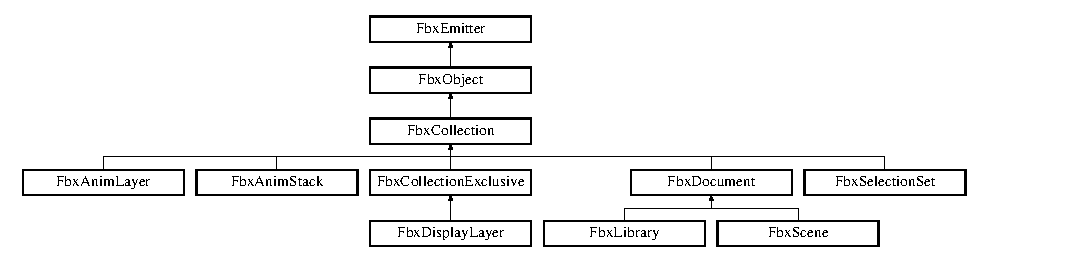
\includegraphics[height=3.090508cm]{class_fbx_collection}
\end{center}
\end{figure}
\subsection*{Collection member management}
\begin{DoxyCompactItemize}
\item 
virtual void \hyperlink{class_fbx_collection_a79ba35ab4693cd1b1c79a221d7d2f8d3}{Clear} ()
\begin{DoxyCompactList}\small\item\em Deletes all objects in the container. \end{DoxyCompactList}\item 
virtual bool \hyperlink{class_fbx_collection_a8f9bfa57454dda20ef75dd4f27761a15}{Add\+Member} (\hyperlink{class_fbx_object}{Fbx\+Object} $\ast$p\+Member)
\item 
virtual bool \hyperlink{class_fbx_collection_a8a65c60bae5ebfcd19f4aaad99ec10f1}{Remove\+Member} (\hyperlink{class_fbx_object}{Fbx\+Object} $\ast$p\+Member)
\item 
int \hyperlink{class_fbx_collection_a3e22b8afd7b46dcc4988c2723dd75e02}{Get\+Member\+Count} () const
\item 
\hyperlink{class_fbx_object}{Fbx\+Object} $\ast$ \hyperlink{class_fbx_collection_a79c52e9fdd2c04a29b5ba04ff7e15bc6}{Get\+Member} (int p\+Index=0) const
\item 
virtual bool \hyperlink{class_fbx_collection_a988fd0dcbe61e4b9b165d6830543f49e}{Is\+Member} (const \hyperlink{class_fbx_object}{Fbx\+Object} $\ast$p\+Member) const
\end{DoxyCompactItemize}
\subsection*{Templated member management}
\begin{DoxyCompactItemize}
\item 
{\footnotesize template$<$class T $>$ }\\int \hyperlink{class_fbx_collection_a0bc6b29ae68a76d65c554c7217432cca}{Get\+Member\+Count} () const
\item 
{\footnotesize template$<$class T $>$ }\\T $\ast$ \hyperlink{class_fbx_collection_a36af3c2dc008c0c6261ff29b492eaee0}{Get\+Member} (int p\+Index=0) const
\item 
{\footnotesize template$<$class T $>$ }\\T $\ast$ \hyperlink{class_fbx_collection_ac68aa37ee6d89cb3cc066ca1407cb505}{Find\+Member} (const char $\ast$p\+Name) const
\end{DoxyCompactItemize}
\subsection*{Criteria based member management}
\begin{DoxyCompactItemize}
\item 
int \hyperlink{class_fbx_collection_ab885c6a1cc7eb77b471ae11c65658258}{Get\+Member\+Count} (const \hyperlink{class_fbx_criteria}{Fbx\+Criteria} \&p\+Criteria) const
\item 
\hyperlink{class_fbx_object}{Fbx\+Object} $\ast$ \hyperlink{class_fbx_collection_a0734fa6462dbc0926b610dfc6047252e}{Get\+Member} (const \hyperlink{class_fbx_criteria}{Fbx\+Criteria} \&p\+Criteria, int p\+Index=0) const
\item 
\hyperlink{class_fbx_object}{Fbx\+Object} $\ast$ \hyperlink{class_fbx_collection_a72875fa801308b233f5e1cb04cf66bb4}{Find\+Member} (const \hyperlink{class_fbx_criteria}{Fbx\+Criteria} \&p\+Criteria, const char $\ast$p\+Name) const
\end{DoxyCompactItemize}
\subsection*{Selection management}
\begin{DoxyCompactItemize}
\item 
virtual void \hyperlink{class_fbx_collection_a93caba5f2a0bded8cb00fca4001950e9}{Set\+Selected\+All} (bool p\+Selection)
\end{DoxyCompactItemize}
\subsection*{その他の継承メンバ}


\subsection{詳解}
A \hyperlink{class_fbx_object}{Fbx\+Object} derived container for \hyperlink{class_fbx_object}{Fbx\+Object}. 

 fbxcollection.\+h の 28 行目に定義があります。



\subsection{関数詳解}
\mbox{\Hypertarget{class_fbx_collection_a8f9bfa57454dda20ef75dd4f27761a15}\label{class_fbx_collection_a8f9bfa57454dda20ef75dd4f27761a15}} 
\index{Fbx\+Collection@{Fbx\+Collection}!Add\+Member@{Add\+Member}}
\index{Add\+Member@{Add\+Member}!Fbx\+Collection@{Fbx\+Collection}}
\subsubsection{\texorpdfstring{Add\+Member()}{AddMember()}}
{\footnotesize\ttfamily virtual bool Fbx\+Collection\+::\+Add\+Member (\begin{DoxyParamCaption}\item[{\hyperlink{class_fbx_object}{Fbx\+Object} $\ast$}]{p\+Member }\end{DoxyParamCaption})\hspace{0.3cm}{\ttfamily [inline]}, {\ttfamily [virtual]}}

Adds a member. 
\begin{DoxyParams}{引数}
{\em p\+Member} & Object to be added. \\
\hline
\end{DoxyParams}


\hyperlink{class_fbx_collection_exclusive_ab39aa1d3200f5cc628685d7c9eca6fb2}{Fbx\+Collection\+Exclusive}で再実装されています。



 fbxcollection.\+h の 43 行目に定義があります。

\mbox{\Hypertarget{class_fbx_collection_a79ba35ab4693cd1b1c79a221d7d2f8d3}\label{class_fbx_collection_a79ba35ab4693cd1b1c79a221d7d2f8d3}} 
\index{Fbx\+Collection@{Fbx\+Collection}!Clear@{Clear}}
\index{Clear@{Clear}!Fbx\+Collection@{Fbx\+Collection}}
\subsubsection{\texorpdfstring{Clear()}{Clear()}}
{\footnotesize\ttfamily virtual void Fbx\+Collection\+::\+Clear (\begin{DoxyParamCaption}{ }\end{DoxyParamCaption})\hspace{0.3cm}{\ttfamily [virtual]}}



Deletes all objects in the container. 



\hyperlink{class_fbx_scene_ab578ff733eb8f6af89ff1645852966cd}{Fbx\+Scene}, \hyperlink{class_fbx_document_ac8fa73e98a73c4f6637466e58d069bbe}{Fbx\+Document}で再実装されています。

\mbox{\Hypertarget{class_fbx_collection_ac68aa37ee6d89cb3cc066ca1407cb505}\label{class_fbx_collection_ac68aa37ee6d89cb3cc066ca1407cb505}} 
\index{Fbx\+Collection@{Fbx\+Collection}!Find\+Member@{Find\+Member}}
\index{Find\+Member@{Find\+Member}!Fbx\+Collection@{Fbx\+Collection}}
\subsubsection{\texorpdfstring{Find\+Member()}{FindMember()}\hspace{0.1cm}{\footnotesize\ttfamily [1/2]}}
{\footnotesize\ttfamily template$<$class T $>$ \\
T$\ast$ Fbx\+Collection\+::\+Find\+Member (\begin{DoxyParamCaption}\item[{const char $\ast$}]{p\+Name }\end{DoxyParamCaption}) const\hspace{0.3cm}{\ttfamily [inline]}}

Searches for a member of class T. 
\begin{DoxyParams}{引数}
{\em p\+Name} & Member name. \\
\hline
\end{DoxyParams}


 fbxcollection.\+h の 83 行目に定義があります。

\mbox{\Hypertarget{class_fbx_collection_a72875fa801308b233f5e1cb04cf66bb4}\label{class_fbx_collection_a72875fa801308b233f5e1cb04cf66bb4}} 
\index{Fbx\+Collection@{Fbx\+Collection}!Find\+Member@{Find\+Member}}
\index{Find\+Member@{Find\+Member}!Fbx\+Collection@{Fbx\+Collection}}
\subsubsection{\texorpdfstring{Find\+Member()}{FindMember()}\hspace{0.1cm}{\footnotesize\ttfamily [2/2]}}
{\footnotesize\ttfamily \hyperlink{class_fbx_object}{Fbx\+Object}$\ast$ Fbx\+Collection\+::\+Find\+Member (\begin{DoxyParamCaption}\item[{const \hyperlink{class_fbx_criteria}{Fbx\+Criteria} \&}]{p\+Criteria,  }\item[{const char $\ast$}]{p\+Name }\end{DoxyParamCaption}) const\hspace{0.3cm}{\ttfamily [inline]}}

Searches for a member with the given name that also meets the given criteria. 
\begin{DoxyParams}{引数}
{\em p\+Criteria} & Defines a set of criteria that the returned object must meet. \\
\hline
{\em p\+Name} & Member name. \\
\hline
\end{DoxyParams}
\begin{DoxyReturn}{戻り値}
The member with the given name if it meets the criteria; N\+U\+LL if no match could be found. 
\end{DoxyReturn}


 fbxcollection.\+h の 108 行目に定義があります。

\mbox{\Hypertarget{class_fbx_collection_a79c52e9fdd2c04a29b5ba04ff7e15bc6}\label{class_fbx_collection_a79c52e9fdd2c04a29b5ba04ff7e15bc6}} 
\index{Fbx\+Collection@{Fbx\+Collection}!Get\+Member@{Get\+Member}}
\index{Get\+Member@{Get\+Member}!Fbx\+Collection@{Fbx\+Collection}}
\subsubsection{\texorpdfstring{Get\+Member()}{GetMember()}\hspace{0.1cm}{\footnotesize\ttfamily [1/3]}}
{\footnotesize\ttfamily \hyperlink{class_fbx_object}{Fbx\+Object}$\ast$ Fbx\+Collection\+::\+Get\+Member (\begin{DoxyParamCaption}\item[{int}]{p\+Index = {\ttfamily 0} }\end{DoxyParamCaption}) const\hspace{0.3cm}{\ttfamily [inline]}}

Returns the member of the collection at the given index. 
\begin{DoxyParams}{引数}
{\em p\+Index} & The given index. \\
\hline
\end{DoxyParams}
\begin{DoxyReturn}{戻り値}
The member of the collection at the given index. 
\end{DoxyReturn}


 fbxcollection.\+h の 59 行目に定義があります。

\mbox{\Hypertarget{class_fbx_collection_a36af3c2dc008c0c6261ff29b492eaee0}\label{class_fbx_collection_a36af3c2dc008c0c6261ff29b492eaee0}} 
\index{Fbx\+Collection@{Fbx\+Collection}!Get\+Member@{Get\+Member}}
\index{Get\+Member@{Get\+Member}!Fbx\+Collection@{Fbx\+Collection}}
\subsubsection{\texorpdfstring{Get\+Member()}{GetMember()}\hspace{0.1cm}{\footnotesize\ttfamily [2/3]}}
{\footnotesize\ttfamily template$<$class T $>$ \\
T$\ast$ Fbx\+Collection\+::\+Get\+Member (\begin{DoxyParamCaption}\item[{int}]{p\+Index = {\ttfamily 0} }\end{DoxyParamCaption}) const\hspace{0.3cm}{\ttfamily [inline]}}

Returns the member of class T at the given index in the collection. 
\begin{DoxyParams}{引数}
{\em p\+Index} & The given index. \\
\hline
\end{DoxyParams}
\begin{DoxyReturn}{戻り値}
The member of class T at the given index. 
\end{DoxyReturn}


 fbxcollection.\+h の 79 行目に定義があります。

\mbox{\Hypertarget{class_fbx_collection_a0734fa6462dbc0926b610dfc6047252e}\label{class_fbx_collection_a0734fa6462dbc0926b610dfc6047252e}} 
\index{Fbx\+Collection@{Fbx\+Collection}!Get\+Member@{Get\+Member}}
\index{Get\+Member@{Get\+Member}!Fbx\+Collection@{Fbx\+Collection}}
\subsubsection{\texorpdfstring{Get\+Member()}{GetMember()}\hspace{0.1cm}{\footnotesize\ttfamily [3/3]}}
{\footnotesize\ttfamily \hyperlink{class_fbx_object}{Fbx\+Object}$\ast$ Fbx\+Collection\+::\+Get\+Member (\begin{DoxyParamCaption}\item[{const \hyperlink{class_fbx_criteria}{Fbx\+Criteria} \&}]{p\+Criteria,  }\item[{int}]{p\+Index = {\ttfamily 0} }\end{DoxyParamCaption}) const\hspace{0.3cm}{\ttfamily [inline]}}

Returns the member at the given index in the collection if it meets the specified criteria. 
\begin{DoxyParams}{引数}
{\em p\+Criteria} & Defines a set of criteria that the returned object must meet. \\
\hline
{\em p\+Index} & The given index. \\
\hline
\end{DoxyParams}
\begin{DoxyReturn}{戻り値}
The member at the given index if it meets the criteria; N\+U\+LL otherwise. 
\end{DoxyReturn}


 fbxcollection.\+h の 101 行目に定義があります。

\mbox{\Hypertarget{class_fbx_collection_a3e22b8afd7b46dcc4988c2723dd75e02}\label{class_fbx_collection_a3e22b8afd7b46dcc4988c2723dd75e02}} 
\index{Fbx\+Collection@{Fbx\+Collection}!Get\+Member\+Count@{Get\+Member\+Count}}
\index{Get\+Member\+Count@{Get\+Member\+Count}!Fbx\+Collection@{Fbx\+Collection}}
\subsubsection{\texorpdfstring{Get\+Member\+Count()}{GetMemberCount()}\hspace{0.1cm}{\footnotesize\ttfamily [1/3]}}
{\footnotesize\ttfamily int Fbx\+Collection\+::\+Get\+Member\+Count (\begin{DoxyParamCaption}{ }\end{DoxyParamCaption}) const\hspace{0.3cm}{\ttfamily [inline]}}

Returns the number of objects contained within the collection. \begin{DoxyReturn}{戻り値}
The number of objects the collection contains. 
\end{DoxyReturn}


 fbxcollection.\+h の 53 行目に定義があります。

\mbox{\Hypertarget{class_fbx_collection_a0bc6b29ae68a76d65c554c7217432cca}\label{class_fbx_collection_a0bc6b29ae68a76d65c554c7217432cca}} 
\index{Fbx\+Collection@{Fbx\+Collection}!Get\+Member\+Count@{Get\+Member\+Count}}
\index{Get\+Member\+Count@{Get\+Member\+Count}!Fbx\+Collection@{Fbx\+Collection}}
\subsubsection{\texorpdfstring{Get\+Member\+Count()}{GetMemberCount()}\hspace{0.1cm}{\footnotesize\ttfamily [2/3]}}
{\footnotesize\ttfamily template$<$class T $>$ \\
int Fbx\+Collection\+::\+Get\+Member\+Count (\begin{DoxyParamCaption}{ }\end{DoxyParamCaption}) const\hspace{0.3cm}{\ttfamily [inline]}}

Returns the number of class T objects contained within the collection. \begin{DoxyReturn}{戻り値}
The number of objects of class T the collection contains. 
\end{DoxyReturn}


 fbxcollection.\+h の 74 行目に定義があります。

\mbox{\Hypertarget{class_fbx_collection_ab885c6a1cc7eb77b471ae11c65658258}\label{class_fbx_collection_ab885c6a1cc7eb77b471ae11c65658258}} 
\index{Fbx\+Collection@{Fbx\+Collection}!Get\+Member\+Count@{Get\+Member\+Count}}
\index{Get\+Member\+Count@{Get\+Member\+Count}!Fbx\+Collection@{Fbx\+Collection}}
\subsubsection{\texorpdfstring{Get\+Member\+Count()}{GetMemberCount()}\hspace{0.1cm}{\footnotesize\ttfamily [3/3]}}
{\footnotesize\ttfamily int Fbx\+Collection\+::\+Get\+Member\+Count (\begin{DoxyParamCaption}\item[{const \hyperlink{class_fbx_criteria}{Fbx\+Criteria} \&}]{p\+Criteria }\end{DoxyParamCaption}) const\hspace{0.3cm}{\ttfamily [inline]}}

Returns the number of objects contained within the collection that meet the specified criteria. 
\begin{DoxyParams}{引数}
{\em p\+Criteria} & Defines a set of criteria that each object must meet in order to be included in the results. \\
\hline
\end{DoxyParams}
\begin{DoxyReturn}{戻り値}
The number of objects the collection contains that meet the specified criteria. 
\end{DoxyReturn}


 fbxcollection.\+h の 94 行目に定義があります。

\mbox{\Hypertarget{class_fbx_collection_a988fd0dcbe61e4b9b165d6830543f49e}\label{class_fbx_collection_a988fd0dcbe61e4b9b165d6830543f49e}} 
\index{Fbx\+Collection@{Fbx\+Collection}!Is\+Member@{Is\+Member}}
\index{Is\+Member@{Is\+Member}!Fbx\+Collection@{Fbx\+Collection}}
\subsubsection{\texorpdfstring{Is\+Member()}{IsMember()}}
{\footnotesize\ttfamily virtual bool Fbx\+Collection\+::\+Is\+Member (\begin{DoxyParamCaption}\item[{const \hyperlink{class_fbx_object}{Fbx\+Object} $\ast$}]{p\+Member }\end{DoxyParamCaption}) const\hspace{0.3cm}{\ttfamily [virtual]}}

Judges whether an object is a part of the collection. 
\begin{DoxyParams}{引数}
{\em p\+Member} & The member to be judged. \\
\hline
\end{DoxyParams}
\begin{DoxyReturn}{戻り値}
{\ttfamily True} if it is a member of the collection, returns {\ttfamily false} if it is not a member. 
\end{DoxyReturn}
\mbox{\Hypertarget{class_fbx_collection_a8a65c60bae5ebfcd19f4aaad99ec10f1}\label{class_fbx_collection_a8a65c60bae5ebfcd19f4aaad99ec10f1}} 
\index{Fbx\+Collection@{Fbx\+Collection}!Remove\+Member@{Remove\+Member}}
\index{Remove\+Member@{Remove\+Member}!Fbx\+Collection@{Fbx\+Collection}}
\subsubsection{\texorpdfstring{Remove\+Member()}{RemoveMember()}}
{\footnotesize\ttfamily virtual bool Fbx\+Collection\+::\+Remove\+Member (\begin{DoxyParamCaption}\item[{\hyperlink{class_fbx_object}{Fbx\+Object} $\ast$}]{p\+Member }\end{DoxyParamCaption})\hspace{0.3cm}{\ttfamily [inline]}, {\ttfamily [virtual]}}

Removes a member. 
\begin{DoxyParams}{引数}
{\em p\+Member} & Object to be removed. \\
\hline
\end{DoxyParams}


 fbxcollection.\+h の 48 行目に定義があります。

\mbox{\Hypertarget{class_fbx_collection_a93caba5f2a0bded8cb00fca4001950e9}\label{class_fbx_collection_a93caba5f2a0bded8cb00fca4001950e9}} 
\index{Fbx\+Collection@{Fbx\+Collection}!Set\+Selected\+All@{Set\+Selected\+All}}
\index{Set\+Selected\+All@{Set\+Selected\+All}!Fbx\+Collection@{Fbx\+Collection}}
\subsubsection{\texorpdfstring{Set\+Selected\+All()}{SetSelectedAll()}}
{\footnotesize\ttfamily virtual void Fbx\+Collection\+::\+Set\+Selected\+All (\begin{DoxyParamCaption}\item[{bool}]{p\+Selection }\end{DoxyParamCaption})\hspace{0.3cm}{\ttfamily [virtual]}}

Selects/\+Deselects all the contained objects. 
\begin{DoxyParams}{引数}
{\em p\+Selection} & If {\ttfamily true}, all objects are selected, if {\ttfamily false}, all objects are deselected. \\
\hline
\end{DoxyParams}


このクラス詳解は次のファイルから抽出されました\+:\begin{DoxyCompactItemize}
\item 
C\+:/\+Maya/scripts/\+F\+B\+X\+\_\+\+S\+D\+K/2017.\+1/include/fbxsdk/scene/\hyperlink{fbxcollection_8h}{fbxcollection.\+h}\end{DoxyCompactItemize}

\hypertarget{class_fbx_collection_exclusive}{}\section{Fbx\+Collection\+Exclusive クラス}
\label{class_fbx_collection_exclusive}\index{Fbx\+Collection\+Exclusive@{Fbx\+Collection\+Exclusive}}


{\ttfamily \#include $<$fbxcollectionexclusive.\+h$>$}

Fbx\+Collection\+Exclusive の継承関係図\begin{figure}[H]
\begin{center}
\leavevmode
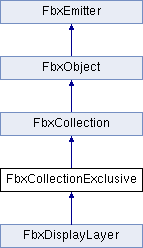
\includegraphics[height=5.000000cm]{class_fbx_collection_exclusive}
\end{center}
\end{figure}
\subsection*{公開メンバ関数}
\begin{DoxyCompactItemize}
\item 
bool \hyperlink{class_fbx_collection_exclusive_ab39aa1d3200f5cc628685d7c9eca6fb2}{Add\+Member} (\hyperlink{class_fbx_object}{Fbx\+Object} $\ast$p\+Member)
\end{DoxyCompactItemize}
\subsection*{その他の継承メンバ}


\subsection{詳解}
Class for exclusive collections. An object (\hyperlink{class_fbx_object}{Fbx\+Object}) should belong to only one exclusive collection at most. 

 fbxcollectionexclusive.\+h の 25 行目に定義があります。



\subsection{関数詳解}
\mbox{\Hypertarget{class_fbx_collection_exclusive_ab39aa1d3200f5cc628685d7c9eca6fb2}\label{class_fbx_collection_exclusive_ab39aa1d3200f5cc628685d7c9eca6fb2}} 
\index{Fbx\+Collection\+Exclusive@{Fbx\+Collection\+Exclusive}!Add\+Member@{Add\+Member}}
\index{Add\+Member@{Add\+Member}!Fbx\+Collection\+Exclusive@{Fbx\+Collection\+Exclusive}}
\subsubsection{\texorpdfstring{Add\+Member()}{AddMember()}}
{\footnotesize\ttfamily bool Fbx\+Collection\+Exclusive\+::\+Add\+Member (\begin{DoxyParamCaption}\item[{\hyperlink{class_fbx_object}{Fbx\+Object} $\ast$}]{p\+Member }\end{DoxyParamCaption})\hspace{0.3cm}{\ttfamily [virtual]}}

Add a member if it\textquotesingle{}s not a member of any other \hyperlink{class_fbx_collection_exclusive}{Fbx\+Collection\+Exclusive} objects. 
\begin{DoxyParams}{引数}
{\em p\+Member} & Object to be added \\
\hline
\end{DoxyParams}


\hyperlink{class_fbx_collection_a8f9bfa57454dda20ef75dd4f27761a15}{Fbx\+Collection}を再実装しています。



このクラス詳解は次のファイルから抽出されました\+:\begin{DoxyCompactItemize}
\item 
C\+:/\+Maya/scripts/\+F\+B\+X\+\_\+\+S\+D\+K/2017.\+1/include/fbxsdk/scene/\hyperlink{fbxcollectionexclusive_8h}{fbxcollectionexclusive.\+h}\end{DoxyCompactItemize}

\hypertarget{class_fbx_color}{}\section{Fbx\+Color クラス}
\label{class_fbx_color}\index{Fbx\+Color@{Fbx\+Color}}


{\ttfamily \#include $<$fbxpropertytypes.\+h$>$}

\subsection*{公開メンバ関数}
\begin{DoxyCompactItemize}
\item 
\hyperlink{class_fbx_color_af9c8230979d074e82faead61fd92a3fc}{Fbx\+Color} ()
\begin{DoxyCompactList}\small\item\em Constructor. \end{DoxyCompactList}\item 
\hyperlink{class_fbx_color_a794e4dfc39f7f6ce2a2d884f21a6dac6}{Fbx\+Color} (const double p\+Red, const double p\+Green, const double p\+Blue, const double p\+Alpha=1.\+0)
\item 
\hyperlink{class_fbx_color_a09f5704390406cd3da4fd7bd8b5ae32d}{Fbx\+Color} (const \hyperlink{fbxtypes_8h_ae0a96f14cde566774c7553aa7523b7a7}{Fbx\+Double3} \&p\+R\+GB, const double p\+Alpha=1.\+0)
\item 
\hyperlink{class_fbx_color_a845eb670fb29e7a942973c4281c4939e}{Fbx\+Color} (const \hyperlink{fbxtypes_8h_a03dddc7979e0016f74a095b1943d97a3}{Fbx\+Double4} \&p\+R\+G\+BA)
\item 
\hyperlink{class_fbx_color_a5b8800e1233bdc6eb44add9be6cab9df}{$\sim$\+Fbx\+Color} ()
\begin{DoxyCompactList}\small\item\em Destructor. \end{DoxyCompactList}\item 
void \hyperlink{class_fbx_color_ae2e74f4aa5e142426e1453400bfb7520}{Set} (const double p\+Red, const double p\+Green, const double p\+Blue, const double p\+Alpha=1.\+0)
\item 
bool \hyperlink{class_fbx_color_a12d5438931a4401d632612dc3564c433}{Is\+Valid} () const
\item 
double \& \hyperlink{class_fbx_color_ac396e40fa972caa64f29e94605660324}{operator\mbox{[}$\,$\mbox{]}} (int p\+Index)
\item 
const double \& \hyperlink{class_fbx_color_a578f043b19c6303d74c19d41daf2a254}{operator\mbox{[}$\,$\mbox{]}} (int p\+Index) const
\end{DoxyCompactItemize}
\subsection*{Operators}
\begin{DoxyCompactItemize}
\item 
\hyperlink{class_fbx_color}{Fbx\+Color} \& \hyperlink{class_fbx_color_ae1810b5b2286fa939f106e8d5adc5011}{operator=} (const \hyperlink{class_fbx_color}{Fbx\+Color} \&p\+Color)
\item 
\hyperlink{class_fbx_color}{Fbx\+Color} \& \hyperlink{class_fbx_color_af509c1a34ba01aca1207975fa36ebc07}{operator=} (const \hyperlink{fbxtypes_8h_ae0a96f14cde566774c7553aa7523b7a7}{Fbx\+Double3} \&p\+Color)
\item 
\hyperlink{class_fbx_color}{Fbx\+Color} \& \hyperlink{class_fbx_color_a5398fb758068706d35318cd145092c0f}{operator=} (const \hyperlink{fbxtypes_8h_a03dddc7979e0016f74a095b1943d97a3}{Fbx\+Double4} \&p\+Color)
\item 
bool \hyperlink{class_fbx_color_abba90fcb84b470c432abae17c2e1a347}{operator==} (const \hyperlink{class_fbx_color}{Fbx\+Color} \&p\+Color) const
\item 
bool \hyperlink{class_fbx_color_a3f7caa78c7c9140670ad4a5f1cc32b62}{operator!=} (const \hyperlink{class_fbx_color}{Fbx\+Color} \&p\+Color) const
\end{DoxyCompactItemize}
\begin{DoxyCompactItemize}
\item 
double \hyperlink{class_fbx_color_aa58094c2415fa965bdf1e760892baa5c}{m\+Red}
\begin{DoxyCompactList}\small\item\em Valid range is from 0.\+0 to 1.\+0. \end{DoxyCompactList}\item 
double \hyperlink{class_fbx_color_a43ba888941f635304a7ed885ccfed776}{m\+Green}
\begin{DoxyCompactList}\small\item\em Valid range is from 0.\+0 to 1.\+0. \end{DoxyCompactList}\item 
double \hyperlink{class_fbx_color_abf621ccd7dc31e50019c7bdde90dfe5e}{m\+Blue}
\begin{DoxyCompactList}\small\item\em Valid range is from 0.\+0 to 1.\+0. \end{DoxyCompactList}\item 
double \hyperlink{class_fbx_color_a06c58f40181499882190574926d335ec}{m\+Alpha}
\begin{DoxyCompactList}\small\item\em Valid range is from 0.\+0 to 1.\+0. \end{DoxyCompactList}\end{DoxyCompactItemize}


\subsection{詳解}
Class to represent colors in R\+G\+BA format using doubles. 

\subsection{構築子と解体子}
\mbox{\Hypertarget{class_fbx_color_af9c8230979d074e82faead61fd92a3fc}\label{class_fbx_color_af9c8230979d074e82faead61fd92a3fc}} 
\index{Fbx\+Color@{Fbx\+Color}!Fbx\+Color@{Fbx\+Color}}
\index{Fbx\+Color@{Fbx\+Color}!Fbx\+Color@{Fbx\+Color}}
\subsubsection{\texorpdfstring{Fbx\+Color()}{FbxColor()}\hspace{0.1cm}{\footnotesize\ttfamily [1/4]}}
{\footnotesize\ttfamily Fbx\+Color\+::\+Fbx\+Color (\begin{DoxyParamCaption}{ }\end{DoxyParamCaption})}



Constructor. 

\mbox{\Hypertarget{class_fbx_color_a794e4dfc39f7f6ce2a2d884f21a6dac6}\label{class_fbx_color_a794e4dfc39f7f6ce2a2d884f21a6dac6}} 
\index{Fbx\+Color@{Fbx\+Color}!Fbx\+Color@{Fbx\+Color}}
\index{Fbx\+Color@{Fbx\+Color}!Fbx\+Color@{Fbx\+Color}}
\subsubsection{\texorpdfstring{Fbx\+Color()}{FbxColor()}\hspace{0.1cm}{\footnotesize\ttfamily [2/4]}}
{\footnotesize\ttfamily Fbx\+Color\+::\+Fbx\+Color (\begin{DoxyParamCaption}\item[{const double}]{p\+Red,  }\item[{const double}]{p\+Green,  }\item[{const double}]{p\+Blue,  }\item[{const double}]{p\+Alpha = {\ttfamily 1.0} }\end{DoxyParamCaption})}

Constructor. 
\begin{DoxyParams}{引数}
{\em p\+Red} & The Red component value. \\
\hline
{\em p\+Green} & The Green component value. \\
\hline
{\em p\+Blue} & The Blue component value. \\
\hline
{\em p\+Alpha} & The alpha value of the color. \\
\hline
\end{DoxyParams}
\mbox{\Hypertarget{class_fbx_color_a09f5704390406cd3da4fd7bd8b5ae32d}\label{class_fbx_color_a09f5704390406cd3da4fd7bd8b5ae32d}} 
\index{Fbx\+Color@{Fbx\+Color}!Fbx\+Color@{Fbx\+Color}}
\index{Fbx\+Color@{Fbx\+Color}!Fbx\+Color@{Fbx\+Color}}
\subsubsection{\texorpdfstring{Fbx\+Color()}{FbxColor()}\hspace{0.1cm}{\footnotesize\ttfamily [3/4]}}
{\footnotesize\ttfamily Fbx\+Color\+::\+Fbx\+Color (\begin{DoxyParamCaption}\item[{const \hyperlink{fbxtypes_8h_ae0a96f14cde566774c7553aa7523b7a7}{Fbx\+Double3} \&}]{p\+R\+GB,  }\item[{const double}]{p\+Alpha = {\ttfamily 1.0} }\end{DoxyParamCaption})}

\mbox{\Hypertarget{class_fbx_color_a845eb670fb29e7a942973c4281c4939e}\label{class_fbx_color_a845eb670fb29e7a942973c4281c4939e}} 
\index{Fbx\+Color@{Fbx\+Color}!Fbx\+Color@{Fbx\+Color}}
\index{Fbx\+Color@{Fbx\+Color}!Fbx\+Color@{Fbx\+Color}}
\subsubsection{\texorpdfstring{Fbx\+Color()}{FbxColor()}\hspace{0.1cm}{\footnotesize\ttfamily [4/4]}}
{\footnotesize\ttfamily Fbx\+Color\+::\+Fbx\+Color (\begin{DoxyParamCaption}\item[{const \hyperlink{fbxtypes_8h_a03dddc7979e0016f74a095b1943d97a3}{Fbx\+Double4} \&}]{p\+R\+G\+BA }\end{DoxyParamCaption})}

\mbox{\Hypertarget{class_fbx_color_a5b8800e1233bdc6eb44add9be6cab9df}\label{class_fbx_color_a5b8800e1233bdc6eb44add9be6cab9df}} 
\index{Fbx\+Color@{Fbx\+Color}!````~Fbx\+Color@{$\sim$\+Fbx\+Color}}
\index{````~Fbx\+Color@{$\sim$\+Fbx\+Color}!Fbx\+Color@{Fbx\+Color}}
\subsubsection{\texorpdfstring{$\sim$\+Fbx\+Color()}{~FbxColor()}}
{\footnotesize\ttfamily Fbx\+Color\+::$\sim$\+Fbx\+Color (\begin{DoxyParamCaption}{ }\end{DoxyParamCaption})}



Destructor. 



\subsection{メソッド詳解}
\mbox{\Hypertarget{class_fbx_color_a12d5438931a4401d632612dc3564c433}\label{class_fbx_color_a12d5438931a4401d632612dc3564c433}} 
\index{Fbx\+Color@{Fbx\+Color}!Is\+Valid@{Is\+Valid}}
\index{Is\+Valid@{Is\+Valid}!Fbx\+Color@{Fbx\+Color}}
\subsubsection{\texorpdfstring{Is\+Valid()}{IsValid()}}
{\footnotesize\ttfamily bool Fbx\+Color\+::\+Is\+Valid (\begin{DoxyParamCaption}{ }\end{DoxyParamCaption}) const}

Indicate if all the members in the color objects are within their valid range. \begin{DoxyReturn}{戻り値}
{\ttfamily true} if all the members are within their valid range. 
\end{DoxyReturn}
\mbox{\Hypertarget{class_fbx_color_a3f7caa78c7c9140670ad4a5f1cc32b62}\label{class_fbx_color_a3f7caa78c7c9140670ad4a5f1cc32b62}} 
\index{Fbx\+Color@{Fbx\+Color}!operator"!=@{operator"!=}}
\index{operator"!=@{operator"!=}!Fbx\+Color@{Fbx\+Color}}
\subsubsection{\texorpdfstring{operator"!=()}{operator!=()}}
{\footnotesize\ttfamily bool Fbx\+Color\+::operator!= (\begin{DoxyParamCaption}\item[{const \hyperlink{class_fbx_color}{Fbx\+Color} \&}]{p\+Color }\end{DoxyParamCaption}) const}

Inequality operator. 
\begin{DoxyParams}{引数}
{\em p\+Color} & \hyperlink{class_fbx_color}{Fbx\+Color} compared with this one. \\
\hline
\end{DoxyParams}
\begin{DoxyReturn}{戻り値}
{\ttfamily true} if unequal, {\ttfamily false} if equal. 
\end{DoxyReturn}
\mbox{\Hypertarget{class_fbx_color_ae1810b5b2286fa939f106e8d5adc5011}\label{class_fbx_color_ae1810b5b2286fa939f106e8d5adc5011}} 
\index{Fbx\+Color@{Fbx\+Color}!operator=@{operator=}}
\index{operator=@{operator=}!Fbx\+Color@{Fbx\+Color}}
\subsubsection{\texorpdfstring{operator=()}{operator=()}\hspace{0.1cm}{\footnotesize\ttfamily [1/3]}}
{\footnotesize\ttfamily \hyperlink{class_fbx_color}{Fbx\+Color}\& Fbx\+Color\+::operator= (\begin{DoxyParamCaption}\item[{const \hyperlink{class_fbx_color}{Fbx\+Color} \&}]{p\+Color }\end{DoxyParamCaption})}

Assignment operator. 
\begin{DoxyParams}{引数}
{\em p\+Color} & \hyperlink{class_fbx_color}{Fbx\+Color} to be copied. \\
\hline
\end{DoxyParams}
\mbox{\Hypertarget{class_fbx_color_af509c1a34ba01aca1207975fa36ebc07}\label{class_fbx_color_af509c1a34ba01aca1207975fa36ebc07}} 
\index{Fbx\+Color@{Fbx\+Color}!operator=@{operator=}}
\index{operator=@{operator=}!Fbx\+Color@{Fbx\+Color}}
\subsubsection{\texorpdfstring{operator=()}{operator=()}\hspace{0.1cm}{\footnotesize\ttfamily [2/3]}}
{\footnotesize\ttfamily \hyperlink{class_fbx_color}{Fbx\+Color}\& Fbx\+Color\+::operator= (\begin{DoxyParamCaption}\item[{const \hyperlink{fbxtypes_8h_ae0a96f14cde566774c7553aa7523b7a7}{Fbx\+Double3} \&}]{p\+Color }\end{DoxyParamCaption})}

\mbox{\Hypertarget{class_fbx_color_a5398fb758068706d35318cd145092c0f}\label{class_fbx_color_a5398fb758068706d35318cd145092c0f}} 
\index{Fbx\+Color@{Fbx\+Color}!operator=@{operator=}}
\index{operator=@{operator=}!Fbx\+Color@{Fbx\+Color}}
\subsubsection{\texorpdfstring{operator=()}{operator=()}\hspace{0.1cm}{\footnotesize\ttfamily [3/3]}}
{\footnotesize\ttfamily \hyperlink{class_fbx_color}{Fbx\+Color}\& Fbx\+Color\+::operator= (\begin{DoxyParamCaption}\item[{const \hyperlink{fbxtypes_8h_a03dddc7979e0016f74a095b1943d97a3}{Fbx\+Double4} \&}]{p\+Color }\end{DoxyParamCaption})}

\mbox{\Hypertarget{class_fbx_color_abba90fcb84b470c432abae17c2e1a347}\label{class_fbx_color_abba90fcb84b470c432abae17c2e1a347}} 
\index{Fbx\+Color@{Fbx\+Color}!operator==@{operator==}}
\index{operator==@{operator==}!Fbx\+Color@{Fbx\+Color}}
\subsubsection{\texorpdfstring{operator==()}{operator==()}}
{\footnotesize\ttfamily bool Fbx\+Color\+::operator== (\begin{DoxyParamCaption}\item[{const \hyperlink{class_fbx_color}{Fbx\+Color} \&}]{p\+Color }\end{DoxyParamCaption}) const}

Equality operator. 
\begin{DoxyParams}{引数}
{\em p\+Color} & \hyperlink{class_fbx_color}{Fbx\+Color} compared with this one. \\
\hline
\end{DoxyParams}
\begin{DoxyReturn}{戻り値}
{\ttfamily true} if equal, {\ttfamily false} if unequal. 
\end{DoxyReturn}
\mbox{\Hypertarget{class_fbx_color_ac396e40fa972caa64f29e94605660324}\label{class_fbx_color_ac396e40fa972caa64f29e94605660324}} 
\index{Fbx\+Color@{Fbx\+Color}!operator\mbox{[}\mbox{]}@{operator[]}}
\index{operator\mbox{[}\mbox{]}@{operator[]}!Fbx\+Color@{Fbx\+Color}}
\subsubsection{\texorpdfstring{operator[]()}{operator[]()}\hspace{0.1cm}{\footnotesize\ttfamily [1/2]}}
{\footnotesize\ttfamily double\& Fbx\+Color\+::operator\mbox{[}$\,$\mbox{]} (\begin{DoxyParamCaption}\item[{int}]{p\+Index }\end{DoxyParamCaption})}

Accessors. 
\begin{DoxyParams}{引数}
{\em p\+Index} & The index of the component to access. \\
\hline
\end{DoxyParams}
\begin{DoxyReturn}{戻り値}
The reference to the indexed component. 
\end{DoxyReturn}
\begin{DoxyRemark}{注釈}
The p\+Index parameter is not checked for values out of bounds. 
\end{DoxyRemark}
\mbox{\Hypertarget{class_fbx_color_a578f043b19c6303d74c19d41daf2a254}\label{class_fbx_color_a578f043b19c6303d74c19d41daf2a254}} 
\index{Fbx\+Color@{Fbx\+Color}!operator\mbox{[}\mbox{]}@{operator[]}}
\index{operator\mbox{[}\mbox{]}@{operator[]}!Fbx\+Color@{Fbx\+Color}}
\subsubsection{\texorpdfstring{operator[]()}{operator[]()}\hspace{0.1cm}{\footnotesize\ttfamily [2/2]}}
{\footnotesize\ttfamily const double\& Fbx\+Color\+::operator\mbox{[}$\,$\mbox{]} (\begin{DoxyParamCaption}\item[{int}]{p\+Index }\end{DoxyParamCaption}) const}

Accessors. 
\begin{DoxyParams}{引数}
{\em p\+Index} & The index of the component to access. \\
\hline
\end{DoxyParams}
\begin{DoxyReturn}{戻り値}
The reference to the indexed component. 
\end{DoxyReturn}
\begin{DoxyRemark}{注釈}
The p\+Index parameter is not checked for values out of bounds. 
\end{DoxyRemark}
\mbox{\Hypertarget{class_fbx_color_ae2e74f4aa5e142426e1453400bfb7520}\label{class_fbx_color_ae2e74f4aa5e142426e1453400bfb7520}} 
\index{Fbx\+Color@{Fbx\+Color}!Set@{Set}}
\index{Set@{Set}!Fbx\+Color@{Fbx\+Color}}
\subsubsection{\texorpdfstring{Set()}{Set()}}
{\footnotesize\ttfamily void Fbx\+Color\+::\+Set (\begin{DoxyParamCaption}\item[{const double}]{p\+Red,  }\item[{const double}]{p\+Green,  }\item[{const double}]{p\+Blue,  }\item[{const double}]{p\+Alpha = {\ttfamily 1.0} }\end{DoxyParamCaption})}

Re-\/initialize the color object with their new values. 
\begin{DoxyParams}{引数}
{\em p\+Red} & The Red component value. \\
\hline
{\em p\+Green} & The Green component value. \\
\hline
{\em p\+Blue} & The Blue component value. \\
\hline
{\em p\+Alpha} & The alpha value of the color. \\
\hline
\end{DoxyParams}


\subsection{メンバ詳解}
\mbox{\Hypertarget{class_fbx_color_a06c58f40181499882190574926d335ec}\label{class_fbx_color_a06c58f40181499882190574926d335ec}} 
\index{Fbx\+Color@{Fbx\+Color}!m\+Alpha@{m\+Alpha}}
\index{m\+Alpha@{m\+Alpha}!Fbx\+Color@{Fbx\+Color}}
\subsubsection{\texorpdfstring{m\+Alpha}{mAlpha}}
{\footnotesize\ttfamily double Fbx\+Color\+::m\+Alpha}



Valid range is from 0.\+0 to 1.\+0. 

\mbox{\Hypertarget{class_fbx_color_abf621ccd7dc31e50019c7bdde90dfe5e}\label{class_fbx_color_abf621ccd7dc31e50019c7bdde90dfe5e}} 
\index{Fbx\+Color@{Fbx\+Color}!m\+Blue@{m\+Blue}}
\index{m\+Blue@{m\+Blue}!Fbx\+Color@{Fbx\+Color}}
\subsubsection{\texorpdfstring{m\+Blue}{mBlue}}
{\footnotesize\ttfamily double Fbx\+Color\+::m\+Blue}



Valid range is from 0.\+0 to 1.\+0. 

\mbox{\Hypertarget{class_fbx_color_a43ba888941f635304a7ed885ccfed776}\label{class_fbx_color_a43ba888941f635304a7ed885ccfed776}} 
\index{Fbx\+Color@{Fbx\+Color}!m\+Green@{m\+Green}}
\index{m\+Green@{m\+Green}!Fbx\+Color@{Fbx\+Color}}
\subsubsection{\texorpdfstring{m\+Green}{mGreen}}
{\footnotesize\ttfamily double Fbx\+Color\+::m\+Green}



Valid range is from 0.\+0 to 1.\+0. 

\mbox{\Hypertarget{class_fbx_color_aa58094c2415fa965bdf1e760892baa5c}\label{class_fbx_color_aa58094c2415fa965bdf1e760892baa5c}} 
\index{Fbx\+Color@{Fbx\+Color}!m\+Red@{m\+Red}}
\index{m\+Red@{m\+Red}!Fbx\+Color@{Fbx\+Color}}
\subsubsection{\texorpdfstring{m\+Red}{mRed}}
{\footnotesize\ttfamily double Fbx\+Color\+::m\+Red}



Valid range is from 0.\+0 to 1.\+0. 

name Public Members 

このクラス詳解は次のファイルから抽出されました\+:\begin{DoxyCompactItemize}
\item 
C\+:/github/\+F\+B\+Xpython\+S\+D\+K201701/\+F\+B\+Xpython\+S\+D\+K201701/2017.\+1/include/fbxsdk/core/\hyperlink{fbxpropertytypes_8h}{fbxpropertytypes.\+h}\end{DoxyCompactItemize}

\hypertarget{class_fbx_conditional_b_o_f}{}\section{Fbx\+Conditional\+B\+OF クラス}
\label{class_fbx_conditional_b_o_f}\index{Fbx\+Conditional\+B\+OF@{Fbx\+Conditional\+B\+OF}}


{\ttfamily \#include $<$fbxbindingoperator.\+h$>$}



Fbx\+Conditional\+B\+OF の継承関係図
% FIG 0


Fbx\+Conditional\+B\+OF 連携図
% FIG 1
\subsection*{公開メンバ関数}
\begin{DoxyCompactItemize}
\item 
virtual bool \hyperlink{class_fbx_conditional_b_o_f_ac01ad643a1505219964c8b379385e931}{Evaluate} (const \hyperlink{class_fbx_binding_operator}{Fbx\+Binding\+Operator} $\ast$p\+Operator, const \hyperlink{class_fbx_object}{Fbx\+Object} $\ast$p\+Object, \hyperlink{fbxpropertytypes_8h_a73913a5ddfb20e57c6f25e9e6784bd92}{E\+Fbx\+Type} $\ast$p\+Result\+Type, void $\ast$$\ast$p\+Result) const
\item 
virtual bool \hyperlink{class_fbx_conditional_b_o_f_a2d20cc9f6b6e1c5a469c49a55c8ed512}{Reverse\+Evaluate} (const \hyperlink{class_fbx_binding_operator}{Fbx\+Binding\+Operator} $\ast$p\+Operator, const \hyperlink{class_fbx_object}{Fbx\+Object} $\ast$p\+Target, const void $\ast$p\+In, void $\ast$$\ast$p\+Out, \hyperlink{fbxpropertytypes_8h_a73913a5ddfb20e57c6f25e9e6784bd92}{E\+Fbx\+Type} $\ast$p\+Out\+Type, bool set\+Obj, int index) const
\item 
\hyperlink{class_fbx_conditional_b_o_f_ab01caa5b426f06735e3729f9c59ff58e}{Fbx\+Conditional\+B\+OF} ()
\item 
virtual \hyperlink{class_fbx_conditional_b_o_f_aa4c2e32bdf6550a9c1f36c1f0490bb3a}{$\sim$\+Fbx\+Conditional\+B\+OF} ()
\end{DoxyCompactItemize}
\subsection*{静的公開変数類}
\begin{DoxyCompactItemize}
\item 
static const char $\ast$ \hyperlink{class_fbx_conditional_b_o_f_ac0653f2120f3d07ea7c308611b9f2bbc}{Function\+Name}
\begin{DoxyCompactList}\small\item\em Name of the operation function. \end{DoxyCompactList}\end{DoxyCompactItemize}


\subsection{詳解}
A conditional operator that outputs one out of two properties, based on the value of a predicate property. 

\subsection{構築子と解体子}
\mbox{\Hypertarget{class_fbx_conditional_b_o_f_ab01caa5b426f06735e3729f9c59ff58e}\label{class_fbx_conditional_b_o_f_ab01caa5b426f06735e3729f9c59ff58e}} 
\index{Fbx\+Conditional\+B\+OF@{Fbx\+Conditional\+B\+OF}!Fbx\+Conditional\+B\+OF@{Fbx\+Conditional\+B\+OF}}
\index{Fbx\+Conditional\+B\+OF@{Fbx\+Conditional\+B\+OF}!Fbx\+Conditional\+B\+OF@{Fbx\+Conditional\+B\+OF}}
\subsubsection{\texorpdfstring{Fbx\+Conditional\+B\+O\+F()}{FbxConditionalBOF()}}
{\footnotesize\ttfamily Fbx\+Conditional\+B\+O\+F\+::\+Fbx\+Conditional\+B\+OF (\begin{DoxyParamCaption}{ }\end{DoxyParamCaption})}

\mbox{\Hypertarget{class_fbx_conditional_b_o_f_aa4c2e32bdf6550a9c1f36c1f0490bb3a}\label{class_fbx_conditional_b_o_f_aa4c2e32bdf6550a9c1f36c1f0490bb3a}} 
\index{Fbx\+Conditional\+B\+OF@{Fbx\+Conditional\+B\+OF}!````~Fbx\+Conditional\+B\+OF@{$\sim$\+Fbx\+Conditional\+B\+OF}}
\index{````~Fbx\+Conditional\+B\+OF@{$\sim$\+Fbx\+Conditional\+B\+OF}!Fbx\+Conditional\+B\+OF@{Fbx\+Conditional\+B\+OF}}
\subsubsection{\texorpdfstring{$\sim$\+Fbx\+Conditional\+B\+O\+F()}{~FbxConditionalBOF()}}
{\footnotesize\ttfamily virtual Fbx\+Conditional\+B\+O\+F\+::$\sim$\+Fbx\+Conditional\+B\+OF (\begin{DoxyParamCaption}{ }\end{DoxyParamCaption})\hspace{0.3cm}{\ttfamily [virtual]}}



\subsection{メソッド詳解}
\mbox{\Hypertarget{class_fbx_conditional_b_o_f_ac01ad643a1505219964c8b379385e931}\label{class_fbx_conditional_b_o_f_ac01ad643a1505219964c8b379385e931}} 
\index{Fbx\+Conditional\+B\+OF@{Fbx\+Conditional\+B\+OF}!Evaluate@{Evaluate}}
\index{Evaluate@{Evaluate}!Fbx\+Conditional\+B\+OF@{Fbx\+Conditional\+B\+OF}}
\subsubsection{\texorpdfstring{Evaluate()}{Evaluate()}}
{\footnotesize\ttfamily virtual bool Fbx\+Conditional\+B\+O\+F\+::\+Evaluate (\begin{DoxyParamCaption}\item[{const \hyperlink{class_fbx_binding_operator}{Fbx\+Binding\+Operator} $\ast$}]{p\+Operator,  }\item[{const \hyperlink{class_fbx_object}{Fbx\+Object} $\ast$}]{p\+Object,  }\item[{\hyperlink{fbxpropertytypes_8h_a73913a5ddfb20e57c6f25e9e6784bd92}{E\+Fbx\+Type} $\ast$}]{p\+Result\+Type,  }\item[{void $\ast$$\ast$}]{p\+Result }\end{DoxyParamCaption}) const\hspace{0.3cm}{\ttfamily [virtual]}}

Evaluates the object property specified by \char`\"{}predicate\char`\"{}. If the property value is true (!= 0, != \char`\"{}\char`\"{}), returns the value of the property specified by \char`\"{}if\+True\char`\"{}, else returns the value of the property specified by \char`\"{}if\+False\char`\"{}.

Currently the data types supported for the input property are limited to \char`\"{}integer\char`\"{}, \char`\"{}boolean\char`\"{}, \char`\"{}float\char`\"{}, \char`\"{}double\char`\"{} and \char`\"{}string\char`\"{}. 
\begin{DoxyParams}{引数}
{\em p\+Operator} & Operator running on the object. \\
\hline
{\em p\+Object} & The object that will be evaluated. \\
\hline
{\em p\+Result\+Type} & The type of the result to be returned. \\
\hline
{\em p\+Result} & A pointer to a buffer that can hold the result. \\
\hline
\end{DoxyParams}
\begin{DoxyReturn}{戻り値}
{\ttfamily true} on success, {\ttfamily false} otherwise. 
\end{DoxyReturn}


\hyperlink{class_fbx_binding_operator_1_1_function_aa238a63d12508db3cb5c00a4b157524e}{Fbx\+Binding\+Operator\+::\+Function}を実装しています。

\mbox{\Hypertarget{class_fbx_conditional_b_o_f_a2d20cc9f6b6e1c5a469c49a55c8ed512}\label{class_fbx_conditional_b_o_f_a2d20cc9f6b6e1c5a469c49a55c8ed512}} 
\index{Fbx\+Conditional\+B\+OF@{Fbx\+Conditional\+B\+OF}!Reverse\+Evaluate@{Reverse\+Evaluate}}
\index{Reverse\+Evaluate@{Reverse\+Evaluate}!Fbx\+Conditional\+B\+OF@{Fbx\+Conditional\+B\+OF}}
\subsubsection{\texorpdfstring{Reverse\+Evaluate()}{ReverseEvaluate()}}
{\footnotesize\ttfamily virtual bool Fbx\+Conditional\+B\+O\+F\+::\+Reverse\+Evaluate (\begin{DoxyParamCaption}\item[{const \hyperlink{class_fbx_binding_operator}{Fbx\+Binding\+Operator} $\ast$}]{p\+Operator,  }\item[{const \hyperlink{class_fbx_object}{Fbx\+Object} $\ast$}]{p\+Target,  }\item[{const void $\ast$}]{p\+In,  }\item[{void $\ast$$\ast$}]{p\+Out,  }\item[{\hyperlink{fbxpropertytypes_8h_a73913a5ddfb20e57c6f25e9e6784bd92}{E\+Fbx\+Type} $\ast$}]{p\+Out\+Type,  }\item[{bool}]{set\+Obj,  }\item[{int}]{index }\end{DoxyParamCaption}) const\hspace{0.3cm}{\ttfamily [virtual]}}

Run the inverse operator on the given object, assigning the result directly to the object. 
\begin{DoxyParams}{引数}
{\em p\+Operator} & The operator that will be applied. \\
\hline
{\em p\+Target} & The object that will be evaluated. \\
\hline
{\em p\+In} & \\
\hline
{\em p\+Out} & \\
\hline
{\em p\+Out\+Type} & Type of value being reversed. \\
\hline
{\em set\+Obj} & Control to set the property (only to query by the default ). \\
\hline
{\em index} & Used only in \hyperlink{class_fbx_multiply_dist_b_o_f}{Fbx\+Multiply\+Dist\+B\+OF}. \\
\hline
\end{DoxyParams}
\begin{DoxyReturn}{戻り値}
{\ttfamily true} on success, {\ttfamily false} otherwise. 
\end{DoxyReturn}


\hyperlink{class_fbx_binding_operator_1_1_function_a9bbeec993a6e453a6569e7f40a85fd52}{Fbx\+Binding\+Operator\+::\+Function}を実装しています。



\subsection{メンバ詳解}
\mbox{\Hypertarget{class_fbx_conditional_b_o_f_ac0653f2120f3d07ea7c308611b9f2bbc}\label{class_fbx_conditional_b_o_f_ac0653f2120f3d07ea7c308611b9f2bbc}} 
\index{Fbx\+Conditional\+B\+OF@{Fbx\+Conditional\+B\+OF}!Function\+Name@{Function\+Name}}
\index{Function\+Name@{Function\+Name}!Fbx\+Conditional\+B\+OF@{Fbx\+Conditional\+B\+OF}}
\subsubsection{\texorpdfstring{Function\+Name}{FunctionName}}
{\footnotesize\ttfamily const char$\ast$ Fbx\+Conditional\+B\+O\+F\+::\+Function\+Name\hspace{0.3cm}{\ttfamily [static]}}



Name of the operation function. 



このクラス詳解は次のファイルから抽出されました\+:\begin{DoxyCompactItemize}
\item 
C\+:/github/\+F\+B\+Xpython\+S\+D\+K201701/\+F\+B\+Xpython\+S\+D\+K201701/2017.\+1/include/fbxsdk/scene/shading/\hyperlink{fbxbindingoperator_8h}{fbxbindingoperator.\+h}\end{DoxyCompactItemize}

\hypertarget{class_fbx_connect_event}{}\section{Fbx\+Connect\+Event クラス}
\label{class_fbx_connect_event}\index{Fbx\+Connect\+Event@{Fbx\+Connect\+Event}}


{\ttfamily \#include $<$fbxobject.\+h$>$}

\subsection*{公開型}
\begin{DoxyCompactItemize}
\item 
enum \hyperlink{class_fbx_connect_event_aa5471711f7e440a5a236ed06b08bf1d7}{E\+Type} \{ \newline
\hyperlink{class_fbx_connect_event_aa5471711f7e440a5a236ed06b08bf1d7a144cb4102f3fd76e7f324240b18cba8a}{e\+Connect\+Request}, 
\hyperlink{class_fbx_connect_event_aa5471711f7e440a5a236ed06b08bf1d7acd82d767509255416693a2b063a9d59d}{e\+Connect}, 
\hyperlink{class_fbx_connect_event_aa5471711f7e440a5a236ed06b08bf1d7ad2f3bb192e24a771571f7c016417c688}{e\+Connected}, 
\hyperlink{class_fbx_connect_event_aa5471711f7e440a5a236ed06b08bf1d7a4a75bc1cc9c205407c32362ab967013e}{e\+Disconnect\+Request}, 
\newline
\hyperlink{class_fbx_connect_event_aa5471711f7e440a5a236ed06b08bf1d7a7a082d8de322ba2a2c2a259654fa289a}{e\+Disconnect}, 
\hyperlink{class_fbx_connect_event_aa5471711f7e440a5a236ed06b08bf1d7ae582052f26e73efaee7abc1c478aecfa}{e\+Disconnected}
 \}
\item 
enum \hyperlink{class_fbx_connect_event_a74f6cfad7f026059654d3bc6a582a78e}{E\+Direction} \{ \hyperlink{class_fbx_connect_event_a74f6cfad7f026059654d3bc6a582a78eae55732b08fd300f380e085aaf7353301}{e\+Source}, 
\hyperlink{class_fbx_connect_event_a74f6cfad7f026059654d3bc6a582a78ea038e0f3bc26caaae3b76ce45d1e8aba9}{e\+Destination}
 \}
\end{DoxyCompactItemize}
\subsection*{公開メンバ関数}
\begin{DoxyCompactItemize}
\item 
\hyperlink{class_fbx_connect_event_a26c1e445ded5965f2e3a09643ab9b679}{Fbx\+Connect\+Event} (\hyperlink{class_fbx_connect_event_aa5471711f7e440a5a236ed06b08bf1d7}{E\+Type} p\+Type, \hyperlink{class_fbx_connect_event_a74f6cfad7f026059654d3bc6a582a78e}{E\+Direction} p\+Dir, \hyperlink{class_fbx_property}{Fbx\+Property} $\ast$p\+Src, \hyperlink{class_fbx_property}{Fbx\+Property} $\ast$p\+Dst)
\item 
\hyperlink{class_fbx_connect_event_aa5471711f7e440a5a236ed06b08bf1d7}{E\+Type} \hyperlink{class_fbx_connect_event_ac49976c7e8383896a63ff1e582e0ee2b}{Get\+Type} () const
\item 
\hyperlink{class_fbx_connect_event_a74f6cfad7f026059654d3bc6a582a78e}{E\+Direction} \hyperlink{class_fbx_connect_event_a0abc492bbba44390dbbba9d7dc9e0726}{Get\+Direction} () const
\item 
\hyperlink{class_fbx_property}{Fbx\+Property} \& \hyperlink{class_fbx_connect_event_adc2a02fd551701700f1d0921d7e96a73}{Get\+Src} () const
\item 
\hyperlink{class_fbx_property}{Fbx\+Property} \& \hyperlink{class_fbx_connect_event_a2b6176e2e3ce7e308909971b7534fd38}{Get\+Dst} () const
\item 
{\footnotesize template$<$class T $>$ }\\T $\ast$ \hyperlink{class_fbx_connect_event_a053adb5f16ff6d0e94e0511506070a38}{Get\+Src\+If\+Object} () const
\item 
{\footnotesize template$<$class T $>$ }\\T $\ast$ \hyperlink{class_fbx_connect_event_a7b52443ca2c001639f5776ee3540538a}{Get\+Dst\+If\+Object} () const
\end{DoxyCompactItemize}


\subsection{列挙型メンバ詳解}
\mbox{\Hypertarget{class_fbx_connect_event_a74f6cfad7f026059654d3bc6a582a78e}\label{class_fbx_connect_event_a74f6cfad7f026059654d3bc6a582a78e}} 
\index{Fbx\+Connect\+Event@{Fbx\+Connect\+Event}!E\+Direction@{E\+Direction}}
\index{E\+Direction@{E\+Direction}!Fbx\+Connect\+Event@{Fbx\+Connect\+Event}}
\subsubsection{\texorpdfstring{E\+Direction}{EDirection}}
{\footnotesize\ttfamily enum \hyperlink{class_fbx_connect_event_a74f6cfad7f026059654d3bc6a582a78e}{Fbx\+Connect\+Event\+::\+E\+Direction}}

\begin{DoxyEnumFields}{列挙値}
\raisebox{\heightof{T}}[0pt][0pt]{\index{e\+Source@{e\+Source}!Fbx\+Connect\+Event@{Fbx\+Connect\+Event}}\index{Fbx\+Connect\+Event@{Fbx\+Connect\+Event}!e\+Source@{e\+Source}}}\mbox{\Hypertarget{class_fbx_connect_event_a74f6cfad7f026059654d3bc6a582a78eae55732b08fd300f380e085aaf7353301}\label{class_fbx_connect_event_a74f6cfad7f026059654d3bc6a582a78eae55732b08fd300f380e085aaf7353301}} 
e\+Source&\\
\hline

\raisebox{\heightof{T}}[0pt][0pt]{\index{e\+Destination@{e\+Destination}!Fbx\+Connect\+Event@{Fbx\+Connect\+Event}}\index{Fbx\+Connect\+Event@{Fbx\+Connect\+Event}!e\+Destination@{e\+Destination}}}\mbox{\Hypertarget{class_fbx_connect_event_a74f6cfad7f026059654d3bc6a582a78ea038e0f3bc26caaae3b76ce45d1e8aba9}\label{class_fbx_connect_event_a74f6cfad7f026059654d3bc6a582a78ea038e0f3bc26caaae3b76ce45d1e8aba9}} 
e\+Destination&\\
\hline

\end{DoxyEnumFields}
\mbox{\Hypertarget{class_fbx_connect_event_aa5471711f7e440a5a236ed06b08bf1d7}\label{class_fbx_connect_event_aa5471711f7e440a5a236ed06b08bf1d7}} 
\index{Fbx\+Connect\+Event@{Fbx\+Connect\+Event}!E\+Type@{E\+Type}}
\index{E\+Type@{E\+Type}!Fbx\+Connect\+Event@{Fbx\+Connect\+Event}}
\subsubsection{\texorpdfstring{E\+Type}{EType}}
{\footnotesize\ttfamily enum \hyperlink{class_fbx_connect_event_aa5471711f7e440a5a236ed06b08bf1d7}{Fbx\+Connect\+Event\+::\+E\+Type}}

\begin{DoxyEnumFields}{列挙値}
\raisebox{\heightof{T}}[0pt][0pt]{\index{e\+Connect\+Request@{e\+Connect\+Request}!Fbx\+Connect\+Event@{Fbx\+Connect\+Event}}\index{Fbx\+Connect\+Event@{Fbx\+Connect\+Event}!e\+Connect\+Request@{e\+Connect\+Request}}}\mbox{\Hypertarget{class_fbx_connect_event_aa5471711f7e440a5a236ed06b08bf1d7a144cb4102f3fd76e7f324240b18cba8a}\label{class_fbx_connect_event_aa5471711f7e440a5a236ed06b08bf1d7a144cb4102f3fd76e7f324240b18cba8a}} 
e\+Connect\+Request&\\
\hline

\raisebox{\heightof{T}}[0pt][0pt]{\index{e\+Connect@{e\+Connect}!Fbx\+Connect\+Event@{Fbx\+Connect\+Event}}\index{Fbx\+Connect\+Event@{Fbx\+Connect\+Event}!e\+Connect@{e\+Connect}}}\mbox{\Hypertarget{class_fbx_connect_event_aa5471711f7e440a5a236ed06b08bf1d7acd82d767509255416693a2b063a9d59d}\label{class_fbx_connect_event_aa5471711f7e440a5a236ed06b08bf1d7acd82d767509255416693a2b063a9d59d}} 
e\+Connect&\\
\hline

\raisebox{\heightof{T}}[0pt][0pt]{\index{e\+Connected@{e\+Connected}!Fbx\+Connect\+Event@{Fbx\+Connect\+Event}}\index{Fbx\+Connect\+Event@{Fbx\+Connect\+Event}!e\+Connected@{e\+Connected}}}\mbox{\Hypertarget{class_fbx_connect_event_aa5471711f7e440a5a236ed06b08bf1d7ad2f3bb192e24a771571f7c016417c688}\label{class_fbx_connect_event_aa5471711f7e440a5a236ed06b08bf1d7ad2f3bb192e24a771571f7c016417c688}} 
e\+Connected&\\
\hline

\raisebox{\heightof{T}}[0pt][0pt]{\index{e\+Disconnect\+Request@{e\+Disconnect\+Request}!Fbx\+Connect\+Event@{Fbx\+Connect\+Event}}\index{Fbx\+Connect\+Event@{Fbx\+Connect\+Event}!e\+Disconnect\+Request@{e\+Disconnect\+Request}}}\mbox{\Hypertarget{class_fbx_connect_event_aa5471711f7e440a5a236ed06b08bf1d7a4a75bc1cc9c205407c32362ab967013e}\label{class_fbx_connect_event_aa5471711f7e440a5a236ed06b08bf1d7a4a75bc1cc9c205407c32362ab967013e}} 
e\+Disconnect\+Request&\\
\hline

\raisebox{\heightof{T}}[0pt][0pt]{\index{e\+Disconnect@{e\+Disconnect}!Fbx\+Connect\+Event@{Fbx\+Connect\+Event}}\index{Fbx\+Connect\+Event@{Fbx\+Connect\+Event}!e\+Disconnect@{e\+Disconnect}}}\mbox{\Hypertarget{class_fbx_connect_event_aa5471711f7e440a5a236ed06b08bf1d7a7a082d8de322ba2a2c2a259654fa289a}\label{class_fbx_connect_event_aa5471711f7e440a5a236ed06b08bf1d7a7a082d8de322ba2a2c2a259654fa289a}} 
e\+Disconnect&\\
\hline

\raisebox{\heightof{T}}[0pt][0pt]{\index{e\+Disconnected@{e\+Disconnected}!Fbx\+Connect\+Event@{Fbx\+Connect\+Event}}\index{Fbx\+Connect\+Event@{Fbx\+Connect\+Event}!e\+Disconnected@{e\+Disconnected}}}\mbox{\Hypertarget{class_fbx_connect_event_aa5471711f7e440a5a236ed06b08bf1d7ae582052f26e73efaee7abc1c478aecfa}\label{class_fbx_connect_event_aa5471711f7e440a5a236ed06b08bf1d7ae582052f26e73efaee7abc1c478aecfa}} 
e\+Disconnected&\\
\hline

\end{DoxyEnumFields}


\subsection{構築子と解体子}
\mbox{\Hypertarget{class_fbx_connect_event_a26c1e445ded5965f2e3a09643ab9b679}\label{class_fbx_connect_event_a26c1e445ded5965f2e3a09643ab9b679}} 
\index{Fbx\+Connect\+Event@{Fbx\+Connect\+Event}!Fbx\+Connect\+Event@{Fbx\+Connect\+Event}}
\index{Fbx\+Connect\+Event@{Fbx\+Connect\+Event}!Fbx\+Connect\+Event@{Fbx\+Connect\+Event}}
\subsubsection{\texorpdfstring{Fbx\+Connect\+Event()}{FbxConnectEvent()}}
{\footnotesize\ttfamily Fbx\+Connect\+Event\+::\+Fbx\+Connect\+Event (\begin{DoxyParamCaption}\item[{\hyperlink{class_fbx_connect_event_aa5471711f7e440a5a236ed06b08bf1d7}{E\+Type}}]{p\+Type,  }\item[{\hyperlink{class_fbx_connect_event_a74f6cfad7f026059654d3bc6a582a78e}{E\+Direction}}]{p\+Dir,  }\item[{\hyperlink{class_fbx_property}{Fbx\+Property} $\ast$}]{p\+Src,  }\item[{\hyperlink{class_fbx_property}{Fbx\+Property} $\ast$}]{p\+Dst }\end{DoxyParamCaption})}



\subsection{メソッド詳解}
\mbox{\Hypertarget{class_fbx_connect_event_a0abc492bbba44390dbbba9d7dc9e0726}\label{class_fbx_connect_event_a0abc492bbba44390dbbba9d7dc9e0726}} 
\index{Fbx\+Connect\+Event@{Fbx\+Connect\+Event}!Get\+Direction@{Get\+Direction}}
\index{Get\+Direction@{Get\+Direction}!Fbx\+Connect\+Event@{Fbx\+Connect\+Event}}
\subsubsection{\texorpdfstring{Get\+Direction()}{GetDirection()}}
{\footnotesize\ttfamily \hyperlink{class_fbx_connect_event_a74f6cfad7f026059654d3bc6a582a78e}{E\+Direction} Fbx\+Connect\+Event\+::\+Get\+Direction (\begin{DoxyParamCaption}{ }\end{DoxyParamCaption}) const}

\mbox{\Hypertarget{class_fbx_connect_event_a2b6176e2e3ce7e308909971b7534fd38}\label{class_fbx_connect_event_a2b6176e2e3ce7e308909971b7534fd38}} 
\index{Fbx\+Connect\+Event@{Fbx\+Connect\+Event}!Get\+Dst@{Get\+Dst}}
\index{Get\+Dst@{Get\+Dst}!Fbx\+Connect\+Event@{Fbx\+Connect\+Event}}
\subsubsection{\texorpdfstring{Get\+Dst()}{GetDst()}}
{\footnotesize\ttfamily \hyperlink{class_fbx_property}{Fbx\+Property}\& Fbx\+Connect\+Event\+::\+Get\+Dst (\begin{DoxyParamCaption}{ }\end{DoxyParamCaption}) const}

\mbox{\Hypertarget{class_fbx_connect_event_a7b52443ca2c001639f5776ee3540538a}\label{class_fbx_connect_event_a7b52443ca2c001639f5776ee3540538a}} 
\index{Fbx\+Connect\+Event@{Fbx\+Connect\+Event}!Get\+Dst\+If\+Object@{Get\+Dst\+If\+Object}}
\index{Get\+Dst\+If\+Object@{Get\+Dst\+If\+Object}!Fbx\+Connect\+Event@{Fbx\+Connect\+Event}}
\subsubsection{\texorpdfstring{Get\+Dst\+If\+Object()}{GetDstIfObject()}}
{\footnotesize\ttfamily template$<$class T $>$ \\
T$\ast$ Fbx\+Connect\+Event\+::\+Get\+Dst\+If\+Object (\begin{DoxyParamCaption}{ }\end{DoxyParamCaption}) const}

\mbox{\Hypertarget{class_fbx_connect_event_adc2a02fd551701700f1d0921d7e96a73}\label{class_fbx_connect_event_adc2a02fd551701700f1d0921d7e96a73}} 
\index{Fbx\+Connect\+Event@{Fbx\+Connect\+Event}!Get\+Src@{Get\+Src}}
\index{Get\+Src@{Get\+Src}!Fbx\+Connect\+Event@{Fbx\+Connect\+Event}}
\subsubsection{\texorpdfstring{Get\+Src()}{GetSrc()}}
{\footnotesize\ttfamily \hyperlink{class_fbx_property}{Fbx\+Property}\& Fbx\+Connect\+Event\+::\+Get\+Src (\begin{DoxyParamCaption}{ }\end{DoxyParamCaption}) const}

\mbox{\Hypertarget{class_fbx_connect_event_a053adb5f16ff6d0e94e0511506070a38}\label{class_fbx_connect_event_a053adb5f16ff6d0e94e0511506070a38}} 
\index{Fbx\+Connect\+Event@{Fbx\+Connect\+Event}!Get\+Src\+If\+Object@{Get\+Src\+If\+Object}}
\index{Get\+Src\+If\+Object@{Get\+Src\+If\+Object}!Fbx\+Connect\+Event@{Fbx\+Connect\+Event}}
\subsubsection{\texorpdfstring{Get\+Src\+If\+Object()}{GetSrcIfObject()}}
{\footnotesize\ttfamily template$<$class T $>$ \\
T$\ast$ Fbx\+Connect\+Event\+::\+Get\+Src\+If\+Object (\begin{DoxyParamCaption}{ }\end{DoxyParamCaption}) const}

\mbox{\Hypertarget{class_fbx_connect_event_ac49976c7e8383896a63ff1e582e0ee2b}\label{class_fbx_connect_event_ac49976c7e8383896a63ff1e582e0ee2b}} 
\index{Fbx\+Connect\+Event@{Fbx\+Connect\+Event}!Get\+Type@{Get\+Type}}
\index{Get\+Type@{Get\+Type}!Fbx\+Connect\+Event@{Fbx\+Connect\+Event}}
\subsubsection{\texorpdfstring{Get\+Type()}{GetType()}}
{\footnotesize\ttfamily \hyperlink{class_fbx_connect_event_aa5471711f7e440a5a236ed06b08bf1d7}{E\+Type} Fbx\+Connect\+Event\+::\+Get\+Type (\begin{DoxyParamCaption}{ }\end{DoxyParamCaption}) const}



このクラス詳解は次のファイルから抽出されました\+:\begin{DoxyCompactItemize}
\item 
C\+:/github/\+F\+B\+Xpython\+S\+D\+K201701/\+F\+B\+Xpython\+S\+D\+K201701/2017.\+1/include/fbxsdk/core/\hyperlink{fbxobject_8h}{fbxobject.\+h}\end{DoxyCompactItemize}

\hypertarget{class_fbx_connection}{}\section{Fbx\+Connection クラス}
\label{class_fbx_connection}\index{Fbx\+Connection@{Fbx\+Connection}}


{\ttfamily \#include $<$fbxconnectionpoint.\+h$>$}

\subsection*{公開型}
\begin{DoxyCompactItemize}
\item 
enum \hyperlink{class_fbx_connection_a3df448a5db356652ab99fd2be2553749}{E\+Type} \{ \newline
\hyperlink{class_fbx_connection_a3df448a5db356652ab99fd2be2553749a47aa04870c3c0769263e3972e67e9ebe}{e\+None} = 0, 
\hyperlink{class_fbx_connection_a3df448a5db356652ab99fd2be2553749a92429761695ae31e7bc3257c79881f71}{e\+System} = 1 $<$$<$ 0, 
\hyperlink{class_fbx_connection_a3df448a5db356652ab99fd2be2553749a49fcc02ebff96f18851b208474307ba8}{e\+User} = 1 $<$$<$ 1, 
\hyperlink{class_fbx_connection_a3df448a5db356652ab99fd2be2553749abf06b5ecc849595c80f9da875da1175b}{e\+System\+Or\+User} = e\+User $\vert$ e\+System, 
\newline
\hyperlink{class_fbx_connection_a3df448a5db356652ab99fd2be2553749a7ec0099e91989fc4bf05e47bd43c4681}{e\+Reference} = 1 $<$$<$ 2, 
\hyperlink{class_fbx_connection_a3df448a5db356652ab99fd2be2553749a4415e3b73e6a0d70bcc92b0082bb6b51}{e\+Contains} = 1 $<$$<$ 3, 
\hyperlink{class_fbx_connection_a3df448a5db356652ab99fd2be2553749a09096c73e898aa5a553c55b4b6afd571}{e\+Data} = 1 $<$$<$ 4, 
\hyperlink{class_fbx_connection_a3df448a5db356652ab99fd2be2553749a2fd0b59d9b15aefe864aa42541dac350}{e\+Link\+Type} = e\+Reference $\vert$ e\+Contains $\vert$ e\+Data, 
\newline
\hyperlink{class_fbx_connection_a3df448a5db356652ab99fd2be2553749a93ca385d7cc25fef28232a2d10b836e3}{e\+Default} = e\+User $\vert$ e\+Reference, 
\hyperlink{class_fbx_connection_a3df448a5db356652ab99fd2be2553749ab0ed7d506ad79f538e46cf3fa111df5a}{e\+Unidirectional} = 1 $<$$<$ 7
 \}
\end{DoxyCompactItemize}


\subsection{列挙型メンバ詳解}
\mbox{\Hypertarget{class_fbx_connection_a3df448a5db356652ab99fd2be2553749}\label{class_fbx_connection_a3df448a5db356652ab99fd2be2553749}} 
\index{Fbx\+Connection@{Fbx\+Connection}!E\+Type@{E\+Type}}
\index{E\+Type@{E\+Type}!Fbx\+Connection@{Fbx\+Connection}}
\subsubsection{\texorpdfstring{E\+Type}{EType}}
{\footnotesize\ttfamily enum \hyperlink{class_fbx_connection_a3df448a5db356652ab99fd2be2553749}{Fbx\+Connection\+::\+E\+Type}}

\begin{DoxyEnumFields}{列挙値}
\raisebox{\heightof{T}}[0pt][0pt]{\index{e\+None@{e\+None}!Fbx\+Connection@{Fbx\+Connection}}\index{Fbx\+Connection@{Fbx\+Connection}!e\+None@{e\+None}}}\mbox{\Hypertarget{class_fbx_connection_a3df448a5db356652ab99fd2be2553749a47aa04870c3c0769263e3972e67e9ebe}\label{class_fbx_connection_a3df448a5db356652ab99fd2be2553749a47aa04870c3c0769263e3972e67e9ebe}} 
e\+None&\\
\hline

\raisebox{\heightof{T}}[0pt][0pt]{\index{e\+System@{e\+System}!Fbx\+Connection@{Fbx\+Connection}}\index{Fbx\+Connection@{Fbx\+Connection}!e\+System@{e\+System}}}\mbox{\Hypertarget{class_fbx_connection_a3df448a5db356652ab99fd2be2553749a92429761695ae31e7bc3257c79881f71}\label{class_fbx_connection_a3df448a5db356652ab99fd2be2553749a92429761695ae31e7bc3257c79881f71}} 
e\+System&\\
\hline

\raisebox{\heightof{T}}[0pt][0pt]{\index{e\+User@{e\+User}!Fbx\+Connection@{Fbx\+Connection}}\index{Fbx\+Connection@{Fbx\+Connection}!e\+User@{e\+User}}}\mbox{\Hypertarget{class_fbx_connection_a3df448a5db356652ab99fd2be2553749a49fcc02ebff96f18851b208474307ba8}\label{class_fbx_connection_a3df448a5db356652ab99fd2be2553749a49fcc02ebff96f18851b208474307ba8}} 
e\+User&\\
\hline

\raisebox{\heightof{T}}[0pt][0pt]{\index{e\+System\+Or\+User@{e\+System\+Or\+User}!Fbx\+Connection@{Fbx\+Connection}}\index{Fbx\+Connection@{Fbx\+Connection}!e\+System\+Or\+User@{e\+System\+Or\+User}}}\mbox{\Hypertarget{class_fbx_connection_a3df448a5db356652ab99fd2be2553749abf06b5ecc849595c80f9da875da1175b}\label{class_fbx_connection_a3df448a5db356652ab99fd2be2553749abf06b5ecc849595c80f9da875da1175b}} 
e\+System\+Or\+User&\\
\hline

\raisebox{\heightof{T}}[0pt][0pt]{\index{e\+Reference@{e\+Reference}!Fbx\+Connection@{Fbx\+Connection}}\index{Fbx\+Connection@{Fbx\+Connection}!e\+Reference@{e\+Reference}}}\mbox{\Hypertarget{class_fbx_connection_a3df448a5db356652ab99fd2be2553749a7ec0099e91989fc4bf05e47bd43c4681}\label{class_fbx_connection_a3df448a5db356652ab99fd2be2553749a7ec0099e91989fc4bf05e47bd43c4681}} 
e\+Reference&\\
\hline

\raisebox{\heightof{T}}[0pt][0pt]{\index{e\+Contains@{e\+Contains}!Fbx\+Connection@{Fbx\+Connection}}\index{Fbx\+Connection@{Fbx\+Connection}!e\+Contains@{e\+Contains}}}\mbox{\Hypertarget{class_fbx_connection_a3df448a5db356652ab99fd2be2553749a4415e3b73e6a0d70bcc92b0082bb6b51}\label{class_fbx_connection_a3df448a5db356652ab99fd2be2553749a4415e3b73e6a0d70bcc92b0082bb6b51}} 
e\+Contains&\\
\hline

\raisebox{\heightof{T}}[0pt][0pt]{\index{e\+Data@{e\+Data}!Fbx\+Connection@{Fbx\+Connection}}\index{Fbx\+Connection@{Fbx\+Connection}!e\+Data@{e\+Data}}}\mbox{\Hypertarget{class_fbx_connection_a3df448a5db356652ab99fd2be2553749a09096c73e898aa5a553c55b4b6afd571}\label{class_fbx_connection_a3df448a5db356652ab99fd2be2553749a09096c73e898aa5a553c55b4b6afd571}} 
e\+Data&\\
\hline

\raisebox{\heightof{T}}[0pt][0pt]{\index{e\+Link\+Type@{e\+Link\+Type}!Fbx\+Connection@{Fbx\+Connection}}\index{Fbx\+Connection@{Fbx\+Connection}!e\+Link\+Type@{e\+Link\+Type}}}\mbox{\Hypertarget{class_fbx_connection_a3df448a5db356652ab99fd2be2553749a2fd0b59d9b15aefe864aa42541dac350}\label{class_fbx_connection_a3df448a5db356652ab99fd2be2553749a2fd0b59d9b15aefe864aa42541dac350}} 
e\+Link\+Type&\\
\hline

\raisebox{\heightof{T}}[0pt][0pt]{\index{e\+Default@{e\+Default}!Fbx\+Connection@{Fbx\+Connection}}\index{Fbx\+Connection@{Fbx\+Connection}!e\+Default@{e\+Default}}}\mbox{\Hypertarget{class_fbx_connection_a3df448a5db356652ab99fd2be2553749a93ca385d7cc25fef28232a2d10b836e3}\label{class_fbx_connection_a3df448a5db356652ab99fd2be2553749a93ca385d7cc25fef28232a2d10b836e3}} 
e\+Default&\\
\hline

\raisebox{\heightof{T}}[0pt][0pt]{\index{e\+Unidirectional@{e\+Unidirectional}!Fbx\+Connection@{Fbx\+Connection}}\index{Fbx\+Connection@{Fbx\+Connection}!e\+Unidirectional@{e\+Unidirectional}}}\mbox{\Hypertarget{class_fbx_connection_a3df448a5db356652ab99fd2be2553749ab0ed7d506ad79f538e46cf3fa111df5a}\label{class_fbx_connection_a3df448a5db356652ab99fd2be2553749ab0ed7d506ad79f538e46cf3fa111df5a}} 
e\+Unidirectional&\\
\hline

\end{DoxyEnumFields}


このクラス詳解は次のファイルから抽出されました\+:\begin{DoxyCompactItemize}
\item 
C\+:/github/\+F\+B\+Xpython\+S\+D\+K201701/\+F\+B\+Xpython\+S\+D\+K201701/2017.\+1/include/fbxsdk/core/\hyperlink{fbxconnectionpoint_8h}{fbxconnectionpoint.\+h}\end{DoxyCompactItemize}

\hypertarget{class_fbx_connection_point}{}\section{Fbx\+Connection\+Point クラス}
\label{class_fbx_connection_point}\index{Fbx\+Connection\+Point@{Fbx\+Connection\+Point}}


{\ttfamily \#include $<$fbxconnectionpoint.\+h$>$}

\subsection*{クラス}
\begin{DoxyCompactItemize}
\item 
class \hyperlink{class_fbx_connection_point_1_1_connection_list}{Connection\+List}
\end{DoxyCompactItemize}
\subsection*{公開型}
\begin{DoxyCompactItemize}
\item 
enum \hyperlink{class_fbx_connection_point_a39937aa7b1e2137db6384c1e5756dfff}{E\+Direction} \{ \newline
\hyperlink{class_fbx_connection_point_a39937aa7b1e2137db6384c1e5756dfffaac69be168953f5d0d655cd600e1eb2b0}{e\+Dir\+Src} = 1 $<$$<$ 0, 
\hyperlink{class_fbx_connection_point_a39937aa7b1e2137db6384c1e5756dfffa4ce399bd87a18ff1321035ac6f816cc9}{e\+Dir\+Dst} = 1 $<$$<$ 1, 
\hyperlink{class_fbx_connection_point_a39937aa7b1e2137db6384c1e5756dfffa0eb91fdc8eb55e01d59cb7ab9491604e}{e\+Dir\+Uni} = 1 $<$$<$ 2, 
\hyperlink{class_fbx_connection_point_a39937aa7b1e2137db6384c1e5756dfffa294adcd4635f46fa54336694387f8ce1}{e\+Dir\+Both} = e\+Dir\+Src $\vert$ e\+Dir\+Dst, 
\newline
\hyperlink{class_fbx_connection_point_a39937aa7b1e2137db6384c1e5756dfffa32fed5a9b4b6ec748af1ac114958b8d2}{e\+Dir\+Mask} = e\+Dir\+Src $\vert$ e\+Dir\+Dst $\vert$ e\+Dir\+Uni
 \}
\item 
enum \hyperlink{class_fbx_connection_point_a152767d2d289717698ab68d808f979b5}{E\+Type} \{ \hyperlink{class_fbx_connection_point_a152767d2d289717698ab68d808f979b5af32832e57001937110a6f8b1c4ce1160}{e\+Standard} = 0, 
\hyperlink{class_fbx_connection_point_a152767d2d289717698ab68d808f979b5a1751b2419ea8388240c13103a33387cd}{e\+Sub\+Connection} = 1 $<$$<$ 3, 
\hyperlink{class_fbx_connection_point_a152767d2d289717698ab68d808f979b5a00f35c7cae157eecccad55df375e0eb2}{e\+Type\+Mask} = e\+Sub\+Connection
 \}
\item 
enum \hyperlink{class_fbx_connection_point_a599eb600e5927fb0e7aaea2ee0b999a3}{E\+Attribute} \{ \hyperlink{class_fbx_connection_point_a599eb600e5927fb0e7aaea2ee0b999a3aff0ecb71aa5965b830105a86e3076350}{e\+Default} = 0, 
\hyperlink{class_fbx_connection_point_a599eb600e5927fb0e7aaea2ee0b999a3a2a8bcfb2a2f4fc01eac305d25a436f6e}{e\+Cache} = 1 $<$$<$ 4, 
\hyperlink{class_fbx_connection_point_a599eb600e5927fb0e7aaea2ee0b999a3a924f5f5f4d4270d493828988cc3d96da}{e\+Attribute\+Mask} = e\+Cache
 \}
\item 
enum \hyperlink{class_fbx_connection_point_aab31d193025c9dacc8e95c63aae12531}{E\+Alloc\+Flag} \{ \hyperlink{class_fbx_connection_point_aab31d193025c9dacc8e95c63aae12531a61bd35e52aef538ddf6975870ec8188b}{e\+Not\+Allocated} = 0, 
\hyperlink{class_fbx_connection_point_aab31d193025c9dacc8e95c63aae12531a634603511c791de8da351e0bf1afeb9a}{e\+Allocated} = 1 $<$$<$ 5, 
\hyperlink{class_fbx_connection_point_aab31d193025c9dacc8e95c63aae12531adbe9f55286f869f4106ab2328224e666}{e\+Alloc\+Flag\+Mask} = e\+Allocated
 \}
\item 
enum \hyperlink{class_fbx_connection_point_ad60820ac28db9ba516eea96750e76583}{E\+Cleaned\+Flag} \{ \hyperlink{class_fbx_connection_point_ad60820ac28db9ba516eea96750e76583af6c5fcab0969a3c4f486265948e1165d}{e\+Not\+Cleaned} = 0, 
\hyperlink{class_fbx_connection_point_ad60820ac28db9ba516eea96750e76583a8e1761ca2ec26ab15de6892c709a4d35}{e\+Cleaned} = 1 $<$$<$ 6, 
\hyperlink{class_fbx_connection_point_ad60820ac28db9ba516eea96750e76583a5df58ccccd74cf42210ffdbedf15047b}{e\+Cleaned\+Flag\+Mask} = e\+Cleaned
 \}
\item 
enum \hyperlink{class_fbx_connection_point_a48ba0c39363bb20be251626acdc6ae5d}{E\+Event} \{ \newline
\hyperlink{class_fbx_connection_point_a48ba0c39363bb20be251626acdc6ae5da2a1144cd90b37ccb104f1ed93f839df2}{e\+Src\+Connect\+Request}, 
\hyperlink{class_fbx_connection_point_a48ba0c39363bb20be251626acdc6ae5dae71797b444b4ac2bf4b31d5c5844ee99}{e\+Dst\+Connect\+Request}, 
\hyperlink{class_fbx_connection_point_a48ba0c39363bb20be251626acdc6ae5da532dfb8d0be9bbac935dd75ab3e84134}{e\+Src\+Connect}, 
\hyperlink{class_fbx_connection_point_a48ba0c39363bb20be251626acdc6ae5da430bc8414c7cb112414f80954ceeabf3}{e\+Dst\+Connect}, 
\newline
\hyperlink{class_fbx_connection_point_a48ba0c39363bb20be251626acdc6ae5da23e1cc06085b87e78289baffd675466e}{e\+Src\+Connected}, 
\hyperlink{class_fbx_connection_point_a48ba0c39363bb20be251626acdc6ae5da36e86ad9944f099408f56a8e69097964}{e\+Dst\+Connected}, 
\hyperlink{class_fbx_connection_point_a48ba0c39363bb20be251626acdc6ae5da50773cb50cb0ecda1dfd0699e4cf7366}{e\+Src\+Disconnect}, 
\hyperlink{class_fbx_connection_point_a48ba0c39363bb20be251626acdc6ae5da382ecaea311223a61ee146f64b8743c5}{e\+Dst\+Disconnect}, 
\newline
\hyperlink{class_fbx_connection_point_a48ba0c39363bb20be251626acdc6ae5dad989ac0a4546771d58ecb8e41eaf4b37}{e\+Src\+Disconnected}, 
\hyperlink{class_fbx_connection_point_a48ba0c39363bb20be251626acdc6ae5da714714475ba8b7b0f87d9fa36e634414}{e\+Dst\+Disconnected}, 
\hyperlink{class_fbx_connection_point_a48ba0c39363bb20be251626acdc6ae5daa4fdd96502247f6f6ddfa3b436262acb}{e\+Src\+Replace\+Begin}, 
\hyperlink{class_fbx_connection_point_a48ba0c39363bb20be251626acdc6ae5da3677623e9cc106e2eda2fc3bfb388e8d}{e\+Src\+Replace\+End}, 
\newline
\hyperlink{class_fbx_connection_point_a48ba0c39363bb20be251626acdc6ae5da1c51e4447db49c3327d41001bb2dc83b}{e\+Dst\+Replace\+Begin}, 
\hyperlink{class_fbx_connection_point_a48ba0c39363bb20be251626acdc6ae5da510b89b07735557cebdffba2594c5cb1}{e\+Dst\+Replace\+End}, 
\hyperlink{class_fbx_connection_point_a48ba0c39363bb20be251626acdc6ae5da2a5d6d972a93bdbfe93c254ebca4f855}{e\+Src\+Reorder}, 
\hyperlink{class_fbx_connection_point_a48ba0c39363bb20be251626acdc6ae5da991e6fab9a1cc838c83df301d5abce1d}{e\+Src\+Reordered}
 \}
\end{DoxyCompactItemize}
\subsection*{公開メンバ関数}
\begin{DoxyCompactItemize}
\item 
\hyperlink{class_fbx_connection_point_ae226082145ad765084955854f7302698}{Fbx\+Connection\+Point} (void $\ast$p\+Data=0)
\item 
virtual \hyperlink{class_fbx_connection_point_a806c8989f3700242c2aa7b9ec74e7396}{$\sim$\+Fbx\+Connection\+Point} ()
\item 
void \hyperlink{class_fbx_connection_point_a06c3718eb58d2fb0c027bebc85a78753}{Set\+Filter} (\hyperlink{class_fbx_connection_point_filter}{Fbx\+Connection\+Point\+Filter} $\ast$p\+Connect\+Filter, \hyperlink{class_fbx_connection_point_a152767d2d289717698ab68d808f979b5}{E\+Type} p\+Type=\hyperlink{class_fbx_connection_point_a152767d2d289717698ab68d808f979b5af32832e57001937110a6f8b1c4ce1160}{e\+Standard})
\item 
void \hyperlink{class_fbx_connection_point_aadd7e4cb8e392a559373c72411df55bb}{Internal\+Clear} ()
\item 
void \hyperlink{class_fbx_connection_point_a9b1d6c109c6d2894aecbe9649660c4fd}{Wipe\+Connection\+List} ()
\begin{DoxyCompactList}\small\item\em Clear the Connect\+List without any regards to what is connected \end{DoxyCompactList}\item 
void \hyperlink{class_fbx_connection_point_a7876b4333d80ee35bef564a461b23003}{Destroy} ()
\item 
void \hyperlink{class_fbx_connection_point_aa5708ef478f7a32fcf0a74dc2d11ca90}{Sub\+Connect\+Remove\+All} ()
\item 
\hyperlink{class_fbx_connection_point}{Fbx\+Connection\+Point} $\ast$ \hyperlink{class_fbx_connection_point_a783e065e921f1e5e7b05b8108a450fb0}{Get\+Sub\+Owner\+Connect} ()
\item 
\hyperlink{class_fbx_connection_point_filter}{Fbx\+Connection\+Point\+Filter} $\ast$ \hyperlink{class_fbx_connection_point_aff0a1b385e12c2f785efd545d595709a}{Get\+Filter} ()
\item 
virtual bool \hyperlink{class_fbx_connection_point_a7be04c356de5cd97c7c3f1c63b2830f1}{Is\+In\+Replace} (\hyperlink{class_fbx_connection_point}{Fbx\+Connection\+Point} $\ast$p1, \hyperlink{class_fbx_connection_point}{Fbx\+Connection\+Point} $\ast$p2)
\item 
void \hyperlink{class_fbx_connection_point_a9cfa16bd93ff0f631ccd8d6de77b05c3}{Set\+Connect\+Type} (\hyperlink{class_fbx_connection_point_a152767d2d289717698ab68d808f979b5}{E\+Type} p\+Type)
\item 
\hyperlink{class_fbx_connection_point_a152767d2d289717698ab68d808f979b5}{E\+Type} \hyperlink{class_fbx_connection_point_a16e84c648b97cdb86c5615c2a9a50c68}{Get\+Connect\+Type} ()
\item 
void \hyperlink{class_fbx_connection_point_a9cf7e52c6dfab9bb7a3d9242635a42c9}{Set\+Direction} (int p\+Directions)
\item 
\hyperlink{class_fbx_connection_point_a39937aa7b1e2137db6384c1e5756dfff}{E\+Direction} \hyperlink{class_fbx_connection_point_a542ebd55ef536a8dbad04ff8c097e007}{Get\+Direction} ()
\item 
void \hyperlink{class_fbx_connection_point_a06b3412adfa8dc6ef96fa65214f6f843}{Set\+Attribute} (int p\+Attributes)
\item 
\hyperlink{class_fbx_connection_point_a599eb600e5927fb0e7aaea2ee0b999a3}{E\+Attribute} \hyperlink{class_fbx_connection_point_aff1e26fd64fbb4e46cea583678a9ba5c}{Get\+Attribute} ()
\item 
void \hyperlink{class_fbx_connection_point_ac026ad6f5ce4a258fe83007e17b0860e}{Set\+Allocated\+Flag} (bool p\+Bool)
\item 
bool \hyperlink{class_fbx_connection_point_a8c13e1874629e6c535e0051dba26b256}{Get\+Allocated\+Flag} ()
\item 
void \hyperlink{class_fbx_connection_point_a0d2010007894dd64e5399b4f473740a7}{Set\+Cleaned\+Flag} (bool p\+Bool)
\item 
bool \hyperlink{class_fbx_connection_point_a0413ccec6fb43355582468dfd6b195b9}{Get\+Cleaned\+Flag} ()
\item 
bool \hyperlink{class_fbx_connection_point_aed1556396073c8704ea98a6012ae1207}{Is\+Valid\+Src} (\hyperlink{class_fbx_connection_point}{Fbx\+Connection\+Point} $\ast$p\+Connect)
\item 
bool \hyperlink{class_fbx_connection_point_af2fc3a91ca6a8afd4c51ff40bf505ba6}{Is\+Valid\+Dst} (\hyperlink{class_fbx_connection_point}{Fbx\+Connection\+Point} $\ast$p\+Connect)
\item 
bool \hyperlink{class_fbx_connection_point_a8a1d3ca37e0bd5aba348746142689127}{Is\+Valid\+Src\+Connection} (\hyperlink{class_fbx_connection_point}{Fbx\+Connection\+Point} $\ast$p\+Connect, \hyperlink{class_fbx_connection_a3df448a5db356652ab99fd2be2553749}{Fbx\+Connection\+::\+E\+Type} p\+Connection\+Type)
\item 
bool \hyperlink{class_fbx_connection_point_a29090e1e331e55a1cf68c5c742dfd771}{Is\+Valid\+Dst\+Connection} (\hyperlink{class_fbx_connection_point}{Fbx\+Connection\+Point} $\ast$p\+Connect, \hyperlink{class_fbx_connection_a3df448a5db356652ab99fd2be2553749}{Fbx\+Connection\+::\+E\+Type} p\+Connection\+Type)
\item 
bool \hyperlink{class_fbx_connection_point_ada52c319af35d52a72af8038e0040c36}{Request\+Valid\+Src\+Connection} (\hyperlink{class_fbx_connection_point}{Fbx\+Connection\+Point} $\ast$p\+Connect, \hyperlink{class_fbx_connection_a3df448a5db356652ab99fd2be2553749}{Fbx\+Connection\+::\+E\+Type} p\+Connection\+Type)
\item 
bool \hyperlink{class_fbx_connection_point_a4c231f5b089de01510b94cdbd8036e46}{Request\+Valid\+Dst\+Connection} (\hyperlink{class_fbx_connection_point}{Fbx\+Connection\+Point} $\ast$p\+Connect, \hyperlink{class_fbx_connection_a3df448a5db356652ab99fd2be2553749}{Fbx\+Connection\+::\+E\+Type} p\+Connection\+Type)
\item 
bool \hyperlink{class_fbx_connection_point_aaae11491b7cd90fbbf9075f98f594e56}{Connect\+Src} (\hyperlink{class_fbx_connection_point}{Fbx\+Connection\+Point} $\ast$p\+Src, \hyperlink{class_fbx_connection_a3df448a5db356652ab99fd2be2553749}{Fbx\+Connection\+::\+E\+Type} p\+Connection\+Type=\hyperlink{class_fbx_connection_a3df448a5db356652ab99fd2be2553749a47aa04870c3c0769263e3972e67e9ebe}{Fbx\+Connection\+::e\+None})
\item 
bool \hyperlink{class_fbx_connection_point_a1cc755165b835c7ae2b5f4073477cef0}{Connect\+Dst} (\hyperlink{class_fbx_connection_point}{Fbx\+Connection\+Point} $\ast$p\+Dst, \hyperlink{class_fbx_connection_a3df448a5db356652ab99fd2be2553749}{Fbx\+Connection\+::\+E\+Type} p\+Connection\+Type=\hyperlink{class_fbx_connection_a3df448a5db356652ab99fd2be2553749a47aa04870c3c0769263e3972e67e9ebe}{Fbx\+Connection\+::e\+None})
\item 
bool \hyperlink{class_fbx_connection_point_a51d906d43b8596a3cf021ff2a37a35c3}{Connect\+Src\+At} (int p\+Dst\+\_\+\+Src\+Index, \hyperlink{class_fbx_connection_point}{Fbx\+Connection\+Point} $\ast$p\+Src, \hyperlink{class_fbx_connection_a3df448a5db356652ab99fd2be2553749}{Fbx\+Connection\+::\+E\+Type} p\+Connection\+Type=\hyperlink{class_fbx_connection_a3df448a5db356652ab99fd2be2553749a47aa04870c3c0769263e3972e67e9ebe}{Fbx\+Connection\+::e\+None})
\item 
bool \hyperlink{class_fbx_connection_point_a9ae5fee9358b0d3b107ea9dbd4447e81}{Connect\+Dst\+At} (int p\+Src\+\_\+\+Dst\+Index, \hyperlink{class_fbx_connection_point}{Fbx\+Connection\+Point} $\ast$p\+Dst, \hyperlink{class_fbx_connection_a3df448a5db356652ab99fd2be2553749}{Fbx\+Connection\+::\+E\+Type} p\+Connection\+Type=\hyperlink{class_fbx_connection_a3df448a5db356652ab99fd2be2553749a47aa04870c3c0769263e3972e67e9ebe}{Fbx\+Connection\+::e\+None})
\item 
bool \hyperlink{class_fbx_connection_point_ade6b167741d19d0604d66647aa5d3b15}{Disconnect\+Dst} (\hyperlink{class_fbx_connection_point}{Fbx\+Connection\+Point} $\ast$p\+Src)
\item 
bool \hyperlink{class_fbx_connection_point_a7580e157a26caa41ab27db4d99901275}{Disconnect\+Src} (\hyperlink{class_fbx_connection_point}{Fbx\+Connection\+Point} $\ast$p\+Src)
\item 
void \hyperlink{class_fbx_connection_point_a94f160e3009bde0af455acb8e9e6fd0e}{Disconnect\+All\+Src} ()
\item 
void \hyperlink{class_fbx_connection_point_abae6ad96d1a36e83d2eb870ca121b885}{Disconnect\+All\+Dst} ()
\item 
bool \hyperlink{class_fbx_connection_point_a28702487dafda6125019c00ad801a476}{Disconnect\+Dst\+At} (int p\+Index)
\item 
bool \hyperlink{class_fbx_connection_point_a65c3abd9aa504a3067529412fa4f1350}{Disconnect\+Src\+At} (int p\+Index)
\item 
bool \hyperlink{class_fbx_connection_point_ae1d8edf287d969906c1dd1cc4e666df9}{Replace\+In\+Dst} (\hyperlink{class_fbx_connection_point}{Fbx\+Connection\+Point} $\ast$p\+Dst\+Old, \hyperlink{class_fbx_connection_point}{Fbx\+Connection\+Point} $\ast$p\+Dst\+New, int p\+Index\+In\+New)
\item 
bool \hyperlink{class_fbx_connection_point_a89908a3270dbf639a9973c8271d7a6ad}{Replace\+In\+Src} (\hyperlink{class_fbx_connection_point}{Fbx\+Connection\+Point} $\ast$p\+Src\+Old, \hyperlink{class_fbx_connection_point}{Fbx\+Connection\+Point} $\ast$p\+Src\+New, int p\+Index\+In\+New)
\item 
bool \hyperlink{class_fbx_connection_point_ad7a2a088589958e0f7d85eb39c1fc173}{Replace\+Dst\+At} (int p\+Index, \hyperlink{class_fbx_connection_point}{Fbx\+Connection\+Point} $\ast$p\+Dst)
\item 
bool \hyperlink{class_fbx_connection_point_af8ba06b0d09dd64c237a88c99caa5ff6}{Replace\+Src\+At} (int p\+Index, \hyperlink{class_fbx_connection_point}{Fbx\+Connection\+Point} $\ast$p\+Src)
\item 
bool \hyperlink{class_fbx_connection_point_a0a26176bfcdd1edaf60a64afa3aa4f16}{Swap\+Src} (int p\+IndexA, int p\+IndexB)
\item 
bool \hyperlink{class_fbx_connection_point_abc82c5b4c5c5c9b1d4ab59662cb13e7e}{Move\+Src\+At} (int p\+Index, int p\+At\+Index)
\item 
bool \hyperlink{class_fbx_connection_point_a23302c72f75632bec8b48f3f3fe8e783}{Move\+Src\+At} (\hyperlink{class_fbx_connection_point}{Fbx\+Connection\+Point} $\ast$p\+Src, \hyperlink{class_fbx_connection_point}{Fbx\+Connection\+Point} $\ast$p\+At\+Src)
\item 
bool \hyperlink{class_fbx_connection_point_accccefb83ec8fa6eda6bdab0d1b927f9}{Is\+Connected\+Src} (\hyperlink{class_fbx_connection_point}{Fbx\+Connection\+Point} $\ast$)
\item 
bool \hyperlink{class_fbx_connection_point_a2912fa4a5e115ba7a3945bd7c75c6c0c}{Is\+Connected\+Dst} (\hyperlink{class_fbx_connection_point}{Fbx\+Connection\+Point} $\ast$)
\item 
bool \hyperlink{class_fbx_connection_point_ae56a50c64319e5ada97945990539c0ac}{Is\+Connected} (\hyperlink{class_fbx_connection_point}{Fbx\+Connection\+Point} $\ast$p\+Connect)
\item 
int \hyperlink{class_fbx_connection_point_ad75a1c4144fdfaf7e8bdf4537708ea7c}{Get\+Src\+Count} () const
\item 
\hyperlink{class_fbx_connection_point}{Fbx\+Connection\+Point} $\ast$ \hyperlink{class_fbx_connection_point_a87dcd2781e9860479e780c807f7e9b2b}{Get\+Src} (int p\+Index) const
\item 
\hyperlink{class_fbx_connection_a3df448a5db356652ab99fd2be2553749}{Fbx\+Connection\+::\+E\+Type} \hyperlink{class_fbx_connection_point_ab7147b771ece407b567b68743e53d96f}{Get\+Src\+Type} (int p\+Index) const
\item 
int \hyperlink{class_fbx_connection_point_a79f98c92a9b781bf056865632c2b4db7}{Get\+Dst\+Count} () const
\item 
\hyperlink{class_fbx_connection_point}{Fbx\+Connection\+Point} $\ast$ \hyperlink{class_fbx_connection_point_ad31242315b645c26f4871d3fb33b098f}{Get\+Dst} (int p\+Index) const
\item 
\hyperlink{class_fbx_connection_a3df448a5db356652ab99fd2be2553749}{Fbx\+Connection\+::\+E\+Type} \hyperlink{class_fbx_connection_point_af328bd58235b6255226320b9d69a606f}{Get\+Dst\+Type} (int p\+Index) const
\item 
int \hyperlink{class_fbx_connection_point_ae9ca592d1619b4674b4372f89e9b390a}{Find\+Src} (\hyperlink{class_fbx_connection_point}{Fbx\+Connection\+Point} $\ast$p\+Connect)
\item 
int \hyperlink{class_fbx_connection_point_a3ac484764349d3616dfcbe2c07d4fc27}{Find\+Dst} (\hyperlink{class_fbx_connection_point}{Fbx\+Connection\+Point} $\ast$p\+Connect)
\item 
int \hyperlink{class_fbx_connection_point_a9030ce8968862af50b096d1be9c6e394}{Get\+Src\+Count} (\hyperlink{class_fbx_connection_point_filter}{Fbx\+Connection\+Point\+Filter} $\ast$p\+Filter)
\item 
\hyperlink{class_fbx_connection_point}{Fbx\+Connection\+Point} $\ast$ \hyperlink{class_fbx_connection_point_a15464a4a8a8c1040df9389d9a46469f5}{Get\+Src} (int p\+Index, \hyperlink{class_fbx_connection_point_filter}{Fbx\+Connection\+Point\+Filter} $\ast$p\+Filter)
\item 
\hyperlink{class_fbx_connection_a3df448a5db356652ab99fd2be2553749}{Fbx\+Connection\+::\+E\+Type} \hyperlink{class_fbx_connection_point_a9eea3bf9fe36a61533e575b730ce7a47}{Get\+Src\+Type} (int p\+Index, \hyperlink{class_fbx_connection_point_filter}{Fbx\+Connection\+Point\+Filter} $\ast$p\+Filter)
\item 
int \hyperlink{class_fbx_connection_point_ae2dca593c5c5a527e10a98f25795ecc8}{Get\+Dst\+Count} (\hyperlink{class_fbx_connection_point_filter}{Fbx\+Connection\+Point\+Filter} $\ast$p\+Filter)
\item 
\hyperlink{class_fbx_connection_point}{Fbx\+Connection\+Point} $\ast$ \hyperlink{class_fbx_connection_point_a79fba15b4e575d9148c701ade1f6e998}{Get\+Dst} (int p\+Index, \hyperlink{class_fbx_connection_point_filter}{Fbx\+Connection\+Point\+Filter} $\ast$p\+Filter)
\item 
\hyperlink{class_fbx_connection_a3df448a5db356652ab99fd2be2553749}{Fbx\+Connection\+::\+E\+Type} \hyperlink{class_fbx_connection_point_a5319469d7eaadf57f569a91218620ba9}{Get\+Dst\+Type} (int p\+Index, \hyperlink{class_fbx_connection_point_filter}{Fbx\+Connection\+Point\+Filter} $\ast$p\+Filter)
\item 
void $\ast$ \hyperlink{class_fbx_connection_point_a52b3cc91f090580f9ae53d1da380b50a}{Get\+Data} ()
\end{DoxyCompactItemize}
\subsection*{静的公開メンバ関数}
\begin{DoxyCompactItemize}
\item 
static bool \hyperlink{class_fbx_connection_point_a31037bc6920c4391972e0293ff48d757}{Connect\+Connect} (\hyperlink{class_fbx_connection_point}{Fbx\+Connection\+Point} $\ast$p\+Src, \hyperlink{class_fbx_connection_point}{Fbx\+Connection\+Point} $\ast$p\+Dst, \hyperlink{class_fbx_connection_a3df448a5db356652ab99fd2be2553749}{Fbx\+Connection\+::\+E\+Type} p\+Connection\+Type)
\item 
static bool \hyperlink{class_fbx_connection_point_ac02d782e45f10a7b0961d24097e5dcbd}{Connect\+At} (\hyperlink{class_fbx_connection_point}{Fbx\+Connection\+Point} $\ast$p\+Src, int p\+Src\+\_\+\+Dst\+Index, \hyperlink{class_fbx_connection_point}{Fbx\+Connection\+Point} $\ast$p\+Dst, int p\+Dst\+\_\+\+Src\+Index, \hyperlink{class_fbx_connection_a3df448a5db356652ab99fd2be2553749}{Fbx\+Connection\+::\+E\+Type} p\+Connection\+Type)
\item 
static bool \hyperlink{class_fbx_connection_point_a6cc6b689ebbba86de7f144a2b1be5a9e}{Disconnect\+Connect} (\hyperlink{class_fbx_connection_point}{Fbx\+Connection\+Point} $\ast$p\+Src, \hyperlink{class_fbx_connection_point}{Fbx\+Connection\+Point} $\ast$p\+Dst)
\end{DoxyCompactItemize}
\subsection*{限定公開メンバ関数}
\begin{DoxyCompactItemize}
\item 
void \hyperlink{class_fbx_connection_point_a00b7c81a489585571eceabf08890fa86}{Sub\+Connect\+Add} (\hyperlink{class_fbx_connection_point}{Fbx\+Connection\+Point} $\ast$p\+Connect)
\item 
void \hyperlink{class_fbx_connection_point_a3c2464f3030fdbc4978ca8e0333af596}{Sub\+Connect\+Remove} (\hyperlink{class_fbx_connection_point}{Fbx\+Connection\+Point} $\ast$p\+Connect)
\item 
\hyperlink{class_fbx_connection_point}{Fbx\+Connection\+Point} $\ast$ \hyperlink{class_fbx_connection_point_ab17a0982224639d2fe87bcdf8c3c54ea}{Sub\+Connect\+Find} (\hyperlink{class_fbx_connection_point_filter}{Fbx\+Connection\+Point\+Filter} $\ast$p\+Filter)
\item 
\hyperlink{class_fbx_connection_point}{Fbx\+Connection\+Point} $\ast$ \hyperlink{class_fbx_connection_point_a1c31bca2cc4a68c9108ac640bb6e5891}{Sub\+Connect\+Get\+Or\+Create} (\hyperlink{class_fbx_connection_point_filter}{Fbx\+Connection\+Point\+Filter} $\ast$p\+Filter)
\item 
void \hyperlink{class_fbx_connection_point_aaad43b803b8051e8b154bceabdd309a2}{Sub\+Connect\+Fill} (\hyperlink{class_fbx_connection_point}{Fbx\+Connection\+Point} $\ast$p\+Connect)
\item 
virtual bool \hyperlink{class_fbx_connection_point_a67f4175670b447cc8d1362905ad79ac6}{Connect\+Notify} (\hyperlink{class_fbx_connection_point_a48ba0c39363bb20be251626acdc6ae5d}{E\+Event} p\+Action, \hyperlink{class_fbx_connection_point}{Fbx\+Connection\+Point} $\ast$p\+This, int p\+Index, \hyperlink{class_fbx_connection_point}{Fbx\+Connection\+Point} $\ast$p\+Connect=\hyperlink{fbxarch_8h_a070d2ce7b6bb7e5c05602aa8c308d0c4}{N\+U\+LL}, \hyperlink{class_fbx_connection_a3df448a5db356652ab99fd2be2553749}{Fbx\+Connection\+::\+E\+Type} p\+Connection\+Type=\hyperlink{class_fbx_connection_a3df448a5db356652ab99fd2be2553749a47aa04870c3c0769263e3972e67e9ebe}{Fbx\+Connection\+::e\+None}, \hyperlink{class_fbx_connection_point}{Fbx\+Connection\+Point} $\ast$p\+New\+Connect=\hyperlink{fbxarch_8h_a070d2ce7b6bb7e5c05602aa8c308d0c4}{N\+U\+LL})
\item 
virtual void \hyperlink{class_fbx_connection_point_a70d121e5f4200dade54c1f0746f4d540}{Connect\+Clean\+Up} (\hyperlink{class_fbx_connection_point}{Fbx\+Connection\+Point} $\ast$p\+This)
\item 
int \hyperlink{class_fbx_connection_point_a5161119d009ab1ab080bd896f0d40346}{Find\+Src\+Index\+From\+Owner\+Connect\+Index} (\hyperlink{class_fbx_connection_point}{Fbx\+Connection\+Point} $\ast$p\+Owner, int p\+Owner\+Index)
\item 
int \hyperlink{class_fbx_connection_point_a6e597c9de1c85034ada54d94bca5a734}{Find\+Dst\+Index\+From\+Owner\+Connect\+Index} (\hyperlink{class_fbx_connection_point}{Fbx\+Connection\+Point} $\ast$p\+Owner, int p\+Owner\+Index)
\item 
bool \hyperlink{class_fbx_connection_point_a90bfb6707fe58f15cd81b9140dc2a8aa}{Internal\+Move\+Src\+Before} (int p\+Index, int p\+Before\+Index)
\end{DoxyCompactItemize}


\subsection{詳解}


 fbxconnectionpoint.\+h の 44 行目に定義があります。



\subsection{列挙型メンバ詳解}
\mbox{\Hypertarget{class_fbx_connection_point_aab31d193025c9dacc8e95c63aae12531}\label{class_fbx_connection_point_aab31d193025c9dacc8e95c63aae12531}} 
\index{Fbx\+Connection\+Point@{Fbx\+Connection\+Point}!E\+Alloc\+Flag@{E\+Alloc\+Flag}}
\index{E\+Alloc\+Flag@{E\+Alloc\+Flag}!Fbx\+Connection\+Point@{Fbx\+Connection\+Point}}
\subsubsection{\texorpdfstring{E\+Alloc\+Flag}{EAllocFlag}}
{\footnotesize\ttfamily enum \hyperlink{class_fbx_connection_point_aab31d193025c9dacc8e95c63aae12531}{Fbx\+Connection\+Point\+::\+E\+Alloc\+Flag}}

\begin{DoxyEnumFields}{列挙値}
\raisebox{\heightof{T}}[0pt][0pt]{\index{e\+Not\+Allocated@{e\+Not\+Allocated}!Fbx\+Connection\+Point@{Fbx\+Connection\+Point}}\index{Fbx\+Connection\+Point@{Fbx\+Connection\+Point}!e\+Not\+Allocated@{e\+Not\+Allocated}}}\mbox{\Hypertarget{class_fbx_connection_point_aab31d193025c9dacc8e95c63aae12531a61bd35e52aef538ddf6975870ec8188b}\label{class_fbx_connection_point_aab31d193025c9dacc8e95c63aae12531a61bd35e52aef538ddf6975870ec8188b}} 
e\+Not\+Allocated&\\
\hline

\raisebox{\heightof{T}}[0pt][0pt]{\index{e\+Allocated@{e\+Allocated}!Fbx\+Connection\+Point@{Fbx\+Connection\+Point}}\index{Fbx\+Connection\+Point@{Fbx\+Connection\+Point}!e\+Allocated@{e\+Allocated}}}\mbox{\Hypertarget{class_fbx_connection_point_aab31d193025c9dacc8e95c63aae12531a634603511c791de8da351e0bf1afeb9a}\label{class_fbx_connection_point_aab31d193025c9dacc8e95c63aae12531a634603511c791de8da351e0bf1afeb9a}} 
e\+Allocated&\\
\hline

\raisebox{\heightof{T}}[0pt][0pt]{\index{e\+Alloc\+Flag\+Mask@{e\+Alloc\+Flag\+Mask}!Fbx\+Connection\+Point@{Fbx\+Connection\+Point}}\index{Fbx\+Connection\+Point@{Fbx\+Connection\+Point}!e\+Alloc\+Flag\+Mask@{e\+Alloc\+Flag\+Mask}}}\mbox{\Hypertarget{class_fbx_connection_point_aab31d193025c9dacc8e95c63aae12531adbe9f55286f869f4106ab2328224e666}\label{class_fbx_connection_point_aab31d193025c9dacc8e95c63aae12531adbe9f55286f869f4106ab2328224e666}} 
e\+Alloc\+Flag\+Mask&\\
\hline

\end{DoxyEnumFields}


 fbxconnectionpoint.\+h の 70 行目に定義があります。

\mbox{\Hypertarget{class_fbx_connection_point_a599eb600e5927fb0e7aaea2ee0b999a3}\label{class_fbx_connection_point_a599eb600e5927fb0e7aaea2ee0b999a3}} 
\index{Fbx\+Connection\+Point@{Fbx\+Connection\+Point}!E\+Attribute@{E\+Attribute}}
\index{E\+Attribute@{E\+Attribute}!Fbx\+Connection\+Point@{Fbx\+Connection\+Point}}
\subsubsection{\texorpdfstring{E\+Attribute}{EAttribute}}
{\footnotesize\ttfamily enum \hyperlink{class_fbx_connection_point_a599eb600e5927fb0e7aaea2ee0b999a3}{Fbx\+Connection\+Point\+::\+E\+Attribute}}

\begin{DoxyEnumFields}{列挙値}
\raisebox{\heightof{T}}[0pt][0pt]{\index{e\+Default@{e\+Default}!Fbx\+Connection\+Point@{Fbx\+Connection\+Point}}\index{Fbx\+Connection\+Point@{Fbx\+Connection\+Point}!e\+Default@{e\+Default}}}\mbox{\Hypertarget{class_fbx_connection_point_a599eb600e5927fb0e7aaea2ee0b999a3aff0ecb71aa5965b830105a86e3076350}\label{class_fbx_connection_point_a599eb600e5927fb0e7aaea2ee0b999a3aff0ecb71aa5965b830105a86e3076350}} 
e\+Default&\\
\hline

\raisebox{\heightof{T}}[0pt][0pt]{\index{e\+Cache@{e\+Cache}!Fbx\+Connection\+Point@{Fbx\+Connection\+Point}}\index{Fbx\+Connection\+Point@{Fbx\+Connection\+Point}!e\+Cache@{e\+Cache}}}\mbox{\Hypertarget{class_fbx_connection_point_a599eb600e5927fb0e7aaea2ee0b999a3a2a8bcfb2a2f4fc01eac305d25a436f6e}\label{class_fbx_connection_point_a599eb600e5927fb0e7aaea2ee0b999a3a2a8bcfb2a2f4fc01eac305d25a436f6e}} 
e\+Cache&\\
\hline

\raisebox{\heightof{T}}[0pt][0pt]{\index{e\+Attribute\+Mask@{e\+Attribute\+Mask}!Fbx\+Connection\+Point@{Fbx\+Connection\+Point}}\index{Fbx\+Connection\+Point@{Fbx\+Connection\+Point}!e\+Attribute\+Mask@{e\+Attribute\+Mask}}}\mbox{\Hypertarget{class_fbx_connection_point_a599eb600e5927fb0e7aaea2ee0b999a3a924f5f5f4d4270d493828988cc3d96da}\label{class_fbx_connection_point_a599eb600e5927fb0e7aaea2ee0b999a3a924f5f5f4d4270d493828988cc3d96da}} 
e\+Attribute\+Mask&\\
\hline

\end{DoxyEnumFields}


 fbxconnectionpoint.\+h の 63 行目に定義があります。

\mbox{\Hypertarget{class_fbx_connection_point_ad60820ac28db9ba516eea96750e76583}\label{class_fbx_connection_point_ad60820ac28db9ba516eea96750e76583}} 
\index{Fbx\+Connection\+Point@{Fbx\+Connection\+Point}!E\+Cleaned\+Flag@{E\+Cleaned\+Flag}}
\index{E\+Cleaned\+Flag@{E\+Cleaned\+Flag}!Fbx\+Connection\+Point@{Fbx\+Connection\+Point}}
\subsubsection{\texorpdfstring{E\+Cleaned\+Flag}{ECleanedFlag}}
{\footnotesize\ttfamily enum \hyperlink{class_fbx_connection_point_ad60820ac28db9ba516eea96750e76583}{Fbx\+Connection\+Point\+::\+E\+Cleaned\+Flag}}

\begin{DoxyEnumFields}{列挙値}
\raisebox{\heightof{T}}[0pt][0pt]{\index{e\+Not\+Cleaned@{e\+Not\+Cleaned}!Fbx\+Connection\+Point@{Fbx\+Connection\+Point}}\index{Fbx\+Connection\+Point@{Fbx\+Connection\+Point}!e\+Not\+Cleaned@{e\+Not\+Cleaned}}}\mbox{\Hypertarget{class_fbx_connection_point_ad60820ac28db9ba516eea96750e76583af6c5fcab0969a3c4f486265948e1165d}\label{class_fbx_connection_point_ad60820ac28db9ba516eea96750e76583af6c5fcab0969a3c4f486265948e1165d}} 
e\+Not\+Cleaned&\\
\hline

\raisebox{\heightof{T}}[0pt][0pt]{\index{e\+Cleaned@{e\+Cleaned}!Fbx\+Connection\+Point@{Fbx\+Connection\+Point}}\index{Fbx\+Connection\+Point@{Fbx\+Connection\+Point}!e\+Cleaned@{e\+Cleaned}}}\mbox{\Hypertarget{class_fbx_connection_point_ad60820ac28db9ba516eea96750e76583a8e1761ca2ec26ab15de6892c709a4d35}\label{class_fbx_connection_point_ad60820ac28db9ba516eea96750e76583a8e1761ca2ec26ab15de6892c709a4d35}} 
e\+Cleaned&\\
\hline

\raisebox{\heightof{T}}[0pt][0pt]{\index{e\+Cleaned\+Flag\+Mask@{e\+Cleaned\+Flag\+Mask}!Fbx\+Connection\+Point@{Fbx\+Connection\+Point}}\index{Fbx\+Connection\+Point@{Fbx\+Connection\+Point}!e\+Cleaned\+Flag\+Mask@{e\+Cleaned\+Flag\+Mask}}}\mbox{\Hypertarget{class_fbx_connection_point_ad60820ac28db9ba516eea96750e76583a5df58ccccd74cf42210ffdbedf15047b}\label{class_fbx_connection_point_ad60820ac28db9ba516eea96750e76583a5df58ccccd74cf42210ffdbedf15047b}} 
e\+Cleaned\+Flag\+Mask&\\
\hline

\end{DoxyEnumFields}


 fbxconnectionpoint.\+h の 77 行目に定義があります。

\mbox{\Hypertarget{class_fbx_connection_point_a39937aa7b1e2137db6384c1e5756dfff}\label{class_fbx_connection_point_a39937aa7b1e2137db6384c1e5756dfff}} 
\index{Fbx\+Connection\+Point@{Fbx\+Connection\+Point}!E\+Direction@{E\+Direction}}
\index{E\+Direction@{E\+Direction}!Fbx\+Connection\+Point@{Fbx\+Connection\+Point}}
\subsubsection{\texorpdfstring{E\+Direction}{EDirection}}
{\footnotesize\ttfamily enum \hyperlink{class_fbx_connection_point_a39937aa7b1e2137db6384c1e5756dfff}{Fbx\+Connection\+Point\+::\+E\+Direction}}

\begin{DoxyEnumFields}{列挙値}
\raisebox{\heightof{T}}[0pt][0pt]{\index{e\+Dir\+Src@{e\+Dir\+Src}!Fbx\+Connection\+Point@{Fbx\+Connection\+Point}}\index{Fbx\+Connection\+Point@{Fbx\+Connection\+Point}!e\+Dir\+Src@{e\+Dir\+Src}}}\mbox{\Hypertarget{class_fbx_connection_point_a39937aa7b1e2137db6384c1e5756dfffaac69be168953f5d0d655cd600e1eb2b0}\label{class_fbx_connection_point_a39937aa7b1e2137db6384c1e5756dfffaac69be168953f5d0d655cd600e1eb2b0}} 
e\+Dir\+Src&\\
\hline

\raisebox{\heightof{T}}[0pt][0pt]{\index{e\+Dir\+Dst@{e\+Dir\+Dst}!Fbx\+Connection\+Point@{Fbx\+Connection\+Point}}\index{Fbx\+Connection\+Point@{Fbx\+Connection\+Point}!e\+Dir\+Dst@{e\+Dir\+Dst}}}\mbox{\Hypertarget{class_fbx_connection_point_a39937aa7b1e2137db6384c1e5756dfffa4ce399bd87a18ff1321035ac6f816cc9}\label{class_fbx_connection_point_a39937aa7b1e2137db6384c1e5756dfffa4ce399bd87a18ff1321035ac6f816cc9}} 
e\+Dir\+Dst&\\
\hline

\raisebox{\heightof{T}}[0pt][0pt]{\index{e\+Dir\+Uni@{e\+Dir\+Uni}!Fbx\+Connection\+Point@{Fbx\+Connection\+Point}}\index{Fbx\+Connection\+Point@{Fbx\+Connection\+Point}!e\+Dir\+Uni@{e\+Dir\+Uni}}}\mbox{\Hypertarget{class_fbx_connection_point_a39937aa7b1e2137db6384c1e5756dfffa0eb91fdc8eb55e01d59cb7ab9491604e}\label{class_fbx_connection_point_a39937aa7b1e2137db6384c1e5756dfffa0eb91fdc8eb55e01d59cb7ab9491604e}} 
e\+Dir\+Uni&\\
\hline

\raisebox{\heightof{T}}[0pt][0pt]{\index{e\+Dir\+Both@{e\+Dir\+Both}!Fbx\+Connection\+Point@{Fbx\+Connection\+Point}}\index{Fbx\+Connection\+Point@{Fbx\+Connection\+Point}!e\+Dir\+Both@{e\+Dir\+Both}}}\mbox{\Hypertarget{class_fbx_connection_point_a39937aa7b1e2137db6384c1e5756dfffa294adcd4635f46fa54336694387f8ce1}\label{class_fbx_connection_point_a39937aa7b1e2137db6384c1e5756dfffa294adcd4635f46fa54336694387f8ce1}} 
e\+Dir\+Both&\\
\hline

\raisebox{\heightof{T}}[0pt][0pt]{\index{e\+Dir\+Mask@{e\+Dir\+Mask}!Fbx\+Connection\+Point@{Fbx\+Connection\+Point}}\index{Fbx\+Connection\+Point@{Fbx\+Connection\+Point}!e\+Dir\+Mask@{e\+Dir\+Mask}}}\mbox{\Hypertarget{class_fbx_connection_point_a39937aa7b1e2137db6384c1e5756dfffa32fed5a9b4b6ec748af1ac114958b8d2}\label{class_fbx_connection_point_a39937aa7b1e2137db6384c1e5756dfffa32fed5a9b4b6ec748af1ac114958b8d2}} 
e\+Dir\+Mask&\\
\hline

\end{DoxyEnumFields}


 fbxconnectionpoint.\+h の 47 行目に定義があります。

\mbox{\Hypertarget{class_fbx_connection_point_a48ba0c39363bb20be251626acdc6ae5d}\label{class_fbx_connection_point_a48ba0c39363bb20be251626acdc6ae5d}} 
\index{Fbx\+Connection\+Point@{Fbx\+Connection\+Point}!E\+Event@{E\+Event}}
\index{E\+Event@{E\+Event}!Fbx\+Connection\+Point@{Fbx\+Connection\+Point}}
\subsubsection{\texorpdfstring{E\+Event}{EEvent}}
{\footnotesize\ttfamily enum \hyperlink{class_fbx_connection_point_a48ba0c39363bb20be251626acdc6ae5d}{Fbx\+Connection\+Point\+::\+E\+Event}}

\begin{DoxyEnumFields}{列挙値}
\raisebox{\heightof{T}}[0pt][0pt]{\index{e\+Src\+Connect\+Request@{e\+Src\+Connect\+Request}!Fbx\+Connection\+Point@{Fbx\+Connection\+Point}}\index{Fbx\+Connection\+Point@{Fbx\+Connection\+Point}!e\+Src\+Connect\+Request@{e\+Src\+Connect\+Request}}}\mbox{\Hypertarget{class_fbx_connection_point_a48ba0c39363bb20be251626acdc6ae5da2a1144cd90b37ccb104f1ed93f839df2}\label{class_fbx_connection_point_a48ba0c39363bb20be251626acdc6ae5da2a1144cd90b37ccb104f1ed93f839df2}} 
e\+Src\+Connect\+Request&\\
\hline

\raisebox{\heightof{T}}[0pt][0pt]{\index{e\+Dst\+Connect\+Request@{e\+Dst\+Connect\+Request}!Fbx\+Connection\+Point@{Fbx\+Connection\+Point}}\index{Fbx\+Connection\+Point@{Fbx\+Connection\+Point}!e\+Dst\+Connect\+Request@{e\+Dst\+Connect\+Request}}}\mbox{\Hypertarget{class_fbx_connection_point_a48ba0c39363bb20be251626acdc6ae5dae71797b444b4ac2bf4b31d5c5844ee99}\label{class_fbx_connection_point_a48ba0c39363bb20be251626acdc6ae5dae71797b444b4ac2bf4b31d5c5844ee99}} 
e\+Dst\+Connect\+Request&\\
\hline

\raisebox{\heightof{T}}[0pt][0pt]{\index{e\+Src\+Connect@{e\+Src\+Connect}!Fbx\+Connection\+Point@{Fbx\+Connection\+Point}}\index{Fbx\+Connection\+Point@{Fbx\+Connection\+Point}!e\+Src\+Connect@{e\+Src\+Connect}}}\mbox{\Hypertarget{class_fbx_connection_point_a48ba0c39363bb20be251626acdc6ae5da532dfb8d0be9bbac935dd75ab3e84134}\label{class_fbx_connection_point_a48ba0c39363bb20be251626acdc6ae5da532dfb8d0be9bbac935dd75ab3e84134}} 
e\+Src\+Connect&\\
\hline

\raisebox{\heightof{T}}[0pt][0pt]{\index{e\+Dst\+Connect@{e\+Dst\+Connect}!Fbx\+Connection\+Point@{Fbx\+Connection\+Point}}\index{Fbx\+Connection\+Point@{Fbx\+Connection\+Point}!e\+Dst\+Connect@{e\+Dst\+Connect}}}\mbox{\Hypertarget{class_fbx_connection_point_a48ba0c39363bb20be251626acdc6ae5da430bc8414c7cb112414f80954ceeabf3}\label{class_fbx_connection_point_a48ba0c39363bb20be251626acdc6ae5da430bc8414c7cb112414f80954ceeabf3}} 
e\+Dst\+Connect&\\
\hline

\raisebox{\heightof{T}}[0pt][0pt]{\index{e\+Src\+Connected@{e\+Src\+Connected}!Fbx\+Connection\+Point@{Fbx\+Connection\+Point}}\index{Fbx\+Connection\+Point@{Fbx\+Connection\+Point}!e\+Src\+Connected@{e\+Src\+Connected}}}\mbox{\Hypertarget{class_fbx_connection_point_a48ba0c39363bb20be251626acdc6ae5da23e1cc06085b87e78289baffd675466e}\label{class_fbx_connection_point_a48ba0c39363bb20be251626acdc6ae5da23e1cc06085b87e78289baffd675466e}} 
e\+Src\+Connected&\\
\hline

\raisebox{\heightof{T}}[0pt][0pt]{\index{e\+Dst\+Connected@{e\+Dst\+Connected}!Fbx\+Connection\+Point@{Fbx\+Connection\+Point}}\index{Fbx\+Connection\+Point@{Fbx\+Connection\+Point}!e\+Dst\+Connected@{e\+Dst\+Connected}}}\mbox{\Hypertarget{class_fbx_connection_point_a48ba0c39363bb20be251626acdc6ae5da36e86ad9944f099408f56a8e69097964}\label{class_fbx_connection_point_a48ba0c39363bb20be251626acdc6ae5da36e86ad9944f099408f56a8e69097964}} 
e\+Dst\+Connected&\\
\hline

\raisebox{\heightof{T}}[0pt][0pt]{\index{e\+Src\+Disconnect@{e\+Src\+Disconnect}!Fbx\+Connection\+Point@{Fbx\+Connection\+Point}}\index{Fbx\+Connection\+Point@{Fbx\+Connection\+Point}!e\+Src\+Disconnect@{e\+Src\+Disconnect}}}\mbox{\Hypertarget{class_fbx_connection_point_a48ba0c39363bb20be251626acdc6ae5da50773cb50cb0ecda1dfd0699e4cf7366}\label{class_fbx_connection_point_a48ba0c39363bb20be251626acdc6ae5da50773cb50cb0ecda1dfd0699e4cf7366}} 
e\+Src\+Disconnect&\\
\hline

\raisebox{\heightof{T}}[0pt][0pt]{\index{e\+Dst\+Disconnect@{e\+Dst\+Disconnect}!Fbx\+Connection\+Point@{Fbx\+Connection\+Point}}\index{Fbx\+Connection\+Point@{Fbx\+Connection\+Point}!e\+Dst\+Disconnect@{e\+Dst\+Disconnect}}}\mbox{\Hypertarget{class_fbx_connection_point_a48ba0c39363bb20be251626acdc6ae5da382ecaea311223a61ee146f64b8743c5}\label{class_fbx_connection_point_a48ba0c39363bb20be251626acdc6ae5da382ecaea311223a61ee146f64b8743c5}} 
e\+Dst\+Disconnect&\\
\hline

\raisebox{\heightof{T}}[0pt][0pt]{\index{e\+Src\+Disconnected@{e\+Src\+Disconnected}!Fbx\+Connection\+Point@{Fbx\+Connection\+Point}}\index{Fbx\+Connection\+Point@{Fbx\+Connection\+Point}!e\+Src\+Disconnected@{e\+Src\+Disconnected}}}\mbox{\Hypertarget{class_fbx_connection_point_a48ba0c39363bb20be251626acdc6ae5dad989ac0a4546771d58ecb8e41eaf4b37}\label{class_fbx_connection_point_a48ba0c39363bb20be251626acdc6ae5dad989ac0a4546771d58ecb8e41eaf4b37}} 
e\+Src\+Disconnected&\\
\hline

\raisebox{\heightof{T}}[0pt][0pt]{\index{e\+Dst\+Disconnected@{e\+Dst\+Disconnected}!Fbx\+Connection\+Point@{Fbx\+Connection\+Point}}\index{Fbx\+Connection\+Point@{Fbx\+Connection\+Point}!e\+Dst\+Disconnected@{e\+Dst\+Disconnected}}}\mbox{\Hypertarget{class_fbx_connection_point_a48ba0c39363bb20be251626acdc6ae5da714714475ba8b7b0f87d9fa36e634414}\label{class_fbx_connection_point_a48ba0c39363bb20be251626acdc6ae5da714714475ba8b7b0f87d9fa36e634414}} 
e\+Dst\+Disconnected&\\
\hline

\raisebox{\heightof{T}}[0pt][0pt]{\index{e\+Src\+Replace\+Begin@{e\+Src\+Replace\+Begin}!Fbx\+Connection\+Point@{Fbx\+Connection\+Point}}\index{Fbx\+Connection\+Point@{Fbx\+Connection\+Point}!e\+Src\+Replace\+Begin@{e\+Src\+Replace\+Begin}}}\mbox{\Hypertarget{class_fbx_connection_point_a48ba0c39363bb20be251626acdc6ae5daa4fdd96502247f6f6ddfa3b436262acb}\label{class_fbx_connection_point_a48ba0c39363bb20be251626acdc6ae5daa4fdd96502247f6f6ddfa3b436262acb}} 
e\+Src\+Replace\+Begin&\\
\hline

\raisebox{\heightof{T}}[0pt][0pt]{\index{e\+Src\+Replace\+End@{e\+Src\+Replace\+End}!Fbx\+Connection\+Point@{Fbx\+Connection\+Point}}\index{Fbx\+Connection\+Point@{Fbx\+Connection\+Point}!e\+Src\+Replace\+End@{e\+Src\+Replace\+End}}}\mbox{\Hypertarget{class_fbx_connection_point_a48ba0c39363bb20be251626acdc6ae5da3677623e9cc106e2eda2fc3bfb388e8d}\label{class_fbx_connection_point_a48ba0c39363bb20be251626acdc6ae5da3677623e9cc106e2eda2fc3bfb388e8d}} 
e\+Src\+Replace\+End&\\
\hline

\raisebox{\heightof{T}}[0pt][0pt]{\index{e\+Dst\+Replace\+Begin@{e\+Dst\+Replace\+Begin}!Fbx\+Connection\+Point@{Fbx\+Connection\+Point}}\index{Fbx\+Connection\+Point@{Fbx\+Connection\+Point}!e\+Dst\+Replace\+Begin@{e\+Dst\+Replace\+Begin}}}\mbox{\Hypertarget{class_fbx_connection_point_a48ba0c39363bb20be251626acdc6ae5da1c51e4447db49c3327d41001bb2dc83b}\label{class_fbx_connection_point_a48ba0c39363bb20be251626acdc6ae5da1c51e4447db49c3327d41001bb2dc83b}} 
e\+Dst\+Replace\+Begin&\\
\hline

\raisebox{\heightof{T}}[0pt][0pt]{\index{e\+Dst\+Replace\+End@{e\+Dst\+Replace\+End}!Fbx\+Connection\+Point@{Fbx\+Connection\+Point}}\index{Fbx\+Connection\+Point@{Fbx\+Connection\+Point}!e\+Dst\+Replace\+End@{e\+Dst\+Replace\+End}}}\mbox{\Hypertarget{class_fbx_connection_point_a48ba0c39363bb20be251626acdc6ae5da510b89b07735557cebdffba2594c5cb1}\label{class_fbx_connection_point_a48ba0c39363bb20be251626acdc6ae5da510b89b07735557cebdffba2594c5cb1}} 
e\+Dst\+Replace\+End&\\
\hline

\raisebox{\heightof{T}}[0pt][0pt]{\index{e\+Src\+Reorder@{e\+Src\+Reorder}!Fbx\+Connection\+Point@{Fbx\+Connection\+Point}}\index{Fbx\+Connection\+Point@{Fbx\+Connection\+Point}!e\+Src\+Reorder@{e\+Src\+Reorder}}}\mbox{\Hypertarget{class_fbx_connection_point_a48ba0c39363bb20be251626acdc6ae5da2a5d6d972a93bdbfe93c254ebca4f855}\label{class_fbx_connection_point_a48ba0c39363bb20be251626acdc6ae5da2a5d6d972a93bdbfe93c254ebca4f855}} 
e\+Src\+Reorder&\\
\hline

\raisebox{\heightof{T}}[0pt][0pt]{\index{e\+Src\+Reordered@{e\+Src\+Reordered}!Fbx\+Connection\+Point@{Fbx\+Connection\+Point}}\index{Fbx\+Connection\+Point@{Fbx\+Connection\+Point}!e\+Src\+Reordered@{e\+Src\+Reordered}}}\mbox{\Hypertarget{class_fbx_connection_point_a48ba0c39363bb20be251626acdc6ae5da991e6fab9a1cc838c83df301d5abce1d}\label{class_fbx_connection_point_a48ba0c39363bb20be251626acdc6ae5da991e6fab9a1cc838c83df301d5abce1d}} 
e\+Src\+Reordered&\\
\hline

\end{DoxyEnumFields}


 fbxconnectionpoint.\+h の 84 行目に定義があります。

\mbox{\Hypertarget{class_fbx_connection_point_a152767d2d289717698ab68d808f979b5}\label{class_fbx_connection_point_a152767d2d289717698ab68d808f979b5}} 
\index{Fbx\+Connection\+Point@{Fbx\+Connection\+Point}!E\+Type@{E\+Type}}
\index{E\+Type@{E\+Type}!Fbx\+Connection\+Point@{Fbx\+Connection\+Point}}
\subsubsection{\texorpdfstring{E\+Type}{EType}}
{\footnotesize\ttfamily enum \hyperlink{class_fbx_connection_point_a152767d2d289717698ab68d808f979b5}{Fbx\+Connection\+Point\+::\+E\+Type}}

\begin{DoxyEnumFields}{列挙値}
\raisebox{\heightof{T}}[0pt][0pt]{\index{e\+Standard@{e\+Standard}!Fbx\+Connection\+Point@{Fbx\+Connection\+Point}}\index{Fbx\+Connection\+Point@{Fbx\+Connection\+Point}!e\+Standard@{e\+Standard}}}\mbox{\Hypertarget{class_fbx_connection_point_a152767d2d289717698ab68d808f979b5af32832e57001937110a6f8b1c4ce1160}\label{class_fbx_connection_point_a152767d2d289717698ab68d808f979b5af32832e57001937110a6f8b1c4ce1160}} 
e\+Standard&\\
\hline

\raisebox{\heightof{T}}[0pt][0pt]{\index{e\+Sub\+Connection@{e\+Sub\+Connection}!Fbx\+Connection\+Point@{Fbx\+Connection\+Point}}\index{Fbx\+Connection\+Point@{Fbx\+Connection\+Point}!e\+Sub\+Connection@{e\+Sub\+Connection}}}\mbox{\Hypertarget{class_fbx_connection_point_a152767d2d289717698ab68d808f979b5a1751b2419ea8388240c13103a33387cd}\label{class_fbx_connection_point_a152767d2d289717698ab68d808f979b5a1751b2419ea8388240c13103a33387cd}} 
e\+Sub\+Connection&\\
\hline

\raisebox{\heightof{T}}[0pt][0pt]{\index{e\+Type\+Mask@{e\+Type\+Mask}!Fbx\+Connection\+Point@{Fbx\+Connection\+Point}}\index{Fbx\+Connection\+Point@{Fbx\+Connection\+Point}!e\+Type\+Mask@{e\+Type\+Mask}}}\mbox{\Hypertarget{class_fbx_connection_point_a152767d2d289717698ab68d808f979b5a00f35c7cae157eecccad55df375e0eb2}\label{class_fbx_connection_point_a152767d2d289717698ab68d808f979b5a00f35c7cae157eecccad55df375e0eb2}} 
e\+Type\+Mask&\\
\hline

\end{DoxyEnumFields}


 fbxconnectionpoint.\+h の 56 行目に定義があります。



\subsection{構築子と解体子}
\mbox{\Hypertarget{class_fbx_connection_point_ae226082145ad765084955854f7302698}\label{class_fbx_connection_point_ae226082145ad765084955854f7302698}} 
\index{Fbx\+Connection\+Point@{Fbx\+Connection\+Point}!Fbx\+Connection\+Point@{Fbx\+Connection\+Point}}
\index{Fbx\+Connection\+Point@{Fbx\+Connection\+Point}!Fbx\+Connection\+Point@{Fbx\+Connection\+Point}}
\subsubsection{\texorpdfstring{Fbx\+Connection\+Point()}{FbxConnectionPoint()}}
{\footnotesize\ttfamily Fbx\+Connection\+Point\+::\+Fbx\+Connection\+Point (\begin{DoxyParamCaption}\item[{void $\ast$}]{p\+Data = {\ttfamily 0} }\end{DoxyParamCaption})}

\mbox{\Hypertarget{class_fbx_connection_point_a806c8989f3700242c2aa7b9ec74e7396}\label{class_fbx_connection_point_a806c8989f3700242c2aa7b9ec74e7396}} 
\index{Fbx\+Connection\+Point@{Fbx\+Connection\+Point}!````~Fbx\+Connection\+Point@{$\sim$\+Fbx\+Connection\+Point}}
\index{````~Fbx\+Connection\+Point@{$\sim$\+Fbx\+Connection\+Point}!Fbx\+Connection\+Point@{Fbx\+Connection\+Point}}
\subsubsection{\texorpdfstring{$\sim$\+Fbx\+Connection\+Point()}{~FbxConnectionPoint()}}
{\footnotesize\ttfamily virtual Fbx\+Connection\+Point\+::$\sim$\+Fbx\+Connection\+Point (\begin{DoxyParamCaption}{ }\end{DoxyParamCaption})\hspace{0.3cm}{\ttfamily [virtual]}}



\subsection{関数詳解}
\mbox{\Hypertarget{class_fbx_connection_point_ac02d782e45f10a7b0961d24097e5dcbd}\label{class_fbx_connection_point_ac02d782e45f10a7b0961d24097e5dcbd}} 
\index{Fbx\+Connection\+Point@{Fbx\+Connection\+Point}!Connect\+At@{Connect\+At}}
\index{Connect\+At@{Connect\+At}!Fbx\+Connection\+Point@{Fbx\+Connection\+Point}}
\subsubsection{\texorpdfstring{Connect\+At()}{ConnectAt()}}
{\footnotesize\ttfamily static bool Fbx\+Connection\+Point\+::\+Connect\+At (\begin{DoxyParamCaption}\item[{\hyperlink{class_fbx_connection_point}{Fbx\+Connection\+Point} $\ast$}]{p\+Src,  }\item[{int}]{p\+Src\+\_\+\+Dst\+Index,  }\item[{\hyperlink{class_fbx_connection_point}{Fbx\+Connection\+Point} $\ast$}]{p\+Dst,  }\item[{int}]{p\+Dst\+\_\+\+Src\+Index,  }\item[{\hyperlink{class_fbx_connection_a3df448a5db356652ab99fd2be2553749}{Fbx\+Connection\+::\+E\+Type}}]{p\+Connection\+Type }\end{DoxyParamCaption})\hspace{0.3cm}{\ttfamily [static]}}

\mbox{\Hypertarget{class_fbx_connection_point_a70d121e5f4200dade54c1f0746f4d540}\label{class_fbx_connection_point_a70d121e5f4200dade54c1f0746f4d540}} 
\index{Fbx\+Connection\+Point@{Fbx\+Connection\+Point}!Connect\+Clean\+Up@{Connect\+Clean\+Up}}
\index{Connect\+Clean\+Up@{Connect\+Clean\+Up}!Fbx\+Connection\+Point@{Fbx\+Connection\+Point}}
\subsubsection{\texorpdfstring{Connect\+Clean\+Up()}{ConnectCleanUp()}}
{\footnotesize\ttfamily virtual void Fbx\+Connection\+Point\+::\+Connect\+Clean\+Up (\begin{DoxyParamCaption}\item[{\hyperlink{class_fbx_connection_point}{Fbx\+Connection\+Point} $\ast$}]{p\+This }\end{DoxyParamCaption})\hspace{0.3cm}{\ttfamily [protected]}, {\ttfamily [virtual]}}

\mbox{\Hypertarget{class_fbx_connection_point_a31037bc6920c4391972e0293ff48d757}\label{class_fbx_connection_point_a31037bc6920c4391972e0293ff48d757}} 
\index{Fbx\+Connection\+Point@{Fbx\+Connection\+Point}!Connect\+Connect@{Connect\+Connect}}
\index{Connect\+Connect@{Connect\+Connect}!Fbx\+Connection\+Point@{Fbx\+Connection\+Point}}
\subsubsection{\texorpdfstring{Connect\+Connect()}{ConnectConnect()}}
{\footnotesize\ttfamily static bool Fbx\+Connection\+Point\+::\+Connect\+Connect (\begin{DoxyParamCaption}\item[{\hyperlink{class_fbx_connection_point}{Fbx\+Connection\+Point} $\ast$}]{p\+Src,  }\item[{\hyperlink{class_fbx_connection_point}{Fbx\+Connection\+Point} $\ast$}]{p\+Dst,  }\item[{\hyperlink{class_fbx_connection_a3df448a5db356652ab99fd2be2553749}{Fbx\+Connection\+::\+E\+Type}}]{p\+Connection\+Type }\end{DoxyParamCaption})\hspace{0.3cm}{\ttfamily [static]}}

\mbox{\Hypertarget{class_fbx_connection_point_a1cc755165b835c7ae2b5f4073477cef0}\label{class_fbx_connection_point_a1cc755165b835c7ae2b5f4073477cef0}} 
\index{Fbx\+Connection\+Point@{Fbx\+Connection\+Point}!Connect\+Dst@{Connect\+Dst}}
\index{Connect\+Dst@{Connect\+Dst}!Fbx\+Connection\+Point@{Fbx\+Connection\+Point}}
\subsubsection{\texorpdfstring{Connect\+Dst()}{ConnectDst()}}
{\footnotesize\ttfamily bool Fbx\+Connection\+Point\+::\+Connect\+Dst (\begin{DoxyParamCaption}\item[{\hyperlink{class_fbx_connection_point}{Fbx\+Connection\+Point} $\ast$}]{p\+Dst,  }\item[{\hyperlink{class_fbx_connection_a3df448a5db356652ab99fd2be2553749}{Fbx\+Connection\+::\+E\+Type}}]{p\+Connection\+Type = {\ttfamily \hyperlink{class_fbx_connection_a3df448a5db356652ab99fd2be2553749a47aa04870c3c0769263e3972e67e9ebe}{Fbx\+Connection\+::e\+None}} }\end{DoxyParamCaption})}

\mbox{\Hypertarget{class_fbx_connection_point_a9ae5fee9358b0d3b107ea9dbd4447e81}\label{class_fbx_connection_point_a9ae5fee9358b0d3b107ea9dbd4447e81}} 
\index{Fbx\+Connection\+Point@{Fbx\+Connection\+Point}!Connect\+Dst\+At@{Connect\+Dst\+At}}
\index{Connect\+Dst\+At@{Connect\+Dst\+At}!Fbx\+Connection\+Point@{Fbx\+Connection\+Point}}
\subsubsection{\texorpdfstring{Connect\+Dst\+At()}{ConnectDstAt()}}
{\footnotesize\ttfamily bool Fbx\+Connection\+Point\+::\+Connect\+Dst\+At (\begin{DoxyParamCaption}\item[{int}]{p\+Src\+\_\+\+Dst\+Index,  }\item[{\hyperlink{class_fbx_connection_point}{Fbx\+Connection\+Point} $\ast$}]{p\+Dst,  }\item[{\hyperlink{class_fbx_connection_a3df448a5db356652ab99fd2be2553749}{Fbx\+Connection\+::\+E\+Type}}]{p\+Connection\+Type = {\ttfamily \hyperlink{class_fbx_connection_a3df448a5db356652ab99fd2be2553749a47aa04870c3c0769263e3972e67e9ebe}{Fbx\+Connection\+::e\+None}} }\end{DoxyParamCaption})}

\mbox{\Hypertarget{class_fbx_connection_point_a67f4175670b447cc8d1362905ad79ac6}\label{class_fbx_connection_point_a67f4175670b447cc8d1362905ad79ac6}} 
\index{Fbx\+Connection\+Point@{Fbx\+Connection\+Point}!Connect\+Notify@{Connect\+Notify}}
\index{Connect\+Notify@{Connect\+Notify}!Fbx\+Connection\+Point@{Fbx\+Connection\+Point}}
\subsubsection{\texorpdfstring{Connect\+Notify()}{ConnectNotify()}}
{\footnotesize\ttfamily virtual bool Fbx\+Connection\+Point\+::\+Connect\+Notify (\begin{DoxyParamCaption}\item[{\hyperlink{class_fbx_connection_point_a48ba0c39363bb20be251626acdc6ae5d}{E\+Event}}]{p\+Action,  }\item[{\hyperlink{class_fbx_connection_point}{Fbx\+Connection\+Point} $\ast$}]{p\+This,  }\item[{int}]{p\+Index,  }\item[{\hyperlink{class_fbx_connection_point}{Fbx\+Connection\+Point} $\ast$}]{p\+Connect = {\ttfamily \hyperlink{fbxarch_8h_a070d2ce7b6bb7e5c05602aa8c308d0c4}{N\+U\+LL}},  }\item[{\hyperlink{class_fbx_connection_a3df448a5db356652ab99fd2be2553749}{Fbx\+Connection\+::\+E\+Type}}]{p\+Connection\+Type = {\ttfamily \hyperlink{class_fbx_connection_a3df448a5db356652ab99fd2be2553749a47aa04870c3c0769263e3972e67e9ebe}{Fbx\+Connection\+::e\+None}},  }\item[{\hyperlink{class_fbx_connection_point}{Fbx\+Connection\+Point} $\ast$}]{p\+New\+Connect = {\ttfamily \hyperlink{fbxarch_8h_a070d2ce7b6bb7e5c05602aa8c308d0c4}{N\+U\+LL}} }\end{DoxyParamCaption})\hspace{0.3cm}{\ttfamily [protected]}, {\ttfamily [virtual]}}

\mbox{\Hypertarget{class_fbx_connection_point_aaae11491b7cd90fbbf9075f98f594e56}\label{class_fbx_connection_point_aaae11491b7cd90fbbf9075f98f594e56}} 
\index{Fbx\+Connection\+Point@{Fbx\+Connection\+Point}!Connect\+Src@{Connect\+Src}}
\index{Connect\+Src@{Connect\+Src}!Fbx\+Connection\+Point@{Fbx\+Connection\+Point}}
\subsubsection{\texorpdfstring{Connect\+Src()}{ConnectSrc()}}
{\footnotesize\ttfamily bool Fbx\+Connection\+Point\+::\+Connect\+Src (\begin{DoxyParamCaption}\item[{\hyperlink{class_fbx_connection_point}{Fbx\+Connection\+Point} $\ast$}]{p\+Src,  }\item[{\hyperlink{class_fbx_connection_a3df448a5db356652ab99fd2be2553749}{Fbx\+Connection\+::\+E\+Type}}]{p\+Connection\+Type = {\ttfamily \hyperlink{class_fbx_connection_a3df448a5db356652ab99fd2be2553749a47aa04870c3c0769263e3972e67e9ebe}{Fbx\+Connection\+::e\+None}} }\end{DoxyParamCaption})}

\mbox{\Hypertarget{class_fbx_connection_point_a51d906d43b8596a3cf021ff2a37a35c3}\label{class_fbx_connection_point_a51d906d43b8596a3cf021ff2a37a35c3}} 
\index{Fbx\+Connection\+Point@{Fbx\+Connection\+Point}!Connect\+Src\+At@{Connect\+Src\+At}}
\index{Connect\+Src\+At@{Connect\+Src\+At}!Fbx\+Connection\+Point@{Fbx\+Connection\+Point}}
\subsubsection{\texorpdfstring{Connect\+Src\+At()}{ConnectSrcAt()}}
{\footnotesize\ttfamily bool Fbx\+Connection\+Point\+::\+Connect\+Src\+At (\begin{DoxyParamCaption}\item[{int}]{p\+Dst\+\_\+\+Src\+Index,  }\item[{\hyperlink{class_fbx_connection_point}{Fbx\+Connection\+Point} $\ast$}]{p\+Src,  }\item[{\hyperlink{class_fbx_connection_a3df448a5db356652ab99fd2be2553749}{Fbx\+Connection\+::\+E\+Type}}]{p\+Connection\+Type = {\ttfamily \hyperlink{class_fbx_connection_a3df448a5db356652ab99fd2be2553749a47aa04870c3c0769263e3972e67e9ebe}{Fbx\+Connection\+::e\+None}} }\end{DoxyParamCaption})}

\mbox{\Hypertarget{class_fbx_connection_point_a7876b4333d80ee35bef564a461b23003}\label{class_fbx_connection_point_a7876b4333d80ee35bef564a461b23003}} 
\index{Fbx\+Connection\+Point@{Fbx\+Connection\+Point}!Destroy@{Destroy}}
\index{Destroy@{Destroy}!Fbx\+Connection\+Point@{Fbx\+Connection\+Point}}
\subsubsection{\texorpdfstring{Destroy()}{Destroy()}}
{\footnotesize\ttfamily void Fbx\+Connection\+Point\+::\+Destroy (\begin{DoxyParamCaption}{ }\end{DoxyParamCaption})}

\mbox{\Hypertarget{class_fbx_connection_point_abae6ad96d1a36e83d2eb870ca121b885}\label{class_fbx_connection_point_abae6ad96d1a36e83d2eb870ca121b885}} 
\index{Fbx\+Connection\+Point@{Fbx\+Connection\+Point}!Disconnect\+All\+Dst@{Disconnect\+All\+Dst}}
\index{Disconnect\+All\+Dst@{Disconnect\+All\+Dst}!Fbx\+Connection\+Point@{Fbx\+Connection\+Point}}
\subsubsection{\texorpdfstring{Disconnect\+All\+Dst()}{DisconnectAllDst()}}
{\footnotesize\ttfamily void Fbx\+Connection\+Point\+::\+Disconnect\+All\+Dst (\begin{DoxyParamCaption}{ }\end{DoxyParamCaption})}

\mbox{\Hypertarget{class_fbx_connection_point_a94f160e3009bde0af455acb8e9e6fd0e}\label{class_fbx_connection_point_a94f160e3009bde0af455acb8e9e6fd0e}} 
\index{Fbx\+Connection\+Point@{Fbx\+Connection\+Point}!Disconnect\+All\+Src@{Disconnect\+All\+Src}}
\index{Disconnect\+All\+Src@{Disconnect\+All\+Src}!Fbx\+Connection\+Point@{Fbx\+Connection\+Point}}
\subsubsection{\texorpdfstring{Disconnect\+All\+Src()}{DisconnectAllSrc()}}
{\footnotesize\ttfamily void Fbx\+Connection\+Point\+::\+Disconnect\+All\+Src (\begin{DoxyParamCaption}{ }\end{DoxyParamCaption})}

\mbox{\Hypertarget{class_fbx_connection_point_a6cc6b689ebbba86de7f144a2b1be5a9e}\label{class_fbx_connection_point_a6cc6b689ebbba86de7f144a2b1be5a9e}} 
\index{Fbx\+Connection\+Point@{Fbx\+Connection\+Point}!Disconnect\+Connect@{Disconnect\+Connect}}
\index{Disconnect\+Connect@{Disconnect\+Connect}!Fbx\+Connection\+Point@{Fbx\+Connection\+Point}}
\subsubsection{\texorpdfstring{Disconnect\+Connect()}{DisconnectConnect()}}
{\footnotesize\ttfamily static bool Fbx\+Connection\+Point\+::\+Disconnect\+Connect (\begin{DoxyParamCaption}\item[{\hyperlink{class_fbx_connection_point}{Fbx\+Connection\+Point} $\ast$}]{p\+Src,  }\item[{\hyperlink{class_fbx_connection_point}{Fbx\+Connection\+Point} $\ast$}]{p\+Dst }\end{DoxyParamCaption})\hspace{0.3cm}{\ttfamily [static]}}

\mbox{\Hypertarget{class_fbx_connection_point_ade6b167741d19d0604d66647aa5d3b15}\label{class_fbx_connection_point_ade6b167741d19d0604d66647aa5d3b15}} 
\index{Fbx\+Connection\+Point@{Fbx\+Connection\+Point}!Disconnect\+Dst@{Disconnect\+Dst}}
\index{Disconnect\+Dst@{Disconnect\+Dst}!Fbx\+Connection\+Point@{Fbx\+Connection\+Point}}
\subsubsection{\texorpdfstring{Disconnect\+Dst()}{DisconnectDst()}}
{\footnotesize\ttfamily bool Fbx\+Connection\+Point\+::\+Disconnect\+Dst (\begin{DoxyParamCaption}\item[{\hyperlink{class_fbx_connection_point}{Fbx\+Connection\+Point} $\ast$}]{p\+Src }\end{DoxyParamCaption})}

\mbox{\Hypertarget{class_fbx_connection_point_a28702487dafda6125019c00ad801a476}\label{class_fbx_connection_point_a28702487dafda6125019c00ad801a476}} 
\index{Fbx\+Connection\+Point@{Fbx\+Connection\+Point}!Disconnect\+Dst\+At@{Disconnect\+Dst\+At}}
\index{Disconnect\+Dst\+At@{Disconnect\+Dst\+At}!Fbx\+Connection\+Point@{Fbx\+Connection\+Point}}
\subsubsection{\texorpdfstring{Disconnect\+Dst\+At()}{DisconnectDstAt()}}
{\footnotesize\ttfamily bool Fbx\+Connection\+Point\+::\+Disconnect\+Dst\+At (\begin{DoxyParamCaption}\item[{int}]{p\+Index }\end{DoxyParamCaption})}

\mbox{\Hypertarget{class_fbx_connection_point_a7580e157a26caa41ab27db4d99901275}\label{class_fbx_connection_point_a7580e157a26caa41ab27db4d99901275}} 
\index{Fbx\+Connection\+Point@{Fbx\+Connection\+Point}!Disconnect\+Src@{Disconnect\+Src}}
\index{Disconnect\+Src@{Disconnect\+Src}!Fbx\+Connection\+Point@{Fbx\+Connection\+Point}}
\subsubsection{\texorpdfstring{Disconnect\+Src()}{DisconnectSrc()}}
{\footnotesize\ttfamily bool Fbx\+Connection\+Point\+::\+Disconnect\+Src (\begin{DoxyParamCaption}\item[{\hyperlink{class_fbx_connection_point}{Fbx\+Connection\+Point} $\ast$}]{p\+Src }\end{DoxyParamCaption})}

\mbox{\Hypertarget{class_fbx_connection_point_a65c3abd9aa504a3067529412fa4f1350}\label{class_fbx_connection_point_a65c3abd9aa504a3067529412fa4f1350}} 
\index{Fbx\+Connection\+Point@{Fbx\+Connection\+Point}!Disconnect\+Src\+At@{Disconnect\+Src\+At}}
\index{Disconnect\+Src\+At@{Disconnect\+Src\+At}!Fbx\+Connection\+Point@{Fbx\+Connection\+Point}}
\subsubsection{\texorpdfstring{Disconnect\+Src\+At()}{DisconnectSrcAt()}}
{\footnotesize\ttfamily bool Fbx\+Connection\+Point\+::\+Disconnect\+Src\+At (\begin{DoxyParamCaption}\item[{int}]{p\+Index }\end{DoxyParamCaption})}

\mbox{\Hypertarget{class_fbx_connection_point_a3ac484764349d3616dfcbe2c07d4fc27}\label{class_fbx_connection_point_a3ac484764349d3616dfcbe2c07d4fc27}} 
\index{Fbx\+Connection\+Point@{Fbx\+Connection\+Point}!Find\+Dst@{Find\+Dst}}
\index{Find\+Dst@{Find\+Dst}!Fbx\+Connection\+Point@{Fbx\+Connection\+Point}}
\subsubsection{\texorpdfstring{Find\+Dst()}{FindDst()}}
{\footnotesize\ttfamily int Fbx\+Connection\+Point\+::\+Find\+Dst (\begin{DoxyParamCaption}\item[{\hyperlink{class_fbx_connection_point}{Fbx\+Connection\+Point} $\ast$}]{p\+Connect }\end{DoxyParamCaption})\hspace{0.3cm}{\ttfamily [inline]}}



 fbxconnectionpoint.\+h の 189 行目に定義があります。

\mbox{\Hypertarget{class_fbx_connection_point_a6e597c9de1c85034ada54d94bca5a734}\label{class_fbx_connection_point_a6e597c9de1c85034ada54d94bca5a734}} 
\index{Fbx\+Connection\+Point@{Fbx\+Connection\+Point}!Find\+Dst\+Index\+From\+Owner\+Connect\+Index@{Find\+Dst\+Index\+From\+Owner\+Connect\+Index}}
\index{Find\+Dst\+Index\+From\+Owner\+Connect\+Index@{Find\+Dst\+Index\+From\+Owner\+Connect\+Index}!Fbx\+Connection\+Point@{Fbx\+Connection\+Point}}
\subsubsection{\texorpdfstring{Find\+Dst\+Index\+From\+Owner\+Connect\+Index()}{FindDstIndexFromOwnerConnectIndex()}}
{\footnotesize\ttfamily int Fbx\+Connection\+Point\+::\+Find\+Dst\+Index\+From\+Owner\+Connect\+Index (\begin{DoxyParamCaption}\item[{\hyperlink{class_fbx_connection_point}{Fbx\+Connection\+Point} $\ast$}]{p\+Owner,  }\item[{int}]{p\+Owner\+Index }\end{DoxyParamCaption})\hspace{0.3cm}{\ttfamily [protected]}}

\mbox{\Hypertarget{class_fbx_connection_point_ae9ca592d1619b4674b4372f89e9b390a}\label{class_fbx_connection_point_ae9ca592d1619b4674b4372f89e9b390a}} 
\index{Fbx\+Connection\+Point@{Fbx\+Connection\+Point}!Find\+Src@{Find\+Src}}
\index{Find\+Src@{Find\+Src}!Fbx\+Connection\+Point@{Fbx\+Connection\+Point}}
\subsubsection{\texorpdfstring{Find\+Src()}{FindSrc()}}
{\footnotesize\ttfamily int Fbx\+Connection\+Point\+::\+Find\+Src (\begin{DoxyParamCaption}\item[{\hyperlink{class_fbx_connection_point}{Fbx\+Connection\+Point} $\ast$}]{p\+Connect }\end{DoxyParamCaption})\hspace{0.3cm}{\ttfamily [inline]}}



 fbxconnectionpoint.\+h の 188 行目に定義があります。

\mbox{\Hypertarget{class_fbx_connection_point_a5161119d009ab1ab080bd896f0d40346}\label{class_fbx_connection_point_a5161119d009ab1ab080bd896f0d40346}} 
\index{Fbx\+Connection\+Point@{Fbx\+Connection\+Point}!Find\+Src\+Index\+From\+Owner\+Connect\+Index@{Find\+Src\+Index\+From\+Owner\+Connect\+Index}}
\index{Find\+Src\+Index\+From\+Owner\+Connect\+Index@{Find\+Src\+Index\+From\+Owner\+Connect\+Index}!Fbx\+Connection\+Point@{Fbx\+Connection\+Point}}
\subsubsection{\texorpdfstring{Find\+Src\+Index\+From\+Owner\+Connect\+Index()}{FindSrcIndexFromOwnerConnectIndex()}}
{\footnotesize\ttfamily int Fbx\+Connection\+Point\+::\+Find\+Src\+Index\+From\+Owner\+Connect\+Index (\begin{DoxyParamCaption}\item[{\hyperlink{class_fbx_connection_point}{Fbx\+Connection\+Point} $\ast$}]{p\+Owner,  }\item[{int}]{p\+Owner\+Index }\end{DoxyParamCaption})\hspace{0.3cm}{\ttfamily [protected]}}

\mbox{\Hypertarget{class_fbx_connection_point_a8c13e1874629e6c535e0051dba26b256}\label{class_fbx_connection_point_a8c13e1874629e6c535e0051dba26b256}} 
\index{Fbx\+Connection\+Point@{Fbx\+Connection\+Point}!Get\+Allocated\+Flag@{Get\+Allocated\+Flag}}
\index{Get\+Allocated\+Flag@{Get\+Allocated\+Flag}!Fbx\+Connection\+Point@{Fbx\+Connection\+Point}}
\subsubsection{\texorpdfstring{Get\+Allocated\+Flag()}{GetAllocatedFlag()}}
{\footnotesize\ttfamily bool Fbx\+Connection\+Point\+::\+Get\+Allocated\+Flag (\begin{DoxyParamCaption}{ }\end{DoxyParamCaption})\hspace{0.3cm}{\ttfamily [inline]}}



 fbxconnectionpoint.\+h の 128 行目に定義があります。

\mbox{\Hypertarget{class_fbx_connection_point_aff1e26fd64fbb4e46cea583678a9ba5c}\label{class_fbx_connection_point_aff1e26fd64fbb4e46cea583678a9ba5c}} 
\index{Fbx\+Connection\+Point@{Fbx\+Connection\+Point}!Get\+Attribute@{Get\+Attribute}}
\index{Get\+Attribute@{Get\+Attribute}!Fbx\+Connection\+Point@{Fbx\+Connection\+Point}}
\subsubsection{\texorpdfstring{Get\+Attribute()}{GetAttribute()}}
{\footnotesize\ttfamily \hyperlink{class_fbx_connection_point_a599eb600e5927fb0e7aaea2ee0b999a3}{E\+Attribute} Fbx\+Connection\+Point\+::\+Get\+Attribute (\begin{DoxyParamCaption}{ }\end{DoxyParamCaption})\hspace{0.3cm}{\ttfamily [inline]}}



 fbxconnectionpoint.\+h の 126 行目に定義があります。

\mbox{\Hypertarget{class_fbx_connection_point_a0413ccec6fb43355582468dfd6b195b9}\label{class_fbx_connection_point_a0413ccec6fb43355582468dfd6b195b9}} 
\index{Fbx\+Connection\+Point@{Fbx\+Connection\+Point}!Get\+Cleaned\+Flag@{Get\+Cleaned\+Flag}}
\index{Get\+Cleaned\+Flag@{Get\+Cleaned\+Flag}!Fbx\+Connection\+Point@{Fbx\+Connection\+Point}}
\subsubsection{\texorpdfstring{Get\+Cleaned\+Flag()}{GetCleanedFlag()}}
{\footnotesize\ttfamily bool Fbx\+Connection\+Point\+::\+Get\+Cleaned\+Flag (\begin{DoxyParamCaption}{ }\end{DoxyParamCaption})\hspace{0.3cm}{\ttfamily [inline]}}



 fbxconnectionpoint.\+h の 130 行目に定義があります。

\mbox{\Hypertarget{class_fbx_connection_point_a16e84c648b97cdb86c5615c2a9a50c68}\label{class_fbx_connection_point_a16e84c648b97cdb86c5615c2a9a50c68}} 
\index{Fbx\+Connection\+Point@{Fbx\+Connection\+Point}!Get\+Connect\+Type@{Get\+Connect\+Type}}
\index{Get\+Connect\+Type@{Get\+Connect\+Type}!Fbx\+Connection\+Point@{Fbx\+Connection\+Point}}
\subsubsection{\texorpdfstring{Get\+Connect\+Type()}{GetConnectType()}}
{\footnotesize\ttfamily \hyperlink{class_fbx_connection_point_a152767d2d289717698ab68d808f979b5}{E\+Type} Fbx\+Connection\+Point\+::\+Get\+Connect\+Type (\begin{DoxyParamCaption}{ }\end{DoxyParamCaption})\hspace{0.3cm}{\ttfamily [inline]}}



 fbxconnectionpoint.\+h の 122 行目に定義があります。

\mbox{\Hypertarget{class_fbx_connection_point_a52b3cc91f090580f9ae53d1da380b50a}\label{class_fbx_connection_point_a52b3cc91f090580f9ae53d1da380b50a}} 
\index{Fbx\+Connection\+Point@{Fbx\+Connection\+Point}!Get\+Data@{Get\+Data}}
\index{Get\+Data@{Get\+Data}!Fbx\+Connection\+Point@{Fbx\+Connection\+Point}}
\subsubsection{\texorpdfstring{Get\+Data()}{GetData()}}
{\footnotesize\ttfamily void$\ast$ Fbx\+Connection\+Point\+::\+Get\+Data (\begin{DoxyParamCaption}{ }\end{DoxyParamCaption})\hspace{0.3cm}{\ttfamily [inline]}}



 fbxconnectionpoint.\+h の 199 行目に定義があります。

\mbox{\Hypertarget{class_fbx_connection_point_a542ebd55ef536a8dbad04ff8c097e007}\label{class_fbx_connection_point_a542ebd55ef536a8dbad04ff8c097e007}} 
\index{Fbx\+Connection\+Point@{Fbx\+Connection\+Point}!Get\+Direction@{Get\+Direction}}
\index{Get\+Direction@{Get\+Direction}!Fbx\+Connection\+Point@{Fbx\+Connection\+Point}}
\subsubsection{\texorpdfstring{Get\+Direction()}{GetDirection()}}
{\footnotesize\ttfamily \hyperlink{class_fbx_connection_point_a39937aa7b1e2137db6384c1e5756dfff}{E\+Direction} Fbx\+Connection\+Point\+::\+Get\+Direction (\begin{DoxyParamCaption}{ }\end{DoxyParamCaption})\hspace{0.3cm}{\ttfamily [inline]}}



 fbxconnectionpoint.\+h の 124 行目に定義があります。

\mbox{\Hypertarget{class_fbx_connection_point_ad31242315b645c26f4871d3fb33b098f}\label{class_fbx_connection_point_ad31242315b645c26f4871d3fb33b098f}} 
\index{Fbx\+Connection\+Point@{Fbx\+Connection\+Point}!Get\+Dst@{Get\+Dst}}
\index{Get\+Dst@{Get\+Dst}!Fbx\+Connection\+Point@{Fbx\+Connection\+Point}}
\subsubsection{\texorpdfstring{Get\+Dst()}{GetDst()}\hspace{0.1cm}{\footnotesize\ttfamily [1/2]}}
{\footnotesize\ttfamily \hyperlink{class_fbx_connection_point}{Fbx\+Connection\+Point}$\ast$ Fbx\+Connection\+Point\+::\+Get\+Dst (\begin{DoxyParamCaption}\item[{int}]{p\+Index }\end{DoxyParamCaption}) const\hspace{0.3cm}{\ttfamily [inline]}}



 fbxconnectionpoint.\+h の 185 行目に定義があります。

\mbox{\Hypertarget{class_fbx_connection_point_a79fba15b4e575d9148c701ade1f6e998}\label{class_fbx_connection_point_a79fba15b4e575d9148c701ade1f6e998}} 
\index{Fbx\+Connection\+Point@{Fbx\+Connection\+Point}!Get\+Dst@{Get\+Dst}}
\index{Get\+Dst@{Get\+Dst}!Fbx\+Connection\+Point@{Fbx\+Connection\+Point}}
\subsubsection{\texorpdfstring{Get\+Dst()}{GetDst()}\hspace{0.1cm}{\footnotesize\ttfamily [2/2]}}
{\footnotesize\ttfamily \hyperlink{class_fbx_connection_point}{Fbx\+Connection\+Point}$\ast$ Fbx\+Connection\+Point\+::\+Get\+Dst (\begin{DoxyParamCaption}\item[{int}]{p\+Index,  }\item[{\hyperlink{class_fbx_connection_point_filter}{Fbx\+Connection\+Point\+Filter} $\ast$}]{p\+Filter }\end{DoxyParamCaption})\hspace{0.3cm}{\ttfamily [inline]}}



 fbxconnectionpoint.\+h の 196 行目に定義があります。

\mbox{\Hypertarget{class_fbx_connection_point_a79f98c92a9b781bf056865632c2b4db7}\label{class_fbx_connection_point_a79f98c92a9b781bf056865632c2b4db7}} 
\index{Fbx\+Connection\+Point@{Fbx\+Connection\+Point}!Get\+Dst\+Count@{Get\+Dst\+Count}}
\index{Get\+Dst\+Count@{Get\+Dst\+Count}!Fbx\+Connection\+Point@{Fbx\+Connection\+Point}}
\subsubsection{\texorpdfstring{Get\+Dst\+Count()}{GetDstCount()}\hspace{0.1cm}{\footnotesize\ttfamily [1/2]}}
{\footnotesize\ttfamily int Fbx\+Connection\+Point\+::\+Get\+Dst\+Count (\begin{DoxyParamCaption}{ }\end{DoxyParamCaption}) const\hspace{0.3cm}{\ttfamily [inline]}}



 fbxconnectionpoint.\+h の 184 行目に定義があります。

\mbox{\Hypertarget{class_fbx_connection_point_ae2dca593c5c5a527e10a98f25795ecc8}\label{class_fbx_connection_point_ae2dca593c5c5a527e10a98f25795ecc8}} 
\index{Fbx\+Connection\+Point@{Fbx\+Connection\+Point}!Get\+Dst\+Count@{Get\+Dst\+Count}}
\index{Get\+Dst\+Count@{Get\+Dst\+Count}!Fbx\+Connection\+Point@{Fbx\+Connection\+Point}}
\subsubsection{\texorpdfstring{Get\+Dst\+Count()}{GetDstCount()}\hspace{0.1cm}{\footnotesize\ttfamily [2/2]}}
{\footnotesize\ttfamily int Fbx\+Connection\+Point\+::\+Get\+Dst\+Count (\begin{DoxyParamCaption}\item[{\hyperlink{class_fbx_connection_point_filter}{Fbx\+Connection\+Point\+Filter} $\ast$}]{p\+Filter }\end{DoxyParamCaption})\hspace{0.3cm}{\ttfamily [inline]}}



 fbxconnectionpoint.\+h の 195 行目に定義があります。

\mbox{\Hypertarget{class_fbx_connection_point_af328bd58235b6255226320b9d69a606f}\label{class_fbx_connection_point_af328bd58235b6255226320b9d69a606f}} 
\index{Fbx\+Connection\+Point@{Fbx\+Connection\+Point}!Get\+Dst\+Type@{Get\+Dst\+Type}}
\index{Get\+Dst\+Type@{Get\+Dst\+Type}!Fbx\+Connection\+Point@{Fbx\+Connection\+Point}}
\subsubsection{\texorpdfstring{Get\+Dst\+Type()}{GetDstType()}\hspace{0.1cm}{\footnotesize\ttfamily [1/2]}}
{\footnotesize\ttfamily \hyperlink{class_fbx_connection_a3df448a5db356652ab99fd2be2553749}{Fbx\+Connection\+::\+E\+Type} Fbx\+Connection\+Point\+::\+Get\+Dst\+Type (\begin{DoxyParamCaption}\item[{int}]{p\+Index }\end{DoxyParamCaption}) const\hspace{0.3cm}{\ttfamily [inline]}}



 fbxconnectionpoint.\+h の 186 行目に定義があります。

\mbox{\Hypertarget{class_fbx_connection_point_a5319469d7eaadf57f569a91218620ba9}\label{class_fbx_connection_point_a5319469d7eaadf57f569a91218620ba9}} 
\index{Fbx\+Connection\+Point@{Fbx\+Connection\+Point}!Get\+Dst\+Type@{Get\+Dst\+Type}}
\index{Get\+Dst\+Type@{Get\+Dst\+Type}!Fbx\+Connection\+Point@{Fbx\+Connection\+Point}}
\subsubsection{\texorpdfstring{Get\+Dst\+Type()}{GetDstType()}\hspace{0.1cm}{\footnotesize\ttfamily [2/2]}}
{\footnotesize\ttfamily \hyperlink{class_fbx_connection_a3df448a5db356652ab99fd2be2553749}{Fbx\+Connection\+::\+E\+Type} Fbx\+Connection\+Point\+::\+Get\+Dst\+Type (\begin{DoxyParamCaption}\item[{int}]{p\+Index,  }\item[{\hyperlink{class_fbx_connection_point_filter}{Fbx\+Connection\+Point\+Filter} $\ast$}]{p\+Filter }\end{DoxyParamCaption})\hspace{0.3cm}{\ttfamily [inline]}}



 fbxconnectionpoint.\+h の 197 行目に定義があります。

\mbox{\Hypertarget{class_fbx_connection_point_aff0a1b385e12c2f785efd545d595709a}\label{class_fbx_connection_point_aff0a1b385e12c2f785efd545d595709a}} 
\index{Fbx\+Connection\+Point@{Fbx\+Connection\+Point}!Get\+Filter@{Get\+Filter}}
\index{Get\+Filter@{Get\+Filter}!Fbx\+Connection\+Point@{Fbx\+Connection\+Point}}
\subsubsection{\texorpdfstring{Get\+Filter()}{GetFilter()}}
{\footnotesize\ttfamily \hyperlink{class_fbx_connection_point_filter}{Fbx\+Connection\+Point\+Filter}$\ast$ Fbx\+Connection\+Point\+::\+Get\+Filter (\begin{DoxyParamCaption}{ }\end{DoxyParamCaption})\hspace{0.3cm}{\ttfamily [inline]}}



 fbxconnectionpoint.\+h の 117 行目に定義があります。

\mbox{\Hypertarget{class_fbx_connection_point_a87dcd2781e9860479e780c807f7e9b2b}\label{class_fbx_connection_point_a87dcd2781e9860479e780c807f7e9b2b}} 
\index{Fbx\+Connection\+Point@{Fbx\+Connection\+Point}!Get\+Src@{Get\+Src}}
\index{Get\+Src@{Get\+Src}!Fbx\+Connection\+Point@{Fbx\+Connection\+Point}}
\subsubsection{\texorpdfstring{Get\+Src()}{GetSrc()}\hspace{0.1cm}{\footnotesize\ttfamily [1/2]}}
{\footnotesize\ttfamily \hyperlink{class_fbx_connection_point}{Fbx\+Connection\+Point}$\ast$ Fbx\+Connection\+Point\+::\+Get\+Src (\begin{DoxyParamCaption}\item[{int}]{p\+Index }\end{DoxyParamCaption}) const\hspace{0.3cm}{\ttfamily [inline]}}



 fbxconnectionpoint.\+h の 182 行目に定義があります。

\mbox{\Hypertarget{class_fbx_connection_point_a15464a4a8a8c1040df9389d9a46469f5}\label{class_fbx_connection_point_a15464a4a8a8c1040df9389d9a46469f5}} 
\index{Fbx\+Connection\+Point@{Fbx\+Connection\+Point}!Get\+Src@{Get\+Src}}
\index{Get\+Src@{Get\+Src}!Fbx\+Connection\+Point@{Fbx\+Connection\+Point}}
\subsubsection{\texorpdfstring{Get\+Src()}{GetSrc()}\hspace{0.1cm}{\footnotesize\ttfamily [2/2]}}
{\footnotesize\ttfamily \hyperlink{class_fbx_connection_point}{Fbx\+Connection\+Point}$\ast$ Fbx\+Connection\+Point\+::\+Get\+Src (\begin{DoxyParamCaption}\item[{int}]{p\+Index,  }\item[{\hyperlink{class_fbx_connection_point_filter}{Fbx\+Connection\+Point\+Filter} $\ast$}]{p\+Filter }\end{DoxyParamCaption})\hspace{0.3cm}{\ttfamily [inline]}}



 fbxconnectionpoint.\+h の 193 行目に定義があります。

\mbox{\Hypertarget{class_fbx_connection_point_ad75a1c4144fdfaf7e8bdf4537708ea7c}\label{class_fbx_connection_point_ad75a1c4144fdfaf7e8bdf4537708ea7c}} 
\index{Fbx\+Connection\+Point@{Fbx\+Connection\+Point}!Get\+Src\+Count@{Get\+Src\+Count}}
\index{Get\+Src\+Count@{Get\+Src\+Count}!Fbx\+Connection\+Point@{Fbx\+Connection\+Point}}
\subsubsection{\texorpdfstring{Get\+Src\+Count()}{GetSrcCount()}\hspace{0.1cm}{\footnotesize\ttfamily [1/2]}}
{\footnotesize\ttfamily int Fbx\+Connection\+Point\+::\+Get\+Src\+Count (\begin{DoxyParamCaption}{ }\end{DoxyParamCaption}) const\hspace{0.3cm}{\ttfamily [inline]}}



 fbxconnectionpoint.\+h の 181 行目に定義があります。

\mbox{\Hypertarget{class_fbx_connection_point_a9030ce8968862af50b096d1be9c6e394}\label{class_fbx_connection_point_a9030ce8968862af50b096d1be9c6e394}} 
\index{Fbx\+Connection\+Point@{Fbx\+Connection\+Point}!Get\+Src\+Count@{Get\+Src\+Count}}
\index{Get\+Src\+Count@{Get\+Src\+Count}!Fbx\+Connection\+Point@{Fbx\+Connection\+Point}}
\subsubsection{\texorpdfstring{Get\+Src\+Count()}{GetSrcCount()}\hspace{0.1cm}{\footnotesize\ttfamily [2/2]}}
{\footnotesize\ttfamily int Fbx\+Connection\+Point\+::\+Get\+Src\+Count (\begin{DoxyParamCaption}\item[{\hyperlink{class_fbx_connection_point_filter}{Fbx\+Connection\+Point\+Filter} $\ast$}]{p\+Filter }\end{DoxyParamCaption})\hspace{0.3cm}{\ttfamily [inline]}}



 fbxconnectionpoint.\+h の 192 行目に定義があります。

\mbox{\Hypertarget{class_fbx_connection_point_ab7147b771ece407b567b68743e53d96f}\label{class_fbx_connection_point_ab7147b771ece407b567b68743e53d96f}} 
\index{Fbx\+Connection\+Point@{Fbx\+Connection\+Point}!Get\+Src\+Type@{Get\+Src\+Type}}
\index{Get\+Src\+Type@{Get\+Src\+Type}!Fbx\+Connection\+Point@{Fbx\+Connection\+Point}}
\subsubsection{\texorpdfstring{Get\+Src\+Type()}{GetSrcType()}\hspace{0.1cm}{\footnotesize\ttfamily [1/2]}}
{\footnotesize\ttfamily \hyperlink{class_fbx_connection_a3df448a5db356652ab99fd2be2553749}{Fbx\+Connection\+::\+E\+Type} Fbx\+Connection\+Point\+::\+Get\+Src\+Type (\begin{DoxyParamCaption}\item[{int}]{p\+Index }\end{DoxyParamCaption}) const\hspace{0.3cm}{\ttfamily [inline]}}



 fbxconnectionpoint.\+h の 183 行目に定義があります。

\mbox{\Hypertarget{class_fbx_connection_point_a9eea3bf9fe36a61533e575b730ce7a47}\label{class_fbx_connection_point_a9eea3bf9fe36a61533e575b730ce7a47}} 
\index{Fbx\+Connection\+Point@{Fbx\+Connection\+Point}!Get\+Src\+Type@{Get\+Src\+Type}}
\index{Get\+Src\+Type@{Get\+Src\+Type}!Fbx\+Connection\+Point@{Fbx\+Connection\+Point}}
\subsubsection{\texorpdfstring{Get\+Src\+Type()}{GetSrcType()}\hspace{0.1cm}{\footnotesize\ttfamily [2/2]}}
{\footnotesize\ttfamily \hyperlink{class_fbx_connection_a3df448a5db356652ab99fd2be2553749}{Fbx\+Connection\+::\+E\+Type} Fbx\+Connection\+Point\+::\+Get\+Src\+Type (\begin{DoxyParamCaption}\item[{int}]{p\+Index,  }\item[{\hyperlink{class_fbx_connection_point_filter}{Fbx\+Connection\+Point\+Filter} $\ast$}]{p\+Filter }\end{DoxyParamCaption})\hspace{0.3cm}{\ttfamily [inline]}}



 fbxconnectionpoint.\+h の 194 行目に定義があります。

\mbox{\Hypertarget{class_fbx_connection_point_a783e065e921f1e5e7b05b8108a450fb0}\label{class_fbx_connection_point_a783e065e921f1e5e7b05b8108a450fb0}} 
\index{Fbx\+Connection\+Point@{Fbx\+Connection\+Point}!Get\+Sub\+Owner\+Connect@{Get\+Sub\+Owner\+Connect}}
\index{Get\+Sub\+Owner\+Connect@{Get\+Sub\+Owner\+Connect}!Fbx\+Connection\+Point@{Fbx\+Connection\+Point}}
\subsubsection{\texorpdfstring{Get\+Sub\+Owner\+Connect()}{GetSubOwnerConnect()}}
{\footnotesize\ttfamily \hyperlink{class_fbx_connection_point}{Fbx\+Connection\+Point}$\ast$ Fbx\+Connection\+Point\+::\+Get\+Sub\+Owner\+Connect (\begin{DoxyParamCaption}{ }\end{DoxyParamCaption})\hspace{0.3cm}{\ttfamily [inline]}}



 fbxconnectionpoint.\+h の 116 行目に定義があります。

\mbox{\Hypertarget{class_fbx_connection_point_aadd7e4cb8e392a559373c72411df55bb}\label{class_fbx_connection_point_aadd7e4cb8e392a559373c72411df55bb}} 
\index{Fbx\+Connection\+Point@{Fbx\+Connection\+Point}!Internal\+Clear@{Internal\+Clear}}
\index{Internal\+Clear@{Internal\+Clear}!Fbx\+Connection\+Point@{Fbx\+Connection\+Point}}
\subsubsection{\texorpdfstring{Internal\+Clear()}{InternalClear()}}
{\footnotesize\ttfamily void Fbx\+Connection\+Point\+::\+Internal\+Clear (\begin{DoxyParamCaption}{ }\end{DoxyParamCaption})}

\mbox{\Hypertarget{class_fbx_connection_point_a90bfb6707fe58f15cd81b9140dc2a8aa}\label{class_fbx_connection_point_a90bfb6707fe58f15cd81b9140dc2a8aa}} 
\index{Fbx\+Connection\+Point@{Fbx\+Connection\+Point}!Internal\+Move\+Src\+Before@{Internal\+Move\+Src\+Before}}
\index{Internal\+Move\+Src\+Before@{Internal\+Move\+Src\+Before}!Fbx\+Connection\+Point@{Fbx\+Connection\+Point}}
\subsubsection{\texorpdfstring{Internal\+Move\+Src\+Before()}{InternalMoveSrcBefore()}}
{\footnotesize\ttfamily bool Fbx\+Connection\+Point\+::\+Internal\+Move\+Src\+Before (\begin{DoxyParamCaption}\item[{int}]{p\+Index,  }\item[{int}]{p\+Before\+Index }\end{DoxyParamCaption})\hspace{0.3cm}{\ttfamily [protected]}}

\mbox{\Hypertarget{class_fbx_connection_point_ae56a50c64319e5ada97945990539c0ac}\label{class_fbx_connection_point_ae56a50c64319e5ada97945990539c0ac}} 
\index{Fbx\+Connection\+Point@{Fbx\+Connection\+Point}!Is\+Connected@{Is\+Connected}}
\index{Is\+Connected@{Is\+Connected}!Fbx\+Connection\+Point@{Fbx\+Connection\+Point}}
\subsubsection{\texorpdfstring{Is\+Connected()}{IsConnected()}}
{\footnotesize\ttfamily bool Fbx\+Connection\+Point\+::\+Is\+Connected (\begin{DoxyParamCaption}\item[{\hyperlink{class_fbx_connection_point}{Fbx\+Connection\+Point} $\ast$}]{p\+Connect }\end{DoxyParamCaption})\hspace{0.3cm}{\ttfamily [inline]}}



 fbxconnectionpoint.\+h の 179 行目に定義があります。

\mbox{\Hypertarget{class_fbx_connection_point_a2912fa4a5e115ba7a3945bd7c75c6c0c}\label{class_fbx_connection_point_a2912fa4a5e115ba7a3945bd7c75c6c0c}} 
\index{Fbx\+Connection\+Point@{Fbx\+Connection\+Point}!Is\+Connected\+Dst@{Is\+Connected\+Dst}}
\index{Is\+Connected\+Dst@{Is\+Connected\+Dst}!Fbx\+Connection\+Point@{Fbx\+Connection\+Point}}
\subsubsection{\texorpdfstring{Is\+Connected\+Dst()}{IsConnectedDst()}}
{\footnotesize\ttfamily bool Fbx\+Connection\+Point\+::\+Is\+Connected\+Dst (\begin{DoxyParamCaption}\item[{\hyperlink{class_fbx_connection_point}{Fbx\+Connection\+Point} $\ast$}]{ }\end{DoxyParamCaption})}

\mbox{\Hypertarget{class_fbx_connection_point_accccefb83ec8fa6eda6bdab0d1b927f9}\label{class_fbx_connection_point_accccefb83ec8fa6eda6bdab0d1b927f9}} 
\index{Fbx\+Connection\+Point@{Fbx\+Connection\+Point}!Is\+Connected\+Src@{Is\+Connected\+Src}}
\index{Is\+Connected\+Src@{Is\+Connected\+Src}!Fbx\+Connection\+Point@{Fbx\+Connection\+Point}}
\subsubsection{\texorpdfstring{Is\+Connected\+Src()}{IsConnectedSrc()}}
{\footnotesize\ttfamily bool Fbx\+Connection\+Point\+::\+Is\+Connected\+Src (\begin{DoxyParamCaption}\item[{\hyperlink{class_fbx_connection_point}{Fbx\+Connection\+Point} $\ast$}]{ }\end{DoxyParamCaption})}

\mbox{\Hypertarget{class_fbx_connection_point_a7be04c356de5cd97c7c3f1c63b2830f1}\label{class_fbx_connection_point_a7be04c356de5cd97c7c3f1c63b2830f1}} 
\index{Fbx\+Connection\+Point@{Fbx\+Connection\+Point}!Is\+In\+Replace@{Is\+In\+Replace}}
\index{Is\+In\+Replace@{Is\+In\+Replace}!Fbx\+Connection\+Point@{Fbx\+Connection\+Point}}
\subsubsection{\texorpdfstring{Is\+In\+Replace()}{IsInReplace()}}
{\footnotesize\ttfamily virtual bool Fbx\+Connection\+Point\+::\+Is\+In\+Replace (\begin{DoxyParamCaption}\item[{\hyperlink{class_fbx_connection_point}{Fbx\+Connection\+Point} $\ast$}]{p1,  }\item[{\hyperlink{class_fbx_connection_point}{Fbx\+Connection\+Point} $\ast$}]{p2 }\end{DoxyParamCaption})\hspace{0.3cm}{\ttfamily [virtual]}}

\mbox{\Hypertarget{class_fbx_connection_point_af2fc3a91ca6a8afd4c51ff40bf505ba6}\label{class_fbx_connection_point_af2fc3a91ca6a8afd4c51ff40bf505ba6}} 
\index{Fbx\+Connection\+Point@{Fbx\+Connection\+Point}!Is\+Valid\+Dst@{Is\+Valid\+Dst}}
\index{Is\+Valid\+Dst@{Is\+Valid\+Dst}!Fbx\+Connection\+Point@{Fbx\+Connection\+Point}}
\subsubsection{\texorpdfstring{Is\+Valid\+Dst()}{IsValidDst()}}
{\footnotesize\ttfamily bool Fbx\+Connection\+Point\+::\+Is\+Valid\+Dst (\begin{DoxyParamCaption}\item[{\hyperlink{class_fbx_connection_point}{Fbx\+Connection\+Point} $\ast$}]{p\+Connect }\end{DoxyParamCaption})}

\mbox{\Hypertarget{class_fbx_connection_point_a29090e1e331e55a1cf68c5c742dfd771}\label{class_fbx_connection_point_a29090e1e331e55a1cf68c5c742dfd771}} 
\index{Fbx\+Connection\+Point@{Fbx\+Connection\+Point}!Is\+Valid\+Dst\+Connection@{Is\+Valid\+Dst\+Connection}}
\index{Is\+Valid\+Dst\+Connection@{Is\+Valid\+Dst\+Connection}!Fbx\+Connection\+Point@{Fbx\+Connection\+Point}}
\subsubsection{\texorpdfstring{Is\+Valid\+Dst\+Connection()}{IsValidDstConnection()}}
{\footnotesize\ttfamily bool Fbx\+Connection\+Point\+::\+Is\+Valid\+Dst\+Connection (\begin{DoxyParamCaption}\item[{\hyperlink{class_fbx_connection_point}{Fbx\+Connection\+Point} $\ast$}]{p\+Connect,  }\item[{\hyperlink{class_fbx_connection_a3df448a5db356652ab99fd2be2553749}{Fbx\+Connection\+::\+E\+Type}}]{p\+Connection\+Type }\end{DoxyParamCaption})}

\mbox{\Hypertarget{class_fbx_connection_point_aed1556396073c8704ea98a6012ae1207}\label{class_fbx_connection_point_aed1556396073c8704ea98a6012ae1207}} 
\index{Fbx\+Connection\+Point@{Fbx\+Connection\+Point}!Is\+Valid\+Src@{Is\+Valid\+Src}}
\index{Is\+Valid\+Src@{Is\+Valid\+Src}!Fbx\+Connection\+Point@{Fbx\+Connection\+Point}}
\subsubsection{\texorpdfstring{Is\+Valid\+Src()}{IsValidSrc()}}
{\footnotesize\ttfamily bool Fbx\+Connection\+Point\+::\+Is\+Valid\+Src (\begin{DoxyParamCaption}\item[{\hyperlink{class_fbx_connection_point}{Fbx\+Connection\+Point} $\ast$}]{p\+Connect }\end{DoxyParamCaption})}

\mbox{\Hypertarget{class_fbx_connection_point_a8a1d3ca37e0bd5aba348746142689127}\label{class_fbx_connection_point_a8a1d3ca37e0bd5aba348746142689127}} 
\index{Fbx\+Connection\+Point@{Fbx\+Connection\+Point}!Is\+Valid\+Src\+Connection@{Is\+Valid\+Src\+Connection}}
\index{Is\+Valid\+Src\+Connection@{Is\+Valid\+Src\+Connection}!Fbx\+Connection\+Point@{Fbx\+Connection\+Point}}
\subsubsection{\texorpdfstring{Is\+Valid\+Src\+Connection()}{IsValidSrcConnection()}}
{\footnotesize\ttfamily bool Fbx\+Connection\+Point\+::\+Is\+Valid\+Src\+Connection (\begin{DoxyParamCaption}\item[{\hyperlink{class_fbx_connection_point}{Fbx\+Connection\+Point} $\ast$}]{p\+Connect,  }\item[{\hyperlink{class_fbx_connection_a3df448a5db356652ab99fd2be2553749}{Fbx\+Connection\+::\+E\+Type}}]{p\+Connection\+Type }\end{DoxyParamCaption})}

\mbox{\Hypertarget{class_fbx_connection_point_abc82c5b4c5c5c9b1d4ab59662cb13e7e}\label{class_fbx_connection_point_abc82c5b4c5c5c9b1d4ab59662cb13e7e}} 
\index{Fbx\+Connection\+Point@{Fbx\+Connection\+Point}!Move\+Src\+At@{Move\+Src\+At}}
\index{Move\+Src\+At@{Move\+Src\+At}!Fbx\+Connection\+Point@{Fbx\+Connection\+Point}}
\subsubsection{\texorpdfstring{Move\+Src\+At()}{MoveSrcAt()}\hspace{0.1cm}{\footnotesize\ttfamily [1/2]}}
{\footnotesize\ttfamily bool Fbx\+Connection\+Point\+::\+Move\+Src\+At (\begin{DoxyParamCaption}\item[{int}]{p\+Index,  }\item[{int}]{p\+At\+Index }\end{DoxyParamCaption})}

Change the position of a source Connect. 
\begin{DoxyParams}{引数}
{\em p\+Index} & Position of the Connect to move. \\
\hline
{\em p\+At\+Index} & Position where to move the Connect. \\
\hline
\end{DoxyParams}
\begin{DoxyReturn}{戻り値}
{\ttfamily True} if the Connect was moved. 
\end{DoxyReturn}
\begin{DoxyRemark}{注釈}
After the move, the Connect will be precisely at position p\+At\+Index. 
\end{DoxyRemark}
\mbox{\Hypertarget{class_fbx_connection_point_a23302c72f75632bec8b48f3f3fe8e783}\label{class_fbx_connection_point_a23302c72f75632bec8b48f3f3fe8e783}} 
\index{Fbx\+Connection\+Point@{Fbx\+Connection\+Point}!Move\+Src\+At@{Move\+Src\+At}}
\index{Move\+Src\+At@{Move\+Src\+At}!Fbx\+Connection\+Point@{Fbx\+Connection\+Point}}
\subsubsection{\texorpdfstring{Move\+Src\+At()}{MoveSrcAt()}\hspace{0.1cm}{\footnotesize\ttfamily [2/2]}}
{\footnotesize\ttfamily bool Fbx\+Connection\+Point\+::\+Move\+Src\+At (\begin{DoxyParamCaption}\item[{\hyperlink{class_fbx_connection_point}{Fbx\+Connection\+Point} $\ast$}]{p\+Src,  }\item[{\hyperlink{class_fbx_connection_point}{Fbx\+Connection\+Point} $\ast$}]{p\+At\+Src }\end{DoxyParamCaption})}

Change the position of a source Connect. 
\begin{DoxyParams}{引数}
{\em p\+Src} & Connect to move. \\
\hline
{\em p\+At\+Src} & Connect at which position to move. \\
\hline
\end{DoxyParams}
\begin{DoxyReturn}{戻り値}
{\ttfamily True} if the Connect was moved. 
\end{DoxyReturn}
\begin{DoxyRemark}{注釈}
After the move, the Connect will be precisely at the position where p\+At\+Src was before the move. 
\end{DoxyRemark}
\mbox{\Hypertarget{class_fbx_connection_point_ad7a2a088589958e0f7d85eb39c1fc173}\label{class_fbx_connection_point_ad7a2a088589958e0f7d85eb39c1fc173}} 
\index{Fbx\+Connection\+Point@{Fbx\+Connection\+Point}!Replace\+Dst\+At@{Replace\+Dst\+At}}
\index{Replace\+Dst\+At@{Replace\+Dst\+At}!Fbx\+Connection\+Point@{Fbx\+Connection\+Point}}
\subsubsection{\texorpdfstring{Replace\+Dst\+At()}{ReplaceDstAt()}}
{\footnotesize\ttfamily bool Fbx\+Connection\+Point\+::\+Replace\+Dst\+At (\begin{DoxyParamCaption}\item[{int}]{p\+Index,  }\item[{\hyperlink{class_fbx_connection_point}{Fbx\+Connection\+Point} $\ast$}]{p\+Dst }\end{DoxyParamCaption})}

\mbox{\Hypertarget{class_fbx_connection_point_ae1d8edf287d969906c1dd1cc4e666df9}\label{class_fbx_connection_point_ae1d8edf287d969906c1dd1cc4e666df9}} 
\index{Fbx\+Connection\+Point@{Fbx\+Connection\+Point}!Replace\+In\+Dst@{Replace\+In\+Dst}}
\index{Replace\+In\+Dst@{Replace\+In\+Dst}!Fbx\+Connection\+Point@{Fbx\+Connection\+Point}}
\subsubsection{\texorpdfstring{Replace\+In\+Dst()}{ReplaceInDst()}}
{\footnotesize\ttfamily bool Fbx\+Connection\+Point\+::\+Replace\+In\+Dst (\begin{DoxyParamCaption}\item[{\hyperlink{class_fbx_connection_point}{Fbx\+Connection\+Point} $\ast$}]{p\+Dst\+Old,  }\item[{\hyperlink{class_fbx_connection_point}{Fbx\+Connection\+Point} $\ast$}]{p\+Dst\+New,  }\item[{int}]{p\+Index\+In\+New }\end{DoxyParamCaption})}

\mbox{\Hypertarget{class_fbx_connection_point_a89908a3270dbf639a9973c8271d7a6ad}\label{class_fbx_connection_point_a89908a3270dbf639a9973c8271d7a6ad}} 
\index{Fbx\+Connection\+Point@{Fbx\+Connection\+Point}!Replace\+In\+Src@{Replace\+In\+Src}}
\index{Replace\+In\+Src@{Replace\+In\+Src}!Fbx\+Connection\+Point@{Fbx\+Connection\+Point}}
\subsubsection{\texorpdfstring{Replace\+In\+Src()}{ReplaceInSrc()}}
{\footnotesize\ttfamily bool Fbx\+Connection\+Point\+::\+Replace\+In\+Src (\begin{DoxyParamCaption}\item[{\hyperlink{class_fbx_connection_point}{Fbx\+Connection\+Point} $\ast$}]{p\+Src\+Old,  }\item[{\hyperlink{class_fbx_connection_point}{Fbx\+Connection\+Point} $\ast$}]{p\+Src\+New,  }\item[{int}]{p\+Index\+In\+New }\end{DoxyParamCaption})}

\mbox{\Hypertarget{class_fbx_connection_point_af8ba06b0d09dd64c237a88c99caa5ff6}\label{class_fbx_connection_point_af8ba06b0d09dd64c237a88c99caa5ff6}} 
\index{Fbx\+Connection\+Point@{Fbx\+Connection\+Point}!Replace\+Src\+At@{Replace\+Src\+At}}
\index{Replace\+Src\+At@{Replace\+Src\+At}!Fbx\+Connection\+Point@{Fbx\+Connection\+Point}}
\subsubsection{\texorpdfstring{Replace\+Src\+At()}{ReplaceSrcAt()}}
{\footnotesize\ttfamily bool Fbx\+Connection\+Point\+::\+Replace\+Src\+At (\begin{DoxyParamCaption}\item[{int}]{p\+Index,  }\item[{\hyperlink{class_fbx_connection_point}{Fbx\+Connection\+Point} $\ast$}]{p\+Src }\end{DoxyParamCaption})}

\mbox{\Hypertarget{class_fbx_connection_point_a4c231f5b089de01510b94cdbd8036e46}\label{class_fbx_connection_point_a4c231f5b089de01510b94cdbd8036e46}} 
\index{Fbx\+Connection\+Point@{Fbx\+Connection\+Point}!Request\+Valid\+Dst\+Connection@{Request\+Valid\+Dst\+Connection}}
\index{Request\+Valid\+Dst\+Connection@{Request\+Valid\+Dst\+Connection}!Fbx\+Connection\+Point@{Fbx\+Connection\+Point}}
\subsubsection{\texorpdfstring{Request\+Valid\+Dst\+Connection()}{RequestValidDstConnection()}}
{\footnotesize\ttfamily bool Fbx\+Connection\+Point\+::\+Request\+Valid\+Dst\+Connection (\begin{DoxyParamCaption}\item[{\hyperlink{class_fbx_connection_point}{Fbx\+Connection\+Point} $\ast$}]{p\+Connect,  }\item[{\hyperlink{class_fbx_connection_a3df448a5db356652ab99fd2be2553749}{Fbx\+Connection\+::\+E\+Type}}]{p\+Connection\+Type }\end{DoxyParamCaption})}

\mbox{\Hypertarget{class_fbx_connection_point_ada52c319af35d52a72af8038e0040c36}\label{class_fbx_connection_point_ada52c319af35d52a72af8038e0040c36}} 
\index{Fbx\+Connection\+Point@{Fbx\+Connection\+Point}!Request\+Valid\+Src\+Connection@{Request\+Valid\+Src\+Connection}}
\index{Request\+Valid\+Src\+Connection@{Request\+Valid\+Src\+Connection}!Fbx\+Connection\+Point@{Fbx\+Connection\+Point}}
\subsubsection{\texorpdfstring{Request\+Valid\+Src\+Connection()}{RequestValidSrcConnection()}}
{\footnotesize\ttfamily bool Fbx\+Connection\+Point\+::\+Request\+Valid\+Src\+Connection (\begin{DoxyParamCaption}\item[{\hyperlink{class_fbx_connection_point}{Fbx\+Connection\+Point} $\ast$}]{p\+Connect,  }\item[{\hyperlink{class_fbx_connection_a3df448a5db356652ab99fd2be2553749}{Fbx\+Connection\+::\+E\+Type}}]{p\+Connection\+Type }\end{DoxyParamCaption})}

\mbox{\Hypertarget{class_fbx_connection_point_ac026ad6f5ce4a258fe83007e17b0860e}\label{class_fbx_connection_point_ac026ad6f5ce4a258fe83007e17b0860e}} 
\index{Fbx\+Connection\+Point@{Fbx\+Connection\+Point}!Set\+Allocated\+Flag@{Set\+Allocated\+Flag}}
\index{Set\+Allocated\+Flag@{Set\+Allocated\+Flag}!Fbx\+Connection\+Point@{Fbx\+Connection\+Point}}
\subsubsection{\texorpdfstring{Set\+Allocated\+Flag()}{SetAllocatedFlag()}}
{\footnotesize\ttfamily void Fbx\+Connection\+Point\+::\+Set\+Allocated\+Flag (\begin{DoxyParamCaption}\item[{bool}]{p\+Bool }\end{DoxyParamCaption})\hspace{0.3cm}{\ttfamily [inline]}}



 fbxconnectionpoint.\+h の 127 行目に定義があります。

\mbox{\Hypertarget{class_fbx_connection_point_a06b3412adfa8dc6ef96fa65214f6f843}\label{class_fbx_connection_point_a06b3412adfa8dc6ef96fa65214f6f843}} 
\index{Fbx\+Connection\+Point@{Fbx\+Connection\+Point}!Set\+Attribute@{Set\+Attribute}}
\index{Set\+Attribute@{Set\+Attribute}!Fbx\+Connection\+Point@{Fbx\+Connection\+Point}}
\subsubsection{\texorpdfstring{Set\+Attribute()}{SetAttribute()}}
{\footnotesize\ttfamily void Fbx\+Connection\+Point\+::\+Set\+Attribute (\begin{DoxyParamCaption}\item[{int}]{p\+Attributes }\end{DoxyParamCaption})\hspace{0.3cm}{\ttfamily [inline]}}



 fbxconnectionpoint.\+h の 125 行目に定義があります。

\mbox{\Hypertarget{class_fbx_connection_point_a0d2010007894dd64e5399b4f473740a7}\label{class_fbx_connection_point_a0d2010007894dd64e5399b4f473740a7}} 
\index{Fbx\+Connection\+Point@{Fbx\+Connection\+Point}!Set\+Cleaned\+Flag@{Set\+Cleaned\+Flag}}
\index{Set\+Cleaned\+Flag@{Set\+Cleaned\+Flag}!Fbx\+Connection\+Point@{Fbx\+Connection\+Point}}
\subsubsection{\texorpdfstring{Set\+Cleaned\+Flag()}{SetCleanedFlag()}}
{\footnotesize\ttfamily void Fbx\+Connection\+Point\+::\+Set\+Cleaned\+Flag (\begin{DoxyParamCaption}\item[{bool}]{p\+Bool }\end{DoxyParamCaption})\hspace{0.3cm}{\ttfamily [inline]}}



 fbxconnectionpoint.\+h の 129 行目に定義があります。

\mbox{\Hypertarget{class_fbx_connection_point_a9cfa16bd93ff0f631ccd8d6de77b05c3}\label{class_fbx_connection_point_a9cfa16bd93ff0f631ccd8d6de77b05c3}} 
\index{Fbx\+Connection\+Point@{Fbx\+Connection\+Point}!Set\+Connect\+Type@{Set\+Connect\+Type}}
\index{Set\+Connect\+Type@{Set\+Connect\+Type}!Fbx\+Connection\+Point@{Fbx\+Connection\+Point}}
\subsubsection{\texorpdfstring{Set\+Connect\+Type()}{SetConnectType()}}
{\footnotesize\ttfamily void Fbx\+Connection\+Point\+::\+Set\+Connect\+Type (\begin{DoxyParamCaption}\item[{\hyperlink{class_fbx_connection_point_a152767d2d289717698ab68d808f979b5}{E\+Type}}]{p\+Type }\end{DoxyParamCaption})\hspace{0.3cm}{\ttfamily [inline]}}



 fbxconnectionpoint.\+h の 121 行目に定義があります。

\mbox{\Hypertarget{class_fbx_connection_point_a9cf7e52c6dfab9bb7a3d9242635a42c9}\label{class_fbx_connection_point_a9cf7e52c6dfab9bb7a3d9242635a42c9}} 
\index{Fbx\+Connection\+Point@{Fbx\+Connection\+Point}!Set\+Direction@{Set\+Direction}}
\index{Set\+Direction@{Set\+Direction}!Fbx\+Connection\+Point@{Fbx\+Connection\+Point}}
\subsubsection{\texorpdfstring{Set\+Direction()}{SetDirection()}}
{\footnotesize\ttfamily void Fbx\+Connection\+Point\+::\+Set\+Direction (\begin{DoxyParamCaption}\item[{int}]{p\+Directions }\end{DoxyParamCaption})\hspace{0.3cm}{\ttfamily [inline]}}



 fbxconnectionpoint.\+h の 123 行目に定義があります。

\mbox{\Hypertarget{class_fbx_connection_point_a06c3718eb58d2fb0c027bebc85a78753}\label{class_fbx_connection_point_a06c3718eb58d2fb0c027bebc85a78753}} 
\index{Fbx\+Connection\+Point@{Fbx\+Connection\+Point}!Set\+Filter@{Set\+Filter}}
\index{Set\+Filter@{Set\+Filter}!Fbx\+Connection\+Point@{Fbx\+Connection\+Point}}
\subsubsection{\texorpdfstring{Set\+Filter()}{SetFilter()}}
{\footnotesize\ttfamily void Fbx\+Connection\+Point\+::\+Set\+Filter (\begin{DoxyParamCaption}\item[{\hyperlink{class_fbx_connection_point_filter}{Fbx\+Connection\+Point\+Filter} $\ast$}]{p\+Connect\+Filter,  }\item[{\hyperlink{class_fbx_connection_point_a152767d2d289717698ab68d808f979b5}{E\+Type}}]{p\+Type = {\ttfamily \hyperlink{class_fbx_connection_point_a152767d2d289717698ab68d808f979b5af32832e57001937110a6f8b1c4ce1160}{e\+Standard}} }\end{DoxyParamCaption})}

\mbox{\Hypertarget{class_fbx_connection_point_a00b7c81a489585571eceabf08890fa86}\label{class_fbx_connection_point_a00b7c81a489585571eceabf08890fa86}} 
\index{Fbx\+Connection\+Point@{Fbx\+Connection\+Point}!Sub\+Connect\+Add@{Sub\+Connect\+Add}}
\index{Sub\+Connect\+Add@{Sub\+Connect\+Add}!Fbx\+Connection\+Point@{Fbx\+Connection\+Point}}
\subsubsection{\texorpdfstring{Sub\+Connect\+Add()}{SubConnectAdd()}}
{\footnotesize\ttfamily void Fbx\+Connection\+Point\+::\+Sub\+Connect\+Add (\begin{DoxyParamCaption}\item[{\hyperlink{class_fbx_connection_point}{Fbx\+Connection\+Point} $\ast$}]{p\+Connect }\end{DoxyParamCaption})\hspace{0.3cm}{\ttfamily [protected]}}

\mbox{\Hypertarget{class_fbx_connection_point_aaad43b803b8051e8b154bceabdd309a2}\label{class_fbx_connection_point_aaad43b803b8051e8b154bceabdd309a2}} 
\index{Fbx\+Connection\+Point@{Fbx\+Connection\+Point}!Sub\+Connect\+Fill@{Sub\+Connect\+Fill}}
\index{Sub\+Connect\+Fill@{Sub\+Connect\+Fill}!Fbx\+Connection\+Point@{Fbx\+Connection\+Point}}
\subsubsection{\texorpdfstring{Sub\+Connect\+Fill()}{SubConnectFill()}}
{\footnotesize\ttfamily void Fbx\+Connection\+Point\+::\+Sub\+Connect\+Fill (\begin{DoxyParamCaption}\item[{\hyperlink{class_fbx_connection_point}{Fbx\+Connection\+Point} $\ast$}]{p\+Connect }\end{DoxyParamCaption})\hspace{0.3cm}{\ttfamily [protected]}}

\mbox{\Hypertarget{class_fbx_connection_point_ab17a0982224639d2fe87bcdf8c3c54ea}\label{class_fbx_connection_point_ab17a0982224639d2fe87bcdf8c3c54ea}} 
\index{Fbx\+Connection\+Point@{Fbx\+Connection\+Point}!Sub\+Connect\+Find@{Sub\+Connect\+Find}}
\index{Sub\+Connect\+Find@{Sub\+Connect\+Find}!Fbx\+Connection\+Point@{Fbx\+Connection\+Point}}
\subsubsection{\texorpdfstring{Sub\+Connect\+Find()}{SubConnectFind()}}
{\footnotesize\ttfamily \hyperlink{class_fbx_connection_point}{Fbx\+Connection\+Point}$\ast$ Fbx\+Connection\+Point\+::\+Sub\+Connect\+Find (\begin{DoxyParamCaption}\item[{\hyperlink{class_fbx_connection_point_filter}{Fbx\+Connection\+Point\+Filter} $\ast$}]{p\+Filter }\end{DoxyParamCaption})\hspace{0.3cm}{\ttfamily [protected]}}

\mbox{\Hypertarget{class_fbx_connection_point_a1c31bca2cc4a68c9108ac640bb6e5891}\label{class_fbx_connection_point_a1c31bca2cc4a68c9108ac640bb6e5891}} 
\index{Fbx\+Connection\+Point@{Fbx\+Connection\+Point}!Sub\+Connect\+Get\+Or\+Create@{Sub\+Connect\+Get\+Or\+Create}}
\index{Sub\+Connect\+Get\+Or\+Create@{Sub\+Connect\+Get\+Or\+Create}!Fbx\+Connection\+Point@{Fbx\+Connection\+Point}}
\subsubsection{\texorpdfstring{Sub\+Connect\+Get\+Or\+Create()}{SubConnectGetOrCreate()}}
{\footnotesize\ttfamily \hyperlink{class_fbx_connection_point}{Fbx\+Connection\+Point}$\ast$ Fbx\+Connection\+Point\+::\+Sub\+Connect\+Get\+Or\+Create (\begin{DoxyParamCaption}\item[{\hyperlink{class_fbx_connection_point_filter}{Fbx\+Connection\+Point\+Filter} $\ast$}]{p\+Filter }\end{DoxyParamCaption})\hspace{0.3cm}{\ttfamily [protected]}}

\mbox{\Hypertarget{class_fbx_connection_point_a3c2464f3030fdbc4978ca8e0333af596}\label{class_fbx_connection_point_a3c2464f3030fdbc4978ca8e0333af596}} 
\index{Fbx\+Connection\+Point@{Fbx\+Connection\+Point}!Sub\+Connect\+Remove@{Sub\+Connect\+Remove}}
\index{Sub\+Connect\+Remove@{Sub\+Connect\+Remove}!Fbx\+Connection\+Point@{Fbx\+Connection\+Point}}
\subsubsection{\texorpdfstring{Sub\+Connect\+Remove()}{SubConnectRemove()}}
{\footnotesize\ttfamily void Fbx\+Connection\+Point\+::\+Sub\+Connect\+Remove (\begin{DoxyParamCaption}\item[{\hyperlink{class_fbx_connection_point}{Fbx\+Connection\+Point} $\ast$}]{p\+Connect }\end{DoxyParamCaption})\hspace{0.3cm}{\ttfamily [protected]}}

\mbox{\Hypertarget{class_fbx_connection_point_aa5708ef478f7a32fcf0a74dc2d11ca90}\label{class_fbx_connection_point_aa5708ef478f7a32fcf0a74dc2d11ca90}} 
\index{Fbx\+Connection\+Point@{Fbx\+Connection\+Point}!Sub\+Connect\+Remove\+All@{Sub\+Connect\+Remove\+All}}
\index{Sub\+Connect\+Remove\+All@{Sub\+Connect\+Remove\+All}!Fbx\+Connection\+Point@{Fbx\+Connection\+Point}}
\subsubsection{\texorpdfstring{Sub\+Connect\+Remove\+All()}{SubConnectRemoveAll()}}
{\footnotesize\ttfamily void Fbx\+Connection\+Point\+::\+Sub\+Connect\+Remove\+All (\begin{DoxyParamCaption}{ }\end{DoxyParamCaption})}

\mbox{\Hypertarget{class_fbx_connection_point_a0a26176bfcdd1edaf60a64afa3aa4f16}\label{class_fbx_connection_point_a0a26176bfcdd1edaf60a64afa3aa4f16}} 
\index{Fbx\+Connection\+Point@{Fbx\+Connection\+Point}!Swap\+Src@{Swap\+Src}}
\index{Swap\+Src@{Swap\+Src}!Fbx\+Connection\+Point@{Fbx\+Connection\+Point}}
\subsubsection{\texorpdfstring{Swap\+Src()}{SwapSrc()}}
{\footnotesize\ttfamily bool Fbx\+Connection\+Point\+::\+Swap\+Src (\begin{DoxyParamCaption}\item[{int}]{p\+IndexA,  }\item[{int}]{p\+IndexB }\end{DoxyParamCaption})}

\mbox{\Hypertarget{class_fbx_connection_point_a9b1d6c109c6d2894aecbe9649660c4fd}\label{class_fbx_connection_point_a9b1d6c109c6d2894aecbe9649660c4fd}} 
\index{Fbx\+Connection\+Point@{Fbx\+Connection\+Point}!Wipe\+Connection\+List@{Wipe\+Connection\+List}}
\index{Wipe\+Connection\+List@{Wipe\+Connection\+List}!Fbx\+Connection\+Point@{Fbx\+Connection\+Point}}
\subsubsection{\texorpdfstring{Wipe\+Connection\+List()}{WipeConnectionList()}}
{\footnotesize\ttfamily void Fbx\+Connection\+Point\+::\+Wipe\+Connection\+List (\begin{DoxyParamCaption}{ }\end{DoxyParamCaption})}



Clear the Connect\+List without any regards to what is connected 



このクラス詳解は次のファイルから抽出されました\+:\begin{DoxyCompactItemize}
\item 
C\+:/\+Maya/scripts/\+F\+B\+X\+\_\+\+S\+D\+K/2017.\+1/include/fbxsdk/core/\hyperlink{fbxconnectionpoint_8h}{fbxconnectionpoint.\+h}\end{DoxyCompactItemize}

\hypertarget{class_fbx_connection_point_filter}{}\section{Fbx\+Connection\+Point\+Filter クラス}
\label{class_fbx_connection_point_filter}\index{Fbx\+Connection\+Point\+Filter@{Fbx\+Connection\+Point\+Filter}}


{\ttfamily \#include $<$fbxconnectionpoint.\+h$>$}

\subsection*{公開メンバ関数}
\begin{DoxyCompactItemize}
\item 
virtual \hyperlink{class_fbx_connection_point_filter_a41cc6b0a440c4cdbf10db61639e7ed15}{$\sim$\+Fbx\+Connection\+Point\+Filter} ()
\item 
virtual \hyperlink{class_fbx_connection_point_filter}{Fbx\+Connection\+Point\+Filter} $\ast$ \hyperlink{class_fbx_connection_point_filter_a45f2c3742d96bcac9a03b4971242fa79}{Ref} ()
\begin{DoxyCompactList}\small\item\em Return reference Connection\+Point filter. \end{DoxyCompactList}\item 
virtual void \hyperlink{class_fbx_connection_point_filter_ab56025ba81b8ffa45d6a312fad9dcf20}{Unref} ()
\begin{DoxyCompactList}\small\item\em Cancel reference \end{DoxyCompactList}\item 
virtual \hyperlink{fbxtypes_8h_a088fa96de3b0b3ea69f0f6afef525dfb}{Fbx\+Int} \hyperlink{class_fbx_connection_point_filter_a07a0b5af84fa20ddbd2fd019b850832f}{Get\+Unique\+Id} () const
\begin{DoxyCompactList}\small\item\em Get unique filter ID \end{DoxyCompactList}\item 
virtual bool \hyperlink{class_fbx_connection_point_filter_abed99893efb038558371fd8a70c815b4}{Is\+Valid} (\hyperlink{class_fbx_connection_point}{Fbx\+Connection\+Point} $\ast$p\+Connect) const
\item 
virtual bool \hyperlink{class_fbx_connection_point_filter_a5107fd1fd412e96043f294a78bd3cf84}{Is\+Valid\+Connection} (\hyperlink{class_fbx_connection_point}{Fbx\+Connection\+Point} $\ast$p\+Connect, \hyperlink{class_fbx_connection_a3df448a5db356652ab99fd2be2553749}{Fbx\+Connection\+::\+E\+Type} p\+Type) const
\item 
virtual bool \hyperlink{class_fbx_connection_point_filter_a20ccb6e7d73551ecec421860e6e775e0}{Is\+Equal} (\hyperlink{class_fbx_connection_point_filter}{Fbx\+Connection\+Point\+Filter} $\ast$p\+Connect\+Filter) const
\end{DoxyCompactItemize}


\subsection{詳解}
Class to manage Connect Filter 

\subsection{構築子と解体子}
\mbox{\Hypertarget{class_fbx_connection_point_filter_a41cc6b0a440c4cdbf10db61639e7ed15}\label{class_fbx_connection_point_filter_a41cc6b0a440c4cdbf10db61639e7ed15}} 
\index{Fbx\+Connection\+Point\+Filter@{Fbx\+Connection\+Point\+Filter}!````~Fbx\+Connection\+Point\+Filter@{$\sim$\+Fbx\+Connection\+Point\+Filter}}
\index{````~Fbx\+Connection\+Point\+Filter@{$\sim$\+Fbx\+Connection\+Point\+Filter}!Fbx\+Connection\+Point\+Filter@{Fbx\+Connection\+Point\+Filter}}
\subsubsection{\texorpdfstring{$\sim$\+Fbx\+Connection\+Point\+Filter()}{~FbxConnectionPointFilter()}}
{\footnotesize\ttfamily virtual Fbx\+Connection\+Point\+Filter\+::$\sim$\+Fbx\+Connection\+Point\+Filter (\begin{DoxyParamCaption}{ }\end{DoxyParamCaption})\hspace{0.3cm}{\ttfamily [virtual]}}



\subsection{メソッド詳解}
\mbox{\Hypertarget{class_fbx_connection_point_filter_a07a0b5af84fa20ddbd2fd019b850832f}\label{class_fbx_connection_point_filter_a07a0b5af84fa20ddbd2fd019b850832f}} 
\index{Fbx\+Connection\+Point\+Filter@{Fbx\+Connection\+Point\+Filter}!Get\+Unique\+Id@{Get\+Unique\+Id}}
\index{Get\+Unique\+Id@{Get\+Unique\+Id}!Fbx\+Connection\+Point\+Filter@{Fbx\+Connection\+Point\+Filter}}
\subsubsection{\texorpdfstring{Get\+Unique\+Id()}{GetUniqueId()}}
{\footnotesize\ttfamily virtual \hyperlink{fbxtypes_8h_a088fa96de3b0b3ea69f0f6afef525dfb}{Fbx\+Int} Fbx\+Connection\+Point\+Filter\+::\+Get\+Unique\+Id (\begin{DoxyParamCaption}{ }\end{DoxyParamCaption}) const\hspace{0.3cm}{\ttfamily [virtual]}}



Get unique filter ID 

\mbox{\Hypertarget{class_fbx_connection_point_filter_a20ccb6e7d73551ecec421860e6e775e0}\label{class_fbx_connection_point_filter_a20ccb6e7d73551ecec421860e6e775e0}} 
\index{Fbx\+Connection\+Point\+Filter@{Fbx\+Connection\+Point\+Filter}!Is\+Equal@{Is\+Equal}}
\index{Is\+Equal@{Is\+Equal}!Fbx\+Connection\+Point\+Filter@{Fbx\+Connection\+Point\+Filter}}
\subsubsection{\texorpdfstring{Is\+Equal()}{IsEqual()}}
{\footnotesize\ttfamily virtual bool Fbx\+Connection\+Point\+Filter\+::\+Is\+Equal (\begin{DoxyParamCaption}\item[{\hyperlink{class_fbx_connection_point_filter}{Fbx\+Connection\+Point\+Filter} $\ast$}]{p\+Connect\+Filter }\end{DoxyParamCaption}) const\hspace{0.3cm}{\ttfamily [virtual]}}

Judge if it is equal with the given Connection\+Point filter. 
\begin{DoxyParams}{引数}
{\em p\+Connect\+Filter} & The given Connection\+Point filter. \\
\hline
\end{DoxyParams}
\begin{DoxyReturn}{戻り値}
{\ttfamily True} if equal, {\ttfamily false} if unequal. 
\end{DoxyReturn}
\mbox{\Hypertarget{class_fbx_connection_point_filter_abed99893efb038558371fd8a70c815b4}\label{class_fbx_connection_point_filter_abed99893efb038558371fd8a70c815b4}} 
\index{Fbx\+Connection\+Point\+Filter@{Fbx\+Connection\+Point\+Filter}!Is\+Valid@{Is\+Valid}}
\index{Is\+Valid@{Is\+Valid}!Fbx\+Connection\+Point\+Filter@{Fbx\+Connection\+Point\+Filter}}
\subsubsection{\texorpdfstring{Is\+Valid()}{IsValid()}}
{\footnotesize\ttfamily virtual bool Fbx\+Connection\+Point\+Filter\+::\+Is\+Valid (\begin{DoxyParamCaption}\item[{\hyperlink{class_fbx_connection_point}{Fbx\+Connection\+Point} $\ast$}]{p\+Connect }\end{DoxyParamCaption}) const\hspace{0.3cm}{\ttfamily [virtual]}}

Judge if the given Connection Point is valid 
\begin{DoxyParams}{引数}
{\em p\+Connect} & The given Connection Point. \\
\hline
\end{DoxyParams}
\begin{DoxyReturn}{戻り値}
{\ttfamily True} if valid, {\ttfamily false} if not valid. 
\end{DoxyReturn}
\mbox{\Hypertarget{class_fbx_connection_point_filter_a5107fd1fd412e96043f294a78bd3cf84}\label{class_fbx_connection_point_filter_a5107fd1fd412e96043f294a78bd3cf84}} 
\index{Fbx\+Connection\+Point\+Filter@{Fbx\+Connection\+Point\+Filter}!Is\+Valid\+Connection@{Is\+Valid\+Connection}}
\index{Is\+Valid\+Connection@{Is\+Valid\+Connection}!Fbx\+Connection\+Point\+Filter@{Fbx\+Connection\+Point\+Filter}}
\subsubsection{\texorpdfstring{Is\+Valid\+Connection()}{IsValidConnection()}}
{\footnotesize\ttfamily virtual bool Fbx\+Connection\+Point\+Filter\+::\+Is\+Valid\+Connection (\begin{DoxyParamCaption}\item[{\hyperlink{class_fbx_connection_point}{Fbx\+Connection\+Point} $\ast$}]{p\+Connect,  }\item[{\hyperlink{class_fbx_connection_a3df448a5db356652ab99fd2be2553749}{Fbx\+Connection\+::\+E\+Type}}]{p\+Type }\end{DoxyParamCaption}) const\hspace{0.3cm}{\ttfamily [virtual]}}

Judge if the given Connection Point is a valid connection 
\begin{DoxyParams}{引数}
{\em p\+Connect} & The given Connection Point. \\
\hline
{\em p\+Type} & Connection type. \\
\hline
\end{DoxyParams}
\begin{DoxyReturn}{戻り値}
{\ttfamily True} if valid, {\ttfamily false} if not valid. 
\end{DoxyReturn}
\mbox{\Hypertarget{class_fbx_connection_point_filter_a45f2c3742d96bcac9a03b4971242fa79}\label{class_fbx_connection_point_filter_a45f2c3742d96bcac9a03b4971242fa79}} 
\index{Fbx\+Connection\+Point\+Filter@{Fbx\+Connection\+Point\+Filter}!Ref@{Ref}}
\index{Ref@{Ref}!Fbx\+Connection\+Point\+Filter@{Fbx\+Connection\+Point\+Filter}}
\subsubsection{\texorpdfstring{Ref()}{Ref()}}
{\footnotesize\ttfamily virtual \hyperlink{class_fbx_connection_point_filter}{Fbx\+Connection\+Point\+Filter}$\ast$ Fbx\+Connection\+Point\+Filter\+::\+Ref (\begin{DoxyParamCaption}{ }\end{DoxyParamCaption})\hspace{0.3cm}{\ttfamily [virtual]}}



Return reference Connection\+Point filter. 

\mbox{\Hypertarget{class_fbx_connection_point_filter_ab56025ba81b8ffa45d6a312fad9dcf20}\label{class_fbx_connection_point_filter_ab56025ba81b8ffa45d6a312fad9dcf20}} 
\index{Fbx\+Connection\+Point\+Filter@{Fbx\+Connection\+Point\+Filter}!Unref@{Unref}}
\index{Unref@{Unref}!Fbx\+Connection\+Point\+Filter@{Fbx\+Connection\+Point\+Filter}}
\subsubsection{\texorpdfstring{Unref()}{Unref()}}
{\footnotesize\ttfamily virtual void Fbx\+Connection\+Point\+Filter\+::\+Unref (\begin{DoxyParamCaption}{ }\end{DoxyParamCaption})\hspace{0.3cm}{\ttfamily [virtual]}}



Cancel reference 



このクラス詳解は次のファイルから抽出されました\+:\begin{DoxyCompactItemize}
\item 
C\+:/github/\+F\+B\+Xpython\+S\+D\+K201701/\+F\+B\+Xpython\+S\+D\+K201701/2017.\+1/include/fbxsdk/core/\hyperlink{fbxconnectionpoint_8h}{fbxconnectionpoint.\+h}\end{DoxyCompactItemize}

\hypertarget{class_fbx_constant_entry_view}{}\section{Fbx\+Constant\+Entry\+View クラス}
\label{class_fbx_constant_entry_view}\index{Fbx\+Constant\+Entry\+View@{Fbx\+Constant\+Entry\+View}}


{\ttfamily \#include $<$fbxconstantentryview.\+h$>$}

Fbx\+Constant\+Entry\+View の継承関係図\begin{figure}[H]
\begin{center}
\leavevmode
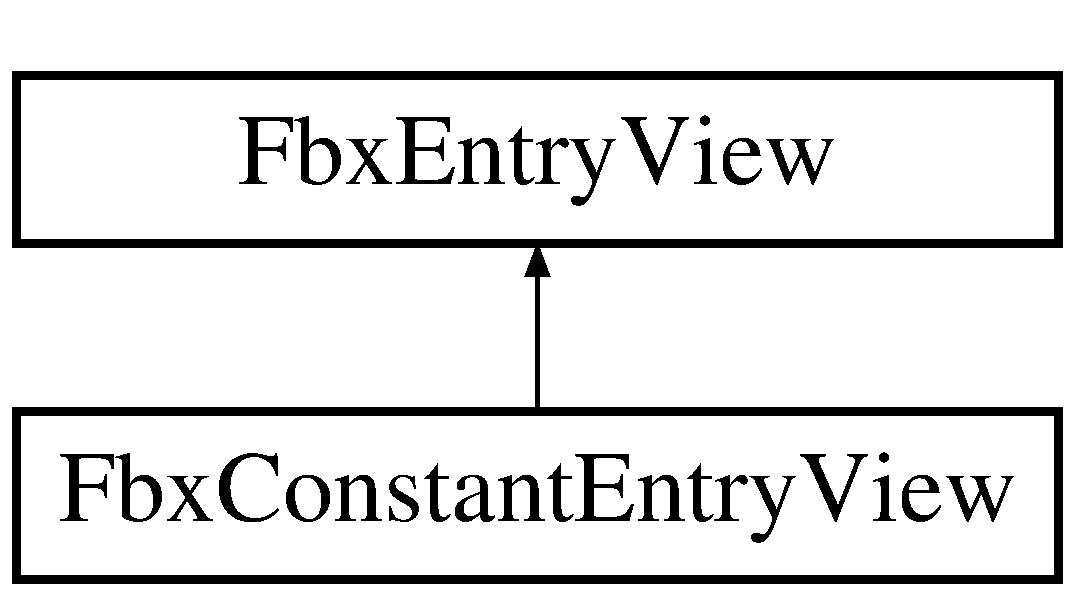
\includegraphics[height=2.000000cm]{class_fbx_constant_entry_view}
\end{center}
\end{figure}
\subsection*{公開メンバ関数}
\begin{DoxyCompactItemize}
\item 
\hyperlink{class_fbx_constant_entry_view_af49c9691fe825c0b62b3abe96c7ca823}{Fbx\+Constant\+Entry\+View} (\hyperlink{class_fbx_binding_table_entry}{Fbx\+Binding\+Table\+Entry} $\ast$p\+Entry, bool p\+As\+Source, bool p\+Create=false)
\item 
\hyperlink{class_fbx_constant_entry_view_a2d48b5460eb2b55547c0156d1774222e}{$\sim$\+Fbx\+Constant\+Entry\+View} ()
\begin{DoxyCompactList}\small\item\em Destructor. \end{DoxyCompactList}\item 
const char $\ast$ \hyperlink{class_fbx_constant_entry_view_a5e61786ae363b4281f5515e225722700}{Get\+Constant\+Name} () const
\item 
void \hyperlink{class_fbx_constant_entry_view_abe9370dc86bcdfb7b9ef617d2317f4b2}{Set\+Constant\+Name} (const char $\ast$p\+Name)
\item 
virtual const char $\ast$ \hyperlink{class_fbx_constant_entry_view_a7ea7fc9df5e1316854d18ffcc797e564}{Entry\+Type} () const
\end{DoxyCompactItemize}
\subsection*{静的公開変数類}
\begin{DoxyCompactItemize}
\item 
static const char $\ast$ \hyperlink{class_fbx_constant_entry_view_a9613da66bae01aaedaf6a08f6f538126}{s\+Entry\+Type}
\end{DoxyCompactItemize}
\subsection*{その他の継承メンバ}


\subsection{詳解}
\hyperlink{class_fbx_constant_entry_view}{Fbx\+Constant\+Entry\+View} represents constant string entry in entry tables. The constant string can be used as source or destination for the binding entry. \begin{DoxySeeAlso}{参照}
\hyperlink{class_fbx_binding_table_entry}{Fbx\+Binding\+Table\+Entry} and \hyperlink{class_fbx_binding_table}{Fbx\+Binding\+Table}. 
\end{DoxySeeAlso}


 fbxconstantentryview.\+h の 28 行目に定義があります。



\subsection{構築子と解体子}
\mbox{\Hypertarget{class_fbx_constant_entry_view_af49c9691fe825c0b62b3abe96c7ca823}\label{class_fbx_constant_entry_view_af49c9691fe825c0b62b3abe96c7ca823}} 
\index{Fbx\+Constant\+Entry\+View@{Fbx\+Constant\+Entry\+View}!Fbx\+Constant\+Entry\+View@{Fbx\+Constant\+Entry\+View}}
\index{Fbx\+Constant\+Entry\+View@{Fbx\+Constant\+Entry\+View}!Fbx\+Constant\+Entry\+View@{Fbx\+Constant\+Entry\+View}}
\subsubsection{\texorpdfstring{Fbx\+Constant\+Entry\+View()}{FbxConstantEntryView()}}
{\footnotesize\ttfamily Fbx\+Constant\+Entry\+View\+::\+Fbx\+Constant\+Entry\+View (\begin{DoxyParamCaption}\item[{\hyperlink{class_fbx_binding_table_entry}{Fbx\+Binding\+Table\+Entry} $\ast$}]{p\+Entry,  }\item[{bool}]{p\+As\+Source,  }\item[{bool}]{p\+Create = {\ttfamily false} }\end{DoxyParamCaption})}

Constructor. 
\begin{DoxyParams}{引数}
{\em p\+Entry} & The binding table entry to create the entry view for. \\
\hline
{\em p\+As\+Source} & {\ttfamily true} to create the entry view as source, {\ttfamily false} as destination. \\
\hline
{\em p\+Create} & {\ttfamily true} to create the entry view, {\ttfamily false} otherwise. \\
\hline
\end{DoxyParams}
\mbox{\Hypertarget{class_fbx_constant_entry_view_a2d48b5460eb2b55547c0156d1774222e}\label{class_fbx_constant_entry_view_a2d48b5460eb2b55547c0156d1774222e}} 
\index{Fbx\+Constant\+Entry\+View@{Fbx\+Constant\+Entry\+View}!````~Fbx\+Constant\+Entry\+View@{$\sim$\+Fbx\+Constant\+Entry\+View}}
\index{````~Fbx\+Constant\+Entry\+View@{$\sim$\+Fbx\+Constant\+Entry\+View}!Fbx\+Constant\+Entry\+View@{Fbx\+Constant\+Entry\+View}}
\subsubsection{\texorpdfstring{$\sim$\+Fbx\+Constant\+Entry\+View()}{~FbxConstantEntryView()}}
{\footnotesize\ttfamily Fbx\+Constant\+Entry\+View\+::$\sim$\+Fbx\+Constant\+Entry\+View (\begin{DoxyParamCaption}{ }\end{DoxyParamCaption})}



Destructor. 



\subsection{関数詳解}
\mbox{\Hypertarget{class_fbx_constant_entry_view_a7ea7fc9df5e1316854d18ffcc797e564}\label{class_fbx_constant_entry_view_a7ea7fc9df5e1316854d18ffcc797e564}} 
\index{Fbx\+Constant\+Entry\+View@{Fbx\+Constant\+Entry\+View}!Entry\+Type@{Entry\+Type}}
\index{Entry\+Type@{Entry\+Type}!Fbx\+Constant\+Entry\+View@{Fbx\+Constant\+Entry\+View}}
\subsubsection{\texorpdfstring{Entry\+Type()}{EntryType()}}
{\footnotesize\ttfamily virtual const char$\ast$ Fbx\+Constant\+Entry\+View\+::\+Entry\+Type (\begin{DoxyParamCaption}{ }\end{DoxyParamCaption}) const\hspace{0.3cm}{\ttfamily [virtual]}}

Get the entry type. \begin{DoxyReturn}{戻り値}
Entry type as string \char`\"{}\+Fbx\+Constant\+Entry\char`\"{}. 
\end{DoxyReturn}
\begin{DoxyRemark}{注釈}
Always use \hyperlink{class_fbx_constant_entry_view_a7ea7fc9df5e1316854d18ffcc797e564}{Entry\+Type()} to get the right entry type. 
\end{DoxyRemark}


\hyperlink{class_fbx_entry_view_a83ee50482b441ba8b0e6d7c2dba5432f}{Fbx\+Entry\+View}を再実装しています。

\mbox{\Hypertarget{class_fbx_constant_entry_view_a5e61786ae363b4281f5515e225722700}\label{class_fbx_constant_entry_view_a5e61786ae363b4281f5515e225722700}} 
\index{Fbx\+Constant\+Entry\+View@{Fbx\+Constant\+Entry\+View}!Get\+Constant\+Name@{Get\+Constant\+Name}}
\index{Get\+Constant\+Name@{Get\+Constant\+Name}!Fbx\+Constant\+Entry\+View@{Fbx\+Constant\+Entry\+View}}
\subsubsection{\texorpdfstring{Get\+Constant\+Name()}{GetConstantName()}}
{\footnotesize\ttfamily const char$\ast$ Fbx\+Constant\+Entry\+View\+::\+Get\+Constant\+Name (\begin{DoxyParamCaption}{ }\end{DoxyParamCaption}) const}

Get the constant string for binding entry. \begin{DoxyReturn}{戻り値}
The constant string. 
\end{DoxyReturn}
\mbox{\Hypertarget{class_fbx_constant_entry_view_abe9370dc86bcdfb7b9ef617d2317f4b2}\label{class_fbx_constant_entry_view_abe9370dc86bcdfb7b9ef617d2317f4b2}} 
\index{Fbx\+Constant\+Entry\+View@{Fbx\+Constant\+Entry\+View}!Set\+Constant\+Name@{Set\+Constant\+Name}}
\index{Set\+Constant\+Name@{Set\+Constant\+Name}!Fbx\+Constant\+Entry\+View@{Fbx\+Constant\+Entry\+View}}
\subsubsection{\texorpdfstring{Set\+Constant\+Name()}{SetConstantName()}}
{\footnotesize\ttfamily void Fbx\+Constant\+Entry\+View\+::\+Set\+Constant\+Name (\begin{DoxyParamCaption}\item[{const char $\ast$}]{p\+Name }\end{DoxyParamCaption})}

Set the constant string for binding entry. 
\begin{DoxyParams}{引数}
{\em p\+Name} & The constant string to set. \\
\hline
\end{DoxyParams}


\subsection{メンバ詳解}
\mbox{\Hypertarget{class_fbx_constant_entry_view_a9613da66bae01aaedaf6a08f6f538126}\label{class_fbx_constant_entry_view_a9613da66bae01aaedaf6a08f6f538126}} 
\index{Fbx\+Constant\+Entry\+View@{Fbx\+Constant\+Entry\+View}!s\+Entry\+Type@{s\+Entry\+Type}}
\index{s\+Entry\+Type@{s\+Entry\+Type}!Fbx\+Constant\+Entry\+View@{Fbx\+Constant\+Entry\+View}}
\subsubsection{\texorpdfstring{s\+Entry\+Type}{sEntryType}}
{\footnotesize\ttfamily const char$\ast$ Fbx\+Constant\+Entry\+View\+::s\+Entry\+Type\hspace{0.3cm}{\ttfamily [static]}}

Name of the entry type used in the binding entry. It should be \char`\"{}\+Fbx\+Constant\+Entry\char`\"{} in this case. 

 fbxconstantentryview.\+h の 34 行目に定義があります。



このクラス詳解は次のファイルから抽出されました\+:\begin{DoxyCompactItemize}
\item 
C\+:/\+Maya/scripts/\+F\+B\+X\+\_\+\+S\+D\+K/2017.\+1/include/fbxsdk/scene/shading/\hyperlink{fbxconstantentryview_8h}{fbxconstantentryview.\+h}\end{DoxyCompactItemize}

\hypertarget{class_fbx_const_member_func_event_handler}{}\section{Fbx\+Const\+Member\+Func\+Event\+Handler$<$ Event\+Type, Listener\+Type $>$ クラステンプレート}
\label{class_fbx_const_member_func_event_handler}\index{Fbx\+Const\+Member\+Func\+Event\+Handler$<$ Event\+Type, Listener\+Type $>$@{Fbx\+Const\+Member\+Func\+Event\+Handler$<$ Event\+Type, Listener\+Type $>$}}


{\ttfamily \#include $<$fbxeventhandler.\+h$>$}



Fbx\+Const\+Member\+Func\+Event\+Handler$<$ Event\+Type, Listener\+Type $>$ の継承関係図
% FIG 0


Fbx\+Const\+Member\+Func\+Event\+Handler$<$ Event\+Type, Listener\+Type $>$ 連携図
% FIG 1
\subsection*{公開メンバ関数}
\begin{DoxyCompactItemize}
\item 
\hyperlink{class_fbx_const_member_func_event_handler_ae3bd1e1775d0126faa06efe6ffda1211}{Fbx\+Const\+Member\+Func\+Event\+Handler} (Listener\+Type $\ast$p\+Listener\+Instance, Callback\+Fnc p\+Function)
\item 
virtual int \hyperlink{class_fbx_const_member_func_event_handler_ac88157f51fa72cba959f31dfbcdee4a5}{Get\+Handler\+Event\+Type} ()
\item 
virtual void \hyperlink{class_fbx_const_member_func_event_handler_ae6c6805404e8045de40289893709dc54}{Function\+Call} (const \hyperlink{class_fbx_event_base}{Fbx\+Event\+Base} \&p\+Event)
\item 
virtual \hyperlink{class_fbx_listener}{Fbx\+Listener} $\ast$ \hyperlink{class_fbx_const_member_func_event_handler_a9e370edd4a746ef5098d39a4f9c3d63c}{Get\+Listener} ()
\end{DoxyCompactItemize}
\subsection*{その他の継承メンバ}


\subsection{構築子と解体子}
\mbox{\Hypertarget{class_fbx_const_member_func_event_handler_ae3bd1e1775d0126faa06efe6ffda1211}\label{class_fbx_const_member_func_event_handler_ae3bd1e1775d0126faa06efe6ffda1211}} 
\index{Fbx\+Const\+Member\+Func\+Event\+Handler@{Fbx\+Const\+Member\+Func\+Event\+Handler}!Fbx\+Const\+Member\+Func\+Event\+Handler@{Fbx\+Const\+Member\+Func\+Event\+Handler}}
\index{Fbx\+Const\+Member\+Func\+Event\+Handler@{Fbx\+Const\+Member\+Func\+Event\+Handler}!Fbx\+Const\+Member\+Func\+Event\+Handler@{Fbx\+Const\+Member\+Func\+Event\+Handler}}
\subsubsection{\texorpdfstring{Fbx\+Const\+Member\+Func\+Event\+Handler()}{FbxConstMemberFuncEventHandler()}}
{\footnotesize\ttfamily template$<$typename Event\+Type, typename Listener\+Type$>$ \\
\hyperlink{class_fbx_const_member_func_event_handler}{Fbx\+Const\+Member\+Func\+Event\+Handler}$<$ Event\+Type, Listener\+Type $>$\+::\hyperlink{class_fbx_const_member_func_event_handler}{Fbx\+Const\+Member\+Func\+Event\+Handler} (\begin{DoxyParamCaption}\item[{Listener\+Type $\ast$}]{p\+Listener\+Instance,  }\item[{Callback\+Fnc}]{p\+Function }\end{DoxyParamCaption})}



\subsection{メソッド詳解}
\mbox{\Hypertarget{class_fbx_const_member_func_event_handler_ae6c6805404e8045de40289893709dc54}\label{class_fbx_const_member_func_event_handler_ae6c6805404e8045de40289893709dc54}} 
\index{Fbx\+Const\+Member\+Func\+Event\+Handler@{Fbx\+Const\+Member\+Func\+Event\+Handler}!Function\+Call@{Function\+Call}}
\index{Function\+Call@{Function\+Call}!Fbx\+Const\+Member\+Func\+Event\+Handler@{Fbx\+Const\+Member\+Func\+Event\+Handler}}
\subsubsection{\texorpdfstring{Function\+Call()}{FunctionCall()}}
{\footnotesize\ttfamily template$<$typename Event\+Type, typename Listener\+Type$>$ \\
virtual void \hyperlink{class_fbx_const_member_func_event_handler}{Fbx\+Const\+Member\+Func\+Event\+Handler}$<$ Event\+Type, Listener\+Type $>$\+::Function\+Call (\begin{DoxyParamCaption}\item[{const \hyperlink{class_fbx_event_base}{Fbx\+Event\+Base} \&}]{p\+Event }\end{DoxyParamCaption})\hspace{0.3cm}{\ttfamily [virtual]}}

Call function that process event data. 
\begin{DoxyParams}{引数}
{\em p\+Event} & specify the event type. p\+Event could be a specific class which derived from \hyperlink{class_fbx_event_base}{Fbx\+Event\+Base}. \\
\hline
\end{DoxyParams}
\begin{DoxySeeAlso}{参照}
\hyperlink{class_fbx_event_base}{Fbx\+Event\+Base} 
\end{DoxySeeAlso}


\hyperlink{class_fbx_event_handler_a46357ba45116a30c8f53c3e5fe9ba2fb}{Fbx\+Event\+Handler}を実装しています。

\mbox{\Hypertarget{class_fbx_const_member_func_event_handler_ac88157f51fa72cba959f31dfbcdee4a5}\label{class_fbx_const_member_func_event_handler_ac88157f51fa72cba959f31dfbcdee4a5}} 
\index{Fbx\+Const\+Member\+Func\+Event\+Handler@{Fbx\+Const\+Member\+Func\+Event\+Handler}!Get\+Handler\+Event\+Type@{Get\+Handler\+Event\+Type}}
\index{Get\+Handler\+Event\+Type@{Get\+Handler\+Event\+Type}!Fbx\+Const\+Member\+Func\+Event\+Handler@{Fbx\+Const\+Member\+Func\+Event\+Handler}}
\subsubsection{\texorpdfstring{Get\+Handler\+Event\+Type()}{GetHandlerEventType()}}
{\footnotesize\ttfamily template$<$typename Event\+Type, typename Listener\+Type$>$ \\
virtual int \hyperlink{class_fbx_const_member_func_event_handler}{Fbx\+Const\+Member\+Func\+Event\+Handler}$<$ Event\+Type, Listener\+Type $>$\+::Get\+Handler\+Event\+Type (\begin{DoxyParamCaption}{ }\end{DoxyParamCaption})\hspace{0.3cm}{\ttfamily [virtual]}}

Get event type of current handler. \begin{DoxyReturn}{戻り値}
The type ID of event. 
\end{DoxyReturn}


\hyperlink{class_fbx_event_handler_a0b42d2b93e63d866975f468a481c9f3c}{Fbx\+Event\+Handler}を実装しています。

\mbox{\Hypertarget{class_fbx_const_member_func_event_handler_a9e370edd4a746ef5098d39a4f9c3d63c}\label{class_fbx_const_member_func_event_handler_a9e370edd4a746ef5098d39a4f9c3d63c}} 
\index{Fbx\+Const\+Member\+Func\+Event\+Handler@{Fbx\+Const\+Member\+Func\+Event\+Handler}!Get\+Listener@{Get\+Listener}}
\index{Get\+Listener@{Get\+Listener}!Fbx\+Const\+Member\+Func\+Event\+Handler@{Fbx\+Const\+Member\+Func\+Event\+Handler}}
\subsubsection{\texorpdfstring{Get\+Listener()}{GetListener()}}
{\footnotesize\ttfamily template$<$typename Event\+Type, typename Listener\+Type$>$ \\
virtual \hyperlink{class_fbx_listener}{Fbx\+Listener}$\ast$ \hyperlink{class_fbx_const_member_func_event_handler}{Fbx\+Const\+Member\+Func\+Event\+Handler}$<$ Event\+Type, Listener\+Type $>$\+::Get\+Listener (\begin{DoxyParamCaption}{ }\end{DoxyParamCaption})\hspace{0.3cm}{\ttfamily [virtual]}}

Get listener of current handler. \begin{DoxyReturn}{戻り値}
A pointer to the listener object. 
\end{DoxyReturn}


\hyperlink{class_fbx_event_handler_a6d496102fe1253372bb042840c2d45a7}{Fbx\+Event\+Handler}を実装しています。



このクラス詳解は次のファイルから抽出されました\+:\begin{DoxyCompactItemize}
\item 
C\+:/github/\+F\+B\+Xpython\+S\+D\+K201701/\+F\+B\+Xpython\+S\+D\+K201701/2017.\+1/include/fbxsdk/core/\hyperlink{fbxeventhandler_8h}{fbxeventhandler.\+h}\end{DoxyCompactItemize}

\hypertarget{class_fbx_constraint}{}\section{Fbx\+Constraint クラス}
\label{class_fbx_constraint}\index{Fbx\+Constraint@{Fbx\+Constraint}}


{\ttfamily \#include $<$fbxconstraint.\+h$>$}

Fbx\+Constraint の継承関係図\begin{figure}[H]
\begin{center}
\leavevmode
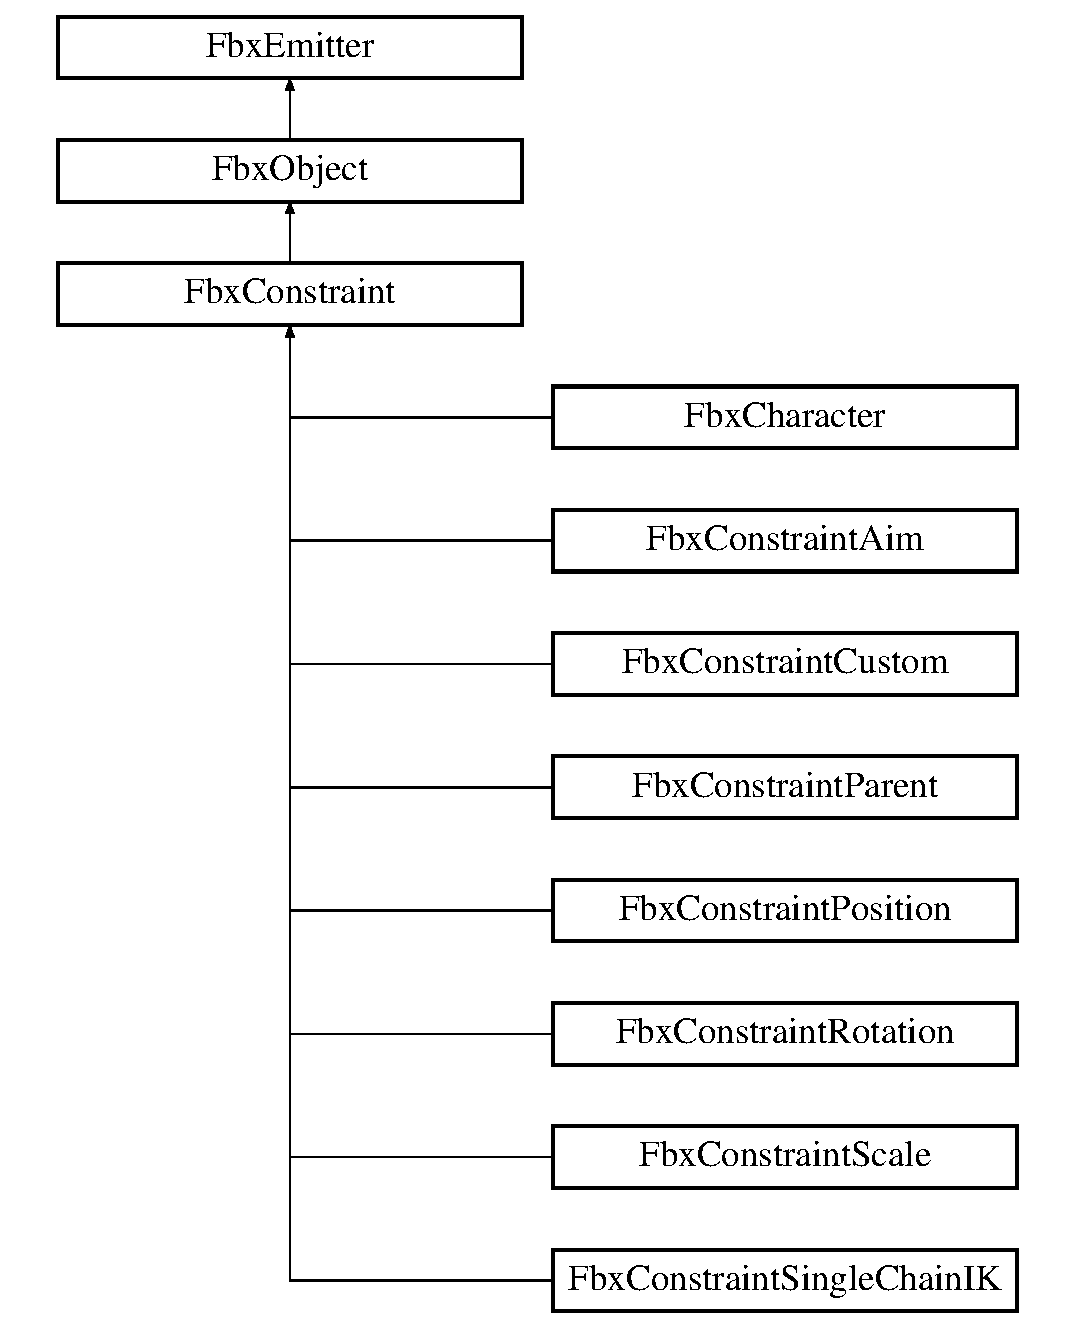
\includegraphics[height=11.000000cm]{class_fbx_constraint}
\end{center}
\end{figure}
\subsection*{公開型}
\begin{DoxyCompactItemize}
\item 
enum \hyperlink{class_fbx_constraint_a49c1634663395eab7c28856df233ec66}{E\+Type} \{ \newline
\hyperlink{class_fbx_constraint_a49c1634663395eab7c28856df233ec66a1f5c6c9045cb37f8e33ab54d41b628f2}{e\+Unknown}, 
\hyperlink{class_fbx_constraint_a49c1634663395eab7c28856df233ec66a1be363288f8d920cf30cffaa7cdef010}{e\+Position}, 
\hyperlink{class_fbx_constraint_a49c1634663395eab7c28856df233ec66a99a284f64e965cb86f9a3550a99b3160}{e\+Rotation}, 
\hyperlink{class_fbx_constraint_a49c1634663395eab7c28856df233ec66a64de25b844a25f3723f7cb0dbaa4f27a}{e\+Scale}, 
\newline
\hyperlink{class_fbx_constraint_a49c1634663395eab7c28856df233ec66a243a8e5ff104cc018d76fd60d82ad5ef}{e\+Parent}, 
\hyperlink{class_fbx_constraint_a49c1634663395eab7c28856df233ec66a849661b75a2235ba1b244bc8ee8d9509}{e\+Single\+Chain\+IK}, 
\hyperlink{class_fbx_constraint_a49c1634663395eab7c28856df233ec66a6d6fcad832cbbab74f171c5b6fa46ba1}{e\+Aim}, 
\hyperlink{class_fbx_constraint_a49c1634663395eab7c28856df233ec66ad04946a8d6506e255a01521277db52f0}{e\+Character}, 
\newline
\hyperlink{class_fbx_constraint_a49c1634663395eab7c28856df233ec66ab7e7b731132836a4bb94b9be642cd861}{e\+Custom}
 \}
\end{DoxyCompactItemize}
\subsection*{公開メンバ関数}
\begin{DoxyCompactItemize}
\item 
virtual \hyperlink{class_fbx_constraint_a49c1634663395eab7c28856df233ec66}{E\+Type} \hyperlink{class_fbx_constraint_adbeea66a1a605531a019aa6df90dc45b}{Get\+Constraint\+Type} () const
\item 
virtual \hyperlink{class_fbx_object}{Fbx\+Object} $\ast$ \hyperlink{class_fbx_constraint_a7f587d5db9685b5ee925a85354263edc}{Get\+Constrained\+Object} () const
\item 
virtual int \hyperlink{class_fbx_constraint_aa702f86c6a1832ce3b4905911e66c58f}{Get\+Constraint\+Source\+Count} () const
\item 
virtual \hyperlink{class_fbx_object}{Fbx\+Object} $\ast$ \hyperlink{class_fbx_constraint_a5ff6fe6fc98af1e33e8b297bc1cea007}{Get\+Constraint\+Source} (int) const
\item 
double \hyperlink{class_fbx_constraint_a4466dd54c32b822252c5e960d0be1836}{Get\+Source\+Weight} (const \hyperlink{class_fbx_object}{Fbx\+Object} $\ast$p\+Object) const
\end{DoxyCompactItemize}
\subsection*{限定公開メンバ関数}
\begin{DoxyCompactItemize}
\item 
virtual void \hyperlink{class_fbx_constraint_a6350b98fa8717caf9167c5513824310c}{Construct} (const \hyperlink{class_fbx_object}{Fbx\+Object} $\ast$p\+From)
\item 
virtual void \hyperlink{class_fbx_constraint_a0470a25b813b337d07a03ce4b97b44f8}{Construct\+Properties} (bool p\+Force\+Set)
\end{DoxyCompactItemize}
\subsection*{Properties}
\begin{DoxyCompactItemize}
\item 
\hyperlink{class_fbx_property_t}{Fbx\+PropertyT}$<$ \hyperlink{fbxtypes_8h_a171e72a1c46fc15c1a6c9c31948c1c5b}{Fbx\+Double} $>$ \hyperlink{class_fbx_constraint_ad056a05f11bcd1df8aae65fa6ab941d6}{Weight}
\item 
\hyperlink{class_fbx_property_t}{Fbx\+PropertyT}$<$ \hyperlink{fbxtypes_8h_a92e0562b2fe33e76a242f498b362262e}{Fbx\+Bool} $>$ \hyperlink{class_fbx_constraint_ab34f884cb053f5bb9c18f65582ab84e1}{Active}
\item 
\hyperlink{class_fbx_property_t}{Fbx\+PropertyT}$<$ \hyperlink{fbxtypes_8h_a92e0562b2fe33e76a242f498b362262e}{Fbx\+Bool} $>$ \hyperlink{class_fbx_constraint_a591ebe51dd090af37644355200b70d9a}{Lock}
\end{DoxyCompactItemize}
\subsection*{その他の継承メンバ}


\subsection{詳解}
Base class for weighted animation constraints. Constraints are primarily used to impose limits on properties of objects (e.\+g. position, orientation, scale) and to automate animation processes. A {\bfseries constrained object} is an object with properties constrained by one or more weighted {\bfseries constraint source}s. 

 fbxconstraint.\+h の 27 行目に定義があります。



\subsection{列挙型メンバ詳解}
\mbox{\Hypertarget{class_fbx_constraint_a49c1634663395eab7c28856df233ec66}\label{class_fbx_constraint_a49c1634663395eab7c28856df233ec66}} 
\index{Fbx\+Constraint@{Fbx\+Constraint}!E\+Type@{E\+Type}}
\index{E\+Type@{E\+Type}!Fbx\+Constraint@{Fbx\+Constraint}}
\subsubsection{\texorpdfstring{E\+Type}{EType}}
{\footnotesize\ttfamily enum \hyperlink{class_fbx_constraint_a49c1634663395eab7c28856df233ec66}{Fbx\+Constraint\+::\+E\+Type}}

Constraint attribute types. \begin{DoxyEnumFields}{列挙値}
\raisebox{\heightof{T}}[0pt][0pt]{\index{e\+Unknown@{e\+Unknown}!Fbx\+Constraint@{Fbx\+Constraint}}\index{Fbx\+Constraint@{Fbx\+Constraint}!e\+Unknown@{e\+Unknown}}}\mbox{\Hypertarget{class_fbx_constraint_a49c1634663395eab7c28856df233ec66a1f5c6c9045cb37f8e33ab54d41b628f2}\label{class_fbx_constraint_a49c1634663395eab7c28856df233ec66a1f5c6c9045cb37f8e33ab54d41b628f2}} 
e\+Unknown&\\
\hline

\raisebox{\heightof{T}}[0pt][0pt]{\index{e\+Position@{e\+Position}!Fbx\+Constraint@{Fbx\+Constraint}}\index{Fbx\+Constraint@{Fbx\+Constraint}!e\+Position@{e\+Position}}}\mbox{\Hypertarget{class_fbx_constraint_a49c1634663395eab7c28856df233ec66a1be363288f8d920cf30cffaa7cdef010}\label{class_fbx_constraint_a49c1634663395eab7c28856df233ec66a1be363288f8d920cf30cffaa7cdef010}} 
e\+Position&Invalid constraint. \\
\hline

\raisebox{\heightof{T}}[0pt][0pt]{\index{e\+Rotation@{e\+Rotation}!Fbx\+Constraint@{Fbx\+Constraint}}\index{Fbx\+Constraint@{Fbx\+Constraint}!e\+Rotation@{e\+Rotation}}}\mbox{\Hypertarget{class_fbx_constraint_a49c1634663395eab7c28856df233ec66a99a284f64e965cb86f9a3550a99b3160}\label{class_fbx_constraint_a49c1634663395eab7c28856df233ec66a99a284f64e965cb86f9a3550a99b3160}} 
e\+Rotation&Position constraint (referred to as a point constraint in Maya). \\
\hline

\raisebox{\heightof{T}}[0pt][0pt]{\index{e\+Scale@{e\+Scale}!Fbx\+Constraint@{Fbx\+Constraint}}\index{Fbx\+Constraint@{Fbx\+Constraint}!e\+Scale@{e\+Scale}}}\mbox{\Hypertarget{class_fbx_constraint_a49c1634663395eab7c28856df233ec66a64de25b844a25f3723f7cb0dbaa4f27a}\label{class_fbx_constraint_a49c1634663395eab7c28856df233ec66a64de25b844a25f3723f7cb0dbaa4f27a}} 
e\+Scale&Rotation constraint (referred to as an orient constraint in Maya). \\
\hline

\raisebox{\heightof{T}}[0pt][0pt]{\index{e\+Parent@{e\+Parent}!Fbx\+Constraint@{Fbx\+Constraint}}\index{Fbx\+Constraint@{Fbx\+Constraint}!e\+Parent@{e\+Parent}}}\mbox{\Hypertarget{class_fbx_constraint_a49c1634663395eab7c28856df233ec66a243a8e5ff104cc018d76fd60d82ad5ef}\label{class_fbx_constraint_a49c1634663395eab7c28856df233ec66a243a8e5ff104cc018d76fd60d82ad5ef}} 
e\+Parent&Scale constraint. \\
\hline

\raisebox{\heightof{T}}[0pt][0pt]{\index{e\+Single\+Chain\+IK@{e\+Single\+Chain\+IK}!Fbx\+Constraint@{Fbx\+Constraint}}\index{Fbx\+Constraint@{Fbx\+Constraint}!e\+Single\+Chain\+IK@{e\+Single\+Chain\+IK}}}\mbox{\Hypertarget{class_fbx_constraint_a49c1634663395eab7c28856df233ec66a849661b75a2235ba1b244bc8ee8d9509}\label{class_fbx_constraint_a49c1634663395eab7c28856df233ec66a849661b75a2235ba1b244bc8ee8d9509}} 
e\+Single\+Chain\+IK&Parent constraint. \\
\hline

\raisebox{\heightof{T}}[0pt][0pt]{\index{e\+Aim@{e\+Aim}!Fbx\+Constraint@{Fbx\+Constraint}}\index{Fbx\+Constraint@{Fbx\+Constraint}!e\+Aim@{e\+Aim}}}\mbox{\Hypertarget{class_fbx_constraint_a49c1634663395eab7c28856df233ec66a6d6fcad832cbbab74f171c5b6fa46ba1}\label{class_fbx_constraint_a49c1634663395eab7c28856df233ec66a6d6fcad832cbbab74f171c5b6fa46ba1}} 
e\+Aim&Single chain IK constraint. \\
\hline

\raisebox{\heightof{T}}[0pt][0pt]{\index{e\+Character@{e\+Character}!Fbx\+Constraint@{Fbx\+Constraint}}\index{Fbx\+Constraint@{Fbx\+Constraint}!e\+Character@{e\+Character}}}\mbox{\Hypertarget{class_fbx_constraint_a49c1634663395eab7c28856df233ec66ad04946a8d6506e255a01521277db52f0}\label{class_fbx_constraint_a49c1634663395eab7c28856df233ec66ad04946a8d6506e255a01521277db52f0}} 
e\+Character&Aim constraint. \\
\hline

\raisebox{\heightof{T}}[0pt][0pt]{\index{e\+Custom@{e\+Custom}!Fbx\+Constraint@{Fbx\+Constraint}}\index{Fbx\+Constraint@{Fbx\+Constraint}!e\+Custom@{e\+Custom}}}\mbox{\Hypertarget{class_fbx_constraint_a49c1634663395eab7c28856df233ec66ab7e7b731132836a4bb94b9be642cd861}\label{class_fbx_constraint_a49c1634663395eab7c28856df233ec66ab7e7b731132836a4bb94b9be642cd861}} 
e\+Custom&Character constraint. User defined constraints. \\
\hline

\end{DoxyEnumFields}


 fbxconstraint.\+h の 60 行目に定義があります。



\subsection{関数詳解}
\mbox{\Hypertarget{class_fbx_constraint_a6350b98fa8717caf9167c5513824310c}\label{class_fbx_constraint_a6350b98fa8717caf9167c5513824310c}} 
\index{Fbx\+Constraint@{Fbx\+Constraint}!Construct@{Construct}}
\index{Construct@{Construct}!Fbx\+Constraint@{Fbx\+Constraint}}
\subsubsection{\texorpdfstring{Construct()}{Construct()}}
{\footnotesize\ttfamily virtual void Fbx\+Constraint\+::\+Construct (\begin{DoxyParamCaption}\item[{const \hyperlink{class_fbx_object}{Fbx\+Object} $\ast$}]{p\+From }\end{DoxyParamCaption})\hspace{0.3cm}{\ttfamily [protected]}, {\ttfamily [virtual]}}

Optional constructor override, automatically called by default constructor. 
\begin{DoxyParams}{引数}
{\em p\+From} & If not null, the function must take it into account like a copy constructor. \\
\hline
\end{DoxyParams}
\begin{DoxyRemark}{注釈}
In case it is decided to override this function, do not forget to call Parent\+Class\+::\+Construct(p\+From) at the beginning. 
\end{DoxyRemark}


\hyperlink{class_fbx_object_a313503bc645af3fdceb4a99ef5cea7eb}{Fbx\+Object}を再実装しています。



\hyperlink{class_fbx_character_afccb9b74c28560f04f05581a55c0b58a}{Fbx\+Character}で再実装されています。

\mbox{\Hypertarget{class_fbx_constraint_a0470a25b813b337d07a03ce4b97b44f8}\label{class_fbx_constraint_a0470a25b813b337d07a03ce4b97b44f8}} 
\index{Fbx\+Constraint@{Fbx\+Constraint}!Construct\+Properties@{Construct\+Properties}}
\index{Construct\+Properties@{Construct\+Properties}!Fbx\+Constraint@{Fbx\+Constraint}}
\subsubsection{\texorpdfstring{Construct\+Properties()}{ConstructProperties()}}
{\footnotesize\ttfamily virtual void Fbx\+Constraint\+::\+Construct\+Properties (\begin{DoxyParamCaption}\item[{bool}]{p\+Force\+Set }\end{DoxyParamCaption})\hspace{0.3cm}{\ttfamily [protected]}, {\ttfamily [virtual]}}

Optional property constructor override, automatically called by default constructor. 
\begin{DoxyParams}{引数}
{\em p\+Force\+Set} & If the property value must be set regardless of default value. \\
\hline
\end{DoxyParams}
\begin{DoxyRemark}{注釈}
If your object have properties, they must be initialized in this function. 
\end{DoxyRemark}


\hyperlink{class_fbx_object_ad44f814323dc1b5e78bff1bfc608b4bb}{Fbx\+Object}を再実装しています。



\hyperlink{class_fbx_character_ae66db4ff3c527db3c47064c700ce179a}{Fbx\+Character}, \hyperlink{class_fbx_constraint_single_chain_i_k_aeffab44c49ad72283bdb07e50e9baf77}{Fbx\+Constraint\+Single\+Chain\+IK}, \hyperlink{class_fbx_constraint_parent_af968ae8a08629c4c259ec70ce2697c0e}{Fbx\+Constraint\+Parent}, \hyperlink{class_fbx_constraint_aim_a295c1f47dce7a051886dc6b9bb68025f}{Fbx\+Constraint\+Aim}, \hyperlink{class_fbx_constraint_position_adb2f3e784d01313ecc859b7cda16c182}{Fbx\+Constraint\+Position}, \hyperlink{class_fbx_constraint_scale_af34ea4ce8516d69aefbcb9e83060b2c1}{Fbx\+Constraint\+Scale}, \hyperlink{class_fbx_constraint_rotation_ad9f6469905777a18e3a383f402bdd9b0}{Fbx\+Constraint\+Rotation}で再実装されています。

\mbox{\Hypertarget{class_fbx_constraint_a7f587d5db9685b5ee925a85354263edc}\label{class_fbx_constraint_a7f587d5db9685b5ee925a85354263edc}} 
\index{Fbx\+Constraint@{Fbx\+Constraint}!Get\+Constrained\+Object@{Get\+Constrained\+Object}}
\index{Get\+Constrained\+Object@{Get\+Constrained\+Object}!Fbx\+Constraint@{Fbx\+Constraint}}
\subsubsection{\texorpdfstring{Get\+Constrained\+Object()}{GetConstrainedObject()}}
{\footnotesize\ttfamily virtual \hyperlink{class_fbx_object}{Fbx\+Object}$\ast$ Fbx\+Constraint\+::\+Get\+Constrained\+Object (\begin{DoxyParamCaption}{ }\end{DoxyParamCaption}) const\hspace{0.3cm}{\ttfamily [inline]}, {\ttfamily [virtual]}}

Retrieve the constrained object. \begin{DoxyReturn}{戻り値}
The constrained object. 
\end{DoxyReturn}


\hyperlink{class_fbx_constraint_parent_a8c878a029a5628f328244f824d3f8847}{Fbx\+Constraint\+Parent}, \hyperlink{class_fbx_constraint_aim_a7245132b757540df762f9b37dae533cf}{Fbx\+Constraint\+Aim}, \hyperlink{class_fbx_constraint_position_a2722540075ef79aa2d14e7e838afaf79}{Fbx\+Constraint\+Position}, \hyperlink{class_fbx_constraint_scale_a1dcbdc6b41d04d6a75ca47f024e05dc9}{Fbx\+Constraint\+Scale}, \hyperlink{class_fbx_constraint_rotation_ad9bdaf083716c730fdd907a9387e4991}{Fbx\+Constraint\+Rotation}で再実装されています。



 fbxconstraint.\+h の 81 行目に定義があります。

\mbox{\Hypertarget{class_fbx_constraint_a5ff6fe6fc98af1e33e8b297bc1cea007}\label{class_fbx_constraint_a5ff6fe6fc98af1e33e8b297bc1cea007}} 
\index{Fbx\+Constraint@{Fbx\+Constraint}!Get\+Constraint\+Source@{Get\+Constraint\+Source}}
\index{Get\+Constraint\+Source@{Get\+Constraint\+Source}!Fbx\+Constraint@{Fbx\+Constraint}}
\subsubsection{\texorpdfstring{Get\+Constraint\+Source()}{GetConstraintSource()}}
{\footnotesize\ttfamily virtual \hyperlink{class_fbx_object}{Fbx\+Object}$\ast$ Fbx\+Constraint\+::\+Get\+Constraint\+Source (\begin{DoxyParamCaption}\item[{int}]{ }\end{DoxyParamCaption}) const\hspace{0.3cm}{\ttfamily [inline]}, {\ttfamily [virtual]}}

Retrieve a constraint source with the specified index. 
\begin{DoxyParams}{引数}
{\em p\+Index} & The specified index. \\
\hline
\end{DoxyParams}
\begin{DoxyReturn}{戻り値}
The constraint source at the specified index. 
\end{DoxyReturn}


\hyperlink{class_fbx_constraint_parent_a687e5a56dfd3882d4ff0c3454a976051}{Fbx\+Constraint\+Parent}, \hyperlink{class_fbx_constraint_aim_ae5d3634ababc5cb0af0734b41c78218a}{Fbx\+Constraint\+Aim}, \hyperlink{class_fbx_constraint_position_a0024d10c8464eba13d5f3c3037e973cf}{Fbx\+Constraint\+Position}, \hyperlink{class_fbx_constraint_scale_ac957fc33cab352ef355602fb4325c5b7}{Fbx\+Constraint\+Scale}, \hyperlink{class_fbx_constraint_rotation_a4bfb008520cb5aa6996104c292e5819e}{Fbx\+Constraint\+Rotation}で再実装されています。



 fbxconstraint.\+h の 92 行目に定義があります。

\mbox{\Hypertarget{class_fbx_constraint_aa702f86c6a1832ce3b4905911e66c58f}\label{class_fbx_constraint_aa702f86c6a1832ce3b4905911e66c58f}} 
\index{Fbx\+Constraint@{Fbx\+Constraint}!Get\+Constraint\+Source\+Count@{Get\+Constraint\+Source\+Count}}
\index{Get\+Constraint\+Source\+Count@{Get\+Constraint\+Source\+Count}!Fbx\+Constraint@{Fbx\+Constraint}}
\subsubsection{\texorpdfstring{Get\+Constraint\+Source\+Count()}{GetConstraintSourceCount()}}
{\footnotesize\ttfamily virtual int Fbx\+Constraint\+::\+Get\+Constraint\+Source\+Count (\begin{DoxyParamCaption}{ }\end{DoxyParamCaption}) const\hspace{0.3cm}{\ttfamily [inline]}, {\ttfamily [virtual]}}

Retrieve the count of constraint source. \begin{DoxyReturn}{戻り値}
The count of constraint source. 
\end{DoxyReturn}


\hyperlink{class_fbx_constraint_parent_aa7747054ebeee0f94ce907451f648497}{Fbx\+Constraint\+Parent}, \hyperlink{class_fbx_constraint_aim_aa58f34b660f30caff3f89c5372a25a5c}{Fbx\+Constraint\+Aim}, \hyperlink{class_fbx_constraint_position_a5f6c49200df6a7a1fe704084c2b56e09}{Fbx\+Constraint\+Position}, \hyperlink{class_fbx_constraint_scale_a5c4500706618751078dddca3652ce936}{Fbx\+Constraint\+Scale}, \hyperlink{class_fbx_constraint_rotation_ab27178d5b53654eb9f41f6e3f3a4c5dc}{Fbx\+Constraint\+Rotation}で再実装されています。



 fbxconstraint.\+h の 86 行目に定義があります。

\mbox{\Hypertarget{class_fbx_constraint_adbeea66a1a605531a019aa6df90dc45b}\label{class_fbx_constraint_adbeea66a1a605531a019aa6df90dc45b}} 
\index{Fbx\+Constraint@{Fbx\+Constraint}!Get\+Constraint\+Type@{Get\+Constraint\+Type}}
\index{Get\+Constraint\+Type@{Get\+Constraint\+Type}!Fbx\+Constraint@{Fbx\+Constraint}}
\subsubsection{\texorpdfstring{Get\+Constraint\+Type()}{GetConstraintType()}}
{\footnotesize\ttfamily virtual \hyperlink{class_fbx_constraint_a49c1634663395eab7c28856df233ec66}{E\+Type} Fbx\+Constraint\+::\+Get\+Constraint\+Type (\begin{DoxyParamCaption}{ }\end{DoxyParamCaption}) const\hspace{0.3cm}{\ttfamily [inline]}, {\ttfamily [virtual]}}

Access the type of the constraint. \begin{DoxyReturn}{戻り値}
This type of the constraint. 
\end{DoxyReturn}


\hyperlink{class_fbx_character_ab6c9f1540880fa72c17a27d19ff11425}{Fbx\+Character}, \hyperlink{class_fbx_constraint_single_chain_i_k_adc9d38f5ae55bf9c6415334a81cbdffb}{Fbx\+Constraint\+Single\+Chain\+IK}, \hyperlink{class_fbx_constraint_parent_a02f6bd2dda6447a23d81d82ce06b73f0}{Fbx\+Constraint\+Parent}, \hyperlink{class_fbx_constraint_aim_a061ee3079d1182fa2e1a5eeebff01b15}{Fbx\+Constraint\+Aim}, \hyperlink{class_fbx_constraint_position_a79f710b1fec4b1285b53dec13ea68824}{Fbx\+Constraint\+Position}, \hyperlink{class_fbx_constraint_scale_a7eb92c352d4a4bd3c0754dd4e53fa6e4}{Fbx\+Constraint\+Scale}, \hyperlink{class_fbx_constraint_rotation_a8d9f54ac347d18a0871eafc21e88cb77}{Fbx\+Constraint\+Rotation}, \hyperlink{class_fbx_constraint_custom_a80bc6e130ef40b27e4621e1a54b22eb8}{Fbx\+Constraint\+Custom}で再実装されています。



 fbxconstraint.\+h の 76 行目に定義があります。

\mbox{\Hypertarget{class_fbx_constraint_a4466dd54c32b822252c5e960d0be1836}\label{class_fbx_constraint_a4466dd54c32b822252c5e960d0be1836}} 
\index{Fbx\+Constraint@{Fbx\+Constraint}!Get\+Source\+Weight@{Get\+Source\+Weight}}
\index{Get\+Source\+Weight@{Get\+Source\+Weight}!Fbx\+Constraint@{Fbx\+Constraint}}
\subsubsection{\texorpdfstring{Get\+Source\+Weight()}{GetSourceWeight()}}
{\footnotesize\ttfamily double Fbx\+Constraint\+::\+Get\+Source\+Weight (\begin{DoxyParamCaption}\item[{const \hyperlink{class_fbx_object}{Fbx\+Object} $\ast$}]{p\+Object }\end{DoxyParamCaption}) const}

Get the weight associated with a constraint source. 
\begin{DoxyParams}{引数}
{\em p\+Object} & The given constraint source. \\
\hline
\end{DoxyParams}
\begin{DoxyReturn}{戻り値}
The weight of the constraint source. 
\end{DoxyReturn}


\subsection{メンバ詳解}
\mbox{\Hypertarget{class_fbx_constraint_ab34f884cb053f5bb9c18f65582ab84e1}\label{class_fbx_constraint_ab34f884cb053f5bb9c18f65582ab84e1}} 
\index{Fbx\+Constraint@{Fbx\+Constraint}!Active@{Active}}
\index{Active@{Active}!Fbx\+Constraint@{Fbx\+Constraint}}
\subsubsection{\texorpdfstring{Active}{Active}}
{\footnotesize\ttfamily \hyperlink{class_fbx_property_t}{Fbx\+PropertyT}$<$\hyperlink{fbxtypes_8h_a92e0562b2fe33e76a242f498b362262e}{Fbx\+Bool}$>$ Fbx\+Constraint\+::\+Active}

This property controls whether the constraint is applied or not. If the value is {\ttfamily false} the constraint will have no effect. The default value is {\ttfamily true}.

Default value is true. 

 fbxconstraint.\+h の 47 行目に定義があります。

\mbox{\Hypertarget{class_fbx_constraint_a591ebe51dd090af37644355200b70d9a}\label{class_fbx_constraint_a591ebe51dd090af37644355200b70d9a}} 
\index{Fbx\+Constraint@{Fbx\+Constraint}!Lock@{Lock}}
\index{Lock@{Lock}!Fbx\+Constraint@{Fbx\+Constraint}}
\subsubsection{\texorpdfstring{Lock}{Lock}}
{\footnotesize\ttfamily \hyperlink{class_fbx_property_t}{Fbx\+PropertyT}$<$\hyperlink{fbxtypes_8h_a92e0562b2fe33e76a242f498b362262e}{Fbx\+Bool}$>$ Fbx\+Constraint\+::\+Lock}

This property handles the lock state of the constraint.

When enabled, the constrained object cannot be moved away from its constrained location when the constraint is active.

Default value is false. 

 fbxconstraint.\+h の 55 行目に定義があります。

\mbox{\Hypertarget{class_fbx_constraint_ad056a05f11bcd1df8aae65fa6ab941d6}\label{class_fbx_constraint_ad056a05f11bcd1df8aae65fa6ab941d6}} 
\index{Fbx\+Constraint@{Fbx\+Constraint}!Weight@{Weight}}
\index{Weight@{Weight}!Fbx\+Constraint@{Fbx\+Constraint}}
\subsubsection{\texorpdfstring{Weight}{Weight}}
{\footnotesize\ttfamily \hyperlink{class_fbx_property_t}{Fbx\+PropertyT}$<$\hyperlink{fbxtypes_8h_a171e72a1c46fc15c1a6c9c31948c1c5b}{Fbx\+Double}$>$ Fbx\+Constraint\+::\+Weight}

This property represents the degree of influence of a constraint from 0.\+0 (no influence) to 100.\+0 (full influence).

Default value is 100.\+0. 

 fbxconstraint.\+h の 40 行目に定義があります。



このクラス詳解は次のファイルから抽出されました\+:\begin{DoxyCompactItemize}
\item 
C\+:/\+Maya/scripts/\+F\+B\+X\+\_\+\+S\+D\+K/2017.\+1/include/fbxsdk/scene/constraint/\hyperlink{fbxconstraint_8h}{fbxconstraint.\+h}\end{DoxyCompactItemize}

\hypertarget{class_fbx_constraint_aim}{}\section{Fbx\+Constraint\+Aim クラス}
\label{class_fbx_constraint_aim}\index{Fbx\+Constraint\+Aim@{Fbx\+Constraint\+Aim}}


{\ttfamily \#include $<$fbxconstraintaim.\+h$>$}



Fbx\+Constraint\+Aim の継承関係図
% FIG 0


Fbx\+Constraint\+Aim 連携図
% FIG 1
\subsection*{公開型}
\begin{DoxyCompactItemize}
\item 
enum \hyperlink{class_fbx_constraint_aim_a90316b1564490f5dd0b24e552fe6e637}{E\+World\+Up} \{ \newline
\hyperlink{class_fbx_constraint_aim_a90316b1564490f5dd0b24e552fe6e637ab95495d4f984536c4e6308ed74558281}{e\+Aim\+At\+Scene\+Up}, 
\hyperlink{class_fbx_constraint_aim_a90316b1564490f5dd0b24e552fe6e637a9a5491d58c5255bc7c1a62e6ef7a95c2}{e\+Aim\+At\+Object\+Up}, 
\hyperlink{class_fbx_constraint_aim_a90316b1564490f5dd0b24e552fe6e637abf40447e1656622e38b3e5999aaee85a}{e\+Aim\+At\+Object\+Rotation\+Up}, 
\hyperlink{class_fbx_constraint_aim_a90316b1564490f5dd0b24e552fe6e637a72b5340ebf521ea46e39f3e53b9dbbb9}{e\+Aim\+At\+Vector}, 
\newline
\hyperlink{class_fbx_constraint_aim_a90316b1564490f5dd0b24e552fe6e637a9c547307df4408653e50bc3338a9fcf8}{e\+Aim\+At\+None}, 
\hyperlink{class_fbx_constraint_aim_a90316b1564490f5dd0b24e552fe6e637ad2513eb36142b46f590c27043d713c31}{e\+Aim\+At\+Count}
 \}
\end{DoxyCompactItemize}
\subsection*{公開メンバ関数}
\begin{DoxyCompactItemize}
\item 
void \hyperlink{class_fbx_constraint_aim_aca502b2b0a4587133e843c5b917acee6}{Add\+Constraint\+Source} (\hyperlink{class_fbx_object}{Fbx\+Object} $\ast$p\+Object, double p\+Weight=100)
\item 
int \hyperlink{class_fbx_constraint_aim_aa58f34b660f30caff3f89c5372a25a5c}{Get\+Constraint\+Source\+Count} () const
\item 
\hyperlink{class_fbx_object}{Fbx\+Object} $\ast$ \hyperlink{class_fbx_constraint_aim_ae5d3634ababc5cb0af0734b41c78218a}{Get\+Constraint\+Source} (int p\+Index) const
\item 
void \hyperlink{class_fbx_constraint_aim_a52db6306c4245941b42b716522b105d8}{Set\+Constrained\+Object} (\hyperlink{class_fbx_object}{Fbx\+Object} $\ast$p\+Object)
\item 
\hyperlink{class_fbx_object}{Fbx\+Object} $\ast$ \hyperlink{class_fbx_constraint_aim_a7245132b757540df762f9b37dae533cf}{Get\+Constrained\+Object} () const
\item 
void \hyperlink{class_fbx_constraint_aim_a866c7a2937ac681ec5024654ccc0c053}{Set\+World\+Up\+Object} (\hyperlink{class_fbx_object}{Fbx\+Object} $\ast$p\+Object)
\item 
\hyperlink{class_fbx_object}{Fbx\+Object} $\ast$ \hyperlink{class_fbx_constraint_aim_a3d795ffc5b595f49868c6e03a8a9245f}{Get\+World\+Up\+Object} () const
\end{DoxyCompactItemize}
\subsection*{限定公開メンバ関数}
\begin{DoxyCompactItemize}
\item 
virtual void \hyperlink{class_fbx_constraint_aim_a295c1f47dce7a051886dc6b9bb68025f}{Construct\+Properties} (bool p\+Force\+Set)
\item 
virtual \hyperlink{class_fbx_constraint_a49c1634663395eab7c28856df233ec66}{E\+Type} \hyperlink{class_fbx_constraint_aim_a061ee3079d1182fa2e1a5eeebff01b15}{Get\+Constraint\+Type} () const
\end{DoxyCompactItemize}
\subsection*{Properties}
\begin{DoxyCompactItemize}
\item 
\hyperlink{class_fbx_property_t}{Fbx\+PropertyT}$<$ \hyperlink{fbxtypes_8h_ae0a96f14cde566774c7553aa7523b7a7}{Fbx\+Double3} $>$ \hyperlink{class_fbx_constraint_aim_a2eff91c699e2dd2391f650a5659f1e5e}{Rotation\+Offset}
\item 
\hyperlink{class_fbx_property_t}{Fbx\+PropertyT}$<$ \hyperlink{fbxtypes_8h_a44df6a2eec915cf27cd481e5c5e48a24}{Fbx\+Reference} $>$ \hyperlink{class_fbx_constraint_aim_a502a01a00e7756b82d697e881fb21504}{Aim\+At\+Objects}
\item 
\hyperlink{class_fbx_property_t}{Fbx\+PropertyT}$<$ \hyperlink{fbxtypes_8h_a44df6a2eec915cf27cd481e5c5e48a24}{Fbx\+Reference} $>$ \hyperlink{class_fbx_constraint_aim_ae1e8704e4e04529a254e91080a2a19c1}{Constrained\+Object}
\item 
\hyperlink{class_fbx_property_t}{Fbx\+PropertyT}$<$ \hyperlink{fbxtypes_8h_a9a28614cb4272a0ad7d748eda7f3d3e5}{Fbx\+Enum} $>$ \hyperlink{class_fbx_constraint_aim_a01c3d71386a124da25186e795dd29956}{World\+Up\+Type}
\item 
\hyperlink{class_fbx_property_t}{Fbx\+PropertyT}$<$ \hyperlink{fbxtypes_8h_a44df6a2eec915cf27cd481e5c5e48a24}{Fbx\+Reference} $>$ \hyperlink{class_fbx_constraint_aim_a9e0b0e5bff9ccd9e0774f2f59d484b7b}{World\+Up\+Object}
\item 
\hyperlink{class_fbx_property_t}{Fbx\+PropertyT}$<$ \hyperlink{fbxtypes_8h_ae0a96f14cde566774c7553aa7523b7a7}{Fbx\+Double3} $>$ \hyperlink{class_fbx_constraint_aim_ae1d68f2cf7730299bbf63c55b52cb540}{World\+Up\+Vector}
\item 
\hyperlink{class_fbx_property_t}{Fbx\+PropertyT}$<$ \hyperlink{fbxtypes_8h_ae0a96f14cde566774c7553aa7523b7a7}{Fbx\+Double3} $>$ \hyperlink{class_fbx_constraint_aim_a6c92f45b498fd1f214cde79f84ffc9c7}{Up\+Vector}
\item 
\hyperlink{class_fbx_property_t}{Fbx\+PropertyT}$<$ \hyperlink{fbxtypes_8h_ae0a96f14cde566774c7553aa7523b7a7}{Fbx\+Double3} $>$ \hyperlink{class_fbx_constraint_aim_a7d4ef157e40e8bcb8f1cb3f12f8f9b01}{Aim\+Vector}
\item 
\hyperlink{class_fbx_property_t}{Fbx\+PropertyT}$<$ \hyperlink{fbxtypes_8h_a92e0562b2fe33e76a242f498b362262e}{Fbx\+Bool} $>$ \hyperlink{class_fbx_constraint_aim_a93257a107d3b178be6af8a221cf1b819}{AffectX}
\item 
\hyperlink{class_fbx_property_t}{Fbx\+PropertyT}$<$ \hyperlink{fbxtypes_8h_a92e0562b2fe33e76a242f498b362262e}{Fbx\+Bool} $>$ \hyperlink{class_fbx_constraint_aim_af3de7ec97229a3b7e63d23a3d9daaa98}{AffectY}
\item 
\hyperlink{class_fbx_property_t}{Fbx\+PropertyT}$<$ \hyperlink{fbxtypes_8h_a92e0562b2fe33e76a242f498b362262e}{Fbx\+Bool} $>$ \hyperlink{class_fbx_constraint_aim_ae376b28fe860f28e13a92c8ce727363c}{AffectZ}
\end{DoxyCompactItemize}
\subsection*{その他の継承メンバ}


\subsection{詳解}
An aim constraint governs an object\textquotesingle{}s orientation so that the object points to other objects. For example, you can use the aim constraint to point a light at an object or group of objects. 

\subsection{列挙型メンバ詳解}
\mbox{\Hypertarget{class_fbx_constraint_aim_a90316b1564490f5dd0b24e552fe6e637}\label{class_fbx_constraint_aim_a90316b1564490f5dd0b24e552fe6e637}} 
\index{Fbx\+Constraint\+Aim@{Fbx\+Constraint\+Aim}!E\+World\+Up@{E\+World\+Up}}
\index{E\+World\+Up@{E\+World\+Up}!Fbx\+Constraint\+Aim@{Fbx\+Constraint\+Aim}}
\subsubsection{\texorpdfstring{E\+World\+Up}{EWorldUp}}
{\footnotesize\ttfamily enum \hyperlink{class_fbx_constraint_aim_a90316b1564490f5dd0b24e552fe6e637}{Fbx\+Constraint\+Aim\+::\+E\+World\+Up}}

Constraint world up type, which has the same meaning with Maya. \begin{DoxyEnumFields}{列挙値}
\raisebox{\heightof{T}}[0pt][0pt]{\index{e\+Aim\+At\+Scene\+Up@{e\+Aim\+At\+Scene\+Up}!Fbx\+Constraint\+Aim@{Fbx\+Constraint\+Aim}}\index{Fbx\+Constraint\+Aim@{Fbx\+Constraint\+Aim}!e\+Aim\+At\+Scene\+Up@{e\+Aim\+At\+Scene\+Up}}}\mbox{\Hypertarget{class_fbx_constraint_aim_a90316b1564490f5dd0b24e552fe6e637ab95495d4f984536c4e6308ed74558281}\label{class_fbx_constraint_aim_a90316b1564490f5dd0b24e552fe6e637ab95495d4f984536c4e6308ed74558281}} 
e\+Aim\+At\+Scene\+Up&\\
\hline

\raisebox{\heightof{T}}[0pt][0pt]{\index{e\+Aim\+At\+Object\+Up@{e\+Aim\+At\+Object\+Up}!Fbx\+Constraint\+Aim@{Fbx\+Constraint\+Aim}}\index{Fbx\+Constraint\+Aim@{Fbx\+Constraint\+Aim}!e\+Aim\+At\+Object\+Up@{e\+Aim\+At\+Object\+Up}}}\mbox{\Hypertarget{class_fbx_constraint_aim_a90316b1564490f5dd0b24e552fe6e637a9a5491d58c5255bc7c1a62e6ef7a95c2}\label{class_fbx_constraint_aim_a90316b1564490f5dd0b24e552fe6e637a9a5491d58c5255bc7c1a62e6ef7a95c2}} 
e\+Aim\+At\+Object\+Up&Constraint scene up type. \\
\hline

\raisebox{\heightof{T}}[0pt][0pt]{\index{e\+Aim\+At\+Object\+Rotation\+Up@{e\+Aim\+At\+Object\+Rotation\+Up}!Fbx\+Constraint\+Aim@{Fbx\+Constraint\+Aim}}\index{Fbx\+Constraint\+Aim@{Fbx\+Constraint\+Aim}!e\+Aim\+At\+Object\+Rotation\+Up@{e\+Aim\+At\+Object\+Rotation\+Up}}}\mbox{\Hypertarget{class_fbx_constraint_aim_a90316b1564490f5dd0b24e552fe6e637abf40447e1656622e38b3e5999aaee85a}\label{class_fbx_constraint_aim_a90316b1564490f5dd0b24e552fe6e637abf40447e1656622e38b3e5999aaee85a}} 
e\+Aim\+At\+Object\+Rotation\+Up&Constraint object up type. \\
\hline

\raisebox{\heightof{T}}[0pt][0pt]{\index{e\+Aim\+At\+Vector@{e\+Aim\+At\+Vector}!Fbx\+Constraint\+Aim@{Fbx\+Constraint\+Aim}}\index{Fbx\+Constraint\+Aim@{Fbx\+Constraint\+Aim}!e\+Aim\+At\+Vector@{e\+Aim\+At\+Vector}}}\mbox{\Hypertarget{class_fbx_constraint_aim_a90316b1564490f5dd0b24e552fe6e637a72b5340ebf521ea46e39f3e53b9dbbb9}\label{class_fbx_constraint_aim_a90316b1564490f5dd0b24e552fe6e637a72b5340ebf521ea46e39f3e53b9dbbb9}} 
e\+Aim\+At\+Vector&Constraint object rotation up type. \\
\hline

\raisebox{\heightof{T}}[0pt][0pt]{\index{e\+Aim\+At\+None@{e\+Aim\+At\+None}!Fbx\+Constraint\+Aim@{Fbx\+Constraint\+Aim}}\index{Fbx\+Constraint\+Aim@{Fbx\+Constraint\+Aim}!e\+Aim\+At\+None@{e\+Aim\+At\+None}}}\mbox{\Hypertarget{class_fbx_constraint_aim_a90316b1564490f5dd0b24e552fe6e637a9c547307df4408653e50bc3338a9fcf8}\label{class_fbx_constraint_aim_a90316b1564490f5dd0b24e552fe6e637a9c547307df4408653e50bc3338a9fcf8}} 
e\+Aim\+At\+None&Constraint vector type. \\
\hline

\raisebox{\heightof{T}}[0pt][0pt]{\index{e\+Aim\+At\+Count@{e\+Aim\+At\+Count}!Fbx\+Constraint\+Aim@{Fbx\+Constraint\+Aim}}\index{Fbx\+Constraint\+Aim@{Fbx\+Constraint\+Aim}!e\+Aim\+At\+Count@{e\+Aim\+At\+Count}}}\mbox{\Hypertarget{class_fbx_constraint_aim_a90316b1564490f5dd0b24e552fe6e637ad2513eb36142b46f590c27043d713c31}\label{class_fbx_constraint_aim_a90316b1564490f5dd0b24e552fe6e637ad2513eb36142b46f590c27043d713c31}} 
e\+Aim\+At\+Count&None constraint type. Constraint world up type count. \\
\hline

\end{DoxyEnumFields}


\subsection{メソッド詳解}
\mbox{\Hypertarget{class_fbx_constraint_aim_aca502b2b0a4587133e843c5b917acee6}\label{class_fbx_constraint_aim_aca502b2b0a4587133e843c5b917acee6}} 
\index{Fbx\+Constraint\+Aim@{Fbx\+Constraint\+Aim}!Add\+Constraint\+Source@{Add\+Constraint\+Source}}
\index{Add\+Constraint\+Source@{Add\+Constraint\+Source}!Fbx\+Constraint\+Aim@{Fbx\+Constraint\+Aim}}
\subsubsection{\texorpdfstring{Add\+Constraint\+Source()}{AddConstraintSource()}}
{\footnotesize\ttfamily void Fbx\+Constraint\+Aim\+::\+Add\+Constraint\+Source (\begin{DoxyParamCaption}\item[{\hyperlink{class_fbx_object}{Fbx\+Object} $\ast$}]{p\+Object,  }\item[{double}]{p\+Weight = {\ttfamily 100} }\end{DoxyParamCaption})}

Add a source to the constraint. 
\begin{DoxyParams}{引数}
{\em p\+Object} & New source object. \\
\hline
{\em p\+Weight} & Weight of the source object. \\
\hline
\end{DoxyParams}
\mbox{\Hypertarget{class_fbx_constraint_aim_a295c1f47dce7a051886dc6b9bb68025f}\label{class_fbx_constraint_aim_a295c1f47dce7a051886dc6b9bb68025f}} 
\index{Fbx\+Constraint\+Aim@{Fbx\+Constraint\+Aim}!Construct\+Properties@{Construct\+Properties}}
\index{Construct\+Properties@{Construct\+Properties}!Fbx\+Constraint\+Aim@{Fbx\+Constraint\+Aim}}
\subsubsection{\texorpdfstring{Construct\+Properties()}{ConstructProperties()}}
{\footnotesize\ttfamily virtual void Fbx\+Constraint\+Aim\+::\+Construct\+Properties (\begin{DoxyParamCaption}\item[{bool}]{p\+Force\+Set }\end{DoxyParamCaption})\hspace{0.3cm}{\ttfamily [protected]}, {\ttfamily [virtual]}}

Optional property constructor override, automatically called by default constructor. 
\begin{DoxyParams}{引数}
{\em p\+Force\+Set} & If the property value must be set regardless of default value. \\
\hline
\end{DoxyParams}
\begin{DoxyRemark}{注釈}
If your object have properties, they must be initialized in this function. 
\end{DoxyRemark}


\hyperlink{class_fbx_constraint_a0470a25b813b337d07a03ce4b97b44f8}{Fbx\+Constraint}を再実装しています。

\mbox{\Hypertarget{class_fbx_constraint_aim_a7245132b757540df762f9b37dae533cf}\label{class_fbx_constraint_aim_a7245132b757540df762f9b37dae533cf}} 
\index{Fbx\+Constraint\+Aim@{Fbx\+Constraint\+Aim}!Get\+Constrained\+Object@{Get\+Constrained\+Object}}
\index{Get\+Constrained\+Object@{Get\+Constrained\+Object}!Fbx\+Constraint\+Aim@{Fbx\+Constraint\+Aim}}
\subsubsection{\texorpdfstring{Get\+Constrained\+Object()}{GetConstrainedObject()}}
{\footnotesize\ttfamily \hyperlink{class_fbx_object}{Fbx\+Object}$\ast$ Fbx\+Constraint\+Aim\+::\+Get\+Constrained\+Object (\begin{DoxyParamCaption}{ }\end{DoxyParamCaption}) const\hspace{0.3cm}{\ttfamily [virtual]}}

Retrieve the constrained object. \begin{DoxyReturn}{戻り値}
Current constrained object. 
\end{DoxyReturn}


\hyperlink{class_fbx_constraint_a7f587d5db9685b5ee925a85354263edc}{Fbx\+Constraint}を再実装しています。

\mbox{\Hypertarget{class_fbx_constraint_aim_ae5d3634ababc5cb0af0734b41c78218a}\label{class_fbx_constraint_aim_ae5d3634ababc5cb0af0734b41c78218a}} 
\index{Fbx\+Constraint\+Aim@{Fbx\+Constraint\+Aim}!Get\+Constraint\+Source@{Get\+Constraint\+Source}}
\index{Get\+Constraint\+Source@{Get\+Constraint\+Source}!Fbx\+Constraint\+Aim@{Fbx\+Constraint\+Aim}}
\subsubsection{\texorpdfstring{Get\+Constraint\+Source()}{GetConstraintSource()}}
{\footnotesize\ttfamily \hyperlink{class_fbx_object}{Fbx\+Object}$\ast$ Fbx\+Constraint\+Aim\+::\+Get\+Constraint\+Source (\begin{DoxyParamCaption}\item[{int}]{p\+Index }\end{DoxyParamCaption}) const\hspace{0.3cm}{\ttfamily [virtual]}}

Retrieve a constraint source object. 
\begin{DoxyParams}{引数}
{\em p\+Index} & The specified index. \\
\hline
\end{DoxyParams}
\begin{DoxyReturn}{戻り値}
Current source at the specified index. 
\end{DoxyReturn}


\hyperlink{class_fbx_constraint_a5ff6fe6fc98af1e33e8b297bc1cea007}{Fbx\+Constraint}を再実装しています。

\mbox{\Hypertarget{class_fbx_constraint_aim_aa58f34b660f30caff3f89c5372a25a5c}\label{class_fbx_constraint_aim_aa58f34b660f30caff3f89c5372a25a5c}} 
\index{Fbx\+Constraint\+Aim@{Fbx\+Constraint\+Aim}!Get\+Constraint\+Source\+Count@{Get\+Constraint\+Source\+Count}}
\index{Get\+Constraint\+Source\+Count@{Get\+Constraint\+Source\+Count}!Fbx\+Constraint\+Aim@{Fbx\+Constraint\+Aim}}
\subsubsection{\texorpdfstring{Get\+Constraint\+Source\+Count()}{GetConstraintSourceCount()}}
{\footnotesize\ttfamily int Fbx\+Constraint\+Aim\+::\+Get\+Constraint\+Source\+Count (\begin{DoxyParamCaption}{ }\end{DoxyParamCaption}) const\hspace{0.3cm}{\ttfamily [virtual]}}

Retrieve the constraint source count. \begin{DoxyReturn}{戻り値}
Current constraint source count. 
\end{DoxyReturn}


\hyperlink{class_fbx_constraint_aa702f86c6a1832ce3b4905911e66c58f}{Fbx\+Constraint}を再実装しています。

\mbox{\Hypertarget{class_fbx_constraint_aim_a061ee3079d1182fa2e1a5eeebff01b15}\label{class_fbx_constraint_aim_a061ee3079d1182fa2e1a5eeebff01b15}} 
\index{Fbx\+Constraint\+Aim@{Fbx\+Constraint\+Aim}!Get\+Constraint\+Type@{Get\+Constraint\+Type}}
\index{Get\+Constraint\+Type@{Get\+Constraint\+Type}!Fbx\+Constraint\+Aim@{Fbx\+Constraint\+Aim}}
\subsubsection{\texorpdfstring{Get\+Constraint\+Type()}{GetConstraintType()}}
{\footnotesize\ttfamily virtual \hyperlink{class_fbx_constraint_a49c1634663395eab7c28856df233ec66}{E\+Type} Fbx\+Constraint\+Aim\+::\+Get\+Constraint\+Type (\begin{DoxyParamCaption}{ }\end{DoxyParamCaption}) const\hspace{0.3cm}{\ttfamily [protected]}, {\ttfamily [virtual]}}

Access the type of the constraint. \begin{DoxyReturn}{戻り値}
This type of the constraint. 
\end{DoxyReturn}


\hyperlink{class_fbx_constraint_adbeea66a1a605531a019aa6df90dc45b}{Fbx\+Constraint}を再実装しています。

\mbox{\Hypertarget{class_fbx_constraint_aim_a3d795ffc5b595f49868c6e03a8a9245f}\label{class_fbx_constraint_aim_a3d795ffc5b595f49868c6e03a8a9245f}} 
\index{Fbx\+Constraint\+Aim@{Fbx\+Constraint\+Aim}!Get\+World\+Up\+Object@{Get\+World\+Up\+Object}}
\index{Get\+World\+Up\+Object@{Get\+World\+Up\+Object}!Fbx\+Constraint\+Aim@{Fbx\+Constraint\+Aim}}
\subsubsection{\texorpdfstring{Get\+World\+Up\+Object()}{GetWorldUpObject()}}
{\footnotesize\ttfamily \hyperlink{class_fbx_object}{Fbx\+Object}$\ast$ Fbx\+Constraint\+Aim\+::\+Get\+World\+Up\+Object (\begin{DoxyParamCaption}{ }\end{DoxyParamCaption}) const}

Retrieve the world up object. \begin{DoxyReturn}{戻り値}
The current world up object. 
\end{DoxyReturn}
\mbox{\Hypertarget{class_fbx_constraint_aim_a52db6306c4245941b42b716522b105d8}\label{class_fbx_constraint_aim_a52db6306c4245941b42b716522b105d8}} 
\index{Fbx\+Constraint\+Aim@{Fbx\+Constraint\+Aim}!Set\+Constrained\+Object@{Set\+Constrained\+Object}}
\index{Set\+Constrained\+Object@{Set\+Constrained\+Object}!Fbx\+Constraint\+Aim@{Fbx\+Constraint\+Aim}}
\subsubsection{\texorpdfstring{Set\+Constrained\+Object()}{SetConstrainedObject()}}
{\footnotesize\ttfamily void Fbx\+Constraint\+Aim\+::\+Set\+Constrained\+Object (\begin{DoxyParamCaption}\item[{\hyperlink{class_fbx_object}{Fbx\+Object} $\ast$}]{p\+Object }\end{DoxyParamCaption})}

Set the constrained object. 
\begin{DoxyParams}{引数}
{\em p\+Object} & The constrained object. \\
\hline
\end{DoxyParams}
\mbox{\Hypertarget{class_fbx_constraint_aim_a866c7a2937ac681ec5024654ccc0c053}\label{class_fbx_constraint_aim_a866c7a2937ac681ec5024654ccc0c053}} 
\index{Fbx\+Constraint\+Aim@{Fbx\+Constraint\+Aim}!Set\+World\+Up\+Object@{Set\+World\+Up\+Object}}
\index{Set\+World\+Up\+Object@{Set\+World\+Up\+Object}!Fbx\+Constraint\+Aim@{Fbx\+Constraint\+Aim}}
\subsubsection{\texorpdfstring{Set\+World\+Up\+Object()}{SetWorldUpObject()}}
{\footnotesize\ttfamily void Fbx\+Constraint\+Aim\+::\+Set\+World\+Up\+Object (\begin{DoxyParamCaption}\item[{\hyperlink{class_fbx_object}{Fbx\+Object} $\ast$}]{p\+Object }\end{DoxyParamCaption})}

Set the world up object. 
\begin{DoxyParams}{引数}
{\em p\+Object} & The new world up object. \\
\hline
\end{DoxyParams}


\subsection{メンバ詳解}
\mbox{\Hypertarget{class_fbx_constraint_aim_a93257a107d3b178be6af8a221cf1b819}\label{class_fbx_constraint_aim_a93257a107d3b178be6af8a221cf1b819}} 
\index{Fbx\+Constraint\+Aim@{Fbx\+Constraint\+Aim}!AffectX@{AffectX}}
\index{AffectX@{AffectX}!Fbx\+Constraint\+Aim@{Fbx\+Constraint\+Aim}}
\subsubsection{\texorpdfstring{AffectX}{AffectX}}
{\footnotesize\ttfamily \hyperlink{class_fbx_property_t}{Fbx\+PropertyT}$<$\hyperlink{fbxtypes_8h_a92e0562b2fe33e76a242f498b362262e}{Fbx\+Bool}$>$ Fbx\+Constraint\+Aim\+::\+AffectX}

This property handles whether to affect the rotation around X axis.

Default value is true. \mbox{\Hypertarget{class_fbx_constraint_aim_af3de7ec97229a3b7e63d23a3d9daaa98}\label{class_fbx_constraint_aim_af3de7ec97229a3b7e63d23a3d9daaa98}} 
\index{Fbx\+Constraint\+Aim@{Fbx\+Constraint\+Aim}!AffectY@{AffectY}}
\index{AffectY@{AffectY}!Fbx\+Constraint\+Aim@{Fbx\+Constraint\+Aim}}
\subsubsection{\texorpdfstring{AffectY}{AffectY}}
{\footnotesize\ttfamily \hyperlink{class_fbx_property_t}{Fbx\+PropertyT}$<$\hyperlink{fbxtypes_8h_a92e0562b2fe33e76a242f498b362262e}{Fbx\+Bool}$>$ Fbx\+Constraint\+Aim\+::\+AffectY}

This property handles whether to affect the rotation around Y axis.

Default value is true. \mbox{\Hypertarget{class_fbx_constraint_aim_ae376b28fe860f28e13a92c8ce727363c}\label{class_fbx_constraint_aim_ae376b28fe860f28e13a92c8ce727363c}} 
\index{Fbx\+Constraint\+Aim@{Fbx\+Constraint\+Aim}!AffectZ@{AffectZ}}
\index{AffectZ@{AffectZ}!Fbx\+Constraint\+Aim@{Fbx\+Constraint\+Aim}}
\subsubsection{\texorpdfstring{AffectZ}{AffectZ}}
{\footnotesize\ttfamily \hyperlink{class_fbx_property_t}{Fbx\+PropertyT}$<$\hyperlink{fbxtypes_8h_a92e0562b2fe33e76a242f498b362262e}{Fbx\+Bool}$>$ Fbx\+Constraint\+Aim\+::\+AffectZ}

This property handles whether to affect the rotation around Z axis.

Default value is true. \mbox{\Hypertarget{class_fbx_constraint_aim_a502a01a00e7756b82d697e881fb21504}\label{class_fbx_constraint_aim_a502a01a00e7756b82d697e881fb21504}} 
\index{Fbx\+Constraint\+Aim@{Fbx\+Constraint\+Aim}!Aim\+At\+Objects@{Aim\+At\+Objects}}
\index{Aim\+At\+Objects@{Aim\+At\+Objects}!Fbx\+Constraint\+Aim@{Fbx\+Constraint\+Aim}}
\subsubsection{\texorpdfstring{Aim\+At\+Objects}{AimAtObjects}}
{\footnotesize\ttfamily \hyperlink{class_fbx_property_t}{Fbx\+PropertyT}$<$\hyperlink{fbxtypes_8h_a44df6a2eec915cf27cd481e5c5e48a24}{Fbx\+Reference}$>$ Fbx\+Constraint\+Aim\+::\+Aim\+At\+Objects}

This property provides access to the object or objects which are the targets. \mbox{\Hypertarget{class_fbx_constraint_aim_a7d4ef157e40e8bcb8f1cb3f12f8f9b01}\label{class_fbx_constraint_aim_a7d4ef157e40e8bcb8f1cb3f12f8f9b01}} 
\index{Fbx\+Constraint\+Aim@{Fbx\+Constraint\+Aim}!Aim\+Vector@{Aim\+Vector}}
\index{Aim\+Vector@{Aim\+Vector}!Fbx\+Constraint\+Aim@{Fbx\+Constraint\+Aim}}
\subsubsection{\texorpdfstring{Aim\+Vector}{AimVector}}
{\footnotesize\ttfamily \hyperlink{class_fbx_property_t}{Fbx\+PropertyT}$<$\hyperlink{fbxtypes_8h_ae0a96f14cde566774c7553aa7523b7a7}{Fbx\+Double3}$>$ Fbx\+Constraint\+Aim\+::\+Aim\+Vector}

This property enables you set a specific axis for the constrained object to orient towards.

Default value is (1, 0, 0). \mbox{\Hypertarget{class_fbx_constraint_aim_ae1e8704e4e04529a254e91080a2a19c1}\label{class_fbx_constraint_aim_ae1e8704e4e04529a254e91080a2a19c1}} 
\index{Fbx\+Constraint\+Aim@{Fbx\+Constraint\+Aim}!Constrained\+Object@{Constrained\+Object}}
\index{Constrained\+Object@{Constrained\+Object}!Fbx\+Constraint\+Aim@{Fbx\+Constraint\+Aim}}
\subsubsection{\texorpdfstring{Constrained\+Object}{ConstrainedObject}}
{\footnotesize\ttfamily \hyperlink{class_fbx_property_t}{Fbx\+PropertyT}$<$\hyperlink{fbxtypes_8h_a44df6a2eec915cf27cd481e5c5e48a24}{Fbx\+Reference}$>$ Fbx\+Constraint\+Aim\+::\+Constrained\+Object}

This property provides access to the object being aimed. \mbox{\Hypertarget{class_fbx_constraint_aim_a2eff91c699e2dd2391f650a5659f1e5e}\label{class_fbx_constraint_aim_a2eff91c699e2dd2391f650a5659f1e5e}} 
\index{Fbx\+Constraint\+Aim@{Fbx\+Constraint\+Aim}!Rotation\+Offset@{Rotation\+Offset}}
\index{Rotation\+Offset@{Rotation\+Offset}!Fbx\+Constraint\+Aim@{Fbx\+Constraint\+Aim}}
\subsubsection{\texorpdfstring{Rotation\+Offset}{RotationOffset}}
{\footnotesize\ttfamily \hyperlink{class_fbx_property_t}{Fbx\+PropertyT}$<$\hyperlink{fbxtypes_8h_ae0a96f14cde566774c7553aa7523b7a7}{Fbx\+Double3}$>$ Fbx\+Constraint\+Aim\+::\+Rotation\+Offset}

This property handles the rotation offset value.

Default value is (0, 0, 0). \mbox{\Hypertarget{class_fbx_constraint_aim_a6c92f45b498fd1f214cde79f84ffc9c7}\label{class_fbx_constraint_aim_a6c92f45b498fd1f214cde79f84ffc9c7}} 
\index{Fbx\+Constraint\+Aim@{Fbx\+Constraint\+Aim}!Up\+Vector@{Up\+Vector}}
\index{Up\+Vector@{Up\+Vector}!Fbx\+Constraint\+Aim@{Fbx\+Constraint\+Aim}}
\subsubsection{\texorpdfstring{Up\+Vector}{UpVector}}
{\footnotesize\ttfamily \hyperlink{class_fbx_property_t}{Fbx\+PropertyT}$<$\hyperlink{fbxtypes_8h_ae0a96f14cde566774c7553aa7523b7a7}{Fbx\+Double3}$>$ Fbx\+Constraint\+Aim\+::\+Up\+Vector}

This property handles up vector.

Default value is (0, 1, 0). \mbox{\Hypertarget{class_fbx_constraint_aim_a9e0b0e5bff9ccd9e0774f2f59d484b7b}\label{class_fbx_constraint_aim_a9e0b0e5bff9ccd9e0774f2f59d484b7b}} 
\index{Fbx\+Constraint\+Aim@{Fbx\+Constraint\+Aim}!World\+Up\+Object@{World\+Up\+Object}}
\index{World\+Up\+Object@{World\+Up\+Object}!Fbx\+Constraint\+Aim@{Fbx\+Constraint\+Aim}}
\subsubsection{\texorpdfstring{World\+Up\+Object}{WorldUpObject}}
{\footnotesize\ttfamily \hyperlink{class_fbx_property_t}{Fbx\+PropertyT}$<$\hyperlink{fbxtypes_8h_a44df6a2eec915cf27cd481e5c5e48a24}{Fbx\+Reference}$>$ Fbx\+Constraint\+Aim\+::\+World\+Up\+Object}

This property handles world up object. \mbox{\Hypertarget{class_fbx_constraint_aim_a01c3d71386a124da25186e795dd29956}\label{class_fbx_constraint_aim_a01c3d71386a124da25186e795dd29956}} 
\index{Fbx\+Constraint\+Aim@{Fbx\+Constraint\+Aim}!World\+Up\+Type@{World\+Up\+Type}}
\index{World\+Up\+Type@{World\+Up\+Type}!Fbx\+Constraint\+Aim@{Fbx\+Constraint\+Aim}}
\subsubsection{\texorpdfstring{World\+Up\+Type}{WorldUpType}}
{\footnotesize\ttfamily \hyperlink{class_fbx_property_t}{Fbx\+PropertyT}$<$\hyperlink{fbxtypes_8h_a9a28614cb4272a0ad7d748eda7f3d3e5}{Fbx\+Enum}$>$ Fbx\+Constraint\+Aim\+::\+World\+Up\+Type}

This property handles world up type. \mbox{\Hypertarget{class_fbx_constraint_aim_ae1d68f2cf7730299bbf63c55b52cb540}\label{class_fbx_constraint_aim_ae1d68f2cf7730299bbf63c55b52cb540}} 
\index{Fbx\+Constraint\+Aim@{Fbx\+Constraint\+Aim}!World\+Up\+Vector@{World\+Up\+Vector}}
\index{World\+Up\+Vector@{World\+Up\+Vector}!Fbx\+Constraint\+Aim@{Fbx\+Constraint\+Aim}}
\subsubsection{\texorpdfstring{World\+Up\+Vector}{WorldUpVector}}
{\footnotesize\ttfamily \hyperlink{class_fbx_property_t}{Fbx\+PropertyT}$<$\hyperlink{fbxtypes_8h_ae0a96f14cde566774c7553aa7523b7a7}{Fbx\+Double3}$>$ Fbx\+Constraint\+Aim\+::\+World\+Up\+Vector}

This property handles world up vector.

Default value is (0, 1, 0). 

このクラス詳解は次のファイルから抽出されました\+:\begin{DoxyCompactItemize}
\item 
C\+:/github/\+F\+B\+Xpython\+S\+D\+K201701/\+F\+B\+Xpython\+S\+D\+K201701/2017.\+1/include/fbxsdk/scene/constraint/\hyperlink{fbxconstraintaim_8h}{fbxconstraintaim.\+h}\end{DoxyCompactItemize}

\hypertarget{class_fbx_constraint_custom}{}\section{Fbx\+Constraint\+Custom クラス}
\label{class_fbx_constraint_custom}\index{Fbx\+Constraint\+Custom@{Fbx\+Constraint\+Custom}}


This constraint class contains methods for custom constraint.  




{\ttfamily \#include $<$fbxconstraintcustom.\+h$>$}

Fbx\+Constraint\+Custom の継承関係図\begin{figure}[H]
\begin{center}
\leavevmode
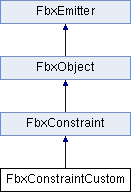
\includegraphics[height=4.000000cm]{class_fbx_constraint_custom}
\end{center}
\end{figure}
\subsection*{限定公開メンバ関数}
\begin{DoxyCompactItemize}
\item 
virtual \hyperlink{class_fbx_constraint_a49c1634663395eab7c28856df233ec66}{E\+Type} \hyperlink{class_fbx_constraint_custom_a80bc6e130ef40b27e4621e1a54b22eb8}{Get\+Constraint\+Type} () const
\end{DoxyCompactItemize}
\subsection*{その他の継承メンバ}


\subsection{詳解}
This constraint class contains methods for custom constraint. 

 fbxconstraintcustom.\+h の 25 行目に定義があります。



\subsection{関数詳解}
\mbox{\Hypertarget{class_fbx_constraint_custom_a80bc6e130ef40b27e4621e1a54b22eb8}\label{class_fbx_constraint_custom_a80bc6e130ef40b27e4621e1a54b22eb8}} 
\index{Fbx\+Constraint\+Custom@{Fbx\+Constraint\+Custom}!Get\+Constraint\+Type@{Get\+Constraint\+Type}}
\index{Get\+Constraint\+Type@{Get\+Constraint\+Type}!Fbx\+Constraint\+Custom@{Fbx\+Constraint\+Custom}}
\subsubsection{\texorpdfstring{Get\+Constraint\+Type()}{GetConstraintType()}}
{\footnotesize\ttfamily virtual \hyperlink{class_fbx_constraint_a49c1634663395eab7c28856df233ec66}{E\+Type} Fbx\+Constraint\+Custom\+::\+Get\+Constraint\+Type (\begin{DoxyParamCaption}{ }\end{DoxyParamCaption}) const\hspace{0.3cm}{\ttfamily [protected]}, {\ttfamily [virtual]}}

Access the type of the constraint. \begin{DoxyReturn}{戻り値}
This type of the constraint. 
\end{DoxyReturn}


\hyperlink{class_fbx_constraint_adbeea66a1a605531a019aa6df90dc45b}{Fbx\+Constraint}を再実装しています。



このクラス詳解は次のファイルから抽出されました\+:\begin{DoxyCompactItemize}
\item 
C\+:/\+Maya/scripts/\+F\+B\+X\+\_\+\+S\+D\+K/2017.\+1/include/fbxsdk/scene/constraint/\hyperlink{fbxconstraintcustom_8h}{fbxconstraintcustom.\+h}\end{DoxyCompactItemize}

\hypertarget{class_fbx_constraint_parent}{}\section{Fbx\+Constraint\+Parent クラス}
\label{class_fbx_constraint_parent}\index{Fbx\+Constraint\+Parent@{Fbx\+Constraint\+Parent}}


{\ttfamily \#include $<$fbxconstraintparent.\+h$>$}

Fbx\+Constraint\+Parent の継承関係図\begin{figure}[H]
\begin{center}
\leavevmode
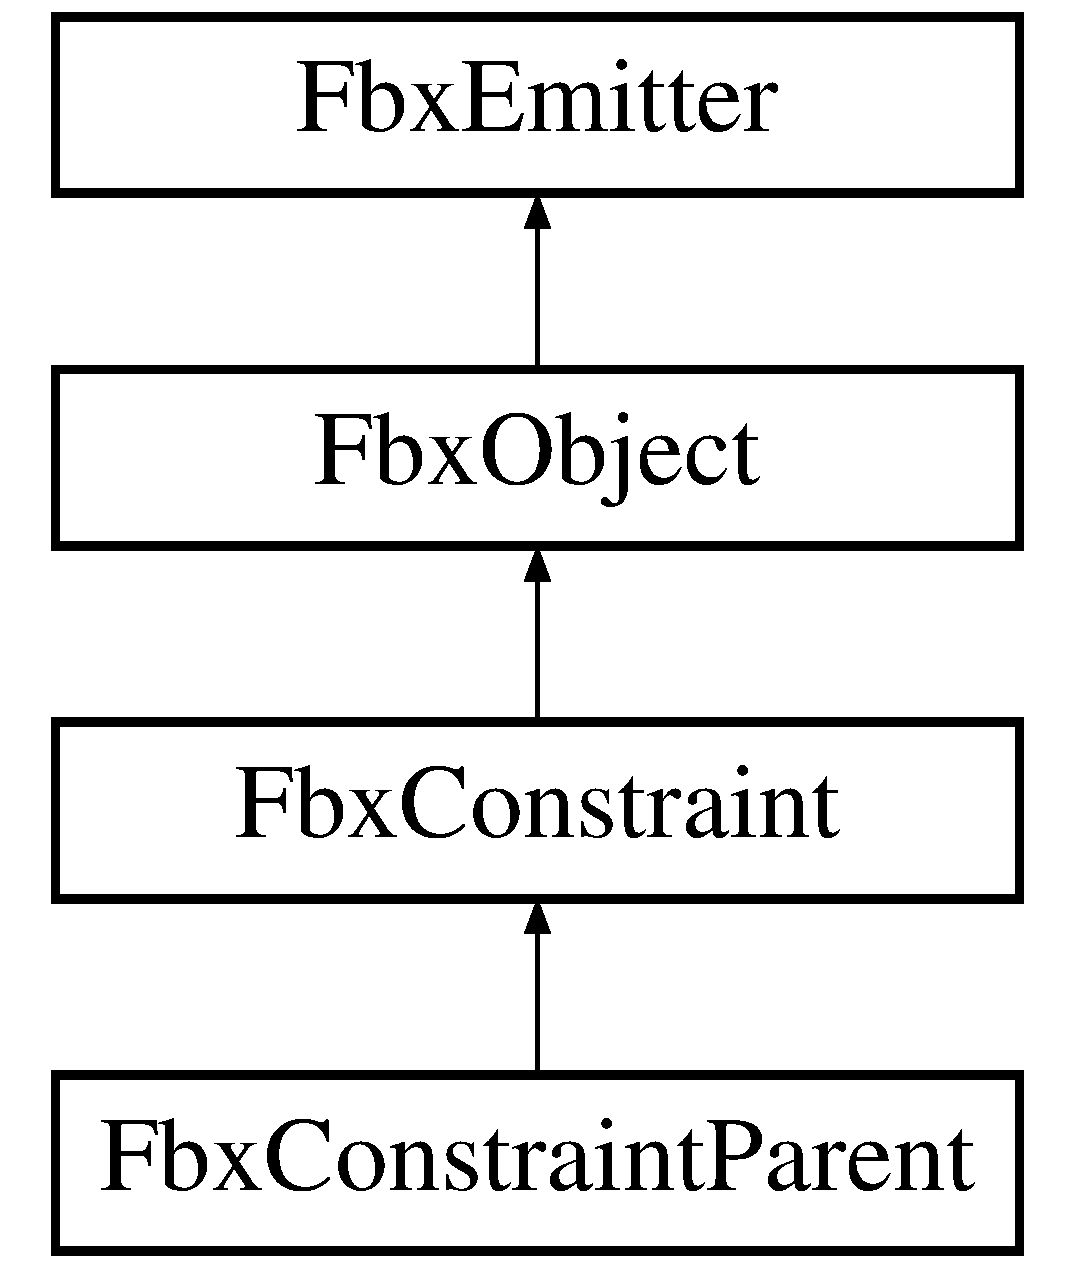
\includegraphics[height=4.000000cm]{class_fbx_constraint_parent}
\end{center}
\end{figure}
\subsection*{公開メンバ関数}
\begin{DoxyCompactItemize}
\item 
void \hyperlink{class_fbx_constraint_parent_ae821dbbc810b2ee3f27c46d0a66ec55f}{Set\+Translation\+Offset} (\hyperlink{class_fbx_object}{Fbx\+Object} $\ast$p\+Object, \hyperlink{class_fbx_vector4}{Fbx\+Vector4} p\+Translation)
\item 
\hyperlink{class_fbx_vector4}{Fbx\+Vector4} \hyperlink{class_fbx_constraint_parent_a8ba24a43fc99dbef7819ccb921b1ba19}{Get\+Translation\+Offset} (const \hyperlink{class_fbx_object}{Fbx\+Object} $\ast$p\+Object) const
\item 
virtual void \hyperlink{class_fbx_constraint_parent_a22d24573f7d06251dcf94bb488a32386}{Set\+Rotation\+Offset} (const \hyperlink{class_fbx_object}{Fbx\+Object} $\ast$p\+Object, \hyperlink{class_fbx_vector4}{Fbx\+Vector4} p\+Rotation)
\item 
\hyperlink{class_fbx_vector4}{Fbx\+Vector4} \hyperlink{class_fbx_constraint_parent_a35f64fd4fccedbd4070d5e2bdb9ce06b}{Get\+Rotation\+Offset} (const \hyperlink{class_fbx_object}{Fbx\+Object} $\ast$p\+Object) const
\item 
void \hyperlink{class_fbx_constraint_parent_af1cb13c89d62f1de2478a5a102fd5788}{Add\+Constraint\+Source} (\hyperlink{class_fbx_object}{Fbx\+Object} $\ast$p\+Object, double p\+Weight=100)
\item 
int \hyperlink{class_fbx_constraint_parent_aa7747054ebeee0f94ce907451f648497}{Get\+Constraint\+Source\+Count} () const
\item 
\hyperlink{class_fbx_object}{Fbx\+Object} $\ast$ \hyperlink{class_fbx_constraint_parent_a687e5a56dfd3882d4ff0c3454a976051}{Get\+Constraint\+Source} (int p\+Index) const
\item 
void \hyperlink{class_fbx_constraint_parent_a49473a23e0aae69dd06ee4bd19b6fee3}{Set\+Constrained\+Object} (\hyperlink{class_fbx_object}{Fbx\+Object} $\ast$p\+Object)
\item 
\hyperlink{class_fbx_object}{Fbx\+Object} $\ast$ \hyperlink{class_fbx_constraint_parent_a8c878a029a5628f328244f824d3f8847}{Get\+Constrained\+Object} () const
\end{DoxyCompactItemize}
\subsection*{限定公開メンバ関数}
\begin{DoxyCompactItemize}
\item 
virtual void \hyperlink{class_fbx_constraint_parent_af968ae8a08629c4c259ec70ce2697c0e}{Construct\+Properties} (bool p\+Force\+Set)
\item 
virtual \hyperlink{class_fbx_constraint_a49c1634663395eab7c28856df233ec66}{E\+Type} \hyperlink{class_fbx_constraint_parent_a02f6bd2dda6447a23d81d82ce06b73f0}{Get\+Constraint\+Type} () const
\end{DoxyCompactItemize}
\subsection*{Properties}
\begin{DoxyCompactItemize}
\item 
\hyperlink{class_fbx_property_t}{Fbx\+PropertyT}$<$ \hyperlink{fbxtypes_8h_a92e0562b2fe33e76a242f498b362262e}{Fbx\+Bool} $>$ \hyperlink{class_fbx_constraint_parent_ac67f39b8f34fce85fdfba40823d243fe}{Affect\+TranslationX}
\item 
\hyperlink{class_fbx_property_t}{Fbx\+PropertyT}$<$ \hyperlink{fbxtypes_8h_a92e0562b2fe33e76a242f498b362262e}{Fbx\+Bool} $>$ \hyperlink{class_fbx_constraint_parent_a7aa3f5ad68f44254492c70e8f7201750}{Affect\+TranslationY}
\item 
\hyperlink{class_fbx_property_t}{Fbx\+PropertyT}$<$ \hyperlink{fbxtypes_8h_a92e0562b2fe33e76a242f498b362262e}{Fbx\+Bool} $>$ \hyperlink{class_fbx_constraint_parent_ab173e3fc6e6fd0d1cfca4f3227aec6b2}{Affect\+TranslationZ}
\item 
\hyperlink{class_fbx_property_t}{Fbx\+PropertyT}$<$ \hyperlink{fbxtypes_8h_a92e0562b2fe33e76a242f498b362262e}{Fbx\+Bool} $>$ \hyperlink{class_fbx_constraint_parent_ab364319598a6be917048f261160aced4}{Affect\+RotationX}
\item 
\hyperlink{class_fbx_property_t}{Fbx\+PropertyT}$<$ \hyperlink{fbxtypes_8h_a92e0562b2fe33e76a242f498b362262e}{Fbx\+Bool} $>$ \hyperlink{class_fbx_constraint_parent_a50b11f7aca12a04e5048680e0f7af486}{Affect\+RotationY}
\item 
\hyperlink{class_fbx_property_t}{Fbx\+PropertyT}$<$ \hyperlink{fbxtypes_8h_a92e0562b2fe33e76a242f498b362262e}{Fbx\+Bool} $>$ \hyperlink{class_fbx_constraint_parent_a2b6447babd670eb5023143d1773cdaf8}{Affect\+RotationZ}
\item 
\hyperlink{class_fbx_property_t}{Fbx\+PropertyT}$<$ \hyperlink{fbxtypes_8h_a92e0562b2fe33e76a242f498b362262e}{Fbx\+Bool} $>$ \hyperlink{class_fbx_constraint_parent_ab4f8c487608b32feff9804c7e70e851e}{Affect\+ScalingX}
\item 
\hyperlink{class_fbx_property_t}{Fbx\+PropertyT}$<$ \hyperlink{fbxtypes_8h_a92e0562b2fe33e76a242f498b362262e}{Fbx\+Bool} $>$ \hyperlink{class_fbx_constraint_parent_a32b210fd27c0e55456741428987755fe}{Affect\+ScalingY}
\item 
\hyperlink{class_fbx_property_t}{Fbx\+PropertyT}$<$ \hyperlink{fbxtypes_8h_a92e0562b2fe33e76a242f498b362262e}{Fbx\+Bool} $>$ \hyperlink{class_fbx_constraint_parent_abbbb60d845ab61bede0b28f5a7defa22}{Affect\+ScalingZ}
\item 
\hyperlink{class_fbx_property_t}{Fbx\+PropertyT}$<$ \hyperlink{fbxtypes_8h_a44df6a2eec915cf27cd481e5c5e48a24}{Fbx\+Reference} $>$ \hyperlink{class_fbx_constraint_parent_a02690debabacd0fe4b643cbb04c042a7}{Constraint\+Sources}
\item 
\hyperlink{class_fbx_property_t}{Fbx\+PropertyT}$<$ \hyperlink{fbxtypes_8h_a44df6a2eec915cf27cd481e5c5e48a24}{Fbx\+Reference} $>$ \hyperlink{class_fbx_constraint_parent_aaaf70448aed2fafcd4f2d7e1a4409a6e}{Constrained\+Object}
\end{DoxyCompactItemize}
\subsection*{その他の継承メンバ}


\subsection{詳解}
The parent constraint creates a parent-\/to-\/child relationship between any two objects, from any two hierarchies. It creates the same relationship as the parent-\/to-\/child relationships found in hierarchies. You can use this constraint to connect objects without changing hierarchies. 

 fbxconstraintparent.\+h の 27 行目に定義があります。



\subsection{関数詳解}
\mbox{\Hypertarget{class_fbx_constraint_parent_af1cb13c89d62f1de2478a5a102fd5788}\label{class_fbx_constraint_parent_af1cb13c89d62f1de2478a5a102fd5788}} 
\index{Fbx\+Constraint\+Parent@{Fbx\+Constraint\+Parent}!Add\+Constraint\+Source@{Add\+Constraint\+Source}}
\index{Add\+Constraint\+Source@{Add\+Constraint\+Source}!Fbx\+Constraint\+Parent@{Fbx\+Constraint\+Parent}}
\subsubsection{\texorpdfstring{Add\+Constraint\+Source()}{AddConstraintSource()}}
{\footnotesize\ttfamily void Fbx\+Constraint\+Parent\+::\+Add\+Constraint\+Source (\begin{DoxyParamCaption}\item[{\hyperlink{class_fbx_object}{Fbx\+Object} $\ast$}]{p\+Object,  }\item[{double}]{p\+Weight = {\ttfamily 100} }\end{DoxyParamCaption})}

Add a constraint source to the constraint. 
\begin{DoxyParams}{引数}
{\em p\+Object} & New constraint source. \\
\hline
{\em p\+Weight} & Weight of the constraint source. \\
\hline
\end{DoxyParams}
\mbox{\Hypertarget{class_fbx_constraint_parent_af968ae8a08629c4c259ec70ce2697c0e}\label{class_fbx_constraint_parent_af968ae8a08629c4c259ec70ce2697c0e}} 
\index{Fbx\+Constraint\+Parent@{Fbx\+Constraint\+Parent}!Construct\+Properties@{Construct\+Properties}}
\index{Construct\+Properties@{Construct\+Properties}!Fbx\+Constraint\+Parent@{Fbx\+Constraint\+Parent}}
\subsubsection{\texorpdfstring{Construct\+Properties()}{ConstructProperties()}}
{\footnotesize\ttfamily virtual void Fbx\+Constraint\+Parent\+::\+Construct\+Properties (\begin{DoxyParamCaption}\item[{bool}]{p\+Force\+Set }\end{DoxyParamCaption})\hspace{0.3cm}{\ttfamily [protected]}, {\ttfamily [virtual]}}

Optional property constructor override, automatically called by default constructor. 
\begin{DoxyParams}{引数}
{\em p\+Force\+Set} & If the property value must be set regardless of default value. \\
\hline
\end{DoxyParams}
\begin{DoxyRemark}{注釈}
If your object have properties, they must be initialized in this function. 
\end{DoxyRemark}


\hyperlink{class_fbx_constraint_a0470a25b813b337d07a03ce4b97b44f8}{Fbx\+Constraint}を再実装しています。

\mbox{\Hypertarget{class_fbx_constraint_parent_a8c878a029a5628f328244f824d3f8847}\label{class_fbx_constraint_parent_a8c878a029a5628f328244f824d3f8847}} 
\index{Fbx\+Constraint\+Parent@{Fbx\+Constraint\+Parent}!Get\+Constrained\+Object@{Get\+Constrained\+Object}}
\index{Get\+Constrained\+Object@{Get\+Constrained\+Object}!Fbx\+Constraint\+Parent@{Fbx\+Constraint\+Parent}}
\subsubsection{\texorpdfstring{Get\+Constrained\+Object()}{GetConstrainedObject()}}
{\footnotesize\ttfamily \hyperlink{class_fbx_object}{Fbx\+Object}$\ast$ Fbx\+Constraint\+Parent\+::\+Get\+Constrained\+Object (\begin{DoxyParamCaption}{ }\end{DoxyParamCaption}) const\hspace{0.3cm}{\ttfamily [virtual]}}

Retrieve the constrained object. \begin{DoxyReturn}{戻り値}
Current constrained object. 
\end{DoxyReturn}


\hyperlink{class_fbx_constraint_a7f587d5db9685b5ee925a85354263edc}{Fbx\+Constraint}を再実装しています。

\mbox{\Hypertarget{class_fbx_constraint_parent_a687e5a56dfd3882d4ff0c3454a976051}\label{class_fbx_constraint_parent_a687e5a56dfd3882d4ff0c3454a976051}} 
\index{Fbx\+Constraint\+Parent@{Fbx\+Constraint\+Parent}!Get\+Constraint\+Source@{Get\+Constraint\+Source}}
\index{Get\+Constraint\+Source@{Get\+Constraint\+Source}!Fbx\+Constraint\+Parent@{Fbx\+Constraint\+Parent}}
\subsubsection{\texorpdfstring{Get\+Constraint\+Source()}{GetConstraintSource()}}
{\footnotesize\ttfamily \hyperlink{class_fbx_object}{Fbx\+Object}$\ast$ Fbx\+Constraint\+Parent\+::\+Get\+Constraint\+Source (\begin{DoxyParamCaption}\item[{int}]{p\+Index }\end{DoxyParamCaption}) const\hspace{0.3cm}{\ttfamily [virtual]}}

Retrieve a constraint source object. 
\begin{DoxyParams}{引数}
{\em p\+Index} & Index of the constraint source. \\
\hline
\end{DoxyParams}
\begin{DoxyReturn}{戻り値}
The constraint source at the specified index. 
\end{DoxyReturn}


\hyperlink{class_fbx_constraint_a5ff6fe6fc98af1e33e8b297bc1cea007}{Fbx\+Constraint}を再実装しています。

\mbox{\Hypertarget{class_fbx_constraint_parent_aa7747054ebeee0f94ce907451f648497}\label{class_fbx_constraint_parent_aa7747054ebeee0f94ce907451f648497}} 
\index{Fbx\+Constraint\+Parent@{Fbx\+Constraint\+Parent}!Get\+Constraint\+Source\+Count@{Get\+Constraint\+Source\+Count}}
\index{Get\+Constraint\+Source\+Count@{Get\+Constraint\+Source\+Count}!Fbx\+Constraint\+Parent@{Fbx\+Constraint\+Parent}}
\subsubsection{\texorpdfstring{Get\+Constraint\+Source\+Count()}{GetConstraintSourceCount()}}
{\footnotesize\ttfamily int Fbx\+Constraint\+Parent\+::\+Get\+Constraint\+Source\+Count (\begin{DoxyParamCaption}{ }\end{DoxyParamCaption}) const\hspace{0.3cm}{\ttfamily [virtual]}}

Retrieve the constraint source count. \begin{DoxyReturn}{戻り値}
Current constraint source count. 
\end{DoxyReturn}


\hyperlink{class_fbx_constraint_aa702f86c6a1832ce3b4905911e66c58f}{Fbx\+Constraint}を再実装しています。

\mbox{\Hypertarget{class_fbx_constraint_parent_a02f6bd2dda6447a23d81d82ce06b73f0}\label{class_fbx_constraint_parent_a02f6bd2dda6447a23d81d82ce06b73f0}} 
\index{Fbx\+Constraint\+Parent@{Fbx\+Constraint\+Parent}!Get\+Constraint\+Type@{Get\+Constraint\+Type}}
\index{Get\+Constraint\+Type@{Get\+Constraint\+Type}!Fbx\+Constraint\+Parent@{Fbx\+Constraint\+Parent}}
\subsubsection{\texorpdfstring{Get\+Constraint\+Type()}{GetConstraintType()}}
{\footnotesize\ttfamily virtual \hyperlink{class_fbx_constraint_a49c1634663395eab7c28856df233ec66}{E\+Type} Fbx\+Constraint\+Parent\+::\+Get\+Constraint\+Type (\begin{DoxyParamCaption}{ }\end{DoxyParamCaption}) const\hspace{0.3cm}{\ttfamily [protected]}, {\ttfamily [virtual]}}

Access the type of the constraint. \begin{DoxyReturn}{戻り値}
This type of the constraint. 
\end{DoxyReturn}


\hyperlink{class_fbx_constraint_adbeea66a1a605531a019aa6df90dc45b}{Fbx\+Constraint}を再実装しています。

\mbox{\Hypertarget{class_fbx_constraint_parent_a35f64fd4fccedbd4070d5e2bdb9ce06b}\label{class_fbx_constraint_parent_a35f64fd4fccedbd4070d5e2bdb9ce06b}} 
\index{Fbx\+Constraint\+Parent@{Fbx\+Constraint\+Parent}!Get\+Rotation\+Offset@{Get\+Rotation\+Offset}}
\index{Get\+Rotation\+Offset@{Get\+Rotation\+Offset}!Fbx\+Constraint\+Parent@{Fbx\+Constraint\+Parent}}
\subsubsection{\texorpdfstring{Get\+Rotation\+Offset()}{GetRotationOffset()}}
{\footnotesize\ttfamily \hyperlink{class_fbx_vector4}{Fbx\+Vector4} Fbx\+Constraint\+Parent\+::\+Get\+Rotation\+Offset (\begin{DoxyParamCaption}\item[{const \hyperlink{class_fbx_object}{Fbx\+Object} $\ast$}]{p\+Object }\end{DoxyParamCaption}) const}

Retrieve the rotation offset of the specified constraint source. 
\begin{DoxyParams}{引数}
{\em p\+Object} & The specified constraint source. \\
\hline
\end{DoxyParams}
\begin{DoxyReturn}{戻り値}
The current translation offset. 
\end{DoxyReturn}
\mbox{\Hypertarget{class_fbx_constraint_parent_a8ba24a43fc99dbef7819ccb921b1ba19}\label{class_fbx_constraint_parent_a8ba24a43fc99dbef7819ccb921b1ba19}} 
\index{Fbx\+Constraint\+Parent@{Fbx\+Constraint\+Parent}!Get\+Translation\+Offset@{Get\+Translation\+Offset}}
\index{Get\+Translation\+Offset@{Get\+Translation\+Offset}!Fbx\+Constraint\+Parent@{Fbx\+Constraint\+Parent}}
\subsubsection{\texorpdfstring{Get\+Translation\+Offset()}{GetTranslationOffset()}}
{\footnotesize\ttfamily \hyperlink{class_fbx_vector4}{Fbx\+Vector4} Fbx\+Constraint\+Parent\+::\+Get\+Translation\+Offset (\begin{DoxyParamCaption}\item[{const \hyperlink{class_fbx_object}{Fbx\+Object} $\ast$}]{p\+Object }\end{DoxyParamCaption}) const}

Retrieve the translation offset of the specified constraint source. 
\begin{DoxyParams}{引数}
{\em p\+Object} & The specified constraint source. \\
\hline
\end{DoxyParams}
\begin{DoxyReturn}{戻り値}
The current translation offset. 
\end{DoxyReturn}
\mbox{\Hypertarget{class_fbx_constraint_parent_a49473a23e0aae69dd06ee4bd19b6fee3}\label{class_fbx_constraint_parent_a49473a23e0aae69dd06ee4bd19b6fee3}} 
\index{Fbx\+Constraint\+Parent@{Fbx\+Constraint\+Parent}!Set\+Constrained\+Object@{Set\+Constrained\+Object}}
\index{Set\+Constrained\+Object@{Set\+Constrained\+Object}!Fbx\+Constraint\+Parent@{Fbx\+Constraint\+Parent}}
\subsubsection{\texorpdfstring{Set\+Constrained\+Object()}{SetConstrainedObject()}}
{\footnotesize\ttfamily void Fbx\+Constraint\+Parent\+::\+Set\+Constrained\+Object (\begin{DoxyParamCaption}\item[{\hyperlink{class_fbx_object}{Fbx\+Object} $\ast$}]{p\+Object }\end{DoxyParamCaption})}

Set the constrained object. 
\begin{DoxyParams}{引数}
{\em p\+Object} & The constrained object. \\
\hline
\end{DoxyParams}
\mbox{\Hypertarget{class_fbx_constraint_parent_a22d24573f7d06251dcf94bb488a32386}\label{class_fbx_constraint_parent_a22d24573f7d06251dcf94bb488a32386}} 
\index{Fbx\+Constraint\+Parent@{Fbx\+Constraint\+Parent}!Set\+Rotation\+Offset@{Set\+Rotation\+Offset}}
\index{Set\+Rotation\+Offset@{Set\+Rotation\+Offset}!Fbx\+Constraint\+Parent@{Fbx\+Constraint\+Parent}}
\subsubsection{\texorpdfstring{Set\+Rotation\+Offset()}{SetRotationOffset()}}
{\footnotesize\ttfamily virtual void Fbx\+Constraint\+Parent\+::\+Set\+Rotation\+Offset (\begin{DoxyParamCaption}\item[{const \hyperlink{class_fbx_object}{Fbx\+Object} $\ast$}]{p\+Object,  }\item[{\hyperlink{class_fbx_vector4}{Fbx\+Vector4}}]{p\+Rotation }\end{DoxyParamCaption})\hspace{0.3cm}{\ttfamily [virtual]}}

Set the rotation offset of the specified constraint source. 
\begin{DoxyParams}{引数}
{\em p\+Object} & The specified constraint source. \\
\hline
{\em p\+Rotation} & The new offset vector. \\
\hline
\end{DoxyParams}
\mbox{\Hypertarget{class_fbx_constraint_parent_ae821dbbc810b2ee3f27c46d0a66ec55f}\label{class_fbx_constraint_parent_ae821dbbc810b2ee3f27c46d0a66ec55f}} 
\index{Fbx\+Constraint\+Parent@{Fbx\+Constraint\+Parent}!Set\+Translation\+Offset@{Set\+Translation\+Offset}}
\index{Set\+Translation\+Offset@{Set\+Translation\+Offset}!Fbx\+Constraint\+Parent@{Fbx\+Constraint\+Parent}}
\subsubsection{\texorpdfstring{Set\+Translation\+Offset()}{SetTranslationOffset()}}
{\footnotesize\ttfamily void Fbx\+Constraint\+Parent\+::\+Set\+Translation\+Offset (\begin{DoxyParamCaption}\item[{\hyperlink{class_fbx_object}{Fbx\+Object} $\ast$}]{p\+Object,  }\item[{\hyperlink{class_fbx_vector4}{Fbx\+Vector4}}]{p\+Translation }\end{DoxyParamCaption})}

Set the translation offset of the specified constraint source. 
\begin{DoxyParams}{引数}
{\em p\+Object} & The specified constraint source. \\
\hline
{\em p\+Translation} & The new offset vector. \\
\hline
\end{DoxyParams}


\subsection{メンバ詳解}
\mbox{\Hypertarget{class_fbx_constraint_parent_ab364319598a6be917048f261160aced4}\label{class_fbx_constraint_parent_ab364319598a6be917048f261160aced4}} 
\index{Fbx\+Constraint\+Parent@{Fbx\+Constraint\+Parent}!Affect\+RotationX@{Affect\+RotationX}}
\index{Affect\+RotationX@{Affect\+RotationX}!Fbx\+Constraint\+Parent@{Fbx\+Constraint\+Parent}}
\subsubsection{\texorpdfstring{Affect\+RotationX}{AffectRotationX}}
{\footnotesize\ttfamily \hyperlink{class_fbx_property_t}{Fbx\+PropertyT}$<$\hyperlink{fbxtypes_8h_a92e0562b2fe33e76a242f498b362262e}{Fbx\+Bool}$>$ Fbx\+Constraint\+Parent\+::\+Affect\+RotationX}

This property handles whether to affect the rotation of the constrained object around X axis.

Default value is true. 

 fbxconstraintparent.\+h の 58 行目に定義があります。

\mbox{\Hypertarget{class_fbx_constraint_parent_a50b11f7aca12a04e5048680e0f7af486}\label{class_fbx_constraint_parent_a50b11f7aca12a04e5048680e0f7af486}} 
\index{Fbx\+Constraint\+Parent@{Fbx\+Constraint\+Parent}!Affect\+RotationY@{Affect\+RotationY}}
\index{Affect\+RotationY@{Affect\+RotationY}!Fbx\+Constraint\+Parent@{Fbx\+Constraint\+Parent}}
\subsubsection{\texorpdfstring{Affect\+RotationY}{AffectRotationY}}
{\footnotesize\ttfamily \hyperlink{class_fbx_property_t}{Fbx\+PropertyT}$<$\hyperlink{fbxtypes_8h_a92e0562b2fe33e76a242f498b362262e}{Fbx\+Bool}$>$ Fbx\+Constraint\+Parent\+::\+Affect\+RotationY}

This property handles whether to affect the rotation of the constrained object around Y axis.

Default value is true. 

 fbxconstraintparent.\+h の 64 行目に定義があります。

\mbox{\Hypertarget{class_fbx_constraint_parent_a2b6447babd670eb5023143d1773cdaf8}\label{class_fbx_constraint_parent_a2b6447babd670eb5023143d1773cdaf8}} 
\index{Fbx\+Constraint\+Parent@{Fbx\+Constraint\+Parent}!Affect\+RotationZ@{Affect\+RotationZ}}
\index{Affect\+RotationZ@{Affect\+RotationZ}!Fbx\+Constraint\+Parent@{Fbx\+Constraint\+Parent}}
\subsubsection{\texorpdfstring{Affect\+RotationZ}{AffectRotationZ}}
{\footnotesize\ttfamily \hyperlink{class_fbx_property_t}{Fbx\+PropertyT}$<$\hyperlink{fbxtypes_8h_a92e0562b2fe33e76a242f498b362262e}{Fbx\+Bool}$>$ Fbx\+Constraint\+Parent\+::\+Affect\+RotationZ}

This property handles whether to affect the rotation of the constrained object around Z axis.

Default value is true. 

 fbxconstraintparent.\+h の 70 行目に定義があります。

\mbox{\Hypertarget{class_fbx_constraint_parent_ab4f8c487608b32feff9804c7e70e851e}\label{class_fbx_constraint_parent_ab4f8c487608b32feff9804c7e70e851e}} 
\index{Fbx\+Constraint\+Parent@{Fbx\+Constraint\+Parent}!Affect\+ScalingX@{Affect\+ScalingX}}
\index{Affect\+ScalingX@{Affect\+ScalingX}!Fbx\+Constraint\+Parent@{Fbx\+Constraint\+Parent}}
\subsubsection{\texorpdfstring{Affect\+ScalingX}{AffectScalingX}}
{\footnotesize\ttfamily \hyperlink{class_fbx_property_t}{Fbx\+PropertyT}$<$\hyperlink{fbxtypes_8h_a92e0562b2fe33e76a242f498b362262e}{Fbx\+Bool}$>$ Fbx\+Constraint\+Parent\+::\+Affect\+ScalingX}

This property handles whether to affect the scaling of the constrained object along X axis.

Default value is true. 

 fbxconstraintparent.\+h の 76 行目に定義があります。

\mbox{\Hypertarget{class_fbx_constraint_parent_a32b210fd27c0e55456741428987755fe}\label{class_fbx_constraint_parent_a32b210fd27c0e55456741428987755fe}} 
\index{Fbx\+Constraint\+Parent@{Fbx\+Constraint\+Parent}!Affect\+ScalingY@{Affect\+ScalingY}}
\index{Affect\+ScalingY@{Affect\+ScalingY}!Fbx\+Constraint\+Parent@{Fbx\+Constraint\+Parent}}
\subsubsection{\texorpdfstring{Affect\+ScalingY}{AffectScalingY}}
{\footnotesize\ttfamily \hyperlink{class_fbx_property_t}{Fbx\+PropertyT}$<$\hyperlink{fbxtypes_8h_a92e0562b2fe33e76a242f498b362262e}{Fbx\+Bool}$>$ Fbx\+Constraint\+Parent\+::\+Affect\+ScalingY}

This property handles whether to affect the scaling of the constrained object along Y axis.

Default value is true. 

 fbxconstraintparent.\+h の 82 行目に定義があります。

\mbox{\Hypertarget{class_fbx_constraint_parent_abbbb60d845ab61bede0b28f5a7defa22}\label{class_fbx_constraint_parent_abbbb60d845ab61bede0b28f5a7defa22}} 
\index{Fbx\+Constraint\+Parent@{Fbx\+Constraint\+Parent}!Affect\+ScalingZ@{Affect\+ScalingZ}}
\index{Affect\+ScalingZ@{Affect\+ScalingZ}!Fbx\+Constraint\+Parent@{Fbx\+Constraint\+Parent}}
\subsubsection{\texorpdfstring{Affect\+ScalingZ}{AffectScalingZ}}
{\footnotesize\ttfamily \hyperlink{class_fbx_property_t}{Fbx\+PropertyT}$<$\hyperlink{fbxtypes_8h_a92e0562b2fe33e76a242f498b362262e}{Fbx\+Bool}$>$ Fbx\+Constraint\+Parent\+::\+Affect\+ScalingZ}

This property handles whether to affect the scaling of the constrained object along Z axis.

Default value is true. 

 fbxconstraintparent.\+h の 88 行目に定義があります。

\mbox{\Hypertarget{class_fbx_constraint_parent_ac67f39b8f34fce85fdfba40823d243fe}\label{class_fbx_constraint_parent_ac67f39b8f34fce85fdfba40823d243fe}} 
\index{Fbx\+Constraint\+Parent@{Fbx\+Constraint\+Parent}!Affect\+TranslationX@{Affect\+TranslationX}}
\index{Affect\+TranslationX@{Affect\+TranslationX}!Fbx\+Constraint\+Parent@{Fbx\+Constraint\+Parent}}
\subsubsection{\texorpdfstring{Affect\+TranslationX}{AffectTranslationX}}
{\footnotesize\ttfamily \hyperlink{class_fbx_property_t}{Fbx\+PropertyT}$<$\hyperlink{fbxtypes_8h_a92e0562b2fe33e76a242f498b362262e}{Fbx\+Bool}$>$ Fbx\+Constraint\+Parent\+::\+Affect\+TranslationX}

This property handles whether to affect the translation of the constrained object along X axis.

Default value is true. 

 fbxconstraintparent.\+h の 40 行目に定義があります。

\mbox{\Hypertarget{class_fbx_constraint_parent_a7aa3f5ad68f44254492c70e8f7201750}\label{class_fbx_constraint_parent_a7aa3f5ad68f44254492c70e8f7201750}} 
\index{Fbx\+Constraint\+Parent@{Fbx\+Constraint\+Parent}!Affect\+TranslationY@{Affect\+TranslationY}}
\index{Affect\+TranslationY@{Affect\+TranslationY}!Fbx\+Constraint\+Parent@{Fbx\+Constraint\+Parent}}
\subsubsection{\texorpdfstring{Affect\+TranslationY}{AffectTranslationY}}
{\footnotesize\ttfamily \hyperlink{class_fbx_property_t}{Fbx\+PropertyT}$<$\hyperlink{fbxtypes_8h_a92e0562b2fe33e76a242f498b362262e}{Fbx\+Bool}$>$ Fbx\+Constraint\+Parent\+::\+Affect\+TranslationY}

This property handles whether to affect the translation of the constrained object along Y axis.

Default value is true. 

 fbxconstraintparent.\+h の 46 行目に定義があります。

\mbox{\Hypertarget{class_fbx_constraint_parent_ab173e3fc6e6fd0d1cfca4f3227aec6b2}\label{class_fbx_constraint_parent_ab173e3fc6e6fd0d1cfca4f3227aec6b2}} 
\index{Fbx\+Constraint\+Parent@{Fbx\+Constraint\+Parent}!Affect\+TranslationZ@{Affect\+TranslationZ}}
\index{Affect\+TranslationZ@{Affect\+TranslationZ}!Fbx\+Constraint\+Parent@{Fbx\+Constraint\+Parent}}
\subsubsection{\texorpdfstring{Affect\+TranslationZ}{AffectTranslationZ}}
{\footnotesize\ttfamily \hyperlink{class_fbx_property_t}{Fbx\+PropertyT}$<$\hyperlink{fbxtypes_8h_a92e0562b2fe33e76a242f498b362262e}{Fbx\+Bool}$>$ Fbx\+Constraint\+Parent\+::\+Affect\+TranslationZ}

This property handles whether to affect the translation of the constrained object along Z axis.

Default value is true. 

 fbxconstraintparent.\+h の 52 行目に定義があります。

\mbox{\Hypertarget{class_fbx_constraint_parent_aaaf70448aed2fafcd4f2d7e1a4409a6e}\label{class_fbx_constraint_parent_aaaf70448aed2fafcd4f2d7e1a4409a6e}} 
\index{Fbx\+Constraint\+Parent@{Fbx\+Constraint\+Parent}!Constrained\+Object@{Constrained\+Object}}
\index{Constrained\+Object@{Constrained\+Object}!Fbx\+Constraint\+Parent@{Fbx\+Constraint\+Parent}}
\subsubsection{\texorpdfstring{Constrained\+Object}{ConstrainedObject}}
{\footnotesize\ttfamily \hyperlink{class_fbx_property_t}{Fbx\+PropertyT}$<$\hyperlink{fbxtypes_8h_a44df6a2eec915cf27cd481e5c5e48a24}{Fbx\+Reference}$>$ Fbx\+Constraint\+Parent\+::\+Constrained\+Object}

This property used to access constrained object. A constrained object is an object whose position, orientation, and so on is driven by one or more constraint sources. 

 fbxconstraintparent.\+h の 98 行目に定義があります。

\mbox{\Hypertarget{class_fbx_constraint_parent_a02690debabacd0fe4b643cbb04c042a7}\label{class_fbx_constraint_parent_a02690debabacd0fe4b643cbb04c042a7}} 
\index{Fbx\+Constraint\+Parent@{Fbx\+Constraint\+Parent}!Constraint\+Sources@{Constraint\+Sources}}
\index{Constraint\+Sources@{Constraint\+Sources}!Fbx\+Constraint\+Parent@{Fbx\+Constraint\+Parent}}
\subsubsection{\texorpdfstring{Constraint\+Sources}{ConstraintSources}}
{\footnotesize\ttfamily \hyperlink{class_fbx_property_t}{Fbx\+PropertyT}$<$\hyperlink{fbxtypes_8h_a44df6a2eec915cf27cd481e5c5e48a24}{Fbx\+Reference}$>$ Fbx\+Constraint\+Parent\+::\+Constraint\+Sources}

This property used to access constraint sources. A constrained object is an object whose position, orientation, and so on is driven by one or more constraint sources. 

 fbxconstraintparent.\+h の 93 行目に定義があります。



このクラス詳解は次のファイルから抽出されました\+:\begin{DoxyCompactItemize}
\item 
C\+:/\+Maya/scripts/\+F\+B\+X\+\_\+\+S\+D\+K/2017.\+1/include/fbxsdk/scene/constraint/\hyperlink{fbxconstraintparent_8h}{fbxconstraintparent.\+h}\end{DoxyCompactItemize}

\hypertarget{class_fbx_constraint_position}{}\section{Fbx\+Constraint\+Position クラス}
\label{class_fbx_constraint_position}\index{Fbx\+Constraint\+Position@{Fbx\+Constraint\+Position}}


This constraint class contains methods for accessing the properties of a position constraint. A position constraint lets you constrain the position of an object based on the position of one or more sources.  




{\ttfamily \#include $<$fbxconstraintposition.\+h$>$}



Fbx\+Constraint\+Position の継承関係図
% FIG 0


Fbx\+Constraint\+Position 連携図
% FIG 1
\subsection*{公開メンバ関数}
\begin{DoxyCompactItemize}
\item 
void \hyperlink{class_fbx_constraint_position_a887955c9fefa271dcabb46e2c61ca9e1}{Add\+Constraint\+Source} (\hyperlink{class_fbx_object}{Fbx\+Object} $\ast$p\+Object, double p\+Weight=100)
\item 
bool \hyperlink{class_fbx_constraint_position_a7d496553504b797425ca2a055212f2ad}{Remove\+Constraint\+Source} (\hyperlink{class_fbx_object}{Fbx\+Object} $\ast$p\+Object)
\item 
int \hyperlink{class_fbx_constraint_position_a5f6c49200df6a7a1fe704084c2b56e09}{Get\+Constraint\+Source\+Count} () const
\item 
\hyperlink{class_fbx_object}{Fbx\+Object} $\ast$ \hyperlink{class_fbx_constraint_position_a0024d10c8464eba13d5f3c3037e973cf}{Get\+Constraint\+Source} (int p\+Index) const
\item 
void \hyperlink{class_fbx_constraint_position_a7a2604a668ec7cc7d0c04fd9cf29a01a}{Set\+Constrained\+Object} (\hyperlink{class_fbx_object}{Fbx\+Object} $\ast$p\+Object)
\item 
\hyperlink{class_fbx_object}{Fbx\+Object} $\ast$ \hyperlink{class_fbx_constraint_position_a2722540075ef79aa2d14e7e838afaf79}{Get\+Constrained\+Object} () const
\end{DoxyCompactItemize}
\subsection*{限定公開メンバ関数}
\begin{DoxyCompactItemize}
\item 
virtual void \hyperlink{class_fbx_constraint_position_adb2f3e784d01313ecc859b7cda16c182}{Construct\+Properties} (bool p\+Force\+Set)
\item 
virtual \hyperlink{class_fbx_constraint_a49c1634663395eab7c28856df233ec66}{E\+Type} \hyperlink{class_fbx_constraint_position_a79f710b1fec4b1285b53dec13ea68824}{Get\+Constraint\+Type} () const
\end{DoxyCompactItemize}
\subsection*{Properties}
\begin{DoxyCompactItemize}
\item 
\hyperlink{class_fbx_property_t}{Fbx\+PropertyT}$<$ \hyperlink{fbxtypes_8h_a92e0562b2fe33e76a242f498b362262e}{Fbx\+Bool} $>$ \hyperlink{class_fbx_constraint_position_a2488e70c6bd35dd13cafa4234a21ca5c}{AffectX}
\item 
\hyperlink{class_fbx_property_t}{Fbx\+PropertyT}$<$ \hyperlink{fbxtypes_8h_a92e0562b2fe33e76a242f498b362262e}{Fbx\+Bool} $>$ \hyperlink{class_fbx_constraint_position_afa5910286c656a2e87398645e3e3114d}{AffectY}
\item 
\hyperlink{class_fbx_property_t}{Fbx\+PropertyT}$<$ \hyperlink{fbxtypes_8h_a92e0562b2fe33e76a242f498b362262e}{Fbx\+Bool} $>$ \hyperlink{class_fbx_constraint_position_a4d99852028aff66edc99d669d2f1bbae}{AffectZ}
\item 
\hyperlink{class_fbx_property_t}{Fbx\+PropertyT}$<$ \hyperlink{fbxtypes_8h_ae0a96f14cde566774c7553aa7523b7a7}{Fbx\+Double3} $>$ \hyperlink{class_fbx_constraint_position_a90906bf60f276cd04cb1afebce8b9816}{Translation}
\item 
\hyperlink{class_fbx_property_t}{Fbx\+PropertyT}$<$ \hyperlink{fbxtypes_8h_a44df6a2eec915cf27cd481e5c5e48a24}{Fbx\+Reference} $>$ \hyperlink{class_fbx_constraint_position_a52d5190a6c10807e4f52383d05ceae38}{Constraint\+Sources}
\item 
\hyperlink{class_fbx_property_t}{Fbx\+PropertyT}$<$ \hyperlink{fbxtypes_8h_a44df6a2eec915cf27cd481e5c5e48a24}{Fbx\+Reference} $>$ \hyperlink{class_fbx_constraint_position_a5b6779be7ae7e754c31aac3552990df3}{Constrained\+Object}
\end{DoxyCompactItemize}
\subsection*{その他の継承メンバ}


\subsection{詳解}
This constraint class contains methods for accessing the properties of a position constraint. A position constraint lets you constrain the position of an object based on the position of one or more sources. 

\subsection{メソッド詳解}
\mbox{\Hypertarget{class_fbx_constraint_position_a887955c9fefa271dcabb46e2c61ca9e1}\label{class_fbx_constraint_position_a887955c9fefa271dcabb46e2c61ca9e1}} 
\index{Fbx\+Constraint\+Position@{Fbx\+Constraint\+Position}!Add\+Constraint\+Source@{Add\+Constraint\+Source}}
\index{Add\+Constraint\+Source@{Add\+Constraint\+Source}!Fbx\+Constraint\+Position@{Fbx\+Constraint\+Position}}
\subsubsection{\texorpdfstring{Add\+Constraint\+Source()}{AddConstraintSource()}}
{\footnotesize\ttfamily void Fbx\+Constraint\+Position\+::\+Add\+Constraint\+Source (\begin{DoxyParamCaption}\item[{\hyperlink{class_fbx_object}{Fbx\+Object} $\ast$}]{p\+Object,  }\item[{double}]{p\+Weight = {\ttfamily 100} }\end{DoxyParamCaption})}

Add a source to the constraint. 
\begin{DoxyParams}{引数}
{\em p\+Object} & New source object. \\
\hline
{\em p\+Weight} & Weight of the source object. \\
\hline
\end{DoxyParams}
\mbox{\Hypertarget{class_fbx_constraint_position_adb2f3e784d01313ecc859b7cda16c182}\label{class_fbx_constraint_position_adb2f3e784d01313ecc859b7cda16c182}} 
\index{Fbx\+Constraint\+Position@{Fbx\+Constraint\+Position}!Construct\+Properties@{Construct\+Properties}}
\index{Construct\+Properties@{Construct\+Properties}!Fbx\+Constraint\+Position@{Fbx\+Constraint\+Position}}
\subsubsection{\texorpdfstring{Construct\+Properties()}{ConstructProperties()}}
{\footnotesize\ttfamily virtual void Fbx\+Constraint\+Position\+::\+Construct\+Properties (\begin{DoxyParamCaption}\item[{bool}]{p\+Force\+Set }\end{DoxyParamCaption})\hspace{0.3cm}{\ttfamily [protected]}, {\ttfamily [virtual]}}

Optional property constructor override, automatically called by default constructor. 
\begin{DoxyParams}{引数}
{\em p\+Force\+Set} & If the property value must be set regardless of default value. \\
\hline
\end{DoxyParams}
\begin{DoxyRemark}{注釈}
If your object have properties, they must be initialized in this function. 
\end{DoxyRemark}


\hyperlink{class_fbx_constraint_a0470a25b813b337d07a03ce4b97b44f8}{Fbx\+Constraint}を再実装しています。

\mbox{\Hypertarget{class_fbx_constraint_position_a2722540075ef79aa2d14e7e838afaf79}\label{class_fbx_constraint_position_a2722540075ef79aa2d14e7e838afaf79}} 
\index{Fbx\+Constraint\+Position@{Fbx\+Constraint\+Position}!Get\+Constrained\+Object@{Get\+Constrained\+Object}}
\index{Get\+Constrained\+Object@{Get\+Constrained\+Object}!Fbx\+Constraint\+Position@{Fbx\+Constraint\+Position}}
\subsubsection{\texorpdfstring{Get\+Constrained\+Object()}{GetConstrainedObject()}}
{\footnotesize\ttfamily \hyperlink{class_fbx_object}{Fbx\+Object}$\ast$ Fbx\+Constraint\+Position\+::\+Get\+Constrained\+Object (\begin{DoxyParamCaption}{ }\end{DoxyParamCaption}) const\hspace{0.3cm}{\ttfamily [virtual]}}

Retrieve the constrained object. \begin{DoxyReturn}{戻り値}
Current constrained object. 
\end{DoxyReturn}


\hyperlink{class_fbx_constraint_a7f587d5db9685b5ee925a85354263edc}{Fbx\+Constraint}を再実装しています。

\mbox{\Hypertarget{class_fbx_constraint_position_a0024d10c8464eba13d5f3c3037e973cf}\label{class_fbx_constraint_position_a0024d10c8464eba13d5f3c3037e973cf}} 
\index{Fbx\+Constraint\+Position@{Fbx\+Constraint\+Position}!Get\+Constraint\+Source@{Get\+Constraint\+Source}}
\index{Get\+Constraint\+Source@{Get\+Constraint\+Source}!Fbx\+Constraint\+Position@{Fbx\+Constraint\+Position}}
\subsubsection{\texorpdfstring{Get\+Constraint\+Source()}{GetConstraintSource()}}
{\footnotesize\ttfamily \hyperlink{class_fbx_object}{Fbx\+Object}$\ast$ Fbx\+Constraint\+Position\+::\+Get\+Constraint\+Source (\begin{DoxyParamCaption}\item[{int}]{p\+Index }\end{DoxyParamCaption}) const\hspace{0.3cm}{\ttfamily [virtual]}}

Retrieve a constraint source object. 
\begin{DoxyParams}{引数}
{\em p\+Index} & Index of the source \\
\hline
\end{DoxyParams}
\begin{DoxyReturn}{戻り値}
Current source at the specified index. 
\end{DoxyReturn}


\hyperlink{class_fbx_constraint_a5ff6fe6fc98af1e33e8b297bc1cea007}{Fbx\+Constraint}を再実装しています。

\mbox{\Hypertarget{class_fbx_constraint_position_a5f6c49200df6a7a1fe704084c2b56e09}\label{class_fbx_constraint_position_a5f6c49200df6a7a1fe704084c2b56e09}} 
\index{Fbx\+Constraint\+Position@{Fbx\+Constraint\+Position}!Get\+Constraint\+Source\+Count@{Get\+Constraint\+Source\+Count}}
\index{Get\+Constraint\+Source\+Count@{Get\+Constraint\+Source\+Count}!Fbx\+Constraint\+Position@{Fbx\+Constraint\+Position}}
\subsubsection{\texorpdfstring{Get\+Constraint\+Source\+Count()}{GetConstraintSourceCount()}}
{\footnotesize\ttfamily int Fbx\+Constraint\+Position\+::\+Get\+Constraint\+Source\+Count (\begin{DoxyParamCaption}{ }\end{DoxyParamCaption}) const\hspace{0.3cm}{\ttfamily [virtual]}}

Retrieve the constraint source count. \begin{DoxyReturn}{戻り値}
Current constraint source count. 
\end{DoxyReturn}


\hyperlink{class_fbx_constraint_aa702f86c6a1832ce3b4905911e66c58f}{Fbx\+Constraint}を再実装しています。

\mbox{\Hypertarget{class_fbx_constraint_position_a79f710b1fec4b1285b53dec13ea68824}\label{class_fbx_constraint_position_a79f710b1fec4b1285b53dec13ea68824}} 
\index{Fbx\+Constraint\+Position@{Fbx\+Constraint\+Position}!Get\+Constraint\+Type@{Get\+Constraint\+Type}}
\index{Get\+Constraint\+Type@{Get\+Constraint\+Type}!Fbx\+Constraint\+Position@{Fbx\+Constraint\+Position}}
\subsubsection{\texorpdfstring{Get\+Constraint\+Type()}{GetConstraintType()}}
{\footnotesize\ttfamily virtual \hyperlink{class_fbx_constraint_a49c1634663395eab7c28856df233ec66}{E\+Type} Fbx\+Constraint\+Position\+::\+Get\+Constraint\+Type (\begin{DoxyParamCaption}{ }\end{DoxyParamCaption}) const\hspace{0.3cm}{\ttfamily [protected]}, {\ttfamily [virtual]}}

Access the type of the constraint. \begin{DoxyReturn}{戻り値}
This type of the constraint. 
\end{DoxyReturn}


\hyperlink{class_fbx_constraint_adbeea66a1a605531a019aa6df90dc45b}{Fbx\+Constraint}を再実装しています。

\mbox{\Hypertarget{class_fbx_constraint_position_a7d496553504b797425ca2a055212f2ad}\label{class_fbx_constraint_position_a7d496553504b797425ca2a055212f2ad}} 
\index{Fbx\+Constraint\+Position@{Fbx\+Constraint\+Position}!Remove\+Constraint\+Source@{Remove\+Constraint\+Source}}
\index{Remove\+Constraint\+Source@{Remove\+Constraint\+Source}!Fbx\+Constraint\+Position@{Fbx\+Constraint\+Position}}
\subsubsection{\texorpdfstring{Remove\+Constraint\+Source()}{RemoveConstraintSource()}}
{\footnotesize\ttfamily bool Fbx\+Constraint\+Position\+::\+Remove\+Constraint\+Source (\begin{DoxyParamCaption}\item[{\hyperlink{class_fbx_object}{Fbx\+Object} $\ast$}]{p\+Object }\end{DoxyParamCaption})}

Remove a source from the constraint. 
\begin{DoxyParams}{引数}
{\em p\+Object} & Source object to remove. \\
\hline
\end{DoxyParams}
\mbox{\Hypertarget{class_fbx_constraint_position_a7a2604a668ec7cc7d0c04fd9cf29a01a}\label{class_fbx_constraint_position_a7a2604a668ec7cc7d0c04fd9cf29a01a}} 
\index{Fbx\+Constraint\+Position@{Fbx\+Constraint\+Position}!Set\+Constrained\+Object@{Set\+Constrained\+Object}}
\index{Set\+Constrained\+Object@{Set\+Constrained\+Object}!Fbx\+Constraint\+Position@{Fbx\+Constraint\+Position}}
\subsubsection{\texorpdfstring{Set\+Constrained\+Object()}{SetConstrainedObject()}}
{\footnotesize\ttfamily void Fbx\+Constraint\+Position\+::\+Set\+Constrained\+Object (\begin{DoxyParamCaption}\item[{\hyperlink{class_fbx_object}{Fbx\+Object} $\ast$}]{p\+Object }\end{DoxyParamCaption})}

Set the constrained object. 
\begin{DoxyParams}{引数}
{\em p\+Object} & The constrained object. \\
\hline
\end{DoxyParams}


\subsection{メンバ詳解}
\mbox{\Hypertarget{class_fbx_constraint_position_a2488e70c6bd35dd13cafa4234a21ca5c}\label{class_fbx_constraint_position_a2488e70c6bd35dd13cafa4234a21ca5c}} 
\index{Fbx\+Constraint\+Position@{Fbx\+Constraint\+Position}!AffectX@{AffectX}}
\index{AffectX@{AffectX}!Fbx\+Constraint\+Position@{Fbx\+Constraint\+Position}}
\subsubsection{\texorpdfstring{AffectX}{AffectX}}
{\footnotesize\ttfamily \hyperlink{class_fbx_property_t}{Fbx\+PropertyT}$<$\hyperlink{fbxtypes_8h_a92e0562b2fe33e76a242f498b362262e}{Fbx\+Bool}$>$ Fbx\+Constraint\+Position\+::\+AffectX}

This property handles whether to affect x axis.

Default value is true. \mbox{\Hypertarget{class_fbx_constraint_position_afa5910286c656a2e87398645e3e3114d}\label{class_fbx_constraint_position_afa5910286c656a2e87398645e3e3114d}} 
\index{Fbx\+Constraint\+Position@{Fbx\+Constraint\+Position}!AffectY@{AffectY}}
\index{AffectY@{AffectY}!Fbx\+Constraint\+Position@{Fbx\+Constraint\+Position}}
\subsubsection{\texorpdfstring{AffectY}{AffectY}}
{\footnotesize\ttfamily \hyperlink{class_fbx_property_t}{Fbx\+PropertyT}$<$\hyperlink{fbxtypes_8h_a92e0562b2fe33e76a242f498b362262e}{Fbx\+Bool}$>$ Fbx\+Constraint\+Position\+::\+AffectY}

This property handles whether to affect y axis.

Default value is true. \mbox{\Hypertarget{class_fbx_constraint_position_a4d99852028aff66edc99d669d2f1bbae}\label{class_fbx_constraint_position_a4d99852028aff66edc99d669d2f1bbae}} 
\index{Fbx\+Constraint\+Position@{Fbx\+Constraint\+Position}!AffectZ@{AffectZ}}
\index{AffectZ@{AffectZ}!Fbx\+Constraint\+Position@{Fbx\+Constraint\+Position}}
\subsubsection{\texorpdfstring{AffectZ}{AffectZ}}
{\footnotesize\ttfamily \hyperlink{class_fbx_property_t}{Fbx\+PropertyT}$<$\hyperlink{fbxtypes_8h_a92e0562b2fe33e76a242f498b362262e}{Fbx\+Bool}$>$ Fbx\+Constraint\+Position\+::\+AffectZ}

This property handles whether to affect z axis.

Default value is true. \mbox{\Hypertarget{class_fbx_constraint_position_a5b6779be7ae7e754c31aac3552990df3}\label{class_fbx_constraint_position_a5b6779be7ae7e754c31aac3552990df3}} 
\index{Fbx\+Constraint\+Position@{Fbx\+Constraint\+Position}!Constrained\+Object@{Constrained\+Object}}
\index{Constrained\+Object@{Constrained\+Object}!Fbx\+Constraint\+Position@{Fbx\+Constraint\+Position}}
\subsubsection{\texorpdfstring{Constrained\+Object}{ConstrainedObject}}
{\footnotesize\ttfamily \hyperlink{class_fbx_property_t}{Fbx\+PropertyT}$<$\hyperlink{fbxtypes_8h_a44df6a2eec915cf27cd481e5c5e48a24}{Fbx\+Reference}$>$ Fbx\+Constraint\+Position\+::\+Constrained\+Object}

This property handles constraint target objects. \mbox{\Hypertarget{class_fbx_constraint_position_a52d5190a6c10807e4f52383d05ceae38}\label{class_fbx_constraint_position_a52d5190a6c10807e4f52383d05ceae38}} 
\index{Fbx\+Constraint\+Position@{Fbx\+Constraint\+Position}!Constraint\+Sources@{Constraint\+Sources}}
\index{Constraint\+Sources@{Constraint\+Sources}!Fbx\+Constraint\+Position@{Fbx\+Constraint\+Position}}
\subsubsection{\texorpdfstring{Constraint\+Sources}{ConstraintSources}}
{\footnotesize\ttfamily \hyperlink{class_fbx_property_t}{Fbx\+PropertyT}$<$\hyperlink{fbxtypes_8h_a44df6a2eec915cf27cd481e5c5e48a24}{Fbx\+Reference}$>$ Fbx\+Constraint\+Position\+::\+Constraint\+Sources}

This property handles constraint source objects. \mbox{\Hypertarget{class_fbx_constraint_position_a90906bf60f276cd04cb1afebce8b9816}\label{class_fbx_constraint_position_a90906bf60f276cd04cb1afebce8b9816}} 
\index{Fbx\+Constraint\+Position@{Fbx\+Constraint\+Position}!Translation@{Translation}}
\index{Translation@{Translation}!Fbx\+Constraint\+Position@{Fbx\+Constraint\+Position}}
\subsubsection{\texorpdfstring{Translation}{Translation}}
{\footnotesize\ttfamily \hyperlink{class_fbx_property_t}{Fbx\+PropertyT}$<$\hyperlink{fbxtypes_8h_ae0a96f14cde566774c7553aa7523b7a7}{Fbx\+Double3}$>$ Fbx\+Constraint\+Position\+::\+Translation}

This property handles translation offset.

Default value is (0, 0, 0). 

このクラス詳解は次のファイルから抽出されました\+:\begin{DoxyCompactItemize}
\item 
C\+:/github/\+F\+B\+Xpython\+S\+D\+K201701/\+F\+B\+Xpython\+S\+D\+K201701/2017.\+1/include/fbxsdk/scene/constraint/\hyperlink{fbxconstraintposition_8h}{fbxconstraintposition.\+h}\end{DoxyCompactItemize}

\hypertarget{class_fbx_constraint_rotation}{}\section{Fbx\+Constraint\+Rotation クラス}
\label{class_fbx_constraint_rotation}\index{Fbx\+Constraint\+Rotation@{Fbx\+Constraint\+Rotation}}


This constraint class contains methods for accessing the properties of a rotation constraint. A rotation constraint lets you constrain the rotation of an object based on the rotation of one or more sources.  




{\ttfamily \#include $<$fbxconstraintrotation.\+h$>$}

Fbx\+Constraint\+Rotation の継承関係図\begin{figure}[H]
\begin{center}
\leavevmode
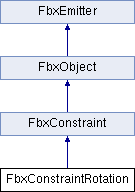
\includegraphics[height=4.000000cm]{class_fbx_constraint_rotation}
\end{center}
\end{figure}
\subsection*{公開メンバ関数}
\begin{DoxyCompactItemize}
\item 
void \hyperlink{class_fbx_constraint_rotation_ac025636c53dc8316f7da590de99bdb20}{Add\+Constraint\+Source} (\hyperlink{class_fbx_object}{Fbx\+Object} $\ast$p\+Object, double p\+Weight=100)
\item 
int \hyperlink{class_fbx_constraint_rotation_ab27178d5b53654eb9f41f6e3f3a4c5dc}{Get\+Constraint\+Source\+Count} () const
\item 
\hyperlink{class_fbx_object}{Fbx\+Object} $\ast$ \hyperlink{class_fbx_constraint_rotation_a4bfb008520cb5aa6996104c292e5819e}{Get\+Constraint\+Source} (int p\+Index) const
\item 
void \hyperlink{class_fbx_constraint_rotation_ae7d40f146877a4defd18cd41692fa78e}{Set\+Constrained\+Object} (\hyperlink{class_fbx_object}{Fbx\+Object} $\ast$p\+Object)
\item 
\hyperlink{class_fbx_object}{Fbx\+Object} $\ast$ \hyperlink{class_fbx_constraint_rotation_ad9bdaf083716c730fdd907a9387e4991}{Get\+Constrained\+Object} () const
\end{DoxyCompactItemize}
\subsection*{限定公開メンバ関数}
\begin{DoxyCompactItemize}
\item 
virtual void \hyperlink{class_fbx_constraint_rotation_ad9f6469905777a18e3a383f402bdd9b0}{Construct\+Properties} (bool p\+Force\+Set)
\item 
virtual \hyperlink{class_fbx_constraint_a49c1634663395eab7c28856df233ec66}{E\+Type} \hyperlink{class_fbx_constraint_rotation_a8d9f54ac347d18a0871eafc21e88cb77}{Get\+Constraint\+Type} () const
\end{DoxyCompactItemize}
\subsection*{Properties}
\begin{DoxyCompactItemize}
\item 
\hyperlink{class_fbx_property_t}{Fbx\+PropertyT}$<$ \hyperlink{fbxtypes_8h_a92e0562b2fe33e76a242f498b362262e}{Fbx\+Bool} $>$ \hyperlink{class_fbx_constraint_rotation_a2fc6ae9614bcc41039d4abd37d3186aa}{AffectX}
\item 
\hyperlink{class_fbx_property_t}{Fbx\+PropertyT}$<$ \hyperlink{fbxtypes_8h_a92e0562b2fe33e76a242f498b362262e}{Fbx\+Bool} $>$ \hyperlink{class_fbx_constraint_rotation_a8b611c9fd76921a2780254dee0d33870}{AffectY}
\item 
\hyperlink{class_fbx_property_t}{Fbx\+PropertyT}$<$ \hyperlink{fbxtypes_8h_a92e0562b2fe33e76a242f498b362262e}{Fbx\+Bool} $>$ \hyperlink{class_fbx_constraint_rotation_af7a3d171bfeb0e5fa72d292756c64848}{AffectZ}
\item 
\hyperlink{class_fbx_property_t}{Fbx\+PropertyT}$<$ \hyperlink{fbxtypes_8h_ae0a96f14cde566774c7553aa7523b7a7}{Fbx\+Double3} $>$ \hyperlink{class_fbx_constraint_rotation_aa0bb0aa79b3f983ede4a376f12adb1c9}{Rotation}
\item 
\hyperlink{class_fbx_property_t}{Fbx\+PropertyT}$<$ \hyperlink{fbxtypes_8h_a44df6a2eec915cf27cd481e5c5e48a24}{Fbx\+Reference} $>$ \hyperlink{class_fbx_constraint_rotation_ac9bb2a7227a6034425e06395a03d57a6}{Constraint\+Sources}
\item 
\hyperlink{class_fbx_property_t}{Fbx\+PropertyT}$<$ \hyperlink{fbxtypes_8h_a44df6a2eec915cf27cd481e5c5e48a24}{Fbx\+Reference} $>$ \hyperlink{class_fbx_constraint_rotation_aee0715edab2a99b52a40f35aba1d662c}{Constrained\+Object}
\end{DoxyCompactItemize}
\subsection*{その他の継承メンバ}


\subsection{詳解}
This constraint class contains methods for accessing the properties of a rotation constraint. A rotation constraint lets you constrain the rotation of an object based on the rotation of one or more sources. 

 fbxconstraintrotation.\+h の 26 行目に定義があります。



\subsection{関数詳解}
\mbox{\Hypertarget{class_fbx_constraint_rotation_ac025636c53dc8316f7da590de99bdb20}\label{class_fbx_constraint_rotation_ac025636c53dc8316f7da590de99bdb20}} 
\index{Fbx\+Constraint\+Rotation@{Fbx\+Constraint\+Rotation}!Add\+Constraint\+Source@{Add\+Constraint\+Source}}
\index{Add\+Constraint\+Source@{Add\+Constraint\+Source}!Fbx\+Constraint\+Rotation@{Fbx\+Constraint\+Rotation}}
\subsubsection{\texorpdfstring{Add\+Constraint\+Source()}{AddConstraintSource()}}
{\footnotesize\ttfamily void Fbx\+Constraint\+Rotation\+::\+Add\+Constraint\+Source (\begin{DoxyParamCaption}\item[{\hyperlink{class_fbx_object}{Fbx\+Object} $\ast$}]{p\+Object,  }\item[{double}]{p\+Weight = {\ttfamily 100} }\end{DoxyParamCaption})}

Add a source to the constraint. 
\begin{DoxyParams}{引数}
{\em p\+Object} & New source object. \\
\hline
{\em p\+Weight} & Weight of the source object. \\
\hline
\end{DoxyParams}
\mbox{\Hypertarget{class_fbx_constraint_rotation_ad9f6469905777a18e3a383f402bdd9b0}\label{class_fbx_constraint_rotation_ad9f6469905777a18e3a383f402bdd9b0}} 
\index{Fbx\+Constraint\+Rotation@{Fbx\+Constraint\+Rotation}!Construct\+Properties@{Construct\+Properties}}
\index{Construct\+Properties@{Construct\+Properties}!Fbx\+Constraint\+Rotation@{Fbx\+Constraint\+Rotation}}
\subsubsection{\texorpdfstring{Construct\+Properties()}{ConstructProperties()}}
{\footnotesize\ttfamily virtual void Fbx\+Constraint\+Rotation\+::\+Construct\+Properties (\begin{DoxyParamCaption}\item[{bool}]{p\+Force\+Set }\end{DoxyParamCaption})\hspace{0.3cm}{\ttfamily [protected]}, {\ttfamily [virtual]}}

Optional property constructor override, automatically called by default constructor. 
\begin{DoxyParams}{引数}
{\em p\+Force\+Set} & If the property value must be set regardless of default value. \\
\hline
\end{DoxyParams}
\begin{DoxyRemark}{注釈}
If your object have properties, they must be initialized in this function. 
\end{DoxyRemark}


\hyperlink{class_fbx_constraint_a0470a25b813b337d07a03ce4b97b44f8}{Fbx\+Constraint}を再実装しています。

\mbox{\Hypertarget{class_fbx_constraint_rotation_ad9bdaf083716c730fdd907a9387e4991}\label{class_fbx_constraint_rotation_ad9bdaf083716c730fdd907a9387e4991}} 
\index{Fbx\+Constraint\+Rotation@{Fbx\+Constraint\+Rotation}!Get\+Constrained\+Object@{Get\+Constrained\+Object}}
\index{Get\+Constrained\+Object@{Get\+Constrained\+Object}!Fbx\+Constraint\+Rotation@{Fbx\+Constraint\+Rotation}}
\subsubsection{\texorpdfstring{Get\+Constrained\+Object()}{GetConstrainedObject()}}
{\footnotesize\ttfamily \hyperlink{class_fbx_object}{Fbx\+Object}$\ast$ Fbx\+Constraint\+Rotation\+::\+Get\+Constrained\+Object (\begin{DoxyParamCaption}{ }\end{DoxyParamCaption}) const\hspace{0.3cm}{\ttfamily [virtual]}}

Retrieve the constrained object. \begin{DoxyReturn}{戻り値}
Current constrained object. 
\end{DoxyReturn}


\hyperlink{class_fbx_constraint_a7f587d5db9685b5ee925a85354263edc}{Fbx\+Constraint}を再実装しています。

\mbox{\Hypertarget{class_fbx_constraint_rotation_a4bfb008520cb5aa6996104c292e5819e}\label{class_fbx_constraint_rotation_a4bfb008520cb5aa6996104c292e5819e}} 
\index{Fbx\+Constraint\+Rotation@{Fbx\+Constraint\+Rotation}!Get\+Constraint\+Source@{Get\+Constraint\+Source}}
\index{Get\+Constraint\+Source@{Get\+Constraint\+Source}!Fbx\+Constraint\+Rotation@{Fbx\+Constraint\+Rotation}}
\subsubsection{\texorpdfstring{Get\+Constraint\+Source()}{GetConstraintSource()}}
{\footnotesize\ttfamily \hyperlink{class_fbx_object}{Fbx\+Object}$\ast$ Fbx\+Constraint\+Rotation\+::\+Get\+Constraint\+Source (\begin{DoxyParamCaption}\item[{int}]{p\+Index }\end{DoxyParamCaption}) const\hspace{0.3cm}{\ttfamily [virtual]}}

Retrieve a constraint source object. 
\begin{DoxyParams}{引数}
{\em p\+Index} & Index of the source object \\
\hline
\end{DoxyParams}
\begin{DoxyReturn}{戻り値}
Current source at the specified index. 
\end{DoxyReturn}


\hyperlink{class_fbx_constraint_a5ff6fe6fc98af1e33e8b297bc1cea007}{Fbx\+Constraint}を再実装しています。

\mbox{\Hypertarget{class_fbx_constraint_rotation_ab27178d5b53654eb9f41f6e3f3a4c5dc}\label{class_fbx_constraint_rotation_ab27178d5b53654eb9f41f6e3f3a4c5dc}} 
\index{Fbx\+Constraint\+Rotation@{Fbx\+Constraint\+Rotation}!Get\+Constraint\+Source\+Count@{Get\+Constraint\+Source\+Count}}
\index{Get\+Constraint\+Source\+Count@{Get\+Constraint\+Source\+Count}!Fbx\+Constraint\+Rotation@{Fbx\+Constraint\+Rotation}}
\subsubsection{\texorpdfstring{Get\+Constraint\+Source\+Count()}{GetConstraintSourceCount()}}
{\footnotesize\ttfamily int Fbx\+Constraint\+Rotation\+::\+Get\+Constraint\+Source\+Count (\begin{DoxyParamCaption}{ }\end{DoxyParamCaption}) const\hspace{0.3cm}{\ttfamily [virtual]}}

Retrieve the constraint source count. \begin{DoxyReturn}{戻り値}
Current constraint source count. 
\end{DoxyReturn}


\hyperlink{class_fbx_constraint_aa702f86c6a1832ce3b4905911e66c58f}{Fbx\+Constraint}を再実装しています。

\mbox{\Hypertarget{class_fbx_constraint_rotation_a8d9f54ac347d18a0871eafc21e88cb77}\label{class_fbx_constraint_rotation_a8d9f54ac347d18a0871eafc21e88cb77}} 
\index{Fbx\+Constraint\+Rotation@{Fbx\+Constraint\+Rotation}!Get\+Constraint\+Type@{Get\+Constraint\+Type}}
\index{Get\+Constraint\+Type@{Get\+Constraint\+Type}!Fbx\+Constraint\+Rotation@{Fbx\+Constraint\+Rotation}}
\subsubsection{\texorpdfstring{Get\+Constraint\+Type()}{GetConstraintType()}}
{\footnotesize\ttfamily virtual \hyperlink{class_fbx_constraint_a49c1634663395eab7c28856df233ec66}{E\+Type} Fbx\+Constraint\+Rotation\+::\+Get\+Constraint\+Type (\begin{DoxyParamCaption}{ }\end{DoxyParamCaption}) const\hspace{0.3cm}{\ttfamily [protected]}, {\ttfamily [virtual]}}

Access the type of the constraint. \begin{DoxyReturn}{戻り値}
This type of the constraint. 
\end{DoxyReturn}


\hyperlink{class_fbx_constraint_adbeea66a1a605531a019aa6df90dc45b}{Fbx\+Constraint}を再実装しています。

\mbox{\Hypertarget{class_fbx_constraint_rotation_ae7d40f146877a4defd18cd41692fa78e}\label{class_fbx_constraint_rotation_ae7d40f146877a4defd18cd41692fa78e}} 
\index{Fbx\+Constraint\+Rotation@{Fbx\+Constraint\+Rotation}!Set\+Constrained\+Object@{Set\+Constrained\+Object}}
\index{Set\+Constrained\+Object@{Set\+Constrained\+Object}!Fbx\+Constraint\+Rotation@{Fbx\+Constraint\+Rotation}}
\subsubsection{\texorpdfstring{Set\+Constrained\+Object()}{SetConstrainedObject()}}
{\footnotesize\ttfamily void Fbx\+Constraint\+Rotation\+::\+Set\+Constrained\+Object (\begin{DoxyParamCaption}\item[{\hyperlink{class_fbx_object}{Fbx\+Object} $\ast$}]{p\+Object }\end{DoxyParamCaption})}

Set the constrained object. 
\begin{DoxyParams}{引数}
{\em p\+Object} & The constrained object. \\
\hline
\end{DoxyParams}


\subsection{メンバ詳解}
\mbox{\Hypertarget{class_fbx_constraint_rotation_a2fc6ae9614bcc41039d4abd37d3186aa}\label{class_fbx_constraint_rotation_a2fc6ae9614bcc41039d4abd37d3186aa}} 
\index{Fbx\+Constraint\+Rotation@{Fbx\+Constraint\+Rotation}!AffectX@{AffectX}}
\index{AffectX@{AffectX}!Fbx\+Constraint\+Rotation@{Fbx\+Constraint\+Rotation}}
\subsubsection{\texorpdfstring{AffectX}{AffectX}}
{\footnotesize\ttfamily \hyperlink{class_fbx_property_t}{Fbx\+PropertyT}$<$\hyperlink{fbxtypes_8h_a92e0562b2fe33e76a242f498b362262e}{Fbx\+Bool}$>$ Fbx\+Constraint\+Rotation\+::\+AffectX}

This property handles whether to affect x axis. Default value is true. 

 fbxconstraintrotation.\+h の 38 行目に定義があります。

\mbox{\Hypertarget{class_fbx_constraint_rotation_a8b611c9fd76921a2780254dee0d33870}\label{class_fbx_constraint_rotation_a8b611c9fd76921a2780254dee0d33870}} 
\index{Fbx\+Constraint\+Rotation@{Fbx\+Constraint\+Rotation}!AffectY@{AffectY}}
\index{AffectY@{AffectY}!Fbx\+Constraint\+Rotation@{Fbx\+Constraint\+Rotation}}
\subsubsection{\texorpdfstring{AffectY}{AffectY}}
{\footnotesize\ttfamily \hyperlink{class_fbx_property_t}{Fbx\+PropertyT}$<$\hyperlink{fbxtypes_8h_a92e0562b2fe33e76a242f498b362262e}{Fbx\+Bool}$>$ Fbx\+Constraint\+Rotation\+::\+AffectY}

This property handles whether to affect y axis. Default value is true. 

 fbxconstraintrotation.\+h の 42 行目に定義があります。

\mbox{\Hypertarget{class_fbx_constraint_rotation_af7a3d171bfeb0e5fa72d292756c64848}\label{class_fbx_constraint_rotation_af7a3d171bfeb0e5fa72d292756c64848}} 
\index{Fbx\+Constraint\+Rotation@{Fbx\+Constraint\+Rotation}!AffectZ@{AffectZ}}
\index{AffectZ@{AffectZ}!Fbx\+Constraint\+Rotation@{Fbx\+Constraint\+Rotation}}
\subsubsection{\texorpdfstring{AffectZ}{AffectZ}}
{\footnotesize\ttfamily \hyperlink{class_fbx_property_t}{Fbx\+PropertyT}$<$\hyperlink{fbxtypes_8h_a92e0562b2fe33e76a242f498b362262e}{Fbx\+Bool}$>$ Fbx\+Constraint\+Rotation\+::\+AffectZ}

This property handles whether to affect z axis. Default value is true. 

 fbxconstraintrotation.\+h の 47 行目に定義があります。

\mbox{\Hypertarget{class_fbx_constraint_rotation_aee0715edab2a99b52a40f35aba1d662c}\label{class_fbx_constraint_rotation_aee0715edab2a99b52a40f35aba1d662c}} 
\index{Fbx\+Constraint\+Rotation@{Fbx\+Constraint\+Rotation}!Constrained\+Object@{Constrained\+Object}}
\index{Constrained\+Object@{Constrained\+Object}!Fbx\+Constraint\+Rotation@{Fbx\+Constraint\+Rotation}}
\subsubsection{\texorpdfstring{Constrained\+Object}{ConstrainedObject}}
{\footnotesize\ttfamily \hyperlink{class_fbx_property_t}{Fbx\+PropertyT}$<$\hyperlink{fbxtypes_8h_a44df6a2eec915cf27cd481e5c5e48a24}{Fbx\+Reference}$>$ Fbx\+Constraint\+Rotation\+::\+Constrained\+Object}

This property handles constraint target objects. 

 fbxconstraintrotation.\+h の 60 行目に定義があります。

\mbox{\Hypertarget{class_fbx_constraint_rotation_ac9bb2a7227a6034425e06395a03d57a6}\label{class_fbx_constraint_rotation_ac9bb2a7227a6034425e06395a03d57a6}} 
\index{Fbx\+Constraint\+Rotation@{Fbx\+Constraint\+Rotation}!Constraint\+Sources@{Constraint\+Sources}}
\index{Constraint\+Sources@{Constraint\+Sources}!Fbx\+Constraint\+Rotation@{Fbx\+Constraint\+Rotation}}
\subsubsection{\texorpdfstring{Constraint\+Sources}{ConstraintSources}}
{\footnotesize\ttfamily \hyperlink{class_fbx_property_t}{Fbx\+PropertyT}$<$\hyperlink{fbxtypes_8h_a44df6a2eec915cf27cd481e5c5e48a24}{Fbx\+Reference}$>$ Fbx\+Constraint\+Rotation\+::\+Constraint\+Sources}

This property handles constraint source objects. 

 fbxconstraintrotation.\+h の 56 行目に定義があります。

\mbox{\Hypertarget{class_fbx_constraint_rotation_aa0bb0aa79b3f983ede4a376f12adb1c9}\label{class_fbx_constraint_rotation_aa0bb0aa79b3f983ede4a376f12adb1c9}} 
\index{Fbx\+Constraint\+Rotation@{Fbx\+Constraint\+Rotation}!Rotation@{Rotation}}
\index{Rotation@{Rotation}!Fbx\+Constraint\+Rotation@{Fbx\+Constraint\+Rotation}}
\subsubsection{\texorpdfstring{Rotation}{Rotation}}
{\footnotesize\ttfamily \hyperlink{class_fbx_property_t}{Fbx\+PropertyT}$<$\hyperlink{fbxtypes_8h_ae0a96f14cde566774c7553aa7523b7a7}{Fbx\+Double3}$>$ Fbx\+Constraint\+Rotation\+::\+Rotation}

This property handles rotation offset. Default value is (0, 0, 0). 

 fbxconstraintrotation.\+h の 52 行目に定義があります。



このクラス詳解は次のファイルから抽出されました\+:\begin{DoxyCompactItemize}
\item 
C\+:/\+Maya/scripts/\+F\+B\+X\+\_\+\+S\+D\+K/2017.\+1/include/fbxsdk/scene/constraint/\hyperlink{fbxconstraintrotation_8h}{fbxconstraintrotation.\+h}\end{DoxyCompactItemize}

\hypertarget{class_fbx_constraint_scale}{}\section{Fbx\+Constraint\+Scale クラス}
\label{class_fbx_constraint_scale}\index{Fbx\+Constraint\+Scale@{Fbx\+Constraint\+Scale}}


This constraint class contains methods for accessing the properties of a scale constraint. A scale constraint lets you constrain the scale of an object based on the scale of one or more sources.  




{\ttfamily \#include $<$fbxconstraintscale.\+h$>$}



Fbx\+Constraint\+Scale の継承関係図
% FIG 0


Fbx\+Constraint\+Scale 連携図
% FIG 1
\subsection*{公開メンバ関数}
\begin{DoxyCompactItemize}
\item 
void \hyperlink{class_fbx_constraint_scale_a876e788ab98cf2fe1042ae3c687b3689}{Add\+Constraint\+Source} (\hyperlink{class_fbx_object}{Fbx\+Object} $\ast$p\+Object, double p\+Weight=100)
\item 
int \hyperlink{class_fbx_constraint_scale_a5c4500706618751078dddca3652ce936}{Get\+Constraint\+Source\+Count} () const
\item 
\hyperlink{class_fbx_object}{Fbx\+Object} $\ast$ \hyperlink{class_fbx_constraint_scale_ac957fc33cab352ef355602fb4325c5b7}{Get\+Constraint\+Source} (int p\+Index) const
\item 
void \hyperlink{class_fbx_constraint_scale_adf626a9273449dd4c74cf24f2a7bf5af}{Set\+Constrained\+Object} (\hyperlink{class_fbx_object}{Fbx\+Object} $\ast$p\+Object)
\item 
\hyperlink{class_fbx_object}{Fbx\+Object} $\ast$ \hyperlink{class_fbx_constraint_scale_a1dcbdc6b41d04d6a75ca47f024e05dc9}{Get\+Constrained\+Object} () const
\end{DoxyCompactItemize}
\subsection*{限定公開メンバ関数}
\begin{DoxyCompactItemize}
\item 
virtual void \hyperlink{class_fbx_constraint_scale_af34ea4ce8516d69aefbcb9e83060b2c1}{Construct\+Properties} (bool p\+Force\+Set)
\item 
virtual \hyperlink{class_fbx_constraint_a49c1634663395eab7c28856df233ec66}{E\+Type} \hyperlink{class_fbx_constraint_scale_a7eb92c352d4a4bd3c0754dd4e53fa6e4}{Get\+Constraint\+Type} () const
\end{DoxyCompactItemize}
\subsection*{Properties}
\begin{DoxyCompactItemize}
\item 
\hyperlink{class_fbx_property_t}{Fbx\+PropertyT}$<$ \hyperlink{fbxtypes_8h_a92e0562b2fe33e76a242f498b362262e}{Fbx\+Bool} $>$ \hyperlink{class_fbx_constraint_scale_a41d95ab4643d154a400efa926062ffac}{AffectX}
\item 
\hyperlink{class_fbx_property_t}{Fbx\+PropertyT}$<$ \hyperlink{fbxtypes_8h_a92e0562b2fe33e76a242f498b362262e}{Fbx\+Bool} $>$ \hyperlink{class_fbx_constraint_scale_a2249bbb0bd5ba9507fa82e1b66c0b2a2}{AffectY}
\item 
\hyperlink{class_fbx_property_t}{Fbx\+PropertyT}$<$ \hyperlink{fbxtypes_8h_a92e0562b2fe33e76a242f498b362262e}{Fbx\+Bool} $>$ \hyperlink{class_fbx_constraint_scale_af8cc6e516ff4b87331fc12f20af6f235}{AffectZ}
\item 
\hyperlink{class_fbx_property_t}{Fbx\+PropertyT}$<$ \hyperlink{fbxtypes_8h_ae0a96f14cde566774c7553aa7523b7a7}{Fbx\+Double3} $>$ \hyperlink{class_fbx_constraint_scale_a0c8bd160ee16da64bf998a612bb11a5b}{Scaling}
\item 
\hyperlink{class_fbx_property_t}{Fbx\+PropertyT}$<$ \hyperlink{fbxtypes_8h_a44df6a2eec915cf27cd481e5c5e48a24}{Fbx\+Reference} $>$ \hyperlink{class_fbx_constraint_scale_a434954eedd1e80d6935881b37e9da11f}{Constraint\+Sources}
\item 
\hyperlink{class_fbx_property_t}{Fbx\+PropertyT}$<$ \hyperlink{fbxtypes_8h_a44df6a2eec915cf27cd481e5c5e48a24}{Fbx\+Reference} $>$ \hyperlink{class_fbx_constraint_scale_ae5eb43970ba98186d43fdb51498b21c5}{Constrained\+Object}
\end{DoxyCompactItemize}
\subsection*{その他の継承メンバ}


\subsection{詳解}
This constraint class contains methods for accessing the properties of a scale constraint. A scale constraint lets you constrain the scale of an object based on the scale of one or more sources. 

\subsection{メソッド詳解}
\mbox{\Hypertarget{class_fbx_constraint_scale_a876e788ab98cf2fe1042ae3c687b3689}\label{class_fbx_constraint_scale_a876e788ab98cf2fe1042ae3c687b3689}} 
\index{Fbx\+Constraint\+Scale@{Fbx\+Constraint\+Scale}!Add\+Constraint\+Source@{Add\+Constraint\+Source}}
\index{Add\+Constraint\+Source@{Add\+Constraint\+Source}!Fbx\+Constraint\+Scale@{Fbx\+Constraint\+Scale}}
\subsubsection{\texorpdfstring{Add\+Constraint\+Source()}{AddConstraintSource()}}
{\footnotesize\ttfamily void Fbx\+Constraint\+Scale\+::\+Add\+Constraint\+Source (\begin{DoxyParamCaption}\item[{\hyperlink{class_fbx_object}{Fbx\+Object} $\ast$}]{p\+Object,  }\item[{double}]{p\+Weight = {\ttfamily 100} }\end{DoxyParamCaption})}

Add a source to the constraint. 
\begin{DoxyParams}{引数}
{\em p\+Object} & New source object. \\
\hline
{\em p\+Weight} & Weight of the source object. \\
\hline
\end{DoxyParams}
\mbox{\Hypertarget{class_fbx_constraint_scale_af34ea4ce8516d69aefbcb9e83060b2c1}\label{class_fbx_constraint_scale_af34ea4ce8516d69aefbcb9e83060b2c1}} 
\index{Fbx\+Constraint\+Scale@{Fbx\+Constraint\+Scale}!Construct\+Properties@{Construct\+Properties}}
\index{Construct\+Properties@{Construct\+Properties}!Fbx\+Constraint\+Scale@{Fbx\+Constraint\+Scale}}
\subsubsection{\texorpdfstring{Construct\+Properties()}{ConstructProperties()}}
{\footnotesize\ttfamily virtual void Fbx\+Constraint\+Scale\+::\+Construct\+Properties (\begin{DoxyParamCaption}\item[{bool}]{p\+Force\+Set }\end{DoxyParamCaption})\hspace{0.3cm}{\ttfamily [protected]}, {\ttfamily [virtual]}}

Optional property constructor override, automatically called by default constructor. 
\begin{DoxyParams}{引数}
{\em p\+Force\+Set} & If the property value must be set regardless of default value. \\
\hline
\end{DoxyParams}
\begin{DoxyRemark}{注釈}
If your object have properties, they must be initialized in this function. 
\end{DoxyRemark}


\hyperlink{class_fbx_constraint_a0470a25b813b337d07a03ce4b97b44f8}{Fbx\+Constraint}を再実装しています。

\mbox{\Hypertarget{class_fbx_constraint_scale_a1dcbdc6b41d04d6a75ca47f024e05dc9}\label{class_fbx_constraint_scale_a1dcbdc6b41d04d6a75ca47f024e05dc9}} 
\index{Fbx\+Constraint\+Scale@{Fbx\+Constraint\+Scale}!Get\+Constrained\+Object@{Get\+Constrained\+Object}}
\index{Get\+Constrained\+Object@{Get\+Constrained\+Object}!Fbx\+Constraint\+Scale@{Fbx\+Constraint\+Scale}}
\subsubsection{\texorpdfstring{Get\+Constrained\+Object()}{GetConstrainedObject()}}
{\footnotesize\ttfamily \hyperlink{class_fbx_object}{Fbx\+Object}$\ast$ Fbx\+Constraint\+Scale\+::\+Get\+Constrained\+Object (\begin{DoxyParamCaption}{ }\end{DoxyParamCaption}) const\hspace{0.3cm}{\ttfamily [virtual]}}

Retrieve the constrained object. \begin{DoxyReturn}{戻り値}
Current constrained object. 
\end{DoxyReturn}


\hyperlink{class_fbx_constraint_a7f587d5db9685b5ee925a85354263edc}{Fbx\+Constraint}を再実装しています。

\mbox{\Hypertarget{class_fbx_constraint_scale_ac957fc33cab352ef355602fb4325c5b7}\label{class_fbx_constraint_scale_ac957fc33cab352ef355602fb4325c5b7}} 
\index{Fbx\+Constraint\+Scale@{Fbx\+Constraint\+Scale}!Get\+Constraint\+Source@{Get\+Constraint\+Source}}
\index{Get\+Constraint\+Source@{Get\+Constraint\+Source}!Fbx\+Constraint\+Scale@{Fbx\+Constraint\+Scale}}
\subsubsection{\texorpdfstring{Get\+Constraint\+Source()}{GetConstraintSource()}}
{\footnotesize\ttfamily \hyperlink{class_fbx_object}{Fbx\+Object}$\ast$ Fbx\+Constraint\+Scale\+::\+Get\+Constraint\+Source (\begin{DoxyParamCaption}\item[{int}]{p\+Index }\end{DoxyParamCaption}) const\hspace{0.3cm}{\ttfamily [virtual]}}

Retrieve a constraint source object. 
\begin{DoxyParams}{引数}
{\em p\+Index} & Index of the source \\
\hline
\end{DoxyParams}
\begin{DoxyReturn}{戻り値}
Current source at the specified index. 
\end{DoxyReturn}


\hyperlink{class_fbx_constraint_a5ff6fe6fc98af1e33e8b297bc1cea007}{Fbx\+Constraint}を再実装しています。

\mbox{\Hypertarget{class_fbx_constraint_scale_a5c4500706618751078dddca3652ce936}\label{class_fbx_constraint_scale_a5c4500706618751078dddca3652ce936}} 
\index{Fbx\+Constraint\+Scale@{Fbx\+Constraint\+Scale}!Get\+Constraint\+Source\+Count@{Get\+Constraint\+Source\+Count}}
\index{Get\+Constraint\+Source\+Count@{Get\+Constraint\+Source\+Count}!Fbx\+Constraint\+Scale@{Fbx\+Constraint\+Scale}}
\subsubsection{\texorpdfstring{Get\+Constraint\+Source\+Count()}{GetConstraintSourceCount()}}
{\footnotesize\ttfamily int Fbx\+Constraint\+Scale\+::\+Get\+Constraint\+Source\+Count (\begin{DoxyParamCaption}{ }\end{DoxyParamCaption}) const\hspace{0.3cm}{\ttfamily [virtual]}}

Retrieve the constraint source count. \begin{DoxyReturn}{戻り値}
Current constraint source count. 
\end{DoxyReturn}


\hyperlink{class_fbx_constraint_aa702f86c6a1832ce3b4905911e66c58f}{Fbx\+Constraint}を再実装しています。

\mbox{\Hypertarget{class_fbx_constraint_scale_a7eb92c352d4a4bd3c0754dd4e53fa6e4}\label{class_fbx_constraint_scale_a7eb92c352d4a4bd3c0754dd4e53fa6e4}} 
\index{Fbx\+Constraint\+Scale@{Fbx\+Constraint\+Scale}!Get\+Constraint\+Type@{Get\+Constraint\+Type}}
\index{Get\+Constraint\+Type@{Get\+Constraint\+Type}!Fbx\+Constraint\+Scale@{Fbx\+Constraint\+Scale}}
\subsubsection{\texorpdfstring{Get\+Constraint\+Type()}{GetConstraintType()}}
{\footnotesize\ttfamily virtual \hyperlink{class_fbx_constraint_a49c1634663395eab7c28856df233ec66}{E\+Type} Fbx\+Constraint\+Scale\+::\+Get\+Constraint\+Type (\begin{DoxyParamCaption}{ }\end{DoxyParamCaption}) const\hspace{0.3cm}{\ttfamily [protected]}, {\ttfamily [virtual]}}

Access the type of the constraint. \begin{DoxyReturn}{戻り値}
This type of the constraint. 
\end{DoxyReturn}


\hyperlink{class_fbx_constraint_adbeea66a1a605531a019aa6df90dc45b}{Fbx\+Constraint}を再実装しています。

\mbox{\Hypertarget{class_fbx_constraint_scale_adf626a9273449dd4c74cf24f2a7bf5af}\label{class_fbx_constraint_scale_adf626a9273449dd4c74cf24f2a7bf5af}} 
\index{Fbx\+Constraint\+Scale@{Fbx\+Constraint\+Scale}!Set\+Constrained\+Object@{Set\+Constrained\+Object}}
\index{Set\+Constrained\+Object@{Set\+Constrained\+Object}!Fbx\+Constraint\+Scale@{Fbx\+Constraint\+Scale}}
\subsubsection{\texorpdfstring{Set\+Constrained\+Object()}{SetConstrainedObject()}}
{\footnotesize\ttfamily void Fbx\+Constraint\+Scale\+::\+Set\+Constrained\+Object (\begin{DoxyParamCaption}\item[{\hyperlink{class_fbx_object}{Fbx\+Object} $\ast$}]{p\+Object }\end{DoxyParamCaption})}

Set the constrained object. 
\begin{DoxyParams}{引数}
{\em p\+Object} & The constrained object. \\
\hline
\end{DoxyParams}


\subsection{メンバ詳解}
\mbox{\Hypertarget{class_fbx_constraint_scale_a41d95ab4643d154a400efa926062ffac}\label{class_fbx_constraint_scale_a41d95ab4643d154a400efa926062ffac}} 
\index{Fbx\+Constraint\+Scale@{Fbx\+Constraint\+Scale}!AffectX@{AffectX}}
\index{AffectX@{AffectX}!Fbx\+Constraint\+Scale@{Fbx\+Constraint\+Scale}}
\subsubsection{\texorpdfstring{AffectX}{AffectX}}
{\footnotesize\ttfamily \hyperlink{class_fbx_property_t}{Fbx\+PropertyT}$<$\hyperlink{fbxtypes_8h_a92e0562b2fe33e76a242f498b362262e}{Fbx\+Bool}$>$ Fbx\+Constraint\+Scale\+::\+AffectX}

This property handles whether to affect x axis. Default value is true. \mbox{\Hypertarget{class_fbx_constraint_scale_a2249bbb0bd5ba9507fa82e1b66c0b2a2}\label{class_fbx_constraint_scale_a2249bbb0bd5ba9507fa82e1b66c0b2a2}} 
\index{Fbx\+Constraint\+Scale@{Fbx\+Constraint\+Scale}!AffectY@{AffectY}}
\index{AffectY@{AffectY}!Fbx\+Constraint\+Scale@{Fbx\+Constraint\+Scale}}
\subsubsection{\texorpdfstring{AffectY}{AffectY}}
{\footnotesize\ttfamily \hyperlink{class_fbx_property_t}{Fbx\+PropertyT}$<$\hyperlink{fbxtypes_8h_a92e0562b2fe33e76a242f498b362262e}{Fbx\+Bool}$>$ Fbx\+Constraint\+Scale\+::\+AffectY}

This property handles whether to affect y axis. Default value is true. \mbox{\Hypertarget{class_fbx_constraint_scale_af8cc6e516ff4b87331fc12f20af6f235}\label{class_fbx_constraint_scale_af8cc6e516ff4b87331fc12f20af6f235}} 
\index{Fbx\+Constraint\+Scale@{Fbx\+Constraint\+Scale}!AffectZ@{AffectZ}}
\index{AffectZ@{AffectZ}!Fbx\+Constraint\+Scale@{Fbx\+Constraint\+Scale}}
\subsubsection{\texorpdfstring{AffectZ}{AffectZ}}
{\footnotesize\ttfamily \hyperlink{class_fbx_property_t}{Fbx\+PropertyT}$<$\hyperlink{fbxtypes_8h_a92e0562b2fe33e76a242f498b362262e}{Fbx\+Bool}$>$ Fbx\+Constraint\+Scale\+::\+AffectZ}

This property handles whether to affect z axis. Default value is true. \mbox{\Hypertarget{class_fbx_constraint_scale_ae5eb43970ba98186d43fdb51498b21c5}\label{class_fbx_constraint_scale_ae5eb43970ba98186d43fdb51498b21c5}} 
\index{Fbx\+Constraint\+Scale@{Fbx\+Constraint\+Scale}!Constrained\+Object@{Constrained\+Object}}
\index{Constrained\+Object@{Constrained\+Object}!Fbx\+Constraint\+Scale@{Fbx\+Constraint\+Scale}}
\subsubsection{\texorpdfstring{Constrained\+Object}{ConstrainedObject}}
{\footnotesize\ttfamily \hyperlink{class_fbx_property_t}{Fbx\+PropertyT}$<$\hyperlink{fbxtypes_8h_a44df6a2eec915cf27cd481e5c5e48a24}{Fbx\+Reference}$>$ Fbx\+Constraint\+Scale\+::\+Constrained\+Object}

This property handles constraint target objects. \mbox{\Hypertarget{class_fbx_constraint_scale_a434954eedd1e80d6935881b37e9da11f}\label{class_fbx_constraint_scale_a434954eedd1e80d6935881b37e9da11f}} 
\index{Fbx\+Constraint\+Scale@{Fbx\+Constraint\+Scale}!Constraint\+Sources@{Constraint\+Sources}}
\index{Constraint\+Sources@{Constraint\+Sources}!Fbx\+Constraint\+Scale@{Fbx\+Constraint\+Scale}}
\subsubsection{\texorpdfstring{Constraint\+Sources}{ConstraintSources}}
{\footnotesize\ttfamily \hyperlink{class_fbx_property_t}{Fbx\+PropertyT}$<$\hyperlink{fbxtypes_8h_a44df6a2eec915cf27cd481e5c5e48a24}{Fbx\+Reference}$>$ Fbx\+Constraint\+Scale\+::\+Constraint\+Sources}

This property handles constraint source objects. \mbox{\Hypertarget{class_fbx_constraint_scale_a0c8bd160ee16da64bf998a612bb11a5b}\label{class_fbx_constraint_scale_a0c8bd160ee16da64bf998a612bb11a5b}} 
\index{Fbx\+Constraint\+Scale@{Fbx\+Constraint\+Scale}!Scaling@{Scaling}}
\index{Scaling@{Scaling}!Fbx\+Constraint\+Scale@{Fbx\+Constraint\+Scale}}
\subsubsection{\texorpdfstring{Scaling}{Scaling}}
{\footnotesize\ttfamily \hyperlink{class_fbx_property_t}{Fbx\+PropertyT}$<$\hyperlink{fbxtypes_8h_ae0a96f14cde566774c7553aa7523b7a7}{Fbx\+Double3}$>$ Fbx\+Constraint\+Scale\+::\+Scaling}

This property handles scaling offset. Default value is (0, 0, 0). 

このクラス詳解は次のファイルから抽出されました\+:\begin{DoxyCompactItemize}
\item 
C\+:/github/\+F\+B\+Xpython\+S\+D\+K201701/\+F\+B\+Xpython\+S\+D\+K201701/2017.\+1/include/fbxsdk/scene/constraint/\hyperlink{fbxconstraintscale_8h}{fbxconstraintscale.\+h}\end{DoxyCompactItemize}

\hypertarget{class_fbx_constraint_single_chain_i_k}{}\section{Fbx\+Constraint\+Single\+Chain\+IK クラス}
\label{class_fbx_constraint_single_chain_i_k}\index{Fbx\+Constraint\+Single\+Chain\+IK@{Fbx\+Constraint\+Single\+Chain\+IK}}


This constraint class contains methods for accessing the properties of a single chain IK constraint.  




{\ttfamily \#include $<$fbxconstraintsinglechainik.\+h$>$}



Fbx\+Constraint\+Single\+Chain\+IK の継承関係図
% FIG 0


Fbx\+Constraint\+Single\+Chain\+IK 連携図
% FIG 1
\subsection*{公開型}
\begin{DoxyCompactItemize}
\item 
enum \hyperlink{class_fbx_constraint_single_chain_i_k_aac22215f25edcd32ca36e0e4ec0c1d9a}{E\+Solver\+Mode} \{ \hyperlink{class_fbx_constraint_single_chain_i_k_aac22215f25edcd32ca36e0e4ec0c1d9aa50550478223ad7fa82d857c7f5cd8160}{e\+Rotate\+Plane}, 
\hyperlink{class_fbx_constraint_single_chain_i_k_aac22215f25edcd32ca36e0e4ec0c1d9aa1fa1389075eefdd86c267eab6880a7ca}{e\+Single\+Chain}
 \}
\item 
enum \hyperlink{class_fbx_constraint_single_chain_i_k_a853dee195ab92c878a805ed7206a93bb}{E\+Pole\+Vector\+Mode} \{ \hyperlink{class_fbx_constraint_single_chain_i_k_a853dee195ab92c878a805ed7206a93bba1c3f447e03df20c501c61a098e162420}{e\+Vector}, 
\hyperlink{class_fbx_constraint_single_chain_i_k_a853dee195ab92c878a805ed7206a93bbac0d1970fc811997b6248e11efbdf31bc}{e\+Object}
 \}
\item 
enum \hyperlink{class_fbx_constraint_single_chain_i_k_aa730475e0c3f9f1ecc04e61f39369fc1}{E\+Evaluation\+Mode} \{ \hyperlink{class_fbx_constraint_single_chain_i_k_aa730475e0c3f9f1ecc04e61f39369fc1a92ece36c1a7245ce49d98f355ed78c5f}{e\+Never\+TS}, 
\hyperlink{class_fbx_constraint_single_chain_i_k_aa730475e0c3f9f1ecc04e61f39369fc1a2d85bdf9a9c48132894a0b3d35b6c1b2}{e\+Auto\+Detect}, 
\hyperlink{class_fbx_constraint_single_chain_i_k_aa730475e0c3f9f1ecc04e61f39369fc1ab6a348da5218082487a30df63cee3c5d}{e\+Always\+TS}
 \}
\end{DoxyCompactItemize}
\subsection*{公開メンバ関数}
\begin{DoxyCompactItemize}
\item 
double \hyperlink{class_fbx_constraint_single_chain_i_k_ae212fc88bd99906d8aadcc160dc0c1b8}{Get\+Pole\+Vector\+Object\+Weight} (const \hyperlink{class_fbx_object}{Fbx\+Object} $\ast$p\+Object) const
\item 
void \hyperlink{class_fbx_constraint_single_chain_i_k_a26abc95e8442f40ec86f38ef9e4748b8}{Add\+Pole\+Vector\+Object} (\hyperlink{class_fbx_object}{Fbx\+Object} $\ast$p\+Object, double p\+Weight=100)
\item 
int \hyperlink{class_fbx_constraint_single_chain_i_k_afeb5c6ab6342ec4aa81e69d3c9888bac}{Get\+Constraint\+Pole\+Vector\+Count} () const
\item 
\hyperlink{class_fbx_object}{Fbx\+Object} $\ast$ \hyperlink{class_fbx_constraint_single_chain_i_k_a59e6ce644cae71cba898be453e74663c}{Get\+Pole\+Vector\+Object} (int p\+Index) const
\item 
void \hyperlink{class_fbx_constraint_single_chain_i_k_a3c4bb5735bed369b73eeb42757a6aa1f}{Set\+First\+Joint\+Object} (\hyperlink{class_fbx_object}{Fbx\+Object} $\ast$p\+Object)
\item 
\hyperlink{class_fbx_object}{Fbx\+Object} $\ast$ \hyperlink{class_fbx_constraint_single_chain_i_k_a0dc8be31ce58d635c933561fd73010f1}{Get\+First\+Joint\+Object} () const
\item 
void \hyperlink{class_fbx_constraint_single_chain_i_k_a17923d89b6f7795c5322b1f9241845c1}{Set\+End\+Joint\+Object} (\hyperlink{class_fbx_object}{Fbx\+Object} $\ast$p\+Object)
\item 
\hyperlink{class_fbx_object}{Fbx\+Object} $\ast$ \hyperlink{class_fbx_constraint_single_chain_i_k_a0159badf18fe865398ae2056d86fe074}{Get\+End\+Joint\+Object} () const
\item 
void \hyperlink{class_fbx_constraint_single_chain_i_k_af7dbd878134a3b9255e7ab11830d3206}{Set\+Effector\+Object} (\hyperlink{class_fbx_object}{Fbx\+Object} $\ast$p\+Object)
\item 
\hyperlink{class_fbx_object}{Fbx\+Object} $\ast$ \hyperlink{class_fbx_constraint_single_chain_i_k_ac4c0052ea23d8e9a144bd9439cee2507}{Get\+Effector\+Object} () const
\end{DoxyCompactItemize}
\subsection*{限定公開メンバ関数}
\begin{DoxyCompactItemize}
\item 
virtual void \hyperlink{class_fbx_constraint_single_chain_i_k_aeffab44c49ad72283bdb07e50e9baf77}{Construct\+Properties} (bool p\+Force\+Set)
\item 
virtual \hyperlink{class_fbx_constraint_a49c1634663395eab7c28856df233ec66}{E\+Type} \hyperlink{class_fbx_constraint_single_chain_i_k_adc9d38f5ae55bf9c6415334a81cbdffb}{Get\+Constraint\+Type} () const
\end{DoxyCompactItemize}
\subsection*{Properties}
\begin{DoxyCompactItemize}
\item 
\hyperlink{class_fbx_property_t}{Fbx\+PropertyT}$<$ \hyperlink{fbxtypes_8h_a9a28614cb4272a0ad7d748eda7f3d3e5}{Fbx\+Enum} $>$ \hyperlink{class_fbx_constraint_single_chain_i_k_a5005bf5aa9d33200a228ad9723c519b0}{Pole\+Vector\+Type}
\item 
\hyperlink{class_fbx_property_t}{Fbx\+PropertyT}$<$ \hyperlink{fbxtypes_8h_a9a28614cb4272a0ad7d748eda7f3d3e5}{Fbx\+Enum} $>$ \hyperlink{class_fbx_constraint_single_chain_i_k_a2ed14960ba042a0c7f447306560bbe11}{Solver\+Type}
\item 
\hyperlink{class_fbx_property_t}{Fbx\+PropertyT}$<$ \hyperlink{fbxtypes_8h_a9a28614cb4272a0ad7d748eda7f3d3e5}{Fbx\+Enum} $>$ \hyperlink{class_fbx_constraint_single_chain_i_k_ae2f5d57a658c12c748ceeccd31809a3f}{Evaluate\+T\+S\+Anim}
\item 
\hyperlink{class_fbx_property_t}{Fbx\+PropertyT}$<$ \hyperlink{fbxtypes_8h_a44df6a2eec915cf27cd481e5c5e48a24}{Fbx\+Reference} $>$ \hyperlink{class_fbx_constraint_single_chain_i_k_a20b0f346f5d104fd63a69e3b560cfaba}{Pole\+Vector\+Objects}
\item 
\hyperlink{class_fbx_property_t}{Fbx\+PropertyT}$<$ \hyperlink{fbxtypes_8h_ae0a96f14cde566774c7553aa7523b7a7}{Fbx\+Double3} $>$ \hyperlink{class_fbx_constraint_single_chain_i_k_a0fb576e54a64caab8e6609060e020ae2}{Pole\+Vector}
\item 
\hyperlink{class_fbx_property_t}{Fbx\+PropertyT}$<$ \hyperlink{fbxtypes_8h_a171e72a1c46fc15c1a6c9c31948c1c5b}{Fbx\+Double} $>$ \hyperlink{class_fbx_constraint_single_chain_i_k_a3756b61ba9a55d15c00229fc9a670e4e}{Twist}
\item 
\hyperlink{class_fbx_property_t}{Fbx\+PropertyT}$<$ \hyperlink{fbxtypes_8h_a44df6a2eec915cf27cd481e5c5e48a24}{Fbx\+Reference} $>$ \hyperlink{class_fbx_constraint_single_chain_i_k_ad33341677c0cf0689bcbc1f4e4eda23a}{First\+Joint\+Object}
\item 
\hyperlink{class_fbx_property_t}{Fbx\+PropertyT}$<$ \hyperlink{fbxtypes_8h_a44df6a2eec915cf27cd481e5c5e48a24}{Fbx\+Reference} $>$ \hyperlink{class_fbx_constraint_single_chain_i_k_acb671de7c974cc53fba45d34dcdf9db4}{End\+Joint\+Object}
\item 
\hyperlink{class_fbx_property_t}{Fbx\+PropertyT}$<$ \hyperlink{fbxtypes_8h_a44df6a2eec915cf27cd481e5c5e48a24}{Fbx\+Reference} $>$ \hyperlink{class_fbx_constraint_single_chain_i_k_ab7b3721f2b7f267b6dd35ce38ffa7bbe}{Effector\+Object}
\end{DoxyCompactItemize}
\subsection*{その他の継承メンバ}


\subsection{詳解}
This constraint class contains methods for accessing the properties of a single chain IK constraint. 

\subsection{列挙型メンバ詳解}
\mbox{\Hypertarget{class_fbx_constraint_single_chain_i_k_aa730475e0c3f9f1ecc04e61f39369fc1}\label{class_fbx_constraint_single_chain_i_k_aa730475e0c3f9f1ecc04e61f39369fc1}} 
\index{Fbx\+Constraint\+Single\+Chain\+IK@{Fbx\+Constraint\+Single\+Chain\+IK}!E\+Evaluation\+Mode@{E\+Evaluation\+Mode}}
\index{E\+Evaluation\+Mode@{E\+Evaluation\+Mode}!Fbx\+Constraint\+Single\+Chain\+IK@{Fbx\+Constraint\+Single\+Chain\+IK}}
\subsubsection{\texorpdfstring{E\+Evaluation\+Mode}{EEvaluationMode}}
{\footnotesize\ttfamily enum \hyperlink{class_fbx_constraint_single_chain_i_k_aa730475e0c3f9f1ecc04e61f39369fc1}{Fbx\+Constraint\+Single\+Chain\+I\+K\+::\+E\+Evaluation\+Mode}}

If the constraints read its animation on Translation and Scale for the nodes it constraints. \begin{DoxyEnumFields}{列挙値}
\raisebox{\heightof{T}}[0pt][0pt]{\index{e\+Never\+TS@{e\+Never\+TS}!Fbx\+Constraint\+Single\+Chain\+IK@{Fbx\+Constraint\+Single\+Chain\+IK}}\index{Fbx\+Constraint\+Single\+Chain\+IK@{Fbx\+Constraint\+Single\+Chain\+IK}!e\+Never\+TS@{e\+Never\+TS}}}\mbox{\Hypertarget{class_fbx_constraint_single_chain_i_k_aa730475e0c3f9f1ecc04e61f39369fc1a92ece36c1a7245ce49d98f355ed78c5f}\label{class_fbx_constraint_single_chain_i_k_aa730475e0c3f9f1ecc04e61f39369fc1a92ece36c1a7245ce49d98f355ed78c5f}} 
e\+Never\+TS&\\
\hline

\raisebox{\heightof{T}}[0pt][0pt]{\index{e\+Auto\+Detect@{e\+Auto\+Detect}!Fbx\+Constraint\+Single\+Chain\+IK@{Fbx\+Constraint\+Single\+Chain\+IK}}\index{Fbx\+Constraint\+Single\+Chain\+IK@{Fbx\+Constraint\+Single\+Chain\+IK}!e\+Auto\+Detect@{e\+Auto\+Detect}}}\mbox{\Hypertarget{class_fbx_constraint_single_chain_i_k_aa730475e0c3f9f1ecc04e61f39369fc1a2d85bdf9a9c48132894a0b3d35b6c1b2}\label{class_fbx_constraint_single_chain_i_k_aa730475e0c3f9f1ecc04e61f39369fc1a2d85bdf9a9c48132894a0b3d35b6c1b2}} 
e\+Auto\+Detect&The constraints never read its animation on translation and scale for the nodes. \\
\hline

\raisebox{\heightof{T}}[0pt][0pt]{\index{e\+Always\+TS@{e\+Always\+TS}!Fbx\+Constraint\+Single\+Chain\+IK@{Fbx\+Constraint\+Single\+Chain\+IK}}\index{Fbx\+Constraint\+Single\+Chain\+IK@{Fbx\+Constraint\+Single\+Chain\+IK}!e\+Always\+TS@{e\+Always\+TS}}}\mbox{\Hypertarget{class_fbx_constraint_single_chain_i_k_aa730475e0c3f9f1ecc04e61f39369fc1ab6a348da5218082487a30df63cee3c5d}\label{class_fbx_constraint_single_chain_i_k_aa730475e0c3f9f1ecc04e61f39369fc1ab6a348da5218082487a30df63cee3c5d}} 
e\+Always\+TS&The constraints read its animation on translation and scale for the nodes according to automatic detection. The constraints always read its animation on translation and scale for the nodes. \\
\hline

\end{DoxyEnumFields}
\mbox{\Hypertarget{class_fbx_constraint_single_chain_i_k_a853dee195ab92c878a805ed7206a93bb}\label{class_fbx_constraint_single_chain_i_k_a853dee195ab92c878a805ed7206a93bb}} 
\index{Fbx\+Constraint\+Single\+Chain\+IK@{Fbx\+Constraint\+Single\+Chain\+IK}!E\+Pole\+Vector\+Mode@{E\+Pole\+Vector\+Mode}}
\index{E\+Pole\+Vector\+Mode@{E\+Pole\+Vector\+Mode}!Fbx\+Constraint\+Single\+Chain\+IK@{Fbx\+Constraint\+Single\+Chain\+IK}}
\subsubsection{\texorpdfstring{E\+Pole\+Vector\+Mode}{EPoleVectorMode}}
{\footnotesize\ttfamily enum \hyperlink{class_fbx_constraint_single_chain_i_k_a853dee195ab92c878a805ed7206a93bb}{Fbx\+Constraint\+Single\+Chain\+I\+K\+::\+E\+Pole\+Vector\+Mode}}

Pole vector mode. \begin{DoxyEnumFields}{列挙値}
\raisebox{\heightof{T}}[0pt][0pt]{\index{e\+Vector@{e\+Vector}!Fbx\+Constraint\+Single\+Chain\+IK@{Fbx\+Constraint\+Single\+Chain\+IK}}\index{Fbx\+Constraint\+Single\+Chain\+IK@{Fbx\+Constraint\+Single\+Chain\+IK}!e\+Vector@{e\+Vector}}}\mbox{\Hypertarget{class_fbx_constraint_single_chain_i_k_a853dee195ab92c878a805ed7206a93bba1c3f447e03df20c501c61a098e162420}\label{class_fbx_constraint_single_chain_i_k_a853dee195ab92c878a805ed7206a93bba1c3f447e03df20c501c61a098e162420}} 
e\+Vector&\\
\hline

\raisebox{\heightof{T}}[0pt][0pt]{\index{e\+Object@{e\+Object}!Fbx\+Constraint\+Single\+Chain\+IK@{Fbx\+Constraint\+Single\+Chain\+IK}}\index{Fbx\+Constraint\+Single\+Chain\+IK@{Fbx\+Constraint\+Single\+Chain\+IK}!e\+Object@{e\+Object}}}\mbox{\Hypertarget{class_fbx_constraint_single_chain_i_k_a853dee195ab92c878a805ed7206a93bbac0d1970fc811997b6248e11efbdf31bc}\label{class_fbx_constraint_single_chain_i_k_a853dee195ab92c878a805ed7206a93bbac0d1970fc811997b6248e11efbdf31bc}} 
e\+Object&Pole vector type is vector. Pole vector type is object. \\
\hline

\end{DoxyEnumFields}
\mbox{\Hypertarget{class_fbx_constraint_single_chain_i_k_aac22215f25edcd32ca36e0e4ec0c1d9a}\label{class_fbx_constraint_single_chain_i_k_aac22215f25edcd32ca36e0e4ec0c1d9a}} 
\index{Fbx\+Constraint\+Single\+Chain\+IK@{Fbx\+Constraint\+Single\+Chain\+IK}!E\+Solver\+Mode@{E\+Solver\+Mode}}
\index{E\+Solver\+Mode@{E\+Solver\+Mode}!Fbx\+Constraint\+Single\+Chain\+IK@{Fbx\+Constraint\+Single\+Chain\+IK}}
\subsubsection{\texorpdfstring{E\+Solver\+Mode}{ESolverMode}}
{\footnotesize\ttfamily enum \hyperlink{class_fbx_constraint_single_chain_i_k_aac22215f25edcd32ca36e0e4ec0c1d9a}{Fbx\+Constraint\+Single\+Chain\+I\+K\+::\+E\+Solver\+Mode}}

Solver pole vector mode. \begin{DoxyEnumFields}{列挙値}
\raisebox{\heightof{T}}[0pt][0pt]{\index{e\+Rotate\+Plane@{e\+Rotate\+Plane}!Fbx\+Constraint\+Single\+Chain\+IK@{Fbx\+Constraint\+Single\+Chain\+IK}}\index{Fbx\+Constraint\+Single\+Chain\+IK@{Fbx\+Constraint\+Single\+Chain\+IK}!e\+Rotate\+Plane@{e\+Rotate\+Plane}}}\mbox{\Hypertarget{class_fbx_constraint_single_chain_i_k_aac22215f25edcd32ca36e0e4ec0c1d9aa50550478223ad7fa82d857c7f5cd8160}\label{class_fbx_constraint_single_chain_i_k_aac22215f25edcd32ca36e0e4ec0c1d9aa50550478223ad7fa82d857c7f5cd8160}} 
e\+Rotate\+Plane&\\
\hline

\raisebox{\heightof{T}}[0pt][0pt]{\index{e\+Single\+Chain@{e\+Single\+Chain}!Fbx\+Constraint\+Single\+Chain\+IK@{Fbx\+Constraint\+Single\+Chain\+IK}}\index{Fbx\+Constraint\+Single\+Chain\+IK@{Fbx\+Constraint\+Single\+Chain\+IK}!e\+Single\+Chain@{e\+Single\+Chain}}}\mbox{\Hypertarget{class_fbx_constraint_single_chain_i_k_aac22215f25edcd32ca36e0e4ec0c1d9aa1fa1389075eefdd86c267eab6880a7ca}\label{class_fbx_constraint_single_chain_i_k_aac22215f25edcd32ca36e0e4ec0c1d9aa1fa1389075eefdd86c267eab6880a7ca}} 
e\+Single\+Chain&Rotate plane solver. Single chain solver. \\
\hline

\end{DoxyEnumFields}


\subsection{メソッド詳解}
\mbox{\Hypertarget{class_fbx_constraint_single_chain_i_k_a26abc95e8442f40ec86f38ef9e4748b8}\label{class_fbx_constraint_single_chain_i_k_a26abc95e8442f40ec86f38ef9e4748b8}} 
\index{Fbx\+Constraint\+Single\+Chain\+IK@{Fbx\+Constraint\+Single\+Chain\+IK}!Add\+Pole\+Vector\+Object@{Add\+Pole\+Vector\+Object}}
\index{Add\+Pole\+Vector\+Object@{Add\+Pole\+Vector\+Object}!Fbx\+Constraint\+Single\+Chain\+IK@{Fbx\+Constraint\+Single\+Chain\+IK}}
\subsubsection{\texorpdfstring{Add\+Pole\+Vector\+Object()}{AddPoleVectorObject()}}
{\footnotesize\ttfamily void Fbx\+Constraint\+Single\+Chain\+I\+K\+::\+Add\+Pole\+Vector\+Object (\begin{DoxyParamCaption}\item[{\hyperlink{class_fbx_object}{Fbx\+Object} $\ast$}]{p\+Object,  }\item[{double}]{p\+Weight = {\ttfamily 100} }\end{DoxyParamCaption})}

Add a source to the constraint. 
\begin{DoxyParams}{引数}
{\em p\+Object} & New source object. \\
\hline
{\em p\+Weight} & Weight value of the source object expressed as a percentage. \\
\hline
\end{DoxyParams}
\begin{DoxyRemark}{注釈}
p\+Weight value is 100 percent by default. 
\end{DoxyRemark}
\mbox{\Hypertarget{class_fbx_constraint_single_chain_i_k_aeffab44c49ad72283bdb07e50e9baf77}\label{class_fbx_constraint_single_chain_i_k_aeffab44c49ad72283bdb07e50e9baf77}} 
\index{Fbx\+Constraint\+Single\+Chain\+IK@{Fbx\+Constraint\+Single\+Chain\+IK}!Construct\+Properties@{Construct\+Properties}}
\index{Construct\+Properties@{Construct\+Properties}!Fbx\+Constraint\+Single\+Chain\+IK@{Fbx\+Constraint\+Single\+Chain\+IK}}
\subsubsection{\texorpdfstring{Construct\+Properties()}{ConstructProperties()}}
{\footnotesize\ttfamily virtual void Fbx\+Constraint\+Single\+Chain\+I\+K\+::\+Construct\+Properties (\begin{DoxyParamCaption}\item[{bool}]{p\+Force\+Set }\end{DoxyParamCaption})\hspace{0.3cm}{\ttfamily [protected]}, {\ttfamily [virtual]}}

Optional property constructor override, automatically called by default constructor. 
\begin{DoxyParams}{引数}
{\em p\+Force\+Set} & If the property value must be set regardless of default value. \\
\hline
\end{DoxyParams}
\begin{DoxyRemark}{注釈}
If your object have properties, they must be initialized in this function. 
\end{DoxyRemark}


\hyperlink{class_fbx_constraint_a0470a25b813b337d07a03ce4b97b44f8}{Fbx\+Constraint}を再実装しています。

\mbox{\Hypertarget{class_fbx_constraint_single_chain_i_k_afeb5c6ab6342ec4aa81e69d3c9888bac}\label{class_fbx_constraint_single_chain_i_k_afeb5c6ab6342ec4aa81e69d3c9888bac}} 
\index{Fbx\+Constraint\+Single\+Chain\+IK@{Fbx\+Constraint\+Single\+Chain\+IK}!Get\+Constraint\+Pole\+Vector\+Count@{Get\+Constraint\+Pole\+Vector\+Count}}
\index{Get\+Constraint\+Pole\+Vector\+Count@{Get\+Constraint\+Pole\+Vector\+Count}!Fbx\+Constraint\+Single\+Chain\+IK@{Fbx\+Constraint\+Single\+Chain\+IK}}
\subsubsection{\texorpdfstring{Get\+Constraint\+Pole\+Vector\+Count()}{GetConstraintPoleVectorCount()}}
{\footnotesize\ttfamily int Fbx\+Constraint\+Single\+Chain\+I\+K\+::\+Get\+Constraint\+Pole\+Vector\+Count (\begin{DoxyParamCaption}{ }\end{DoxyParamCaption}) const}

Retrieve the constraint source count. \begin{DoxyReturn}{戻り値}
Current constraint source count. 
\end{DoxyReturn}
\mbox{\Hypertarget{class_fbx_constraint_single_chain_i_k_adc9d38f5ae55bf9c6415334a81cbdffb}\label{class_fbx_constraint_single_chain_i_k_adc9d38f5ae55bf9c6415334a81cbdffb}} 
\index{Fbx\+Constraint\+Single\+Chain\+IK@{Fbx\+Constraint\+Single\+Chain\+IK}!Get\+Constraint\+Type@{Get\+Constraint\+Type}}
\index{Get\+Constraint\+Type@{Get\+Constraint\+Type}!Fbx\+Constraint\+Single\+Chain\+IK@{Fbx\+Constraint\+Single\+Chain\+IK}}
\subsubsection{\texorpdfstring{Get\+Constraint\+Type()}{GetConstraintType()}}
{\footnotesize\ttfamily virtual \hyperlink{class_fbx_constraint_a49c1634663395eab7c28856df233ec66}{E\+Type} Fbx\+Constraint\+Single\+Chain\+I\+K\+::\+Get\+Constraint\+Type (\begin{DoxyParamCaption}{ }\end{DoxyParamCaption}) const\hspace{0.3cm}{\ttfamily [protected]}, {\ttfamily [virtual]}}

Access the type of the constraint. \begin{DoxyReturn}{戻り値}
This type of the constraint. 
\end{DoxyReturn}


\hyperlink{class_fbx_constraint_adbeea66a1a605531a019aa6df90dc45b}{Fbx\+Constraint}を再実装しています。

\mbox{\Hypertarget{class_fbx_constraint_single_chain_i_k_ac4c0052ea23d8e9a144bd9439cee2507}\label{class_fbx_constraint_single_chain_i_k_ac4c0052ea23d8e9a144bd9439cee2507}} 
\index{Fbx\+Constraint\+Single\+Chain\+IK@{Fbx\+Constraint\+Single\+Chain\+IK}!Get\+Effector\+Object@{Get\+Effector\+Object}}
\index{Get\+Effector\+Object@{Get\+Effector\+Object}!Fbx\+Constraint\+Single\+Chain\+IK@{Fbx\+Constraint\+Single\+Chain\+IK}}
\subsubsection{\texorpdfstring{Get\+Effector\+Object()}{GetEffectorObject()}}
{\footnotesize\ttfamily \hyperlink{class_fbx_object}{Fbx\+Object}$\ast$ Fbx\+Constraint\+Single\+Chain\+I\+K\+::\+Get\+Effector\+Object (\begin{DoxyParamCaption}{ }\end{DoxyParamCaption}) const}

Retrieve the effector object. \begin{DoxyReturn}{戻り値}
Current effector object. 
\end{DoxyReturn}
\mbox{\Hypertarget{class_fbx_constraint_single_chain_i_k_a0159badf18fe865398ae2056d86fe074}\label{class_fbx_constraint_single_chain_i_k_a0159badf18fe865398ae2056d86fe074}} 
\index{Fbx\+Constraint\+Single\+Chain\+IK@{Fbx\+Constraint\+Single\+Chain\+IK}!Get\+End\+Joint\+Object@{Get\+End\+Joint\+Object}}
\index{Get\+End\+Joint\+Object@{Get\+End\+Joint\+Object}!Fbx\+Constraint\+Single\+Chain\+IK@{Fbx\+Constraint\+Single\+Chain\+IK}}
\subsubsection{\texorpdfstring{Get\+End\+Joint\+Object()}{GetEndJointObject()}}
{\footnotesize\ttfamily \hyperlink{class_fbx_object}{Fbx\+Object}$\ast$ Fbx\+Constraint\+Single\+Chain\+I\+K\+::\+Get\+End\+Joint\+Object (\begin{DoxyParamCaption}{ }\end{DoxyParamCaption}) const}

Retrieve the end joint object. \begin{DoxyReturn}{戻り値}
Current end joint object. 
\end{DoxyReturn}
\mbox{\Hypertarget{class_fbx_constraint_single_chain_i_k_a0dc8be31ce58d635c933561fd73010f1}\label{class_fbx_constraint_single_chain_i_k_a0dc8be31ce58d635c933561fd73010f1}} 
\index{Fbx\+Constraint\+Single\+Chain\+IK@{Fbx\+Constraint\+Single\+Chain\+IK}!Get\+First\+Joint\+Object@{Get\+First\+Joint\+Object}}
\index{Get\+First\+Joint\+Object@{Get\+First\+Joint\+Object}!Fbx\+Constraint\+Single\+Chain\+IK@{Fbx\+Constraint\+Single\+Chain\+IK}}
\subsubsection{\texorpdfstring{Get\+First\+Joint\+Object()}{GetFirstJointObject()}}
{\footnotesize\ttfamily \hyperlink{class_fbx_object}{Fbx\+Object}$\ast$ Fbx\+Constraint\+Single\+Chain\+I\+K\+::\+Get\+First\+Joint\+Object (\begin{DoxyParamCaption}{ }\end{DoxyParamCaption}) const}

Retrieve the first joint object. \begin{DoxyReturn}{戻り値}
Current first joint object. 
\end{DoxyReturn}
\mbox{\Hypertarget{class_fbx_constraint_single_chain_i_k_a59e6ce644cae71cba898be453e74663c}\label{class_fbx_constraint_single_chain_i_k_a59e6ce644cae71cba898be453e74663c}} 
\index{Fbx\+Constraint\+Single\+Chain\+IK@{Fbx\+Constraint\+Single\+Chain\+IK}!Get\+Pole\+Vector\+Object@{Get\+Pole\+Vector\+Object}}
\index{Get\+Pole\+Vector\+Object@{Get\+Pole\+Vector\+Object}!Fbx\+Constraint\+Single\+Chain\+IK@{Fbx\+Constraint\+Single\+Chain\+IK}}
\subsubsection{\texorpdfstring{Get\+Pole\+Vector\+Object()}{GetPoleVectorObject()}}
{\footnotesize\ttfamily \hyperlink{class_fbx_object}{Fbx\+Object}$\ast$ Fbx\+Constraint\+Single\+Chain\+I\+K\+::\+Get\+Pole\+Vector\+Object (\begin{DoxyParamCaption}\item[{int}]{p\+Index }\end{DoxyParamCaption}) const}

Retrieve a constraint source object. 
\begin{DoxyParams}{引数}
{\em p\+Index} & Index of constraint source object. \\
\hline
\end{DoxyParams}
\begin{DoxyReturn}{戻り値}
Current source at the specified index. 
\end{DoxyReturn}
\mbox{\Hypertarget{class_fbx_constraint_single_chain_i_k_ae212fc88bd99906d8aadcc160dc0c1b8}\label{class_fbx_constraint_single_chain_i_k_ae212fc88bd99906d8aadcc160dc0c1b8}} 
\index{Fbx\+Constraint\+Single\+Chain\+IK@{Fbx\+Constraint\+Single\+Chain\+IK}!Get\+Pole\+Vector\+Object\+Weight@{Get\+Pole\+Vector\+Object\+Weight}}
\index{Get\+Pole\+Vector\+Object\+Weight@{Get\+Pole\+Vector\+Object\+Weight}!Fbx\+Constraint\+Single\+Chain\+IK@{Fbx\+Constraint\+Single\+Chain\+IK}}
\subsubsection{\texorpdfstring{Get\+Pole\+Vector\+Object\+Weight()}{GetPoleVectorObjectWeight()}}
{\footnotesize\ttfamily double Fbx\+Constraint\+Single\+Chain\+I\+K\+::\+Get\+Pole\+Vector\+Object\+Weight (\begin{DoxyParamCaption}\item[{const \hyperlink{class_fbx_object}{Fbx\+Object} $\ast$}]{p\+Object }\end{DoxyParamCaption}) const}

Get the weight of a source. 
\begin{DoxyParams}{引数}
{\em p\+Object} & Source object that we want the weight. \\
\hline
\end{DoxyParams}
\mbox{\Hypertarget{class_fbx_constraint_single_chain_i_k_af7dbd878134a3b9255e7ab11830d3206}\label{class_fbx_constraint_single_chain_i_k_af7dbd878134a3b9255e7ab11830d3206}} 
\index{Fbx\+Constraint\+Single\+Chain\+IK@{Fbx\+Constraint\+Single\+Chain\+IK}!Set\+Effector\+Object@{Set\+Effector\+Object}}
\index{Set\+Effector\+Object@{Set\+Effector\+Object}!Fbx\+Constraint\+Single\+Chain\+IK@{Fbx\+Constraint\+Single\+Chain\+IK}}
\subsubsection{\texorpdfstring{Set\+Effector\+Object()}{SetEffectorObject()}}
{\footnotesize\ttfamily void Fbx\+Constraint\+Single\+Chain\+I\+K\+::\+Set\+Effector\+Object (\begin{DoxyParamCaption}\item[{\hyperlink{class_fbx_object}{Fbx\+Object} $\ast$}]{p\+Object }\end{DoxyParamCaption})}

Set the effector object. 
\begin{DoxyParams}{引数}
{\em p\+Object} & The effector object. \\
\hline
\end{DoxyParams}
\mbox{\Hypertarget{class_fbx_constraint_single_chain_i_k_a17923d89b6f7795c5322b1f9241845c1}\label{class_fbx_constraint_single_chain_i_k_a17923d89b6f7795c5322b1f9241845c1}} 
\index{Fbx\+Constraint\+Single\+Chain\+IK@{Fbx\+Constraint\+Single\+Chain\+IK}!Set\+End\+Joint\+Object@{Set\+End\+Joint\+Object}}
\index{Set\+End\+Joint\+Object@{Set\+End\+Joint\+Object}!Fbx\+Constraint\+Single\+Chain\+IK@{Fbx\+Constraint\+Single\+Chain\+IK}}
\subsubsection{\texorpdfstring{Set\+End\+Joint\+Object()}{SetEndJointObject()}}
{\footnotesize\ttfamily void Fbx\+Constraint\+Single\+Chain\+I\+K\+::\+Set\+End\+Joint\+Object (\begin{DoxyParamCaption}\item[{\hyperlink{class_fbx_object}{Fbx\+Object} $\ast$}]{p\+Object }\end{DoxyParamCaption})}

Set the end joint object. 
\begin{DoxyParams}{引数}
{\em p\+Object} & The end joint object. \\
\hline
\end{DoxyParams}
\mbox{\Hypertarget{class_fbx_constraint_single_chain_i_k_a3c4bb5735bed369b73eeb42757a6aa1f}\label{class_fbx_constraint_single_chain_i_k_a3c4bb5735bed369b73eeb42757a6aa1f}} 
\index{Fbx\+Constraint\+Single\+Chain\+IK@{Fbx\+Constraint\+Single\+Chain\+IK}!Set\+First\+Joint\+Object@{Set\+First\+Joint\+Object}}
\index{Set\+First\+Joint\+Object@{Set\+First\+Joint\+Object}!Fbx\+Constraint\+Single\+Chain\+IK@{Fbx\+Constraint\+Single\+Chain\+IK}}
\subsubsection{\texorpdfstring{Set\+First\+Joint\+Object()}{SetFirstJointObject()}}
{\footnotesize\ttfamily void Fbx\+Constraint\+Single\+Chain\+I\+K\+::\+Set\+First\+Joint\+Object (\begin{DoxyParamCaption}\item[{\hyperlink{class_fbx_object}{Fbx\+Object} $\ast$}]{p\+Object }\end{DoxyParamCaption})}

Set the first joint object. 
\begin{DoxyParams}{引数}
{\em p\+Object} & The first joint object. \\
\hline
\end{DoxyParams}


\subsection{メンバ詳解}
\mbox{\Hypertarget{class_fbx_constraint_single_chain_i_k_ab7b3721f2b7f267b6dd35ce38ffa7bbe}\label{class_fbx_constraint_single_chain_i_k_ab7b3721f2b7f267b6dd35ce38ffa7bbe}} 
\index{Fbx\+Constraint\+Single\+Chain\+IK@{Fbx\+Constraint\+Single\+Chain\+IK}!Effector\+Object@{Effector\+Object}}
\index{Effector\+Object@{Effector\+Object}!Fbx\+Constraint\+Single\+Chain\+IK@{Fbx\+Constraint\+Single\+Chain\+IK}}
\subsubsection{\texorpdfstring{Effector\+Object}{EffectorObject}}
{\footnotesize\ttfamily \hyperlink{class_fbx_property_t}{Fbx\+PropertyT}$<$\hyperlink{fbxtypes_8h_a44df6a2eec915cf27cd481e5c5e48a24}{Fbx\+Reference}$>$ Fbx\+Constraint\+Single\+Chain\+I\+K\+::\+Effector\+Object}

This property handles effector object. \mbox{\Hypertarget{class_fbx_constraint_single_chain_i_k_acb671de7c974cc53fba45d34dcdf9db4}\label{class_fbx_constraint_single_chain_i_k_acb671de7c974cc53fba45d34dcdf9db4}} 
\index{Fbx\+Constraint\+Single\+Chain\+IK@{Fbx\+Constraint\+Single\+Chain\+IK}!End\+Joint\+Object@{End\+Joint\+Object}}
\index{End\+Joint\+Object@{End\+Joint\+Object}!Fbx\+Constraint\+Single\+Chain\+IK@{Fbx\+Constraint\+Single\+Chain\+IK}}
\subsubsection{\texorpdfstring{End\+Joint\+Object}{EndJointObject}}
{\footnotesize\ttfamily \hyperlink{class_fbx_property_t}{Fbx\+PropertyT}$<$\hyperlink{fbxtypes_8h_a44df6a2eec915cf27cd481e5c5e48a24}{Fbx\+Reference}$>$ Fbx\+Constraint\+Single\+Chain\+I\+K\+::\+End\+Joint\+Object}

This property handles end joint object. \mbox{\Hypertarget{class_fbx_constraint_single_chain_i_k_ae2f5d57a658c12c748ceeccd31809a3f}\label{class_fbx_constraint_single_chain_i_k_ae2f5d57a658c12c748ceeccd31809a3f}} 
\index{Fbx\+Constraint\+Single\+Chain\+IK@{Fbx\+Constraint\+Single\+Chain\+IK}!Evaluate\+T\+S\+Anim@{Evaluate\+T\+S\+Anim}}
\index{Evaluate\+T\+S\+Anim@{Evaluate\+T\+S\+Anim}!Fbx\+Constraint\+Single\+Chain\+IK@{Fbx\+Constraint\+Single\+Chain\+IK}}
\subsubsection{\texorpdfstring{Evaluate\+T\+S\+Anim}{EvaluateTSAnim}}
{\footnotesize\ttfamily \hyperlink{class_fbx_property_t}{Fbx\+PropertyT}$<$\hyperlink{fbxtypes_8h_a9a28614cb4272a0ad7d748eda7f3d3e5}{Fbx\+Enum}$>$ Fbx\+Constraint\+Single\+Chain\+I\+K\+::\+Evaluate\+T\+S\+Anim}

This property handles evaluate TS animation. \mbox{\Hypertarget{class_fbx_constraint_single_chain_i_k_ad33341677c0cf0689bcbc1f4e4eda23a}\label{class_fbx_constraint_single_chain_i_k_ad33341677c0cf0689bcbc1f4e4eda23a}} 
\index{Fbx\+Constraint\+Single\+Chain\+IK@{Fbx\+Constraint\+Single\+Chain\+IK}!First\+Joint\+Object@{First\+Joint\+Object}}
\index{First\+Joint\+Object@{First\+Joint\+Object}!Fbx\+Constraint\+Single\+Chain\+IK@{Fbx\+Constraint\+Single\+Chain\+IK}}
\subsubsection{\texorpdfstring{First\+Joint\+Object}{FirstJointObject}}
{\footnotesize\ttfamily \hyperlink{class_fbx_property_t}{Fbx\+PropertyT}$<$\hyperlink{fbxtypes_8h_a44df6a2eec915cf27cd481e5c5e48a24}{Fbx\+Reference}$>$ Fbx\+Constraint\+Single\+Chain\+I\+K\+::\+First\+Joint\+Object}

This property handles first joint object. \mbox{\Hypertarget{class_fbx_constraint_single_chain_i_k_a0fb576e54a64caab8e6609060e020ae2}\label{class_fbx_constraint_single_chain_i_k_a0fb576e54a64caab8e6609060e020ae2}} 
\index{Fbx\+Constraint\+Single\+Chain\+IK@{Fbx\+Constraint\+Single\+Chain\+IK}!Pole\+Vector@{Pole\+Vector}}
\index{Pole\+Vector@{Pole\+Vector}!Fbx\+Constraint\+Single\+Chain\+IK@{Fbx\+Constraint\+Single\+Chain\+IK}}
\subsubsection{\texorpdfstring{Pole\+Vector}{PoleVector}}
{\footnotesize\ttfamily \hyperlink{class_fbx_property_t}{Fbx\+PropertyT}$<$\hyperlink{fbxtypes_8h_ae0a96f14cde566774c7553aa7523b7a7}{Fbx\+Double3}$>$ Fbx\+Constraint\+Single\+Chain\+I\+K\+::\+Pole\+Vector}

This property handles pole vector.

Default value is (0, 1, 0). \mbox{\Hypertarget{class_fbx_constraint_single_chain_i_k_a20b0f346f5d104fd63a69e3b560cfaba}\label{class_fbx_constraint_single_chain_i_k_a20b0f346f5d104fd63a69e3b560cfaba}} 
\index{Fbx\+Constraint\+Single\+Chain\+IK@{Fbx\+Constraint\+Single\+Chain\+IK}!Pole\+Vector\+Objects@{Pole\+Vector\+Objects}}
\index{Pole\+Vector\+Objects@{Pole\+Vector\+Objects}!Fbx\+Constraint\+Single\+Chain\+IK@{Fbx\+Constraint\+Single\+Chain\+IK}}
\subsubsection{\texorpdfstring{Pole\+Vector\+Objects}{PoleVectorObjects}}
{\footnotesize\ttfamily \hyperlink{class_fbx_property_t}{Fbx\+PropertyT}$<$\hyperlink{fbxtypes_8h_a44df6a2eec915cf27cd481e5c5e48a24}{Fbx\+Reference}$>$ Fbx\+Constraint\+Single\+Chain\+I\+K\+::\+Pole\+Vector\+Objects}

This property handles pole vector objects. \mbox{\Hypertarget{class_fbx_constraint_single_chain_i_k_a5005bf5aa9d33200a228ad9723c519b0}\label{class_fbx_constraint_single_chain_i_k_a5005bf5aa9d33200a228ad9723c519b0}} 
\index{Fbx\+Constraint\+Single\+Chain\+IK@{Fbx\+Constraint\+Single\+Chain\+IK}!Pole\+Vector\+Type@{Pole\+Vector\+Type}}
\index{Pole\+Vector\+Type@{Pole\+Vector\+Type}!Fbx\+Constraint\+Single\+Chain\+IK@{Fbx\+Constraint\+Single\+Chain\+IK}}
\subsubsection{\texorpdfstring{Pole\+Vector\+Type}{PoleVectorType}}
{\footnotesize\ttfamily \hyperlink{class_fbx_property_t}{Fbx\+PropertyT}$<$\hyperlink{fbxtypes_8h_a9a28614cb4272a0ad7d748eda7f3d3e5}{Fbx\+Enum}$>$ Fbx\+Constraint\+Single\+Chain\+I\+K\+::\+Pole\+Vector\+Type}

This property handles pole vector type. \mbox{\Hypertarget{class_fbx_constraint_single_chain_i_k_a2ed14960ba042a0c7f447306560bbe11}\label{class_fbx_constraint_single_chain_i_k_a2ed14960ba042a0c7f447306560bbe11}} 
\index{Fbx\+Constraint\+Single\+Chain\+IK@{Fbx\+Constraint\+Single\+Chain\+IK}!Solver\+Type@{Solver\+Type}}
\index{Solver\+Type@{Solver\+Type}!Fbx\+Constraint\+Single\+Chain\+IK@{Fbx\+Constraint\+Single\+Chain\+IK}}
\subsubsection{\texorpdfstring{Solver\+Type}{SolverType}}
{\footnotesize\ttfamily \hyperlink{class_fbx_property_t}{Fbx\+PropertyT}$<$\hyperlink{fbxtypes_8h_a9a28614cb4272a0ad7d748eda7f3d3e5}{Fbx\+Enum}$>$ Fbx\+Constraint\+Single\+Chain\+I\+K\+::\+Solver\+Type}

This property handles solver type. \mbox{\Hypertarget{class_fbx_constraint_single_chain_i_k_a3756b61ba9a55d15c00229fc9a670e4e}\label{class_fbx_constraint_single_chain_i_k_a3756b61ba9a55d15c00229fc9a670e4e}} 
\index{Fbx\+Constraint\+Single\+Chain\+IK@{Fbx\+Constraint\+Single\+Chain\+IK}!Twist@{Twist}}
\index{Twist@{Twist}!Fbx\+Constraint\+Single\+Chain\+IK@{Fbx\+Constraint\+Single\+Chain\+IK}}
\subsubsection{\texorpdfstring{Twist}{Twist}}
{\footnotesize\ttfamily \hyperlink{class_fbx_property_t}{Fbx\+PropertyT}$<$\hyperlink{fbxtypes_8h_a171e72a1c46fc15c1a6c9c31948c1c5b}{Fbx\+Double}$>$ Fbx\+Constraint\+Single\+Chain\+I\+K\+::\+Twist}

This property handles twist value.

Default value is 0. 

このクラス詳解は次のファイルから抽出されました\+:\begin{DoxyCompactItemize}
\item 
C\+:/github/\+F\+B\+Xpython\+S\+D\+K201701/\+F\+B\+Xpython\+S\+D\+K201701/2017.\+1/include/fbxsdk/scene/constraint/\hyperlink{fbxconstraintsinglechainik_8h}{fbxconstraintsinglechainik.\+h}\end{DoxyCompactItemize}

\hypertarget{class_fbx_constraint_utils}{}\section{Fbx\+Constraint\+Utils クラス}
\label{class_fbx_constraint_utils}\index{Fbx\+Constraint\+Utils@{Fbx\+Constraint\+Utils}}


{\ttfamily \#include $<$fbxconstraintutils.\+h$>$}

\subsection*{静的公開メンバ関数}
\begin{DoxyCompactItemize}
\item 
static bool \hyperlink{class_fbx_constraint_utils_a8dd6ec50d31660b74f0195d729714eb7}{Is\+Node\+Single\+Chain\+I\+K\+Effector} (\hyperlink{class_fbx_node}{Fbx\+Node} $\ast$p\+Node)
\end{DoxyCompactItemize}


\subsection{詳解}
Utility class for constraints 

 fbxconstraintutils.\+h の 25 行目に定義があります。



\subsection{関数詳解}
\mbox{\Hypertarget{class_fbx_constraint_utils_a8dd6ec50d31660b74f0195d729714eb7}\label{class_fbx_constraint_utils_a8dd6ec50d31660b74f0195d729714eb7}} 
\index{Fbx\+Constraint\+Utils@{Fbx\+Constraint\+Utils}!Is\+Node\+Single\+Chain\+I\+K\+Effector@{Is\+Node\+Single\+Chain\+I\+K\+Effector}}
\index{Is\+Node\+Single\+Chain\+I\+K\+Effector@{Is\+Node\+Single\+Chain\+I\+K\+Effector}!Fbx\+Constraint\+Utils@{Fbx\+Constraint\+Utils}}
\subsubsection{\texorpdfstring{Is\+Node\+Single\+Chain\+I\+K\+Effector()}{IsNodeSingleChainIKEffector()}}
{\footnotesize\ttfamily static bool Fbx\+Constraint\+Utils\+::\+Is\+Node\+Single\+Chain\+I\+K\+Effector (\begin{DoxyParamCaption}\item[{\hyperlink{class_fbx_node}{Fbx\+Node} $\ast$}]{p\+Node }\end{DoxyParamCaption})\hspace{0.3cm}{\ttfamily [static]}}

Test if the given node is Single Chain IK Effector. 
\begin{DoxyParams}{引数}
{\em p\+Node} & The given node \\
\hline
\end{DoxyParams}
\begin{DoxyReturn}{戻り値}
{\ttfamily true} if it is, {\ttfamily false} otherwise. 
\end{DoxyReturn}


このクラス詳解は次のファイルから抽出されました\+:\begin{DoxyCompactItemize}
\item 
C\+:/\+Maya/scripts/\+F\+B\+X\+\_\+\+S\+D\+K/2017.\+1/include/fbxsdk/scene/constraint/\hyperlink{fbxconstraintutils_8h}{fbxconstraintutils.\+h}\end{DoxyCompactItemize}

\hypertarget{class_fbx_container}{}\section{Fbx\+Container クラス}
\label{class_fbx_container}\index{Fbx\+Container@{Fbx\+Container}}


{\ttfamily \#include $<$fbxcontainer.\+h$>$}



Fbx\+Container の継承関係図
% FIG 0


Fbx\+Container 連携図
% FIG 1
\subsection*{公開変数類}
\begin{DoxyCompactItemize}
\item 
\hyperlink{class_fbx_container_template}{Fbx\+Container\+Template} $\ast$ \hyperlink{class_fbx_container_ade609786f173965289c16e2537927bd8}{m\+Container\+Template}
\end{DoxyCompactItemize}
\subsection*{限定公開メンバ関数}
\begin{DoxyCompactItemize}
\item 
virtual void \hyperlink{class_fbx_container_a65204439a64fd2184467e41d994bec0a}{Construct} (const \hyperlink{class_fbx_object}{Fbx\+Object} $\ast$p\+From)
\item 
virtual void \hyperlink{class_fbx_container_a27222c85d2076c036d1596c25cbc9cd0}{Construct\+Properties} (bool p\+Force\+Set)
\end{DoxyCompactItemize}
\subsection*{Container dynamic attributes}
\begin{DoxyCompactItemize}
\item 
\hyperlink{class_fbx_property}{Fbx\+Property} \hyperlink{class_fbx_container_aba24a2e2319b0111980eb198f8e726b1}{Create\+Property} (\hyperlink{class_fbx_string}{Fbx\+String} p\+Name, \hyperlink{class_fbx_data_type}{Fbx\+Data\+Type} \&p\+Type, \hyperlink{class_fbx_string}{Fbx\+String} p\+Label)
\end{DoxyCompactItemize}
\subsection*{Public and fast access Properties}
\begin{DoxyCompactItemize}
\item 
\hyperlink{class_fbx_property_t}{Fbx\+PropertyT}$<$ \hyperlink{class_fbx_string}{Fbx\+String} $>$ \hyperlink{class_fbx_container_a44b1cee6dbe9941f8fdfa25937d85ce2}{Template\+Name}
\item 
\hyperlink{class_fbx_property_t}{Fbx\+PropertyT}$<$ \hyperlink{class_fbx_string}{Fbx\+String} $>$ \hyperlink{class_fbx_container_a8d66563e359fda83e5b67017140e97d1}{Template\+Path}
\item 
\hyperlink{class_fbx_property_t}{Fbx\+PropertyT}$<$ \hyperlink{class_fbx_string}{Fbx\+String} $>$ \hyperlink{class_fbx_container_a0fcd3f02b0b9df51cfd82902c794e709}{Template\+Version}
\item 
\hyperlink{class_fbx_property_t}{Fbx\+PropertyT}$<$ \hyperlink{class_fbx_string}{Fbx\+String} $>$ \hyperlink{class_fbx_container_afdbbb7add5452cf3ee2fcf13c47a00cf}{View\+Name}
\end{DoxyCompactItemize}
\subsection*{その他の継承メンバ}


\subsection{詳解}
Generic container for object grouping and encapsulation. 

\subsection{メソッド詳解}
\mbox{\Hypertarget{class_fbx_container_a65204439a64fd2184467e41d994bec0a}\label{class_fbx_container_a65204439a64fd2184467e41d994bec0a}} 
\index{Fbx\+Container@{Fbx\+Container}!Construct@{Construct}}
\index{Construct@{Construct}!Fbx\+Container@{Fbx\+Container}}
\subsubsection{\texorpdfstring{Construct()}{Construct()}}
{\footnotesize\ttfamily virtual void Fbx\+Container\+::\+Construct (\begin{DoxyParamCaption}\item[{const \hyperlink{class_fbx_object}{Fbx\+Object} $\ast$}]{p\+From }\end{DoxyParamCaption})\hspace{0.3cm}{\ttfamily [protected]}, {\ttfamily [virtual]}}

Optional constructor override, automatically called by default constructor. 
\begin{DoxyParams}{引数}
{\em p\+From} & If not null, the function must take it into account like a copy constructor. \\
\hline
\end{DoxyParams}
\begin{DoxyRemark}{注釈}
In case it is decided to override this function, do not forget to call Parent\+Class\+::\+Construct(p\+From) at the beginning. 
\end{DoxyRemark}


\hyperlink{class_fbx_object_a313503bc645af3fdceb4a99ef5cea7eb}{Fbx\+Object}を再実装しています。

\mbox{\Hypertarget{class_fbx_container_a27222c85d2076c036d1596c25cbc9cd0}\label{class_fbx_container_a27222c85d2076c036d1596c25cbc9cd0}} 
\index{Fbx\+Container@{Fbx\+Container}!Construct\+Properties@{Construct\+Properties}}
\index{Construct\+Properties@{Construct\+Properties}!Fbx\+Container@{Fbx\+Container}}
\subsubsection{\texorpdfstring{Construct\+Properties()}{ConstructProperties()}}
{\footnotesize\ttfamily virtual void Fbx\+Container\+::\+Construct\+Properties (\begin{DoxyParamCaption}\item[{bool}]{p\+Force\+Set }\end{DoxyParamCaption})\hspace{0.3cm}{\ttfamily [protected]}, {\ttfamily [virtual]}}

Optional property constructor override, automatically called by default constructor. 
\begin{DoxyParams}{引数}
{\em p\+Force\+Set} & If the property value must be set regardless of default value. \\
\hline
\end{DoxyParams}
\begin{DoxyRemark}{注釈}
If your object have properties, they must be initialized in this function. 
\end{DoxyRemark}


\hyperlink{class_fbx_object_ad44f814323dc1b5e78bff1bfc608b4bb}{Fbx\+Object}を再実装しています。

\mbox{\Hypertarget{class_fbx_container_aba24a2e2319b0111980eb198f8e726b1}\label{class_fbx_container_aba24a2e2319b0111980eb198f8e726b1}} 
\index{Fbx\+Container@{Fbx\+Container}!Create\+Property@{Create\+Property}}
\index{Create\+Property@{Create\+Property}!Fbx\+Container@{Fbx\+Container}}
\subsubsection{\texorpdfstring{Create\+Property()}{CreateProperty()}}
{\footnotesize\ttfamily \hyperlink{class_fbx_property}{Fbx\+Property} Fbx\+Container\+::\+Create\+Property (\begin{DoxyParamCaption}\item[{\hyperlink{class_fbx_string}{Fbx\+String}}]{p\+Name,  }\item[{\hyperlink{class_fbx_data_type}{Fbx\+Data\+Type} \&}]{p\+Type,  }\item[{\hyperlink{class_fbx_string}{Fbx\+String}}]{p\+Label }\end{DoxyParamCaption})}

Create a new property. 
\begin{DoxyParams}{引数}
{\em p\+Name} & Name of the property \\
\hline
{\em p\+Type} & Type of the property \\
\hline
{\em p\+Label} & Label of the property \\
\hline
\end{DoxyParams}
\begin{DoxyReturn}{戻り値}
the newly created property 
\end{DoxyReturn}


\subsection{メンバ詳解}
\mbox{\Hypertarget{class_fbx_container_ade609786f173965289c16e2537927bd8}\label{class_fbx_container_ade609786f173965289c16e2537927bd8}} 
\index{Fbx\+Container@{Fbx\+Container}!m\+Container\+Template@{m\+Container\+Template}}
\index{m\+Container\+Template@{m\+Container\+Template}!Fbx\+Container@{Fbx\+Container}}
\subsubsection{\texorpdfstring{m\+Container\+Template}{mContainerTemplate}}
{\footnotesize\ttfamily \hyperlink{class_fbx_container_template}{Fbx\+Container\+Template}$\ast$ Fbx\+Container\+::m\+Container\+Template}

\mbox{\Hypertarget{class_fbx_container_a44b1cee6dbe9941f8fdfa25937d85ce2}\label{class_fbx_container_a44b1cee6dbe9941f8fdfa25937d85ce2}} 
\index{Fbx\+Container@{Fbx\+Container}!Template\+Name@{Template\+Name}}
\index{Template\+Name@{Template\+Name}!Fbx\+Container@{Fbx\+Container}}
\subsubsection{\texorpdfstring{Template\+Name}{TemplateName}}
{\footnotesize\ttfamily \hyperlink{class_fbx_property_t}{Fbx\+PropertyT}$<$\hyperlink{class_fbx_string}{Fbx\+String}$>$ Fbx\+Container\+::\+Template\+Name}

This property contains the template name information of the container

To access this property do\+: Template\+Name.\+Get(). To set this property do\+: Template\+Name.\+Set(\+Fbx\+String).

Default value is \char`\"{}\char`\"{}. \mbox{\Hypertarget{class_fbx_container_a8d66563e359fda83e5b67017140e97d1}\label{class_fbx_container_a8d66563e359fda83e5b67017140e97d1}} 
\index{Fbx\+Container@{Fbx\+Container}!Template\+Path@{Template\+Path}}
\index{Template\+Path@{Template\+Path}!Fbx\+Container@{Fbx\+Container}}
\subsubsection{\texorpdfstring{Template\+Path}{TemplatePath}}
{\footnotesize\ttfamily \hyperlink{class_fbx_property_t}{Fbx\+PropertyT}$<$\hyperlink{class_fbx_string}{Fbx\+String}$>$ Fbx\+Container\+::\+Template\+Path}

This property contains the template path information of the container

To access this property do\+: Template\+Path.\+Get(). To set this property do\+: Template\+Path.\+Set(\+Fbx\+String).

Default value is \char`\"{}\char`\"{}. \mbox{\Hypertarget{class_fbx_container_a0fcd3f02b0b9df51cfd82902c794e709}\label{class_fbx_container_a0fcd3f02b0b9df51cfd82902c794e709}} 
\index{Fbx\+Container@{Fbx\+Container}!Template\+Version@{Template\+Version}}
\index{Template\+Version@{Template\+Version}!Fbx\+Container@{Fbx\+Container}}
\subsubsection{\texorpdfstring{Template\+Version}{TemplateVersion}}
{\footnotesize\ttfamily \hyperlink{class_fbx_property_t}{Fbx\+PropertyT}$<$\hyperlink{class_fbx_string}{Fbx\+String}$>$ Fbx\+Container\+::\+Template\+Version}

This property contains the template version information of the container

To access this property do\+: Template\+Version.\+Get(). To set this property do\+: Template\+Version.\+Set(\+Fbx\+String).

Default value is \char`\"{}\char`\"{}. \mbox{\Hypertarget{class_fbx_container_afdbbb7add5452cf3ee2fcf13c47a00cf}\label{class_fbx_container_afdbbb7add5452cf3ee2fcf13c47a00cf}} 
\index{Fbx\+Container@{Fbx\+Container}!View\+Name@{View\+Name}}
\index{View\+Name@{View\+Name}!Fbx\+Container@{Fbx\+Container}}
\subsubsection{\texorpdfstring{View\+Name}{ViewName}}
{\footnotesize\ttfamily \hyperlink{class_fbx_property_t}{Fbx\+PropertyT}$<$\hyperlink{class_fbx_string}{Fbx\+String}$>$ Fbx\+Container\+::\+View\+Name}

This property contains the view name information of the container

To access this property do\+: View\+Name.\+Get(). To set this property do\+: View\+Name.\+Set(\+Fbx\+String).

Default value is \char`\"{}\char`\"{}. 

このクラス詳解は次のファイルから抽出されました\+:\begin{DoxyCompactItemize}
\item 
C\+:/github/\+F\+B\+Xpython\+S\+D\+K201701/\+F\+B\+Xpython\+S\+D\+K201701/2017.\+1/include/fbxsdk/scene/\hyperlink{fbxcontainer_8h}{fbxcontainer.\+h}\end{DoxyCompactItemize}

\hypertarget{class_fbx_container_template}{}\section{Fbx\+Container\+Template クラス}
\label{class_fbx_container_template}\index{Fbx\+Container\+Template@{Fbx\+Container\+Template}}


{\ttfamily \#include $<$fbxcontainertemplate.\+h$>$}



Fbx\+Container\+Template の継承関係図
% FIG 0


Fbx\+Container\+Template 連携図
% FIG 1
\subsection*{公開メンバ関数}
\begin{DoxyCompactItemize}
\item 
void \hyperlink{class_fbx_container_template_ae12881e9350b8eea3598874208f06e18}{Parse\+Template\+File} (const char $\ast$p\+Template\+File\+Path, \hyperlink{class_fbx_array}{Fbx\+Array}$<$ \hyperlink{class_fbx_string}{Fbx\+String} $\ast$$>$ \&p\+Extend\+Template\+Names)
\item 
void \hyperlink{class_fbx_container_template_aa3f0f367f7e95139f439169e340104df}{Add\+Extend\+Template\+Path} (const char $\ast$p\+Extend\+Template\+Path)
\item 
char $\ast$ \hyperlink{class_fbx_container_template_a09069044c9d47154b8981e592fd2b016}{Get\+Extend\+Template\+Path\+At} (\hyperlink{fbxtypes_8h_ae9fb141d8158a730aa85ec5ff2ea3f6b}{Fbx\+U\+Int} p\+Index) const
\item 
\hyperlink{fbxtypes_8h_ae9fb141d8158a730aa85ec5ff2ea3f6b}{Fbx\+U\+Int} \hyperlink{class_fbx_container_template_a552b2b289ce6ec39e031a0032234cac4}{Get\+Extend\+Template\+Count} () const
\item 
void \hyperlink{class_fbx_container_template_a6f2fbdd59ebc8966e980f5ed7e837d00}{Clear\+Extend\+Template\+Path} ()
\end{DoxyCompactItemize}
\subsection*{公開変数類}
\begin{DoxyCompactItemize}
\item 
\hyperlink{class_fbx_property_t}{Fbx\+PropertyT}$<$ \hyperlink{class_fbx_string}{Fbx\+String} $>$ \hyperlink{class_fbx_container_template_ae30cc6c47849ef02f82707c8691df636}{Container\+Template\+Name}
\item 
\hyperlink{class_fbx_property_t}{Fbx\+PropertyT}$<$ \hyperlink{class_fbx_string}{Fbx\+String} $>$ \hyperlink{class_fbx_container_template_a6377f5a818df77faf04a001ae7a22cca}{Container\+Template\+Path}
\item 
\hyperlink{class_fbx_property_t}{Fbx\+PropertyT}$<$ \hyperlink{class_fbx_string}{Fbx\+String} $>$ \hyperlink{class_fbx_container_template_a6f0973e4624ac59f1c0af9e172f224c1}{Container\+Template\+Package\+Name}
\item 
\hyperlink{class_fbx_property_t}{Fbx\+PropertyT}$<$ \hyperlink{class_fbx_string}{Fbx\+String} $>$ \hyperlink{class_fbx_container_template_ac2029d97e3946bc2a62f2a673a1981c0}{Container\+Template\+Version}
\end{DoxyCompactItemize}
\subsection*{限定公開メンバ関数}
\begin{DoxyCompactItemize}
\item 
virtual void \hyperlink{class_fbx_container_template_a141e84991e5620dc97e8b77f52e019ae}{Construct} (const \hyperlink{class_fbx_object}{Fbx\+Object} $\ast$p\+From)
\item 
virtual void \hyperlink{class_fbx_container_template_ae43300ebc308b87a6aae824daff21158}{Construct\+Properties} (bool p\+Force\+Set)
\item 
virtual void \hyperlink{class_fbx_container_template_a0a99e57b3db934418c1a45b0a35055d7}{Destruct} (bool p\+Recursive)
\end{DoxyCompactItemize}
\subsection*{その他の継承メンバ}


\subsection{詳解}
Class for Container Template files. 

\subsection{メソッド詳解}
\mbox{\Hypertarget{class_fbx_container_template_aa3f0f367f7e95139f439169e340104df}\label{class_fbx_container_template_aa3f0f367f7e95139f439169e340104df}} 
\index{Fbx\+Container\+Template@{Fbx\+Container\+Template}!Add\+Extend\+Template\+Path@{Add\+Extend\+Template\+Path}}
\index{Add\+Extend\+Template\+Path@{Add\+Extend\+Template\+Path}!Fbx\+Container\+Template@{Fbx\+Container\+Template}}
\subsubsection{\texorpdfstring{Add\+Extend\+Template\+Path()}{AddExtendTemplatePath()}}
{\footnotesize\ttfamily void Fbx\+Container\+Template\+::\+Add\+Extend\+Template\+Path (\begin{DoxyParamCaption}\item[{const char $\ast$}]{p\+Extend\+Template\+Path }\end{DoxyParamCaption})}

Add extend template path. 
\begin{DoxyParams}{引数}
{\em p\+Extend\+Template\+Path} & The template file path to be added. \\
\hline
\end{DoxyParams}
\mbox{\Hypertarget{class_fbx_container_template_a6f2fbdd59ebc8966e980f5ed7e837d00}\label{class_fbx_container_template_a6f2fbdd59ebc8966e980f5ed7e837d00}} 
\index{Fbx\+Container\+Template@{Fbx\+Container\+Template}!Clear\+Extend\+Template\+Path@{Clear\+Extend\+Template\+Path}}
\index{Clear\+Extend\+Template\+Path@{Clear\+Extend\+Template\+Path}!Fbx\+Container\+Template@{Fbx\+Container\+Template}}
\subsubsection{\texorpdfstring{Clear\+Extend\+Template\+Path()}{ClearExtendTemplatePath()}}
{\footnotesize\ttfamily void Fbx\+Container\+Template\+::\+Clear\+Extend\+Template\+Path (\begin{DoxyParamCaption}{ }\end{DoxyParamCaption})}

Clear the extend template path. \mbox{\Hypertarget{class_fbx_container_template_a141e84991e5620dc97e8b77f52e019ae}\label{class_fbx_container_template_a141e84991e5620dc97e8b77f52e019ae}} 
\index{Fbx\+Container\+Template@{Fbx\+Container\+Template}!Construct@{Construct}}
\index{Construct@{Construct}!Fbx\+Container\+Template@{Fbx\+Container\+Template}}
\subsubsection{\texorpdfstring{Construct()}{Construct()}}
{\footnotesize\ttfamily virtual void Fbx\+Container\+Template\+::\+Construct (\begin{DoxyParamCaption}\item[{const \hyperlink{class_fbx_object}{Fbx\+Object} $\ast$}]{p\+From }\end{DoxyParamCaption})\hspace{0.3cm}{\ttfamily [protected]}, {\ttfamily [virtual]}}

Optional constructor override, automatically called by default constructor. 
\begin{DoxyParams}{引数}
{\em p\+From} & If not null, the function must take it into account like a copy constructor. \\
\hline
\end{DoxyParams}
\begin{DoxyRemark}{注釈}
In case it is decided to override this function, do not forget to call Parent\+Class\+::\+Construct(p\+From) at the beginning. 
\end{DoxyRemark}


\hyperlink{class_fbx_object_a313503bc645af3fdceb4a99ef5cea7eb}{Fbx\+Object}を再実装しています。

\mbox{\Hypertarget{class_fbx_container_template_ae43300ebc308b87a6aae824daff21158}\label{class_fbx_container_template_ae43300ebc308b87a6aae824daff21158}} 
\index{Fbx\+Container\+Template@{Fbx\+Container\+Template}!Construct\+Properties@{Construct\+Properties}}
\index{Construct\+Properties@{Construct\+Properties}!Fbx\+Container\+Template@{Fbx\+Container\+Template}}
\subsubsection{\texorpdfstring{Construct\+Properties()}{ConstructProperties()}}
{\footnotesize\ttfamily virtual void Fbx\+Container\+Template\+::\+Construct\+Properties (\begin{DoxyParamCaption}\item[{bool}]{p\+Force\+Set }\end{DoxyParamCaption})\hspace{0.3cm}{\ttfamily [protected]}, {\ttfamily [virtual]}}

Optional property constructor override, automatically called by default constructor. 
\begin{DoxyParams}{引数}
{\em p\+Force\+Set} & If the property value must be set regardless of default value. \\
\hline
\end{DoxyParams}
\begin{DoxyRemark}{注釈}
If your object have properties, they must be initialized in this function. 
\end{DoxyRemark}


\hyperlink{class_fbx_object_ad44f814323dc1b5e78bff1bfc608b4bb}{Fbx\+Object}を再実装しています。

\mbox{\Hypertarget{class_fbx_container_template_a0a99e57b3db934418c1a45b0a35055d7}\label{class_fbx_container_template_a0a99e57b3db934418c1a45b0a35055d7}} 
\index{Fbx\+Container\+Template@{Fbx\+Container\+Template}!Destruct@{Destruct}}
\index{Destruct@{Destruct}!Fbx\+Container\+Template@{Fbx\+Container\+Template}}
\subsubsection{\texorpdfstring{Destruct()}{Destruct()}}
{\footnotesize\ttfamily virtual void Fbx\+Container\+Template\+::\+Destruct (\begin{DoxyParamCaption}\item[{bool}]{p\+Recursive }\end{DoxyParamCaption})\hspace{0.3cm}{\ttfamily [protected]}, {\ttfamily [virtual]}}

Optional destructor override, automatically called by default destructor. 
\begin{DoxyParams}{引数}
{\em p\+Recursive} & If true, children objects should be destroyed as well. \\
\hline
\end{DoxyParams}
\begin{DoxyRemark}{注釈}
In case it is decided to override this function, do not forget to call Parent\+Class\+::\+Destruct(p\+Resursive) at the end. 
\end{DoxyRemark}


\hyperlink{class_fbx_object_a123e084d9b32b29c28af6384b7c3c608}{Fbx\+Object}を再実装しています。

\mbox{\Hypertarget{class_fbx_container_template_a552b2b289ce6ec39e031a0032234cac4}\label{class_fbx_container_template_a552b2b289ce6ec39e031a0032234cac4}} 
\index{Fbx\+Container\+Template@{Fbx\+Container\+Template}!Get\+Extend\+Template\+Count@{Get\+Extend\+Template\+Count}}
\index{Get\+Extend\+Template\+Count@{Get\+Extend\+Template\+Count}!Fbx\+Container\+Template@{Fbx\+Container\+Template}}
\subsubsection{\texorpdfstring{Get\+Extend\+Template\+Count()}{GetExtendTemplateCount()}}
{\footnotesize\ttfamily \hyperlink{fbxtypes_8h_ae9fb141d8158a730aa85ec5ff2ea3f6b}{Fbx\+U\+Int} Fbx\+Container\+Template\+::\+Get\+Extend\+Template\+Count (\begin{DoxyParamCaption}{ }\end{DoxyParamCaption}) const}

Get the count of extend template path. \begin{DoxyReturn}{戻り値}
The count of extend template path. 
\end{DoxyReturn}
\mbox{\Hypertarget{class_fbx_container_template_a09069044c9d47154b8981e592fd2b016}\label{class_fbx_container_template_a09069044c9d47154b8981e592fd2b016}} 
\index{Fbx\+Container\+Template@{Fbx\+Container\+Template}!Get\+Extend\+Template\+Path\+At@{Get\+Extend\+Template\+Path\+At}}
\index{Get\+Extend\+Template\+Path\+At@{Get\+Extend\+Template\+Path\+At}!Fbx\+Container\+Template@{Fbx\+Container\+Template}}
\subsubsection{\texorpdfstring{Get\+Extend\+Template\+Path\+At()}{GetExtendTemplatePathAt()}}
{\footnotesize\ttfamily char$\ast$ Fbx\+Container\+Template\+::\+Get\+Extend\+Template\+Path\+At (\begin{DoxyParamCaption}\item[{\hyperlink{fbxtypes_8h_ae9fb141d8158a730aa85ec5ff2ea3f6b}{Fbx\+U\+Int}}]{p\+Index }\end{DoxyParamCaption}) const}

Get the (p\+Index)th extend template path. 
\begin{DoxyParams}{引数}
{\em p\+Index} & Index of the queried item. \\
\hline
\end{DoxyParams}
\begin{DoxyReturn}{戻り値}
The (p\+Index)th extend template path. 
\end{DoxyReturn}
\mbox{\Hypertarget{class_fbx_container_template_ae12881e9350b8eea3598874208f06e18}\label{class_fbx_container_template_ae12881e9350b8eea3598874208f06e18}} 
\index{Fbx\+Container\+Template@{Fbx\+Container\+Template}!Parse\+Template\+File@{Parse\+Template\+File}}
\index{Parse\+Template\+File@{Parse\+Template\+File}!Fbx\+Container\+Template@{Fbx\+Container\+Template}}
\subsubsection{\texorpdfstring{Parse\+Template\+File()}{ParseTemplateFile()}}
{\footnotesize\ttfamily void Fbx\+Container\+Template\+::\+Parse\+Template\+File (\begin{DoxyParamCaption}\item[{const char $\ast$}]{p\+Template\+File\+Path,  }\item[{\hyperlink{class_fbx_array}{Fbx\+Array}$<$ \hyperlink{class_fbx_string}{Fbx\+String} $\ast$$>$ \&}]{p\+Extend\+Template\+Names }\end{DoxyParamCaption})}

Parse template file to get extend templates. 
\begin{DoxyParams}{引数}
{\em p\+Template\+File\+Path} & The template file to be parsed. \\
\hline
{\em p\+Extend\+Template\+Names} & Fill extend templates\textquotesingle{} names to this array. \\
\hline
\end{DoxyParams}
\begin{DoxyRemark}{注釈}
Call this function to get extend templates\textquotesingle{} names. 
\end{DoxyRemark}


\subsection{メンバ詳解}
\mbox{\Hypertarget{class_fbx_container_template_ae30cc6c47849ef02f82707c8691df636}\label{class_fbx_container_template_ae30cc6c47849ef02f82707c8691df636}} 
\index{Fbx\+Container\+Template@{Fbx\+Container\+Template}!Container\+Template\+Name@{Container\+Template\+Name}}
\index{Container\+Template\+Name@{Container\+Template\+Name}!Fbx\+Container\+Template@{Fbx\+Container\+Template}}
\subsubsection{\texorpdfstring{Container\+Template\+Name}{ContainerTemplateName}}
{\footnotesize\ttfamily \hyperlink{class_fbx_property_t}{Fbx\+PropertyT}$<$\hyperlink{class_fbx_string}{Fbx\+String}$>$ Fbx\+Container\+Template\+::\+Container\+Template\+Name}

This property contains the template name.

To access this property do\+: Template\+Name.\+Get(). To set this property do\+: Template\+Name.\+Set(\+Fbx\+String).

Default value is \char`\"{}\char`\"{}. \mbox{\Hypertarget{class_fbx_container_template_a6f0973e4624ac59f1c0af9e172f224c1}\label{class_fbx_container_template_a6f0973e4624ac59f1c0af9e172f224c1}} 
\index{Fbx\+Container\+Template@{Fbx\+Container\+Template}!Container\+Template\+Package\+Name@{Container\+Template\+Package\+Name}}
\index{Container\+Template\+Package\+Name@{Container\+Template\+Package\+Name}!Fbx\+Container\+Template@{Fbx\+Container\+Template}}
\subsubsection{\texorpdfstring{Container\+Template\+Package\+Name}{ContainerTemplatePackageName}}
{\footnotesize\ttfamily \hyperlink{class_fbx_property_t}{Fbx\+PropertyT}$<$\hyperlink{class_fbx_string}{Fbx\+String}$>$ Fbx\+Container\+Template\+::\+Container\+Template\+Package\+Name}

This property contains the template package name.

To access this property do\+: Template\+Package\+Name.\+Get(). To set this property do\+: Template\+Package\+Name.\+Set(\+Fbx\+String).

Default value is \char`\"{}\char`\"{}. \mbox{\Hypertarget{class_fbx_container_template_a6377f5a818df77faf04a001ae7a22cca}\label{class_fbx_container_template_a6377f5a818df77faf04a001ae7a22cca}} 
\index{Fbx\+Container\+Template@{Fbx\+Container\+Template}!Container\+Template\+Path@{Container\+Template\+Path}}
\index{Container\+Template\+Path@{Container\+Template\+Path}!Fbx\+Container\+Template@{Fbx\+Container\+Template}}
\subsubsection{\texorpdfstring{Container\+Template\+Path}{ContainerTemplatePath}}
{\footnotesize\ttfamily \hyperlink{class_fbx_property_t}{Fbx\+PropertyT}$<$\hyperlink{class_fbx_string}{Fbx\+String}$>$ Fbx\+Container\+Template\+::\+Container\+Template\+Path}

This property contains the template path.

To access this property do\+: Template\+Path.\+Get(). To set this property do\+: Template\+Path.\+Set(\+Fbx\+String).

Default value is \char`\"{}\char`\"{}. \mbox{\Hypertarget{class_fbx_container_template_ac2029d97e3946bc2a62f2a673a1981c0}\label{class_fbx_container_template_ac2029d97e3946bc2a62f2a673a1981c0}} 
\index{Fbx\+Container\+Template@{Fbx\+Container\+Template}!Container\+Template\+Version@{Container\+Template\+Version}}
\index{Container\+Template\+Version@{Container\+Template\+Version}!Fbx\+Container\+Template@{Fbx\+Container\+Template}}
\subsubsection{\texorpdfstring{Container\+Template\+Version}{ContainerTemplateVersion}}
{\footnotesize\ttfamily \hyperlink{class_fbx_property_t}{Fbx\+PropertyT}$<$\hyperlink{class_fbx_string}{Fbx\+String}$>$ Fbx\+Container\+Template\+::\+Container\+Template\+Version}

This property contains the template version information of the container

To access this property do\+: Template\+Version.\+Get(). To set this property do\+: Template\+Version.\+Set(\+Fbx\+String).

Default value is \char`\"{}\char`\"{}. 

このクラス詳解は次のファイルから抽出されました\+:\begin{DoxyCompactItemize}
\item 
C\+:/github/\+F\+B\+Xpython\+S\+D\+K201701/\+F\+B\+Xpython\+S\+D\+K201701/2017.\+1/include/fbxsdk/scene/\hyperlink{fbxcontainertemplate_8h}{fbxcontainertemplate.\+h}\end{DoxyCompactItemize}

\hypertarget{class_fbx_control_set}{}\section{Fbx\+Control\+Set クラス}
\label{class_fbx_control_set}\index{Fbx\+Control\+Set@{Fbx\+Control\+Set}}


{\ttfamily \#include $<$fbxcontrolset.\+h$>$}

\subsection*{公開型}
\begin{DoxyCompactItemize}
\item 
enum \hyperlink{class_fbx_control_set_a13a51702c46fff33d50c05d20f3d9f04}{E\+Type} \{ \hyperlink{class_fbx_control_set_a13a51702c46fff33d50c05d20f3d9f04a46051fef1ba3959493a85b648ad79fb3}{e\+None}, 
\hyperlink{class_fbx_control_set_a13a51702c46fff33d50c05d20f3d9f04aa9d5c5029cb36d24823a4b149b9abaf7}{e\+Fk\+Ik}, 
\hyperlink{class_fbx_control_set_a13a51702c46fff33d50c05d20f3d9f04aaaaceee39734f8a013967e7703d3b120}{e\+Ik\+Only}
 \}
\end{DoxyCompactItemize}
\subsection*{公開メンバ関数}
\begin{DoxyCompactItemize}
\item 
void \hyperlink{class_fbx_control_set_a8e9d668f72300481a7a66bf5e7142200}{Reset} ()
\item 
void \hyperlink{class_fbx_control_set_af7ff1a9f91a0f71629713281f5f1c9fc}{Set\+Type} (\hyperlink{class_fbx_control_set_a13a51702c46fff33d50c05d20f3d9f04}{E\+Type} p\+Type)
\item 
\hyperlink{class_fbx_control_set_a13a51702c46fff33d50c05d20f3d9f04}{E\+Type} \hyperlink{class_fbx_control_set_abbd6f5ed53232644c148dd662f23ef8b}{Get\+Type} () const
\item 
void \hyperlink{class_fbx_control_set_add4e86e05666ef3fb9f83ae3bbc707c0}{Set\+Use\+Axis} (bool p\+Use\+Axis)
\item 
bool \hyperlink{class_fbx_control_set_a34b3a19fbef7931ea1ee8454063bbd2b}{Get\+Use\+Axis} () const
\item 
void \hyperlink{class_fbx_control_set_aa5b0038dec7dd582522a07de65ab7229}{Set\+Lock\+Transform} (bool p\+Lock\+Transform)
\item 
bool \hyperlink{class_fbx_control_set_abdf5c1365c3d92536acb96710b8b51d6}{Get\+Lock\+Transform} () const
\item 
void \hyperlink{class_fbx_control_set_a54846bfcf364f3b14065c5ed74cd951e}{Set\+Lock3\+D\+Pick} (bool p\+Lock3\+D\+Pick)
\item 
bool \hyperlink{class_fbx_control_set_a27d80c87c41e04e1b54475fb3106c738}{Get\+Lock3\+D\+Pick} () const
\item 
bool \hyperlink{class_fbx_control_set_a448f77a06237db1189da806fb6d841f1}{Set\+Control\+Set\+Link} (\hyperlink{class_fbx_character_ad75bf42026e435ac0ff4d7ece2317be4}{Fbx\+Character\+::\+E\+Node\+Id} p\+Character\+Node\+Id, const \hyperlink{class_fbx_control_set_link}{Fbx\+Control\+Set\+Link} \&p\+Control\+Set\+Link)
\item 
bool \hyperlink{class_fbx_control_set_aec762ddd33c928ef92493332ad5adcc8}{Get\+Control\+Set\+Link} (\hyperlink{class_fbx_character_ad75bf42026e435ac0ff4d7ece2317be4}{Fbx\+Character\+::\+E\+Node\+Id} p\+Character\+Node\+Id, \hyperlink{class_fbx_control_set_link}{Fbx\+Control\+Set\+Link} $\ast$p\+Control\+Set\+Link=\hyperlink{fbxarch_8h_a070d2ce7b6bb7e5c05602aa8c308d0c4}{N\+U\+LL}) const
\item 
bool \hyperlink{class_fbx_control_set_aa274b9d69d66d7d00d7769683e275922}{Set\+Effector} (\hyperlink{class_fbx_effector_a26afd81fd3d41431311004c16536e739}{Fbx\+Effector\+::\+E\+Node\+Id} p\+Effector\+Node\+Id, \hyperlink{class_fbx_effector}{Fbx\+Effector} p\+Effector)
\item 
bool \hyperlink{class_fbx_control_set_a9783b07eedcb540aff19bf6037070d5e}{Get\+Effector} (\hyperlink{class_fbx_effector_a26afd81fd3d41431311004c16536e739}{Fbx\+Effector\+::\+E\+Node\+Id} p\+Effector\+Node\+Id, \hyperlink{class_fbx_effector}{Fbx\+Effector} $\ast$p\+Effector=\hyperlink{fbxarch_8h_a070d2ce7b6bb7e5c05602aa8c308d0c4}{N\+U\+LL})
\item 
bool \hyperlink{class_fbx_control_set_a8c47b6a7efb2c9d086467397ef573f38}{Set\+Effector\+Aux} (\hyperlink{class_fbx_effector_a26afd81fd3d41431311004c16536e739}{Fbx\+Effector\+::\+E\+Node\+Id} p\+Effector\+Node\+Id, \hyperlink{class_fbx_node}{Fbx\+Node} $\ast$p\+Node, \hyperlink{class_fbx_effector_a49240bdb189340c6969df38067ee4811}{Fbx\+Effector\+::\+E\+Set\+Id} p\+Effector\+Set\+Id=\hyperlink{class_fbx_effector_a49240bdb189340c6969df38067ee4811aa1655dcb8be739654364c1e936419873}{Fbx\+Effector\+::e\+Aux1\+Set})
\item 
bool \hyperlink{class_fbx_control_set_a08c533d159db683fc835de93b26fd111}{Get\+Effector\+Aux} (\hyperlink{class_fbx_effector_a26afd81fd3d41431311004c16536e739}{Fbx\+Effector\+::\+E\+Node\+Id} p\+Effector\+Node\+Id, \hyperlink{class_fbx_node}{Fbx\+Node} $\ast$$\ast$p\+Node=\hyperlink{fbxarch_8h_a070d2ce7b6bb7e5c05602aa8c308d0c4}{N\+U\+LL}, \hyperlink{class_fbx_effector_a49240bdb189340c6969df38067ee4811}{Fbx\+Effector\+::\+E\+Set\+Id} p\+Effector\+Set\+Id=\hyperlink{class_fbx_effector_a49240bdb189340c6969df38067ee4811aa1655dcb8be739654364c1e936419873}{Fbx\+Effector\+::e\+Aux1\+Set}) const
\item 
void \hyperlink{class_fbx_control_set_a75413f090af90a642bb5fc7434ac805b}{From\+Plug} (\hyperlink{class_fbx_control_set_plug}{Fbx\+Control\+Set\+Plug} $\ast$p\+Plug)
\item 
void \hyperlink{class_fbx_control_set_aa498d71226be996497662a04f2f3f68d}{To\+Plug} (\hyperlink{class_fbx_control_set_plug}{Fbx\+Control\+Set\+Plug} $\ast$p\+Plug)
\end{DoxyCompactItemize}
\subsection*{静的公開メンバ関数}
\begin{DoxyCompactItemize}
\item 
static char $\ast$ \hyperlink{class_fbx_control_set_a3fab1f5e8e2c9fc176c8035009d3824f}{Get\+Effector\+Node\+Name} (\hyperlink{class_fbx_effector_a26afd81fd3d41431311004c16536e739}{Fbx\+Effector\+::\+E\+Node\+Id} p\+Effector\+Node\+Id)
\item 
static \hyperlink{class_fbx_effector_a26afd81fd3d41431311004c16536e739}{Fbx\+Effector\+::\+E\+Node\+Id} \hyperlink{class_fbx_control_set_aca82a2ca535653731c73763c5f13933c}{Get\+Effector\+Node\+Id} (char $\ast$p\+Effector\+Node\+Name)
\end{DoxyCompactItemize}
\subsection*{フレンド}
\begin{DoxyCompactItemize}
\item 
class \hyperlink{class_fbx_control_set_abcc889edc85f236c5ab060bb37663168}{Fbx\+Character}
\item 
class \hyperlink{class_fbx_control_set_a7b27a89b3d5b45cd1a28960c77e4880b}{Fbx\+Node}
\end{DoxyCompactItemize}


\subsection{詳解}
This class contains all methods to either set-\/up an exported control rig or query information on an imported control rig. A Control rig is a character manipulation tool that lets you change the position and orientation of a character to create or alter animation.

This class also contains some methods to manipulate the \hyperlink{class_fbx_effector}{Fbx\+Effector} and \hyperlink{class_fbx_control_set_link}{Fbx\+Control\+Set\+Link}.

The \hyperlink{class_fbx_control_set}{Fbx\+Control\+Set} class contains FK rig (Forward Kinematics) and IK rig (Inverse Kinematics) animation. The FK rig is represented by a list of nodes while the IK rig is represented by a list of effectors.

You can access the FK rig with the \hyperlink{class_fbx_control_set_link}{Fbx\+Control\+Set\+Link} class, using the functions \hyperlink{class_fbx_control_set_a448f77a06237db1189da806fb6d841f1}{Fbx\+Control\+Set\+::\+Set\+Control\+Set\+Link()} and \hyperlink{class_fbx_control_set_aec762ddd33c928ef92493332ad5adcc8}{Fbx\+Control\+Set\+::\+Get\+Control\+Set\+Link()}.

You can access the IK rig with the \hyperlink{class_fbx_effector}{Fbx\+Effector} class, using the functions \hyperlink{class_fbx_control_set_aa274b9d69d66d7d00d7769683e275922}{Fbx\+Control\+Set\+::\+Set\+Effector()} and \hyperlink{class_fbx_control_set_a9783b07eedcb540aff19bf6037070d5e}{Fbx\+Control\+Set\+::\+Get\+Effector()}.

\begin{DoxySeeAlso}{参照}
\hyperlink{class_fbx_effector}{Fbx\+Effector}, \hyperlink{class_fbx_control_set_link}{Fbx\+Control\+Set\+Link} 
\end{DoxySeeAlso}


\subsection{列挙型メンバ詳解}
\mbox{\Hypertarget{class_fbx_control_set_a13a51702c46fff33d50c05d20f3d9f04}\label{class_fbx_control_set_a13a51702c46fff33d50c05d20f3d9f04}} 
\index{Fbx\+Control\+Set@{Fbx\+Control\+Set}!E\+Type@{E\+Type}}
\index{E\+Type@{E\+Type}!Fbx\+Control\+Set@{Fbx\+Control\+Set}}
\subsubsection{\texorpdfstring{E\+Type}{EType}}
{\footnotesize\ttfamily enum \hyperlink{class_fbx_control_set_a13a51702c46fff33d50c05d20f3d9f04}{Fbx\+Control\+Set\+::\+E\+Type}}

Control rig type.
\begin{DoxyItemize}
\item {\itshape e\+None} No Control rig.
\item {\itshape e\+Fk\+Ik} Both an FK rig and IK rig.
\item {\itshape e\+Ik\+Only} Only an IK rig. 
\end{DoxyItemize}\begin{DoxyEnumFields}{列挙値}
\raisebox{\heightof{T}}[0pt][0pt]{\index{e\+None@{e\+None}!Fbx\+Control\+Set@{Fbx\+Control\+Set}}\index{Fbx\+Control\+Set@{Fbx\+Control\+Set}!e\+None@{e\+None}}}\mbox{\Hypertarget{class_fbx_control_set_a13a51702c46fff33d50c05d20f3d9f04a46051fef1ba3959493a85b648ad79fb3}\label{class_fbx_control_set_a13a51702c46fff33d50c05d20f3d9f04a46051fef1ba3959493a85b648ad79fb3}} 
e\+None&\\
\hline

\raisebox{\heightof{T}}[0pt][0pt]{\index{e\+Fk\+Ik@{e\+Fk\+Ik}!Fbx\+Control\+Set@{Fbx\+Control\+Set}}\index{Fbx\+Control\+Set@{Fbx\+Control\+Set}!e\+Fk\+Ik@{e\+Fk\+Ik}}}\mbox{\Hypertarget{class_fbx_control_set_a13a51702c46fff33d50c05d20f3d9f04aa9d5c5029cb36d24823a4b149b9abaf7}\label{class_fbx_control_set_a13a51702c46fff33d50c05d20f3d9f04aa9d5c5029cb36d24823a4b149b9abaf7}} 
e\+Fk\+Ik&\\
\hline

\raisebox{\heightof{T}}[0pt][0pt]{\index{e\+Ik\+Only@{e\+Ik\+Only}!Fbx\+Control\+Set@{Fbx\+Control\+Set}}\index{Fbx\+Control\+Set@{Fbx\+Control\+Set}!e\+Ik\+Only@{e\+Ik\+Only}}}\mbox{\Hypertarget{class_fbx_control_set_a13a51702c46fff33d50c05d20f3d9f04aaaaceee39734f8a013967e7703d3b120}\label{class_fbx_control_set_a13a51702c46fff33d50c05d20f3d9f04aaaaceee39734f8a013967e7703d3b120}} 
e\+Ik\+Only&\\
\hline

\end{DoxyEnumFields}


\subsection{メソッド詳解}
\mbox{\Hypertarget{class_fbx_control_set_a75413f090af90a642bb5fc7434ac805b}\label{class_fbx_control_set_a75413f090af90a642bb5fc7434ac805b}} 
\index{Fbx\+Control\+Set@{Fbx\+Control\+Set}!From\+Plug@{From\+Plug}}
\index{From\+Plug@{From\+Plug}!Fbx\+Control\+Set@{Fbx\+Control\+Set}}
\subsubsection{\texorpdfstring{From\+Plug()}{FromPlug()}}
{\footnotesize\ttfamily void Fbx\+Control\+Set\+::\+From\+Plug (\begin{DoxyParamCaption}\item[{\hyperlink{class_fbx_control_set_plug}{Fbx\+Control\+Set\+Plug} $\ast$}]{p\+Plug }\end{DoxyParamCaption})}

\mbox{\Hypertarget{class_fbx_control_set_aec762ddd33c928ef92493332ad5adcc8}\label{class_fbx_control_set_aec762ddd33c928ef92493332ad5adcc8}} 
\index{Fbx\+Control\+Set@{Fbx\+Control\+Set}!Get\+Control\+Set\+Link@{Get\+Control\+Set\+Link}}
\index{Get\+Control\+Set\+Link@{Get\+Control\+Set\+Link}!Fbx\+Control\+Set@{Fbx\+Control\+Set}}
\subsubsection{\texorpdfstring{Get\+Control\+Set\+Link()}{GetControlSetLink()}}
{\footnotesize\ttfamily bool Fbx\+Control\+Set\+::\+Get\+Control\+Set\+Link (\begin{DoxyParamCaption}\item[{\hyperlink{class_fbx_character_ad75bf42026e435ac0ff4d7ece2317be4}{Fbx\+Character\+::\+E\+Node\+Id}}]{p\+Character\+Node\+Id,  }\item[{\hyperlink{class_fbx_control_set_link}{Fbx\+Control\+Set\+Link} $\ast$}]{p\+Control\+Set\+Link = {\ttfamily \hyperlink{fbxarch_8h_a070d2ce7b6bb7e5c05602aa8c308d0c4}{N\+U\+LL}} }\end{DoxyParamCaption}) const}

Get the control set link associated with a character node ID. 
\begin{DoxyParams}{引数}
{\em p\+Character\+Node\+Id} & Requested character node ID. \\
\hline
{\em p\+Control\+Set\+Link} & Optional pointer that returns the control set link if the function succeeds. \\
\hline
\end{DoxyParams}
\begin{DoxyReturn}{戻り値}
{\ttfamily true} if successful, {\ttfamily false} otherwise. 
\end{DoxyReturn}
\begin{DoxyRemark}{注釈}
You should avoid getting a control set link for e\+Character\+Left\+Floor, e\+Character\+Right\+Floor, e\+Character\+Left\+Hand\+Floor, e\+Character\+Right\+Hand\+Floor, e\+Character\+Props0, e\+Character\+Props1, e\+Character\+Props2, e\+Character\+Props3 or e\+Character\+Props4. None of these nodes are part of a control set. 
\end{DoxyRemark}
\mbox{\Hypertarget{class_fbx_control_set_a9783b07eedcb540aff19bf6037070d5e}\label{class_fbx_control_set_a9783b07eedcb540aff19bf6037070d5e}} 
\index{Fbx\+Control\+Set@{Fbx\+Control\+Set}!Get\+Effector@{Get\+Effector}}
\index{Get\+Effector@{Get\+Effector}!Fbx\+Control\+Set@{Fbx\+Control\+Set}}
\subsubsection{\texorpdfstring{Get\+Effector()}{GetEffector()}}
{\footnotesize\ttfamily bool Fbx\+Control\+Set\+::\+Get\+Effector (\begin{DoxyParamCaption}\item[{\hyperlink{class_fbx_effector_a26afd81fd3d41431311004c16536e739}{Fbx\+Effector\+::\+E\+Node\+Id}}]{p\+Effector\+Node\+Id,  }\item[{\hyperlink{class_fbx_effector}{Fbx\+Effector} $\ast$}]{p\+Effector = {\ttfamily \hyperlink{fbxarch_8h_a070d2ce7b6bb7e5c05602aa8c308d0c4}{N\+U\+LL}} }\end{DoxyParamCaption})}

Get the effector associated with an effector node ID. 
\begin{DoxyParams}{引数}
{\em p\+Effector\+Node\+Id} & ID of requested effector node. \\
\hline
{\em p\+Effector} & Optional pointer that returns the effector if the function succeeds. \\
\hline
\end{DoxyParams}
\begin{DoxyReturn}{戻り値}
{\ttfamily true} if successful, {\ttfamily false} otherwise. 
\end{DoxyReturn}
\mbox{\Hypertarget{class_fbx_control_set_a08c533d159db683fc835de93b26fd111}\label{class_fbx_control_set_a08c533d159db683fc835de93b26fd111}} 
\index{Fbx\+Control\+Set@{Fbx\+Control\+Set}!Get\+Effector\+Aux@{Get\+Effector\+Aux}}
\index{Get\+Effector\+Aux@{Get\+Effector\+Aux}!Fbx\+Control\+Set@{Fbx\+Control\+Set}}
\subsubsection{\texorpdfstring{Get\+Effector\+Aux()}{GetEffectorAux()}}
{\footnotesize\ttfamily bool Fbx\+Control\+Set\+::\+Get\+Effector\+Aux (\begin{DoxyParamCaption}\item[{\hyperlink{class_fbx_effector_a26afd81fd3d41431311004c16536e739}{Fbx\+Effector\+::\+E\+Node\+Id}}]{p\+Effector\+Node\+Id,  }\item[{\hyperlink{class_fbx_node}{Fbx\+Node} $\ast$$\ast$}]{p\+Node = {\ttfamily \hyperlink{fbxarch_8h_a070d2ce7b6bb7e5c05602aa8c308d0c4}{N\+U\+LL}},  }\item[{\hyperlink{class_fbx_effector_a49240bdb189340c6969df38067ee4811}{Fbx\+Effector\+::\+E\+Set\+Id}}]{p\+Effector\+Set\+Id = {\ttfamily \hyperlink{class_fbx_effector_a49240bdb189340c6969df38067ee4811aa1655dcb8be739654364c1e936419873}{Fbx\+Effector\+::e\+Aux1\+Set}} }\end{DoxyParamCaption}) const}

Get the auxiliary effector associated with an effector node ID. 
\begin{DoxyParams}{引数}
{\em p\+Effector\+Node\+Id} & ID of requested auxiliary effector node. \\
\hline
{\em p\+Node} & Optional pointer that returns the auxiliary effector node if the function succeeds. \\
\hline
{\em p\+Effector\+Set\+Id} & Effector set ID. Set to \hyperlink{class_fbx_effector_a49240bdb189340c6969df38067ee4811aa1655dcb8be739654364c1e936419873}{Fbx\+Effector\+::e\+Aux1\+Set} by default. \\
\hline
\end{DoxyParams}
\begin{DoxyReturn}{戻り値}
{\ttfamily true} if successful, {\ttfamily false} otherwise. 
\end{DoxyReturn}
\mbox{\Hypertarget{class_fbx_control_set_aca82a2ca535653731c73763c5f13933c}\label{class_fbx_control_set_aca82a2ca535653731c73763c5f13933c}} 
\index{Fbx\+Control\+Set@{Fbx\+Control\+Set}!Get\+Effector\+Node\+Id@{Get\+Effector\+Node\+Id}}
\index{Get\+Effector\+Node\+Id@{Get\+Effector\+Node\+Id}!Fbx\+Control\+Set@{Fbx\+Control\+Set}}
\subsubsection{\texorpdfstring{Get\+Effector\+Node\+Id()}{GetEffectorNodeId()}}
{\footnotesize\ttfamily static \hyperlink{class_fbx_effector_a26afd81fd3d41431311004c16536e739}{Fbx\+Effector\+::\+E\+Node\+Id} Fbx\+Control\+Set\+::\+Get\+Effector\+Node\+Id (\begin{DoxyParamCaption}\item[{char $\ast$}]{p\+Effector\+Node\+Name }\end{DoxyParamCaption})\hspace{0.3cm}{\ttfamily [static]}}

Get ID associated with an effector node name. 
\begin{DoxyParams}{引数}
{\em p\+Effector\+Node\+Name} & Effector node name. \\
\hline
\end{DoxyParams}
\begin{DoxyReturn}{戻り値}
Effector node ID associated with the given effector node name, or \hyperlink{class_fbx_effector_a26afd81fd3d41431311004c16536e739afd54cc03367f3c7365e394b009b75cf4}{Fbx\+Effector\+::e\+Node\+Id\+Invalid} (-\/1) if no effector node with p\+Effector\+Node\+Name exists. 
\end{DoxyReturn}
\mbox{\Hypertarget{class_fbx_control_set_a3fab1f5e8e2c9fc176c8035009d3824f}\label{class_fbx_control_set_a3fab1f5e8e2c9fc176c8035009d3824f}} 
\index{Fbx\+Control\+Set@{Fbx\+Control\+Set}!Get\+Effector\+Node\+Name@{Get\+Effector\+Node\+Name}}
\index{Get\+Effector\+Node\+Name@{Get\+Effector\+Node\+Name}!Fbx\+Control\+Set@{Fbx\+Control\+Set}}
\subsubsection{\texorpdfstring{Get\+Effector\+Node\+Name()}{GetEffectorNodeName()}}
{\footnotesize\ttfamily static char$\ast$ Fbx\+Control\+Set\+::\+Get\+Effector\+Node\+Name (\begin{DoxyParamCaption}\item[{\hyperlink{class_fbx_effector_a26afd81fd3d41431311004c16536e739}{Fbx\+Effector\+::\+E\+Node\+Id}}]{p\+Effector\+Node\+Id }\end{DoxyParamCaption})\hspace{0.3cm}{\ttfamily [static]}}

Get the name associated with an effector node ID. 
\begin{DoxyParams}{引数}
{\em p\+Effector\+Node\+Id} & Effector node ID. \\
\hline
\end{DoxyParams}
\begin{DoxyReturn}{戻り値}
Name associated with the effector node ID. 
\end{DoxyReturn}
\mbox{\Hypertarget{class_fbx_control_set_a27d80c87c41e04e1b54475fb3106c738}\label{class_fbx_control_set_a27d80c87c41e04e1b54475fb3106c738}} 
\index{Fbx\+Control\+Set@{Fbx\+Control\+Set}!Get\+Lock3\+D\+Pick@{Get\+Lock3\+D\+Pick}}
\index{Get\+Lock3\+D\+Pick@{Get\+Lock3\+D\+Pick}!Fbx\+Control\+Set@{Fbx\+Control\+Set}}
\subsubsection{\texorpdfstring{Get\+Lock3\+D\+Pick()}{GetLock3DPick()}}
{\footnotesize\ttfamily bool Fbx\+Control\+Set\+::\+Get\+Lock3\+D\+Pick (\begin{DoxyParamCaption}{ }\end{DoxyParamCaption}) const}

Get lock 3D pick flag. \begin{DoxyReturn}{戻り値}
The gotten lock 3D pick flag. 
\end{DoxyReturn}
\mbox{\Hypertarget{class_fbx_control_set_abdf5c1365c3d92536acb96710b8b51d6}\label{class_fbx_control_set_abdf5c1365c3d92536acb96710b8b51d6}} 
\index{Fbx\+Control\+Set@{Fbx\+Control\+Set}!Get\+Lock\+Transform@{Get\+Lock\+Transform}}
\index{Get\+Lock\+Transform@{Get\+Lock\+Transform}!Fbx\+Control\+Set@{Fbx\+Control\+Set}}
\subsubsection{\texorpdfstring{Get\+Lock\+Transform()}{GetLockTransform()}}
{\footnotesize\ttfamily bool Fbx\+Control\+Set\+::\+Get\+Lock\+Transform (\begin{DoxyParamCaption}{ }\end{DoxyParamCaption}) const}

Get lock transform flag. \begin{DoxyReturn}{戻り値}
The gotten lock transform flag. 
\end{DoxyReturn}
\mbox{\Hypertarget{class_fbx_control_set_abbd6f5ed53232644c148dd662f23ef8b}\label{class_fbx_control_set_abbd6f5ed53232644c148dd662f23ef8b}} 
\index{Fbx\+Control\+Set@{Fbx\+Control\+Set}!Get\+Type@{Get\+Type}}
\index{Get\+Type@{Get\+Type}!Fbx\+Control\+Set@{Fbx\+Control\+Set}}
\subsubsection{\texorpdfstring{Get\+Type()}{GetType()}}
{\footnotesize\ttfamily \hyperlink{class_fbx_control_set_a13a51702c46fff33d50c05d20f3d9f04}{E\+Type} Fbx\+Control\+Set\+::\+Get\+Type (\begin{DoxyParamCaption}{ }\end{DoxyParamCaption}) const}

Get type. \begin{DoxyReturn}{戻り値}
The gotten type. 
\end{DoxyReturn}
\mbox{\Hypertarget{class_fbx_control_set_a34b3a19fbef7931ea1ee8454063bbd2b}\label{class_fbx_control_set_a34b3a19fbef7931ea1ee8454063bbd2b}} 
\index{Fbx\+Control\+Set@{Fbx\+Control\+Set}!Get\+Use\+Axis@{Get\+Use\+Axis}}
\index{Get\+Use\+Axis@{Get\+Use\+Axis}!Fbx\+Control\+Set@{Fbx\+Control\+Set}}
\subsubsection{\texorpdfstring{Get\+Use\+Axis()}{GetUseAxis()}}
{\footnotesize\ttfamily bool Fbx\+Control\+Set\+::\+Get\+Use\+Axis (\begin{DoxyParamCaption}{ }\end{DoxyParamCaption}) const}

Get use axis flag. \begin{DoxyReturn}{戻り値}
The gotten use axis flag. 
\end{DoxyReturn}
\mbox{\Hypertarget{class_fbx_control_set_a8e9d668f72300481a7a66bf5e7142200}\label{class_fbx_control_set_a8e9d668f72300481a7a66bf5e7142200}} 
\index{Fbx\+Control\+Set@{Fbx\+Control\+Set}!Reset@{Reset}}
\index{Reset@{Reset}!Fbx\+Control\+Set@{Fbx\+Control\+Set}}
\subsubsection{\texorpdfstring{Reset()}{Reset()}}
{\footnotesize\ttfamily void Fbx\+Control\+Set\+::\+Reset (\begin{DoxyParamCaption}{ }\end{DoxyParamCaption})}

Reset to default values. Reset all effector and control set links. \mbox{\Hypertarget{class_fbx_control_set_a448f77a06237db1189da806fb6d841f1}\label{class_fbx_control_set_a448f77a06237db1189da806fb6d841f1}} 
\index{Fbx\+Control\+Set@{Fbx\+Control\+Set}!Set\+Control\+Set\+Link@{Set\+Control\+Set\+Link}}
\index{Set\+Control\+Set\+Link@{Set\+Control\+Set\+Link}!Fbx\+Control\+Set@{Fbx\+Control\+Set}}
\subsubsection{\texorpdfstring{Set\+Control\+Set\+Link()}{SetControlSetLink()}}
{\footnotesize\ttfamily bool Fbx\+Control\+Set\+::\+Set\+Control\+Set\+Link (\begin{DoxyParamCaption}\item[{\hyperlink{class_fbx_character_ad75bf42026e435ac0ff4d7ece2317be4}{Fbx\+Character\+::\+E\+Node\+Id}}]{p\+Character\+Node\+Id,  }\item[{const \hyperlink{class_fbx_control_set_link}{Fbx\+Control\+Set\+Link} \&}]{p\+Control\+Set\+Link }\end{DoxyParamCaption})}

Set a control set link for a character node ID. 
\begin{DoxyParams}{引数}
{\em p\+Character\+Node\+Id} & Character node ID. \\
\hline
{\em p\+Control\+Set\+Link} & Control set link to be associated with the Character node ID. \\
\hline
\end{DoxyParams}
\begin{DoxyReturn}{戻り値}
{\ttfamily true} if successful, {\ttfamily false} otherwise. 
\end{DoxyReturn}
\begin{DoxyRemark}{注釈}
You should avoid setting a control set link for e\+Character\+Left\+Floor, e\+Character\+Right\+Floor, e\+Character\+Left\+Hand\+Floor, e\+Character\+Right\+Hand\+Floor, e\+Character\+Props0, e\+Character\+Props1, e\+Character\+Props2, e\+Character\+Props3 or e\+Character\+Props4. None of these nodes are part of a control set. 
\end{DoxyRemark}
\mbox{\Hypertarget{class_fbx_control_set_aa274b9d69d66d7d00d7769683e275922}\label{class_fbx_control_set_aa274b9d69d66d7d00d7769683e275922}} 
\index{Fbx\+Control\+Set@{Fbx\+Control\+Set}!Set\+Effector@{Set\+Effector}}
\index{Set\+Effector@{Set\+Effector}!Fbx\+Control\+Set@{Fbx\+Control\+Set}}
\subsubsection{\texorpdfstring{Set\+Effector()}{SetEffector()}}
{\footnotesize\ttfamily bool Fbx\+Control\+Set\+::\+Set\+Effector (\begin{DoxyParamCaption}\item[{\hyperlink{class_fbx_effector_a26afd81fd3d41431311004c16536e739}{Fbx\+Effector\+::\+E\+Node\+Id}}]{p\+Effector\+Node\+Id,  }\item[{\hyperlink{class_fbx_effector}{Fbx\+Effector}}]{p\+Effector }\end{DoxyParamCaption})}

Set an effector node for an effector node ID. 
\begin{DoxyParams}{引数}
{\em p\+Effector\+Node\+Id} & Effector node ID. \\
\hline
{\em p\+Effector} & Effector to be associated with the effector node ID. \\
\hline
\end{DoxyParams}
\begin{DoxyReturn}{戻り値}
{\ttfamily true} if successful, {\ttfamily false} otherwise. 
\end{DoxyReturn}
\mbox{\Hypertarget{class_fbx_control_set_a8c47b6a7efb2c9d086467397ef573f38}\label{class_fbx_control_set_a8c47b6a7efb2c9d086467397ef573f38}} 
\index{Fbx\+Control\+Set@{Fbx\+Control\+Set}!Set\+Effector\+Aux@{Set\+Effector\+Aux}}
\index{Set\+Effector\+Aux@{Set\+Effector\+Aux}!Fbx\+Control\+Set@{Fbx\+Control\+Set}}
\subsubsection{\texorpdfstring{Set\+Effector\+Aux()}{SetEffectorAux()}}
{\footnotesize\ttfamily bool Fbx\+Control\+Set\+::\+Set\+Effector\+Aux (\begin{DoxyParamCaption}\item[{\hyperlink{class_fbx_effector_a26afd81fd3d41431311004c16536e739}{Fbx\+Effector\+::\+E\+Node\+Id}}]{p\+Effector\+Node\+Id,  }\item[{\hyperlink{class_fbx_node}{Fbx\+Node} $\ast$}]{p\+Node,  }\item[{\hyperlink{class_fbx_effector_a49240bdb189340c6969df38067ee4811}{Fbx\+Effector\+::\+E\+Set\+Id}}]{p\+Effector\+Set\+Id = {\ttfamily \hyperlink{class_fbx_effector_a49240bdb189340c6969df38067ee4811aa1655dcb8be739654364c1e936419873}{Fbx\+Effector\+::e\+Aux1\+Set}} }\end{DoxyParamCaption})}

Set an auxiliary effector node for an effector node ID. 
\begin{DoxyParams}{引数}
{\em p\+Effector\+Node\+Id} & Effector node ID. \\
\hline
{\em p\+Node} & Auxiliary effector node to be associated with the effector node ID. \\
\hline
{\em p\+Effector\+Set\+Id} & Effector set ID. Set to \hyperlink{class_fbx_effector_a49240bdb189340c6969df38067ee4811aa1655dcb8be739654364c1e936419873}{Fbx\+Effector\+::e\+Aux1\+Set} by default. \\
\hline
\end{DoxyParams}
\begin{DoxyReturn}{戻り値}
{\ttfamily true} if successful, {\ttfamily false} otherwise. 
\end{DoxyReturn}
\mbox{\Hypertarget{class_fbx_control_set_a54846bfcf364f3b14065c5ed74cd951e}\label{class_fbx_control_set_a54846bfcf364f3b14065c5ed74cd951e}} 
\index{Fbx\+Control\+Set@{Fbx\+Control\+Set}!Set\+Lock3\+D\+Pick@{Set\+Lock3\+D\+Pick}}
\index{Set\+Lock3\+D\+Pick@{Set\+Lock3\+D\+Pick}!Fbx\+Control\+Set@{Fbx\+Control\+Set}}
\subsubsection{\texorpdfstring{Set\+Lock3\+D\+Pick()}{SetLock3DPick()}}
{\footnotesize\ttfamily void Fbx\+Control\+Set\+::\+Set\+Lock3\+D\+Pick (\begin{DoxyParamCaption}\item[{bool}]{p\+Lock3\+D\+Pick }\end{DoxyParamCaption})}

Set lock 3D pick flag as given. 
\begin{DoxyParams}{引数}
{\em p\+Lock3\+D\+Pick} & The given lock 3D pick flag. \\
\hline
\end{DoxyParams}
\mbox{\Hypertarget{class_fbx_control_set_aa5b0038dec7dd582522a07de65ab7229}\label{class_fbx_control_set_aa5b0038dec7dd582522a07de65ab7229}} 
\index{Fbx\+Control\+Set@{Fbx\+Control\+Set}!Set\+Lock\+Transform@{Set\+Lock\+Transform}}
\index{Set\+Lock\+Transform@{Set\+Lock\+Transform}!Fbx\+Control\+Set@{Fbx\+Control\+Set}}
\subsubsection{\texorpdfstring{Set\+Lock\+Transform()}{SetLockTransform()}}
{\footnotesize\ttfamily void Fbx\+Control\+Set\+::\+Set\+Lock\+Transform (\begin{DoxyParamCaption}\item[{bool}]{p\+Lock\+Transform }\end{DoxyParamCaption})}

Set lock transform flag as given. 
\begin{DoxyParams}{引数}
{\em p\+Lock\+Transform} & The given lock transform flag. \\
\hline
\end{DoxyParams}
\mbox{\Hypertarget{class_fbx_control_set_af7ff1a9f91a0f71629713281f5f1c9fc}\label{class_fbx_control_set_af7ff1a9f91a0f71629713281f5f1c9fc}} 
\index{Fbx\+Control\+Set@{Fbx\+Control\+Set}!Set\+Type@{Set\+Type}}
\index{Set\+Type@{Set\+Type}!Fbx\+Control\+Set@{Fbx\+Control\+Set}}
\subsubsection{\texorpdfstring{Set\+Type()}{SetType()}}
{\footnotesize\ttfamily void Fbx\+Control\+Set\+::\+Set\+Type (\begin{DoxyParamCaption}\item[{\hyperlink{class_fbx_control_set_a13a51702c46fff33d50c05d20f3d9f04}{E\+Type}}]{p\+Type }\end{DoxyParamCaption})}

Set type as given. 
\begin{DoxyParams}{引数}
{\em p\+Type} & The given type. \\
\hline
\end{DoxyParams}
\mbox{\Hypertarget{class_fbx_control_set_add4e86e05666ef3fb9f83ae3bbc707c0}\label{class_fbx_control_set_add4e86e05666ef3fb9f83ae3bbc707c0}} 
\index{Fbx\+Control\+Set@{Fbx\+Control\+Set}!Set\+Use\+Axis@{Set\+Use\+Axis}}
\index{Set\+Use\+Axis@{Set\+Use\+Axis}!Fbx\+Control\+Set@{Fbx\+Control\+Set}}
\subsubsection{\texorpdfstring{Set\+Use\+Axis()}{SetUseAxis()}}
{\footnotesize\ttfamily void Fbx\+Control\+Set\+::\+Set\+Use\+Axis (\begin{DoxyParamCaption}\item[{bool}]{p\+Use\+Axis }\end{DoxyParamCaption})}

Set use axis flag as given. 
\begin{DoxyParams}{引数}
{\em p\+Use\+Axis} & The given use axis flag. \\
\hline
\end{DoxyParams}
\mbox{\Hypertarget{class_fbx_control_set_aa498d71226be996497662a04f2f3f68d}\label{class_fbx_control_set_aa498d71226be996497662a04f2f3f68d}} 
\index{Fbx\+Control\+Set@{Fbx\+Control\+Set}!To\+Plug@{To\+Plug}}
\index{To\+Plug@{To\+Plug}!Fbx\+Control\+Set@{Fbx\+Control\+Set}}
\subsubsection{\texorpdfstring{To\+Plug()}{ToPlug()}}
{\footnotesize\ttfamily void Fbx\+Control\+Set\+::\+To\+Plug (\begin{DoxyParamCaption}\item[{\hyperlink{class_fbx_control_set_plug}{Fbx\+Control\+Set\+Plug} $\ast$}]{p\+Plug }\end{DoxyParamCaption})}



\subsection{フレンドと関連関数の詳解}
\mbox{\Hypertarget{class_fbx_control_set_abcc889edc85f236c5ab060bb37663168}\label{class_fbx_control_set_abcc889edc85f236c5ab060bb37663168}} 
\index{Fbx\+Control\+Set@{Fbx\+Control\+Set}!Fbx\+Character@{Fbx\+Character}}
\index{Fbx\+Character@{Fbx\+Character}!Fbx\+Control\+Set@{Fbx\+Control\+Set}}
\subsubsection{\texorpdfstring{Fbx\+Character}{FbxCharacter}}
{\footnotesize\ttfamily friend class \hyperlink{class_fbx_character}{Fbx\+Character}\hspace{0.3cm}{\ttfamily [friend]}}

\mbox{\Hypertarget{class_fbx_control_set_a7b27a89b3d5b45cd1a28960c77e4880b}\label{class_fbx_control_set_a7b27a89b3d5b45cd1a28960c77e4880b}} 
\index{Fbx\+Control\+Set@{Fbx\+Control\+Set}!Fbx\+Node@{Fbx\+Node}}
\index{Fbx\+Node@{Fbx\+Node}!Fbx\+Control\+Set@{Fbx\+Control\+Set}}
\subsubsection{\texorpdfstring{Fbx\+Node}{FbxNode}}
{\footnotesize\ttfamily friend class \hyperlink{class_fbx_node}{Fbx\+Node}\hspace{0.3cm}{\ttfamily [friend]}}



このクラス詳解は次のファイルから抽出されました\+:\begin{DoxyCompactItemize}
\item 
C\+:/github/\+F\+B\+Xpython\+S\+D\+K201701/\+F\+B\+Xpython\+S\+D\+K201701/2017.\+1/include/fbxsdk/scene/constraint/\hyperlink{fbxcontrolset_8h}{fbxcontrolset.\+h}\end{DoxyCompactItemize}

\hypertarget{class_fbx_control_set_link}{}\section{Fbx\+Control\+Set\+Link クラス}
\label{class_fbx_control_set_link}\index{Fbx\+Control\+Set\+Link@{Fbx\+Control\+Set\+Link}}


This class represents a link between a given character\textquotesingle{}s FK node and the associated node in the character hierarchy.  




{\ttfamily \#include $<$fbxcontrolset.\+h$>$}

\subsection*{公開メンバ関数}
\begin{DoxyCompactItemize}
\item 
\hyperlink{class_fbx_control_set_link_ae13e447eaf5a1f794b37d4a4f650377a}{Fbx\+Control\+Set\+Link} ()
\begin{DoxyCompactList}\small\item\em Default constructor. \end{DoxyCompactList}\item 
\hyperlink{class_fbx_control_set_link_a9ecef760859353c34c59d180431ccfe6}{Fbx\+Control\+Set\+Link} (const \hyperlink{class_fbx_control_set_link}{Fbx\+Control\+Set\+Link} \&p\+Control\+Set\+Link)
\item 
\hyperlink{class_fbx_control_set_link}{Fbx\+Control\+Set\+Link} \& \hyperlink{class_fbx_control_set_link_a32de9712bee72685b7447aa23b35bec7}{operator=} (const \hyperlink{class_fbx_control_set_link}{Fbx\+Control\+Set\+Link} \&p\+Control\+Set\+Link)
\item 
void \hyperlink{class_fbx_control_set_link_afedadf6bb18a836a2470636eda93ece9}{Reset} ()
\end{DoxyCompactItemize}
\subsection*{公開変数類}
\begin{DoxyCompactItemize}
\item 
\hyperlink{class_fbx_node}{Fbx\+Node} $\ast$ \hyperlink{class_fbx_control_set_link_a3996e9ed3db015da6c94b9f6c9b7c4f9}{m\+Node}
\begin{DoxyCompactList}\small\item\em The character\textquotesingle{}s node in a hierarchy linked to this control set link. \end{DoxyCompactList}\item 
\hyperlink{class_fbx_string}{Fbx\+String} \hyperlink{class_fbx_control_set_link_ac35309cd74ccd53e6b69273fafafbf7e}{m\+Template\+Name}
\end{DoxyCompactItemize}


\subsection{詳解}
This class represents a link between a given character\textquotesingle{}s FK node and the associated node in the character hierarchy. 

 fbxcontrolset.\+h の 29 行目に定義があります。



\subsection{構築子と解体子}
\mbox{\Hypertarget{class_fbx_control_set_link_ae13e447eaf5a1f794b37d4a4f650377a}\label{class_fbx_control_set_link_ae13e447eaf5a1f794b37d4a4f650377a}} 
\index{Fbx\+Control\+Set\+Link@{Fbx\+Control\+Set\+Link}!Fbx\+Control\+Set\+Link@{Fbx\+Control\+Set\+Link}}
\index{Fbx\+Control\+Set\+Link@{Fbx\+Control\+Set\+Link}!Fbx\+Control\+Set\+Link@{Fbx\+Control\+Set\+Link}}
\subsubsection{\texorpdfstring{Fbx\+Control\+Set\+Link()}{FbxControlSetLink()}\hspace{0.1cm}{\footnotesize\ttfamily [1/2]}}
{\footnotesize\ttfamily Fbx\+Control\+Set\+Link\+::\+Fbx\+Control\+Set\+Link (\begin{DoxyParamCaption}{ }\end{DoxyParamCaption})}



Default constructor. 

\mbox{\Hypertarget{class_fbx_control_set_link_a9ecef760859353c34c59d180431ccfe6}\label{class_fbx_control_set_link_a9ecef760859353c34c59d180431ccfe6}} 
\index{Fbx\+Control\+Set\+Link@{Fbx\+Control\+Set\+Link}!Fbx\+Control\+Set\+Link@{Fbx\+Control\+Set\+Link}}
\index{Fbx\+Control\+Set\+Link@{Fbx\+Control\+Set\+Link}!Fbx\+Control\+Set\+Link@{Fbx\+Control\+Set\+Link}}
\subsubsection{\texorpdfstring{Fbx\+Control\+Set\+Link()}{FbxControlSetLink()}\hspace{0.1cm}{\footnotesize\ttfamily [2/2]}}
{\footnotesize\ttfamily Fbx\+Control\+Set\+Link\+::\+Fbx\+Control\+Set\+Link (\begin{DoxyParamCaption}\item[{const \hyperlink{class_fbx_control_set_link}{Fbx\+Control\+Set\+Link} \&}]{p\+Control\+Set\+Link }\end{DoxyParamCaption})}

Copy constructor. 
\begin{DoxyParams}{引数}
{\em p\+Control\+Set\+Link} & Given object. \\
\hline
\end{DoxyParams}


\subsection{関数詳解}
\mbox{\Hypertarget{class_fbx_control_set_link_a32de9712bee72685b7447aa23b35bec7}\label{class_fbx_control_set_link_a32de9712bee72685b7447aa23b35bec7}} 
\index{Fbx\+Control\+Set\+Link@{Fbx\+Control\+Set\+Link}!operator=@{operator=}}
\index{operator=@{operator=}!Fbx\+Control\+Set\+Link@{Fbx\+Control\+Set\+Link}}
\subsubsection{\texorpdfstring{operator=()}{operator=()}}
{\footnotesize\ttfamily \hyperlink{class_fbx_control_set_link}{Fbx\+Control\+Set\+Link}\& Fbx\+Control\+Set\+Link\+::operator= (\begin{DoxyParamCaption}\item[{const \hyperlink{class_fbx_control_set_link}{Fbx\+Control\+Set\+Link} \&}]{p\+Control\+Set\+Link }\end{DoxyParamCaption})}

Assignment operator. 
\begin{DoxyParams}{引数}
{\em p\+Control\+Set\+Link} & Another \hyperlink{class_fbx_control_set_link}{Fbx\+Control\+Set\+Link} object assigned to this one. \\
\hline
\end{DoxyParams}
\mbox{\Hypertarget{class_fbx_control_set_link_afedadf6bb18a836a2470636eda93ece9}\label{class_fbx_control_set_link_afedadf6bb18a836a2470636eda93ece9}} 
\index{Fbx\+Control\+Set\+Link@{Fbx\+Control\+Set\+Link}!Reset@{Reset}}
\index{Reset@{Reset}!Fbx\+Control\+Set\+Link@{Fbx\+Control\+Set\+Link}}
\subsubsection{\texorpdfstring{Reset()}{Reset()}}
{\footnotesize\ttfamily void Fbx\+Control\+Set\+Link\+::\+Reset (\begin{DoxyParamCaption}{ }\end{DoxyParamCaption})}

Reset to default values.

Member m\+Node is set to {\ttfamily N\+U\+LL} and member m\+Template\+Name is cleared. 

\subsection{メンバ詳解}
\mbox{\Hypertarget{class_fbx_control_set_link_a3996e9ed3db015da6c94b9f6c9b7c4f9}\label{class_fbx_control_set_link_a3996e9ed3db015da6c94b9f6c9b7c4f9}} 
\index{Fbx\+Control\+Set\+Link@{Fbx\+Control\+Set\+Link}!m\+Node@{m\+Node}}
\index{m\+Node@{m\+Node}!Fbx\+Control\+Set\+Link@{Fbx\+Control\+Set\+Link}}
\subsubsection{\texorpdfstring{m\+Node}{mNode}}
{\footnotesize\ttfamily \hyperlink{class_fbx_node}{Fbx\+Node}$\ast$ Fbx\+Control\+Set\+Link\+::m\+Node}



The character\textquotesingle{}s node in a hierarchy linked to this control set link. 



 fbxcontrolset.\+h の 52 行目に定義があります。

\mbox{\Hypertarget{class_fbx_control_set_link_ac35309cd74ccd53e6b69273fafafbf7e}\label{class_fbx_control_set_link_ac35309cd74ccd53e6b69273fafafbf7e}} 
\index{Fbx\+Control\+Set\+Link@{Fbx\+Control\+Set\+Link}!m\+Template\+Name@{m\+Template\+Name}}
\index{m\+Template\+Name@{m\+Template\+Name}!Fbx\+Control\+Set\+Link@{Fbx\+Control\+Set\+Link}}
\subsubsection{\texorpdfstring{m\+Template\+Name}{mTemplateName}}
{\footnotesize\ttfamily \hyperlink{class_fbx_string}{Fbx\+String} Fbx\+Control\+Set\+Link\+::m\+Template\+Name}

A template name is a naming convention that is used to automatically map the nodes of other skeletons that use the same naming convention for automatic characterization. 

 fbxcontrolset.\+h の 56 行目に定義があります。



このクラス詳解は次のファイルから抽出されました\+:\begin{DoxyCompactItemize}
\item 
C\+:/\+Maya/scripts/\+F\+B\+X\+\_\+\+S\+D\+K/2017.\+1/include/fbxsdk/scene/constraint/\hyperlink{fbxcontrolset_8h}{fbxcontrolset.\+h}\end{DoxyCompactItemize}

\hypertarget{class_fbx_control_set_plug}{}\section{Fbx\+Control\+Set\+Plug クラス}
\label{class_fbx_control_set_plug}\index{Fbx\+Control\+Set\+Plug@{Fbx\+Control\+Set\+Plug}}


{\ttfamily \#include $<$fbxcontrolset.\+h$>$}



Fbx\+Control\+Set\+Plug の継承関係図
% FIG 0


Fbx\+Control\+Set\+Plug 連携図
% FIG 1
\subsection*{公開変数類}
\begin{DoxyCompactItemize}
\item 
\hyperlink{class_fbx_property_t}{Fbx\+PropertyT}$<$ \hyperlink{class_fbx_control_set_a13a51702c46fff33d50c05d20f3d9f04}{Fbx\+Control\+Set\+::\+E\+Type} $>$ \hyperlink{class_fbx_control_set_plug_ac721dfc2da9b51b8a90c1df5f679e496}{Control\+Set\+Type}
\begin{DoxyCompactList}\small\item\em E\+Type property of control set. \end{DoxyCompactList}\item 
\hyperlink{class_fbx_property_t}{Fbx\+PropertyT}$<$ \hyperlink{fbxtypes_8h_a92e0562b2fe33e76a242f498b362262e}{Fbx\+Bool} $>$ \hyperlink{class_fbx_control_set_plug_a037aaf41be834256757d7bf874d7531b}{Use\+Axis}
\begin{DoxyCompactList}\small\item\em Use axis flag. \end{DoxyCompactList}\item 
\hyperlink{class_fbx_property_t}{Fbx\+PropertyT}$<$ \hyperlink{fbxtypes_8h_a44df6a2eec915cf27cd481e5c5e48a24}{Fbx\+Reference} $>$ \hyperlink{class_fbx_control_set_plug_ab6b2b323fb163f6c57121ff755fda602}{Character}
\begin{DoxyCompactList}\small\item\em Reference character. \end{DoxyCompactList}\end{DoxyCompactItemize}
\subsection*{限定公開メンバ関数}
\begin{DoxyCompactItemize}
\item 
virtual void \hyperlink{class_fbx_control_set_plug_a238ea564b568be5fadd03981570c2e47}{Construct} (const \hyperlink{class_fbx_object}{Fbx\+Object} $\ast$p\+From)
\item 
virtual void \hyperlink{class_fbx_control_set_plug_a9551bc59f788d2b0e44b7b8ba31188a6}{Construct\+Properties} (bool p\+Force\+Set)
\item 
virtual \hyperlink{class_fbx_string_list}{Fbx\+String\+List} \hyperlink{class_fbx_control_set_plug_a3111172be32f425f4d9b3bf281d2b4d2}{Get\+Type\+Flags} () const
\end{DoxyCompactItemize}
\subsection*{フレンド}
\begin{DoxyCompactItemize}
\item 
class \hyperlink{class_fbx_control_set_plug_abcc807c3523609e1c734764de626facc}{Fbx\+Scene}
\item 
class \hyperlink{class_fbx_control_set_plug_abb7258e30f1cd7963b2a91006c383c19}{Fbx\+Control\+Set}
\end{DoxyCompactItemize}
\subsection*{その他の継承メンバ}


\subsection{詳解}
Plug class for control set. 

\subsection{メソッド詳解}
\mbox{\Hypertarget{class_fbx_control_set_plug_a238ea564b568be5fadd03981570c2e47}\label{class_fbx_control_set_plug_a238ea564b568be5fadd03981570c2e47}} 
\index{Fbx\+Control\+Set\+Plug@{Fbx\+Control\+Set\+Plug}!Construct@{Construct}}
\index{Construct@{Construct}!Fbx\+Control\+Set\+Plug@{Fbx\+Control\+Set\+Plug}}
\subsubsection{\texorpdfstring{Construct()}{Construct()}}
{\footnotesize\ttfamily virtual void Fbx\+Control\+Set\+Plug\+::\+Construct (\begin{DoxyParamCaption}\item[{const \hyperlink{class_fbx_object}{Fbx\+Object} $\ast$}]{p\+From }\end{DoxyParamCaption})\hspace{0.3cm}{\ttfamily [protected]}, {\ttfamily [virtual]}}

Optional constructor override, automatically called by default constructor. 
\begin{DoxyParams}{引数}
{\em p\+From} & If not null, the function must take it into account like a copy constructor. \\
\hline
\end{DoxyParams}
\begin{DoxyRemark}{注釈}
In case it is decided to override this function, do not forget to call Parent\+Class\+::\+Construct(p\+From) at the beginning. 
\end{DoxyRemark}


\hyperlink{class_fbx_object_a313503bc645af3fdceb4a99ef5cea7eb}{Fbx\+Object}を再実装しています。

\mbox{\Hypertarget{class_fbx_control_set_plug_a9551bc59f788d2b0e44b7b8ba31188a6}\label{class_fbx_control_set_plug_a9551bc59f788d2b0e44b7b8ba31188a6}} 
\index{Fbx\+Control\+Set\+Plug@{Fbx\+Control\+Set\+Plug}!Construct\+Properties@{Construct\+Properties}}
\index{Construct\+Properties@{Construct\+Properties}!Fbx\+Control\+Set\+Plug@{Fbx\+Control\+Set\+Plug}}
\subsubsection{\texorpdfstring{Construct\+Properties()}{ConstructProperties()}}
{\footnotesize\ttfamily virtual void Fbx\+Control\+Set\+Plug\+::\+Construct\+Properties (\begin{DoxyParamCaption}\item[{bool}]{p\+Force\+Set }\end{DoxyParamCaption})\hspace{0.3cm}{\ttfamily [protected]}, {\ttfamily [virtual]}}

Optional property constructor override, automatically called by default constructor. 
\begin{DoxyParams}{引数}
{\em p\+Force\+Set} & If the property value must be set regardless of default value. \\
\hline
\end{DoxyParams}
\begin{DoxyRemark}{注釈}
If your object have properties, they must be initialized in this function. 
\end{DoxyRemark}


\hyperlink{class_fbx_object_ad44f814323dc1b5e78bff1bfc608b4bb}{Fbx\+Object}を再実装しています。

\mbox{\Hypertarget{class_fbx_control_set_plug_a3111172be32f425f4d9b3bf281d2b4d2}\label{class_fbx_control_set_plug_a3111172be32f425f4d9b3bf281d2b4d2}} 
\index{Fbx\+Control\+Set\+Plug@{Fbx\+Control\+Set\+Plug}!Get\+Type\+Flags@{Get\+Type\+Flags}}
\index{Get\+Type\+Flags@{Get\+Type\+Flags}!Fbx\+Control\+Set\+Plug@{Fbx\+Control\+Set\+Plug}}
\subsubsection{\texorpdfstring{Get\+Type\+Flags()}{GetTypeFlags()}}
{\footnotesize\ttfamily virtual \hyperlink{class_fbx_string_list}{Fbx\+String\+List} Fbx\+Control\+Set\+Plug\+::\+Get\+Type\+Flags (\begin{DoxyParamCaption}{ }\end{DoxyParamCaption}) const\hspace{0.3cm}{\ttfamily [protected]}, {\ttfamily [virtual]}}



\hyperlink{class_fbx_object_a6d30a5d00400039a248977cf9f9255b2}{Fbx\+Object}を再実装しています。



\subsection{フレンドと関連関数の詳解}
\mbox{\Hypertarget{class_fbx_control_set_plug_abb7258e30f1cd7963b2a91006c383c19}\label{class_fbx_control_set_plug_abb7258e30f1cd7963b2a91006c383c19}} 
\index{Fbx\+Control\+Set\+Plug@{Fbx\+Control\+Set\+Plug}!Fbx\+Control\+Set@{Fbx\+Control\+Set}}
\index{Fbx\+Control\+Set@{Fbx\+Control\+Set}!Fbx\+Control\+Set\+Plug@{Fbx\+Control\+Set\+Plug}}
\subsubsection{\texorpdfstring{Fbx\+Control\+Set}{FbxControlSet}}
{\footnotesize\ttfamily friend class \hyperlink{class_fbx_control_set}{Fbx\+Control\+Set}\hspace{0.3cm}{\ttfamily [friend]}}

\mbox{\Hypertarget{class_fbx_control_set_plug_abcc807c3523609e1c734764de626facc}\label{class_fbx_control_set_plug_abcc807c3523609e1c734764de626facc}} 
\index{Fbx\+Control\+Set\+Plug@{Fbx\+Control\+Set\+Plug}!Fbx\+Scene@{Fbx\+Scene}}
\index{Fbx\+Scene@{Fbx\+Scene}!Fbx\+Control\+Set\+Plug@{Fbx\+Control\+Set\+Plug}}
\subsubsection{\texorpdfstring{Fbx\+Scene}{FbxScene}}
{\footnotesize\ttfamily friend class \hyperlink{class_fbx_scene}{Fbx\+Scene}\hspace{0.3cm}{\ttfamily [friend]}}



\subsection{メンバ詳解}
\mbox{\Hypertarget{class_fbx_control_set_plug_ab6b2b323fb163f6c57121ff755fda602}\label{class_fbx_control_set_plug_ab6b2b323fb163f6c57121ff755fda602}} 
\index{Fbx\+Control\+Set\+Plug@{Fbx\+Control\+Set\+Plug}!Character@{Character}}
\index{Character@{Character}!Fbx\+Control\+Set\+Plug@{Fbx\+Control\+Set\+Plug}}
\subsubsection{\texorpdfstring{Character}{Character}}
{\footnotesize\ttfamily \hyperlink{class_fbx_property_t}{Fbx\+PropertyT}$<$\hyperlink{fbxtypes_8h_a44df6a2eec915cf27cd481e5c5e48a24}{Fbx\+Reference}$>$ Fbx\+Control\+Set\+Plug\+::\+Character}



Reference character. 

\mbox{\Hypertarget{class_fbx_control_set_plug_ac721dfc2da9b51b8a90c1df5f679e496}\label{class_fbx_control_set_plug_ac721dfc2da9b51b8a90c1df5f679e496}} 
\index{Fbx\+Control\+Set\+Plug@{Fbx\+Control\+Set\+Plug}!Control\+Set\+Type@{Control\+Set\+Type}}
\index{Control\+Set\+Type@{Control\+Set\+Type}!Fbx\+Control\+Set\+Plug@{Fbx\+Control\+Set\+Plug}}
\subsubsection{\texorpdfstring{Control\+Set\+Type}{ControlSetType}}
{\footnotesize\ttfamily \hyperlink{class_fbx_property_t}{Fbx\+PropertyT}$<$\hyperlink{class_fbx_control_set_a13a51702c46fff33d50c05d20f3d9f04}{Fbx\+Control\+Set\+::\+E\+Type}$>$ Fbx\+Control\+Set\+Plug\+::\+Control\+Set\+Type}



E\+Type property of control set. 

\mbox{\Hypertarget{class_fbx_control_set_plug_a037aaf41be834256757d7bf874d7531b}\label{class_fbx_control_set_plug_a037aaf41be834256757d7bf874d7531b}} 
\index{Fbx\+Control\+Set\+Plug@{Fbx\+Control\+Set\+Plug}!Use\+Axis@{Use\+Axis}}
\index{Use\+Axis@{Use\+Axis}!Fbx\+Control\+Set\+Plug@{Fbx\+Control\+Set\+Plug}}
\subsubsection{\texorpdfstring{Use\+Axis}{UseAxis}}
{\footnotesize\ttfamily \hyperlink{class_fbx_property_t}{Fbx\+PropertyT}$<$\hyperlink{fbxtypes_8h_a92e0562b2fe33e76a242f498b362262e}{Fbx\+Bool}$>$ Fbx\+Control\+Set\+Plug\+::\+Use\+Axis}



Use axis flag. 



このクラス詳解は次のファイルから抽出されました\+:\begin{DoxyCompactItemize}
\item 
C\+:/github/\+F\+B\+Xpython\+S\+D\+K201701/\+F\+B\+Xpython\+S\+D\+K201701/2017.\+1/include/fbxsdk/scene/constraint/\hyperlink{fbxcontrolset_8h}{fbxcontrolset.\+h}\end{DoxyCompactItemize}

\hypertarget{class_fbx_criteria}{}\section{Fbx\+Criteria クラス}
\label{class_fbx_criteria}\index{Fbx\+Criteria@{Fbx\+Criteria}}


{\ttfamily \#include $<$fbxquery.\+h$>$}

\subsection*{公開メンバ関数}
\begin{DoxyCompactItemize}
\item 
\hyperlink{class_fbx_criteria}{Fbx\+Criteria} \hyperlink{class_fbx_criteria_a413bfdd843fa25e6ff94f942b25114f9}{operator \&\&} (const \hyperlink{class_fbx_criteria}{Fbx\+Criteria} \&p\+Criteria) const
\item 
\hyperlink{class_fbx_criteria}{Fbx\+Criteria} \hyperlink{class_fbx_criteria_a550446bf7c351b7cd09098bbe74d5d64}{operator$\vert$$\vert$} (const \hyperlink{class_fbx_criteria}{Fbx\+Criteria} \&p\+Criteria) const
\item 
\hyperlink{class_fbx_criteria}{Fbx\+Criteria} \hyperlink{class_fbx_criteria_ad2da0815273fdbcca514b80d77cb58bd}{operator!} () const
\begin{DoxyCompactList}\small\item\em Returns a negated version of the criteria. \end{DoxyCompactList}\item 
\hyperlink{class_fbx_query}{Fbx\+Query} $\ast$ \hyperlink{class_fbx_criteria_ac91d0ae92b399ad78114d851d08cd850}{Get\+Query} () const
\item 
\hyperlink{class_fbx_criteria_a6fad9ae6073408c66b145a5fe0bb000f}{Fbx\+Criteria} ()
\item 
\hyperlink{class_fbx_criteria_afa1c0c24262d51ccda5bb559afa4ac33}{Fbx\+Criteria} (const \hyperlink{class_fbx_criteria}{Fbx\+Criteria} \&p\+Criteria)
\item 
\hyperlink{class_fbx_criteria_ad30265af41804a2e45d2705a837e226c}{Fbx\+Criteria} (\hyperlink{class_fbx_query}{Fbx\+Query} $\ast$p\+Query)
\item 
\hyperlink{class_fbx_criteria_a02a46eab5950a5b6a5059e2db3328713}{$\sim$\+Fbx\+Criteria} ()
\item 
\hyperlink{class_fbx_criteria}{Fbx\+Criteria} \& \hyperlink{class_fbx_criteria_a9ffc10bdc0222d4fde6e902890dca8b2}{operator=} (const \hyperlink{class_fbx_criteria}{Fbx\+Criteria} \&p\+Criteria)
\end{DoxyCompactItemize}
\subsection*{静的公開メンバ関数}
\begin{DoxyCompactItemize}
\item 
static \hyperlink{class_fbx_criteria}{Fbx\+Criteria} \hyperlink{class_fbx_criteria_a760d66022a8febcd3fd0c5fbbb534023}{Object\+Type} (const \hyperlink{class_fbx_class_id}{Fbx\+Class\+Id} \&p\+Class\+Id)
\item 
static \hyperlink{class_fbx_criteria}{Fbx\+Criteria} \hyperlink{class_fbx_criteria_a38bc13d95aaea852252625ca084054dd}{Object\+Type\+Strict} (const \hyperlink{class_fbx_class_id}{Fbx\+Class\+Id} \&p\+Class\+Id)
\item 
static \hyperlink{class_fbx_criteria}{Fbx\+Criteria} \hyperlink{class_fbx_criteria_abe944a4f8d41017f7043b4855f03d20e}{Is\+Property} ()
\begin{DoxyCompactList}\small\item\em Creates a new query criteria that only selects properties. \end{DoxyCompactList}\end{DoxyCompactItemize}
\subsection*{フレンド}
\begin{DoxyCompactItemize}
\item 
class \hyperlink{class_fbx_criteria_aa6292f0d09535e3fe957088d09276268}{Fbx\+Manager}
\end{DoxyCompactItemize}


\subsection{詳解}
Defines a filtering criteria for a query of objects, connections and properties, so that only those satisfying the criteria are affected by the query. Some examples of kinds of criteria are object type, connection type, or property. Criteria can be combined using logical operators such as \char`\"{}and\char`\"{} and \char`\"{}or\char`\"{}. \begin{DoxyNote}{覚え書き}
Objects are basic elements in F\+BX. Each of them has a hierarchy type and some properties. Objects and properties can be connected through a connection to represent a relationship between them. (e.\+g. child-\/parent, container membership, reference, etc.,). In a query, you could select object or properties based on these criteria. Here are some examples\+: 
\begin{DoxyCode}
\hyperlink{class_fbx_object}{FbxObject}* lObject = FbxObject::Create(lManager, \textcolor{stringliteral}{"Object"});
\textcolor{keywordtype}{int} lSrcLightCount = lObject->\hyperlink{class_fbx_object_a865ee4dfaa7a8f9050105d4477288da8}{RootProperty}.\hyperlink{class_fbx_property_a4b6d431d87134722800f06e4cb442335}{GetSrcObjectCount}(
      \hyperlink{class_fbx_criteria_a760d66022a8febcd3fd0c5fbbb534023}{FbxCriteria::ObjectType}(FbxLight::ClassId));
\textcolor{keywordtype}{int} lSrcDeformerCount = lObject->\hyperlink{class_fbx_object_a865ee4dfaa7a8f9050105d4477288da8}{RootProperty}.\hyperlink{class_fbx_property_a4b6d431d87134722800f06e4cb442335}{GetSrcObjectCount}(
      \hyperlink{class_fbx_criteria_a38bc13d95aaea852252625ca084054dd}{FbxCriteria::ObjectTypeStrict}(FbxDeformer::ClassId));
\textcolor{keywordtype}{int} lSrcPropertyCount = lObject->\hyperlink{class_fbx_object_a865ee4dfaa7a8f9050105d4477288da8}{RootProperty}.GetSrcCount(
      \hyperlink{class_fbx_criteria_abe944a4f8d41017f7043b4855f03d20e}{FbxCriteria::IsProperty}());
\end{DoxyCode}
 
\end{DoxyNote}
\begin{DoxySeeAlso}{参照}
\hyperlink{class_fbx_query}{Fbx\+Query} 

\hyperlink{class_fbx_property_ad90aa5b8d3fbe78a9bf541dcbcf9c210}{Fbx\+Property\+::\+Get\+Src\+Object\+Count(const Fbx\+Criteria\&) const} 

\hyperlink{class_fbx_collection_ab885c6a1cc7eb77b471ae11c65658258}{Fbx\+Collection\+::\+Get\+Member\+Count(const Fbx\+Criteria\&) const} 
\end{DoxySeeAlso}


 fbxquery.\+h の 104 行目に定義があります。



\subsection{構築子と解体子}
\mbox{\Hypertarget{class_fbx_criteria_a6fad9ae6073408c66b145a5fe0bb000f}\label{class_fbx_criteria_a6fad9ae6073408c66b145a5fe0bb000f}} 
\index{Fbx\+Criteria@{Fbx\+Criteria}!Fbx\+Criteria@{Fbx\+Criteria}}
\index{Fbx\+Criteria@{Fbx\+Criteria}!Fbx\+Criteria@{Fbx\+Criteria}}
\subsubsection{\texorpdfstring{Fbx\+Criteria()}{FbxCriteria()}\hspace{0.1cm}{\footnotesize\ttfamily [1/3]}}
{\footnotesize\ttfamily Fbx\+Criteria\+::\+Fbx\+Criteria (\begin{DoxyParamCaption}{ }\end{DoxyParamCaption})}

\mbox{\Hypertarget{class_fbx_criteria_afa1c0c24262d51ccda5bb559afa4ac33}\label{class_fbx_criteria_afa1c0c24262d51ccda5bb559afa4ac33}} 
\index{Fbx\+Criteria@{Fbx\+Criteria}!Fbx\+Criteria@{Fbx\+Criteria}}
\index{Fbx\+Criteria@{Fbx\+Criteria}!Fbx\+Criteria@{Fbx\+Criteria}}
\subsubsection{\texorpdfstring{Fbx\+Criteria()}{FbxCriteria()}\hspace{0.1cm}{\footnotesize\ttfamily [2/3]}}
{\footnotesize\ttfamily Fbx\+Criteria\+::\+Fbx\+Criteria (\begin{DoxyParamCaption}\item[{const \hyperlink{class_fbx_criteria}{Fbx\+Criteria} \&}]{p\+Criteria }\end{DoxyParamCaption})}

\mbox{\Hypertarget{class_fbx_criteria_ad30265af41804a2e45d2705a837e226c}\label{class_fbx_criteria_ad30265af41804a2e45d2705a837e226c}} 
\index{Fbx\+Criteria@{Fbx\+Criteria}!Fbx\+Criteria@{Fbx\+Criteria}}
\index{Fbx\+Criteria@{Fbx\+Criteria}!Fbx\+Criteria@{Fbx\+Criteria}}
\subsubsection{\texorpdfstring{Fbx\+Criteria()}{FbxCriteria()}\hspace{0.1cm}{\footnotesize\ttfamily [3/3]}}
{\footnotesize\ttfamily Fbx\+Criteria\+::\+Fbx\+Criteria (\begin{DoxyParamCaption}\item[{\hyperlink{class_fbx_query}{Fbx\+Query} $\ast$}]{p\+Query }\end{DoxyParamCaption})}

\mbox{\Hypertarget{class_fbx_criteria_a02a46eab5950a5b6a5059e2db3328713}\label{class_fbx_criteria_a02a46eab5950a5b6a5059e2db3328713}} 
\index{Fbx\+Criteria@{Fbx\+Criteria}!````~Fbx\+Criteria@{$\sim$\+Fbx\+Criteria}}
\index{````~Fbx\+Criteria@{$\sim$\+Fbx\+Criteria}!Fbx\+Criteria@{Fbx\+Criteria}}
\subsubsection{\texorpdfstring{$\sim$\+Fbx\+Criteria()}{~FbxCriteria()}}
{\footnotesize\ttfamily Fbx\+Criteria\+::$\sim$\+Fbx\+Criteria (\begin{DoxyParamCaption}{ }\end{DoxyParamCaption})}



\subsection{関数詳解}
\mbox{\Hypertarget{class_fbx_criteria_ac91d0ae92b399ad78114d851d08cd850}\label{class_fbx_criteria_ac91d0ae92b399ad78114d851d08cd850}} 
\index{Fbx\+Criteria@{Fbx\+Criteria}!Get\+Query@{Get\+Query}}
\index{Get\+Query@{Get\+Query}!Fbx\+Criteria@{Fbx\+Criteria}}
\subsubsection{\texorpdfstring{Get\+Query()}{GetQuery()}}
{\footnotesize\ttfamily \hyperlink{class_fbx_query}{Fbx\+Query}$\ast$ Fbx\+Criteria\+::\+Get\+Query (\begin{DoxyParamCaption}{ }\end{DoxyParamCaption}) const}

Retrieves the query. \begin{DoxyReturn}{戻り値}
The query of this criteria 
\end{DoxyReturn}
\mbox{\Hypertarget{class_fbx_criteria_abe944a4f8d41017f7043b4855f03d20e}\label{class_fbx_criteria_abe944a4f8d41017f7043b4855f03d20e}} 
\index{Fbx\+Criteria@{Fbx\+Criteria}!Is\+Property@{Is\+Property}}
\index{Is\+Property@{Is\+Property}!Fbx\+Criteria@{Fbx\+Criteria}}
\subsubsection{\texorpdfstring{Is\+Property()}{IsProperty()}}
{\footnotesize\ttfamily static \hyperlink{class_fbx_criteria}{Fbx\+Criteria} Fbx\+Criteria\+::\+Is\+Property (\begin{DoxyParamCaption}{ }\end{DoxyParamCaption})\hspace{0.3cm}{\ttfamily [static]}}



Creates a new query criteria that only selects properties. 

\mbox{\Hypertarget{class_fbx_criteria_a760d66022a8febcd3fd0c5fbbb534023}\label{class_fbx_criteria_a760d66022a8febcd3fd0c5fbbb534023}} 
\index{Fbx\+Criteria@{Fbx\+Criteria}!Object\+Type@{Object\+Type}}
\index{Object\+Type@{Object\+Type}!Fbx\+Criteria@{Fbx\+Criteria}}
\subsubsection{\texorpdfstring{Object\+Type()}{ObjectType()}}
{\footnotesize\ttfamily static \hyperlink{class_fbx_criteria}{Fbx\+Criteria} Fbx\+Criteria\+::\+Object\+Type (\begin{DoxyParamCaption}\item[{const \hyperlink{class_fbx_class_id}{Fbx\+Class\+Id} \&}]{p\+Class\+Id }\end{DoxyParamCaption})\hspace{0.3cm}{\ttfamily [static]}}

Creates a new query criteria that only selects objects which have a specific class ID or derive from a class with a specific class ID. 
\begin{DoxyParams}{引数}
{\em p\+Class\+Id} & The base type class ID \\
\hline
\end{DoxyParams}
\mbox{\Hypertarget{class_fbx_criteria_a38bc13d95aaea852252625ca084054dd}\label{class_fbx_criteria_a38bc13d95aaea852252625ca084054dd}} 
\index{Fbx\+Criteria@{Fbx\+Criteria}!Object\+Type\+Strict@{Object\+Type\+Strict}}
\index{Object\+Type\+Strict@{Object\+Type\+Strict}!Fbx\+Criteria@{Fbx\+Criteria}}
\subsubsection{\texorpdfstring{Object\+Type\+Strict()}{ObjectTypeStrict()}}
{\footnotesize\ttfamily static \hyperlink{class_fbx_criteria}{Fbx\+Criteria} Fbx\+Criteria\+::\+Object\+Type\+Strict (\begin{DoxyParamCaption}\item[{const \hyperlink{class_fbx_class_id}{Fbx\+Class\+Id} \&}]{p\+Class\+Id }\end{DoxyParamCaption})\hspace{0.3cm}{\ttfamily [static]}}

Creates a new query criteria that only selects objects which have a specific class ID. 
\begin{DoxyParams}{引数}
{\em p\+Class\+Id} & The type class ID \\
\hline
\end{DoxyParams}
\mbox{\Hypertarget{class_fbx_criteria_a413bfdd843fa25e6ff94f942b25114f9}\label{class_fbx_criteria_a413bfdd843fa25e6ff94f942b25114f9}} 
\index{Fbx\+Criteria@{Fbx\+Criteria}!operator \&\&@{operator \&\&}}
\index{operator \&\&@{operator \&\&}!Fbx\+Criteria@{Fbx\+Criteria}}
\subsubsection{\texorpdfstring{operator \&\&()}{operator \&\&()}}
{\footnotesize\ttfamily \hyperlink{class_fbx_criteria}{Fbx\+Criteria} Fbx\+Criteria\+::operator\&\& (\begin{DoxyParamCaption}\item[{const \hyperlink{class_fbx_criteria}{Fbx\+Criteria} \&}]{p\+Criteria }\end{DoxyParamCaption}) const}

Gets a logical conjunction (and) criteria from this and the specified criteria. 
\begin{DoxyParams}{引数}
{\em p\+Criteria} & The specified criteria \\
\hline
\end{DoxyParams}
\mbox{\Hypertarget{class_fbx_criteria_ad2da0815273fdbcca514b80d77cb58bd}\label{class_fbx_criteria_ad2da0815273fdbcca514b80d77cb58bd}} 
\index{Fbx\+Criteria@{Fbx\+Criteria}!operator"!@{operator"!}}
\index{operator"!@{operator"!}!Fbx\+Criteria@{Fbx\+Criteria}}
\subsubsection{\texorpdfstring{operator"!()}{operator!()}}
{\footnotesize\ttfamily \hyperlink{class_fbx_criteria}{Fbx\+Criteria} Fbx\+Criteria\+::operator! (\begin{DoxyParamCaption}{ }\end{DoxyParamCaption}) const}



Returns a negated version of the criteria. 

\mbox{\Hypertarget{class_fbx_criteria_a9ffc10bdc0222d4fde6e902890dca8b2}\label{class_fbx_criteria_a9ffc10bdc0222d4fde6e902890dca8b2}} 
\index{Fbx\+Criteria@{Fbx\+Criteria}!operator=@{operator=}}
\index{operator=@{operator=}!Fbx\+Criteria@{Fbx\+Criteria}}
\subsubsection{\texorpdfstring{operator=()}{operator=()}}
{\footnotesize\ttfamily \hyperlink{class_fbx_criteria}{Fbx\+Criteria}\& Fbx\+Criteria\+::operator= (\begin{DoxyParamCaption}\item[{const \hyperlink{class_fbx_criteria}{Fbx\+Criteria} \&}]{p\+Criteria }\end{DoxyParamCaption})}

\mbox{\Hypertarget{class_fbx_criteria_a550446bf7c351b7cd09098bbe74d5d64}\label{class_fbx_criteria_a550446bf7c351b7cd09098bbe74d5d64}} 
\index{Fbx\+Criteria@{Fbx\+Criteria}!operator\texttt{"|}\texttt{"|}@{operator\texttt{"|}\texttt{"|}}}
\index{operator\texttt{"|}\texttt{"|}@{operator\texttt{"|}\texttt{"|}}!Fbx\+Criteria@{Fbx\+Criteria}}
\subsubsection{\texorpdfstring{operator\texttt{"|}\texttt{"|}()}{operator||()}}
{\footnotesize\ttfamily \hyperlink{class_fbx_criteria}{Fbx\+Criteria} Fbx\+Criteria\+::operator$\vert$$\vert$ (\begin{DoxyParamCaption}\item[{const \hyperlink{class_fbx_criteria}{Fbx\+Criteria} \&}]{p\+Criteria }\end{DoxyParamCaption}) const}

Gets a logical disjunction (or) criteria from this and the specified criteria. 
\begin{DoxyParams}{引数}
{\em p\+Criteria} & The specified criteria \\
\hline
\end{DoxyParams}


\subsection{フレンドと関連関数の詳解}
\mbox{\Hypertarget{class_fbx_criteria_aa6292f0d09535e3fe957088d09276268}\label{class_fbx_criteria_aa6292f0d09535e3fe957088d09276268}} 
\index{Fbx\+Criteria@{Fbx\+Criteria}!Fbx\+Manager@{Fbx\+Manager}}
\index{Fbx\+Manager@{Fbx\+Manager}!Fbx\+Criteria@{Fbx\+Criteria}}
\subsubsection{\texorpdfstring{Fbx\+Manager}{FbxManager}}
{\footnotesize\ttfamily friend class \hyperlink{class_fbx_manager}{Fbx\+Manager}\hspace{0.3cm}{\ttfamily [friend]}}



 fbxquery.\+h の 151 行目に定義があります。



このクラス詳解は次のファイルから抽出されました\+:\begin{DoxyCompactItemize}
\item 
C\+:/\+Maya/scripts/\+F\+B\+X\+\_\+\+S\+D\+K/2017.\+1/include/fbxsdk/core/\hyperlink{fbxquery_8h}{fbxquery.\+h}\end{DoxyCompactItemize}

\hypertarget{struct_fbx_criteria_compare}{}\section{Fbx\+Criteria\+Compare 構造体}
\label{struct_fbx_criteria_compare}\index{Fbx\+Criteria\+Compare@{Fbx\+Criteria\+Compare}}


Functor to compare \hyperlink{class_fbx_criteria}{Fbx\+Criteria}  




{\ttfamily \#include $<$fbxquery.\+h$>$}

\subsection*{公開メンバ関数}
\begin{DoxyCompactItemize}
\item 
int \hyperlink{struct_fbx_criteria_compare_aa3ea695d11ec64d35f522007960f42b5}{operator()} (const \hyperlink{class_fbx_criteria}{Fbx\+Criteria} \&p\+KeyA, const \hyperlink{class_fbx_criteria}{Fbx\+Criteria} \&p\+KeyB) const
\end{DoxyCompactItemize}


\subsection{詳解}
Functor to compare \hyperlink{class_fbx_criteria}{Fbx\+Criteria} 

\subsection{メソッド詳解}
\mbox{\Hypertarget{struct_fbx_criteria_compare_aa3ea695d11ec64d35f522007960f42b5}\label{struct_fbx_criteria_compare_aa3ea695d11ec64d35f522007960f42b5}} 
\index{Fbx\+Criteria\+Compare@{Fbx\+Criteria\+Compare}!operator()@{operator()}}
\index{operator()@{operator()}!Fbx\+Criteria\+Compare@{Fbx\+Criteria\+Compare}}
\subsubsection{\texorpdfstring{operator()()}{operator()()}}
{\footnotesize\ttfamily int Fbx\+Criteria\+Compare\+::operator() (\begin{DoxyParamCaption}\item[{const \hyperlink{class_fbx_criteria}{Fbx\+Criteria} \&}]{p\+KeyA,  }\item[{const \hyperlink{class_fbx_criteria}{Fbx\+Criteria} \&}]{p\+KeyB }\end{DoxyParamCaption}) const}

呼び出し関係図\+:
% FIG 0


この構造体詳解は次のファイルから抽出されました\+:\begin{DoxyCompactItemize}
\item 
C\+:/github/\+F\+B\+Xpython\+S\+D\+K201701/\+F\+B\+Xpython\+S\+D\+K201701/2017.\+1/include/fbxsdk/core/\hyperlink{fbxquery_8h}{fbxquery.\+h}\end{DoxyCompactItemize}

\hypertarget{class_display_animation2_1_1_f_b_x_data}{}\section{Display\+Animation2.\+F\+B\+X\+Data クラス}
\label{class_display_animation2_1_1_f_b_x_data}\index{Display\+Animation2.\+F\+B\+X\+Data@{Display\+Animation2.\+F\+B\+X\+Data}}
\subsection*{公開メンバ関数}
\begin{DoxyCompactItemize}
\item 
def \hyperlink{class_display_animation2_1_1_f_b_x_data_ac4308158d12bf29b4046888f4291efa6}{Debug\+Log} (str\+Data)
\item 
def \hyperlink{class_display_animation2_1_1_f_b_x_data_a0af6ea8d0c465b9275e5a85b430466f8}{F\+B\+X\+Data} (self)
\item 
def \hyperlink{class_display_animation2_1_1_f_b_x_data_a2b36958d945c1387caff8dfb5b19a69e}{load\+File} (self, \hyperlink{class_display_animation2_1_1_f_b_x_data_a3841b6e3dd4a634cd84b7568959830a6}{filename})
\item 
def \hyperlink{class_display_animation2_1_1_f_b_x_data_a853390797e814bd28d589c58adffac68}{load} (self)
\item 
def \hyperlink{class_display_animation2_1_1_f_b_x_data_ab3ecda3bc5f145494ab2853f362e2038}{get\+Class\+Name} (self)
\end{DoxyCompactItemize}
\subsection*{公開変数類}
\begin{DoxyCompactItemize}
\item 
\hyperlink{class_display_animation2_1_1_f_b_x_data_a3841b6e3dd4a634cd84b7568959830a6}{filename}
\item 
\hyperlink{class_display_animation2_1_1_f_b_x_data_a29126173d4927c772739a4ba4ef5bd67}{root}
\end{DoxyCompactItemize}


\subsection{構築子と解体子}
\mbox{\Hypertarget{class_display_animation2_1_1_f_b_x_data_a0af6ea8d0c465b9275e5a85b430466f8}\label{class_display_animation2_1_1_f_b_x_data_a0af6ea8d0c465b9275e5a85b430466f8}} 
\index{Display\+Animation2\+::\+F\+B\+X\+Data@{Display\+Animation2\+::\+F\+B\+X\+Data}!F\+B\+X\+Data@{F\+B\+X\+Data}}
\index{F\+B\+X\+Data@{F\+B\+X\+Data}!Display\+Animation2\+::\+F\+B\+X\+Data@{Display\+Animation2\+::\+F\+B\+X\+Data}}
\subsubsection{\texorpdfstring{F\+B\+X\+Data()}{FBXData()}}
{\footnotesize\ttfamily def Display\+Animation2.\+F\+B\+X\+Data.\+F\+B\+X\+Data (\begin{DoxyParamCaption}\item[{}]{self }\end{DoxyParamCaption})}



\subsection{メソッド詳解}
\mbox{\Hypertarget{class_display_animation2_1_1_f_b_x_data_ac4308158d12bf29b4046888f4291efa6}\label{class_display_animation2_1_1_f_b_x_data_ac4308158d12bf29b4046888f4291efa6}} 
\index{Display\+Animation2\+::\+F\+B\+X\+Data@{Display\+Animation2\+::\+F\+B\+X\+Data}!Debug\+Log@{Debug\+Log}}
\index{Debug\+Log@{Debug\+Log}!Display\+Animation2\+::\+F\+B\+X\+Data@{Display\+Animation2\+::\+F\+B\+X\+Data}}
\subsubsection{\texorpdfstring{Debug\+Log()}{DebugLog()}}
{\footnotesize\ttfamily def Display\+Animation2.\+F\+B\+X\+Data.\+Debug\+Log (\begin{DoxyParamCaption}\item[{}]{str\+Data }\end{DoxyParamCaption})}

被呼び出し関係図\+:
% FIG 0
\mbox{\Hypertarget{class_display_animation2_1_1_f_b_x_data_ab3ecda3bc5f145494ab2853f362e2038}\label{class_display_animation2_1_1_f_b_x_data_ab3ecda3bc5f145494ab2853f362e2038}} 
\index{Display\+Animation2\+::\+F\+B\+X\+Data@{Display\+Animation2\+::\+F\+B\+X\+Data}!get\+Class\+Name@{get\+Class\+Name}}
\index{get\+Class\+Name@{get\+Class\+Name}!Display\+Animation2\+::\+F\+B\+X\+Data@{Display\+Animation2\+::\+F\+B\+X\+Data}}
\subsubsection{\texorpdfstring{get\+Class\+Name()}{getClassName()}}
{\footnotesize\ttfamily def Display\+Animation2.\+F\+B\+X\+Data.\+get\+Class\+Name (\begin{DoxyParamCaption}\item[{}]{self }\end{DoxyParamCaption})}

呼び出し関係図\+:
% FIG 1
\mbox{\Hypertarget{class_display_animation2_1_1_f_b_x_data_a853390797e814bd28d589c58adffac68}\label{class_display_animation2_1_1_f_b_x_data_a853390797e814bd28d589c58adffac68}} 
\index{Display\+Animation2\+::\+F\+B\+X\+Data@{Display\+Animation2\+::\+F\+B\+X\+Data}!load@{load}}
\index{load@{load}!Display\+Animation2\+::\+F\+B\+X\+Data@{Display\+Animation2\+::\+F\+B\+X\+Data}}
\subsubsection{\texorpdfstring{load()}{load()}}
{\footnotesize\ttfamily def Display\+Animation2.\+F\+B\+X\+Data.\+load (\begin{DoxyParamCaption}\item[{}]{self }\end{DoxyParamCaption})}

呼び出し関係図\+:
% FIG 2
\mbox{\Hypertarget{class_display_animation2_1_1_f_b_x_data_a2b36958d945c1387caff8dfb5b19a69e}\label{class_display_animation2_1_1_f_b_x_data_a2b36958d945c1387caff8dfb5b19a69e}} 
\index{Display\+Animation2\+::\+F\+B\+X\+Data@{Display\+Animation2\+::\+F\+B\+X\+Data}!load\+File@{load\+File}}
\index{load\+File@{load\+File}!Display\+Animation2\+::\+F\+B\+X\+Data@{Display\+Animation2\+::\+F\+B\+X\+Data}}
\subsubsection{\texorpdfstring{load\+File()}{loadFile()}}
{\footnotesize\ttfamily def Display\+Animation2.\+F\+B\+X\+Data.\+load\+File (\begin{DoxyParamCaption}\item[{}]{self,  }\item[{}]{filename }\end{DoxyParamCaption})}



\subsection{メンバ詳解}
\mbox{\Hypertarget{class_display_animation2_1_1_f_b_x_data_a3841b6e3dd4a634cd84b7568959830a6}\label{class_display_animation2_1_1_f_b_x_data_a3841b6e3dd4a634cd84b7568959830a6}} 
\index{Display\+Animation2\+::\+F\+B\+X\+Data@{Display\+Animation2\+::\+F\+B\+X\+Data}!filename@{filename}}
\index{filename@{filename}!Display\+Animation2\+::\+F\+B\+X\+Data@{Display\+Animation2\+::\+F\+B\+X\+Data}}
\subsubsection{\texorpdfstring{filename}{filename}}
{\footnotesize\ttfamily Display\+Animation2.\+F\+B\+X\+Data.\+filename}

\mbox{\Hypertarget{class_display_animation2_1_1_f_b_x_data_a29126173d4927c772739a4ba4ef5bd67}\label{class_display_animation2_1_1_f_b_x_data_a29126173d4927c772739a4ba4ef5bd67}} 
\index{Display\+Animation2\+::\+F\+B\+X\+Data@{Display\+Animation2\+::\+F\+B\+X\+Data}!root@{root}}
\index{root@{root}!Display\+Animation2\+::\+F\+B\+X\+Data@{Display\+Animation2\+::\+F\+B\+X\+Data}}
\subsubsection{\texorpdfstring{root}{root}}
{\footnotesize\ttfamily Display\+Animation2.\+F\+B\+X\+Data.\+root}



このクラス詳解は次のファイルから抽出されました\+:\begin{DoxyCompactItemize}
\item 
C\+:/github/\+F\+B\+Xpython\+S\+D\+K201701/\+F\+B\+Xpython\+S\+D\+K201701/2017.\+1/samples/\+Import\+Scene/\hyperlink{_display_animation2_8py}{Display\+Animation2.\+py}\end{DoxyCompactItemize}

\hypertarget{class_fbx_data_type}{}\section{Fbx\+Data\+Type クラス}
\label{class_fbx_data_type}\index{Fbx\+Data\+Type@{Fbx\+Data\+Type}}


{\ttfamily \#include $<$fbxdatatypes.\+h$>$}

\subsection*{公開メンバ関数}
\begin{DoxyCompactItemize}
\item 
\hyperlink{class_fbx_data_type}{Fbx\+Data\+Type} \& \hyperlink{class_fbx_data_type_adb38a598b2865f0dc137a2ad298987d9}{operator=} (const \hyperlink{class_fbx_data_type}{Fbx\+Data\+Type} \&p\+Data\+Type)
\item 
bool \hyperlink{class_fbx_data_type_a3a03c1554f9a0f6f0536bbe696e4fa67}{Valid} () const
\item 
bool \hyperlink{class_fbx_data_type_ad0bd5c5341dd1dd93b302eb7a0475c81}{Is} (const \hyperlink{class_fbx_data_type}{Fbx\+Data\+Type} \&p\+Data\+Type) const
\item 
\hyperlink{fbxpropertytypes_8h_a73913a5ddfb20e57c6f25e9e6784bd92}{E\+Fbx\+Type} \hyperlink{class_fbx_data_type_a0f3e5c89c7ea0f28aab4b6e6b823d069}{Get\+Type} () const
\item 
const char $\ast$ \hyperlink{class_fbx_data_type_a0970d064518d5521574139dc27465f20}{Get\+Name} () const
\item 
const \hyperlink{class_fbx_property_handle}{Fbx\+Property\+Handle} \& \hyperlink{class_fbx_data_type_a425634131ed095605fd6480e997e7891}{Get\+Type\+Info\+Handle} () const
\end{DoxyCompactItemize}
\subsection*{静的公開メンバ関数}
\begin{DoxyCompactItemize}
\item 
static \hyperlink{class_fbx_data_type}{Fbx\+Data\+Type} \hyperlink{class_fbx_data_type_a9b5a7c24721bb0d633d12a94e523fee3}{Create} (const char $\ast$p\+Name, const \hyperlink{fbxpropertytypes_8h_a73913a5ddfb20e57c6f25e9e6784bd92}{E\+Fbx\+Type} p\+Type)
\item 
static \hyperlink{class_fbx_data_type}{Fbx\+Data\+Type} \hyperlink{class_fbx_data_type_a9acf98349b03a460f44e80993ebb2473}{Create} (const char $\ast$p\+Name, const \hyperlink{class_fbx_data_type}{Fbx\+Data\+Type} \&p\+Data\+Type)
\end{DoxyCompactItemize}
\subsection*{フレンド}
\begin{DoxyCompactItemize}
\item 
class \hyperlink{class_fbx_data_type_aa6292f0d09535e3fe957088d09276268}{Fbx\+Manager}
\end{DoxyCompactItemize}
\subsection*{Constructor and Destructor.}
\begin{DoxyCompactItemize}
\item 
\hyperlink{class_fbx_data_type_a3441ba1df35e11f7598146731bc70d70}{Fbx\+Data\+Type} ()
\begin{DoxyCompactList}\small\item\em Constructor. \end{DoxyCompactList}\item 
\hyperlink{class_fbx_data_type_ae711414e8450866b24a0c879bf5c0166}{Fbx\+Data\+Type} (const \hyperlink{class_fbx_data_type}{Fbx\+Data\+Type} \&p\+Data\+Type)
\item 
void \hyperlink{class_fbx_data_type_a7c12ecf6b63f53fb6d9178ccd622eddd}{Destroy} ()
\begin{DoxyCompactList}\small\item\em Destroy this datatype. \end{DoxyCompactList}\item 
\hyperlink{class_fbx_data_type_a40dc7c9a1670c754e1e31394eabec7b7}{Fbx\+Data\+Type} (const \hyperlink{class_fbx_property_handle}{Fbx\+Property\+Handle} \&p\+Type\+Info\+Handle)
\item 
\hyperlink{class_fbx_data_type_aaad8ea35e6b315bd3346c453825183e1}{$\sim$\+Fbx\+Data\+Type} ()
\begin{DoxyCompactList}\small\item\em Destructor. \end{DoxyCompactList}\end{DoxyCompactItemize}
\subsection*{boolean operation}
\begin{DoxyCompactItemize}
\item 
bool \hyperlink{class_fbx_data_type_adb742e131aeab52ff8ca3bc095026e3d}{operator==} (const \hyperlink{class_fbx_data_type}{Fbx\+Data\+Type} \&p\+Data\+Type) const
\item 
bool \hyperlink{class_fbx_data_type_a219d626fd80822f8d1f45b59b4dd1837}{operator!=} (const \hyperlink{class_fbx_data_type}{Fbx\+Data\+Type} \&p\+Data\+Type) const
\end{DoxyCompactItemize}


\subsection{詳解}
F\+BX S\+DK data type class 

\subsection{構築子と解体子}
\mbox{\Hypertarget{class_fbx_data_type_a3441ba1df35e11f7598146731bc70d70}\label{class_fbx_data_type_a3441ba1df35e11f7598146731bc70d70}} 
\index{Fbx\+Data\+Type@{Fbx\+Data\+Type}!Fbx\+Data\+Type@{Fbx\+Data\+Type}}
\index{Fbx\+Data\+Type@{Fbx\+Data\+Type}!Fbx\+Data\+Type@{Fbx\+Data\+Type}}
\subsubsection{\texorpdfstring{Fbx\+Data\+Type()}{FbxDataType()}\hspace{0.1cm}{\footnotesize\ttfamily [1/3]}}
{\footnotesize\ttfamily Fbx\+Data\+Type\+::\+Fbx\+Data\+Type (\begin{DoxyParamCaption}{ }\end{DoxyParamCaption})}



Constructor. 

\mbox{\Hypertarget{class_fbx_data_type_ae711414e8450866b24a0c879bf5c0166}\label{class_fbx_data_type_ae711414e8450866b24a0c879bf5c0166}} 
\index{Fbx\+Data\+Type@{Fbx\+Data\+Type}!Fbx\+Data\+Type@{Fbx\+Data\+Type}}
\index{Fbx\+Data\+Type@{Fbx\+Data\+Type}!Fbx\+Data\+Type@{Fbx\+Data\+Type}}
\subsubsection{\texorpdfstring{Fbx\+Data\+Type()}{FbxDataType()}\hspace{0.1cm}{\footnotesize\ttfamily [2/3]}}
{\footnotesize\ttfamily Fbx\+Data\+Type\+::\+Fbx\+Data\+Type (\begin{DoxyParamCaption}\item[{const \hyperlink{class_fbx_data_type}{Fbx\+Data\+Type} \&}]{p\+Data\+Type }\end{DoxyParamCaption})}

Copy constructor. 
\begin{DoxyParams}{引数}
{\em p\+Data\+Type} & Another \hyperlink{class_fbx_data_type}{Fbx\+Data\+Type} object copied to this one. \\
\hline
\end{DoxyParams}
\mbox{\Hypertarget{class_fbx_data_type_a40dc7c9a1670c754e1e31394eabec7b7}\label{class_fbx_data_type_a40dc7c9a1670c754e1e31394eabec7b7}} 
\index{Fbx\+Data\+Type@{Fbx\+Data\+Type}!Fbx\+Data\+Type@{Fbx\+Data\+Type}}
\index{Fbx\+Data\+Type@{Fbx\+Data\+Type}!Fbx\+Data\+Type@{Fbx\+Data\+Type}}
\subsubsection{\texorpdfstring{Fbx\+Data\+Type()}{FbxDataType()}\hspace{0.1cm}{\footnotesize\ttfamily [3/3]}}
{\footnotesize\ttfamily Fbx\+Data\+Type\+::\+Fbx\+Data\+Type (\begin{DoxyParamCaption}\item[{const \hyperlink{class_fbx_property_handle}{Fbx\+Property\+Handle} \&}]{p\+Type\+Info\+Handle }\end{DoxyParamCaption})}

Constructor. 
\begin{DoxyParams}{引数}
{\em p\+Type\+Info\+Handle} & Type information handle \\
\hline
\end{DoxyParams}
\mbox{\Hypertarget{class_fbx_data_type_aaad8ea35e6b315bd3346c453825183e1}\label{class_fbx_data_type_aaad8ea35e6b315bd3346c453825183e1}} 
\index{Fbx\+Data\+Type@{Fbx\+Data\+Type}!````~Fbx\+Data\+Type@{$\sim$\+Fbx\+Data\+Type}}
\index{````~Fbx\+Data\+Type@{$\sim$\+Fbx\+Data\+Type}!Fbx\+Data\+Type@{Fbx\+Data\+Type}}
\subsubsection{\texorpdfstring{$\sim$\+Fbx\+Data\+Type()}{~FbxDataType()}}
{\footnotesize\ttfamily Fbx\+Data\+Type\+::$\sim$\+Fbx\+Data\+Type (\begin{DoxyParamCaption}{ }\end{DoxyParamCaption})}



Destructor. 



\subsection{メソッド詳解}
\mbox{\Hypertarget{class_fbx_data_type_a9b5a7c24721bb0d633d12a94e523fee3}\label{class_fbx_data_type_a9b5a7c24721bb0d633d12a94e523fee3}} 
\index{Fbx\+Data\+Type@{Fbx\+Data\+Type}!Create@{Create}}
\index{Create@{Create}!Fbx\+Data\+Type@{Fbx\+Data\+Type}}
\subsubsection{\texorpdfstring{Create()}{Create()}\hspace{0.1cm}{\footnotesize\ttfamily [1/2]}}
{\footnotesize\ttfamily static \hyperlink{class_fbx_data_type}{Fbx\+Data\+Type} Fbx\+Data\+Type\+::\+Create (\begin{DoxyParamCaption}\item[{const char $\ast$}]{p\+Name,  }\item[{const \hyperlink{fbxpropertytypes_8h_a73913a5ddfb20e57c6f25e9e6784bd92}{E\+Fbx\+Type}}]{p\+Type }\end{DoxyParamCaption})\hspace{0.3cm}{\ttfamily [static]}}

\mbox{\Hypertarget{class_fbx_data_type_a9acf98349b03a460f44e80993ebb2473}\label{class_fbx_data_type_a9acf98349b03a460f44e80993ebb2473}} 
\index{Fbx\+Data\+Type@{Fbx\+Data\+Type}!Create@{Create}}
\index{Create@{Create}!Fbx\+Data\+Type@{Fbx\+Data\+Type}}
\subsubsection{\texorpdfstring{Create()}{Create()}\hspace{0.1cm}{\footnotesize\ttfamily [2/2]}}
{\footnotesize\ttfamily static \hyperlink{class_fbx_data_type}{Fbx\+Data\+Type} Fbx\+Data\+Type\+::\+Create (\begin{DoxyParamCaption}\item[{const char $\ast$}]{p\+Name,  }\item[{const \hyperlink{class_fbx_data_type}{Fbx\+Data\+Type} \&}]{p\+Data\+Type }\end{DoxyParamCaption})\hspace{0.3cm}{\ttfamily [static]}}

\mbox{\Hypertarget{class_fbx_data_type_a7c12ecf6b63f53fb6d9178ccd622eddd}\label{class_fbx_data_type_a7c12ecf6b63f53fb6d9178ccd622eddd}} 
\index{Fbx\+Data\+Type@{Fbx\+Data\+Type}!Destroy@{Destroy}}
\index{Destroy@{Destroy}!Fbx\+Data\+Type@{Fbx\+Data\+Type}}
\subsubsection{\texorpdfstring{Destroy()}{Destroy()}}
{\footnotesize\ttfamily void Fbx\+Data\+Type\+::\+Destroy (\begin{DoxyParamCaption}{ }\end{DoxyParamCaption})}



Destroy this datatype. 

\mbox{\Hypertarget{class_fbx_data_type_a0970d064518d5521574139dc27465f20}\label{class_fbx_data_type_a0970d064518d5521574139dc27465f20}} 
\index{Fbx\+Data\+Type@{Fbx\+Data\+Type}!Get\+Name@{Get\+Name}}
\index{Get\+Name@{Get\+Name}!Fbx\+Data\+Type@{Fbx\+Data\+Type}}
\subsubsection{\texorpdfstring{Get\+Name()}{GetName()}}
{\footnotesize\ttfamily const char$\ast$ Fbx\+Data\+Type\+::\+Get\+Name (\begin{DoxyParamCaption}{ }\end{DoxyParamCaption}) const}

Retrieve data type name. \begin{DoxyReturn}{戻り値}
Data type name. 
\end{DoxyReturn}
\mbox{\Hypertarget{class_fbx_data_type_a0f3e5c89c7ea0f28aab4b6e6b823d069}\label{class_fbx_data_type_a0f3e5c89c7ea0f28aab4b6e6b823d069}} 
\index{Fbx\+Data\+Type@{Fbx\+Data\+Type}!Get\+Type@{Get\+Type}}
\index{Get\+Type@{Get\+Type}!Fbx\+Data\+Type@{Fbx\+Data\+Type}}
\subsubsection{\texorpdfstring{Get\+Type()}{GetType()}}
{\footnotesize\ttfamily \hyperlink{fbxpropertytypes_8h_a73913a5ddfb20e57c6f25e9e6784bd92}{E\+Fbx\+Type} Fbx\+Data\+Type\+::\+Get\+Type (\begin{DoxyParamCaption}{ }\end{DoxyParamCaption}) const}

Retrieve this data type. \begin{DoxyReturn}{戻り値}
This data type. 
\end{DoxyReturn}
被呼び出し関係図\+:
% FIG 0
\mbox{\Hypertarget{class_fbx_data_type_a425634131ed095605fd6480e997e7891}\label{class_fbx_data_type_a425634131ed095605fd6480e997e7891}} 
\index{Fbx\+Data\+Type@{Fbx\+Data\+Type}!Get\+Type\+Info\+Handle@{Get\+Type\+Info\+Handle}}
\index{Get\+Type\+Info\+Handle@{Get\+Type\+Info\+Handle}!Fbx\+Data\+Type@{Fbx\+Data\+Type}}
\subsubsection{\texorpdfstring{Get\+Type\+Info\+Handle()}{GetTypeInfoHandle()}}
{\footnotesize\ttfamily const \hyperlink{class_fbx_property_handle}{Fbx\+Property\+Handle}\& Fbx\+Data\+Type\+::\+Get\+Type\+Info\+Handle (\begin{DoxyParamCaption}{ }\end{DoxyParamCaption}) const}

Retrieve the information handle of this data type. \begin{DoxyReturn}{戻り値}
Information handle of this data type. 
\end{DoxyReturn}
被呼び出し関係図\+:
% FIG 1
\mbox{\Hypertarget{class_fbx_data_type_ad0bd5c5341dd1dd93b302eb7a0475c81}\label{class_fbx_data_type_ad0bd5c5341dd1dd93b302eb7a0475c81}} 
\index{Fbx\+Data\+Type@{Fbx\+Data\+Type}!Is@{Is}}
\index{Is@{Is}!Fbx\+Data\+Type@{Fbx\+Data\+Type}}
\subsubsection{\texorpdfstring{Is()}{Is()}}
{\footnotesize\ttfamily bool Fbx\+Data\+Type\+::\+Is (\begin{DoxyParamCaption}\item[{const \hyperlink{class_fbx_data_type}{Fbx\+Data\+Type} \&}]{p\+Data\+Type }\end{DoxyParamCaption}) const}

Test if this datatype is the specified datatype. 
\begin{DoxyParams}{引数}
{\em p\+Data\+Type} & Datatype to compare to. \\
\hline
\end{DoxyParams}
\begin{DoxyReturn}{戻り値}
{\ttfamily true} if this datatype is the specified datatype, {\ttfamily false} otherwise. 
\end{DoxyReturn}
\mbox{\Hypertarget{class_fbx_data_type_a219d626fd80822f8d1f45b59b4dd1837}\label{class_fbx_data_type_a219d626fd80822f8d1f45b59b4dd1837}} 
\index{Fbx\+Data\+Type@{Fbx\+Data\+Type}!operator"!=@{operator"!=}}
\index{operator"!=@{operator"!=}!Fbx\+Data\+Type@{Fbx\+Data\+Type}}
\subsubsection{\texorpdfstring{operator"!=()}{operator!=()}}
{\footnotesize\ttfamily bool Fbx\+Data\+Type\+::operator!= (\begin{DoxyParamCaption}\item[{const \hyperlink{class_fbx_data_type}{Fbx\+Data\+Type} \&}]{p\+Data\+Type }\end{DoxyParamCaption}) const}

Non-\/equality operator 
\begin{DoxyParams}{引数}
{\em p\+Data\+Type} & Datatype to compare to. \\
\hline
\end{DoxyParams}
\begin{DoxyReturn}{戻り値}
{\ttfamily true} if unequal,{\ttfamily false} otherwise. 
\end{DoxyReturn}
\mbox{\Hypertarget{class_fbx_data_type_adb38a598b2865f0dc137a2ad298987d9}\label{class_fbx_data_type_adb38a598b2865f0dc137a2ad298987d9}} 
\index{Fbx\+Data\+Type@{Fbx\+Data\+Type}!operator=@{operator=}}
\index{operator=@{operator=}!Fbx\+Data\+Type@{Fbx\+Data\+Type}}
\subsubsection{\texorpdfstring{operator=()}{operator=()}}
{\footnotesize\ttfamily \hyperlink{class_fbx_data_type}{Fbx\+Data\+Type}\& Fbx\+Data\+Type\+::operator= (\begin{DoxyParamCaption}\item[{const \hyperlink{class_fbx_data_type}{Fbx\+Data\+Type} \&}]{p\+Data\+Type }\end{DoxyParamCaption})}

Assignment operator 
\begin{DoxyParams}{引数}
{\em p\+Data\+Type} & Datatype whose value is assigned to this datatype. \\
\hline
\end{DoxyParams}
\begin{DoxyReturn}{戻り値}
This datatype 
\end{DoxyReturn}
\mbox{\Hypertarget{class_fbx_data_type_adb742e131aeab52ff8ca3bc095026e3d}\label{class_fbx_data_type_adb742e131aeab52ff8ca3bc095026e3d}} 
\index{Fbx\+Data\+Type@{Fbx\+Data\+Type}!operator==@{operator==}}
\index{operator==@{operator==}!Fbx\+Data\+Type@{Fbx\+Data\+Type}}
\subsubsection{\texorpdfstring{operator==()}{operator==()}}
{\footnotesize\ttfamily bool Fbx\+Data\+Type\+::operator== (\begin{DoxyParamCaption}\item[{const \hyperlink{class_fbx_data_type}{Fbx\+Data\+Type} \&}]{p\+Data\+Type }\end{DoxyParamCaption}) const}

Equality operator 
\begin{DoxyParams}{引数}
{\em p\+Data\+Type} & Datatype to compare to. \\
\hline
\end{DoxyParams}
\begin{DoxyReturn}{戻り値}
{\ttfamily true} if equal,{\ttfamily false} otherwise. 
\end{DoxyReturn}
\mbox{\Hypertarget{class_fbx_data_type_a3a03c1554f9a0f6f0536bbe696e4fa67}\label{class_fbx_data_type_a3a03c1554f9a0f6f0536bbe696e4fa67}} 
\index{Fbx\+Data\+Type@{Fbx\+Data\+Type}!Valid@{Valid}}
\index{Valid@{Valid}!Fbx\+Data\+Type@{Fbx\+Data\+Type}}
\subsubsection{\texorpdfstring{Valid()}{Valid()}}
{\footnotesize\ttfamily bool Fbx\+Data\+Type\+::\+Valid (\begin{DoxyParamCaption}{ }\end{DoxyParamCaption}) const}

Test whether this datatype is a valid datatype. \begin{DoxyReturn}{戻り値}
{\ttfamily true} if valid, {\ttfamily false} otherwise. 
\end{DoxyReturn}


\subsection{フレンドと関連関数の詳解}
\mbox{\Hypertarget{class_fbx_data_type_aa6292f0d09535e3fe957088d09276268}\label{class_fbx_data_type_aa6292f0d09535e3fe957088d09276268}} 
\index{Fbx\+Data\+Type@{Fbx\+Data\+Type}!Fbx\+Manager@{Fbx\+Manager}}
\index{Fbx\+Manager@{Fbx\+Manager}!Fbx\+Data\+Type@{Fbx\+Data\+Type}}
\subsubsection{\texorpdfstring{Fbx\+Manager}{FbxManager}}
{\footnotesize\ttfamily friend class \hyperlink{class_fbx_manager}{Fbx\+Manager}\hspace{0.3cm}{\ttfamily [friend]}}



このクラス詳解は次のファイルから抽出されました\+:\begin{DoxyCompactItemize}
\item 
C\+:/github/\+F\+B\+Xpython\+S\+D\+K201701/\+F\+B\+Xpython\+S\+D\+K201701/2017.\+1/include/fbxsdk/core/\hyperlink{fbxdatatypes_8h}{fbxdatatypes.\+h}\end{DoxyCompactItemize}

\hypertarget{class_fbx_date_time}{}\section{Fbx\+Date\+Time クラス}
\label{class_fbx_date_time}\index{Fbx\+Date\+Time@{Fbx\+Date\+Time}}


{\ttfamily \#include $<$fbxpropertytypes.\+h$>$}

\subsection*{公開メンバ関数}
\begin{DoxyCompactItemize}
\item 
void \hyperlink{class_fbx_date_time_a56d994c06a311b0cb0007afea1ed24c4}{Clear} ()
\begin{DoxyCompactList}\small\item\em Set the attributes to 0. \end{DoxyCompactList}\item 
bool \hyperlink{class_fbx_date_time_aa48abe1aea0780b94d0db51de1d3fcde}{is\+Valid} () const
\end{DoxyCompactItemize}
\subsection*{静的公開メンバ関数}
\begin{DoxyCompactItemize}
\item 
static \hyperlink{class_fbx_date_time}{Fbx\+Date\+Time} \hyperlink{class_fbx_date_time_aa5ad0089f7a32226d003c1785250a274}{current\+Date\+Time\+G\+MT} ()
\end{DoxyCompactItemize}
\subsection*{Constructors}
\begin{DoxyCompactItemize}
\item 
\hyperlink{class_fbx_date_time_a52200472ed4fb706c9c1e376e92732ce}{Fbx\+Date\+Time} ()
\begin{DoxyCompactList}\small\item\em Default constructor. Set attributes to 0. \end{DoxyCompactList}\item 
\hyperlink{class_fbx_date_time_a78faa8aca65f60e3238cdbf2d1fa5034}{Fbx\+Date\+Time} (int p\+Day, int p\+Month, int p\+Year, int p\+Hour, int p\+Min, int p\+Sec, int p\+Millisecond=0)
\end{DoxyCompactItemize}
\subsection*{Boolean operation}
\begin{DoxyCompactItemize}
\item 
bool \hyperlink{class_fbx_date_time_a881645b54b976cf8021a716b3046da96}{operator==} (const \hyperlink{class_fbx_date_time}{Fbx\+Date\+Time} \&p\+R\+HS) const
\item 
bool \hyperlink{class_fbx_date_time_a525927fe563bd071b4d4a1a45e1eb251}{operator!=} (const \hyperlink{class_fbx_date_time}{Fbx\+Date\+Time} \&p\+R\+HS) const
\end{DoxyCompactItemize}
\subsection*{Access}
\begin{DoxyCompactItemize}
\item 
void \hyperlink{class_fbx_date_time_a9ba087e7990d6cf6b3d004bfa2130f01}{set\+Date} (int p\+Day, int p\+Month, int p\+Year)
\item 
void \hyperlink{class_fbx_date_time_a6c5353f99f32b23cdf9b9823b476c423}{set\+Time} (int p\+Hour, int p\+Min, int p\+Sec, int p\+Millisecond=0)
\end{DoxyCompactItemize}
\subsection*{Operation with string}
\begin{DoxyCompactItemize}
\item 
\hyperlink{class_fbx_string}{Fbx\+String} \hyperlink{class_fbx_date_time_a283a6c2397087698e188e421a4dc665d}{to\+String} () const
\item 
bool \hyperlink{class_fbx_date_time_ad1139b0ea8be739b38956076c5bfd367}{from\+String} (const char $\ast$)
\end{DoxyCompactItemize}


\subsection{詳解}
F\+BX S\+DK date\&time class. Property used to store date and time information; not related to a \hyperlink{class_fbx_time}{Fbx\+Time}, which is used for film-\/related operations. The date and time property does not make any provisions for U\+TC, G\+MT or local zones; this is entirely up to client code to know what they are dealing with. 

\subsection{構築子と解体子}
\mbox{\Hypertarget{class_fbx_date_time_a52200472ed4fb706c9c1e376e92732ce}\label{class_fbx_date_time_a52200472ed4fb706c9c1e376e92732ce}} 
\index{Fbx\+Date\+Time@{Fbx\+Date\+Time}!Fbx\+Date\+Time@{Fbx\+Date\+Time}}
\index{Fbx\+Date\+Time@{Fbx\+Date\+Time}!Fbx\+Date\+Time@{Fbx\+Date\+Time}}
\subsubsection{\texorpdfstring{Fbx\+Date\+Time()}{FbxDateTime()}\hspace{0.1cm}{\footnotesize\ttfamily [1/2]}}
{\footnotesize\ttfamily Fbx\+Date\+Time\+::\+Fbx\+Date\+Time (\begin{DoxyParamCaption}{ }\end{DoxyParamCaption})}



Default constructor. Set attributes to 0. 

\mbox{\Hypertarget{class_fbx_date_time_a78faa8aca65f60e3238cdbf2d1fa5034}\label{class_fbx_date_time_a78faa8aca65f60e3238cdbf2d1fa5034}} 
\index{Fbx\+Date\+Time@{Fbx\+Date\+Time}!Fbx\+Date\+Time@{Fbx\+Date\+Time}}
\index{Fbx\+Date\+Time@{Fbx\+Date\+Time}!Fbx\+Date\+Time@{Fbx\+Date\+Time}}
\subsubsection{\texorpdfstring{Fbx\+Date\+Time()}{FbxDateTime()}\hspace{0.1cm}{\footnotesize\ttfamily [2/2]}}
{\footnotesize\ttfamily Fbx\+Date\+Time\+::\+Fbx\+Date\+Time (\begin{DoxyParamCaption}\item[{int}]{p\+Day,  }\item[{int}]{p\+Month,  }\item[{int}]{p\+Year,  }\item[{int}]{p\+Hour,  }\item[{int}]{p\+Min,  }\item[{int}]{p\+Sec,  }\item[{int}]{p\+Millisecond = {\ttfamily 0} }\end{DoxyParamCaption})}

Constructor. 
\begin{DoxyParams}{引数}
{\em p\+Day} & Day \\
\hline
{\em p\+Month} & Month \\
\hline
{\em p\+Year} & Year \\
\hline
{\em p\+Hour} & Hour \\
\hline
{\em p\+Min} & Minute \\
\hline
{\em p\+Sec} & Second \\
\hline
{\em p\+Millisecond} & Millisecond \\
\hline
\end{DoxyParams}
\begin{DoxyRemark}{注釈}
If one or more argument is invalid, the object is reset to 0. 
\end{DoxyRemark}


\subsection{メソッド詳解}
\mbox{\Hypertarget{class_fbx_date_time_a56d994c06a311b0cb0007afea1ed24c4}\label{class_fbx_date_time_a56d994c06a311b0cb0007afea1ed24c4}} 
\index{Fbx\+Date\+Time@{Fbx\+Date\+Time}!Clear@{Clear}}
\index{Clear@{Clear}!Fbx\+Date\+Time@{Fbx\+Date\+Time}}
\subsubsection{\texorpdfstring{Clear()}{Clear()}}
{\footnotesize\ttfamily void Fbx\+Date\+Time\+::\+Clear (\begin{DoxyParamCaption}{ }\end{DoxyParamCaption})}



Set the attributes to 0. 

\mbox{\Hypertarget{class_fbx_date_time_aa5ad0089f7a32226d003c1785250a274}\label{class_fbx_date_time_aa5ad0089f7a32226d003c1785250a274}} 
\index{Fbx\+Date\+Time@{Fbx\+Date\+Time}!current\+Date\+Time\+G\+MT@{current\+Date\+Time\+G\+MT}}
\index{current\+Date\+Time\+G\+MT@{current\+Date\+Time\+G\+MT}!Fbx\+Date\+Time@{Fbx\+Date\+Time}}
\subsubsection{\texorpdfstring{current\+Date\+Time\+G\+M\+T()}{currentDateTimeGMT()}}
{\footnotesize\ttfamily static \hyperlink{class_fbx_date_time}{Fbx\+Date\+Time} Fbx\+Date\+Time\+::current\+Date\+Time\+G\+MT (\begin{DoxyParamCaption}{ }\end{DoxyParamCaption})\hspace{0.3cm}{\ttfamily [static]}}

Get date\&time from current date\&time of G\+MT. \begin{DoxyReturn}{戻り値}
The date\&time equal to current date\&time of G\+MT. 
\end{DoxyReturn}
\mbox{\Hypertarget{class_fbx_date_time_ad1139b0ea8be739b38956076c5bfd367}\label{class_fbx_date_time_ad1139b0ea8be739b38956076c5bfd367}} 
\index{Fbx\+Date\+Time@{Fbx\+Date\+Time}!from\+String@{from\+String}}
\index{from\+String@{from\+String}!Fbx\+Date\+Time@{Fbx\+Date\+Time}}
\subsubsection{\texorpdfstring{from\+String()}{fromString()}}
{\footnotesize\ttfamily bool Fbx\+Date\+Time\+::from\+String (\begin{DoxyParamCaption}\item[{const char $\ast$}]{ }\end{DoxyParamCaption})}

Get date\&time from the string format. \begin{DoxyReturn}{戻り値}
{\ttfamily True}, if get date\&time from the string format successfully, {\ttfamily false} otherwise. 
\end{DoxyReturn}
\begin{DoxyRemark}{注釈}
! This will only work with the format returned by \hyperlink{class_fbx_date_time_a283a6c2397087698e188e421a4dc665d}{to\+String()}; if the format is not the same will return \textquotesingle{}false\textquotesingle{} and the content of this object will remain unchanged. 
\end{DoxyRemark}
被呼び出し関係図\+:
% FIG 0
\mbox{\Hypertarget{class_fbx_date_time_aa48abe1aea0780b94d0db51de1d3fcde}\label{class_fbx_date_time_aa48abe1aea0780b94d0db51de1d3fcde}} 
\index{Fbx\+Date\+Time@{Fbx\+Date\+Time}!is\+Valid@{is\+Valid}}
\index{is\+Valid@{is\+Valid}!Fbx\+Date\+Time@{Fbx\+Date\+Time}}
\subsubsection{\texorpdfstring{is\+Valid()}{isValid()}}
{\footnotesize\ttfamily bool Fbx\+Date\+Time\+::is\+Valid (\begin{DoxyParamCaption}{ }\end{DoxyParamCaption}) const}

Validates each field is within a normal range (month is 1-\/12, etc). \begin{DoxyReturn}{戻り値}
{\ttfamily True}, if each field is within a normal range, {\ttfamily false} otherwise. 
\end{DoxyReturn}
\mbox{\Hypertarget{class_fbx_date_time_a525927fe563bd071b4d4a1a45e1eb251}\label{class_fbx_date_time_a525927fe563bd071b4d4a1a45e1eb251}} 
\index{Fbx\+Date\+Time@{Fbx\+Date\+Time}!operator"!=@{operator"!=}}
\index{operator"!=@{operator"!=}!Fbx\+Date\+Time@{Fbx\+Date\+Time}}
\subsubsection{\texorpdfstring{operator"!=()}{operator!=()}}
{\footnotesize\ttfamily bool Fbx\+Date\+Time\+::operator!= (\begin{DoxyParamCaption}\item[{const \hyperlink{class_fbx_date_time}{Fbx\+Date\+Time} \&}]{p\+R\+HS }\end{DoxyParamCaption}) const}

Non-\/equivalence operator 
\begin{DoxyParams}{引数}
{\em p\+R\+HS} & The date\&time to be compared with this date\&time. \\
\hline
\end{DoxyParams}
\begin{DoxyReturn}{戻り値}
{\ttfamily True}, if the two date\&time are not equal, {\ttfamily false} otherwise. 
\end{DoxyReturn}
\mbox{\Hypertarget{class_fbx_date_time_a881645b54b976cf8021a716b3046da96}\label{class_fbx_date_time_a881645b54b976cf8021a716b3046da96}} 
\index{Fbx\+Date\+Time@{Fbx\+Date\+Time}!operator==@{operator==}}
\index{operator==@{operator==}!Fbx\+Date\+Time@{Fbx\+Date\+Time}}
\subsubsection{\texorpdfstring{operator==()}{operator==()}}
{\footnotesize\ttfamily bool Fbx\+Date\+Time\+::operator== (\begin{DoxyParamCaption}\item[{const \hyperlink{class_fbx_date_time}{Fbx\+Date\+Time} \&}]{p\+R\+HS }\end{DoxyParamCaption}) const}

Equivalence operator. 
\begin{DoxyParams}{引数}
{\em p\+R\+HS} & The date\&time to be compared with this date\&time. \\
\hline
\end{DoxyParams}
\begin{DoxyReturn}{戻り値}
{\ttfamily True}, if the two date\&time are equal, {\ttfamily false} otherwise. 
\end{DoxyReturn}
\mbox{\Hypertarget{class_fbx_date_time_a9ba087e7990d6cf6b3d004bfa2130f01}\label{class_fbx_date_time_a9ba087e7990d6cf6b3d004bfa2130f01}} 
\index{Fbx\+Date\+Time@{Fbx\+Date\+Time}!set\+Date@{set\+Date}}
\index{set\+Date@{set\+Date}!Fbx\+Date\+Time@{Fbx\+Date\+Time}}
\subsubsection{\texorpdfstring{set\+Date()}{setDate()}}
{\footnotesize\ttfamily void Fbx\+Date\+Time\+::set\+Date (\begin{DoxyParamCaption}\item[{int}]{p\+Day,  }\item[{int}]{p\+Month,  }\item[{int}]{p\+Year }\end{DoxyParamCaption})}

Set the date. 
\begin{DoxyParams}{引数}
{\em p\+Day} & Day to be set. \\
\hline
{\em p\+Month} & Month to be set. \\
\hline
{\em p\+Year} & Year to be set. \\
\hline
\end{DoxyParams}
\begin{DoxyRemark}{注釈}
If one or more argument is invalid, the object is reset to 0. 
\end{DoxyRemark}
\mbox{\Hypertarget{class_fbx_date_time_a6c5353f99f32b23cdf9b9823b476c423}\label{class_fbx_date_time_a6c5353f99f32b23cdf9b9823b476c423}} 
\index{Fbx\+Date\+Time@{Fbx\+Date\+Time}!set\+Time@{set\+Time}}
\index{set\+Time@{set\+Time}!Fbx\+Date\+Time@{Fbx\+Date\+Time}}
\subsubsection{\texorpdfstring{set\+Time()}{setTime()}}
{\footnotesize\ttfamily void Fbx\+Date\+Time\+::set\+Time (\begin{DoxyParamCaption}\item[{int}]{p\+Hour,  }\item[{int}]{p\+Min,  }\item[{int}]{p\+Sec,  }\item[{int}]{p\+Millisecond = {\ttfamily 0} }\end{DoxyParamCaption})}

Set the time. 
\begin{DoxyParams}{引数}
{\em p\+Hour} & Hour to be set. \\
\hline
{\em p\+Min} & Minute to be set. \\
\hline
{\em p\+Sec} & Second to be set. \\
\hline
{\em p\+Millisecond} & Millisecond to be set. \\
\hline
\end{DoxyParams}
\begin{DoxyRemark}{注釈}
If one or more argument is invalid, the object is reset to 0. 
\end{DoxyRemark}
\mbox{\Hypertarget{class_fbx_date_time_a283a6c2397087698e188e421a4dc665d}\label{class_fbx_date_time_a283a6c2397087698e188e421a4dc665d}} 
\index{Fbx\+Date\+Time@{Fbx\+Date\+Time}!to\+String@{to\+String}}
\index{to\+String@{to\+String}!Fbx\+Date\+Time@{Fbx\+Date\+Time}}
\subsubsection{\texorpdfstring{to\+String()}{toString()}}
{\footnotesize\ttfamily \hyperlink{class_fbx_string}{Fbx\+String} Fbx\+Date\+Time\+::to\+String (\begin{DoxyParamCaption}{ }\end{DoxyParamCaption}) const}

Get the string format from this date\&time. \begin{DoxyReturn}{戻り値}
The string format got from this date\&time. 
\end{DoxyReturn}
被呼び出し関係図\+:
% FIG 1


このクラス詳解は次のファイルから抽出されました\+:\begin{DoxyCompactItemize}
\item 
C\+:/github/\+F\+B\+Xpython\+S\+D\+K201701/\+F\+B\+Xpython\+S\+D\+K201701/2017.\+1/include/fbxsdk/core/\hyperlink{fbxpropertytypes_8h}{fbxpropertytypes.\+h}\end{DoxyCompactItemize}

\hypertarget{class_fbx_default_comparator}{}\section{Fbx\+Default\+Comparator$<$ T $>$ クラステンプレート}
\label{class_fbx_default_comparator}\index{Fbx\+Default\+Comparator$<$ T $>$@{Fbx\+Default\+Comparator$<$ T $>$}}


{\ttfamily \#include $<$fbxhashmap.\+h$>$}

\subsection*{静的公開メンバ関数}
\begin{DoxyCompactItemize}
\item 
static bool \hyperlink{class_fbx_default_comparator_a8f36d1cd3e8a9a39ca997f18ac44f929}{Compare\+It} (const T \&t1, const T \&t2)
\end{DoxyCompactItemize}


\subsection{詳解}
\subsubsection*{template$<$class T$>$\newline
class Fbx\+Default\+Comparator$<$ T $>$}



 fbxhashmap.\+h の 27 行目に定義があります。



\subsection{関数詳解}
\mbox{\Hypertarget{class_fbx_default_comparator_a8f36d1cd3e8a9a39ca997f18ac44f929}\label{class_fbx_default_comparator_a8f36d1cd3e8a9a39ca997f18ac44f929}} 
\index{Fbx\+Default\+Comparator@{Fbx\+Default\+Comparator}!Compare\+It@{Compare\+It}}
\index{Compare\+It@{Compare\+It}!Fbx\+Default\+Comparator@{Fbx\+Default\+Comparator}}
\subsubsection{\texorpdfstring{Compare\+It()}{CompareIt()}}
{\footnotesize\ttfamily template$<$class T $>$ \\
static bool \hyperlink{class_fbx_default_comparator}{Fbx\+Default\+Comparator}$<$ T $>$\+::Compare\+It (\begin{DoxyParamCaption}\item[{const T \&}]{t1,  }\item[{const T \&}]{t2 }\end{DoxyParamCaption})\hspace{0.3cm}{\ttfamily [inline]}, {\ttfamily [static]}}



 fbxhashmap.\+h の 27 行目に定義があります。



このクラス詳解は次のファイルから抽出されました\+:\begin{DoxyCompactItemize}
\item 
C\+:/\+Maya/scripts/\+F\+B\+X\+\_\+\+S\+D\+K/2017.\+1/include/fbxsdk/core/base/\hyperlink{fbxhashmap_8h}{fbxhashmap.\+h}\end{DoxyCompactItemize}

\hypertarget{class_fbx_deformations_evaluator}{}\section{Fbx\+Deformations\+Evaluator クラス}
\label{class_fbx_deformations_evaluator}\index{Fbx\+Deformations\+Evaluator@{Fbx\+Deformations\+Evaluator}}


{\ttfamily \#include $<$fbxdeformationsevaluator.\+h$>$}

\subsection*{公開メンバ関数}
\begin{DoxyCompactItemize}
\item 
bool \hyperlink{class_fbx_deformations_evaluator_aab3ae3fd2e05c1f34d19940030bd94ed}{Init} (const \hyperlink{class_fbx_node}{Fbx\+Node} $\ast$p\+Node, const \hyperlink{class_fbx_mesh}{Fbx\+Mesh} $\ast$p\+Mesh)
\item 
bool \hyperlink{class_fbx_deformations_evaluator_a7f2053ca983b26ba4991c71663b25778}{Compute\+Shape\+Deformation} (\hyperlink{class_fbx_vector4}{Fbx\+Vector4} $\ast$p\+Vertex\+Array, const \hyperlink{class_fbx_time}{Fbx\+Time} \&p\+Time)
\item 
bool \hyperlink{class_fbx_deformations_evaluator_a0bd5a2a85b36ff78be4739de7cc9918e}{Compute\+Skin\+Deformation} (\hyperlink{class_fbx_vector4}{Fbx\+Vector4} $\ast$p\+Vertex\+Array, const \hyperlink{class_fbx_time}{Fbx\+Time} \&p\+Time, \hyperlink{class_fbx_a_matrix}{Fbx\+A\+Matrix} $\ast$p\+GX=\hyperlink{fbxarch_8h_a070d2ce7b6bb7e5c05602aa8c308d0c4}{N\+U\+LL}, const \hyperlink{class_fbx_pose}{Fbx\+Pose} $\ast$p\+Pose=\hyperlink{fbxarch_8h_a070d2ce7b6bb7e5c05602aa8c308d0c4}{N\+U\+LL})
\item 
\hyperlink{class_fbx_deformations_evaluator_a58c875ccc032e63839063f2866f35d46}{Fbx\+Deformations\+Evaluator} ()
\item 
virtual \hyperlink{class_fbx_deformations_evaluator_a1bcc75f8ee488dbddc55456292f227b3}{$\sim$\+Fbx\+Deformations\+Evaluator} ()
\end{DoxyCompactItemize}


\subsection{構築子と解体子}
\mbox{\Hypertarget{class_fbx_deformations_evaluator_a58c875ccc032e63839063f2866f35d46}\label{class_fbx_deformations_evaluator_a58c875ccc032e63839063f2866f35d46}} 
\index{Fbx\+Deformations\+Evaluator@{Fbx\+Deformations\+Evaluator}!Fbx\+Deformations\+Evaluator@{Fbx\+Deformations\+Evaluator}}
\index{Fbx\+Deformations\+Evaluator@{Fbx\+Deformations\+Evaluator}!Fbx\+Deformations\+Evaluator@{Fbx\+Deformations\+Evaluator}}
\subsubsection{\texorpdfstring{Fbx\+Deformations\+Evaluator()}{FbxDeformationsEvaluator()}}
{\footnotesize\ttfamily Fbx\+Deformations\+Evaluator\+::\+Fbx\+Deformations\+Evaluator (\begin{DoxyParamCaption}{ }\end{DoxyParamCaption})}

\mbox{\Hypertarget{class_fbx_deformations_evaluator_a1bcc75f8ee488dbddc55456292f227b3}\label{class_fbx_deformations_evaluator_a1bcc75f8ee488dbddc55456292f227b3}} 
\index{Fbx\+Deformations\+Evaluator@{Fbx\+Deformations\+Evaluator}!````~Fbx\+Deformations\+Evaluator@{$\sim$\+Fbx\+Deformations\+Evaluator}}
\index{````~Fbx\+Deformations\+Evaluator@{$\sim$\+Fbx\+Deformations\+Evaluator}!Fbx\+Deformations\+Evaluator@{Fbx\+Deformations\+Evaluator}}
\subsubsection{\texorpdfstring{$\sim$\+Fbx\+Deformations\+Evaluator()}{~FbxDeformationsEvaluator()}}
{\footnotesize\ttfamily virtual Fbx\+Deformations\+Evaluator\+::$\sim$\+Fbx\+Deformations\+Evaluator (\begin{DoxyParamCaption}{ }\end{DoxyParamCaption})\hspace{0.3cm}{\ttfamily [virtual]}}



\subsection{メソッド詳解}
\mbox{\Hypertarget{class_fbx_deformations_evaluator_a7f2053ca983b26ba4991c71663b25778}\label{class_fbx_deformations_evaluator_a7f2053ca983b26ba4991c71663b25778}} 
\index{Fbx\+Deformations\+Evaluator@{Fbx\+Deformations\+Evaluator}!Compute\+Shape\+Deformation@{Compute\+Shape\+Deformation}}
\index{Compute\+Shape\+Deformation@{Compute\+Shape\+Deformation}!Fbx\+Deformations\+Evaluator@{Fbx\+Deformations\+Evaluator}}
\subsubsection{\texorpdfstring{Compute\+Shape\+Deformation()}{ComputeShapeDeformation()}}
{\footnotesize\ttfamily bool Fbx\+Deformations\+Evaluator\+::\+Compute\+Shape\+Deformation (\begin{DoxyParamCaption}\item[{\hyperlink{class_fbx_vector4}{Fbx\+Vector4} $\ast$}]{p\+Vertex\+Array,  }\item[{const \hyperlink{class_fbx_time}{Fbx\+Time} \&}]{p\+Time }\end{DoxyParamCaption})}

If this object is properly configured, evaluates the shape deformation of the mesh at the given time. 
\begin{DoxyParams}{引数}
{\em p\+Vertex\+Array} & The result of the evaluation. \\
\hline
{\em p\+Time} & Current time of the evaluation. \\
\hline
\end{DoxyParams}
\begin{DoxyReturn}{戻り値}
{\ttfamily true} if the function completed successfully and {\ttfamily false} in case of errors. 
\end{DoxyReturn}
\begin{DoxyRemark}{注釈}
{\itshape p\+Vertex\+Array} must be allocated and be of size\+: {\itshape m\+Mesh-\/$>$Get\+Control\+Point\+Count()}. 
\end{DoxyRemark}
\mbox{\Hypertarget{class_fbx_deformations_evaluator_a0bd5a2a85b36ff78be4739de7cc9918e}\label{class_fbx_deformations_evaluator_a0bd5a2a85b36ff78be4739de7cc9918e}} 
\index{Fbx\+Deformations\+Evaluator@{Fbx\+Deformations\+Evaluator}!Compute\+Skin\+Deformation@{Compute\+Skin\+Deformation}}
\index{Compute\+Skin\+Deformation@{Compute\+Skin\+Deformation}!Fbx\+Deformations\+Evaluator@{Fbx\+Deformations\+Evaluator}}
\subsubsection{\texorpdfstring{Compute\+Skin\+Deformation()}{ComputeSkinDeformation()}}
{\footnotesize\ttfamily bool Fbx\+Deformations\+Evaluator\+::\+Compute\+Skin\+Deformation (\begin{DoxyParamCaption}\item[{\hyperlink{class_fbx_vector4}{Fbx\+Vector4} $\ast$}]{p\+Vertex\+Array,  }\item[{const \hyperlink{class_fbx_time}{Fbx\+Time} \&}]{p\+Time,  }\item[{\hyperlink{class_fbx_a_matrix}{Fbx\+A\+Matrix} $\ast$}]{p\+GX = {\ttfamily \hyperlink{fbxarch_8h_a070d2ce7b6bb7e5c05602aa8c308d0c4}{N\+U\+LL}},  }\item[{const \hyperlink{class_fbx_pose}{Fbx\+Pose} $\ast$}]{p\+Pose = {\ttfamily \hyperlink{fbxarch_8h_a070d2ce7b6bb7e5c05602aa8c308d0c4}{N\+U\+LL}} }\end{DoxyParamCaption})}

If this object is properly configured, evaluates the skin deformation of the received mesh at the given time. 
\begin{DoxyParams}{引数}
{\em p\+Vertex\+Array} & The result of the evaluation. \\
\hline
{\em p\+Time} & Current time of the evaluation. \\
\hline
{\em p\+GX} & Local to World matrix to express the returned vertices in World space. \\
\hline
{\em p\+Pose} & If defined, use the pose to evaluate the current transform. \\
\hline
\end{DoxyParams}
\begin{DoxyReturn}{戻り値}
{\ttfamily true} if the function completed successfully and {\ttfamily false} in case of errors. 
\end{DoxyReturn}
\begin{DoxyRemark}{注釈}
{\itshape p\+Vertex\+Array} must be allocated and be of size\+: {\itshape m\+Mesh-\/$>$Get\+Control\+Point\+Count()}. 
\end{DoxyRemark}
\mbox{\Hypertarget{class_fbx_deformations_evaluator_aab3ae3fd2e05c1f34d19940030bd94ed}\label{class_fbx_deformations_evaluator_aab3ae3fd2e05c1f34d19940030bd94ed}} 
\index{Fbx\+Deformations\+Evaluator@{Fbx\+Deformations\+Evaluator}!Init@{Init}}
\index{Init@{Init}!Fbx\+Deformations\+Evaluator@{Fbx\+Deformations\+Evaluator}}
\subsubsection{\texorpdfstring{Init()}{Init()}}
{\footnotesize\ttfamily bool Fbx\+Deformations\+Evaluator\+::\+Init (\begin{DoxyParamCaption}\item[{const \hyperlink{class_fbx_node}{Fbx\+Node} $\ast$}]{p\+Node,  }\item[{const \hyperlink{class_fbx_mesh}{Fbx\+Mesh} $\ast$}]{p\+Mesh }\end{DoxyParamCaption})}

Configure this object to process the given mesh. 
\begin{DoxyParams}{引数}
{\em p\+Node} & Node object owner of the mesh. \\
\hline
{\em p\+Mesh} & Processed object. \\
\hline
\end{DoxyParams}
\begin{DoxyReturn}{戻り値}
{\ttfamily true} if {\itshape p\+Mesh} is connected to {\itshape p\+Node} and the internal data allocation succeeded. 
\end{DoxyReturn}


このクラス詳解は次のファイルから抽出されました\+:\begin{DoxyCompactItemize}
\item 
C\+:/github/\+F\+B\+Xpython\+S\+D\+K201701/\+F\+B\+Xpython\+S\+D\+K201701/2017.\+1/include/fbxsdk/utils/\hyperlink{fbxdeformationsevaluator_8h}{fbxdeformationsevaluator.\+h}\end{DoxyCompactItemize}

\hypertarget{class_fbx_deformer}{}\section{Fbx\+Deformer クラス}
\label{class_fbx_deformer}\index{Fbx\+Deformer@{Fbx\+Deformer}}


{\ttfamily \#include $<$fbxdeformer.\+h$>$}

Fbx\+Deformer の継承関係図\begin{figure}[H]
\begin{center}
\leavevmode
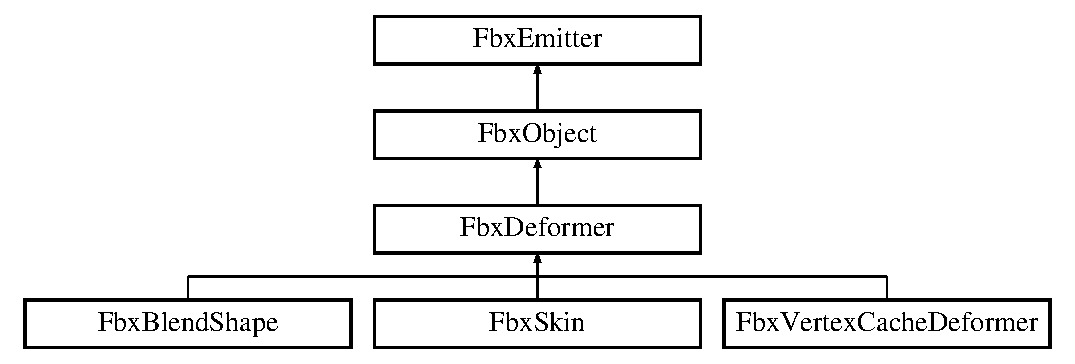
\includegraphics[height=4.000000cm]{class_fbx_deformer}
\end{center}
\end{figure}
\subsection*{限定公開メンバ関数}
\begin{DoxyCompactItemize}
\item 
virtual void \hyperlink{class_fbx_deformer_ac50e8e0e8cfd2934f8f8cca2d69a6f58}{Construct} (const \hyperlink{class_fbx_object}{Fbx\+Object} $\ast$p\+From)
\item 
virtual \hyperlink{class_fbx_string_list}{Fbx\+String\+List} \hyperlink{class_fbx_deformer_ac3f5a3eb2dda62397fc667004d798319}{Get\+Type\+Flags} () const
\end{DoxyCompactItemize}
\subsection*{限定公開変数類}
\begin{DoxyCompactItemize}
\item 
bool \hyperlink{class_fbx_deformer_ac570aba2e0282a6075831422a05c2d48}{m\+Multi\+Layer}
\end{DoxyCompactItemize}
\subsection*{Multi-\/\+Layer Flag}
\label{_amgrpdf4ac1e76a017b89c2c8620c9bd4ab91}%
This flag is available for backward compatibility with older version of F\+BX files and should not be used anymore. All the animation layering system has been moved to the \hyperlink{class_fbx_anim_layer}{Fbx\+Anim\+Layer} and \hyperlink{class_fbx_anim_stack}{Fbx\+Anim\+Stack} classes. \begin{DoxyCompactItemize}
\item 
void \hyperlink{class_fbx_deformer_ac1152e69487365faa19fe23ffde19f85}{Set\+Multi\+Layer} (bool p\+Multi\+Layer)
\item 
bool \hyperlink{class_fbx_deformer_a1f56fdb78d3b615bb2b4b4d142436e8b}{Get\+Multi\+Layer} () const
\end{DoxyCompactItemize}
\subsection*{Deformer types}
\begin{DoxyCompactItemize}
\item 
enum \hyperlink{class_fbx_deformer_a07e2cfb767191ba5c8799fdfbfe3eaf6}{E\+Deformer\+Type} \{ \hyperlink{class_fbx_deformer_a07e2cfb767191ba5c8799fdfbfe3eaf6a432666d716eeff4acebb52aeb7df93ee}{e\+Unknown}, 
\hyperlink{class_fbx_deformer_a07e2cfb767191ba5c8799fdfbfe3eaf6ae219b2649e29244fe4d80e649241c90e}{e\+Skin}, 
\hyperlink{class_fbx_deformer_a07e2cfb767191ba5c8799fdfbfe3eaf6aa59f09ee382f2e19e4923b5b2155b2d9}{e\+Blend\+Shape}, 
\hyperlink{class_fbx_deformer_a07e2cfb767191ba5c8799fdfbfe3eaf6afca1c8188109c1fe60004335f76a42b8}{e\+Vertex\+Cache}
 \}
\item 
virtual \hyperlink{class_fbx_deformer_a07e2cfb767191ba5c8799fdfbfe3eaf6}{E\+Deformer\+Type} \hyperlink{class_fbx_deformer_adbc586e383f788f24d7fce9ed859d481}{Get\+Deformer\+Type} () const
\end{DoxyCompactItemize}
\subsection*{その他の継承メンバ}


\subsection{詳解}
Base class for skin deformer (\hyperlink{class_fbx_skin}{Fbx\+Skin}) and vertex cache deformer (\hyperlink{class_fbx_vertex_cache_deformer}{Fbx\+Vertex\+Cache\+Deformer}). The corresponding deformer types are \hyperlink{class_fbx_deformer_a07e2cfb767191ba5c8799fdfbfe3eaf6ae219b2649e29244fe4d80e649241c90e}{Fbx\+Deformer\+::e\+Skin} and \hyperlink{class_fbx_deformer_a07e2cfb767191ba5c8799fdfbfe3eaf6afca1c8188109c1fe60004335f76a42b8}{Fbx\+Deformer\+::e\+Vertex\+Cache}. A deformer can be binded to a geometry (\hyperlink{class_fbx_geometry}{Fbx\+Geometry}) to act on its shape. Typically, some objects under the deformer are animated, and via the deformer, the geometry is animated too.

A skin deformer contains clusters (\hyperlink{class_fbx_cluster}{Fbx\+Cluster}). Each cluster acts on a subset of the geometry\textquotesingle{}s control points, with different weights. For example, a mesh of humanoid shape can have a skin attached, that describes the way the humanoid mesh is deformed by bones. When the bones are animated, the clusters act on the geometry to animate it too.

A vertex cache deformer contains a cache (\hyperlink{class_fbx_cache}{Fbx\+Cache}). The cache contains animation information for every control point of the geometry. 

 fbxdeformer.\+h の 38 行目に定義があります。



\subsection{列挙型メンバ詳解}
\mbox{\Hypertarget{class_fbx_deformer_a07e2cfb767191ba5c8799fdfbfe3eaf6}\label{class_fbx_deformer_a07e2cfb767191ba5c8799fdfbfe3eaf6}} 
\index{Fbx\+Deformer@{Fbx\+Deformer}!E\+Deformer\+Type@{E\+Deformer\+Type}}
\index{E\+Deformer\+Type@{E\+Deformer\+Type}!Fbx\+Deformer@{Fbx\+Deformer}}
\subsubsection{\texorpdfstring{E\+Deformer\+Type}{EDeformerType}}
{\footnotesize\ttfamily enum \hyperlink{class_fbx_deformer_a07e2cfb767191ba5c8799fdfbfe3eaf6}{Fbx\+Deformer\+::\+E\+Deformer\+Type}}

Deformer types. \begin{DoxyEnumFields}{列挙値}
\raisebox{\heightof{T}}[0pt][0pt]{\index{e\+Unknown@{e\+Unknown}!Fbx\+Deformer@{Fbx\+Deformer}}\index{Fbx\+Deformer@{Fbx\+Deformer}!e\+Unknown@{e\+Unknown}}}\mbox{\Hypertarget{class_fbx_deformer_a07e2cfb767191ba5c8799fdfbfe3eaf6a432666d716eeff4acebb52aeb7df93ee}\label{class_fbx_deformer_a07e2cfb767191ba5c8799fdfbfe3eaf6a432666d716eeff4acebb52aeb7df93ee}} 
e\+Unknown&Unknown deformer type \\
\hline

\raisebox{\heightof{T}}[0pt][0pt]{\index{e\+Skin@{e\+Skin}!Fbx\+Deformer@{Fbx\+Deformer}}\index{Fbx\+Deformer@{Fbx\+Deformer}!e\+Skin@{e\+Skin}}}\mbox{\Hypertarget{class_fbx_deformer_a07e2cfb767191ba5c8799fdfbfe3eaf6ae219b2649e29244fe4d80e649241c90e}\label{class_fbx_deformer_a07e2cfb767191ba5c8799fdfbfe3eaf6ae219b2649e29244fe4d80e649241c90e}} 
e\+Skin&Type \hyperlink{class_fbx_skin}{Fbx\+Skin} \\
\hline

\raisebox{\heightof{T}}[0pt][0pt]{\index{e\+Blend\+Shape@{e\+Blend\+Shape}!Fbx\+Deformer@{Fbx\+Deformer}}\index{Fbx\+Deformer@{Fbx\+Deformer}!e\+Blend\+Shape@{e\+Blend\+Shape}}}\mbox{\Hypertarget{class_fbx_deformer_a07e2cfb767191ba5c8799fdfbfe3eaf6aa59f09ee382f2e19e4923b5b2155b2d9}\label{class_fbx_deformer_a07e2cfb767191ba5c8799fdfbfe3eaf6aa59f09ee382f2e19e4923b5b2155b2d9}} 
e\+Blend\+Shape&Type \hyperlink{class_fbx_blend_shape}{Fbx\+Blend\+Shape} \\
\hline

\raisebox{\heightof{T}}[0pt][0pt]{\index{e\+Vertex\+Cache@{e\+Vertex\+Cache}!Fbx\+Deformer@{Fbx\+Deformer}}\index{Fbx\+Deformer@{Fbx\+Deformer}!e\+Vertex\+Cache@{e\+Vertex\+Cache}}}\mbox{\Hypertarget{class_fbx_deformer_a07e2cfb767191ba5c8799fdfbfe3eaf6afca1c8188109c1fe60004335f76a42b8}\label{class_fbx_deformer_a07e2cfb767191ba5c8799fdfbfe3eaf6afca1c8188109c1fe60004335f76a42b8}} 
e\+Vertex\+Cache&Type \hyperlink{class_fbx_vertex_cache_deformer}{Fbx\+Vertex\+Cache\+Deformer} \\
\hline

\end{DoxyEnumFields}


 fbxdeformer.\+h の 67 行目に定義があります。



\subsection{関数詳解}
\mbox{\Hypertarget{class_fbx_deformer_ac50e8e0e8cfd2934f8f8cca2d69a6f58}\label{class_fbx_deformer_ac50e8e0e8cfd2934f8f8cca2d69a6f58}} 
\index{Fbx\+Deformer@{Fbx\+Deformer}!Construct@{Construct}}
\index{Construct@{Construct}!Fbx\+Deformer@{Fbx\+Deformer}}
\subsubsection{\texorpdfstring{Construct()}{Construct()}}
{\footnotesize\ttfamily virtual void Fbx\+Deformer\+::\+Construct (\begin{DoxyParamCaption}\item[{const \hyperlink{class_fbx_object}{Fbx\+Object} $\ast$}]{p\+From }\end{DoxyParamCaption})\hspace{0.3cm}{\ttfamily [protected]}, {\ttfamily [virtual]}}

Optional constructor override, automatically called by default constructor. 
\begin{DoxyParams}{引数}
{\em p\+From} & If not null, the function must take it into account like a copy constructor. \\
\hline
\end{DoxyParams}
\begin{DoxyRemark}{注釈}
In case it is decided to override this function, do not forget to call Parent\+Class\+::\+Construct(p\+From) at the beginning. 
\end{DoxyRemark}


\hyperlink{class_fbx_object_a313503bc645af3fdceb4a99ef5cea7eb}{Fbx\+Object}を再実装しています。



\hyperlink{class_fbx_skin_aeebbc037507285cdb2e066f420970208}{Fbx\+Skin}で再実装されています。

\mbox{\Hypertarget{class_fbx_deformer_adbc586e383f788f24d7fce9ed859d481}\label{class_fbx_deformer_adbc586e383f788f24d7fce9ed859d481}} 
\index{Fbx\+Deformer@{Fbx\+Deformer}!Get\+Deformer\+Type@{Get\+Deformer\+Type}}
\index{Get\+Deformer\+Type@{Get\+Deformer\+Type}!Fbx\+Deformer@{Fbx\+Deformer}}
\subsubsection{\texorpdfstring{Get\+Deformer\+Type()}{GetDeformerType()}}
{\footnotesize\ttfamily virtual \hyperlink{class_fbx_deformer_a07e2cfb767191ba5c8799fdfbfe3eaf6}{E\+Deformer\+Type} Fbx\+Deformer\+::\+Get\+Deformer\+Type (\begin{DoxyParamCaption}{ }\end{DoxyParamCaption}) const\hspace{0.3cm}{\ttfamily [inline]}, {\ttfamily [virtual]}}

Get the deformer type. \begin{DoxyReturn}{戻り値}
Deformer type identifier. Default value is e\+Unknown. 
\end{DoxyReturn}


\hyperlink{class_fbx_skin_abaf5fca14c0e8339ea692560fbd494d8}{Fbx\+Skin}, \hyperlink{class_fbx_blend_shape_afc886286ac95264b993335d8b3954b4f}{Fbx\+Blend\+Shape}, \hyperlink{class_fbx_vertex_cache_deformer_ab213400e170fe58699649acaf652c787}{Fbx\+Vertex\+Cache\+Deformer}で再実装されています。



 fbxdeformer.\+h の 78 行目に定義があります。

\mbox{\Hypertarget{class_fbx_deformer_a1f56fdb78d3b615bb2b4b4d142436e8b}\label{class_fbx_deformer_a1f56fdb78d3b615bb2b4b4d142436e8b}} 
\index{Fbx\+Deformer@{Fbx\+Deformer}!Get\+Multi\+Layer@{Get\+Multi\+Layer}}
\index{Get\+Multi\+Layer@{Get\+Multi\+Layer}!Fbx\+Deformer@{Fbx\+Deformer}}
\subsubsection{\texorpdfstring{Get\+Multi\+Layer()}{GetMultiLayer()}}
{\footnotesize\ttfamily bool Fbx\+Deformer\+::\+Get\+Multi\+Layer (\begin{DoxyParamCaption}{ }\end{DoxyParamCaption}) const}

Get multi-\/layer state. \begin{DoxyReturn}{戻り値}
The current state of the multi-\/layer flag. 
\end{DoxyReturn}
\mbox{\Hypertarget{class_fbx_deformer_ac3f5a3eb2dda62397fc667004d798319}\label{class_fbx_deformer_ac3f5a3eb2dda62397fc667004d798319}} 
\index{Fbx\+Deformer@{Fbx\+Deformer}!Get\+Type\+Flags@{Get\+Type\+Flags}}
\index{Get\+Type\+Flags@{Get\+Type\+Flags}!Fbx\+Deformer@{Fbx\+Deformer}}
\subsubsection{\texorpdfstring{Get\+Type\+Flags()}{GetTypeFlags()}}
{\footnotesize\ttfamily virtual \hyperlink{class_fbx_string_list}{Fbx\+String\+List} Fbx\+Deformer\+::\+Get\+Type\+Flags (\begin{DoxyParamCaption}{ }\end{DoxyParamCaption}) const\hspace{0.3cm}{\ttfamily [inline]}, {\ttfamily [protected]}, {\ttfamily [virtual]}}



\hyperlink{class_fbx_object_a6d30a5d00400039a248977cf9f9255b2}{Fbx\+Object}を再実装しています。



\hyperlink{class_fbx_skin_a736228a80b5d0db0075527767286be2d}{Fbx\+Skin}, \hyperlink{class_fbx_blend_shape_aa2b22b70c929ac1ad39b12f0ade998d1}{Fbx\+Blend\+Shape}, \hyperlink{class_fbx_vertex_cache_deformer_a67322e24180497b1f268cad5ed29c08b}{Fbx\+Vertex\+Cache\+Deformer}で再実装されています。



 fbxdeformer.\+h の 87 行目に定義があります。

\mbox{\Hypertarget{class_fbx_deformer_ac1152e69487365faa19fe23ffde19f85}\label{class_fbx_deformer_ac1152e69487365faa19fe23ffde19f85}} 
\index{Fbx\+Deformer@{Fbx\+Deformer}!Set\+Multi\+Layer@{Set\+Multi\+Layer}}
\index{Set\+Multi\+Layer@{Set\+Multi\+Layer}!Fbx\+Deformer@{Fbx\+Deformer}}
\subsubsection{\texorpdfstring{Set\+Multi\+Layer()}{SetMultiLayer()}}
{\footnotesize\ttfamily void Fbx\+Deformer\+::\+Set\+Multi\+Layer (\begin{DoxyParamCaption}\item[{bool}]{p\+Multi\+Layer }\end{DoxyParamCaption})}

Set multi-\/layer state flag. 
\begin{DoxyParams}{引数}
{\em p\+Multi\+Layer} & Set to {\ttfamily true} to enable multi-\/layering. \\
\hline
\end{DoxyParams}


\subsection{メンバ詳解}
\mbox{\Hypertarget{class_fbx_deformer_ac570aba2e0282a6075831422a05c2d48}\label{class_fbx_deformer_ac570aba2e0282a6075831422a05c2d48}} 
\index{Fbx\+Deformer@{Fbx\+Deformer}!m\+Multi\+Layer@{m\+Multi\+Layer}}
\index{m\+Multi\+Layer@{m\+Multi\+Layer}!Fbx\+Deformer@{Fbx\+Deformer}}
\subsubsection{\texorpdfstring{m\+Multi\+Layer}{mMultiLayer}}
{\footnotesize\ttfamily bool Fbx\+Deformer\+::m\+Multi\+Layer\hspace{0.3cm}{\ttfamily [protected]}}



 fbxdeformer.\+h の 89 行目に定義があります。



このクラス詳解は次のファイルから抽出されました\+:\begin{DoxyCompactItemize}
\item 
C\+:/\+Maya/scripts/\+F\+B\+X\+\_\+\+S\+D\+K/2017.\+1/include/fbxsdk/scene/geometry/\hyperlink{fbxdeformer_8h}{fbxdeformer.\+h}\end{DoxyCompactItemize}

\hypertarget{class_fbx_degree_to_radian_b_o_f}{}\section{Fbx\+Degree\+To\+Radian\+B\+OF クラス}
\label{class_fbx_degree_to_radian_b_o_f}\index{Fbx\+Degree\+To\+Radian\+B\+OF@{Fbx\+Degree\+To\+Radian\+B\+OF}}


{\ttfamily \#include $<$fbxbindingoperator.\+h$>$}

Fbx\+Degree\+To\+Radian\+B\+OF の継承関係図\begin{figure}[H]
\begin{center}
\leavevmode
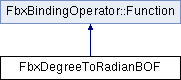
\includegraphics[height=2.000000cm]{class_fbx_degree_to_radian_b_o_f}
\end{center}
\end{figure}
\subsection*{公開メンバ関数}
\begin{DoxyCompactItemize}
\item 
virtual bool \hyperlink{class_fbx_degree_to_radian_b_o_f_a6cee9578c7edb1b27f90f72ac9ec7000}{Evaluate} (const \hyperlink{class_fbx_binding_operator}{Fbx\+Binding\+Operator} $\ast$p\+Operator, const \hyperlink{class_fbx_object}{Fbx\+Object} $\ast$p\+Object, \hyperlink{fbxpropertytypes_8h_a73913a5ddfb20e57c6f25e9e6784bd92}{E\+Fbx\+Type} $\ast$p\+Result\+Type, void $\ast$$\ast$p\+Result) const
\item 
virtual bool \hyperlink{class_fbx_degree_to_radian_b_o_f_a65c7f3fdae835f27e123b2efc8aaf9da}{Reverse\+Evaluate} (const \hyperlink{class_fbx_binding_operator}{Fbx\+Binding\+Operator} $\ast$p\+Operator, const \hyperlink{class_fbx_object}{Fbx\+Object} $\ast$p\+Target, const void $\ast$p\+In, void $\ast$$\ast$p\+Out, \hyperlink{fbxpropertytypes_8h_a73913a5ddfb20e57c6f25e9e6784bd92}{E\+Fbx\+Type} $\ast$p\+Out\+Type, bool set\+Obj, int index) const
\item 
\hyperlink{class_fbx_degree_to_radian_b_o_f_a5ec303303a760400996c0115264ca4ad}{Fbx\+Degree\+To\+Radian\+B\+OF} ()
\item 
virtual \hyperlink{class_fbx_degree_to_radian_b_o_f_a4cc35e7abc17e6a76ba7c5857a5f34bd}{$\sim$\+Fbx\+Degree\+To\+Radian\+B\+OF} ()
\end{DoxyCompactItemize}
\subsection*{静的公開変数類}
\begin{DoxyCompactItemize}
\item 
static const char $\ast$ \hyperlink{class_fbx_degree_to_radian_b_o_f_a5a082cbbb422d50fdc37dabab272caba}{Function\+Name}
\begin{DoxyCompactList}\small\item\em Name of the operation function. \end{DoxyCompactList}\end{DoxyCompactItemize}


\subsection{詳解}


 fbxbindingoperator.\+h の 680 行目に定義があります。



\subsection{構築子と解体子}
\mbox{\Hypertarget{class_fbx_degree_to_radian_b_o_f_a5ec303303a760400996c0115264ca4ad}\label{class_fbx_degree_to_radian_b_o_f_a5ec303303a760400996c0115264ca4ad}} 
\index{Fbx\+Degree\+To\+Radian\+B\+OF@{Fbx\+Degree\+To\+Radian\+B\+OF}!Fbx\+Degree\+To\+Radian\+B\+OF@{Fbx\+Degree\+To\+Radian\+B\+OF}}
\index{Fbx\+Degree\+To\+Radian\+B\+OF@{Fbx\+Degree\+To\+Radian\+B\+OF}!Fbx\+Degree\+To\+Radian\+B\+OF@{Fbx\+Degree\+To\+Radian\+B\+OF}}
\subsubsection{\texorpdfstring{Fbx\+Degree\+To\+Radian\+B\+O\+F()}{FbxDegreeToRadianBOF()}}
{\footnotesize\ttfamily Fbx\+Degree\+To\+Radian\+B\+O\+F\+::\+Fbx\+Degree\+To\+Radian\+B\+OF (\begin{DoxyParamCaption}{ }\end{DoxyParamCaption})}

\mbox{\Hypertarget{class_fbx_degree_to_radian_b_o_f_a4cc35e7abc17e6a76ba7c5857a5f34bd}\label{class_fbx_degree_to_radian_b_o_f_a4cc35e7abc17e6a76ba7c5857a5f34bd}} 
\index{Fbx\+Degree\+To\+Radian\+B\+OF@{Fbx\+Degree\+To\+Radian\+B\+OF}!````~Fbx\+Degree\+To\+Radian\+B\+OF@{$\sim$\+Fbx\+Degree\+To\+Radian\+B\+OF}}
\index{````~Fbx\+Degree\+To\+Radian\+B\+OF@{$\sim$\+Fbx\+Degree\+To\+Radian\+B\+OF}!Fbx\+Degree\+To\+Radian\+B\+OF@{Fbx\+Degree\+To\+Radian\+B\+OF}}
\subsubsection{\texorpdfstring{$\sim$\+Fbx\+Degree\+To\+Radian\+B\+O\+F()}{~FbxDegreeToRadianBOF()}}
{\footnotesize\ttfamily virtual Fbx\+Degree\+To\+Radian\+B\+O\+F\+::$\sim$\+Fbx\+Degree\+To\+Radian\+B\+OF (\begin{DoxyParamCaption}{ }\end{DoxyParamCaption})\hspace{0.3cm}{\ttfamily [virtual]}}



\subsection{関数詳解}
\mbox{\Hypertarget{class_fbx_degree_to_radian_b_o_f_a6cee9578c7edb1b27f90f72ac9ec7000}\label{class_fbx_degree_to_radian_b_o_f_a6cee9578c7edb1b27f90f72ac9ec7000}} 
\index{Fbx\+Degree\+To\+Radian\+B\+OF@{Fbx\+Degree\+To\+Radian\+B\+OF}!Evaluate@{Evaluate}}
\index{Evaluate@{Evaluate}!Fbx\+Degree\+To\+Radian\+B\+OF@{Fbx\+Degree\+To\+Radian\+B\+OF}}
\subsubsection{\texorpdfstring{Evaluate()}{Evaluate()}}
{\footnotesize\ttfamily virtual bool Fbx\+Degree\+To\+Radian\+B\+O\+F\+::\+Evaluate (\begin{DoxyParamCaption}\item[{const \hyperlink{class_fbx_binding_operator}{Fbx\+Binding\+Operator} $\ast$}]{p\+Operator,  }\item[{const \hyperlink{class_fbx_object}{Fbx\+Object} $\ast$}]{p\+Object,  }\item[{\hyperlink{fbxpropertytypes_8h_a73913a5ddfb20e57c6f25e9e6784bd92}{E\+Fbx\+Type} $\ast$}]{p\+Result\+Type,  }\item[{void $\ast$$\ast$}]{p\+Result }\end{DoxyParamCaption}) const\hspace{0.3cm}{\ttfamily [virtual]}}

Evaluates the object property specified by \char`\"{}\+X\char`\"{} return X converted to radian as a float.


\begin{DoxyParams}{引数}
{\em p\+Operator} & Operator running on the object. \\
\hline
{\em p\+Object} & The object that will be evaluated. \\
\hline
{\em p\+Result\+Type} & The type of the result to be returned. \\
\hline
{\em p\+Result} & A pointer to a buffer that can hold the result. \\
\hline
\end{DoxyParams}
\begin{DoxyReturn}{戻り値}
{\ttfamily true} on success, {\ttfamily false} otherwise. 
\end{DoxyReturn}


\hyperlink{class_fbx_binding_operator_1_1_function_aa238a63d12508db3cb5c00a4b157524e}{Fbx\+Binding\+Operator\+::\+Function}を実装しています。

\mbox{\Hypertarget{class_fbx_degree_to_radian_b_o_f_a65c7f3fdae835f27e123b2efc8aaf9da}\label{class_fbx_degree_to_radian_b_o_f_a65c7f3fdae835f27e123b2efc8aaf9da}} 
\index{Fbx\+Degree\+To\+Radian\+B\+OF@{Fbx\+Degree\+To\+Radian\+B\+OF}!Reverse\+Evaluate@{Reverse\+Evaluate}}
\index{Reverse\+Evaluate@{Reverse\+Evaluate}!Fbx\+Degree\+To\+Radian\+B\+OF@{Fbx\+Degree\+To\+Radian\+B\+OF}}
\subsubsection{\texorpdfstring{Reverse\+Evaluate()}{ReverseEvaluate()}}
{\footnotesize\ttfamily virtual bool Fbx\+Degree\+To\+Radian\+B\+O\+F\+::\+Reverse\+Evaluate (\begin{DoxyParamCaption}\item[{const \hyperlink{class_fbx_binding_operator}{Fbx\+Binding\+Operator} $\ast$}]{p\+Operator,  }\item[{const \hyperlink{class_fbx_object}{Fbx\+Object} $\ast$}]{p\+Target,  }\item[{const void $\ast$}]{p\+In,  }\item[{void $\ast$$\ast$}]{p\+Out,  }\item[{\hyperlink{fbxpropertytypes_8h_a73913a5ddfb20e57c6f25e9e6784bd92}{E\+Fbx\+Type} $\ast$}]{p\+Out\+Type,  }\item[{bool}]{set\+Obj,  }\item[{int}]{index }\end{DoxyParamCaption}) const\hspace{0.3cm}{\ttfamily [virtual]}}

Run the inverse operator on the given object, assigning the result directly to the object. 
\begin{DoxyParams}{引数}
{\em p\+Operator} & The operator that will be applied. \\
\hline
{\em p\+Target} & The object that will be evaluated. \\
\hline
{\em p\+In} & \\
\hline
{\em p\+Out} & \\
\hline
{\em p\+Out\+Type} & Type of value being reversed. \\
\hline
{\em set\+Obj} & Control to set the property (only to query by the default ). \\
\hline
{\em index} & Used only in \hyperlink{class_fbx_multiply_dist_b_o_f}{Fbx\+Multiply\+Dist\+B\+OF}. \\
\hline
\end{DoxyParams}
\begin{DoxyReturn}{戻り値}
{\ttfamily true} on success, {\ttfamily false} otherwise. 
\end{DoxyReturn}


\hyperlink{class_fbx_binding_operator_1_1_function_a9bbeec993a6e453a6569e7f40a85fd52}{Fbx\+Binding\+Operator\+::\+Function}を実装しています。



\subsection{メンバ詳解}
\mbox{\Hypertarget{class_fbx_degree_to_radian_b_o_f_a5a082cbbb422d50fdc37dabab272caba}\label{class_fbx_degree_to_radian_b_o_f_a5a082cbbb422d50fdc37dabab272caba}} 
\index{Fbx\+Degree\+To\+Radian\+B\+OF@{Fbx\+Degree\+To\+Radian\+B\+OF}!Function\+Name@{Function\+Name}}
\index{Function\+Name@{Function\+Name}!Fbx\+Degree\+To\+Radian\+B\+OF@{Fbx\+Degree\+To\+Radian\+B\+OF}}
\subsubsection{\texorpdfstring{Function\+Name}{FunctionName}}
{\footnotesize\ttfamily const char$\ast$ Fbx\+Degree\+To\+Radian\+B\+O\+F\+::\+Function\+Name\hspace{0.3cm}{\ttfamily [static]}}



Name of the operation function. 



 fbxbindingoperator.\+h の 684 行目に定義があります。



このクラス詳解は次のファイルから抽出されました\+:\begin{DoxyCompactItemize}
\item 
C\+:/\+Maya/scripts/\+F\+B\+X\+\_\+\+S\+D\+K/2017.\+1/include/fbxsdk/scene/shading/\hyperlink{fbxbindingoperator_8h}{fbxbindingoperator.\+h}\end{DoxyCompactItemize}

\hypertarget{class_fbx_deletion_policy_default}{}\section{Fbx\+Deletion\+Policy\+Default$<$ Type $>$ クラステンプレート}
\label{class_fbx_deletion_policy_default}\index{Fbx\+Deletion\+Policy\+Default$<$ Type $>$@{Fbx\+Deletion\+Policy\+Default$<$ Type $>$}}


Deletion policy for pointer template classes that uses the delete operator.  




{\ttfamily \#include $<$fbxalloc.\+h$>$}

\subsection*{静的公開メンバ関数}
\begin{DoxyCompactItemize}
\item 
static void \hyperlink{class_fbx_deletion_policy_default_a6f1fb89b306b4b1bf88d5be8aaf1d83e}{Delete\+It} (Type $\ast$$\ast$p\+Ptr)
\begin{DoxyCompactList}\small\item\em Destruction policy implementation. \end{DoxyCompactList}\end{DoxyCompactItemize}


\subsection{詳解}
\subsubsection*{template$<$class Type$>$\newline
class Fbx\+Deletion\+Policy\+Default$<$ Type $>$}

Deletion policy for pointer template classes that uses the delete operator. 

 fbxalloc.\+h の 126 行目に定義があります。



\subsection{関数詳解}
\mbox{\Hypertarget{class_fbx_deletion_policy_default_a6f1fb89b306b4b1bf88d5be8aaf1d83e}\label{class_fbx_deletion_policy_default_a6f1fb89b306b4b1bf88d5be8aaf1d83e}} 
\index{Fbx\+Deletion\+Policy\+Default@{Fbx\+Deletion\+Policy\+Default}!Delete\+It@{Delete\+It}}
\index{Delete\+It@{Delete\+It}!Fbx\+Deletion\+Policy\+Default@{Fbx\+Deletion\+Policy\+Default}}
\subsubsection{\texorpdfstring{Delete\+It()}{DeleteIt()}}
{\footnotesize\ttfamily template$<$class Type $>$ \\
static void \hyperlink{class_fbx_deletion_policy_default}{Fbx\+Deletion\+Policy\+Default}$<$ Type $>$\+::Delete\+It (\begin{DoxyParamCaption}\item[{Type $\ast$$\ast$}]{p\+Ptr }\end{DoxyParamCaption})\hspace{0.3cm}{\ttfamily [inline]}, {\ttfamily [static]}}



Destruction policy implementation. 



 fbxalloc.\+h の 130 行目に定義があります。



このクラス詳解は次のファイルから抽出されました\+:\begin{DoxyCompactItemize}
\item 
C\+:/\+Maya/scripts/\+F\+B\+X\+\_\+\+S\+D\+K/2017.\+1/include/fbxsdk/core/arch/\hyperlink{fbxalloc_8h}{fbxalloc.\+h}\end{DoxyCompactItemize}

\hypertarget{class_fbx_deletion_policy_delete}{}\section{Fbx\+Deletion\+Policy\+Delete$<$ Type $>$ クラステンプレート}
\label{class_fbx_deletion_policy_delete}\index{Fbx\+Deletion\+Policy\+Delete$<$ Type $>$@{Fbx\+Deletion\+Policy\+Delete$<$ Type $>$}}


{\ttfamily \#include $<$fbxalloc.\+h$>$}

\subsection*{静的公開メンバ関数}
\begin{DoxyCompactItemize}
\item 
static void \hyperlink{class_fbx_deletion_policy_delete_ae09420cded9deb38e063f37a1f7d7d11}{Delete\+It} (Type $\ast$$\ast$m\+Ptr)
\begin{DoxyCompactList}\small\item\em Destruction policy implementation. \end{DoxyCompactList}\end{DoxyCompactItemize}


\subsection{詳解}
\subsubsection*{template$<$class Type$>$\newline
class Fbx\+Deletion\+Policy\+Delete$<$ Type $>$}



 fbxalloc.\+h の 143 行目に定義があります。



\subsection{関数詳解}
\mbox{\Hypertarget{class_fbx_deletion_policy_delete_ae09420cded9deb38e063f37a1f7d7d11}\label{class_fbx_deletion_policy_delete_ae09420cded9deb38e063f37a1f7d7d11}} 
\index{Fbx\+Deletion\+Policy\+Delete@{Fbx\+Deletion\+Policy\+Delete}!Delete\+It@{Delete\+It}}
\index{Delete\+It@{Delete\+It}!Fbx\+Deletion\+Policy\+Delete@{Fbx\+Deletion\+Policy\+Delete}}
\subsubsection{\texorpdfstring{Delete\+It()}{DeleteIt()}}
{\footnotesize\ttfamily template$<$class Type $>$ \\
static void \hyperlink{class_fbx_deletion_policy_delete}{Fbx\+Deletion\+Policy\+Delete}$<$ Type $>$\+::Delete\+It (\begin{DoxyParamCaption}\item[{Type $\ast$$\ast$}]{m\+Ptr }\end{DoxyParamCaption})\hspace{0.3cm}{\ttfamily [inline]}, {\ttfamily [static]}}



Destruction policy implementation. 



 fbxalloc.\+h の 147 行目に定義があります。



このクラス詳解は次のファイルから抽出されました\+:\begin{DoxyCompactItemize}
\item 
C\+:/\+Maya/scripts/\+F\+B\+X\+\_\+\+S\+D\+K/2017.\+1/include/fbxsdk/core/arch/\hyperlink{fbxalloc_8h}{fbxalloc.\+h}\end{DoxyCompactItemize}

\hypertarget{class_fbx_deletion_policy_free}{}\section{Fbx\+Deletion\+Policy\+Free$<$ Type $>$ クラステンプレート}
\label{class_fbx_deletion_policy_free}\index{Fbx\+Deletion\+Policy\+Free$<$ Type $>$@{Fbx\+Deletion\+Policy\+Free$<$ Type $>$}}


Deletion policy for pointer template classes that uses the \hyperlink{fbxalloc_8h_a8252906713d55f4c56e7ba84221d3852}{Fbx\+Free()} function.  




{\ttfamily \#include $<$fbxalloc.\+h$>$}

\subsection*{静的公開メンバ関数}
\begin{DoxyCompactItemize}
\item 
static void \hyperlink{class_fbx_deletion_policy_free_a6b0c1df911d0480122de9bf31a4fd4a5}{Delete\+It} (Type $\ast$$\ast$p\+Ptr)
\begin{DoxyCompactList}\small\item\em Destruction policy implementation. \end{DoxyCompactList}\end{DoxyCompactItemize}


\subsection{詳解}
\subsubsection*{template$<$class Type$>$\newline
class Fbx\+Deletion\+Policy\+Free$<$ Type $>$}

Deletion policy for pointer template classes that uses the \hyperlink{fbxalloc_8h_a8252906713d55f4c56e7ba84221d3852}{Fbx\+Free()} function. 

\subsection{メソッド詳解}
\mbox{\Hypertarget{class_fbx_deletion_policy_free_a6b0c1df911d0480122de9bf31a4fd4a5}\label{class_fbx_deletion_policy_free_a6b0c1df911d0480122de9bf31a4fd4a5}} 
\index{Fbx\+Deletion\+Policy\+Free@{Fbx\+Deletion\+Policy\+Free}!Delete\+It@{Delete\+It}}
\index{Delete\+It@{Delete\+It}!Fbx\+Deletion\+Policy\+Free@{Fbx\+Deletion\+Policy\+Free}}
\subsubsection{\texorpdfstring{Delete\+It()}{DeleteIt()}}
{\footnotesize\ttfamily template$<$class Type $>$ \\
static void \hyperlink{class_fbx_deletion_policy_free}{Fbx\+Deletion\+Policy\+Free}$<$ Type $>$\+::Delete\+It (\begin{DoxyParamCaption}\item[{Type $\ast$$\ast$}]{p\+Ptr }\end{DoxyParamCaption})\hspace{0.3cm}{\ttfamily [static]}}



Destruction policy implementation. 

呼び出し関係図\+:
% FIG 0


このクラス詳解は次のファイルから抽出されました\+:\begin{DoxyCompactItemize}
\item 
C\+:/github/\+F\+B\+Xpython\+S\+D\+K201701/\+F\+B\+Xpython\+S\+D\+K201701/2017.\+1/include/fbxsdk/core/arch/\hyperlink{fbxalloc_8h}{fbxalloc.\+h}\end{DoxyCompactItemize}

\hypertarget{class_fbx_deletion_policy_object}{}\section{Fbx\+Deletion\+Policy\+Object$<$ Type $>$ クラステンプレート}
\label{class_fbx_deletion_policy_object}\index{Fbx\+Deletion\+Policy\+Object$<$ Type $>$@{Fbx\+Deletion\+Policy\+Object$<$ Type $>$}}


Deletion policy for pointer template classes that uses the Destroy() function.  




{\ttfamily \#include $<$fbxalloc.\+h$>$}

\subsection*{静的公開メンバ関数}
\begin{DoxyCompactItemize}
\item 
static void \hyperlink{class_fbx_deletion_policy_object_a5a0e0ae55b3f3fb5f195e777facf6d1c}{Delete\+It} (Type $\ast$$\ast$p\+Ptr)
\begin{DoxyCompactList}\small\item\em Destruction policy implementation. \end{DoxyCompactList}\end{DoxyCompactItemize}


\subsection{詳解}
\subsubsection*{template$<$class Type$>$\newline
class Fbx\+Deletion\+Policy\+Object$<$ Type $>$}

Deletion policy for pointer template classes that uses the Destroy() function. 

\subsection{メソッド詳解}
\mbox{\Hypertarget{class_fbx_deletion_policy_object_a5a0e0ae55b3f3fb5f195e777facf6d1c}\label{class_fbx_deletion_policy_object_a5a0e0ae55b3f3fb5f195e777facf6d1c}} 
\index{Fbx\+Deletion\+Policy\+Object@{Fbx\+Deletion\+Policy\+Object}!Delete\+It@{Delete\+It}}
\index{Delete\+It@{Delete\+It}!Fbx\+Deletion\+Policy\+Object@{Fbx\+Deletion\+Policy\+Object}}
\subsubsection{\texorpdfstring{Delete\+It()}{DeleteIt()}}
{\footnotesize\ttfamily template$<$class Type $>$ \\
static void \hyperlink{class_fbx_deletion_policy_object}{Fbx\+Deletion\+Policy\+Object}$<$ Type $>$\+::Delete\+It (\begin{DoxyParamCaption}\item[{Type $\ast$$\ast$}]{p\+Ptr }\end{DoxyParamCaption})\hspace{0.3cm}{\ttfamily [static]}}



Destruction policy implementation. 



このクラス詳解は次のファイルから抽出されました\+:\begin{DoxyCompactItemize}
\item 
C\+:/github/\+F\+B\+Xpython\+S\+D\+K201701/\+F\+B\+Xpython\+S\+D\+K201701/2017.\+1/include/fbxsdk/core/arch/\hyperlink{fbxalloc_8h}{fbxalloc.\+h}\end{DoxyCompactItemize}

\hypertarget{class_fbx_display_layer}{}\section{Fbx\+Display\+Layer クラス}
\label{class_fbx_display_layer}\index{Fbx\+Display\+Layer@{Fbx\+Display\+Layer}}


{\ttfamily \#include $<$fbxdisplaylayer.\+h$>$}



Fbx\+Display\+Layer の継承関係図
% FIG 0


Fbx\+Display\+Layer 連携図
% FIG 1
\subsection*{公開変数類}
\begin{DoxyCompactItemize}
\item 
\hyperlink{class_fbx_property_t}{Fbx\+PropertyT}$<$ \hyperlink{fbxtypes_8h_ae0a96f14cde566774c7553aa7523b7a7}{Fbx\+Double3} $>$ \hyperlink{class_fbx_display_layer_ab43c4c4514ffc390a0ae1d7997a2bf06}{Color}
\item 
\hyperlink{class_fbx_property_t}{Fbx\+PropertyT}$<$ \hyperlink{fbxtypes_8h_a92e0562b2fe33e76a242f498b362262e}{Fbx\+Bool} $>$ \hyperlink{class_fbx_display_layer_a06b26abb009bd57c5472c134c3dff9e1}{Show}
\item 
\hyperlink{class_fbx_property_t}{Fbx\+PropertyT}$<$ \hyperlink{fbxtypes_8h_a92e0562b2fe33e76a242f498b362262e}{Fbx\+Bool} $>$ \hyperlink{class_fbx_display_layer_abbda272dffabbf9c54947efefcce141a}{Freeze}
\item 
\hyperlink{class_fbx_property_t}{Fbx\+PropertyT}$<$ \hyperlink{fbxtypes_8h_a92e0562b2fe33e76a242f498b362262e}{Fbx\+Bool} $>$ \hyperlink{class_fbx_display_layer_ae1e076e8613ebc76150369577dbba985}{L\+O\+D\+Box}
\end{DoxyCompactItemize}
\subsection*{静的公開変数類}
\begin{DoxyCompactItemize}
\item 
static const \hyperlink{fbxtypes_8h_ae0a96f14cde566774c7553aa7523b7a7}{Fbx\+Double3} \hyperlink{class_fbx_display_layer_a41bcfbb4b645d20daba8da41307fc1a5}{s\+Color\+Default}
\end{DoxyCompactItemize}
\subsection*{限定公開メンバ関数}
\begin{DoxyCompactItemize}
\item 
virtual void \hyperlink{class_fbx_display_layer_a5712965749ccf41c758913d2a0ebc0c9}{Construct\+Properties} (bool p\+Force\+Set)
\end{DoxyCompactItemize}
\subsection*{その他の継承メンバ}


\subsection{詳解}
Class for display layers.

Display layers are overlapping views of your scene that contain a list of members. The members are exclusive. Members cannot be part of multiple display layers. Display layers enables user to organize elements of scene and affect visibility and manipulation attributes of multiple objects at once. 

\subsection{メソッド詳解}
\mbox{\Hypertarget{class_fbx_display_layer_a5712965749ccf41c758913d2a0ebc0c9}\label{class_fbx_display_layer_a5712965749ccf41c758913d2a0ebc0c9}} 
\index{Fbx\+Display\+Layer@{Fbx\+Display\+Layer}!Construct\+Properties@{Construct\+Properties}}
\index{Construct\+Properties@{Construct\+Properties}!Fbx\+Display\+Layer@{Fbx\+Display\+Layer}}
\subsubsection{\texorpdfstring{Construct\+Properties()}{ConstructProperties()}}
{\footnotesize\ttfamily virtual void Fbx\+Display\+Layer\+::\+Construct\+Properties (\begin{DoxyParamCaption}\item[{bool}]{p\+Force\+Set }\end{DoxyParamCaption})\hspace{0.3cm}{\ttfamily [protected]}, {\ttfamily [virtual]}}

Optional property constructor override, automatically called by default constructor. 
\begin{DoxyParams}{引数}
{\em p\+Force\+Set} & If the property value must be set regardless of default value. \\
\hline
\end{DoxyParams}
\begin{DoxyRemark}{注釈}
If your object have properties, they must be initialized in this function. 
\end{DoxyRemark}


\hyperlink{class_fbx_object_ad44f814323dc1b5e78bff1bfc608b4bb}{Fbx\+Object}を再実装しています。



\subsection{メンバ詳解}
\mbox{\Hypertarget{class_fbx_display_layer_ab43c4c4514ffc390a0ae1d7997a2bf06}\label{class_fbx_display_layer_ab43c4c4514ffc390a0ae1d7997a2bf06}} 
\index{Fbx\+Display\+Layer@{Fbx\+Display\+Layer}!Color@{Color}}
\index{Color@{Color}!Fbx\+Display\+Layer@{Fbx\+Display\+Layer}}
\subsubsection{\texorpdfstring{Color}{Color}}
{\footnotesize\ttfamily \hyperlink{class_fbx_property_t}{Fbx\+PropertyT}$<$\hyperlink{fbxtypes_8h_ae0a96f14cde566774c7553aa7523b7a7}{Fbx\+Double3}$>$ Fbx\+Display\+Layer\+::\+Color}

This property stores the color of this display layer.

Default value is Fbx\+Double3(0.\+8,0.\+8,0.\+8). \mbox{\Hypertarget{class_fbx_display_layer_abbda272dffabbf9c54947efefcce141a}\label{class_fbx_display_layer_abbda272dffabbf9c54947efefcce141a}} 
\index{Fbx\+Display\+Layer@{Fbx\+Display\+Layer}!Freeze@{Freeze}}
\index{Freeze@{Freeze}!Fbx\+Display\+Layer@{Fbx\+Display\+Layer}}
\subsubsection{\texorpdfstring{Freeze}{Freeze}}
{\footnotesize\ttfamily \hyperlink{class_fbx_property_t}{Fbx\+PropertyT}$<$\hyperlink{fbxtypes_8h_a92e0562b2fe33e76a242f498b362262e}{Fbx\+Bool}$>$ Fbx\+Display\+Layer\+::\+Freeze}

This property stores the manipulation state of this display layer.

Default value is false. \mbox{\Hypertarget{class_fbx_display_layer_ae1e076e8613ebc76150369577dbba985}\label{class_fbx_display_layer_ae1e076e8613ebc76150369577dbba985}} 
\index{Fbx\+Display\+Layer@{Fbx\+Display\+Layer}!L\+O\+D\+Box@{L\+O\+D\+Box}}
\index{L\+O\+D\+Box@{L\+O\+D\+Box}!Fbx\+Display\+Layer@{Fbx\+Display\+Layer}}
\subsubsection{\texorpdfstring{L\+O\+D\+Box}{LODBox}}
{\footnotesize\ttfamily \hyperlink{class_fbx_property_t}{Fbx\+PropertyT}$<$\hyperlink{fbxtypes_8h_a92e0562b2fe33e76a242f498b362262e}{Fbx\+Bool}$>$ Fbx\+Display\+Layer\+::\+L\+O\+D\+Box}

This property stores the level of detail mode of this display layer.

Default value is false. \mbox{\Hypertarget{class_fbx_display_layer_a41bcfbb4b645d20daba8da41307fc1a5}\label{class_fbx_display_layer_a41bcfbb4b645d20daba8da41307fc1a5}} 
\index{Fbx\+Display\+Layer@{Fbx\+Display\+Layer}!s\+Color\+Default@{s\+Color\+Default}}
\index{s\+Color\+Default@{s\+Color\+Default}!Fbx\+Display\+Layer@{Fbx\+Display\+Layer}}
\subsubsection{\texorpdfstring{s\+Color\+Default}{sColorDefault}}
{\footnotesize\ttfamily const \hyperlink{fbxtypes_8h_ae0a96f14cde566774c7553aa7523b7a7}{Fbx\+Double3} Fbx\+Display\+Layer\+::s\+Color\+Default\hspace{0.3cm}{\ttfamily [static]}}

\mbox{\Hypertarget{class_fbx_display_layer_a06b26abb009bd57c5472c134c3dff9e1}\label{class_fbx_display_layer_a06b26abb009bd57c5472c134c3dff9e1}} 
\index{Fbx\+Display\+Layer@{Fbx\+Display\+Layer}!Show@{Show}}
\index{Show@{Show}!Fbx\+Display\+Layer@{Fbx\+Display\+Layer}}
\subsubsection{\texorpdfstring{Show}{Show}}
{\footnotesize\ttfamily \hyperlink{class_fbx_property_t}{Fbx\+PropertyT}$<$\hyperlink{fbxtypes_8h_a92e0562b2fe33e76a242f498b362262e}{Fbx\+Bool}$>$ Fbx\+Display\+Layer\+::\+Show}

This property stores the visibility of this display layer.

Default value is true. 

このクラス詳解は次のファイルから抽出されました\+:\begin{DoxyCompactItemize}
\item 
C\+:/github/\+F\+B\+Xpython\+S\+D\+K201701/\+F\+B\+Xpython\+S\+D\+K201701/2017.\+1/include/fbxsdk/scene/\hyperlink{fbxdisplaylayer_8h}{fbxdisplaylayer.\+h}\end{DoxyCompactItemize}

\hypertarget{class_fbx_distance}{}\section{Fbx\+Distance クラス}
\label{class_fbx_distance}\index{Fbx\+Distance@{Fbx\+Distance}}


{\ttfamily \#include $<$fbxpropertytypes.\+h$>$}

\subsection*{公開メンバ関数}
\begin{DoxyCompactItemize}
\item 
\hyperlink{class_fbx_distance}{Fbx\+Distance} \& \hyperlink{class_fbx_distance_a86e23a798f2893137460c5f5bb9c6b9b}{operator=} (const \hyperlink{class_fbx_distance}{Fbx\+Distance} \&p\+Value)
\item 
const \hyperlink{class_fbx_string}{Fbx\+String} \hyperlink{class_fbx_distance_ada4c11c436abc26a08deb903a0c3de1d}{unit\+Name} () const
\item 
const float \hyperlink{class_fbx_distance_a4a54ec421849ca6e2e43cfb400adbfc0}{internal\+Value} () const
\item 
const float \hyperlink{class_fbx_distance_aab3c152aa5f66f2dad580d4a0686ce7f}{value\+As} (const \hyperlink{class_fbx_system_unit}{Fbx\+System\+Unit} \&p\+Unit) const
\end{DoxyCompactItemize}
\subsection*{Constructors and Destructor}
\begin{DoxyCompactItemize}
\item 
\hyperlink{class_fbx_distance_a2584c33efb6d9aac6118abb470592c67}{Fbx\+Distance} ()
\begin{DoxyCompactList}\small\item\em Default constructor. \end{DoxyCompactList}\item 
\hyperlink{class_fbx_distance_ac3516e60b8b7477771d80a3de049d1b2}{Fbx\+Distance} (float p\+Value, \hyperlink{class_fbx_system_unit}{Fbx\+System\+Unit} p\+Unit)
\item 
\hyperlink{class_fbx_distance_aa171246a31a5156574c38208c08ec369}{Fbx\+Distance} (float p\+Value, const char $\ast$p\+Unit)
\item 
\hyperlink{class_fbx_distance_a3100f1352cf1a25bee257fb15788fe86}{$\sim$\+Fbx\+Distance} ()
\begin{DoxyCompactList}\small\item\em Destructor. \end{DoxyCompactList}\end{DoxyCompactItemize}
\subsection*{boolean operation}
\begin{DoxyCompactItemize}
\item 
bool \hyperlink{class_fbx_distance_aaa4847c97c6545a8f439c234960e302a}{operator==} (const \hyperlink{class_fbx_distance}{Fbx\+Distance} \&p\+R\+HS) const
\item 
bool \hyperlink{class_fbx_distance_a71b53170c900475723294c6257ebd861}{operator!=} (const \hyperlink{class_fbx_distance}{Fbx\+Distance} \&p\+R\+HS) const
\end{DoxyCompactItemize}
\subsection*{Access}
\begin{DoxyCompactItemize}
\item 
const \hyperlink{class_fbx_system_unit}{Fbx\+System\+Unit} \hyperlink{class_fbx_distance_a205e0b8479de5b96079473facb81926c}{unit} () const
\item 
const float \hyperlink{class_fbx_distance_a00bb7d52cd3f2494429bf7126764d2c4}{value} () const
\end{DoxyCompactItemize}


\subsection{詳解}
F\+BX S\+DK distance class. 

\subsection{構築子と解体子}
\mbox{\Hypertarget{class_fbx_distance_a2584c33efb6d9aac6118abb470592c67}\label{class_fbx_distance_a2584c33efb6d9aac6118abb470592c67}} 
\index{Fbx\+Distance@{Fbx\+Distance}!Fbx\+Distance@{Fbx\+Distance}}
\index{Fbx\+Distance@{Fbx\+Distance}!Fbx\+Distance@{Fbx\+Distance}}
\subsubsection{\texorpdfstring{Fbx\+Distance()}{FbxDistance()}\hspace{0.1cm}{\footnotesize\ttfamily [1/3]}}
{\footnotesize\ttfamily Fbx\+Distance\+::\+Fbx\+Distance (\begin{DoxyParamCaption}{ }\end{DoxyParamCaption})}



Default constructor. 

\mbox{\Hypertarget{class_fbx_distance_ac3516e60b8b7477771d80a3de049d1b2}\label{class_fbx_distance_ac3516e60b8b7477771d80a3de049d1b2}} 
\index{Fbx\+Distance@{Fbx\+Distance}!Fbx\+Distance@{Fbx\+Distance}}
\index{Fbx\+Distance@{Fbx\+Distance}!Fbx\+Distance@{Fbx\+Distance}}
\subsubsection{\texorpdfstring{Fbx\+Distance()}{FbxDistance()}\hspace{0.1cm}{\footnotesize\ttfamily [2/3]}}
{\footnotesize\ttfamily Fbx\+Distance\+::\+Fbx\+Distance (\begin{DoxyParamCaption}\item[{float}]{p\+Value,  }\item[{\hyperlink{class_fbx_system_unit}{Fbx\+System\+Unit}}]{p\+Unit }\end{DoxyParamCaption})}

Constructor with default values. 
\begin{DoxyParams}{引数}
{\em p\+Value} & Value of distance using the measurement unit. \\
\hline
{\em p\+Unit} & Unit of measurement. \\
\hline
\end{DoxyParams}
\mbox{\Hypertarget{class_fbx_distance_aa171246a31a5156574c38208c08ec369}\label{class_fbx_distance_aa171246a31a5156574c38208c08ec369}} 
\index{Fbx\+Distance@{Fbx\+Distance}!Fbx\+Distance@{Fbx\+Distance}}
\index{Fbx\+Distance@{Fbx\+Distance}!Fbx\+Distance@{Fbx\+Distance}}
\subsubsection{\texorpdfstring{Fbx\+Distance()}{FbxDistance()}\hspace{0.1cm}{\footnotesize\ttfamily [3/3]}}
{\footnotesize\ttfamily Fbx\+Distance\+::\+Fbx\+Distance (\begin{DoxyParamCaption}\item[{float}]{p\+Value,  }\item[{const char $\ast$}]{p\+Unit }\end{DoxyParamCaption})}

Constructor. 
\begin{DoxyParams}{引数}
{\em p\+Value} & Value of distance using the measurement unit. \\
\hline
{\em p\+Unit} & Unit of measurement. \\
\hline
\end{DoxyParams}
\begin{DoxyRemark}{注釈}
This constructor will convert string to \hyperlink{class_fbx_system_unit}{Fbx\+System\+Unit}. 
\end{DoxyRemark}
\mbox{\Hypertarget{class_fbx_distance_a3100f1352cf1a25bee257fb15788fe86}\label{class_fbx_distance_a3100f1352cf1a25bee257fb15788fe86}} 
\index{Fbx\+Distance@{Fbx\+Distance}!````~Fbx\+Distance@{$\sim$\+Fbx\+Distance}}
\index{````~Fbx\+Distance@{$\sim$\+Fbx\+Distance}!Fbx\+Distance@{Fbx\+Distance}}
\subsubsection{\texorpdfstring{$\sim$\+Fbx\+Distance()}{~FbxDistance()}}
{\footnotesize\ttfamily Fbx\+Distance\+::$\sim$\+Fbx\+Distance (\begin{DoxyParamCaption}{ }\end{DoxyParamCaption})}



Destructor. 



\subsection{メソッド詳解}
\mbox{\Hypertarget{class_fbx_distance_a4a54ec421849ca6e2e43cfb400adbfc0}\label{class_fbx_distance_a4a54ec421849ca6e2e43cfb400adbfc0}} 
\index{Fbx\+Distance@{Fbx\+Distance}!internal\+Value@{internal\+Value}}
\index{internal\+Value@{internal\+Value}!Fbx\+Distance@{Fbx\+Distance}}
\subsubsection{\texorpdfstring{internal\+Value()}{internalValue()}}
{\footnotesize\ttfamily const float Fbx\+Distance\+::internal\+Value (\begin{DoxyParamCaption}{ }\end{DoxyParamCaption}) const}

Get the value of distance when converting this measurement unit to inch. \begin{DoxyReturn}{戻り値}
The value of distance when converting this measurement unit to inch. 
\end{DoxyReturn}
被呼び出し関係図\+:
% FIG 0
\mbox{\Hypertarget{class_fbx_distance_a71b53170c900475723294c6257ebd861}\label{class_fbx_distance_a71b53170c900475723294c6257ebd861}} 
\index{Fbx\+Distance@{Fbx\+Distance}!operator"!=@{operator"!=}}
\index{operator"!=@{operator"!=}!Fbx\+Distance@{Fbx\+Distance}}
\subsubsection{\texorpdfstring{operator"!=()}{operator!=()}}
{\footnotesize\ttfamily bool Fbx\+Distance\+::operator!= (\begin{DoxyParamCaption}\item[{const \hyperlink{class_fbx_distance}{Fbx\+Distance} \&}]{p\+R\+HS }\end{DoxyParamCaption}) const}

Non-\/equivalence operator. 
\begin{DoxyParams}{引数}
{\em p\+R\+HS} & The distance to be compared with this distance. \\
\hline
\end{DoxyParams}
\begin{DoxyReturn}{戻り値}
{\ttfamily True}, if the two distances are unequal, {\ttfamily false} otherwise. 
\end{DoxyReturn}
\mbox{\Hypertarget{class_fbx_distance_a86e23a798f2893137460c5f5bb9c6b9b}\label{class_fbx_distance_a86e23a798f2893137460c5f5bb9c6b9b}} 
\index{Fbx\+Distance@{Fbx\+Distance}!operator=@{operator=}}
\index{operator=@{operator=}!Fbx\+Distance@{Fbx\+Distance}}
\subsubsection{\texorpdfstring{operator=()}{operator=()}}
{\footnotesize\ttfamily \hyperlink{class_fbx_distance}{Fbx\+Distance}\& Fbx\+Distance\+::operator= (\begin{DoxyParamCaption}\item[{const \hyperlink{class_fbx_distance}{Fbx\+Distance} \&}]{p\+Value }\end{DoxyParamCaption})}

Assign operator 
\begin{DoxyParams}{引数}
{\em p\+Value} & The distance to be assigned to this distance. \\
\hline
\end{DoxyParams}
\begin{DoxyReturn}{戻り値}
This distance. 
\end{DoxyReturn}
\mbox{\Hypertarget{class_fbx_distance_aaa4847c97c6545a8f439c234960e302a}\label{class_fbx_distance_aaa4847c97c6545a8f439c234960e302a}} 
\index{Fbx\+Distance@{Fbx\+Distance}!operator==@{operator==}}
\index{operator==@{operator==}!Fbx\+Distance@{Fbx\+Distance}}
\subsubsection{\texorpdfstring{operator==()}{operator==()}}
{\footnotesize\ttfamily bool Fbx\+Distance\+::operator== (\begin{DoxyParamCaption}\item[{const \hyperlink{class_fbx_distance}{Fbx\+Distance} \&}]{p\+R\+HS }\end{DoxyParamCaption}) const}

Equivalence operator. 
\begin{DoxyParams}{引数}
{\em p\+R\+HS} & The distance to be compared with this distance. \\
\hline
\end{DoxyParams}
\begin{DoxyReturn}{戻り値}
{\ttfamily True}, if the two distances are equal, {\ttfamily false} otherwise. 
\end{DoxyReturn}
\mbox{\Hypertarget{class_fbx_distance_a205e0b8479de5b96079473facb81926c}\label{class_fbx_distance_a205e0b8479de5b96079473facb81926c}} 
\index{Fbx\+Distance@{Fbx\+Distance}!unit@{unit}}
\index{unit@{unit}!Fbx\+Distance@{Fbx\+Distance}}
\subsubsection{\texorpdfstring{unit()}{unit()}}
{\footnotesize\ttfamily const \hyperlink{class_fbx_system_unit}{Fbx\+System\+Unit} Fbx\+Distance\+::unit (\begin{DoxyParamCaption}{ }\end{DoxyParamCaption}) const}

Retrieve the measurement unit \begin{DoxyReturn}{戻り値}
The measure unit of the distance. 
\end{DoxyReturn}
\mbox{\Hypertarget{class_fbx_distance_ada4c11c436abc26a08deb903a0c3de1d}\label{class_fbx_distance_ada4c11c436abc26a08deb903a0c3de1d}} 
\index{Fbx\+Distance@{Fbx\+Distance}!unit\+Name@{unit\+Name}}
\index{unit\+Name@{unit\+Name}!Fbx\+Distance@{Fbx\+Distance}}
\subsubsection{\texorpdfstring{unit\+Name()}{unitName()}}
{\footnotesize\ttfamily const \hyperlink{class_fbx_string}{Fbx\+String} Fbx\+Distance\+::unit\+Name (\begin{DoxyParamCaption}{ }\end{DoxyParamCaption}) const}

被呼び出し関係図\+:
% FIG 1
\mbox{\Hypertarget{class_fbx_distance_a00bb7d52cd3f2494429bf7126764d2c4}\label{class_fbx_distance_a00bb7d52cd3f2494429bf7126764d2c4}} 
\index{Fbx\+Distance@{Fbx\+Distance}!value@{value}}
\index{value@{value}!Fbx\+Distance@{Fbx\+Distance}}
\subsubsection{\texorpdfstring{value()}{value()}}
{\footnotesize\ttfamily const float Fbx\+Distance\+::value (\begin{DoxyParamCaption}{ }\end{DoxyParamCaption}) const}

Retrieve the distance value \begin{DoxyReturn}{戻り値}
The value of the distance in the defined measurement unit. 
\end{DoxyReturn}
被呼び出し関係図\+:
% FIG 2
\mbox{\Hypertarget{class_fbx_distance_aab3c152aa5f66f2dad580d4a0686ce7f}\label{class_fbx_distance_aab3c152aa5f66f2dad580d4a0686ce7f}} 
\index{Fbx\+Distance@{Fbx\+Distance}!value\+As@{value\+As}}
\index{value\+As@{value\+As}!Fbx\+Distance@{Fbx\+Distance}}
\subsubsection{\texorpdfstring{value\+As()}{valueAs()}}
{\footnotesize\ttfamily const float Fbx\+Distance\+::value\+As (\begin{DoxyParamCaption}\item[{const \hyperlink{class_fbx_system_unit}{Fbx\+System\+Unit} \&}]{p\+Unit }\end{DoxyParamCaption}) const}

Get the value of distance when converting this measurement unit to the specified measurement unit. 
\begin{DoxyParams}{引数}
{\em p\+Unit} & The measurement unit to be converted to. \\
\hline
\end{DoxyParams}
\begin{DoxyReturn}{戻り値}
The value of distance when using the specified measurement unit. 
\end{DoxyReturn}


このクラス詳解は次のファイルから抽出されました\+:\begin{DoxyCompactItemize}
\item 
C\+:/github/\+F\+B\+Xpython\+S\+D\+K201701/\+F\+B\+Xpython\+S\+D\+K201701/2017.\+1/include/fbxsdk/core/\hyperlink{fbxpropertytypes_8h}{fbxpropertytypes.\+h}\end{DoxyCompactItemize}

\hypertarget{class_fbx_document}{}\section{Fbx\+Document クラス}
\label{class_fbx_document}\index{Fbx\+Document@{Fbx\+Document}}


{\ttfamily \#include $<$fbxdocument.\+h$>$}



Fbx\+Document の継承関係図
% FIG 0


Fbx\+Document 連携図
% FIG 1
\subsection*{公開メンバ関数}
\begin{DoxyCompactItemize}
\item 
virtual \hyperlink{class_fbx_object}{Fbx\+Object} \& \hyperlink{class_fbx_document_a6a345cc64e4ee39a6fd719b56d50dfac}{Copy} (const \hyperlink{class_fbx_object}{Fbx\+Object} \&p\+Object)
\item 
virtual void \hyperlink{class_fbx_document_a62a41699423c0431a1e0969e9dea176d}{Compact} ()
\item 
void \hyperlink{class_fbx_document_a1d4dc5bd8518bd2e37f1b13aa950350f}{Connect\+Videos} ()
\end{DoxyCompactItemize}
\subsection*{限定公開メンバ関数}
\begin{DoxyCompactItemize}
\item 
virtual void \hyperlink{class_fbx_document_a9bc37787619a99fca90b839c16e4f2b8}{Construct} (const \hyperlink{class_fbx_object}{Fbx\+Object} $\ast$p\+From)
\item 
virtual void \hyperlink{class_fbx_document_a10a4a36c6d252d72036abc1f9d02aeee}{Construct\+Properties} (bool p\+Force\+Set)
\item 
virtual void \hyperlink{class_fbx_document_a172d19ae540cbd086ade62adaf1a54b8}{Destruct} (bool p\+Recursive)
\item 
virtual bool \hyperlink{class_fbx_document_a7c3b910b2d44729973266e32733da3fb}{Connect\+Notify} (const \hyperlink{class_fbx_connect_event}{Fbx\+Connect\+Event} \&p\+Event)
\item 
virtual void \hyperlink{class_fbx_document_a063190c324b6fb999b4ac2a1169c2aab}{Set\+Document} (\hyperlink{class_fbx_document}{Fbx\+Document} $\ast$p\+Document)
\item 
bool \hyperlink{class_fbx_document_aefcce26df173f0391b6540c003c52ea9}{Find\+Take\+Name} (const \hyperlink{class_fbx_string}{Fbx\+String} \&p\+Take\+Name)
\end{DoxyCompactItemize}
\subsection*{限定公開変数類}
\begin{DoxyCompactItemize}
\item 
\hyperlink{class_fbx_array}{Fbx\+Array}$<$ \hyperlink{class_fbx_take_info}{Fbx\+Take\+Info} $\ast$ $>$ \hyperlink{class_fbx_document_a810679765dee13dd45040367eb59b131}{m\+Take\+Info\+Array}
\end{DoxyCompactItemize}
\subsection*{Properties}
\begin{DoxyCompactItemize}
\item 
\hyperlink{class_fbx_property_t}{Fbx\+PropertyT}$<$ \hyperlink{fbxtypes_8h_a44df6a2eec915cf27cd481e5c5e48a24}{Fbx\+Reference} $>$ \hyperlink{class_fbx_document_a268f701bbd245e43e661bc9a69f87646}{Roots}
\end{DoxyCompactItemize}
\subsection*{Document Member Manager}
\begin{DoxyCompactItemize}
\item 
virtual void \hyperlink{class_fbx_document_ac8fa73e98a73c4f6637466e58d069bbe}{Clear} ()
\begin{DoxyCompactList}\small\item\em Remove document members and restore default settings. \end{DoxyCompactList}\item 
void \hyperlink{class_fbx_document_a61a00187fc94a643db607720d336ffc8}{Add\+Root\+Member} (\hyperlink{class_fbx_object}{Fbx\+Object} $\ast$p\+Member)
\item 
void \hyperlink{class_fbx_document_a7c1703bc0964a016615abf97baf0bc2c}{Root\+Root\+Remove\+Member} (\hyperlink{class_fbx_object}{Fbx\+Object} $\ast$p\+Member)
\item 
{\footnotesize template$<$class T $>$ }\\T $\ast$ \hyperlink{class_fbx_document_a0bbbf150471a9166a598a01fbd535894}{Find\+Root\+Member} (char $\ast$p\+Name)
\item 
int \hyperlink{class_fbx_document_a2fdc38f71ba7db1271c9372e1b3704ec}{Get\+Root\+Member\+Count} () const
\begin{DoxyCompactList}\small\item\em Return the number of objects in the document. \end{DoxyCompactList}\item 
{\footnotesize template$<$class T $>$ }\\int \hyperlink{class_fbx_document_a947d3939526793022b921298efae1660}{Get\+Root\+Member\+Count} () const
\item 
int \hyperlink{class_fbx_document_a9befeca0b093870eb1df0b5dbe23fc0a}{Get\+Root\+Member\+Count} (\hyperlink{class_fbx_criteria}{Fbx\+Criteria} p\+Criteria) const
\item 
\hyperlink{class_fbx_object}{Fbx\+Object} $\ast$ \hyperlink{class_fbx_document_a8616a424167ea7fe62239afbacb2afa0}{Get\+Root\+Member} (int p\+Index=0) const
\item 
{\footnotesize template$<$class T $>$ }\\T $\ast$ \hyperlink{class_fbx_document_a47286996a0ae5e3e86d561e155f5f37b}{Get\+Root\+Member} (int p\+Index=0) const
\item 
\hyperlink{class_fbx_object}{Fbx\+Object} $\ast$ \hyperlink{class_fbx_document_a7d851d995f21549ff38989289e583086}{Get\+Root\+Member} (\hyperlink{class_fbx_criteria}{Fbx\+Criteria} p\+Criteria, int p\+Index=0) const
\item 
virtual bool \hyperlink{class_fbx_document_ad20c1fe26a675684facd0f0d79de4b2a}{Is\+Root\+Member} (\hyperlink{class_fbx_object}{Fbx\+Object} $\ast$p\+Member) const
\end{DoxyCompactItemize}
\subsection*{Document information}
\begin{DoxyCompactItemize}
\item 
\hyperlink{class_fbx_document_info}{Fbx\+Document\+Info} $\ast$ \hyperlink{class_fbx_document_a396a7cf0d0c422a872a6df2cec608b11}{Get\+Document\+Info} () const
\item 
void \hyperlink{class_fbx_document_a6dafa0189db8b2088dc46965b210d613}{Set\+Document\+Info} (\hyperlink{class_fbx_document_info}{Fbx\+Document\+Info} $\ast$p\+Scene\+Info)
\end{DoxyCompactItemize}
\subsection*{Offloading management}
\label{_amgrp5a9e184179142b7f1106fc32585577bf}%
Documents manage peripherals to load and unload objects (see class \hyperlink{class_fbx_peripheral}{Fbx\+Peripheral}). A peripheral manipulates the content of an object. For instance, a peripheral can load the connections of an object on demand.

The document does not own the peripheral therefore it will not attempt to delete it at destruction time. Cloning the document will share the pointer to the peripheral across the cloned objects. The assignment operator has a similar behavior. \begin{DoxyCompactItemize}
\item 
void \hyperlink{class_fbx_document_aff0bbbef68acec40c0a2d49a98021f0a}{Set\+Peripheral} (\hyperlink{class_fbx_peripheral}{Fbx\+Peripheral} $\ast$p\+Peripheral)
\item 
virtual \hyperlink{class_fbx_peripheral}{Fbx\+Peripheral} $\ast$ \hyperlink{class_fbx_document_a83abd11e3c318ab4f20a23282626bb7d}{Get\+Peripheral} ()
\item 
int \hyperlink{class_fbx_document_a76c37d7528bf2be38b1de4ef7b60dfbb}{Unload\+Content} (\hyperlink{class_fbx_status}{Fbx\+Status} $\ast$p\+Status=\hyperlink{fbxarch_8h_a070d2ce7b6bb7e5c05602aa8c308d0c4}{N\+U\+LL})
\item 
int \hyperlink{class_fbx_document_a644922727fcff7fad8706d9104b3a7b6}{Load\+Content} (\hyperlink{class_fbx_status}{Fbx\+Status} $\ast$p\+Status=\hyperlink{fbxarch_8h_a070d2ce7b6bb7e5c05602aa8c308d0c4}{N\+U\+LL})
\end{DoxyCompactItemize}
\subsection*{Referencing management}
\begin{DoxyCompactItemize}
\item 
int \hyperlink{class_fbx_document_a86633de9f5fae33cae2f0313d8f32759}{Get\+Referencing\+Documents} (\hyperlink{class_fbx_array}{Fbx\+Array}$<$ \hyperlink{class_fbx_document}{Fbx\+Document} $\ast$$>$ \&p\+Referencing\+Documents) const
\item 
int \hyperlink{class_fbx_document_a9ca396cbe7d145cfedd2d5028d83e3e7}{Get\+Referencing\+Objects} (const \hyperlink{class_fbx_document}{Fbx\+Document} $\ast$p\+From\+Doc, \hyperlink{class_fbx_array}{Fbx\+Array}$<$ \hyperlink{class_fbx_object}{Fbx\+Object} $\ast$$>$ \&p\+Referencing\+Objects) const
\item 
int \hyperlink{class_fbx_document_a2aa5ab43264511b4f995aeec92e618fb}{Get\+Referenced\+Documents} (\hyperlink{class_fbx_array}{Fbx\+Array}$<$ \hyperlink{class_fbx_document}{Fbx\+Document} $\ast$$>$ \&p\+Referenced\+Documents) const
\item 
int \hyperlink{class_fbx_document_ab515ccdc174d34182eb04cfbd65709ee}{Get\+Referenced\+Objects} (const \hyperlink{class_fbx_document}{Fbx\+Document} $\ast$p\+To\+Doc, \hyperlink{class_fbx_array}{Fbx\+Array}$<$ \hyperlink{class_fbx_object}{Fbx\+Object} $\ast$$>$ \&p\+Referenced\+Objects) const
\item 
\hyperlink{class_fbx_string}{Fbx\+String} \hyperlink{class_fbx_document_a77e3aa2196782836cd7db1f817f9a352}{Get\+Path\+To\+Root\+Document} (void) const
\item 
void \hyperlink{class_fbx_document_acdf3bb31bc3a0e3d2c9a8b73fb2fff30}{Get\+Document\+Path\+To\+Root\+Document} (\hyperlink{class_fbx_array}{Fbx\+Array}$<$ \hyperlink{class_fbx_document}{Fbx\+Document} $\ast$$>$ \&p\+Document\+Path, bool p\+First\+Call=true) const
\item 
bool \hyperlink{class_fbx_document_a34d240ba6a8ac2061343806431d104f9}{Is\+A\+Root\+Document} (void)
\end{DoxyCompactItemize}
\subsection*{Animation Stack Management}
\label{_amgrp94b0fe1405ba5e573bd029ebe0c96e5d}%
\begin{DoxyRemark}{注釈}
Animation stacks replaces the deprecated takes. 
\end{DoxyRemark}
\begin{DoxyCompactItemize}
\item 
\hyperlink{class_fbx_property_t}{Fbx\+PropertyT}$<$ \hyperlink{class_fbx_string}{Fbx\+String} $>$ \hyperlink{class_fbx_document_aec6d5eb0a7367383477588c087b09b87}{Active\+Anim\+Stack\+Name}
\item 
bool \hyperlink{class_fbx_document_a8180ba3b0b34f301703d77adc912a3a5}{Create\+Anim\+Stack} (const char $\ast$p\+Name, \hyperlink{class_fbx_status}{Fbx\+Status} $\ast$p\+Status=\hyperlink{fbxarch_8h_a070d2ce7b6bb7e5c05602aa8c308d0c4}{N\+U\+LL})
\item 
bool \hyperlink{class_fbx_document_a7f74b885faf1308f36a3923a0a27dc8b}{Remove\+Anim\+Stack} (const char $\ast$p\+Name)
\item 
void \hyperlink{class_fbx_document_a7a60224db8d86ec61e66263bbb683d4e}{Fill\+Anim\+Stack\+Name\+Array} (\hyperlink{class_fbx_array}{Fbx\+Array}$<$ \hyperlink{class_fbx_string}{Fbx\+String} $\ast$$>$ \&p\+Name\+Array)
\end{DoxyCompactItemize}
\subsection*{Animation Stack Information Management}
\label{_amgrp8856145b93782f6fd8b5c7593b27812c}%
\begin{DoxyRemark}{注釈}
Although takes are deprecated, class \hyperlink{class_fbx_take_info}{Fbx\+Take\+Info} is not deprecated and now contains animation stack information. 
\end{DoxyRemark}
\begin{DoxyCompactItemize}
\item 
bool \hyperlink{class_fbx_document_ace5043bd6c9883d00cfb6a2eb6d74d5c}{Set\+Take\+Info} (const \hyperlink{class_fbx_take_info}{Fbx\+Take\+Info} \&p\+Take\+Info)
\item 
\hyperlink{class_fbx_take_info}{Fbx\+Take\+Info} $\ast$ \hyperlink{class_fbx_document_aa524095dfb1dcac18f7b359070841068}{Get\+Take\+Info} (const \hyperlink{class_fbx_string}{Fbx\+String} \&p\+Take\+Name) const
\end{DoxyCompactItemize}
\subsection*{その他の継承メンバ}


\subsection{詳解}
\hyperlink{class_fbx_document}{Fbx\+Document} is a base class for \hyperlink{class_fbx_scene}{Fbx\+Scene} and \hyperlink{class_fbx_library}{Fbx\+Library} classes. A document is a collection (\hyperlink{class_fbx_collection}{Fbx\+Collection}) of objects (\hyperlink{class_fbx_object}{Fbx\+Object}), called the root member objects. This is because these objects each form the root of an object graph. The manager (\hyperlink{class_fbx_manager}{Fbx\+Manager}) has access to all documents, scenes and libraries.

A document can be contained in another document, thus, a hierarchy of documents can be built. The root of all documents is simply called the root document.

A document manages animation stacks (\hyperlink{class_fbx_anim_stack}{Fbx\+Anim\+Stack}). It also provides access to animation stack information (\hyperlink{class_fbx_take_info}{Fbx\+Take\+Info}).

A document carries information in its \hyperlink{class_fbx_document_info}{Fbx\+Document\+Info}.

Documents manage peripherals to load and unload objects (see class \hyperlink{class_fbx_peripheral}{Fbx\+Peripheral}), as well as references to other objects or documents.

Error management is also available. 

\subsection{メソッド詳解}
\mbox{\Hypertarget{class_fbx_document_a61a00187fc94a643db607720d336ffc8}\label{class_fbx_document_a61a00187fc94a643db607720d336ffc8}} 
\index{Fbx\+Document@{Fbx\+Document}!Add\+Root\+Member@{Add\+Root\+Member}}
\index{Add\+Root\+Member@{Add\+Root\+Member}!Fbx\+Document@{Fbx\+Document}}
\subsubsection{\texorpdfstring{Add\+Root\+Member()}{AddRootMember()}}
{\footnotesize\ttfamily void Fbx\+Document\+::\+Add\+Root\+Member (\begin{DoxyParamCaption}\item[{\hyperlink{class_fbx_object}{Fbx\+Object} $\ast$}]{p\+Member }\end{DoxyParamCaption})}

Add a member object and connect it to Roots. 
\begin{DoxyParams}{引数}
{\em p\+Member} & Object to add to the document. \\
\hline
\end{DoxyParams}
呼び出し関係図\+:
% FIG 2
\mbox{\Hypertarget{class_fbx_document_ac8fa73e98a73c4f6637466e58d069bbe}\label{class_fbx_document_ac8fa73e98a73c4f6637466e58d069bbe}} 
\index{Fbx\+Document@{Fbx\+Document}!Clear@{Clear}}
\index{Clear@{Clear}!Fbx\+Document@{Fbx\+Document}}
\subsubsection{\texorpdfstring{Clear()}{Clear()}}
{\footnotesize\ttfamily virtual void Fbx\+Document\+::\+Clear (\begin{DoxyParamCaption}{ }\end{DoxyParamCaption})\hspace{0.3cm}{\ttfamily [virtual]}}



Remove document members and restore default settings. 



\hyperlink{class_fbx_collection_a79ba35ab4693cd1b1c79a221d7d2f8d3}{Fbx\+Collection}を再実装しています。



\hyperlink{class_fbx_scene_ab578ff733eb8f6af89ff1645852966cd}{Fbx\+Scene}で再実装されています。

\mbox{\Hypertarget{class_fbx_document_a62a41699423c0431a1e0969e9dea176d}\label{class_fbx_document_a62a41699423c0431a1e0969e9dea176d}} 
\index{Fbx\+Document@{Fbx\+Document}!Compact@{Compact}}
\index{Compact@{Compact}!Fbx\+Document@{Fbx\+Document}}
\subsubsection{\texorpdfstring{Compact()}{Compact()}}
{\footnotesize\ttfamily virtual void Fbx\+Document\+::\+Compact (\begin{DoxyParamCaption}{ }\end{DoxyParamCaption})\hspace{0.3cm}{\ttfamily [virtual]}}

Compact the memory used by this object. \begin{DoxyRemark}{注釈}
Note that this function might not result in saved memory because it depends if the sub-\/class implements it, or if any memory can actually be saved. 
\end{DoxyRemark}


\hyperlink{class_fbx_object_a2720f16a08150d162242b0c59f58c3dc}{Fbx\+Object}を再実装しています。

\mbox{\Hypertarget{class_fbx_document_a7c3b910b2d44729973266e32733da3fb}\label{class_fbx_document_a7c3b910b2d44729973266e32733da3fb}} 
\index{Fbx\+Document@{Fbx\+Document}!Connect\+Notify@{Connect\+Notify}}
\index{Connect\+Notify@{Connect\+Notify}!Fbx\+Document@{Fbx\+Document}}
\subsubsection{\texorpdfstring{Connect\+Notify()}{ConnectNotify()}}
{\footnotesize\ttfamily virtual bool Fbx\+Document\+::\+Connect\+Notify (\begin{DoxyParamCaption}\item[{const \hyperlink{class_fbx_connect_event}{Fbx\+Connect\+Event} \&}]{p\+Event }\end{DoxyParamCaption})\hspace{0.3cm}{\ttfamily [protected]}, {\ttfamily [virtual]}}



\hyperlink{class_fbx_object_ab7a400f3829d1f0da57d3d78c8168dd0}{Fbx\+Object}を再実装しています。

\mbox{\Hypertarget{class_fbx_document_a1d4dc5bd8518bd2e37f1b13aa950350f}\label{class_fbx_document_a1d4dc5bd8518bd2e37f1b13aa950350f}} 
\index{Fbx\+Document@{Fbx\+Document}!Connect\+Videos@{Connect\+Videos}}
\index{Connect\+Videos@{Connect\+Videos}!Fbx\+Document@{Fbx\+Document}}
\subsubsection{\texorpdfstring{Connect\+Videos()}{ConnectVideos()}}
{\footnotesize\ttfamily void Fbx\+Document\+::\+Connect\+Videos (\begin{DoxyParamCaption}{ }\end{DoxyParamCaption})}

\mbox{\Hypertarget{class_fbx_document_a9bc37787619a99fca90b839c16e4f2b8}\label{class_fbx_document_a9bc37787619a99fca90b839c16e4f2b8}} 
\index{Fbx\+Document@{Fbx\+Document}!Construct@{Construct}}
\index{Construct@{Construct}!Fbx\+Document@{Fbx\+Document}}
\subsubsection{\texorpdfstring{Construct()}{Construct()}}
{\footnotesize\ttfamily virtual void Fbx\+Document\+::\+Construct (\begin{DoxyParamCaption}\item[{const \hyperlink{class_fbx_object}{Fbx\+Object} $\ast$}]{p\+From }\end{DoxyParamCaption})\hspace{0.3cm}{\ttfamily [protected]}, {\ttfamily [virtual]}}

Optional constructor override, automatically called by default constructor. 
\begin{DoxyParams}{引数}
{\em p\+From} & If not null, the function must take it into account like a copy constructor. \\
\hline
\end{DoxyParams}
\begin{DoxyRemark}{注釈}
In case it is decided to override this function, do not forget to call Parent\+Class\+::\+Construct(p\+From) at the beginning. 
\end{DoxyRemark}


\hyperlink{class_fbx_object_a313503bc645af3fdceb4a99ef5cea7eb}{Fbx\+Object}を再実装しています。



\hyperlink{class_fbx_library_a8e9fbf97f6753d859411f284db16f964}{Fbx\+Library}で再実装されています。

被呼び出し関係図\+:
% FIG 3
\mbox{\Hypertarget{class_fbx_document_a10a4a36c6d252d72036abc1f9d02aeee}\label{class_fbx_document_a10a4a36c6d252d72036abc1f9d02aeee}} 
\index{Fbx\+Document@{Fbx\+Document}!Construct\+Properties@{Construct\+Properties}}
\index{Construct\+Properties@{Construct\+Properties}!Fbx\+Document@{Fbx\+Document}}
\subsubsection{\texorpdfstring{Construct\+Properties()}{ConstructProperties()}}
{\footnotesize\ttfamily virtual void Fbx\+Document\+::\+Construct\+Properties (\begin{DoxyParamCaption}\item[{bool}]{p\+Force\+Set }\end{DoxyParamCaption})\hspace{0.3cm}{\ttfamily [protected]}, {\ttfamily [virtual]}}

Optional property constructor override, automatically called by default constructor. 
\begin{DoxyParams}{引数}
{\em p\+Force\+Set} & If the property value must be set regardless of default value. \\
\hline
\end{DoxyParams}
\begin{DoxyRemark}{注釈}
If your object have properties, they must be initialized in this function. 
\end{DoxyRemark}


\hyperlink{class_fbx_object_ad44f814323dc1b5e78bff1bfc608b4bb}{Fbx\+Object}を再実装しています。

\mbox{\Hypertarget{class_fbx_document_a6a345cc64e4ee39a6fd719b56d50dfac}\label{class_fbx_document_a6a345cc64e4ee39a6fd719b56d50dfac}} 
\index{Fbx\+Document@{Fbx\+Document}!Copy@{Copy}}
\index{Copy@{Copy}!Fbx\+Document@{Fbx\+Document}}
\subsubsection{\texorpdfstring{Copy()}{Copy()}}
{\footnotesize\ttfamily virtual \hyperlink{class_fbx_object}{Fbx\+Object}\& Fbx\+Document\+::\+Copy (\begin{DoxyParamCaption}\item[{const \hyperlink{class_fbx_object}{Fbx\+Object} \&}]{p\+Object }\end{DoxyParamCaption})\hspace{0.3cm}{\ttfamily [virtual]}}

Copy an object content into this object. 
\begin{DoxyParams}{引数}
{\em p\+Object} & The source object to copy data from. \\
\hline
\end{DoxyParams}
\begin{DoxyReturn}{戻り値}
Returns the destination object being modified by the source. 
\end{DoxyReturn}
\begin{DoxyRemark}{注釈}
This function replace the assignment operator (operator=). It will copy all property values and the name. Connections are N\+OT copied. 
\end{DoxyRemark}


\hyperlink{class_fbx_object_a0c0c5adb38284d14bb82c04d54504a3e}{Fbx\+Object}を再実装しています。



\hyperlink{class_fbx_scene_ab78703621f17898a3caf23b589821609}{Fbx\+Scene}で再実装されています。

被呼び出し関係図\+:
% FIG 4
\mbox{\Hypertarget{class_fbx_document_a8180ba3b0b34f301703d77adc912a3a5}\label{class_fbx_document_a8180ba3b0b34f301703d77adc912a3a5}} 
\index{Fbx\+Document@{Fbx\+Document}!Create\+Anim\+Stack@{Create\+Anim\+Stack}}
\index{Create\+Anim\+Stack@{Create\+Anim\+Stack}!Fbx\+Document@{Fbx\+Document}}
\subsubsection{\texorpdfstring{Create\+Anim\+Stack()}{CreateAnimStack()}}
{\footnotesize\ttfamily bool Fbx\+Document\+::\+Create\+Anim\+Stack (\begin{DoxyParamCaption}\item[{const char $\ast$}]{p\+Name,  }\item[{\hyperlink{class_fbx_status}{Fbx\+Status} $\ast$}]{p\+Status = {\ttfamily \hyperlink{fbxarch_8h_a070d2ce7b6bb7e5c05602aa8c308d0c4}{N\+U\+LL}} }\end{DoxyParamCaption})}

Adds a new animation stack object to this document. In case of error, Fbx\+Document\+::\+Get\+Last\+Error\+I\+D() will return {\ttfamily e\+Take\+Error}. 
\begin{DoxyParams}{引数}
{\em p\+Name} & Animation stack name. \\
\hline
{\em p\+Status} & The \hyperlink{class_fbx_status}{Fbx\+Status} object to hold error codes. \\
\hline
\end{DoxyParams}
\begin{DoxyReturn}{戻り値}
{\ttfamily true} if a new \hyperlink{class_fbx_anim_stack}{Fbx\+Anim\+Stack} has been successfully created, {\ttfamily false} if an error occurred or if the specified name defines a \hyperlink{class_fbx_anim_stack}{Fbx\+Anim\+Stack} that already exists in the document. 
\end{DoxyReturn}
\mbox{\Hypertarget{class_fbx_document_a172d19ae540cbd086ade62adaf1a54b8}\label{class_fbx_document_a172d19ae540cbd086ade62adaf1a54b8}} 
\index{Fbx\+Document@{Fbx\+Document}!Destruct@{Destruct}}
\index{Destruct@{Destruct}!Fbx\+Document@{Fbx\+Document}}
\subsubsection{\texorpdfstring{Destruct()}{Destruct()}}
{\footnotesize\ttfamily virtual void Fbx\+Document\+::\+Destruct (\begin{DoxyParamCaption}\item[{bool}]{p\+Recursive }\end{DoxyParamCaption})\hspace{0.3cm}{\ttfamily [protected]}, {\ttfamily [virtual]}}

Optional destructor override, automatically called by default destructor. 
\begin{DoxyParams}{引数}
{\em p\+Recursive} & If true, children objects should be destroyed as well. \\
\hline
\end{DoxyParams}
\begin{DoxyRemark}{注釈}
In case it is decided to override this function, do not forget to call Parent\+Class\+::\+Destruct(p\+Resursive) at the end. 
\end{DoxyRemark}


\hyperlink{class_fbx_object_a123e084d9b32b29c28af6384b7c3c608}{Fbx\+Object}を再実装しています。



\hyperlink{class_fbx_library_ad763dd7c511f4c97d1163545de1bbbe9}{Fbx\+Library}で再実装されています。

被呼び出し関係図\+:
% FIG 5
\mbox{\Hypertarget{class_fbx_document_a7a60224db8d86ec61e66263bbb683d4e}\label{class_fbx_document_a7a60224db8d86ec61e66263bbb683d4e}} 
\index{Fbx\+Document@{Fbx\+Document}!Fill\+Anim\+Stack\+Name\+Array@{Fill\+Anim\+Stack\+Name\+Array}}
\index{Fill\+Anim\+Stack\+Name\+Array@{Fill\+Anim\+Stack\+Name\+Array}!Fbx\+Document@{Fbx\+Document}}
\subsubsection{\texorpdfstring{Fill\+Anim\+Stack\+Name\+Array()}{FillAnimStackNameArray()}}
{\footnotesize\ttfamily void Fbx\+Document\+::\+Fill\+Anim\+Stack\+Name\+Array (\begin{DoxyParamCaption}\item[{\hyperlink{class_fbx_array}{Fbx\+Array}$<$ \hyperlink{class_fbx_string}{Fbx\+String} $\ast$$>$ \&}]{p\+Name\+Array }\end{DoxyParamCaption})}

Fill a string array with all existing animation stack names. The array of string is cleared before it is used 
\begin{DoxyParams}{引数}
{\em p\+Name\+Array} & An array of string objects. \\
\hline
\end{DoxyParams}
\mbox{\Hypertarget{class_fbx_document_a0bbbf150471a9166a598a01fbd535894}\label{class_fbx_document_a0bbbf150471a9166a598a01fbd535894}} 
\index{Fbx\+Document@{Fbx\+Document}!Find\+Root\+Member@{Find\+Root\+Member}}
\index{Find\+Root\+Member@{Find\+Root\+Member}!Fbx\+Document@{Fbx\+Document}}
\subsubsection{\texorpdfstring{Find\+Root\+Member()}{FindRootMember()}}
{\footnotesize\ttfamily template$<$class T $>$ \\
T$\ast$ Fbx\+Document\+::\+Find\+Root\+Member (\begin{DoxyParamCaption}\item[{char $\ast$}]{p\+Name }\end{DoxyParamCaption})}

Find a member object in the document, that has the given type and name. 
\begin{DoxyParams}{引数}
{\em p\+Name} & Member name. \\
\hline
\end{DoxyParams}
呼び出し関係図\+:
% FIG 6
\mbox{\Hypertarget{class_fbx_document_aefcce26df173f0391b6540c003c52ea9}\label{class_fbx_document_aefcce26df173f0391b6540c003c52ea9}} 
\index{Fbx\+Document@{Fbx\+Document}!Find\+Take\+Name@{Find\+Take\+Name}}
\index{Find\+Take\+Name@{Find\+Take\+Name}!Fbx\+Document@{Fbx\+Document}}
\subsubsection{\texorpdfstring{Find\+Take\+Name()}{FindTakeName()}}
{\footnotesize\ttfamily bool Fbx\+Document\+::\+Find\+Take\+Name (\begin{DoxyParamCaption}\item[{const \hyperlink{class_fbx_string}{Fbx\+String} \&}]{p\+Take\+Name }\end{DoxyParamCaption})\hspace{0.3cm}{\ttfamily [protected]}}

\mbox{\Hypertarget{class_fbx_document_a396a7cf0d0c422a872a6df2cec608b11}\label{class_fbx_document_a396a7cf0d0c422a872a6df2cec608b11}} 
\index{Fbx\+Document@{Fbx\+Document}!Get\+Document\+Info@{Get\+Document\+Info}}
\index{Get\+Document\+Info@{Get\+Document\+Info}!Fbx\+Document@{Fbx\+Document}}
\subsubsection{\texorpdfstring{Get\+Document\+Info()}{GetDocumentInfo()}}
{\footnotesize\ttfamily \hyperlink{class_fbx_document_info}{Fbx\+Document\+Info}$\ast$ Fbx\+Document\+::\+Get\+Document\+Info (\begin{DoxyParamCaption}{ }\end{DoxyParamCaption}) const}

Get the document information. \begin{DoxyReturn}{戻り値}
Pointer to the document information object. 
\end{DoxyReturn}
被呼び出し関係図\+:
% FIG 7
\mbox{\Hypertarget{class_fbx_document_acdf3bb31bc3a0e3d2c9a8b73fb2fff30}\label{class_fbx_document_acdf3bb31bc3a0e3d2c9a8b73fb2fff30}} 
\index{Fbx\+Document@{Fbx\+Document}!Get\+Document\+Path\+To\+Root\+Document@{Get\+Document\+Path\+To\+Root\+Document}}
\index{Get\+Document\+Path\+To\+Root\+Document@{Get\+Document\+Path\+To\+Root\+Document}!Fbx\+Document@{Fbx\+Document}}
\subsubsection{\texorpdfstring{Get\+Document\+Path\+To\+Root\+Document()}{GetDocumentPathToRootDocument()}}
{\footnotesize\ttfamily void Fbx\+Document\+::\+Get\+Document\+Path\+To\+Root\+Document (\begin{DoxyParamCaption}\item[{\hyperlink{class_fbx_array}{Fbx\+Array}$<$ \hyperlink{class_fbx_document}{Fbx\+Document} $\ast$$>$ \&}]{p\+Document\+Path,  }\item[{bool}]{p\+First\+Call = {\ttfamily true} }\end{DoxyParamCaption}) const}

Gets the document path to the root document as an array of documents, if the current document is contained in another document. 
\begin{DoxyParams}{引数}
{\em p\+Document\+Path} & Array of \hyperlink{class_fbx_document}{Fbx\+Document} to store the document path. \\
\hline
{\em p\+First\+Call} & Recursive flag\+: always use p\+First\+Call = {\ttfamily true}. \\
\hline
\end{DoxyParams}
\mbox{\Hypertarget{class_fbx_document_a77e3aa2196782836cd7db1f817f9a352}\label{class_fbx_document_a77e3aa2196782836cd7db1f817f9a352}} 
\index{Fbx\+Document@{Fbx\+Document}!Get\+Path\+To\+Root\+Document@{Get\+Path\+To\+Root\+Document}}
\index{Get\+Path\+To\+Root\+Document@{Get\+Path\+To\+Root\+Document}!Fbx\+Document@{Fbx\+Document}}
\subsubsection{\texorpdfstring{Get\+Path\+To\+Root\+Document()}{GetPathToRootDocument()}}
{\footnotesize\ttfamily \hyperlink{class_fbx_string}{Fbx\+String} Fbx\+Document\+::\+Get\+Path\+To\+Root\+Document (\begin{DoxyParamCaption}\item[{void}]{ }\end{DoxyParamCaption}) const}

Gets the path string to the root document, if the current document is contained in another document. \begin{DoxyReturn}{戻り値}
Path to the root document. 
\end{DoxyReturn}
\mbox{\Hypertarget{class_fbx_document_a83abd11e3c318ab4f20a23282626bb7d}\label{class_fbx_document_a83abd11e3c318ab4f20a23282626bb7d}} 
\index{Fbx\+Document@{Fbx\+Document}!Get\+Peripheral@{Get\+Peripheral}}
\index{Get\+Peripheral@{Get\+Peripheral}!Fbx\+Document@{Fbx\+Document}}
\subsubsection{\texorpdfstring{Get\+Peripheral()}{GetPeripheral()}}
{\footnotesize\ttfamily virtual \hyperlink{class_fbx_peripheral}{Fbx\+Peripheral}$\ast$ Fbx\+Document\+::\+Get\+Peripheral (\begin{DoxyParamCaption}{ }\end{DoxyParamCaption})\hspace{0.3cm}{\ttfamily [virtual]}}

Retrieve the current peripheral of the document. \begin{DoxyReturn}{戻り値}
Current peripheral. 
\end{DoxyReturn}


\hyperlink{class_fbx_object_a7aef9083f559702547871bedbf0d6b5a}{Fbx\+Object}を再実装しています。

\mbox{\Hypertarget{class_fbx_document_a2aa5ab43264511b4f995aeec92e618fb}\label{class_fbx_document_a2aa5ab43264511b4f995aeec92e618fb}} 
\index{Fbx\+Document@{Fbx\+Document}!Get\+Referenced\+Documents@{Get\+Referenced\+Documents}}
\index{Get\+Referenced\+Documents@{Get\+Referenced\+Documents}!Fbx\+Document@{Fbx\+Document}}
\subsubsection{\texorpdfstring{Get\+Referenced\+Documents()}{GetReferencedDocuments()}}
{\footnotesize\ttfamily int Fbx\+Document\+::\+Get\+Referenced\+Documents (\begin{DoxyParamCaption}\item[{\hyperlink{class_fbx_array}{Fbx\+Array}$<$ \hyperlink{class_fbx_document}{Fbx\+Document} $\ast$$>$ \&}]{p\+Referenced\+Documents }\end{DoxyParamCaption}) const}

Fills an array of pointers to documents that are referenced by objects in this document.


\begin{DoxyParams}{引数}
{\em p\+Referenced\+Documents} & Array of pointers to documents. \\
\hline
\end{DoxyParams}
\begin{DoxyReturn}{戻り値}
Number of documents that are referenced by objects in this document. 
\end{DoxyReturn}
\mbox{\Hypertarget{class_fbx_document_ab515ccdc174d34182eb04cfbd65709ee}\label{class_fbx_document_ab515ccdc174d34182eb04cfbd65709ee}} 
\index{Fbx\+Document@{Fbx\+Document}!Get\+Referenced\+Objects@{Get\+Referenced\+Objects}}
\index{Get\+Referenced\+Objects@{Get\+Referenced\+Objects}!Fbx\+Document@{Fbx\+Document}}
\subsubsection{\texorpdfstring{Get\+Referenced\+Objects()}{GetReferencedObjects()}}
{\footnotesize\ttfamily int Fbx\+Document\+::\+Get\+Referenced\+Objects (\begin{DoxyParamCaption}\item[{const \hyperlink{class_fbx_document}{Fbx\+Document} $\ast$}]{p\+To\+Doc,  }\item[{\hyperlink{class_fbx_array}{Fbx\+Array}$<$ \hyperlink{class_fbx_object}{Fbx\+Object} $\ast$$>$ \&}]{p\+Referenced\+Objects }\end{DoxyParamCaption}) const}

Fills an array of pointers to objects in a given document (p\+To\+Doc) that are referenced by objects in this document.


\begin{DoxyParams}{引数}
{\em p\+To\+Doc} & Pointer to the document containing referenced objects. \\
\hline
{\em p\+Referenced\+Objects} & Array of pointers to referenced objects. \\
\hline
\end{DoxyParams}
\begin{DoxyReturn}{戻り値}
Number of objects that are referenced by objects in this document. 
\end{DoxyReturn}
\mbox{\Hypertarget{class_fbx_document_a86633de9f5fae33cae2f0313d8f32759}\label{class_fbx_document_a86633de9f5fae33cae2f0313d8f32759}} 
\index{Fbx\+Document@{Fbx\+Document}!Get\+Referencing\+Documents@{Get\+Referencing\+Documents}}
\index{Get\+Referencing\+Documents@{Get\+Referencing\+Documents}!Fbx\+Document@{Fbx\+Document}}
\subsubsection{\texorpdfstring{Get\+Referencing\+Documents()}{GetReferencingDocuments()}}
{\footnotesize\ttfamily int Fbx\+Document\+::\+Get\+Referencing\+Documents (\begin{DoxyParamCaption}\item[{\hyperlink{class_fbx_array}{Fbx\+Array}$<$ \hyperlink{class_fbx_document}{Fbx\+Document} $\ast$$>$ \&}]{p\+Referencing\+Documents }\end{DoxyParamCaption}) const}

Fills an array of pointers to documents that reference objects in this document.


\begin{DoxyParams}{引数}
{\em p\+Referencing\+Documents} & Array of pointers to documents. \\
\hline
\end{DoxyParams}
\begin{DoxyReturn}{戻り値}
Number of documents that reference objects in this document. 
\end{DoxyReturn}
\mbox{\Hypertarget{class_fbx_document_a9ca396cbe7d145cfedd2d5028d83e3e7}\label{class_fbx_document_a9ca396cbe7d145cfedd2d5028d83e3e7}} 
\index{Fbx\+Document@{Fbx\+Document}!Get\+Referencing\+Objects@{Get\+Referencing\+Objects}}
\index{Get\+Referencing\+Objects@{Get\+Referencing\+Objects}!Fbx\+Document@{Fbx\+Document}}
\subsubsection{\texorpdfstring{Get\+Referencing\+Objects()}{GetReferencingObjects()}}
{\footnotesize\ttfamily int Fbx\+Document\+::\+Get\+Referencing\+Objects (\begin{DoxyParamCaption}\item[{const \hyperlink{class_fbx_document}{Fbx\+Document} $\ast$}]{p\+From\+Doc,  }\item[{\hyperlink{class_fbx_array}{Fbx\+Array}$<$ \hyperlink{class_fbx_object}{Fbx\+Object} $\ast$$>$ \&}]{p\+Referencing\+Objects }\end{DoxyParamCaption}) const}

Fills an array of pointers to objects in a given document (p\+From\+Doc) that reference objects in this document.


\begin{DoxyParams}{引数}
{\em p\+From\+Doc} & Pointer to the document containing referencing objects. \\
\hline
{\em p\+Referencing\+Objects} & Array of pointers to referencing objects. \\
\hline
\end{DoxyParams}
\begin{DoxyReturn}{戻り値}
Number of objects that reference objects in this document. 
\end{DoxyReturn}
\mbox{\Hypertarget{class_fbx_document_a8616a424167ea7fe62239afbacb2afa0}\label{class_fbx_document_a8616a424167ea7fe62239afbacb2afa0}} 
\index{Fbx\+Document@{Fbx\+Document}!Get\+Root\+Member@{Get\+Root\+Member}}
\index{Get\+Root\+Member@{Get\+Root\+Member}!Fbx\+Document@{Fbx\+Document}}
\subsubsection{\texorpdfstring{Get\+Root\+Member()}{GetRootMember()}\hspace{0.1cm}{\footnotesize\ttfamily [1/3]}}
{\footnotesize\ttfamily \hyperlink{class_fbx_object}{Fbx\+Object}$\ast$ Fbx\+Document\+::\+Get\+Root\+Member (\begin{DoxyParamCaption}\item[{int}]{p\+Index = {\ttfamily 0} }\end{DoxyParamCaption}) const}

Return the member of the document at given index. 
\begin{DoxyParams}{引数}
{\em p\+Index} & Selection index. \\
\hline
\end{DoxyParams}
呼び出し関係図\+:
% FIG 8
\mbox{\Hypertarget{class_fbx_document_a47286996a0ae5e3e86d561e155f5f37b}\label{class_fbx_document_a47286996a0ae5e3e86d561e155f5f37b}} 
\index{Fbx\+Document@{Fbx\+Document}!Get\+Root\+Member@{Get\+Root\+Member}}
\index{Get\+Root\+Member@{Get\+Root\+Member}!Fbx\+Document@{Fbx\+Document}}
\subsubsection{\texorpdfstring{Get\+Root\+Member()}{GetRootMember()}\hspace{0.1cm}{\footnotesize\ttfamily [2/3]}}
{\footnotesize\ttfamily template$<$class T $>$ \\
T$\ast$ Fbx\+Document\+::\+Get\+Root\+Member (\begin{DoxyParamCaption}\item[{int}]{p\+Index = {\ttfamily 0} }\end{DoxyParamCaption}) const}

Return the member of class T of the document at given index. 
\begin{DoxyParams}{引数}
{\em p\+Index} & Selection index. \\
\hline
\end{DoxyParams}
呼び出し関係図\+:
% FIG 9
\mbox{\Hypertarget{class_fbx_document_a7d851d995f21549ff38989289e583086}\label{class_fbx_document_a7d851d995f21549ff38989289e583086}} 
\index{Fbx\+Document@{Fbx\+Document}!Get\+Root\+Member@{Get\+Root\+Member}}
\index{Get\+Root\+Member@{Get\+Root\+Member}!Fbx\+Document@{Fbx\+Document}}
\subsubsection{\texorpdfstring{Get\+Root\+Member()}{GetRootMember()}\hspace{0.1cm}{\footnotesize\ttfamily [3/3]}}
{\footnotesize\ttfamily \hyperlink{class_fbx_object}{Fbx\+Object}$\ast$ Fbx\+Document\+::\+Get\+Root\+Member (\begin{DoxyParamCaption}\item[{\hyperlink{class_fbx_criteria}{Fbx\+Criteria}}]{p\+Criteria,  }\item[{int}]{p\+Index = {\ttfamily 0} }\end{DoxyParamCaption}) const}

Return the document member which satisfies given criteria, for given index. 
\begin{DoxyParams}{引数}
{\em p\+Criteria} & Criteria for selecting objects. \\
\hline
{\em p\+Index} & Selection index. \\
\hline
\end{DoxyParams}
\mbox{\Hypertarget{class_fbx_document_a2fdc38f71ba7db1271c9372e1b3704ec}\label{class_fbx_document_a2fdc38f71ba7db1271c9372e1b3704ec}} 
\index{Fbx\+Document@{Fbx\+Document}!Get\+Root\+Member\+Count@{Get\+Root\+Member\+Count}}
\index{Get\+Root\+Member\+Count@{Get\+Root\+Member\+Count}!Fbx\+Document@{Fbx\+Document}}
\subsubsection{\texorpdfstring{Get\+Root\+Member\+Count()}{GetRootMemberCount()}\hspace{0.1cm}{\footnotesize\ttfamily [1/3]}}
{\footnotesize\ttfamily int Fbx\+Document\+::\+Get\+Root\+Member\+Count (\begin{DoxyParamCaption}{ }\end{DoxyParamCaption}) const}



Return the number of objects in the document. 

呼び出し関係図\+:
% FIG 10
\mbox{\Hypertarget{class_fbx_document_a947d3939526793022b921298efae1660}\label{class_fbx_document_a947d3939526793022b921298efae1660}} 
\index{Fbx\+Document@{Fbx\+Document}!Get\+Root\+Member\+Count@{Get\+Root\+Member\+Count}}
\index{Get\+Root\+Member\+Count@{Get\+Root\+Member\+Count}!Fbx\+Document@{Fbx\+Document}}
\subsubsection{\texorpdfstring{Get\+Root\+Member\+Count()}{GetRootMemberCount()}\hspace{0.1cm}{\footnotesize\ttfamily [2/3]}}
{\footnotesize\ttfamily template$<$class T $>$ \\
int Fbx\+Document\+::\+Get\+Root\+Member\+Count (\begin{DoxyParamCaption}{ }\end{DoxyParamCaption}) const}

Return the number of objects of class T in the document. \begin{DoxyReturn}{戻り値}
The number of objects of class T in the document. 
\end{DoxyReturn}
呼び出し関係図\+:
% FIG 11
\mbox{\Hypertarget{class_fbx_document_a9befeca0b093870eb1df0b5dbe23fc0a}\label{class_fbx_document_a9befeca0b093870eb1df0b5dbe23fc0a}} 
\index{Fbx\+Document@{Fbx\+Document}!Get\+Root\+Member\+Count@{Get\+Root\+Member\+Count}}
\index{Get\+Root\+Member\+Count@{Get\+Root\+Member\+Count}!Fbx\+Document@{Fbx\+Document}}
\subsubsection{\texorpdfstring{Get\+Root\+Member\+Count()}{GetRootMemberCount()}\hspace{0.1cm}{\footnotesize\ttfamily [3/3]}}
{\footnotesize\ttfamily int Fbx\+Document\+::\+Get\+Root\+Member\+Count (\begin{DoxyParamCaption}\item[{\hyperlink{class_fbx_criteria}{Fbx\+Criteria}}]{p\+Criteria }\end{DoxyParamCaption}) const}

Return the number of objects of the document that satisfy the given criteria. 
\begin{DoxyParams}{引数}
{\em p\+Criteria} & Criteria for selecting objects. \\
\hline
\end{DoxyParams}
\begin{DoxyReturn}{戻り値}
The number of objects satisfying the given criteria. 
\end{DoxyReturn}
\mbox{\Hypertarget{class_fbx_document_aa524095dfb1dcac18f7b359070841068}\label{class_fbx_document_aa524095dfb1dcac18f7b359070841068}} 
\index{Fbx\+Document@{Fbx\+Document}!Get\+Take\+Info@{Get\+Take\+Info}}
\index{Get\+Take\+Info@{Get\+Take\+Info}!Fbx\+Document@{Fbx\+Document}}
\subsubsection{\texorpdfstring{Get\+Take\+Info()}{GetTakeInfo()}}
{\footnotesize\ttfamily \hyperlink{class_fbx_take_info}{Fbx\+Take\+Info}$\ast$ Fbx\+Document\+::\+Get\+Take\+Info (\begin{DoxyParamCaption}\item[{const \hyperlink{class_fbx_string}{Fbx\+String} \&}]{p\+Take\+Name }\end{DoxyParamCaption}) const}

Get information about an animation stack. 
\begin{DoxyParams}{引数}
{\em p\+Take\+Name} & Name of the targeted animation stack. \\
\hline
\end{DoxyParams}
\begin{DoxyReturn}{戻り値}
Animation stack information, or {\ttfamily N\+U\+LL} if animation stack isn\textquotesingle{}t found or has no information set for this document. 
\end{DoxyReturn}
\mbox{\Hypertarget{class_fbx_document_a34d240ba6a8ac2061343806431d104f9}\label{class_fbx_document_a34d240ba6a8ac2061343806431d104f9}} 
\index{Fbx\+Document@{Fbx\+Document}!Is\+A\+Root\+Document@{Is\+A\+Root\+Document}}
\index{Is\+A\+Root\+Document@{Is\+A\+Root\+Document}!Fbx\+Document@{Fbx\+Document}}
\subsubsection{\texorpdfstring{Is\+A\+Root\+Document()}{IsARootDocument()}}
{\footnotesize\ttfamily bool Fbx\+Document\+::\+Is\+A\+Root\+Document (\begin{DoxyParamCaption}\item[{void}]{ }\end{DoxyParamCaption})}

Tells if this document is a root document. \begin{DoxyReturn}{戻り値}
{\ttfamily false} if the current document is contained in another document, {\ttfamily true} otherwise. 
\end{DoxyReturn}
呼び出し関係図\+:
% FIG 12
\mbox{\Hypertarget{class_fbx_document_ad20c1fe26a675684facd0f0d79de4b2a}\label{class_fbx_document_ad20c1fe26a675684facd0f0d79de4b2a}} 
\index{Fbx\+Document@{Fbx\+Document}!Is\+Root\+Member@{Is\+Root\+Member}}
\index{Is\+Root\+Member@{Is\+Root\+Member}!Fbx\+Document@{Fbx\+Document}}
\subsubsection{\texorpdfstring{Is\+Root\+Member()}{IsRootMember()}}
{\footnotesize\ttfamily virtual bool Fbx\+Document\+::\+Is\+Root\+Member (\begin{DoxyParamCaption}\item[{\hyperlink{class_fbx_object}{Fbx\+Object} $\ast$}]{p\+Member }\end{DoxyParamCaption}) const\hspace{0.3cm}{\ttfamily [virtual]}}

Is an object part of the document. 
\begin{DoxyParams}{引数}
{\em p\+Member} & Queried object. \\
\hline
\end{DoxyParams}
\begin{DoxyReturn}{戻り値}
{\ttfamily true} if p\+Member is an object part of the document, {\ttfamily false} otherwise. 
\end{DoxyReturn}
\mbox{\Hypertarget{class_fbx_document_a644922727fcff7fad8706d9104b3a7b6}\label{class_fbx_document_a644922727fcff7fad8706d9104b3a7b6}} 
\index{Fbx\+Document@{Fbx\+Document}!Load\+Content@{Load\+Content}}
\index{Load\+Content@{Load\+Content}!Fbx\+Document@{Fbx\+Document}}
\subsubsection{\texorpdfstring{Load\+Content()}{LoadContent()}}
{\footnotesize\ttfamily int Fbx\+Document\+::\+Load\+Content (\begin{DoxyParamCaption}\item[{\hyperlink{class_fbx_status}{Fbx\+Status} $\ast$}]{p\+Status = {\ttfamily \hyperlink{fbxarch_8h_a070d2ce7b6bb7e5c05602aa8c308d0c4}{N\+U\+LL}} }\end{DoxyParamCaption})}

Load all the objects contained in the document with the data from the currently set peripheral. 
\begin{DoxyParams}{引数}
{\em p\+Status} & The \hyperlink{class_fbx_status}{Fbx\+Status} object to hold error codes. \\
\hline
\end{DoxyParams}
\begin{DoxyReturn}{戻り値}
The number of loaded objects. 
\end{DoxyReturn}
\mbox{\Hypertarget{class_fbx_document_a7f74b885faf1308f36a3923a0a27dc8b}\label{class_fbx_document_a7f74b885faf1308f36a3923a0a27dc8b}} 
\index{Fbx\+Document@{Fbx\+Document}!Remove\+Anim\+Stack@{Remove\+Anim\+Stack}}
\index{Remove\+Anim\+Stack@{Remove\+Anim\+Stack}!Fbx\+Document@{Fbx\+Document}}
\subsubsection{\texorpdfstring{Remove\+Anim\+Stack()}{RemoveAnimStack()}}
{\footnotesize\ttfamily bool Fbx\+Document\+::\+Remove\+Anim\+Stack (\begin{DoxyParamCaption}\item[{const char $\ast$}]{p\+Name }\end{DoxyParamCaption})}

Destroy the animation stack object identified by p\+Name from this document. 
\begin{DoxyParams}{引数}
{\em p\+Name} & Name of the animation stack to be deleted. \\
\hline
\end{DoxyParams}
\begin{DoxyReturn}{戻り値}
{\ttfamily true} if the \hyperlink{class_fbx_anim_stack}{Fbx\+Anim\+Stack} has been destroyed and {\ttfamily false} otherwise. 
\end{DoxyReturn}
\mbox{\Hypertarget{class_fbx_document_a7c1703bc0964a016615abf97baf0bc2c}\label{class_fbx_document_a7c1703bc0964a016615abf97baf0bc2c}} 
\index{Fbx\+Document@{Fbx\+Document}!Root\+Root\+Remove\+Member@{Root\+Root\+Remove\+Member}}
\index{Root\+Root\+Remove\+Member@{Root\+Root\+Remove\+Member}!Fbx\+Document@{Fbx\+Document}}
\subsubsection{\texorpdfstring{Root\+Root\+Remove\+Member()}{RootRootRemoveMember()}}
{\footnotesize\ttfamily void Fbx\+Document\+::\+Root\+Root\+Remove\+Member (\begin{DoxyParamCaption}\item[{\hyperlink{class_fbx_object}{Fbx\+Object} $\ast$}]{p\+Member }\end{DoxyParamCaption})}

Remove a member object from the document. 
\begin{DoxyParams}{引数}
{\em p\+Member} & Object to remove from the document. \\
\hline
\end{DoxyParams}
呼び出し関係図\+:
% FIG 13
\mbox{\Hypertarget{class_fbx_document_a063190c324b6fb999b4ac2a1169c2aab}\label{class_fbx_document_a063190c324b6fb999b4ac2a1169c2aab}} 
\index{Fbx\+Document@{Fbx\+Document}!Set\+Document@{Set\+Document}}
\index{Set\+Document@{Set\+Document}!Fbx\+Document@{Fbx\+Document}}
\subsubsection{\texorpdfstring{Set\+Document()}{SetDocument()}}
{\footnotesize\ttfamily virtual void Fbx\+Document\+::\+Set\+Document (\begin{DoxyParamCaption}\item[{\hyperlink{class_fbx_document}{Fbx\+Document} $\ast$}]{p\+Document }\end{DoxyParamCaption})\hspace{0.3cm}{\ttfamily [protected]}, {\ttfamily [virtual]}}



\hyperlink{class_fbx_object_a5f01a45e03bbf2c243ae9ef71d9050cf}{Fbx\+Object}を再実装しています。

\mbox{\Hypertarget{class_fbx_document_a6dafa0189db8b2088dc46965b210d613}\label{class_fbx_document_a6dafa0189db8b2088dc46965b210d613}} 
\index{Fbx\+Document@{Fbx\+Document}!Set\+Document\+Info@{Set\+Document\+Info}}
\index{Set\+Document\+Info@{Set\+Document\+Info}!Fbx\+Document@{Fbx\+Document}}
\subsubsection{\texorpdfstring{Set\+Document\+Info()}{SetDocumentInfo()}}
{\footnotesize\ttfamily void Fbx\+Document\+::\+Set\+Document\+Info (\begin{DoxyParamCaption}\item[{\hyperlink{class_fbx_document_info}{Fbx\+Document\+Info} $\ast$}]{p\+Scene\+Info }\end{DoxyParamCaption})}

Set the document information. 
\begin{DoxyParams}{引数}
{\em p\+Scene\+Info} & Pointer to the document information object. \\
\hline
\end{DoxyParams}
被呼び出し関係図\+:
% FIG 14
\mbox{\Hypertarget{class_fbx_document_aff0bbbef68acec40c0a2d49a98021f0a}\label{class_fbx_document_aff0bbbef68acec40c0a2d49a98021f0a}} 
\index{Fbx\+Document@{Fbx\+Document}!Set\+Peripheral@{Set\+Peripheral}}
\index{Set\+Peripheral@{Set\+Peripheral}!Fbx\+Document@{Fbx\+Document}}
\subsubsection{\texorpdfstring{Set\+Peripheral()}{SetPeripheral()}}
{\footnotesize\ttfamily void Fbx\+Document\+::\+Set\+Peripheral (\begin{DoxyParamCaption}\item[{\hyperlink{class_fbx_peripheral}{Fbx\+Peripheral} $\ast$}]{p\+Peripheral }\end{DoxyParamCaption})}

Set the current peripheral to be used to load or unload objects from this document. 
\begin{DoxyParams}{引数}
{\em p\+Peripheral} & The peripheral to be set. \\
\hline
\end{DoxyParams}
\mbox{\Hypertarget{class_fbx_document_ace5043bd6c9883d00cfb6a2eb6d74d5c}\label{class_fbx_document_ace5043bd6c9883d00cfb6a2eb6d74d5c}} 
\index{Fbx\+Document@{Fbx\+Document}!Set\+Take\+Info@{Set\+Take\+Info}}
\index{Set\+Take\+Info@{Set\+Take\+Info}!Fbx\+Document@{Fbx\+Document}}
\subsubsection{\texorpdfstring{Set\+Take\+Info()}{SetTakeInfo()}}
{\footnotesize\ttfamily bool Fbx\+Document\+::\+Set\+Take\+Info (\begin{DoxyParamCaption}\item[{const \hyperlink{class_fbx_take_info}{Fbx\+Take\+Info} \&}]{p\+Take\+Info }\end{DoxyParamCaption})}

Set information about an animation stack. 
\begin{DoxyParams}{引数}
{\em p\+Take\+Info} & Animation stack information. Field \hyperlink{class_fbx_take_info_ac505b495f047d57eda55340f699f583e}{Fbx\+Take\+Info\+::m\+Name} specifies the targeted animation stack. \\
\hline
\end{DoxyParams}
\begin{DoxyReturn}{戻り値}
{\ttfamily true} if animation stack is found with this name, and if information is set. 
\end{DoxyReturn}
\mbox{\Hypertarget{class_fbx_document_a76c37d7528bf2be38b1de4ef7b60dfbb}\label{class_fbx_document_a76c37d7528bf2be38b1de4ef7b60dfbb}} 
\index{Fbx\+Document@{Fbx\+Document}!Unload\+Content@{Unload\+Content}}
\index{Unload\+Content@{Unload\+Content}!Fbx\+Document@{Fbx\+Document}}
\subsubsection{\texorpdfstring{Unload\+Content()}{UnloadContent()}}
{\footnotesize\ttfamily int Fbx\+Document\+::\+Unload\+Content (\begin{DoxyParamCaption}\item[{\hyperlink{class_fbx_status}{Fbx\+Status} $\ast$}]{p\+Status = {\ttfamily \hyperlink{fbxarch_8h_a070d2ce7b6bb7e5c05602aa8c308d0c4}{N\+U\+LL}} }\end{DoxyParamCaption})}

Unload all the unloadable objects contained in the document using the currently set peripheral. 
\begin{DoxyParams}{引数}
{\em p\+Status} & The \hyperlink{class_fbx_status}{Fbx\+Status} object to hold error codes. \\
\hline
\end{DoxyParams}
\begin{DoxyReturn}{戻り値}
The number of objects that the document has been able to unload. 
\end{DoxyReturn}


\subsection{メンバ詳解}
\mbox{\Hypertarget{class_fbx_document_aec6d5eb0a7367383477588c087b09b87}\label{class_fbx_document_aec6d5eb0a7367383477588c087b09b87}} 
\index{Fbx\+Document@{Fbx\+Document}!Active\+Anim\+Stack\+Name@{Active\+Anim\+Stack\+Name}}
\index{Active\+Anim\+Stack\+Name@{Active\+Anim\+Stack\+Name}!Fbx\+Document@{Fbx\+Document}}
\subsubsection{\texorpdfstring{Active\+Anim\+Stack\+Name}{ActiveAnimStackName}}
{\footnotesize\ttfamily \hyperlink{class_fbx_property_t}{Fbx\+PropertyT}$<$\hyperlink{class_fbx_string}{Fbx\+String}$>$ Fbx\+Document\+::\+Active\+Anim\+Stack\+Name}

Holds the name of the \hyperlink{class_fbx_anim_stack}{Fbx\+Anim\+Stack} that the application uses for animation in this document. \mbox{\Hypertarget{class_fbx_document_a810679765dee13dd45040367eb59b131}\label{class_fbx_document_a810679765dee13dd45040367eb59b131}} 
\index{Fbx\+Document@{Fbx\+Document}!m\+Take\+Info\+Array@{m\+Take\+Info\+Array}}
\index{m\+Take\+Info\+Array@{m\+Take\+Info\+Array}!Fbx\+Document@{Fbx\+Document}}
\subsubsection{\texorpdfstring{m\+Take\+Info\+Array}{mTakeInfoArray}}
{\footnotesize\ttfamily \hyperlink{class_fbx_array}{Fbx\+Array}$<$\hyperlink{class_fbx_take_info}{Fbx\+Take\+Info}$\ast$$>$ Fbx\+Document\+::m\+Take\+Info\+Array\hspace{0.3cm}{\ttfamily [protected]}}

\mbox{\Hypertarget{class_fbx_document_a268f701bbd245e43e661bc9a69f87646}\label{class_fbx_document_a268f701bbd245e43e661bc9a69f87646}} 
\index{Fbx\+Document@{Fbx\+Document}!Roots@{Roots}}
\index{Roots@{Roots}!Fbx\+Document@{Fbx\+Document}}
\subsubsection{\texorpdfstring{Roots}{Roots}}
{\footnotesize\ttfamily \hyperlink{class_fbx_property_t}{Fbx\+PropertyT}$<$\hyperlink{fbxtypes_8h_a44df6a2eec915cf27cd481e5c5e48a24}{Fbx\+Reference}$>$ Fbx\+Document\+::\+Roots}



このクラス詳解は次のファイルから抽出されました\+:\begin{DoxyCompactItemize}
\item 
C\+:/github/\+F\+B\+Xpython\+S\+D\+K201701/\+F\+B\+Xpython\+S\+D\+K201701/2017.\+1/include/fbxsdk/scene/\hyperlink{fbxdocument_8h}{fbxdocument.\+h}\end{DoxyCompactItemize}

\hypertarget{class_fbx_document_info}{}\section{Fbx\+Document\+Info クラス}
\label{class_fbx_document_info}\index{Fbx\+Document\+Info@{Fbx\+Document\+Info}}


{\ttfamily \#include $<$fbxdocumentinfo.\+h$>$}



Fbx\+Document\+Info の継承関係図
% FIG 0


Fbx\+Document\+Info 連携図
% FIG 1
\subsection*{公開メンバ関数}
\begin{DoxyCompactItemize}
\item 
void \hyperlink{class_fbx_document_info_a6a372ab1bf0c0e5452230a42c21f0d23}{Clear} ()
\item 
virtual \hyperlink{class_fbx_object}{Fbx\+Object} \& \hyperlink{class_fbx_document_info_ad8433a67149f705181ae78d29f6d99fe}{Copy} (const \hyperlink{class_fbx_object}{Fbx\+Object} \&p\+Object)
\end{DoxyCompactItemize}
\begin{Indent}\textbf{ Scene Thumbnail.}\par
{\em Comment. }\begin{DoxyCompactItemize}
\item 
\hyperlink{class_fbx_thumbnail}{Fbx\+Thumbnail} $\ast$ \hyperlink{class_fbx_document_info_a07a315ce1aaf25dd72035edc0f548d70}{Get\+Scene\+Thumbnail} ()
\item 
void \hyperlink{class_fbx_document_info_ab9498e580c68b5ec5aa38bfe4c4f6123}{Set\+Scene\+Thumbnail} (\hyperlink{class_fbx_thumbnail}{Fbx\+Thumbnail} $\ast$p\+Scene\+Thumbnail)
\end{DoxyCompactItemize}
\end{Indent}
\subsection*{公開変数類}
\begin{Indent}\textbf{ Public properties}\par
\begin{DoxyCompactItemize}
\item 
\hyperlink{class_fbx_property_t}{Fbx\+PropertyT}$<$ \hyperlink{class_fbx_string}{Fbx\+String} $>$ \hyperlink{class_fbx_document_info_a8a4eb2393037c8989307f780cab77ca1}{Last\+Saved\+Url}
\item 
\hyperlink{class_fbx_property_t}{Fbx\+PropertyT}$<$ \hyperlink{class_fbx_string}{Fbx\+String} $>$ \hyperlink{class_fbx_document_info_a074e6706550f89bcef9152030a522f11}{Url}
\item 
\hyperlink{class_fbx_property}{Fbx\+Property} \hyperlink{class_fbx_document_info_acb08111b968a17d25bdb2e01391500b8}{Original}
\item 
\hyperlink{class_fbx_property_t}{Fbx\+PropertyT}$<$ \hyperlink{class_fbx_string}{Fbx\+String} $>$ \hyperlink{class_fbx_document_info_afe6f02a61f882355521e6f1e45de0a9e}{Original\+\_\+\+Application\+Vendor}
\item 
\hyperlink{class_fbx_property_t}{Fbx\+PropertyT}$<$ \hyperlink{class_fbx_string}{Fbx\+String} $>$ \hyperlink{class_fbx_document_info_abcddf84735f7ceac288ed1990c837f25}{Original\+\_\+\+Application\+Name}
\item 
\hyperlink{class_fbx_property_t}{Fbx\+PropertyT}$<$ \hyperlink{class_fbx_string}{Fbx\+String} $>$ \hyperlink{class_fbx_document_info_ab995992091af994047deccc609f1bcfd}{Original\+\_\+\+Application\+Version}
\item 
\hyperlink{class_fbx_property_t}{Fbx\+PropertyT}$<$ \hyperlink{class_fbx_string}{Fbx\+String} $>$ \hyperlink{class_fbx_document_info_aa694d414acff41e98cd5f130c7091873}{Original\+\_\+\+File\+Name}
\item 
\hyperlink{class_fbx_property_t}{Fbx\+PropertyT}$<$ \hyperlink{class_fbx_date_time}{Fbx\+Date\+Time} $>$ \hyperlink{class_fbx_document_info_adbfedbef249bc1ef77e06ad01e5067c6}{Original\+\_\+\+Date\+Time\+\_\+\+G\+MT}
\item 
\hyperlink{class_fbx_property}{Fbx\+Property} \hyperlink{class_fbx_document_info_a1f7b1001a8791ee8fc9f9655c543c84e}{Last\+Saved}
\item 
\hyperlink{class_fbx_property_t}{Fbx\+PropertyT}$<$ \hyperlink{class_fbx_string}{Fbx\+String} $>$ \hyperlink{class_fbx_document_info_a051cf70eb77b5b8278ebb9a88af20bef}{Last\+Saved\+\_\+\+Application\+Vendor}
\item 
\hyperlink{class_fbx_property_t}{Fbx\+PropertyT}$<$ \hyperlink{class_fbx_string}{Fbx\+String} $>$ \hyperlink{class_fbx_document_info_a336bfd3129c31d0739e87e19a344035b}{Last\+Saved\+\_\+\+Application\+Name}
\item 
\hyperlink{class_fbx_property_t}{Fbx\+PropertyT}$<$ \hyperlink{class_fbx_string}{Fbx\+String} $>$ \hyperlink{class_fbx_document_info_a5cffe99a205491edc2a53cf4dfe6d7ff}{Last\+Saved\+\_\+\+Application\+Version}
\item 
\hyperlink{class_fbx_property_t}{Fbx\+PropertyT}$<$ \hyperlink{class_fbx_date_time}{Fbx\+Date\+Time} $>$ \hyperlink{class_fbx_document_info_a46e21e243dfdbfed83cac11774671ac4}{Last\+Saved\+\_\+\+Date\+Time\+\_\+\+G\+MT}
\item 
\hyperlink{class_fbx_property_t}{Fbx\+PropertyT}$<$ \hyperlink{class_fbx_string}{Fbx\+String} $>$ \hyperlink{class_fbx_document_info_a650c0d0532a87408ccea6607a2c437bf}{Embedded\+Url}
\end{DoxyCompactItemize}
\end{Indent}
\begin{Indent}\textbf{ User-\/defined summary data.}\par
{\em These are user-\/completed fields that identify or classify the files. }\begin{DoxyCompactItemize}
\item 
\hyperlink{class_fbx_string}{Fbx\+String} \hyperlink{class_fbx_document_info_a19d4298a823606afc9501e4915fd4d46}{m\+Title}
\item 
\hyperlink{class_fbx_string}{Fbx\+String} \hyperlink{class_fbx_document_info_a2ef18e00ea86b5ebb46cab156ee1dffb}{m\+Subject}
\begin{DoxyCompactList}\small\item\em Title. \end{DoxyCompactList}\item 
\hyperlink{class_fbx_string}{Fbx\+String} \hyperlink{class_fbx_document_info_a94f6f7586adf1ae4c519f0fd0ab63e7f}{m\+Author}
\begin{DoxyCompactList}\small\item\em Subject. \end{DoxyCompactList}\item 
\hyperlink{class_fbx_string}{Fbx\+String} \hyperlink{class_fbx_document_info_abd88716fcd0a141d04b3ffbd5b3b22e1}{m\+Keywords}
\begin{DoxyCompactList}\small\item\em Author \end{DoxyCompactList}\item 
\hyperlink{class_fbx_string}{Fbx\+String} \hyperlink{class_fbx_document_info_a5566da0013c015bb4b58f0eb13814a9a}{m\+Revision}
\begin{DoxyCompactList}\small\item\em Keywords. \end{DoxyCompactList}\item 
\hyperlink{class_fbx_string}{Fbx\+String} \hyperlink{class_fbx_document_info_ae26126fbe729919670ddc4140a80f517}{m\+Comment}
\begin{DoxyCompactList}\small\item\em Revision. \end{DoxyCompactList}\end{DoxyCompactItemize}
\end{Indent}
\subsection*{限定公開メンバ関数}
\begin{DoxyCompactItemize}
\item 
virtual void \hyperlink{class_fbx_document_info_a799c245b74093eb0c68fddfbe3596cee}{Destruct} (bool p\+Recursive)
\item 
virtual void \hyperlink{class_fbx_document_info_ae66f4663bce15c6e9c60184764066983}{Construct\+Properties} (bool p\+Force\+Set)
\end{DoxyCompactItemize}
\subsection*{限定公開変数類}
\begin{DoxyCompactItemize}
\item 
\hyperlink{class_fbx_property_t}{Fbx\+PropertyT}$<$ \hyperlink{fbxtypes_8h_a44df6a2eec915cf27cd481e5c5e48a24}{Fbx\+Reference} $>$ \hyperlink{class_fbx_document_info_ab8e6240d40fbc0aa51f72aca4f3b9042}{Scene\+Thumbnail}
\end{DoxyCompactItemize}
\subsection*{その他の継承メンバ}


\subsection{詳解}
This class contains scene thumbnails and user-\/defined summary data. 

\subsection{メソッド詳解}
\mbox{\Hypertarget{class_fbx_document_info_a6a372ab1bf0c0e5452230a42c21f0d23}\label{class_fbx_document_info_a6a372ab1bf0c0e5452230a42c21f0d23}} 
\index{Fbx\+Document\+Info@{Fbx\+Document\+Info}!Clear@{Clear}}
\index{Clear@{Clear}!Fbx\+Document\+Info@{Fbx\+Document\+Info}}
\subsubsection{\texorpdfstring{Clear()}{Clear()}}
{\footnotesize\ttfamily void Fbx\+Document\+Info\+::\+Clear (\begin{DoxyParamCaption}{ }\end{DoxyParamCaption})}

Clears the content. Resets all the strings to an empty string and clears the pointer to the thumbnail. \mbox{\Hypertarget{class_fbx_document_info_ae66f4663bce15c6e9c60184764066983}\label{class_fbx_document_info_ae66f4663bce15c6e9c60184764066983}} 
\index{Fbx\+Document\+Info@{Fbx\+Document\+Info}!Construct\+Properties@{Construct\+Properties}}
\index{Construct\+Properties@{Construct\+Properties}!Fbx\+Document\+Info@{Fbx\+Document\+Info}}
\subsubsection{\texorpdfstring{Construct\+Properties()}{ConstructProperties()}}
{\footnotesize\ttfamily virtual void Fbx\+Document\+Info\+::\+Construct\+Properties (\begin{DoxyParamCaption}\item[{bool}]{p\+Force\+Set }\end{DoxyParamCaption})\hspace{0.3cm}{\ttfamily [protected]}, {\ttfamily [virtual]}}

Optional property constructor override, automatically called by default constructor. 
\begin{DoxyParams}{引数}
{\em p\+Force\+Set} & If the property value must be set regardless of default value. \\
\hline
\end{DoxyParams}
\begin{DoxyRemark}{注釈}
If your object have properties, they must be initialized in this function. 
\end{DoxyRemark}


\hyperlink{class_fbx_object_ad44f814323dc1b5e78bff1bfc608b4bb}{Fbx\+Object}を再実装しています。

\mbox{\Hypertarget{class_fbx_document_info_ad8433a67149f705181ae78d29f6d99fe}\label{class_fbx_document_info_ad8433a67149f705181ae78d29f6d99fe}} 
\index{Fbx\+Document\+Info@{Fbx\+Document\+Info}!Copy@{Copy}}
\index{Copy@{Copy}!Fbx\+Document\+Info@{Fbx\+Document\+Info}}
\subsubsection{\texorpdfstring{Copy()}{Copy()}}
{\footnotesize\ttfamily virtual \hyperlink{class_fbx_object}{Fbx\+Object}\& Fbx\+Document\+Info\+::\+Copy (\begin{DoxyParamCaption}\item[{const \hyperlink{class_fbx_object}{Fbx\+Object} \&}]{p\+Object }\end{DoxyParamCaption})\hspace{0.3cm}{\ttfamily [virtual]}}

Copy an object content into this object. 
\begin{DoxyParams}{引数}
{\em p\+Object} & The source object to copy data from. \\
\hline
\end{DoxyParams}
\begin{DoxyReturn}{戻り値}
Returns the destination object being modified by the source. 
\end{DoxyReturn}
\begin{DoxyRemark}{注釈}
This function replace the assignment operator (operator=). It will copy all property values and the name. Connections are N\+OT copied. 
\end{DoxyRemark}


\hyperlink{class_fbx_object_a0c0c5adb38284d14bb82c04d54504a3e}{Fbx\+Object}を再実装しています。

\mbox{\Hypertarget{class_fbx_document_info_a799c245b74093eb0c68fddfbe3596cee}\label{class_fbx_document_info_a799c245b74093eb0c68fddfbe3596cee}} 
\index{Fbx\+Document\+Info@{Fbx\+Document\+Info}!Destruct@{Destruct}}
\index{Destruct@{Destruct}!Fbx\+Document\+Info@{Fbx\+Document\+Info}}
\subsubsection{\texorpdfstring{Destruct()}{Destruct()}}
{\footnotesize\ttfamily virtual void Fbx\+Document\+Info\+::\+Destruct (\begin{DoxyParamCaption}\item[{bool}]{p\+Recursive }\end{DoxyParamCaption})\hspace{0.3cm}{\ttfamily [protected]}, {\ttfamily [virtual]}}

Optional destructor override, automatically called by default destructor. 
\begin{DoxyParams}{引数}
{\em p\+Recursive} & If true, children objects should be destroyed as well. \\
\hline
\end{DoxyParams}
\begin{DoxyRemark}{注釈}
In case it is decided to override this function, do not forget to call Parent\+Class\+::\+Destruct(p\+Resursive) at the end. 
\end{DoxyRemark}


\hyperlink{class_fbx_object_a123e084d9b32b29c28af6384b7c3c608}{Fbx\+Object}を再実装しています。

\mbox{\Hypertarget{class_fbx_document_info_a07a315ce1aaf25dd72035edc0f548d70}\label{class_fbx_document_info_a07a315ce1aaf25dd72035edc0f548d70}} 
\index{Fbx\+Document\+Info@{Fbx\+Document\+Info}!Get\+Scene\+Thumbnail@{Get\+Scene\+Thumbnail}}
\index{Get\+Scene\+Thumbnail@{Get\+Scene\+Thumbnail}!Fbx\+Document\+Info@{Fbx\+Document\+Info}}
\subsubsection{\texorpdfstring{Get\+Scene\+Thumbnail()}{GetSceneThumbnail()}}
{\footnotesize\ttfamily \hyperlink{class_fbx_thumbnail}{Fbx\+Thumbnail}$\ast$ Fbx\+Document\+Info\+::\+Get\+Scene\+Thumbnail (\begin{DoxyParamCaption}{ }\end{DoxyParamCaption})}

Returns the thumbnail for the scene. \begin{DoxyReturn}{戻り値}
Pointer to the thumbnail. 
\end{DoxyReturn}
\mbox{\Hypertarget{class_fbx_document_info_ab9498e580c68b5ec5aa38bfe4c4f6123}\label{class_fbx_document_info_ab9498e580c68b5ec5aa38bfe4c4f6123}} 
\index{Fbx\+Document\+Info@{Fbx\+Document\+Info}!Set\+Scene\+Thumbnail@{Set\+Scene\+Thumbnail}}
\index{Set\+Scene\+Thumbnail@{Set\+Scene\+Thumbnail}!Fbx\+Document\+Info@{Fbx\+Document\+Info}}
\subsubsection{\texorpdfstring{Set\+Scene\+Thumbnail()}{SetSceneThumbnail()}}
{\footnotesize\ttfamily void Fbx\+Document\+Info\+::\+Set\+Scene\+Thumbnail (\begin{DoxyParamCaption}\item[{\hyperlink{class_fbx_thumbnail}{Fbx\+Thumbnail} $\ast$}]{p\+Scene\+Thumbnail }\end{DoxyParamCaption})}

Sets the thumbnail for the scene. 
\begin{DoxyParams}{引数}
{\em p\+Scene\+Thumbnail} & Pointer to the thumbnail. \\
\hline
\end{DoxyParams}


\subsection{メンバ詳解}
\mbox{\Hypertarget{class_fbx_document_info_a650c0d0532a87408ccea6607a2c437bf}\label{class_fbx_document_info_a650c0d0532a87408ccea6607a2c437bf}} 
\index{Fbx\+Document\+Info@{Fbx\+Document\+Info}!Embedded\+Url@{Embedded\+Url}}
\index{Embedded\+Url@{Embedded\+Url}!Fbx\+Document\+Info@{Fbx\+Document\+Info}}
\subsubsection{\texorpdfstring{Embedded\+Url}{EmbeddedUrl}}
{\footnotesize\ttfamily \hyperlink{class_fbx_property_t}{Fbx\+PropertyT}$<$\hyperlink{class_fbx_string}{Fbx\+String}$>$ Fbx\+Document\+Info\+::\+Embedded\+Url}

This property points at the \char`\"{}.\+fbm\char`\"{} folder that is created when reading a F\+BX file that has embedded data. The embedded data is not saved in the F\+BX file.

The default value is empty. \mbox{\Hypertarget{class_fbx_document_info_a1f7b1001a8791ee8fc9f9655c543c84e}\label{class_fbx_document_info_a1f7b1001a8791ee8fc9f9655c543c84e}} 
\index{Fbx\+Document\+Info@{Fbx\+Document\+Info}!Last\+Saved@{Last\+Saved}}
\index{Last\+Saved@{Last\+Saved}!Fbx\+Document\+Info@{Fbx\+Document\+Info}}
\subsubsection{\texorpdfstring{Last\+Saved}{LastSaved}}
{\footnotesize\ttfamily \hyperlink{class_fbx_property}{Fbx\+Property} Fbx\+Document\+Info\+::\+Last\+Saved}

The parent property for all last saved-\/related properties. These properties update every time a file is saved. The default properties are below, but application vendors can add new properties under this parent property. The file creator must set both the original and last saved properties. \mbox{\Hypertarget{class_fbx_document_info_a336bfd3129c31d0739e87e19a344035b}\label{class_fbx_document_info_a336bfd3129c31d0739e87e19a344035b}} 
\index{Fbx\+Document\+Info@{Fbx\+Document\+Info}!Last\+Saved\+\_\+\+Application\+Name@{Last\+Saved\+\_\+\+Application\+Name}}
\index{Last\+Saved\+\_\+\+Application\+Name@{Last\+Saved\+\_\+\+Application\+Name}!Fbx\+Document\+Info@{Fbx\+Document\+Info}}
\subsubsection{\texorpdfstring{Last\+Saved\+\_\+\+Application\+Name}{LastSaved\_ApplicationName}}
{\footnotesize\ttfamily \hyperlink{class_fbx_property_t}{Fbx\+PropertyT}$<$\hyperlink{class_fbx_string}{Fbx\+String}$>$ Fbx\+Document\+Info\+::\+Last\+Saved\+\_\+\+Application\+Name}

This property contains the last saved application name.

To retrieve the value of this property, use Last\+Saved\+\_\+\+Application\+Name.\+Get(). To set the value of this property, use Last\+Saved\+\_\+\+Application\+Name.\+Set(\+Fbx\+String).

The default value is empty. \mbox{\Hypertarget{class_fbx_document_info_a051cf70eb77b5b8278ebb9a88af20bef}\label{class_fbx_document_info_a051cf70eb77b5b8278ebb9a88af20bef}} 
\index{Fbx\+Document\+Info@{Fbx\+Document\+Info}!Last\+Saved\+\_\+\+Application\+Vendor@{Last\+Saved\+\_\+\+Application\+Vendor}}
\index{Last\+Saved\+\_\+\+Application\+Vendor@{Last\+Saved\+\_\+\+Application\+Vendor}!Fbx\+Document\+Info@{Fbx\+Document\+Info}}
\subsubsection{\texorpdfstring{Last\+Saved\+\_\+\+Application\+Vendor}{LastSaved\_ApplicationVendor}}
{\footnotesize\ttfamily \hyperlink{class_fbx_property_t}{Fbx\+PropertyT}$<$\hyperlink{class_fbx_string}{Fbx\+String}$>$ Fbx\+Document\+Info\+::\+Last\+Saved\+\_\+\+Application\+Vendor}

This property contains the last saved application vendor.

To retrieve the value of this property, use Last\+Saved\+\_\+\+Application\+Vendor.\+Get(). To set the value of this property, use Last\+Saved\+\_\+\+Application\+Vendor.\+Set(\+Fbx\+String).

The default value is empty. \mbox{\Hypertarget{class_fbx_document_info_a5cffe99a205491edc2a53cf4dfe6d7ff}\label{class_fbx_document_info_a5cffe99a205491edc2a53cf4dfe6d7ff}} 
\index{Fbx\+Document\+Info@{Fbx\+Document\+Info}!Last\+Saved\+\_\+\+Application\+Version@{Last\+Saved\+\_\+\+Application\+Version}}
\index{Last\+Saved\+\_\+\+Application\+Version@{Last\+Saved\+\_\+\+Application\+Version}!Fbx\+Document\+Info@{Fbx\+Document\+Info}}
\subsubsection{\texorpdfstring{Last\+Saved\+\_\+\+Application\+Version}{LastSaved\_ApplicationVersion}}
{\footnotesize\ttfamily \hyperlink{class_fbx_property_t}{Fbx\+PropertyT}$<$\hyperlink{class_fbx_string}{Fbx\+String}$>$ Fbx\+Document\+Info\+::\+Last\+Saved\+\_\+\+Application\+Version}

This property contains the last saved application version.

To retrieve the value of this property, use Last\+Saved\+\_\+\+Application\+Version.\+Get(). To set the value of this property, use Last\+Saved\+\_\+\+Application\+Version.\+Set(\+Fbx\+String).

The default value is empty. \mbox{\Hypertarget{class_fbx_document_info_a46e21e243dfdbfed83cac11774671ac4}\label{class_fbx_document_info_a46e21e243dfdbfed83cac11774671ac4}} 
\index{Fbx\+Document\+Info@{Fbx\+Document\+Info}!Last\+Saved\+\_\+\+Date\+Time\+\_\+\+G\+MT@{Last\+Saved\+\_\+\+Date\+Time\+\_\+\+G\+MT}}
\index{Last\+Saved\+\_\+\+Date\+Time\+\_\+\+G\+MT@{Last\+Saved\+\_\+\+Date\+Time\+\_\+\+G\+MT}!Fbx\+Document\+Info@{Fbx\+Document\+Info}}
\subsubsection{\texorpdfstring{Last\+Saved\+\_\+\+Date\+Time\+\_\+\+G\+MT}{LastSaved\_DateTime\_GMT}}
{\footnotesize\ttfamily \hyperlink{class_fbx_property_t}{Fbx\+PropertyT}$<$\hyperlink{class_fbx_date_time}{Fbx\+Date\+Time}$>$ Fbx\+Document\+Info\+::\+Last\+Saved\+\_\+\+Date\+Time\+\_\+\+G\+MT}

This property contains the last saved date and time.

To retrieve the value of this property, use Last\+Saved\+\_\+\+Date\+Time\+\_\+\+G\+M\+T.\+Get(). To set the value of this property, use Last\+Saved\+\_\+\+Date\+Time\+\_\+\+G\+M\+T.\+Set(\+Fbx\+String).

The default value is 0.

\begin{DoxyRemark}{注釈}
The date/time should use G\+MT time format. 
\end{DoxyRemark}
\mbox{\Hypertarget{class_fbx_document_info_a8a4eb2393037c8989307f780cab77ca1}\label{class_fbx_document_info_a8a4eb2393037c8989307f780cab77ca1}} 
\index{Fbx\+Document\+Info@{Fbx\+Document\+Info}!Last\+Saved\+Url@{Last\+Saved\+Url}}
\index{Last\+Saved\+Url@{Last\+Saved\+Url}!Fbx\+Document\+Info@{Fbx\+Document\+Info}}
\subsubsection{\texorpdfstring{Last\+Saved\+Url}{LastSavedUrl}}
{\footnotesize\ttfamily \hyperlink{class_fbx_property_t}{Fbx\+PropertyT}$<$\hyperlink{class_fbx_string}{Fbx\+String}$>$ Fbx\+Document\+Info\+::\+Last\+Saved\+Url}

This property contains the last saved U\+RL.

To retrieve the value of this property, use Last\+Saved\+Url.\+Get(). To set the value of this property, use Last\+Saved\+Url.\+Set(\+Fbx\+String).

The default value is empty. \mbox{\Hypertarget{class_fbx_document_info_a94f6f7586adf1ae4c519f0fd0ab63e7f}\label{class_fbx_document_info_a94f6f7586adf1ae4c519f0fd0ab63e7f}} 
\index{Fbx\+Document\+Info@{Fbx\+Document\+Info}!m\+Author@{m\+Author}}
\index{m\+Author@{m\+Author}!Fbx\+Document\+Info@{Fbx\+Document\+Info}}
\subsubsection{\texorpdfstring{m\+Author}{mAuthor}}
{\footnotesize\ttfamily \hyperlink{class_fbx_string}{Fbx\+String} Fbx\+Document\+Info\+::m\+Author}



Subject. 

\mbox{\Hypertarget{class_fbx_document_info_ae26126fbe729919670ddc4140a80f517}\label{class_fbx_document_info_ae26126fbe729919670ddc4140a80f517}} 
\index{Fbx\+Document\+Info@{Fbx\+Document\+Info}!m\+Comment@{m\+Comment}}
\index{m\+Comment@{m\+Comment}!Fbx\+Document\+Info@{Fbx\+Document\+Info}}
\subsubsection{\texorpdfstring{m\+Comment}{mComment}}
{\footnotesize\ttfamily \hyperlink{class_fbx_string}{Fbx\+String} Fbx\+Document\+Info\+::m\+Comment}



Revision. 

\mbox{\Hypertarget{class_fbx_document_info_abd88716fcd0a141d04b3ffbd5b3b22e1}\label{class_fbx_document_info_abd88716fcd0a141d04b3ffbd5b3b22e1}} 
\index{Fbx\+Document\+Info@{Fbx\+Document\+Info}!m\+Keywords@{m\+Keywords}}
\index{m\+Keywords@{m\+Keywords}!Fbx\+Document\+Info@{Fbx\+Document\+Info}}
\subsubsection{\texorpdfstring{m\+Keywords}{mKeywords}}
{\footnotesize\ttfamily \hyperlink{class_fbx_string}{Fbx\+String} Fbx\+Document\+Info\+::m\+Keywords}



Author 

\mbox{\Hypertarget{class_fbx_document_info_a5566da0013c015bb4b58f0eb13814a9a}\label{class_fbx_document_info_a5566da0013c015bb4b58f0eb13814a9a}} 
\index{Fbx\+Document\+Info@{Fbx\+Document\+Info}!m\+Revision@{m\+Revision}}
\index{m\+Revision@{m\+Revision}!Fbx\+Document\+Info@{Fbx\+Document\+Info}}
\subsubsection{\texorpdfstring{m\+Revision}{mRevision}}
{\footnotesize\ttfamily \hyperlink{class_fbx_string}{Fbx\+String} Fbx\+Document\+Info\+::m\+Revision}



Keywords. 

\mbox{\Hypertarget{class_fbx_document_info_a2ef18e00ea86b5ebb46cab156ee1dffb}\label{class_fbx_document_info_a2ef18e00ea86b5ebb46cab156ee1dffb}} 
\index{Fbx\+Document\+Info@{Fbx\+Document\+Info}!m\+Subject@{m\+Subject}}
\index{m\+Subject@{m\+Subject}!Fbx\+Document\+Info@{Fbx\+Document\+Info}}
\subsubsection{\texorpdfstring{m\+Subject}{mSubject}}
{\footnotesize\ttfamily \hyperlink{class_fbx_string}{Fbx\+String} Fbx\+Document\+Info\+::m\+Subject}



Title. 

\mbox{\Hypertarget{class_fbx_document_info_a19d4298a823606afc9501e4915fd4d46}\label{class_fbx_document_info_a19d4298a823606afc9501e4915fd4d46}} 
\index{Fbx\+Document\+Info@{Fbx\+Document\+Info}!m\+Title@{m\+Title}}
\index{m\+Title@{m\+Title}!Fbx\+Document\+Info@{Fbx\+Document\+Info}}
\subsubsection{\texorpdfstring{m\+Title}{mTitle}}
{\footnotesize\ttfamily \hyperlink{class_fbx_string}{Fbx\+String} Fbx\+Document\+Info\+::m\+Title}

\mbox{\Hypertarget{class_fbx_document_info_acb08111b968a17d25bdb2e01391500b8}\label{class_fbx_document_info_acb08111b968a17d25bdb2e01391500b8}} 
\index{Fbx\+Document\+Info@{Fbx\+Document\+Info}!Original@{Original}}
\index{Original@{Original}!Fbx\+Document\+Info@{Fbx\+Document\+Info}}
\subsubsection{\texorpdfstring{Original}{Original}}
{\footnotesize\ttfamily \hyperlink{class_fbx_property}{Fbx\+Property} Fbx\+Document\+Info\+::\+Original}

Parent property for all properties related to creation. These properties should be set once when the file is created, and you should not change them during subsequent save or reload operations. The default properties are listed below, but application vendors can add new properties under this parent property. \mbox{\Hypertarget{class_fbx_document_info_abcddf84735f7ceac288ed1990c837f25}\label{class_fbx_document_info_abcddf84735f7ceac288ed1990c837f25}} 
\index{Fbx\+Document\+Info@{Fbx\+Document\+Info}!Original\+\_\+\+Application\+Name@{Original\+\_\+\+Application\+Name}}
\index{Original\+\_\+\+Application\+Name@{Original\+\_\+\+Application\+Name}!Fbx\+Document\+Info@{Fbx\+Document\+Info}}
\subsubsection{\texorpdfstring{Original\+\_\+\+Application\+Name}{Original\_ApplicationName}}
{\footnotesize\ttfamily \hyperlink{class_fbx_property_t}{Fbx\+PropertyT}$<$\hyperlink{class_fbx_string}{Fbx\+String}$>$ Fbx\+Document\+Info\+::\+Original\+\_\+\+Application\+Name}

This property contains the original application name.

To retrieve the value of this property, use Original\+\_\+\+Application\+Name.\+Get(). To set the value of this property, use Original\+\_\+\+Application\+Name.\+Set(\+Fbx\+String).

The default value is empty. \mbox{\Hypertarget{class_fbx_document_info_afe6f02a61f882355521e6f1e45de0a9e}\label{class_fbx_document_info_afe6f02a61f882355521e6f1e45de0a9e}} 
\index{Fbx\+Document\+Info@{Fbx\+Document\+Info}!Original\+\_\+\+Application\+Vendor@{Original\+\_\+\+Application\+Vendor}}
\index{Original\+\_\+\+Application\+Vendor@{Original\+\_\+\+Application\+Vendor}!Fbx\+Document\+Info@{Fbx\+Document\+Info}}
\subsubsection{\texorpdfstring{Original\+\_\+\+Application\+Vendor}{Original\_ApplicationVendor}}
{\footnotesize\ttfamily \hyperlink{class_fbx_property_t}{Fbx\+PropertyT}$<$\hyperlink{class_fbx_string}{Fbx\+String}$>$ Fbx\+Document\+Info\+::\+Original\+\_\+\+Application\+Vendor}

This property contains the name of the original application vendor.

To retrieve the value of this property, use Original\+\_\+\+Application\+Vendor.\+Get(). To set the value of this property, use Original\+\_\+\+Application\+Vendor.\+Set(\+Fbx\+String).

The default value is empty. \mbox{\Hypertarget{class_fbx_document_info_ab995992091af994047deccc609f1bcfd}\label{class_fbx_document_info_ab995992091af994047deccc609f1bcfd}} 
\index{Fbx\+Document\+Info@{Fbx\+Document\+Info}!Original\+\_\+\+Application\+Version@{Original\+\_\+\+Application\+Version}}
\index{Original\+\_\+\+Application\+Version@{Original\+\_\+\+Application\+Version}!Fbx\+Document\+Info@{Fbx\+Document\+Info}}
\subsubsection{\texorpdfstring{Original\+\_\+\+Application\+Version}{Original\_ApplicationVersion}}
{\footnotesize\ttfamily \hyperlink{class_fbx_property_t}{Fbx\+PropertyT}$<$\hyperlink{class_fbx_string}{Fbx\+String}$>$ Fbx\+Document\+Info\+::\+Original\+\_\+\+Application\+Version}

This property contains the version of the original application.

To retrieve the value of this property, use Original\+\_\+\+Application\+Version.\+Get(). To set the value of this property, use Original\+\_\+\+Application\+Version.\+Set(\+Fbx\+String).

The default value is empty. \mbox{\Hypertarget{class_fbx_document_info_adbfedbef249bc1ef77e06ad01e5067c6}\label{class_fbx_document_info_adbfedbef249bc1ef77e06ad01e5067c6}} 
\index{Fbx\+Document\+Info@{Fbx\+Document\+Info}!Original\+\_\+\+Date\+Time\+\_\+\+G\+MT@{Original\+\_\+\+Date\+Time\+\_\+\+G\+MT}}
\index{Original\+\_\+\+Date\+Time\+\_\+\+G\+MT@{Original\+\_\+\+Date\+Time\+\_\+\+G\+MT}!Fbx\+Document\+Info@{Fbx\+Document\+Info}}
\subsubsection{\texorpdfstring{Original\+\_\+\+Date\+Time\+\_\+\+G\+MT}{Original\_DateTime\_GMT}}
{\footnotesize\ttfamily \hyperlink{class_fbx_property_t}{Fbx\+PropertyT}$<$\hyperlink{class_fbx_date_time}{Fbx\+Date\+Time}$>$ Fbx\+Document\+Info\+::\+Original\+\_\+\+Date\+Time\+\_\+\+G\+MT}

This property contains the original date and time.

To retrieve the value of this property, use Original\+\_\+\+Date\+Time\+\_\+\+G\+M\+T.\+Get(). To set the value of this property, use Original\+\_\+\+Date\+Time\+\_\+\+G\+M\+T.\+Set(\+Fbx\+String).

The default value is 0. \begin{DoxyRemark}{注釈}
The date/time should use G\+MT time format. 
\end{DoxyRemark}
\mbox{\Hypertarget{class_fbx_document_info_aa694d414acff41e98cd5f130c7091873}\label{class_fbx_document_info_aa694d414acff41e98cd5f130c7091873}} 
\index{Fbx\+Document\+Info@{Fbx\+Document\+Info}!Original\+\_\+\+File\+Name@{Original\+\_\+\+File\+Name}}
\index{Original\+\_\+\+File\+Name@{Original\+\_\+\+File\+Name}!Fbx\+Document\+Info@{Fbx\+Document\+Info}}
\subsubsection{\texorpdfstring{Original\+\_\+\+File\+Name}{Original\_FileName}}
{\footnotesize\ttfamily \hyperlink{class_fbx_property_t}{Fbx\+PropertyT}$<$\hyperlink{class_fbx_string}{Fbx\+String}$>$ Fbx\+Document\+Info\+::\+Original\+\_\+\+File\+Name}

This property contains the original file name.

To retrieve the value of this property, use Original\+\_\+\+File\+Name.\+Get(). To set the value of this property, use Original\+\_\+\+File\+Name.\+Set(\+Fbx\+String).

The default value is empty. \mbox{\Hypertarget{class_fbx_document_info_ab8e6240d40fbc0aa51f72aca4f3b9042}\label{class_fbx_document_info_ab8e6240d40fbc0aa51f72aca4f3b9042}} 
\index{Fbx\+Document\+Info@{Fbx\+Document\+Info}!Scene\+Thumbnail@{Scene\+Thumbnail}}
\index{Scene\+Thumbnail@{Scene\+Thumbnail}!Fbx\+Document\+Info@{Fbx\+Document\+Info}}
\subsubsection{\texorpdfstring{Scene\+Thumbnail}{SceneThumbnail}}
{\footnotesize\ttfamily \hyperlink{class_fbx_property_t}{Fbx\+PropertyT}$<$\hyperlink{fbxtypes_8h_a44df6a2eec915cf27cd481e5c5e48a24}{Fbx\+Reference}$>$ Fbx\+Document\+Info\+::\+Scene\+Thumbnail\hspace{0.3cm}{\ttfamily [protected]}}

\mbox{\Hypertarget{class_fbx_document_info_a074e6706550f89bcef9152030a522f11}\label{class_fbx_document_info_a074e6706550f89bcef9152030a522f11}} 
\index{Fbx\+Document\+Info@{Fbx\+Document\+Info}!Url@{Url}}
\index{Url@{Url}!Fbx\+Document\+Info@{Fbx\+Document\+Info}}
\subsubsection{\texorpdfstring{Url}{Url}}
{\footnotesize\ttfamily \hyperlink{class_fbx_property_t}{Fbx\+PropertyT}$<$\hyperlink{class_fbx_string}{Fbx\+String}$>$ Fbx\+Document\+Info\+::\+Url}

This property contains the U\+RL.

To retrieve the value of this property, use Url.\+Get(). To set the value of this property, use Url.\+Set(\+Fbx\+String).

The default value is empty. 

このクラス詳解は次のファイルから抽出されました\+:\begin{DoxyCompactItemize}
\item 
C\+:/github/\+F\+B\+Xpython\+S\+D\+K201701/\+F\+B\+Xpython\+S\+D\+K201701/2017.\+1/include/fbxsdk/scene/\hyperlink{fbxdocumentinfo_8h}{fbxdocumentinfo.\+h}\end{DoxyCompactItemize}

\hypertarget{class_fbx_dual_quaternion}{}\section{Fbx\+Dual\+Quaternion クラス}
\label{class_fbx_dual_quaternion}\index{Fbx\+Dual\+Quaternion@{Fbx\+Dual\+Quaternion}}


{\ttfamily \#include $<$fbxdualquaternion.\+h$>$}

\subsection*{Constructors and Destructor}
\begin{DoxyCompactItemize}
\item 
\hyperlink{class_fbx_dual_quaternion_a254ddc7798c408f023ee7ab3f10c4980}{Fbx\+Dual\+Quaternion} ()
\begin{DoxyCompactList}\small\item\em Constructor. \end{DoxyCompactList}\item 
\hyperlink{class_fbx_dual_quaternion_aa8cb9c92f1ad60ff2146473f24922224}{Fbx\+Dual\+Quaternion} (const \hyperlink{class_fbx_quaternion}{Fbx\+Quaternion} \&p\+V1, const \hyperlink{class_fbx_quaternion}{Fbx\+Quaternion} \&p\+V2)
\item 
\hyperlink{class_fbx_dual_quaternion_a63f775c43b393723c50456d6eff24aff}{Fbx\+Dual\+Quaternion} (const \hyperlink{class_fbx_dual_quaternion}{Fbx\+Dual\+Quaternion} \&pV)
\item 
\hyperlink{class_fbx_dual_quaternion_a77d73924d4fd8f1cc5eb9bf4a3e4946d}{Fbx\+Dual\+Quaternion} (const \hyperlink{class_fbx_quaternion}{Fbx\+Quaternion} \&p\+Rotation, const \hyperlink{class_fbx_vector4}{Fbx\+Vector4} \&p\+Translation)
\item 
\hyperlink{class_fbx_dual_quaternion_addf50704bb3839f7c7ccafc5a0fac128}{Fbx\+Dual\+Quaternion} (double p\+X1, double p\+Y1, double p\+Z1, double p\+W1, double p\+X2, double p\+Y2, double p\+Z2, double p\+W2)
\item 
\hyperlink{class_fbx_dual_quaternion_a1b1a778a68116c8934ac76eb98958f48}{$\sim$\+Fbx\+Dual\+Quaternion} ()
\begin{DoxyCompactList}\small\item\em Destructor. \end{DoxyCompactList}\end{DoxyCompactItemize}
\subsection*{Access}
\begin{DoxyCompactItemize}
\item 
\hyperlink{class_fbx_dual_quaternion}{Fbx\+Dual\+Quaternion} \& \hyperlink{class_fbx_dual_quaternion_ad647f8f27c587a4cd254fc87c821bd49}{operator=} (const \hyperlink{class_fbx_dual_quaternion}{Fbx\+Dual\+Quaternion} \&p\+Dual\+Quaternion)
\item 
void \hyperlink{class_fbx_dual_quaternion_a660f19c5f442716489a29e842ea85d19}{Set} (double p\+X1, double p\+Y1, double p\+Z1, double p\+W1, double p\+X2, double p\+Y2, double p\+Z2, double p\+W2)
\item 
\hyperlink{class_fbx_quaternion}{Fbx\+Quaternion} \& \hyperlink{class_fbx_dual_quaternion_aeec210c98cc1a64b097e4e9374a87e51}{Get\+First\+Quaternion} ()
\item 
\hyperlink{class_fbx_quaternion}{Fbx\+Quaternion} \& \hyperlink{class_fbx_dual_quaternion_a23cf0592cadd1679222d884cb94719d7}{Get\+Second\+Quaternion} ()
\item 
const \hyperlink{class_fbx_quaternion}{Fbx\+Quaternion} \& \hyperlink{class_fbx_dual_quaternion_a31eb96dba8793d778d486fb73534bfa1}{Get\+First\+Quaternion} () const
\item 
const \hyperlink{class_fbx_quaternion}{Fbx\+Quaternion} \& \hyperlink{class_fbx_dual_quaternion_ae19fde6e0e620ba28caf66f0ebf43965}{Get\+Second\+Quaternion} () const
\item 
\hyperlink{class_fbx_quaternion}{Fbx\+Quaternion} \hyperlink{class_fbx_dual_quaternion_a87dd60a786ce592ff03b1b9382548d41}{Get\+Rotation} () const
\item 
\hyperlink{class_fbx_vector4}{Fbx\+Vector4} \hyperlink{class_fbx_dual_quaternion_aba8ddeb900c37ca3a7de1b92b7f8312c}{Get\+Translation} () const
\end{DoxyCompactItemize}
\subsection*{Scalar Operations}
\begin{DoxyCompactItemize}
\item 
\hyperlink{class_fbx_dual_quaternion}{Fbx\+Dual\+Quaternion} \hyperlink{class_fbx_dual_quaternion_a0c49437e36f15a2c405e3f055ca615c4}{operator+} (double p\+Value) const
\item 
\hyperlink{class_fbx_dual_quaternion}{Fbx\+Dual\+Quaternion} \hyperlink{class_fbx_dual_quaternion_a9900013ba99f3503e574e05516b47082}{operator-\/} (double p\+Value) const
\item 
\hyperlink{class_fbx_dual_quaternion}{Fbx\+Dual\+Quaternion} \hyperlink{class_fbx_dual_quaternion_a70a637a6d19bfb510836a56799a96993}{operator$\ast$} (double p\+Value) const
\item 
\hyperlink{class_fbx_dual_quaternion}{Fbx\+Dual\+Quaternion} \hyperlink{class_fbx_dual_quaternion_a4b1a647cdefe5a4005525230545be830}{operator/} (double p\+Value) const
\item 
\hyperlink{class_fbx_dual_quaternion}{Fbx\+Dual\+Quaternion} \& \hyperlink{class_fbx_dual_quaternion_a0b701dcff5e3982a9728241932dff65a}{operator+=} (double p\+Value)
\item 
\hyperlink{class_fbx_dual_quaternion}{Fbx\+Dual\+Quaternion} \& \hyperlink{class_fbx_dual_quaternion_a7f4a57f4e63ea5eaa809e5af5e083828}{operator-\/=} (double p\+Value)
\item 
\hyperlink{class_fbx_dual_quaternion}{Fbx\+Dual\+Quaternion} \& \hyperlink{class_fbx_dual_quaternion_af1410bc58c2d270f37a75f12e9aaedb1}{operator$\ast$=} (double p\+Value)
\item 
\hyperlink{class_fbx_dual_quaternion}{Fbx\+Dual\+Quaternion} \& \hyperlink{class_fbx_dual_quaternion_acfcd7a62201e9b0f41bf5f1a6bd0d42c}{operator/=} (double p\+Value)
\end{DoxyCompactItemize}
\subsection*{Vector Operations}
\begin{DoxyCompactItemize}
\item 
\hyperlink{class_fbx_dual_quaternion}{Fbx\+Dual\+Quaternion} \hyperlink{class_fbx_dual_quaternion_a167b1147fed330bb9b2083f3252f30f6}{operator-\/} () const
\item 
\hyperlink{class_fbx_dual_quaternion}{Fbx\+Dual\+Quaternion} \hyperlink{class_fbx_dual_quaternion_a7d1c0685181fa8bdffed35a70e99d2e2}{operator+} (const \hyperlink{class_fbx_dual_quaternion}{Fbx\+Dual\+Quaternion} \&p\+Dual\+Quaternion) const
\item 
\hyperlink{class_fbx_dual_quaternion}{Fbx\+Dual\+Quaternion} \hyperlink{class_fbx_dual_quaternion_a7ae142f9a03771efc12fbdb7a192e7cb}{operator-\/} (const \hyperlink{class_fbx_dual_quaternion}{Fbx\+Dual\+Quaternion} \&p\+Dual\+Quaternion) const
\item 
\hyperlink{class_fbx_dual_quaternion}{Fbx\+Dual\+Quaternion} \hyperlink{class_fbx_dual_quaternion_a232075a06a5afe2bdbdcb71611cd08de}{operator$\ast$} (const \hyperlink{class_fbx_dual_quaternion}{Fbx\+Dual\+Quaternion} \&p\+Dual\+Quaternion) const
\item 
\hyperlink{class_fbx_dual_quaternion}{Fbx\+Dual\+Quaternion} \hyperlink{class_fbx_dual_quaternion_a76538b4d54469e113b1a57881b0cc26a}{operator/} (const \hyperlink{class_fbx_dual_quaternion}{Fbx\+Dual\+Quaternion} \&p\+Dual\+Quaternion) const
\item 
\hyperlink{class_fbx_dual_quaternion}{Fbx\+Dual\+Quaternion} \& \hyperlink{class_fbx_dual_quaternion_a5fac21150ee0620e4cee681adc812e8c}{operator+=} (const \hyperlink{class_fbx_dual_quaternion}{Fbx\+Dual\+Quaternion} \&p\+Dual\+Quaternion)
\item 
\hyperlink{class_fbx_dual_quaternion}{Fbx\+Dual\+Quaternion} \& \hyperlink{class_fbx_dual_quaternion_a51b0a1b4483267962470cb607754f508}{operator-\/=} (const \hyperlink{class_fbx_dual_quaternion}{Fbx\+Dual\+Quaternion} \&p\+Dual\+Quaternion)
\item 
\hyperlink{class_fbx_dual_quaternion}{Fbx\+Dual\+Quaternion} \& \hyperlink{class_fbx_dual_quaternion_ad111738104db31db04967420eea645a0}{operator$\ast$=} (const \hyperlink{class_fbx_dual_quaternion}{Fbx\+Dual\+Quaternion} \&p\+Dual\+Quaternion)
\item 
\hyperlink{class_fbx_dual_quaternion}{Fbx\+Dual\+Quaternion} \& \hyperlink{class_fbx_dual_quaternion_a9fd67ddddaf240850ce7c5fbe801e164}{operator/=} (const \hyperlink{class_fbx_dual_quaternion}{Fbx\+Dual\+Quaternion} \&p\+Dual\+Quaternion)
\item 
\hyperlink{class_fbx_dual_quaternion}{Fbx\+Dual\+Quaternion} \hyperlink{class_fbx_dual_quaternion_aa654ff2e0a7e803ece4ef9267af05dc5}{operator$\ast$} (const \hyperlink{class_fbx_vector4}{Fbx\+Vector4} p\+Vector) const
\item 
\hyperlink{class_fbx_dual_quaternion}{Fbx\+Dual\+Quaternion} \hyperlink{class_fbx_dual_quaternion_a76ce93e64d63ea797fba4db42670de82}{Product} (const \hyperlink{class_fbx_dual_quaternion}{Fbx\+Dual\+Quaternion} \&p\+Dual\+Quaternion) const
\item 
void \hyperlink{class_fbx_dual_quaternion_a542fd8a7cfd918eb3c8213c30c28269a}{Normalize} ()
\item 
void \hyperlink{class_fbx_dual_quaternion_ab27c0b36e0c9387448f7b00af47428dd}{Inverse} ()
\item 
\hyperlink{class_fbx_vector4}{Fbx\+Vector4} \hyperlink{class_fbx_dual_quaternion_a9a3380796ebd7bdcdc0c3f7363181b0f}{Deform} (\hyperlink{class_fbx_vector4}{Fbx\+Vector4} \&p\+Point)
\end{DoxyCompactItemize}
\subsection*{Conjugate Operations}
\label{_amgrp955d608e1ce67d6afea90e8be242f06c}%
Dual quaternion has three types of conjugate. \begin{DoxyCompactItemize}
\item 
void \hyperlink{class_fbx_dual_quaternion_a4b868a1951c6c4bdf81d30acbc5dec87}{Conjugate} ()
\item 
void \hyperlink{class_fbx_dual_quaternion_ac932bf84d0cf5a6e397de55fdde914a6}{Dual} ()
\item 
void \hyperlink{class_fbx_dual_quaternion_ad371018282581c2120cd5e0a9dfe456b}{Dual\+Conjugate} ()
\end{DoxyCompactItemize}
\subsection*{Boolean Operations}
\begin{DoxyCompactItemize}
\item 
bool \hyperlink{class_fbx_dual_quaternion_aeaf9715f0816c453828ebef237318151}{operator==} (const \hyperlink{class_fbx_dual_quaternion}{Fbx\+Dual\+Quaternion} \&pV) const
\item 
bool \hyperlink{class_fbx_dual_quaternion_ad2de307a8df279d3c2beb098861ff573}{operator!=} (const \hyperlink{class_fbx_dual_quaternion}{Fbx\+Dual\+Quaternion} \&pV) const
\end{DoxyCompactItemize}


\subsection{詳解}
F\+BX S\+DK dual quaternion class to represent rigid transformation, which is combined by two quaternions. A transformation is said to be rigid if it preserves relative distances and angles. That means rotation and translation. 

 fbxdualquaternion.\+h の 27 行目に定義があります。



\subsection{構築子と解体子}
\mbox{\Hypertarget{class_fbx_dual_quaternion_a254ddc7798c408f023ee7ab3f10c4980}\label{class_fbx_dual_quaternion_a254ddc7798c408f023ee7ab3f10c4980}} 
\index{Fbx\+Dual\+Quaternion@{Fbx\+Dual\+Quaternion}!Fbx\+Dual\+Quaternion@{Fbx\+Dual\+Quaternion}}
\index{Fbx\+Dual\+Quaternion@{Fbx\+Dual\+Quaternion}!Fbx\+Dual\+Quaternion@{Fbx\+Dual\+Quaternion}}
\subsubsection{\texorpdfstring{Fbx\+Dual\+Quaternion()}{FbxDualQuaternion()}\hspace{0.1cm}{\footnotesize\ttfamily [1/5]}}
{\footnotesize\ttfamily Fbx\+Dual\+Quaternion\+::\+Fbx\+Dual\+Quaternion (\begin{DoxyParamCaption}{ }\end{DoxyParamCaption})}



Constructor. 

\mbox{\Hypertarget{class_fbx_dual_quaternion_aa8cb9c92f1ad60ff2146473f24922224}\label{class_fbx_dual_quaternion_aa8cb9c92f1ad60ff2146473f24922224}} 
\index{Fbx\+Dual\+Quaternion@{Fbx\+Dual\+Quaternion}!Fbx\+Dual\+Quaternion@{Fbx\+Dual\+Quaternion}}
\index{Fbx\+Dual\+Quaternion@{Fbx\+Dual\+Quaternion}!Fbx\+Dual\+Quaternion@{Fbx\+Dual\+Quaternion}}
\subsubsection{\texorpdfstring{Fbx\+Dual\+Quaternion()}{FbxDualQuaternion()}\hspace{0.1cm}{\footnotesize\ttfamily [2/5]}}
{\footnotesize\ttfamily Fbx\+Dual\+Quaternion\+::\+Fbx\+Dual\+Quaternion (\begin{DoxyParamCaption}\item[{const \hyperlink{class_fbx_quaternion}{Fbx\+Quaternion} \&}]{p\+V1,  }\item[{const \hyperlink{class_fbx_quaternion}{Fbx\+Quaternion} \&}]{p\+V2 }\end{DoxyParamCaption})}

Constructor. 
\begin{DoxyParams}{引数}
{\em p\+V1} & \hyperlink{class_fbx_quaternion}{Fbx\+Quaternion} object. \\
\hline
{\em p\+V2} & \hyperlink{class_fbx_quaternion}{Fbx\+Quaternion} object. \\
\hline
\end{DoxyParams}
\mbox{\Hypertarget{class_fbx_dual_quaternion_a63f775c43b393723c50456d6eff24aff}\label{class_fbx_dual_quaternion_a63f775c43b393723c50456d6eff24aff}} 
\index{Fbx\+Dual\+Quaternion@{Fbx\+Dual\+Quaternion}!Fbx\+Dual\+Quaternion@{Fbx\+Dual\+Quaternion}}
\index{Fbx\+Dual\+Quaternion@{Fbx\+Dual\+Quaternion}!Fbx\+Dual\+Quaternion@{Fbx\+Dual\+Quaternion}}
\subsubsection{\texorpdfstring{Fbx\+Dual\+Quaternion()}{FbxDualQuaternion()}\hspace{0.1cm}{\footnotesize\ttfamily [3/5]}}
{\footnotesize\ttfamily Fbx\+Dual\+Quaternion\+::\+Fbx\+Dual\+Quaternion (\begin{DoxyParamCaption}\item[{const \hyperlink{class_fbx_dual_quaternion}{Fbx\+Dual\+Quaternion} \&}]{pV }\end{DoxyParamCaption})}

Copy constructor. 
\begin{DoxyParams}{引数}
{\em pV} & \hyperlink{class_fbx_quaternion}{Fbx\+Quaternion} object copied to this one. \\
\hline
\end{DoxyParams}
\mbox{\Hypertarget{class_fbx_dual_quaternion_a77d73924d4fd8f1cc5eb9bf4a3e4946d}\label{class_fbx_dual_quaternion_a77d73924d4fd8f1cc5eb9bf4a3e4946d}} 
\index{Fbx\+Dual\+Quaternion@{Fbx\+Dual\+Quaternion}!Fbx\+Dual\+Quaternion@{Fbx\+Dual\+Quaternion}}
\index{Fbx\+Dual\+Quaternion@{Fbx\+Dual\+Quaternion}!Fbx\+Dual\+Quaternion@{Fbx\+Dual\+Quaternion}}
\subsubsection{\texorpdfstring{Fbx\+Dual\+Quaternion()}{FbxDualQuaternion()}\hspace{0.1cm}{\footnotesize\ttfamily [4/5]}}
{\footnotesize\ttfamily Fbx\+Dual\+Quaternion\+::\+Fbx\+Dual\+Quaternion (\begin{DoxyParamCaption}\item[{const \hyperlink{class_fbx_quaternion}{Fbx\+Quaternion} \&}]{p\+Rotation,  }\item[{const \hyperlink{class_fbx_vector4}{Fbx\+Vector4} \&}]{p\+Translation }\end{DoxyParamCaption})}

Constructor. 
\begin{DoxyParams}{引数}
{\em p\+Rotation} & The rotation the dual quaternion is going to represent. \\
\hline
{\em p\+Translation} & The translation the dual quaternion is going to represent. \\
\hline
\end{DoxyParams}
\mbox{\Hypertarget{class_fbx_dual_quaternion_addf50704bb3839f7c7ccafc5a0fac128}\label{class_fbx_dual_quaternion_addf50704bb3839f7c7ccafc5a0fac128}} 
\index{Fbx\+Dual\+Quaternion@{Fbx\+Dual\+Quaternion}!Fbx\+Dual\+Quaternion@{Fbx\+Dual\+Quaternion}}
\index{Fbx\+Dual\+Quaternion@{Fbx\+Dual\+Quaternion}!Fbx\+Dual\+Quaternion@{Fbx\+Dual\+Quaternion}}
\subsubsection{\texorpdfstring{Fbx\+Dual\+Quaternion()}{FbxDualQuaternion()}\hspace{0.1cm}{\footnotesize\ttfamily [5/5]}}
{\footnotesize\ttfamily Fbx\+Dual\+Quaternion\+::\+Fbx\+Dual\+Quaternion (\begin{DoxyParamCaption}\item[{double}]{p\+X1,  }\item[{double}]{p\+Y1,  }\item[{double}]{p\+Z1,  }\item[{double}]{p\+W1,  }\item[{double}]{p\+X2,  }\item[{double}]{p\+Y2,  }\item[{double}]{p\+Z2,  }\item[{double}]{p\+W2 }\end{DoxyParamCaption})}

Constructor. 
\begin{DoxyParams}{引数}
{\em p\+X1} & The X component of the first quaternion. \\
\hline
{\em p\+Y1} & The Y component of the first quaternion. \\
\hline
{\em p\+Z1} & The Z component of the first quaternion. \\
\hline
{\em p\+W1} & The W component of the first quaternion. \\
\hline
{\em p\+X2} & The X component of the second quaternion. \\
\hline
{\em p\+Y2} & The Y component of the second quaternion. \\
\hline
{\em p\+Z2} & The Z component of the second quaternion. \\
\hline
{\em p\+W2} & The W component of the second quaternion. \\
\hline
\end{DoxyParams}
\mbox{\Hypertarget{class_fbx_dual_quaternion_a1b1a778a68116c8934ac76eb98958f48}\label{class_fbx_dual_quaternion_a1b1a778a68116c8934ac76eb98958f48}} 
\index{Fbx\+Dual\+Quaternion@{Fbx\+Dual\+Quaternion}!````~Fbx\+Dual\+Quaternion@{$\sim$\+Fbx\+Dual\+Quaternion}}
\index{````~Fbx\+Dual\+Quaternion@{$\sim$\+Fbx\+Dual\+Quaternion}!Fbx\+Dual\+Quaternion@{Fbx\+Dual\+Quaternion}}
\subsubsection{\texorpdfstring{$\sim$\+Fbx\+Dual\+Quaternion()}{~FbxDualQuaternion()}}
{\footnotesize\ttfamily Fbx\+Dual\+Quaternion\+::$\sim$\+Fbx\+Dual\+Quaternion (\begin{DoxyParamCaption}{ }\end{DoxyParamCaption})}



Destructor. 



\subsection{関数詳解}
\mbox{\Hypertarget{class_fbx_dual_quaternion_a4b868a1951c6c4bdf81d30acbc5dec87}\label{class_fbx_dual_quaternion_a4b868a1951c6c4bdf81d30acbc5dec87}} 
\index{Fbx\+Dual\+Quaternion@{Fbx\+Dual\+Quaternion}!Conjugate@{Conjugate}}
\index{Conjugate@{Conjugate}!Fbx\+Dual\+Quaternion@{Fbx\+Dual\+Quaternion}}
\subsubsection{\texorpdfstring{Conjugate()}{Conjugate()}}
{\footnotesize\ttfamily void Fbx\+Dual\+Quaternion\+::\+Conjugate (\begin{DoxyParamCaption}{ }\end{DoxyParamCaption})}

Conjugate both quaternions of this dual quaternion. \mbox{\Hypertarget{class_fbx_dual_quaternion_a9a3380796ebd7bdcdc0c3f7363181b0f}\label{class_fbx_dual_quaternion_a9a3380796ebd7bdcdc0c3f7363181b0f}} 
\index{Fbx\+Dual\+Quaternion@{Fbx\+Dual\+Quaternion}!Deform@{Deform}}
\index{Deform@{Deform}!Fbx\+Dual\+Quaternion@{Fbx\+Dual\+Quaternion}}
\subsubsection{\texorpdfstring{Deform()}{Deform()}}
{\footnotesize\ttfamily \hyperlink{class_fbx_vector4}{Fbx\+Vector4} Fbx\+Dual\+Quaternion\+::\+Deform (\begin{DoxyParamCaption}\item[{\hyperlink{class_fbx_vector4}{Fbx\+Vector4} \&}]{p\+Point }\end{DoxyParamCaption})}

Deform a point by this dual quaternion. \begin{DoxyReturn}{戻り値}
The inverse of this quaternion. 
\end{DoxyReturn}
\mbox{\Hypertarget{class_fbx_dual_quaternion_ac932bf84d0cf5a6e397de55fdde914a6}\label{class_fbx_dual_quaternion_ac932bf84d0cf5a6e397de55fdde914a6}} 
\index{Fbx\+Dual\+Quaternion@{Fbx\+Dual\+Quaternion}!Dual@{Dual}}
\index{Dual@{Dual}!Fbx\+Dual\+Quaternion@{Fbx\+Dual\+Quaternion}}
\subsubsection{\texorpdfstring{Dual()}{Dual()}}
{\footnotesize\ttfamily void Fbx\+Dual\+Quaternion\+::\+Dual (\begin{DoxyParamCaption}{ }\end{DoxyParamCaption})}

Conjugate in dual space. \mbox{\Hypertarget{class_fbx_dual_quaternion_ad371018282581c2120cd5e0a9dfe456b}\label{class_fbx_dual_quaternion_ad371018282581c2120cd5e0a9dfe456b}} 
\index{Fbx\+Dual\+Quaternion@{Fbx\+Dual\+Quaternion}!Dual\+Conjugate@{Dual\+Conjugate}}
\index{Dual\+Conjugate@{Dual\+Conjugate}!Fbx\+Dual\+Quaternion@{Fbx\+Dual\+Quaternion}}
\subsubsection{\texorpdfstring{Dual\+Conjugate()}{DualConjugate()}}
{\footnotesize\ttfamily void Fbx\+Dual\+Quaternion\+::\+Dual\+Conjugate (\begin{DoxyParamCaption}{ }\end{DoxyParamCaption})}

Conjugate both quaternions of this dual quaternion in dual space. \mbox{\Hypertarget{class_fbx_dual_quaternion_aeec210c98cc1a64b097e4e9374a87e51}\label{class_fbx_dual_quaternion_aeec210c98cc1a64b097e4e9374a87e51}} 
\index{Fbx\+Dual\+Quaternion@{Fbx\+Dual\+Quaternion}!Get\+First\+Quaternion@{Get\+First\+Quaternion}}
\index{Get\+First\+Quaternion@{Get\+First\+Quaternion}!Fbx\+Dual\+Quaternion@{Fbx\+Dual\+Quaternion}}
\subsubsection{\texorpdfstring{Get\+First\+Quaternion()}{GetFirstQuaternion()}\hspace{0.1cm}{\footnotesize\ttfamily [1/2]}}
{\footnotesize\ttfamily \hyperlink{class_fbx_quaternion}{Fbx\+Quaternion}\& Fbx\+Dual\+Quaternion\+::\+Get\+First\+Quaternion (\begin{DoxyParamCaption}{ }\end{DoxyParamCaption})}

Get the first quaternion of the dual quaternion. \begin{DoxyReturn}{戻り値}
The first quaternion of the dual quaternion. 
\end{DoxyReturn}
\mbox{\Hypertarget{class_fbx_dual_quaternion_a31eb96dba8793d778d486fb73534bfa1}\label{class_fbx_dual_quaternion_a31eb96dba8793d778d486fb73534bfa1}} 
\index{Fbx\+Dual\+Quaternion@{Fbx\+Dual\+Quaternion}!Get\+First\+Quaternion@{Get\+First\+Quaternion}}
\index{Get\+First\+Quaternion@{Get\+First\+Quaternion}!Fbx\+Dual\+Quaternion@{Fbx\+Dual\+Quaternion}}
\subsubsection{\texorpdfstring{Get\+First\+Quaternion()}{GetFirstQuaternion()}\hspace{0.1cm}{\footnotesize\ttfamily [2/2]}}
{\footnotesize\ttfamily const \hyperlink{class_fbx_quaternion}{Fbx\+Quaternion}\& Fbx\+Dual\+Quaternion\+::\+Get\+First\+Quaternion (\begin{DoxyParamCaption}{ }\end{DoxyParamCaption}) const}

Get the first quaternion of the dual quaternion. \begin{DoxyReturn}{戻り値}
The first quaternion of the dual quaternion. 
\end{DoxyReturn}
\mbox{\Hypertarget{class_fbx_dual_quaternion_a87dd60a786ce592ff03b1b9382548d41}\label{class_fbx_dual_quaternion_a87dd60a786ce592ff03b1b9382548d41}} 
\index{Fbx\+Dual\+Quaternion@{Fbx\+Dual\+Quaternion}!Get\+Rotation@{Get\+Rotation}}
\index{Get\+Rotation@{Get\+Rotation}!Fbx\+Dual\+Quaternion@{Fbx\+Dual\+Quaternion}}
\subsubsection{\texorpdfstring{Get\+Rotation()}{GetRotation()}}
{\footnotesize\ttfamily \hyperlink{class_fbx_quaternion}{Fbx\+Quaternion} Fbx\+Dual\+Quaternion\+::\+Get\+Rotation (\begin{DoxyParamCaption}{ }\end{DoxyParamCaption}) const}

Get the rotation part from the dual quaternion. \begin{DoxyReturn}{戻り値}
\hyperlink{class_fbx_quaternion}{Fbx\+Quaternion} object to represent rotation. 
\end{DoxyReturn}
\mbox{\Hypertarget{class_fbx_dual_quaternion_a23cf0592cadd1679222d884cb94719d7}\label{class_fbx_dual_quaternion_a23cf0592cadd1679222d884cb94719d7}} 
\index{Fbx\+Dual\+Quaternion@{Fbx\+Dual\+Quaternion}!Get\+Second\+Quaternion@{Get\+Second\+Quaternion}}
\index{Get\+Second\+Quaternion@{Get\+Second\+Quaternion}!Fbx\+Dual\+Quaternion@{Fbx\+Dual\+Quaternion}}
\subsubsection{\texorpdfstring{Get\+Second\+Quaternion()}{GetSecondQuaternion()}\hspace{0.1cm}{\footnotesize\ttfamily [1/2]}}
{\footnotesize\ttfamily \hyperlink{class_fbx_quaternion}{Fbx\+Quaternion}\& Fbx\+Dual\+Quaternion\+::\+Get\+Second\+Quaternion (\begin{DoxyParamCaption}{ }\end{DoxyParamCaption})}

Get the second quaternion of the dual quaternion. \begin{DoxyReturn}{戻り値}
The second quaternion of the dual quaternion. 
\end{DoxyReturn}
\mbox{\Hypertarget{class_fbx_dual_quaternion_ae19fde6e0e620ba28caf66f0ebf43965}\label{class_fbx_dual_quaternion_ae19fde6e0e620ba28caf66f0ebf43965}} 
\index{Fbx\+Dual\+Quaternion@{Fbx\+Dual\+Quaternion}!Get\+Second\+Quaternion@{Get\+Second\+Quaternion}}
\index{Get\+Second\+Quaternion@{Get\+Second\+Quaternion}!Fbx\+Dual\+Quaternion@{Fbx\+Dual\+Quaternion}}
\subsubsection{\texorpdfstring{Get\+Second\+Quaternion()}{GetSecondQuaternion()}\hspace{0.1cm}{\footnotesize\ttfamily [2/2]}}
{\footnotesize\ttfamily const \hyperlink{class_fbx_quaternion}{Fbx\+Quaternion}\& Fbx\+Dual\+Quaternion\+::\+Get\+Second\+Quaternion (\begin{DoxyParamCaption}{ }\end{DoxyParamCaption}) const}

Get the second quaternion of the dual quaternion. \begin{DoxyReturn}{戻り値}
The second quaternion of the dual quaternion. 
\end{DoxyReturn}
\mbox{\Hypertarget{class_fbx_dual_quaternion_aba8ddeb900c37ca3a7de1b92b7f8312c}\label{class_fbx_dual_quaternion_aba8ddeb900c37ca3a7de1b92b7f8312c}} 
\index{Fbx\+Dual\+Quaternion@{Fbx\+Dual\+Quaternion}!Get\+Translation@{Get\+Translation}}
\index{Get\+Translation@{Get\+Translation}!Fbx\+Dual\+Quaternion@{Fbx\+Dual\+Quaternion}}
\subsubsection{\texorpdfstring{Get\+Translation()}{GetTranslation()}}
{\footnotesize\ttfamily \hyperlink{class_fbx_vector4}{Fbx\+Vector4} Fbx\+Dual\+Quaternion\+::\+Get\+Translation (\begin{DoxyParamCaption}{ }\end{DoxyParamCaption}) const}

Get the translation part from the dual quaternion. \begin{DoxyReturn}{戻り値}
\hyperlink{class_fbx_vector4}{Fbx\+Vector4} object to represent translation. 
\end{DoxyReturn}
\begin{DoxyRemark}{注釈}
A dual quaternion can represent rotation followed by translation, or translation followed by rotation. This method assumes that the rotation is expressed first, followed by translation, as is done by most D\+CC tools. 
\end{DoxyRemark}
\mbox{\Hypertarget{class_fbx_dual_quaternion_ab27c0b36e0c9387448f7b00af47428dd}\label{class_fbx_dual_quaternion_ab27c0b36e0c9387448f7b00af47428dd}} 
\index{Fbx\+Dual\+Quaternion@{Fbx\+Dual\+Quaternion}!Inverse@{Inverse}}
\index{Inverse@{Inverse}!Fbx\+Dual\+Quaternion@{Fbx\+Dual\+Quaternion}}
\subsubsection{\texorpdfstring{Inverse()}{Inverse()}}
{\footnotesize\ttfamily void Fbx\+Dual\+Quaternion\+::\+Inverse (\begin{DoxyParamCaption}{ }\end{DoxyParamCaption})}

Calculate the dual quaternion\textquotesingle{}s inverse. \begin{DoxyReturn}{戻り値}
The inverse of this dual quaternion. 
\end{DoxyReturn}
\mbox{\Hypertarget{class_fbx_dual_quaternion_a542fd8a7cfd918eb3c8213c30c28269a}\label{class_fbx_dual_quaternion_a542fd8a7cfd918eb3c8213c30c28269a}} 
\index{Fbx\+Dual\+Quaternion@{Fbx\+Dual\+Quaternion}!Normalize@{Normalize}}
\index{Normalize@{Normalize}!Fbx\+Dual\+Quaternion@{Fbx\+Dual\+Quaternion}}
\subsubsection{\texorpdfstring{Normalize()}{Normalize()}}
{\footnotesize\ttfamily void Fbx\+Dual\+Quaternion\+::\+Normalize (\begin{DoxyParamCaption}{ }\end{DoxyParamCaption})}

Normalize the dual quaternion, length set to 1. \mbox{\Hypertarget{class_fbx_dual_quaternion_ad2de307a8df279d3c2beb098861ff573}\label{class_fbx_dual_quaternion_ad2de307a8df279d3c2beb098861ff573}} 
\index{Fbx\+Dual\+Quaternion@{Fbx\+Dual\+Quaternion}!operator"!=@{operator"!=}}
\index{operator"!=@{operator"!=}!Fbx\+Dual\+Quaternion@{Fbx\+Dual\+Quaternion}}
\subsubsection{\texorpdfstring{operator"!=()}{operator!=()}}
{\footnotesize\ttfamily bool Fbx\+Dual\+Quaternion\+::operator!= (\begin{DoxyParamCaption}\item[{const \hyperlink{class_fbx_dual_quaternion}{Fbx\+Dual\+Quaternion} \&}]{pV }\end{DoxyParamCaption}) const}

Non equivalence operator. 
\begin{DoxyParams}{引数}
{\em pV} & The quaternion to be compared to {\itshape this}. \\
\hline
\end{DoxyParams}
\begin{DoxyReturn}{戻り値}
{\ttfamily false} if the two quaternions are equal (each element is within a F\+B\+X\+S\+D\+K\+\_\+\+T\+O\+L\+E\+R\+A\+N\+CE tolerance), {\ttfamily true} otherwise. 
\end{DoxyReturn}
\mbox{\Hypertarget{class_fbx_dual_quaternion_a70a637a6d19bfb510836a56799a96993}\label{class_fbx_dual_quaternion_a70a637a6d19bfb510836a56799a96993}} 
\index{Fbx\+Dual\+Quaternion@{Fbx\+Dual\+Quaternion}!operator$\ast$@{operator$\ast$}}
\index{operator$\ast$@{operator$\ast$}!Fbx\+Dual\+Quaternion@{Fbx\+Dual\+Quaternion}}
\subsubsection{\texorpdfstring{operator$\ast$()}{operator*()}\hspace{0.1cm}{\footnotesize\ttfamily [1/3]}}
{\footnotesize\ttfamily \hyperlink{class_fbx_dual_quaternion}{Fbx\+Dual\+Quaternion} Fbx\+Dual\+Quaternion\+::operator$\ast$ (\begin{DoxyParamCaption}\item[{double}]{p\+Value }\end{DoxyParamCaption}) const}

Multiply all vector components by a value. 
\begin{DoxyParams}{引数}
{\em p\+Value} & The value multiplying each component of the vector. \\
\hline
\end{DoxyParams}
\begin{DoxyReturn}{戻り値}
New vector. 
\end{DoxyReturn}
\begin{DoxyRemark}{注釈}
The passed value is not checked. 
\end{DoxyRemark}
\mbox{\Hypertarget{class_fbx_dual_quaternion_a232075a06a5afe2bdbdcb71611cd08de}\label{class_fbx_dual_quaternion_a232075a06a5afe2bdbdcb71611cd08de}} 
\index{Fbx\+Dual\+Quaternion@{Fbx\+Dual\+Quaternion}!operator$\ast$@{operator$\ast$}}
\index{operator$\ast$@{operator$\ast$}!Fbx\+Dual\+Quaternion@{Fbx\+Dual\+Quaternion}}
\subsubsection{\texorpdfstring{operator$\ast$()}{operator*()}\hspace{0.1cm}{\footnotesize\ttfamily [2/3]}}
{\footnotesize\ttfamily \hyperlink{class_fbx_dual_quaternion}{Fbx\+Dual\+Quaternion} Fbx\+Dual\+Quaternion\+::operator$\ast$ (\begin{DoxyParamCaption}\item[{const \hyperlink{class_fbx_dual_quaternion}{Fbx\+Dual\+Quaternion} \&}]{p\+Dual\+Quaternion }\end{DoxyParamCaption}) const}

Memberwise multiplication of two vectors. 
\begin{DoxyParams}{引数}
{\em p\+Dual\+Quaternion} & Multiplying dual quaternion. \\
\hline
\end{DoxyParams}
\begin{DoxyReturn}{戻り値}
The dual quaternion v\textquotesingle{} = this $\ast$ p\+Quaternion. 
\end{DoxyReturn}
\begin{DoxyRemark}{注釈}
The values in p\+Dual\+Quaternion are not checked. 
\end{DoxyRemark}
\mbox{\Hypertarget{class_fbx_dual_quaternion_aa654ff2e0a7e803ece4ef9267af05dc5}\label{class_fbx_dual_quaternion_aa654ff2e0a7e803ece4ef9267af05dc5}} 
\index{Fbx\+Dual\+Quaternion@{Fbx\+Dual\+Quaternion}!operator$\ast$@{operator$\ast$}}
\index{operator$\ast$@{operator$\ast$}!Fbx\+Dual\+Quaternion@{Fbx\+Dual\+Quaternion}}
\subsubsection{\texorpdfstring{operator$\ast$()}{operator*()}\hspace{0.1cm}{\footnotesize\ttfamily [3/3]}}
{\footnotesize\ttfamily \hyperlink{class_fbx_dual_quaternion}{Fbx\+Dual\+Quaternion} Fbx\+Dual\+Quaternion\+::operator$\ast$ (\begin{DoxyParamCaption}\item[{const \hyperlink{class_fbx_vector4}{Fbx\+Vector4}}]{p\+Vector }\end{DoxyParamCaption}) const}

Multiplication of a dual quaternion by a \hyperlink{class_fbx_vector4}{Fbx\+Vector4}. 
\begin{DoxyParams}{引数}
{\em p\+Vector} & The \hyperlink{class_fbx_vector4}{Fbx\+Vector4} to multiply with. \\
\hline
\end{DoxyParams}
\begin{DoxyReturn}{戻り値}
The dual quaternion v\textquotesingle{} = \hyperlink{class_fbx_dual_quaternion}{Fbx\+Dual\+Quaternion}(m\+Q1, (m\+Q1 $\ast$ p\+Vector) + m\+Q2). 
\end{DoxyReturn}
\begin{DoxyRemark}{注釈}
The values in p\+Dual\+Quaternion are not checked. 
\end{DoxyRemark}
\mbox{\Hypertarget{class_fbx_dual_quaternion_af1410bc58c2d270f37a75f12e9aaedb1}\label{class_fbx_dual_quaternion_af1410bc58c2d270f37a75f12e9aaedb1}} 
\index{Fbx\+Dual\+Quaternion@{Fbx\+Dual\+Quaternion}!operator$\ast$=@{operator$\ast$=}}
\index{operator$\ast$=@{operator$\ast$=}!Fbx\+Dual\+Quaternion@{Fbx\+Dual\+Quaternion}}
\subsubsection{\texorpdfstring{operator$\ast$=()}{operator*=()}\hspace{0.1cm}{\footnotesize\ttfamily [1/2]}}
{\footnotesize\ttfamily \hyperlink{class_fbx_dual_quaternion}{Fbx\+Dual\+Quaternion}\& Fbx\+Dual\+Quaternion\+::operator$\ast$= (\begin{DoxyParamCaption}\item[{double}]{p\+Value }\end{DoxyParamCaption})}

Multiply a value to all vector elements. 
\begin{DoxyParams}{引数}
{\em p\+Value} & The value multiplying each component of the vector. \\
\hline
\end{DoxyParams}
\begin{DoxyReturn}{戻り値}
The result of multiplying each component of the vector by p\+Value, replacing this dual quaternion. 
\end{DoxyReturn}
\begin{DoxyRemark}{注釈}
The passed value is not checked. 
\end{DoxyRemark}
\mbox{\Hypertarget{class_fbx_dual_quaternion_ad111738104db31db04967420eea645a0}\label{class_fbx_dual_quaternion_ad111738104db31db04967420eea645a0}} 
\index{Fbx\+Dual\+Quaternion@{Fbx\+Dual\+Quaternion}!operator$\ast$=@{operator$\ast$=}}
\index{operator$\ast$=@{operator$\ast$=}!Fbx\+Dual\+Quaternion@{Fbx\+Dual\+Quaternion}}
\subsubsection{\texorpdfstring{operator$\ast$=()}{operator*=()}\hspace{0.1cm}{\footnotesize\ttfamily [2/2]}}
{\footnotesize\ttfamily \hyperlink{class_fbx_dual_quaternion}{Fbx\+Dual\+Quaternion}\& Fbx\+Dual\+Quaternion\+::operator$\ast$= (\begin{DoxyParamCaption}\item[{const \hyperlink{class_fbx_dual_quaternion}{Fbx\+Dual\+Quaternion} \&}]{p\+Dual\+Quaternion }\end{DoxyParamCaption})}

Memberwise multiplication of two quaternions. 
\begin{DoxyParams}{引数}
{\em p\+Dual\+Quaternion} & Multiplying dual quaternion. \\
\hline
\end{DoxyParams}
\begin{DoxyReturn}{戻り値}
The dual quaternion v\textquotesingle{} = this $\ast$ p\+Quaternion, replacing this dual quaternion. 
\end{DoxyReturn}
\begin{DoxyRemark}{注釈}
The values in p\+Dual\+Quaternion are not checked. 
\end{DoxyRemark}
\mbox{\Hypertarget{class_fbx_dual_quaternion_a0c49437e36f15a2c405e3f055ca615c4}\label{class_fbx_dual_quaternion_a0c49437e36f15a2c405e3f055ca615c4}} 
\index{Fbx\+Dual\+Quaternion@{Fbx\+Dual\+Quaternion}!operator+@{operator+}}
\index{operator+@{operator+}!Fbx\+Dual\+Quaternion@{Fbx\+Dual\+Quaternion}}
\subsubsection{\texorpdfstring{operator+()}{operator+()}\hspace{0.1cm}{\footnotesize\ttfamily [1/2]}}
{\footnotesize\ttfamily \hyperlink{class_fbx_dual_quaternion}{Fbx\+Dual\+Quaternion} Fbx\+Dual\+Quaternion\+::operator+ (\begin{DoxyParamCaption}\item[{double}]{p\+Value }\end{DoxyParamCaption}) const}

Add a value to all vector components. 
\begin{DoxyParams}{引数}
{\em p\+Value} & The value to add to each component of the vector. \\
\hline
\end{DoxyParams}
\begin{DoxyReturn}{戻り値}
New vector. 
\end{DoxyReturn}
\begin{DoxyRemark}{注釈}
The passed value is not checked. 
\end{DoxyRemark}
\mbox{\Hypertarget{class_fbx_dual_quaternion_a7d1c0685181fa8bdffed35a70e99d2e2}\label{class_fbx_dual_quaternion_a7d1c0685181fa8bdffed35a70e99d2e2}} 
\index{Fbx\+Dual\+Quaternion@{Fbx\+Dual\+Quaternion}!operator+@{operator+}}
\index{operator+@{operator+}!Fbx\+Dual\+Quaternion@{Fbx\+Dual\+Quaternion}}
\subsubsection{\texorpdfstring{operator+()}{operator+()}\hspace{0.1cm}{\footnotesize\ttfamily [2/2]}}
{\footnotesize\ttfamily \hyperlink{class_fbx_dual_quaternion}{Fbx\+Dual\+Quaternion} Fbx\+Dual\+Quaternion\+::operator+ (\begin{DoxyParamCaption}\item[{const \hyperlink{class_fbx_dual_quaternion}{Fbx\+Dual\+Quaternion} \&}]{p\+Dual\+Quaternion }\end{DoxyParamCaption}) const}

Add two vectors together. 
\begin{DoxyParams}{引数}
{\em p\+Dual\+Quaternion} & Dual quaternion to add. \\
\hline
\end{DoxyParams}
\begin{DoxyReturn}{戻り値}
The dual quaternion v\textquotesingle{} = this + p\+Dual\+Quaternion. 
\end{DoxyReturn}
\begin{DoxyRemark}{注釈}
The values in p\+Dual\+Quaternion are not checked. 
\end{DoxyRemark}
\mbox{\Hypertarget{class_fbx_dual_quaternion_a0b701dcff5e3982a9728241932dff65a}\label{class_fbx_dual_quaternion_a0b701dcff5e3982a9728241932dff65a}} 
\index{Fbx\+Dual\+Quaternion@{Fbx\+Dual\+Quaternion}!operator+=@{operator+=}}
\index{operator+=@{operator+=}!Fbx\+Dual\+Quaternion@{Fbx\+Dual\+Quaternion}}
\subsubsection{\texorpdfstring{operator+=()}{operator+=()}\hspace{0.1cm}{\footnotesize\ttfamily [1/2]}}
{\footnotesize\ttfamily \hyperlink{class_fbx_dual_quaternion}{Fbx\+Dual\+Quaternion}\& Fbx\+Dual\+Quaternion\+::operator+= (\begin{DoxyParamCaption}\item[{double}]{p\+Value }\end{DoxyParamCaption})}

Add a value to all vector components. 
\begin{DoxyParams}{引数}
{\em p\+Value} & The value to add to each component of the vector. \\
\hline
\end{DoxyParams}
\begin{DoxyReturn}{戻り値}
The result of adding p\+Value to each component of the vector, replacing this dual quaternion. 
\end{DoxyReturn}
\begin{DoxyRemark}{注釈}
The passed value is not checked. 
\end{DoxyRemark}
\mbox{\Hypertarget{class_fbx_dual_quaternion_a5fac21150ee0620e4cee681adc812e8c}\label{class_fbx_dual_quaternion_a5fac21150ee0620e4cee681adc812e8c}} 
\index{Fbx\+Dual\+Quaternion@{Fbx\+Dual\+Quaternion}!operator+=@{operator+=}}
\index{operator+=@{operator+=}!Fbx\+Dual\+Quaternion@{Fbx\+Dual\+Quaternion}}
\subsubsection{\texorpdfstring{operator+=()}{operator+=()}\hspace{0.1cm}{\footnotesize\ttfamily [2/2]}}
{\footnotesize\ttfamily \hyperlink{class_fbx_dual_quaternion}{Fbx\+Dual\+Quaternion}\& Fbx\+Dual\+Quaternion\+::operator+= (\begin{DoxyParamCaption}\item[{const \hyperlink{class_fbx_dual_quaternion}{Fbx\+Dual\+Quaternion} \&}]{p\+Dual\+Quaternion }\end{DoxyParamCaption})}

Add two quaternions together. 
\begin{DoxyParams}{引数}
{\em p\+Dual\+Quaternion} & Dual quaternion to add. \\
\hline
\end{DoxyParams}
\begin{DoxyReturn}{戻り値}
The dual quaternion v\textquotesingle{} = this + p\+Quaternion, replacing this dual quaternion. 
\end{DoxyReturn}
\begin{DoxyRemark}{注釈}
The values in p\+Dual\+Quaternion are not checked. 
\end{DoxyRemark}
\mbox{\Hypertarget{class_fbx_dual_quaternion_a9900013ba99f3503e574e05516b47082}\label{class_fbx_dual_quaternion_a9900013ba99f3503e574e05516b47082}} 
\index{Fbx\+Dual\+Quaternion@{Fbx\+Dual\+Quaternion}!operator-\/@{operator-\/}}
\index{operator-\/@{operator-\/}!Fbx\+Dual\+Quaternion@{Fbx\+Dual\+Quaternion}}
\subsubsection{\texorpdfstring{operator-\/()}{operator-()}\hspace{0.1cm}{\footnotesize\ttfamily [1/3]}}
{\footnotesize\ttfamily \hyperlink{class_fbx_dual_quaternion}{Fbx\+Dual\+Quaternion} Fbx\+Dual\+Quaternion\+::operator-\/ (\begin{DoxyParamCaption}\item[{double}]{p\+Value }\end{DoxyParamCaption}) const}

Subtract a value from all vector components. 
\begin{DoxyParams}{引数}
{\em p\+Value} & The value to subtract from each component of the vector. \\
\hline
\end{DoxyParams}
\begin{DoxyReturn}{戻り値}
New vector. 
\end{DoxyReturn}
\begin{DoxyRemark}{注釈}
The passed value is not checked. 
\end{DoxyRemark}
\mbox{\Hypertarget{class_fbx_dual_quaternion_a167b1147fed330bb9b2083f3252f30f6}\label{class_fbx_dual_quaternion_a167b1147fed330bb9b2083f3252f30f6}} 
\index{Fbx\+Dual\+Quaternion@{Fbx\+Dual\+Quaternion}!operator-\/@{operator-\/}}
\index{operator-\/@{operator-\/}!Fbx\+Dual\+Quaternion@{Fbx\+Dual\+Quaternion}}
\subsubsection{\texorpdfstring{operator-\/()}{operator-()}\hspace{0.1cm}{\footnotesize\ttfamily [2/3]}}
{\footnotesize\ttfamily \hyperlink{class_fbx_dual_quaternion}{Fbx\+Dual\+Quaternion} Fbx\+Dual\+Quaternion\+::operator-\/ (\begin{DoxyParamCaption}{ }\end{DoxyParamCaption}) const}

Unary minus operator. \begin{DoxyReturn}{戻り値}
A dual quaternion where each component is multiplied by -\/1. 
\end{DoxyReturn}
\mbox{\Hypertarget{class_fbx_dual_quaternion_a7ae142f9a03771efc12fbdb7a192e7cb}\label{class_fbx_dual_quaternion_a7ae142f9a03771efc12fbdb7a192e7cb}} 
\index{Fbx\+Dual\+Quaternion@{Fbx\+Dual\+Quaternion}!operator-\/@{operator-\/}}
\index{operator-\/@{operator-\/}!Fbx\+Dual\+Quaternion@{Fbx\+Dual\+Quaternion}}
\subsubsection{\texorpdfstring{operator-\/()}{operator-()}\hspace{0.1cm}{\footnotesize\ttfamily [3/3]}}
{\footnotesize\ttfamily \hyperlink{class_fbx_dual_quaternion}{Fbx\+Dual\+Quaternion} Fbx\+Dual\+Quaternion\+::operator-\/ (\begin{DoxyParamCaption}\item[{const \hyperlink{class_fbx_dual_quaternion}{Fbx\+Dual\+Quaternion} \&}]{p\+Dual\+Quaternion }\end{DoxyParamCaption}) const}

Subtract a quaternion from another quaternion. 
\begin{DoxyParams}{引数}
{\em p\+Dual\+Quaternion} & Dual quaternion to subtract. \\
\hline
\end{DoxyParams}
\begin{DoxyReturn}{戻り値}
The dual quaternion v\textquotesingle{} = this -\/ p\+Dual\+Quaternion. 
\end{DoxyReturn}
\begin{DoxyRemark}{注釈}
The values in p\+Dual\+Quaternion are not checked. 
\end{DoxyRemark}
\mbox{\Hypertarget{class_fbx_dual_quaternion_a7f4a57f4e63ea5eaa809e5af5e083828}\label{class_fbx_dual_quaternion_a7f4a57f4e63ea5eaa809e5af5e083828}} 
\index{Fbx\+Dual\+Quaternion@{Fbx\+Dual\+Quaternion}!operator-\/=@{operator-\/=}}
\index{operator-\/=@{operator-\/=}!Fbx\+Dual\+Quaternion@{Fbx\+Dual\+Quaternion}}
\subsubsection{\texorpdfstring{operator-\/=()}{operator-=()}\hspace{0.1cm}{\footnotesize\ttfamily [1/2]}}
{\footnotesize\ttfamily \hyperlink{class_fbx_dual_quaternion}{Fbx\+Dual\+Quaternion}\& Fbx\+Dual\+Quaternion\+::operator-\/= (\begin{DoxyParamCaption}\item[{double}]{p\+Value }\end{DoxyParamCaption})}

Subtract a value from all vector components. 
\begin{DoxyParams}{引数}
{\em p\+Value} & The value to subtract from each component of the vector. \\
\hline
\end{DoxyParams}
\begin{DoxyReturn}{戻り値}
The result of subtracting p\+Value from each component of the vector, replacing this dual quaternion. 
\end{DoxyReturn}
\begin{DoxyRemark}{注釈}
The passed value is not checked. 
\end{DoxyRemark}
\mbox{\Hypertarget{class_fbx_dual_quaternion_a51b0a1b4483267962470cb607754f508}\label{class_fbx_dual_quaternion_a51b0a1b4483267962470cb607754f508}} 
\index{Fbx\+Dual\+Quaternion@{Fbx\+Dual\+Quaternion}!operator-\/=@{operator-\/=}}
\index{operator-\/=@{operator-\/=}!Fbx\+Dual\+Quaternion@{Fbx\+Dual\+Quaternion}}
\subsubsection{\texorpdfstring{operator-\/=()}{operator-=()}\hspace{0.1cm}{\footnotesize\ttfamily [2/2]}}
{\footnotesize\ttfamily \hyperlink{class_fbx_dual_quaternion}{Fbx\+Dual\+Quaternion}\& Fbx\+Dual\+Quaternion\+::operator-\/= (\begin{DoxyParamCaption}\item[{const \hyperlink{class_fbx_dual_quaternion}{Fbx\+Dual\+Quaternion} \&}]{p\+Dual\+Quaternion }\end{DoxyParamCaption})}

Subtract a dual quaternion from another vector. 
\begin{DoxyParams}{引数}
{\em p\+Dual\+Quaternion} & Dual quaternion to subtract. \\
\hline
\end{DoxyParams}
\begin{DoxyReturn}{戻り値}
The dual quaternion v\textquotesingle{} = this -\/ p\+Quaternion, replacing this dual quaternion. 
\end{DoxyReturn}
\begin{DoxyRemark}{注釈}
The values in p\+Dual\+Quaternion are not checked. 
\end{DoxyRemark}
\mbox{\Hypertarget{class_fbx_dual_quaternion_a4b1a647cdefe5a4005525230545be830}\label{class_fbx_dual_quaternion_a4b1a647cdefe5a4005525230545be830}} 
\index{Fbx\+Dual\+Quaternion@{Fbx\+Dual\+Quaternion}!operator/@{operator/}}
\index{operator/@{operator/}!Fbx\+Dual\+Quaternion@{Fbx\+Dual\+Quaternion}}
\subsubsection{\texorpdfstring{operator/()}{operator/()}\hspace{0.1cm}{\footnotesize\ttfamily [1/2]}}
{\footnotesize\ttfamily \hyperlink{class_fbx_dual_quaternion}{Fbx\+Dual\+Quaternion} Fbx\+Dual\+Quaternion\+::operator/ (\begin{DoxyParamCaption}\item[{double}]{p\+Value }\end{DoxyParamCaption}) const}

Divide all vector components by a value. 
\begin{DoxyParams}{引数}
{\em p\+Value} & The value dividing each component of the vector. \\
\hline
\end{DoxyParams}
\begin{DoxyReturn}{戻り値}
New vector. 
\end{DoxyReturn}
\begin{DoxyRemark}{注釈}
The passed value is not checked. 
\end{DoxyRemark}
\mbox{\Hypertarget{class_fbx_dual_quaternion_a76538b4d54469e113b1a57881b0cc26a}\label{class_fbx_dual_quaternion_a76538b4d54469e113b1a57881b0cc26a}} 
\index{Fbx\+Dual\+Quaternion@{Fbx\+Dual\+Quaternion}!operator/@{operator/}}
\index{operator/@{operator/}!Fbx\+Dual\+Quaternion@{Fbx\+Dual\+Quaternion}}
\subsubsection{\texorpdfstring{operator/()}{operator/()}\hspace{0.1cm}{\footnotesize\ttfamily [2/2]}}
{\footnotesize\ttfamily \hyperlink{class_fbx_dual_quaternion}{Fbx\+Dual\+Quaternion} Fbx\+Dual\+Quaternion\+::operator/ (\begin{DoxyParamCaption}\item[{const \hyperlink{class_fbx_dual_quaternion}{Fbx\+Dual\+Quaternion} \&}]{p\+Dual\+Quaternion }\end{DoxyParamCaption}) const}

Memberwise division of a dual quaternion with another dual quaternion. 
\begin{DoxyParams}{引数}
{\em p\+Dual\+Quaternion} & Dividing dual quaternion. \\
\hline
\end{DoxyParams}
\begin{DoxyReturn}{戻り値}
The dual quaternion v\textquotesingle{} = this / p\+Quaternion. 
\end{DoxyReturn}
\begin{DoxyRemark}{注釈}
The values in p\+Dual\+Quaternion are not checked. 
\end{DoxyRemark}
\mbox{\Hypertarget{class_fbx_dual_quaternion_acfcd7a62201e9b0f41bf5f1a6bd0d42c}\label{class_fbx_dual_quaternion_acfcd7a62201e9b0f41bf5f1a6bd0d42c}} 
\index{Fbx\+Dual\+Quaternion@{Fbx\+Dual\+Quaternion}!operator/=@{operator/=}}
\index{operator/=@{operator/=}!Fbx\+Dual\+Quaternion@{Fbx\+Dual\+Quaternion}}
\subsubsection{\texorpdfstring{operator/=()}{operator/=()}\hspace{0.1cm}{\footnotesize\ttfamily [1/2]}}
{\footnotesize\ttfamily \hyperlink{class_fbx_dual_quaternion}{Fbx\+Dual\+Quaternion}\& Fbx\+Dual\+Quaternion\+::operator/= (\begin{DoxyParamCaption}\item[{double}]{p\+Value }\end{DoxyParamCaption})}

Divide all vector elements by a value. 
\begin{DoxyParams}{引数}
{\em p\+Value} & The value dividing each component of the vector. \\
\hline
\end{DoxyParams}
\begin{DoxyReturn}{戻り値}
The result of dividing each component of the vector by p\+Value, replacing this dual quaternion. 
\end{DoxyReturn}
\begin{DoxyRemark}{注釈}
The passed value is not checked. 
\end{DoxyRemark}
\mbox{\Hypertarget{class_fbx_dual_quaternion_a9fd67ddddaf240850ce7c5fbe801e164}\label{class_fbx_dual_quaternion_a9fd67ddddaf240850ce7c5fbe801e164}} 
\index{Fbx\+Dual\+Quaternion@{Fbx\+Dual\+Quaternion}!operator/=@{operator/=}}
\index{operator/=@{operator/=}!Fbx\+Dual\+Quaternion@{Fbx\+Dual\+Quaternion}}
\subsubsection{\texorpdfstring{operator/=()}{operator/=()}\hspace{0.1cm}{\footnotesize\ttfamily [2/2]}}
{\footnotesize\ttfamily \hyperlink{class_fbx_dual_quaternion}{Fbx\+Dual\+Quaternion}\& Fbx\+Dual\+Quaternion\+::operator/= (\begin{DoxyParamCaption}\item[{const \hyperlink{class_fbx_dual_quaternion}{Fbx\+Dual\+Quaternion} \&}]{p\+Dual\+Quaternion }\end{DoxyParamCaption})}

Memberwise division of a dual quaternion by another dual quaternion. 
\begin{DoxyParams}{引数}
{\em p\+Dual\+Quaternion} & Dividing dual quaternion. \\
\hline
\end{DoxyParams}
\begin{DoxyReturn}{戻り値}
The dual quaternion v\textquotesingle{} = this / p\+Quaternion, replacing this dual quaternion. 
\end{DoxyReturn}
\begin{DoxyRemark}{注釈}
The values in p\+Dual\+Quaternion are not checked. 
\end{DoxyRemark}
\mbox{\Hypertarget{class_fbx_dual_quaternion_ad647f8f27c587a4cd254fc87c821bd49}\label{class_fbx_dual_quaternion_ad647f8f27c587a4cd254fc87c821bd49}} 
\index{Fbx\+Dual\+Quaternion@{Fbx\+Dual\+Quaternion}!operator=@{operator=}}
\index{operator=@{operator=}!Fbx\+Dual\+Quaternion@{Fbx\+Dual\+Quaternion}}
\subsubsection{\texorpdfstring{operator=()}{operator=()}}
{\footnotesize\ttfamily \hyperlink{class_fbx_dual_quaternion}{Fbx\+Dual\+Quaternion}\& Fbx\+Dual\+Quaternion\+::operator= (\begin{DoxyParamCaption}\item[{const \hyperlink{class_fbx_dual_quaternion}{Fbx\+Dual\+Quaternion} \&}]{p\+Dual\+Quaternion }\end{DoxyParamCaption})}

Assignment operation. 
\begin{DoxyParams}{引数}
{\em p\+Dual\+Quaternion} & \hyperlink{class_fbx_dual_quaternion}{Fbx\+Dual\+Quaternion} object assigned to this one. \\
\hline
\end{DoxyParams}
\mbox{\Hypertarget{class_fbx_dual_quaternion_aeaf9715f0816c453828ebef237318151}\label{class_fbx_dual_quaternion_aeaf9715f0816c453828ebef237318151}} 
\index{Fbx\+Dual\+Quaternion@{Fbx\+Dual\+Quaternion}!operator==@{operator==}}
\index{operator==@{operator==}!Fbx\+Dual\+Quaternion@{Fbx\+Dual\+Quaternion}}
\subsubsection{\texorpdfstring{operator==()}{operator==()}}
{\footnotesize\ttfamily bool Fbx\+Dual\+Quaternion\+::operator== (\begin{DoxyParamCaption}\item[{const \hyperlink{class_fbx_dual_quaternion}{Fbx\+Dual\+Quaternion} \&}]{pV }\end{DoxyParamCaption}) const}

Equivalence operator. 
\begin{DoxyParams}{引数}
{\em pV} & The quaternion to be compared to this quaternion. \\
\hline
\end{DoxyParams}
\begin{DoxyReturn}{戻り値}
{\ttfamily true} if the two quaternions are equal (each element is within a F\+B\+X\+S\+D\+K\+\_\+\+T\+O\+L\+E\+R\+A\+N\+CE tolerance), {\ttfamily false} otherwise. 
\end{DoxyReturn}
\mbox{\Hypertarget{class_fbx_dual_quaternion_a76ce93e64d63ea797fba4db42670de82}\label{class_fbx_dual_quaternion_a76ce93e64d63ea797fba4db42670de82}} 
\index{Fbx\+Dual\+Quaternion@{Fbx\+Dual\+Quaternion}!Product@{Product}}
\index{Product@{Product}!Fbx\+Dual\+Quaternion@{Fbx\+Dual\+Quaternion}}
\subsubsection{\texorpdfstring{Product()}{Product()}}
{\footnotesize\ttfamily \hyperlink{class_fbx_dual_quaternion}{Fbx\+Dual\+Quaternion} Fbx\+Dual\+Quaternion\+::\+Product (\begin{DoxyParamCaption}\item[{const \hyperlink{class_fbx_dual_quaternion}{Fbx\+Dual\+Quaternion} \&}]{p\+Dual\+Quaternion }\end{DoxyParamCaption}) const}

Return dual quaternion product. 
\begin{DoxyParams}{引数}
{\em p\+Dual\+Quaternion} & Product dual quaternion. \\
\hline
\end{DoxyParams}
\begin{DoxyReturn}{戻り値}
The dual quaternion that is the product of this and p\+Dual\+Quaternion. 
\end{DoxyReturn}
\mbox{\Hypertarget{class_fbx_dual_quaternion_a660f19c5f442716489a29e842ea85d19}\label{class_fbx_dual_quaternion_a660f19c5f442716489a29e842ea85d19}} 
\index{Fbx\+Dual\+Quaternion@{Fbx\+Dual\+Quaternion}!Set@{Set}}
\index{Set@{Set}!Fbx\+Dual\+Quaternion@{Fbx\+Dual\+Quaternion}}
\subsubsection{\texorpdfstring{Set()}{Set()}}
{\footnotesize\ttfamily void Fbx\+Dual\+Quaternion\+::\+Set (\begin{DoxyParamCaption}\item[{double}]{p\+X1,  }\item[{double}]{p\+Y1,  }\item[{double}]{p\+Z1,  }\item[{double}]{p\+W1,  }\item[{double}]{p\+X2,  }\item[{double}]{p\+Y2,  }\item[{double}]{p\+Z2,  }\item[{double}]{p\+W2 }\end{DoxyParamCaption})}

Set vector. 
\begin{DoxyParams}{引数}
{\em p\+X1} & The X component of the first quaternion. \\
\hline
{\em p\+Y1} & The Y component of the first quaternion. \\
\hline
{\em p\+Z1} & The Z component of the first quaternion. \\
\hline
{\em p\+W1} & The W component of the first quaternion. \\
\hline
{\em p\+X2} & The X component of the second quaternion. \\
\hline
{\em p\+Y2} & The Y component of the second quaternion. \\
\hline
{\em p\+Z2} & The Z component of the second quaternion. \\
\hline
{\em p\+W2} & The W component of the second quaternion. \\
\hline
\end{DoxyParams}


このクラス詳解は次のファイルから抽出されました\+:\begin{DoxyCompactItemize}
\item 
C\+:/\+Maya/scripts/\+F\+B\+X\+\_\+\+S\+D\+K/2017.\+1/include/fbxsdk/core/math/\hyperlink{fbxdualquaternion_8h}{fbxdualquaternion.\+h}\end{DoxyCompactItemize}

\hypertarget{class_fbx_dynamic_array}{}\section{Fbx\+Dynamic\+Array$<$ Type, Allocator $>$ クラステンプレート}
\label{class_fbx_dynamic_array}\index{Fbx\+Dynamic\+Array$<$ Type, Allocator $>$@{Fbx\+Dynamic\+Array$<$ Type, Allocator $>$}}


{\ttfamily \#include $<$fbxdynamicarray.\+h$>$}

\subsection*{公開メンバ関数}
\begin{DoxyCompactItemize}
\item 
\hyperlink{class_fbx_dynamic_array_a279819589a3ae9252213f2efeddec299}{Fbx\+Dynamic\+Array} ()
\begin{DoxyCompactList}\small\item\em Default constructor. \end{DoxyCompactList}\item 
\hyperlink{class_fbx_dynamic_array_a51406444b76ab195c4d87ab456385281}{Fbx\+Dynamic\+Array} (const size\+\_\+t p\+Initial\+Size)
\item 
\hyperlink{class_fbx_dynamic_array_aa68b84abe44c5dce24e2aa53ae267698}{Fbx\+Dynamic\+Array} (const \hyperlink{class_fbx_dynamic_array}{Fbx\+Dynamic\+Array} \&p\+Array)
\item 
\hyperlink{class_fbx_dynamic_array_a4e03e546be9c13e36cff068e0243fa92}{$\sim$\+Fbx\+Dynamic\+Array} ()
\begin{DoxyCompactList}\small\item\em Destructor. \end{DoxyCompactList}\item 
size\+\_\+t \hyperlink{class_fbx_dynamic_array_a148f92f13097c3dac6e947880fd978e5}{Capacity} () const
\begin{DoxyCompactList}\small\item\em Gets the current capacity of the array. \end{DoxyCompactList}\item 
size\+\_\+t \hyperlink{class_fbx_dynamic_array_a700fb46d36230bd9ed41f6c6fb420d0b}{Size} () const
\begin{DoxyCompactList}\small\item\em Gets the size of the array. \end{DoxyCompactList}\item 
void \hyperlink{class_fbx_dynamic_array_a056d5da710401c88f5c92fb5d77c725d}{Reserve} (const size\+\_\+t p\+Count)
\item 
void \hyperlink{class_fbx_dynamic_array_a50d7516815f9a6ad04a26beb66341dd6}{Push\+Back} (const Type \&p\+Item, const size\+\_\+t p\+N\+Copies=1)
\item 
void \hyperlink{class_fbx_dynamic_array_aee7c781eb7382754473b618e766a601f}{Insert} (const size\+\_\+t p\+Index, const Type \&p\+Item, const size\+\_\+t p\+N\+Copies=1)
\item 
void \hyperlink{class_fbx_dynamic_array_a0b59c646b7ffdbffe1af2e3947426f28}{Pop\+Back} (size\+\_\+t p\+N\+Elements=1)
\item 
void \hyperlink{class_fbx_dynamic_array_abee89faf5555c293ff4332763b9234ba}{Remove} (const size\+\_\+t p\+Index, size\+\_\+t p\+N\+Elements=1)
\item 
Type \& \hyperlink{class_fbx_dynamic_array_a94ce9d01d2bd94e209b0b5bb02d8cd49}{operator\mbox{[}$\,$\mbox{]}} (const size\+\_\+t p\+Index)
\item 
const Type \& \hyperlink{class_fbx_dynamic_array_ada7506435417b4811a85f85706e9ecb9}{operator\mbox{[}$\,$\mbox{]}} (const size\+\_\+t p\+Index) const
\item 
Type \& \hyperlink{class_fbx_dynamic_array_a7eb1f73c2cc10719d104e647dfc0bd39}{First} ()
\item 
const Type \& \hyperlink{class_fbx_dynamic_array_ac7cc372d97cb5004e393cbadbd613249}{First} () const
\item 
Type \& \hyperlink{class_fbx_dynamic_array_a7419abc6a62713e4b7edaec879955425}{Last} ()
\item 
const Type \& \hyperlink{class_fbx_dynamic_array_a58a5256671ee30b3afcda3515543271f}{Last} () const
\item 
size\+\_\+t \hyperlink{class_fbx_dynamic_array_a9fc0e6555886f0e38cd7f5027ed2b6a0}{Find} (const Type \&p\+Item, const size\+\_\+t p\+Start\+Index=0) const
\item 
\hyperlink{class_fbx_dynamic_array}{Fbx\+Dynamic\+Array} \& \hyperlink{class_fbx_dynamic_array_a9f14aeb23c8a864e9fdeeef12096a69a}{operator=} (const \hyperlink{class_fbx_dynamic_array}{Fbx\+Dynamic\+Array} \&p\+Array)
\end{DoxyCompactItemize}


\subsection{詳解}
\subsubsection*{template$<$typename Type, typename Allocator = Fbx\+Base\+Allocator$>$\newline
class Fbx\+Dynamic\+Array$<$ Type, Allocator $>$}

Template class for dynamic array holding objects.

\begin{DoxySeeAlso}{参照}
Fbx\+Static\+Array 
\end{DoxySeeAlso}


 fbxdynamicarray.\+h の 26 行目に定義があります。



\subsection{構築子と解体子}
\mbox{\Hypertarget{class_fbx_dynamic_array_a279819589a3ae9252213f2efeddec299}\label{class_fbx_dynamic_array_a279819589a3ae9252213f2efeddec299}} 
\index{Fbx\+Dynamic\+Array@{Fbx\+Dynamic\+Array}!Fbx\+Dynamic\+Array@{Fbx\+Dynamic\+Array}}
\index{Fbx\+Dynamic\+Array@{Fbx\+Dynamic\+Array}!Fbx\+Dynamic\+Array@{Fbx\+Dynamic\+Array}}
\subsubsection{\texorpdfstring{Fbx\+Dynamic\+Array()}{FbxDynamicArray()}\hspace{0.1cm}{\footnotesize\ttfamily [1/3]}}
{\footnotesize\ttfamily template$<$typename Type, typename Allocator = Fbx\+Base\+Allocator$>$ \\
\hyperlink{class_fbx_dynamic_array}{Fbx\+Dynamic\+Array}$<$ Type, Allocator $>$\+::\hyperlink{class_fbx_dynamic_array}{Fbx\+Dynamic\+Array} (\begin{DoxyParamCaption}{ }\end{DoxyParamCaption})\hspace{0.3cm}{\ttfamily [inline]}}



Default constructor. 



 fbxdynamicarray.\+h の 30 行目に定義があります。

\mbox{\Hypertarget{class_fbx_dynamic_array_a51406444b76ab195c4d87ab456385281}\label{class_fbx_dynamic_array_a51406444b76ab195c4d87ab456385281}} 
\index{Fbx\+Dynamic\+Array@{Fbx\+Dynamic\+Array}!Fbx\+Dynamic\+Array@{Fbx\+Dynamic\+Array}}
\index{Fbx\+Dynamic\+Array@{Fbx\+Dynamic\+Array}!Fbx\+Dynamic\+Array@{Fbx\+Dynamic\+Array}}
\subsubsection{\texorpdfstring{Fbx\+Dynamic\+Array()}{FbxDynamicArray()}\hspace{0.1cm}{\footnotesize\ttfamily [2/3]}}
{\footnotesize\ttfamily template$<$typename Type, typename Allocator = Fbx\+Base\+Allocator$>$ \\
\hyperlink{class_fbx_dynamic_array}{Fbx\+Dynamic\+Array}$<$ Type, Allocator $>$\+::\hyperlink{class_fbx_dynamic_array}{Fbx\+Dynamic\+Array} (\begin{DoxyParamCaption}\item[{const size\+\_\+t}]{p\+Initial\+Size }\end{DoxyParamCaption})\hspace{0.3cm}{\ttfamily [inline]}}

Constructor. 
\begin{DoxyParams}{引数}
{\em p\+Initial\+Size} & initial capacity of this array \\
\hline
\end{DoxyParams}


 fbxdynamicarray.\+h の 40 行目に定義があります。

\mbox{\Hypertarget{class_fbx_dynamic_array_aa68b84abe44c5dce24e2aa53ae267698}\label{class_fbx_dynamic_array_aa68b84abe44c5dce24e2aa53ae267698}} 
\index{Fbx\+Dynamic\+Array@{Fbx\+Dynamic\+Array}!Fbx\+Dynamic\+Array@{Fbx\+Dynamic\+Array}}
\index{Fbx\+Dynamic\+Array@{Fbx\+Dynamic\+Array}!Fbx\+Dynamic\+Array@{Fbx\+Dynamic\+Array}}
\subsubsection{\texorpdfstring{Fbx\+Dynamic\+Array()}{FbxDynamicArray()}\hspace{0.1cm}{\footnotesize\ttfamily [3/3]}}
{\footnotesize\ttfamily template$<$typename Type, typename Allocator = Fbx\+Base\+Allocator$>$ \\
\hyperlink{class_fbx_dynamic_array}{Fbx\+Dynamic\+Array}$<$ Type, Allocator $>$\+::\hyperlink{class_fbx_dynamic_array}{Fbx\+Dynamic\+Array} (\begin{DoxyParamCaption}\item[{const \hyperlink{class_fbx_dynamic_array}{Fbx\+Dynamic\+Array}$<$ Type, Allocator $>$ \&}]{p\+Array }\end{DoxyParamCaption})\hspace{0.3cm}{\ttfamily [inline]}}

Copy constructor. \begin{DoxyRemark}{注釈}
The copy constructor of {\ttfamily Type} will be invoked in order to copy the value of elements to the new array. 
\end{DoxyRemark}


 fbxdynamicarray.\+h の 54 行目に定義があります。

\mbox{\Hypertarget{class_fbx_dynamic_array_a4e03e546be9c13e36cff068e0243fa92}\label{class_fbx_dynamic_array_a4e03e546be9c13e36cff068e0243fa92}} 
\index{Fbx\+Dynamic\+Array@{Fbx\+Dynamic\+Array}!````~Fbx\+Dynamic\+Array@{$\sim$\+Fbx\+Dynamic\+Array}}
\index{````~Fbx\+Dynamic\+Array@{$\sim$\+Fbx\+Dynamic\+Array}!Fbx\+Dynamic\+Array@{Fbx\+Dynamic\+Array}}
\subsubsection{\texorpdfstring{$\sim$\+Fbx\+Dynamic\+Array()}{~FbxDynamicArray()}}
{\footnotesize\ttfamily template$<$typename Type, typename Allocator = Fbx\+Base\+Allocator$>$ \\
\hyperlink{class_fbx_dynamic_array}{Fbx\+Dynamic\+Array}$<$ Type, Allocator $>$\+::$\sim$\hyperlink{class_fbx_dynamic_array}{Fbx\+Dynamic\+Array} (\begin{DoxyParamCaption}{ }\end{DoxyParamCaption})\hspace{0.3cm}{\ttfamily [inline]}}



Destructor. 



 fbxdynamicarray.\+h の 66 行目に定義があります。



\subsection{関数詳解}
\mbox{\Hypertarget{class_fbx_dynamic_array_a148f92f13097c3dac6e947880fd978e5}\label{class_fbx_dynamic_array_a148f92f13097c3dac6e947880fd978e5}} 
\index{Fbx\+Dynamic\+Array@{Fbx\+Dynamic\+Array}!Capacity@{Capacity}}
\index{Capacity@{Capacity}!Fbx\+Dynamic\+Array@{Fbx\+Dynamic\+Array}}
\subsubsection{\texorpdfstring{Capacity()}{Capacity()}}
{\footnotesize\ttfamily template$<$typename Type, typename Allocator = Fbx\+Base\+Allocator$>$ \\
size\+\_\+t \hyperlink{class_fbx_dynamic_array}{Fbx\+Dynamic\+Array}$<$ Type, Allocator $>$\+::Capacity (\begin{DoxyParamCaption}{ }\end{DoxyParamCaption}) const\hspace{0.3cm}{\ttfamily [inline]}}



Gets the current capacity of the array. 



 fbxdynamicarray.\+h の 76 行目に定義があります。

\mbox{\Hypertarget{class_fbx_dynamic_array_a9fc0e6555886f0e38cd7f5027ed2b6a0}\label{class_fbx_dynamic_array_a9fc0e6555886f0e38cd7f5027ed2b6a0}} 
\index{Fbx\+Dynamic\+Array@{Fbx\+Dynamic\+Array}!Find@{Find}}
\index{Find@{Find}!Fbx\+Dynamic\+Array@{Fbx\+Dynamic\+Array}}
\subsubsection{\texorpdfstring{Find()}{Find()}}
{\footnotesize\ttfamily template$<$typename Type, typename Allocator = Fbx\+Base\+Allocator$>$ \\
size\+\_\+t \hyperlink{class_fbx_dynamic_array}{Fbx\+Dynamic\+Array}$<$ Type, Allocator $>$\+::Find (\begin{DoxyParamCaption}\item[{const Type \&}]{p\+Item,  }\item[{const size\+\_\+t}]{p\+Start\+Index = {\ttfamily 0} }\end{DoxyParamCaption}) const\hspace{0.3cm}{\ttfamily [inline]}}

Find first matching element, from first to last. 
\begin{DoxyParams}{引数}
{\em p\+Item} & The item to try to find in the array. \\
\hline
{\em p\+Start\+Index} & The index to start searching from. \\
\hline
\end{DoxyParams}
\begin{DoxyReturn}{戻り値}
Index of the first matching item, otherwise returns -\/1 (equivalent of S\+I\+Z\+E\+\_\+\+M\+AX for size\+\_\+t). 
\end{DoxyReturn}


 fbxdynamicarray.\+h の 244 行目に定義があります。

\mbox{\Hypertarget{class_fbx_dynamic_array_a7eb1f73c2cc10719d104e647dfc0bd39}\label{class_fbx_dynamic_array_a7eb1f73c2cc10719d104e647dfc0bd39}} 
\index{Fbx\+Dynamic\+Array@{Fbx\+Dynamic\+Array}!First@{First}}
\index{First@{First}!Fbx\+Dynamic\+Array@{Fbx\+Dynamic\+Array}}
\subsubsection{\texorpdfstring{First()}{First()}\hspace{0.1cm}{\footnotesize\ttfamily [1/2]}}
{\footnotesize\ttfamily template$<$typename Type, typename Allocator = Fbx\+Base\+Allocator$>$ \\
Type\& \hyperlink{class_fbx_dynamic_array}{Fbx\+Dynamic\+Array}$<$ Type, Allocator $>$\+::First (\begin{DoxyParamCaption}{ }\end{DoxyParamCaption})\hspace{0.3cm}{\ttfamily [inline]}}

Retrieve the first item in the array. \begin{DoxyReturn}{戻り値}
The first item in the array. 
\end{DoxyReturn}


 fbxdynamicarray.\+h の 214 行目に定義があります。

\mbox{\Hypertarget{class_fbx_dynamic_array_ac7cc372d97cb5004e393cbadbd613249}\label{class_fbx_dynamic_array_ac7cc372d97cb5004e393cbadbd613249}} 
\index{Fbx\+Dynamic\+Array@{Fbx\+Dynamic\+Array}!First@{First}}
\index{First@{First}!Fbx\+Dynamic\+Array@{Fbx\+Dynamic\+Array}}
\subsubsection{\texorpdfstring{First()}{First()}\hspace{0.1cm}{\footnotesize\ttfamily [2/2]}}
{\footnotesize\ttfamily template$<$typename Type, typename Allocator = Fbx\+Base\+Allocator$>$ \\
const Type\& \hyperlink{class_fbx_dynamic_array}{Fbx\+Dynamic\+Array}$<$ Type, Allocator $>$\+::First (\begin{DoxyParamCaption}{ }\end{DoxyParamCaption}) const\hspace{0.3cm}{\ttfamily [inline]}}

Retrieve the first item in the array. \begin{DoxyReturn}{戻り値}
The first item in the array. 
\end{DoxyReturn}


 fbxdynamicarray.\+h の 221 行目に定義があります。

\mbox{\Hypertarget{class_fbx_dynamic_array_aee7c781eb7382754473b618e766a601f}\label{class_fbx_dynamic_array_aee7c781eb7382754473b618e766a601f}} 
\index{Fbx\+Dynamic\+Array@{Fbx\+Dynamic\+Array}!Insert@{Insert}}
\index{Insert@{Insert}!Fbx\+Dynamic\+Array@{Fbx\+Dynamic\+Array}}
\subsubsection{\texorpdfstring{Insert()}{Insert()}}
{\footnotesize\ttfamily template$<$typename Type, typename Allocator = Fbx\+Base\+Allocator$>$ \\
void \hyperlink{class_fbx_dynamic_array}{Fbx\+Dynamic\+Array}$<$ Type, Allocator $>$\+::Insert (\begin{DoxyParamCaption}\item[{const size\+\_\+t}]{p\+Index,  }\item[{const Type \&}]{p\+Item,  }\item[{const size\+\_\+t}]{p\+N\+Copies = {\ttfamily 1} }\end{DoxyParamCaption})\hspace{0.3cm}{\ttfamily [inline]}}

Inserts n objects at the specified position. 
\begin{DoxyParams}{引数}
{\em p\+Index} & position index \\
\hline
{\em p\+Item} & object to insert \\
\hline
{\em p\+N\+Copies} & number of copies to append \\
\hline
\end{DoxyParams}


 fbxdynamicarray.\+h の 125 行目に定義があります。

\mbox{\Hypertarget{class_fbx_dynamic_array_a7419abc6a62713e4b7edaec879955425}\label{class_fbx_dynamic_array_a7419abc6a62713e4b7edaec879955425}} 
\index{Fbx\+Dynamic\+Array@{Fbx\+Dynamic\+Array}!Last@{Last}}
\index{Last@{Last}!Fbx\+Dynamic\+Array@{Fbx\+Dynamic\+Array}}
\subsubsection{\texorpdfstring{Last()}{Last()}\hspace{0.1cm}{\footnotesize\ttfamily [1/2]}}
{\footnotesize\ttfamily template$<$typename Type, typename Allocator = Fbx\+Base\+Allocator$>$ \\
Type\& \hyperlink{class_fbx_dynamic_array}{Fbx\+Dynamic\+Array}$<$ Type, Allocator $>$\+::Last (\begin{DoxyParamCaption}{ }\end{DoxyParamCaption})\hspace{0.3cm}{\ttfamily [inline]}}

Retrieve the last item in the array. \begin{DoxyReturn}{戻り値}
The last item in the array. 
\end{DoxyReturn}


 fbxdynamicarray.\+h の 228 行目に定義があります。

\mbox{\Hypertarget{class_fbx_dynamic_array_a58a5256671ee30b3afcda3515543271f}\label{class_fbx_dynamic_array_a58a5256671ee30b3afcda3515543271f}} 
\index{Fbx\+Dynamic\+Array@{Fbx\+Dynamic\+Array}!Last@{Last}}
\index{Last@{Last}!Fbx\+Dynamic\+Array@{Fbx\+Dynamic\+Array}}
\subsubsection{\texorpdfstring{Last()}{Last()}\hspace{0.1cm}{\footnotesize\ttfamily [2/2]}}
{\footnotesize\ttfamily template$<$typename Type, typename Allocator = Fbx\+Base\+Allocator$>$ \\
const Type\& \hyperlink{class_fbx_dynamic_array}{Fbx\+Dynamic\+Array}$<$ Type, Allocator $>$\+::Last (\begin{DoxyParamCaption}{ }\end{DoxyParamCaption}) const\hspace{0.3cm}{\ttfamily [inline]}}

Retrieve the last item in the array. \begin{DoxyReturn}{戻り値}
The last item in the array. 
\end{DoxyReturn}


 fbxdynamicarray.\+h の 235 行目に定義があります。

\mbox{\Hypertarget{class_fbx_dynamic_array_a9f14aeb23c8a864e9fdeeef12096a69a}\label{class_fbx_dynamic_array_a9f14aeb23c8a864e9fdeeef12096a69a}} 
\index{Fbx\+Dynamic\+Array@{Fbx\+Dynamic\+Array}!operator=@{operator=}}
\index{operator=@{operator=}!Fbx\+Dynamic\+Array@{Fbx\+Dynamic\+Array}}
\subsubsection{\texorpdfstring{operator=()}{operator=()}}
{\footnotesize\ttfamily template$<$typename Type, typename Allocator = Fbx\+Base\+Allocator$>$ \\
\hyperlink{class_fbx_dynamic_array}{Fbx\+Dynamic\+Array}\& \hyperlink{class_fbx_dynamic_array}{Fbx\+Dynamic\+Array}$<$ Type, Allocator $>$\+::operator= (\begin{DoxyParamCaption}\item[{const \hyperlink{class_fbx_dynamic_array}{Fbx\+Dynamic\+Array}$<$ Type, Allocator $>$ \&}]{p\+Array }\end{DoxyParamCaption})\hspace{0.3cm}{\ttfamily [inline]}}

Assignment operator. \begin{DoxyRemark}{注釈}
The copy constructor of {\ttfamily Type} will be invoked in order to copy the value of elements to the new array. 
\end{DoxyRemark}


 fbxdynamicarray.\+h の 255 行目に定義があります。

\mbox{\Hypertarget{class_fbx_dynamic_array_a94ce9d01d2bd94e209b0b5bb02d8cd49}\label{class_fbx_dynamic_array_a94ce9d01d2bd94e209b0b5bb02d8cd49}} 
\index{Fbx\+Dynamic\+Array@{Fbx\+Dynamic\+Array}!operator\mbox{[}\mbox{]}@{operator[]}}
\index{operator\mbox{[}\mbox{]}@{operator[]}!Fbx\+Dynamic\+Array@{Fbx\+Dynamic\+Array}}
\subsubsection{\texorpdfstring{operator[]()}{operator[]()}\hspace{0.1cm}{\footnotesize\ttfamily [1/2]}}
{\footnotesize\ttfamily template$<$typename Type, typename Allocator = Fbx\+Base\+Allocator$>$ \\
Type\& \hyperlink{class_fbx_dynamic_array}{Fbx\+Dynamic\+Array}$<$ Type, Allocator $>$\+::operator\mbox{[}$\,$\mbox{]} (\begin{DoxyParamCaption}\item[{const size\+\_\+t}]{p\+Index }\end{DoxyParamCaption})\hspace{0.3cm}{\ttfamily [inline]}}

Gets nth object in the array. 
\begin{DoxyParams}{引数}
{\em p\+Index} & position index \\
\hline
\end{DoxyParams}


 fbxdynamicarray.\+h の 200 行目に定義があります。

\mbox{\Hypertarget{class_fbx_dynamic_array_ada7506435417b4811a85f85706e9ecb9}\label{class_fbx_dynamic_array_ada7506435417b4811a85f85706e9ecb9}} 
\index{Fbx\+Dynamic\+Array@{Fbx\+Dynamic\+Array}!operator\mbox{[}\mbox{]}@{operator[]}}
\index{operator\mbox{[}\mbox{]}@{operator[]}!Fbx\+Dynamic\+Array@{Fbx\+Dynamic\+Array}}
\subsubsection{\texorpdfstring{operator[]()}{operator[]()}\hspace{0.1cm}{\footnotesize\ttfamily [2/2]}}
{\footnotesize\ttfamily template$<$typename Type, typename Allocator = Fbx\+Base\+Allocator$>$ \\
const Type\& \hyperlink{class_fbx_dynamic_array}{Fbx\+Dynamic\+Array}$<$ Type, Allocator $>$\+::operator\mbox{[}$\,$\mbox{]} (\begin{DoxyParamCaption}\item[{const size\+\_\+t}]{p\+Index }\end{DoxyParamCaption}) const\hspace{0.3cm}{\ttfamily [inline]}}

Gets nth object in the array. 
\begin{DoxyParams}{引数}
{\em p\+Index} & position index \\
\hline
\end{DoxyParams}


 fbxdynamicarray.\+h の 207 行目に定義があります。

\mbox{\Hypertarget{class_fbx_dynamic_array_a0b59c646b7ffdbffe1af2e3947426f28}\label{class_fbx_dynamic_array_a0b59c646b7ffdbffe1af2e3947426f28}} 
\index{Fbx\+Dynamic\+Array@{Fbx\+Dynamic\+Array}!Pop\+Back@{Pop\+Back}}
\index{Pop\+Back@{Pop\+Back}!Fbx\+Dynamic\+Array@{Fbx\+Dynamic\+Array}}
\subsubsection{\texorpdfstring{Pop\+Back()}{PopBack()}}
{\footnotesize\ttfamily template$<$typename Type, typename Allocator = Fbx\+Base\+Allocator$>$ \\
void \hyperlink{class_fbx_dynamic_array}{Fbx\+Dynamic\+Array}$<$ Type, Allocator $>$\+::Pop\+Back (\begin{DoxyParamCaption}\item[{size\+\_\+t}]{p\+N\+Elements = {\ttfamily 1} }\end{DoxyParamCaption})\hspace{0.3cm}{\ttfamily [inline]}}

Removes n objects at the end. 
\begin{DoxyParams}{引数}
{\em p\+N\+Elements} & number of objects to remove \\
\hline
\end{DoxyParams}


 fbxdynamicarray.\+h の 165 行目に定義があります。

\mbox{\Hypertarget{class_fbx_dynamic_array_a50d7516815f9a6ad04a26beb66341dd6}\label{class_fbx_dynamic_array_a50d7516815f9a6ad04a26beb66341dd6}} 
\index{Fbx\+Dynamic\+Array@{Fbx\+Dynamic\+Array}!Push\+Back@{Push\+Back}}
\index{Push\+Back@{Push\+Back}!Fbx\+Dynamic\+Array@{Fbx\+Dynamic\+Array}}
\subsubsection{\texorpdfstring{Push\+Back()}{PushBack()}}
{\footnotesize\ttfamily template$<$typename Type, typename Allocator = Fbx\+Base\+Allocator$>$ \\
void \hyperlink{class_fbx_dynamic_array}{Fbx\+Dynamic\+Array}$<$ Type, Allocator $>$\+::Push\+Back (\begin{DoxyParamCaption}\item[{const Type \&}]{p\+Item,  }\item[{const size\+\_\+t}]{p\+N\+Copies = {\ttfamily 1} }\end{DoxyParamCaption})\hspace{0.3cm}{\ttfamily [inline]}}

Appends n objects at the end of the array. 
\begin{DoxyParams}{引数}
{\em p\+Item} & object to append \\
\hline
{\em p\+N\+Copies} & number of copies to append \\
\hline
\end{DoxyParams}


 fbxdynamicarray.\+h の 105 行目に定義があります。

\mbox{\Hypertarget{class_fbx_dynamic_array_abee89faf5555c293ff4332763b9234ba}\label{class_fbx_dynamic_array_abee89faf5555c293ff4332763b9234ba}} 
\index{Fbx\+Dynamic\+Array@{Fbx\+Dynamic\+Array}!Remove@{Remove}}
\index{Remove@{Remove}!Fbx\+Dynamic\+Array@{Fbx\+Dynamic\+Array}}
\subsubsection{\texorpdfstring{Remove()}{Remove()}}
{\footnotesize\ttfamily template$<$typename Type, typename Allocator = Fbx\+Base\+Allocator$>$ \\
void \hyperlink{class_fbx_dynamic_array}{Fbx\+Dynamic\+Array}$<$ Type, Allocator $>$\+::Remove (\begin{DoxyParamCaption}\item[{const size\+\_\+t}]{p\+Index,  }\item[{size\+\_\+t}]{p\+N\+Elements = {\ttfamily 1} }\end{DoxyParamCaption})\hspace{0.3cm}{\ttfamily [inline]}}

Removes n objects at the specified position. 
\begin{DoxyParams}{引数}
{\em p\+Index} & position index \\
\hline
{\em p\+N\+Elements} & number of objects to remove \\
\hline
\end{DoxyParams}


 fbxdynamicarray.\+h の 178 行目に定義があります。

\mbox{\Hypertarget{class_fbx_dynamic_array_a056d5da710401c88f5c92fb5d77c725d}\label{class_fbx_dynamic_array_a056d5da710401c88f5c92fb5d77c725d}} 
\index{Fbx\+Dynamic\+Array@{Fbx\+Dynamic\+Array}!Reserve@{Reserve}}
\index{Reserve@{Reserve}!Fbx\+Dynamic\+Array@{Fbx\+Dynamic\+Array}}
\subsubsection{\texorpdfstring{Reserve()}{Reserve()}}
{\footnotesize\ttfamily template$<$typename Type, typename Allocator = Fbx\+Base\+Allocator$>$ \\
void \hyperlink{class_fbx_dynamic_array}{Fbx\+Dynamic\+Array}$<$ Type, Allocator $>$\+::Reserve (\begin{DoxyParamCaption}\item[{const size\+\_\+t}]{p\+Count }\end{DoxyParamCaption})\hspace{0.3cm}{\ttfamily [inline]}}

Assures that sufficient memory is allocated to hold n objects in the array, and increases the capacity if necessary. 
\begin{DoxyParams}{引数}
{\em p\+Count} & Number of objects to reserve \\
\hline
\end{DoxyParams}


 fbxdynamicarray.\+h の 89 行目に定義があります。

\mbox{\Hypertarget{class_fbx_dynamic_array_a700fb46d36230bd9ed41f6c6fb420d0b}\label{class_fbx_dynamic_array_a700fb46d36230bd9ed41f6c6fb420d0b}} 
\index{Fbx\+Dynamic\+Array@{Fbx\+Dynamic\+Array}!Size@{Size}}
\index{Size@{Size}!Fbx\+Dynamic\+Array@{Fbx\+Dynamic\+Array}}
\subsubsection{\texorpdfstring{Size()}{Size()}}
{\footnotesize\ttfamily template$<$typename Type, typename Allocator = Fbx\+Base\+Allocator$>$ \\
size\+\_\+t \hyperlink{class_fbx_dynamic_array}{Fbx\+Dynamic\+Array}$<$ Type, Allocator $>$\+::Size (\begin{DoxyParamCaption}{ }\end{DoxyParamCaption}) const\hspace{0.3cm}{\ttfamily [inline]}}



Gets the size of the array. 



 fbxdynamicarray.\+h の 82 行目に定義があります。



このクラス詳解は次のファイルから抽出されました\+:\begin{DoxyCompactItemize}
\item 
C\+:/\+Maya/scripts/\+F\+B\+X\+\_\+\+S\+D\+K/2017.\+1/include/fbxsdk/core/base/\hyperlink{fbxdynamicarray_8h}{fbxdynamicarray.\+h}\end{DoxyCompactItemize}

\hypertarget{class_fbx_effector}{}\section{Fbx\+Effector クラス}
\label{class_fbx_effector}\index{Fbx\+Effector@{Fbx\+Effector}}


{\ttfamily \#include $<$fbxcontrolset.\+h$>$}

\subsection*{公開型}
\begin{DoxyCompactItemize}
\item 
enum \hyperlink{class_fbx_effector_a49240bdb189340c6969df38067ee4811}{E\+Set\+Id} \{ \newline
\hyperlink{class_fbx_effector_a49240bdb189340c6969df38067ee4811a00d87d17088597ac3285607cc0a39ac1}{e\+Default\+Set}, 
\hyperlink{class_fbx_effector_a49240bdb189340c6969df38067ee4811aa1655dcb8be739654364c1e936419873}{e\+Aux1\+Set}, 
\hyperlink{class_fbx_effector_a49240bdb189340c6969df38067ee4811ae28cd00d92ee1369774b81642af67489}{e\+Aux2\+Set}, 
\hyperlink{class_fbx_effector_a49240bdb189340c6969df38067ee4811a08f5422aa21b7e5f34be655ebe44e258}{e\+Aux3\+Set}, 
\newline
\hyperlink{class_fbx_effector_a49240bdb189340c6969df38067ee4811a3340a31863e842713084ae1151c25009}{e\+Aux4\+Set}, 
\hyperlink{class_fbx_effector_a49240bdb189340c6969df38067ee4811a62c78f1c64f55e29de5949b1c366387f}{e\+Aux5\+Set}, 
\hyperlink{class_fbx_effector_a49240bdb189340c6969df38067ee4811af31bf9fd422a29b05d5afa029be99f77}{e\+Aux6\+Set}, 
\hyperlink{class_fbx_effector_a49240bdb189340c6969df38067ee4811ae3bcb08c54f5e4c81a9102debe75cc51}{e\+Aux7\+Set}, 
\newline
\hyperlink{class_fbx_effector_a49240bdb189340c6969df38067ee4811ac48b23c15bc8a74edbc74593aaa749c0}{e\+Aux8\+Set}, 
\hyperlink{class_fbx_effector_a49240bdb189340c6969df38067ee4811a58f0506d8cdfb1706a1522cd6c387dd3}{e\+Aux9\+Set}, 
\hyperlink{class_fbx_effector_a49240bdb189340c6969df38067ee4811a78f8ce9189c575256d5a511a344e50da}{e\+Aux10\+Set}, 
\hyperlink{class_fbx_effector_a49240bdb189340c6969df38067ee4811ab3dfbf8c7524d81d3cddb6c0cb9bb4ac}{e\+Aux11\+Set}, 
\newline
\hyperlink{class_fbx_effector_a49240bdb189340c6969df38067ee4811ad2e3cee52756295e2e9f3029d75325ef}{e\+Aux12\+Set}, 
\hyperlink{class_fbx_effector_a49240bdb189340c6969df38067ee4811ab9788d1faa84ed59e3038a0c0f56c277}{e\+Aux13\+Set}, 
\hyperlink{class_fbx_effector_a49240bdb189340c6969df38067ee4811a2316def323e28eb175c45d087ac9c92e}{e\+Aux14\+Set}, 
\hyperlink{class_fbx_effector_a49240bdb189340c6969df38067ee4811a234ecfb46e093ba097d1247f0eebb738}{e\+Set\+Id\+Count}
 \}
\item 
enum \hyperlink{class_fbx_effector_a26afd81fd3d41431311004c16536e739}{E\+Node\+Id} \{ \newline
\hyperlink{class_fbx_effector_a26afd81fd3d41431311004c16536e739add2bdd74b5b7fae1723cd6451ffda970}{e\+Hips}, 
\hyperlink{class_fbx_effector_a26afd81fd3d41431311004c16536e739a80b3c9ddaadacd8cca68f1dc285e8c72}{e\+Left\+Ankle}, 
\hyperlink{class_fbx_effector_a26afd81fd3d41431311004c16536e739a5f4a81c5da19af9dafd850699a26e853}{e\+Right\+Ankle}, 
\hyperlink{class_fbx_effector_a26afd81fd3d41431311004c16536e739ae471689f7346c136c1ad2237a5f793ee}{e\+Left\+Wrist}, 
\newline
\hyperlink{class_fbx_effector_a26afd81fd3d41431311004c16536e739a2a34fa25d4e008ec64df80826174b0bb}{e\+Right\+Wrist}, 
\hyperlink{class_fbx_effector_a26afd81fd3d41431311004c16536e739a340efb5411edc04747253172f76635ca}{e\+Left\+Knee}, 
\hyperlink{class_fbx_effector_a26afd81fd3d41431311004c16536e739af1f4d9b856027dfab88556eb605612bf}{e\+Right\+Knee}, 
\hyperlink{class_fbx_effector_a26afd81fd3d41431311004c16536e739ad42f9265d3113456682b245f70b871be}{e\+Left\+Elbow}, 
\newline
\hyperlink{class_fbx_effector_a26afd81fd3d41431311004c16536e739a5cb209c90cd25d174c6b859548f29caf}{e\+Right\+Elbow}, 
\hyperlink{class_fbx_effector_a26afd81fd3d41431311004c16536e739ab8baac59087902b1678172e5d9f4afbc}{e\+Chest\+Origin}, 
\hyperlink{class_fbx_effector_a26afd81fd3d41431311004c16536e739ad559d7debf48c3ca5752082815af82ac}{e\+Chest\+End}, 
\hyperlink{class_fbx_effector_a26afd81fd3d41431311004c16536e739ac16b094a7b04f8cbc95dad28ce7e265e}{e\+Left\+Foot}, 
\newline
\hyperlink{class_fbx_effector_a26afd81fd3d41431311004c16536e739a5128abbc120d2d171cbc6968569e36d2}{e\+Right\+Foot}, 
\hyperlink{class_fbx_effector_a26afd81fd3d41431311004c16536e739a267621e035723e52120e8230d66f9e84}{e\+Left\+Shoulder}, 
\hyperlink{class_fbx_effector_a26afd81fd3d41431311004c16536e739afa8428ecadb66329be3cf84c238cd6a3}{e\+Right\+Shoulder}, 
\hyperlink{class_fbx_effector_a26afd81fd3d41431311004c16536e739aa0e7d0d31618f7080ab4c52a34b6f350}{e\+Head}, 
\newline
\hyperlink{class_fbx_effector_a26afd81fd3d41431311004c16536e739af9acbc56b3a7508da1b7608ffd828f02}{e\+Left\+Hip}, 
\hyperlink{class_fbx_effector_a26afd81fd3d41431311004c16536e739a7c8a9777e1b8978beace2f791995dcf9}{e\+Right\+Hip}, 
\hyperlink{class_fbx_effector_a26afd81fd3d41431311004c16536e739a158ab611df075d419b23f96211cc6dbb}{e\+Left\+Hand}, 
\hyperlink{class_fbx_effector_a26afd81fd3d41431311004c16536e739ad7a03649ac006888636345637c11086a}{e\+Right\+Hand}, 
\newline
\hyperlink{class_fbx_effector_a26afd81fd3d41431311004c16536e739aa9113bd572b8255fc0cffa1eb3ea5751}{e\+Left\+Hand\+Thumb}, 
\hyperlink{class_fbx_effector_a26afd81fd3d41431311004c16536e739a8a460c16cb347fd4a4ef4578bca899e7}{e\+Left\+Hand\+Index}, 
\hyperlink{class_fbx_effector_a26afd81fd3d41431311004c16536e739a2f456a6ff56fa8cab0819c691ccbd428}{e\+Left\+Hand\+Middle}, 
\hyperlink{class_fbx_effector_a26afd81fd3d41431311004c16536e739a423a6cb98967b853d8bbb92fc4b29dc1}{e\+Left\+Hand\+Ring}, 
\newline
\hyperlink{class_fbx_effector_a26afd81fd3d41431311004c16536e739a922b093a3acd19c4a302f3a02ff97896}{e\+Left\+Hand\+Pinky}, 
\hyperlink{class_fbx_effector_a26afd81fd3d41431311004c16536e739aca7dc5b654e0764e59aa8009e14b30f8}{e\+Left\+Hand\+Extra\+Finger}, 
\hyperlink{class_fbx_effector_a26afd81fd3d41431311004c16536e739aae99401584e0205d28a6d20937aa587a}{e\+Right\+Hand\+Thumb}, 
\hyperlink{class_fbx_effector_a26afd81fd3d41431311004c16536e739a8923a15004ed9d396dfc134a5b25c47f}{e\+Right\+Hand\+Index}, 
\newline
\hyperlink{class_fbx_effector_a26afd81fd3d41431311004c16536e739a5a629486d2958848918478644094b3f8}{e\+Right\+Hand\+Middle}, 
\hyperlink{class_fbx_effector_a26afd81fd3d41431311004c16536e739a89e3a95e3b9845414d86cc6f2666a9c6}{e\+Right\+Hand\+Ring}, 
\hyperlink{class_fbx_effector_a26afd81fd3d41431311004c16536e739aaacd495d164fa380428896154bca84ba}{e\+Right\+Hand\+Pinky}, 
\hyperlink{class_fbx_effector_a26afd81fd3d41431311004c16536e739a8100b485538a068af6354ee26e97f572}{e\+Right\+Hand\+Extra\+Finger}, 
\newline
\hyperlink{class_fbx_effector_a26afd81fd3d41431311004c16536e739ab10ca36199385d79de7a8c980fe6360b}{e\+Left\+Foot\+Thumb}, 
\hyperlink{class_fbx_effector_a26afd81fd3d41431311004c16536e739a43d359e3cbab04895eea046636564e1b}{e\+Left\+Foot\+Index}, 
\hyperlink{class_fbx_effector_a26afd81fd3d41431311004c16536e739ab08a7886845eece02b8dd41b2979bb0f}{e\+Left\+Foot\+Middle}, 
\hyperlink{class_fbx_effector_a26afd81fd3d41431311004c16536e739a8d6b6e8935bd0bcd478054ec3c12334a}{e\+Left\+Foot\+Ring}, 
\newline
\hyperlink{class_fbx_effector_a26afd81fd3d41431311004c16536e739aa1ce3f76e7cb2903dfdf7815ee9477c4}{e\+Left\+Foot\+Pinky}, 
\hyperlink{class_fbx_effector_a26afd81fd3d41431311004c16536e739a653a78d29aec812ae5e337c792ca4580}{e\+Left\+Foot\+Extra\+Finger}, 
\hyperlink{class_fbx_effector_a26afd81fd3d41431311004c16536e739a805dc5bb13992cd01f03b8c50cd314f7}{e\+Right\+Foot\+Thumb}, 
\hyperlink{class_fbx_effector_a26afd81fd3d41431311004c16536e739aeb59105aa759787508c28c073a134ca4}{e\+Right\+Foot\+Index}, 
\newline
\hyperlink{class_fbx_effector_a26afd81fd3d41431311004c16536e739aa88cfdaa216c26037c7b86d317a3ad00}{e\+Right\+Foot\+Middle}, 
\hyperlink{class_fbx_effector_a26afd81fd3d41431311004c16536e739a2012e0a3430f475b895060752d89646a}{e\+Right\+Foot\+Ring}, 
\hyperlink{class_fbx_effector_a26afd81fd3d41431311004c16536e739adf3fbb5910c7d01821ba5ddf169c7dce}{e\+Right\+Foot\+Pinky}, 
\hyperlink{class_fbx_effector_a26afd81fd3d41431311004c16536e739a1804f75144f3155775ca643156fca371}{e\+Right\+Foot\+Extra\+Finger}, 
\newline
\hyperlink{class_fbx_effector_a26afd81fd3d41431311004c16536e739ac77c47b9befbabfa50286f35df67d70f}{e\+Node\+Id\+Count}, 
\hyperlink{class_fbx_effector_a26afd81fd3d41431311004c16536e739afd54cc03367f3c7365e394b009b75cf4}{e\+Node\+Id\+Invalid} =-\/1
 \}
\end{DoxyCompactItemize}
\subsection*{公開メンバ関数}
\begin{DoxyCompactItemize}
\item 
\hyperlink{class_fbx_effector_affc3f712648fd0a776886da83e562170}{Fbx\+Effector} ()
\begin{DoxyCompactList}\small\item\em Default constructor with uninitialized character node. \end{DoxyCompactList}\item 
\hyperlink{class_fbx_effector}{Fbx\+Effector} \& \hyperlink{class_fbx_effector_ac4d56e55ec719e7a8e20ac56df22ad0a}{operator=} (const \hyperlink{class_fbx_effector}{Fbx\+Effector} \&p\+Effector)
\item 
void \hyperlink{class_fbx_effector_a9361ed2afd2c90fd0a74d81467205749}{Reset} ()
\end{DoxyCompactItemize}
\subsection*{公開変数類}
\begin{DoxyCompactItemize}
\item 
\hyperlink{class_fbx_node}{Fbx\+Node} $\ast$ \hyperlink{class_fbx_effector_ab039944d84107c7d17eef8b6915853f0}{m\+Node}
\begin{DoxyCompactList}\small\item\em The character\textquotesingle{}s node in a hierarchy linked to this effector. \end{DoxyCompactList}\item 
bool \hyperlink{class_fbx_effector_aea6c24780611a7878ed22d9358715e25}{m\+Show}
\begin{DoxyCompactList}\small\item\em {\ttfamily true} if the effector is visible, {\ttfamily false} if hidden \end{DoxyCompactList}\item 
bool \hyperlink{class_fbx_effector_ab4cb3feccf5586307ec12f9c208d256b}{m\+T\+Active}
\item 
bool \hyperlink{class_fbx_effector_a6a37a72600a06dba114a47d6c98731c7}{m\+R\+Active}
\item 
bool \hyperlink{class_fbx_effector_a624821039f6696c381004a85d2fdc237}{m\+Candidate\+T\+Active}
\item 
bool \hyperlink{class_fbx_effector_a12e10ffdcf48e38d2893623696ce188d}{m\+Candidate\+R\+Active}
\end{DoxyCompactItemize}


\subsection{詳解}
An effector wraps a character node (\hyperlink{class_fbx_node}{Fbx\+Node}) used to animate its control rig (\hyperlink{class_fbx_control_set}{Fbx\+Control\+Set}) via inverse kinematics. 

 fbxcontrolset.\+h の 62 行目に定義があります。



\subsection{列挙型メンバ詳解}
\mbox{\Hypertarget{class_fbx_effector_a26afd81fd3d41431311004c16536e739}\label{class_fbx_effector_a26afd81fd3d41431311004c16536e739}} 
\index{Fbx\+Effector@{Fbx\+Effector}!E\+Node\+Id@{E\+Node\+Id}}
\index{E\+Node\+Id@{E\+Node\+Id}!Fbx\+Effector@{Fbx\+Effector}}
\subsubsection{\texorpdfstring{E\+Node\+Id}{ENodeId}}
{\footnotesize\ttfamily enum \hyperlink{class_fbx_effector_a26afd81fd3d41431311004c16536e739}{Fbx\+Effector\+::\+E\+Node\+Id}}

\begin{DoxyEnumFields}{列挙値}
\raisebox{\heightof{T}}[0pt][0pt]{\index{e\+Hips@{e\+Hips}!Fbx\+Effector@{Fbx\+Effector}}\index{Fbx\+Effector@{Fbx\+Effector}!e\+Hips@{e\+Hips}}}\mbox{\Hypertarget{class_fbx_effector_a26afd81fd3d41431311004c16536e739add2bdd74b5b7fae1723cd6451ffda970}\label{class_fbx_effector_a26afd81fd3d41431311004c16536e739add2bdd74b5b7fae1723cd6451ffda970}} 
e\+Hips&\\
\hline

\raisebox{\heightof{T}}[0pt][0pt]{\index{e\+Left\+Ankle@{e\+Left\+Ankle}!Fbx\+Effector@{Fbx\+Effector}}\index{Fbx\+Effector@{Fbx\+Effector}!e\+Left\+Ankle@{e\+Left\+Ankle}}}\mbox{\Hypertarget{class_fbx_effector_a26afd81fd3d41431311004c16536e739a80b3c9ddaadacd8cca68f1dc285e8c72}\label{class_fbx_effector_a26afd81fd3d41431311004c16536e739a80b3c9ddaadacd8cca68f1dc285e8c72}} 
e\+Left\+Ankle&\\
\hline

\raisebox{\heightof{T}}[0pt][0pt]{\index{e\+Right\+Ankle@{e\+Right\+Ankle}!Fbx\+Effector@{Fbx\+Effector}}\index{Fbx\+Effector@{Fbx\+Effector}!e\+Right\+Ankle@{e\+Right\+Ankle}}}\mbox{\Hypertarget{class_fbx_effector_a26afd81fd3d41431311004c16536e739a5f4a81c5da19af9dafd850699a26e853}\label{class_fbx_effector_a26afd81fd3d41431311004c16536e739a5f4a81c5da19af9dafd850699a26e853}} 
e\+Right\+Ankle&\\
\hline

\raisebox{\heightof{T}}[0pt][0pt]{\index{e\+Left\+Wrist@{e\+Left\+Wrist}!Fbx\+Effector@{Fbx\+Effector}}\index{Fbx\+Effector@{Fbx\+Effector}!e\+Left\+Wrist@{e\+Left\+Wrist}}}\mbox{\Hypertarget{class_fbx_effector_a26afd81fd3d41431311004c16536e739ae471689f7346c136c1ad2237a5f793ee}\label{class_fbx_effector_a26afd81fd3d41431311004c16536e739ae471689f7346c136c1ad2237a5f793ee}} 
e\+Left\+Wrist&\\
\hline

\raisebox{\heightof{T}}[0pt][0pt]{\index{e\+Right\+Wrist@{e\+Right\+Wrist}!Fbx\+Effector@{Fbx\+Effector}}\index{Fbx\+Effector@{Fbx\+Effector}!e\+Right\+Wrist@{e\+Right\+Wrist}}}\mbox{\Hypertarget{class_fbx_effector_a26afd81fd3d41431311004c16536e739a2a34fa25d4e008ec64df80826174b0bb}\label{class_fbx_effector_a26afd81fd3d41431311004c16536e739a2a34fa25d4e008ec64df80826174b0bb}} 
e\+Right\+Wrist&\\
\hline

\raisebox{\heightof{T}}[0pt][0pt]{\index{e\+Left\+Knee@{e\+Left\+Knee}!Fbx\+Effector@{Fbx\+Effector}}\index{Fbx\+Effector@{Fbx\+Effector}!e\+Left\+Knee@{e\+Left\+Knee}}}\mbox{\Hypertarget{class_fbx_effector_a26afd81fd3d41431311004c16536e739a340efb5411edc04747253172f76635ca}\label{class_fbx_effector_a26afd81fd3d41431311004c16536e739a340efb5411edc04747253172f76635ca}} 
e\+Left\+Knee&\\
\hline

\raisebox{\heightof{T}}[0pt][0pt]{\index{e\+Right\+Knee@{e\+Right\+Knee}!Fbx\+Effector@{Fbx\+Effector}}\index{Fbx\+Effector@{Fbx\+Effector}!e\+Right\+Knee@{e\+Right\+Knee}}}\mbox{\Hypertarget{class_fbx_effector_a26afd81fd3d41431311004c16536e739af1f4d9b856027dfab88556eb605612bf}\label{class_fbx_effector_a26afd81fd3d41431311004c16536e739af1f4d9b856027dfab88556eb605612bf}} 
e\+Right\+Knee&\\
\hline

\raisebox{\heightof{T}}[0pt][0pt]{\index{e\+Left\+Elbow@{e\+Left\+Elbow}!Fbx\+Effector@{Fbx\+Effector}}\index{Fbx\+Effector@{Fbx\+Effector}!e\+Left\+Elbow@{e\+Left\+Elbow}}}\mbox{\Hypertarget{class_fbx_effector_a26afd81fd3d41431311004c16536e739ad42f9265d3113456682b245f70b871be}\label{class_fbx_effector_a26afd81fd3d41431311004c16536e739ad42f9265d3113456682b245f70b871be}} 
e\+Left\+Elbow&\\
\hline

\raisebox{\heightof{T}}[0pt][0pt]{\index{e\+Right\+Elbow@{e\+Right\+Elbow}!Fbx\+Effector@{Fbx\+Effector}}\index{Fbx\+Effector@{Fbx\+Effector}!e\+Right\+Elbow@{e\+Right\+Elbow}}}\mbox{\Hypertarget{class_fbx_effector_a26afd81fd3d41431311004c16536e739a5cb209c90cd25d174c6b859548f29caf}\label{class_fbx_effector_a26afd81fd3d41431311004c16536e739a5cb209c90cd25d174c6b859548f29caf}} 
e\+Right\+Elbow&\\
\hline

\raisebox{\heightof{T}}[0pt][0pt]{\index{e\+Chest\+Origin@{e\+Chest\+Origin}!Fbx\+Effector@{Fbx\+Effector}}\index{Fbx\+Effector@{Fbx\+Effector}!e\+Chest\+Origin@{e\+Chest\+Origin}}}\mbox{\Hypertarget{class_fbx_effector_a26afd81fd3d41431311004c16536e739ab8baac59087902b1678172e5d9f4afbc}\label{class_fbx_effector_a26afd81fd3d41431311004c16536e739ab8baac59087902b1678172e5d9f4afbc}} 
e\+Chest\+Origin&\\
\hline

\raisebox{\heightof{T}}[0pt][0pt]{\index{e\+Chest\+End@{e\+Chest\+End}!Fbx\+Effector@{Fbx\+Effector}}\index{Fbx\+Effector@{Fbx\+Effector}!e\+Chest\+End@{e\+Chest\+End}}}\mbox{\Hypertarget{class_fbx_effector_a26afd81fd3d41431311004c16536e739ad559d7debf48c3ca5752082815af82ac}\label{class_fbx_effector_a26afd81fd3d41431311004c16536e739ad559d7debf48c3ca5752082815af82ac}} 
e\+Chest\+End&\\
\hline

\raisebox{\heightof{T}}[0pt][0pt]{\index{e\+Left\+Foot@{e\+Left\+Foot}!Fbx\+Effector@{Fbx\+Effector}}\index{Fbx\+Effector@{Fbx\+Effector}!e\+Left\+Foot@{e\+Left\+Foot}}}\mbox{\Hypertarget{class_fbx_effector_a26afd81fd3d41431311004c16536e739ac16b094a7b04f8cbc95dad28ce7e265e}\label{class_fbx_effector_a26afd81fd3d41431311004c16536e739ac16b094a7b04f8cbc95dad28ce7e265e}} 
e\+Left\+Foot&\\
\hline

\raisebox{\heightof{T}}[0pt][0pt]{\index{e\+Right\+Foot@{e\+Right\+Foot}!Fbx\+Effector@{Fbx\+Effector}}\index{Fbx\+Effector@{Fbx\+Effector}!e\+Right\+Foot@{e\+Right\+Foot}}}\mbox{\Hypertarget{class_fbx_effector_a26afd81fd3d41431311004c16536e739a5128abbc120d2d171cbc6968569e36d2}\label{class_fbx_effector_a26afd81fd3d41431311004c16536e739a5128abbc120d2d171cbc6968569e36d2}} 
e\+Right\+Foot&\\
\hline

\raisebox{\heightof{T}}[0pt][0pt]{\index{e\+Left\+Shoulder@{e\+Left\+Shoulder}!Fbx\+Effector@{Fbx\+Effector}}\index{Fbx\+Effector@{Fbx\+Effector}!e\+Left\+Shoulder@{e\+Left\+Shoulder}}}\mbox{\Hypertarget{class_fbx_effector_a26afd81fd3d41431311004c16536e739a267621e035723e52120e8230d66f9e84}\label{class_fbx_effector_a26afd81fd3d41431311004c16536e739a267621e035723e52120e8230d66f9e84}} 
e\+Left\+Shoulder&\\
\hline

\raisebox{\heightof{T}}[0pt][0pt]{\index{e\+Right\+Shoulder@{e\+Right\+Shoulder}!Fbx\+Effector@{Fbx\+Effector}}\index{Fbx\+Effector@{Fbx\+Effector}!e\+Right\+Shoulder@{e\+Right\+Shoulder}}}\mbox{\Hypertarget{class_fbx_effector_a26afd81fd3d41431311004c16536e739afa8428ecadb66329be3cf84c238cd6a3}\label{class_fbx_effector_a26afd81fd3d41431311004c16536e739afa8428ecadb66329be3cf84c238cd6a3}} 
e\+Right\+Shoulder&\\
\hline

\raisebox{\heightof{T}}[0pt][0pt]{\index{e\+Head@{e\+Head}!Fbx\+Effector@{Fbx\+Effector}}\index{Fbx\+Effector@{Fbx\+Effector}!e\+Head@{e\+Head}}}\mbox{\Hypertarget{class_fbx_effector_a26afd81fd3d41431311004c16536e739aa0e7d0d31618f7080ab4c52a34b6f350}\label{class_fbx_effector_a26afd81fd3d41431311004c16536e739aa0e7d0d31618f7080ab4c52a34b6f350}} 
e\+Head&\\
\hline

\raisebox{\heightof{T}}[0pt][0pt]{\index{e\+Left\+Hip@{e\+Left\+Hip}!Fbx\+Effector@{Fbx\+Effector}}\index{Fbx\+Effector@{Fbx\+Effector}!e\+Left\+Hip@{e\+Left\+Hip}}}\mbox{\Hypertarget{class_fbx_effector_a26afd81fd3d41431311004c16536e739af9acbc56b3a7508da1b7608ffd828f02}\label{class_fbx_effector_a26afd81fd3d41431311004c16536e739af9acbc56b3a7508da1b7608ffd828f02}} 
e\+Left\+Hip&\\
\hline

\raisebox{\heightof{T}}[0pt][0pt]{\index{e\+Right\+Hip@{e\+Right\+Hip}!Fbx\+Effector@{Fbx\+Effector}}\index{Fbx\+Effector@{Fbx\+Effector}!e\+Right\+Hip@{e\+Right\+Hip}}}\mbox{\Hypertarget{class_fbx_effector_a26afd81fd3d41431311004c16536e739a7c8a9777e1b8978beace2f791995dcf9}\label{class_fbx_effector_a26afd81fd3d41431311004c16536e739a7c8a9777e1b8978beace2f791995dcf9}} 
e\+Right\+Hip&\\
\hline

\raisebox{\heightof{T}}[0pt][0pt]{\index{e\+Left\+Hand@{e\+Left\+Hand}!Fbx\+Effector@{Fbx\+Effector}}\index{Fbx\+Effector@{Fbx\+Effector}!e\+Left\+Hand@{e\+Left\+Hand}}}\mbox{\Hypertarget{class_fbx_effector_a26afd81fd3d41431311004c16536e739a158ab611df075d419b23f96211cc6dbb}\label{class_fbx_effector_a26afd81fd3d41431311004c16536e739a158ab611df075d419b23f96211cc6dbb}} 
e\+Left\+Hand&\\
\hline

\raisebox{\heightof{T}}[0pt][0pt]{\index{e\+Right\+Hand@{e\+Right\+Hand}!Fbx\+Effector@{Fbx\+Effector}}\index{Fbx\+Effector@{Fbx\+Effector}!e\+Right\+Hand@{e\+Right\+Hand}}}\mbox{\Hypertarget{class_fbx_effector_a26afd81fd3d41431311004c16536e739ad7a03649ac006888636345637c11086a}\label{class_fbx_effector_a26afd81fd3d41431311004c16536e739ad7a03649ac006888636345637c11086a}} 
e\+Right\+Hand&\\
\hline

\raisebox{\heightof{T}}[0pt][0pt]{\index{e\+Left\+Hand\+Thumb@{e\+Left\+Hand\+Thumb}!Fbx\+Effector@{Fbx\+Effector}}\index{Fbx\+Effector@{Fbx\+Effector}!e\+Left\+Hand\+Thumb@{e\+Left\+Hand\+Thumb}}}\mbox{\Hypertarget{class_fbx_effector_a26afd81fd3d41431311004c16536e739aa9113bd572b8255fc0cffa1eb3ea5751}\label{class_fbx_effector_a26afd81fd3d41431311004c16536e739aa9113bd572b8255fc0cffa1eb3ea5751}} 
e\+Left\+Hand\+Thumb&\\
\hline

\raisebox{\heightof{T}}[0pt][0pt]{\index{e\+Left\+Hand\+Index@{e\+Left\+Hand\+Index}!Fbx\+Effector@{Fbx\+Effector}}\index{Fbx\+Effector@{Fbx\+Effector}!e\+Left\+Hand\+Index@{e\+Left\+Hand\+Index}}}\mbox{\Hypertarget{class_fbx_effector_a26afd81fd3d41431311004c16536e739a8a460c16cb347fd4a4ef4578bca899e7}\label{class_fbx_effector_a26afd81fd3d41431311004c16536e739a8a460c16cb347fd4a4ef4578bca899e7}} 
e\+Left\+Hand\+Index&\\
\hline

\raisebox{\heightof{T}}[0pt][0pt]{\index{e\+Left\+Hand\+Middle@{e\+Left\+Hand\+Middle}!Fbx\+Effector@{Fbx\+Effector}}\index{Fbx\+Effector@{Fbx\+Effector}!e\+Left\+Hand\+Middle@{e\+Left\+Hand\+Middle}}}\mbox{\Hypertarget{class_fbx_effector_a26afd81fd3d41431311004c16536e739a2f456a6ff56fa8cab0819c691ccbd428}\label{class_fbx_effector_a26afd81fd3d41431311004c16536e739a2f456a6ff56fa8cab0819c691ccbd428}} 
e\+Left\+Hand\+Middle&\\
\hline

\raisebox{\heightof{T}}[0pt][0pt]{\index{e\+Left\+Hand\+Ring@{e\+Left\+Hand\+Ring}!Fbx\+Effector@{Fbx\+Effector}}\index{Fbx\+Effector@{Fbx\+Effector}!e\+Left\+Hand\+Ring@{e\+Left\+Hand\+Ring}}}\mbox{\Hypertarget{class_fbx_effector_a26afd81fd3d41431311004c16536e739a423a6cb98967b853d8bbb92fc4b29dc1}\label{class_fbx_effector_a26afd81fd3d41431311004c16536e739a423a6cb98967b853d8bbb92fc4b29dc1}} 
e\+Left\+Hand\+Ring&\\
\hline

\raisebox{\heightof{T}}[0pt][0pt]{\index{e\+Left\+Hand\+Pinky@{e\+Left\+Hand\+Pinky}!Fbx\+Effector@{Fbx\+Effector}}\index{Fbx\+Effector@{Fbx\+Effector}!e\+Left\+Hand\+Pinky@{e\+Left\+Hand\+Pinky}}}\mbox{\Hypertarget{class_fbx_effector_a26afd81fd3d41431311004c16536e739a922b093a3acd19c4a302f3a02ff97896}\label{class_fbx_effector_a26afd81fd3d41431311004c16536e739a922b093a3acd19c4a302f3a02ff97896}} 
e\+Left\+Hand\+Pinky&\\
\hline

\raisebox{\heightof{T}}[0pt][0pt]{\index{e\+Left\+Hand\+Extra\+Finger@{e\+Left\+Hand\+Extra\+Finger}!Fbx\+Effector@{Fbx\+Effector}}\index{Fbx\+Effector@{Fbx\+Effector}!e\+Left\+Hand\+Extra\+Finger@{e\+Left\+Hand\+Extra\+Finger}}}\mbox{\Hypertarget{class_fbx_effector_a26afd81fd3d41431311004c16536e739aca7dc5b654e0764e59aa8009e14b30f8}\label{class_fbx_effector_a26afd81fd3d41431311004c16536e739aca7dc5b654e0764e59aa8009e14b30f8}} 
e\+Left\+Hand\+Extra\+Finger&\\
\hline

\raisebox{\heightof{T}}[0pt][0pt]{\index{e\+Right\+Hand\+Thumb@{e\+Right\+Hand\+Thumb}!Fbx\+Effector@{Fbx\+Effector}}\index{Fbx\+Effector@{Fbx\+Effector}!e\+Right\+Hand\+Thumb@{e\+Right\+Hand\+Thumb}}}\mbox{\Hypertarget{class_fbx_effector_a26afd81fd3d41431311004c16536e739aae99401584e0205d28a6d20937aa587a}\label{class_fbx_effector_a26afd81fd3d41431311004c16536e739aae99401584e0205d28a6d20937aa587a}} 
e\+Right\+Hand\+Thumb&\\
\hline

\raisebox{\heightof{T}}[0pt][0pt]{\index{e\+Right\+Hand\+Index@{e\+Right\+Hand\+Index}!Fbx\+Effector@{Fbx\+Effector}}\index{Fbx\+Effector@{Fbx\+Effector}!e\+Right\+Hand\+Index@{e\+Right\+Hand\+Index}}}\mbox{\Hypertarget{class_fbx_effector_a26afd81fd3d41431311004c16536e739a8923a15004ed9d396dfc134a5b25c47f}\label{class_fbx_effector_a26afd81fd3d41431311004c16536e739a8923a15004ed9d396dfc134a5b25c47f}} 
e\+Right\+Hand\+Index&\\
\hline

\raisebox{\heightof{T}}[0pt][0pt]{\index{e\+Right\+Hand\+Middle@{e\+Right\+Hand\+Middle}!Fbx\+Effector@{Fbx\+Effector}}\index{Fbx\+Effector@{Fbx\+Effector}!e\+Right\+Hand\+Middle@{e\+Right\+Hand\+Middle}}}\mbox{\Hypertarget{class_fbx_effector_a26afd81fd3d41431311004c16536e739a5a629486d2958848918478644094b3f8}\label{class_fbx_effector_a26afd81fd3d41431311004c16536e739a5a629486d2958848918478644094b3f8}} 
e\+Right\+Hand\+Middle&\\
\hline

\raisebox{\heightof{T}}[0pt][0pt]{\index{e\+Right\+Hand\+Ring@{e\+Right\+Hand\+Ring}!Fbx\+Effector@{Fbx\+Effector}}\index{Fbx\+Effector@{Fbx\+Effector}!e\+Right\+Hand\+Ring@{e\+Right\+Hand\+Ring}}}\mbox{\Hypertarget{class_fbx_effector_a26afd81fd3d41431311004c16536e739a89e3a95e3b9845414d86cc6f2666a9c6}\label{class_fbx_effector_a26afd81fd3d41431311004c16536e739a89e3a95e3b9845414d86cc6f2666a9c6}} 
e\+Right\+Hand\+Ring&\\
\hline

\raisebox{\heightof{T}}[0pt][0pt]{\index{e\+Right\+Hand\+Pinky@{e\+Right\+Hand\+Pinky}!Fbx\+Effector@{Fbx\+Effector}}\index{Fbx\+Effector@{Fbx\+Effector}!e\+Right\+Hand\+Pinky@{e\+Right\+Hand\+Pinky}}}\mbox{\Hypertarget{class_fbx_effector_a26afd81fd3d41431311004c16536e739aaacd495d164fa380428896154bca84ba}\label{class_fbx_effector_a26afd81fd3d41431311004c16536e739aaacd495d164fa380428896154bca84ba}} 
e\+Right\+Hand\+Pinky&\\
\hline

\raisebox{\heightof{T}}[0pt][0pt]{\index{e\+Right\+Hand\+Extra\+Finger@{e\+Right\+Hand\+Extra\+Finger}!Fbx\+Effector@{Fbx\+Effector}}\index{Fbx\+Effector@{Fbx\+Effector}!e\+Right\+Hand\+Extra\+Finger@{e\+Right\+Hand\+Extra\+Finger}}}\mbox{\Hypertarget{class_fbx_effector_a26afd81fd3d41431311004c16536e739a8100b485538a068af6354ee26e97f572}\label{class_fbx_effector_a26afd81fd3d41431311004c16536e739a8100b485538a068af6354ee26e97f572}} 
e\+Right\+Hand\+Extra\+Finger&\\
\hline

\raisebox{\heightof{T}}[0pt][0pt]{\index{e\+Left\+Foot\+Thumb@{e\+Left\+Foot\+Thumb}!Fbx\+Effector@{Fbx\+Effector}}\index{Fbx\+Effector@{Fbx\+Effector}!e\+Left\+Foot\+Thumb@{e\+Left\+Foot\+Thumb}}}\mbox{\Hypertarget{class_fbx_effector_a26afd81fd3d41431311004c16536e739ab10ca36199385d79de7a8c980fe6360b}\label{class_fbx_effector_a26afd81fd3d41431311004c16536e739ab10ca36199385d79de7a8c980fe6360b}} 
e\+Left\+Foot\+Thumb&\\
\hline

\raisebox{\heightof{T}}[0pt][0pt]{\index{e\+Left\+Foot\+Index@{e\+Left\+Foot\+Index}!Fbx\+Effector@{Fbx\+Effector}}\index{Fbx\+Effector@{Fbx\+Effector}!e\+Left\+Foot\+Index@{e\+Left\+Foot\+Index}}}\mbox{\Hypertarget{class_fbx_effector_a26afd81fd3d41431311004c16536e739a43d359e3cbab04895eea046636564e1b}\label{class_fbx_effector_a26afd81fd3d41431311004c16536e739a43d359e3cbab04895eea046636564e1b}} 
e\+Left\+Foot\+Index&\\
\hline

\raisebox{\heightof{T}}[0pt][0pt]{\index{e\+Left\+Foot\+Middle@{e\+Left\+Foot\+Middle}!Fbx\+Effector@{Fbx\+Effector}}\index{Fbx\+Effector@{Fbx\+Effector}!e\+Left\+Foot\+Middle@{e\+Left\+Foot\+Middle}}}\mbox{\Hypertarget{class_fbx_effector_a26afd81fd3d41431311004c16536e739ab08a7886845eece02b8dd41b2979bb0f}\label{class_fbx_effector_a26afd81fd3d41431311004c16536e739ab08a7886845eece02b8dd41b2979bb0f}} 
e\+Left\+Foot\+Middle&\\
\hline

\raisebox{\heightof{T}}[0pt][0pt]{\index{e\+Left\+Foot\+Ring@{e\+Left\+Foot\+Ring}!Fbx\+Effector@{Fbx\+Effector}}\index{Fbx\+Effector@{Fbx\+Effector}!e\+Left\+Foot\+Ring@{e\+Left\+Foot\+Ring}}}\mbox{\Hypertarget{class_fbx_effector_a26afd81fd3d41431311004c16536e739a8d6b6e8935bd0bcd478054ec3c12334a}\label{class_fbx_effector_a26afd81fd3d41431311004c16536e739a8d6b6e8935bd0bcd478054ec3c12334a}} 
e\+Left\+Foot\+Ring&\\
\hline

\raisebox{\heightof{T}}[0pt][0pt]{\index{e\+Left\+Foot\+Pinky@{e\+Left\+Foot\+Pinky}!Fbx\+Effector@{Fbx\+Effector}}\index{Fbx\+Effector@{Fbx\+Effector}!e\+Left\+Foot\+Pinky@{e\+Left\+Foot\+Pinky}}}\mbox{\Hypertarget{class_fbx_effector_a26afd81fd3d41431311004c16536e739aa1ce3f76e7cb2903dfdf7815ee9477c4}\label{class_fbx_effector_a26afd81fd3d41431311004c16536e739aa1ce3f76e7cb2903dfdf7815ee9477c4}} 
e\+Left\+Foot\+Pinky&\\
\hline

\raisebox{\heightof{T}}[0pt][0pt]{\index{e\+Left\+Foot\+Extra\+Finger@{e\+Left\+Foot\+Extra\+Finger}!Fbx\+Effector@{Fbx\+Effector}}\index{Fbx\+Effector@{Fbx\+Effector}!e\+Left\+Foot\+Extra\+Finger@{e\+Left\+Foot\+Extra\+Finger}}}\mbox{\Hypertarget{class_fbx_effector_a26afd81fd3d41431311004c16536e739a653a78d29aec812ae5e337c792ca4580}\label{class_fbx_effector_a26afd81fd3d41431311004c16536e739a653a78d29aec812ae5e337c792ca4580}} 
e\+Left\+Foot\+Extra\+Finger&\\
\hline

\raisebox{\heightof{T}}[0pt][0pt]{\index{e\+Right\+Foot\+Thumb@{e\+Right\+Foot\+Thumb}!Fbx\+Effector@{Fbx\+Effector}}\index{Fbx\+Effector@{Fbx\+Effector}!e\+Right\+Foot\+Thumb@{e\+Right\+Foot\+Thumb}}}\mbox{\Hypertarget{class_fbx_effector_a26afd81fd3d41431311004c16536e739a805dc5bb13992cd01f03b8c50cd314f7}\label{class_fbx_effector_a26afd81fd3d41431311004c16536e739a805dc5bb13992cd01f03b8c50cd314f7}} 
e\+Right\+Foot\+Thumb&\\
\hline

\raisebox{\heightof{T}}[0pt][0pt]{\index{e\+Right\+Foot\+Index@{e\+Right\+Foot\+Index}!Fbx\+Effector@{Fbx\+Effector}}\index{Fbx\+Effector@{Fbx\+Effector}!e\+Right\+Foot\+Index@{e\+Right\+Foot\+Index}}}\mbox{\Hypertarget{class_fbx_effector_a26afd81fd3d41431311004c16536e739aeb59105aa759787508c28c073a134ca4}\label{class_fbx_effector_a26afd81fd3d41431311004c16536e739aeb59105aa759787508c28c073a134ca4}} 
e\+Right\+Foot\+Index&\\
\hline

\raisebox{\heightof{T}}[0pt][0pt]{\index{e\+Right\+Foot\+Middle@{e\+Right\+Foot\+Middle}!Fbx\+Effector@{Fbx\+Effector}}\index{Fbx\+Effector@{Fbx\+Effector}!e\+Right\+Foot\+Middle@{e\+Right\+Foot\+Middle}}}\mbox{\Hypertarget{class_fbx_effector_a26afd81fd3d41431311004c16536e739aa88cfdaa216c26037c7b86d317a3ad00}\label{class_fbx_effector_a26afd81fd3d41431311004c16536e739aa88cfdaa216c26037c7b86d317a3ad00}} 
e\+Right\+Foot\+Middle&\\
\hline

\raisebox{\heightof{T}}[0pt][0pt]{\index{e\+Right\+Foot\+Ring@{e\+Right\+Foot\+Ring}!Fbx\+Effector@{Fbx\+Effector}}\index{Fbx\+Effector@{Fbx\+Effector}!e\+Right\+Foot\+Ring@{e\+Right\+Foot\+Ring}}}\mbox{\Hypertarget{class_fbx_effector_a26afd81fd3d41431311004c16536e739a2012e0a3430f475b895060752d89646a}\label{class_fbx_effector_a26afd81fd3d41431311004c16536e739a2012e0a3430f475b895060752d89646a}} 
e\+Right\+Foot\+Ring&\\
\hline

\raisebox{\heightof{T}}[0pt][0pt]{\index{e\+Right\+Foot\+Pinky@{e\+Right\+Foot\+Pinky}!Fbx\+Effector@{Fbx\+Effector}}\index{Fbx\+Effector@{Fbx\+Effector}!e\+Right\+Foot\+Pinky@{e\+Right\+Foot\+Pinky}}}\mbox{\Hypertarget{class_fbx_effector_a26afd81fd3d41431311004c16536e739adf3fbb5910c7d01821ba5ddf169c7dce}\label{class_fbx_effector_a26afd81fd3d41431311004c16536e739adf3fbb5910c7d01821ba5ddf169c7dce}} 
e\+Right\+Foot\+Pinky&\\
\hline

\raisebox{\heightof{T}}[0pt][0pt]{\index{e\+Right\+Foot\+Extra\+Finger@{e\+Right\+Foot\+Extra\+Finger}!Fbx\+Effector@{Fbx\+Effector}}\index{Fbx\+Effector@{Fbx\+Effector}!e\+Right\+Foot\+Extra\+Finger@{e\+Right\+Foot\+Extra\+Finger}}}\mbox{\Hypertarget{class_fbx_effector_a26afd81fd3d41431311004c16536e739a1804f75144f3155775ca643156fca371}\label{class_fbx_effector_a26afd81fd3d41431311004c16536e739a1804f75144f3155775ca643156fca371}} 
e\+Right\+Foot\+Extra\+Finger&\\
\hline

\raisebox{\heightof{T}}[0pt][0pt]{\index{e\+Node\+Id\+Count@{e\+Node\+Id\+Count}!Fbx\+Effector@{Fbx\+Effector}}\index{Fbx\+Effector@{Fbx\+Effector}!e\+Node\+Id\+Count@{e\+Node\+Id\+Count}}}\mbox{\Hypertarget{class_fbx_effector_a26afd81fd3d41431311004c16536e739ac77c47b9befbabfa50286f35df67d70f}\label{class_fbx_effector_a26afd81fd3d41431311004c16536e739ac77c47b9befbabfa50286f35df67d70f}} 
e\+Node\+Id\+Count&\\
\hline

\raisebox{\heightof{T}}[0pt][0pt]{\index{e\+Node\+Id\+Invalid@{e\+Node\+Id\+Invalid}!Fbx\+Effector@{Fbx\+Effector}}\index{Fbx\+Effector@{Fbx\+Effector}!e\+Node\+Id\+Invalid@{e\+Node\+Id\+Invalid}}}\mbox{\Hypertarget{class_fbx_effector_a26afd81fd3d41431311004c16536e739afd54cc03367f3c7365e394b009b75cf4}\label{class_fbx_effector_a26afd81fd3d41431311004c16536e739afd54cc03367f3c7365e394b009b75cf4}} 
e\+Node\+Id\+Invalid&\\
\hline

\end{DoxyEnumFields}


 fbxcontrolset.\+h の 85 行目に定義があります。

\mbox{\Hypertarget{class_fbx_effector_a49240bdb189340c6969df38067ee4811}\label{class_fbx_effector_a49240bdb189340c6969df38067ee4811}} 
\index{Fbx\+Effector@{Fbx\+Effector}!E\+Set\+Id@{E\+Set\+Id}}
\index{E\+Set\+Id@{E\+Set\+Id}!Fbx\+Effector@{Fbx\+Effector}}
\subsubsection{\texorpdfstring{E\+Set\+Id}{ESetId}}
{\footnotesize\ttfamily enum \hyperlink{class_fbx_effector_a49240bdb189340c6969df38067ee4811}{Fbx\+Effector\+::\+E\+Set\+Id}}

\begin{DoxyEnumFields}{列挙値}
\raisebox{\heightof{T}}[0pt][0pt]{\index{e\+Default\+Set@{e\+Default\+Set}!Fbx\+Effector@{Fbx\+Effector}}\index{Fbx\+Effector@{Fbx\+Effector}!e\+Default\+Set@{e\+Default\+Set}}}\mbox{\Hypertarget{class_fbx_effector_a49240bdb189340c6969df38067ee4811a00d87d17088597ac3285607cc0a39ac1}\label{class_fbx_effector_a49240bdb189340c6969df38067ee4811a00d87d17088597ac3285607cc0a39ac1}} 
e\+Default\+Set&\\
\hline

\raisebox{\heightof{T}}[0pt][0pt]{\index{e\+Aux1\+Set@{e\+Aux1\+Set}!Fbx\+Effector@{Fbx\+Effector}}\index{Fbx\+Effector@{Fbx\+Effector}!e\+Aux1\+Set@{e\+Aux1\+Set}}}\mbox{\Hypertarget{class_fbx_effector_a49240bdb189340c6969df38067ee4811aa1655dcb8be739654364c1e936419873}\label{class_fbx_effector_a49240bdb189340c6969df38067ee4811aa1655dcb8be739654364c1e936419873}} 
e\+Aux1\+Set&\\
\hline

\raisebox{\heightof{T}}[0pt][0pt]{\index{e\+Aux2\+Set@{e\+Aux2\+Set}!Fbx\+Effector@{Fbx\+Effector}}\index{Fbx\+Effector@{Fbx\+Effector}!e\+Aux2\+Set@{e\+Aux2\+Set}}}\mbox{\Hypertarget{class_fbx_effector_a49240bdb189340c6969df38067ee4811ae28cd00d92ee1369774b81642af67489}\label{class_fbx_effector_a49240bdb189340c6969df38067ee4811ae28cd00d92ee1369774b81642af67489}} 
e\+Aux2\+Set&\\
\hline

\raisebox{\heightof{T}}[0pt][0pt]{\index{e\+Aux3\+Set@{e\+Aux3\+Set}!Fbx\+Effector@{Fbx\+Effector}}\index{Fbx\+Effector@{Fbx\+Effector}!e\+Aux3\+Set@{e\+Aux3\+Set}}}\mbox{\Hypertarget{class_fbx_effector_a49240bdb189340c6969df38067ee4811a08f5422aa21b7e5f34be655ebe44e258}\label{class_fbx_effector_a49240bdb189340c6969df38067ee4811a08f5422aa21b7e5f34be655ebe44e258}} 
e\+Aux3\+Set&\\
\hline

\raisebox{\heightof{T}}[0pt][0pt]{\index{e\+Aux4\+Set@{e\+Aux4\+Set}!Fbx\+Effector@{Fbx\+Effector}}\index{Fbx\+Effector@{Fbx\+Effector}!e\+Aux4\+Set@{e\+Aux4\+Set}}}\mbox{\Hypertarget{class_fbx_effector_a49240bdb189340c6969df38067ee4811a3340a31863e842713084ae1151c25009}\label{class_fbx_effector_a49240bdb189340c6969df38067ee4811a3340a31863e842713084ae1151c25009}} 
e\+Aux4\+Set&\\
\hline

\raisebox{\heightof{T}}[0pt][0pt]{\index{e\+Aux5\+Set@{e\+Aux5\+Set}!Fbx\+Effector@{Fbx\+Effector}}\index{Fbx\+Effector@{Fbx\+Effector}!e\+Aux5\+Set@{e\+Aux5\+Set}}}\mbox{\Hypertarget{class_fbx_effector_a49240bdb189340c6969df38067ee4811a62c78f1c64f55e29de5949b1c366387f}\label{class_fbx_effector_a49240bdb189340c6969df38067ee4811a62c78f1c64f55e29de5949b1c366387f}} 
e\+Aux5\+Set&\\
\hline

\raisebox{\heightof{T}}[0pt][0pt]{\index{e\+Aux6\+Set@{e\+Aux6\+Set}!Fbx\+Effector@{Fbx\+Effector}}\index{Fbx\+Effector@{Fbx\+Effector}!e\+Aux6\+Set@{e\+Aux6\+Set}}}\mbox{\Hypertarget{class_fbx_effector_a49240bdb189340c6969df38067ee4811af31bf9fd422a29b05d5afa029be99f77}\label{class_fbx_effector_a49240bdb189340c6969df38067ee4811af31bf9fd422a29b05d5afa029be99f77}} 
e\+Aux6\+Set&\\
\hline

\raisebox{\heightof{T}}[0pt][0pt]{\index{e\+Aux7\+Set@{e\+Aux7\+Set}!Fbx\+Effector@{Fbx\+Effector}}\index{Fbx\+Effector@{Fbx\+Effector}!e\+Aux7\+Set@{e\+Aux7\+Set}}}\mbox{\Hypertarget{class_fbx_effector_a49240bdb189340c6969df38067ee4811ae3bcb08c54f5e4c81a9102debe75cc51}\label{class_fbx_effector_a49240bdb189340c6969df38067ee4811ae3bcb08c54f5e4c81a9102debe75cc51}} 
e\+Aux7\+Set&\\
\hline

\raisebox{\heightof{T}}[0pt][0pt]{\index{e\+Aux8\+Set@{e\+Aux8\+Set}!Fbx\+Effector@{Fbx\+Effector}}\index{Fbx\+Effector@{Fbx\+Effector}!e\+Aux8\+Set@{e\+Aux8\+Set}}}\mbox{\Hypertarget{class_fbx_effector_a49240bdb189340c6969df38067ee4811ac48b23c15bc8a74edbc74593aaa749c0}\label{class_fbx_effector_a49240bdb189340c6969df38067ee4811ac48b23c15bc8a74edbc74593aaa749c0}} 
e\+Aux8\+Set&\\
\hline

\raisebox{\heightof{T}}[0pt][0pt]{\index{e\+Aux9\+Set@{e\+Aux9\+Set}!Fbx\+Effector@{Fbx\+Effector}}\index{Fbx\+Effector@{Fbx\+Effector}!e\+Aux9\+Set@{e\+Aux9\+Set}}}\mbox{\Hypertarget{class_fbx_effector_a49240bdb189340c6969df38067ee4811a58f0506d8cdfb1706a1522cd6c387dd3}\label{class_fbx_effector_a49240bdb189340c6969df38067ee4811a58f0506d8cdfb1706a1522cd6c387dd3}} 
e\+Aux9\+Set&\\
\hline

\raisebox{\heightof{T}}[0pt][0pt]{\index{e\+Aux10\+Set@{e\+Aux10\+Set}!Fbx\+Effector@{Fbx\+Effector}}\index{Fbx\+Effector@{Fbx\+Effector}!e\+Aux10\+Set@{e\+Aux10\+Set}}}\mbox{\Hypertarget{class_fbx_effector_a49240bdb189340c6969df38067ee4811a78f8ce9189c575256d5a511a344e50da}\label{class_fbx_effector_a49240bdb189340c6969df38067ee4811a78f8ce9189c575256d5a511a344e50da}} 
e\+Aux10\+Set&\\
\hline

\raisebox{\heightof{T}}[0pt][0pt]{\index{e\+Aux11\+Set@{e\+Aux11\+Set}!Fbx\+Effector@{Fbx\+Effector}}\index{Fbx\+Effector@{Fbx\+Effector}!e\+Aux11\+Set@{e\+Aux11\+Set}}}\mbox{\Hypertarget{class_fbx_effector_a49240bdb189340c6969df38067ee4811ab3dfbf8c7524d81d3cddb6c0cb9bb4ac}\label{class_fbx_effector_a49240bdb189340c6969df38067ee4811ab3dfbf8c7524d81d3cddb6c0cb9bb4ac}} 
e\+Aux11\+Set&\\
\hline

\raisebox{\heightof{T}}[0pt][0pt]{\index{e\+Aux12\+Set@{e\+Aux12\+Set}!Fbx\+Effector@{Fbx\+Effector}}\index{Fbx\+Effector@{Fbx\+Effector}!e\+Aux12\+Set@{e\+Aux12\+Set}}}\mbox{\Hypertarget{class_fbx_effector_a49240bdb189340c6969df38067ee4811ad2e3cee52756295e2e9f3029d75325ef}\label{class_fbx_effector_a49240bdb189340c6969df38067ee4811ad2e3cee52756295e2e9f3029d75325ef}} 
e\+Aux12\+Set&\\
\hline

\raisebox{\heightof{T}}[0pt][0pt]{\index{e\+Aux13\+Set@{e\+Aux13\+Set}!Fbx\+Effector@{Fbx\+Effector}}\index{Fbx\+Effector@{Fbx\+Effector}!e\+Aux13\+Set@{e\+Aux13\+Set}}}\mbox{\Hypertarget{class_fbx_effector_a49240bdb189340c6969df38067ee4811ab9788d1faa84ed59e3038a0c0f56c277}\label{class_fbx_effector_a49240bdb189340c6969df38067ee4811ab9788d1faa84ed59e3038a0c0f56c277}} 
e\+Aux13\+Set&\\
\hline

\raisebox{\heightof{T}}[0pt][0pt]{\index{e\+Aux14\+Set@{e\+Aux14\+Set}!Fbx\+Effector@{Fbx\+Effector}}\index{Fbx\+Effector@{Fbx\+Effector}!e\+Aux14\+Set@{e\+Aux14\+Set}}}\mbox{\Hypertarget{class_fbx_effector_a49240bdb189340c6969df38067ee4811a2316def323e28eb175c45d087ac9c92e}\label{class_fbx_effector_a49240bdb189340c6969df38067ee4811a2316def323e28eb175c45d087ac9c92e}} 
e\+Aux14\+Set&\\
\hline

\raisebox{\heightof{T}}[0pt][0pt]{\index{e\+Set\+Id\+Count@{e\+Set\+Id\+Count}!Fbx\+Effector@{Fbx\+Effector}}\index{Fbx\+Effector@{Fbx\+Effector}!e\+Set\+Id\+Count@{e\+Set\+Id\+Count}}}\mbox{\Hypertarget{class_fbx_effector_a49240bdb189340c6969df38067ee4811a234ecfb46e093ba097d1247f0eebb738}\label{class_fbx_effector_a49240bdb189340c6969df38067ee4811a234ecfb46e093ba097d1247f0eebb738}} 
e\+Set\+Id\+Count&\\
\hline

\end{DoxyEnumFields}


 fbxcontrolset.\+h の 65 行目に定義があります。



\subsection{構築子と解体子}
\mbox{\Hypertarget{class_fbx_effector_affc3f712648fd0a776886da83e562170}\label{class_fbx_effector_affc3f712648fd0a776886da83e562170}} 
\index{Fbx\+Effector@{Fbx\+Effector}!Fbx\+Effector@{Fbx\+Effector}}
\index{Fbx\+Effector@{Fbx\+Effector}!Fbx\+Effector@{Fbx\+Effector}}
\subsubsection{\texorpdfstring{Fbx\+Effector()}{FbxEffector()}}
{\footnotesize\ttfamily Fbx\+Effector\+::\+Fbx\+Effector (\begin{DoxyParamCaption}{ }\end{DoxyParamCaption})}



Default constructor with uninitialized character node. 



\subsection{関数詳解}
\mbox{\Hypertarget{class_fbx_effector_ac4d56e55ec719e7a8e20ac56df22ad0a}\label{class_fbx_effector_ac4d56e55ec719e7a8e20ac56df22ad0a}} 
\index{Fbx\+Effector@{Fbx\+Effector}!operator=@{operator=}}
\index{operator=@{operator=}!Fbx\+Effector@{Fbx\+Effector}}
\subsubsection{\texorpdfstring{operator=()}{operator=()}}
{\footnotesize\ttfamily \hyperlink{class_fbx_effector}{Fbx\+Effector}\& Fbx\+Effector\+::operator= (\begin{DoxyParamCaption}\item[{const \hyperlink{class_fbx_effector}{Fbx\+Effector} \&}]{p\+Effector }\end{DoxyParamCaption})}

Assignment operator. 
\begin{DoxyParams}{引数}
{\em p\+Effector} & Another \hyperlink{class_fbx_effector}{Fbx\+Effector} assigned to this one. \\
\hline
\end{DoxyParams}
\mbox{\Hypertarget{class_fbx_effector_a9361ed2afd2c90fd0a74d81467205749}\label{class_fbx_effector_a9361ed2afd2c90fd0a74d81467205749}} 
\index{Fbx\+Effector@{Fbx\+Effector}!Reset@{Reset}}
\index{Reset@{Reset}!Fbx\+Effector@{Fbx\+Effector}}
\subsubsection{\texorpdfstring{Reset()}{Reset()}}
{\footnotesize\ttfamily void Fbx\+Effector\+::\+Reset (\begin{DoxyParamCaption}{ }\end{DoxyParamCaption})}

Reset to default values.
\begin{DoxyItemize}
\item m\+Node is set to N\+U\+LL.
\item m\+Show is set to true. 
\end{DoxyItemize}

\subsection{メンバ詳解}
\mbox{\Hypertarget{class_fbx_effector_a12e10ffdcf48e38d2893623696ce188d}\label{class_fbx_effector_a12e10ffdcf48e38d2893623696ce188d}} 
\index{Fbx\+Effector@{Fbx\+Effector}!m\+Candidate\+R\+Active@{m\+Candidate\+R\+Active}}
\index{m\+Candidate\+R\+Active@{m\+Candidate\+R\+Active}!Fbx\+Effector@{Fbx\+Effector}}
\subsubsection{\texorpdfstring{m\+Candidate\+R\+Active}{mCandidateRActive}}
{\footnotesize\ttfamily bool Fbx\+Effector\+::m\+Candidate\+R\+Active}



 fbxcontrolset.\+h の 164 行目に定義があります。

\mbox{\Hypertarget{class_fbx_effector_a624821039f6696c381004a85d2fdc237}\label{class_fbx_effector_a624821039f6696c381004a85d2fdc237}} 
\index{Fbx\+Effector@{Fbx\+Effector}!m\+Candidate\+T\+Active@{m\+Candidate\+T\+Active}}
\index{m\+Candidate\+T\+Active@{m\+Candidate\+T\+Active}!Fbx\+Effector@{Fbx\+Effector}}
\subsubsection{\texorpdfstring{m\+Candidate\+T\+Active}{mCandidateTActive}}
{\footnotesize\ttfamily bool Fbx\+Effector\+::m\+Candidate\+T\+Active}



 fbxcontrolset.\+h の 163 行目に定義があります。

\mbox{\Hypertarget{class_fbx_effector_ab039944d84107c7d17eef8b6915853f0}\label{class_fbx_effector_ab039944d84107c7d17eef8b6915853f0}} 
\index{Fbx\+Effector@{Fbx\+Effector}!m\+Node@{m\+Node}}
\index{m\+Node@{m\+Node}!Fbx\+Effector@{Fbx\+Effector}}
\subsubsection{\texorpdfstring{m\+Node}{mNode}}
{\footnotesize\ttfamily \hyperlink{class_fbx_node}{Fbx\+Node}$\ast$ Fbx\+Effector\+::m\+Node}



The character\textquotesingle{}s node in a hierarchy linked to this effector. 



 fbxcontrolset.\+h の 150 行目に定義があります。

\mbox{\Hypertarget{class_fbx_effector_a6a37a72600a06dba114a47d6c98731c7}\label{class_fbx_effector_a6a37a72600a06dba114a47d6c98731c7}} 
\index{Fbx\+Effector@{Fbx\+Effector}!m\+R\+Active@{m\+R\+Active}}
\index{m\+R\+Active@{m\+R\+Active}!Fbx\+Effector@{Fbx\+Effector}}
\subsubsection{\texorpdfstring{m\+R\+Active}{mRActive}}
{\footnotesize\ttfamily bool Fbx\+Effector\+::m\+R\+Active}



 fbxcontrolset.\+h の 162 行目に定義があります。

\mbox{\Hypertarget{class_fbx_effector_aea6c24780611a7878ed22d9358715e25}\label{class_fbx_effector_aea6c24780611a7878ed22d9358715e25}} 
\index{Fbx\+Effector@{Fbx\+Effector}!m\+Show@{m\+Show}}
\index{m\+Show@{m\+Show}!Fbx\+Effector@{Fbx\+Effector}}
\subsubsection{\texorpdfstring{m\+Show}{mShow}}
{\footnotesize\ttfamily bool Fbx\+Effector\+::m\+Show}



{\ttfamily true} if the effector is visible, {\ttfamily false} if hidden 



 fbxcontrolset.\+h の 153 行目に定義があります。

\mbox{\Hypertarget{class_fbx_effector_ab4cb3feccf5586307ec12f9c208d256b}\label{class_fbx_effector_ab4cb3feccf5586307ec12f9c208d256b}} 
\index{Fbx\+Effector@{Fbx\+Effector}!m\+T\+Active@{m\+T\+Active}}
\index{m\+T\+Active@{m\+T\+Active}!Fbx\+Effector@{Fbx\+Effector}}
\subsubsection{\texorpdfstring{m\+T\+Active}{mTActive}}
{\footnotesize\ttfamily bool Fbx\+Effector\+::m\+T\+Active}



 fbxcontrolset.\+h の 161 行目に定義があります。



このクラス詳解は次のファイルから抽出されました\+:\begin{DoxyCompactItemize}
\item 
C\+:/\+Maya/scripts/\+F\+B\+X\+\_\+\+S\+D\+K/2017.\+1/include/fbxsdk/scene/constraint/\hyperlink{fbxcontrolset_8h}{fbxcontrolset.\+h}\end{DoxyCompactItemize}

\hypertarget{class_fbx_embedded_files_accumulator}{}\section{Fbx\+Embedded\+Files\+Accumulator クラス}
\label{class_fbx_embedded_files_accumulator}\index{Fbx\+Embedded\+Files\+Accumulator@{Fbx\+Embedded\+Files\+Accumulator}}


{\ttfamily \#include $<$fbxembeddedfilesaccumulator.\+h$>$}



Fbx\+Embedded\+Files\+Accumulator の継承関係図
% FIG 0


Fbx\+Embedded\+Files\+Accumulator 連携図
% FIG 1
\subsection*{クラス}
\begin{DoxyCompactItemize}
\item 
struct \hyperlink{struct_fbx_embedded_files_accumulator_1_1_embedded_file_info}{Embedded\+File\+Info}
\item 
struct \hyperlink{struct_fbx_embedded_files_accumulator_1_1_fbx_property_url_index_compare}{Fbx\+Property\+Url\+Index\+Compare}
\begin{DoxyCompactList}\small\item\em Comparer for Property\+Url\+Index\+Set, which outputs consistent partial orders for \hyperlink{struct_fbx_embedded_files_accumulator_1_1_property_url_index}{Property\+Url\+Index} pairs \end{DoxyCompactList}\item 
struct \hyperlink{struct_fbx_embedded_files_accumulator_1_1_property_url_index}{Property\+Url\+Index}
\end{DoxyCompactItemize}
\subsection*{公開メンバ関数}
\begin{DoxyCompactItemize}
\item 
\hyperlink{class_fbx_embedded_files_accumulator_a22c32a739a59987e432fabe5f46c460e}{Fbx\+Embedded\+Files\+Accumulator} (\hyperlink{class_fbx_manager}{Fbx\+Manager} \&p\+Manager, const char $\ast$p\+Name, \hyperlink{class_fbx_set}{Fbx\+Set}$<$ \hyperlink{class_fbx_string}{Fbx\+String} $>$ \&p\+Property\+Filter)
\item 
virtual \hyperlink{class_fbx_embedded_files_accumulator_ade239c37b1e2bc5b772c50a1caa55173}{$\sim$\+Fbx\+Embedded\+Files\+Accumulator} ()
\end{DoxyCompactItemize}
\begin{DoxyCompactItemize}
\item 
typedef \hyperlink{class_fbx_set}{Fbx\+Set}$<$ \hyperlink{struct_fbx_embedded_files_accumulator_1_1_property_url_index}{Property\+Url\+Index}, \hyperlink{struct_fbx_embedded_files_accumulator_1_1_fbx_property_url_index_compare}{Fbx\+Property\+Url\+Index\+Compare} $>$ \hyperlink{class_fbx_embedded_files_accumulator_a007ad10c417fc8b5373ab6358f5fb5be}{Property\+Url\+Index\+Set}
\item 
typedef \hyperlink{class_fbx_map}{Fbx\+Map}$<$ \hyperlink{class_fbx_object}{Fbx\+Object} $\ast$, \hyperlink{class_fbx_embedded_files_accumulator_a007ad10c417fc8b5373ab6358f5fb5be}{Property\+Url\+Index\+Set} $>$ \hyperlink{class_fbx_embedded_files_accumulator_abc919e5ba3486530790dcd7ef90b8eed}{Object\+Property\+Map}
\end{DoxyCompactItemize}
\begin{DoxyCompactItemize}
\item 
typedef \hyperlink{class_fbx_map}{Fbx\+Map}$<$ \hyperlink{class_fbx_string}{Fbx\+String}, \hyperlink{struct_fbx_embedded_files_accumulator_1_1_embedded_file_info}{Embedded\+File\+Info} $>$ \hyperlink{class_fbx_embedded_files_accumulator_a7471092a2496b1e45a263f91ea3db731}{Embedded\+Files\+Map}
\item 
\hyperlink{class_fbx_embedded_files_accumulator_a7471092a2496b1e45a263f91ea3db731}{Embedded\+Files\+Map} \hyperlink{class_fbx_embedded_files_accumulator_a41e3d4c6054110af6df9a53066634dc8}{m\+Embedded\+Files}
\end{DoxyCompactItemize}
\subsection*{その他の継承メンバ}


\subsection{詳解}
This processor is used to accumulate the list of file dependencies (embedded files) in a hierarchy of objects. It retrieves information of embedded files from objects and accumulates them to its class member m\+Embedded\+Files. \begin{DoxySeeAlso}{参照}
\hyperlink{class_fbx_processor_acb7f2a7c80e823b16d2639d7293fefb3}{Fbx\+Processor\+::\+Process\+Collection(\+Fbx\+Collection $\ast$)} 
\end{DoxySeeAlso}


\subsection{型定義メンバ詳解}
\mbox{\Hypertarget{class_fbx_embedded_files_accumulator_a7471092a2496b1e45a263f91ea3db731}\label{class_fbx_embedded_files_accumulator_a7471092a2496b1e45a263f91ea3db731}} 
\index{Fbx\+Embedded\+Files\+Accumulator@{Fbx\+Embedded\+Files\+Accumulator}!Embedded\+Files\+Map@{Embedded\+Files\+Map}}
\index{Embedded\+Files\+Map@{Embedded\+Files\+Map}!Fbx\+Embedded\+Files\+Accumulator@{Fbx\+Embedded\+Files\+Accumulator}}
\subsubsection{\texorpdfstring{Embedded\+Files\+Map}{EmbeddedFilesMap}}
{\footnotesize\ttfamily typedef \hyperlink{class_fbx_map}{Fbx\+Map}$<$\hyperlink{class_fbx_string}{Fbx\+String}, \hyperlink{struct_fbx_embedded_files_accumulator_1_1_embedded_file_info}{Embedded\+File\+Info}$>$ \hyperlink{class_fbx_embedded_files_accumulator_a7471092a2496b1e45a263f91ea3db731}{Fbx\+Embedded\+Files\+Accumulator\+::\+Embedded\+Files\+Map}}

Map the (absolute filename) to which object/properties use this file. To simply get the list of file dependencies, iterate through this map and query all the keys. \mbox{\Hypertarget{class_fbx_embedded_files_accumulator_abc919e5ba3486530790dcd7ef90b8eed}\label{class_fbx_embedded_files_accumulator_abc919e5ba3486530790dcd7ef90b8eed}} 
\index{Fbx\+Embedded\+Files\+Accumulator@{Fbx\+Embedded\+Files\+Accumulator}!Object\+Property\+Map@{Object\+Property\+Map}}
\index{Object\+Property\+Map@{Object\+Property\+Map}!Fbx\+Embedded\+Files\+Accumulator@{Fbx\+Embedded\+Files\+Accumulator}}
\subsubsection{\texorpdfstring{Object\+Property\+Map}{ObjectPropertyMap}}
{\footnotesize\ttfamily typedef \hyperlink{class_fbx_map}{Fbx\+Map}$<$\hyperlink{class_fbx_object}{Fbx\+Object}$\ast$, \hyperlink{class_fbx_embedded_files_accumulator_a007ad10c417fc8b5373ab6358f5fb5be}{Property\+Url\+Index\+Set}$>$ \hyperlink{class_fbx_embedded_files_accumulator_abc919e5ba3486530790dcd7ef90b8eed}{Fbx\+Embedded\+Files\+Accumulator\+::\+Object\+Property\+Map}}

\mbox{\Hypertarget{class_fbx_embedded_files_accumulator_a007ad10c417fc8b5373ab6358f5fb5be}\label{class_fbx_embedded_files_accumulator_a007ad10c417fc8b5373ab6358f5fb5be}} 
\index{Fbx\+Embedded\+Files\+Accumulator@{Fbx\+Embedded\+Files\+Accumulator}!Property\+Url\+Index\+Set@{Property\+Url\+Index\+Set}}
\index{Property\+Url\+Index\+Set@{Property\+Url\+Index\+Set}!Fbx\+Embedded\+Files\+Accumulator@{Fbx\+Embedded\+Files\+Accumulator}}
\subsubsection{\texorpdfstring{Property\+Url\+Index\+Set}{PropertyUrlIndexSet}}
{\footnotesize\ttfamily typedef \hyperlink{class_fbx_set}{Fbx\+Set}$<$\hyperlink{struct_fbx_embedded_files_accumulator_1_1_property_url_index}{Property\+Url\+Index}, \hyperlink{struct_fbx_embedded_files_accumulator_1_1_fbx_property_url_index_compare}{Fbx\+Property\+Url\+Index\+Compare}$>$ \hyperlink{class_fbx_embedded_files_accumulator_a007ad10c417fc8b5373ab6358f5fb5be}{Fbx\+Embedded\+Files\+Accumulator\+::\+Property\+Url\+Index\+Set}}



\subsection{構築子と解体子}
\mbox{\Hypertarget{class_fbx_embedded_files_accumulator_a22c32a739a59987e432fabe5f46c460e}\label{class_fbx_embedded_files_accumulator_a22c32a739a59987e432fabe5f46c460e}} 
\index{Fbx\+Embedded\+Files\+Accumulator@{Fbx\+Embedded\+Files\+Accumulator}!Fbx\+Embedded\+Files\+Accumulator@{Fbx\+Embedded\+Files\+Accumulator}}
\index{Fbx\+Embedded\+Files\+Accumulator@{Fbx\+Embedded\+Files\+Accumulator}!Fbx\+Embedded\+Files\+Accumulator@{Fbx\+Embedded\+Files\+Accumulator}}
\subsubsection{\texorpdfstring{Fbx\+Embedded\+Files\+Accumulator()}{FbxEmbeddedFilesAccumulator()}}
{\footnotesize\ttfamily Fbx\+Embedded\+Files\+Accumulator\+::\+Fbx\+Embedded\+Files\+Accumulator (\begin{DoxyParamCaption}\item[{\hyperlink{class_fbx_manager}{Fbx\+Manager} \&}]{p\+Manager,  }\item[{const char $\ast$}]{p\+Name,  }\item[{\hyperlink{class_fbx_set}{Fbx\+Set}$<$ \hyperlink{class_fbx_string}{Fbx\+String} $>$ \&}]{p\+Property\+Filter }\end{DoxyParamCaption})}

Constructor. The name is not important. The property filter is a list of strings, property names, which are automatically ignored when encountered. Property names must be the full hierarchical property name (ie\+: parent$\vert$child$\vert$child).


\begin{DoxyParams}{引数}
{\em p\+Manager} & Reference to the S\+DK manager. \\
\hline
{\em p\+Name} & Name of this object. \\
\hline
{\em p\+Property\+Filter} & Reference to the property filter. \\
\hline
\end{DoxyParams}
\mbox{\Hypertarget{class_fbx_embedded_files_accumulator_ade239c37b1e2bc5b772c50a1caa55173}\label{class_fbx_embedded_files_accumulator_ade239c37b1e2bc5b772c50a1caa55173}} 
\index{Fbx\+Embedded\+Files\+Accumulator@{Fbx\+Embedded\+Files\+Accumulator}!````~Fbx\+Embedded\+Files\+Accumulator@{$\sim$\+Fbx\+Embedded\+Files\+Accumulator}}
\index{````~Fbx\+Embedded\+Files\+Accumulator@{$\sim$\+Fbx\+Embedded\+Files\+Accumulator}!Fbx\+Embedded\+Files\+Accumulator@{Fbx\+Embedded\+Files\+Accumulator}}
\subsubsection{\texorpdfstring{$\sim$\+Fbx\+Embedded\+Files\+Accumulator()}{~FbxEmbeddedFilesAccumulator()}}
{\footnotesize\ttfamily virtual Fbx\+Embedded\+Files\+Accumulator\+::$\sim$\+Fbx\+Embedded\+Files\+Accumulator (\begin{DoxyParamCaption}{ }\end{DoxyParamCaption})\hspace{0.3cm}{\ttfamily [virtual]}}



\subsection{メンバ詳解}
\mbox{\Hypertarget{class_fbx_embedded_files_accumulator_a41e3d4c6054110af6df9a53066634dc8}\label{class_fbx_embedded_files_accumulator_a41e3d4c6054110af6df9a53066634dc8}} 
\index{Fbx\+Embedded\+Files\+Accumulator@{Fbx\+Embedded\+Files\+Accumulator}!m\+Embedded\+Files@{m\+Embedded\+Files}}
\index{m\+Embedded\+Files@{m\+Embedded\+Files}!Fbx\+Embedded\+Files\+Accumulator@{Fbx\+Embedded\+Files\+Accumulator}}
\subsubsection{\texorpdfstring{m\+Embedded\+Files}{mEmbeddedFiles}}
{\footnotesize\ttfamily \hyperlink{class_fbx_embedded_files_accumulator_a7471092a2496b1e45a263f91ea3db731}{Embedded\+Files\+Map} Fbx\+Embedded\+Files\+Accumulator\+::m\+Embedded\+Files}



このクラス詳解は次のファイルから抽出されました\+:\begin{DoxyCompactItemize}
\item 
C\+:/github/\+F\+B\+Xpython\+S\+D\+K201701/\+F\+B\+Xpython\+S\+D\+K201701/2017.\+1/include/fbxsdk/utils/\hyperlink{fbxembeddedfilesaccumulator_8h}{fbxembeddedfilesaccumulator.\+h}\end{DoxyCompactItemize}

\hypertarget{class_fbx_emitter}{}\section{Fbx\+Emitter クラス}
\label{class_fbx_emitter}\index{Fbx\+Emitter@{Fbx\+Emitter}}


{\ttfamily \#include $<$fbxemitter.\+h$>$}



Fbx\+Emitter の継承関係図
% FIG 0


Fbx\+Emitter 連携図
% FIG 1
\subsection*{クラス}
\begin{DoxyCompactItemize}
\item 
struct \hyperlink{struct_fbx_emitter_1_1_event_data}{Event\+Data}
\end{DoxyCompactItemize}
\subsection*{公開メンバ関数}
\begin{DoxyCompactItemize}
\item 
void \hyperlink{class_fbx_emitter_ab8022a1fd620467f12f493673cfa16a9}{Add\+Listener} (\hyperlink{class_fbx_event_handler}{Fbx\+Event\+Handler} \&p\+Handler)
\item 
void \hyperlink{class_fbx_emitter_a9d5e8f773a85bd9f7a88d9f01eb5463d}{Remove\+Listener} (\hyperlink{class_fbx_event_handler}{Fbx\+Event\+Handler} \&p\+Handler)
\item 
{\footnotesize template$<$typename Event\+Type $>$ }\\void \hyperlink{class_fbx_emitter_ad541e3b06c0beeab71fcf066fc44c78d}{Emit} (const Event\+Type \&p\+Event) const
\item 
\hyperlink{class_fbx_emitter_a33a5aeaa15dd8c9fa66a97b3ab5db550}{Fbx\+Emitter} ()
\item 
\hyperlink{class_fbx_emitter_a58a10b2780c916dedd3ddbbf7ad62f3a}{$\sim$\+Fbx\+Emitter} ()
\end{DoxyCompactItemize}
\subsection*{限定公開型}
\begin{DoxyCompactItemize}
\item 
typedef \hyperlink{class_fbx_intrusive_list}{Fbx\+Intrusive\+List}$<$ \hyperlink{class_fbx_event_handler}{Fbx\+Event\+Handler}, \hyperlink{class_fbx_event_handler_a47139da2cfd5abee91664d75c4fb577cae2c0d7da494cef8d787ee3495e24a6c0}{Fbx\+Event\+Handler\+::e\+Emitter} $>$ \hyperlink{class_fbx_emitter_a9ac3cddf1a246e71957e4b7db6c08fc1}{Event\+Handler\+List}
\end{DoxyCompactItemize}
\subsection*{限定公開変数類}
\begin{DoxyCompactItemize}
\item 
\hyperlink{struct_fbx_emitter_1_1_event_data}{Event\+Data} $\ast$ \hyperlink{class_fbx_emitter_ad2d8605b0a35c0fd4172ac0c55483582}{m\+Data}
\end{DoxyCompactItemize}


\subsection{詳解}
Base class to emit event with the specified event type. The event type could be a specific class which derived from \hyperlink{class_fbx_event}{Fbx\+Event}. Please read \hyperlink{class_fbx_emitter_ad541e3b06c0beeab71fcf066fc44c78d}{Fbx\+Emitter\+::\+Emit()} for more details. Event emitter contains a list of event handlers. F\+BX object could be used as emitter, since \hyperlink{class_fbx_object}{Fbx\+Object} is derived from \hyperlink{class_fbx_emitter}{Fbx\+Emitter}. Before using emitter to emit an event, one or more event handlers must be added to the handlers list of current emitter. In other words, it\textquotesingle{}s \char`\"{}bind event handlers to emitter\char`\"{}. There are two ways to bind event handlers to emitter. \begin{DoxyItemize}
\item 1. If you already got an event handler and would like to bind it to current emitter, please call \hyperlink{class_fbx_emitter_ab8022a1fd620467f12f493673cfa16a9}{Fbx\+Emitter\+::\+Add\+Listener()}. \item 2. Or you can create an event listener first and then call \hyperlink{class_fbx_listener_a7a3298b1f4fa347aaa2cb5136265a178}{Fbx\+Listener\+::\+Bind()}. It will create an event handler automatically and bind the handler to the specified emitter. It\textquotesingle{}s similar to unbind or remove an even handler. For more details, \begin{DoxySeeAlso}{参照}
\hyperlink{class_fbx_emitter_a9d5e8f773a85bd9f7a88d9f01eb5463d}{Fbx\+Emitter\+::\+Remove\+Listener()} 

\hyperlink{class_fbx_listener_a723ba6f82b533e427d72ab39da3f8aeb}{Fbx\+Listener\+::\+Unbind()} 
\end{DoxySeeAlso}
\begin{DoxyRemark}{注釈}
An object(emitter) can emit a certain type of event, the plug-\/in(listener) who are listening to that type of event, will receive a signal and take action to process the event data. 
\end{DoxyRemark}
\begin{DoxyParagraph}{The whole process of event is\+:}

\end{DoxyParagraph}
\item 1. Create an emitter and a listener, then bind them together via the same event handler. \item 2. Emitter can emit an event at certain conditions. The event could be handled by event handler. \item 3. Once an event is emitted, the listener to this event will receive a signal. \item 4. And then the listener could process the event data according to the types of event, by calling event handler. \begin{DoxyNote}{覚え書き}
The event data is process by the callback function of event handler.
\end{DoxyNote}
\begin{DoxySeeAlso}{参照}
\hyperlink{class_fbx_listener}{Fbx\+Listener} \hyperlink{class_fbx_event_handler}{Fbx\+Event\+Handler} \hyperlink{class_fbx_event}{Fbx\+Event} \hyperlink{class_fbx_event_base}{Fbx\+Event\+Base} 
\end{DoxySeeAlso}
\end{DoxyItemize}


\subsection{型定義メンバ詳解}
\mbox{\Hypertarget{class_fbx_emitter_a9ac3cddf1a246e71957e4b7db6c08fc1}\label{class_fbx_emitter_a9ac3cddf1a246e71957e4b7db6c08fc1}} 
\index{Fbx\+Emitter@{Fbx\+Emitter}!Event\+Handler\+List@{Event\+Handler\+List}}
\index{Event\+Handler\+List@{Event\+Handler\+List}!Fbx\+Emitter@{Fbx\+Emitter}}
\subsubsection{\texorpdfstring{Event\+Handler\+List}{EventHandlerList}}
{\footnotesize\ttfamily typedef \hyperlink{class_fbx_intrusive_list}{Fbx\+Intrusive\+List}$<$\hyperlink{class_fbx_event_handler}{Fbx\+Event\+Handler}, \hyperlink{class_fbx_event_handler_a47139da2cfd5abee91664d75c4fb577cae2c0d7da494cef8d787ee3495e24a6c0}{Fbx\+Event\+Handler\+::e\+Emitter}$>$ \hyperlink{class_fbx_emitter_a9ac3cddf1a246e71957e4b7db6c08fc1}{Fbx\+Emitter\+::\+Event\+Handler\+List}\hspace{0.3cm}{\ttfamily [protected]}}



\subsection{構築子と解体子}
\mbox{\Hypertarget{class_fbx_emitter_a33a5aeaa15dd8c9fa66a97b3ab5db550}\label{class_fbx_emitter_a33a5aeaa15dd8c9fa66a97b3ab5db550}} 
\index{Fbx\+Emitter@{Fbx\+Emitter}!Fbx\+Emitter@{Fbx\+Emitter}}
\index{Fbx\+Emitter@{Fbx\+Emitter}!Fbx\+Emitter@{Fbx\+Emitter}}
\subsubsection{\texorpdfstring{Fbx\+Emitter()}{FbxEmitter()}}
{\footnotesize\ttfamily Fbx\+Emitter\+::\+Fbx\+Emitter (\begin{DoxyParamCaption}{ }\end{DoxyParamCaption})}

\mbox{\Hypertarget{class_fbx_emitter_a58a10b2780c916dedd3ddbbf7ad62f3a}\label{class_fbx_emitter_a58a10b2780c916dedd3ddbbf7ad62f3a}} 
\index{Fbx\+Emitter@{Fbx\+Emitter}!````~Fbx\+Emitter@{$\sim$\+Fbx\+Emitter}}
\index{````~Fbx\+Emitter@{$\sim$\+Fbx\+Emitter}!Fbx\+Emitter@{Fbx\+Emitter}}
\subsubsection{\texorpdfstring{$\sim$\+Fbx\+Emitter()}{~FbxEmitter()}}
{\footnotesize\ttfamily Fbx\+Emitter\+::$\sim$\+Fbx\+Emitter (\begin{DoxyParamCaption}{ }\end{DoxyParamCaption})}



\subsection{メソッド詳解}
\mbox{\Hypertarget{class_fbx_emitter_ab8022a1fd620467f12f493673cfa16a9}\label{class_fbx_emitter_ab8022a1fd620467f12f493673cfa16a9}} 
\index{Fbx\+Emitter@{Fbx\+Emitter}!Add\+Listener@{Add\+Listener}}
\index{Add\+Listener@{Add\+Listener}!Fbx\+Emitter@{Fbx\+Emitter}}
\subsubsection{\texorpdfstring{Add\+Listener()}{AddListener()}}
{\footnotesize\ttfamily void Fbx\+Emitter\+::\+Add\+Listener (\begin{DoxyParamCaption}\item[{\hyperlink{class_fbx_event_handler}{Fbx\+Event\+Handler} \&}]{p\+Handler }\end{DoxyParamCaption})}

Add the specified event handler to current emitter list. 
\begin{DoxyParams}{引数}
{\em p\+Handler} & The event handler will be added to the handlers list of current emitter. \\
\hline
\end{DoxyParams}
被呼び出し関係図\+:
% FIG 2
\mbox{\Hypertarget{class_fbx_emitter_ad541e3b06c0beeab71fcf066fc44c78d}\label{class_fbx_emitter_ad541e3b06c0beeab71fcf066fc44c78d}} 
\index{Fbx\+Emitter@{Fbx\+Emitter}!Emit@{Emit}}
\index{Emit@{Emit}!Fbx\+Emitter@{Fbx\+Emitter}}
\subsubsection{\texorpdfstring{Emit()}{Emit()}}
{\footnotesize\ttfamily template$<$typename Event\+Type $>$ \\
void Fbx\+Emitter\+::\+Emit (\begin{DoxyParamCaption}\item[{const Event\+Type \&}]{p\+Event }\end{DoxyParamCaption}) const}

Emit an event with the specified the event type. One the event is emitted, the listener to this event will receive a signal. 
\begin{DoxyParams}{引数}
{\em p\+Event} & Specify the event type to emit. Could be a specific class which derived from \hyperlink{class_fbx_event}{Fbx\+Event}, such as \hyperlink{class_fbx_object_property_changed}{Fbx\+Object\+Property\+Changed}. \\
\hline
\end{DoxyParams}
\begin{DoxySeeAlso}{参照}
\hyperlink{class_fbx_event_base}{Fbx\+Event\+Base} \hyperlink{class_fbx_object_property_changed}{Fbx\+Object\+Property\+Changed} \hyperlink{class_fbx_event_referenced_document}{Fbx\+Event\+Referenced\+Document} \hyperlink{class_fbx_event_post_export}{Fbx\+Event\+Post\+Export} 

\hyperlink{class_fbx_event_post_import}{Fbx\+Event\+Post\+Import} \hyperlink{class_fbx_event_pre_export}{Fbx\+Event\+Pre\+Export} \hyperlink{class_fbx_event_pre_import}{Fbx\+Event\+Pre\+Import} \hyperlink{class_fbx_event_populate_system_library}{Fbx\+Event\+Populate\+System\+Library} 
\end{DoxySeeAlso}
\mbox{\Hypertarget{class_fbx_emitter_a9d5e8f773a85bd9f7a88d9f01eb5463d}\label{class_fbx_emitter_a9d5e8f773a85bd9f7a88d9f01eb5463d}} 
\index{Fbx\+Emitter@{Fbx\+Emitter}!Remove\+Listener@{Remove\+Listener}}
\index{Remove\+Listener@{Remove\+Listener}!Fbx\+Emitter@{Fbx\+Emitter}}
\subsubsection{\texorpdfstring{Remove\+Listener()}{RemoveListener()}}
{\footnotesize\ttfamily void Fbx\+Emitter\+::\+Remove\+Listener (\begin{DoxyParamCaption}\item[{\hyperlink{class_fbx_event_handler}{Fbx\+Event\+Handler} \&}]{p\+Handler }\end{DoxyParamCaption})}

Remove the specified event handler from current emitter list. 
\begin{DoxyParams}{引数}
{\em p\+Handler} & The event handler will be removed from the handlers list of current emitter. \\
\hline
\end{DoxyParams}


\subsection{メンバ詳解}
\mbox{\Hypertarget{class_fbx_emitter_ad2d8605b0a35c0fd4172ac0c55483582}\label{class_fbx_emitter_ad2d8605b0a35c0fd4172ac0c55483582}} 
\index{Fbx\+Emitter@{Fbx\+Emitter}!m\+Data@{m\+Data}}
\index{m\+Data@{m\+Data}!Fbx\+Emitter@{Fbx\+Emitter}}
\subsubsection{\texorpdfstring{m\+Data}{mData}}
{\footnotesize\ttfamily \hyperlink{struct_fbx_emitter_1_1_event_data}{Event\+Data}$\ast$ Fbx\+Emitter\+::m\+Data\hspace{0.3cm}{\ttfamily [protected]}}



このクラス詳解は次のファイルから抽出されました\+:\begin{DoxyCompactItemize}
\item 
C\+:/github/\+F\+B\+Xpython\+S\+D\+K201701/\+F\+B\+Xpython\+S\+D\+K201701/2017.\+1/include/fbxsdk/core/\hyperlink{fbxemitter_8h}{fbxemitter.\+h}\end{DoxyCompactItemize}

\hypertarget{class_fbx_entry_view}{}\section{Fbx\+Entry\+View クラス}
\label{class_fbx_entry_view}\index{Fbx\+Entry\+View@{Fbx\+Entry\+View}}


{\ttfamily \#include $<$fbxentryview.\+h$>$}

Fbx\+Entry\+View の継承関係図\begin{figure}[H]
\begin{center}
\leavevmode
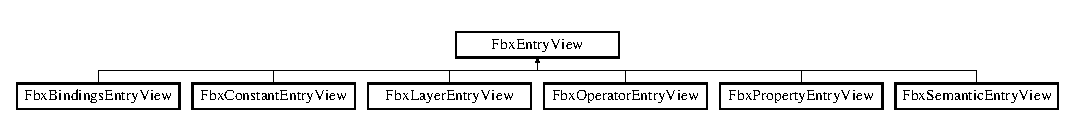
\includegraphics[height=1.244444cm]{class_fbx_entry_view}
\end{center}
\end{figure}
\subsection*{公開メンバ関数}
\begin{DoxyCompactItemize}
\item 
virtual bool \hyperlink{class_fbx_entry_view_a6bbdad937ef02ffbacd343fd71ed85d7}{Is\+Valid} () const
\item 
virtual bool \hyperlink{class_fbx_entry_view_aeff9d8adb34fe45d338c65483b52d2fc}{Create} ()
\item 
virtual const char $\ast$ \hyperlink{class_fbx_entry_view_a83ee50482b441ba8b0e6d7c2dba5432f}{Entry\+Type} () const
\end{DoxyCompactItemize}
\subsection*{静的公開変数類}
\begin{DoxyCompactItemize}
\item 
static const char $\ast$ \hyperlink{class_fbx_entry_view_a483b58dc47c39143426afe0d2076b6f6}{s\+Entry\+Type}
\begin{DoxyCompactList}\small\item\em Entry type. \end{DoxyCompactList}\end{DoxyCompactItemize}
\subsection*{限定公開変数類}
\begin{DoxyCompactItemize}
\item 
bool \hyperlink{class_fbx_entry_view_a274da88dfb87f2725f9c8fdbfe860c75}{m\+As\+Source}
\item 
\hyperlink{class_fbx_binding_table_entry}{Fbx\+Binding\+Table\+Entry} $\ast$ \hyperlink{class_fbx_entry_view_a74afe18ad35e48e7bd6dce480ab49ad7}{m\+Entry}
\end{DoxyCompactItemize}
\subsection*{Constructor and Destructor.}
\begin{DoxyCompactItemize}
\item 
\hyperlink{class_fbx_entry_view_a16e4c36a79ae38f1fc4b31973f43c15c}{Fbx\+Entry\+View} (\hyperlink{class_fbx_binding_table_entry}{Fbx\+Binding\+Table\+Entry} $\ast$p\+Entry, bool p\+As\+Source, bool p\+Create=false)
\item 
virtual \hyperlink{class_fbx_entry_view_a8adf9f4b899377fef920fd7b5e2bfcbf}{$\sim$\+Fbx\+Entry\+View} ()
\begin{DoxyCompactList}\small\item\em Destructor. \end{DoxyCompactList}\end{DoxyCompactItemize}


\subsection{詳解}
Entry view class represents binding entry in entry tables. \begin{DoxySeeAlso}{参照}
\hyperlink{class_fbx_binding_table_entry}{Fbx\+Binding\+Table\+Entry} and \hyperlink{class_fbx_binding_table}{Fbx\+Binding\+Table}. 
\end{DoxySeeAlso}


 fbxentryview.\+h の 26 行目に定義があります。



\subsection{構築子と解体子}
\mbox{\Hypertarget{class_fbx_entry_view_a16e4c36a79ae38f1fc4b31973f43c15c}\label{class_fbx_entry_view_a16e4c36a79ae38f1fc4b31973f43c15c}} 
\index{Fbx\+Entry\+View@{Fbx\+Entry\+View}!Fbx\+Entry\+View@{Fbx\+Entry\+View}}
\index{Fbx\+Entry\+View@{Fbx\+Entry\+View}!Fbx\+Entry\+View@{Fbx\+Entry\+View}}
\subsubsection{\texorpdfstring{Fbx\+Entry\+View()}{FbxEntryView()}}
{\footnotesize\ttfamily Fbx\+Entry\+View\+::\+Fbx\+Entry\+View (\begin{DoxyParamCaption}\item[{\hyperlink{class_fbx_binding_table_entry}{Fbx\+Binding\+Table\+Entry} $\ast$}]{p\+Entry,  }\item[{bool}]{p\+As\+Source,  }\item[{bool}]{p\+Create = {\ttfamily false} }\end{DoxyParamCaption})}

Constructor. 
\begin{DoxyParams}{引数}
{\em p\+Entry} & The binding table entry to create the entry view for. \\
\hline
{\em p\+As\+Source} & {\ttfamily true} to create the entry view as source, {\ttfamily false} as destination. \\
\hline
{\em p\+Create} & {\ttfamily true} to create the entry view, {\ttfamily false} otherwise. \\
\hline
\end{DoxyParams}
\mbox{\Hypertarget{class_fbx_entry_view_a8adf9f4b899377fef920fd7b5e2bfcbf}\label{class_fbx_entry_view_a8adf9f4b899377fef920fd7b5e2bfcbf}} 
\index{Fbx\+Entry\+View@{Fbx\+Entry\+View}!````~Fbx\+Entry\+View@{$\sim$\+Fbx\+Entry\+View}}
\index{````~Fbx\+Entry\+View@{$\sim$\+Fbx\+Entry\+View}!Fbx\+Entry\+View@{Fbx\+Entry\+View}}
\subsubsection{\texorpdfstring{$\sim$\+Fbx\+Entry\+View()}{~FbxEntryView()}}
{\footnotesize\ttfamily virtual Fbx\+Entry\+View\+::$\sim$\+Fbx\+Entry\+View (\begin{DoxyParamCaption}{ }\end{DoxyParamCaption})\hspace{0.3cm}{\ttfamily [virtual]}}



Destructor. 



\subsection{関数詳解}
\mbox{\Hypertarget{class_fbx_entry_view_aeff9d8adb34fe45d338c65483b52d2fc}\label{class_fbx_entry_view_aeff9d8adb34fe45d338c65483b52d2fc}} 
\index{Fbx\+Entry\+View@{Fbx\+Entry\+View}!Create@{Create}}
\index{Create@{Create}!Fbx\+Entry\+View@{Fbx\+Entry\+View}}
\subsubsection{\texorpdfstring{Create()}{Create()}}
{\footnotesize\ttfamily virtual bool Fbx\+Entry\+View\+::\+Create (\begin{DoxyParamCaption}{ }\end{DoxyParamCaption})\hspace{0.3cm}{\ttfamily [virtual]}}

Create a new entry view. \begin{DoxyReturn}{戻り値}
{\ttfamily true} if the entry view is created successfully, {\ttfamily false} otherwise. 
\end{DoxyReturn}
\mbox{\Hypertarget{class_fbx_entry_view_a83ee50482b441ba8b0e6d7c2dba5432f}\label{class_fbx_entry_view_a83ee50482b441ba8b0e6d7c2dba5432f}} 
\index{Fbx\+Entry\+View@{Fbx\+Entry\+View}!Entry\+Type@{Entry\+Type}}
\index{Entry\+Type@{Entry\+Type}!Fbx\+Entry\+View@{Fbx\+Entry\+View}}
\subsubsection{\texorpdfstring{Entry\+Type()}{EntryType()}}
{\footnotesize\ttfamily virtual const char$\ast$ Fbx\+Entry\+View\+::\+Entry\+Type (\begin{DoxyParamCaption}{ }\end{DoxyParamCaption}) const\hspace{0.3cm}{\ttfamily [virtual]}}

Get the entry type of this entry view. 

\hyperlink{class_fbx_semantic_entry_view_afd242ecac3eaab584dffe108753aba1d}{Fbx\+Semantic\+Entry\+View}, \hyperlink{class_fbx_property_entry_view_a36affcd0bce8be2a4b5f94ccd60fa462}{Fbx\+Property\+Entry\+View}, \hyperlink{class_fbx_layer_entry_view_a283d8f57e186dd36c88589dc3f37a35e}{Fbx\+Layer\+Entry\+View}, \hyperlink{class_fbx_operator_entry_view_a7821c1bf43a30e4c8ba054c66f051ad0}{Fbx\+Operator\+Entry\+View}, \hyperlink{class_fbx_constant_entry_view_a7ea7fc9df5e1316854d18ffcc797e564}{Fbx\+Constant\+Entry\+View}, \hyperlink{class_fbx_bindings_entry_view_a25f821ea63f19592173e7785356c04f9}{Fbx\+Bindings\+Entry\+View}で再実装されています。

\mbox{\Hypertarget{class_fbx_entry_view_a6bbdad937ef02ffbacd343fd71ed85d7}\label{class_fbx_entry_view_a6bbdad937ef02ffbacd343fd71ed85d7}} 
\index{Fbx\+Entry\+View@{Fbx\+Entry\+View}!Is\+Valid@{Is\+Valid}}
\index{Is\+Valid@{Is\+Valid}!Fbx\+Entry\+View@{Fbx\+Entry\+View}}
\subsubsection{\texorpdfstring{Is\+Valid()}{IsValid()}}
{\footnotesize\ttfamily virtual bool Fbx\+Entry\+View\+::\+Is\+Valid (\begin{DoxyParamCaption}{ }\end{DoxyParamCaption}) const\hspace{0.3cm}{\ttfamily [virtual]}}

Check whether this entry view is valid or not. If this entry view corresponds with an valid entry which is not N\+U\+LL, and the entry type of this entry view is the same as that of the entry it corresponds with, then this entry view is valid. \begin{DoxyReturn}{戻り値}
{\ttfamily true} if the entry view is valid, {\ttfamily false} otherwise. 
\end{DoxyReturn}


\subsection{メンバ詳解}
\mbox{\Hypertarget{class_fbx_entry_view_a274da88dfb87f2725f9c8fdbfe860c75}\label{class_fbx_entry_view_a274da88dfb87f2725f9c8fdbfe860c75}} 
\index{Fbx\+Entry\+View@{Fbx\+Entry\+View}!m\+As\+Source@{m\+As\+Source}}
\index{m\+As\+Source@{m\+As\+Source}!Fbx\+Entry\+View@{Fbx\+Entry\+View}}
\subsubsection{\texorpdfstring{m\+As\+Source}{mAsSource}}
{\footnotesize\ttfamily bool Fbx\+Entry\+View\+::m\+As\+Source\hspace{0.3cm}{\ttfamily [protected]}}



 fbxentryview.\+h の 72 行目に定義があります。

\mbox{\Hypertarget{class_fbx_entry_view_a74afe18ad35e48e7bd6dce480ab49ad7}\label{class_fbx_entry_view_a74afe18ad35e48e7bd6dce480ab49ad7}} 
\index{Fbx\+Entry\+View@{Fbx\+Entry\+View}!m\+Entry@{m\+Entry}}
\index{m\+Entry@{m\+Entry}!Fbx\+Entry\+View@{Fbx\+Entry\+View}}
\subsubsection{\texorpdfstring{m\+Entry}{mEntry}}
{\footnotesize\ttfamily \hyperlink{class_fbx_binding_table_entry}{Fbx\+Binding\+Table\+Entry}$\ast$ Fbx\+Entry\+View\+::m\+Entry\hspace{0.3cm}{\ttfamily [protected]}}



 fbxentryview.\+h の 73 行目に定義があります。

\mbox{\Hypertarget{class_fbx_entry_view_a483b58dc47c39143426afe0d2076b6f6}\label{class_fbx_entry_view_a483b58dc47c39143426afe0d2076b6f6}} 
\index{Fbx\+Entry\+View@{Fbx\+Entry\+View}!s\+Entry\+Type@{s\+Entry\+Type}}
\index{s\+Entry\+Type@{s\+Entry\+Type}!Fbx\+Entry\+View@{Fbx\+Entry\+View}}
\subsubsection{\texorpdfstring{s\+Entry\+Type}{sEntryType}}
{\footnotesize\ttfamily const char$\ast$ Fbx\+Entry\+View\+::s\+Entry\+Type\hspace{0.3cm}{\ttfamily [static]}}



Entry type. 



 fbxentryview.\+h の 31 行目に定義があります。



このクラス詳解は次のファイルから抽出されました\+:\begin{DoxyCompactItemize}
\item 
C\+:/\+Maya/scripts/\+F\+B\+X\+\_\+\+S\+D\+K/2017.\+1/include/fbxsdk/scene/shading/\hyperlink{fbxentryview_8h}{fbxentryview.\+h}\end{DoxyCompactItemize}

\hypertarget{class_fbx_environment}{}\section{Fbx\+Environment クラス}
\label{class_fbx_environment}\index{Fbx\+Environment@{Fbx\+Environment}}


{\ttfamily \#include $<$fbxenvironment.\+h$>$}



Fbx\+Environment の継承関係図
% FIG 0


Fbx\+Environment 連携図
% FIG 1
\subsection*{公開メンバ関数}
\begin{DoxyCompactItemize}
\item 
bool \hyperlink{class_fbx_environment_a5665a3c24b1b886fb8e00cc4db1fef14}{Provides\+Lighting} () const
\end{DoxyCompactItemize}
\subsection*{その他の継承メンバ}


\subsection{詳解}
This class contains the description of a scene environment. It contains the properties of sun parameters, sky parameters, daylight controller parameters ,environment map parameters and cloud map parameters. 

\subsection{メソッド詳解}
\mbox{\Hypertarget{class_fbx_environment_a5665a3c24b1b886fb8e00cc4db1fef14}\label{class_fbx_environment_a5665a3c24b1b886fb8e00cc4db1fef14}} 
\index{Fbx\+Environment@{Fbx\+Environment}!Provides\+Lighting@{Provides\+Lighting}}
\index{Provides\+Lighting@{Provides\+Lighting}!Fbx\+Environment@{Fbx\+Environment}}
\subsubsection{\texorpdfstring{Provides\+Lighting()}{ProvidesLighting()}}
{\footnotesize\ttfamily bool Fbx\+Environment\+::\+Provides\+Lighting (\begin{DoxyParamCaption}{ }\end{DoxyParamCaption}) const}



このクラス詳解は次のファイルから抽出されました\+:\begin{DoxyCompactItemize}
\item 
C\+:/github/\+F\+B\+Xpython\+S\+D\+K201701/\+F\+B\+Xpython\+S\+D\+K201701/2017.\+1/include/fbxsdk/scene/\hyperlink{fbxenvironment_8h}{fbxenvironment.\+h}\end{DoxyCompactItemize}

\hypertarget{class_fbx_euler}{}\section{Fbx\+Euler クラス}
\label{class_fbx_euler}\index{Fbx\+Euler@{Fbx\+Euler}}


{\ttfamily \#include $<$fbxmath.\+h$>$}

\subsection*{公開型}
\begin{DoxyCompactItemize}
\item 
enum \hyperlink{class_fbx_euler_ad021726fa17836ca3efd353ebc538f1a}{E\+Axis} \{ \hyperlink{class_fbx_euler_ad021726fa17836ca3efd353ebc538f1aad14972736ee1c99e5b6ee3d85b49892e}{e\+AxisX} =0, 
\hyperlink{class_fbx_euler_ad021726fa17836ca3efd353ebc538f1aa9e687ae4c2c8d8c1ce71869f6d2e3e4f}{e\+AxisY} =1, 
\hyperlink{class_fbx_euler_ad021726fa17836ca3efd353ebc538f1aaaa76dd8b9dce555038678e295faa5456}{e\+AxisZ} =2
 \}
\item 
enum \hyperlink{class_fbx_euler_a7d5bec7eedb022b4dae56894ab7a9939}{E\+Order} \{ \newline
\hyperlink{class_fbx_euler_a7d5bec7eedb022b4dae56894ab7a9939a826dcd420b1fcf49fac1f5ebbbf16894}{e\+Order\+X\+YZ}, 
\hyperlink{class_fbx_euler_a7d5bec7eedb022b4dae56894ab7a9939a1c9a8c3b3c41018cad46d8a13bd685bf}{e\+Order\+X\+ZY}, 
\hyperlink{class_fbx_euler_a7d5bec7eedb022b4dae56894ab7a9939a30a335e466b93120346e31cc67b0c7c4}{e\+Order\+Y\+ZX}, 
\hyperlink{class_fbx_euler_a7d5bec7eedb022b4dae56894ab7a9939afcbf96e502c9ad058f529644c66e385a}{e\+Order\+Y\+XZ}, 
\newline
\hyperlink{class_fbx_euler_a7d5bec7eedb022b4dae56894ab7a9939acf4d270ddd7ff69ebdd7fbeed8772c68}{e\+Order\+Z\+XY}, 
\hyperlink{class_fbx_euler_a7d5bec7eedb022b4dae56894ab7a9939a970a423237e1d2c9eff857092810448d}{e\+Order\+Z\+YX}, 
\hyperlink{class_fbx_euler_a7d5bec7eedb022b4dae56894ab7a9939abd5ec15c7fb9f6e05192fdf4ca8e487f}{e\+Order\+Spheric\+X\+YZ}
 \}
\end{DoxyCompactItemize}
\subsection*{静的公開メンバ関数}
\begin{DoxyCompactItemize}
\item 
static bool \hyperlink{class_fbx_euler_a7eabb69ba7eadc7b0b025eccee605648}{Is\+Parity\+Odd} (\hyperlink{class_fbx_euler_a7d5bec7eedb022b4dae56894ab7a9939}{E\+Order} p\+Order)
\item 
static bool \hyperlink{class_fbx_euler_a6f668dbfcefeee76a9668aafd3b53e45}{Is\+Repeat} (\hyperlink{class_fbx_euler_a7d5bec7eedb022b4dae56894ab7a9939}{E\+Order} p\+Order)
\item 
static void \hyperlink{class_fbx_euler_aea5f70a2534b0f5353a97aec02d9bafc}{Set\+Degenerate\+Threshold} (double p\+Threshold=16.\+0 $\ast$\hyperlink{fbxtypes_8h_a11f9f828046657bad7afc23f591f2052}{F\+B\+X\+S\+D\+K\+\_\+\+F\+L\+O\+A\+T\+\_\+\+E\+P\+S\+I\+L\+ON})
\item 
static double \hyperlink{class_fbx_euler_a4bc8faf22d9ab4ee1d6b45d3ab45d86a}{Degenerate\+Threshold} ()
\end{DoxyCompactItemize}
\subsection*{静的公開変数類}
\begin{DoxyCompactItemize}
\item 
static const int \hyperlink{class_fbx_euler_aa7c81e68be87ae5c26810eba96ede9ba}{Axis\+Table\+Size}
\item 
static const int \hyperlink{class_fbx_euler_aa75edcd96f3a7432c31b09869051635d}{Axis\+Table} \mbox{[}$\,$\mbox{]}\mbox{[}3\mbox{]}
\end{DoxyCompactItemize}


\subsection{列挙型メンバ詳解}
\mbox{\Hypertarget{class_fbx_euler_ad021726fa17836ca3efd353ebc538f1a}\label{class_fbx_euler_ad021726fa17836ca3efd353ebc538f1a}} 
\index{Fbx\+Euler@{Fbx\+Euler}!E\+Axis@{E\+Axis}}
\index{E\+Axis@{E\+Axis}!Fbx\+Euler@{Fbx\+Euler}}
\subsubsection{\texorpdfstring{E\+Axis}{EAxis}}
{\footnotesize\ttfamily enum \hyperlink{class_fbx_euler_ad021726fa17836ca3efd353ebc538f1a}{Fbx\+Euler\+::\+E\+Axis}}

\begin{DoxyEnumFields}{列挙値}
\raisebox{\heightof{T}}[0pt][0pt]{\index{e\+AxisX@{e\+AxisX}!Fbx\+Euler@{Fbx\+Euler}}\index{Fbx\+Euler@{Fbx\+Euler}!e\+AxisX@{e\+AxisX}}}\mbox{\Hypertarget{class_fbx_euler_ad021726fa17836ca3efd353ebc538f1aad14972736ee1c99e5b6ee3d85b49892e}\label{class_fbx_euler_ad021726fa17836ca3efd353ebc538f1aad14972736ee1c99e5b6ee3d85b49892e}} 
e\+AxisX&\\
\hline

\raisebox{\heightof{T}}[0pt][0pt]{\index{e\+AxisY@{e\+AxisY}!Fbx\+Euler@{Fbx\+Euler}}\index{Fbx\+Euler@{Fbx\+Euler}!e\+AxisY@{e\+AxisY}}}\mbox{\Hypertarget{class_fbx_euler_ad021726fa17836ca3efd353ebc538f1aa9e687ae4c2c8d8c1ce71869f6d2e3e4f}\label{class_fbx_euler_ad021726fa17836ca3efd353ebc538f1aa9e687ae4c2c8d8c1ce71869f6d2e3e4f}} 
e\+AxisY&\\
\hline

\raisebox{\heightof{T}}[0pt][0pt]{\index{e\+AxisZ@{e\+AxisZ}!Fbx\+Euler@{Fbx\+Euler}}\index{Fbx\+Euler@{Fbx\+Euler}!e\+AxisZ@{e\+AxisZ}}}\mbox{\Hypertarget{class_fbx_euler_ad021726fa17836ca3efd353ebc538f1aaaa76dd8b9dce555038678e295faa5456}\label{class_fbx_euler_ad021726fa17836ca3efd353ebc538f1aaaa76dd8b9dce555038678e295faa5456}} 
e\+AxisZ&\\
\hline

\end{DoxyEnumFields}
\mbox{\Hypertarget{class_fbx_euler_a7d5bec7eedb022b4dae56894ab7a9939}\label{class_fbx_euler_a7d5bec7eedb022b4dae56894ab7a9939}} 
\index{Fbx\+Euler@{Fbx\+Euler}!E\+Order@{E\+Order}}
\index{E\+Order@{E\+Order}!Fbx\+Euler@{Fbx\+Euler}}
\subsubsection{\texorpdfstring{E\+Order}{EOrder}}
{\footnotesize\ttfamily enum \hyperlink{class_fbx_euler_a7d5bec7eedb022b4dae56894ab7a9939}{Fbx\+Euler\+::\+E\+Order}}

\begin{DoxyEnumFields}{列挙値}
\raisebox{\heightof{T}}[0pt][0pt]{\index{e\+Order\+X\+YZ@{e\+Order\+X\+YZ}!Fbx\+Euler@{Fbx\+Euler}}\index{Fbx\+Euler@{Fbx\+Euler}!e\+Order\+X\+YZ@{e\+Order\+X\+YZ}}}\mbox{\Hypertarget{class_fbx_euler_a7d5bec7eedb022b4dae56894ab7a9939a826dcd420b1fcf49fac1f5ebbbf16894}\label{class_fbx_euler_a7d5bec7eedb022b4dae56894ab7a9939a826dcd420b1fcf49fac1f5ebbbf16894}} 
e\+Order\+X\+YZ&\\
\hline

\raisebox{\heightof{T}}[0pt][0pt]{\index{e\+Order\+X\+ZY@{e\+Order\+X\+ZY}!Fbx\+Euler@{Fbx\+Euler}}\index{Fbx\+Euler@{Fbx\+Euler}!e\+Order\+X\+ZY@{e\+Order\+X\+ZY}}}\mbox{\Hypertarget{class_fbx_euler_a7d5bec7eedb022b4dae56894ab7a9939a1c9a8c3b3c41018cad46d8a13bd685bf}\label{class_fbx_euler_a7d5bec7eedb022b4dae56894ab7a9939a1c9a8c3b3c41018cad46d8a13bd685bf}} 
e\+Order\+X\+ZY&\\
\hline

\raisebox{\heightof{T}}[0pt][0pt]{\index{e\+Order\+Y\+ZX@{e\+Order\+Y\+ZX}!Fbx\+Euler@{Fbx\+Euler}}\index{Fbx\+Euler@{Fbx\+Euler}!e\+Order\+Y\+ZX@{e\+Order\+Y\+ZX}}}\mbox{\Hypertarget{class_fbx_euler_a7d5bec7eedb022b4dae56894ab7a9939a30a335e466b93120346e31cc67b0c7c4}\label{class_fbx_euler_a7d5bec7eedb022b4dae56894ab7a9939a30a335e466b93120346e31cc67b0c7c4}} 
e\+Order\+Y\+ZX&\\
\hline

\raisebox{\heightof{T}}[0pt][0pt]{\index{e\+Order\+Y\+XZ@{e\+Order\+Y\+XZ}!Fbx\+Euler@{Fbx\+Euler}}\index{Fbx\+Euler@{Fbx\+Euler}!e\+Order\+Y\+XZ@{e\+Order\+Y\+XZ}}}\mbox{\Hypertarget{class_fbx_euler_a7d5bec7eedb022b4dae56894ab7a9939afcbf96e502c9ad058f529644c66e385a}\label{class_fbx_euler_a7d5bec7eedb022b4dae56894ab7a9939afcbf96e502c9ad058f529644c66e385a}} 
e\+Order\+Y\+XZ&\\
\hline

\raisebox{\heightof{T}}[0pt][0pt]{\index{e\+Order\+Z\+XY@{e\+Order\+Z\+XY}!Fbx\+Euler@{Fbx\+Euler}}\index{Fbx\+Euler@{Fbx\+Euler}!e\+Order\+Z\+XY@{e\+Order\+Z\+XY}}}\mbox{\Hypertarget{class_fbx_euler_a7d5bec7eedb022b4dae56894ab7a9939acf4d270ddd7ff69ebdd7fbeed8772c68}\label{class_fbx_euler_a7d5bec7eedb022b4dae56894ab7a9939acf4d270ddd7ff69ebdd7fbeed8772c68}} 
e\+Order\+Z\+XY&\\
\hline

\raisebox{\heightof{T}}[0pt][0pt]{\index{e\+Order\+Z\+YX@{e\+Order\+Z\+YX}!Fbx\+Euler@{Fbx\+Euler}}\index{Fbx\+Euler@{Fbx\+Euler}!e\+Order\+Z\+YX@{e\+Order\+Z\+YX}}}\mbox{\Hypertarget{class_fbx_euler_a7d5bec7eedb022b4dae56894ab7a9939a970a423237e1d2c9eff857092810448d}\label{class_fbx_euler_a7d5bec7eedb022b4dae56894ab7a9939a970a423237e1d2c9eff857092810448d}} 
e\+Order\+Z\+YX&\\
\hline

\raisebox{\heightof{T}}[0pt][0pt]{\index{e\+Order\+Spheric\+X\+YZ@{e\+Order\+Spheric\+X\+YZ}!Fbx\+Euler@{Fbx\+Euler}}\index{Fbx\+Euler@{Fbx\+Euler}!e\+Order\+Spheric\+X\+YZ@{e\+Order\+Spheric\+X\+YZ}}}\mbox{\Hypertarget{class_fbx_euler_a7d5bec7eedb022b4dae56894ab7a9939abd5ec15c7fb9f6e05192fdf4ca8e487f}\label{class_fbx_euler_a7d5bec7eedb022b4dae56894ab7a9939abd5ec15c7fb9f6e05192fdf4ca8e487f}} 
e\+Order\+Spheric\+X\+YZ&\\
\hline

\end{DoxyEnumFields}


\subsection{メソッド詳解}
\mbox{\Hypertarget{class_fbx_euler_a4bc8faf22d9ab4ee1d6b45d3ab45d86a}\label{class_fbx_euler_a4bc8faf22d9ab4ee1d6b45d3ab45d86a}} 
\index{Fbx\+Euler@{Fbx\+Euler}!Degenerate\+Threshold@{Degenerate\+Threshold}}
\index{Degenerate\+Threshold@{Degenerate\+Threshold}!Fbx\+Euler@{Fbx\+Euler}}
\subsubsection{\texorpdfstring{Degenerate\+Threshold()}{DegenerateThreshold()}}
{\footnotesize\ttfamily static double Fbx\+Euler\+::\+Degenerate\+Threshold (\begin{DoxyParamCaption}{ }\end{DoxyParamCaption})\hspace{0.3cm}{\ttfamily [static]}}

\mbox{\Hypertarget{class_fbx_euler_a7eabb69ba7eadc7b0b025eccee605648}\label{class_fbx_euler_a7eabb69ba7eadc7b0b025eccee605648}} 
\index{Fbx\+Euler@{Fbx\+Euler}!Is\+Parity\+Odd@{Is\+Parity\+Odd}}
\index{Is\+Parity\+Odd@{Is\+Parity\+Odd}!Fbx\+Euler@{Fbx\+Euler}}
\subsubsection{\texorpdfstring{Is\+Parity\+Odd()}{IsParityOdd()}}
{\footnotesize\ttfamily static bool Fbx\+Euler\+::\+Is\+Parity\+Odd (\begin{DoxyParamCaption}\item[{\hyperlink{class_fbx_euler_a7d5bec7eedb022b4dae56894ab7a9939}{E\+Order}}]{p\+Order }\end{DoxyParamCaption})\hspace{0.3cm}{\ttfamily [static]}}

\mbox{\Hypertarget{class_fbx_euler_a6f668dbfcefeee76a9668aafd3b53e45}\label{class_fbx_euler_a6f668dbfcefeee76a9668aafd3b53e45}} 
\index{Fbx\+Euler@{Fbx\+Euler}!Is\+Repeat@{Is\+Repeat}}
\index{Is\+Repeat@{Is\+Repeat}!Fbx\+Euler@{Fbx\+Euler}}
\subsubsection{\texorpdfstring{Is\+Repeat()}{IsRepeat()}}
{\footnotesize\ttfamily static bool Fbx\+Euler\+::\+Is\+Repeat (\begin{DoxyParamCaption}\item[{\hyperlink{class_fbx_euler_a7d5bec7eedb022b4dae56894ab7a9939}{E\+Order}}]{p\+Order }\end{DoxyParamCaption})\hspace{0.3cm}{\ttfamily [static]}}

\mbox{\Hypertarget{class_fbx_euler_aea5f70a2534b0f5353a97aec02d9bafc}\label{class_fbx_euler_aea5f70a2534b0f5353a97aec02d9bafc}} 
\index{Fbx\+Euler@{Fbx\+Euler}!Set\+Degenerate\+Threshold@{Set\+Degenerate\+Threshold}}
\index{Set\+Degenerate\+Threshold@{Set\+Degenerate\+Threshold}!Fbx\+Euler@{Fbx\+Euler}}
\subsubsection{\texorpdfstring{Set\+Degenerate\+Threshold()}{SetDegenerateThreshold()}}
{\footnotesize\ttfamily static void Fbx\+Euler\+::\+Set\+Degenerate\+Threshold (\begin{DoxyParamCaption}\item[{double}]{p\+Threshold = {\ttfamily 16.0~$\ast$\hyperlink{fbxtypes_8h_a11f9f828046657bad7afc23f591f2052}{F\+B\+X\+S\+D\+K\+\_\+\+F\+L\+O\+A\+T\+\_\+\+E\+P\+S\+I\+L\+ON}} }\end{DoxyParamCaption})\hspace{0.3cm}{\ttfamily [static]}}



\subsection{メンバ詳解}
\mbox{\Hypertarget{class_fbx_euler_aa75edcd96f3a7432c31b09869051635d}\label{class_fbx_euler_aa75edcd96f3a7432c31b09869051635d}} 
\index{Fbx\+Euler@{Fbx\+Euler}!Axis\+Table@{Axis\+Table}}
\index{Axis\+Table@{Axis\+Table}!Fbx\+Euler@{Fbx\+Euler}}
\subsubsection{\texorpdfstring{Axis\+Table}{AxisTable}}
{\footnotesize\ttfamily const int Fbx\+Euler\+::\+Axis\+Table\mbox{[}$\,$\mbox{]}\mbox{[}3\mbox{]}\hspace{0.3cm}{\ttfamily [static]}}

\mbox{\Hypertarget{class_fbx_euler_aa7c81e68be87ae5c26810eba96ede9ba}\label{class_fbx_euler_aa7c81e68be87ae5c26810eba96ede9ba}} 
\index{Fbx\+Euler@{Fbx\+Euler}!Axis\+Table\+Size@{Axis\+Table\+Size}}
\index{Axis\+Table\+Size@{Axis\+Table\+Size}!Fbx\+Euler@{Fbx\+Euler}}
\subsubsection{\texorpdfstring{Axis\+Table\+Size}{AxisTableSize}}
{\footnotesize\ttfamily const int Fbx\+Euler\+::\+Axis\+Table\+Size\hspace{0.3cm}{\ttfamily [static]}}



このクラス詳解は次のファイルから抽出されました\+:\begin{DoxyCompactItemize}
\item 
C\+:/github/\+F\+B\+Xpython\+S\+D\+K201701/\+F\+B\+Xpython\+S\+D\+K201701/2017.\+1/include/fbxsdk/core/math/\hyperlink{fbxmath_8h}{fbxmath.\+h}\end{DoxyCompactItemize}

\hypertarget{class_fbx_eval_state}{}\section{Fbx\+Eval\+State クラス}
\label{class_fbx_eval_state}\index{Fbx\+Eval\+State@{Fbx\+Eval\+State}}


This class serves as the base class for an evaluation state element.  




{\ttfamily \#include $<$fbxanimevalstate.\+h$>$}

Fbx\+Eval\+State の継承関係図\begin{figure}[H]
\begin{center}
\leavevmode
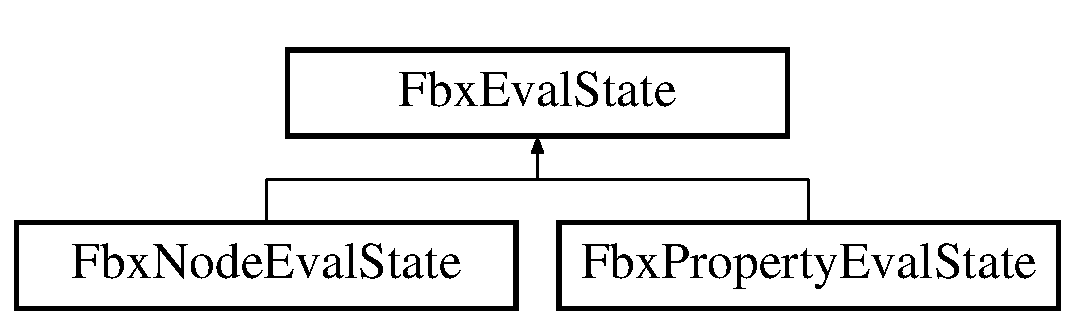
\includegraphics[height=2.000000cm]{class_fbx_eval_state}
\end{center}
\end{figure}
\subsection*{公開メンバ関数}
\begin{DoxyCompactItemize}
\item 
\hyperlink{class_fbx_eval_state_a9c54619a6fa810228fbb017965492507}{Fbx\+Eval\+State} ()
\end{DoxyCompactItemize}
\subsection*{公開変数類}
\begin{DoxyCompactItemize}
\item 
bool \hyperlink{class_fbx_eval_state_a9c153054cba876e54d38046e582b32d0}{m\+Up\+To\+Date}
\begin{DoxyCompactList}\small\item\em If {\ttfamily true}, the evaluation state element is up-\/to-\/date for the current evaluation time. \end{DoxyCompactList}\end{DoxyCompactItemize}


\subsection{詳解}
This class serves as the base class for an evaluation state element. 

 fbxanimevalstate.\+h の 96 行目に定義があります。



\subsection{構築子と解体子}
\mbox{\Hypertarget{class_fbx_eval_state_a9c54619a6fa810228fbb017965492507}\label{class_fbx_eval_state_a9c54619a6fa810228fbb017965492507}} 
\index{Fbx\+Eval\+State@{Fbx\+Eval\+State}!Fbx\+Eval\+State@{Fbx\+Eval\+State}}
\index{Fbx\+Eval\+State@{Fbx\+Eval\+State}!Fbx\+Eval\+State@{Fbx\+Eval\+State}}
\subsubsection{\texorpdfstring{Fbx\+Eval\+State()}{FbxEvalState()}}
{\footnotesize\ttfamily Fbx\+Eval\+State\+::\+Fbx\+Eval\+State (\begin{DoxyParamCaption}{ }\end{DoxyParamCaption})\hspace{0.3cm}{\ttfamily [inline]}}



 fbxanimevalstate.\+h の 99 行目に定義があります。



\subsection{メンバ詳解}
\mbox{\Hypertarget{class_fbx_eval_state_a9c153054cba876e54d38046e582b32d0}\label{class_fbx_eval_state_a9c153054cba876e54d38046e582b32d0}} 
\index{Fbx\+Eval\+State@{Fbx\+Eval\+State}!m\+Up\+To\+Date@{m\+Up\+To\+Date}}
\index{m\+Up\+To\+Date@{m\+Up\+To\+Date}!Fbx\+Eval\+State@{Fbx\+Eval\+State}}
\subsubsection{\texorpdfstring{m\+Up\+To\+Date}{mUpToDate}}
{\footnotesize\ttfamily bool Fbx\+Eval\+State\+::m\+Up\+To\+Date}



If {\ttfamily true}, the evaluation state element is up-\/to-\/date for the current evaluation time. 



 fbxanimevalstate.\+h の 100 行目に定義があります。



このクラス詳解は次のファイルから抽出されました\+:\begin{DoxyCompactItemize}
\item 
C\+:/\+Maya/scripts/\+F\+B\+X\+\_\+\+S\+D\+K/2017.\+1/include/fbxsdk/scene/animation/\hyperlink{fbxanimevalstate_8h}{fbxanimevalstate.\+h}\end{DoxyCompactItemize}

\hypertarget{class_fbx_event}{}\section{Fbx\+Event$<$ T $>$ クラステンプレート}
\label{class_fbx_event}\index{Fbx\+Event$<$ T $>$@{Fbx\+Event$<$ T $>$}}


{\ttfamily \#include $<$fbxevent.\+h$>$}



Fbx\+Event$<$ T $>$ の継承関係図
% FIG 0


Fbx\+Event$<$ T $>$ 連携図
% FIG 1
\subsection*{公開メンバ関数}
\begin{DoxyCompactItemize}
\item 
virtual \hyperlink{class_fbx_event_a57f0d84cc53c4d29bcff0dceb091eed4}{$\sim$\+Fbx\+Event} ()
\begin{DoxyCompactList}\small\item\em Destructor \end{DoxyCompactList}\item 
virtual int \hyperlink{class_fbx_event_a96ae7ea5ee46f040f6493f6acecd5bba}{Get\+Type\+Id} () const
\end{DoxyCompactItemize}
\subsection*{静的公開メンバ関数}
\begin{DoxyCompactItemize}
\item 
static void \hyperlink{class_fbx_event_a0e3fe581649a5917208561a03ad61295}{Force\+Type\+Id} (int p\+Type\+Id)
\item 
static int \hyperlink{class_fbx_event_a9f2329973ee8cb60860d004cc2823c70}{Get\+Static\+Type\+Id} ()
\end{DoxyCompactItemize}
\subsection*{その他の継承メンバ}


\subsection{詳解}
\subsubsection*{template$<$typename T$>$\newline
class Fbx\+Event$<$ T $>$}

F\+BX event class, derived from \hyperlink{class_fbx_event_base}{Fbx\+Event\+Base}, and it contains a type ID for event. It\textquotesingle{}s a template class. You can derive your own types of even. Such as\+: 
\begin{DoxyCode}
\textcolor{keyword}{class }FbxEventCustom : \textcolor{keyword}{public} \hyperlink{class_fbx_event}{FbxEvent}<FbxEventCustom> 
\end{DoxyCode}
 \begin{DoxySeeAlso}{参照}
\hyperlink{class_fbx_object_property_changed}{Fbx\+Object\+Property\+Changed} \hyperlink{class_fbx_event_referenced_document}{Fbx\+Event\+Referenced\+Document} \hyperlink{class_fbx_event_post_export}{Fbx\+Event\+Post\+Export} 

\hyperlink{class_fbx_event_post_import}{Fbx\+Event\+Post\+Import} \hyperlink{class_fbx_event_pre_export}{Fbx\+Event\+Pre\+Export} \hyperlink{class_fbx_event_pre_import}{Fbx\+Event\+Pre\+Import} \hyperlink{class_fbx_event_populate_system_library}{Fbx\+Event\+Populate\+System\+Library}
\end{DoxySeeAlso}
\begin{DoxyRemark}{注釈}
A F\+BX event is something that is emitted by an emitter, with the goal of being filled by the listener that listen to it. An object(emitter) can emit a certain type of event, the plug-\/in(listener) who are listening to that type of event, will receive a signal and take action to process the event data. 
\end{DoxyRemark}
\begin{DoxyParagraph}{The whole process of event is\+:}
\begin{DoxyItemize}
\item 1. Create an emitter and a listener, then bind them together via the same event handler. \item 2. Emitter can emit an event at certain conditions. The event could be handled by event handler. \item 3. Once an event is emitted, the listener to this event will receive a signal. \item 4. And then the listener could process the event data according to the types of event, by calling event handler. \end{DoxyItemize}

\end{DoxyParagraph}
\begin{DoxyNote}{覚え書き}
The event data is process by the callback function of event handler. 
\end{DoxyNote}
\begin{DoxySeeAlso}{参照}
\hyperlink{class_fbx_event_base}{Fbx\+Event\+Base} \hyperlink{class_fbx_event_handler}{Fbx\+Event\+Handler} \hyperlink{class_fbx_listener}{Fbx\+Listener} \hyperlink{class_fbx_emitter}{Fbx\+Emitter} 
\end{DoxySeeAlso}


\subsection{構築子と解体子}
\mbox{\Hypertarget{class_fbx_event_a57f0d84cc53c4d29bcff0dceb091eed4}\label{class_fbx_event_a57f0d84cc53c4d29bcff0dceb091eed4}} 
\index{Fbx\+Event@{Fbx\+Event}!````~Fbx\+Event@{$\sim$\+Fbx\+Event}}
\index{````~Fbx\+Event@{$\sim$\+Fbx\+Event}!Fbx\+Event@{Fbx\+Event}}
\subsubsection{\texorpdfstring{$\sim$\+Fbx\+Event()}{~FbxEvent()}}
{\footnotesize\ttfamily template$<$typename T$>$ \\
virtual \hyperlink{class_fbx_event}{Fbx\+Event}$<$ T $>$\+::$\sim$\hyperlink{class_fbx_event}{Fbx\+Event} (\begin{DoxyParamCaption}{ }\end{DoxyParamCaption})\hspace{0.3cm}{\ttfamily [virtual]}}



Destructor 



\subsection{メソッド詳解}
\mbox{\Hypertarget{class_fbx_event_a0e3fe581649a5917208561a03ad61295}\label{class_fbx_event_a0e3fe581649a5917208561a03ad61295}} 
\index{Fbx\+Event@{Fbx\+Event}!Force\+Type\+Id@{Force\+Type\+Id}}
\index{Force\+Type\+Id@{Force\+Type\+Id}!Fbx\+Event@{Fbx\+Event}}
\subsubsection{\texorpdfstring{Force\+Type\+Id()}{ForceTypeId()}}
{\footnotesize\ttfamily template$<$typename T$>$ \\
static void \hyperlink{class_fbx_event}{Fbx\+Event}$<$ T $>$\+::Force\+Type\+Id (\begin{DoxyParamCaption}\item[{int}]{p\+Type\+Id }\end{DoxyParamCaption})\hspace{0.3cm}{\ttfamily [static]}}

Update the type ID of current event with the given type ID. 
\begin{DoxyParams}{引数}
{\em p\+Type\+Id} & the new type ID. \\
\hline
\end{DoxyParams}
\mbox{\Hypertarget{class_fbx_event_a9f2329973ee8cb60860d004cc2823c70}\label{class_fbx_event_a9f2329973ee8cb60860d004cc2823c70}} 
\index{Fbx\+Event@{Fbx\+Event}!Get\+Static\+Type\+Id@{Get\+Static\+Type\+Id}}
\index{Get\+Static\+Type\+Id@{Get\+Static\+Type\+Id}!Fbx\+Event@{Fbx\+Event}}
\subsubsection{\texorpdfstring{Get\+Static\+Type\+Id()}{GetStaticTypeId()}}
{\footnotesize\ttfamily template$<$typename T$>$ \\
static int \hyperlink{class_fbx_event}{Fbx\+Event}$<$ T $>$\+::Get\+Static\+Type\+Id (\begin{DoxyParamCaption}{ }\end{DoxyParamCaption})\hspace{0.3cm}{\ttfamily [static]}}

Retrieve the event type ID \begin{DoxyReturn}{戻り値}
type id 
\end{DoxyReturn}
\mbox{\Hypertarget{class_fbx_event_a96ae7ea5ee46f040f6493f6acecd5bba}\label{class_fbx_event_a96ae7ea5ee46f040f6493f6acecd5bba}} 
\index{Fbx\+Event@{Fbx\+Event}!Get\+Type\+Id@{Get\+Type\+Id}}
\index{Get\+Type\+Id@{Get\+Type\+Id}!Fbx\+Event@{Fbx\+Event}}
\subsubsection{\texorpdfstring{Get\+Type\+Id()}{GetTypeId()}}
{\footnotesize\ttfamily template$<$typename T$>$ \\
virtual int \hyperlink{class_fbx_event}{Fbx\+Event}$<$ T $>$\+::Get\+Type\+Id (\begin{DoxyParamCaption}{ }\end{DoxyParamCaption}) const\hspace{0.3cm}{\ttfamily [virtual]}}

Retrieve the event type ID \begin{DoxyNote}{覚え書き}
This may be called from multiple threads. 
\end{DoxyNote}
\begin{DoxyReturn}{戻り値}
type id 
\end{DoxyReturn}


\hyperlink{class_fbx_event_base_ac7a558ec38bc899bd705786620582b8b}{Fbx\+Event\+Base}を実装しています。



このクラス詳解は次のファイルから抽出されました\+:\begin{DoxyCompactItemize}
\item 
C\+:/github/\+F\+B\+Xpython\+S\+D\+K201701/\+F\+B\+Xpython\+S\+D\+K201701/2017.\+1/include/fbxsdk/core/\hyperlink{fbxevent_8h}{fbxevent.\+h}\end{DoxyCompactItemize}

\hypertarget{class_fbx_event_base}{}\section{Fbx\+Event\+Base クラス}
\label{class_fbx_event_base}\index{Fbx\+Event\+Base@{Fbx\+Event\+Base}}


{\ttfamily \#include $<$fbxevent.\+h$>$}

Fbx\+Event\+Base の継承関係図\begin{figure}[H]
\begin{center}
\leavevmode
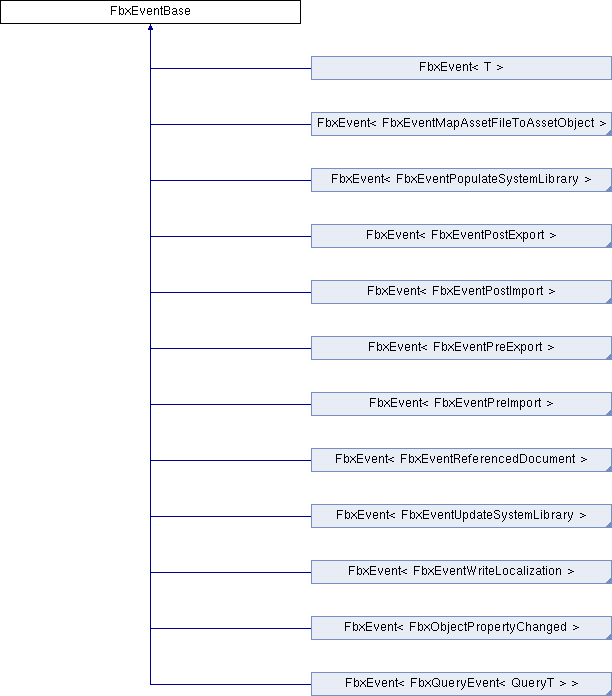
\includegraphics[height=11.779935cm]{class_fbx_event_base}
\end{center}
\end{figure}
\subsection*{公開メンバ関数}
\begin{DoxyCompactItemize}
\item 
virtual int \hyperlink{class_fbx_event_base_ac7a558ec38bc899bd705786620582b8b}{Get\+Type\+Id} () const =0
\item 
virtual const char $\ast$ \hyperlink{class_fbx_event_base_a94c1acf878d522042b327abf0c129f10}{Get\+Event\+Name} () const =0
\end{DoxyCompactItemize}
\subsection*{静的限定公開メンバ関数}
\begin{DoxyCompactItemize}
\item 
static int \hyperlink{class_fbx_event_base_a57cde15f6d1c6567bc8dbafc1658bcc5}{Get\+Static\+Type\+Id} (const char $\ast$)
\end{DoxyCompactItemize}
\subsection*{Constructor and Destructor}
\begin{DoxyCompactItemize}
\item 
virtual \hyperlink{class_fbx_event_base_aa95657834201b514cb515cf60d371938}{$\sim$\+Fbx\+Event\+Base} ()
\begin{DoxyCompactList}\small\item\em Destructor \end{DoxyCompactList}\end{DoxyCompactItemize}


\subsection{詳解}
F\+BX S\+DK event base class. An event is something that is emitted by an emitter, with the goal of being filled by the listener that listen to it. You can see that like a form that you send to some people. If those people know how to fill the form, they fill it and return it to you with the right information in it. F\+BX object could be used as emitter, since \hyperlink{class_fbx_object}{Fbx\+Object} is derived from \hyperlink{class_fbx_emitter}{Fbx\+Emitter}. Meanwhile, plug-\/in could be used as listener, since \hyperlink{class_fbx_plugin}{Fbx\+Plugin} is derived from \hyperlink{class_fbx_listener}{Fbx\+Listener}. The derived class of \hyperlink{class_fbx_event_base}{Fbx\+Event\+Base} contains a type ID to distinguish different types of events. F\+BX object can emit different types of F\+BX events at different conditions. \begin{DoxyParagraph}{The whole process of event is\+:}
\begin{DoxyItemize}
\item 1. Create an emitter and a listener, then bind them together via the same event handler. \item 2. Emitter can emit an event at certain conditions. The event could be handled by event handler. \item 3. Once an event is emitted, the listener to this event will receive a signal. \item 4. And then the listener could process the event data according to the types of event, by calling event handler. \end{DoxyItemize}

\end{DoxyParagraph}
\begin{DoxyNote}{覚え書き}
The event data is process by the callback function of event handler. For example, if a certain property of a F\+BX object is changed, the F\+BX object(emitter) can emit an event which type is \hyperlink{class_fbx_object_property_changed}{Fbx\+Object\+Property\+Changed}. The plug-\/in(listener) who are listening to \hyperlink{class_fbx_object_property_changed}{Fbx\+Object\+Property\+Changed}, will receive a signal and take action to process the event data.
\end{DoxyNote}
\begin{DoxySeeAlso}{参照}
\hyperlink{class_fbx_event}{Fbx\+Event} \hyperlink{class_fbx_event_handler}{Fbx\+Event\+Handler} \hyperlink{class_fbx_listener}{Fbx\+Listener} \hyperlink{class_fbx_emitter}{Fbx\+Emitter} 
\end{DoxySeeAlso}


 fbxevent.\+h の 40 行目に定義があります。



\subsection{構築子と解体子}
\mbox{\Hypertarget{class_fbx_event_base_aa95657834201b514cb515cf60d371938}\label{class_fbx_event_base_aa95657834201b514cb515cf60d371938}} 
\index{Fbx\+Event\+Base@{Fbx\+Event\+Base}!````~Fbx\+Event\+Base@{$\sim$\+Fbx\+Event\+Base}}
\index{````~Fbx\+Event\+Base@{$\sim$\+Fbx\+Event\+Base}!Fbx\+Event\+Base@{Fbx\+Event\+Base}}
\subsubsection{\texorpdfstring{$\sim$\+Fbx\+Event\+Base()}{~FbxEventBase()}}
{\footnotesize\ttfamily virtual Fbx\+Event\+Base\+::$\sim$\+Fbx\+Event\+Base (\begin{DoxyParamCaption}{ }\end{DoxyParamCaption})\hspace{0.3cm}{\ttfamily [virtual]}}



Destructor 



\subsection{関数詳解}
\mbox{\Hypertarget{class_fbx_event_base_a94c1acf878d522042b327abf0c129f10}\label{class_fbx_event_base_a94c1acf878d522042b327abf0c129f10}} 
\index{Fbx\+Event\+Base@{Fbx\+Event\+Base}!Get\+Event\+Name@{Get\+Event\+Name}}
\index{Get\+Event\+Name@{Get\+Event\+Name}!Fbx\+Event\+Base@{Fbx\+Event\+Base}}
\subsubsection{\texorpdfstring{Get\+Event\+Name()}{GetEventName()}}
{\footnotesize\ttfamily virtual const char$\ast$ Fbx\+Event\+Base\+::\+Get\+Event\+Name (\begin{DoxyParamCaption}{ }\end{DoxyParamCaption}) const\hspace{0.3cm}{\ttfamily [pure virtual]}}

Force events to give us a name \begin{DoxyReturn}{戻り値}
event name 
\end{DoxyReturn}
\mbox{\Hypertarget{class_fbx_event_base_a57cde15f6d1c6567bc8dbafc1658bcc5}\label{class_fbx_event_base_a57cde15f6d1c6567bc8dbafc1658bcc5}} 
\index{Fbx\+Event\+Base@{Fbx\+Event\+Base}!Get\+Static\+Type\+Id@{Get\+Static\+Type\+Id}}
\index{Get\+Static\+Type\+Id@{Get\+Static\+Type\+Id}!Fbx\+Event\+Base@{Fbx\+Event\+Base}}
\subsubsection{\texorpdfstring{Get\+Static\+Type\+Id()}{GetStaticTypeId()}}
{\footnotesize\ttfamily static int Fbx\+Event\+Base\+::\+Get\+Static\+Type\+Id (\begin{DoxyParamCaption}\item[{const char $\ast$}]{ }\end{DoxyParamCaption})\hspace{0.3cm}{\ttfamily [static]}, {\ttfamily [protected]}}

\mbox{\Hypertarget{class_fbx_event_base_ac7a558ec38bc899bd705786620582b8b}\label{class_fbx_event_base_ac7a558ec38bc899bd705786620582b8b}} 
\index{Fbx\+Event\+Base@{Fbx\+Event\+Base}!Get\+Type\+Id@{Get\+Type\+Id}}
\index{Get\+Type\+Id@{Get\+Type\+Id}!Fbx\+Event\+Base@{Fbx\+Event\+Base}}
\subsubsection{\texorpdfstring{Get\+Type\+Id()}{GetTypeId()}}
{\footnotesize\ttfamily virtual int Fbx\+Event\+Base\+::\+Get\+Type\+Id (\begin{DoxyParamCaption}{ }\end{DoxyParamCaption}) const\hspace{0.3cm}{\ttfamily [pure virtual]}}

Retrieve the event type ID \begin{DoxyReturn}{戻り値}
type id 
\end{DoxyReturn}


\hyperlink{class_fbx_event_a96ae7ea5ee46f040f6493f6acecd5bba}{Fbx\+Event$<$ T $>$}, \hyperlink{class_fbx_event_a96ae7ea5ee46f040f6493f6acecd5bba}{Fbx\+Event$<$ Fbx\+Event\+Write\+Localization $>$}, \hyperlink{class_fbx_event_a96ae7ea5ee46f040f6493f6acecd5bba}{Fbx\+Event$<$ Fbx\+Event\+Post\+Export $>$}, \hyperlink{class_fbx_event_a96ae7ea5ee46f040f6493f6acecd5bba}{Fbx\+Event$<$ Fbx\+Event\+Update\+System\+Library $>$}, \hyperlink{class_fbx_event_a96ae7ea5ee46f040f6493f6acecd5bba}{Fbx\+Event$<$ Fbx\+Event\+Pre\+Export $>$}, \hyperlink{class_fbx_event_a96ae7ea5ee46f040f6493f6acecd5bba}{Fbx\+Event$<$ Fbx\+Event\+Referenced\+Document $>$}, \hyperlink{class_fbx_event_a96ae7ea5ee46f040f6493f6acecd5bba}{Fbx\+Event$<$ Fbx\+Event\+Populate\+System\+Library $>$}, \hyperlink{class_fbx_event_a96ae7ea5ee46f040f6493f6acecd5bba}{Fbx\+Event$<$ Fbx\+Query\+Event$<$ Query\+T $>$ $>$}, \hyperlink{class_fbx_event_a96ae7ea5ee46f040f6493f6acecd5bba}{Fbx\+Event$<$ Fbx\+Event\+Pre\+Import $>$}, \hyperlink{class_fbx_event_a96ae7ea5ee46f040f6493f6acecd5bba}{Fbx\+Event$<$ Fbx\+Event\+Post\+Import $>$}, \hyperlink{class_fbx_event_a96ae7ea5ee46f040f6493f6acecd5bba}{Fbx\+Event$<$ Fbx\+Object\+Property\+Changed $>$}, \hyperlink{class_fbx_event_a96ae7ea5ee46f040f6493f6acecd5bba}{Fbx\+Event$<$ Fbx\+Event\+Map\+Asset\+File\+To\+Asset\+Object $>$}で実装されています。



このクラス詳解は次のファイルから抽出されました\+:\begin{DoxyCompactItemize}
\item 
C\+:/\+Maya/scripts/\+F\+B\+X\+\_\+\+S\+D\+K/2017.\+1/include/fbxsdk/core/\hyperlink{fbxevent_8h}{fbxevent.\+h}\end{DoxyCompactItemize}

\hypertarget{class_fbx_event_handler}{}\section{Fbx\+Event\+Handler クラス}
\label{class_fbx_event_handler}\index{Fbx\+Event\+Handler@{Fbx\+Event\+Handler}}


{\ttfamily \#include $<$fbxeventhandler.\+h$>$}

Fbx\+Event\+Handler の継承関係図\begin{figure}[H]
\begin{center}
\leavevmode
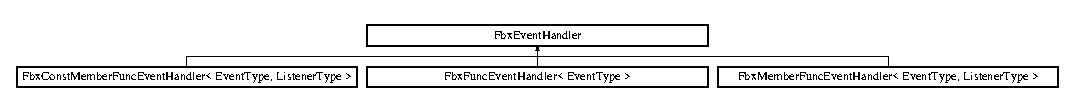
\includegraphics[height=0.954817cm]{class_fbx_event_handler}
\end{center}
\end{figure}
\subsection*{公開型}
\begin{DoxyCompactItemize}
\item 
enum \hyperlink{class_fbx_event_handler_a47139da2cfd5abee91664d75c4fb577c}{E\+Type} \{ \hyperlink{class_fbx_event_handler_a47139da2cfd5abee91664d75c4fb577ca288df77e1147943ca82bc3a7d8bc493b}{e\+Listener}, 
\hyperlink{class_fbx_event_handler_a47139da2cfd5abee91664d75c4fb577cae2c0d7da494cef8d787ee3495e24a6c0}{e\+Emitter}, 
\hyperlink{class_fbx_event_handler_a47139da2cfd5abee91664d75c4fb577ca2c6941dcdf691c32251fae0beabeadb2}{e\+Count}
 \}\begin{DoxyCompactList}\small\item\em Event handler base type. \end{DoxyCompactList}
\end{DoxyCompactItemize}
\subsection*{公開メンバ関数}
\begin{DoxyCompactItemize}
\item 
virtual int \hyperlink{class_fbx_event_handler_a0b42d2b93e63d866975f468a481c9f3c}{Get\+Handler\+Event\+Type} ()=0
\item 
virtual void \hyperlink{class_fbx_event_handler_a46357ba45116a30c8f53c3e5fe9ba2fb}{Function\+Call} (const \hyperlink{class_fbx_event_base}{Fbx\+Event\+Base} \&p\+Event)=0
\item 
virtual \hyperlink{class_fbx_listener}{Fbx\+Listener} $\ast$ \hyperlink{class_fbx_event_handler_a6d496102fe1253372bb042840c2d45a7}{Get\+Listener} ()=0
\item 
\hyperlink{class_fbx_event_handler_a275484070d5de1b461c6cca690f74e29}{Fbx\+Event\+Handler} ()
\item 
virtual \hyperlink{class_fbx_event_handler_a2b420c30f76ba3ed1c9b9937c4964293}{$\sim$\+Fbx\+Event\+Handler} ()
\item 
\hyperlink{class_fbx_event_handler_a5f41da1b9002da90f4681d9efe6d4542}{F\+B\+X\+S\+D\+K\+\_\+\+I\+N\+T\+R\+U\+S\+I\+V\+E\+\_\+\+L\+I\+S\+T\+\_\+\+N\+O\+DE} (\hyperlink{class_fbx_event_handler}{Fbx\+Event\+Handler}, \hyperlink{class_fbx_event_handler_a47139da2cfd5abee91664d75c4fb577ca2c6941dcdf691c32251fae0beabeadb2}{e\+Count})
\end{DoxyCompactItemize}


\subsection{詳解}
Event handler class contains a listener and a callback function. Event handler is used to bind emitter and listener together. Its callback function can process event data. To generate a valid event handler, you can create an event emitter and event listener first and then call \hyperlink{class_fbx_listener_a7a3298b1f4fa347aaa2cb5136265a178}{Fbx\+Listener\+::\+Bind()}. It will create an event handler automatically and bind the handler to the listener and the created emitter. After that, the emitter and listener are bound together via event handler. \begin{DoxyRemark}{注釈}
An object(emitter) can emit a certain type of event, the object(listener) who are listening to that type of event, will receive a signal and take action to process the event data. 
\end{DoxyRemark}
\begin{DoxyParagraph}{The whole process of event is\+:}
\begin{DoxyItemize}
\item 1. Create an emitter and a listener, then bind them together via the same event handler. \item 2. Emitter can emit an event at certain conditions. The event could be handled by event handler. \item 3. Once an event is emitted, the listener to this event will receive a signal. \item 4. And then the listener could process the event data according to the types of event, by calling event handler. \end{DoxyItemize}

\end{DoxyParagraph}
\begin{DoxyNote}{覚え書き}
The event data is process by the callback function of event handler.
\end{DoxyNote}
\begin{DoxySeeAlso}{参照}
\hyperlink{class_fbx_listener}{Fbx\+Listener} \hyperlink{class_fbx_event_base}{Fbx\+Event\+Base} \hyperlink{class_fbx_event}{Fbx\+Event} \hyperlink{class_fbx_emitter}{Fbx\+Emitter} 
\end{DoxySeeAlso}


 fbxeventhandler.\+h の 41 行目に定義があります。



\subsection{列挙型メンバ詳解}
\mbox{\Hypertarget{class_fbx_event_handler_a47139da2cfd5abee91664d75c4fb577c}\label{class_fbx_event_handler_a47139da2cfd5abee91664d75c4fb577c}} 
\index{Fbx\+Event\+Handler@{Fbx\+Event\+Handler}!E\+Type@{E\+Type}}
\index{E\+Type@{E\+Type}!Fbx\+Event\+Handler@{Fbx\+Event\+Handler}}
\subsubsection{\texorpdfstring{E\+Type}{EType}}
{\footnotesize\ttfamily enum \hyperlink{class_fbx_event_handler_a47139da2cfd5abee91664d75c4fb577c}{Fbx\+Event\+Handler\+::\+E\+Type}}



Event handler base type. 

\begin{DoxyEnumFields}{列挙値}
\raisebox{\heightof{T}}[0pt][0pt]{\index{e\+Listener@{e\+Listener}!Fbx\+Event\+Handler@{Fbx\+Event\+Handler}}\index{Fbx\+Event\+Handler@{Fbx\+Event\+Handler}!e\+Listener@{e\+Listener}}}\mbox{\Hypertarget{class_fbx_event_handler_a47139da2cfd5abee91664d75c4fb577ca288df77e1147943ca82bc3a7d8bc493b}\label{class_fbx_event_handler_a47139da2cfd5abee91664d75c4fb577ca288df77e1147943ca82bc3a7d8bc493b}} 
e\+Listener&Listener event handler type. \\
\hline

\raisebox{\heightof{T}}[0pt][0pt]{\index{e\+Emitter@{e\+Emitter}!Fbx\+Event\+Handler@{Fbx\+Event\+Handler}}\index{Fbx\+Event\+Handler@{Fbx\+Event\+Handler}!e\+Emitter@{e\+Emitter}}}\mbox{\Hypertarget{class_fbx_event_handler_a47139da2cfd5abee91664d75c4fb577cae2c0d7da494cef8d787ee3495e24a6c0}\label{class_fbx_event_handler_a47139da2cfd5abee91664d75c4fb577cae2c0d7da494cef8d787ee3495e24a6c0}} 
e\+Emitter&Emitter event handler type. \\
\hline

\raisebox{\heightof{T}}[0pt][0pt]{\index{e\+Count@{e\+Count}!Fbx\+Event\+Handler@{Fbx\+Event\+Handler}}\index{Fbx\+Event\+Handler@{Fbx\+Event\+Handler}!e\+Count@{e\+Count}}}\mbox{\Hypertarget{class_fbx_event_handler_a47139da2cfd5abee91664d75c4fb577ca2c6941dcdf691c32251fae0beabeadb2}\label{class_fbx_event_handler_a47139da2cfd5abee91664d75c4fb577ca2c6941dcdf691c32251fae0beabeadb2}} 
e\+Count&Count of different event handler types. \\
\hline

\end{DoxyEnumFields}


 fbxeventhandler.\+h の 45 行目に定義があります。



\subsection{構築子と解体子}
\mbox{\Hypertarget{class_fbx_event_handler_a275484070d5de1b461c6cca690f74e29}\label{class_fbx_event_handler_a275484070d5de1b461c6cca690f74e29}} 
\index{Fbx\+Event\+Handler@{Fbx\+Event\+Handler}!Fbx\+Event\+Handler@{Fbx\+Event\+Handler}}
\index{Fbx\+Event\+Handler@{Fbx\+Event\+Handler}!Fbx\+Event\+Handler@{Fbx\+Event\+Handler}}
\subsubsection{\texorpdfstring{Fbx\+Event\+Handler()}{FbxEventHandler()}}
{\footnotesize\ttfamily Fbx\+Event\+Handler\+::\+Fbx\+Event\+Handler (\begin{DoxyParamCaption}{ }\end{DoxyParamCaption})\hspace{0.3cm}{\ttfamily [inline]}}



 fbxeventhandler.\+h の 69 行目に定義があります。

\mbox{\Hypertarget{class_fbx_event_handler_a2b420c30f76ba3ed1c9b9937c4964293}\label{class_fbx_event_handler_a2b420c30f76ba3ed1c9b9937c4964293}} 
\index{Fbx\+Event\+Handler@{Fbx\+Event\+Handler}!````~Fbx\+Event\+Handler@{$\sim$\+Fbx\+Event\+Handler}}
\index{````~Fbx\+Event\+Handler@{$\sim$\+Fbx\+Event\+Handler}!Fbx\+Event\+Handler@{Fbx\+Event\+Handler}}
\subsubsection{\texorpdfstring{$\sim$\+Fbx\+Event\+Handler()}{~FbxEventHandler()}}
{\footnotesize\ttfamily virtual Fbx\+Event\+Handler\+::$\sim$\+Fbx\+Event\+Handler (\begin{DoxyParamCaption}{ }\end{DoxyParamCaption})\hspace{0.3cm}{\ttfamily [inline]}, {\ttfamily [virtual]}}



 fbxeventhandler.\+h の 70 行目に定義があります。



\subsection{関数詳解}
\mbox{\Hypertarget{class_fbx_event_handler_a5f41da1b9002da90f4681d9efe6d4542}\label{class_fbx_event_handler_a5f41da1b9002da90f4681d9efe6d4542}} 
\index{Fbx\+Event\+Handler@{Fbx\+Event\+Handler}!F\+B\+X\+S\+D\+K\+\_\+\+I\+N\+T\+R\+U\+S\+I\+V\+E\+\_\+\+L\+I\+S\+T\+\_\+\+N\+O\+DE@{F\+B\+X\+S\+D\+K\+\_\+\+I\+N\+T\+R\+U\+S\+I\+V\+E\+\_\+\+L\+I\+S\+T\+\_\+\+N\+O\+DE}}
\index{F\+B\+X\+S\+D\+K\+\_\+\+I\+N\+T\+R\+U\+S\+I\+V\+E\+\_\+\+L\+I\+S\+T\+\_\+\+N\+O\+DE@{F\+B\+X\+S\+D\+K\+\_\+\+I\+N\+T\+R\+U\+S\+I\+V\+E\+\_\+\+L\+I\+S\+T\+\_\+\+N\+O\+DE}!Fbx\+Event\+Handler@{Fbx\+Event\+Handler}}
\subsubsection{\texorpdfstring{F\+B\+X\+S\+D\+K\+\_\+\+I\+N\+T\+R\+U\+S\+I\+V\+E\+\_\+\+L\+I\+S\+T\+\_\+\+N\+O\+D\+E()}{FBXSDK\_INTRUSIVE\_LIST\_NODE()}}
{\footnotesize\ttfamily Fbx\+Event\+Handler\+::\+F\+B\+X\+S\+D\+K\+\_\+\+I\+N\+T\+R\+U\+S\+I\+V\+E\+\_\+\+L\+I\+S\+T\+\_\+\+N\+O\+DE (\begin{DoxyParamCaption}\item[{\hyperlink{class_fbx_event_handler}{Fbx\+Event\+Handler}}]{,  }\item[{\hyperlink{class_fbx_event_handler_a47139da2cfd5abee91664d75c4fb577ca2c6941dcdf691c32251fae0beabeadb2}{e\+Count}}]{ }\end{DoxyParamCaption})}

\mbox{\Hypertarget{class_fbx_event_handler_a46357ba45116a30c8f53c3e5fe9ba2fb}\label{class_fbx_event_handler_a46357ba45116a30c8f53c3e5fe9ba2fb}} 
\index{Fbx\+Event\+Handler@{Fbx\+Event\+Handler}!Function\+Call@{Function\+Call}}
\index{Function\+Call@{Function\+Call}!Fbx\+Event\+Handler@{Fbx\+Event\+Handler}}
\subsubsection{\texorpdfstring{Function\+Call()}{FunctionCall()}}
{\footnotesize\ttfamily virtual void Fbx\+Event\+Handler\+::\+Function\+Call (\begin{DoxyParamCaption}\item[{const \hyperlink{class_fbx_event_base}{Fbx\+Event\+Base} \&}]{p\+Event }\end{DoxyParamCaption})\hspace{0.3cm}{\ttfamily [pure virtual]}}

Call function that process event data. 
\begin{DoxyParams}{引数}
{\em p\+Event} & specify the event type. p\+Event could be a specific class which derived from \hyperlink{class_fbx_event_base}{Fbx\+Event\+Base}. \\
\hline
\end{DoxyParams}
\begin{DoxySeeAlso}{参照}
\hyperlink{class_fbx_event_base}{Fbx\+Event\+Base} 
\end{DoxySeeAlso}


\hyperlink{class_fbx_func_event_handler_a6111e1a7e1a0e60170a2de498fe44766}{Fbx\+Func\+Event\+Handler$<$ Event\+Type $>$}, \hyperlink{class_fbx_const_member_func_event_handler_ae6c6805404e8045de40289893709dc54}{Fbx\+Const\+Member\+Func\+Event\+Handler$<$ Event\+Type, Listener\+Type $>$}, \hyperlink{class_fbx_member_func_event_handler_a4bcb037442927d480776bc2fb4b7bcd6}{Fbx\+Member\+Func\+Event\+Handler$<$ Event\+Type, Listener\+Type $>$}で実装されています。

\mbox{\Hypertarget{class_fbx_event_handler_a0b42d2b93e63d866975f468a481c9f3c}\label{class_fbx_event_handler_a0b42d2b93e63d866975f468a481c9f3c}} 
\index{Fbx\+Event\+Handler@{Fbx\+Event\+Handler}!Get\+Handler\+Event\+Type@{Get\+Handler\+Event\+Type}}
\index{Get\+Handler\+Event\+Type@{Get\+Handler\+Event\+Type}!Fbx\+Event\+Handler@{Fbx\+Event\+Handler}}
\subsubsection{\texorpdfstring{Get\+Handler\+Event\+Type()}{GetHandlerEventType()}}
{\footnotesize\ttfamily virtual int Fbx\+Event\+Handler\+::\+Get\+Handler\+Event\+Type (\begin{DoxyParamCaption}{ }\end{DoxyParamCaption})\hspace{0.3cm}{\ttfamily [pure virtual]}}

Get event type of current handler. \begin{DoxyReturn}{戻り値}
The type ID of event. 
\end{DoxyReturn}


\hyperlink{class_fbx_func_event_handler_a0c1a0eaedda70615a684bd96aa72fb97}{Fbx\+Func\+Event\+Handler$<$ Event\+Type $>$}, \hyperlink{class_fbx_const_member_func_event_handler_ac88157f51fa72cba959f31dfbcdee4a5}{Fbx\+Const\+Member\+Func\+Event\+Handler$<$ Event\+Type, Listener\+Type $>$}, \hyperlink{class_fbx_member_func_event_handler_a57856423663f283503e6498a7eacb0b4}{Fbx\+Member\+Func\+Event\+Handler$<$ Event\+Type, Listener\+Type $>$}で実装されています。

\mbox{\Hypertarget{class_fbx_event_handler_a6d496102fe1253372bb042840c2d45a7}\label{class_fbx_event_handler_a6d496102fe1253372bb042840c2d45a7}} 
\index{Fbx\+Event\+Handler@{Fbx\+Event\+Handler}!Get\+Listener@{Get\+Listener}}
\index{Get\+Listener@{Get\+Listener}!Fbx\+Event\+Handler@{Fbx\+Event\+Handler}}
\subsubsection{\texorpdfstring{Get\+Listener()}{GetListener()}}
{\footnotesize\ttfamily virtual \hyperlink{class_fbx_listener}{Fbx\+Listener}$\ast$ Fbx\+Event\+Handler\+::\+Get\+Listener (\begin{DoxyParamCaption}{ }\end{DoxyParamCaption})\hspace{0.3cm}{\ttfamily [pure virtual]}}

Get listener of current handler. \begin{DoxyReturn}{戻り値}
A pointer to the listener object. 
\end{DoxyReturn}


\hyperlink{class_fbx_func_event_handler_af196b87b07e698704615056be5923745}{Fbx\+Func\+Event\+Handler$<$ Event\+Type $>$}, \hyperlink{class_fbx_const_member_func_event_handler_a9e370edd4a746ef5098d39a4f9c3d63c}{Fbx\+Const\+Member\+Func\+Event\+Handler$<$ Event\+Type, Listener\+Type $>$}, \hyperlink{class_fbx_member_func_event_handler_ad45db7b531f23f9e7776c93bec100668}{Fbx\+Member\+Func\+Event\+Handler$<$ Event\+Type, Listener\+Type $>$}で実装されています。



このクラス詳解は次のファイルから抽出されました\+:\begin{DoxyCompactItemize}
\item 
C\+:/\+Maya/scripts/\+F\+B\+X\+\_\+\+S\+D\+K/2017.\+1/include/fbxsdk/core/\hyperlink{fbxeventhandler_8h}{fbxeventhandler.\+h}\end{DoxyCompactItemize}

\hypertarget{class_fbx_event_map_asset_file_to_asset_object}{}\section{Fbx\+Event\+Map\+Asset\+File\+To\+Asset\+Object クラス}
\label{class_fbx_event_map_asset_file_to_asset_object}\index{Fbx\+Event\+Map\+Asset\+File\+To\+Asset\+Object@{Fbx\+Event\+Map\+Asset\+File\+To\+Asset\+Object}}


{\ttfamily \#include $<$fbxlibrary.\+h$>$}

Fbx\+Event\+Map\+Asset\+File\+To\+Asset\+Object の継承関係図\begin{figure}[H]
\begin{center}
\leavevmode
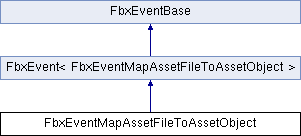
\includegraphics[height=3.000000cm]{class_fbx_event_map_asset_file_to_asset_object}
\end{center}
\end{figure}
\subsection*{公開メンバ関数}
\begin{DoxyCompactItemize}
\item 
\hyperlink{class_fbx_event_map_asset_file_to_asset_object_ad72d55e79ebd2905e725c2bf90794c73}{Fbx\+Event\+Map\+Asset\+File\+To\+Asset\+Object} (const char $\ast$p\+File)
\item 
const char $\ast$ \hyperlink{class_fbx_event_map_asset_file_to_asset_object_a52c6658860c2ee9d3c5fb74d82ad003e}{Get\+File\+Path} () const
\end{DoxyCompactItemize}
\subsection*{公開変数類}
\begin{DoxyCompactItemize}
\item 
\hyperlink{class_fbx_object}{Fbx\+Object} $\ast$ \hyperlink{class_fbx_event_map_asset_file_to_asset_object_a29d3b4f66df038ce5fbf3832a3cd3f31}{m\+Asset}
\end{DoxyCompactItemize}
\subsection*{その他の継承メンバ}


\subsection{詳解}


 fbxlibrary.\+h の 308 行目に定義があります。



\subsection{構築子と解体子}
\mbox{\Hypertarget{class_fbx_event_map_asset_file_to_asset_object_ad72d55e79ebd2905e725c2bf90794c73}\label{class_fbx_event_map_asset_file_to_asset_object_ad72d55e79ebd2905e725c2bf90794c73}} 
\index{Fbx\+Event\+Map\+Asset\+File\+To\+Asset\+Object@{Fbx\+Event\+Map\+Asset\+File\+To\+Asset\+Object}!Fbx\+Event\+Map\+Asset\+File\+To\+Asset\+Object@{Fbx\+Event\+Map\+Asset\+File\+To\+Asset\+Object}}
\index{Fbx\+Event\+Map\+Asset\+File\+To\+Asset\+Object@{Fbx\+Event\+Map\+Asset\+File\+To\+Asset\+Object}!Fbx\+Event\+Map\+Asset\+File\+To\+Asset\+Object@{Fbx\+Event\+Map\+Asset\+File\+To\+Asset\+Object}}
\subsubsection{\texorpdfstring{Fbx\+Event\+Map\+Asset\+File\+To\+Asset\+Object()}{FbxEventMapAssetFileToAssetObject()}}
{\footnotesize\ttfamily Fbx\+Event\+Map\+Asset\+File\+To\+Asset\+Object\+::\+Fbx\+Event\+Map\+Asset\+File\+To\+Asset\+Object (\begin{DoxyParamCaption}\item[{const char $\ast$}]{p\+File }\end{DoxyParamCaption})\hspace{0.3cm}{\ttfamily [inline]}}



 fbxlibrary.\+h の 313 行目に定義があります。



\subsection{関数詳解}
\mbox{\Hypertarget{class_fbx_event_map_asset_file_to_asset_object_a52c6658860c2ee9d3c5fb74d82ad003e}\label{class_fbx_event_map_asset_file_to_asset_object_a52c6658860c2ee9d3c5fb74d82ad003e}} 
\index{Fbx\+Event\+Map\+Asset\+File\+To\+Asset\+Object@{Fbx\+Event\+Map\+Asset\+File\+To\+Asset\+Object}!Get\+File\+Path@{Get\+File\+Path}}
\index{Get\+File\+Path@{Get\+File\+Path}!Fbx\+Event\+Map\+Asset\+File\+To\+Asset\+Object@{Fbx\+Event\+Map\+Asset\+File\+To\+Asset\+Object}}
\subsubsection{\texorpdfstring{Get\+File\+Path()}{GetFilePath()}}
{\footnotesize\ttfamily const char$\ast$ Fbx\+Event\+Map\+Asset\+File\+To\+Asset\+Object\+::\+Get\+File\+Path (\begin{DoxyParamCaption}{ }\end{DoxyParamCaption}) const\hspace{0.3cm}{\ttfamily [inline]}}



 fbxlibrary.\+h の 319 行目に定義があります。



\subsection{メンバ詳解}
\mbox{\Hypertarget{class_fbx_event_map_asset_file_to_asset_object_a29d3b4f66df038ce5fbf3832a3cd3f31}\label{class_fbx_event_map_asset_file_to_asset_object_a29d3b4f66df038ce5fbf3832a3cd3f31}} 
\index{Fbx\+Event\+Map\+Asset\+File\+To\+Asset\+Object@{Fbx\+Event\+Map\+Asset\+File\+To\+Asset\+Object}!m\+Asset@{m\+Asset}}
\index{m\+Asset@{m\+Asset}!Fbx\+Event\+Map\+Asset\+File\+To\+Asset\+Object@{Fbx\+Event\+Map\+Asset\+File\+To\+Asset\+Object}}
\subsubsection{\texorpdfstring{m\+Asset}{mAsset}}
{\footnotesize\ttfamily \hyperlink{class_fbx_object}{Fbx\+Object}$\ast$ Fbx\+Event\+Map\+Asset\+File\+To\+Asset\+Object\+::m\+Asset\hspace{0.3cm}{\ttfamily [mutable]}}



 fbxlibrary.\+h の 320 行目に定義があります。



このクラス詳解は次のファイルから抽出されました\+:\begin{DoxyCompactItemize}
\item 
C\+:/\+Maya/scripts/\+F\+B\+X\+\_\+\+S\+D\+K/2017.\+1/include/fbxsdk/scene/\hyperlink{fbxlibrary_8h}{fbxlibrary.\+h}\end{DoxyCompactItemize}

\hypertarget{class_fbx_event_populate_system_library}{}\section{Fbx\+Event\+Populate\+System\+Library クラス}
\label{class_fbx_event_populate_system_library}\index{Fbx\+Event\+Populate\+System\+Library@{Fbx\+Event\+Populate\+System\+Library}}


{\ttfamily \#include $<$fbxlibrary.\+h$>$}



Fbx\+Event\+Populate\+System\+Library の継承関係図
% FIG 0


Fbx\+Event\+Populate\+System\+Library 連携図
% FIG 1
\subsection*{公開メンバ関数}
\begin{DoxyCompactItemize}
\item 
\hyperlink{class_fbx_event_populate_system_library_a0fc24725b0cdb572a82e40825b37156b}{Fbx\+Event\+Populate\+System\+Library} (\hyperlink{class_fbx_library}{Fbx\+Library} $\ast$p\+Library)
\item 
\hyperlink{class_fbx_library}{Fbx\+Library} $\ast$ \hyperlink{class_fbx_event_populate_system_library_a9916adf51d1fed8a4c6aeb8f12587ce0}{Get\+Library} () const
\end{DoxyCompactItemize}
\subsection*{その他の継承メンバ}


\subsection{構築子と解体子}
\mbox{\Hypertarget{class_fbx_event_populate_system_library_a0fc24725b0cdb572a82e40825b37156b}\label{class_fbx_event_populate_system_library_a0fc24725b0cdb572a82e40825b37156b}} 
\index{Fbx\+Event\+Populate\+System\+Library@{Fbx\+Event\+Populate\+System\+Library}!Fbx\+Event\+Populate\+System\+Library@{Fbx\+Event\+Populate\+System\+Library}}
\index{Fbx\+Event\+Populate\+System\+Library@{Fbx\+Event\+Populate\+System\+Library}!Fbx\+Event\+Populate\+System\+Library@{Fbx\+Event\+Populate\+System\+Library}}
\subsubsection{\texorpdfstring{Fbx\+Event\+Populate\+System\+Library()}{FbxEventPopulateSystemLibrary()}}
{\footnotesize\ttfamily Fbx\+Event\+Populate\+System\+Library\+::\+Fbx\+Event\+Populate\+System\+Library (\begin{DoxyParamCaption}\item[{\hyperlink{class_fbx_library}{Fbx\+Library} $\ast$}]{p\+Library }\end{DoxyParamCaption})}



\subsection{メソッド詳解}
\mbox{\Hypertarget{class_fbx_event_populate_system_library_a9916adf51d1fed8a4c6aeb8f12587ce0}\label{class_fbx_event_populate_system_library_a9916adf51d1fed8a4c6aeb8f12587ce0}} 
\index{Fbx\+Event\+Populate\+System\+Library@{Fbx\+Event\+Populate\+System\+Library}!Get\+Library@{Get\+Library}}
\index{Get\+Library@{Get\+Library}!Fbx\+Event\+Populate\+System\+Library@{Fbx\+Event\+Populate\+System\+Library}}
\subsubsection{\texorpdfstring{Get\+Library()}{GetLibrary()}}
{\footnotesize\ttfamily \hyperlink{class_fbx_library}{Fbx\+Library}$\ast$ Fbx\+Event\+Populate\+System\+Library\+::\+Get\+Library (\begin{DoxyParamCaption}{ }\end{DoxyParamCaption}) const}



このクラス詳解は次のファイルから抽出されました\+:\begin{DoxyCompactItemize}
\item 
C\+:/github/\+F\+B\+Xpython\+S\+D\+K201701/\+F\+B\+Xpython\+S\+D\+K201701/2017.\+1/include/fbxsdk/scene/\hyperlink{fbxlibrary_8h}{fbxlibrary.\+h}\end{DoxyCompactItemize}

\hypertarget{class_fbx_event_post_export}{}\section{Fbx\+Event\+Post\+Export クラス}
\label{class_fbx_event_post_export}\index{Fbx\+Event\+Post\+Export@{Fbx\+Event\+Post\+Export}}


Event that is emitted to plugins after a file is exported to the F\+BX format.  




{\ttfamily \#include $<$fbxexporter.\+h$>$}

Fbx\+Event\+Post\+Export の継承関係図\begin{figure}[H]
\begin{center}
\leavevmode
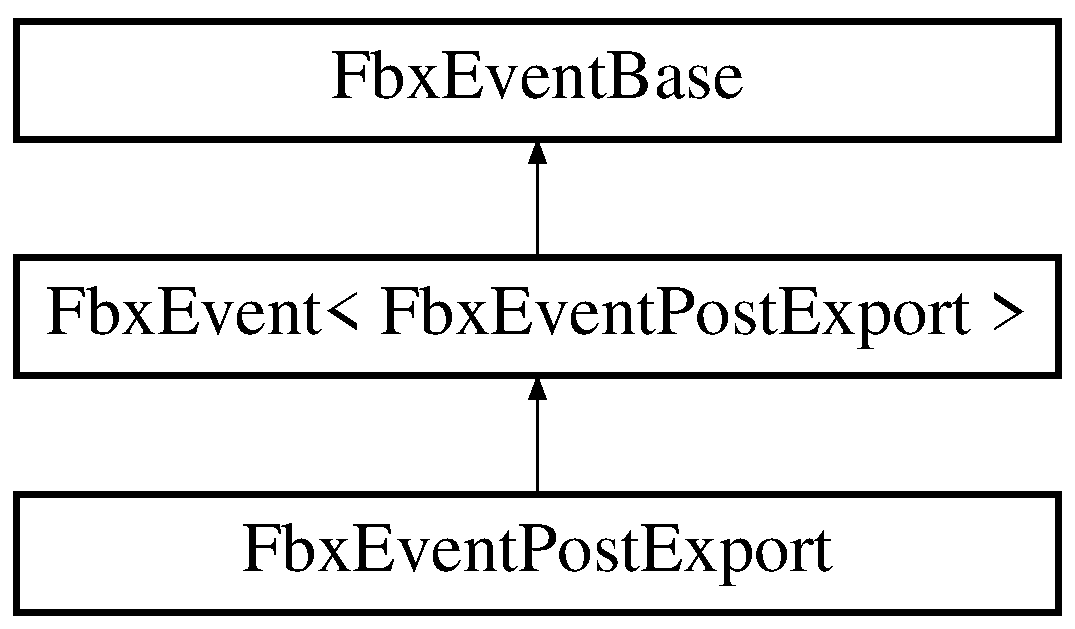
\includegraphics[height=3.000000cm]{class_fbx_event_post_export}
\end{center}
\end{figure}
\subsection*{公開メンバ関数}
\begin{DoxyCompactItemize}
\item 
\hyperlink{class_fbx_event_post_export_ab35efa8c72530d563f35128018c9bfcc}{Fbx\+Event\+Post\+Export} (\hyperlink{class_fbx_document}{Fbx\+Document} $\ast$p\+Document)
\end{DoxyCompactItemize}
\subsection*{公開変数類}
\begin{DoxyCompactItemize}
\item 
\hyperlink{class_fbx_document}{Fbx\+Document} $\ast$ \hyperlink{class_fbx_event_post_export_aca668d4ffcd12dc1b6455bb5165fb2f5}{m\+Document}
\begin{DoxyCompactList}\small\item\em The document to be exported \end{DoxyCompactList}\end{DoxyCompactItemize}
\subsection*{その他の継承メンバ}


\subsection{詳解}
Event that is emitted to plugins after a file is exported to the F\+BX format. 

 fbxexporter.\+h の 291 行目に定義があります。



\subsection{構築子と解体子}
\mbox{\Hypertarget{class_fbx_event_post_export_ab35efa8c72530d563f35128018c9bfcc}\label{class_fbx_event_post_export_ab35efa8c72530d563f35128018c9bfcc}} 
\index{Fbx\+Event\+Post\+Export@{Fbx\+Event\+Post\+Export}!Fbx\+Event\+Post\+Export@{Fbx\+Event\+Post\+Export}}
\index{Fbx\+Event\+Post\+Export@{Fbx\+Event\+Post\+Export}!Fbx\+Event\+Post\+Export@{Fbx\+Event\+Post\+Export}}
\subsubsection{\texorpdfstring{Fbx\+Event\+Post\+Export()}{FbxEventPostExport()}}
{\footnotesize\ttfamily Fbx\+Event\+Post\+Export\+::\+Fbx\+Event\+Post\+Export (\begin{DoxyParamCaption}\item[{\hyperlink{class_fbx_document}{Fbx\+Document} $\ast$}]{p\+Document }\end{DoxyParamCaption})\hspace{0.3cm}{\ttfamily [inline]}}



 fbxexporter.\+h の 296 行目に定義があります。



\subsection{メンバ詳解}
\mbox{\Hypertarget{class_fbx_event_post_export_aca668d4ffcd12dc1b6455bb5165fb2f5}\label{class_fbx_event_post_export_aca668d4ffcd12dc1b6455bb5165fb2f5}} 
\index{Fbx\+Event\+Post\+Export@{Fbx\+Event\+Post\+Export}!m\+Document@{m\+Document}}
\index{m\+Document@{m\+Document}!Fbx\+Event\+Post\+Export@{Fbx\+Event\+Post\+Export}}
\subsubsection{\texorpdfstring{m\+Document}{mDocument}}
{\footnotesize\ttfamily \hyperlink{class_fbx_document}{Fbx\+Document}$\ast$ Fbx\+Event\+Post\+Export\+::m\+Document}



The document to be exported 



 fbxexporter.\+h の 296 行目に定義があります。



このクラス詳解は次のファイルから抽出されました\+:\begin{DoxyCompactItemize}
\item 
C\+:/\+Maya/scripts/\+F\+B\+X\+\_\+\+S\+D\+K/2017.\+1/include/fbxsdk/fileio/\hyperlink{fbxexporter_8h}{fbxexporter.\+h}\end{DoxyCompactItemize}

\hypertarget{class_fbx_event_post_import}{}\section{Fbx\+Event\+Post\+Import クラス}
\label{class_fbx_event_post_import}\index{Fbx\+Event\+Post\+Import@{Fbx\+Event\+Post\+Import}}


Event that is emitted to plugins after a F\+BX file has been imported.  




{\ttfamily \#include $<$fbximporter.\+h$>$}

Fbx\+Event\+Post\+Import の継承関係図\begin{figure}[H]
\begin{center}
\leavevmode
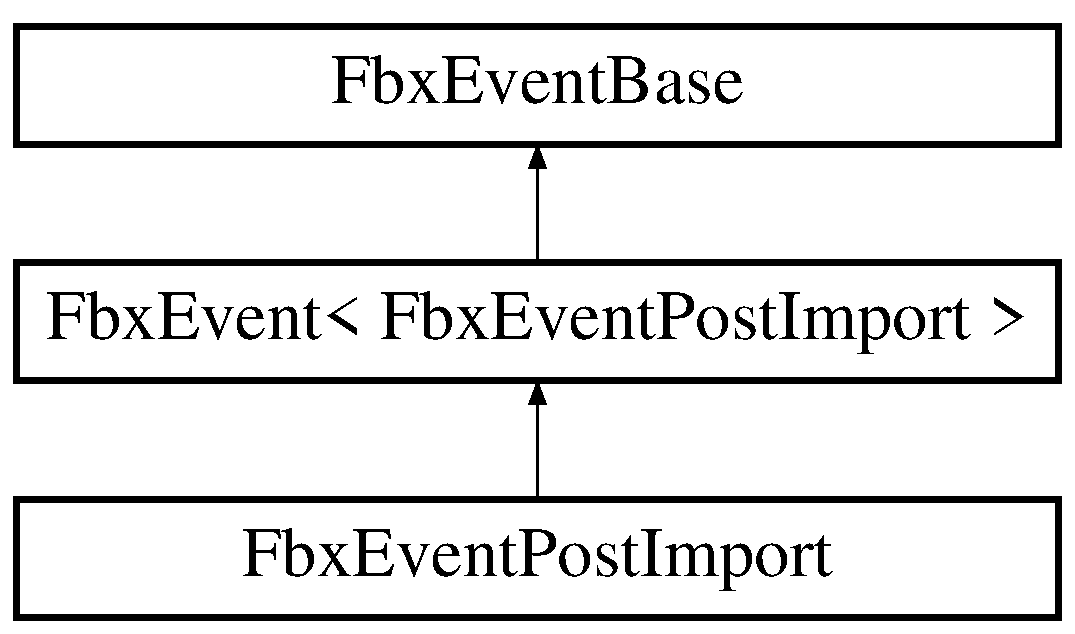
\includegraphics[height=3.000000cm]{class_fbx_event_post_import}
\end{center}
\end{figure}
\subsection*{公開メンバ関数}
\begin{DoxyCompactItemize}
\item 
\hyperlink{class_fbx_event_post_import_aefcd44e6871e671e571f3f378ceab40a}{Fbx\+Event\+Post\+Import} (\hyperlink{class_fbx_document}{Fbx\+Document} $\ast$p\+Document)
\end{DoxyCompactItemize}
\subsection*{公開変数類}
\begin{DoxyCompactItemize}
\item 
\hyperlink{class_fbx_document}{Fbx\+Document} $\ast$ \hyperlink{class_fbx_event_post_import_a9e7d9e8702a8e82a81409d1393845a1a}{m\+Document}
\begin{DoxyCompactList}\small\item\em The imported document \end{DoxyCompactList}\end{DoxyCompactItemize}
\subsection*{その他の継承メンバ}


\subsection{詳解}
Event that is emitted to plugins after a F\+BX file has been imported. 

 fbximporter.\+h の 380 行目に定義があります。



\subsection{構築子と解体子}
\mbox{\Hypertarget{class_fbx_event_post_import_aefcd44e6871e671e571f3f378ceab40a}\label{class_fbx_event_post_import_aefcd44e6871e671e571f3f378ceab40a}} 
\index{Fbx\+Event\+Post\+Import@{Fbx\+Event\+Post\+Import}!Fbx\+Event\+Post\+Import@{Fbx\+Event\+Post\+Import}}
\index{Fbx\+Event\+Post\+Import@{Fbx\+Event\+Post\+Import}!Fbx\+Event\+Post\+Import@{Fbx\+Event\+Post\+Import}}
\subsubsection{\texorpdfstring{Fbx\+Event\+Post\+Import()}{FbxEventPostImport()}}
{\footnotesize\ttfamily Fbx\+Event\+Post\+Import\+::\+Fbx\+Event\+Post\+Import (\begin{DoxyParamCaption}\item[{\hyperlink{class_fbx_document}{Fbx\+Document} $\ast$}]{p\+Document }\end{DoxyParamCaption})\hspace{0.3cm}{\ttfamily [inline]}}



 fbximporter.\+h の 384 行目に定義があります。



\subsection{メンバ詳解}
\mbox{\Hypertarget{class_fbx_event_post_import_a9e7d9e8702a8e82a81409d1393845a1a}\label{class_fbx_event_post_import_a9e7d9e8702a8e82a81409d1393845a1a}} 
\index{Fbx\+Event\+Post\+Import@{Fbx\+Event\+Post\+Import}!m\+Document@{m\+Document}}
\index{m\+Document@{m\+Document}!Fbx\+Event\+Post\+Import@{Fbx\+Event\+Post\+Import}}
\subsubsection{\texorpdfstring{m\+Document}{mDocument}}
{\footnotesize\ttfamily \hyperlink{class_fbx_document}{Fbx\+Document}$\ast$ Fbx\+Event\+Post\+Import\+::m\+Document}



The imported document 



 fbximporter.\+h の 384 行目に定義があります。



このクラス詳解は次のファイルから抽出されました\+:\begin{DoxyCompactItemize}
\item 
C\+:/\+Maya/scripts/\+F\+B\+X\+\_\+\+S\+D\+K/2017.\+1/include/fbxsdk/fileio/\hyperlink{fbximporter_8h}{fbximporter.\+h}\end{DoxyCompactItemize}

\hypertarget{class_fbx_event_pre_export}{}\section{Fbx\+Event\+Pre\+Export クラス}
\label{class_fbx_event_pre_export}\index{Fbx\+Event\+Pre\+Export@{Fbx\+Event\+Pre\+Export}}


Event that is emitted to plugins before a file is exported to the F\+BX format.  




{\ttfamily \#include $<$fbxexporter.\+h$>$}



Fbx\+Event\+Pre\+Export の継承関係図
% FIG 0


Fbx\+Event\+Pre\+Export 連携図
% FIG 1
\subsection*{公開メンバ関数}
\begin{DoxyCompactItemize}
\item 
\hyperlink{class_fbx_event_pre_export_a90642ec2d709d7bbb898df8248f848ba}{Fbx\+Event\+Pre\+Export} (\hyperlink{class_fbx_document}{Fbx\+Document} $\ast$p\+Document)
\end{DoxyCompactItemize}
\subsection*{公開変数類}
\begin{DoxyCompactItemize}
\item 
\hyperlink{class_fbx_document}{Fbx\+Document} $\ast$ \hyperlink{class_fbx_event_pre_export_aee74a30348fc851b3690a90c99b0a4b8}{m\+Document}
\begin{DoxyCompactList}\small\item\em The document to be exported \end{DoxyCompactList}\end{DoxyCompactItemize}
\subsection*{その他の継承メンバ}


\subsection{詳解}
Event that is emitted to plugins before a file is exported to the F\+BX format. 

\subsection{構築子と解体子}
\mbox{\Hypertarget{class_fbx_event_pre_export_a90642ec2d709d7bbb898df8248f848ba}\label{class_fbx_event_pre_export_a90642ec2d709d7bbb898df8248f848ba}} 
\index{Fbx\+Event\+Pre\+Export@{Fbx\+Event\+Pre\+Export}!Fbx\+Event\+Pre\+Export@{Fbx\+Event\+Pre\+Export}}
\index{Fbx\+Event\+Pre\+Export@{Fbx\+Event\+Pre\+Export}!Fbx\+Event\+Pre\+Export@{Fbx\+Event\+Pre\+Export}}
\subsubsection{\texorpdfstring{Fbx\+Event\+Pre\+Export()}{FbxEventPreExport()}}
{\footnotesize\ttfamily Fbx\+Event\+Pre\+Export\+::\+Fbx\+Event\+Pre\+Export (\begin{DoxyParamCaption}\item[{\hyperlink{class_fbx_document}{Fbx\+Document} $\ast$}]{p\+Document }\end{DoxyParamCaption})}



\subsection{メンバ詳解}
\mbox{\Hypertarget{class_fbx_event_pre_export_aee74a30348fc851b3690a90c99b0a4b8}\label{class_fbx_event_pre_export_aee74a30348fc851b3690a90c99b0a4b8}} 
\index{Fbx\+Event\+Pre\+Export@{Fbx\+Event\+Pre\+Export}!m\+Document@{m\+Document}}
\index{m\+Document@{m\+Document}!Fbx\+Event\+Pre\+Export@{Fbx\+Event\+Pre\+Export}}
\subsubsection{\texorpdfstring{m\+Document}{mDocument}}
{\footnotesize\ttfamily \hyperlink{class_fbx_document}{Fbx\+Document}$\ast$ Fbx\+Event\+Pre\+Export\+::m\+Document}



The document to be exported 



このクラス詳解は次のファイルから抽出されました\+:\begin{DoxyCompactItemize}
\item 
C\+:/github/\+F\+B\+Xpython\+S\+D\+K201701/\+F\+B\+Xpython\+S\+D\+K201701/2017.\+1/include/fbxsdk/fileio/\hyperlink{fbxexporter_8h}{fbxexporter.\+h}\end{DoxyCompactItemize}

\hypertarget{class_fbx_event_pre_import}{}\section{Fbx\+Event\+Pre\+Import クラス}
\label{class_fbx_event_pre_import}\index{Fbx\+Event\+Pre\+Import@{Fbx\+Event\+Pre\+Import}}


Event that is emitted to plugins before a F\+BX file has been imported.  




{\ttfamily \#include $<$fbximporter.\+h$>$}

Fbx\+Event\+Pre\+Import の継承関係図\begin{figure}[H]
\begin{center}
\leavevmode
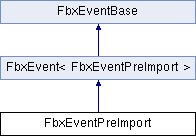
\includegraphics[height=3.000000cm]{class_fbx_event_pre_import}
\end{center}
\end{figure}
\subsection*{公開メンバ関数}
\begin{DoxyCompactItemize}
\item 
\hyperlink{class_fbx_event_pre_import_a67755900fb239a5c7d67b8e22d92eb60}{Fbx\+Event\+Pre\+Import} (\hyperlink{class_fbx_document}{Fbx\+Document} $\ast$p\+Document)
\end{DoxyCompactItemize}
\subsection*{公開変数類}
\begin{DoxyCompactItemize}
\item 
\hyperlink{class_fbx_document}{Fbx\+Document} $\ast$ \hyperlink{class_fbx_event_pre_import_a89b454dc61f00b64cc8a8f951e5e1003}{m\+Document}
\begin{DoxyCompactList}\small\item\em The document the F\+BX file is to be imported into. \end{DoxyCompactList}\end{DoxyCompactItemize}
\subsection*{その他の継承メンバ}


\subsection{詳解}
Event that is emitted to plugins before a F\+BX file has been imported. 

 fbximporter.\+h の 369 行目に定義があります。



\subsection{構築子と解体子}
\mbox{\Hypertarget{class_fbx_event_pre_import_a67755900fb239a5c7d67b8e22d92eb60}\label{class_fbx_event_pre_import_a67755900fb239a5c7d67b8e22d92eb60}} 
\index{Fbx\+Event\+Pre\+Import@{Fbx\+Event\+Pre\+Import}!Fbx\+Event\+Pre\+Import@{Fbx\+Event\+Pre\+Import}}
\index{Fbx\+Event\+Pre\+Import@{Fbx\+Event\+Pre\+Import}!Fbx\+Event\+Pre\+Import@{Fbx\+Event\+Pre\+Import}}
\subsubsection{\texorpdfstring{Fbx\+Event\+Pre\+Import()}{FbxEventPreImport()}}
{\footnotesize\ttfamily Fbx\+Event\+Pre\+Import\+::\+Fbx\+Event\+Pre\+Import (\begin{DoxyParamCaption}\item[{\hyperlink{class_fbx_document}{Fbx\+Document} $\ast$}]{p\+Document }\end{DoxyParamCaption})\hspace{0.3cm}{\ttfamily [inline]}}



 fbximporter.\+h の 373 行目に定義があります。



\subsection{メンバ詳解}
\mbox{\Hypertarget{class_fbx_event_pre_import_a89b454dc61f00b64cc8a8f951e5e1003}\label{class_fbx_event_pre_import_a89b454dc61f00b64cc8a8f951e5e1003}} 
\index{Fbx\+Event\+Pre\+Import@{Fbx\+Event\+Pre\+Import}!m\+Document@{m\+Document}}
\index{m\+Document@{m\+Document}!Fbx\+Event\+Pre\+Import@{Fbx\+Event\+Pre\+Import}}
\subsubsection{\texorpdfstring{m\+Document}{mDocument}}
{\footnotesize\ttfamily \hyperlink{class_fbx_document}{Fbx\+Document}$\ast$ Fbx\+Event\+Pre\+Import\+::m\+Document}



The document the F\+BX file is to be imported into. 



 fbximporter.\+h の 373 行目に定義があります。



このクラス詳解は次のファイルから抽出されました\+:\begin{DoxyCompactItemize}
\item 
C\+:/\+Maya/scripts/\+F\+B\+X\+\_\+\+S\+D\+K/2017.\+1/include/fbxsdk/fileio/\hyperlink{fbximporter_8h}{fbximporter.\+h}\end{DoxyCompactItemize}

\hypertarget{class_fbx_event_referenced_document}{}\section{Fbx\+Event\+Referenced\+Document クラス}
\label{class_fbx_event_referenced_document}\index{Fbx\+Event\+Referenced\+Document@{Fbx\+Event\+Referenced\+Document}}


{\ttfamily \#include $<$fbxexternaldocreflistener.\+h$>$}

Fbx\+Event\+Referenced\+Document の継承関係図\begin{figure}[H]
\begin{center}
\leavevmode
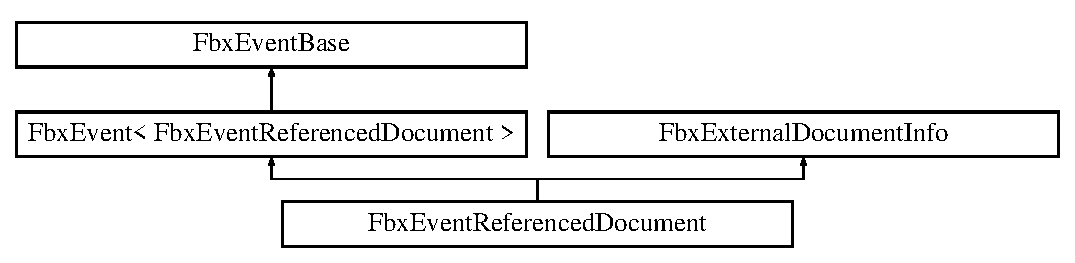
\includegraphics[height=3.000000cm]{class_fbx_event_referenced_document}
\end{center}
\end{figure}
\subsection*{公開メンバ関数}
\begin{DoxyCompactItemize}
\item 
\hyperlink{class_fbx_event_referenced_document_a573464a1bcb1982f0f83bee571e35d79}{Fbx\+Event\+Referenced\+Document} ()
\end{DoxyCompactItemize}
\subsection*{その他の継承メンバ}


\subsection{詳解}
Event that is emitted on loading document when a referenced document is encountered while loading external references. 

 fbxexternaldocreflistener.\+h の 36 行目に定義があります。



\subsection{構築子と解体子}
\mbox{\Hypertarget{class_fbx_event_referenced_document_a573464a1bcb1982f0f83bee571e35d79}\label{class_fbx_event_referenced_document_a573464a1bcb1982f0f83bee571e35d79}} 
\index{Fbx\+Event\+Referenced\+Document@{Fbx\+Event\+Referenced\+Document}!Fbx\+Event\+Referenced\+Document@{Fbx\+Event\+Referenced\+Document}}
\index{Fbx\+Event\+Referenced\+Document@{Fbx\+Event\+Referenced\+Document}!Fbx\+Event\+Referenced\+Document@{Fbx\+Event\+Referenced\+Document}}
\subsubsection{\texorpdfstring{Fbx\+Event\+Referenced\+Document()}{FbxEventReferencedDocument()}}
{\footnotesize\ttfamily Fbx\+Event\+Referenced\+Document\+::\+Fbx\+Event\+Referenced\+Document (\begin{DoxyParamCaption}{ }\end{DoxyParamCaption})\hspace{0.3cm}{\ttfamily [inline]}}



 fbxexternaldocreflistener.\+h の 40 行目に定義があります。



このクラス詳解は次のファイルから抽出されました\+:\begin{DoxyCompactItemize}
\item 
C\+:/\+Maya/scripts/\+F\+B\+X\+\_\+\+S\+D\+K/2017.\+1/include/fbxsdk/fileio/\hyperlink{fbxexternaldocreflistener_8h}{fbxexternaldocreflistener.\+h}\end{DoxyCompactItemize}

\hypertarget{class_fbx_event_update_system_library}{}\section{Fbx\+Event\+Update\+System\+Library クラス}
\label{class_fbx_event_update_system_library}\index{Fbx\+Event\+Update\+System\+Library@{Fbx\+Event\+Update\+System\+Library}}


{\ttfamily \#include $<$fbxlibrary.\+h$>$}

Fbx\+Event\+Update\+System\+Library の継承関係図\begin{figure}[H]
\begin{center}
\leavevmode
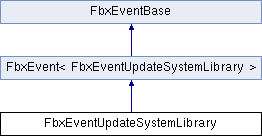
\includegraphics[height=3.000000cm]{class_fbx_event_update_system_library}
\end{center}
\end{figure}
\subsection*{公開メンバ関数}
\begin{DoxyCompactItemize}
\item 
\hyperlink{class_fbx_event_update_system_library_a1b45029571ddf6bf090d9c4c04f3b8bd}{Fbx\+Event\+Update\+System\+Library} (\hyperlink{class_fbx_library}{Fbx\+Library} $\ast$p\+Library)
\item 
\hyperlink{class_fbx_library}{Fbx\+Library} $\ast$ \hyperlink{class_fbx_event_update_system_library_a216f7eb4fed21eeac1aa0398fb164288}{Get\+Library} () const
\end{DoxyCompactItemize}
\subsection*{その他の継承メンバ}


\subsection{詳解}


 fbxlibrary.\+h の 284 行目に定義があります。



\subsection{構築子と解体子}
\mbox{\Hypertarget{class_fbx_event_update_system_library_a1b45029571ddf6bf090d9c4c04f3b8bd}\label{class_fbx_event_update_system_library_a1b45029571ddf6bf090d9c4c04f3b8bd}} 
\index{Fbx\+Event\+Update\+System\+Library@{Fbx\+Event\+Update\+System\+Library}!Fbx\+Event\+Update\+System\+Library@{Fbx\+Event\+Update\+System\+Library}}
\index{Fbx\+Event\+Update\+System\+Library@{Fbx\+Event\+Update\+System\+Library}!Fbx\+Event\+Update\+System\+Library@{Fbx\+Event\+Update\+System\+Library}}
\subsubsection{\texorpdfstring{Fbx\+Event\+Update\+System\+Library()}{FbxEventUpdateSystemLibrary()}}
{\footnotesize\ttfamily Fbx\+Event\+Update\+System\+Library\+::\+Fbx\+Event\+Update\+System\+Library (\begin{DoxyParamCaption}\item[{\hyperlink{class_fbx_library}{Fbx\+Library} $\ast$}]{p\+Library }\end{DoxyParamCaption})\hspace{0.3cm}{\ttfamily [inline]}}



 fbxlibrary.\+h の 289 行目に定義があります。



\subsection{関数詳解}
\mbox{\Hypertarget{class_fbx_event_update_system_library_a216f7eb4fed21eeac1aa0398fb164288}\label{class_fbx_event_update_system_library_a216f7eb4fed21eeac1aa0398fb164288}} 
\index{Fbx\+Event\+Update\+System\+Library@{Fbx\+Event\+Update\+System\+Library}!Get\+Library@{Get\+Library}}
\index{Get\+Library@{Get\+Library}!Fbx\+Event\+Update\+System\+Library@{Fbx\+Event\+Update\+System\+Library}}
\subsubsection{\texorpdfstring{Get\+Library()}{GetLibrary()}}
{\footnotesize\ttfamily \hyperlink{class_fbx_library}{Fbx\+Library}$\ast$ Fbx\+Event\+Update\+System\+Library\+::\+Get\+Library (\begin{DoxyParamCaption}{ }\end{DoxyParamCaption}) const\hspace{0.3cm}{\ttfamily [inline]}}



 fbxlibrary.\+h の 290 行目に定義があります。



このクラス詳解は次のファイルから抽出されました\+:\begin{DoxyCompactItemize}
\item 
C\+:/\+Maya/scripts/\+F\+B\+X\+\_\+\+S\+D\+K/2017.\+1/include/fbxsdk/scene/\hyperlink{fbxlibrary_8h}{fbxlibrary.\+h}\end{DoxyCompactItemize}

\hypertarget{class_fbx_event_write_localization}{}\section{Fbx\+Event\+Write\+Localization クラス}
\label{class_fbx_event_write_localization}\index{Fbx\+Event\+Write\+Localization@{Fbx\+Event\+Write\+Localization}}


{\ttfamily \#include $<$fbxlibrary.\+h$>$}

Fbx\+Event\+Write\+Localization の継承関係図\begin{figure}[H]
\begin{center}
\leavevmode
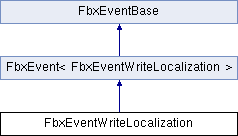
\includegraphics[height=3.000000cm]{class_fbx_event_write_localization}
\end{center}
\end{figure}
\subsection*{公開メンバ関数}
\begin{DoxyCompactItemize}
\item 
\hyperlink{class_fbx_event_write_localization_a45873b27b60b583b9e2d658fd6ba0916}{Fbx\+Event\+Write\+Localization} (\hyperlink{class_fbx_library}{Fbx\+Library} $\ast$p\+Asset\+Library)
\item 
\hyperlink{class_fbx_library}{Fbx\+Library} $\ast$ \hyperlink{class_fbx_event_write_localization_a10110bc0d52be7ba742c5c83c917c40c}{Get\+Library} () const
\end{DoxyCompactItemize}
\subsection*{その他の継承メンバ}


\subsection{詳解}


 fbxlibrary.\+h の 296 行目に定義があります。



\subsection{構築子と解体子}
\mbox{\Hypertarget{class_fbx_event_write_localization_a45873b27b60b583b9e2d658fd6ba0916}\label{class_fbx_event_write_localization_a45873b27b60b583b9e2d658fd6ba0916}} 
\index{Fbx\+Event\+Write\+Localization@{Fbx\+Event\+Write\+Localization}!Fbx\+Event\+Write\+Localization@{Fbx\+Event\+Write\+Localization}}
\index{Fbx\+Event\+Write\+Localization@{Fbx\+Event\+Write\+Localization}!Fbx\+Event\+Write\+Localization@{Fbx\+Event\+Write\+Localization}}
\subsubsection{\texorpdfstring{Fbx\+Event\+Write\+Localization()}{FbxEventWriteLocalization()}}
{\footnotesize\ttfamily Fbx\+Event\+Write\+Localization\+::\+Fbx\+Event\+Write\+Localization (\begin{DoxyParamCaption}\item[{\hyperlink{class_fbx_library}{Fbx\+Library} $\ast$}]{p\+Asset\+Library }\end{DoxyParamCaption})\hspace{0.3cm}{\ttfamily [inline]}}



 fbxlibrary.\+h の 301 行目に定義があります。



\subsection{関数詳解}
\mbox{\Hypertarget{class_fbx_event_write_localization_a10110bc0d52be7ba742c5c83c917c40c}\label{class_fbx_event_write_localization_a10110bc0d52be7ba742c5c83c917c40c}} 
\index{Fbx\+Event\+Write\+Localization@{Fbx\+Event\+Write\+Localization}!Get\+Library@{Get\+Library}}
\index{Get\+Library@{Get\+Library}!Fbx\+Event\+Write\+Localization@{Fbx\+Event\+Write\+Localization}}
\subsubsection{\texorpdfstring{Get\+Library()}{GetLibrary()}}
{\footnotesize\ttfamily \hyperlink{class_fbx_library}{Fbx\+Library}$\ast$ Fbx\+Event\+Write\+Localization\+::\+Get\+Library (\begin{DoxyParamCaption}{ }\end{DoxyParamCaption}) const\hspace{0.3cm}{\ttfamily [inline]}}



 fbxlibrary.\+h の 302 行目に定義があります。



このクラス詳解は次のファイルから抽出されました\+:\begin{DoxyCompactItemize}
\item 
C\+:/\+Maya/scripts/\+F\+B\+X\+\_\+\+S\+D\+K/2017.\+1/include/fbxsdk/scene/\hyperlink{fbxlibrary_8h}{fbxlibrary.\+h}\end{DoxyCompactItemize}

\hypertarget{class_fbx_exporter}{}\section{Fbx\+Exporter クラス}
\label{class_fbx_exporter}\index{Fbx\+Exporter@{Fbx\+Exporter}}


{\ttfamily \#include $<$fbxexporter.\+h$>$}



Fbx\+Exporter の継承関係図
% FIG 0


Fbx\+Exporter 連携図
% FIG 1
\subsection*{公開メンバ関数}
\begin{DoxyCompactItemize}
\item 
bool \hyperlink{class_fbx_exporter_a0e26854a47b1fdbc100332b131552b7e}{Get\+Export\+Options} (\hyperlink{class_fbx_i_o}{Fbx\+IO} $\ast$p\+Fbx\+Object)
\item 
bool \hyperlink{class_fbx_exporter_ae14616d7e29cd9ae52cd6bbccd6d6988}{Export} (\hyperlink{class_fbx_document}{Fbx\+Document} $\ast$p\+Document, \hyperlink{class_fbx_i_o}{Fbx\+IO} $\ast$p\+Fbx\+Object)
\end{DoxyCompactItemize}
\subsection*{限定公開メンバ関数}
\begin{DoxyCompactItemize}
\item 
virtual void \hyperlink{class_fbx_exporter_aa308b9a9901e8c98d0b54f0bd20daad2}{Construct} (const \hyperlink{class_fbx_object}{Fbx\+Object} $\ast$p\+From)
\item 
virtual void \hyperlink{class_fbx_exporter_a0a2569f6ed2ffaa165d9bdb1959f0599}{Destruct} (bool p\+Recursive)
\item 
virtual void \hyperlink{class_fbx_exporter_a1684b8488befbd05433963007bbaf3ad}{Set\+Or\+Create\+I\+O\+Settings} (\hyperlink{class_fbx_i_o_settings}{Fbx\+I\+O\+Settings} $\ast$p\+I\+O\+Settings, bool p\+Allow\+N\+U\+LL)
\item 
void \hyperlink{class_fbx_exporter_a2ee7ea29532a88c85f811eff793a5961}{Reset} ()
\item 
bool \hyperlink{class_fbx_exporter_a212dd139e703f6531bb6cf0ba1bc88d9}{File\+Create} ()
\item 
void \hyperlink{class_fbx_exporter_a7802b8f3aaf4598bb8e799d0f2c829be}{File\+Close} ()
\end{DoxyCompactItemize}
\subsection*{フレンド}
\begin{DoxyCompactItemize}
\item 
void \hyperlink{class_fbx_exporter_af010f0ee37fe98ae37cd7cbe976e7a74}{Export\+Thread} (void $\ast$)
\end{DoxyCompactItemize}
\subsection*{Export Functions}
\begin{DoxyCompactItemize}
\item 
virtual bool \hyperlink{class_fbx_exporter_acab60199145f0c86b80fac8ed7e1b239}{Initialize} (const char $\ast$p\+File\+Name, int p\+File\+Format=-\/1, \hyperlink{class_fbx_i_o_settings}{Fbx\+I\+O\+Settings} $\ast$p\+I\+O\+Settings=\hyperlink{fbxarch_8h_a070d2ce7b6bb7e5c05602aa8c308d0c4}{N\+U\+LL})
\item 
virtual bool \hyperlink{class_fbx_exporter_ae87b3014d3aa797617c530361296daa5}{Initialize} (\hyperlink{class_fbx_stream}{Fbx\+Stream} $\ast$p\+Stream, void $\ast$p\+Stream\+Data=\hyperlink{fbxarch_8h_a070d2ce7b6bb7e5c05602aa8c308d0c4}{N\+U\+LL}, int p\+File\+Format=-\/1, \hyperlink{class_fbx_i_o_settings}{Fbx\+I\+O\+Settings} $\ast$p\+I\+O\+Settings=\hyperlink{fbxarch_8h_a070d2ce7b6bb7e5c05602aa8c308d0c4}{N\+U\+LL})
\item 
bool \hyperlink{class_fbx_exporter_a1d698ddca2a7720a3c05b00afea5b413}{Get\+Export\+Options} ()
\item 
\hyperlink{class_fbx_i_o_settings}{Fbx\+I\+O\+Settings} $\ast$ \hyperlink{class_fbx_exporter_a80853ac3257f1cfb95478f969bdc002a}{Get\+I\+O\+Settings} ()
\item 
void \hyperlink{class_fbx_exporter_a072f9f312b878c796463bf9f9a2e43e0}{Set\+I\+O\+Settings} (\hyperlink{class_fbx_i_o_settings}{Fbx\+I\+O\+Settings} $\ast$p\+I\+O\+Settings)
\item 
bool \hyperlink{class_fbx_exporter_a8a92372cf76fe3486a798c87973cc791}{Export} (\hyperlink{class_fbx_document}{Fbx\+Document} $\ast$p\+Document, bool p\+Non\+Blocking=false)
\item 
bool \hyperlink{class_fbx_exporter_a244daae57da4509caa361160f0ae3e23}{Is\+Exporting} (bool \&p\+Export\+Result)
\item 
float \hyperlink{class_fbx_exporter_a9063d4a8ee7c7dbe1c5deaeef6bfbd2d}{Get\+Progress} (\hyperlink{class_fbx_string}{Fbx\+String} $\ast$p\+Status=\hyperlink{fbxarch_8h_a070d2ce7b6bb7e5c05602aa8c308d0c4}{N\+U\+LL})
\item 
void \hyperlink{class_fbx_exporter_a37b5449c65be8b77eae754fb52da3c1c}{Set\+Progress\+Callback} (\hyperlink{fbxprogress_8h_a3765040904b462fb1f2673caba3488db}{Fbx\+Progress\+Callback} p\+Callback, void $\ast$p\+Args=\hyperlink{fbxarch_8h_a070d2ce7b6bb7e5c05602aa8c308d0c4}{N\+U\+LL})
\end{DoxyCompactItemize}
\subsection*{File Format}
\begin{DoxyCompactItemize}
\item 
int \hyperlink{class_fbx_exporter_abd4308d309fb09113ebe6d7828691505}{Get\+File\+Format} ()
\item 
bool \hyperlink{class_fbx_exporter_a1a304c76e28c89212d8eee1b6f791c38}{Is\+F\+BX} ()
\item 
char const  $\ast$const  $\ast$ \hyperlink{class_fbx_exporter_a06229d56de47b83aec05e7c150f66264}{Get\+Current\+Writable\+Versions} ()
\item 
bool \hyperlink{class_fbx_exporter_a165c1e0111a8770be2bea86043db5a46}{Set\+File\+Export\+Version} (\hyperlink{class_fbx_string}{Fbx\+String} p\+Version, \hyperlink{class_fbx_scene_renamer_a9279ee1a645d6499b934adbc376f8678}{Fbx\+Scene\+Renamer\+::\+E\+Renaming\+Mode} p\+Renaming\+Mode=\hyperlink{class_fbx_scene_renamer_a9279ee1a645d6499b934adbc376f8678a6530ea605d82bb5be39517b65b47048e}{Fbx\+Scene\+Renamer\+::e\+None})
\item 
void \hyperlink{class_fbx_exporter_aeea95b702891fa350a03ab3e9aa949e1}{Set\+Resampling\+Rate} (double p\+Resampling\+Rate)
\item 
void \hyperlink{class_fbx_exporter_a4099cedc5a69045761b6fb6acd561bbf}{Set\+Default\+Render\+Resolution} (\hyperlink{class_fbx_string}{Fbx\+String} p\+Cam\+Name, \hyperlink{class_fbx_string}{Fbx\+String} p\+Resolution\+Mode, double pW, double pH)
\item 
\hyperlink{class_fbx_i_o_file_header_info}{Fbx\+I\+O\+File\+Header\+Info} $\ast$ \hyperlink{class_fbx_exporter_a9b219b2318ec3e5949a03b47e939251a}{Get\+File\+Header\+Info} ()
\end{DoxyCompactItemize}
\subsection*{その他の継承メンバ}


\subsection{詳解}
Class to export S\+DK objects into an F\+BX file. Normally this class is used as is. But for very special needs a user can override \hyperlink{class_fbx_exporter_acab60199145f0c86b80fac8ed7e1b239}{Initialize()} for special purpose.

An exporter will select the appropriate writer to a particular file. Ex\+: When an exporter must export an F\+BX 7 file, the exporter will ask for all registered writers if an F\+BX 7 file writer is available, then if a writer is found, the exporter will create the specialized F\+BX 7 writer and write the file. This way, an exporter can \char`\"{}write\char`\"{} many different type of files like F\+BX 5/6/7, 3\+DS, Obj, Dxf, Collada, etc. \begin{DoxySeeAlso}{参照}
\hyperlink{class_fbx_writer}{Fbx\+Writer}
\end{DoxySeeAlso}
Typical workflow for using the \hyperlink{class_fbx_exporter}{Fbx\+Exporter} class\+:
\begin{DoxyEnumerate}
\item create a S\+D\+K\+Manager
\item create an I\+O\+Settings object
\item create an empty scene
\item create an exporter
\item initialize it with a file name
\item set numerous options to control how the exporter will behave.~\newline
 ex\+: set I\+O\+Settings values to export Materials or Textures.
\item call \hyperlink{class_fbx_exporter_a8a92372cf76fe3486a798c87973cc791}{Fbx\+Exporter\+::\+Export()} with the entity to export.
\end{DoxyEnumerate}


\begin{DoxyCode}
\textcolor{comment}{// ex:}
\textcolor{comment}{// create a SdkManager}
\hyperlink{class_fbx_manager}{FbxManager}* lSdkManager = \hyperlink{class_fbx_manager_af51cafc0f34f17d497f7921d847a4dd4}{FbxManager::Create}();

\textcolor{comment}{// create an IOSettings object}
\hyperlink{class_fbx_i_o_settings}{FbxIOSettings}* ios = FbxIOSettings::Create(lSdkManager, \hyperlink{fbxiosettingspath_8h_a57a5e54b72d0f2936d5ee84d8f510a0a}{IOSROOT});

\textcolor{comment}{// set some IOSettings options }
ios->\hyperlink{class_fbx_i_o_settings_ad2c660ef846b66dcf569079299391745}{SetBoolProp}(\hyperlink{fbxiosettingspath_8h_a204bbd602ba341a20acf870eef02027f}{EXP\_FBX\_MATERIAL}, \textcolor{keyword}{true});
ios->\hyperlink{class_fbx_i_o_settings_ad2c660ef846b66dcf569079299391745}{SetBoolProp}(\hyperlink{fbxiosettingspath_8h_a157289a61920fd4b968bf370077222b2}{EXP\_FBX\_TEXTURE},  \textcolor{keyword}{true});

\textcolor{comment}{// create an empty scene}
\hyperlink{class_fbx_scene}{FbxScene}* lScene = FbxScene::Create(lSdkManager, \textcolor{stringliteral}{""});

\textcolor{comment}{// create an exporter.}
\hyperlink{class_fbx_exporter}{FbxExporter}* lExporter = FbxExporter::Create(lSdkManager, \textcolor{stringliteral}{""});

\textcolor{comment}{// initialize the exporter by providing a filename and the IOSettings to use}
lExporter->\hyperlink{class_fbx_exporter_acab60199145f0c86b80fac8ed7e1b239}{Initialize}(\textcolor{stringliteral}{"C:\(\backslash\)\(\backslash\)myfile.fbx"}, -1, ios);

\textcolor{comment}{// export the scene.}
lExporter->\hyperlink{class_fbx_exporter_a8a92372cf76fe3486a798c87973cc791}{Export}(lScene); 
 
\textcolor{comment}{// destroy the exporter}
lExporter->\hyperlink{class_fbx_object_a7b49e6a0c17132cd7e2e7e8485a08915}{Destroy}();
\end{DoxyCode}


\begin{DoxyRemark}{注釈}
According to the file suffix, a specialized writer will be created internally.~\newline
 Ex\+: for .fbx files a F\+BX Writer, for .3ds files, a 3ds writer, etc.~\newline
 Supported files formats\+: F\+BX 5/6/7 Binary \& A\+S\+C\+II, Collada, D\+XF, O\+BJ, 3\+DS 
\end{DoxyRemark}


\subsection{メソッド詳解}
\mbox{\Hypertarget{class_fbx_exporter_aa308b9a9901e8c98d0b54f0bd20daad2}\label{class_fbx_exporter_aa308b9a9901e8c98d0b54f0bd20daad2}} 
\index{Fbx\+Exporter@{Fbx\+Exporter}!Construct@{Construct}}
\index{Construct@{Construct}!Fbx\+Exporter@{Fbx\+Exporter}}
\subsubsection{\texorpdfstring{Construct()}{Construct()}}
{\footnotesize\ttfamily virtual void Fbx\+Exporter\+::\+Construct (\begin{DoxyParamCaption}\item[{const \hyperlink{class_fbx_object}{Fbx\+Object} $\ast$}]{p\+From }\end{DoxyParamCaption})\hspace{0.3cm}{\ttfamily [protected]}, {\ttfamily [virtual]}}

Optional constructor override, automatically called by default constructor. 
\begin{DoxyParams}{引数}
{\em p\+From} & If not null, the function must take it into account like a copy constructor. \\
\hline
\end{DoxyParams}
\begin{DoxyRemark}{注釈}
In case it is decided to override this function, do not forget to call Parent\+Class\+::\+Construct(p\+From) at the beginning. 
\end{DoxyRemark}


\hyperlink{class_fbx_i_o_base_aed70ed1326f8fb1cc96e2086c73722f8}{Fbx\+I\+O\+Base}を再実装しています。

\mbox{\Hypertarget{class_fbx_exporter_a0a2569f6ed2ffaa165d9bdb1959f0599}\label{class_fbx_exporter_a0a2569f6ed2ffaa165d9bdb1959f0599}} 
\index{Fbx\+Exporter@{Fbx\+Exporter}!Destruct@{Destruct}}
\index{Destruct@{Destruct}!Fbx\+Exporter@{Fbx\+Exporter}}
\subsubsection{\texorpdfstring{Destruct()}{Destruct()}}
{\footnotesize\ttfamily virtual void Fbx\+Exporter\+::\+Destruct (\begin{DoxyParamCaption}\item[{bool}]{p\+Recursive }\end{DoxyParamCaption})\hspace{0.3cm}{\ttfamily [protected]}, {\ttfamily [virtual]}}

Optional destructor override, automatically called by default destructor. 
\begin{DoxyParams}{引数}
{\em p\+Recursive} & If true, children objects should be destroyed as well. \\
\hline
\end{DoxyParams}
\begin{DoxyRemark}{注釈}
In case it is decided to override this function, do not forget to call Parent\+Class\+::\+Destruct(p\+Resursive) at the end. 
\end{DoxyRemark}


\hyperlink{class_fbx_object_a123e084d9b32b29c28af6384b7c3c608}{Fbx\+Object}を再実装しています。

\mbox{\Hypertarget{class_fbx_exporter_a8a92372cf76fe3486a798c87973cc791}\label{class_fbx_exporter_a8a92372cf76fe3486a798c87973cc791}} 
\index{Fbx\+Exporter@{Fbx\+Exporter}!Export@{Export}}
\index{Export@{Export}!Fbx\+Exporter@{Fbx\+Exporter}}
\subsubsection{\texorpdfstring{Export()}{Export()}\hspace{0.1cm}{\footnotesize\ttfamily [1/2]}}
{\footnotesize\ttfamily bool Fbx\+Exporter\+::\+Export (\begin{DoxyParamCaption}\item[{\hyperlink{class_fbx_document}{Fbx\+Document} $\ast$}]{p\+Document,  }\item[{bool}]{p\+Non\+Blocking = {\ttfamily false} }\end{DoxyParamCaption})}

Export the document to the currently created file. 
\begin{DoxyParams}{引数}
{\em p\+Document} & Document to export. \\
\hline
{\em p\+Non\+Blocking} & If true, the export process will be executed in a new thread, allowing it to be non-\/blocking. To determine if the export finished, refer to the function \hyperlink{class_fbx_exporter_a244daae57da4509caa361160f0ae3e23}{Is\+Exporting()}. \\
\hline
\end{DoxyParams}
\begin{DoxyReturn}{戻り値}
{\ttfamily true} on success, {\ttfamily false} otherwise. 
\end{DoxyReturn}
\begin{DoxyRemark}{注釈}
To identify the error that occurred, inspect the status object accessed using the \hyperlink{class_fbx_i_o_base_a078e47a99b119278ca3ee639e2da5b6d}{Get\+Status()} function. 
\end{DoxyRemark}
\mbox{\Hypertarget{class_fbx_exporter_ae14616d7e29cd9ae52cd6bbccd6d6988}\label{class_fbx_exporter_ae14616d7e29cd9ae52cd6bbccd6d6988}} 
\index{Fbx\+Exporter@{Fbx\+Exporter}!Export@{Export}}
\index{Export@{Export}!Fbx\+Exporter@{Fbx\+Exporter}}
\subsubsection{\texorpdfstring{Export()}{Export()}\hspace{0.1cm}{\footnotesize\ttfamily [2/2]}}
{\footnotesize\ttfamily bool Fbx\+Exporter\+::\+Export (\begin{DoxyParamCaption}\item[{\hyperlink{class_fbx_document}{Fbx\+Document} $\ast$}]{p\+Document,  }\item[{\hyperlink{class_fbx_i_o}{Fbx\+IO} $\ast$}]{p\+Fbx\+Object }\end{DoxyParamCaption})}

\mbox{\Hypertarget{class_fbx_exporter_a7802b8f3aaf4598bb8e799d0f2c829be}\label{class_fbx_exporter_a7802b8f3aaf4598bb8e799d0f2c829be}} 
\index{Fbx\+Exporter@{Fbx\+Exporter}!File\+Close@{File\+Close}}
\index{File\+Close@{File\+Close}!Fbx\+Exporter@{Fbx\+Exporter}}
\subsubsection{\texorpdfstring{File\+Close()}{FileClose()}}
{\footnotesize\ttfamily void Fbx\+Exporter\+::\+File\+Close (\begin{DoxyParamCaption}{ }\end{DoxyParamCaption})\hspace{0.3cm}{\ttfamily [protected]}}

\mbox{\Hypertarget{class_fbx_exporter_a212dd139e703f6531bb6cf0ba1bc88d9}\label{class_fbx_exporter_a212dd139e703f6531bb6cf0ba1bc88d9}} 
\index{Fbx\+Exporter@{Fbx\+Exporter}!File\+Create@{File\+Create}}
\index{File\+Create@{File\+Create}!Fbx\+Exporter@{Fbx\+Exporter}}
\subsubsection{\texorpdfstring{File\+Create()}{FileCreate()}}
{\footnotesize\ttfamily bool Fbx\+Exporter\+::\+File\+Create (\begin{DoxyParamCaption}{ }\end{DoxyParamCaption})\hspace{0.3cm}{\ttfamily [protected]}}

\mbox{\Hypertarget{class_fbx_exporter_a06229d56de47b83aec05e7c150f66264}\label{class_fbx_exporter_a06229d56de47b83aec05e7c150f66264}} 
\index{Fbx\+Exporter@{Fbx\+Exporter}!Get\+Current\+Writable\+Versions@{Get\+Current\+Writable\+Versions}}
\index{Get\+Current\+Writable\+Versions@{Get\+Current\+Writable\+Versions}!Fbx\+Exporter@{Fbx\+Exporter}}
\subsubsection{\texorpdfstring{Get\+Current\+Writable\+Versions()}{GetCurrentWritableVersions()}}
{\footnotesize\ttfamily char const$\ast$ const$\ast$ Fbx\+Exporter\+::\+Get\+Current\+Writable\+Versions (\begin{DoxyParamCaption}{ }\end{DoxyParamCaption})}

Get the list of writable versions for the current file format. \begin{DoxyReturn}{戻り値}
{\ttfamily N\+U\+LL} or a null terminated array of strings. 
\end{DoxyReturn}
\begin{DoxyRemark}{注釈}
the strings returned match the writers registered for the current format. The array items can be retrieved with the following code\+: 
\begin{DoxyCode}
\textcolor{keywordtype}{char} \textcolor{keyword}{const}* \textcolor{keyword}{const}* lWV = lExporter->\hyperlink{class_fbx_exporter_a06229d56de47b83aec05e7c150f66264}{GetCurrentWritableVersions}();
\textcolor{keywordflow}{if} (lWV)
\{
    \textcolor{keywordtype}{int} i = 0;
    \textcolor{keywordflow}{while} (lWV[i] != \hyperlink{fbxarch_8h_a070d2ce7b6bb7e5c05602aa8c308d0c4}{NULL})
    \{
        printf(\textcolor{stringliteral}{"fmt = %s\(\backslash\)n"}, lWV[i]);
        i++;
    \}
\}
\end{DoxyCode}
 
\end{DoxyRemark}
\mbox{\Hypertarget{class_fbx_exporter_a1d698ddca2a7720a3c05b00afea5b413}\label{class_fbx_exporter_a1d698ddca2a7720a3c05b00afea5b413}} 
\index{Fbx\+Exporter@{Fbx\+Exporter}!Get\+Export\+Options@{Get\+Export\+Options}}
\index{Get\+Export\+Options@{Get\+Export\+Options}!Fbx\+Exporter@{Fbx\+Exporter}}
\subsubsection{\texorpdfstring{Get\+Export\+Options()}{GetExportOptions()}\hspace{0.1cm}{\footnotesize\ttfamily [1/2]}}
{\footnotesize\ttfamily bool Fbx\+Exporter\+::\+Get\+Export\+Options (\begin{DoxyParamCaption}{ }\end{DoxyParamCaption})}

Setup file export options settings. \begin{DoxyReturn}{戻り値}
{\ttfamily true} on success, {\ttfamily false} otherwise. 
\end{DoxyReturn}
\mbox{\Hypertarget{class_fbx_exporter_a0e26854a47b1fdbc100332b131552b7e}\label{class_fbx_exporter_a0e26854a47b1fdbc100332b131552b7e}} 
\index{Fbx\+Exporter@{Fbx\+Exporter}!Get\+Export\+Options@{Get\+Export\+Options}}
\index{Get\+Export\+Options@{Get\+Export\+Options}!Fbx\+Exporter@{Fbx\+Exporter}}
\subsubsection{\texorpdfstring{Get\+Export\+Options()}{GetExportOptions()}\hspace{0.1cm}{\footnotesize\ttfamily [2/2]}}
{\footnotesize\ttfamily bool Fbx\+Exporter\+::\+Get\+Export\+Options (\begin{DoxyParamCaption}\item[{\hyperlink{class_fbx_i_o}{Fbx\+IO} $\ast$}]{p\+Fbx\+Object }\end{DoxyParamCaption})}

\mbox{\Hypertarget{class_fbx_exporter_abd4308d309fb09113ebe6d7828691505}\label{class_fbx_exporter_abd4308d309fb09113ebe6d7828691505}} 
\index{Fbx\+Exporter@{Fbx\+Exporter}!Get\+File\+Format@{Get\+File\+Format}}
\index{Get\+File\+Format@{Get\+File\+Format}!Fbx\+Exporter@{Fbx\+Exporter}}
\subsubsection{\texorpdfstring{Get\+File\+Format()}{GetFileFormat()}}
{\footnotesize\ttfamily int Fbx\+Exporter\+::\+Get\+File\+Format (\begin{DoxyParamCaption}{ }\end{DoxyParamCaption})}

Get the format of the exported file. \begin{DoxyReturn}{戻り値}
File format identifier. 
\end{DoxyReturn}
\mbox{\Hypertarget{class_fbx_exporter_a9b219b2318ec3e5949a03b47e939251a}\label{class_fbx_exporter_a9b219b2318ec3e5949a03b47e939251a}} 
\index{Fbx\+Exporter@{Fbx\+Exporter}!Get\+File\+Header\+Info@{Get\+File\+Header\+Info}}
\index{Get\+File\+Header\+Info@{Get\+File\+Header\+Info}!Fbx\+Exporter@{Fbx\+Exporter}}
\subsubsection{\texorpdfstring{Get\+File\+Header\+Info()}{GetFileHeaderInfo()}}
{\footnotesize\ttfamily \hyperlink{class_fbx_i_o_file_header_info}{Fbx\+I\+O\+File\+Header\+Info}$\ast$ Fbx\+Exporter\+::\+Get\+File\+Header\+Info (\begin{DoxyParamCaption}{ }\end{DoxyParamCaption})}

Get the complete file header information. \begin{DoxyReturn}{戻り値}
valid pointer to the complete header information 
\end{DoxyReturn}
\mbox{\Hypertarget{class_fbx_exporter_a80853ac3257f1cfb95478f969bdc002a}\label{class_fbx_exporter_a80853ac3257f1cfb95478f969bdc002a}} 
\index{Fbx\+Exporter@{Fbx\+Exporter}!Get\+I\+O\+Settings@{Get\+I\+O\+Settings}}
\index{Get\+I\+O\+Settings@{Get\+I\+O\+Settings}!Fbx\+Exporter@{Fbx\+Exporter}}
\subsubsection{\texorpdfstring{Get\+I\+O\+Settings()}{GetIOSettings()}}
{\footnotesize\ttfamily \hyperlink{class_fbx_i_o_settings}{Fbx\+I\+O\+Settings}$\ast$ Fbx\+Exporter\+::\+Get\+I\+O\+Settings (\begin{DoxyParamCaption}{ }\end{DoxyParamCaption})}

Access to a I\+O\+Settings object. \begin{DoxyReturn}{戻り値}
The pointer to I\+O\+Settings or {\ttfamily N\+U\+LL} {\ttfamily if} the object has not been allocated. 
\end{DoxyReturn}
\mbox{\Hypertarget{class_fbx_exporter_a9063d4a8ee7c7dbe1c5deaeef6bfbd2d}\label{class_fbx_exporter_a9063d4a8ee7c7dbe1c5deaeef6bfbd2d}} 
\index{Fbx\+Exporter@{Fbx\+Exporter}!Get\+Progress@{Get\+Progress}}
\index{Get\+Progress@{Get\+Progress}!Fbx\+Exporter@{Fbx\+Exporter}}
\subsubsection{\texorpdfstring{Get\+Progress()}{GetProgress()}}
{\footnotesize\ttfamily float Fbx\+Exporter\+::\+Get\+Progress (\begin{DoxyParamCaption}\item[{\hyperlink{class_fbx_string}{Fbx\+String} $\ast$}]{p\+Status = {\ttfamily \hyperlink{fbxarch_8h_a070d2ce7b6bb7e5c05602aa8c308d0c4}{N\+U\+LL}} }\end{DoxyParamCaption})}

Get the progress status in non-\/blocking mode. 
\begin{DoxyParams}{引数}
{\em p\+Status} & Optional current status string. \\
\hline
\end{DoxyParams}
\begin{DoxyReturn}{戻り値}
Percentage of the finished workload. 
\end{DoxyReturn}
\mbox{\Hypertarget{class_fbx_exporter_acab60199145f0c86b80fac8ed7e1b239}\label{class_fbx_exporter_acab60199145f0c86b80fac8ed7e1b239}} 
\index{Fbx\+Exporter@{Fbx\+Exporter}!Initialize@{Initialize}}
\index{Initialize@{Initialize}!Fbx\+Exporter@{Fbx\+Exporter}}
\subsubsection{\texorpdfstring{Initialize()}{Initialize()}\hspace{0.1cm}{\footnotesize\ttfamily [1/2]}}
{\footnotesize\ttfamily virtual bool Fbx\+Exporter\+::\+Initialize (\begin{DoxyParamCaption}\item[{const char $\ast$}]{p\+File\+Name,  }\item[{int}]{p\+File\+Format = {\ttfamily -\/1},  }\item[{\hyperlink{class_fbx_i_o_settings}{Fbx\+I\+O\+Settings} $\ast$}]{p\+I\+O\+Settings = {\ttfamily \hyperlink{fbxarch_8h_a070d2ce7b6bb7e5c05602aa8c308d0c4}{N\+U\+LL}} }\end{DoxyParamCaption})\hspace{0.3cm}{\ttfamily [virtual]}}

Initialize object. 
\begin{DoxyParams}{引数}
{\em p\+File\+Name} & Name of file to access. \\
\hline
{\em p\+File\+Format} & file format identifier User does not need to specify it by default. if not specified, plugin will detect the file format according to file suffix automatically. \\
\hline
{\em p\+I\+O\+Settings} & client I\+O\+Settings, if not specified, a default I\+O\+Settings will be created \\
\hline
\end{DoxyParams}
\begin{DoxyReturn}{戻り値}
{\ttfamily true} on success, {\ttfamily false} otherwise. 
\end{DoxyReturn}
\begin{DoxyRemark}{注釈}
To identify the error that occurred, inspect the status object accessed using the \hyperlink{class_fbx_i_o_base_a078e47a99b119278ca3ee639e2da5b6d}{Get\+Status()} function. 
\end{DoxyRemark}


\hyperlink{class_fbx_i_o_base_a01d70175d09a1e791e2ce38a9ae3c265}{Fbx\+I\+O\+Base}を再実装しています。

\mbox{\Hypertarget{class_fbx_exporter_ae87b3014d3aa797617c530361296daa5}\label{class_fbx_exporter_ae87b3014d3aa797617c530361296daa5}} 
\index{Fbx\+Exporter@{Fbx\+Exporter}!Initialize@{Initialize}}
\index{Initialize@{Initialize}!Fbx\+Exporter@{Fbx\+Exporter}}
\subsubsection{\texorpdfstring{Initialize()}{Initialize()}\hspace{0.1cm}{\footnotesize\ttfamily [2/2]}}
{\footnotesize\ttfamily virtual bool Fbx\+Exporter\+::\+Initialize (\begin{DoxyParamCaption}\item[{\hyperlink{class_fbx_stream}{Fbx\+Stream} $\ast$}]{p\+Stream,  }\item[{void $\ast$}]{p\+Stream\+Data = {\ttfamily \hyperlink{fbxarch_8h_a070d2ce7b6bb7e5c05602aa8c308d0c4}{N\+U\+LL}},  }\item[{int}]{p\+File\+Format = {\ttfamily -\/1},  }\item[{\hyperlink{class_fbx_i_o_settings}{Fbx\+I\+O\+Settings} $\ast$}]{p\+I\+O\+Settings = {\ttfamily \hyperlink{fbxarch_8h_a070d2ce7b6bb7e5c05602aa8c308d0c4}{N\+U\+LL}} }\end{DoxyParamCaption})\hspace{0.3cm}{\ttfamily [virtual]}}

Initialize object. 
\begin{DoxyParams}{引数}
{\em p\+Stream} & stream to access. \\
\hline
{\em p\+Stream\+Data} & user-\/defined stream data. \\
\hline
{\em p\+File\+Format} & file format identifier User does not need to specify it by default. if not specified, plugin will request the file format from the stream. \\
\hline
{\em p\+I\+O\+Settings} & client I\+O\+Settings, if not specified, a default I\+O\+Settings will be created \\
\hline
\end{DoxyParams}
\begin{DoxyReturn}{戻り値}
{\ttfamily true} on success, {\ttfamily false} otherwise. 
\end{DoxyReturn}
\begin{DoxyRemark}{注釈}
To identify the error that occurred, inspect the status object accessed using the \hyperlink{class_fbx_i_o_base_a078e47a99b119278ca3ee639e2da5b6d}{Get\+Status()} function. 
\end{DoxyRemark}
\mbox{\Hypertarget{class_fbx_exporter_a244daae57da4509caa361160f0ae3e23}\label{class_fbx_exporter_a244daae57da4509caa361160f0ae3e23}} 
\index{Fbx\+Exporter@{Fbx\+Exporter}!Is\+Exporting@{Is\+Exporting}}
\index{Is\+Exporting@{Is\+Exporting}!Fbx\+Exporter@{Fbx\+Exporter}}
\subsubsection{\texorpdfstring{Is\+Exporting()}{IsExporting()}}
{\footnotesize\ttfamily bool Fbx\+Exporter\+::\+Is\+Exporting (\begin{DoxyParamCaption}\item[{bool \&}]{p\+Export\+Result }\end{DoxyParamCaption})}

Check if the exporter is currently exporting. 
\begin{DoxyParams}{引数}
{\em p\+Export\+Result} & This parameter, after the export finished, will contain the result of the export success or failure. \\
\hline
\end{DoxyParams}
\begin{DoxyReturn}{戻り値}
Return true if the exporter is currently exporting. 
\end{DoxyReturn}
\begin{DoxyRemark}{注釈}
This function will always return false if \hyperlink{class_fbx_exporter_a8a92372cf76fe3486a798c87973cc791}{Export()} was called with p\+Non\+Blocking set to false. This function should be used only in the context of p\+Non\+Blocking set to true. It is very important to periodically check if the export finished using this function, since it will also free up the thread\textquotesingle{}s allocations when its done. 
\end{DoxyRemark}
\mbox{\Hypertarget{class_fbx_exporter_a1a304c76e28c89212d8eee1b6f791c38}\label{class_fbx_exporter_a1a304c76e28c89212d8eee1b6f791c38}} 
\index{Fbx\+Exporter@{Fbx\+Exporter}!Is\+F\+BX@{Is\+F\+BX}}
\index{Is\+F\+BX@{Is\+F\+BX}!Fbx\+Exporter@{Fbx\+Exporter}}
\subsubsection{\texorpdfstring{Is\+F\+B\+X()}{IsFBX()}}
{\footnotesize\ttfamily bool Fbx\+Exporter\+::\+Is\+F\+BX (\begin{DoxyParamCaption}{ }\end{DoxyParamCaption})}

Return {\ttfamily true} if the file format is a recognized F\+BX format. \mbox{\Hypertarget{class_fbx_exporter_a2ee7ea29532a88c85f811eff793a5961}\label{class_fbx_exporter_a2ee7ea29532a88c85f811eff793a5961}} 
\index{Fbx\+Exporter@{Fbx\+Exporter}!Reset@{Reset}}
\index{Reset@{Reset}!Fbx\+Exporter@{Fbx\+Exporter}}
\subsubsection{\texorpdfstring{Reset()}{Reset()}}
{\footnotesize\ttfamily void Fbx\+Exporter\+::\+Reset (\begin{DoxyParamCaption}{ }\end{DoxyParamCaption})\hspace{0.3cm}{\ttfamily [protected]}}

\mbox{\Hypertarget{class_fbx_exporter_a4099cedc5a69045761b6fb6acd561bbf}\label{class_fbx_exporter_a4099cedc5a69045761b6fb6acd561bbf}} 
\index{Fbx\+Exporter@{Fbx\+Exporter}!Set\+Default\+Render\+Resolution@{Set\+Default\+Render\+Resolution}}
\index{Set\+Default\+Render\+Resolution@{Set\+Default\+Render\+Resolution}!Fbx\+Exporter@{Fbx\+Exporter}}
\subsubsection{\texorpdfstring{Set\+Default\+Render\+Resolution()}{SetDefaultRenderResolution()}}
{\footnotesize\ttfamily void Fbx\+Exporter\+::\+Set\+Default\+Render\+Resolution (\begin{DoxyParamCaption}\item[{\hyperlink{class_fbx_string}{Fbx\+String}}]{p\+Cam\+Name,  }\item[{\hyperlink{class_fbx_string}{Fbx\+String}}]{p\+Resolution\+Mode,  }\item[{double}]{pW,  }\item[{double}]{pH }\end{DoxyParamCaption})}

Set the default rendering resolution. 
\begin{DoxyParams}{引数}
{\em p\+Cam\+Name} & name of the camera. \\
\hline
{\em p\+Resolution\+Mode} & resolution mode. \\
\hline
{\em pW} & width. \\
\hline
{\em pH} & height. \\
\hline
\end{DoxyParams}
\begin{DoxyRemark}{注釈}
These values are ignored when exporting to F\+BX 7.\+x and higher. With F\+BX version 6.\+x and lower, the Header\+Info is still accessible for legacy reasons and any other custom writers. For F\+BX filles, these values are used by the F\+BX Quick\+Time plug-\/in (obsolete now) to help it get the window size without loading the whole file. The information contained in the \hyperlink{class_fbx_i_o_file_header_info}{Fbx\+I\+O\+File\+Header\+Info} is a duplicate of Aspect\+Ratio\+Mode, Aspect\+Width and Aspect\+Height properties defined in the \hyperlink{class_fbx_camera}{Fbx\+Camera} class. Retrieveing the File\+Header\+Info starting from F\+BX 7.\+x will always return the uninitialized structure. 
\end{DoxyRemark}
\mbox{\Hypertarget{class_fbx_exporter_a165c1e0111a8770be2bea86043db5a46}\label{class_fbx_exporter_a165c1e0111a8770be2bea86043db5a46}} 
\index{Fbx\+Exporter@{Fbx\+Exporter}!Set\+File\+Export\+Version@{Set\+File\+Export\+Version}}
\index{Set\+File\+Export\+Version@{Set\+File\+Export\+Version}!Fbx\+Exporter@{Fbx\+Exporter}}
\subsubsection{\texorpdfstring{Set\+File\+Export\+Version()}{SetFileExportVersion()}}
{\footnotesize\ttfamily bool Fbx\+Exporter\+::\+Set\+File\+Export\+Version (\begin{DoxyParamCaption}\item[{\hyperlink{class_fbx_string}{Fbx\+String}}]{p\+Version,  }\item[{\hyperlink{class_fbx_scene_renamer_a9279ee1a645d6499b934adbc376f8678}{Fbx\+Scene\+Renamer\+::\+E\+Renaming\+Mode}}]{p\+Renaming\+Mode = {\ttfamily \hyperlink{class_fbx_scene_renamer_a9279ee1a645d6499b934adbc376f8678a6530ea605d82bb5be39517b65b47048e}{Fbx\+Scene\+Renamer\+::e\+None}} }\end{DoxyParamCaption})}

Set file version for a given file format. 
\begin{DoxyParams}{引数}
{\em p\+Version} & String description of the file format. \\
\hline
{\em p\+Renaming\+Mode} & Renaming mode. \\
\hline
\end{DoxyParams}
\begin{DoxyReturn}{戻り値}
{\ttfamily true} if mode is set correctly 
\end{DoxyReturn}
\mbox{\Hypertarget{class_fbx_exporter_a072f9f312b878c796463bf9f9a2e43e0}\label{class_fbx_exporter_a072f9f312b878c796463bf9f9a2e43e0}} 
\index{Fbx\+Exporter@{Fbx\+Exporter}!Set\+I\+O\+Settings@{Set\+I\+O\+Settings}}
\index{Set\+I\+O\+Settings@{Set\+I\+O\+Settings}!Fbx\+Exporter@{Fbx\+Exporter}}
\subsubsection{\texorpdfstring{Set\+I\+O\+Settings()}{SetIOSettings()}}
{\footnotesize\ttfamily void Fbx\+Exporter\+::\+Set\+I\+O\+Settings (\begin{DoxyParamCaption}\item[{\hyperlink{class_fbx_i_o_settings}{Fbx\+I\+O\+Settings} $\ast$}]{p\+I\+O\+Settings }\end{DoxyParamCaption})}

Set the I\+O\+Settings pointer 
\begin{DoxyParams}{引数}
{\em p\+I\+O\+Settings} & Pointer on a \hyperlink{class_fbx_i_o_settings}{Fbx\+I\+O\+Settings} object. \\
\hline
\end{DoxyParams}
\mbox{\Hypertarget{class_fbx_exporter_a1684b8488befbd05433963007bbaf3ad}\label{class_fbx_exporter_a1684b8488befbd05433963007bbaf3ad}} 
\index{Fbx\+Exporter@{Fbx\+Exporter}!Set\+Or\+Create\+I\+O\+Settings@{Set\+Or\+Create\+I\+O\+Settings}}
\index{Set\+Or\+Create\+I\+O\+Settings@{Set\+Or\+Create\+I\+O\+Settings}!Fbx\+Exporter@{Fbx\+Exporter}}
\subsubsection{\texorpdfstring{Set\+Or\+Create\+I\+O\+Settings()}{SetOrCreateIOSettings()}}
{\footnotesize\ttfamily virtual void Fbx\+Exporter\+::\+Set\+Or\+Create\+I\+O\+Settings (\begin{DoxyParamCaption}\item[{\hyperlink{class_fbx_i_o_settings}{Fbx\+I\+O\+Settings} $\ast$}]{p\+I\+O\+Settings,  }\item[{bool}]{p\+Allow\+N\+U\+LL }\end{DoxyParamCaption})\hspace{0.3cm}{\ttfamily [protected]}, {\ttfamily [virtual]}}

\mbox{\Hypertarget{class_fbx_exporter_a37b5449c65be8b77eae754fb52da3c1c}\label{class_fbx_exporter_a37b5449c65be8b77eae754fb52da3c1c}} 
\index{Fbx\+Exporter@{Fbx\+Exporter}!Set\+Progress\+Callback@{Set\+Progress\+Callback}}
\index{Set\+Progress\+Callback@{Set\+Progress\+Callback}!Fbx\+Exporter@{Fbx\+Exporter}}
\subsubsection{\texorpdfstring{Set\+Progress\+Callback()}{SetProgressCallback()}}
{\footnotesize\ttfamily void Fbx\+Exporter\+::\+Set\+Progress\+Callback (\begin{DoxyParamCaption}\item[{\hyperlink{fbxprogress_8h_a3765040904b462fb1f2673caba3488db}{Fbx\+Progress\+Callback}}]{p\+Callback,  }\item[{void $\ast$}]{p\+Args = {\ttfamily \hyperlink{fbxarch_8h_a070d2ce7b6bb7e5c05602aa8c308d0c4}{N\+U\+LL}} }\end{DoxyParamCaption})}

Register a callback function for progress reporting in single thread mode. 
\begin{DoxyParams}{引数}
{\em p\+Callback} & Pointer of the callback function. \\
\hline
{\em p\+Args} & Pointer to the arguments passed to the callback function. \\
\hline
\end{DoxyParams}
\mbox{\Hypertarget{class_fbx_exporter_aeea95b702891fa350a03ab3e9aa949e1}\label{class_fbx_exporter_aeea95b702891fa350a03ab3e9aa949e1}} 
\index{Fbx\+Exporter@{Fbx\+Exporter}!Set\+Resampling\+Rate@{Set\+Resampling\+Rate}}
\index{Set\+Resampling\+Rate@{Set\+Resampling\+Rate}!Fbx\+Exporter@{Fbx\+Exporter}}
\subsubsection{\texorpdfstring{Set\+Resampling\+Rate()}{SetResamplingRate()}}
{\footnotesize\ttfamily void Fbx\+Exporter\+::\+Set\+Resampling\+Rate (\begin{DoxyParamCaption}\item[{double}]{p\+Resampling\+Rate }\end{DoxyParamCaption})}

Set the resampling rate (only used when exporting to F\+BX 5.\+3 and lower) 
\begin{DoxyParams}{引数}
{\em p\+Resampling\+Rate} & resampling rate \\
\hline
\end{DoxyParams}
呼び出し関係図\+:
% FIG 2


\subsection{フレンドと関連関数の詳解}
\mbox{\Hypertarget{class_fbx_exporter_af010f0ee37fe98ae37cd7cbe976e7a74}\label{class_fbx_exporter_af010f0ee37fe98ae37cd7cbe976e7a74}} 
\index{Fbx\+Exporter@{Fbx\+Exporter}!Export\+Thread@{Export\+Thread}}
\index{Export\+Thread@{Export\+Thread}!Fbx\+Exporter@{Fbx\+Exporter}}
\subsubsection{\texorpdfstring{Export\+Thread}{ExportThread}}
{\footnotesize\ttfamily void Export\+Thread (\begin{DoxyParamCaption}\item[{void $\ast$}]{ }\end{DoxyParamCaption})\hspace{0.3cm}{\ttfamily [friend]}}



このクラス詳解は次のファイルから抽出されました\+:\begin{DoxyCompactItemize}
\item 
C\+:/github/\+F\+B\+Xpython\+S\+D\+K201701/\+F\+B\+Xpython\+S\+D\+K201701/2017.\+1/include/fbxsdk/fileio/\hyperlink{fbxexporter_8h}{fbxexporter.\+h}\end{DoxyCompactItemize}

\hypertarget{class_fbx_external_doc_ref_listener}{}\section{Fbx\+External\+Doc\+Ref\+Listener クラス}
\label{class_fbx_external_doc_ref_listener}\index{Fbx\+External\+Doc\+Ref\+Listener@{Fbx\+External\+Doc\+Ref\+Listener}}


{\ttfamily \#include $<$fbxexternaldocreflistener.\+h$>$}



Fbx\+External\+Doc\+Ref\+Listener の継承関係図
% FIG 0


Fbx\+External\+Doc\+Ref\+Listener 連携図
% FIG 1
\subsection*{公開メンバ関数}
\begin{DoxyCompactItemize}
\item 
\hyperlink{class_fbx_external_doc_ref_listener_a9118825e2ee04df01ee6117ab55fd175}{Fbx\+External\+Doc\+Ref\+Listener} (\hyperlink{class_fbx_manager}{Fbx\+Manager} \&p\+Manager, const \hyperlink{class_fbx_string}{Fbx\+String} \&p\+Doc\+File\+Path)
\item 
virtual \hyperlink{class_fbx_external_doc_ref_listener_a4145e93503fe9759dcd8a2ddd515d091}{$\sim$\+Fbx\+External\+Doc\+Ref\+Listener} ()
\item 
virtual void \hyperlink{class_fbx_external_doc_ref_listener_aac019a58c4fda8ce675fb67edb340cbf}{Set\+Document\+File\+Path} (const \hyperlink{class_fbx_string}{Fbx\+String} \&p\+Doc\+File\+Path)
\item 
virtual bool \hyperlink{class_fbx_external_doc_ref_listener_a3bed051aad3654a8e71b31175dc0a51d}{Are\+All\+External\+Documents\+Still\+Valid} () const
\item 
virtual bool \hyperlink{class_fbx_external_doc_ref_listener_a7a7e4947b7f4a250365a8761fb71cd1e}{Were\+All\+External\+Documents\+Valid} () const
\item 
virtual void \hyperlink{class_fbx_external_doc_ref_listener_a0d2e5c292d9aad7263cb16b9008851f2}{Unload\+External\+Documents} ()
\item 
virtual void \hyperlink{class_fbx_external_doc_ref_listener_ab1517a34510c213bad2750763b502a88}{Handle\+Event} (const \hyperlink{class_fbx_event_referenced_document}{Fbx\+Event\+Referenced\+Document} $\ast$p\+Event)
\end{DoxyCompactItemize}
\subsection*{限定公開メンバ関数}
\begin{DoxyCompactItemize}
\item 
virtual \hyperlink{class_fbx_string}{Fbx\+String} \hyperlink{class_fbx_external_doc_ref_listener_a0ccdcffe94bdebb645b119cbb8b8e452}{Make\+Filename\+Absolute} (const \hyperlink{class_fbx_string}{Fbx\+String} \&p\+Filename) const
\item 
virtual \hyperlink{class_fbx_document}{Fbx\+Document} $\ast$ \hyperlink{class_fbx_external_doc_ref_listener_a945c6cf13ded5425201a557a66f18723}{Find\+Document} (const \hyperlink{class_fbx_string}{Fbx\+String} \&p\+Path\+To\+Doc)
\begin{DoxyCompactList}\small\item\em Locate a document by its document path. \end{DoxyCompactList}\item 
virtual \hyperlink{class_fbx_document}{Fbx\+Document} $\ast$ \hyperlink{class_fbx_external_doc_ref_listener_adeb34f3aa94412bf637b42f9ee6cf78b}{Load\+Document} (\hyperlink{class_fbx_object}{Fbx\+Object} $\ast$p\+Parent, const \hyperlink{class_fbx_string}{Fbx\+String} \&p\+Class\+Name, const \hyperlink{class_fbx_string}{Fbx\+String} \&p\+Filename)
\begin{DoxyCompactList}\small\item\em Load a library, potentially under another library. \end{DoxyCompactList}\item 
virtual bool \hyperlink{class_fbx_external_doc_ref_listener_a68443ac6cc93f33279eaac41e7b23d7f}{Connect\+To\+Parent\+Library} (const \hyperlink{struct_fbx_external_document_info}{Fbx\+External\+Document\+Info} \&)
\begin{DoxyCompactList}\small\item\em Try to connect a library to its parent given its document path. \end{DoxyCompactList}\item 
virtual void \hyperlink{class_fbx_external_doc_ref_listener_a38eb0370ac40ed398430223cc2e9de5e}{Try\+Connecting\+Dangling\+Libraries} ()
\begin{DoxyCompactList}\small\item\em Try to reconnect dangling libraries that didn\textquotesingle{}t find their parent. \end{DoxyCompactList}\end{DoxyCompactItemize}


\subsection{詳解}
Typical handler for the referenced document events.

Register it like so\+: \hyperlink{class_fbx_external_doc_ref_listener}{Fbx\+External\+Doc\+Ref\+Listener} l\+Ref\+Doc\+Listener( sdk\+Manager, file\+Name ); \hyperlink{class_fbx_event_handler}{Fbx\+Event\+Handler} $\ast$ l\+Handler = l\+Ref\+Doc\+Listener.\+Bind(scene, \&\hyperlink{class_fbx_external_doc_ref_listener_ab1517a34510c213bad2750763b502a88}{Fbx\+External\+Doc\+Ref\+Listener\+::\+Handle\+Event});

And later unregister it like so\+: l\+Ref\+Doc\+Listener.\+Unbind(l\+Handler); 

\subsection{構築子と解体子}
\mbox{\Hypertarget{class_fbx_external_doc_ref_listener_a9118825e2ee04df01ee6117ab55fd175}\label{class_fbx_external_doc_ref_listener_a9118825e2ee04df01ee6117ab55fd175}} 
\index{Fbx\+External\+Doc\+Ref\+Listener@{Fbx\+External\+Doc\+Ref\+Listener}!Fbx\+External\+Doc\+Ref\+Listener@{Fbx\+External\+Doc\+Ref\+Listener}}
\index{Fbx\+External\+Doc\+Ref\+Listener@{Fbx\+External\+Doc\+Ref\+Listener}!Fbx\+External\+Doc\+Ref\+Listener@{Fbx\+External\+Doc\+Ref\+Listener}}
\subsubsection{\texorpdfstring{Fbx\+External\+Doc\+Ref\+Listener()}{FbxExternalDocRefListener()}}
{\footnotesize\ttfamily Fbx\+External\+Doc\+Ref\+Listener\+::\+Fbx\+External\+Doc\+Ref\+Listener (\begin{DoxyParamCaption}\item[{\hyperlink{class_fbx_manager}{Fbx\+Manager} \&}]{p\+Manager,  }\item[{const \hyperlink{class_fbx_string}{Fbx\+String} \&}]{p\+Doc\+File\+Path }\end{DoxyParamCaption})}

Constructor. 
\begin{DoxyParams}{引数}
{\em p\+Manager} & \\
\hline
{\em p\+Doc\+File\+Path} & \\
\hline
\end{DoxyParams}
\begin{DoxyRemark}{注釈}
Keep a reference to the S\+DK and the path of the document to be able to resolve relative paths. 
\end{DoxyRemark}
\mbox{\Hypertarget{class_fbx_external_doc_ref_listener_a4145e93503fe9759dcd8a2ddd515d091}\label{class_fbx_external_doc_ref_listener_a4145e93503fe9759dcd8a2ddd515d091}} 
\index{Fbx\+External\+Doc\+Ref\+Listener@{Fbx\+External\+Doc\+Ref\+Listener}!````~Fbx\+External\+Doc\+Ref\+Listener@{$\sim$\+Fbx\+External\+Doc\+Ref\+Listener}}
\index{````~Fbx\+External\+Doc\+Ref\+Listener@{$\sim$\+Fbx\+External\+Doc\+Ref\+Listener}!Fbx\+External\+Doc\+Ref\+Listener@{Fbx\+External\+Doc\+Ref\+Listener}}
\subsubsection{\texorpdfstring{$\sim$\+Fbx\+External\+Doc\+Ref\+Listener()}{~FbxExternalDocRefListener()}}
{\footnotesize\ttfamily virtual Fbx\+External\+Doc\+Ref\+Listener\+::$\sim$\+Fbx\+External\+Doc\+Ref\+Listener (\begin{DoxyParamCaption}{ }\end{DoxyParamCaption})\hspace{0.3cm}{\ttfamily [virtual]}}



\subsection{メソッド詳解}
\mbox{\Hypertarget{class_fbx_external_doc_ref_listener_a3bed051aad3654a8e71b31175dc0a51d}\label{class_fbx_external_doc_ref_listener_a3bed051aad3654a8e71b31175dc0a51d}} 
\index{Fbx\+External\+Doc\+Ref\+Listener@{Fbx\+External\+Doc\+Ref\+Listener}!Are\+All\+External\+Documents\+Still\+Valid@{Are\+All\+External\+Documents\+Still\+Valid}}
\index{Are\+All\+External\+Documents\+Still\+Valid@{Are\+All\+External\+Documents\+Still\+Valid}!Fbx\+External\+Doc\+Ref\+Listener@{Fbx\+External\+Doc\+Ref\+Listener}}
\subsubsection{\texorpdfstring{Are\+All\+External\+Documents\+Still\+Valid()}{AreAllExternalDocumentsStillValid()}}
{\footnotesize\ttfamily virtual bool Fbx\+External\+Doc\+Ref\+Listener\+::\+Are\+All\+External\+Documents\+Still\+Valid (\begin{DoxyParamCaption}{ }\end{DoxyParamCaption}) const\hspace{0.3cm}{\ttfamily [virtual]}}

Verify that all documents that were previously loaded in a previous load session are still valid. \begin{DoxyReturn}{戻り値}
{\ttfamily true} if all documents are still valid, {\ttfamily false} otherwise. 
\end{DoxyReturn}
\mbox{\Hypertarget{class_fbx_external_doc_ref_listener_a68443ac6cc93f33279eaac41e7b23d7f}\label{class_fbx_external_doc_ref_listener_a68443ac6cc93f33279eaac41e7b23d7f}} 
\index{Fbx\+External\+Doc\+Ref\+Listener@{Fbx\+External\+Doc\+Ref\+Listener}!Connect\+To\+Parent\+Library@{Connect\+To\+Parent\+Library}}
\index{Connect\+To\+Parent\+Library@{Connect\+To\+Parent\+Library}!Fbx\+External\+Doc\+Ref\+Listener@{Fbx\+External\+Doc\+Ref\+Listener}}
\subsubsection{\texorpdfstring{Connect\+To\+Parent\+Library()}{ConnectToParentLibrary()}}
{\footnotesize\ttfamily virtual bool Fbx\+External\+Doc\+Ref\+Listener\+::\+Connect\+To\+Parent\+Library (\begin{DoxyParamCaption}\item[{const \hyperlink{struct_fbx_external_document_info}{Fbx\+External\+Document\+Info} \&}]{ }\end{DoxyParamCaption})\hspace{0.3cm}{\ttfamily [protected]}, {\ttfamily [virtual]}}



Try to connect a library to its parent given its document path. 

\mbox{\Hypertarget{class_fbx_external_doc_ref_listener_a945c6cf13ded5425201a557a66f18723}\label{class_fbx_external_doc_ref_listener_a945c6cf13ded5425201a557a66f18723}} 
\index{Fbx\+External\+Doc\+Ref\+Listener@{Fbx\+External\+Doc\+Ref\+Listener}!Find\+Document@{Find\+Document}}
\index{Find\+Document@{Find\+Document}!Fbx\+External\+Doc\+Ref\+Listener@{Fbx\+External\+Doc\+Ref\+Listener}}
\subsubsection{\texorpdfstring{Find\+Document()}{FindDocument()}}
{\footnotesize\ttfamily virtual \hyperlink{class_fbx_document}{Fbx\+Document}$\ast$ Fbx\+External\+Doc\+Ref\+Listener\+::\+Find\+Document (\begin{DoxyParamCaption}\item[{const \hyperlink{class_fbx_string}{Fbx\+String} \&}]{p\+Path\+To\+Doc }\end{DoxyParamCaption})\hspace{0.3cm}{\ttfamily [protected]}, {\ttfamily [virtual]}}



Locate a document by its document path. 

\mbox{\Hypertarget{class_fbx_external_doc_ref_listener_ab1517a34510c213bad2750763b502a88}\label{class_fbx_external_doc_ref_listener_ab1517a34510c213bad2750763b502a88}} 
\index{Fbx\+External\+Doc\+Ref\+Listener@{Fbx\+External\+Doc\+Ref\+Listener}!Handle\+Event@{Handle\+Event}}
\index{Handle\+Event@{Handle\+Event}!Fbx\+External\+Doc\+Ref\+Listener@{Fbx\+External\+Doc\+Ref\+Listener}}
\subsubsection{\texorpdfstring{Handle\+Event()}{HandleEvent()}}
{\footnotesize\ttfamily virtual void Fbx\+External\+Doc\+Ref\+Listener\+::\+Handle\+Event (\begin{DoxyParamCaption}\item[{const \hyperlink{class_fbx_event_referenced_document}{Fbx\+Event\+Referenced\+Document} $\ast$}]{p\+Event }\end{DoxyParamCaption})\hspace{0.3cm}{\ttfamily [virtual]}}

External document reference event handler. 
\begin{DoxyParams}{引数}
{\em p\+Event} & \\
\hline
\end{DoxyParams}
\begin{DoxyRemark}{注釈}
Operation\+: calls \hyperlink{class_fbx_external_doc_ref_listener_a945c6cf13ded5425201a557a66f18723}{Find\+Document()} to find the specified external document and if not found calls \hyperlink{class_fbx_external_doc_ref_listener_adeb34f3aa94412bf637b42f9ee6cf78b}{Load\+Document()} either directly, if it has not parent, or via \hyperlink{class_fbx_external_doc_ref_listener_a68443ac6cc93f33279eaac41e7b23d7f}{Connect\+To\+Parent\+Library()}. If its parent cannot be found, it\textquotesingle{}s added to the dangling document list (and it is not loaded until it\textquotesingle{}s parent is found). After, it tries to resolve dangling documents by calling \hyperlink{class_fbx_external_doc_ref_listener_a38eb0370ac40ed398430223cc2e9de5e}{Try\+Connecting\+Dangling\+Libraries()}. 
\end{DoxyRemark}
\mbox{\Hypertarget{class_fbx_external_doc_ref_listener_adeb34f3aa94412bf637b42f9ee6cf78b}\label{class_fbx_external_doc_ref_listener_adeb34f3aa94412bf637b42f9ee6cf78b}} 
\index{Fbx\+External\+Doc\+Ref\+Listener@{Fbx\+External\+Doc\+Ref\+Listener}!Load\+Document@{Load\+Document}}
\index{Load\+Document@{Load\+Document}!Fbx\+External\+Doc\+Ref\+Listener@{Fbx\+External\+Doc\+Ref\+Listener}}
\subsubsection{\texorpdfstring{Load\+Document()}{LoadDocument()}}
{\footnotesize\ttfamily virtual \hyperlink{class_fbx_document}{Fbx\+Document}$\ast$ Fbx\+External\+Doc\+Ref\+Listener\+::\+Load\+Document (\begin{DoxyParamCaption}\item[{\hyperlink{class_fbx_object}{Fbx\+Object} $\ast$}]{p\+Parent,  }\item[{const \hyperlink{class_fbx_string}{Fbx\+String} \&}]{p\+Class\+Name,  }\item[{const \hyperlink{class_fbx_string}{Fbx\+String} \&}]{p\+Filename }\end{DoxyParamCaption})\hspace{0.3cm}{\ttfamily [protected]}, {\ttfamily [virtual]}}



Load a library, potentially under another library. 

\mbox{\Hypertarget{class_fbx_external_doc_ref_listener_a0ccdcffe94bdebb645b119cbb8b8e452}\label{class_fbx_external_doc_ref_listener_a0ccdcffe94bdebb645b119cbb8b8e452}} 
\index{Fbx\+External\+Doc\+Ref\+Listener@{Fbx\+External\+Doc\+Ref\+Listener}!Make\+Filename\+Absolute@{Make\+Filename\+Absolute}}
\index{Make\+Filename\+Absolute@{Make\+Filename\+Absolute}!Fbx\+External\+Doc\+Ref\+Listener@{Fbx\+External\+Doc\+Ref\+Listener}}
\subsubsection{\texorpdfstring{Make\+Filename\+Absolute()}{MakeFilenameAbsolute()}}
{\footnotesize\ttfamily virtual \hyperlink{class_fbx_string}{Fbx\+String} Fbx\+External\+Doc\+Ref\+Listener\+::\+Make\+Filename\+Absolute (\begin{DoxyParamCaption}\item[{const \hyperlink{class_fbx_string}{Fbx\+String} \&}]{p\+Filename }\end{DoxyParamCaption}) const\hspace{0.3cm}{\ttfamily [protected]}, {\ttfamily [virtual]}}

Turn a relative path to an absolute path using the file path of the original document being loaded. If the path is already is absolute, it is returned as is. \mbox{\Hypertarget{class_fbx_external_doc_ref_listener_aac019a58c4fda8ce675fb67edb340cbf}\label{class_fbx_external_doc_ref_listener_aac019a58c4fda8ce675fb67edb340cbf}} 
\index{Fbx\+External\+Doc\+Ref\+Listener@{Fbx\+External\+Doc\+Ref\+Listener}!Set\+Document\+File\+Path@{Set\+Document\+File\+Path}}
\index{Set\+Document\+File\+Path@{Set\+Document\+File\+Path}!Fbx\+External\+Doc\+Ref\+Listener@{Fbx\+External\+Doc\+Ref\+Listener}}
\subsubsection{\texorpdfstring{Set\+Document\+File\+Path()}{SetDocumentFilePath()}}
{\footnotesize\ttfamily virtual void Fbx\+External\+Doc\+Ref\+Listener\+::\+Set\+Document\+File\+Path (\begin{DoxyParamCaption}\item[{const \hyperlink{class_fbx_string}{Fbx\+String} \&}]{p\+Doc\+File\+Path }\end{DoxyParamCaption})\hspace{0.3cm}{\ttfamily [virtual]}}

Set the document file path used to resolve documents. 
\begin{DoxyParams}{引数}
{\em p\+Doc\+File\+Path} & \\
\hline
\end{DoxyParams}
\begin{DoxyRemark}{注釈}
Allows re-\/using the same instance for multiple document loadings. 
\end{DoxyRemark}
\mbox{\Hypertarget{class_fbx_external_doc_ref_listener_a38eb0370ac40ed398430223cc2e9de5e}\label{class_fbx_external_doc_ref_listener_a38eb0370ac40ed398430223cc2e9de5e}} 
\index{Fbx\+External\+Doc\+Ref\+Listener@{Fbx\+External\+Doc\+Ref\+Listener}!Try\+Connecting\+Dangling\+Libraries@{Try\+Connecting\+Dangling\+Libraries}}
\index{Try\+Connecting\+Dangling\+Libraries@{Try\+Connecting\+Dangling\+Libraries}!Fbx\+External\+Doc\+Ref\+Listener@{Fbx\+External\+Doc\+Ref\+Listener}}
\subsubsection{\texorpdfstring{Try\+Connecting\+Dangling\+Libraries()}{TryConnectingDanglingLibraries()}}
{\footnotesize\ttfamily virtual void Fbx\+External\+Doc\+Ref\+Listener\+::\+Try\+Connecting\+Dangling\+Libraries (\begin{DoxyParamCaption}{ }\end{DoxyParamCaption})\hspace{0.3cm}{\ttfamily [protected]}, {\ttfamily [virtual]}}



Try to reconnect dangling libraries that didn\textquotesingle{}t find their parent. 

\mbox{\Hypertarget{class_fbx_external_doc_ref_listener_a0d2e5c292d9aad7263cb16b9008851f2}\label{class_fbx_external_doc_ref_listener_a0d2e5c292d9aad7263cb16b9008851f2}} 
\index{Fbx\+External\+Doc\+Ref\+Listener@{Fbx\+External\+Doc\+Ref\+Listener}!Unload\+External\+Documents@{Unload\+External\+Documents}}
\index{Unload\+External\+Documents@{Unload\+External\+Documents}!Fbx\+External\+Doc\+Ref\+Listener@{Fbx\+External\+Doc\+Ref\+Listener}}
\subsubsection{\texorpdfstring{Unload\+External\+Documents()}{UnloadExternalDocuments()}}
{\footnotesize\ttfamily virtual void Fbx\+External\+Doc\+Ref\+Listener\+::\+Unload\+External\+Documents (\begin{DoxyParamCaption}{ }\end{DoxyParamCaption})\hspace{0.3cm}{\ttfamily [virtual]}}

Unload all documents that were loaded through this event handler. \mbox{\Hypertarget{class_fbx_external_doc_ref_listener_a7a7e4947b7f4a250365a8761fb71cd1e}\label{class_fbx_external_doc_ref_listener_a7a7e4947b7f4a250365a8761fb71cd1e}} 
\index{Fbx\+External\+Doc\+Ref\+Listener@{Fbx\+External\+Doc\+Ref\+Listener}!Were\+All\+External\+Documents\+Valid@{Were\+All\+External\+Documents\+Valid}}
\index{Were\+All\+External\+Documents\+Valid@{Were\+All\+External\+Documents\+Valid}!Fbx\+External\+Doc\+Ref\+Listener@{Fbx\+External\+Doc\+Ref\+Listener}}
\subsubsection{\texorpdfstring{Were\+All\+External\+Documents\+Valid()}{WereAllExternalDocumentsValid()}}
{\footnotesize\ttfamily virtual bool Fbx\+External\+Doc\+Ref\+Listener\+::\+Were\+All\+External\+Documents\+Valid (\begin{DoxyParamCaption}{ }\end{DoxyParamCaption}) const\hspace{0.3cm}{\ttfamily [virtual]}}

Verify that all documents that were referred to didn\textquotesingle{}t change. \begin{DoxyReturn}{戻り値}
{\ttfamily true} if all documents didn\textquotesingle{}t change, {\ttfamily false} otherwise. 
\end{DoxyReturn}
\begin{DoxyRemark}{注釈}
This function should be called if at posteriori check is desired. 
\end{DoxyRemark}


このクラス詳解は次のファイルから抽出されました\+:\begin{DoxyCompactItemize}
\item 
C\+:/github/\+F\+B\+Xpython\+S\+D\+K201701/\+F\+B\+Xpython\+S\+D\+K201701/2017.\+1/include/fbxsdk/fileio/\hyperlink{fbxexternaldocreflistener_8h}{fbxexternaldocreflistener.\+h}\end{DoxyCompactItemize}

\hypertarget{struct_fbx_external_document_info}{}\section{Fbx\+External\+Document\+Info 構造体}
\label{struct_fbx_external_document_info}\index{Fbx\+External\+Document\+Info@{Fbx\+External\+Document\+Info}}


{\ttfamily \#include $<$fbxexternaldocreflistener.\+h$>$}

Fbx\+External\+Document\+Info の継承関係図\begin{figure}[H]
\begin{center}
\leavevmode
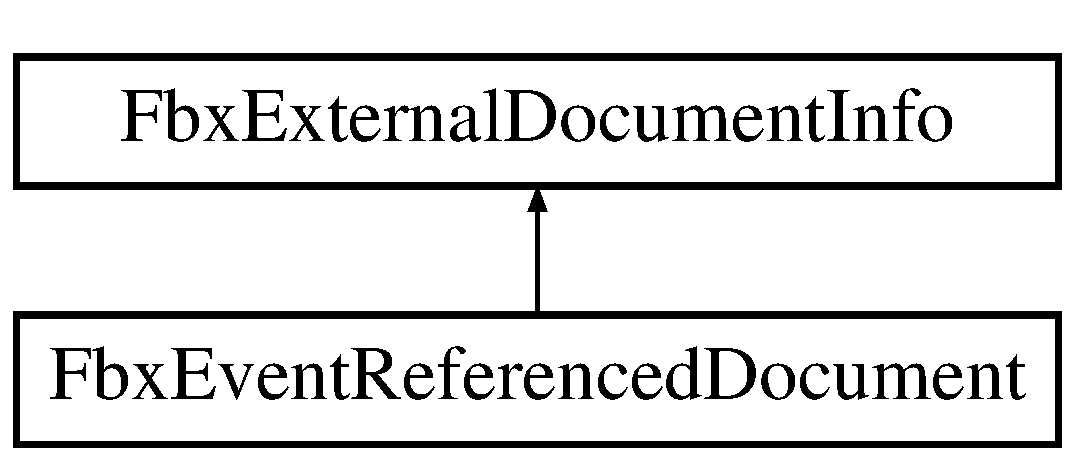
\includegraphics[height=2.000000cm]{struct_fbx_external_document_info}
\end{center}
\end{figure}
\subsection*{公開変数類}
\begin{DoxyCompactItemize}
\item 
\hyperlink{class_fbx_string}{Fbx\+String} \hyperlink{struct_fbx_external_document_info_a3744e27dd1ba48aa66b36c7e896cde89}{m\+Document\+Name}
\begin{DoxyCompactList}\small\item\em Bare name of external document in document hierarchy. \end{DoxyCompactList}\item 
\hyperlink{class_fbx_string}{Fbx\+String} \hyperlink{struct_fbx_external_document_info_a0dcde2cfd81d268f174c54c7eed46b8b}{m\+Class\+Name}
\begin{DoxyCompactList}\small\item\em Class name of the document (\hyperlink{class_fbx_document}{Fbx\+Document}, \hyperlink{class_fbx_library}{Fbx\+Library}...). \end{DoxyCompactList}\item 
\hyperlink{class_fbx_string}{Fbx\+String} \hyperlink{struct_fbx_external_document_info_ae677004de679e0106dcfea163f36079c}{m\+Parent\+Full\+Name}
\begin{DoxyCompactList}\small\item\em Full name of the parent document in document hierarchy. \end{DoxyCompactList}\item 
\hyperlink{class_fbx_string}{Fbx\+String} \hyperlink{struct_fbx_external_document_info_a65b555c9b2dc44bc63d65b3ae2c24cac}{m\+File\+Path\+Url}
\begin{DoxyCompactList}\small\item\em File path of the external document. \end{DoxyCompactList}\end{DoxyCompactItemize}


\subsection{詳解}
Contains data about an external document. The document is a \hyperlink{class_fbx_document}{Fbx\+Document} object. 

 fbxexternaldocreflistener.\+h の 25 行目に定義があります。



\subsection{メンバ詳解}
\mbox{\Hypertarget{struct_fbx_external_document_info_a0dcde2cfd81d268f174c54c7eed46b8b}\label{struct_fbx_external_document_info_a0dcde2cfd81d268f174c54c7eed46b8b}} 
\index{Fbx\+External\+Document\+Info@{Fbx\+External\+Document\+Info}!m\+Class\+Name@{m\+Class\+Name}}
\index{m\+Class\+Name@{m\+Class\+Name}!Fbx\+External\+Document\+Info@{Fbx\+External\+Document\+Info}}
\subsubsection{\texorpdfstring{m\+Class\+Name}{mClassName}}
{\footnotesize\ttfamily \hyperlink{class_fbx_string}{Fbx\+String} Fbx\+External\+Document\+Info\+::m\+Class\+Name}



Class name of the document (\hyperlink{class_fbx_document}{Fbx\+Document}, \hyperlink{class_fbx_library}{Fbx\+Library}...). 



 fbxexternaldocreflistener.\+h の 28 行目に定義があります。

\mbox{\Hypertarget{struct_fbx_external_document_info_a3744e27dd1ba48aa66b36c7e896cde89}\label{struct_fbx_external_document_info_a3744e27dd1ba48aa66b36c7e896cde89}} 
\index{Fbx\+External\+Document\+Info@{Fbx\+External\+Document\+Info}!m\+Document\+Name@{m\+Document\+Name}}
\index{m\+Document\+Name@{m\+Document\+Name}!Fbx\+External\+Document\+Info@{Fbx\+External\+Document\+Info}}
\subsubsection{\texorpdfstring{m\+Document\+Name}{mDocumentName}}
{\footnotesize\ttfamily \hyperlink{class_fbx_string}{Fbx\+String} Fbx\+External\+Document\+Info\+::m\+Document\+Name}



Bare name of external document in document hierarchy. 



 fbxexternaldocreflistener.\+h の 27 行目に定義があります。

\mbox{\Hypertarget{struct_fbx_external_document_info_a65b555c9b2dc44bc63d65b3ae2c24cac}\label{struct_fbx_external_document_info_a65b555c9b2dc44bc63d65b3ae2c24cac}} 
\index{Fbx\+External\+Document\+Info@{Fbx\+External\+Document\+Info}!m\+File\+Path\+Url@{m\+File\+Path\+Url}}
\index{m\+File\+Path\+Url@{m\+File\+Path\+Url}!Fbx\+External\+Document\+Info@{Fbx\+External\+Document\+Info}}
\subsubsection{\texorpdfstring{m\+File\+Path\+Url}{mFilePathUrl}}
{\footnotesize\ttfamily \hyperlink{class_fbx_string}{Fbx\+String} Fbx\+External\+Document\+Info\+::m\+File\+Path\+Url}



File path of the external document. 



 fbxexternaldocreflistener.\+h の 30 行目に定義があります。

\mbox{\Hypertarget{struct_fbx_external_document_info_ae677004de679e0106dcfea163f36079c}\label{struct_fbx_external_document_info_ae677004de679e0106dcfea163f36079c}} 
\index{Fbx\+External\+Document\+Info@{Fbx\+External\+Document\+Info}!m\+Parent\+Full\+Name@{m\+Parent\+Full\+Name}}
\index{m\+Parent\+Full\+Name@{m\+Parent\+Full\+Name}!Fbx\+External\+Document\+Info@{Fbx\+External\+Document\+Info}}
\subsubsection{\texorpdfstring{m\+Parent\+Full\+Name}{mParentFullName}}
{\footnotesize\ttfamily \hyperlink{class_fbx_string}{Fbx\+String} Fbx\+External\+Document\+Info\+::m\+Parent\+Full\+Name}



Full name of the parent document in document hierarchy. 



 fbxexternaldocreflistener.\+h の 29 行目に定義があります。



この構造体詳解は次のファイルから抽出されました\+:\begin{DoxyCompactItemize}
\item 
C\+:/\+Maya/scripts/\+F\+B\+X\+\_\+\+S\+D\+K/2017.\+1/include/fbxsdk/fileio/\hyperlink{fbxexternaldocreflistener_8h}{fbxexternaldocreflistener.\+h}\end{DoxyCompactItemize}

\hypertarget{class_fbx_file}{}\section{Fbx\+File クラス}
\label{class_fbx_file}\index{Fbx\+File@{Fbx\+File}}


{\ttfamily \#include $<$fbxfile.\+h$>$}

\subsection*{公開型}
\begin{DoxyCompactItemize}
\item 
enum \hyperlink{class_fbx_file_a0370e8fd17b3658f718e1350a6a6f462}{E\+Mode} \{ \newline
\hyperlink{class_fbx_file_a0370e8fd17b3658f718e1350a6a6f462a176e2ccdd9e671698ea8f6f16e41d906}{e\+None}, 
\hyperlink{class_fbx_file_a0370e8fd17b3658f718e1350a6a6f462a7b582fd52d7c01e076ef4d30d3ca7151}{e\+Read\+Only}, 
\hyperlink{class_fbx_file_a0370e8fd17b3658f718e1350a6a6f462a6210f903e353d976f304563453cf34da}{e\+Read\+Write}, 
\hyperlink{class_fbx_file_a0370e8fd17b3658f718e1350a6a6f462ae329198f644b68a3bbf655309eff07c9}{e\+Create\+Write\+Only}, 
\newline
\hyperlink{class_fbx_file_a0370e8fd17b3658f718e1350a6a6f462afce41267d2567926e7983b1193991a49}{e\+Create\+Read\+Write}, 
\hyperlink{class_fbx_file_a0370e8fd17b3658f718e1350a6a6f462a7b54172ce9f59ecc1746a4b6df0a064e}{e\+Create\+Append}
 \}
\item 
enum \hyperlink{class_fbx_file_aba91fe59f9c0a4c84a92f13c0c27deec}{E\+Seek\+Pos} \{ \hyperlink{class_fbx_file_aba91fe59f9c0a4c84a92f13c0c27deeca7a474ae0aa6f46b8becdfe54208f928e}{e\+Begin}, 
\hyperlink{class_fbx_file_aba91fe59f9c0a4c84a92f13c0c27deecaf2653dc9849e794feee37a015d80b098}{e\+Current}, 
\hyperlink{class_fbx_file_aba91fe59f9c0a4c84a92f13c0c27deeca1ab3eb84e8694fd4e63d0c864b12508d}{e\+End}
 \}
\end{DoxyCompactItemize}
\subsection*{公開メンバ関数}
\begin{DoxyCompactItemize}
\item 
\hyperlink{class_fbx_file_a863a523033dcdf07ad32c257c64d9e61}{Fbx\+File} ()
\item 
virtual \hyperlink{class_fbx_file_a2dd86a0057e7caa4865a92508cc9b56d}{$\sim$\+Fbx\+File} ()
\item 
virtual bool \hyperlink{class_fbx_file_a1942c2245eabf7f0507118226af13727}{Open} (const char $\ast$p\+File\+Name\+\_\+\+U\+T\+F8, const \hyperlink{class_fbx_file_a0370e8fd17b3658f718e1350a6a6f462}{E\+Mode} p\+Mode=\hyperlink{class_fbx_file_a0370e8fd17b3658f718e1350a6a6f462afce41267d2567926e7983b1193991a49}{e\+Create\+Read\+Write}, const bool p\+Binary=true)
\item 
virtual bool \hyperlink{class_fbx_file_a32456c88ed5a970971facea637ba96b1}{Open} (\hyperlink{class_fbx_stream}{Fbx\+Stream} $\ast$p\+Stream, void $\ast$p\+Stream\+Data, const char $\ast$p\+Mode)
\item 
virtual bool \hyperlink{class_fbx_file_ae8028a6bb80f3ebe4f6fcbaab367228b}{Close} ()
\item 
virtual void \hyperlink{class_fbx_file_af12434c7b2bf0cd193d3327180186901}{Seek} (const \hyperlink{fbxtypes_8h_ac7e1334c7c6aacc9c8a9dccddebb4368}{Fbx\+Int64} p\+Offset, const \hyperlink{class_fbx_file_aba91fe59f9c0a4c84a92f13c0c27deec}{E\+Seek\+Pos} p\+Seek\+Pos=\hyperlink{class_fbx_file_aba91fe59f9c0a4c84a92f13c0c27deeca7a474ae0aa6f46b8becdfe54208f928e}{e\+Begin})
\item 
virtual \hyperlink{fbxtypes_8h_ac7e1334c7c6aacc9c8a9dccddebb4368}{Fbx\+Int64} \hyperlink{class_fbx_file_aa32606ad8b5a8163f04c38b3020ec826}{Tell} () const
\item 
virtual size\+\_\+t \hyperlink{class_fbx_file_a9d2eb8ec7b9a877dd7aa9b2950287285}{Read} (void $\ast$p\+Dst\+Buf, const size\+\_\+t p\+Size)
\item 
virtual char $\ast$ \hyperlink{class_fbx_file_aad1b9e2c0f770ebfac6d00ebfc0927dd}{Read\+String} (char $\ast$p\+Dst\+Buf, const size\+\_\+t p\+Dst\+Size, bool p\+Stop\+At\+First\+White\+Space=false)
\item 
virtual size\+\_\+t \hyperlink{class_fbx_file_a8fff74d83402e939b69ac4c25a5bc689}{Write} (const void $\ast$p\+Src\+Buf, const size\+\_\+t p\+Size)
\item 
virtual bool \hyperlink{class_fbx_file_a64271cf33bdcd55d35502cd46ab910a5}{Write\+Format} (const char $\ast$p\+Format,...)
\item 
virtual bool \hyperlink{class_fbx_file_aa93638b789020857a19306175a921271}{Truncate} (const \hyperlink{fbxtypes_8h_ac7e1334c7c6aacc9c8a9dccddebb4368}{Fbx\+Int64} p\+Size)
\item 
virtual bool \hyperlink{class_fbx_file_a3e438294b7e07dbc3b672ba771ebdd51}{End\+Of\+File} () const
\item 
virtual \hyperlink{fbxtypes_8h_ac7e1334c7c6aacc9c8a9dccddebb4368}{Fbx\+Int64} \hyperlink{class_fbx_file_aa7d93faa5ec8ef431b6c9b82845e8271}{Get\+Size} ()
\item 
virtual void \hyperlink{class_fbx_file_ab603c8d30f989a0d195cc720181b18b3}{Get\+Memory\+File\+Info} (void $\ast$$\ast$p\+Mem\+Ptr, size\+\_\+t p\+Size)
\item 
bool \hyperlink{class_fbx_file_acf436397d99f8b7fb5baf5b32eac26b1}{Is\+Open} () const
\item 
bool \hyperlink{class_fbx_file_ae515a0ebd07a7ebedd0a62b5299cd417}{Is\+Stream} () const
\item 
const char $\ast$ \hyperlink{class_fbx_file_ace17e0fc453b1fa2f565af58eb16ad26}{Get\+File\+Path\+Name} () const
\item 
\hyperlink{class_fbx_file_a0370e8fd17b3658f718e1350a6a6f462}{E\+Mode} \hyperlink{class_fbx_file_a26175571d3f5682ea7af8ac5ba1f640f}{Get\+File\+Mode} () const
\item 
int \hyperlink{class_fbx_file_a797c6a169a44de27d96d991e884dafed}{Get\+Last\+Error} ()
\item 
void \hyperlink{class_fbx_file_abaf8e0ca1c1f47a349848ec49966cc6a}{Clear\+Error} ()
\end{DoxyCompactItemize}
\subsection*{限定公開変数類}
\begin{DoxyCompactItemize}
\item 
F\+I\+LE $\ast$ \hyperlink{class_fbx_file_a2be552f90b28c49c17626fe52309694a}{m\+File\+Ptr}
\item 
\hyperlink{class_fbx_stream}{Fbx\+Stream} $\ast$ \hyperlink{class_fbx_file_ad2c5d8c4cc9284b848f2283af005325f}{m\+Stream\+Ptr}
\item 
bool \hyperlink{class_fbx_file_a88370b753b3632ed4970357a2ec290d4}{m\+Is\+Open}
\item 
bool \hyperlink{class_fbx_file_ada5a1b024c0b9b67aede8605c4565013}{m\+Is\+Stream}
\item 
\hyperlink{class_fbx_file_a0370e8fd17b3658f718e1350a6a6f462}{E\+Mode} \hyperlink{class_fbx_file_ad9b7111817531ba69e1abddc7cc6d247}{m\+Mode}
\item 
\hyperlink{class_fbx_string}{Fbx\+String} \hyperlink{class_fbx_file_a47455f1ec52460e17c7a687f2e873128}{m\+File\+Name}
\end{DoxyCompactItemize}


\subsection{詳解}
Class for interfacing with files, providing a similar interface for files independant of the OS or filesystem. 

 fbxfile.\+h の 27 行目に定義があります。



\subsection{列挙型メンバ詳解}
\mbox{\Hypertarget{class_fbx_file_a0370e8fd17b3658f718e1350a6a6f462}\label{class_fbx_file_a0370e8fd17b3658f718e1350a6a6f462}} 
\index{Fbx\+File@{Fbx\+File}!E\+Mode@{E\+Mode}}
\index{E\+Mode@{E\+Mode}!Fbx\+File@{Fbx\+File}}
\subsubsection{\texorpdfstring{E\+Mode}{EMode}}
{\footnotesize\ttfamily enum \hyperlink{class_fbx_file_a0370e8fd17b3658f718e1350a6a6f462}{Fbx\+File\+::\+E\+Mode}}

\begin{DoxyEnumFields}{列挙値}
\raisebox{\heightof{T}}[0pt][0pt]{\index{e\+None@{e\+None}!Fbx\+File@{Fbx\+File}}\index{Fbx\+File@{Fbx\+File}!e\+None@{e\+None}}}\mbox{\Hypertarget{class_fbx_file_a0370e8fd17b3658f718e1350a6a6f462a176e2ccdd9e671698ea8f6f16e41d906}\label{class_fbx_file_a0370e8fd17b3658f718e1350a6a6f462a176e2ccdd9e671698ea8f6f16e41d906}} 
e\+None&\\
\hline

\raisebox{\heightof{T}}[0pt][0pt]{\index{e\+Read\+Only@{e\+Read\+Only}!Fbx\+File@{Fbx\+File}}\index{Fbx\+File@{Fbx\+File}!e\+Read\+Only@{e\+Read\+Only}}}\mbox{\Hypertarget{class_fbx_file_a0370e8fd17b3658f718e1350a6a6f462a7b582fd52d7c01e076ef4d30d3ca7151}\label{class_fbx_file_a0370e8fd17b3658f718e1350a6a6f462a7b582fd52d7c01e076ef4d30d3ca7151}} 
e\+Read\+Only&\\
\hline

\raisebox{\heightof{T}}[0pt][0pt]{\index{e\+Read\+Write@{e\+Read\+Write}!Fbx\+File@{Fbx\+File}}\index{Fbx\+File@{Fbx\+File}!e\+Read\+Write@{e\+Read\+Write}}}\mbox{\Hypertarget{class_fbx_file_a0370e8fd17b3658f718e1350a6a6f462a6210f903e353d976f304563453cf34da}\label{class_fbx_file_a0370e8fd17b3658f718e1350a6a6f462a6210f903e353d976f304563453cf34da}} 
e\+Read\+Write&\\
\hline

\raisebox{\heightof{T}}[0pt][0pt]{\index{e\+Create\+Write\+Only@{e\+Create\+Write\+Only}!Fbx\+File@{Fbx\+File}}\index{Fbx\+File@{Fbx\+File}!e\+Create\+Write\+Only@{e\+Create\+Write\+Only}}}\mbox{\Hypertarget{class_fbx_file_a0370e8fd17b3658f718e1350a6a6f462ae329198f644b68a3bbf655309eff07c9}\label{class_fbx_file_a0370e8fd17b3658f718e1350a6a6f462ae329198f644b68a3bbf655309eff07c9}} 
e\+Create\+Write\+Only&\\
\hline

\raisebox{\heightof{T}}[0pt][0pt]{\index{e\+Create\+Read\+Write@{e\+Create\+Read\+Write}!Fbx\+File@{Fbx\+File}}\index{Fbx\+File@{Fbx\+File}!e\+Create\+Read\+Write@{e\+Create\+Read\+Write}}}\mbox{\Hypertarget{class_fbx_file_a0370e8fd17b3658f718e1350a6a6f462afce41267d2567926e7983b1193991a49}\label{class_fbx_file_a0370e8fd17b3658f718e1350a6a6f462afce41267d2567926e7983b1193991a49}} 
e\+Create\+Read\+Write&\\
\hline

\raisebox{\heightof{T}}[0pt][0pt]{\index{e\+Create\+Append@{e\+Create\+Append}!Fbx\+File@{Fbx\+File}}\index{Fbx\+File@{Fbx\+File}!e\+Create\+Append@{e\+Create\+Append}}}\mbox{\Hypertarget{class_fbx_file_a0370e8fd17b3658f718e1350a6a6f462a7b54172ce9f59ecc1746a4b6df0a064e}\label{class_fbx_file_a0370e8fd17b3658f718e1350a6a6f462a7b54172ce9f59ecc1746a4b6df0a064e}} 
e\+Create\+Append&\\
\hline

\end{DoxyEnumFields}


 fbxfile.\+h の 30 行目に定義があります。

\mbox{\Hypertarget{class_fbx_file_aba91fe59f9c0a4c84a92f13c0c27deec}\label{class_fbx_file_aba91fe59f9c0a4c84a92f13c0c27deec}} 
\index{Fbx\+File@{Fbx\+File}!E\+Seek\+Pos@{E\+Seek\+Pos}}
\index{E\+Seek\+Pos@{E\+Seek\+Pos}!Fbx\+File@{Fbx\+File}}
\subsubsection{\texorpdfstring{E\+Seek\+Pos}{ESeekPos}}
{\footnotesize\ttfamily enum \hyperlink{class_fbx_file_aba91fe59f9c0a4c84a92f13c0c27deec}{Fbx\+File\+::\+E\+Seek\+Pos}}

\begin{DoxyEnumFields}{列挙値}
\raisebox{\heightof{T}}[0pt][0pt]{\index{e\+Begin@{e\+Begin}!Fbx\+File@{Fbx\+File}}\index{Fbx\+File@{Fbx\+File}!e\+Begin@{e\+Begin}}}\mbox{\Hypertarget{class_fbx_file_aba91fe59f9c0a4c84a92f13c0c27deeca7a474ae0aa6f46b8becdfe54208f928e}\label{class_fbx_file_aba91fe59f9c0a4c84a92f13c0c27deeca7a474ae0aa6f46b8becdfe54208f928e}} 
e\+Begin&\\
\hline

\raisebox{\heightof{T}}[0pt][0pt]{\index{e\+Current@{e\+Current}!Fbx\+File@{Fbx\+File}}\index{Fbx\+File@{Fbx\+File}!e\+Current@{e\+Current}}}\mbox{\Hypertarget{class_fbx_file_aba91fe59f9c0a4c84a92f13c0c27deecaf2653dc9849e794feee37a015d80b098}\label{class_fbx_file_aba91fe59f9c0a4c84a92f13c0c27deecaf2653dc9849e794feee37a015d80b098}} 
e\+Current&\\
\hline

\raisebox{\heightof{T}}[0pt][0pt]{\index{e\+End@{e\+End}!Fbx\+File@{Fbx\+File}}\index{Fbx\+File@{Fbx\+File}!e\+End@{e\+End}}}\mbox{\Hypertarget{class_fbx_file_aba91fe59f9c0a4c84a92f13c0c27deeca1ab3eb84e8694fd4e63d0c864b12508d}\label{class_fbx_file_aba91fe59f9c0a4c84a92f13c0c27deeca1ab3eb84e8694fd4e63d0c864b12508d}} 
e\+End&\\
\hline

\end{DoxyEnumFields}


 fbxfile.\+h の 31 行目に定義があります。



\subsection{構築子と解体子}
\mbox{\Hypertarget{class_fbx_file_a863a523033dcdf07ad32c257c64d9e61}\label{class_fbx_file_a863a523033dcdf07ad32c257c64d9e61}} 
\index{Fbx\+File@{Fbx\+File}!Fbx\+File@{Fbx\+File}}
\index{Fbx\+File@{Fbx\+File}!Fbx\+File@{Fbx\+File}}
\subsubsection{\texorpdfstring{Fbx\+File()}{FbxFile()}}
{\footnotesize\ttfamily Fbx\+File\+::\+Fbx\+File (\begin{DoxyParamCaption}{ }\end{DoxyParamCaption})}

\mbox{\Hypertarget{class_fbx_file_a2dd86a0057e7caa4865a92508cc9b56d}\label{class_fbx_file_a2dd86a0057e7caa4865a92508cc9b56d}} 
\index{Fbx\+File@{Fbx\+File}!````~Fbx\+File@{$\sim$\+Fbx\+File}}
\index{````~Fbx\+File@{$\sim$\+Fbx\+File}!Fbx\+File@{Fbx\+File}}
\subsubsection{\texorpdfstring{$\sim$\+Fbx\+File()}{~FbxFile()}}
{\footnotesize\ttfamily virtual Fbx\+File\+::$\sim$\+Fbx\+File (\begin{DoxyParamCaption}{ }\end{DoxyParamCaption})\hspace{0.3cm}{\ttfamily [virtual]}}



\subsection{関数詳解}
\mbox{\Hypertarget{class_fbx_file_abaf8e0ca1c1f47a349848ec49966cc6a}\label{class_fbx_file_abaf8e0ca1c1f47a349848ec49966cc6a}} 
\index{Fbx\+File@{Fbx\+File}!Clear\+Error@{Clear\+Error}}
\index{Clear\+Error@{Clear\+Error}!Fbx\+File@{Fbx\+File}}
\subsubsection{\texorpdfstring{Clear\+Error()}{ClearError()}}
{\footnotesize\ttfamily void Fbx\+File\+::\+Clear\+Error (\begin{DoxyParamCaption}{ }\end{DoxyParamCaption})}

Resets the current error code and the end of file indicator of the opened file \mbox{\Hypertarget{class_fbx_file_ae8028a6bb80f3ebe4f6fcbaab367228b}\label{class_fbx_file_ae8028a6bb80f3ebe4f6fcbaab367228b}} 
\index{Fbx\+File@{Fbx\+File}!Close@{Close}}
\index{Close@{Close}!Fbx\+File@{Fbx\+File}}
\subsubsection{\texorpdfstring{Close()}{Close()}}
{\footnotesize\ttfamily virtual bool Fbx\+File\+::\+Close (\begin{DoxyParamCaption}{ }\end{DoxyParamCaption})\hspace{0.3cm}{\ttfamily [virtual]}}

Closes a file, freeing its handle. \begin{DoxyReturn}{戻り値}
True if closing is successful. 
\end{DoxyReturn}
\mbox{\Hypertarget{class_fbx_file_a3e438294b7e07dbc3b672ba771ebdd51}\label{class_fbx_file_a3e438294b7e07dbc3b672ba771ebdd51}} 
\index{Fbx\+File@{Fbx\+File}!End\+Of\+File@{End\+Of\+File}}
\index{End\+Of\+File@{End\+Of\+File}!Fbx\+File@{Fbx\+File}}
\subsubsection{\texorpdfstring{End\+Of\+File()}{EndOfFile()}}
{\footnotesize\ttfamily virtual bool Fbx\+File\+::\+End\+Of\+File (\begin{DoxyParamCaption}{ }\end{DoxyParamCaption}) const\hspace{0.3cm}{\ttfamily [virtual]}}

Checks whether the current file cursor position is at the end of file. \begin{DoxyReturn}{戻り値}
True if the cursor is at the end of file, false otherwise. 
\end{DoxyReturn}
\mbox{\Hypertarget{class_fbx_file_a26175571d3f5682ea7af8ac5ba1f640f}\label{class_fbx_file_a26175571d3f5682ea7af8ac5ba1f640f}} 
\index{Fbx\+File@{Fbx\+File}!Get\+File\+Mode@{Get\+File\+Mode}}
\index{Get\+File\+Mode@{Get\+File\+Mode}!Fbx\+File@{Fbx\+File}}
\subsubsection{\texorpdfstring{Get\+File\+Mode()}{GetFileMode()}}
{\footnotesize\ttfamily \hyperlink{class_fbx_file_a0370e8fd17b3658f718e1350a6a6f462}{E\+Mode} Fbx\+File\+::\+Get\+File\+Mode (\begin{DoxyParamCaption}{ }\end{DoxyParamCaption}) const}

Returns the mode with which the file was opened, when calling the \hyperlink{class_fbx_file_a1942c2245eabf7f0507118226af13727}{Open()} method. \begin{DoxyReturn}{戻り値}
Mode with which the file was opened 
\end{DoxyReturn}
\mbox{\Hypertarget{class_fbx_file_ace17e0fc453b1fa2f565af58eb16ad26}\label{class_fbx_file_ace17e0fc453b1fa2f565af58eb16ad26}} 
\index{Fbx\+File@{Fbx\+File}!Get\+File\+Path\+Name@{Get\+File\+Path\+Name}}
\index{Get\+File\+Path\+Name@{Get\+File\+Path\+Name}!Fbx\+File@{Fbx\+File}}
\subsubsection{\texorpdfstring{Get\+File\+Path\+Name()}{GetFilePathName()}}
{\footnotesize\ttfamily const char$\ast$ Fbx\+File\+::\+Get\+File\+Path\+Name (\begin{DoxyParamCaption}{ }\end{DoxyParamCaption}) const}

Returns the full file path name, as provided when opening it. \begin{DoxyReturn}{戻り値}
File full path 
\end{DoxyReturn}
\mbox{\Hypertarget{class_fbx_file_a797c6a169a44de27d96d991e884dafed}\label{class_fbx_file_a797c6a169a44de27d96d991e884dafed}} 
\index{Fbx\+File@{Fbx\+File}!Get\+Last\+Error@{Get\+Last\+Error}}
\index{Get\+Last\+Error@{Get\+Last\+Error}!Fbx\+File@{Fbx\+File}}
\subsubsection{\texorpdfstring{Get\+Last\+Error()}{GetLastError()}}
{\footnotesize\ttfamily int Fbx\+File\+::\+Get\+Last\+Error (\begin{DoxyParamCaption}{ }\end{DoxyParamCaption})}

Returns last encountered error when performing any operation on the file. \begin{DoxyReturn}{戻り値}
Last error code 
\end{DoxyReturn}
\mbox{\Hypertarget{class_fbx_file_ab603c8d30f989a0d195cc720181b18b3}\label{class_fbx_file_ab603c8d30f989a0d195cc720181b18b3}} 
\index{Fbx\+File@{Fbx\+File}!Get\+Memory\+File\+Info@{Get\+Memory\+File\+Info}}
\index{Get\+Memory\+File\+Info@{Get\+Memory\+File\+Info}!Fbx\+File@{Fbx\+File}}
\subsubsection{\texorpdfstring{Get\+Memory\+File\+Info()}{GetMemoryFileInfo()}}
{\footnotesize\ttfamily virtual void Fbx\+File\+::\+Get\+Memory\+File\+Info (\begin{DoxyParamCaption}\item[{void $\ast$$\ast$}]{p\+Mem\+Ptr,  }\item[{size\+\_\+t}]{p\+Size }\end{DoxyParamCaption})\hspace{0.3cm}{\ttfamily [virtual]}}

Unused function in this default implementation. Must be implemented by memory files. 
\begin{DoxyParams}{引数}
{\em p\+Mem\+Ptr} & Unused \\
\hline
{\em p\+Size} & Unused \\
\hline
\end{DoxyParams}
\mbox{\Hypertarget{class_fbx_file_aa7d93faa5ec8ef431b6c9b82845e8271}\label{class_fbx_file_aa7d93faa5ec8ef431b6c9b82845e8271}} 
\index{Fbx\+File@{Fbx\+File}!Get\+Size@{Get\+Size}}
\index{Get\+Size@{Get\+Size}!Fbx\+File@{Fbx\+File}}
\subsubsection{\texorpdfstring{Get\+Size()}{GetSize()}}
{\footnotesize\ttfamily virtual \hyperlink{fbxtypes_8h_ac7e1334c7c6aacc9c8a9dccddebb4368}{Fbx\+Int64} Fbx\+File\+::\+Get\+Size (\begin{DoxyParamCaption}{ }\end{DoxyParamCaption})\hspace{0.3cm}{\ttfamily [virtual]}}

Gets the size of the currently opened file. \begin{DoxyReturn}{戻り値}
File size 
\end{DoxyReturn}
\mbox{\Hypertarget{class_fbx_file_acf436397d99f8b7fb5baf5b32eac26b1}\label{class_fbx_file_acf436397d99f8b7fb5baf5b32eac26b1}} 
\index{Fbx\+File@{Fbx\+File}!Is\+Open@{Is\+Open}}
\index{Is\+Open@{Is\+Open}!Fbx\+File@{Fbx\+File}}
\subsubsection{\texorpdfstring{Is\+Open()}{IsOpen()}}
{\footnotesize\ttfamily bool Fbx\+File\+::\+Is\+Open (\begin{DoxyParamCaption}{ }\end{DoxyParamCaption}) const}

Checks whether the file is currently opened. \begin{DoxyReturn}{戻り値}
True if file is opened, false otherwise 
\end{DoxyReturn}
\mbox{\Hypertarget{class_fbx_file_ae515a0ebd07a7ebedd0a62b5299cd417}\label{class_fbx_file_ae515a0ebd07a7ebedd0a62b5299cd417}} 
\index{Fbx\+File@{Fbx\+File}!Is\+Stream@{Is\+Stream}}
\index{Is\+Stream@{Is\+Stream}!Fbx\+File@{Fbx\+File}}
\subsubsection{\texorpdfstring{Is\+Stream()}{IsStream()}}
{\footnotesize\ttfamily bool Fbx\+File\+::\+Is\+Stream (\begin{DoxyParamCaption}{ }\end{DoxyParamCaption}) const}

Checks whether the file is currently opened with a user-\/provided streaming interface instead of just the file name \begin{DoxyReturn}{戻り値}
True if file has been opened with a stream interface, false otherwise 
\end{DoxyReturn}
\mbox{\Hypertarget{class_fbx_file_a1942c2245eabf7f0507118226af13727}\label{class_fbx_file_a1942c2245eabf7f0507118226af13727}} 
\index{Fbx\+File@{Fbx\+File}!Open@{Open}}
\index{Open@{Open}!Fbx\+File@{Fbx\+File}}
\subsubsection{\texorpdfstring{Open()}{Open()}\hspace{0.1cm}{\footnotesize\ttfamily [1/2]}}
{\footnotesize\ttfamily virtual bool Fbx\+File\+::\+Open (\begin{DoxyParamCaption}\item[{const char $\ast$}]{p\+File\+Name\+\_\+\+U\+T\+F8,  }\item[{const \hyperlink{class_fbx_file_a0370e8fd17b3658f718e1350a6a6f462}{E\+Mode}}]{p\+Mode = {\ttfamily \hyperlink{class_fbx_file_a0370e8fd17b3658f718e1350a6a6f462afce41267d2567926e7983b1193991a49}{e\+Create\+Read\+Write}},  }\item[{const bool}]{p\+Binary = {\ttfamily true} }\end{DoxyParamCaption})\hspace{0.3cm}{\ttfamily [virtual]}}

Opens a file on disk using the specified read/write mode. 
\begin{DoxyParams}{引数}
{\em p\+File\+Name\+\_\+\+U\+T\+F8} & Filename in U\+T\+F8 (compatible with A\+S\+C\+II) \\
\hline
{\em p\+Mode} & Mode in which to open the file, e.\+g. e\+Read\+Only, e\+Create\+Read\+Write, etc. \\
\hline
{\em p\+Binary} & Whether the file is to be opened in binary or text mode. \\
\hline
\end{DoxyParams}
\begin{DoxyReturn}{戻り値}
True if opening is successful. 
\end{DoxyReturn}
\mbox{\Hypertarget{class_fbx_file_a32456c88ed5a970971facea637ba96b1}\label{class_fbx_file_a32456c88ed5a970971facea637ba96b1}} 
\index{Fbx\+File@{Fbx\+File}!Open@{Open}}
\index{Open@{Open}!Fbx\+File@{Fbx\+File}}
\subsubsection{\texorpdfstring{Open()}{Open()}\hspace{0.1cm}{\footnotesize\ttfamily [2/2]}}
{\footnotesize\ttfamily virtual bool Fbx\+File\+::\+Open (\begin{DoxyParamCaption}\item[{\hyperlink{class_fbx_stream}{Fbx\+Stream} $\ast$}]{p\+Stream,  }\item[{void $\ast$}]{p\+Stream\+Data,  }\item[{const char $\ast$}]{p\+Mode }\end{DoxyParamCaption})\hspace{0.3cm}{\ttfamily [virtual]}}

Opens a file from a data stream using the specified read/write mode. 
\begin{DoxyParams}{引数}
{\em p\+Stream} & Stream instance with which the file will be read/written \\
\hline
{\em p\+Stream\+Data} & User-\/defined data to pass as a parameter to the stream\textquotesingle{}s \hyperlink{class_fbx_file_a1942c2245eabf7f0507118226af13727}{Open()} method. \\
\hline
{\em p\+Mode} & Deprecated/\+Unused. \\
\hline
\end{DoxyParams}
\begin{DoxyReturn}{戻り値}
True if opening is successful. 
\end{DoxyReturn}
\mbox{\Hypertarget{class_fbx_file_a9d2eb8ec7b9a877dd7aa9b2950287285}\label{class_fbx_file_a9d2eb8ec7b9a877dd7aa9b2950287285}} 
\index{Fbx\+File@{Fbx\+File}!Read@{Read}}
\index{Read@{Read}!Fbx\+File@{Fbx\+File}}
\subsubsection{\texorpdfstring{Read()}{Read()}}
{\footnotesize\ttfamily virtual size\+\_\+t Fbx\+File\+::\+Read (\begin{DoxyParamCaption}\item[{void $\ast$}]{p\+Dst\+Buf,  }\item[{const size\+\_\+t}]{p\+Size }\end{DoxyParamCaption})\hspace{0.3cm}{\ttfamily [virtual]}}

Read a part of the file into a buffer 
\begin{DoxyParams}{引数}
{\em p\+Dst\+Buf} & Pre-\/allocated buffer in which to read data \\
\hline
{\em p\+Size} & Size of the data chunk to be read in bytes \\
\hline
\end{DoxyParams}
\begin{DoxyReturn}{戻り値}
Number of bytes read. 
\end{DoxyReturn}
\mbox{\Hypertarget{class_fbx_file_aad1b9e2c0f770ebfac6d00ebfc0927dd}\label{class_fbx_file_aad1b9e2c0f770ebfac6d00ebfc0927dd}} 
\index{Fbx\+File@{Fbx\+File}!Read\+String@{Read\+String}}
\index{Read\+String@{Read\+String}!Fbx\+File@{Fbx\+File}}
\subsubsection{\texorpdfstring{Read\+String()}{ReadString()}}
{\footnotesize\ttfamily virtual char$\ast$ Fbx\+File\+::\+Read\+String (\begin{DoxyParamCaption}\item[{char $\ast$}]{p\+Dst\+Buf,  }\item[{const size\+\_\+t}]{p\+Dst\+Size,  }\item[{bool}]{p\+Stop\+At\+First\+White\+Space = {\ttfamily false} }\end{DoxyParamCaption})\hspace{0.3cm}{\ttfamily [virtual]}}

Read a part of the file as a string into a buffer 
\begin{DoxyParams}{引数}
{\em p\+Dst\+Buf} & Pre-\/allocated buffer in which to read the string \\
\hline
{\em p\+Dst\+Size} & Size of the data chunk to be read in characters \\
\hline
{\em p\+Stop\+At\+First\+White\+Space} & If true, will stop reading at first white space, otherwise it will stop at the first line feed (~\newline
) \\
\hline
\end{DoxyParams}
\begin{DoxyReturn}{戻り値}
Pointer on the data read. Equivalent to parameter p\+Dst\+Buf 
\end{DoxyReturn}
\mbox{\Hypertarget{class_fbx_file_af12434c7b2bf0cd193d3327180186901}\label{class_fbx_file_af12434c7b2bf0cd193d3327180186901}} 
\index{Fbx\+File@{Fbx\+File}!Seek@{Seek}}
\index{Seek@{Seek}!Fbx\+File@{Fbx\+File}}
\subsubsection{\texorpdfstring{Seek()}{Seek()}}
{\footnotesize\ttfamily virtual void Fbx\+File\+::\+Seek (\begin{DoxyParamCaption}\item[{const \hyperlink{fbxtypes_8h_ac7e1334c7c6aacc9c8a9dccddebb4368}{Fbx\+Int64}}]{p\+Offset,  }\item[{const \hyperlink{class_fbx_file_aba91fe59f9c0a4c84a92f13c0c27deec}{E\+Seek\+Pos}}]{p\+Seek\+Pos = {\ttfamily \hyperlink{class_fbx_file_aba91fe59f9c0a4c84a92f13c0c27deeca7a474ae0aa6f46b8becdfe54208f928e}{e\+Begin}} }\end{DoxyParamCaption})\hspace{0.3cm}{\ttfamily [virtual]}}

Seek to a specific position in the file, starting from either beginning, current position or end 
\begin{DoxyParams}{引数}
{\em p\+Offset} & Offset to seek to (advance the file position cursor) starting from p\+Seek\+Pos \\
\hline
{\em p\+Seek\+Pos} & Starting position from which to seek to. Beginning, current position or end. \\
\hline
\end{DoxyParams}
\mbox{\Hypertarget{class_fbx_file_aa32606ad8b5a8163f04c38b3020ec826}\label{class_fbx_file_aa32606ad8b5a8163f04c38b3020ec826}} 
\index{Fbx\+File@{Fbx\+File}!Tell@{Tell}}
\index{Tell@{Tell}!Fbx\+File@{Fbx\+File}}
\subsubsection{\texorpdfstring{Tell()}{Tell()}}
{\footnotesize\ttfamily virtual \hyperlink{fbxtypes_8h_ac7e1334c7c6aacc9c8a9dccddebb4368}{Fbx\+Int64} Fbx\+File\+::\+Tell (\begin{DoxyParamCaption}{ }\end{DoxyParamCaption}) const\hspace{0.3cm}{\ttfamily [virtual]}}

Returns the position at which the file cursor currently is. For example, will be ==0 for beginning and ==File\+Size for end. \begin{DoxyReturn}{戻り値}
The position at which the file cursor currently is. 
\end{DoxyReturn}
\mbox{\Hypertarget{class_fbx_file_aa93638b789020857a19306175a921271}\label{class_fbx_file_aa93638b789020857a19306175a921271}} 
\index{Fbx\+File@{Fbx\+File}!Truncate@{Truncate}}
\index{Truncate@{Truncate}!Fbx\+File@{Fbx\+File}}
\subsubsection{\texorpdfstring{Truncate()}{Truncate()}}
{\footnotesize\ttfamily virtual bool Fbx\+File\+::\+Truncate (\begin{DoxyParamCaption}\item[{const \hyperlink{fbxtypes_8h_ac7e1334c7c6aacc9c8a9dccddebb4368}{Fbx\+Int64}}]{p\+Size }\end{DoxyParamCaption})\hspace{0.3cm}{\ttfamily [virtual]}}

Modify the size of a file. Null characters (\textquotesingle{}\textbackslash{}0\textquotesingle{}) are appended if the file is extended. If the file is truncated, all data from the end of the shortened file to the original length of the file is lost. Please note that this function considers the current file cursor as the beginning of the file. It is therefore required to use Seek(0) prior to calling it if we want the size specified by the p\+Size parameter to be absolute. 
\begin{DoxyParams}{引数}
{\em p\+Size} & New desired file size \\
\hline
\end{DoxyParams}
\begin{DoxyReturn}{戻り値}
True if file was successfully truncated 
\end{DoxyReturn}
\mbox{\Hypertarget{class_fbx_file_a8fff74d83402e939b69ac4c25a5bc689}\label{class_fbx_file_a8fff74d83402e939b69ac4c25a5bc689}} 
\index{Fbx\+File@{Fbx\+File}!Write@{Write}}
\index{Write@{Write}!Fbx\+File@{Fbx\+File}}
\subsubsection{\texorpdfstring{Write()}{Write()}}
{\footnotesize\ttfamily virtual size\+\_\+t Fbx\+File\+::\+Write (\begin{DoxyParamCaption}\item[{const void $\ast$}]{p\+Src\+Buf,  }\item[{const size\+\_\+t}]{p\+Size }\end{DoxyParamCaption})\hspace{0.3cm}{\ttfamily [virtual]}}

Write a buffer to an opened file 
\begin{DoxyParams}{引数}
{\em p\+Src\+Buf} & Pre-\/allocated buffer from which to write data \\
\hline
{\em p\+Size} & Size of the data chunk to be written in bytes \\
\hline
\end{DoxyParams}
\begin{DoxyReturn}{戻り値}
Number of bytes written. 
\end{DoxyReturn}
\mbox{\Hypertarget{class_fbx_file_a64271cf33bdcd55d35502cd46ab910a5}\label{class_fbx_file_a64271cf33bdcd55d35502cd46ab910a5}} 
\index{Fbx\+File@{Fbx\+File}!Write\+Format@{Write\+Format}}
\index{Write\+Format@{Write\+Format}!Fbx\+File@{Fbx\+File}}
\subsubsection{\texorpdfstring{Write\+Format()}{WriteFormat()}}
{\footnotesize\ttfamily virtual bool Fbx\+File\+::\+Write\+Format (\begin{DoxyParamCaption}\item[{const char $\ast$}]{p\+Format,  }\item[{}]{... }\end{DoxyParamCaption})\hspace{0.3cm}{\ttfamily [virtual]}}

Write a formatted string to an opened file 
\begin{DoxyParams}{引数}
{\em p\+Format} & Pre-\/allocated format buffer from which to write data \\
\hline
{\em ...} & Variable number of arguments describing the values in the previous parameter. \\
\hline
\end{DoxyParams}
\begin{DoxyReturn}{戻り値}
True if data was successfully written 
\end{DoxyReturn}


\subsection{メンバ詳解}
\mbox{\Hypertarget{class_fbx_file_a47455f1ec52460e17c7a687f2e873128}\label{class_fbx_file_a47455f1ec52460e17c7a687f2e873128}} 
\index{Fbx\+File@{Fbx\+File}!m\+File\+Name@{m\+File\+Name}}
\index{m\+File\+Name@{m\+File\+Name}!Fbx\+File@{Fbx\+File}}
\subsubsection{\texorpdfstring{m\+File\+Name}{mFileName}}
{\footnotesize\ttfamily \hyperlink{class_fbx_string}{Fbx\+String} Fbx\+File\+::m\+File\+Name\hspace{0.3cm}{\ttfamily [protected]}}



 fbxfile.\+h の 158 行目に定義があります。

\mbox{\Hypertarget{class_fbx_file_a2be552f90b28c49c17626fe52309694a}\label{class_fbx_file_a2be552f90b28c49c17626fe52309694a}} 
\index{Fbx\+File@{Fbx\+File}!m\+File\+Ptr@{m\+File\+Ptr}}
\index{m\+File\+Ptr@{m\+File\+Ptr}!Fbx\+File@{Fbx\+File}}
\subsubsection{\texorpdfstring{m\+File\+Ptr}{mFilePtr}}
{\footnotesize\ttfamily F\+I\+LE$\ast$ Fbx\+File\+::m\+File\+Ptr\hspace{0.3cm}{\ttfamily [protected]}}



 fbxfile.\+h の 153 行目に定義があります。

\mbox{\Hypertarget{class_fbx_file_a88370b753b3632ed4970357a2ec290d4}\label{class_fbx_file_a88370b753b3632ed4970357a2ec290d4}} 
\index{Fbx\+File@{Fbx\+File}!m\+Is\+Open@{m\+Is\+Open}}
\index{m\+Is\+Open@{m\+Is\+Open}!Fbx\+File@{Fbx\+File}}
\subsubsection{\texorpdfstring{m\+Is\+Open}{mIsOpen}}
{\footnotesize\ttfamily bool Fbx\+File\+::m\+Is\+Open\hspace{0.3cm}{\ttfamily [protected]}}



 fbxfile.\+h の 155 行目に定義があります。

\mbox{\Hypertarget{class_fbx_file_ada5a1b024c0b9b67aede8605c4565013}\label{class_fbx_file_ada5a1b024c0b9b67aede8605c4565013}} 
\index{Fbx\+File@{Fbx\+File}!m\+Is\+Stream@{m\+Is\+Stream}}
\index{m\+Is\+Stream@{m\+Is\+Stream}!Fbx\+File@{Fbx\+File}}
\subsubsection{\texorpdfstring{m\+Is\+Stream}{mIsStream}}
{\footnotesize\ttfamily bool Fbx\+File\+::m\+Is\+Stream\hspace{0.3cm}{\ttfamily [protected]}}



 fbxfile.\+h の 156 行目に定義があります。

\mbox{\Hypertarget{class_fbx_file_ad9b7111817531ba69e1abddc7cc6d247}\label{class_fbx_file_ad9b7111817531ba69e1abddc7cc6d247}} 
\index{Fbx\+File@{Fbx\+File}!m\+Mode@{m\+Mode}}
\index{m\+Mode@{m\+Mode}!Fbx\+File@{Fbx\+File}}
\subsubsection{\texorpdfstring{m\+Mode}{mMode}}
{\footnotesize\ttfamily \hyperlink{class_fbx_file_a0370e8fd17b3658f718e1350a6a6f462}{E\+Mode} Fbx\+File\+::m\+Mode\hspace{0.3cm}{\ttfamily [protected]}}



 fbxfile.\+h の 157 行目に定義があります。

\mbox{\Hypertarget{class_fbx_file_ad2c5d8c4cc9284b848f2283af005325f}\label{class_fbx_file_ad2c5d8c4cc9284b848f2283af005325f}} 
\index{Fbx\+File@{Fbx\+File}!m\+Stream\+Ptr@{m\+Stream\+Ptr}}
\index{m\+Stream\+Ptr@{m\+Stream\+Ptr}!Fbx\+File@{Fbx\+File}}
\subsubsection{\texorpdfstring{m\+Stream\+Ptr}{mStreamPtr}}
{\footnotesize\ttfamily \hyperlink{class_fbx_stream}{Fbx\+Stream}$\ast$ Fbx\+File\+::m\+Stream\+Ptr\hspace{0.3cm}{\ttfamily [protected]}}



 fbxfile.\+h の 154 行目に定義があります。



このクラス詳解は次のファイルから抽出されました\+:\begin{DoxyCompactItemize}
\item 
C\+:/\+Maya/scripts/\+F\+B\+X\+\_\+\+S\+D\+K/2017.\+1/include/fbxsdk/core/base/\hyperlink{fbxfile_8h}{fbxfile.\+h}\end{DoxyCompactItemize}

\hypertarget{class_fbx_file_texture}{}\section{Fbx\+File\+Texture クラス}
\label{class_fbx_file_texture}\index{Fbx\+File\+Texture@{Fbx\+File\+Texture}}


{\ttfamily \#include $<$fbxfiletexture.\+h$>$}



Fbx\+File\+Texture の継承関係図
% FIG 0


Fbx\+File\+Texture 連携図
% FIG 1
\subsection*{公開メンバ関数}
\begin{DoxyCompactItemize}
\item 
virtual \hyperlink{class_fbx_object}{Fbx\+Object} \& \hyperlink{class_fbx_file_texture_a4ef7372132caebc8d1e5992efb894c9d}{Copy} (const \hyperlink{class_fbx_object}{Fbx\+Object} \&p\+Object)
\item 
bool \hyperlink{class_fbx_file_texture_ab2c5320676da40e302a20ef30326d11a}{operator==} (\hyperlink{class_fbx_file_texture}{Fbx\+File\+Texture} const \&p\+Texture) const
\item 
\hyperlink{class_fbx_string}{Fbx\+String} \& \hyperlink{class_fbx_file_texture_afbd2a201ca55d31987446e33133f53cd}{Get\+Media\+Name} ()
\item 
void \hyperlink{class_fbx_file_texture_a08163cb0f5af0e9dee35a1e758618cad}{Set\+Media\+Name} (const char $\ast$p\+Media\+Name)
\end{DoxyCompactItemize}
\subsection*{限定公開メンバ関数}
\begin{DoxyCompactItemize}
\item 
virtual void \hyperlink{class_fbx_file_texture_a107d1612fc50f17722c77ee8df236eeb}{Construct} (const \hyperlink{class_fbx_object}{Fbx\+Object} $\ast$p\+From)
\item 
virtual void \hyperlink{class_fbx_file_texture_a698164ee49ac5fb2a5d5e3e7a2cb9e9f}{Construct\+Properties} (bool p\+Force\+Set)
\item 
void \hyperlink{class_fbx_file_texture_ad9c266407fb8319af33c1969144d6d1e}{Init} ()
\item 
void \hyperlink{class_fbx_file_texture_a8d4cbc0baefe64cd40d88892dd6dda69}{Sync\+Video\+File\+Name} (const char $\ast$p\+File\+Name)
\item 
void \hyperlink{class_fbx_file_texture_a4ae135194f3ebcc0982b3f730adbcb97}{Sync\+Video\+Relative\+File\+Name} (const char $\ast$p\+File\+Name)
\end{DoxyCompactItemize}
\subsection*{限定公開変数類}
\begin{DoxyCompactItemize}
\item 
\hyperlink{class_fbx_string}{Fbx\+String} \hyperlink{class_fbx_file_texture_a6bfc474030f0504725e7f474d26502d7}{m\+File\+Name}
\item 
\hyperlink{class_fbx_string}{Fbx\+String} \hyperlink{class_fbx_file_texture_ab42081ef2be0913cc666b9aca03c7373}{m\+Relative\+File\+Name}
\item 
\hyperlink{class_fbx_string}{Fbx\+String} \hyperlink{class_fbx_file_texture_a7160e65a71195ee17af051cc0d52514a}{m\+Media\+Name}
\end{DoxyCompactItemize}
\subsection*{Texture Properties}
\begin{DoxyCompactItemize}
\item 
enum \hyperlink{class_fbx_file_texture_ae85eb429015d450d8cb8a753634c0d1e}{E\+Material\+Use} \{ \hyperlink{class_fbx_file_texture_ae85eb429015d450d8cb8a753634c0d1ea0819de314e6f6458e1bc017c536e0821}{e\+Model\+Material}, 
\hyperlink{class_fbx_file_texture_ae85eb429015d450d8cb8a753634c0d1ea494e44ff611551c1172d7c9783690caa}{e\+Default\+Material}
 \}
\item 
\hyperlink{class_fbx_property_t}{Fbx\+PropertyT}$<$ \hyperlink{fbxtypes_8h_a92e0562b2fe33e76a242f498b362262e}{Fbx\+Bool} $>$ \hyperlink{class_fbx_file_texture_a404cc00d81d3645071cb475b0b822c59}{Use\+Material}
\item 
\hyperlink{class_fbx_property_t}{Fbx\+PropertyT}$<$ \hyperlink{fbxtypes_8h_a92e0562b2fe33e76a242f498b362262e}{Fbx\+Bool} $>$ \hyperlink{class_fbx_file_texture_ab7dd18dfbaf20ce668f5443ac7b5d2ec}{Use\+Mip\+Map}
\item 
void \hyperlink{class_fbx_file_texture_acc5d7a39640e4f7f0923c1620c473cb6}{Reset} ()
\item 
bool \hyperlink{class_fbx_file_texture_a82e450fd46559fc4c78ca6f0d593b837}{Set\+File\+Name} (const char $\ast$p\+Name)
\item 
bool \hyperlink{class_fbx_file_texture_a460992bc85c4087da594b60da1f2c6f5}{Set\+Relative\+File\+Name} (const char $\ast$p\+Name)
\item 
const char $\ast$ \hyperlink{class_fbx_file_texture_ae8b7a59e5d2787e9ca1aa4f3f1d2c7cf}{Get\+File\+Name} () const
\item 
const char $\ast$ \hyperlink{class_fbx_file_texture_a66dda210b8186cedba3d7543ce77a363}{Get\+Relative\+File\+Name} () const
\item 
void \hyperlink{class_fbx_file_texture_a8902fda7fce4a7329086aa0de5fdc49a}{Set\+Material\+Use} (\hyperlink{class_fbx_file_texture_ae85eb429015d450d8cb8a753634c0d1e}{E\+Material\+Use} p\+Material\+Use)
\item 
\hyperlink{class_fbx_file_texture_ae85eb429015d450d8cb8a753634c0d1e}{E\+Material\+Use} \hyperlink{class_fbx_file_texture_a5eee84efb4b82ad7270ac95a7ca9a5ca}{Get\+Material\+Use} () const
\end{DoxyCompactItemize}
\subsection*{その他の継承メンバ}


\subsection{詳解}
This class describes image mapping on top of geometry. \begin{DoxyNote}{覚え書き}
To apply a texture to geometry, first connect the geometry to a \hyperlink{class_fbx_surface_material}{Fbx\+Surface\+Material} object (e.\+g. \hyperlink{class_fbx_surface_lambert}{Fbx\+Surface\+Lambert}) and then connect one of its properties (e.\+g. Diffuse) to the \hyperlink{class_fbx_file_texture}{Fbx\+File\+Texture} object. 
\end{DoxyNote}
\begin{DoxySeeAlso}{参照}
\hyperlink{class_fbx_surface_lambert}{Fbx\+Surface\+Lambert} 

\hyperlink{class_fbx_surface_phong}{Fbx\+Surface\+Phong} 

\hyperlink{class_fbx_surface_material}{Fbx\+Surface\+Material} 
\end{DoxySeeAlso}
\begin{DoxyNote}{覚え書き}
For some example code, see also the \hyperlink{namespace_export_scene03_a31fdba5cdc721d7ab9f9e8ed00c60a1a}{Create\+Texture()} function in the \hyperlink{namespace_export_scene03}{Export\+Scene03} of F\+BX S\+DK examples. 
\end{DoxyNote}


\subsection{列挙型メンバ詳解}
\mbox{\Hypertarget{class_fbx_file_texture_ae85eb429015d450d8cb8a753634c0d1e}\label{class_fbx_file_texture_ae85eb429015d450d8cb8a753634c0d1e}} 
\index{Fbx\+File\+Texture@{Fbx\+File\+Texture}!E\+Material\+Use@{E\+Material\+Use}}
\index{E\+Material\+Use@{E\+Material\+Use}!Fbx\+File\+Texture@{Fbx\+File\+Texture}}
\subsubsection{\texorpdfstring{E\+Material\+Use}{EMaterialUse}}
{\footnotesize\ttfamily enum \hyperlink{class_fbx_file_texture_ae85eb429015d450d8cb8a753634c0d1e}{Fbx\+File\+Texture\+::\+E\+Material\+Use}}

Specify if texture uses model material. \begin{DoxyEnumFields}{列挙値}
\raisebox{\heightof{T}}[0pt][0pt]{\index{e\+Model\+Material@{e\+Model\+Material}!Fbx\+File\+Texture@{Fbx\+File\+Texture}}\index{Fbx\+File\+Texture@{Fbx\+File\+Texture}!e\+Model\+Material@{e\+Model\+Material}}}\mbox{\Hypertarget{class_fbx_file_texture_ae85eb429015d450d8cb8a753634c0d1ea0819de314e6f6458e1bc017c536e0821}\label{class_fbx_file_texture_ae85eb429015d450d8cb8a753634c0d1ea0819de314e6f6458e1bc017c536e0821}} 
e\+Model\+Material&\\
\hline

\raisebox{\heightof{T}}[0pt][0pt]{\index{e\+Default\+Material@{e\+Default\+Material}!Fbx\+File\+Texture@{Fbx\+File\+Texture}}\index{Fbx\+File\+Texture@{Fbx\+File\+Texture}!e\+Default\+Material@{e\+Default\+Material}}}\mbox{\Hypertarget{class_fbx_file_texture_ae85eb429015d450d8cb8a753634c0d1ea494e44ff611551c1172d7c9783690caa}\label{class_fbx_file_texture_ae85eb429015d450d8cb8a753634c0d1ea494e44ff611551c1172d7c9783690caa}} 
e\+Default\+Material&Texture uses model material. Texture does not use model material. \\
\hline

\end{DoxyEnumFields}


\subsection{メソッド詳解}
\mbox{\Hypertarget{class_fbx_file_texture_a107d1612fc50f17722c77ee8df236eeb}\label{class_fbx_file_texture_a107d1612fc50f17722c77ee8df236eeb}} 
\index{Fbx\+File\+Texture@{Fbx\+File\+Texture}!Construct@{Construct}}
\index{Construct@{Construct}!Fbx\+File\+Texture@{Fbx\+File\+Texture}}
\subsubsection{\texorpdfstring{Construct()}{Construct()}}
{\footnotesize\ttfamily virtual void Fbx\+File\+Texture\+::\+Construct (\begin{DoxyParamCaption}\item[{const \hyperlink{class_fbx_object}{Fbx\+Object} $\ast$}]{p\+From }\end{DoxyParamCaption})\hspace{0.3cm}{\ttfamily [protected]}, {\ttfamily [virtual]}}

Optional constructor override, automatically called by default constructor. 
\begin{DoxyParams}{引数}
{\em p\+From} & If not null, the function must take it into account like a copy constructor. \\
\hline
\end{DoxyParams}
\begin{DoxyRemark}{注釈}
In case it is decided to override this function, do not forget to call Parent\+Class\+::\+Construct(p\+From) at the beginning. 
\end{DoxyRemark}


\hyperlink{class_fbx_texture_afc81141345bc807a77dcbd9d6a0d8356}{Fbx\+Texture}を再実装しています。

\mbox{\Hypertarget{class_fbx_file_texture_a698164ee49ac5fb2a5d5e3e7a2cb9e9f}\label{class_fbx_file_texture_a698164ee49ac5fb2a5d5e3e7a2cb9e9f}} 
\index{Fbx\+File\+Texture@{Fbx\+File\+Texture}!Construct\+Properties@{Construct\+Properties}}
\index{Construct\+Properties@{Construct\+Properties}!Fbx\+File\+Texture@{Fbx\+File\+Texture}}
\subsubsection{\texorpdfstring{Construct\+Properties()}{ConstructProperties()}}
{\footnotesize\ttfamily virtual void Fbx\+File\+Texture\+::\+Construct\+Properties (\begin{DoxyParamCaption}\item[{bool}]{p\+Force\+Set }\end{DoxyParamCaption})\hspace{0.3cm}{\ttfamily [protected]}, {\ttfamily [virtual]}}

Optional property constructor override, automatically called by default constructor. 
\begin{DoxyParams}{引数}
{\em p\+Force\+Set} & If the property value must be set regardless of default value. \\
\hline
\end{DoxyParams}
\begin{DoxyRemark}{注釈}
If your object have properties, they must be initialized in this function. 
\end{DoxyRemark}


\hyperlink{class_fbx_texture_a851d5c4c96fb5023c004c88aeab2275b}{Fbx\+Texture}を再実装しています。

\mbox{\Hypertarget{class_fbx_file_texture_a4ef7372132caebc8d1e5992efb894c9d}\label{class_fbx_file_texture_a4ef7372132caebc8d1e5992efb894c9d}} 
\index{Fbx\+File\+Texture@{Fbx\+File\+Texture}!Copy@{Copy}}
\index{Copy@{Copy}!Fbx\+File\+Texture@{Fbx\+File\+Texture}}
\subsubsection{\texorpdfstring{Copy()}{Copy()}}
{\footnotesize\ttfamily virtual \hyperlink{class_fbx_object}{Fbx\+Object}\& Fbx\+File\+Texture\+::\+Copy (\begin{DoxyParamCaption}\item[{const \hyperlink{class_fbx_object}{Fbx\+Object} \&}]{p\+Object }\end{DoxyParamCaption})\hspace{0.3cm}{\ttfamily [virtual]}}

Copy an object content into this object. 
\begin{DoxyParams}{引数}
{\em p\+Object} & The source object to copy data from. \\
\hline
\end{DoxyParams}
\begin{DoxyReturn}{戻り値}
Returns the destination object being modified by the source. 
\end{DoxyReturn}
\begin{DoxyRemark}{注釈}
This function replace the assignment operator (operator=). It will copy all property values and the name. Connections are N\+OT copied. 
\end{DoxyRemark}


\hyperlink{class_fbx_texture_a321c23c2dc2e91c58e2fcc2ed7d29f9e}{Fbx\+Texture}を再実装しています。

\mbox{\Hypertarget{class_fbx_file_texture_ae8b7a59e5d2787e9ca1aa4f3f1d2c7cf}\label{class_fbx_file_texture_ae8b7a59e5d2787e9ca1aa4f3f1d2c7cf}} 
\index{Fbx\+File\+Texture@{Fbx\+File\+Texture}!Get\+File\+Name@{Get\+File\+Name}}
\index{Get\+File\+Name@{Get\+File\+Name}!Fbx\+File\+Texture@{Fbx\+File\+Texture}}
\subsubsection{\texorpdfstring{Get\+File\+Name()}{GetFileName()}}
{\footnotesize\ttfamily const char$\ast$ Fbx\+File\+Texture\+::\+Get\+File\+Name (\begin{DoxyParamCaption}{ }\end{DoxyParamCaption}) const}

Returns the absolute texture file path. \begin{DoxyReturn}{戻り値}
The absolute texture file path. 
\end{DoxyReturn}
\begin{DoxyRemark}{注釈}
An empty string is returned if \hyperlink{class_fbx_file_texture_a82e450fd46559fc4c78ca6f0d593b837}{Fbx\+File\+Texture\+::\+Set\+File\+Name()} has not been called before. 
\end{DoxyRemark}
\mbox{\Hypertarget{class_fbx_file_texture_a5eee84efb4b82ad7270ac95a7ca9a5ca}\label{class_fbx_file_texture_a5eee84efb4b82ad7270ac95a7ca9a5ca}} 
\index{Fbx\+File\+Texture@{Fbx\+File\+Texture}!Get\+Material\+Use@{Get\+Material\+Use}}
\index{Get\+Material\+Use@{Get\+Material\+Use}!Fbx\+File\+Texture@{Fbx\+File\+Texture}}
\subsubsection{\texorpdfstring{Get\+Material\+Use()}{GetMaterialUse()}}
{\footnotesize\ttfamily \hyperlink{class_fbx_file_texture_ae85eb429015d450d8cb8a753634c0d1e}{E\+Material\+Use} Fbx\+File\+Texture\+::\+Get\+Material\+Use (\begin{DoxyParamCaption}{ }\end{DoxyParamCaption}) const}

Returns the material use. \begin{DoxyReturn}{戻り値}
How the texture uses model material. 
\end{DoxyReturn}
\mbox{\Hypertarget{class_fbx_file_texture_afbd2a201ca55d31987446e33133f53cd}\label{class_fbx_file_texture_afbd2a201ca55d31987446e33133f53cd}} 
\index{Fbx\+File\+Texture@{Fbx\+File\+Texture}!Get\+Media\+Name@{Get\+Media\+Name}}
\index{Get\+Media\+Name@{Get\+Media\+Name}!Fbx\+File\+Texture@{Fbx\+File\+Texture}}
\subsubsection{\texorpdfstring{Get\+Media\+Name()}{GetMediaName()}}
{\footnotesize\ttfamily \hyperlink{class_fbx_string}{Fbx\+String}\& Fbx\+File\+Texture\+::\+Get\+Media\+Name (\begin{DoxyParamCaption}{ }\end{DoxyParamCaption})}

\mbox{\Hypertarget{class_fbx_file_texture_a66dda210b8186cedba3d7543ce77a363}\label{class_fbx_file_texture_a66dda210b8186cedba3d7543ce77a363}} 
\index{Fbx\+File\+Texture@{Fbx\+File\+Texture}!Get\+Relative\+File\+Name@{Get\+Relative\+File\+Name}}
\index{Get\+Relative\+File\+Name@{Get\+Relative\+File\+Name}!Fbx\+File\+Texture@{Fbx\+File\+Texture}}
\subsubsection{\texorpdfstring{Get\+Relative\+File\+Name()}{GetRelativeFileName()}}
{\footnotesize\ttfamily const char$\ast$ Fbx\+File\+Texture\+::\+Get\+Relative\+File\+Name (\begin{DoxyParamCaption}{ }\end{DoxyParamCaption}) const}

Returns the relative texture file path. \begin{DoxyReturn}{戻り値}
The relative texture file path. 
\end{DoxyReturn}
\begin{DoxyRemark}{注釈}
An empty string is returned if \hyperlink{class_fbx_file_texture_a460992bc85c4087da594b60da1f2c6f5}{Fbx\+File\+Texture\+::\+Set\+Relative\+File\+Name()} has not been called before. 
\end{DoxyRemark}
\mbox{\Hypertarget{class_fbx_file_texture_ad9c266407fb8319af33c1969144d6d1e}\label{class_fbx_file_texture_ad9c266407fb8319af33c1969144d6d1e}} 
\index{Fbx\+File\+Texture@{Fbx\+File\+Texture}!Init@{Init}}
\index{Init@{Init}!Fbx\+File\+Texture@{Fbx\+File\+Texture}}
\subsubsection{\texorpdfstring{Init()}{Init()}}
{\footnotesize\ttfamily void Fbx\+File\+Texture\+::\+Init (\begin{DoxyParamCaption}{ }\end{DoxyParamCaption})\hspace{0.3cm}{\ttfamily [protected]}}

\mbox{\Hypertarget{class_fbx_file_texture_ab2c5320676da40e302a20ef30326d11a}\label{class_fbx_file_texture_ab2c5320676da40e302a20ef30326d11a}} 
\index{Fbx\+File\+Texture@{Fbx\+File\+Texture}!operator==@{operator==}}
\index{operator==@{operator==}!Fbx\+File\+Texture@{Fbx\+File\+Texture}}
\subsubsection{\texorpdfstring{operator==()}{operator==()}}
{\footnotesize\ttfamily bool Fbx\+File\+Texture\+::operator== (\begin{DoxyParamCaption}\item[{\hyperlink{class_fbx_file_texture}{Fbx\+File\+Texture} const \&}]{p\+Texture }\end{DoxyParamCaption}) const}

\mbox{\Hypertarget{class_fbx_file_texture_acc5d7a39640e4f7f0923c1620c473cb6}\label{class_fbx_file_texture_acc5d7a39640e4f7f0923c1620c473cb6}} 
\index{Fbx\+File\+Texture@{Fbx\+File\+Texture}!Reset@{Reset}}
\index{Reset@{Reset}!Fbx\+File\+Texture@{Fbx\+File\+Texture}}
\subsubsection{\texorpdfstring{Reset()}{Reset()}}
{\footnotesize\ttfamily void Fbx\+File\+Texture\+::\+Reset (\begin{DoxyParamCaption}{ }\end{DoxyParamCaption})\hspace{0.3cm}{\ttfamily [virtual]}}

Resets the default texture values. \begin{DoxyRemark}{注釈}
The texture file name is not reset. 
\end{DoxyRemark}


\hyperlink{class_fbx_texture_a9ba254e02e13f1cae91295c996ed7fcb}{Fbx\+Texture}を再実装しています。

\mbox{\Hypertarget{class_fbx_file_texture_a82e450fd46559fc4c78ca6f0d593b837}\label{class_fbx_file_texture_a82e450fd46559fc4c78ca6f0d593b837}} 
\index{Fbx\+File\+Texture@{Fbx\+File\+Texture}!Set\+File\+Name@{Set\+File\+Name}}
\index{Set\+File\+Name@{Set\+File\+Name}!Fbx\+File\+Texture@{Fbx\+File\+Texture}}
\subsubsection{\texorpdfstring{Set\+File\+Name()}{SetFileName()}}
{\footnotesize\ttfamily bool Fbx\+File\+Texture\+::\+Set\+File\+Name (\begin{DoxyParamCaption}\item[{const char $\ast$}]{p\+Name }\end{DoxyParamCaption})}

Sets the associated texture file. 
\begin{DoxyParams}{引数}
{\em p\+Name} & The absolute path of the texture file. \\
\hline
\end{DoxyParams}
\begin{DoxyReturn}{戻り値}
{\ttfamily True} if successful, returns {\ttfamily false} otherwise. 
\end{DoxyReturn}
\begin{DoxyRemark}{注釈}
The texture file name must be valid, you cannot leave the name empty. 
\end{DoxyRemark}
\mbox{\Hypertarget{class_fbx_file_texture_a8902fda7fce4a7329086aa0de5fdc49a}\label{class_fbx_file_texture_a8902fda7fce4a7329086aa0de5fdc49a}} 
\index{Fbx\+File\+Texture@{Fbx\+File\+Texture}!Set\+Material\+Use@{Set\+Material\+Use}}
\index{Set\+Material\+Use@{Set\+Material\+Use}!Fbx\+File\+Texture@{Fbx\+File\+Texture}}
\subsubsection{\texorpdfstring{Set\+Material\+Use()}{SetMaterialUse()}}
{\footnotesize\ttfamily void Fbx\+File\+Texture\+::\+Set\+Material\+Use (\begin{DoxyParamCaption}\item[{\hyperlink{class_fbx_file_texture_ae85eb429015d450d8cb8a753634c0d1e}{E\+Material\+Use}}]{p\+Material\+Use }\end{DoxyParamCaption})}

Sets the material use. 
\begin{DoxyParams}{引数}
{\em p\+Material\+Use} & Specify how texture uses model material. \\
\hline
\end{DoxyParams}
\mbox{\Hypertarget{class_fbx_file_texture_a08163cb0f5af0e9dee35a1e758618cad}\label{class_fbx_file_texture_a08163cb0f5af0e9dee35a1e758618cad}} 
\index{Fbx\+File\+Texture@{Fbx\+File\+Texture}!Set\+Media\+Name@{Set\+Media\+Name}}
\index{Set\+Media\+Name@{Set\+Media\+Name}!Fbx\+File\+Texture@{Fbx\+File\+Texture}}
\subsubsection{\texorpdfstring{Set\+Media\+Name()}{SetMediaName()}}
{\footnotesize\ttfamily void Fbx\+File\+Texture\+::\+Set\+Media\+Name (\begin{DoxyParamCaption}\item[{const char $\ast$}]{p\+Media\+Name }\end{DoxyParamCaption})}

\mbox{\Hypertarget{class_fbx_file_texture_a460992bc85c4087da594b60da1f2c6f5}\label{class_fbx_file_texture_a460992bc85c4087da594b60da1f2c6f5}} 
\index{Fbx\+File\+Texture@{Fbx\+File\+Texture}!Set\+Relative\+File\+Name@{Set\+Relative\+File\+Name}}
\index{Set\+Relative\+File\+Name@{Set\+Relative\+File\+Name}!Fbx\+File\+Texture@{Fbx\+File\+Texture}}
\subsubsection{\texorpdfstring{Set\+Relative\+File\+Name()}{SetRelativeFileName()}}
{\footnotesize\ttfamily bool Fbx\+File\+Texture\+::\+Set\+Relative\+File\+Name (\begin{DoxyParamCaption}\item[{const char $\ast$}]{p\+Name }\end{DoxyParamCaption})}

Sets the associated texture file. 
\begin{DoxyParams}{引数}
{\em p\+Name} & The relative path of the texture file. \\
\hline
\end{DoxyParams}
\begin{DoxyReturn}{戻り値}
{\ttfamily True} if successful, returns {\ttfamily false} otherwise. 
\end{DoxyReturn}
\begin{DoxyRemark}{注釈}
The texture file name must be valid. 
\end{DoxyRemark}
\mbox{\Hypertarget{class_fbx_file_texture_a8d4cbc0baefe64cd40d88892dd6dda69}\label{class_fbx_file_texture_a8d4cbc0baefe64cd40d88892dd6dda69}} 
\index{Fbx\+File\+Texture@{Fbx\+File\+Texture}!Sync\+Video\+File\+Name@{Sync\+Video\+File\+Name}}
\index{Sync\+Video\+File\+Name@{Sync\+Video\+File\+Name}!Fbx\+File\+Texture@{Fbx\+File\+Texture}}
\subsubsection{\texorpdfstring{Sync\+Video\+File\+Name()}{SyncVideoFileName()}}
{\footnotesize\ttfamily void Fbx\+File\+Texture\+::\+Sync\+Video\+File\+Name (\begin{DoxyParamCaption}\item[{const char $\ast$}]{p\+File\+Name }\end{DoxyParamCaption})\hspace{0.3cm}{\ttfamily [protected]}}

\mbox{\Hypertarget{class_fbx_file_texture_a4ae135194f3ebcc0982b3f730adbcb97}\label{class_fbx_file_texture_a4ae135194f3ebcc0982b3f730adbcb97}} 
\index{Fbx\+File\+Texture@{Fbx\+File\+Texture}!Sync\+Video\+Relative\+File\+Name@{Sync\+Video\+Relative\+File\+Name}}
\index{Sync\+Video\+Relative\+File\+Name@{Sync\+Video\+Relative\+File\+Name}!Fbx\+File\+Texture@{Fbx\+File\+Texture}}
\subsubsection{\texorpdfstring{Sync\+Video\+Relative\+File\+Name()}{SyncVideoRelativeFileName()}}
{\footnotesize\ttfamily void Fbx\+File\+Texture\+::\+Sync\+Video\+Relative\+File\+Name (\begin{DoxyParamCaption}\item[{const char $\ast$}]{p\+File\+Name }\end{DoxyParamCaption})\hspace{0.3cm}{\ttfamily [protected]}}



\subsection{メンバ詳解}
\mbox{\Hypertarget{class_fbx_file_texture_a6bfc474030f0504725e7f474d26502d7}\label{class_fbx_file_texture_a6bfc474030f0504725e7f474d26502d7}} 
\index{Fbx\+File\+Texture@{Fbx\+File\+Texture}!m\+File\+Name@{m\+File\+Name}}
\index{m\+File\+Name@{m\+File\+Name}!Fbx\+File\+Texture@{Fbx\+File\+Texture}}
\subsubsection{\texorpdfstring{m\+File\+Name}{mFileName}}
{\footnotesize\ttfamily \hyperlink{class_fbx_string}{Fbx\+String} Fbx\+File\+Texture\+::m\+File\+Name\hspace{0.3cm}{\ttfamily [protected]}}

\mbox{\Hypertarget{class_fbx_file_texture_a7160e65a71195ee17af051cc0d52514a}\label{class_fbx_file_texture_a7160e65a71195ee17af051cc0d52514a}} 
\index{Fbx\+File\+Texture@{Fbx\+File\+Texture}!m\+Media\+Name@{m\+Media\+Name}}
\index{m\+Media\+Name@{m\+Media\+Name}!Fbx\+File\+Texture@{Fbx\+File\+Texture}}
\subsubsection{\texorpdfstring{m\+Media\+Name}{mMediaName}}
{\footnotesize\ttfamily \hyperlink{class_fbx_string}{Fbx\+String} Fbx\+File\+Texture\+::m\+Media\+Name\hspace{0.3cm}{\ttfamily [protected]}}

\mbox{\Hypertarget{class_fbx_file_texture_ab42081ef2be0913cc666b9aca03c7373}\label{class_fbx_file_texture_ab42081ef2be0913cc666b9aca03c7373}} 
\index{Fbx\+File\+Texture@{Fbx\+File\+Texture}!m\+Relative\+File\+Name@{m\+Relative\+File\+Name}}
\index{m\+Relative\+File\+Name@{m\+Relative\+File\+Name}!Fbx\+File\+Texture@{Fbx\+File\+Texture}}
\subsubsection{\texorpdfstring{m\+Relative\+File\+Name}{mRelativeFileName}}
{\footnotesize\ttfamily \hyperlink{class_fbx_string}{Fbx\+String} Fbx\+File\+Texture\+::m\+Relative\+File\+Name\hspace{0.3cm}{\ttfamily [protected]}}

\mbox{\Hypertarget{class_fbx_file_texture_a404cc00d81d3645071cb475b0b822c59}\label{class_fbx_file_texture_a404cc00d81d3645071cb475b0b822c59}} 
\index{Fbx\+File\+Texture@{Fbx\+File\+Texture}!Use\+Material@{Use\+Material}}
\index{Use\+Material@{Use\+Material}!Fbx\+File\+Texture@{Fbx\+File\+Texture}}
\subsubsection{\texorpdfstring{Use\+Material}{UseMaterial}}
{\footnotesize\ttfamily \hyperlink{class_fbx_property_t}{Fbx\+PropertyT}$<$\hyperlink{fbxtypes_8h_a92e0562b2fe33e76a242f498b362262e}{Fbx\+Bool}$>$ Fbx\+File\+Texture\+::\+Use\+Material}

This property handles the material use. Default value is false. \mbox{\Hypertarget{class_fbx_file_texture_ab7dd18dfbaf20ce668f5443ac7b5d2ec}\label{class_fbx_file_texture_ab7dd18dfbaf20ce668f5443ac7b5d2ec}} 
\index{Fbx\+File\+Texture@{Fbx\+File\+Texture}!Use\+Mip\+Map@{Use\+Mip\+Map}}
\index{Use\+Mip\+Map@{Use\+Mip\+Map}!Fbx\+File\+Texture@{Fbx\+File\+Texture}}
\subsubsection{\texorpdfstring{Use\+Mip\+Map}{UseMipMap}}
{\footnotesize\ttfamily \hyperlink{class_fbx_property_t}{Fbx\+PropertyT}$<$\hyperlink{fbxtypes_8h_a92e0562b2fe33e76a242f498b362262e}{Fbx\+Bool}$>$ Fbx\+File\+Texture\+::\+Use\+Mip\+Map}

This property handles the Mipmap use. Default value is false. 

このクラス詳解は次のファイルから抽出されました\+:\begin{DoxyCompactItemize}
\item 
C\+:/github/\+F\+B\+Xpython\+S\+D\+K201701/\+F\+B\+Xpython\+S\+D\+K201701/2017.\+1/include/fbxsdk/scene/shading/\hyperlink{fbxfiletexture_8h}{fbxfiletexture.\+h}\end{DoxyCompactItemize}

\hypertarget{class_fbx_file_utils}{}\section{Fbx\+File\+Utils クラス}
\label{class_fbx_file_utils}\index{Fbx\+File\+Utils@{Fbx\+File\+Utils}}


{\ttfamily \#include $<$fbxfile.\+h$>$}

\subsection*{静的公開メンバ関数}
\begin{DoxyCompactItemize}
\item 
static bool \hyperlink{class_fbx_file_utils_adfd2d189a647cb9c90b8773868e6f36e}{Delete} (const char $\ast$p\+File\+Name\+\_\+\+U\+T\+F8)
\item 
static bool \hyperlink{class_fbx_file_utils_a8fd66e9784dc281e1aabcf43e4f9949f}{Rename} (const char $\ast$p\+File\+Name\+\_\+\+U\+T\+F8, const char $\ast$p\+New\+Name\+\_\+\+U\+T\+F8)
\item 
static bool \hyperlink{class_fbx_file_utils_aeb9e95e483ce2430c54669c507fa2e21}{Copy} (const char $\ast$p\+Destination\+\_\+\+U\+T\+F8, const char $\ast$p\+Source\+\_\+\+U\+T\+F8)
\item 
static \hyperlink{fbxtypes_8h_ac7e1334c7c6aacc9c8a9dccddebb4368}{Fbx\+Int64} \hyperlink{class_fbx_file_utils_af146d0591ec4ec528b489b8b4cf60db2}{Size} (const char $\ast$p\+File\+Path\+\_\+\+U\+T\+F8)
\begin{DoxyCompactList}\small\item\em Get given file\textquotesingle{}s size. \end{DoxyCompactList}\item 
static bool \hyperlink{class_fbx_file_utils_afd22767320467beb7ba9488c15376ddc}{Exist} (const char $\ast$p\+File\+Path\+\_\+\+U\+T\+F8)
\item 
static bool \hyperlink{class_fbx_file_utils_aff7b1ae8ad2194a38cab29bab5c1b6e8}{Is\+Read\+Only} (const char $\ast$p\+File\+Path\+\_\+\+U\+T\+F8)
\item 
static \hyperlink{fbxtypes_8h_a70c7780f9a9ff5b9b08ab757b34e0726}{Fbx\+Long} \hyperlink{class_fbx_file_utils_a6ca177e6e95149aba60cea6492396fc8}{Get\+Last\+Date} (const char $\ast$p\+Path\+\_\+\+U\+T\+F8)
\begin{DoxyCompactList}\small\item\em Get given file\textquotesingle{}s last date. \end{DoxyCompactList}\item 
static bool \hyperlink{class_fbx_file_utils_a5bdf966c2556bd9c4a86121452788053}{Set\+Last\+Date} (const char $\ast$p\+Path\+\_\+\+U\+T\+F8, \hyperlink{fbxtypes_8h_a70c7780f9a9ff5b9b08ab757b34e0726}{Fbx\+Long} p\+Time)
\begin{DoxyCompactList}\small\item\em Set the given file\textquotesingle{}s last date as the given date. \end{DoxyCompactList}\item 
static char $\ast$ \hyperlink{class_fbx_file_utils_aa828e725caf5d34b9ae12abc1c0b8993}{F\+Gets} (char $\ast$p\+Str, int p\+Size, F\+I\+LE $\ast$p\+Stream)
\end{DoxyCompactItemize}


\subsection{詳解}


 fbxfile.\+h の 161 行目に定義があります。



\subsection{関数詳解}
\mbox{\Hypertarget{class_fbx_file_utils_aeb9e95e483ce2430c54669c507fa2e21}\label{class_fbx_file_utils_aeb9e95e483ce2430c54669c507fa2e21}} 
\index{Fbx\+File\+Utils@{Fbx\+File\+Utils}!Copy@{Copy}}
\index{Copy@{Copy}!Fbx\+File\+Utils@{Fbx\+File\+Utils}}
\subsubsection{\texorpdfstring{Copy()}{Copy()}}
{\footnotesize\ttfamily static bool Fbx\+File\+Utils\+::\+Copy (\begin{DoxyParamCaption}\item[{const char $\ast$}]{p\+Destination\+\_\+\+U\+T\+F8,  }\item[{const char $\ast$}]{p\+Source\+\_\+\+U\+T\+F8 }\end{DoxyParamCaption})\hspace{0.3cm}{\ttfamily [static]}}

Copy one file\textquotesingle{}s content to another file (if the destination file not exist, it will be created). 
\begin{DoxyParams}{引数}
{\em p\+Destination\+\_\+\+U\+T\+F8} & The destination file path \\
\hline
{\em p\+Source\+\_\+\+U\+T\+F8} & The source file path \\
\hline
\end{DoxyParams}
\begin{DoxyReturn}{戻り値}
Return true if copy is successfully. 
\end{DoxyReturn}
\mbox{\Hypertarget{class_fbx_file_utils_adfd2d189a647cb9c90b8773868e6f36e}\label{class_fbx_file_utils_adfd2d189a647cb9c90b8773868e6f36e}} 
\index{Fbx\+File\+Utils@{Fbx\+File\+Utils}!Delete@{Delete}}
\index{Delete@{Delete}!Fbx\+File\+Utils@{Fbx\+File\+Utils}}
\subsubsection{\texorpdfstring{Delete()}{Delete()}}
{\footnotesize\ttfamily static bool Fbx\+File\+Utils\+::\+Delete (\begin{DoxyParamCaption}\item[{const char $\ast$}]{p\+File\+Name\+\_\+\+U\+T\+F8 }\end{DoxyParamCaption})\hspace{0.3cm}{\ttfamily [static]}}

Delete a file from disk. 
\begin{DoxyParams}{引数}
{\em p\+File\+Name\+\_\+\+U\+T\+F8} & The file to be deleted. \\
\hline
\end{DoxyParams}
\begin{DoxyReturn}{戻り値}
True if delete is successful. 
\end{DoxyReturn}
\mbox{\Hypertarget{class_fbx_file_utils_afd22767320467beb7ba9488c15376ddc}\label{class_fbx_file_utils_afd22767320467beb7ba9488c15376ddc}} 
\index{Fbx\+File\+Utils@{Fbx\+File\+Utils}!Exist@{Exist}}
\index{Exist@{Exist}!Fbx\+File\+Utils@{Fbx\+File\+Utils}}
\subsubsection{\texorpdfstring{Exist()}{Exist()}}
{\footnotesize\ttfamily static bool Fbx\+File\+Utils\+::\+Exist (\begin{DoxyParamCaption}\item[{const char $\ast$}]{p\+File\+Path\+\_\+\+U\+T\+F8 }\end{DoxyParamCaption})\hspace{0.3cm}{\ttfamily [static]}}

Find if the specified file exist. 
\begin{DoxyParams}{引数}
{\em p\+File\+Path\+\_\+\+U\+T\+F8} & The file path to test against. \\
\hline
\end{DoxyParams}
\begin{DoxyReturn}{戻り値}
Returns true if the file exist. 
\end{DoxyReturn}
\mbox{\Hypertarget{class_fbx_file_utils_aa828e725caf5d34b9ae12abc1c0b8993}\label{class_fbx_file_utils_aa828e725caf5d34b9ae12abc1c0b8993}} 
\index{Fbx\+File\+Utils@{Fbx\+File\+Utils}!F\+Gets@{F\+Gets}}
\index{F\+Gets@{F\+Gets}!Fbx\+File\+Utils@{Fbx\+File\+Utils}}
\subsubsection{\texorpdfstring{F\+Gets()}{FGets()}}
{\footnotesize\ttfamily static char$\ast$ Fbx\+File\+Utils\+::\+F\+Gets (\begin{DoxyParamCaption}\item[{char $\ast$}]{p\+Str,  }\item[{int}]{p\+Size,  }\item[{F\+I\+LE $\ast$}]{p\+Stream }\end{DoxyParamCaption})\hspace{0.3cm}{\ttfamily [static]}}

Get some content of a file. 
\begin{DoxyParams}{引数}
{\em p\+Str} & The content get from file. \\
\hline
{\em p\+Size} & The size of content. \\
\hline
{\em p\+Stream} & The opened stream of file. \\
\hline
\end{DoxyParams}
\mbox{\Hypertarget{class_fbx_file_utils_a6ca177e6e95149aba60cea6492396fc8}\label{class_fbx_file_utils_a6ca177e6e95149aba60cea6492396fc8}} 
\index{Fbx\+File\+Utils@{Fbx\+File\+Utils}!Get\+Last\+Date@{Get\+Last\+Date}}
\index{Get\+Last\+Date@{Get\+Last\+Date}!Fbx\+File\+Utils@{Fbx\+File\+Utils}}
\subsubsection{\texorpdfstring{Get\+Last\+Date()}{GetLastDate()}}
{\footnotesize\ttfamily static \hyperlink{fbxtypes_8h_a70c7780f9a9ff5b9b08ab757b34e0726}{Fbx\+Long} Fbx\+File\+Utils\+::\+Get\+Last\+Date (\begin{DoxyParamCaption}\item[{const char $\ast$}]{p\+Path\+\_\+\+U\+T\+F8 }\end{DoxyParamCaption})\hspace{0.3cm}{\ttfamily [static]}}



Get given file\textquotesingle{}s last date. 

\mbox{\Hypertarget{class_fbx_file_utils_aff7b1ae8ad2194a38cab29bab5c1b6e8}\label{class_fbx_file_utils_aff7b1ae8ad2194a38cab29bab5c1b6e8}} 
\index{Fbx\+File\+Utils@{Fbx\+File\+Utils}!Is\+Read\+Only@{Is\+Read\+Only}}
\index{Is\+Read\+Only@{Is\+Read\+Only}!Fbx\+File\+Utils@{Fbx\+File\+Utils}}
\subsubsection{\texorpdfstring{Is\+Read\+Only()}{IsReadOnly()}}
{\footnotesize\ttfamily static bool Fbx\+File\+Utils\+::\+Is\+Read\+Only (\begin{DoxyParamCaption}\item[{const char $\ast$}]{p\+File\+Path\+\_\+\+U\+T\+F8 }\end{DoxyParamCaption})\hspace{0.3cm}{\ttfamily [static]}}

Find if the specified file is in read-\/only mode. 
\begin{DoxyParams}{引数}
{\em p\+File\+Path\+\_\+\+U\+T\+F8} & The file path to test against. \\
\hline
\end{DoxyParams}
\begin{DoxyReturn}{戻り値}
Returns true if the file is in read-\/only mode. 
\end{DoxyReturn}
\mbox{\Hypertarget{class_fbx_file_utils_a8fd66e9784dc281e1aabcf43e4f9949f}\label{class_fbx_file_utils_a8fd66e9784dc281e1aabcf43e4f9949f}} 
\index{Fbx\+File\+Utils@{Fbx\+File\+Utils}!Rename@{Rename}}
\index{Rename@{Rename}!Fbx\+File\+Utils@{Fbx\+File\+Utils}}
\subsubsection{\texorpdfstring{Rename()}{Rename()}}
{\footnotesize\ttfamily static bool Fbx\+File\+Utils\+::\+Rename (\begin{DoxyParamCaption}\item[{const char $\ast$}]{p\+File\+Name\+\_\+\+U\+T\+F8,  }\item[{const char $\ast$}]{p\+New\+Name\+\_\+\+U\+T\+F8 }\end{DoxyParamCaption})\hspace{0.3cm}{\ttfamily [static]}}

Rename a file on disk. 
\begin{DoxyParams}{引数}
{\em p\+File\+Name\+\_\+\+U\+T\+F8} & The file to be renamed. \\
\hline
{\em p\+New\+Name\+\_\+\+U\+T\+F8} & The new file name upon rename. \\
\hline
\end{DoxyParams}
\begin{DoxyReturn}{戻り値}
True if rename is successful. 
\end{DoxyReturn}
\mbox{\Hypertarget{class_fbx_file_utils_a5bdf966c2556bd9c4a86121452788053}\label{class_fbx_file_utils_a5bdf966c2556bd9c4a86121452788053}} 
\index{Fbx\+File\+Utils@{Fbx\+File\+Utils}!Set\+Last\+Date@{Set\+Last\+Date}}
\index{Set\+Last\+Date@{Set\+Last\+Date}!Fbx\+File\+Utils@{Fbx\+File\+Utils}}
\subsubsection{\texorpdfstring{Set\+Last\+Date()}{SetLastDate()}}
{\footnotesize\ttfamily static bool Fbx\+File\+Utils\+::\+Set\+Last\+Date (\begin{DoxyParamCaption}\item[{const char $\ast$}]{p\+Path\+\_\+\+U\+T\+F8,  }\item[{\hyperlink{fbxtypes_8h_a70c7780f9a9ff5b9b08ab757b34e0726}{Fbx\+Long}}]{p\+Time }\end{DoxyParamCaption})\hspace{0.3cm}{\ttfamily [static]}}



Set the given file\textquotesingle{}s last date as the given date. 

\mbox{\Hypertarget{class_fbx_file_utils_af146d0591ec4ec528b489b8b4cf60db2}\label{class_fbx_file_utils_af146d0591ec4ec528b489b8b4cf60db2}} 
\index{Fbx\+File\+Utils@{Fbx\+File\+Utils}!Size@{Size}}
\index{Size@{Size}!Fbx\+File\+Utils@{Fbx\+File\+Utils}}
\subsubsection{\texorpdfstring{Size()}{Size()}}
{\footnotesize\ttfamily static \hyperlink{fbxtypes_8h_ac7e1334c7c6aacc9c8a9dccddebb4368}{Fbx\+Int64} Fbx\+File\+Utils\+::\+Size (\begin{DoxyParamCaption}\item[{const char $\ast$}]{p\+File\+Path\+\_\+\+U\+T\+F8 }\end{DoxyParamCaption})\hspace{0.3cm}{\ttfamily [static]}}



Get given file\textquotesingle{}s size. 



このクラス詳解は次のファイルから抽出されました\+:\begin{DoxyCompactItemize}
\item 
C\+:/\+Maya/scripts/\+F\+B\+X\+\_\+\+S\+D\+K/2017.\+1/include/fbxsdk/core/base/\hyperlink{fbxfile_8h}{fbxfile.\+h}\end{DoxyCompactItemize}

\hypertarget{class_fbx_folder}{}\section{Fbx\+Folder クラス}
\label{class_fbx_folder}\index{Fbx\+Folder@{Fbx\+Folder}}


{\ttfamily \#include $<$fbxfolder.\+h$>$}

\subsection*{公開型}
\begin{DoxyCompactItemize}
\item 
enum \hyperlink{class_fbx_folder_aba9ef5b806b138dec254dfe5dedbb719}{E\+Entry\+Type} \{ \hyperlink{class_fbx_folder_aba9ef5b806b138dec254dfe5dedbb719a5e6793b9289c6aecd4cf50a6e19bbee5}{e\+Regular\+Entry}, 
\hyperlink{class_fbx_folder_aba9ef5b806b138dec254dfe5dedbb719a1a78e903f59673df49ba233185e186c9}{e\+Folder\+Entry}
 \}\begin{DoxyCompactList}\small\item\em The different entry type that can be found in folders. \end{DoxyCompactList}
\end{DoxyCompactItemize}
\subsection*{公開メンバ関数}
\begin{DoxyCompactItemize}
\item 
bool \hyperlink{class_fbx_folder_a84cebc4677af006fa464547079e943c2}{Open} (const char $\ast$p\+Folder\+Path\+\_\+\+U\+T\+F8)
\item 
bool \hyperlink{class_fbx_folder_aae7143fd3d6c61581af8d102564c904a}{Next} ()
\item 
\hyperlink{class_fbx_folder_aba9ef5b806b138dec254dfe5dedbb719}{E\+Entry\+Type} \hyperlink{class_fbx_folder_a19057a425782659aeeda901f7888f804}{Get\+Entry\+Type} () const
\item 
\hyperlink{class_fbx_string}{Fbx\+String} \hyperlink{class_fbx_folder_a893ff8805d32ab1c0bf614d07e706c0c}{Get\+Entry\+Name} () const
\item 
char $\ast$ \hyperlink{class_fbx_folder_a380385ead4cacb06613362f988f3634e}{Get\+Entry\+Extension} () const
\item 
void \hyperlink{class_fbx_folder_a43be1ed2f95c3a0876b32b1e89a57c03}{Close} ()
\item 
bool \hyperlink{class_fbx_folder_a350cdc0cd6b8bb625ebb7c4b560f9e45}{Is\+Open} () const
\item 
\hyperlink{class_fbx_folder_aa62f568592036dc48a8d74b212da117c}{Fbx\+Folder} ()
\item 
\hyperlink{class_fbx_folder_a59775e144959137b55f9f7e2eefccfb4}{$\sim$\+Fbx\+Folder} ()
\end{DoxyCompactItemize}


\subsection{詳解}
Class for iterating into file system folders and the items contained. 

\subsection{列挙型メンバ詳解}
\mbox{\Hypertarget{class_fbx_folder_aba9ef5b806b138dec254dfe5dedbb719}\label{class_fbx_folder_aba9ef5b806b138dec254dfe5dedbb719}} 
\index{Fbx\+Folder@{Fbx\+Folder}!E\+Entry\+Type@{E\+Entry\+Type}}
\index{E\+Entry\+Type@{E\+Entry\+Type}!Fbx\+Folder@{Fbx\+Folder}}
\subsubsection{\texorpdfstring{E\+Entry\+Type}{EEntryType}}
{\footnotesize\ttfamily enum \hyperlink{class_fbx_folder_aba9ef5b806b138dec254dfe5dedbb719}{Fbx\+Folder\+::\+E\+Entry\+Type}}



The different entry type that can be found in folders. 

\begin{DoxyEnumFields}{列挙値}
\raisebox{\heightof{T}}[0pt][0pt]{\index{e\+Regular\+Entry@{e\+Regular\+Entry}!Fbx\+Folder@{Fbx\+Folder}}\index{Fbx\+Folder@{Fbx\+Folder}!e\+Regular\+Entry@{e\+Regular\+Entry}}}\mbox{\Hypertarget{class_fbx_folder_aba9ef5b806b138dec254dfe5dedbb719a5e6793b9289c6aecd4cf50a6e19bbee5}\label{class_fbx_folder_aba9ef5b806b138dec254dfe5dedbb719a5e6793b9289c6aecd4cf50a6e19bbee5}} 
e\+Regular\+Entry&Regular entry, such as file. \\
\hline

\raisebox{\heightof{T}}[0pt][0pt]{\index{e\+Folder\+Entry@{e\+Folder\+Entry}!Fbx\+Folder@{Fbx\+Folder}}\index{Fbx\+Folder@{Fbx\+Folder}!e\+Folder\+Entry@{e\+Folder\+Entry}}}\mbox{\Hypertarget{class_fbx_folder_aba9ef5b806b138dec254dfe5dedbb719a1a78e903f59673df49ba233185e186c9}\label{class_fbx_folder_aba9ef5b806b138dec254dfe5dedbb719a1a78e903f59673df49ba233185e186c9}} 
e\+Folder\+Entry&Folder entry that potentially contain more files. \\
\hline

\end{DoxyEnumFields}


\subsection{構築子と解体子}
\mbox{\Hypertarget{class_fbx_folder_aa62f568592036dc48a8d74b212da117c}\label{class_fbx_folder_aa62f568592036dc48a8d74b212da117c}} 
\index{Fbx\+Folder@{Fbx\+Folder}!Fbx\+Folder@{Fbx\+Folder}}
\index{Fbx\+Folder@{Fbx\+Folder}!Fbx\+Folder@{Fbx\+Folder}}
\subsubsection{\texorpdfstring{Fbx\+Folder()}{FbxFolder()}}
{\footnotesize\ttfamily Fbx\+Folder\+::\+Fbx\+Folder (\begin{DoxyParamCaption}{ }\end{DoxyParamCaption})}

\mbox{\Hypertarget{class_fbx_folder_a59775e144959137b55f9f7e2eefccfb4}\label{class_fbx_folder_a59775e144959137b55f9f7e2eefccfb4}} 
\index{Fbx\+Folder@{Fbx\+Folder}!````~Fbx\+Folder@{$\sim$\+Fbx\+Folder}}
\index{````~Fbx\+Folder@{$\sim$\+Fbx\+Folder}!Fbx\+Folder@{Fbx\+Folder}}
\subsubsection{\texorpdfstring{$\sim$\+Fbx\+Folder()}{~FbxFolder()}}
{\footnotesize\ttfamily Fbx\+Folder\+::$\sim$\+Fbx\+Folder (\begin{DoxyParamCaption}{ }\end{DoxyParamCaption})}



\subsection{メソッド詳解}
\mbox{\Hypertarget{class_fbx_folder_a43be1ed2f95c3a0876b32b1e89a57c03}\label{class_fbx_folder_a43be1ed2f95c3a0876b32b1e89a57c03}} 
\index{Fbx\+Folder@{Fbx\+Folder}!Close@{Close}}
\index{Close@{Close}!Fbx\+Folder@{Fbx\+Folder}}
\subsubsection{\texorpdfstring{Close()}{Close()}}
{\footnotesize\ttfamily void Fbx\+Folder\+::\+Close (\begin{DoxyParamCaption}{ }\end{DoxyParamCaption})}

Close the folder when done browsing its content. \mbox{\Hypertarget{class_fbx_folder_a380385ead4cacb06613362f988f3634e}\label{class_fbx_folder_a380385ead4cacb06613362f988f3634e}} 
\index{Fbx\+Folder@{Fbx\+Folder}!Get\+Entry\+Extension@{Get\+Entry\+Extension}}
\index{Get\+Entry\+Extension@{Get\+Entry\+Extension}!Fbx\+Folder@{Fbx\+Folder}}
\subsubsection{\texorpdfstring{Get\+Entry\+Extension()}{GetEntryExtension()}}
{\footnotesize\ttfamily char$\ast$ Fbx\+Folder\+::\+Get\+Entry\+Extension (\begin{DoxyParamCaption}{ }\end{DoxyParamCaption}) const}

Retrieve the extension name of the current entry. \begin{DoxyReturn}{戻り値}
The extension name of the current entry. 
\end{DoxyReturn}
\mbox{\Hypertarget{class_fbx_folder_a893ff8805d32ab1c0bf614d07e706c0c}\label{class_fbx_folder_a893ff8805d32ab1c0bf614d07e706c0c}} 
\index{Fbx\+Folder@{Fbx\+Folder}!Get\+Entry\+Name@{Get\+Entry\+Name}}
\index{Get\+Entry\+Name@{Get\+Entry\+Name}!Fbx\+Folder@{Fbx\+Folder}}
\subsubsection{\texorpdfstring{Get\+Entry\+Name()}{GetEntryName()}}
{\footnotesize\ttfamily \hyperlink{class_fbx_string}{Fbx\+String} Fbx\+Folder\+::\+Get\+Entry\+Name (\begin{DoxyParamCaption}{ }\end{DoxyParamCaption}) const}

Retrieve the name of the current entry in the folder. \begin{DoxyReturn}{戻り値}
The name of the current entry. 
\end{DoxyReturn}
\mbox{\Hypertarget{class_fbx_folder_a19057a425782659aeeda901f7888f804}\label{class_fbx_folder_a19057a425782659aeeda901f7888f804}} 
\index{Fbx\+Folder@{Fbx\+Folder}!Get\+Entry\+Type@{Get\+Entry\+Type}}
\index{Get\+Entry\+Type@{Get\+Entry\+Type}!Fbx\+Folder@{Fbx\+Folder}}
\subsubsection{\texorpdfstring{Get\+Entry\+Type()}{GetEntryType()}}
{\footnotesize\ttfamily \hyperlink{class_fbx_folder_aba9ef5b806b138dec254dfe5dedbb719}{E\+Entry\+Type} Fbx\+Folder\+::\+Get\+Entry\+Type (\begin{DoxyParamCaption}{ }\end{DoxyParamCaption}) const}

Get the type of the current entry in the folder. \begin{DoxyReturn}{戻り値}
The entry type. 
\end{DoxyReturn}
\mbox{\Hypertarget{class_fbx_folder_a350cdc0cd6b8bb625ebb7c4b560f9e45}\label{class_fbx_folder_a350cdc0cd6b8bb625ebb7c4b560f9e45}} 
\index{Fbx\+Folder@{Fbx\+Folder}!Is\+Open@{Is\+Open}}
\index{Is\+Open@{Is\+Open}!Fbx\+Folder@{Fbx\+Folder}}
\subsubsection{\texorpdfstring{Is\+Open()}{IsOpen()}}
{\footnotesize\ttfamily bool Fbx\+Folder\+::\+Is\+Open (\begin{DoxyParamCaption}{ }\end{DoxyParamCaption}) const}

Find out if the folder was successfully opened the last time Open was called. \begin{DoxyReturn}{戻り値}
True if the folder is currently open. 
\end{DoxyReturn}
\mbox{\Hypertarget{class_fbx_folder_aae7143fd3d6c61581af8d102564c904a}\label{class_fbx_folder_aae7143fd3d6c61581af8d102564c904a}} 
\index{Fbx\+Folder@{Fbx\+Folder}!Next@{Next}}
\index{Next@{Next}!Fbx\+Folder@{Fbx\+Folder}}
\subsubsection{\texorpdfstring{Next()}{Next()}}
{\footnotesize\ttfamily bool Fbx\+Folder\+::\+Next (\begin{DoxyParamCaption}{ }\end{DoxyParamCaption})}

Get the next item in the folder. \begin{DoxyReturn}{戻り値}
True if another item was found after the current one. 
\end{DoxyReturn}
\mbox{\Hypertarget{class_fbx_folder_a84cebc4677af006fa464547079e943c2}\label{class_fbx_folder_a84cebc4677af006fa464547079e943c2}} 
\index{Fbx\+Folder@{Fbx\+Folder}!Open@{Open}}
\index{Open@{Open}!Fbx\+Folder@{Fbx\+Folder}}
\subsubsection{\texorpdfstring{Open()}{Open()}}
{\footnotesize\ttfamily bool Fbx\+Folder\+::\+Open (\begin{DoxyParamCaption}\item[{const char $\ast$}]{p\+Folder\+Path\+\_\+\+U\+T\+F8 }\end{DoxyParamCaption})}

Open the specified folder for browsing its content. 
\begin{DoxyParams}{引数}
{\em p\+Folder\+Path\+\_\+\+U\+T\+F8} & The folder path to open. \\
\hline
\end{DoxyParams}
\begin{DoxyReturn}{戻り値}
True if the folder path was successfully open, false otherwise. 
\end{DoxyReturn}


このクラス詳解は次のファイルから抽出されました\+:\begin{DoxyCompactItemize}
\item 
C\+:/github/\+F\+B\+Xpython\+S\+D\+K201701/\+F\+B\+Xpython\+S\+D\+K201701/2017.\+1/include/fbxsdk/core/base/\hyperlink{fbxfolder_8h}{fbxfolder.\+h}\end{DoxyCompactItemize}

\hypertarget{class_fbx_func_event_handler}{}\section{Fbx\+Func\+Event\+Handler$<$ Event\+Type $>$ クラステンプレート}
\label{class_fbx_func_event_handler}\index{Fbx\+Func\+Event\+Handler$<$ Event\+Type $>$@{Fbx\+Func\+Event\+Handler$<$ Event\+Type $>$}}


{\ttfamily \#include $<$fbxeventhandler.\+h$>$}



Fbx\+Func\+Event\+Handler$<$ Event\+Type $>$ の継承関係図
% FIG 0


Fbx\+Func\+Event\+Handler$<$ Event\+Type $>$ 連携図
% FIG 1
\subsection*{公開メンバ関数}
\begin{DoxyCompactItemize}
\item 
\hyperlink{class_fbx_func_event_handler_adc9cefc0f250faf562bc0d8a83171548}{Fbx\+Func\+Event\+Handler} (\hyperlink{class_fbx_listener}{Fbx\+Listener} $\ast$p\+Listener, Callback\+Fnc p\+Function)
\item 
virtual int \hyperlink{class_fbx_func_event_handler_a0c1a0eaedda70615a684bd96aa72fb97}{Get\+Handler\+Event\+Type} ()
\item 
virtual void \hyperlink{class_fbx_func_event_handler_a6111e1a7e1a0e60170a2de498fe44766}{Function\+Call} (const \hyperlink{class_fbx_event_base}{Fbx\+Event\+Base} \&p\+Event)
\item 
virtual \hyperlink{class_fbx_listener}{Fbx\+Listener} $\ast$ \hyperlink{class_fbx_func_event_handler_af196b87b07e698704615056be5923745}{Get\+Listener} ()
\end{DoxyCompactItemize}
\subsection*{その他の継承メンバ}


\subsection{構築子と解体子}
\mbox{\Hypertarget{class_fbx_func_event_handler_adc9cefc0f250faf562bc0d8a83171548}\label{class_fbx_func_event_handler_adc9cefc0f250faf562bc0d8a83171548}} 
\index{Fbx\+Func\+Event\+Handler@{Fbx\+Func\+Event\+Handler}!Fbx\+Func\+Event\+Handler@{Fbx\+Func\+Event\+Handler}}
\index{Fbx\+Func\+Event\+Handler@{Fbx\+Func\+Event\+Handler}!Fbx\+Func\+Event\+Handler@{Fbx\+Func\+Event\+Handler}}
\subsubsection{\texorpdfstring{Fbx\+Func\+Event\+Handler()}{FbxFuncEventHandler()}}
{\footnotesize\ttfamily template$<$typename Event\+Type$>$ \\
\hyperlink{class_fbx_func_event_handler}{Fbx\+Func\+Event\+Handler}$<$ Event\+Type $>$\+::\hyperlink{class_fbx_func_event_handler}{Fbx\+Func\+Event\+Handler} (\begin{DoxyParamCaption}\item[{\hyperlink{class_fbx_listener}{Fbx\+Listener} $\ast$}]{p\+Listener,  }\item[{Callback\+Fnc}]{p\+Function }\end{DoxyParamCaption})}



\subsection{メソッド詳解}
\mbox{\Hypertarget{class_fbx_func_event_handler_a6111e1a7e1a0e60170a2de498fe44766}\label{class_fbx_func_event_handler_a6111e1a7e1a0e60170a2de498fe44766}} 
\index{Fbx\+Func\+Event\+Handler@{Fbx\+Func\+Event\+Handler}!Function\+Call@{Function\+Call}}
\index{Function\+Call@{Function\+Call}!Fbx\+Func\+Event\+Handler@{Fbx\+Func\+Event\+Handler}}
\subsubsection{\texorpdfstring{Function\+Call()}{FunctionCall()}}
{\footnotesize\ttfamily template$<$typename Event\+Type$>$ \\
virtual void \hyperlink{class_fbx_func_event_handler}{Fbx\+Func\+Event\+Handler}$<$ Event\+Type $>$\+::Function\+Call (\begin{DoxyParamCaption}\item[{const \hyperlink{class_fbx_event_base}{Fbx\+Event\+Base} \&}]{p\+Event }\end{DoxyParamCaption})\hspace{0.3cm}{\ttfamily [virtual]}}

Call function that process event data. 
\begin{DoxyParams}{引数}
{\em p\+Event} & specify the event type. p\+Event could be a specific class which derived from \hyperlink{class_fbx_event_base}{Fbx\+Event\+Base}. \\
\hline
\end{DoxyParams}
\begin{DoxySeeAlso}{参照}
\hyperlink{class_fbx_event_base}{Fbx\+Event\+Base} 
\end{DoxySeeAlso}


\hyperlink{class_fbx_event_handler_a46357ba45116a30c8f53c3e5fe9ba2fb}{Fbx\+Event\+Handler}を実装しています。

\mbox{\Hypertarget{class_fbx_func_event_handler_a0c1a0eaedda70615a684bd96aa72fb97}\label{class_fbx_func_event_handler_a0c1a0eaedda70615a684bd96aa72fb97}} 
\index{Fbx\+Func\+Event\+Handler@{Fbx\+Func\+Event\+Handler}!Get\+Handler\+Event\+Type@{Get\+Handler\+Event\+Type}}
\index{Get\+Handler\+Event\+Type@{Get\+Handler\+Event\+Type}!Fbx\+Func\+Event\+Handler@{Fbx\+Func\+Event\+Handler}}
\subsubsection{\texorpdfstring{Get\+Handler\+Event\+Type()}{GetHandlerEventType()}}
{\footnotesize\ttfamily template$<$typename Event\+Type$>$ \\
virtual int \hyperlink{class_fbx_func_event_handler}{Fbx\+Func\+Event\+Handler}$<$ Event\+Type $>$\+::Get\+Handler\+Event\+Type (\begin{DoxyParamCaption}{ }\end{DoxyParamCaption})\hspace{0.3cm}{\ttfamily [virtual]}}

Get event type of current handler. \begin{DoxyReturn}{戻り値}
The type ID of event. 
\end{DoxyReturn}


\hyperlink{class_fbx_event_handler_a0b42d2b93e63d866975f468a481c9f3c}{Fbx\+Event\+Handler}を実装しています。

\mbox{\Hypertarget{class_fbx_func_event_handler_af196b87b07e698704615056be5923745}\label{class_fbx_func_event_handler_af196b87b07e698704615056be5923745}} 
\index{Fbx\+Func\+Event\+Handler@{Fbx\+Func\+Event\+Handler}!Get\+Listener@{Get\+Listener}}
\index{Get\+Listener@{Get\+Listener}!Fbx\+Func\+Event\+Handler@{Fbx\+Func\+Event\+Handler}}
\subsubsection{\texorpdfstring{Get\+Listener()}{GetListener()}}
{\footnotesize\ttfamily template$<$typename Event\+Type$>$ \\
virtual \hyperlink{class_fbx_listener}{Fbx\+Listener}$\ast$ \hyperlink{class_fbx_func_event_handler}{Fbx\+Func\+Event\+Handler}$<$ Event\+Type $>$\+::Get\+Listener (\begin{DoxyParamCaption}{ }\end{DoxyParamCaption})\hspace{0.3cm}{\ttfamily [virtual]}}

Get listener of current handler. \begin{DoxyReturn}{戻り値}
A pointer to the listener object. 
\end{DoxyReturn}


\hyperlink{class_fbx_event_handler_a6d496102fe1253372bb042840c2d45a7}{Fbx\+Event\+Handler}を実装しています。



このクラス詳解は次のファイルから抽出されました\+:\begin{DoxyCompactItemize}
\item 
C\+:/github/\+F\+B\+Xpython\+S\+D\+K201701/\+F\+B\+Xpython\+S\+D\+K201701/2017.\+1/include/fbxsdk/core/\hyperlink{fbxeventhandler_8h}{fbxeventhandler.\+h}\end{DoxyCompactItemize}

\hypertarget{class_fbx_gate}{}\section{Fbx\+Gate クラス}
\label{class_fbx_gate}\index{Fbx\+Gate@{Fbx\+Gate}}


{\ttfamily \#include $<$fbxsync.\+h$>$}

\subsection*{公開メンバ関数}
\begin{DoxyCompactItemize}
\item 
\hyperlink{class_fbx_gate_a0bfa381894e420784ea2cee86d5f8662}{Fbx\+Gate} ()
\begin{DoxyCompactList}\small\item\em Constructor \end{DoxyCompactList}\item 
virtual \hyperlink{class_fbx_gate_a588ebab279f8bd182bc0a1aeb6001554}{$\sim$\+Fbx\+Gate} ()
\begin{DoxyCompactList}\small\item\em Destructor \end{DoxyCompactList}\item 
void \hyperlink{class_fbx_gate_acd9a45eb0ef7d06f2a4a7f5954555310}{Open} ()
\item 
void \hyperlink{class_fbx_gate_aa91ba9c41757e0065d400f254a5175ee}{Close} ()
\item 
bool \hyperlink{class_fbx_gate_a96baa45cb4fa4a655201355601b6bc47}{Is\+Open} ()
\item 
bool \hyperlink{class_fbx_gate_ad3d9e530f43a6f446c2d09364153c918}{Wait} ()
\end{DoxyCompactItemize}


\subsection{詳解}
A gate thread locking mechanism is very similar to a semaphore, except that when it is opened, any further call to wait will not wait until it is closed. It is generally used to block multiple threads until one of them open the gate to release them all. 

\subsection{構築子と解体子}
\mbox{\Hypertarget{class_fbx_gate_a0bfa381894e420784ea2cee86d5f8662}\label{class_fbx_gate_a0bfa381894e420784ea2cee86d5f8662}} 
\index{Fbx\+Gate@{Fbx\+Gate}!Fbx\+Gate@{Fbx\+Gate}}
\index{Fbx\+Gate@{Fbx\+Gate}!Fbx\+Gate@{Fbx\+Gate}}
\subsubsection{\texorpdfstring{Fbx\+Gate()}{FbxGate()}}
{\footnotesize\ttfamily Fbx\+Gate\+::\+Fbx\+Gate (\begin{DoxyParamCaption}{ }\end{DoxyParamCaption})}



Constructor 

\mbox{\Hypertarget{class_fbx_gate_a588ebab279f8bd182bc0a1aeb6001554}\label{class_fbx_gate_a588ebab279f8bd182bc0a1aeb6001554}} 
\index{Fbx\+Gate@{Fbx\+Gate}!````~Fbx\+Gate@{$\sim$\+Fbx\+Gate}}
\index{````~Fbx\+Gate@{$\sim$\+Fbx\+Gate}!Fbx\+Gate@{Fbx\+Gate}}
\subsubsection{\texorpdfstring{$\sim$\+Fbx\+Gate()}{~FbxGate()}}
{\footnotesize\ttfamily virtual Fbx\+Gate\+::$\sim$\+Fbx\+Gate (\begin{DoxyParamCaption}{ }\end{DoxyParamCaption})\hspace{0.3cm}{\ttfamily [virtual]}}



Destructor 



\subsection{メソッド詳解}
\mbox{\Hypertarget{class_fbx_gate_aa91ba9c41757e0065d400f254a5175ee}\label{class_fbx_gate_aa91ba9c41757e0065d400f254a5175ee}} 
\index{Fbx\+Gate@{Fbx\+Gate}!Close@{Close}}
\index{Close@{Close}!Fbx\+Gate@{Fbx\+Gate}}
\subsubsection{\texorpdfstring{Close()}{Close()}}
{\footnotesize\ttfamily void Fbx\+Gate\+::\+Close (\begin{DoxyParamCaption}{ }\end{DoxyParamCaption})}

Close the gate so that the next time a thread call \hyperlink{class_fbx_gate_ad3d9e530f43a6f446c2d09364153c918}{Wait()} it will be blocked. \mbox{\Hypertarget{class_fbx_gate_a96baa45cb4fa4a655201355601b6bc47}\label{class_fbx_gate_a96baa45cb4fa4a655201355601b6bc47}} 
\index{Fbx\+Gate@{Fbx\+Gate}!Is\+Open@{Is\+Open}}
\index{Is\+Open@{Is\+Open}!Fbx\+Gate@{Fbx\+Gate}}
\subsubsection{\texorpdfstring{Is\+Open()}{IsOpen()}}
{\footnotesize\ttfamily bool Fbx\+Gate\+::\+Is\+Open (\begin{DoxyParamCaption}{ }\end{DoxyParamCaption})}

Check if the gate is open. \begin{DoxyReturn}{戻り値}
True if the gate is open, otherwise false. 
\end{DoxyReturn}
\mbox{\Hypertarget{class_fbx_gate_acd9a45eb0ef7d06f2a4a7f5954555310}\label{class_fbx_gate_acd9a45eb0ef7d06f2a4a7f5954555310}} 
\index{Fbx\+Gate@{Fbx\+Gate}!Open@{Open}}
\index{Open@{Open}!Fbx\+Gate@{Fbx\+Gate}}
\subsubsection{\texorpdfstring{Open()}{Open()}}
{\footnotesize\ttfamily void Fbx\+Gate\+::\+Open (\begin{DoxyParamCaption}{ }\end{DoxyParamCaption})}

Open the gate to release all threads waiting. \begin{DoxyRemark}{注釈}
All waiting threads will unblock until the gate is closed. 
\end{DoxyRemark}
\mbox{\Hypertarget{class_fbx_gate_ad3d9e530f43a6f446c2d09364153c918}\label{class_fbx_gate_ad3d9e530f43a6f446c2d09364153c918}} 
\index{Fbx\+Gate@{Fbx\+Gate}!Wait@{Wait}}
\index{Wait@{Wait}!Fbx\+Gate@{Fbx\+Gate}}
\subsubsection{\texorpdfstring{Wait()}{Wait()}}
{\footnotesize\ttfamily bool Fbx\+Gate\+::\+Wait (\begin{DoxyParamCaption}{ }\end{DoxyParamCaption})}

Wait indefinitely until the gate open. \begin{DoxyReturn}{戻り値}
True if the wait completed without errors. 
\end{DoxyReturn}
\begin{DoxyRemark}{注釈}
If the gate is already open, this function returns immediately. 
\end{DoxyRemark}


このクラス詳解は次のファイルから抽出されました\+:\begin{DoxyCompactItemize}
\item 
C\+:/github/\+F\+B\+Xpython\+S\+D\+K201701/\+F\+B\+Xpython\+S\+D\+K201701/2017.\+1/include/fbxsdk/core/sync/\hyperlink{fbxsync_8h}{fbxsync.\+h}\end{DoxyCompactItemize}

\hypertarget{class_fbx_generic_node}{}\section{Fbx\+Generic\+Node クラス}
\label{class_fbx_generic_node}\index{Fbx\+Generic\+Node@{Fbx\+Generic\+Node}}


{\ttfamily \#include $<$fbxgenericnode.\+h$>$}

Fbx\+Generic\+Node の継承関係図\begin{figure}[H]
\begin{center}
\leavevmode
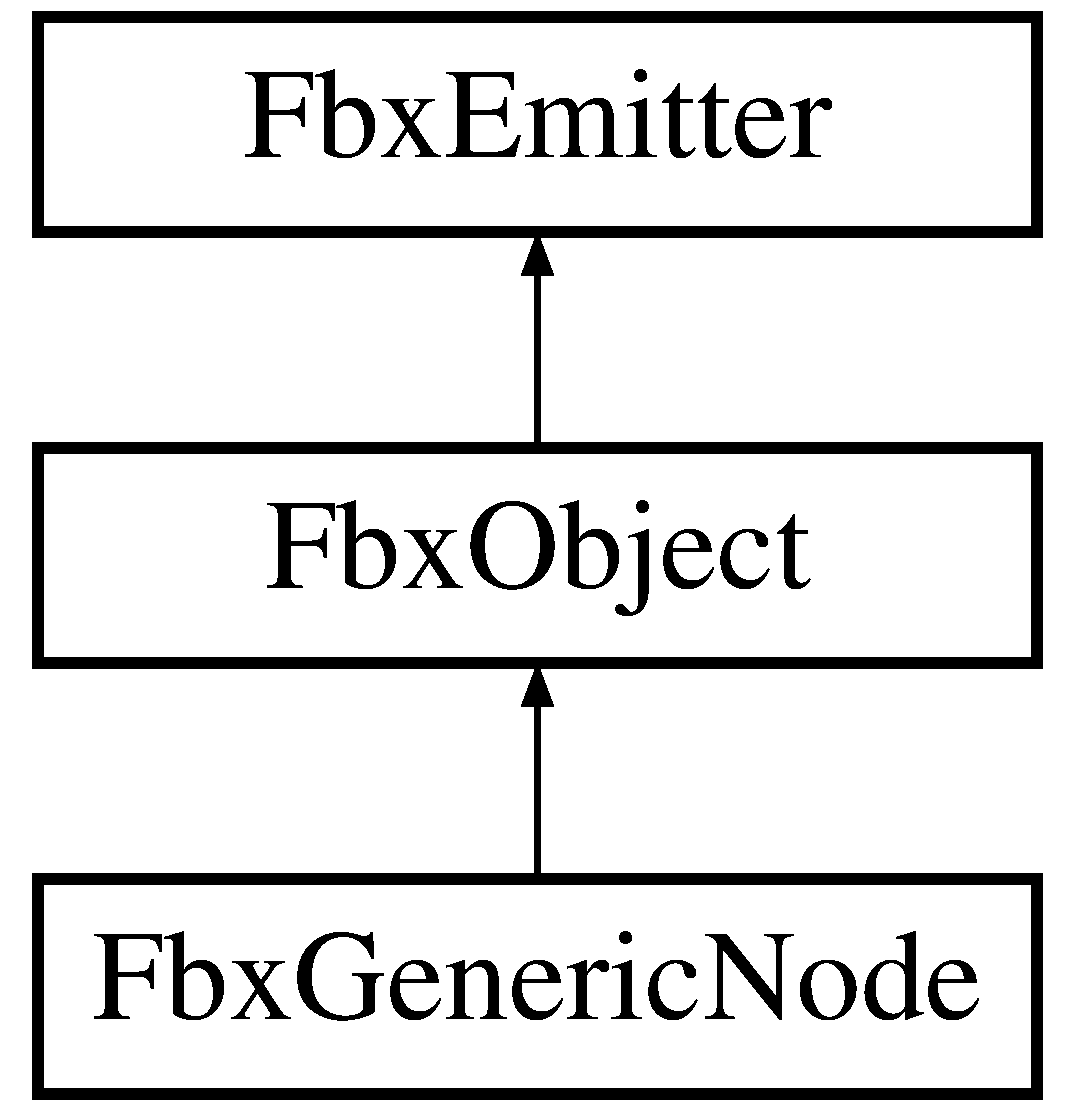
\includegraphics[height=3.000000cm]{class_fbx_generic_node}
\end{center}
\end{figure}
\subsection*{限定公開メンバ関数}
\begin{DoxyCompactItemize}
\item 
virtual void \hyperlink{class_fbx_generic_node_a63ff7b8adb2ddc1803f74b9afce50fc2}{Construct} (const \hyperlink{class_fbx_object}{Fbx\+Object} $\ast$p\+From)
\item 
virtual \hyperlink{class_fbx_string_list}{Fbx\+String\+List} \hyperlink{class_fbx_generic_node_a348566f1d9605e11b70a36cda95c9afb}{Get\+Type\+Flags} () const
\end{DoxyCompactItemize}
\subsection*{その他の継承メンバ}


\subsection{詳解}
Empty node containing properties. 

 fbxgenericnode.\+h の 24 行目に定義があります。



\subsection{関数詳解}
\mbox{\Hypertarget{class_fbx_generic_node_a63ff7b8adb2ddc1803f74b9afce50fc2}\label{class_fbx_generic_node_a63ff7b8adb2ddc1803f74b9afce50fc2}} 
\index{Fbx\+Generic\+Node@{Fbx\+Generic\+Node}!Construct@{Construct}}
\index{Construct@{Construct}!Fbx\+Generic\+Node@{Fbx\+Generic\+Node}}
\subsubsection{\texorpdfstring{Construct()}{Construct()}}
{\footnotesize\ttfamily virtual void Fbx\+Generic\+Node\+::\+Construct (\begin{DoxyParamCaption}\item[{const \hyperlink{class_fbx_object}{Fbx\+Object} $\ast$}]{p\+From }\end{DoxyParamCaption})\hspace{0.3cm}{\ttfamily [protected]}, {\ttfamily [virtual]}}

Optional constructor override, automatically called by default constructor. 
\begin{DoxyParams}{引数}
{\em p\+From} & If not null, the function must take it into account like a copy constructor. \\
\hline
\end{DoxyParams}
\begin{DoxyRemark}{注釈}
In case it is decided to override this function, do not forget to call Parent\+Class\+::\+Construct(p\+From) at the beginning. 
\end{DoxyRemark}


\hyperlink{class_fbx_object_a313503bc645af3fdceb4a99ef5cea7eb}{Fbx\+Object}を再実装しています。

\mbox{\Hypertarget{class_fbx_generic_node_a348566f1d9605e11b70a36cda95c9afb}\label{class_fbx_generic_node_a348566f1d9605e11b70a36cda95c9afb}} 
\index{Fbx\+Generic\+Node@{Fbx\+Generic\+Node}!Get\+Type\+Flags@{Get\+Type\+Flags}}
\index{Get\+Type\+Flags@{Get\+Type\+Flags}!Fbx\+Generic\+Node@{Fbx\+Generic\+Node}}
\subsubsection{\texorpdfstring{Get\+Type\+Flags()}{GetTypeFlags()}}
{\footnotesize\ttfamily virtual \hyperlink{class_fbx_string_list}{Fbx\+String\+List} Fbx\+Generic\+Node\+::\+Get\+Type\+Flags (\begin{DoxyParamCaption}{ }\end{DoxyParamCaption}) const\hspace{0.3cm}{\ttfamily [protected]}, {\ttfamily [virtual]}}



\hyperlink{class_fbx_object_a6d30a5d00400039a248977cf9f9255b2}{Fbx\+Object}を再実装しています。



このクラス詳解は次のファイルから抽出されました\+:\begin{DoxyCompactItemize}
\item 
C\+:/\+Maya/scripts/\+F\+B\+X\+\_\+\+S\+D\+K/2017.\+1/include/fbxsdk/scene/geometry/\hyperlink{fbxgenericnode_8h}{fbxgenericnode.\+h}\end{DoxyCompactItemize}

\hypertarget{class_fbx_geometry}{}\section{Fbx\+Geometry クラス}
\label{class_fbx_geometry}\index{Fbx\+Geometry@{Fbx\+Geometry}}


{\ttfamily \#include $<$fbxgeometry.\+h$>$}



Fbx\+Geometry の継承関係図
% FIG 0


Fbx\+Geometry 連携図
% FIG 1
\subsection*{公開型}
\begin{DoxyCompactItemize}
\item 
enum \hyperlink{class_fbx_geometry_adb9d2e34481a2cb40f1d783c665794db}{E\+Surface\+Mode} \{ \newline
\hyperlink{class_fbx_geometry_adb9d2e34481a2cb40f1d783c665794dbabebe9705fadfcfd4ef100fc493f60412}{e\+Raw}, 
\hyperlink{class_fbx_geometry_adb9d2e34481a2cb40f1d783c665794dba81ece06944d07ab68b5a08a1cb084c55}{e\+Low\+No\+Normals}, 
\hyperlink{class_fbx_geometry_adb9d2e34481a2cb40f1d783c665794dba6da9dccab2d42ec6361050c2deb070a9}{e\+Low}, 
\hyperlink{class_fbx_geometry_adb9d2e34481a2cb40f1d783c665794dbab835bcc45db6e23ee9dc6703614e5300}{e\+High\+No\+Normals}, 
\newline
\hyperlink{class_fbx_geometry_adb9d2e34481a2cb40f1d783c665794dba3f948522e0f01dcacbd6503a3d1e6423}{e\+High}
 \}
\end{DoxyCompactItemize}
\subsection*{公開メンバ関数}
\begin{DoxyCompactItemize}
\item 
virtual \hyperlink{class_fbx_node_attribute_a08e1669d3d1a696910756ab17de56d6a}{Fbx\+Node\+Attribute\+::\+E\+Type} \hyperlink{class_fbx_geometry_a41ae23e5d0cf08693bca49737f333de9}{Get\+Attribute\+Type} () const
\item 
virtual \hyperlink{class_fbx_object}{Fbx\+Object} \& \hyperlink{class_fbx_geometry_aac1cee4251e3d5fbd27f1181c58b83b3}{Copy} (const \hyperlink{class_fbx_object}{Fbx\+Object} \&p\+Object)
\item 
virtual \hyperlink{class_fbx_object}{Fbx\+Object} $\ast$ \hyperlink{class_fbx_geometry_aab95116993bd539bb870897d005d44de}{Clone} (\hyperlink{class_fbx_object_a9f5626b2d2135684d6ea1e6e4ad2acbb}{Fbx\+Object\+::\+E\+Clone\+Type} p\+Clone\+Type=\hyperlink{class_fbx_object_a9f5626b2d2135684d6ea1e6e4ad2acbbaacdf137ca059c572798287e98c4236d0}{e\+Deep\+Clone}, \hyperlink{class_fbx_object}{Fbx\+Object} $\ast$p\+Container=\hyperlink{fbxarch_8h_a070d2ce7b6bb7e5c05602aa8c308d0c4}{N\+U\+LL}, void $\ast$p\+Set=\hyperlink{fbxarch_8h_a070d2ce7b6bb7e5c05602aa8c308d0c4}{N\+U\+LL}) const
\item 
void \hyperlink{class_fbx_geometry_ad7d877cff6187c93064395a71b25ecce}{Clean\+Shape\+Channels} (\hyperlink{class_fbx_anim_layer}{Fbx\+Anim\+Layer} $\ast$p\+Anim\+Layer)
\item 
void \hyperlink{class_fbx_geometry_abd8e2642fa8ca94c88afaeafd0267bd0}{Clean\+Shape\+Channel} (\hyperlink{class_fbx_anim_layer}{Fbx\+Anim\+Layer} $\ast$p\+Anim\+Layer, int p\+Shape\+Index)
\item 
void \hyperlink{class_fbx_geometry_ac9c89d3dfee003accd6092682664501b}{Create\+Shape\+Channel\+Properties} (\hyperlink{class_fbx_string}{Fbx\+String} \&p\+Shape\+Name)
\item 
void \hyperlink{class_fbx_geometry_a2b135cea388e72bff364a6fa8714a38b}{Convert\+Shape\+Names\+To\+V5\+Format} (\hyperlink{class_fbx_string}{Fbx\+String} p\+Take\+Node\+Name)
\item 
void \hyperlink{class_fbx_geometry_aa1806aadaf07dac7d895e65f731f1679}{Convert\+Shape\+Names\+To\+V5\+Format} (\hyperlink{class_fbx_string}{Fbx\+String} p\+Take\+Node\+Name, int p\+Shape\+Index)
\item 
void \hyperlink{class_fbx_geometry_a891f23fed585b15503cdf8a38b424e14}{Revert\+Shape\+Names\+To\+V6\+Format} (\hyperlink{class_fbx_string}{Fbx\+String} p\+Take\+Node\+Name)
\item 
void \hyperlink{class_fbx_geometry_a408862417553440cefa975d1366985bb}{Revert\+Shape\+Names\+To\+V6\+Format} (\hyperlink{class_fbx_string}{Fbx\+String} p\+Take\+Node\+Name, int p\+Shape\+Index)
\item 
void \hyperlink{class_fbx_geometry_a2959da5506f3499fdb644a82843a64cd}{Clear\+Temporary\+Shape\+Names} ()
\end{DoxyCompactItemize}
\begin{Indent}\textbf{ Deformer Management}\par
\begin{DoxyCompactItemize}
\item 
int \hyperlink{class_fbx_geometry_a2f7e48a2faaf3893bc28eb8b684da908}{Add\+Deformer} (\hyperlink{class_fbx_deformer}{Fbx\+Deformer} $\ast$p\+Deformer)
\item 
\hyperlink{class_fbx_deformer}{Fbx\+Deformer} $\ast$ \hyperlink{class_fbx_geometry_a49e920f4c7a2179ef3297e7c5f2cf31a}{Remove\+Deformer} (int p\+Index, \hyperlink{class_fbx_status}{Fbx\+Status} $\ast$p\+Status=\hyperlink{fbxarch_8h_a070d2ce7b6bb7e5c05602aa8c308d0c4}{N\+U\+LL})
\item 
int \hyperlink{class_fbx_geometry_a8cca6f160b52ee1ffd799c599c36f784}{Get\+Deformer\+Count} () const
\item 
\hyperlink{class_fbx_deformer}{Fbx\+Deformer} $\ast$ \hyperlink{class_fbx_geometry_a3a6bd565c4a5a3a8b5daa3b653cc8a0a}{Get\+Deformer} (int p\+Index, \hyperlink{class_fbx_status}{Fbx\+Status} $\ast$p\+Status=\hyperlink{fbxarch_8h_a070d2ce7b6bb7e5c05602aa8c308d0c4}{N\+U\+LL}) const
\item 
int \hyperlink{class_fbx_geometry_a3eaf9796d935cd523d0a85a7f0c018fc}{Get\+Deformer\+Count} (\hyperlink{class_fbx_deformer_a07e2cfb767191ba5c8799fdfbfe3eaf6}{Fbx\+Deformer\+::\+E\+Deformer\+Type} p\+Type) const
\item 
\hyperlink{class_fbx_deformer}{Fbx\+Deformer} $\ast$ \hyperlink{class_fbx_geometry_aa283c85cdc0c5c3d2eae56952b6a41a0}{Get\+Deformer} (int p\+Index, \hyperlink{class_fbx_deformer_a07e2cfb767191ba5c8799fdfbfe3eaf6}{Fbx\+Deformer\+::\+E\+Deformer\+Type} p\+Type, \hyperlink{class_fbx_status}{Fbx\+Status} $\ast$p\+Status=\hyperlink{fbxarch_8h_a070d2ce7b6bb7e5c05602aa8c308d0c4}{N\+U\+LL}) const
\end{DoxyCompactItemize}
\end{Indent}
\begin{Indent}\textbf{ Geometry Weighted Maps Management}\par
\begin{DoxyCompactItemize}
\item 
\hyperlink{class_fbx_geometry_weighted_map}{Fbx\+Geometry\+Weighted\+Map} $\ast$ \hyperlink{class_fbx_geometry_a2d8cd2e9bf5a91fedcc1039dc4dce31d}{Get\+Source\+Geometry\+Weighted\+Map} ()
\item 
int \hyperlink{class_fbx_geometry_a7bebc9194083c5bacf77389b98ff906f}{Get\+Destination\+Geometry\+Weighted\+Map\+Count} () const
\item 
\hyperlink{class_fbx_geometry_weighted_map}{Fbx\+Geometry\+Weighted\+Map} $\ast$ \hyperlink{class_fbx_geometry_a377769a99e12dc765ac9ea49282ad1bf}{Get\+Destination\+Geometry\+Weighted\+Map} (int p\+Index)
\end{DoxyCompactItemize}
\end{Indent}
\begin{Indent}\textbf{ Shape Management}\par
\begin{DoxyCompactItemize}
\item 
bool \hyperlink{class_fbx_geometry_a4b9464c1f35f6bad8f2f19e427e70c9f}{Add\+Shape} (int p\+Blend\+Shape\+Index, int p\+Blend\+Shape\+Channel\+Index, \hyperlink{class_fbx_shape}{Fbx\+Shape} $\ast$p\+Shape, double p\+Percent=100, \hyperlink{class_fbx_status}{Fbx\+Status} $\ast$p\+Status=\hyperlink{fbxarch_8h_a070d2ce7b6bb7e5c05602aa8c308d0c4}{N\+U\+LL})
\item 
void \hyperlink{class_fbx_geometry_a6f5e46228d45b12e4f513abb56b8226d}{Clear\+Shape} ()
\item 
int \hyperlink{class_fbx_geometry_a9aa043cfb8856ef48b53b8cb7c8191b3}{Get\+Shape\+Count} () const
\item 
int \hyperlink{class_fbx_geometry_a34b10144646e4788f3702b9ebfa06dc2}{Get\+Shape\+Count} (int p\+Blend\+Shape\+Index, int p\+Blend\+Shape\+Channel\+Index, \hyperlink{class_fbx_status}{Fbx\+Status} $\ast$p\+Status=\hyperlink{fbxarch_8h_a070d2ce7b6bb7e5c05602aa8c308d0c4}{N\+U\+LL}) const
\item 
\hyperlink{class_fbx_shape}{Fbx\+Shape} $\ast$ \hyperlink{class_fbx_geometry_a8a60c0db307689b6d4fb6055055a1601}{Get\+Shape} (int p\+Blend\+Shape\+Index, int p\+Blend\+Shape\+Channel\+Index, int p\+Shape\+Index, \hyperlink{class_fbx_status}{Fbx\+Status} $\ast$p\+Status=\hyperlink{fbxarch_8h_a070d2ce7b6bb7e5c05602aa8c308d0c4}{N\+U\+LL})
\item 
const \hyperlink{class_fbx_shape}{Fbx\+Shape} $\ast$ \hyperlink{class_fbx_geometry_a8e9fba2b422ca2f4f5b4deda107fce7f}{Get\+Shape} (int p\+Blend\+Shape\+Index, int p\+Blend\+Shape\+Channel\+Index, int p\+Shape\+Index, \hyperlink{class_fbx_status}{Fbx\+Status} $\ast$p\+Status=\hyperlink{fbxarch_8h_a070d2ce7b6bb7e5c05602aa8c308d0c4}{N\+U\+LL}) const
\item 
\hyperlink{class_fbx_anim_curve}{Fbx\+Anim\+Curve} $\ast$ \hyperlink{class_fbx_geometry_a5a0e6869e72e17e9d0e7d2bb20264828}{Get\+Shape\+Channel} (int p\+Blend\+Shape\+Index, int p\+Blend\+Shape\+Channel\+Index, \hyperlink{class_fbx_anim_layer}{Fbx\+Anim\+Layer} $\ast$p\+Layer, bool p\+Create\+As\+Needed=false, \hyperlink{class_fbx_status}{Fbx\+Status} $\ast$p\+Status=\hyperlink{fbxarch_8h_a070d2ce7b6bb7e5c05602aa8c308d0c4}{N\+U\+LL})
\end{DoxyCompactItemize}
\end{Indent}
\begin{Indent}\textbf{ Pivot Management}\par
{\em The geometry pivot is used to specify additional translation, rotation, and scaling information applied to all control points when the model is exported. }\begin{DoxyCompactItemize}
\item 
\hyperlink{class_fbx_a_matrix}{Fbx\+A\+Matrix} \& \hyperlink{class_fbx_geometry_abba9072e0a3f1ad52033996f9809df80}{Get\+Pivot} (\hyperlink{class_fbx_a_matrix}{Fbx\+A\+Matrix} \&p\+X\+Matrix) const
\item 
void \hyperlink{class_fbx_geometry_a0b6b14186134a64ad55a47bcac865d70}{Set\+Pivot} (\hyperlink{class_fbx_a_matrix}{Fbx\+A\+Matrix} \&p\+X\+Matrix)
\item 
void \hyperlink{class_fbx_geometry_a34819c9209a0594344780f117bc641e1}{Apply\+Pivot} ()
\end{DoxyCompactItemize}
\end{Indent}
\begin{Indent}\textbf{ Default Animation Values}\par
{\em These functions provides direct access to default animation values that are specific to a geometry. These functions only work if the geometry has been associated with a node. }\begin{DoxyCompactItemize}
\item 
void \hyperlink{class_fbx_geometry_a6f8337a6336fc2e9bc0ea3d2d04c5ad1}{Set\+Default\+Shape} (int p\+Blend\+Shape\+Index, int p\+Blend\+Shape\+Channel\+Index, double p\+Percent)
\item 
void \hyperlink{class_fbx_geometry_a33ac7c5dc4a3001948b18696f47af802}{Set\+Default\+Shape} (\hyperlink{class_fbx_blend_shape_channel}{Fbx\+Blend\+Shape\+Channel} $\ast$p\+Blend\+Shape\+Channel, double p\+Percent)
\item 
double \hyperlink{class_fbx_geometry_ae3dfb076c1d8729413588b4a934b036b}{Get\+Default\+Shape} (int p\+Blend\+Shape\+Index, int p\+Blend\+Shape\+Channel\+Index) const
\item 
double \hyperlink{class_fbx_geometry_a178e8125306a0e7bb66f71e5472d381f}{Get\+Default\+Shape} (\hyperlink{class_fbx_blend_shape_channel}{Fbx\+Blend\+Shape\+Channel} $\ast$p\+Blend\+Shape\+Channel) const
\end{DoxyCompactItemize}
\end{Indent}
\subsection*{限定公開メンバ関数}
\begin{DoxyCompactItemize}
\item 
virtual void \hyperlink{class_fbx_geometry_a26ca96a86f17783c45ff83b33d2b5324}{Construct} (const \hyperlink{class_fbx_object}{Fbx\+Object} $\ast$p\+From)
\item 
virtual void \hyperlink{class_fbx_geometry_a07e94f7801067d66429afbf1799795cd}{Destruct} (bool p\+Recursive)
\item 
virtual void \hyperlink{class_fbx_geometry_a4e28b47a5f6dba7d53e692486d69c126}{Set\+Document} (\hyperlink{class_fbx_document}{Fbx\+Document} $\ast$p\+Document)
\item 
\hyperlink{class_fbx_string}{Fbx\+String} \hyperlink{class_fbx_geometry_ad79e9244da135a8fd62e47932ea68112}{Create\+Shape\+Channel\+Name} (int p\+Shape\+Index)
\item 
\hyperlink{class_fbx_string}{Fbx\+String} \hyperlink{class_fbx_geometry_a0f8e33ca5bf929614ffba6893079c136}{Create\+Shape\+Channel\+Name} (\hyperlink{class_fbx_string}{Fbx\+String} p\+Shape\+Name)
\item 
void \hyperlink{class_fbx_geometry_a0fa8343b20fb5a9c0b0bc15a83967972}{Copy\+Deformers} (const \hyperlink{class_fbx_geometry}{Fbx\+Geometry} $\ast$p\+Geometry)
\item 
void \hyperlink{class_fbx_geometry_a97edd8b50b825e220a2c246936480160}{Copy\+Pivot} (const \hyperlink{class_fbx_geometry}{Fbx\+Geometry} $\ast$p\+Source)
\end{DoxyCompactItemize}
\subsection*{限定公開変数類}
\begin{DoxyCompactItemize}
\item 
\hyperlink{class_fbx_array}{Fbx\+Array}$<$ \hyperlink{class_fbx_string}{Fbx\+String} $\ast$ $>$ \hyperlink{class_fbx_geometry_a7f09646b7a716f58932d9be9c4a34486}{m\+Shape\+Name\+Array\+V6}
\item 
\hyperlink{class_fbx_array}{Fbx\+Array}$<$ \hyperlink{class_fbx_string}{Fbx\+String} $\ast$ $>$ \hyperlink{class_fbx_geometry_a2a38009f990f6dfa9ca81ee2b24b024b}{m\+Shape\+Name\+Array\+V5}
\item 
\hyperlink{class_fbx_array}{Fbx\+Array}$<$ \hyperlink{class_fbx_string}{Fbx\+String} $\ast$ $>$ \hyperlink{class_fbx_geometry_a8752a5800b261d678592dc7a81dad4b0}{m\+Shape\+Channel\+Name\+Array\+V5}
\item 
\hyperlink{class_fbx_a_matrix}{Fbx\+A\+Matrix} $\ast$ \hyperlink{class_fbx_geometry_ab9f5852d38a38a9efb0ab63bd74503c0}{m\+Pivot}
\end{DoxyCompactItemize}
\subsection*{その他の継承メンバ}


\subsection{詳解}
The base class of geometric objects that support control point deformations (e.\+g. \hyperlink{class_fbx_mesh}{Fbx\+Mesh}, \hyperlink{class_fbx_nurbs}{Fbx\+Nurbs}, and \hyperlink{class_fbx_patch}{Fbx\+Patch}). The \hyperlink{class_fbx_geometry}{Fbx\+Geometry} provides support for the following kinds of deformations.

\begin{DoxyItemize}
\item Skin deformation deformers \item Vertex cache deformers \item Geometry weighted maps \item Shapes\end{DoxyItemize}
Most of the methods of \hyperlink{class_fbx_geometry}{Fbx\+Geometry} are wrappers to simplify the access/manipulation of the connections to the deformers. For example, calling the \hyperlink{class_fbx_geometry_a8cca6f160b52ee1ffd799c599c36f784}{Get\+Deformer\+Count()} method is the same thing as calling\+:


\begin{DoxyCode}
geometry.GetSrcObjectCount(FbxDeformer::ClassId)
\end{DoxyCode}
 

\subsection{列挙型メンバ詳解}
\mbox{\Hypertarget{class_fbx_geometry_adb9d2e34481a2cb40f1d783c665794db}\label{class_fbx_geometry_adb9d2e34481a2cb40f1d783c665794db}} 
\index{Fbx\+Geometry@{Fbx\+Geometry}!E\+Surface\+Mode@{E\+Surface\+Mode}}
\index{E\+Surface\+Mode@{E\+Surface\+Mode}!Fbx\+Geometry@{Fbx\+Geometry}}
\subsubsection{\texorpdfstring{E\+Surface\+Mode}{ESurfaceMode}}
{\footnotesize\ttfamily enum \hyperlink{class_fbx_geometry_adb9d2e34481a2cb40f1d783c665794db}{Fbx\+Geometry\+::\+E\+Surface\+Mode}}

N\+U\+R\+BS and Patches surface modes. This information is never directly used inside the F\+BX S\+DK. Applications can use these values if they wish to carry the \char`\"{}rendering\char`\"{} details of the N\+U\+R\+BS and Patches. The F\+BX S\+DK guarantee that the value (member of the \hyperlink{class_fbx_nurbs}{Fbx\+Nurbs}, \hyperlink{class_fbx_nurbs_surface}{Fbx\+Nurbs\+Surface} and \hyperlink{class_fbx_patch}{Fbx\+Patch} classes) is stored to F\+BX files and retrieved from them. \begin{DoxyRemark}{注釈}
The enum has been defined in this class to avoid symbols duplication. 
\end{DoxyRemark}
\begin{DoxyEnumFields}{列挙値}
\raisebox{\heightof{T}}[0pt][0pt]{\index{e\+Raw@{e\+Raw}!Fbx\+Geometry@{Fbx\+Geometry}}\index{Fbx\+Geometry@{Fbx\+Geometry}!e\+Raw@{e\+Raw}}}\mbox{\Hypertarget{class_fbx_geometry_adb9d2e34481a2cb40f1d783c665794dbabebe9705fadfcfd4ef100fc493f60412}\label{class_fbx_geometry_adb9d2e34481a2cb40f1d783c665794dbabebe9705fadfcfd4ef100fc493f60412}} 
e\+Raw&\\
\hline

\raisebox{\heightof{T}}[0pt][0pt]{\index{e\+Low\+No\+Normals@{e\+Low\+No\+Normals}!Fbx\+Geometry@{Fbx\+Geometry}}\index{Fbx\+Geometry@{Fbx\+Geometry}!e\+Low\+No\+Normals@{e\+Low\+No\+Normals}}}\mbox{\Hypertarget{class_fbx_geometry_adb9d2e34481a2cb40f1d783c665794dba81ece06944d07ab68b5a08a1cb084c55}\label{class_fbx_geometry_adb9d2e34481a2cb40f1d783c665794dba81ece06944d07ab68b5a08a1cb084c55}} 
e\+Low\+No\+Normals&Raw. \\
\hline

\raisebox{\heightof{T}}[0pt][0pt]{\index{e\+Low@{e\+Low}!Fbx\+Geometry@{Fbx\+Geometry}}\index{Fbx\+Geometry@{Fbx\+Geometry}!e\+Low@{e\+Low}}}\mbox{\Hypertarget{class_fbx_geometry_adb9d2e34481a2cb40f1d783c665794dba6da9dccab2d42ec6361050c2deb070a9}\label{class_fbx_geometry_adb9d2e34481a2cb40f1d783c665794dba6da9dccab2d42ec6361050c2deb070a9}} 
e\+Low&Low and no normals. \\
\hline

\raisebox{\heightof{T}}[0pt][0pt]{\index{e\+High\+No\+Normals@{e\+High\+No\+Normals}!Fbx\+Geometry@{Fbx\+Geometry}}\index{Fbx\+Geometry@{Fbx\+Geometry}!e\+High\+No\+Normals@{e\+High\+No\+Normals}}}\mbox{\Hypertarget{class_fbx_geometry_adb9d2e34481a2cb40f1d783c665794dbab835bcc45db6e23ee9dc6703614e5300}\label{class_fbx_geometry_adb9d2e34481a2cb40f1d783c665794dbab835bcc45db6e23ee9dc6703614e5300}} 
e\+High\+No\+Normals&Low. \\
\hline

\raisebox{\heightof{T}}[0pt][0pt]{\index{e\+High@{e\+High}!Fbx\+Geometry@{Fbx\+Geometry}}\index{Fbx\+Geometry@{Fbx\+Geometry}!e\+High@{e\+High}}}\mbox{\Hypertarget{class_fbx_geometry_adb9d2e34481a2cb40f1d783c665794dba3f948522e0f01dcacbd6503a3d1e6423}\label{class_fbx_geometry_adb9d2e34481a2cb40f1d783c665794dba3f948522e0f01dcacbd6503a3d1e6423}} 
e\+High&High and no normals. High. \\
\hline

\end{DoxyEnumFields}


\subsection{メソッド詳解}
\mbox{\Hypertarget{class_fbx_geometry_a2f7e48a2faaf3893bc28eb8b684da908}\label{class_fbx_geometry_a2f7e48a2faaf3893bc28eb8b684da908}} 
\index{Fbx\+Geometry@{Fbx\+Geometry}!Add\+Deformer@{Add\+Deformer}}
\index{Add\+Deformer@{Add\+Deformer}!Fbx\+Geometry@{Fbx\+Geometry}}
\subsubsection{\texorpdfstring{Add\+Deformer()}{AddDeformer()}}
{\footnotesize\ttfamily int Fbx\+Geometry\+::\+Add\+Deformer (\begin{DoxyParamCaption}\item[{\hyperlink{class_fbx_deformer}{Fbx\+Deformer} $\ast$}]{p\+Deformer }\end{DoxyParamCaption})}

Adds a deformer to this geometry (as mentioned in the description of this class, adding a deformer is a synonym for \char`\"{}connect a deformer\char`\"{}). 
\begin{DoxyParams}{引数}
{\em p\+Deformer} & Pointer to the deformer to be added. \\
\hline
\end{DoxyParams}
\begin{DoxyReturn}{戻り値}
Index of the added deformer. 
\end{DoxyReturn}
\mbox{\Hypertarget{class_fbx_geometry_a4b9464c1f35f6bad8f2f19e427e70c9f}\label{class_fbx_geometry_a4b9464c1f35f6bad8f2f19e427e70c9f}} 
\index{Fbx\+Geometry@{Fbx\+Geometry}!Add\+Shape@{Add\+Shape}}
\index{Add\+Shape@{Add\+Shape}!Fbx\+Geometry@{Fbx\+Geometry}}
\subsubsection{\texorpdfstring{Add\+Shape()}{AddShape()}}
{\footnotesize\ttfamily bool Fbx\+Geometry\+::\+Add\+Shape (\begin{DoxyParamCaption}\item[{int}]{p\+Blend\+Shape\+Index,  }\item[{int}]{p\+Blend\+Shape\+Channel\+Index,  }\item[{\hyperlink{class_fbx_shape}{Fbx\+Shape} $\ast$}]{p\+Shape,  }\item[{double}]{p\+Percent = {\ttfamily 100},  }\item[{\hyperlink{class_fbx_status}{Fbx\+Status} $\ast$}]{p\+Status = {\ttfamily \hyperlink{fbxarch_8h_a070d2ce7b6bb7e5c05602aa8c308d0c4}{N\+U\+LL}} }\end{DoxyParamCaption})}

Add a shape to the specified blend shape deformer and blend shape channel of this geometry. 
\begin{DoxyParams}{引数}
{\em p\+Blend\+Shape\+Index} & The blend shape deformer index. \\
\hline
{\em p\+Blend\+Shape\+Channel\+Index} & The blend shape channel index. \\
\hline
{\em p\+Shape} & Pointer to the shape object to be added. \\
\hline
{\em p\+Percent} & The full deform percentage of this shape. \\
\hline
{\em p\+Status} & The \hyperlink{class_fbx_status}{Fbx\+Status} object to hold error codes. \\
\hline
\end{DoxyParams}
\begin{DoxyReturn}{戻り値}
{\ttfamily true} if success, {\ttfamily false} otherwise. 
\end{DoxyReturn}
\mbox{\Hypertarget{class_fbx_geometry_a34819c9209a0594344780f117bc641e1}\label{class_fbx_geometry_a34819c9209a0594344780f117bc641e1}} 
\index{Fbx\+Geometry@{Fbx\+Geometry}!Apply\+Pivot@{Apply\+Pivot}}
\index{Apply\+Pivot@{Apply\+Pivot}!Fbx\+Geometry@{Fbx\+Geometry}}
\subsubsection{\texorpdfstring{Apply\+Pivot()}{ApplyPivot()}}
{\footnotesize\ttfamily void Fbx\+Geometry\+::\+Apply\+Pivot (\begin{DoxyParamCaption}{ }\end{DoxyParamCaption})}

Applies the pivot matrix to all vertices/normals of the geometry. \mbox{\Hypertarget{class_fbx_geometry_abd8e2642fa8ca94c88afaeafd0267bd0}\label{class_fbx_geometry_abd8e2642fa8ca94c88afaeafd0267bd0}} 
\index{Fbx\+Geometry@{Fbx\+Geometry}!Clean\+Shape\+Channel@{Clean\+Shape\+Channel}}
\index{Clean\+Shape\+Channel@{Clean\+Shape\+Channel}!Fbx\+Geometry@{Fbx\+Geometry}}
\subsubsection{\texorpdfstring{Clean\+Shape\+Channel()}{CleanShapeChannel()}}
{\footnotesize\ttfamily void Fbx\+Geometry\+::\+Clean\+Shape\+Channel (\begin{DoxyParamCaption}\item[{\hyperlink{class_fbx_anim_layer}{Fbx\+Anim\+Layer} $\ast$}]{p\+Anim\+Layer,  }\item[{int}]{p\+Shape\+Index }\end{DoxyParamCaption})}

\mbox{\Hypertarget{class_fbx_geometry_ad7d877cff6187c93064395a71b25ecce}\label{class_fbx_geometry_ad7d877cff6187c93064395a71b25ecce}} 
\index{Fbx\+Geometry@{Fbx\+Geometry}!Clean\+Shape\+Channels@{Clean\+Shape\+Channels}}
\index{Clean\+Shape\+Channels@{Clean\+Shape\+Channels}!Fbx\+Geometry@{Fbx\+Geometry}}
\subsubsection{\texorpdfstring{Clean\+Shape\+Channels()}{CleanShapeChannels()}}
{\footnotesize\ttfamily void Fbx\+Geometry\+::\+Clean\+Shape\+Channels (\begin{DoxyParamCaption}\item[{\hyperlink{class_fbx_anim_layer}{Fbx\+Anim\+Layer} $\ast$}]{p\+Anim\+Layer }\end{DoxyParamCaption})}

\mbox{\Hypertarget{class_fbx_geometry_a6f5e46228d45b12e4f513abb56b8226d}\label{class_fbx_geometry_a6f5e46228d45b12e4f513abb56b8226d}} 
\index{Fbx\+Geometry@{Fbx\+Geometry}!Clear\+Shape@{Clear\+Shape}}
\index{Clear\+Shape@{Clear\+Shape}!Fbx\+Geometry@{Fbx\+Geometry}}
\subsubsection{\texorpdfstring{Clear\+Shape()}{ClearShape()}}
{\footnotesize\ttfamily void Fbx\+Geometry\+::\+Clear\+Shape (\begin{DoxyParamCaption}{ }\end{DoxyParamCaption})}

Removes all the shapes without destroying them. If shapes aren\textquotesingle{}t explicitly destroyed before calling this function, they will be destroyed along with the S\+DK manager that created them. \mbox{\Hypertarget{class_fbx_geometry_a2959da5506f3499fdb644a82843a64cd}\label{class_fbx_geometry_a2959da5506f3499fdb644a82843a64cd}} 
\index{Fbx\+Geometry@{Fbx\+Geometry}!Clear\+Temporary\+Shape\+Names@{Clear\+Temporary\+Shape\+Names}}
\index{Clear\+Temporary\+Shape\+Names@{Clear\+Temporary\+Shape\+Names}!Fbx\+Geometry@{Fbx\+Geometry}}
\subsubsection{\texorpdfstring{Clear\+Temporary\+Shape\+Names()}{ClearTemporaryShapeNames()}}
{\footnotesize\ttfamily void Fbx\+Geometry\+::\+Clear\+Temporary\+Shape\+Names (\begin{DoxyParamCaption}{ }\end{DoxyParamCaption})}

\mbox{\Hypertarget{class_fbx_geometry_aab95116993bd539bb870897d005d44de}\label{class_fbx_geometry_aab95116993bd539bb870897d005d44de}} 
\index{Fbx\+Geometry@{Fbx\+Geometry}!Clone@{Clone}}
\index{Clone@{Clone}!Fbx\+Geometry@{Fbx\+Geometry}}
\subsubsection{\texorpdfstring{Clone()}{Clone()}}
{\footnotesize\ttfamily virtual \hyperlink{class_fbx_object}{Fbx\+Object}$\ast$ Fbx\+Geometry\+::\+Clone (\begin{DoxyParamCaption}\item[{\hyperlink{class_fbx_object_a9f5626b2d2135684d6ea1e6e4ad2acbb}{Fbx\+Object\+::\+E\+Clone\+Type}}]{p\+Clone\+Type = {\ttfamily \hyperlink{class_fbx_object_a9f5626b2d2135684d6ea1e6e4ad2acbbaacdf137ca059c572798287e98c4236d0}{e\+Deep\+Clone}},  }\item[{\hyperlink{class_fbx_object}{Fbx\+Object} $\ast$}]{p\+Container = {\ttfamily \hyperlink{fbxarch_8h_a070d2ce7b6bb7e5c05602aa8c308d0c4}{N\+U\+LL}},  }\item[{void $\ast$}]{p\+Set = {\ttfamily \hyperlink{fbxarch_8h_a070d2ce7b6bb7e5c05602aa8c308d0c4}{N\+U\+LL}} }\end{DoxyParamCaption}) const\hspace{0.3cm}{\ttfamily [virtual]}}

Creates a clone of this object. By default, the connections are N\+OT cloned. If the desired effect is to clone the connections as well, you must clone using the \hyperlink{class_fbx_clone_manager}{Fbx\+Clone\+Manager} (refer to this class documentation for further details).


\begin{DoxyParams}{引数}
{\em p\+Clone\+Type} & The type of clone to be created. By default, the clone type is e\+Deep\+Clone. \\
\hline
{\em p\+Container} & An optional parameter to specify which object will \char`\"{}contain\char`\"{} the new object. By contain, we mean the new object will become a source to the container, connection-\/wise. \\
\hline
{\em p\+Set} & See remark section. \\
\hline
\end{DoxyParams}
\begin{DoxyReturn}{戻り値}
The new clone, or N\+U\+LL (if the specified clone type is not supported). 
\end{DoxyReturn}
\begin{DoxyRemark}{注釈}
When doing either a \char`\"{}deep\char`\"{} or \char`\"{}reference\char`\"{} clone type, the clone will always get its properties values set from the source object properties values. 

Since this is a virtual function, some classes might do additional tasks. 

The {\itshape p\+Set} argument is not used in the default implementation of this method. Specialized implementations should cast this pointer to \hyperlink{class_fbx_clone_manager_aeb8a9c04c9c36eb7e551186a0b18f10d}{Fbx\+Clone\+Manager\+::\+Clone\+Set} to have access to the cloned objects so far. Typically, this pointer is set by the clone manager. 
\end{DoxyRemark}


\hyperlink{class_fbx_object_ad553a4262b09cb57c3171a93edadbab8}{Fbx\+Object}を再実装しています。

\mbox{\Hypertarget{class_fbx_geometry_a26ca96a86f17783c45ff83b33d2b5324}\label{class_fbx_geometry_a26ca96a86f17783c45ff83b33d2b5324}} 
\index{Fbx\+Geometry@{Fbx\+Geometry}!Construct@{Construct}}
\index{Construct@{Construct}!Fbx\+Geometry@{Fbx\+Geometry}}
\subsubsection{\texorpdfstring{Construct()}{Construct()}}
{\footnotesize\ttfamily virtual void Fbx\+Geometry\+::\+Construct (\begin{DoxyParamCaption}\item[{const \hyperlink{class_fbx_object}{Fbx\+Object} $\ast$}]{p\+From }\end{DoxyParamCaption})\hspace{0.3cm}{\ttfamily [protected]}, {\ttfamily [virtual]}}

Optional constructor override, automatically called by default constructor. 
\begin{DoxyParams}{引数}
{\em p\+From} & If not null, the function must take it into account like a copy constructor. \\
\hline
\end{DoxyParams}
\begin{DoxyRemark}{注釈}
In case it is decided to override this function, do not forget to call Parent\+Class\+::\+Construct(p\+From) at the beginning. 
\end{DoxyRemark}


\hyperlink{class_fbx_object_a313503bc645af3fdceb4a99ef5cea7eb}{Fbx\+Object}を再実装しています。



\hyperlink{class_fbx_mesh_a230787ca87312437d427d9ec7c150565}{Fbx\+Mesh}, \hyperlink{class_fbx_nurbs_surface_a3487d194007af1729d31dc9dfa0b12c9}{Fbx\+Nurbs\+Surface}, \hyperlink{class_fbx_nurbs_a1d62f29d7315e343d5c0c414dab3fabb}{Fbx\+Nurbs}, \hyperlink{class_fbx_trim_nurbs_surface_a95ea54578a57e9038ae67cb2b6b26f82}{Fbx\+Trim\+Nurbs\+Surface}, \hyperlink{class_fbx_nurbs_curve_ac730e9ec1d56724f8495725b0491ddd8}{Fbx\+Nurbs\+Curve}, \hyperlink{class_fbx_patch_a82fbbc0a7ec019bbe69c976ab755b23e}{Fbx\+Patch}, \hyperlink{class_fbx_line_a42d7e3fb4684712df04464644abee11a}{Fbx\+Line}で再実装されています。

被呼び出し関係図\+:
% FIG 2
\mbox{\Hypertarget{class_fbx_geometry_a2b135cea388e72bff364a6fa8714a38b}\label{class_fbx_geometry_a2b135cea388e72bff364a6fa8714a38b}} 
\index{Fbx\+Geometry@{Fbx\+Geometry}!Convert\+Shape\+Names\+To\+V5\+Format@{Convert\+Shape\+Names\+To\+V5\+Format}}
\index{Convert\+Shape\+Names\+To\+V5\+Format@{Convert\+Shape\+Names\+To\+V5\+Format}!Fbx\+Geometry@{Fbx\+Geometry}}
\subsubsection{\texorpdfstring{Convert\+Shape\+Names\+To\+V5\+Format()}{ConvertShapeNamesToV5Format()}\hspace{0.1cm}{\footnotesize\ttfamily [1/2]}}
{\footnotesize\ttfamily void Fbx\+Geometry\+::\+Convert\+Shape\+Names\+To\+V5\+Format (\begin{DoxyParamCaption}\item[{\hyperlink{class_fbx_string}{Fbx\+String}}]{p\+Take\+Node\+Name }\end{DoxyParamCaption})}

\mbox{\Hypertarget{class_fbx_geometry_aa1806aadaf07dac7d895e65f731f1679}\label{class_fbx_geometry_aa1806aadaf07dac7d895e65f731f1679}} 
\index{Fbx\+Geometry@{Fbx\+Geometry}!Convert\+Shape\+Names\+To\+V5\+Format@{Convert\+Shape\+Names\+To\+V5\+Format}}
\index{Convert\+Shape\+Names\+To\+V5\+Format@{Convert\+Shape\+Names\+To\+V5\+Format}!Fbx\+Geometry@{Fbx\+Geometry}}
\subsubsection{\texorpdfstring{Convert\+Shape\+Names\+To\+V5\+Format()}{ConvertShapeNamesToV5Format()}\hspace{0.1cm}{\footnotesize\ttfamily [2/2]}}
{\footnotesize\ttfamily void Fbx\+Geometry\+::\+Convert\+Shape\+Names\+To\+V5\+Format (\begin{DoxyParamCaption}\item[{\hyperlink{class_fbx_string}{Fbx\+String}}]{p\+Take\+Node\+Name,  }\item[{int}]{p\+Shape\+Index }\end{DoxyParamCaption})}

\mbox{\Hypertarget{class_fbx_geometry_aac1cee4251e3d5fbd27f1181c58b83b3}\label{class_fbx_geometry_aac1cee4251e3d5fbd27f1181c58b83b3}} 
\index{Fbx\+Geometry@{Fbx\+Geometry}!Copy@{Copy}}
\index{Copy@{Copy}!Fbx\+Geometry@{Fbx\+Geometry}}
\subsubsection{\texorpdfstring{Copy()}{Copy()}}
{\footnotesize\ttfamily virtual \hyperlink{class_fbx_object}{Fbx\+Object}\& Fbx\+Geometry\+::\+Copy (\begin{DoxyParamCaption}\item[{const \hyperlink{class_fbx_object}{Fbx\+Object} \&}]{p\+Object }\end{DoxyParamCaption})\hspace{0.3cm}{\ttfamily [virtual]}}

Copy an object content into this object. 
\begin{DoxyParams}{引数}
{\em p\+Object} & The source object to copy data from. \\
\hline
\end{DoxyParams}
\begin{DoxyReturn}{戻り値}
Returns the destination object being modified by the source. 
\end{DoxyReturn}
\begin{DoxyRemark}{注釈}
This function replace the assignment operator (operator=). It will copy all property values and the name. Connections are N\+OT copied. 
\end{DoxyRemark}


\hyperlink{class_fbx_geometry_base_a2c3754831338327259c35caebbf379d3}{Fbx\+Geometry\+Base}を再実装しています。



\hyperlink{class_fbx_mesh_a0f041743536ee5ccbc9a086e3ef1c663}{Fbx\+Mesh}, \hyperlink{class_fbx_nurbs_surface_a1da47f75af4920a3fb4a94690d8ada8c}{Fbx\+Nurbs\+Surface}, \hyperlink{class_fbx_nurbs_ac7c9a9018b4fdbe72b258a2fa0a3367d}{Fbx\+Nurbs}, \hyperlink{class_fbx_trim_nurbs_surface_a4407d30e83346ab3cb30ccf67d7bb289}{Fbx\+Trim\+Nurbs\+Surface}, \hyperlink{class_fbx_nurbs_curve_ad48046242c0a63d929b5440563668f79}{Fbx\+Nurbs\+Curve}, \hyperlink{class_fbx_patch_a424542a42ec75d3c5236cc366adecd89}{Fbx\+Patch}, \hyperlink{class_fbx_line_aeb9e0c53cf02d3e4e206b25c87c06256}{Fbx\+Line}, \hyperlink{class_fbx_boundary_a6fe59f45c17eeebbabaeff235058ac70}{Fbx\+Boundary}で再実装されています。

被呼び出し関係図\+:
% FIG 3
\mbox{\Hypertarget{class_fbx_geometry_a0fa8343b20fb5a9c0b0bc15a83967972}\label{class_fbx_geometry_a0fa8343b20fb5a9c0b0bc15a83967972}} 
\index{Fbx\+Geometry@{Fbx\+Geometry}!Copy\+Deformers@{Copy\+Deformers}}
\index{Copy\+Deformers@{Copy\+Deformers}!Fbx\+Geometry@{Fbx\+Geometry}}
\subsubsection{\texorpdfstring{Copy\+Deformers()}{CopyDeformers()}}
{\footnotesize\ttfamily void Fbx\+Geometry\+::\+Copy\+Deformers (\begin{DoxyParamCaption}\item[{const \hyperlink{class_fbx_geometry}{Fbx\+Geometry} $\ast$}]{p\+Geometry }\end{DoxyParamCaption})\hspace{0.3cm}{\ttfamily [protected]}}

\mbox{\Hypertarget{class_fbx_geometry_a97edd8b50b825e220a2c246936480160}\label{class_fbx_geometry_a97edd8b50b825e220a2c246936480160}} 
\index{Fbx\+Geometry@{Fbx\+Geometry}!Copy\+Pivot@{Copy\+Pivot}}
\index{Copy\+Pivot@{Copy\+Pivot}!Fbx\+Geometry@{Fbx\+Geometry}}
\subsubsection{\texorpdfstring{Copy\+Pivot()}{CopyPivot()}}
{\footnotesize\ttfamily void Fbx\+Geometry\+::\+Copy\+Pivot (\begin{DoxyParamCaption}\item[{const \hyperlink{class_fbx_geometry}{Fbx\+Geometry} $\ast$}]{p\+Source }\end{DoxyParamCaption})\hspace{0.3cm}{\ttfamily [protected]}}

\mbox{\Hypertarget{class_fbx_geometry_ad79e9244da135a8fd62e47932ea68112}\label{class_fbx_geometry_ad79e9244da135a8fd62e47932ea68112}} 
\index{Fbx\+Geometry@{Fbx\+Geometry}!Create\+Shape\+Channel\+Name@{Create\+Shape\+Channel\+Name}}
\index{Create\+Shape\+Channel\+Name@{Create\+Shape\+Channel\+Name}!Fbx\+Geometry@{Fbx\+Geometry}}
\subsubsection{\texorpdfstring{Create\+Shape\+Channel\+Name()}{CreateShapeChannelName()}\hspace{0.1cm}{\footnotesize\ttfamily [1/2]}}
{\footnotesize\ttfamily \hyperlink{class_fbx_string}{Fbx\+String} Fbx\+Geometry\+::\+Create\+Shape\+Channel\+Name (\begin{DoxyParamCaption}\item[{int}]{p\+Shape\+Index }\end{DoxyParamCaption})\hspace{0.3cm}{\ttfamily [protected]}}

\mbox{\Hypertarget{class_fbx_geometry_a0f8e33ca5bf929614ffba6893079c136}\label{class_fbx_geometry_a0f8e33ca5bf929614ffba6893079c136}} 
\index{Fbx\+Geometry@{Fbx\+Geometry}!Create\+Shape\+Channel\+Name@{Create\+Shape\+Channel\+Name}}
\index{Create\+Shape\+Channel\+Name@{Create\+Shape\+Channel\+Name}!Fbx\+Geometry@{Fbx\+Geometry}}
\subsubsection{\texorpdfstring{Create\+Shape\+Channel\+Name()}{CreateShapeChannelName()}\hspace{0.1cm}{\footnotesize\ttfamily [2/2]}}
{\footnotesize\ttfamily \hyperlink{class_fbx_string}{Fbx\+String} Fbx\+Geometry\+::\+Create\+Shape\+Channel\+Name (\begin{DoxyParamCaption}\item[{\hyperlink{class_fbx_string}{Fbx\+String}}]{p\+Shape\+Name }\end{DoxyParamCaption})\hspace{0.3cm}{\ttfamily [protected]}}

\mbox{\Hypertarget{class_fbx_geometry_ac9c89d3dfee003accd6092682664501b}\label{class_fbx_geometry_ac9c89d3dfee003accd6092682664501b}} 
\index{Fbx\+Geometry@{Fbx\+Geometry}!Create\+Shape\+Channel\+Properties@{Create\+Shape\+Channel\+Properties}}
\index{Create\+Shape\+Channel\+Properties@{Create\+Shape\+Channel\+Properties}!Fbx\+Geometry@{Fbx\+Geometry}}
\subsubsection{\texorpdfstring{Create\+Shape\+Channel\+Properties()}{CreateShapeChannelProperties()}}
{\footnotesize\ttfamily void Fbx\+Geometry\+::\+Create\+Shape\+Channel\+Properties (\begin{DoxyParamCaption}\item[{\hyperlink{class_fbx_string}{Fbx\+String} \&}]{p\+Shape\+Name }\end{DoxyParamCaption})}

\mbox{\Hypertarget{class_fbx_geometry_a07e94f7801067d66429afbf1799795cd}\label{class_fbx_geometry_a07e94f7801067d66429afbf1799795cd}} 
\index{Fbx\+Geometry@{Fbx\+Geometry}!Destruct@{Destruct}}
\index{Destruct@{Destruct}!Fbx\+Geometry@{Fbx\+Geometry}}
\subsubsection{\texorpdfstring{Destruct()}{Destruct()}}
{\footnotesize\ttfamily virtual void Fbx\+Geometry\+::\+Destruct (\begin{DoxyParamCaption}\item[{bool}]{p\+Recursive }\end{DoxyParamCaption})\hspace{0.3cm}{\ttfamily [protected]}, {\ttfamily [virtual]}}

Optional destructor override, automatically called by default destructor. 
\begin{DoxyParams}{引数}
{\em p\+Recursive} & If true, children objects should be destroyed as well. \\
\hline
\end{DoxyParams}
\begin{DoxyRemark}{注釈}
In case it is decided to override this function, do not forget to call Parent\+Class\+::\+Destruct(p\+Resursive) at the end. 
\end{DoxyRemark}


\hyperlink{class_fbx_layer_container_aefb90aadf569c7ebbbd3672e9c45776f}{Fbx\+Layer\+Container}を再実装しています。



\hyperlink{class_fbx_mesh_a1755e89d515fadbc2d52924917b618f7}{Fbx\+Mesh}, \hyperlink{class_fbx_nurbs_surface_ab9ff252170ad2dc35958af782962a5c9}{Fbx\+Nurbs\+Surface}, \hyperlink{class_fbx_nurbs_a8a5ea388bc948e47ab65e1705f98f402}{Fbx\+Nurbs}, \hyperlink{class_fbx_nurbs_curve_a8c562cccf434c37cb3aad0df27d60e86}{Fbx\+Nurbs\+Curve}, \hyperlink{class_fbx_patch_a7e094310626891214577dabe4ff145f9}{Fbx\+Patch}, \hyperlink{class_fbx_line_a92abd64f6b58057c899bf5733a2e2275}{Fbx\+Line}で再実装されています。

被呼び出し関係図\+:
% FIG 4
\mbox{\Hypertarget{class_fbx_geometry_a41ae23e5d0cf08693bca49737f333de9}\label{class_fbx_geometry_a41ae23e5d0cf08693bca49737f333de9}} 
\index{Fbx\+Geometry@{Fbx\+Geometry}!Get\+Attribute\+Type@{Get\+Attribute\+Type}}
\index{Get\+Attribute\+Type@{Get\+Attribute\+Type}!Fbx\+Geometry@{Fbx\+Geometry}}
\subsubsection{\texorpdfstring{Get\+Attribute\+Type()}{GetAttributeType()}}
{\footnotesize\ttfamily virtual \hyperlink{class_fbx_node_attribute_a08e1669d3d1a696910756ab17de56d6a}{Fbx\+Node\+Attribute\+::\+E\+Type} Fbx\+Geometry\+::\+Get\+Attribute\+Type (\begin{DoxyParamCaption}{ }\end{DoxyParamCaption}) const\hspace{0.3cm}{\ttfamily [virtual]}}

Returns the node attribute type. This method is derived in the more high level classes (\hyperlink{class_fbx_mesh}{Fbx\+Mesh}, \hyperlink{class_fbx_nurbs}{Fbx\+Nurbs}, etc...) and returns the actual type of the geometry object.

\begin{DoxyReturn}{戻り値}
{\itshape e\+Unknown} 
\end{DoxyReturn}


\hyperlink{class_fbx_layer_container_a578a24bfcd49464813a4b5b08a12ec59}{Fbx\+Layer\+Container}を再実装しています。



\hyperlink{class_fbx_trim_nurbs_surface_a2d60f9613978db561ac32e2efff35104}{Fbx\+Trim\+Nurbs\+Surface}, \hyperlink{class_fbx_boundary_a093be9c6c0c0f13a337e9b6815aed9d0}{Fbx\+Boundary}, \hyperlink{class_fbx_sub_div_ac109cef6a177563eab80e28d414289a3}{Fbx\+Sub\+Div}, \hyperlink{class_fbx_nurbs_curve_aa6ec087af306c42ac814d43ea80c60b3}{Fbx\+Nurbs\+Curve}, \hyperlink{class_fbx_line_a3307097464d924b2c95c6687e41d69c9}{Fbx\+Line}, \hyperlink{class_fbx_mesh_a5a52e41ccf1382c40d3361ec3cfbb68a}{Fbx\+Mesh}, \hyperlink{class_fbx_nurbs_surface_a7c075984ec95a01b9cb6031e19cbd0cf}{Fbx\+Nurbs\+Surface}, \hyperlink{class_fbx_nurbs_a6c810e3a50538b346cbbf61338dca907}{Fbx\+Nurbs}, \hyperlink{class_fbx_patch_a4eb7de708949e012e0dcae2cb87a2ef4}{Fbx\+Patch}で再実装されています。

\mbox{\Hypertarget{class_fbx_geometry_ae3dfb076c1d8729413588b4a934b036b}\label{class_fbx_geometry_ae3dfb076c1d8729413588b4a934b036b}} 
\index{Fbx\+Geometry@{Fbx\+Geometry}!Get\+Default\+Shape@{Get\+Default\+Shape}}
\index{Get\+Default\+Shape@{Get\+Default\+Shape}!Fbx\+Geometry@{Fbx\+Geometry}}
\subsubsection{\texorpdfstring{Get\+Default\+Shape()}{GetDefaultShape()}\hspace{0.1cm}{\footnotesize\ttfamily [1/2]}}
{\footnotesize\ttfamily double Fbx\+Geometry\+::\+Get\+Default\+Shape (\begin{DoxyParamCaption}\item[{int}]{p\+Blend\+Shape\+Index,  }\item[{int}]{p\+Blend\+Shape\+Channel\+Index }\end{DoxyParamCaption}) const}

Returns the default deformation value for the specified shape. The default shape property has a value range from 0 to 100 (with 100 being full shape deformation). The default value is 0. 
\begin{DoxyParams}{引数}
{\em p\+Blend\+Shape\+Index} & The blend shape deformer index. \\
\hline
{\em p\+Blend\+Shape\+Channel\+Index} & The blend shape channel index. \\
\hline
\end{DoxyParams}
\begin{DoxyReturn}{戻り値}
The deformation value for the specified shape, or 0 if p\+Index is out of range. 
\end{DoxyReturn}
\mbox{\Hypertarget{class_fbx_geometry_a178e8125306a0e7bb66f71e5472d381f}\label{class_fbx_geometry_a178e8125306a0e7bb66f71e5472d381f}} 
\index{Fbx\+Geometry@{Fbx\+Geometry}!Get\+Default\+Shape@{Get\+Default\+Shape}}
\index{Get\+Default\+Shape@{Get\+Default\+Shape}!Fbx\+Geometry@{Fbx\+Geometry}}
\subsubsection{\texorpdfstring{Get\+Default\+Shape()}{GetDefaultShape()}\hspace{0.1cm}{\footnotesize\ttfamily [2/2]}}
{\footnotesize\ttfamily double Fbx\+Geometry\+::\+Get\+Default\+Shape (\begin{DoxyParamCaption}\item[{\hyperlink{class_fbx_blend_shape_channel}{Fbx\+Blend\+Shape\+Channel} $\ast$}]{p\+Blend\+Shape\+Channel }\end{DoxyParamCaption}) const}

Returns the default deformation value for the specified channel. The default shape property has a value range from 0 to 100 (with 100 being full shape deformation). The default value is 0. 
\begin{DoxyParams}{引数}
{\em p\+Blend\+Shape\+Channel} & The blend shape channel. \\
\hline
\end{DoxyParams}
\begin{DoxyReturn}{戻り値}
The deformation value for the specified shape, or 0 if p\+Shape\+Name is invalid. 
\end{DoxyReturn}
\mbox{\Hypertarget{class_fbx_geometry_a3a6bd565c4a5a3a8b5daa3b653cc8a0a}\label{class_fbx_geometry_a3a6bd565c4a5a3a8b5daa3b653cc8a0a}} 
\index{Fbx\+Geometry@{Fbx\+Geometry}!Get\+Deformer@{Get\+Deformer}}
\index{Get\+Deformer@{Get\+Deformer}!Fbx\+Geometry@{Fbx\+Geometry}}
\subsubsection{\texorpdfstring{Get\+Deformer()}{GetDeformer()}\hspace{0.1cm}{\footnotesize\ttfamily [1/2]}}
{\footnotesize\ttfamily \hyperlink{class_fbx_deformer}{Fbx\+Deformer}$\ast$ Fbx\+Geometry\+::\+Get\+Deformer (\begin{DoxyParamCaption}\item[{int}]{p\+Index,  }\item[{\hyperlink{class_fbx_status}{Fbx\+Status} $\ast$}]{p\+Status = {\ttfamily \hyperlink{fbxarch_8h_a070d2ce7b6bb7e5c05602aa8c308d0c4}{N\+U\+LL}} }\end{DoxyParamCaption}) const}

Returns the deformer at the specified index. 
\begin{DoxyParams}{引数}
{\em p\+Index} & The specified deformer index. \\
\hline
{\em p\+Status} & The \hyperlink{class_fbx_status}{Fbx\+Status} object to hold error codes. \\
\hline
\end{DoxyParams}
\begin{DoxyReturn}{戻り値}
Pointer to the deformer (or {\ttfamily N\+U\+LL} if p\+Index is out of range). 
\end{DoxyReturn}
\mbox{\Hypertarget{class_fbx_geometry_aa283c85cdc0c5c3d2eae56952b6a41a0}\label{class_fbx_geometry_aa283c85cdc0c5c3d2eae56952b6a41a0}} 
\index{Fbx\+Geometry@{Fbx\+Geometry}!Get\+Deformer@{Get\+Deformer}}
\index{Get\+Deformer@{Get\+Deformer}!Fbx\+Geometry@{Fbx\+Geometry}}
\subsubsection{\texorpdfstring{Get\+Deformer()}{GetDeformer()}\hspace{0.1cm}{\footnotesize\ttfamily [2/2]}}
{\footnotesize\ttfamily \hyperlink{class_fbx_deformer}{Fbx\+Deformer}$\ast$ Fbx\+Geometry\+::\+Get\+Deformer (\begin{DoxyParamCaption}\item[{int}]{p\+Index,  }\item[{\hyperlink{class_fbx_deformer_a07e2cfb767191ba5c8799fdfbfe3eaf6}{Fbx\+Deformer\+::\+E\+Deformer\+Type}}]{p\+Type,  }\item[{\hyperlink{class_fbx_status}{Fbx\+Status} $\ast$}]{p\+Status = {\ttfamily \hyperlink{fbxarch_8h_a070d2ce7b6bb7e5c05602aa8c308d0c4}{N\+U\+LL}} }\end{DoxyParamCaption}) const}

Returns the deformer of a specified type at the specified index. 
\begin{DoxyParams}{引数}
{\em p\+Index} & The specified deformer index. \\
\hline
{\em p\+Type} & The specified deformer type. \\
\hline
{\em p\+Status} & The \hyperlink{class_fbx_status}{Fbx\+Status} object to hold error codes. \\
\hline
\end{DoxyParams}
\begin{DoxyReturn}{戻り値}
Pointer to the deformer (or {\ttfamily N\+U\+LL} if p\+Index is out of range). 
\end{DoxyReturn}
\mbox{\Hypertarget{class_fbx_geometry_a8cca6f160b52ee1ffd799c599c36f784}\label{class_fbx_geometry_a8cca6f160b52ee1ffd799c599c36f784}} 
\index{Fbx\+Geometry@{Fbx\+Geometry}!Get\+Deformer\+Count@{Get\+Deformer\+Count}}
\index{Get\+Deformer\+Count@{Get\+Deformer\+Count}!Fbx\+Geometry@{Fbx\+Geometry}}
\subsubsection{\texorpdfstring{Get\+Deformer\+Count()}{GetDeformerCount()}\hspace{0.1cm}{\footnotesize\ttfamily [1/2]}}
{\footnotesize\ttfamily int Fbx\+Geometry\+::\+Get\+Deformer\+Count (\begin{DoxyParamCaption}{ }\end{DoxyParamCaption}) const}

Returns the number of deformers. \begin{DoxyReturn}{戻り値}
The number of deformers that are connected to this geometry. 
\end{DoxyReturn}
\mbox{\Hypertarget{class_fbx_geometry_a3eaf9796d935cd523d0a85a7f0c018fc}\label{class_fbx_geometry_a3eaf9796d935cd523d0a85a7f0c018fc}} 
\index{Fbx\+Geometry@{Fbx\+Geometry}!Get\+Deformer\+Count@{Get\+Deformer\+Count}}
\index{Get\+Deformer\+Count@{Get\+Deformer\+Count}!Fbx\+Geometry@{Fbx\+Geometry}}
\subsubsection{\texorpdfstring{Get\+Deformer\+Count()}{GetDeformerCount()}\hspace{0.1cm}{\footnotesize\ttfamily [2/2]}}
{\footnotesize\ttfamily int Fbx\+Geometry\+::\+Get\+Deformer\+Count (\begin{DoxyParamCaption}\item[{\hyperlink{class_fbx_deformer_a07e2cfb767191ba5c8799fdfbfe3eaf6}{Fbx\+Deformer\+::\+E\+Deformer\+Type}}]{p\+Type }\end{DoxyParamCaption}) const}

Returns the number of deformers of a specified type. 
\begin{DoxyParams}{引数}
{\em p\+Type} & The specified deformer type. \\
\hline
\end{DoxyParams}
\begin{DoxyReturn}{戻り値}
The number of deformers of the specified type. 
\end{DoxyReturn}
\mbox{\Hypertarget{class_fbx_geometry_a377769a99e12dc765ac9ea49282ad1bf}\label{class_fbx_geometry_a377769a99e12dc765ac9ea49282ad1bf}} 
\index{Fbx\+Geometry@{Fbx\+Geometry}!Get\+Destination\+Geometry\+Weighted\+Map@{Get\+Destination\+Geometry\+Weighted\+Map}}
\index{Get\+Destination\+Geometry\+Weighted\+Map@{Get\+Destination\+Geometry\+Weighted\+Map}!Fbx\+Geometry@{Fbx\+Geometry}}
\subsubsection{\texorpdfstring{Get\+Destination\+Geometry\+Weighted\+Map()}{GetDestinationGeometryWeightedMap()}}
{\footnotesize\ttfamily \hyperlink{class_fbx_geometry_weighted_map}{Fbx\+Geometry\+Weighted\+Map}$\ast$ Fbx\+Geometry\+::\+Get\+Destination\+Geometry\+Weighted\+Map (\begin{DoxyParamCaption}\item[{int}]{p\+Index }\end{DoxyParamCaption})}

Returns the destination geometry weighted map at a specified index. 
\begin{DoxyParams}{引数}
{\em p\+Index} & The specified index. \\
\hline
\end{DoxyParams}
\begin{DoxyReturn}{戻り値}
Pointer to the destination geometry weighted map at the specified index (if any). 
\end{DoxyReturn}
\mbox{\Hypertarget{class_fbx_geometry_a7bebc9194083c5bacf77389b98ff906f}\label{class_fbx_geometry_a7bebc9194083c5bacf77389b98ff906f}} 
\index{Fbx\+Geometry@{Fbx\+Geometry}!Get\+Destination\+Geometry\+Weighted\+Map\+Count@{Get\+Destination\+Geometry\+Weighted\+Map\+Count}}
\index{Get\+Destination\+Geometry\+Weighted\+Map\+Count@{Get\+Destination\+Geometry\+Weighted\+Map\+Count}!Fbx\+Geometry@{Fbx\+Geometry}}
\subsubsection{\texorpdfstring{Get\+Destination\+Geometry\+Weighted\+Map\+Count()}{GetDestinationGeometryWeightedMapCount()}}
{\footnotesize\ttfamily int Fbx\+Geometry\+::\+Get\+Destination\+Geometry\+Weighted\+Map\+Count (\begin{DoxyParamCaption}{ }\end{DoxyParamCaption}) const}

Returns the number of destination geometry weighted map(s) that are connected to this geometry. \begin{DoxyReturn}{戻り値}
The number of destination geometry weighted map(s) that are connected to this geometry. 
\end{DoxyReturn}
\mbox{\Hypertarget{class_fbx_geometry_abba9072e0a3f1ad52033996f9809df80}\label{class_fbx_geometry_abba9072e0a3f1ad52033996f9809df80}} 
\index{Fbx\+Geometry@{Fbx\+Geometry}!Get\+Pivot@{Get\+Pivot}}
\index{Get\+Pivot@{Get\+Pivot}!Fbx\+Geometry@{Fbx\+Geometry}}
\subsubsection{\texorpdfstring{Get\+Pivot()}{GetPivot()}}
{\footnotesize\ttfamily \hyperlink{class_fbx_a_matrix}{Fbx\+A\+Matrix}\& Fbx\+Geometry\+::\+Get\+Pivot (\begin{DoxyParamCaption}\item[{\hyperlink{class_fbx_a_matrix}{Fbx\+A\+Matrix} \&}]{p\+X\+Matrix }\end{DoxyParamCaption}) const}

Returns the pivot matrix. 
\begin{DoxyParams}{引数}
{\em p\+X\+Matrix} & Placeholder for the returned matrix. \\
\hline
\end{DoxyParams}
\begin{DoxyReturn}{戻り値}
Reference to the passed argument. 
\end{DoxyReturn}
\mbox{\Hypertarget{class_fbx_geometry_a8a60c0db307689b6d4fb6055055a1601}\label{class_fbx_geometry_a8a60c0db307689b6d4fb6055055a1601}} 
\index{Fbx\+Geometry@{Fbx\+Geometry}!Get\+Shape@{Get\+Shape}}
\index{Get\+Shape@{Get\+Shape}!Fbx\+Geometry@{Fbx\+Geometry}}
\subsubsection{\texorpdfstring{Get\+Shape()}{GetShape()}\hspace{0.1cm}{\footnotesize\ttfamily [1/2]}}
{\footnotesize\ttfamily \hyperlink{class_fbx_shape}{Fbx\+Shape}$\ast$ Fbx\+Geometry\+::\+Get\+Shape (\begin{DoxyParamCaption}\item[{int}]{p\+Blend\+Shape\+Index,  }\item[{int}]{p\+Blend\+Shape\+Channel\+Index,  }\item[{int}]{p\+Shape\+Index,  }\item[{\hyperlink{class_fbx_status}{Fbx\+Status} $\ast$}]{p\+Status = {\ttfamily \hyperlink{fbxarch_8h_a070d2ce7b6bb7e5c05602aa8c308d0c4}{N\+U\+LL}} }\end{DoxyParamCaption})}

Returns the shape found at the specified index on a blend shape channel of a blend shape deformer. 
\begin{DoxyParams}{引数}
{\em p\+Blend\+Shape\+Index} & The blend shape deformer index. \\
\hline
{\em p\+Blend\+Shape\+Channel\+Index} & The blend shape channel index. \\
\hline
{\em p\+Shape\+Index} & The specified shape index. \\
\hline
{\em p\+Status} & The \hyperlink{class_fbx_status}{Fbx\+Status} object to hold error codes. \\
\hline
\end{DoxyParams}
\begin{DoxyReturn}{戻り値}
Pointer to the shape (or {\ttfamily N\+U\+LL} if p\+Index is out of range). 
\end{DoxyReturn}
\mbox{\Hypertarget{class_fbx_geometry_a8e9fba2b422ca2f4f5b4deda107fce7f}\label{class_fbx_geometry_a8e9fba2b422ca2f4f5b4deda107fce7f}} 
\index{Fbx\+Geometry@{Fbx\+Geometry}!Get\+Shape@{Get\+Shape}}
\index{Get\+Shape@{Get\+Shape}!Fbx\+Geometry@{Fbx\+Geometry}}
\subsubsection{\texorpdfstring{Get\+Shape()}{GetShape()}\hspace{0.1cm}{\footnotesize\ttfamily [2/2]}}
{\footnotesize\ttfamily const \hyperlink{class_fbx_shape}{Fbx\+Shape}$\ast$ Fbx\+Geometry\+::\+Get\+Shape (\begin{DoxyParamCaption}\item[{int}]{p\+Blend\+Shape\+Index,  }\item[{int}]{p\+Blend\+Shape\+Channel\+Index,  }\item[{int}]{p\+Shape\+Index,  }\item[{\hyperlink{class_fbx_status}{Fbx\+Status} $\ast$}]{p\+Status = {\ttfamily \hyperlink{fbxarch_8h_a070d2ce7b6bb7e5c05602aa8c308d0c4}{N\+U\+LL}} }\end{DoxyParamCaption}) const}

Returns the shape found at the specified index on a blend shape channel of a blend shape deformer. 
\begin{DoxyParams}{引数}
{\em p\+Blend\+Shape\+Index} & The blend shape deformer index. \\
\hline
{\em p\+Blend\+Shape\+Channel\+Index} & The blend shape channel index. \\
\hline
{\em p\+Shape\+Index} & The specified shape index. \\
\hline
{\em p\+Status} & The \hyperlink{class_fbx_status}{Fbx\+Status} object to hold error codes. \\
\hline
\end{DoxyParams}
\begin{DoxyReturn}{戻り値}
Pointer to the shape (or {\ttfamily N\+U\+LL} if p\+Index is out of range). 
\end{DoxyReturn}
\mbox{\Hypertarget{class_fbx_geometry_a5a0e6869e72e17e9d0e7d2bb20264828}\label{class_fbx_geometry_a5a0e6869e72e17e9d0e7d2bb20264828}} 
\index{Fbx\+Geometry@{Fbx\+Geometry}!Get\+Shape\+Channel@{Get\+Shape\+Channel}}
\index{Get\+Shape\+Channel@{Get\+Shape\+Channel}!Fbx\+Geometry@{Fbx\+Geometry}}
\subsubsection{\texorpdfstring{Get\+Shape\+Channel()}{GetShapeChannel()}}
{\footnotesize\ttfamily \hyperlink{class_fbx_anim_curve}{Fbx\+Anim\+Curve}$\ast$ Fbx\+Geometry\+::\+Get\+Shape\+Channel (\begin{DoxyParamCaption}\item[{int}]{p\+Blend\+Shape\+Index,  }\item[{int}]{p\+Blend\+Shape\+Channel\+Index,  }\item[{\hyperlink{class_fbx_anim_layer}{Fbx\+Anim\+Layer} $\ast$}]{p\+Layer,  }\item[{bool}]{p\+Create\+As\+Needed = {\ttfamily false},  }\item[{\hyperlink{class_fbx_status}{Fbx\+Status} $\ast$}]{p\+Status = {\ttfamily \hyperlink{fbxarch_8h_a070d2ce7b6bb7e5c05602aa8c308d0c4}{N\+U\+LL}} }\end{DoxyParamCaption})}

Get the shape animation curve. The shape channel is an animatable property with a value range from 0 to 100 (with 100 being full shape deformation). The default value is 0. 
\begin{DoxyParams}{引数}
{\em p\+Blend\+Shape\+Index} & The blend shape deformer index. \\
\hline
{\em p\+Blend\+Shape\+Channel\+Index} & The blend shape channel index. \\
\hline
{\em p\+Layer} & The animation layer from which we want to get the requested animation curve. \\
\hline
{\em p\+Create\+As\+Needed} & If {\ttfamily true}, creates the animation curve if it is not already present. \\
\hline
{\em p\+Status} & The \hyperlink{class_fbx_status}{Fbx\+Status} object to hold error codes. \\
\hline
\end{DoxyParams}
\begin{DoxyReturn}{戻り値}
Animation curve (or N\+U\+LL if an error occurred). 
\end{DoxyReturn}
\begin{DoxyRemark}{注釈}
If p\+Layer is left at N\+U\+LL, the method will use the first layer of the Animation stack. 
\end{DoxyRemark}
\mbox{\Hypertarget{class_fbx_geometry_a9aa043cfb8856ef48b53b8cb7c8191b3}\label{class_fbx_geometry_a9aa043cfb8856ef48b53b8cb7c8191b3}} 
\index{Fbx\+Geometry@{Fbx\+Geometry}!Get\+Shape\+Count@{Get\+Shape\+Count}}
\index{Get\+Shape\+Count@{Get\+Shape\+Count}!Fbx\+Geometry@{Fbx\+Geometry}}
\subsubsection{\texorpdfstring{Get\+Shape\+Count()}{GetShapeCount()}\hspace{0.1cm}{\footnotesize\ttfamily [1/2]}}
{\footnotesize\ttfamily int Fbx\+Geometry\+::\+Get\+Shape\+Count (\begin{DoxyParamCaption}{ }\end{DoxyParamCaption}) const}

Returns the number of shapes. \begin{DoxyReturn}{戻り値}
The number of shapes that have been added to this geometry. 
\end{DoxyReturn}
\mbox{\Hypertarget{class_fbx_geometry_a34b10144646e4788f3702b9ebfa06dc2}\label{class_fbx_geometry_a34b10144646e4788f3702b9ebfa06dc2}} 
\index{Fbx\+Geometry@{Fbx\+Geometry}!Get\+Shape\+Count@{Get\+Shape\+Count}}
\index{Get\+Shape\+Count@{Get\+Shape\+Count}!Fbx\+Geometry@{Fbx\+Geometry}}
\subsubsection{\texorpdfstring{Get\+Shape\+Count()}{GetShapeCount()}\hspace{0.1cm}{\footnotesize\ttfamily [2/2]}}
{\footnotesize\ttfamily int Fbx\+Geometry\+::\+Get\+Shape\+Count (\begin{DoxyParamCaption}\item[{int}]{p\+Blend\+Shape\+Index,  }\item[{int}]{p\+Blend\+Shape\+Channel\+Index,  }\item[{\hyperlink{class_fbx_status}{Fbx\+Status} $\ast$}]{p\+Status = {\ttfamily \hyperlink{fbxarch_8h_a070d2ce7b6bb7e5c05602aa8c308d0c4}{N\+U\+LL}} }\end{DoxyParamCaption}) const}

Returns the number of shapes. 
\begin{DoxyParams}{引数}
{\em p\+Blend\+Shape\+Index} & The blend shape deformer index. \\
\hline
{\em p\+Blend\+Shape\+Channel\+Index} & The blend shape channel index. \\
\hline
{\em p\+Status} & The \hyperlink{class_fbx_status}{Fbx\+Status} object to hold error codes. \\
\hline
\end{DoxyParams}
\begin{DoxyReturn}{戻り値}
The number of shapes that have been added to this blend shape channel of this blend shape deformer. 
\end{DoxyReturn}
\mbox{\Hypertarget{class_fbx_geometry_a2d8cd2e9bf5a91fedcc1039dc4dce31d}\label{class_fbx_geometry_a2d8cd2e9bf5a91fedcc1039dc4dce31d}} 
\index{Fbx\+Geometry@{Fbx\+Geometry}!Get\+Source\+Geometry\+Weighted\+Map@{Get\+Source\+Geometry\+Weighted\+Map}}
\index{Get\+Source\+Geometry\+Weighted\+Map@{Get\+Source\+Geometry\+Weighted\+Map}!Fbx\+Geometry@{Fbx\+Geometry}}
\subsubsection{\texorpdfstring{Get\+Source\+Geometry\+Weighted\+Map()}{GetSourceGeometryWeightedMap()}}
{\footnotesize\ttfamily \hyperlink{class_fbx_geometry_weighted_map}{Fbx\+Geometry\+Weighted\+Map}$\ast$ Fbx\+Geometry\+::\+Get\+Source\+Geometry\+Weighted\+Map (\begin{DoxyParamCaption}{ }\end{DoxyParamCaption})}

Returns the source geometry weighted map that is connected to this geometry. \begin{DoxyReturn}{戻り値}
Pointer to the source geometry weighted map that is connected to this geometry if any. 
\end{DoxyReturn}
\mbox{\Hypertarget{class_fbx_geometry_a49e920f4c7a2179ef3297e7c5f2cf31a}\label{class_fbx_geometry_a49e920f4c7a2179ef3297e7c5f2cf31a}} 
\index{Fbx\+Geometry@{Fbx\+Geometry}!Remove\+Deformer@{Remove\+Deformer}}
\index{Remove\+Deformer@{Remove\+Deformer}!Fbx\+Geometry@{Fbx\+Geometry}}
\subsubsection{\texorpdfstring{Remove\+Deformer()}{RemoveDeformer()}}
{\footnotesize\ttfamily \hyperlink{class_fbx_deformer}{Fbx\+Deformer}$\ast$ Fbx\+Geometry\+::\+Remove\+Deformer (\begin{DoxyParamCaption}\item[{int}]{p\+Index,  }\item[{\hyperlink{class_fbx_status}{Fbx\+Status} $\ast$}]{p\+Status = {\ttfamily \hyperlink{fbxarch_8h_a070d2ce7b6bb7e5c05602aa8c308d0c4}{N\+U\+LL}} }\end{DoxyParamCaption})}

Remove a deformer. 
\begin{DoxyParams}{引数}
{\em p\+Index} & Index of deformer to remove. \\
\hline
{\em p\+Status} & The \hyperlink{class_fbx_status}{Fbx\+Status} object to hold error codes. \\
\hline
\end{DoxyParams}
\begin{DoxyReturn}{戻り値}
Pointer to the removed deformer (or {\ttfamily N\+U\+LL} if p\+Index is out of range). 
\end{DoxyReturn}
\mbox{\Hypertarget{class_fbx_geometry_a891f23fed585b15503cdf8a38b424e14}\label{class_fbx_geometry_a891f23fed585b15503cdf8a38b424e14}} 
\index{Fbx\+Geometry@{Fbx\+Geometry}!Revert\+Shape\+Names\+To\+V6\+Format@{Revert\+Shape\+Names\+To\+V6\+Format}}
\index{Revert\+Shape\+Names\+To\+V6\+Format@{Revert\+Shape\+Names\+To\+V6\+Format}!Fbx\+Geometry@{Fbx\+Geometry}}
\subsubsection{\texorpdfstring{Revert\+Shape\+Names\+To\+V6\+Format()}{RevertShapeNamesToV6Format()}\hspace{0.1cm}{\footnotesize\ttfamily [1/2]}}
{\footnotesize\ttfamily void Fbx\+Geometry\+::\+Revert\+Shape\+Names\+To\+V6\+Format (\begin{DoxyParamCaption}\item[{\hyperlink{class_fbx_string}{Fbx\+String}}]{p\+Take\+Node\+Name }\end{DoxyParamCaption})}

\mbox{\Hypertarget{class_fbx_geometry_a408862417553440cefa975d1366985bb}\label{class_fbx_geometry_a408862417553440cefa975d1366985bb}} 
\index{Fbx\+Geometry@{Fbx\+Geometry}!Revert\+Shape\+Names\+To\+V6\+Format@{Revert\+Shape\+Names\+To\+V6\+Format}}
\index{Revert\+Shape\+Names\+To\+V6\+Format@{Revert\+Shape\+Names\+To\+V6\+Format}!Fbx\+Geometry@{Fbx\+Geometry}}
\subsubsection{\texorpdfstring{Revert\+Shape\+Names\+To\+V6\+Format()}{RevertShapeNamesToV6Format()}\hspace{0.1cm}{\footnotesize\ttfamily [2/2]}}
{\footnotesize\ttfamily void Fbx\+Geometry\+::\+Revert\+Shape\+Names\+To\+V6\+Format (\begin{DoxyParamCaption}\item[{\hyperlink{class_fbx_string}{Fbx\+String}}]{p\+Take\+Node\+Name,  }\item[{int}]{p\+Shape\+Index }\end{DoxyParamCaption})}

\mbox{\Hypertarget{class_fbx_geometry_a6f8337a6336fc2e9bc0ea3d2d04c5ad1}\label{class_fbx_geometry_a6f8337a6336fc2e9bc0ea3d2d04c5ad1}} 
\index{Fbx\+Geometry@{Fbx\+Geometry}!Set\+Default\+Shape@{Set\+Default\+Shape}}
\index{Set\+Default\+Shape@{Set\+Default\+Shape}!Fbx\+Geometry@{Fbx\+Geometry}}
\subsubsection{\texorpdfstring{Set\+Default\+Shape()}{SetDefaultShape()}\hspace{0.1cm}{\footnotesize\ttfamily [1/2]}}
{\footnotesize\ttfamily void Fbx\+Geometry\+::\+Set\+Default\+Shape (\begin{DoxyParamCaption}\item[{int}]{p\+Blend\+Shape\+Index,  }\item[{int}]{p\+Blend\+Shape\+Channel\+Index,  }\item[{double}]{p\+Percent }\end{DoxyParamCaption})}

Sets the default deformation for a specified shape. The default shape property has a value range from 0 to 100 (with 100 being full shape deformation). The default value is 0. 
\begin{DoxyParams}{引数}
{\em p\+Blend\+Shape\+Index} & The blend shape deformer index. \\
\hline
{\em p\+Blend\+Shape\+Channel\+Index} & The blend shape channel index. \\
\hline
{\em p\+Percent} & Deformation percentage (on a scale ranging from 0 to 100). \\
\hline
\end{DoxyParams}
\begin{DoxyRemark}{注釈}
This function has no effect if p\+Index is out of range. 
\end{DoxyRemark}
\mbox{\Hypertarget{class_fbx_geometry_a33ac7c5dc4a3001948b18696f47af802}\label{class_fbx_geometry_a33ac7c5dc4a3001948b18696f47af802}} 
\index{Fbx\+Geometry@{Fbx\+Geometry}!Set\+Default\+Shape@{Set\+Default\+Shape}}
\index{Set\+Default\+Shape@{Set\+Default\+Shape}!Fbx\+Geometry@{Fbx\+Geometry}}
\subsubsection{\texorpdfstring{Set\+Default\+Shape()}{SetDefaultShape()}\hspace{0.1cm}{\footnotesize\ttfamily [2/2]}}
{\footnotesize\ttfamily void Fbx\+Geometry\+::\+Set\+Default\+Shape (\begin{DoxyParamCaption}\item[{\hyperlink{class_fbx_blend_shape_channel}{Fbx\+Blend\+Shape\+Channel} $\ast$}]{p\+Blend\+Shape\+Channel,  }\item[{double}]{p\+Percent }\end{DoxyParamCaption})}

Sets the default deformation for a specified channel. The default shape property has a value range from 0 to 100 (with 100 being full shape deformation). The default value is 0. 
\begin{DoxyParams}{引数}
{\em p\+Blend\+Shape\+Channel} & The blend shape channel. \\
\hline
{\em p\+Percent} & Deformation percentage (on a scale ranging from 0 to 100). \\
\hline
\end{DoxyParams}
\begin{DoxyRemark}{注釈}
This function has no effect if p\+Shape\+Name is invalid. 
\end{DoxyRemark}
\mbox{\Hypertarget{class_fbx_geometry_a4e28b47a5f6dba7d53e692486d69c126}\label{class_fbx_geometry_a4e28b47a5f6dba7d53e692486d69c126}} 
\index{Fbx\+Geometry@{Fbx\+Geometry}!Set\+Document@{Set\+Document}}
\index{Set\+Document@{Set\+Document}!Fbx\+Geometry@{Fbx\+Geometry}}
\subsubsection{\texorpdfstring{Set\+Document()}{SetDocument()}}
{\footnotesize\ttfamily virtual void Fbx\+Geometry\+::\+Set\+Document (\begin{DoxyParamCaption}\item[{\hyperlink{class_fbx_document}{Fbx\+Document} $\ast$}]{p\+Document }\end{DoxyParamCaption})\hspace{0.3cm}{\ttfamily [protected]}, {\ttfamily [virtual]}}



\hyperlink{class_fbx_layer_container_a1743b1727b9f522d69bbf0d65c2a5073}{Fbx\+Layer\+Container}を再実装しています。

\mbox{\Hypertarget{class_fbx_geometry_a0b6b14186134a64ad55a47bcac865d70}\label{class_fbx_geometry_a0b6b14186134a64ad55a47bcac865d70}} 
\index{Fbx\+Geometry@{Fbx\+Geometry}!Set\+Pivot@{Set\+Pivot}}
\index{Set\+Pivot@{Set\+Pivot}!Fbx\+Geometry@{Fbx\+Geometry}}
\subsubsection{\texorpdfstring{Set\+Pivot()}{SetPivot()}}
{\footnotesize\ttfamily void Fbx\+Geometry\+::\+Set\+Pivot (\begin{DoxyParamCaption}\item[{\hyperlink{class_fbx_a_matrix}{Fbx\+A\+Matrix} \&}]{p\+X\+Matrix }\end{DoxyParamCaption})}

Sets the pivot matrix. 
\begin{DoxyParams}{引数}
{\em p\+X\+Matrix} & The transformation matrix that is assigned to the pivot matrix. \\
\hline
\end{DoxyParams}


\subsection{メンバ詳解}
\mbox{\Hypertarget{class_fbx_geometry_ab9f5852d38a38a9efb0ab63bd74503c0}\label{class_fbx_geometry_ab9f5852d38a38a9efb0ab63bd74503c0}} 
\index{Fbx\+Geometry@{Fbx\+Geometry}!m\+Pivot@{m\+Pivot}}
\index{m\+Pivot@{m\+Pivot}!Fbx\+Geometry@{Fbx\+Geometry}}
\subsubsection{\texorpdfstring{m\+Pivot}{mPivot}}
{\footnotesize\ttfamily \hyperlink{class_fbx_a_matrix}{Fbx\+A\+Matrix}$\ast$ Fbx\+Geometry\+::m\+Pivot\hspace{0.3cm}{\ttfamily [protected]}}

\mbox{\Hypertarget{class_fbx_geometry_a8752a5800b261d678592dc7a81dad4b0}\label{class_fbx_geometry_a8752a5800b261d678592dc7a81dad4b0}} 
\index{Fbx\+Geometry@{Fbx\+Geometry}!m\+Shape\+Channel\+Name\+Array\+V5@{m\+Shape\+Channel\+Name\+Array\+V5}}
\index{m\+Shape\+Channel\+Name\+Array\+V5@{m\+Shape\+Channel\+Name\+Array\+V5}!Fbx\+Geometry@{Fbx\+Geometry}}
\subsubsection{\texorpdfstring{m\+Shape\+Channel\+Name\+Array\+V5}{mShapeChannelNameArrayV5}}
{\footnotesize\ttfamily \hyperlink{class_fbx_array}{Fbx\+Array}$<$\hyperlink{class_fbx_string}{Fbx\+String}$\ast$$>$ Fbx\+Geometry\+::m\+Shape\+Channel\+Name\+Array\+V5\hspace{0.3cm}{\ttfamily [protected]}}

\mbox{\Hypertarget{class_fbx_geometry_a2a38009f990f6dfa9ca81ee2b24b024b}\label{class_fbx_geometry_a2a38009f990f6dfa9ca81ee2b24b024b}} 
\index{Fbx\+Geometry@{Fbx\+Geometry}!m\+Shape\+Name\+Array\+V5@{m\+Shape\+Name\+Array\+V5}}
\index{m\+Shape\+Name\+Array\+V5@{m\+Shape\+Name\+Array\+V5}!Fbx\+Geometry@{Fbx\+Geometry}}
\subsubsection{\texorpdfstring{m\+Shape\+Name\+Array\+V5}{mShapeNameArrayV5}}
{\footnotesize\ttfamily \hyperlink{class_fbx_array}{Fbx\+Array}$<$\hyperlink{class_fbx_string}{Fbx\+String}$\ast$$>$ Fbx\+Geometry\+::m\+Shape\+Name\+Array\+V5\hspace{0.3cm}{\ttfamily [protected]}}

\mbox{\Hypertarget{class_fbx_geometry_a7f09646b7a716f58932d9be9c4a34486}\label{class_fbx_geometry_a7f09646b7a716f58932d9be9c4a34486}} 
\index{Fbx\+Geometry@{Fbx\+Geometry}!m\+Shape\+Name\+Array\+V6@{m\+Shape\+Name\+Array\+V6}}
\index{m\+Shape\+Name\+Array\+V6@{m\+Shape\+Name\+Array\+V6}!Fbx\+Geometry@{Fbx\+Geometry}}
\subsubsection{\texorpdfstring{m\+Shape\+Name\+Array\+V6}{mShapeNameArrayV6}}
{\footnotesize\ttfamily \hyperlink{class_fbx_array}{Fbx\+Array}$<$\hyperlink{class_fbx_string}{Fbx\+String}$\ast$$>$ Fbx\+Geometry\+::m\+Shape\+Name\+Array\+V6\hspace{0.3cm}{\ttfamily [protected]}}



このクラス詳解は次のファイルから抽出されました\+:\begin{DoxyCompactItemize}
\item 
C\+:/github/\+F\+B\+Xpython\+S\+D\+K201701/\+F\+B\+Xpython\+S\+D\+K201701/2017.\+1/include/fbxsdk/scene/geometry/\hyperlink{fbxgeometry_8h}{fbxgeometry.\+h}\end{DoxyCompactItemize}

\hypertarget{class_fbx_geometry_base}{}\section{Fbx\+Geometry\+Base クラス}
\label{class_fbx_geometry_base}\index{Fbx\+Geometry\+Base@{Fbx\+Geometry\+Base}}


{\ttfamily \#include $<$fbxgeometrybase.\+h$>$}

Fbx\+Geometry\+Base の継承関係図\begin{figure}[H]
\begin{center}
\leavevmode
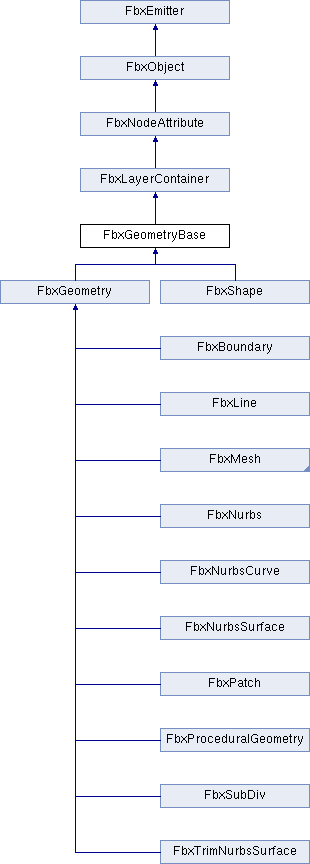
\includegraphics[height=12.000000cm]{class_fbx_geometry_base}
\end{center}
\end{figure}
\subsection*{公開メンバ関数}
\begin{DoxyCompactItemize}
\item 
virtual int \hyperlink{class_fbx_geometry_base_a858cccba0c319e1ee9160c0d7209bacf}{Memory\+Usage} () const
\item 
virtual \hyperlink{class_fbx_object}{Fbx\+Object} \& \hyperlink{class_fbx_geometry_base_a2c3754831338327259c35caebbf379d3}{Copy} (const \hyperlink{class_fbx_object}{Fbx\+Object} \&p\+Object)
\item 
virtual void \hyperlink{class_fbx_geometry_base_a66146155ecad4e6f6f2e8cf52e0340f6}{Compact} ()
\item 
bool \hyperlink{class_fbx_geometry_base_ad30d8655b9606f653e9467bb07c8b1f3}{Get\+Normals} (\hyperlink{class_fbx_layer_element_array_template}{Fbx\+Layer\+Element\+Array\+Template}$<$ \hyperlink{class_fbx_vector4}{Fbx\+Vector4} $>$ $\ast$$\ast$p\+Lockable\+Array) const
\item 
bool \hyperlink{class_fbx_geometry_base_ace44c4c25817ccabcf32e4c5b3b32936}{Get\+Normals\+Indices} (\hyperlink{class_fbx_layer_element_array_template}{Fbx\+Layer\+Element\+Array\+Template}$<$ int $>$ $\ast$$\ast$p\+Lockable\+Array) const
\item 
bool \hyperlink{class_fbx_geometry_base_aa8b22c9380e8c8be64855a6409136210}{Get\+Tangents} (\hyperlink{class_fbx_layer_element_array_template}{Fbx\+Layer\+Element\+Array\+Template}$<$ \hyperlink{class_fbx_vector4}{Fbx\+Vector4} $>$ $\ast$$\ast$p\+Lockable\+Array, const int p\+Layer\+Index=0) const
\item 
bool \hyperlink{class_fbx_geometry_base_aa1da929bb1905386e98d8e1caff3556e}{Get\+Tangents\+Indices} (\hyperlink{class_fbx_layer_element_array_template}{Fbx\+Layer\+Element\+Array\+Template}$<$ int $>$ $\ast$$\ast$p\+Lockable\+Array, const int p\+Layer\+Index=0) const
\item 
bool \hyperlink{class_fbx_geometry_base_a935f60845a0b9a5d484a8540f52ee07d}{Get\+Binormals} (\hyperlink{class_fbx_layer_element_array_template}{Fbx\+Layer\+Element\+Array\+Template}$<$ \hyperlink{class_fbx_vector4}{Fbx\+Vector4} $>$ $\ast$$\ast$p\+Lockable\+Array, const int p\+Layer\+Index=0) const
\item 
bool \hyperlink{class_fbx_geometry_base_af3b46f6aaa0e79c91ad7a89977413f57}{Get\+Binormals\+Indices} (\hyperlink{class_fbx_layer_element_array_template}{Fbx\+Layer\+Element\+Array\+Template}$<$ int $>$ $\ast$$\ast$p\+Lockable\+Array, const int p\+Layer\+Index=0) const
\end{DoxyCompactItemize}
\subsection*{公開変数類}
\begin{DoxyCompactItemize}
\item 
\hyperlink{class_fbx_array}{Fbx\+Array}$<$ \hyperlink{class_fbx_vector4}{Fbx\+Vector4} $>$ \hyperlink{class_fbx_geometry_base_a88c6c0552ceb07b3a638cc3175fbe867}{m\+Control\+Points}
\end{DoxyCompactItemize}
\subsection*{限定公開メンバ関数}
\begin{DoxyCompactItemize}
\item 
virtual void \hyperlink{class_fbx_geometry_base_a94ee142ac1d40be3aebb4d9441431921}{Construct\+Properties} (bool p\+Force\+Set)
\item 
virtual void \hyperlink{class_fbx_geometry_base_acf13ddd2717d2f1ca4dc57b5ea0801b1}{Content\+Clear} ()
\end{DoxyCompactItemize}
\subsection*{Control Points, Normals, Binormals and Tangent Management.}
\begin{DoxyCompactItemize}
\item 
virtual void \hyperlink{class_fbx_geometry_base_a471b736f2595c006a338c07a61907127}{Init\+Control\+Points} (int p\+Count)
\item 
void \hyperlink{class_fbx_geometry_base_a4bab80d4a05c813ad635127612f43515}{Init\+Normals} (int p\+Count=0)
\item 
void \hyperlink{class_fbx_geometry_base_ab0eed06f53d189b6c81560b78905c9b0}{Init\+Normals} (\hyperlink{class_fbx_geometry_base}{Fbx\+Geometry\+Base} $\ast$p\+Src)
\item 
void \hyperlink{class_fbx_geometry_base_ac5b188a0deba5132de9805538f014799}{Init\+Tangents} (int p\+Count=0, const int p\+Layer\+Index=0, const char $\ast$p\+Name=\char`\"{}\char`\"{})
\item 
void \hyperlink{class_fbx_geometry_base_ac6b469b25670b8a4c7a17042a96eb314}{Init\+Tangents} (\hyperlink{class_fbx_geometry_base}{Fbx\+Geometry\+Base} $\ast$p\+Src, const int p\+Layer\+Index=0)
\item 
void \hyperlink{class_fbx_geometry_base_abc912331f01b903dee155a1a3dbff0b8}{Init\+Binormals} (int p\+Count=0, const int p\+Layer\+Index=0, const char $\ast$p\+Name=\char`\"{}\char`\"{})
\item 
void \hyperlink{class_fbx_geometry_base_ac19b7cccc9249484196272c1df43b702}{Init\+Binormals} (\hyperlink{class_fbx_geometry_base}{Fbx\+Geometry\+Base} $\ast$p\+Src, const int p\+Layer\+Index=0)
\item 
virtual void \hyperlink{class_fbx_geometry_base_a4f54256d4cbc5e7ae0ae533f7b77ace4}{Set\+Control\+Point\+At} (const \hyperlink{class_fbx_vector4}{Fbx\+Vector4} \&p\+Ctrl\+Point, const \hyperlink{class_fbx_vector4}{Fbx\+Vector4} \&p\+Normal, int p\+Index, bool p\+I2\+D\+Search=false)
\item 
virtual void \hyperlink{class_fbx_geometry_base_ab2d5567b073e6b9f4feb5bb428fa99e4}{Set\+Control\+Point\+At} (const \hyperlink{class_fbx_vector4}{Fbx\+Vector4} \&p\+Ctrl\+Point, int p\+Index)
\item 
virtual \hyperlink{class_fbx_vector4}{Fbx\+Vector4} \hyperlink{class_fbx_geometry_base_a16c45afeb6008d346593882b979f0ed7}{Get\+Control\+Point\+At} (int p\+Index) const
\item 
virtual void \hyperlink{class_fbx_geometry_base_a219c072f0c9a67ddcc928ab3998f9494}{Set\+Control\+Point\+Normal\+At} (const \hyperlink{class_fbx_vector4}{Fbx\+Vector4} \&p\+Normal, int p\+Index, bool p\+I2\+D\+Search=false)
\item 
virtual int \hyperlink{class_fbx_geometry_base_aa9f42ae6a958036722670143fabf3b17}{Get\+Control\+Points\+Count} () const
\item 
virtual \hyperlink{class_fbx_vector4}{Fbx\+Vector4} $\ast$ \hyperlink{class_fbx_geometry_base_ad4db22a2f2e673c216cacdc9cd172d77}{Get\+Control\+Points} (\hyperlink{class_fbx_status}{Fbx\+Status} $\ast$p\+Status=\hyperlink{fbxarch_8h_a070d2ce7b6bb7e5c05602aa8c308d0c4}{N\+U\+LL}) const
\item 
virtual void \hyperlink{class_fbx_geometry_base_aea3fc519575d88c430221b0e74040b0c}{Set\+Control\+Point\+Count} (int p\+Count)
\end{DoxyCompactItemize}
\subsection*{Public and fast access Properties}
\begin{DoxyCompactItemize}
\item 
\hyperlink{class_fbx_property_t}{Fbx\+PropertyT}$<$ \hyperlink{fbxtypes_8h_a92e0562b2fe33e76a242f498b362262e}{Fbx\+Bool} $>$ \hyperlink{class_fbx_geometry_base_a51e2206786ddb6a94a15be4a8fd9517f}{Primary\+Visibility}
\begin{DoxyCompactList}\small\item\em Control the geometry render state. Geometry can still cast shadows even if this is turned off. \end{DoxyCompactList}\item 
\hyperlink{class_fbx_property_t}{Fbx\+PropertyT}$<$ \hyperlink{fbxtypes_8h_a92e0562b2fe33e76a242f498b362262e}{Fbx\+Bool} $>$ \hyperlink{class_fbx_geometry_base_a64d3184a3bf9bcd97f7069176b0ad4c1}{Cast\+Shadow}
\begin{DoxyCompactList}\small\item\em If true, the geometry will produce shadows. \end{DoxyCompactList}\item 
\hyperlink{class_fbx_property_t}{Fbx\+PropertyT}$<$ \hyperlink{fbxtypes_8h_a92e0562b2fe33e76a242f498b362262e}{Fbx\+Bool} $>$ \hyperlink{class_fbx_geometry_base_a38e79ed34812e8b02828ebb5690f4ce8}{Receive\+Shadow}
\begin{DoxyCompactList}\small\item\em If true, the geometry will receive shadows. \end{DoxyCompactList}\item 
\hyperlink{class_fbx_property_t}{Fbx\+PropertyT}$<$ \hyperlink{fbxtypes_8h_ae0a96f14cde566774c7553aa7523b7a7}{Fbx\+Double3} $>$ \hyperlink{class_fbx_geometry_base_a66d6d410709e83f4f4d0a17651fbb717}{B\+Box\+Min}
\begin{DoxyCompactList}\small\item\em The minimum value of the control points bounding box. \end{DoxyCompactList}\item 
\hyperlink{class_fbx_property_t}{Fbx\+PropertyT}$<$ \hyperlink{fbxtypes_8h_ae0a96f14cde566774c7553aa7523b7a7}{Fbx\+Double3} $>$ \hyperlink{class_fbx_geometry_base_a462c10c0d41fe55413e41435e62128c9}{B\+Box\+Max}
\begin{DoxyCompactList}\small\item\em The maximum value of the control points bounding box. \end{DoxyCompactList}\item 
void \hyperlink{class_fbx_geometry_base_a6c27b53ff81cdcbe4f6da4b1acfd4375}{Compute\+B\+Box} ()
\end{DoxyCompactItemize}
\subsection*{Geometry Element Management.}
\label{_amgrp5c89d833850d940ed0bcf07e321db4e1}%
 A Fbx\+Geometry\+Element describes how the geometry element (normals, U\+Vs and etc.) is mapped to a geometry surface and how the mapping information is arranged in memory. Fbx\+Geometry\+Element is exactly the same as \hyperlink{class_fbx_layer_element}{Fbx\+Layer\+Element} but does not expose the geometry\textquotesingle{}s layer information. Use the geometry element classes to decompose the geometry without dealing with layers. \begin{DoxyCompactItemize}
\item 
\hyperlink{fbxlayer_8h_a54a5aaec6f1979871fe9d93dd2d246c9}{Fbx\+Geometry\+Element\+Normal} $\ast$ \hyperlink{class_fbx_geometry_base_a13810d0c6ac68ab14be3f1316b977f7d}{Create\+Element\+Normal} ()
\item 
bool \hyperlink{class_fbx_geometry_base_a9aadbaa3f50db80b67bd1b3bc9119c7b}{Remove\+Element\+Normal} (\hyperlink{fbxlayer_8h_a54a5aaec6f1979871fe9d93dd2d246c9}{Fbx\+Geometry\+Element\+Normal} $\ast$p\+Element\+Normal)
\item 
\hyperlink{fbxlayer_8h_a54a5aaec6f1979871fe9d93dd2d246c9}{Fbx\+Geometry\+Element\+Normal} $\ast$ \hyperlink{class_fbx_geometry_base_ab7486b08caa6e90923fbb194bd81a61e}{Get\+Element\+Normal} (int p\+Index=0)
\item 
const \hyperlink{fbxlayer_8h_a54a5aaec6f1979871fe9d93dd2d246c9}{Fbx\+Geometry\+Element\+Normal} $\ast$ \hyperlink{class_fbx_geometry_base_a33d41a1c8b2346aa73a2576225387fb4}{Get\+Element\+Normal} (int p\+Index=0) const
\item 
int \hyperlink{class_fbx_geometry_base_ae8cffdf94daa997de808328579c636c2}{Get\+Element\+Normal\+Count} () const
\item 
\hyperlink{fbxlayer_8h_a066e30a64eb051458583b656a651e90b}{Fbx\+Geometry\+Element\+Binormal} $\ast$ \hyperlink{class_fbx_geometry_base_aaac14a98782b9f68803462f033297d05}{Create\+Element\+Binormal} ()
\item 
bool \hyperlink{class_fbx_geometry_base_a07a88ca035b8b21b407a88bef375831f}{Remove\+Element\+Binormal} (\hyperlink{fbxlayer_8h_a066e30a64eb051458583b656a651e90b}{Fbx\+Geometry\+Element\+Binormal} $\ast$p\+Element\+Binormal)
\item 
\hyperlink{fbxlayer_8h_a066e30a64eb051458583b656a651e90b}{Fbx\+Geometry\+Element\+Binormal} $\ast$ \hyperlink{class_fbx_geometry_base_a810b4a313e01bbaa41fe25ac753a8996}{Get\+Element\+Binormal} (int p\+Index=0)
\item 
const \hyperlink{fbxlayer_8h_a066e30a64eb051458583b656a651e90b}{Fbx\+Geometry\+Element\+Binormal} $\ast$ \hyperlink{class_fbx_geometry_base_a12bc9aca7ec57790db96fa47219c559c}{Get\+Element\+Binormal} (int p\+Index=0) const
\item 
int \hyperlink{class_fbx_geometry_base_a04500774d4c9bfc97418f45aff63404e}{Get\+Element\+Binormal\+Count} () const
\item 
\hyperlink{fbxlayer_8h_a291cacd8b247483cc24704c8f49087a7}{Fbx\+Geometry\+Element\+Tangent} $\ast$ \hyperlink{class_fbx_geometry_base_a88790830df691da97b5f027a66d98eec}{Create\+Element\+Tangent} ()
\item 
bool \hyperlink{class_fbx_geometry_base_a9289899568d50f8b60c3a33761c92446}{Remove\+Element\+Tangent} (\hyperlink{fbxlayer_8h_a291cacd8b247483cc24704c8f49087a7}{Fbx\+Geometry\+Element\+Tangent} $\ast$p\+Element\+Tangent)
\item 
\hyperlink{fbxlayer_8h_a291cacd8b247483cc24704c8f49087a7}{Fbx\+Geometry\+Element\+Tangent} $\ast$ \hyperlink{class_fbx_geometry_base_a28cf260152f84ce031a3d2844b9895cc}{Get\+Element\+Tangent} (int p\+Index=0)
\item 
const \hyperlink{fbxlayer_8h_a291cacd8b247483cc24704c8f49087a7}{Fbx\+Geometry\+Element\+Tangent} $\ast$ \hyperlink{class_fbx_geometry_base_a5fedf8c0a50736da2fa590cf1b922506}{Get\+Element\+Tangent} (int p\+Index=0) const
\item 
int \hyperlink{class_fbx_geometry_base_ac7a775211507bd51dd804d8e013f625c}{Get\+Element\+Tangent\+Count} () const
\item 
\hyperlink{fbxlayer_8h_a1a779f3f614dbf0024c07f4a1d8332f4}{Fbx\+Geometry\+Element\+Material} $\ast$ \hyperlink{class_fbx_geometry_base_a1c93bffeaa9af18fd7ab9c2eb68ca4ec}{Create\+Element\+Material} ()
\item 
bool \hyperlink{class_fbx_geometry_base_a396c0e3be695dbca3724be1e47e9f7cb}{Remove\+Element\+Material} (\hyperlink{fbxlayer_8h_a1a779f3f614dbf0024c07f4a1d8332f4}{Fbx\+Geometry\+Element\+Material} $\ast$p\+Element\+Material)
\item 
\hyperlink{fbxlayer_8h_a1a779f3f614dbf0024c07f4a1d8332f4}{Fbx\+Geometry\+Element\+Material} $\ast$ \hyperlink{class_fbx_geometry_base_ac49c730d0f134f1aff416bc4be5ca4e5}{Get\+Element\+Material} (int p\+Index=0)
\item 
const \hyperlink{fbxlayer_8h_a1a779f3f614dbf0024c07f4a1d8332f4}{Fbx\+Geometry\+Element\+Material} $\ast$ \hyperlink{class_fbx_geometry_base_acd0f6cd7ecaa99d15aab3e211857f462}{Get\+Element\+Material} (int p\+Index=0) const
\item 
int \hyperlink{class_fbx_geometry_base_a443797935c203b51edb4004907613017}{Get\+Element\+Material\+Count} () const
\item 
\hyperlink{fbxlayer_8h_aa5c7fb92a1c396014bf2ced7797a95a9}{Fbx\+Geometry\+Element\+Polygon\+Group} $\ast$ \hyperlink{class_fbx_geometry_base_a94ad7ac87ced572287ee85460304eb09}{Create\+Element\+Polygon\+Group} ()
\item 
bool \hyperlink{class_fbx_geometry_base_a0746664cececc19040a011ddbc7c7623}{Remove\+Element\+Polygon\+Group} (\hyperlink{fbxlayer_8h_aa5c7fb92a1c396014bf2ced7797a95a9}{Fbx\+Geometry\+Element\+Polygon\+Group} $\ast$p\+Element\+Polygon\+Group)
\item 
\hyperlink{fbxlayer_8h_aa5c7fb92a1c396014bf2ced7797a95a9}{Fbx\+Geometry\+Element\+Polygon\+Group} $\ast$ \hyperlink{class_fbx_geometry_base_ae54cbd4165026b82500d776a21e81e32}{Get\+Element\+Polygon\+Group} (int p\+Index=0)
\item 
const \hyperlink{fbxlayer_8h_aa5c7fb92a1c396014bf2ced7797a95a9}{Fbx\+Geometry\+Element\+Polygon\+Group} $\ast$ \hyperlink{class_fbx_geometry_base_a11838aa5259cb37a3024a9eb654b705c}{Get\+Element\+Polygon\+Group} (int p\+Index=0) const
\item 
int \hyperlink{class_fbx_geometry_base_a138cf34dd7162a7984a3317d0d4ff03b}{Get\+Element\+Polygon\+Group\+Count} () const
\item 
\hyperlink{fbxlayer_8h_a4baddeaf720350758d230973d114f593}{Fbx\+Geometry\+Element\+Vertex\+Color} $\ast$ \hyperlink{class_fbx_geometry_base_a866f39f540f6bc9ca8e529f27d9ebee4}{Create\+Element\+Vertex\+Color} ()
\item 
bool \hyperlink{class_fbx_geometry_base_a123d97fbece214d31199a63c90eb44e1}{Remove\+Element\+Vertex\+Color} (\hyperlink{fbxlayer_8h_a4baddeaf720350758d230973d114f593}{Fbx\+Geometry\+Element\+Vertex\+Color} $\ast$p\+Element\+Vertex\+Color)
\item 
\hyperlink{fbxlayer_8h_a4baddeaf720350758d230973d114f593}{Fbx\+Geometry\+Element\+Vertex\+Color} $\ast$ \hyperlink{class_fbx_geometry_base_a1b93a0dc9da34d479e5535d7d589fe0b}{Get\+Element\+Vertex\+Color} (int p\+Index=0)
\item 
const \hyperlink{fbxlayer_8h_a4baddeaf720350758d230973d114f593}{Fbx\+Geometry\+Element\+Vertex\+Color} $\ast$ \hyperlink{class_fbx_geometry_base_ac4748b1ed1007746aa7acf2f4c300d9f}{Get\+Element\+Vertex\+Color} (int p\+Index=0) const
\item 
int \hyperlink{class_fbx_geometry_base_ab0c36aa02e726e017f02802a42705f68}{Get\+Element\+Vertex\+Color\+Count} () const
\item 
\hyperlink{fbxlayer_8h_a6a651170dec994ac83db90645d9ecfd3}{Fbx\+Geometry\+Element\+Smoothing} $\ast$ \hyperlink{class_fbx_geometry_base_a998f217dc7383a3fdd5bd4269d424fe3}{Create\+Element\+Smoothing} ()
\item 
bool \hyperlink{class_fbx_geometry_base_a55da601b539c3e1c933fb1b3f053e1ca}{Remove\+Element\+Smoothing} (\hyperlink{fbxlayer_8h_a6a651170dec994ac83db90645d9ecfd3}{Fbx\+Geometry\+Element\+Smoothing} $\ast$p\+Element\+Smoothing)
\item 
\hyperlink{fbxlayer_8h_a6a651170dec994ac83db90645d9ecfd3}{Fbx\+Geometry\+Element\+Smoothing} $\ast$ \hyperlink{class_fbx_geometry_base_a6ba008301dd152eef938f18fc87ff385}{Get\+Element\+Smoothing} (int p\+Index=0)
\item 
const \hyperlink{fbxlayer_8h_a6a651170dec994ac83db90645d9ecfd3}{Fbx\+Geometry\+Element\+Smoothing} $\ast$ \hyperlink{class_fbx_geometry_base_a0a464128150ff6eee48b6913b22a1c49}{Get\+Element\+Smoothing} (int p\+Index=0) const
\item 
int \hyperlink{class_fbx_geometry_base_a65ce50bb6548a0c1cc3a237b1f953242}{Get\+Element\+Smoothing\+Count} () const
\item 
\hyperlink{fbxlayer_8h_aa1db71d39153856548f192cf52aa2cc5}{Fbx\+Geometry\+Element\+Crease} $\ast$ \hyperlink{class_fbx_geometry_base_ac31ccf6da5d91b8df915bb1ace15e399}{Create\+Element\+Vertex\+Crease} ()
\item 
bool \hyperlink{class_fbx_geometry_base_a01fe726448c9362a399148aceb051f71}{Remove\+Element\+Vertex\+Crease} (\hyperlink{fbxlayer_8h_aa1db71d39153856548f192cf52aa2cc5}{Fbx\+Geometry\+Element\+Crease} $\ast$p\+Element\+Crease)
\item 
\hyperlink{fbxlayer_8h_aa1db71d39153856548f192cf52aa2cc5}{Fbx\+Geometry\+Element\+Crease} $\ast$ \hyperlink{class_fbx_geometry_base_a2ba68cd342357a08aceae046aba944d4}{Get\+Element\+Vertex\+Crease} (int p\+Index=0)
\item 
const \hyperlink{fbxlayer_8h_aa1db71d39153856548f192cf52aa2cc5}{Fbx\+Geometry\+Element\+Crease} $\ast$ \hyperlink{class_fbx_geometry_base_aa54ec0641f415576fd7e09753df8fa0d}{Get\+Element\+Vertex\+Crease} (int p\+Index=0) const
\item 
int \hyperlink{class_fbx_geometry_base_afc099f60d6c45cbac000b10d95c83377}{Get\+Element\+Vertex\+Crease\+Count} () const
\item 
\hyperlink{fbxlayer_8h_aa1db71d39153856548f192cf52aa2cc5}{Fbx\+Geometry\+Element\+Crease} $\ast$ \hyperlink{class_fbx_geometry_base_ae5475b4e64c7fa7a9c3c1edd3365d53f}{Create\+Element\+Edge\+Crease} ()
\item 
bool \hyperlink{class_fbx_geometry_base_a91216359c824cc80d113e0760d59e9bb}{Remove\+Element\+Edge\+Crease} (\hyperlink{fbxlayer_8h_aa1db71d39153856548f192cf52aa2cc5}{Fbx\+Geometry\+Element\+Crease} $\ast$p\+Element\+Crease)
\item 
\hyperlink{fbxlayer_8h_aa1db71d39153856548f192cf52aa2cc5}{Fbx\+Geometry\+Element\+Crease} $\ast$ \hyperlink{class_fbx_geometry_base_acb7576ed7cf6011f456e6a3d30082058}{Get\+Element\+Edge\+Crease} (int p\+Index=0)
\item 
const \hyperlink{fbxlayer_8h_aa1db71d39153856548f192cf52aa2cc5}{Fbx\+Geometry\+Element\+Crease} $\ast$ \hyperlink{class_fbx_geometry_base_af596440c20b05b92559190449803b8e8}{Get\+Element\+Edge\+Crease} (int p\+Index=0) const
\item 
int \hyperlink{class_fbx_geometry_base_aeafa5b8ecd4a424003624e2e35978033}{Get\+Element\+Edge\+Crease\+Count} () const
\item 
\hyperlink{fbxlayer_8h_ac66f768aa149c016447f88213c374e25}{Fbx\+Geometry\+Element\+Hole} $\ast$ \hyperlink{class_fbx_geometry_base_a2c30734fb6ff6bb93adadd35978fc146}{Create\+Element\+Hole} ()
\item 
bool \hyperlink{class_fbx_geometry_base_a26484bbcc3f5a76366fcbe7352c8fefa}{Remove\+Element\+Hole} (\hyperlink{fbxlayer_8h_ac66f768aa149c016447f88213c374e25}{Fbx\+Geometry\+Element\+Hole} $\ast$p\+Element\+Hole)
\item 
\hyperlink{fbxlayer_8h_ac66f768aa149c016447f88213c374e25}{Fbx\+Geometry\+Element\+Hole} $\ast$ \hyperlink{class_fbx_geometry_base_af4daaf3e4a61bfd482d70d41d0a9e350}{Get\+Element\+Hole} (int p\+Index=0)
\item 
const \hyperlink{fbxlayer_8h_ac66f768aa149c016447f88213c374e25}{Fbx\+Geometry\+Element\+Hole} $\ast$ \hyperlink{class_fbx_geometry_base_a503d850eaaed9c21457cf19b86080f14}{Get\+Element\+Hole} (int p\+Index=0) const
\item 
int \hyperlink{class_fbx_geometry_base_a93f4c298785352d3a8e05596d31d0760}{Get\+Element\+Hole\+Count} () const
\item 
\hyperlink{fbxlayer_8h_acef498b248e323a189b5ccbf478b0b41}{Fbx\+Geometry\+Element\+User\+Data} $\ast$ \hyperlink{class_fbx_geometry_base_a457a8982320b3637353051aaec987c90}{Create\+Element\+User\+Data} ()
\item 
bool \hyperlink{class_fbx_geometry_base_abf8c753f38229a2b076ec20a17da6807}{Remove\+Element\+User\+Data} (\hyperlink{fbxlayer_8h_acef498b248e323a189b5ccbf478b0b41}{Fbx\+Geometry\+Element\+User\+Data} $\ast$p\+Element\+User\+Data)
\item 
\hyperlink{fbxlayer_8h_acef498b248e323a189b5ccbf478b0b41}{Fbx\+Geometry\+Element\+User\+Data} $\ast$ \hyperlink{class_fbx_geometry_base_aaae41fe6881f55fb722cb9fae88c5bbf}{Get\+Element\+User\+Data} (int p\+Index=0)
\item 
const \hyperlink{fbxlayer_8h_acef498b248e323a189b5ccbf478b0b41}{Fbx\+Geometry\+Element\+User\+Data} $\ast$ \hyperlink{class_fbx_geometry_base_a40c905252aebb1ea71bd4d71a4c8704d}{Get\+Element\+User\+Data} (int p\+Index=0) const
\item 
int \hyperlink{class_fbx_geometry_base_a8ea1964abcfde21f82d576ca07ac7f67}{Get\+Element\+User\+Data\+Count} () const
\item 
\hyperlink{fbxlayer_8h_a98f6c16a3021e9e04b0352f652eac2a1}{Fbx\+Geometry\+Element\+Visibility} $\ast$ \hyperlink{class_fbx_geometry_base_a92af07a2d0739a8e27108838c5c7eac4}{Create\+Element\+Visibility} ()
\item 
bool \hyperlink{class_fbx_geometry_base_a5265ada1a14bc10a5be69719547827b5}{Remove\+Element\+Visibility} (\hyperlink{fbxlayer_8h_a98f6c16a3021e9e04b0352f652eac2a1}{Fbx\+Geometry\+Element\+Visibility} $\ast$p\+Element\+Visibility)
\item 
\hyperlink{fbxlayer_8h_a98f6c16a3021e9e04b0352f652eac2a1}{Fbx\+Geometry\+Element\+Visibility} $\ast$ \hyperlink{class_fbx_geometry_base_ad4efa742959f1ff9db49f67cebcc5779}{Get\+Element\+Visibility} (int p\+Index=0)
\item 
const \hyperlink{fbxlayer_8h_a98f6c16a3021e9e04b0352f652eac2a1}{Fbx\+Geometry\+Element\+Visibility} $\ast$ \hyperlink{class_fbx_geometry_base_a7354e0200f75665cbc4f3137cac53046}{Get\+Element\+Visibility} (int p\+Index=0) const
\item 
int \hyperlink{class_fbx_geometry_base_a9f41f006fb1545c11e1a06c80312cda9}{Get\+Element\+Visibility\+Count} () const
\item 
\hyperlink{fbxlayer_8h_a12413531f4bb2c482e3ddbd59e3417e5}{Fbx\+Geometry\+Element\+UV} $\ast$ \hyperlink{class_fbx_geometry_base_ac2d647f718a69776037377e79dfc8c3e}{Create\+Element\+UV} (const char $\ast$p\+U\+V\+Set\+Name, \hyperlink{class_fbx_layer_element_a8c95c5cd880b56c776acd379bd86f42c}{Fbx\+Layer\+Element\+::\+E\+Type} p\+Type\+Identifier=\hyperlink{class_fbx_layer_element_a8c95c5cd880b56c776acd379bd86f42ca09829e6ecf512e7ae04d9ad8de1342fa}{Fbx\+Layer\+Element\+::e\+Texture\+Diffuse})
\item 
bool \hyperlink{class_fbx_geometry_base_a0f571119663cc96a58d42e0e555a9be6}{Remove\+Element\+UV} (\hyperlink{fbxlayer_8h_a12413531f4bb2c482e3ddbd59e3417e5}{Fbx\+Geometry\+Element\+UV} $\ast$p\+Element\+UV)
\item 
\hyperlink{fbxlayer_8h_a12413531f4bb2c482e3ddbd59e3417e5}{Fbx\+Geometry\+Element\+UV} $\ast$ \hyperlink{class_fbx_geometry_base_a47702a12ebe438343757fbbe2ebd41d3}{Get\+Element\+UV} (int p\+Index=0, \hyperlink{class_fbx_layer_element_a8c95c5cd880b56c776acd379bd86f42c}{Fbx\+Layer\+Element\+::\+E\+Type} p\+Type\+Identifier=\hyperlink{class_fbx_layer_element_a8c95c5cd880b56c776acd379bd86f42cab3768744dc14ef9fcf6631d3ade97e54}{Fbx\+Layer\+Element\+::e\+Unknown})
\item 
const \hyperlink{fbxlayer_8h_a12413531f4bb2c482e3ddbd59e3417e5}{Fbx\+Geometry\+Element\+UV} $\ast$ \hyperlink{class_fbx_geometry_base_aacf39d3a8ff304383999ffff1500598f}{Get\+Element\+UV} (int p\+Index=0, \hyperlink{class_fbx_layer_element_a8c95c5cd880b56c776acd379bd86f42c}{Fbx\+Layer\+Element\+::\+E\+Type} p\+Type\+Identifier=\hyperlink{class_fbx_layer_element_a8c95c5cd880b56c776acd379bd86f42cab3768744dc14ef9fcf6631d3ade97e54}{Fbx\+Layer\+Element\+::e\+Unknown}) const
\item 
int \hyperlink{class_fbx_geometry_base_a617a6e3bcbceb4489e2db1a386f9640b}{Get\+Element\+U\+V\+Count} (\hyperlink{class_fbx_layer_element_a8c95c5cd880b56c776acd379bd86f42c}{Fbx\+Layer\+Element\+::\+E\+Type} p\+Type\+Identifier=\hyperlink{class_fbx_layer_element_a8c95c5cd880b56c776acd379bd86f42cab3768744dc14ef9fcf6631d3ade97e54}{Fbx\+Layer\+Element\+::e\+Unknown}) const
\item 
\hyperlink{fbxlayer_8h_a12413531f4bb2c482e3ddbd59e3417e5}{Fbx\+Geometry\+Element\+UV} $\ast$ \hyperlink{class_fbx_geometry_base_ac6fda0d204a28b5e67ef46b9bce6e288}{Get\+Element\+UV} (const char $\ast$p\+U\+V\+Set\+Name)
\item 
const \hyperlink{fbxlayer_8h_a12413531f4bb2c482e3ddbd59e3417e5}{Fbx\+Geometry\+Element\+UV} $\ast$ \hyperlink{class_fbx_geometry_base_a31f84a19326288aa8315fdbbec39a90a}{Get\+Element\+UV} (const char $\ast$p\+U\+V\+Set\+Name) const
\item 
void \hyperlink{class_fbx_geometry_base_a65147440e2f577ab7f5b60e228881641}{Get\+U\+V\+Set\+Names} (\hyperlink{class_fbx_string_list}{Fbx\+String\+List} \&p\+U\+V\+Set\+Name\+List) const
\end{DoxyCompactItemize}
\subsection*{Off-\/loading Serialization section}
\label{_amgrpe1aaec84f361fca191ade63ad8637b37}%
 The methods in this section are typically called by a peripheral (\hyperlink{class_fbx_peripheral}{Fbx\+Peripheral}). There should be no real interest in calling them directly. The functions will write/read the memory dump of the data contained in this class. Each data block written/read will start with an (int) value representing the number of items in the array. If this value (v) is not zero, it will be followed by the array content. A block of data that is (v $\ast$ sizeof(array item size)) bytes big. The methods will also call the parent class ones to dump the Layers content. \begin{DoxyCompactItemize}
\item 
virtual bool \hyperlink{class_fbx_geometry_base_a7b80ccbcd2b15bbedbe7dd7e0739a3b3}{Content\+Write\+To} (\hyperlink{class_fbx_stream}{Fbx\+Stream} \&p\+Stream) const
\item 
virtual bool \hyperlink{class_fbx_geometry_base_a6d34ab23d253b07cac24267177096c1a}{Content\+Read\+From} (const \hyperlink{class_fbx_stream}{Fbx\+Stream} \&p\+Stream)
\end{DoxyCompactItemize}
\subsection*{その他の継承メンバ}


\subsection{詳解}
This class is the base class for geometric object such as meshes, N\+U\+R\+BS and patches. Use the \hyperlink{class_fbx_geometry_base}{Fbx\+Geometry\+Base} class to manage the control points, normals, binormals and tangents of the geometries. The meaning of \char`\"{}control point\char`\"{} is dependent of the geometry object type. For meshes, the \char`\"{}control point\char`\"{} is the physical 3D coordinate of polygon vertices while, for N\+U\+R\+BS, it is the the actual control point on the curves defining the surface. This class also allow you to define normals, binormals and tangents regardless of the type of geometric object. However, in reality, applying such definitions to N\+U\+R\+BS and patches does not make much sense since these definitions would only exist at the control points and inbetween them, the interpolation would certainly not follow the curve.

Geometric objects are using a system of layered data to extend their construction definition. For example, a typical layer for a Mesh contains Normals, U\+Vs and Materials but client applications can decide to define another set of Normals and U\+Vs and swap them during the rendering phase to produce some different results. The combinations are limitless and it would be impossible to discuss them all. This example has been presented to show one possible context where layers can be used. More information can be found in the \hyperlink{class_fbx_layer_container}{Fbx\+Layer\+Container} and \hyperlink{class_fbx_layer}{Fbx\+Layer} classes description. 

 fbxgeometrybase.\+h の 43 行目に定義があります。



\subsection{関数詳解}
\mbox{\Hypertarget{class_fbx_geometry_base_a66146155ecad4e6f6f2e8cf52e0340f6}\label{class_fbx_geometry_base_a66146155ecad4e6f6f2e8cf52e0340f6}} 
\index{Fbx\+Geometry\+Base@{Fbx\+Geometry\+Base}!Compact@{Compact}}
\index{Compact@{Compact}!Fbx\+Geometry\+Base@{Fbx\+Geometry\+Base}}
\subsubsection{\texorpdfstring{Compact()}{Compact()}}
{\footnotesize\ttfamily virtual void Fbx\+Geometry\+Base\+::\+Compact (\begin{DoxyParamCaption}{ }\end{DoxyParamCaption})\hspace{0.3cm}{\ttfamily [virtual]}}

Compact the memory used by this object. \begin{DoxyRemark}{注釈}
Note that this function might not result in saved memory because it depends if the sub-\/class implements it, or if any memory can actually be saved. 
\end{DoxyRemark}


\hyperlink{class_fbx_object_a2720f16a08150d162242b0c59f58c3dc}{Fbx\+Object}を再実装しています。



\hyperlink{class_fbx_mesh_a05ca6a8fbd028777c91931ce6edf4b19}{Fbx\+Mesh}, \hyperlink{class_fbx_shape_a9c3c948d3646bf78472164860ad11d65}{Fbx\+Shape}で再実装されています。

\mbox{\Hypertarget{class_fbx_geometry_base_a6c27b53ff81cdcbe4f6da4b1acfd4375}\label{class_fbx_geometry_base_a6c27b53ff81cdcbe4f6da4b1acfd4375}} 
\index{Fbx\+Geometry\+Base@{Fbx\+Geometry\+Base}!Compute\+B\+Box@{Compute\+B\+Box}}
\index{Compute\+B\+Box@{Compute\+B\+Box}!Fbx\+Geometry\+Base@{Fbx\+Geometry\+Base}}
\subsubsection{\texorpdfstring{Compute\+B\+Box()}{ComputeBBox()}}
{\footnotesize\ttfamily void Fbx\+Geometry\+Base\+::\+Compute\+B\+Box (\begin{DoxyParamCaption}{ }\end{DoxyParamCaption})}

Computes the control points Bounding box. \mbox{\Hypertarget{class_fbx_geometry_base_a94ee142ac1d40be3aebb4d9441431921}\label{class_fbx_geometry_base_a94ee142ac1d40be3aebb4d9441431921}} 
\index{Fbx\+Geometry\+Base@{Fbx\+Geometry\+Base}!Construct\+Properties@{Construct\+Properties}}
\index{Construct\+Properties@{Construct\+Properties}!Fbx\+Geometry\+Base@{Fbx\+Geometry\+Base}}
\subsubsection{\texorpdfstring{Construct\+Properties()}{ConstructProperties()}}
{\footnotesize\ttfamily virtual void Fbx\+Geometry\+Base\+::\+Construct\+Properties (\begin{DoxyParamCaption}\item[{bool}]{p\+Force\+Set }\end{DoxyParamCaption})\hspace{0.3cm}{\ttfamily [protected]}, {\ttfamily [virtual]}}

Optional property constructor override, automatically called by default constructor. 
\begin{DoxyParams}{引数}
{\em p\+Force\+Set} & If the property value must be set regardless of default value. \\
\hline
\end{DoxyParams}
\begin{DoxyRemark}{注釈}
If your object have properties, they must be initialized in this function. 
\end{DoxyRemark}


\hyperlink{class_fbx_node_attribute_a042eb9949a9b9634dcc5f126e82fd04a}{Fbx\+Node\+Attribute}を再実装しています。



\hyperlink{class_fbx_line_a48df4b6cd889814d3fe7ca5bb09bcc78}{Fbx\+Line}, \hyperlink{class_fbx_boundary_acb50e021b1e9920026c975613a949537}{Fbx\+Boundary}, \hyperlink{class_my_k_fbx_mesh_a9fc01e7c17e2e1456cf7859f05d253e8}{My\+K\+Fbx\+Mesh}で再実装されています。

\mbox{\Hypertarget{class_fbx_geometry_base_acf13ddd2717d2f1ca4dc57b5ea0801b1}\label{class_fbx_geometry_base_acf13ddd2717d2f1ca4dc57b5ea0801b1}} 
\index{Fbx\+Geometry\+Base@{Fbx\+Geometry\+Base}!Content\+Clear@{Content\+Clear}}
\index{Content\+Clear@{Content\+Clear}!Fbx\+Geometry\+Base@{Fbx\+Geometry\+Base}}
\subsubsection{\texorpdfstring{Content\+Clear()}{ContentClear()}}
{\footnotesize\ttfamily virtual void Fbx\+Geometry\+Base\+::\+Content\+Clear (\begin{DoxyParamCaption}{ }\end{DoxyParamCaption})\hspace{0.3cm}{\ttfamily [protected]}, {\ttfamily [virtual]}}

Clears this object\textquotesingle{}s content from memory. This method must be overridden in the derived classes. \begin{DoxyRemark}{注釈}
This method is called by \hyperlink{class_fbx_object_ac28653a3c65e840498eebfb54276e483}{Content\+Unload()} if the object content\textquotesingle{}s unloading is successful. 
\end{DoxyRemark}


\hyperlink{class_fbx_object_a284f2a438579fcacd8bffd85f556dde2}{Fbx\+Object}を再実装しています。



\hyperlink{class_fbx_mesh_aacd77ff7908d897c73983919c4aade72}{Fbx\+Mesh}で再実装されています。

\mbox{\Hypertarget{class_fbx_geometry_base_a6d34ab23d253b07cac24267177096c1a}\label{class_fbx_geometry_base_a6d34ab23d253b07cac24267177096c1a}} 
\index{Fbx\+Geometry\+Base@{Fbx\+Geometry\+Base}!Content\+Read\+From@{Content\+Read\+From}}
\index{Content\+Read\+From@{Content\+Read\+From}!Fbx\+Geometry\+Base@{Fbx\+Geometry\+Base}}
\subsubsection{\texorpdfstring{Content\+Read\+From()}{ContentReadFrom()}}
{\footnotesize\ttfamily virtual bool Fbx\+Geometry\+Base\+::\+Content\+Read\+From (\begin{DoxyParamCaption}\item[{const \hyperlink{class_fbx_stream}{Fbx\+Stream} \&}]{p\+Stream }\end{DoxyParamCaption})\hspace{0.3cm}{\ttfamily [virtual]}}

Reads the content of the geometry object from the specified stream. 
\begin{DoxyParams}{引数}
{\em p\+Stream} & The source stream. \\
\hline
\end{DoxyParams}
\begin{DoxyReturn}{戻り値}
{\ttfamily True} if the geometry object fills itself with the received data from the stream successfully, {\ttfamily false} otherwise. 
\end{DoxyReturn}


\hyperlink{class_fbx_object_aeb4255bda633e1986730748758a7cf6c}{Fbx\+Object}を再実装しています。



\hyperlink{class_fbx_patch_ad1aac4a2e0e820f27ff9a0123ba5756e}{Fbx\+Patch}で再実装されています。

\mbox{\Hypertarget{class_fbx_geometry_base_a7b80ccbcd2b15bbedbe7dd7e0739a3b3}\label{class_fbx_geometry_base_a7b80ccbcd2b15bbedbe7dd7e0739a3b3}} 
\index{Fbx\+Geometry\+Base@{Fbx\+Geometry\+Base}!Content\+Write\+To@{Content\+Write\+To}}
\index{Content\+Write\+To@{Content\+Write\+To}!Fbx\+Geometry\+Base@{Fbx\+Geometry\+Base}}
\subsubsection{\texorpdfstring{Content\+Write\+To()}{ContentWriteTo()}}
{\footnotesize\ttfamily virtual bool Fbx\+Geometry\+Base\+::\+Content\+Write\+To (\begin{DoxyParamCaption}\item[{\hyperlink{class_fbx_stream}{Fbx\+Stream} \&}]{p\+Stream }\end{DoxyParamCaption}) const\hspace{0.3cm}{\ttfamily [virtual]}}

Writes the content of the geometry object to the specified stream. 
\begin{DoxyParams}{引数}
{\em p\+Stream} & The destination stream. \\
\hline
\end{DoxyParams}
\begin{DoxyReturn}{戻り値}
{\ttfamily True} if the content is successfully processed by the receiving stream, {\ttfamily false} otherwise. 
\end{DoxyReturn}


\hyperlink{class_fbx_object_ab8a59df9233cdfeaae05e5b6d15f5101}{Fbx\+Object}を再実装しています。



\hyperlink{class_fbx_patch_a2ecc16ad355ca521c921ec3731719585}{Fbx\+Patch}で再実装されています。

\mbox{\Hypertarget{class_fbx_geometry_base_a2c3754831338327259c35caebbf379d3}\label{class_fbx_geometry_base_a2c3754831338327259c35caebbf379d3}} 
\index{Fbx\+Geometry\+Base@{Fbx\+Geometry\+Base}!Copy@{Copy}}
\index{Copy@{Copy}!Fbx\+Geometry\+Base@{Fbx\+Geometry\+Base}}
\subsubsection{\texorpdfstring{Copy()}{Copy()}}
{\footnotesize\ttfamily virtual \hyperlink{class_fbx_object}{Fbx\+Object}\& Fbx\+Geometry\+Base\+::\+Copy (\begin{DoxyParamCaption}\item[{const \hyperlink{class_fbx_object}{Fbx\+Object} \&}]{p\+Object }\end{DoxyParamCaption})\hspace{0.3cm}{\ttfamily [virtual]}}

Copy an object content into this object. 
\begin{DoxyParams}{引数}
{\em p\+Object} & The source object to copy data from. \\
\hline
\end{DoxyParams}
\begin{DoxyReturn}{戻り値}
Returns the destination object being modified by the source. 
\end{DoxyReturn}
\begin{DoxyRemark}{注釈}
This function replace the assignment operator (operator=). It will copy all property values and the name. Connections are N\+OT copied. 
\end{DoxyRemark}


\hyperlink{class_fbx_layer_container_abb8c7ba2b201b4e4ff39b2c8db144769}{Fbx\+Layer\+Container}を再実装しています。



\hyperlink{class_fbx_mesh_a0f041743536ee5ccbc9a086e3ef1c663}{Fbx\+Mesh}, \hyperlink{class_fbx_geometry_aac1cee4251e3d5fbd27f1181c58b83b3}{Fbx\+Geometry}, \hyperlink{class_fbx_nurbs_surface_a1da47f75af4920a3fb4a94690d8ada8c}{Fbx\+Nurbs\+Surface}, \hyperlink{class_fbx_nurbs_ac7c9a9018b4fdbe72b258a2fa0a3367d}{Fbx\+Nurbs}, \hyperlink{class_fbx_trim_nurbs_surface_a4407d30e83346ab3cb30ccf67d7bb289}{Fbx\+Trim\+Nurbs\+Surface}, \hyperlink{class_fbx_nurbs_curve_ad48046242c0a63d929b5440563668f79}{Fbx\+Nurbs\+Curve}, \hyperlink{class_fbx_patch_a424542a42ec75d3c5236cc366adecd89}{Fbx\+Patch}, \hyperlink{class_fbx_line_aeb9e0c53cf02d3e4e206b25c87c06256}{Fbx\+Line}, \hyperlink{class_fbx_shape_ab9776a1c0ce41830bc6841ebba4c4a23}{Fbx\+Shape}, \hyperlink{class_fbx_boundary_a6fe59f45c17eeebbabaeff235058ac70}{Fbx\+Boundary}で再実装されています。

\mbox{\Hypertarget{class_fbx_geometry_base_aaac14a98782b9f68803462f033297d05}\label{class_fbx_geometry_base_aaac14a98782b9f68803462f033297d05}} 
\index{Fbx\+Geometry\+Base@{Fbx\+Geometry\+Base}!Create\+Element\+Binormal@{Create\+Element\+Binormal}}
\index{Create\+Element\+Binormal@{Create\+Element\+Binormal}!Fbx\+Geometry\+Base@{Fbx\+Geometry\+Base}}
\subsubsection{\texorpdfstring{Create\+Element\+Binormal()}{CreateElementBinormal()}}
{\footnotesize\ttfamily \hyperlink{fbxlayer_8h_a066e30a64eb051458583b656a651e90b}{Fbx\+Geometry\+Element\+Binormal}$\ast$ Fbx\+Geometry\+Base\+::\+Create\+Element\+Binormal (\begin{DoxyParamCaption}{ }\end{DoxyParamCaption})}

Creates a binormal geometry element for this geometry. \begin{DoxyReturn}{戻り値}
A pointer to the newly created geometry element. 
\end{DoxyReturn}
\begin{DoxyRemark}{注釈}
The created geometry element is associated with this geometry automatically. 
\end{DoxyRemark}
\mbox{\Hypertarget{class_fbx_geometry_base_ae5475b4e64c7fa7a9c3c1edd3365d53f}\label{class_fbx_geometry_base_ae5475b4e64c7fa7a9c3c1edd3365d53f}} 
\index{Fbx\+Geometry\+Base@{Fbx\+Geometry\+Base}!Create\+Element\+Edge\+Crease@{Create\+Element\+Edge\+Crease}}
\index{Create\+Element\+Edge\+Crease@{Create\+Element\+Edge\+Crease}!Fbx\+Geometry\+Base@{Fbx\+Geometry\+Base}}
\subsubsection{\texorpdfstring{Create\+Element\+Edge\+Crease()}{CreateElementEdgeCrease()}}
{\footnotesize\ttfamily \hyperlink{fbxlayer_8h_aa1db71d39153856548f192cf52aa2cc5}{Fbx\+Geometry\+Element\+Crease}$\ast$ Fbx\+Geometry\+Base\+::\+Create\+Element\+Edge\+Crease (\begin{DoxyParamCaption}{ }\end{DoxyParamCaption})}

Creates an edge crease geometry element for this geometry. \begin{DoxyReturn}{戻り値}
A pointer to the newly created geometry element. 
\end{DoxyReturn}
\begin{DoxyRemark}{注釈}
The created geometry element is associated with this geometry automatically. 
\end{DoxyRemark}
\mbox{\Hypertarget{class_fbx_geometry_base_a2c30734fb6ff6bb93adadd35978fc146}\label{class_fbx_geometry_base_a2c30734fb6ff6bb93adadd35978fc146}} 
\index{Fbx\+Geometry\+Base@{Fbx\+Geometry\+Base}!Create\+Element\+Hole@{Create\+Element\+Hole}}
\index{Create\+Element\+Hole@{Create\+Element\+Hole}!Fbx\+Geometry\+Base@{Fbx\+Geometry\+Base}}
\subsubsection{\texorpdfstring{Create\+Element\+Hole()}{CreateElementHole()}}
{\footnotesize\ttfamily \hyperlink{fbxlayer_8h_ac66f768aa149c016447f88213c374e25}{Fbx\+Geometry\+Element\+Hole}$\ast$ Fbx\+Geometry\+Base\+::\+Create\+Element\+Hole (\begin{DoxyParamCaption}{ }\end{DoxyParamCaption})}

Creates a hole geometry element for this geometry. \begin{DoxyReturn}{戻り値}
A pointer to the newly created geometry element. 
\end{DoxyReturn}
\begin{DoxyRemark}{注釈}
The created geometry element is associated with this geometry automatically. 
\end{DoxyRemark}
\mbox{\Hypertarget{class_fbx_geometry_base_a1c93bffeaa9af18fd7ab9c2eb68ca4ec}\label{class_fbx_geometry_base_a1c93bffeaa9af18fd7ab9c2eb68ca4ec}} 
\index{Fbx\+Geometry\+Base@{Fbx\+Geometry\+Base}!Create\+Element\+Material@{Create\+Element\+Material}}
\index{Create\+Element\+Material@{Create\+Element\+Material}!Fbx\+Geometry\+Base@{Fbx\+Geometry\+Base}}
\subsubsection{\texorpdfstring{Create\+Element\+Material()}{CreateElementMaterial()}}
{\footnotesize\ttfamily \hyperlink{fbxlayer_8h_a1a779f3f614dbf0024c07f4a1d8332f4}{Fbx\+Geometry\+Element\+Material}$\ast$ Fbx\+Geometry\+Base\+::\+Create\+Element\+Material (\begin{DoxyParamCaption}{ }\end{DoxyParamCaption})}

Creates a material geometry element for this geometry. \begin{DoxyReturn}{戻り値}
A pointer to the newly created geometry element. 
\end{DoxyReturn}
\begin{DoxyRemark}{注釈}
The created geometry element is associated with this geometry automatically. 
\end{DoxyRemark}
\mbox{\Hypertarget{class_fbx_geometry_base_a13810d0c6ac68ab14be3f1316b977f7d}\label{class_fbx_geometry_base_a13810d0c6ac68ab14be3f1316b977f7d}} 
\index{Fbx\+Geometry\+Base@{Fbx\+Geometry\+Base}!Create\+Element\+Normal@{Create\+Element\+Normal}}
\index{Create\+Element\+Normal@{Create\+Element\+Normal}!Fbx\+Geometry\+Base@{Fbx\+Geometry\+Base}}
\subsubsection{\texorpdfstring{Create\+Element\+Normal()}{CreateElementNormal()}}
{\footnotesize\ttfamily \hyperlink{fbxlayer_8h_a54a5aaec6f1979871fe9d93dd2d246c9}{Fbx\+Geometry\+Element\+Normal}$\ast$ Fbx\+Geometry\+Base\+::\+Create\+Element\+Normal (\begin{DoxyParamCaption}{ }\end{DoxyParamCaption})}

Creates a normal geometry element for this geometry. \begin{DoxyReturn}{戻り値}
A pointer to the newly created geometry element. 
\end{DoxyReturn}
\begin{DoxyRemark}{注釈}
The created geometry element is associated with this geometry automatically. 
\end{DoxyRemark}
\mbox{\Hypertarget{class_fbx_geometry_base_a94ad7ac87ced572287ee85460304eb09}\label{class_fbx_geometry_base_a94ad7ac87ced572287ee85460304eb09}} 
\index{Fbx\+Geometry\+Base@{Fbx\+Geometry\+Base}!Create\+Element\+Polygon\+Group@{Create\+Element\+Polygon\+Group}}
\index{Create\+Element\+Polygon\+Group@{Create\+Element\+Polygon\+Group}!Fbx\+Geometry\+Base@{Fbx\+Geometry\+Base}}
\subsubsection{\texorpdfstring{Create\+Element\+Polygon\+Group()}{CreateElementPolygonGroup()}}
{\footnotesize\ttfamily \hyperlink{fbxlayer_8h_aa5c7fb92a1c396014bf2ced7797a95a9}{Fbx\+Geometry\+Element\+Polygon\+Group}$\ast$ Fbx\+Geometry\+Base\+::\+Create\+Element\+Polygon\+Group (\begin{DoxyParamCaption}{ }\end{DoxyParamCaption})}

Creates a polygon group geometry element for this geometry. \begin{DoxyReturn}{戻り値}
A pointer to the newly created geometry element. 
\end{DoxyReturn}
\begin{DoxyRemark}{注釈}
The created geometry element is associated with this geometry automatically. 
\end{DoxyRemark}
\mbox{\Hypertarget{class_fbx_geometry_base_a998f217dc7383a3fdd5bd4269d424fe3}\label{class_fbx_geometry_base_a998f217dc7383a3fdd5bd4269d424fe3}} 
\index{Fbx\+Geometry\+Base@{Fbx\+Geometry\+Base}!Create\+Element\+Smoothing@{Create\+Element\+Smoothing}}
\index{Create\+Element\+Smoothing@{Create\+Element\+Smoothing}!Fbx\+Geometry\+Base@{Fbx\+Geometry\+Base}}
\subsubsection{\texorpdfstring{Create\+Element\+Smoothing()}{CreateElementSmoothing()}}
{\footnotesize\ttfamily \hyperlink{fbxlayer_8h_a6a651170dec994ac83db90645d9ecfd3}{Fbx\+Geometry\+Element\+Smoothing}$\ast$ Fbx\+Geometry\+Base\+::\+Create\+Element\+Smoothing (\begin{DoxyParamCaption}{ }\end{DoxyParamCaption})}

Creates a smoothing geometry element for this geometry. \begin{DoxyReturn}{戻り値}
A pointer to the newly created geometry element. 
\end{DoxyReturn}
\begin{DoxyRemark}{注釈}
The created geometry element is associated with this geometry automatically. 
\end{DoxyRemark}
\mbox{\Hypertarget{class_fbx_geometry_base_a88790830df691da97b5f027a66d98eec}\label{class_fbx_geometry_base_a88790830df691da97b5f027a66d98eec}} 
\index{Fbx\+Geometry\+Base@{Fbx\+Geometry\+Base}!Create\+Element\+Tangent@{Create\+Element\+Tangent}}
\index{Create\+Element\+Tangent@{Create\+Element\+Tangent}!Fbx\+Geometry\+Base@{Fbx\+Geometry\+Base}}
\subsubsection{\texorpdfstring{Create\+Element\+Tangent()}{CreateElementTangent()}}
{\footnotesize\ttfamily \hyperlink{fbxlayer_8h_a291cacd8b247483cc24704c8f49087a7}{Fbx\+Geometry\+Element\+Tangent}$\ast$ Fbx\+Geometry\+Base\+::\+Create\+Element\+Tangent (\begin{DoxyParamCaption}{ }\end{DoxyParamCaption})}

Creates a tangent geometry element for this geometry. \begin{DoxyReturn}{戻り値}
A pointer to the newly created geometry element. 
\end{DoxyReturn}
\begin{DoxyRemark}{注釈}
The created geometry element is associated with this geometry automatically. 
\end{DoxyRemark}
\mbox{\Hypertarget{class_fbx_geometry_base_a457a8982320b3637353051aaec987c90}\label{class_fbx_geometry_base_a457a8982320b3637353051aaec987c90}} 
\index{Fbx\+Geometry\+Base@{Fbx\+Geometry\+Base}!Create\+Element\+User\+Data@{Create\+Element\+User\+Data}}
\index{Create\+Element\+User\+Data@{Create\+Element\+User\+Data}!Fbx\+Geometry\+Base@{Fbx\+Geometry\+Base}}
\subsubsection{\texorpdfstring{Create\+Element\+User\+Data()}{CreateElementUserData()}}
{\footnotesize\ttfamily \hyperlink{fbxlayer_8h_acef498b248e323a189b5ccbf478b0b41}{Fbx\+Geometry\+Element\+User\+Data}$\ast$ Fbx\+Geometry\+Base\+::\+Create\+Element\+User\+Data (\begin{DoxyParamCaption}{ }\end{DoxyParamCaption})}

Creates a user data geometry element for this geometry. \begin{DoxyReturn}{戻り値}
A pointer to the newly created geometry element. 
\end{DoxyReturn}
\begin{DoxyRemark}{注釈}
The created geometry element is associated with this geometry automatically. 
\end{DoxyRemark}
\mbox{\Hypertarget{class_fbx_geometry_base_ac2d647f718a69776037377e79dfc8c3e}\label{class_fbx_geometry_base_ac2d647f718a69776037377e79dfc8c3e}} 
\index{Fbx\+Geometry\+Base@{Fbx\+Geometry\+Base}!Create\+Element\+UV@{Create\+Element\+UV}}
\index{Create\+Element\+UV@{Create\+Element\+UV}!Fbx\+Geometry\+Base@{Fbx\+Geometry\+Base}}
\subsubsection{\texorpdfstring{Create\+Element\+U\+V()}{CreateElementUV()}}
{\footnotesize\ttfamily \hyperlink{fbxlayer_8h_a12413531f4bb2c482e3ddbd59e3417e5}{Fbx\+Geometry\+Element\+UV}$\ast$ Fbx\+Geometry\+Base\+::\+Create\+Element\+UV (\begin{DoxyParamCaption}\item[{const char $\ast$}]{p\+U\+V\+Set\+Name,  }\item[{\hyperlink{class_fbx_layer_element_a8c95c5cd880b56c776acd379bd86f42c}{Fbx\+Layer\+Element\+::\+E\+Type}}]{p\+Type\+Identifier = {\ttfamily \hyperlink{class_fbx_layer_element_a8c95c5cd880b56c776acd379bd86f42ca09829e6ecf512e7ae04d9ad8de1342fa}{Fbx\+Layer\+Element\+::e\+Texture\+Diffuse}} }\end{DoxyParamCaption})}

Creates a UV geometry element for this geometry. 
\begin{DoxyParams}{引数}
{\em p\+U\+V\+Set\+Name} & The UV geometry element name. \\
\hline
{\em p\+Type\+Identifier} & The texture channel the U\+V\+Index refers to. \\
\hline
\end{DoxyParams}
\begin{DoxyReturn}{戻り値}
A pointer to the newly created geometry element. 
\end{DoxyReturn}
\begin{DoxyRemark}{注釈}
The created geometry element is associated with this geometry automatically. 
\end{DoxyRemark}
\mbox{\Hypertarget{class_fbx_geometry_base_a866f39f540f6bc9ca8e529f27d9ebee4}\label{class_fbx_geometry_base_a866f39f540f6bc9ca8e529f27d9ebee4}} 
\index{Fbx\+Geometry\+Base@{Fbx\+Geometry\+Base}!Create\+Element\+Vertex\+Color@{Create\+Element\+Vertex\+Color}}
\index{Create\+Element\+Vertex\+Color@{Create\+Element\+Vertex\+Color}!Fbx\+Geometry\+Base@{Fbx\+Geometry\+Base}}
\subsubsection{\texorpdfstring{Create\+Element\+Vertex\+Color()}{CreateElementVertexColor()}}
{\footnotesize\ttfamily \hyperlink{fbxlayer_8h_a4baddeaf720350758d230973d114f593}{Fbx\+Geometry\+Element\+Vertex\+Color}$\ast$ Fbx\+Geometry\+Base\+::\+Create\+Element\+Vertex\+Color (\begin{DoxyParamCaption}{ }\end{DoxyParamCaption})}

Creates a vertex color geometry element for this geometry. \begin{DoxyReturn}{戻り値}
A pointer to the newly created geometry element. 
\end{DoxyReturn}
\begin{DoxyRemark}{注釈}
The created geometry element is associated with this geometry automatically. 
\end{DoxyRemark}
\mbox{\Hypertarget{class_fbx_geometry_base_ac31ccf6da5d91b8df915bb1ace15e399}\label{class_fbx_geometry_base_ac31ccf6da5d91b8df915bb1ace15e399}} 
\index{Fbx\+Geometry\+Base@{Fbx\+Geometry\+Base}!Create\+Element\+Vertex\+Crease@{Create\+Element\+Vertex\+Crease}}
\index{Create\+Element\+Vertex\+Crease@{Create\+Element\+Vertex\+Crease}!Fbx\+Geometry\+Base@{Fbx\+Geometry\+Base}}
\subsubsection{\texorpdfstring{Create\+Element\+Vertex\+Crease()}{CreateElementVertexCrease()}}
{\footnotesize\ttfamily \hyperlink{fbxlayer_8h_aa1db71d39153856548f192cf52aa2cc5}{Fbx\+Geometry\+Element\+Crease}$\ast$ Fbx\+Geometry\+Base\+::\+Create\+Element\+Vertex\+Crease (\begin{DoxyParamCaption}{ }\end{DoxyParamCaption})}

Creates a vertex crease geometry element for this geometry. \begin{DoxyReturn}{戻り値}
A pointer to the newly created geometry element. 
\end{DoxyReturn}
\begin{DoxyRemark}{注釈}
The created geometry element is associated with this geometry automatically. 
\end{DoxyRemark}
\mbox{\Hypertarget{class_fbx_geometry_base_a92af07a2d0739a8e27108838c5c7eac4}\label{class_fbx_geometry_base_a92af07a2d0739a8e27108838c5c7eac4}} 
\index{Fbx\+Geometry\+Base@{Fbx\+Geometry\+Base}!Create\+Element\+Visibility@{Create\+Element\+Visibility}}
\index{Create\+Element\+Visibility@{Create\+Element\+Visibility}!Fbx\+Geometry\+Base@{Fbx\+Geometry\+Base}}
\subsubsection{\texorpdfstring{Create\+Element\+Visibility()}{CreateElementVisibility()}}
{\footnotesize\ttfamily \hyperlink{fbxlayer_8h_a98f6c16a3021e9e04b0352f652eac2a1}{Fbx\+Geometry\+Element\+Visibility}$\ast$ Fbx\+Geometry\+Base\+::\+Create\+Element\+Visibility (\begin{DoxyParamCaption}{ }\end{DoxyParamCaption})}

Creates a visibility geometry element for this geometry. \begin{DoxyReturn}{戻り値}
A pointer to the newly created geometry element. 
\end{DoxyReturn}
\begin{DoxyRemark}{注釈}
The created geometry element is associated with this geometry automatically. 
\end{DoxyRemark}
\mbox{\Hypertarget{class_fbx_geometry_base_a935f60845a0b9a5d484a8540f52ee07d}\label{class_fbx_geometry_base_a935f60845a0b9a5d484a8540f52ee07d}} 
\index{Fbx\+Geometry\+Base@{Fbx\+Geometry\+Base}!Get\+Binormals@{Get\+Binormals}}
\index{Get\+Binormals@{Get\+Binormals}!Fbx\+Geometry\+Base@{Fbx\+Geometry\+Base}}
\subsubsection{\texorpdfstring{Get\+Binormals()}{GetBinormals()}}
{\footnotesize\ttfamily bool Fbx\+Geometry\+Base\+::\+Get\+Binormals (\begin{DoxyParamCaption}\item[{\hyperlink{class_fbx_layer_element_array_template}{Fbx\+Layer\+Element\+Array\+Template}$<$ \hyperlink{class_fbx_vector4}{Fbx\+Vector4} $>$ $\ast$$\ast$}]{p\+Lockable\+Array,  }\item[{const int}]{p\+Layer\+Index = {\ttfamily 0} }\end{DoxyParamCaption}) const}

\mbox{\Hypertarget{class_fbx_geometry_base_af3b46f6aaa0e79c91ad7a89977413f57}\label{class_fbx_geometry_base_af3b46f6aaa0e79c91ad7a89977413f57}} 
\index{Fbx\+Geometry\+Base@{Fbx\+Geometry\+Base}!Get\+Binormals\+Indices@{Get\+Binormals\+Indices}}
\index{Get\+Binormals\+Indices@{Get\+Binormals\+Indices}!Fbx\+Geometry\+Base@{Fbx\+Geometry\+Base}}
\subsubsection{\texorpdfstring{Get\+Binormals\+Indices()}{GetBinormalsIndices()}}
{\footnotesize\ttfamily bool Fbx\+Geometry\+Base\+::\+Get\+Binormals\+Indices (\begin{DoxyParamCaption}\item[{\hyperlink{class_fbx_layer_element_array_template}{Fbx\+Layer\+Element\+Array\+Template}$<$ int $>$ $\ast$$\ast$}]{p\+Lockable\+Array,  }\item[{const int}]{p\+Layer\+Index = {\ttfamily 0} }\end{DoxyParamCaption}) const}

\mbox{\Hypertarget{class_fbx_geometry_base_a16c45afeb6008d346593882b979f0ed7}\label{class_fbx_geometry_base_a16c45afeb6008d346593882b979f0ed7}} 
\index{Fbx\+Geometry\+Base@{Fbx\+Geometry\+Base}!Get\+Control\+Point\+At@{Get\+Control\+Point\+At}}
\index{Get\+Control\+Point\+At@{Get\+Control\+Point\+At}!Fbx\+Geometry\+Base@{Fbx\+Geometry\+Base}}
\subsubsection{\texorpdfstring{Get\+Control\+Point\+At()}{GetControlPointAt()}}
{\footnotesize\ttfamily virtual \hyperlink{class_fbx_vector4}{Fbx\+Vector4} Fbx\+Geometry\+Base\+::\+Get\+Control\+Point\+At (\begin{DoxyParamCaption}\item[{int}]{p\+Index }\end{DoxyParamCaption}) const\hspace{0.3cm}{\ttfamily [virtual]}}

Gets the control point at the specified index. 
\begin{DoxyParams}{引数}
{\em p\+Index} & The specified index of the control point. \\
\hline
\end{DoxyParams}
\begin{DoxyReturn}{戻り値}
The value of the specific control point.
\end{DoxyReturn}
\begin{DoxyRemark}{注釈}
If index is out of range, \hyperlink{class_fbx_vector4}{Fbx\+Vector4(0, 0, 0)} is returned. 
\end{DoxyRemark}
\mbox{\Hypertarget{class_fbx_geometry_base_ad4db22a2f2e673c216cacdc9cd172d77}\label{class_fbx_geometry_base_ad4db22a2f2e673c216cacdc9cd172d77}} 
\index{Fbx\+Geometry\+Base@{Fbx\+Geometry\+Base}!Get\+Control\+Points@{Get\+Control\+Points}}
\index{Get\+Control\+Points@{Get\+Control\+Points}!Fbx\+Geometry\+Base@{Fbx\+Geometry\+Base}}
\subsubsection{\texorpdfstring{Get\+Control\+Points()}{GetControlPoints()}}
{\footnotesize\ttfamily virtual \hyperlink{class_fbx_vector4}{Fbx\+Vector4}$\ast$ Fbx\+Geometry\+Base\+::\+Get\+Control\+Points (\begin{DoxyParamCaption}\item[{\hyperlink{class_fbx_status}{Fbx\+Status} $\ast$}]{p\+Status = {\ttfamily \hyperlink{fbxarch_8h_a070d2ce7b6bb7e5c05602aa8c308d0c4}{N\+U\+LL}} }\end{DoxyParamCaption}) const\hspace{0.3cm}{\ttfamily [virtual]}}

Returns a pointer to the array of control points. 
\begin{DoxyParams}{引数}
{\em p\+Status} & Not used in the implementation of this class. \\
\hline
\end{DoxyParams}
\begin{DoxyReturn}{戻り値}
Pointer to the array of control points, or {\ttfamily N\+U\+LL} if the array has not been allocated. 
\end{DoxyReturn}
\begin{DoxyRemark}{注釈}
Use the function \hyperlink{class_fbx_geometry_base_a471b736f2595c006a338c07a61907127}{Fbx\+Geometry\+Base\+::\+Init\+Control\+Points()} to allocate the array. 
\end{DoxyRemark}


\hyperlink{class_fbx_trim_nurbs_surface_aff21dc007688399ca91da1a9c9f6e584}{Fbx\+Trim\+Nurbs\+Surface}で再実装されています。

\mbox{\Hypertarget{class_fbx_geometry_base_aa9f42ae6a958036722670143fabf3b17}\label{class_fbx_geometry_base_aa9f42ae6a958036722670143fabf3b17}} 
\index{Fbx\+Geometry\+Base@{Fbx\+Geometry\+Base}!Get\+Control\+Points\+Count@{Get\+Control\+Points\+Count}}
\index{Get\+Control\+Points\+Count@{Get\+Control\+Points\+Count}!Fbx\+Geometry\+Base@{Fbx\+Geometry\+Base}}
\subsubsection{\texorpdfstring{Get\+Control\+Points\+Count()}{GetControlPointsCount()}}
{\footnotesize\ttfamily virtual int Fbx\+Geometry\+Base\+::\+Get\+Control\+Points\+Count (\begin{DoxyParamCaption}{ }\end{DoxyParamCaption}) const\hspace{0.3cm}{\ttfamily [virtual]}}

Returns the number of control points. \begin{DoxyReturn}{戻り値}
The number of control points allocated in the geometry. 
\end{DoxyReturn}


\hyperlink{class_fbx_trim_nurbs_surface_a11c7260f31786dd8ace17769d0ccb302}{Fbx\+Trim\+Nurbs\+Surface}で再実装されています。

\mbox{\Hypertarget{class_fbx_geometry_base_a810b4a313e01bbaa41fe25ac753a8996}\label{class_fbx_geometry_base_a810b4a313e01bbaa41fe25ac753a8996}} 
\index{Fbx\+Geometry\+Base@{Fbx\+Geometry\+Base}!Get\+Element\+Binormal@{Get\+Element\+Binormal}}
\index{Get\+Element\+Binormal@{Get\+Element\+Binormal}!Fbx\+Geometry\+Base@{Fbx\+Geometry\+Base}}
\subsubsection{\texorpdfstring{Get\+Element\+Binormal()}{GetElementBinormal()}\hspace{0.1cm}{\footnotesize\ttfamily [1/2]}}
{\footnotesize\ttfamily \hyperlink{fbxlayer_8h_a066e30a64eb051458583b656a651e90b}{Fbx\+Geometry\+Element\+Binormal}$\ast$ Fbx\+Geometry\+Base\+::\+Get\+Element\+Binormal (\begin{DoxyParamCaption}\item[{int}]{p\+Index = {\ttfamily 0} }\end{DoxyParamCaption})}

Returns this geometry\textquotesingle{}s binormal element. 
\begin{DoxyParams}{引数}
{\em p\+Index} & The binormal geometry element index. \\
\hline
\end{DoxyParams}
\begin{DoxyReturn}{戻り値}
A pointer to the geometry element or {\ttfamily N\+U\+LL} if {\itshape p\+Index} is out of range. 
\end{DoxyReturn}
\mbox{\Hypertarget{class_fbx_geometry_base_a12bc9aca7ec57790db96fa47219c559c}\label{class_fbx_geometry_base_a12bc9aca7ec57790db96fa47219c559c}} 
\index{Fbx\+Geometry\+Base@{Fbx\+Geometry\+Base}!Get\+Element\+Binormal@{Get\+Element\+Binormal}}
\index{Get\+Element\+Binormal@{Get\+Element\+Binormal}!Fbx\+Geometry\+Base@{Fbx\+Geometry\+Base}}
\subsubsection{\texorpdfstring{Get\+Element\+Binormal()}{GetElementBinormal()}\hspace{0.1cm}{\footnotesize\ttfamily [2/2]}}
{\footnotesize\ttfamily const \hyperlink{fbxlayer_8h_a066e30a64eb051458583b656a651e90b}{Fbx\+Geometry\+Element\+Binormal}$\ast$ Fbx\+Geometry\+Base\+::\+Get\+Element\+Binormal (\begin{DoxyParamCaption}\item[{int}]{p\+Index = {\ttfamily 0} }\end{DoxyParamCaption}) const}

Returns this geometry\textquotesingle{}s binormal element. 
\begin{DoxyParams}{引数}
{\em p\+Index} & The binormal geometry element index. \\
\hline
\end{DoxyParams}
\begin{DoxyReturn}{戻り値}
A const pointer to the geometry element or {\ttfamily N\+U\+LL} if {\itshape p\+Index} is out of range. 
\end{DoxyReturn}
\mbox{\Hypertarget{class_fbx_geometry_base_a04500774d4c9bfc97418f45aff63404e}\label{class_fbx_geometry_base_a04500774d4c9bfc97418f45aff63404e}} 
\index{Fbx\+Geometry\+Base@{Fbx\+Geometry\+Base}!Get\+Element\+Binormal\+Count@{Get\+Element\+Binormal\+Count}}
\index{Get\+Element\+Binormal\+Count@{Get\+Element\+Binormal\+Count}!Fbx\+Geometry\+Base@{Fbx\+Geometry\+Base}}
\subsubsection{\texorpdfstring{Get\+Element\+Binormal\+Count()}{GetElementBinormalCount()}}
{\footnotesize\ttfamily int Fbx\+Geometry\+Base\+::\+Get\+Element\+Binormal\+Count (\begin{DoxyParamCaption}{ }\end{DoxyParamCaption}) const}

Get the number of this geometry\textquotesingle{}s binormal geometry element. \begin{DoxyReturn}{戻り値}
Total number of binormal geometry elements for this geometry. 
\end{DoxyReturn}
\mbox{\Hypertarget{class_fbx_geometry_base_acb7576ed7cf6011f456e6a3d30082058}\label{class_fbx_geometry_base_acb7576ed7cf6011f456e6a3d30082058}} 
\index{Fbx\+Geometry\+Base@{Fbx\+Geometry\+Base}!Get\+Element\+Edge\+Crease@{Get\+Element\+Edge\+Crease}}
\index{Get\+Element\+Edge\+Crease@{Get\+Element\+Edge\+Crease}!Fbx\+Geometry\+Base@{Fbx\+Geometry\+Base}}
\subsubsection{\texorpdfstring{Get\+Element\+Edge\+Crease()}{GetElementEdgeCrease()}\hspace{0.1cm}{\footnotesize\ttfamily [1/2]}}
{\footnotesize\ttfamily \hyperlink{fbxlayer_8h_aa1db71d39153856548f192cf52aa2cc5}{Fbx\+Geometry\+Element\+Crease}$\ast$ Fbx\+Geometry\+Base\+::\+Get\+Element\+Edge\+Crease (\begin{DoxyParamCaption}\item[{int}]{p\+Index = {\ttfamily 0} }\end{DoxyParamCaption})}

Returns this geometry\textquotesingle{}s edge crease element. 
\begin{DoxyParams}{引数}
{\em p\+Index} & The edge crease geometry element index. \\
\hline
\end{DoxyParams}
\begin{DoxyReturn}{戻り値}
A pointer to the geometry element or {\ttfamily N\+U\+LL} if {\itshape p\+Index} is out of range. 
\end{DoxyReturn}
\mbox{\Hypertarget{class_fbx_geometry_base_af596440c20b05b92559190449803b8e8}\label{class_fbx_geometry_base_af596440c20b05b92559190449803b8e8}} 
\index{Fbx\+Geometry\+Base@{Fbx\+Geometry\+Base}!Get\+Element\+Edge\+Crease@{Get\+Element\+Edge\+Crease}}
\index{Get\+Element\+Edge\+Crease@{Get\+Element\+Edge\+Crease}!Fbx\+Geometry\+Base@{Fbx\+Geometry\+Base}}
\subsubsection{\texorpdfstring{Get\+Element\+Edge\+Crease()}{GetElementEdgeCrease()}\hspace{0.1cm}{\footnotesize\ttfamily [2/2]}}
{\footnotesize\ttfamily const \hyperlink{fbxlayer_8h_aa1db71d39153856548f192cf52aa2cc5}{Fbx\+Geometry\+Element\+Crease}$\ast$ Fbx\+Geometry\+Base\+::\+Get\+Element\+Edge\+Crease (\begin{DoxyParamCaption}\item[{int}]{p\+Index = {\ttfamily 0} }\end{DoxyParamCaption}) const}

Returns this geometry\textquotesingle{}s edge crease element. 
\begin{DoxyParams}{引数}
{\em p\+Index} & The edge crease geometry element index. \\
\hline
\end{DoxyParams}
\begin{DoxyReturn}{戻り値}
A const pointer to the geometry element or {\ttfamily N\+U\+LL} if {\itshape p\+Index} is out of range. 
\end{DoxyReturn}
\mbox{\Hypertarget{class_fbx_geometry_base_aeafa5b8ecd4a424003624e2e35978033}\label{class_fbx_geometry_base_aeafa5b8ecd4a424003624e2e35978033}} 
\index{Fbx\+Geometry\+Base@{Fbx\+Geometry\+Base}!Get\+Element\+Edge\+Crease\+Count@{Get\+Element\+Edge\+Crease\+Count}}
\index{Get\+Element\+Edge\+Crease\+Count@{Get\+Element\+Edge\+Crease\+Count}!Fbx\+Geometry\+Base@{Fbx\+Geometry\+Base}}
\subsubsection{\texorpdfstring{Get\+Element\+Edge\+Crease\+Count()}{GetElementEdgeCreaseCount()}}
{\footnotesize\ttfamily int Fbx\+Geometry\+Base\+::\+Get\+Element\+Edge\+Crease\+Count (\begin{DoxyParamCaption}{ }\end{DoxyParamCaption}) const}

Get the number of this geometry\textquotesingle{}s edge crease geometry element. \begin{DoxyReturn}{戻り値}
Total number of edge crease geometry elements for this geometry. 
\end{DoxyReturn}
\mbox{\Hypertarget{class_fbx_geometry_base_af4daaf3e4a61bfd482d70d41d0a9e350}\label{class_fbx_geometry_base_af4daaf3e4a61bfd482d70d41d0a9e350}} 
\index{Fbx\+Geometry\+Base@{Fbx\+Geometry\+Base}!Get\+Element\+Hole@{Get\+Element\+Hole}}
\index{Get\+Element\+Hole@{Get\+Element\+Hole}!Fbx\+Geometry\+Base@{Fbx\+Geometry\+Base}}
\subsubsection{\texorpdfstring{Get\+Element\+Hole()}{GetElementHole()}\hspace{0.1cm}{\footnotesize\ttfamily [1/2]}}
{\footnotesize\ttfamily \hyperlink{fbxlayer_8h_ac66f768aa149c016447f88213c374e25}{Fbx\+Geometry\+Element\+Hole}$\ast$ Fbx\+Geometry\+Base\+::\+Get\+Element\+Hole (\begin{DoxyParamCaption}\item[{int}]{p\+Index = {\ttfamily 0} }\end{DoxyParamCaption})}

Returns this geometry\textquotesingle{}s hole element. 
\begin{DoxyParams}{引数}
{\em p\+Index} & The hole geometry element index. \\
\hline
\end{DoxyParams}
\begin{DoxyReturn}{戻り値}
A pointer to the geometry element or {\ttfamily N\+U\+LL} if {\itshape p\+Index} is out of range. 
\end{DoxyReturn}
\mbox{\Hypertarget{class_fbx_geometry_base_a503d850eaaed9c21457cf19b86080f14}\label{class_fbx_geometry_base_a503d850eaaed9c21457cf19b86080f14}} 
\index{Fbx\+Geometry\+Base@{Fbx\+Geometry\+Base}!Get\+Element\+Hole@{Get\+Element\+Hole}}
\index{Get\+Element\+Hole@{Get\+Element\+Hole}!Fbx\+Geometry\+Base@{Fbx\+Geometry\+Base}}
\subsubsection{\texorpdfstring{Get\+Element\+Hole()}{GetElementHole()}\hspace{0.1cm}{\footnotesize\ttfamily [2/2]}}
{\footnotesize\ttfamily const \hyperlink{fbxlayer_8h_ac66f768aa149c016447f88213c374e25}{Fbx\+Geometry\+Element\+Hole}$\ast$ Fbx\+Geometry\+Base\+::\+Get\+Element\+Hole (\begin{DoxyParamCaption}\item[{int}]{p\+Index = {\ttfamily 0} }\end{DoxyParamCaption}) const}

Returns this geometry\textquotesingle{}s hole element. 
\begin{DoxyParams}{引数}
{\em p\+Index} & The hole geometry element index. \\
\hline
\end{DoxyParams}
\begin{DoxyReturn}{戻り値}
A const pointer to the geometry element or {\ttfamily N\+U\+LL} if {\itshape p\+Index} is out of range. 
\end{DoxyReturn}
\mbox{\Hypertarget{class_fbx_geometry_base_a93f4c298785352d3a8e05596d31d0760}\label{class_fbx_geometry_base_a93f4c298785352d3a8e05596d31d0760}} 
\index{Fbx\+Geometry\+Base@{Fbx\+Geometry\+Base}!Get\+Element\+Hole\+Count@{Get\+Element\+Hole\+Count}}
\index{Get\+Element\+Hole\+Count@{Get\+Element\+Hole\+Count}!Fbx\+Geometry\+Base@{Fbx\+Geometry\+Base}}
\subsubsection{\texorpdfstring{Get\+Element\+Hole\+Count()}{GetElementHoleCount()}}
{\footnotesize\ttfamily int Fbx\+Geometry\+Base\+::\+Get\+Element\+Hole\+Count (\begin{DoxyParamCaption}{ }\end{DoxyParamCaption}) const}

Get the number of this geometry\textquotesingle{}s hole geometry element. \begin{DoxyReturn}{戻り値}
Total number of hole geometry elements for this geometry. 
\end{DoxyReturn}
\mbox{\Hypertarget{class_fbx_geometry_base_ac49c730d0f134f1aff416bc4be5ca4e5}\label{class_fbx_geometry_base_ac49c730d0f134f1aff416bc4be5ca4e5}} 
\index{Fbx\+Geometry\+Base@{Fbx\+Geometry\+Base}!Get\+Element\+Material@{Get\+Element\+Material}}
\index{Get\+Element\+Material@{Get\+Element\+Material}!Fbx\+Geometry\+Base@{Fbx\+Geometry\+Base}}
\subsubsection{\texorpdfstring{Get\+Element\+Material()}{GetElementMaterial()}\hspace{0.1cm}{\footnotesize\ttfamily [1/2]}}
{\footnotesize\ttfamily \hyperlink{fbxlayer_8h_a1a779f3f614dbf0024c07f4a1d8332f4}{Fbx\+Geometry\+Element\+Material}$\ast$ Fbx\+Geometry\+Base\+::\+Get\+Element\+Material (\begin{DoxyParamCaption}\item[{int}]{p\+Index = {\ttfamily 0} }\end{DoxyParamCaption})}

Returns this geometry\textquotesingle{}s material element. 
\begin{DoxyParams}{引数}
{\em p\+Index} & The material geometry element index. \\
\hline
\end{DoxyParams}
\begin{DoxyReturn}{戻り値}
A pointer to the geometry element or {\ttfamily N\+U\+LL} if {\itshape p\+Index} is out of range. 
\end{DoxyReturn}
\mbox{\Hypertarget{class_fbx_geometry_base_acd0f6cd7ecaa99d15aab3e211857f462}\label{class_fbx_geometry_base_acd0f6cd7ecaa99d15aab3e211857f462}} 
\index{Fbx\+Geometry\+Base@{Fbx\+Geometry\+Base}!Get\+Element\+Material@{Get\+Element\+Material}}
\index{Get\+Element\+Material@{Get\+Element\+Material}!Fbx\+Geometry\+Base@{Fbx\+Geometry\+Base}}
\subsubsection{\texorpdfstring{Get\+Element\+Material()}{GetElementMaterial()}\hspace{0.1cm}{\footnotesize\ttfamily [2/2]}}
{\footnotesize\ttfamily const \hyperlink{fbxlayer_8h_a1a779f3f614dbf0024c07f4a1d8332f4}{Fbx\+Geometry\+Element\+Material}$\ast$ Fbx\+Geometry\+Base\+::\+Get\+Element\+Material (\begin{DoxyParamCaption}\item[{int}]{p\+Index = {\ttfamily 0} }\end{DoxyParamCaption}) const}

Returns this geometry\textquotesingle{}s material element. 
\begin{DoxyParams}{引数}
{\em p\+Index} & The material geometry element index. \\
\hline
\end{DoxyParams}
\begin{DoxyReturn}{戻り値}
A const pointer to the geometry element or {\ttfamily N\+U\+LL} if {\itshape p\+Index} is out of range. 
\end{DoxyReturn}
\mbox{\Hypertarget{class_fbx_geometry_base_a443797935c203b51edb4004907613017}\label{class_fbx_geometry_base_a443797935c203b51edb4004907613017}} 
\index{Fbx\+Geometry\+Base@{Fbx\+Geometry\+Base}!Get\+Element\+Material\+Count@{Get\+Element\+Material\+Count}}
\index{Get\+Element\+Material\+Count@{Get\+Element\+Material\+Count}!Fbx\+Geometry\+Base@{Fbx\+Geometry\+Base}}
\subsubsection{\texorpdfstring{Get\+Element\+Material\+Count()}{GetElementMaterialCount()}}
{\footnotesize\ttfamily int Fbx\+Geometry\+Base\+::\+Get\+Element\+Material\+Count (\begin{DoxyParamCaption}{ }\end{DoxyParamCaption}) const}

Get the number of this geometry\textquotesingle{}s material geometry element. \begin{DoxyReturn}{戻り値}
Total number of material geometry elements for this geometry. 
\end{DoxyReturn}
\mbox{\Hypertarget{class_fbx_geometry_base_ab7486b08caa6e90923fbb194bd81a61e}\label{class_fbx_geometry_base_ab7486b08caa6e90923fbb194bd81a61e}} 
\index{Fbx\+Geometry\+Base@{Fbx\+Geometry\+Base}!Get\+Element\+Normal@{Get\+Element\+Normal}}
\index{Get\+Element\+Normal@{Get\+Element\+Normal}!Fbx\+Geometry\+Base@{Fbx\+Geometry\+Base}}
\subsubsection{\texorpdfstring{Get\+Element\+Normal()}{GetElementNormal()}\hspace{0.1cm}{\footnotesize\ttfamily [1/2]}}
{\footnotesize\ttfamily \hyperlink{fbxlayer_8h_a54a5aaec6f1979871fe9d93dd2d246c9}{Fbx\+Geometry\+Element\+Normal}$\ast$ Fbx\+Geometry\+Base\+::\+Get\+Element\+Normal (\begin{DoxyParamCaption}\item[{int}]{p\+Index = {\ttfamily 0} }\end{DoxyParamCaption})}

Returns this geometry\textquotesingle{}s normal element. 
\begin{DoxyParams}{引数}
{\em p\+Index} & The normal geometry element index. \\
\hline
\end{DoxyParams}
\begin{DoxyReturn}{戻り値}
A pointer to the geometry element or {\ttfamily N\+U\+LL} if {\itshape p\+Index} is out of range. 
\end{DoxyReturn}
\mbox{\Hypertarget{class_fbx_geometry_base_a33d41a1c8b2346aa73a2576225387fb4}\label{class_fbx_geometry_base_a33d41a1c8b2346aa73a2576225387fb4}} 
\index{Fbx\+Geometry\+Base@{Fbx\+Geometry\+Base}!Get\+Element\+Normal@{Get\+Element\+Normal}}
\index{Get\+Element\+Normal@{Get\+Element\+Normal}!Fbx\+Geometry\+Base@{Fbx\+Geometry\+Base}}
\subsubsection{\texorpdfstring{Get\+Element\+Normal()}{GetElementNormal()}\hspace{0.1cm}{\footnotesize\ttfamily [2/2]}}
{\footnotesize\ttfamily const \hyperlink{fbxlayer_8h_a54a5aaec6f1979871fe9d93dd2d246c9}{Fbx\+Geometry\+Element\+Normal}$\ast$ Fbx\+Geometry\+Base\+::\+Get\+Element\+Normal (\begin{DoxyParamCaption}\item[{int}]{p\+Index = {\ttfamily 0} }\end{DoxyParamCaption}) const}

Returns this geometry\textquotesingle{}s normal element. 
\begin{DoxyParams}{引数}
{\em p\+Index} & The normal geometry element index. \\
\hline
\end{DoxyParams}
\begin{DoxyReturn}{戻り値}
A const pointer to the geometry element or {\ttfamily N\+U\+LL} if {\itshape p\+Index} is out of range. 
\end{DoxyReturn}
\mbox{\Hypertarget{class_fbx_geometry_base_ae8cffdf94daa997de808328579c636c2}\label{class_fbx_geometry_base_ae8cffdf94daa997de808328579c636c2}} 
\index{Fbx\+Geometry\+Base@{Fbx\+Geometry\+Base}!Get\+Element\+Normal\+Count@{Get\+Element\+Normal\+Count}}
\index{Get\+Element\+Normal\+Count@{Get\+Element\+Normal\+Count}!Fbx\+Geometry\+Base@{Fbx\+Geometry\+Base}}
\subsubsection{\texorpdfstring{Get\+Element\+Normal\+Count()}{GetElementNormalCount()}}
{\footnotesize\ttfamily int Fbx\+Geometry\+Base\+::\+Get\+Element\+Normal\+Count (\begin{DoxyParamCaption}{ }\end{DoxyParamCaption}) const}

Get the number of this geometry\textquotesingle{}s normal geometry element. \begin{DoxyReturn}{戻り値}
Total number of normal geometry elements for this geometry. 
\end{DoxyReturn}
\mbox{\Hypertarget{class_fbx_geometry_base_ae54cbd4165026b82500d776a21e81e32}\label{class_fbx_geometry_base_ae54cbd4165026b82500d776a21e81e32}} 
\index{Fbx\+Geometry\+Base@{Fbx\+Geometry\+Base}!Get\+Element\+Polygon\+Group@{Get\+Element\+Polygon\+Group}}
\index{Get\+Element\+Polygon\+Group@{Get\+Element\+Polygon\+Group}!Fbx\+Geometry\+Base@{Fbx\+Geometry\+Base}}
\subsubsection{\texorpdfstring{Get\+Element\+Polygon\+Group()}{GetElementPolygonGroup()}\hspace{0.1cm}{\footnotesize\ttfamily [1/2]}}
{\footnotesize\ttfamily \hyperlink{fbxlayer_8h_aa5c7fb92a1c396014bf2ced7797a95a9}{Fbx\+Geometry\+Element\+Polygon\+Group}$\ast$ Fbx\+Geometry\+Base\+::\+Get\+Element\+Polygon\+Group (\begin{DoxyParamCaption}\item[{int}]{p\+Index = {\ttfamily 0} }\end{DoxyParamCaption})}

Returns this geometry\textquotesingle{}s polygon group element. 
\begin{DoxyParams}{引数}
{\em p\+Index} & The polygon group geometry element index. \\
\hline
\end{DoxyParams}
\begin{DoxyReturn}{戻り値}
A pointer to the geometry element or {\ttfamily N\+U\+LL} if {\itshape p\+Index} is out of range. 
\end{DoxyReturn}
\mbox{\Hypertarget{class_fbx_geometry_base_a11838aa5259cb37a3024a9eb654b705c}\label{class_fbx_geometry_base_a11838aa5259cb37a3024a9eb654b705c}} 
\index{Fbx\+Geometry\+Base@{Fbx\+Geometry\+Base}!Get\+Element\+Polygon\+Group@{Get\+Element\+Polygon\+Group}}
\index{Get\+Element\+Polygon\+Group@{Get\+Element\+Polygon\+Group}!Fbx\+Geometry\+Base@{Fbx\+Geometry\+Base}}
\subsubsection{\texorpdfstring{Get\+Element\+Polygon\+Group()}{GetElementPolygonGroup()}\hspace{0.1cm}{\footnotesize\ttfamily [2/2]}}
{\footnotesize\ttfamily const \hyperlink{fbxlayer_8h_aa5c7fb92a1c396014bf2ced7797a95a9}{Fbx\+Geometry\+Element\+Polygon\+Group}$\ast$ Fbx\+Geometry\+Base\+::\+Get\+Element\+Polygon\+Group (\begin{DoxyParamCaption}\item[{int}]{p\+Index = {\ttfamily 0} }\end{DoxyParamCaption}) const}

Returns this geometry\textquotesingle{}s polygon group element. 
\begin{DoxyParams}{引数}
{\em p\+Index} & The polygon group geometry element index. \\
\hline
\end{DoxyParams}
\begin{DoxyReturn}{戻り値}
A const pointer to the geometry element or {\ttfamily N\+U\+LL} if {\itshape p\+Index} is out of range. 
\end{DoxyReturn}
\mbox{\Hypertarget{class_fbx_geometry_base_a138cf34dd7162a7984a3317d0d4ff03b}\label{class_fbx_geometry_base_a138cf34dd7162a7984a3317d0d4ff03b}} 
\index{Fbx\+Geometry\+Base@{Fbx\+Geometry\+Base}!Get\+Element\+Polygon\+Group\+Count@{Get\+Element\+Polygon\+Group\+Count}}
\index{Get\+Element\+Polygon\+Group\+Count@{Get\+Element\+Polygon\+Group\+Count}!Fbx\+Geometry\+Base@{Fbx\+Geometry\+Base}}
\subsubsection{\texorpdfstring{Get\+Element\+Polygon\+Group\+Count()}{GetElementPolygonGroupCount()}}
{\footnotesize\ttfamily int Fbx\+Geometry\+Base\+::\+Get\+Element\+Polygon\+Group\+Count (\begin{DoxyParamCaption}{ }\end{DoxyParamCaption}) const}

Get the number of this geometry\textquotesingle{}s polygon group geometry element. \begin{DoxyReturn}{戻り値}
Total number of polygon group geometry elements for this geometry. 
\end{DoxyReturn}
\mbox{\Hypertarget{class_fbx_geometry_base_a6ba008301dd152eef938f18fc87ff385}\label{class_fbx_geometry_base_a6ba008301dd152eef938f18fc87ff385}} 
\index{Fbx\+Geometry\+Base@{Fbx\+Geometry\+Base}!Get\+Element\+Smoothing@{Get\+Element\+Smoothing}}
\index{Get\+Element\+Smoothing@{Get\+Element\+Smoothing}!Fbx\+Geometry\+Base@{Fbx\+Geometry\+Base}}
\subsubsection{\texorpdfstring{Get\+Element\+Smoothing()}{GetElementSmoothing()}\hspace{0.1cm}{\footnotesize\ttfamily [1/2]}}
{\footnotesize\ttfamily \hyperlink{fbxlayer_8h_a6a651170dec994ac83db90645d9ecfd3}{Fbx\+Geometry\+Element\+Smoothing}$\ast$ Fbx\+Geometry\+Base\+::\+Get\+Element\+Smoothing (\begin{DoxyParamCaption}\item[{int}]{p\+Index = {\ttfamily 0} }\end{DoxyParamCaption})}

Returns this geometry\textquotesingle{}s smoothing element. 
\begin{DoxyParams}{引数}
{\em p\+Index} & The smoothing geometry element index. \\
\hline
\end{DoxyParams}
\begin{DoxyReturn}{戻り値}
A pointer to the geometry element or {\ttfamily N\+U\+LL} if {\itshape p\+Index} is out of range. 
\end{DoxyReturn}
\mbox{\Hypertarget{class_fbx_geometry_base_a0a464128150ff6eee48b6913b22a1c49}\label{class_fbx_geometry_base_a0a464128150ff6eee48b6913b22a1c49}} 
\index{Fbx\+Geometry\+Base@{Fbx\+Geometry\+Base}!Get\+Element\+Smoothing@{Get\+Element\+Smoothing}}
\index{Get\+Element\+Smoothing@{Get\+Element\+Smoothing}!Fbx\+Geometry\+Base@{Fbx\+Geometry\+Base}}
\subsubsection{\texorpdfstring{Get\+Element\+Smoothing()}{GetElementSmoothing()}\hspace{0.1cm}{\footnotesize\ttfamily [2/2]}}
{\footnotesize\ttfamily const \hyperlink{fbxlayer_8h_a6a651170dec994ac83db90645d9ecfd3}{Fbx\+Geometry\+Element\+Smoothing}$\ast$ Fbx\+Geometry\+Base\+::\+Get\+Element\+Smoothing (\begin{DoxyParamCaption}\item[{int}]{p\+Index = {\ttfamily 0} }\end{DoxyParamCaption}) const}

Returns this geometry\textquotesingle{}s smoothing element. 
\begin{DoxyParams}{引数}
{\em p\+Index} & The smoothing geometry element index. \\
\hline
\end{DoxyParams}
\begin{DoxyReturn}{戻り値}
A const pointer to the geometry element or {\ttfamily N\+U\+LL} if {\itshape p\+Index} is out of range. 
\end{DoxyReturn}
\mbox{\Hypertarget{class_fbx_geometry_base_a65ce50bb6548a0c1cc3a237b1f953242}\label{class_fbx_geometry_base_a65ce50bb6548a0c1cc3a237b1f953242}} 
\index{Fbx\+Geometry\+Base@{Fbx\+Geometry\+Base}!Get\+Element\+Smoothing\+Count@{Get\+Element\+Smoothing\+Count}}
\index{Get\+Element\+Smoothing\+Count@{Get\+Element\+Smoothing\+Count}!Fbx\+Geometry\+Base@{Fbx\+Geometry\+Base}}
\subsubsection{\texorpdfstring{Get\+Element\+Smoothing\+Count()}{GetElementSmoothingCount()}}
{\footnotesize\ttfamily int Fbx\+Geometry\+Base\+::\+Get\+Element\+Smoothing\+Count (\begin{DoxyParamCaption}{ }\end{DoxyParamCaption}) const}

Get the number of this geometry\textquotesingle{}s smoothing geometry element. \begin{DoxyReturn}{戻り値}
Total number of smoothing geometry elements for this geometry. 
\end{DoxyReturn}
\mbox{\Hypertarget{class_fbx_geometry_base_a28cf260152f84ce031a3d2844b9895cc}\label{class_fbx_geometry_base_a28cf260152f84ce031a3d2844b9895cc}} 
\index{Fbx\+Geometry\+Base@{Fbx\+Geometry\+Base}!Get\+Element\+Tangent@{Get\+Element\+Tangent}}
\index{Get\+Element\+Tangent@{Get\+Element\+Tangent}!Fbx\+Geometry\+Base@{Fbx\+Geometry\+Base}}
\subsubsection{\texorpdfstring{Get\+Element\+Tangent()}{GetElementTangent()}\hspace{0.1cm}{\footnotesize\ttfamily [1/2]}}
{\footnotesize\ttfamily \hyperlink{fbxlayer_8h_a291cacd8b247483cc24704c8f49087a7}{Fbx\+Geometry\+Element\+Tangent}$\ast$ Fbx\+Geometry\+Base\+::\+Get\+Element\+Tangent (\begin{DoxyParamCaption}\item[{int}]{p\+Index = {\ttfamily 0} }\end{DoxyParamCaption})}

Returns this geometry\textquotesingle{}s tangent element. 
\begin{DoxyParams}{引数}
{\em p\+Index} & The tangent geometry element index. \\
\hline
\end{DoxyParams}
\begin{DoxyReturn}{戻り値}
A pointer to the geometry element or {\ttfamily N\+U\+LL} if {\itshape p\+Index} is out of range. 
\end{DoxyReturn}
\mbox{\Hypertarget{class_fbx_geometry_base_a5fedf8c0a50736da2fa590cf1b922506}\label{class_fbx_geometry_base_a5fedf8c0a50736da2fa590cf1b922506}} 
\index{Fbx\+Geometry\+Base@{Fbx\+Geometry\+Base}!Get\+Element\+Tangent@{Get\+Element\+Tangent}}
\index{Get\+Element\+Tangent@{Get\+Element\+Tangent}!Fbx\+Geometry\+Base@{Fbx\+Geometry\+Base}}
\subsubsection{\texorpdfstring{Get\+Element\+Tangent()}{GetElementTangent()}\hspace{0.1cm}{\footnotesize\ttfamily [2/2]}}
{\footnotesize\ttfamily const \hyperlink{fbxlayer_8h_a291cacd8b247483cc24704c8f49087a7}{Fbx\+Geometry\+Element\+Tangent}$\ast$ Fbx\+Geometry\+Base\+::\+Get\+Element\+Tangent (\begin{DoxyParamCaption}\item[{int}]{p\+Index = {\ttfamily 0} }\end{DoxyParamCaption}) const}

Returns this geometry\textquotesingle{}s tangent element. 
\begin{DoxyParams}{引数}
{\em p\+Index} & The tangent geometry element index. \\
\hline
\end{DoxyParams}
\begin{DoxyReturn}{戻り値}
A const pointer to the geometry element or {\ttfamily N\+U\+LL} if {\itshape p\+Index} is out of range. 
\end{DoxyReturn}
\mbox{\Hypertarget{class_fbx_geometry_base_ac7a775211507bd51dd804d8e013f625c}\label{class_fbx_geometry_base_ac7a775211507bd51dd804d8e013f625c}} 
\index{Fbx\+Geometry\+Base@{Fbx\+Geometry\+Base}!Get\+Element\+Tangent\+Count@{Get\+Element\+Tangent\+Count}}
\index{Get\+Element\+Tangent\+Count@{Get\+Element\+Tangent\+Count}!Fbx\+Geometry\+Base@{Fbx\+Geometry\+Base}}
\subsubsection{\texorpdfstring{Get\+Element\+Tangent\+Count()}{GetElementTangentCount()}}
{\footnotesize\ttfamily int Fbx\+Geometry\+Base\+::\+Get\+Element\+Tangent\+Count (\begin{DoxyParamCaption}{ }\end{DoxyParamCaption}) const}

Get the number of this geometry\textquotesingle{}s tangent geometry element. \begin{DoxyReturn}{戻り値}
Total number of tangent geometry elements for this geometry. 
\end{DoxyReturn}
\mbox{\Hypertarget{class_fbx_geometry_base_aaae41fe6881f55fb722cb9fae88c5bbf}\label{class_fbx_geometry_base_aaae41fe6881f55fb722cb9fae88c5bbf}} 
\index{Fbx\+Geometry\+Base@{Fbx\+Geometry\+Base}!Get\+Element\+User\+Data@{Get\+Element\+User\+Data}}
\index{Get\+Element\+User\+Data@{Get\+Element\+User\+Data}!Fbx\+Geometry\+Base@{Fbx\+Geometry\+Base}}
\subsubsection{\texorpdfstring{Get\+Element\+User\+Data()}{GetElementUserData()}\hspace{0.1cm}{\footnotesize\ttfamily [1/2]}}
{\footnotesize\ttfamily \hyperlink{fbxlayer_8h_acef498b248e323a189b5ccbf478b0b41}{Fbx\+Geometry\+Element\+User\+Data}$\ast$ Fbx\+Geometry\+Base\+::\+Get\+Element\+User\+Data (\begin{DoxyParamCaption}\item[{int}]{p\+Index = {\ttfamily 0} }\end{DoxyParamCaption})}

Returns this geometry\textquotesingle{}s user data element. 
\begin{DoxyParams}{引数}
{\em p\+Index} & The user data geometry element index. \\
\hline
\end{DoxyParams}
\begin{DoxyReturn}{戻り値}
A pointer to the geometry element or {\ttfamily N\+U\+LL} if {\itshape p\+Index} is out of range. 
\end{DoxyReturn}
\mbox{\Hypertarget{class_fbx_geometry_base_a40c905252aebb1ea71bd4d71a4c8704d}\label{class_fbx_geometry_base_a40c905252aebb1ea71bd4d71a4c8704d}} 
\index{Fbx\+Geometry\+Base@{Fbx\+Geometry\+Base}!Get\+Element\+User\+Data@{Get\+Element\+User\+Data}}
\index{Get\+Element\+User\+Data@{Get\+Element\+User\+Data}!Fbx\+Geometry\+Base@{Fbx\+Geometry\+Base}}
\subsubsection{\texorpdfstring{Get\+Element\+User\+Data()}{GetElementUserData()}\hspace{0.1cm}{\footnotesize\ttfamily [2/2]}}
{\footnotesize\ttfamily const \hyperlink{fbxlayer_8h_acef498b248e323a189b5ccbf478b0b41}{Fbx\+Geometry\+Element\+User\+Data}$\ast$ Fbx\+Geometry\+Base\+::\+Get\+Element\+User\+Data (\begin{DoxyParamCaption}\item[{int}]{p\+Index = {\ttfamily 0} }\end{DoxyParamCaption}) const}

Returns this geometry\textquotesingle{}s user data element. 
\begin{DoxyParams}{引数}
{\em p\+Index} & The user data geometry element index. \\
\hline
\end{DoxyParams}
\begin{DoxyReturn}{戻り値}
A const pointer to the geometry element or {\ttfamily N\+U\+LL} if {\itshape p\+Index} is out of range. 
\end{DoxyReturn}
\mbox{\Hypertarget{class_fbx_geometry_base_a8ea1964abcfde21f82d576ca07ac7f67}\label{class_fbx_geometry_base_a8ea1964abcfde21f82d576ca07ac7f67}} 
\index{Fbx\+Geometry\+Base@{Fbx\+Geometry\+Base}!Get\+Element\+User\+Data\+Count@{Get\+Element\+User\+Data\+Count}}
\index{Get\+Element\+User\+Data\+Count@{Get\+Element\+User\+Data\+Count}!Fbx\+Geometry\+Base@{Fbx\+Geometry\+Base}}
\subsubsection{\texorpdfstring{Get\+Element\+User\+Data\+Count()}{GetElementUserDataCount()}}
{\footnotesize\ttfamily int Fbx\+Geometry\+Base\+::\+Get\+Element\+User\+Data\+Count (\begin{DoxyParamCaption}{ }\end{DoxyParamCaption}) const}

Get the number of this geometry\textquotesingle{}s user data geometry element. \begin{DoxyReturn}{戻り値}
Total number of user data geometry elements for this geometry. 
\end{DoxyReturn}
\mbox{\Hypertarget{class_fbx_geometry_base_a47702a12ebe438343757fbbe2ebd41d3}\label{class_fbx_geometry_base_a47702a12ebe438343757fbbe2ebd41d3}} 
\index{Fbx\+Geometry\+Base@{Fbx\+Geometry\+Base}!Get\+Element\+UV@{Get\+Element\+UV}}
\index{Get\+Element\+UV@{Get\+Element\+UV}!Fbx\+Geometry\+Base@{Fbx\+Geometry\+Base}}
\subsubsection{\texorpdfstring{Get\+Element\+U\+V()}{GetElementUV()}\hspace{0.1cm}{\footnotesize\ttfamily [1/4]}}
{\footnotesize\ttfamily \hyperlink{fbxlayer_8h_a12413531f4bb2c482e3ddbd59e3417e5}{Fbx\+Geometry\+Element\+UV}$\ast$ Fbx\+Geometry\+Base\+::\+Get\+Element\+UV (\begin{DoxyParamCaption}\item[{int}]{p\+Index = {\ttfamily 0},  }\item[{\hyperlink{class_fbx_layer_element_a8c95c5cd880b56c776acd379bd86f42c}{Fbx\+Layer\+Element\+::\+E\+Type}}]{p\+Type\+Identifier = {\ttfamily \hyperlink{class_fbx_layer_element_a8c95c5cd880b56c776acd379bd86f42cab3768744dc14ef9fcf6631d3ade97e54}{Fbx\+Layer\+Element\+::e\+Unknown}} }\end{DoxyParamCaption})}

Returns this geometry\textquotesingle{}s UV element. 
\begin{DoxyParams}{引数}
{\em p\+Index} & The UV geometry element index. \\
\hline
{\em p\+Type\+Identifier} & The texture channel the U\+V\+Index refers to. \\
\hline
\end{DoxyParams}
\begin{DoxyReturn}{戻り値}
A pointer to the geometry element or {\ttfamily N\+U\+LL} if {\itshape p\+Index} is out of range. 
\end{DoxyReturn}
\begin{DoxyRemark}{注釈}
If {\itshape p\+Type\+Identifier} is not specified, the function will return the geometry element regardless of its texture type. 
\end{DoxyRemark}
\mbox{\Hypertarget{class_fbx_geometry_base_aacf39d3a8ff304383999ffff1500598f}\label{class_fbx_geometry_base_aacf39d3a8ff304383999ffff1500598f}} 
\index{Fbx\+Geometry\+Base@{Fbx\+Geometry\+Base}!Get\+Element\+UV@{Get\+Element\+UV}}
\index{Get\+Element\+UV@{Get\+Element\+UV}!Fbx\+Geometry\+Base@{Fbx\+Geometry\+Base}}
\subsubsection{\texorpdfstring{Get\+Element\+U\+V()}{GetElementUV()}\hspace{0.1cm}{\footnotesize\ttfamily [2/4]}}
{\footnotesize\ttfamily const \hyperlink{fbxlayer_8h_a12413531f4bb2c482e3ddbd59e3417e5}{Fbx\+Geometry\+Element\+UV}$\ast$ Fbx\+Geometry\+Base\+::\+Get\+Element\+UV (\begin{DoxyParamCaption}\item[{int}]{p\+Index = {\ttfamily 0},  }\item[{\hyperlink{class_fbx_layer_element_a8c95c5cd880b56c776acd379bd86f42c}{Fbx\+Layer\+Element\+::\+E\+Type}}]{p\+Type\+Identifier = {\ttfamily \hyperlink{class_fbx_layer_element_a8c95c5cd880b56c776acd379bd86f42cab3768744dc14ef9fcf6631d3ade97e54}{Fbx\+Layer\+Element\+::e\+Unknown}} }\end{DoxyParamCaption}) const}

Returns this geometry\textquotesingle{}s UV element. 
\begin{DoxyParams}{引数}
{\em p\+Index} & The UV geometry element index. \\
\hline
{\em p\+Type\+Identifier} & The texture channel the U\+V\+Index refers to. \\
\hline
\end{DoxyParams}
\begin{DoxyReturn}{戻り値}
A const pointer to the geometry element or {\ttfamily N\+U\+LL} if {\itshape p\+Index} is out of range. 
\end{DoxyReturn}
\begin{DoxyRemark}{注釈}
If {\itshape p\+Type\+Identifier} is not specified, the function will return the geometry element regardless of its texture type. 
\end{DoxyRemark}
\mbox{\Hypertarget{class_fbx_geometry_base_ac6fda0d204a28b5e67ef46b9bce6e288}\label{class_fbx_geometry_base_ac6fda0d204a28b5e67ef46b9bce6e288}} 
\index{Fbx\+Geometry\+Base@{Fbx\+Geometry\+Base}!Get\+Element\+UV@{Get\+Element\+UV}}
\index{Get\+Element\+UV@{Get\+Element\+UV}!Fbx\+Geometry\+Base@{Fbx\+Geometry\+Base}}
\subsubsection{\texorpdfstring{Get\+Element\+U\+V()}{GetElementUV()}\hspace{0.1cm}{\footnotesize\ttfamily [3/4]}}
{\footnotesize\ttfamily \hyperlink{fbxlayer_8h_a12413531f4bb2c482e3ddbd59e3417e5}{Fbx\+Geometry\+Element\+UV}$\ast$ Fbx\+Geometry\+Base\+::\+Get\+Element\+UV (\begin{DoxyParamCaption}\item[{const char $\ast$}]{p\+U\+V\+Set\+Name }\end{DoxyParamCaption})}

Returns this geometry\textquotesingle{}s UV element. 
\begin{DoxyParams}{引数}
{\em p\+U\+V\+Set\+Name} & The UV set name of the UV geometry element. \\
\hline
\end{DoxyParams}
\begin{DoxyReturn}{戻り値}
A pointer to the UV geometry element or {\ttfamily N\+U\+LL} if no UV geometry element with this name exists. 
\end{DoxyReturn}
\mbox{\Hypertarget{class_fbx_geometry_base_a31f84a19326288aa8315fdbbec39a90a}\label{class_fbx_geometry_base_a31f84a19326288aa8315fdbbec39a90a}} 
\index{Fbx\+Geometry\+Base@{Fbx\+Geometry\+Base}!Get\+Element\+UV@{Get\+Element\+UV}}
\index{Get\+Element\+UV@{Get\+Element\+UV}!Fbx\+Geometry\+Base@{Fbx\+Geometry\+Base}}
\subsubsection{\texorpdfstring{Get\+Element\+U\+V()}{GetElementUV()}\hspace{0.1cm}{\footnotesize\ttfamily [4/4]}}
{\footnotesize\ttfamily const \hyperlink{fbxlayer_8h_a12413531f4bb2c482e3ddbd59e3417e5}{Fbx\+Geometry\+Element\+UV}$\ast$ Fbx\+Geometry\+Base\+::\+Get\+Element\+UV (\begin{DoxyParamCaption}\item[{const char $\ast$}]{p\+U\+V\+Set\+Name }\end{DoxyParamCaption}) const}

Returns this geometry\textquotesingle{}s UV element. 
\begin{DoxyParams}{引数}
{\em p\+U\+V\+Set\+Name} & The UV set name of the UV geometry element. \\
\hline
\end{DoxyParams}
\begin{DoxyReturn}{戻り値}
A const pointer to the UV geometry element or {\ttfamily N\+U\+LL} if no UV geometry element with this name exists. 
\end{DoxyReturn}
\mbox{\Hypertarget{class_fbx_geometry_base_a617a6e3bcbceb4489e2db1a386f9640b}\label{class_fbx_geometry_base_a617a6e3bcbceb4489e2db1a386f9640b}} 
\index{Fbx\+Geometry\+Base@{Fbx\+Geometry\+Base}!Get\+Element\+U\+V\+Count@{Get\+Element\+U\+V\+Count}}
\index{Get\+Element\+U\+V\+Count@{Get\+Element\+U\+V\+Count}!Fbx\+Geometry\+Base@{Fbx\+Geometry\+Base}}
\subsubsection{\texorpdfstring{Get\+Element\+U\+V\+Count()}{GetElementUVCount()}}
{\footnotesize\ttfamily int Fbx\+Geometry\+Base\+::\+Get\+Element\+U\+V\+Count (\begin{DoxyParamCaption}\item[{\hyperlink{class_fbx_layer_element_a8c95c5cd880b56c776acd379bd86f42c}{Fbx\+Layer\+Element\+::\+E\+Type}}]{p\+Type\+Identifier = {\ttfamily \hyperlink{class_fbx_layer_element_a8c95c5cd880b56c776acd379bd86f42cab3768744dc14ef9fcf6631d3ade97e54}{Fbx\+Layer\+Element\+::e\+Unknown}} }\end{DoxyParamCaption}) const}

Get the number of this geometry\textquotesingle{}s UV geometry element. 
\begin{DoxyParams}{引数}
{\em p\+Type\+Identifier} & The texture channel the U\+V\+Index refers to. \\
\hline
\end{DoxyParams}
\begin{DoxyReturn}{戻り値}
Total number of UV geometry elements for this geometry. 
\end{DoxyReturn}
\begin{DoxyRemark}{注釈}
If {\itshape p\+Type\+Identifier} is not specified, the function will return the geometry element regardless of its texture type. 
\end{DoxyRemark}
\mbox{\Hypertarget{class_fbx_geometry_base_a1b93a0dc9da34d479e5535d7d589fe0b}\label{class_fbx_geometry_base_a1b93a0dc9da34d479e5535d7d589fe0b}} 
\index{Fbx\+Geometry\+Base@{Fbx\+Geometry\+Base}!Get\+Element\+Vertex\+Color@{Get\+Element\+Vertex\+Color}}
\index{Get\+Element\+Vertex\+Color@{Get\+Element\+Vertex\+Color}!Fbx\+Geometry\+Base@{Fbx\+Geometry\+Base}}
\subsubsection{\texorpdfstring{Get\+Element\+Vertex\+Color()}{GetElementVertexColor()}\hspace{0.1cm}{\footnotesize\ttfamily [1/2]}}
{\footnotesize\ttfamily \hyperlink{fbxlayer_8h_a4baddeaf720350758d230973d114f593}{Fbx\+Geometry\+Element\+Vertex\+Color}$\ast$ Fbx\+Geometry\+Base\+::\+Get\+Element\+Vertex\+Color (\begin{DoxyParamCaption}\item[{int}]{p\+Index = {\ttfamily 0} }\end{DoxyParamCaption})}

Returns this geometry\textquotesingle{}s vertex color element. 
\begin{DoxyParams}{引数}
{\em p\+Index} & The vertex color geometry element index. \\
\hline
\end{DoxyParams}
\begin{DoxyReturn}{戻り値}
A pointer to the geometry element or {\ttfamily N\+U\+LL} if {\itshape p\+Index} is out of range. 
\end{DoxyReturn}
\mbox{\Hypertarget{class_fbx_geometry_base_ac4748b1ed1007746aa7acf2f4c300d9f}\label{class_fbx_geometry_base_ac4748b1ed1007746aa7acf2f4c300d9f}} 
\index{Fbx\+Geometry\+Base@{Fbx\+Geometry\+Base}!Get\+Element\+Vertex\+Color@{Get\+Element\+Vertex\+Color}}
\index{Get\+Element\+Vertex\+Color@{Get\+Element\+Vertex\+Color}!Fbx\+Geometry\+Base@{Fbx\+Geometry\+Base}}
\subsubsection{\texorpdfstring{Get\+Element\+Vertex\+Color()}{GetElementVertexColor()}\hspace{0.1cm}{\footnotesize\ttfamily [2/2]}}
{\footnotesize\ttfamily const \hyperlink{fbxlayer_8h_a4baddeaf720350758d230973d114f593}{Fbx\+Geometry\+Element\+Vertex\+Color}$\ast$ Fbx\+Geometry\+Base\+::\+Get\+Element\+Vertex\+Color (\begin{DoxyParamCaption}\item[{int}]{p\+Index = {\ttfamily 0} }\end{DoxyParamCaption}) const}

Returns this geometry\textquotesingle{}s vertex color element. 
\begin{DoxyParams}{引数}
{\em p\+Index} & The vertex color geometry element index. \\
\hline
\end{DoxyParams}
\begin{DoxyReturn}{戻り値}
A const pointer to the geometry element or {\ttfamily N\+U\+LL} if {\itshape p\+Index} is out of range. 
\end{DoxyReturn}
\mbox{\Hypertarget{class_fbx_geometry_base_ab0c36aa02e726e017f02802a42705f68}\label{class_fbx_geometry_base_ab0c36aa02e726e017f02802a42705f68}} 
\index{Fbx\+Geometry\+Base@{Fbx\+Geometry\+Base}!Get\+Element\+Vertex\+Color\+Count@{Get\+Element\+Vertex\+Color\+Count}}
\index{Get\+Element\+Vertex\+Color\+Count@{Get\+Element\+Vertex\+Color\+Count}!Fbx\+Geometry\+Base@{Fbx\+Geometry\+Base}}
\subsubsection{\texorpdfstring{Get\+Element\+Vertex\+Color\+Count()}{GetElementVertexColorCount()}}
{\footnotesize\ttfamily int Fbx\+Geometry\+Base\+::\+Get\+Element\+Vertex\+Color\+Count (\begin{DoxyParamCaption}{ }\end{DoxyParamCaption}) const}

Get the number of this geometry\textquotesingle{}s vertex color geometry element. \begin{DoxyReturn}{戻り値}
Total number of vertex color geometry elements for this geometry. 
\end{DoxyReturn}
\mbox{\Hypertarget{class_fbx_geometry_base_a2ba68cd342357a08aceae046aba944d4}\label{class_fbx_geometry_base_a2ba68cd342357a08aceae046aba944d4}} 
\index{Fbx\+Geometry\+Base@{Fbx\+Geometry\+Base}!Get\+Element\+Vertex\+Crease@{Get\+Element\+Vertex\+Crease}}
\index{Get\+Element\+Vertex\+Crease@{Get\+Element\+Vertex\+Crease}!Fbx\+Geometry\+Base@{Fbx\+Geometry\+Base}}
\subsubsection{\texorpdfstring{Get\+Element\+Vertex\+Crease()}{GetElementVertexCrease()}\hspace{0.1cm}{\footnotesize\ttfamily [1/2]}}
{\footnotesize\ttfamily \hyperlink{fbxlayer_8h_aa1db71d39153856548f192cf52aa2cc5}{Fbx\+Geometry\+Element\+Crease}$\ast$ Fbx\+Geometry\+Base\+::\+Get\+Element\+Vertex\+Crease (\begin{DoxyParamCaption}\item[{int}]{p\+Index = {\ttfamily 0} }\end{DoxyParamCaption})}

Returns this geometry\textquotesingle{}s vertex crease element. 
\begin{DoxyParams}{引数}
{\em p\+Index} & The vertex crease geometry element index. \\
\hline
\end{DoxyParams}
\begin{DoxyReturn}{戻り値}
A pointer to the geometry element or {\ttfamily N\+U\+LL} if {\itshape p\+Index} is out of range. 
\end{DoxyReturn}
\mbox{\Hypertarget{class_fbx_geometry_base_aa54ec0641f415576fd7e09753df8fa0d}\label{class_fbx_geometry_base_aa54ec0641f415576fd7e09753df8fa0d}} 
\index{Fbx\+Geometry\+Base@{Fbx\+Geometry\+Base}!Get\+Element\+Vertex\+Crease@{Get\+Element\+Vertex\+Crease}}
\index{Get\+Element\+Vertex\+Crease@{Get\+Element\+Vertex\+Crease}!Fbx\+Geometry\+Base@{Fbx\+Geometry\+Base}}
\subsubsection{\texorpdfstring{Get\+Element\+Vertex\+Crease()}{GetElementVertexCrease()}\hspace{0.1cm}{\footnotesize\ttfamily [2/2]}}
{\footnotesize\ttfamily const \hyperlink{fbxlayer_8h_aa1db71d39153856548f192cf52aa2cc5}{Fbx\+Geometry\+Element\+Crease}$\ast$ Fbx\+Geometry\+Base\+::\+Get\+Element\+Vertex\+Crease (\begin{DoxyParamCaption}\item[{int}]{p\+Index = {\ttfamily 0} }\end{DoxyParamCaption}) const}

Returns this geometry\textquotesingle{}s vertex crease element. 
\begin{DoxyParams}{引数}
{\em p\+Index} & The vertex crease geometry element index. \\
\hline
\end{DoxyParams}
\begin{DoxyReturn}{戻り値}
A const pointer to the geometry element or {\ttfamily N\+U\+LL} if {\itshape p\+Index} is out of range. 
\end{DoxyReturn}
\mbox{\Hypertarget{class_fbx_geometry_base_afc099f60d6c45cbac000b10d95c83377}\label{class_fbx_geometry_base_afc099f60d6c45cbac000b10d95c83377}} 
\index{Fbx\+Geometry\+Base@{Fbx\+Geometry\+Base}!Get\+Element\+Vertex\+Crease\+Count@{Get\+Element\+Vertex\+Crease\+Count}}
\index{Get\+Element\+Vertex\+Crease\+Count@{Get\+Element\+Vertex\+Crease\+Count}!Fbx\+Geometry\+Base@{Fbx\+Geometry\+Base}}
\subsubsection{\texorpdfstring{Get\+Element\+Vertex\+Crease\+Count()}{GetElementVertexCreaseCount()}}
{\footnotesize\ttfamily int Fbx\+Geometry\+Base\+::\+Get\+Element\+Vertex\+Crease\+Count (\begin{DoxyParamCaption}{ }\end{DoxyParamCaption}) const}

Get the number of this geometry\textquotesingle{}s vertex crease geometry element. \begin{DoxyReturn}{戻り値}
Total number of vertex crease geometry elements for this geometry. 
\end{DoxyReturn}
\mbox{\Hypertarget{class_fbx_geometry_base_ad4efa742959f1ff9db49f67cebcc5779}\label{class_fbx_geometry_base_ad4efa742959f1ff9db49f67cebcc5779}} 
\index{Fbx\+Geometry\+Base@{Fbx\+Geometry\+Base}!Get\+Element\+Visibility@{Get\+Element\+Visibility}}
\index{Get\+Element\+Visibility@{Get\+Element\+Visibility}!Fbx\+Geometry\+Base@{Fbx\+Geometry\+Base}}
\subsubsection{\texorpdfstring{Get\+Element\+Visibility()}{GetElementVisibility()}\hspace{0.1cm}{\footnotesize\ttfamily [1/2]}}
{\footnotesize\ttfamily \hyperlink{fbxlayer_8h_a98f6c16a3021e9e04b0352f652eac2a1}{Fbx\+Geometry\+Element\+Visibility}$\ast$ Fbx\+Geometry\+Base\+::\+Get\+Element\+Visibility (\begin{DoxyParamCaption}\item[{int}]{p\+Index = {\ttfamily 0} }\end{DoxyParamCaption})}

Returns this geometry\textquotesingle{}s visibility element. 
\begin{DoxyParams}{引数}
{\em p\+Index} & The visibility geometry element index. \\
\hline
\end{DoxyParams}
\begin{DoxyReturn}{戻り値}
A pointer to the geometry element or {\ttfamily N\+U\+LL} if {\itshape p\+Index} is out of range. 
\end{DoxyReturn}
\mbox{\Hypertarget{class_fbx_geometry_base_a7354e0200f75665cbc4f3137cac53046}\label{class_fbx_geometry_base_a7354e0200f75665cbc4f3137cac53046}} 
\index{Fbx\+Geometry\+Base@{Fbx\+Geometry\+Base}!Get\+Element\+Visibility@{Get\+Element\+Visibility}}
\index{Get\+Element\+Visibility@{Get\+Element\+Visibility}!Fbx\+Geometry\+Base@{Fbx\+Geometry\+Base}}
\subsubsection{\texorpdfstring{Get\+Element\+Visibility()}{GetElementVisibility()}\hspace{0.1cm}{\footnotesize\ttfamily [2/2]}}
{\footnotesize\ttfamily const \hyperlink{fbxlayer_8h_a98f6c16a3021e9e04b0352f652eac2a1}{Fbx\+Geometry\+Element\+Visibility}$\ast$ Fbx\+Geometry\+Base\+::\+Get\+Element\+Visibility (\begin{DoxyParamCaption}\item[{int}]{p\+Index = {\ttfamily 0} }\end{DoxyParamCaption}) const}

Returns this geometry\textquotesingle{}s visibility element. 
\begin{DoxyParams}{引数}
{\em p\+Index} & The visibility geometry element index. \\
\hline
\end{DoxyParams}
\begin{DoxyReturn}{戻り値}
A const pointer to the geometry element or {\ttfamily N\+U\+LL} if {\itshape p\+Index} is out of range. 
\end{DoxyReturn}
\mbox{\Hypertarget{class_fbx_geometry_base_a9f41f006fb1545c11e1a06c80312cda9}\label{class_fbx_geometry_base_a9f41f006fb1545c11e1a06c80312cda9}} 
\index{Fbx\+Geometry\+Base@{Fbx\+Geometry\+Base}!Get\+Element\+Visibility\+Count@{Get\+Element\+Visibility\+Count}}
\index{Get\+Element\+Visibility\+Count@{Get\+Element\+Visibility\+Count}!Fbx\+Geometry\+Base@{Fbx\+Geometry\+Base}}
\subsubsection{\texorpdfstring{Get\+Element\+Visibility\+Count()}{GetElementVisibilityCount()}}
{\footnotesize\ttfamily int Fbx\+Geometry\+Base\+::\+Get\+Element\+Visibility\+Count (\begin{DoxyParamCaption}{ }\end{DoxyParamCaption}) const}

Get the number of this geometry\textquotesingle{}s visibility geometry element. \begin{DoxyReturn}{戻り値}
Total number of visibility geometry elements for this geometry. 
\end{DoxyReturn}
\mbox{\Hypertarget{class_fbx_geometry_base_ad30d8655b9606f653e9467bb07c8b1f3}\label{class_fbx_geometry_base_ad30d8655b9606f653e9467bb07c8b1f3}} 
\index{Fbx\+Geometry\+Base@{Fbx\+Geometry\+Base}!Get\+Normals@{Get\+Normals}}
\index{Get\+Normals@{Get\+Normals}!Fbx\+Geometry\+Base@{Fbx\+Geometry\+Base}}
\subsubsection{\texorpdfstring{Get\+Normals()}{GetNormals()}}
{\footnotesize\ttfamily bool Fbx\+Geometry\+Base\+::\+Get\+Normals (\begin{DoxyParamCaption}\item[{\hyperlink{class_fbx_layer_element_array_template}{Fbx\+Layer\+Element\+Array\+Template}$<$ \hyperlink{class_fbx_vector4}{Fbx\+Vector4} $>$ $\ast$$\ast$}]{p\+Lockable\+Array }\end{DoxyParamCaption}) const}

\mbox{\Hypertarget{class_fbx_geometry_base_ace44c4c25817ccabcf32e4c5b3b32936}\label{class_fbx_geometry_base_ace44c4c25817ccabcf32e4c5b3b32936}} 
\index{Fbx\+Geometry\+Base@{Fbx\+Geometry\+Base}!Get\+Normals\+Indices@{Get\+Normals\+Indices}}
\index{Get\+Normals\+Indices@{Get\+Normals\+Indices}!Fbx\+Geometry\+Base@{Fbx\+Geometry\+Base}}
\subsubsection{\texorpdfstring{Get\+Normals\+Indices()}{GetNormalsIndices()}}
{\footnotesize\ttfamily bool Fbx\+Geometry\+Base\+::\+Get\+Normals\+Indices (\begin{DoxyParamCaption}\item[{\hyperlink{class_fbx_layer_element_array_template}{Fbx\+Layer\+Element\+Array\+Template}$<$ int $>$ $\ast$$\ast$}]{p\+Lockable\+Array }\end{DoxyParamCaption}) const}

\mbox{\Hypertarget{class_fbx_geometry_base_aa8b22c9380e8c8be64855a6409136210}\label{class_fbx_geometry_base_aa8b22c9380e8c8be64855a6409136210}} 
\index{Fbx\+Geometry\+Base@{Fbx\+Geometry\+Base}!Get\+Tangents@{Get\+Tangents}}
\index{Get\+Tangents@{Get\+Tangents}!Fbx\+Geometry\+Base@{Fbx\+Geometry\+Base}}
\subsubsection{\texorpdfstring{Get\+Tangents()}{GetTangents()}}
{\footnotesize\ttfamily bool Fbx\+Geometry\+Base\+::\+Get\+Tangents (\begin{DoxyParamCaption}\item[{\hyperlink{class_fbx_layer_element_array_template}{Fbx\+Layer\+Element\+Array\+Template}$<$ \hyperlink{class_fbx_vector4}{Fbx\+Vector4} $>$ $\ast$$\ast$}]{p\+Lockable\+Array,  }\item[{const int}]{p\+Layer\+Index = {\ttfamily 0} }\end{DoxyParamCaption}) const}

\mbox{\Hypertarget{class_fbx_geometry_base_aa1da929bb1905386e98d8e1caff3556e}\label{class_fbx_geometry_base_aa1da929bb1905386e98d8e1caff3556e}} 
\index{Fbx\+Geometry\+Base@{Fbx\+Geometry\+Base}!Get\+Tangents\+Indices@{Get\+Tangents\+Indices}}
\index{Get\+Tangents\+Indices@{Get\+Tangents\+Indices}!Fbx\+Geometry\+Base@{Fbx\+Geometry\+Base}}
\subsubsection{\texorpdfstring{Get\+Tangents\+Indices()}{GetTangentsIndices()}}
{\footnotesize\ttfamily bool Fbx\+Geometry\+Base\+::\+Get\+Tangents\+Indices (\begin{DoxyParamCaption}\item[{\hyperlink{class_fbx_layer_element_array_template}{Fbx\+Layer\+Element\+Array\+Template}$<$ int $>$ $\ast$$\ast$}]{p\+Lockable\+Array,  }\item[{const int}]{p\+Layer\+Index = {\ttfamily 0} }\end{DoxyParamCaption}) const}

\mbox{\Hypertarget{class_fbx_geometry_base_a65147440e2f577ab7f5b60e228881641}\label{class_fbx_geometry_base_a65147440e2f577ab7f5b60e228881641}} 
\index{Fbx\+Geometry\+Base@{Fbx\+Geometry\+Base}!Get\+U\+V\+Set\+Names@{Get\+U\+V\+Set\+Names}}
\index{Get\+U\+V\+Set\+Names@{Get\+U\+V\+Set\+Names}!Fbx\+Geometry\+Base@{Fbx\+Geometry\+Base}}
\subsubsection{\texorpdfstring{Get\+U\+V\+Set\+Names()}{GetUVSetNames()}}
{\footnotesize\ttfamily void Fbx\+Geometry\+Base\+::\+Get\+U\+V\+Set\+Names (\begin{DoxyParamCaption}\item[{\hyperlink{class_fbx_string_list}{Fbx\+String\+List} \&}]{p\+U\+V\+Set\+Name\+List }\end{DoxyParamCaption}) const}

Returns this geometry\textquotesingle{}s all UV set names. 
\begin{DoxyParams}{引数}
{\em p\+U\+V\+Set\+Name\+List} & A reference to {\ttfamily \hyperlink{class_fbx_string_list}{Fbx\+String\+List}} that will be filled with this geometry\textquotesingle{}s all UV set names. \\
\hline
\end{DoxyParams}
\mbox{\Hypertarget{class_fbx_geometry_base_abc912331f01b903dee155a1a3dbff0b8}\label{class_fbx_geometry_base_abc912331f01b903dee155a1a3dbff0b8}} 
\index{Fbx\+Geometry\+Base@{Fbx\+Geometry\+Base}!Init\+Binormals@{Init\+Binormals}}
\index{Init\+Binormals@{Init\+Binormals}!Fbx\+Geometry\+Base@{Fbx\+Geometry\+Base}}
\subsubsection{\texorpdfstring{Init\+Binormals()}{InitBinormals()}\hspace{0.1cm}{\footnotesize\ttfamily [1/2]}}
{\footnotesize\ttfamily void Fbx\+Geometry\+Base\+::\+Init\+Binormals (\begin{DoxyParamCaption}\item[{int}]{p\+Count = {\ttfamily 0},  }\item[{const int}]{p\+Layer\+Index = {\ttfamily 0},  }\item[{const char $\ast$}]{p\+Name = {\ttfamily \char`\"{}\char`\"{}} }\end{DoxyParamCaption})}

Allocates memory space for the array of binormals. 
\begin{DoxyParams}{引数}
{\em p\+Count} & The desired size of the binormal array. If p\+Count is specified, the array will have the same size as p\+Count. If p\+Count is not specified, the array will be the same length as the array of control points. \\
\hline
{\em p\+Layer\+Index} & The specified layer index to allocate memory space for the array of binormals. \\
\hline
{\em p\+Name} & The specified name for the allocated binormals array. \\
\hline
\end{DoxyParams}
\begin{DoxyRemark}{注釈}
This function must be called after function Fbx\+Layer\+Container\+::\+Init\+Control\+Points(). The binormals initialized with this function will have the reference mode set to e\+Direct. 
\end{DoxyRemark}
\mbox{\Hypertarget{class_fbx_geometry_base_ac19b7cccc9249484196272c1df43b702}\label{class_fbx_geometry_base_ac19b7cccc9249484196272c1df43b702}} 
\index{Fbx\+Geometry\+Base@{Fbx\+Geometry\+Base}!Init\+Binormals@{Init\+Binormals}}
\index{Init\+Binormals@{Init\+Binormals}!Fbx\+Geometry\+Base@{Fbx\+Geometry\+Base}}
\subsubsection{\texorpdfstring{Init\+Binormals()}{InitBinormals()}\hspace{0.1cm}{\footnotesize\ttfamily [2/2]}}
{\footnotesize\ttfamily void Fbx\+Geometry\+Base\+::\+Init\+Binormals (\begin{DoxyParamCaption}\item[{\hyperlink{class_fbx_geometry_base}{Fbx\+Geometry\+Base} $\ast$}]{p\+Src,  }\item[{const int}]{p\+Layer\+Index = {\ttfamily 0} }\end{DoxyParamCaption})}

Allocates memory space for the array of binormals cloned from the p\+Src. 
\begin{DoxyParams}{引数}
{\em p\+Src} & The source geometry from which the binormals information is cloned. \\
\hline
{\em p\+Layer\+Index} & The specified layer index to allocate memory space for cloned array of binormals from the p\+Src. \\
\hline
\end{DoxyParams}
\begin{DoxyRemark}{注釈}
This function must be called with the argument, otherwise it does not do anything. 
\end{DoxyRemark}
\mbox{\Hypertarget{class_fbx_geometry_base_a471b736f2595c006a338c07a61907127}\label{class_fbx_geometry_base_a471b736f2595c006a338c07a61907127}} 
\index{Fbx\+Geometry\+Base@{Fbx\+Geometry\+Base}!Init\+Control\+Points@{Init\+Control\+Points}}
\index{Init\+Control\+Points@{Init\+Control\+Points}!Fbx\+Geometry\+Base@{Fbx\+Geometry\+Base}}
\subsubsection{\texorpdfstring{Init\+Control\+Points()}{InitControlPoints()}}
{\footnotesize\ttfamily virtual void Fbx\+Geometry\+Base\+::\+Init\+Control\+Points (\begin{DoxyParamCaption}\item[{int}]{p\+Count }\end{DoxyParamCaption})\hspace{0.3cm}{\ttfamily [virtual]}}

Allocates memory space for the array of control points. 
\begin{DoxyParams}{引数}
{\em p\+Count} & The number of control points. \\
\hline
\end{DoxyParams}
\begin{DoxyRemark}{注釈}
Any previously allocated array of control points will be cleared. 
\end{DoxyRemark}


\hyperlink{class_fbx_nurbs_surface_ab4ba96b12b96a6adc0f95f345e3f3abd}{Fbx\+Nurbs\+Surface}, \hyperlink{class_fbx_nurbs_aa0ff0dd79f86ab4d6976b73d003fd6be}{Fbx\+Nurbs}, \hyperlink{class_fbx_nurbs_curve_ae6a6921bd7bbe88bcda86f14e9639df0}{Fbx\+Nurbs\+Curve}, \hyperlink{class_fbx_patch_a0f82daebd6307d417561b1d0a188f95d}{Fbx\+Patch}で再実装されています。

\mbox{\Hypertarget{class_fbx_geometry_base_a4bab80d4a05c813ad635127612f43515}\label{class_fbx_geometry_base_a4bab80d4a05c813ad635127612f43515}} 
\index{Fbx\+Geometry\+Base@{Fbx\+Geometry\+Base}!Init\+Normals@{Init\+Normals}}
\index{Init\+Normals@{Init\+Normals}!Fbx\+Geometry\+Base@{Fbx\+Geometry\+Base}}
\subsubsection{\texorpdfstring{Init\+Normals()}{InitNormals()}\hspace{0.1cm}{\footnotesize\ttfamily [1/2]}}
{\footnotesize\ttfamily void Fbx\+Geometry\+Base\+::\+Init\+Normals (\begin{DoxyParamCaption}\item[{int}]{p\+Count = {\ttfamily 0} }\end{DoxyParamCaption})}

Allocates memory space for the array of normals. 
\begin{DoxyParams}{引数}
{\em p\+Count} & The desired size for the normal array. If p\+Count is specified, the array will be the same size as p\+Count. If p\+Count is not specified, the array will be the same length as the array of control points. \\
\hline
\end{DoxyParams}
\begin{DoxyRemark}{注釈}
This function must be called after function Fbx\+Layer\+Container\+::\+Init\+Control\+Points(). 

The normals initialized with this function will have the Reference\+Mode set to e\+Direct. Also, the array will always be defined on layer 0. 
\end{DoxyRemark}
\mbox{\Hypertarget{class_fbx_geometry_base_ab0eed06f53d189b6c81560b78905c9b0}\label{class_fbx_geometry_base_ab0eed06f53d189b6c81560b78905c9b0}} 
\index{Fbx\+Geometry\+Base@{Fbx\+Geometry\+Base}!Init\+Normals@{Init\+Normals}}
\index{Init\+Normals@{Init\+Normals}!Fbx\+Geometry\+Base@{Fbx\+Geometry\+Base}}
\subsubsection{\texorpdfstring{Init\+Normals()}{InitNormals()}\hspace{0.1cm}{\footnotesize\ttfamily [2/2]}}
{\footnotesize\ttfamily void Fbx\+Geometry\+Base\+::\+Init\+Normals (\begin{DoxyParamCaption}\item[{\hyperlink{class_fbx_geometry_base}{Fbx\+Geometry\+Base} $\ast$}]{p\+Src }\end{DoxyParamCaption})}

Allocates memory space for the array of normals cloned from the p\+Src. 
\begin{DoxyParams}{引数}
{\em p\+Src} & The source geometry from which the normals information is cloned. \\
\hline
\end{DoxyParams}
\begin{DoxyRemark}{注釈}
This function must be called with the argument, otherwise it does not do anything. Also, it will only process the normals array defined on layer 0 of the p\+Src. 
\end{DoxyRemark}
\mbox{\Hypertarget{class_fbx_geometry_base_ac5b188a0deba5132de9805538f014799}\label{class_fbx_geometry_base_ac5b188a0deba5132de9805538f014799}} 
\index{Fbx\+Geometry\+Base@{Fbx\+Geometry\+Base}!Init\+Tangents@{Init\+Tangents}}
\index{Init\+Tangents@{Init\+Tangents}!Fbx\+Geometry\+Base@{Fbx\+Geometry\+Base}}
\subsubsection{\texorpdfstring{Init\+Tangents()}{InitTangents()}\hspace{0.1cm}{\footnotesize\ttfamily [1/2]}}
{\footnotesize\ttfamily void Fbx\+Geometry\+Base\+::\+Init\+Tangents (\begin{DoxyParamCaption}\item[{int}]{p\+Count = {\ttfamily 0},  }\item[{const int}]{p\+Layer\+Index = {\ttfamily 0},  }\item[{const char $\ast$}]{p\+Name = {\ttfamily \char`\"{}\char`\"{}} }\end{DoxyParamCaption})}

Allocates memory space for the array of tangents on specified layer. 
\begin{DoxyParams}{引数}
{\em p\+Count} & The desired size of the tangent array. If p\+Count is specified, the array will be the same size as p\+Count. If p\+Count is not specified, the array will be the same length as the array of control points. \\
\hline
{\em p\+Layer\+Index} & The specified layer index to allocate memory space for the array of tangents. \\
\hline
{\em p\+Name} & The specified name for the allocated tangents array. \\
\hline
\end{DoxyParams}
\begin{DoxyRemark}{注釈}
This function must be called after function Fbx\+Layer\+Container\+::\+Init\+Control\+Points(). The tangents initialized with this function will have the reference mode set to e\+Direct. 
\end{DoxyRemark}
\mbox{\Hypertarget{class_fbx_geometry_base_ac6b469b25670b8a4c7a17042a96eb314}\label{class_fbx_geometry_base_ac6b469b25670b8a4c7a17042a96eb314}} 
\index{Fbx\+Geometry\+Base@{Fbx\+Geometry\+Base}!Init\+Tangents@{Init\+Tangents}}
\index{Init\+Tangents@{Init\+Tangents}!Fbx\+Geometry\+Base@{Fbx\+Geometry\+Base}}
\subsubsection{\texorpdfstring{Init\+Tangents()}{InitTangents()}\hspace{0.1cm}{\footnotesize\ttfamily [2/2]}}
{\footnotesize\ttfamily void Fbx\+Geometry\+Base\+::\+Init\+Tangents (\begin{DoxyParamCaption}\item[{\hyperlink{class_fbx_geometry_base}{Fbx\+Geometry\+Base} $\ast$}]{p\+Src,  }\item[{const int}]{p\+Layer\+Index = {\ttfamily 0} }\end{DoxyParamCaption})}

Allocates memory space for the array of tangents cloned from the p\+Src on the specified layer. 
\begin{DoxyParams}{引数}
{\em p\+Src} & The source geometry from which the tangents information is cloned. \\
\hline
{\em p\+Layer\+Index} & The specified layer index to allocate memory space for cloned array of tangents from the p\+Src. \\
\hline
\end{DoxyParams}
\begin{DoxyRemark}{注釈}
This function must be called with the argument, otherwise it does not do anything. 
\end{DoxyRemark}
\mbox{\Hypertarget{class_fbx_geometry_base_a858cccba0c319e1ee9160c0d7209bacf}\label{class_fbx_geometry_base_a858cccba0c319e1ee9160c0d7209bacf}} 
\index{Fbx\+Geometry\+Base@{Fbx\+Geometry\+Base}!Memory\+Usage@{Memory\+Usage}}
\index{Memory\+Usage@{Memory\+Usage}!Fbx\+Geometry\+Base@{Fbx\+Geometry\+Base}}
\subsubsection{\texorpdfstring{Memory\+Usage()}{MemoryUsage()}}
{\footnotesize\ttfamily virtual int Fbx\+Geometry\+Base\+::\+Memory\+Usage (\begin{DoxyParamCaption}{ }\end{DoxyParamCaption}) const\hspace{0.3cm}{\ttfamily [virtual]}}

Calculate the actual amount of memory used by this geometry object. \begin{DoxyReturn}{戻り値}
The memory size in bytes (includes the amount use by the data defined in the layers). 
\end{DoxyReturn}
\mbox{\Hypertarget{class_fbx_geometry_base_a07a88ca035b8b21b407a88bef375831f}\label{class_fbx_geometry_base_a07a88ca035b8b21b407a88bef375831f}} 
\index{Fbx\+Geometry\+Base@{Fbx\+Geometry\+Base}!Remove\+Element\+Binormal@{Remove\+Element\+Binormal}}
\index{Remove\+Element\+Binormal@{Remove\+Element\+Binormal}!Fbx\+Geometry\+Base@{Fbx\+Geometry\+Base}}
\subsubsection{\texorpdfstring{Remove\+Element\+Binormal()}{RemoveElementBinormal()}}
{\footnotesize\ttfamily bool Fbx\+Geometry\+Base\+::\+Remove\+Element\+Binormal (\begin{DoxyParamCaption}\item[{\hyperlink{fbxlayer_8h_a066e30a64eb051458583b656a651e90b}{Fbx\+Geometry\+Element\+Binormal} $\ast$}]{p\+Element\+Binormal }\end{DoxyParamCaption})}

Remove the binormal geometry element from this geometry. 
\begin{DoxyParams}{引数}
{\em p\+Element\+Binormal} & A pointer to the binormal element to be removed. \\
\hline
\end{DoxyParams}
\begin{DoxyReturn}{戻り値}
{\ttfamily True} if the geometry element is removed, {\ttfamily false} otherwise. 
\end{DoxyReturn}
\mbox{\Hypertarget{class_fbx_geometry_base_a91216359c824cc80d113e0760d59e9bb}\label{class_fbx_geometry_base_a91216359c824cc80d113e0760d59e9bb}} 
\index{Fbx\+Geometry\+Base@{Fbx\+Geometry\+Base}!Remove\+Element\+Edge\+Crease@{Remove\+Element\+Edge\+Crease}}
\index{Remove\+Element\+Edge\+Crease@{Remove\+Element\+Edge\+Crease}!Fbx\+Geometry\+Base@{Fbx\+Geometry\+Base}}
\subsubsection{\texorpdfstring{Remove\+Element\+Edge\+Crease()}{RemoveElementEdgeCrease()}}
{\footnotesize\ttfamily bool Fbx\+Geometry\+Base\+::\+Remove\+Element\+Edge\+Crease (\begin{DoxyParamCaption}\item[{\hyperlink{fbxlayer_8h_aa1db71d39153856548f192cf52aa2cc5}{Fbx\+Geometry\+Element\+Crease} $\ast$}]{p\+Element\+Crease }\end{DoxyParamCaption})}

Remove the edge crease geometry element from this geometry. 
\begin{DoxyParams}{引数}
{\em p\+Element\+Crease} & A pointer to the edge crease element to be removed. \\
\hline
\end{DoxyParams}
\begin{DoxyReturn}{戻り値}
{\ttfamily True} if the geometry element is removed, {\ttfamily false} otherwise. 
\end{DoxyReturn}
\mbox{\Hypertarget{class_fbx_geometry_base_a26484bbcc3f5a76366fcbe7352c8fefa}\label{class_fbx_geometry_base_a26484bbcc3f5a76366fcbe7352c8fefa}} 
\index{Fbx\+Geometry\+Base@{Fbx\+Geometry\+Base}!Remove\+Element\+Hole@{Remove\+Element\+Hole}}
\index{Remove\+Element\+Hole@{Remove\+Element\+Hole}!Fbx\+Geometry\+Base@{Fbx\+Geometry\+Base}}
\subsubsection{\texorpdfstring{Remove\+Element\+Hole()}{RemoveElementHole()}}
{\footnotesize\ttfamily bool Fbx\+Geometry\+Base\+::\+Remove\+Element\+Hole (\begin{DoxyParamCaption}\item[{\hyperlink{fbxlayer_8h_ac66f768aa149c016447f88213c374e25}{Fbx\+Geometry\+Element\+Hole} $\ast$}]{p\+Element\+Hole }\end{DoxyParamCaption})}

Remove the hole geometry element from this geometry. 
\begin{DoxyParams}{引数}
{\em p\+Element\+Hole} & A pointer to the hole element to be removed. \\
\hline
\end{DoxyParams}
\begin{DoxyReturn}{戻り値}
{\ttfamily True} if the geometry element is removed, {\ttfamily false} otherwise. 
\end{DoxyReturn}
\mbox{\Hypertarget{class_fbx_geometry_base_a396c0e3be695dbca3724be1e47e9f7cb}\label{class_fbx_geometry_base_a396c0e3be695dbca3724be1e47e9f7cb}} 
\index{Fbx\+Geometry\+Base@{Fbx\+Geometry\+Base}!Remove\+Element\+Material@{Remove\+Element\+Material}}
\index{Remove\+Element\+Material@{Remove\+Element\+Material}!Fbx\+Geometry\+Base@{Fbx\+Geometry\+Base}}
\subsubsection{\texorpdfstring{Remove\+Element\+Material()}{RemoveElementMaterial()}}
{\footnotesize\ttfamily bool Fbx\+Geometry\+Base\+::\+Remove\+Element\+Material (\begin{DoxyParamCaption}\item[{\hyperlink{fbxlayer_8h_a1a779f3f614dbf0024c07f4a1d8332f4}{Fbx\+Geometry\+Element\+Material} $\ast$}]{p\+Element\+Material }\end{DoxyParamCaption})}

Remove the material geometry element from this geometry. 
\begin{DoxyParams}{引数}
{\em p\+Element\+Material} & A pointer to the material element to be removed. \\
\hline
\end{DoxyParams}
\begin{DoxyReturn}{戻り値}
{\ttfamily True} if the geometry element is removed, {\ttfamily false} otherwise. 
\end{DoxyReturn}
\mbox{\Hypertarget{class_fbx_geometry_base_a9aadbaa3f50db80b67bd1b3bc9119c7b}\label{class_fbx_geometry_base_a9aadbaa3f50db80b67bd1b3bc9119c7b}} 
\index{Fbx\+Geometry\+Base@{Fbx\+Geometry\+Base}!Remove\+Element\+Normal@{Remove\+Element\+Normal}}
\index{Remove\+Element\+Normal@{Remove\+Element\+Normal}!Fbx\+Geometry\+Base@{Fbx\+Geometry\+Base}}
\subsubsection{\texorpdfstring{Remove\+Element\+Normal()}{RemoveElementNormal()}}
{\footnotesize\ttfamily bool Fbx\+Geometry\+Base\+::\+Remove\+Element\+Normal (\begin{DoxyParamCaption}\item[{\hyperlink{fbxlayer_8h_a54a5aaec6f1979871fe9d93dd2d246c9}{Fbx\+Geometry\+Element\+Normal} $\ast$}]{p\+Element\+Normal }\end{DoxyParamCaption})}

Remove the normal geometry element from this geometry. 
\begin{DoxyParams}{引数}
{\em p\+Element\+Normal} & A pointer to the normal element to be removed. \\
\hline
\end{DoxyParams}
\begin{DoxyReturn}{戻り値}
{\ttfamily True} if the geometry element is removed, {\ttfamily false} otherwise. 
\end{DoxyReturn}
\mbox{\Hypertarget{class_fbx_geometry_base_a0746664cececc19040a011ddbc7c7623}\label{class_fbx_geometry_base_a0746664cececc19040a011ddbc7c7623}} 
\index{Fbx\+Geometry\+Base@{Fbx\+Geometry\+Base}!Remove\+Element\+Polygon\+Group@{Remove\+Element\+Polygon\+Group}}
\index{Remove\+Element\+Polygon\+Group@{Remove\+Element\+Polygon\+Group}!Fbx\+Geometry\+Base@{Fbx\+Geometry\+Base}}
\subsubsection{\texorpdfstring{Remove\+Element\+Polygon\+Group()}{RemoveElementPolygonGroup()}}
{\footnotesize\ttfamily bool Fbx\+Geometry\+Base\+::\+Remove\+Element\+Polygon\+Group (\begin{DoxyParamCaption}\item[{\hyperlink{fbxlayer_8h_aa5c7fb92a1c396014bf2ced7797a95a9}{Fbx\+Geometry\+Element\+Polygon\+Group} $\ast$}]{p\+Element\+Polygon\+Group }\end{DoxyParamCaption})}

Remove the polygon group geometry element from this geometry. 
\begin{DoxyParams}{引数}
{\em p\+Element\+Polygon\+Group} & A pointer to the polygon group element to be removed. \\
\hline
\end{DoxyParams}
\begin{DoxyReturn}{戻り値}
{\ttfamily True} if the geometry element is removed, {\ttfamily false} otherwise. 
\end{DoxyReturn}
\mbox{\Hypertarget{class_fbx_geometry_base_a55da601b539c3e1c933fb1b3f053e1ca}\label{class_fbx_geometry_base_a55da601b539c3e1c933fb1b3f053e1ca}} 
\index{Fbx\+Geometry\+Base@{Fbx\+Geometry\+Base}!Remove\+Element\+Smoothing@{Remove\+Element\+Smoothing}}
\index{Remove\+Element\+Smoothing@{Remove\+Element\+Smoothing}!Fbx\+Geometry\+Base@{Fbx\+Geometry\+Base}}
\subsubsection{\texorpdfstring{Remove\+Element\+Smoothing()}{RemoveElementSmoothing()}}
{\footnotesize\ttfamily bool Fbx\+Geometry\+Base\+::\+Remove\+Element\+Smoothing (\begin{DoxyParamCaption}\item[{\hyperlink{fbxlayer_8h_a6a651170dec994ac83db90645d9ecfd3}{Fbx\+Geometry\+Element\+Smoothing} $\ast$}]{p\+Element\+Smoothing }\end{DoxyParamCaption})}

Remove the smoothing geometry element from this geometry. 
\begin{DoxyParams}{引数}
{\em p\+Element\+Smoothing} & A pointer to the smoothing element to be removed. \\
\hline
\end{DoxyParams}
\begin{DoxyReturn}{戻り値}
{\ttfamily True} if the geometry element is removed, {\ttfamily false} otherwise. 
\end{DoxyReturn}
\mbox{\Hypertarget{class_fbx_geometry_base_a9289899568d50f8b60c3a33761c92446}\label{class_fbx_geometry_base_a9289899568d50f8b60c3a33761c92446}} 
\index{Fbx\+Geometry\+Base@{Fbx\+Geometry\+Base}!Remove\+Element\+Tangent@{Remove\+Element\+Tangent}}
\index{Remove\+Element\+Tangent@{Remove\+Element\+Tangent}!Fbx\+Geometry\+Base@{Fbx\+Geometry\+Base}}
\subsubsection{\texorpdfstring{Remove\+Element\+Tangent()}{RemoveElementTangent()}}
{\footnotesize\ttfamily bool Fbx\+Geometry\+Base\+::\+Remove\+Element\+Tangent (\begin{DoxyParamCaption}\item[{\hyperlink{fbxlayer_8h_a291cacd8b247483cc24704c8f49087a7}{Fbx\+Geometry\+Element\+Tangent} $\ast$}]{p\+Element\+Tangent }\end{DoxyParamCaption})}

Remove the tangent geometry element from this geometry. 
\begin{DoxyParams}{引数}
{\em p\+Element\+Tangent} & A pointer to the tangent element to be removed. \\
\hline
\end{DoxyParams}
\begin{DoxyReturn}{戻り値}
{\ttfamily True} if the geometry element is removed, {\ttfamily false} otherwise. 
\end{DoxyReturn}
\mbox{\Hypertarget{class_fbx_geometry_base_abf8c753f38229a2b076ec20a17da6807}\label{class_fbx_geometry_base_abf8c753f38229a2b076ec20a17da6807}} 
\index{Fbx\+Geometry\+Base@{Fbx\+Geometry\+Base}!Remove\+Element\+User\+Data@{Remove\+Element\+User\+Data}}
\index{Remove\+Element\+User\+Data@{Remove\+Element\+User\+Data}!Fbx\+Geometry\+Base@{Fbx\+Geometry\+Base}}
\subsubsection{\texorpdfstring{Remove\+Element\+User\+Data()}{RemoveElementUserData()}}
{\footnotesize\ttfamily bool Fbx\+Geometry\+Base\+::\+Remove\+Element\+User\+Data (\begin{DoxyParamCaption}\item[{\hyperlink{fbxlayer_8h_acef498b248e323a189b5ccbf478b0b41}{Fbx\+Geometry\+Element\+User\+Data} $\ast$}]{p\+Element\+User\+Data }\end{DoxyParamCaption})}

Remove the user data geometry element from this geometry. 
\begin{DoxyParams}{引数}
{\em p\+Element\+User\+Data} & A pointer to the user data element to be removed. \\
\hline
\end{DoxyParams}
\begin{DoxyReturn}{戻り値}
{\ttfamily True} if the geometry element is removed, {\ttfamily false} otherwise. 
\end{DoxyReturn}
\mbox{\Hypertarget{class_fbx_geometry_base_a0f571119663cc96a58d42e0e555a9be6}\label{class_fbx_geometry_base_a0f571119663cc96a58d42e0e555a9be6}} 
\index{Fbx\+Geometry\+Base@{Fbx\+Geometry\+Base}!Remove\+Element\+UV@{Remove\+Element\+UV}}
\index{Remove\+Element\+UV@{Remove\+Element\+UV}!Fbx\+Geometry\+Base@{Fbx\+Geometry\+Base}}
\subsubsection{\texorpdfstring{Remove\+Element\+U\+V()}{RemoveElementUV()}}
{\footnotesize\ttfamily bool Fbx\+Geometry\+Base\+::\+Remove\+Element\+UV (\begin{DoxyParamCaption}\item[{\hyperlink{fbxlayer_8h_a12413531f4bb2c482e3ddbd59e3417e5}{Fbx\+Geometry\+Element\+UV} $\ast$}]{p\+Element\+UV }\end{DoxyParamCaption})}

Remove the UV geometry element from this geometry. 
\begin{DoxyParams}{引数}
{\em p\+Element\+UV} & A pointer to the UV element to be removed. \\
\hline
\end{DoxyParams}
\begin{DoxyReturn}{戻り値}
{\ttfamily True} if the geometry element is removed, {\ttfamily false} otherwise. 
\end{DoxyReturn}
\mbox{\Hypertarget{class_fbx_geometry_base_a123d97fbece214d31199a63c90eb44e1}\label{class_fbx_geometry_base_a123d97fbece214d31199a63c90eb44e1}} 
\index{Fbx\+Geometry\+Base@{Fbx\+Geometry\+Base}!Remove\+Element\+Vertex\+Color@{Remove\+Element\+Vertex\+Color}}
\index{Remove\+Element\+Vertex\+Color@{Remove\+Element\+Vertex\+Color}!Fbx\+Geometry\+Base@{Fbx\+Geometry\+Base}}
\subsubsection{\texorpdfstring{Remove\+Element\+Vertex\+Color()}{RemoveElementVertexColor()}}
{\footnotesize\ttfamily bool Fbx\+Geometry\+Base\+::\+Remove\+Element\+Vertex\+Color (\begin{DoxyParamCaption}\item[{\hyperlink{fbxlayer_8h_a4baddeaf720350758d230973d114f593}{Fbx\+Geometry\+Element\+Vertex\+Color} $\ast$}]{p\+Element\+Vertex\+Color }\end{DoxyParamCaption})}

Remove the vertex color geometry element from this geometry. 
\begin{DoxyParams}{引数}
{\em p\+Element\+Vertex\+Color} & A pointer to the vertex color element to be removed. \\
\hline
\end{DoxyParams}
\begin{DoxyReturn}{戻り値}
{\ttfamily True} if the geometry element is removed, {\ttfamily false} otherwise. 
\end{DoxyReturn}
\mbox{\Hypertarget{class_fbx_geometry_base_a01fe726448c9362a399148aceb051f71}\label{class_fbx_geometry_base_a01fe726448c9362a399148aceb051f71}} 
\index{Fbx\+Geometry\+Base@{Fbx\+Geometry\+Base}!Remove\+Element\+Vertex\+Crease@{Remove\+Element\+Vertex\+Crease}}
\index{Remove\+Element\+Vertex\+Crease@{Remove\+Element\+Vertex\+Crease}!Fbx\+Geometry\+Base@{Fbx\+Geometry\+Base}}
\subsubsection{\texorpdfstring{Remove\+Element\+Vertex\+Crease()}{RemoveElementVertexCrease()}}
{\footnotesize\ttfamily bool Fbx\+Geometry\+Base\+::\+Remove\+Element\+Vertex\+Crease (\begin{DoxyParamCaption}\item[{\hyperlink{fbxlayer_8h_aa1db71d39153856548f192cf52aa2cc5}{Fbx\+Geometry\+Element\+Crease} $\ast$}]{p\+Element\+Crease }\end{DoxyParamCaption})}

Remove the vertex crease geometry element from this geometry. 
\begin{DoxyParams}{引数}
{\em p\+Element\+Crease} & A pointer to the vertex crease element to be removed. \\
\hline
\end{DoxyParams}
\begin{DoxyReturn}{戻り値}
{\ttfamily True} if the geometry element is removed, {\ttfamily false} otherwise. 
\end{DoxyReturn}
\mbox{\Hypertarget{class_fbx_geometry_base_a5265ada1a14bc10a5be69719547827b5}\label{class_fbx_geometry_base_a5265ada1a14bc10a5be69719547827b5}} 
\index{Fbx\+Geometry\+Base@{Fbx\+Geometry\+Base}!Remove\+Element\+Visibility@{Remove\+Element\+Visibility}}
\index{Remove\+Element\+Visibility@{Remove\+Element\+Visibility}!Fbx\+Geometry\+Base@{Fbx\+Geometry\+Base}}
\subsubsection{\texorpdfstring{Remove\+Element\+Visibility()}{RemoveElementVisibility()}}
{\footnotesize\ttfamily bool Fbx\+Geometry\+Base\+::\+Remove\+Element\+Visibility (\begin{DoxyParamCaption}\item[{\hyperlink{fbxlayer_8h_a98f6c16a3021e9e04b0352f652eac2a1}{Fbx\+Geometry\+Element\+Visibility} $\ast$}]{p\+Element\+Visibility }\end{DoxyParamCaption})}

Remove the visibility geometry element from this geometry. 
\begin{DoxyParams}{引数}
{\em p\+Element\+Visibility} & A pointer to the visibility element to be removed. \\
\hline
\end{DoxyParams}
\begin{DoxyReturn}{戻り値}
{\ttfamily True} if the geometry element is removed, {\ttfamily false} otherwise. 
\end{DoxyReturn}
\mbox{\Hypertarget{class_fbx_geometry_base_a4f54256d4cbc5e7ae0ae533f7b77ace4}\label{class_fbx_geometry_base_a4f54256d4cbc5e7ae0ae533f7b77ace4}} 
\index{Fbx\+Geometry\+Base@{Fbx\+Geometry\+Base}!Set\+Control\+Point\+At@{Set\+Control\+Point\+At}}
\index{Set\+Control\+Point\+At@{Set\+Control\+Point\+At}!Fbx\+Geometry\+Base@{Fbx\+Geometry\+Base}}
\subsubsection{\texorpdfstring{Set\+Control\+Point\+At()}{SetControlPointAt()}\hspace{0.1cm}{\footnotesize\ttfamily [1/2]}}
{\footnotesize\ttfamily virtual void Fbx\+Geometry\+Base\+::\+Set\+Control\+Point\+At (\begin{DoxyParamCaption}\item[{const \hyperlink{class_fbx_vector4}{Fbx\+Vector4} \&}]{p\+Ctrl\+Point,  }\item[{const \hyperlink{class_fbx_vector4}{Fbx\+Vector4} \&}]{p\+Normal,  }\item[{int}]{p\+Index,  }\item[{bool}]{p\+I2\+D\+Search = {\ttfamily false} }\end{DoxyParamCaption})\hspace{0.3cm}{\ttfamily [virtual]}}

Sets the control point and the normal values at the specified index. 
\begin{DoxyParams}{引数}
{\em p\+Ctrl\+Point} & The value of the control point. \\
\hline
{\em p\+Normal} & The value of the normal. \\
\hline
{\em p\+Index} & The specified index of the control point/normal. \\
\hline
{\em p\+I2\+D\+Search} & When {\ttfamily true} A\+ND the normals array reference mode is e\+Index\+To\+Direct, search p\+Normal in the existing array to avoid inserting if it already exist. N\+O\+TE\+: This feature uses a linear search algorithm, therefore it can be time consuming if the D\+I\+R\+E\+CT array of normals contains a huge number of elements. \\
\hline
\end{DoxyParams}
\begin{DoxyRemark}{注釈}
If the arrays (control points and normals) are not big enough to store the values at the specified index, they will be automatically resized to accommodate the new entries. 
\end{DoxyRemark}


\hyperlink{class_fbx_trim_nurbs_surface_a8a42014521b0c91eba3554ecafe56814}{Fbx\+Trim\+Nurbs\+Surface}で再実装されています。

\mbox{\Hypertarget{class_fbx_geometry_base_ab2d5567b073e6b9f4feb5bb428fa99e4}\label{class_fbx_geometry_base_ab2d5567b073e6b9f4feb5bb428fa99e4}} 
\index{Fbx\+Geometry\+Base@{Fbx\+Geometry\+Base}!Set\+Control\+Point\+At@{Set\+Control\+Point\+At}}
\index{Set\+Control\+Point\+At@{Set\+Control\+Point\+At}!Fbx\+Geometry\+Base@{Fbx\+Geometry\+Base}}
\subsubsection{\texorpdfstring{Set\+Control\+Point\+At()}{SetControlPointAt()}\hspace{0.1cm}{\footnotesize\ttfamily [2/2]}}
{\footnotesize\ttfamily virtual void Fbx\+Geometry\+Base\+::\+Set\+Control\+Point\+At (\begin{DoxyParamCaption}\item[{const \hyperlink{class_fbx_vector4}{Fbx\+Vector4} \&}]{p\+Ctrl\+Point,  }\item[{int}]{p\+Index }\end{DoxyParamCaption})\hspace{0.3cm}{\ttfamily [virtual]}}

Sets the control point at a specified index. 
\begin{DoxyParams}{引数}
{\em p\+Ctrl\+Point} & The value of the control point. \\
\hline
{\em p\+Index} & The specified index of the control point.\\
\hline
\end{DoxyParams}
\begin{DoxyRemark}{注釈}
If the array is not big enough to store the value at the specified index, it will be automatically resized to accommodate the new entry. 
\end{DoxyRemark}


\hyperlink{class_fbx_nurbs_a46f56bfb4c6ffc90b79b2e0b81c89880}{Fbx\+Nurbs}, \hyperlink{class_fbx_nurbs_curve_a7313bcfe1a7b6d566f30e5395bf89877}{Fbx\+Nurbs\+Curve}, \hyperlink{class_fbx_trim_nurbs_surface_acec735094f0448ab58a48baf38c0c7ef}{Fbx\+Trim\+Nurbs\+Surface}, \hyperlink{class_fbx_patch_a43bd49dba561cff8f166b8f7a12816f6}{Fbx\+Patch}で再実装されています。

\mbox{\Hypertarget{class_fbx_geometry_base_aea3fc519575d88c430221b0e74040b0c}\label{class_fbx_geometry_base_aea3fc519575d88c430221b0e74040b0c}} 
\index{Fbx\+Geometry\+Base@{Fbx\+Geometry\+Base}!Set\+Control\+Point\+Count@{Set\+Control\+Point\+Count}}
\index{Set\+Control\+Point\+Count@{Set\+Control\+Point\+Count}!Fbx\+Geometry\+Base@{Fbx\+Geometry\+Base}}
\subsubsection{\texorpdfstring{Set\+Control\+Point\+Count()}{SetControlPointCount()}}
{\footnotesize\ttfamily virtual void Fbx\+Geometry\+Base\+::\+Set\+Control\+Point\+Count (\begin{DoxyParamCaption}\item[{int}]{p\+Count }\end{DoxyParamCaption})\hspace{0.3cm}{\ttfamily [virtual]}}

Allocates memory space for the array of control points. 
\begin{DoxyParams}{引数}
{\em p\+Count} & The number of control points. \\
\hline
\end{DoxyParams}
\begin{DoxyRemark}{注釈}
Any previously allocated array of control points will N\+OT be cleared. 
\end{DoxyRemark}
\mbox{\Hypertarget{class_fbx_geometry_base_a219c072f0c9a67ddcc928ab3998f9494}\label{class_fbx_geometry_base_a219c072f0c9a67ddcc928ab3998f9494}} 
\index{Fbx\+Geometry\+Base@{Fbx\+Geometry\+Base}!Set\+Control\+Point\+Normal\+At@{Set\+Control\+Point\+Normal\+At}}
\index{Set\+Control\+Point\+Normal\+At@{Set\+Control\+Point\+Normal\+At}!Fbx\+Geometry\+Base@{Fbx\+Geometry\+Base}}
\subsubsection{\texorpdfstring{Set\+Control\+Point\+Normal\+At()}{SetControlPointNormalAt()}}
{\footnotesize\ttfamily virtual void Fbx\+Geometry\+Base\+::\+Set\+Control\+Point\+Normal\+At (\begin{DoxyParamCaption}\item[{const \hyperlink{class_fbx_vector4}{Fbx\+Vector4} \&}]{p\+Normal,  }\item[{int}]{p\+Index,  }\item[{bool}]{p\+I2\+D\+Search = {\ttfamily false} }\end{DoxyParamCaption})\hspace{0.3cm}{\ttfamily [virtual]}}

Sets the control point normal value at the specified index. 
\begin{DoxyParams}{引数}
{\em p\+Normal} & The value of the normal. \\
\hline
{\em p\+Index} & The specified index of the normal. \\
\hline
{\em p\+I2\+D\+Search} & When {\ttfamily true} A\+ND the normals array reference mode is e\+Index\+To\+Direct, search p\+Normal in the existing array to avoid inserting it if it already exist. N\+O\+TE\+: this feature uses a linear search algorithm, therefore it can be time consuming if the D\+I\+R\+E\+CT array of normals contains a huge number of elements. \\
\hline
\end{DoxyParams}
\begin{DoxyRemark}{注釈}
If the array is not big enough to store the value at the specified index, it will be automatically resized to accommodate the new entry. 
\end{DoxyRemark}


\subsection{メンバ詳解}
\mbox{\Hypertarget{class_fbx_geometry_base_a462c10c0d41fe55413e41435e62128c9}\label{class_fbx_geometry_base_a462c10c0d41fe55413e41435e62128c9}} 
\index{Fbx\+Geometry\+Base@{Fbx\+Geometry\+Base}!B\+Box\+Max@{B\+Box\+Max}}
\index{B\+Box\+Max@{B\+Box\+Max}!Fbx\+Geometry\+Base@{Fbx\+Geometry\+Base}}
\subsubsection{\texorpdfstring{B\+Box\+Max}{BBoxMax}}
{\footnotesize\ttfamily \hyperlink{class_fbx_property_t}{Fbx\+PropertyT}$<$\hyperlink{fbxtypes_8h_ae0a96f14cde566774c7553aa7523b7a7}{Fbx\+Double3}$>$ Fbx\+Geometry\+Base\+::\+B\+Box\+Max}



The maximum value of the control points bounding box. 



 fbxgeometrybase.\+h の 191 行目に定義があります。

\mbox{\Hypertarget{class_fbx_geometry_base_a66d6d410709e83f4f4d0a17651fbb717}\label{class_fbx_geometry_base_a66d6d410709e83f4f4d0a17651fbb717}} 
\index{Fbx\+Geometry\+Base@{Fbx\+Geometry\+Base}!B\+Box\+Min@{B\+Box\+Min}}
\index{B\+Box\+Min@{B\+Box\+Min}!Fbx\+Geometry\+Base@{Fbx\+Geometry\+Base}}
\subsubsection{\texorpdfstring{B\+Box\+Min}{BBoxMin}}
{\footnotesize\ttfamily \hyperlink{class_fbx_property_t}{Fbx\+PropertyT}$<$\hyperlink{fbxtypes_8h_ae0a96f14cde566774c7553aa7523b7a7}{Fbx\+Double3}$>$ Fbx\+Geometry\+Base\+::\+B\+Box\+Min}



The minimum value of the control points bounding box. 



 fbxgeometrybase.\+h の 188 行目に定義があります。

\mbox{\Hypertarget{class_fbx_geometry_base_a64d3184a3bf9bcd97f7069176b0ad4c1}\label{class_fbx_geometry_base_a64d3184a3bf9bcd97f7069176b0ad4c1}} 
\index{Fbx\+Geometry\+Base@{Fbx\+Geometry\+Base}!Cast\+Shadow@{Cast\+Shadow}}
\index{Cast\+Shadow@{Cast\+Shadow}!Fbx\+Geometry\+Base@{Fbx\+Geometry\+Base}}
\subsubsection{\texorpdfstring{Cast\+Shadow}{CastShadow}}
{\footnotesize\ttfamily \hyperlink{class_fbx_property_t}{Fbx\+PropertyT}$<$\hyperlink{fbxtypes_8h_a92e0562b2fe33e76a242f498b362262e}{Fbx\+Bool}$>$ Fbx\+Geometry\+Base\+::\+Cast\+Shadow}



If true, the geometry will produce shadows. 



 fbxgeometrybase.\+h の 182 行目に定義があります。

\mbox{\Hypertarget{class_fbx_geometry_base_a88c6c0552ceb07b3a638cc3175fbe867}\label{class_fbx_geometry_base_a88c6c0552ceb07b3a638cc3175fbe867}} 
\index{Fbx\+Geometry\+Base@{Fbx\+Geometry\+Base}!m\+Control\+Points@{m\+Control\+Points}}
\index{m\+Control\+Points@{m\+Control\+Points}!Fbx\+Geometry\+Base@{Fbx\+Geometry\+Base}}
\subsubsection{\texorpdfstring{m\+Control\+Points}{mControlPoints}}
{\footnotesize\ttfamily \hyperlink{class_fbx_array}{Fbx\+Array}$<$\hyperlink{class_fbx_vector4}{Fbx\+Vector4}$>$ Fbx\+Geometry\+Base\+::m\+Control\+Points}



 fbxgeometrybase.\+h の 652 行目に定義があります。

\mbox{\Hypertarget{class_fbx_geometry_base_a51e2206786ddb6a94a15be4a8fd9517f}\label{class_fbx_geometry_base_a51e2206786ddb6a94a15be4a8fd9517f}} 
\index{Fbx\+Geometry\+Base@{Fbx\+Geometry\+Base}!Primary\+Visibility@{Primary\+Visibility}}
\index{Primary\+Visibility@{Primary\+Visibility}!Fbx\+Geometry\+Base@{Fbx\+Geometry\+Base}}
\subsubsection{\texorpdfstring{Primary\+Visibility}{PrimaryVisibility}}
{\footnotesize\ttfamily \hyperlink{class_fbx_property_t}{Fbx\+PropertyT}$<$\hyperlink{fbxtypes_8h_a92e0562b2fe33e76a242f498b362262e}{Fbx\+Bool}$>$ Fbx\+Geometry\+Base\+::\+Primary\+Visibility}



Control the geometry render state. Geometry can still cast shadows even if this is turned off. 



 fbxgeometrybase.\+h の 179 行目に定義があります。

\mbox{\Hypertarget{class_fbx_geometry_base_a38e79ed34812e8b02828ebb5690f4ce8}\label{class_fbx_geometry_base_a38e79ed34812e8b02828ebb5690f4ce8}} 
\index{Fbx\+Geometry\+Base@{Fbx\+Geometry\+Base}!Receive\+Shadow@{Receive\+Shadow}}
\index{Receive\+Shadow@{Receive\+Shadow}!Fbx\+Geometry\+Base@{Fbx\+Geometry\+Base}}
\subsubsection{\texorpdfstring{Receive\+Shadow}{ReceiveShadow}}
{\footnotesize\ttfamily \hyperlink{class_fbx_property_t}{Fbx\+PropertyT}$<$\hyperlink{fbxtypes_8h_a92e0562b2fe33e76a242f498b362262e}{Fbx\+Bool}$>$ Fbx\+Geometry\+Base\+::\+Receive\+Shadow}



If true, the geometry will receive shadows. 



 fbxgeometrybase.\+h の 185 行目に定義があります。



このクラス詳解は次のファイルから抽出されました\+:\begin{DoxyCompactItemize}
\item 
C\+:/\+Maya/scripts/\+F\+B\+X\+\_\+\+S\+D\+K/2017.\+1/include/fbxsdk/scene/geometry/\hyperlink{fbxgeometrybase_8h}{fbxgeometrybase.\+h}\end{DoxyCompactItemize}

\hypertarget{class_fbx_geometry_converter}{}\section{Fbx\+Geometry\+Converter クラス}
\label{class_fbx_geometry_converter}\index{Fbx\+Geometry\+Converter@{Fbx\+Geometry\+Converter}}


{\ttfamily \#include $<$fbxgeometryconverter.\+h$>$}

\subsection*{公開メンバ関数}
\begin{DoxyCompactItemize}
\item 
bool \hyperlink{class_fbx_geometry_converter_a26aa6da6240c0293e449958f8a58a779}{Recenter\+Scene\+To\+World\+Center} (\hyperlink{class_fbx_scene}{Fbx\+Scene} $\ast$p\+Scene, \hyperlink{fbxtypes_8h_a171e72a1c46fc15c1a6c9c31948c1c5b}{Fbx\+Double} p\+Threshold)
\item 
\hyperlink{class_fbx_node}{Fbx\+Node} $\ast$ \hyperlink{class_fbx_geometry_converter_a0870c4520e42e88aaed5c5a8cca0c7ec}{Merge\+Meshes} (\hyperlink{class_fbx_array}{Fbx\+Array}$<$ \hyperlink{class_fbx_node}{Fbx\+Node} $\ast$$>$ \&p\+Mesh\+Nodes, const char $\ast$p\+Node\+Name, \hyperlink{class_fbx_scene}{Fbx\+Scene} $\ast$p\+Scene)
\item 
void \hyperlink{class_fbx_geometry_converter_ae9f8c321399875d9d5df3ae49ebf428d}{Remove\+Bad\+Polygons\+From\+Meshes} (\hyperlink{class_fbx_scene}{Fbx\+Scene} $\ast$p\+Scene, \hyperlink{class_fbx_array}{Fbx\+Array}$<$ \hyperlink{class_fbx_node}{Fbx\+Node} $\ast$$>$ $\ast$p\+Affected\+Nodes=\hyperlink{fbxarch_8h_a070d2ce7b6bb7e5c05602aa8c308d0c4}{N\+U\+LL})
\item 
\hyperlink{class_fbx_geometry_converter_a6eada73a1b581c807d55b44941d3d7be}{Fbx\+Geometry\+Converter} (\hyperlink{class_fbx_manager}{Fbx\+Manager} $\ast$p\+Manager)
\item 
\hyperlink{class_fbx_geometry_converter_ab3950419ba338daaa002afc4e73d70fa}{$\sim$\+Fbx\+Geometry\+Converter} ()
\end{DoxyCompactItemize}
\subsection*{フレンド}
\begin{DoxyCompactItemize}
\item 
class \hyperlink{class_fbx_geometry_converter_af608b805e0fdfadf8f73af0f1e948bf5}{Fbx\+Writer3ds}
\end{DoxyCompactItemize}
\subsection*{Triangulation Utilities}
\begin{DoxyCompactItemize}
\item 
bool \hyperlink{class_fbx_geometry_converter_a472eeb2876199b239ce84807a5b4812b}{Triangulate} (\hyperlink{class_fbx_scene}{Fbx\+Scene} $\ast$p\+Scene, bool p\+Replace, bool p\+Legacy=false)
\item 
\hyperlink{class_fbx_node_attribute}{Fbx\+Node\+Attribute} $\ast$ \hyperlink{class_fbx_geometry_converter_aeef7518f4f50b7afc7e7f429eef8aa8d}{Triangulate} (\hyperlink{class_fbx_node_attribute}{Fbx\+Node\+Attribute} $\ast$p\+Node\+Attribute, bool p\+Replace, bool p\+Legacy=false)
\item 
bool \hyperlink{class_fbx_geometry_converter_a3ee0a5af2ed44232dfda82fecd00a875}{Compute\+Geometry\+Control\+Points\+Weighted\+Mapping} (\hyperlink{class_fbx_geometry}{Fbx\+Geometry} $\ast$p\+Src\+Geom, \hyperlink{class_fbx_geometry}{Fbx\+Geometry} $\ast$p\+Dst\+Geom, \hyperlink{class_fbx_weighted_mapping}{Fbx\+Weighted\+Mapping} $\ast$p\+Src\+To\+Dst\+Weighted\+Mapping, bool p\+Swap\+UV=false)
\end{DoxyCompactItemize}
\subsection*{Geometry Conversion}
\begin{DoxyCompactItemize}
\item 
\hyperlink{class_fbx_nurbs}{Fbx\+Nurbs} $\ast$ \hyperlink{class_fbx_geometry_converter_a3164d027c0c9251642f8e48f6a59f662}{Convert\+Patch\+To\+Nurbs} (\hyperlink{class_fbx_patch}{Fbx\+Patch} $\ast$p\+Patch)
\item 
bool \hyperlink{class_fbx_geometry_converter_acc457be0a21f7566ff8bdd0d9a704b46}{Convert\+Patch\+To\+Nurbs\+In\+Place} (\hyperlink{class_fbx_node}{Fbx\+Node} $\ast$p\+Node)
\item 
\hyperlink{class_fbx_nurbs_surface}{Fbx\+Nurbs\+Surface} $\ast$ \hyperlink{class_fbx_geometry_converter_a8c29f94bf91e84d6ee4e665ed9632e09}{Convert\+Patch\+To\+Nurbs\+Surface} (\hyperlink{class_fbx_patch}{Fbx\+Patch} $\ast$p\+Patch)
\item 
bool \hyperlink{class_fbx_geometry_converter_afd5bc619771c69c680b2da7ae4d0c2e4}{Convert\+Patch\+To\+Nurbs\+Surface\+In\+Place} (\hyperlink{class_fbx_node}{Fbx\+Node} $\ast$p\+Node)
\item 
\hyperlink{class_fbx_nurbs_surface}{Fbx\+Nurbs\+Surface} $\ast$ \hyperlink{class_fbx_geometry_converter_a33fe5cce26020e2687dcd1b1e05109a4}{Convert\+Nurbs\+To\+Nurbs\+Surface} (\hyperlink{class_fbx_nurbs}{Fbx\+Nurbs} $\ast$p\+Nurbs)
\item 
\hyperlink{class_fbx_nurbs}{Fbx\+Nurbs} $\ast$ \hyperlink{class_fbx_geometry_converter_aeccff6de5e2abd1f8625147b5e061b8b}{Convert\+Nurbs\+Surface\+To\+Nurbs} (\hyperlink{class_fbx_nurbs_surface}{Fbx\+Nurbs\+Surface} $\ast$p\+Nurbs)
\item 
bool \hyperlink{class_fbx_geometry_converter_ae8662fd4c468b6e18b276f3ef353fe2f}{Convert\+Nurbs\+To\+Nurbs\+Surface\+In\+Place} (\hyperlink{class_fbx_node}{Fbx\+Node} $\ast$p\+Node)
\item 
bool \hyperlink{class_fbx_geometry_converter_a82c9ea1ab75c8eefd555b4c538f3bbb7}{Convert\+Nurbs\+Surface\+To\+Nurbs\+In\+Place} (\hyperlink{class_fbx_node}{Fbx\+Node} $\ast$p\+Node)
\end{DoxyCompactItemize}
\subsection*{Nurb UV and Links Swapping}
\begin{DoxyCompactItemize}
\item 
\hyperlink{class_fbx_nurbs}{Fbx\+Nurbs} $\ast$ \hyperlink{class_fbx_geometry_converter_a5b6352d91ef28ac20c8b759496064fa3}{Flip\+Nurbs} (\hyperlink{class_fbx_nurbs}{Fbx\+Nurbs} $\ast$p\+Nurbs, bool p\+Swap\+UV, bool p\+Swap\+Clusters)
\item 
\hyperlink{class_fbx_nurbs_surface}{Fbx\+Nurbs\+Surface} $\ast$ \hyperlink{class_fbx_geometry_converter_a1fcc73c0f44390bf3ac13f8a796e34de}{Flip\+Nurbs\+Surface} (\hyperlink{class_fbx_nurbs_surface}{Fbx\+Nurbs\+Surface} $\ast$p\+Nurbs, bool p\+Swap\+UV, bool p\+Swap\+Clusters)
\end{DoxyCompactItemize}
\subsection*{Normals By Polygon Vertex Emulation}
\begin{DoxyCompactItemize}
\item 
bool \hyperlink{class_fbx_geometry_converter_a3c79ca6723b51b564842b9563f67102f}{Emulate\+Normals\+By\+Polygon\+Vertex} (\hyperlink{class_fbx_mesh}{Fbx\+Mesh} $\ast$p\+Mesh)
\item 
bool \hyperlink{class_fbx_geometry_converter_acf3f1e784136f58c62d8516777825bf7}{Compute\+Edge\+Smoothing\+From\+Normals} (\hyperlink{class_fbx_mesh}{Fbx\+Mesh} $\ast$p\+Mesh) const
\item 
bool \hyperlink{class_fbx_geometry_converter_a82e299d731d7e52443f7f0c7aaa61ce4}{Compute\+Polygon\+Smoothing\+From\+Edge\+Smoothing} (\hyperlink{class_fbx_mesh}{Fbx\+Mesh} $\ast$p\+Mesh, int p\+Index=0) const
\item 
bool \hyperlink{class_fbx_geometry_converter_a65bb00283eddbd2e2c34b723e134d147}{Compute\+Edge\+Smoothing\+From\+Polygon\+Smoothing} (\hyperlink{class_fbx_mesh}{Fbx\+Mesh} $\ast$p\+Mesh, int p\+Index=0) const
\end{DoxyCompactItemize}
\subsection*{Split Mesh Per Materials}
\begin{DoxyCompactItemize}
\item 
bool \hyperlink{class_fbx_geometry_converter_aed7a7dd03d949e08e008262fd5b57421}{Split\+Meshes\+Per\+Material} (\hyperlink{class_fbx_scene}{Fbx\+Scene} $\ast$p\+Scene, bool p\+Replace)
\item 
bool \hyperlink{class_fbx_geometry_converter_a3b48927a9d9394344598d1e9e80499bf}{Split\+Mesh\+Per\+Material} (\hyperlink{class_fbx_mesh}{Fbx\+Mesh} $\ast$p\+Mesh, bool p\+Replace)
\end{DoxyCompactItemize}


\subsection{詳解}
This class provides the functionality to convert geometry nodes attributes (\hyperlink{class_fbx_mesh}{Fbx\+Mesh}, \hyperlink{class_fbx_nurbs}{Fbx\+Nurbs} and \hyperlink{class_fbx_patch}{Fbx\+Patch}) and mainly focuses on the two major categories\+: Triangulation and conversion between N\+U\+R\+BS and Patches surfaces. 

\subsection{構築子と解体子}
\mbox{\Hypertarget{class_fbx_geometry_converter_a6eada73a1b581c807d55b44941d3d7be}\label{class_fbx_geometry_converter_a6eada73a1b581c807d55b44941d3d7be}} 
\index{Fbx\+Geometry\+Converter@{Fbx\+Geometry\+Converter}!Fbx\+Geometry\+Converter@{Fbx\+Geometry\+Converter}}
\index{Fbx\+Geometry\+Converter@{Fbx\+Geometry\+Converter}!Fbx\+Geometry\+Converter@{Fbx\+Geometry\+Converter}}
\subsubsection{\texorpdfstring{Fbx\+Geometry\+Converter()}{FbxGeometryConverter()}}
{\footnotesize\ttfamily Fbx\+Geometry\+Converter\+::\+Fbx\+Geometry\+Converter (\begin{DoxyParamCaption}\item[{\hyperlink{class_fbx_manager}{Fbx\+Manager} $\ast$}]{p\+Manager }\end{DoxyParamCaption})}

\mbox{\Hypertarget{class_fbx_geometry_converter_ab3950419ba338daaa002afc4e73d70fa}\label{class_fbx_geometry_converter_ab3950419ba338daaa002afc4e73d70fa}} 
\index{Fbx\+Geometry\+Converter@{Fbx\+Geometry\+Converter}!````~Fbx\+Geometry\+Converter@{$\sim$\+Fbx\+Geometry\+Converter}}
\index{````~Fbx\+Geometry\+Converter@{$\sim$\+Fbx\+Geometry\+Converter}!Fbx\+Geometry\+Converter@{Fbx\+Geometry\+Converter}}
\subsubsection{\texorpdfstring{$\sim$\+Fbx\+Geometry\+Converter()}{~FbxGeometryConverter()}}
{\footnotesize\ttfamily Fbx\+Geometry\+Converter\+::$\sim$\+Fbx\+Geometry\+Converter (\begin{DoxyParamCaption}{ }\end{DoxyParamCaption})}



\subsection{メソッド詳解}
\mbox{\Hypertarget{class_fbx_geometry_converter_acf3f1e784136f58c62d8516777825bf7}\label{class_fbx_geometry_converter_acf3f1e784136f58c62d8516777825bf7}} 
\index{Fbx\+Geometry\+Converter@{Fbx\+Geometry\+Converter}!Compute\+Edge\+Smoothing\+From\+Normals@{Compute\+Edge\+Smoothing\+From\+Normals}}
\index{Compute\+Edge\+Smoothing\+From\+Normals@{Compute\+Edge\+Smoothing\+From\+Normals}!Fbx\+Geometry\+Converter@{Fbx\+Geometry\+Converter}}
\subsubsection{\texorpdfstring{Compute\+Edge\+Smoothing\+From\+Normals()}{ComputeEdgeSmoothingFromNormals()}}
{\footnotesize\ttfamily bool Fbx\+Geometry\+Converter\+::\+Compute\+Edge\+Smoothing\+From\+Normals (\begin{DoxyParamCaption}\item[{\hyperlink{class_fbx_mesh}{Fbx\+Mesh} $\ast$}]{p\+Mesh }\end{DoxyParamCaption}) const}

Create edge smoothing information from polygon-\/vertex mapped normals. Existing smoothing information is removed and edge data is created if none exists on the mesh. 
\begin{DoxyParams}{引数}
{\em p\+Mesh} & The mesh used to generate edge smoothing. \\
\hline
\end{DoxyParams}
\begin{DoxyReturn}{戻り値}
{\ttfamily true} on success, {\ttfamily false} otherwise. 
\end{DoxyReturn}
\begin{DoxyRemark}{注釈}
The edge smoothing data is placed on Layer 0 of the mesh. Normals do not need to be on Layer 0, since the first layer with per polygon vertex normals is used. 
\end{DoxyRemark}
\mbox{\Hypertarget{class_fbx_geometry_converter_a65bb00283eddbd2e2c34b723e134d147}\label{class_fbx_geometry_converter_a65bb00283eddbd2e2c34b723e134d147}} 
\index{Fbx\+Geometry\+Converter@{Fbx\+Geometry\+Converter}!Compute\+Edge\+Smoothing\+From\+Polygon\+Smoothing@{Compute\+Edge\+Smoothing\+From\+Polygon\+Smoothing}}
\index{Compute\+Edge\+Smoothing\+From\+Polygon\+Smoothing@{Compute\+Edge\+Smoothing\+From\+Polygon\+Smoothing}!Fbx\+Geometry\+Converter@{Fbx\+Geometry\+Converter}}
\subsubsection{\texorpdfstring{Compute\+Edge\+Smoothing\+From\+Polygon\+Smoothing()}{ComputeEdgeSmoothingFromPolygonSmoothing()}}
{\footnotesize\ttfamily bool Fbx\+Geometry\+Converter\+::\+Compute\+Edge\+Smoothing\+From\+Polygon\+Smoothing (\begin{DoxyParamCaption}\item[{\hyperlink{class_fbx_mesh}{Fbx\+Mesh} $\ast$}]{p\+Mesh,  }\item[{int}]{p\+Index = {\ttfamily 0} }\end{DoxyParamCaption}) const}

Convert polygon smoothing group to edge smoothing. Existing smoothing information is replaced.


\begin{DoxyParams}{引数}
{\em p\+Mesh} & The mesh that contains the smoothing to be converted. \\
\hline
{\em p\+Index} & The index of the layer smoothing to be converted \\
\hline
\end{DoxyParams}
\begin{DoxyReturn}{戻り値}
{\ttfamily true} on success, {\ttfamily false} otherwise. 
\end{DoxyReturn}
\mbox{\Hypertarget{class_fbx_geometry_converter_a3ee0a5af2ed44232dfda82fecd00a875}\label{class_fbx_geometry_converter_a3ee0a5af2ed44232dfda82fecd00a875}} 
\index{Fbx\+Geometry\+Converter@{Fbx\+Geometry\+Converter}!Compute\+Geometry\+Control\+Points\+Weighted\+Mapping@{Compute\+Geometry\+Control\+Points\+Weighted\+Mapping}}
\index{Compute\+Geometry\+Control\+Points\+Weighted\+Mapping@{Compute\+Geometry\+Control\+Points\+Weighted\+Mapping}!Fbx\+Geometry\+Converter@{Fbx\+Geometry\+Converter}}
\subsubsection{\texorpdfstring{Compute\+Geometry\+Control\+Points\+Weighted\+Mapping()}{ComputeGeometryControlPointsWeightedMapping()}}
{\footnotesize\ttfamily bool Fbx\+Geometry\+Converter\+::\+Compute\+Geometry\+Control\+Points\+Weighted\+Mapping (\begin{DoxyParamCaption}\item[{\hyperlink{class_fbx_geometry}{Fbx\+Geometry} $\ast$}]{p\+Src\+Geom,  }\item[{\hyperlink{class_fbx_geometry}{Fbx\+Geometry} $\ast$}]{p\+Dst\+Geom,  }\item[{\hyperlink{class_fbx_weighted_mapping}{Fbx\+Weighted\+Mapping} $\ast$}]{p\+Src\+To\+Dst\+Weighted\+Mapping,  }\item[{bool}]{p\+Swap\+UV = {\ttfamily false} }\end{DoxyParamCaption})}

Compute a \char`\"{}vertex-\/correspondence\char`\"{} table that helps passing from source to destination geometry. 
\begin{DoxyParams}{引数}
{\em p\+Src\+Geom} & Pointer to the source geometry. \\
\hline
{\em p\+Dst\+Geom} & Pointer to the destination geometry. \\
\hline
{\em p\+Src\+To\+Dst\+Weighted\+Mapping} & Pointer to the weighted mapping table. \\
\hline
{\em p\+Swap\+UV} & Set to {\ttfamily true} to swap U\+Vs. \\
\hline
\end{DoxyParams}
\begin{DoxyReturn}{戻り値}
{\ttfamily true} on success, {\ttfamily false} if the function fails to compute the correspondence. 
\end{DoxyReturn}
\begin{DoxyRemark}{注釈}
Skins and shapes are also converted to fit the alternate geometry. 
\end{DoxyRemark}
\mbox{\Hypertarget{class_fbx_geometry_converter_a82e299d731d7e52443f7f0c7aaa61ce4}\label{class_fbx_geometry_converter_a82e299d731d7e52443f7f0c7aaa61ce4}} 
\index{Fbx\+Geometry\+Converter@{Fbx\+Geometry\+Converter}!Compute\+Polygon\+Smoothing\+From\+Edge\+Smoothing@{Compute\+Polygon\+Smoothing\+From\+Edge\+Smoothing}}
\index{Compute\+Polygon\+Smoothing\+From\+Edge\+Smoothing@{Compute\+Polygon\+Smoothing\+From\+Edge\+Smoothing}!Fbx\+Geometry\+Converter@{Fbx\+Geometry\+Converter}}
\subsubsection{\texorpdfstring{Compute\+Polygon\+Smoothing\+From\+Edge\+Smoothing()}{ComputePolygonSmoothingFromEdgeSmoothing()}}
{\footnotesize\ttfamily bool Fbx\+Geometry\+Converter\+::\+Compute\+Polygon\+Smoothing\+From\+Edge\+Smoothing (\begin{DoxyParamCaption}\item[{\hyperlink{class_fbx_mesh}{Fbx\+Mesh} $\ast$}]{p\+Mesh,  }\item[{int}]{p\+Index = {\ttfamily 0} }\end{DoxyParamCaption}) const}

Convert edge smoothing to polygon smoothing group. Existing smoothing information is replaced.


\begin{DoxyParams}{引数}
{\em p\+Mesh} & The mesh that contains the smoothing to be converted. \\
\hline
{\em p\+Index} & The index of the layer smoothing to be converted. \\
\hline
\end{DoxyParams}
\begin{DoxyReturn}{戻り値}
{\ttfamily true} on success, {\ttfamily false} otherwise. 
\end{DoxyReturn}
\begin{DoxyRemark}{注釈}
The smoothing group is bitwise. Each bit of the integer represents one smoothing group. Therefore, there is a maximum of 32 smoothing groups. 
\end{DoxyRemark}
\mbox{\Hypertarget{class_fbx_geometry_converter_aeccff6de5e2abd1f8625147b5e061b8b}\label{class_fbx_geometry_converter_aeccff6de5e2abd1f8625147b5e061b8b}} 
\index{Fbx\+Geometry\+Converter@{Fbx\+Geometry\+Converter}!Convert\+Nurbs\+Surface\+To\+Nurbs@{Convert\+Nurbs\+Surface\+To\+Nurbs}}
\index{Convert\+Nurbs\+Surface\+To\+Nurbs@{Convert\+Nurbs\+Surface\+To\+Nurbs}!Fbx\+Geometry\+Converter@{Fbx\+Geometry\+Converter}}
\subsubsection{\texorpdfstring{Convert\+Nurbs\+Surface\+To\+Nurbs()}{ConvertNurbsSurfaceToNurbs()}}
{\footnotesize\ttfamily \hyperlink{class_fbx_nurbs}{Fbx\+Nurbs}$\ast$ Fbx\+Geometry\+Converter\+::\+Convert\+Nurbs\+Surface\+To\+Nurbs (\begin{DoxyParamCaption}\item[{\hyperlink{class_fbx_nurbs_surface}{Fbx\+Nurbs\+Surface} $\ast$}]{p\+Nurbs }\end{DoxyParamCaption})}

Convert a \hyperlink{class_fbx_nurbs_surface}{Fbx\+Nurbs\+Surface} to a \hyperlink{class_fbx_nurbs}{Fbx\+Nurbs} 
\begin{DoxyParams}{引数}
{\em p\+Nurbs} & Pointer to the original nurbs surface \\
\hline
\end{DoxyParams}
\begin{DoxyReturn}{戻り値}
A \hyperlink{class_fbx_nurbs}{Fbx\+Nurbs} that is equivalent to the original nurbs surface. 
\end{DoxyReturn}
\mbox{\Hypertarget{class_fbx_geometry_converter_a82c9ea1ab75c8eefd555b4c538f3bbb7}\label{class_fbx_geometry_converter_a82c9ea1ab75c8eefd555b4c538f3bbb7}} 
\index{Fbx\+Geometry\+Converter@{Fbx\+Geometry\+Converter}!Convert\+Nurbs\+Surface\+To\+Nurbs\+In\+Place@{Convert\+Nurbs\+Surface\+To\+Nurbs\+In\+Place}}
\index{Convert\+Nurbs\+Surface\+To\+Nurbs\+In\+Place@{Convert\+Nurbs\+Surface\+To\+Nurbs\+In\+Place}!Fbx\+Geometry\+Converter@{Fbx\+Geometry\+Converter}}
\subsubsection{\texorpdfstring{Convert\+Nurbs\+Surface\+To\+Nurbs\+In\+Place()}{ConvertNurbsSurfaceToNurbsInPlace()}}
{\footnotesize\ttfamily bool Fbx\+Geometry\+Converter\+::\+Convert\+Nurbs\+Surface\+To\+Nurbs\+In\+Place (\begin{DoxyParamCaption}\item[{\hyperlink{class_fbx_node}{Fbx\+Node} $\ast$}]{p\+Node }\end{DoxyParamCaption})}

Convert a nurb contained in a node to a nurbs surface. Use this function to preserve the nurb\textquotesingle{}s skins and shapes animation channels. 
\begin{DoxyParams}{引数}
{\em p\+Node} & Pointer to the node containing the nurbs surface. \\
\hline
\end{DoxyParams}
\begin{DoxyReturn}{戻り値}
{\ttfamily true} on success, {\ttfamily false} otherwise 
\end{DoxyReturn}
\mbox{\Hypertarget{class_fbx_geometry_converter_a33fe5cce26020e2687dcd1b1e05109a4}\label{class_fbx_geometry_converter_a33fe5cce26020e2687dcd1b1e05109a4}} 
\index{Fbx\+Geometry\+Converter@{Fbx\+Geometry\+Converter}!Convert\+Nurbs\+To\+Nurbs\+Surface@{Convert\+Nurbs\+To\+Nurbs\+Surface}}
\index{Convert\+Nurbs\+To\+Nurbs\+Surface@{Convert\+Nurbs\+To\+Nurbs\+Surface}!Fbx\+Geometry\+Converter@{Fbx\+Geometry\+Converter}}
\subsubsection{\texorpdfstring{Convert\+Nurbs\+To\+Nurbs\+Surface()}{ConvertNurbsToNurbsSurface()}}
{\footnotesize\ttfamily \hyperlink{class_fbx_nurbs_surface}{Fbx\+Nurbs\+Surface}$\ast$ Fbx\+Geometry\+Converter\+::\+Convert\+Nurbs\+To\+Nurbs\+Surface (\begin{DoxyParamCaption}\item[{\hyperlink{class_fbx_nurbs}{Fbx\+Nurbs} $\ast$}]{p\+Nurbs }\end{DoxyParamCaption})}

Convert a \hyperlink{class_fbx_nurbs}{Fbx\+Nurbs} to a \hyperlink{class_fbx_nurbs_surface}{Fbx\+Nurbs\+Surface} 
\begin{DoxyParams}{引数}
{\em p\+Nurbs} & Pointer to the original nurb \\
\hline
\end{DoxyParams}
\begin{DoxyReturn}{戻り値}
A \hyperlink{class_fbx_nurbs_surface}{Fbx\+Nurbs\+Surface} that is equivalent to the original nurb. 
\end{DoxyReturn}
\mbox{\Hypertarget{class_fbx_geometry_converter_ae8662fd4c468b6e18b276f3ef353fe2f}\label{class_fbx_geometry_converter_ae8662fd4c468b6e18b276f3ef353fe2f}} 
\index{Fbx\+Geometry\+Converter@{Fbx\+Geometry\+Converter}!Convert\+Nurbs\+To\+Nurbs\+Surface\+In\+Place@{Convert\+Nurbs\+To\+Nurbs\+Surface\+In\+Place}}
\index{Convert\+Nurbs\+To\+Nurbs\+Surface\+In\+Place@{Convert\+Nurbs\+To\+Nurbs\+Surface\+In\+Place}!Fbx\+Geometry\+Converter@{Fbx\+Geometry\+Converter}}
\subsubsection{\texorpdfstring{Convert\+Nurbs\+To\+Nurbs\+Surface\+In\+Place()}{ConvertNurbsToNurbsSurfaceInPlace()}}
{\footnotesize\ttfamily bool Fbx\+Geometry\+Converter\+::\+Convert\+Nurbs\+To\+Nurbs\+Surface\+In\+Place (\begin{DoxyParamCaption}\item[{\hyperlink{class_fbx_node}{Fbx\+Node} $\ast$}]{p\+Node }\end{DoxyParamCaption})}

Convert a nurb, contained in a node, to a nurbs surface. Use this function to preserve the nurb\textquotesingle{}s skins and shapes animation channels. 
\begin{DoxyParams}{引数}
{\em p\+Node} & Pointer to the node containing the nurb. \\
\hline
\end{DoxyParams}
\begin{DoxyReturn}{戻り値}
{\ttfamily true} on success, {\ttfamily false} otherwise 
\end{DoxyReturn}
\mbox{\Hypertarget{class_fbx_geometry_converter_a3164d027c0c9251642f8e48f6a59f662}\label{class_fbx_geometry_converter_a3164d027c0c9251642f8e48f6a59f662}} 
\index{Fbx\+Geometry\+Converter@{Fbx\+Geometry\+Converter}!Convert\+Patch\+To\+Nurbs@{Convert\+Patch\+To\+Nurbs}}
\index{Convert\+Patch\+To\+Nurbs@{Convert\+Patch\+To\+Nurbs}!Fbx\+Geometry\+Converter@{Fbx\+Geometry\+Converter}}
\subsubsection{\texorpdfstring{Convert\+Patch\+To\+Nurbs()}{ConvertPatchToNurbs()}}
{\footnotesize\ttfamily \hyperlink{class_fbx_nurbs}{Fbx\+Nurbs}$\ast$ Fbx\+Geometry\+Converter\+::\+Convert\+Patch\+To\+Nurbs (\begin{DoxyParamCaption}\item[{\hyperlink{class_fbx_patch}{Fbx\+Patch} $\ast$}]{p\+Patch }\end{DoxyParamCaption})}

Convert from patch to nurb. 
\begin{DoxyParams}{引数}
{\em p\+Patch} & Pointer to the patch to convert. \\
\hline
\end{DoxyParams}
\begin{DoxyReturn}{戻り値}
Created nurb or {\ttfamily N\+U\+LL} if the conversion fails. 
\end{DoxyReturn}
\begin{DoxyRemark}{注釈}
The patch must be of type e\+B\+Spline, e\+Bezier or e\+Linear. 
\end{DoxyRemark}
\mbox{\Hypertarget{class_fbx_geometry_converter_acc457be0a21f7566ff8bdd0d9a704b46}\label{class_fbx_geometry_converter_acc457be0a21f7566ff8bdd0d9a704b46}} 
\index{Fbx\+Geometry\+Converter@{Fbx\+Geometry\+Converter}!Convert\+Patch\+To\+Nurbs\+In\+Place@{Convert\+Patch\+To\+Nurbs\+In\+Place}}
\index{Convert\+Patch\+To\+Nurbs\+In\+Place@{Convert\+Patch\+To\+Nurbs\+In\+Place}!Fbx\+Geometry\+Converter@{Fbx\+Geometry\+Converter}}
\subsubsection{\texorpdfstring{Convert\+Patch\+To\+Nurbs\+In\+Place()}{ConvertPatchToNurbsInPlace()}}
{\footnotesize\ttfamily bool Fbx\+Geometry\+Converter\+::\+Convert\+Patch\+To\+Nurbs\+In\+Place (\begin{DoxyParamCaption}\item[{\hyperlink{class_fbx_node}{Fbx\+Node} $\ast$}]{p\+Node }\end{DoxyParamCaption})}

Convert a patch contained in a node to a nurb. Use this function to preserve the patch\textquotesingle{}s skins and shapes animation channels. 
\begin{DoxyParams}{引数}
{\em p\+Node} & Pointer to the node containing the patch. \\
\hline
\end{DoxyParams}
\begin{DoxyReturn}{戻り値}
{\ttfamily true} on success, {\ttfamily false} if the node attribute is not a patch. 
\end{DoxyReturn}
\begin{DoxyRemark}{注釈}
The patch must be of type e\+B\+Spline, e\+Bezier or e\+Linear. 
\end{DoxyRemark}
\mbox{\Hypertarget{class_fbx_geometry_converter_a8c29f94bf91e84d6ee4e665ed9632e09}\label{class_fbx_geometry_converter_a8c29f94bf91e84d6ee4e665ed9632e09}} 
\index{Fbx\+Geometry\+Converter@{Fbx\+Geometry\+Converter}!Convert\+Patch\+To\+Nurbs\+Surface@{Convert\+Patch\+To\+Nurbs\+Surface}}
\index{Convert\+Patch\+To\+Nurbs\+Surface@{Convert\+Patch\+To\+Nurbs\+Surface}!Fbx\+Geometry\+Converter@{Fbx\+Geometry\+Converter}}
\subsubsection{\texorpdfstring{Convert\+Patch\+To\+Nurbs\+Surface()}{ConvertPatchToNurbsSurface()}}
{\footnotesize\ttfamily \hyperlink{class_fbx_nurbs_surface}{Fbx\+Nurbs\+Surface}$\ast$ Fbx\+Geometry\+Converter\+::\+Convert\+Patch\+To\+Nurbs\+Surface (\begin{DoxyParamCaption}\item[{\hyperlink{class_fbx_patch}{Fbx\+Patch} $\ast$}]{p\+Patch }\end{DoxyParamCaption})}

Convert a patch to nurb surface. 
\begin{DoxyParams}{引数}
{\em p\+Patch} & Pointer to the patch to convert. \\
\hline
\end{DoxyParams}
\begin{DoxyReturn}{戻り値}
Created nurb surface or {\ttfamily N\+U\+LL} if conversion fails. 
\end{DoxyReturn}
\begin{DoxyRemark}{注釈}
The patch must be of type e\+B\+Spline, e\+Bezier or e\+Linear. 
\end{DoxyRemark}
\mbox{\Hypertarget{class_fbx_geometry_converter_afd5bc619771c69c680b2da7ae4d0c2e4}\label{class_fbx_geometry_converter_afd5bc619771c69c680b2da7ae4d0c2e4}} 
\index{Fbx\+Geometry\+Converter@{Fbx\+Geometry\+Converter}!Convert\+Patch\+To\+Nurbs\+Surface\+In\+Place@{Convert\+Patch\+To\+Nurbs\+Surface\+In\+Place}}
\index{Convert\+Patch\+To\+Nurbs\+Surface\+In\+Place@{Convert\+Patch\+To\+Nurbs\+Surface\+In\+Place}!Fbx\+Geometry\+Converter@{Fbx\+Geometry\+Converter}}
\subsubsection{\texorpdfstring{Convert\+Patch\+To\+Nurbs\+Surface\+In\+Place()}{ConvertPatchToNurbsSurfaceInPlace()}}
{\footnotesize\ttfamily bool Fbx\+Geometry\+Converter\+::\+Convert\+Patch\+To\+Nurbs\+Surface\+In\+Place (\begin{DoxyParamCaption}\item[{\hyperlink{class_fbx_node}{Fbx\+Node} $\ast$}]{p\+Node }\end{DoxyParamCaption})}

Convert a patch contained in a node to a nurb surface. Use this function to preserve the patch\textquotesingle{}s skins and shapes animation channels. 
\begin{DoxyParams}{引数}
{\em p\+Node} & Pointer to the node containing the patch. \\
\hline
\end{DoxyParams}
\begin{DoxyReturn}{戻り値}
{\ttfamily true} on success, {\ttfamily false} if the node attribute is not a patch. 
\end{DoxyReturn}
\begin{DoxyRemark}{注釈}
The patch must be of type e\+B\+Spline, e\+Bezier or e\+Linear. 
\end{DoxyRemark}
\mbox{\Hypertarget{class_fbx_geometry_converter_a3c79ca6723b51b564842b9563f67102f}\label{class_fbx_geometry_converter_a3c79ca6723b51b564842b9563f67102f}} 
\index{Fbx\+Geometry\+Converter@{Fbx\+Geometry\+Converter}!Emulate\+Normals\+By\+Polygon\+Vertex@{Emulate\+Normals\+By\+Polygon\+Vertex}}
\index{Emulate\+Normals\+By\+Polygon\+Vertex@{Emulate\+Normals\+By\+Polygon\+Vertex}!Fbx\+Geometry\+Converter@{Fbx\+Geometry\+Converter}}
\subsubsection{\texorpdfstring{Emulate\+Normals\+By\+Polygon\+Vertex()}{EmulateNormalsByPolygonVertex()}}
{\footnotesize\ttfamily bool Fbx\+Geometry\+Converter\+::\+Emulate\+Normals\+By\+Polygon\+Vertex (\begin{DoxyParamCaption}\item[{\hyperlink{class_fbx_mesh}{Fbx\+Mesh} $\ast$}]{p\+Mesh }\end{DoxyParamCaption})}

Emulate normals by polygon vertex mode for a mesh. 
\begin{DoxyParams}{引数}
{\em p\+Mesh} & Pointer to the mesh object. \\
\hline
\end{DoxyParams}
\begin{DoxyReturn}{戻り値}
{\ttfamily true} on success, {\ttfamily false} if the number of normals in the mesh and in its associated shapes don\textquotesingle{}t match the number of polygon vertices. 
\end{DoxyReturn}
\begin{DoxyRemark}{注釈}
For applications that only supports normals by control points, this function duplicates control points to equal the number of polygon vertices. skins and shapes are also converted. As preconditions\+:
\begin{DoxyEnumerate}
\item polygons must have been created
\item the number of normals in the mesh and in its associated shapes must match the number of polygon vertices. 
\end{DoxyEnumerate}
\end{DoxyRemark}
\mbox{\Hypertarget{class_fbx_geometry_converter_a5b6352d91ef28ac20c8b759496064fa3}\label{class_fbx_geometry_converter_a5b6352d91ef28ac20c8b759496064fa3}} 
\index{Fbx\+Geometry\+Converter@{Fbx\+Geometry\+Converter}!Flip\+Nurbs@{Flip\+Nurbs}}
\index{Flip\+Nurbs@{Flip\+Nurbs}!Fbx\+Geometry\+Converter@{Fbx\+Geometry\+Converter}}
\subsubsection{\texorpdfstring{Flip\+Nurbs()}{FlipNurbs()}}
{\footnotesize\ttfamily \hyperlink{class_fbx_nurbs}{Fbx\+Nurbs}$\ast$ Fbx\+Geometry\+Converter\+::\+Flip\+Nurbs (\begin{DoxyParamCaption}\item[{\hyperlink{class_fbx_nurbs}{Fbx\+Nurbs} $\ast$}]{p\+Nurbs,  }\item[{bool}]{p\+Swap\+UV,  }\item[{bool}]{p\+Swap\+Clusters }\end{DoxyParamCaption})}

Flip UV and/or skin clusters of a nurb. 
\begin{DoxyParams}{引数}
{\em p\+Nurbs} & Pointer to the Source nurb. \\
\hline
{\em p\+Swap\+UV} & Set to {\ttfamily true} to swap the U\+Vs. \\
\hline
{\em p\+Swap\+Clusters} & Set to {\ttfamily true} to swap the control point indices of clusters. \\
\hline
\end{DoxyParams}
\begin{DoxyReturn}{戻り値}
A flipped \hyperlink{class_fbx_nurbs}{Fbx\+Nurbs}, or {\ttfamily N\+U\+LL} if the function fails. 
\end{DoxyReturn}
\mbox{\Hypertarget{class_fbx_geometry_converter_a1fcc73c0f44390bf3ac13f8a796e34de}\label{class_fbx_geometry_converter_a1fcc73c0f44390bf3ac13f8a796e34de}} 
\index{Fbx\+Geometry\+Converter@{Fbx\+Geometry\+Converter}!Flip\+Nurbs\+Surface@{Flip\+Nurbs\+Surface}}
\index{Flip\+Nurbs\+Surface@{Flip\+Nurbs\+Surface}!Fbx\+Geometry\+Converter@{Fbx\+Geometry\+Converter}}
\subsubsection{\texorpdfstring{Flip\+Nurbs\+Surface()}{FlipNurbsSurface()}}
{\footnotesize\ttfamily \hyperlink{class_fbx_nurbs_surface}{Fbx\+Nurbs\+Surface}$\ast$ Fbx\+Geometry\+Converter\+::\+Flip\+Nurbs\+Surface (\begin{DoxyParamCaption}\item[{\hyperlink{class_fbx_nurbs_surface}{Fbx\+Nurbs\+Surface} $\ast$}]{p\+Nurbs,  }\item[{bool}]{p\+Swap\+UV,  }\item[{bool}]{p\+Swap\+Clusters }\end{DoxyParamCaption})}

Flip UV and/or skin clusters of a nurb surface. 
\begin{DoxyParams}{引数}
{\em p\+Nurbs} & Pointer to the Source nurb surface. \\
\hline
{\em p\+Swap\+UV} & Set to {\ttfamily true} to swap the U\+Vs. \\
\hline
{\em p\+Swap\+Clusters} & Set to {\ttfamily true} to swap the control point indices of clusters. \\
\hline
\end{DoxyParams}
\begin{DoxyReturn}{戻り値}
A flipped \hyperlink{class_fbx_nurbs_surface}{Fbx\+Nurbs\+Surface}, or {\ttfamily N\+U\+LL} if the function fails. 
\end{DoxyReturn}
\mbox{\Hypertarget{class_fbx_geometry_converter_a0870c4520e42e88aaed5c5a8cca0c7ec}\label{class_fbx_geometry_converter_a0870c4520e42e88aaed5c5a8cca0c7ec}} 
\index{Fbx\+Geometry\+Converter@{Fbx\+Geometry\+Converter}!Merge\+Meshes@{Merge\+Meshes}}
\index{Merge\+Meshes@{Merge\+Meshes}!Fbx\+Geometry\+Converter@{Fbx\+Geometry\+Converter}}
\subsubsection{\texorpdfstring{Merge\+Meshes()}{MergeMeshes()}}
{\footnotesize\ttfamily \hyperlink{class_fbx_node}{Fbx\+Node}$\ast$ Fbx\+Geometry\+Converter\+::\+Merge\+Meshes (\begin{DoxyParamCaption}\item[{\hyperlink{class_fbx_array}{Fbx\+Array}$<$ \hyperlink{class_fbx_node}{Fbx\+Node} $\ast$$>$ \&}]{p\+Mesh\+Nodes,  }\item[{const char $\ast$}]{p\+Node\+Name,  }\item[{\hyperlink{class_fbx_scene}{Fbx\+Scene} $\ast$}]{p\+Scene }\end{DoxyParamCaption})}

Merge multiple meshes to one mesh. The method will merge\+: a) mesh vertex; b) mesh polygon; c) mesh edge; d) all mesh elements; only the layer 0 elements is merged. e) if there are skins for old mesh, merge these skins. The new skin clusters link to old skeletons.


\begin{DoxyParams}{引数}
{\em p\+Mesh\+Nodes} & F\+BX nodes that hold multiple meshes. These meshes will be merged. \\
\hline
{\em p\+Node\+Name} & Name of new mesh node. \\
\hline
{\em p\+Scene} & The scene that will contain the new mesh node. \\
\hline
\end{DoxyParams}
\begin{DoxyReturn}{戻り値}
The new mesh node if merge successfully, otherwise N\+U\+LL is returned. 
\end{DoxyReturn}
\begin{DoxyRemark}{注釈}
This method creates a new mesh, leaving the source mesh unchanged. The transform of new mesh node is\+: translate (0, 0, 0), rotation (0, 0, 0), scale (1, 1, 1). For layer element material, normal, smoothing, UV set, vertex color, binormal, tangent and polygon group, if any mesh misses these element, the merge for this kind of element is skipped. For layer element crease, hole, visibility and user data, if any mesh has such element, the kind of element will be merged. The missing element will be filled with default values. For meshes with skin binding, if the pose of frame 0 is different with bind pose, the new mesh will be distorted. 
\end{DoxyRemark}
\mbox{\Hypertarget{class_fbx_geometry_converter_a26aa6da6240c0293e449958f8a58a779}\label{class_fbx_geometry_converter_a26aa6da6240c0293e449958f8a58a779}} 
\index{Fbx\+Geometry\+Converter@{Fbx\+Geometry\+Converter}!Recenter\+Scene\+To\+World\+Center@{Recenter\+Scene\+To\+World\+Center}}
\index{Recenter\+Scene\+To\+World\+Center@{Recenter\+Scene\+To\+World\+Center}!Fbx\+Geometry\+Converter@{Fbx\+Geometry\+Converter}}
\subsubsection{\texorpdfstring{Recenter\+Scene\+To\+World\+Center()}{RecenterSceneToWorldCenter()}}
{\footnotesize\ttfamily bool Fbx\+Geometry\+Converter\+::\+Recenter\+Scene\+To\+World\+Center (\begin{DoxyParamCaption}\item[{\hyperlink{class_fbx_scene}{Fbx\+Scene} $\ast$}]{p\+Scene,  }\item[{\hyperlink{fbxtypes_8h_a171e72a1c46fc15c1a6c9c31948c1c5b}{Fbx\+Double}}]{p\+Threshold }\end{DoxyParamCaption})}

Re-\/parent nodes at root node level under a new node to re-\/center them at world center. Basically, this function calculates the scene bounding box in world coordinates, and test if the center of that bounding box distance from the world center is larger or equal than the threshold. If true, a new node with the proper negative offset position will become the new parent of all nodes at root node level. 
\begin{DoxyParams}{引数}
{\em p\+Scene} & The scene to process. \\
\hline
{\em p\+Threshold} & Threshold at which all nodes will be re-\/centered. \\
\hline
\end{DoxyParams}
\begin{DoxyReturn}{戻り値}
{\ttfamily true} if any nodes were re-\/centered, otherwise {\ttfamily false}. 
\end{DoxyReturn}
\mbox{\Hypertarget{class_fbx_geometry_converter_ae9f8c321399875d9d5df3ae49ebf428d}\label{class_fbx_geometry_converter_ae9f8c321399875d9d5df3ae49ebf428d}} 
\index{Fbx\+Geometry\+Converter@{Fbx\+Geometry\+Converter}!Remove\+Bad\+Polygons\+From\+Meshes@{Remove\+Bad\+Polygons\+From\+Meshes}}
\index{Remove\+Bad\+Polygons\+From\+Meshes@{Remove\+Bad\+Polygons\+From\+Meshes}!Fbx\+Geometry\+Converter@{Fbx\+Geometry\+Converter}}
\subsubsection{\texorpdfstring{Remove\+Bad\+Polygons\+From\+Meshes()}{RemoveBadPolygonsFromMeshes()}}
{\footnotesize\ttfamily void Fbx\+Geometry\+Converter\+::\+Remove\+Bad\+Polygons\+From\+Meshes (\begin{DoxyParamCaption}\item[{\hyperlink{class_fbx_scene}{Fbx\+Scene} $\ast$}]{p\+Scene,  }\item[{\hyperlink{class_fbx_array}{Fbx\+Array}$<$ \hyperlink{class_fbx_node}{Fbx\+Node} $\ast$$>$ $\ast$}]{p\+Affected\+Nodes = {\ttfamily \hyperlink{fbxarch_8h_a070d2ce7b6bb7e5c05602aa8c308d0c4}{N\+U\+LL}} }\end{DoxyParamCaption})}

Cleanup or remove degenerated meshes. 
\begin{DoxyParams}{引数}
{\em p\+Scene} & The scene to process. \\
\hline
{\em p\+Affected\+Nodes} & The list of nodes that have been affected by this operation. \\
\hline
\end{DoxyParams}
\begin{DoxyRemark}{注釈}
If the cleaned-\/up mesh becomes invalid, it is removed entirely. 
\end{DoxyRemark}
\mbox{\Hypertarget{class_fbx_geometry_converter_aed7a7dd03d949e08e008262fd5b57421}\label{class_fbx_geometry_converter_aed7a7dd03d949e08e008262fd5b57421}} 
\index{Fbx\+Geometry\+Converter@{Fbx\+Geometry\+Converter}!Split\+Meshes\+Per\+Material@{Split\+Meshes\+Per\+Material}}
\index{Split\+Meshes\+Per\+Material@{Split\+Meshes\+Per\+Material}!Fbx\+Geometry\+Converter@{Fbx\+Geometry\+Converter}}
\subsubsection{\texorpdfstring{Split\+Meshes\+Per\+Material()}{SplitMeshesPerMaterial()}}
{\footnotesize\ttfamily bool Fbx\+Geometry\+Converter\+::\+Split\+Meshes\+Per\+Material (\begin{DoxyParamCaption}\item[{\hyperlink{class_fbx_scene}{Fbx\+Scene} $\ast$}]{p\+Scene,  }\item[{bool}]{p\+Replace }\end{DoxyParamCaption})}

Split all the mesh in the scene per material. 
\begin{DoxyParams}{引数}
{\em p\+Scene} & The scene to iterate through to split meshes. \\
\hline
{\em p\+Replace} & If {\ttfamily true}, replace the original mesh with new ones and delete the original meshes, but {\itshape only} if they got split into multiple meshes, otherwise they are left untouched. \\
\hline
\end{DoxyParams}
\begin{DoxyReturn}{戻り値}
{\ttfamily true} if all splitable mesh were successfully split, {\ttfamily false} otherwise. 
\end{DoxyReturn}
\begin{DoxyRemark}{注釈}
The function will still iterate through all meshes regardless if one fails to split, but will return false in that case. 
\end{DoxyRemark}
\mbox{\Hypertarget{class_fbx_geometry_converter_a3b48927a9d9394344598d1e9e80499bf}\label{class_fbx_geometry_converter_a3b48927a9d9394344598d1e9e80499bf}} 
\index{Fbx\+Geometry\+Converter@{Fbx\+Geometry\+Converter}!Split\+Mesh\+Per\+Material@{Split\+Mesh\+Per\+Material}}
\index{Split\+Mesh\+Per\+Material@{Split\+Mesh\+Per\+Material}!Fbx\+Geometry\+Converter@{Fbx\+Geometry\+Converter}}
\subsubsection{\texorpdfstring{Split\+Mesh\+Per\+Material()}{SplitMeshPerMaterial()}}
{\footnotesize\ttfamily bool Fbx\+Geometry\+Converter\+::\+Split\+Mesh\+Per\+Material (\begin{DoxyParamCaption}\item[{\hyperlink{class_fbx_mesh}{Fbx\+Mesh} $\ast$}]{p\+Mesh,  }\item[{bool}]{p\+Replace }\end{DoxyParamCaption})}

Split mesh per material. 
\begin{DoxyParams}{引数}
{\em p\+Mesh} & The mesh that will be split if it has multiple materials assigned. \\
\hline
{\em p\+Replace} & If {\ttfamily true}, replace the original mesh with new one and delete the original mesh, but {\itshape only} if they got split into multiple meshes, otherwise left untouched. \\
\hline
\end{DoxyParams}
\begin{DoxyReturn}{戻り値}
{\ttfamily true} on success, {\ttfamily false} otherwise. 
\end{DoxyReturn}
\begin{DoxyRemark}{注釈}
The function will fail if the mapped material is not per face (\hyperlink{class_fbx_layer_element_a5a40e95db30ae9f94611dc3f1568af26a228dc5a768f2137313858ce986cba4cf}{Fbx\+Layer\+Element\+::e\+By\+Polygon}) or if a material is multi-\/layered. It will create as many meshes as there are materials applied to it. If one mesh have some polygons with material A, some polygons with material B, and some polygons with NO material, 3 meshes distinct will be created. The newly created meshes will be automatically attached to the same \hyperlink{class_fbx_node}{Fbx\+Node} that holds the original \hyperlink{class_fbx_mesh}{Fbx\+Mesh}. If the original mesh have tangents, they will be regenerated on the new meshes. 
\end{DoxyRemark}
\mbox{\Hypertarget{class_fbx_geometry_converter_a472eeb2876199b239ce84807a5b4812b}\label{class_fbx_geometry_converter_a472eeb2876199b239ce84807a5b4812b}} 
\index{Fbx\+Geometry\+Converter@{Fbx\+Geometry\+Converter}!Triangulate@{Triangulate}}
\index{Triangulate@{Triangulate}!Fbx\+Geometry\+Converter@{Fbx\+Geometry\+Converter}}
\subsubsection{\texorpdfstring{Triangulate()}{Triangulate()}\hspace{0.1cm}{\footnotesize\ttfamily [1/2]}}
{\footnotesize\ttfamily bool Fbx\+Geometry\+Converter\+::\+Triangulate (\begin{DoxyParamCaption}\item[{\hyperlink{class_fbx_scene}{Fbx\+Scene} $\ast$}]{p\+Scene,  }\item[{bool}]{p\+Replace,  }\item[{bool}]{p\+Legacy = {\ttfamily false} }\end{DoxyParamCaption})}

Triangulate all node attributes in the scene that can be triangulated. 
\begin{DoxyParams}{引数}
{\em p\+Scene} & The scene to iterate through to triangulate meshes. \\
\hline
{\em p\+Replace} & If {\ttfamily true}, replace the original meshes with the new triangulated meshes on all the nodes, and delete the original meshes. Otherwise, original meshes are left untouched. \\
\hline
{\em p\+Legacy} & If {\ttfamily true}, use legacy triangulation method that does not support holes in geometry. Provided for backward compatibility. \\
\hline
\end{DoxyParams}
\begin{DoxyReturn}{戻り値}
{\ttfamily true} if all node attributes that can be triangulated were triangulated successfully. 
\end{DoxyReturn}
\begin{DoxyRemark}{注釈}
The function will still iterate through all meshes regardless if one fails to triangulate, but will return false in that case. This function currently only supports node attribute of type e\+Mesh, e\+Patch, e\+Nurbs or e\+Nurbs\+Surface. 
\end{DoxyRemark}
\mbox{\Hypertarget{class_fbx_geometry_converter_aeef7518f4f50b7afc7e7f429eef8aa8d}\label{class_fbx_geometry_converter_aeef7518f4f50b7afc7e7f429eef8aa8d}} 
\index{Fbx\+Geometry\+Converter@{Fbx\+Geometry\+Converter}!Triangulate@{Triangulate}}
\index{Triangulate@{Triangulate}!Fbx\+Geometry\+Converter@{Fbx\+Geometry\+Converter}}
\subsubsection{\texorpdfstring{Triangulate()}{Triangulate()}\hspace{0.1cm}{\footnotesize\ttfamily [2/2]}}
{\footnotesize\ttfamily \hyperlink{class_fbx_node_attribute}{Fbx\+Node\+Attribute}$\ast$ Fbx\+Geometry\+Converter\+::\+Triangulate (\begin{DoxyParamCaption}\item[{\hyperlink{class_fbx_node_attribute}{Fbx\+Node\+Attribute} $\ast$}]{p\+Node\+Attribute,  }\item[{bool}]{p\+Replace,  }\item[{bool}]{p\+Legacy = {\ttfamily false} }\end{DoxyParamCaption})}

Triangulate a node attribute, if supported, and preserve the skins and shapes animation channels. 
\begin{DoxyParams}{引数}
{\em p\+Node\+Attribute} & Pointer to the node containing the geometry to triangulate. \\
\hline
{\em p\+Replace} & If {\ttfamily true}, replace the original geometry with the new triangulated geometry on the nodes, and delete the original geometry. Otherwise, the original geometry is left untouched, the new one is added to the nodes, and becomes the default one. \\
\hline
{\em p\+Legacy} & If {\ttfamily true}, use legacy triangulation method that does not support holes in geometry. Provided for backward compatibility. \\
\hline
\end{DoxyParams}
\begin{DoxyReturn}{戻り値}
The newly created node attribute if successful, otherwise N\+U\+LL. If node attribute type is not supported by triangulation, it returns the original node attribute. 
\end{DoxyReturn}
\begin{DoxyRemark}{注釈}
This function currently only supports node attribute of type e\+Mesh, e\+Patch, e\+Nurbs or e\+Nurbs\+Surface. If the node attribute does not support triangulation, or if it is already triangulated, this function will return p\+Node\+Attribute. 
\end{DoxyRemark}


\subsection{フレンドと関連関数の詳解}
\mbox{\Hypertarget{class_fbx_geometry_converter_af608b805e0fdfadf8f73af0f1e948bf5}\label{class_fbx_geometry_converter_af608b805e0fdfadf8f73af0f1e948bf5}} 
\index{Fbx\+Geometry\+Converter@{Fbx\+Geometry\+Converter}!Fbx\+Writer3ds@{Fbx\+Writer3ds}}
\index{Fbx\+Writer3ds@{Fbx\+Writer3ds}!Fbx\+Geometry\+Converter@{Fbx\+Geometry\+Converter}}
\subsubsection{\texorpdfstring{Fbx\+Writer3ds}{FbxWriter3ds}}
{\footnotesize\ttfamily friend class Fbx\+Writer3ds\hspace{0.3cm}{\ttfamily [friend]}}



このクラス詳解は次のファイルから抽出されました\+:\begin{DoxyCompactItemize}
\item 
C\+:/github/\+F\+B\+Xpython\+S\+D\+K201701/\+F\+B\+Xpython\+S\+D\+K201701/2017.\+1/include/fbxsdk/utils/\hyperlink{fbxgeometryconverter_8h}{fbxgeometryconverter.\+h}\end{DoxyCompactItemize}

\hypertarget{class_fbx_geometry_weighted_map}{}\section{Fbx\+Geometry\+Weighted\+Map クラス}
\label{class_fbx_geometry_weighted_map}\index{Fbx\+Geometry\+Weighted\+Map@{Fbx\+Geometry\+Weighted\+Map}}


This class provides the structure to build a correspondence between 2 geometries.  




{\ttfamily \#include $<$fbxgeometryweightedmap.\+h$>$}

Fbx\+Geometry\+Weighted\+Map の継承関係図\begin{figure}[H]
\begin{center}
\leavevmode
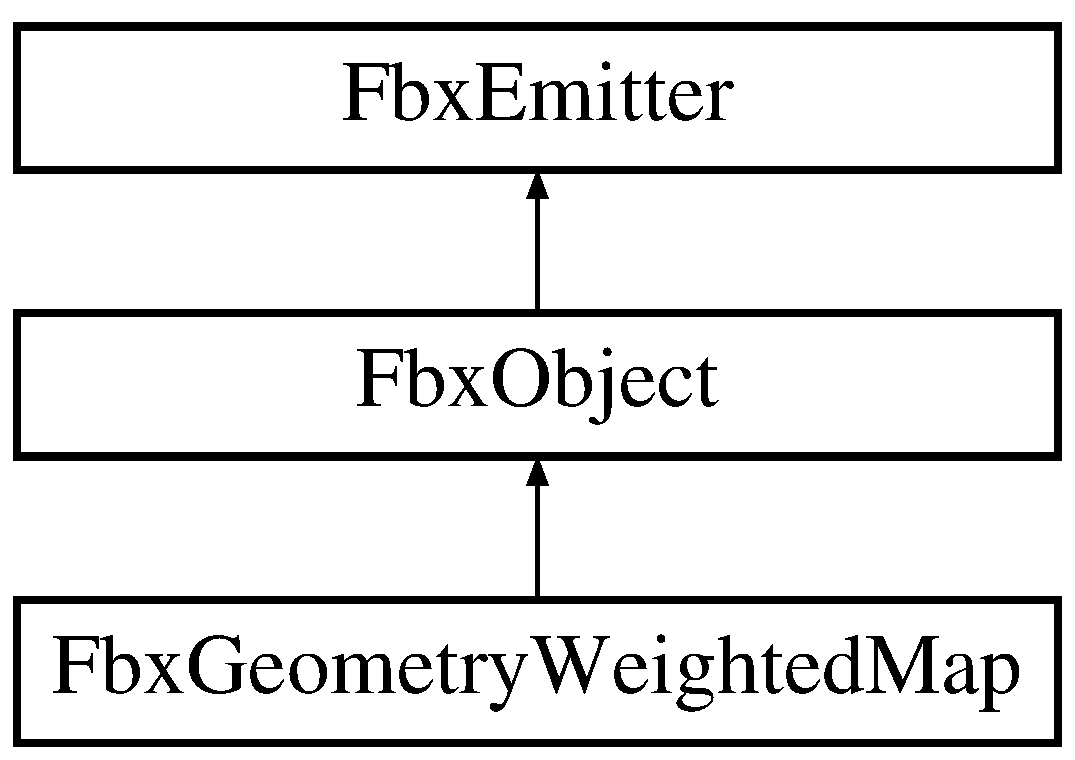
\includegraphics[height=3.000000cm]{class_fbx_geometry_weighted_map}
\end{center}
\end{figure}
\subsection*{公開メンバ関数}
\begin{DoxyCompactItemize}
\item 
void \hyperlink{class_fbx_geometry_weighted_map_a42bb06040581c024f72d39e6a4318f4f}{Set\+Values} (const \hyperlink{class_fbx_weighted_mapping}{Fbx\+Weighted\+Mapping} $\ast$p\+Weighted\+Mapping\+Table)
\item 
\hyperlink{class_fbx_weighted_mapping}{Fbx\+Weighted\+Mapping} $\ast$ \hyperlink{class_fbx_geometry_weighted_map_a55d4ce89b77af065e73c32b9e5bd17e5}{Get\+Values} () const
\item 
\hyperlink{class_fbx_geometry}{Fbx\+Geometry} $\ast$ \hyperlink{class_fbx_geometry_weighted_map_a5177720946120c17fe2003a979256e00}{Get\+Source\+Geometry} ()
\item 
\hyperlink{class_fbx_geometry}{Fbx\+Geometry} $\ast$ \hyperlink{class_fbx_geometry_weighted_map_ac0d7b29146fd71ceed30e13bf99f2656}{Get\+Destination\+Geometry} ()
\item 
virtual \hyperlink{class_fbx_object}{Fbx\+Object} \& \hyperlink{class_fbx_geometry_weighted_map_aa0310025b01de1d69b9f313a886df3c0}{Copy} (const \hyperlink{class_fbx_object}{Fbx\+Object} \&p\+Object)
\end{DoxyCompactItemize}
\subsection*{限定公開メンバ関数}
\begin{DoxyCompactItemize}
\item 
virtual void \hyperlink{class_fbx_geometry_weighted_map_af8485ac8574bf4ac9222de920a98e81f}{Construct} (const \hyperlink{class_fbx_object}{Fbx\+Object} $\ast$p\+From)
\item 
virtual void \hyperlink{class_fbx_geometry_weighted_map_a638d84bf777db4a17d63505f62d9f22f}{Destruct} (bool p\+Recursive)
\end{DoxyCompactItemize}
\subsection*{限定公開変数類}
\begin{DoxyCompactItemize}
\item 
\hyperlink{class_fbx_weighted_mapping}{Fbx\+Weighted\+Mapping} $\ast$ \hyperlink{class_fbx_geometry_weighted_map_a2d36d5ffef5895fb3faa75378884b32d}{m\+Weighted\+Mapping}
\end{DoxyCompactItemize}
\subsection*{その他の継承メンバ}


\subsection{詳解}
This class provides the structure to build a correspondence between 2 geometries. 

This correspondence is done at the vertex level. Which means that for each vertex in the source geometry, you can have from 0 to N corresponding vertices in the destination geometry. Each corresponding vertex is weighted.

For example, if the source geometry is a N\+U\+RB and the destination geometry is a mesh, the correspondence object will express the correspondence between the N\+U\+RB\textquotesingle{}s control vertices and the mesh\textquotesingle{}s vertices.

If the mesh corresponds to a tesselation of the N\+U\+RB, the correspondence object can be used to transfer any deformation that affect the N\+U\+RB\textquotesingle{}s control vertices to the mesh\textquotesingle{}s vertices.

See \hyperlink{class_fbx_weighted_mapping}{Fbx\+Weighted\+Mapping} for more details. 

 fbxgeometryweightedmap.\+h の 40 行目に定義があります。



\subsection{関数詳解}
\mbox{\Hypertarget{class_fbx_geometry_weighted_map_af8485ac8574bf4ac9222de920a98e81f}\label{class_fbx_geometry_weighted_map_af8485ac8574bf4ac9222de920a98e81f}} 
\index{Fbx\+Geometry\+Weighted\+Map@{Fbx\+Geometry\+Weighted\+Map}!Construct@{Construct}}
\index{Construct@{Construct}!Fbx\+Geometry\+Weighted\+Map@{Fbx\+Geometry\+Weighted\+Map}}
\subsubsection{\texorpdfstring{Construct()}{Construct()}}
{\footnotesize\ttfamily virtual void Fbx\+Geometry\+Weighted\+Map\+::\+Construct (\begin{DoxyParamCaption}\item[{const \hyperlink{class_fbx_object}{Fbx\+Object} $\ast$}]{p\+From }\end{DoxyParamCaption})\hspace{0.3cm}{\ttfamily [protected]}, {\ttfamily [virtual]}}

Optional constructor override, automatically called by default constructor. 
\begin{DoxyParams}{引数}
{\em p\+From} & If not null, the function must take it into account like a copy constructor. \\
\hline
\end{DoxyParams}
\begin{DoxyRemark}{注釈}
In case it is decided to override this function, do not forget to call Parent\+Class\+::\+Construct(p\+From) at the beginning. 
\end{DoxyRemark}


\hyperlink{class_fbx_object_a313503bc645af3fdceb4a99ef5cea7eb}{Fbx\+Object}を再実装しています。

\mbox{\Hypertarget{class_fbx_geometry_weighted_map_aa0310025b01de1d69b9f313a886df3c0}\label{class_fbx_geometry_weighted_map_aa0310025b01de1d69b9f313a886df3c0}} 
\index{Fbx\+Geometry\+Weighted\+Map@{Fbx\+Geometry\+Weighted\+Map}!Copy@{Copy}}
\index{Copy@{Copy}!Fbx\+Geometry\+Weighted\+Map@{Fbx\+Geometry\+Weighted\+Map}}
\subsubsection{\texorpdfstring{Copy()}{Copy()}}
{\footnotesize\ttfamily virtual \hyperlink{class_fbx_object}{Fbx\+Object}\& Fbx\+Geometry\+Weighted\+Map\+::\+Copy (\begin{DoxyParamCaption}\item[{const \hyperlink{class_fbx_object}{Fbx\+Object} \&}]{p\+Object }\end{DoxyParamCaption})\hspace{0.3cm}{\ttfamily [virtual]}}

Copy an object content into this object. 
\begin{DoxyParams}{引数}
{\em p\+Object} & The source object to copy data from. \\
\hline
\end{DoxyParams}
\begin{DoxyReturn}{戻り値}
Returns the destination object being modified by the source. 
\end{DoxyReturn}
\begin{DoxyRemark}{注釈}
This function replace the assignment operator (operator=). It will copy all property values and the name. Connections are N\+OT copied. 
\end{DoxyRemark}


\hyperlink{class_fbx_object_a0c0c5adb38284d14bb82c04d54504a3e}{Fbx\+Object}を再実装しています。

\mbox{\Hypertarget{class_fbx_geometry_weighted_map_a638d84bf777db4a17d63505f62d9f22f}\label{class_fbx_geometry_weighted_map_a638d84bf777db4a17d63505f62d9f22f}} 
\index{Fbx\+Geometry\+Weighted\+Map@{Fbx\+Geometry\+Weighted\+Map}!Destruct@{Destruct}}
\index{Destruct@{Destruct}!Fbx\+Geometry\+Weighted\+Map@{Fbx\+Geometry\+Weighted\+Map}}
\subsubsection{\texorpdfstring{Destruct()}{Destruct()}}
{\footnotesize\ttfamily virtual void Fbx\+Geometry\+Weighted\+Map\+::\+Destruct (\begin{DoxyParamCaption}\item[{bool}]{p\+Recursive }\end{DoxyParamCaption})\hspace{0.3cm}{\ttfamily [protected]}, {\ttfamily [virtual]}}

Optional destructor override, automatically called by default destructor. 
\begin{DoxyParams}{引数}
{\em p\+Recursive} & If true, children objects should be destroyed as well. \\
\hline
\end{DoxyParams}
\begin{DoxyRemark}{注釈}
In case it is decided to override this function, do not forget to call Parent\+Class\+::\+Destruct(p\+Resursive) at the end. 
\end{DoxyRemark}


\hyperlink{class_fbx_object_a123e084d9b32b29c28af6384b7c3c608}{Fbx\+Object}を再実装しています。

\mbox{\Hypertarget{class_fbx_geometry_weighted_map_ac0d7b29146fd71ceed30e13bf99f2656}\label{class_fbx_geometry_weighted_map_ac0d7b29146fd71ceed30e13bf99f2656}} 
\index{Fbx\+Geometry\+Weighted\+Map@{Fbx\+Geometry\+Weighted\+Map}!Get\+Destination\+Geometry@{Get\+Destination\+Geometry}}
\index{Get\+Destination\+Geometry@{Get\+Destination\+Geometry}!Fbx\+Geometry\+Weighted\+Map@{Fbx\+Geometry\+Weighted\+Map}}
\subsubsection{\texorpdfstring{Get\+Destination\+Geometry()}{GetDestinationGeometry()}}
{\footnotesize\ttfamily \hyperlink{class_fbx_geometry}{Fbx\+Geometry}$\ast$ Fbx\+Geometry\+Weighted\+Map\+::\+Get\+Destination\+Geometry (\begin{DoxyParamCaption}{ }\end{DoxyParamCaption})}

Return destination geometry. \begin{DoxyReturn}{戻り値}
Pointer to the destination geometry, or {\ttfamily N\+U\+LL} if there is no connected destination geometry 
\end{DoxyReturn}
\mbox{\Hypertarget{class_fbx_geometry_weighted_map_a5177720946120c17fe2003a979256e00}\label{class_fbx_geometry_weighted_map_a5177720946120c17fe2003a979256e00}} 
\index{Fbx\+Geometry\+Weighted\+Map@{Fbx\+Geometry\+Weighted\+Map}!Get\+Source\+Geometry@{Get\+Source\+Geometry}}
\index{Get\+Source\+Geometry@{Get\+Source\+Geometry}!Fbx\+Geometry\+Weighted\+Map@{Fbx\+Geometry\+Weighted\+Map}}
\subsubsection{\texorpdfstring{Get\+Source\+Geometry()}{GetSourceGeometry()}}
{\footnotesize\ttfamily \hyperlink{class_fbx_geometry}{Fbx\+Geometry}$\ast$ Fbx\+Geometry\+Weighted\+Map\+::\+Get\+Source\+Geometry (\begin{DoxyParamCaption}{ }\end{DoxyParamCaption})}

Return source geometry. \begin{DoxyReturn}{戻り値}
Pointer to the source geometry, or {\ttfamily N\+U\+LL} if there is no connected source geometry 
\end{DoxyReturn}
\mbox{\Hypertarget{class_fbx_geometry_weighted_map_a55d4ce89b77af065e73c32b9e5bd17e5}\label{class_fbx_geometry_weighted_map_a55d4ce89b77af065e73c32b9e5bd17e5}} 
\index{Fbx\+Geometry\+Weighted\+Map@{Fbx\+Geometry\+Weighted\+Map}!Get\+Values@{Get\+Values}}
\index{Get\+Values@{Get\+Values}!Fbx\+Geometry\+Weighted\+Map@{Fbx\+Geometry\+Weighted\+Map}}
\subsubsection{\texorpdfstring{Get\+Values()}{GetValues()}}
{\footnotesize\ttfamily \hyperlink{class_fbx_weighted_mapping}{Fbx\+Weighted\+Mapping}$\ast$ Fbx\+Geometry\+Weighted\+Map\+::\+Get\+Values (\begin{DoxyParamCaption}{ }\end{DoxyParamCaption}) const}

Return correspondence values. \begin{DoxyReturn}{戻り値}
Pointer to the correspondence values table. 
\end{DoxyReturn}
\mbox{\Hypertarget{class_fbx_geometry_weighted_map_a42bb06040581c024f72d39e6a4318f4f}\label{class_fbx_geometry_weighted_map_a42bb06040581c024f72d39e6a4318f4f}} 
\index{Fbx\+Geometry\+Weighted\+Map@{Fbx\+Geometry\+Weighted\+Map}!Set\+Values@{Set\+Values}}
\index{Set\+Values@{Set\+Values}!Fbx\+Geometry\+Weighted\+Map@{Fbx\+Geometry\+Weighted\+Map}}
\subsubsection{\texorpdfstring{Set\+Values()}{SetValues()}}
{\footnotesize\ttfamily void Fbx\+Geometry\+Weighted\+Map\+::\+Set\+Values (\begin{DoxyParamCaption}\item[{const \hyperlink{class_fbx_weighted_mapping}{Fbx\+Weighted\+Mapping} $\ast$}]{p\+Weighted\+Mapping\+Table }\end{DoxyParamCaption})}

Set correspondence values. 
\begin{DoxyParams}{引数}
{\em p\+Weighted\+Mapping\+Table} & Pointer to the table containing values \\
\hline
\end{DoxyParams}
\begin{DoxyRemark}{注釈}
{\itshape p\+Weighted\+Mapping\+Table} becomes owned by this object and will be destroyed by it when the object goes out of scope or on the next call to \hyperlink{class_fbx_geometry_weighted_map_a42bb06040581c024f72d39e6a4318f4f}{Set\+Values()}. The deletion uses \hyperlink{fbxalloc_8h_a55138f34ac93c519a78f624178c128d6}{Fbx\+Delete()} so the content of the pointer must have been allocated with \hyperlink{fbxnew_8h_a31302f981355f4b48ebc963ead1434f2}{Fbx\+New$<$$>$()} 
\end{DoxyRemark}


\subsection{メンバ詳解}
\mbox{\Hypertarget{class_fbx_geometry_weighted_map_a2d36d5ffef5895fb3faa75378884b32d}\label{class_fbx_geometry_weighted_map_a2d36d5ffef5895fb3faa75378884b32d}} 
\index{Fbx\+Geometry\+Weighted\+Map@{Fbx\+Geometry\+Weighted\+Map}!m\+Weighted\+Mapping@{m\+Weighted\+Mapping}}
\index{m\+Weighted\+Mapping@{m\+Weighted\+Mapping}!Fbx\+Geometry\+Weighted\+Map@{Fbx\+Geometry\+Weighted\+Map}}
\subsubsection{\texorpdfstring{m\+Weighted\+Mapping}{mWeightedMapping}}
{\footnotesize\ttfamily \hyperlink{class_fbx_weighted_mapping}{Fbx\+Weighted\+Mapping}$\ast$ Fbx\+Geometry\+Weighted\+Map\+::m\+Weighted\+Mapping\hspace{0.3cm}{\ttfamily [protected]}}



 fbxgeometryweightedmap.\+h の 80 行目に定義があります。



このクラス詳解は次のファイルから抽出されました\+:\begin{DoxyCompactItemize}
\item 
C\+:/\+Maya/scripts/\+F\+B\+X\+\_\+\+S\+D\+K/2017.\+1/include/fbxsdk/scene/geometry/\hyperlink{fbxgeometryweightedmap_8h}{fbxgeometryweightedmap.\+h}\end{DoxyCompactItemize}

\hypertarget{class_fbx_global_camera_settings}{}\section{Fbx\+Global\+Camera\+Settings クラス}
\label{class_fbx_global_camera_settings}\index{Fbx\+Global\+Camera\+Settings@{Fbx\+Global\+Camera\+Settings}}


{\ttfamily \#include $<$fbxglobalcamerasettings.\+h$>$}

\subsection*{公開メンバ関数}
\begin{DoxyCompactItemize}
\item 
const \hyperlink{class_fbx_global_camera_settings}{Fbx\+Global\+Camera\+Settings} \& \hyperlink{class_fbx_global_camera_settings_aaee942061eedeb6b7e1bae058b1d3ddd}{operator=} (const \hyperlink{class_fbx_global_camera_settings}{Fbx\+Global\+Camera\+Settings} \&p\+Global\+Camera\+Settings)
\item 
bool \hyperlink{class_fbx_global_camera_settings_ad69790f22bd872818ac9d86731833f4f}{Copy\+Producer\+Camera} (const char $\ast$p\+Camera\+Name, const \hyperlink{class_fbx_camera}{Fbx\+Camera} $\ast$p\+Camera) const
\end{DoxyCompactItemize}
\subsection*{Default Camera Settings}
\begin{DoxyCompactItemize}
\item 
enum \hyperlink{class_fbx_global_camera_settings_aaa674f8b39e4cd57d7cc07f381f11858}{E\+Viewing\+Mode} \{ \hyperlink{class_fbx_global_camera_settings_aaa674f8b39e4cd57d7cc07f381f11858a0336e82bb15b3eac5b9b60501aa3cb45}{e\+Standard}, 
\hyperlink{class_fbx_global_camera_settings_aaa674f8b39e4cd57d7cc07f381f11858adecac3c5b557d7f8c27d88ee72ca48ab}{e\+X\+Ray}, 
\hyperlink{class_fbx_global_camera_settings_aaa674f8b39e4cd57d7cc07f381f11858a30be58e2817cc1fd6e68574cb6ba27f1}{e\+Models\+Only}
 \}
\item 
bool \hyperlink{class_fbx_global_camera_settings_a6069976325cb9983f6ed75e1884f1981}{Set\+Default\+Camera} (const char $\ast$p\+Camera\+Name, \hyperlink{class_fbx_status}{Fbx\+Status} $\ast$p\+Status=\hyperlink{fbxarch_8h_a070d2ce7b6bb7e5c05602aa8c308d0c4}{N\+U\+LL})
\item 
const char $\ast$ \hyperlink{class_fbx_global_camera_settings_ab2f43528a6d09862bc735d7695af9868}{Get\+Default\+Camera} () const
\item 
void \hyperlink{class_fbx_global_camera_settings_a1024ebc19b9641163a74a4cc457f8c0d}{Restore\+Default\+Settings} ()
\begin{DoxyCompactList}\small\item\em Restores the default settings. \end{DoxyCompactList}\item 
void \hyperlink{class_fbx_global_camera_settings_a15790cd057733254a0e82b172b644122}{Set\+Default\+Viewing\+Mode} (\hyperlink{class_fbx_global_camera_settings_aaa674f8b39e4cd57d7cc07f381f11858}{E\+Viewing\+Mode} p\+Viewing\+Mode)
\item 
\hyperlink{class_fbx_global_camera_settings_aaa674f8b39e4cd57d7cc07f381f11858}{E\+Viewing\+Mode} \hyperlink{class_fbx_global_camera_settings_a458ad62da44fe9f580550162832edbb9}{Get\+Default\+Viewing\+Mode} () const
\end{DoxyCompactItemize}
\subsection*{Producer Cameras}
\label{_amgrpdf8c7ffb8bdef1e4f35722221c5ded0f}%
Producer cameras are global cameras in Motion\+Builder you use to view the scene. You cannot animate Producer cameras but you can specify their default positions. \begin{DoxyCompactItemize}
\item 
void \hyperlink{class_fbx_global_camera_settings_a2b2e508928ea3b21b25574635089f025}{Create\+Producer\+Cameras} ()
\item 
void \hyperlink{class_fbx_global_camera_settings_a083cbc9ad5466346559025508aed6dc6}{Destroy\+Producer\+Cameras} ()
\item 
bool \hyperlink{class_fbx_global_camera_settings_abcabe0a434ecb96f58711e16f6f7abc5}{Is\+Producer\+Camera} (\hyperlink{class_fbx_camera}{Fbx\+Camera} $\ast$p\+Camera) const
\item 
\hyperlink{class_fbx_camera}{Fbx\+Camera} $\ast$ \hyperlink{class_fbx_global_camera_settings_a4353a05481d6dad14fbd6f3fdaf8541c}{Get\+Camera\+Producer\+Perspective} () const
\item 
\hyperlink{class_fbx_camera}{Fbx\+Camera} $\ast$ \hyperlink{class_fbx_global_camera_settings_afb4ff79f5f970e8b86e68b56a40f3116}{Get\+Camera\+Producer\+Front} () const
\item 
\hyperlink{class_fbx_camera}{Fbx\+Camera} $\ast$ \hyperlink{class_fbx_global_camera_settings_ad11a62b3c4249a802f4a4e9c98d8b966}{Get\+Camera\+Producer\+Back} () const
\item 
\hyperlink{class_fbx_camera}{Fbx\+Camera} $\ast$ \hyperlink{class_fbx_global_camera_settings_a5541de057d1ce39e712c42f5913d8ee7}{Get\+Camera\+Producer\+Left} () const
\item 
\hyperlink{class_fbx_camera}{Fbx\+Camera} $\ast$ \hyperlink{class_fbx_global_camera_settings_a0166b7f6aac53c8a9b3f6deabf77a09e}{Get\+Camera\+Producer\+Right} () const
\item 
\hyperlink{class_fbx_camera}{Fbx\+Camera} $\ast$ \hyperlink{class_fbx_global_camera_settings_a24d688c9385c1393c552bd05e124f104}{Get\+Camera\+Producer\+Top} () const
\item 
\hyperlink{class_fbx_camera}{Fbx\+Camera} $\ast$ \hyperlink{class_fbx_global_camera_settings_a6a24f852c638f6a599f5b63078454112}{Get\+Camera\+Producer\+Bottom} () const
\item 
\hyperlink{class_fbx_camera_switcher}{Fbx\+Camera\+Switcher} $\ast$ \hyperlink{class_fbx_global_camera_settings_ab581e270145dfa36b239171811cc35b9}{Get\+Camera\+Switcher} () const
\item 
void \hyperlink{class_fbx_global_camera_settings_ac5828573eccccf2e76529ad21f77ff3c}{Set\+Camera\+Switcher} (\hyperlink{class_fbx_camera_switcher}{Fbx\+Camera\+Switcher} $\ast$p\+Switcher)
\end{DoxyCompactItemize}


\subsection{詳解}
This class contains the global camera settings.

\begin{DoxyRemark}{注釈}
This class exists for F\+BX version 6.\+x and earlier. The new F\+BX v7.\+x file format that is now the default no longer uses it. The relevant data (a subset of this class) has been moved to the \hyperlink{class_fbx_global_settings}{Fbx\+Global\+Settings} object and should be used instead. 
\end{DoxyRemark}


\subsection{列挙型メンバ詳解}
\mbox{\Hypertarget{class_fbx_global_camera_settings_aaa674f8b39e4cd57d7cc07f381f11858}\label{class_fbx_global_camera_settings_aaa674f8b39e4cd57d7cc07f381f11858}} 
\index{Fbx\+Global\+Camera\+Settings@{Fbx\+Global\+Camera\+Settings}!E\+Viewing\+Mode@{E\+Viewing\+Mode}}
\index{E\+Viewing\+Mode@{E\+Viewing\+Mode}!Fbx\+Global\+Camera\+Settings@{Fbx\+Global\+Camera\+Settings}}
\subsubsection{\texorpdfstring{E\+Viewing\+Mode}{EViewingMode}}
{\footnotesize\ttfamily enum \hyperlink{class_fbx_global_camera_settings_aaa674f8b39e4cd57d7cc07f381f11858}{Fbx\+Global\+Camera\+Settings\+::\+E\+Viewing\+Mode}}

Viewing modes. \begin{DoxyEnumFields}{列挙値}
\raisebox{\heightof{T}}[0pt][0pt]{\index{e\+Standard@{e\+Standard}!Fbx\+Global\+Camera\+Settings@{Fbx\+Global\+Camera\+Settings}}\index{Fbx\+Global\+Camera\+Settings@{Fbx\+Global\+Camera\+Settings}!e\+Standard@{e\+Standard}}}\mbox{\Hypertarget{class_fbx_global_camera_settings_aaa674f8b39e4cd57d7cc07f381f11858a0336e82bb15b3eac5b9b60501aa3cb45}\label{class_fbx_global_camera_settings_aaa674f8b39e4cd57d7cc07f381f11858a0336e82bb15b3eac5b9b60501aa3cb45}} 
e\+Standard&\\
\hline

\raisebox{\heightof{T}}[0pt][0pt]{\index{e\+X\+Ray@{e\+X\+Ray}!Fbx\+Global\+Camera\+Settings@{Fbx\+Global\+Camera\+Settings}}\index{Fbx\+Global\+Camera\+Settings@{Fbx\+Global\+Camera\+Settings}!e\+X\+Ray@{e\+X\+Ray}}}\mbox{\Hypertarget{class_fbx_global_camera_settings_aaa674f8b39e4cd57d7cc07f381f11858adecac3c5b557d7f8c27d88ee72ca48ab}\label{class_fbx_global_camera_settings_aaa674f8b39e4cd57d7cc07f381f11858adecac3c5b557d7f8c27d88ee72ca48ab}} 
e\+X\+Ray&\\
\hline

\raisebox{\heightof{T}}[0pt][0pt]{\index{e\+Models\+Only@{e\+Models\+Only}!Fbx\+Global\+Camera\+Settings@{Fbx\+Global\+Camera\+Settings}}\index{Fbx\+Global\+Camera\+Settings@{Fbx\+Global\+Camera\+Settings}!e\+Models\+Only@{e\+Models\+Only}}}\mbox{\Hypertarget{class_fbx_global_camera_settings_aaa674f8b39e4cd57d7cc07f381f11858a30be58e2817cc1fd6e68574cb6ba27f1}\label{class_fbx_global_camera_settings_aaa674f8b39e4cd57d7cc07f381f11858a30be58e2817cc1fd6e68574cb6ba27f1}} 
e\+Models\+Only&\\
\hline

\end{DoxyEnumFields}


\subsection{メソッド詳解}
\mbox{\Hypertarget{class_fbx_global_camera_settings_ad69790f22bd872818ac9d86731833f4f}\label{class_fbx_global_camera_settings_ad69790f22bd872818ac9d86731833f4f}} 
\index{Fbx\+Global\+Camera\+Settings@{Fbx\+Global\+Camera\+Settings}!Copy\+Producer\+Camera@{Copy\+Producer\+Camera}}
\index{Copy\+Producer\+Camera@{Copy\+Producer\+Camera}!Fbx\+Global\+Camera\+Settings@{Fbx\+Global\+Camera\+Settings}}
\subsubsection{\texorpdfstring{Copy\+Producer\+Camera()}{CopyProducerCamera()}}
{\footnotesize\ttfamily bool Fbx\+Global\+Camera\+Settings\+::\+Copy\+Producer\+Camera (\begin{DoxyParamCaption}\item[{const char $\ast$}]{p\+Camera\+Name,  }\item[{const \hyperlink{class_fbx_camera}{Fbx\+Camera} $\ast$}]{p\+Camera }\end{DoxyParamCaption}) const}

\mbox{\Hypertarget{class_fbx_global_camera_settings_a2b2e508928ea3b21b25574635089f025}\label{class_fbx_global_camera_settings_a2b2e508928ea3b21b25574635089f025}} 
\index{Fbx\+Global\+Camera\+Settings@{Fbx\+Global\+Camera\+Settings}!Create\+Producer\+Cameras@{Create\+Producer\+Cameras}}
\index{Create\+Producer\+Cameras@{Create\+Producer\+Cameras}!Fbx\+Global\+Camera\+Settings@{Fbx\+Global\+Camera\+Settings}}
\subsubsection{\texorpdfstring{Create\+Producer\+Cameras()}{CreateProducerCameras()}}
{\footnotesize\ttfamily void Fbx\+Global\+Camera\+Settings\+::\+Create\+Producer\+Cameras (\begin{DoxyParamCaption}{ }\end{DoxyParamCaption})}

Creates the default Producer cameras. \mbox{\Hypertarget{class_fbx_global_camera_settings_a083cbc9ad5466346559025508aed6dc6}\label{class_fbx_global_camera_settings_a083cbc9ad5466346559025508aed6dc6}} 
\index{Fbx\+Global\+Camera\+Settings@{Fbx\+Global\+Camera\+Settings}!Destroy\+Producer\+Cameras@{Destroy\+Producer\+Cameras}}
\index{Destroy\+Producer\+Cameras@{Destroy\+Producer\+Cameras}!Fbx\+Global\+Camera\+Settings@{Fbx\+Global\+Camera\+Settings}}
\subsubsection{\texorpdfstring{Destroy\+Producer\+Cameras()}{DestroyProducerCameras()}}
{\footnotesize\ttfamily void Fbx\+Global\+Camera\+Settings\+::\+Destroy\+Producer\+Cameras (\begin{DoxyParamCaption}{ }\end{DoxyParamCaption})}

Destroys the default Producer cameras. \mbox{\Hypertarget{class_fbx_global_camera_settings_ad11a62b3c4249a802f4a4e9c98d8b966}\label{class_fbx_global_camera_settings_ad11a62b3c4249a802f4a4e9c98d8b966}} 
\index{Fbx\+Global\+Camera\+Settings@{Fbx\+Global\+Camera\+Settings}!Get\+Camera\+Producer\+Back@{Get\+Camera\+Producer\+Back}}
\index{Get\+Camera\+Producer\+Back@{Get\+Camera\+Producer\+Back}!Fbx\+Global\+Camera\+Settings@{Fbx\+Global\+Camera\+Settings}}
\subsubsection{\texorpdfstring{Get\+Camera\+Producer\+Back()}{GetCameraProducerBack()}}
{\footnotesize\ttfamily \hyperlink{class_fbx_camera}{Fbx\+Camera}$\ast$ Fbx\+Global\+Camera\+Settings\+::\+Get\+Camera\+Producer\+Back (\begin{DoxyParamCaption}{ }\end{DoxyParamCaption}) const}

Returns a reference to the Producer back camera. \begin{DoxyReturn}{戻り値}
The reference to the internal Back camera. 
\end{DoxyReturn}
\mbox{\Hypertarget{class_fbx_global_camera_settings_a6a24f852c638f6a599f5b63078454112}\label{class_fbx_global_camera_settings_a6a24f852c638f6a599f5b63078454112}} 
\index{Fbx\+Global\+Camera\+Settings@{Fbx\+Global\+Camera\+Settings}!Get\+Camera\+Producer\+Bottom@{Get\+Camera\+Producer\+Bottom}}
\index{Get\+Camera\+Producer\+Bottom@{Get\+Camera\+Producer\+Bottom}!Fbx\+Global\+Camera\+Settings@{Fbx\+Global\+Camera\+Settings}}
\subsubsection{\texorpdfstring{Get\+Camera\+Producer\+Bottom()}{GetCameraProducerBottom()}}
{\footnotesize\ttfamily \hyperlink{class_fbx_camera}{Fbx\+Camera}$\ast$ Fbx\+Global\+Camera\+Settings\+::\+Get\+Camera\+Producer\+Bottom (\begin{DoxyParamCaption}{ }\end{DoxyParamCaption}) const}

Returns a reference to the Producer bottom camera. \begin{DoxyReturn}{戻り値}
The reference to the internal Bottom camera. 
\end{DoxyReturn}
\mbox{\Hypertarget{class_fbx_global_camera_settings_afb4ff79f5f970e8b86e68b56a40f3116}\label{class_fbx_global_camera_settings_afb4ff79f5f970e8b86e68b56a40f3116}} 
\index{Fbx\+Global\+Camera\+Settings@{Fbx\+Global\+Camera\+Settings}!Get\+Camera\+Producer\+Front@{Get\+Camera\+Producer\+Front}}
\index{Get\+Camera\+Producer\+Front@{Get\+Camera\+Producer\+Front}!Fbx\+Global\+Camera\+Settings@{Fbx\+Global\+Camera\+Settings}}
\subsubsection{\texorpdfstring{Get\+Camera\+Producer\+Front()}{GetCameraProducerFront()}}
{\footnotesize\ttfamily \hyperlink{class_fbx_camera}{Fbx\+Camera}$\ast$ Fbx\+Global\+Camera\+Settings\+::\+Get\+Camera\+Producer\+Front (\begin{DoxyParamCaption}{ }\end{DoxyParamCaption}) const}

Returns a reference to the Producer front camera. \begin{DoxyReturn}{戻り値}
The reference to the internal Front camera. 
\end{DoxyReturn}
\mbox{\Hypertarget{class_fbx_global_camera_settings_a5541de057d1ce39e712c42f5913d8ee7}\label{class_fbx_global_camera_settings_a5541de057d1ce39e712c42f5913d8ee7}} 
\index{Fbx\+Global\+Camera\+Settings@{Fbx\+Global\+Camera\+Settings}!Get\+Camera\+Producer\+Left@{Get\+Camera\+Producer\+Left}}
\index{Get\+Camera\+Producer\+Left@{Get\+Camera\+Producer\+Left}!Fbx\+Global\+Camera\+Settings@{Fbx\+Global\+Camera\+Settings}}
\subsubsection{\texorpdfstring{Get\+Camera\+Producer\+Left()}{GetCameraProducerLeft()}}
{\footnotesize\ttfamily \hyperlink{class_fbx_camera}{Fbx\+Camera}$\ast$ Fbx\+Global\+Camera\+Settings\+::\+Get\+Camera\+Producer\+Left (\begin{DoxyParamCaption}{ }\end{DoxyParamCaption}) const}

Returns a reference to the Producer left camera. \begin{DoxyReturn}{戻り値}
The reference to the internal Left camera. 
\end{DoxyReturn}
\mbox{\Hypertarget{class_fbx_global_camera_settings_a4353a05481d6dad14fbd6f3fdaf8541c}\label{class_fbx_global_camera_settings_a4353a05481d6dad14fbd6f3fdaf8541c}} 
\index{Fbx\+Global\+Camera\+Settings@{Fbx\+Global\+Camera\+Settings}!Get\+Camera\+Producer\+Perspective@{Get\+Camera\+Producer\+Perspective}}
\index{Get\+Camera\+Producer\+Perspective@{Get\+Camera\+Producer\+Perspective}!Fbx\+Global\+Camera\+Settings@{Fbx\+Global\+Camera\+Settings}}
\subsubsection{\texorpdfstring{Get\+Camera\+Producer\+Perspective()}{GetCameraProducerPerspective()}}
{\footnotesize\ttfamily \hyperlink{class_fbx_camera}{Fbx\+Camera}$\ast$ Fbx\+Global\+Camera\+Settings\+::\+Get\+Camera\+Producer\+Perspective (\begin{DoxyParamCaption}{ }\end{DoxyParamCaption}) const}

Returns a reference to the Producer perspective camera. \begin{DoxyReturn}{戻り値}
The reference to the internal Perspective camera. 
\end{DoxyReturn}
\mbox{\Hypertarget{class_fbx_global_camera_settings_a0166b7f6aac53c8a9b3f6deabf77a09e}\label{class_fbx_global_camera_settings_a0166b7f6aac53c8a9b3f6deabf77a09e}} 
\index{Fbx\+Global\+Camera\+Settings@{Fbx\+Global\+Camera\+Settings}!Get\+Camera\+Producer\+Right@{Get\+Camera\+Producer\+Right}}
\index{Get\+Camera\+Producer\+Right@{Get\+Camera\+Producer\+Right}!Fbx\+Global\+Camera\+Settings@{Fbx\+Global\+Camera\+Settings}}
\subsubsection{\texorpdfstring{Get\+Camera\+Producer\+Right()}{GetCameraProducerRight()}}
{\footnotesize\ttfamily \hyperlink{class_fbx_camera}{Fbx\+Camera}$\ast$ Fbx\+Global\+Camera\+Settings\+::\+Get\+Camera\+Producer\+Right (\begin{DoxyParamCaption}{ }\end{DoxyParamCaption}) const}

Returns a reference to the Producer right camera. \begin{DoxyReturn}{戻り値}
The reference to the internal Right camera. 
\end{DoxyReturn}
\mbox{\Hypertarget{class_fbx_global_camera_settings_a24d688c9385c1393c552bd05e124f104}\label{class_fbx_global_camera_settings_a24d688c9385c1393c552bd05e124f104}} 
\index{Fbx\+Global\+Camera\+Settings@{Fbx\+Global\+Camera\+Settings}!Get\+Camera\+Producer\+Top@{Get\+Camera\+Producer\+Top}}
\index{Get\+Camera\+Producer\+Top@{Get\+Camera\+Producer\+Top}!Fbx\+Global\+Camera\+Settings@{Fbx\+Global\+Camera\+Settings}}
\subsubsection{\texorpdfstring{Get\+Camera\+Producer\+Top()}{GetCameraProducerTop()}}
{\footnotesize\ttfamily \hyperlink{class_fbx_camera}{Fbx\+Camera}$\ast$ Fbx\+Global\+Camera\+Settings\+::\+Get\+Camera\+Producer\+Top (\begin{DoxyParamCaption}{ }\end{DoxyParamCaption}) const}

Returns a reference to the Producer top camera. \begin{DoxyReturn}{戻り値}
The reference to the internal Top camera. 
\end{DoxyReturn}
\mbox{\Hypertarget{class_fbx_global_camera_settings_ab581e270145dfa36b239171811cc35b9}\label{class_fbx_global_camera_settings_ab581e270145dfa36b239171811cc35b9}} 
\index{Fbx\+Global\+Camera\+Settings@{Fbx\+Global\+Camera\+Settings}!Get\+Camera\+Switcher@{Get\+Camera\+Switcher}}
\index{Get\+Camera\+Switcher@{Get\+Camera\+Switcher}!Fbx\+Global\+Camera\+Settings@{Fbx\+Global\+Camera\+Settings}}
\subsubsection{\texorpdfstring{Get\+Camera\+Switcher()}{GetCameraSwitcher()}}
{\footnotesize\ttfamily \hyperlink{class_fbx_camera_switcher}{Fbx\+Camera\+Switcher}$\ast$ Fbx\+Global\+Camera\+Settings\+::\+Get\+Camera\+Switcher (\begin{DoxyParamCaption}{ }\end{DoxyParamCaption}) const}

Returns the Camera Switcher. \begin{DoxyReturn}{戻り値}
A pointer to the Camera Switcher. 
\end{DoxyReturn}
\begin{DoxyRemark}{注釈}
This node has a {\ttfamily \hyperlink{class_fbx_node_attribute_a08e1669d3d1a696910756ab17de56d6aa6fb598a32379261ed00d4695863a58fc}{Fbx\+Node\+Attribute\+::e\+Camera\+Switcher}} node attribute type. This node is not saved when there is no camera in the scene. Nodes inserted below are never saved. Camera indices start at 1. Out of range indices are clamped between 1 and the number of cameras in the scene. The index of a camera refers to its order of appearance when searching the node tree depth first. If a camera is added or removed after camera indices have been set, the camera indices must be updated. It is easier to set camera indices once every camera have been set. Camera index keys must be set using constant interpolation to ensure that camera switches occur exactly at key time. 
\end{DoxyRemark}
\mbox{\Hypertarget{class_fbx_global_camera_settings_ab2f43528a6d09862bc735d7695af9868}\label{class_fbx_global_camera_settings_ab2f43528a6d09862bc735d7695af9868}} 
\index{Fbx\+Global\+Camera\+Settings@{Fbx\+Global\+Camera\+Settings}!Get\+Default\+Camera@{Get\+Default\+Camera}}
\index{Get\+Default\+Camera@{Get\+Default\+Camera}!Fbx\+Global\+Camera\+Settings@{Fbx\+Global\+Camera\+Settings}}
\subsubsection{\texorpdfstring{Get\+Default\+Camera()}{GetDefaultCamera()}}
{\footnotesize\ttfamily const char$\ast$ Fbx\+Global\+Camera\+Settings\+::\+Get\+Default\+Camera (\begin{DoxyParamCaption}{ }\end{DoxyParamCaption}) const}

Returns the default camera name. \begin{DoxyReturn}{戻り値}
The default camera name, or returns an empty string if no camera name has been specified. 
\end{DoxyReturn}
\mbox{\Hypertarget{class_fbx_global_camera_settings_a458ad62da44fe9f580550162832edbb9}\label{class_fbx_global_camera_settings_a458ad62da44fe9f580550162832edbb9}} 
\index{Fbx\+Global\+Camera\+Settings@{Fbx\+Global\+Camera\+Settings}!Get\+Default\+Viewing\+Mode@{Get\+Default\+Viewing\+Mode}}
\index{Get\+Default\+Viewing\+Mode@{Get\+Default\+Viewing\+Mode}!Fbx\+Global\+Camera\+Settings@{Fbx\+Global\+Camera\+Settings}}
\subsubsection{\texorpdfstring{Get\+Default\+Viewing\+Mode()}{GetDefaultViewingMode()}}
{\footnotesize\ttfamily \hyperlink{class_fbx_global_camera_settings_aaa674f8b39e4cd57d7cc07f381f11858}{E\+Viewing\+Mode} Fbx\+Global\+Camera\+Settings\+::\+Get\+Default\+Viewing\+Mode (\begin{DoxyParamCaption}{ }\end{DoxyParamCaption}) const}

Returns the default viewing mode. \begin{DoxyReturn}{戻り値}
The currently set Viewing mode. 
\end{DoxyReturn}
\mbox{\Hypertarget{class_fbx_global_camera_settings_abcabe0a434ecb96f58711e16f6f7abc5}\label{class_fbx_global_camera_settings_abcabe0a434ecb96f58711e16f6f7abc5}} 
\index{Fbx\+Global\+Camera\+Settings@{Fbx\+Global\+Camera\+Settings}!Is\+Producer\+Camera@{Is\+Producer\+Camera}}
\index{Is\+Producer\+Camera@{Is\+Producer\+Camera}!Fbx\+Global\+Camera\+Settings@{Fbx\+Global\+Camera\+Settings}}
\subsubsection{\texorpdfstring{Is\+Producer\+Camera()}{IsProducerCamera()}}
{\footnotesize\ttfamily bool Fbx\+Global\+Camera\+Settings\+::\+Is\+Producer\+Camera (\begin{DoxyParamCaption}\item[{\hyperlink{class_fbx_camera}{Fbx\+Camera} $\ast$}]{p\+Camera }\end{DoxyParamCaption}) const}

Checks if the camera is a Producer camera. 
\begin{DoxyParams}{引数}
{\em p\+Camera} & The camera to check. \\
\hline
\end{DoxyParams}
\begin{DoxyReturn}{戻り値}
{\ttfamily True} if it is a producer camera, returns {\ttfamily false} if it is not a producer camera. 
\end{DoxyReturn}
\mbox{\Hypertarget{class_fbx_global_camera_settings_aaee942061eedeb6b7e1bae058b1d3ddd}\label{class_fbx_global_camera_settings_aaee942061eedeb6b7e1bae058b1d3ddd}} 
\index{Fbx\+Global\+Camera\+Settings@{Fbx\+Global\+Camera\+Settings}!operator=@{operator=}}
\index{operator=@{operator=}!Fbx\+Global\+Camera\+Settings@{Fbx\+Global\+Camera\+Settings}}
\subsubsection{\texorpdfstring{operator=()}{operator=()}}
{\footnotesize\ttfamily const \hyperlink{class_fbx_global_camera_settings}{Fbx\+Global\+Camera\+Settings}\& Fbx\+Global\+Camera\+Settings\+::operator= (\begin{DoxyParamCaption}\item[{const \hyperlink{class_fbx_global_camera_settings}{Fbx\+Global\+Camera\+Settings} \&}]{p\+Global\+Camera\+Settings }\end{DoxyParamCaption})}

Assignment operator. 
\begin{DoxyParams}{引数}
{\em p\+Global\+Camera\+Settings} & \hyperlink{class_fbx_global_camera_settings}{Fbx\+Global\+Camera\+Settings} object assigned to this one. \\
\hline
\end{DoxyParams}
\mbox{\Hypertarget{class_fbx_global_camera_settings_a1024ebc19b9641163a74a4cc457f8c0d}\label{class_fbx_global_camera_settings_a1024ebc19b9641163a74a4cc457f8c0d}} 
\index{Fbx\+Global\+Camera\+Settings@{Fbx\+Global\+Camera\+Settings}!Restore\+Default\+Settings@{Restore\+Default\+Settings}}
\index{Restore\+Default\+Settings@{Restore\+Default\+Settings}!Fbx\+Global\+Camera\+Settings@{Fbx\+Global\+Camera\+Settings}}
\subsubsection{\texorpdfstring{Restore\+Default\+Settings()}{RestoreDefaultSettings()}}
{\footnotesize\ttfamily void Fbx\+Global\+Camera\+Settings\+::\+Restore\+Default\+Settings (\begin{DoxyParamCaption}{ }\end{DoxyParamCaption})}



Restores the default settings. 

\mbox{\Hypertarget{class_fbx_global_camera_settings_ac5828573eccccf2e76529ad21f77ff3c}\label{class_fbx_global_camera_settings_ac5828573eccccf2e76529ad21f77ff3c}} 
\index{Fbx\+Global\+Camera\+Settings@{Fbx\+Global\+Camera\+Settings}!Set\+Camera\+Switcher@{Set\+Camera\+Switcher}}
\index{Set\+Camera\+Switcher@{Set\+Camera\+Switcher}!Fbx\+Global\+Camera\+Settings@{Fbx\+Global\+Camera\+Settings}}
\subsubsection{\texorpdfstring{Set\+Camera\+Switcher()}{SetCameraSwitcher()}}
{\footnotesize\ttfamily void Fbx\+Global\+Camera\+Settings\+::\+Set\+Camera\+Switcher (\begin{DoxyParamCaption}\item[{\hyperlink{class_fbx_camera_switcher}{Fbx\+Camera\+Switcher} $\ast$}]{p\+Switcher }\end{DoxyParamCaption})}

Sets the Camera Switcher. 
\begin{DoxyParams}{引数}
{\em p\+Switcher} & The Camera Switcher to be set. \\
\hline
\end{DoxyParams}
\mbox{\Hypertarget{class_fbx_global_camera_settings_a6069976325cb9983f6ed75e1884f1981}\label{class_fbx_global_camera_settings_a6069976325cb9983f6ed75e1884f1981}} 
\index{Fbx\+Global\+Camera\+Settings@{Fbx\+Global\+Camera\+Settings}!Set\+Default\+Camera@{Set\+Default\+Camera}}
\index{Set\+Default\+Camera@{Set\+Default\+Camera}!Fbx\+Global\+Camera\+Settings@{Fbx\+Global\+Camera\+Settings}}
\subsubsection{\texorpdfstring{Set\+Default\+Camera()}{SetDefaultCamera()}}
{\footnotesize\ttfamily bool Fbx\+Global\+Camera\+Settings\+::\+Set\+Default\+Camera (\begin{DoxyParamCaption}\item[{const char $\ast$}]{p\+Camera\+Name,  }\item[{\hyperlink{class_fbx_status}{Fbx\+Status} $\ast$}]{p\+Status = {\ttfamily \hyperlink{fbxarch_8h_a070d2ce7b6bb7e5c05602aa8c308d0c4}{N\+U\+LL}} }\end{DoxyParamCaption})}

Sets the default camera. 
\begin{DoxyParams}{引数}
{\em p\+Camera\+Name} & Name of the default camera. \\
\hline
{\em p\+Status} & The \hyperlink{class_fbx_status}{Fbx\+Status} object to hold error codes. \\
\hline
\end{DoxyParams}
\begin{DoxyReturn}{戻り値}
{\ttfamily True} if camera name is valid, returns {\ttfamily false} if it is not valid. 
\end{DoxyReturn}
\begin{DoxyRemark}{注釈}
A valid camera name must be either one of the defined tokens (F\+B\+X\+S\+D\+K\+\_\+\+C\+A\+M\+E\+R\+A\+\_\+\+P\+E\+R\+S\+P\+E\+C\+T\+I\+VE, F\+B\+X\+S\+D\+K\+\_\+\+C\+A\+M\+E\+R\+A\+\_\+\+T\+OP, F\+B\+X\+S\+D\+K\+\_\+\+C\+A\+M\+E\+R\+A\+\_\+\+B\+O\+T\+T\+OM, F\+B\+X\+S\+D\+K\+\_\+\+C\+A\+M\+E\+R\+A\+\_\+\+F\+R\+O\+NT, F\+B\+X\+S\+D\+K\+\_\+\+C\+A\+M\+E\+R\+A\+\_\+\+B\+A\+CK, F\+B\+X\+S\+D\+K\+\_\+\+C\+A\+M\+E\+R\+A\+\_\+\+R\+I\+G\+HT, F\+B\+X\+S\+D\+K\+\_\+\+C\+A\+M\+E\+R\+A\+\_\+\+L\+E\+FT and F\+B\+X\+S\+D\+K\+\_\+\+C\+A\+M\+E\+R\+A\+\_\+\+S\+W\+I\+T\+C\+H\+ER) or the name of a camera that is inserted in the node tree under the scene\textquotesingle{}s root node. 
\end{DoxyRemark}
\mbox{\Hypertarget{class_fbx_global_camera_settings_a15790cd057733254a0e82b172b644122}\label{class_fbx_global_camera_settings_a15790cd057733254a0e82b172b644122}} 
\index{Fbx\+Global\+Camera\+Settings@{Fbx\+Global\+Camera\+Settings}!Set\+Default\+Viewing\+Mode@{Set\+Default\+Viewing\+Mode}}
\index{Set\+Default\+Viewing\+Mode@{Set\+Default\+Viewing\+Mode}!Fbx\+Global\+Camera\+Settings@{Fbx\+Global\+Camera\+Settings}}
\subsubsection{\texorpdfstring{Set\+Default\+Viewing\+Mode()}{SetDefaultViewingMode()}}
{\footnotesize\ttfamily void Fbx\+Global\+Camera\+Settings\+::\+Set\+Default\+Viewing\+Mode (\begin{DoxyParamCaption}\item[{\hyperlink{class_fbx_global_camera_settings_aaa674f8b39e4cd57d7cc07f381f11858}{E\+Viewing\+Mode}}]{p\+Viewing\+Mode }\end{DoxyParamCaption})}

Sets the default viewing mode. 
\begin{DoxyParams}{引数}
{\em p\+Viewing\+Mode} & Viewing mode to set(e\+Standard, e\+X\+Ray or e\+Models\+Only). \\
\hline
\end{DoxyParams}


このクラス詳解は次のファイルから抽出されました\+:\begin{DoxyCompactItemize}
\item 
C\+:/github/\+F\+B\+Xpython\+S\+D\+K201701/\+F\+B\+Xpython\+S\+D\+K201701/2017.\+1/include/fbxsdk/fileio/\hyperlink{fbxglobalcamerasettings_8h}{fbxglobalcamerasettings.\+h}\end{DoxyCompactItemize}

\hypertarget{class_fbx_global_light_settings}{}\section{Fbx\+Global\+Light\+Settings クラス}
\label{class_fbx_global_light_settings}\index{Fbx\+Global\+Light\+Settings@{Fbx\+Global\+Light\+Settings}}


{\ttfamily \#include $<$fbxgloballightsettings.\+h$>$}

\subsection*{クラス}
\begin{DoxyCompactItemize}
\item 
struct \hyperlink{struct_fbx_global_light_settings_1_1_shadow_plane}{Shadow\+Plane}
\end{DoxyCompactItemize}
\subsection*{公開メンバ関数}
\begin{DoxyCompactItemize}
\item 
\hyperlink{class_fbx_global_light_settings_a75e0ecfb557240691dbaf02364c7d536}{F\+B\+X\+S\+D\+K\+\_\+\+F\+R\+I\+E\+N\+D\+\_\+\+N\+EW} ()
\item 
void \hyperlink{class_fbx_global_light_settings_a9f9a67ac3a66bb905d987a0838c9e30e}{Restore\+Default\+Settings} ()
\begin{DoxyCompactList}\small\item\em Restores default settings. \end{DoxyCompactList}\item 
const \hyperlink{class_fbx_global_light_settings}{Fbx\+Global\+Light\+Settings} \& \hyperlink{class_fbx_global_light_settings_a9a3f96233b7ede9ad5f804d10f5e024b}{operator=} (const \hyperlink{class_fbx_global_light_settings}{Fbx\+Global\+Light\+Settings} \&p\+Global\+Light\+Settings)
\end{DoxyCompactItemize}
\subsection*{Ambient Color}
\begin{DoxyCompactItemize}
\item 
void \hyperlink{class_fbx_global_light_settings_adad3dc92c22ba63443bf2421e6e257cc}{Set\+Ambient\+Color} (\hyperlink{class_fbx_color}{Fbx\+Color} p\+Ambient\+Color)
\item 
\hyperlink{class_fbx_color}{Fbx\+Color} \hyperlink{class_fbx_global_light_settings_aa57a507a5e0058d481c8a58ba04f11e2}{Get\+Ambient\+Color} () const
\end{DoxyCompactItemize}
\subsection*{Fog Option}
\begin{DoxyCompactItemize}
\item 
enum \hyperlink{class_fbx_global_light_settings_a2d6040cb267cbdb092bdf9fb73de8d6d}{E\+Fog\+Mode} \{ \hyperlink{class_fbx_global_light_settings_a2d6040cb267cbdb092bdf9fb73de8d6da646b9c79dbeb8d2d8ac6768e6e33d07c}{e\+Linear}, 
\hyperlink{class_fbx_global_light_settings_a2d6040cb267cbdb092bdf9fb73de8d6dac83435f2003c3a89d206f49ce9396562}{e\+Exponential}, 
\hyperlink{class_fbx_global_light_settings_a2d6040cb267cbdb092bdf9fb73de8d6da498e5d24544400cc9a9c959eadb3064c}{e\+Exponential\+Square\+Root}
 \}
\item 
void \hyperlink{class_fbx_global_light_settings_a8236e86da20394c673183e762760d6f0}{Set\+Fog\+Enable} (bool p\+Enable)
\item 
bool \hyperlink{class_fbx_global_light_settings_abceecba4b43b858168125d70c5d451ec}{Get\+Fog\+Enable} () const
\item 
void \hyperlink{class_fbx_global_light_settings_a021ab12c926a62587c8e97b579f3d1d6}{Set\+Fog\+Color} (\hyperlink{class_fbx_color}{Fbx\+Color} p\+Color)
\item 
\hyperlink{class_fbx_color}{Fbx\+Color} \hyperlink{class_fbx_global_light_settings_a78ab759ac52d0d618eb275a9149feedd}{Get\+Fog\+Color} () const
\item 
void \hyperlink{class_fbx_global_light_settings_a61010aa498fa159fa6fa91cf77d78501}{Set\+Fog\+Mode} (\hyperlink{class_fbx_global_light_settings_a2d6040cb267cbdb092bdf9fb73de8d6d}{E\+Fog\+Mode} p\+Mode)
\item 
\hyperlink{class_fbx_global_light_settings_a2d6040cb267cbdb092bdf9fb73de8d6d}{E\+Fog\+Mode} \hyperlink{class_fbx_global_light_settings_a29f90b9f3f5c1a9057cf226c80892df1}{Get\+Fog\+Mode} () const
\item 
void \hyperlink{class_fbx_global_light_settings_a9aa9fb5c44351b8b4ef9caf1968ca32f}{Set\+Fog\+Density} (double p\+Density)
\item 
double \hyperlink{class_fbx_global_light_settings_ad69be94b5061ada689c5103f8b3c44c2}{Get\+Fog\+Density} () const
\item 
void \hyperlink{class_fbx_global_light_settings_a5d8cf2b4c90e5cfedcd2169aa8321ebf}{Set\+Fog\+Start} (double p\+Start)
\item 
double \hyperlink{class_fbx_global_light_settings_a36162af4c56d06d37ce07ebd7a4d52a6}{Get\+Fog\+Start} () const
\item 
void \hyperlink{class_fbx_global_light_settings_a3408c6c5b1cf643ebe81cd4daaac82dc}{Set\+Fog\+End} (double p\+End)
\item 
double \hyperlink{class_fbx_global_light_settings_a04ed07f18330b888bd4439038e3dad2a}{Get\+Fog\+End} () const
\end{DoxyCompactItemize}
\subsection*{Shadow Planes}
\label{_amgrp417ef26c4f8335433984ca856eab8c61}%
The functions in this section are supported only by Fi\+L\+M\+B\+OX version 2.\+7 and earlier. Fi\+L\+M\+B\+OX 3.\+0 supports shadow planes within a specific shader, which is not supported by the F\+BX S\+DK. \begin{DoxyCompactItemize}
\item 
void \hyperlink{class_fbx_global_light_settings_a0e50d74c9f7f9be8446dde2e8c42ea31}{Set\+Shadow\+Enable} (bool p\+Shadow\+Enable)
\item 
bool \hyperlink{class_fbx_global_light_settings_afd139497270cca9fd2deaa03e2ec1fe7}{Get\+Shadow\+Enable} () const
\item 
void \hyperlink{class_fbx_global_light_settings_a6835a1d9ee52474a1c5c52dc855a1ba9}{Set\+Shadow\+Intensity} (double p\+Shadow\+Intensity)
\item 
double \hyperlink{class_fbx_global_light_settings_a86101dda291ce7b103a7fe77ecb0a876}{Get\+Shadow\+Intensity} () const
\item 
int \hyperlink{class_fbx_global_light_settings_ac859310b4945161a224a512b1de5288d}{Get\+Shadow\+Plane\+Count} () const
\item 
\hyperlink{struct_fbx_global_light_settings_1_1_shadow_plane}{Shadow\+Plane} $\ast$ \hyperlink{class_fbx_global_light_settings_aa4eb1de6e7b85273bb761b4dfc782d1d}{Get\+Shadow\+Plane} (int p\+Index, \hyperlink{class_fbx_status}{Fbx\+Status} $\ast$p\+Status=\hyperlink{fbxarch_8h_a070d2ce7b6bb7e5c05602aa8c308d0c4}{N\+U\+LL})
\item 
void \hyperlink{class_fbx_global_light_settings_aeaceb6574694ab589f88f8a100fea9f0}{Add\+Shadow\+Plane} (\hyperlink{struct_fbx_global_light_settings_1_1_shadow_plane}{Shadow\+Plane} p\+Shadow\+Plane)
\item 
void \hyperlink{class_fbx_global_light_settings_af46551f80ebf82ab4d9d338ba41fce8c}{Remove\+All\+Shadow\+Planes} ()
\begin{DoxyCompactList}\small\item\em Removes all shadow planes. \end{DoxyCompactList}\end{DoxyCompactItemize}


\subsection{詳解}
This class contains functions for accessing global light settings.

\begin{DoxyRemark}{注釈}
This class exists for F\+BX version 6.\+x and earlier. The new F\+BX v7.\+x file format that is now the default no longer uses it. The relevant data (a subset of this class) has been moved to the \hyperlink{class_fbx_global_settings}{Fbx\+Global\+Settings} object and should be used instead. 
\end{DoxyRemark}


 fbxgloballightsettings.\+h の 30 行目に定義があります。



\subsection{列挙型メンバ詳解}
\mbox{\Hypertarget{class_fbx_global_light_settings_a2d6040cb267cbdb092bdf9fb73de8d6d}\label{class_fbx_global_light_settings_a2d6040cb267cbdb092bdf9fb73de8d6d}} 
\index{Fbx\+Global\+Light\+Settings@{Fbx\+Global\+Light\+Settings}!E\+Fog\+Mode@{E\+Fog\+Mode}}
\index{E\+Fog\+Mode@{E\+Fog\+Mode}!Fbx\+Global\+Light\+Settings@{Fbx\+Global\+Light\+Settings}}
\subsubsection{\texorpdfstring{E\+Fog\+Mode}{EFogMode}}
{\footnotesize\ttfamily enum \hyperlink{class_fbx_global_light_settings_a2d6040cb267cbdb092bdf9fb73de8d6d}{Fbx\+Global\+Light\+Settings\+::\+E\+Fog\+Mode}}

Fog types. \begin{DoxyEnumFields}{列挙値}
\raisebox{\heightof{T}}[0pt][0pt]{\index{e\+Linear@{e\+Linear}!Fbx\+Global\+Light\+Settings@{Fbx\+Global\+Light\+Settings}}\index{Fbx\+Global\+Light\+Settings@{Fbx\+Global\+Light\+Settings}!e\+Linear@{e\+Linear}}}\mbox{\Hypertarget{class_fbx_global_light_settings_a2d6040cb267cbdb092bdf9fb73de8d6da646b9c79dbeb8d2d8ac6768e6e33d07c}\label{class_fbx_global_light_settings_a2d6040cb267cbdb092bdf9fb73de8d6da646b9c79dbeb8d2d8ac6768e6e33d07c}} 
e\+Linear&\\
\hline

\raisebox{\heightof{T}}[0pt][0pt]{\index{e\+Exponential@{e\+Exponential}!Fbx\+Global\+Light\+Settings@{Fbx\+Global\+Light\+Settings}}\index{Fbx\+Global\+Light\+Settings@{Fbx\+Global\+Light\+Settings}!e\+Exponential@{e\+Exponential}}}\mbox{\Hypertarget{class_fbx_global_light_settings_a2d6040cb267cbdb092bdf9fb73de8d6dac83435f2003c3a89d206f49ce9396562}\label{class_fbx_global_light_settings_a2d6040cb267cbdb092bdf9fb73de8d6dac83435f2003c3a89d206f49ce9396562}} 
e\+Exponential&Linear fog mode. \\
\hline

\raisebox{\heightof{T}}[0pt][0pt]{\index{e\+Exponential\+Square\+Root@{e\+Exponential\+Square\+Root}!Fbx\+Global\+Light\+Settings@{Fbx\+Global\+Light\+Settings}}\index{Fbx\+Global\+Light\+Settings@{Fbx\+Global\+Light\+Settings}!e\+Exponential\+Square\+Root@{e\+Exponential\+Square\+Root}}}\mbox{\Hypertarget{class_fbx_global_light_settings_a2d6040cb267cbdb092bdf9fb73de8d6da498e5d24544400cc9a9c959eadb3064c}\label{class_fbx_global_light_settings_a2d6040cb267cbdb092bdf9fb73de8d6da498e5d24544400cc9a9c959eadb3064c}} 
e\+Exponential\+Square\+Root&Exponential fog mode. Exponential square root fog mode. \\
\hline

\end{DoxyEnumFields}


 fbxgloballightsettings.\+h の 82 行目に定義があります。



\subsection{関数詳解}
\mbox{\Hypertarget{class_fbx_global_light_settings_aeaceb6574694ab589f88f8a100fea9f0}\label{class_fbx_global_light_settings_aeaceb6574694ab589f88f8a100fea9f0}} 
\index{Fbx\+Global\+Light\+Settings@{Fbx\+Global\+Light\+Settings}!Add\+Shadow\+Plane@{Add\+Shadow\+Plane}}
\index{Add\+Shadow\+Plane@{Add\+Shadow\+Plane}!Fbx\+Global\+Light\+Settings@{Fbx\+Global\+Light\+Settings}}
\subsubsection{\texorpdfstring{Add\+Shadow\+Plane()}{AddShadowPlane()}}
{\footnotesize\ttfamily void Fbx\+Global\+Light\+Settings\+::\+Add\+Shadow\+Plane (\begin{DoxyParamCaption}\item[{\hyperlink{struct_fbx_global_light_settings_1_1_shadow_plane}{Shadow\+Plane}}]{p\+Shadow\+Plane }\end{DoxyParamCaption})}

Adds a shadow plane. 
\begin{DoxyParams}{引数}
{\em p\+Shadow\+Plane} & The shadow plane to be added. \\
\hline
\end{DoxyParams}
\mbox{\Hypertarget{class_fbx_global_light_settings_a75e0ecfb557240691dbaf02364c7d536}\label{class_fbx_global_light_settings_a75e0ecfb557240691dbaf02364c7d536}} 
\index{Fbx\+Global\+Light\+Settings@{Fbx\+Global\+Light\+Settings}!F\+B\+X\+S\+D\+K\+\_\+\+F\+R\+I\+E\+N\+D\+\_\+\+N\+EW@{F\+B\+X\+S\+D\+K\+\_\+\+F\+R\+I\+E\+N\+D\+\_\+\+N\+EW}}
\index{F\+B\+X\+S\+D\+K\+\_\+\+F\+R\+I\+E\+N\+D\+\_\+\+N\+EW@{F\+B\+X\+S\+D\+K\+\_\+\+F\+R\+I\+E\+N\+D\+\_\+\+N\+EW}!Fbx\+Global\+Light\+Settings@{Fbx\+Global\+Light\+Settings}}
\subsubsection{\texorpdfstring{F\+B\+X\+S\+D\+K\+\_\+\+F\+R\+I\+E\+N\+D\+\_\+\+N\+E\+W()}{FBXSDK\_FRIEND\_NEW()}}
{\footnotesize\ttfamily Fbx\+Global\+Light\+Settings\+::\+F\+B\+X\+S\+D\+K\+\_\+\+F\+R\+I\+E\+N\+D\+\_\+\+N\+EW (\begin{DoxyParamCaption}{ }\end{DoxyParamCaption})}

\mbox{\Hypertarget{class_fbx_global_light_settings_aa57a507a5e0058d481c8a58ba04f11e2}\label{class_fbx_global_light_settings_aa57a507a5e0058d481c8a58ba04f11e2}} 
\index{Fbx\+Global\+Light\+Settings@{Fbx\+Global\+Light\+Settings}!Get\+Ambient\+Color@{Get\+Ambient\+Color}}
\index{Get\+Ambient\+Color@{Get\+Ambient\+Color}!Fbx\+Global\+Light\+Settings@{Fbx\+Global\+Light\+Settings}}
\subsubsection{\texorpdfstring{Get\+Ambient\+Color()}{GetAmbientColor()}}
{\footnotesize\ttfamily \hyperlink{class_fbx_color}{Fbx\+Color} Fbx\+Global\+Light\+Settings\+::\+Get\+Ambient\+Color (\begin{DoxyParamCaption}{ }\end{DoxyParamCaption}) const}

Returns the ambient color. \begin{DoxyReturn}{戻り値}
The ambient color. 
\end{DoxyReturn}
\mbox{\Hypertarget{class_fbx_global_light_settings_a78ab759ac52d0d618eb275a9149feedd}\label{class_fbx_global_light_settings_a78ab759ac52d0d618eb275a9149feedd}} 
\index{Fbx\+Global\+Light\+Settings@{Fbx\+Global\+Light\+Settings}!Get\+Fog\+Color@{Get\+Fog\+Color}}
\index{Get\+Fog\+Color@{Get\+Fog\+Color}!Fbx\+Global\+Light\+Settings@{Fbx\+Global\+Light\+Settings}}
\subsubsection{\texorpdfstring{Get\+Fog\+Color()}{GetFogColor()}}
{\footnotesize\ttfamily \hyperlink{class_fbx_color}{Fbx\+Color} Fbx\+Global\+Light\+Settings\+::\+Get\+Fog\+Color (\begin{DoxyParamCaption}{ }\end{DoxyParamCaption}) const}

Returns the fog color. \begin{DoxyReturn}{戻り値}
The fog color. 
\end{DoxyReturn}
\begin{DoxyRemark}{注釈}
The fog color only uses R\+GB channels. 
\end{DoxyRemark}
\mbox{\Hypertarget{class_fbx_global_light_settings_ad69be94b5061ada689c5103f8b3c44c2}\label{class_fbx_global_light_settings_ad69be94b5061ada689c5103f8b3c44c2}} 
\index{Fbx\+Global\+Light\+Settings@{Fbx\+Global\+Light\+Settings}!Get\+Fog\+Density@{Get\+Fog\+Density}}
\index{Get\+Fog\+Density@{Get\+Fog\+Density}!Fbx\+Global\+Light\+Settings@{Fbx\+Global\+Light\+Settings}}
\subsubsection{\texorpdfstring{Get\+Fog\+Density()}{GetFogDensity()}}
{\footnotesize\ttfamily double Fbx\+Global\+Light\+Settings\+::\+Get\+Fog\+Density (\begin{DoxyParamCaption}{ }\end{DoxyParamCaption}) const}

Returns the fog density. \begin{DoxyReturn}{戻り値}
The currently set fog density. 
\end{DoxyReturn}
\begin{DoxyRemark}{注釈}
This function is only used when the fog mode is set to exponential or square root exponential. 
\end{DoxyRemark}
\mbox{\Hypertarget{class_fbx_global_light_settings_abceecba4b43b858168125d70c5d451ec}\label{class_fbx_global_light_settings_abceecba4b43b858168125d70c5d451ec}} 
\index{Fbx\+Global\+Light\+Settings@{Fbx\+Global\+Light\+Settings}!Get\+Fog\+Enable@{Get\+Fog\+Enable}}
\index{Get\+Fog\+Enable@{Get\+Fog\+Enable}!Fbx\+Global\+Light\+Settings@{Fbx\+Global\+Light\+Settings}}
\subsubsection{\texorpdfstring{Get\+Fog\+Enable()}{GetFogEnable()}}
{\footnotesize\ttfamily bool Fbx\+Global\+Light\+Settings\+::\+Get\+Fog\+Enable (\begin{DoxyParamCaption}{ }\end{DoxyParamCaption}) const}

Returns the fog option\textquotesingle{}s current state. \begin{DoxyReturn}{戻り値}
{\ttfamily True} if fog is activated, returns {\ttfamily false} if fog is disabled. 
\end{DoxyReturn}
\mbox{\Hypertarget{class_fbx_global_light_settings_a04ed07f18330b888bd4439038e3dad2a}\label{class_fbx_global_light_settings_a04ed07f18330b888bd4439038e3dad2a}} 
\index{Fbx\+Global\+Light\+Settings@{Fbx\+Global\+Light\+Settings}!Get\+Fog\+End@{Get\+Fog\+End}}
\index{Get\+Fog\+End@{Get\+Fog\+End}!Fbx\+Global\+Light\+Settings@{Fbx\+Global\+Light\+Settings}}
\subsubsection{\texorpdfstring{Get\+Fog\+End()}{GetFogEnd()}}
{\footnotesize\ttfamily double Fbx\+Global\+Light\+Settings\+::\+Get\+Fog\+End (\begin{DoxyParamCaption}{ }\end{DoxyParamCaption}) const}

Returns the distance from the view where the fog ends. \begin{DoxyReturn}{戻り値}
The distance from the view where the fog ends. 
\end{DoxyReturn}
\begin{DoxyRemark}{注釈}
This function is only used when the fog mode is set to linear. 
\end{DoxyRemark}
\mbox{\Hypertarget{class_fbx_global_light_settings_a29f90b9f3f5c1a9057cf226c80892df1}\label{class_fbx_global_light_settings_a29f90b9f3f5c1a9057cf226c80892df1}} 
\index{Fbx\+Global\+Light\+Settings@{Fbx\+Global\+Light\+Settings}!Get\+Fog\+Mode@{Get\+Fog\+Mode}}
\index{Get\+Fog\+Mode@{Get\+Fog\+Mode}!Fbx\+Global\+Light\+Settings@{Fbx\+Global\+Light\+Settings}}
\subsubsection{\texorpdfstring{Get\+Fog\+Mode()}{GetFogMode()}}
{\footnotesize\ttfamily \hyperlink{class_fbx_global_light_settings_a2d6040cb267cbdb092bdf9fb73de8d6d}{E\+Fog\+Mode} Fbx\+Global\+Light\+Settings\+::\+Get\+Fog\+Mode (\begin{DoxyParamCaption}{ }\end{DoxyParamCaption}) const}

Returns the fog mode. \begin{DoxyReturn}{戻り値}
The currently set fog mode. 
\end{DoxyReturn}
\mbox{\Hypertarget{class_fbx_global_light_settings_a36162af4c56d06d37ce07ebd7a4d52a6}\label{class_fbx_global_light_settings_a36162af4c56d06d37ce07ebd7a4d52a6}} 
\index{Fbx\+Global\+Light\+Settings@{Fbx\+Global\+Light\+Settings}!Get\+Fog\+Start@{Get\+Fog\+Start}}
\index{Get\+Fog\+Start@{Get\+Fog\+Start}!Fbx\+Global\+Light\+Settings@{Fbx\+Global\+Light\+Settings}}
\subsubsection{\texorpdfstring{Get\+Fog\+Start()}{GetFogStart()}}
{\footnotesize\ttfamily double Fbx\+Global\+Light\+Settings\+::\+Get\+Fog\+Start (\begin{DoxyParamCaption}{ }\end{DoxyParamCaption}) const}

Returns the distance from the view where the fog begins. \begin{DoxyReturn}{戻り値}
The distance from the view where the fog begins. 
\end{DoxyReturn}
\begin{DoxyRemark}{注釈}
This function is only used when the fog mode is set to linear. 
\end{DoxyRemark}
\mbox{\Hypertarget{class_fbx_global_light_settings_afd139497270cca9fd2deaa03e2ec1fe7}\label{class_fbx_global_light_settings_afd139497270cca9fd2deaa03e2ec1fe7}} 
\index{Fbx\+Global\+Light\+Settings@{Fbx\+Global\+Light\+Settings}!Get\+Shadow\+Enable@{Get\+Shadow\+Enable}}
\index{Get\+Shadow\+Enable@{Get\+Shadow\+Enable}!Fbx\+Global\+Light\+Settings@{Fbx\+Global\+Light\+Settings}}
\subsubsection{\texorpdfstring{Get\+Shadow\+Enable()}{GetShadowEnable()}}
{\footnotesize\ttfamily bool Fbx\+Global\+Light\+Settings\+::\+Get\+Shadow\+Enable (\begin{DoxyParamCaption}{ }\end{DoxyParamCaption}) const}

Returns the current state of the shadow enable flag. \begin{DoxyReturn}{戻り値}
{\ttfamily True} if shadow planes are set to be displayed in the scene. 
\end{DoxyReturn}
\mbox{\Hypertarget{class_fbx_global_light_settings_a86101dda291ce7b103a7fe77ecb0a876}\label{class_fbx_global_light_settings_a86101dda291ce7b103a7fe77ecb0a876}} 
\index{Fbx\+Global\+Light\+Settings@{Fbx\+Global\+Light\+Settings}!Get\+Shadow\+Intensity@{Get\+Shadow\+Intensity}}
\index{Get\+Shadow\+Intensity@{Get\+Shadow\+Intensity}!Fbx\+Global\+Light\+Settings@{Fbx\+Global\+Light\+Settings}}
\subsubsection{\texorpdfstring{Get\+Shadow\+Intensity()}{GetShadowIntensity()}}
{\footnotesize\ttfamily double Fbx\+Global\+Light\+Settings\+::\+Get\+Shadow\+Intensity (\begin{DoxyParamCaption}{ }\end{DoxyParamCaption}) const}

Returns the shadow intensity applied to all shadow planes. \begin{DoxyReturn}{戻り値}
The intensity applied to all shadow planes in the scene. 
\end{DoxyReturn}
\begin{DoxyRemark}{注釈}
Ranges from 0 to 300. 
\end{DoxyRemark}
\mbox{\Hypertarget{class_fbx_global_light_settings_aa4eb1de6e7b85273bb761b4dfc782d1d}\label{class_fbx_global_light_settings_aa4eb1de6e7b85273bb761b4dfc782d1d}} 
\index{Fbx\+Global\+Light\+Settings@{Fbx\+Global\+Light\+Settings}!Get\+Shadow\+Plane@{Get\+Shadow\+Plane}}
\index{Get\+Shadow\+Plane@{Get\+Shadow\+Plane}!Fbx\+Global\+Light\+Settings@{Fbx\+Global\+Light\+Settings}}
\subsubsection{\texorpdfstring{Get\+Shadow\+Plane()}{GetShadowPlane()}}
{\footnotesize\ttfamily \hyperlink{struct_fbx_global_light_settings_1_1_shadow_plane}{Shadow\+Plane}$\ast$ Fbx\+Global\+Light\+Settings\+::\+Get\+Shadow\+Plane (\begin{DoxyParamCaption}\item[{int}]{p\+Index,  }\item[{\hyperlink{class_fbx_status}{Fbx\+Status} $\ast$}]{p\+Status = {\ttfamily \hyperlink{fbxarch_8h_a070d2ce7b6bb7e5c05602aa8c308d0c4}{N\+U\+LL}} }\end{DoxyParamCaption})}

Returns a shadow plane at the specified index. 
\begin{DoxyParams}{引数}
{\em p\+Index} & Shadow plane index. \\
\hline
{\em p\+Status} & The \hyperlink{class_fbx_status}{Fbx\+Status} object to hold error codes. \\
\hline
\end{DoxyParams}
\begin{DoxyReturn}{戻り値}
Pointer the shadow plane, or {\ttfamily N\+U\+LL} if the index is out of range. 
\end{DoxyReturn}
\mbox{\Hypertarget{class_fbx_global_light_settings_ac859310b4945161a224a512b1de5288d}\label{class_fbx_global_light_settings_ac859310b4945161a224a512b1de5288d}} 
\index{Fbx\+Global\+Light\+Settings@{Fbx\+Global\+Light\+Settings}!Get\+Shadow\+Plane\+Count@{Get\+Shadow\+Plane\+Count}}
\index{Get\+Shadow\+Plane\+Count@{Get\+Shadow\+Plane\+Count}!Fbx\+Global\+Light\+Settings@{Fbx\+Global\+Light\+Settings}}
\subsubsection{\texorpdfstring{Get\+Shadow\+Plane\+Count()}{GetShadowPlaneCount()}}
{\footnotesize\ttfamily int Fbx\+Global\+Light\+Settings\+::\+Get\+Shadow\+Plane\+Count (\begin{DoxyParamCaption}{ }\end{DoxyParamCaption}) const}

Returns the number of shadow planes. \begin{DoxyReturn}{戻り値}
Number of shadow planes. 
\end{DoxyReturn}
\mbox{\Hypertarget{class_fbx_global_light_settings_a9a3f96233b7ede9ad5f804d10f5e024b}\label{class_fbx_global_light_settings_a9a3f96233b7ede9ad5f804d10f5e024b}} 
\index{Fbx\+Global\+Light\+Settings@{Fbx\+Global\+Light\+Settings}!operator=@{operator=}}
\index{operator=@{operator=}!Fbx\+Global\+Light\+Settings@{Fbx\+Global\+Light\+Settings}}
\subsubsection{\texorpdfstring{operator=()}{operator=()}}
{\footnotesize\ttfamily const \hyperlink{class_fbx_global_light_settings}{Fbx\+Global\+Light\+Settings}\& Fbx\+Global\+Light\+Settings\+::operator= (\begin{DoxyParamCaption}\item[{const \hyperlink{class_fbx_global_light_settings}{Fbx\+Global\+Light\+Settings} \&}]{p\+Global\+Light\+Settings }\end{DoxyParamCaption})}

Assignment operator. 
\begin{DoxyParams}{引数}
{\em p\+Global\+Light\+Settings} & \hyperlink{class_fbx_global_light_settings}{Fbx\+Global\+Light\+Settings} object assigned to this one. \\
\hline
\end{DoxyParams}
\mbox{\Hypertarget{class_fbx_global_light_settings_af46551f80ebf82ab4d9d338ba41fce8c}\label{class_fbx_global_light_settings_af46551f80ebf82ab4d9d338ba41fce8c}} 
\index{Fbx\+Global\+Light\+Settings@{Fbx\+Global\+Light\+Settings}!Remove\+All\+Shadow\+Planes@{Remove\+All\+Shadow\+Planes}}
\index{Remove\+All\+Shadow\+Planes@{Remove\+All\+Shadow\+Planes}!Fbx\+Global\+Light\+Settings@{Fbx\+Global\+Light\+Settings}}
\subsubsection{\texorpdfstring{Remove\+All\+Shadow\+Planes()}{RemoveAllShadowPlanes()}}
{\footnotesize\ttfamily void Fbx\+Global\+Light\+Settings\+::\+Remove\+All\+Shadow\+Planes (\begin{DoxyParamCaption}{ }\end{DoxyParamCaption})}



Removes all shadow planes. 

\mbox{\Hypertarget{class_fbx_global_light_settings_a9f9a67ac3a66bb905d987a0838c9e30e}\label{class_fbx_global_light_settings_a9f9a67ac3a66bb905d987a0838c9e30e}} 
\index{Fbx\+Global\+Light\+Settings@{Fbx\+Global\+Light\+Settings}!Restore\+Default\+Settings@{Restore\+Default\+Settings}}
\index{Restore\+Default\+Settings@{Restore\+Default\+Settings}!Fbx\+Global\+Light\+Settings@{Fbx\+Global\+Light\+Settings}}
\subsubsection{\texorpdfstring{Restore\+Default\+Settings()}{RestoreDefaultSettings()}}
{\footnotesize\ttfamily void Fbx\+Global\+Light\+Settings\+::\+Restore\+Default\+Settings (\begin{DoxyParamCaption}{ }\end{DoxyParamCaption})}



Restores default settings. 

\mbox{\Hypertarget{class_fbx_global_light_settings_adad3dc92c22ba63443bf2421e6e257cc}\label{class_fbx_global_light_settings_adad3dc92c22ba63443bf2421e6e257cc}} 
\index{Fbx\+Global\+Light\+Settings@{Fbx\+Global\+Light\+Settings}!Set\+Ambient\+Color@{Set\+Ambient\+Color}}
\index{Set\+Ambient\+Color@{Set\+Ambient\+Color}!Fbx\+Global\+Light\+Settings@{Fbx\+Global\+Light\+Settings}}
\subsubsection{\texorpdfstring{Set\+Ambient\+Color()}{SetAmbientColor()}}
{\footnotesize\ttfamily void Fbx\+Global\+Light\+Settings\+::\+Set\+Ambient\+Color (\begin{DoxyParamCaption}\item[{\hyperlink{class_fbx_color}{Fbx\+Color}}]{p\+Ambient\+Color }\end{DoxyParamCaption})}

Sets the ambient color. 
\begin{DoxyParams}{引数}
{\em p\+Ambient\+Color} & The ambient color to set. \\
\hline
\end{DoxyParams}
\begin{DoxyRemark}{注釈}
The ambient color only use R\+GB channels. 
\end{DoxyRemark}
\mbox{\Hypertarget{class_fbx_global_light_settings_a021ab12c926a62587c8e97b579f3d1d6}\label{class_fbx_global_light_settings_a021ab12c926a62587c8e97b579f3d1d6}} 
\index{Fbx\+Global\+Light\+Settings@{Fbx\+Global\+Light\+Settings}!Set\+Fog\+Color@{Set\+Fog\+Color}}
\index{Set\+Fog\+Color@{Set\+Fog\+Color}!Fbx\+Global\+Light\+Settings@{Fbx\+Global\+Light\+Settings}}
\subsubsection{\texorpdfstring{Set\+Fog\+Color()}{SetFogColor()}}
{\footnotesize\ttfamily void Fbx\+Global\+Light\+Settings\+::\+Set\+Fog\+Color (\begin{DoxyParamCaption}\item[{\hyperlink{class_fbx_color}{Fbx\+Color}}]{p\+Color }\end{DoxyParamCaption})}

Sets the fog color. 
\begin{DoxyParams}{引数}
{\em p\+Color} & The fog color to be set. \\
\hline
\end{DoxyParams}
\begin{DoxyRemark}{注釈}
The fog color only uses R\+GB channels. 
\end{DoxyRemark}
\mbox{\Hypertarget{class_fbx_global_light_settings_a9aa9fb5c44351b8b4ef9caf1968ca32f}\label{class_fbx_global_light_settings_a9aa9fb5c44351b8b4ef9caf1968ca32f}} 
\index{Fbx\+Global\+Light\+Settings@{Fbx\+Global\+Light\+Settings}!Set\+Fog\+Density@{Set\+Fog\+Density}}
\index{Set\+Fog\+Density@{Set\+Fog\+Density}!Fbx\+Global\+Light\+Settings@{Fbx\+Global\+Light\+Settings}}
\subsubsection{\texorpdfstring{Set\+Fog\+Density()}{SetFogDensity()}}
{\footnotesize\ttfamily void Fbx\+Global\+Light\+Settings\+::\+Set\+Fog\+Density (\begin{DoxyParamCaption}\item[{double}]{p\+Density }\end{DoxyParamCaption})}

Sets the fog density. 
\begin{DoxyParams}{引数}
{\em p\+Density} & The fog density to be set. It can be any double value, however it can happen that other sections of F\+BX S\+DK may clamp values to reasonable values. \\
\hline
\end{DoxyParams}
\begin{DoxyRemark}{注釈}
This function is only used when the fog mode is set to exponential or square root exponential. 
\end{DoxyRemark}
\mbox{\Hypertarget{class_fbx_global_light_settings_a8236e86da20394c673183e762760d6f0}\label{class_fbx_global_light_settings_a8236e86da20394c673183e762760d6f0}} 
\index{Fbx\+Global\+Light\+Settings@{Fbx\+Global\+Light\+Settings}!Set\+Fog\+Enable@{Set\+Fog\+Enable}}
\index{Set\+Fog\+Enable@{Set\+Fog\+Enable}!Fbx\+Global\+Light\+Settings@{Fbx\+Global\+Light\+Settings}}
\subsubsection{\texorpdfstring{Set\+Fog\+Enable()}{SetFogEnable()}}
{\footnotesize\ttfamily void Fbx\+Global\+Light\+Settings\+::\+Set\+Fog\+Enable (\begin{DoxyParamCaption}\item[{bool}]{p\+Enable }\end{DoxyParamCaption})}

Activates or disables the fog. 
\begin{DoxyParams}{引数}
{\em p\+Enable} & Set to {\ttfamily true} to activate the fog option or set to {\ttfamily false} to disable the fog option. \\
\hline
\end{DoxyParams}
\mbox{\Hypertarget{class_fbx_global_light_settings_a3408c6c5b1cf643ebe81cd4daaac82dc}\label{class_fbx_global_light_settings_a3408c6c5b1cf643ebe81cd4daaac82dc}} 
\index{Fbx\+Global\+Light\+Settings@{Fbx\+Global\+Light\+Settings}!Set\+Fog\+End@{Set\+Fog\+End}}
\index{Set\+Fog\+End@{Set\+Fog\+End}!Fbx\+Global\+Light\+Settings@{Fbx\+Global\+Light\+Settings}}
\subsubsection{\texorpdfstring{Set\+Fog\+End()}{SetFogEnd()}}
{\footnotesize\ttfamily void Fbx\+Global\+Light\+Settings\+::\+Set\+Fog\+End (\begin{DoxyParamCaption}\item[{double}]{p\+End }\end{DoxyParamCaption})}

Sets the distance from the view where the fog ends. 
\begin{DoxyParams}{引数}
{\em p\+End} & Distance where the fog ends. \\
\hline
\end{DoxyParams}
\begin{DoxyRemark}{注釈}
This function is only used when the fog mode is set to linear. The new value is adjusted to fit within the interval \mbox{[}Fog\+Start(), inf). 
\end{DoxyRemark}
\mbox{\Hypertarget{class_fbx_global_light_settings_a61010aa498fa159fa6fa91cf77d78501}\label{class_fbx_global_light_settings_a61010aa498fa159fa6fa91cf77d78501}} 
\index{Fbx\+Global\+Light\+Settings@{Fbx\+Global\+Light\+Settings}!Set\+Fog\+Mode@{Set\+Fog\+Mode}}
\index{Set\+Fog\+Mode@{Set\+Fog\+Mode}!Fbx\+Global\+Light\+Settings@{Fbx\+Global\+Light\+Settings}}
\subsubsection{\texorpdfstring{Set\+Fog\+Mode()}{SetFogMode()}}
{\footnotesize\ttfamily void Fbx\+Global\+Light\+Settings\+::\+Set\+Fog\+Mode (\begin{DoxyParamCaption}\item[{\hyperlink{class_fbx_global_light_settings_a2d6040cb267cbdb092bdf9fb73de8d6d}{E\+Fog\+Mode}}]{p\+Mode }\end{DoxyParamCaption})}

Sets the fog mode. 
\begin{DoxyParams}{引数}
{\em p\+Mode} & The fog type to be set. \\
\hline
\end{DoxyParams}
\mbox{\Hypertarget{class_fbx_global_light_settings_a5d8cf2b4c90e5cfedcd2169aa8321ebf}\label{class_fbx_global_light_settings_a5d8cf2b4c90e5cfedcd2169aa8321ebf}} 
\index{Fbx\+Global\+Light\+Settings@{Fbx\+Global\+Light\+Settings}!Set\+Fog\+Start@{Set\+Fog\+Start}}
\index{Set\+Fog\+Start@{Set\+Fog\+Start}!Fbx\+Global\+Light\+Settings@{Fbx\+Global\+Light\+Settings}}
\subsubsection{\texorpdfstring{Set\+Fog\+Start()}{SetFogStart()}}
{\footnotesize\ttfamily void Fbx\+Global\+Light\+Settings\+::\+Set\+Fog\+Start (\begin{DoxyParamCaption}\item[{double}]{p\+Start }\end{DoxyParamCaption})}

Sets the distance from the view where the fog begins. 
\begin{DoxyParams}{引数}
{\em p\+Start} & Distance where the fog begins. \\
\hline
\end{DoxyParams}
\begin{DoxyRemark}{注釈}
This function is only used when the fog mode is set to linear. The new value is clamped to fit inside the interval \mbox{[}0, Fog\+End()\mbox{]}. 
\end{DoxyRemark}
\mbox{\Hypertarget{class_fbx_global_light_settings_a0e50d74c9f7f9be8446dde2e8c42ea31}\label{class_fbx_global_light_settings_a0e50d74c9f7f9be8446dde2e8c42ea31}} 
\index{Fbx\+Global\+Light\+Settings@{Fbx\+Global\+Light\+Settings}!Set\+Shadow\+Enable@{Set\+Shadow\+Enable}}
\index{Set\+Shadow\+Enable@{Set\+Shadow\+Enable}!Fbx\+Global\+Light\+Settings@{Fbx\+Global\+Light\+Settings}}
\subsubsection{\texorpdfstring{Set\+Shadow\+Enable()}{SetShadowEnable()}}
{\footnotesize\ttfamily void Fbx\+Global\+Light\+Settings\+::\+Set\+Shadow\+Enable (\begin{DoxyParamCaption}\item[{bool}]{p\+Shadow\+Enable }\end{DoxyParamCaption})}

Activates or disables the display of shadow planes. 
\begin{DoxyParams}{引数}
{\em p\+Shadow\+Enable} & Set to {\ttfamily true} to display shadow planes in the scene. \\
\hline
\end{DoxyParams}
\mbox{\Hypertarget{class_fbx_global_light_settings_a6835a1d9ee52474a1c5c52dc855a1ba9}\label{class_fbx_global_light_settings_a6835a1d9ee52474a1c5c52dc855a1ba9}} 
\index{Fbx\+Global\+Light\+Settings@{Fbx\+Global\+Light\+Settings}!Set\+Shadow\+Intensity@{Set\+Shadow\+Intensity}}
\index{Set\+Shadow\+Intensity@{Set\+Shadow\+Intensity}!Fbx\+Global\+Light\+Settings@{Fbx\+Global\+Light\+Settings}}
\subsubsection{\texorpdfstring{Set\+Shadow\+Intensity()}{SetShadowIntensity()}}
{\footnotesize\ttfamily void Fbx\+Global\+Light\+Settings\+::\+Set\+Shadow\+Intensity (\begin{DoxyParamCaption}\item[{double}]{p\+Shadow\+Intensity }\end{DoxyParamCaption})}

Sets the shadow intensity that is applied to all shadow planes. 
\begin{DoxyParams}{引数}
{\em p\+Shadow\+Intensity} & Intensity applied to all the shadow planes. \\
\hline
\end{DoxyParams}
\begin{DoxyRemark}{注釈}
Ranges from 0 to 300. 
\end{DoxyRemark}


このクラス詳解は次のファイルから抽出されました\+:\begin{DoxyCompactItemize}
\item 
C\+:/\+Maya/scripts/\+F\+B\+X\+\_\+\+S\+D\+K/2017.\+1/include/fbxsdk/fileio/\hyperlink{fbxgloballightsettings_8h}{fbxgloballightsettings.\+h}\end{DoxyCompactItemize}

\hypertarget{class_fbx_global_settings}{}\section{Fbx\+Global\+Settings クラス}
\label{class_fbx_global_settings}\index{Fbx\+Global\+Settings@{Fbx\+Global\+Settings}}


This class contains functions for accessing global settings.  




{\ttfamily \#include $<$fbxglobalsettings.\+h$>$}

Fbx\+Global\+Settings の継承関係図\begin{figure}[H]
\begin{center}
\leavevmode
\includegraphics[height=3.000000cm]{class_fbx_global_settings}
\end{center}
\end{figure}
\subsection*{クラス}
\begin{DoxyCompactItemize}
\item 
struct \hyperlink{struct_fbx_global_settings_1_1_time_marker}{Time\+Marker}
\end{DoxyCompactItemize}
\subsection*{公開メンバ関数}
\begin{DoxyCompactItemize}
\item 
void \hyperlink{class_fbx_global_settings_af82679ae7c4df3249e547f6d18be9c19}{Set\+Original\+Up\+Axis} (const \hyperlink{class_fbx_axis_system}{Fbx\+Axis\+System} \&p\+Axis\+System)
\item 
int \hyperlink{class_fbx_global_settings_a6d55cf87bc48c0746c28b4d421db6381}{Get\+Original\+Up\+Axis} () const
\item 
virtual \hyperlink{class_fbx_object}{Fbx\+Object} \& \hyperlink{class_fbx_global_settings_aa44ceae4a448e0abd0b17b869f328e2f}{Copy} (const \hyperlink{class_fbx_object}{Fbx\+Object} \&p\+Object)
\end{DoxyCompactItemize}
\subsection*{限定公開メンバ関数}
\begin{DoxyCompactItemize}
\item 
virtual void \hyperlink{class_fbx_global_settings_a81b462c1a0102da73f5d3678ed85d7c9}{Construct} (const \hyperlink{class_fbx_object}{Fbx\+Object} $\ast$p\+From)
\item 
virtual void \hyperlink{class_fbx_global_settings_a68f3fbfa989be5e5f37040c7a780232b}{Construct\+Properties} (bool p\+Force\+Set)
\end{DoxyCompactItemize}
\subsection*{限定公開変数類}
\begin{DoxyCompactItemize}
\item 
\hyperlink{class_fbx_property_t}{Fbx\+PropertyT}$<$ \hyperlink{fbxtypes_8h_a088fa96de3b0b3ea69f0f6afef525dfb}{Fbx\+Int} $>$ \hyperlink{class_fbx_global_settings_a58ba7d81b79cba1243bfb4103b00f4f4}{Up\+Axis}
\item 
\hyperlink{class_fbx_property_t}{Fbx\+PropertyT}$<$ \hyperlink{fbxtypes_8h_a088fa96de3b0b3ea69f0f6afef525dfb}{Fbx\+Int} $>$ \hyperlink{class_fbx_global_settings_a12aa2b225f1fcc4999c2830062411c5d}{Up\+Axis\+Sign}
\item 
\hyperlink{class_fbx_property_t}{Fbx\+PropertyT}$<$ \hyperlink{fbxtypes_8h_a088fa96de3b0b3ea69f0f6afef525dfb}{Fbx\+Int} $>$ \hyperlink{class_fbx_global_settings_a48a64f3e8d881ee0f44053786561a59a}{Front\+Axis}
\item 
\hyperlink{class_fbx_property_t}{Fbx\+PropertyT}$<$ \hyperlink{fbxtypes_8h_a088fa96de3b0b3ea69f0f6afef525dfb}{Fbx\+Int} $>$ \hyperlink{class_fbx_global_settings_a9e73a39a5c1d4df68b7a5d7efc668ddd}{Front\+Axis\+Sign}
\item 
\hyperlink{class_fbx_property_t}{Fbx\+PropertyT}$<$ \hyperlink{fbxtypes_8h_a088fa96de3b0b3ea69f0f6afef525dfb}{Fbx\+Int} $>$ \hyperlink{class_fbx_global_settings_abd52fb7c521c43e362cb8e4da34c016d}{Coord\+Axis}
\item 
\hyperlink{class_fbx_property_t}{Fbx\+PropertyT}$<$ \hyperlink{fbxtypes_8h_a088fa96de3b0b3ea69f0f6afef525dfb}{Fbx\+Int} $>$ \hyperlink{class_fbx_global_settings_a852574ae7173bcc4989accb9688ea013}{Coord\+Axis\+Sign}
\item 
\hyperlink{class_fbx_property_t}{Fbx\+PropertyT}$<$ \hyperlink{fbxtypes_8h_a088fa96de3b0b3ea69f0f6afef525dfb}{Fbx\+Int} $>$ \hyperlink{class_fbx_global_settings_a10e95e9c826439215508c788cfdad514}{Original\+Up\+Axis}
\item 
\hyperlink{class_fbx_property_t}{Fbx\+PropertyT}$<$ \hyperlink{fbxtypes_8h_a088fa96de3b0b3ea69f0f6afef525dfb}{Fbx\+Int} $>$ \hyperlink{class_fbx_global_settings_a22385a53e9b333a7d3708a787724ade4}{Original\+Up\+Axis\+Sign}
\item 
\hyperlink{class_fbx_property_t}{Fbx\+PropertyT}$<$ \hyperlink{fbxtypes_8h_a171e72a1c46fc15c1a6c9c31948c1c5b}{Fbx\+Double} $>$ \hyperlink{class_fbx_global_settings_a48b74d9a08238419a74fd748000ed7bd}{Unit\+Scale\+Factor}
\item 
\hyperlink{class_fbx_property_t}{Fbx\+PropertyT}$<$ \hyperlink{fbxtypes_8h_a171e72a1c46fc15c1a6c9c31948c1c5b}{Fbx\+Double} $>$ \hyperlink{class_fbx_global_settings_aacabbbe70923f27acded514e698ad399}{Original\+Unit\+Scale\+Factor}
\item 
\hyperlink{class_fbx_property_t}{Fbx\+PropertyT}$<$ \hyperlink{fbxtypes_8h_ae0a96f14cde566774c7553aa7523b7a7}{Fbx\+Double3} $>$ \hyperlink{class_fbx_global_settings_ae88d400ce323626f0293c03531c79975}{Ambient\+Color}
\item 
\hyperlink{class_fbx_property_t}{Fbx\+PropertyT}$<$ \hyperlink{class_fbx_string}{Fbx\+String} $>$ \hyperlink{class_fbx_global_settings_ae22135d96da50b31043a31bdf8815daf}{Default\+Camera}
\item 
\hyperlink{class_fbx_property_t}{Fbx\+PropertyT}$<$ \hyperlink{fbxtypes_8h_a9a28614cb4272a0ad7d748eda7f3d3e5}{Fbx\+Enum} $>$ \hyperlink{class_fbx_global_settings_a0bb2b74ae4ea617f08d00b368f5d7c8d}{Time\+Mode}
\item 
\hyperlink{class_fbx_property_t}{Fbx\+PropertyT}$<$ \hyperlink{fbxtypes_8h_a9a28614cb4272a0ad7d748eda7f3d3e5}{Fbx\+Enum} $>$ \hyperlink{class_fbx_global_settings_aa210c0c36889f764b53066082ca5452a}{Time\+Protocol}
\item 
\hyperlink{class_fbx_property_t}{Fbx\+PropertyT}$<$ \hyperlink{fbxtypes_8h_a9a28614cb4272a0ad7d748eda7f3d3e5}{Fbx\+Enum} $>$ \hyperlink{class_fbx_global_settings_aa698429b48e7e2c404a7a0ca8bdee18e}{Snap\+On\+Frame\+Mode}
\item 
\hyperlink{class_fbx_property_t}{Fbx\+PropertyT}$<$ \hyperlink{class_fbx_time}{Fbx\+Time} $>$ \hyperlink{class_fbx_global_settings_a58fe5bbda2ad6c833cec07c3ca158aba}{Time\+Span\+Start}
\item 
\hyperlink{class_fbx_property_t}{Fbx\+PropertyT}$<$ \hyperlink{class_fbx_time}{Fbx\+Time} $>$ \hyperlink{class_fbx_global_settings_a4f60466f7d9a757dcf3bf50d22701846}{Time\+Span\+Stop}
\item 
\hyperlink{class_fbx_property_t}{Fbx\+PropertyT}$<$ \hyperlink{fbxtypes_8h_a171e72a1c46fc15c1a6c9c31948c1c5b}{Fbx\+Double} $>$ \hyperlink{class_fbx_global_settings_a4d9660899e5c2a3bd45c962f062ffbe5}{Custom\+Frame\+Rate}
\end{DoxyCompactItemize}
\subsection*{フレンド}
\begin{DoxyCompactItemize}
\item 
class \hyperlink{class_fbx_global_settings_aac0b71d5f5893e5b1c45f6eba4e78b24}{Fbx\+Writer\+Fbx6}
\end{DoxyCompactItemize}
\subsection*{Axis system}
\begin{DoxyCompactItemize}
\item 
void \hyperlink{class_fbx_global_settings_a91f1d5394d02d07f3a5cd9ee3df057e2}{Set\+Axis\+System} (const \hyperlink{class_fbx_axis_system}{Fbx\+Axis\+System} \&p\+Axis\+System)
\item 
\hyperlink{class_fbx_axis_system}{Fbx\+Axis\+System} \hyperlink{class_fbx_global_settings_adf26f4742b088b497a5ecec8f458e47d}{Get\+Axis\+System} ()
\end{DoxyCompactItemize}
\subsection*{System Units}
\begin{DoxyCompactItemize}
\item 
void \hyperlink{class_fbx_global_settings_a185096ada8b3c966f6f88d211a438952}{Set\+System\+Unit} (const \hyperlink{class_fbx_system_unit}{Fbx\+System\+Unit} \&p\+Other)
\item 
\hyperlink{class_fbx_system_unit}{Fbx\+System\+Unit} \hyperlink{class_fbx_global_settings_af7965a7917aa5a1545597e81ade9c1f0}{Get\+System\+Unit} () const
\item 
void \hyperlink{class_fbx_global_settings_ae95a4b4d7aa38f72a7fb4f7db79e65e6}{Set\+Original\+System\+Unit} (const \hyperlink{class_fbx_system_unit}{Fbx\+System\+Unit} \&p\+Other)
\item 
\hyperlink{class_fbx_system_unit}{Fbx\+System\+Unit} \hyperlink{class_fbx_global_settings_a5e52b2a7452a63b79b24aba5c7979e9a}{Get\+Original\+System\+Unit} () const
\end{DoxyCompactItemize}
\subsection*{Light Settings}
\begin{DoxyCompactItemize}
\item 
void \hyperlink{class_fbx_global_settings_a3b3673ef1dc899f098aff57042ff0eb9}{Set\+Ambient\+Color} (\hyperlink{class_fbx_color}{Fbx\+Color} p\+Ambient\+Color)
\item 
\hyperlink{class_fbx_color}{Fbx\+Color} \hyperlink{class_fbx_global_settings_ab44055e13f94e64cd39d4e35127d3ff0}{Get\+Ambient\+Color} () const
\end{DoxyCompactItemize}
\subsection*{Camera Settings}
\begin{DoxyCompactItemize}
\item 
bool \hyperlink{class_fbx_global_settings_a4aad864358aa7d13705fcef1896967ba}{Set\+Default\+Camera} (const char $\ast$p\+Camera\+Name)
\item 
\hyperlink{class_fbx_string}{Fbx\+String} \hyperlink{class_fbx_global_settings_a7a173e83989d4256dbcfc48b72c07655}{Get\+Default\+Camera} () const
\end{DoxyCompactItemize}
\subsection*{Time Settings}
\begin{DoxyCompactItemize}
\item 
enum \hyperlink{class_fbx_global_settings_ada0423e32bb00b73cb43b94d54c54b4a}{E\+Snap\+On\+Frame\+Mode} \{ \hyperlink{class_fbx_global_settings_ada0423e32bb00b73cb43b94d54c54b4aa8be027fb209b6d7c9217f83d63bfe1f3}{e\+No\+Snap}, 
\hyperlink{class_fbx_global_settings_ada0423e32bb00b73cb43b94d54c54b4aa8c3a7be022764e51600e7128725ab74a}{e\+Snap\+On\+Frame}, 
\hyperlink{class_fbx_global_settings_ada0423e32bb00b73cb43b94d54c54b4aa0f6d2833b7029016b80bc42ef7e25433}{e\+Play\+On\+Frame}, 
\hyperlink{class_fbx_global_settings_ada0423e32bb00b73cb43b94d54c54b4aa46219a7a0a88effe8daa2a1f41694796}{e\+Snap\+And\+Play\+On\+Frame}
 \}
\item 
void \hyperlink{class_fbx_global_settings_a7356a58403a96b96f9d4a5d8513dc731}{Set\+Time\+Mode} (\hyperlink{class_fbx_time_acc529b00a0e8d4c3da3702449ca93031}{Fbx\+Time\+::\+E\+Mode} p\+Time\+Mode)
\item 
\hyperlink{class_fbx_time_acc529b00a0e8d4c3da3702449ca93031}{Fbx\+Time\+::\+E\+Mode} \hyperlink{class_fbx_global_settings_af9b3a1685ccc3ed00f8addec82ca8a23}{Get\+Time\+Mode} () const
\item 
void \hyperlink{class_fbx_global_settings_ac3116e61ac13970a735d641b40b44382}{Set\+Time\+Protocol} (\hyperlink{class_fbx_time_a10ffa1fdce0aa7f63ec24bdd23afff4b}{Fbx\+Time\+::\+E\+Protocol} p\+Time\+Protocol)
\item 
\hyperlink{class_fbx_time_a10ffa1fdce0aa7f63ec24bdd23afff4b}{Fbx\+Time\+::\+E\+Protocol} \hyperlink{class_fbx_global_settings_a1514e7da28ac65299ee142c3376fb4e7}{Get\+Time\+Protocol} () const
\item 
void \hyperlink{class_fbx_global_settings_a4437203e7bfa3463d234154c9e3dc0c2}{Set\+Snap\+On\+Frame\+Mode} (\hyperlink{class_fbx_global_settings_ada0423e32bb00b73cb43b94d54c54b4a}{E\+Snap\+On\+Frame\+Mode} p\+Snap\+On\+Frame\+Mode)
\item 
\hyperlink{class_fbx_global_settings_ada0423e32bb00b73cb43b94d54c54b4a}{E\+Snap\+On\+Frame\+Mode} \hyperlink{class_fbx_global_settings_a2f7b9c64f16aed022e95504944076cf1}{Get\+Snap\+On\+Frame\+Mode} () const
\item 
void \hyperlink{class_fbx_global_settings_a5630686adea391bf0dc542380c8d89fe}{Set\+Timeline\+Default\+Time\+Span} (const \hyperlink{class_fbx_time_span}{Fbx\+Time\+Span} \&p\+Time\+Span)
\item 
void \hyperlink{class_fbx_global_settings_a1b2f291c9da96c693c79bcd6a4115648}{Get\+Timeline\+Default\+Time\+Span} (\hyperlink{class_fbx_time_span}{Fbx\+Time\+Span} \&p\+Time\+Span) const
\item 
void \hyperlink{class_fbx_global_settings_a12426551edf226877e000f3ca00e93b1}{Set\+Custom\+Frame\+Rate} (double p\+Custom\+Frame\+Rate)
\item 
double \hyperlink{class_fbx_global_settings_a70888edefedf6502041a00f0751e2f11}{Get\+Custom\+Frame\+Rate} () const
\end{DoxyCompactItemize}
\subsection*{Time Markers}
\begin{DoxyCompactItemize}
\item 
int \hyperlink{class_fbx_global_settings_ac2b055f41b43ce8fb75453d445297765}{Get\+Time\+Marker\+Count} () const
\item 
\hyperlink{struct_fbx_global_settings_1_1_time_marker}{Time\+Marker} \hyperlink{class_fbx_global_settings_a915130672bba5a01e91d88a52338f1a3}{Get\+Time\+Marker} (int p\+Index, \hyperlink{class_fbx_status}{Fbx\+Status} $\ast$p\+Status=\hyperlink{fbxarch_8h_a070d2ce7b6bb7e5c05602aa8c308d0c4}{N\+U\+LL}) const
\item 
void \hyperlink{class_fbx_global_settings_abada88146c3bbb206fd955f7674a1c85}{Add\+Time\+Marker} (const \hyperlink{struct_fbx_global_settings_1_1_time_marker}{Time\+Marker} \&p\+Time\+Marker, \hyperlink{class_fbx_status}{Fbx\+Status} $\ast$p\+Status=\hyperlink{fbxarch_8h_a070d2ce7b6bb7e5c05602aa8c308d0c4}{N\+U\+LL})
\item 
void \hyperlink{class_fbx_global_settings_a5b78d64fc99da9327f571d13f222bd8a}{Replace\+Time\+Marker} (int p\+Index, const \hyperlink{struct_fbx_global_settings_1_1_time_marker}{Time\+Marker} \&p\+Time\+Marker, \hyperlink{class_fbx_status}{Fbx\+Status} $\ast$p\+Status=\hyperlink{fbxarch_8h_a070d2ce7b6bb7e5c05602aa8c308d0c4}{N\+U\+LL})
\item 
void \hyperlink{class_fbx_global_settings_ac321c450c9dfd0897993fdcef901bf58}{Remove\+All\+Time\+Markers} ()
\begin{DoxyCompactList}\small\item\em Removes all time markers and sets the current time marker index to -\/1. \end{DoxyCompactList}\item 
bool \hyperlink{class_fbx_global_settings_a71c9d5395cf9fbc2e328fbb62c969f77}{Set\+Current\+Time\+Marker} (int p\+Index, \hyperlink{class_fbx_status}{Fbx\+Status} $\ast$p\+Status=\hyperlink{fbxarch_8h_a070d2ce7b6bb7e5c05602aa8c308d0c4}{N\+U\+LL})
\item 
int \hyperlink{class_fbx_global_settings_a9b73e19550f3df6eb83743e70a6f36d5}{Get\+Current\+Time\+Marker} () const
\end{DoxyCompactItemize}
\subsection*{その他の継承メンバ}


\subsection{詳解}
This class contains functions for accessing global settings. 

 fbxglobalsettings.\+h の 27 行目に定義があります。



\subsection{列挙型メンバ詳解}
\mbox{\Hypertarget{class_fbx_global_settings_ada0423e32bb00b73cb43b94d54c54b4a}\label{class_fbx_global_settings_ada0423e32bb00b73cb43b94d54c54b4a}} 
\index{Fbx\+Global\+Settings@{Fbx\+Global\+Settings}!E\+Snap\+On\+Frame\+Mode@{E\+Snap\+On\+Frame\+Mode}}
\index{E\+Snap\+On\+Frame\+Mode@{E\+Snap\+On\+Frame\+Mode}!Fbx\+Global\+Settings@{Fbx\+Global\+Settings}}
\subsubsection{\texorpdfstring{E\+Snap\+On\+Frame\+Mode}{ESnapOnFrameMode}}
{\footnotesize\ttfamily enum \hyperlink{class_fbx_global_settings_ada0423e32bb00b73cb43b94d54c54b4a}{Fbx\+Global\+Settings\+::\+E\+Snap\+On\+Frame\+Mode}}

Snap on frame mode. \begin{DoxyEnumFields}{列挙値}
\raisebox{\heightof{T}}[0pt][0pt]{\index{e\+No\+Snap@{e\+No\+Snap}!Fbx\+Global\+Settings@{Fbx\+Global\+Settings}}\index{Fbx\+Global\+Settings@{Fbx\+Global\+Settings}!e\+No\+Snap@{e\+No\+Snap}}}\mbox{\Hypertarget{class_fbx_global_settings_ada0423e32bb00b73cb43b94d54c54b4aa8be027fb209b6d7c9217f83d63bfe1f3}\label{class_fbx_global_settings_ada0423e32bb00b73cb43b94d54c54b4aa8be027fb209b6d7c9217f83d63bfe1f3}} 
e\+No\+Snap&\\
\hline

\raisebox{\heightof{T}}[0pt][0pt]{\index{e\+Snap\+On\+Frame@{e\+Snap\+On\+Frame}!Fbx\+Global\+Settings@{Fbx\+Global\+Settings}}\index{Fbx\+Global\+Settings@{Fbx\+Global\+Settings}!e\+Snap\+On\+Frame@{e\+Snap\+On\+Frame}}}\mbox{\Hypertarget{class_fbx_global_settings_ada0423e32bb00b73cb43b94d54c54b4aa8c3a7be022764e51600e7128725ab74a}\label{class_fbx_global_settings_ada0423e32bb00b73cb43b94d54c54b4aa8c3a7be022764e51600e7128725ab74a}} 
e\+Snap\+On\+Frame&No snap. \\
\hline

\raisebox{\heightof{T}}[0pt][0pt]{\index{e\+Play\+On\+Frame@{e\+Play\+On\+Frame}!Fbx\+Global\+Settings@{Fbx\+Global\+Settings}}\index{Fbx\+Global\+Settings@{Fbx\+Global\+Settings}!e\+Play\+On\+Frame@{e\+Play\+On\+Frame}}}\mbox{\Hypertarget{class_fbx_global_settings_ada0423e32bb00b73cb43b94d54c54b4aa0f6d2833b7029016b80bc42ef7e25433}\label{class_fbx_global_settings_ada0423e32bb00b73cb43b94d54c54b4aa0f6d2833b7029016b80bc42ef7e25433}} 
e\+Play\+On\+Frame&Snap on frame. \\
\hline

\raisebox{\heightof{T}}[0pt][0pt]{\index{e\+Snap\+And\+Play\+On\+Frame@{e\+Snap\+And\+Play\+On\+Frame}!Fbx\+Global\+Settings@{Fbx\+Global\+Settings}}\index{Fbx\+Global\+Settings@{Fbx\+Global\+Settings}!e\+Snap\+And\+Play\+On\+Frame@{e\+Snap\+And\+Play\+On\+Frame}}}\mbox{\Hypertarget{class_fbx_global_settings_ada0423e32bb00b73cb43b94d54c54b4aa46219a7a0a88effe8daa2a1f41694796}\label{class_fbx_global_settings_ada0423e32bb00b73cb43b94d54c54b4aa46219a7a0a88effe8daa2a1f41694796}} 
e\+Snap\+And\+Play\+On\+Frame&Play on frame. Snap and play on frame. \\
\hline

\end{DoxyEnumFields}


 fbxglobalsettings.\+h の 149 行目に定義があります。



\subsection{関数詳解}
\mbox{\Hypertarget{class_fbx_global_settings_abada88146c3bbb206fd955f7674a1c85}\label{class_fbx_global_settings_abada88146c3bbb206fd955f7674a1c85}} 
\index{Fbx\+Global\+Settings@{Fbx\+Global\+Settings}!Add\+Time\+Marker@{Add\+Time\+Marker}}
\index{Add\+Time\+Marker@{Add\+Time\+Marker}!Fbx\+Global\+Settings@{Fbx\+Global\+Settings}}
\subsubsection{\texorpdfstring{Add\+Time\+Marker()}{AddTimeMarker()}}
{\footnotesize\ttfamily void Fbx\+Global\+Settings\+::\+Add\+Time\+Marker (\begin{DoxyParamCaption}\item[{const \hyperlink{struct_fbx_global_settings_1_1_time_marker}{Time\+Marker} \&}]{p\+Time\+Marker,  }\item[{\hyperlink{class_fbx_status}{Fbx\+Status} $\ast$}]{p\+Status = {\ttfamily \hyperlink{fbxarch_8h_a070d2ce7b6bb7e5c05602aa8c308d0c4}{N\+U\+LL}} }\end{DoxyParamCaption})}

Adds a time marker. 
\begin{DoxyParams}{引数}
{\em p\+Time\+Marker} & The new time marker to be added. \\
\hline
{\em p\+Status} & The \hyperlink{class_fbx_status}{Fbx\+Status} object to hold error codes. \\
\hline
\end{DoxyParams}
\mbox{\Hypertarget{class_fbx_global_settings_a81b462c1a0102da73f5d3678ed85d7c9}\label{class_fbx_global_settings_a81b462c1a0102da73f5d3678ed85d7c9}} 
\index{Fbx\+Global\+Settings@{Fbx\+Global\+Settings}!Construct@{Construct}}
\index{Construct@{Construct}!Fbx\+Global\+Settings@{Fbx\+Global\+Settings}}
\subsubsection{\texorpdfstring{Construct()}{Construct()}}
{\footnotesize\ttfamily virtual void Fbx\+Global\+Settings\+::\+Construct (\begin{DoxyParamCaption}\item[{const \hyperlink{class_fbx_object}{Fbx\+Object} $\ast$}]{p\+From }\end{DoxyParamCaption})\hspace{0.3cm}{\ttfamily [protected]}, {\ttfamily [virtual]}}

Optional constructor override, automatically called by default constructor. 
\begin{DoxyParams}{引数}
{\em p\+From} & If not null, the function must take it into account like a copy constructor. \\
\hline
\end{DoxyParams}
\begin{DoxyRemark}{注釈}
In case it is decided to override this function, do not forget to call Parent\+Class\+::\+Construct(p\+From) at the beginning. 
\end{DoxyRemark}


\hyperlink{class_fbx_object_a313503bc645af3fdceb4a99ef5cea7eb}{Fbx\+Object}を再実装しています。

\mbox{\Hypertarget{class_fbx_global_settings_a68f3fbfa989be5e5f37040c7a780232b}\label{class_fbx_global_settings_a68f3fbfa989be5e5f37040c7a780232b}} 
\index{Fbx\+Global\+Settings@{Fbx\+Global\+Settings}!Construct\+Properties@{Construct\+Properties}}
\index{Construct\+Properties@{Construct\+Properties}!Fbx\+Global\+Settings@{Fbx\+Global\+Settings}}
\subsubsection{\texorpdfstring{Construct\+Properties()}{ConstructProperties()}}
{\footnotesize\ttfamily virtual void Fbx\+Global\+Settings\+::\+Construct\+Properties (\begin{DoxyParamCaption}\item[{bool}]{p\+Force\+Set }\end{DoxyParamCaption})\hspace{0.3cm}{\ttfamily [protected]}, {\ttfamily [virtual]}}

Optional property constructor override, automatically called by default constructor. 
\begin{DoxyParams}{引数}
{\em p\+Force\+Set} & If the property value must be set regardless of default value. \\
\hline
\end{DoxyParams}
\begin{DoxyRemark}{注釈}
If your object have properties, they must be initialized in this function. 
\end{DoxyRemark}


\hyperlink{class_fbx_object_ad44f814323dc1b5e78bff1bfc608b4bb}{Fbx\+Object}を再実装しています。

\mbox{\Hypertarget{class_fbx_global_settings_aa44ceae4a448e0abd0b17b869f328e2f}\label{class_fbx_global_settings_aa44ceae4a448e0abd0b17b869f328e2f}} 
\index{Fbx\+Global\+Settings@{Fbx\+Global\+Settings}!Copy@{Copy}}
\index{Copy@{Copy}!Fbx\+Global\+Settings@{Fbx\+Global\+Settings}}
\subsubsection{\texorpdfstring{Copy()}{Copy()}}
{\footnotesize\ttfamily virtual \hyperlink{class_fbx_object}{Fbx\+Object}\& Fbx\+Global\+Settings\+::\+Copy (\begin{DoxyParamCaption}\item[{const \hyperlink{class_fbx_object}{Fbx\+Object} \&}]{p\+Object }\end{DoxyParamCaption})\hspace{0.3cm}{\ttfamily [virtual]}}

Copy an object content into this object. 
\begin{DoxyParams}{引数}
{\em p\+Object} & The source object to copy data from. \\
\hline
\end{DoxyParams}
\begin{DoxyReturn}{戻り値}
Returns the destination object being modified by the source. 
\end{DoxyReturn}
\begin{DoxyRemark}{注釈}
This function replace the assignment operator (operator=). It will copy all property values and the name. Connections are N\+OT copied. 
\end{DoxyRemark}


\hyperlink{class_fbx_object_a0c0c5adb38284d14bb82c04d54504a3e}{Fbx\+Object}を再実装しています。

\mbox{\Hypertarget{class_fbx_global_settings_ab44055e13f94e64cd39d4e35127d3ff0}\label{class_fbx_global_settings_ab44055e13f94e64cd39d4e35127d3ff0}} 
\index{Fbx\+Global\+Settings@{Fbx\+Global\+Settings}!Get\+Ambient\+Color@{Get\+Ambient\+Color}}
\index{Get\+Ambient\+Color@{Get\+Ambient\+Color}!Fbx\+Global\+Settings@{Fbx\+Global\+Settings}}
\subsubsection{\texorpdfstring{Get\+Ambient\+Color()}{GetAmbientColor()}}
{\footnotesize\ttfamily \hyperlink{class_fbx_color}{Fbx\+Color} Fbx\+Global\+Settings\+::\+Get\+Ambient\+Color (\begin{DoxyParamCaption}{ }\end{DoxyParamCaption}) const}

Returns the ambient color. \begin{DoxyReturn}{戻り値}
The ambient color. 
\end{DoxyReturn}
\mbox{\Hypertarget{class_fbx_global_settings_adf26f4742b088b497a5ecec8f458e47d}\label{class_fbx_global_settings_adf26f4742b088b497a5ecec8f458e47d}} 
\index{Fbx\+Global\+Settings@{Fbx\+Global\+Settings}!Get\+Axis\+System@{Get\+Axis\+System}}
\index{Get\+Axis\+System@{Get\+Axis\+System}!Fbx\+Global\+Settings@{Fbx\+Global\+Settings}}
\subsubsection{\texorpdfstring{Get\+Axis\+System()}{GetAxisSystem()}}
{\footnotesize\ttfamily \hyperlink{class_fbx_axis_system}{Fbx\+Axis\+System} Fbx\+Global\+Settings\+::\+Get\+Axis\+System (\begin{DoxyParamCaption}{ }\end{DoxyParamCaption})}

Returns the scene\textquotesingle{}s current coordinate system. \begin{DoxyReturn}{戻り値}
The scene\textquotesingle{}s current coordinate system. 
\end{DoxyReturn}
\mbox{\Hypertarget{class_fbx_global_settings_a9b73e19550f3df6eb83743e70a6f36d5}\label{class_fbx_global_settings_a9b73e19550f3df6eb83743e70a6f36d5}} 
\index{Fbx\+Global\+Settings@{Fbx\+Global\+Settings}!Get\+Current\+Time\+Marker@{Get\+Current\+Time\+Marker}}
\index{Get\+Current\+Time\+Marker@{Get\+Current\+Time\+Marker}!Fbx\+Global\+Settings@{Fbx\+Global\+Settings}}
\subsubsection{\texorpdfstring{Get\+Current\+Time\+Marker()}{GetCurrentTimeMarker()}}
{\footnotesize\ttfamily int Fbx\+Global\+Settings\+::\+Get\+Current\+Time\+Marker (\begin{DoxyParamCaption}{ }\end{DoxyParamCaption}) const}

Returns the current time marker index. \begin{DoxyReturn}{戻り値}
The current time marker index, or -\/1 if no current time marker has been set. 
\end{DoxyReturn}
\mbox{\Hypertarget{class_fbx_global_settings_a70888edefedf6502041a00f0751e2f11}\label{class_fbx_global_settings_a70888edefedf6502041a00f0751e2f11}} 
\index{Fbx\+Global\+Settings@{Fbx\+Global\+Settings}!Get\+Custom\+Frame\+Rate@{Get\+Custom\+Frame\+Rate}}
\index{Get\+Custom\+Frame\+Rate@{Get\+Custom\+Frame\+Rate}!Fbx\+Global\+Settings@{Fbx\+Global\+Settings}}
\subsubsection{\texorpdfstring{Get\+Custom\+Frame\+Rate()}{GetCustomFrameRate()}}
{\footnotesize\ttfamily double Fbx\+Global\+Settings\+::\+Get\+Custom\+Frame\+Rate (\begin{DoxyParamCaption}{ }\end{DoxyParamCaption}) const}

Return frame rate if the time mode is \hyperlink{class_fbx_time_acc529b00a0e8d4c3da3702449ca93031afb5f0e69ae6545d1d0efa35400a69a13}{Fbx\+Time\+::e\+Custom}. If the time mode is not \hyperlink{class_fbx_time_acc529b00a0e8d4c3da3702449ca93031afb5f0e69ae6545d1d0efa35400a69a13}{Fbx\+Time\+::e\+Custom}, return -\/1. \mbox{\Hypertarget{class_fbx_global_settings_a7a173e83989d4256dbcfc48b72c07655}\label{class_fbx_global_settings_a7a173e83989d4256dbcfc48b72c07655}} 
\index{Fbx\+Global\+Settings@{Fbx\+Global\+Settings}!Get\+Default\+Camera@{Get\+Default\+Camera}}
\index{Get\+Default\+Camera@{Get\+Default\+Camera}!Fbx\+Global\+Settings@{Fbx\+Global\+Settings}}
\subsubsection{\texorpdfstring{Get\+Default\+Camera()}{GetDefaultCamera()}}
{\footnotesize\ttfamily \hyperlink{class_fbx_string}{Fbx\+String} Fbx\+Global\+Settings\+::\+Get\+Default\+Camera (\begin{DoxyParamCaption}{ }\end{DoxyParamCaption}) const}

Returns the default camera name. \begin{DoxyReturn}{戻り値}
The default camera name, or an empty string if no camera name has been set. 
\end{DoxyReturn}
\mbox{\Hypertarget{class_fbx_global_settings_a5e52b2a7452a63b79b24aba5c7979e9a}\label{class_fbx_global_settings_a5e52b2a7452a63b79b24aba5c7979e9a}} 
\index{Fbx\+Global\+Settings@{Fbx\+Global\+Settings}!Get\+Original\+System\+Unit@{Get\+Original\+System\+Unit}}
\index{Get\+Original\+System\+Unit@{Get\+Original\+System\+Unit}!Fbx\+Global\+Settings@{Fbx\+Global\+Settings}}
\subsubsection{\texorpdfstring{Get\+Original\+System\+Unit()}{GetOriginalSystemUnit()}}
{\footnotesize\ttfamily \hyperlink{class_fbx_system_unit}{Fbx\+System\+Unit} Fbx\+Global\+Settings\+::\+Get\+Original\+System\+Unit (\begin{DoxyParamCaption}{ }\end{DoxyParamCaption}) const}

Returns the original unit of measurement used by the system. \begin{DoxyReturn}{戻り値}
The original unit of measurement used by the system. 
\end{DoxyReturn}
\mbox{\Hypertarget{class_fbx_global_settings_a6d55cf87bc48c0746c28b4d421db6381}\label{class_fbx_global_settings_a6d55cf87bc48c0746c28b4d421db6381}} 
\index{Fbx\+Global\+Settings@{Fbx\+Global\+Settings}!Get\+Original\+Up\+Axis@{Get\+Original\+Up\+Axis}}
\index{Get\+Original\+Up\+Axis@{Get\+Original\+Up\+Axis}!Fbx\+Global\+Settings@{Fbx\+Global\+Settings}}
\subsubsection{\texorpdfstring{Get\+Original\+Up\+Axis()}{GetOriginalUpAxis()}}
{\footnotesize\ttfamily int Fbx\+Global\+Settings\+::\+Get\+Original\+Up\+Axis (\begin{DoxyParamCaption}{ }\end{DoxyParamCaption}) const}

Returns the coordinate system\textquotesingle{}s original Up Axis. \begin{DoxyReturn}{戻り値}
The coordinate system\textquotesingle{}s original Up Axis when the scene is created. 0 is X, 1 is Y, 2 is Z axis. 
\end{DoxyReturn}
\mbox{\Hypertarget{class_fbx_global_settings_a2f7b9c64f16aed022e95504944076cf1}\label{class_fbx_global_settings_a2f7b9c64f16aed022e95504944076cf1}} 
\index{Fbx\+Global\+Settings@{Fbx\+Global\+Settings}!Get\+Snap\+On\+Frame\+Mode@{Get\+Snap\+On\+Frame\+Mode}}
\index{Get\+Snap\+On\+Frame\+Mode@{Get\+Snap\+On\+Frame\+Mode}!Fbx\+Global\+Settings@{Fbx\+Global\+Settings}}
\subsubsection{\texorpdfstring{Get\+Snap\+On\+Frame\+Mode()}{GetSnapOnFrameMode()}}
{\footnotesize\ttfamily \hyperlink{class_fbx_global_settings_ada0423e32bb00b73cb43b94d54c54b4a}{E\+Snap\+On\+Frame\+Mode} Fbx\+Global\+Settings\+::\+Get\+Snap\+On\+Frame\+Mode (\begin{DoxyParamCaption}{ }\end{DoxyParamCaption}) const}

Returns the snap on frame mode. \begin{DoxyReturn}{戻り値}
The currently set snap on frame mode (default e\+No\+Snap). 
\end{DoxyReturn}
\mbox{\Hypertarget{class_fbx_global_settings_af7965a7917aa5a1545597e81ade9c1f0}\label{class_fbx_global_settings_af7965a7917aa5a1545597e81ade9c1f0}} 
\index{Fbx\+Global\+Settings@{Fbx\+Global\+Settings}!Get\+System\+Unit@{Get\+System\+Unit}}
\index{Get\+System\+Unit@{Get\+System\+Unit}!Fbx\+Global\+Settings@{Fbx\+Global\+Settings}}
\subsubsection{\texorpdfstring{Get\+System\+Unit()}{GetSystemUnit()}}
{\footnotesize\ttfamily \hyperlink{class_fbx_system_unit}{Fbx\+System\+Unit} Fbx\+Global\+Settings\+::\+Get\+System\+Unit (\begin{DoxyParamCaption}{ }\end{DoxyParamCaption}) const}

Returns the unit of measurement used by the system. \begin{DoxyReturn}{戻り値}
The unit of measurement used by the system. 
\end{DoxyReturn}
\mbox{\Hypertarget{class_fbx_global_settings_a1b2f291c9da96c693c79bcd6a4115648}\label{class_fbx_global_settings_a1b2f291c9da96c693c79bcd6a4115648}} 
\index{Fbx\+Global\+Settings@{Fbx\+Global\+Settings}!Get\+Timeline\+Default\+Time\+Span@{Get\+Timeline\+Default\+Time\+Span}}
\index{Get\+Timeline\+Default\+Time\+Span@{Get\+Timeline\+Default\+Time\+Span}!Fbx\+Global\+Settings@{Fbx\+Global\+Settings}}
\subsubsection{\texorpdfstring{Get\+Timeline\+Default\+Time\+Span()}{GetTimelineDefaultTimeSpan()}}
{\footnotesize\ttfamily void Fbx\+Global\+Settings\+::\+Get\+Timeline\+Default\+Time\+Span (\begin{DoxyParamCaption}\item[{\hyperlink{class_fbx_time_span}{Fbx\+Time\+Span} \&}]{p\+Time\+Span }\end{DoxyParamCaption}) const}

Returns the default time span of the time line. 
\begin{DoxyParams}{引数}
{\em p\+Time\+Span} & The default time span of the time line. \\
\hline
\end{DoxyParams}
\mbox{\Hypertarget{class_fbx_global_settings_a915130672bba5a01e91d88a52338f1a3}\label{class_fbx_global_settings_a915130672bba5a01e91d88a52338f1a3}} 
\index{Fbx\+Global\+Settings@{Fbx\+Global\+Settings}!Get\+Time\+Marker@{Get\+Time\+Marker}}
\index{Get\+Time\+Marker@{Get\+Time\+Marker}!Fbx\+Global\+Settings@{Fbx\+Global\+Settings}}
\subsubsection{\texorpdfstring{Get\+Time\+Marker()}{GetTimeMarker()}}
{\footnotesize\ttfamily \hyperlink{struct_fbx_global_settings_1_1_time_marker}{Time\+Marker} Fbx\+Global\+Settings\+::\+Get\+Time\+Marker (\begin{DoxyParamCaption}\item[{int}]{p\+Index,  }\item[{\hyperlink{class_fbx_status}{Fbx\+Status} $\ast$}]{p\+Status = {\ttfamily \hyperlink{fbxarch_8h_a070d2ce7b6bb7e5c05602aa8c308d0c4}{N\+U\+LL}} }\end{DoxyParamCaption}) const}

Returns the time marker at the given index. 
\begin{DoxyParams}{引数}
{\em p\+Index} & The time marker index. \\
\hline
{\em p\+Status} & The \hyperlink{class_fbx_status}{Fbx\+Status} object to hold error codes. \\
\hline
\end{DoxyParams}
\begin{DoxyReturn}{戻り値}
A copy of the time marker at the given index, or an empty one if an error occurred. 
\end{DoxyReturn}
\mbox{\Hypertarget{class_fbx_global_settings_ac2b055f41b43ce8fb75453d445297765}\label{class_fbx_global_settings_ac2b055f41b43ce8fb75453d445297765}} 
\index{Fbx\+Global\+Settings@{Fbx\+Global\+Settings}!Get\+Time\+Marker\+Count@{Get\+Time\+Marker\+Count}}
\index{Get\+Time\+Marker\+Count@{Get\+Time\+Marker\+Count}!Fbx\+Global\+Settings@{Fbx\+Global\+Settings}}
\subsubsection{\texorpdfstring{Get\+Time\+Marker\+Count()}{GetTimeMarkerCount()}}
{\footnotesize\ttfamily int Fbx\+Global\+Settings\+::\+Get\+Time\+Marker\+Count (\begin{DoxyParamCaption}{ }\end{DoxyParamCaption}) const}

Returns the number of time markers. \begin{DoxyReturn}{戻り値}
The number of time markers. 
\end{DoxyReturn}
\mbox{\Hypertarget{class_fbx_global_settings_af9b3a1685ccc3ed00f8addec82ca8a23}\label{class_fbx_global_settings_af9b3a1685ccc3ed00f8addec82ca8a23}} 
\index{Fbx\+Global\+Settings@{Fbx\+Global\+Settings}!Get\+Time\+Mode@{Get\+Time\+Mode}}
\index{Get\+Time\+Mode@{Get\+Time\+Mode}!Fbx\+Global\+Settings@{Fbx\+Global\+Settings}}
\subsubsection{\texorpdfstring{Get\+Time\+Mode()}{GetTimeMode()}}
{\footnotesize\ttfamily \hyperlink{class_fbx_time_acc529b00a0e8d4c3da3702449ca93031}{Fbx\+Time\+::\+E\+Mode} Fbx\+Global\+Settings\+::\+Get\+Time\+Mode (\begin{DoxyParamCaption}{ }\end{DoxyParamCaption}) const}

Returns the time mode. \begin{DoxyReturn}{戻り値}
The currently set Time\+Mode. 
\end{DoxyReturn}
\mbox{\Hypertarget{class_fbx_global_settings_a1514e7da28ac65299ee142c3376fb4e7}\label{class_fbx_global_settings_a1514e7da28ac65299ee142c3376fb4e7}} 
\index{Fbx\+Global\+Settings@{Fbx\+Global\+Settings}!Get\+Time\+Protocol@{Get\+Time\+Protocol}}
\index{Get\+Time\+Protocol@{Get\+Time\+Protocol}!Fbx\+Global\+Settings@{Fbx\+Global\+Settings}}
\subsubsection{\texorpdfstring{Get\+Time\+Protocol()}{GetTimeProtocol()}}
{\footnotesize\ttfamily \hyperlink{class_fbx_time_a10ffa1fdce0aa7f63ec24bdd23afff4b}{Fbx\+Time\+::\+E\+Protocol} Fbx\+Global\+Settings\+::\+Get\+Time\+Protocol (\begin{DoxyParamCaption}{ }\end{DoxyParamCaption}) const}

Returns the time protocol. \begin{DoxyReturn}{戻り値}
The currently set time protocol (default \hyperlink{class_fbx_time_a10ffa1fdce0aa7f63ec24bdd23afff4bac289d3a9f084368221a07a3c95817bef}{Fbx\+Time\+::e\+Frame\+Count}). 
\end{DoxyReturn}
\mbox{\Hypertarget{class_fbx_global_settings_ac321c450c9dfd0897993fdcef901bf58}\label{class_fbx_global_settings_ac321c450c9dfd0897993fdcef901bf58}} 
\index{Fbx\+Global\+Settings@{Fbx\+Global\+Settings}!Remove\+All\+Time\+Markers@{Remove\+All\+Time\+Markers}}
\index{Remove\+All\+Time\+Markers@{Remove\+All\+Time\+Markers}!Fbx\+Global\+Settings@{Fbx\+Global\+Settings}}
\subsubsection{\texorpdfstring{Remove\+All\+Time\+Markers()}{RemoveAllTimeMarkers()}}
{\footnotesize\ttfamily void Fbx\+Global\+Settings\+::\+Remove\+All\+Time\+Markers (\begin{DoxyParamCaption}{ }\end{DoxyParamCaption})}



Removes all time markers and sets the current time marker index to -\/1. 

\mbox{\Hypertarget{class_fbx_global_settings_a5b78d64fc99da9327f571d13f222bd8a}\label{class_fbx_global_settings_a5b78d64fc99da9327f571d13f222bd8a}} 
\index{Fbx\+Global\+Settings@{Fbx\+Global\+Settings}!Replace\+Time\+Marker@{Replace\+Time\+Marker}}
\index{Replace\+Time\+Marker@{Replace\+Time\+Marker}!Fbx\+Global\+Settings@{Fbx\+Global\+Settings}}
\subsubsection{\texorpdfstring{Replace\+Time\+Marker()}{ReplaceTimeMarker()}}
{\footnotesize\ttfamily void Fbx\+Global\+Settings\+::\+Replace\+Time\+Marker (\begin{DoxyParamCaption}\item[{int}]{p\+Index,  }\item[{const \hyperlink{struct_fbx_global_settings_1_1_time_marker}{Time\+Marker} \&}]{p\+Time\+Marker,  }\item[{\hyperlink{class_fbx_status}{Fbx\+Status} $\ast$}]{p\+Status = {\ttfamily \hyperlink{fbxarch_8h_a070d2ce7b6bb7e5c05602aa8c308d0c4}{N\+U\+LL}} }\end{DoxyParamCaption})}

Replaces the time marker at the specified index with the new one. 
\begin{DoxyParams}{引数}
{\em p\+Index} & The time marker index. \\
\hline
{\em p\+Time\+Marker} & The new time marker. \\
\hline
{\em p\+Status} & The \hyperlink{class_fbx_status}{Fbx\+Status} object to hold error codes. \\
\hline
\end{DoxyParams}
\mbox{\Hypertarget{class_fbx_global_settings_a3b3673ef1dc899f098aff57042ff0eb9}\label{class_fbx_global_settings_a3b3673ef1dc899f098aff57042ff0eb9}} 
\index{Fbx\+Global\+Settings@{Fbx\+Global\+Settings}!Set\+Ambient\+Color@{Set\+Ambient\+Color}}
\index{Set\+Ambient\+Color@{Set\+Ambient\+Color}!Fbx\+Global\+Settings@{Fbx\+Global\+Settings}}
\subsubsection{\texorpdfstring{Set\+Ambient\+Color()}{SetAmbientColor()}}
{\footnotesize\ttfamily void Fbx\+Global\+Settings\+::\+Set\+Ambient\+Color (\begin{DoxyParamCaption}\item[{\hyperlink{class_fbx_color}{Fbx\+Color}}]{p\+Ambient\+Color }\end{DoxyParamCaption})}

Sets the ambient color. 
\begin{DoxyParams}{引数}
{\em p\+Ambient\+Color} & The ambient color to set. \\
\hline
\end{DoxyParams}
\begin{DoxyRemark}{注釈}
The ambient color only uses the R\+GB channels. 
\end{DoxyRemark}
\mbox{\Hypertarget{class_fbx_global_settings_a91f1d5394d02d07f3a5cd9ee3df057e2}\label{class_fbx_global_settings_a91f1d5394d02d07f3a5cd9ee3df057e2}} 
\index{Fbx\+Global\+Settings@{Fbx\+Global\+Settings}!Set\+Axis\+System@{Set\+Axis\+System}}
\index{Set\+Axis\+System@{Set\+Axis\+System}!Fbx\+Global\+Settings@{Fbx\+Global\+Settings}}
\subsubsection{\texorpdfstring{Set\+Axis\+System()}{SetAxisSystem()}}
{\footnotesize\ttfamily void Fbx\+Global\+Settings\+::\+Set\+Axis\+System (\begin{DoxyParamCaption}\item[{const \hyperlink{class_fbx_axis_system}{Fbx\+Axis\+System} \&}]{p\+Axis\+System }\end{DoxyParamCaption})}

Sets the scene\textquotesingle{}s coordinate system. 
\begin{DoxyParams}{引数}
{\em p\+Axis\+System} & The coordinate system to set. \\
\hline
\end{DoxyParams}
\mbox{\Hypertarget{class_fbx_global_settings_a71c9d5395cf9fbc2e328fbb62c969f77}\label{class_fbx_global_settings_a71c9d5395cf9fbc2e328fbb62c969f77}} 
\index{Fbx\+Global\+Settings@{Fbx\+Global\+Settings}!Set\+Current\+Time\+Marker@{Set\+Current\+Time\+Marker}}
\index{Set\+Current\+Time\+Marker@{Set\+Current\+Time\+Marker}!Fbx\+Global\+Settings@{Fbx\+Global\+Settings}}
\subsubsection{\texorpdfstring{Set\+Current\+Time\+Marker()}{SetCurrentTimeMarker()}}
{\footnotesize\ttfamily bool Fbx\+Global\+Settings\+::\+Set\+Current\+Time\+Marker (\begin{DoxyParamCaption}\item[{int}]{p\+Index,  }\item[{\hyperlink{class_fbx_status}{Fbx\+Status} $\ast$}]{p\+Status = {\ttfamily \hyperlink{fbxarch_8h_a070d2ce7b6bb7e5c05602aa8c308d0c4}{N\+U\+LL}} }\end{DoxyParamCaption})}

Sets the index of the current time marker. 
\begin{DoxyParams}{引数}
{\em p\+Index} & The current time marker index. \\
\hline
{\em p\+Status} & The \hyperlink{class_fbx_status}{Fbx\+Status} object to hold error codes. \\
\hline
\end{DoxyParams}
\begin{DoxyReturn}{戻り値}
{\ttfamily true} if successful, or returns {\ttfamily false} if the index is not valid. 
\end{DoxyReturn}
\mbox{\Hypertarget{class_fbx_global_settings_a12426551edf226877e000f3ca00e93b1}\label{class_fbx_global_settings_a12426551edf226877e000f3ca00e93b1}} 
\index{Fbx\+Global\+Settings@{Fbx\+Global\+Settings}!Set\+Custom\+Frame\+Rate@{Set\+Custom\+Frame\+Rate}}
\index{Set\+Custom\+Frame\+Rate@{Set\+Custom\+Frame\+Rate}!Fbx\+Global\+Settings@{Fbx\+Global\+Settings}}
\subsubsection{\texorpdfstring{Set\+Custom\+Frame\+Rate()}{SetCustomFrameRate()}}
{\footnotesize\ttfamily void Fbx\+Global\+Settings\+::\+Set\+Custom\+Frame\+Rate (\begin{DoxyParamCaption}\item[{double}]{p\+Custom\+Frame\+Rate }\end{DoxyParamCaption})}

Set custom frame rate. This is meaningless if the time mode is not \hyperlink{class_fbx_time_acc529b00a0e8d4c3da3702449ca93031afb5f0e69ae6545d1d0efa35400a69a13}{Fbx\+Time\+::e\+Custom}. \mbox{\Hypertarget{class_fbx_global_settings_a4aad864358aa7d13705fcef1896967ba}\label{class_fbx_global_settings_a4aad864358aa7d13705fcef1896967ba}} 
\index{Fbx\+Global\+Settings@{Fbx\+Global\+Settings}!Set\+Default\+Camera@{Set\+Default\+Camera}}
\index{Set\+Default\+Camera@{Set\+Default\+Camera}!Fbx\+Global\+Settings@{Fbx\+Global\+Settings}}
\subsubsection{\texorpdfstring{Set\+Default\+Camera()}{SetDefaultCamera()}}
{\footnotesize\ttfamily bool Fbx\+Global\+Settings\+::\+Set\+Default\+Camera (\begin{DoxyParamCaption}\item[{const char $\ast$}]{p\+Camera\+Name }\end{DoxyParamCaption})}

Sets the default camera. 
\begin{DoxyParams}{引数}
{\em p\+Camera\+Name} & Name of the default camera. \\
\hline
\end{DoxyParams}
\begin{DoxyReturn}{戻り値}
{\ttfamily true} if camera name is valid, returns {\ttfamily false} if the camera does not have a valid name. 
\end{DoxyReturn}
\begin{DoxyRemark}{注釈}
A valid camera name can be either one of the defined tokens (F\+B\+X\+S\+D\+K\+\_\+\+C\+A\+M\+E\+R\+A\+\_\+\+P\+E\+R\+S\+P\+E\+C\+T\+I\+VE, F\+B\+X\+S\+D\+K\+\_\+\+C\+A\+M\+E\+R\+A\+\_\+\+T\+OP, F\+B\+X\+S\+D\+K\+\_\+\+C\+A\+M\+E\+R\+A\+\_\+\+F\+R\+O\+NT, F\+B\+X\+S\+D\+K\+\_\+\+C\+A\+M\+E\+R\+A\+\_\+\+B\+A\+CK, F\+B\+X\+S\+D\+K\+\_\+\+C\+A\+M\+E\+R\+A\+\_\+\+R\+I\+G\+HT, F\+B\+X\+S\+D\+K\+\_\+\+C\+A\+M\+E\+R\+A\+\_\+\+L\+E\+FT and F\+B\+X\+S\+D\+K\+\_\+\+C\+A\+M\+E\+R\+A\+\_\+\+B\+O\+T\+T\+OM) or the name of a camera inserted in the node tree under the scene\textquotesingle{}s root node. 
\end{DoxyRemark}
\mbox{\Hypertarget{class_fbx_global_settings_ae95a4b4d7aa38f72a7fb4f7db79e65e6}\label{class_fbx_global_settings_ae95a4b4d7aa38f72a7fb4f7db79e65e6}} 
\index{Fbx\+Global\+Settings@{Fbx\+Global\+Settings}!Set\+Original\+System\+Unit@{Set\+Original\+System\+Unit}}
\index{Set\+Original\+System\+Unit@{Set\+Original\+System\+Unit}!Fbx\+Global\+Settings@{Fbx\+Global\+Settings}}
\subsubsection{\texorpdfstring{Set\+Original\+System\+Unit()}{SetOriginalSystemUnit()}}
{\footnotesize\ttfamily void Fbx\+Global\+Settings\+::\+Set\+Original\+System\+Unit (\begin{DoxyParamCaption}\item[{const \hyperlink{class_fbx_system_unit}{Fbx\+System\+Unit} \&}]{p\+Other }\end{DoxyParamCaption})}

Sets the original unit of measurement used by the system. 
\begin{DoxyParams}{引数}
{\em p\+Other} & The original system unit to set. \\
\hline
\end{DoxyParams}
\mbox{\Hypertarget{class_fbx_global_settings_af82679ae7c4df3249e547f6d18be9c19}\label{class_fbx_global_settings_af82679ae7c4df3249e547f6d18be9c19}} 
\index{Fbx\+Global\+Settings@{Fbx\+Global\+Settings}!Set\+Original\+Up\+Axis@{Set\+Original\+Up\+Axis}}
\index{Set\+Original\+Up\+Axis@{Set\+Original\+Up\+Axis}!Fbx\+Global\+Settings@{Fbx\+Global\+Settings}}
\subsubsection{\texorpdfstring{Set\+Original\+Up\+Axis()}{SetOriginalUpAxis()}}
{\footnotesize\ttfamily void Fbx\+Global\+Settings\+::\+Set\+Original\+Up\+Axis (\begin{DoxyParamCaption}\item[{const \hyperlink{class_fbx_axis_system}{Fbx\+Axis\+System} \&}]{p\+Axis\+System }\end{DoxyParamCaption})}

Sets the coordinate system\textquotesingle{}s original Up Axis when the scene is created. 
\begin{DoxyParams}{引数}
{\em p\+Axis\+System} & The coordinate system whose Up Axis is copied. \\
\hline
\end{DoxyParams}
\mbox{\Hypertarget{class_fbx_global_settings_a4437203e7bfa3463d234154c9e3dc0c2}\label{class_fbx_global_settings_a4437203e7bfa3463d234154c9e3dc0c2}} 
\index{Fbx\+Global\+Settings@{Fbx\+Global\+Settings}!Set\+Snap\+On\+Frame\+Mode@{Set\+Snap\+On\+Frame\+Mode}}
\index{Set\+Snap\+On\+Frame\+Mode@{Set\+Snap\+On\+Frame\+Mode}!Fbx\+Global\+Settings@{Fbx\+Global\+Settings}}
\subsubsection{\texorpdfstring{Set\+Snap\+On\+Frame\+Mode()}{SetSnapOnFrameMode()}}
{\footnotesize\ttfamily void Fbx\+Global\+Settings\+::\+Set\+Snap\+On\+Frame\+Mode (\begin{DoxyParamCaption}\item[{\hyperlink{class_fbx_global_settings_ada0423e32bb00b73cb43b94d54c54b4a}{E\+Snap\+On\+Frame\+Mode}}]{p\+Snap\+On\+Frame\+Mode }\end{DoxyParamCaption})}

Sets the snap on frame mode. 
\begin{DoxyParams}{引数}
{\em p\+Snap\+On\+Frame\+Mode} & One of the following values\+: e\+No\+Snap, e\+Snap\+On\+Frame, e\+Play\+On\+Frame, or e\+Snap\+And\+Play\+On\+Frame. \\
\hline
\end{DoxyParams}
\mbox{\Hypertarget{class_fbx_global_settings_a185096ada8b3c966f6f88d211a438952}\label{class_fbx_global_settings_a185096ada8b3c966f6f88d211a438952}} 
\index{Fbx\+Global\+Settings@{Fbx\+Global\+Settings}!Set\+System\+Unit@{Set\+System\+Unit}}
\index{Set\+System\+Unit@{Set\+System\+Unit}!Fbx\+Global\+Settings@{Fbx\+Global\+Settings}}
\subsubsection{\texorpdfstring{Set\+System\+Unit()}{SetSystemUnit()}}
{\footnotesize\ttfamily void Fbx\+Global\+Settings\+::\+Set\+System\+Unit (\begin{DoxyParamCaption}\item[{const \hyperlink{class_fbx_system_unit}{Fbx\+System\+Unit} \&}]{p\+Other }\end{DoxyParamCaption})}

Sets the unit of measurement used by the system. 
\begin{DoxyParams}{引数}
{\em p\+Other} & The system unit to set. \\
\hline
\end{DoxyParams}
\mbox{\Hypertarget{class_fbx_global_settings_a5630686adea391bf0dc542380c8d89fe}\label{class_fbx_global_settings_a5630686adea391bf0dc542380c8d89fe}} 
\index{Fbx\+Global\+Settings@{Fbx\+Global\+Settings}!Set\+Timeline\+Default\+Time\+Span@{Set\+Timeline\+Default\+Time\+Span}}
\index{Set\+Timeline\+Default\+Time\+Span@{Set\+Timeline\+Default\+Time\+Span}!Fbx\+Global\+Settings@{Fbx\+Global\+Settings}}
\subsubsection{\texorpdfstring{Set\+Timeline\+Default\+Time\+Span()}{SetTimelineDefaultTimeSpan()}}
{\footnotesize\ttfamily void Fbx\+Global\+Settings\+::\+Set\+Timeline\+Default\+Time\+Span (\begin{DoxyParamCaption}\item[{const \hyperlink{class_fbx_time_span}{Fbx\+Time\+Span} \&}]{p\+Time\+Span }\end{DoxyParamCaption})}

Sets the default time span of the time line. 
\begin{DoxyParams}{引数}
{\em p\+Time\+Span} & The default time span of the time line. \\
\hline
\end{DoxyParams}
\mbox{\Hypertarget{class_fbx_global_settings_a7356a58403a96b96f9d4a5d8513dc731}\label{class_fbx_global_settings_a7356a58403a96b96f9d4a5d8513dc731}} 
\index{Fbx\+Global\+Settings@{Fbx\+Global\+Settings}!Set\+Time\+Mode@{Set\+Time\+Mode}}
\index{Set\+Time\+Mode@{Set\+Time\+Mode}!Fbx\+Global\+Settings@{Fbx\+Global\+Settings}}
\subsubsection{\texorpdfstring{Set\+Time\+Mode()}{SetTimeMode()}}
{\footnotesize\ttfamily void Fbx\+Global\+Settings\+::\+Set\+Time\+Mode (\begin{DoxyParamCaption}\item[{\hyperlink{class_fbx_time_acc529b00a0e8d4c3da3702449ca93031}{Fbx\+Time\+::\+E\+Mode}}]{p\+Time\+Mode }\end{DoxyParamCaption})}

Sets the time mode. 
\begin{DoxyParams}{引数}
{\em p\+Time\+Mode} & One of the defined modes in class \hyperlink{class_fbx_time}{Fbx\+Time}. \\
\hline
\end{DoxyParams}
\mbox{\Hypertarget{class_fbx_global_settings_ac3116e61ac13970a735d641b40b44382}\label{class_fbx_global_settings_ac3116e61ac13970a735d641b40b44382}} 
\index{Fbx\+Global\+Settings@{Fbx\+Global\+Settings}!Set\+Time\+Protocol@{Set\+Time\+Protocol}}
\index{Set\+Time\+Protocol@{Set\+Time\+Protocol}!Fbx\+Global\+Settings@{Fbx\+Global\+Settings}}
\subsubsection{\texorpdfstring{Set\+Time\+Protocol()}{SetTimeProtocol()}}
{\footnotesize\ttfamily void Fbx\+Global\+Settings\+::\+Set\+Time\+Protocol (\begin{DoxyParamCaption}\item[{\hyperlink{class_fbx_time_a10ffa1fdce0aa7f63ec24bdd23afff4b}{Fbx\+Time\+::\+E\+Protocol}}]{p\+Time\+Protocol }\end{DoxyParamCaption})}

Sets the time protocol. 
\begin{DoxyParams}{引数}
{\em p\+Time\+Protocol} & One of the defined protocols in \hyperlink{class_fbx_time}{Fbx\+Time} class. \\
\hline
\end{DoxyParams}


\subsection{フレンドと関連関数の詳解}
\mbox{\Hypertarget{class_fbx_global_settings_aac0b71d5f5893e5b1c45f6eba4e78b24}\label{class_fbx_global_settings_aac0b71d5f5893e5b1c45f6eba4e78b24}} 
\index{Fbx\+Global\+Settings@{Fbx\+Global\+Settings}!Fbx\+Writer\+Fbx6@{Fbx\+Writer\+Fbx6}}
\index{Fbx\+Writer\+Fbx6@{Fbx\+Writer\+Fbx6}!Fbx\+Global\+Settings@{Fbx\+Global\+Settings}}
\subsubsection{\texorpdfstring{Fbx\+Writer\+Fbx6}{FbxWriterFbx6}}
{\footnotesize\ttfamily friend class \hyperlink{class_fbx_writer_fbx6}{Fbx\+Writer\+Fbx6}\hspace{0.3cm}{\ttfamily [friend]}}



 fbxglobalsettings.\+h の 302 行目に定義があります。



\subsection{メンバ詳解}
\mbox{\Hypertarget{class_fbx_global_settings_ae88d400ce323626f0293c03531c79975}\label{class_fbx_global_settings_ae88d400ce323626f0293c03531c79975}} 
\index{Fbx\+Global\+Settings@{Fbx\+Global\+Settings}!Ambient\+Color@{Ambient\+Color}}
\index{Ambient\+Color@{Ambient\+Color}!Fbx\+Global\+Settings@{Fbx\+Global\+Settings}}
\subsubsection{\texorpdfstring{Ambient\+Color}{AmbientColor}}
{\footnotesize\ttfamily \hyperlink{class_fbx_property_t}{Fbx\+PropertyT}$<$\hyperlink{fbxtypes_8h_ae0a96f14cde566774c7553aa7523b7a7}{Fbx\+Double3}$>$ Fbx\+Global\+Settings\+::\+Ambient\+Color\hspace{0.3cm}{\ttfamily [protected]}}



 fbxglobalsettings.\+h の 280 行目に定義があります。

\mbox{\Hypertarget{class_fbx_global_settings_abd52fb7c521c43e362cb8e4da34c016d}\label{class_fbx_global_settings_abd52fb7c521c43e362cb8e4da34c016d}} 
\index{Fbx\+Global\+Settings@{Fbx\+Global\+Settings}!Coord\+Axis@{Coord\+Axis}}
\index{Coord\+Axis@{Coord\+Axis}!Fbx\+Global\+Settings@{Fbx\+Global\+Settings}}
\subsubsection{\texorpdfstring{Coord\+Axis}{CoordAxis}}
{\footnotesize\ttfamily \hyperlink{class_fbx_property_t}{Fbx\+PropertyT}$<$\hyperlink{fbxtypes_8h_a088fa96de3b0b3ea69f0f6afef525dfb}{Fbx\+Int}$>$ Fbx\+Global\+Settings\+::\+Coord\+Axis\hspace{0.3cm}{\ttfamily [protected]}}



 fbxglobalsettings.\+h の 271 行目に定義があります。

\mbox{\Hypertarget{class_fbx_global_settings_a852574ae7173bcc4989accb9688ea013}\label{class_fbx_global_settings_a852574ae7173bcc4989accb9688ea013}} 
\index{Fbx\+Global\+Settings@{Fbx\+Global\+Settings}!Coord\+Axis\+Sign@{Coord\+Axis\+Sign}}
\index{Coord\+Axis\+Sign@{Coord\+Axis\+Sign}!Fbx\+Global\+Settings@{Fbx\+Global\+Settings}}
\subsubsection{\texorpdfstring{Coord\+Axis\+Sign}{CoordAxisSign}}
{\footnotesize\ttfamily \hyperlink{class_fbx_property_t}{Fbx\+PropertyT}$<$\hyperlink{fbxtypes_8h_a088fa96de3b0b3ea69f0f6afef525dfb}{Fbx\+Int}$>$ Fbx\+Global\+Settings\+::\+Coord\+Axis\+Sign\hspace{0.3cm}{\ttfamily [protected]}}



 fbxglobalsettings.\+h の 272 行目に定義があります。

\mbox{\Hypertarget{class_fbx_global_settings_a4d9660899e5c2a3bd45c962f062ffbe5}\label{class_fbx_global_settings_a4d9660899e5c2a3bd45c962f062ffbe5}} 
\index{Fbx\+Global\+Settings@{Fbx\+Global\+Settings}!Custom\+Frame\+Rate@{Custom\+Frame\+Rate}}
\index{Custom\+Frame\+Rate@{Custom\+Frame\+Rate}!Fbx\+Global\+Settings@{Fbx\+Global\+Settings}}
\subsubsection{\texorpdfstring{Custom\+Frame\+Rate}{CustomFrameRate}}
{\footnotesize\ttfamily \hyperlink{class_fbx_property_t}{Fbx\+PropertyT}$<$\hyperlink{fbxtypes_8h_a171e72a1c46fc15c1a6c9c31948c1c5b}{Fbx\+Double}$>$ Fbx\+Global\+Settings\+::\+Custom\+Frame\+Rate\hspace{0.3cm}{\ttfamily [protected]}}



 fbxglobalsettings.\+h の 287 行目に定義があります。

\mbox{\Hypertarget{class_fbx_global_settings_ae22135d96da50b31043a31bdf8815daf}\label{class_fbx_global_settings_ae22135d96da50b31043a31bdf8815daf}} 
\index{Fbx\+Global\+Settings@{Fbx\+Global\+Settings}!Default\+Camera@{Default\+Camera}}
\index{Default\+Camera@{Default\+Camera}!Fbx\+Global\+Settings@{Fbx\+Global\+Settings}}
\subsubsection{\texorpdfstring{Default\+Camera}{DefaultCamera}}
{\footnotesize\ttfamily \hyperlink{class_fbx_property_t}{Fbx\+PropertyT}$<$\hyperlink{class_fbx_string}{Fbx\+String}$>$ Fbx\+Global\+Settings\+::\+Default\+Camera\hspace{0.3cm}{\ttfamily [protected]}}



 fbxglobalsettings.\+h の 281 行目に定義があります。

\mbox{\Hypertarget{class_fbx_global_settings_a48a64f3e8d881ee0f44053786561a59a}\label{class_fbx_global_settings_a48a64f3e8d881ee0f44053786561a59a}} 
\index{Fbx\+Global\+Settings@{Fbx\+Global\+Settings}!Front\+Axis@{Front\+Axis}}
\index{Front\+Axis@{Front\+Axis}!Fbx\+Global\+Settings@{Fbx\+Global\+Settings}}
\subsubsection{\texorpdfstring{Front\+Axis}{FrontAxis}}
{\footnotesize\ttfamily \hyperlink{class_fbx_property_t}{Fbx\+PropertyT}$<$\hyperlink{fbxtypes_8h_a088fa96de3b0b3ea69f0f6afef525dfb}{Fbx\+Int}$>$ Fbx\+Global\+Settings\+::\+Front\+Axis\hspace{0.3cm}{\ttfamily [protected]}}



 fbxglobalsettings.\+h の 268 行目に定義があります。

\mbox{\Hypertarget{class_fbx_global_settings_a9e73a39a5c1d4df68b7a5d7efc668ddd}\label{class_fbx_global_settings_a9e73a39a5c1d4df68b7a5d7efc668ddd}} 
\index{Fbx\+Global\+Settings@{Fbx\+Global\+Settings}!Front\+Axis\+Sign@{Front\+Axis\+Sign}}
\index{Front\+Axis\+Sign@{Front\+Axis\+Sign}!Fbx\+Global\+Settings@{Fbx\+Global\+Settings}}
\subsubsection{\texorpdfstring{Front\+Axis\+Sign}{FrontAxisSign}}
{\footnotesize\ttfamily \hyperlink{class_fbx_property_t}{Fbx\+PropertyT}$<$\hyperlink{fbxtypes_8h_a088fa96de3b0b3ea69f0f6afef525dfb}{Fbx\+Int}$>$ Fbx\+Global\+Settings\+::\+Front\+Axis\+Sign\hspace{0.3cm}{\ttfamily [protected]}}



 fbxglobalsettings.\+h の 269 行目に定義があります。

\mbox{\Hypertarget{class_fbx_global_settings_aacabbbe70923f27acded514e698ad399}\label{class_fbx_global_settings_aacabbbe70923f27acded514e698ad399}} 
\index{Fbx\+Global\+Settings@{Fbx\+Global\+Settings}!Original\+Unit\+Scale\+Factor@{Original\+Unit\+Scale\+Factor}}
\index{Original\+Unit\+Scale\+Factor@{Original\+Unit\+Scale\+Factor}!Fbx\+Global\+Settings@{Fbx\+Global\+Settings}}
\subsubsection{\texorpdfstring{Original\+Unit\+Scale\+Factor}{OriginalUnitScaleFactor}}
{\footnotesize\ttfamily \hyperlink{class_fbx_property_t}{Fbx\+PropertyT}$<$\hyperlink{fbxtypes_8h_a171e72a1c46fc15c1a6c9c31948c1c5b}{Fbx\+Double}$>$ Fbx\+Global\+Settings\+::\+Original\+Unit\+Scale\+Factor\hspace{0.3cm}{\ttfamily [protected]}}



 fbxglobalsettings.\+h の 278 行目に定義があります。

\mbox{\Hypertarget{class_fbx_global_settings_a10e95e9c826439215508c788cfdad514}\label{class_fbx_global_settings_a10e95e9c826439215508c788cfdad514}} 
\index{Fbx\+Global\+Settings@{Fbx\+Global\+Settings}!Original\+Up\+Axis@{Original\+Up\+Axis}}
\index{Original\+Up\+Axis@{Original\+Up\+Axis}!Fbx\+Global\+Settings@{Fbx\+Global\+Settings}}
\subsubsection{\texorpdfstring{Original\+Up\+Axis}{OriginalUpAxis}}
{\footnotesize\ttfamily \hyperlink{class_fbx_property_t}{Fbx\+PropertyT}$<$\hyperlink{fbxtypes_8h_a088fa96de3b0b3ea69f0f6afef525dfb}{Fbx\+Int}$>$ Fbx\+Global\+Settings\+::\+Original\+Up\+Axis\hspace{0.3cm}{\ttfamily [protected]}}



 fbxglobalsettings.\+h の 274 行目に定義があります。

\mbox{\Hypertarget{class_fbx_global_settings_a22385a53e9b333a7d3708a787724ade4}\label{class_fbx_global_settings_a22385a53e9b333a7d3708a787724ade4}} 
\index{Fbx\+Global\+Settings@{Fbx\+Global\+Settings}!Original\+Up\+Axis\+Sign@{Original\+Up\+Axis\+Sign}}
\index{Original\+Up\+Axis\+Sign@{Original\+Up\+Axis\+Sign}!Fbx\+Global\+Settings@{Fbx\+Global\+Settings}}
\subsubsection{\texorpdfstring{Original\+Up\+Axis\+Sign}{OriginalUpAxisSign}}
{\footnotesize\ttfamily \hyperlink{class_fbx_property_t}{Fbx\+PropertyT}$<$\hyperlink{fbxtypes_8h_a088fa96de3b0b3ea69f0f6afef525dfb}{Fbx\+Int}$>$ Fbx\+Global\+Settings\+::\+Original\+Up\+Axis\+Sign\hspace{0.3cm}{\ttfamily [protected]}}



 fbxglobalsettings.\+h の 275 行目に定義があります。

\mbox{\Hypertarget{class_fbx_global_settings_aa698429b48e7e2c404a7a0ca8bdee18e}\label{class_fbx_global_settings_aa698429b48e7e2c404a7a0ca8bdee18e}} 
\index{Fbx\+Global\+Settings@{Fbx\+Global\+Settings}!Snap\+On\+Frame\+Mode@{Snap\+On\+Frame\+Mode}}
\index{Snap\+On\+Frame\+Mode@{Snap\+On\+Frame\+Mode}!Fbx\+Global\+Settings@{Fbx\+Global\+Settings}}
\subsubsection{\texorpdfstring{Snap\+On\+Frame\+Mode}{SnapOnFrameMode}}
{\footnotesize\ttfamily \hyperlink{class_fbx_property_t}{Fbx\+PropertyT}$<$\hyperlink{fbxtypes_8h_a9a28614cb4272a0ad7d748eda7f3d3e5}{Fbx\+Enum}$>$ Fbx\+Global\+Settings\+::\+Snap\+On\+Frame\+Mode\hspace{0.3cm}{\ttfamily [protected]}}



 fbxglobalsettings.\+h の 284 行目に定義があります。

\mbox{\Hypertarget{class_fbx_global_settings_a0bb2b74ae4ea617f08d00b368f5d7c8d}\label{class_fbx_global_settings_a0bb2b74ae4ea617f08d00b368f5d7c8d}} 
\index{Fbx\+Global\+Settings@{Fbx\+Global\+Settings}!Time\+Mode@{Time\+Mode}}
\index{Time\+Mode@{Time\+Mode}!Fbx\+Global\+Settings@{Fbx\+Global\+Settings}}
\subsubsection{\texorpdfstring{Time\+Mode}{TimeMode}}
{\footnotesize\ttfamily \hyperlink{class_fbx_property_t}{Fbx\+PropertyT}$<$\hyperlink{fbxtypes_8h_a9a28614cb4272a0ad7d748eda7f3d3e5}{Fbx\+Enum}$>$ Fbx\+Global\+Settings\+::\+Time\+Mode\hspace{0.3cm}{\ttfamily [protected]}}



 fbxglobalsettings.\+h の 282 行目に定義があります。

\mbox{\Hypertarget{class_fbx_global_settings_aa210c0c36889f764b53066082ca5452a}\label{class_fbx_global_settings_aa210c0c36889f764b53066082ca5452a}} 
\index{Fbx\+Global\+Settings@{Fbx\+Global\+Settings}!Time\+Protocol@{Time\+Protocol}}
\index{Time\+Protocol@{Time\+Protocol}!Fbx\+Global\+Settings@{Fbx\+Global\+Settings}}
\subsubsection{\texorpdfstring{Time\+Protocol}{TimeProtocol}}
{\footnotesize\ttfamily \hyperlink{class_fbx_property_t}{Fbx\+PropertyT}$<$\hyperlink{fbxtypes_8h_a9a28614cb4272a0ad7d748eda7f3d3e5}{Fbx\+Enum}$>$ Fbx\+Global\+Settings\+::\+Time\+Protocol\hspace{0.3cm}{\ttfamily [protected]}}



 fbxglobalsettings.\+h の 283 行目に定義があります。

\mbox{\Hypertarget{class_fbx_global_settings_a58fe5bbda2ad6c833cec07c3ca158aba}\label{class_fbx_global_settings_a58fe5bbda2ad6c833cec07c3ca158aba}} 
\index{Fbx\+Global\+Settings@{Fbx\+Global\+Settings}!Time\+Span\+Start@{Time\+Span\+Start}}
\index{Time\+Span\+Start@{Time\+Span\+Start}!Fbx\+Global\+Settings@{Fbx\+Global\+Settings}}
\subsubsection{\texorpdfstring{Time\+Span\+Start}{TimeSpanStart}}
{\footnotesize\ttfamily \hyperlink{class_fbx_property_t}{Fbx\+PropertyT}$<$\hyperlink{class_fbx_time}{Fbx\+Time}$>$ Fbx\+Global\+Settings\+::\+Time\+Span\+Start\hspace{0.3cm}{\ttfamily [protected]}}



 fbxglobalsettings.\+h の 285 行目に定義があります。

\mbox{\Hypertarget{class_fbx_global_settings_a4f60466f7d9a757dcf3bf50d22701846}\label{class_fbx_global_settings_a4f60466f7d9a757dcf3bf50d22701846}} 
\index{Fbx\+Global\+Settings@{Fbx\+Global\+Settings}!Time\+Span\+Stop@{Time\+Span\+Stop}}
\index{Time\+Span\+Stop@{Time\+Span\+Stop}!Fbx\+Global\+Settings@{Fbx\+Global\+Settings}}
\subsubsection{\texorpdfstring{Time\+Span\+Stop}{TimeSpanStop}}
{\footnotesize\ttfamily \hyperlink{class_fbx_property_t}{Fbx\+PropertyT}$<$\hyperlink{class_fbx_time}{Fbx\+Time}$>$ Fbx\+Global\+Settings\+::\+Time\+Span\+Stop\hspace{0.3cm}{\ttfamily [protected]}}



 fbxglobalsettings.\+h の 286 行目に定義があります。

\mbox{\Hypertarget{class_fbx_global_settings_a48b74d9a08238419a74fd748000ed7bd}\label{class_fbx_global_settings_a48b74d9a08238419a74fd748000ed7bd}} 
\index{Fbx\+Global\+Settings@{Fbx\+Global\+Settings}!Unit\+Scale\+Factor@{Unit\+Scale\+Factor}}
\index{Unit\+Scale\+Factor@{Unit\+Scale\+Factor}!Fbx\+Global\+Settings@{Fbx\+Global\+Settings}}
\subsubsection{\texorpdfstring{Unit\+Scale\+Factor}{UnitScaleFactor}}
{\footnotesize\ttfamily \hyperlink{class_fbx_property_t}{Fbx\+PropertyT}$<$\hyperlink{fbxtypes_8h_a171e72a1c46fc15c1a6c9c31948c1c5b}{Fbx\+Double}$>$ Fbx\+Global\+Settings\+::\+Unit\+Scale\+Factor\hspace{0.3cm}{\ttfamily [protected]}}



 fbxglobalsettings.\+h の 277 行目に定義があります。

\mbox{\Hypertarget{class_fbx_global_settings_a58ba7d81b79cba1243bfb4103b00f4f4}\label{class_fbx_global_settings_a58ba7d81b79cba1243bfb4103b00f4f4}} 
\index{Fbx\+Global\+Settings@{Fbx\+Global\+Settings}!Up\+Axis@{Up\+Axis}}
\index{Up\+Axis@{Up\+Axis}!Fbx\+Global\+Settings@{Fbx\+Global\+Settings}}
\subsubsection{\texorpdfstring{Up\+Axis}{UpAxis}}
{\footnotesize\ttfamily \hyperlink{class_fbx_property_t}{Fbx\+PropertyT}$<$\hyperlink{fbxtypes_8h_a088fa96de3b0b3ea69f0f6afef525dfb}{Fbx\+Int}$>$ Fbx\+Global\+Settings\+::\+Up\+Axis\hspace{0.3cm}{\ttfamily [protected]}}



 fbxglobalsettings.\+h の 265 行目に定義があります。

\mbox{\Hypertarget{class_fbx_global_settings_a12aa2b225f1fcc4999c2830062411c5d}\label{class_fbx_global_settings_a12aa2b225f1fcc4999c2830062411c5d}} 
\index{Fbx\+Global\+Settings@{Fbx\+Global\+Settings}!Up\+Axis\+Sign@{Up\+Axis\+Sign}}
\index{Up\+Axis\+Sign@{Up\+Axis\+Sign}!Fbx\+Global\+Settings@{Fbx\+Global\+Settings}}
\subsubsection{\texorpdfstring{Up\+Axis\+Sign}{UpAxisSign}}
{\footnotesize\ttfamily \hyperlink{class_fbx_property_t}{Fbx\+PropertyT}$<$\hyperlink{fbxtypes_8h_a088fa96de3b0b3ea69f0f6afef525dfb}{Fbx\+Int}$>$ Fbx\+Global\+Settings\+::\+Up\+Axis\+Sign\hspace{0.3cm}{\ttfamily [protected]}}



 fbxglobalsettings.\+h の 266 行目に定義があります。



このクラス詳解は次のファイルから抽出されました\+:\begin{DoxyCompactItemize}
\item 
C\+:/\+Maya/scripts/\+F\+B\+X\+\_\+\+S\+D\+K/2017.\+1/include/fbxsdk/fileio/\hyperlink{fbxglobalsettings_8h}{fbxglobalsettings.\+h}\end{DoxyCompactItemize}

\hypertarget{class_fbx_gobo}{}\section{Fbx\+Gobo クラス}
\label{class_fbx_gobo}\index{Fbx\+Gobo@{Fbx\+Gobo}}


A gobo is a filter placed over a spot light to project light patterns through fog on a surface. You can also use an image file as a gobo, which cause the light to project an image, much like a projector.  




{\ttfamily \#include $<$fbxgobo.\+h$>$}



Fbx\+Gobo 連携図
% FIG 0
\subsection*{公開メンバ関数}
\begin{DoxyCompactItemize}
\item 
\hyperlink{class_fbx_gobo_a2f7f2ac035e00dcc2b89b70b3d317b01}{Fbx\+Gobo} (char $\ast$p\+Name)
\end{DoxyCompactItemize}
\subsection*{公開変数類}
\begin{DoxyCompactItemize}
\item 
\hyperlink{class_fbx_string}{Fbx\+String} \hyperlink{class_fbx_gobo_a4c72db9f7ab3356ed6efe27f271f20b1}{m\+Name}
\begin{DoxyCompactList}\small\item\em Gobo name. \end{DoxyCompactList}\item 
\hyperlink{class_fbx_string}{Fbx\+String} \hyperlink{class_fbx_gobo_a5b092ea9f3fd2f5c589135e8fe4f5ef6}{m\+File\+Name}
\begin{DoxyCompactList}\small\item\em path and file name of the image file. \end{DoxyCompactList}\item 
bool \hyperlink{class_fbx_gobo_a1c8766e60f641764794d1d444bbf3a7b}{m\+Draw\+Ground\+Projection}
\begin{DoxyCompactList}\small\item\em Flag that if shows the light projected on the ground. \end{DoxyCompactList}\item 
bool \hyperlink{class_fbx_gobo_a2dfb9b008dfb672a5de78e6dfffe0d89}{m\+Volumetric\+Light\+Projection}
\begin{DoxyCompactList}\small\item\em Flag that lets you create a volumetric lighting effect by making the light stream visible. \end{DoxyCompactList}\item 
bool \hyperlink{class_fbx_gobo_a7d0ff5a850609339492d0cd218df352b}{m\+Front\+Volumetric\+Light\+Projection}
\begin{DoxyCompactList}\small\item\em Flag that front facing light occurs when the camera view is looking down or up the light stream of a Spot light, which makes the light stream look three-\/dimensional. \end{DoxyCompactList}\end{DoxyCompactItemize}


\subsection{詳解}
A gobo is a filter placed over a spot light to project light patterns through fog on a surface. You can also use an image file as a gobo, which cause the light to project an image, much like a projector. 

\subsection{構築子と解体子}
\mbox{\Hypertarget{class_fbx_gobo_a2f7f2ac035e00dcc2b89b70b3d317b01}\label{class_fbx_gobo_a2f7f2ac035e00dcc2b89b70b3d317b01}} 
\index{Fbx\+Gobo@{Fbx\+Gobo}!Fbx\+Gobo@{Fbx\+Gobo}}
\index{Fbx\+Gobo@{Fbx\+Gobo}!Fbx\+Gobo@{Fbx\+Gobo}}
\subsubsection{\texorpdfstring{Fbx\+Gobo()}{FbxGobo()}}
{\footnotesize\ttfamily Fbx\+Gobo\+::\+Fbx\+Gobo (\begin{DoxyParamCaption}\item[{char $\ast$}]{p\+Name }\end{DoxyParamCaption})}



\subsection{メンバ詳解}
\mbox{\Hypertarget{class_fbx_gobo_a1c8766e60f641764794d1d444bbf3a7b}\label{class_fbx_gobo_a1c8766e60f641764794d1d444bbf3a7b}} 
\index{Fbx\+Gobo@{Fbx\+Gobo}!m\+Draw\+Ground\+Projection@{m\+Draw\+Ground\+Projection}}
\index{m\+Draw\+Ground\+Projection@{m\+Draw\+Ground\+Projection}!Fbx\+Gobo@{Fbx\+Gobo}}
\subsubsection{\texorpdfstring{m\+Draw\+Ground\+Projection}{mDrawGroundProjection}}
{\footnotesize\ttfamily bool Fbx\+Gobo\+::m\+Draw\+Ground\+Projection}



Flag that if shows the light projected on the ground. 

\mbox{\Hypertarget{class_fbx_gobo_a5b092ea9f3fd2f5c589135e8fe4f5ef6}\label{class_fbx_gobo_a5b092ea9f3fd2f5c589135e8fe4f5ef6}} 
\index{Fbx\+Gobo@{Fbx\+Gobo}!m\+File\+Name@{m\+File\+Name}}
\index{m\+File\+Name@{m\+File\+Name}!Fbx\+Gobo@{Fbx\+Gobo}}
\subsubsection{\texorpdfstring{m\+File\+Name}{mFileName}}
{\footnotesize\ttfamily \hyperlink{class_fbx_string}{Fbx\+String} Fbx\+Gobo\+::m\+File\+Name}



path and file name of the image file. 

\mbox{\Hypertarget{class_fbx_gobo_a7d0ff5a850609339492d0cd218df352b}\label{class_fbx_gobo_a7d0ff5a850609339492d0cd218df352b}} 
\index{Fbx\+Gobo@{Fbx\+Gobo}!m\+Front\+Volumetric\+Light\+Projection@{m\+Front\+Volumetric\+Light\+Projection}}
\index{m\+Front\+Volumetric\+Light\+Projection@{m\+Front\+Volumetric\+Light\+Projection}!Fbx\+Gobo@{Fbx\+Gobo}}
\subsubsection{\texorpdfstring{m\+Front\+Volumetric\+Light\+Projection}{mFrontVolumetricLightProjection}}
{\footnotesize\ttfamily bool Fbx\+Gobo\+::m\+Front\+Volumetric\+Light\+Projection}



Flag that front facing light occurs when the camera view is looking down or up the light stream of a Spot light, which makes the light stream look three-\/dimensional. 

\mbox{\Hypertarget{class_fbx_gobo_a4c72db9f7ab3356ed6efe27f271f20b1}\label{class_fbx_gobo_a4c72db9f7ab3356ed6efe27f271f20b1}} 
\index{Fbx\+Gobo@{Fbx\+Gobo}!m\+Name@{m\+Name}}
\index{m\+Name@{m\+Name}!Fbx\+Gobo@{Fbx\+Gobo}}
\subsubsection{\texorpdfstring{m\+Name}{mName}}
{\footnotesize\ttfamily \hyperlink{class_fbx_string}{Fbx\+String} Fbx\+Gobo\+::m\+Name}



Gobo name. 

\mbox{\Hypertarget{class_fbx_gobo_a2dfb9b008dfb672a5de78e6dfffe0d89}\label{class_fbx_gobo_a2dfb9b008dfb672a5de78e6dfffe0d89}} 
\index{Fbx\+Gobo@{Fbx\+Gobo}!m\+Volumetric\+Light\+Projection@{m\+Volumetric\+Light\+Projection}}
\index{m\+Volumetric\+Light\+Projection@{m\+Volumetric\+Light\+Projection}!Fbx\+Gobo@{Fbx\+Gobo}}
\subsubsection{\texorpdfstring{m\+Volumetric\+Light\+Projection}{mVolumetricLightProjection}}
{\footnotesize\ttfamily bool Fbx\+Gobo\+::m\+Volumetric\+Light\+Projection}



Flag that lets you create a volumetric lighting effect by making the light stream visible. 



このクラス詳解は次のファイルから抽出されました\+:\begin{DoxyCompactItemize}
\item 
C\+:/github/\+F\+B\+Xpython\+S\+D\+K201701/\+F\+B\+Xpython\+S\+D\+K201701/2017.\+1/include/fbxsdk/fileio/\hyperlink{fbxgobo_8h}{fbxgobo.\+h}\end{DoxyCompactItemize}

\hypertarget{class_fbx_half_float}{}\section{Fbx\+Half\+Float クラス}
\label{class_fbx_half_float}\index{Fbx\+Half\+Float@{Fbx\+Half\+Float}}


{\ttfamily \#include $<$fbxpropertytypes.\+h$>$}

\subsection*{公開メンバ関数}
\begin{DoxyCompactItemize}
\item 
\hyperlink{class_fbx_half_float}{Fbx\+Half\+Float} \& \hyperlink{class_fbx_half_float_a83e214aced2eacc47a1b0fd768e025a5}{operator=} (const \hyperlink{class_fbx_half_float}{Fbx\+Half\+Float} \&p\+Value)
\end{DoxyCompactItemize}
\subsection*{Constructors}
\begin{DoxyCompactItemize}
\item 
\hyperlink{class_fbx_half_float_adcba4ec850646381daa19115b9e40879}{Fbx\+Half\+Float} ()
\item 
\hyperlink{class_fbx_half_float_acd47a47c67b0d9c57bfbb7055615c303}{Fbx\+Half\+Float} (float p\+Val)
\item 
\hyperlink{class_fbx_half_float_ae8971c684f7e3c98be4906947dc5e01f}{Fbx\+Half\+Float} (const \hyperlink{class_fbx_half_float}{Fbx\+Half\+Float} \&p\+Val)
\end{DoxyCompactItemize}
\subsection*{boolean operation}
\begin{DoxyCompactItemize}
\item 
bool \hyperlink{class_fbx_half_float_a2f0407870ed2ad08a2a97477acfcf193}{operator==} (const \hyperlink{class_fbx_half_float}{Fbx\+Half\+Float} \&p\+R\+HS) const
\item 
bool \hyperlink{class_fbx_half_float_a4ec7516fcc8a5d1c3f446c93a1ffea41}{operator!=} (const \hyperlink{class_fbx_half_float}{Fbx\+Half\+Float} \&p\+R\+HS) const
\end{DoxyCompactItemize}
\subsection*{Access}
\begin{DoxyCompactItemize}
\item 
const float \hyperlink{class_fbx_half_float_a0ee86f74d6747ac89a1081695dd14b37}{value} () const
\item 
unsigned const short \hyperlink{class_fbx_half_float_afca669380f113fca23f5a7e532cf3b57}{internal\+\_\+value} () const
\end{DoxyCompactItemize}


\subsection{詳解}
F\+BX S\+DK half-\/float class. Property used to store half-\/float (16 bit float) number. This class only holds the value in 2 byte buffer (unsigned short). There is no direct math manipulation of this type except for the conversion to/from float. On disk, this type is also saved as an unsigned short. 

\subsection{構築子と解体子}
\mbox{\Hypertarget{class_fbx_half_float_adcba4ec850646381daa19115b9e40879}\label{class_fbx_half_float_adcba4ec850646381daa19115b9e40879}} 
\index{Fbx\+Half\+Float@{Fbx\+Half\+Float}!Fbx\+Half\+Float@{Fbx\+Half\+Float}}
\index{Fbx\+Half\+Float@{Fbx\+Half\+Float}!Fbx\+Half\+Float@{Fbx\+Half\+Float}}
\subsubsection{\texorpdfstring{Fbx\+Half\+Float()}{FbxHalfFloat()}\hspace{0.1cm}{\footnotesize\ttfamily [1/3]}}
{\footnotesize\ttfamily Fbx\+Half\+Float\+::\+Fbx\+Half\+Float (\begin{DoxyParamCaption}{ }\end{DoxyParamCaption})}

\mbox{\Hypertarget{class_fbx_half_float_acd47a47c67b0d9c57bfbb7055615c303}\label{class_fbx_half_float_acd47a47c67b0d9c57bfbb7055615c303}} 
\index{Fbx\+Half\+Float@{Fbx\+Half\+Float}!Fbx\+Half\+Float@{Fbx\+Half\+Float}}
\index{Fbx\+Half\+Float@{Fbx\+Half\+Float}!Fbx\+Half\+Float@{Fbx\+Half\+Float}}
\subsubsection{\texorpdfstring{Fbx\+Half\+Float()}{FbxHalfFloat()}\hspace{0.1cm}{\footnotesize\ttfamily [2/3]}}
{\footnotesize\ttfamily Fbx\+Half\+Float\+::\+Fbx\+Half\+Float (\begin{DoxyParamCaption}\item[{float}]{p\+Val }\end{DoxyParamCaption})}

\mbox{\Hypertarget{class_fbx_half_float_ae8971c684f7e3c98be4906947dc5e01f}\label{class_fbx_half_float_ae8971c684f7e3c98be4906947dc5e01f}} 
\index{Fbx\+Half\+Float@{Fbx\+Half\+Float}!Fbx\+Half\+Float@{Fbx\+Half\+Float}}
\index{Fbx\+Half\+Float@{Fbx\+Half\+Float}!Fbx\+Half\+Float@{Fbx\+Half\+Float}}
\subsubsection{\texorpdfstring{Fbx\+Half\+Float()}{FbxHalfFloat()}\hspace{0.1cm}{\footnotesize\ttfamily [3/3]}}
{\footnotesize\ttfamily Fbx\+Half\+Float\+::\+Fbx\+Half\+Float (\begin{DoxyParamCaption}\item[{const \hyperlink{class_fbx_half_float}{Fbx\+Half\+Float} \&}]{p\+Val }\end{DoxyParamCaption})}



\subsection{メソッド詳解}
\mbox{\Hypertarget{class_fbx_half_float_afca669380f113fca23f5a7e532cf3b57}\label{class_fbx_half_float_afca669380f113fca23f5a7e532cf3b57}} 
\index{Fbx\+Half\+Float@{Fbx\+Half\+Float}!internal\+\_\+value@{internal\+\_\+value}}
\index{internal\+\_\+value@{internal\+\_\+value}!Fbx\+Half\+Float@{Fbx\+Half\+Float}}
\subsubsection{\texorpdfstring{internal\+\_\+value()}{internal\_value()}}
{\footnotesize\ttfamily unsigned const short Fbx\+Half\+Float\+::internal\+\_\+value (\begin{DoxyParamCaption}{ }\end{DoxyParamCaption}) const}

Retrieve the value as it is stored. \mbox{\Hypertarget{class_fbx_half_float_a4ec7516fcc8a5d1c3f446c93a1ffea41}\label{class_fbx_half_float_a4ec7516fcc8a5d1c3f446c93a1ffea41}} 
\index{Fbx\+Half\+Float@{Fbx\+Half\+Float}!operator"!=@{operator"!=}}
\index{operator"!=@{operator"!=}!Fbx\+Half\+Float@{Fbx\+Half\+Float}}
\subsubsection{\texorpdfstring{operator"!=()}{operator!=()}}
{\footnotesize\ttfamily bool Fbx\+Half\+Float\+::operator!= (\begin{DoxyParamCaption}\item[{const \hyperlink{class_fbx_half_float}{Fbx\+Half\+Float} \&}]{p\+R\+HS }\end{DoxyParamCaption}) const}

Non-\/equivalence operator. 
\begin{DoxyParams}{引数}
{\em p\+R\+HS} & The half-\/float to be compared with this one \\
\hline
\end{DoxyParams}
\begin{DoxyReturn}{戻り値}
{\ttfamily True}, if the two values are unequal, {\ttfamily false} otherwise. 
\end{DoxyReturn}
\mbox{\Hypertarget{class_fbx_half_float_a83e214aced2eacc47a1b0fd768e025a5}\label{class_fbx_half_float_a83e214aced2eacc47a1b0fd768e025a5}} 
\index{Fbx\+Half\+Float@{Fbx\+Half\+Float}!operator=@{operator=}}
\index{operator=@{operator=}!Fbx\+Half\+Float@{Fbx\+Half\+Float}}
\subsubsection{\texorpdfstring{operator=()}{operator=()}}
{\footnotesize\ttfamily \hyperlink{class_fbx_half_float}{Fbx\+Half\+Float}\& Fbx\+Half\+Float\+::operator= (\begin{DoxyParamCaption}\item[{const \hyperlink{class_fbx_half_float}{Fbx\+Half\+Float} \&}]{p\+Value }\end{DoxyParamCaption})}

Assign operator 
\begin{DoxyParams}{引数}
{\em p\+Value} & The half-\/float to be assigned to this instance. \\
\hline
\end{DoxyParams}
\begin{DoxyReturn}{戻り値}
This half-\/float. 
\end{DoxyReturn}
\mbox{\Hypertarget{class_fbx_half_float_a2f0407870ed2ad08a2a97477acfcf193}\label{class_fbx_half_float_a2f0407870ed2ad08a2a97477acfcf193}} 
\index{Fbx\+Half\+Float@{Fbx\+Half\+Float}!operator==@{operator==}}
\index{operator==@{operator==}!Fbx\+Half\+Float@{Fbx\+Half\+Float}}
\subsubsection{\texorpdfstring{operator==()}{operator==()}}
{\footnotesize\ttfamily bool Fbx\+Half\+Float\+::operator== (\begin{DoxyParamCaption}\item[{const \hyperlink{class_fbx_half_float}{Fbx\+Half\+Float} \&}]{p\+R\+HS }\end{DoxyParamCaption}) const}

Equivalence operator. 
\begin{DoxyParams}{引数}
{\em p\+R\+HS} & The half-\/float to be compared with this one. \\
\hline
\end{DoxyParams}
\begin{DoxyReturn}{戻り値}
{\ttfamily True}, if the two values are equal, {\ttfamily false} otherwise. 
\end{DoxyReturn}
\mbox{\Hypertarget{class_fbx_half_float_a0ee86f74d6747ac89a1081695dd14b37}\label{class_fbx_half_float_a0ee86f74d6747ac89a1081695dd14b37}} 
\index{Fbx\+Half\+Float@{Fbx\+Half\+Float}!value@{value}}
\index{value@{value}!Fbx\+Half\+Float@{Fbx\+Half\+Float}}
\subsubsection{\texorpdfstring{value()}{value()}}
{\footnotesize\ttfamily const float Fbx\+Half\+Float\+::value (\begin{DoxyParamCaption}{ }\end{DoxyParamCaption}) const}

Retrieve the value as a float. 被呼び出し関係図\+:
% FIG 0


このクラス詳解は次のファイルから抽出されました\+:\begin{DoxyCompactItemize}
\item 
C\+:/github/\+F\+B\+Xpython\+S\+D\+K201701/\+F\+B\+Xpython\+S\+D\+K201701/2017.\+1/include/fbxsdk/core/\hyperlink{fbxpropertytypes_8h}{fbxpropertytypes.\+h}\end{DoxyCompactItemize}

\hypertarget{class_fbx_hash_map}{}\section{Fbx\+Hash\+Map$<$ K\+EY, V\+A\+L\+UE, H\+A\+SH, Destruct, Comparator $>$ クラステンプレート}
\label{class_fbx_hash_map}\index{Fbx\+Hash\+Map$<$ K\+E\+Y, V\+A\+L\+U\+E, H\+A\+S\+H, Destruct, Comparator $>$@{Fbx\+Hash\+Map$<$ K\+E\+Y, V\+A\+L\+U\+E, H\+A\+S\+H, Destruct, Comparator $>$}}


This object represents a standard hash map. You must provide the typename of K\+EY and V\+A\+L\+UE as well as the typename of the class that contains the hash function to use to hash values. The hash class must overload operator() and be built like this.  




{\ttfamily \#include $<$fbxhashmap.\+h$>$}

\subsection*{クラス}
\begin{DoxyCompactItemize}
\item 
class \hyperlink{class_fbx_hash_map_1_1_iterator}{Iterator}
\end{DoxyCompactItemize}
\subsection*{公開型}
\begin{DoxyCompactItemize}
\item 
typedef K\+EY \hyperlink{class_fbx_hash_map_ab56799173b6c58b676a94370b64ddbb0}{Key\+Type}
\item 
typedef V\+A\+L\+UE \hyperlink{class_fbx_hash_map_a9c4cfd0138aa9233c119403f3cc85501}{Value\+Type}
\item 
typedef H\+A\+SH \hyperlink{class_fbx_hash_map_a254381e9c4bde567aaf9d7286d753bd7}{Hash\+Functor\+Type}
\end{DoxyCompactItemize}
\subsection*{公開メンバ関数}
\begin{DoxyCompactItemize}
\item 
\hyperlink{class_fbx_hash_map_aa7eae049539759ac5dc0e058346da332}{Fbx\+Hash\+Map} (int p\+Bucket\+Size)
\item 
\hyperlink{class_fbx_hash_map_a398c0d23f439d50d12ff45f04d9c57f2}{Fbx\+Hash\+Map} ()
\item 
\hyperlink{class_fbx_hash_map_a9b75e6940b7ebb7c82628117ce8479e2}{$\sim$\+Fbx\+Hash\+Map} ()
\item 
void \hyperlink{class_fbx_hash_map_a93c7f218e1b8b337296b1758fbe962b9}{Clear} ()
\item 
const \hyperlink{class_fbx_hash_map_1_1_iterator}{Iterator} \hyperlink{class_fbx_hash_map_afdedadf0f0aaa2f3a14404515597c399}{Find} (const \hyperlink{class_fbx_hash_map_ab56799173b6c58b676a94370b64ddbb0}{Key\+Type} \&p\+Key) const
\item 
V\+A\+L\+UE \hyperlink{class_fbx_hash_map_abe6d776a5b88b75b82d92e9c9dd5b513}{Remove} (const K\+EY \&p\+Key)
\item 
\hyperlink{class_fbx_hash_map_a9c4cfd0138aa9233c119403f3cc85501}{Value\+Type} \& \hyperlink{class_fbx_hash_map_a15e7a23bb44c1f0cd21b3b04f84c3fa9}{operator\mbox{[}$\,$\mbox{]}} (const \hyperlink{class_fbx_hash_map_ab56799173b6c58b676a94370b64ddbb0}{Key\+Type} \&p\+Key)
\item 
\hyperlink{class_fbx_hash_map_1_1_iterator}{Iterator} \hyperlink{class_fbx_hash_map_a57577e8a4b29826e68f61e0d086f90d8}{Start} () const
\item 
\hyperlink{class_fbx_hash_map_1_1_iterator}{Iterator} \hyperlink{class_fbx_hash_map_a1e7a9c35fff5bc4fb12f5bc49557ebef}{End} () const
\end{DoxyCompactItemize}
\subsection*{フレンド}
\begin{DoxyCompactItemize}
\item 
class \hyperlink{class_fbx_hash_map_a9830fc407400559db7e7783cc10a9394}{Iterator}
\end{DoxyCompactItemize}


\subsection{詳解}
\subsubsection*{template$<$typename K\+EY, typename V\+A\+L\+UE, typename H\+A\+SH, class Destruct = Fbx\+No\+Op\+Destruct$<$\+V\+A\+L\+U\+E$>$, class Comparator = Fbx\+Default\+Comparator$<$\+K\+E\+Y$>$$>$\newline
class Fbx\+Hash\+Map$<$ K\+E\+Y, V\+A\+L\+U\+E, H\+A\+S\+H, Destruct, Comparator $>$}

This object represents a standard hash map. You must provide the typename of K\+EY and V\+A\+L\+UE as well as the typename of the class that contains the hash function to use to hash values. The hash class must overload operator() and be built like this. 


\begin{DoxyCode}
\textcolor{keyword}{class }SimpleHash
\{
\textcolor{keyword}{public}:
    \textcolor{keyword}{inline} \textcolor{keywordtype}{unsigned} \textcolor{keywordtype}{int} operator() ( \textcolor{keyword}{const} \textcolor{keywordtype}{int} pKey )\textcolor{keyword}{ const}
\textcolor{keyword}{    }\{
        \textcolor{keywordflow}{return} pKey;
    \}
\};
\end{DoxyCode}
 

\subsection{型定義メンバ詳解}
\mbox{\Hypertarget{class_fbx_hash_map_a254381e9c4bde567aaf9d7286d753bd7}\label{class_fbx_hash_map_a254381e9c4bde567aaf9d7286d753bd7}} 
\index{Fbx\+Hash\+Map@{Fbx\+Hash\+Map}!Hash\+Functor\+Type@{Hash\+Functor\+Type}}
\index{Hash\+Functor\+Type@{Hash\+Functor\+Type}!Fbx\+Hash\+Map@{Fbx\+Hash\+Map}}
\subsubsection{\texorpdfstring{Hash\+Functor\+Type}{HashFunctorType}}
{\footnotesize\ttfamily template$<$typename K\+EY, typename V\+A\+L\+UE, typename H\+A\+SH, class Destruct = Fbx\+No\+Op\+Destruct$<$\+V\+A\+L\+U\+E$>$, class Comparator = Fbx\+Default\+Comparator$<$\+K\+E\+Y$>$$>$ \\
typedef H\+A\+SH \hyperlink{class_fbx_hash_map}{Fbx\+Hash\+Map}$<$ K\+EY, V\+A\+L\+UE, H\+A\+SH, Destruct, Comparator $>$\+::\hyperlink{class_fbx_hash_map_a254381e9c4bde567aaf9d7286d753bd7}{Hash\+Functor\+Type}}

\mbox{\Hypertarget{class_fbx_hash_map_ab56799173b6c58b676a94370b64ddbb0}\label{class_fbx_hash_map_ab56799173b6c58b676a94370b64ddbb0}} 
\index{Fbx\+Hash\+Map@{Fbx\+Hash\+Map}!Key\+Type@{Key\+Type}}
\index{Key\+Type@{Key\+Type}!Fbx\+Hash\+Map@{Fbx\+Hash\+Map}}
\subsubsection{\texorpdfstring{Key\+Type}{KeyType}}
{\footnotesize\ttfamily template$<$typename K\+EY, typename V\+A\+L\+UE, typename H\+A\+SH, class Destruct = Fbx\+No\+Op\+Destruct$<$\+V\+A\+L\+U\+E$>$, class Comparator = Fbx\+Default\+Comparator$<$\+K\+E\+Y$>$$>$ \\
typedef K\+EY \hyperlink{class_fbx_hash_map}{Fbx\+Hash\+Map}$<$ K\+EY, V\+A\+L\+UE, H\+A\+SH, Destruct, Comparator $>$\+::\hyperlink{class_fbx_hash_map_ab56799173b6c58b676a94370b64ddbb0}{Key\+Type}}

\mbox{\Hypertarget{class_fbx_hash_map_a9c4cfd0138aa9233c119403f3cc85501}\label{class_fbx_hash_map_a9c4cfd0138aa9233c119403f3cc85501}} 
\index{Fbx\+Hash\+Map@{Fbx\+Hash\+Map}!Value\+Type@{Value\+Type}}
\index{Value\+Type@{Value\+Type}!Fbx\+Hash\+Map@{Fbx\+Hash\+Map}}
\subsubsection{\texorpdfstring{Value\+Type}{ValueType}}
{\footnotesize\ttfamily template$<$typename K\+EY, typename V\+A\+L\+UE, typename H\+A\+SH, class Destruct = Fbx\+No\+Op\+Destruct$<$\+V\+A\+L\+U\+E$>$, class Comparator = Fbx\+Default\+Comparator$<$\+K\+E\+Y$>$$>$ \\
typedef V\+A\+L\+UE \hyperlink{class_fbx_hash_map}{Fbx\+Hash\+Map}$<$ K\+EY, V\+A\+L\+UE, H\+A\+SH, Destruct, Comparator $>$\+::\hyperlink{class_fbx_hash_map_a9c4cfd0138aa9233c119403f3cc85501}{Value\+Type}}



\subsection{構築子と解体子}
\mbox{\Hypertarget{class_fbx_hash_map_aa7eae049539759ac5dc0e058346da332}\label{class_fbx_hash_map_aa7eae049539759ac5dc0e058346da332}} 
\index{Fbx\+Hash\+Map@{Fbx\+Hash\+Map}!Fbx\+Hash\+Map@{Fbx\+Hash\+Map}}
\index{Fbx\+Hash\+Map@{Fbx\+Hash\+Map}!Fbx\+Hash\+Map@{Fbx\+Hash\+Map}}
\subsubsection{\texorpdfstring{Fbx\+Hash\+Map()}{FbxHashMap()}\hspace{0.1cm}{\footnotesize\ttfamily [1/2]}}
{\footnotesize\ttfamily template$<$typename K\+EY, typename V\+A\+L\+UE, typename H\+A\+SH, class Destruct = Fbx\+No\+Op\+Destruct$<$\+V\+A\+L\+U\+E$>$, class Comparator = Fbx\+Default\+Comparator$<$\+K\+E\+Y$>$$>$ \\
\hyperlink{class_fbx_hash_map}{Fbx\+Hash\+Map}$<$ K\+EY, V\+A\+L\+UE, H\+A\+SH, Destruct, Comparator $>$\+::\hyperlink{class_fbx_hash_map}{Fbx\+Hash\+Map} (\begin{DoxyParamCaption}\item[{int}]{p\+Bucket\+Size }\end{DoxyParamCaption})}

Construct a \hyperlink{class_fbx_hash_map}{Fbx\+Hash\+Map} with an user-\/defined maximum number of elements. 
\begin{DoxyParams}{引数}
{\em p\+Bucket\+Size} & Initial maximum number of elements. \\
\hline
\end{DoxyParams}
\mbox{\Hypertarget{class_fbx_hash_map_a398c0d23f439d50d12ff45f04d9c57f2}\label{class_fbx_hash_map_a398c0d23f439d50d12ff45f04d9c57f2}} 
\index{Fbx\+Hash\+Map@{Fbx\+Hash\+Map}!Fbx\+Hash\+Map@{Fbx\+Hash\+Map}}
\index{Fbx\+Hash\+Map@{Fbx\+Hash\+Map}!Fbx\+Hash\+Map@{Fbx\+Hash\+Map}}
\subsubsection{\texorpdfstring{Fbx\+Hash\+Map()}{FbxHashMap()}\hspace{0.1cm}{\footnotesize\ttfamily [2/2]}}
{\footnotesize\ttfamily template$<$typename K\+EY, typename V\+A\+L\+UE, typename H\+A\+SH, class Destruct = Fbx\+No\+Op\+Destruct$<$\+V\+A\+L\+U\+E$>$, class Comparator = Fbx\+Default\+Comparator$<$\+K\+E\+Y$>$$>$ \\
\hyperlink{class_fbx_hash_map}{Fbx\+Hash\+Map}$<$ K\+EY, V\+A\+L\+UE, H\+A\+SH, Destruct, Comparator $>$\+::\hyperlink{class_fbx_hash_map}{Fbx\+Hash\+Map} (\begin{DoxyParamCaption}{ }\end{DoxyParamCaption})}

Construct a \hyperlink{class_fbx_hash_map}{Fbx\+Hash\+Map} with the default maximum number of elements (30) 被呼び出し関係図\+:
% FIG 0
\mbox{\Hypertarget{class_fbx_hash_map_a9b75e6940b7ebb7c82628117ce8479e2}\label{class_fbx_hash_map_a9b75e6940b7ebb7c82628117ce8479e2}} 
\index{Fbx\+Hash\+Map@{Fbx\+Hash\+Map}!````~Fbx\+Hash\+Map@{$\sim$\+Fbx\+Hash\+Map}}
\index{````~Fbx\+Hash\+Map@{$\sim$\+Fbx\+Hash\+Map}!Fbx\+Hash\+Map@{Fbx\+Hash\+Map}}
\subsubsection{\texorpdfstring{$\sim$\+Fbx\+Hash\+Map()}{~FbxHashMap()}}
{\footnotesize\ttfamily template$<$typename K\+EY, typename V\+A\+L\+UE, typename H\+A\+SH, class Destruct = Fbx\+No\+Op\+Destruct$<$\+V\+A\+L\+U\+E$>$, class Comparator = Fbx\+Default\+Comparator$<$\+K\+E\+Y$>$$>$ \\
\hyperlink{class_fbx_hash_map}{Fbx\+Hash\+Map}$<$ K\+EY, V\+A\+L\+UE, H\+A\+SH, Destruct, Comparator $>$\+::$\sim$\hyperlink{class_fbx_hash_map}{Fbx\+Hash\+Map} (\begin{DoxyParamCaption}{ }\end{DoxyParamCaption})}

Clear all elements in the hash map before destroying itself 

\subsection{メソッド詳解}
\mbox{\Hypertarget{class_fbx_hash_map_a93c7f218e1b8b337296b1758fbe962b9}\label{class_fbx_hash_map_a93c7f218e1b8b337296b1758fbe962b9}} 
\index{Fbx\+Hash\+Map@{Fbx\+Hash\+Map}!Clear@{Clear}}
\index{Clear@{Clear}!Fbx\+Hash\+Map@{Fbx\+Hash\+Map}}
\subsubsection{\texorpdfstring{Clear()}{Clear()}}
{\footnotesize\ttfamily template$<$typename K\+EY, typename V\+A\+L\+UE, typename H\+A\+SH, class Destruct = Fbx\+No\+Op\+Destruct$<$\+V\+A\+L\+U\+E$>$, class Comparator = Fbx\+Default\+Comparator$<$\+K\+E\+Y$>$$>$ \\
void \hyperlink{class_fbx_hash_map}{Fbx\+Hash\+Map}$<$ K\+EY, V\+A\+L\+UE, H\+A\+SH, Destruct, Comparator $>$\+::Clear (\begin{DoxyParamCaption}{ }\end{DoxyParamCaption})}

Calls operator delete on all elements of the hashmap, de-\/allocating all memory and destroying them 被呼び出し関係図\+:
% FIG 1
\mbox{\Hypertarget{class_fbx_hash_map_a1e7a9c35fff5bc4fb12f5bc49557ebef}\label{class_fbx_hash_map_a1e7a9c35fff5bc4fb12f5bc49557ebef}} 
\index{Fbx\+Hash\+Map@{Fbx\+Hash\+Map}!End@{End}}
\index{End@{End}!Fbx\+Hash\+Map@{Fbx\+Hash\+Map}}
\subsubsection{\texorpdfstring{End()}{End()}}
{\footnotesize\ttfamily template$<$typename K\+EY, typename V\+A\+L\+UE, typename H\+A\+SH, class Destruct = Fbx\+No\+Op\+Destruct$<$\+V\+A\+L\+U\+E$>$, class Comparator = Fbx\+Default\+Comparator$<$\+K\+E\+Y$>$$>$ \\
\hyperlink{class_fbx_hash_map_1_1_iterator}{Iterator} \hyperlink{class_fbx_hash_map}{Fbx\+Hash\+Map}$<$ K\+EY, V\+A\+L\+UE, H\+A\+SH, Destruct, Comparator $>$\+::End (\begin{DoxyParamCaption}{ }\end{DoxyParamCaption}) const}

Returns an iterator pointing on the last element in the map. This is not an actual Key\+Value\+Pair but but an iterator pointing on a null element. \begin{DoxyReturn}{戻り値}
\hyperlink{class_fbx_hash_map_1_1_iterator}{Iterator} pointing on a null value at the end of the map 
\end{DoxyReturn}
被呼び出し関係図\+:
% FIG 2
\mbox{\Hypertarget{class_fbx_hash_map_afdedadf0f0aaa2f3a14404515597c399}\label{class_fbx_hash_map_afdedadf0f0aaa2f3a14404515597c399}} 
\index{Fbx\+Hash\+Map@{Fbx\+Hash\+Map}!Find@{Find}}
\index{Find@{Find}!Fbx\+Hash\+Map@{Fbx\+Hash\+Map}}
\subsubsection{\texorpdfstring{Find()}{Find()}}
{\footnotesize\ttfamily template$<$typename K\+EY, typename V\+A\+L\+UE, typename H\+A\+SH, class Destruct = Fbx\+No\+Op\+Destruct$<$\+V\+A\+L\+U\+E$>$, class Comparator = Fbx\+Default\+Comparator$<$\+K\+E\+Y$>$$>$ \\
const \hyperlink{class_fbx_hash_map_1_1_iterator}{Iterator} \hyperlink{class_fbx_hash_map}{Fbx\+Hash\+Map}$<$ K\+EY, V\+A\+L\+UE, H\+A\+SH, Destruct, Comparator $>$\+::Find (\begin{DoxyParamCaption}\item[{const \hyperlink{class_fbx_hash_map_ab56799173b6c58b676a94370b64ddbb0}{Key\+Type} \&}]{p\+Key }\end{DoxyParamCaption}) const}

Find an element in the hashmap. If no element exist with the specified key, returns an iterator pointing on the end of the map (not an actual Key\+Value\+Pair). 
\begin{DoxyParams}{引数}
{\em p\+Key} & The value of the key corresponding to the element \\
\hline
\end{DoxyParams}
\begin{DoxyReturn}{戻り値}
An \hyperlink{class_fbx_hash_map_1_1_iterator}{Iterator} referencing that element 
\end{DoxyReturn}
\mbox{\Hypertarget{class_fbx_hash_map_a15e7a23bb44c1f0cd21b3b04f84c3fa9}\label{class_fbx_hash_map_a15e7a23bb44c1f0cd21b3b04f84c3fa9}} 
\index{Fbx\+Hash\+Map@{Fbx\+Hash\+Map}!operator\mbox{[}\mbox{]}@{operator[]}}
\index{operator\mbox{[}\mbox{]}@{operator[]}!Fbx\+Hash\+Map@{Fbx\+Hash\+Map}}
\subsubsection{\texorpdfstring{operator[]()}{operator[]()}}
{\footnotesize\ttfamily template$<$typename K\+EY, typename V\+A\+L\+UE, typename H\+A\+SH, class Destruct = Fbx\+No\+Op\+Destruct$<$\+V\+A\+L\+U\+E$>$, class Comparator = Fbx\+Default\+Comparator$<$\+K\+E\+Y$>$$>$ \\
\hyperlink{class_fbx_hash_map_a9c4cfd0138aa9233c119403f3cc85501}{Value\+Type}\& \hyperlink{class_fbx_hash_map}{Fbx\+Hash\+Map}$<$ K\+EY, V\+A\+L\+UE, H\+A\+SH, Destruct, Comparator $>$\+::operator\mbox{[}$\,$\mbox{]} (\begin{DoxyParamCaption}\item[{const \hyperlink{class_fbx_hash_map_ab56799173b6c58b676a94370b64ddbb0}{Key\+Type} \&}]{p\+Key }\end{DoxyParamCaption})}

Add or retrieve a Key\+Value\+Pair from the Hashmap. If there is already an entry in the map for an element with key value specified in parameter, the value will be returned. Otherwise, a new entry will be created with this key value and the default value for Value\+Type will be returned. It can be modified using the assignment operator 
\begin{DoxyParams}{引数}
{\em p\+Key} & The key for which to retrieve/add a value. \\
\hline
\end{DoxyParams}
\begin{DoxyReturn}{戻り値}
Value of the element referenced by the key specified in parameter. 
\end{DoxyReturn}
\mbox{\Hypertarget{class_fbx_hash_map_abe6d776a5b88b75b82d92e9c9dd5b513}\label{class_fbx_hash_map_abe6d776a5b88b75b82d92e9c9dd5b513}} 
\index{Fbx\+Hash\+Map@{Fbx\+Hash\+Map}!Remove@{Remove}}
\index{Remove@{Remove}!Fbx\+Hash\+Map@{Fbx\+Hash\+Map}}
\subsubsection{\texorpdfstring{Remove()}{Remove()}}
{\footnotesize\ttfamily template$<$typename K\+EY, typename V\+A\+L\+UE, typename H\+A\+SH, class Destruct = Fbx\+No\+Op\+Destruct$<$\+V\+A\+L\+U\+E$>$, class Comparator = Fbx\+Default\+Comparator$<$\+K\+E\+Y$>$$>$ \\
V\+A\+L\+UE \hyperlink{class_fbx_hash_map}{Fbx\+Hash\+Map}$<$ K\+EY, V\+A\+L\+UE, H\+A\+SH, Destruct, Comparator $>$\+::Remove (\begin{DoxyParamCaption}\item[{const K\+EY \&}]{p\+Key }\end{DoxyParamCaption})}

Remove an element in the hashmap. 
\begin{DoxyParams}{引数}
{\em p\+Key} & The key value of the element to remove \\
\hline
\end{DoxyParams}
\begin{DoxyReturn}{戻り値}
The value of the element that was just deleted. If the element does not exist, a value created with its default constructor will be returned 
\end{DoxyReturn}
\mbox{\Hypertarget{class_fbx_hash_map_a57577e8a4b29826e68f61e0d086f90d8}\label{class_fbx_hash_map_a57577e8a4b29826e68f61e0d086f90d8}} 
\index{Fbx\+Hash\+Map@{Fbx\+Hash\+Map}!Start@{Start}}
\index{Start@{Start}!Fbx\+Hash\+Map@{Fbx\+Hash\+Map}}
\subsubsection{\texorpdfstring{Start()}{Start()}}
{\footnotesize\ttfamily template$<$typename K\+EY, typename V\+A\+L\+UE, typename H\+A\+SH, class Destruct = Fbx\+No\+Op\+Destruct$<$\+V\+A\+L\+U\+E$>$, class Comparator = Fbx\+Default\+Comparator$<$\+K\+E\+Y$>$$>$ \\
\hyperlink{class_fbx_hash_map_1_1_iterator}{Iterator} \hyperlink{class_fbx_hash_map}{Fbx\+Hash\+Map}$<$ K\+EY, V\+A\+L\+UE, H\+A\+SH, Destruct, Comparator $>$\+::Start (\begin{DoxyParamCaption}{ }\end{DoxyParamCaption}) const}

Returns an iterator pointing on the first non-\/null element in the map \begin{DoxyReturn}{戻り値}
An iterator pointing on the first non-\/null element in the map. 
\end{DoxyReturn}


\subsection{フレンドと関連関数の詳解}
\mbox{\Hypertarget{class_fbx_hash_map_a9830fc407400559db7e7783cc10a9394}\label{class_fbx_hash_map_a9830fc407400559db7e7783cc10a9394}} 
\index{Fbx\+Hash\+Map@{Fbx\+Hash\+Map}!Iterator@{Iterator}}
\index{Iterator@{Iterator}!Fbx\+Hash\+Map@{Fbx\+Hash\+Map}}
\subsubsection{\texorpdfstring{Iterator}{Iterator}}
{\footnotesize\ttfamily template$<$typename K\+EY, typename V\+A\+L\+UE, typename H\+A\+SH, class Destruct = Fbx\+No\+Op\+Destruct$<$\+V\+A\+L\+U\+E$>$, class Comparator = Fbx\+Default\+Comparator$<$\+K\+E\+Y$>$$>$ \\
friend class \hyperlink{class_fbx_hash_map_1_1_iterator}{Iterator}\hspace{0.3cm}{\ttfamily [friend]}}



このクラス詳解は次のファイルから抽出されました\+:\begin{DoxyCompactItemize}
\item 
C\+:/github/\+F\+B\+Xpython\+S\+D\+K201701/\+F\+B\+Xpython\+S\+D\+K201701/2017.\+1/include/fbxsdk/core/base/\hyperlink{fbxhashmap_8h}{fbxhashmap.\+h}\end{DoxyCompactItemize}

\hypertarget{class_fbx_hungry_allocator}{}\section{Fbx\+Hungry\+Allocator クラス}
\label{class_fbx_hungry_allocator}\index{Fbx\+Hungry\+Allocator@{Fbx\+Hungry\+Allocator}}


{\ttfamily \#include $<$fbxcontainerallocators.\+h$>$}

\subsection*{公開メンバ関数}
\begin{DoxyCompactItemize}
\item 
\hyperlink{class_fbx_hungry_allocator_a194f8edf036580f3652dcbd84f09c5c2}{Fbx\+Hungry\+Allocator} (size\+\_\+t p\+Record\+Size)
\item 
\hyperlink{class_fbx_hungry_allocator_aa97f29518f4a71ac45f0784f6a4c66b7}{Fbx\+Hungry\+Allocator} (const \hyperlink{class_fbx_hungry_allocator}{Fbx\+Hungry\+Allocator} \&p\+Other)
\item 
\hyperlink{class_fbx_hungry_allocator_a05e40ed81ef8cde223014ed5471d8586}{$\sim$\+Fbx\+Hungry\+Allocator} ()
\item 
void \hyperlink{class_fbx_hungry_allocator_a8aeb6180f5d6ce87b57d0505520144b5}{Reserve} (const size\+\_\+t p\+Record\+Count)
\item 
void $\ast$ \hyperlink{class_fbx_hungry_allocator_a89f760df090e671f74361a3c64b5fccd}{Allocate\+Records} (const size\+\_\+t p\+Record\+Count=1)
\item 
void \hyperlink{class_fbx_hungry_allocator_a1c06ce521e51ae99b671daa3c308e0b0}{Free\+Memory} (void $\ast$)
\item 
size\+\_\+t \hyperlink{class_fbx_hungry_allocator_a6aa8fde93ff214d3313ec29abe6b2eb2}{Get\+Record\+Size} () const
\item 
\hyperlink{class_fbx_hungry_allocator}{Fbx\+Hungry\+Allocator} \& \hyperlink{class_fbx_hungry_allocator_a692a8e4e268a60d82be5469e6e8c232f}{operator=} (const \hyperlink{class_fbx_hungry_allocator}{Fbx\+Hungry\+Allocator} \&p\+Other)
\end{DoxyCompactItemize}


\subsection{詳解}
This allocator only frees the allocated memory when it is deleted. This is a good allocator for building dictionaries, where we only add things to a container, but never remove them. 

 fbxcontainerallocators.\+h の 82 行目に定義があります。



\subsection{構築子と解体子}
\mbox{\Hypertarget{class_fbx_hungry_allocator_a194f8edf036580f3652dcbd84f09c5c2}\label{class_fbx_hungry_allocator_a194f8edf036580f3652dcbd84f09c5c2}} 
\index{Fbx\+Hungry\+Allocator@{Fbx\+Hungry\+Allocator}!Fbx\+Hungry\+Allocator@{Fbx\+Hungry\+Allocator}}
\index{Fbx\+Hungry\+Allocator@{Fbx\+Hungry\+Allocator}!Fbx\+Hungry\+Allocator@{Fbx\+Hungry\+Allocator}}
\subsubsection{\texorpdfstring{Fbx\+Hungry\+Allocator()}{FbxHungryAllocator()}\hspace{0.1cm}{\footnotesize\ttfamily [1/2]}}
{\footnotesize\ttfamily Fbx\+Hungry\+Allocator\+::\+Fbx\+Hungry\+Allocator (\begin{DoxyParamCaption}\item[{size\+\_\+t}]{p\+Record\+Size }\end{DoxyParamCaption})\hspace{0.3cm}{\ttfamily [inline]}}



 fbxcontainerallocators.\+h の 85 行目に定義があります。

\mbox{\Hypertarget{class_fbx_hungry_allocator_aa97f29518f4a71ac45f0784f6a4c66b7}\label{class_fbx_hungry_allocator_aa97f29518f4a71ac45f0784f6a4c66b7}} 
\index{Fbx\+Hungry\+Allocator@{Fbx\+Hungry\+Allocator}!Fbx\+Hungry\+Allocator@{Fbx\+Hungry\+Allocator}}
\index{Fbx\+Hungry\+Allocator@{Fbx\+Hungry\+Allocator}!Fbx\+Hungry\+Allocator@{Fbx\+Hungry\+Allocator}}
\subsubsection{\texorpdfstring{Fbx\+Hungry\+Allocator()}{FbxHungryAllocator()}\hspace{0.1cm}{\footnotesize\ttfamily [2/2]}}
{\footnotesize\ttfamily Fbx\+Hungry\+Allocator\+::\+Fbx\+Hungry\+Allocator (\begin{DoxyParamCaption}\item[{const \hyperlink{class_fbx_hungry_allocator}{Fbx\+Hungry\+Allocator} \&}]{p\+Other }\end{DoxyParamCaption})\hspace{0.3cm}{\ttfamily [inline]}}



 fbxcontainerallocators.\+h の 92 行目に定義があります。

\mbox{\Hypertarget{class_fbx_hungry_allocator_a05e40ed81ef8cde223014ed5471d8586}\label{class_fbx_hungry_allocator_a05e40ed81ef8cde223014ed5471d8586}} 
\index{Fbx\+Hungry\+Allocator@{Fbx\+Hungry\+Allocator}!````~Fbx\+Hungry\+Allocator@{$\sim$\+Fbx\+Hungry\+Allocator}}
\index{````~Fbx\+Hungry\+Allocator@{$\sim$\+Fbx\+Hungry\+Allocator}!Fbx\+Hungry\+Allocator@{Fbx\+Hungry\+Allocator}}
\subsubsection{\texorpdfstring{$\sim$\+Fbx\+Hungry\+Allocator()}{~FbxHungryAllocator()}}
{\footnotesize\ttfamily Fbx\+Hungry\+Allocator\+::$\sim$\+Fbx\+Hungry\+Allocator (\begin{DoxyParamCaption}{ }\end{DoxyParamCaption})\hspace{0.3cm}{\ttfamily [inline]}}



 fbxcontainerallocators.\+h の 99 行目に定義があります。



\subsection{関数詳解}
\mbox{\Hypertarget{class_fbx_hungry_allocator_a89f760df090e671f74361a3c64b5fccd}\label{class_fbx_hungry_allocator_a89f760df090e671f74361a3c64b5fccd}} 
\index{Fbx\+Hungry\+Allocator@{Fbx\+Hungry\+Allocator}!Allocate\+Records@{Allocate\+Records}}
\index{Allocate\+Records@{Allocate\+Records}!Fbx\+Hungry\+Allocator@{Fbx\+Hungry\+Allocator}}
\subsubsection{\texorpdfstring{Allocate\+Records()}{AllocateRecords()}}
{\footnotesize\ttfamily void$\ast$ Fbx\+Hungry\+Allocator\+::\+Allocate\+Records (\begin{DoxyParamCaption}\item[{const size\+\_\+t}]{p\+Record\+Count = {\ttfamily 1} }\end{DoxyParamCaption})\hspace{0.3cm}{\ttfamily [inline]}}



 fbxcontainerallocators.\+h の 119 行目に定義があります。

\mbox{\Hypertarget{class_fbx_hungry_allocator_a1c06ce521e51ae99b671daa3c308e0b0}\label{class_fbx_hungry_allocator_a1c06ce521e51ae99b671daa3c308e0b0}} 
\index{Fbx\+Hungry\+Allocator@{Fbx\+Hungry\+Allocator}!Free\+Memory@{Free\+Memory}}
\index{Free\+Memory@{Free\+Memory}!Fbx\+Hungry\+Allocator@{Fbx\+Hungry\+Allocator}}
\subsubsection{\texorpdfstring{Free\+Memory()}{FreeMemory()}}
{\footnotesize\ttfamily void Fbx\+Hungry\+Allocator\+::\+Free\+Memory (\begin{DoxyParamCaption}\item[{void $\ast$}]{ }\end{DoxyParamCaption})\hspace{0.3cm}{\ttfamily [inline]}}



 fbxcontainerallocators.\+h の 142 行目に定義があります。

\mbox{\Hypertarget{class_fbx_hungry_allocator_a6aa8fde93ff214d3313ec29abe6b2eb2}\label{class_fbx_hungry_allocator_a6aa8fde93ff214d3313ec29abe6b2eb2}} 
\index{Fbx\+Hungry\+Allocator@{Fbx\+Hungry\+Allocator}!Get\+Record\+Size@{Get\+Record\+Size}}
\index{Get\+Record\+Size@{Get\+Record\+Size}!Fbx\+Hungry\+Allocator@{Fbx\+Hungry\+Allocator}}
\subsubsection{\texorpdfstring{Get\+Record\+Size()}{GetRecordSize()}}
{\footnotesize\ttfamily size\+\_\+t Fbx\+Hungry\+Allocator\+::\+Get\+Record\+Size (\begin{DoxyParamCaption}{ }\end{DoxyParamCaption}) const\hspace{0.3cm}{\ttfamily [inline]}}



 fbxcontainerallocators.\+h の 147 行目に定義があります。

\mbox{\Hypertarget{class_fbx_hungry_allocator_a692a8e4e268a60d82be5469e6e8c232f}\label{class_fbx_hungry_allocator_a692a8e4e268a60d82be5469e6e8c232f}} 
\index{Fbx\+Hungry\+Allocator@{Fbx\+Hungry\+Allocator}!operator=@{operator=}}
\index{operator=@{operator=}!Fbx\+Hungry\+Allocator@{Fbx\+Hungry\+Allocator}}
\subsubsection{\texorpdfstring{operator=()}{operator=()}}
{\footnotesize\ttfamily \hyperlink{class_fbx_hungry_allocator}{Fbx\+Hungry\+Allocator}\& Fbx\+Hungry\+Allocator\+::operator= (\begin{DoxyParamCaption}\item[{const \hyperlink{class_fbx_hungry_allocator}{Fbx\+Hungry\+Allocator} \&}]{p\+Other }\end{DoxyParamCaption})\hspace{0.3cm}{\ttfamily [inline]}}



 fbxcontainerallocators.\+h の 152 行目に定義があります。

\mbox{\Hypertarget{class_fbx_hungry_allocator_a8aeb6180f5d6ce87b57d0505520144b5}\label{class_fbx_hungry_allocator_a8aeb6180f5d6ce87b57d0505520144b5}} 
\index{Fbx\+Hungry\+Allocator@{Fbx\+Hungry\+Allocator}!Reserve@{Reserve}}
\index{Reserve@{Reserve}!Fbx\+Hungry\+Allocator@{Fbx\+Hungry\+Allocator}}
\subsubsection{\texorpdfstring{Reserve()}{Reserve()}}
{\footnotesize\ttfamily void Fbx\+Hungry\+Allocator\+::\+Reserve (\begin{DoxyParamCaption}\item[{const size\+\_\+t}]{p\+Record\+Count }\end{DoxyParamCaption})\hspace{0.3cm}{\ttfamily [inline]}}



 fbxcontainerallocators.\+h の 111 行目に定義があります。



このクラス詳解は次のファイルから抽出されました\+:\begin{DoxyCompactItemize}
\item 
C\+:/\+Maya/scripts/\+F\+B\+X\+\_\+\+S\+D\+K/2017.\+1/include/fbxsdk/core/base/\hyperlink{fbxcontainerallocators_8h}{fbxcontainerallocators.\+h}\end{DoxyCompactItemize}

\hypertarget{class_fbx_implementation}{}\section{Fbx\+Implementation クラス}
\label{class_fbx_implementation}\index{Fbx\+Implementation@{Fbx\+Implementation}}


{\ttfamily \#include $<$fbximplementation.\+h$>$}



Fbx\+Implementation の継承関係図
% FIG 0


Fbx\+Implementation 連携図
% FIG 1
\subsection*{限定公開メンバ関数}
\begin{DoxyCompactItemize}
\item 
virtual void \hyperlink{class_fbx_implementation_aba2d4d41452596b51bbb74efb21e863c}{Construct\+Properties} (bool p\+Force\+Set)
\end{DoxyCompactItemize}
\subsection*{Target Name.}
\begin{DoxyCompactItemize}
\item 
\hyperlink{class_fbx_string}{Fbx\+String} \hyperlink{class_fbx_implementation_a1c5e1e5480c227977a92668d77c13ce8}{Render\+Name}
\end{DoxyCompactItemize}
\subsection*{Shader Language and A\+PI descriptions.}
\begin{DoxyCompactItemize}
\item 
\hyperlink{class_fbx_property_t}{Fbx\+PropertyT}$<$ \hyperlink{class_fbx_string}{Fbx\+String} $>$ \hyperlink{class_fbx_implementation_acda7f6c31ffe13c69bd3dbfa972a6fac}{Language}
\item 
\hyperlink{class_fbx_property_t}{Fbx\+PropertyT}$<$ \hyperlink{class_fbx_string}{Fbx\+String} $>$ \hyperlink{class_fbx_implementation_aebb544e23225701b6e92cd058bc09bab}{Language\+Version}
\begin{DoxyCompactList}\small\item\em Shader Language version. \end{DoxyCompactList}\item 
\hyperlink{class_fbx_property_t}{Fbx\+PropertyT}$<$ \hyperlink{class_fbx_string}{Fbx\+String} $>$ \hyperlink{class_fbx_implementation_ac127174c10e30bdf28d2e276c7818302}{Render\+A\+PI}
\item 
\hyperlink{class_fbx_property_t}{Fbx\+PropertyT}$<$ \hyperlink{class_fbx_string}{Fbx\+String} $>$ \hyperlink{class_fbx_implementation_a66ac67e482f39a4e71389f33f1c69648}{Render\+A\+P\+I\+Version}
\begin{DoxyCompactList}\small\item\em Render A\+PI version. \end{DoxyCompactList}\end{DoxyCompactItemize}
\subsection*{Binding description}
\begin{DoxyCompactItemize}
\item 
\hyperlink{class_fbx_property_t}{Fbx\+PropertyT}$<$ \hyperlink{class_fbx_string}{Fbx\+String} $>$ \hyperlink{class_fbx_implementation_a80df4effca2446b00f8925634c3d26aa}{Root\+Binding\+Name}
\begin{DoxyCompactList}\small\item\em Name of root binding table. \end{DoxyCompactList}\item 
\hyperlink{class_fbx_property}{Fbx\+Property} \hyperlink{class_fbx_implementation_a6b8a6fd6e27dbd2707dc8264b24ab5c9}{Get\+Constants} () const
\begin{DoxyCompactList}\small\item\em Property to store the shader parameters(constants) values in this implementation. \end{DoxyCompactList}\item 
\hyperlink{class_fbx_binding_table}{Fbx\+Binding\+Table} $\ast$ \hyperlink{class_fbx_implementation_af84aa8a3ee2de64fb485fec5079495c1}{Add\+New\+Table} (const char $\ast$p\+Target\+Name, const char $\ast$p\+Target\+Type)
\item 
const \hyperlink{class_fbx_binding_table}{Fbx\+Binding\+Table} $\ast$ \hyperlink{class_fbx_implementation_a627e85260da5dd853a7a0a0660229254}{Get\+Root\+Table} () const
\item 
\hyperlink{class_fbx_binding_table}{Fbx\+Binding\+Table} $\ast$ \hyperlink{class_fbx_implementation_afc289e50527a2dfa6c977080721a8217}{Get\+Root\+Table} ()
\item 
int \hyperlink{class_fbx_implementation_a36f67aeee13d4cc5d1523b9c36a44a50}{Get\+Table\+Count} () const
\item 
const \hyperlink{class_fbx_binding_table}{Fbx\+Binding\+Table} $\ast$ \hyperlink{class_fbx_implementation_a0cbdb7d46ba4a42cdea6336ef859cc0a}{Get\+Table} (int p\+Index) const
\item 
\hyperlink{class_fbx_binding_table}{Fbx\+Binding\+Table} $\ast$ \hyperlink{class_fbx_implementation_a854d69db6f3a3d262f5b61ca6bed1817}{Get\+Table} (int p\+Index)
\item 
const \hyperlink{class_fbx_binding_table}{Fbx\+Binding\+Table} $\ast$ \hyperlink{class_fbx_implementation_a45821c1d329404af513665d9809bab69}{Get\+Table\+By\+Target\+Name} (const char $\ast$p\+Name) const
\item 
\hyperlink{class_fbx_binding_table}{Fbx\+Binding\+Table} $\ast$ \hyperlink{class_fbx_implementation_af50ff5315cb37e8e8ac0f8fb2b145e2e}{Get\+Table\+By\+Target\+Name} (const char $\ast$p\+Name)
\item 
const \hyperlink{class_fbx_binding_table}{Fbx\+Binding\+Table} $\ast$ \hyperlink{class_fbx_implementation_a9a8f103f0b874ff491c7f31b8b8555b4}{Get\+Table\+By\+Target\+Type} (const char $\ast$p\+Target\+Name) const
\item 
\hyperlink{class_fbx_binding_table}{Fbx\+Binding\+Table} $\ast$ \hyperlink{class_fbx_implementation_af8fa4603b3a3226997504f4ca518f1c4}{Get\+Table\+By\+Target\+Type} (const char $\ast$p\+Target\+Name)
\item 
\hyperlink{class_fbx_binding_operator}{Fbx\+Binding\+Operator} $\ast$ \hyperlink{class_fbx_implementation_abc8cd44b869458fd075729c26efcafd9}{Add\+New\+Binding\+Operator} (const char $\ast$p\+Target\+Name, const char $\ast$p\+Function\+Name)
\item 
int \hyperlink{class_fbx_implementation_aa84f7f2dc9fa201ce6e3cc230bb327e0}{Get\+Binding\+Operator\+Count} () const
\item 
const \hyperlink{class_fbx_binding_operator}{Fbx\+Binding\+Operator} $\ast$ \hyperlink{class_fbx_implementation_aa38e6cb27a349e77f3137e2f09c9ffde}{Get\+Operator\+By\+Target\+Name} (const char $\ast$p\+Target\+Name) const
\end{DoxyCompactItemize}
\subsection*{Static values}
\begin{DoxyCompactItemize}
\item 
static const char $\ast$ \hyperlink{class_fbx_implementation_a41bf4828ad34699046cf66d915a9a01b}{s\+Language}
\item 
static const char $\ast$ \hyperlink{class_fbx_implementation_aef3358d9d9f6e48d7d1f806ec7999298}{s\+Language\+Version}
\item 
static const char $\ast$ \hyperlink{class_fbx_implementation_a6c5b03fd6433bbe70f3cd1868d52fdd1}{s\+Render\+A\+PI}
\item 
static const char $\ast$ \hyperlink{class_fbx_implementation_aa1ca5cd4df0e11b8f3df06eeb6650627}{s\+Render\+A\+P\+I\+Version}
\item 
static const char $\ast$ \hyperlink{class_fbx_implementation_a9590713869bf7ee6b320ff49df12e5e5}{s\+Root\+Binding\+Name}
\item 
static const char $\ast$ \hyperlink{class_fbx_implementation_a16188a40d70a73622c093ba3143fedac}{s\+Constants}
\item 
static const char $\ast$ \hyperlink{class_fbx_implementation_a69479c45473cfe7ad7dc66a3fdf39c23}{s\+Default\+Type}
\begin{DoxyCompactList}\small\item\em default value for implementation type. \end{DoxyCompactList}\item 
static const char $\ast$ \hyperlink{class_fbx_implementation_a41d0841fb6321eb5a01447e7effde11f}{s\+Default\+Language}
\begin{DoxyCompactList}\small\item\em default value for shader language. \end{DoxyCompactList}\item 
static const char $\ast$ \hyperlink{class_fbx_implementation_ac2aab3ea236712a7884780d6a8b4dbd7}{s\+Default\+Language\+Version}
\begin{DoxyCompactList}\small\item\em default value for shader language version. \end{DoxyCompactList}\item 
static const char $\ast$ \hyperlink{class_fbx_implementation_a8b6d58d53aab505dfee054b60333f14b}{s\+Default\+Render\+A\+PI}
\begin{DoxyCompactList}\small\item\em default value for shader render A\+PI. \end{DoxyCompactList}\item 
static const char $\ast$ \hyperlink{class_fbx_implementation_ac472bad7f7c8705a857f511a189cecf6}{s\+Default\+Render\+A\+P\+I\+Version}
\begin{DoxyCompactList}\small\item\em default value for shader render A\+PI version. \end{DoxyCompactList}\item 
static const char $\ast$ \hyperlink{class_fbx_implementation_ab219e209feeb125961c36ff732ab121b}{s\+Default\+Root\+Binding\+Name}
\begin{DoxyCompactList}\small\item\em default value for root binding table name. \end{DoxyCompactList}\end{DoxyCompactItemize}
\subsection*{その他の継承メンバ}


\subsection{詳解}
This object represents the shading node implementation. It defines basic information about the shader and the binding table(\+Fbx\+Binding\+Table). For example, you can create a new \hyperlink{class_fbx_implementation}{Fbx\+Implementation} like this\+: 
\begin{DoxyCode}
\hyperlink{class_fbx_implementation}{FbxImplementation}* lImpl = FbxImplementation::Create( &pMyScene, \textcolor{stringliteral}{"MyImplementation"} );
pMyObject.AddImplementation( lImpl );
pMyObject.SetDefaultImplementation( lImpl );
lImpl->\hyperlink{class_fbx_implementation_ac127174c10e30bdf28d2e276c7818302}{RenderAPI} = \hyperlink{fbxshadingconventions_8h_a5f0c28ccf711fb886ff3c69e91691ffe}{FBXSDK\_RENDERING\_API\_DIRECTX}; \textcolor{comment}{//
      FBXSDK\_RENDERING\_API\_DIRECTX, FBXSDK\_RENDERING\_API\_OPENGL, FBXSDK\_RENDERING\_API\_MENTALRAY or FBXSDK\_RENDERING\_API\_PREVIEW}
lImpl->\hyperlink{class_fbx_implementation_a66ac67e482f39a4e71389f33f1c69648}{RenderAPIVersion} = \textcolor{stringliteral}{"9.0"}; \textcolor{comment}{//API Version}

lImpl->\hyperlink{class_fbx_implementation_acda7f6c31ffe13c69bd3dbfa972a6fac}{Language} = \hyperlink{fbxshadingconventions_8h_ac10b54a713e5562fe6572d1a2594288f}{FBXSDK\_SHADING\_LANGUAGE\_HLSL}; \textcolor{comment}{//
      FBXSDK\_SHADING\_LANGUAGE\_HLSL, FBXSDK\_SHADING\_LANGUAGE\_GLSL, FBXSDK\_SHADING\_LANGUAGE\_CGFX or FBXSDK\_SHADING\_LANGUAGE\_MRSL}
lImpl->\hyperlink{class_fbx_implementation_aebb544e23225701b6e92cd058bc09bab}{LanguageVersion} = \textcolor{stringliteral}{"1.0"};  \textcolor{comment}{//Language Version}
\end{DoxyCode}


After the new \hyperlink{class_fbx_implementation}{Fbx\+Implementation} is created, you can access \hyperlink{class_fbx_binding_table}{Fbx\+Binding\+Table} like this\+: 
\begin{DoxyCode}
\hyperlink{class_fbx_binding_table}{FbxBindingTable}* lTable = lImpl->\hyperlink{class_fbx_implementation_a45821c1d329404af513665d9809bab69}{GetTableByTargetName}(\textcolor{stringliteral}{"root"});
\end{DoxyCode}
 Also, you can access the exist \hyperlink{class_fbx_implementation}{Fbx\+Implementation} in \hyperlink{class_fbx_object}{Fbx\+Object} by this\+: 
\begin{DoxyCode}
\textcolor{keyword}{const} \hyperlink{class_fbx_implementation}{FbxImplementation}* lImpl = \hyperlink{class_fbx_object_a396d7a8496c2eef786ce73bac59ab55a}{GetImplementation}( pMyObject, 
      \hyperlink{fbxshadingconventions_8h_aa61dfbcf9b694b8a4f189c6a77c2c2b6}{FBXSDK\_IMPLEMENTATION\_CGFX} ); \textcolor{comment}{// FBXSDK\_IMPLEMENTATION\_PREVIEW,
       FBXSDK\_IMPLEMENTATION\_MENTALRAY, FBXSDK\_IMPLEMENTATION\_CGFX, FBXSDK\_IMPLEMENTATION\_HLSL, FBXSDK\_IMPLEMENTATION\_OGS or
       FBXSDK\_IMPLEMENTATION\_NONE}
\end{DoxyCode}


\begin{DoxySeeAlso}{参照}
\hyperlink{class_fbx_implementation_filter}{Fbx\+Implementation\+Filter} 
\end{DoxySeeAlso}


\subsection{メソッド詳解}
\mbox{\Hypertarget{class_fbx_implementation_abc8cd44b869458fd075729c26efcafd9}\label{class_fbx_implementation_abc8cd44b869458fd075729c26efcafd9}} 
\index{Fbx\+Implementation@{Fbx\+Implementation}!Add\+New\+Binding\+Operator@{Add\+New\+Binding\+Operator}}
\index{Add\+New\+Binding\+Operator@{Add\+New\+Binding\+Operator}!Fbx\+Implementation@{Fbx\+Implementation}}
\subsubsection{\texorpdfstring{Add\+New\+Binding\+Operator()}{AddNewBindingOperator()}}
{\footnotesize\ttfamily \hyperlink{class_fbx_binding_operator}{Fbx\+Binding\+Operator}$\ast$ Fbx\+Implementation\+::\+Add\+New\+Binding\+Operator (\begin{DoxyParamCaption}\item[{const char $\ast$}]{p\+Target\+Name,  }\item[{const char $\ast$}]{p\+Function\+Name }\end{DoxyParamCaption})}

Add a new binding operator to the operator list. 
\begin{DoxyParams}{引数}
{\em p\+Target\+Name} & The target name for the binding operator. \\
\hline
{\em p\+Function\+Name} & The function name for the binding operator. \\
\hline
\end{DoxyParams}
\begin{DoxyReturn}{戻り値}
The new operator. 
\end{DoxyReturn}
\mbox{\Hypertarget{class_fbx_implementation_af84aa8a3ee2de64fb485fec5079495c1}\label{class_fbx_implementation_af84aa8a3ee2de64fb485fec5079495c1}} 
\index{Fbx\+Implementation@{Fbx\+Implementation}!Add\+New\+Table@{Add\+New\+Table}}
\index{Add\+New\+Table@{Add\+New\+Table}!Fbx\+Implementation@{Fbx\+Implementation}}
\subsubsection{\texorpdfstring{Add\+New\+Table()}{AddNewTable()}}
{\footnotesize\ttfamily \hyperlink{class_fbx_binding_table}{Fbx\+Binding\+Table}$\ast$ Fbx\+Implementation\+::\+Add\+New\+Table (\begin{DoxyParamCaption}\item[{const char $\ast$}]{p\+Target\+Name,  }\item[{const char $\ast$}]{p\+Target\+Type }\end{DoxyParamCaption})}

Add a new binding table to the table list. 
\begin{DoxyParams}{引数}
{\em p\+Target\+Name} & The target name for the binding table. \\
\hline
{\em p\+Target\+Type} & The target type for the binding table. \\
\hline
\end{DoxyParams}
\begin{DoxyReturn}{戻り値}
the new binding table. 
\end{DoxyReturn}
\mbox{\Hypertarget{class_fbx_implementation_aba2d4d41452596b51bbb74efb21e863c}\label{class_fbx_implementation_aba2d4d41452596b51bbb74efb21e863c}} 
\index{Fbx\+Implementation@{Fbx\+Implementation}!Construct\+Properties@{Construct\+Properties}}
\index{Construct\+Properties@{Construct\+Properties}!Fbx\+Implementation@{Fbx\+Implementation}}
\subsubsection{\texorpdfstring{Construct\+Properties()}{ConstructProperties()}}
{\footnotesize\ttfamily virtual void Fbx\+Implementation\+::\+Construct\+Properties (\begin{DoxyParamCaption}\item[{bool}]{p\+Force\+Set }\end{DoxyParamCaption})\hspace{0.3cm}{\ttfamily [protected]}, {\ttfamily [virtual]}}

Optional property constructor override, automatically called by default constructor. 
\begin{DoxyParams}{引数}
{\em p\+Force\+Set} & If the property value must be set regardless of default value. \\
\hline
\end{DoxyParams}
\begin{DoxyRemark}{注釈}
If your object have properties, they must be initialized in this function. 
\end{DoxyRemark}


\hyperlink{class_fbx_object_ad44f814323dc1b5e78bff1bfc608b4bb}{Fbx\+Object}を再実装しています。

\mbox{\Hypertarget{class_fbx_implementation_aa84f7f2dc9fa201ce6e3cc230bb327e0}\label{class_fbx_implementation_aa84f7f2dc9fa201ce6e3cc230bb327e0}} 
\index{Fbx\+Implementation@{Fbx\+Implementation}!Get\+Binding\+Operator\+Count@{Get\+Binding\+Operator\+Count}}
\index{Get\+Binding\+Operator\+Count@{Get\+Binding\+Operator\+Count}!Fbx\+Implementation@{Fbx\+Implementation}}
\subsubsection{\texorpdfstring{Get\+Binding\+Operator\+Count()}{GetBindingOperatorCount()}}
{\footnotesize\ttfamily int Fbx\+Implementation\+::\+Get\+Binding\+Operator\+Count (\begin{DoxyParamCaption}{ }\end{DoxyParamCaption}) const}

Gets the number of binding operators. \begin{DoxyReturn}{戻り値}
the number of binding operators. 
\end{DoxyReturn}
\mbox{\Hypertarget{class_fbx_implementation_a6b8a6fd6e27dbd2707dc8264b24ab5c9}\label{class_fbx_implementation_a6b8a6fd6e27dbd2707dc8264b24ab5c9}} 
\index{Fbx\+Implementation@{Fbx\+Implementation}!Get\+Constants@{Get\+Constants}}
\index{Get\+Constants@{Get\+Constants}!Fbx\+Implementation@{Fbx\+Implementation}}
\subsubsection{\texorpdfstring{Get\+Constants()}{GetConstants()}}
{\footnotesize\ttfamily \hyperlink{class_fbx_property}{Fbx\+Property} Fbx\+Implementation\+::\+Get\+Constants (\begin{DoxyParamCaption}{ }\end{DoxyParamCaption}) const}



Property to store the shader parameters(constants) values in this implementation. 

\mbox{\Hypertarget{class_fbx_implementation_aa38e6cb27a349e77f3137e2f09c9ffde}\label{class_fbx_implementation_aa38e6cb27a349e77f3137e2f09c9ffde}} 
\index{Fbx\+Implementation@{Fbx\+Implementation}!Get\+Operator\+By\+Target\+Name@{Get\+Operator\+By\+Target\+Name}}
\index{Get\+Operator\+By\+Target\+Name@{Get\+Operator\+By\+Target\+Name}!Fbx\+Implementation@{Fbx\+Implementation}}
\subsubsection{\texorpdfstring{Get\+Operator\+By\+Target\+Name()}{GetOperatorByTargetName()}}
{\footnotesize\ttfamily const \hyperlink{class_fbx_binding_operator}{Fbx\+Binding\+Operator}$\ast$ Fbx\+Implementation\+::\+Get\+Operator\+By\+Target\+Name (\begin{DoxyParamCaption}\item[{const char $\ast$}]{p\+Target\+Name }\end{DoxyParamCaption}) const}

Returns the binding operator that has the given name. 
\begin{DoxyParams}{引数}
{\em p\+Target\+Name} & The target name of the binding operator to look for. \\
\hline
\end{DoxyParams}
\begin{DoxyReturn}{戻り値}
A const pointer to the binding operator with the given name, or N\+U\+LL if there is no such binding table. 
\end{DoxyReturn}
被呼び出し関係図\+:
% FIG 2
\mbox{\Hypertarget{class_fbx_implementation_a627e85260da5dd853a7a0a0660229254}\label{class_fbx_implementation_a627e85260da5dd853a7a0a0660229254}} 
\index{Fbx\+Implementation@{Fbx\+Implementation}!Get\+Root\+Table@{Get\+Root\+Table}}
\index{Get\+Root\+Table@{Get\+Root\+Table}!Fbx\+Implementation@{Fbx\+Implementation}}
\subsubsection{\texorpdfstring{Get\+Root\+Table()}{GetRootTable()}\hspace{0.1cm}{\footnotesize\ttfamily [1/2]}}
{\footnotesize\ttfamily const \hyperlink{class_fbx_binding_table}{Fbx\+Binding\+Table}$\ast$ Fbx\+Implementation\+::\+Get\+Root\+Table (\begin{DoxyParamCaption}{ }\end{DoxyParamCaption}) const}

Retrieves a handle on the root binding table. \begin{DoxyReturn}{戻り値}
A const pointer to the root table or N\+U\+LL if it does not exist. 
\end{DoxyReturn}
\mbox{\Hypertarget{class_fbx_implementation_afc289e50527a2dfa6c977080721a8217}\label{class_fbx_implementation_afc289e50527a2dfa6c977080721a8217}} 
\index{Fbx\+Implementation@{Fbx\+Implementation}!Get\+Root\+Table@{Get\+Root\+Table}}
\index{Get\+Root\+Table@{Get\+Root\+Table}!Fbx\+Implementation@{Fbx\+Implementation}}
\subsubsection{\texorpdfstring{Get\+Root\+Table()}{GetRootTable()}\hspace{0.1cm}{\footnotesize\ttfamily [2/2]}}
{\footnotesize\ttfamily \hyperlink{class_fbx_binding_table}{Fbx\+Binding\+Table}$\ast$ Fbx\+Implementation\+::\+Get\+Root\+Table (\begin{DoxyParamCaption}{ }\end{DoxyParamCaption})}

Retrieves a handle on the root binding table. \begin{DoxyReturn}{戻り値}
A pointer to the root table or N\+U\+LL if it does not exist. 
\end{DoxyReturn}
\mbox{\Hypertarget{class_fbx_implementation_a0cbdb7d46ba4a42cdea6336ef859cc0a}\label{class_fbx_implementation_a0cbdb7d46ba4a42cdea6336ef859cc0a}} 
\index{Fbx\+Implementation@{Fbx\+Implementation}!Get\+Table@{Get\+Table}}
\index{Get\+Table@{Get\+Table}!Fbx\+Implementation@{Fbx\+Implementation}}
\subsubsection{\texorpdfstring{Get\+Table()}{GetTable()}\hspace{0.1cm}{\footnotesize\ttfamily [1/2]}}
{\footnotesize\ttfamily const \hyperlink{class_fbx_binding_table}{Fbx\+Binding\+Table}$\ast$ Fbx\+Implementation\+::\+Get\+Table (\begin{DoxyParamCaption}\item[{int}]{p\+Index }\end{DoxyParamCaption}) const}

Retrieves a handle on the (p\+Index)th binding table. 
\begin{DoxyParams}{引数}
{\em p\+Index} & The index of the table to retrieve. Valid values are \mbox{[} 0, \hyperlink{class_fbx_implementation_a36f67aeee13d4cc5d1523b9c36a44a50}{Get\+Table\+Count()} ). \\
\hline
\end{DoxyParams}
\begin{DoxyReturn}{戻り値}
A const pointer to the p\+Index-\/th table or N\+U\+LL if p\+Index is out of range. 
\end{DoxyReturn}
\mbox{\Hypertarget{class_fbx_implementation_a854d69db6f3a3d262f5b61ca6bed1817}\label{class_fbx_implementation_a854d69db6f3a3d262f5b61ca6bed1817}} 
\index{Fbx\+Implementation@{Fbx\+Implementation}!Get\+Table@{Get\+Table}}
\index{Get\+Table@{Get\+Table}!Fbx\+Implementation@{Fbx\+Implementation}}
\subsubsection{\texorpdfstring{Get\+Table()}{GetTable()}\hspace{0.1cm}{\footnotesize\ttfamily [2/2]}}
{\footnotesize\ttfamily \hyperlink{class_fbx_binding_table}{Fbx\+Binding\+Table}$\ast$ Fbx\+Implementation\+::\+Get\+Table (\begin{DoxyParamCaption}\item[{int}]{p\+Index }\end{DoxyParamCaption})}

Retrieves a handle on the (p\+Index)th binding table. 
\begin{DoxyParams}{引数}
{\em p\+Index} & The index of the table to retrieve. Valid values are \mbox{[} 0, \hyperlink{class_fbx_implementation_a36f67aeee13d4cc5d1523b9c36a44a50}{Get\+Table\+Count()} ). \\
\hline
\end{DoxyParams}
\begin{DoxyReturn}{戻り値}
A const pointer to the p\+Index-\/th table or N\+U\+LL if p\+Index is out of range. 
\end{DoxyReturn}
\mbox{\Hypertarget{class_fbx_implementation_a45821c1d329404af513665d9809bab69}\label{class_fbx_implementation_a45821c1d329404af513665d9809bab69}} 
\index{Fbx\+Implementation@{Fbx\+Implementation}!Get\+Table\+By\+Target\+Name@{Get\+Table\+By\+Target\+Name}}
\index{Get\+Table\+By\+Target\+Name@{Get\+Table\+By\+Target\+Name}!Fbx\+Implementation@{Fbx\+Implementation}}
\subsubsection{\texorpdfstring{Get\+Table\+By\+Target\+Name()}{GetTableByTargetName()}\hspace{0.1cm}{\footnotesize\ttfamily [1/2]}}
{\footnotesize\ttfamily const \hyperlink{class_fbx_binding_table}{Fbx\+Binding\+Table}$\ast$ Fbx\+Implementation\+::\+Get\+Table\+By\+Target\+Name (\begin{DoxyParamCaption}\item[{const char $\ast$}]{p\+Name }\end{DoxyParamCaption}) const}

Returns the binding table that has the given target name. 
\begin{DoxyParams}{引数}
{\em p\+Name} & The target name of the table to look for. \\
\hline
\end{DoxyParams}
\begin{DoxyReturn}{戻り値}
A const pointer to the binding table with the given target name, or N\+U\+LL if there is no such binding table. 
\end{DoxyReturn}
\mbox{\Hypertarget{class_fbx_implementation_af50ff5315cb37e8e8ac0f8fb2b145e2e}\label{class_fbx_implementation_af50ff5315cb37e8e8ac0f8fb2b145e2e}} 
\index{Fbx\+Implementation@{Fbx\+Implementation}!Get\+Table\+By\+Target\+Name@{Get\+Table\+By\+Target\+Name}}
\index{Get\+Table\+By\+Target\+Name@{Get\+Table\+By\+Target\+Name}!Fbx\+Implementation@{Fbx\+Implementation}}
\subsubsection{\texorpdfstring{Get\+Table\+By\+Target\+Name()}{GetTableByTargetName()}\hspace{0.1cm}{\footnotesize\ttfamily [2/2]}}
{\footnotesize\ttfamily \hyperlink{class_fbx_binding_table}{Fbx\+Binding\+Table}$\ast$ Fbx\+Implementation\+::\+Get\+Table\+By\+Target\+Name (\begin{DoxyParamCaption}\item[{const char $\ast$}]{p\+Name }\end{DoxyParamCaption})}

Returns the binding table that has the given target name. 
\begin{DoxyParams}{引数}
{\em p\+Name} & The target name of the table to look for. \\
\hline
\end{DoxyParams}
\begin{DoxyReturn}{戻り値}
A pointer to the binding table with the given target name, or N\+U\+LL if there is no such binding table. 
\end{DoxyReturn}
\mbox{\Hypertarget{class_fbx_implementation_a9a8f103f0b874ff491c7f31b8b8555b4}\label{class_fbx_implementation_a9a8f103f0b874ff491c7f31b8b8555b4}} 
\index{Fbx\+Implementation@{Fbx\+Implementation}!Get\+Table\+By\+Target\+Type@{Get\+Table\+By\+Target\+Type}}
\index{Get\+Table\+By\+Target\+Type@{Get\+Table\+By\+Target\+Type}!Fbx\+Implementation@{Fbx\+Implementation}}
\subsubsection{\texorpdfstring{Get\+Table\+By\+Target\+Type()}{GetTableByTargetType()}\hspace{0.1cm}{\footnotesize\ttfamily [1/2]}}
{\footnotesize\ttfamily const \hyperlink{class_fbx_binding_table}{Fbx\+Binding\+Table}$\ast$ Fbx\+Implementation\+::\+Get\+Table\+By\+Target\+Type (\begin{DoxyParamCaption}\item[{const char $\ast$}]{p\+Target\+Name }\end{DoxyParamCaption}) const}

Returns the binding table that has the given target type. 
\begin{DoxyParams}{引数}
{\em p\+Target\+Name} & The target type to look for. \\
\hline
\end{DoxyParams}
\begin{DoxyReturn}{戻り値}
A const pointer to the binding table with the given target type, or N\+U\+LL if there is no such binding table. 
\end{DoxyReturn}
\mbox{\Hypertarget{class_fbx_implementation_af8fa4603b3a3226997504f4ca518f1c4}\label{class_fbx_implementation_af8fa4603b3a3226997504f4ca518f1c4}} 
\index{Fbx\+Implementation@{Fbx\+Implementation}!Get\+Table\+By\+Target\+Type@{Get\+Table\+By\+Target\+Type}}
\index{Get\+Table\+By\+Target\+Type@{Get\+Table\+By\+Target\+Type}!Fbx\+Implementation@{Fbx\+Implementation}}
\subsubsection{\texorpdfstring{Get\+Table\+By\+Target\+Type()}{GetTableByTargetType()}\hspace{0.1cm}{\footnotesize\ttfamily [2/2]}}
{\footnotesize\ttfamily \hyperlink{class_fbx_binding_table}{Fbx\+Binding\+Table}$\ast$ Fbx\+Implementation\+::\+Get\+Table\+By\+Target\+Type (\begin{DoxyParamCaption}\item[{const char $\ast$}]{p\+Target\+Name }\end{DoxyParamCaption})}

Returns the binding table that has the given target type. 
\begin{DoxyParams}{引数}
{\em p\+Target\+Name} & The target type to look for. \\
\hline
\end{DoxyParams}
\begin{DoxyReturn}{戻り値}
A pointer to the binding table with the given target type, or N\+U\+LL if there is no such binding table. 
\end{DoxyReturn}
\mbox{\Hypertarget{class_fbx_implementation_a36f67aeee13d4cc5d1523b9c36a44a50}\label{class_fbx_implementation_a36f67aeee13d4cc5d1523b9c36a44a50}} 
\index{Fbx\+Implementation@{Fbx\+Implementation}!Get\+Table\+Count@{Get\+Table\+Count}}
\index{Get\+Table\+Count@{Get\+Table\+Count}!Fbx\+Implementation@{Fbx\+Implementation}}
\subsubsection{\texorpdfstring{Get\+Table\+Count()}{GetTableCount()}}
{\footnotesize\ttfamily int Fbx\+Implementation\+::\+Get\+Table\+Count (\begin{DoxyParamCaption}{ }\end{DoxyParamCaption}) const}

Gets the number of binding tables. \begin{DoxyReturn}{戻り値}
the number of binding tables. 
\end{DoxyReturn}


\subsection{メンバ詳解}
\mbox{\Hypertarget{class_fbx_implementation_acda7f6c31ffe13c69bd3dbfa972a6fac}\label{class_fbx_implementation_acda7f6c31ffe13c69bd3dbfa972a6fac}} 
\index{Fbx\+Implementation@{Fbx\+Implementation}!Language@{Language}}
\index{Language@{Language}!Fbx\+Implementation@{Fbx\+Implementation}}
\subsubsection{\texorpdfstring{Language}{Language}}
{\footnotesize\ttfamily \hyperlink{class_fbx_property_t}{Fbx\+PropertyT}$<$\hyperlink{class_fbx_string}{Fbx\+String}$>$ Fbx\+Implementation\+::\+Language}

Shader Language. \begin{DoxySeeAlso}{参照}
\hyperlink{fbxshadingconventions_8h_ac10b54a713e5562fe6572d1a2594288f}{F\+B\+X\+S\+D\+K\+\_\+\+S\+H\+A\+D\+I\+N\+G\+\_\+\+L\+A\+N\+G\+U\+A\+G\+E\+\_\+\+H\+L\+SL}, \hyperlink{fbxshadingconventions_8h_a52222f21db3187bf9ed4986f053aa44f}{F\+B\+X\+S\+D\+K\+\_\+\+S\+H\+A\+D\+I\+N\+G\+\_\+\+L\+A\+N\+G\+U\+A\+G\+E\+\_\+\+G\+L\+SL}, \hyperlink{fbxshadingconventions_8h_a0551f4268e3fc2e0fcd9464297b31b6f}{F\+B\+X\+S\+D\+K\+\_\+\+S\+H\+A\+D\+I\+N\+G\+\_\+\+L\+A\+N\+G\+U\+A\+G\+E\+\_\+\+C\+G\+FX} and \hyperlink{fbxshadingconventions_8h_a7941affa96f6fc8d3345dac506c71ea2}{F\+B\+X\+S\+D\+K\+\_\+\+S\+H\+A\+D\+I\+N\+G\+\_\+\+L\+A\+N\+G\+U\+A\+G\+E\+\_\+\+M\+R\+SL} in conventions.\+h 
\end{DoxySeeAlso}
\mbox{\Hypertarget{class_fbx_implementation_aebb544e23225701b6e92cd058bc09bab}\label{class_fbx_implementation_aebb544e23225701b6e92cd058bc09bab}} 
\index{Fbx\+Implementation@{Fbx\+Implementation}!Language\+Version@{Language\+Version}}
\index{Language\+Version@{Language\+Version}!Fbx\+Implementation@{Fbx\+Implementation}}
\subsubsection{\texorpdfstring{Language\+Version}{LanguageVersion}}
{\footnotesize\ttfamily \hyperlink{class_fbx_property_t}{Fbx\+PropertyT}$<$\hyperlink{class_fbx_string}{Fbx\+String}$>$ Fbx\+Implementation\+::\+Language\+Version}



Shader Language version. 

\mbox{\Hypertarget{class_fbx_implementation_ac127174c10e30bdf28d2e276c7818302}\label{class_fbx_implementation_ac127174c10e30bdf28d2e276c7818302}} 
\index{Fbx\+Implementation@{Fbx\+Implementation}!Render\+A\+PI@{Render\+A\+PI}}
\index{Render\+A\+PI@{Render\+A\+PI}!Fbx\+Implementation@{Fbx\+Implementation}}
\subsubsection{\texorpdfstring{Render\+A\+PI}{RenderAPI}}
{\footnotesize\ttfamily \hyperlink{class_fbx_property_t}{Fbx\+PropertyT}$<$\hyperlink{class_fbx_string}{Fbx\+String}$>$ Fbx\+Implementation\+::\+Render\+A\+PI}

Render A\+PI. \begin{DoxySeeAlso}{参照}
\hyperlink{fbxshadingconventions_8h_ac10b54a713e5562fe6572d1a2594288f}{F\+B\+X\+S\+D\+K\+\_\+\+S\+H\+A\+D\+I\+N\+G\+\_\+\+L\+A\+N\+G\+U\+A\+G\+E\+\_\+\+H\+L\+SL}, \hyperlink{fbxshadingconventions_8h_a52222f21db3187bf9ed4986f053aa44f}{F\+B\+X\+S\+D\+K\+\_\+\+S\+H\+A\+D\+I\+N\+G\+\_\+\+L\+A\+N\+G\+U\+A\+G\+E\+\_\+\+G\+L\+SL}, \hyperlink{fbxshadingconventions_8h_a0551f4268e3fc2e0fcd9464297b31b6f}{F\+B\+X\+S\+D\+K\+\_\+\+S\+H\+A\+D\+I\+N\+G\+\_\+\+L\+A\+N\+G\+U\+A\+G\+E\+\_\+\+C\+G\+FX} and \hyperlink{fbxshadingconventions_8h_a7941affa96f6fc8d3345dac506c71ea2}{F\+B\+X\+S\+D\+K\+\_\+\+S\+H\+A\+D\+I\+N\+G\+\_\+\+L\+A\+N\+G\+U\+A\+G\+E\+\_\+\+M\+R\+SL} in conventions.\+h 
\end{DoxySeeAlso}
\mbox{\Hypertarget{class_fbx_implementation_a66ac67e482f39a4e71389f33f1c69648}\label{class_fbx_implementation_a66ac67e482f39a4e71389f33f1c69648}} 
\index{Fbx\+Implementation@{Fbx\+Implementation}!Render\+A\+P\+I\+Version@{Render\+A\+P\+I\+Version}}
\index{Render\+A\+P\+I\+Version@{Render\+A\+P\+I\+Version}!Fbx\+Implementation@{Fbx\+Implementation}}
\subsubsection{\texorpdfstring{Render\+A\+P\+I\+Version}{RenderAPIVersion}}
{\footnotesize\ttfamily \hyperlink{class_fbx_property_t}{Fbx\+PropertyT}$<$\hyperlink{class_fbx_string}{Fbx\+String}$>$ Fbx\+Implementation\+::\+Render\+A\+P\+I\+Version}



Render A\+PI version. 

\mbox{\Hypertarget{class_fbx_implementation_a1c5e1e5480c227977a92668d77c13ce8}\label{class_fbx_implementation_a1c5e1e5480c227977a92668d77c13ce8}} 
\index{Fbx\+Implementation@{Fbx\+Implementation}!Render\+Name@{Render\+Name}}
\index{Render\+Name@{Render\+Name}!Fbx\+Implementation@{Fbx\+Implementation}}
\subsubsection{\texorpdfstring{Render\+Name}{RenderName}}
{\footnotesize\ttfamily \hyperlink{class_fbx_string}{Fbx\+String} Fbx\+Implementation\+::\+Render\+Name}

\mbox{\Hypertarget{class_fbx_implementation_a80df4effca2446b00f8925634c3d26aa}\label{class_fbx_implementation_a80df4effca2446b00f8925634c3d26aa}} 
\index{Fbx\+Implementation@{Fbx\+Implementation}!Root\+Binding\+Name@{Root\+Binding\+Name}}
\index{Root\+Binding\+Name@{Root\+Binding\+Name}!Fbx\+Implementation@{Fbx\+Implementation}}
\subsubsection{\texorpdfstring{Root\+Binding\+Name}{RootBindingName}}
{\footnotesize\ttfamily \hyperlink{class_fbx_property_t}{Fbx\+PropertyT}$<$\hyperlink{class_fbx_string}{Fbx\+String}$>$ Fbx\+Implementation\+::\+Root\+Binding\+Name}



Name of root binding table. 

\mbox{\Hypertarget{class_fbx_implementation_a16188a40d70a73622c093ba3143fedac}\label{class_fbx_implementation_a16188a40d70a73622c093ba3143fedac}} 
\index{Fbx\+Implementation@{Fbx\+Implementation}!s\+Constants@{s\+Constants}}
\index{s\+Constants@{s\+Constants}!Fbx\+Implementation@{Fbx\+Implementation}}
\subsubsection{\texorpdfstring{s\+Constants}{sConstants}}
{\footnotesize\ttfamily const char$\ast$ Fbx\+Implementation\+::s\+Constants\hspace{0.3cm}{\ttfamily [static]}}

Name of property to store the shader parameters(constants) values in this implementation. \begin{DoxySeeAlso}{参照}
\hyperlink{class_fbx_implementation_a6b8a6fd6e27dbd2707dc8264b24ab5c9}{Get\+Constants} 
\end{DoxySeeAlso}
\mbox{\Hypertarget{class_fbx_implementation_a41d0841fb6321eb5a01447e7effde11f}\label{class_fbx_implementation_a41d0841fb6321eb5a01447e7effde11f}} 
\index{Fbx\+Implementation@{Fbx\+Implementation}!s\+Default\+Language@{s\+Default\+Language}}
\index{s\+Default\+Language@{s\+Default\+Language}!Fbx\+Implementation@{Fbx\+Implementation}}
\subsubsection{\texorpdfstring{s\+Default\+Language}{sDefaultLanguage}}
{\footnotesize\ttfamily const char$\ast$ Fbx\+Implementation\+::s\+Default\+Language\hspace{0.3cm}{\ttfamily [static]}}



default value for shader language. 

\mbox{\Hypertarget{class_fbx_implementation_ac2aab3ea236712a7884780d6a8b4dbd7}\label{class_fbx_implementation_ac2aab3ea236712a7884780d6a8b4dbd7}} 
\index{Fbx\+Implementation@{Fbx\+Implementation}!s\+Default\+Language\+Version@{s\+Default\+Language\+Version}}
\index{s\+Default\+Language\+Version@{s\+Default\+Language\+Version}!Fbx\+Implementation@{Fbx\+Implementation}}
\subsubsection{\texorpdfstring{s\+Default\+Language\+Version}{sDefaultLanguageVersion}}
{\footnotesize\ttfamily const char$\ast$ Fbx\+Implementation\+::s\+Default\+Language\+Version\hspace{0.3cm}{\ttfamily [static]}}



default value for shader language version. 

\mbox{\Hypertarget{class_fbx_implementation_a8b6d58d53aab505dfee054b60333f14b}\label{class_fbx_implementation_a8b6d58d53aab505dfee054b60333f14b}} 
\index{Fbx\+Implementation@{Fbx\+Implementation}!s\+Default\+Render\+A\+PI@{s\+Default\+Render\+A\+PI}}
\index{s\+Default\+Render\+A\+PI@{s\+Default\+Render\+A\+PI}!Fbx\+Implementation@{Fbx\+Implementation}}
\subsubsection{\texorpdfstring{s\+Default\+Render\+A\+PI}{sDefaultRenderAPI}}
{\footnotesize\ttfamily const char$\ast$ Fbx\+Implementation\+::s\+Default\+Render\+A\+PI\hspace{0.3cm}{\ttfamily [static]}}



default value for shader render A\+PI. 

\mbox{\Hypertarget{class_fbx_implementation_ac472bad7f7c8705a857f511a189cecf6}\label{class_fbx_implementation_ac472bad7f7c8705a857f511a189cecf6}} 
\index{Fbx\+Implementation@{Fbx\+Implementation}!s\+Default\+Render\+A\+P\+I\+Version@{s\+Default\+Render\+A\+P\+I\+Version}}
\index{s\+Default\+Render\+A\+P\+I\+Version@{s\+Default\+Render\+A\+P\+I\+Version}!Fbx\+Implementation@{Fbx\+Implementation}}
\subsubsection{\texorpdfstring{s\+Default\+Render\+A\+P\+I\+Version}{sDefaultRenderAPIVersion}}
{\footnotesize\ttfamily const char$\ast$ Fbx\+Implementation\+::s\+Default\+Render\+A\+P\+I\+Version\hspace{0.3cm}{\ttfamily [static]}}



default value for shader render A\+PI version. 

\mbox{\Hypertarget{class_fbx_implementation_ab219e209feeb125961c36ff732ab121b}\label{class_fbx_implementation_ab219e209feeb125961c36ff732ab121b}} 
\index{Fbx\+Implementation@{Fbx\+Implementation}!s\+Default\+Root\+Binding\+Name@{s\+Default\+Root\+Binding\+Name}}
\index{s\+Default\+Root\+Binding\+Name@{s\+Default\+Root\+Binding\+Name}!Fbx\+Implementation@{Fbx\+Implementation}}
\subsubsection{\texorpdfstring{s\+Default\+Root\+Binding\+Name}{sDefaultRootBindingName}}
{\footnotesize\ttfamily const char$\ast$ Fbx\+Implementation\+::s\+Default\+Root\+Binding\+Name\hspace{0.3cm}{\ttfamily [static]}}



default value for root binding table name. 

\mbox{\Hypertarget{class_fbx_implementation_a69479c45473cfe7ad7dc66a3fdf39c23}\label{class_fbx_implementation_a69479c45473cfe7ad7dc66a3fdf39c23}} 
\index{Fbx\+Implementation@{Fbx\+Implementation}!s\+Default\+Type@{s\+Default\+Type}}
\index{s\+Default\+Type@{s\+Default\+Type}!Fbx\+Implementation@{Fbx\+Implementation}}
\subsubsection{\texorpdfstring{s\+Default\+Type}{sDefaultType}}
{\footnotesize\ttfamily const char$\ast$ Fbx\+Implementation\+::s\+Default\+Type\hspace{0.3cm}{\ttfamily [static]}}



default value for implementation type. 

\mbox{\Hypertarget{class_fbx_implementation_a41bf4828ad34699046cf66d915a9a01b}\label{class_fbx_implementation_a41bf4828ad34699046cf66d915a9a01b}} 
\index{Fbx\+Implementation@{Fbx\+Implementation}!s\+Language@{s\+Language}}
\index{s\+Language@{s\+Language}!Fbx\+Implementation@{Fbx\+Implementation}}
\subsubsection{\texorpdfstring{s\+Language}{sLanguage}}
{\footnotesize\ttfamily const char$\ast$ Fbx\+Implementation\+::s\+Language\hspace{0.3cm}{\ttfamily [static]}}

Shader Language name. \begin{DoxySeeAlso}{参照}
\hyperlink{class_fbx_implementation_acda7f6c31ffe13c69bd3dbfa972a6fac}{Language} 
\end{DoxySeeAlso}
\mbox{\Hypertarget{class_fbx_implementation_aef3358d9d9f6e48d7d1f806ec7999298}\label{class_fbx_implementation_aef3358d9d9f6e48d7d1f806ec7999298}} 
\index{Fbx\+Implementation@{Fbx\+Implementation}!s\+Language\+Version@{s\+Language\+Version}}
\index{s\+Language\+Version@{s\+Language\+Version}!Fbx\+Implementation@{Fbx\+Implementation}}
\subsubsection{\texorpdfstring{s\+Language\+Version}{sLanguageVersion}}
{\footnotesize\ttfamily const char$\ast$ Fbx\+Implementation\+::s\+Language\+Version\hspace{0.3cm}{\ttfamily [static]}}

Shader Language version. \begin{DoxySeeAlso}{参照}
\hyperlink{class_fbx_implementation_aebb544e23225701b6e92cd058bc09bab}{Language\+Version} 
\end{DoxySeeAlso}
\mbox{\Hypertarget{class_fbx_implementation_a6c5b03fd6433bbe70f3cd1868d52fdd1}\label{class_fbx_implementation_a6c5b03fd6433bbe70f3cd1868d52fdd1}} 
\index{Fbx\+Implementation@{Fbx\+Implementation}!s\+Render\+A\+PI@{s\+Render\+A\+PI}}
\index{s\+Render\+A\+PI@{s\+Render\+A\+PI}!Fbx\+Implementation@{Fbx\+Implementation}}
\subsubsection{\texorpdfstring{s\+Render\+A\+PI}{sRenderAPI}}
{\footnotesize\ttfamily const char$\ast$ Fbx\+Implementation\+::s\+Render\+A\+PI\hspace{0.3cm}{\ttfamily [static]}}

Shader render A\+PI. \begin{DoxySeeAlso}{参照}
\hyperlink{class_fbx_implementation_ac127174c10e30bdf28d2e276c7818302}{Render\+A\+PI} 
\end{DoxySeeAlso}
\mbox{\Hypertarget{class_fbx_implementation_aa1ca5cd4df0e11b8f3df06eeb6650627}\label{class_fbx_implementation_aa1ca5cd4df0e11b8f3df06eeb6650627}} 
\index{Fbx\+Implementation@{Fbx\+Implementation}!s\+Render\+A\+P\+I\+Version@{s\+Render\+A\+P\+I\+Version}}
\index{s\+Render\+A\+P\+I\+Version@{s\+Render\+A\+P\+I\+Version}!Fbx\+Implementation@{Fbx\+Implementation}}
\subsubsection{\texorpdfstring{s\+Render\+A\+P\+I\+Version}{sRenderAPIVersion}}
{\footnotesize\ttfamily const char$\ast$ Fbx\+Implementation\+::s\+Render\+A\+P\+I\+Version\hspace{0.3cm}{\ttfamily [static]}}

Shader render A\+PI version. \begin{DoxySeeAlso}{参照}
\hyperlink{class_fbx_implementation_a66ac67e482f39a4e71389f33f1c69648}{Render\+A\+P\+I\+Version} 
\end{DoxySeeAlso}
\mbox{\Hypertarget{class_fbx_implementation_a9590713869bf7ee6b320ff49df12e5e5}\label{class_fbx_implementation_a9590713869bf7ee6b320ff49df12e5e5}} 
\index{Fbx\+Implementation@{Fbx\+Implementation}!s\+Root\+Binding\+Name@{s\+Root\+Binding\+Name}}
\index{s\+Root\+Binding\+Name@{s\+Root\+Binding\+Name}!Fbx\+Implementation@{Fbx\+Implementation}}
\subsubsection{\texorpdfstring{s\+Root\+Binding\+Name}{sRootBindingName}}
{\footnotesize\ttfamily const char$\ast$ Fbx\+Implementation\+::s\+Root\+Binding\+Name\hspace{0.3cm}{\ttfamily [static]}}

Name of root binding table. \begin{DoxySeeAlso}{参照}
\hyperlink{class_fbx_implementation_a80df4effca2446b00f8925634c3d26aa}{Root\+Binding\+Name} 
\end{DoxySeeAlso}


このクラス詳解は次のファイルから抽出されました\+:\begin{DoxyCompactItemize}
\item 
C\+:/github/\+F\+B\+Xpython\+S\+D\+K201701/\+F\+B\+Xpython\+S\+D\+K201701/2017.\+1/include/fbxsdk/scene/shading/\hyperlink{fbximplementation_8h}{fbximplementation.\+h}\end{DoxyCompactItemize}

\hypertarget{class_fbx_implementation_filter}{}\section{Fbx\+Implementation\+Filter クラス}
\label{class_fbx_implementation_filter}\index{Fbx\+Implementation\+Filter@{Fbx\+Implementation\+Filter}}


This object represents a shading node filter criteria based on the shading node implementation.  




{\ttfamily \#include $<$fbximplementationfilter.\+h$>$}

Fbx\+Implementation\+Filter の継承関係図\begin{figure}[H]
\begin{center}
\leavevmode
\includegraphics[height=2.000000cm]{class_fbx_implementation_filter}
\end{center}
\end{figure}
\subsection*{公開メンバ関数}
\begin{DoxyCompactItemize}
\item 
\hyperlink{class_fbx_implementation_filter_ab53b0ef25ada946751aaa8df6490809b}{Fbx\+Implementation\+Filter} (const char $\ast$p\+Shading\+A\+PI=\hyperlink{class_fbx_implementation_filter_a596d1d4050df2c9a608520ee6dd6bdfd}{s\+C\+H\+R\+\_\+\+A\+N\+Y\+\_\+\+S\+H\+A\+D\+I\+N\+G\+\_\+\+A\+PI}, const char $\ast$p\+Shading\+A\+P\+I\+Version=\hyperlink{class_fbx_implementation_filter_ac81682276ccaaf912fa5795b1b90110d}{s\+C\+H\+R\+\_\+\+A\+N\+Y\+\_\+\+S\+H\+A\+D\+I\+N\+G\+\_\+\+A\+P\+I\+\_\+\+V\+E\+R\+S\+I\+ON}, const char $\ast$p\+Shading\+Language=\hyperlink{class_fbx_implementation_filter_a682a04bbd0db2b4ff00e13cecb27badc}{s\+C\+H\+R\+\_\+\+A\+N\+Y\+\_\+\+S\+H\+A\+D\+I\+N\+G\+\_\+\+L\+A\+N\+G\+U\+A\+GE}, const char $\ast$p\+Shading\+Language\+Version=\hyperlink{class_fbx_implementation_filter_af479f36e72bb5dd80c400edbab0ceafe}{s\+C\+H\+R\+\_\+\+A\+N\+Y\+\_\+\+S\+H\+A\+D\+I\+N\+G\+\_\+\+L\+A\+N\+G\+U\+A\+G\+E\+\_\+\+V\+E\+R\+S\+I\+ON})
\item 
virtual \hyperlink{class_fbx_implementation_filter_a21f8f8c4176a19d38ed1280adc1d104b}{$\sim$\+Fbx\+Implementation\+Filter} ()
\begin{DoxyCompactList}\small\item\em Destructor. \end{DoxyCompactList}\item 
virtual bool \hyperlink{class_fbx_implementation_filter_a59ab32592ea71f1853f1cc5f641a341d}{Match} (const \hyperlink{class_fbx_object}{Fbx\+Object} $\ast$p\+Object\+Ptr) const
\end{DoxyCompactItemize}
\subsection*{静的公開メンバ関数}
\begin{DoxyCompactItemize}
\item 
static bool \hyperlink{class_fbx_implementation_filter_a3109594701842272e84f683f696d8e4b}{Is\+Shading\+Object} (const \hyperlink{class_fbx_object}{Fbx\+Object} $\ast$p\+Object)
\item 
static \hyperlink{class_fbx_criteria}{Fbx\+Criteria} \hyperlink{class_fbx_implementation_filter_a343590c07f9897b9cf8ceed11b979491}{Criteria} ()
\end{DoxyCompactItemize}
\subsection*{公開変数類}
\begin{DoxyCompactItemize}
\item 
\hyperlink{class_fbx_string}{Fbx\+String} \hyperlink{class_fbx_implementation_filter_afc2611e4f45d48ce02a04f98b7d84879}{m\+Shading\+A\+PI}
\begin{DoxyCompactList}\small\item\em Stores the shading A\+PI \end{DoxyCompactList}\item 
\hyperlink{class_fbx_string}{Fbx\+String} \hyperlink{class_fbx_implementation_filter_a7465e8dd2f78fe732b44c6f4d9d4c82d}{m\+Shading\+A\+P\+I\+Version}
\begin{DoxyCompactList}\small\item\em Stores the shading A\+PI Version \end{DoxyCompactList}\item 
\hyperlink{class_fbx_string}{Fbx\+String} \hyperlink{class_fbx_implementation_filter_a31657bd12d08884c56fc09d04a0e6843}{m\+Shading\+Language}
\begin{DoxyCompactList}\small\item\em Stores the shading language \end{DoxyCompactList}\item 
\hyperlink{class_fbx_string}{Fbx\+String} \hyperlink{class_fbx_implementation_filter_a4dd713756b9a134ef2a43dcf6cb2ae59}{m\+Shading\+Language\+Version}
\begin{DoxyCompactList}\small\item\em Stores the shading language version \end{DoxyCompactList}\end{DoxyCompactItemize}
\subsection*{静的公開変数類}
\begin{DoxyCompactItemize}
\item 
static const char $\ast$ \hyperlink{class_fbx_implementation_filter_a596d1d4050df2c9a608520ee6dd6bdfd}{s\+C\+H\+R\+\_\+\+A\+N\+Y\+\_\+\+S\+H\+A\+D\+I\+N\+G\+\_\+\+A\+PI}
\item 
static const char $\ast$ \hyperlink{class_fbx_implementation_filter_ac81682276ccaaf912fa5795b1b90110d}{s\+C\+H\+R\+\_\+\+A\+N\+Y\+\_\+\+S\+H\+A\+D\+I\+N\+G\+\_\+\+A\+P\+I\+\_\+\+V\+E\+R\+S\+I\+ON}
\item 
static const char $\ast$ \hyperlink{class_fbx_implementation_filter_a682a04bbd0db2b4ff00e13cecb27badc}{s\+C\+H\+R\+\_\+\+A\+N\+Y\+\_\+\+S\+H\+A\+D\+I\+N\+G\+\_\+\+L\+A\+N\+G\+U\+A\+GE}
\item 
static const char $\ast$ \hyperlink{class_fbx_implementation_filter_af479f36e72bb5dd80c400edbab0ceafe}{s\+C\+H\+R\+\_\+\+A\+N\+Y\+\_\+\+S\+H\+A\+D\+I\+N\+G\+\_\+\+L\+A\+N\+G\+U\+A\+G\+E\+\_\+\+V\+E\+R\+S\+I\+ON}
\end{DoxyCompactItemize}


\subsection{詳解}
This object represents a shading node filter criteria based on the shading node implementation. 

 fbximplementationfilter.\+h の 28 行目に定義があります。



\subsection{構築子と解体子}
\mbox{\Hypertarget{class_fbx_implementation_filter_ab53b0ef25ada946751aaa8df6490809b}\label{class_fbx_implementation_filter_ab53b0ef25ada946751aaa8df6490809b}} 
\index{Fbx\+Implementation\+Filter@{Fbx\+Implementation\+Filter}!Fbx\+Implementation\+Filter@{Fbx\+Implementation\+Filter}}
\index{Fbx\+Implementation\+Filter@{Fbx\+Implementation\+Filter}!Fbx\+Implementation\+Filter@{Fbx\+Implementation\+Filter}}
\subsubsection{\texorpdfstring{Fbx\+Implementation\+Filter()}{FbxImplementationFilter()}}
{\footnotesize\ttfamily Fbx\+Implementation\+Filter\+::\+Fbx\+Implementation\+Filter (\begin{DoxyParamCaption}\item[{const char $\ast$}]{p\+Shading\+A\+PI = {\ttfamily \hyperlink{class_fbx_implementation_filter_a596d1d4050df2c9a608520ee6dd6bdfd}{s\+C\+H\+R\+\_\+\+A\+N\+Y\+\_\+\+S\+H\+A\+D\+I\+N\+G\+\_\+\+A\+PI}},  }\item[{const char $\ast$}]{p\+Shading\+A\+P\+I\+Version = {\ttfamily \hyperlink{class_fbx_implementation_filter_ac81682276ccaaf912fa5795b1b90110d}{s\+C\+H\+R\+\_\+\+A\+N\+Y\+\_\+\+S\+H\+A\+D\+I\+N\+G\+\_\+\+A\+P\+I\+\_\+\+V\+E\+R\+S\+I\+ON}},  }\item[{const char $\ast$}]{p\+Shading\+Language = {\ttfamily \hyperlink{class_fbx_implementation_filter_a682a04bbd0db2b4ff00e13cecb27badc}{s\+C\+H\+R\+\_\+\+A\+N\+Y\+\_\+\+S\+H\+A\+D\+I\+N\+G\+\_\+\+L\+A\+N\+G\+U\+A\+GE}},  }\item[{const char $\ast$}]{p\+Shading\+Language\+Version = {\ttfamily \hyperlink{class_fbx_implementation_filter_af479f36e72bb5dd80c400edbab0ceafe}{s\+C\+H\+R\+\_\+\+A\+N\+Y\+\_\+\+S\+H\+A\+D\+I\+N\+G\+\_\+\+L\+A\+N\+G\+U\+A\+G\+E\+\_\+\+V\+E\+R\+S\+I\+ON}} }\end{DoxyParamCaption})}

Constructor 
\begin{DoxyParams}{引数}
{\em p\+Shading\+A\+PI} & a string containing the implementation A\+PI name\+: Mental\+Ray Open\+GL DirectX\\
\hline
{\em p\+Shading\+A\+P\+I\+Version} & a string containing the implementation A\+PI version\+: eg. 1.\+0\\
\hline
{\em p\+Shading\+Language} & a string identifying the implementation language name\+: G\+L\+SL = GL Shading Language H\+L\+SL = High Level Shading Language C\+G\+FX = CG effect(\+N\+Vidia) R\+IB = Render\+Man (R\+IB) etc...\\
\hline
{\em p\+Shading\+Language\+Version} & a string identifying the implementation language version\+: eg. 1.\+0\\
\hline
\end{DoxyParams}
\begin{DoxyRemark}{注釈}
by default the created criteria correspond to any shader 
\end{DoxyRemark}
\mbox{\Hypertarget{class_fbx_implementation_filter_a21f8f8c4176a19d38ed1280adc1d104b}\label{class_fbx_implementation_filter_a21f8f8c4176a19d38ed1280adc1d104b}} 
\index{Fbx\+Implementation\+Filter@{Fbx\+Implementation\+Filter}!````~Fbx\+Implementation\+Filter@{$\sim$\+Fbx\+Implementation\+Filter}}
\index{````~Fbx\+Implementation\+Filter@{$\sim$\+Fbx\+Implementation\+Filter}!Fbx\+Implementation\+Filter@{Fbx\+Implementation\+Filter}}
\subsubsection{\texorpdfstring{$\sim$\+Fbx\+Implementation\+Filter()}{~FbxImplementationFilter()}}
{\footnotesize\ttfamily virtual Fbx\+Implementation\+Filter\+::$\sim$\+Fbx\+Implementation\+Filter (\begin{DoxyParamCaption}{ }\end{DoxyParamCaption})\hspace{0.3cm}{\ttfamily [virtual]}}



Destructor. 



\subsection{関数詳解}
\mbox{\Hypertarget{class_fbx_implementation_filter_a343590c07f9897b9cf8ceed11b979491}\label{class_fbx_implementation_filter_a343590c07f9897b9cf8ceed11b979491}} 
\index{Fbx\+Implementation\+Filter@{Fbx\+Implementation\+Filter}!Criteria@{Criteria}}
\index{Criteria@{Criteria}!Fbx\+Implementation\+Filter@{Fbx\+Implementation\+Filter}}
\subsubsection{\texorpdfstring{Criteria()}{Criteria()}}
{\footnotesize\ttfamily static \hyperlink{class_fbx_criteria}{Fbx\+Criteria} Fbx\+Implementation\+Filter\+::\+Criteria (\begin{DoxyParamCaption}{ }\end{DoxyParamCaption})\hspace{0.3cm}{\ttfamily [static]}}

Returns a criteria suitable for use with querying connections to shading nodes that we recognize, on \hyperlink{class_fbx_object}{Fbx\+Object}. \mbox{\Hypertarget{class_fbx_implementation_filter_a3109594701842272e84f683f696d8e4b}\label{class_fbx_implementation_filter_a3109594701842272e84f683f696d8e4b}} 
\index{Fbx\+Implementation\+Filter@{Fbx\+Implementation\+Filter}!Is\+Shading\+Object@{Is\+Shading\+Object}}
\index{Is\+Shading\+Object@{Is\+Shading\+Object}!Fbx\+Implementation\+Filter@{Fbx\+Implementation\+Filter}}
\subsubsection{\texorpdfstring{Is\+Shading\+Object()}{IsShadingObject()}}
{\footnotesize\ttfamily static bool Fbx\+Implementation\+Filter\+::\+Is\+Shading\+Object (\begin{DoxyParamCaption}\item[{const \hyperlink{class_fbx_object}{Fbx\+Object} $\ast$}]{p\+Object }\end{DoxyParamCaption})\hspace{0.3cm}{\ttfamily [static]}}

Utility method to determine if the given object is a shading node that we recognize. \mbox{\Hypertarget{class_fbx_implementation_filter_a59ab32592ea71f1853f1cc5f641a341d}\label{class_fbx_implementation_filter_a59ab32592ea71f1853f1cc5f641a341d}} 
\index{Fbx\+Implementation\+Filter@{Fbx\+Implementation\+Filter}!Match@{Match}}
\index{Match@{Match}!Fbx\+Implementation\+Filter@{Fbx\+Implementation\+Filter}}
\subsubsection{\texorpdfstring{Match()}{Match()}}
{\footnotesize\ttfamily virtual bool Fbx\+Implementation\+Filter\+::\+Match (\begin{DoxyParamCaption}\item[{const \hyperlink{class_fbx_object}{Fbx\+Object} $\ast$}]{p\+Object\+Ptr }\end{DoxyParamCaption}) const\hspace{0.3cm}{\ttfamily [virtual]}}

Tells if this filter matches the given shading node implementation 
\begin{DoxyParams}{引数}
{\em p\+Object\+Ptr} & The given shading node implementation \\
\hline
\end{DoxyParams}


\hyperlink{class_fbx_object_filter_a49cc7b7c109f98910241d62ec0bd093b}{Fbx\+Object\+Filter}を実装しています。



\subsection{メンバ詳解}
\mbox{\Hypertarget{class_fbx_implementation_filter_afc2611e4f45d48ce02a04f98b7d84879}\label{class_fbx_implementation_filter_afc2611e4f45d48ce02a04f98b7d84879}} 
\index{Fbx\+Implementation\+Filter@{Fbx\+Implementation\+Filter}!m\+Shading\+A\+PI@{m\+Shading\+A\+PI}}
\index{m\+Shading\+A\+PI@{m\+Shading\+A\+PI}!Fbx\+Implementation\+Filter@{Fbx\+Implementation\+Filter}}
\subsubsection{\texorpdfstring{m\+Shading\+A\+PI}{mShadingAPI}}
{\footnotesize\ttfamily \hyperlink{class_fbx_string}{Fbx\+String} Fbx\+Implementation\+Filter\+::m\+Shading\+A\+PI}



Stores the shading A\+PI 



 fbximplementationfilter.\+h の 87 行目に定義があります。

\mbox{\Hypertarget{class_fbx_implementation_filter_a7465e8dd2f78fe732b44c6f4d9d4c82d}\label{class_fbx_implementation_filter_a7465e8dd2f78fe732b44c6f4d9d4c82d}} 
\index{Fbx\+Implementation\+Filter@{Fbx\+Implementation\+Filter}!m\+Shading\+A\+P\+I\+Version@{m\+Shading\+A\+P\+I\+Version}}
\index{m\+Shading\+A\+P\+I\+Version@{m\+Shading\+A\+P\+I\+Version}!Fbx\+Implementation\+Filter@{Fbx\+Implementation\+Filter}}
\subsubsection{\texorpdfstring{m\+Shading\+A\+P\+I\+Version}{mShadingAPIVersion}}
{\footnotesize\ttfamily \hyperlink{class_fbx_string}{Fbx\+String} Fbx\+Implementation\+Filter\+::m\+Shading\+A\+P\+I\+Version}



Stores the shading A\+PI Version 



 fbximplementationfilter.\+h の 90 行目に定義があります。

\mbox{\Hypertarget{class_fbx_implementation_filter_a31657bd12d08884c56fc09d04a0e6843}\label{class_fbx_implementation_filter_a31657bd12d08884c56fc09d04a0e6843}} 
\index{Fbx\+Implementation\+Filter@{Fbx\+Implementation\+Filter}!m\+Shading\+Language@{m\+Shading\+Language}}
\index{m\+Shading\+Language@{m\+Shading\+Language}!Fbx\+Implementation\+Filter@{Fbx\+Implementation\+Filter}}
\subsubsection{\texorpdfstring{m\+Shading\+Language}{mShadingLanguage}}
{\footnotesize\ttfamily \hyperlink{class_fbx_string}{Fbx\+String} Fbx\+Implementation\+Filter\+::m\+Shading\+Language}



Stores the shading language 



 fbximplementationfilter.\+h の 93 行目に定義があります。

\mbox{\Hypertarget{class_fbx_implementation_filter_a4dd713756b9a134ef2a43dcf6cb2ae59}\label{class_fbx_implementation_filter_a4dd713756b9a134ef2a43dcf6cb2ae59}} 
\index{Fbx\+Implementation\+Filter@{Fbx\+Implementation\+Filter}!m\+Shading\+Language\+Version@{m\+Shading\+Language\+Version}}
\index{m\+Shading\+Language\+Version@{m\+Shading\+Language\+Version}!Fbx\+Implementation\+Filter@{Fbx\+Implementation\+Filter}}
\subsubsection{\texorpdfstring{m\+Shading\+Language\+Version}{mShadingLanguageVersion}}
{\footnotesize\ttfamily \hyperlink{class_fbx_string}{Fbx\+String} Fbx\+Implementation\+Filter\+::m\+Shading\+Language\+Version}



Stores the shading language version 



 fbximplementationfilter.\+h の 96 行目に定義があります。

\mbox{\Hypertarget{class_fbx_implementation_filter_a596d1d4050df2c9a608520ee6dd6bdfd}\label{class_fbx_implementation_filter_a596d1d4050df2c9a608520ee6dd6bdfd}} 
\index{Fbx\+Implementation\+Filter@{Fbx\+Implementation\+Filter}!s\+C\+H\+R\+\_\+\+A\+N\+Y\+\_\+\+S\+H\+A\+D\+I\+N\+G\+\_\+\+A\+PI@{s\+C\+H\+R\+\_\+\+A\+N\+Y\+\_\+\+S\+H\+A\+D\+I\+N\+G\+\_\+\+A\+PI}}
\index{s\+C\+H\+R\+\_\+\+A\+N\+Y\+\_\+\+S\+H\+A\+D\+I\+N\+G\+\_\+\+A\+PI@{s\+C\+H\+R\+\_\+\+A\+N\+Y\+\_\+\+S\+H\+A\+D\+I\+N\+G\+\_\+\+A\+PI}!Fbx\+Implementation\+Filter@{Fbx\+Implementation\+Filter}}
\subsubsection{\texorpdfstring{s\+C\+H\+R\+\_\+\+A\+N\+Y\+\_\+\+S\+H\+A\+D\+I\+N\+G\+\_\+\+A\+PI}{sCHR\_ANY\_SHADING\_API}}
{\footnotesize\ttfamily const char$\ast$ Fbx\+Implementation\+Filter\+::s\+C\+H\+R\+\_\+\+A\+N\+Y\+\_\+\+S\+H\+A\+D\+I\+N\+G\+\_\+\+A\+PI\hspace{0.3cm}{\ttfamily [static]}}

The default shading A\+PI. 

 fbximplementationfilter.\+h の 35 行目に定義があります。

\mbox{\Hypertarget{class_fbx_implementation_filter_ac81682276ccaaf912fa5795b1b90110d}\label{class_fbx_implementation_filter_ac81682276ccaaf912fa5795b1b90110d}} 
\index{Fbx\+Implementation\+Filter@{Fbx\+Implementation\+Filter}!s\+C\+H\+R\+\_\+\+A\+N\+Y\+\_\+\+S\+H\+A\+D\+I\+N\+G\+\_\+\+A\+P\+I\+\_\+\+V\+E\+R\+S\+I\+ON@{s\+C\+H\+R\+\_\+\+A\+N\+Y\+\_\+\+S\+H\+A\+D\+I\+N\+G\+\_\+\+A\+P\+I\+\_\+\+V\+E\+R\+S\+I\+ON}}
\index{s\+C\+H\+R\+\_\+\+A\+N\+Y\+\_\+\+S\+H\+A\+D\+I\+N\+G\+\_\+\+A\+P\+I\+\_\+\+V\+E\+R\+S\+I\+ON@{s\+C\+H\+R\+\_\+\+A\+N\+Y\+\_\+\+S\+H\+A\+D\+I\+N\+G\+\_\+\+A\+P\+I\+\_\+\+V\+E\+R\+S\+I\+ON}!Fbx\+Implementation\+Filter@{Fbx\+Implementation\+Filter}}
\subsubsection{\texorpdfstring{s\+C\+H\+R\+\_\+\+A\+N\+Y\+\_\+\+S\+H\+A\+D\+I\+N\+G\+\_\+\+A\+P\+I\+\_\+\+V\+E\+R\+S\+I\+ON}{sCHR\_ANY\_SHADING\_API\_VERSION}}
{\footnotesize\ttfamily const char$\ast$ Fbx\+Implementation\+Filter\+::s\+C\+H\+R\+\_\+\+A\+N\+Y\+\_\+\+S\+H\+A\+D\+I\+N\+G\+\_\+\+A\+P\+I\+\_\+\+V\+E\+R\+S\+I\+ON\hspace{0.3cm}{\ttfamily [static]}}

The default shading A\+PI version. 

 fbximplementationfilter.\+h の 39 行目に定義があります。

\mbox{\Hypertarget{class_fbx_implementation_filter_a682a04bbd0db2b4ff00e13cecb27badc}\label{class_fbx_implementation_filter_a682a04bbd0db2b4ff00e13cecb27badc}} 
\index{Fbx\+Implementation\+Filter@{Fbx\+Implementation\+Filter}!s\+C\+H\+R\+\_\+\+A\+N\+Y\+\_\+\+S\+H\+A\+D\+I\+N\+G\+\_\+\+L\+A\+N\+G\+U\+A\+GE@{s\+C\+H\+R\+\_\+\+A\+N\+Y\+\_\+\+S\+H\+A\+D\+I\+N\+G\+\_\+\+L\+A\+N\+G\+U\+A\+GE}}
\index{s\+C\+H\+R\+\_\+\+A\+N\+Y\+\_\+\+S\+H\+A\+D\+I\+N\+G\+\_\+\+L\+A\+N\+G\+U\+A\+GE@{s\+C\+H\+R\+\_\+\+A\+N\+Y\+\_\+\+S\+H\+A\+D\+I\+N\+G\+\_\+\+L\+A\+N\+G\+U\+A\+GE}!Fbx\+Implementation\+Filter@{Fbx\+Implementation\+Filter}}
\subsubsection{\texorpdfstring{s\+C\+H\+R\+\_\+\+A\+N\+Y\+\_\+\+S\+H\+A\+D\+I\+N\+G\+\_\+\+L\+A\+N\+G\+U\+A\+GE}{sCHR\_ANY\_SHADING\_LANGUAGE}}
{\footnotesize\ttfamily const char$\ast$ Fbx\+Implementation\+Filter\+::s\+C\+H\+R\+\_\+\+A\+N\+Y\+\_\+\+S\+H\+A\+D\+I\+N\+G\+\_\+\+L\+A\+N\+G\+U\+A\+GE\hspace{0.3cm}{\ttfamily [static]}}

The default shading language. 

 fbximplementationfilter.\+h の 43 行目に定義があります。

\mbox{\Hypertarget{class_fbx_implementation_filter_af479f36e72bb5dd80c400edbab0ceafe}\label{class_fbx_implementation_filter_af479f36e72bb5dd80c400edbab0ceafe}} 
\index{Fbx\+Implementation\+Filter@{Fbx\+Implementation\+Filter}!s\+C\+H\+R\+\_\+\+A\+N\+Y\+\_\+\+S\+H\+A\+D\+I\+N\+G\+\_\+\+L\+A\+N\+G\+U\+A\+G\+E\+\_\+\+V\+E\+R\+S\+I\+ON@{s\+C\+H\+R\+\_\+\+A\+N\+Y\+\_\+\+S\+H\+A\+D\+I\+N\+G\+\_\+\+L\+A\+N\+G\+U\+A\+G\+E\+\_\+\+V\+E\+R\+S\+I\+ON}}
\index{s\+C\+H\+R\+\_\+\+A\+N\+Y\+\_\+\+S\+H\+A\+D\+I\+N\+G\+\_\+\+L\+A\+N\+G\+U\+A\+G\+E\+\_\+\+V\+E\+R\+S\+I\+ON@{s\+C\+H\+R\+\_\+\+A\+N\+Y\+\_\+\+S\+H\+A\+D\+I\+N\+G\+\_\+\+L\+A\+N\+G\+U\+A\+G\+E\+\_\+\+V\+E\+R\+S\+I\+ON}!Fbx\+Implementation\+Filter@{Fbx\+Implementation\+Filter}}
\subsubsection{\texorpdfstring{s\+C\+H\+R\+\_\+\+A\+N\+Y\+\_\+\+S\+H\+A\+D\+I\+N\+G\+\_\+\+L\+A\+N\+G\+U\+A\+G\+E\+\_\+\+V\+E\+R\+S\+I\+ON}{sCHR\_ANY\_SHADING\_LANGUAGE\_VERSION}}
{\footnotesize\ttfamily const char$\ast$ Fbx\+Implementation\+Filter\+::s\+C\+H\+R\+\_\+\+A\+N\+Y\+\_\+\+S\+H\+A\+D\+I\+N\+G\+\_\+\+L\+A\+N\+G\+U\+A\+G\+E\+\_\+\+V\+E\+R\+S\+I\+ON\hspace{0.3cm}{\ttfamily [static]}}

The default shading language version. 

 fbximplementationfilter.\+h の 47 行目に定義があります。



このクラス詳解は次のファイルから抽出されました\+:\begin{DoxyCompactItemize}
\item 
C\+:/\+Maya/scripts/\+F\+B\+X\+\_\+\+S\+D\+K/2017.\+1/include/fbxsdk/scene/shading/\hyperlink{fbximplementationfilter_8h}{fbximplementationfilter.\+h}\end{DoxyCompactItemize}

\hypertarget{class_fbx_importer}{}\section{Fbx\+Importer クラス}
\label{class_fbx_importer}\index{Fbx\+Importer@{Fbx\+Importer}}


{\ttfamily \#include $<$fbximporter.\+h$>$}

Fbx\+Importer の継承関係図\begin{figure}[H]
\begin{center}
\leavevmode
\includegraphics[height=4.000000cm]{class_fbx_importer}
\end{center}
\end{figure}
\subsection*{公開メンバ関数}
\begin{DoxyCompactItemize}
\item 
\hyperlink{class_fbx_file}{Fbx\+File} $\ast$ \hyperlink{class_fbx_importer_aae49abec02c1df7de8a7e12480607c08}{Get\+File} ()
\item 
\hyperlink{class_fbx_stream}{Fbx\+Stream} $\ast$ \hyperlink{class_fbx_importer_a7df99385df3407f5c17a9badf748fcab}{Get\+Stream} ()
\item 
void $\ast$ \hyperlink{class_fbx_importer_ab6b8c23dbcfa775b97467e430ff204ec}{Get\+Stream\+Data} ()
\item 
void \hyperlink{class_fbx_importer_a02c8d2c9b66de94b9434bf0225c67cd7}{Parse\+For\+Global\+Settings} (bool p\+State)
\item 
void \hyperlink{class_fbx_importer_a4a3340dfe262ac8a6c3ae6ebbc793201}{Parse\+For\+Statistics} (bool p\+State)
\item 
bool \hyperlink{class_fbx_importer_a57e28b23f1290b95ea49dcee58956f12}{Get\+Axis\+Info} (\hyperlink{class_fbx_axis_system}{Fbx\+Axis\+System} $\ast$p\+Axis\+System, \hyperlink{class_fbx_system_unit}{Fbx\+System\+Unit} $\ast$p\+System\+Units)
\item 
bool \hyperlink{class_fbx_importer_adbeaacef0c86132fcce5b585338e138d}{Get\+Statistics} (\hyperlink{class_fbx_statistics}{Fbx\+Statistics} $\ast$p\+Statistics)
\item 
bool \hyperlink{class_fbx_importer_aedbe9d10d808adcb39a84c72d71757cd}{Get\+Frame\+Rate} (\hyperlink{class_fbx_time_acc529b00a0e8d4c3da3702449ca93031}{Fbx\+Time\+::\+E\+Mode} \&p\+Time\+Mode)
\end{DoxyCompactItemize}
\subsection*{限定公開メンバ関数}
\begin{DoxyCompactItemize}
\item 
virtual void \hyperlink{class_fbx_importer_ada4dcdb8770ebe90bacd9adcb3f562c0}{Construct} (const \hyperlink{class_fbx_object}{Fbx\+Object} $\ast$p\+From)
\item 
virtual void \hyperlink{class_fbx_importer_a891b4689233ee23cc00061c18c9f8e99}{Destruct} (bool p\+Recursive)
\item 
virtual void \hyperlink{class_fbx_importer_a9d2169ad70921ff3f8c4a944fdd214df}{Set\+Or\+Create\+I\+O\+Settings} (\hyperlink{class_fbx_i_o_settings}{Fbx\+I\+O\+Settings} $\ast$p\+I\+O\+Settings, bool p\+Allow\+N\+U\+LL)
\item 
void \hyperlink{class_fbx_importer_a2c3b438ff0b69b88907092aa4664a21b}{Reset} ()
\item 
bool \hyperlink{class_fbx_importer_ad487d1959b23e046c0b3a97b3897a796}{File\+Open} (\hyperlink{class_fbx_file}{Fbx\+File} $\ast$p\+File=\hyperlink{fbxarch_8h_a070d2ce7b6bb7e5c05602aa8c308d0c4}{N\+U\+LL})
\item 
bool \hyperlink{class_fbx_importer_ada6cc940ae40f0a401e6526089768fa5}{File\+Open} (\hyperlink{class_fbx_stream}{Fbx\+Stream} $\ast$p\+Stream, void $\ast$p\+Stream\+Data)
\item 
void \hyperlink{class_fbx_importer_ad3bdeef0246ffd257676b60d8c0f3b3c}{File\+Close} ()
\item 
void \hyperlink{class_fbx_importer_a2d4879dada04a1ad2e41617de6538d2e}{Get\+Import\+Options\+Info} ()
\item 
bool \hyperlink{class_fbx_importer_a27e8f015196b8cd2c549ab688fea09ab}{Is\+Native\+Extension} ()
\item 
bool \hyperlink{class_fbx_importer_a44f63c541843f3f84d0a84a202dd1e1b}{Initialize} (\hyperlink{class_fbx_file}{Fbx\+File} $\ast$p\+File, const int p\+File\+Format=-\/1, \hyperlink{class_fbx_i_o_settings}{Fbx\+I\+O\+Settings} $\ast$p\+I\+O\+Settings=\hyperlink{fbxarch_8h_a070d2ce7b6bb7e5c05602aa8c308d0c4}{N\+U\+LL})
\item 
bool \hyperlink{class_fbx_importer_a04bd6be7ae002ef88084e50ef4b43164}{Import} (\hyperlink{class_fbx_document}{Fbx\+Document} $\ast$p\+Document, \hyperlink{class_fbx_i_o}{Fbx\+IO} $\ast$p\+Fbx\+Object)
\end{DoxyCompactItemize}
\subsection*{フレンド}
\begin{DoxyCompactItemize}
\item 
class \hyperlink{class_fbx_importer_a66e1b4e7536dcd24ce7d7f48cf6b6e65}{Fbx\+Reader\+Fbx5}
\item 
class \hyperlink{class_fbx_importer_a7f8cca9f018e4d952710060c08cc3983}{Fbx\+Reader\+Fbx6}
\item 
struct \hyperlink{class_fbx_importer_a825b5c450dc04c4042a16fa36d3641c3}{Fbx\+Reader\+Fbx7\+\_\+\+Impl}
\item 
void \hyperlink{class_fbx_importer_aa8465892e0c998ae0aa1ddc6e1ee8552}{Import\+Thread} (void $\ast$)
\end{DoxyCompactItemize}
\subsection*{Import Functions}
\begin{DoxyCompactItemize}
\item 
enum \hyperlink{class_fbx_importer_a5174c9311e7e1295e7bf3338d209def5}{E\+Stream\+Options\+Generation} \{ \hyperlink{class_fbx_importer_a5174c9311e7e1295e7bf3338d209def5a1f5881070de76430876af4547ce9fc0a}{e\+Parse\+File}, 
\hyperlink{class_fbx_importer_a5174c9311e7e1295e7bf3338d209def5a42759353b2b5126a87bae098ad2724ae}{e\+Do\+Not\+Parse\+File}
 \}
\item 
virtual bool \hyperlink{class_fbx_importer_a70528a9ca1ff737bda9696a2073acd13}{Initialize} (const char $\ast$p\+File\+Name, int p\+File\+Format=-\/1, \hyperlink{class_fbx_i_o_settings}{Fbx\+I\+O\+Settings} $\ast$p\+I\+O\+Settings=\hyperlink{fbxarch_8h_a070d2ce7b6bb7e5c05602aa8c308d0c4}{N\+U\+LL})
\item 
virtual bool \hyperlink{class_fbx_importer_a2d0a79950f85425d82e135e58aadd8fc}{Initialize} (\hyperlink{class_fbx_stream}{Fbx\+Stream} $\ast$p\+Stream, void $\ast$p\+Stream\+Data=\hyperlink{fbxarch_8h_a070d2ce7b6bb7e5c05602aa8c308d0c4}{N\+U\+LL}, const int p\+File\+Format=-\/1, \hyperlink{class_fbx_i_o_settings}{Fbx\+I\+O\+Settings} $\ast$p\+I\+O\+Settings=\hyperlink{fbxarch_8h_a070d2ce7b6bb7e5c05602aa8c308d0c4}{N\+U\+LL})
\item 
void \hyperlink{class_fbx_importer_a4f7e10acb75be641cce256bc1f9fd13f}{Get\+File\+Version} (int \&p\+Major, int \&p\+Minor, int \&p\+Revision)
\item 
bool \hyperlink{class_fbx_importer_a6c3c333c150d14f9bade0a3f7465ba00}{Get\+Default\+Render\+Resolution} (\hyperlink{class_fbx_string}{Fbx\+String} \&p\+Cam\+Name, \hyperlink{class_fbx_string}{Fbx\+String} \&p\+Resolution\+Mode, double \&pW, double \&pH)
\item 
\hyperlink{class_fbx_i_o_file_header_info}{Fbx\+I\+O\+File\+Header\+Info} $\ast$ \hyperlink{class_fbx_importer_aceaf0258f8ad1275cbe6bf245133e058}{Get\+File\+Header\+Info} ()
\item 
bool \hyperlink{class_fbx_importer_a0629fb996e8dfbc147f2ce9dd084eba0}{Get\+Import\+Options} (\hyperlink{class_fbx_importer_a5174c9311e7e1295e7bf3338d209def5}{E\+Stream\+Options\+Generation} p\+Stream\+Options\+Generation=\hyperlink{class_fbx_importer_a5174c9311e7e1295e7bf3338d209def5a1f5881070de76430876af4547ce9fc0a}{e\+Parse\+File})
\item 
bool \hyperlink{class_fbx_importer_ab9cedea15a7015b3298e1d28f11d7108}{Get\+Import\+Options} (\hyperlink{class_fbx_i_o}{Fbx\+IO} $\ast$p\+Fbx\+Object)
\item 
bool \hyperlink{class_fbx_importer_a1c5a7f9ee8a6952c1e039065cfa09659}{Import} (\hyperlink{class_fbx_document}{Fbx\+Document} $\ast$p\+Document, bool p\+Non\+Blocking=false)
\item 
bool \hyperlink{class_fbx_importer_a8146a9982be07e4e287eb17b1c291c0b}{Is\+Importing} (bool \&p\+Import\+Result)
\item 
float \hyperlink{class_fbx_importer_a7b464230d0665b43e6a0617efd75f068}{Get\+Progress} (\hyperlink{class_fbx_string}{Fbx\+String} $\ast$p\+Status=\hyperlink{fbxarch_8h_a070d2ce7b6bb7e5c05602aa8c308d0c4}{N\+U\+LL})
\item 
void \hyperlink{class_fbx_importer_adcb26ff112db465208caefc5c5d8a6e1}{Set\+Progress\+Callback} (\hyperlink{fbxprogress_8h_a3765040904b462fb1f2673caba3488db}{Fbx\+Progress\+Callback} p\+Callback, void $\ast$p\+Args=\hyperlink{fbxarch_8h_a070d2ce7b6bb7e5c05602aa8c308d0c4}{N\+U\+LL})
\item 
void \hyperlink{class_fbx_importer_a3ba4bf6e00487b45808fa5fe052063f0}{Set\+Embedding\+Extraction\+Folder} (const char $\ast$p\+Extract\+Folder)
\item 
const char $\ast$ \hyperlink{class_fbx_importer_a5f546e059c21d9e6b67cb546d4e4ac03}{Get\+Embedding\+Extraction\+Folder} ()
\item 
\hyperlink{class_fbx_i_o_settings}{Fbx\+I\+O\+Settings} $\ast$ \hyperlink{class_fbx_importer_a864398459eef6683640812b9b82f92c9}{Get\+I\+O\+Settings} ()
\item 
void \hyperlink{class_fbx_importer_a7d601352ed7e7bd9b7f05740573ef09d}{Set\+I\+O\+Settings} (\hyperlink{class_fbx_i_o_settings}{Fbx\+I\+O\+Settings} $\ast$p\+I\+O\+Settings)
\item 
void \hyperlink{class_fbx_importer_a4e3bba6f851555a94ba1eef1030b6503}{Set\+Password} (char $\ast$p\+Password)
\end{DoxyCompactItemize}
\subsection*{Animation Stack Description Access}
\label{_amgrpc1e0fcdffc2fc2ebf3b87f03d548bbc0}%
\begin{DoxySeeAlso}{参照}
\hyperlink{class_fbx_anim_stack}{Fbx\+Anim\+Stack} 
\end{DoxySeeAlso}
\begin{DoxyCompactItemize}
\item 
int \hyperlink{class_fbx_importer_a08165aec1a0ae0ff5f88c5ee8244bd9d}{Get\+Anim\+Stack\+Count} ()
\item 
\hyperlink{class_fbx_take_info}{Fbx\+Take\+Info} $\ast$ \hyperlink{class_fbx_importer_a6733de02d09423cfc5cdabd808954e62}{Get\+Take\+Info} (int p\+Index)
\item 
\hyperlink{class_fbx_string}{Fbx\+String} \hyperlink{class_fbx_importer_a7d0e41971469f7fb42fdd0af77a98c2a}{Get\+Active\+Anim\+Stack\+Name} ()
\end{DoxyCompactItemize}
\subsection*{Scene Description Access}
\begin{DoxyCompactItemize}
\item 
\hyperlink{class_fbx_document_info}{Fbx\+Document\+Info} $\ast$ \hyperlink{class_fbx_importer_addd7b571ebacd64c72057e4c81012a9f}{Get\+Scene\+Info} ()
\end{DoxyCompactItemize}
\subsection*{File Format}
\begin{DoxyCompactItemize}
\item 
int \hyperlink{class_fbx_importer_aeb6c0b442442cf1bf55f3de19983df99}{Get\+File\+Format} ()
\item 
bool \hyperlink{class_fbx_importer_ad6746e77f928bd4dda0b722f557c6ac1}{Is\+F\+BX} ()
\end{DoxyCompactItemize}
\subsection*{その他の継承メンバ}


\subsection{詳解}
Class to import an F\+BX file into S\+DK objects. Normally this class is used as is. But for very special needs a user can override \hyperlink{class_fbx_importer_a70528a9ca1ff737bda9696a2073acd13}{Initialize()} for special purpose.

An importer will select the appropriate reader to a particular file. Ex\+: When an importer must import an F\+BX 7 file, the importer will ask for all registered readers if an F\+BX 7 file reader is available, then if a reader is found, the importer will create the specialized F\+BX 7 reader and read the file. This way, an importer can \char`\"{}read\char`\"{} many different type of files like F\+BX 5/6/7, 3\+DS, Obj, Dxf, Collada, etc. \begin{DoxySeeAlso}{参照}
\hyperlink{class_fbx_reader}{Fbx\+Reader}
\end{DoxySeeAlso}
Typical workflow for using the \hyperlink{class_fbx_importer}{Fbx\+Importer} class\+:
\begin{DoxyEnumerate}
\item create a S\+D\+K\+Manager
\item create an I\+O\+Settings object
\item create an empty scene
\item create an importer
\item initialize the importer with a file name and I\+O\+Settings
\item set numerous states, take information, defining how the importer will behave
\item call \hyperlink{class_fbx_importer_a1c5a7f9ee8a6952c1e039065cfa09659}{Fbx\+Importer\+::\+Import()} with an empty scene 
\begin{DoxyCode}
ex:
\textcolor{comment}{// create a SdkManager}
\hyperlink{class_fbx_manager}{FbxManager} *lSdkManager = \hyperlink{class_fbx_manager_af51cafc0f34f17d497f7921d847a4dd4}{FbxManager::Create}();

\textcolor{comment}{// create an IOSettings object}
\hyperlink{class_fbx_i_o_settings}{FbxIOSettings} * ios = FbxIOSettings::Create(lSdkManager, \hyperlink{fbxiosettingspath_8h_a57a5e54b72d0f2936d5ee84d8f510a0a}{IOSROOT} );

\textcolor{comment}{// set some IOSettings options }
ios->\hyperlink{class_fbx_i_o_settings_ad2c660ef846b66dcf569079299391745}{SetBoolProp}(\hyperlink{fbxiosettingspath_8h_a01f89e0767514be153d2961943cd7300}{IMP\_FBX\_MATERIAL}, \textcolor{keyword}{true});
ios->\hyperlink{class_fbx_i_o_settings_ad2c660ef846b66dcf569079299391745}{SetBoolProp}(\hyperlink{fbxiosettingspath_8h_a33796a216d882cfd0fcc11dbab51328c}{IMP\_FBX\_TEXTURE},  \textcolor{keyword}{true});

\textcolor{comment}{// create an empty scene}
\hyperlink{class_fbx_scene}{FbxScene}* lScene = FbxScene::Create(lSdkManager,\textcolor{stringliteral}{""});

\textcolor{comment}{// Create an importer.}
\hyperlink{class_fbx_importer}{FbxImporter}* lImporter = FbxImporter::Create(lSdkManager, \textcolor{stringliteral}{""});

\textcolor{comment}{// Initialize the importer by providing a filename and the IOSettings to use}
lImporter->\hyperlink{class_fbx_importer_a70528a9ca1ff737bda9696a2073acd13}{Initialize}(\textcolor{stringliteral}{"C:\(\backslash\)\(\backslash\)myfile.fbx"}, -1, ios);

\textcolor{comment}{// Import the scene.}
lImporter->\hyperlink{class_fbx_importer_a1c5a7f9ee8a6952c1e039065cfa09659}{Import}(lScene); 

\textcolor{comment}{// Destroy the importer.}
lImporter->\hyperlink{class_fbx_object_a7b49e6a0c17132cd7e2e7e8485a08915}{Destroy}(); 
\end{DoxyCode}

\end{DoxyEnumerate}

\begin{DoxyRemark}{注釈}
According to the file suffix, a specialized reader will be created internally. Ex\+: for .fbx files a F\+BX Reader, for .3ds files, a 3ds reader, etc. Supported files formats\+: F\+BX 5/6/7 Binary \& A\+S\+C\+II, Collada, D\+XF, O\+BJ, 3\+DS 
\end{DoxyRemark}


 fbximporter.\+h の 90 行目に定義があります。



\subsection{列挙型メンバ詳解}
\mbox{\Hypertarget{class_fbx_importer_a5174c9311e7e1295e7bf3338d209def5}\label{class_fbx_importer_a5174c9311e7e1295e7bf3338d209def5}} 
\index{Fbx\+Importer@{Fbx\+Importer}!E\+Stream\+Options\+Generation@{E\+Stream\+Options\+Generation}}
\index{E\+Stream\+Options\+Generation@{E\+Stream\+Options\+Generation}!Fbx\+Importer@{Fbx\+Importer}}
\subsubsection{\texorpdfstring{E\+Stream\+Options\+Generation}{EStreamOptionsGeneration}}
{\footnotesize\ttfamily enum \hyperlink{class_fbx_importer_a5174c9311e7e1295e7bf3338d209def5}{Fbx\+Importer\+::\+E\+Stream\+Options\+Generation}}

Stream options identifiers.
\begin{DoxyItemize}
\item {\itshape e\+Parse\+File} Parse the file
\item {\itshape e\+Do\+Not\+Parse\+File} Do not parse the file. 
\end{DoxyItemize}\begin{DoxyEnumFields}{列挙値}
\raisebox{\heightof{T}}[0pt][0pt]{\index{e\+Parse\+File@{e\+Parse\+File}!Fbx\+Importer@{Fbx\+Importer}}\index{Fbx\+Importer@{Fbx\+Importer}!e\+Parse\+File@{e\+Parse\+File}}}\mbox{\Hypertarget{class_fbx_importer_a5174c9311e7e1295e7bf3338d209def5a1f5881070de76430876af4547ce9fc0a}\label{class_fbx_importer_a5174c9311e7e1295e7bf3338d209def5a1f5881070de76430876af4547ce9fc0a}} 
e\+Parse\+File&\\
\hline

\raisebox{\heightof{T}}[0pt][0pt]{\index{e\+Do\+Not\+Parse\+File@{e\+Do\+Not\+Parse\+File}!Fbx\+Importer@{Fbx\+Importer}}\index{Fbx\+Importer@{Fbx\+Importer}!e\+Do\+Not\+Parse\+File@{e\+Do\+Not\+Parse\+File}}}\mbox{\Hypertarget{class_fbx_importer_a5174c9311e7e1295e7bf3338d209def5a42759353b2b5126a87bae098ad2724ae}\label{class_fbx_importer_a5174c9311e7e1295e7bf3338d209def5a42759353b2b5126a87bae098ad2724ae}} 
e\+Do\+Not\+Parse\+File&\\
\hline

\end{DoxyEnumFields}


 fbximporter.\+h の 153 行目に定義があります。



\subsection{関数詳解}
\mbox{\Hypertarget{class_fbx_importer_ada4dcdb8770ebe90bacd9adcb3f562c0}\label{class_fbx_importer_ada4dcdb8770ebe90bacd9adcb3f562c0}} 
\index{Fbx\+Importer@{Fbx\+Importer}!Construct@{Construct}}
\index{Construct@{Construct}!Fbx\+Importer@{Fbx\+Importer}}
\subsubsection{\texorpdfstring{Construct()}{Construct()}}
{\footnotesize\ttfamily virtual void Fbx\+Importer\+::\+Construct (\begin{DoxyParamCaption}\item[{const \hyperlink{class_fbx_object}{Fbx\+Object} $\ast$}]{p\+From }\end{DoxyParamCaption})\hspace{0.3cm}{\ttfamily [protected]}, {\ttfamily [virtual]}}

Optional constructor override, automatically called by default constructor. 
\begin{DoxyParams}{引数}
{\em p\+From} & If not null, the function must take it into account like a copy constructor. \\
\hline
\end{DoxyParams}
\begin{DoxyRemark}{注釈}
In case it is decided to override this function, do not forget to call Parent\+Class\+::\+Construct(p\+From) at the beginning. 
\end{DoxyRemark}


\hyperlink{class_fbx_i_o_base_aed70ed1326f8fb1cc96e2086c73722f8}{Fbx\+I\+O\+Base}を再実装しています。

\mbox{\Hypertarget{class_fbx_importer_a891b4689233ee23cc00061c18c9f8e99}\label{class_fbx_importer_a891b4689233ee23cc00061c18c9f8e99}} 
\index{Fbx\+Importer@{Fbx\+Importer}!Destruct@{Destruct}}
\index{Destruct@{Destruct}!Fbx\+Importer@{Fbx\+Importer}}
\subsubsection{\texorpdfstring{Destruct()}{Destruct()}}
{\footnotesize\ttfamily virtual void Fbx\+Importer\+::\+Destruct (\begin{DoxyParamCaption}\item[{bool}]{p\+Recursive }\end{DoxyParamCaption})\hspace{0.3cm}{\ttfamily [protected]}, {\ttfamily [virtual]}}

Optional destructor override, automatically called by default destructor. 
\begin{DoxyParams}{引数}
{\em p\+Recursive} & If true, children objects should be destroyed as well. \\
\hline
\end{DoxyParams}
\begin{DoxyRemark}{注釈}
In case it is decided to override this function, do not forget to call Parent\+Class\+::\+Destruct(p\+Resursive) at the end. 
\end{DoxyRemark}


\hyperlink{class_fbx_object_a123e084d9b32b29c28af6384b7c3c608}{Fbx\+Object}を再実装しています。

\mbox{\Hypertarget{class_fbx_importer_ad3bdeef0246ffd257676b60d8c0f3b3c}\label{class_fbx_importer_ad3bdeef0246ffd257676b60d8c0f3b3c}} 
\index{Fbx\+Importer@{Fbx\+Importer}!File\+Close@{File\+Close}}
\index{File\+Close@{File\+Close}!Fbx\+Importer@{Fbx\+Importer}}
\subsubsection{\texorpdfstring{File\+Close()}{FileClose()}}
{\footnotesize\ttfamily void Fbx\+Importer\+::\+File\+Close (\begin{DoxyParamCaption}{ }\end{DoxyParamCaption})\hspace{0.3cm}{\ttfamily [protected]}}

\mbox{\Hypertarget{class_fbx_importer_ad487d1959b23e046c0b3a97b3897a796}\label{class_fbx_importer_ad487d1959b23e046c0b3a97b3897a796}} 
\index{Fbx\+Importer@{Fbx\+Importer}!File\+Open@{File\+Open}}
\index{File\+Open@{File\+Open}!Fbx\+Importer@{Fbx\+Importer}}
\subsubsection{\texorpdfstring{File\+Open()}{FileOpen()}\hspace{0.1cm}{\footnotesize\ttfamily [1/2]}}
{\footnotesize\ttfamily bool Fbx\+Importer\+::\+File\+Open (\begin{DoxyParamCaption}\item[{\hyperlink{class_fbx_file}{Fbx\+File} $\ast$}]{p\+File = {\ttfamily \hyperlink{fbxarch_8h_a070d2ce7b6bb7e5c05602aa8c308d0c4}{N\+U\+LL}} }\end{DoxyParamCaption})\hspace{0.3cm}{\ttfamily [protected]}}

\mbox{\Hypertarget{class_fbx_importer_ada6cc940ae40f0a401e6526089768fa5}\label{class_fbx_importer_ada6cc940ae40f0a401e6526089768fa5}} 
\index{Fbx\+Importer@{Fbx\+Importer}!File\+Open@{File\+Open}}
\index{File\+Open@{File\+Open}!Fbx\+Importer@{Fbx\+Importer}}
\subsubsection{\texorpdfstring{File\+Open()}{FileOpen()}\hspace{0.1cm}{\footnotesize\ttfamily [2/2]}}
{\footnotesize\ttfamily bool Fbx\+Importer\+::\+File\+Open (\begin{DoxyParamCaption}\item[{\hyperlink{class_fbx_stream}{Fbx\+Stream} $\ast$}]{p\+Stream,  }\item[{void $\ast$}]{p\+Stream\+Data }\end{DoxyParamCaption})\hspace{0.3cm}{\ttfamily [protected]}}

\mbox{\Hypertarget{class_fbx_importer_a7d0e41971469f7fb42fdd0af77a98c2a}\label{class_fbx_importer_a7d0e41971469f7fb42fdd0af77a98c2a}} 
\index{Fbx\+Importer@{Fbx\+Importer}!Get\+Active\+Anim\+Stack\+Name@{Get\+Active\+Anim\+Stack\+Name}}
\index{Get\+Active\+Anim\+Stack\+Name@{Get\+Active\+Anim\+Stack\+Name}!Fbx\+Importer@{Fbx\+Importer}}
\subsubsection{\texorpdfstring{Get\+Active\+Anim\+Stack\+Name()}{GetActiveAnimStackName()}}
{\footnotesize\ttfamily \hyperlink{class_fbx_string}{Fbx\+String} Fbx\+Importer\+::\+Get\+Active\+Anim\+Stack\+Name (\begin{DoxyParamCaption}{ }\end{DoxyParamCaption})}

Return the active animation stack name. \begin{DoxyReturn}{戻り値}
Active animation stack name if there is one, otherwise returns an empty string. 
\end{DoxyReturn}
\begin{DoxyRemark}{注釈}
This function must be called after \hyperlink{class_fbx_importer_a70528a9ca1ff737bda9696a2073acd13}{Fbx\+Importer\+::\+Initialize()}. 
\end{DoxyRemark}
\mbox{\Hypertarget{class_fbx_importer_a08165aec1a0ae0ff5f88c5ee8244bd9d}\label{class_fbx_importer_a08165aec1a0ae0ff5f88c5ee8244bd9d}} 
\index{Fbx\+Importer@{Fbx\+Importer}!Get\+Anim\+Stack\+Count@{Get\+Anim\+Stack\+Count}}
\index{Get\+Anim\+Stack\+Count@{Get\+Anim\+Stack\+Count}!Fbx\+Importer@{Fbx\+Importer}}
\subsubsection{\texorpdfstring{Get\+Anim\+Stack\+Count()}{GetAnimStackCount()}}
{\footnotesize\ttfamily int Fbx\+Importer\+::\+Get\+Anim\+Stack\+Count (\begin{DoxyParamCaption}{ }\end{DoxyParamCaption})}

Get the number of available animation stacks in the file. \begin{DoxyReturn}{戻り値}
Number of animation stacks. 
\end{DoxyReturn}
\begin{DoxyRemark}{注釈}
This function must be called after \hyperlink{class_fbx_importer_a70528a9ca1ff737bda9696a2073acd13}{Fbx\+Importer\+::\+Initialize()}. 
\end{DoxyRemark}
\mbox{\Hypertarget{class_fbx_importer_a57e28b23f1290b95ea49dcee58956f12}\label{class_fbx_importer_a57e28b23f1290b95ea49dcee58956f12}} 
\index{Fbx\+Importer@{Fbx\+Importer}!Get\+Axis\+Info@{Get\+Axis\+Info}}
\index{Get\+Axis\+Info@{Get\+Axis\+Info}!Fbx\+Importer@{Fbx\+Importer}}
\subsubsection{\texorpdfstring{Get\+Axis\+Info()}{GetAxisInfo()}}
{\footnotesize\ttfamily bool Fbx\+Importer\+::\+Get\+Axis\+Info (\begin{DoxyParamCaption}\item[{\hyperlink{class_fbx_axis_system}{Fbx\+Axis\+System} $\ast$}]{p\+Axis\+System,  }\item[{\hyperlink{class_fbx_system_unit}{Fbx\+System\+Unit} $\ast$}]{p\+System\+Units }\end{DoxyParamCaption})}

\mbox{\Hypertarget{class_fbx_importer_a6c3c333c150d14f9bade0a3f7465ba00}\label{class_fbx_importer_a6c3c333c150d14f9bade0a3f7465ba00}} 
\index{Fbx\+Importer@{Fbx\+Importer}!Get\+Default\+Render\+Resolution@{Get\+Default\+Render\+Resolution}}
\index{Get\+Default\+Render\+Resolution@{Get\+Default\+Render\+Resolution}!Fbx\+Importer@{Fbx\+Importer}}
\subsubsection{\texorpdfstring{Get\+Default\+Render\+Resolution()}{GetDefaultRenderResolution()}}
{\footnotesize\ttfamily bool Fbx\+Importer\+::\+Get\+Default\+Render\+Resolution (\begin{DoxyParamCaption}\item[{\hyperlink{class_fbx_string}{Fbx\+String} \&}]{p\+Cam\+Name,  }\item[{\hyperlink{class_fbx_string}{Fbx\+String} \&}]{p\+Resolution\+Mode,  }\item[{double \&}]{pW,  }\item[{double \&}]{pH }\end{DoxyParamCaption})}

Get the default rendering resolution if present in the file header. 
\begin{DoxyParams}{引数}
{\em p\+Cam\+Name} & Returned name of the camera. \\
\hline
{\em p\+Resolution\+Mode} & Returned resolution mode. \\
\hline
{\em pW} & Returned width. \\
\hline
{\em pH} & Returned height. \\
\hline
\end{DoxyParams}
\begin{DoxyReturn}{戻り値}
{\ttfamily true} if the default rendering settings are defined in the file, otherwise returns {\ttfamily false} with empty parameters. 
\end{DoxyReturn}
\mbox{\Hypertarget{class_fbx_importer_a5f546e059c21d9e6b67cb546d4e4ac03}\label{class_fbx_importer_a5f546e059c21d9e6b67cb546d4e4ac03}} 
\index{Fbx\+Importer@{Fbx\+Importer}!Get\+Embedding\+Extraction\+Folder@{Get\+Embedding\+Extraction\+Folder}}
\index{Get\+Embedding\+Extraction\+Folder@{Get\+Embedding\+Extraction\+Folder}!Fbx\+Importer@{Fbx\+Importer}}
\subsubsection{\texorpdfstring{Get\+Embedding\+Extraction\+Folder()}{GetEmbeddingExtractionFolder()}}
{\footnotesize\ttfamily const char$\ast$ Fbx\+Importer\+::\+Get\+Embedding\+Extraction\+Folder (\begin{DoxyParamCaption}{ }\end{DoxyParamCaption})}

Retrieve the current folder destination where the embedded files will be extracted. This might not be initialized until file I/O is performed. \mbox{\Hypertarget{class_fbx_importer_aae49abec02c1df7de8a7e12480607c08}\label{class_fbx_importer_aae49abec02c1df7de8a7e12480607c08}} 
\index{Fbx\+Importer@{Fbx\+Importer}!Get\+File@{Get\+File}}
\index{Get\+File@{Get\+File}!Fbx\+Importer@{Fbx\+Importer}}
\subsubsection{\texorpdfstring{Get\+File()}{GetFile()}}
{\footnotesize\ttfamily \hyperlink{class_fbx_file}{Fbx\+File}$\ast$ Fbx\+Importer\+::\+Get\+File (\begin{DoxyParamCaption}{ }\end{DoxyParamCaption})}

\mbox{\Hypertarget{class_fbx_importer_aeb6c0b442442cf1bf55f3de19983df99}\label{class_fbx_importer_aeb6c0b442442cf1bf55f3de19983df99}} 
\index{Fbx\+Importer@{Fbx\+Importer}!Get\+File\+Format@{Get\+File\+Format}}
\index{Get\+File\+Format@{Get\+File\+Format}!Fbx\+Importer@{Fbx\+Importer}}
\subsubsection{\texorpdfstring{Get\+File\+Format()}{GetFileFormat()}}
{\footnotesize\ttfamily int Fbx\+Importer\+::\+Get\+File\+Format (\begin{DoxyParamCaption}{ }\end{DoxyParamCaption})}

Returns the index of the reader (\hyperlink{class_fbx_reader}{Fbx\+Reader}) associated with the file format. This index is considered the identifier of the file format. The array of registered readers can\textquotesingle{}t be retrieved. \begin{DoxyReturn}{戻り値}
Index of the registered \hyperlink{class_fbx_reader}{Fbx\+Reader} associated with the file format. If no reader found return -\/1. 
\end{DoxyReturn}
\begin{DoxyRemark}{注釈}
According to the number of readers registered this value can change for the same reader between S\+DK Manager instantiations. 
\end{DoxyRemark}
\mbox{\Hypertarget{class_fbx_importer_aceaf0258f8ad1275cbe6bf245133e058}\label{class_fbx_importer_aceaf0258f8ad1275cbe6bf245133e058}} 
\index{Fbx\+Importer@{Fbx\+Importer}!Get\+File\+Header\+Info@{Get\+File\+Header\+Info}}
\index{Get\+File\+Header\+Info@{Get\+File\+Header\+Info}!Fbx\+Importer@{Fbx\+Importer}}
\subsubsection{\texorpdfstring{Get\+File\+Header\+Info()}{GetFileHeaderInfo()}}
{\footnotesize\ttfamily \hyperlink{class_fbx_i_o_file_header_info}{Fbx\+I\+O\+File\+Header\+Info}$\ast$ Fbx\+Importer\+::\+Get\+File\+Header\+Info (\begin{DoxyParamCaption}{ }\end{DoxyParamCaption})}

Get the complete file header information. \begin{DoxyReturn}{戻り値}
valid pointer to the complete header information 
\end{DoxyReturn}
\mbox{\Hypertarget{class_fbx_importer_a4f7e10acb75be641cce256bc1f9fd13f}\label{class_fbx_importer_a4f7e10acb75be641cce256bc1f9fd13f}} 
\index{Fbx\+Importer@{Fbx\+Importer}!Get\+File\+Version@{Get\+File\+Version}}
\index{Get\+File\+Version@{Get\+File\+Version}!Fbx\+Importer@{Fbx\+Importer}}
\subsubsection{\texorpdfstring{Get\+File\+Version()}{GetFileVersion()}}
{\footnotesize\ttfamily void Fbx\+Importer\+::\+Get\+File\+Version (\begin{DoxyParamCaption}\item[{int \&}]{p\+Major,  }\item[{int \&}]{p\+Minor,  }\item[{int \&}]{p\+Revision }\end{DoxyParamCaption})}

Get the F\+BX version number of the F\+BX file. F\+BX version numbers start at 5.\+0.\+0. 
\begin{DoxyParams}{引数}
{\em p\+Major} & Version major number. \\
\hline
{\em p\+Minor} & Version minor number. \\
\hline
{\em p\+Revision} & Version revision number. \\
\hline
\end{DoxyParams}
\begin{DoxyRemark}{注釈}
This function must be called after \hyperlink{class_fbx_importer_a70528a9ca1ff737bda9696a2073acd13}{Fbx\+Importer\+::\+Initialize()}. 
\end{DoxyRemark}
\mbox{\Hypertarget{class_fbx_importer_aedbe9d10d808adcb39a84c72d71757cd}\label{class_fbx_importer_aedbe9d10d808adcb39a84c72d71757cd}} 
\index{Fbx\+Importer@{Fbx\+Importer}!Get\+Frame\+Rate@{Get\+Frame\+Rate}}
\index{Get\+Frame\+Rate@{Get\+Frame\+Rate}!Fbx\+Importer@{Fbx\+Importer}}
\subsubsection{\texorpdfstring{Get\+Frame\+Rate()}{GetFrameRate()}}
{\footnotesize\ttfamily bool Fbx\+Importer\+::\+Get\+Frame\+Rate (\begin{DoxyParamCaption}\item[{\hyperlink{class_fbx_time_acc529b00a0e8d4c3da3702449ca93031}{Fbx\+Time\+::\+E\+Mode} \&}]{p\+Time\+Mode }\end{DoxyParamCaption})}

\mbox{\Hypertarget{class_fbx_importer_a0629fb996e8dfbc147f2ce9dd084eba0}\label{class_fbx_importer_a0629fb996e8dfbc147f2ce9dd084eba0}} 
\index{Fbx\+Importer@{Fbx\+Importer}!Get\+Import\+Options@{Get\+Import\+Options}}
\index{Get\+Import\+Options@{Get\+Import\+Options}!Fbx\+Importer@{Fbx\+Importer}}
\subsubsection{\texorpdfstring{Get\+Import\+Options()}{GetImportOptions()}\hspace{0.1cm}{\footnotesize\ttfamily [1/2]}}
{\footnotesize\ttfamily bool Fbx\+Importer\+::\+Get\+Import\+Options (\begin{DoxyParamCaption}\item[{\hyperlink{class_fbx_importer_a5174c9311e7e1295e7bf3338d209def5}{E\+Stream\+Options\+Generation}}]{p\+Stream\+Options\+Generation = {\ttfamily \hyperlink{class_fbx_importer_a5174c9311e7e1295e7bf3338d209def5a1f5881070de76430876af4547ce9fc0a}{e\+Parse\+File}} }\end{DoxyParamCaption})}

Read the currently opened file header to retrieve information related to takes. 
\begin{DoxyParams}{引数}
{\em p\+Stream\+Options\+Generation} & Stream options identifier. \\
\hline
\end{DoxyParams}
\begin{DoxyReturn}{戻り値}
{\ttfamily true} on success, {\ttfamily false} otherwise. 
\end{DoxyReturn}
\begin{DoxyRemark}{注釈}
Caller gets ownership of the returned structure. 
\end{DoxyRemark}
\mbox{\Hypertarget{class_fbx_importer_ab9cedea15a7015b3298e1d28f11d7108}\label{class_fbx_importer_ab9cedea15a7015b3298e1d28f11d7108}} 
\index{Fbx\+Importer@{Fbx\+Importer}!Get\+Import\+Options@{Get\+Import\+Options}}
\index{Get\+Import\+Options@{Get\+Import\+Options}!Fbx\+Importer@{Fbx\+Importer}}
\subsubsection{\texorpdfstring{Get\+Import\+Options()}{GetImportOptions()}\hspace{0.1cm}{\footnotesize\ttfamily [2/2]}}
{\footnotesize\ttfamily bool Fbx\+Importer\+::\+Get\+Import\+Options (\begin{DoxyParamCaption}\item[{\hyperlink{class_fbx_i_o}{Fbx\+IO} $\ast$}]{p\+Fbx\+Object }\end{DoxyParamCaption})}

Read the currently opened file header to retrieve information related to takes. 
\begin{DoxyParams}{引数}
{\em p\+Fbx\+Object} & Target F\+BX file. \\
\hline
\end{DoxyParams}
\begin{DoxyReturn}{戻り値}
{\ttfamily true} on success, {\ttfamily false} otherwise. 
\end{DoxyReturn}
\begin{DoxyRemark}{注釈}
Caller gets ownership of the returned structure. 
\end{DoxyRemark}
\mbox{\Hypertarget{class_fbx_importer_a2d4879dada04a1ad2e41617de6538d2e}\label{class_fbx_importer_a2d4879dada04a1ad2e41617de6538d2e}} 
\index{Fbx\+Importer@{Fbx\+Importer}!Get\+Import\+Options\+Info@{Get\+Import\+Options\+Info}}
\index{Get\+Import\+Options\+Info@{Get\+Import\+Options\+Info}!Fbx\+Importer@{Fbx\+Importer}}
\subsubsection{\texorpdfstring{Get\+Import\+Options\+Info()}{GetImportOptionsInfo()}}
{\footnotesize\ttfamily void Fbx\+Importer\+::\+Get\+Import\+Options\+Info (\begin{DoxyParamCaption}{ }\end{DoxyParamCaption})\hspace{0.3cm}{\ttfamily [protected]}}

\mbox{\Hypertarget{class_fbx_importer_a864398459eef6683640812b9b82f92c9}\label{class_fbx_importer_a864398459eef6683640812b9b82f92c9}} 
\index{Fbx\+Importer@{Fbx\+Importer}!Get\+I\+O\+Settings@{Get\+I\+O\+Settings}}
\index{Get\+I\+O\+Settings@{Get\+I\+O\+Settings}!Fbx\+Importer@{Fbx\+Importer}}
\subsubsection{\texorpdfstring{Get\+I\+O\+Settings()}{GetIOSettings()}}
{\footnotesize\ttfamily \hyperlink{class_fbx_i_o_settings}{Fbx\+I\+O\+Settings}$\ast$ Fbx\+Importer\+::\+Get\+I\+O\+Settings (\begin{DoxyParamCaption}{ }\end{DoxyParamCaption})}

Access to a I\+O\+Settings object. \begin{DoxyReturn}{戻り値}
The pointer to I\+O\+Settings or {\ttfamily N\+U\+LL} {\ttfamily if} the object has not been allocated. 
\end{DoxyReturn}
\mbox{\Hypertarget{class_fbx_importer_a7b464230d0665b43e6a0617efd75f068}\label{class_fbx_importer_a7b464230d0665b43e6a0617efd75f068}} 
\index{Fbx\+Importer@{Fbx\+Importer}!Get\+Progress@{Get\+Progress}}
\index{Get\+Progress@{Get\+Progress}!Fbx\+Importer@{Fbx\+Importer}}
\subsubsection{\texorpdfstring{Get\+Progress()}{GetProgress()}}
{\footnotesize\ttfamily float Fbx\+Importer\+::\+Get\+Progress (\begin{DoxyParamCaption}\item[{\hyperlink{class_fbx_string}{Fbx\+String} $\ast$}]{p\+Status = {\ttfamily \hyperlink{fbxarch_8h_a070d2ce7b6bb7e5c05602aa8c308d0c4}{N\+U\+LL}} }\end{DoxyParamCaption})}

Get the progress status in non-\/blocking mode. 
\begin{DoxyParams}{引数}
{\em p\+Status} & Optional current status string. \\
\hline
\end{DoxyParams}
\begin{DoxyReturn}{戻り値}
Percentage of the finished workload 
\end{DoxyReturn}
\mbox{\Hypertarget{class_fbx_importer_addd7b571ebacd64c72057e4c81012a9f}\label{class_fbx_importer_addd7b571ebacd64c72057e4c81012a9f}} 
\index{Fbx\+Importer@{Fbx\+Importer}!Get\+Scene\+Info@{Get\+Scene\+Info}}
\index{Get\+Scene\+Info@{Get\+Scene\+Info}!Fbx\+Importer@{Fbx\+Importer}}
\subsubsection{\texorpdfstring{Get\+Scene\+Info()}{GetSceneInfo()}}
{\footnotesize\ttfamily \hyperlink{class_fbx_document_info}{Fbx\+Document\+Info}$\ast$ Fbx\+Importer\+::\+Get\+Scene\+Info (\begin{DoxyParamCaption}{ }\end{DoxyParamCaption})}

Get the scene info. \begin{DoxyReturn}{戻り値}
Pointer to the scene info or {\ttfamily N\+U\+LL} if no scene information is available in the file. 
\end{DoxyReturn}
\mbox{\Hypertarget{class_fbx_importer_adbeaacef0c86132fcce5b585338e138d}\label{class_fbx_importer_adbeaacef0c86132fcce5b585338e138d}} 
\index{Fbx\+Importer@{Fbx\+Importer}!Get\+Statistics@{Get\+Statistics}}
\index{Get\+Statistics@{Get\+Statistics}!Fbx\+Importer@{Fbx\+Importer}}
\subsubsection{\texorpdfstring{Get\+Statistics()}{GetStatistics()}}
{\footnotesize\ttfamily bool Fbx\+Importer\+::\+Get\+Statistics (\begin{DoxyParamCaption}\item[{\hyperlink{class_fbx_statistics}{Fbx\+Statistics} $\ast$}]{p\+Statistics }\end{DoxyParamCaption})}

\mbox{\Hypertarget{class_fbx_importer_a7df99385df3407f5c17a9badf748fcab}\label{class_fbx_importer_a7df99385df3407f5c17a9badf748fcab}} 
\index{Fbx\+Importer@{Fbx\+Importer}!Get\+Stream@{Get\+Stream}}
\index{Get\+Stream@{Get\+Stream}!Fbx\+Importer@{Fbx\+Importer}}
\subsubsection{\texorpdfstring{Get\+Stream()}{GetStream()}}
{\footnotesize\ttfamily \hyperlink{class_fbx_stream}{Fbx\+Stream}$\ast$ Fbx\+Importer\+::\+Get\+Stream (\begin{DoxyParamCaption}{ }\end{DoxyParamCaption})}

\mbox{\Hypertarget{class_fbx_importer_ab6b8c23dbcfa775b97467e430ff204ec}\label{class_fbx_importer_ab6b8c23dbcfa775b97467e430ff204ec}} 
\index{Fbx\+Importer@{Fbx\+Importer}!Get\+Stream\+Data@{Get\+Stream\+Data}}
\index{Get\+Stream\+Data@{Get\+Stream\+Data}!Fbx\+Importer@{Fbx\+Importer}}
\subsubsection{\texorpdfstring{Get\+Stream\+Data()}{GetStreamData()}}
{\footnotesize\ttfamily void$\ast$ Fbx\+Importer\+::\+Get\+Stream\+Data (\begin{DoxyParamCaption}{ }\end{DoxyParamCaption})}

\mbox{\Hypertarget{class_fbx_importer_a6733de02d09423cfc5cdabd808954e62}\label{class_fbx_importer_a6733de02d09423cfc5cdabd808954e62}} 
\index{Fbx\+Importer@{Fbx\+Importer}!Get\+Take\+Info@{Get\+Take\+Info}}
\index{Get\+Take\+Info@{Get\+Take\+Info}!Fbx\+Importer@{Fbx\+Importer}}
\subsubsection{\texorpdfstring{Get\+Take\+Info()}{GetTakeInfo()}}
{\footnotesize\ttfamily \hyperlink{class_fbx_take_info}{Fbx\+Take\+Info}$\ast$ Fbx\+Importer\+::\+Get\+Take\+Info (\begin{DoxyParamCaption}\item[{int}]{p\+Index }\end{DoxyParamCaption})}

Get the take information about an available take. Use the returned reference to a \hyperlink{class_fbx_take_info}{Fbx\+Take\+Info} object to set whether the indexed take is imported. 
\begin{DoxyParams}{引数}
{\em p\+Index} & Index of the requested take. \\
\hline
\end{DoxyParams}
\begin{DoxyReturn}{戻り値}
Take information or {\ttfamily N\+U\+LL} if function failed. 
\end{DoxyReturn}
\begin{DoxyRemark}{注釈}
This function must be called after \hyperlink{class_fbx_importer_a70528a9ca1ff737bda9696a2073acd13}{Fbx\+Importer\+::\+Initialize()}. 
\end{DoxyRemark}
\mbox{\Hypertarget{class_fbx_importer_a1c5a7f9ee8a6952c1e039065cfa09659}\label{class_fbx_importer_a1c5a7f9ee8a6952c1e039065cfa09659}} 
\index{Fbx\+Importer@{Fbx\+Importer}!Import@{Import}}
\index{Import@{Import}!Fbx\+Importer@{Fbx\+Importer}}
\subsubsection{\texorpdfstring{Import()}{Import()}\hspace{0.1cm}{\footnotesize\ttfamily [1/2]}}
{\footnotesize\ttfamily bool Fbx\+Importer\+::\+Import (\begin{DoxyParamCaption}\item[{\hyperlink{class_fbx_document}{Fbx\+Document} $\ast$}]{p\+Document,  }\item[{bool}]{p\+Non\+Blocking = {\ttfamily false} }\end{DoxyParamCaption})}

Import the currently opened file into a scene. 
\begin{DoxyParams}{引数}
{\em p\+Document} & Document to fill with file content. \\
\hline
{\em p\+Non\+Blocking} & If true, the import process will be executed in a new thread, allowing it to be non-\/blocking. To determine if the import finished, refer to the function \hyperlink{class_fbx_importer_a8146a9982be07e4e287eb17b1c291c0b}{Is\+Importing()}. \\
\hline
\end{DoxyParams}
\begin{DoxyReturn}{戻り値}
{\ttfamily true} on success, {\ttfamily false} otherwise. 
\end{DoxyReturn}
\begin{DoxyRemark}{注釈}
To identify the error that occurred, inspect the status object accessed using the \hyperlink{class_fbx_i_o_base_a078e47a99b119278ca3ee639e2da5b6d}{Get\+Status()} function. If the imported file is password protected and the password is not set or wrong, the \hyperlink{class_fbx_status}{Fbx\+Status} object access with \hyperlink{class_fbx_i_o_base_a078e47a99b119278ca3ee639e2da5b6d}{Get\+Status()} will be set with \hyperlink{class_fbx_status_a6a631d5d95b28e31a19aabd5f5809eccaac3f30237566cb5a030bc0366afb5131}{Fbx\+Status\+::e\+Password\+Error}. 
\end{DoxyRemark}
\mbox{\Hypertarget{class_fbx_importer_a04bd6be7ae002ef88084e50ef4b43164}\label{class_fbx_importer_a04bd6be7ae002ef88084e50ef4b43164}} 
\index{Fbx\+Importer@{Fbx\+Importer}!Import@{Import}}
\index{Import@{Import}!Fbx\+Importer@{Fbx\+Importer}}
\subsubsection{\texorpdfstring{Import()}{Import()}\hspace{0.1cm}{\footnotesize\ttfamily [2/2]}}
{\footnotesize\ttfamily bool Fbx\+Importer\+::\+Import (\begin{DoxyParamCaption}\item[{\hyperlink{class_fbx_document}{Fbx\+Document} $\ast$}]{p\+Document,  }\item[{\hyperlink{class_fbx_i_o}{Fbx\+IO} $\ast$}]{p\+Fbx\+Object }\end{DoxyParamCaption})\hspace{0.3cm}{\ttfamily [protected]}}

\mbox{\Hypertarget{class_fbx_importer_a70528a9ca1ff737bda9696a2073acd13}\label{class_fbx_importer_a70528a9ca1ff737bda9696a2073acd13}} 
\index{Fbx\+Importer@{Fbx\+Importer}!Initialize@{Initialize}}
\index{Initialize@{Initialize}!Fbx\+Importer@{Fbx\+Importer}}
\subsubsection{\texorpdfstring{Initialize()}{Initialize()}\hspace{0.1cm}{\footnotesize\ttfamily [1/3]}}
{\footnotesize\ttfamily virtual bool Fbx\+Importer\+::\+Initialize (\begin{DoxyParamCaption}\item[{const char $\ast$}]{p\+File\+Name,  }\item[{int}]{p\+File\+Format = {\ttfamily -\/1},  }\item[{\hyperlink{class_fbx_i_o_settings}{Fbx\+I\+O\+Settings} $\ast$}]{p\+I\+O\+Settings = {\ttfamily \hyperlink{fbxarch_8h_a070d2ce7b6bb7e5c05602aa8c308d0c4}{N\+U\+LL}} }\end{DoxyParamCaption})\hspace{0.3cm}{\ttfamily [virtual]}}

Initialize object. 
\begin{DoxyParams}{引数}
{\em p\+File\+Name} & Name of file to access. \\
\hline
{\em p\+File\+Format} & file format identifier User does not need to specify it by default. if not specified, plugin will detect the file format according to file suffix automatically. \\
\hline
{\em p\+I\+O\+Settings} & client I\+O\+Settings, if not specified, a default I\+O\+Settings will be created \\
\hline
\end{DoxyParams}
\begin{DoxyReturn}{戻り値}
{\ttfamily true} on success, {\ttfamily false} otherwise. 
\end{DoxyReturn}
\begin{DoxyRemark}{注釈}
To identify the error that occurred, inspect the status object accessed using the \hyperlink{class_fbx_i_o_base_a078e47a99b119278ca3ee639e2da5b6d}{Get\+Status()} function. 

You do not need to give the p\+File\+Format if the suffix of p\+File\+Name is recognized 
\end{DoxyRemark}


\hyperlink{class_fbx_i_o_base_a01d70175d09a1e791e2ce38a9ae3c265}{Fbx\+I\+O\+Base}を再実装しています。

\mbox{\Hypertarget{class_fbx_importer_a2d0a79950f85425d82e135e58aadd8fc}\label{class_fbx_importer_a2d0a79950f85425d82e135e58aadd8fc}} 
\index{Fbx\+Importer@{Fbx\+Importer}!Initialize@{Initialize}}
\index{Initialize@{Initialize}!Fbx\+Importer@{Fbx\+Importer}}
\subsubsection{\texorpdfstring{Initialize()}{Initialize()}\hspace{0.1cm}{\footnotesize\ttfamily [2/3]}}
{\footnotesize\ttfamily virtual bool Fbx\+Importer\+::\+Initialize (\begin{DoxyParamCaption}\item[{\hyperlink{class_fbx_stream}{Fbx\+Stream} $\ast$}]{p\+Stream,  }\item[{void $\ast$}]{p\+Stream\+Data = {\ttfamily \hyperlink{fbxarch_8h_a070d2ce7b6bb7e5c05602aa8c308d0c4}{N\+U\+LL}},  }\item[{const int}]{p\+File\+Format = {\ttfamily -\/1},  }\item[{\hyperlink{class_fbx_i_o_settings}{Fbx\+I\+O\+Settings} $\ast$}]{p\+I\+O\+Settings = {\ttfamily \hyperlink{fbxarch_8h_a070d2ce7b6bb7e5c05602aa8c308d0c4}{N\+U\+LL}} }\end{DoxyParamCaption})\hspace{0.3cm}{\ttfamily [virtual]}}

Initialize object. 
\begin{DoxyParams}{引数}
{\em p\+Stream} & stream to access. \\
\hline
{\em p\+Stream\+Data} & user-\/defined stream data. \\
\hline
{\em p\+File\+Format} & file format identifier User does not need to specify it by default. if not specified, plugin will request the file format from the stream automatically. \\
\hline
{\em p\+I\+O\+Settings} & client I\+O\+Settings, if not specified, a default I\+O\+Settings will be created \\
\hline
\end{DoxyParams}
\begin{DoxyReturn}{戻り値}
{\ttfamily true} on success, {\ttfamily false} otherwise. 
\end{DoxyReturn}
\begin{DoxyRemark}{注釈}
To identify the error that occurred, inspect the status object accessed using the \hyperlink{class_fbx_i_o_base_a078e47a99b119278ca3ee639e2da5b6d}{Get\+Status()} function. 

You do not need to give the p\+File\+Format if the suffix of p\+File\+Name is recognized 
\end{DoxyRemark}
\mbox{\Hypertarget{class_fbx_importer_a44f63c541843f3f84d0a84a202dd1e1b}\label{class_fbx_importer_a44f63c541843f3f84d0a84a202dd1e1b}} 
\index{Fbx\+Importer@{Fbx\+Importer}!Initialize@{Initialize}}
\index{Initialize@{Initialize}!Fbx\+Importer@{Fbx\+Importer}}
\subsubsection{\texorpdfstring{Initialize()}{Initialize()}\hspace{0.1cm}{\footnotesize\ttfamily [3/3]}}
{\footnotesize\ttfamily bool Fbx\+Importer\+::\+Initialize (\begin{DoxyParamCaption}\item[{\hyperlink{class_fbx_file}{Fbx\+File} $\ast$}]{p\+File,  }\item[{const int}]{p\+File\+Format = {\ttfamily -\/1},  }\item[{\hyperlink{class_fbx_i_o_settings}{Fbx\+I\+O\+Settings} $\ast$}]{p\+I\+O\+Settings = {\ttfamily \hyperlink{fbxarch_8h_a070d2ce7b6bb7e5c05602aa8c308d0c4}{N\+U\+LL}} }\end{DoxyParamCaption})\hspace{0.3cm}{\ttfamily [protected]}}

\mbox{\Hypertarget{class_fbx_importer_ad6746e77f928bd4dda0b722f557c6ac1}\label{class_fbx_importer_ad6746e77f928bd4dda0b722f557c6ac1}} 
\index{Fbx\+Importer@{Fbx\+Importer}!Is\+F\+BX@{Is\+F\+BX}}
\index{Is\+F\+BX@{Is\+F\+BX}!Fbx\+Importer@{Fbx\+Importer}}
\subsubsection{\texorpdfstring{Is\+F\+B\+X()}{IsFBX()}}
{\footnotesize\ttfamily bool Fbx\+Importer\+::\+Is\+F\+BX (\begin{DoxyParamCaption}{ }\end{DoxyParamCaption})}

\begin{DoxyReturn}{戻り値}
{\ttfamily true} if the file format is a recognized F\+BX format. 
\end{DoxyReturn}
\mbox{\Hypertarget{class_fbx_importer_a8146a9982be07e4e287eb17b1c291c0b}\label{class_fbx_importer_a8146a9982be07e4e287eb17b1c291c0b}} 
\index{Fbx\+Importer@{Fbx\+Importer}!Is\+Importing@{Is\+Importing}}
\index{Is\+Importing@{Is\+Importing}!Fbx\+Importer@{Fbx\+Importer}}
\subsubsection{\texorpdfstring{Is\+Importing()}{IsImporting()}}
{\footnotesize\ttfamily bool Fbx\+Importer\+::\+Is\+Importing (\begin{DoxyParamCaption}\item[{bool \&}]{p\+Import\+Result }\end{DoxyParamCaption})}

Check if the importer is currently importing. 
\begin{DoxyParams}{引数}
{\em p\+Import\+Result} & This parameter, after the import finished, will contain the result of the import success or failure. \\
\hline
\end{DoxyParams}
\begin{DoxyReturn}{戻り値}
Return true if the importer is currently importing. 
\end{DoxyReturn}
\begin{DoxyRemark}{注釈}
This function will always return false if \hyperlink{class_fbx_importer_a1c5a7f9ee8a6952c1e039065cfa09659}{Import()} was called with p\+Non\+Blocking set to false. This function should be used only in the context of p\+Non\+Blocking set to true. It is very important to periodically check if the import finished using this function, since it will also free up the thread\textquotesingle{}s allocations when its done. 
\end{DoxyRemark}
\mbox{\Hypertarget{class_fbx_importer_a27e8f015196b8cd2c549ab688fea09ab}\label{class_fbx_importer_a27e8f015196b8cd2c549ab688fea09ab}} 
\index{Fbx\+Importer@{Fbx\+Importer}!Is\+Native\+Extension@{Is\+Native\+Extension}}
\index{Is\+Native\+Extension@{Is\+Native\+Extension}!Fbx\+Importer@{Fbx\+Importer}}
\subsubsection{\texorpdfstring{Is\+Native\+Extension()}{IsNativeExtension()}}
{\footnotesize\ttfamily bool Fbx\+Importer\+::\+Is\+Native\+Extension (\begin{DoxyParamCaption}{ }\end{DoxyParamCaption})\hspace{0.3cm}{\ttfamily [protected]}}

\mbox{\Hypertarget{class_fbx_importer_a02c8d2c9b66de94b9434bf0225c67cd7}\label{class_fbx_importer_a02c8d2c9b66de94b9434bf0225c67cd7}} 
\index{Fbx\+Importer@{Fbx\+Importer}!Parse\+For\+Global\+Settings@{Parse\+For\+Global\+Settings}}
\index{Parse\+For\+Global\+Settings@{Parse\+For\+Global\+Settings}!Fbx\+Importer@{Fbx\+Importer}}
\subsubsection{\texorpdfstring{Parse\+For\+Global\+Settings()}{ParseForGlobalSettings()}}
{\footnotesize\ttfamily void Fbx\+Importer\+::\+Parse\+For\+Global\+Settings (\begin{DoxyParamCaption}\item[{bool}]{p\+State }\end{DoxyParamCaption})}

\mbox{\Hypertarget{class_fbx_importer_a4a3340dfe262ac8a6c3ae6ebbc793201}\label{class_fbx_importer_a4a3340dfe262ac8a6c3ae6ebbc793201}} 
\index{Fbx\+Importer@{Fbx\+Importer}!Parse\+For\+Statistics@{Parse\+For\+Statistics}}
\index{Parse\+For\+Statistics@{Parse\+For\+Statistics}!Fbx\+Importer@{Fbx\+Importer}}
\subsubsection{\texorpdfstring{Parse\+For\+Statistics()}{ParseForStatistics()}}
{\footnotesize\ttfamily void Fbx\+Importer\+::\+Parse\+For\+Statistics (\begin{DoxyParamCaption}\item[{bool}]{p\+State }\end{DoxyParamCaption})}

\mbox{\Hypertarget{class_fbx_importer_a2c3b438ff0b69b88907092aa4664a21b}\label{class_fbx_importer_a2c3b438ff0b69b88907092aa4664a21b}} 
\index{Fbx\+Importer@{Fbx\+Importer}!Reset@{Reset}}
\index{Reset@{Reset}!Fbx\+Importer@{Fbx\+Importer}}
\subsubsection{\texorpdfstring{Reset()}{Reset()}}
{\footnotesize\ttfamily void Fbx\+Importer\+::\+Reset (\begin{DoxyParamCaption}{ }\end{DoxyParamCaption})\hspace{0.3cm}{\ttfamily [protected]}}

\mbox{\Hypertarget{class_fbx_importer_a3ba4bf6e00487b45808fa5fe052063f0}\label{class_fbx_importer_a3ba4bf6e00487b45808fa5fe052063f0}} 
\index{Fbx\+Importer@{Fbx\+Importer}!Set\+Embedding\+Extraction\+Folder@{Set\+Embedding\+Extraction\+Folder}}
\index{Set\+Embedding\+Extraction\+Folder@{Set\+Embedding\+Extraction\+Folder}!Fbx\+Importer@{Fbx\+Importer}}
\subsubsection{\texorpdfstring{Set\+Embedding\+Extraction\+Folder()}{SetEmbeddingExtractionFolder()}}
{\footnotesize\ttfamily void Fbx\+Importer\+::\+Set\+Embedding\+Extraction\+Folder (\begin{DoxyParamCaption}\item[{const char $\ast$}]{p\+Extract\+Folder }\end{DoxyParamCaption})}

Explicitly set the embedding extraction folder. If this is never called, the F\+BX S\+DK will determine the best folder to extract embedded files. 
\begin{DoxyParams}{引数}
{\em p\+Extract\+Folder} & The file path name where the embedded files should be extracted. \\
\hline
\end{DoxyParams}
\mbox{\Hypertarget{class_fbx_importer_a7d601352ed7e7bd9b7f05740573ef09d}\label{class_fbx_importer_a7d601352ed7e7bd9b7f05740573ef09d}} 
\index{Fbx\+Importer@{Fbx\+Importer}!Set\+I\+O\+Settings@{Set\+I\+O\+Settings}}
\index{Set\+I\+O\+Settings@{Set\+I\+O\+Settings}!Fbx\+Importer@{Fbx\+Importer}}
\subsubsection{\texorpdfstring{Set\+I\+O\+Settings()}{SetIOSettings()}}
{\footnotesize\ttfamily void Fbx\+Importer\+::\+Set\+I\+O\+Settings (\begin{DoxyParamCaption}\item[{\hyperlink{class_fbx_i_o_settings}{Fbx\+I\+O\+Settings} $\ast$}]{p\+I\+O\+Settings }\end{DoxyParamCaption})}

Set the I\+O\+Settings pointer 
\begin{DoxyParams}{引数}
{\em p\+I\+O\+Settings} & Point to a \hyperlink{class_fbx_i_o_settings}{Fbx\+I\+O\+Settings} object. \\
\hline
\end{DoxyParams}
\mbox{\Hypertarget{class_fbx_importer_a9d2169ad70921ff3f8c4a944fdd214df}\label{class_fbx_importer_a9d2169ad70921ff3f8c4a944fdd214df}} 
\index{Fbx\+Importer@{Fbx\+Importer}!Set\+Or\+Create\+I\+O\+Settings@{Set\+Or\+Create\+I\+O\+Settings}}
\index{Set\+Or\+Create\+I\+O\+Settings@{Set\+Or\+Create\+I\+O\+Settings}!Fbx\+Importer@{Fbx\+Importer}}
\subsubsection{\texorpdfstring{Set\+Or\+Create\+I\+O\+Settings()}{SetOrCreateIOSettings()}}
{\footnotesize\ttfamily virtual void Fbx\+Importer\+::\+Set\+Or\+Create\+I\+O\+Settings (\begin{DoxyParamCaption}\item[{\hyperlink{class_fbx_i_o_settings}{Fbx\+I\+O\+Settings} $\ast$}]{p\+I\+O\+Settings,  }\item[{bool}]{p\+Allow\+N\+U\+LL }\end{DoxyParamCaption})\hspace{0.3cm}{\ttfamily [protected]}, {\ttfamily [virtual]}}

\mbox{\Hypertarget{class_fbx_importer_a4e3bba6f851555a94ba1eef1030b6503}\label{class_fbx_importer_a4e3bba6f851555a94ba1eef1030b6503}} 
\index{Fbx\+Importer@{Fbx\+Importer}!Set\+Password@{Set\+Password}}
\index{Set\+Password@{Set\+Password}!Fbx\+Importer@{Fbx\+Importer}}
\subsubsection{\texorpdfstring{Set\+Password()}{SetPassword()}}
{\footnotesize\ttfamily void Fbx\+Importer\+::\+Set\+Password (\begin{DoxyParamCaption}\item[{char $\ast$}]{p\+Password }\end{DoxyParamCaption})}

Set the password. All subsequently imported files are opened with the given password. 
\begin{DoxyParams}{引数}
{\em p\+Password} & Password string. \\
\hline
\end{DoxyParams}
\mbox{\Hypertarget{class_fbx_importer_adcb26ff112db465208caefc5c5d8a6e1}\label{class_fbx_importer_adcb26ff112db465208caefc5c5d8a6e1}} 
\index{Fbx\+Importer@{Fbx\+Importer}!Set\+Progress\+Callback@{Set\+Progress\+Callback}}
\index{Set\+Progress\+Callback@{Set\+Progress\+Callback}!Fbx\+Importer@{Fbx\+Importer}}
\subsubsection{\texorpdfstring{Set\+Progress\+Callback()}{SetProgressCallback()}}
{\footnotesize\ttfamily void Fbx\+Importer\+::\+Set\+Progress\+Callback (\begin{DoxyParamCaption}\item[{\hyperlink{fbxprogress_8h_a3765040904b462fb1f2673caba3488db}{Fbx\+Progress\+Callback}}]{p\+Callback,  }\item[{void $\ast$}]{p\+Args = {\ttfamily \hyperlink{fbxarch_8h_a070d2ce7b6bb7e5c05602aa8c308d0c4}{N\+U\+LL}} }\end{DoxyParamCaption})}

Register a callback function for progress reporting in single thread mode. 
\begin{DoxyParams}{引数}
{\em p\+Callback} & Pointer of the callback function. \\
\hline
{\em p\+Args} & pointer to the arguments passed to the callback function. \\
\hline
\end{DoxyParams}


\subsection{フレンドと関連関数の詳解}
\mbox{\Hypertarget{class_fbx_importer_a66e1b4e7536dcd24ce7d7f48cf6b6e65}\label{class_fbx_importer_a66e1b4e7536dcd24ce7d7f48cf6b6e65}} 
\index{Fbx\+Importer@{Fbx\+Importer}!Fbx\+Reader\+Fbx5@{Fbx\+Reader\+Fbx5}}
\index{Fbx\+Reader\+Fbx5@{Fbx\+Reader\+Fbx5}!Fbx\+Importer@{Fbx\+Importer}}
\subsubsection{\texorpdfstring{Fbx\+Reader\+Fbx5}{FbxReaderFbx5}}
{\footnotesize\ttfamily friend class \hyperlink{class_fbx_reader_fbx5}{Fbx\+Reader\+Fbx5}\hspace{0.3cm}{\ttfamily [friend]}}



 fbximporter.\+h の 360 行目に定義があります。

\mbox{\Hypertarget{class_fbx_importer_a7f8cca9f018e4d952710060c08cc3983}\label{class_fbx_importer_a7f8cca9f018e4d952710060c08cc3983}} 
\index{Fbx\+Importer@{Fbx\+Importer}!Fbx\+Reader\+Fbx6@{Fbx\+Reader\+Fbx6}}
\index{Fbx\+Reader\+Fbx6@{Fbx\+Reader\+Fbx6}!Fbx\+Importer@{Fbx\+Importer}}
\subsubsection{\texorpdfstring{Fbx\+Reader\+Fbx6}{FbxReaderFbx6}}
{\footnotesize\ttfamily friend class \hyperlink{class_fbx_reader_fbx6}{Fbx\+Reader\+Fbx6}\hspace{0.3cm}{\ttfamily [friend]}}



 fbximporter.\+h の 361 行目に定義があります。

\mbox{\Hypertarget{class_fbx_importer_a825b5c450dc04c4042a16fa36d3641c3}\label{class_fbx_importer_a825b5c450dc04c4042a16fa36d3641c3}} 
\index{Fbx\+Importer@{Fbx\+Importer}!Fbx\+Reader\+Fbx7\+\_\+\+Impl@{Fbx\+Reader\+Fbx7\+\_\+\+Impl}}
\index{Fbx\+Reader\+Fbx7\+\_\+\+Impl@{Fbx\+Reader\+Fbx7\+\_\+\+Impl}!Fbx\+Importer@{Fbx\+Importer}}
\subsubsection{\texorpdfstring{Fbx\+Reader\+Fbx7\+\_\+\+Impl}{FbxReaderFbx7\_Impl}}
{\footnotesize\ttfamily friend struct Fbx\+Reader\+Fbx7\+\_\+\+Impl\hspace{0.3cm}{\ttfamily [friend]}}



 fbximporter.\+h の 362 行目に定義があります。

\mbox{\Hypertarget{class_fbx_importer_aa8465892e0c998ae0aa1ddc6e1ee8552}\label{class_fbx_importer_aa8465892e0c998ae0aa1ddc6e1ee8552}} 
\index{Fbx\+Importer@{Fbx\+Importer}!Import\+Thread@{Import\+Thread}}
\index{Import\+Thread@{Import\+Thread}!Fbx\+Importer@{Fbx\+Importer}}
\subsubsection{\texorpdfstring{Import\+Thread}{ImportThread}}
{\footnotesize\ttfamily void Import\+Thread (\begin{DoxyParamCaption}\item[{void $\ast$}]{ }\end{DoxyParamCaption})\hspace{0.3cm}{\ttfamily [friend]}}



このクラス詳解は次のファイルから抽出されました\+:\begin{DoxyCompactItemize}
\item 
C\+:/\+Maya/scripts/\+F\+B\+X\+\_\+\+S\+D\+K/2017.\+1/include/fbxsdk/fileio/\hyperlink{fbximporter_8h}{fbximporter.\+h}\end{DoxyCompactItemize}

\hypertarget{struct_fbx_incompatible_with_array}{}\section{Fbx\+Incompatible\+With\+Array$<$ T $>$ 構造体テンプレート}
\label{struct_fbx_incompatible_with_array}\index{Fbx\+Incompatible\+With\+Array$<$ T $>$@{Fbx\+Incompatible\+With\+Array$<$ T $>$}}


{\ttfamily \#include $<$fbxdebug.\+h$>$}

\subsection*{公開型}
\begin{DoxyCompactItemize}
\item 
enum \{ \hyperlink{struct_fbx_incompatible_with_array_a743e133c2fd464a89727c246358c5a58a9cca835a5c42f16108589087ba958114}{value} = 0
 \}
\end{DoxyCompactItemize}


\subsection{詳解}
\subsubsection*{template$<$typename T$>$\newline
struct Fbx\+Incompatible\+With\+Array$<$ T $>$}



 fbxdebug.\+h の 75 行目に定義があります。



\subsection{列挙型メンバ詳解}
\mbox{\Hypertarget{struct_fbx_incompatible_with_array_a743e133c2fd464a89727c246358c5a58}\label{struct_fbx_incompatible_with_array_a743e133c2fd464a89727c246358c5a58}} 
\subsubsection{\texorpdfstring{anonymous enum}{anonymous enum}}
{\footnotesize\ttfamily template$<$typename T $>$ \\
anonymous enum}

\begin{DoxyEnumFields}{列挙値}
\raisebox{\heightof{T}}[0pt][0pt]{\index{value@{value}!Fbx\+Incompatible\+With\+Array@{Fbx\+Incompatible\+With\+Array}}\index{Fbx\+Incompatible\+With\+Array@{Fbx\+Incompatible\+With\+Array}!value@{value}}}\mbox{\Hypertarget{struct_fbx_incompatible_with_array_a743e133c2fd464a89727c246358c5a58a9cca835a5c42f16108589087ba958114}\label{struct_fbx_incompatible_with_array_a743e133c2fd464a89727c246358c5a58a9cca835a5c42f16108589087ba958114}} 
value&\\
\hline

\end{DoxyEnumFields}


 fbxdebug.\+h の 75 行目に定義があります。



この構造体詳解は次のファイルから抽出されました\+:\begin{DoxyCompactItemize}
\item 
C\+:/\+Maya/scripts/\+F\+B\+X\+\_\+\+S\+D\+K/2017.\+1/include/fbxsdk/core/arch/\hyperlink{fbxdebug_8h}{fbxdebug.\+h}\end{DoxyCompactItemize}

\hypertarget{class_fbx_intrusive_list}{}\section{Fbx\+Intrusive\+List$<$ T, Node\+Index $>$ クラステンプレート}
\label{class_fbx_intrusive_list}\index{Fbx\+Intrusive\+List$<$ T, Node\+Index $>$@{Fbx\+Intrusive\+List$<$ T, Node\+Index $>$}}


{\ttfamily \#include $<$fbxintrusivelist.\+h$>$}

\subsection*{クラス}
\begin{DoxyCompactItemize}
\item 
class \hyperlink{class_fbx_intrusive_list_1_1_intrusive_list_const_iterator}{Intrusive\+List\+Const\+Iterator}
\item 
class \hyperlink{class_fbx_intrusive_list_1_1_intrusive_list_iterator}{Intrusive\+List\+Iterator}
\end{DoxyCompactItemize}
\subsection*{公開型}
\begin{DoxyCompactItemize}
\item 
typedef T \hyperlink{class_fbx_intrusive_list_a25910b7e87998a2f60ec5762b254bff8}{allocator\+\_\+type}
\item 
typedef T \hyperlink{class_fbx_intrusive_list_a218aebbf21a304ade2a570f47da62751}{value\+\_\+type}
\item 
typedef T \& \hyperlink{class_fbx_intrusive_list_aa927f048081371fe74dff673d3a5a8ad}{reference}
\item 
typedef const T \& \hyperlink{class_fbx_intrusive_list_a21904cb72c0ccae9d5c0b9f171befeb8}{const\+\_\+reference}
\item 
typedef T $\ast$ \hyperlink{class_fbx_intrusive_list_ad04ad10d67ddd0d4104b172839c908d7}{pointer}
\item 
typedef const T $\ast$ \hyperlink{class_fbx_intrusive_list_ae8232fd6a6ef678e5d5eed6ad978994c}{const\+\_\+pointer}
\item 
typedef \hyperlink{class_fbx_list_node}{Fbx\+List\+Node}$<$ T $>$ \hyperlink{class_fbx_intrusive_list_a6ffda382a6d029a042cbb0110853680c}{NodeT}
\item 
typedef \hyperlink{class_fbx_intrusive_list_1_1_intrusive_list_iterator}{Intrusive\+List\+Iterator} \hyperlink{class_fbx_intrusive_list_ae1012cd86e3ff0a4a49c982f0d34b4e7}{iterator}
\item 
typedef \hyperlink{class_fbx_intrusive_list_1_1_intrusive_list_const_iterator}{Intrusive\+List\+Const\+Iterator} \hyperlink{class_fbx_intrusive_list_a4c0c567c56a712e7ffca9c6bb5990169}{const\+\_\+iterator}
\end{DoxyCompactItemize}
\subsection*{公開メンバ関数}
\begin{DoxyCompactItemize}
\item 
\hyperlink{class_fbx_intrusive_list_a438d0989f5ff6755cd58bec5e85ddaac}{Fbx\+Intrusive\+List} ()
\item 
\hyperlink{class_fbx_intrusive_list_a4528bf939398fb9281478a8faf75891a}{$\sim$\+Fbx\+Intrusive\+List} ()
\item 
bool \hyperlink{class_fbx_intrusive_list_aa2dc68e4cac0bb5ac2e715e3d9d30ef0}{Empty} () const
\item 
void \hyperlink{class_fbx_intrusive_list_a44885493815547ff84cc6650a55defa7}{Push\+Back} (T \&p\+Element)
\item 
void \hyperlink{class_fbx_intrusive_list_a02701251943f1d1f72709954a5c76999}{Push\+Front} (T \&p\+Element)
\item 
void \hyperlink{class_fbx_intrusive_list_ad332103f8b12b341d38115cd1c5cd3ad}{Pop\+Front} ()
\item 
void \hyperlink{class_fbx_intrusive_list_aed150ddaff259ff38993daf555c7a853}{Pop\+Back} ()
\item 
\hyperlink{class_fbx_intrusive_list_ae1012cd86e3ff0a4a49c982f0d34b4e7}{iterator} \hyperlink{class_fbx_intrusive_list_aae6fe870895328f5ec5ec393833faa72}{Begin} ()
\item 
\hyperlink{class_fbx_intrusive_list_a4c0c567c56a712e7ffca9c6bb5990169}{const\+\_\+iterator} \hyperlink{class_fbx_intrusive_list_a6d61be38f14d516be3d5a9e008b95376}{Begin} () const
\item 
\hyperlink{class_fbx_intrusive_list_ae1012cd86e3ff0a4a49c982f0d34b4e7}{iterator} \hyperlink{class_fbx_intrusive_list_aca923b70771ffd74088c8cfc0b70f3da}{End} ()
\item 
\hyperlink{class_fbx_intrusive_list_a4c0c567c56a712e7ffca9c6bb5990169}{const\+\_\+iterator} \hyperlink{class_fbx_intrusive_list_a0d2ee805c1c4c81b8b2ec06f281bb937}{End} () const
\item 
\hyperlink{class_fbx_intrusive_list_aa927f048081371fe74dff673d3a5a8ad}{reference} \hyperlink{class_fbx_intrusive_list_ab7ce2bb2018919a9631c76c2027fbb58}{Front} ()
\item 
\hyperlink{class_fbx_intrusive_list_a21904cb72c0ccae9d5c0b9f171befeb8}{const\+\_\+reference} \hyperlink{class_fbx_intrusive_list_ae823b1f0c9b7fefde5a5957f852d2d98}{Front} () const
\item 
\hyperlink{class_fbx_intrusive_list_aa927f048081371fe74dff673d3a5a8ad}{reference} \hyperlink{class_fbx_intrusive_list_a665a77e92b2ff654b2571e1375e7ce25}{Back} ()
\item 
\hyperlink{class_fbx_intrusive_list_a21904cb72c0ccae9d5c0b9f171befeb8}{const\+\_\+reference} \hyperlink{class_fbx_intrusive_list_a80f48fff8dee5d4a6391409a17292c91}{Back} () const
\item 
\hyperlink{class_fbx_intrusive_list_ae1012cd86e3ff0a4a49c982f0d34b4e7}{iterator} \& \hyperlink{class_fbx_intrusive_list_a730189544745e9cb520294375d674b5b}{Erase} (\hyperlink{class_fbx_intrusive_list_ae1012cd86e3ff0a4a49c982f0d34b4e7}{iterator} \&it)
\end{DoxyCompactItemize}


\subsection{詳解}
\subsubsection*{template$<$typename T, int Node\+Index = 0$>$\newline
class Fbx\+Intrusive\+List$<$ T, Node\+Index $>$}



 fbxintrusivelist.\+h の 57 行目に定義があります。



\subsection{型定義メンバ詳解}
\mbox{\Hypertarget{class_fbx_intrusive_list_a25910b7e87998a2f60ec5762b254bff8}\label{class_fbx_intrusive_list_a25910b7e87998a2f60ec5762b254bff8}} 
\index{Fbx\+Intrusive\+List@{Fbx\+Intrusive\+List}!allocator\+\_\+type@{allocator\+\_\+type}}
\index{allocator\+\_\+type@{allocator\+\_\+type}!Fbx\+Intrusive\+List@{Fbx\+Intrusive\+List}}
\subsubsection{\texorpdfstring{allocator\+\_\+type}{allocator\_type}}
{\footnotesize\ttfamily template$<$typename T, int Node\+Index = 0$>$ \\
typedef T \hyperlink{class_fbx_intrusive_list}{Fbx\+Intrusive\+List}$<$ T, Node\+Index $>$\+::\hyperlink{class_fbx_intrusive_list_a25910b7e87998a2f60ec5762b254bff8}{allocator\+\_\+type}}



 fbxintrusivelist.\+h の 60 行目に定義があります。

\mbox{\Hypertarget{class_fbx_intrusive_list_a4c0c567c56a712e7ffca9c6bb5990169}\label{class_fbx_intrusive_list_a4c0c567c56a712e7ffca9c6bb5990169}} 
\index{Fbx\+Intrusive\+List@{Fbx\+Intrusive\+List}!const\+\_\+iterator@{const\+\_\+iterator}}
\index{const\+\_\+iterator@{const\+\_\+iterator}!Fbx\+Intrusive\+List@{Fbx\+Intrusive\+List}}
\subsubsection{\texorpdfstring{const\+\_\+iterator}{const\_iterator}}
{\footnotesize\ttfamily template$<$typename T, int Node\+Index = 0$>$ \\
typedef \hyperlink{class_fbx_intrusive_list_1_1_intrusive_list_const_iterator}{Intrusive\+List\+Const\+Iterator} \hyperlink{class_fbx_intrusive_list}{Fbx\+Intrusive\+List}$<$ T, Node\+Index $>$\+::\hyperlink{class_fbx_intrusive_list_a4c0c567c56a712e7ffca9c6bb5990169}{const\+\_\+iterator}}



 fbxintrusivelist.\+h の 229 行目に定義があります。

\mbox{\Hypertarget{class_fbx_intrusive_list_ae8232fd6a6ef678e5d5eed6ad978994c}\label{class_fbx_intrusive_list_ae8232fd6a6ef678e5d5eed6ad978994c}} 
\index{Fbx\+Intrusive\+List@{Fbx\+Intrusive\+List}!const\+\_\+pointer@{const\+\_\+pointer}}
\index{const\+\_\+pointer@{const\+\_\+pointer}!Fbx\+Intrusive\+List@{Fbx\+Intrusive\+List}}
\subsubsection{\texorpdfstring{const\+\_\+pointer}{const\_pointer}}
{\footnotesize\ttfamily template$<$typename T, int Node\+Index = 0$>$ \\
typedef const T$\ast$ \hyperlink{class_fbx_intrusive_list}{Fbx\+Intrusive\+List}$<$ T, Node\+Index $>$\+::\hyperlink{class_fbx_intrusive_list_ae8232fd6a6ef678e5d5eed6ad978994c}{const\+\_\+pointer}}



 fbxintrusivelist.\+h の 65 行目に定義があります。

\mbox{\Hypertarget{class_fbx_intrusive_list_a21904cb72c0ccae9d5c0b9f171befeb8}\label{class_fbx_intrusive_list_a21904cb72c0ccae9d5c0b9f171befeb8}} 
\index{Fbx\+Intrusive\+List@{Fbx\+Intrusive\+List}!const\+\_\+reference@{const\+\_\+reference}}
\index{const\+\_\+reference@{const\+\_\+reference}!Fbx\+Intrusive\+List@{Fbx\+Intrusive\+List}}
\subsubsection{\texorpdfstring{const\+\_\+reference}{const\_reference}}
{\footnotesize\ttfamily template$<$typename T, int Node\+Index = 0$>$ \\
typedef const T\& \hyperlink{class_fbx_intrusive_list}{Fbx\+Intrusive\+List}$<$ T, Node\+Index $>$\+::\hyperlink{class_fbx_intrusive_list_a21904cb72c0ccae9d5c0b9f171befeb8}{const\+\_\+reference}}



 fbxintrusivelist.\+h の 63 行目に定義があります。

\mbox{\Hypertarget{class_fbx_intrusive_list_ae1012cd86e3ff0a4a49c982f0d34b4e7}\label{class_fbx_intrusive_list_ae1012cd86e3ff0a4a49c982f0d34b4e7}} 
\index{Fbx\+Intrusive\+List@{Fbx\+Intrusive\+List}!iterator@{iterator}}
\index{iterator@{iterator}!Fbx\+Intrusive\+List@{Fbx\+Intrusive\+List}}
\subsubsection{\texorpdfstring{iterator}{iterator}}
{\footnotesize\ttfamily template$<$typename T, int Node\+Index = 0$>$ \\
typedef \hyperlink{class_fbx_intrusive_list_1_1_intrusive_list_iterator}{Intrusive\+List\+Iterator} \hyperlink{class_fbx_intrusive_list}{Fbx\+Intrusive\+List}$<$ T, Node\+Index $>$\+::\hyperlink{class_fbx_intrusive_list_ae1012cd86e3ff0a4a49c982f0d34b4e7}{iterator}}



 fbxintrusivelist.\+h の 228 行目に定義があります。

\mbox{\Hypertarget{class_fbx_intrusive_list_a6ffda382a6d029a042cbb0110853680c}\label{class_fbx_intrusive_list_a6ffda382a6d029a042cbb0110853680c}} 
\index{Fbx\+Intrusive\+List@{Fbx\+Intrusive\+List}!NodeT@{NodeT}}
\index{NodeT@{NodeT}!Fbx\+Intrusive\+List@{Fbx\+Intrusive\+List}}
\subsubsection{\texorpdfstring{NodeT}{NodeT}}
{\footnotesize\ttfamily template$<$typename T, int Node\+Index = 0$>$ \\
typedef \hyperlink{class_fbx_list_node}{Fbx\+List\+Node}$<$T$>$ \hyperlink{class_fbx_intrusive_list}{Fbx\+Intrusive\+List}$<$ T, Node\+Index $>$\+::\hyperlink{class_fbx_intrusive_list_a6ffda382a6d029a042cbb0110853680c}{NodeT}}



 fbxintrusivelist.\+h の 67 行目に定義があります。

\mbox{\Hypertarget{class_fbx_intrusive_list_ad04ad10d67ddd0d4104b172839c908d7}\label{class_fbx_intrusive_list_ad04ad10d67ddd0d4104b172839c908d7}} 
\index{Fbx\+Intrusive\+List@{Fbx\+Intrusive\+List}!pointer@{pointer}}
\index{pointer@{pointer}!Fbx\+Intrusive\+List@{Fbx\+Intrusive\+List}}
\subsubsection{\texorpdfstring{pointer}{pointer}}
{\footnotesize\ttfamily template$<$typename T, int Node\+Index = 0$>$ \\
typedef T$\ast$ \hyperlink{class_fbx_intrusive_list}{Fbx\+Intrusive\+List}$<$ T, Node\+Index $>$\+::\hyperlink{class_fbx_intrusive_list_ad04ad10d67ddd0d4104b172839c908d7}{pointer}}



 fbxintrusivelist.\+h の 64 行目に定義があります。

\mbox{\Hypertarget{class_fbx_intrusive_list_aa927f048081371fe74dff673d3a5a8ad}\label{class_fbx_intrusive_list_aa927f048081371fe74dff673d3a5a8ad}} 
\index{Fbx\+Intrusive\+List@{Fbx\+Intrusive\+List}!reference@{reference}}
\index{reference@{reference}!Fbx\+Intrusive\+List@{Fbx\+Intrusive\+List}}
\subsubsection{\texorpdfstring{reference}{reference}}
{\footnotesize\ttfamily template$<$typename T, int Node\+Index = 0$>$ \\
typedef T\& \hyperlink{class_fbx_intrusive_list}{Fbx\+Intrusive\+List}$<$ T, Node\+Index $>$\+::\hyperlink{class_fbx_intrusive_list_aa927f048081371fe74dff673d3a5a8ad}{reference}}



 fbxintrusivelist.\+h の 62 行目に定義があります。

\mbox{\Hypertarget{class_fbx_intrusive_list_a218aebbf21a304ade2a570f47da62751}\label{class_fbx_intrusive_list_a218aebbf21a304ade2a570f47da62751}} 
\index{Fbx\+Intrusive\+List@{Fbx\+Intrusive\+List}!value\+\_\+type@{value\+\_\+type}}
\index{value\+\_\+type@{value\+\_\+type}!Fbx\+Intrusive\+List@{Fbx\+Intrusive\+List}}
\subsubsection{\texorpdfstring{value\+\_\+type}{value\_type}}
{\footnotesize\ttfamily template$<$typename T, int Node\+Index = 0$>$ \\
typedef T \hyperlink{class_fbx_intrusive_list}{Fbx\+Intrusive\+List}$<$ T, Node\+Index $>$\+::\hyperlink{class_fbx_intrusive_list_a218aebbf21a304ade2a570f47da62751}{value\+\_\+type}}



 fbxintrusivelist.\+h の 61 行目に定義があります。



\subsection{構築子と解体子}
\mbox{\Hypertarget{class_fbx_intrusive_list_a438d0989f5ff6755cd58bec5e85ddaac}\label{class_fbx_intrusive_list_a438d0989f5ff6755cd58bec5e85ddaac}} 
\index{Fbx\+Intrusive\+List@{Fbx\+Intrusive\+List}!Fbx\+Intrusive\+List@{Fbx\+Intrusive\+List}}
\index{Fbx\+Intrusive\+List@{Fbx\+Intrusive\+List}!Fbx\+Intrusive\+List@{Fbx\+Intrusive\+List}}
\subsubsection{\texorpdfstring{Fbx\+Intrusive\+List()}{FbxIntrusiveList()}}
{\footnotesize\ttfamily template$<$typename T, int Node\+Index = 0$>$ \\
\hyperlink{class_fbx_intrusive_list}{Fbx\+Intrusive\+List}$<$ T, Node\+Index $>$\+::\hyperlink{class_fbx_intrusive_list}{Fbx\+Intrusive\+List} (\begin{DoxyParamCaption}{ }\end{DoxyParamCaption})\hspace{0.3cm}{\ttfamily [inline]}}



 fbxintrusivelist.\+h の 70 行目に定義があります。

\mbox{\Hypertarget{class_fbx_intrusive_list_a4528bf939398fb9281478a8faf75891a}\label{class_fbx_intrusive_list_a4528bf939398fb9281478a8faf75891a}} 
\index{Fbx\+Intrusive\+List@{Fbx\+Intrusive\+List}!````~Fbx\+Intrusive\+List@{$\sim$\+Fbx\+Intrusive\+List}}
\index{````~Fbx\+Intrusive\+List@{$\sim$\+Fbx\+Intrusive\+List}!Fbx\+Intrusive\+List@{Fbx\+Intrusive\+List}}
\subsubsection{\texorpdfstring{$\sim$\+Fbx\+Intrusive\+List()}{~FbxIntrusiveList()}}
{\footnotesize\ttfamily template$<$typename T, int Node\+Index = 0$>$ \\
\hyperlink{class_fbx_intrusive_list}{Fbx\+Intrusive\+List}$<$ T, Node\+Index $>$\+::$\sim$\hyperlink{class_fbx_intrusive_list}{Fbx\+Intrusive\+List} (\begin{DoxyParamCaption}{ }\end{DoxyParamCaption})\hspace{0.3cm}{\ttfamily [inline]}}



 fbxintrusivelist.\+h の 74 行目に定義があります。



\subsection{関数詳解}
\mbox{\Hypertarget{class_fbx_intrusive_list_a665a77e92b2ff654b2571e1375e7ce25}\label{class_fbx_intrusive_list_a665a77e92b2ff654b2571e1375e7ce25}} 
\index{Fbx\+Intrusive\+List@{Fbx\+Intrusive\+List}!Back@{Back}}
\index{Back@{Back}!Fbx\+Intrusive\+List@{Fbx\+Intrusive\+List}}
\subsubsection{\texorpdfstring{Back()}{Back()}\hspace{0.1cm}{\footnotesize\ttfamily [1/2]}}
{\footnotesize\ttfamily template$<$typename T, int Node\+Index = 0$>$ \\
\hyperlink{class_fbx_intrusive_list_aa927f048081371fe74dff673d3a5a8ad}{reference} \hyperlink{class_fbx_intrusive_list}{Fbx\+Intrusive\+List}$<$ T, Node\+Index $>$\+::Back (\begin{DoxyParamCaption}{ }\end{DoxyParamCaption})\hspace{0.3cm}{\ttfamily [inline]}}



 fbxintrusivelist.\+h の 242 行目に定義があります。

\mbox{\Hypertarget{class_fbx_intrusive_list_a80f48fff8dee5d4a6391409a17292c91}\label{class_fbx_intrusive_list_a80f48fff8dee5d4a6391409a17292c91}} 
\index{Fbx\+Intrusive\+List@{Fbx\+Intrusive\+List}!Back@{Back}}
\index{Back@{Back}!Fbx\+Intrusive\+List@{Fbx\+Intrusive\+List}}
\subsubsection{\texorpdfstring{Back()}{Back()}\hspace{0.1cm}{\footnotesize\ttfamily [2/2]}}
{\footnotesize\ttfamily template$<$typename T, int Node\+Index = 0$>$ \\
\hyperlink{class_fbx_intrusive_list_a21904cb72c0ccae9d5c0b9f171befeb8}{const\+\_\+reference} \hyperlink{class_fbx_intrusive_list}{Fbx\+Intrusive\+List}$<$ T, Node\+Index $>$\+::Back (\begin{DoxyParamCaption}{ }\end{DoxyParamCaption}) const\hspace{0.3cm}{\ttfamily [inline]}}



 fbxintrusivelist.\+h の 243 行目に定義があります。

\mbox{\Hypertarget{class_fbx_intrusive_list_aae6fe870895328f5ec5ec393833faa72}\label{class_fbx_intrusive_list_aae6fe870895328f5ec5ec393833faa72}} 
\index{Fbx\+Intrusive\+List@{Fbx\+Intrusive\+List}!Begin@{Begin}}
\index{Begin@{Begin}!Fbx\+Intrusive\+List@{Fbx\+Intrusive\+List}}
\subsubsection{\texorpdfstring{Begin()}{Begin()}\hspace{0.1cm}{\footnotesize\ttfamily [1/2]}}
{\footnotesize\ttfamily template$<$typename T, int Node\+Index = 0$>$ \\
\hyperlink{class_fbx_intrusive_list_ae1012cd86e3ff0a4a49c982f0d34b4e7}{iterator} \hyperlink{class_fbx_intrusive_list}{Fbx\+Intrusive\+List}$<$ T, Node\+Index $>$\+::Begin (\begin{DoxyParamCaption}{ }\end{DoxyParamCaption})\hspace{0.3cm}{\ttfamily [inline]}}



 fbxintrusivelist.\+h の 232 行目に定義があります。

\mbox{\Hypertarget{class_fbx_intrusive_list_a6d61be38f14d516be3d5a9e008b95376}\label{class_fbx_intrusive_list_a6d61be38f14d516be3d5a9e008b95376}} 
\index{Fbx\+Intrusive\+List@{Fbx\+Intrusive\+List}!Begin@{Begin}}
\index{Begin@{Begin}!Fbx\+Intrusive\+List@{Fbx\+Intrusive\+List}}
\subsubsection{\texorpdfstring{Begin()}{Begin()}\hspace{0.1cm}{\footnotesize\ttfamily [2/2]}}
{\footnotesize\ttfamily template$<$typename T, int Node\+Index = 0$>$ \\
\hyperlink{class_fbx_intrusive_list_a4c0c567c56a712e7ffca9c6bb5990169}{const\+\_\+iterator} \hyperlink{class_fbx_intrusive_list}{Fbx\+Intrusive\+List}$<$ T, Node\+Index $>$\+::Begin (\begin{DoxyParamCaption}{ }\end{DoxyParamCaption}) const\hspace{0.3cm}{\ttfamily [inline]}}



 fbxintrusivelist.\+h の 233 行目に定義があります。

\mbox{\Hypertarget{class_fbx_intrusive_list_aa2dc68e4cac0bb5ac2e715e3d9d30ef0}\label{class_fbx_intrusive_list_aa2dc68e4cac0bb5ac2e715e3d9d30ef0}} 
\index{Fbx\+Intrusive\+List@{Fbx\+Intrusive\+List}!Empty@{Empty}}
\index{Empty@{Empty}!Fbx\+Intrusive\+List@{Fbx\+Intrusive\+List}}
\subsubsection{\texorpdfstring{Empty()}{Empty()}}
{\footnotesize\ttfamily template$<$typename T, int Node\+Index = 0$>$ \\
bool \hyperlink{class_fbx_intrusive_list}{Fbx\+Intrusive\+List}$<$ T, Node\+Index $>$\+::Empty (\begin{DoxyParamCaption}{ }\end{DoxyParamCaption}) const\hspace{0.3cm}{\ttfamily [inline]}}



 fbxintrusivelist.\+h の 81 行目に定義があります。

\mbox{\Hypertarget{class_fbx_intrusive_list_aca923b70771ffd74088c8cfc0b70f3da}\label{class_fbx_intrusive_list_aca923b70771ffd74088c8cfc0b70f3da}} 
\index{Fbx\+Intrusive\+List@{Fbx\+Intrusive\+List}!End@{End}}
\index{End@{End}!Fbx\+Intrusive\+List@{Fbx\+Intrusive\+List}}
\subsubsection{\texorpdfstring{End()}{End()}\hspace{0.1cm}{\footnotesize\ttfamily [1/2]}}
{\footnotesize\ttfamily template$<$typename T, int Node\+Index = 0$>$ \\
\hyperlink{class_fbx_intrusive_list_ae1012cd86e3ff0a4a49c982f0d34b4e7}{iterator} \hyperlink{class_fbx_intrusive_list}{Fbx\+Intrusive\+List}$<$ T, Node\+Index $>$\+::End (\begin{DoxyParamCaption}{ }\end{DoxyParamCaption})\hspace{0.3cm}{\ttfamily [inline]}}



 fbxintrusivelist.\+h の 234 行目に定義があります。

\mbox{\Hypertarget{class_fbx_intrusive_list_a0d2ee805c1c4c81b8b2ec06f281bb937}\label{class_fbx_intrusive_list_a0d2ee805c1c4c81b8b2ec06f281bb937}} 
\index{Fbx\+Intrusive\+List@{Fbx\+Intrusive\+List}!End@{End}}
\index{End@{End}!Fbx\+Intrusive\+List@{Fbx\+Intrusive\+List}}
\subsubsection{\texorpdfstring{End()}{End()}\hspace{0.1cm}{\footnotesize\ttfamily [2/2]}}
{\footnotesize\ttfamily template$<$typename T, int Node\+Index = 0$>$ \\
\hyperlink{class_fbx_intrusive_list_a4c0c567c56a712e7ffca9c6bb5990169}{const\+\_\+iterator} \hyperlink{class_fbx_intrusive_list}{Fbx\+Intrusive\+List}$<$ T, Node\+Index $>$\+::End (\begin{DoxyParamCaption}{ }\end{DoxyParamCaption}) const\hspace{0.3cm}{\ttfamily [inline]}}



 fbxintrusivelist.\+h の 235 行目に定義があります。

\mbox{\Hypertarget{class_fbx_intrusive_list_a730189544745e9cb520294375d674b5b}\label{class_fbx_intrusive_list_a730189544745e9cb520294375d674b5b}} 
\index{Fbx\+Intrusive\+List@{Fbx\+Intrusive\+List}!Erase@{Erase}}
\index{Erase@{Erase}!Fbx\+Intrusive\+List@{Fbx\+Intrusive\+List}}
\subsubsection{\texorpdfstring{Erase()}{Erase()}}
{\footnotesize\ttfamily template$<$typename T, int Node\+Index = 0$>$ \\
\hyperlink{class_fbx_intrusive_list_ae1012cd86e3ff0a4a49c982f0d34b4e7}{iterator}\& \hyperlink{class_fbx_intrusive_list}{Fbx\+Intrusive\+List}$<$ T, Node\+Index $>$\+::Erase (\begin{DoxyParamCaption}\item[{\hyperlink{class_fbx_intrusive_list_ae1012cd86e3ff0a4a49c982f0d34b4e7}{iterator} \&}]{it }\end{DoxyParamCaption})\hspace{0.3cm}{\ttfamily [inline]}}



 fbxintrusivelist.\+h の 245 行目に定義があります。

\mbox{\Hypertarget{class_fbx_intrusive_list_ab7ce2bb2018919a9631c76c2027fbb58}\label{class_fbx_intrusive_list_ab7ce2bb2018919a9631c76c2027fbb58}} 
\index{Fbx\+Intrusive\+List@{Fbx\+Intrusive\+List}!Front@{Front}}
\index{Front@{Front}!Fbx\+Intrusive\+List@{Fbx\+Intrusive\+List}}
\subsubsection{\texorpdfstring{Front()}{Front()}\hspace{0.1cm}{\footnotesize\ttfamily [1/2]}}
{\footnotesize\ttfamily template$<$typename T, int Node\+Index = 0$>$ \\
\hyperlink{class_fbx_intrusive_list_aa927f048081371fe74dff673d3a5a8ad}{reference} \hyperlink{class_fbx_intrusive_list}{Fbx\+Intrusive\+List}$<$ T, Node\+Index $>$\+::Front (\begin{DoxyParamCaption}{ }\end{DoxyParamCaption})\hspace{0.3cm}{\ttfamily [inline]}}



 fbxintrusivelist.\+h の 240 行目に定義があります。

\mbox{\Hypertarget{class_fbx_intrusive_list_ae823b1f0c9b7fefde5a5957f852d2d98}\label{class_fbx_intrusive_list_ae823b1f0c9b7fefde5a5957f852d2d98}} 
\index{Fbx\+Intrusive\+List@{Fbx\+Intrusive\+List}!Front@{Front}}
\index{Front@{Front}!Fbx\+Intrusive\+List@{Fbx\+Intrusive\+List}}
\subsubsection{\texorpdfstring{Front()}{Front()}\hspace{0.1cm}{\footnotesize\ttfamily [2/2]}}
{\footnotesize\ttfamily template$<$typename T, int Node\+Index = 0$>$ \\
\hyperlink{class_fbx_intrusive_list_a21904cb72c0ccae9d5c0b9f171befeb8}{const\+\_\+reference} \hyperlink{class_fbx_intrusive_list}{Fbx\+Intrusive\+List}$<$ T, Node\+Index $>$\+::Front (\begin{DoxyParamCaption}{ }\end{DoxyParamCaption}) const\hspace{0.3cm}{\ttfamily [inline]}}



 fbxintrusivelist.\+h の 241 行目に定義があります。

\mbox{\Hypertarget{class_fbx_intrusive_list_aed150ddaff259ff38993daf555c7a853}\label{class_fbx_intrusive_list_aed150ddaff259ff38993daf555c7a853}} 
\index{Fbx\+Intrusive\+List@{Fbx\+Intrusive\+List}!Pop\+Back@{Pop\+Back}}
\index{Pop\+Back@{Pop\+Back}!Fbx\+Intrusive\+List@{Fbx\+Intrusive\+List}}
\subsubsection{\texorpdfstring{Pop\+Back()}{PopBack()}}
{\footnotesize\ttfamily template$<$typename T, int Node\+Index = 0$>$ \\
void \hyperlink{class_fbx_intrusive_list}{Fbx\+Intrusive\+List}$<$ T, Node\+Index $>$\+::Pop\+Back (\begin{DoxyParamCaption}{ }\end{DoxyParamCaption})\hspace{0.3cm}{\ttfamily [inline]}}



 fbxintrusivelist.\+h の 137 行目に定義があります。

\mbox{\Hypertarget{class_fbx_intrusive_list_ad332103f8b12b341d38115cd1c5cd3ad}\label{class_fbx_intrusive_list_ad332103f8b12b341d38115cd1c5cd3ad}} 
\index{Fbx\+Intrusive\+List@{Fbx\+Intrusive\+List}!Pop\+Front@{Pop\+Front}}
\index{Pop\+Front@{Pop\+Front}!Fbx\+Intrusive\+List@{Fbx\+Intrusive\+List}}
\subsubsection{\texorpdfstring{Pop\+Front()}{PopFront()}}
{\footnotesize\ttfamily template$<$typename T, int Node\+Index = 0$>$ \\
void \hyperlink{class_fbx_intrusive_list}{Fbx\+Intrusive\+List}$<$ T, Node\+Index $>$\+::Pop\+Front (\begin{DoxyParamCaption}{ }\end{DoxyParamCaption})\hspace{0.3cm}{\ttfamily [inline]}}



 fbxintrusivelist.\+h の 131 行目に定義があります。

\mbox{\Hypertarget{class_fbx_intrusive_list_a44885493815547ff84cc6650a55defa7}\label{class_fbx_intrusive_list_a44885493815547ff84cc6650a55defa7}} 
\index{Fbx\+Intrusive\+List@{Fbx\+Intrusive\+List}!Push\+Back@{Push\+Back}}
\index{Push\+Back@{Push\+Back}!Fbx\+Intrusive\+List@{Fbx\+Intrusive\+List}}
\subsubsection{\texorpdfstring{Push\+Back()}{PushBack()}}
{\footnotesize\ttfamily template$<$typename T, int Node\+Index = 0$>$ \\
void \hyperlink{class_fbx_intrusive_list}{Fbx\+Intrusive\+List}$<$ T, Node\+Index $>$\+::Push\+Back (\begin{DoxyParamCaption}\item[{T \&}]{p\+Element }\end{DoxyParamCaption})\hspace{0.3cm}{\ttfamily [inline]}}



 fbxintrusivelist.\+h の 87 行目に定義があります。

\mbox{\Hypertarget{class_fbx_intrusive_list_a02701251943f1d1f72709954a5c76999}\label{class_fbx_intrusive_list_a02701251943f1d1f72709954a5c76999}} 
\index{Fbx\+Intrusive\+List@{Fbx\+Intrusive\+List}!Push\+Front@{Push\+Front}}
\index{Push\+Front@{Push\+Front}!Fbx\+Intrusive\+List@{Fbx\+Intrusive\+List}}
\subsubsection{\texorpdfstring{Push\+Front()}{PushFront()}}
{\footnotesize\ttfamily template$<$typename T, int Node\+Index = 0$>$ \\
void \hyperlink{class_fbx_intrusive_list}{Fbx\+Intrusive\+List}$<$ T, Node\+Index $>$\+::Push\+Front (\begin{DoxyParamCaption}\item[{T \&}]{p\+Element }\end{DoxyParamCaption})\hspace{0.3cm}{\ttfamily [inline]}}



 fbxintrusivelist.\+h の 109 行目に定義があります。



このクラス詳解は次のファイルから抽出されました\+:\begin{DoxyCompactItemize}
\item 
C\+:/\+Maya/scripts/\+F\+B\+X\+\_\+\+S\+D\+K/2017.\+1/include/fbxsdk/core/base/\hyperlink{fbxintrusivelist_8h}{fbxintrusivelist.\+h}\end{DoxyCompactItemize}

\hypertarget{class_fbx_i_o}{}\section{Fbx\+IO クラス}
\label{class_fbx_i_o}\index{Fbx\+IO@{Fbx\+IO}}


{\ttfamily \#include $<$fbxio.\+h$>$}

\subsection*{クラス}
\begin{DoxyCompactItemize}
\item 
struct \hyperlink{struct_fbx_i_o_1_1_fbx_auto_reset_x_ref_manager}{Fbx\+Auto\+Reset\+X\+Ref\+Manager}
\end{DoxyCompactItemize}
\subsection*{公開型}
\begin{DoxyCompactItemize}
\item 
enum \hyperlink{class_fbx_i_o_ad0532f36367fa6b750993000dfb8ed1e}{Binary\+Type} \{ \hyperlink{class_fbx_i_o_ad0532f36367fa6b750993000dfb8ed1eaf6a4bfa7cf38e5cf98cc23f8ece8c7d3}{Binary\+Normal}, 
\hyperlink{class_fbx_i_o_ad0532f36367fa6b750993000dfb8ed1eadc2f299bd32d8da3c25f13d70125376f}{Binary\+Large}
 \}
\end{DoxyCompactItemize}
\subsection*{公開メンバ関数}
\begin{DoxyCompactItemize}
\item 
\hyperlink{class_fbx_i_o_a328bf0d723833d6bd3717c7865d9b5b0}{Fbx\+IO} (\hyperlink{class_fbx_i_o_ad0532f36367fa6b750993000dfb8ed1e}{Binary\+Type} p\+Binary\+Type, \hyperlink{class_fbx_status}{Fbx\+Status} \&p\+Status)
\item 
virtual \hyperlink{class_fbx_i_o_a2f154dad101f0251a38f819222d01807}{$\sim$\+Fbx\+IO} ()
\item 
virtual bool \hyperlink{class_fbx_i_o_ab84c40202aafdfd46e070178c3fc1cc8}{Field\+Read\+Embedded\+File} (\hyperlink{class_fbx_string}{Fbx\+String} \&p\+File\+Name, \hyperlink{class_fbx_string}{Fbx\+String} \&p\+Relative\+File\+Name, const char $\ast$p\+Embedded\+Media\+Directory=\char`\"{}\char`\"{}, bool $\ast$p\+Is\+File\+Created=\hyperlink{fbxarch_8h_a070d2ce7b6bb7e5c05602aa8c308d0c4}{N\+U\+LL})
\item 
const double $\ast$ \hyperlink{class_fbx_i_o_ac1359003d4072ac2a4a1d8bd6c4b95a7}{Field\+Read\+ArrayD} (int \&p\+Count)
\item 
const float $\ast$ \hyperlink{class_fbx_i_o_a52292adedaf6b1ffc357571fe1f896c7}{Field\+Read\+ArrayF} (int \&p\+Count)
\item 
const int $\ast$ \hyperlink{class_fbx_i_o_aa04fbcb38ce5fd8cf4b20d992c87f1ad}{Field\+Read\+ArrayI} (int \&p\+Count)
\item 
const \hyperlink{fbxtypes_8h_ac34da60c22b0a7e1156e5480da7d71f1}{Fbx\+Long\+Long} $\ast$ \hyperlink{class_fbx_i_o_a266f3db3325e427d0fe52c813c7a2f6b}{Field\+Read\+Array\+LL} (int \&p\+Count)
\item 
const bool $\ast$ \hyperlink{class_fbx_i_o_a2c1cd02e013fc12ad530e61b1553b7f4}{Field\+Read\+ArrayB} (int \&p\+Count)
\item 
const \hyperlink{fbxtypes_8h_a1be3cadf61e76f49142eb83e66ffe8bd}{Fbx\+U\+Char} $\ast$ \hyperlink{class_fbx_i_o_a77cfc95a0a4a68895d40d4bf3e493400}{Field\+Read\+Array\+Bytes} (int \&p\+Count)
\item 
const int $\ast$ \hyperlink{class_fbx_i_o_a7cb565e52225df5537d377506f971eae}{Field\+Read\+Array} (int \&p\+Count, const int $\ast$)
\item 
const float $\ast$ \hyperlink{class_fbx_i_o_abcff764be3af4fa295a81f45148258a5}{Field\+Read\+Array} (int \&p\+Count, const float $\ast$)
\item 
const double $\ast$ \hyperlink{class_fbx_i_o_a028d17076626570f69daaea0ebb7b70f}{Field\+Read\+Array} (int \&p\+Count, const double $\ast$)
\item 
const \hyperlink{fbxtypes_8h_ac34da60c22b0a7e1156e5480da7d71f1}{Fbx\+Long\+Long} $\ast$ \hyperlink{class_fbx_i_o_a20d873aabea2cd1209b91c4ae81bfdd3}{Field\+Read\+Array} (int \&p\+Count, const \hyperlink{fbxtypes_8h_ac34da60c22b0a7e1156e5480da7d71f1}{Fbx\+Long\+Long} $\ast$)
\item 
const bool $\ast$ \hyperlink{class_fbx_i_o_a123c8555fc81a3d2b68e876d5da1e8a9}{Field\+Read\+Array} (int \&p\+Count, const bool $\ast$)
\item 
const \hyperlink{fbxtypes_8h_a1be3cadf61e76f49142eb83e66ffe8bd}{Fbx\+U\+Char} $\ast$ \hyperlink{class_fbx_i_o_a9888055efaf571a84ec3f067d55c2a21}{Field\+Read\+Array} (int \&p\+Count, const \hyperlink{fbxtypes_8h_a1be3cadf61e76f49142eb83e66ffe8bd}{Fbx\+U\+Char} $\ast$)
\item 
int \hyperlink{class_fbx_i_o_a31fd3de545578822a1f85ee1678a2511}{Get\+Field\+R\+Max\+Chunk\+Size} () const
\item 
void \hyperlink{class_fbx_i_o_aad1b5a1df012a364e30241ffb6d4dac4}{Field\+Write\+Object\+Reference} (const char $\ast$p\+Name)
\item 
void \hyperlink{class_fbx_i_o_ae1f6548be8db76abf8c97e36f32ce9ac}{Field\+Write\+Object\+Reference} (const char $\ast$p\+Field\+Name, const char $\ast$p\+Name)
\item 
bool \hyperlink{class_fbx_i_o_a8422d3d70bd65a27d566110ff164280f}{Field\+Write\+Embedded\+File} (\hyperlink{class_fbx_string}{Fbx\+String} p\+File\+Name, \hyperlink{class_fbx_string}{Fbx\+String} p\+Relative\+File\+Name)
\item 
void \hyperlink{class_fbx_i_o_ad398957872b53812a76461fba6aacc8d}{Write\+Comments} (const char $\ast$p\+Field\+Name)
\item 
bool \hyperlink{class_fbx_i_o_a4280b5f11fdc101c7bd82da1649b7752}{Get\+Have\+Loaded\+Embeded\+File} () const
\item 
void \hyperlink{class_fbx_i_o_ab1dbd1a441921b3c851a590efaafdeff}{Get\+Memory\+File\+Info} (void $\ast$$\ast$p\+Mem\+Ptr, size\+\_\+t \&p\+Size) const
\item 
bool \hyperlink{class_fbx_i_o_aeedbe8302295c34608a1b55b8c50c09e}{Is\+Before\+Version6} () const
\item 
void \hyperlink{class_fbx_i_o_a6846d5fc3fa3f6317a2765c9bf9a13b4}{Set\+Is\+Before\+Version6} (bool p\+Is\+Before\+Version6)
\item 
bool \hyperlink{class_fbx_i_o_aa1f0912ef36d3f63e7bbd0dccb514fcb}{Project\+Open} (\hyperlink{class_fbx_file}{Fbx\+File} $\ast$p\+File, \hyperlink{class_fbx_reader}{Fbx\+Reader} $\ast$p\+Reader, bool p\+Check\+C\+RC=false, bool p\+Open\+Main\+Section=true, \hyperlink{class_fbx_i_o_file_header_info}{Fbx\+I\+O\+File\+Header\+Info} $\ast$p\+File\+Header\+Info=\hyperlink{fbxarch_8h_a070d2ce7b6bb7e5c05602aa8c308d0c4}{N\+U\+LL})
\item 
\hyperlink{class_fbx_status}{Fbx\+Status} \& \hyperlink{class_fbx_i_o_a26f7bc52b2e648a47a463b95287990b6}{Get\+Status} ()
\end{DoxyCompactItemize}
\begin{Indent}\textbf{ Project Global}\par
{\em The term \char`\"{}\+Project\char`\"{} here is an abstract name chosen to represent a group of data ex\+: a file, a stream, a memory buffer, etc. }\begin{DoxyCompactItemize}
\item 
bool \hyperlink{class_fbx_i_o_a767b2b322e766773191b7065d8499d33}{Project\+Open} (void $\ast$p\+Address, \hyperlink{fbxtypes_8h_a90ed25197196e9196d00a150cabec75f}{Fbx\+U\+Long} p\+Max\+Length, \hyperlink{class_fbx_reader}{Fbx\+Reader} $\ast$p\+Reader, bool p\+Check\+C\+RC=false, bool p\+Open\+Main\+Section=true, \hyperlink{class_fbx_i_o_file_header_info}{Fbx\+I\+O\+File\+Header\+Info} $\ast$p\+File\+Header\+Info=\hyperlink{fbxarch_8h_a070d2ce7b6bb7e5c05602aa8c308d0c4}{N\+U\+LL})
\item 
bool \hyperlink{class_fbx_i_o_a8f087bca7c187abb0295eb8fed6cc227}{Project\+Open} (const char $\ast$p\+Name, \hyperlink{class_fbx_reader}{Fbx\+Reader} $\ast$p\+Reader, bool p\+Check\+C\+RC=false, bool p\+Open\+Main\+Section=true, \hyperlink{class_fbx_i_o_file_header_info}{Fbx\+I\+O\+File\+Header\+Info} $\ast$p\+File\+Header\+Info=\hyperlink{fbxarch_8h_a070d2ce7b6bb7e5c05602aa8c308d0c4}{N\+U\+LL})
\item 
bool \hyperlink{class_fbx_i_o_ab6b83692c707db5eb59f6023e87a0bad}{Project\+Open} (\hyperlink{class_fbx_stream}{Fbx\+Stream} $\ast$p\+Stream, void $\ast$p\+Stream\+Data, \hyperlink{class_fbx_reader}{Fbx\+Reader} $\ast$p\+Reader, bool p\+Check\+C\+RC=false, bool p\+Open\+Main\+Section=true, \hyperlink{class_fbx_i_o_file_header_info}{Fbx\+I\+O\+File\+Header\+Info} $\ast$p\+File\+Header\+Info=\hyperlink{fbxarch_8h_a070d2ce7b6bb7e5c05602aa8c308d0c4}{N\+U\+LL})
\item 
bool \hyperlink{class_fbx_i_o_afa5bbad044b2c4ebe19a6254dac37f33}{Project\+Open\+Direct} (const char $\ast$p\+Name, \hyperlink{class_fbx_reader}{Fbx\+Reader} $\ast$p\+Reader, bool p\+Check\+C\+RC=false, bool p\+Open\+Main\+Section=true, \hyperlink{class_fbx_i_o_file_header_info}{Fbx\+I\+O\+File\+Header\+Info} $\ast$p\+File\+Header\+Info=\hyperlink{fbxarch_8h_a070d2ce7b6bb7e5c05602aa8c308d0c4}{N\+U\+LL})
\item 
bool \hyperlink{class_fbx_i_o_a62a30b300e6b2e14cb893de697a09878}{Project\+Create} (void $\ast$p\+Address, \hyperlink{fbxtypes_8h_ae9fb141d8158a730aa85ec5ff2ea3f6b}{Fbx\+U\+Int} p\+Size, \hyperlink{class_fbx_writer}{Fbx\+Writer} $\ast$p\+Writer, bool p\+Binary, bool p\+Encrypted, \hyperlink{class_fbx_i_o_file_header_info}{Fbx\+I\+O\+File\+Header\+Info} $\ast$p\+File\+Header\+Info=\hyperlink{fbxarch_8h_a070d2ce7b6bb7e5c05602aa8c308d0c4}{N\+U\+LL})
\item 
bool \hyperlink{class_fbx_i_o_a2f48c51f3c816fdd04c23a5d4d493d83}{Project\+Create} (const char $\ast$p\+Name, \hyperlink{class_fbx_writer}{Fbx\+Writer} $\ast$p\+Writer, bool p\+Binary, bool p\+Encrypted, \hyperlink{class_fbx_i_o_file_header_info}{Fbx\+I\+O\+File\+Header\+Info} $\ast$p\+File\+Header\+Info=\hyperlink{fbxarch_8h_a070d2ce7b6bb7e5c05602aa8c308d0c4}{N\+U\+LL})
\item 
bool \hyperlink{class_fbx_i_o_abb761c505874018d953834ff64e347be}{Project\+Create} (\hyperlink{class_fbx_stream}{Fbx\+Stream} $\ast$p\+Stream, void $\ast$p\+Stream\+Data, \hyperlink{class_fbx_writer}{Fbx\+Writer} $\ast$p\+Writer, bool p\+Binary, bool p\+Encrypted, \hyperlink{class_fbx_i_o_file_header_info}{Fbx\+I\+O\+File\+Header\+Info} $\ast$p\+File\+Header\+Info=\hyperlink{fbxarch_8h_a070d2ce7b6bb7e5c05602aa8c308d0c4}{N\+U\+LL})
\item 
bool \hyperlink{class_fbx_i_o_a24c877dbeb0e78dd308c97fc99a656a9}{Project\+Create\+Direct} (const char $\ast$p\+Name, \hyperlink{class_fbx_writer}{Fbx\+Writer} $\ast$p\+Writer, bool p\+Binary, bool p\+Encrypted, \hyperlink{class_fbx_i_o_file_header_info}{Fbx\+I\+O\+File\+Header\+Info} $\ast$p\+File\+Header\+Info=\hyperlink{fbxarch_8h_a070d2ce7b6bb7e5c05602aa8c308d0c4}{N\+U\+LL})
\item 
bool \hyperlink{class_fbx_i_o_aba4ca683f0cb84980bfbdb3e867ddd0a}{Project\+Create\+Empty} (const char $\ast$p\+Name, \hyperlink{class_fbx_writer}{Fbx\+Writer} $\ast$p\+Writer, int p\+Version, bool p\+Binary, bool p\+Encrypted)
\item 
bool \hyperlink{class_fbx_i_o_ad371dfba1cd99e9329e19fbd78be2fc2}{Project\+Create\+Empty} (\hyperlink{class_fbx_stream}{Fbx\+Stream} $\ast$p\+Stream, void $\ast$p\+Stream\+Data, \hyperlink{class_fbx_writer}{Fbx\+Writer} $\ast$p\+Writer, int p\+Version, bool p\+Binary, bool p\+Encrypted)
\item 
bool \hyperlink{class_fbx_i_o_a95f114d4f159ca04056e8ab64f8f5ebe}{Project\+Write\+\_\+\+Begin\+File\+Header} ()
\item 
bool \hyperlink{class_fbx_i_o_a6efe694fd5980f3990d6146f830106a3}{Project\+Write\+\_\+\+Begin\+Extended\+Header} ()
\item 
bool \hyperlink{class_fbx_i_o_a0a8834ee86d5f7709aaf85e835b0dc50}{Project\+Write\+\_\+\+Write\+Extended\+Header} (const \hyperlink{class_fbx_i_o_file_header_info}{Fbx\+I\+O\+File\+Header\+Info} $\ast$p\+Extended\+Header)
\item 
bool \hyperlink{class_fbx_i_o_a3ed18bfe65eb481801bd9e7a8f86b0c1}{Project\+Write\+\_\+\+End\+Extended\+Header} ()
\item 
bool \hyperlink{class_fbx_i_o_a577f707fb403e1fb1c865a079e48251f}{Project\+Write\+\_\+\+End\+File\+Header} ()
\item 
bool \hyperlink{class_fbx_i_o_a622f4b331475288b8e25c7e3dbb37b02}{Project\+Close} (void $\ast$$\ast$p\+Data=0, size\+\_\+t $\ast$p\+Size=0)
\item 
void \hyperlink{class_fbx_i_o_a7064f301bce688c750ed1427e5babc61}{Project\+Set\+X\+Ref\+Manager} (const \hyperlink{class_fbx_x_ref_manager}{Fbx\+X\+Ref\+Manager} $\ast$)
\item 
const \hyperlink{class_fbx_x_ref_manager}{Fbx\+X\+Ref\+Manager} $\ast$ \hyperlink{class_fbx_i_o_a848f9a7d818160eae6e231cd15ea8c9f}{Project\+Get\+X\+Ref\+Manager} () const
\item 
bool \hyperlink{class_fbx_i_o_ae809d2df185a3cd8ec31d6ef3a565dfb}{Project\+Create\+Embedded\+Folder} (const \hyperlink{class_fbx_x_ref_manager}{Fbx\+X\+Ref\+Manager} \&p\+X\+Ref\+Manager, \hyperlink{class_fbx_string}{Fbx\+String} \&p\+Created\+Folder, const char $\ast$p\+User\+Defined\+Folder=\hyperlink{fbxarch_8h_a070d2ce7b6bb7e5c05602aa8c308d0c4}{N\+U\+LL})
\item 
void \hyperlink{class_fbx_i_o_a8de78a369702272e272acebc07b91d26}{Set\+Embedded} (bool p\+Value)
\item 
void \hyperlink{class_fbx_i_o_a742d963ed9bc37d36527d3c27dbe86fd}{Set\+Embedding\+Extraction\+Folder} (const char $\ast$p\+Extraction\+Folder)
\item 
const char $\ast$ \hyperlink{class_fbx_i_o_a2ea4b80afa1146ffb14800046fa582d3}{Get\+Embedding\+Extraction\+Folder} ()
\item 
bool \hyperlink{class_fbx_i_o_aa9ad1b3f82deb8bc555c2469d9ea79d9}{Is\+Embedded} () const
\item 
bool \hyperlink{class_fbx_i_o_abbc12089fd9865a4e570e4ee6b4bab4a}{Is\+Binary} () const
\item 
bool \hyperlink{class_fbx_i_o_ade6fc2ff55191b403423001046b951cb}{Is\+Encrypted} () const
\item 
bool \hyperlink{class_fbx_i_o_a736496aefdcad9fb0ac5362ae4c3f54e}{Check\+C\+RC} ()
\item 
\hyperlink{fbxtypes_8h_a53c19005808129cb4efa0dcbb71fdb09}{Fbx\+U\+Int32} \hyperlink{class_fbx_i_o_a4a42a8eab3c6d947fabc1a3625f3548d}{Get\+File\+Version\+Number} () const
\item 
void \hyperlink{class_fbx_i_o_aa60c36412a1a48e44fbdb41fe9a31394}{Cache\+Size} (\hyperlink{fbxtypes_8h_a53c19005808129cb4efa0dcbb71fdb09}{Fbx\+U\+Int32} p\+Cache\+Size)
\item 
\hyperlink{fbxtypes_8h_a53c19005808129cb4efa0dcbb71fdb09}{Fbx\+U\+Int32} \hyperlink{class_fbx_i_o_a8a06f9cca3b61b927401a1283e072ee4}{Cache\+Size} () const
\end{DoxyCompactItemize}
\end{Indent}
\begin{Indent}\textbf{ F\+BX 7 Format specific functions.}\par
{\em The F\+BX 7 format can compress internal arrays to make the file smaller. The writer may decide not to compress all arrays, or it may even decide not to compress anyway. Flags are written in the file to help the F\+B\+X7 reader to know if a decompression is required, on a per-\/array basis. The following functions address specific topics of the F\+BX 7 file format. }\begin{DoxyCompactItemize}
\item 
bool \hyperlink{class_fbx_i_o_a8aec1669dd3e06d2b77e861dde5c328b}{Fbx7\+Support} () const
\item 
void \hyperlink{class_fbx_i_o_a8a5651ec131b0226da71e6ccbc3d3e48}{Fbx7\+Support} (bool p\+Support)
\item 
bool \hyperlink{class_fbx_i_o_a08824b000f12973ce914f100718f40b4}{Compress\+Arrays} () const
\item 
void \hyperlink{class_fbx_i_o_a79a44fb21056b562e7a5829c4a00a228}{Compress\+Arrays} (bool p\+Compress)
\item 
int \hyperlink{class_fbx_i_o_aa852808fd8920701f6b8df769d5368f6}{Compress\+Minimum\+Size} () const
\item 
void \hyperlink{class_fbx_i_o_ab8b60eb39e05136271ef1258a78a4550}{Compress\+Minimum\+Size} (int p\+Size)
\item 
int \hyperlink{class_fbx_i_o_a6d8e6a96dbea9478c5816ab72cca55a2}{Compress\+Level} () const
\item 
void \hyperlink{class_fbx_i_o_aafc916c10c65b2a303ef85e17bed810c}{Compress\+Level} (int p\+Level)
\end{DoxyCompactItemize}
\end{Indent}
\begin{Indent}\textbf{ Directory related functions used to get or set file path information.}\par
\begin{DoxyCompactItemize}
\item 
const char $\ast$ \hyperlink{class_fbx_i_o_a634cd1b2c4538395554b69843335dbf4}{Get\+Filename} () const
\item 
\hyperlink{class_fbx_string}{Fbx\+String} \hyperlink{class_fbx_i_o_a517013a57686934d9d18364f6f4fe3f5}{Get\+Data\+Directory} (bool p\+Auto\+Create=true)
\item 
\hyperlink{class_fbx_string}{Fbx\+String} \hyperlink{class_fbx_i_o_a484ddca5870fbd463e7cec6141993abc}{Get\+Media\+Directory} (bool p\+Create=false, const char $\ast$p\+User\+Defined\+Folder=\hyperlink{fbxarch_8h_a070d2ce7b6bb7e5c05602aa8c308d0c4}{N\+U\+LL})
\item 
\hyperlink{class_fbx_string}{Fbx\+String} \hyperlink{class_fbx_i_o_ac058c3d63519dc9b2b992d678c23a759}{Get\+Container\+Template\+Directory} (const char $\ast$p\+Template\+Name, bool p\+Create)
\item 
char $\ast$ \hyperlink{class_fbx_i_o_a2b7384d5acf077a30157e844ceaf307a}{Get\+Relative\+Path} (const char $\ast$p\+Path)
\item 
char $\ast$ \hyperlink{class_fbx_i_o_afc8ee80896d953653dc74d443c5ed427}{Get\+Relative\+File\+Path} (const char $\ast$p\+File\+Path)
\item 
char $\ast$ \hyperlink{class_fbx_i_o_aafb87b123c805ecab97d903b3b45decf}{Get\+Full\+Path} (const char $\ast$p\+Relative\+Path)
\item 
char $\ast$ \hyperlink{class_fbx_i_o_a368bd527e80f3b4d65d81c75da8bfd19}{Get\+Full\+File\+Path} (const char $\ast$p\+Relative\+File\+Path)
\item 
char $\ast$ \hyperlink{class_fbx_i_o_a1ee478c9c4f1f7e1c2e9b635a52f446a}{Get\+Tmp\+Project\+Name} (const char $\ast$p\+Name) const
\item 
bool \hyperlink{class_fbx_i_o_a6ae79670e3e61138a9f466dce97917c5}{Swap\+From\+Tmp\+Project} (const char $\ast$p\+Name, char $\ast$p\+Error=\hyperlink{fbxarch_8h_a070d2ce7b6bb7e5c05602aa8c308d0c4}{N\+U\+LL}, int p\+Error\+Size=0)
\end{DoxyCompactItemize}
\end{Indent}
\begin{Indent}\textbf{ Read related functions used to get information of a field or a group of fields.}\par
{\em Can be used to get the field content data or to navigate from field to field. }\begin{DoxyCompactItemize}
\item 
void \hyperlink{class_fbx_i_o_a21b52388d8b73e513c75b86f3502e5d8}{Field\+Read\+Reset\+Position} ()
\item 
int \hyperlink{class_fbx_i_o_a03e5080780554283a6ffedb11b8c352a}{Field\+Get\+Count} () const
\item 
const char $\ast$ \hyperlink{class_fbx_i_o_afb555f3f58c25736a9f22925eb91f6d9}{Field\+Get\+Name} (int p\+Field\+Index) const
\item 
int \hyperlink{class_fbx_i_o_ae9e361e4efad6e15289bf0eafa651866}{Field\+Get\+Instance\+Count} (const char $\ast$p\+Field\+Name) const
\item 
bool \hyperlink{class_fbx_i_o_a0e7e1a7e91b4f5ae33e4bcf93cf315cf}{Field\+Read\+Begin} (int p\+Field\+Index, int p\+Instance)
\item 
bool \hyperlink{class_fbx_i_o_af40603ed3c18987812af2ac379f977b7}{Field\+Read\+Begin} (const char $\ast$p\+Field\+Name)
\item 
bool \hyperlink{class_fbx_i_o_a5decc7ebf07bd318f3bc019e9c275a78}{Field\+Read\+Begin} (const char $\ast$p\+Field\+Name, int p\+Instance)
\item 
void \hyperlink{class_fbx_i_o_ad9af4f4386944e7efa6167b8e2cc08f7}{Field\+Read\+End} ()
\begin{DoxyCompactList}\small\item\em Stop to read the current field. \end{DoxyCompactList}\item 
bool \hyperlink{class_fbx_i_o_ac9c7d089db2f954f947e5b97a23e6f89}{Field\+Read\+Is\+Block} ()
\begin{DoxyCompactList}\small\item\em Return if current field is a block. \end{DoxyCompactList}\item 
bool \hyperlink{class_fbx_i_o_a870652de9c203f5524ad1cc259ad3665}{Field\+Read\+Block\+Begin} ()
\begin{DoxyCompactList}\small\item\em Start to read a field block. \end{DoxyCompactList}\item 
void \hyperlink{class_fbx_i_o_ac7d112e960624dbcdf4fb5445516b214}{Field\+Read\+Block\+End} ()
\begin{DoxyCompactList}\small\item\em Stop to read a field block. \end{DoxyCompactList}\item 
int \hyperlink{class_fbx_i_o_ac16b7b04584db7cf626fc1dc04f199fe}{Field\+Read\+Get\+Count} () const
\begin{DoxyCompactList}\small\item\em Return the number of read field. \end{DoxyCompactList}\item 
int \hyperlink{class_fbx_i_o_ae47d1a1c19c8bf72570fb0d76c19f9eb}{Field\+Read\+Get\+Remain} () const
\begin{DoxyCompactList}\small\item\em Return the number of field remaining to be read. \end{DoxyCompactList}\item 
char \hyperlink{class_fbx_i_o_af4678c1d469f444fe96bead9668f4083}{Field\+Read\+Get\+Type} () const
\begin{DoxyCompactList}\small\item\em Return current field value type. \end{DoxyCompactList}\item 
char \hyperlink{class_fbx_i_o_a71586431ebc531843b96971bb2c0911f}{Field\+Read\+CH} ()
\begin{DoxyCompactList}\small\item\em Return current field value as a char. \end{DoxyCompactList}\item 
char \hyperlink{class_fbx_i_o_a0eb47742cf83d721054efcb5c2f361c6}{Field\+Read\+CH} (const char $\ast$p\+Field\+Name, char p\+Default=0)
\item 
const char $\ast$ \hyperlink{class_fbx_i_o_a2f03e158c67003cab8854496825c838f}{Field\+ReadC} ()
\begin{DoxyCompactList}\small\item\em Return current field value as a char pointer. \end{DoxyCompactList}\item 
const char $\ast$ \hyperlink{class_fbx_i_o_a585513a3c243c7cfbd7cbed78bb14382}{Field\+ReadC} (const char $\ast$p\+Field\+Name, const char $\ast$p\+Default=\char`\"{}\char`\"{})
\item 
const char $\ast$ \hyperlink{class_fbx_i_o_af6d036e6ffdf7d66d16f6ff0ae5768f9}{Field\+ReadS} ()
\begin{DoxyCompactList}\small\item\em Return current field value as a string (a char pointer). \end{DoxyCompactList}\item 
const char $\ast$ \hyperlink{class_fbx_i_o_a2357162d92bcbc9e26d6c1bd608beeb2}{Field\+ReadS} (const char $\ast$p\+Field\+Name, const char $\ast$p\+Default=\char`\"{}\char`\"{})
\item 
bool \hyperlink{class_fbx_i_o_a1007e4bf089c93e7f49988fa7087a202}{Field\+ReadB} ()
\begin{DoxyCompactList}\small\item\em Return current field value as an bool. \end{DoxyCompactList}\item 
bool \hyperlink{class_fbx_i_o_a19d9535fa286d464a72563e122e626ad}{Field\+ReadB} (const char $\ast$p\+Field\+Name, bool p\+Default=false)
\item 
int \hyperlink{class_fbx_i_o_a6fd89404042ffd3eea33c7295f6717c2}{Field\+ReadI} ()
\begin{DoxyCompactList}\small\item\em Return current field value as an integer. \end{DoxyCompactList}\item 
int \hyperlink{class_fbx_i_o_a98a0fa638e8b8b767f86a441ae45da52}{Field\+ReadI} (const char $\ast$p\+Field\+Name, int p\+Default=0)
\item 
\hyperlink{fbxtypes_8h_ac34da60c22b0a7e1156e5480da7d71f1}{Fbx\+Long\+Long} \hyperlink{class_fbx_i_o_a137305d10c734aaaccdec29340d0f354}{Field\+Read\+LL} ()
\begin{DoxyCompactList}\small\item\em Return current field value as an integer. \end{DoxyCompactList}\item 
\hyperlink{fbxtypes_8h_ac34da60c22b0a7e1156e5480da7d71f1}{Fbx\+Long\+Long} \hyperlink{class_fbx_i_o_ad18d260feb1671e93c613d5144cd1049}{Field\+Read\+LL} (const char $\ast$p\+Field\+Name, \hyperlink{fbxtypes_8h_ac34da60c22b0a7e1156e5480da7d71f1}{Fbx\+Long\+Long} p\+Default=0)
\item 
float \hyperlink{class_fbx_i_o_a17243aa477d52a239580ecf4d894dbc6}{Field\+ReadF} ()
\begin{DoxyCompactList}\small\item\em Return current field value as a float. \end{DoxyCompactList}\item 
float \hyperlink{class_fbx_i_o_a06dabe07941287f29e58ce4d09504f78}{Field\+ReadF} (const char $\ast$p\+Field\+Name, float p\+Default=0)
\item 
double \hyperlink{class_fbx_i_o_ad6d23cd45fa0a0f9867afe6d4bba6671}{Field\+ReadD} ()
\begin{DoxyCompactList}\small\item\em Return current field value as a double. \end{DoxyCompactList}\item 
double \hyperlink{class_fbx_i_o_ae5c544d1abe78f6bab1d6e936ded755c}{Field\+ReadD} (const char $\ast$p\+Field\+Name, double p\+Default=0)
\item 
\hyperlink{class_fbx_time}{Fbx\+Time} \hyperlink{class_fbx_i_o_af8f95ac6ee44a53c4a97b917308d5eb2}{Field\+ReadT} (const char $\ast$p\+Field\+Name)
\item 
\hyperlink{class_fbx_time}{Fbx\+Time} \hyperlink{class_fbx_i_o_a5049f61b4999e2e9d87b2117380e9bb9}{Field\+ReadT} ()
\begin{DoxyCompactList}\small\item\em Return field p\+Field\+Name\textquotesingle{}s value as a time value. \end{DoxyCompactList}\item 
\hyperlink{class_fbx_time_span}{Fbx\+Time\+Span} \hyperlink{class_fbx_i_o_a5abfaea0db51831505d56f5376ea3b9e}{Field\+Read\+TS} (const char $\ast$p\+Field\+Name)
\item 
\hyperlink{class_fbx_time_span}{Fbx\+Time\+Span} \hyperlink{class_fbx_i_o_a979481e8ecba4c51413e3e7db53298da}{Field\+Read\+TS} ()
\begin{DoxyCompactList}\small\item\em Return field p\+Field\+Name\textquotesingle{}s value as a timespan value. \end{DoxyCompactList}\item 
void \hyperlink{class_fbx_i_o_ab546c7e72a06e2f2c37f59bc9e273492}{Field\+Read\+Fn} (float $\ast$p\+Value, \hyperlink{fbxtypes_8h_ae9fb141d8158a730aa85ec5ff2ea3f6b}{Fbx\+U\+Int} pn)
\item 
void \hyperlink{class_fbx_i_o_ab2ae34635c452f3619d5bbf2549e1604}{Field\+Read3F} (float $\ast$p\+Value)
\item 
void \hyperlink{class_fbx_i_o_a13890856aaca97aca7c481e8fb3a2867}{Field\+Read4F} (float $\ast$p\+Value)
\item 
void \hyperlink{class_fbx_i_o_a38983e625792b5f4b660c1fc812fd216}{Field\+Read\+Fn} (const char $\ast$p\+Field\+Name, float $\ast$p\+Value, const float $\ast$p\+Default, \hyperlink{fbxtypes_8h_ae9fb141d8158a730aa85ec5ff2ea3f6b}{Fbx\+U\+Int} pn)
\item 
void \hyperlink{class_fbx_i_o_aa7d868cff8581e401652fd7ae08da3bc}{Field\+Read3F} (const char $\ast$p\+Field\+Name, float $\ast$p\+Value, const float $\ast$p\+Default=\hyperlink{fbxarch_8h_a070d2ce7b6bb7e5c05602aa8c308d0c4}{N\+U\+LL})
\item 
void \hyperlink{class_fbx_i_o_a950a6dc98d1adeae7d61b1621c728fa5}{Field\+Read4F} (const char $\ast$p\+Field\+Name, float $\ast$p\+Value, const float $\ast$p\+Default=\hyperlink{fbxarch_8h_a070d2ce7b6bb7e5c05602aa8c308d0c4}{N\+U\+LL})
\item 
void \hyperlink{class_fbx_i_o_a43480db206d7963bc225a7b0c2d7bec1}{Field\+Read\+Dn} (double $\ast$p\+Value, \hyperlink{fbxtypes_8h_ae9fb141d8158a730aa85ec5ff2ea3f6b}{Fbx\+U\+Int} pn)
\item 
void \hyperlink{class_fbx_i_o_a41258c146be085acabf73c83df05e34b}{Field\+Read3D} (double $\ast$p\+Value)
\item 
void \hyperlink{class_fbx_i_o_af5cdd3b09f40de48243b12aed5d05d0a}{Field\+Read4D} (double $\ast$p\+Value)
\item 
void \hyperlink{class_fbx_i_o_a6f42e7ff07dd2c063765d72882830c36}{Field\+Read\+Dn} (const char $\ast$p\+Field\+Name, double $\ast$p\+Value, const double $\ast$p\+Default, \hyperlink{fbxtypes_8h_ae9fb141d8158a730aa85ec5ff2ea3f6b}{Fbx\+U\+Int} pn)
\item 
void \hyperlink{class_fbx_i_o_af10372aa1d3e251eba4e21800578d94f}{Field\+Read3D} (const char $\ast$p\+Field\+Name, double $\ast$p\+Value, const double $\ast$p\+Default=\hyperlink{fbxarch_8h_a070d2ce7b6bb7e5c05602aa8c308d0c4}{N\+U\+LL})
\item 
void \hyperlink{class_fbx_i_o_a32078c03d828092c5a75ba5b50565c33}{Field\+Read4D} (const char $\ast$p\+Field\+Name, double $\ast$p\+Value, const double $\ast$p\+Default=\hyperlink{fbxarch_8h_a070d2ce7b6bb7e5c05602aa8c308d0c4}{N\+U\+LL})
\item 
void $\ast$ \hyperlink{class_fbx_i_o_a4b88ca35ea607937ed600d4ac930d3bc}{Field\+ReadR} (int $\ast$p\+Byte\+Size)
\item 
void $\ast$ \hyperlink{class_fbx_i_o_a94d795cee82dc69118292b2c864862ad}{Field\+ReadR} (const char $\ast$p\+Field\+Name, int $\ast$p\+Byte\+Size)
\end{DoxyCompactItemize}
\end{Indent}
\begin{Indent}\textbf{ F\+BX S\+DK 2009.3 and later}\par
\begin{DoxyCompactItemize}
\item 
\hyperlink{fbxtypes_8h_a34067dfe395a7cf3040b7b263c9024d2}{Fbx\+Char} \hyperlink{class_fbx_i_o_abd7cb1faa265a6c4e9438a99fd44aa8b}{Field\+Read\+Byte} ()
\begin{DoxyCompactList}\small\item\em Return field p\+Field\+Name\textquotesingle{}s value as byte. \end{DoxyCompactList}\item 
\hyperlink{fbxtypes_8h_a34067dfe395a7cf3040b7b263c9024d2}{Fbx\+Char} \hyperlink{class_fbx_i_o_af225dfcf4a2eafdbf9053a96cd0bc360}{Field\+Read\+Byte} (const char $\ast$p\+Field\+Name, \hyperlink{fbxtypes_8h_a34067dfe395a7cf3040b7b263c9024d2}{Fbx\+Char} p\+Default=0)
\item 
\hyperlink{fbxtypes_8h_a1be3cadf61e76f49142eb83e66ffe8bd}{Fbx\+U\+Char} \hyperlink{class_fbx_i_o_aad3f43e21757a60def0213926a611874}{Field\+Read\+U\+Byte} ()
\begin{DoxyCompactList}\small\item\em Return field p\+Field\+Name\textquotesingle{}s value as unsigned byte. \end{DoxyCompactList}\item 
\hyperlink{fbxtypes_8h_a1be3cadf61e76f49142eb83e66ffe8bd}{Fbx\+U\+Char} \hyperlink{class_fbx_i_o_a457b6931e3c7ed96a37813ab8d9d9b35}{Field\+Read\+U\+Byte} (const char $\ast$p\+Field\+Name, \hyperlink{fbxtypes_8h_a1be3cadf61e76f49142eb83e66ffe8bd}{Fbx\+U\+Char} p\+Default=0)
\item 
\hyperlink{fbxtypes_8h_a56e7a4f56baf132527df7c3cd07017b7}{Fbx\+Short} \hyperlink{class_fbx_i_o_a5d2e7076e0881341978f412613e57a9e}{Field\+Read\+Short} ()
\begin{DoxyCompactList}\small\item\em Return field p\+Field\+Name\textquotesingle{}s value as short. \end{DoxyCompactList}\item 
\hyperlink{fbxtypes_8h_a56e7a4f56baf132527df7c3cd07017b7}{Fbx\+Short} \hyperlink{class_fbx_i_o_a00d2ae43978eb21adc18e1d9f6341db1}{Field\+Read\+Short} (const char $\ast$p\+Field\+Name, \hyperlink{fbxtypes_8h_a56e7a4f56baf132527df7c3cd07017b7}{Fbx\+Short} p\+Default=0)
\item 
\hyperlink{fbxtypes_8h_a321ef060885fc068fd77ac69a49f51d9}{Fbx\+U\+Short} \hyperlink{class_fbx_i_o_a660e2929fc00fa522be7f6c695df2337}{Field\+Read\+U\+Short} ()
\begin{DoxyCompactList}\small\item\em Return field p\+Field\+Name\textquotesingle{}s value as unsigned short. \end{DoxyCompactList}\item 
\hyperlink{fbxtypes_8h_a321ef060885fc068fd77ac69a49f51d9}{Fbx\+U\+Short} \hyperlink{class_fbx_i_o_a1a9c07675b3219fe21570575e6a0b0bd}{Field\+Read\+U\+Short} (const char $\ast$p\+Field\+Name, \hyperlink{fbxtypes_8h_a321ef060885fc068fd77ac69a49f51d9}{Fbx\+U\+Short} p\+Default=0)
\item 
unsigned int \hyperlink{class_fbx_i_o_a76e9dd8ba42fcae62abe6031db76182a}{Field\+Read\+UI} ()
\begin{DoxyCompactList}\small\item\em Return field p\+Field\+Name\textquotesingle{}s value as unsigned integer. \end{DoxyCompactList}\item 
unsigned int \hyperlink{class_fbx_i_o_a4b6c7c0a179a1b0852449c37839e9fae}{Field\+Read\+UI} (const char $\ast$p\+Field\+Name, unsigned int p\+Default=0)
\item 
\hyperlink{fbxtypes_8h_a267f848573cc1e685aa510be4b1298c8}{Fbx\+U\+Long\+Long} \hyperlink{class_fbx_i_o_a364f2217f036c7465426c046b131ceb0}{Field\+Read\+U\+LL} ()
\begin{DoxyCompactList}\small\item\em Return field p\+Field\+Name\textquotesingle{}s value as 64 bit unsigned integer. \end{DoxyCompactList}\item 
\hyperlink{fbxtypes_8h_a267f848573cc1e685aa510be4b1298c8}{Fbx\+U\+Long\+Long} \hyperlink{class_fbx_i_o_a92c6633cb6e20ef5172f3a0f5d05a2d0}{Field\+Read\+U\+LL} (const char $\ast$p\+Field\+Name, \hyperlink{fbxtypes_8h_a267f848573cc1e685aa510be4b1298c8}{Fbx\+U\+Long\+Long} p\+Default=0)
\item 
const \hyperlink{fbxtypes_8h_a34067dfe395a7cf3040b7b263c9024d2}{Fbx\+Char} $\ast$ \hyperlink{class_fbx_i_o_a48d81a6ed1af29d2761b83b742220832}{Field\+Read\+Array\+S\+Bytes} (int \&p\+Count)
\item 
const \hyperlink{fbxtypes_8h_a56e7a4f56baf132527df7c3cd07017b7}{Fbx\+Short} $\ast$ \hyperlink{class_fbx_i_o_a24ebad05bd3a4fb6f30c66c36d44c5a1}{Field\+Read\+Array\+Short} (int \&p\+Count)
\item 
const \hyperlink{fbxtypes_8h_a321ef060885fc068fd77ac69a49f51d9}{Fbx\+U\+Short} $\ast$ \hyperlink{class_fbx_i_o_a4360cbf914839a3fbaa0eedf824f5ded}{Field\+Read\+Array\+U\+Short} (int \&p\+Count)
\item 
const unsigned int $\ast$ \hyperlink{class_fbx_i_o_ab6ea514d2f3de0ad07810f6e1e980570}{Field\+Read\+Array\+UI} (int \&p\+Count)
\item 
const \hyperlink{fbxtypes_8h_a267f848573cc1e685aa510be4b1298c8}{Fbx\+U\+Long\+Long} $\ast$ \hyperlink{class_fbx_i_o_a45c8b973c49088a32c277dfa25fb2b92}{Field\+Read\+Array\+U\+LL} (int \&p\+Count)
\item 
const \hyperlink{fbxtypes_8h_a34067dfe395a7cf3040b7b263c9024d2}{Fbx\+Char} $\ast$ \hyperlink{class_fbx_i_o_a3a402fac044c78be40f2079bdbcc7336}{Field\+Read\+Array} (int \&p\+Count, const \hyperlink{fbxtypes_8h_a34067dfe395a7cf3040b7b263c9024d2}{Fbx\+Char} $\ast$)
\item 
const \hyperlink{fbxtypes_8h_a56e7a4f56baf132527df7c3cd07017b7}{Fbx\+Short} $\ast$ \hyperlink{class_fbx_i_o_a6bd6a4d6b1176f7eb599504dfe32125d}{Field\+Read\+Array} (int \&p\+Count, const \hyperlink{fbxtypes_8h_a56e7a4f56baf132527df7c3cd07017b7}{Fbx\+Short} $\ast$)
\item 
const \hyperlink{fbxtypes_8h_a321ef060885fc068fd77ac69a49f51d9}{Fbx\+U\+Short} $\ast$ \hyperlink{class_fbx_i_o_a98c8d9a4895af33ef93b508e93d787f3}{Field\+Read\+Array} (int \&p\+Count, const \hyperlink{fbxtypes_8h_a321ef060885fc068fd77ac69a49f51d9}{Fbx\+U\+Short} $\ast$)
\item 
const unsigned int $\ast$ \hyperlink{class_fbx_i_o_ae6f494d986e3550a15c2fe9b28a960a2}{Field\+Read\+Array} (int \&p\+Count, const unsigned int $\ast$)
\item 
const \hyperlink{fbxtypes_8h_a267f848573cc1e685aa510be4b1298c8}{Fbx\+U\+Long\+Long} $\ast$ \hyperlink{class_fbx_i_o_a6f005d982d421a395c0ca43ba506bd40}{Field\+Read\+Array} (int \&p\+Count, const \hyperlink{fbxtypes_8h_a267f848573cc1e685aa510be4b1298c8}{Fbx\+U\+Long\+Long} $\ast$)
\item 
void \hyperlink{class_fbx_i_o_a73b664f7b0ecb1108062fc5151229d76}{Field\+Write\+Byte} (\hyperlink{fbxtypes_8h_a34067dfe395a7cf3040b7b263c9024d2}{Fbx\+Char} p\+Value)
\item 
void \hyperlink{class_fbx_i_o_a8a1695ebbccdc5848487c67188c87c39}{Field\+Write\+Byte} (const char $\ast$p\+Field\+Name, \hyperlink{fbxtypes_8h_a34067dfe395a7cf3040b7b263c9024d2}{Fbx\+Char} p\+Value)
\item 
void \hyperlink{class_fbx_i_o_a797df2cffb604c4563c66e5a8da70837}{Field\+Write\+U\+Byte} (\hyperlink{fbxtypes_8h_a1be3cadf61e76f49142eb83e66ffe8bd}{Fbx\+U\+Char} p\+Value)
\item 
void \hyperlink{class_fbx_i_o_aec40b520ebc6bb80daf1cd76d46a102b}{Field\+Write\+U\+Byte} (const char $\ast$p\+Field\+Name, \hyperlink{fbxtypes_8h_a1be3cadf61e76f49142eb83e66ffe8bd}{Fbx\+U\+Char} p\+Value)
\item 
void \hyperlink{class_fbx_i_o_adf2e2d126cae6dee5ffa06c3d1101ab2}{Field\+Write\+Short} (\hyperlink{fbxtypes_8h_a56e7a4f56baf132527df7c3cd07017b7}{Fbx\+Short} p\+Value)
\item 
void \hyperlink{class_fbx_i_o_aa632506474caebbe7f896a19315bce6a}{Field\+Write\+Short} (const char $\ast$p\+Field\+Name, \hyperlink{fbxtypes_8h_a56e7a4f56baf132527df7c3cd07017b7}{Fbx\+Short} p\+Value)
\item 
void \hyperlink{class_fbx_i_o_ab15354aacbd29fe99299e5dc8fc14c55}{Field\+Write\+U\+Short} (\hyperlink{fbxtypes_8h_a321ef060885fc068fd77ac69a49f51d9}{Fbx\+U\+Short} p\+Value)
\item 
void \hyperlink{class_fbx_i_o_aaa6b02d1dec6c8cbe0f37758f18b00f2}{Field\+Write\+U\+Short} (const char $\ast$p\+Field\+Name, \hyperlink{fbxtypes_8h_a321ef060885fc068fd77ac69a49f51d9}{Fbx\+U\+Short} p\+Value)
\item 
void \hyperlink{class_fbx_i_o_a147f91908e2827f726134c09324b1c75}{Field\+Write\+UI} (unsigned int p\+Value)
\item 
void \hyperlink{class_fbx_i_o_af153920402b58b19122e8efc3e9f99a9}{Field\+Write\+UI} (const char $\ast$p\+Field\+Name, unsigned int p\+Value)
\item 
void \hyperlink{class_fbx_i_o_a928c7ed7cde0e3f4aebf36ba09ebe1cd}{Field\+Write\+U\+LL} (\hyperlink{fbxtypes_8h_a267f848573cc1e685aa510be4b1298c8}{Fbx\+U\+Long\+Long} p\+Value)
\item 
void \hyperlink{class_fbx_i_o_a16ecbb922b4ff5bc6982c63f493eb9aa}{Field\+Write\+U\+LL} (const char $\ast$p\+Field\+Name, \hyperlink{fbxtypes_8h_a267f848573cc1e685aa510be4b1298c8}{Fbx\+U\+Long\+Long} p\+Value)
\item 
void \hyperlink{class_fbx_i_o_ab0215715599672d75bca03fbfc943ff6}{Field\+Write\+Array\+S\+Bytes} (int n, const \hyperlink{fbxtypes_8h_a34067dfe395a7cf3040b7b263c9024d2}{Fbx\+Char} $\ast$p\+Value, int p\+Size=1, int p\+Stride=0)
\item 
void \hyperlink{class_fbx_i_o_a45e904af18c03b8950c87d6e2bbd142f}{Field\+Write\+Array\+Short} (int n, const \hyperlink{fbxtypes_8h_a56e7a4f56baf132527df7c3cd07017b7}{Fbx\+Short} $\ast$p\+Value, int p\+Size=1, int p\+Stride=0)
\item 
void \hyperlink{class_fbx_i_o_a8bb20add8db083913c19db275f7ef8ac}{Field\+Write\+Array\+U\+Short} (int n, const \hyperlink{fbxtypes_8h_a321ef060885fc068fd77ac69a49f51d9}{Fbx\+U\+Short} $\ast$p\+Value, int p\+Size=1, int p\+Stride=0)
\item 
void \hyperlink{class_fbx_i_o_ad5663cf5ed6a3b7fba6bb4ca62243b6f}{Field\+Write\+Array\+UI} (int n, const unsigned int $\ast$p\+Value, int p\+Size=1, int p\+Stride=0)
\item 
void \hyperlink{class_fbx_i_o_a4b4a55bd86e8b19ed20763fb3720b430}{Field\+Write\+Array\+U\+LL} (int n, const \hyperlink{fbxtypes_8h_a267f848573cc1e685aa510be4b1298c8}{Fbx\+U\+Long\+Long} $\ast$p\+Value, int p\+Size=1, int p\+Stride=0)
\end{DoxyCompactItemize}
\end{Indent}
\begin{Indent}\textbf{ Write related functions used to write information of a field or a group of fields.}\par
{\em Can be used to write the field content data or to navigate from field to field. }\begin{DoxyCompactItemize}
\item 
void \hyperlink{class_fbx_i_o_a90021ceea4f62a09dbe0dc3f6e377cfd}{Field\+Write\+Begin} (const char $\ast$p\+Field\+Name)
\item 
void \hyperlink{class_fbx_i_o_ad74f941d4833b9f646db76e9f0f15f78}{Field\+Write\+End} ()
\begin{DoxyCompactList}\small\item\em Stop to write the current field. \end{DoxyCompactList}\item 
void \hyperlink{class_fbx_i_o_a2e07ae609e53d26a88f13b4b04c1858c}{Field\+Write\+Block\+Begin} ()
\begin{DoxyCompactList}\small\item\em Start to write a field block. \end{DoxyCompactList}\item 
void \hyperlink{class_fbx_i_o_a15640a11da1da9a9b75f1ed62ac1744b}{Field\+Write\+Object\+Begin} (const char $\ast$p\+Object\+Type, const char $\ast$p\+Name, const char $\ast$p\+Sub\+Type=\hyperlink{fbxarch_8h_a070d2ce7b6bb7e5c05602aa8c308d0c4}{N\+U\+LL})
\item 
void \hyperlink{class_fbx_i_o_aa00ff76ada8b014c7287947887e16d93}{Field\+Write\+Object\+End} ()
\begin{DoxyCompactList}\small\item\em Stop to write an object reference field. \end{DoxyCompactList}\item 
void \hyperlink{class_fbx_i_o_a37c1bbfe8ebf2bffb7f35fd01b7595af}{Field\+Write\+Block\+Begin} (const char $\ast$p\+File\+Name)
\item 
void \hyperlink{class_fbx_i_o_a67d6d04f003fc5ebb970f5ef74fe91eb}{Field\+Write\+Block\+End} ()
\begin{DoxyCompactList}\small\item\em Stop to write a block of field. \end{DoxyCompactList}\item 
void \hyperlink{class_fbx_i_o_afdbe7055dbadc85cebbdfa35138a193b}{Field\+Write\+CH} (char p\+Value)
\item 
void \hyperlink{class_fbx_i_o_a58d0b097238940fa99ef5eaa81c7df50}{Field\+Write\+CH} (const char $\ast$p\+Field\+Name, char p\+Value)
\item 
void \hyperlink{class_fbx_i_o_a4e4efe93bb869b9d71441a90c4a648c9}{Field\+WriteC} (const char $\ast$p\+Value)
\item 
void \hyperlink{class_fbx_i_o_ae96f0aa4e1cdf6e6ea07beca3ecc4a28}{Field\+WriteC} (const char $\ast$p\+Field\+Name, const char $\ast$p\+Value)
\item 
void \hyperlink{class_fbx_i_o_a6eb9d7a812fc72052ba98cda9ca1cae9}{Field\+WriteS} (const char $\ast$p\+Value)
\item 
void \hyperlink{class_fbx_i_o_aa51e41606cb25d2d5f3166998868a311}{Field\+WriteS} (const \hyperlink{class_fbx_string}{Fbx\+String} \&p\+Value)
\item 
void \hyperlink{class_fbx_i_o_a2cac4c5d6cc2c9fafdc2c9bafce9086b}{Field\+WriteS} (const char $\ast$p\+Field\+Name, const char $\ast$p\+Value)
\item 
void \hyperlink{class_fbx_i_o_ad3790a8fb438684c43a8d8e4d2047567}{Field\+WriteS} (const char $\ast$p\+Field\+Name, const \hyperlink{class_fbx_string}{Fbx\+String} \&p\+Value)
\item 
void \hyperlink{class_fbx_i_o_a3e244f27c043e399a0956bfab936799a}{Field\+WriteB} (bool p\+Value)
\item 
void \hyperlink{class_fbx_i_o_a53681cc7440a071f2a25a038923598a9}{Field\+WriteB} (const char $\ast$p\+Field\+Name, bool p\+Value)
\item 
void \hyperlink{class_fbx_i_o_a5410fb5480965b2ef80aff4afe6fe3b1}{Field\+WriteI} (int p\+Value)
\item 
void \hyperlink{class_fbx_i_o_a6e344f31120bc74e00d81f240025a5a2}{Field\+WriteI} (const char $\ast$p\+Field\+Name, int p\+Value)
\item 
void \hyperlink{class_fbx_i_o_a2a8f8d92408bb296784a0b47230220c8}{Field\+Write\+LL} (\hyperlink{fbxtypes_8h_ac34da60c22b0a7e1156e5480da7d71f1}{Fbx\+Long\+Long} p\+Value)
\item 
void \hyperlink{class_fbx_i_o_a212d63baf7648db3a0cc2434d4f075ec}{Field\+Write\+LL} (const char $\ast$p\+Field\+Name, \hyperlink{fbxtypes_8h_ac34da60c22b0a7e1156e5480da7d71f1}{Fbx\+Long\+Long} p\+Value)
\item 
void \hyperlink{class_fbx_i_o_a3b2b31091d13fa563b86078d2bae875d}{Field\+WriteF} (float p\+Value)
\item 
void \hyperlink{class_fbx_i_o_a6767a21f47f0b450ee48e110cc8b20a1}{Field\+WriteF} (const char $\ast$p\+Field\+Name, float p\+Value)
\item 
void \hyperlink{class_fbx_i_o_a76cf80355325f5b24675965d6126e9e1}{Field\+WriteD} (double p\+Value)
\item 
void \hyperlink{class_fbx_i_o_a139783b3c68372360ba97acb927ede2d}{Field\+WriteD} (const char $\ast$p\+Field\+Name, double p\+Value)
\item 
void \hyperlink{class_fbx_i_o_a8bfba5de4219faf4fd55556c6e8f1494}{Field\+WriteT} (\hyperlink{class_fbx_time}{Fbx\+Time} p\+Time)
\item 
void \hyperlink{class_fbx_i_o_a83e5aede6a13095e5c341245459a448e}{Field\+WriteT} (const char $\ast$p\+Field\+Name, \hyperlink{class_fbx_time}{Fbx\+Time} p\+Value)
\item 
void \hyperlink{class_fbx_i_o_ac87f59973fcbd09f3866ff9b08ea3fb0}{Field\+Write\+TS} (\hyperlink{class_fbx_time_span}{Fbx\+Time\+Span} p\+Time\+Span)
\item 
void \hyperlink{class_fbx_i_o_a3ba9e3898cefb758990509ccd76c254a}{Field\+Write\+TS} (const char $\ast$p\+Field\+Name, \hyperlink{class_fbx_time_span}{Fbx\+Time\+Span} p\+Value)
\item 
void \hyperlink{class_fbx_i_o_ae5f4c87e58130bb99901fcbff94c4011}{Field\+Write\+Fn} (const float $\ast$p\+Value, \hyperlink{fbxtypes_8h_ae9fb141d8158a730aa85ec5ff2ea3f6b}{Fbx\+U\+Int} pn)
\item 
void \hyperlink{class_fbx_i_o_a7f98be1e94aeef3d50bf11993cf41f78}{Field\+Write\+Fn} (const char $\ast$p\+Field\+Name, const float $\ast$p\+Value, \hyperlink{fbxtypes_8h_ae9fb141d8158a730aa85ec5ff2ea3f6b}{Fbx\+U\+Int} pn)
\item 
void \hyperlink{class_fbx_i_o_a0f6d181f3a938935b34c5a82a41d000f}{Field\+Write3F} (const float $\ast$p\+Value)
\item 
void \hyperlink{class_fbx_i_o_aa2c2df36a89f3e16f0f6029eb5132f26}{Field\+Write3F} (const char $\ast$p\+Field\+Name, const float $\ast$p\+Value)
\item 
void \hyperlink{class_fbx_i_o_abc796d38e6392b1e0d7ec3836ddd0afb}{Field\+Write4F} (const float $\ast$p\+Value)
\item 
void \hyperlink{class_fbx_i_o_ae62b4899ca45c340663c6589ed2f653d}{Field\+Write4F} (const char $\ast$p\+Field\+Name, const float $\ast$p\+Value)
\item 
void \hyperlink{class_fbx_i_o_a8cd415bcad232d9982183c4bbdee1931}{Field\+Write\+Dn} (const double $\ast$p\+Value, \hyperlink{fbxtypes_8h_ae9fb141d8158a730aa85ec5ff2ea3f6b}{Fbx\+U\+Int} pn)
\item 
void \hyperlink{class_fbx_i_o_aa35256edab680c12ab62b613695bf23c}{Field\+Write\+Dn} (const char $\ast$p\+Field\+Name, const double $\ast$p\+Value, \hyperlink{fbxtypes_8h_ae9fb141d8158a730aa85ec5ff2ea3f6b}{Fbx\+U\+Int} pn)
\item 
void \hyperlink{class_fbx_i_o_a660cf4cc58d7e8d9fd633904fef933b2}{Field\+Write3D} (const double $\ast$p\+Value)
\item 
void \hyperlink{class_fbx_i_o_a14449984a005d7a0dfa4aad0b67c193f}{Field\+Write3D} (const char $\ast$p\+Field\+Name, const double $\ast$p\+Value)
\item 
void \hyperlink{class_fbx_i_o_a1be353021cf6900197d95401d1e12b39}{Field\+Write4D} (const double $\ast$p\+Value)
\item 
void \hyperlink{class_fbx_i_o_a6c8d10011731dd4433a45e3204907d21}{Field\+Write4D} (const char $\ast$p\+Field\+Name, const double $\ast$p\+Value)
\item 
void \hyperlink{class_fbx_i_o_a5885f5a3e98344e8d5c4cddd1be19b1f}{Field\+Write\+ArrayD} (int n, const double $\ast$p\+Value, int p\+Size=1, int p\+Stride=0)
\item 
void \hyperlink{class_fbx_i_o_a319588df278b9858383decf2af4e7933}{Field\+Write\+ArrayF} (int n, const float $\ast$p\+Value, int p\+Size=1, int p\+Stride=0)
\item 
void \hyperlink{class_fbx_i_o_acbbd0e1ee10773d66d6db0a0720d3b96}{Field\+Write\+ArrayI} (int n, const int $\ast$p\+Value, int p\+Size=1, int p\+Stride=0)
\item 
void \hyperlink{class_fbx_i_o_a4fbc5dd718de15ddee5502bbb9715350}{Field\+Write\+Array\+LL} (int n, const \hyperlink{fbxtypes_8h_ac34da60c22b0a7e1156e5480da7d71f1}{Fbx\+Long\+Long} $\ast$p\+Value, int p\+Size=1, int p\+Stride=0)
\item 
void \hyperlink{class_fbx_i_o_abef29a51a9c6fac344540c6502825e30}{Field\+Write\+ArrayB} (int n, const bool $\ast$p\+Value, int p\+Size=1, int p\+Stride=0)
\item 
void \hyperlink{class_fbx_i_o_a06a46a80a8af1f130ad3ba17a85028f0}{Field\+Write\+Array\+Bytes} (int n, const \hyperlink{fbxtypes_8h_a1be3cadf61e76f49142eb83e66ffe8bd}{Fbx\+U\+Char} $\ast$p\+Value, int p\+Size=1, int p\+Stride=0)
\item 
void \hyperlink{class_fbx_i_o_a78bcd5827ec40c7e6ae7fe8efd1a89c3}{Field\+WriteR} (const void $\ast$p\+Raw\+Data, int p\+Byte\+Size)
\item 
void \hyperlink{class_fbx_i_o_aac89d8d19b63493c9fa29400161d42f3}{Field\+WriteR} (const char $\ast$p\+Field\+Name, const void $\ast$p\+Raw\+Data, int p\+Byte\+Size)
\end{DoxyCompactItemize}
\end{Indent}
\subsection*{静的公開メンバ関数}
\begin{DoxyCompactItemize}
\item 
static \hyperlink{class_fbx_i_o}{Fbx\+IO} $\ast$ \hyperlink{class_fbx_i_o_a4f769569a424543d247289687b9b74bd}{Create} (\hyperlink{class_fbx_i_o_ad0532f36367fa6b750993000dfb8ed1e}{Binary\+Type} p\+Binary\+Type, \hyperlink{class_fbx_status}{Fbx\+Status} \&p\+Status)
\end{DoxyCompactItemize}
\subsection*{Project related functions used to navigate on particular}
\label{_amgrp5d530e02c4b0128d67f84f3010e45d70}%
 sections. \begin{DoxyCompactItemize}
\item 
static void \hyperlink{class_fbx_i_o_aa9f00a69103d7da08583a0aee151fae7}{Project\+Convert\+Version\+Number} (int p\+Version, int \&p\+Major, int \&p\+Minor, int \&p\+Revision)
\item 
bool \hyperlink{class_fbx_i_o_aad4f715a886ebfc218f54b1387804190}{Project\+Open\+Main\+Section} ()
\item 
int \hyperlink{class_fbx_i_o_a9596d5f702a59e9fed8bf4bd6ca4152f}{Project\+Get\+Extension\+Section\+Count} () const
\item 
bool \hyperlink{class_fbx_i_o_a1ea2ed80a2aad6743adccf7cf56b4b9e}{Project\+Open\+Extension\+Section} (int p\+Extension\+Section\+Index)
\item 
bool \hyperlink{class_fbx_i_o_a664d52626a3635c5048567794b51a05f}{Project\+Create\+Extension\+Section} (bool p\+Overwrite\+Last\+Extension\+Section=false)
\item 
void \hyperlink{class_fbx_i_o_a6efa56aa583fc29ddcb2dbffe278bcc2}{Project\+Close\+Section} ()
\item 
int \hyperlink{class_fbx_i_o_ab98db88288777a2c4e6534d3fd58ecd2}{Project\+Get\+Current\+Section} () const
\item 
int \hyperlink{class_fbx_i_o_a7f79a8e25c3312c66827303b4f3d4836}{Project\+Get\+Current\+Section\+Mode} () const
\item 
int \hyperlink{class_fbx_i_o_a6785ab2f15b83908056963e342b89bd7}{Project\+Get\+Current\+Section\+Version} () const
\item 
int \hyperlink{class_fbx_i_o_ad12d55a87d312364ece336d628c6e906}{Project\+Get\+Section\+Version} (int p\+Section) const
\item 
bool \hyperlink{class_fbx_i_o_a04c60fa24b0b75d64b70e98db565d3ce}{Is\+Password\+Protected} () const
\item 
bool \hyperlink{class_fbx_i_o_aef25f0c71cf2a40239c732bc4226b69a}{Check\+Password} (const char $\ast$p\+Password)
\item 
bool \hyperlink{class_fbx_i_o_a03a20d0050af01b219fe9f726e525da9}{Write\+Password} (const char $\ast$p\+Password)
\end{DoxyCompactItemize}


\subsection{詳解}
\hyperlink{class_fbx_i_o}{Fbx\+IO} represents an F\+BX file. It is primarily used by F\+BX importers (\hyperlink{class_fbx_importer}{Fbx\+Importer}) and exporter (\hyperlink{class_fbx_exporter}{Fbx\+Exporter}) when reading or writing data from or to a disk or memory. Most users will not use the \hyperlink{class_fbx_i_o}{Fbx\+IO} class directly but will use an instance of either \hyperlink{class_fbx_importer}{Fbx\+Importer} or \hyperlink{class_fbx_exporter}{Fbx\+Exporter} to read or write F\+BX files.

An F\+BX file may contain binary data or A\+S\+C\+II data. A good way to learn the internal structure of a F\+BX file is to open a F\+BX file saved in A\+S\+C\+II in a text editor.

Ex\+: to read a F\+BX file content using \hyperlink{class_fbx_i_o}{Fbx\+IO} class directly 
\begin{DoxyCode}
\textcolor{comment}{// Create a FbxIO object with FbxIO::Create()}
\textcolor{comment}{// Open the file with ProjectOpen( ... ) a NULL pointer can be passed for (FbxReader)* param}
\textcolor{comment}{// ProjectOpen\_xxx\_Section() to open a particular section}
\textcolor{keywordtype}{int} nbSec = \hyperlink{class_fbx_i_o_a03e5080780554283a6ffedb11b8c352a}{FieldGetCount}(); \textcolor{comment}{// to get the number of fields of the current section opened}
\textcolor{keywordflow}{for}(\textcolor{keywordtype}{int} i=0; i < nbSec; i++) \textcolor{comment}{// read all fields}
\{
    \textcolor{comment}{// check if the field is a block}
    \textcolor{keywordflow}{if}(\hyperlink{class_fbx_i_o_ac9c7d089db2f954f947e5b97a23e6f89}{FieldReadIsBlock}())\{ \} ... Read sub fields recursively ... may contain other blocks 
      and fields
    \textcolor{keywordflow}{else}
    \{
        \hyperlink{class_fbx_i_o_a0e7e1a7e91b4f5ae33e4bcf93cf315cf}{FieldReadBegin}();   \textcolor{comment}{// navigate on the field}
        \textcolor{keywordtype}{char} fieldType = \hyperlink{class_fbx_i_o_af4678c1d469f444fe96bead9668f4083}{FieldReadGetType}(); \textcolor{comment}{// get the data type}

        \textcolor{comment}{// According to the Field data type, call the appropriate read functions}

             \textcolor{keywordflow}{if}(fieldType == \textcolor{charliteral}{'S'}) \hyperlink{class_fbx_i_o_af6d036e6ffdf7d66d16f6ff0ae5768f9}{FieldReadS}(...) to read a \textcolor{keywordtype}{string}
        else if(fieldType == 'B') \hyperlink{class_fbx_i_o_a1007e4bf089c93e7f49988fa7087a202}{FieldReadB}(...) to read a \textcolor{keywordtype}{bool}
        else if(fieldType == 'I') \hyperlink{class_fbx_i_o_a6fd89404042ffd3eea33c7295f6717c2}{FieldReadI}(...) to read a \textcolor{keywordtype}{int}
        ... 
        FieldReadEnd(); \textcolor{comment}{// navigate to next field}
    \}
\}

\hyperlink{class_fbx_i_o_a6efa56aa583fc29ddcb2dbffe278bcc2}{ProjectCloseSection}() \textcolor{comment}{// close the section opened}
\textcolor{comment}{// repeat for another section ...}
\textcolor{comment}{// finally close the Project}
ProjectClose(); \textcolor{comment}{// or delete the FbxIO object created.}
\end{DoxyCode}
 

\subsection{列挙型メンバ詳解}
\mbox{\Hypertarget{class_fbx_i_o_ad0532f36367fa6b750993000dfb8ed1e}\label{class_fbx_i_o_ad0532f36367fa6b750993000dfb8ed1e}} 
\index{Fbx\+IO@{Fbx\+IO}!Binary\+Type@{Binary\+Type}}
\index{Binary\+Type@{Binary\+Type}!Fbx\+IO@{Fbx\+IO}}
\subsubsection{\texorpdfstring{Binary\+Type}{BinaryType}}
{\footnotesize\ttfamily enum \hyperlink{class_fbx_i_o_ad0532f36367fa6b750993000dfb8ed1e}{Fbx\+I\+O\+::\+Binary\+Type}}

\begin{DoxyEnumFields}{列挙値}
\raisebox{\heightof{T}}[0pt][0pt]{\index{Binary\+Normal@{Binary\+Normal}!Fbx\+IO@{Fbx\+IO}}\index{Fbx\+IO@{Fbx\+IO}!Binary\+Normal@{Binary\+Normal}}}\mbox{\Hypertarget{class_fbx_i_o_ad0532f36367fa6b750993000dfb8ed1eaf6a4bfa7cf38e5cf98cc23f8ece8c7d3}\label{class_fbx_i_o_ad0532f36367fa6b750993000dfb8ed1eaf6a4bfa7cf38e5cf98cc23f8ece8c7d3}} 
Binary\+Normal&\\
\hline

\raisebox{\heightof{T}}[0pt][0pt]{\index{Binary\+Large@{Binary\+Large}!Fbx\+IO@{Fbx\+IO}}\index{Fbx\+IO@{Fbx\+IO}!Binary\+Large@{Binary\+Large}}}\mbox{\Hypertarget{class_fbx_i_o_ad0532f36367fa6b750993000dfb8ed1eadc2f299bd32d8da3c25f13d70125376f}\label{class_fbx_i_o_ad0532f36367fa6b750993000dfb8ed1eadc2f299bd32d8da3c25f13d70125376f}} 
Binary\+Large&\\
\hline

\end{DoxyEnumFields}


\subsection{構築子と解体子}
\mbox{\Hypertarget{class_fbx_i_o_a328bf0d723833d6bd3717c7865d9b5b0}\label{class_fbx_i_o_a328bf0d723833d6bd3717c7865d9b5b0}} 
\index{Fbx\+IO@{Fbx\+IO}!Fbx\+IO@{Fbx\+IO}}
\index{Fbx\+IO@{Fbx\+IO}!Fbx\+IO@{Fbx\+IO}}
\subsubsection{\texorpdfstring{Fbx\+I\+O()}{FbxIO()}}
{\footnotesize\ttfamily Fbx\+I\+O\+::\+Fbx\+IO (\begin{DoxyParamCaption}\item[{\hyperlink{class_fbx_i_o_ad0532f36367fa6b750993000dfb8ed1e}{Binary\+Type}}]{p\+Binary\+Type,  }\item[{\hyperlink{class_fbx_status}{Fbx\+Status} \&}]{p\+Status }\end{DoxyParamCaption})}

Default constructor \mbox{\Hypertarget{class_fbx_i_o_a2f154dad101f0251a38f819222d01807}\label{class_fbx_i_o_a2f154dad101f0251a38f819222d01807}} 
\index{Fbx\+IO@{Fbx\+IO}!````~Fbx\+IO@{$\sim$\+Fbx\+IO}}
\index{````~Fbx\+IO@{$\sim$\+Fbx\+IO}!Fbx\+IO@{Fbx\+IO}}
\subsubsection{\texorpdfstring{$\sim$\+Fbx\+I\+O()}{~FbxIO()}}
{\footnotesize\ttfamily virtual Fbx\+I\+O\+::$\sim$\+Fbx\+IO (\begin{DoxyParamCaption}{ }\end{DoxyParamCaption})\hspace{0.3cm}{\ttfamily [virtual]}}

Destructor 

\subsection{メソッド詳解}
\mbox{\Hypertarget{class_fbx_i_o_aa60c36412a1a48e44fbdb41fe9a31394}\label{class_fbx_i_o_aa60c36412a1a48e44fbdb41fe9a31394}} 
\index{Fbx\+IO@{Fbx\+IO}!Cache\+Size@{Cache\+Size}}
\index{Cache\+Size@{Cache\+Size}!Fbx\+IO@{Fbx\+IO}}
\subsubsection{\texorpdfstring{Cache\+Size()}{CacheSize()}\hspace{0.1cm}{\footnotesize\ttfamily [1/2]}}
{\footnotesize\ttfamily void Fbx\+I\+O\+::\+Cache\+Size (\begin{DoxyParamCaption}\item[{\hyperlink{fbxtypes_8h_a53c19005808129cb4efa0dcbb71fdb09}{Fbx\+U\+Int32}}]{p\+Cache\+Size }\end{DoxyParamCaption})}

Set the cache size for accelerated IO 
\begin{DoxyParams}{引数}
{\em p\+Cache\+Size} & cache size to set (Kilo Byte) \\
\hline
\end{DoxyParams}
\mbox{\Hypertarget{class_fbx_i_o_a8a06f9cca3b61b927401a1283e072ee4}\label{class_fbx_i_o_a8a06f9cca3b61b927401a1283e072ee4}} 
\index{Fbx\+IO@{Fbx\+IO}!Cache\+Size@{Cache\+Size}}
\index{Cache\+Size@{Cache\+Size}!Fbx\+IO@{Fbx\+IO}}
\subsubsection{\texorpdfstring{Cache\+Size()}{CacheSize()}\hspace{0.1cm}{\footnotesize\ttfamily [2/2]}}
{\footnotesize\ttfamily \hyperlink{fbxtypes_8h_a53c19005808129cb4efa0dcbb71fdb09}{Fbx\+U\+Int32} Fbx\+I\+O\+::\+Cache\+Size (\begin{DoxyParamCaption}{ }\end{DoxyParamCaption}) const}

Return the current cache size \begin{DoxyReturn}{戻り値}
the current cache size 
\end{DoxyReturn}
\mbox{\Hypertarget{class_fbx_i_o_a736496aefdcad9fb0ac5362ae4c3f54e}\label{class_fbx_i_o_a736496aefdcad9fb0ac5362ae4c3f54e}} 
\index{Fbx\+IO@{Fbx\+IO}!Check\+C\+RC@{Check\+C\+RC}}
\index{Check\+C\+RC@{Check\+C\+RC}!Fbx\+IO@{Fbx\+IO}}
\subsubsection{\texorpdfstring{Check\+C\+R\+C()}{CheckCRC()}}
{\footnotesize\ttfamily bool Fbx\+I\+O\+::\+Check\+C\+RC (\begin{DoxyParamCaption}{ }\end{DoxyParamCaption})}

Check C\+RC code. File must be open, binary and encrypted. \begin{DoxyReturn}{戻り値}
{\ttfamily true} if C\+RC code is valid or file is not open, binary and encrypted. 
\end{DoxyReturn}
\mbox{\Hypertarget{class_fbx_i_o_aef25f0c71cf2a40239c732bc4226b69a}\label{class_fbx_i_o_aef25f0c71cf2a40239c732bc4226b69a}} 
\index{Fbx\+IO@{Fbx\+IO}!Check\+Password@{Check\+Password}}
\index{Check\+Password@{Check\+Password}!Fbx\+IO@{Fbx\+IO}}
\subsubsection{\texorpdfstring{Check\+Password()}{CheckPassword()}}
{\footnotesize\ttfamily bool Fbx\+I\+O\+::\+Check\+Password (\begin{DoxyParamCaption}\item[{const char $\ast$}]{p\+Password }\end{DoxyParamCaption})}

Set password protection flag to {\ttfamily false} if the argument matches the password stored in the section. 
\begin{DoxyParams}{引数}
{\em p\+Password} & \\
\hline
\end{DoxyParams}
\begin{DoxyReturn}{戻り値}
{\ttfamily true} if the argument matches the password stored in the section, {\ttfamily false} otherwise. 
\end{DoxyReturn}
\begin{DoxyRemark}{注釈}
This function only works in read mode. 
\end{DoxyRemark}
\mbox{\Hypertarget{class_fbx_i_o_a08824b000f12973ce914f100718f40b4}\label{class_fbx_i_o_a08824b000f12973ce914f100718f40b4}} 
\index{Fbx\+IO@{Fbx\+IO}!Compress\+Arrays@{Compress\+Arrays}}
\index{Compress\+Arrays@{Compress\+Arrays}!Fbx\+IO@{Fbx\+IO}}
\subsubsection{\texorpdfstring{Compress\+Arrays()}{CompressArrays()}\hspace{0.1cm}{\footnotesize\ttfamily [1/2]}}
{\footnotesize\ttfamily bool Fbx\+I\+O\+::\+Compress\+Arrays (\begin{DoxyParamCaption}{ }\end{DoxyParamCaption}) const}

\begin{DoxyReturn}{戻り値}
Current State of the flag. 
\end{DoxyReturn}
\mbox{\Hypertarget{class_fbx_i_o_a79a44fb21056b562e7a5829c4a00a228}\label{class_fbx_i_o_a79a44fb21056b562e7a5829c4a00a228}} 
\index{Fbx\+IO@{Fbx\+IO}!Compress\+Arrays@{Compress\+Arrays}}
\index{Compress\+Arrays@{Compress\+Arrays}!Fbx\+IO@{Fbx\+IO}}
\subsubsection{\texorpdfstring{Compress\+Arrays()}{CompressArrays()}\hspace{0.1cm}{\footnotesize\ttfamily [2/2]}}
{\footnotesize\ttfamily void Fbx\+I\+O\+::\+Compress\+Arrays (\begin{DoxyParamCaption}\item[{bool}]{p\+Compress }\end{DoxyParamCaption})}

Set the flag state. 
\begin{DoxyParams}{引数}
{\em p\+Compress} & New flag state. \\
\hline
\end{DoxyParams}
\mbox{\Hypertarget{class_fbx_i_o_a6d8e6a96dbea9478c5816ab72cca55a2}\label{class_fbx_i_o_a6d8e6a96dbea9478c5816ab72cca55a2}} 
\index{Fbx\+IO@{Fbx\+IO}!Compress\+Level@{Compress\+Level}}
\index{Compress\+Level@{Compress\+Level}!Fbx\+IO@{Fbx\+IO}}
\subsubsection{\texorpdfstring{Compress\+Level()}{CompressLevel()}\hspace{0.1cm}{\footnotesize\ttfamily [1/2]}}
{\footnotesize\ttfamily int Fbx\+I\+O\+::\+Compress\+Level (\begin{DoxyParamCaption}{ }\end{DoxyParamCaption}) const}

\begin{DoxyReturn}{戻り値}
Current compression level. 
\end{DoxyReturn}
\mbox{\Hypertarget{class_fbx_i_o_aafc916c10c65b2a303ef85e17bed810c}\label{class_fbx_i_o_aafc916c10c65b2a303ef85e17bed810c}} 
\index{Fbx\+IO@{Fbx\+IO}!Compress\+Level@{Compress\+Level}}
\index{Compress\+Level@{Compress\+Level}!Fbx\+IO@{Fbx\+IO}}
\subsubsection{\texorpdfstring{Compress\+Level()}{CompressLevel()}\hspace{0.1cm}{\footnotesize\ttfamily [2/2]}}
{\footnotesize\ttfamily void Fbx\+I\+O\+::\+Compress\+Level (\begin{DoxyParamCaption}\item[{int}]{p\+Level }\end{DoxyParamCaption})}

Set the compression level. 
\begin{DoxyParams}{引数}
{\em p\+Level} & Value of the desired compression. \\
\hline
\end{DoxyParams}
\begin{DoxyRemark}{注釈}
The allowed range for p\+Level is \mbox{[}0-\/9\mbox{]} where 0 equals no compression and 9 is as-\/much-\/as-\/we-\/can. 
\end{DoxyRemark}
\mbox{\Hypertarget{class_fbx_i_o_aa852808fd8920701f6b8df769d5368f6}\label{class_fbx_i_o_aa852808fd8920701f6b8df769d5368f6}} 
\index{Fbx\+IO@{Fbx\+IO}!Compress\+Minimum\+Size@{Compress\+Minimum\+Size}}
\index{Compress\+Minimum\+Size@{Compress\+Minimum\+Size}!Fbx\+IO@{Fbx\+IO}}
\subsubsection{\texorpdfstring{Compress\+Minimum\+Size()}{CompressMinimumSize()}\hspace{0.1cm}{\footnotesize\ttfamily [1/2]}}
{\footnotesize\ttfamily int Fbx\+I\+O\+::\+Compress\+Minimum\+Size (\begin{DoxyParamCaption}{ }\end{DoxyParamCaption}) const}

\begin{DoxyReturn}{戻り値}
Current compression minimum size. 
\end{DoxyReturn}
\mbox{\Hypertarget{class_fbx_i_o_ab8b60eb39e05136271ef1258a78a4550}\label{class_fbx_i_o_ab8b60eb39e05136271ef1258a78a4550}} 
\index{Fbx\+IO@{Fbx\+IO}!Compress\+Minimum\+Size@{Compress\+Minimum\+Size}}
\index{Compress\+Minimum\+Size@{Compress\+Minimum\+Size}!Fbx\+IO@{Fbx\+IO}}
\subsubsection{\texorpdfstring{Compress\+Minimum\+Size()}{CompressMinimumSize()}\hspace{0.1cm}{\footnotesize\ttfamily [2/2]}}
{\footnotesize\ttfamily void Fbx\+I\+O\+::\+Compress\+Minimum\+Size (\begin{DoxyParamCaption}\item[{int}]{p\+Size }\end{DoxyParamCaption})}

Set the compression minimum size. 
\begin{DoxyParams}{引数}
{\em p\+Size} & Threshold at which compression may embark. \\
\hline
\end{DoxyParams}
\mbox{\Hypertarget{class_fbx_i_o_a4f769569a424543d247289687b9b74bd}\label{class_fbx_i_o_a4f769569a424543d247289687b9b74bd}} 
\index{Fbx\+IO@{Fbx\+IO}!Create@{Create}}
\index{Create@{Create}!Fbx\+IO@{Fbx\+IO}}
\subsubsection{\texorpdfstring{Create()}{Create()}}
{\footnotesize\ttfamily static \hyperlink{class_fbx_i_o}{Fbx\+IO}$\ast$ Fbx\+I\+O\+::\+Create (\begin{DoxyParamCaption}\item[{\hyperlink{class_fbx_i_o_ad0532f36367fa6b750993000dfb8ed1e}{Binary\+Type}}]{p\+Binary\+Type,  }\item[{\hyperlink{class_fbx_status}{Fbx\+Status} \&}]{p\+Status }\end{DoxyParamCaption})\hspace{0.3cm}{\ttfamily [static]}}

Creation function for this \hyperlink{class_fbx_i_o}{Fbx\+IO} class 
\begin{DoxyParams}{引数}
{\em p\+Status} & The \hyperlink{class_fbx_status}{Fbx\+Status} object to hold error codes. \\
\hline
\end{DoxyParams}
\begin{DoxyReturn}{戻り値}
a new \hyperlink{class_fbx_i_o}{Fbx\+IO} object pointer 
\end{DoxyReturn}
\mbox{\Hypertarget{class_fbx_i_o_a8aec1669dd3e06d2b77e861dde5c328b}\label{class_fbx_i_o_a8aec1669dd3e06d2b77e861dde5c328b}} 
\index{Fbx\+IO@{Fbx\+IO}!Fbx7\+Support@{Fbx7\+Support}}
\index{Fbx7\+Support@{Fbx7\+Support}!Fbx\+IO@{Fbx\+IO}}
\subsubsection{\texorpdfstring{Fbx7\+Support()}{Fbx7Support()}\hspace{0.1cm}{\footnotesize\ttfamily [1/2]}}
{\footnotesize\ttfamily bool Fbx\+I\+O\+::\+Fbx7\+Support (\begin{DoxyParamCaption}{ }\end{DoxyParamCaption}) const}

\begin{DoxyReturn}{戻り値}
Current state of the flag. 
\end{DoxyReturn}
\mbox{\Hypertarget{class_fbx_i_o_a8a5651ec131b0226da71e6ccbc3d3e48}\label{class_fbx_i_o_a8a5651ec131b0226da71e6ccbc3d3e48}} 
\index{Fbx\+IO@{Fbx\+IO}!Fbx7\+Support@{Fbx7\+Support}}
\index{Fbx7\+Support@{Fbx7\+Support}!Fbx\+IO@{Fbx\+IO}}
\subsubsection{\texorpdfstring{Fbx7\+Support()}{Fbx7Support()}\hspace{0.1cm}{\footnotesize\ttfamily [2/2]}}
{\footnotesize\ttfamily void Fbx\+I\+O\+::\+Fbx7\+Support (\begin{DoxyParamCaption}\item[{bool}]{p\+Support }\end{DoxyParamCaption})}

Set the flag state to tell the parser to handle F\+B\+X7 files. 
\begin{DoxyParams}{引数}
{\em p\+Support} & New flag state. \\
\hline
\end{DoxyParams}
\mbox{\Hypertarget{class_fbx_i_o_a03e5080780554283a6ffedb11b8c352a}\label{class_fbx_i_o_a03e5080780554283a6ffedb11b8c352a}} 
\index{Fbx\+IO@{Fbx\+IO}!Field\+Get\+Count@{Field\+Get\+Count}}
\index{Field\+Get\+Count@{Field\+Get\+Count}!Fbx\+IO@{Fbx\+IO}}
\subsubsection{\texorpdfstring{Field\+Get\+Count()}{FieldGetCount()}}
{\footnotesize\ttfamily int Fbx\+I\+O\+::\+Field\+Get\+Count (\begin{DoxyParamCaption}{ }\end{DoxyParamCaption}) const}

Get the number of fields. \begin{DoxyReturn}{戻り値}
the number of fields. 
\end{DoxyReturn}
\mbox{\Hypertarget{class_fbx_i_o_ae9e361e4efad6e15289bf0eafa651866}\label{class_fbx_i_o_ae9e361e4efad6e15289bf0eafa651866}} 
\index{Fbx\+IO@{Fbx\+IO}!Field\+Get\+Instance\+Count@{Field\+Get\+Instance\+Count}}
\index{Field\+Get\+Instance\+Count@{Field\+Get\+Instance\+Count}!Fbx\+IO@{Fbx\+IO}}
\subsubsection{\texorpdfstring{Field\+Get\+Instance\+Count()}{FieldGetInstanceCount()}}
{\footnotesize\ttfamily int Fbx\+I\+O\+::\+Field\+Get\+Instance\+Count (\begin{DoxyParamCaption}\item[{const char $\ast$}]{p\+Field\+Name }\end{DoxyParamCaption}) const}

Get number of instance field p\+Field\+Name has. 
\begin{DoxyParams}{引数}
{\em p\+Field\+Name} & \\
\hline
\end{DoxyParams}
\begin{DoxyReturn}{戻り値}
the number of instance field p\+Field\+Name has. 
\end{DoxyReturn}
\mbox{\Hypertarget{class_fbx_i_o_afb555f3f58c25736a9f22925eb91f6d9}\label{class_fbx_i_o_afb555f3f58c25736a9f22925eb91f6d9}} 
\index{Fbx\+IO@{Fbx\+IO}!Field\+Get\+Name@{Field\+Get\+Name}}
\index{Field\+Get\+Name@{Field\+Get\+Name}!Fbx\+IO@{Fbx\+IO}}
\subsubsection{\texorpdfstring{Field\+Get\+Name()}{FieldGetName()}}
{\footnotesize\ttfamily const char$\ast$ Fbx\+I\+O\+::\+Field\+Get\+Name (\begin{DoxyParamCaption}\item[{int}]{p\+Field\+Index }\end{DoxyParamCaption}) const}

Get the name of field indexed p\+Field\+Index. 
\begin{DoxyParams}{引数}
{\em p\+Field\+Index} & \\
\hline
\end{DoxyParams}
\begin{DoxyReturn}{戻り値}
the name of field indexed p\+Field\+Index. 
\end{DoxyReturn}
\mbox{\Hypertarget{class_fbx_i_o_a41258c146be085acabf73c83df05e34b}\label{class_fbx_i_o_a41258c146be085acabf73c83df05e34b}} 
\index{Fbx\+IO@{Fbx\+IO}!Field\+Read3D@{Field\+Read3D}}
\index{Field\+Read3D@{Field\+Read3D}!Fbx\+IO@{Fbx\+IO}}
\subsubsection{\texorpdfstring{Field\+Read3\+D()}{FieldRead3D()}\hspace{0.1cm}{\footnotesize\ttfamily [1/2]}}
{\footnotesize\ttfamily void Fbx\+I\+O\+::\+Field\+Read3D (\begin{DoxyParamCaption}\item[{double $\ast$}]{p\+Value }\end{DoxyParamCaption})}

Return current field value as a 3 doubles array. 
\begin{DoxyParams}{引数}
{\em p\+Value} & \\
\hline
\end{DoxyParams}
\mbox{\Hypertarget{class_fbx_i_o_af10372aa1d3e251eba4e21800578d94f}\label{class_fbx_i_o_af10372aa1d3e251eba4e21800578d94f}} 
\index{Fbx\+IO@{Fbx\+IO}!Field\+Read3D@{Field\+Read3D}}
\index{Field\+Read3D@{Field\+Read3D}!Fbx\+IO@{Fbx\+IO}}
\subsubsection{\texorpdfstring{Field\+Read3\+D()}{FieldRead3D()}\hspace{0.1cm}{\footnotesize\ttfamily [2/2]}}
{\footnotesize\ttfamily void Fbx\+I\+O\+::\+Field\+Read3D (\begin{DoxyParamCaption}\item[{const char $\ast$}]{p\+Field\+Name,  }\item[{double $\ast$}]{p\+Value,  }\item[{const double $\ast$}]{p\+Default = {\ttfamily \hyperlink{fbxarch_8h_a070d2ce7b6bb7e5c05602aa8c308d0c4}{N\+U\+LL}} }\end{DoxyParamCaption})}

Return field p\+Field\+Name\textquotesingle{}s value as 4 doubles array. 
\begin{DoxyParams}{引数}
{\em p\+Field\+Name} & \\
\hline
{\em p\+Value} & \\
\hline
{\em p\+Default} & \\
\hline
\end{DoxyParams}
\mbox{\Hypertarget{class_fbx_i_o_ab2ae34635c452f3619d5bbf2549e1604}\label{class_fbx_i_o_ab2ae34635c452f3619d5bbf2549e1604}} 
\index{Fbx\+IO@{Fbx\+IO}!Field\+Read3F@{Field\+Read3F}}
\index{Field\+Read3F@{Field\+Read3F}!Fbx\+IO@{Fbx\+IO}}
\subsubsection{\texorpdfstring{Field\+Read3\+F()}{FieldRead3F()}\hspace{0.1cm}{\footnotesize\ttfamily [1/2]}}
{\footnotesize\ttfamily void Fbx\+I\+O\+::\+Field\+Read3F (\begin{DoxyParamCaption}\item[{float $\ast$}]{p\+Value }\end{DoxyParamCaption})}

Return current field value as a 3 floats array. 
\begin{DoxyParams}{引数}
{\em p\+Value} & \\
\hline
\end{DoxyParams}
\mbox{\Hypertarget{class_fbx_i_o_aa7d868cff8581e401652fd7ae08da3bc}\label{class_fbx_i_o_aa7d868cff8581e401652fd7ae08da3bc}} 
\index{Fbx\+IO@{Fbx\+IO}!Field\+Read3F@{Field\+Read3F}}
\index{Field\+Read3F@{Field\+Read3F}!Fbx\+IO@{Fbx\+IO}}
\subsubsection{\texorpdfstring{Field\+Read3\+F()}{FieldRead3F()}\hspace{0.1cm}{\footnotesize\ttfamily [2/2]}}
{\footnotesize\ttfamily void Fbx\+I\+O\+::\+Field\+Read3F (\begin{DoxyParamCaption}\item[{const char $\ast$}]{p\+Field\+Name,  }\item[{float $\ast$}]{p\+Value,  }\item[{const float $\ast$}]{p\+Default = {\ttfamily \hyperlink{fbxarch_8h_a070d2ce7b6bb7e5c05602aa8c308d0c4}{N\+U\+LL}} }\end{DoxyParamCaption})}

Return field p\+Field\+Name\textquotesingle{}s value as 4 floats array. 
\begin{DoxyParams}{引数}
{\em p\+Field\+Name} & \\
\hline
{\em p\+Value} & \\
\hline
{\em p\+Default} & \\
\hline
\end{DoxyParams}
\mbox{\Hypertarget{class_fbx_i_o_af5cdd3b09f40de48243b12aed5d05d0a}\label{class_fbx_i_o_af5cdd3b09f40de48243b12aed5d05d0a}} 
\index{Fbx\+IO@{Fbx\+IO}!Field\+Read4D@{Field\+Read4D}}
\index{Field\+Read4D@{Field\+Read4D}!Fbx\+IO@{Fbx\+IO}}
\subsubsection{\texorpdfstring{Field\+Read4\+D()}{FieldRead4D()}\hspace{0.1cm}{\footnotesize\ttfamily [1/2]}}
{\footnotesize\ttfamily void Fbx\+I\+O\+::\+Field\+Read4D (\begin{DoxyParamCaption}\item[{double $\ast$}]{p\+Value }\end{DoxyParamCaption})}

Return current field value as a 4 doubles array. 
\begin{DoxyParams}{引数}
{\em p\+Value} & \\
\hline
\end{DoxyParams}
\mbox{\Hypertarget{class_fbx_i_o_a32078c03d828092c5a75ba5b50565c33}\label{class_fbx_i_o_a32078c03d828092c5a75ba5b50565c33}} 
\index{Fbx\+IO@{Fbx\+IO}!Field\+Read4D@{Field\+Read4D}}
\index{Field\+Read4D@{Field\+Read4D}!Fbx\+IO@{Fbx\+IO}}
\subsubsection{\texorpdfstring{Field\+Read4\+D()}{FieldRead4D()}\hspace{0.1cm}{\footnotesize\ttfamily [2/2]}}
{\footnotesize\ttfamily void Fbx\+I\+O\+::\+Field\+Read4D (\begin{DoxyParamCaption}\item[{const char $\ast$}]{p\+Field\+Name,  }\item[{double $\ast$}]{p\+Value,  }\item[{const double $\ast$}]{p\+Default = {\ttfamily \hyperlink{fbxarch_8h_a070d2ce7b6bb7e5c05602aa8c308d0c4}{N\+U\+LL}} }\end{DoxyParamCaption})}

Return field p\+Field\+Name\textquotesingle{}s value as 3 doubles array. 
\begin{DoxyParams}{引数}
{\em p\+Field\+Name} & \\
\hline
{\em p\+Value} & \\
\hline
{\em p\+Default} & \\
\hline
\end{DoxyParams}
\mbox{\Hypertarget{class_fbx_i_o_a13890856aaca97aca7c481e8fb3a2867}\label{class_fbx_i_o_a13890856aaca97aca7c481e8fb3a2867}} 
\index{Fbx\+IO@{Fbx\+IO}!Field\+Read4F@{Field\+Read4F}}
\index{Field\+Read4F@{Field\+Read4F}!Fbx\+IO@{Fbx\+IO}}
\subsubsection{\texorpdfstring{Field\+Read4\+F()}{FieldRead4F()}\hspace{0.1cm}{\footnotesize\ttfamily [1/2]}}
{\footnotesize\ttfamily void Fbx\+I\+O\+::\+Field\+Read4F (\begin{DoxyParamCaption}\item[{float $\ast$}]{p\+Value }\end{DoxyParamCaption})}

Return current field value as a 4 floats array. 
\begin{DoxyParams}{引数}
{\em p\+Value} & \\
\hline
\end{DoxyParams}
\mbox{\Hypertarget{class_fbx_i_o_a950a6dc98d1adeae7d61b1621c728fa5}\label{class_fbx_i_o_a950a6dc98d1adeae7d61b1621c728fa5}} 
\index{Fbx\+IO@{Fbx\+IO}!Field\+Read4F@{Field\+Read4F}}
\index{Field\+Read4F@{Field\+Read4F}!Fbx\+IO@{Fbx\+IO}}
\subsubsection{\texorpdfstring{Field\+Read4\+F()}{FieldRead4F()}\hspace{0.1cm}{\footnotesize\ttfamily [2/2]}}
{\footnotesize\ttfamily void Fbx\+I\+O\+::\+Field\+Read4F (\begin{DoxyParamCaption}\item[{const char $\ast$}]{p\+Field\+Name,  }\item[{float $\ast$}]{p\+Value,  }\item[{const float $\ast$}]{p\+Default = {\ttfamily \hyperlink{fbxarch_8h_a070d2ce7b6bb7e5c05602aa8c308d0c4}{N\+U\+LL}} }\end{DoxyParamCaption})}

Return field p\+Field\+Name\textquotesingle{}s value as 3 floats array. 
\begin{DoxyParams}{引数}
{\em p\+Field\+Name} & \\
\hline
{\em p\+Value} & \\
\hline
{\em p\+Default} & \\
\hline
\end{DoxyParams}
\mbox{\Hypertarget{class_fbx_i_o_a3a402fac044c78be40f2079bdbcc7336}\label{class_fbx_i_o_a3a402fac044c78be40f2079bdbcc7336}} 
\index{Fbx\+IO@{Fbx\+IO}!Field\+Read\+Array@{Field\+Read\+Array}}
\index{Field\+Read\+Array@{Field\+Read\+Array}!Fbx\+IO@{Fbx\+IO}}
\subsubsection{\texorpdfstring{Field\+Read\+Array()}{FieldReadArray()}\hspace{0.1cm}{\footnotesize\ttfamily [1/11]}}
{\footnotesize\ttfamily const \hyperlink{fbxtypes_8h_a34067dfe395a7cf3040b7b263c9024d2}{Fbx\+Char}$\ast$ Fbx\+I\+O\+::\+Field\+Read\+Array (\begin{DoxyParamCaption}\item[{int \&}]{p\+Count,  }\item[{const \hyperlink{fbxtypes_8h_a34067dfe395a7cf3040b7b263c9024d2}{Fbx\+Char} $\ast$}]{ }\end{DoxyParamCaption})}

Read the whole array and return the pointer to it. 
\begin{DoxyParams}{引数}
{\em p\+Count} & Nb of items in the array. \\
\hline
\end{DoxyParams}
\mbox{\Hypertarget{class_fbx_i_o_a6bd6a4d6b1176f7eb599504dfe32125d}\label{class_fbx_i_o_a6bd6a4d6b1176f7eb599504dfe32125d}} 
\index{Fbx\+IO@{Fbx\+IO}!Field\+Read\+Array@{Field\+Read\+Array}}
\index{Field\+Read\+Array@{Field\+Read\+Array}!Fbx\+IO@{Fbx\+IO}}
\subsubsection{\texorpdfstring{Field\+Read\+Array()}{FieldReadArray()}\hspace{0.1cm}{\footnotesize\ttfamily [2/11]}}
{\footnotesize\ttfamily const \hyperlink{fbxtypes_8h_a56e7a4f56baf132527df7c3cd07017b7}{Fbx\+Short}$\ast$ Fbx\+I\+O\+::\+Field\+Read\+Array (\begin{DoxyParamCaption}\item[{int \&}]{p\+Count,  }\item[{const \hyperlink{fbxtypes_8h_a56e7a4f56baf132527df7c3cd07017b7}{Fbx\+Short} $\ast$}]{ }\end{DoxyParamCaption})}

Read the whole array and return the pointer to it. 
\begin{DoxyParams}{引数}
{\em p\+Count} & Nb of items in the array.\+Read the whole array and return the pointer to it. \\
\hline
{\em p\+Count} & Nb of items in the array. \\
\hline
\end{DoxyParams}
\mbox{\Hypertarget{class_fbx_i_o_a98c8d9a4895af33ef93b508e93d787f3}\label{class_fbx_i_o_a98c8d9a4895af33ef93b508e93d787f3}} 
\index{Fbx\+IO@{Fbx\+IO}!Field\+Read\+Array@{Field\+Read\+Array}}
\index{Field\+Read\+Array@{Field\+Read\+Array}!Fbx\+IO@{Fbx\+IO}}
\subsubsection{\texorpdfstring{Field\+Read\+Array()}{FieldReadArray()}\hspace{0.1cm}{\footnotesize\ttfamily [3/11]}}
{\footnotesize\ttfamily const \hyperlink{fbxtypes_8h_a321ef060885fc068fd77ac69a49f51d9}{Fbx\+U\+Short}$\ast$ Fbx\+I\+O\+::\+Field\+Read\+Array (\begin{DoxyParamCaption}\item[{int \&}]{p\+Count,  }\item[{const \hyperlink{fbxtypes_8h_a321ef060885fc068fd77ac69a49f51d9}{Fbx\+U\+Short} $\ast$}]{ }\end{DoxyParamCaption})}

Read the whole array and return the pointer to it. 
\begin{DoxyParams}{引数}
{\em p\+Count} & Nb of items in the array. \\
\hline
\end{DoxyParams}
\mbox{\Hypertarget{class_fbx_i_o_ae6f494d986e3550a15c2fe9b28a960a2}\label{class_fbx_i_o_ae6f494d986e3550a15c2fe9b28a960a2}} 
\index{Fbx\+IO@{Fbx\+IO}!Field\+Read\+Array@{Field\+Read\+Array}}
\index{Field\+Read\+Array@{Field\+Read\+Array}!Fbx\+IO@{Fbx\+IO}}
\subsubsection{\texorpdfstring{Field\+Read\+Array()}{FieldReadArray()}\hspace{0.1cm}{\footnotesize\ttfamily [4/11]}}
{\footnotesize\ttfamily const unsigned int$\ast$ Fbx\+I\+O\+::\+Field\+Read\+Array (\begin{DoxyParamCaption}\item[{int \&}]{p\+Count,  }\item[{const unsigned int $\ast$}]{ }\end{DoxyParamCaption})}

Read the whole array and return the pointer to it. 
\begin{DoxyParams}{引数}
{\em p\+Count} & Nb of items in the array. \\
\hline
\end{DoxyParams}
\mbox{\Hypertarget{class_fbx_i_o_a6f005d982d421a395c0ca43ba506bd40}\label{class_fbx_i_o_a6f005d982d421a395c0ca43ba506bd40}} 
\index{Fbx\+IO@{Fbx\+IO}!Field\+Read\+Array@{Field\+Read\+Array}}
\index{Field\+Read\+Array@{Field\+Read\+Array}!Fbx\+IO@{Fbx\+IO}}
\subsubsection{\texorpdfstring{Field\+Read\+Array()}{FieldReadArray()}\hspace{0.1cm}{\footnotesize\ttfamily [5/11]}}
{\footnotesize\ttfamily const \hyperlink{fbxtypes_8h_a267f848573cc1e685aa510be4b1298c8}{Fbx\+U\+Long\+Long}$\ast$ Fbx\+I\+O\+::\+Field\+Read\+Array (\begin{DoxyParamCaption}\item[{int \&}]{p\+Count,  }\item[{const \hyperlink{fbxtypes_8h_a267f848573cc1e685aa510be4b1298c8}{Fbx\+U\+Long\+Long} $\ast$}]{ }\end{DoxyParamCaption})}

Read the whole array and return the pointer to it. 
\begin{DoxyParams}{引数}
{\em p\+Count} & Nb of items in the array. \\
\hline
\end{DoxyParams}
\mbox{\Hypertarget{class_fbx_i_o_a7cb565e52225df5537d377506f971eae}\label{class_fbx_i_o_a7cb565e52225df5537d377506f971eae}} 
\index{Fbx\+IO@{Fbx\+IO}!Field\+Read\+Array@{Field\+Read\+Array}}
\index{Field\+Read\+Array@{Field\+Read\+Array}!Fbx\+IO@{Fbx\+IO}}
\subsubsection{\texorpdfstring{Field\+Read\+Array()}{FieldReadArray()}\hspace{0.1cm}{\footnotesize\ttfamily [6/11]}}
{\footnotesize\ttfamily const int$\ast$ Fbx\+I\+O\+::\+Field\+Read\+Array (\begin{DoxyParamCaption}\item[{int \&}]{p\+Count,  }\item[{const int $\ast$}]{ }\end{DoxyParamCaption})}

Read the whole array and return the pointer to it. 
\begin{DoxyParams}{引数}
{\em p\+Count} & Nb of items in the array. \\
\hline
\end{DoxyParams}
\mbox{\Hypertarget{class_fbx_i_o_abcff764be3af4fa295a81f45148258a5}\label{class_fbx_i_o_abcff764be3af4fa295a81f45148258a5}} 
\index{Fbx\+IO@{Fbx\+IO}!Field\+Read\+Array@{Field\+Read\+Array}}
\index{Field\+Read\+Array@{Field\+Read\+Array}!Fbx\+IO@{Fbx\+IO}}
\subsubsection{\texorpdfstring{Field\+Read\+Array()}{FieldReadArray()}\hspace{0.1cm}{\footnotesize\ttfamily [7/11]}}
{\footnotesize\ttfamily const float$\ast$ Fbx\+I\+O\+::\+Field\+Read\+Array (\begin{DoxyParamCaption}\item[{int \&}]{p\+Count,  }\item[{const float $\ast$}]{ }\end{DoxyParamCaption})}

Read the whole array and return the pointer to it. 
\begin{DoxyParams}{引数}
{\em p\+Count} & Nb of items in the array. \\
\hline
\end{DoxyParams}
\mbox{\Hypertarget{class_fbx_i_o_a028d17076626570f69daaea0ebb7b70f}\label{class_fbx_i_o_a028d17076626570f69daaea0ebb7b70f}} 
\index{Fbx\+IO@{Fbx\+IO}!Field\+Read\+Array@{Field\+Read\+Array}}
\index{Field\+Read\+Array@{Field\+Read\+Array}!Fbx\+IO@{Fbx\+IO}}
\subsubsection{\texorpdfstring{Field\+Read\+Array()}{FieldReadArray()}\hspace{0.1cm}{\footnotesize\ttfamily [8/11]}}
{\footnotesize\ttfamily const double$\ast$ Fbx\+I\+O\+::\+Field\+Read\+Array (\begin{DoxyParamCaption}\item[{int \&}]{p\+Count,  }\item[{const double $\ast$}]{ }\end{DoxyParamCaption})}

Read the whole array and return the pointer to it. 
\begin{DoxyParams}{引数}
{\em p\+Count} & Nb of items in the array. \\
\hline
\end{DoxyParams}
\mbox{\Hypertarget{class_fbx_i_o_a20d873aabea2cd1209b91c4ae81bfdd3}\label{class_fbx_i_o_a20d873aabea2cd1209b91c4ae81bfdd3}} 
\index{Fbx\+IO@{Fbx\+IO}!Field\+Read\+Array@{Field\+Read\+Array}}
\index{Field\+Read\+Array@{Field\+Read\+Array}!Fbx\+IO@{Fbx\+IO}}
\subsubsection{\texorpdfstring{Field\+Read\+Array()}{FieldReadArray()}\hspace{0.1cm}{\footnotesize\ttfamily [9/11]}}
{\footnotesize\ttfamily const \hyperlink{fbxtypes_8h_ac34da60c22b0a7e1156e5480da7d71f1}{Fbx\+Long\+Long}$\ast$ Fbx\+I\+O\+::\+Field\+Read\+Array (\begin{DoxyParamCaption}\item[{int \&}]{p\+Count,  }\item[{const \hyperlink{fbxtypes_8h_ac34da60c22b0a7e1156e5480da7d71f1}{Fbx\+Long\+Long} $\ast$}]{ }\end{DoxyParamCaption})}

Read the whole array and return the pointer to it. 
\begin{DoxyParams}{引数}
{\em p\+Count} & Nb of items in the array. \\
\hline
\end{DoxyParams}
\mbox{\Hypertarget{class_fbx_i_o_a123c8555fc81a3d2b68e876d5da1e8a9}\label{class_fbx_i_o_a123c8555fc81a3d2b68e876d5da1e8a9}} 
\index{Fbx\+IO@{Fbx\+IO}!Field\+Read\+Array@{Field\+Read\+Array}}
\index{Field\+Read\+Array@{Field\+Read\+Array}!Fbx\+IO@{Fbx\+IO}}
\subsubsection{\texorpdfstring{Field\+Read\+Array()}{FieldReadArray()}\hspace{0.1cm}{\footnotesize\ttfamily [10/11]}}
{\footnotesize\ttfamily const bool$\ast$ Fbx\+I\+O\+::\+Field\+Read\+Array (\begin{DoxyParamCaption}\item[{int \&}]{p\+Count,  }\item[{const bool $\ast$}]{ }\end{DoxyParamCaption})}

Read the whole array and return the pointer to it. 
\begin{DoxyParams}{引数}
{\em p\+Count} & Nb of items in the array. \\
\hline
\end{DoxyParams}
\mbox{\Hypertarget{class_fbx_i_o_a9888055efaf571a84ec3f067d55c2a21}\label{class_fbx_i_o_a9888055efaf571a84ec3f067d55c2a21}} 
\index{Fbx\+IO@{Fbx\+IO}!Field\+Read\+Array@{Field\+Read\+Array}}
\index{Field\+Read\+Array@{Field\+Read\+Array}!Fbx\+IO@{Fbx\+IO}}
\subsubsection{\texorpdfstring{Field\+Read\+Array()}{FieldReadArray()}\hspace{0.1cm}{\footnotesize\ttfamily [11/11]}}
{\footnotesize\ttfamily const \hyperlink{fbxtypes_8h_a1be3cadf61e76f49142eb83e66ffe8bd}{Fbx\+U\+Char}$\ast$ Fbx\+I\+O\+::\+Field\+Read\+Array (\begin{DoxyParamCaption}\item[{int \&}]{p\+Count,  }\item[{const \hyperlink{fbxtypes_8h_a1be3cadf61e76f49142eb83e66ffe8bd}{Fbx\+U\+Char} $\ast$}]{ }\end{DoxyParamCaption})}

Read the whole array and return the pointer to it. 
\begin{DoxyParams}{引数}
{\em p\+Count} & Nb of items in the array. \\
\hline
\end{DoxyParams}
\mbox{\Hypertarget{class_fbx_i_o_a2c1cd02e013fc12ad530e61b1553b7f4}\label{class_fbx_i_o_a2c1cd02e013fc12ad530e61b1553b7f4}} 
\index{Fbx\+IO@{Fbx\+IO}!Field\+Read\+ArrayB@{Field\+Read\+ArrayB}}
\index{Field\+Read\+ArrayB@{Field\+Read\+ArrayB}!Fbx\+IO@{Fbx\+IO}}
\subsubsection{\texorpdfstring{Field\+Read\+Array\+B()}{FieldReadArrayB()}}
{\footnotesize\ttfamily const bool$\ast$ Fbx\+I\+O\+::\+Field\+Read\+ArrayB (\begin{DoxyParamCaption}\item[{int \&}]{p\+Count }\end{DoxyParamCaption})}

Read the whole array and return the pointer to it. 
\begin{DoxyParams}{引数}
{\em p\+Count} & Nb of items in the array. \\
\hline
\end{DoxyParams}
\mbox{\Hypertarget{class_fbx_i_o_a77cfc95a0a4a68895d40d4bf3e493400}\label{class_fbx_i_o_a77cfc95a0a4a68895d40d4bf3e493400}} 
\index{Fbx\+IO@{Fbx\+IO}!Field\+Read\+Array\+Bytes@{Field\+Read\+Array\+Bytes}}
\index{Field\+Read\+Array\+Bytes@{Field\+Read\+Array\+Bytes}!Fbx\+IO@{Fbx\+IO}}
\subsubsection{\texorpdfstring{Field\+Read\+Array\+Bytes()}{FieldReadArrayBytes()}}
{\footnotesize\ttfamily const \hyperlink{fbxtypes_8h_a1be3cadf61e76f49142eb83e66ffe8bd}{Fbx\+U\+Char}$\ast$ Fbx\+I\+O\+::\+Field\+Read\+Array\+Bytes (\begin{DoxyParamCaption}\item[{int \&}]{p\+Count }\end{DoxyParamCaption})}

Read the whole array and return the pointer to it. 
\begin{DoxyParams}{引数}
{\em p\+Count} & Nb of items in the array. \\
\hline
\end{DoxyParams}
\mbox{\Hypertarget{class_fbx_i_o_ac1359003d4072ac2a4a1d8bd6c4b95a7}\label{class_fbx_i_o_ac1359003d4072ac2a4a1d8bd6c4b95a7}} 
\index{Fbx\+IO@{Fbx\+IO}!Field\+Read\+ArrayD@{Field\+Read\+ArrayD}}
\index{Field\+Read\+ArrayD@{Field\+Read\+ArrayD}!Fbx\+IO@{Fbx\+IO}}
\subsubsection{\texorpdfstring{Field\+Read\+Array\+D()}{FieldReadArrayD()}}
{\footnotesize\ttfamily const double$\ast$ Fbx\+I\+O\+::\+Field\+Read\+ArrayD (\begin{DoxyParamCaption}\item[{int \&}]{p\+Count }\end{DoxyParamCaption})}

Read the whole array and return the pointer to it. 
\begin{DoxyParams}{引数}
{\em p\+Count} & Nb of items in the array. \\
\hline
\end{DoxyParams}
\mbox{\Hypertarget{class_fbx_i_o_a52292adedaf6b1ffc357571fe1f896c7}\label{class_fbx_i_o_a52292adedaf6b1ffc357571fe1f896c7}} 
\index{Fbx\+IO@{Fbx\+IO}!Field\+Read\+ArrayF@{Field\+Read\+ArrayF}}
\index{Field\+Read\+ArrayF@{Field\+Read\+ArrayF}!Fbx\+IO@{Fbx\+IO}}
\subsubsection{\texorpdfstring{Field\+Read\+Array\+F()}{FieldReadArrayF()}}
{\footnotesize\ttfamily const float$\ast$ Fbx\+I\+O\+::\+Field\+Read\+ArrayF (\begin{DoxyParamCaption}\item[{int \&}]{p\+Count }\end{DoxyParamCaption})}

Read the whole array and return the pointer to it. 
\begin{DoxyParams}{引数}
{\em p\+Count} & Nb of items in the array. \\
\hline
\end{DoxyParams}
\mbox{\Hypertarget{class_fbx_i_o_aa04fbcb38ce5fd8cf4b20d992c87f1ad}\label{class_fbx_i_o_aa04fbcb38ce5fd8cf4b20d992c87f1ad}} 
\index{Fbx\+IO@{Fbx\+IO}!Field\+Read\+ArrayI@{Field\+Read\+ArrayI}}
\index{Field\+Read\+ArrayI@{Field\+Read\+ArrayI}!Fbx\+IO@{Fbx\+IO}}
\subsubsection{\texorpdfstring{Field\+Read\+Array\+I()}{FieldReadArrayI()}}
{\footnotesize\ttfamily const int$\ast$ Fbx\+I\+O\+::\+Field\+Read\+ArrayI (\begin{DoxyParamCaption}\item[{int \&}]{p\+Count }\end{DoxyParamCaption})}

Read the whole array and return the pointer to it. 
\begin{DoxyParams}{引数}
{\em p\+Count} & Nb of items in the array. \\
\hline
\end{DoxyParams}
\mbox{\Hypertarget{class_fbx_i_o_a266f3db3325e427d0fe52c813c7a2f6b}\label{class_fbx_i_o_a266f3db3325e427d0fe52c813c7a2f6b}} 
\index{Fbx\+IO@{Fbx\+IO}!Field\+Read\+Array\+LL@{Field\+Read\+Array\+LL}}
\index{Field\+Read\+Array\+LL@{Field\+Read\+Array\+LL}!Fbx\+IO@{Fbx\+IO}}
\subsubsection{\texorpdfstring{Field\+Read\+Array\+L\+L()}{FieldReadArrayLL()}}
{\footnotesize\ttfamily const \hyperlink{fbxtypes_8h_ac34da60c22b0a7e1156e5480da7d71f1}{Fbx\+Long\+Long}$\ast$ Fbx\+I\+O\+::\+Field\+Read\+Array\+LL (\begin{DoxyParamCaption}\item[{int \&}]{p\+Count }\end{DoxyParamCaption})}

Read the whole array and return the pointer to it. 
\begin{DoxyParams}{引数}
{\em p\+Count} & Nb of items in the array. \\
\hline
\end{DoxyParams}
\mbox{\Hypertarget{class_fbx_i_o_a48d81a6ed1af29d2761b83b742220832}\label{class_fbx_i_o_a48d81a6ed1af29d2761b83b742220832}} 
\index{Fbx\+IO@{Fbx\+IO}!Field\+Read\+Array\+S\+Bytes@{Field\+Read\+Array\+S\+Bytes}}
\index{Field\+Read\+Array\+S\+Bytes@{Field\+Read\+Array\+S\+Bytes}!Fbx\+IO@{Fbx\+IO}}
\subsubsection{\texorpdfstring{Field\+Read\+Array\+S\+Bytes()}{FieldReadArraySBytes()}}
{\footnotesize\ttfamily const \hyperlink{fbxtypes_8h_a34067dfe395a7cf3040b7b263c9024d2}{Fbx\+Char}$\ast$ Fbx\+I\+O\+::\+Field\+Read\+Array\+S\+Bytes (\begin{DoxyParamCaption}\item[{int \&}]{p\+Count }\end{DoxyParamCaption})}

Read the whole array and return the pointer to it. 
\begin{DoxyParams}{引数}
{\em p\+Count} & Nb of items in the array. \\
\hline
\end{DoxyParams}
\mbox{\Hypertarget{class_fbx_i_o_a24ebad05bd3a4fb6f30c66c36d44c5a1}\label{class_fbx_i_o_a24ebad05bd3a4fb6f30c66c36d44c5a1}} 
\index{Fbx\+IO@{Fbx\+IO}!Field\+Read\+Array\+Short@{Field\+Read\+Array\+Short}}
\index{Field\+Read\+Array\+Short@{Field\+Read\+Array\+Short}!Fbx\+IO@{Fbx\+IO}}
\subsubsection{\texorpdfstring{Field\+Read\+Array\+Short()}{FieldReadArrayShort()}}
{\footnotesize\ttfamily const \hyperlink{fbxtypes_8h_a56e7a4f56baf132527df7c3cd07017b7}{Fbx\+Short}$\ast$ Fbx\+I\+O\+::\+Field\+Read\+Array\+Short (\begin{DoxyParamCaption}\item[{int \&}]{p\+Count }\end{DoxyParamCaption})}

Read the whole array and return the pointer to it. 
\begin{DoxyParams}{引数}
{\em p\+Count} & Nb of items in the array. \\
\hline
\end{DoxyParams}
\mbox{\Hypertarget{class_fbx_i_o_ab6ea514d2f3de0ad07810f6e1e980570}\label{class_fbx_i_o_ab6ea514d2f3de0ad07810f6e1e980570}} 
\index{Fbx\+IO@{Fbx\+IO}!Field\+Read\+Array\+UI@{Field\+Read\+Array\+UI}}
\index{Field\+Read\+Array\+UI@{Field\+Read\+Array\+UI}!Fbx\+IO@{Fbx\+IO}}
\subsubsection{\texorpdfstring{Field\+Read\+Array\+U\+I()}{FieldReadArrayUI()}}
{\footnotesize\ttfamily const unsigned int$\ast$ Fbx\+I\+O\+::\+Field\+Read\+Array\+UI (\begin{DoxyParamCaption}\item[{int \&}]{p\+Count }\end{DoxyParamCaption})}

Read the whole array and return the pointer to it. 
\begin{DoxyParams}{引数}
{\em p\+Count} & Nb of items in the array. \\
\hline
\end{DoxyParams}
\mbox{\Hypertarget{class_fbx_i_o_a45c8b973c49088a32c277dfa25fb2b92}\label{class_fbx_i_o_a45c8b973c49088a32c277dfa25fb2b92}} 
\index{Fbx\+IO@{Fbx\+IO}!Field\+Read\+Array\+U\+LL@{Field\+Read\+Array\+U\+LL}}
\index{Field\+Read\+Array\+U\+LL@{Field\+Read\+Array\+U\+LL}!Fbx\+IO@{Fbx\+IO}}
\subsubsection{\texorpdfstring{Field\+Read\+Array\+U\+L\+L()}{FieldReadArrayULL()}}
{\footnotesize\ttfamily const \hyperlink{fbxtypes_8h_a267f848573cc1e685aa510be4b1298c8}{Fbx\+U\+Long\+Long}$\ast$ Fbx\+I\+O\+::\+Field\+Read\+Array\+U\+LL (\begin{DoxyParamCaption}\item[{int \&}]{p\+Count }\end{DoxyParamCaption})}

Read the whole array and return the pointer to it. 
\begin{DoxyParams}{引数}
{\em p\+Count} & Nb of items in the array. \\
\hline
\end{DoxyParams}
\mbox{\Hypertarget{class_fbx_i_o_a4360cbf914839a3fbaa0eedf824f5ded}\label{class_fbx_i_o_a4360cbf914839a3fbaa0eedf824f5ded}} 
\index{Fbx\+IO@{Fbx\+IO}!Field\+Read\+Array\+U\+Short@{Field\+Read\+Array\+U\+Short}}
\index{Field\+Read\+Array\+U\+Short@{Field\+Read\+Array\+U\+Short}!Fbx\+IO@{Fbx\+IO}}
\subsubsection{\texorpdfstring{Field\+Read\+Array\+U\+Short()}{FieldReadArrayUShort()}}
{\footnotesize\ttfamily const \hyperlink{fbxtypes_8h_a321ef060885fc068fd77ac69a49f51d9}{Fbx\+U\+Short}$\ast$ Fbx\+I\+O\+::\+Field\+Read\+Array\+U\+Short (\begin{DoxyParamCaption}\item[{int \&}]{p\+Count }\end{DoxyParamCaption})}

Read the whole array and return the pointer to it. 
\begin{DoxyParams}{引数}
{\em p\+Count} & Nb of items in the array. \\
\hline
\end{DoxyParams}
\mbox{\Hypertarget{class_fbx_i_o_a1007e4bf089c93e7f49988fa7087a202}\label{class_fbx_i_o_a1007e4bf089c93e7f49988fa7087a202}} 
\index{Fbx\+IO@{Fbx\+IO}!Field\+ReadB@{Field\+ReadB}}
\index{Field\+ReadB@{Field\+ReadB}!Fbx\+IO@{Fbx\+IO}}
\subsubsection{\texorpdfstring{Field\+Read\+B()}{FieldReadB()}\hspace{0.1cm}{\footnotesize\ttfamily [1/2]}}
{\footnotesize\ttfamily bool Fbx\+I\+O\+::\+Field\+ReadB (\begin{DoxyParamCaption}{ }\end{DoxyParamCaption})}



Return current field value as an bool. 

\mbox{\Hypertarget{class_fbx_i_o_a19d9535fa286d464a72563e122e626ad}\label{class_fbx_i_o_a19d9535fa286d464a72563e122e626ad}} 
\index{Fbx\+IO@{Fbx\+IO}!Field\+ReadB@{Field\+ReadB}}
\index{Field\+ReadB@{Field\+ReadB}!Fbx\+IO@{Fbx\+IO}}
\subsubsection{\texorpdfstring{Field\+Read\+B()}{FieldReadB()}\hspace{0.1cm}{\footnotesize\ttfamily [2/2]}}
{\footnotesize\ttfamily bool Fbx\+I\+O\+::\+Field\+ReadB (\begin{DoxyParamCaption}\item[{const char $\ast$}]{p\+Field\+Name,  }\item[{bool}]{p\+Default = {\ttfamily false} }\end{DoxyParamCaption})}

Return field p\+Field\+Name\textquotesingle{}s value as an integer. 
\begin{DoxyParams}{引数}
{\em p\+Field\+Name} & \\
\hline
{\em p\+Default} & \\
\hline
\end{DoxyParams}
\mbox{\Hypertarget{class_fbx_i_o_a0e7e1a7e91b4f5ae33e4bcf93cf315cf}\label{class_fbx_i_o_a0e7e1a7e91b4f5ae33e4bcf93cf315cf}} 
\index{Fbx\+IO@{Fbx\+IO}!Field\+Read\+Begin@{Field\+Read\+Begin}}
\index{Field\+Read\+Begin@{Field\+Read\+Begin}!Fbx\+IO@{Fbx\+IO}}
\subsubsection{\texorpdfstring{Field\+Read\+Begin()}{FieldReadBegin()}\hspace{0.1cm}{\footnotesize\ttfamily [1/3]}}
{\footnotesize\ttfamily bool Fbx\+I\+O\+::\+Field\+Read\+Begin (\begin{DoxyParamCaption}\item[{int}]{p\+Field\+Index,  }\item[{int}]{p\+Instance }\end{DoxyParamCaption})}

Start to read field instance referred by field indexed p\+Field\+Index, instance indexed p\+Instance. 
\begin{DoxyParams}{引数}
{\em p\+Field\+Index} & \\
\hline
{\em p\+Instance} & \\
\hline
\end{DoxyParams}
\begin{DoxyReturn}{戻り値}
{\ttfamily true} on success, {\ttfamily false} otherwise. 
\end{DoxyReturn}
\mbox{\Hypertarget{class_fbx_i_o_af40603ed3c18987812af2ac379f977b7}\label{class_fbx_i_o_af40603ed3c18987812af2ac379f977b7}} 
\index{Fbx\+IO@{Fbx\+IO}!Field\+Read\+Begin@{Field\+Read\+Begin}}
\index{Field\+Read\+Begin@{Field\+Read\+Begin}!Fbx\+IO@{Fbx\+IO}}
\subsubsection{\texorpdfstring{Field\+Read\+Begin()}{FieldReadBegin()}\hspace{0.1cm}{\footnotesize\ttfamily [2/3]}}
{\footnotesize\ttfamily bool Fbx\+I\+O\+::\+Field\+Read\+Begin (\begin{DoxyParamCaption}\item[{const char $\ast$}]{p\+Field\+Name }\end{DoxyParamCaption})}

Start to read field p\+Field\+Name. 
\begin{DoxyParams}{引数}
{\em p\+Field\+Name} & \\
\hline
\end{DoxyParams}
\begin{DoxyReturn}{戻り値}
{\ttfamily true} on success, {\ttfamily false} otherwise. 
\end{DoxyReturn}
\mbox{\Hypertarget{class_fbx_i_o_a5decc7ebf07bd318f3bc019e9c275a78}\label{class_fbx_i_o_a5decc7ebf07bd318f3bc019e9c275a78}} 
\index{Fbx\+IO@{Fbx\+IO}!Field\+Read\+Begin@{Field\+Read\+Begin}}
\index{Field\+Read\+Begin@{Field\+Read\+Begin}!Fbx\+IO@{Fbx\+IO}}
\subsubsection{\texorpdfstring{Field\+Read\+Begin()}{FieldReadBegin()}\hspace{0.1cm}{\footnotesize\ttfamily [3/3]}}
{\footnotesize\ttfamily bool Fbx\+I\+O\+::\+Field\+Read\+Begin (\begin{DoxyParamCaption}\item[{const char $\ast$}]{p\+Field\+Name,  }\item[{int}]{p\+Instance }\end{DoxyParamCaption})}

Start to read field instance referred field p\+Field\+Name, instance indexed p\+Instance. 
\begin{DoxyParams}{引数}
{\em p\+Field\+Name} & \\
\hline
{\em p\+Instance} & \\
\hline
\end{DoxyParams}
\begin{DoxyReturn}{戻り値}
{\ttfamily true} on success, {\ttfamily false} otherwise. 
\end{DoxyReturn}
\mbox{\Hypertarget{class_fbx_i_o_a870652de9c203f5524ad1cc259ad3665}\label{class_fbx_i_o_a870652de9c203f5524ad1cc259ad3665}} 
\index{Fbx\+IO@{Fbx\+IO}!Field\+Read\+Block\+Begin@{Field\+Read\+Block\+Begin}}
\index{Field\+Read\+Block\+Begin@{Field\+Read\+Block\+Begin}!Fbx\+IO@{Fbx\+IO}}
\subsubsection{\texorpdfstring{Field\+Read\+Block\+Begin()}{FieldReadBlockBegin()}}
{\footnotesize\ttfamily bool Fbx\+I\+O\+::\+Field\+Read\+Block\+Begin (\begin{DoxyParamCaption}{ }\end{DoxyParamCaption})}



Start to read a field block. 

\mbox{\Hypertarget{class_fbx_i_o_ac7d112e960624dbcdf4fb5445516b214}\label{class_fbx_i_o_ac7d112e960624dbcdf4fb5445516b214}} 
\index{Fbx\+IO@{Fbx\+IO}!Field\+Read\+Block\+End@{Field\+Read\+Block\+End}}
\index{Field\+Read\+Block\+End@{Field\+Read\+Block\+End}!Fbx\+IO@{Fbx\+IO}}
\subsubsection{\texorpdfstring{Field\+Read\+Block\+End()}{FieldReadBlockEnd()}}
{\footnotesize\ttfamily void Fbx\+I\+O\+::\+Field\+Read\+Block\+End (\begin{DoxyParamCaption}{ }\end{DoxyParamCaption})}



Stop to read a field block. 

\mbox{\Hypertarget{class_fbx_i_o_abd7cb1faa265a6c4e9438a99fd44aa8b}\label{class_fbx_i_o_abd7cb1faa265a6c4e9438a99fd44aa8b}} 
\index{Fbx\+IO@{Fbx\+IO}!Field\+Read\+Byte@{Field\+Read\+Byte}}
\index{Field\+Read\+Byte@{Field\+Read\+Byte}!Fbx\+IO@{Fbx\+IO}}
\subsubsection{\texorpdfstring{Field\+Read\+Byte()}{FieldReadByte()}\hspace{0.1cm}{\footnotesize\ttfamily [1/2]}}
{\footnotesize\ttfamily \hyperlink{fbxtypes_8h_a34067dfe395a7cf3040b7b263c9024d2}{Fbx\+Char} Fbx\+I\+O\+::\+Field\+Read\+Byte (\begin{DoxyParamCaption}{ }\end{DoxyParamCaption})}



Return field p\+Field\+Name\textquotesingle{}s value as byte. 

\mbox{\Hypertarget{class_fbx_i_o_af225dfcf4a2eafdbf9053a96cd0bc360}\label{class_fbx_i_o_af225dfcf4a2eafdbf9053a96cd0bc360}} 
\index{Fbx\+IO@{Fbx\+IO}!Field\+Read\+Byte@{Field\+Read\+Byte}}
\index{Field\+Read\+Byte@{Field\+Read\+Byte}!Fbx\+IO@{Fbx\+IO}}
\subsubsection{\texorpdfstring{Field\+Read\+Byte()}{FieldReadByte()}\hspace{0.1cm}{\footnotesize\ttfamily [2/2]}}
{\footnotesize\ttfamily \hyperlink{fbxtypes_8h_a34067dfe395a7cf3040b7b263c9024d2}{Fbx\+Char} Fbx\+I\+O\+::\+Field\+Read\+Byte (\begin{DoxyParamCaption}\item[{const char $\ast$}]{p\+Field\+Name,  }\item[{\hyperlink{fbxtypes_8h_a34067dfe395a7cf3040b7b263c9024d2}{Fbx\+Char}}]{p\+Default = {\ttfamily 0} }\end{DoxyParamCaption})}

Return field p\+Field\+Name\textquotesingle{}s value as a byte value. 
\begin{DoxyParams}{引数}
{\em p\+Field\+Name} & \\
\hline
{\em p\+Default} & \\
\hline
\end{DoxyParams}
\mbox{\Hypertarget{class_fbx_i_o_a2f03e158c67003cab8854496825c838f}\label{class_fbx_i_o_a2f03e158c67003cab8854496825c838f}} 
\index{Fbx\+IO@{Fbx\+IO}!Field\+ReadC@{Field\+ReadC}}
\index{Field\+ReadC@{Field\+ReadC}!Fbx\+IO@{Fbx\+IO}}
\subsubsection{\texorpdfstring{Field\+Read\+C()}{FieldReadC()}\hspace{0.1cm}{\footnotesize\ttfamily [1/2]}}
{\footnotesize\ttfamily const char$\ast$ Fbx\+I\+O\+::\+Field\+ReadC (\begin{DoxyParamCaption}{ }\end{DoxyParamCaption})}



Return current field value as a char pointer. 

\mbox{\Hypertarget{class_fbx_i_o_a585513a3c243c7cfbd7cbed78bb14382}\label{class_fbx_i_o_a585513a3c243c7cfbd7cbed78bb14382}} 
\index{Fbx\+IO@{Fbx\+IO}!Field\+ReadC@{Field\+ReadC}}
\index{Field\+ReadC@{Field\+ReadC}!Fbx\+IO@{Fbx\+IO}}
\subsubsection{\texorpdfstring{Field\+Read\+C()}{FieldReadC()}\hspace{0.1cm}{\footnotesize\ttfamily [2/2]}}
{\footnotesize\ttfamily const char$\ast$ Fbx\+I\+O\+::\+Field\+ReadC (\begin{DoxyParamCaption}\item[{const char $\ast$}]{p\+Field\+Name,  }\item[{const char $\ast$}]{p\+Default = {\ttfamily \char`\"{}\char`\"{}} }\end{DoxyParamCaption})}

Return field p\+Field\+Name\textquotesingle{}s value as a char pointer. 
\begin{DoxyParams}{引数}
{\em p\+Field\+Name} & \\
\hline
{\em p\+Default} & \\
\hline
\end{DoxyParams}
\mbox{\Hypertarget{class_fbx_i_o_a71586431ebc531843b96971bb2c0911f}\label{class_fbx_i_o_a71586431ebc531843b96971bb2c0911f}} 
\index{Fbx\+IO@{Fbx\+IO}!Field\+Read\+CH@{Field\+Read\+CH}}
\index{Field\+Read\+CH@{Field\+Read\+CH}!Fbx\+IO@{Fbx\+IO}}
\subsubsection{\texorpdfstring{Field\+Read\+C\+H()}{FieldReadCH()}\hspace{0.1cm}{\footnotesize\ttfamily [1/2]}}
{\footnotesize\ttfamily char Fbx\+I\+O\+::\+Field\+Read\+CH (\begin{DoxyParamCaption}{ }\end{DoxyParamCaption})}



Return current field value as a char. 

\mbox{\Hypertarget{class_fbx_i_o_a0eb47742cf83d721054efcb5c2f361c6}\label{class_fbx_i_o_a0eb47742cf83d721054efcb5c2f361c6}} 
\index{Fbx\+IO@{Fbx\+IO}!Field\+Read\+CH@{Field\+Read\+CH}}
\index{Field\+Read\+CH@{Field\+Read\+CH}!Fbx\+IO@{Fbx\+IO}}
\subsubsection{\texorpdfstring{Field\+Read\+C\+H()}{FieldReadCH()}\hspace{0.1cm}{\footnotesize\ttfamily [2/2]}}
{\footnotesize\ttfamily char Fbx\+I\+O\+::\+Field\+Read\+CH (\begin{DoxyParamCaption}\item[{const char $\ast$}]{p\+Field\+Name,  }\item[{char}]{p\+Default = {\ttfamily 0} }\end{DoxyParamCaption})}

Return field p\+Field\+Name\textquotesingle{}s value as a char. 
\begin{DoxyParams}{引数}
{\em p\+Field\+Name} & \\
\hline
{\em p\+Default} & \\
\hline
\end{DoxyParams}
\mbox{\Hypertarget{class_fbx_i_o_ad6d23cd45fa0a0f9867afe6d4bba6671}\label{class_fbx_i_o_ad6d23cd45fa0a0f9867afe6d4bba6671}} 
\index{Fbx\+IO@{Fbx\+IO}!Field\+ReadD@{Field\+ReadD}}
\index{Field\+ReadD@{Field\+ReadD}!Fbx\+IO@{Fbx\+IO}}
\subsubsection{\texorpdfstring{Field\+Read\+D()}{FieldReadD()}\hspace{0.1cm}{\footnotesize\ttfamily [1/2]}}
{\footnotesize\ttfamily double Fbx\+I\+O\+::\+Field\+ReadD (\begin{DoxyParamCaption}{ }\end{DoxyParamCaption})}



Return current field value as a double. 

\mbox{\Hypertarget{class_fbx_i_o_ae5c544d1abe78f6bab1d6e936ded755c}\label{class_fbx_i_o_ae5c544d1abe78f6bab1d6e936ded755c}} 
\index{Fbx\+IO@{Fbx\+IO}!Field\+ReadD@{Field\+ReadD}}
\index{Field\+ReadD@{Field\+ReadD}!Fbx\+IO@{Fbx\+IO}}
\subsubsection{\texorpdfstring{Field\+Read\+D()}{FieldReadD()}\hspace{0.1cm}{\footnotesize\ttfamily [2/2]}}
{\footnotesize\ttfamily double Fbx\+I\+O\+::\+Field\+ReadD (\begin{DoxyParamCaption}\item[{const char $\ast$}]{p\+Field\+Name,  }\item[{double}]{p\+Default = {\ttfamily 0} }\end{DoxyParamCaption})}

Return field p\+Field\+Name\textquotesingle{}s value as a double. 
\begin{DoxyParams}{引数}
{\em p\+Field\+Name} & \\
\hline
{\em p\+Default} & \\
\hline
\end{DoxyParams}
\mbox{\Hypertarget{class_fbx_i_o_a43480db206d7963bc225a7b0c2d7bec1}\label{class_fbx_i_o_a43480db206d7963bc225a7b0c2d7bec1}} 
\index{Fbx\+IO@{Fbx\+IO}!Field\+Read\+Dn@{Field\+Read\+Dn}}
\index{Field\+Read\+Dn@{Field\+Read\+Dn}!Fbx\+IO@{Fbx\+IO}}
\subsubsection{\texorpdfstring{Field\+Read\+Dn()}{FieldReadDn()}\hspace{0.1cm}{\footnotesize\ttfamily [1/2]}}
{\footnotesize\ttfamily void Fbx\+I\+O\+::\+Field\+Read\+Dn (\begin{DoxyParamCaption}\item[{double $\ast$}]{p\+Value,  }\item[{\hyperlink{fbxtypes_8h_ae9fb141d8158a730aa85ec5ff2ea3f6b}{Fbx\+U\+Int}}]{pn }\end{DoxyParamCaption})}

Return current field value as a n doubles array. 
\begin{DoxyParams}{引数}
{\em p\+Value} & \\
\hline
{\em pn} & \\
\hline
\end{DoxyParams}
\mbox{\Hypertarget{class_fbx_i_o_a6f42e7ff07dd2c063765d72882830c36}\label{class_fbx_i_o_a6f42e7ff07dd2c063765d72882830c36}} 
\index{Fbx\+IO@{Fbx\+IO}!Field\+Read\+Dn@{Field\+Read\+Dn}}
\index{Field\+Read\+Dn@{Field\+Read\+Dn}!Fbx\+IO@{Fbx\+IO}}
\subsubsection{\texorpdfstring{Field\+Read\+Dn()}{FieldReadDn()}\hspace{0.1cm}{\footnotesize\ttfamily [2/2]}}
{\footnotesize\ttfamily void Fbx\+I\+O\+::\+Field\+Read\+Dn (\begin{DoxyParamCaption}\item[{const char $\ast$}]{p\+Field\+Name,  }\item[{double $\ast$}]{p\+Value,  }\item[{const double $\ast$}]{p\+Default,  }\item[{\hyperlink{fbxtypes_8h_ae9fb141d8158a730aa85ec5ff2ea3f6b}{Fbx\+U\+Int}}]{pn }\end{DoxyParamCaption})}

Return field p\+Field\+Name\textquotesingle{}s value as n doubles array. 
\begin{DoxyParams}{引数}
{\em p\+Field\+Name} & \\
\hline
{\em p\+Value} & \\
\hline
{\em p\+Default} & \\
\hline
{\em pn} & \\
\hline
\end{DoxyParams}
\mbox{\Hypertarget{class_fbx_i_o_ab84c40202aafdfd46e070178c3fc1cc8}\label{class_fbx_i_o_ab84c40202aafdfd46e070178c3fc1cc8}} 
\index{Fbx\+IO@{Fbx\+IO}!Field\+Read\+Embedded\+File@{Field\+Read\+Embedded\+File}}
\index{Field\+Read\+Embedded\+File@{Field\+Read\+Embedded\+File}!Fbx\+IO@{Fbx\+IO}}
\subsubsection{\texorpdfstring{Field\+Read\+Embedded\+File()}{FieldReadEmbeddedFile()}}
{\footnotesize\ttfamily virtual bool Fbx\+I\+O\+::\+Field\+Read\+Embedded\+File (\begin{DoxyParamCaption}\item[{\hyperlink{class_fbx_string}{Fbx\+String} \&}]{p\+File\+Name,  }\item[{\hyperlink{class_fbx_string}{Fbx\+String} \&}]{p\+Relative\+File\+Name,  }\item[{const char $\ast$}]{p\+Embedded\+Media\+Directory = {\ttfamily \char`\"{}\char`\"{}},  }\item[{bool $\ast$}]{p\+Is\+File\+Created = {\ttfamily \hyperlink{fbxarch_8h_a070d2ce7b6bb7e5c05602aa8c308d0c4}{N\+U\+LL}} }\end{DoxyParamCaption})\hspace{0.3cm}{\ttfamily [virtual]}}

Read field and copy it into a file. 
\begin{DoxyParams}{引数}
{\em p\+File\+Name} & Embedded file full path+name. \\
\hline
{\em p\+Relative\+File\+Name} & Relative path+name of the embedded file. \\
\hline
{\em p\+Embedded\+Media\+Directory} & Directory of the embedded media. \\
\hline
{\em p\+Is\+File\+Created} & Status of the extraction of the embedded data. Set to {\ttfamily true} if the embedded media is correctly extracted in the media directory. \\
\hline
\end{DoxyParams}
\begin{DoxyRemark}{注釈}
Only works when file is binary. This function is not related to flag m\+Embedded. 
\end{DoxyRemark}
\begin{DoxyReturn}{戻り値}
{\ttfamily false} if operation failed. 
\end{DoxyReturn}
\mbox{\Hypertarget{class_fbx_i_o_ad9af4f4386944e7efa6167b8e2cc08f7}\label{class_fbx_i_o_ad9af4f4386944e7efa6167b8e2cc08f7}} 
\index{Fbx\+IO@{Fbx\+IO}!Field\+Read\+End@{Field\+Read\+End}}
\index{Field\+Read\+End@{Field\+Read\+End}!Fbx\+IO@{Fbx\+IO}}
\subsubsection{\texorpdfstring{Field\+Read\+End()}{FieldReadEnd()}}
{\footnotesize\ttfamily void Fbx\+I\+O\+::\+Field\+Read\+End (\begin{DoxyParamCaption}{ }\end{DoxyParamCaption})}



Stop to read the current field. 

\mbox{\Hypertarget{class_fbx_i_o_a17243aa477d52a239580ecf4d894dbc6}\label{class_fbx_i_o_a17243aa477d52a239580ecf4d894dbc6}} 
\index{Fbx\+IO@{Fbx\+IO}!Field\+ReadF@{Field\+ReadF}}
\index{Field\+ReadF@{Field\+ReadF}!Fbx\+IO@{Fbx\+IO}}
\subsubsection{\texorpdfstring{Field\+Read\+F()}{FieldReadF()}\hspace{0.1cm}{\footnotesize\ttfamily [1/2]}}
{\footnotesize\ttfamily float Fbx\+I\+O\+::\+Field\+ReadF (\begin{DoxyParamCaption}{ }\end{DoxyParamCaption})}



Return current field value as a float. 

\mbox{\Hypertarget{class_fbx_i_o_a06dabe07941287f29e58ce4d09504f78}\label{class_fbx_i_o_a06dabe07941287f29e58ce4d09504f78}} 
\index{Fbx\+IO@{Fbx\+IO}!Field\+ReadF@{Field\+ReadF}}
\index{Field\+ReadF@{Field\+ReadF}!Fbx\+IO@{Fbx\+IO}}
\subsubsection{\texorpdfstring{Field\+Read\+F()}{FieldReadF()}\hspace{0.1cm}{\footnotesize\ttfamily [2/2]}}
{\footnotesize\ttfamily float Fbx\+I\+O\+::\+Field\+ReadF (\begin{DoxyParamCaption}\item[{const char $\ast$}]{p\+Field\+Name,  }\item[{float}]{p\+Default = {\ttfamily 0} }\end{DoxyParamCaption})}

Return field p\+Field\+Name\textquotesingle{}s value as a float. 
\begin{DoxyParams}{引数}
{\em p\+Field\+Name} & \\
\hline
{\em p\+Default} & \\
\hline
\end{DoxyParams}
\mbox{\Hypertarget{class_fbx_i_o_ab546c7e72a06e2f2c37f59bc9e273492}\label{class_fbx_i_o_ab546c7e72a06e2f2c37f59bc9e273492}} 
\index{Fbx\+IO@{Fbx\+IO}!Field\+Read\+Fn@{Field\+Read\+Fn}}
\index{Field\+Read\+Fn@{Field\+Read\+Fn}!Fbx\+IO@{Fbx\+IO}}
\subsubsection{\texorpdfstring{Field\+Read\+Fn()}{FieldReadFn()}\hspace{0.1cm}{\footnotesize\ttfamily [1/2]}}
{\footnotesize\ttfamily void Fbx\+I\+O\+::\+Field\+Read\+Fn (\begin{DoxyParamCaption}\item[{float $\ast$}]{p\+Value,  }\item[{\hyperlink{fbxtypes_8h_ae9fb141d8158a730aa85ec5ff2ea3f6b}{Fbx\+U\+Int}}]{pn }\end{DoxyParamCaption})}

Return current field value as a n floats array. 
\begin{DoxyParams}{引数}
{\em p\+Value} & \\
\hline
{\em pn} & \\
\hline
\end{DoxyParams}
\mbox{\Hypertarget{class_fbx_i_o_a38983e625792b5f4b660c1fc812fd216}\label{class_fbx_i_o_a38983e625792b5f4b660c1fc812fd216}} 
\index{Fbx\+IO@{Fbx\+IO}!Field\+Read\+Fn@{Field\+Read\+Fn}}
\index{Field\+Read\+Fn@{Field\+Read\+Fn}!Fbx\+IO@{Fbx\+IO}}
\subsubsection{\texorpdfstring{Field\+Read\+Fn()}{FieldReadFn()}\hspace{0.1cm}{\footnotesize\ttfamily [2/2]}}
{\footnotesize\ttfamily void Fbx\+I\+O\+::\+Field\+Read\+Fn (\begin{DoxyParamCaption}\item[{const char $\ast$}]{p\+Field\+Name,  }\item[{float $\ast$}]{p\+Value,  }\item[{const float $\ast$}]{p\+Default,  }\item[{\hyperlink{fbxtypes_8h_ae9fb141d8158a730aa85ec5ff2ea3f6b}{Fbx\+U\+Int}}]{pn }\end{DoxyParamCaption})}

Return field p\+Field\+Name\textquotesingle{}s value as n floats array. 
\begin{DoxyParams}{引数}
{\em p\+Field\+Name} & \\
\hline
{\em p\+Value} & \\
\hline
{\em p\+Default} & \\
\hline
{\em pn} & \\
\hline
\end{DoxyParams}
\mbox{\Hypertarget{class_fbx_i_o_ac16b7b04584db7cf626fc1dc04f199fe}\label{class_fbx_i_o_ac16b7b04584db7cf626fc1dc04f199fe}} 
\index{Fbx\+IO@{Fbx\+IO}!Field\+Read\+Get\+Count@{Field\+Read\+Get\+Count}}
\index{Field\+Read\+Get\+Count@{Field\+Read\+Get\+Count}!Fbx\+IO@{Fbx\+IO}}
\subsubsection{\texorpdfstring{Field\+Read\+Get\+Count()}{FieldReadGetCount()}}
{\footnotesize\ttfamily int Fbx\+I\+O\+::\+Field\+Read\+Get\+Count (\begin{DoxyParamCaption}{ }\end{DoxyParamCaption}) const}



Return the number of read field. 

\mbox{\Hypertarget{class_fbx_i_o_ae47d1a1c19c8bf72570fb0d76c19f9eb}\label{class_fbx_i_o_ae47d1a1c19c8bf72570fb0d76c19f9eb}} 
\index{Fbx\+IO@{Fbx\+IO}!Field\+Read\+Get\+Remain@{Field\+Read\+Get\+Remain}}
\index{Field\+Read\+Get\+Remain@{Field\+Read\+Get\+Remain}!Fbx\+IO@{Fbx\+IO}}
\subsubsection{\texorpdfstring{Field\+Read\+Get\+Remain()}{FieldReadGetRemain()}}
{\footnotesize\ttfamily int Fbx\+I\+O\+::\+Field\+Read\+Get\+Remain (\begin{DoxyParamCaption}{ }\end{DoxyParamCaption}) const}



Return the number of field remaining to be read. 

\mbox{\Hypertarget{class_fbx_i_o_af4678c1d469f444fe96bead9668f4083}\label{class_fbx_i_o_af4678c1d469f444fe96bead9668f4083}} 
\index{Fbx\+IO@{Fbx\+IO}!Field\+Read\+Get\+Type@{Field\+Read\+Get\+Type}}
\index{Field\+Read\+Get\+Type@{Field\+Read\+Get\+Type}!Fbx\+IO@{Fbx\+IO}}
\subsubsection{\texorpdfstring{Field\+Read\+Get\+Type()}{FieldReadGetType()}}
{\footnotesize\ttfamily char Fbx\+I\+O\+::\+Field\+Read\+Get\+Type (\begin{DoxyParamCaption}{ }\end{DoxyParamCaption}) const}



Return current field value type. 

\mbox{\Hypertarget{class_fbx_i_o_a6fd89404042ffd3eea33c7295f6717c2}\label{class_fbx_i_o_a6fd89404042ffd3eea33c7295f6717c2}} 
\index{Fbx\+IO@{Fbx\+IO}!Field\+ReadI@{Field\+ReadI}}
\index{Field\+ReadI@{Field\+ReadI}!Fbx\+IO@{Fbx\+IO}}
\subsubsection{\texorpdfstring{Field\+Read\+I()}{FieldReadI()}\hspace{0.1cm}{\footnotesize\ttfamily [1/2]}}
{\footnotesize\ttfamily int Fbx\+I\+O\+::\+Field\+ReadI (\begin{DoxyParamCaption}{ }\end{DoxyParamCaption})}



Return current field value as an integer. 

\mbox{\Hypertarget{class_fbx_i_o_a98a0fa638e8b8b767f86a441ae45da52}\label{class_fbx_i_o_a98a0fa638e8b8b767f86a441ae45da52}} 
\index{Fbx\+IO@{Fbx\+IO}!Field\+ReadI@{Field\+ReadI}}
\index{Field\+ReadI@{Field\+ReadI}!Fbx\+IO@{Fbx\+IO}}
\subsubsection{\texorpdfstring{Field\+Read\+I()}{FieldReadI()}\hspace{0.1cm}{\footnotesize\ttfamily [2/2]}}
{\footnotesize\ttfamily int Fbx\+I\+O\+::\+Field\+ReadI (\begin{DoxyParamCaption}\item[{const char $\ast$}]{p\+Field\+Name,  }\item[{int}]{p\+Default = {\ttfamily 0} }\end{DoxyParamCaption})}

Return field p\+Field\+Name\textquotesingle{}s value as an integer. 
\begin{DoxyParams}{引数}
{\em p\+Field\+Name} & \\
\hline
{\em p\+Default} & \\
\hline
\end{DoxyParams}
\mbox{\Hypertarget{class_fbx_i_o_ac9c7d089db2f954f947e5b97a23e6f89}\label{class_fbx_i_o_ac9c7d089db2f954f947e5b97a23e6f89}} 
\index{Fbx\+IO@{Fbx\+IO}!Field\+Read\+Is\+Block@{Field\+Read\+Is\+Block}}
\index{Field\+Read\+Is\+Block@{Field\+Read\+Is\+Block}!Fbx\+IO@{Fbx\+IO}}
\subsubsection{\texorpdfstring{Field\+Read\+Is\+Block()}{FieldReadIsBlock()}}
{\footnotesize\ttfamily bool Fbx\+I\+O\+::\+Field\+Read\+Is\+Block (\begin{DoxyParamCaption}{ }\end{DoxyParamCaption})}



Return if current field is a block. 

\mbox{\Hypertarget{class_fbx_i_o_a137305d10c734aaaccdec29340d0f354}\label{class_fbx_i_o_a137305d10c734aaaccdec29340d0f354}} 
\index{Fbx\+IO@{Fbx\+IO}!Field\+Read\+LL@{Field\+Read\+LL}}
\index{Field\+Read\+LL@{Field\+Read\+LL}!Fbx\+IO@{Fbx\+IO}}
\subsubsection{\texorpdfstring{Field\+Read\+L\+L()}{FieldReadLL()}\hspace{0.1cm}{\footnotesize\ttfamily [1/2]}}
{\footnotesize\ttfamily \hyperlink{fbxtypes_8h_ac34da60c22b0a7e1156e5480da7d71f1}{Fbx\+Long\+Long} Fbx\+I\+O\+::\+Field\+Read\+LL (\begin{DoxyParamCaption}{ }\end{DoxyParamCaption})}



Return current field value as an integer. 

\mbox{\Hypertarget{class_fbx_i_o_ad18d260feb1671e93c613d5144cd1049}\label{class_fbx_i_o_ad18d260feb1671e93c613d5144cd1049}} 
\index{Fbx\+IO@{Fbx\+IO}!Field\+Read\+LL@{Field\+Read\+LL}}
\index{Field\+Read\+LL@{Field\+Read\+LL}!Fbx\+IO@{Fbx\+IO}}
\subsubsection{\texorpdfstring{Field\+Read\+L\+L()}{FieldReadLL()}\hspace{0.1cm}{\footnotesize\ttfamily [2/2]}}
{\footnotesize\ttfamily \hyperlink{fbxtypes_8h_ac34da60c22b0a7e1156e5480da7d71f1}{Fbx\+Long\+Long} Fbx\+I\+O\+::\+Field\+Read\+LL (\begin{DoxyParamCaption}\item[{const char $\ast$}]{p\+Field\+Name,  }\item[{\hyperlink{fbxtypes_8h_ac34da60c22b0a7e1156e5480da7d71f1}{Fbx\+Long\+Long}}]{p\+Default = {\ttfamily 0} }\end{DoxyParamCaption})}

Return field p\+Field\+Name\textquotesingle{}s value as an integer. 
\begin{DoxyParams}{引数}
{\em p\+Field\+Name} & \\
\hline
{\em p\+Default} & \\
\hline
\end{DoxyParams}
\mbox{\Hypertarget{class_fbx_i_o_a4b88ca35ea607937ed600d4ac930d3bc}\label{class_fbx_i_o_a4b88ca35ea607937ed600d4ac930d3bc}} 
\index{Fbx\+IO@{Fbx\+IO}!Field\+ReadR@{Field\+ReadR}}
\index{Field\+ReadR@{Field\+ReadR}!Fbx\+IO@{Fbx\+IO}}
\subsubsection{\texorpdfstring{Field\+Read\+R()}{FieldReadR()}\hspace{0.1cm}{\footnotesize\ttfamily [1/2]}}
{\footnotesize\ttfamily void$\ast$ Fbx\+I\+O\+::\+Field\+ReadR (\begin{DoxyParamCaption}\item[{int $\ast$}]{p\+Byte\+Size }\end{DoxyParamCaption})}

Return current field value as raw data. 
\begin{DoxyParams}{引数}
{\em p\+Byte\+Size} & \\
\hline
\end{DoxyParams}
\mbox{\Hypertarget{class_fbx_i_o_a94d795cee82dc69118292b2c864862ad}\label{class_fbx_i_o_a94d795cee82dc69118292b2c864862ad}} 
\index{Fbx\+IO@{Fbx\+IO}!Field\+ReadR@{Field\+ReadR}}
\index{Field\+ReadR@{Field\+ReadR}!Fbx\+IO@{Fbx\+IO}}
\subsubsection{\texorpdfstring{Field\+Read\+R()}{FieldReadR()}\hspace{0.1cm}{\footnotesize\ttfamily [2/2]}}
{\footnotesize\ttfamily void$\ast$ Fbx\+I\+O\+::\+Field\+ReadR (\begin{DoxyParamCaption}\item[{const char $\ast$}]{p\+Field\+Name,  }\item[{int $\ast$}]{p\+Byte\+Size }\end{DoxyParamCaption})}

Return field p\+Field\+Name\textquotesingle{}s value as raw data. 
\begin{DoxyParams}{引数}
{\em p\+Field\+Name} & \\
\hline
{\em p\+Byte\+Size} & \\
\hline
\end{DoxyParams}
\mbox{\Hypertarget{class_fbx_i_o_a21b52388d8b73e513c75b86f3502e5d8}\label{class_fbx_i_o_a21b52388d8b73e513c75b86f3502e5d8}} 
\index{Fbx\+IO@{Fbx\+IO}!Field\+Read\+Reset\+Position@{Field\+Read\+Reset\+Position}}
\index{Field\+Read\+Reset\+Position@{Field\+Read\+Reset\+Position}!Fbx\+IO@{Fbx\+IO}}
\subsubsection{\texorpdfstring{Field\+Read\+Reset\+Position()}{FieldReadResetPosition()}}
{\footnotesize\ttfamily void Fbx\+I\+O\+::\+Field\+Read\+Reset\+Position (\begin{DoxyParamCaption}{ }\end{DoxyParamCaption})}

Reset the field read position. \mbox{\Hypertarget{class_fbx_i_o_af6d036e6ffdf7d66d16f6ff0ae5768f9}\label{class_fbx_i_o_af6d036e6ffdf7d66d16f6ff0ae5768f9}} 
\index{Fbx\+IO@{Fbx\+IO}!Field\+ReadS@{Field\+ReadS}}
\index{Field\+ReadS@{Field\+ReadS}!Fbx\+IO@{Fbx\+IO}}
\subsubsection{\texorpdfstring{Field\+Read\+S()}{FieldReadS()}\hspace{0.1cm}{\footnotesize\ttfamily [1/2]}}
{\footnotesize\ttfamily const char$\ast$ Fbx\+I\+O\+::\+Field\+ReadS (\begin{DoxyParamCaption}{ }\end{DoxyParamCaption})}



Return current field value as a string (a char pointer). 

\mbox{\Hypertarget{class_fbx_i_o_a2357162d92bcbc9e26d6c1bd608beeb2}\label{class_fbx_i_o_a2357162d92bcbc9e26d6c1bd608beeb2}} 
\index{Fbx\+IO@{Fbx\+IO}!Field\+ReadS@{Field\+ReadS}}
\index{Field\+ReadS@{Field\+ReadS}!Fbx\+IO@{Fbx\+IO}}
\subsubsection{\texorpdfstring{Field\+Read\+S()}{FieldReadS()}\hspace{0.1cm}{\footnotesize\ttfamily [2/2]}}
{\footnotesize\ttfamily const char$\ast$ Fbx\+I\+O\+::\+Field\+ReadS (\begin{DoxyParamCaption}\item[{const char $\ast$}]{p\+Field\+Name,  }\item[{const char $\ast$}]{p\+Default = {\ttfamily \char`\"{}\char`\"{}} }\end{DoxyParamCaption})}

Return field p\+Field\+Name\textquotesingle{}s value as a char pointer. 
\begin{DoxyParams}{引数}
{\em p\+Field\+Name} & \\
\hline
{\em p\+Default} & \\
\hline
\end{DoxyParams}
\mbox{\Hypertarget{class_fbx_i_o_a5d2e7076e0881341978f412613e57a9e}\label{class_fbx_i_o_a5d2e7076e0881341978f412613e57a9e}} 
\index{Fbx\+IO@{Fbx\+IO}!Field\+Read\+Short@{Field\+Read\+Short}}
\index{Field\+Read\+Short@{Field\+Read\+Short}!Fbx\+IO@{Fbx\+IO}}
\subsubsection{\texorpdfstring{Field\+Read\+Short()}{FieldReadShort()}\hspace{0.1cm}{\footnotesize\ttfamily [1/2]}}
{\footnotesize\ttfamily \hyperlink{fbxtypes_8h_a56e7a4f56baf132527df7c3cd07017b7}{Fbx\+Short} Fbx\+I\+O\+::\+Field\+Read\+Short (\begin{DoxyParamCaption}{ }\end{DoxyParamCaption})}



Return field p\+Field\+Name\textquotesingle{}s value as short. 

\mbox{\Hypertarget{class_fbx_i_o_a00d2ae43978eb21adc18e1d9f6341db1}\label{class_fbx_i_o_a00d2ae43978eb21adc18e1d9f6341db1}} 
\index{Fbx\+IO@{Fbx\+IO}!Field\+Read\+Short@{Field\+Read\+Short}}
\index{Field\+Read\+Short@{Field\+Read\+Short}!Fbx\+IO@{Fbx\+IO}}
\subsubsection{\texorpdfstring{Field\+Read\+Short()}{FieldReadShort()}\hspace{0.1cm}{\footnotesize\ttfamily [2/2]}}
{\footnotesize\ttfamily \hyperlink{fbxtypes_8h_a56e7a4f56baf132527df7c3cd07017b7}{Fbx\+Short} Fbx\+I\+O\+::\+Field\+Read\+Short (\begin{DoxyParamCaption}\item[{const char $\ast$}]{p\+Field\+Name,  }\item[{\hyperlink{fbxtypes_8h_a56e7a4f56baf132527df7c3cd07017b7}{Fbx\+Short}}]{p\+Default = {\ttfamily 0} }\end{DoxyParamCaption})}

Return field p\+Field\+Name\textquotesingle{}s value as a short value. 
\begin{DoxyParams}{引数}
{\em p\+Field\+Name} & \\
\hline
{\em p\+Default} & \\
\hline
\end{DoxyParams}
\mbox{\Hypertarget{class_fbx_i_o_af8f95ac6ee44a53c4a97b917308d5eb2}\label{class_fbx_i_o_af8f95ac6ee44a53c4a97b917308d5eb2}} 
\index{Fbx\+IO@{Fbx\+IO}!Field\+ReadT@{Field\+ReadT}}
\index{Field\+ReadT@{Field\+ReadT}!Fbx\+IO@{Fbx\+IO}}
\subsubsection{\texorpdfstring{Field\+Read\+T()}{FieldReadT()}\hspace{0.1cm}{\footnotesize\ttfamily [1/2]}}
{\footnotesize\ttfamily \hyperlink{class_fbx_time}{Fbx\+Time} Fbx\+I\+O\+::\+Field\+ReadT (\begin{DoxyParamCaption}\item[{const char $\ast$}]{p\+Field\+Name }\end{DoxyParamCaption})}

Return field p\+Field\+Name\textquotesingle{}s value as a time value. 
\begin{DoxyParams}{引数}
{\em p\+Field\+Name} & \\
\hline
\end{DoxyParams}
\mbox{\Hypertarget{class_fbx_i_o_a5049f61b4999e2e9d87b2117380e9bb9}\label{class_fbx_i_o_a5049f61b4999e2e9d87b2117380e9bb9}} 
\index{Fbx\+IO@{Fbx\+IO}!Field\+ReadT@{Field\+ReadT}}
\index{Field\+ReadT@{Field\+ReadT}!Fbx\+IO@{Fbx\+IO}}
\subsubsection{\texorpdfstring{Field\+Read\+T()}{FieldReadT()}\hspace{0.1cm}{\footnotesize\ttfamily [2/2]}}
{\footnotesize\ttfamily \hyperlink{class_fbx_time}{Fbx\+Time} Fbx\+I\+O\+::\+Field\+ReadT (\begin{DoxyParamCaption}{ }\end{DoxyParamCaption})}



Return field p\+Field\+Name\textquotesingle{}s value as a time value. 

\mbox{\Hypertarget{class_fbx_i_o_a5abfaea0db51831505d56f5376ea3b9e}\label{class_fbx_i_o_a5abfaea0db51831505d56f5376ea3b9e}} 
\index{Fbx\+IO@{Fbx\+IO}!Field\+Read\+TS@{Field\+Read\+TS}}
\index{Field\+Read\+TS@{Field\+Read\+TS}!Fbx\+IO@{Fbx\+IO}}
\subsubsection{\texorpdfstring{Field\+Read\+T\+S()}{FieldReadTS()}\hspace{0.1cm}{\footnotesize\ttfamily [1/2]}}
{\footnotesize\ttfamily \hyperlink{class_fbx_time_span}{Fbx\+Time\+Span} Fbx\+I\+O\+::\+Field\+Read\+TS (\begin{DoxyParamCaption}\item[{const char $\ast$}]{p\+Field\+Name }\end{DoxyParamCaption})}

Return field p\+Field\+Name\textquotesingle{}s value as a timespan value. 
\begin{DoxyParams}{引数}
{\em p\+Field\+Name} & \\
\hline
\end{DoxyParams}
\mbox{\Hypertarget{class_fbx_i_o_a979481e8ecba4c51413e3e7db53298da}\label{class_fbx_i_o_a979481e8ecba4c51413e3e7db53298da}} 
\index{Fbx\+IO@{Fbx\+IO}!Field\+Read\+TS@{Field\+Read\+TS}}
\index{Field\+Read\+TS@{Field\+Read\+TS}!Fbx\+IO@{Fbx\+IO}}
\subsubsection{\texorpdfstring{Field\+Read\+T\+S()}{FieldReadTS()}\hspace{0.1cm}{\footnotesize\ttfamily [2/2]}}
{\footnotesize\ttfamily \hyperlink{class_fbx_time_span}{Fbx\+Time\+Span} Fbx\+I\+O\+::\+Field\+Read\+TS (\begin{DoxyParamCaption}{ }\end{DoxyParamCaption})}



Return field p\+Field\+Name\textquotesingle{}s value as a timespan value. 

\mbox{\Hypertarget{class_fbx_i_o_aad3f43e21757a60def0213926a611874}\label{class_fbx_i_o_aad3f43e21757a60def0213926a611874}} 
\index{Fbx\+IO@{Fbx\+IO}!Field\+Read\+U\+Byte@{Field\+Read\+U\+Byte}}
\index{Field\+Read\+U\+Byte@{Field\+Read\+U\+Byte}!Fbx\+IO@{Fbx\+IO}}
\subsubsection{\texorpdfstring{Field\+Read\+U\+Byte()}{FieldReadUByte()}\hspace{0.1cm}{\footnotesize\ttfamily [1/2]}}
{\footnotesize\ttfamily \hyperlink{fbxtypes_8h_a1be3cadf61e76f49142eb83e66ffe8bd}{Fbx\+U\+Char} Fbx\+I\+O\+::\+Field\+Read\+U\+Byte (\begin{DoxyParamCaption}{ }\end{DoxyParamCaption})}



Return field p\+Field\+Name\textquotesingle{}s value as unsigned byte. 

\mbox{\Hypertarget{class_fbx_i_o_a457b6931e3c7ed96a37813ab8d9d9b35}\label{class_fbx_i_o_a457b6931e3c7ed96a37813ab8d9d9b35}} 
\index{Fbx\+IO@{Fbx\+IO}!Field\+Read\+U\+Byte@{Field\+Read\+U\+Byte}}
\index{Field\+Read\+U\+Byte@{Field\+Read\+U\+Byte}!Fbx\+IO@{Fbx\+IO}}
\subsubsection{\texorpdfstring{Field\+Read\+U\+Byte()}{FieldReadUByte()}\hspace{0.1cm}{\footnotesize\ttfamily [2/2]}}
{\footnotesize\ttfamily \hyperlink{fbxtypes_8h_a1be3cadf61e76f49142eb83e66ffe8bd}{Fbx\+U\+Char} Fbx\+I\+O\+::\+Field\+Read\+U\+Byte (\begin{DoxyParamCaption}\item[{const char $\ast$}]{p\+Field\+Name,  }\item[{\hyperlink{fbxtypes_8h_a1be3cadf61e76f49142eb83e66ffe8bd}{Fbx\+U\+Char}}]{p\+Default = {\ttfamily 0} }\end{DoxyParamCaption})}

Return field p\+Field\+Name\textquotesingle{}s value as an unsigned byte value. 
\begin{DoxyParams}{引数}
{\em p\+Field\+Name} & \\
\hline
{\em p\+Default} & \\
\hline
\end{DoxyParams}
\mbox{\Hypertarget{class_fbx_i_o_a76e9dd8ba42fcae62abe6031db76182a}\label{class_fbx_i_o_a76e9dd8ba42fcae62abe6031db76182a}} 
\index{Fbx\+IO@{Fbx\+IO}!Field\+Read\+UI@{Field\+Read\+UI}}
\index{Field\+Read\+UI@{Field\+Read\+UI}!Fbx\+IO@{Fbx\+IO}}
\subsubsection{\texorpdfstring{Field\+Read\+U\+I()}{FieldReadUI()}\hspace{0.1cm}{\footnotesize\ttfamily [1/2]}}
{\footnotesize\ttfamily unsigned int Fbx\+I\+O\+::\+Field\+Read\+UI (\begin{DoxyParamCaption}{ }\end{DoxyParamCaption})}



Return field p\+Field\+Name\textquotesingle{}s value as unsigned integer. 

\mbox{\Hypertarget{class_fbx_i_o_a4b6c7c0a179a1b0852449c37839e9fae}\label{class_fbx_i_o_a4b6c7c0a179a1b0852449c37839e9fae}} 
\index{Fbx\+IO@{Fbx\+IO}!Field\+Read\+UI@{Field\+Read\+UI}}
\index{Field\+Read\+UI@{Field\+Read\+UI}!Fbx\+IO@{Fbx\+IO}}
\subsubsection{\texorpdfstring{Field\+Read\+U\+I()}{FieldReadUI()}\hspace{0.1cm}{\footnotesize\ttfamily [2/2]}}
{\footnotesize\ttfamily unsigned int Fbx\+I\+O\+::\+Field\+Read\+UI (\begin{DoxyParamCaption}\item[{const char $\ast$}]{p\+Field\+Name,  }\item[{unsigned int}]{p\+Default = {\ttfamily 0} }\end{DoxyParamCaption})}

Return field p\+Field\+Name\textquotesingle{}s value as an unsigned int as a value. 
\begin{DoxyParams}{引数}
{\em p\+Field\+Name} & \\
\hline
{\em p\+Default} & \\
\hline
\end{DoxyParams}
\mbox{\Hypertarget{class_fbx_i_o_a364f2217f036c7465426c046b131ceb0}\label{class_fbx_i_o_a364f2217f036c7465426c046b131ceb0}} 
\index{Fbx\+IO@{Fbx\+IO}!Field\+Read\+U\+LL@{Field\+Read\+U\+LL}}
\index{Field\+Read\+U\+LL@{Field\+Read\+U\+LL}!Fbx\+IO@{Fbx\+IO}}
\subsubsection{\texorpdfstring{Field\+Read\+U\+L\+L()}{FieldReadULL()}\hspace{0.1cm}{\footnotesize\ttfamily [1/2]}}
{\footnotesize\ttfamily \hyperlink{fbxtypes_8h_a267f848573cc1e685aa510be4b1298c8}{Fbx\+U\+Long\+Long} Fbx\+I\+O\+::\+Field\+Read\+U\+LL (\begin{DoxyParamCaption}{ }\end{DoxyParamCaption})}



Return field p\+Field\+Name\textquotesingle{}s value as 64 bit unsigned integer. 

\mbox{\Hypertarget{class_fbx_i_o_a92c6633cb6e20ef5172f3a0f5d05a2d0}\label{class_fbx_i_o_a92c6633cb6e20ef5172f3a0f5d05a2d0}} 
\index{Fbx\+IO@{Fbx\+IO}!Field\+Read\+U\+LL@{Field\+Read\+U\+LL}}
\index{Field\+Read\+U\+LL@{Field\+Read\+U\+LL}!Fbx\+IO@{Fbx\+IO}}
\subsubsection{\texorpdfstring{Field\+Read\+U\+L\+L()}{FieldReadULL()}\hspace{0.1cm}{\footnotesize\ttfamily [2/2]}}
{\footnotesize\ttfamily \hyperlink{fbxtypes_8h_a267f848573cc1e685aa510be4b1298c8}{Fbx\+U\+Long\+Long} Fbx\+I\+O\+::\+Field\+Read\+U\+LL (\begin{DoxyParamCaption}\item[{const char $\ast$}]{p\+Field\+Name,  }\item[{\hyperlink{fbxtypes_8h_a267f848573cc1e685aa510be4b1298c8}{Fbx\+U\+Long\+Long}}]{p\+Default = {\ttfamily 0} }\end{DoxyParamCaption})}

Return field p\+Field\+Name\textquotesingle{}s value as an 64 bit unsigned int as a value. 
\begin{DoxyParams}{引数}
{\em p\+Field\+Name} & \\
\hline
{\em p\+Default} & \\
\hline
\end{DoxyParams}
\mbox{\Hypertarget{class_fbx_i_o_a660e2929fc00fa522be7f6c695df2337}\label{class_fbx_i_o_a660e2929fc00fa522be7f6c695df2337}} 
\index{Fbx\+IO@{Fbx\+IO}!Field\+Read\+U\+Short@{Field\+Read\+U\+Short}}
\index{Field\+Read\+U\+Short@{Field\+Read\+U\+Short}!Fbx\+IO@{Fbx\+IO}}
\subsubsection{\texorpdfstring{Field\+Read\+U\+Short()}{FieldReadUShort()}\hspace{0.1cm}{\footnotesize\ttfamily [1/2]}}
{\footnotesize\ttfamily \hyperlink{fbxtypes_8h_a321ef060885fc068fd77ac69a49f51d9}{Fbx\+U\+Short} Fbx\+I\+O\+::\+Field\+Read\+U\+Short (\begin{DoxyParamCaption}{ }\end{DoxyParamCaption})}



Return field p\+Field\+Name\textquotesingle{}s value as unsigned short. 

\mbox{\Hypertarget{class_fbx_i_o_a1a9c07675b3219fe21570575e6a0b0bd}\label{class_fbx_i_o_a1a9c07675b3219fe21570575e6a0b0bd}} 
\index{Fbx\+IO@{Fbx\+IO}!Field\+Read\+U\+Short@{Field\+Read\+U\+Short}}
\index{Field\+Read\+U\+Short@{Field\+Read\+U\+Short}!Fbx\+IO@{Fbx\+IO}}
\subsubsection{\texorpdfstring{Field\+Read\+U\+Short()}{FieldReadUShort()}\hspace{0.1cm}{\footnotesize\ttfamily [2/2]}}
{\footnotesize\ttfamily \hyperlink{fbxtypes_8h_a321ef060885fc068fd77ac69a49f51d9}{Fbx\+U\+Short} Fbx\+I\+O\+::\+Field\+Read\+U\+Short (\begin{DoxyParamCaption}\item[{const char $\ast$}]{p\+Field\+Name,  }\item[{\hyperlink{fbxtypes_8h_a321ef060885fc068fd77ac69a49f51d9}{Fbx\+U\+Short}}]{p\+Default = {\ttfamily 0} }\end{DoxyParamCaption})}

Return field p\+Field\+Name\textquotesingle{}s value as an unsigned short value. 
\begin{DoxyParams}{引数}
{\em p\+Field\+Name} & \\
\hline
{\em p\+Default} & \\
\hline
\end{DoxyParams}
\mbox{\Hypertarget{class_fbx_i_o_a660cf4cc58d7e8d9fd633904fef933b2}\label{class_fbx_i_o_a660cf4cc58d7e8d9fd633904fef933b2}} 
\index{Fbx\+IO@{Fbx\+IO}!Field\+Write3D@{Field\+Write3D}}
\index{Field\+Write3D@{Field\+Write3D}!Fbx\+IO@{Fbx\+IO}}
\subsubsection{\texorpdfstring{Field\+Write3\+D()}{FieldWrite3D()}\hspace{0.1cm}{\footnotesize\ttfamily [1/2]}}
{\footnotesize\ttfamily void Fbx\+I\+O\+::\+Field\+Write3D (\begin{DoxyParamCaption}\item[{const double $\ast$}]{p\+Value }\end{DoxyParamCaption})}

Write field value as an array of 3 doubles (3D vector). 
\begin{DoxyParams}{引数}
{\em p\+Value} & \\
\hline
\end{DoxyParams}
\mbox{\Hypertarget{class_fbx_i_o_a14449984a005d7a0dfa4aad0b67c193f}\label{class_fbx_i_o_a14449984a005d7a0dfa4aad0b67c193f}} 
\index{Fbx\+IO@{Fbx\+IO}!Field\+Write3D@{Field\+Write3D}}
\index{Field\+Write3D@{Field\+Write3D}!Fbx\+IO@{Fbx\+IO}}
\subsubsection{\texorpdfstring{Field\+Write3\+D()}{FieldWrite3D()}\hspace{0.1cm}{\footnotesize\ttfamily [2/2]}}
{\footnotesize\ttfamily void Fbx\+I\+O\+::\+Field\+Write3D (\begin{DoxyParamCaption}\item[{const char $\ast$}]{p\+Field\+Name,  }\item[{const double $\ast$}]{p\+Value }\end{DoxyParamCaption})}

Write field p\+Field\+Name field with a array of 3 doubles as a value. 
\begin{DoxyParams}{引数}
{\em p\+Field\+Name} & \\
\hline
{\em p\+Value} & \\
\hline
\end{DoxyParams}
\mbox{\Hypertarget{class_fbx_i_o_a0f6d181f3a938935b34c5a82a41d000f}\label{class_fbx_i_o_a0f6d181f3a938935b34c5a82a41d000f}} 
\index{Fbx\+IO@{Fbx\+IO}!Field\+Write3F@{Field\+Write3F}}
\index{Field\+Write3F@{Field\+Write3F}!Fbx\+IO@{Fbx\+IO}}
\subsubsection{\texorpdfstring{Field\+Write3\+F()}{FieldWrite3F()}\hspace{0.1cm}{\footnotesize\ttfamily [1/2]}}
{\footnotesize\ttfamily void Fbx\+I\+O\+::\+Field\+Write3F (\begin{DoxyParamCaption}\item[{const float $\ast$}]{p\+Value }\end{DoxyParamCaption})}

Write field value as an array of 3 floats (3F vector). 
\begin{DoxyParams}{引数}
{\em p\+Value} & \\
\hline
\end{DoxyParams}
\mbox{\Hypertarget{class_fbx_i_o_aa2c2df36a89f3e16f0f6029eb5132f26}\label{class_fbx_i_o_aa2c2df36a89f3e16f0f6029eb5132f26}} 
\index{Fbx\+IO@{Fbx\+IO}!Field\+Write3F@{Field\+Write3F}}
\index{Field\+Write3F@{Field\+Write3F}!Fbx\+IO@{Fbx\+IO}}
\subsubsection{\texorpdfstring{Field\+Write3\+F()}{FieldWrite3F()}\hspace{0.1cm}{\footnotesize\ttfamily [2/2]}}
{\footnotesize\ttfamily void Fbx\+I\+O\+::\+Field\+Write3F (\begin{DoxyParamCaption}\item[{const char $\ast$}]{p\+Field\+Name,  }\item[{const float $\ast$}]{p\+Value }\end{DoxyParamCaption})}

Write field p\+Field\+Name field with a array of 3 floats as a value. 
\begin{DoxyParams}{引数}
{\em p\+Field\+Name} & \\
\hline
{\em p\+Value} & \\
\hline
\end{DoxyParams}
\mbox{\Hypertarget{class_fbx_i_o_a1be353021cf6900197d95401d1e12b39}\label{class_fbx_i_o_a1be353021cf6900197d95401d1e12b39}} 
\index{Fbx\+IO@{Fbx\+IO}!Field\+Write4D@{Field\+Write4D}}
\index{Field\+Write4D@{Field\+Write4D}!Fbx\+IO@{Fbx\+IO}}
\subsubsection{\texorpdfstring{Field\+Write4\+D()}{FieldWrite4D()}\hspace{0.1cm}{\footnotesize\ttfamily [1/2]}}
{\footnotesize\ttfamily void Fbx\+I\+O\+::\+Field\+Write4D (\begin{DoxyParamCaption}\item[{const double $\ast$}]{p\+Value }\end{DoxyParamCaption})}

Write field value as an array of 4 doubles (4D vector). 
\begin{DoxyParams}{引数}
{\em p\+Value} & \\
\hline
\end{DoxyParams}
\mbox{\Hypertarget{class_fbx_i_o_a6c8d10011731dd4433a45e3204907d21}\label{class_fbx_i_o_a6c8d10011731dd4433a45e3204907d21}} 
\index{Fbx\+IO@{Fbx\+IO}!Field\+Write4D@{Field\+Write4D}}
\index{Field\+Write4D@{Field\+Write4D}!Fbx\+IO@{Fbx\+IO}}
\subsubsection{\texorpdfstring{Field\+Write4\+D()}{FieldWrite4D()}\hspace{0.1cm}{\footnotesize\ttfamily [2/2]}}
{\footnotesize\ttfamily void Fbx\+I\+O\+::\+Field\+Write4D (\begin{DoxyParamCaption}\item[{const char $\ast$}]{p\+Field\+Name,  }\item[{const double $\ast$}]{p\+Value }\end{DoxyParamCaption})}

Write field p\+Field\+Name field with a array of 4 doubles as a value. 
\begin{DoxyParams}{引数}
{\em p\+Field\+Name} & \\
\hline
{\em p\+Value} & \\
\hline
\end{DoxyParams}
\mbox{\Hypertarget{class_fbx_i_o_abc796d38e6392b1e0d7ec3836ddd0afb}\label{class_fbx_i_o_abc796d38e6392b1e0d7ec3836ddd0afb}} 
\index{Fbx\+IO@{Fbx\+IO}!Field\+Write4F@{Field\+Write4F}}
\index{Field\+Write4F@{Field\+Write4F}!Fbx\+IO@{Fbx\+IO}}
\subsubsection{\texorpdfstring{Field\+Write4\+F()}{FieldWrite4F()}\hspace{0.1cm}{\footnotesize\ttfamily [1/2]}}
{\footnotesize\ttfamily void Fbx\+I\+O\+::\+Field\+Write4F (\begin{DoxyParamCaption}\item[{const float $\ast$}]{p\+Value }\end{DoxyParamCaption})}

Write field value as an array of 4 floats (4F vector). 
\begin{DoxyParams}{引数}
{\em p\+Value} & \\
\hline
\end{DoxyParams}
\mbox{\Hypertarget{class_fbx_i_o_ae62b4899ca45c340663c6589ed2f653d}\label{class_fbx_i_o_ae62b4899ca45c340663c6589ed2f653d}} 
\index{Fbx\+IO@{Fbx\+IO}!Field\+Write4F@{Field\+Write4F}}
\index{Field\+Write4F@{Field\+Write4F}!Fbx\+IO@{Fbx\+IO}}
\subsubsection{\texorpdfstring{Field\+Write4\+F()}{FieldWrite4F()}\hspace{0.1cm}{\footnotesize\ttfamily [2/2]}}
{\footnotesize\ttfamily void Fbx\+I\+O\+::\+Field\+Write4F (\begin{DoxyParamCaption}\item[{const char $\ast$}]{p\+Field\+Name,  }\item[{const float $\ast$}]{p\+Value }\end{DoxyParamCaption})}

Write field p\+Field\+Name field with a array of 4 floats as a value. 
\begin{DoxyParams}{引数}
{\em p\+Field\+Name} & \\
\hline
{\em p\+Value} & \\
\hline
\end{DoxyParams}
\mbox{\Hypertarget{class_fbx_i_o_abef29a51a9c6fac344540c6502825e30}\label{class_fbx_i_o_abef29a51a9c6fac344540c6502825e30}} 
\index{Fbx\+IO@{Fbx\+IO}!Field\+Write\+ArrayB@{Field\+Write\+ArrayB}}
\index{Field\+Write\+ArrayB@{Field\+Write\+ArrayB}!Fbx\+IO@{Fbx\+IO}}
\subsubsection{\texorpdfstring{Field\+Write\+Array\+B()}{FieldWriteArrayB()}}
{\footnotesize\ttfamily void Fbx\+I\+O\+::\+Field\+Write\+ArrayB (\begin{DoxyParamCaption}\item[{int}]{n,  }\item[{const bool $\ast$}]{p\+Value,  }\item[{int}]{p\+Size = {\ttfamily 1},  }\item[{int}]{p\+Stride = {\ttfamily 0} }\end{DoxyParamCaption})}

Write array to file. 
\begin{DoxyParams}{引数}
{\em n} & Nb of items in the array. \\
\hline
{\em p\+Value} & Pointer to the data. \\
\hline
{\em p\+Size} & Size of each item in the array. \\
\hline
{\em p\+Stride} & Array stride. \\
\hline
\end{DoxyParams}
\mbox{\Hypertarget{class_fbx_i_o_a06a46a80a8af1f130ad3ba17a85028f0}\label{class_fbx_i_o_a06a46a80a8af1f130ad3ba17a85028f0}} 
\index{Fbx\+IO@{Fbx\+IO}!Field\+Write\+Array\+Bytes@{Field\+Write\+Array\+Bytes}}
\index{Field\+Write\+Array\+Bytes@{Field\+Write\+Array\+Bytes}!Fbx\+IO@{Fbx\+IO}}
\subsubsection{\texorpdfstring{Field\+Write\+Array\+Bytes()}{FieldWriteArrayBytes()}}
{\footnotesize\ttfamily void Fbx\+I\+O\+::\+Field\+Write\+Array\+Bytes (\begin{DoxyParamCaption}\item[{int}]{n,  }\item[{const \hyperlink{fbxtypes_8h_a1be3cadf61e76f49142eb83e66ffe8bd}{Fbx\+U\+Char} $\ast$}]{p\+Value,  }\item[{int}]{p\+Size = {\ttfamily 1},  }\item[{int}]{p\+Stride = {\ttfamily 0} }\end{DoxyParamCaption})}

Write array to file. 
\begin{DoxyParams}{引数}
{\em n} & Nb of items in the array. \\
\hline
{\em p\+Value} & Pointer to the data. \\
\hline
{\em p\+Size} & Size of each item in the array. \\
\hline
{\em p\+Stride} & Array stride. \\
\hline
\end{DoxyParams}
\mbox{\Hypertarget{class_fbx_i_o_a5885f5a3e98344e8d5c4cddd1be19b1f}\label{class_fbx_i_o_a5885f5a3e98344e8d5c4cddd1be19b1f}} 
\index{Fbx\+IO@{Fbx\+IO}!Field\+Write\+ArrayD@{Field\+Write\+ArrayD}}
\index{Field\+Write\+ArrayD@{Field\+Write\+ArrayD}!Fbx\+IO@{Fbx\+IO}}
\subsubsection{\texorpdfstring{Field\+Write\+Array\+D()}{FieldWriteArrayD()}}
{\footnotesize\ttfamily void Fbx\+I\+O\+::\+Field\+Write\+ArrayD (\begin{DoxyParamCaption}\item[{int}]{n,  }\item[{const double $\ast$}]{p\+Value,  }\item[{int}]{p\+Size = {\ttfamily 1},  }\item[{int}]{p\+Stride = {\ttfamily 0} }\end{DoxyParamCaption})}

Write array to file. 
\begin{DoxyParams}{引数}
{\em n} & Nb of items in the array. \\
\hline
{\em p\+Value} & Pointer to the data. \\
\hline
{\em p\+Size} & Size of each item in the array. \\
\hline
{\em p\+Stride} & Array stride. \\
\hline
\end{DoxyParams}
\mbox{\Hypertarget{class_fbx_i_o_a319588df278b9858383decf2af4e7933}\label{class_fbx_i_o_a319588df278b9858383decf2af4e7933}} 
\index{Fbx\+IO@{Fbx\+IO}!Field\+Write\+ArrayF@{Field\+Write\+ArrayF}}
\index{Field\+Write\+ArrayF@{Field\+Write\+ArrayF}!Fbx\+IO@{Fbx\+IO}}
\subsubsection{\texorpdfstring{Field\+Write\+Array\+F()}{FieldWriteArrayF()}}
{\footnotesize\ttfamily void Fbx\+I\+O\+::\+Field\+Write\+ArrayF (\begin{DoxyParamCaption}\item[{int}]{n,  }\item[{const float $\ast$}]{p\+Value,  }\item[{int}]{p\+Size = {\ttfamily 1},  }\item[{int}]{p\+Stride = {\ttfamily 0} }\end{DoxyParamCaption})}

Write array to file. 
\begin{DoxyParams}{引数}
{\em n} & Nb of items in the array. \\
\hline
{\em p\+Value} & Pointer to the data. \\
\hline
{\em p\+Size} & Size of each item in the array. \\
\hline
{\em p\+Stride} & Array stride. \\
\hline
\end{DoxyParams}
\mbox{\Hypertarget{class_fbx_i_o_acbbd0e1ee10773d66d6db0a0720d3b96}\label{class_fbx_i_o_acbbd0e1ee10773d66d6db0a0720d3b96}} 
\index{Fbx\+IO@{Fbx\+IO}!Field\+Write\+ArrayI@{Field\+Write\+ArrayI}}
\index{Field\+Write\+ArrayI@{Field\+Write\+ArrayI}!Fbx\+IO@{Fbx\+IO}}
\subsubsection{\texorpdfstring{Field\+Write\+Array\+I()}{FieldWriteArrayI()}}
{\footnotesize\ttfamily void Fbx\+I\+O\+::\+Field\+Write\+ArrayI (\begin{DoxyParamCaption}\item[{int}]{n,  }\item[{const int $\ast$}]{p\+Value,  }\item[{int}]{p\+Size = {\ttfamily 1},  }\item[{int}]{p\+Stride = {\ttfamily 0} }\end{DoxyParamCaption})}

Write array to file. 
\begin{DoxyParams}{引数}
{\em n} & Nb of items in the array. \\
\hline
{\em p\+Value} & Pointer to the data. \\
\hline
{\em p\+Size} & Size of each item in the array. \\
\hline
{\em p\+Stride} & Array stride. \\
\hline
\end{DoxyParams}
\mbox{\Hypertarget{class_fbx_i_o_a4fbc5dd718de15ddee5502bbb9715350}\label{class_fbx_i_o_a4fbc5dd718de15ddee5502bbb9715350}} 
\index{Fbx\+IO@{Fbx\+IO}!Field\+Write\+Array\+LL@{Field\+Write\+Array\+LL}}
\index{Field\+Write\+Array\+LL@{Field\+Write\+Array\+LL}!Fbx\+IO@{Fbx\+IO}}
\subsubsection{\texorpdfstring{Field\+Write\+Array\+L\+L()}{FieldWriteArrayLL()}}
{\footnotesize\ttfamily void Fbx\+I\+O\+::\+Field\+Write\+Array\+LL (\begin{DoxyParamCaption}\item[{int}]{n,  }\item[{const \hyperlink{fbxtypes_8h_ac34da60c22b0a7e1156e5480da7d71f1}{Fbx\+Long\+Long} $\ast$}]{p\+Value,  }\item[{int}]{p\+Size = {\ttfamily 1},  }\item[{int}]{p\+Stride = {\ttfamily 0} }\end{DoxyParamCaption})}

Write array to file. 
\begin{DoxyParams}{引数}
{\em n} & Nb of items in the array. \\
\hline
{\em p\+Value} & Pointer to the data. \\
\hline
{\em p\+Size} & Size of each item in the array. \\
\hline
{\em p\+Stride} & Array stride. \\
\hline
\end{DoxyParams}
\mbox{\Hypertarget{class_fbx_i_o_ab0215715599672d75bca03fbfc943ff6}\label{class_fbx_i_o_ab0215715599672d75bca03fbfc943ff6}} 
\index{Fbx\+IO@{Fbx\+IO}!Field\+Write\+Array\+S\+Bytes@{Field\+Write\+Array\+S\+Bytes}}
\index{Field\+Write\+Array\+S\+Bytes@{Field\+Write\+Array\+S\+Bytes}!Fbx\+IO@{Fbx\+IO}}
\subsubsection{\texorpdfstring{Field\+Write\+Array\+S\+Bytes()}{FieldWriteArraySBytes()}}
{\footnotesize\ttfamily void Fbx\+I\+O\+::\+Field\+Write\+Array\+S\+Bytes (\begin{DoxyParamCaption}\item[{int}]{n,  }\item[{const \hyperlink{fbxtypes_8h_a34067dfe395a7cf3040b7b263c9024d2}{Fbx\+Char} $\ast$}]{p\+Value,  }\item[{int}]{p\+Size = {\ttfamily 1},  }\item[{int}]{p\+Stride = {\ttfamily 0} }\end{DoxyParamCaption})}

Write array to file. 
\begin{DoxyParams}{引数}
{\em n} & Nb of items in the array. \\
\hline
{\em p\+Value} & Pointer to the data. \\
\hline
{\em p\+Size} & Size of each item in the array. \\
\hline
{\em p\+Stride} & Array stride. \\
\hline
\end{DoxyParams}
\mbox{\Hypertarget{class_fbx_i_o_a45e904af18c03b8950c87d6e2bbd142f}\label{class_fbx_i_o_a45e904af18c03b8950c87d6e2bbd142f}} 
\index{Fbx\+IO@{Fbx\+IO}!Field\+Write\+Array\+Short@{Field\+Write\+Array\+Short}}
\index{Field\+Write\+Array\+Short@{Field\+Write\+Array\+Short}!Fbx\+IO@{Fbx\+IO}}
\subsubsection{\texorpdfstring{Field\+Write\+Array\+Short()}{FieldWriteArrayShort()}}
{\footnotesize\ttfamily void Fbx\+I\+O\+::\+Field\+Write\+Array\+Short (\begin{DoxyParamCaption}\item[{int}]{n,  }\item[{const \hyperlink{fbxtypes_8h_a56e7a4f56baf132527df7c3cd07017b7}{Fbx\+Short} $\ast$}]{p\+Value,  }\item[{int}]{p\+Size = {\ttfamily 1},  }\item[{int}]{p\+Stride = {\ttfamily 0} }\end{DoxyParamCaption})}

Write array to file. 
\begin{DoxyParams}{引数}
{\em n} & Nb of items in the array. \\
\hline
{\em p\+Value} & Pointer to the data. \\
\hline
{\em p\+Size} & Size of each item in the array. \\
\hline
{\em p\+Stride} & Array stride. \\
\hline
\end{DoxyParams}
\mbox{\Hypertarget{class_fbx_i_o_ad5663cf5ed6a3b7fba6bb4ca62243b6f}\label{class_fbx_i_o_ad5663cf5ed6a3b7fba6bb4ca62243b6f}} 
\index{Fbx\+IO@{Fbx\+IO}!Field\+Write\+Array\+UI@{Field\+Write\+Array\+UI}}
\index{Field\+Write\+Array\+UI@{Field\+Write\+Array\+UI}!Fbx\+IO@{Fbx\+IO}}
\subsubsection{\texorpdfstring{Field\+Write\+Array\+U\+I()}{FieldWriteArrayUI()}}
{\footnotesize\ttfamily void Fbx\+I\+O\+::\+Field\+Write\+Array\+UI (\begin{DoxyParamCaption}\item[{int}]{n,  }\item[{const unsigned int $\ast$}]{p\+Value,  }\item[{int}]{p\+Size = {\ttfamily 1},  }\item[{int}]{p\+Stride = {\ttfamily 0} }\end{DoxyParamCaption})}

Write array to file. 
\begin{DoxyParams}{引数}
{\em n} & Nb of items in the array. \\
\hline
{\em p\+Value} & Pointer to the data. \\
\hline
{\em p\+Size} & Size of each item in the array. \\
\hline
{\em p\+Stride} & Array stride. \\
\hline
\end{DoxyParams}
\mbox{\Hypertarget{class_fbx_i_o_a4b4a55bd86e8b19ed20763fb3720b430}\label{class_fbx_i_o_a4b4a55bd86e8b19ed20763fb3720b430}} 
\index{Fbx\+IO@{Fbx\+IO}!Field\+Write\+Array\+U\+LL@{Field\+Write\+Array\+U\+LL}}
\index{Field\+Write\+Array\+U\+LL@{Field\+Write\+Array\+U\+LL}!Fbx\+IO@{Fbx\+IO}}
\subsubsection{\texorpdfstring{Field\+Write\+Array\+U\+L\+L()}{FieldWriteArrayULL()}}
{\footnotesize\ttfamily void Fbx\+I\+O\+::\+Field\+Write\+Array\+U\+LL (\begin{DoxyParamCaption}\item[{int}]{n,  }\item[{const \hyperlink{fbxtypes_8h_a267f848573cc1e685aa510be4b1298c8}{Fbx\+U\+Long\+Long} $\ast$}]{p\+Value,  }\item[{int}]{p\+Size = {\ttfamily 1},  }\item[{int}]{p\+Stride = {\ttfamily 0} }\end{DoxyParamCaption})}

Write array to file. 
\begin{DoxyParams}{引数}
{\em n} & Nb of items in the array. \\
\hline
{\em p\+Value} & Pointer to the data. \\
\hline
{\em p\+Size} & Size of each item in the array. \\
\hline
{\em p\+Stride} & Array stride. \\
\hline
\end{DoxyParams}
\mbox{\Hypertarget{class_fbx_i_o_a8bb20add8db083913c19db275f7ef8ac}\label{class_fbx_i_o_a8bb20add8db083913c19db275f7ef8ac}} 
\index{Fbx\+IO@{Fbx\+IO}!Field\+Write\+Array\+U\+Short@{Field\+Write\+Array\+U\+Short}}
\index{Field\+Write\+Array\+U\+Short@{Field\+Write\+Array\+U\+Short}!Fbx\+IO@{Fbx\+IO}}
\subsubsection{\texorpdfstring{Field\+Write\+Array\+U\+Short()}{FieldWriteArrayUShort()}}
{\footnotesize\ttfamily void Fbx\+I\+O\+::\+Field\+Write\+Array\+U\+Short (\begin{DoxyParamCaption}\item[{int}]{n,  }\item[{const \hyperlink{fbxtypes_8h_a321ef060885fc068fd77ac69a49f51d9}{Fbx\+U\+Short} $\ast$}]{p\+Value,  }\item[{int}]{p\+Size = {\ttfamily 1},  }\item[{int}]{p\+Stride = {\ttfamily 0} }\end{DoxyParamCaption})}

Write array to file. 
\begin{DoxyParams}{引数}
{\em n} & Nb of items in the array. \\
\hline
{\em p\+Value} & Pointer to the data. \\
\hline
{\em p\+Size} & Size of each item in the array. \\
\hline
{\em p\+Stride} & Array stride. \\
\hline
\end{DoxyParams}
\mbox{\Hypertarget{class_fbx_i_o_a3e244f27c043e399a0956bfab936799a}\label{class_fbx_i_o_a3e244f27c043e399a0956bfab936799a}} 
\index{Fbx\+IO@{Fbx\+IO}!Field\+WriteB@{Field\+WriteB}}
\index{Field\+WriteB@{Field\+WriteB}!Fbx\+IO@{Fbx\+IO}}
\subsubsection{\texorpdfstring{Field\+Write\+B()}{FieldWriteB()}\hspace{0.1cm}{\footnotesize\ttfamily [1/2]}}
{\footnotesize\ttfamily void Fbx\+I\+O\+::\+Field\+WriteB (\begin{DoxyParamCaption}\item[{bool}]{p\+Value }\end{DoxyParamCaption})}

Write field value as bool. 
\begin{DoxyParams}{引数}
{\em p\+Value} & \\
\hline
\end{DoxyParams}
\mbox{\Hypertarget{class_fbx_i_o_a53681cc7440a071f2a25a038923598a9}\label{class_fbx_i_o_a53681cc7440a071f2a25a038923598a9}} 
\index{Fbx\+IO@{Fbx\+IO}!Field\+WriteB@{Field\+WriteB}}
\index{Field\+WriteB@{Field\+WriteB}!Fbx\+IO@{Fbx\+IO}}
\subsubsection{\texorpdfstring{Field\+Write\+B()}{FieldWriteB()}\hspace{0.1cm}{\footnotesize\ttfamily [2/2]}}
{\footnotesize\ttfamily void Fbx\+I\+O\+::\+Field\+WriteB (\begin{DoxyParamCaption}\item[{const char $\ast$}]{p\+Field\+Name,  }\item[{bool}]{p\+Value }\end{DoxyParamCaption})}

Write field p\+Field\+Name field with a bool value. 
\begin{DoxyParams}{引数}
{\em p\+Field\+Name} & \\
\hline
{\em p\+Value} & \\
\hline
\end{DoxyParams}
\mbox{\Hypertarget{class_fbx_i_o_a90021ceea4f62a09dbe0dc3f6e377cfd}\label{class_fbx_i_o_a90021ceea4f62a09dbe0dc3f6e377cfd}} 
\index{Fbx\+IO@{Fbx\+IO}!Field\+Write\+Begin@{Field\+Write\+Begin}}
\index{Field\+Write\+Begin@{Field\+Write\+Begin}!Fbx\+IO@{Fbx\+IO}}
\subsubsection{\texorpdfstring{Field\+Write\+Begin()}{FieldWriteBegin()}}
{\footnotesize\ttfamily void Fbx\+I\+O\+::\+Field\+Write\+Begin (\begin{DoxyParamCaption}\item[{const char $\ast$}]{p\+Field\+Name }\end{DoxyParamCaption})}

Start to write a field called p\+Field\+Name. 
\begin{DoxyParams}{引数}
{\em p\+Field\+Name} & \\
\hline
\end{DoxyParams}
\mbox{\Hypertarget{class_fbx_i_o_a2e07ae609e53d26a88f13b4b04c1858c}\label{class_fbx_i_o_a2e07ae609e53d26a88f13b4b04c1858c}} 
\index{Fbx\+IO@{Fbx\+IO}!Field\+Write\+Block\+Begin@{Field\+Write\+Block\+Begin}}
\index{Field\+Write\+Block\+Begin@{Field\+Write\+Block\+Begin}!Fbx\+IO@{Fbx\+IO}}
\subsubsection{\texorpdfstring{Field\+Write\+Block\+Begin()}{FieldWriteBlockBegin()}\hspace{0.1cm}{\footnotesize\ttfamily [1/2]}}
{\footnotesize\ttfamily void Fbx\+I\+O\+::\+Field\+Write\+Block\+Begin (\begin{DoxyParamCaption}{ }\end{DoxyParamCaption})}



Start to write a field block. 

\mbox{\Hypertarget{class_fbx_i_o_a37c1bbfe8ebf2bffb7f35fd01b7595af}\label{class_fbx_i_o_a37c1bbfe8ebf2bffb7f35fd01b7595af}} 
\index{Fbx\+IO@{Fbx\+IO}!Field\+Write\+Block\+Begin@{Field\+Write\+Block\+Begin}}
\index{Field\+Write\+Block\+Begin@{Field\+Write\+Block\+Begin}!Fbx\+IO@{Fbx\+IO}}
\subsubsection{\texorpdfstring{Field\+Write\+Block\+Begin()}{FieldWriteBlockBegin()}\hspace{0.1cm}{\footnotesize\ttfamily [2/2]}}
{\footnotesize\ttfamily void Fbx\+I\+O\+::\+Field\+Write\+Block\+Begin (\begin{DoxyParamCaption}\item[{const char $\ast$}]{p\+File\+Name }\end{DoxyParamCaption})}

Start to write a field block in file p\+File\+Name. 
\begin{DoxyParams}{引数}
{\em p\+File\+Name} & \\
\hline
\end{DoxyParams}
\begin{DoxyRemark}{注釈}
This function is disabled but kept accessible for the F\+BX S\+DK. 
\end{DoxyRemark}
\mbox{\Hypertarget{class_fbx_i_o_a67d6d04f003fc5ebb970f5ef74fe91eb}\label{class_fbx_i_o_a67d6d04f003fc5ebb970f5ef74fe91eb}} 
\index{Fbx\+IO@{Fbx\+IO}!Field\+Write\+Block\+End@{Field\+Write\+Block\+End}}
\index{Field\+Write\+Block\+End@{Field\+Write\+Block\+End}!Fbx\+IO@{Fbx\+IO}}
\subsubsection{\texorpdfstring{Field\+Write\+Block\+End()}{FieldWriteBlockEnd()}}
{\footnotesize\ttfamily void Fbx\+I\+O\+::\+Field\+Write\+Block\+End (\begin{DoxyParamCaption}{ }\end{DoxyParamCaption})}



Stop to write a block of field. 

\mbox{\Hypertarget{class_fbx_i_o_a73b664f7b0ecb1108062fc5151229d76}\label{class_fbx_i_o_a73b664f7b0ecb1108062fc5151229d76}} 
\index{Fbx\+IO@{Fbx\+IO}!Field\+Write\+Byte@{Field\+Write\+Byte}}
\index{Field\+Write\+Byte@{Field\+Write\+Byte}!Fbx\+IO@{Fbx\+IO}}
\subsubsection{\texorpdfstring{Field\+Write\+Byte()}{FieldWriteByte()}\hspace{0.1cm}{\footnotesize\ttfamily [1/2]}}
{\footnotesize\ttfamily void Fbx\+I\+O\+::\+Field\+Write\+Byte (\begin{DoxyParamCaption}\item[{\hyperlink{fbxtypes_8h_a34067dfe395a7cf3040b7b263c9024d2}{Fbx\+Char}}]{p\+Value }\end{DoxyParamCaption})}

Write field value as byte. 
\begin{DoxyParams}{引数}
{\em p\+Value} & \\
\hline
\end{DoxyParams}
\mbox{\Hypertarget{class_fbx_i_o_a8a1695ebbccdc5848487c67188c87c39}\label{class_fbx_i_o_a8a1695ebbccdc5848487c67188c87c39}} 
\index{Fbx\+IO@{Fbx\+IO}!Field\+Write\+Byte@{Field\+Write\+Byte}}
\index{Field\+Write\+Byte@{Field\+Write\+Byte}!Fbx\+IO@{Fbx\+IO}}
\subsubsection{\texorpdfstring{Field\+Write\+Byte()}{FieldWriteByte()}\hspace{0.1cm}{\footnotesize\ttfamily [2/2]}}
{\footnotesize\ttfamily void Fbx\+I\+O\+::\+Field\+Write\+Byte (\begin{DoxyParamCaption}\item[{const char $\ast$}]{p\+Field\+Name,  }\item[{\hyperlink{fbxtypes_8h_a34067dfe395a7cf3040b7b263c9024d2}{Fbx\+Char}}]{p\+Value }\end{DoxyParamCaption})}

Write field p\+Field\+Name field with a byte value. 
\begin{DoxyParams}{引数}
{\em p\+Field\+Name} & \\
\hline
{\em p\+Value} & \\
\hline
\end{DoxyParams}
\mbox{\Hypertarget{class_fbx_i_o_a4e4efe93bb869b9d71441a90c4a648c9}\label{class_fbx_i_o_a4e4efe93bb869b9d71441a90c4a648c9}} 
\index{Fbx\+IO@{Fbx\+IO}!Field\+WriteC@{Field\+WriteC}}
\index{Field\+WriteC@{Field\+WriteC}!Fbx\+IO@{Fbx\+IO}}
\subsubsection{\texorpdfstring{Field\+Write\+C()}{FieldWriteC()}\hspace{0.1cm}{\footnotesize\ttfamily [1/2]}}
{\footnotesize\ttfamily void Fbx\+I\+O\+::\+Field\+WriteC (\begin{DoxyParamCaption}\item[{const char $\ast$}]{p\+Value }\end{DoxyParamCaption})}

Write field value as char pointer p\+Value. 
\begin{DoxyParams}{引数}
{\em p\+Value} & \\
\hline
\end{DoxyParams}
\mbox{\Hypertarget{class_fbx_i_o_ae96f0aa4e1cdf6e6ea07beca3ecc4a28}\label{class_fbx_i_o_ae96f0aa4e1cdf6e6ea07beca3ecc4a28}} 
\index{Fbx\+IO@{Fbx\+IO}!Field\+WriteC@{Field\+WriteC}}
\index{Field\+WriteC@{Field\+WriteC}!Fbx\+IO@{Fbx\+IO}}
\subsubsection{\texorpdfstring{Field\+Write\+C()}{FieldWriteC()}\hspace{0.1cm}{\footnotesize\ttfamily [2/2]}}
{\footnotesize\ttfamily void Fbx\+I\+O\+::\+Field\+WriteC (\begin{DoxyParamCaption}\item[{const char $\ast$}]{p\+Field\+Name,  }\item[{const char $\ast$}]{p\+Value }\end{DoxyParamCaption})}

Write field p\+Field\+Name with a char pointer as a value. 
\begin{DoxyParams}{引数}
{\em p\+Field\+Name} & \\
\hline
{\em p\+Value} & \\
\hline
\end{DoxyParams}
\mbox{\Hypertarget{class_fbx_i_o_afdbe7055dbadc85cebbdfa35138a193b}\label{class_fbx_i_o_afdbe7055dbadc85cebbdfa35138a193b}} 
\index{Fbx\+IO@{Fbx\+IO}!Field\+Write\+CH@{Field\+Write\+CH}}
\index{Field\+Write\+CH@{Field\+Write\+CH}!Fbx\+IO@{Fbx\+IO}}
\subsubsection{\texorpdfstring{Field\+Write\+C\+H()}{FieldWriteCH()}\hspace{0.1cm}{\footnotesize\ttfamily [1/2]}}
{\footnotesize\ttfamily void Fbx\+I\+O\+::\+Field\+Write\+CH (\begin{DoxyParamCaption}\item[{char}]{p\+Value }\end{DoxyParamCaption})}

Write field value as a char. 
\begin{DoxyParams}{引数}
{\em p\+Value} & \\
\hline
\end{DoxyParams}
\mbox{\Hypertarget{class_fbx_i_o_a58d0b097238940fa99ef5eaa81c7df50}\label{class_fbx_i_o_a58d0b097238940fa99ef5eaa81c7df50}} 
\index{Fbx\+IO@{Fbx\+IO}!Field\+Write\+CH@{Field\+Write\+CH}}
\index{Field\+Write\+CH@{Field\+Write\+CH}!Fbx\+IO@{Fbx\+IO}}
\subsubsection{\texorpdfstring{Field\+Write\+C\+H()}{FieldWriteCH()}\hspace{0.1cm}{\footnotesize\ttfamily [2/2]}}
{\footnotesize\ttfamily void Fbx\+I\+O\+::\+Field\+Write\+CH (\begin{DoxyParamCaption}\item[{const char $\ast$}]{p\+Field\+Name,  }\item[{char}]{p\+Value }\end{DoxyParamCaption})}

Write field p\+Field\+Name field with a char as a value. 
\begin{DoxyParams}{引数}
{\em p\+Field\+Name} & \\
\hline
{\em p\+Value} & \\
\hline
\end{DoxyParams}
\mbox{\Hypertarget{class_fbx_i_o_a76cf80355325f5b24675965d6126e9e1}\label{class_fbx_i_o_a76cf80355325f5b24675965d6126e9e1}} 
\index{Fbx\+IO@{Fbx\+IO}!Field\+WriteD@{Field\+WriteD}}
\index{Field\+WriteD@{Field\+WriteD}!Fbx\+IO@{Fbx\+IO}}
\subsubsection{\texorpdfstring{Field\+Write\+D()}{FieldWriteD()}\hspace{0.1cm}{\footnotesize\ttfamily [1/2]}}
{\footnotesize\ttfamily void Fbx\+I\+O\+::\+Field\+WriteD (\begin{DoxyParamCaption}\item[{double}]{p\+Value }\end{DoxyParamCaption})}

Write field value as double. 
\begin{DoxyParams}{引数}
{\em p\+Value} & \\
\hline
\end{DoxyParams}
\mbox{\Hypertarget{class_fbx_i_o_a139783b3c68372360ba97acb927ede2d}\label{class_fbx_i_o_a139783b3c68372360ba97acb927ede2d}} 
\index{Fbx\+IO@{Fbx\+IO}!Field\+WriteD@{Field\+WriteD}}
\index{Field\+WriteD@{Field\+WriteD}!Fbx\+IO@{Fbx\+IO}}
\subsubsection{\texorpdfstring{Field\+Write\+D()}{FieldWriteD()}\hspace{0.1cm}{\footnotesize\ttfamily [2/2]}}
{\footnotesize\ttfamily void Fbx\+I\+O\+::\+Field\+WriteD (\begin{DoxyParamCaption}\item[{const char $\ast$}]{p\+Field\+Name,  }\item[{double}]{p\+Value }\end{DoxyParamCaption})}

Write field p\+Field\+Name field with a double as a value. 
\begin{DoxyParams}{引数}
{\em p\+Field\+Name} & \\
\hline
{\em p\+Value} & \\
\hline
\end{DoxyParams}
\mbox{\Hypertarget{class_fbx_i_o_a8cd415bcad232d9982183c4bbdee1931}\label{class_fbx_i_o_a8cd415bcad232d9982183c4bbdee1931}} 
\index{Fbx\+IO@{Fbx\+IO}!Field\+Write\+Dn@{Field\+Write\+Dn}}
\index{Field\+Write\+Dn@{Field\+Write\+Dn}!Fbx\+IO@{Fbx\+IO}}
\subsubsection{\texorpdfstring{Field\+Write\+Dn()}{FieldWriteDn()}\hspace{0.1cm}{\footnotesize\ttfamily [1/2]}}
{\footnotesize\ttfamily void Fbx\+I\+O\+::\+Field\+Write\+Dn (\begin{DoxyParamCaption}\item[{const double $\ast$}]{p\+Value,  }\item[{\hyperlink{fbxtypes_8h_ae9fb141d8158a730aa85ec5ff2ea3f6b}{Fbx\+U\+Int}}]{pn }\end{DoxyParamCaption})}

Write field value as an array of n doubles (nD vector). 
\begin{DoxyParams}{引数}
{\em p\+Value} & \\
\hline
{\em pn} & \\
\hline
\end{DoxyParams}
\mbox{\Hypertarget{class_fbx_i_o_aa35256edab680c12ab62b613695bf23c}\label{class_fbx_i_o_aa35256edab680c12ab62b613695bf23c}} 
\index{Fbx\+IO@{Fbx\+IO}!Field\+Write\+Dn@{Field\+Write\+Dn}}
\index{Field\+Write\+Dn@{Field\+Write\+Dn}!Fbx\+IO@{Fbx\+IO}}
\subsubsection{\texorpdfstring{Field\+Write\+Dn()}{FieldWriteDn()}\hspace{0.1cm}{\footnotesize\ttfamily [2/2]}}
{\footnotesize\ttfamily void Fbx\+I\+O\+::\+Field\+Write\+Dn (\begin{DoxyParamCaption}\item[{const char $\ast$}]{p\+Field\+Name,  }\item[{const double $\ast$}]{p\+Value,  }\item[{\hyperlink{fbxtypes_8h_ae9fb141d8158a730aa85ec5ff2ea3f6b}{Fbx\+U\+Int}}]{pn }\end{DoxyParamCaption})}

Write field p\+Field\+Name field with a array of n doubles as a value. 
\begin{DoxyParams}{引数}
{\em p\+Field\+Name} & \\
\hline
{\em p\+Value} & \\
\hline
{\em pn} & \\
\hline
\end{DoxyParams}
\mbox{\Hypertarget{class_fbx_i_o_a8422d3d70bd65a27d566110ff164280f}\label{class_fbx_i_o_a8422d3d70bd65a27d566110ff164280f}} 
\index{Fbx\+IO@{Fbx\+IO}!Field\+Write\+Embedded\+File@{Field\+Write\+Embedded\+File}}
\index{Field\+Write\+Embedded\+File@{Field\+Write\+Embedded\+File}!Fbx\+IO@{Fbx\+IO}}
\subsubsection{\texorpdfstring{Field\+Write\+Embedded\+File()}{FieldWriteEmbeddedFile()}}
{\footnotesize\ttfamily bool Fbx\+I\+O\+::\+Field\+Write\+Embedded\+File (\begin{DoxyParamCaption}\item[{\hyperlink{class_fbx_string}{Fbx\+String}}]{p\+File\+Name,  }\item[{\hyperlink{class_fbx_string}{Fbx\+String}}]{p\+Relative\+File\+Name }\end{DoxyParamCaption})}

Write field with file content as a value. 
\begin{DoxyParams}{引数}
{\em p\+File\+Name} & \\
\hline
{\em p\+Relative\+File\+Name} & \\
\hline
\end{DoxyParams}
\begin{DoxyRemark}{注釈}
Only works when file is binary. This function is not related to flag m\+Embedded. 
\end{DoxyRemark}
\begin{DoxyReturn}{戻り値}
{\ttfamily false} if operation failed. 
\end{DoxyReturn}
\mbox{\Hypertarget{class_fbx_i_o_ad74f941d4833b9f646db76e9f0f15f78}\label{class_fbx_i_o_ad74f941d4833b9f646db76e9f0f15f78}} 
\index{Fbx\+IO@{Fbx\+IO}!Field\+Write\+End@{Field\+Write\+End}}
\index{Field\+Write\+End@{Field\+Write\+End}!Fbx\+IO@{Fbx\+IO}}
\subsubsection{\texorpdfstring{Field\+Write\+End()}{FieldWriteEnd()}}
{\footnotesize\ttfamily void Fbx\+I\+O\+::\+Field\+Write\+End (\begin{DoxyParamCaption}{ }\end{DoxyParamCaption})}



Stop to write the current field. 

\mbox{\Hypertarget{class_fbx_i_o_a3b2b31091d13fa563b86078d2bae875d}\label{class_fbx_i_o_a3b2b31091d13fa563b86078d2bae875d}} 
\index{Fbx\+IO@{Fbx\+IO}!Field\+WriteF@{Field\+WriteF}}
\index{Field\+WriteF@{Field\+WriteF}!Fbx\+IO@{Fbx\+IO}}
\subsubsection{\texorpdfstring{Field\+Write\+F()}{FieldWriteF()}\hspace{0.1cm}{\footnotesize\ttfamily [1/2]}}
{\footnotesize\ttfamily void Fbx\+I\+O\+::\+Field\+WriteF (\begin{DoxyParamCaption}\item[{float}]{p\+Value }\end{DoxyParamCaption})}

Write field value as float. 
\begin{DoxyParams}{引数}
{\em p\+Value} & \\
\hline
\end{DoxyParams}
\begin{DoxyRemark}{注釈}
Only compatible with 1) Motion\+Builder 4.\+0 and later 2) F\+BX S\+DK 3.\+6.\+1 and later. 
\end{DoxyRemark}
\mbox{\Hypertarget{class_fbx_i_o_a6767a21f47f0b450ee48e110cc8b20a1}\label{class_fbx_i_o_a6767a21f47f0b450ee48e110cc8b20a1}} 
\index{Fbx\+IO@{Fbx\+IO}!Field\+WriteF@{Field\+WriteF}}
\index{Field\+WriteF@{Field\+WriteF}!Fbx\+IO@{Fbx\+IO}}
\subsubsection{\texorpdfstring{Field\+Write\+F()}{FieldWriteF()}\hspace{0.1cm}{\footnotesize\ttfamily [2/2]}}
{\footnotesize\ttfamily void Fbx\+I\+O\+::\+Field\+WriteF (\begin{DoxyParamCaption}\item[{const char $\ast$}]{p\+Field\+Name,  }\item[{float}]{p\+Value }\end{DoxyParamCaption})}

Write field p\+Field\+Name field with a float as a value. 
\begin{DoxyParams}{引数}
{\em p\+Field\+Name} & \\
\hline
{\em p\+Value} & \\
\hline
\end{DoxyParams}
\begin{DoxyRemark}{注釈}
Only compatible with 1) Motion\+Builder 4.\+0 and later 2) F\+BX S\+DK 3.\+6.\+1 and later. 
\end{DoxyRemark}
\mbox{\Hypertarget{class_fbx_i_o_ae5f4c87e58130bb99901fcbff94c4011}\label{class_fbx_i_o_ae5f4c87e58130bb99901fcbff94c4011}} 
\index{Fbx\+IO@{Fbx\+IO}!Field\+Write\+Fn@{Field\+Write\+Fn}}
\index{Field\+Write\+Fn@{Field\+Write\+Fn}!Fbx\+IO@{Fbx\+IO}}
\subsubsection{\texorpdfstring{Field\+Write\+Fn()}{FieldWriteFn()}\hspace{0.1cm}{\footnotesize\ttfamily [1/2]}}
{\footnotesize\ttfamily void Fbx\+I\+O\+::\+Field\+Write\+Fn (\begin{DoxyParamCaption}\item[{const float $\ast$}]{p\+Value,  }\item[{\hyperlink{fbxtypes_8h_ae9fb141d8158a730aa85ec5ff2ea3f6b}{Fbx\+U\+Int}}]{pn }\end{DoxyParamCaption})}

Write field value as an array of n floats (nF vector). 
\begin{DoxyParams}{引数}
{\em p\+Value} & \\
\hline
{\em pn} & \\
\hline
\end{DoxyParams}
\mbox{\Hypertarget{class_fbx_i_o_a7f98be1e94aeef3d50bf11993cf41f78}\label{class_fbx_i_o_a7f98be1e94aeef3d50bf11993cf41f78}} 
\index{Fbx\+IO@{Fbx\+IO}!Field\+Write\+Fn@{Field\+Write\+Fn}}
\index{Field\+Write\+Fn@{Field\+Write\+Fn}!Fbx\+IO@{Fbx\+IO}}
\subsubsection{\texorpdfstring{Field\+Write\+Fn()}{FieldWriteFn()}\hspace{0.1cm}{\footnotesize\ttfamily [2/2]}}
{\footnotesize\ttfamily void Fbx\+I\+O\+::\+Field\+Write\+Fn (\begin{DoxyParamCaption}\item[{const char $\ast$}]{p\+Field\+Name,  }\item[{const float $\ast$}]{p\+Value,  }\item[{\hyperlink{fbxtypes_8h_ae9fb141d8158a730aa85ec5ff2ea3f6b}{Fbx\+U\+Int}}]{pn }\end{DoxyParamCaption})}

Write field p\+Field\+Name field with a array of n floats as a value. 
\begin{DoxyParams}{引数}
{\em p\+Field\+Name} & \\
\hline
{\em p\+Value} & \\
\hline
{\em pn} & \\
\hline
\end{DoxyParams}
\mbox{\Hypertarget{class_fbx_i_o_a5410fb5480965b2ef80aff4afe6fe3b1}\label{class_fbx_i_o_a5410fb5480965b2ef80aff4afe6fe3b1}} 
\index{Fbx\+IO@{Fbx\+IO}!Field\+WriteI@{Field\+WriteI}}
\index{Field\+WriteI@{Field\+WriteI}!Fbx\+IO@{Fbx\+IO}}
\subsubsection{\texorpdfstring{Field\+Write\+I()}{FieldWriteI()}\hspace{0.1cm}{\footnotesize\ttfamily [1/2]}}
{\footnotesize\ttfamily void Fbx\+I\+O\+::\+Field\+WriteI (\begin{DoxyParamCaption}\item[{int}]{p\+Value }\end{DoxyParamCaption})}

Write field value as integer. 
\begin{DoxyParams}{引数}
{\em p\+Value} & \\
\hline
\end{DoxyParams}
\mbox{\Hypertarget{class_fbx_i_o_a6e344f31120bc74e00d81f240025a5a2}\label{class_fbx_i_o_a6e344f31120bc74e00d81f240025a5a2}} 
\index{Fbx\+IO@{Fbx\+IO}!Field\+WriteI@{Field\+WriteI}}
\index{Field\+WriteI@{Field\+WriteI}!Fbx\+IO@{Fbx\+IO}}
\subsubsection{\texorpdfstring{Field\+Write\+I()}{FieldWriteI()}\hspace{0.1cm}{\footnotesize\ttfamily [2/2]}}
{\footnotesize\ttfamily void Fbx\+I\+O\+::\+Field\+WriteI (\begin{DoxyParamCaption}\item[{const char $\ast$}]{p\+Field\+Name,  }\item[{int}]{p\+Value }\end{DoxyParamCaption})}

Write field p\+Field\+Name field with an int as a value. 
\begin{DoxyParams}{引数}
{\em p\+Field\+Name} & \\
\hline
{\em p\+Value} & \\
\hline
\end{DoxyParams}
\mbox{\Hypertarget{class_fbx_i_o_a2a8f8d92408bb296784a0b47230220c8}\label{class_fbx_i_o_a2a8f8d92408bb296784a0b47230220c8}} 
\index{Fbx\+IO@{Fbx\+IO}!Field\+Write\+LL@{Field\+Write\+LL}}
\index{Field\+Write\+LL@{Field\+Write\+LL}!Fbx\+IO@{Fbx\+IO}}
\subsubsection{\texorpdfstring{Field\+Write\+L\+L()}{FieldWriteLL()}\hspace{0.1cm}{\footnotesize\ttfamily [1/2]}}
{\footnotesize\ttfamily void Fbx\+I\+O\+::\+Field\+Write\+LL (\begin{DoxyParamCaption}\item[{\hyperlink{fbxtypes_8h_ac34da60c22b0a7e1156e5480da7d71f1}{Fbx\+Long\+Long}}]{p\+Value }\end{DoxyParamCaption})}

Write field value as 64 bit integer. 
\begin{DoxyParams}{引数}
{\em p\+Value} & \\
\hline
\end{DoxyParams}
\mbox{\Hypertarget{class_fbx_i_o_a212d63baf7648db3a0cc2434d4f075ec}\label{class_fbx_i_o_a212d63baf7648db3a0cc2434d4f075ec}} 
\index{Fbx\+IO@{Fbx\+IO}!Field\+Write\+LL@{Field\+Write\+LL}}
\index{Field\+Write\+LL@{Field\+Write\+LL}!Fbx\+IO@{Fbx\+IO}}
\subsubsection{\texorpdfstring{Field\+Write\+L\+L()}{FieldWriteLL()}\hspace{0.1cm}{\footnotesize\ttfamily [2/2]}}
{\footnotesize\ttfamily void Fbx\+I\+O\+::\+Field\+Write\+LL (\begin{DoxyParamCaption}\item[{const char $\ast$}]{p\+Field\+Name,  }\item[{\hyperlink{fbxtypes_8h_ac34da60c22b0a7e1156e5480da7d71f1}{Fbx\+Long\+Long}}]{p\+Value }\end{DoxyParamCaption})}

Write field p\+Field\+Name field with an 64 bit int as a value. 
\begin{DoxyParams}{引数}
{\em p\+Field\+Name} & \\
\hline
{\em p\+Value} & \\
\hline
\end{DoxyParams}
\mbox{\Hypertarget{class_fbx_i_o_a15640a11da1da9a9b75f1ed62ac1744b}\label{class_fbx_i_o_a15640a11da1da9a9b75f1ed62ac1744b}} 
\index{Fbx\+IO@{Fbx\+IO}!Field\+Write\+Object\+Begin@{Field\+Write\+Object\+Begin}}
\index{Field\+Write\+Object\+Begin@{Field\+Write\+Object\+Begin}!Fbx\+IO@{Fbx\+IO}}
\subsubsection{\texorpdfstring{Field\+Write\+Object\+Begin()}{FieldWriteObjectBegin()}}
{\footnotesize\ttfamily void Fbx\+I\+O\+::\+Field\+Write\+Object\+Begin (\begin{DoxyParamCaption}\item[{const char $\ast$}]{p\+Object\+Type,  }\item[{const char $\ast$}]{p\+Name,  }\item[{const char $\ast$}]{p\+Sub\+Type = {\ttfamily \hyperlink{fbxarch_8h_a070d2ce7b6bb7e5c05602aa8c308d0c4}{N\+U\+LL}} }\end{DoxyParamCaption})}

Start to write an object reference field. 
\begin{DoxyParams}{引数}
{\em p\+Object\+Type} & \\
\hline
{\em p\+Name} & \\
\hline
{\em p\+Sub\+Type} & \\
\hline
\end{DoxyParams}
\mbox{\Hypertarget{class_fbx_i_o_aa00ff76ada8b014c7287947887e16d93}\label{class_fbx_i_o_aa00ff76ada8b014c7287947887e16d93}} 
\index{Fbx\+IO@{Fbx\+IO}!Field\+Write\+Object\+End@{Field\+Write\+Object\+End}}
\index{Field\+Write\+Object\+End@{Field\+Write\+Object\+End}!Fbx\+IO@{Fbx\+IO}}
\subsubsection{\texorpdfstring{Field\+Write\+Object\+End()}{FieldWriteObjectEnd()}}
{\footnotesize\ttfamily void Fbx\+I\+O\+::\+Field\+Write\+Object\+End (\begin{DoxyParamCaption}{ }\end{DoxyParamCaption})}



Stop to write an object reference field. 

\mbox{\Hypertarget{class_fbx_i_o_aad1b5a1df012a364e30241ffb6d4dac4}\label{class_fbx_i_o_aad1b5a1df012a364e30241ffb6d4dac4}} 
\index{Fbx\+IO@{Fbx\+IO}!Field\+Write\+Object\+Reference@{Field\+Write\+Object\+Reference}}
\index{Field\+Write\+Object\+Reference@{Field\+Write\+Object\+Reference}!Fbx\+IO@{Fbx\+IO}}
\subsubsection{\texorpdfstring{Field\+Write\+Object\+Reference()}{FieldWriteObjectReference()}\hspace{0.1cm}{\footnotesize\ttfamily [1/2]}}
{\footnotesize\ttfamily void Fbx\+I\+O\+::\+Field\+Write\+Object\+Reference (\begin{DoxyParamCaption}\item[{const char $\ast$}]{p\+Name }\end{DoxyParamCaption})}

Write object reference p\+Name in the current field. 
\begin{DoxyParams}{引数}
{\em p\+Name} & \\
\hline
\end{DoxyParams}
\mbox{\Hypertarget{class_fbx_i_o_ae1f6548be8db76abf8c97e36f32ce9ac}\label{class_fbx_i_o_ae1f6548be8db76abf8c97e36f32ce9ac}} 
\index{Fbx\+IO@{Fbx\+IO}!Field\+Write\+Object\+Reference@{Field\+Write\+Object\+Reference}}
\index{Field\+Write\+Object\+Reference@{Field\+Write\+Object\+Reference}!Fbx\+IO@{Fbx\+IO}}
\subsubsection{\texorpdfstring{Field\+Write\+Object\+Reference()}{FieldWriteObjectReference()}\hspace{0.1cm}{\footnotesize\ttfamily [2/2]}}
{\footnotesize\ttfamily void Fbx\+I\+O\+::\+Field\+Write\+Object\+Reference (\begin{DoxyParamCaption}\item[{const char $\ast$}]{p\+Field\+Name,  }\item[{const char $\ast$}]{p\+Name }\end{DoxyParamCaption})}

Write object reference p\+Name in field p\+Field\+Name. 
\begin{DoxyParams}{引数}
{\em p\+Field\+Name} & \\
\hline
{\em p\+Name} & \\
\hline
\end{DoxyParams}
\mbox{\Hypertarget{class_fbx_i_o_a78bcd5827ec40c7e6ae7fe8efd1a89c3}\label{class_fbx_i_o_a78bcd5827ec40c7e6ae7fe8efd1a89c3}} 
\index{Fbx\+IO@{Fbx\+IO}!Field\+WriteR@{Field\+WriteR}}
\index{Field\+WriteR@{Field\+WriteR}!Fbx\+IO@{Fbx\+IO}}
\subsubsection{\texorpdfstring{Field\+Write\+R()}{FieldWriteR()}\hspace{0.1cm}{\footnotesize\ttfamily [1/2]}}
{\footnotesize\ttfamily void Fbx\+I\+O\+::\+Field\+WriteR (\begin{DoxyParamCaption}\item[{const void $\ast$}]{p\+Raw\+Data,  }\item[{int}]{p\+Byte\+Size }\end{DoxyParamCaption})}

Write field value as a raw data. 
\begin{DoxyParams}{引数}
{\em p\+Raw\+Data} & \\
\hline
{\em p\+Byte\+Size} & \\
\hline
\end{DoxyParams}
\mbox{\Hypertarget{class_fbx_i_o_aac89d8d19b63493c9fa29400161d42f3}\label{class_fbx_i_o_aac89d8d19b63493c9fa29400161d42f3}} 
\index{Fbx\+IO@{Fbx\+IO}!Field\+WriteR@{Field\+WriteR}}
\index{Field\+WriteR@{Field\+WriteR}!Fbx\+IO@{Fbx\+IO}}
\subsubsection{\texorpdfstring{Field\+Write\+R()}{FieldWriteR()}\hspace{0.1cm}{\footnotesize\ttfamily [2/2]}}
{\footnotesize\ttfamily void Fbx\+I\+O\+::\+Field\+WriteR (\begin{DoxyParamCaption}\item[{const char $\ast$}]{p\+Field\+Name,  }\item[{const void $\ast$}]{p\+Raw\+Data,  }\item[{int}]{p\+Byte\+Size }\end{DoxyParamCaption})}

Write field p\+Field\+Name field with raw data as a value. 
\begin{DoxyParams}{引数}
{\em p\+Field\+Name} & \\
\hline
{\em p\+Raw\+Data} & \\
\hline
{\em p\+Byte\+Size} & \\
\hline
\end{DoxyParams}
\mbox{\Hypertarget{class_fbx_i_o_a6eb9d7a812fc72052ba98cda9ca1cae9}\label{class_fbx_i_o_a6eb9d7a812fc72052ba98cda9ca1cae9}} 
\index{Fbx\+IO@{Fbx\+IO}!Field\+WriteS@{Field\+WriteS}}
\index{Field\+WriteS@{Field\+WriteS}!Fbx\+IO@{Fbx\+IO}}
\subsubsection{\texorpdfstring{Field\+Write\+S()}{FieldWriteS()}\hspace{0.1cm}{\footnotesize\ttfamily [1/4]}}
{\footnotesize\ttfamily void Fbx\+I\+O\+::\+Field\+WriteS (\begin{DoxyParamCaption}\item[{const char $\ast$}]{p\+Value }\end{DoxyParamCaption})}

Write field value as \hyperlink{class_fbx_string}{Fbx\+String} p\+Value. 
\begin{DoxyParams}{引数}
{\em p\+Value} & \\
\hline
\end{DoxyParams}
\mbox{\Hypertarget{class_fbx_i_o_aa51e41606cb25d2d5f3166998868a311}\label{class_fbx_i_o_aa51e41606cb25d2d5f3166998868a311}} 
\index{Fbx\+IO@{Fbx\+IO}!Field\+WriteS@{Field\+WriteS}}
\index{Field\+WriteS@{Field\+WriteS}!Fbx\+IO@{Fbx\+IO}}
\subsubsection{\texorpdfstring{Field\+Write\+S()}{FieldWriteS()}\hspace{0.1cm}{\footnotesize\ttfamily [2/4]}}
{\footnotesize\ttfamily void Fbx\+I\+O\+::\+Field\+WriteS (\begin{DoxyParamCaption}\item[{const \hyperlink{class_fbx_string}{Fbx\+String} \&}]{p\+Value }\end{DoxyParamCaption})}

Write field value as \hyperlink{class_fbx_string}{Fbx\+String} p\+Value. 
\begin{DoxyParams}{引数}
{\em p\+Value} & \\
\hline
\end{DoxyParams}
\mbox{\Hypertarget{class_fbx_i_o_a2cac4c5d6cc2c9fafdc2c9bafce9086b}\label{class_fbx_i_o_a2cac4c5d6cc2c9fafdc2c9bafce9086b}} 
\index{Fbx\+IO@{Fbx\+IO}!Field\+WriteS@{Field\+WriteS}}
\index{Field\+WriteS@{Field\+WriteS}!Fbx\+IO@{Fbx\+IO}}
\subsubsection{\texorpdfstring{Field\+Write\+S()}{FieldWriteS()}\hspace{0.1cm}{\footnotesize\ttfamily [3/4]}}
{\footnotesize\ttfamily void Fbx\+I\+O\+::\+Field\+WriteS (\begin{DoxyParamCaption}\item[{const char $\ast$}]{p\+Field\+Name,  }\item[{const char $\ast$}]{p\+Value }\end{DoxyParamCaption})}

Write field p\+Field\+Name field with a \hyperlink{class_fbx_string}{Fbx\+String} as a value. 
\begin{DoxyParams}{引数}
{\em p\+Field\+Name} & \\
\hline
{\em p\+Value} & \\
\hline
\end{DoxyParams}
\mbox{\Hypertarget{class_fbx_i_o_ad3790a8fb438684c43a8d8e4d2047567}\label{class_fbx_i_o_ad3790a8fb438684c43a8d8e4d2047567}} 
\index{Fbx\+IO@{Fbx\+IO}!Field\+WriteS@{Field\+WriteS}}
\index{Field\+WriteS@{Field\+WriteS}!Fbx\+IO@{Fbx\+IO}}
\subsubsection{\texorpdfstring{Field\+Write\+S()}{FieldWriteS()}\hspace{0.1cm}{\footnotesize\ttfamily [4/4]}}
{\footnotesize\ttfamily void Fbx\+I\+O\+::\+Field\+WriteS (\begin{DoxyParamCaption}\item[{const char $\ast$}]{p\+Field\+Name,  }\item[{const \hyperlink{class_fbx_string}{Fbx\+String} \&}]{p\+Value }\end{DoxyParamCaption})}

Write field p\+Field\+Name field with a \hyperlink{class_fbx_string}{Fbx\+String} as a value. 
\begin{DoxyParams}{引数}
{\em p\+Field\+Name} & \\
\hline
{\em p\+Value} & \\
\hline
\end{DoxyParams}
\mbox{\Hypertarget{class_fbx_i_o_adf2e2d126cae6dee5ffa06c3d1101ab2}\label{class_fbx_i_o_adf2e2d126cae6dee5ffa06c3d1101ab2}} 
\index{Fbx\+IO@{Fbx\+IO}!Field\+Write\+Short@{Field\+Write\+Short}}
\index{Field\+Write\+Short@{Field\+Write\+Short}!Fbx\+IO@{Fbx\+IO}}
\subsubsection{\texorpdfstring{Field\+Write\+Short()}{FieldWriteShort()}\hspace{0.1cm}{\footnotesize\ttfamily [1/2]}}
{\footnotesize\ttfamily void Fbx\+I\+O\+::\+Field\+Write\+Short (\begin{DoxyParamCaption}\item[{\hyperlink{fbxtypes_8h_a56e7a4f56baf132527df7c3cd07017b7}{Fbx\+Short}}]{p\+Value }\end{DoxyParamCaption})}

Write field value as short. 
\begin{DoxyParams}{引数}
{\em p\+Value} & \\
\hline
\end{DoxyParams}
\mbox{\Hypertarget{class_fbx_i_o_aa632506474caebbe7f896a19315bce6a}\label{class_fbx_i_o_aa632506474caebbe7f896a19315bce6a}} 
\index{Fbx\+IO@{Fbx\+IO}!Field\+Write\+Short@{Field\+Write\+Short}}
\index{Field\+Write\+Short@{Field\+Write\+Short}!Fbx\+IO@{Fbx\+IO}}
\subsubsection{\texorpdfstring{Field\+Write\+Short()}{FieldWriteShort()}\hspace{0.1cm}{\footnotesize\ttfamily [2/2]}}
{\footnotesize\ttfamily void Fbx\+I\+O\+::\+Field\+Write\+Short (\begin{DoxyParamCaption}\item[{const char $\ast$}]{p\+Field\+Name,  }\item[{\hyperlink{fbxtypes_8h_a56e7a4f56baf132527df7c3cd07017b7}{Fbx\+Short}}]{p\+Value }\end{DoxyParamCaption})}

Write field p\+Field\+Name field with a short value. 
\begin{DoxyParams}{引数}
{\em p\+Field\+Name} & \\
\hline
{\em p\+Value} & \\
\hline
\end{DoxyParams}
\mbox{\Hypertarget{class_fbx_i_o_a8bfba5de4219faf4fd55556c6e8f1494}\label{class_fbx_i_o_a8bfba5de4219faf4fd55556c6e8f1494}} 
\index{Fbx\+IO@{Fbx\+IO}!Field\+WriteT@{Field\+WriteT}}
\index{Field\+WriteT@{Field\+WriteT}!Fbx\+IO@{Fbx\+IO}}
\subsubsection{\texorpdfstring{Field\+Write\+T()}{FieldWriteT()}\hspace{0.1cm}{\footnotesize\ttfamily [1/2]}}
{\footnotesize\ttfamily void Fbx\+I\+O\+::\+Field\+WriteT (\begin{DoxyParamCaption}\item[{\hyperlink{class_fbx_time}{Fbx\+Time}}]{p\+Time }\end{DoxyParamCaption})}

Write field value as time value. 
\begin{DoxyParams}{引数}
{\em p\+Time} & \\
\hline
\end{DoxyParams}
\mbox{\Hypertarget{class_fbx_i_o_a83e5aede6a13095e5c341245459a448e}\label{class_fbx_i_o_a83e5aede6a13095e5c341245459a448e}} 
\index{Fbx\+IO@{Fbx\+IO}!Field\+WriteT@{Field\+WriteT}}
\index{Field\+WriteT@{Field\+WriteT}!Fbx\+IO@{Fbx\+IO}}
\subsubsection{\texorpdfstring{Field\+Write\+T()}{FieldWriteT()}\hspace{0.1cm}{\footnotesize\ttfamily [2/2]}}
{\footnotesize\ttfamily void Fbx\+I\+O\+::\+Field\+WriteT (\begin{DoxyParamCaption}\item[{const char $\ast$}]{p\+Field\+Name,  }\item[{\hyperlink{class_fbx_time}{Fbx\+Time}}]{p\+Value }\end{DoxyParamCaption})}

Write field p\+Field\+Name field with a time as a value. 
\begin{DoxyParams}{引数}
{\em p\+Field\+Name} & \\
\hline
{\em p\+Value} & \\
\hline
\end{DoxyParams}
\mbox{\Hypertarget{class_fbx_i_o_ac87f59973fcbd09f3866ff9b08ea3fb0}\label{class_fbx_i_o_ac87f59973fcbd09f3866ff9b08ea3fb0}} 
\index{Fbx\+IO@{Fbx\+IO}!Field\+Write\+TS@{Field\+Write\+TS}}
\index{Field\+Write\+TS@{Field\+Write\+TS}!Fbx\+IO@{Fbx\+IO}}
\subsubsection{\texorpdfstring{Field\+Write\+T\+S()}{FieldWriteTS()}\hspace{0.1cm}{\footnotesize\ttfamily [1/2]}}
{\footnotesize\ttfamily void Fbx\+I\+O\+::\+Field\+Write\+TS (\begin{DoxyParamCaption}\item[{\hyperlink{class_fbx_time_span}{Fbx\+Time\+Span}}]{p\+Time\+Span }\end{DoxyParamCaption})}

Write field value as timespan value. 
\begin{DoxyParams}{引数}
{\em p\+Time\+Span} & \\
\hline
\end{DoxyParams}
\mbox{\Hypertarget{class_fbx_i_o_a3ba9e3898cefb758990509ccd76c254a}\label{class_fbx_i_o_a3ba9e3898cefb758990509ccd76c254a}} 
\index{Fbx\+IO@{Fbx\+IO}!Field\+Write\+TS@{Field\+Write\+TS}}
\index{Field\+Write\+TS@{Field\+Write\+TS}!Fbx\+IO@{Fbx\+IO}}
\subsubsection{\texorpdfstring{Field\+Write\+T\+S()}{FieldWriteTS()}\hspace{0.1cm}{\footnotesize\ttfamily [2/2]}}
{\footnotesize\ttfamily void Fbx\+I\+O\+::\+Field\+Write\+TS (\begin{DoxyParamCaption}\item[{const char $\ast$}]{p\+Field\+Name,  }\item[{\hyperlink{class_fbx_time_span}{Fbx\+Time\+Span}}]{p\+Value }\end{DoxyParamCaption})}

Write field p\+Field\+Name field with a timespan as a value. 
\begin{DoxyParams}{引数}
{\em p\+Field\+Name} & \\
\hline
{\em p\+Value} & \\
\hline
\end{DoxyParams}
\mbox{\Hypertarget{class_fbx_i_o_a797df2cffb604c4563c66e5a8da70837}\label{class_fbx_i_o_a797df2cffb604c4563c66e5a8da70837}} 
\index{Fbx\+IO@{Fbx\+IO}!Field\+Write\+U\+Byte@{Field\+Write\+U\+Byte}}
\index{Field\+Write\+U\+Byte@{Field\+Write\+U\+Byte}!Fbx\+IO@{Fbx\+IO}}
\subsubsection{\texorpdfstring{Field\+Write\+U\+Byte()}{FieldWriteUByte()}\hspace{0.1cm}{\footnotesize\ttfamily [1/2]}}
{\footnotesize\ttfamily void Fbx\+I\+O\+::\+Field\+Write\+U\+Byte (\begin{DoxyParamCaption}\item[{\hyperlink{fbxtypes_8h_a1be3cadf61e76f49142eb83e66ffe8bd}{Fbx\+U\+Char}}]{p\+Value }\end{DoxyParamCaption})}

Write field value as unsigned byte. 
\begin{DoxyParams}{引数}
{\em p\+Value} & \\
\hline
\end{DoxyParams}
\mbox{\Hypertarget{class_fbx_i_o_aec40b520ebc6bb80daf1cd76d46a102b}\label{class_fbx_i_o_aec40b520ebc6bb80daf1cd76d46a102b}} 
\index{Fbx\+IO@{Fbx\+IO}!Field\+Write\+U\+Byte@{Field\+Write\+U\+Byte}}
\index{Field\+Write\+U\+Byte@{Field\+Write\+U\+Byte}!Fbx\+IO@{Fbx\+IO}}
\subsubsection{\texorpdfstring{Field\+Write\+U\+Byte()}{FieldWriteUByte()}\hspace{0.1cm}{\footnotesize\ttfamily [2/2]}}
{\footnotesize\ttfamily void Fbx\+I\+O\+::\+Field\+Write\+U\+Byte (\begin{DoxyParamCaption}\item[{const char $\ast$}]{p\+Field\+Name,  }\item[{\hyperlink{fbxtypes_8h_a1be3cadf61e76f49142eb83e66ffe8bd}{Fbx\+U\+Char}}]{p\+Value }\end{DoxyParamCaption})}

Write field p\+Field\+Name field with an unsigned byte value. 
\begin{DoxyParams}{引数}
{\em p\+Field\+Name} & \\
\hline
{\em p\+Value} & \\
\hline
\end{DoxyParams}
\mbox{\Hypertarget{class_fbx_i_o_a147f91908e2827f726134c09324b1c75}\label{class_fbx_i_o_a147f91908e2827f726134c09324b1c75}} 
\index{Fbx\+IO@{Fbx\+IO}!Field\+Write\+UI@{Field\+Write\+UI}}
\index{Field\+Write\+UI@{Field\+Write\+UI}!Fbx\+IO@{Fbx\+IO}}
\subsubsection{\texorpdfstring{Field\+Write\+U\+I()}{FieldWriteUI()}\hspace{0.1cm}{\footnotesize\ttfamily [1/2]}}
{\footnotesize\ttfamily void Fbx\+I\+O\+::\+Field\+Write\+UI (\begin{DoxyParamCaption}\item[{unsigned int}]{p\+Value }\end{DoxyParamCaption})}

Write field value as an unsigned integer. 
\begin{DoxyParams}{引数}
{\em p\+Value} & \\
\hline
\end{DoxyParams}
\mbox{\Hypertarget{class_fbx_i_o_af153920402b58b19122e8efc3e9f99a9}\label{class_fbx_i_o_af153920402b58b19122e8efc3e9f99a9}} 
\index{Fbx\+IO@{Fbx\+IO}!Field\+Write\+UI@{Field\+Write\+UI}}
\index{Field\+Write\+UI@{Field\+Write\+UI}!Fbx\+IO@{Fbx\+IO}}
\subsubsection{\texorpdfstring{Field\+Write\+U\+I()}{FieldWriteUI()}\hspace{0.1cm}{\footnotesize\ttfamily [2/2]}}
{\footnotesize\ttfamily void Fbx\+I\+O\+::\+Field\+Write\+UI (\begin{DoxyParamCaption}\item[{const char $\ast$}]{p\+Field\+Name,  }\item[{unsigned int}]{p\+Value }\end{DoxyParamCaption})}

Write field p\+Field\+Name field with an unsigned int as a value. 
\begin{DoxyParams}{引数}
{\em p\+Field\+Name} & \\
\hline
{\em p\+Value} & \\
\hline
\end{DoxyParams}
\mbox{\Hypertarget{class_fbx_i_o_a928c7ed7cde0e3f4aebf36ba09ebe1cd}\label{class_fbx_i_o_a928c7ed7cde0e3f4aebf36ba09ebe1cd}} 
\index{Fbx\+IO@{Fbx\+IO}!Field\+Write\+U\+LL@{Field\+Write\+U\+LL}}
\index{Field\+Write\+U\+LL@{Field\+Write\+U\+LL}!Fbx\+IO@{Fbx\+IO}}
\subsubsection{\texorpdfstring{Field\+Write\+U\+L\+L()}{FieldWriteULL()}\hspace{0.1cm}{\footnotesize\ttfamily [1/2]}}
{\footnotesize\ttfamily void Fbx\+I\+O\+::\+Field\+Write\+U\+LL (\begin{DoxyParamCaption}\item[{\hyperlink{fbxtypes_8h_a267f848573cc1e685aa510be4b1298c8}{Fbx\+U\+Long\+Long}}]{p\+Value }\end{DoxyParamCaption})}

Write field value as 64 bit unsigned integer. 
\begin{DoxyParams}{引数}
{\em p\+Value} & \\
\hline
\end{DoxyParams}
\mbox{\Hypertarget{class_fbx_i_o_a16ecbb922b4ff5bc6982c63f493eb9aa}\label{class_fbx_i_o_a16ecbb922b4ff5bc6982c63f493eb9aa}} 
\index{Fbx\+IO@{Fbx\+IO}!Field\+Write\+U\+LL@{Field\+Write\+U\+LL}}
\index{Field\+Write\+U\+LL@{Field\+Write\+U\+LL}!Fbx\+IO@{Fbx\+IO}}
\subsubsection{\texorpdfstring{Field\+Write\+U\+L\+L()}{FieldWriteULL()}\hspace{0.1cm}{\footnotesize\ttfamily [2/2]}}
{\footnotesize\ttfamily void Fbx\+I\+O\+::\+Field\+Write\+U\+LL (\begin{DoxyParamCaption}\item[{const char $\ast$}]{p\+Field\+Name,  }\item[{\hyperlink{fbxtypes_8h_a267f848573cc1e685aa510be4b1298c8}{Fbx\+U\+Long\+Long}}]{p\+Value }\end{DoxyParamCaption})}

Write field p\+Field\+Name field with an 64 bit unsigned int as a value. 
\begin{DoxyParams}{引数}
{\em p\+Field\+Name} & \\
\hline
{\em p\+Value} & \\
\hline
\end{DoxyParams}
\begin{DoxyReturn}{戻り値}
void 
\end{DoxyReturn}
\mbox{\Hypertarget{class_fbx_i_o_ab15354aacbd29fe99299e5dc8fc14c55}\label{class_fbx_i_o_ab15354aacbd29fe99299e5dc8fc14c55}} 
\index{Fbx\+IO@{Fbx\+IO}!Field\+Write\+U\+Short@{Field\+Write\+U\+Short}}
\index{Field\+Write\+U\+Short@{Field\+Write\+U\+Short}!Fbx\+IO@{Fbx\+IO}}
\subsubsection{\texorpdfstring{Field\+Write\+U\+Short()}{FieldWriteUShort()}\hspace{0.1cm}{\footnotesize\ttfamily [1/2]}}
{\footnotesize\ttfamily void Fbx\+I\+O\+::\+Field\+Write\+U\+Short (\begin{DoxyParamCaption}\item[{\hyperlink{fbxtypes_8h_a321ef060885fc068fd77ac69a49f51d9}{Fbx\+U\+Short}}]{p\+Value }\end{DoxyParamCaption})}

Write field value as unsigned short. 
\begin{DoxyParams}{引数}
{\em p\+Value} & \\
\hline
\end{DoxyParams}
\mbox{\Hypertarget{class_fbx_i_o_aaa6b02d1dec6c8cbe0f37758f18b00f2}\label{class_fbx_i_o_aaa6b02d1dec6c8cbe0f37758f18b00f2}} 
\index{Fbx\+IO@{Fbx\+IO}!Field\+Write\+U\+Short@{Field\+Write\+U\+Short}}
\index{Field\+Write\+U\+Short@{Field\+Write\+U\+Short}!Fbx\+IO@{Fbx\+IO}}
\subsubsection{\texorpdfstring{Field\+Write\+U\+Short()}{FieldWriteUShort()}\hspace{0.1cm}{\footnotesize\ttfamily [2/2]}}
{\footnotesize\ttfamily void Fbx\+I\+O\+::\+Field\+Write\+U\+Short (\begin{DoxyParamCaption}\item[{const char $\ast$}]{p\+Field\+Name,  }\item[{\hyperlink{fbxtypes_8h_a321ef060885fc068fd77ac69a49f51d9}{Fbx\+U\+Short}}]{p\+Value }\end{DoxyParamCaption})}

Write field p\+Field\+Name field with an unsigned short value. 
\begin{DoxyParams}{引数}
{\em p\+Field\+Name} & \\
\hline
{\em p\+Value} & \\
\hline
\end{DoxyParams}
\mbox{\Hypertarget{class_fbx_i_o_ac058c3d63519dc9b2b992d678c23a759}\label{class_fbx_i_o_ac058c3d63519dc9b2b992d678c23a759}} 
\index{Fbx\+IO@{Fbx\+IO}!Get\+Container\+Template\+Directory@{Get\+Container\+Template\+Directory}}
\index{Get\+Container\+Template\+Directory@{Get\+Container\+Template\+Directory}!Fbx\+IO@{Fbx\+IO}}
\subsubsection{\texorpdfstring{Get\+Container\+Template\+Directory()}{GetContainerTemplateDirectory()}}
{\footnotesize\ttfamily \hyperlink{class_fbx_string}{Fbx\+String} Fbx\+I\+O\+::\+Get\+Container\+Template\+Directory (\begin{DoxyParamCaption}\item[{const char $\ast$}]{p\+Template\+Name,  }\item[{bool}]{p\+Create }\end{DoxyParamCaption})}

Get the full path of the directory to extract the template file. 
\begin{DoxyParams}{引数}
{\em p\+Template\+Name} & \\
\hline
{\em p\+Create} & \\
\hline
\end{DoxyParams}
\begin{DoxyReturn}{戻り値}
the full path of the directory to extract the template file. 
\end{DoxyReturn}
\mbox{\Hypertarget{class_fbx_i_o_a517013a57686934d9d18364f6f4fe3f5}\label{class_fbx_i_o_a517013a57686934d9d18364f6f4fe3f5}} 
\index{Fbx\+IO@{Fbx\+IO}!Get\+Data\+Directory@{Get\+Data\+Directory}}
\index{Get\+Data\+Directory@{Get\+Data\+Directory}!Fbx\+IO@{Fbx\+IO}}
\subsubsection{\texorpdfstring{Get\+Data\+Directory()}{GetDataDirectory()}}
{\footnotesize\ttfamily \hyperlink{class_fbx_string}{Fbx\+String} Fbx\+I\+O\+::\+Get\+Data\+Directory (\begin{DoxyParamCaption}\item[{bool}]{p\+Auto\+Create = {\ttfamily true} }\end{DoxyParamCaption})}

Get project data directory name. 
\begin{DoxyParams}{引数}
{\em p\+Auto\+Create} & \\
\hline
\end{DoxyParams}
\begin{DoxyReturn}{戻り値}
project data directory name. 
\end{DoxyReturn}
\mbox{\Hypertarget{class_fbx_i_o_a2ea4b80afa1146ffb14800046fa582d3}\label{class_fbx_i_o_a2ea4b80afa1146ffb14800046fa582d3}} 
\index{Fbx\+IO@{Fbx\+IO}!Get\+Embedding\+Extraction\+Folder@{Get\+Embedding\+Extraction\+Folder}}
\index{Get\+Embedding\+Extraction\+Folder@{Get\+Embedding\+Extraction\+Folder}!Fbx\+IO@{Fbx\+IO}}
\subsubsection{\texorpdfstring{Get\+Embedding\+Extraction\+Folder()}{GetEmbeddingExtractionFolder()}}
{\footnotesize\ttfamily const char$\ast$ Fbx\+I\+O\+::\+Get\+Embedding\+Extraction\+Folder (\begin{DoxyParamCaption}{ }\end{DoxyParamCaption})}

Retrieve the current folder destination where the embedded files will be extracted. This might not be initialized until file I/O is performed. \mbox{\Hypertarget{class_fbx_i_o_a31fd3de545578822a1f85ee1678a2511}\label{class_fbx_i_o_a31fd3de545578822a1f85ee1678a2511}} 
\index{Fbx\+IO@{Fbx\+IO}!Get\+Field\+R\+Max\+Chunk\+Size@{Get\+Field\+R\+Max\+Chunk\+Size}}
\index{Get\+Field\+R\+Max\+Chunk\+Size@{Get\+Field\+R\+Max\+Chunk\+Size}!Fbx\+IO@{Fbx\+IO}}
\subsubsection{\texorpdfstring{Get\+Field\+R\+Max\+Chunk\+Size()}{GetFieldRMaxChunkSize()}}
{\footnotesize\ttfamily int Fbx\+I\+O\+::\+Get\+Field\+R\+Max\+Chunk\+Size (\begin{DoxyParamCaption}{ }\end{DoxyParamCaption}) const}

A\+S\+C\+II files may limit how big you can write your raw data, forcing you to break it down into chunks. \begin{DoxyReturn}{戻り値}
int 
\end{DoxyReturn}
\mbox{\Hypertarget{class_fbx_i_o_a634cd1b2c4538395554b69843335dbf4}\label{class_fbx_i_o_a634cd1b2c4538395554b69843335dbf4}} 
\index{Fbx\+IO@{Fbx\+IO}!Get\+Filename@{Get\+Filename}}
\index{Get\+Filename@{Get\+Filename}!Fbx\+IO@{Fbx\+IO}}
\subsubsection{\texorpdfstring{Get\+Filename()}{GetFilename()}}
{\footnotesize\ttfamily const char$\ast$ Fbx\+I\+O\+::\+Get\+Filename (\begin{DoxyParamCaption}{ }\end{DoxyParamCaption}) const}

Get project file name. \begin{DoxyReturn}{戻り値}
project file name. 
\end{DoxyReturn}
\mbox{\Hypertarget{class_fbx_i_o_a4a42a8eab3c6d947fabc1a3625f3548d}\label{class_fbx_i_o_a4a42a8eab3c6d947fabc1a3625f3548d}} 
\index{Fbx\+IO@{Fbx\+IO}!Get\+File\+Version\+Number@{Get\+File\+Version\+Number}}
\index{Get\+File\+Version\+Number@{Get\+File\+Version\+Number}!Fbx\+IO@{Fbx\+IO}}
\subsubsection{\texorpdfstring{Get\+File\+Version\+Number()}{GetFileVersionNumber()}}
{\footnotesize\ttfamily \hyperlink{fbxtypes_8h_a53c19005808129cb4efa0dcbb71fdb09}{Fbx\+U\+Int32} Fbx\+I\+O\+::\+Get\+File\+Version\+Number (\begin{DoxyParamCaption}{ }\end{DoxyParamCaption}) const}

Return the file version number \begin{DoxyReturn}{戻り値}
the file version number 
\end{DoxyReturn}
\mbox{\Hypertarget{class_fbx_i_o_a368bd527e80f3b4d65d81c75da8bfd19}\label{class_fbx_i_o_a368bd527e80f3b4d65d81c75da8bfd19}} 
\index{Fbx\+IO@{Fbx\+IO}!Get\+Full\+File\+Path@{Get\+Full\+File\+Path}}
\index{Get\+Full\+File\+Path@{Get\+Full\+File\+Path}!Fbx\+IO@{Fbx\+IO}}
\subsubsection{\texorpdfstring{Get\+Full\+File\+Path()}{GetFullFilePath()}}
{\footnotesize\ttfamily char$\ast$ Fbx\+I\+O\+::\+Get\+Full\+File\+Path (\begin{DoxyParamCaption}\item[{const char $\ast$}]{p\+Relative\+File\+Path }\end{DoxyParamCaption})}

Get the full file path of path relative to project directory. 
\begin{DoxyParams}{引数}
{\em p\+Relative\+File\+Path} & \\
\hline
\end{DoxyParams}
\begin{DoxyReturn}{戻り値}
the full file path of path relative to project directory. 
\end{DoxyReturn}
\mbox{\Hypertarget{class_fbx_i_o_aafb87b123c805ecab97d903b3b45decf}\label{class_fbx_i_o_aafb87b123c805ecab97d903b3b45decf}} 
\index{Fbx\+IO@{Fbx\+IO}!Get\+Full\+Path@{Get\+Full\+Path}}
\index{Get\+Full\+Path@{Get\+Full\+Path}!Fbx\+IO@{Fbx\+IO}}
\subsubsection{\texorpdfstring{Get\+Full\+Path()}{GetFullPath()}}
{\footnotesize\ttfamily char$\ast$ Fbx\+I\+O\+::\+Get\+Full\+Path (\begin{DoxyParamCaption}\item[{const char $\ast$}]{p\+Relative\+Path }\end{DoxyParamCaption})}

Get the full path of path relative to project directory. 
\begin{DoxyParams}{引数}
{\em p\+Relative\+Path} & \\
\hline
\end{DoxyParams}
\begin{DoxyReturn}{戻り値}
the full path of path relative to project directory. 
\end{DoxyReturn}
\mbox{\Hypertarget{class_fbx_i_o_a4280b5f11fdc101c7bd82da1649b7752}\label{class_fbx_i_o_a4280b5f11fdc101c7bd82da1649b7752}} 
\index{Fbx\+IO@{Fbx\+IO}!Get\+Have\+Loaded\+Embeded\+File@{Get\+Have\+Loaded\+Embeded\+File}}
\index{Get\+Have\+Loaded\+Embeded\+File@{Get\+Have\+Loaded\+Embeded\+File}!Fbx\+IO@{Fbx\+IO}}
\subsubsection{\texorpdfstring{Get\+Have\+Loaded\+Embeded\+File()}{GetHaveLoadedEmbededFile()}}
{\footnotesize\ttfamily bool Fbx\+I\+O\+::\+Get\+Have\+Loaded\+Embeded\+File (\begin{DoxyParamCaption}{ }\end{DoxyParamCaption}) const}

Get if the embedded file is currently loaded \begin{DoxyReturn}{戻り値}
true if loaded, false otherwise 
\end{DoxyReturn}
\begin{DoxyRemark}{注釈}
An embedded file is a file like a J\+P\+EG image used for texture or an A\+VI file for video. When files are embedded, the size of the F\+BX file can be very large since other files are embedded in it. F\+BX Version 6 and lower cannot embed files when saved in A\+S\+C\+II. F\+BX Version 7 and over can embed files even when saved in A\+S\+C\+II mode. 
\end{DoxyRemark}
\mbox{\Hypertarget{class_fbx_i_o_a484ddca5870fbd463e7cec6141993abc}\label{class_fbx_i_o_a484ddca5870fbd463e7cec6141993abc}} 
\index{Fbx\+IO@{Fbx\+IO}!Get\+Media\+Directory@{Get\+Media\+Directory}}
\index{Get\+Media\+Directory@{Get\+Media\+Directory}!Fbx\+IO@{Fbx\+IO}}
\subsubsection{\texorpdfstring{Get\+Media\+Directory()}{GetMediaDirectory()}}
{\footnotesize\ttfamily \hyperlink{class_fbx_string}{Fbx\+String} Fbx\+I\+O\+::\+Get\+Media\+Directory (\begin{DoxyParamCaption}\item[{bool}]{p\+Create = {\ttfamily false},  }\item[{const char $\ast$}]{p\+User\+Defined\+Folder = {\ttfamily \hyperlink{fbxarch_8h_a070d2ce7b6bb7e5c05602aa8c308d0c4}{N\+U\+LL}} }\end{DoxyParamCaption})}

Get the current embedded folder used by this object. 
\begin{DoxyParams}{引数}
{\em p\+Create} & Whether create the media or not if no such folder is found \\
\hline
{\em p\+User\+Defined\+Folder} & User define working folder \\
\hline
\end{DoxyParams}
\begin{DoxyReturn}{戻り値}
the current embedded folder used by this object. 
\end{DoxyReturn}
\begin{DoxyRemark}{注釈}
If Project\+Create\+Embedded\+Folder has never been called this will return an empty string, unless we\textquotesingle{}re explicitly asked to create it. 
\end{DoxyRemark}
\mbox{\Hypertarget{class_fbx_i_o_ab1dbd1a441921b3c851a590efaafdeff}\label{class_fbx_i_o_ab1dbd1a441921b3c851a590efaafdeff}} 
\index{Fbx\+IO@{Fbx\+IO}!Get\+Memory\+File\+Info@{Get\+Memory\+File\+Info}}
\index{Get\+Memory\+File\+Info@{Get\+Memory\+File\+Info}!Fbx\+IO@{Fbx\+IO}}
\subsubsection{\texorpdfstring{Get\+Memory\+File\+Info()}{GetMemoryFileInfo()}}
{\footnotesize\ttfamily void Fbx\+I\+O\+::\+Get\+Memory\+File\+Info (\begin{DoxyParamCaption}\item[{void $\ast$$\ast$}]{p\+Mem\+Ptr,  }\item[{size\+\_\+t \&}]{p\+Size }\end{DoxyParamCaption}) const}

Get the maximum byte count written 
\begin{DoxyParams}[1]{引数}
 & {\em p\+Mem\+Ptr} & The address of the memory file \\
\hline
\mbox{\tt out}  & {\em p\+Size} & Stores the maximum byte count written \\
\hline
\end{DoxyParams}
\mbox{\Hypertarget{class_fbx_i_o_afc8ee80896d953653dc74d443c5ed427}\label{class_fbx_i_o_afc8ee80896d953653dc74d443c5ed427}} 
\index{Fbx\+IO@{Fbx\+IO}!Get\+Relative\+File\+Path@{Get\+Relative\+File\+Path}}
\index{Get\+Relative\+File\+Path@{Get\+Relative\+File\+Path}!Fbx\+IO@{Fbx\+IO}}
\subsubsection{\texorpdfstring{Get\+Relative\+File\+Path()}{GetRelativeFilePath()}}
{\footnotesize\ttfamily char$\ast$ Fbx\+I\+O\+::\+Get\+Relative\+File\+Path (\begin{DoxyParamCaption}\item[{const char $\ast$}]{p\+File\+Path }\end{DoxyParamCaption})}

Get the file path relative to project directory. 
\begin{DoxyParams}{引数}
{\em p\+File\+Path} & \\
\hline
\end{DoxyParams}
\begin{DoxyReturn}{戻り値}
the file path relative to project directory. 
\end{DoxyReturn}
\mbox{\Hypertarget{class_fbx_i_o_a2b7384d5acf077a30157e844ceaf307a}\label{class_fbx_i_o_a2b7384d5acf077a30157e844ceaf307a}} 
\index{Fbx\+IO@{Fbx\+IO}!Get\+Relative\+Path@{Get\+Relative\+Path}}
\index{Get\+Relative\+Path@{Get\+Relative\+Path}!Fbx\+IO@{Fbx\+IO}}
\subsubsection{\texorpdfstring{Get\+Relative\+Path()}{GetRelativePath()}}
{\footnotesize\ttfamily char$\ast$ Fbx\+I\+O\+::\+Get\+Relative\+Path (\begin{DoxyParamCaption}\item[{const char $\ast$}]{p\+Path }\end{DoxyParamCaption})}

Get the path relative to project directory. 
\begin{DoxyParams}{引数}
{\em p\+Path} & \\
\hline
\end{DoxyParams}
\begin{DoxyReturn}{戻り値}
the path relative to project directory. 
\end{DoxyReturn}
\mbox{\Hypertarget{class_fbx_i_o_a26f7bc52b2e648a47a463b95287990b6}\label{class_fbx_i_o_a26f7bc52b2e648a47a463b95287990b6}} 
\index{Fbx\+IO@{Fbx\+IO}!Get\+Status@{Get\+Status}}
\index{Get\+Status@{Get\+Status}!Fbx\+IO@{Fbx\+IO}}
\subsubsection{\texorpdfstring{Get\+Status()}{GetStatus()}}
{\footnotesize\ttfamily \hyperlink{class_fbx_status}{Fbx\+Status}\& Fbx\+I\+O\+::\+Get\+Status (\begin{DoxyParamCaption}{ }\end{DoxyParamCaption})}

\mbox{\Hypertarget{class_fbx_i_o_a1ee478c9c4f1f7e1c2e9b635a52f446a}\label{class_fbx_i_o_a1ee478c9c4f1f7e1c2e9b635a52f446a}} 
\index{Fbx\+IO@{Fbx\+IO}!Get\+Tmp\+Project\+Name@{Get\+Tmp\+Project\+Name}}
\index{Get\+Tmp\+Project\+Name@{Get\+Tmp\+Project\+Name}!Fbx\+IO@{Fbx\+IO}}
\subsubsection{\texorpdfstring{Get\+Tmp\+Project\+Name()}{GetTmpProjectName()}}
{\footnotesize\ttfamily char$\ast$ Fbx\+I\+O\+::\+Get\+Tmp\+Project\+Name (\begin{DoxyParamCaption}\item[{const char $\ast$}]{p\+Name }\end{DoxyParamCaption}) const}

Get the temporary project name. 
\begin{DoxyParams}{引数}
{\em p\+Name} & \\
\hline
\end{DoxyParams}
\begin{DoxyReturn}{戻り値}
the temporary project name. 
\end{DoxyReturn}
\mbox{\Hypertarget{class_fbx_i_o_aeedbe8302295c34608a1b55b8c50c09e}\label{class_fbx_i_o_aeedbe8302295c34608a1b55b8c50c09e}} 
\index{Fbx\+IO@{Fbx\+IO}!Is\+Before\+Version6@{Is\+Before\+Version6}}
\index{Is\+Before\+Version6@{Is\+Before\+Version6}!Fbx\+IO@{Fbx\+IO}}
\subsubsection{\texorpdfstring{Is\+Before\+Version6()}{IsBeforeVersion6()}}
{\footnotesize\ttfamily bool Fbx\+I\+O\+::\+Is\+Before\+Version6 (\begin{DoxyParamCaption}{ }\end{DoxyParamCaption}) const}

Get a internal flag to manage pre F\+BX version 6 data format Used for backwards compatibility \mbox{\Hypertarget{class_fbx_i_o_abbc12089fd9865a4e570e4ee6b4bab4a}\label{class_fbx_i_o_abbc12089fd9865a4e570e4ee6b4bab4a}} 
\index{Fbx\+IO@{Fbx\+IO}!Is\+Binary@{Is\+Binary}}
\index{Is\+Binary@{Is\+Binary}!Fbx\+IO@{Fbx\+IO}}
\subsubsection{\texorpdfstring{Is\+Binary()}{IsBinary()}}
{\footnotesize\ttfamily bool Fbx\+I\+O\+::\+Is\+Binary (\begin{DoxyParamCaption}{ }\end{DoxyParamCaption}) const}

Check if file is binary or A\+S\+C\+II \begin{DoxyReturn}{戻り値}
{\ttfamily true} if file is binary, false otherwise. 
\end{DoxyReturn}
\mbox{\Hypertarget{class_fbx_i_o_aa9ad1b3f82deb8bc555c2469d9ea79d9}\label{class_fbx_i_o_aa9ad1b3f82deb8bc555c2469d9ea79d9}} 
\index{Fbx\+IO@{Fbx\+IO}!Is\+Embedded@{Is\+Embedded}}
\index{Is\+Embedded@{Is\+Embedded}!Fbx\+IO@{Fbx\+IO}}
\subsubsection{\texorpdfstring{Is\+Embedded()}{IsEmbedded()}}
{\footnotesize\ttfamily bool Fbx\+I\+O\+::\+Is\+Embedded (\begin{DoxyParamCaption}{ }\end{DoxyParamCaption}) const}

Check if file is embedded or not. \begin{DoxyReturn}{戻り値}
{\ttfamily true} if file is embedded, false otherwise. 
\end{DoxyReturn}
\mbox{\Hypertarget{class_fbx_i_o_ade6fc2ff55191b403423001046b951cb}\label{class_fbx_i_o_ade6fc2ff55191b403423001046b951cb}} 
\index{Fbx\+IO@{Fbx\+IO}!Is\+Encrypted@{Is\+Encrypted}}
\index{Is\+Encrypted@{Is\+Encrypted}!Fbx\+IO@{Fbx\+IO}}
\subsubsection{\texorpdfstring{Is\+Encrypted()}{IsEncrypted()}}
{\footnotesize\ttfamily bool Fbx\+I\+O\+::\+Is\+Encrypted (\begin{DoxyParamCaption}{ }\end{DoxyParamCaption}) const}

Return if binary file is encrypted \begin{DoxyReturn}{戻り値}
{\ttfamily true} if file is encrypted, false otherwise. 
\end{DoxyReturn}
\mbox{\Hypertarget{class_fbx_i_o_a04c60fa24b0b75d64b70e98db565d3ce}\label{class_fbx_i_o_a04c60fa24b0b75d64b70e98db565d3ce}} 
\index{Fbx\+IO@{Fbx\+IO}!Is\+Password\+Protected@{Is\+Password\+Protected}}
\index{Is\+Password\+Protected@{Is\+Password\+Protected}!Fbx\+IO@{Fbx\+IO}}
\subsubsection{\texorpdfstring{Is\+Password\+Protected()}{IsPasswordProtected()}}
{\footnotesize\ttfamily bool Fbx\+I\+O\+::\+Is\+Password\+Protected (\begin{DoxyParamCaption}{ }\end{DoxyParamCaption}) const}

Check the password protection flag. \begin{DoxyReturn}{戻り値}
{\ttfamily true} if the current section has a password, {\ttfamily false} otherwise. 
\end{DoxyReturn}
\mbox{\Hypertarget{class_fbx_i_o_a622f4b331475288b8e25c7e3dbb37b02}\label{class_fbx_i_o_a622f4b331475288b8e25c7e3dbb37b02}} 
\index{Fbx\+IO@{Fbx\+IO}!Project\+Close@{Project\+Close}}
\index{Project\+Close@{Project\+Close}!Fbx\+IO@{Fbx\+IO}}
\subsubsection{\texorpdfstring{Project\+Close()}{ProjectClose()}}
{\footnotesize\ttfamily bool Fbx\+I\+O\+::\+Project\+Close (\begin{DoxyParamCaption}\item[{void $\ast$$\ast$}]{p\+Data = {\ttfamily 0},  }\item[{size\+\_\+t $\ast$}]{p\+Size = {\ttfamily 0} }\end{DoxyParamCaption})}

Close the project. 
\begin{DoxyParams}{引数}
{\em p\+Data} & \\
\hline
{\em p\+Size} & \\
\hline
\end{DoxyParams}
\begin{DoxyReturn}{戻り値}
{\ttfamily true} on success, {\ttfamily false} otherwise. 
\end{DoxyReturn}
\mbox{\Hypertarget{class_fbx_i_o_a6efa56aa583fc29ddcb2dbffe278bcc2}\label{class_fbx_i_o_a6efa56aa583fc29ddcb2dbffe278bcc2}} 
\index{Fbx\+IO@{Fbx\+IO}!Project\+Close\+Section@{Project\+Close\+Section}}
\index{Project\+Close\+Section@{Project\+Close\+Section}!Fbx\+IO@{Fbx\+IO}}
\subsubsection{\texorpdfstring{Project\+Close\+Section()}{ProjectCloseSection()}}
{\footnotesize\ttfamily void Fbx\+I\+O\+::\+Project\+Close\+Section (\begin{DoxyParamCaption}{ }\end{DoxyParamCaption})}

Close current section. \mbox{\Hypertarget{class_fbx_i_o_aa9f00a69103d7da08583a0aee151fae7}\label{class_fbx_i_o_aa9f00a69103d7da08583a0aee151fae7}} 
\index{Fbx\+IO@{Fbx\+IO}!Project\+Convert\+Version\+Number@{Project\+Convert\+Version\+Number}}
\index{Project\+Convert\+Version\+Number@{Project\+Convert\+Version\+Number}!Fbx\+IO@{Fbx\+IO}}
\subsubsection{\texorpdfstring{Project\+Convert\+Version\+Number()}{ProjectConvertVersionNumber()}}
{\footnotesize\ttfamily static void Fbx\+I\+O\+::\+Project\+Convert\+Version\+Number (\begin{DoxyParamCaption}\item[{int}]{p\+Version,  }\item[{int \&}]{p\+Major,  }\item[{int \&}]{p\+Minor,  }\item[{int \&}]{p\+Revision }\end{DoxyParamCaption})\hspace{0.3cm}{\ttfamily [static]}}

Split a version number into major, minor and revision numbers. 
\begin{DoxyParams}{引数}
{\em p\+Version} & Version number to split. \\
\hline
{\em p\+Major} & Integer to receive major version number. \\
\hline
{\em p\+Minor} & Integer to receive minor version number. \\
\hline
{\em p\+Revision} & Integer to receive revision version number. \\
\hline
\end{DoxyParams}
\mbox{\Hypertarget{class_fbx_i_o_a62a30b300e6b2e14cb893de697a09878}\label{class_fbx_i_o_a62a30b300e6b2e14cb893de697a09878}} 
\index{Fbx\+IO@{Fbx\+IO}!Project\+Create@{Project\+Create}}
\index{Project\+Create@{Project\+Create}!Fbx\+IO@{Fbx\+IO}}
\subsubsection{\texorpdfstring{Project\+Create()}{ProjectCreate()}\hspace{0.1cm}{\footnotesize\ttfamily [1/3]}}
{\footnotesize\ttfamily bool Fbx\+I\+O\+::\+Project\+Create (\begin{DoxyParamCaption}\item[{void $\ast$}]{p\+Address,  }\item[{\hyperlink{fbxtypes_8h_ae9fb141d8158a730aa85ec5ff2ea3f6b}{Fbx\+U\+Int}}]{p\+Size,  }\item[{\hyperlink{class_fbx_writer}{Fbx\+Writer} $\ast$}]{p\+Writer,  }\item[{bool}]{p\+Binary,  }\item[{bool}]{p\+Encrypted,  }\item[{\hyperlink{class_fbx_i_o_file_header_info}{Fbx\+I\+O\+File\+Header\+Info} $\ast$}]{p\+File\+Header\+Info = {\ttfamily \hyperlink{fbxarch_8h_a070d2ce7b6bb7e5c05602aa8c308d0c4}{N\+U\+LL}} }\end{DoxyParamCaption})}

Create a project in Memory 
\begin{DoxyParams}{引数}
{\em p\+Address} & \\
\hline
{\em p\+Size} & \\
\hline
{\em p\+Writer} & \\
\hline
{\em p\+Binary} & \\
\hline
{\em p\+Encrypted} & \\
\hline
{\em p\+File\+Header\+Info} & \\
\hline
\end{DoxyParams}
\begin{DoxyReturn}{戻り値}
{\ttfamily true} on success, {\ttfamily false} otherwise. 
\end{DoxyReturn}
\mbox{\Hypertarget{class_fbx_i_o_a2f48c51f3c816fdd04c23a5d4d493d83}\label{class_fbx_i_o_a2f48c51f3c816fdd04c23a5d4d493d83}} 
\index{Fbx\+IO@{Fbx\+IO}!Project\+Create@{Project\+Create}}
\index{Project\+Create@{Project\+Create}!Fbx\+IO@{Fbx\+IO}}
\subsubsection{\texorpdfstring{Project\+Create()}{ProjectCreate()}\hspace{0.1cm}{\footnotesize\ttfamily [2/3]}}
{\footnotesize\ttfamily bool Fbx\+I\+O\+::\+Project\+Create (\begin{DoxyParamCaption}\item[{const char $\ast$}]{p\+Name,  }\item[{\hyperlink{class_fbx_writer}{Fbx\+Writer} $\ast$}]{p\+Writer,  }\item[{bool}]{p\+Binary,  }\item[{bool}]{p\+Encrypted,  }\item[{\hyperlink{class_fbx_i_o_file_header_info}{Fbx\+I\+O\+File\+Header\+Info} $\ast$}]{p\+File\+Header\+Info = {\ttfamily \hyperlink{fbxarch_8h_a070d2ce7b6bb7e5c05602aa8c308d0c4}{N\+U\+LL}} }\end{DoxyParamCaption})}

Create a project. 
\begin{DoxyParams}{引数}
{\em p\+Name} & \\
\hline
{\em p\+Writer} & \\
\hline
{\em p\+Binary} & \\
\hline
{\em p\+Encrypted} & \\
\hline
{\em p\+File\+Header\+Info} & \\
\hline
\end{DoxyParams}
\begin{DoxyReturn}{戻り値}
{\ttfamily true} on success, {\ttfamily false} otherwise. 
\end{DoxyReturn}
\mbox{\Hypertarget{class_fbx_i_o_abb761c505874018d953834ff64e347be}\label{class_fbx_i_o_abb761c505874018d953834ff64e347be}} 
\index{Fbx\+IO@{Fbx\+IO}!Project\+Create@{Project\+Create}}
\index{Project\+Create@{Project\+Create}!Fbx\+IO@{Fbx\+IO}}
\subsubsection{\texorpdfstring{Project\+Create()}{ProjectCreate()}\hspace{0.1cm}{\footnotesize\ttfamily [3/3]}}
{\footnotesize\ttfamily bool Fbx\+I\+O\+::\+Project\+Create (\begin{DoxyParamCaption}\item[{\hyperlink{class_fbx_stream}{Fbx\+Stream} $\ast$}]{p\+Stream,  }\item[{void $\ast$}]{p\+Stream\+Data,  }\item[{\hyperlink{class_fbx_writer}{Fbx\+Writer} $\ast$}]{p\+Writer,  }\item[{bool}]{p\+Binary,  }\item[{bool}]{p\+Encrypted,  }\item[{\hyperlink{class_fbx_i_o_file_header_info}{Fbx\+I\+O\+File\+Header\+Info} $\ast$}]{p\+File\+Header\+Info = {\ttfamily \hyperlink{fbxarch_8h_a070d2ce7b6bb7e5c05602aa8c308d0c4}{N\+U\+LL}} }\end{DoxyParamCaption})}

Create a project. 
\begin{DoxyParams}{引数}
{\em p\+Stream} & \\
\hline
{\em p\+Stream\+Data} & \\
\hline
{\em p\+Writer} & \\
\hline
{\em p\+Binary} & \\
\hline
{\em p\+Encrypted} & \\
\hline
{\em p\+File\+Header\+Info} & \\
\hline
\end{DoxyParams}
\begin{DoxyReturn}{戻り値}
{\ttfamily true} on success, {\ttfamily false} otherwise. 
\end{DoxyReturn}
\mbox{\Hypertarget{class_fbx_i_o_a24c877dbeb0e78dd308c97fc99a656a9}\label{class_fbx_i_o_a24c877dbeb0e78dd308c97fc99a656a9}} 
\index{Fbx\+IO@{Fbx\+IO}!Project\+Create\+Direct@{Project\+Create\+Direct}}
\index{Project\+Create\+Direct@{Project\+Create\+Direct}!Fbx\+IO@{Fbx\+IO}}
\subsubsection{\texorpdfstring{Project\+Create\+Direct()}{ProjectCreateDirect()}}
{\footnotesize\ttfamily bool Fbx\+I\+O\+::\+Project\+Create\+Direct (\begin{DoxyParamCaption}\item[{const char $\ast$}]{p\+Name,  }\item[{\hyperlink{class_fbx_writer}{Fbx\+Writer} $\ast$}]{p\+Writer,  }\item[{bool}]{p\+Binary,  }\item[{bool}]{p\+Encrypted,  }\item[{\hyperlink{class_fbx_i_o_file_header_info}{Fbx\+I\+O\+File\+Header\+Info} $\ast$}]{p\+File\+Header\+Info = {\ttfamily \hyperlink{fbxarch_8h_a070d2ce7b6bb7e5c05602aa8c308d0c4}{N\+U\+LL}} }\end{DoxyParamCaption})}

Create a project without necessary an .fbx extension. 
\begin{DoxyParams}{引数}
{\em p\+Name} & \\
\hline
{\em p\+Writer} & \\
\hline
{\em p\+Binary} & \\
\hline
{\em p\+Encrypted} & \\
\hline
{\em p\+File\+Header\+Info} & \\
\hline
\end{DoxyParams}
\begin{DoxyReturn}{戻り値}
{\ttfamily true} on success, {\ttfamily false} otherwise. 
\end{DoxyReturn}
\mbox{\Hypertarget{class_fbx_i_o_ae809d2df185a3cd8ec31d6ef3a565dfb}\label{class_fbx_i_o_ae809d2df185a3cd8ec31d6ef3a565dfb}} 
\index{Fbx\+IO@{Fbx\+IO}!Project\+Create\+Embedded\+Folder@{Project\+Create\+Embedded\+Folder}}
\index{Project\+Create\+Embedded\+Folder@{Project\+Create\+Embedded\+Folder}!Fbx\+IO@{Fbx\+IO}}
\subsubsection{\texorpdfstring{Project\+Create\+Embedded\+Folder()}{ProjectCreateEmbeddedFolder()}}
{\footnotesize\ttfamily bool Fbx\+I\+O\+::\+Project\+Create\+Embedded\+Folder (\begin{DoxyParamCaption}\item[{const \hyperlink{class_fbx_x_ref_manager}{Fbx\+X\+Ref\+Manager} \&}]{p\+X\+Ref\+Manager,  }\item[{\hyperlink{class_fbx_string}{Fbx\+String} \&}]{p\+Created\+Folder,  }\item[{const char $\ast$}]{p\+User\+Defined\+Folder = {\ttfamily \hyperlink{fbxarch_8h_a070d2ce7b6bb7e5c05602aa8c308d0c4}{N\+U\+LL}} }\end{DoxyParamCaption})}

Select (and create) a folder to store embedded files (the .fbm file folder). Takes into account the settings from the X\+Ref Manager. 
\begin{DoxyParams}{引数}
{\em p\+X\+Ref\+Manager} & \\
\hline
{\em p\+Created\+Folder} & \\
\hline
{\em p\+User\+Defined\+Folder} & User defined \char`\"{}working folder\char`\"{} \\
\hline
\end{DoxyParams}
\begin{DoxyReturn}{戻り値}
{\ttfamily true} on success, {\ttfamily false} otherwise. 
\end{DoxyReturn}
\begin{DoxyRemark}{注釈}
If this already been called successfully, uses the path previously created.
\end{DoxyRemark}
Client application is responsible for cleaning up this folder.

This will be automatically called if \hyperlink{class_fbx_i_o_a7064f301bce688c750ed1427e5babc61}{Project\+Set\+X\+Ref\+Manager()} has been called before the .fbm folder needs to be created. \mbox{\Hypertarget{class_fbx_i_o_aba4ca683f0cb84980bfbdb3e867ddd0a}\label{class_fbx_i_o_aba4ca683f0cb84980bfbdb3e867ddd0a}} 
\index{Fbx\+IO@{Fbx\+IO}!Project\+Create\+Empty@{Project\+Create\+Empty}}
\index{Project\+Create\+Empty@{Project\+Create\+Empty}!Fbx\+IO@{Fbx\+IO}}
\subsubsection{\texorpdfstring{Project\+Create\+Empty()}{ProjectCreateEmpty()}\hspace{0.1cm}{\footnotesize\ttfamily [1/2]}}
{\footnotesize\ttfamily bool Fbx\+I\+O\+::\+Project\+Create\+Empty (\begin{DoxyParamCaption}\item[{const char $\ast$}]{p\+Name,  }\item[{\hyperlink{class_fbx_writer}{Fbx\+Writer} $\ast$}]{p\+Writer,  }\item[{int}]{p\+Version,  }\item[{bool}]{p\+Binary,  }\item[{bool}]{p\+Encrypted }\end{DoxyParamCaption})}

Create a project, without writing out the header (yet) 
\begin{DoxyParams}{引数}
{\em p\+Name} & \\
\hline
{\em p\+Writer} & \\
\hline
{\em p\+Version} & \\
\hline
{\em p\+Binary} & \\
\hline
{\em p\+Encrypted} & \\
\hline
\end{DoxyParams}
\begin{DoxyReturn}{戻り値}
{\ttfamily true} on success, {\ttfamily false} otherwise. 
\end{DoxyReturn}
\mbox{\Hypertarget{class_fbx_i_o_ad371dfba1cd99e9329e19fbd78be2fc2}\label{class_fbx_i_o_ad371dfba1cd99e9329e19fbd78be2fc2}} 
\index{Fbx\+IO@{Fbx\+IO}!Project\+Create\+Empty@{Project\+Create\+Empty}}
\index{Project\+Create\+Empty@{Project\+Create\+Empty}!Fbx\+IO@{Fbx\+IO}}
\subsubsection{\texorpdfstring{Project\+Create\+Empty()}{ProjectCreateEmpty()}\hspace{0.1cm}{\footnotesize\ttfamily [2/2]}}
{\footnotesize\ttfamily bool Fbx\+I\+O\+::\+Project\+Create\+Empty (\begin{DoxyParamCaption}\item[{\hyperlink{class_fbx_stream}{Fbx\+Stream} $\ast$}]{p\+Stream,  }\item[{void $\ast$}]{p\+Stream\+Data,  }\item[{\hyperlink{class_fbx_writer}{Fbx\+Writer} $\ast$}]{p\+Writer,  }\item[{int}]{p\+Version,  }\item[{bool}]{p\+Binary,  }\item[{bool}]{p\+Encrypted }\end{DoxyParamCaption})}

Create a project, without writing out the header (yet) 
\begin{DoxyParams}{引数}
{\em p\+Stream} & \\
\hline
{\em p\+Stream\+Data} & \\
\hline
{\em p\+Writer} & \\
\hline
{\em p\+Version} & \\
\hline
{\em p\+Binary} & \\
\hline
{\em p\+Encrypted} & \\
\hline
\end{DoxyParams}
\begin{DoxyReturn}{戻り値}
{\ttfamily true} on success, {\ttfamily false} otherwise. 
\end{DoxyReturn}
\mbox{\Hypertarget{class_fbx_i_o_a664d52626a3635c5048567794b51a05f}\label{class_fbx_i_o_a664d52626a3635c5048567794b51a05f}} 
\index{Fbx\+IO@{Fbx\+IO}!Project\+Create\+Extension\+Section@{Project\+Create\+Extension\+Section}}
\index{Project\+Create\+Extension\+Section@{Project\+Create\+Extension\+Section}!Fbx\+IO@{Fbx\+IO}}
\subsubsection{\texorpdfstring{Project\+Create\+Extension\+Section()}{ProjectCreateExtensionSection()}}
{\footnotesize\ttfamily bool Fbx\+I\+O\+::\+Project\+Create\+Extension\+Section (\begin{DoxyParamCaption}\item[{bool}]{p\+Overwrite\+Last\+Extension\+Section = {\ttfamily false} }\end{DoxyParamCaption})}

Create an extension section in a project, not allowed in A\+S\+C\+II and encrypted modes. 
\begin{DoxyParams}{引数}
{\em p\+Overwrite\+Last\+Extension\+Section} & \\
\hline
\end{DoxyParams}
\begin{DoxyReturn}{戻り値}
{\ttfamily true} on success, {\ttfamily false} otherwise. 
\end{DoxyReturn}
\mbox{\Hypertarget{class_fbx_i_o_ab98db88288777a2c4e6534d3fd58ecd2}\label{class_fbx_i_o_ab98db88288777a2c4e6534d3fd58ecd2}} 
\index{Fbx\+IO@{Fbx\+IO}!Project\+Get\+Current\+Section@{Project\+Get\+Current\+Section}}
\index{Project\+Get\+Current\+Section@{Project\+Get\+Current\+Section}!Fbx\+IO@{Fbx\+IO}}
\subsubsection{\texorpdfstring{Project\+Get\+Current\+Section()}{ProjectGetCurrentSection()}}
{\footnotesize\ttfamily int Fbx\+I\+O\+::\+Project\+Get\+Current\+Section (\begin{DoxyParamCaption}{ }\end{DoxyParamCaption}) const}

Get current section. \begin{DoxyReturn}{戻り値}
the current section. 
\end{DoxyReturn}
\mbox{\Hypertarget{class_fbx_i_o_a7f79a8e25c3312c66827303b4f3d4836}\label{class_fbx_i_o_a7f79a8e25c3312c66827303b4f3d4836}} 
\index{Fbx\+IO@{Fbx\+IO}!Project\+Get\+Current\+Section\+Mode@{Project\+Get\+Current\+Section\+Mode}}
\index{Project\+Get\+Current\+Section\+Mode@{Project\+Get\+Current\+Section\+Mode}!Fbx\+IO@{Fbx\+IO}}
\subsubsection{\texorpdfstring{Project\+Get\+Current\+Section\+Mode()}{ProjectGetCurrentSectionMode()}}
{\footnotesize\ttfamily int Fbx\+I\+O\+::\+Project\+Get\+Current\+Section\+Mode (\begin{DoxyParamCaption}{ }\end{DoxyParamCaption}) const}

Get current section mode. \begin{DoxyReturn}{戻り値}
the current section mode. 
\end{DoxyReturn}
\mbox{\Hypertarget{class_fbx_i_o_a6785ab2f15b83908056963e342b89bd7}\label{class_fbx_i_o_a6785ab2f15b83908056963e342b89bd7}} 
\index{Fbx\+IO@{Fbx\+IO}!Project\+Get\+Current\+Section\+Version@{Project\+Get\+Current\+Section\+Version}}
\index{Project\+Get\+Current\+Section\+Version@{Project\+Get\+Current\+Section\+Version}!Fbx\+IO@{Fbx\+IO}}
\subsubsection{\texorpdfstring{Project\+Get\+Current\+Section\+Version()}{ProjectGetCurrentSectionVersion()}}
{\footnotesize\ttfamily int Fbx\+I\+O\+::\+Project\+Get\+Current\+Section\+Version (\begin{DoxyParamCaption}{ }\end{DoxyParamCaption}) const}

Get current section version. \begin{DoxyReturn}{戻り値}
the current section version. 
\end{DoxyReturn}
\mbox{\Hypertarget{class_fbx_i_o_a9596d5f702a59e9fed8bf4bd6ca4152f}\label{class_fbx_i_o_a9596d5f702a59e9fed8bf4bd6ca4152f}} 
\index{Fbx\+IO@{Fbx\+IO}!Project\+Get\+Extension\+Section\+Count@{Project\+Get\+Extension\+Section\+Count}}
\index{Project\+Get\+Extension\+Section\+Count@{Project\+Get\+Extension\+Section\+Count}!Fbx\+IO@{Fbx\+IO}}
\subsubsection{\texorpdfstring{Project\+Get\+Extension\+Section\+Count()}{ProjectGetExtensionSectionCount()}}
{\footnotesize\ttfamily int Fbx\+I\+O\+::\+Project\+Get\+Extension\+Section\+Count (\begin{DoxyParamCaption}{ }\end{DoxyParamCaption}) const}

Get the number of extension sections of a project. \begin{DoxyReturn}{戻り値}
the number of extension sections of a project. 
\end{DoxyReturn}
\mbox{\Hypertarget{class_fbx_i_o_ad12d55a87d312364ece336d628c6e906}\label{class_fbx_i_o_ad12d55a87d312364ece336d628c6e906}} 
\index{Fbx\+IO@{Fbx\+IO}!Project\+Get\+Section\+Version@{Project\+Get\+Section\+Version}}
\index{Project\+Get\+Section\+Version@{Project\+Get\+Section\+Version}!Fbx\+IO@{Fbx\+IO}}
\subsubsection{\texorpdfstring{Project\+Get\+Section\+Version()}{ProjectGetSectionVersion()}}
{\footnotesize\ttfamily int Fbx\+I\+O\+::\+Project\+Get\+Section\+Version (\begin{DoxyParamCaption}\item[{int}]{p\+Section }\end{DoxyParamCaption}) const}

Get the version number of a section. 
\begin{DoxyParams}{引数}
{\em p\+Section} & \\
\hline
\end{DoxyParams}
\begin{DoxyReturn}{戻り値}
the version number of a section. 
\end{DoxyReturn}
\begin{DoxyRemark}{注釈}
For main section it can be either 1000, 2000, 2001, 3000, 3001, 4000, 4001 or 4050. For the extension section it can be either 4000, 4001 or 4050. Returns 0 if section number does not exist. 
\end{DoxyRemark}
\mbox{\Hypertarget{class_fbx_i_o_a848f9a7d818160eae6e231cd15ea8c9f}\label{class_fbx_i_o_a848f9a7d818160eae6e231cd15ea8c9f}} 
\index{Fbx\+IO@{Fbx\+IO}!Project\+Get\+X\+Ref\+Manager@{Project\+Get\+X\+Ref\+Manager}}
\index{Project\+Get\+X\+Ref\+Manager@{Project\+Get\+X\+Ref\+Manager}!Fbx\+IO@{Fbx\+IO}}
\subsubsection{\texorpdfstring{Project\+Get\+X\+Ref\+Manager()}{ProjectGetXRefManager()}}
{\footnotesize\ttfamily const \hyperlink{class_fbx_x_ref_manager}{Fbx\+X\+Ref\+Manager}$\ast$ Fbx\+I\+O\+::\+Project\+Get\+X\+Ref\+Manager (\begin{DoxyParamCaption}{ }\end{DoxyParamCaption}) const}

Get the X\+Ref Manager to use. \begin{DoxyReturn}{戻り値}
N\+U\+LL if no X\+Ref manager has been set. 
\end{DoxyReturn}
被呼び出し関係図\+:
% FIG 0
\mbox{\Hypertarget{class_fbx_i_o_a767b2b322e766773191b7065d8499d33}\label{class_fbx_i_o_a767b2b322e766773191b7065d8499d33}} 
\index{Fbx\+IO@{Fbx\+IO}!Project\+Open@{Project\+Open}}
\index{Project\+Open@{Project\+Open}!Fbx\+IO@{Fbx\+IO}}
\subsubsection{\texorpdfstring{Project\+Open()}{ProjectOpen()}\hspace{0.1cm}{\footnotesize\ttfamily [1/4]}}
{\footnotesize\ttfamily bool Fbx\+I\+O\+::\+Project\+Open (\begin{DoxyParamCaption}\item[{void $\ast$}]{p\+Address,  }\item[{\hyperlink{fbxtypes_8h_a90ed25197196e9196d00a150cabec75f}{Fbx\+U\+Long}}]{p\+Max\+Length,  }\item[{\hyperlink{class_fbx_reader}{Fbx\+Reader} $\ast$}]{p\+Reader,  }\item[{bool}]{p\+Check\+C\+RC = {\ttfamily false},  }\item[{bool}]{p\+Open\+Main\+Section = {\ttfamily true},  }\item[{\hyperlink{class_fbx_i_o_file_header_info}{Fbx\+I\+O\+File\+Header\+Info} $\ast$}]{p\+File\+Header\+Info = {\ttfamily \hyperlink{fbxarch_8h_a070d2ce7b6bb7e5c05602aa8c308d0c4}{N\+U\+LL}} }\end{DoxyParamCaption})}

Open a project already in Memory 
\begin{DoxyParams}{引数}
{\em p\+Address} & \\
\hline
{\em p\+Max\+Length} & \\
\hline
{\em p\+Reader} & \\
\hline
{\em p\+Check\+C\+RC} & \\
\hline
{\em p\+Open\+Main\+Section} & \\
\hline
{\em p\+File\+Header\+Info} & \\
\hline
\end{DoxyParams}
\begin{DoxyReturn}{戻り値}
{\ttfamily true} on success, {\ttfamily false} otherwise. 
\end{DoxyReturn}
\mbox{\Hypertarget{class_fbx_i_o_a8f087bca7c187abb0295eb8fed6cc227}\label{class_fbx_i_o_a8f087bca7c187abb0295eb8fed6cc227}} 
\index{Fbx\+IO@{Fbx\+IO}!Project\+Open@{Project\+Open}}
\index{Project\+Open@{Project\+Open}!Fbx\+IO@{Fbx\+IO}}
\subsubsection{\texorpdfstring{Project\+Open()}{ProjectOpen()}\hspace{0.1cm}{\footnotesize\ttfamily [2/4]}}
{\footnotesize\ttfamily bool Fbx\+I\+O\+::\+Project\+Open (\begin{DoxyParamCaption}\item[{const char $\ast$}]{p\+Name,  }\item[{\hyperlink{class_fbx_reader}{Fbx\+Reader} $\ast$}]{p\+Reader,  }\item[{bool}]{p\+Check\+C\+RC = {\ttfamily false},  }\item[{bool}]{p\+Open\+Main\+Section = {\ttfamily true},  }\item[{\hyperlink{class_fbx_i_o_file_header_info}{Fbx\+I\+O\+File\+Header\+Info} $\ast$}]{p\+File\+Header\+Info = {\ttfamily \hyperlink{fbxarch_8h_a070d2ce7b6bb7e5c05602aa8c308d0c4}{N\+U\+LL}} }\end{DoxyParamCaption})}

Open a project. 
\begin{DoxyParams}{引数}
{\em p\+Name} & \\
\hline
{\em p\+Reader} & \\
\hline
{\em p\+Check\+C\+RC} & \\
\hline
{\em p\+Open\+Main\+Section} & \\
\hline
{\em p\+File\+Header\+Info} & \\
\hline
\end{DoxyParams}
\begin{DoxyReturn}{戻り値}
{\ttfamily true} on success, {\ttfamily false} otherwise. 
\end{DoxyReturn}
\mbox{\Hypertarget{class_fbx_i_o_ab6b83692c707db5eb59f6023e87a0bad}\label{class_fbx_i_o_ab6b83692c707db5eb59f6023e87a0bad}} 
\index{Fbx\+IO@{Fbx\+IO}!Project\+Open@{Project\+Open}}
\index{Project\+Open@{Project\+Open}!Fbx\+IO@{Fbx\+IO}}
\subsubsection{\texorpdfstring{Project\+Open()}{ProjectOpen()}\hspace{0.1cm}{\footnotesize\ttfamily [3/4]}}
{\footnotesize\ttfamily bool Fbx\+I\+O\+::\+Project\+Open (\begin{DoxyParamCaption}\item[{\hyperlink{class_fbx_stream}{Fbx\+Stream} $\ast$}]{p\+Stream,  }\item[{void $\ast$}]{p\+Stream\+Data,  }\item[{\hyperlink{class_fbx_reader}{Fbx\+Reader} $\ast$}]{p\+Reader,  }\item[{bool}]{p\+Check\+C\+RC = {\ttfamily false},  }\item[{bool}]{p\+Open\+Main\+Section = {\ttfamily true},  }\item[{\hyperlink{class_fbx_i_o_file_header_info}{Fbx\+I\+O\+File\+Header\+Info} $\ast$}]{p\+File\+Header\+Info = {\ttfamily \hyperlink{fbxarch_8h_a070d2ce7b6bb7e5c05602aa8c308d0c4}{N\+U\+LL}} }\end{DoxyParamCaption})}

Open a project. 
\begin{DoxyParams}{引数}
{\em p\+Stream} & \\
\hline
{\em p\+Stream\+Data} & \\
\hline
{\em p\+Reader} & \\
\hline
{\em p\+Check\+C\+RC} & \\
\hline
{\em p\+Open\+Main\+Section} & \\
\hline
{\em p\+File\+Header\+Info} & \\
\hline
\end{DoxyParams}
\begin{DoxyReturn}{戻り値}
{\ttfamily true} on success, {\ttfamily false} otherwise. 
\end{DoxyReturn}
\mbox{\Hypertarget{class_fbx_i_o_aa1f0912ef36d3f63e7bbd0dccb514fcb}\label{class_fbx_i_o_aa1f0912ef36d3f63e7bbd0dccb514fcb}} 
\index{Fbx\+IO@{Fbx\+IO}!Project\+Open@{Project\+Open}}
\index{Project\+Open@{Project\+Open}!Fbx\+IO@{Fbx\+IO}}
\subsubsection{\texorpdfstring{Project\+Open()}{ProjectOpen()}\hspace{0.1cm}{\footnotesize\ttfamily [4/4]}}
{\footnotesize\ttfamily bool Fbx\+I\+O\+::\+Project\+Open (\begin{DoxyParamCaption}\item[{\hyperlink{class_fbx_file}{Fbx\+File} $\ast$}]{p\+File,  }\item[{\hyperlink{class_fbx_reader}{Fbx\+Reader} $\ast$}]{p\+Reader,  }\item[{bool}]{p\+Check\+C\+RC = {\ttfamily false},  }\item[{bool}]{p\+Open\+Main\+Section = {\ttfamily true},  }\item[{\hyperlink{class_fbx_i_o_file_header_info}{Fbx\+I\+O\+File\+Header\+Info} $\ast$}]{p\+File\+Header\+Info = {\ttfamily \hyperlink{fbxarch_8h_a070d2ce7b6bb7e5c05602aa8c308d0c4}{N\+U\+LL}} }\end{DoxyParamCaption})}

\mbox{\Hypertarget{class_fbx_i_o_afa5bbad044b2c4ebe19a6254dac37f33}\label{class_fbx_i_o_afa5bbad044b2c4ebe19a6254dac37f33}} 
\index{Fbx\+IO@{Fbx\+IO}!Project\+Open\+Direct@{Project\+Open\+Direct}}
\index{Project\+Open\+Direct@{Project\+Open\+Direct}!Fbx\+IO@{Fbx\+IO}}
\subsubsection{\texorpdfstring{Project\+Open\+Direct()}{ProjectOpenDirect()}}
{\footnotesize\ttfamily bool Fbx\+I\+O\+::\+Project\+Open\+Direct (\begin{DoxyParamCaption}\item[{const char $\ast$}]{p\+Name,  }\item[{\hyperlink{class_fbx_reader}{Fbx\+Reader} $\ast$}]{p\+Reader,  }\item[{bool}]{p\+Check\+C\+RC = {\ttfamily false},  }\item[{bool}]{p\+Open\+Main\+Section = {\ttfamily true},  }\item[{\hyperlink{class_fbx_i_o_file_header_info}{Fbx\+I\+O\+File\+Header\+Info} $\ast$}]{p\+File\+Header\+Info = {\ttfamily \hyperlink{fbxarch_8h_a070d2ce7b6bb7e5c05602aa8c308d0c4}{N\+U\+LL}} }\end{DoxyParamCaption})}

Open project file without necessarily an .fbx extension. 
\begin{DoxyParams}{引数}
{\em p\+Name} & \\
\hline
{\em p\+Reader} & \\
\hline
{\em p\+Check\+C\+RC} & \\
\hline
{\em p\+Open\+Main\+Section} & \\
\hline
{\em p\+File\+Header\+Info} & \\
\hline
\end{DoxyParams}
\begin{DoxyReturn}{戻り値}
{\ttfamily true} on success, {\ttfamily false} otherwise. 
\end{DoxyReturn}
\mbox{\Hypertarget{class_fbx_i_o_a1ea2ed80a2aad6743adccf7cf56b4b9e}\label{class_fbx_i_o_a1ea2ed80a2aad6743adccf7cf56b4b9e}} 
\index{Fbx\+IO@{Fbx\+IO}!Project\+Open\+Extension\+Section@{Project\+Open\+Extension\+Section}}
\index{Project\+Open\+Extension\+Section@{Project\+Open\+Extension\+Section}!Fbx\+IO@{Fbx\+IO}}
\subsubsection{\texorpdfstring{Project\+Open\+Extension\+Section()}{ProjectOpenExtensionSection()}}
{\footnotesize\ttfamily bool Fbx\+I\+O\+::\+Project\+Open\+Extension\+Section (\begin{DoxyParamCaption}\item[{int}]{p\+Extension\+Section\+Index }\end{DoxyParamCaption})}

Open an extension section of a project. 
\begin{DoxyParams}{引数}
{\em p\+Extension\+Section\+Index} & \\
\hline
\end{DoxyParams}
\begin{DoxyReturn}{戻り値}
{\ttfamily true} on success, {\ttfamily false} otherwise. 
\end{DoxyReturn}
\mbox{\Hypertarget{class_fbx_i_o_aad4f715a886ebfc218f54b1387804190}\label{class_fbx_i_o_aad4f715a886ebfc218f54b1387804190}} 
\index{Fbx\+IO@{Fbx\+IO}!Project\+Open\+Main\+Section@{Project\+Open\+Main\+Section}}
\index{Project\+Open\+Main\+Section@{Project\+Open\+Main\+Section}!Fbx\+IO@{Fbx\+IO}}
\subsubsection{\texorpdfstring{Project\+Open\+Main\+Section()}{ProjectOpenMainSection()}}
{\footnotesize\ttfamily bool Fbx\+I\+O\+::\+Project\+Open\+Main\+Section (\begin{DoxyParamCaption}{ }\end{DoxyParamCaption})}

Open the main section of a project. \begin{DoxyReturn}{戻り値}
{\ttfamily true} on success, {\ttfamily false} otherwise. 
\end{DoxyReturn}
\mbox{\Hypertarget{class_fbx_i_o_a7064f301bce688c750ed1427e5babc61}\label{class_fbx_i_o_a7064f301bce688c750ed1427e5babc61}} 
\index{Fbx\+IO@{Fbx\+IO}!Project\+Set\+X\+Ref\+Manager@{Project\+Set\+X\+Ref\+Manager}}
\index{Project\+Set\+X\+Ref\+Manager@{Project\+Set\+X\+Ref\+Manager}!Fbx\+IO@{Fbx\+IO}}
\subsubsection{\texorpdfstring{Project\+Set\+X\+Ref\+Manager()}{ProjectSetXRefManager()}}
{\footnotesize\ttfamily void Fbx\+I\+O\+::\+Project\+Set\+X\+Ref\+Manager (\begin{DoxyParamCaption}\item[{const \hyperlink{class_fbx_x_ref_manager}{Fbx\+X\+Ref\+Manager} $\ast$}]{ }\end{DoxyParamCaption})}

Provide the X\+Ref Manager to use to create the .fbm folder. \begin{DoxyRemark}{注釈}
If N\+U\+LL is used, the old behavior (using the .fbx\textquotesingle{}s folder) is used instead. 
\end{DoxyRemark}
被呼び出し関係図\+:
% FIG 1
\mbox{\Hypertarget{class_fbx_i_o_a6efe694fd5980f3990d6146f830106a3}\label{class_fbx_i_o_a6efe694fd5980f3990d6146f830106a3}} 
\index{Fbx\+IO@{Fbx\+IO}!Project\+Write\+\_\+\+Begin\+Extended\+Header@{Project\+Write\+\_\+\+Begin\+Extended\+Header}}
\index{Project\+Write\+\_\+\+Begin\+Extended\+Header@{Project\+Write\+\_\+\+Begin\+Extended\+Header}!Fbx\+IO@{Fbx\+IO}}
\subsubsection{\texorpdfstring{Project\+Write\+\_\+\+Begin\+Extended\+Header()}{ProjectWrite\_BeginExtendedHeader()}}
{\footnotesize\ttfamily bool Fbx\+I\+O\+::\+Project\+Write\+\_\+\+Begin\+Extended\+Header (\begin{DoxyParamCaption}{ }\end{DoxyParamCaption})}

Open up the \textquotesingle{}extended header\textquotesingle{} \begin{DoxyReturn}{戻り値}
{\ttfamily true} on success, {\ttfamily false} otherwise. 
\end{DoxyReturn}
\mbox{\Hypertarget{class_fbx_i_o_a95f114d4f159ca04056e8ab64f8f5ebe}\label{class_fbx_i_o_a95f114d4f159ca04056e8ab64f8f5ebe}} 
\index{Fbx\+IO@{Fbx\+IO}!Project\+Write\+\_\+\+Begin\+File\+Header@{Project\+Write\+\_\+\+Begin\+File\+Header}}
\index{Project\+Write\+\_\+\+Begin\+File\+Header@{Project\+Write\+\_\+\+Begin\+File\+Header}!Fbx\+IO@{Fbx\+IO}}
\subsubsection{\texorpdfstring{Project\+Write\+\_\+\+Begin\+File\+Header()}{ProjectWrite\_BeginFileHeader()}}
{\footnotesize\ttfamily bool Fbx\+I\+O\+::\+Project\+Write\+\_\+\+Begin\+File\+Header (\begin{DoxyParamCaption}{ }\end{DoxyParamCaption})}

Write F\+BX signature at the top of the file, prepare file for writing header information \begin{DoxyReturn}{戻り値}
{\ttfamily true} on success, {\ttfamily false} otherwise. 
\end{DoxyReturn}
\mbox{\Hypertarget{class_fbx_i_o_a3ed18bfe65eb481801bd9e7a8f86b0c1}\label{class_fbx_i_o_a3ed18bfe65eb481801bd9e7a8f86b0c1}} 
\index{Fbx\+IO@{Fbx\+IO}!Project\+Write\+\_\+\+End\+Extended\+Header@{Project\+Write\+\_\+\+End\+Extended\+Header}}
\index{Project\+Write\+\_\+\+End\+Extended\+Header@{Project\+Write\+\_\+\+End\+Extended\+Header}!Fbx\+IO@{Fbx\+IO}}
\subsubsection{\texorpdfstring{Project\+Write\+\_\+\+End\+Extended\+Header()}{ProjectWrite\_EndExtendedHeader()}}
{\footnotesize\ttfamily bool Fbx\+I\+O\+::\+Project\+Write\+\_\+\+End\+Extended\+Header (\begin{DoxyParamCaption}{ }\end{DoxyParamCaption})}

Close the extended header \begin{DoxyReturn}{戻り値}
{\ttfamily true} on success, {\ttfamily false} otherwise. 
\end{DoxyReturn}
\mbox{\Hypertarget{class_fbx_i_o_a577f707fb403e1fb1c865a079e48251f}\label{class_fbx_i_o_a577f707fb403e1fb1c865a079e48251f}} 
\index{Fbx\+IO@{Fbx\+IO}!Project\+Write\+\_\+\+End\+File\+Header@{Project\+Write\+\_\+\+End\+File\+Header}}
\index{Project\+Write\+\_\+\+End\+File\+Header@{Project\+Write\+\_\+\+End\+File\+Header}!Fbx\+IO@{Fbx\+IO}}
\subsubsection{\texorpdfstring{Project\+Write\+\_\+\+End\+File\+Header()}{ProjectWrite\_EndFileHeader()}}
{\footnotesize\ttfamily bool Fbx\+I\+O\+::\+Project\+Write\+\_\+\+End\+File\+Header (\begin{DoxyParamCaption}{ }\end{DoxyParamCaption})}

Close up the header, prepare file for payload write. \begin{DoxyReturn}{戻り値}
{\ttfamily true} on success, {\ttfamily false} otherwise. 
\end{DoxyReturn}
\mbox{\Hypertarget{class_fbx_i_o_a0a8834ee86d5f7709aaf85e835b0dc50}\label{class_fbx_i_o_a0a8834ee86d5f7709aaf85e835b0dc50}} 
\index{Fbx\+IO@{Fbx\+IO}!Project\+Write\+\_\+\+Write\+Extended\+Header@{Project\+Write\+\_\+\+Write\+Extended\+Header}}
\index{Project\+Write\+\_\+\+Write\+Extended\+Header@{Project\+Write\+\_\+\+Write\+Extended\+Header}!Fbx\+IO@{Fbx\+IO}}
\subsubsection{\texorpdfstring{Project\+Write\+\_\+\+Write\+Extended\+Header()}{ProjectWrite\_WriteExtendedHeader()}}
{\footnotesize\ttfamily bool Fbx\+I\+O\+::\+Project\+Write\+\_\+\+Write\+Extended\+Header (\begin{DoxyParamCaption}\item[{const \hyperlink{class_fbx_i_o_file_header_info}{Fbx\+I\+O\+File\+Header\+Info} $\ast$}]{p\+Extended\+Header }\end{DoxyParamCaption})}

Write the contents of the extended header 
\begin{DoxyParams}{引数}
{\em p\+Extended\+Header} & \\
\hline
\end{DoxyParams}
\begin{DoxyReturn}{戻り値}
{\ttfamily true} on success, {\ttfamily false} otherwise. 
\end{DoxyReturn}
\mbox{\Hypertarget{class_fbx_i_o_a8de78a369702272e272acebc07b91d26}\label{class_fbx_i_o_a8de78a369702272e272acebc07b91d26}} 
\index{Fbx\+IO@{Fbx\+IO}!Set\+Embedded@{Set\+Embedded}}
\index{Set\+Embedded@{Set\+Embedded}!Fbx\+IO@{Fbx\+IO}}
\subsubsection{\texorpdfstring{Set\+Embedded()}{SetEmbedded()}}
{\footnotesize\ttfamily void Fbx\+I\+O\+::\+Set\+Embedded (\begin{DoxyParamCaption}\item[{bool}]{p\+Value }\end{DoxyParamCaption})}

On store event, use this function to tell if we are embedding. 
\begin{DoxyParams}{引数}
{\em p\+Value} & \\
\hline
\end{DoxyParams}
\mbox{\Hypertarget{class_fbx_i_o_a742d963ed9bc37d36527d3c27dbe86fd}\label{class_fbx_i_o_a742d963ed9bc37d36527d3c27dbe86fd}} 
\index{Fbx\+IO@{Fbx\+IO}!Set\+Embedding\+Extraction\+Folder@{Set\+Embedding\+Extraction\+Folder}}
\index{Set\+Embedding\+Extraction\+Folder@{Set\+Embedding\+Extraction\+Folder}!Fbx\+IO@{Fbx\+IO}}
\subsubsection{\texorpdfstring{Set\+Embedding\+Extraction\+Folder()}{SetEmbeddingExtractionFolder()}}
{\footnotesize\ttfamily void Fbx\+I\+O\+::\+Set\+Embedding\+Extraction\+Folder (\begin{DoxyParamCaption}\item[{const char $\ast$}]{p\+Extraction\+Folder }\end{DoxyParamCaption})}

Explicitly set the embedding extraction folder. If this is never called, the F\+BX S\+DK will determine the best folder to extract embedded files. 
\begin{DoxyParams}{引数}
{\em p\+Extraction\+Folder} & The file path name where the embedded files should be extracted. \\
\hline
\end{DoxyParams}
\mbox{\Hypertarget{class_fbx_i_o_a6846d5fc3fa3f6317a2765c9bf9a13b4}\label{class_fbx_i_o_a6846d5fc3fa3f6317a2765c9bf9a13b4}} 
\index{Fbx\+IO@{Fbx\+IO}!Set\+Is\+Before\+Version6@{Set\+Is\+Before\+Version6}}
\index{Set\+Is\+Before\+Version6@{Set\+Is\+Before\+Version6}!Fbx\+IO@{Fbx\+IO}}
\subsubsection{\texorpdfstring{Set\+Is\+Before\+Version6()}{SetIsBeforeVersion6()}}
{\footnotesize\ttfamily void Fbx\+I\+O\+::\+Set\+Is\+Before\+Version6 (\begin{DoxyParamCaption}\item[{bool}]{p\+Is\+Before\+Version6 }\end{DoxyParamCaption})}

Set a internal flag to manage pre F\+BX version 6 data format Used for backwards compatibility \mbox{\Hypertarget{class_fbx_i_o_a6ae79670e3e61138a9f466dce97917c5}\label{class_fbx_i_o_a6ae79670e3e61138a9f466dce97917c5}} 
\index{Fbx\+IO@{Fbx\+IO}!Swap\+From\+Tmp\+Project@{Swap\+From\+Tmp\+Project}}
\index{Swap\+From\+Tmp\+Project@{Swap\+From\+Tmp\+Project}!Fbx\+IO@{Fbx\+IO}}
\subsubsection{\texorpdfstring{Swap\+From\+Tmp\+Project()}{SwapFromTmpProject()}}
{\footnotesize\ttfamily bool Fbx\+I\+O\+::\+Swap\+From\+Tmp\+Project (\begin{DoxyParamCaption}\item[{const char $\ast$}]{p\+Name,  }\item[{char $\ast$}]{p\+Error = {\ttfamily \hyperlink{fbxarch_8h_a070d2ce7b6bb7e5c05602aa8c308d0c4}{N\+U\+LL}},  }\item[{int}]{p\+Error\+Size = {\ttfamily 0} }\end{DoxyParamCaption})}

Swap from temporary project. 
\begin{DoxyParams}{引数}
{\em p\+Name} & \\
\hline
{\em p\+Error} & \\
\hline
{\em p\+Error\+Size} & \\
\hline
\end{DoxyParams}
\begin{DoxyReturn}{戻り値}
{\ttfamily true} on success, {\ttfamily false} otherwise. 
\end{DoxyReturn}
\mbox{\Hypertarget{class_fbx_i_o_ad398957872b53812a76461fba6aacc8d}\label{class_fbx_i_o_ad398957872b53812a76461fba6aacc8d}} 
\index{Fbx\+IO@{Fbx\+IO}!Write\+Comments@{Write\+Comments}}
\index{Write\+Comments@{Write\+Comments}!Fbx\+IO@{Fbx\+IO}}
\subsubsection{\texorpdfstring{Write\+Comments()}{WriteComments()}}
{\footnotesize\ttfamily void Fbx\+I\+O\+::\+Write\+Comments (\begin{DoxyParamCaption}\item[{const char $\ast$}]{p\+Field\+Name }\end{DoxyParamCaption})}

Write comments, only effective in A\+S\+C\+II mode. 
\begin{DoxyParams}{引数}
{\em p\+Field\+Name} & \\
\hline
\end{DoxyParams}
\mbox{\Hypertarget{class_fbx_i_o_a03a20d0050af01b219fe9f726e525da9}\label{class_fbx_i_o_a03a20d0050af01b219fe9f726e525da9}} 
\index{Fbx\+IO@{Fbx\+IO}!Write\+Password@{Write\+Password}}
\index{Write\+Password@{Write\+Password}!Fbx\+IO@{Fbx\+IO}}
\subsubsection{\texorpdfstring{Write\+Password()}{WritePassword()}}
{\footnotesize\ttfamily bool Fbx\+I\+O\+::\+Write\+Password (\begin{DoxyParamCaption}\item[{const char $\ast$}]{p\+Password }\end{DoxyParamCaption})}

Encrypt and store password in a section. 
\begin{DoxyParams}{引数}
{\em p\+Password} & \\
\hline
\end{DoxyParams}
\begin{DoxyReturn}{戻り値}
{\ttfamily true} on success, {\ttfamily false} otherwise. 
\end{DoxyReturn}
\begin{DoxyRemark}{注釈}
This function only works in write mode and out of any enclosing block. 

This function must not be called more than once per section. 
\end{DoxyRemark}


このクラス詳解は次のファイルから抽出されました\+:\begin{DoxyCompactItemize}
\item 
C\+:/github/\+F\+B\+Xpython\+S\+D\+K201701/\+F\+B\+Xpython\+S\+D\+K201701/2017.\+1/include/fbxsdk/fileio/fbx/\hyperlink{fbxio_8h}{fbxio.\+h}\end{DoxyCompactItemize}

\hypertarget{class_fbx_i_o_base}{}\section{Fbx\+I\+O\+Base クラス}
\label{class_fbx_i_o_base}\index{Fbx\+I\+O\+Base@{Fbx\+I\+O\+Base}}


Base class for F\+BX file importer and exporter.  




{\ttfamily \#include $<$fbxiobase.\+h$>$}



Fbx\+I\+O\+Base の継承関係図
% FIG 0


Fbx\+I\+O\+Base 連携図
% FIG 1
\subsection*{公開メンバ関数}
\begin{DoxyCompactItemize}
\item 
virtual bool \hyperlink{class_fbx_i_o_base_a01d70175d09a1e791e2ce38a9ae3c265}{Initialize} (const char $\ast$p\+File\+Name, int p\+File\+Format=-\/1, \hyperlink{class_fbx_i_o_settings}{Fbx\+I\+O\+Settings} $\ast$p\+I\+O\+Settings=\hyperlink{fbxarch_8h_a070d2ce7b6bb7e5c05602aa8c308d0c4}{N\+U\+LL})
\item 
virtual \hyperlink{class_fbx_string}{Fbx\+String} \hyperlink{class_fbx_i_o_base_ace2742dc782d87dc5bb08bceacb451b7}{Get\+File\+Name} ()
\item 
\hyperlink{class_fbx_status}{Fbx\+Status} \& \hyperlink{class_fbx_i_o_base_a078e47a99b119278ca3ee639e2da5b6d}{Get\+Status} ()
\begin{DoxyCompactList}\small\item\em Get the status object containing the success or failure state. \end{DoxyCompactList}\end{DoxyCompactItemize}
\subsection*{限定公開メンバ関数}
\begin{DoxyCompactItemize}
\item 
virtual void \hyperlink{class_fbx_i_o_base_aed70ed1326f8fb1cc96e2086c73722f8}{Construct} (const \hyperlink{class_fbx_object}{Fbx\+Object} $\ast$p\+From)
\item 
int \hyperlink{class_fbx_i_o_base_aeeed7fece0297ede49ba8ceda58b2743}{Detect\+Reader\+File\+Format} (const char $\ast$p\+File\+Name)
\item 
int \hyperlink{class_fbx_i_o_base_ab33025566a08451ec2cffedfc1130ad4}{Detect\+Writer\+File\+Format} (const char $\ast$p\+File\+Name)
\end{DoxyCompactItemize}
\subsection*{限定公開変数類}
\begin{DoxyCompactItemize}
\item 
\hyperlink{class_fbx_status}{Fbx\+Status} \hyperlink{class_fbx_i_o_base_a7fd6efae8ba3697e4d242dc5412289aa}{m\+Status}
\item 
\hyperlink{class_fbx_string}{Fbx\+String} \hyperlink{class_fbx_i_o_base_a62dd6d12440a14577414ba18ed8dfa9f}{m\+Filename}
\end{DoxyCompactItemize}
\subsection*{その他の継承メンバ}


\subsection{詳解}
Base class for F\+BX file importer and exporter. 

\subsection{メソッド詳解}
\mbox{\Hypertarget{class_fbx_i_o_base_aed70ed1326f8fb1cc96e2086c73722f8}\label{class_fbx_i_o_base_aed70ed1326f8fb1cc96e2086c73722f8}} 
\index{Fbx\+I\+O\+Base@{Fbx\+I\+O\+Base}!Construct@{Construct}}
\index{Construct@{Construct}!Fbx\+I\+O\+Base@{Fbx\+I\+O\+Base}}
\subsubsection{\texorpdfstring{Construct()}{Construct()}}
{\footnotesize\ttfamily virtual void Fbx\+I\+O\+Base\+::\+Construct (\begin{DoxyParamCaption}\item[{const \hyperlink{class_fbx_object}{Fbx\+Object} $\ast$}]{p\+From }\end{DoxyParamCaption})\hspace{0.3cm}{\ttfamily [protected]}, {\ttfamily [virtual]}}

Optional constructor override, automatically called by default constructor. 
\begin{DoxyParams}{引数}
{\em p\+From} & If not null, the function must take it into account like a copy constructor. \\
\hline
\end{DoxyParams}
\begin{DoxyRemark}{注釈}
In case it is decided to override this function, do not forget to call Parent\+Class\+::\+Construct(p\+From) at the beginning. 
\end{DoxyRemark}


\hyperlink{class_fbx_object_a313503bc645af3fdceb4a99ef5cea7eb}{Fbx\+Object}を再実装しています。



\hyperlink{class_fbx_importer_ada4dcdb8770ebe90bacd9adcb3f562c0}{Fbx\+Importer}, \hyperlink{class_fbx_exporter_aa308b9a9901e8c98d0b54f0bd20daad2}{Fbx\+Exporter}で再実装されています。

被呼び出し関係図\+:
% FIG 2
\mbox{\Hypertarget{class_fbx_i_o_base_aeeed7fece0297ede49ba8ceda58b2743}\label{class_fbx_i_o_base_aeeed7fece0297ede49ba8ceda58b2743}} 
\index{Fbx\+I\+O\+Base@{Fbx\+I\+O\+Base}!Detect\+Reader\+File\+Format@{Detect\+Reader\+File\+Format}}
\index{Detect\+Reader\+File\+Format@{Detect\+Reader\+File\+Format}!Fbx\+I\+O\+Base@{Fbx\+I\+O\+Base}}
\subsubsection{\texorpdfstring{Detect\+Reader\+File\+Format()}{DetectReaderFileFormat()}}
{\footnotesize\ttfamily int Fbx\+I\+O\+Base\+::\+Detect\+Reader\+File\+Format (\begin{DoxyParamCaption}\item[{const char $\ast$}]{p\+File\+Name }\end{DoxyParamCaption})\hspace{0.3cm}{\ttfamily [protected]}}

\mbox{\Hypertarget{class_fbx_i_o_base_ab33025566a08451ec2cffedfc1130ad4}\label{class_fbx_i_o_base_ab33025566a08451ec2cffedfc1130ad4}} 
\index{Fbx\+I\+O\+Base@{Fbx\+I\+O\+Base}!Detect\+Writer\+File\+Format@{Detect\+Writer\+File\+Format}}
\index{Detect\+Writer\+File\+Format@{Detect\+Writer\+File\+Format}!Fbx\+I\+O\+Base@{Fbx\+I\+O\+Base}}
\subsubsection{\texorpdfstring{Detect\+Writer\+File\+Format()}{DetectWriterFileFormat()}}
{\footnotesize\ttfamily int Fbx\+I\+O\+Base\+::\+Detect\+Writer\+File\+Format (\begin{DoxyParamCaption}\item[{const char $\ast$}]{p\+File\+Name }\end{DoxyParamCaption})\hspace{0.3cm}{\ttfamily [protected]}}

\mbox{\Hypertarget{class_fbx_i_o_base_ace2742dc782d87dc5bb08bceacb451b7}\label{class_fbx_i_o_base_ace2742dc782d87dc5bb08bceacb451b7}} 
\index{Fbx\+I\+O\+Base@{Fbx\+I\+O\+Base}!Get\+File\+Name@{Get\+File\+Name}}
\index{Get\+File\+Name@{Get\+File\+Name}!Fbx\+I\+O\+Base@{Fbx\+I\+O\+Base}}
\subsubsection{\texorpdfstring{Get\+File\+Name()}{GetFileName()}}
{\footnotesize\ttfamily virtual \hyperlink{class_fbx_string}{Fbx\+String} Fbx\+I\+O\+Base\+::\+Get\+File\+Name (\begin{DoxyParamCaption}{ }\end{DoxyParamCaption})\hspace{0.3cm}{\ttfamily [virtual]}}

Returns the file name. \begin{DoxyReturn}{戻り値}
The file name or an empty string if no filename has been set. 
\end{DoxyReturn}
\mbox{\Hypertarget{class_fbx_i_o_base_a078e47a99b119278ca3ee639e2da5b6d}\label{class_fbx_i_o_base_a078e47a99b119278ca3ee639e2da5b6d}} 
\index{Fbx\+I\+O\+Base@{Fbx\+I\+O\+Base}!Get\+Status@{Get\+Status}}
\index{Get\+Status@{Get\+Status}!Fbx\+I\+O\+Base@{Fbx\+I\+O\+Base}}
\subsubsection{\texorpdfstring{Get\+Status()}{GetStatus()}}
{\footnotesize\ttfamily \hyperlink{class_fbx_status}{Fbx\+Status}\& Fbx\+I\+O\+Base\+::\+Get\+Status (\begin{DoxyParamCaption}{ }\end{DoxyParamCaption})}



Get the status object containing the success or failure state. 

呼び出し関係図\+:
% FIG 3
\mbox{\Hypertarget{class_fbx_i_o_base_a01d70175d09a1e791e2ce38a9ae3c265}\label{class_fbx_i_o_base_a01d70175d09a1e791e2ce38a9ae3c265}} 
\index{Fbx\+I\+O\+Base@{Fbx\+I\+O\+Base}!Initialize@{Initialize}}
\index{Initialize@{Initialize}!Fbx\+I\+O\+Base@{Fbx\+I\+O\+Base}}
\subsubsection{\texorpdfstring{Initialize()}{Initialize()}}
{\footnotesize\ttfamily virtual bool Fbx\+I\+O\+Base\+::\+Initialize (\begin{DoxyParamCaption}\item[{const char $\ast$}]{p\+File\+Name,  }\item[{int}]{p\+File\+Format = {\ttfamily -\/1},  }\item[{\hyperlink{class_fbx_i_o_settings}{Fbx\+I\+O\+Settings} $\ast$}]{p\+I\+O\+Settings = {\ttfamily \hyperlink{fbxarch_8h_a070d2ce7b6bb7e5c05602aa8c308d0c4}{N\+U\+LL}} }\end{DoxyParamCaption})\hspace{0.3cm}{\ttfamily [virtual]}}

Initializes the object. 
\begin{DoxyParams}{引数}
{\em p\+File\+Name} & The name of the file to access. \\
\hline
{\em p\+File\+Format} & Unused in this class implementation. \\
\hline
{\em p\+I\+O\+Settings} & Unused in this class implementation. \\
\hline
\end{DoxyParams}
\begin{DoxyReturn}{戻り値}
{\ttfamily True} if successful, returns {\ttfamily False} otherwise. 
\end{DoxyReturn}
\begin{DoxyRemark}{注釈}
To identify the error, inspect {\itshape m\+Status}. 
\end{DoxyRemark}


\hyperlink{class_fbx_importer_a70528a9ca1ff737bda9696a2073acd13}{Fbx\+Importer}, \hyperlink{class_fbx_exporter_acab60199145f0c86b80fac8ed7e1b239}{Fbx\+Exporter}で再実装されています。



\subsection{メンバ詳解}
\mbox{\Hypertarget{class_fbx_i_o_base_a62dd6d12440a14577414ba18ed8dfa9f}\label{class_fbx_i_o_base_a62dd6d12440a14577414ba18ed8dfa9f}} 
\index{Fbx\+I\+O\+Base@{Fbx\+I\+O\+Base}!m\+Filename@{m\+Filename}}
\index{m\+Filename@{m\+Filename}!Fbx\+I\+O\+Base@{Fbx\+I\+O\+Base}}
\subsubsection{\texorpdfstring{m\+Filename}{mFilename}}
{\footnotesize\ttfamily \hyperlink{class_fbx_string}{Fbx\+String} Fbx\+I\+O\+Base\+::m\+Filename\hspace{0.3cm}{\ttfamily [protected]}}

\mbox{\Hypertarget{class_fbx_i_o_base_a7fd6efae8ba3697e4d242dc5412289aa}\label{class_fbx_i_o_base_a7fd6efae8ba3697e4d242dc5412289aa}} 
\index{Fbx\+I\+O\+Base@{Fbx\+I\+O\+Base}!m\+Status@{m\+Status}}
\index{m\+Status@{m\+Status}!Fbx\+I\+O\+Base@{Fbx\+I\+O\+Base}}
\subsubsection{\texorpdfstring{m\+Status}{mStatus}}
{\footnotesize\ttfamily \hyperlink{class_fbx_status}{Fbx\+Status} Fbx\+I\+O\+Base\+::m\+Status\hspace{0.3cm}{\ttfamily [protected]}}



このクラス詳解は次のファイルから抽出されました\+:\begin{DoxyCompactItemize}
\item 
C\+:/github/\+F\+B\+Xpython\+S\+D\+K201701/\+F\+B\+Xpython\+S\+D\+K201701/2017.\+1/include/fbxsdk/fileio/\hyperlink{fbxiobase_8h}{fbxiobase.\+h}\end{DoxyCompactItemize}

\hypertarget{class_fbx_i_o_default_render_resolution}{}\section{Fbx\+I\+O\+Default\+Render\+Resolution クラス}
\label{class_fbx_i_o_default_render_resolution}\index{Fbx\+I\+O\+Default\+Render\+Resolution@{Fbx\+I\+O\+Default\+Render\+Resolution}}


{\ttfamily \#include $<$fbxio.\+h$>$}



Fbx\+I\+O\+Default\+Render\+Resolution 連携図
% FIG 0
\subsection*{公開変数類}
\begin{DoxyCompactItemize}
\item 
bool \hyperlink{class_fbx_i_o_default_render_resolution_ae56f217dc572df5e9fe42f15cca70e6e}{m\+Is\+OK}
\item 
\hyperlink{class_fbx_string}{Fbx\+String} \hyperlink{class_fbx_i_o_default_render_resolution_a02557aa4bb0fbe0cbdc31e721304de97}{m\+Camera\+Name}
\item 
\hyperlink{class_fbx_string}{Fbx\+String} \hyperlink{class_fbx_i_o_default_render_resolution_a9c5e1f0ab623fe67690f95517665ebca}{m\+Resolution\+Mode}
\item 
double \hyperlink{class_fbx_i_o_default_render_resolution_a1d437196200a13c117228782e95102bd}{m\+ResolutionW}
\item 
double \hyperlink{class_fbx_i_o_default_render_resolution_a3d72888dd0b6c5e92163872bb050dc74}{m\+ResolutionH}
\end{DoxyCompactItemize}
\subsection*{Constructors and Destructor}
\begin{DoxyCompactItemize}
\item 
\hyperlink{class_fbx_i_o_default_render_resolution_aba11fab3ca530e3eae26b19d74b5dff5}{Fbx\+I\+O\+Default\+Render\+Resolution} ()
\begin{DoxyCompactList}\small\item\em Default constructor. \end{DoxyCompactList}\end{DoxyCompactItemize}
\subsection*{Member Access}
\begin{DoxyCompactItemize}
\item 
void \hyperlink{class_fbx_i_o_default_render_resolution_a31654b516324bdfe779c458d518ae4d6}{Reset} ()
\begin{DoxyCompactList}\small\item\em Reset values to default. \end{DoxyCompactList}\end{DoxyCompactItemize}


\subsection{詳解}
Render and resolution information. 

\subsection{構築子と解体子}
\mbox{\Hypertarget{class_fbx_i_o_default_render_resolution_aba11fab3ca530e3eae26b19d74b5dff5}\label{class_fbx_i_o_default_render_resolution_aba11fab3ca530e3eae26b19d74b5dff5}} 
\index{Fbx\+I\+O\+Default\+Render\+Resolution@{Fbx\+I\+O\+Default\+Render\+Resolution}!Fbx\+I\+O\+Default\+Render\+Resolution@{Fbx\+I\+O\+Default\+Render\+Resolution}}
\index{Fbx\+I\+O\+Default\+Render\+Resolution@{Fbx\+I\+O\+Default\+Render\+Resolution}!Fbx\+I\+O\+Default\+Render\+Resolution@{Fbx\+I\+O\+Default\+Render\+Resolution}}
\subsubsection{\texorpdfstring{Fbx\+I\+O\+Default\+Render\+Resolution()}{FbxIODefaultRenderResolution()}}
{\footnotesize\ttfamily Fbx\+I\+O\+Default\+Render\+Resolution\+::\+Fbx\+I\+O\+Default\+Render\+Resolution (\begin{DoxyParamCaption}{ }\end{DoxyParamCaption})}



Default constructor. 



\subsection{メソッド詳解}
\mbox{\Hypertarget{class_fbx_i_o_default_render_resolution_a31654b516324bdfe779c458d518ae4d6}\label{class_fbx_i_o_default_render_resolution_a31654b516324bdfe779c458d518ae4d6}} 
\index{Fbx\+I\+O\+Default\+Render\+Resolution@{Fbx\+I\+O\+Default\+Render\+Resolution}!Reset@{Reset}}
\index{Reset@{Reset}!Fbx\+I\+O\+Default\+Render\+Resolution@{Fbx\+I\+O\+Default\+Render\+Resolution}}
\subsubsection{\texorpdfstring{Reset()}{Reset()}}
{\footnotesize\ttfamily void Fbx\+I\+O\+Default\+Render\+Resolution\+::\+Reset (\begin{DoxyParamCaption}{ }\end{DoxyParamCaption})}



Reset values to default. 



\subsection{メンバ詳解}
\mbox{\Hypertarget{class_fbx_i_o_default_render_resolution_a02557aa4bb0fbe0cbdc31e721304de97}\label{class_fbx_i_o_default_render_resolution_a02557aa4bb0fbe0cbdc31e721304de97}} 
\index{Fbx\+I\+O\+Default\+Render\+Resolution@{Fbx\+I\+O\+Default\+Render\+Resolution}!m\+Camera\+Name@{m\+Camera\+Name}}
\index{m\+Camera\+Name@{m\+Camera\+Name}!Fbx\+I\+O\+Default\+Render\+Resolution@{Fbx\+I\+O\+Default\+Render\+Resolution}}
\subsubsection{\texorpdfstring{m\+Camera\+Name}{mCameraName}}
{\footnotesize\ttfamily \hyperlink{class_fbx_string}{Fbx\+String} Fbx\+I\+O\+Default\+Render\+Resolution\+::m\+Camera\+Name}

camera name. \mbox{\Hypertarget{class_fbx_i_o_default_render_resolution_ae56f217dc572df5e9fe42f15cca70e6e}\label{class_fbx_i_o_default_render_resolution_ae56f217dc572df5e9fe42f15cca70e6e}} 
\index{Fbx\+I\+O\+Default\+Render\+Resolution@{Fbx\+I\+O\+Default\+Render\+Resolution}!m\+Is\+OK@{m\+Is\+OK}}
\index{m\+Is\+OK@{m\+Is\+OK}!Fbx\+I\+O\+Default\+Render\+Resolution@{Fbx\+I\+O\+Default\+Render\+Resolution}}
\subsubsection{\texorpdfstring{m\+Is\+OK}{mIsOK}}
{\footnotesize\ttfamily bool Fbx\+I\+O\+Default\+Render\+Resolution\+::m\+Is\+OK}

If the resolution data is ready. \mbox{\Hypertarget{class_fbx_i_o_default_render_resolution_a3d72888dd0b6c5e92163872bb050dc74}\label{class_fbx_i_o_default_render_resolution_a3d72888dd0b6c5e92163872bb050dc74}} 
\index{Fbx\+I\+O\+Default\+Render\+Resolution@{Fbx\+I\+O\+Default\+Render\+Resolution}!m\+ResolutionH@{m\+ResolutionH}}
\index{m\+ResolutionH@{m\+ResolutionH}!Fbx\+I\+O\+Default\+Render\+Resolution@{Fbx\+I\+O\+Default\+Render\+Resolution}}
\subsubsection{\texorpdfstring{m\+ResolutionH}{mResolutionH}}
{\footnotesize\ttfamily double Fbx\+I\+O\+Default\+Render\+Resolution\+::m\+ResolutionH}

resolution height. \mbox{\Hypertarget{class_fbx_i_o_default_render_resolution_a9c5e1f0ab623fe67690f95517665ebca}\label{class_fbx_i_o_default_render_resolution_a9c5e1f0ab623fe67690f95517665ebca}} 
\index{Fbx\+I\+O\+Default\+Render\+Resolution@{Fbx\+I\+O\+Default\+Render\+Resolution}!m\+Resolution\+Mode@{m\+Resolution\+Mode}}
\index{m\+Resolution\+Mode@{m\+Resolution\+Mode}!Fbx\+I\+O\+Default\+Render\+Resolution@{Fbx\+I\+O\+Default\+Render\+Resolution}}
\subsubsection{\texorpdfstring{m\+Resolution\+Mode}{mResolutionMode}}
{\footnotesize\ttfamily \hyperlink{class_fbx_string}{Fbx\+String} Fbx\+I\+O\+Default\+Render\+Resolution\+::m\+Resolution\+Mode}

resolution mode. ex\+: \char`\"{}\+Fixed Resolution\char`\"{},\char`\"{}\+Fixed Ratio\char`\"{},\char`\"{}\+Fixed Width\char`\"{},\char`\"{}\+Fixed Height\char`\"{},\char`\"{}\+Window Size\char`\"{} \mbox{\Hypertarget{class_fbx_i_o_default_render_resolution_a1d437196200a13c117228782e95102bd}\label{class_fbx_i_o_default_render_resolution_a1d437196200a13c117228782e95102bd}} 
\index{Fbx\+I\+O\+Default\+Render\+Resolution@{Fbx\+I\+O\+Default\+Render\+Resolution}!m\+ResolutionW@{m\+ResolutionW}}
\index{m\+ResolutionW@{m\+ResolutionW}!Fbx\+I\+O\+Default\+Render\+Resolution@{Fbx\+I\+O\+Default\+Render\+Resolution}}
\subsubsection{\texorpdfstring{m\+ResolutionW}{mResolutionW}}
{\footnotesize\ttfamily double Fbx\+I\+O\+Default\+Render\+Resolution\+::m\+ResolutionW}

resolution width. 

このクラス詳解は次のファイルから抽出されました\+:\begin{DoxyCompactItemize}
\item 
C\+:/github/\+F\+B\+Xpython\+S\+D\+K201701/\+F\+B\+Xpython\+S\+D\+K201701/2017.\+1/include/fbxsdk/fileio/fbx/\hyperlink{fbxio_8h}{fbxio.\+h}\end{DoxyCompactItemize}

\hypertarget{class_fbx_i_o_file_header_info}{}\section{Fbx\+I\+O\+File\+Header\+Info クラス}
\label{class_fbx_i_o_file_header_info}\index{Fbx\+I\+O\+File\+Header\+Info@{Fbx\+I\+O\+File\+Header\+Info}}


{\ttfamily \#include $<$fbxio.\+h$>$}

\subsection*{公開変数類}
\begin{DoxyCompactItemize}
\item 
\hyperlink{class_fbx_i_o_default_render_resolution}{Fbx\+I\+O\+Default\+Render\+Resolution} \hyperlink{class_fbx_i_o_file_header_info_a996d676f069d3d35ca2c68d8b77f5273}{m\+Default\+Render\+Resolution}
\begin{DoxyCompactList}\small\item\em \hyperlink{class_fbx_i_o_default_render_resolution}{Fbx\+I\+O\+Default\+Render\+Resolution} to handle default resolution values \end{DoxyCompactList}\end{DoxyCompactItemize}
\subsection*{Constructors and Destructor}
\begin{DoxyCompactItemize}
\item 
\hyperlink{class_fbx_i_o_file_header_info_ad7f29ce7d02e6f796c7aa813caee7a11}{Fbx\+I\+O\+File\+Header\+Info} ()
\begin{DoxyCompactList}\small\item\em Default constructor. \end{DoxyCompactList}\item 
virtual \hyperlink{class_fbx_i_o_file_header_info_af30c4a1aaae40af02a7518cadb9253f9}{$\sim$\+Fbx\+I\+O\+File\+Header\+Info} ()
\begin{DoxyCompactList}\small\item\em Destructor. \end{DoxyCompactList}\end{DoxyCompactItemize}
\subsection*{Public Member}
\begin{DoxyCompactItemize}
\item 
virtual void \hyperlink{class_fbx_i_o_file_header_info_aeed179cd3c2f85990eb5f7659a30ae9d}{Reset} ()
\begin{DoxyCompactList}\small\item\em Reset values to default. \end{DoxyCompactList}\item 
virtual bool \hyperlink{class_fbx_i_o_file_header_info_a8ad5d787f5d5daf0155b0717ceb3e230}{Read\+Extended\+Header\+Information} (\hyperlink{class_fbx_i_o}{Fbx\+IO} $\ast$)
\end{DoxyCompactItemize}
\begin{DoxyCompactItemize}
\item 
int \hyperlink{class_fbx_i_o_file_header_info_ab344842c3191b6082e271c6768fe0eb6}{m\+File\+Version}
\begin{DoxyCompactList}\small\item\em Read only properties (not used for file write) \end{DoxyCompactList}\item 
bool \hyperlink{class_fbx_i_o_file_header_info_aa0db0af8bd4add4117e6da9e86b915d2}{m\+Creation\+Time\+Stamp\+Present}
\item 
\hyperlink{class_fbx_local_time}{Fbx\+Local\+Time} \hyperlink{class_fbx_i_o_file_header_info_a48645d8ae722ebfeb290b8c1d7e6cac7}{m\+Creation\+Time\+Stamp}
\item 
\hyperlink{class_fbx_string}{Fbx\+String} \hyperlink{class_fbx_i_o_file_header_info_ac612921a3f7e36b79fb017242ae5fe5c}{m\+Creator}
\item 
bool \hyperlink{class_fbx_i_o_file_header_info_a76db06e54a4c3fbc382e630271d5e853}{m\+I\+O\+Plugin}
\item 
bool \hyperlink{class_fbx_i_o_file_header_info_a831142b96de2fe8c3da6009c4f596f5c}{m\+P\+LE}
\end{DoxyCompactItemize}


\subsection{詳解}
F\+BX header information used at beginning of the F\+BX file to get or set important values like the file format version number (m\+File\+Version). The file version number will be used to select a particular Reader or Writer. 

 fbxio.\+h の 223 行目に定義があります。



\subsection{構築子と解体子}
\mbox{\Hypertarget{class_fbx_i_o_file_header_info_ad7f29ce7d02e6f796c7aa813caee7a11}\label{class_fbx_i_o_file_header_info_ad7f29ce7d02e6f796c7aa813caee7a11}} 
\index{Fbx\+I\+O\+File\+Header\+Info@{Fbx\+I\+O\+File\+Header\+Info}!Fbx\+I\+O\+File\+Header\+Info@{Fbx\+I\+O\+File\+Header\+Info}}
\index{Fbx\+I\+O\+File\+Header\+Info@{Fbx\+I\+O\+File\+Header\+Info}!Fbx\+I\+O\+File\+Header\+Info@{Fbx\+I\+O\+File\+Header\+Info}}
\subsubsection{\texorpdfstring{Fbx\+I\+O\+File\+Header\+Info()}{FbxIOFileHeaderInfo()}}
{\footnotesize\ttfamily Fbx\+I\+O\+File\+Header\+Info\+::\+Fbx\+I\+O\+File\+Header\+Info (\begin{DoxyParamCaption}{ }\end{DoxyParamCaption})}



Default constructor. 

\mbox{\Hypertarget{class_fbx_i_o_file_header_info_af30c4a1aaae40af02a7518cadb9253f9}\label{class_fbx_i_o_file_header_info_af30c4a1aaae40af02a7518cadb9253f9}} 
\index{Fbx\+I\+O\+File\+Header\+Info@{Fbx\+I\+O\+File\+Header\+Info}!````~Fbx\+I\+O\+File\+Header\+Info@{$\sim$\+Fbx\+I\+O\+File\+Header\+Info}}
\index{````~Fbx\+I\+O\+File\+Header\+Info@{$\sim$\+Fbx\+I\+O\+File\+Header\+Info}!Fbx\+I\+O\+File\+Header\+Info@{Fbx\+I\+O\+File\+Header\+Info}}
\subsubsection{\texorpdfstring{$\sim$\+Fbx\+I\+O\+File\+Header\+Info()}{~FbxIOFileHeaderInfo()}}
{\footnotesize\ttfamily virtual Fbx\+I\+O\+File\+Header\+Info\+::$\sim$\+Fbx\+I\+O\+File\+Header\+Info (\begin{DoxyParamCaption}{ }\end{DoxyParamCaption})\hspace{0.3cm}{\ttfamily [virtual]}}



Destructor. 



\subsection{関数詳解}
\mbox{\Hypertarget{class_fbx_i_o_file_header_info_a8ad5d787f5d5daf0155b0717ceb3e230}\label{class_fbx_i_o_file_header_info_a8ad5d787f5d5daf0155b0717ceb3e230}} 
\index{Fbx\+I\+O\+File\+Header\+Info@{Fbx\+I\+O\+File\+Header\+Info}!Read\+Extended\+Header\+Information@{Read\+Extended\+Header\+Information}}
\index{Read\+Extended\+Header\+Information@{Read\+Extended\+Header\+Information}!Fbx\+I\+O\+File\+Header\+Info@{Fbx\+I\+O\+File\+Header\+Info}}
\subsubsection{\texorpdfstring{Read\+Extended\+Header\+Information()}{ReadExtendedHeaderInformation()}}
{\footnotesize\ttfamily virtual bool Fbx\+I\+O\+File\+Header\+Info\+::\+Read\+Extended\+Header\+Information (\begin{DoxyParamCaption}\item[{\hyperlink{class_fbx_i_o}{Fbx\+IO} $\ast$}]{ }\end{DoxyParamCaption})\hspace{0.3cm}{\ttfamily [virtual]}}

A derived class can override this function to read additional information from the file header. \begin{DoxyReturn}{戻り値}
false in case of failure that should stop loading the file. 
\end{DoxyReturn}
\mbox{\Hypertarget{class_fbx_i_o_file_header_info_aeed179cd3c2f85990eb5f7659a30ae9d}\label{class_fbx_i_o_file_header_info_aeed179cd3c2f85990eb5f7659a30ae9d}} 
\index{Fbx\+I\+O\+File\+Header\+Info@{Fbx\+I\+O\+File\+Header\+Info}!Reset@{Reset}}
\index{Reset@{Reset}!Fbx\+I\+O\+File\+Header\+Info@{Fbx\+I\+O\+File\+Header\+Info}}
\subsubsection{\texorpdfstring{Reset()}{Reset()}}
{\footnotesize\ttfamily virtual void Fbx\+I\+O\+File\+Header\+Info\+::\+Reset (\begin{DoxyParamCaption}{ }\end{DoxyParamCaption})\hspace{0.3cm}{\ttfamily [virtual]}}



Reset values to default. 



\subsection{メンバ詳解}
\mbox{\Hypertarget{class_fbx_i_o_file_header_info_a48645d8ae722ebfeb290b8c1d7e6cac7}\label{class_fbx_i_o_file_header_info_a48645d8ae722ebfeb290b8c1d7e6cac7}} 
\index{Fbx\+I\+O\+File\+Header\+Info@{Fbx\+I\+O\+File\+Header\+Info}!m\+Creation\+Time\+Stamp@{m\+Creation\+Time\+Stamp}}
\index{m\+Creation\+Time\+Stamp@{m\+Creation\+Time\+Stamp}!Fbx\+I\+O\+File\+Header\+Info@{Fbx\+I\+O\+File\+Header\+Info}}
\subsubsection{\texorpdfstring{m\+Creation\+Time\+Stamp}{mCreationTimeStamp}}
{\footnotesize\ttfamily \hyperlink{class_fbx_local_time}{Fbx\+Local\+Time} Fbx\+I\+O\+File\+Header\+Info\+::m\+Creation\+Time\+Stamp}

Indicates whether the m\+Creation\+Time\+Stamp member variable contains the actual creation time of the file. 

 fbxio.\+h の 267 行目に定義があります。

\mbox{\Hypertarget{class_fbx_i_o_file_header_info_aa0db0af8bd4add4117e6da9e86b915d2}\label{class_fbx_i_o_file_header_info_aa0db0af8bd4add4117e6da9e86b915d2}} 
\index{Fbx\+I\+O\+File\+Header\+Info@{Fbx\+I\+O\+File\+Header\+Info}!m\+Creation\+Time\+Stamp\+Present@{m\+Creation\+Time\+Stamp\+Present}}
\index{m\+Creation\+Time\+Stamp\+Present@{m\+Creation\+Time\+Stamp\+Present}!Fbx\+I\+O\+File\+Header\+Info@{Fbx\+I\+O\+File\+Header\+Info}}
\subsubsection{\texorpdfstring{m\+Creation\+Time\+Stamp\+Present}{mCreationTimeStampPresent}}
{\footnotesize\ttfamily bool Fbx\+I\+O\+File\+Header\+Info\+::m\+Creation\+Time\+Stamp\+Present}

Indicates whether a creation time stamp is preset 

 fbxio.\+h の 264 行目に定義があります。

\mbox{\Hypertarget{class_fbx_i_o_file_header_info_ac612921a3f7e36b79fb017242ae5fe5c}\label{class_fbx_i_o_file_header_info_ac612921a3f7e36b79fb017242ae5fe5c}} 
\index{Fbx\+I\+O\+File\+Header\+Info@{Fbx\+I\+O\+File\+Header\+Info}!m\+Creator@{m\+Creator}}
\index{m\+Creator@{m\+Creator}!Fbx\+I\+O\+File\+Header\+Info@{Fbx\+I\+O\+File\+Header\+Info}}
\subsubsection{\texorpdfstring{m\+Creator}{mCreator}}
{\footnotesize\ttfamily \hyperlink{class_fbx_string}{Fbx\+String} Fbx\+I\+O\+File\+Header\+Info\+::m\+Creator}

Indicates who is the creator of the file Ex\+: \char`\"{}\+F\+B\+X S\+D\+K/\+F\+B\+X Plugins version 2011.\+2\char`\"{} 

 fbxio.\+h の 272 行目に定義があります。

\mbox{\Hypertarget{class_fbx_i_o_file_header_info_a996d676f069d3d35ca2c68d8b77f5273}\label{class_fbx_i_o_file_header_info_a996d676f069d3d35ca2c68d8b77f5273}} 
\index{Fbx\+I\+O\+File\+Header\+Info@{Fbx\+I\+O\+File\+Header\+Info}!m\+Default\+Render\+Resolution@{m\+Default\+Render\+Resolution}}
\index{m\+Default\+Render\+Resolution@{m\+Default\+Render\+Resolution}!Fbx\+I\+O\+File\+Header\+Info@{Fbx\+I\+O\+File\+Header\+Info}}
\subsubsection{\texorpdfstring{m\+Default\+Render\+Resolution}{mDefaultRenderResolution}}
{\footnotesize\ttfamily \hyperlink{class_fbx_i_o_default_render_resolution}{Fbx\+I\+O\+Default\+Render\+Resolution} Fbx\+I\+O\+File\+Header\+Info\+::m\+Default\+Render\+Resolution}



\hyperlink{class_fbx_i_o_default_render_resolution}{Fbx\+I\+O\+Default\+Render\+Resolution} to handle default resolution values 



 fbxio.\+h の 252 行目に定義があります。

\mbox{\Hypertarget{class_fbx_i_o_file_header_info_ab344842c3191b6082e271c6768fe0eb6}\label{class_fbx_i_o_file_header_info_ab344842c3191b6082e271c6768fe0eb6}} 
\index{Fbx\+I\+O\+File\+Header\+Info@{Fbx\+I\+O\+File\+Header\+Info}!m\+File\+Version@{m\+File\+Version}}
\index{m\+File\+Version@{m\+File\+Version}!Fbx\+I\+O\+File\+Header\+Info@{Fbx\+I\+O\+File\+Header\+Info}}
\subsubsection{\texorpdfstring{m\+File\+Version}{mFileVersion}}
{\footnotesize\ttfamily int Fbx\+I\+O\+File\+Header\+Info\+::m\+File\+Version}



Read only properties (not used for file write) 

File version ex; 5000, 6000, 6100, 7000, 7099, 7100 the major part is the first digit, the minor part, 3 other digits ex\+: 7100 means version 7.\+1 

 fbxio.\+h の 261 行目に定義があります。

\mbox{\Hypertarget{class_fbx_i_o_file_header_info_a76db06e54a4c3fbc382e630271d5e853}\label{class_fbx_i_o_file_header_info_a76db06e54a4c3fbc382e630271d5e853}} 
\index{Fbx\+I\+O\+File\+Header\+Info@{Fbx\+I\+O\+File\+Header\+Info}!m\+I\+O\+Plugin@{m\+I\+O\+Plugin}}
\index{m\+I\+O\+Plugin@{m\+I\+O\+Plugin}!Fbx\+I\+O\+File\+Header\+Info@{Fbx\+I\+O\+File\+Header\+Info}}
\subsubsection{\texorpdfstring{m\+I\+O\+Plugin}{mIOPlugin}}
{\footnotesize\ttfamily bool Fbx\+I\+O\+File\+Header\+Info\+::m\+I\+O\+Plugin}

Indicates whether the file is created by a genuine Autodesk plug-\/in or not 

 fbxio.\+h の 275 行目に定義があります。

\mbox{\Hypertarget{class_fbx_i_o_file_header_info_a831142b96de2fe8c3da6009c4f596f5c}\label{class_fbx_i_o_file_header_info_a831142b96de2fe8c3da6009c4f596f5c}} 
\index{Fbx\+I\+O\+File\+Header\+Info@{Fbx\+I\+O\+File\+Header\+Info}!m\+P\+LE@{m\+P\+LE}}
\index{m\+P\+LE@{m\+P\+LE}!Fbx\+I\+O\+File\+Header\+Info@{Fbx\+I\+O\+File\+Header\+Info}}
\subsubsection{\texorpdfstring{m\+P\+LE}{mPLE}}
{\footnotesize\ttfamily bool Fbx\+I\+O\+File\+Header\+Info\+::m\+P\+LE}

The flag indicates that the header was created by a personal learning edition (P\+LE) of F\+BX. 

 fbxio.\+h の 278 行目に定義があります。



このクラス詳解は次のファイルから抽出されました\+:\begin{DoxyCompactItemize}
\item 
C\+:/\+Maya/scripts/\+F\+B\+X\+\_\+\+S\+D\+K/2017.\+1/include/fbxsdk/fileio/fbx/\hyperlink{fbxio_8h}{fbxio.\+h}\end{DoxyCompactItemize}

\hypertarget{class_fbx_i_o_info}{}\section{Fbx\+I\+O\+Info クラス}
\label{class_fbx_i_o_info}\index{Fbx\+I\+O\+Info@{Fbx\+I\+O\+Info}}


{\ttfamily \#include $<$fbxiosettings.\+h$>$}

\subsection*{公開型}
\begin{DoxyCompactItemize}
\item 
enum \hyperlink{class_fbx_i_o_info_a0c167beca637e7a1f723942694d61c75}{E\+Imp\+Exp} \{ \hyperlink{class_fbx_i_o_info_a0c167beca637e7a1f723942694d61c75a17dc8cef279221a941a53f27968ac86b}{e\+Import}, 
\hyperlink{class_fbx_i_o_info_a0c167beca637e7a1f723942694d61c75a08a423433e6184e5ce5fd1e4aa249dcc}{e\+Export}
 \}
\end{DoxyCompactItemize}
\subsection*{公開メンバ関数}
\begin{DoxyCompactItemize}
\item 
\hyperlink{class_fbx_i_o_info_a063e2e4de1d20e31bce2d2aa20dc1567}{Fbx\+I\+O\+Info} ()
\item 
void \hyperlink{class_fbx_i_o_info_a9fbc4993a076a3f91fdda9a29014dff4}{Reset} (\hyperlink{class_fbx_i_o_info_a0c167beca637e7a1f723942694d61c75}{E\+Imp\+Exp} p\+Imp\+Exp)
\item 
void \hyperlink{class_fbx_i_o_info_a6d1d7eda11ddc3d6df891ef2b3039246}{Set\+Time\+Mode} (\hyperlink{class_fbx_time_acc529b00a0e8d4c3da3702449ca93031}{Fbx\+Time\+::\+E\+Mode} p\+Time\+Mode, double p\+Custom\+Frame\+Rate=0.\+0)
\item 
\hyperlink{class_fbx_time_acc529b00a0e8d4c3da3702449ca93031}{Fbx\+Time\+::\+E\+Mode} \hyperlink{class_fbx_i_o_info_afe331ddda425067f8577e78c0c955bbb}{Get\+Time\+Mode} ()
\item 
\hyperlink{class_fbx_time}{Fbx\+Time} \hyperlink{class_fbx_i_o_info_a8b6516f2703015a23c0d79931dd01c45}{Get\+Frame\+Period} ()
\item 
void \hyperlink{class_fbx_i_o_info_a03a29954f14eb3596b1d887fc68f9bfc}{Set\+A\+S\+F\+Scene} (\hyperlink{class_fbx_object}{Fbx\+Object} $\ast$p\+A\+S\+F\+Scene, bool p\+A\+S\+F\+Scene\+Owned=false)
\item 
\hyperlink{class_fbx_object}{Fbx\+Object} $\ast$ \hyperlink{class_fbx_i_o_info_ad55af50ad7d761db82760482bff22171}{Get\+A\+S\+F\+Scene} ()
\item 
void \hyperlink{class_fbx_i_o_info_aa6b34fce0426b8f61f05262168c3004e}{Set\+\_\+\+I\+OS} (\hyperlink{class_fbx_i_o_settings}{Fbx\+I\+O\+Settings} $\ast$p\+I\+OS)
\item 
void \hyperlink{class_fbx_i_o_info_a9043330ba9959715f579ff2a614f33c5}{Set\+Import\+Export\+Mode} (\hyperlink{class_fbx_i_o_info_a0c167beca637e7a1f723942694d61c75}{E\+Imp\+Exp} p\+Imp\+Exp)
\end{DoxyCompactItemize}


\subsection{詳解}


 fbxiosettings.\+h の 59 行目に定義があります。



\subsection{列挙型メンバ詳解}
\mbox{\Hypertarget{class_fbx_i_o_info_a0c167beca637e7a1f723942694d61c75}\label{class_fbx_i_o_info_a0c167beca637e7a1f723942694d61c75}} 
\index{Fbx\+I\+O\+Info@{Fbx\+I\+O\+Info}!E\+Imp\+Exp@{E\+Imp\+Exp}}
\index{E\+Imp\+Exp@{E\+Imp\+Exp}!Fbx\+I\+O\+Info@{Fbx\+I\+O\+Info}}
\subsubsection{\texorpdfstring{E\+Imp\+Exp}{EImpExp}}
{\footnotesize\ttfamily enum \hyperlink{class_fbx_i_o_info_a0c167beca637e7a1f723942694d61c75}{Fbx\+I\+O\+Info\+::\+E\+Imp\+Exp}}

\begin{DoxyEnumFields}{列挙値}
\raisebox{\heightof{T}}[0pt][0pt]{\index{e\+Import@{e\+Import}!Fbx\+I\+O\+Info@{Fbx\+I\+O\+Info}}\index{Fbx\+I\+O\+Info@{Fbx\+I\+O\+Info}!e\+Import@{e\+Import}}}\mbox{\Hypertarget{class_fbx_i_o_info_a0c167beca637e7a1f723942694d61c75a17dc8cef279221a941a53f27968ac86b}\label{class_fbx_i_o_info_a0c167beca637e7a1f723942694d61c75a17dc8cef279221a941a53f27968ac86b}} 
e\+Import&\\
\hline

\raisebox{\heightof{T}}[0pt][0pt]{\index{e\+Export@{e\+Export}!Fbx\+I\+O\+Info@{Fbx\+I\+O\+Info}}\index{Fbx\+I\+O\+Info@{Fbx\+I\+O\+Info}!e\+Export@{e\+Export}}}\mbox{\Hypertarget{class_fbx_i_o_info_a0c167beca637e7a1f723942694d61c75a08a423433e6184e5ce5fd1e4aa249dcc}\label{class_fbx_i_o_info_a0c167beca637e7a1f723942694d61c75a08a423433e6184e5ce5fd1e4aa249dcc}} 
e\+Export&\\
\hline

\end{DoxyEnumFields}


 fbxiosettings.\+h の 62 行目に定義があります。



\subsection{構築子と解体子}
\mbox{\Hypertarget{class_fbx_i_o_info_a063e2e4de1d20e31bce2d2aa20dc1567}\label{class_fbx_i_o_info_a063e2e4de1d20e31bce2d2aa20dc1567}} 
\index{Fbx\+I\+O\+Info@{Fbx\+I\+O\+Info}!Fbx\+I\+O\+Info@{Fbx\+I\+O\+Info}}
\index{Fbx\+I\+O\+Info@{Fbx\+I\+O\+Info}!Fbx\+I\+O\+Info@{Fbx\+I\+O\+Info}}
\subsubsection{\texorpdfstring{Fbx\+I\+O\+Info()}{FbxIOInfo()}}
{\footnotesize\ttfamily Fbx\+I\+O\+Info\+::\+Fbx\+I\+O\+Info (\begin{DoxyParamCaption}{ }\end{DoxyParamCaption})}



\subsection{関数詳解}
\mbox{\Hypertarget{class_fbx_i_o_info_ad55af50ad7d761db82760482bff22171}\label{class_fbx_i_o_info_ad55af50ad7d761db82760482bff22171}} 
\index{Fbx\+I\+O\+Info@{Fbx\+I\+O\+Info}!Get\+A\+S\+F\+Scene@{Get\+A\+S\+F\+Scene}}
\index{Get\+A\+S\+F\+Scene@{Get\+A\+S\+F\+Scene}!Fbx\+I\+O\+Info@{Fbx\+I\+O\+Info}}
\subsubsection{\texorpdfstring{Get\+A\+S\+F\+Scene()}{GetASFScene()}}
{\footnotesize\ttfamily \hyperlink{class_fbx_object}{Fbx\+Object}$\ast$ Fbx\+I\+O\+Info\+::\+Get\+A\+S\+F\+Scene (\begin{DoxyParamCaption}{ }\end{DoxyParamCaption})\hspace{0.3cm}{\ttfamily [inline]}}



 fbxiosettings.\+h の 71 行目に定義があります。

\mbox{\Hypertarget{class_fbx_i_o_info_a8b6516f2703015a23c0d79931dd01c45}\label{class_fbx_i_o_info_a8b6516f2703015a23c0d79931dd01c45}} 
\index{Fbx\+I\+O\+Info@{Fbx\+I\+O\+Info}!Get\+Frame\+Period@{Get\+Frame\+Period}}
\index{Get\+Frame\+Period@{Get\+Frame\+Period}!Fbx\+I\+O\+Info@{Fbx\+I\+O\+Info}}
\subsubsection{\texorpdfstring{Get\+Frame\+Period()}{GetFramePeriod()}}
{\footnotesize\ttfamily \hyperlink{class_fbx_time}{Fbx\+Time} Fbx\+I\+O\+Info\+::\+Get\+Frame\+Period (\begin{DoxyParamCaption}{ }\end{DoxyParamCaption})}

\mbox{\Hypertarget{class_fbx_i_o_info_afe331ddda425067f8577e78c0c955bbb}\label{class_fbx_i_o_info_afe331ddda425067f8577e78c0c955bbb}} 
\index{Fbx\+I\+O\+Info@{Fbx\+I\+O\+Info}!Get\+Time\+Mode@{Get\+Time\+Mode}}
\index{Get\+Time\+Mode@{Get\+Time\+Mode}!Fbx\+I\+O\+Info@{Fbx\+I\+O\+Info}}
\subsubsection{\texorpdfstring{Get\+Time\+Mode()}{GetTimeMode()}}
{\footnotesize\ttfamily \hyperlink{class_fbx_time_acc529b00a0e8d4c3da3702449ca93031}{Fbx\+Time\+::\+E\+Mode} Fbx\+I\+O\+Info\+::\+Get\+Time\+Mode (\begin{DoxyParamCaption}{ }\end{DoxyParamCaption})\hspace{0.3cm}{\ttfamily [inline]}}



 fbxiosettings.\+h の 68 行目に定義があります。

\mbox{\Hypertarget{class_fbx_i_o_info_a9fbc4993a076a3f91fdda9a29014dff4}\label{class_fbx_i_o_info_a9fbc4993a076a3f91fdda9a29014dff4}} 
\index{Fbx\+I\+O\+Info@{Fbx\+I\+O\+Info}!Reset@{Reset}}
\index{Reset@{Reset}!Fbx\+I\+O\+Info@{Fbx\+I\+O\+Info}}
\subsubsection{\texorpdfstring{Reset()}{Reset()}}
{\footnotesize\ttfamily void Fbx\+I\+O\+Info\+::\+Reset (\begin{DoxyParamCaption}\item[{\hyperlink{class_fbx_i_o_info_a0c167beca637e7a1f723942694d61c75}{E\+Imp\+Exp}}]{p\+Imp\+Exp }\end{DoxyParamCaption})}

\mbox{\Hypertarget{class_fbx_i_o_info_aa6b34fce0426b8f61f05262168c3004e}\label{class_fbx_i_o_info_aa6b34fce0426b8f61f05262168c3004e}} 
\index{Fbx\+I\+O\+Info@{Fbx\+I\+O\+Info}!Set\+\_\+\+I\+OS@{Set\+\_\+\+I\+OS}}
\index{Set\+\_\+\+I\+OS@{Set\+\_\+\+I\+OS}!Fbx\+I\+O\+Info@{Fbx\+I\+O\+Info}}
\subsubsection{\texorpdfstring{Set\+\_\+\+I\+O\+S()}{Set\_IOS()}}
{\footnotesize\ttfamily void Fbx\+I\+O\+Info\+::\+Set\+\_\+\+I\+OS (\begin{DoxyParamCaption}\item[{\hyperlink{class_fbx_i_o_settings}{Fbx\+I\+O\+Settings} $\ast$}]{p\+I\+OS }\end{DoxyParamCaption})\hspace{0.3cm}{\ttfamily [inline]}}



 fbxiosettings.\+h の 72 行目に定義があります。

\mbox{\Hypertarget{class_fbx_i_o_info_a03a29954f14eb3596b1d887fc68f9bfc}\label{class_fbx_i_o_info_a03a29954f14eb3596b1d887fc68f9bfc}} 
\index{Fbx\+I\+O\+Info@{Fbx\+I\+O\+Info}!Set\+A\+S\+F\+Scene@{Set\+A\+S\+F\+Scene}}
\index{Set\+A\+S\+F\+Scene@{Set\+A\+S\+F\+Scene}!Fbx\+I\+O\+Info@{Fbx\+I\+O\+Info}}
\subsubsection{\texorpdfstring{Set\+A\+S\+F\+Scene()}{SetASFScene()}}
{\footnotesize\ttfamily void Fbx\+I\+O\+Info\+::\+Set\+A\+S\+F\+Scene (\begin{DoxyParamCaption}\item[{\hyperlink{class_fbx_object}{Fbx\+Object} $\ast$}]{p\+A\+S\+F\+Scene,  }\item[{bool}]{p\+A\+S\+F\+Scene\+Owned = {\ttfamily false} }\end{DoxyParamCaption})}

\mbox{\Hypertarget{class_fbx_i_o_info_a9043330ba9959715f579ff2a614f33c5}\label{class_fbx_i_o_info_a9043330ba9959715f579ff2a614f33c5}} 
\index{Fbx\+I\+O\+Info@{Fbx\+I\+O\+Info}!Set\+Import\+Export\+Mode@{Set\+Import\+Export\+Mode}}
\index{Set\+Import\+Export\+Mode@{Set\+Import\+Export\+Mode}!Fbx\+I\+O\+Info@{Fbx\+I\+O\+Info}}
\subsubsection{\texorpdfstring{Set\+Import\+Export\+Mode()}{SetImportExportMode()}}
{\footnotesize\ttfamily void Fbx\+I\+O\+Info\+::\+Set\+Import\+Export\+Mode (\begin{DoxyParamCaption}\item[{\hyperlink{class_fbx_i_o_info_a0c167beca637e7a1f723942694d61c75}{E\+Imp\+Exp}}]{p\+Imp\+Exp }\end{DoxyParamCaption})\hspace{0.3cm}{\ttfamily [inline]}}



 fbxiosettings.\+h の 73 行目に定義があります。

\mbox{\Hypertarget{class_fbx_i_o_info_a6d1d7eda11ddc3d6df891ef2b3039246}\label{class_fbx_i_o_info_a6d1d7eda11ddc3d6df891ef2b3039246}} 
\index{Fbx\+I\+O\+Info@{Fbx\+I\+O\+Info}!Set\+Time\+Mode@{Set\+Time\+Mode}}
\index{Set\+Time\+Mode@{Set\+Time\+Mode}!Fbx\+I\+O\+Info@{Fbx\+I\+O\+Info}}
\subsubsection{\texorpdfstring{Set\+Time\+Mode()}{SetTimeMode()}}
{\footnotesize\ttfamily void Fbx\+I\+O\+Info\+::\+Set\+Time\+Mode (\begin{DoxyParamCaption}\item[{\hyperlink{class_fbx_time_acc529b00a0e8d4c3da3702449ca93031}{Fbx\+Time\+::\+E\+Mode}}]{p\+Time\+Mode,  }\item[{double}]{p\+Custom\+Frame\+Rate = {\ttfamily 0.0} }\end{DoxyParamCaption})}



このクラス詳解は次のファイルから抽出されました\+:\begin{DoxyCompactItemize}
\item 
C\+:/\+Maya/scripts/\+F\+B\+X\+\_\+\+S\+D\+K/2017.\+1/include/fbxsdk/fileio/\hyperlink{fbxiosettings_8h}{fbxiosettings.\+h}\end{DoxyCompactItemize}

\hypertarget{class_fbx_i_o_plugin_registry}{}\section{Fbx\+I\+O\+Plugin\+Registry クラス}
\label{class_fbx_i_o_plugin_registry}\index{Fbx\+I\+O\+Plugin\+Registry@{Fbx\+I\+O\+Plugin\+Registry}}


This class serves as the registrar for file formats. A file format must be registered when it is used by the F\+BX S\+DK.  




{\ttfamily \#include $<$fbxiopluginregistry.\+h$>$}

\subsection*{公開メンバ関数}
\begin{DoxyCompactItemize}
\item 
\hyperlink{class_fbx_i_o_plugin_registry_a126c1065aa202f7469a54ad465195f9e}{Fbx\+I\+O\+Plugin\+Registry} ()
\item 
virtual \hyperlink{class_fbx_i_o_plugin_registry_a0feb5b0aeb86e2f7c981aeb97576c83f}{$\sim$\+Fbx\+I\+O\+Plugin\+Registry} ()
\item 
void \hyperlink{class_fbx_i_o_plugin_registry_ae10f86ccbad4d0c3eac81f98c1d880ac}{Register\+Reader} (const char $\ast$p\+Plugin\+Path, int \&p\+First\+Plugin\+ID, int \&p\+Registered\+Count, bool p\+Override=false)
\item 
void \hyperlink{class_fbx_i_o_plugin_registry_a3ae89a412d7d44ddea5ef3d26105c37d}{Register\+Reader} (\hyperlink{class_fbx_reader_a83acaa910ced3876e5e232ff17f62c45}{Fbx\+Reader\+::\+Create\+Func\+Type} p\+CreateF, \hyperlink{class_fbx_reader_a86477804a6ed54e7f99a1887aa50f256}{Fbx\+Reader\+::\+Get\+Info\+Func\+Type} p\+InfoF, int \&p\+First\+Plugin\+ID, int \&p\+Registered\+Count, \hyperlink{class_fbx_reader_aa8d17b6ac89ea7229a3a1510fbccec73}{Fbx\+Reader\+::\+I\+O\+Settings\+Filler\+Func\+Type} p\+I\+O\+Settings\+FillerF=\hyperlink{fbxarch_8h_a070d2ce7b6bb7e5c05602aa8c308d0c4}{N\+U\+LL}, bool p\+Override=false)
\item 
void \hyperlink{class_fbx_i_o_plugin_registry_ad3c828b59a5ed63b1d4e37ef8657639d}{Register\+Writer} (const char $\ast$p\+Plugin\+Path, int \&p\+First\+Plugin\+ID, int \&p\+Registered\+Count, bool p\+Override=false)
\item 
void \hyperlink{class_fbx_i_o_plugin_registry_a41cfa9410a68bcd77d1fa8181df05703}{Register\+Writer} (\hyperlink{class_fbx_writer_aa634a7d29a01f8197f814437644e845b}{Fbx\+Writer\+::\+Create\+Func\+Type} p\+CreateF, \hyperlink{class_fbx_writer_a6c13529045946d474e1e69fa0a6b9305}{Fbx\+Writer\+::\+Get\+Info\+Func\+Type} p\+InfoF, int \&p\+First\+Plugin\+ID, int \&p\+Registered\+Count, \hyperlink{class_fbx_writer_a43eb86f1aae1a6a424c54bcf294553c5}{Fbx\+Writer\+::\+I\+O\+Settings\+Filler\+Func\+Type} p\+I\+O\+Settings\+FillerF=\hyperlink{fbxarch_8h_a070d2ce7b6bb7e5c05602aa8c308d0c4}{N\+U\+LL}, bool p\+Override=false)
\item 
\hyperlink{class_fbx_reader}{Fbx\+Reader} $\ast$ \hyperlink{class_fbx_i_o_plugin_registry_ab7960a51f7036080668313f6144e4ccd}{Create\+Reader} (\hyperlink{class_fbx_manager}{Fbx\+Manager} \&p\+Manager, \hyperlink{class_fbx_importer}{Fbx\+Importer} \&p\+Importer, int p\+Plugin\+ID) const
\item 
\hyperlink{class_fbx_writer}{Fbx\+Writer} $\ast$ \hyperlink{class_fbx_i_o_plugin_registry_a2b713ba7dd4315e3ebdd2fecba66ac87}{Create\+Writer} (\hyperlink{class_fbx_manager}{Fbx\+Manager} \&p\+Manager, \hyperlink{class_fbx_exporter}{Fbx\+Exporter} \&p\+Exporter, int p\+Plugin\+ID) const
\item 
int \hyperlink{class_fbx_i_o_plugin_registry_a49fd69a6818279573cdab5cf86861ca3}{Find\+Reader\+I\+D\+By\+Extension} (const char $\ast$p\+Ext) const
\item 
int \hyperlink{class_fbx_i_o_plugin_registry_ad9495307df7b5dc61ceb34d940f6d619}{Find\+Writer\+I\+D\+By\+Extension} (const char $\ast$p\+Ext) const
\item 
int \hyperlink{class_fbx_i_o_plugin_registry_afe4efa15bdb7a8963b77527453222811}{Find\+Reader\+I\+D\+By\+Description} (const char $\ast$p\+Desc) const
\item 
int \hyperlink{class_fbx_i_o_plugin_registry_afb8a3db5c0234b9a275be784b75e5748}{Find\+Writer\+I\+D\+By\+Description} (const char $\ast$p\+Desc) const
\item 
bool \hyperlink{class_fbx_i_o_plugin_registry_a05eaf29eea6f7b72fd250796dd026791}{Reader\+Is\+F\+BX} (int p\+File\+Format) const
\item 
bool \hyperlink{class_fbx_i_o_plugin_registry_ab944fef5c7714d9e0996155bfbe18dc6}{Writer\+Is\+F\+BX} (int p\+File\+Format) const
\item 
bool \hyperlink{class_fbx_i_o_plugin_registry_af737d254762b26d85dab9022c4c41986}{Reader\+Is\+Genuine} (int p\+File\+Format) const
\item 
bool \hyperlink{class_fbx_i_o_plugin_registry_a97b8717732f20dff6eb8a6c8ae3b29ad}{Writer\+Is\+Genuine} (int p\+File\+Format) const
\item 
int \hyperlink{class_fbx_i_o_plugin_registry_a179517469d70cc8736339275b1e8a379}{Get\+Reader\+Format\+Count} () const
\item 
int \hyperlink{class_fbx_i_o_plugin_registry_a2699c35cb6a8c2f8abab2167b1faa8fb}{Get\+Writer\+Format\+Count} () const
\item 
const char $\ast$ \hyperlink{class_fbx_i_o_plugin_registry_a2663a4ab5c9f0726bb0196497426bf22}{Get\+Reader\+Format\+Description} (int p\+File\+Format) const
\item 
const char $\ast$ \hyperlink{class_fbx_i_o_plugin_registry_ae9b071a85a7f1738b813357b07618747}{Get\+Writer\+Format\+Description} (int p\+File\+Format) const
\item 
const char $\ast$ \hyperlink{class_fbx_i_o_plugin_registry_aa7637c8cdebd8b808487d569d2639a3e}{Get\+Reader\+Format\+Extension} (int p\+File\+Format) const
\item 
const char $\ast$ \hyperlink{class_fbx_i_o_plugin_registry_abe5b3d6fef71707f13e4a1ded04a2285}{Get\+Writer\+Format\+Extension} (int p\+File\+Format) const
\item 
char const  $\ast$const  $\ast$ \hyperlink{class_fbx_i_o_plugin_registry_a37b01e6dc7991d69eb26dbfbd6e25e61}{Get\+Writable\+Versions} (int p\+File\+Format) const
\item 
bool \hyperlink{class_fbx_i_o_plugin_registry_ae5fe6282bafb2d5dca00b39ad97ee0e7}{Detect\+Reader\+File\+Format} (const char $\ast$p\+File\+Name, int \&p\+File\+Format) const
\item 
bool \hyperlink{class_fbx_i_o_plugin_registry_adcb5757258905fc61f574b877aa55b54}{Detect\+Writer\+File\+Format} (const char $\ast$p\+File\+Name, int \&p\+File\+Format) const
\item 
int \hyperlink{class_fbx_i_o_plugin_registry_a327774f480239422e9fb51a15eee99ce}{Get\+Native\+Reader\+Format} ()
\item 
int \hyperlink{class_fbx_i_o_plugin_registry_a846db4ae58c80f28d8fd48c6af93ea3e}{Get\+Native\+Writer\+Format} ()
\item 
void \hyperlink{class_fbx_i_o_plugin_registry_a92c7a20e1eb9948e83c4915c47fd63dc}{Fill\+I\+O\+Settings\+For\+Readers\+Registered} (\hyperlink{class_fbx_i_o_settings}{Fbx\+I\+O\+Settings} \&p\+I\+OS)
\item 
void \hyperlink{class_fbx_i_o_plugin_registry_adbb47a3ba26c90c49988f11cd30b21d8}{Fill\+I\+O\+Settings\+For\+Writers\+Registered} (\hyperlink{class_fbx_i_o_settings}{Fbx\+I\+O\+Settings} \&p\+I\+OS)
\end{DoxyCompactItemize}


\subsection{詳解}
This class serves as the registrar for file formats. A file format must be registered when it is used by the F\+BX S\+DK. 

This class also lets you create and read formats other than F\+BX S\+DK native formats. Users of F\+BX S\+DK can write their own plug-\/ins to read or write arbitrary file formats. Once their plug-\/ins are registered in this class, F\+BX S\+DK is able to read or write these file formats.

Each \hyperlink{class_fbx_manager}{Fbx\+Manager} has a unique \hyperlink{class_fbx_i_o_plugin_registry}{Fbx\+I\+O\+Plugin\+Registry}. To get an instance of this class\+: 
\begin{DoxyCode}
\hyperlink{class_fbx_i_o_plugin_registry}{FbxIOPluginRegistry}* registry = manager->GetIOPluginRegistry();
\end{DoxyCode}
 \begin{DoxySeeAlso}{参照}
\hyperlink{class_fbx_manager_ae6cc5dd81a15ec63c7c8102d349231d8}{Fbx\+Manager\+::\+Get\+I\+O\+Plugin\+Registry()} 
\end{DoxySeeAlso}


 fbxiopluginregistry.\+h の 37 行目に定義があります。



\subsection{構築子と解体子}
\mbox{\Hypertarget{class_fbx_i_o_plugin_registry_a126c1065aa202f7469a54ad465195f9e}\label{class_fbx_i_o_plugin_registry_a126c1065aa202f7469a54ad465195f9e}} 
\index{Fbx\+I\+O\+Plugin\+Registry@{Fbx\+I\+O\+Plugin\+Registry}!Fbx\+I\+O\+Plugin\+Registry@{Fbx\+I\+O\+Plugin\+Registry}}
\index{Fbx\+I\+O\+Plugin\+Registry@{Fbx\+I\+O\+Plugin\+Registry}!Fbx\+I\+O\+Plugin\+Registry@{Fbx\+I\+O\+Plugin\+Registry}}
\subsubsection{\texorpdfstring{Fbx\+I\+O\+Plugin\+Registry()}{FbxIOPluginRegistry()}}
{\footnotesize\ttfamily Fbx\+I\+O\+Plugin\+Registry\+::\+Fbx\+I\+O\+Plugin\+Registry (\begin{DoxyParamCaption}{ }\end{DoxyParamCaption})}

Constructor. \mbox{\Hypertarget{class_fbx_i_o_plugin_registry_a0feb5b0aeb86e2f7c981aeb97576c83f}\label{class_fbx_i_o_plugin_registry_a0feb5b0aeb86e2f7c981aeb97576c83f}} 
\index{Fbx\+I\+O\+Plugin\+Registry@{Fbx\+I\+O\+Plugin\+Registry}!````~Fbx\+I\+O\+Plugin\+Registry@{$\sim$\+Fbx\+I\+O\+Plugin\+Registry}}
\index{````~Fbx\+I\+O\+Plugin\+Registry@{$\sim$\+Fbx\+I\+O\+Plugin\+Registry}!Fbx\+I\+O\+Plugin\+Registry@{Fbx\+I\+O\+Plugin\+Registry}}
\subsubsection{\texorpdfstring{$\sim$\+Fbx\+I\+O\+Plugin\+Registry()}{~FbxIOPluginRegistry()}}
{\footnotesize\ttfamily virtual Fbx\+I\+O\+Plugin\+Registry\+::$\sim$\+Fbx\+I\+O\+Plugin\+Registry (\begin{DoxyParamCaption}{ }\end{DoxyParamCaption})\hspace{0.3cm}{\ttfamily [virtual]}}

Destructor. 

\subsection{関数詳解}
\mbox{\Hypertarget{class_fbx_i_o_plugin_registry_ab7960a51f7036080668313f6144e4ccd}\label{class_fbx_i_o_plugin_registry_ab7960a51f7036080668313f6144e4ccd}} 
\index{Fbx\+I\+O\+Plugin\+Registry@{Fbx\+I\+O\+Plugin\+Registry}!Create\+Reader@{Create\+Reader}}
\index{Create\+Reader@{Create\+Reader}!Fbx\+I\+O\+Plugin\+Registry@{Fbx\+I\+O\+Plugin\+Registry}}
\subsubsection{\texorpdfstring{Create\+Reader()}{CreateReader()}}
{\footnotesize\ttfamily \hyperlink{class_fbx_reader}{Fbx\+Reader}$\ast$ Fbx\+I\+O\+Plugin\+Registry\+::\+Create\+Reader (\begin{DoxyParamCaption}\item[{\hyperlink{class_fbx_manager}{Fbx\+Manager} \&}]{p\+Manager,  }\item[{\hyperlink{class_fbx_importer}{Fbx\+Importer} \&}]{p\+Importer,  }\item[{int}]{p\+Plugin\+ID }\end{DoxyParamCaption}) const}

Creates a Reader. 
\begin{DoxyParams}{引数}
{\em p\+Manager} & The S\+DK Manager where the Reader is created. \\
\hline
{\em p\+Importer} & The importer that holds the created Reader. \\
\hline
{\em p\+Plugin\+ID} & The Reader ID. \\
\hline
\end{DoxyParams}
\mbox{\Hypertarget{class_fbx_i_o_plugin_registry_a2b713ba7dd4315e3ebdd2fecba66ac87}\label{class_fbx_i_o_plugin_registry_a2b713ba7dd4315e3ebdd2fecba66ac87}} 
\index{Fbx\+I\+O\+Plugin\+Registry@{Fbx\+I\+O\+Plugin\+Registry}!Create\+Writer@{Create\+Writer}}
\index{Create\+Writer@{Create\+Writer}!Fbx\+I\+O\+Plugin\+Registry@{Fbx\+I\+O\+Plugin\+Registry}}
\subsubsection{\texorpdfstring{Create\+Writer()}{CreateWriter()}}
{\footnotesize\ttfamily \hyperlink{class_fbx_writer}{Fbx\+Writer}$\ast$ Fbx\+I\+O\+Plugin\+Registry\+::\+Create\+Writer (\begin{DoxyParamCaption}\item[{\hyperlink{class_fbx_manager}{Fbx\+Manager} \&}]{p\+Manager,  }\item[{\hyperlink{class_fbx_exporter}{Fbx\+Exporter} \&}]{p\+Exporter,  }\item[{int}]{p\+Plugin\+ID }\end{DoxyParamCaption}) const}

Creates a Writer. 
\begin{DoxyParams}{引数}
{\em p\+Manager} & The S\+DK Manager where the Writer is created. \\
\hline
{\em p\+Exporter} & The exporter that holds the created Writer. \\
\hline
{\em p\+Plugin\+ID} & The Writer ID. \\
\hline
\end{DoxyParams}
\mbox{\Hypertarget{class_fbx_i_o_plugin_registry_ae5fe6282bafb2d5dca00b39ad97ee0e7}\label{class_fbx_i_o_plugin_registry_ae5fe6282bafb2d5dca00b39ad97ee0e7}} 
\index{Fbx\+I\+O\+Plugin\+Registry@{Fbx\+I\+O\+Plugin\+Registry}!Detect\+Reader\+File\+Format@{Detect\+Reader\+File\+Format}}
\index{Detect\+Reader\+File\+Format@{Detect\+Reader\+File\+Format}!Fbx\+I\+O\+Plugin\+Registry@{Fbx\+I\+O\+Plugin\+Registry}}
\subsubsection{\texorpdfstring{Detect\+Reader\+File\+Format()}{DetectReaderFileFormat()}}
{\footnotesize\ttfamily bool Fbx\+I\+O\+Plugin\+Registry\+::\+Detect\+Reader\+File\+Format (\begin{DoxyParamCaption}\item[{const char $\ast$}]{p\+File\+Name,  }\item[{int \&}]{p\+File\+Format }\end{DoxyParamCaption}) const}

Detects the import (reader) file format specified for the file. 
\begin{DoxyParams}{引数}
{\em p\+File\+Name} & The file whose file format is to be determined. \\
\hline
{\em p\+File\+Format} & It equals the file format identifier if this function returns {\ttfamily true}. If this function returns {\ttfamily false}, it is unmodified. \\
\hline
\end{DoxyParams}
\begin{DoxyReturn}{戻り値}
{\ttfamily True} if the file has been determined successfully, returns {\ttfamily false} otherwise. 
\end{DoxyReturn}
\begin{DoxyRemark}{注釈}
This function attempts to detect the specified file\textquotesingle{}s file format based on the file extension and, in some cases, its content. This function may not be able to determine all file formats. Use this function as a helper before calling {\ttfamily Set\+File\+Format()}. 
\end{DoxyRemark}
\begin{DoxyNote}{覚え書き}
The file must be unlocked (already open) for this function to succeed. 
\end{DoxyNote}
\mbox{\Hypertarget{class_fbx_i_o_plugin_registry_adcb5757258905fc61f574b877aa55b54}\label{class_fbx_i_o_plugin_registry_adcb5757258905fc61f574b877aa55b54}} 
\index{Fbx\+I\+O\+Plugin\+Registry@{Fbx\+I\+O\+Plugin\+Registry}!Detect\+Writer\+File\+Format@{Detect\+Writer\+File\+Format}}
\index{Detect\+Writer\+File\+Format@{Detect\+Writer\+File\+Format}!Fbx\+I\+O\+Plugin\+Registry@{Fbx\+I\+O\+Plugin\+Registry}}
\subsubsection{\texorpdfstring{Detect\+Writer\+File\+Format()}{DetectWriterFileFormat()}}
{\footnotesize\ttfamily bool Fbx\+I\+O\+Plugin\+Registry\+::\+Detect\+Writer\+File\+Format (\begin{DoxyParamCaption}\item[{const char $\ast$}]{p\+File\+Name,  }\item[{int \&}]{p\+File\+Format }\end{DoxyParamCaption}) const}

Detects the export (writer) file format specified for the file. 
\begin{DoxyParams}{引数}
{\em p\+File\+Name} & The file whose file format is to be determined. \\
\hline
{\em p\+File\+Format} & It equals the file format identifier if this function returns {\ttfamily true}. If this function returns {\ttfamily false}, it is unmodified. \\
\hline
\end{DoxyParams}
\begin{DoxyReturn}{戻り値}
{\ttfamily True} if the file has been determined successfully, returns {\ttfamily false} otherwise. 
\end{DoxyReturn}
\begin{DoxyRemark}{注釈}
This function attempts to detect the specified file\textquotesingle{}s file format based on the file extension and, in some cases, its content. This function may not be able to determine all file formats. Use this function as a helper before calling {\ttfamily Set\+File\+Format()}. 
\end{DoxyRemark}
\begin{DoxyNote}{覚え書き}
The file must be unlocked (already open) for this function to succeed. 
\end{DoxyNote}
\mbox{\Hypertarget{class_fbx_i_o_plugin_registry_a92c7a20e1eb9948e83c4915c47fd63dc}\label{class_fbx_i_o_plugin_registry_a92c7a20e1eb9948e83c4915c47fd63dc}} 
\index{Fbx\+I\+O\+Plugin\+Registry@{Fbx\+I\+O\+Plugin\+Registry}!Fill\+I\+O\+Settings\+For\+Readers\+Registered@{Fill\+I\+O\+Settings\+For\+Readers\+Registered}}
\index{Fill\+I\+O\+Settings\+For\+Readers\+Registered@{Fill\+I\+O\+Settings\+For\+Readers\+Registered}!Fbx\+I\+O\+Plugin\+Registry@{Fbx\+I\+O\+Plugin\+Registry}}
\subsubsection{\texorpdfstring{Fill\+I\+O\+Settings\+For\+Readers\+Registered()}{FillIOSettingsForReadersRegistered()}}
{\footnotesize\ttfamily void Fbx\+I\+O\+Plugin\+Registry\+::\+Fill\+I\+O\+Settings\+For\+Readers\+Registered (\begin{DoxyParamCaption}\item[{\hyperlink{class_fbx_i_o_settings}{Fbx\+I\+O\+Settings} \&}]{p\+I\+OS }\end{DoxyParamCaption})}

Fills the IO Settings for all registered readers. 
\begin{DoxyParams}{引数}
{\em p\+I\+OS} & The IO settings to be filled. \\
\hline
\end{DoxyParams}
\mbox{\Hypertarget{class_fbx_i_o_plugin_registry_adbb47a3ba26c90c49988f11cd30b21d8}\label{class_fbx_i_o_plugin_registry_adbb47a3ba26c90c49988f11cd30b21d8}} 
\index{Fbx\+I\+O\+Plugin\+Registry@{Fbx\+I\+O\+Plugin\+Registry}!Fill\+I\+O\+Settings\+For\+Writers\+Registered@{Fill\+I\+O\+Settings\+For\+Writers\+Registered}}
\index{Fill\+I\+O\+Settings\+For\+Writers\+Registered@{Fill\+I\+O\+Settings\+For\+Writers\+Registered}!Fbx\+I\+O\+Plugin\+Registry@{Fbx\+I\+O\+Plugin\+Registry}}
\subsubsection{\texorpdfstring{Fill\+I\+O\+Settings\+For\+Writers\+Registered()}{FillIOSettingsForWritersRegistered()}}
{\footnotesize\ttfamily void Fbx\+I\+O\+Plugin\+Registry\+::\+Fill\+I\+O\+Settings\+For\+Writers\+Registered (\begin{DoxyParamCaption}\item[{\hyperlink{class_fbx_i_o_settings}{Fbx\+I\+O\+Settings} \&}]{p\+I\+OS }\end{DoxyParamCaption})}

Fills the IO Settings for all registered writers. 
\begin{DoxyParams}{引数}
{\em p\+I\+OS} & The IO settings to be filled. \\
\hline
\end{DoxyParams}
\mbox{\Hypertarget{class_fbx_i_o_plugin_registry_afe4efa15bdb7a8963b77527453222811}\label{class_fbx_i_o_plugin_registry_afe4efa15bdb7a8963b77527453222811}} 
\index{Fbx\+I\+O\+Plugin\+Registry@{Fbx\+I\+O\+Plugin\+Registry}!Find\+Reader\+I\+D\+By\+Description@{Find\+Reader\+I\+D\+By\+Description}}
\index{Find\+Reader\+I\+D\+By\+Description@{Find\+Reader\+I\+D\+By\+Description}!Fbx\+I\+O\+Plugin\+Registry@{Fbx\+I\+O\+Plugin\+Registry}}
\subsubsection{\texorpdfstring{Find\+Reader\+I\+D\+By\+Description()}{FindReaderIDByDescription()}}
{\footnotesize\ttfamily int Fbx\+I\+O\+Plugin\+Registry\+::\+Find\+Reader\+I\+D\+By\+Description (\begin{DoxyParamCaption}\item[{const char $\ast$}]{p\+Desc }\end{DoxyParamCaption}) const}

Searches for the Reader ID by the file format description. 
\begin{DoxyParams}{引数}
{\em p\+Desc} & The file format description. \\
\hline
\end{DoxyParams}
\begin{DoxyReturn}{戻り値}
The Reader ID if found, if not found, returns -\/1 
\end{DoxyReturn}
\mbox{\Hypertarget{class_fbx_i_o_plugin_registry_a49fd69a6818279573cdab5cf86861ca3}\label{class_fbx_i_o_plugin_registry_a49fd69a6818279573cdab5cf86861ca3}} 
\index{Fbx\+I\+O\+Plugin\+Registry@{Fbx\+I\+O\+Plugin\+Registry}!Find\+Reader\+I\+D\+By\+Extension@{Find\+Reader\+I\+D\+By\+Extension}}
\index{Find\+Reader\+I\+D\+By\+Extension@{Find\+Reader\+I\+D\+By\+Extension}!Fbx\+I\+O\+Plugin\+Registry@{Fbx\+I\+O\+Plugin\+Registry}}
\subsubsection{\texorpdfstring{Find\+Reader\+I\+D\+By\+Extension()}{FindReaderIDByExtension()}}
{\footnotesize\ttfamily int Fbx\+I\+O\+Plugin\+Registry\+::\+Find\+Reader\+I\+D\+By\+Extension (\begin{DoxyParamCaption}\item[{const char $\ast$}]{p\+Ext }\end{DoxyParamCaption}) const}

Searches for the Reader ID by the file extension. 
\begin{DoxyParams}{引数}
{\em p\+Ext} & The file extension. \\
\hline
\end{DoxyParams}
\begin{DoxyReturn}{戻り値}
The Reader ID if found, if not found, returns -\/1 
\end{DoxyReturn}
\mbox{\Hypertarget{class_fbx_i_o_plugin_registry_afb8a3db5c0234b9a275be784b75e5748}\label{class_fbx_i_o_plugin_registry_afb8a3db5c0234b9a275be784b75e5748}} 
\index{Fbx\+I\+O\+Plugin\+Registry@{Fbx\+I\+O\+Plugin\+Registry}!Find\+Writer\+I\+D\+By\+Description@{Find\+Writer\+I\+D\+By\+Description}}
\index{Find\+Writer\+I\+D\+By\+Description@{Find\+Writer\+I\+D\+By\+Description}!Fbx\+I\+O\+Plugin\+Registry@{Fbx\+I\+O\+Plugin\+Registry}}
\subsubsection{\texorpdfstring{Find\+Writer\+I\+D\+By\+Description()}{FindWriterIDByDescription()}}
{\footnotesize\ttfamily int Fbx\+I\+O\+Plugin\+Registry\+::\+Find\+Writer\+I\+D\+By\+Description (\begin{DoxyParamCaption}\item[{const char $\ast$}]{p\+Desc }\end{DoxyParamCaption}) const}

Searches for the Writer ID by the file format description. 
\begin{DoxyParams}{引数}
{\em p\+Desc} & The file format description. \\
\hline
\end{DoxyParams}
\begin{DoxyReturn}{戻り値}
The Writer ID if found, if not found, returns -\/1. 
\end{DoxyReturn}
\mbox{\Hypertarget{class_fbx_i_o_plugin_registry_ad9495307df7b5dc61ceb34d940f6d619}\label{class_fbx_i_o_plugin_registry_ad9495307df7b5dc61ceb34d940f6d619}} 
\index{Fbx\+I\+O\+Plugin\+Registry@{Fbx\+I\+O\+Plugin\+Registry}!Find\+Writer\+I\+D\+By\+Extension@{Find\+Writer\+I\+D\+By\+Extension}}
\index{Find\+Writer\+I\+D\+By\+Extension@{Find\+Writer\+I\+D\+By\+Extension}!Fbx\+I\+O\+Plugin\+Registry@{Fbx\+I\+O\+Plugin\+Registry}}
\subsubsection{\texorpdfstring{Find\+Writer\+I\+D\+By\+Extension()}{FindWriterIDByExtension()}}
{\footnotesize\ttfamily int Fbx\+I\+O\+Plugin\+Registry\+::\+Find\+Writer\+I\+D\+By\+Extension (\begin{DoxyParamCaption}\item[{const char $\ast$}]{p\+Ext }\end{DoxyParamCaption}) const}

Searches for the Writer ID by the file extension. 
\begin{DoxyParams}{引数}
{\em p\+Ext} & The file extension. \\
\hline
\end{DoxyParams}
\begin{DoxyReturn}{戻り値}
The Writer ID if found, if not found, returns -\/1 
\end{DoxyReturn}
\mbox{\Hypertarget{class_fbx_i_o_plugin_registry_a327774f480239422e9fb51a15eee99ce}\label{class_fbx_i_o_plugin_registry_a327774f480239422e9fb51a15eee99ce}} 
\index{Fbx\+I\+O\+Plugin\+Registry@{Fbx\+I\+O\+Plugin\+Registry}!Get\+Native\+Reader\+Format@{Get\+Native\+Reader\+Format}}
\index{Get\+Native\+Reader\+Format@{Get\+Native\+Reader\+Format}!Fbx\+I\+O\+Plugin\+Registry@{Fbx\+I\+O\+Plugin\+Registry}}
\subsubsection{\texorpdfstring{Get\+Native\+Reader\+Format()}{GetNativeReaderFormat()}}
{\footnotesize\ttfamily int Fbx\+I\+O\+Plugin\+Registry\+::\+Get\+Native\+Reader\+Format (\begin{DoxyParamCaption}{ }\end{DoxyParamCaption})}

Returns the file format of the native Reader. \begin{DoxyReturn}{戻り値}
The ID of the native Reader\textquotesingle{}s file format. 
\end{DoxyReturn}
\mbox{\Hypertarget{class_fbx_i_o_plugin_registry_a846db4ae58c80f28d8fd48c6af93ea3e}\label{class_fbx_i_o_plugin_registry_a846db4ae58c80f28d8fd48c6af93ea3e}} 
\index{Fbx\+I\+O\+Plugin\+Registry@{Fbx\+I\+O\+Plugin\+Registry}!Get\+Native\+Writer\+Format@{Get\+Native\+Writer\+Format}}
\index{Get\+Native\+Writer\+Format@{Get\+Native\+Writer\+Format}!Fbx\+I\+O\+Plugin\+Registry@{Fbx\+I\+O\+Plugin\+Registry}}
\subsubsection{\texorpdfstring{Get\+Native\+Writer\+Format()}{GetNativeWriterFormat()}}
{\footnotesize\ttfamily int Fbx\+I\+O\+Plugin\+Registry\+::\+Get\+Native\+Writer\+Format (\begin{DoxyParamCaption}{ }\end{DoxyParamCaption})}

Returns the file format of the native Writer. \begin{DoxyReturn}{戻り値}
The ID of the native Writer\textquotesingle{}s file format. 
\end{DoxyReturn}
\mbox{\Hypertarget{class_fbx_i_o_plugin_registry_a179517469d70cc8736339275b1e8a379}\label{class_fbx_i_o_plugin_registry_a179517469d70cc8736339275b1e8a379}} 
\index{Fbx\+I\+O\+Plugin\+Registry@{Fbx\+I\+O\+Plugin\+Registry}!Get\+Reader\+Format\+Count@{Get\+Reader\+Format\+Count}}
\index{Get\+Reader\+Format\+Count@{Get\+Reader\+Format\+Count}!Fbx\+I\+O\+Plugin\+Registry@{Fbx\+I\+O\+Plugin\+Registry}}
\subsubsection{\texorpdfstring{Get\+Reader\+Format\+Count()}{GetReaderFormatCount()}}
{\footnotesize\ttfamily int Fbx\+I\+O\+Plugin\+Registry\+::\+Get\+Reader\+Format\+Count (\begin{DoxyParamCaption}{ }\end{DoxyParamCaption}) const}

Returns the number of file formats that can be imported. \begin{DoxyReturn}{戻り値}
The number of importable formats. 
\end{DoxyReturn}
\mbox{\Hypertarget{class_fbx_i_o_plugin_registry_a2663a4ab5c9f0726bb0196497426bf22}\label{class_fbx_i_o_plugin_registry_a2663a4ab5c9f0726bb0196497426bf22}} 
\index{Fbx\+I\+O\+Plugin\+Registry@{Fbx\+I\+O\+Plugin\+Registry}!Get\+Reader\+Format\+Description@{Get\+Reader\+Format\+Description}}
\index{Get\+Reader\+Format\+Description@{Get\+Reader\+Format\+Description}!Fbx\+I\+O\+Plugin\+Registry@{Fbx\+I\+O\+Plugin\+Registry}}
\subsubsection{\texorpdfstring{Get\+Reader\+Format\+Description()}{GetReaderFormatDescription()}}
{\footnotesize\ttfamily const char$\ast$ Fbx\+I\+O\+Plugin\+Registry\+::\+Get\+Reader\+Format\+Description (\begin{DoxyParamCaption}\item[{int}]{p\+File\+Format }\end{DoxyParamCaption}) const}

Returns the description of an importable file format. 
\begin{DoxyParams}{引数}
{\em p\+File\+Format} & The file format identifier. \\
\hline
\end{DoxyParams}
\begin{DoxyReturn}{戻り値}
A pointer to the character representation of the description. 
\end{DoxyReturn}
\mbox{\Hypertarget{class_fbx_i_o_plugin_registry_aa7637c8cdebd8b808487d569d2639a3e}\label{class_fbx_i_o_plugin_registry_aa7637c8cdebd8b808487d569d2639a3e}} 
\index{Fbx\+I\+O\+Plugin\+Registry@{Fbx\+I\+O\+Plugin\+Registry}!Get\+Reader\+Format\+Extension@{Get\+Reader\+Format\+Extension}}
\index{Get\+Reader\+Format\+Extension@{Get\+Reader\+Format\+Extension}!Fbx\+I\+O\+Plugin\+Registry@{Fbx\+I\+O\+Plugin\+Registry}}
\subsubsection{\texorpdfstring{Get\+Reader\+Format\+Extension()}{GetReaderFormatExtension()}}
{\footnotesize\ttfamily const char$\ast$ Fbx\+I\+O\+Plugin\+Registry\+::\+Get\+Reader\+Format\+Extension (\begin{DoxyParamCaption}\item[{int}]{p\+File\+Format }\end{DoxyParamCaption}) const}

Returns an importable file format\textquotesingle{}s file extension. 
\begin{DoxyParams}{引数}
{\em p\+File\+Format} & The file format identifier. \\
\hline
\end{DoxyParams}
\begin{DoxyReturn}{戻り値}
A pointer to the character representation of the file extension. 
\end{DoxyReturn}
\mbox{\Hypertarget{class_fbx_i_o_plugin_registry_a37b01e6dc7991d69eb26dbfbd6e25e61}\label{class_fbx_i_o_plugin_registry_a37b01e6dc7991d69eb26dbfbd6e25e61}} 
\index{Fbx\+I\+O\+Plugin\+Registry@{Fbx\+I\+O\+Plugin\+Registry}!Get\+Writable\+Versions@{Get\+Writable\+Versions}}
\index{Get\+Writable\+Versions@{Get\+Writable\+Versions}!Fbx\+I\+O\+Plugin\+Registry@{Fbx\+I\+O\+Plugin\+Registry}}
\subsubsection{\texorpdfstring{Get\+Writable\+Versions()}{GetWritableVersions()}}
{\footnotesize\ttfamily char const$\ast$ const$\ast$ Fbx\+I\+O\+Plugin\+Registry\+::\+Get\+Writable\+Versions (\begin{DoxyParamCaption}\item[{int}]{p\+File\+Format }\end{DoxyParamCaption}) const}

Returns a list of the writable file format versions. 
\begin{DoxyParams}{引数}
{\em p\+File\+Format} & The file format identifier. \\
\hline
\end{DoxyParams}
\begin{DoxyReturn}{戻り値}
A pointer to a list of user-\/readable strings that represent the versions. 
\end{DoxyReturn}
\mbox{\Hypertarget{class_fbx_i_o_plugin_registry_a2699c35cb6a8c2f8abab2167b1faa8fb}\label{class_fbx_i_o_plugin_registry_a2699c35cb6a8c2f8abab2167b1faa8fb}} 
\index{Fbx\+I\+O\+Plugin\+Registry@{Fbx\+I\+O\+Plugin\+Registry}!Get\+Writer\+Format\+Count@{Get\+Writer\+Format\+Count}}
\index{Get\+Writer\+Format\+Count@{Get\+Writer\+Format\+Count}!Fbx\+I\+O\+Plugin\+Registry@{Fbx\+I\+O\+Plugin\+Registry}}
\subsubsection{\texorpdfstring{Get\+Writer\+Format\+Count()}{GetWriterFormatCount()}}
{\footnotesize\ttfamily int Fbx\+I\+O\+Plugin\+Registry\+::\+Get\+Writer\+Format\+Count (\begin{DoxyParamCaption}{ }\end{DoxyParamCaption}) const}

Returns the number of file formats that can be exported. \begin{DoxyReturn}{戻り値}
The number of exportable formats. 
\end{DoxyReturn}
\begin{DoxyRemark}{注釈}
Multiple identifiers for the same format count as different file formats. For example, e\+F\+B\+X\+\_\+\+B\+I\+N\+A\+RY, e\+F\+B\+X\+\_\+\+A\+S\+C\+II and e\+F\+B\+X\+\_\+\+E\+N\+C\+R\+Y\+P\+T\+ED are counted as three separate file formats. 
\end{DoxyRemark}
\mbox{\Hypertarget{class_fbx_i_o_plugin_registry_ae9b071a85a7f1738b813357b07618747}\label{class_fbx_i_o_plugin_registry_ae9b071a85a7f1738b813357b07618747}} 
\index{Fbx\+I\+O\+Plugin\+Registry@{Fbx\+I\+O\+Plugin\+Registry}!Get\+Writer\+Format\+Description@{Get\+Writer\+Format\+Description}}
\index{Get\+Writer\+Format\+Description@{Get\+Writer\+Format\+Description}!Fbx\+I\+O\+Plugin\+Registry@{Fbx\+I\+O\+Plugin\+Registry}}
\subsubsection{\texorpdfstring{Get\+Writer\+Format\+Description()}{GetWriterFormatDescription()}}
{\footnotesize\ttfamily const char$\ast$ Fbx\+I\+O\+Plugin\+Registry\+::\+Get\+Writer\+Format\+Description (\begin{DoxyParamCaption}\item[{int}]{p\+File\+Format }\end{DoxyParamCaption}) const}

Returns the description of an exportable file format. 
\begin{DoxyParams}{引数}
{\em p\+File\+Format} & The file format identifier. \\
\hline
\end{DoxyParams}
\begin{DoxyReturn}{戻り値}
A pointer to the character representation of the description. 
\end{DoxyReturn}
\mbox{\Hypertarget{class_fbx_i_o_plugin_registry_abe5b3d6fef71707f13e4a1ded04a2285}\label{class_fbx_i_o_plugin_registry_abe5b3d6fef71707f13e4a1ded04a2285}} 
\index{Fbx\+I\+O\+Plugin\+Registry@{Fbx\+I\+O\+Plugin\+Registry}!Get\+Writer\+Format\+Extension@{Get\+Writer\+Format\+Extension}}
\index{Get\+Writer\+Format\+Extension@{Get\+Writer\+Format\+Extension}!Fbx\+I\+O\+Plugin\+Registry@{Fbx\+I\+O\+Plugin\+Registry}}
\subsubsection{\texorpdfstring{Get\+Writer\+Format\+Extension()}{GetWriterFormatExtension()}}
{\footnotesize\ttfamily const char$\ast$ Fbx\+I\+O\+Plugin\+Registry\+::\+Get\+Writer\+Format\+Extension (\begin{DoxyParamCaption}\item[{int}]{p\+File\+Format }\end{DoxyParamCaption}) const}

Returns an exportable file format\textquotesingle{}s file extension. 
\begin{DoxyParams}{引数}
{\em p\+File\+Format} & The file format identifier. \\
\hline
\end{DoxyParams}
\begin{DoxyReturn}{戻り値}
A pointer to the character representation of the file extension. 
\end{DoxyReturn}
\mbox{\Hypertarget{class_fbx_i_o_plugin_registry_a05eaf29eea6f7b72fd250796dd026791}\label{class_fbx_i_o_plugin_registry_a05eaf29eea6f7b72fd250796dd026791}} 
\index{Fbx\+I\+O\+Plugin\+Registry@{Fbx\+I\+O\+Plugin\+Registry}!Reader\+Is\+F\+BX@{Reader\+Is\+F\+BX}}
\index{Reader\+Is\+F\+BX@{Reader\+Is\+F\+BX}!Fbx\+I\+O\+Plugin\+Registry@{Fbx\+I\+O\+Plugin\+Registry}}
\subsubsection{\texorpdfstring{Reader\+Is\+F\+B\+X()}{ReaderIsFBX()}}
{\footnotesize\ttfamily bool Fbx\+I\+O\+Plugin\+Registry\+::\+Reader\+Is\+F\+BX (\begin{DoxyParamCaption}\item[{int}]{p\+File\+Format }\end{DoxyParamCaption}) const}

Verifies if the file format of the Reader is F\+BX. 
\begin{DoxyParams}{引数}
{\em p\+File\+Format} & The file format identifier. \\
\hline
\end{DoxyParams}
\begin{DoxyReturn}{戻り値}
{\ttfamily True} if the file format of the Reader is F\+BX, return {\ttfamily false} otherwise.. 
\end{DoxyReturn}
\mbox{\Hypertarget{class_fbx_i_o_plugin_registry_af737d254762b26d85dab9022c4c41986}\label{class_fbx_i_o_plugin_registry_af737d254762b26d85dab9022c4c41986}} 
\index{Fbx\+I\+O\+Plugin\+Registry@{Fbx\+I\+O\+Plugin\+Registry}!Reader\+Is\+Genuine@{Reader\+Is\+Genuine}}
\index{Reader\+Is\+Genuine@{Reader\+Is\+Genuine}!Fbx\+I\+O\+Plugin\+Registry@{Fbx\+I\+O\+Plugin\+Registry}}
\subsubsection{\texorpdfstring{Reader\+Is\+Genuine()}{ReaderIsGenuine()}}
{\footnotesize\ttfamily bool Fbx\+I\+O\+Plugin\+Registry\+::\+Reader\+Is\+Genuine (\begin{DoxyParamCaption}\item[{int}]{p\+File\+Format }\end{DoxyParamCaption}) const}

Verifies if the file format of the Reader is genuine (internal). 
\begin{DoxyParams}{引数}
{\em p\+File\+Format} & The file format identifier. \\
\hline
\end{DoxyParams}
\begin{DoxyReturn}{戻り値}
{\ttfamily True} if the file format of the Reader is F\+BX, D\+XF, 3\+DS, O\+BJ and D\+AE, return {\ttfamily false} otherwise. 
\end{DoxyReturn}
\mbox{\Hypertarget{class_fbx_i_o_plugin_registry_ae10f86ccbad4d0c3eac81f98c1d880ac}\label{class_fbx_i_o_plugin_registry_ae10f86ccbad4d0c3eac81f98c1d880ac}} 
\index{Fbx\+I\+O\+Plugin\+Registry@{Fbx\+I\+O\+Plugin\+Registry}!Register\+Reader@{Register\+Reader}}
\index{Register\+Reader@{Register\+Reader}!Fbx\+I\+O\+Plugin\+Registry@{Fbx\+I\+O\+Plugin\+Registry}}
\subsubsection{\texorpdfstring{Register\+Reader()}{RegisterReader()}\hspace{0.1cm}{\footnotesize\ttfamily [1/2]}}
{\footnotesize\ttfamily void Fbx\+I\+O\+Plugin\+Registry\+::\+Register\+Reader (\begin{DoxyParamCaption}\item[{const char $\ast$}]{p\+Plugin\+Path,  }\item[{int \&}]{p\+First\+Plugin\+ID,  }\item[{int \&}]{p\+Registered\+Count,  }\item[{bool}]{p\+Override = {\ttfamily false} }\end{DoxyParamCaption})}

Registers a Reader from a plug-\/in path. 
\begin{DoxyParams}{引数}
{\em p\+Plugin\+Path} & The plug-\/in path. \\
\hline
{\em p\+First\+Plugin\+ID} & Contains the ID of the first plug-\/in found. \\
\hline
{\em p\+Registered\+Count} & Contains the number of registered Readers. \\
\hline
{\em p\+Override} & Override any existing writer that is using the same extension. \\
\hline
\end{DoxyParams}
\mbox{\Hypertarget{class_fbx_i_o_plugin_registry_a3ae89a412d7d44ddea5ef3d26105c37d}\label{class_fbx_i_o_plugin_registry_a3ae89a412d7d44ddea5ef3d26105c37d}} 
\index{Fbx\+I\+O\+Plugin\+Registry@{Fbx\+I\+O\+Plugin\+Registry}!Register\+Reader@{Register\+Reader}}
\index{Register\+Reader@{Register\+Reader}!Fbx\+I\+O\+Plugin\+Registry@{Fbx\+I\+O\+Plugin\+Registry}}
\subsubsection{\texorpdfstring{Register\+Reader()}{RegisterReader()}\hspace{0.1cm}{\footnotesize\ttfamily [2/2]}}
{\footnotesize\ttfamily void Fbx\+I\+O\+Plugin\+Registry\+::\+Register\+Reader (\begin{DoxyParamCaption}\item[{\hyperlink{class_fbx_reader_a83acaa910ced3876e5e232ff17f62c45}{Fbx\+Reader\+::\+Create\+Func\+Type}}]{p\+CreateF,  }\item[{\hyperlink{class_fbx_reader_a86477804a6ed54e7f99a1887aa50f256}{Fbx\+Reader\+::\+Get\+Info\+Func\+Type}}]{p\+InfoF,  }\item[{int \&}]{p\+First\+Plugin\+ID,  }\item[{int \&}]{p\+Registered\+Count,  }\item[{\hyperlink{class_fbx_reader_aa8d17b6ac89ea7229a3a1510fbccec73}{Fbx\+Reader\+::\+I\+O\+Settings\+Filler\+Func\+Type}}]{p\+I\+O\+Settings\+FillerF = {\ttfamily \hyperlink{fbxarch_8h_a070d2ce7b6bb7e5c05602aa8c308d0c4}{N\+U\+LL}},  }\item[{bool}]{p\+Override = {\ttfamily false} }\end{DoxyParamCaption})}

Registers a Reader. 
\begin{DoxyParams}{引数}
{\em p\+CreateF} & The function that creates the Reader to be registered. \\
\hline
{\em p\+InfoF} & The function that provides information about the Reader file format, such as the file extension and description. \\
\hline
{\em p\+First\+Plugin\+ID} & Contains the ID of the first plug-\/in found. \\
\hline
{\em p\+Registered\+Count} & Contains the number of registered Readers. \\
\hline
{\em p\+I\+O\+Settings\+FillerF} & The function that fills the IO settings for the Reader. \\
\hline
{\em p\+Override} & Override any existing writer that is using the same extension. \\
\hline
\end{DoxyParams}
\mbox{\Hypertarget{class_fbx_i_o_plugin_registry_ad3c828b59a5ed63b1d4e37ef8657639d}\label{class_fbx_i_o_plugin_registry_ad3c828b59a5ed63b1d4e37ef8657639d}} 
\index{Fbx\+I\+O\+Plugin\+Registry@{Fbx\+I\+O\+Plugin\+Registry}!Register\+Writer@{Register\+Writer}}
\index{Register\+Writer@{Register\+Writer}!Fbx\+I\+O\+Plugin\+Registry@{Fbx\+I\+O\+Plugin\+Registry}}
\subsubsection{\texorpdfstring{Register\+Writer()}{RegisterWriter()}\hspace{0.1cm}{\footnotesize\ttfamily [1/2]}}
{\footnotesize\ttfamily void Fbx\+I\+O\+Plugin\+Registry\+::\+Register\+Writer (\begin{DoxyParamCaption}\item[{const char $\ast$}]{p\+Plugin\+Path,  }\item[{int \&}]{p\+First\+Plugin\+ID,  }\item[{int \&}]{p\+Registered\+Count,  }\item[{bool}]{p\+Override = {\ttfamily false} }\end{DoxyParamCaption})}

Registers a Writer from a plug-\/in path 
\begin{DoxyParams}{引数}
{\em p\+Plugin\+Path} & The plug-\/in path. \\
\hline
{\em p\+First\+Plugin\+ID} & Contains the ID of the first plug-\/in found. \\
\hline
{\em p\+Registered\+Count} & Contains the number of registered Writers. \\
\hline
{\em p\+Override} & Override any existing writer that is using the same extension. \\
\hline
\end{DoxyParams}
\mbox{\Hypertarget{class_fbx_i_o_plugin_registry_a41cfa9410a68bcd77d1fa8181df05703}\label{class_fbx_i_o_plugin_registry_a41cfa9410a68bcd77d1fa8181df05703}} 
\index{Fbx\+I\+O\+Plugin\+Registry@{Fbx\+I\+O\+Plugin\+Registry}!Register\+Writer@{Register\+Writer}}
\index{Register\+Writer@{Register\+Writer}!Fbx\+I\+O\+Plugin\+Registry@{Fbx\+I\+O\+Plugin\+Registry}}
\subsubsection{\texorpdfstring{Register\+Writer()}{RegisterWriter()}\hspace{0.1cm}{\footnotesize\ttfamily [2/2]}}
{\footnotesize\ttfamily void Fbx\+I\+O\+Plugin\+Registry\+::\+Register\+Writer (\begin{DoxyParamCaption}\item[{\hyperlink{class_fbx_writer_aa634a7d29a01f8197f814437644e845b}{Fbx\+Writer\+::\+Create\+Func\+Type}}]{p\+CreateF,  }\item[{\hyperlink{class_fbx_writer_a6c13529045946d474e1e69fa0a6b9305}{Fbx\+Writer\+::\+Get\+Info\+Func\+Type}}]{p\+InfoF,  }\item[{int \&}]{p\+First\+Plugin\+ID,  }\item[{int \&}]{p\+Registered\+Count,  }\item[{\hyperlink{class_fbx_writer_a43eb86f1aae1a6a424c54bcf294553c5}{Fbx\+Writer\+::\+I\+O\+Settings\+Filler\+Func\+Type}}]{p\+I\+O\+Settings\+FillerF = {\ttfamily \hyperlink{fbxarch_8h_a070d2ce7b6bb7e5c05602aa8c308d0c4}{N\+U\+LL}},  }\item[{bool}]{p\+Override = {\ttfamily false} }\end{DoxyParamCaption})}

Registers a Writer. 
\begin{DoxyParams}{引数}
{\em p\+CreateF} & The function that creates the Writer to be registered. \\
\hline
{\em p\+InfoF} & The function that provides information about the Writer file format, such as the file extension, description and version. \\
\hline
{\em p\+First\+Plugin\+ID} & Contains the ID of the first plug-\/in found. \\
\hline
{\em p\+Registered\+Count} & Contains the number of registered Writers. \\
\hline
{\em p\+I\+O\+Settings\+FillerF} & The function that fills the IO settings for the Writer. \\
\hline
{\em p\+Override} & Override any existing writer that is using the same extension. \\
\hline
\end{DoxyParams}
\mbox{\Hypertarget{class_fbx_i_o_plugin_registry_ab944fef5c7714d9e0996155bfbe18dc6}\label{class_fbx_i_o_plugin_registry_ab944fef5c7714d9e0996155bfbe18dc6}} 
\index{Fbx\+I\+O\+Plugin\+Registry@{Fbx\+I\+O\+Plugin\+Registry}!Writer\+Is\+F\+BX@{Writer\+Is\+F\+BX}}
\index{Writer\+Is\+F\+BX@{Writer\+Is\+F\+BX}!Fbx\+I\+O\+Plugin\+Registry@{Fbx\+I\+O\+Plugin\+Registry}}
\subsubsection{\texorpdfstring{Writer\+Is\+F\+B\+X()}{WriterIsFBX()}}
{\footnotesize\ttfamily bool Fbx\+I\+O\+Plugin\+Registry\+::\+Writer\+Is\+F\+BX (\begin{DoxyParamCaption}\item[{int}]{p\+File\+Format }\end{DoxyParamCaption}) const}

Verifies if the file format of the Writer is F\+BX. 
\begin{DoxyParams}{引数}
{\em p\+File\+Format} & The file format identifier. \\
\hline
\end{DoxyParams}
\begin{DoxyReturn}{戻り値}
{\ttfamily True} if the file format of the Writer is F\+BX, return {\ttfamily false} otherwise. 
\end{DoxyReturn}
\mbox{\Hypertarget{class_fbx_i_o_plugin_registry_a97b8717732f20dff6eb8a6c8ae3b29ad}\label{class_fbx_i_o_plugin_registry_a97b8717732f20dff6eb8a6c8ae3b29ad}} 
\index{Fbx\+I\+O\+Plugin\+Registry@{Fbx\+I\+O\+Plugin\+Registry}!Writer\+Is\+Genuine@{Writer\+Is\+Genuine}}
\index{Writer\+Is\+Genuine@{Writer\+Is\+Genuine}!Fbx\+I\+O\+Plugin\+Registry@{Fbx\+I\+O\+Plugin\+Registry}}
\subsubsection{\texorpdfstring{Writer\+Is\+Genuine()}{WriterIsGenuine()}}
{\footnotesize\ttfamily bool Fbx\+I\+O\+Plugin\+Registry\+::\+Writer\+Is\+Genuine (\begin{DoxyParamCaption}\item[{int}]{p\+File\+Format }\end{DoxyParamCaption}) const}

Verifies if the file format of the Writer is genuine (internal). 
\begin{DoxyParams}{引数}
{\em p\+File\+Format} & The file format identifier. \\
\hline
\end{DoxyParams}
\begin{DoxyReturn}{戻り値}
{\ttfamily True} if the file format of the Writer is F\+BX, D\+XF, 3\+DS, O\+BJ and D\+AE, return {\ttfamily false} otherwise. 
\end{DoxyReturn}


このクラス詳解は次のファイルから抽出されました\+:\begin{DoxyCompactItemize}
\item 
C\+:/\+Maya/scripts/\+F\+B\+X\+\_\+\+S\+D\+K/2017.\+1/include/fbxsdk/fileio/\hyperlink{fbxiopluginregistry_8h}{fbxiopluginregistry.\+h}\end{DoxyCompactItemize}

\hypertarget{class_fbx_i_o_prop_info}{}\section{Fbx\+I\+O\+Prop\+Info クラス}
\label{class_fbx_i_o_prop_info}\index{Fbx\+I\+O\+Prop\+Info@{Fbx\+I\+O\+Prop\+Info}}


{\ttfamily \#include $<$fbxiosettings.\+h$>$}

\subsection*{公開メンバ関数}
\begin{DoxyCompactItemize}
\item 
\hyperlink{class_fbx_i_o_prop_info_a2e822ebff7eec7cd53055c1e333c9db3}{Fbx\+I\+O\+Prop\+Info} ()
\item 
\hyperlink{class_fbx_i_o_prop_info_a1cf2524e902186c660c765a5069a9660}{$\sim$\+Fbx\+I\+O\+Prop\+Info} ()
\end{DoxyCompactItemize}
\subsection*{公開変数類}
\begin{DoxyCompactItemize}
\item 
void $\ast$ \hyperlink{class_fbx_i_o_prop_info_a2ea012986e65addbf7ae8cb3db723b7c}{U\+I\+Widget}
\item 
void $\ast$ \hyperlink{class_fbx_i_o_prop_info_a721a79e80d25c2e5d904fa6e285df8b6}{cb\+Value\+Changed}
\item 
void $\ast$ \hyperlink{class_fbx_i_o_prop_info_ad1102a1aa9802f26a71df9aeb7033de7}{cb\+Dirty}
\item 
\hyperlink{class_fbx_string_list}{Fbx\+String\+List} \hyperlink{class_fbx_i_o_prop_info_adee0d1340eefab937fe4af63e8172c53}{labels}
\end{DoxyCompactItemize}


\subsection{詳解}


 fbxiosettings.\+h の 47 行目に定義があります。



\subsection{構築子と解体子}
\mbox{\Hypertarget{class_fbx_i_o_prop_info_a2e822ebff7eec7cd53055c1e333c9db3}\label{class_fbx_i_o_prop_info_a2e822ebff7eec7cd53055c1e333c9db3}} 
\index{Fbx\+I\+O\+Prop\+Info@{Fbx\+I\+O\+Prop\+Info}!Fbx\+I\+O\+Prop\+Info@{Fbx\+I\+O\+Prop\+Info}}
\index{Fbx\+I\+O\+Prop\+Info@{Fbx\+I\+O\+Prop\+Info}!Fbx\+I\+O\+Prop\+Info@{Fbx\+I\+O\+Prop\+Info}}
\subsubsection{\texorpdfstring{Fbx\+I\+O\+Prop\+Info()}{FbxIOPropInfo()}}
{\footnotesize\ttfamily Fbx\+I\+O\+Prop\+Info\+::\+Fbx\+I\+O\+Prop\+Info (\begin{DoxyParamCaption}{ }\end{DoxyParamCaption})}

\mbox{\Hypertarget{class_fbx_i_o_prop_info_a1cf2524e902186c660c765a5069a9660}\label{class_fbx_i_o_prop_info_a1cf2524e902186c660c765a5069a9660}} 
\index{Fbx\+I\+O\+Prop\+Info@{Fbx\+I\+O\+Prop\+Info}!````~Fbx\+I\+O\+Prop\+Info@{$\sim$\+Fbx\+I\+O\+Prop\+Info}}
\index{````~Fbx\+I\+O\+Prop\+Info@{$\sim$\+Fbx\+I\+O\+Prop\+Info}!Fbx\+I\+O\+Prop\+Info@{Fbx\+I\+O\+Prop\+Info}}
\subsubsection{\texorpdfstring{$\sim$\+Fbx\+I\+O\+Prop\+Info()}{~FbxIOPropInfo()}}
{\footnotesize\ttfamily Fbx\+I\+O\+Prop\+Info\+::$\sim$\+Fbx\+I\+O\+Prop\+Info (\begin{DoxyParamCaption}{ }\end{DoxyParamCaption})}



\subsection{メンバ詳解}
\mbox{\Hypertarget{class_fbx_i_o_prop_info_ad1102a1aa9802f26a71df9aeb7033de7}\label{class_fbx_i_o_prop_info_ad1102a1aa9802f26a71df9aeb7033de7}} 
\index{Fbx\+I\+O\+Prop\+Info@{Fbx\+I\+O\+Prop\+Info}!cb\+Dirty@{cb\+Dirty}}
\index{cb\+Dirty@{cb\+Dirty}!Fbx\+I\+O\+Prop\+Info@{Fbx\+I\+O\+Prop\+Info}}
\subsubsection{\texorpdfstring{cb\+Dirty}{cbDirty}}
{\footnotesize\ttfamily void$\ast$ Fbx\+I\+O\+Prop\+Info\+::cb\+Dirty}



 fbxiosettings.\+h の 55 行目に定義があります。

\mbox{\Hypertarget{class_fbx_i_o_prop_info_a721a79e80d25c2e5d904fa6e285df8b6}\label{class_fbx_i_o_prop_info_a721a79e80d25c2e5d904fa6e285df8b6}} 
\index{Fbx\+I\+O\+Prop\+Info@{Fbx\+I\+O\+Prop\+Info}!cb\+Value\+Changed@{cb\+Value\+Changed}}
\index{cb\+Value\+Changed@{cb\+Value\+Changed}!Fbx\+I\+O\+Prop\+Info@{Fbx\+I\+O\+Prop\+Info}}
\subsubsection{\texorpdfstring{cb\+Value\+Changed}{cbValueChanged}}
{\footnotesize\ttfamily void$\ast$ Fbx\+I\+O\+Prop\+Info\+::cb\+Value\+Changed}



 fbxiosettings.\+h の 54 行目に定義があります。

\mbox{\Hypertarget{class_fbx_i_o_prop_info_adee0d1340eefab937fe4af63e8172c53}\label{class_fbx_i_o_prop_info_adee0d1340eefab937fe4af63e8172c53}} 
\index{Fbx\+I\+O\+Prop\+Info@{Fbx\+I\+O\+Prop\+Info}!labels@{labels}}
\index{labels@{labels}!Fbx\+I\+O\+Prop\+Info@{Fbx\+I\+O\+Prop\+Info}}
\subsubsection{\texorpdfstring{labels}{labels}}
{\footnotesize\ttfamily \hyperlink{class_fbx_string_list}{Fbx\+String\+List} Fbx\+I\+O\+Prop\+Info\+::labels}



 fbxiosettings.\+h の 56 行目に定義があります。

\mbox{\Hypertarget{class_fbx_i_o_prop_info_a2ea012986e65addbf7ae8cb3db723b7c}\label{class_fbx_i_o_prop_info_a2ea012986e65addbf7ae8cb3db723b7c}} 
\index{Fbx\+I\+O\+Prop\+Info@{Fbx\+I\+O\+Prop\+Info}!U\+I\+Widget@{U\+I\+Widget}}
\index{U\+I\+Widget@{U\+I\+Widget}!Fbx\+I\+O\+Prop\+Info@{Fbx\+I\+O\+Prop\+Info}}
\subsubsection{\texorpdfstring{U\+I\+Widget}{UIWidget}}
{\footnotesize\ttfamily void$\ast$ Fbx\+I\+O\+Prop\+Info\+::\+U\+I\+Widget}



 fbxiosettings.\+h の 53 行目に定義があります。



このクラス詳解は次のファイルから抽出されました\+:\begin{DoxyCompactItemize}
\item 
C\+:/\+Maya/scripts/\+F\+B\+X\+\_\+\+S\+D\+K/2017.\+1/include/fbxsdk/fileio/\hyperlink{fbxiosettings_8h}{fbxiosettings.\+h}\end{DoxyCompactItemize}

\hypertarget{class_fbx_i_o_settings}{}\section{Fbx\+I\+O\+Settings クラス}
\label{class_fbx_i_o_settings}\index{Fbx\+I\+O\+Settings@{Fbx\+I\+O\+Settings}}


{\ttfamily \#include $<$fbxiosettings.\+h$>$}

Fbx\+I\+O\+Settings の継承関係図\begin{figure}[H]
\begin{center}
\leavevmode
\includegraphics[height=3.000000cm]{class_fbx_i_o_settings}
\end{center}
\end{figure}
\subsection*{公開型}
\begin{DoxyCompactItemize}
\item 
enum \hyperlink{class_fbx_i_o_settings_a84f2effd8e41c382faa5ca58046f323f}{E\+Language} \{ \newline
\hyperlink{class_fbx_i_o_settings_a84f2effd8e41c382faa5ca58046f323fa8fda898bdbd505592c7d7b5971ea07ed}{e\+E\+NU}, 
\hyperlink{class_fbx_i_o_settings_a84f2effd8e41c382faa5ca58046f323fa3af1c95587007b95301ac8f2cf84f545}{e\+D\+EU}, 
\hyperlink{class_fbx_i_o_settings_a84f2effd8e41c382faa5ca58046f323fa9880a81be07b871e6f4e38efc289442a}{e\+F\+RA}, 
\hyperlink{class_fbx_i_o_settings_a84f2effd8e41c382faa5ca58046f323fa57a2d721392084f075cf5826aee4b806}{e\+J\+PN}, 
\newline
\hyperlink{class_fbx_i_o_settings_a84f2effd8e41c382faa5ca58046f323fa733ed54132d846f72dccaf75e223a64e}{e\+K\+OR}, 
\hyperlink{class_fbx_i_o_settings_a84f2effd8e41c382faa5ca58046f323fa9b82a38394a273566c671012ee996dbf}{e\+C\+HS}, 
\hyperlink{class_fbx_i_o_settings_a84f2effd8e41c382faa5ca58046f323fa42634e3786b8c234b00490de78dd7760}{e\+Language\+Count}
 \}\begin{DoxyCompactList}\small\item\em Supported languages enumeration list \end{DoxyCompactList}
\item 
enum \hyperlink{class_fbx_i_o_settings_a7c0c9b5df78863a5d9acdcac80a04211}{E\+Load\+Mode} \{ \hyperlink{class_fbx_i_o_settings_a7c0c9b5df78863a5d9acdcac80a04211a0414070b97a5f0192827ac4f8217cf93}{e\+Create}, 
\hyperlink{class_fbx_i_o_settings_a7c0c9b5df78863a5d9acdcac80a04211ae63d3a1974af470f16b65e334b22b4a7}{e\+Merge}, 
\hyperlink{class_fbx_i_o_settings_a7c0c9b5df78863a5d9acdcac80a04211ad93bf1b6e8c1d02f5f7803826c808d30}{e\+Exclusive\+Merge}
 \}
\item 
enum \hyperlink{class_fbx_i_o_settings_aa09529ca078f2444cfe040c8030dd3dc}{E\+Quaternion\+Mode} \{ \hyperlink{class_fbx_i_o_settings_aa09529ca078f2444cfe040c8030dd3dca02a71d78d06c1acb57442bb9f221af79}{e\+As\+Quaternion}, 
\hyperlink{class_fbx_i_o_settings_aa09529ca078f2444cfe040c8030dd3dcaf57f840eeb8641638f08fb004fac7009}{e\+As\+Euler}, 
\hyperlink{class_fbx_i_o_settings_aa09529ca078f2444cfe040c8030dd3dcae417ce7633f52326a18a7aba3fa46b0a}{e\+Resample}
 \}
\item 
enum \hyperlink{class_fbx_i_o_settings_a90ea127c2cba2c2a655708eba3a867a9}{E\+Object\+Derivation} \{ \hyperlink{class_fbx_i_o_settings_a90ea127c2cba2c2a655708eba3a867a9a5dfff368c195094a7bedaf97f9ec4b2e}{e\+By\+Layer}, 
\hyperlink{class_fbx_i_o_settings_a90ea127c2cba2c2a655708eba3a867a9a7bc6999e9f14de08ad02f68ae3ad6549}{e\+By\+Entity}, 
\hyperlink{class_fbx_i_o_settings_a90ea127c2cba2c2a655708eba3a867a9a18f677f8405bfeeca807ef4d91cfb195}{e\+By\+Block}
 \}
\item 
enum \hyperlink{class_fbx_i_o_settings_a76920697cb36d849e282f46aa6f722b4}{E\+Sys\+Units} \{ \newline
\hyperlink{class_fbx_i_o_settings_a76920697cb36d849e282f46aa6f722b4adc735eedf95225f3ab9f4fbf57ec2b63}{e\+Units\+User}, 
\hyperlink{class_fbx_i_o_settings_a76920697cb36d849e282f46aa6f722b4a81c1538b2da8359bf5c7a54ad34e1a51}{e\+Units\+Inches}, 
\hyperlink{class_fbx_i_o_settings_a76920697cb36d849e282f46aa6f722b4a71b0ef47dabdaaacc92d0e9da706de98}{e\+Units\+Feet}, 
\hyperlink{class_fbx_i_o_settings_a76920697cb36d849e282f46aa6f722b4ae2d2d67e54c29b82ab0a95ef5a237ca4}{e\+Unit\+Yards}, 
\newline
\hyperlink{class_fbx_i_o_settings_a76920697cb36d849e282f46aa6f722b4af4c0dac41a1ac2ae64f9c65ca68ed042}{e\+Units\+Miles}, 
\hyperlink{class_fbx_i_o_settings_a76920697cb36d849e282f46aa6f722b4a83ef02314749b73676a0a4e003e09d36}{e\+Units\+Millimeters}, 
\hyperlink{class_fbx_i_o_settings_a76920697cb36d849e282f46aa6f722b4a657f05ea2a2395602428a68526cd2ef1}{e\+Units\+Centimeters}, 
\hyperlink{class_fbx_i_o_settings_a76920697cb36d849e282f46aa6f722b4a7889a6c0ad867a644960be0e034f1d31}{e\+Units\+Meters}, 
\newline
\hyperlink{class_fbx_i_o_settings_a76920697cb36d849e282f46aa6f722b4a29dc672c7f9ac5174c903576954e90b0}{e\+Units\+Kilometers}
 \}
\item 
enum \hyperlink{class_fbx_i_o_settings_a03174dad652b535bade6fc22dd02fe5c}{E\+Sys\+Frame\+Rate} \{ \newline
\hyperlink{class_fbx_i_o_settings_a03174dad652b535bade6fc22dd02fe5caad7291a5aa8ce938e83f458a849df372}{e\+Frame\+Rate\+User}, 
\hyperlink{class_fbx_i_o_settings_a03174dad652b535bade6fc22dd02fe5ca66f90c6d0ab620c6362216bca345fdea}{e\+Frame\+Rate\+Hours}, 
\hyperlink{class_fbx_i_o_settings_a03174dad652b535bade6fc22dd02fe5caf1453d43486377775a8181a53ab95e65}{e\+Frame\+Rate\+Minutes}, 
\hyperlink{class_fbx_i_o_settings_a03174dad652b535bade6fc22dd02fe5ca6349f60ceb625b9cab9f7c66c1ed4c94}{e\+Frame\+Rate\+Seconds}, 
\newline
\hyperlink{class_fbx_i_o_settings_a03174dad652b535bade6fc22dd02fe5cab2b90bcba7b797fb678c948b1e4c03d0}{e\+Frame\+Rate\+Milliseconds}, 
\hyperlink{class_fbx_i_o_settings_a03174dad652b535bade6fc22dd02fe5cabccd307480c0da116803de0045ff388f}{e\+Frame\+Rate\+Games15}, 
\hyperlink{class_fbx_i_o_settings_a03174dad652b535bade6fc22dd02fe5cadc9fb55e5e0caee613088cf9a7a07638}{e\+Frame\+Rate\+Film24}, 
\hyperlink{class_fbx_i_o_settings_a03174dad652b535bade6fc22dd02fe5cadefff446c88c0e98b0bd25d40b6d6b0e}{e\+Frame\+Rate\+P\+A\+L25}, 
\newline
\hyperlink{class_fbx_i_o_settings_a03174dad652b535bade6fc22dd02fe5ca983c3e426ca43a32ffde449a527f2a65}{e\+Frame\+Rate\+N\+T\+S\+C30}, 
\hyperlink{class_fbx_i_o_settings_a03174dad652b535bade6fc22dd02fe5ca1f68b42188b0b7ae4607f59708018295}{e\+Frame\+Rate\+Show\+Scan48}, 
\hyperlink{class_fbx_i_o_settings_a03174dad652b535bade6fc22dd02fe5cae7a8177ef572a4255b731834b69bfbc3}{e\+Frame\+Rate\+P\+A\+L\+Field50}, 
\hyperlink{class_fbx_i_o_settings_a03174dad652b535bade6fc22dd02fe5ca548291680fa488d1e199db24879bb93e}{e\+Frame\+Rate\+N\+T\+S\+C\+Field60}
 \}
\item 
enum \hyperlink{class_fbx_i_o_settings_a8a5d3220d6ca36856bb81bcb1f4c779b}{E\+Enveloppe\+System} \{ \hyperlink{class_fbx_i_o_settings_a8a5d3220d6ca36856bb81bcb1f4c779ba861df1e3409327955e2a94c080887385}{e\+Skin\+Modifier}, 
\hyperlink{class_fbx_i_o_settings_a8a5d3220d6ca36856bb81bcb1f4c779ba845d62bf580795a5a981f38baf5e59ed}{e\+Physic}, 
\hyperlink{class_fbx_i_o_settings_a8a5d3220d6ca36856bb81bcb1f4c779ba1be4e2ff5346232d45a255ca9fefd7e1}{e\+Bone\+Pro}, 
\hyperlink{class_fbx_i_o_settings_a8a5d3220d6ca36856bb81bcb1f4c779ba6747a96f533fb27d59ddfd99179a0a79}{e\+Enveloppe\+System\+Count}
 \}
\item 
enum \hyperlink{class_fbx_i_o_settings_acd642ea393adab1f27f165c58aa44363}{E\+Geometry\+Type} \{ \newline
\hyperlink{class_fbx_i_o_settings_acd642ea393adab1f27f165c58aa44363a9069b9b39853310b5f33e1e61a667ce3}{e\+Triangle}, 
\hyperlink{class_fbx_i_o_settings_acd642ea393adab1f27f165c58aa44363ab46dcf358c1693009253f57ab459654e}{e\+Simplified\+Poly}, 
\hyperlink{class_fbx_i_o_settings_acd642ea393adab1f27f165c58aa44363a7ab720510fd8497af92e680d07c3d4dc}{e\+Polygon}, 
\hyperlink{class_fbx_i_o_settings_acd642ea393adab1f27f165c58aa44363a6c207a78287107392e5a57fe403424bb}{e\+Nurbs}, 
\newline
\hyperlink{class_fbx_i_o_settings_acd642ea393adab1f27f165c58aa44363a4d8f1d8ecbcf9122098a9e31359a02c7}{e\+Patch}, 
\hyperlink{class_fbx_i_o_settings_acd642ea393adab1f27f165c58aa44363afac7187ec5b77bf8e3dccfa0d81c64ab}{e\+Geometry\+Type\+Count}
 \}
\item 
enum \hyperlink{class_fbx_i_o_settings_a070c54cdbc9eb2a8ffb34cab1cc6f7c4}{E\+I\+K\+Type} \{ \hyperlink{class_fbx_i_o_settings_a070c54cdbc9eb2a8ffb34cab1cc6f7c4a4dc70ea9d0e84dac86a7e21208c30ea5}{e\+None}, 
\hyperlink{class_fbx_i_o_settings_a070c54cdbc9eb2a8ffb34cab1cc6f7c4a5bd22e55b47f357e19b5b29e1f4a23ec}{e\+F\+B\+IK}, 
\hyperlink{class_fbx_i_o_settings_a070c54cdbc9eb2a8ffb34cab1cc6f7c4a19b69a520421a5fa802285f7821b5f2d}{e\+Human\+IK}
 \}
\end{DoxyCompactItemize}
\subsection*{公開メンバ関数}
\begin{DoxyCompactItemize}
\item 
\hyperlink{class_fbx_property}{Fbx\+Property} \hyperlink{class_fbx_i_o_settings_abf6db228c12b2b36500eba034685b3cb}{Add\+Property\+Group} (const char $\ast$p\+Name, const \hyperlink{class_fbx_data_type}{Fbx\+Data\+Type} \&p\+Data\+Type=\hyperlink{class_fbx_data_type}{Fbx\+Data\+Type}(), const char $\ast$p\+Label=\char`\"{}\char`\"{})
\item 
\hyperlink{class_fbx_property}{Fbx\+Property} \hyperlink{class_fbx_i_o_settings_a108fa53c9bd3d89963f098a18f97e349}{Add\+Property\+Group} (const \hyperlink{class_fbx_property}{Fbx\+Property} \&p\+Parent\+Property, const char $\ast$p\+Name, const \hyperlink{class_fbx_data_type}{Fbx\+Data\+Type} \&p\+Data\+Type=\hyperlink{class_fbx_data_type}{Fbx\+Data\+Type}(), const char $\ast$p\+Label=\char`\"{}\char`\"{}, bool p\+Visible=true, bool p\+Savable=true, bool p\+Enabled=true)
\item 
\hyperlink{class_fbx_property}{Fbx\+Property} \hyperlink{class_fbx_i_o_settings_adcfa47da119520473f466bfff28cdbe2}{Add\+Property} (const \hyperlink{class_fbx_property}{Fbx\+Property} \&p\+Parent\+Property, const char $\ast$p\+Name, const \hyperlink{class_fbx_data_type}{Fbx\+Data\+Type} \&p\+Data\+Type=\hyperlink{class_fbx_data_type}{Fbx\+Data\+Type}(), const char $\ast$p\+Label=\char`\"{}\char`\"{}, const void $\ast$p\+Value=\hyperlink{fbxarch_8h_a070d2ce7b6bb7e5c05602aa8c308d0c4}{N\+U\+LL}, bool p\+Visible=true, bool p\+Savable=true, bool p\+Enabled=true)
\item 
\hyperlink{class_fbx_property}{Fbx\+Property} \hyperlink{class_fbx_i_o_settings_a74e2aa168f3b0cac2a80ac355c5c4611}{Add\+Property\+Min\+Max} (const \hyperlink{class_fbx_property}{Fbx\+Property} \&p\+Parent\+Property, const char $\ast$p\+Name, const \hyperlink{class_fbx_data_type}{Fbx\+Data\+Type} \&p\+Data\+Type=\hyperlink{class_fbx_data_type}{Fbx\+Data\+Type}(), const char $\ast$p\+Label=\char`\"{}\char`\"{}, const void $\ast$p\+Value=\hyperlink{fbxarch_8h_a070d2ce7b6bb7e5c05602aa8c308d0c4}{N\+U\+LL}, const double $\ast$p\+Min\+Value=\hyperlink{fbxarch_8h_a070d2ce7b6bb7e5c05602aa8c308d0c4}{N\+U\+LL}, const double $\ast$p\+Max\+Value=\hyperlink{fbxarch_8h_a070d2ce7b6bb7e5c05602aa8c308d0c4}{N\+U\+LL}, bool p\+Visible=true, bool p\+Savable=true, bool p\+Enabled=true)
\item 
\hyperlink{class_fbx_property}{Fbx\+Property} \hyperlink{class_fbx_i_o_settings_aa02805702152a4ef56d337c25b12d42b}{Get\+Property} (const char $\ast$p\+Name) const
\item 
\hyperlink{class_fbx_property}{Fbx\+Property} \hyperlink{class_fbx_i_o_settings_aedc91a76523e1fb2fe015901afd5d8bc}{Get\+Property} (const \hyperlink{class_fbx_property}{Fbx\+Property} \&p\+Parent\+Property, const char $\ast$p\+Name) const
\item 
bool \hyperlink{class_fbx_i_o_settings_aa30a3e515f60aa1fcbd82b6b34994ad0}{Get\+Bool\+Prop} (const char $\ast$p\+Name, bool p\+Def\+Value) const
\item 
void \hyperlink{class_fbx_i_o_settings_ad2c660ef846b66dcf569079299391745}{Set\+Bool\+Prop} (const char $\ast$p\+Name, bool p\+Value)
\item 
double \hyperlink{class_fbx_i_o_settings_a4d068caa98d8183a45b520d6ade6ad41}{Get\+Double\+Prop} (const char $\ast$p\+Name, double p\+Def\+Value) const
\item 
void \hyperlink{class_fbx_i_o_settings_ae97bbc6c4ae0534788dba82e3cfd0c4f}{Set\+Double\+Prop} (const char $\ast$p\+Name, double p\+Value)
\item 
int \hyperlink{class_fbx_i_o_settings_a3ab14ccc4a1ecb92bc94c61597d50d08}{Get\+Int\+Prop} (const char $\ast$p\+Name, int p\+Def\+Value) const
\item 
void \hyperlink{class_fbx_i_o_settings_a5284810e44344eb94b1dcdd97af4a8a3}{Set\+Int\+Prop} (const char $\ast$p\+Name, int p\+Value)
\item 
\hyperlink{class_fbx_time}{Fbx\+Time} \hyperlink{class_fbx_i_o_settings_a369d87d5f1785484917a44abd5f70bd3}{Get\+Time\+Prop} (const char $\ast$p\+Name, \hyperlink{class_fbx_time}{Fbx\+Time} p\+Def\+Value) const
\item 
void \hyperlink{class_fbx_i_o_settings_a780a8567ad7916be8914e9a22c09f1a5}{Set\+Time\+Prop} (const char $\ast$p\+Name, \hyperlink{class_fbx_time}{Fbx\+Time} p\+Value)
\item 
bool \hyperlink{class_fbx_i_o_settings_a3a729325e682c916226227e4ebcebd58}{Set\+Flag} (const char $\ast$p\+Name, \hyperlink{class_fbx_property_flags_afabfa7e0949aac8a7dcdf8a141867e99}{Fbx\+Property\+Flags\+::\+E\+Flags} prop\+Flag, bool p\+Value)
\item 
\hyperlink{class_fbx_string}{Fbx\+String} \hyperlink{class_fbx_i_o_settings_ab3e057be50be4fbeae6e70ceb38cf1fa}{Get\+String\+Prop} (const char $\ast$p\+Name, \hyperlink{class_fbx_string}{Fbx\+String} p\+Def\+Value) const
\item 
void \hyperlink{class_fbx_i_o_settings_aadffc404d2cfc79ee842265c46abbc12}{Set\+String\+Prop} (const char $\ast$p\+Name, \hyperlink{class_fbx_string}{Fbx\+String} p\+Value)
\item 
\hyperlink{class_fbx_i_o_prop_info}{Fbx\+I\+O\+Prop\+Info} $\ast$ \hyperlink{class_fbx_i_o_settings_a04310e1fd32d0f8852eef9dae52aab54}{Get\+Prop\+Info} (\hyperlink{class_fbx_property}{Fbx\+Property} \&p\+Prop)
\item 
\hyperlink{class_fbx_string}{Fbx\+String} \hyperlink{class_fbx_i_o_settings_a2588777e1bbeed1602e2538fa47cd986}{Get\+Language\+Label} (\hyperlink{class_fbx_property}{Fbx\+Property} \&p\+Prop)
\item 
void \hyperlink{class_fbx_i_o_settings_ac2fc08a0a553a6fc6c4e5e9891b6ad38}{Set\+Language\+Label} (\hyperlink{class_fbx_property}{Fbx\+Property} \&p\+Prop, \hyperlink{class_fbx_string}{Fbx\+String} \&p\+Label)
\item 
\hyperlink{class_fbx_i_o_settings_a84f2effd8e41c382faa5ca58046f323f}{E\+Language} \hyperlink{class_fbx_i_o_settings_a253fc042fe3d373a9e1c369ac2d2bd27}{Get\+\_\+\+Max\+\_\+\+Runtime\+\_\+\+Language} (\hyperlink{class_fbx_string}{Fbx\+String} p\+Reg\+Location)
\item 
void \hyperlink{class_fbx_i_o_settings_a23c19390ac805e94866ae738953bb479}{Set\+Prop\+Visible} (\hyperlink{class_fbx_property}{Fbx\+Property} \&p\+Prop, bool p\+With\+Children, bool p\+Visible)
\item 
bool \hyperlink{class_fbx_i_o_settings_a843dcbf01c90245e4bfc08effe999acc}{Read\+Xml\+Prop\+From\+My\+Document} (const \hyperlink{class_fbx_string}{Fbx\+String} \&sub\+Dir, const \hyperlink{class_fbx_string}{Fbx\+String} \&filename)
\item 
bool \hyperlink{class_fbx_i_o_settings_a7cdebdeff147dbdb99faaadc874e5d69}{Write\+Xml\+Prop\+To\+My\+Document} (const \hyperlink{class_fbx_string}{Fbx\+String} \&sub\+Dir, const \hyperlink{class_fbx_string}{Fbx\+String} \&filename, const \hyperlink{class_fbx_string}{Fbx\+String} \&prop\+Path)
\end{DoxyCompactItemize}
\begin{Indent}\textbf{ Enum Properties}\par
{\em An enum property is a list of \hyperlink{class_fbx_string}{Fbx\+String} and integer pairs. A current index value is available to get the selected pair of Fbx\+String+integer

Ex\+: Content of an enum property 
\begin{DoxyCode}
0 -> (14, \textcolor{stringliteral}{"Bird"})
1 -> (17, \textcolor{stringliteral}{"Horse"})
2 -> (93, \textcolor{stringliteral}{"Cat"})
3 -> (45, \textcolor{stringliteral}{"Dog"})
\end{DoxyCode}


If current index is 2\+: the current int value is 93, and the current \hyperlink{class_fbx_string}{Fbx\+String} value is \char`\"{}\+Cat\char`\"{} }\begin{DoxyCompactItemize}
\item 
\hyperlink{class_fbx_string}{Fbx\+String} \hyperlink{class_fbx_i_o_settings_a4c34547b1b4267694f51ab159d95b9da}{Get\+Enum\+Prop} (const char $\ast$p\+Name, \hyperlink{class_fbx_string}{Fbx\+String} p\+Def\+Value) const
\item 
int \hyperlink{class_fbx_i_o_settings_a042c5ff793f455ef7e982fb2a9f01ce7}{Get\+Enum\+Prop} (const char $\ast$p\+Name, int p\+Def\+Value) const
\item 
int \hyperlink{class_fbx_i_o_settings_a0d328ff98e1cce8d911e78cfe83aa662}{Get\+Enum\+Index} (const char $\ast$p\+Name, \hyperlink{class_fbx_string}{Fbx\+String} p\+Value) const
\item 
void \hyperlink{class_fbx_i_o_settings_a26d37be8fcf5c4d74ee0dfb95b39923d}{Set\+Enum\+Prop} (const char $\ast$p\+Name, \hyperlink{class_fbx_string}{Fbx\+String} p\+Value)
\item 
void \hyperlink{class_fbx_i_o_settings_af1000ac57d0e7af9e55f9f629d50330f}{Set\+Enum\+Prop} (const char $\ast$p\+Name, int p\+Value)
\item 
void \hyperlink{class_fbx_i_o_settings_aebf0649980477e8ec80d1d9364304392}{Remove\+Enum\+Prop\+Value} (const char $\ast$p\+Name, \hyperlink{class_fbx_string}{Fbx\+String} p\+Value)
\item 
void \hyperlink{class_fbx_i_o_settings_a6f30f2ea6148cfe5070444c38842ed6f}{Empty\+Enum\+Prop} (const char $\ast$p\+Name)
\item 
bool \hyperlink{class_fbx_i_o_settings_a8276b09f853df8e836a9760fd8f8cbfb}{Is\+Enum\+Exist} (\hyperlink{class_fbx_property}{Fbx\+Property} \&p\+Prop, const \hyperlink{class_fbx_string}{Fbx\+String} \&enum\+String) const
\item 
int \hyperlink{class_fbx_i_o_settings_aef7ef50f0117516d9326b4b74e70f314}{Get\+Enum\+Index} (\hyperlink{class_fbx_property}{Fbx\+Property} \&p\+Prop, const \hyperlink{class_fbx_string}{Fbx\+String} \&enum\+String, bool p\+No\+Case=false) const
\end{DoxyCompactItemize}
\end{Indent}
\begin{Indent}\textbf{ X\+ML Serialization Functions}\par
\begin{DoxyCompactItemize}
\item 
virtual bool \hyperlink{class_fbx_i_o_settings_a83350a45f6370913ca1b2c0527a07d8b}{Read\+X\+M\+L\+File} (const \hyperlink{class_fbx_string}{Fbx\+String} \&path)
\item 
virtual bool \hyperlink{class_fbx_i_o_settings_a5b8c0000832b00d77e469cfb1b8f4c81}{Write\+X\+M\+L\+File} (const \hyperlink{class_fbx_string}{Fbx\+String} \&path)
\item 
bool \hyperlink{class_fbx_i_o_settings_abd6cac9a8962bee693960397190a9771}{Write\+Xml\+Prop\+To\+File} (const \hyperlink{class_fbx_string}{Fbx\+String} \&p\+Full\+Path, const \hyperlink{class_fbx_string}{Fbx\+String} \&prop\+Path)
\end{DoxyCompactItemize}
\end{Indent}
\subsection*{静的公開メンバ関数}
\begin{DoxyCompactItemize}
\item 
static \hyperlink{class_fbx_string}{Fbx\+String} \hyperlink{class_fbx_i_o_settings_a6ddfd3af6a5f6974d4bd3cd6b5315fd6}{Get\+User\+My\+Document\+Dir} ()
\item 
static const char $\ast$ \hyperlink{class_fbx_i_o_settings_ac44253178e75301e554ee8350274247c}{Get\+File\+Merge\+Description} (int p\+Index)
\end{DoxyCompactItemize}
\subsection*{公開変数類}
\begin{DoxyCompactItemize}
\item 
\hyperlink{class_fbx_i_o_settings_a84f2effd8e41c382faa5ca58046f323f}{E\+Language} \hyperlink{class_fbx_i_o_settings_a66b062ff1bbcedce5978358a81ec9026}{U\+I\+Language}
\item 
\hyperlink{class_fbx_i_o_info}{Fbx\+I\+O\+Info} \hyperlink{class_fbx_i_o_settings_aa966915ec88f2963202d309e43b12e34}{imp\+Info}
\item 
\hyperlink{class_fbx_i_o_info}{Fbx\+I\+O\+Info} \hyperlink{class_fbx_i_o_settings_a138a9e01c4f15719b15710a0d9393623}{exp\+Info}
\end{DoxyCompactItemize}
\subsection*{限定公開メンバ関数}
\begin{DoxyCompactItemize}
\item 
virtual void \hyperlink{class_fbx_i_o_settings_a7f722e05501bf87b108dbd6152bd2451}{Construct} (const \hyperlink{class_fbx_object}{Fbx\+Object} $\ast$p\+From)
\item 
virtual void \hyperlink{class_fbx_i_o_settings_a376a4234985ee351448dfe5b3ee8b128}{Construct\+Properties} (bool p\+Force\+Set)
\item 
virtual void \hyperlink{class_fbx_i_o_settings_ab1680fefd56c9ad5abff5709b905a617}{Destruct} (bool p\+Recursive)
\end{DoxyCompactItemize}
\subsection*{その他の継承メンバ}


\subsection{詳解}
\hyperlink{class_fbx_i_o_settings}{Fbx\+I\+O\+Settings} is a collection of properties, arranged as a tree, that can be used by F\+BX file readers and writers to represent import and export options. It is primarily used by F\+BX importers (\hyperlink{class_fbx_importer}{Fbx\+Importer}) and F\+BX exporter (\hyperlink{class_fbx_exporter}{Fbx\+Exporter}) when reading or writing data from or to a disk. The F\+BX plugins of some Autodesk products expose a UI representing the content of those options to let users see and choose options when an import or export operation is about to be done. The tree of options is extensible.

Options can be saved or loaded from an X\+ML file using the functions\+: \hyperlink{class_fbx_i_o_settings_a83350a45f6370913ca1b2c0527a07d8b}{Read\+X\+M\+L\+File()}, \hyperlink{class_fbx_i_o_settings_a5b8c0000832b00d77e469cfb1b8f4c81}{Write\+X\+M\+L\+File()}, \hyperlink{class_fbx_i_o_settings_abd6cac9a8962bee693960397190a9771}{Write\+Xml\+Prop\+To\+File()}. This functionality can be useful for plugins that use preset files.

An instance of \hyperlink{class_fbx_i_o_settings}{Fbx\+I\+O\+Settings} must be created to be used before an import/export operation. When a new \hyperlink{class_fbx_i_o_settings}{Fbx\+I\+O\+Settings} instance is created, all options are created with default values. The new instance of \hyperlink{class_fbx_i_o_settings}{Fbx\+I\+O\+Settings} can be passed to the \hyperlink{class_fbx_manager}{Fbx\+Manager}, this way that instance will be used by all import/export operations.

Ex\+: to set an instance of \hyperlink{class_fbx_i_o_settings}{Fbx\+I\+O\+Settings} to the \hyperlink{class_fbx_manager}{Fbx\+Manager}


\begin{DoxyCode}
\textcolor{comment}{// First create a new instance of FbxIOSettings}
\hyperlink{class_fbx_i_o_settings}{FbxIOSettings} * ios = FbxIOSettings::Create((\hyperlink{class_fbx_manager}{FbxManager} *) mManager, 
      \hyperlink{fbxiosettingspath_8h_a57a5e54b72d0f2936d5ee84d8f510a0a}{IOSROOT});
\textcolor{comment}{// then set the FbxManager}
mManager->SetIOSettings(ios);
\end{DoxyCode}


It\textquotesingle{}s also possible for a developer to create another instance of \hyperlink{class_fbx_i_o_settings}{Fbx\+I\+O\+Settings}, set particular options and use it for import/export operation.

Ex\+: to set an instance of \hyperlink{class_fbx_i_o_settings}{Fbx\+I\+O\+Settings} to a Fbx\+Importer/\+Fbx\+Exporter 
\begin{DoxyCode}
mImporter->SetIOSettings(ios); / mExporter->SetIOSettings(ios);
\end{DoxyCode}


A schematic view of the \hyperlink{class_fbx_i_o_settings}{Fbx\+I\+O\+Settings} tree \+:

\begin{DoxyVerb}                                       OPTION_GROUP_ROOT (IOSROOT)
                                       |
                                       |
                   ________________________________________
                   |                                      |     
                   -OPTION_GROUP_EXPORT (IOSN_EXPORT)     -OPTION_GROUP_IMPORT (IOSN_IMPORT)
                        |                                      |
                        -OPTION_GROUP_A                        -OPTION_GROUP_A
                        |     |                                |     |
                        |     -OPTION_A                        |     -OPTION_A
                        |     -OPTION_B                        |     -OPTION_B
                        |                                      |
                        -OPTION_GROUP_B                        -OPTION_GROUP_B
                        |     |                                |     |
                        |     -OPTION_GROUP_A                  |     -OPTION_GROUP_A
                        |     |     |                          |     |     |
                        |     |     -OPTION_A                  |     |     -OPTION_A
                        |     |     -OPTION_B                  |     |     -OPTION_B
                        |     |                                |     |
                        |     -OPTION_GROUP_B                  |     -OPTION_GROUP_B
                        |           |                          |           |
                        |           -OPTION_A                  |           -OPTION_A
                        |           -OPTION_B                  |           -OPTION_B 
                        |                                      |
                        -OPTION_GROUP_C                        -OPTION_GROUP_C
                              |                                      |
                              -OPTION_A                              -OPTION_A\end{DoxyVerb}


Any group of options can contain sub options, or group of sub options. To access an option value, we must pass the full path to the Get/\+Set functions Ex\+: 
\begin{DoxyCode}
ios->\hyperlink{class_fbx_i_o_settings_aa30a3e515f60aa1fcbd82b6b34994ad0}{GetBoolProp}(\textcolor{stringliteral}{"Import|IncludeGrp|Animation"}, \textcolor{keyword}{true}); \textcolor{comment}{// the root node name is not required}
\end{DoxyCode}


All options path are defined in the file kfbxiosettingspath.\+h to ease the access of any options. Then \char`\"{}\+Import$\vert$\+Include\+Grp$\vert$\+Animation\char`\"{} == I\+M\+P\+\_\+\+A\+N\+I\+M\+A\+T\+I\+ON since I\+M\+P\+\_\+\+A\+N\+I\+M\+A\+T\+I\+ON is defined in kfbxiosettingspath.\+h All options defined path start with \char`\"{}\+I\+M\+P\+\_\+\char`\"{} for import branch or \char`\"{}\+E\+X\+P\+\_\+\char`\"{} for export branch.

We strongly encourage to use the defined path in kfbxiosettingspath.\+h, this way if the parent group of an option is changed the change occur only in kfbxiosettingspath.\+h not in the code elsewhere.

Ex\+: to get the boolean import \char`\"{}\+Animation\char`\"{} option 
\begin{DoxyCode}
\textcolor{keywordtype}{bool} anim = ios->\hyperlink{class_fbx_i_o_settings_aa30a3e515f60aa1fcbd82b6b34994ad0}{GetBoolProp}(\hyperlink{fbxiosettingspath_8h_a4725ab27021bd095307ee7337fd7ffe2}{IMP\_ANIMATION}, \textcolor{keyword}{true}); \textcolor{comment}{// will return true if not
       found, since we pass true as second param}
\end{DoxyCode}


Ex\+: to set the boolean import \char`\"{}\+Animation\char`\"{} option to false 
\begin{DoxyCode}
ios->\hyperlink{class_fbx_i_o_settings_ad2c660ef846b66dcf569079299391745}{SetBoolProp}(\hyperlink{fbxiosettingspath_8h_a4725ab27021bd095307ee7337fd7ffe2}{IMP\_ANIMATION}, \textcolor{keyword}{false});
\end{DoxyCode}


Ex\+: to create a new option group under the \char`\"{}\+Import\char`\"{} branch 
\begin{DoxyCode}
\textcolor{comment}{// get the parent "Import" property}
\hyperlink{class_fbx_property}{FbxProperty} import\_Group = ios->\hyperlink{class_fbx_i_o_settings_aa02805702152a4ef56d337c25b12d42b}{GetProperty}( \hyperlink{fbxiosettingspath_8h_aee0d01937267b561485abe6e148243ec}{IOSN\_IMPORT} ); \textcolor{comment}{// IOSN\_IMPORT
       is defined as "Import" in kfbxiosettingspath.h}
\textcolor{keywordflow}{if}(import\_Group.\hyperlink{class_fbx_property_a1c40042c55d1f4a1d4837f06fbc1d764}{IsValid}()) \textcolor{comment}{// check if we have found the IOSN\_IMPORT parent option}
\{
    \textcolor{comment}{// add a new group of options "myOptionGroup"}
      \hyperlink{class_fbx_property}{FbxProperty} myOptionGrp = ios->\hyperlink{class_fbx_i_o_settings_abf6db228c12b2b36500eba034685b3cb}{AddPropertyGroup}(import\_Group, \textcolor{stringliteral}{"
      myOptionGroup"}, \hyperlink{fbxdatatypes_8h_aa8eb40f5777b46fb5f90c98e4cd58de4}{FbxStringDT}, \textcolor{stringliteral}{"My Option Group UI Label"});
\}
\end{DoxyCode}


Ex\+: to create a new boolean option under the \char`\"{}my\+Option\+Group\char`\"{} 
\begin{DoxyCode}
\hyperlink{class_fbx_property}{FbxProperty} myOptionGrp = ios->\hyperlink{class_fbx_i_o_settings_aa02805702152a4ef56d337c25b12d42b}{GetProperty}( \textcolor{stringliteral}{"Import|myOptionGroup"} ); \textcolor{comment}{// can also use
       IOSN\_IMPORT|"myOptionGroup"}
\textcolor{keywordflow}{if}(myOptionGrp.\hyperlink{class_fbx_property_a1c40042c55d1f4a1d4837f06fbc1d764}{IsValid}()) \textcolor{comment}{// check if we have found the "myOptionGroup"}
\{
    \textcolor{keywordtype}{bool} defaultValue = \textcolor{keyword}{true};
      \hyperlink{class_fbx_property}{FbxProperty} myOption = ios->\hyperlink{class_fbx_i_o_settings_adcfa47da119520473f466bfff28cdbe2}{AddProperty}(myOptionGrp, \textcolor{stringliteral}{"myOptionName"}, 
      \hyperlink{fbxdatatypes_8h_a7b9d9eb0294ea5d7afe3362f668f2c94}{FbxBoolDT}, \textcolor{stringliteral}{"My Option UI label"} , &defaultValue, \hyperlink{fbxpropertytypes_8h_a73913a5ddfb20e57c6f25e9e6784bd92a4d86dfd4dbf3125592aaff150ba4deb4}{eFbxBool});
\}
\end{DoxyCode}


Ex\+: to set some flags to my\+Option 
\begin{DoxyCode}
\hyperlink{class_fbx_property}{FbxProperty} myOption = ios->\hyperlink{class_fbx_i_o_settings_aa02805702152a4ef56d337c25b12d42b}{GetProperty}( \textcolor{stringliteral}{"Import|myOptionGroup|myOptionName"} );
\textcolor{keywordflow}{if}(myOption.\hyperlink{class_fbx_property_a1c40042c55d1f4a1d4837f06fbc1d764}{IsValid}())
\{
      myOPtion.\hyperlink{class_fbx_property_a16da0381546978afc477b033239f1fc9}{ModifyFlag}(\hyperlink{class_fbx_property_flags_afabfa7e0949aac8a7dcdf8a141867e99a4da19ebe24aecee0a09724a84142aaae}{FbxPropertyFlags::eUIHidden}, \textcolor{keyword}{true});   \textcolor{comment}{// to
       make that option not visible to the UI}
      myOPtion.ModifyFlag(\hyperlink{class_fbx_property_flags_afabfa7e0949aac8a7dcdf8a141867e99a11531771ac2c7b07d8b49641028f2b57}{FbxPropertyFlags::eNotSavable}, \textcolor{keyword}{true}); \textcolor{comment}{// to avoid
       the read/save of that option in XML file}
\}
\end{DoxyCode}
 

 fbxiosettings.\+h の 207 行目に定義があります。



\subsection{列挙型メンバ詳解}
\mbox{\Hypertarget{class_fbx_i_o_settings_a8a5d3220d6ca36856bb81bcb1f4c779b}\label{class_fbx_i_o_settings_a8a5d3220d6ca36856bb81bcb1f4c779b}} 
\index{Fbx\+I\+O\+Settings@{Fbx\+I\+O\+Settings}!E\+Enveloppe\+System@{E\+Enveloppe\+System}}
\index{E\+Enveloppe\+System@{E\+Enveloppe\+System}!Fbx\+I\+O\+Settings@{Fbx\+I\+O\+Settings}}
\subsubsection{\texorpdfstring{E\+Enveloppe\+System}{EEnveloppeSystem}}
{\footnotesize\ttfamily enum \hyperlink{class_fbx_i_o_settings_a8a5d3220d6ca36856bb81bcb1f4c779b}{Fbx\+I\+O\+Settings\+::\+E\+Enveloppe\+System}}

\begin{DoxyEnumFields}{列挙値}
\raisebox{\heightof{T}}[0pt][0pt]{\index{e\+Skin\+Modifier@{e\+Skin\+Modifier}!Fbx\+I\+O\+Settings@{Fbx\+I\+O\+Settings}}\index{Fbx\+I\+O\+Settings@{Fbx\+I\+O\+Settings}!e\+Skin\+Modifier@{e\+Skin\+Modifier}}}\mbox{\Hypertarget{class_fbx_i_o_settings_a8a5d3220d6ca36856bb81bcb1f4c779ba861df1e3409327955e2a94c080887385}\label{class_fbx_i_o_settings_a8a5d3220d6ca36856bb81bcb1f4c779ba861df1e3409327955e2a94c080887385}} 
e\+Skin\+Modifier&\\
\hline

\raisebox{\heightof{T}}[0pt][0pt]{\index{e\+Physic@{e\+Physic}!Fbx\+I\+O\+Settings@{Fbx\+I\+O\+Settings}}\index{Fbx\+I\+O\+Settings@{Fbx\+I\+O\+Settings}!e\+Physic@{e\+Physic}}}\mbox{\Hypertarget{class_fbx_i_o_settings_a8a5d3220d6ca36856bb81bcb1f4c779ba845d62bf580795a5a981f38baf5e59ed}\label{class_fbx_i_o_settings_a8a5d3220d6ca36856bb81bcb1f4c779ba845d62bf580795a5a981f38baf5e59ed}} 
e\+Physic&\\
\hline

\raisebox{\heightof{T}}[0pt][0pt]{\index{e\+Bone\+Pro@{e\+Bone\+Pro}!Fbx\+I\+O\+Settings@{Fbx\+I\+O\+Settings}}\index{Fbx\+I\+O\+Settings@{Fbx\+I\+O\+Settings}!e\+Bone\+Pro@{e\+Bone\+Pro}}}\mbox{\Hypertarget{class_fbx_i_o_settings_a8a5d3220d6ca36856bb81bcb1f4c779ba1be4e2ff5346232d45a255ca9fefd7e1}\label{class_fbx_i_o_settings_a8a5d3220d6ca36856bb81bcb1f4c779ba1be4e2ff5346232d45a255ca9fefd7e1}} 
e\+Bone\+Pro&\\
\hline

\raisebox{\heightof{T}}[0pt][0pt]{\index{e\+Enveloppe\+System\+Count@{e\+Enveloppe\+System\+Count}!Fbx\+I\+O\+Settings@{Fbx\+I\+O\+Settings}}\index{Fbx\+I\+O\+Settings@{Fbx\+I\+O\+Settings}!e\+Enveloppe\+System\+Count@{e\+Enveloppe\+System\+Count}}}\mbox{\Hypertarget{class_fbx_i_o_settings_a8a5d3220d6ca36856bb81bcb1f4c779ba6747a96f533fb27d59ddfd99179a0a79}\label{class_fbx_i_o_settings_a8a5d3220d6ca36856bb81bcb1f4c779ba6747a96f533fb27d59ddfd99179a0a79}} 
e\+Enveloppe\+System\+Count&\\
\hline

\end{DoxyEnumFields}


 fbxiosettings.\+h の 543 行目に定義があります。

\mbox{\Hypertarget{class_fbx_i_o_settings_acd642ea393adab1f27f165c58aa44363}\label{class_fbx_i_o_settings_acd642ea393adab1f27f165c58aa44363}} 
\index{Fbx\+I\+O\+Settings@{Fbx\+I\+O\+Settings}!E\+Geometry\+Type@{E\+Geometry\+Type}}
\index{E\+Geometry\+Type@{E\+Geometry\+Type}!Fbx\+I\+O\+Settings@{Fbx\+I\+O\+Settings}}
\subsubsection{\texorpdfstring{E\+Geometry\+Type}{EGeometryType}}
{\footnotesize\ttfamily enum \hyperlink{class_fbx_i_o_settings_acd642ea393adab1f27f165c58aa44363}{Fbx\+I\+O\+Settings\+::\+E\+Geometry\+Type}}

\begin{DoxyEnumFields}{列挙値}
\raisebox{\heightof{T}}[0pt][0pt]{\index{e\+Triangle@{e\+Triangle}!Fbx\+I\+O\+Settings@{Fbx\+I\+O\+Settings}}\index{Fbx\+I\+O\+Settings@{Fbx\+I\+O\+Settings}!e\+Triangle@{e\+Triangle}}}\mbox{\Hypertarget{class_fbx_i_o_settings_acd642ea393adab1f27f165c58aa44363a9069b9b39853310b5f33e1e61a667ce3}\label{class_fbx_i_o_settings_acd642ea393adab1f27f165c58aa44363a9069b9b39853310b5f33e1e61a667ce3}} 
e\+Triangle&\\
\hline

\raisebox{\heightof{T}}[0pt][0pt]{\index{e\+Simplified\+Poly@{e\+Simplified\+Poly}!Fbx\+I\+O\+Settings@{Fbx\+I\+O\+Settings}}\index{Fbx\+I\+O\+Settings@{Fbx\+I\+O\+Settings}!e\+Simplified\+Poly@{e\+Simplified\+Poly}}}\mbox{\Hypertarget{class_fbx_i_o_settings_acd642ea393adab1f27f165c58aa44363ab46dcf358c1693009253f57ab459654e}\label{class_fbx_i_o_settings_acd642ea393adab1f27f165c58aa44363ab46dcf358c1693009253f57ab459654e}} 
e\+Simplified\+Poly&\\
\hline

\raisebox{\heightof{T}}[0pt][0pt]{\index{e\+Polygon@{e\+Polygon}!Fbx\+I\+O\+Settings@{Fbx\+I\+O\+Settings}}\index{Fbx\+I\+O\+Settings@{Fbx\+I\+O\+Settings}!e\+Polygon@{e\+Polygon}}}\mbox{\Hypertarget{class_fbx_i_o_settings_acd642ea393adab1f27f165c58aa44363a7ab720510fd8497af92e680d07c3d4dc}\label{class_fbx_i_o_settings_acd642ea393adab1f27f165c58aa44363a7ab720510fd8497af92e680d07c3d4dc}} 
e\+Polygon&\\
\hline

\raisebox{\heightof{T}}[0pt][0pt]{\index{e\+Nurbs@{e\+Nurbs}!Fbx\+I\+O\+Settings@{Fbx\+I\+O\+Settings}}\index{Fbx\+I\+O\+Settings@{Fbx\+I\+O\+Settings}!e\+Nurbs@{e\+Nurbs}}}\mbox{\Hypertarget{class_fbx_i_o_settings_acd642ea393adab1f27f165c58aa44363a6c207a78287107392e5a57fe403424bb}\label{class_fbx_i_o_settings_acd642ea393adab1f27f165c58aa44363a6c207a78287107392e5a57fe403424bb}} 
e\+Nurbs&\\
\hline

\raisebox{\heightof{T}}[0pt][0pt]{\index{e\+Patch@{e\+Patch}!Fbx\+I\+O\+Settings@{Fbx\+I\+O\+Settings}}\index{Fbx\+I\+O\+Settings@{Fbx\+I\+O\+Settings}!e\+Patch@{e\+Patch}}}\mbox{\Hypertarget{class_fbx_i_o_settings_acd642ea393adab1f27f165c58aa44363a4d8f1d8ecbcf9122098a9e31359a02c7}\label{class_fbx_i_o_settings_acd642ea393adab1f27f165c58aa44363a4d8f1d8ecbcf9122098a9e31359a02c7}} 
e\+Patch&\\
\hline

\raisebox{\heightof{T}}[0pt][0pt]{\index{e\+Geometry\+Type\+Count@{e\+Geometry\+Type\+Count}!Fbx\+I\+O\+Settings@{Fbx\+I\+O\+Settings}}\index{Fbx\+I\+O\+Settings@{Fbx\+I\+O\+Settings}!e\+Geometry\+Type\+Count@{e\+Geometry\+Type\+Count}}}\mbox{\Hypertarget{class_fbx_i_o_settings_acd642ea393adab1f27f165c58aa44363afac7187ec5b77bf8e3dccfa0d81c64ab}\label{class_fbx_i_o_settings_acd642ea393adab1f27f165c58aa44363afac7187ec5b77bf8e3dccfa0d81c64ab}} 
e\+Geometry\+Type\+Count&\\
\hline

\end{DoxyEnumFields}


 fbxiosettings.\+h の 552 行目に定義があります。

\mbox{\Hypertarget{class_fbx_i_o_settings_a070c54cdbc9eb2a8ffb34cab1cc6f7c4}\label{class_fbx_i_o_settings_a070c54cdbc9eb2a8ffb34cab1cc6f7c4}} 
\index{Fbx\+I\+O\+Settings@{Fbx\+I\+O\+Settings}!E\+I\+K\+Type@{E\+I\+K\+Type}}
\index{E\+I\+K\+Type@{E\+I\+K\+Type}!Fbx\+I\+O\+Settings@{Fbx\+I\+O\+Settings}}
\subsubsection{\texorpdfstring{E\+I\+K\+Type}{EIKType}}
{\footnotesize\ttfamily enum \hyperlink{class_fbx_i_o_settings_a070c54cdbc9eb2a8ffb34cab1cc6f7c4}{Fbx\+I\+O\+Settings\+::\+E\+I\+K\+Type}}

\begin{DoxyEnumFields}{列挙値}
\raisebox{\heightof{T}}[0pt][0pt]{\index{e\+None@{e\+None}!Fbx\+I\+O\+Settings@{Fbx\+I\+O\+Settings}}\index{Fbx\+I\+O\+Settings@{Fbx\+I\+O\+Settings}!e\+None@{e\+None}}}\mbox{\Hypertarget{class_fbx_i_o_settings_a070c54cdbc9eb2a8ffb34cab1cc6f7c4a4dc70ea9d0e84dac86a7e21208c30ea5}\label{class_fbx_i_o_settings_a070c54cdbc9eb2a8ffb34cab1cc6f7c4a4dc70ea9d0e84dac86a7e21208c30ea5}} 
e\+None&\\
\hline

\raisebox{\heightof{T}}[0pt][0pt]{\index{e\+F\+B\+IK@{e\+F\+B\+IK}!Fbx\+I\+O\+Settings@{Fbx\+I\+O\+Settings}}\index{Fbx\+I\+O\+Settings@{Fbx\+I\+O\+Settings}!e\+F\+B\+IK@{e\+F\+B\+IK}}}\mbox{\Hypertarget{class_fbx_i_o_settings_a070c54cdbc9eb2a8ffb34cab1cc6f7c4a5bd22e55b47f357e19b5b29e1f4a23ec}\label{class_fbx_i_o_settings_a070c54cdbc9eb2a8ffb34cab1cc6f7c4a5bd22e55b47f357e19b5b29e1f4a23ec}} 
e\+F\+B\+IK&\\
\hline

\raisebox{\heightof{T}}[0pt][0pt]{\index{e\+Human\+IK@{e\+Human\+IK}!Fbx\+I\+O\+Settings@{Fbx\+I\+O\+Settings}}\index{Fbx\+I\+O\+Settings@{Fbx\+I\+O\+Settings}!e\+Human\+IK@{e\+Human\+IK}}}\mbox{\Hypertarget{class_fbx_i_o_settings_a070c54cdbc9eb2a8ffb34cab1cc6f7c4a19b69a520421a5fa802285f7821b5f2d}\label{class_fbx_i_o_settings_a070c54cdbc9eb2a8ffb34cab1cc6f7c4a19b69a520421a5fa802285f7821b5f2d}} 
e\+Human\+IK&\\
\hline

\end{DoxyEnumFields}


 fbxiosettings.\+h の 563 行目に定義があります。

\mbox{\Hypertarget{class_fbx_i_o_settings_a84f2effd8e41c382faa5ca58046f323f}\label{class_fbx_i_o_settings_a84f2effd8e41c382faa5ca58046f323f}} 
\index{Fbx\+I\+O\+Settings@{Fbx\+I\+O\+Settings}!E\+Language@{E\+Language}}
\index{E\+Language@{E\+Language}!Fbx\+I\+O\+Settings@{Fbx\+I\+O\+Settings}}
\subsubsection{\texorpdfstring{E\+Language}{ELanguage}}
{\footnotesize\ttfamily enum \hyperlink{class_fbx_i_o_settings_a84f2effd8e41c382faa5ca58046f323f}{Fbx\+I\+O\+Settings\+::\+E\+Language}}



Supported languages enumeration list 

\begin{DoxyEnumFields}{列挙値}
\raisebox{\heightof{T}}[0pt][0pt]{\index{e\+E\+NU@{e\+E\+NU}!Fbx\+I\+O\+Settings@{Fbx\+I\+O\+Settings}}\index{Fbx\+I\+O\+Settings@{Fbx\+I\+O\+Settings}!e\+E\+NU@{e\+E\+NU}}}\mbox{\Hypertarget{class_fbx_i_o_settings_a84f2effd8e41c382faa5ca58046f323fa8fda898bdbd505592c7d7b5971ea07ed}\label{class_fbx_i_o_settings_a84f2effd8e41c382faa5ca58046f323fa8fda898bdbd505592c7d7b5971ea07ed}} 
e\+E\+NU&409 English -\/ United States \\
\hline

\raisebox{\heightof{T}}[0pt][0pt]{\index{e\+D\+EU@{e\+D\+EU}!Fbx\+I\+O\+Settings@{Fbx\+I\+O\+Settings}}\index{Fbx\+I\+O\+Settings@{Fbx\+I\+O\+Settings}!e\+D\+EU@{e\+D\+EU}}}\mbox{\Hypertarget{class_fbx_i_o_settings_a84f2effd8e41c382faa5ca58046f323fa3af1c95587007b95301ac8f2cf84f545}\label{class_fbx_i_o_settings_a84f2effd8e41c382faa5ca58046f323fa3af1c95587007b95301ac8f2cf84f545}} 
e\+D\+EU&407 German -\/ Germany \\
\hline

\raisebox{\heightof{T}}[0pt][0pt]{\index{e\+F\+RA@{e\+F\+RA}!Fbx\+I\+O\+Settings@{Fbx\+I\+O\+Settings}}\index{Fbx\+I\+O\+Settings@{Fbx\+I\+O\+Settings}!e\+F\+RA@{e\+F\+RA}}}\mbox{\Hypertarget{class_fbx_i_o_settings_a84f2effd8e41c382faa5ca58046f323fa9880a81be07b871e6f4e38efc289442a}\label{class_fbx_i_o_settings_a84f2effd8e41c382faa5ca58046f323fa9880a81be07b871e6f4e38efc289442a}} 
e\+F\+RA&40c French -\/ France \\
\hline

\raisebox{\heightof{T}}[0pt][0pt]{\index{e\+J\+PN@{e\+J\+PN}!Fbx\+I\+O\+Settings@{Fbx\+I\+O\+Settings}}\index{Fbx\+I\+O\+Settings@{Fbx\+I\+O\+Settings}!e\+J\+PN@{e\+J\+PN}}}\mbox{\Hypertarget{class_fbx_i_o_settings_a84f2effd8e41c382faa5ca58046f323fa57a2d721392084f075cf5826aee4b806}\label{class_fbx_i_o_settings_a84f2effd8e41c382faa5ca58046f323fa57a2d721392084f075cf5826aee4b806}} 
e\+J\+PN&411 Japanese -\/ Japan \\
\hline

\raisebox{\heightof{T}}[0pt][0pt]{\index{e\+K\+OR@{e\+K\+OR}!Fbx\+I\+O\+Settings@{Fbx\+I\+O\+Settings}}\index{Fbx\+I\+O\+Settings@{Fbx\+I\+O\+Settings}!e\+K\+OR@{e\+K\+OR}}}\mbox{\Hypertarget{class_fbx_i_o_settings_a84f2effd8e41c382faa5ca58046f323fa733ed54132d846f72dccaf75e223a64e}\label{class_fbx_i_o_settings_a84f2effd8e41c382faa5ca58046f323fa733ed54132d846f72dccaf75e223a64e}} 
e\+K\+OR&412 Korean(\+Extended Wansung) -\/ Korea \\
\hline

\raisebox{\heightof{T}}[0pt][0pt]{\index{e\+C\+HS@{e\+C\+HS}!Fbx\+I\+O\+Settings@{Fbx\+I\+O\+Settings}}\index{Fbx\+I\+O\+Settings@{Fbx\+I\+O\+Settings}!e\+C\+HS@{e\+C\+HS}}}\mbox{\Hypertarget{class_fbx_i_o_settings_a84f2effd8e41c382faa5ca58046f323fa9b82a38394a273566c671012ee996dbf}\label{class_fbx_i_o_settings_a84f2effd8e41c382faa5ca58046f323fa9b82a38394a273566c671012ee996dbf}} 
e\+C\+HS&804 Chinese -\/ P\+RC \\
\hline

\raisebox{\heightof{T}}[0pt][0pt]{\index{e\+Language\+Count@{e\+Language\+Count}!Fbx\+I\+O\+Settings@{Fbx\+I\+O\+Settings}}\index{Fbx\+I\+O\+Settings@{Fbx\+I\+O\+Settings}!e\+Language\+Count@{e\+Language\+Count}}}\mbox{\Hypertarget{class_fbx_i_o_settings_a84f2effd8e41c382faa5ca58046f323fa42634e3786b8c234b00490de78dd7760}\label{class_fbx_i_o_settings_a84f2effd8e41c382faa5ca58046f323fa42634e3786b8c234b00490de78dd7760}} 
e\+Language\+Count&Total language count \\
\hline

\end{DoxyEnumFields}


 fbxiosettings.\+h の 213 行目に定義があります。

\mbox{\Hypertarget{class_fbx_i_o_settings_a7c0c9b5df78863a5d9acdcac80a04211}\label{class_fbx_i_o_settings_a7c0c9b5df78863a5d9acdcac80a04211}} 
\index{Fbx\+I\+O\+Settings@{Fbx\+I\+O\+Settings}!E\+Load\+Mode@{E\+Load\+Mode}}
\index{E\+Load\+Mode@{E\+Load\+Mode}!Fbx\+I\+O\+Settings@{Fbx\+I\+O\+Settings}}
\subsubsection{\texorpdfstring{E\+Load\+Mode}{ELoadMode}}
{\footnotesize\ttfamily enum \hyperlink{class_fbx_i_o_settings_a7c0c9b5df78863a5d9acdcac80a04211}{Fbx\+I\+O\+Settings\+::\+E\+Load\+Mode}}

\begin{DoxyEnumFields}{列挙値}
\raisebox{\heightof{T}}[0pt][0pt]{\index{e\+Create@{e\+Create}!Fbx\+I\+O\+Settings@{Fbx\+I\+O\+Settings}}\index{Fbx\+I\+O\+Settings@{Fbx\+I\+O\+Settings}!e\+Create@{e\+Create}}}\mbox{\Hypertarget{class_fbx_i_o_settings_a7c0c9b5df78863a5d9acdcac80a04211a0414070b97a5f0192827ac4f8217cf93}\label{class_fbx_i_o_settings_a7c0c9b5df78863a5d9acdcac80a04211a0414070b97a5f0192827ac4f8217cf93}} 
e\+Create&Add to scene(duplicate the ones with the same name) \\
\hline

\raisebox{\heightof{T}}[0pt][0pt]{\index{e\+Merge@{e\+Merge}!Fbx\+I\+O\+Settings@{Fbx\+I\+O\+Settings}}\index{Fbx\+I\+O\+Settings@{Fbx\+I\+O\+Settings}!e\+Merge@{e\+Merge}}}\mbox{\Hypertarget{class_fbx_i_o_settings_a7c0c9b5df78863a5d9acdcac80a04211ae63d3a1974af470f16b65e334b22b4a7}\label{class_fbx_i_o_settings_a7c0c9b5df78863a5d9acdcac80a04211ae63d3a1974af470f16b65e334b22b4a7}} 
e\+Merge&Add to scene and update animation \\
\hline

\raisebox{\heightof{T}}[0pt][0pt]{\index{e\+Exclusive\+Merge@{e\+Exclusive\+Merge}!Fbx\+I\+O\+Settings@{Fbx\+I\+O\+Settings}}\index{Fbx\+I\+O\+Settings@{Fbx\+I\+O\+Settings}!e\+Exclusive\+Merge@{e\+Exclusive\+Merge}}}\mbox{\Hypertarget{class_fbx_i_o_settings_a7c0c9b5df78863a5d9acdcac80a04211ad93bf1b6e8c1d02f5f7803826c808d30}\label{class_fbx_i_o_settings_a7c0c9b5df78863a5d9acdcac80a04211ad93bf1b6e8c1d02f5f7803826c808d30}} 
e\+Exclusive\+Merge&Update animation \\
\hline

\end{DoxyEnumFields}


 fbxiosettings.\+h の 502 行目に定義があります。

\mbox{\Hypertarget{class_fbx_i_o_settings_a90ea127c2cba2c2a655708eba3a867a9}\label{class_fbx_i_o_settings_a90ea127c2cba2c2a655708eba3a867a9}} 
\index{Fbx\+I\+O\+Settings@{Fbx\+I\+O\+Settings}!E\+Object\+Derivation@{E\+Object\+Derivation}}
\index{E\+Object\+Derivation@{E\+Object\+Derivation}!Fbx\+I\+O\+Settings@{Fbx\+I\+O\+Settings}}
\subsubsection{\texorpdfstring{E\+Object\+Derivation}{EObjectDerivation}}
{\footnotesize\ttfamily enum \hyperlink{class_fbx_i_o_settings_a90ea127c2cba2c2a655708eba3a867a9}{Fbx\+I\+O\+Settings\+::\+E\+Object\+Derivation}}

\begin{DoxyEnumFields}{列挙値}
\raisebox{\heightof{T}}[0pt][0pt]{\index{e\+By\+Layer@{e\+By\+Layer}!Fbx\+I\+O\+Settings@{Fbx\+I\+O\+Settings}}\index{Fbx\+I\+O\+Settings@{Fbx\+I\+O\+Settings}!e\+By\+Layer@{e\+By\+Layer}}}\mbox{\Hypertarget{class_fbx_i_o_settings_a90ea127c2cba2c2a655708eba3a867a9a5dfff368c195094a7bedaf97f9ec4b2e}\label{class_fbx_i_o_settings_a90ea127c2cba2c2a655708eba3a867a9a5dfff368c195094a7bedaf97f9ec4b2e}} 
e\+By\+Layer&\\
\hline

\raisebox{\heightof{T}}[0pt][0pt]{\index{e\+By\+Entity@{e\+By\+Entity}!Fbx\+I\+O\+Settings@{Fbx\+I\+O\+Settings}}\index{Fbx\+I\+O\+Settings@{Fbx\+I\+O\+Settings}!e\+By\+Entity@{e\+By\+Entity}}}\mbox{\Hypertarget{class_fbx_i_o_settings_a90ea127c2cba2c2a655708eba3a867a9a7bc6999e9f14de08ad02f68ae3ad6549}\label{class_fbx_i_o_settings_a90ea127c2cba2c2a655708eba3a867a9a7bc6999e9f14de08ad02f68ae3ad6549}} 
e\+By\+Entity&\\
\hline

\raisebox{\heightof{T}}[0pt][0pt]{\index{e\+By\+Block@{e\+By\+Block}!Fbx\+I\+O\+Settings@{Fbx\+I\+O\+Settings}}\index{Fbx\+I\+O\+Settings@{Fbx\+I\+O\+Settings}!e\+By\+Block@{e\+By\+Block}}}\mbox{\Hypertarget{class_fbx_i_o_settings_a90ea127c2cba2c2a655708eba3a867a9a18f677f8405bfeeca807ef4d91cfb195}\label{class_fbx_i_o_settings_a90ea127c2cba2c2a655708eba3a867a9a18f677f8405bfeeca807ef4d91cfb195}} 
e\+By\+Block&\\
\hline

\end{DoxyEnumFields}


 fbxiosettings.\+h の 511 行目に定義があります。

\mbox{\Hypertarget{class_fbx_i_o_settings_aa09529ca078f2444cfe040c8030dd3dc}\label{class_fbx_i_o_settings_aa09529ca078f2444cfe040c8030dd3dc}} 
\index{Fbx\+I\+O\+Settings@{Fbx\+I\+O\+Settings}!E\+Quaternion\+Mode@{E\+Quaternion\+Mode}}
\index{E\+Quaternion\+Mode@{E\+Quaternion\+Mode}!Fbx\+I\+O\+Settings@{Fbx\+I\+O\+Settings}}
\subsubsection{\texorpdfstring{E\+Quaternion\+Mode}{EQuaternionMode}}
{\footnotesize\ttfamily enum \hyperlink{class_fbx_i_o_settings_aa09529ca078f2444cfe040c8030dd3dc}{Fbx\+I\+O\+Settings\+::\+E\+Quaternion\+Mode}}

\begin{DoxyEnumFields}{列挙値}
\raisebox{\heightof{T}}[0pt][0pt]{\index{e\+As\+Quaternion@{e\+As\+Quaternion}!Fbx\+I\+O\+Settings@{Fbx\+I\+O\+Settings}}\index{Fbx\+I\+O\+Settings@{Fbx\+I\+O\+Settings}!e\+As\+Quaternion@{e\+As\+Quaternion}}}\mbox{\Hypertarget{class_fbx_i_o_settings_aa09529ca078f2444cfe040c8030dd3dca02a71d78d06c1acb57442bb9f221af79}\label{class_fbx_i_o_settings_aa09529ca078f2444cfe040c8030dd3dca02a71d78d06c1acb57442bb9f221af79}} 
e\+As\+Quaternion&\\
\hline

\raisebox{\heightof{T}}[0pt][0pt]{\index{e\+As\+Euler@{e\+As\+Euler}!Fbx\+I\+O\+Settings@{Fbx\+I\+O\+Settings}}\index{Fbx\+I\+O\+Settings@{Fbx\+I\+O\+Settings}!e\+As\+Euler@{e\+As\+Euler}}}\mbox{\Hypertarget{class_fbx_i_o_settings_aa09529ca078f2444cfe040c8030dd3dcaf57f840eeb8641638f08fb004fac7009}\label{class_fbx_i_o_settings_aa09529ca078f2444cfe040c8030dd3dcaf57f840eeb8641638f08fb004fac7009}} 
e\+As\+Euler&\\
\hline

\raisebox{\heightof{T}}[0pt][0pt]{\index{e\+Resample@{e\+Resample}!Fbx\+I\+O\+Settings@{Fbx\+I\+O\+Settings}}\index{Fbx\+I\+O\+Settings@{Fbx\+I\+O\+Settings}!e\+Resample@{e\+Resample}}}\mbox{\Hypertarget{class_fbx_i_o_settings_aa09529ca078f2444cfe040c8030dd3dcae417ce7633f52326a18a7aba3fa46b0a}\label{class_fbx_i_o_settings_aa09529ca078f2444cfe040c8030dd3dcae417ce7633f52326a18a7aba3fa46b0a}} 
e\+Resample&\\
\hline

\end{DoxyEnumFields}


 fbxiosettings.\+h の 510 行目に定義があります。

\mbox{\Hypertarget{class_fbx_i_o_settings_a03174dad652b535bade6fc22dd02fe5c}\label{class_fbx_i_o_settings_a03174dad652b535bade6fc22dd02fe5c}} 
\index{Fbx\+I\+O\+Settings@{Fbx\+I\+O\+Settings}!E\+Sys\+Frame\+Rate@{E\+Sys\+Frame\+Rate}}
\index{E\+Sys\+Frame\+Rate@{E\+Sys\+Frame\+Rate}!Fbx\+I\+O\+Settings@{Fbx\+I\+O\+Settings}}
\subsubsection{\texorpdfstring{E\+Sys\+Frame\+Rate}{ESysFrameRate}}
{\footnotesize\ttfamily enum \hyperlink{class_fbx_i_o_settings_a03174dad652b535bade6fc22dd02fe5c}{Fbx\+I\+O\+Settings\+::\+E\+Sys\+Frame\+Rate}}

\begin{DoxyEnumFields}{列挙値}
\raisebox{\heightof{T}}[0pt][0pt]{\index{e\+Frame\+Rate\+User@{e\+Frame\+Rate\+User}!Fbx\+I\+O\+Settings@{Fbx\+I\+O\+Settings}}\index{Fbx\+I\+O\+Settings@{Fbx\+I\+O\+Settings}!e\+Frame\+Rate\+User@{e\+Frame\+Rate\+User}}}\mbox{\Hypertarget{class_fbx_i_o_settings_a03174dad652b535bade6fc22dd02fe5caad7291a5aa8ce938e83f458a849df372}\label{class_fbx_i_o_settings_a03174dad652b535bade6fc22dd02fe5caad7291a5aa8ce938e83f458a849df372}} 
e\+Frame\+Rate\+User&\\
\hline

\raisebox{\heightof{T}}[0pt][0pt]{\index{e\+Frame\+Rate\+Hours@{e\+Frame\+Rate\+Hours}!Fbx\+I\+O\+Settings@{Fbx\+I\+O\+Settings}}\index{Fbx\+I\+O\+Settings@{Fbx\+I\+O\+Settings}!e\+Frame\+Rate\+Hours@{e\+Frame\+Rate\+Hours}}}\mbox{\Hypertarget{class_fbx_i_o_settings_a03174dad652b535bade6fc22dd02fe5ca66f90c6d0ab620c6362216bca345fdea}\label{class_fbx_i_o_settings_a03174dad652b535bade6fc22dd02fe5ca66f90c6d0ab620c6362216bca345fdea}} 
e\+Frame\+Rate\+Hours&\\
\hline

\raisebox{\heightof{T}}[0pt][0pt]{\index{e\+Frame\+Rate\+Minutes@{e\+Frame\+Rate\+Minutes}!Fbx\+I\+O\+Settings@{Fbx\+I\+O\+Settings}}\index{Fbx\+I\+O\+Settings@{Fbx\+I\+O\+Settings}!e\+Frame\+Rate\+Minutes@{e\+Frame\+Rate\+Minutes}}}\mbox{\Hypertarget{class_fbx_i_o_settings_a03174dad652b535bade6fc22dd02fe5caf1453d43486377775a8181a53ab95e65}\label{class_fbx_i_o_settings_a03174dad652b535bade6fc22dd02fe5caf1453d43486377775a8181a53ab95e65}} 
e\+Frame\+Rate\+Minutes&\\
\hline

\raisebox{\heightof{T}}[0pt][0pt]{\index{e\+Frame\+Rate\+Seconds@{e\+Frame\+Rate\+Seconds}!Fbx\+I\+O\+Settings@{Fbx\+I\+O\+Settings}}\index{Fbx\+I\+O\+Settings@{Fbx\+I\+O\+Settings}!e\+Frame\+Rate\+Seconds@{e\+Frame\+Rate\+Seconds}}}\mbox{\Hypertarget{class_fbx_i_o_settings_a03174dad652b535bade6fc22dd02fe5ca6349f60ceb625b9cab9f7c66c1ed4c94}\label{class_fbx_i_o_settings_a03174dad652b535bade6fc22dd02fe5ca6349f60ceb625b9cab9f7c66c1ed4c94}} 
e\+Frame\+Rate\+Seconds&\\
\hline

\raisebox{\heightof{T}}[0pt][0pt]{\index{e\+Frame\+Rate\+Milliseconds@{e\+Frame\+Rate\+Milliseconds}!Fbx\+I\+O\+Settings@{Fbx\+I\+O\+Settings}}\index{Fbx\+I\+O\+Settings@{Fbx\+I\+O\+Settings}!e\+Frame\+Rate\+Milliseconds@{e\+Frame\+Rate\+Milliseconds}}}\mbox{\Hypertarget{class_fbx_i_o_settings_a03174dad652b535bade6fc22dd02fe5cab2b90bcba7b797fb678c948b1e4c03d0}\label{class_fbx_i_o_settings_a03174dad652b535bade6fc22dd02fe5cab2b90bcba7b797fb678c948b1e4c03d0}} 
e\+Frame\+Rate\+Milliseconds&\\
\hline

\raisebox{\heightof{T}}[0pt][0pt]{\index{e\+Frame\+Rate\+Games15@{e\+Frame\+Rate\+Games15}!Fbx\+I\+O\+Settings@{Fbx\+I\+O\+Settings}}\index{Fbx\+I\+O\+Settings@{Fbx\+I\+O\+Settings}!e\+Frame\+Rate\+Games15@{e\+Frame\+Rate\+Games15}}}\mbox{\Hypertarget{class_fbx_i_o_settings_a03174dad652b535bade6fc22dd02fe5cabccd307480c0da116803de0045ff388f}\label{class_fbx_i_o_settings_a03174dad652b535bade6fc22dd02fe5cabccd307480c0da116803de0045ff388f}} 
e\+Frame\+Rate\+Games15&\\
\hline

\raisebox{\heightof{T}}[0pt][0pt]{\index{e\+Frame\+Rate\+Film24@{e\+Frame\+Rate\+Film24}!Fbx\+I\+O\+Settings@{Fbx\+I\+O\+Settings}}\index{Fbx\+I\+O\+Settings@{Fbx\+I\+O\+Settings}!e\+Frame\+Rate\+Film24@{e\+Frame\+Rate\+Film24}}}\mbox{\Hypertarget{class_fbx_i_o_settings_a03174dad652b535bade6fc22dd02fe5cadc9fb55e5e0caee613088cf9a7a07638}\label{class_fbx_i_o_settings_a03174dad652b535bade6fc22dd02fe5cadc9fb55e5e0caee613088cf9a7a07638}} 
e\+Frame\+Rate\+Film24&\\
\hline

\raisebox{\heightof{T}}[0pt][0pt]{\index{e\+Frame\+Rate\+P\+A\+L25@{e\+Frame\+Rate\+P\+A\+L25}!Fbx\+I\+O\+Settings@{Fbx\+I\+O\+Settings}}\index{Fbx\+I\+O\+Settings@{Fbx\+I\+O\+Settings}!e\+Frame\+Rate\+P\+A\+L25@{e\+Frame\+Rate\+P\+A\+L25}}}\mbox{\Hypertarget{class_fbx_i_o_settings_a03174dad652b535bade6fc22dd02fe5cadefff446c88c0e98b0bd25d40b6d6b0e}\label{class_fbx_i_o_settings_a03174dad652b535bade6fc22dd02fe5cadefff446c88c0e98b0bd25d40b6d6b0e}} 
e\+Frame\+Rate\+P\+A\+L25&\\
\hline

\raisebox{\heightof{T}}[0pt][0pt]{\index{e\+Frame\+Rate\+N\+T\+S\+C30@{e\+Frame\+Rate\+N\+T\+S\+C30}!Fbx\+I\+O\+Settings@{Fbx\+I\+O\+Settings}}\index{Fbx\+I\+O\+Settings@{Fbx\+I\+O\+Settings}!e\+Frame\+Rate\+N\+T\+S\+C30@{e\+Frame\+Rate\+N\+T\+S\+C30}}}\mbox{\Hypertarget{class_fbx_i_o_settings_a03174dad652b535bade6fc22dd02fe5ca983c3e426ca43a32ffde449a527f2a65}\label{class_fbx_i_o_settings_a03174dad652b535bade6fc22dd02fe5ca983c3e426ca43a32ffde449a527f2a65}} 
e\+Frame\+Rate\+N\+T\+S\+C30&\\
\hline

\raisebox{\heightof{T}}[0pt][0pt]{\index{e\+Frame\+Rate\+Show\+Scan48@{e\+Frame\+Rate\+Show\+Scan48}!Fbx\+I\+O\+Settings@{Fbx\+I\+O\+Settings}}\index{Fbx\+I\+O\+Settings@{Fbx\+I\+O\+Settings}!e\+Frame\+Rate\+Show\+Scan48@{e\+Frame\+Rate\+Show\+Scan48}}}\mbox{\Hypertarget{class_fbx_i_o_settings_a03174dad652b535bade6fc22dd02fe5ca1f68b42188b0b7ae4607f59708018295}\label{class_fbx_i_o_settings_a03174dad652b535bade6fc22dd02fe5ca1f68b42188b0b7ae4607f59708018295}} 
e\+Frame\+Rate\+Show\+Scan48&\\
\hline

\raisebox{\heightof{T}}[0pt][0pt]{\index{e\+Frame\+Rate\+P\+A\+L\+Field50@{e\+Frame\+Rate\+P\+A\+L\+Field50}!Fbx\+I\+O\+Settings@{Fbx\+I\+O\+Settings}}\index{Fbx\+I\+O\+Settings@{Fbx\+I\+O\+Settings}!e\+Frame\+Rate\+P\+A\+L\+Field50@{e\+Frame\+Rate\+P\+A\+L\+Field50}}}\mbox{\Hypertarget{class_fbx_i_o_settings_a03174dad652b535bade6fc22dd02fe5cae7a8177ef572a4255b731834b69bfbc3}\label{class_fbx_i_o_settings_a03174dad652b535bade6fc22dd02fe5cae7a8177ef572a4255b731834b69bfbc3}} 
e\+Frame\+Rate\+P\+A\+L\+Field50&\\
\hline

\raisebox{\heightof{T}}[0pt][0pt]{\index{e\+Frame\+Rate\+N\+T\+S\+C\+Field60@{e\+Frame\+Rate\+N\+T\+S\+C\+Field60}!Fbx\+I\+O\+Settings@{Fbx\+I\+O\+Settings}}\index{Fbx\+I\+O\+Settings@{Fbx\+I\+O\+Settings}!e\+Frame\+Rate\+N\+T\+S\+C\+Field60@{e\+Frame\+Rate\+N\+T\+S\+C\+Field60}}}\mbox{\Hypertarget{class_fbx_i_o_settings_a03174dad652b535bade6fc22dd02fe5ca548291680fa488d1e199db24879bb93e}\label{class_fbx_i_o_settings_a03174dad652b535bade6fc22dd02fe5ca548291680fa488d1e199db24879bb93e}} 
e\+Frame\+Rate\+N\+T\+S\+C\+Field60&\\
\hline

\end{DoxyEnumFields}


 fbxiosettings.\+h の 526 行目に定義があります。

\mbox{\Hypertarget{class_fbx_i_o_settings_a76920697cb36d849e282f46aa6f722b4}\label{class_fbx_i_o_settings_a76920697cb36d849e282f46aa6f722b4}} 
\index{Fbx\+I\+O\+Settings@{Fbx\+I\+O\+Settings}!E\+Sys\+Units@{E\+Sys\+Units}}
\index{E\+Sys\+Units@{E\+Sys\+Units}!Fbx\+I\+O\+Settings@{Fbx\+I\+O\+Settings}}
\subsubsection{\texorpdfstring{E\+Sys\+Units}{ESysUnits}}
{\footnotesize\ttfamily enum \hyperlink{class_fbx_i_o_settings_a76920697cb36d849e282f46aa6f722b4}{Fbx\+I\+O\+Settings\+::\+E\+Sys\+Units}}

\begin{DoxyEnumFields}{列挙値}
\raisebox{\heightof{T}}[0pt][0pt]{\index{e\+Units\+User@{e\+Units\+User}!Fbx\+I\+O\+Settings@{Fbx\+I\+O\+Settings}}\index{Fbx\+I\+O\+Settings@{Fbx\+I\+O\+Settings}!e\+Units\+User@{e\+Units\+User}}}\mbox{\Hypertarget{class_fbx_i_o_settings_a76920697cb36d849e282f46aa6f722b4adc735eedf95225f3ab9f4fbf57ec2b63}\label{class_fbx_i_o_settings_a76920697cb36d849e282f46aa6f722b4adc735eedf95225f3ab9f4fbf57ec2b63}} 
e\+Units\+User&\\
\hline

\raisebox{\heightof{T}}[0pt][0pt]{\index{e\+Units\+Inches@{e\+Units\+Inches}!Fbx\+I\+O\+Settings@{Fbx\+I\+O\+Settings}}\index{Fbx\+I\+O\+Settings@{Fbx\+I\+O\+Settings}!e\+Units\+Inches@{e\+Units\+Inches}}}\mbox{\Hypertarget{class_fbx_i_o_settings_a76920697cb36d849e282f46aa6f722b4a81c1538b2da8359bf5c7a54ad34e1a51}\label{class_fbx_i_o_settings_a76920697cb36d849e282f46aa6f722b4a81c1538b2da8359bf5c7a54ad34e1a51}} 
e\+Units\+Inches&\\
\hline

\raisebox{\heightof{T}}[0pt][0pt]{\index{e\+Units\+Feet@{e\+Units\+Feet}!Fbx\+I\+O\+Settings@{Fbx\+I\+O\+Settings}}\index{Fbx\+I\+O\+Settings@{Fbx\+I\+O\+Settings}!e\+Units\+Feet@{e\+Units\+Feet}}}\mbox{\Hypertarget{class_fbx_i_o_settings_a76920697cb36d849e282f46aa6f722b4a71b0ef47dabdaaacc92d0e9da706de98}\label{class_fbx_i_o_settings_a76920697cb36d849e282f46aa6f722b4a71b0ef47dabdaaacc92d0e9da706de98}} 
e\+Units\+Feet&\\
\hline

\raisebox{\heightof{T}}[0pt][0pt]{\index{e\+Unit\+Yards@{e\+Unit\+Yards}!Fbx\+I\+O\+Settings@{Fbx\+I\+O\+Settings}}\index{Fbx\+I\+O\+Settings@{Fbx\+I\+O\+Settings}!e\+Unit\+Yards@{e\+Unit\+Yards}}}\mbox{\Hypertarget{class_fbx_i_o_settings_a76920697cb36d849e282f46aa6f722b4ae2d2d67e54c29b82ab0a95ef5a237ca4}\label{class_fbx_i_o_settings_a76920697cb36d849e282f46aa6f722b4ae2d2d67e54c29b82ab0a95ef5a237ca4}} 
e\+Unit\+Yards&\\
\hline

\raisebox{\heightof{T}}[0pt][0pt]{\index{e\+Units\+Miles@{e\+Units\+Miles}!Fbx\+I\+O\+Settings@{Fbx\+I\+O\+Settings}}\index{Fbx\+I\+O\+Settings@{Fbx\+I\+O\+Settings}!e\+Units\+Miles@{e\+Units\+Miles}}}\mbox{\Hypertarget{class_fbx_i_o_settings_a76920697cb36d849e282f46aa6f722b4af4c0dac41a1ac2ae64f9c65ca68ed042}\label{class_fbx_i_o_settings_a76920697cb36d849e282f46aa6f722b4af4c0dac41a1ac2ae64f9c65ca68ed042}} 
e\+Units\+Miles&\\
\hline

\raisebox{\heightof{T}}[0pt][0pt]{\index{e\+Units\+Millimeters@{e\+Units\+Millimeters}!Fbx\+I\+O\+Settings@{Fbx\+I\+O\+Settings}}\index{Fbx\+I\+O\+Settings@{Fbx\+I\+O\+Settings}!e\+Units\+Millimeters@{e\+Units\+Millimeters}}}\mbox{\Hypertarget{class_fbx_i_o_settings_a76920697cb36d849e282f46aa6f722b4a83ef02314749b73676a0a4e003e09d36}\label{class_fbx_i_o_settings_a76920697cb36d849e282f46aa6f722b4a83ef02314749b73676a0a4e003e09d36}} 
e\+Units\+Millimeters&\\
\hline

\raisebox{\heightof{T}}[0pt][0pt]{\index{e\+Units\+Centimeters@{e\+Units\+Centimeters}!Fbx\+I\+O\+Settings@{Fbx\+I\+O\+Settings}}\index{Fbx\+I\+O\+Settings@{Fbx\+I\+O\+Settings}!e\+Units\+Centimeters@{e\+Units\+Centimeters}}}\mbox{\Hypertarget{class_fbx_i_o_settings_a76920697cb36d849e282f46aa6f722b4a657f05ea2a2395602428a68526cd2ef1}\label{class_fbx_i_o_settings_a76920697cb36d849e282f46aa6f722b4a657f05ea2a2395602428a68526cd2ef1}} 
e\+Units\+Centimeters&\\
\hline

\raisebox{\heightof{T}}[0pt][0pt]{\index{e\+Units\+Meters@{e\+Units\+Meters}!Fbx\+I\+O\+Settings@{Fbx\+I\+O\+Settings}}\index{Fbx\+I\+O\+Settings@{Fbx\+I\+O\+Settings}!e\+Units\+Meters@{e\+Units\+Meters}}}\mbox{\Hypertarget{class_fbx_i_o_settings_a76920697cb36d849e282f46aa6f722b4a7889a6c0ad867a644960be0e034f1d31}\label{class_fbx_i_o_settings_a76920697cb36d849e282f46aa6f722b4a7889a6c0ad867a644960be0e034f1d31}} 
e\+Units\+Meters&\\
\hline

\raisebox{\heightof{T}}[0pt][0pt]{\index{e\+Units\+Kilometers@{e\+Units\+Kilometers}!Fbx\+I\+O\+Settings@{Fbx\+I\+O\+Settings}}\index{Fbx\+I\+O\+Settings@{Fbx\+I\+O\+Settings}!e\+Units\+Kilometers@{e\+Units\+Kilometers}}}\mbox{\Hypertarget{class_fbx_i_o_settings_a76920697cb36d849e282f46aa6f722b4a29dc672c7f9ac5174c903576954e90b0}\label{class_fbx_i_o_settings_a76920697cb36d849e282f46aa6f722b4a29dc672c7f9ac5174c903576954e90b0}} 
e\+Units\+Kilometers&\\
\hline

\end{DoxyEnumFields}


 fbxiosettings.\+h の 513 行目に定義があります。



\subsection{関数詳解}
\mbox{\Hypertarget{class_fbx_i_o_settings_adcfa47da119520473f466bfff28cdbe2}\label{class_fbx_i_o_settings_adcfa47da119520473f466bfff28cdbe2}} 
\index{Fbx\+I\+O\+Settings@{Fbx\+I\+O\+Settings}!Add\+Property@{Add\+Property}}
\index{Add\+Property@{Add\+Property}!Fbx\+I\+O\+Settings@{Fbx\+I\+O\+Settings}}
\subsubsection{\texorpdfstring{Add\+Property()}{AddProperty()}}
{\footnotesize\ttfamily \hyperlink{class_fbx_property}{Fbx\+Property} Fbx\+I\+O\+Settings\+::\+Add\+Property (\begin{DoxyParamCaption}\item[{const \hyperlink{class_fbx_property}{Fbx\+Property} \&}]{p\+Parent\+Property,  }\item[{const char $\ast$}]{p\+Name,  }\item[{const \hyperlink{class_fbx_data_type}{Fbx\+Data\+Type} \&}]{p\+Data\+Type = {\ttfamily \hyperlink{class_fbx_data_type}{Fbx\+Data\+Type}()},  }\item[{const char $\ast$}]{p\+Label = {\ttfamily \char`\"{}\char`\"{}},  }\item[{const void $\ast$}]{p\+Value = {\ttfamily \hyperlink{fbxarch_8h_a070d2ce7b6bb7e5c05602aa8c308d0c4}{N\+U\+LL}},  }\item[{bool}]{p\+Visible = {\ttfamily true},  }\item[{bool}]{p\+Savable = {\ttfamily true},  }\item[{bool}]{p\+Enabled = {\ttfamily true} }\end{DoxyParamCaption})}

Add a property under another parent property with a value to set 
\begin{DoxyParams}{引数}
{\em p\+Parent\+Property} & \\
\hline
{\em p\+Name} & \\
\hline
{\em p\+Data\+Type} & \\
\hline
{\em p\+Label} & (optional, used by the UI as widget label) \\
\hline
{\em p\+Value} & \\
\hline
{\em p\+Visible} & (used by the UI to show or not that property) \\
\hline
{\em p\+Savable} & (to enable a read \& write to an X\+ML file) \\
\hline
{\em p\+Enabled} & (used by the widget UI to show enabled or disabled) \\
\hline
\end{DoxyParams}
\begin{DoxyReturn}{戻り値}
a new \hyperlink{class_fbx_property}{Fbx\+Property} created 
\end{DoxyReturn}
\mbox{\Hypertarget{class_fbx_i_o_settings_abf6db228c12b2b36500eba034685b3cb}\label{class_fbx_i_o_settings_abf6db228c12b2b36500eba034685b3cb}} 
\index{Fbx\+I\+O\+Settings@{Fbx\+I\+O\+Settings}!Add\+Property\+Group@{Add\+Property\+Group}}
\index{Add\+Property\+Group@{Add\+Property\+Group}!Fbx\+I\+O\+Settings@{Fbx\+I\+O\+Settings}}
\subsubsection{\texorpdfstring{Add\+Property\+Group()}{AddPropertyGroup()}\hspace{0.1cm}{\footnotesize\ttfamily [1/2]}}
{\footnotesize\ttfamily \hyperlink{class_fbx_property}{Fbx\+Property} Fbx\+I\+O\+Settings\+::\+Add\+Property\+Group (\begin{DoxyParamCaption}\item[{const char $\ast$}]{p\+Name,  }\item[{const \hyperlink{class_fbx_data_type}{Fbx\+Data\+Type} \&}]{p\+Data\+Type = {\ttfamily \hyperlink{class_fbx_data_type}{Fbx\+Data\+Type}()},  }\item[{const char $\ast$}]{p\+Label = {\ttfamily \char`\"{}\char`\"{}} }\end{DoxyParamCaption})}

Add a property group under the root prop to be a direct child of I\+O\+S\+R\+O\+OT 
\begin{DoxyParams}{引数}
{\em p\+Name} & \\
\hline
{\em p\+Data\+Type} & \\
\hline
{\em p\+Label} & \\
\hline
\end{DoxyParams}
\begin{DoxyReturn}{戻り値}
a new \hyperlink{class_fbx_property}{Fbx\+Property} created 
\end{DoxyReturn}
\mbox{\Hypertarget{class_fbx_i_o_settings_a108fa53c9bd3d89963f098a18f97e349}\label{class_fbx_i_o_settings_a108fa53c9bd3d89963f098a18f97e349}} 
\index{Fbx\+I\+O\+Settings@{Fbx\+I\+O\+Settings}!Add\+Property\+Group@{Add\+Property\+Group}}
\index{Add\+Property\+Group@{Add\+Property\+Group}!Fbx\+I\+O\+Settings@{Fbx\+I\+O\+Settings}}
\subsubsection{\texorpdfstring{Add\+Property\+Group()}{AddPropertyGroup()}\hspace{0.1cm}{\footnotesize\ttfamily [2/2]}}
{\footnotesize\ttfamily \hyperlink{class_fbx_property}{Fbx\+Property} Fbx\+I\+O\+Settings\+::\+Add\+Property\+Group (\begin{DoxyParamCaption}\item[{const \hyperlink{class_fbx_property}{Fbx\+Property} \&}]{p\+Parent\+Property,  }\item[{const char $\ast$}]{p\+Name,  }\item[{const \hyperlink{class_fbx_data_type}{Fbx\+Data\+Type} \&}]{p\+Data\+Type = {\ttfamily \hyperlink{class_fbx_data_type}{Fbx\+Data\+Type}()},  }\item[{const char $\ast$}]{p\+Label = {\ttfamily \char`\"{}\char`\"{}},  }\item[{bool}]{p\+Visible = {\ttfamily true},  }\item[{bool}]{p\+Savable = {\ttfamily true},  }\item[{bool}]{p\+Enabled = {\ttfamily true} }\end{DoxyParamCaption})}

Add a property group under another parent property 
\begin{DoxyParams}{引数}
{\em p\+Parent\+Property} & \\
\hline
{\em p\+Name} & \\
\hline
{\em p\+Data\+Type} & \\
\hline
{\em p\+Label} & (optional, used by the UI as widget label) \\
\hline
{\em p\+Visible} & (used by the UI to show or not that property) \\
\hline
{\em p\+Savable} & (to enable a read \& write to an X\+ML file) \\
\hline
{\em p\+Enabled} & (used by the widget UI to show enabled or disabled) \\
\hline
\end{DoxyParams}
\begin{DoxyReturn}{戻り値}
a new \hyperlink{class_fbx_property}{Fbx\+Property} created 
\end{DoxyReturn}
\mbox{\Hypertarget{class_fbx_i_o_settings_a74e2aa168f3b0cac2a80ac355c5c4611}\label{class_fbx_i_o_settings_a74e2aa168f3b0cac2a80ac355c5c4611}} 
\index{Fbx\+I\+O\+Settings@{Fbx\+I\+O\+Settings}!Add\+Property\+Min\+Max@{Add\+Property\+Min\+Max}}
\index{Add\+Property\+Min\+Max@{Add\+Property\+Min\+Max}!Fbx\+I\+O\+Settings@{Fbx\+I\+O\+Settings}}
\subsubsection{\texorpdfstring{Add\+Property\+Min\+Max()}{AddPropertyMinMax()}}
{\footnotesize\ttfamily \hyperlink{class_fbx_property}{Fbx\+Property} Fbx\+I\+O\+Settings\+::\+Add\+Property\+Min\+Max (\begin{DoxyParamCaption}\item[{const \hyperlink{class_fbx_property}{Fbx\+Property} \&}]{p\+Parent\+Property,  }\item[{const char $\ast$}]{p\+Name,  }\item[{const \hyperlink{class_fbx_data_type}{Fbx\+Data\+Type} \&}]{p\+Data\+Type = {\ttfamily \hyperlink{class_fbx_data_type}{Fbx\+Data\+Type}()},  }\item[{const char $\ast$}]{p\+Label = {\ttfamily \char`\"{}\char`\"{}},  }\item[{const void $\ast$}]{p\+Value = {\ttfamily \hyperlink{fbxarch_8h_a070d2ce7b6bb7e5c05602aa8c308d0c4}{N\+U\+LL}},  }\item[{const double $\ast$}]{p\+Min\+Value = {\ttfamily \hyperlink{fbxarch_8h_a070d2ce7b6bb7e5c05602aa8c308d0c4}{N\+U\+LL}},  }\item[{const double $\ast$}]{p\+Max\+Value = {\ttfamily \hyperlink{fbxarch_8h_a070d2ce7b6bb7e5c05602aa8c308d0c4}{N\+U\+LL}},  }\item[{bool}]{p\+Visible = {\ttfamily true},  }\item[{bool}]{p\+Savable = {\ttfamily true},  }\item[{bool}]{p\+Enabled = {\ttfamily true} }\end{DoxyParamCaption})}

Add a property under another parent property with a value to set and a min max values 
\begin{DoxyParams}{引数}
{\em p\+Parent\+Property} & \\
\hline
{\em p\+Name} & \\
\hline
{\em p\+Data\+Type} & \\
\hline
{\em p\+Label} & (optional, used by the UI as widget label) \\
\hline
{\em p\+Value} & \\
\hline
{\em p\+Min\+Value} & \\
\hline
{\em p\+Max\+Value} & \\
\hline
{\em p\+Visible} & (used by the UI to show or not that property) \\
\hline
{\em p\+Savable} & (to enable a read \& write to an X\+ML file) \\
\hline
{\em p\+Enabled} & (used by the widget UI to show enabled or disabled) \\
\hline
\end{DoxyParams}
\begin{DoxyReturn}{戻り値}
a new \hyperlink{class_fbx_property}{Fbx\+Property} created 
\end{DoxyReturn}
\begin{DoxyRemark}{注釈}
Normally used with numeric properties Ex\+: integer, float, double, etc. 
\end{DoxyRemark}
\mbox{\Hypertarget{class_fbx_i_o_settings_a7f722e05501bf87b108dbd6152bd2451}\label{class_fbx_i_o_settings_a7f722e05501bf87b108dbd6152bd2451}} 
\index{Fbx\+I\+O\+Settings@{Fbx\+I\+O\+Settings}!Construct@{Construct}}
\index{Construct@{Construct}!Fbx\+I\+O\+Settings@{Fbx\+I\+O\+Settings}}
\subsubsection{\texorpdfstring{Construct()}{Construct()}}
{\footnotesize\ttfamily virtual void Fbx\+I\+O\+Settings\+::\+Construct (\begin{DoxyParamCaption}\item[{const \hyperlink{class_fbx_object}{Fbx\+Object} $\ast$}]{p\+From }\end{DoxyParamCaption})\hspace{0.3cm}{\ttfamily [protected]}, {\ttfamily [virtual]}}

Optional constructor override, automatically called by default constructor. 
\begin{DoxyParams}{引数}
{\em p\+From} & If not null, the function must take it into account like a copy constructor. \\
\hline
\end{DoxyParams}
\begin{DoxyRemark}{注釈}
In case it is decided to override this function, do not forget to call Parent\+Class\+::\+Construct(p\+From) at the beginning. 
\end{DoxyRemark}


\hyperlink{class_fbx_object_a313503bc645af3fdceb4a99ef5cea7eb}{Fbx\+Object}を再実装しています。

\mbox{\Hypertarget{class_fbx_i_o_settings_a376a4234985ee351448dfe5b3ee8b128}\label{class_fbx_i_o_settings_a376a4234985ee351448dfe5b3ee8b128}} 
\index{Fbx\+I\+O\+Settings@{Fbx\+I\+O\+Settings}!Construct\+Properties@{Construct\+Properties}}
\index{Construct\+Properties@{Construct\+Properties}!Fbx\+I\+O\+Settings@{Fbx\+I\+O\+Settings}}
\subsubsection{\texorpdfstring{Construct\+Properties()}{ConstructProperties()}}
{\footnotesize\ttfamily virtual void Fbx\+I\+O\+Settings\+::\+Construct\+Properties (\begin{DoxyParamCaption}\item[{bool}]{p\+Force\+Set }\end{DoxyParamCaption})\hspace{0.3cm}{\ttfamily [protected]}, {\ttfamily [virtual]}}

Optional property constructor override, automatically called by default constructor. 
\begin{DoxyParams}{引数}
{\em p\+Force\+Set} & If the property value must be set regardless of default value. \\
\hline
\end{DoxyParams}
\begin{DoxyRemark}{注釈}
If your object have properties, they must be initialized in this function. 
\end{DoxyRemark}


\hyperlink{class_fbx_object_ad44f814323dc1b5e78bff1bfc608b4bb}{Fbx\+Object}を再実装しています。

\mbox{\Hypertarget{class_fbx_i_o_settings_ab1680fefd56c9ad5abff5709b905a617}\label{class_fbx_i_o_settings_ab1680fefd56c9ad5abff5709b905a617}} 
\index{Fbx\+I\+O\+Settings@{Fbx\+I\+O\+Settings}!Destruct@{Destruct}}
\index{Destruct@{Destruct}!Fbx\+I\+O\+Settings@{Fbx\+I\+O\+Settings}}
\subsubsection{\texorpdfstring{Destruct()}{Destruct()}}
{\footnotesize\ttfamily virtual void Fbx\+I\+O\+Settings\+::\+Destruct (\begin{DoxyParamCaption}\item[{bool}]{p\+Recursive }\end{DoxyParamCaption})\hspace{0.3cm}{\ttfamily [protected]}, {\ttfamily [virtual]}}

Optional destructor override, automatically called by default destructor. 
\begin{DoxyParams}{引数}
{\em p\+Recursive} & If true, children objects should be destroyed as well. \\
\hline
\end{DoxyParams}
\begin{DoxyRemark}{注釈}
In case it is decided to override this function, do not forget to call Parent\+Class\+::\+Destruct(p\+Resursive) at the end. 
\end{DoxyRemark}


\hyperlink{class_fbx_object_a123e084d9b32b29c28af6384b7c3c608}{Fbx\+Object}を再実装しています。

\mbox{\Hypertarget{class_fbx_i_o_settings_a6f30f2ea6148cfe5070444c38842ed6f}\label{class_fbx_i_o_settings_a6f30f2ea6148cfe5070444c38842ed6f}} 
\index{Fbx\+I\+O\+Settings@{Fbx\+I\+O\+Settings}!Empty\+Enum\+Prop@{Empty\+Enum\+Prop}}
\index{Empty\+Enum\+Prop@{Empty\+Enum\+Prop}!Fbx\+I\+O\+Settings@{Fbx\+I\+O\+Settings}}
\subsubsection{\texorpdfstring{Empty\+Enum\+Prop()}{EmptyEnumProp()}}
{\footnotesize\ttfamily void Fbx\+I\+O\+Settings\+::\+Empty\+Enum\+Prop (\begin{DoxyParamCaption}\item[{const char $\ast$}]{p\+Name }\end{DoxyParamCaption})}

Empty all the Fbx\+String+integer pair of the enum property 
\begin{DoxyParams}{引数}
{\em p\+Name} & \\
\hline
\end{DoxyParams}
\mbox{\Hypertarget{class_fbx_i_o_settings_a253fc042fe3d373a9e1c369ac2d2bd27}\label{class_fbx_i_o_settings_a253fc042fe3d373a9e1c369ac2d2bd27}} 
\index{Fbx\+I\+O\+Settings@{Fbx\+I\+O\+Settings}!Get\+\_\+\+Max\+\_\+\+Runtime\+\_\+\+Language@{Get\+\_\+\+Max\+\_\+\+Runtime\+\_\+\+Language}}
\index{Get\+\_\+\+Max\+\_\+\+Runtime\+\_\+\+Language@{Get\+\_\+\+Max\+\_\+\+Runtime\+\_\+\+Language}!Fbx\+I\+O\+Settings@{Fbx\+I\+O\+Settings}}
\subsubsection{\texorpdfstring{Get\+\_\+\+Max\+\_\+\+Runtime\+\_\+\+Language()}{Get\_Max\_Runtime\_Language()}}
{\footnotesize\ttfamily \hyperlink{class_fbx_i_o_settings_a84f2effd8e41c382faa5ca58046f323f}{E\+Language} Fbx\+I\+O\+Settings\+::\+Get\+\_\+\+Max\+\_\+\+Runtime\+\_\+\+Language (\begin{DoxyParamCaption}\item[{\hyperlink{class_fbx_string}{Fbx\+String}}]{p\+Reg\+Location }\end{DoxyParamCaption})}

\mbox{\Hypertarget{class_fbx_i_o_settings_aa30a3e515f60aa1fcbd82b6b34994ad0}\label{class_fbx_i_o_settings_aa30a3e515f60aa1fcbd82b6b34994ad0}} 
\index{Fbx\+I\+O\+Settings@{Fbx\+I\+O\+Settings}!Get\+Bool\+Prop@{Get\+Bool\+Prop}}
\index{Get\+Bool\+Prop@{Get\+Bool\+Prop}!Fbx\+I\+O\+Settings@{Fbx\+I\+O\+Settings}}
\subsubsection{\texorpdfstring{Get\+Bool\+Prop()}{GetBoolProp()}}
{\footnotesize\ttfamily bool Fbx\+I\+O\+Settings\+::\+Get\+Bool\+Prop (\begin{DoxyParamCaption}\item[{const char $\ast$}]{p\+Name,  }\item[{bool}]{p\+Def\+Value }\end{DoxyParamCaption}) const}

Get a bool property value using the full path 
\begin{DoxyParams}{引数}
{\em p\+Name} & \\
\hline
{\em p\+Def\+Value} & Value returned if the property is not found \\
\hline
\end{DoxyParams}
\begin{DoxyReturn}{戻り値}
true or false 
\end{DoxyReturn}
\mbox{\Hypertarget{class_fbx_i_o_settings_a4d068caa98d8183a45b520d6ade6ad41}\label{class_fbx_i_o_settings_a4d068caa98d8183a45b520d6ade6ad41}} 
\index{Fbx\+I\+O\+Settings@{Fbx\+I\+O\+Settings}!Get\+Double\+Prop@{Get\+Double\+Prop}}
\index{Get\+Double\+Prop@{Get\+Double\+Prop}!Fbx\+I\+O\+Settings@{Fbx\+I\+O\+Settings}}
\subsubsection{\texorpdfstring{Get\+Double\+Prop()}{GetDoubleProp()}}
{\footnotesize\ttfamily double Fbx\+I\+O\+Settings\+::\+Get\+Double\+Prop (\begin{DoxyParamCaption}\item[{const char $\ast$}]{p\+Name,  }\item[{double}]{p\+Def\+Value }\end{DoxyParamCaption}) const}

Get a double property value using the full path 
\begin{DoxyParams}{引数}
{\em p\+Name} & \\
\hline
{\em p\+Def\+Value} & Value returned if the property is not found \\
\hline
\end{DoxyParams}
\begin{DoxyReturn}{戻り値}
a double 
\end{DoxyReturn}
\mbox{\Hypertarget{class_fbx_i_o_settings_a0d328ff98e1cce8d911e78cfe83aa662}\label{class_fbx_i_o_settings_a0d328ff98e1cce8d911e78cfe83aa662}} 
\index{Fbx\+I\+O\+Settings@{Fbx\+I\+O\+Settings}!Get\+Enum\+Index@{Get\+Enum\+Index}}
\index{Get\+Enum\+Index@{Get\+Enum\+Index}!Fbx\+I\+O\+Settings@{Fbx\+I\+O\+Settings}}
\subsubsection{\texorpdfstring{Get\+Enum\+Index()}{GetEnumIndex()}\hspace{0.1cm}{\footnotesize\ttfamily [1/2]}}
{\footnotesize\ttfamily int Fbx\+I\+O\+Settings\+::\+Get\+Enum\+Index (\begin{DoxyParamCaption}\item[{const char $\ast$}]{p\+Name,  }\item[{\hyperlink{class_fbx_string}{Fbx\+String}}]{p\+Value }\end{DoxyParamCaption}) const}

Get the index of a \hyperlink{class_fbx_string}{Fbx\+String} from the enum property using the full path. 
\begin{DoxyParams}{引数}
{\em p\+Name} & \\
\hline
{\em p\+Value} & Return -\/1 if the \hyperlink{class_fbx_string}{Fbx\+String} is not found \\
\hline
\end{DoxyParams}
\begin{DoxyReturn}{戻り値}
a int 
\end{DoxyReturn}
\mbox{\Hypertarget{class_fbx_i_o_settings_aef7ef50f0117516d9326b4b74e70f314}\label{class_fbx_i_o_settings_aef7ef50f0117516d9326b4b74e70f314}} 
\index{Fbx\+I\+O\+Settings@{Fbx\+I\+O\+Settings}!Get\+Enum\+Index@{Get\+Enum\+Index}}
\index{Get\+Enum\+Index@{Get\+Enum\+Index}!Fbx\+I\+O\+Settings@{Fbx\+I\+O\+Settings}}
\subsubsection{\texorpdfstring{Get\+Enum\+Index()}{GetEnumIndex()}\hspace{0.1cm}{\footnotesize\ttfamily [2/2]}}
{\footnotesize\ttfamily int Fbx\+I\+O\+Settings\+::\+Get\+Enum\+Index (\begin{DoxyParamCaption}\item[{\hyperlink{class_fbx_property}{Fbx\+Property} \&}]{p\+Prop,  }\item[{const \hyperlink{class_fbx_string}{Fbx\+String} \&}]{enum\+String,  }\item[{bool}]{p\+No\+Case = {\ttfamily false} }\end{DoxyParamCaption}) const}

Get the enum index of a \hyperlink{class_fbx_string}{Fbx\+String} 
\begin{DoxyParams}{引数}
{\em \&p\+Prop} & a ref to an enum prop \\
\hline
{\em \&enum\+String} & ref to string to find \\
\hline
{\em p\+No\+Case} & To match case sensitive or not \\
\hline
\end{DoxyParams}
\begin{DoxyReturn}{戻り値}
the index found or -\/1 if not found 
\end{DoxyReturn}
\mbox{\Hypertarget{class_fbx_i_o_settings_a4c34547b1b4267694f51ab159d95b9da}\label{class_fbx_i_o_settings_a4c34547b1b4267694f51ab159d95b9da}} 
\index{Fbx\+I\+O\+Settings@{Fbx\+I\+O\+Settings}!Get\+Enum\+Prop@{Get\+Enum\+Prop}}
\index{Get\+Enum\+Prop@{Get\+Enum\+Prop}!Fbx\+I\+O\+Settings@{Fbx\+I\+O\+Settings}}
\subsubsection{\texorpdfstring{Get\+Enum\+Prop()}{GetEnumProp()}\hspace{0.1cm}{\footnotesize\ttfamily [1/2]}}
{\footnotesize\ttfamily \hyperlink{class_fbx_string}{Fbx\+String} Fbx\+I\+O\+Settings\+::\+Get\+Enum\+Prop (\begin{DoxyParamCaption}\item[{const char $\ast$}]{p\+Name,  }\item[{\hyperlink{class_fbx_string}{Fbx\+String}}]{p\+Def\+Value }\end{DoxyParamCaption}) const}

Get the \hyperlink{class_fbx_string}{Fbx\+String} at current index of an enum property using the full path. 
\begin{DoxyParams}{引数}
{\em p\+Name} & \\
\hline
{\em p\+Def\+Value} & Value returned if the property is not found \\
\hline
\end{DoxyParams}
\begin{DoxyReturn}{戻り値}
a \hyperlink{class_fbx_string}{Fbx\+String} 
\end{DoxyReturn}
\mbox{\Hypertarget{class_fbx_i_o_settings_a042c5ff793f455ef7e982fb2a9f01ce7}\label{class_fbx_i_o_settings_a042c5ff793f455ef7e982fb2a9f01ce7}} 
\index{Fbx\+I\+O\+Settings@{Fbx\+I\+O\+Settings}!Get\+Enum\+Prop@{Get\+Enum\+Prop}}
\index{Get\+Enum\+Prop@{Get\+Enum\+Prop}!Fbx\+I\+O\+Settings@{Fbx\+I\+O\+Settings}}
\subsubsection{\texorpdfstring{Get\+Enum\+Prop()}{GetEnumProp()}\hspace{0.1cm}{\footnotesize\ttfamily [2/2]}}
{\footnotesize\ttfamily int Fbx\+I\+O\+Settings\+::\+Get\+Enum\+Prop (\begin{DoxyParamCaption}\item[{const char $\ast$}]{p\+Name,  }\item[{int}]{p\+Def\+Value }\end{DoxyParamCaption}) const}

Get the integer at current index of an enum property using the full path. 
\begin{DoxyParams}{引数}
{\em p\+Name} & \\
\hline
{\em p\+Def\+Value} & Value returned if the property is not found \\
\hline
\end{DoxyParams}
\begin{DoxyReturn}{戻り値}
a int 
\end{DoxyReturn}
\mbox{\Hypertarget{class_fbx_i_o_settings_ac44253178e75301e554ee8350274247c}\label{class_fbx_i_o_settings_ac44253178e75301e554ee8350274247c}} 
\index{Fbx\+I\+O\+Settings@{Fbx\+I\+O\+Settings}!Get\+File\+Merge\+Description@{Get\+File\+Merge\+Description}}
\index{Get\+File\+Merge\+Description@{Get\+File\+Merge\+Description}!Fbx\+I\+O\+Settings@{Fbx\+I\+O\+Settings}}
\subsubsection{\texorpdfstring{Get\+File\+Merge\+Description()}{GetFileMergeDescription()}}
{\footnotesize\ttfamily static const char$\ast$ Fbx\+I\+O\+Settings\+::\+Get\+File\+Merge\+Description (\begin{DoxyParamCaption}\item[{int}]{p\+Index }\end{DoxyParamCaption})\hspace{0.3cm}{\ttfamily [static]}}

\mbox{\Hypertarget{class_fbx_i_o_settings_a3ab14ccc4a1ecb92bc94c61597d50d08}\label{class_fbx_i_o_settings_a3ab14ccc4a1ecb92bc94c61597d50d08}} 
\index{Fbx\+I\+O\+Settings@{Fbx\+I\+O\+Settings}!Get\+Int\+Prop@{Get\+Int\+Prop}}
\index{Get\+Int\+Prop@{Get\+Int\+Prop}!Fbx\+I\+O\+Settings@{Fbx\+I\+O\+Settings}}
\subsubsection{\texorpdfstring{Get\+Int\+Prop()}{GetIntProp()}}
{\footnotesize\ttfamily int Fbx\+I\+O\+Settings\+::\+Get\+Int\+Prop (\begin{DoxyParamCaption}\item[{const char $\ast$}]{p\+Name,  }\item[{int}]{p\+Def\+Value }\end{DoxyParamCaption}) const}

Get a int property value using the full path 
\begin{DoxyParams}{引数}
{\em p\+Name} & \\
\hline
{\em p\+Def\+Value} & Value returned if the property is not found \\
\hline
\end{DoxyParams}
\begin{DoxyReturn}{戻り値}
a int 
\end{DoxyReturn}
\mbox{\Hypertarget{class_fbx_i_o_settings_a2588777e1bbeed1602e2538fa47cd986}\label{class_fbx_i_o_settings_a2588777e1bbeed1602e2538fa47cd986}} 
\index{Fbx\+I\+O\+Settings@{Fbx\+I\+O\+Settings}!Get\+Language\+Label@{Get\+Language\+Label}}
\index{Get\+Language\+Label@{Get\+Language\+Label}!Fbx\+I\+O\+Settings@{Fbx\+I\+O\+Settings}}
\subsubsection{\texorpdfstring{Get\+Language\+Label()}{GetLanguageLabel()}}
{\footnotesize\ttfamily \hyperlink{class_fbx_string}{Fbx\+String} Fbx\+I\+O\+Settings\+::\+Get\+Language\+Label (\begin{DoxyParamCaption}\item[{\hyperlink{class_fbx_property}{Fbx\+Property} \&}]{p\+Prop }\end{DoxyParamCaption})}

\mbox{\Hypertarget{class_fbx_i_o_settings_aa02805702152a4ef56d337c25b12d42b}\label{class_fbx_i_o_settings_aa02805702152a4ef56d337c25b12d42b}} 
\index{Fbx\+I\+O\+Settings@{Fbx\+I\+O\+Settings}!Get\+Property@{Get\+Property}}
\index{Get\+Property@{Get\+Property}!Fbx\+I\+O\+Settings@{Fbx\+I\+O\+Settings}}
\subsubsection{\texorpdfstring{Get\+Property()}{GetProperty()}\hspace{0.1cm}{\footnotesize\ttfamily [1/2]}}
{\footnotesize\ttfamily \hyperlink{class_fbx_property}{Fbx\+Property} Fbx\+I\+O\+Settings\+::\+Get\+Property (\begin{DoxyParamCaption}\item[{const char $\ast$}]{p\+Name }\end{DoxyParamCaption}) const}

Get a property using the full path in the tree ex\+: \char`\"{}\+Export$\vert$\+Include\+Grp$\vert$\+Animation\char`\"{} 
\begin{DoxyParams}{引数}
{\em p\+Name} & \\
\hline
\end{DoxyParams}
\begin{DoxyReturn}{戻り値}
a \hyperlink{class_fbx_property}{Fbx\+Property} found 
\end{DoxyReturn}
\begin{DoxyRemark}{注釈}
We strongly encourage to use the defined path in kfbxiosettingspath.\+h ex\+: E\+X\+P\+\_\+\+A\+N\+I\+M\+A\+T\+I\+ON == \char`\"{}\+Export$\vert$\+Include\+Grp$\vert$\+Animation\char`\"{} 
\end{DoxyRemark}
\mbox{\Hypertarget{class_fbx_i_o_settings_aedc91a76523e1fb2fe015901afd5d8bc}\label{class_fbx_i_o_settings_aedc91a76523e1fb2fe015901afd5d8bc}} 
\index{Fbx\+I\+O\+Settings@{Fbx\+I\+O\+Settings}!Get\+Property@{Get\+Property}}
\index{Get\+Property@{Get\+Property}!Fbx\+I\+O\+Settings@{Fbx\+I\+O\+Settings}}
\subsubsection{\texorpdfstring{Get\+Property()}{GetProperty()}\hspace{0.1cm}{\footnotesize\ttfamily [2/2]}}
{\footnotesize\ttfamily \hyperlink{class_fbx_property}{Fbx\+Property} Fbx\+I\+O\+Settings\+::\+Get\+Property (\begin{DoxyParamCaption}\item[{const \hyperlink{class_fbx_property}{Fbx\+Property} \&}]{p\+Parent\+Property,  }\item[{const char $\ast$}]{p\+Name }\end{DoxyParamCaption}) const}

Get a property using a short path found under the parent property. 
\begin{DoxyParams}{引数}
{\em p\+Parent\+Property} & \\
\hline
{\em p\+Name} & \\
\hline
\end{DoxyParams}
\begin{DoxyReturn}{戻り値}
a \hyperlink{class_fbx_property}{Fbx\+Property} found 
\end{DoxyReturn}
\begin{DoxyRemark}{注釈}
This is a faster way to access a property when the parent is known 
\end{DoxyRemark}
\mbox{\Hypertarget{class_fbx_i_o_settings_a04310e1fd32d0f8852eef9dae52aab54}\label{class_fbx_i_o_settings_a04310e1fd32d0f8852eef9dae52aab54}} 
\index{Fbx\+I\+O\+Settings@{Fbx\+I\+O\+Settings}!Get\+Prop\+Info@{Get\+Prop\+Info}}
\index{Get\+Prop\+Info@{Get\+Prop\+Info}!Fbx\+I\+O\+Settings@{Fbx\+I\+O\+Settings}}
\subsubsection{\texorpdfstring{Get\+Prop\+Info()}{GetPropInfo()}}
{\footnotesize\ttfamily \hyperlink{class_fbx_i_o_prop_info}{Fbx\+I\+O\+Prop\+Info}$\ast$ Fbx\+I\+O\+Settings\+::\+Get\+Prop\+Info (\begin{DoxyParamCaption}\item[{\hyperlink{class_fbx_property}{Fbx\+Property} \&}]{p\+Prop }\end{DoxyParamCaption})}

\mbox{\Hypertarget{class_fbx_i_o_settings_ab3e057be50be4fbeae6e70ceb38cf1fa}\label{class_fbx_i_o_settings_ab3e057be50be4fbeae6e70ceb38cf1fa}} 
\index{Fbx\+I\+O\+Settings@{Fbx\+I\+O\+Settings}!Get\+String\+Prop@{Get\+String\+Prop}}
\index{Get\+String\+Prop@{Get\+String\+Prop}!Fbx\+I\+O\+Settings@{Fbx\+I\+O\+Settings}}
\subsubsection{\texorpdfstring{Get\+String\+Prop()}{GetStringProp()}}
{\footnotesize\ttfamily \hyperlink{class_fbx_string}{Fbx\+String} Fbx\+I\+O\+Settings\+::\+Get\+String\+Prop (\begin{DoxyParamCaption}\item[{const char $\ast$}]{p\+Name,  }\item[{\hyperlink{class_fbx_string}{Fbx\+String}}]{p\+Def\+Value }\end{DoxyParamCaption}) const}

Get a \hyperlink{class_fbx_string}{Fbx\+String} property value using the full path. 
\begin{DoxyParams}{引数}
{\em p\+Name} & \\
\hline
{\em p\+Def\+Value} & Value returned if the property is not found \\
\hline
\end{DoxyParams}
\begin{DoxyReturn}{戻り値}
The \hyperlink{class_fbx_string}{Fbx\+String} value 
\end{DoxyReturn}
\mbox{\Hypertarget{class_fbx_i_o_settings_a369d87d5f1785484917a44abd5f70bd3}\label{class_fbx_i_o_settings_a369d87d5f1785484917a44abd5f70bd3}} 
\index{Fbx\+I\+O\+Settings@{Fbx\+I\+O\+Settings}!Get\+Time\+Prop@{Get\+Time\+Prop}}
\index{Get\+Time\+Prop@{Get\+Time\+Prop}!Fbx\+I\+O\+Settings@{Fbx\+I\+O\+Settings}}
\subsubsection{\texorpdfstring{Get\+Time\+Prop()}{GetTimeProp()}}
{\footnotesize\ttfamily \hyperlink{class_fbx_time}{Fbx\+Time} Fbx\+I\+O\+Settings\+::\+Get\+Time\+Prop (\begin{DoxyParamCaption}\item[{const char $\ast$}]{p\+Name,  }\item[{\hyperlink{class_fbx_time}{Fbx\+Time}}]{p\+Def\+Value }\end{DoxyParamCaption}) const}

Get a \hyperlink{class_fbx_time}{Fbx\+Time} property value using the full path 
\begin{DoxyParams}{引数}
{\em p\+Name} & \\
\hline
{\em p\+Def\+Value} & Value returned if the property is not found \\
\hline
\end{DoxyParams}
\mbox{\Hypertarget{class_fbx_i_o_settings_a6ddfd3af6a5f6974d4bd3cd6b5315fd6}\label{class_fbx_i_o_settings_a6ddfd3af6a5f6974d4bd3cd6b5315fd6}} 
\index{Fbx\+I\+O\+Settings@{Fbx\+I\+O\+Settings}!Get\+User\+My\+Document\+Dir@{Get\+User\+My\+Document\+Dir}}
\index{Get\+User\+My\+Document\+Dir@{Get\+User\+My\+Document\+Dir}!Fbx\+I\+O\+Settings@{Fbx\+I\+O\+Settings}}
\subsubsection{\texorpdfstring{Get\+User\+My\+Document\+Dir()}{GetUserMyDocumentDir()}}
{\footnotesize\ttfamily static \hyperlink{class_fbx_string}{Fbx\+String} Fbx\+I\+O\+Settings\+::\+Get\+User\+My\+Document\+Dir (\begin{DoxyParamCaption}{ }\end{DoxyParamCaption})\hspace{0.3cm}{\ttfamily [static]}}

\mbox{\Hypertarget{class_fbx_i_o_settings_a8276b09f853df8e836a9760fd8f8cbfb}\label{class_fbx_i_o_settings_a8276b09f853df8e836a9760fd8f8cbfb}} 
\index{Fbx\+I\+O\+Settings@{Fbx\+I\+O\+Settings}!Is\+Enum\+Exist@{Is\+Enum\+Exist}}
\index{Is\+Enum\+Exist@{Is\+Enum\+Exist}!Fbx\+I\+O\+Settings@{Fbx\+I\+O\+Settings}}
\subsubsection{\texorpdfstring{Is\+Enum\+Exist()}{IsEnumExist()}}
{\footnotesize\ttfamily bool Fbx\+I\+O\+Settings\+::\+Is\+Enum\+Exist (\begin{DoxyParamCaption}\item[{\hyperlink{class_fbx_property}{Fbx\+Property} \&}]{p\+Prop,  }\item[{const \hyperlink{class_fbx_string}{Fbx\+String} \&}]{enum\+String }\end{DoxyParamCaption}) const}

Check if a \hyperlink{class_fbx_string}{Fbx\+String} is present in the enum property. 
\begin{DoxyParams}{引数}
{\em \&p\+Prop} & a ref to an enum prop \\
\hline
{\em \&enum\+String} & ref to a \hyperlink{class_fbx_string}{Fbx\+String} to find \\
\hline
\end{DoxyParams}
\begin{DoxyReturn}{戻り値}
{\ttfamily true} if found, {\ttfamily false} otherwise. 
\end{DoxyReturn}
\mbox{\Hypertarget{class_fbx_i_o_settings_a83350a45f6370913ca1b2c0527a07d8b}\label{class_fbx_i_o_settings_a83350a45f6370913ca1b2c0527a07d8b}} 
\index{Fbx\+I\+O\+Settings@{Fbx\+I\+O\+Settings}!Read\+X\+M\+L\+File@{Read\+X\+M\+L\+File}}
\index{Read\+X\+M\+L\+File@{Read\+X\+M\+L\+File}!Fbx\+I\+O\+Settings@{Fbx\+I\+O\+Settings}}
\subsubsection{\texorpdfstring{Read\+X\+M\+L\+File()}{ReadXMLFile()}}
{\footnotesize\ttfamily virtual bool Fbx\+I\+O\+Settings\+::\+Read\+X\+M\+L\+File (\begin{DoxyParamCaption}\item[{const \hyperlink{class_fbx_string}{Fbx\+String} \&}]{path }\end{DoxyParamCaption})\hspace{0.3cm}{\ttfamily [virtual]}}

Load the settings values from an X\+ML file. 
\begin{DoxyParams}{引数}
{\em path} & The path of the X\+ML file. \\
\hline
\end{DoxyParams}
\begin{DoxyReturn}{戻り値}
{\ttfamily True} on success, {\ttfamily false} otherwise. 
\end{DoxyReturn}
\mbox{\Hypertarget{class_fbx_i_o_settings_a843dcbf01c90245e4bfc08effe999acc}\label{class_fbx_i_o_settings_a843dcbf01c90245e4bfc08effe999acc}} 
\index{Fbx\+I\+O\+Settings@{Fbx\+I\+O\+Settings}!Read\+Xml\+Prop\+From\+My\+Document@{Read\+Xml\+Prop\+From\+My\+Document}}
\index{Read\+Xml\+Prop\+From\+My\+Document@{Read\+Xml\+Prop\+From\+My\+Document}!Fbx\+I\+O\+Settings@{Fbx\+I\+O\+Settings}}
\subsubsection{\texorpdfstring{Read\+Xml\+Prop\+From\+My\+Document()}{ReadXmlPropFromMyDocument()}}
{\footnotesize\ttfamily bool Fbx\+I\+O\+Settings\+::\+Read\+Xml\+Prop\+From\+My\+Document (\begin{DoxyParamCaption}\item[{const \hyperlink{class_fbx_string}{Fbx\+String} \&}]{sub\+Dir,  }\item[{const \hyperlink{class_fbx_string}{Fbx\+String} \&}]{filename }\end{DoxyParamCaption})}

\mbox{\Hypertarget{class_fbx_i_o_settings_aebf0649980477e8ec80d1d9364304392}\label{class_fbx_i_o_settings_aebf0649980477e8ec80d1d9364304392}} 
\index{Fbx\+I\+O\+Settings@{Fbx\+I\+O\+Settings}!Remove\+Enum\+Prop\+Value@{Remove\+Enum\+Prop\+Value}}
\index{Remove\+Enum\+Prop\+Value@{Remove\+Enum\+Prop\+Value}!Fbx\+I\+O\+Settings@{Fbx\+I\+O\+Settings}}
\subsubsection{\texorpdfstring{Remove\+Enum\+Prop\+Value()}{RemoveEnumPropValue()}}
{\footnotesize\ttfamily void Fbx\+I\+O\+Settings\+::\+Remove\+Enum\+Prop\+Value (\begin{DoxyParamCaption}\item[{const char $\ast$}]{p\+Name,  }\item[{\hyperlink{class_fbx_string}{Fbx\+String}}]{p\+Value }\end{DoxyParamCaption})}

Remove a pair of Fbx\+String+integer from an enum property. 
\begin{DoxyParams}{引数}
{\em p\+Name} & \\
\hline
{\em p\+Value} & The \hyperlink{class_fbx_string}{Fbx\+String} to find \\
\hline
\end{DoxyParams}
\begin{DoxyRemark}{注釈}
The first \hyperlink{class_fbx_string}{Fbx\+String} found from 0 index will be removed only even if the same \hyperlink{class_fbx_string}{Fbx\+String} exist in other index, if the current index was on the \hyperlink{class_fbx_string}{Fbx\+String} found the current index will be set to 0 
\end{DoxyRemark}
\mbox{\Hypertarget{class_fbx_i_o_settings_ad2c660ef846b66dcf569079299391745}\label{class_fbx_i_o_settings_ad2c660ef846b66dcf569079299391745}} 
\index{Fbx\+I\+O\+Settings@{Fbx\+I\+O\+Settings}!Set\+Bool\+Prop@{Set\+Bool\+Prop}}
\index{Set\+Bool\+Prop@{Set\+Bool\+Prop}!Fbx\+I\+O\+Settings@{Fbx\+I\+O\+Settings}}
\subsubsection{\texorpdfstring{Set\+Bool\+Prop()}{SetBoolProp()}}
{\footnotesize\ttfamily void Fbx\+I\+O\+Settings\+::\+Set\+Bool\+Prop (\begin{DoxyParamCaption}\item[{const char $\ast$}]{p\+Name,  }\item[{bool}]{p\+Value }\end{DoxyParamCaption})}

set a bool property value using the full path 
\begin{DoxyParams}{引数}
{\em p\+Name} & \\
\hline
{\em p\+Value} & \\
\hline
\end{DoxyParams}
\mbox{\Hypertarget{class_fbx_i_o_settings_ae97bbc6c4ae0534788dba82e3cfd0c4f}\label{class_fbx_i_o_settings_ae97bbc6c4ae0534788dba82e3cfd0c4f}} 
\index{Fbx\+I\+O\+Settings@{Fbx\+I\+O\+Settings}!Set\+Double\+Prop@{Set\+Double\+Prop}}
\index{Set\+Double\+Prop@{Set\+Double\+Prop}!Fbx\+I\+O\+Settings@{Fbx\+I\+O\+Settings}}
\subsubsection{\texorpdfstring{Set\+Double\+Prop()}{SetDoubleProp()}}
{\footnotesize\ttfamily void Fbx\+I\+O\+Settings\+::\+Set\+Double\+Prop (\begin{DoxyParamCaption}\item[{const char $\ast$}]{p\+Name,  }\item[{double}]{p\+Value }\end{DoxyParamCaption})}

Set a double property using the full path 
\begin{DoxyParams}{引数}
{\em p\+Name} & \\
\hline
{\em p\+Value} & \\
\hline
\end{DoxyParams}
\mbox{\Hypertarget{class_fbx_i_o_settings_a26d37be8fcf5c4d74ee0dfb95b39923d}\label{class_fbx_i_o_settings_a26d37be8fcf5c4d74ee0dfb95b39923d}} 
\index{Fbx\+I\+O\+Settings@{Fbx\+I\+O\+Settings}!Set\+Enum\+Prop@{Set\+Enum\+Prop}}
\index{Set\+Enum\+Prop@{Set\+Enum\+Prop}!Fbx\+I\+O\+Settings@{Fbx\+I\+O\+Settings}}
\subsubsection{\texorpdfstring{Set\+Enum\+Prop()}{SetEnumProp()}\hspace{0.1cm}{\footnotesize\ttfamily [1/2]}}
{\footnotesize\ttfamily void Fbx\+I\+O\+Settings\+::\+Set\+Enum\+Prop (\begin{DoxyParamCaption}\item[{const char $\ast$}]{p\+Name,  }\item[{\hyperlink{class_fbx_string}{Fbx\+String}}]{p\+Value }\end{DoxyParamCaption})}

Set the current index using an existing \hyperlink{class_fbx_string}{Fbx\+String} of an enum property using the full path. 
\begin{DoxyParams}{引数}
{\em p\+Name} & \\
\hline
{\em p\+Value} & \\
\hline
\end{DoxyParams}
\begin{DoxyRemark}{注釈}
The current index will not change if the \hyperlink{class_fbx_string}{Fbx\+String} is not found 
\end{DoxyRemark}
\mbox{\Hypertarget{class_fbx_i_o_settings_af1000ac57d0e7af9e55f9f629d50330f}\label{class_fbx_i_o_settings_af1000ac57d0e7af9e55f9f629d50330f}} 
\index{Fbx\+I\+O\+Settings@{Fbx\+I\+O\+Settings}!Set\+Enum\+Prop@{Set\+Enum\+Prop}}
\index{Set\+Enum\+Prop@{Set\+Enum\+Prop}!Fbx\+I\+O\+Settings@{Fbx\+I\+O\+Settings}}
\subsubsection{\texorpdfstring{Set\+Enum\+Prop()}{SetEnumProp()}\hspace{0.1cm}{\footnotesize\ttfamily [2/2]}}
{\footnotesize\ttfamily void Fbx\+I\+O\+Settings\+::\+Set\+Enum\+Prop (\begin{DoxyParamCaption}\item[{const char $\ast$}]{p\+Name,  }\item[{int}]{p\+Value }\end{DoxyParamCaption})}

Set the current index of an enum property using the full path. 
\begin{DoxyParams}{引数}
{\em p\+Name} & \\
\hline
{\em p\+Value} & \\
\hline
\end{DoxyParams}
\begin{DoxyRemark}{注釈}
The current index will not change if the p\+Value is out of bound 
\end{DoxyRemark}
\mbox{\Hypertarget{class_fbx_i_o_settings_a3a729325e682c916226227e4ebcebd58}\label{class_fbx_i_o_settings_a3a729325e682c916226227e4ebcebd58}} 
\index{Fbx\+I\+O\+Settings@{Fbx\+I\+O\+Settings}!Set\+Flag@{Set\+Flag}}
\index{Set\+Flag@{Set\+Flag}!Fbx\+I\+O\+Settings@{Fbx\+I\+O\+Settings}}
\subsubsection{\texorpdfstring{Set\+Flag()}{SetFlag()}}
{\footnotesize\ttfamily bool Fbx\+I\+O\+Settings\+::\+Set\+Flag (\begin{DoxyParamCaption}\item[{const char $\ast$}]{p\+Name,  }\item[{\hyperlink{class_fbx_property_flags_afabfa7e0949aac8a7dcdf8a141867e99}{Fbx\+Property\+Flags\+::\+E\+Flags}}]{prop\+Flag,  }\item[{bool}]{p\+Value }\end{DoxyParamCaption})}

Set a specific flag value on a property using the full path 
\begin{DoxyParams}{引数}
{\em p\+Name} & \\
\hline
{\em prop\+Flag} & \\
\hline
{\em p\+Value} & \\
\hline
\end{DoxyParams}
\begin{DoxyReturn}{戻り値}
Always true 
\end{DoxyReturn}
\mbox{\Hypertarget{class_fbx_i_o_settings_a5284810e44344eb94b1dcdd97af4a8a3}\label{class_fbx_i_o_settings_a5284810e44344eb94b1dcdd97af4a8a3}} 
\index{Fbx\+I\+O\+Settings@{Fbx\+I\+O\+Settings}!Set\+Int\+Prop@{Set\+Int\+Prop}}
\index{Set\+Int\+Prop@{Set\+Int\+Prop}!Fbx\+I\+O\+Settings@{Fbx\+I\+O\+Settings}}
\subsubsection{\texorpdfstring{Set\+Int\+Prop()}{SetIntProp()}}
{\footnotesize\ttfamily void Fbx\+I\+O\+Settings\+::\+Set\+Int\+Prop (\begin{DoxyParamCaption}\item[{const char $\ast$}]{p\+Name,  }\item[{int}]{p\+Value }\end{DoxyParamCaption})}

Set a int property value using the full path 
\begin{DoxyParams}{引数}
{\em p\+Name} & \\
\hline
{\em p\+Value} & \\
\hline
\end{DoxyParams}
\mbox{\Hypertarget{class_fbx_i_o_settings_ac2fc08a0a553a6fc6c4e5e9891b6ad38}\label{class_fbx_i_o_settings_ac2fc08a0a553a6fc6c4e5e9891b6ad38}} 
\index{Fbx\+I\+O\+Settings@{Fbx\+I\+O\+Settings}!Set\+Language\+Label@{Set\+Language\+Label}}
\index{Set\+Language\+Label@{Set\+Language\+Label}!Fbx\+I\+O\+Settings@{Fbx\+I\+O\+Settings}}
\subsubsection{\texorpdfstring{Set\+Language\+Label()}{SetLanguageLabel()}}
{\footnotesize\ttfamily void Fbx\+I\+O\+Settings\+::\+Set\+Language\+Label (\begin{DoxyParamCaption}\item[{\hyperlink{class_fbx_property}{Fbx\+Property} \&}]{p\+Prop,  }\item[{\hyperlink{class_fbx_string}{Fbx\+String} \&}]{p\+Label }\end{DoxyParamCaption})}

\mbox{\Hypertarget{class_fbx_i_o_settings_a23c19390ac805e94866ae738953bb479}\label{class_fbx_i_o_settings_a23c19390ac805e94866ae738953bb479}} 
\index{Fbx\+I\+O\+Settings@{Fbx\+I\+O\+Settings}!Set\+Prop\+Visible@{Set\+Prop\+Visible}}
\index{Set\+Prop\+Visible@{Set\+Prop\+Visible}!Fbx\+I\+O\+Settings@{Fbx\+I\+O\+Settings}}
\subsubsection{\texorpdfstring{Set\+Prop\+Visible()}{SetPropVisible()}}
{\footnotesize\ttfamily void Fbx\+I\+O\+Settings\+::\+Set\+Prop\+Visible (\begin{DoxyParamCaption}\item[{\hyperlink{class_fbx_property}{Fbx\+Property} \&}]{p\+Prop,  }\item[{bool}]{p\+With\+Children,  }\item[{bool}]{p\+Visible }\end{DoxyParamCaption})}

\mbox{\Hypertarget{class_fbx_i_o_settings_aadffc404d2cfc79ee842265c46abbc12}\label{class_fbx_i_o_settings_aadffc404d2cfc79ee842265c46abbc12}} 
\index{Fbx\+I\+O\+Settings@{Fbx\+I\+O\+Settings}!Set\+String\+Prop@{Set\+String\+Prop}}
\index{Set\+String\+Prop@{Set\+String\+Prop}!Fbx\+I\+O\+Settings@{Fbx\+I\+O\+Settings}}
\subsubsection{\texorpdfstring{Set\+String\+Prop()}{SetStringProp()}}
{\footnotesize\ttfamily void Fbx\+I\+O\+Settings\+::\+Set\+String\+Prop (\begin{DoxyParamCaption}\item[{const char $\ast$}]{p\+Name,  }\item[{\hyperlink{class_fbx_string}{Fbx\+String}}]{p\+Value }\end{DoxyParamCaption})}

Set a \hyperlink{class_fbx_string}{Fbx\+String} property value using the full path 
\begin{DoxyParams}{引数}
{\em p\+Name} & \\
\hline
{\em p\+Value} & \\
\hline
\end{DoxyParams}
\mbox{\Hypertarget{class_fbx_i_o_settings_a780a8567ad7916be8914e9a22c09f1a5}\label{class_fbx_i_o_settings_a780a8567ad7916be8914e9a22c09f1a5}} 
\index{Fbx\+I\+O\+Settings@{Fbx\+I\+O\+Settings}!Set\+Time\+Prop@{Set\+Time\+Prop}}
\index{Set\+Time\+Prop@{Set\+Time\+Prop}!Fbx\+I\+O\+Settings@{Fbx\+I\+O\+Settings}}
\subsubsection{\texorpdfstring{Set\+Time\+Prop()}{SetTimeProp()}}
{\footnotesize\ttfamily void Fbx\+I\+O\+Settings\+::\+Set\+Time\+Prop (\begin{DoxyParamCaption}\item[{const char $\ast$}]{p\+Name,  }\item[{\hyperlink{class_fbx_time}{Fbx\+Time}}]{p\+Value }\end{DoxyParamCaption})}

Set a \hyperlink{class_fbx_time}{Fbx\+Time} property value using the full path 
\begin{DoxyParams}{引数}
{\em p\+Name} & \\
\hline
{\em p\+Value} & \\
\hline
\end{DoxyParams}
\begin{DoxyReturn}{戻り値}
a \hyperlink{class_fbx_time}{Fbx\+Time} 
\end{DoxyReturn}
\mbox{\Hypertarget{class_fbx_i_o_settings_a5b8c0000832b00d77e469cfb1b8f4c81}\label{class_fbx_i_o_settings_a5b8c0000832b00d77e469cfb1b8f4c81}} 
\index{Fbx\+I\+O\+Settings@{Fbx\+I\+O\+Settings}!Write\+X\+M\+L\+File@{Write\+X\+M\+L\+File}}
\index{Write\+X\+M\+L\+File@{Write\+X\+M\+L\+File}!Fbx\+I\+O\+Settings@{Fbx\+I\+O\+Settings}}
\subsubsection{\texorpdfstring{Write\+X\+M\+L\+File()}{WriteXMLFile()}}
{\footnotesize\ttfamily virtual bool Fbx\+I\+O\+Settings\+::\+Write\+X\+M\+L\+File (\begin{DoxyParamCaption}\item[{const \hyperlink{class_fbx_string}{Fbx\+String} \&}]{path }\end{DoxyParamCaption})\hspace{0.3cm}{\ttfamily [virtual]}}

Write the settings values to an X\+ML file. 
\begin{DoxyParams}{引数}
{\em path} & The path of the X\+ML file. \\
\hline
\end{DoxyParams}
\begin{DoxyReturn}{戻り値}
{\ttfamily True} on success, {\ttfamily false} otherwise. 
\end{DoxyReturn}
\begin{DoxyRemark}{注釈}
The flag of the property must be \hyperlink{class_fbx_property_flags_afabfa7e0949aac8a7dcdf8a141867e99a11531771ac2c7b07d8b49641028f2b57}{Fbx\+Property\+Flags\+::e\+Not\+Savable} == false 
\end{DoxyRemark}
\mbox{\Hypertarget{class_fbx_i_o_settings_abd6cac9a8962bee693960397190a9771}\label{class_fbx_i_o_settings_abd6cac9a8962bee693960397190a9771}} 
\index{Fbx\+I\+O\+Settings@{Fbx\+I\+O\+Settings}!Write\+Xml\+Prop\+To\+File@{Write\+Xml\+Prop\+To\+File}}
\index{Write\+Xml\+Prop\+To\+File@{Write\+Xml\+Prop\+To\+File}!Fbx\+I\+O\+Settings@{Fbx\+I\+O\+Settings}}
\subsubsection{\texorpdfstring{Write\+Xml\+Prop\+To\+File()}{WriteXmlPropToFile()}}
{\footnotesize\ttfamily bool Fbx\+I\+O\+Settings\+::\+Write\+Xml\+Prop\+To\+File (\begin{DoxyParamCaption}\item[{const \hyperlink{class_fbx_string}{Fbx\+String} \&}]{p\+Full\+Path,  }\item[{const \hyperlink{class_fbx_string}{Fbx\+String} \&}]{prop\+Path }\end{DoxyParamCaption})}

Write the settings values to an X\+ML file. 
\begin{DoxyParams}{引数}
{\em p\+Full\+Path} & The path of the X\+ML file. \\
\hline
{\em prop\+Path} & a prop Path \\
\hline
\end{DoxyParams}
\begin{DoxyReturn}{戻り値}
{\ttfamily True} on success, {\ttfamily false} otherwise. 
\end{DoxyReturn}
\begin{DoxyRemark}{注釈}
To save only a branch of the settings ex\+: Import branch only 
\end{DoxyRemark}
\mbox{\Hypertarget{class_fbx_i_o_settings_a7cdebdeff147dbdb99faaadc874e5d69}\label{class_fbx_i_o_settings_a7cdebdeff147dbdb99faaadc874e5d69}} 
\index{Fbx\+I\+O\+Settings@{Fbx\+I\+O\+Settings}!Write\+Xml\+Prop\+To\+My\+Document@{Write\+Xml\+Prop\+To\+My\+Document}}
\index{Write\+Xml\+Prop\+To\+My\+Document@{Write\+Xml\+Prop\+To\+My\+Document}!Fbx\+I\+O\+Settings@{Fbx\+I\+O\+Settings}}
\subsubsection{\texorpdfstring{Write\+Xml\+Prop\+To\+My\+Document()}{WriteXmlPropToMyDocument()}}
{\footnotesize\ttfamily bool Fbx\+I\+O\+Settings\+::\+Write\+Xml\+Prop\+To\+My\+Document (\begin{DoxyParamCaption}\item[{const \hyperlink{class_fbx_string}{Fbx\+String} \&}]{sub\+Dir,  }\item[{const \hyperlink{class_fbx_string}{Fbx\+String} \&}]{filename,  }\item[{const \hyperlink{class_fbx_string}{Fbx\+String} \&}]{prop\+Path }\end{DoxyParamCaption})}



\subsection{メンバ詳解}
\mbox{\Hypertarget{class_fbx_i_o_settings_a138a9e01c4f15719b15710a0d9393623}\label{class_fbx_i_o_settings_a138a9e01c4f15719b15710a0d9393623}} 
\index{Fbx\+I\+O\+Settings@{Fbx\+I\+O\+Settings}!exp\+Info@{exp\+Info}}
\index{exp\+Info@{exp\+Info}!Fbx\+I\+O\+Settings@{Fbx\+I\+O\+Settings}}
\subsubsection{\texorpdfstring{exp\+Info}{expInfo}}
{\footnotesize\ttfamily \hyperlink{class_fbx_i_o_info}{Fbx\+I\+O\+Info} Fbx\+I\+O\+Settings\+::exp\+Info}



 fbxiosettings.\+h の 489 行目に定義があります。

\mbox{\Hypertarget{class_fbx_i_o_settings_aa966915ec88f2963202d309e43b12e34}\label{class_fbx_i_o_settings_aa966915ec88f2963202d309e43b12e34}} 
\index{Fbx\+I\+O\+Settings@{Fbx\+I\+O\+Settings}!imp\+Info@{imp\+Info}}
\index{imp\+Info@{imp\+Info}!Fbx\+I\+O\+Settings@{Fbx\+I\+O\+Settings}}
\subsubsection{\texorpdfstring{imp\+Info}{impInfo}}
{\footnotesize\ttfamily \hyperlink{class_fbx_i_o_info}{Fbx\+I\+O\+Info} Fbx\+I\+O\+Settings\+::imp\+Info}



 fbxiosettings.\+h の 488 行目に定義があります。

\mbox{\Hypertarget{class_fbx_i_o_settings_a66b062ff1bbcedce5978358a81ec9026}\label{class_fbx_i_o_settings_a66b062ff1bbcedce5978358a81ec9026}} 
\index{Fbx\+I\+O\+Settings@{Fbx\+I\+O\+Settings}!U\+I\+Language@{U\+I\+Language}}
\index{U\+I\+Language@{U\+I\+Language}!Fbx\+I\+O\+Settings@{Fbx\+I\+O\+Settings}}
\subsubsection{\texorpdfstring{U\+I\+Language}{UILanguage}}
{\footnotesize\ttfamily \hyperlink{class_fbx_i_o_settings_a84f2effd8e41c382faa5ca58046f323f}{E\+Language} Fbx\+I\+O\+Settings\+::\+U\+I\+Language}



 fbxiosettings.\+h の 483 行目に定義があります。



このクラス詳解は次のファイルから抽出されました\+:\begin{DoxyCompactItemize}
\item 
C\+:/\+Maya/scripts/\+F\+B\+X\+\_\+\+S\+D\+K/2017.\+1/include/fbxsdk/fileio/\hyperlink{fbxiosettings_8h}{fbxiosettings.\+h}\end{DoxyCompactItemize}

\hypertarget{class_fbx_is_yup_b_o_f}{}\section{Fbx\+Is\+Yup\+B\+OF クラス}
\label{class_fbx_is_yup_b_o_f}\index{Fbx\+Is\+Yup\+B\+OF@{Fbx\+Is\+Yup\+B\+OF}}


{\ttfamily \#include $<$fbxbindingoperator.\+h$>$}



Fbx\+Is\+Yup\+B\+OF の継承関係図
% FIG 0


Fbx\+Is\+Yup\+B\+OF 連携図
% FIG 1
\subsection*{公開メンバ関数}
\begin{DoxyCompactItemize}
\item 
virtual bool \hyperlink{class_fbx_is_yup_b_o_f_a9833ec572b4af6536e46e185f1fad6b9}{Evaluate} (const \hyperlink{class_fbx_binding_operator}{Fbx\+Binding\+Operator} $\ast$p\+Operator, const \hyperlink{class_fbx_object}{Fbx\+Object} $\ast$p\+Object, \hyperlink{fbxpropertytypes_8h_a73913a5ddfb20e57c6f25e9e6784bd92}{E\+Fbx\+Type} $\ast$p\+Result\+Type, void $\ast$$\ast$p\+Result) const
\item 
virtual bool \hyperlink{class_fbx_is_yup_b_o_f_a27c960322c0b7c6a4aec67484fcfcf52}{Reverse\+Evaluate} (const \hyperlink{class_fbx_binding_operator}{Fbx\+Binding\+Operator} $\ast$p\+Operator, const \hyperlink{class_fbx_object}{Fbx\+Object} $\ast$p\+Target, const void $\ast$p\+In, void $\ast$$\ast$p\+Out, \hyperlink{fbxpropertytypes_8h_a73913a5ddfb20e57c6f25e9e6784bd92}{E\+Fbx\+Type} $\ast$p\+Out\+Type, bool set\+Obj, int index) const
\item 
\hyperlink{class_fbx_is_yup_b_o_f_a92123eda1c5d19cc7b55699cd381f06f}{Fbx\+Is\+Yup\+B\+OF} ()
\item 
virtual \hyperlink{class_fbx_is_yup_b_o_f_a4359148e3255a58f4a806fb10de9a259}{$\sim$\+Fbx\+Is\+Yup\+B\+OF} ()
\end{DoxyCompactItemize}
\subsection*{静的公開変数類}
\begin{DoxyCompactItemize}
\item 
static const char $\ast$ \hyperlink{class_fbx_is_yup_b_o_f_a0db8ffbc3f9941561f19ad457493f917}{Function\+Name}
\begin{DoxyCompactList}\small\item\em Name of the operation function. \end{DoxyCompactList}\end{DoxyCompactItemize}


\subsection{構築子と解体子}
\mbox{\Hypertarget{class_fbx_is_yup_b_o_f_a92123eda1c5d19cc7b55699cd381f06f}\label{class_fbx_is_yup_b_o_f_a92123eda1c5d19cc7b55699cd381f06f}} 
\index{Fbx\+Is\+Yup\+B\+OF@{Fbx\+Is\+Yup\+B\+OF}!Fbx\+Is\+Yup\+B\+OF@{Fbx\+Is\+Yup\+B\+OF}}
\index{Fbx\+Is\+Yup\+B\+OF@{Fbx\+Is\+Yup\+B\+OF}!Fbx\+Is\+Yup\+B\+OF@{Fbx\+Is\+Yup\+B\+OF}}
\subsubsection{\texorpdfstring{Fbx\+Is\+Yup\+B\+O\+F()}{FbxIsYupBOF()}}
{\footnotesize\ttfamily Fbx\+Is\+Yup\+B\+O\+F\+::\+Fbx\+Is\+Yup\+B\+OF (\begin{DoxyParamCaption}{ }\end{DoxyParamCaption})}

\mbox{\Hypertarget{class_fbx_is_yup_b_o_f_a4359148e3255a58f4a806fb10de9a259}\label{class_fbx_is_yup_b_o_f_a4359148e3255a58f4a806fb10de9a259}} 
\index{Fbx\+Is\+Yup\+B\+OF@{Fbx\+Is\+Yup\+B\+OF}!````~Fbx\+Is\+Yup\+B\+OF@{$\sim$\+Fbx\+Is\+Yup\+B\+OF}}
\index{````~Fbx\+Is\+Yup\+B\+OF@{$\sim$\+Fbx\+Is\+Yup\+B\+OF}!Fbx\+Is\+Yup\+B\+OF@{Fbx\+Is\+Yup\+B\+OF}}
\subsubsection{\texorpdfstring{$\sim$\+Fbx\+Is\+Yup\+B\+O\+F()}{~FbxIsYupBOF()}}
{\footnotesize\ttfamily virtual Fbx\+Is\+Yup\+B\+O\+F\+::$\sim$\+Fbx\+Is\+Yup\+B\+OF (\begin{DoxyParamCaption}{ }\end{DoxyParamCaption})\hspace{0.3cm}{\ttfamily [virtual]}}



\subsection{メソッド詳解}
\mbox{\Hypertarget{class_fbx_is_yup_b_o_f_a9833ec572b4af6536e46e185f1fad6b9}\label{class_fbx_is_yup_b_o_f_a9833ec572b4af6536e46e185f1fad6b9}} 
\index{Fbx\+Is\+Yup\+B\+OF@{Fbx\+Is\+Yup\+B\+OF}!Evaluate@{Evaluate}}
\index{Evaluate@{Evaluate}!Fbx\+Is\+Yup\+B\+OF@{Fbx\+Is\+Yup\+B\+OF}}
\subsubsection{\texorpdfstring{Evaluate()}{Evaluate()}}
{\footnotesize\ttfamily virtual bool Fbx\+Is\+Yup\+B\+O\+F\+::\+Evaluate (\begin{DoxyParamCaption}\item[{const \hyperlink{class_fbx_binding_operator}{Fbx\+Binding\+Operator} $\ast$}]{p\+Operator,  }\item[{const \hyperlink{class_fbx_object}{Fbx\+Object} $\ast$}]{p\+Object,  }\item[{\hyperlink{fbxpropertytypes_8h_a73913a5ddfb20e57c6f25e9e6784bd92}{E\+Fbx\+Type} $\ast$}]{p\+Result\+Type,  }\item[{void $\ast$$\ast$}]{p\+Result }\end{DoxyParamCaption}) const\hspace{0.3cm}{\ttfamily [virtual]}}

Check if the scene coordinate system is y-\/up return a bool.


\begin{DoxyParams}{引数}
{\em p\+Operator} & Operator running on the object. \\
\hline
{\em p\+Object} & The object that will be evaluated. \\
\hline
{\em p\+Result\+Type} & The type of the result to be returned. \\
\hline
{\em p\+Result} & A pointer to a buffer that can hold the result. \\
\hline
\end{DoxyParams}
\begin{DoxyReturn}{戻り値}
{\ttfamily true} on success, {\ttfamily false} otherwise. 
\end{DoxyReturn}


\hyperlink{class_fbx_binding_operator_1_1_function_aa238a63d12508db3cb5c00a4b157524e}{Fbx\+Binding\+Operator\+::\+Function}を実装しています。

\mbox{\Hypertarget{class_fbx_is_yup_b_o_f_a27c960322c0b7c6a4aec67484fcfcf52}\label{class_fbx_is_yup_b_o_f_a27c960322c0b7c6a4aec67484fcfcf52}} 
\index{Fbx\+Is\+Yup\+B\+OF@{Fbx\+Is\+Yup\+B\+OF}!Reverse\+Evaluate@{Reverse\+Evaluate}}
\index{Reverse\+Evaluate@{Reverse\+Evaluate}!Fbx\+Is\+Yup\+B\+OF@{Fbx\+Is\+Yup\+B\+OF}}
\subsubsection{\texorpdfstring{Reverse\+Evaluate()}{ReverseEvaluate()}}
{\footnotesize\ttfamily virtual bool Fbx\+Is\+Yup\+B\+O\+F\+::\+Reverse\+Evaluate (\begin{DoxyParamCaption}\item[{const \hyperlink{class_fbx_binding_operator}{Fbx\+Binding\+Operator} $\ast$}]{p\+Operator,  }\item[{const \hyperlink{class_fbx_object}{Fbx\+Object} $\ast$}]{p\+Target,  }\item[{const void $\ast$}]{p\+In,  }\item[{void $\ast$$\ast$}]{p\+Out,  }\item[{\hyperlink{fbxpropertytypes_8h_a73913a5ddfb20e57c6f25e9e6784bd92}{E\+Fbx\+Type} $\ast$}]{p\+Out\+Type,  }\item[{bool}]{set\+Obj,  }\item[{int}]{index }\end{DoxyParamCaption}) const\hspace{0.3cm}{\ttfamily [virtual]}}

Run the inverse operator on the given object, assigning the result directly to the object. 
\begin{DoxyParams}{引数}
{\em p\+Operator} & The operator that will be applied. \\
\hline
{\em p\+Target} & The object that will be evaluated. \\
\hline
{\em p\+In} & \\
\hline
{\em p\+Out} & \\
\hline
{\em p\+Out\+Type} & Type of value being reversed. \\
\hline
{\em set\+Obj} & Control to set the property (only to query by the default ). \\
\hline
{\em index} & Used only in \hyperlink{class_fbx_multiply_dist_b_o_f}{Fbx\+Multiply\+Dist\+B\+OF}. \\
\hline
\end{DoxyParams}
\begin{DoxyReturn}{戻り値}
{\ttfamily true} on success, {\ttfamily false} otherwise. 
\end{DoxyReturn}


\hyperlink{class_fbx_binding_operator_1_1_function_a9bbeec993a6e453a6569e7f40a85fd52}{Fbx\+Binding\+Operator\+::\+Function}を実装しています。



\subsection{メンバ詳解}
\mbox{\Hypertarget{class_fbx_is_yup_b_o_f_a0db8ffbc3f9941561f19ad457493f917}\label{class_fbx_is_yup_b_o_f_a0db8ffbc3f9941561f19ad457493f917}} 
\index{Fbx\+Is\+Yup\+B\+OF@{Fbx\+Is\+Yup\+B\+OF}!Function\+Name@{Function\+Name}}
\index{Function\+Name@{Function\+Name}!Fbx\+Is\+Yup\+B\+OF@{Fbx\+Is\+Yup\+B\+OF}}
\subsubsection{\texorpdfstring{Function\+Name}{FunctionName}}
{\footnotesize\ttfamily const char$\ast$ Fbx\+Is\+Yup\+B\+O\+F\+::\+Function\+Name\hspace{0.3cm}{\ttfamily [static]}}



Name of the operation function. 



このクラス詳解は次のファイルから抽出されました\+:\begin{DoxyCompactItemize}
\item 
C\+:/github/\+F\+B\+Xpython\+S\+D\+K201701/\+F\+B\+Xpython\+S\+D\+K201701/2017.\+1/include/fbxsdk/scene/shading/\hyperlink{fbxbindingoperator_8h}{fbxbindingoperator.\+h}\end{DoxyCompactItemize}

\hypertarget{class_fbx_iterator}{}\section{Fbx\+Iterator$<$ Fbx\+Property $>$ クラステンプレート}
\label{class_fbx_iterator}\index{Fbx\+Iterator$<$ Fbx\+Property $>$@{Fbx\+Iterator$<$ Fbx\+Property $>$}}


{\ttfamily \#include $<$fbxobject.\+h$>$}

\subsection*{公開メンバ関数}
\begin{DoxyCompactItemize}
\item 
\hyperlink{class_fbx_iterator_ab73c5a75000f53f19a1a0b8ebf662210}{Fbx\+Iterator} (const \hyperlink{class_fbx_object}{Fbx\+Object} $\ast$p\+Object)
\item 
const \hyperlink{class_fbx_property}{Fbx\+Property} \& \hyperlink{class_fbx_iterator_a3ebfa1d0238b2b13c9163a26c0687cb2}{Get\+First} ()
\item 
const \hyperlink{class_fbx_property}{Fbx\+Property} \& \hyperlink{class_fbx_iterator_a73f4bbaedea5a2f646d2195877eedd17}{Get\+Next} ()
\end{DoxyCompactItemize}


\subsection{詳解}
\subsubsection*{template$<$typename Fbx\+Property$>$\newline
class Fbx\+Iterator$<$ Fbx\+Property $>$}

A utility class for iterating over the properties (\hyperlink{class_fbx_property}{Fbx\+Property}) of any \hyperlink{class_fbx_object}{Fbx\+Object}. 

 fbxobject.\+h の 1069 行目に定義があります。



\subsection{構築子と解体子}
\mbox{\Hypertarget{class_fbx_iterator_ab73c5a75000f53f19a1a0b8ebf662210}\label{class_fbx_iterator_ab73c5a75000f53f19a1a0b8ebf662210}} 
\index{Fbx\+Iterator@{Fbx\+Iterator}!Fbx\+Iterator@{Fbx\+Iterator}}
\index{Fbx\+Iterator@{Fbx\+Iterator}!Fbx\+Iterator@{Fbx\+Iterator}}
\subsubsection{\texorpdfstring{Fbx\+Iterator()}{FbxIterator()}}
{\footnotesize\ttfamily template$<$typename Fbx\+Property $>$ \\
\hyperlink{class_fbx_iterator}{Fbx\+Iterator}$<$ \hyperlink{class_fbx_property}{Fbx\+Property} $>$\+::\hyperlink{class_fbx_iterator}{Fbx\+Iterator} (\begin{DoxyParamCaption}\item[{const \hyperlink{class_fbx_object}{Fbx\+Object} $\ast$}]{p\+Object }\end{DoxyParamCaption})\hspace{0.3cm}{\ttfamily [inline]}}

Constructor. 
\begin{DoxyParams}{引数}
{\em p\+Object} & The object whose properties are going to be iterated. \\
\hline
\end{DoxyParams}


 fbxobject.\+h の 1075 行目に定義があります。



\subsection{関数詳解}
\mbox{\Hypertarget{class_fbx_iterator_a3ebfa1d0238b2b13c9163a26c0687cb2}\label{class_fbx_iterator_a3ebfa1d0238b2b13c9163a26c0687cb2}} 
\index{Fbx\+Iterator@{Fbx\+Iterator}!Get\+First@{Get\+First}}
\index{Get\+First@{Get\+First}!Fbx\+Iterator@{Fbx\+Iterator}}
\subsubsection{\texorpdfstring{Get\+First()}{GetFirst()}}
{\footnotesize\ttfamily template$<$typename Fbx\+Property $>$ \\
const \hyperlink{class_fbx_property}{Fbx\+Property}\& \hyperlink{class_fbx_iterator}{Fbx\+Iterator}$<$ \hyperlink{class_fbx_property}{Fbx\+Property} $>$\+::Get\+First (\begin{DoxyParamCaption}{ }\end{DoxyParamCaption})\hspace{0.3cm}{\ttfamily [inline]}}

Get the first property of the object. \begin{DoxyReturn}{戻り値}
The first property of the object. 
\end{DoxyReturn}


 fbxobject.\+h の 1080 行目に定義があります。

\mbox{\Hypertarget{class_fbx_iterator_a73f4bbaedea5a2f646d2195877eedd17}\label{class_fbx_iterator_a73f4bbaedea5a2f646d2195877eedd17}} 
\index{Fbx\+Iterator@{Fbx\+Iterator}!Get\+Next@{Get\+Next}}
\index{Get\+Next@{Get\+Next}!Fbx\+Iterator@{Fbx\+Iterator}}
\subsubsection{\texorpdfstring{Get\+Next()}{GetNext()}}
{\footnotesize\ttfamily template$<$typename Fbx\+Property $>$ \\
const \hyperlink{class_fbx_property}{Fbx\+Property}\& \hyperlink{class_fbx_iterator}{Fbx\+Iterator}$<$ \hyperlink{class_fbx_property}{Fbx\+Property} $>$\+::Get\+Next (\begin{DoxyParamCaption}{ }\end{DoxyParamCaption})\hspace{0.3cm}{\ttfamily [inline]}}

Get next property of the object. \begin{DoxyReturn}{戻り値}
The next property of the object. 
\end{DoxyReturn}


 fbxobject.\+h の 1085 行目に定義があります。



このクラス詳解は次のファイルから抽出されました\+:\begin{DoxyCompactItemize}
\item 
C\+:/\+Maya/scripts/\+F\+B\+X\+\_\+\+S\+D\+K/2017.\+1/include/fbxsdk/core/\hyperlink{fbxobject_8h}{fbxobject.\+h}\end{DoxyCompactItemize}

\hypertarget{class_fbx_iterator_dst}{}\section{Fbx\+Iterator\+Dst$<$ Type $>$ クラステンプレート}
\label{class_fbx_iterator_dst}\index{Fbx\+Iterator\+Dst$<$ Type $>$@{Fbx\+Iterator\+Dst$<$ Type $>$}}


{\ttfamily \#include $<$fbxobject.\+h$>$}

Fbx\+Iterator\+Dst$<$ Type $>$ の継承関係図\begin{figure}[H]
\begin{center}
\leavevmode
\includegraphics[height=2.000000cm]{class_fbx_iterator_dst}
\end{center}
\end{figure}
\subsection*{公開メンバ関数}
\begin{DoxyCompactItemize}
\item 
\hyperlink{class_fbx_iterator_dst_a620226076a20ced72d2e4e3e902e447b}{Fbx\+Iterator\+Dst} (\hyperlink{class_fbx_object}{Fbx\+Object} $\ast$p\+Object)
\item 
\hyperlink{class_fbx_iterator_dst_a58a64aa620eda5b7a58aef5198484fde}{Fbx\+Iterator\+Dst} (\hyperlink{class_fbx_property}{Fbx\+Property} \&p\+Property)
\item 
Type $\ast$ \hyperlink{class_fbx_iterator_dst_a7e04f14a4ad50293c81ad1b35b4a206a}{Get\+First} ()
\item 
Type $\ast$ \hyperlink{class_fbx_iterator_dst_a576a29d2fed0e256026665daeae3eb03}{Get\+Next} ()
\item 
Type $\ast$ \hyperlink{class_fbx_iterator_dst_a0db8152df8a6c4be6b35e66b6d666b24}{Get\+Safe\+Next} ()
\item 
Type $\ast$ \hyperlink{class_fbx_iterator_dst_ac3fdecd61bbc92465c40cb45a6557473}{Get\+Last} ()
\item 
Type $\ast$ \hyperlink{class_fbx_iterator_dst_a6548b31d47373fcebc51541b190d133c}{Get\+Previous} ()
\item 
Type $\ast$ \hyperlink{class_fbx_iterator_dst_a8ccdc9811e9315aa7d5d30ff595615ef}{Get\+Safe\+Previous} ()
\end{DoxyCompactItemize}
\subsection*{その他の継承メンバ}


\subsection{詳解}
\subsubsection*{template$<$class Type$>$\newline
class Fbx\+Iterator\+Dst$<$ Type $>$}

A utility class for iterating over destination objects that connect to property (\hyperlink{class_fbx_property}{Fbx\+Property}) or object (\hyperlink{class_fbx_object}{Fbx\+Object}). The class is a wrapper of \hyperlink{class_fbx_iterator_dst_base}{Fbx\+Iterator\+Dst\+Base} with template. 

 fbxobject.\+h の 1409 行目に定義があります。



\subsection{構築子と解体子}
\mbox{\Hypertarget{class_fbx_iterator_dst_a620226076a20ced72d2e4e3e902e447b}\label{class_fbx_iterator_dst_a620226076a20ced72d2e4e3e902e447b}} 
\index{Fbx\+Iterator\+Dst@{Fbx\+Iterator\+Dst}!Fbx\+Iterator\+Dst@{Fbx\+Iterator\+Dst}}
\index{Fbx\+Iterator\+Dst@{Fbx\+Iterator\+Dst}!Fbx\+Iterator\+Dst@{Fbx\+Iterator\+Dst}}
\subsubsection{\texorpdfstring{Fbx\+Iterator\+Dst()}{FbxIteratorDst()}\hspace{0.1cm}{\footnotesize\ttfamily [1/2]}}
{\footnotesize\ttfamily template$<$class Type $>$ \\
\hyperlink{class_fbx_iterator_dst}{Fbx\+Iterator\+Dst}$<$ Type $>$\+::\hyperlink{class_fbx_iterator_dst}{Fbx\+Iterator\+Dst} (\begin{DoxyParamCaption}\item[{\hyperlink{class_fbx_object}{Fbx\+Object} $\ast$}]{p\+Object }\end{DoxyParamCaption})\hspace{0.3cm}{\ttfamily [inline]}}

Constructor. 
\begin{DoxyParams}{引数}
{\em p\+Object} & F\+BX object. The iterator will iterate destination objects that connect to it. \\
\hline
\end{DoxyParams}


 fbxobject.\+h の 1416 行目に定義があります。

\mbox{\Hypertarget{class_fbx_iterator_dst_a58a64aa620eda5b7a58aef5198484fde}\label{class_fbx_iterator_dst_a58a64aa620eda5b7a58aef5198484fde}} 
\index{Fbx\+Iterator\+Dst@{Fbx\+Iterator\+Dst}!Fbx\+Iterator\+Dst@{Fbx\+Iterator\+Dst}}
\index{Fbx\+Iterator\+Dst@{Fbx\+Iterator\+Dst}!Fbx\+Iterator\+Dst@{Fbx\+Iterator\+Dst}}
\subsubsection{\texorpdfstring{Fbx\+Iterator\+Dst()}{FbxIteratorDst()}\hspace{0.1cm}{\footnotesize\ttfamily [2/2]}}
{\footnotesize\ttfamily template$<$class Type $>$ \\
\hyperlink{class_fbx_iterator_dst}{Fbx\+Iterator\+Dst}$<$ Type $>$\+::\hyperlink{class_fbx_iterator_dst}{Fbx\+Iterator\+Dst} (\begin{DoxyParamCaption}\item[{\hyperlink{class_fbx_property}{Fbx\+Property} \&}]{p\+Property }\end{DoxyParamCaption})\hspace{0.3cm}{\ttfamily [inline]}}

Constructor. 
\begin{DoxyParams}{引数}
{\em p\+Property} & Property object. The iterator will iterate destination objects that connect to it. \\
\hline
\end{DoxyParams}


 fbxobject.\+h の 1422 行目に定義があります。



\subsection{関数詳解}
\mbox{\Hypertarget{class_fbx_iterator_dst_a7e04f14a4ad50293c81ad1b35b4a206a}\label{class_fbx_iterator_dst_a7e04f14a4ad50293c81ad1b35b4a206a}} 
\index{Fbx\+Iterator\+Dst@{Fbx\+Iterator\+Dst}!Get\+First@{Get\+First}}
\index{Get\+First@{Get\+First}!Fbx\+Iterator\+Dst@{Fbx\+Iterator\+Dst}}
\subsubsection{\texorpdfstring{Get\+First()}{GetFirst()}}
{\footnotesize\ttfamily template$<$class Type $>$ \\
Type$\ast$ \hyperlink{class_fbx_iterator_dst}{Fbx\+Iterator\+Dst}$<$ Type $>$\+::Get\+First (\begin{DoxyParamCaption}{ }\end{DoxyParamCaption})\hspace{0.3cm}{\ttfamily [inline]}}

Get the first destination object that connects to the property or object. \begin{DoxyReturn}{戻り値}
The first destination object. 
\end{DoxyReturn}


 fbxobject.\+h の 1428 行目に定義があります。

\mbox{\Hypertarget{class_fbx_iterator_dst_ac3fdecd61bbc92465c40cb45a6557473}\label{class_fbx_iterator_dst_ac3fdecd61bbc92465c40cb45a6557473}} 
\index{Fbx\+Iterator\+Dst@{Fbx\+Iterator\+Dst}!Get\+Last@{Get\+Last}}
\index{Get\+Last@{Get\+Last}!Fbx\+Iterator\+Dst@{Fbx\+Iterator\+Dst}}
\subsubsection{\texorpdfstring{Get\+Last()}{GetLast()}}
{\footnotesize\ttfamily template$<$class Type $>$ \\
Type$\ast$ \hyperlink{class_fbx_iterator_dst}{Fbx\+Iterator\+Dst}$<$ Type $>$\+::Get\+Last (\begin{DoxyParamCaption}{ }\end{DoxyParamCaption})\hspace{0.3cm}{\ttfamily [inline]}}

Get the last destination object that connects to the property or object. \begin{DoxyReturn}{戻り値}
The last destination object. 
\end{DoxyReturn}


 fbxobject.\+h の 1447 行目に定義があります。

\mbox{\Hypertarget{class_fbx_iterator_dst_a576a29d2fed0e256026665daeae3eb03}\label{class_fbx_iterator_dst_a576a29d2fed0e256026665daeae3eb03}} 
\index{Fbx\+Iterator\+Dst@{Fbx\+Iterator\+Dst}!Get\+Next@{Get\+Next}}
\index{Get\+Next@{Get\+Next}!Fbx\+Iterator\+Dst@{Fbx\+Iterator\+Dst}}
\subsubsection{\texorpdfstring{Get\+Next()}{GetNext()}}
{\footnotesize\ttfamily template$<$class Type $>$ \\
Type$\ast$ \hyperlink{class_fbx_iterator_dst}{Fbx\+Iterator\+Dst}$<$ Type $>$\+::Get\+Next (\begin{DoxyParamCaption}{ }\end{DoxyParamCaption})\hspace{0.3cm}{\ttfamily [inline]}}

Get next destination object that connects to the property or object. \begin{DoxyReturn}{戻り値}
The next destination object. If there are no more objects, return N\+U\+LL. 
\end{DoxyReturn}


 fbxobject.\+h の 1434 行目に定義があります。

\mbox{\Hypertarget{class_fbx_iterator_dst_a6548b31d47373fcebc51541b190d133c}\label{class_fbx_iterator_dst_a6548b31d47373fcebc51541b190d133c}} 
\index{Fbx\+Iterator\+Dst@{Fbx\+Iterator\+Dst}!Get\+Previous@{Get\+Previous}}
\index{Get\+Previous@{Get\+Previous}!Fbx\+Iterator\+Dst@{Fbx\+Iterator\+Dst}}
\subsubsection{\texorpdfstring{Get\+Previous()}{GetPrevious()}}
{\footnotesize\ttfamily template$<$class Type $>$ \\
Type$\ast$ \hyperlink{class_fbx_iterator_dst}{Fbx\+Iterator\+Dst}$<$ Type $>$\+::Get\+Previous (\begin{DoxyParamCaption}{ }\end{DoxyParamCaption})\hspace{0.3cm}{\ttfamily [inline]}}

Get previous destination object that connects to the property or object. \begin{DoxyReturn}{戻り値}
The previous destination object. If there are no more objects, return N\+U\+LL. 
\end{DoxyReturn}


 fbxobject.\+h の 1453 行目に定義があります。

\mbox{\Hypertarget{class_fbx_iterator_dst_a0db8152df8a6c4be6b35e66b6d666b24}\label{class_fbx_iterator_dst_a0db8152df8a6c4be6b35e66b6d666b24}} 
\index{Fbx\+Iterator\+Dst@{Fbx\+Iterator\+Dst}!Get\+Safe\+Next@{Get\+Safe\+Next}}
\index{Get\+Safe\+Next@{Get\+Safe\+Next}!Fbx\+Iterator\+Dst@{Fbx\+Iterator\+Dst}}
\subsubsection{\texorpdfstring{Get\+Safe\+Next()}{GetSafeNext()}}
{\footnotesize\ttfamily template$<$class Type $>$ \\
Type$\ast$ \hyperlink{class_fbx_iterator_dst}{Fbx\+Iterator\+Dst}$<$ Type $>$\+::Get\+Safe\+Next (\begin{DoxyParamCaption}{ }\end{DoxyParamCaption})\hspace{0.3cm}{\ttfamily [inline]}}

Get next destination object that connects to the property or object. \begin{DoxyReturn}{戻り値}
The next destination object. If there are no more objects, return N\+U\+LL. 
\end{DoxyReturn}
\begin{DoxyRemark}{注釈}
This method makes sure the iterate index is not out of bounds. 
\end{DoxyRemark}


 fbxobject.\+h の 1441 行目に定義があります。

\mbox{\Hypertarget{class_fbx_iterator_dst_a8ccdc9811e9315aa7d5d30ff595615ef}\label{class_fbx_iterator_dst_a8ccdc9811e9315aa7d5d30ff595615ef}} 
\index{Fbx\+Iterator\+Dst@{Fbx\+Iterator\+Dst}!Get\+Safe\+Previous@{Get\+Safe\+Previous}}
\index{Get\+Safe\+Previous@{Get\+Safe\+Previous}!Fbx\+Iterator\+Dst@{Fbx\+Iterator\+Dst}}
\subsubsection{\texorpdfstring{Get\+Safe\+Previous()}{GetSafePrevious()}}
{\footnotesize\ttfamily template$<$class Type $>$ \\
Type$\ast$ \hyperlink{class_fbx_iterator_dst}{Fbx\+Iterator\+Dst}$<$ Type $>$\+::Get\+Safe\+Previous (\begin{DoxyParamCaption}{ }\end{DoxyParamCaption})\hspace{0.3cm}{\ttfamily [inline]}}

Get previous destination object that connects to the property or object. \begin{DoxyReturn}{戻り値}
The previous destination object. If there are no more objects, return N\+U\+LL. 
\end{DoxyReturn}
\begin{DoxyRemark}{注釈}
This method makes sure the iterate index is not out of bounds. If the iterate index is out of bounds, the last destination object is returned. 
\end{DoxyRemark}


 fbxobject.\+h の 1461 行目に定義があります。



このクラス詳解は次のファイルから抽出されました\+:\begin{DoxyCompactItemize}
\item 
C\+:/\+Maya/scripts/\+F\+B\+X\+\_\+\+S\+D\+K/2017.\+1/include/fbxsdk/core/\hyperlink{fbxobject_8h}{fbxobject.\+h}\end{DoxyCompactItemize}

\hypertarget{class_fbx_iterator_dst_base}{}\section{Fbx\+Iterator\+Dst\+Base クラス}
\label{class_fbx_iterator_dst_base}\index{Fbx\+Iterator\+Dst\+Base@{Fbx\+Iterator\+Dst\+Base}}


{\ttfamily \#include $<$fbxobject.\+h$>$}



Fbx\+Iterator\+Dst\+Base の継承関係図
% FIG 0


Fbx\+Iterator\+Dst\+Base 連携図
% FIG 1
\subsection*{公開メンバ関数}
\begin{DoxyCompactItemize}
\item 
\hyperlink{class_fbx_iterator_dst_base_ab8ebd364825476724f9db0ca76bf6f9b}{Fbx\+Iterator\+Dst\+Base} (\hyperlink{class_fbx_property}{Fbx\+Property} \&p\+Property, \hyperlink{class_fbx_class_id}{Fbx\+Class\+Id} p\+Class\+Id)
\item 
\hyperlink{class_fbx_iterator_dst_base_a28644eed9f037cf94d81dbf7c733622e}{Fbx\+Iterator\+Dst\+Base} (\hyperlink{class_fbx_object}{Fbx\+Object} $\ast$p\+Object, \hyperlink{class_fbx_class_id}{Fbx\+Class\+Id} p\+Class\+Id)
\item 
\hyperlink{class_fbx_object}{Fbx\+Object} $\ast$ \hyperlink{class_fbx_iterator_dst_base_a52413f0e25a78503bbd1add8a30fec80}{Get\+First} ()
\item 
\hyperlink{class_fbx_object}{Fbx\+Object} $\ast$ \hyperlink{class_fbx_iterator_dst_base_ae7b2570f972d09f8e12b2dc22033c90e}{Get\+Next} ()
\item 
\hyperlink{class_fbx_object}{Fbx\+Object} $\ast$ \hyperlink{class_fbx_iterator_dst_base_a2107573dd3869f094ca35931ffc4b790}{Get\+Safe\+Next} ()
\item 
\hyperlink{class_fbx_object}{Fbx\+Object} $\ast$ \hyperlink{class_fbx_iterator_dst_base_a36f14606800603afb3106369d8dec485}{Get\+Last} ()
\item 
\hyperlink{class_fbx_object}{Fbx\+Object} $\ast$ \hyperlink{class_fbx_iterator_dst_base_aa722d332048283c09ba3e690bfe52e14}{Get\+Previous} ()
\item 
\hyperlink{class_fbx_object}{Fbx\+Object} $\ast$ \hyperlink{class_fbx_iterator_dst_base_af5526eefa90ef43e1a0daff1b8e8e3d3}{Get\+Safe\+Previous} ()
\end{DoxyCompactItemize}
\subsection*{限定公開メンバ関数}
\begin{DoxyCompactItemize}
\item 
void \hyperlink{class_fbx_iterator_dst_base_aa732906f31b3b79c5380186d02cb7159}{Reset\+To\+Begin} ()
\item 
void \hyperlink{class_fbx_iterator_dst_base_ab742852e3955c14f6299f6104120c2d2}{Reset\+To\+End} ()
\end{DoxyCompactItemize}
\subsection*{限定公開変数類}
\begin{DoxyCompactItemize}
\item 
\hyperlink{class_fbx_property}{Fbx\+Property} \hyperlink{class_fbx_iterator_dst_base_a3f4bd3e4d6427c2183c2fae3c3cc3033}{m\+Property}
\item 
\hyperlink{class_fbx_class_id}{Fbx\+Class\+Id} \hyperlink{class_fbx_iterator_dst_base_a6de7e7773a295d5cd2cf5e1dbb1e355a}{m\+Class\+Id}
\item 
int \hyperlink{class_fbx_iterator_dst_base_a9bac54bd7497f350e9a7f8be88d711eb}{m\+Size}
\item 
int \hyperlink{class_fbx_iterator_dst_base_ad24255785c3869f0c76d37aa4cedf6aa}{m\+Index}
\end{DoxyCompactItemize}


\subsection{詳解}
A utility class for iterating over destination objects that connect to property (\hyperlink{class_fbx_property}{Fbx\+Property}) or object (\hyperlink{class_fbx_object}{Fbx\+Object}). 

\subsection{構築子と解体子}
\mbox{\Hypertarget{class_fbx_iterator_dst_base_ab8ebd364825476724f9db0ca76bf6f9b}\label{class_fbx_iterator_dst_base_ab8ebd364825476724f9db0ca76bf6f9b}} 
\index{Fbx\+Iterator\+Dst\+Base@{Fbx\+Iterator\+Dst\+Base}!Fbx\+Iterator\+Dst\+Base@{Fbx\+Iterator\+Dst\+Base}}
\index{Fbx\+Iterator\+Dst\+Base@{Fbx\+Iterator\+Dst\+Base}!Fbx\+Iterator\+Dst\+Base@{Fbx\+Iterator\+Dst\+Base}}
\subsubsection{\texorpdfstring{Fbx\+Iterator\+Dst\+Base()}{FbxIteratorDstBase()}\hspace{0.1cm}{\footnotesize\ttfamily [1/2]}}
{\footnotesize\ttfamily Fbx\+Iterator\+Dst\+Base\+::\+Fbx\+Iterator\+Dst\+Base (\begin{DoxyParamCaption}\item[{\hyperlink{class_fbx_property}{Fbx\+Property} \&}]{p\+Property,  }\item[{\hyperlink{class_fbx_class_id}{Fbx\+Class\+Id}}]{p\+Class\+Id }\end{DoxyParamCaption})}

Constructor. 
\begin{DoxyParams}{引数}
{\em p\+Property} & Property object. The iterator will iterate destination objects that connect to it. \\
\hline
{\em p\+Class\+Id} & The class ID specifies the type of the destination objects. \\
\hline
\end{DoxyParams}
\mbox{\Hypertarget{class_fbx_iterator_dst_base_a28644eed9f037cf94d81dbf7c733622e}\label{class_fbx_iterator_dst_base_a28644eed9f037cf94d81dbf7c733622e}} 
\index{Fbx\+Iterator\+Dst\+Base@{Fbx\+Iterator\+Dst\+Base}!Fbx\+Iterator\+Dst\+Base@{Fbx\+Iterator\+Dst\+Base}}
\index{Fbx\+Iterator\+Dst\+Base@{Fbx\+Iterator\+Dst\+Base}!Fbx\+Iterator\+Dst\+Base@{Fbx\+Iterator\+Dst\+Base}}
\subsubsection{\texorpdfstring{Fbx\+Iterator\+Dst\+Base()}{FbxIteratorDstBase()}\hspace{0.1cm}{\footnotesize\ttfamily [2/2]}}
{\footnotesize\ttfamily Fbx\+Iterator\+Dst\+Base\+::\+Fbx\+Iterator\+Dst\+Base (\begin{DoxyParamCaption}\item[{\hyperlink{class_fbx_object}{Fbx\+Object} $\ast$}]{p\+Object,  }\item[{\hyperlink{class_fbx_class_id}{Fbx\+Class\+Id}}]{p\+Class\+Id }\end{DoxyParamCaption})}

Constructor. 
\begin{DoxyParams}{引数}
{\em p\+Object} & F\+BX object. The iterator will iterate source objects that connect to it. \\
\hline
{\em p\+Class\+Id} & The class ID specifies the type of the source objects. \\
\hline
\end{DoxyParams}


\subsection{メソッド詳解}
\mbox{\Hypertarget{class_fbx_iterator_dst_base_a52413f0e25a78503bbd1add8a30fec80}\label{class_fbx_iterator_dst_base_a52413f0e25a78503bbd1add8a30fec80}} 
\index{Fbx\+Iterator\+Dst\+Base@{Fbx\+Iterator\+Dst\+Base}!Get\+First@{Get\+First}}
\index{Get\+First@{Get\+First}!Fbx\+Iterator\+Dst\+Base@{Fbx\+Iterator\+Dst\+Base}}
\subsubsection{\texorpdfstring{Get\+First()}{GetFirst()}}
{\footnotesize\ttfamily \hyperlink{class_fbx_object}{Fbx\+Object}$\ast$ Fbx\+Iterator\+Dst\+Base\+::\+Get\+First (\begin{DoxyParamCaption}{ }\end{DoxyParamCaption})}

Get the first destination object that connects to the property or object. \begin{DoxyReturn}{戻り値}
The first destination object. 
\end{DoxyReturn}
被呼び出し関係図\+:
% FIG 2
\mbox{\Hypertarget{class_fbx_iterator_dst_base_a36f14606800603afb3106369d8dec485}\label{class_fbx_iterator_dst_base_a36f14606800603afb3106369d8dec485}} 
\index{Fbx\+Iterator\+Dst\+Base@{Fbx\+Iterator\+Dst\+Base}!Get\+Last@{Get\+Last}}
\index{Get\+Last@{Get\+Last}!Fbx\+Iterator\+Dst\+Base@{Fbx\+Iterator\+Dst\+Base}}
\subsubsection{\texorpdfstring{Get\+Last()}{GetLast()}}
{\footnotesize\ttfamily \hyperlink{class_fbx_object}{Fbx\+Object}$\ast$ Fbx\+Iterator\+Dst\+Base\+::\+Get\+Last (\begin{DoxyParamCaption}{ }\end{DoxyParamCaption})}

Get the last destination object that connects to the property or object. \begin{DoxyReturn}{戻り値}
The last destination object. 
\end{DoxyReturn}
被呼び出し関係図\+:
% FIG 3
\mbox{\Hypertarget{class_fbx_iterator_dst_base_ae7b2570f972d09f8e12b2dc22033c90e}\label{class_fbx_iterator_dst_base_ae7b2570f972d09f8e12b2dc22033c90e}} 
\index{Fbx\+Iterator\+Dst\+Base@{Fbx\+Iterator\+Dst\+Base}!Get\+Next@{Get\+Next}}
\index{Get\+Next@{Get\+Next}!Fbx\+Iterator\+Dst\+Base@{Fbx\+Iterator\+Dst\+Base}}
\subsubsection{\texorpdfstring{Get\+Next()}{GetNext()}}
{\footnotesize\ttfamily \hyperlink{class_fbx_object}{Fbx\+Object}$\ast$ Fbx\+Iterator\+Dst\+Base\+::\+Get\+Next (\begin{DoxyParamCaption}{ }\end{DoxyParamCaption})}

Get next destination object that connects to the property or object. \begin{DoxyReturn}{戻り値}
The next destination object. If there are no more objects, return N\+U\+LL. 
\end{DoxyReturn}
呼び出し関係図\+:
% FIG 4
被呼び出し関係図\+:
% FIG 5
\mbox{\Hypertarget{class_fbx_iterator_dst_base_aa722d332048283c09ba3e690bfe52e14}\label{class_fbx_iterator_dst_base_aa722d332048283c09ba3e690bfe52e14}} 
\index{Fbx\+Iterator\+Dst\+Base@{Fbx\+Iterator\+Dst\+Base}!Get\+Previous@{Get\+Previous}}
\index{Get\+Previous@{Get\+Previous}!Fbx\+Iterator\+Dst\+Base@{Fbx\+Iterator\+Dst\+Base}}
\subsubsection{\texorpdfstring{Get\+Previous()}{GetPrevious()}}
{\footnotesize\ttfamily \hyperlink{class_fbx_object}{Fbx\+Object}$\ast$ Fbx\+Iterator\+Dst\+Base\+::\+Get\+Previous (\begin{DoxyParamCaption}{ }\end{DoxyParamCaption})}

Get previous destination object that connects to the property or object. \begin{DoxyReturn}{戻り値}
The previous destination object. If there are no more objects, return N\+U\+LL. 
\end{DoxyReturn}
呼び出し関係図\+:
% FIG 6
被呼び出し関係図\+:
% FIG 7
\mbox{\Hypertarget{class_fbx_iterator_dst_base_a2107573dd3869f094ca35931ffc4b790}\label{class_fbx_iterator_dst_base_a2107573dd3869f094ca35931ffc4b790}} 
\index{Fbx\+Iterator\+Dst\+Base@{Fbx\+Iterator\+Dst\+Base}!Get\+Safe\+Next@{Get\+Safe\+Next}}
\index{Get\+Safe\+Next@{Get\+Safe\+Next}!Fbx\+Iterator\+Dst\+Base@{Fbx\+Iterator\+Dst\+Base}}
\subsubsection{\texorpdfstring{Get\+Safe\+Next()}{GetSafeNext()}}
{\footnotesize\ttfamily \hyperlink{class_fbx_object}{Fbx\+Object}$\ast$ Fbx\+Iterator\+Dst\+Base\+::\+Get\+Safe\+Next (\begin{DoxyParamCaption}{ }\end{DoxyParamCaption})}

Get next destination object that connects to the property or object. \begin{DoxyReturn}{戻り値}
The next destination object. If there are no more objects, return N\+U\+LL. 
\end{DoxyReturn}
\begin{DoxyRemark}{注釈}
This method makes sure the iterate index is not out of bounds. 
\end{DoxyRemark}
呼び出し関係図\+:
% FIG 8
被呼び出し関係図\+:
% FIG 9
\mbox{\Hypertarget{class_fbx_iterator_dst_base_af5526eefa90ef43e1a0daff1b8e8e3d3}\label{class_fbx_iterator_dst_base_af5526eefa90ef43e1a0daff1b8e8e3d3}} 
\index{Fbx\+Iterator\+Dst\+Base@{Fbx\+Iterator\+Dst\+Base}!Get\+Safe\+Previous@{Get\+Safe\+Previous}}
\index{Get\+Safe\+Previous@{Get\+Safe\+Previous}!Fbx\+Iterator\+Dst\+Base@{Fbx\+Iterator\+Dst\+Base}}
\subsubsection{\texorpdfstring{Get\+Safe\+Previous()}{GetSafePrevious()}}
{\footnotesize\ttfamily \hyperlink{class_fbx_object}{Fbx\+Object}$\ast$ Fbx\+Iterator\+Dst\+Base\+::\+Get\+Safe\+Previous (\begin{DoxyParamCaption}{ }\end{DoxyParamCaption})}

Get previous destination object that connects to the property or object. \begin{DoxyReturn}{戻り値}
The previous destination object. If there are no more objects, return N\+U\+LL. 
\end{DoxyReturn}
\begin{DoxyRemark}{注釈}
This method makes sure the iterate index is not out of bounds. If the iterate index is out of bounds, the last destination object is returned. 
\end{DoxyRemark}
呼び出し関係図\+:
% FIG 10
被呼び出し関係図\+:
% FIG 11
\mbox{\Hypertarget{class_fbx_iterator_dst_base_aa732906f31b3b79c5380186d02cb7159}\label{class_fbx_iterator_dst_base_aa732906f31b3b79c5380186d02cb7159}} 
\index{Fbx\+Iterator\+Dst\+Base@{Fbx\+Iterator\+Dst\+Base}!Reset\+To\+Begin@{Reset\+To\+Begin}}
\index{Reset\+To\+Begin@{Reset\+To\+Begin}!Fbx\+Iterator\+Dst\+Base@{Fbx\+Iterator\+Dst\+Base}}
\subsubsection{\texorpdfstring{Reset\+To\+Begin()}{ResetToBegin()}}
{\footnotesize\ttfamily void Fbx\+Iterator\+Dst\+Base\+::\+Reset\+To\+Begin (\begin{DoxyParamCaption}{ }\end{DoxyParamCaption})\hspace{0.3cm}{\ttfamily [protected]}}

Reset the iterate index to the beginning. 呼び出し関係図\+:
% FIG 12
\mbox{\Hypertarget{class_fbx_iterator_dst_base_ab742852e3955c14f6299f6104120c2d2}\label{class_fbx_iterator_dst_base_ab742852e3955c14f6299f6104120c2d2}} 
\index{Fbx\+Iterator\+Dst\+Base@{Fbx\+Iterator\+Dst\+Base}!Reset\+To\+End@{Reset\+To\+End}}
\index{Reset\+To\+End@{Reset\+To\+End}!Fbx\+Iterator\+Dst\+Base@{Fbx\+Iterator\+Dst\+Base}}
\subsubsection{\texorpdfstring{Reset\+To\+End()}{ResetToEnd()}}
{\footnotesize\ttfamily void Fbx\+Iterator\+Dst\+Base\+::\+Reset\+To\+End (\begin{DoxyParamCaption}{ }\end{DoxyParamCaption})\hspace{0.3cm}{\ttfamily [protected]}}

Reset the iterate index to the end. 呼び出し関係図\+:
% FIG 13


\subsection{メンバ詳解}
\mbox{\Hypertarget{class_fbx_iterator_dst_base_a6de7e7773a295d5cd2cf5e1dbb1e355a}\label{class_fbx_iterator_dst_base_a6de7e7773a295d5cd2cf5e1dbb1e355a}} 
\index{Fbx\+Iterator\+Dst\+Base@{Fbx\+Iterator\+Dst\+Base}!m\+Class\+Id@{m\+Class\+Id}}
\index{m\+Class\+Id@{m\+Class\+Id}!Fbx\+Iterator\+Dst\+Base@{Fbx\+Iterator\+Dst\+Base}}
\subsubsection{\texorpdfstring{m\+Class\+Id}{mClassId}}
{\footnotesize\ttfamily \hyperlink{class_fbx_class_id}{Fbx\+Class\+Id} Fbx\+Iterator\+Dst\+Base\+::m\+Class\+Id\hspace{0.3cm}{\ttfamily [protected]}}

The class ID specifies the type of the destination objects to be retrieved. \mbox{\Hypertarget{class_fbx_iterator_dst_base_ad24255785c3869f0c76d37aa4cedf6aa}\label{class_fbx_iterator_dst_base_ad24255785c3869f0c76d37aa4cedf6aa}} 
\index{Fbx\+Iterator\+Dst\+Base@{Fbx\+Iterator\+Dst\+Base}!m\+Index@{m\+Index}}
\index{m\+Index@{m\+Index}!Fbx\+Iterator\+Dst\+Base@{Fbx\+Iterator\+Dst\+Base}}
\subsubsection{\texorpdfstring{m\+Index}{mIndex}}
{\footnotesize\ttfamily int Fbx\+Iterator\+Dst\+Base\+::m\+Index\hspace{0.3cm}{\ttfamily [protected]}}

Iterate index. \mbox{\Hypertarget{class_fbx_iterator_dst_base_a3f4bd3e4d6427c2183c2fae3c3cc3033}\label{class_fbx_iterator_dst_base_a3f4bd3e4d6427c2183c2fae3c3cc3033}} 
\index{Fbx\+Iterator\+Dst\+Base@{Fbx\+Iterator\+Dst\+Base}!m\+Property@{m\+Property}}
\index{m\+Property@{m\+Property}!Fbx\+Iterator\+Dst\+Base@{Fbx\+Iterator\+Dst\+Base}}
\subsubsection{\texorpdfstring{m\+Property}{mProperty}}
{\footnotesize\ttfamily \hyperlink{class_fbx_property}{Fbx\+Property} Fbx\+Iterator\+Dst\+Base\+::m\+Property\hspace{0.3cm}{\ttfamily [protected]}}

The property to iterate. If iterate an object, this is the root property of the object. \mbox{\Hypertarget{class_fbx_iterator_dst_base_a9bac54bd7497f350e9a7f8be88d711eb}\label{class_fbx_iterator_dst_base_a9bac54bd7497f350e9a7f8be88d711eb}} 
\index{Fbx\+Iterator\+Dst\+Base@{Fbx\+Iterator\+Dst\+Base}!m\+Size@{m\+Size}}
\index{m\+Size@{m\+Size}!Fbx\+Iterator\+Dst\+Base@{Fbx\+Iterator\+Dst\+Base}}
\subsubsection{\texorpdfstring{m\+Size}{mSize}}
{\footnotesize\ttfamily int Fbx\+Iterator\+Dst\+Base\+::m\+Size\hspace{0.3cm}{\ttfamily [protected]}}

The number of destination objects whose type is specified by m\+Class\+Id. 

このクラス詳解は次のファイルから抽出されました\+:\begin{DoxyCompactItemize}
\item 
C\+:/github/\+F\+B\+Xpython\+S\+D\+K201701/\+F\+B\+Xpython\+S\+D\+K201701/2017.\+1/include/fbxsdk/core/\hyperlink{fbxobject_8h}{fbxobject.\+h}\end{DoxyCompactItemize}

\hypertarget{class_fbx_iterator_src}{}\section{Fbx\+Iterator\+Src$<$ Type $>$ クラステンプレート}
\label{class_fbx_iterator_src}\index{Fbx\+Iterator\+Src$<$ Type $>$@{Fbx\+Iterator\+Src$<$ Type $>$}}


{\ttfamily \#include $<$fbxobject.\+h$>$}



Fbx\+Iterator\+Src$<$ Type $>$ の継承関係図
% FIG 0


Fbx\+Iterator\+Src$<$ Type $>$ 連携図
% FIG 1
\subsection*{公開メンバ関数}
\begin{DoxyCompactItemize}
\item 
\hyperlink{class_fbx_iterator_src_ad3a24f4ca3fe6adc2178e694e0ecd316}{Fbx\+Iterator\+Src} (\hyperlink{class_fbx_object}{Fbx\+Object} $\ast$p\+Object)
\item 
\hyperlink{class_fbx_iterator_src_a5982990c1de3efa6145b49ffcf129d39}{Fbx\+Iterator\+Src} (\hyperlink{class_fbx_property}{Fbx\+Property} \&p\+Property)
\item 
Type $\ast$ \hyperlink{class_fbx_iterator_src_aef5d6205bcb4f41501f5a1ec1765182c}{Get\+First} ()
\item 
Type $\ast$ \hyperlink{class_fbx_iterator_src_a04efb028369a31d5a822c3b2a7e23b16}{Get\+Next} ()
\item 
Type $\ast$ \hyperlink{class_fbx_iterator_src_a530db83b2a4c20190bcdc7b7a9af2811}{Get\+Safe\+Next} ()
\item 
Type $\ast$ \hyperlink{class_fbx_iterator_src_a44c9746ef3d04a0993781dfea8ac7142}{Get\+Last} ()
\item 
Type $\ast$ \hyperlink{class_fbx_iterator_src_a8b7703e63be49c3210f5a71946437027}{Get\+Previous} ()
\item 
Type $\ast$ \hyperlink{class_fbx_iterator_src_adc197165ab59e507a6aa84283c0a821b}{Get\+Safe\+Previous} ()
\end{DoxyCompactItemize}
\subsection*{その他の継承メンバ}


\subsection{詳解}
\subsubsection*{template$<$class Type$>$\newline
class Fbx\+Iterator\+Src$<$ Type $>$}

A utility class for iterating over source objects that connect to property (\hyperlink{class_fbx_property}{Fbx\+Property}) or object (\hyperlink{class_fbx_object}{Fbx\+Object}). The class is a wrapper of \hyperlink{class_fbx_iterator_src_base}{Fbx\+Iterator\+Src\+Base} with template. 

\subsection{構築子と解体子}
\mbox{\Hypertarget{class_fbx_iterator_src_ad3a24f4ca3fe6adc2178e694e0ecd316}\label{class_fbx_iterator_src_ad3a24f4ca3fe6adc2178e694e0ecd316}} 
\index{Fbx\+Iterator\+Src@{Fbx\+Iterator\+Src}!Fbx\+Iterator\+Src@{Fbx\+Iterator\+Src}}
\index{Fbx\+Iterator\+Src@{Fbx\+Iterator\+Src}!Fbx\+Iterator\+Src@{Fbx\+Iterator\+Src}}
\subsubsection{\texorpdfstring{Fbx\+Iterator\+Src()}{FbxIteratorSrc()}\hspace{0.1cm}{\footnotesize\ttfamily [1/2]}}
{\footnotesize\ttfamily template$<$class Type $>$ \\
\hyperlink{class_fbx_iterator_src}{Fbx\+Iterator\+Src}$<$ Type $>$\+::\hyperlink{class_fbx_iterator_src}{Fbx\+Iterator\+Src} (\begin{DoxyParamCaption}\item[{\hyperlink{class_fbx_object}{Fbx\+Object} $\ast$}]{p\+Object }\end{DoxyParamCaption})}

Constructor. 
\begin{DoxyParams}{引数}
{\em p\+Object} & F\+BX object. The iterator will iterate source objects that connect to it. \\
\hline
\end{DoxyParams}
\mbox{\Hypertarget{class_fbx_iterator_src_a5982990c1de3efa6145b49ffcf129d39}\label{class_fbx_iterator_src_a5982990c1de3efa6145b49ffcf129d39}} 
\index{Fbx\+Iterator\+Src@{Fbx\+Iterator\+Src}!Fbx\+Iterator\+Src@{Fbx\+Iterator\+Src}}
\index{Fbx\+Iterator\+Src@{Fbx\+Iterator\+Src}!Fbx\+Iterator\+Src@{Fbx\+Iterator\+Src}}
\subsubsection{\texorpdfstring{Fbx\+Iterator\+Src()}{FbxIteratorSrc()}\hspace{0.1cm}{\footnotesize\ttfamily [2/2]}}
{\footnotesize\ttfamily template$<$class Type $>$ \\
\hyperlink{class_fbx_iterator_src}{Fbx\+Iterator\+Src}$<$ Type $>$\+::\hyperlink{class_fbx_iterator_src}{Fbx\+Iterator\+Src} (\begin{DoxyParamCaption}\item[{\hyperlink{class_fbx_property}{Fbx\+Property} \&}]{p\+Property }\end{DoxyParamCaption})}

Constructor. 
\begin{DoxyParams}{引数}
{\em p\+Property} & Property object. The iterator will iterate source objects that connect to it. \\
\hline
\end{DoxyParams}


\subsection{メソッド詳解}
\mbox{\Hypertarget{class_fbx_iterator_src_aef5d6205bcb4f41501f5a1ec1765182c}\label{class_fbx_iterator_src_aef5d6205bcb4f41501f5a1ec1765182c}} 
\index{Fbx\+Iterator\+Src@{Fbx\+Iterator\+Src}!Get\+First@{Get\+First}}
\index{Get\+First@{Get\+First}!Fbx\+Iterator\+Src@{Fbx\+Iterator\+Src}}
\subsubsection{\texorpdfstring{Get\+First()}{GetFirst()}}
{\footnotesize\ttfamily template$<$class Type $>$ \\
Type$\ast$ \hyperlink{class_fbx_iterator_src}{Fbx\+Iterator\+Src}$<$ Type $>$\+::Get\+First (\begin{DoxyParamCaption}{ }\end{DoxyParamCaption})}

Get the first source object that connects to the property or object. \begin{DoxyReturn}{戻り値}
The first source object. 
\end{DoxyReturn}
呼び出し関係図\+:
% FIG 2
\mbox{\Hypertarget{class_fbx_iterator_src_a44c9746ef3d04a0993781dfea8ac7142}\label{class_fbx_iterator_src_a44c9746ef3d04a0993781dfea8ac7142}} 
\index{Fbx\+Iterator\+Src@{Fbx\+Iterator\+Src}!Get\+Last@{Get\+Last}}
\index{Get\+Last@{Get\+Last}!Fbx\+Iterator\+Src@{Fbx\+Iterator\+Src}}
\subsubsection{\texorpdfstring{Get\+Last()}{GetLast()}}
{\footnotesize\ttfamily template$<$class Type $>$ \\
Type$\ast$ \hyperlink{class_fbx_iterator_src}{Fbx\+Iterator\+Src}$<$ Type $>$\+::Get\+Last (\begin{DoxyParamCaption}{ }\end{DoxyParamCaption})}

Get the last source object that connects to the property or object. \begin{DoxyReturn}{戻り値}
The last source object. 
\end{DoxyReturn}
呼び出し関係図\+:
% FIG 3
\mbox{\Hypertarget{class_fbx_iterator_src_a04efb028369a31d5a822c3b2a7e23b16}\label{class_fbx_iterator_src_a04efb028369a31d5a822c3b2a7e23b16}} 
\index{Fbx\+Iterator\+Src@{Fbx\+Iterator\+Src}!Get\+Next@{Get\+Next}}
\index{Get\+Next@{Get\+Next}!Fbx\+Iterator\+Src@{Fbx\+Iterator\+Src}}
\subsubsection{\texorpdfstring{Get\+Next()}{GetNext()}}
{\footnotesize\ttfamily template$<$class Type $>$ \\
Type$\ast$ \hyperlink{class_fbx_iterator_src}{Fbx\+Iterator\+Src}$<$ Type $>$\+::Get\+Next (\begin{DoxyParamCaption}{ }\end{DoxyParamCaption})}

Get next source object that connects to the property or object. \begin{DoxyReturn}{戻り値}
The next source object. If there are no more objects, return N\+U\+LL. 
\end{DoxyReturn}
呼び出し関係図\+:
% FIG 4
\mbox{\Hypertarget{class_fbx_iterator_src_a8b7703e63be49c3210f5a71946437027}\label{class_fbx_iterator_src_a8b7703e63be49c3210f5a71946437027}} 
\index{Fbx\+Iterator\+Src@{Fbx\+Iterator\+Src}!Get\+Previous@{Get\+Previous}}
\index{Get\+Previous@{Get\+Previous}!Fbx\+Iterator\+Src@{Fbx\+Iterator\+Src}}
\subsubsection{\texorpdfstring{Get\+Previous()}{GetPrevious()}}
{\footnotesize\ttfamily template$<$class Type $>$ \\
Type$\ast$ \hyperlink{class_fbx_iterator_src}{Fbx\+Iterator\+Src}$<$ Type $>$\+::Get\+Previous (\begin{DoxyParamCaption}{ }\end{DoxyParamCaption})}

Get previous source object that connects to the property or object. \begin{DoxyReturn}{戻り値}
The previous source object. If there are no more objects, return N\+U\+LL. 
\end{DoxyReturn}
呼び出し関係図\+:
% FIG 5
\mbox{\Hypertarget{class_fbx_iterator_src_a530db83b2a4c20190bcdc7b7a9af2811}\label{class_fbx_iterator_src_a530db83b2a4c20190bcdc7b7a9af2811}} 
\index{Fbx\+Iterator\+Src@{Fbx\+Iterator\+Src}!Get\+Safe\+Next@{Get\+Safe\+Next}}
\index{Get\+Safe\+Next@{Get\+Safe\+Next}!Fbx\+Iterator\+Src@{Fbx\+Iterator\+Src}}
\subsubsection{\texorpdfstring{Get\+Safe\+Next()}{GetSafeNext()}}
{\footnotesize\ttfamily template$<$class Type $>$ \\
Type$\ast$ \hyperlink{class_fbx_iterator_src}{Fbx\+Iterator\+Src}$<$ Type $>$\+::Get\+Safe\+Next (\begin{DoxyParamCaption}{ }\end{DoxyParamCaption})}

Get next source object that connects to the property or object. \begin{DoxyReturn}{戻り値}
The next source object. If there are no more objects, return N\+U\+LL. 
\end{DoxyReturn}
\begin{DoxyRemark}{注釈}
This method makes sure the iterate index is not out of bounds. 
\end{DoxyRemark}
呼び出し関係図\+:
% FIG 6
\mbox{\Hypertarget{class_fbx_iterator_src_adc197165ab59e507a6aa84283c0a821b}\label{class_fbx_iterator_src_adc197165ab59e507a6aa84283c0a821b}} 
\index{Fbx\+Iterator\+Src@{Fbx\+Iterator\+Src}!Get\+Safe\+Previous@{Get\+Safe\+Previous}}
\index{Get\+Safe\+Previous@{Get\+Safe\+Previous}!Fbx\+Iterator\+Src@{Fbx\+Iterator\+Src}}
\subsubsection{\texorpdfstring{Get\+Safe\+Previous()}{GetSafePrevious()}}
{\footnotesize\ttfamily template$<$class Type $>$ \\
Type$\ast$ \hyperlink{class_fbx_iterator_src}{Fbx\+Iterator\+Src}$<$ Type $>$\+::Get\+Safe\+Previous (\begin{DoxyParamCaption}{ }\end{DoxyParamCaption})}

Get previous source object that connects to the property or object. \begin{DoxyReturn}{戻り値}
The previous source object. If there are no more objects, return N\+U\+LL. 
\end{DoxyReturn}
\begin{DoxyRemark}{注釈}
This method makes sure the iterate index is not out of bounds. If the iterate index is out of bounds, the last source object is returned. 
\end{DoxyRemark}
呼び出し関係図\+:
% FIG 7


このクラス詳解は次のファイルから抽出されました\+:\begin{DoxyCompactItemize}
\item 
C\+:/github/\+F\+B\+Xpython\+S\+D\+K201701/\+F\+B\+Xpython\+S\+D\+K201701/2017.\+1/include/fbxsdk/core/\hyperlink{fbxobject_8h}{fbxobject.\+h}\end{DoxyCompactItemize}

\hypertarget{class_fbx_iterator_src_base}{}\section{Fbx\+Iterator\+Src\+Base クラス}
\label{class_fbx_iterator_src_base}\index{Fbx\+Iterator\+Src\+Base@{Fbx\+Iterator\+Src\+Base}}


{\ttfamily \#include $<$fbxobject.\+h$>$}

Fbx\+Iterator\+Src\+Base の継承関係図\begin{figure}[H]
\begin{center}
\leavevmode
\includegraphics[height=2.000000cm]{class_fbx_iterator_src_base}
\end{center}
\end{figure}
\subsection*{公開メンバ関数}
\begin{DoxyCompactItemize}
\item 
\hyperlink{class_fbx_iterator_src_base_a98ce94a7c69a7e7bac6e01901a0a7500}{Fbx\+Iterator\+Src\+Base} (\hyperlink{class_fbx_property}{Fbx\+Property} \&p\+Property, \hyperlink{class_fbx_class_id}{Fbx\+Class\+Id} p\+Class\+Id)
\item 
\hyperlink{class_fbx_iterator_src_base_a17e8eab0754f02a28ca18b0e176f1533}{Fbx\+Iterator\+Src\+Base} (\hyperlink{class_fbx_object}{Fbx\+Object} $\ast$p\+Object, \hyperlink{class_fbx_class_id}{Fbx\+Class\+Id} p\+Class\+Id)
\item 
\hyperlink{class_fbx_object}{Fbx\+Object} $\ast$ \hyperlink{class_fbx_iterator_src_base_a19eea19f9f5fe3e94cc4a9fc626404c4}{Get\+First} ()
\item 
\hyperlink{class_fbx_object}{Fbx\+Object} $\ast$ \hyperlink{class_fbx_iterator_src_base_a640019fa81262dd57ac07bba9efc47e6}{Get\+Next} ()
\item 
\hyperlink{class_fbx_object}{Fbx\+Object} $\ast$ \hyperlink{class_fbx_iterator_src_base_ad0bb49ec584418f0325bc4f05a21ed04}{Get\+Safe\+Next} ()
\item 
\hyperlink{class_fbx_object}{Fbx\+Object} $\ast$ \hyperlink{class_fbx_iterator_src_base_a84d527f63d0b2953318bfcaac25b9b4a}{Get\+Last} ()
\item 
\hyperlink{class_fbx_object}{Fbx\+Object} $\ast$ \hyperlink{class_fbx_iterator_src_base_a953061817a99a4440f964ae584dcb0b5}{Get\+Previous} ()
\item 
\hyperlink{class_fbx_object}{Fbx\+Object} $\ast$ \hyperlink{class_fbx_iterator_src_base_a9ddd3ce318c6db15ec02ede17541f9ef}{Get\+Safe\+Previous} ()
\end{DoxyCompactItemize}
\subsection*{限定公開メンバ関数}
\begin{DoxyCompactItemize}
\item 
void \hyperlink{class_fbx_iterator_src_base_af425474061cfa1a1ae0714dfedd6ddbb}{Reset\+To\+Begin} ()
\item 
void \hyperlink{class_fbx_iterator_src_base_a9d56b32e28d26a8eb96cfa0ebbf8ed06}{Reset\+To\+End} ()
\end{DoxyCompactItemize}
\subsection*{限定公開変数類}
\begin{DoxyCompactItemize}
\item 
\hyperlink{class_fbx_property}{Fbx\+Property} \hyperlink{class_fbx_iterator_src_base_aa07b855d779bd7b3383ef7a41dbab232}{m\+Property}
\item 
\hyperlink{class_fbx_class_id}{Fbx\+Class\+Id} \hyperlink{class_fbx_iterator_src_base_a3afdc4502fd7d4c2424ad3e99bd8e7a4}{m\+Class\+Id}
\begin{DoxyCompactList}\small\item\em The property to iterate. If iterate an object, this is the root property of the object. \end{DoxyCompactList}\item 
int \hyperlink{class_fbx_iterator_src_base_a267938478933f2405b32bf9722648d36}{m\+Size}
\begin{DoxyCompactList}\small\item\em The class ID specifies the type of the source objects to be retrieved. \end{DoxyCompactList}\item 
int \hyperlink{class_fbx_iterator_src_base_adfb8404f7244dfdbe9e40cfc4d9e53b6}{m\+Index}
\begin{DoxyCompactList}\small\item\em The number of source objects whose type is specified by m\+Class\+Id. \end{DoxyCompactList}\end{DoxyCompactItemize}


\subsection{詳解}
A utility class for iterating over source objects that connect to property (\hyperlink{class_fbx_property}{Fbx\+Property}) or object (\hyperlink{class_fbx_object}{Fbx\+Object}). 

 fbxobject.\+h の 1095 行目に定義があります。



\subsection{構築子と解体子}
\mbox{\Hypertarget{class_fbx_iterator_src_base_a98ce94a7c69a7e7bac6e01901a0a7500}\label{class_fbx_iterator_src_base_a98ce94a7c69a7e7bac6e01901a0a7500}} 
\index{Fbx\+Iterator\+Src\+Base@{Fbx\+Iterator\+Src\+Base}!Fbx\+Iterator\+Src\+Base@{Fbx\+Iterator\+Src\+Base}}
\index{Fbx\+Iterator\+Src\+Base@{Fbx\+Iterator\+Src\+Base}!Fbx\+Iterator\+Src\+Base@{Fbx\+Iterator\+Src\+Base}}
\subsubsection{\texorpdfstring{Fbx\+Iterator\+Src\+Base()}{FbxIteratorSrcBase()}\hspace{0.1cm}{\footnotesize\ttfamily [1/2]}}
{\footnotesize\ttfamily Fbx\+Iterator\+Src\+Base\+::\+Fbx\+Iterator\+Src\+Base (\begin{DoxyParamCaption}\item[{\hyperlink{class_fbx_property}{Fbx\+Property} \&}]{p\+Property,  }\item[{\hyperlink{class_fbx_class_id}{Fbx\+Class\+Id}}]{p\+Class\+Id }\end{DoxyParamCaption})\hspace{0.3cm}{\ttfamily [inline]}}

Constructor. 
\begin{DoxyParams}{引数}
{\em p\+Property} & Property object. The iterator will iterate source objects that connect to it. \\
\hline
{\em p\+Class\+Id} & The class ID specifies the type of the source objects. \\
\hline
\end{DoxyParams}


 fbxobject.\+h の 1103 行目に定義があります。

\mbox{\Hypertarget{class_fbx_iterator_src_base_a17e8eab0754f02a28ca18b0e176f1533}\label{class_fbx_iterator_src_base_a17e8eab0754f02a28ca18b0e176f1533}} 
\index{Fbx\+Iterator\+Src\+Base@{Fbx\+Iterator\+Src\+Base}!Fbx\+Iterator\+Src\+Base@{Fbx\+Iterator\+Src\+Base}}
\index{Fbx\+Iterator\+Src\+Base@{Fbx\+Iterator\+Src\+Base}!Fbx\+Iterator\+Src\+Base@{Fbx\+Iterator\+Src\+Base}}
\subsubsection{\texorpdfstring{Fbx\+Iterator\+Src\+Base()}{FbxIteratorSrcBase()}\hspace{0.1cm}{\footnotesize\ttfamily [2/2]}}
{\footnotesize\ttfamily Fbx\+Iterator\+Src\+Base\+::\+Fbx\+Iterator\+Src\+Base (\begin{DoxyParamCaption}\item[{\hyperlink{class_fbx_object}{Fbx\+Object} $\ast$}]{p\+Object,  }\item[{\hyperlink{class_fbx_class_id}{Fbx\+Class\+Id}}]{p\+Class\+Id }\end{DoxyParamCaption})\hspace{0.3cm}{\ttfamily [inline]}}

Constructor. 
\begin{DoxyParams}{引数}
{\em p\+Object} & F\+BX object. The iterator will iterate source objects that connect to it. \\
\hline
{\em p\+Class\+Id} & The class ID specifies the type of the source objects. \\
\hline
\end{DoxyParams}


 fbxobject.\+h の 1117 行目に定義があります。



\subsection{関数詳解}
\mbox{\Hypertarget{class_fbx_iterator_src_base_a19eea19f9f5fe3e94cc4a9fc626404c4}\label{class_fbx_iterator_src_base_a19eea19f9f5fe3e94cc4a9fc626404c4}} 
\index{Fbx\+Iterator\+Src\+Base@{Fbx\+Iterator\+Src\+Base}!Get\+First@{Get\+First}}
\index{Get\+First@{Get\+First}!Fbx\+Iterator\+Src\+Base@{Fbx\+Iterator\+Src\+Base}}
\subsubsection{\texorpdfstring{Get\+First()}{GetFirst()}}
{\footnotesize\ttfamily \hyperlink{class_fbx_object}{Fbx\+Object}$\ast$ Fbx\+Iterator\+Src\+Base\+::\+Get\+First (\begin{DoxyParamCaption}{ }\end{DoxyParamCaption})\hspace{0.3cm}{\ttfamily [inline]}}

Get the first source object that connects to the property or object. \begin{DoxyReturn}{戻り値}
The first source object. 
\end{DoxyReturn}


 fbxobject.\+h の 1130 行目に定義があります。

\mbox{\Hypertarget{class_fbx_iterator_src_base_a84d527f63d0b2953318bfcaac25b9b4a}\label{class_fbx_iterator_src_base_a84d527f63d0b2953318bfcaac25b9b4a}} 
\index{Fbx\+Iterator\+Src\+Base@{Fbx\+Iterator\+Src\+Base}!Get\+Last@{Get\+Last}}
\index{Get\+Last@{Get\+Last}!Fbx\+Iterator\+Src\+Base@{Fbx\+Iterator\+Src\+Base}}
\subsubsection{\texorpdfstring{Get\+Last()}{GetLast()}}
{\footnotesize\ttfamily \hyperlink{class_fbx_object}{Fbx\+Object}$\ast$ Fbx\+Iterator\+Src\+Base\+::\+Get\+Last (\begin{DoxyParamCaption}{ }\end{DoxyParamCaption})\hspace{0.3cm}{\ttfamily [inline]}}

Get the last source object that connects to the property or object. \begin{DoxyReturn}{戻り値}
The last source object. 
\end{DoxyReturn}


 fbxobject.\+h の 1161 行目に定義があります。

\mbox{\Hypertarget{class_fbx_iterator_src_base_a640019fa81262dd57ac07bba9efc47e6}\label{class_fbx_iterator_src_base_a640019fa81262dd57ac07bba9efc47e6}} 
\index{Fbx\+Iterator\+Src\+Base@{Fbx\+Iterator\+Src\+Base}!Get\+Next@{Get\+Next}}
\index{Get\+Next@{Get\+Next}!Fbx\+Iterator\+Src\+Base@{Fbx\+Iterator\+Src\+Base}}
\subsubsection{\texorpdfstring{Get\+Next()}{GetNext()}}
{\footnotesize\ttfamily \hyperlink{class_fbx_object}{Fbx\+Object}$\ast$ Fbx\+Iterator\+Src\+Base\+::\+Get\+Next (\begin{DoxyParamCaption}{ }\end{DoxyParamCaption})\hspace{0.3cm}{\ttfamily [inline]}}

Get next source object that connects to the property or object. \begin{DoxyReturn}{戻り値}
The next source object. If there are no more objects, return N\+U\+LL. 
\end{DoxyReturn}


 fbxobject.\+h の 1140 行目に定義があります。

\mbox{\Hypertarget{class_fbx_iterator_src_base_a953061817a99a4440f964ae584dcb0b5}\label{class_fbx_iterator_src_base_a953061817a99a4440f964ae584dcb0b5}} 
\index{Fbx\+Iterator\+Src\+Base@{Fbx\+Iterator\+Src\+Base}!Get\+Previous@{Get\+Previous}}
\index{Get\+Previous@{Get\+Previous}!Fbx\+Iterator\+Src\+Base@{Fbx\+Iterator\+Src\+Base}}
\subsubsection{\texorpdfstring{Get\+Previous()}{GetPrevious()}}
{\footnotesize\ttfamily \hyperlink{class_fbx_object}{Fbx\+Object}$\ast$ Fbx\+Iterator\+Src\+Base\+::\+Get\+Previous (\begin{DoxyParamCaption}{ }\end{DoxyParamCaption})\hspace{0.3cm}{\ttfamily [inline]}}

Get previous source object that connects to the property or object. \begin{DoxyReturn}{戻り値}
The previous source object. If there are no more objects, return N\+U\+LL. 
\end{DoxyReturn}


 fbxobject.\+h の 1171 行目に定義があります。

\mbox{\Hypertarget{class_fbx_iterator_src_base_ad0bb49ec584418f0325bc4f05a21ed04}\label{class_fbx_iterator_src_base_ad0bb49ec584418f0325bc4f05a21ed04}} 
\index{Fbx\+Iterator\+Src\+Base@{Fbx\+Iterator\+Src\+Base}!Get\+Safe\+Next@{Get\+Safe\+Next}}
\index{Get\+Safe\+Next@{Get\+Safe\+Next}!Fbx\+Iterator\+Src\+Base@{Fbx\+Iterator\+Src\+Base}}
\subsubsection{\texorpdfstring{Get\+Safe\+Next()}{GetSafeNext()}}
{\footnotesize\ttfamily \hyperlink{class_fbx_object}{Fbx\+Object}$\ast$ Fbx\+Iterator\+Src\+Base\+::\+Get\+Safe\+Next (\begin{DoxyParamCaption}{ }\end{DoxyParamCaption})\hspace{0.3cm}{\ttfamily [inline]}}

Get next source object that connects to the property or object. \begin{DoxyReturn}{戻り値}
The next source object. If there are no more objects, return N\+U\+LL. 
\end{DoxyReturn}
\begin{DoxyRemark}{注釈}
This method makes sure the iterate index is not out of bounds. 
\end{DoxyRemark}


 fbxobject.\+h の 1151 行目に定義があります。

\mbox{\Hypertarget{class_fbx_iterator_src_base_a9ddd3ce318c6db15ec02ede17541f9ef}\label{class_fbx_iterator_src_base_a9ddd3ce318c6db15ec02ede17541f9ef}} 
\index{Fbx\+Iterator\+Src\+Base@{Fbx\+Iterator\+Src\+Base}!Get\+Safe\+Previous@{Get\+Safe\+Previous}}
\index{Get\+Safe\+Previous@{Get\+Safe\+Previous}!Fbx\+Iterator\+Src\+Base@{Fbx\+Iterator\+Src\+Base}}
\subsubsection{\texorpdfstring{Get\+Safe\+Previous()}{GetSafePrevious()}}
{\footnotesize\ttfamily \hyperlink{class_fbx_object}{Fbx\+Object}$\ast$ Fbx\+Iterator\+Src\+Base\+::\+Get\+Safe\+Previous (\begin{DoxyParamCaption}{ }\end{DoxyParamCaption})\hspace{0.3cm}{\ttfamily [inline]}}

Get previous source object that connects to the property or object. \begin{DoxyReturn}{戻り値}
The previous source object. If there are no more objects, return N\+U\+LL. 
\end{DoxyReturn}
\begin{DoxyRemark}{注釈}
This method makes sure the iterate index is not out of bounds. If the iterate index is out of bounds, the last source object is returned. 
\end{DoxyRemark}


 fbxobject.\+h の 1183 行目に定義があります。

\mbox{\Hypertarget{class_fbx_iterator_src_base_af425474061cfa1a1ae0714dfedd6ddbb}\label{class_fbx_iterator_src_base_af425474061cfa1a1ae0714dfedd6ddbb}} 
\index{Fbx\+Iterator\+Src\+Base@{Fbx\+Iterator\+Src\+Base}!Reset\+To\+Begin@{Reset\+To\+Begin}}
\index{Reset\+To\+Begin@{Reset\+To\+Begin}!Fbx\+Iterator\+Src\+Base@{Fbx\+Iterator\+Src\+Base}}
\subsubsection{\texorpdfstring{Reset\+To\+Begin()}{ResetToBegin()}}
{\footnotesize\ttfamily void Fbx\+Iterator\+Src\+Base\+::\+Reset\+To\+Begin (\begin{DoxyParamCaption}{ }\end{DoxyParamCaption})\hspace{0.3cm}{\ttfamily [inline]}, {\ttfamily [protected]}}

Reset the iterate index to the beginning. 

 fbxobject.\+h の 1194 行目に定義があります。

\mbox{\Hypertarget{class_fbx_iterator_src_base_a9d56b32e28d26a8eb96cfa0ebbf8ed06}\label{class_fbx_iterator_src_base_a9d56b32e28d26a8eb96cfa0ebbf8ed06}} 
\index{Fbx\+Iterator\+Src\+Base@{Fbx\+Iterator\+Src\+Base}!Reset\+To\+End@{Reset\+To\+End}}
\index{Reset\+To\+End@{Reset\+To\+End}!Fbx\+Iterator\+Src\+Base@{Fbx\+Iterator\+Src\+Base}}
\subsubsection{\texorpdfstring{Reset\+To\+End()}{ResetToEnd()}}
{\footnotesize\ttfamily void Fbx\+Iterator\+Src\+Base\+::\+Reset\+To\+End (\begin{DoxyParamCaption}{ }\end{DoxyParamCaption})\hspace{0.3cm}{\ttfamily [inline]}, {\ttfamily [protected]}}

Reset the iterate index to the end. 

 fbxobject.\+h の 1203 行目に定義があります。



\subsection{メンバ詳解}
\mbox{\Hypertarget{class_fbx_iterator_src_base_a3afdc4502fd7d4c2424ad3e99bd8e7a4}\label{class_fbx_iterator_src_base_a3afdc4502fd7d4c2424ad3e99bd8e7a4}} 
\index{Fbx\+Iterator\+Src\+Base@{Fbx\+Iterator\+Src\+Base}!m\+Class\+Id@{m\+Class\+Id}}
\index{m\+Class\+Id@{m\+Class\+Id}!Fbx\+Iterator\+Src\+Base@{Fbx\+Iterator\+Src\+Base}}
\subsubsection{\texorpdfstring{m\+Class\+Id}{mClassId}}
{\footnotesize\ttfamily \hyperlink{class_fbx_class_id}{Fbx\+Class\+Id} Fbx\+Iterator\+Src\+Base\+::m\+Class\+Id\hspace{0.3cm}{\ttfamily [protected]}}



The property to iterate. If iterate an object, this is the root property of the object. 



 fbxobject.\+h の 1210 行目に定義があります。

\mbox{\Hypertarget{class_fbx_iterator_src_base_adfb8404f7244dfdbe9e40cfc4d9e53b6}\label{class_fbx_iterator_src_base_adfb8404f7244dfdbe9e40cfc4d9e53b6}} 
\index{Fbx\+Iterator\+Src\+Base@{Fbx\+Iterator\+Src\+Base}!m\+Index@{m\+Index}}
\index{m\+Index@{m\+Index}!Fbx\+Iterator\+Src\+Base@{Fbx\+Iterator\+Src\+Base}}
\subsubsection{\texorpdfstring{m\+Index}{mIndex}}
{\footnotesize\ttfamily int Fbx\+Iterator\+Src\+Base\+::m\+Index\hspace{0.3cm}{\ttfamily [protected]}}



The number of source objects whose type is specified by m\+Class\+Id. 



 fbxobject.\+h の 1212 行目に定義があります。

\mbox{\Hypertarget{class_fbx_iterator_src_base_aa07b855d779bd7b3383ef7a41dbab232}\label{class_fbx_iterator_src_base_aa07b855d779bd7b3383ef7a41dbab232}} 
\index{Fbx\+Iterator\+Src\+Base@{Fbx\+Iterator\+Src\+Base}!m\+Property@{m\+Property}}
\index{m\+Property@{m\+Property}!Fbx\+Iterator\+Src\+Base@{Fbx\+Iterator\+Src\+Base}}
\subsubsection{\texorpdfstring{m\+Property}{mProperty}}
{\footnotesize\ttfamily \hyperlink{class_fbx_property}{Fbx\+Property} Fbx\+Iterator\+Src\+Base\+::m\+Property\hspace{0.3cm}{\ttfamily [protected]}}



 fbxobject.\+h の 1209 行目に定義があります。

\mbox{\Hypertarget{class_fbx_iterator_src_base_a267938478933f2405b32bf9722648d36}\label{class_fbx_iterator_src_base_a267938478933f2405b32bf9722648d36}} 
\index{Fbx\+Iterator\+Src\+Base@{Fbx\+Iterator\+Src\+Base}!m\+Size@{m\+Size}}
\index{m\+Size@{m\+Size}!Fbx\+Iterator\+Src\+Base@{Fbx\+Iterator\+Src\+Base}}
\subsubsection{\texorpdfstring{m\+Size}{mSize}}
{\footnotesize\ttfamily int Fbx\+Iterator\+Src\+Base\+::m\+Size\hspace{0.3cm}{\ttfamily [protected]}}



The class ID specifies the type of the source objects to be retrieved. 



 fbxobject.\+h の 1211 行目に定義があります。



このクラス詳解は次のファイルから抽出されました\+:\begin{DoxyCompactItemize}
\item 
C\+:/\+Maya/scripts/\+F\+B\+X\+\_\+\+S\+D\+K/2017.\+1/include/fbxsdk/core/\hyperlink{fbxobject_8h}{fbxobject.\+h}\end{DoxyCompactItemize}

\hypertarget{class_fbx_layer}{}\section{Fbx\+Layer クラス}
\label{class_fbx_layer}\index{Fbx\+Layer@{Fbx\+Layer}}


{\ttfamily \#include $<$fbxlayer.\+h$>$}

\subsection*{公開メンバ関数}
\begin{DoxyCompactItemize}
\item 
\hyperlink{class_fbx_layer_aef0025e8973e9d11b79ff7f7f9388963}{F\+B\+X\+S\+D\+K\+\_\+\+F\+R\+I\+E\+N\+D\+\_\+\+N\+EW} ()
\item 
virtual int \hyperlink{class_fbx_layer_a7408d4032e3aa5f880ccc58e4956fd6c}{Memory\+Usage} () const
\end{DoxyCompactItemize}
\subsection*{フレンド}
\begin{DoxyCompactItemize}
\item 
class \hyperlink{class_fbx_layer_a791d2046ce60bf6f5fb85d9dc6242f2e}{Fbx\+Layer\+Container}
\end{DoxyCompactItemize}
\subsection*{Layer Element Management}
\begin{DoxyCompactItemize}
\item 
\hyperlink{class_fbx_layer_element_normal}{Fbx\+Layer\+Element\+Normal} $\ast$ \hyperlink{class_fbx_layer_ae29a7357ab32d3a298d85940e703b65d}{Get\+Normals} ()
\item 
const \hyperlink{class_fbx_layer_element_normal}{Fbx\+Layer\+Element\+Normal} $\ast$ \hyperlink{class_fbx_layer_ad727fbf6b7d9918b48d706d5a19ebc42}{Get\+Normals} () const
\item 
\hyperlink{class_fbx_layer_element_tangent}{Fbx\+Layer\+Element\+Tangent} $\ast$ \hyperlink{class_fbx_layer_a6c1e9d8dead9600029e27d690ee0e662}{Get\+Tangents} ()
\item 
const \hyperlink{class_fbx_layer_element_tangent}{Fbx\+Layer\+Element\+Tangent} $\ast$ \hyperlink{class_fbx_layer_ad5fbd299340cc987a8202f28d64fb341}{Get\+Tangents} () const
\item 
\hyperlink{class_fbx_layer_element_binormal}{Fbx\+Layer\+Element\+Binormal} $\ast$ \hyperlink{class_fbx_layer_a9b089342d79d32531aa27ec83b71a43d}{Get\+Binormals} ()
\item 
const \hyperlink{class_fbx_layer_element_binormal}{Fbx\+Layer\+Element\+Binormal} $\ast$ \hyperlink{class_fbx_layer_a7ece190d2b12f0ca7db403e5a82d4607}{Get\+Binormals} () const
\item 
\hyperlink{class_fbx_layer_element_material}{Fbx\+Layer\+Element\+Material} $\ast$ \hyperlink{class_fbx_layer_acb250792d05dbe8dde9a44d8d2ddea50}{Get\+Materials} ()
\item 
const \hyperlink{class_fbx_layer_element_material}{Fbx\+Layer\+Element\+Material} $\ast$ \hyperlink{class_fbx_layer_a81d54784c6b6b5298c03263b4261e577}{Get\+Materials} () const
\item 
\hyperlink{class_fbx_layer_element_polygon_group}{Fbx\+Layer\+Element\+Polygon\+Group} $\ast$ \hyperlink{class_fbx_layer_ab199f10be53e1c787ac36a3bc0619b60}{Get\+Polygon\+Groups} ()
\item 
const \hyperlink{class_fbx_layer_element_polygon_group}{Fbx\+Layer\+Element\+Polygon\+Group} $\ast$ \hyperlink{class_fbx_layer_ad8b69cfe2c06bada21d0643e9018774b}{Get\+Polygon\+Groups} () const
\item 
\hyperlink{class_fbx_layer_element_u_v}{Fbx\+Layer\+Element\+UV} $\ast$ \hyperlink{class_fbx_layer_aa7b54accfb183e671af671f297dfff7e}{Get\+U\+Vs} (\hyperlink{class_fbx_layer_element_a8c95c5cd880b56c776acd379bd86f42c}{Fbx\+Layer\+Element\+::\+E\+Type} p\+Type\+Identifier=\hyperlink{class_fbx_layer_element_a8c95c5cd880b56c776acd379bd86f42ca09829e6ecf512e7ae04d9ad8de1342fa}{Fbx\+Layer\+Element\+::e\+Texture\+Diffuse})
\item 
const \hyperlink{class_fbx_layer_element_u_v}{Fbx\+Layer\+Element\+UV} $\ast$ \hyperlink{class_fbx_layer_a734b034b1118084b8420b1a591d64fca}{Get\+U\+Vs} (\hyperlink{class_fbx_layer_element_a8c95c5cd880b56c776acd379bd86f42c}{Fbx\+Layer\+Element\+::\+E\+Type} p\+Type\+Identifier=\hyperlink{class_fbx_layer_element_a8c95c5cd880b56c776acd379bd86f42ca09829e6ecf512e7ae04d9ad8de1342fa}{Fbx\+Layer\+Element\+::e\+Texture\+Diffuse}) const
\item 
int \hyperlink{class_fbx_layer_a4c3477c65c49df6843f9120496026174}{Get\+U\+V\+Set\+Count} () const
\item 
\hyperlink{class_fbx_array}{Fbx\+Array}$<$ \hyperlink{class_fbx_layer_element_a8c95c5cd880b56c776acd379bd86f42c}{Fbx\+Layer\+Element\+::\+E\+Type} $>$ \hyperlink{class_fbx_layer_a4aad80bcc55ac82243966ac9ec62856f}{Get\+U\+V\+Set\+Channels} () const
\item 
\hyperlink{class_fbx_array}{Fbx\+Array}$<$ const \hyperlink{class_fbx_layer_element_u_v}{Fbx\+Layer\+Element\+UV} $\ast$ $>$ \hyperlink{class_fbx_layer_a833ec1951767dc72e73d451e3777ba5a}{Get\+U\+V\+Sets} () const
\item 
\hyperlink{class_fbx_layer_element_vertex_color}{Fbx\+Layer\+Element\+Vertex\+Color} $\ast$ \hyperlink{class_fbx_layer_a050877e12380125dda894a6136f04564}{Get\+Vertex\+Colors} ()
\item 
const \hyperlink{class_fbx_layer_element_vertex_color}{Fbx\+Layer\+Element\+Vertex\+Color} $\ast$ \hyperlink{class_fbx_layer_ae13147ff5eb67684081f507e1654f46d}{Get\+Vertex\+Colors} () const
\item 
\hyperlink{class_fbx_layer_element_smoothing}{Fbx\+Layer\+Element\+Smoothing} $\ast$ \hyperlink{class_fbx_layer_ada25c7852f5f38e9a053b29858f450c8}{Get\+Smoothing} ()
\item 
const \hyperlink{class_fbx_layer_element_smoothing}{Fbx\+Layer\+Element\+Smoothing} $\ast$ \hyperlink{class_fbx_layer_a82ea6910c739e0e56b31dd71a053dc44}{Get\+Smoothing} () const
\item 
\hyperlink{class_fbx_layer_element_crease}{Fbx\+Layer\+Element\+Crease} $\ast$ \hyperlink{class_fbx_layer_a6de0fbabb2845d0e90a0755c8e3382aa}{Get\+Vertex\+Crease} ()
\item 
const \hyperlink{class_fbx_layer_element_crease}{Fbx\+Layer\+Element\+Crease} $\ast$ \hyperlink{class_fbx_layer_a452a6eae29e57f1fadfa6ca218dc3e03}{Get\+Vertex\+Crease} () const
\item 
\hyperlink{class_fbx_layer_element_crease}{Fbx\+Layer\+Element\+Crease} $\ast$ \hyperlink{class_fbx_layer_ae2e4f8ccb8cb6ddc101bf01986b1661b}{Get\+Edge\+Crease} ()
\item 
const \hyperlink{class_fbx_layer_element_crease}{Fbx\+Layer\+Element\+Crease} $\ast$ \hyperlink{class_fbx_layer_a5211f03112abb24355d0c97c158a0336}{Get\+Edge\+Crease} () const
\item 
\hyperlink{class_fbx_layer_element_hole}{Fbx\+Layer\+Element\+Hole} $\ast$ \hyperlink{class_fbx_layer_aebe867dbfd267aeb3de587c0d87d1208}{Get\+Hole} ()
\item 
const \hyperlink{class_fbx_layer_element_hole}{Fbx\+Layer\+Element\+Hole} $\ast$ \hyperlink{class_fbx_layer_a8cd6dfd6c70d2f7d485f020b366f1c1c}{Get\+Hole} () const
\item 
\hyperlink{class_fbx_layer_element_user_data}{Fbx\+Layer\+Element\+User\+Data} $\ast$ \hyperlink{class_fbx_layer_ac5420149207fd66e6b0e1808ee9b9d79}{Get\+User\+Data} ()
\item 
const \hyperlink{class_fbx_layer_element_user_data}{Fbx\+Layer\+Element\+User\+Data} $\ast$ \hyperlink{class_fbx_layer_ae91e17fb19ef5c6051a714e4bf8249fd}{Get\+User\+Data} () const
\item 
\hyperlink{class_fbx_layer_element_visibility}{Fbx\+Layer\+Element\+Visibility} $\ast$ \hyperlink{class_fbx_layer_a3e2723477c9dab8c3c9abddcb4e1abf5}{Get\+Visibility} ()
\item 
const \hyperlink{class_fbx_layer_element_visibility}{Fbx\+Layer\+Element\+Visibility} $\ast$ \hyperlink{class_fbx_layer_ad87b993616dc534df4b90e0606918302}{Get\+Visibility} () const
\item 
\hyperlink{class_fbx_layer_element_texture}{Fbx\+Layer\+Element\+Texture} $\ast$ \hyperlink{class_fbx_layer_a6c407cd486b08abafb7d966e9bb8dcf6}{Get\+Textures} (\hyperlink{class_fbx_layer_element_a8c95c5cd880b56c776acd379bd86f42c}{Fbx\+Layer\+Element\+::\+E\+Type} p\+Type)
\item 
const \hyperlink{class_fbx_layer_element_texture}{Fbx\+Layer\+Element\+Texture} $\ast$ \hyperlink{class_fbx_layer_a2e5276f58eacbf3c03ea334581db1fc5}{Get\+Textures} (\hyperlink{class_fbx_layer_element_a8c95c5cd880b56c776acd379bd86f42c}{Fbx\+Layer\+Element\+::\+E\+Type} p\+Type) const
\item 
void \hyperlink{class_fbx_layer_ad18cd7d4f5591c16f4a0f230b91a19e3}{Set\+Textures} (\hyperlink{class_fbx_layer_element_a8c95c5cd880b56c776acd379bd86f42c}{Fbx\+Layer\+Element\+::\+E\+Type} p\+Type, \hyperlink{class_fbx_layer_element_texture}{Fbx\+Layer\+Element\+Texture} $\ast$p\+Textures)
\item 
\hyperlink{class_fbx_layer_element}{Fbx\+Layer\+Element} $\ast$ \hyperlink{class_fbx_layer_a417bb2646afafaac9cc3e79caa742db3}{Get\+Layer\+Element\+Of\+Type} (\hyperlink{class_fbx_layer_element_a8c95c5cd880b56c776acd379bd86f42c}{Fbx\+Layer\+Element\+::\+E\+Type} p\+Type, bool p\+Is\+UV=false)
\item 
const \hyperlink{class_fbx_layer_element}{Fbx\+Layer\+Element} $\ast$ \hyperlink{class_fbx_layer_a529a1bf508802ecb8f966b65857f96f4}{Get\+Layer\+Element\+Of\+Type} (\hyperlink{class_fbx_layer_element_a8c95c5cd880b56c776acd379bd86f42c}{Fbx\+Layer\+Element\+::\+E\+Type} p\+Type, bool p\+Is\+UV=false) const
\item 
void \hyperlink{class_fbx_layer_a1201a72e048e3da61fc8226872e70f01}{Set\+Normals} (\hyperlink{class_fbx_layer_element_normal}{Fbx\+Layer\+Element\+Normal} $\ast$p\+Normals)
\item 
void \hyperlink{class_fbx_layer_a4b52fae069d3d906ce3699f8231315bf}{Set\+Binormals} (\hyperlink{class_fbx_layer_element_binormal}{Fbx\+Layer\+Element\+Binormal} $\ast$p\+Binormals)
\item 
void \hyperlink{class_fbx_layer_a779a440235a9d059e57464368025e3b0}{Set\+Tangents} (\hyperlink{class_fbx_layer_element_tangent}{Fbx\+Layer\+Element\+Tangent} $\ast$p\+Tangents)
\item 
void \hyperlink{class_fbx_layer_a7fbdddfcc81d225fa2e5abff9fae39a6}{Set\+Materials} (\hyperlink{class_fbx_layer_element_material}{Fbx\+Layer\+Element\+Material} $\ast$p\+Materials)
\item 
void \hyperlink{class_fbx_layer_a6711d6e68215f1385a328df93188aaea}{Set\+Polygon\+Groups} (\hyperlink{class_fbx_layer_element_polygon_group}{Fbx\+Layer\+Element\+Polygon\+Group} $\ast$p\+Polygon\+Groups)
\item 
void \hyperlink{class_fbx_layer_aa0032fabcc4b9a611bf014a14c5777ea}{Set\+U\+Vs} (\hyperlink{class_fbx_layer_element_u_v}{Fbx\+Layer\+Element\+UV} $\ast$p\+U\+Vs, \hyperlink{class_fbx_layer_element_a8c95c5cd880b56c776acd379bd86f42c}{Fbx\+Layer\+Element\+::\+E\+Type} p\+Type\+Identifier=\hyperlink{class_fbx_layer_element_a8c95c5cd880b56c776acd379bd86f42ca09829e6ecf512e7ae04d9ad8de1342fa}{Fbx\+Layer\+Element\+::e\+Texture\+Diffuse})
\item 
void \hyperlink{class_fbx_layer_a2738cda132469cfdf112fa0d8f6fa32e}{Set\+Vertex\+Colors} (\hyperlink{class_fbx_layer_element_vertex_color}{Fbx\+Layer\+Element\+Vertex\+Color} $\ast$p\+Vertex\+Colors)
\item 
void \hyperlink{class_fbx_layer_af8687e2d32aa26d65ca3daf942f0e21b}{Set\+Smoothing} (\hyperlink{class_fbx_layer_element_smoothing}{Fbx\+Layer\+Element\+Smoothing} $\ast$p\+Smoothing)
\item 
void \hyperlink{class_fbx_layer_a3412e33c666589f00a19ac3b0ddc91a3}{Set\+Vertex\+Crease} (\hyperlink{class_fbx_layer_element_crease}{Fbx\+Layer\+Element\+Crease} $\ast$p\+Crease)
\item 
void \hyperlink{class_fbx_layer_a75d465b2a9349563471e7d1f8a983b2b}{Set\+Edge\+Crease} (\hyperlink{class_fbx_layer_element_crease}{Fbx\+Layer\+Element\+Crease} $\ast$p\+Crease)
\item 
void \hyperlink{class_fbx_layer_a16ce520e59a557fc056a2ca5a58f2de6}{Set\+Hole} (\hyperlink{class_fbx_layer_element_hole}{Fbx\+Layer\+Element\+Hole} $\ast$p\+Hole)
\item 
void \hyperlink{class_fbx_layer_a5a3f5e9ed349cf6bfe70801bf7452005}{Set\+User\+Data} (\hyperlink{class_fbx_layer_element_user_data}{Fbx\+Layer\+Element\+User\+Data} $\ast$p\+User\+Data)
\item 
void \hyperlink{class_fbx_layer_a41ca8570422586a5656c6848c2ae2971}{Set\+Visibility} (\hyperlink{class_fbx_layer_element_visibility}{Fbx\+Layer\+Element\+Visibility} $\ast$p\+Visibility)
\item 
void \hyperlink{class_fbx_layer_a8a26e04b7f1e6f60e3f008a81b0ab6a0}{Set\+Layer\+Element\+Of\+Type} (\hyperlink{class_fbx_layer_element}{Fbx\+Layer\+Element} $\ast$p\+Layer\+Element, \hyperlink{class_fbx_layer_element_a8c95c5cd880b56c776acd379bd86f42c}{Fbx\+Layer\+Element\+::\+E\+Type} p\+Type, bool p\+Is\+UV=false)
\item 
\hyperlink{class_fbx_layer_element}{Fbx\+Layer\+Element} $\ast$ \hyperlink{class_fbx_layer_aaad9ca915179b63c47a51f6b77cbaf43}{Create\+Layer\+Element\+Of\+Type} (\hyperlink{class_fbx_layer_element_a8c95c5cd880b56c776acd379bd86f42c}{Fbx\+Layer\+Element\+::\+E\+Type} p\+Type, bool p\+Is\+UV=false)
\item 
void \hyperlink{class_fbx_layer_a9922eb8a5f4cd1c6c5084f96eab5c4a8}{Clone} (\hyperlink{class_fbx_layer}{Fbx\+Layer} const \&p\+Src\+Layer)
\item 
\hyperlink{class_fbx_layer}{Fbx\+Layer} \& \hyperlink{class_fbx_layer_a3563fcb2cc9c4b00ace7450203371ee6}{operator=} (\hyperlink{class_fbx_layer}{Fbx\+Layer} const \&p\+Src\+Layer)
\begin{DoxyCompactList}\small\item\em Assignment operator. \end{DoxyCompactList}\end{DoxyCompactItemize}
\subsection*{Serialization section}
\begin{DoxyCompactItemize}
\item 
bool \hyperlink{class_fbx_layer_a770af000fd689d4bcb50cf92a93d05eb}{Content\+Write\+To} (\hyperlink{class_fbx_stream}{Fbx\+Stream} \&p\+Stream) const
\item 
bool \hyperlink{class_fbx_layer_a1792e8893a30458e6634f3db09a592d5}{Content\+Read\+From} (const \hyperlink{class_fbx_stream}{Fbx\+Stream} \&p\+Stream)
\end{DoxyCompactItemize}


\subsection{詳解}
\hyperlink{class_fbx_layer}{Fbx\+Layer} class provides a base for the layering mechanism.

A layer can contain one or more of the following layer elements\+: \begin{DoxyItemize}
\item Normals \item Binormals \item Tangents \item Materials \item Polygon Groups \item U\+Vs \item Vertex Colors \item Smoothing informations \item Vertex Creases \item Edge Creases \item Custom User Data \item Visibilities \item Textures (diffuse, ambient, specular, etc.) (deprecated)\end{DoxyItemize}
A typical layer for a Mesh contains Normals, U\+Vs and Materials. A typical layer for N\+U\+R\+BS contains only Materials. In the case of the N\+U\+R\+BS, the N\+U\+R\+BS\textquotesingle{} parameterization is used for the U\+Vs; no U\+Vs should be specified.

In most cases, you only need a single layer to describe a geometry. Many applications only support what is defined on the first layer. Take this into account when you fill the layer. For example, it is legal to define the Layer 0 with the U\+Vs and then define the model\textquotesingle{}s Normals on layer 1. However if you construct a file this way, it may not be imported correctly in other applications. Store the Normals in Layer 0 to avoid problems.

Since F\+BX S\+DK 2011, Textures are connected to the properties of \hyperlink{class_fbx_surface_material}{Fbx\+Surface\+Material} derived classes. \hyperlink{class_fbx_layer_element_texture}{Fbx\+Layer\+Element\+Texture} is no longer used. See the code example in \hyperlink{class_fbx_layer_element_texture}{Fbx\+Layer\+Element\+Texture} for how to connect a texture.

Since F\+BX S\+DK 2011, texture layering is achieved by \hyperlink{class_fbx_layered_texture}{Fbx\+Layered\+Texture}. See the code example in \hyperlink{class_fbx_layered_texture}{Fbx\+Layered\+Texture} for how to blend textures.

Normally, you can access layer from \hyperlink{class_fbx_layer_container}{Fbx\+Layer\+Container} like \hyperlink{class_fbx_geometry}{Fbx\+Geometry}. For example, 
\begin{DoxyCode}
\hyperlink{class_fbx_mesh}{FbxMesh}* mesh;
\hyperlink{class_fbx_layer}{FbxLayer}* layer0 = mesh->\hyperlink{class_fbx_layer_container_a84f58c0498e55ff9123bba6040cccb7a}{GetLayer}(0);
\hyperlink{class_fbx_layer_element_normal}{FbxLayerElementNormal}* normals = layer0->\hyperlink{class_fbx_layer_ae29a7357ab32d3a298d85940e703b65d}{GetNormals}();
\end{DoxyCode}


\begin{DoxySeeAlso}{参照}
\hyperlink{class_fbx_layer_element}{Fbx\+Layer\+Element} 

\hyperlink{class_fbx_layer_element_normal}{Fbx\+Layer\+Element\+Normal} 

\hyperlink{class_fbx_layer_element_binormal}{Fbx\+Layer\+Element\+Binormal} 

\hyperlink{class_fbx_layer_element_tangent}{Fbx\+Layer\+Element\+Tangent} 

\hyperlink{class_fbx_layer_element_material}{Fbx\+Layer\+Element\+Material} 

\hyperlink{class_fbx_layer_element_polygon_group}{Fbx\+Layer\+Element\+Polygon\+Group} 

\hyperlink{class_fbx_layer_element_u_v}{Fbx\+Layer\+Element\+UV} 

\hyperlink{class_fbx_layer_element_vertex_color}{Fbx\+Layer\+Element\+Vertex\+Color} 

\hyperlink{class_fbx_layer_element_smoothing}{Fbx\+Layer\+Element\+Smoothing} 

\hyperlink{class_fbx_layer_element_crease}{Fbx\+Layer\+Element\+Crease} 

\hyperlink{class_fbx_layer_element_user_data}{Fbx\+Layer\+Element\+User\+Data} 

\hyperlink{class_fbx_layer_element_hole}{Fbx\+Layer\+Element\+Hole} 

\hyperlink{class_fbx_layer_element_visibility}{Fbx\+Layer\+Element\+Visibility} 
\end{DoxySeeAlso}


\subsection{メソッド詳解}
\mbox{\Hypertarget{class_fbx_layer_a9922eb8a5f4cd1c6c5084f96eab5c4a8}\label{class_fbx_layer_a9922eb8a5f4cd1c6c5084f96eab5c4a8}} 
\index{Fbx\+Layer@{Fbx\+Layer}!Clone@{Clone}}
\index{Clone@{Clone}!Fbx\+Layer@{Fbx\+Layer}}
\subsubsection{\texorpdfstring{Clone()}{Clone()}}
{\footnotesize\ttfamily void Fbx\+Layer\+::\+Clone (\begin{DoxyParamCaption}\item[{\hyperlink{class_fbx_layer}{Fbx\+Layer} const \&}]{p\+Src\+Layer }\end{DoxyParamCaption})}

Clone function. 
\begin{DoxyParams}{引数}
{\em p\+Src\+Layer} & The source layer to be cloned. \\
\hline
\end{DoxyParams}
\mbox{\Hypertarget{class_fbx_layer_a1792e8893a30458e6634f3db09a592d5}\label{class_fbx_layer_a1792e8893a30458e6634f3db09a592d5}} 
\index{Fbx\+Layer@{Fbx\+Layer}!Content\+Read\+From@{Content\+Read\+From}}
\index{Content\+Read\+From@{Content\+Read\+From}!Fbx\+Layer@{Fbx\+Layer}}
\subsubsection{\texorpdfstring{Content\+Read\+From()}{ContentReadFrom()}}
{\footnotesize\ttfamily bool Fbx\+Layer\+::\+Content\+Read\+From (\begin{DoxyParamCaption}\item[{const \hyperlink{class_fbx_stream}{Fbx\+Stream} \&}]{p\+Stream }\end{DoxyParamCaption})}

\mbox{\Hypertarget{class_fbx_layer_a770af000fd689d4bcb50cf92a93d05eb}\label{class_fbx_layer_a770af000fd689d4bcb50cf92a93d05eb}} 
\index{Fbx\+Layer@{Fbx\+Layer}!Content\+Write\+To@{Content\+Write\+To}}
\index{Content\+Write\+To@{Content\+Write\+To}!Fbx\+Layer@{Fbx\+Layer}}
\subsubsection{\texorpdfstring{Content\+Write\+To()}{ContentWriteTo()}}
{\footnotesize\ttfamily bool Fbx\+Layer\+::\+Content\+Write\+To (\begin{DoxyParamCaption}\item[{\hyperlink{class_fbx_stream}{Fbx\+Stream} \&}]{p\+Stream }\end{DoxyParamCaption}) const}

\mbox{\Hypertarget{class_fbx_layer_aaad9ca915179b63c47a51f6b77cbaf43}\label{class_fbx_layer_aaad9ca915179b63c47a51f6b77cbaf43}} 
\index{Fbx\+Layer@{Fbx\+Layer}!Create\+Layer\+Element\+Of\+Type@{Create\+Layer\+Element\+Of\+Type}}
\index{Create\+Layer\+Element\+Of\+Type@{Create\+Layer\+Element\+Of\+Type}!Fbx\+Layer@{Fbx\+Layer}}
\subsubsection{\texorpdfstring{Create\+Layer\+Element\+Of\+Type()}{CreateLayerElementOfType()}}
{\footnotesize\ttfamily \hyperlink{class_fbx_layer_element}{Fbx\+Layer\+Element}$\ast$ Fbx\+Layer\+::\+Create\+Layer\+Element\+Of\+Type (\begin{DoxyParamCaption}\item[{\hyperlink{class_fbx_layer_element_a8c95c5cd880b56c776acd379bd86f42c}{Fbx\+Layer\+Element\+::\+E\+Type}}]{p\+Type,  }\item[{bool}]{p\+Is\+UV = {\ttfamily false} }\end{DoxyParamCaption})}

Creates the specified type of layer element description for this layer. 
\begin{DoxyParams}{引数}
{\em p\+Type} & The required Layer element type. \\
\hline
{\em p\+Is\+UV} & When {\ttfamily true}, requests the UV Layer\+Element that corresponds with the specified Layer Element type (only applies to T\+E\+X\+T\+U\+RE type layer elements). \\
\hline
\end{DoxyParams}
\begin{DoxyReturn}{戻り値}
A pointer to the newly created layer element, or {\itshape N\+U\+LL} if the layer element has not been created for this layer. 
\end{DoxyReturn}
\mbox{\Hypertarget{class_fbx_layer_aef0025e8973e9d11b79ff7f7f9388963}\label{class_fbx_layer_aef0025e8973e9d11b79ff7f7f9388963}} 
\index{Fbx\+Layer@{Fbx\+Layer}!F\+B\+X\+S\+D\+K\+\_\+\+F\+R\+I\+E\+N\+D\+\_\+\+N\+EW@{F\+B\+X\+S\+D\+K\+\_\+\+F\+R\+I\+E\+N\+D\+\_\+\+N\+EW}}
\index{F\+B\+X\+S\+D\+K\+\_\+\+F\+R\+I\+E\+N\+D\+\_\+\+N\+EW@{F\+B\+X\+S\+D\+K\+\_\+\+F\+R\+I\+E\+N\+D\+\_\+\+N\+EW}!Fbx\+Layer@{Fbx\+Layer}}
\subsubsection{\texorpdfstring{F\+B\+X\+S\+D\+K\+\_\+\+F\+R\+I\+E\+N\+D\+\_\+\+N\+E\+W()}{FBXSDK\_FRIEND\_NEW()}}
{\footnotesize\ttfamily Fbx\+Layer\+::\+F\+B\+X\+S\+D\+K\+\_\+\+F\+R\+I\+E\+N\+D\+\_\+\+N\+EW (\begin{DoxyParamCaption}{ }\end{DoxyParamCaption})}

\mbox{\Hypertarget{class_fbx_layer_a9b089342d79d32531aa27ec83b71a43d}\label{class_fbx_layer_a9b089342d79d32531aa27ec83b71a43d}} 
\index{Fbx\+Layer@{Fbx\+Layer}!Get\+Binormals@{Get\+Binormals}}
\index{Get\+Binormals@{Get\+Binormals}!Fbx\+Layer@{Fbx\+Layer}}
\subsubsection{\texorpdfstring{Get\+Binormals()}{GetBinormals()}\hspace{0.1cm}{\footnotesize\ttfamily [1/2]}}
{\footnotesize\ttfamily \hyperlink{class_fbx_layer_element_binormal}{Fbx\+Layer\+Element\+Binormal}$\ast$ Fbx\+Layer\+::\+Get\+Binormals (\begin{DoxyParamCaption}{ }\end{DoxyParamCaption})}

Returns this layer\textquotesingle{}s Binormals description. \begin{DoxyReturn}{戻り値}
A pointer to the Binormals layer element, or {\ttfamily N\+U\+LL} if no Binormals layer element is defined in this layer. 
\end{DoxyReturn}
\begin{DoxyRemark}{注釈}
\hyperlink{class_fbx_nurbs}{Fbx\+Nurbs} or \hyperlink{class_fbx_patch}{Fbx\+Patch} geometry should not have Binormals defined. 
\end{DoxyRemark}
\mbox{\Hypertarget{class_fbx_layer_a7ece190d2b12f0ca7db403e5a82d4607}\label{class_fbx_layer_a7ece190d2b12f0ca7db403e5a82d4607}} 
\index{Fbx\+Layer@{Fbx\+Layer}!Get\+Binormals@{Get\+Binormals}}
\index{Get\+Binormals@{Get\+Binormals}!Fbx\+Layer@{Fbx\+Layer}}
\subsubsection{\texorpdfstring{Get\+Binormals()}{GetBinormals()}\hspace{0.1cm}{\footnotesize\ttfamily [2/2]}}
{\footnotesize\ttfamily const \hyperlink{class_fbx_layer_element_binormal}{Fbx\+Layer\+Element\+Binormal}$\ast$ Fbx\+Layer\+::\+Get\+Binormals (\begin{DoxyParamCaption}{ }\end{DoxyParamCaption}) const}

Returns this layer\textquotesingle{}s Binormals description. \begin{DoxyReturn}{戻り値}
A pointer to the Binormals layer element, or {\ttfamily N\+U\+LL} if no Binormals layer element is defined in this layer. 
\end{DoxyReturn}
\begin{DoxyRemark}{注釈}
\hyperlink{class_fbx_nurbs}{Fbx\+Nurbs} or \hyperlink{class_fbx_patch}{Fbx\+Patch} geometry should not have Binormals defined. 
\end{DoxyRemark}
\mbox{\Hypertarget{class_fbx_layer_ae2e4f8ccb8cb6ddc101bf01986b1661b}\label{class_fbx_layer_ae2e4f8ccb8cb6ddc101bf01986b1661b}} 
\index{Fbx\+Layer@{Fbx\+Layer}!Get\+Edge\+Crease@{Get\+Edge\+Crease}}
\index{Get\+Edge\+Crease@{Get\+Edge\+Crease}!Fbx\+Layer@{Fbx\+Layer}}
\subsubsection{\texorpdfstring{Get\+Edge\+Crease()}{GetEdgeCrease()}\hspace{0.1cm}{\footnotesize\ttfamily [1/2]}}
{\footnotesize\ttfamily \hyperlink{class_fbx_layer_element_crease}{Fbx\+Layer\+Element\+Crease}$\ast$ Fbx\+Layer\+::\+Get\+Edge\+Crease (\begin{DoxyParamCaption}{ }\end{DoxyParamCaption})}

Returns this layer\textquotesingle{}s edge crease description. \begin{DoxyReturn}{戻り値}
A pointer to the Crease layer element, or {\ttfamily N\+U\+LL} if no Crease layer element is defined in this layer. 
\end{DoxyReturn}
\begin{DoxyRemark}{注釈}
Crease info should only be defined when the geometry is \hyperlink{class_fbx_sub_div}{Fbx\+Sub\+Div}. 
\end{DoxyRemark}
\mbox{\Hypertarget{class_fbx_layer_a5211f03112abb24355d0c97c158a0336}\label{class_fbx_layer_a5211f03112abb24355d0c97c158a0336}} 
\index{Fbx\+Layer@{Fbx\+Layer}!Get\+Edge\+Crease@{Get\+Edge\+Crease}}
\index{Get\+Edge\+Crease@{Get\+Edge\+Crease}!Fbx\+Layer@{Fbx\+Layer}}
\subsubsection{\texorpdfstring{Get\+Edge\+Crease()}{GetEdgeCrease()}\hspace{0.1cm}{\footnotesize\ttfamily [2/2]}}
{\footnotesize\ttfamily const \hyperlink{class_fbx_layer_element_crease}{Fbx\+Layer\+Element\+Crease}$\ast$ Fbx\+Layer\+::\+Get\+Edge\+Crease (\begin{DoxyParamCaption}{ }\end{DoxyParamCaption}) const}

Returns this layer\textquotesingle{}s edge crease description. \begin{DoxyReturn}{戻り値}
A pointer to the Crease layer element, or {\ttfamily N\+U\+LL} if no Crease layer element is defined in this layer. 
\end{DoxyReturn}
\begin{DoxyRemark}{注釈}
Crease info should only be defined when the geometry is \hyperlink{class_fbx_sub_div}{Fbx\+Sub\+Div}. 
\end{DoxyRemark}
\mbox{\Hypertarget{class_fbx_layer_aebe867dbfd267aeb3de587c0d87d1208}\label{class_fbx_layer_aebe867dbfd267aeb3de587c0d87d1208}} 
\index{Fbx\+Layer@{Fbx\+Layer}!Get\+Hole@{Get\+Hole}}
\index{Get\+Hole@{Get\+Hole}!Fbx\+Layer@{Fbx\+Layer}}
\subsubsection{\texorpdfstring{Get\+Hole()}{GetHole()}\hspace{0.1cm}{\footnotesize\ttfamily [1/2]}}
{\footnotesize\ttfamily \hyperlink{class_fbx_layer_element_hole}{Fbx\+Layer\+Element\+Hole}$\ast$ Fbx\+Layer\+::\+Get\+Hole (\begin{DoxyParamCaption}{ }\end{DoxyParamCaption})}

Returns this layer\textquotesingle{}s Hole description. \begin{DoxyReturn}{戻り値}
A pointer to the Hole layer element, or {\ttfamily N\+U\+LL} if no Hole layer element is defined in this layer. 
\end{DoxyReturn}
\begin{DoxyRemark}{注釈}
Hole info should only be defined when the geometry is \hyperlink{class_fbx_mesh}{Fbx\+Mesh}. 
\end{DoxyRemark}
\mbox{\Hypertarget{class_fbx_layer_a8cd6dfd6c70d2f7d485f020b366f1c1c}\label{class_fbx_layer_a8cd6dfd6c70d2f7d485f020b366f1c1c}} 
\index{Fbx\+Layer@{Fbx\+Layer}!Get\+Hole@{Get\+Hole}}
\index{Get\+Hole@{Get\+Hole}!Fbx\+Layer@{Fbx\+Layer}}
\subsubsection{\texorpdfstring{Get\+Hole()}{GetHole()}\hspace{0.1cm}{\footnotesize\ttfamily [2/2]}}
{\footnotesize\ttfamily const \hyperlink{class_fbx_layer_element_hole}{Fbx\+Layer\+Element\+Hole}$\ast$ Fbx\+Layer\+::\+Get\+Hole (\begin{DoxyParamCaption}{ }\end{DoxyParamCaption}) const}

Returns this layer\textquotesingle{}s Hole description. \begin{DoxyReturn}{戻り値}
A pointer to the Hole layer element, or {\ttfamily N\+U\+LL} if no Hole layer element is defined in this layer. 
\end{DoxyReturn}
\begin{DoxyRemark}{注釈}
Hole info should only be defined when the geometry is \hyperlink{class_fbx_mesh}{Fbx\+Mesh}. 
\end{DoxyRemark}
\mbox{\Hypertarget{class_fbx_layer_a417bb2646afafaac9cc3e79caa742db3}\label{class_fbx_layer_a417bb2646afafaac9cc3e79caa742db3}} 
\index{Fbx\+Layer@{Fbx\+Layer}!Get\+Layer\+Element\+Of\+Type@{Get\+Layer\+Element\+Of\+Type}}
\index{Get\+Layer\+Element\+Of\+Type@{Get\+Layer\+Element\+Of\+Type}!Fbx\+Layer@{Fbx\+Layer}}
\subsubsection{\texorpdfstring{Get\+Layer\+Element\+Of\+Type()}{GetLayerElementOfType()}\hspace{0.1cm}{\footnotesize\ttfamily [1/2]}}
{\footnotesize\ttfamily \hyperlink{class_fbx_layer_element}{Fbx\+Layer\+Element}$\ast$ Fbx\+Layer\+::\+Get\+Layer\+Element\+Of\+Type (\begin{DoxyParamCaption}\item[{\hyperlink{class_fbx_layer_element_a8c95c5cd880b56c776acd379bd86f42c}{Fbx\+Layer\+Element\+::\+E\+Type}}]{p\+Type,  }\item[{bool}]{p\+Is\+UV = {\ttfamily false} }\end{DoxyParamCaption})}

Returns the specified type of layer element description for this layer. 
\begin{DoxyParams}{引数}
{\em p\+Type} & The required Layer element type.
\begin{DoxyItemize}
\item Calling with e\+Normal is the equivalent of calling \hyperlink{class_fbx_layer_ae29a7357ab32d3a298d85940e703b65d}{Get\+Normals()}.
\item Calling with e\+Bi\+Normal is the equivalent of calling \hyperlink{class_fbx_layer_a9b089342d79d32531aa27ec83b71a43d}{Get\+Binormals()}.
\item Calling with e\+Tangent is the equivalent of calling \hyperlink{class_fbx_layer_a6c1e9d8dead9600029e27d690ee0e662}{Get\+Tangents()}.
\item Calling with e\+Material is the equivalent of calling \hyperlink{class_fbx_layer_acb250792d05dbe8dde9a44d8d2ddea50}{Get\+Materials()}.
\item Calling with e\+Polygon\+Group is the equivalent of calling \hyperlink{class_fbx_layer_ab199f10be53e1c787ac36a3bc0619b60}{Get\+Polygon\+Groups()}.
\item Calling with e\+UV is the equivalent of calling \hyperlink{class_fbx_layer_aa7b54accfb183e671af671f297dfff7e}{Get\+U\+Vs()}.
\item Calling with e\+Vertex\+Color is the equivalent of calling \hyperlink{class_fbx_layer_a050877e12380125dda894a6136f04564}{Get\+Vertex\+Colors()}.
\item Calling with e\+Smoothing is the equivalent of calling \hyperlink{class_fbx_layer_ada25c7852f5f38e9a053b29858f450c8}{Get\+Smoothing()}.
\item Calling with e\+Vertex\+Crease is the equivalent of calling \hyperlink{class_fbx_layer_a6de0fbabb2845d0e90a0755c8e3382aa}{Get\+Vertex\+Crease()}.
\item Calling with e\+Edge\+Crease is the equivalent of calling \hyperlink{class_fbx_layer_ae2e4f8ccb8cb6ddc101bf01986b1661b}{Get\+Edge\+Crease()}.
\item Calling with e\+User\+Data is the equivalent of calling \hyperlink{class_fbx_layer_ac5420149207fd66e6b0e1808ee9b9d79}{Get\+User\+Data()}.
\item Calling with e\+Visibility is the equivalent of calling \hyperlink{class_fbx_layer_a3e2723477c9dab8c3c9abddcb4e1abf5}{Get\+Visibility()}.
\item Calling with texture type is the equivalent of calling \hyperlink{class_fbx_layer_a6c407cd486b08abafb7d966e9bb8dcf6}{Get\+Textures(\+Fbx\+Layer\+Element\+::\+E\+Type p\+Type)}. 
\end{DoxyItemize}\\
\hline
{\em p\+Is\+UV} & If {\ttfamily true}, requests the UV layer element that corresponds with the specified texture type. \\
\hline
\end{DoxyParams}
\begin{DoxyReturn}{戻り値}
A pointer to the requested layer element, or {\itshape N\+U\+LL} if the layer element is not defined in this layer. 
\end{DoxyReturn}
\mbox{\Hypertarget{class_fbx_layer_a529a1bf508802ecb8f966b65857f96f4}\label{class_fbx_layer_a529a1bf508802ecb8f966b65857f96f4}} 
\index{Fbx\+Layer@{Fbx\+Layer}!Get\+Layer\+Element\+Of\+Type@{Get\+Layer\+Element\+Of\+Type}}
\index{Get\+Layer\+Element\+Of\+Type@{Get\+Layer\+Element\+Of\+Type}!Fbx\+Layer@{Fbx\+Layer}}
\subsubsection{\texorpdfstring{Get\+Layer\+Element\+Of\+Type()}{GetLayerElementOfType()}\hspace{0.1cm}{\footnotesize\ttfamily [2/2]}}
{\footnotesize\ttfamily const \hyperlink{class_fbx_layer_element}{Fbx\+Layer\+Element}$\ast$ Fbx\+Layer\+::\+Get\+Layer\+Element\+Of\+Type (\begin{DoxyParamCaption}\item[{\hyperlink{class_fbx_layer_element_a8c95c5cd880b56c776acd379bd86f42c}{Fbx\+Layer\+Element\+::\+E\+Type}}]{p\+Type,  }\item[{bool}]{p\+Is\+UV = {\ttfamily false} }\end{DoxyParamCaption}) const}

Returns the specified type of layer element description for this layer. 
\begin{DoxyParams}{引数}
{\em p\+Type} & The required Layer element type.
\begin{DoxyItemize}
\item Calling with e\+Normal is the equivalent of calling \hyperlink{class_fbx_layer_ae29a7357ab32d3a298d85940e703b65d}{Get\+Normals()}.
\item Calling with e\+Bi\+Normal is the equivalent of calling \hyperlink{class_fbx_layer_a9b089342d79d32531aa27ec83b71a43d}{Get\+Binormals()}.
\item Calling with e\+Tangent is the equivalent of calling \hyperlink{class_fbx_layer_a6c1e9d8dead9600029e27d690ee0e662}{Get\+Tangents()}.
\item Calling with e\+Material is the equivalent of calling \hyperlink{class_fbx_layer_acb250792d05dbe8dde9a44d8d2ddea50}{Get\+Materials()}.
\item Calling with e\+Polygon\+Group is the equivalent of calling \hyperlink{class_fbx_layer_ab199f10be53e1c787ac36a3bc0619b60}{Get\+Polygon\+Groups()}.
\item Calling with e\+UV is the equivalent of calling \hyperlink{class_fbx_layer_aa7b54accfb183e671af671f297dfff7e}{Get\+U\+Vs()}.
\item Calling with e\+Vertex\+Color is the equivalent of calling \hyperlink{class_fbx_layer_a050877e12380125dda894a6136f04564}{Get\+Vertex\+Colors()}.
\item Calling with e\+Smoothing is the equivalent of calling \hyperlink{class_fbx_layer_ada25c7852f5f38e9a053b29858f450c8}{Get\+Smoothing()}.
\item Calling with e\+Vertex\+Crease is the equivalent of calling \hyperlink{class_fbx_layer_a6de0fbabb2845d0e90a0755c8e3382aa}{Get\+Vertex\+Crease()}.
\item Calling with e\+Edge\+Crease is the equivalent of calling \hyperlink{class_fbx_layer_ae2e4f8ccb8cb6ddc101bf01986b1661b}{Get\+Edge\+Crease()}.
\item Calling with e\+User\+Data is the equivalent of calling \hyperlink{class_fbx_layer_ac5420149207fd66e6b0e1808ee9b9d79}{Get\+User\+Data()}.
\item Calling with e\+Visibility is the equivalent of calling \hyperlink{class_fbx_layer_a3e2723477c9dab8c3c9abddcb4e1abf5}{Get\+Visibility()}.
\item Calling with texture type is the equivalent of calling \hyperlink{class_fbx_layer_a6c407cd486b08abafb7d966e9bb8dcf6}{Get\+Textures(\+Fbx\+Layer\+Element\+::\+E\+Type p\+Type)}. 
\end{DoxyItemize}\\
\hline
{\em p\+Is\+UV} & If {\ttfamily true}, requests the UV layer element that corresponds with the specified texture type. \\
\hline
\end{DoxyParams}
\begin{DoxyReturn}{戻り値}
A pointer to the requested layer element, or {\itshape N\+U\+LL} if the layer element is not defined in this layer. 
\end{DoxyReturn}
\mbox{\Hypertarget{class_fbx_layer_acb250792d05dbe8dde9a44d8d2ddea50}\label{class_fbx_layer_acb250792d05dbe8dde9a44d8d2ddea50}} 
\index{Fbx\+Layer@{Fbx\+Layer}!Get\+Materials@{Get\+Materials}}
\index{Get\+Materials@{Get\+Materials}!Fbx\+Layer@{Fbx\+Layer}}
\subsubsection{\texorpdfstring{Get\+Materials()}{GetMaterials()}\hspace{0.1cm}{\footnotesize\ttfamily [1/2]}}
{\footnotesize\ttfamily \hyperlink{class_fbx_layer_element_material}{Fbx\+Layer\+Element\+Material}$\ast$ Fbx\+Layer\+::\+Get\+Materials (\begin{DoxyParamCaption}{ }\end{DoxyParamCaption})}

Returns this layer\textquotesingle{}s Materials description. \begin{DoxyReturn}{戻り値}
A pointer to the Materials layer element, or {\ttfamily N\+U\+LL} if no Materials layer element is defined in this layer. 
\end{DoxyReturn}
\mbox{\Hypertarget{class_fbx_layer_a81d54784c6b6b5298c03263b4261e577}\label{class_fbx_layer_a81d54784c6b6b5298c03263b4261e577}} 
\index{Fbx\+Layer@{Fbx\+Layer}!Get\+Materials@{Get\+Materials}}
\index{Get\+Materials@{Get\+Materials}!Fbx\+Layer@{Fbx\+Layer}}
\subsubsection{\texorpdfstring{Get\+Materials()}{GetMaterials()}\hspace{0.1cm}{\footnotesize\ttfamily [2/2]}}
{\footnotesize\ttfamily const \hyperlink{class_fbx_layer_element_material}{Fbx\+Layer\+Element\+Material}$\ast$ Fbx\+Layer\+::\+Get\+Materials (\begin{DoxyParamCaption}{ }\end{DoxyParamCaption}) const}

Returns this layer\textquotesingle{}s Materials description. \begin{DoxyReturn}{戻り値}
A pointer to the Materials layer element, or {\ttfamily N\+U\+LL} if no Materials layer element is defined in this layer. 
\end{DoxyReturn}
\mbox{\Hypertarget{class_fbx_layer_ae29a7357ab32d3a298d85940e703b65d}\label{class_fbx_layer_ae29a7357ab32d3a298d85940e703b65d}} 
\index{Fbx\+Layer@{Fbx\+Layer}!Get\+Normals@{Get\+Normals}}
\index{Get\+Normals@{Get\+Normals}!Fbx\+Layer@{Fbx\+Layer}}
\subsubsection{\texorpdfstring{Get\+Normals()}{GetNormals()}\hspace{0.1cm}{\footnotesize\ttfamily [1/2]}}
{\footnotesize\ttfamily \hyperlink{class_fbx_layer_element_normal}{Fbx\+Layer\+Element\+Normal}$\ast$ Fbx\+Layer\+::\+Get\+Normals (\begin{DoxyParamCaption}{ }\end{DoxyParamCaption})}

Returns this layer\textquotesingle{}s Normals description . \begin{DoxyReturn}{戻り値}
A pointer to the Normals layer element, or {\ttfamily N\+U\+LL} if no Normals layer element is defined in this layer. 
\end{DoxyReturn}
\begin{DoxyRemark}{注釈}
\hyperlink{class_fbx_nurbs}{Fbx\+Nurbs} or \hyperlink{class_fbx_patch}{Fbx\+Patch} geometry should not have Normals defined. 
\end{DoxyRemark}
\mbox{\Hypertarget{class_fbx_layer_ad727fbf6b7d9918b48d706d5a19ebc42}\label{class_fbx_layer_ad727fbf6b7d9918b48d706d5a19ebc42}} 
\index{Fbx\+Layer@{Fbx\+Layer}!Get\+Normals@{Get\+Normals}}
\index{Get\+Normals@{Get\+Normals}!Fbx\+Layer@{Fbx\+Layer}}
\subsubsection{\texorpdfstring{Get\+Normals()}{GetNormals()}\hspace{0.1cm}{\footnotesize\ttfamily [2/2]}}
{\footnotesize\ttfamily const \hyperlink{class_fbx_layer_element_normal}{Fbx\+Layer\+Element\+Normal}$\ast$ Fbx\+Layer\+::\+Get\+Normals (\begin{DoxyParamCaption}{ }\end{DoxyParamCaption}) const}

Returns this layer\textquotesingle{}s Normals description . \begin{DoxyReturn}{戻り値}
A pointer to the Normals layer element, or {\ttfamily N\+U\+LL} if no Normals layer element is defined in this layer. 
\end{DoxyReturn}
\begin{DoxyRemark}{注釈}
\hyperlink{class_fbx_nurbs}{Fbx\+Nurbs} or \hyperlink{class_fbx_patch}{Fbx\+Patch} geometry should not have Normals defined. 
\end{DoxyRemark}
\mbox{\Hypertarget{class_fbx_layer_ab199f10be53e1c787ac36a3bc0619b60}\label{class_fbx_layer_ab199f10be53e1c787ac36a3bc0619b60}} 
\index{Fbx\+Layer@{Fbx\+Layer}!Get\+Polygon\+Groups@{Get\+Polygon\+Groups}}
\index{Get\+Polygon\+Groups@{Get\+Polygon\+Groups}!Fbx\+Layer@{Fbx\+Layer}}
\subsubsection{\texorpdfstring{Get\+Polygon\+Groups()}{GetPolygonGroups()}\hspace{0.1cm}{\footnotesize\ttfamily [1/2]}}
{\footnotesize\ttfamily \hyperlink{class_fbx_layer_element_polygon_group}{Fbx\+Layer\+Element\+Polygon\+Group}$\ast$ Fbx\+Layer\+::\+Get\+Polygon\+Groups (\begin{DoxyParamCaption}{ }\end{DoxyParamCaption})}

Returns this layer\textquotesingle{}s Polygon Groups description. \begin{DoxyReturn}{戻り値}
A pointer to the Polygon Groups layer element, or {\ttfamily N\+U\+LL} if no Polygon Groups layer element is defined in this layer. 
\end{DoxyReturn}
\mbox{\Hypertarget{class_fbx_layer_ad8b69cfe2c06bada21d0643e9018774b}\label{class_fbx_layer_ad8b69cfe2c06bada21d0643e9018774b}} 
\index{Fbx\+Layer@{Fbx\+Layer}!Get\+Polygon\+Groups@{Get\+Polygon\+Groups}}
\index{Get\+Polygon\+Groups@{Get\+Polygon\+Groups}!Fbx\+Layer@{Fbx\+Layer}}
\subsubsection{\texorpdfstring{Get\+Polygon\+Groups()}{GetPolygonGroups()}\hspace{0.1cm}{\footnotesize\ttfamily [2/2]}}
{\footnotesize\ttfamily const \hyperlink{class_fbx_layer_element_polygon_group}{Fbx\+Layer\+Element\+Polygon\+Group}$\ast$ Fbx\+Layer\+::\+Get\+Polygon\+Groups (\begin{DoxyParamCaption}{ }\end{DoxyParamCaption}) const}

Returns this layer\textquotesingle{}s Polygon Groups description. \begin{DoxyReturn}{戻り値}
A pointer to the Polygon Groups layer element, or {\ttfamily N\+U\+LL} if no Polygon Groups layer element is defined in this layer. 
\end{DoxyReturn}
\mbox{\Hypertarget{class_fbx_layer_ada25c7852f5f38e9a053b29858f450c8}\label{class_fbx_layer_ada25c7852f5f38e9a053b29858f450c8}} 
\index{Fbx\+Layer@{Fbx\+Layer}!Get\+Smoothing@{Get\+Smoothing}}
\index{Get\+Smoothing@{Get\+Smoothing}!Fbx\+Layer@{Fbx\+Layer}}
\subsubsection{\texorpdfstring{Get\+Smoothing()}{GetSmoothing()}\hspace{0.1cm}{\footnotesize\ttfamily [1/2]}}
{\footnotesize\ttfamily \hyperlink{class_fbx_layer_element_smoothing}{Fbx\+Layer\+Element\+Smoothing}$\ast$ Fbx\+Layer\+::\+Get\+Smoothing (\begin{DoxyParamCaption}{ }\end{DoxyParamCaption})}

Returns this layer\textquotesingle{}s Smoothing description. \begin{DoxyReturn}{戻り値}
A pointer to the Smoothing layer element, or {\ttfamily N\+U\+LL} if no Smoothing layer element is defined in this layer. 
\end{DoxyReturn}
\begin{DoxyRemark}{注釈}
\hyperlink{class_fbx_nurbs}{Fbx\+Nurbs} or \hyperlink{class_fbx_patch}{Fbx\+Patch} geometry should not have Smoothing defined. 
\end{DoxyRemark}
\mbox{\Hypertarget{class_fbx_layer_a82ea6910c739e0e56b31dd71a053dc44}\label{class_fbx_layer_a82ea6910c739e0e56b31dd71a053dc44}} 
\index{Fbx\+Layer@{Fbx\+Layer}!Get\+Smoothing@{Get\+Smoothing}}
\index{Get\+Smoothing@{Get\+Smoothing}!Fbx\+Layer@{Fbx\+Layer}}
\subsubsection{\texorpdfstring{Get\+Smoothing()}{GetSmoothing()}\hspace{0.1cm}{\footnotesize\ttfamily [2/2]}}
{\footnotesize\ttfamily const \hyperlink{class_fbx_layer_element_smoothing}{Fbx\+Layer\+Element\+Smoothing}$\ast$ Fbx\+Layer\+::\+Get\+Smoothing (\begin{DoxyParamCaption}{ }\end{DoxyParamCaption}) const}

Returns this layer\textquotesingle{}s Smoothing description. \begin{DoxyReturn}{戻り値}
A pointer to the Smoothing layer element, or {\ttfamily N\+U\+LL} if no Smoothing layer element is defined in this layer. 
\end{DoxyReturn}
\begin{DoxyRemark}{注釈}
\hyperlink{class_fbx_nurbs}{Fbx\+Nurbs} or \hyperlink{class_fbx_patch}{Fbx\+Patch} geometry should not have Smoothing defined. 
\end{DoxyRemark}
\mbox{\Hypertarget{class_fbx_layer_a6c1e9d8dead9600029e27d690ee0e662}\label{class_fbx_layer_a6c1e9d8dead9600029e27d690ee0e662}} 
\index{Fbx\+Layer@{Fbx\+Layer}!Get\+Tangents@{Get\+Tangents}}
\index{Get\+Tangents@{Get\+Tangents}!Fbx\+Layer@{Fbx\+Layer}}
\subsubsection{\texorpdfstring{Get\+Tangents()}{GetTangents()}\hspace{0.1cm}{\footnotesize\ttfamily [1/2]}}
{\footnotesize\ttfamily \hyperlink{class_fbx_layer_element_tangent}{Fbx\+Layer\+Element\+Tangent}$\ast$ Fbx\+Layer\+::\+Get\+Tangents (\begin{DoxyParamCaption}{ }\end{DoxyParamCaption})}

Returns this layer\textquotesingle{}s Tangents description. \begin{DoxyReturn}{戻り値}
A pointer to the Tangents layer element, or {\ttfamily N\+U\+LL} if no Tangents layer element is defined in this layer. 
\end{DoxyReturn}
\begin{DoxyRemark}{注釈}
\hyperlink{class_fbx_nurbs}{Fbx\+Nurbs} or \hyperlink{class_fbx_patch}{Fbx\+Patch} geometry should not have Tangents defined. 
\end{DoxyRemark}
\mbox{\Hypertarget{class_fbx_layer_ad5fbd299340cc987a8202f28d64fb341}\label{class_fbx_layer_ad5fbd299340cc987a8202f28d64fb341}} 
\index{Fbx\+Layer@{Fbx\+Layer}!Get\+Tangents@{Get\+Tangents}}
\index{Get\+Tangents@{Get\+Tangents}!Fbx\+Layer@{Fbx\+Layer}}
\subsubsection{\texorpdfstring{Get\+Tangents()}{GetTangents()}\hspace{0.1cm}{\footnotesize\ttfamily [2/2]}}
{\footnotesize\ttfamily const \hyperlink{class_fbx_layer_element_tangent}{Fbx\+Layer\+Element\+Tangent}$\ast$ Fbx\+Layer\+::\+Get\+Tangents (\begin{DoxyParamCaption}{ }\end{DoxyParamCaption}) const}

Returns this layer\textquotesingle{}s Tangents description. \begin{DoxyReturn}{戻り値}
A pointer to the Tangents layer element, or {\ttfamily N\+U\+LL} if no Tangents layer element is defined in this layer. 
\end{DoxyReturn}
\begin{DoxyRemark}{注釈}
\hyperlink{class_fbx_nurbs}{Fbx\+Nurbs} or \hyperlink{class_fbx_patch}{Fbx\+Patch} geometry should not have Tangents defined. 
\end{DoxyRemark}
\mbox{\Hypertarget{class_fbx_layer_a6c407cd486b08abafb7d966e9bb8dcf6}\label{class_fbx_layer_a6c407cd486b08abafb7d966e9bb8dcf6}} 
\index{Fbx\+Layer@{Fbx\+Layer}!Get\+Textures@{Get\+Textures}}
\index{Get\+Textures@{Get\+Textures}!Fbx\+Layer@{Fbx\+Layer}}
\subsubsection{\texorpdfstring{Get\+Textures()}{GetTextures()}\hspace{0.1cm}{\footnotesize\ttfamily [1/2]}}
{\footnotesize\ttfamily \hyperlink{class_fbx_layer_element_texture}{Fbx\+Layer\+Element\+Texture}$\ast$ Fbx\+Layer\+::\+Get\+Textures (\begin{DoxyParamCaption}\item[{\hyperlink{class_fbx_layer_element_a8c95c5cd880b56c776acd379bd86f42c}{Fbx\+Layer\+Element\+::\+E\+Type}}]{p\+Type }\end{DoxyParamCaption})}

Returns this layer\textquotesingle{}s Textures description. 
\begin{DoxyParams}{引数}
{\em p\+Type} & Layer element type, should be a texture type identifier. \\
\hline
\end{DoxyParams}
\begin{DoxyReturn}{戻り値}
A pointer to the Textures layer element, or {\ttfamily N\+U\+LL} if no Textures layer element is defined in this layer. 
\end{DoxyReturn}
\mbox{\Hypertarget{class_fbx_layer_a2e5276f58eacbf3c03ea334581db1fc5}\label{class_fbx_layer_a2e5276f58eacbf3c03ea334581db1fc5}} 
\index{Fbx\+Layer@{Fbx\+Layer}!Get\+Textures@{Get\+Textures}}
\index{Get\+Textures@{Get\+Textures}!Fbx\+Layer@{Fbx\+Layer}}
\subsubsection{\texorpdfstring{Get\+Textures()}{GetTextures()}\hspace{0.1cm}{\footnotesize\ttfamily [2/2]}}
{\footnotesize\ttfamily const \hyperlink{class_fbx_layer_element_texture}{Fbx\+Layer\+Element\+Texture}$\ast$ Fbx\+Layer\+::\+Get\+Textures (\begin{DoxyParamCaption}\item[{\hyperlink{class_fbx_layer_element_a8c95c5cd880b56c776acd379bd86f42c}{Fbx\+Layer\+Element\+::\+E\+Type}}]{p\+Type }\end{DoxyParamCaption}) const}

Returns this layer\textquotesingle{}s Textures description. 
\begin{DoxyParams}{引数}
{\em p\+Type} & Layer element type, should be a texture type identifier. \\
\hline
\end{DoxyParams}
\begin{DoxyReturn}{戻り値}
A pointer to the Textures layer element, or {\ttfamily N\+U\+LL} if no Textures layer element is defined in this layer. 
\end{DoxyReturn}
\mbox{\Hypertarget{class_fbx_layer_ac5420149207fd66e6b0e1808ee9b9d79}\label{class_fbx_layer_ac5420149207fd66e6b0e1808ee9b9d79}} 
\index{Fbx\+Layer@{Fbx\+Layer}!Get\+User\+Data@{Get\+User\+Data}}
\index{Get\+User\+Data@{Get\+User\+Data}!Fbx\+Layer@{Fbx\+Layer}}
\subsubsection{\texorpdfstring{Get\+User\+Data()}{GetUserData()}\hspace{0.1cm}{\footnotesize\ttfamily [1/2]}}
{\footnotesize\ttfamily \hyperlink{class_fbx_layer_element_user_data}{Fbx\+Layer\+Element\+User\+Data}$\ast$ Fbx\+Layer\+::\+Get\+User\+Data (\begin{DoxyParamCaption}{ }\end{DoxyParamCaption})}

Returns this layer\textquotesingle{}s User Data. \begin{DoxyReturn}{戻り値}
A pointer to the User Data layer element, or {\ttfamily N\+U\+LL} if no User Data layer element is defined in this layer. 
\end{DoxyReturn}
\mbox{\Hypertarget{class_fbx_layer_ae91e17fb19ef5c6051a714e4bf8249fd}\label{class_fbx_layer_ae91e17fb19ef5c6051a714e4bf8249fd}} 
\index{Fbx\+Layer@{Fbx\+Layer}!Get\+User\+Data@{Get\+User\+Data}}
\index{Get\+User\+Data@{Get\+User\+Data}!Fbx\+Layer@{Fbx\+Layer}}
\subsubsection{\texorpdfstring{Get\+User\+Data()}{GetUserData()}\hspace{0.1cm}{\footnotesize\ttfamily [2/2]}}
{\footnotesize\ttfamily const \hyperlink{class_fbx_layer_element_user_data}{Fbx\+Layer\+Element\+User\+Data}$\ast$ Fbx\+Layer\+::\+Get\+User\+Data (\begin{DoxyParamCaption}{ }\end{DoxyParamCaption}) const}

Returns this layer\textquotesingle{}s User Data. \begin{DoxyReturn}{戻り値}
A pointer to the User Data layer element, or {\ttfamily N\+U\+LL} if no User Data layer element is defined in this layer. 
\end{DoxyReturn}
\mbox{\Hypertarget{class_fbx_layer_aa7b54accfb183e671af671f297dfff7e}\label{class_fbx_layer_aa7b54accfb183e671af671f297dfff7e}} 
\index{Fbx\+Layer@{Fbx\+Layer}!Get\+U\+Vs@{Get\+U\+Vs}}
\index{Get\+U\+Vs@{Get\+U\+Vs}!Fbx\+Layer@{Fbx\+Layer}}
\subsubsection{\texorpdfstring{Get\+U\+Vs()}{GetUVs()}\hspace{0.1cm}{\footnotesize\ttfamily [1/2]}}
{\footnotesize\ttfamily \hyperlink{class_fbx_layer_element_u_v}{Fbx\+Layer\+Element\+UV}$\ast$ Fbx\+Layer\+::\+Get\+U\+Vs (\begin{DoxyParamCaption}\item[{\hyperlink{class_fbx_layer_element_a8c95c5cd880b56c776acd379bd86f42c}{Fbx\+Layer\+Element\+::\+E\+Type}}]{p\+Type\+Identifier = {\ttfamily \hyperlink{class_fbx_layer_element_a8c95c5cd880b56c776acd379bd86f42ca09829e6ecf512e7ae04d9ad8de1342fa}{Fbx\+Layer\+Element\+::e\+Texture\+Diffuse}} }\end{DoxyParamCaption})}

Returns this layer\textquotesingle{}s UV description. 
\begin{DoxyParams}{引数}
{\em p\+Type\+Identifier} & Layer element type identifier, should be a texture type identifier. \\
\hline
\end{DoxyParams}
\begin{DoxyReturn}{戻り値}
A pointer to the U\+Vs layer element, or {\ttfamily N\+U\+LL} if no UV is defined in this layer. 
\end{DoxyReturn}
\begin{DoxyRemark}{注釈}
\hyperlink{class_fbx_nurbs}{Fbx\+Nurbs} or \hyperlink{class_fbx_patch}{Fbx\+Patch} geometry should not have U\+Vs defined. The N\+U\+R\+B\+S/\+Patch parameterization is used as UV parameters to map a texture. 
\end{DoxyRemark}
\mbox{\Hypertarget{class_fbx_layer_a734b034b1118084b8420b1a591d64fca}\label{class_fbx_layer_a734b034b1118084b8420b1a591d64fca}} 
\index{Fbx\+Layer@{Fbx\+Layer}!Get\+U\+Vs@{Get\+U\+Vs}}
\index{Get\+U\+Vs@{Get\+U\+Vs}!Fbx\+Layer@{Fbx\+Layer}}
\subsubsection{\texorpdfstring{Get\+U\+Vs()}{GetUVs()}\hspace{0.1cm}{\footnotesize\ttfamily [2/2]}}
{\footnotesize\ttfamily const \hyperlink{class_fbx_layer_element_u_v}{Fbx\+Layer\+Element\+UV}$\ast$ Fbx\+Layer\+::\+Get\+U\+Vs (\begin{DoxyParamCaption}\item[{\hyperlink{class_fbx_layer_element_a8c95c5cd880b56c776acd379bd86f42c}{Fbx\+Layer\+Element\+::\+E\+Type}}]{p\+Type\+Identifier = {\ttfamily \hyperlink{class_fbx_layer_element_a8c95c5cd880b56c776acd379bd86f42ca09829e6ecf512e7ae04d9ad8de1342fa}{Fbx\+Layer\+Element\+::e\+Texture\+Diffuse}} }\end{DoxyParamCaption}) const}

Returns this layer\textquotesingle{}s UV description. 
\begin{DoxyParams}{引数}
{\em p\+Type\+Identifier} & Layer element type identifier, should be a texture type identifier. \\
\hline
\end{DoxyParams}
\begin{DoxyReturn}{戻り値}
A pointer to the U\+Vs layer element, or {\ttfamily N\+U\+LL} if no UV is defined in this layer. 
\end{DoxyReturn}
\begin{DoxyRemark}{注釈}
\hyperlink{class_fbx_nurbs}{Fbx\+Nurbs} or \hyperlink{class_fbx_patch}{Fbx\+Patch} geometry should not have U\+Vs defined. The N\+U\+R\+B\+S/\+Patch parameterization is used as UV parameters to map a texture. 
\end{DoxyRemark}
\mbox{\Hypertarget{class_fbx_layer_a4aad80bcc55ac82243966ac9ec62856f}\label{class_fbx_layer_a4aad80bcc55ac82243966ac9ec62856f}} 
\index{Fbx\+Layer@{Fbx\+Layer}!Get\+U\+V\+Set\+Channels@{Get\+U\+V\+Set\+Channels}}
\index{Get\+U\+V\+Set\+Channels@{Get\+U\+V\+Set\+Channels}!Fbx\+Layer@{Fbx\+Layer}}
\subsubsection{\texorpdfstring{Get\+U\+V\+Set\+Channels()}{GetUVSetChannels()}}
{\footnotesize\ttfamily \hyperlink{class_fbx_array}{Fbx\+Array}$<$\hyperlink{class_fbx_layer_element_a8c95c5cd880b56c776acd379bd86f42c}{Fbx\+Layer\+Element\+::\+E\+Type}$>$ Fbx\+Layer\+::\+Get\+U\+V\+Set\+Channels (\begin{DoxyParamCaption}{ }\end{DoxyParamCaption}) const}

Returns an array that describes which UV sets are in this layer. \mbox{\Hypertarget{class_fbx_layer_a4c3477c65c49df6843f9120496026174}\label{class_fbx_layer_a4c3477c65c49df6843f9120496026174}} 
\index{Fbx\+Layer@{Fbx\+Layer}!Get\+U\+V\+Set\+Count@{Get\+U\+V\+Set\+Count}}
\index{Get\+U\+V\+Set\+Count@{Get\+U\+V\+Set\+Count}!Fbx\+Layer@{Fbx\+Layer}}
\subsubsection{\texorpdfstring{Get\+U\+V\+Set\+Count()}{GetUVSetCount()}}
{\footnotesize\ttfamily int Fbx\+Layer\+::\+Get\+U\+V\+Set\+Count (\begin{DoxyParamCaption}{ }\end{DoxyParamCaption}) const}

Returns the number of different UV sets in this layer. \mbox{\Hypertarget{class_fbx_layer_a833ec1951767dc72e73d451e3777ba5a}\label{class_fbx_layer_a833ec1951767dc72e73d451e3777ba5a}} 
\index{Fbx\+Layer@{Fbx\+Layer}!Get\+U\+V\+Sets@{Get\+U\+V\+Sets}}
\index{Get\+U\+V\+Sets@{Get\+U\+V\+Sets}!Fbx\+Layer@{Fbx\+Layer}}
\subsubsection{\texorpdfstring{Get\+U\+V\+Sets()}{GetUVSets()}}
{\footnotesize\ttfamily \hyperlink{class_fbx_array}{Fbx\+Array}$<$const \hyperlink{class_fbx_layer_element_u_v}{Fbx\+Layer\+Element\+UV}$\ast$$>$ Fbx\+Layer\+::\+Get\+U\+V\+Sets (\begin{DoxyParamCaption}{ }\end{DoxyParamCaption}) const}

Returns an array of UV sets in this layer. \mbox{\Hypertarget{class_fbx_layer_a050877e12380125dda894a6136f04564}\label{class_fbx_layer_a050877e12380125dda894a6136f04564}} 
\index{Fbx\+Layer@{Fbx\+Layer}!Get\+Vertex\+Colors@{Get\+Vertex\+Colors}}
\index{Get\+Vertex\+Colors@{Get\+Vertex\+Colors}!Fbx\+Layer@{Fbx\+Layer}}
\subsubsection{\texorpdfstring{Get\+Vertex\+Colors()}{GetVertexColors()}\hspace{0.1cm}{\footnotesize\ttfamily [1/2]}}
{\footnotesize\ttfamily \hyperlink{class_fbx_layer_element_vertex_color}{Fbx\+Layer\+Element\+Vertex\+Color}$\ast$ Fbx\+Layer\+::\+Get\+Vertex\+Colors (\begin{DoxyParamCaption}{ }\end{DoxyParamCaption})}

Returns this layer\textquotesingle{}s Vertex Colors description. \begin{DoxyReturn}{戻り値}
A pointer to the Vertex Colors layer element, or {\ttfamily N\+U\+LL} if no Vertex Color layer element is defined in this layer. 
\end{DoxyReturn}
\begin{DoxyRemark}{注釈}
\hyperlink{class_fbx_nurbs}{Fbx\+Nurbs} or \hyperlink{class_fbx_patch}{Fbx\+Patch} geometry should not have Vertex Colors defined, since no vertex exists. 
\end{DoxyRemark}
\mbox{\Hypertarget{class_fbx_layer_ae13147ff5eb67684081f507e1654f46d}\label{class_fbx_layer_ae13147ff5eb67684081f507e1654f46d}} 
\index{Fbx\+Layer@{Fbx\+Layer}!Get\+Vertex\+Colors@{Get\+Vertex\+Colors}}
\index{Get\+Vertex\+Colors@{Get\+Vertex\+Colors}!Fbx\+Layer@{Fbx\+Layer}}
\subsubsection{\texorpdfstring{Get\+Vertex\+Colors()}{GetVertexColors()}\hspace{0.1cm}{\footnotesize\ttfamily [2/2]}}
{\footnotesize\ttfamily const \hyperlink{class_fbx_layer_element_vertex_color}{Fbx\+Layer\+Element\+Vertex\+Color}$\ast$ Fbx\+Layer\+::\+Get\+Vertex\+Colors (\begin{DoxyParamCaption}{ }\end{DoxyParamCaption}) const}

Returns this layer\textquotesingle{}s Vertex Colors description. \begin{DoxyReturn}{戻り値}
A pointer to the Vertex Colors layer element, or {\ttfamily N\+U\+LL} if no Vertex Color layer element is defined in this layer. 
\end{DoxyReturn}
\begin{DoxyRemark}{注釈}
\hyperlink{class_fbx_nurbs}{Fbx\+Nurbs} or \hyperlink{class_fbx_patch}{Fbx\+Patch} geometry should not have Vertex Colors defined, since no vertex exists. 
\end{DoxyRemark}
\mbox{\Hypertarget{class_fbx_layer_a6de0fbabb2845d0e90a0755c8e3382aa}\label{class_fbx_layer_a6de0fbabb2845d0e90a0755c8e3382aa}} 
\index{Fbx\+Layer@{Fbx\+Layer}!Get\+Vertex\+Crease@{Get\+Vertex\+Crease}}
\index{Get\+Vertex\+Crease@{Get\+Vertex\+Crease}!Fbx\+Layer@{Fbx\+Layer}}
\subsubsection{\texorpdfstring{Get\+Vertex\+Crease()}{GetVertexCrease()}\hspace{0.1cm}{\footnotesize\ttfamily [1/2]}}
{\footnotesize\ttfamily \hyperlink{class_fbx_layer_element_crease}{Fbx\+Layer\+Element\+Crease}$\ast$ Fbx\+Layer\+::\+Get\+Vertex\+Crease (\begin{DoxyParamCaption}{ }\end{DoxyParamCaption})}

Returns this layer\textquotesingle{}s vertex crease description. \begin{DoxyReturn}{戻り値}
A pointer to the Crease layer element, or {\ttfamily N\+U\+LL} if no Crease layer element is defined in this layer. 
\end{DoxyReturn}
\begin{DoxyRemark}{注釈}
Crease info should only be defined when the geometry is \hyperlink{class_fbx_sub_div}{Fbx\+Sub\+Div}. 
\end{DoxyRemark}
\mbox{\Hypertarget{class_fbx_layer_a452a6eae29e57f1fadfa6ca218dc3e03}\label{class_fbx_layer_a452a6eae29e57f1fadfa6ca218dc3e03}} 
\index{Fbx\+Layer@{Fbx\+Layer}!Get\+Vertex\+Crease@{Get\+Vertex\+Crease}}
\index{Get\+Vertex\+Crease@{Get\+Vertex\+Crease}!Fbx\+Layer@{Fbx\+Layer}}
\subsubsection{\texorpdfstring{Get\+Vertex\+Crease()}{GetVertexCrease()}\hspace{0.1cm}{\footnotesize\ttfamily [2/2]}}
{\footnotesize\ttfamily const \hyperlink{class_fbx_layer_element_crease}{Fbx\+Layer\+Element\+Crease}$\ast$ Fbx\+Layer\+::\+Get\+Vertex\+Crease (\begin{DoxyParamCaption}{ }\end{DoxyParamCaption}) const}

Returns this layer\textquotesingle{}s vertex crease description. \begin{DoxyReturn}{戻り値}
A pointer to the Crease layer element, or {\ttfamily N\+U\+LL} if no Crease layer element is defined in this layer. 
\end{DoxyReturn}
\begin{DoxyRemark}{注釈}
Crease info should only be defined when the geometry is \hyperlink{class_fbx_sub_div}{Fbx\+Sub\+Div}. 
\end{DoxyRemark}
\mbox{\Hypertarget{class_fbx_layer_a3e2723477c9dab8c3c9abddcb4e1abf5}\label{class_fbx_layer_a3e2723477c9dab8c3c9abddcb4e1abf5}} 
\index{Fbx\+Layer@{Fbx\+Layer}!Get\+Visibility@{Get\+Visibility}}
\index{Get\+Visibility@{Get\+Visibility}!Fbx\+Layer@{Fbx\+Layer}}
\subsubsection{\texorpdfstring{Get\+Visibility()}{GetVisibility()}\hspace{0.1cm}{\footnotesize\ttfamily [1/2]}}
{\footnotesize\ttfamily \hyperlink{class_fbx_layer_element_visibility}{Fbx\+Layer\+Element\+Visibility}$\ast$ Fbx\+Layer\+::\+Get\+Visibility (\begin{DoxyParamCaption}{ }\end{DoxyParamCaption})}

Returns this layer\textquotesingle{}s visibility. \begin{DoxyReturn}{戻り値}
A pointer to the visibility layer element, or {\ttfamily N\+U\+LL} if no visibility layer element is defined in this layer. 
\end{DoxyReturn}
\mbox{\Hypertarget{class_fbx_layer_ad87b993616dc534df4b90e0606918302}\label{class_fbx_layer_ad87b993616dc534df4b90e0606918302}} 
\index{Fbx\+Layer@{Fbx\+Layer}!Get\+Visibility@{Get\+Visibility}}
\index{Get\+Visibility@{Get\+Visibility}!Fbx\+Layer@{Fbx\+Layer}}
\subsubsection{\texorpdfstring{Get\+Visibility()}{GetVisibility()}\hspace{0.1cm}{\footnotesize\ttfamily [2/2]}}
{\footnotesize\ttfamily const \hyperlink{class_fbx_layer_element_visibility}{Fbx\+Layer\+Element\+Visibility}$\ast$ Fbx\+Layer\+::\+Get\+Visibility (\begin{DoxyParamCaption}{ }\end{DoxyParamCaption}) const}

Returns this layer\textquotesingle{}s visibility. \begin{DoxyReturn}{戻り値}
A pointer to the visibility layer element, or {\ttfamily N\+U\+LL} if no visibility layer element is defined in this layer. 
\end{DoxyReturn}
\mbox{\Hypertarget{class_fbx_layer_a7408d4032e3aa5f880ccc58e4956fd6c}\label{class_fbx_layer_a7408d4032e3aa5f880ccc58e4956fd6c}} 
\index{Fbx\+Layer@{Fbx\+Layer}!Memory\+Usage@{Memory\+Usage}}
\index{Memory\+Usage@{Memory\+Usage}!Fbx\+Layer@{Fbx\+Layer}}
\subsubsection{\texorpdfstring{Memory\+Usage()}{MemoryUsage()}}
{\footnotesize\ttfamily virtual int Fbx\+Layer\+::\+Memory\+Usage (\begin{DoxyParamCaption}{ }\end{DoxyParamCaption}) const\hspace{0.3cm}{\ttfamily [virtual]}}

\mbox{\Hypertarget{class_fbx_layer_a3563fcb2cc9c4b00ace7450203371ee6}\label{class_fbx_layer_a3563fcb2cc9c4b00ace7450203371ee6}} 
\index{Fbx\+Layer@{Fbx\+Layer}!operator=@{operator=}}
\index{operator=@{operator=}!Fbx\+Layer@{Fbx\+Layer}}
\subsubsection{\texorpdfstring{operator=()}{operator=()}}
{\footnotesize\ttfamily \hyperlink{class_fbx_layer}{Fbx\+Layer}\& Fbx\+Layer\+::operator= (\begin{DoxyParamCaption}\item[{\hyperlink{class_fbx_layer}{Fbx\+Layer} const \&}]{p\+Src\+Layer }\end{DoxyParamCaption})\hspace{0.3cm}{\ttfamily [protected]}}



Assignment operator. 

\mbox{\Hypertarget{class_fbx_layer_a4b52fae069d3d906ce3699f8231315bf}\label{class_fbx_layer_a4b52fae069d3d906ce3699f8231315bf}} 
\index{Fbx\+Layer@{Fbx\+Layer}!Set\+Binormals@{Set\+Binormals}}
\index{Set\+Binormals@{Set\+Binormals}!Fbx\+Layer@{Fbx\+Layer}}
\subsubsection{\texorpdfstring{Set\+Binormals()}{SetBinormals()}}
{\footnotesize\ttfamily void Fbx\+Layer\+::\+Set\+Binormals (\begin{DoxyParamCaption}\item[{\hyperlink{class_fbx_layer_element_binormal}{Fbx\+Layer\+Element\+Binormal} $\ast$}]{p\+Binormals }\end{DoxyParamCaption})}

Sets this layer\textquotesingle{}s Binormals description. 
\begin{DoxyParams}{引数}
{\em p\+Binormals} & A pointer to the Binormals layer element, or {\ttfamily N\+U\+LL} to remove the Binormals definition. \\
\hline
\end{DoxyParams}
\begin{DoxyRemark}{注釈}
\hyperlink{class_fbx_nurbs}{Fbx\+Nurbs} or \hyperlink{class_fbx_patch}{Fbx\+Patch} geometry should not have Binormals defined. 
\end{DoxyRemark}
\mbox{\Hypertarget{class_fbx_layer_a75d465b2a9349563471e7d1f8a983b2b}\label{class_fbx_layer_a75d465b2a9349563471e7d1f8a983b2b}} 
\index{Fbx\+Layer@{Fbx\+Layer}!Set\+Edge\+Crease@{Set\+Edge\+Crease}}
\index{Set\+Edge\+Crease@{Set\+Edge\+Crease}!Fbx\+Layer@{Fbx\+Layer}}
\subsubsection{\texorpdfstring{Set\+Edge\+Crease()}{SetEdgeCrease()}}
{\footnotesize\ttfamily void Fbx\+Layer\+::\+Set\+Edge\+Crease (\begin{DoxyParamCaption}\item[{\hyperlink{class_fbx_layer_element_crease}{Fbx\+Layer\+Element\+Crease} $\ast$}]{p\+Crease }\end{DoxyParamCaption})}

Sets this layer\textquotesingle{}s Edge Crease description. 
\begin{DoxyParams}{引数}
{\em p\+Crease} & A pointer to the Edge Crease layer element, or {\ttfamily N\+U\+LL} to remove the Crease definition. \\
\hline
\end{DoxyParams}
\begin{DoxyRemark}{注釈}
Crease should only be defined when the geometry is \hyperlink{class_fbx_sub_div}{Fbx\+Sub\+Div}. 
\end{DoxyRemark}
\mbox{\Hypertarget{class_fbx_layer_a16ce520e59a557fc056a2ca5a58f2de6}\label{class_fbx_layer_a16ce520e59a557fc056a2ca5a58f2de6}} 
\index{Fbx\+Layer@{Fbx\+Layer}!Set\+Hole@{Set\+Hole}}
\index{Set\+Hole@{Set\+Hole}!Fbx\+Layer@{Fbx\+Layer}}
\subsubsection{\texorpdfstring{Set\+Hole()}{SetHole()}}
{\footnotesize\ttfamily void Fbx\+Layer\+::\+Set\+Hole (\begin{DoxyParamCaption}\item[{\hyperlink{class_fbx_layer_element_hole}{Fbx\+Layer\+Element\+Hole} $\ast$}]{p\+Hole }\end{DoxyParamCaption})}

Sets this layer\textquotesingle{}s Hole description. 
\begin{DoxyParams}{引数}
{\em p\+Hole} & A pointer to the Hole layer element, or {\ttfamily N\+U\+LL} to remove the Hole definition. \\
\hline
\end{DoxyParams}
\begin{DoxyRemark}{注釈}
Hole should only be defined when the geometry is \hyperlink{class_fbx_mesh}{Fbx\+Mesh}. 
\end{DoxyRemark}
\mbox{\Hypertarget{class_fbx_layer_a8a26e04b7f1e6f60e3f008a81b0ab6a0}\label{class_fbx_layer_a8a26e04b7f1e6f60e3f008a81b0ab6a0}} 
\index{Fbx\+Layer@{Fbx\+Layer}!Set\+Layer\+Element\+Of\+Type@{Set\+Layer\+Element\+Of\+Type}}
\index{Set\+Layer\+Element\+Of\+Type@{Set\+Layer\+Element\+Of\+Type}!Fbx\+Layer@{Fbx\+Layer}}
\subsubsection{\texorpdfstring{Set\+Layer\+Element\+Of\+Type()}{SetLayerElementOfType()}}
{\footnotesize\ttfamily void Fbx\+Layer\+::\+Set\+Layer\+Element\+Of\+Type (\begin{DoxyParamCaption}\item[{\hyperlink{class_fbx_layer_element}{Fbx\+Layer\+Element} $\ast$}]{p\+Layer\+Element,  }\item[{\hyperlink{class_fbx_layer_element_a8c95c5cd880b56c776acd379bd86f42c}{Fbx\+Layer\+Element\+::\+E\+Type}}]{p\+Type,  }\item[{bool}]{p\+Is\+UV = {\ttfamily false} }\end{DoxyParamCaption})}

Sets the specified type of layer element description for this layer. 
\begin{DoxyParams}{引数}
{\em p\+Layer\+Element} & A pointer to the layer element, or {\ttfamily N\+U\+LL} to remove the layer element. \\
\hline
{\em p\+Type} & The required Layer element type.
\begin{DoxyItemize}
\item Calling with e\+Normal is the equivalent of calling \hyperlink{class_fbx_layer_ae29a7357ab32d3a298d85940e703b65d}{Get\+Normals()}.
\item Calling with e\+Bi\+Normal is the equivalent of calling \hyperlink{class_fbx_layer_a9b089342d79d32531aa27ec83b71a43d}{Get\+Binormals()}.
\item Calling with e\+Tangent is the equivalent of calling \hyperlink{class_fbx_layer_a6c1e9d8dead9600029e27d690ee0e662}{Get\+Tangents()}.
\item Calling with e\+Material is the equivalent of calling \hyperlink{class_fbx_layer_acb250792d05dbe8dde9a44d8d2ddea50}{Get\+Materials()}.
\item Calling with e\+Polygon\+Group is the equivalent of calling \hyperlink{class_fbx_layer_ab199f10be53e1c787ac36a3bc0619b60}{Get\+Polygon\+Groups()}.
\item Calling with e\+UV is the equivalent of calling \hyperlink{class_fbx_layer_aa7b54accfb183e671af671f297dfff7e}{Get\+U\+Vs()}.
\item Calling with e\+Vertex\+Color is the equivalent of calling \hyperlink{class_fbx_layer_a050877e12380125dda894a6136f04564}{Get\+Vertex\+Colors()}.
\item Calling with e\+Smoothing is the equivalent of calling \hyperlink{class_fbx_layer_ada25c7852f5f38e9a053b29858f450c8}{Get\+Smoothing()}.
\item Calling with e\+Vertex\+Crease is the equivalent of calling \hyperlink{class_fbx_layer_a6de0fbabb2845d0e90a0755c8e3382aa}{Get\+Vertex\+Crease()}.
\item Calling with e\+Edge\+Crease is the equivalent of calling \hyperlink{class_fbx_layer_ae2e4f8ccb8cb6ddc101bf01986b1661b}{Get\+Edge\+Crease()}.
\item Calling with e\+User\+Data is the equivalent of calling \hyperlink{class_fbx_layer_ac5420149207fd66e6b0e1808ee9b9d79}{Get\+User\+Data()}.
\item Calling with e\+Visibility is the equivalent of calling \hyperlink{class_fbx_layer_a3e2723477c9dab8c3c9abddcb4e1abf5}{Get\+Visibility()}.
\item Calling with texture type is the equivalent of calling \hyperlink{class_fbx_layer_a6c407cd486b08abafb7d966e9bb8dcf6}{Get\+Textures(\+Fbx\+Layer\+Element\+::\+E\+Type p\+Type)}. 
\end{DoxyItemize}\\
\hline
{\em p\+Is\+UV} & If {\ttfamily true}, requests the UV layer element that corresponds with the specified texture type. \\
\hline
\end{DoxyParams}
\mbox{\Hypertarget{class_fbx_layer_a7fbdddfcc81d225fa2e5abff9fae39a6}\label{class_fbx_layer_a7fbdddfcc81d225fa2e5abff9fae39a6}} 
\index{Fbx\+Layer@{Fbx\+Layer}!Set\+Materials@{Set\+Materials}}
\index{Set\+Materials@{Set\+Materials}!Fbx\+Layer@{Fbx\+Layer}}
\subsubsection{\texorpdfstring{Set\+Materials()}{SetMaterials()}}
{\footnotesize\ttfamily void Fbx\+Layer\+::\+Set\+Materials (\begin{DoxyParamCaption}\item[{\hyperlink{class_fbx_layer_element_material}{Fbx\+Layer\+Element\+Material} $\ast$}]{p\+Materials }\end{DoxyParamCaption})}

Sets this layer\textquotesingle{}s Materials description. 
\begin{DoxyParams}{引数}
{\em p\+Materials} & A pointer to the Materials layer element, or {\ttfamily N\+U\+LL} to remove the Material definition. \\
\hline
\end{DoxyParams}
\mbox{\Hypertarget{class_fbx_layer_a1201a72e048e3da61fc8226872e70f01}\label{class_fbx_layer_a1201a72e048e3da61fc8226872e70f01}} 
\index{Fbx\+Layer@{Fbx\+Layer}!Set\+Normals@{Set\+Normals}}
\index{Set\+Normals@{Set\+Normals}!Fbx\+Layer@{Fbx\+Layer}}
\subsubsection{\texorpdfstring{Set\+Normals()}{SetNormals()}}
{\footnotesize\ttfamily void Fbx\+Layer\+::\+Set\+Normals (\begin{DoxyParamCaption}\item[{\hyperlink{class_fbx_layer_element_normal}{Fbx\+Layer\+Element\+Normal} $\ast$}]{p\+Normals }\end{DoxyParamCaption})}

Sets this layer\textquotesingle{}s Normals description. 
\begin{DoxyParams}{引数}
{\em p\+Normals} & A pointer to the Normals layer element, or {\ttfamily N\+U\+LL} to remove the Normals definition. \\
\hline
\end{DoxyParams}
\begin{DoxyRemark}{注釈}
\hyperlink{class_fbx_nurbs}{Fbx\+Nurbs} or \hyperlink{class_fbx_patch}{Fbx\+Patch} geometry should not have Normals defined. 
\end{DoxyRemark}
\mbox{\Hypertarget{class_fbx_layer_a6711d6e68215f1385a328df93188aaea}\label{class_fbx_layer_a6711d6e68215f1385a328df93188aaea}} 
\index{Fbx\+Layer@{Fbx\+Layer}!Set\+Polygon\+Groups@{Set\+Polygon\+Groups}}
\index{Set\+Polygon\+Groups@{Set\+Polygon\+Groups}!Fbx\+Layer@{Fbx\+Layer}}
\subsubsection{\texorpdfstring{Set\+Polygon\+Groups()}{SetPolygonGroups()}}
{\footnotesize\ttfamily void Fbx\+Layer\+::\+Set\+Polygon\+Groups (\begin{DoxyParamCaption}\item[{\hyperlink{class_fbx_layer_element_polygon_group}{Fbx\+Layer\+Element\+Polygon\+Group} $\ast$}]{p\+Polygon\+Groups }\end{DoxyParamCaption})}

Sets this layer\textquotesingle{}s Polygon Groups description. 
\begin{DoxyParams}{引数}
{\em p\+Polygon\+Groups} & A pointer to the Polygon Groups layer element, or {\ttfamily N\+U\+LL} to remove the Polygon Group definition. \\
\hline
\end{DoxyParams}
\mbox{\Hypertarget{class_fbx_layer_af8687e2d32aa26d65ca3daf942f0e21b}\label{class_fbx_layer_af8687e2d32aa26d65ca3daf942f0e21b}} 
\index{Fbx\+Layer@{Fbx\+Layer}!Set\+Smoothing@{Set\+Smoothing}}
\index{Set\+Smoothing@{Set\+Smoothing}!Fbx\+Layer@{Fbx\+Layer}}
\subsubsection{\texorpdfstring{Set\+Smoothing()}{SetSmoothing()}}
{\footnotesize\ttfamily void Fbx\+Layer\+::\+Set\+Smoothing (\begin{DoxyParamCaption}\item[{\hyperlink{class_fbx_layer_element_smoothing}{Fbx\+Layer\+Element\+Smoothing} $\ast$}]{p\+Smoothing }\end{DoxyParamCaption})}

Sets this layer\textquotesingle{}s Smoothing description. 
\begin{DoxyParams}{引数}
{\em p\+Smoothing} & A pointer to the Smoothing layer element, or {\ttfamily N\+U\+LL} to remove the Smoothing definition. \\
\hline
\end{DoxyParams}
\begin{DoxyRemark}{注釈}
\hyperlink{class_fbx_nurbs}{Fbx\+Nurbs} or \hyperlink{class_fbx_patch}{Fbx\+Patch} geometry should not have Smoothing defined. 
\end{DoxyRemark}
\mbox{\Hypertarget{class_fbx_layer_a779a440235a9d059e57464368025e3b0}\label{class_fbx_layer_a779a440235a9d059e57464368025e3b0}} 
\index{Fbx\+Layer@{Fbx\+Layer}!Set\+Tangents@{Set\+Tangents}}
\index{Set\+Tangents@{Set\+Tangents}!Fbx\+Layer@{Fbx\+Layer}}
\subsubsection{\texorpdfstring{Set\+Tangents()}{SetTangents()}}
{\footnotesize\ttfamily void Fbx\+Layer\+::\+Set\+Tangents (\begin{DoxyParamCaption}\item[{\hyperlink{class_fbx_layer_element_tangent}{Fbx\+Layer\+Element\+Tangent} $\ast$}]{p\+Tangents }\end{DoxyParamCaption})}

Sets this layer\textquotesingle{}s Tangents description. 
\begin{DoxyParams}{引数}
{\em p\+Tangents} & A pointer to the Tangents layer element, or {\ttfamily N\+U\+LL} to remove the Tangents definition. \\
\hline
\end{DoxyParams}
\begin{DoxyRemark}{注釈}
\hyperlink{class_fbx_nurbs}{Fbx\+Nurbs} or \hyperlink{class_fbx_patch}{Fbx\+Patch} geometry should not have Tangents defined. 
\end{DoxyRemark}
\mbox{\Hypertarget{class_fbx_layer_ad18cd7d4f5591c16f4a0f230b91a19e3}\label{class_fbx_layer_ad18cd7d4f5591c16f4a0f230b91a19e3}} 
\index{Fbx\+Layer@{Fbx\+Layer}!Set\+Textures@{Set\+Textures}}
\index{Set\+Textures@{Set\+Textures}!Fbx\+Layer@{Fbx\+Layer}}
\subsubsection{\texorpdfstring{Set\+Textures()}{SetTextures()}}
{\footnotesize\ttfamily void Fbx\+Layer\+::\+Set\+Textures (\begin{DoxyParamCaption}\item[{\hyperlink{class_fbx_layer_element_a8c95c5cd880b56c776acd379bd86f42c}{Fbx\+Layer\+Element\+::\+E\+Type}}]{p\+Type,  }\item[{\hyperlink{class_fbx_layer_element_texture}{Fbx\+Layer\+Element\+Texture} $\ast$}]{p\+Textures }\end{DoxyParamCaption})}

Sets this layer\textquotesingle{}s Textures description. 
\begin{DoxyParams}{引数}
{\em p\+Type} & Texture type identifier. \\
\hline
{\em p\+Textures} & A pointer to the Textures layer element, or {\ttfamily N\+U\+LL} to remove the Textures definition. \\
\hline
\end{DoxyParams}
\mbox{\Hypertarget{class_fbx_layer_a5a3f5e9ed349cf6bfe70801bf7452005}\label{class_fbx_layer_a5a3f5e9ed349cf6bfe70801bf7452005}} 
\index{Fbx\+Layer@{Fbx\+Layer}!Set\+User\+Data@{Set\+User\+Data}}
\index{Set\+User\+Data@{Set\+User\+Data}!Fbx\+Layer@{Fbx\+Layer}}
\subsubsection{\texorpdfstring{Set\+User\+Data()}{SetUserData()}}
{\footnotesize\ttfamily void Fbx\+Layer\+::\+Set\+User\+Data (\begin{DoxyParamCaption}\item[{\hyperlink{class_fbx_layer_element_user_data}{Fbx\+Layer\+Element\+User\+Data} $\ast$}]{p\+User\+Data }\end{DoxyParamCaption})}

Sets this layer\textquotesingle{}s User Data. 
\begin{DoxyParams}{引数}
{\em p\+User\+Data} & A pointer to the User Data layer element, or {\ttfamily N\+U\+LL} to remove the User Data. \\
\hline
\end{DoxyParams}
\mbox{\Hypertarget{class_fbx_layer_aa0032fabcc4b9a611bf014a14c5777ea}\label{class_fbx_layer_aa0032fabcc4b9a611bf014a14c5777ea}} 
\index{Fbx\+Layer@{Fbx\+Layer}!Set\+U\+Vs@{Set\+U\+Vs}}
\index{Set\+U\+Vs@{Set\+U\+Vs}!Fbx\+Layer@{Fbx\+Layer}}
\subsubsection{\texorpdfstring{Set\+U\+Vs()}{SetUVs()}}
{\footnotesize\ttfamily void Fbx\+Layer\+::\+Set\+U\+Vs (\begin{DoxyParamCaption}\item[{\hyperlink{class_fbx_layer_element_u_v}{Fbx\+Layer\+Element\+UV} $\ast$}]{p\+U\+Vs,  }\item[{\hyperlink{class_fbx_layer_element_a8c95c5cd880b56c776acd379bd86f42c}{Fbx\+Layer\+Element\+::\+E\+Type}}]{p\+Type\+Identifier = {\ttfamily \hyperlink{class_fbx_layer_element_a8c95c5cd880b56c776acd379bd86f42ca09829e6ecf512e7ae04d9ad8de1342fa}{Fbx\+Layer\+Element\+::e\+Texture\+Diffuse}} }\end{DoxyParamCaption})}

Sets this layer\textquotesingle{}s U\+Vs description. 
\begin{DoxyParams}{引数}
{\em p\+U\+Vs} & A pointer to the U\+Vs layer element, or {\ttfamily N\+U\+LL} to remove the UV definition. \\
\hline
{\em p\+Type\+Identifier} & Layer element type, should be texture type. \\
\hline
\end{DoxyParams}
\begin{DoxyRemark}{注釈}
\hyperlink{class_fbx_nurbs}{Fbx\+Nurbs} or \hyperlink{class_fbx_patch}{Fbx\+Patch} geometry should not have U\+Vs defined. The N\+U\+R\+B\+S/\+Patch parameterization is used as UV parameters to map a texture. 
\end{DoxyRemark}
\mbox{\Hypertarget{class_fbx_layer_a2738cda132469cfdf112fa0d8f6fa32e}\label{class_fbx_layer_a2738cda132469cfdf112fa0d8f6fa32e}} 
\index{Fbx\+Layer@{Fbx\+Layer}!Set\+Vertex\+Colors@{Set\+Vertex\+Colors}}
\index{Set\+Vertex\+Colors@{Set\+Vertex\+Colors}!Fbx\+Layer@{Fbx\+Layer}}
\subsubsection{\texorpdfstring{Set\+Vertex\+Colors()}{SetVertexColors()}}
{\footnotesize\ttfamily void Fbx\+Layer\+::\+Set\+Vertex\+Colors (\begin{DoxyParamCaption}\item[{\hyperlink{class_fbx_layer_element_vertex_color}{Fbx\+Layer\+Element\+Vertex\+Color} $\ast$}]{p\+Vertex\+Colors }\end{DoxyParamCaption})}

Sets this layer\textquotesingle{}s Vertex Colors description. 
\begin{DoxyParams}{引数}
{\em p\+Vertex\+Colors} & A pointer to the Vertex Colors layer element, or {\ttfamily N\+U\+LL} to remove the Vertex Color definition. \\
\hline
\end{DoxyParams}
\begin{DoxyRemark}{注釈}
\hyperlink{class_fbx_nurbs}{Fbx\+Nurbs} or \hyperlink{class_fbx_patch}{Fbx\+Patch} geometry should not have Vertex Colors defined, since no vertex exists. 
\end{DoxyRemark}
\mbox{\Hypertarget{class_fbx_layer_a3412e33c666589f00a19ac3b0ddc91a3}\label{class_fbx_layer_a3412e33c666589f00a19ac3b0ddc91a3}} 
\index{Fbx\+Layer@{Fbx\+Layer}!Set\+Vertex\+Crease@{Set\+Vertex\+Crease}}
\index{Set\+Vertex\+Crease@{Set\+Vertex\+Crease}!Fbx\+Layer@{Fbx\+Layer}}
\subsubsection{\texorpdfstring{Set\+Vertex\+Crease()}{SetVertexCrease()}}
{\footnotesize\ttfamily void Fbx\+Layer\+::\+Set\+Vertex\+Crease (\begin{DoxyParamCaption}\item[{\hyperlink{class_fbx_layer_element_crease}{Fbx\+Layer\+Element\+Crease} $\ast$}]{p\+Crease }\end{DoxyParamCaption})}

Sets this layer\textquotesingle{}s Vertex Crease description. 
\begin{DoxyParams}{引数}
{\em p\+Crease} & A pointer to the Vertex Crease layer element, or {\ttfamily N\+U\+LL} to remove the Crease definition. \\
\hline
\end{DoxyParams}
\begin{DoxyRemark}{注釈}
Crease should only be defined when the geometry is \hyperlink{class_fbx_sub_div}{Fbx\+Sub\+Div}. 
\end{DoxyRemark}
\mbox{\Hypertarget{class_fbx_layer_a41ca8570422586a5656c6848c2ae2971}\label{class_fbx_layer_a41ca8570422586a5656c6848c2ae2971}} 
\index{Fbx\+Layer@{Fbx\+Layer}!Set\+Visibility@{Set\+Visibility}}
\index{Set\+Visibility@{Set\+Visibility}!Fbx\+Layer@{Fbx\+Layer}}
\subsubsection{\texorpdfstring{Set\+Visibility()}{SetVisibility()}}
{\footnotesize\ttfamily void Fbx\+Layer\+::\+Set\+Visibility (\begin{DoxyParamCaption}\item[{\hyperlink{class_fbx_layer_element_visibility}{Fbx\+Layer\+Element\+Visibility} $\ast$}]{p\+Visibility }\end{DoxyParamCaption})}

Sets this layer\textquotesingle{}s the visibility. 
\begin{DoxyParams}{引数}
{\em p\+Visibility} & A pointer to the visibility layer element, or {\ttfamily N\+U\+LL} to remove the visibility. \\
\hline
\end{DoxyParams}


\subsection{フレンドと関連関数の詳解}
\mbox{\Hypertarget{class_fbx_layer_a791d2046ce60bf6f5fb85d9dc6242f2e}\label{class_fbx_layer_a791d2046ce60bf6f5fb85d9dc6242f2e}} 
\index{Fbx\+Layer@{Fbx\+Layer}!Fbx\+Layer\+Container@{Fbx\+Layer\+Container}}
\index{Fbx\+Layer\+Container@{Fbx\+Layer\+Container}!Fbx\+Layer@{Fbx\+Layer}}
\subsubsection{\texorpdfstring{Fbx\+Layer\+Container}{FbxLayerContainer}}
{\footnotesize\ttfamily friend class \hyperlink{class_fbx_layer_container}{Fbx\+Layer\+Container}\hspace{0.3cm}{\ttfamily [friend]}}



このクラス詳解は次のファイルから抽出されました\+:\begin{DoxyCompactItemize}
\item 
C\+:/github/\+F\+B\+Xpython\+S\+D\+K201701/\+F\+B\+Xpython\+S\+D\+K201701/2017.\+1/include/fbxsdk/scene/geometry/\hyperlink{fbxlayer_8h}{fbxlayer.\+h}\end{DoxyCompactItemize}

\hypertarget{class_fbx_layer_container}{}\section{Fbx\+Layer\+Container クラス}
\label{class_fbx_layer_container}\index{Fbx\+Layer\+Container@{Fbx\+Layer\+Container}}


Contains a collection of \hyperlink{class_fbx_layer}{Fbx\+Layer} objects. This class is used for managing layers construction, destruction and access. See \hyperlink{class_fbx_layer_element}{Fbx\+Layer\+Element} for more details.  




{\ttfamily \#include $<$fbxlayercontainer.\+h$>$}

Fbx\+Layer\+Container の継承関係図\begin{figure}[H]
\begin{center}
\leavevmode
\includegraphics[height=12.000000cm]{class_fbx_layer_container}
\end{center}
\end{figure}
\subsection*{公開メンバ関数}
\begin{DoxyCompactItemize}
\item 
virtual \hyperlink{class_fbx_node_attribute_a08e1669d3d1a696910756ab17de56d6a}{Fbx\+Node\+Attribute\+::\+E\+Type} \hyperlink{class_fbx_layer_container_a578a24bfcd49464813a4b5b08a12ec59}{Get\+Attribute\+Type} () const
\item 
bool \hyperlink{class_fbx_layer_container_a51f106917fbb0a9558f1f0ee1f7d7059}{Convert\+Direct\+To\+Index\+To\+Direct} (int p\+Layer)
\item 
virtual \hyperlink{class_fbx_object}{Fbx\+Object} \& \hyperlink{class_fbx_layer_container_abb8c7ba2b201b4e4ff39b2c8db144769}{Copy} (const \hyperlink{class_fbx_object}{Fbx\+Object} \&p\+Object)
\item 
int \hyperlink{class_fbx_layer_container_a6f4b9a4b47dadd5ed0b80a3677042514}{G\+TC} (\hyperlink{fbxtypes_8h_ae9fb141d8158a730aa85ec5ff2ea3f6b}{Fbx\+U\+Int} i, int j)
\item 
void $\ast$ \hyperlink{class_fbx_layer_container_a9fe0f22f34716fa8c8e0e0b85f8766f1}{GT} (int i, \hyperlink{fbxtypes_8h_ae9fb141d8158a730aa85ec5ff2ea3f6b}{Fbx\+U\+Int} l, int j)
\item 
int \hyperlink{class_fbx_layer_container_abd3b8871f32f8af58c029fedcae6e7de}{AT} (void $\ast$t, \hyperlink{fbxtypes_8h_ae9fb141d8158a730aa85ec5ff2ea3f6b}{Fbx\+U\+Int} l, int j)
\item 
int \hyperlink{class_fbx_layer_container_a8b96ebd4871a4c169e39fa7d8df3c48d}{G\+TI} (const char $\ast$n, \hyperlink{fbxtypes_8h_ae9fb141d8158a730aa85ec5ff2ea3f6b}{Fbx\+U\+Int} l, int j)
\item 
int \hyperlink{class_fbx_layer_container_a2995407b3e9bb567396995204df03c25}{G\+MC} (\hyperlink{fbxtypes_8h_ae9fb141d8158a730aa85ec5ff2ea3f6b}{Fbx\+U\+Int} i, void $\ast$n=\hyperlink{fbxarch_8h_a070d2ce7b6bb7e5c05602aa8c308d0c4}{N\+U\+LL})
\item 
void $\ast$ \hyperlink{class_fbx_layer_container_a9147aaf26ffa349599d71aa4e1755197}{GM} (int i, \hyperlink{fbxtypes_8h_ae9fb141d8158a730aa85ec5ff2ea3f6b}{Fbx\+U\+Int} l, void $\ast$n=\hyperlink{fbxarch_8h_a070d2ce7b6bb7e5c05602aa8c308d0c4}{N\+U\+LL})
\item 
int \hyperlink{class_fbx_layer_container_a273820824e7c6db2b40dabfb44c3ca5b}{AM} (void $\ast$m, \hyperlink{fbxtypes_8h_ae9fb141d8158a730aa85ec5ff2ea3f6b}{Fbx\+U\+Int} l, void $\ast$n=\hyperlink{fbxarch_8h_a070d2ce7b6bb7e5c05602aa8c308d0c4}{N\+U\+LL}, bool b=false)
\item 
int \hyperlink{class_fbx_layer_container_a53555220e17a982099d63915e21b4d2e}{G\+MI} (const char $\ast$n, \hyperlink{fbxtypes_8h_ae9fb141d8158a730aa85ec5ff2ea3f6b}{Fbx\+U\+Int} l, void $\ast$d=\hyperlink{fbxarch_8h_a070d2ce7b6bb7e5c05602aa8c308d0c4}{N\+U\+LL})
\item 
int \hyperlink{class_fbx_layer_container_abceae8ff9bf083667013f1ec101d04ce}{Add\+To\+Layer\+Elements\+List} (\hyperlink{class_fbx_layer_element}{Fbx\+Layer\+Element} $\ast$p\+L\+El)
\item 
void \hyperlink{class_fbx_layer_container_a2202d8a3b1d6a442cd0424bfcd25aebe}{Remove\+From\+Layer\+Elements\+List} (\hyperlink{class_fbx_layer_element}{Fbx\+Layer\+Element} $\ast$p\+L\+El)
\end{DoxyCompactItemize}
\subsection*{限定公開メンバ関数}
\begin{DoxyCompactItemize}
\item 
virtual void \hyperlink{class_fbx_layer_container_aefb90aadf569c7ebbbd3672e9c45776f}{Destruct} (bool p\+Recursive)
\item 
void \hyperlink{class_fbx_layer_container_af17d86b9cd7dc836a7baf86f7292fcb2}{Copy\+Layers} (const \hyperlink{class_fbx_layer_container}{Fbx\+Layer\+Container} $\ast$p\+Layer\+Container)
\item 
virtual void \hyperlink{class_fbx_layer_container_a1743b1727b9f522d69bbf0d65c2a5073}{Set\+Document} (\hyperlink{class_fbx_document}{Fbx\+Document} $\ast$p\+Document)
\item 
virtual bool \hyperlink{class_fbx_layer_container_a7fe50204f62a2d4db056cc730c1eba18}{Connect\+Notify} (\hyperlink{class_fbx_connect_event}{Fbx\+Connect\+Event} const \&p\+Event)
\end{DoxyCompactItemize}
\subsection*{限定公開変数類}
\begin{DoxyCompactItemize}
\item 
\hyperlink{class_fbx_array}{Fbx\+Array}$<$ \hyperlink{class_fbx_layer}{Fbx\+Layer} $\ast$ $>$ \hyperlink{class_fbx_layer_container_afb0f4b99b62fcfa0203831995dc4e274}{m\+Layer\+Array}
\item 
\hyperlink{class_fbx_array}{Fbx\+Array}$<$ \hyperlink{class_fbx_layer_element}{Fbx\+Layer\+Element} $\ast$ $>$ \hyperlink{class_fbx_layer_container_a7f935eeb2435e0b3cfa69bd1b54b5c11}{m\+Layer\+Elements\+List}
\end{DoxyCompactItemize}
\subsection*{Layer Management}
\begin{DoxyCompactItemize}
\item 
int \hyperlink{class_fbx_layer_container_a6c94199b503304c310274f6d88919cea}{Create\+Layer} ()
\item 
void \hyperlink{class_fbx_layer_container_a6b0b68caee343bddb68d1d1bd57c360f}{Clear\+Layers} ()
\begin{DoxyCompactList}\small\item\em Deletes all layers. \end{DoxyCompactList}\item 
int \hyperlink{class_fbx_layer_container_a6e4b2f8db87dd358a088af464147156b}{Get\+Layer\+Count} () const
\item 
int \hyperlink{class_fbx_layer_container_abd468a447a9b2175391515a3d038ebce}{Get\+Layer\+Count} (\hyperlink{class_fbx_layer_element_a8c95c5cd880b56c776acd379bd86f42c}{Fbx\+Layer\+Element\+::\+E\+Type} p\+Type, bool p\+U\+V\+Count=false) const
\item 
\hyperlink{class_fbx_layer}{Fbx\+Layer} $\ast$ \hyperlink{class_fbx_layer_container_a84f58c0498e55ff9123bba6040cccb7a}{Get\+Layer} (int p\+Index)
\item 
const \hyperlink{class_fbx_layer}{Fbx\+Layer} $\ast$ \hyperlink{class_fbx_layer_container_a8c69bb442675cff3f1bc8f2be8511558}{Get\+Layer} (int p\+Index) const
\item 
\hyperlink{class_fbx_layer}{Fbx\+Layer} $\ast$ \hyperlink{class_fbx_layer_container_ae5335d608b3b4e6d44c9221b3c3d2d73}{Get\+Layer} (int p\+Index, \hyperlink{class_fbx_layer_element_a8c95c5cd880b56c776acd379bd86f42c}{Fbx\+Layer\+Element\+::\+E\+Type} p\+Type, bool p\+Is\+UV=false)
\item 
const \hyperlink{class_fbx_layer}{Fbx\+Layer} $\ast$ \hyperlink{class_fbx_layer_container_ac40b3916586310abe9a229308b9a01cd}{Get\+Layer} (int p\+Index, \hyperlink{class_fbx_layer_element_a8c95c5cd880b56c776acd379bd86f42c}{Fbx\+Layer\+Element\+::\+E\+Type} p\+Type, bool p\+Is\+UV=false) const
\item 
int \hyperlink{class_fbx_layer_container_aca34de2197e7fde76155d1e5dd5c6e77}{Get\+Layer\+Index} (int p\+Index, \hyperlink{class_fbx_layer_element_a8c95c5cd880b56c776acd379bd86f42c}{Fbx\+Layer\+Element\+::\+E\+Type} p\+Type, bool p\+Is\+UV=false) const
\item 
int \hyperlink{class_fbx_layer_container_af65cfa24a4de1035fd9ad461f4a343ce}{Get\+Layer\+Typed\+Index} (int p\+Global\+Index, \hyperlink{class_fbx_layer_element_a8c95c5cd880b56c776acd379bd86f42c}{Fbx\+Layer\+Element\+::\+E\+Type} p\+Type, bool p\+Is\+UV=false) const
\end{DoxyCompactItemize}
\subsection*{その他の継承メンバ}


\subsection{詳解}
Contains a collection of \hyperlink{class_fbx_layer}{Fbx\+Layer} objects. This class is used for managing layers construction, destruction and access. See \hyperlink{class_fbx_layer_element}{Fbx\+Layer\+Element} for more details. 

\begin{DoxySeeAlso}{参照}
\hyperlink{class_fbx_layer}{Fbx\+Layer} 
\end{DoxySeeAlso}


 fbxlayercontainer.\+h の 29 行目に定義があります。



\subsection{関数詳解}
\mbox{\Hypertarget{class_fbx_layer_container_abceae8ff9bf083667013f1ec101d04ce}\label{class_fbx_layer_container_abceae8ff9bf083667013f1ec101d04ce}} 
\index{Fbx\+Layer\+Container@{Fbx\+Layer\+Container}!Add\+To\+Layer\+Elements\+List@{Add\+To\+Layer\+Elements\+List}}
\index{Add\+To\+Layer\+Elements\+List@{Add\+To\+Layer\+Elements\+List}!Fbx\+Layer\+Container@{Fbx\+Layer\+Container}}
\subsubsection{\texorpdfstring{Add\+To\+Layer\+Elements\+List()}{AddToLayerElementsList()}}
{\footnotesize\ttfamily int Fbx\+Layer\+Container\+::\+Add\+To\+Layer\+Elements\+List (\begin{DoxyParamCaption}\item[{\hyperlink{class_fbx_layer_element}{Fbx\+Layer\+Element} $\ast$}]{p\+L\+El }\end{DoxyParamCaption})}

\mbox{\Hypertarget{class_fbx_layer_container_a273820824e7c6db2b40dabfb44c3ca5b}\label{class_fbx_layer_container_a273820824e7c6db2b40dabfb44c3ca5b}} 
\index{Fbx\+Layer\+Container@{Fbx\+Layer\+Container}!AM@{AM}}
\index{AM@{AM}!Fbx\+Layer\+Container@{Fbx\+Layer\+Container}}
\subsubsection{\texorpdfstring{A\+M()}{AM()}}
{\footnotesize\ttfamily int Fbx\+Layer\+Container\+::\+AM (\begin{DoxyParamCaption}\item[{void $\ast$}]{m,  }\item[{\hyperlink{fbxtypes_8h_ae9fb141d8158a730aa85ec5ff2ea3f6b}{Fbx\+U\+Int}}]{l,  }\item[{void $\ast$}]{n = {\ttfamily \hyperlink{fbxarch_8h_a070d2ce7b6bb7e5c05602aa8c308d0c4}{N\+U\+LL}},  }\item[{bool}]{b = {\ttfamily false} }\end{DoxyParamCaption})}

\mbox{\Hypertarget{class_fbx_layer_container_abd3b8871f32f8af58c029fedcae6e7de}\label{class_fbx_layer_container_abd3b8871f32f8af58c029fedcae6e7de}} 
\index{Fbx\+Layer\+Container@{Fbx\+Layer\+Container}!AT@{AT}}
\index{AT@{AT}!Fbx\+Layer\+Container@{Fbx\+Layer\+Container}}
\subsubsection{\texorpdfstring{A\+T()}{AT()}}
{\footnotesize\ttfamily int Fbx\+Layer\+Container\+::\+AT (\begin{DoxyParamCaption}\item[{void $\ast$}]{t,  }\item[{\hyperlink{fbxtypes_8h_ae9fb141d8158a730aa85ec5ff2ea3f6b}{Fbx\+U\+Int}}]{l,  }\item[{int}]{j }\end{DoxyParamCaption})}

\mbox{\Hypertarget{class_fbx_layer_container_a6b0b68caee343bddb68d1d1bd57c360f}\label{class_fbx_layer_container_a6b0b68caee343bddb68d1d1bd57c360f}} 
\index{Fbx\+Layer\+Container@{Fbx\+Layer\+Container}!Clear\+Layers@{Clear\+Layers}}
\index{Clear\+Layers@{Clear\+Layers}!Fbx\+Layer\+Container@{Fbx\+Layer\+Container}}
\subsubsection{\texorpdfstring{Clear\+Layers()}{ClearLayers()}}
{\footnotesize\ttfamily void Fbx\+Layer\+Container\+::\+Clear\+Layers (\begin{DoxyParamCaption}{ }\end{DoxyParamCaption})}



Deletes all layers. 

\mbox{\Hypertarget{class_fbx_layer_container_a7fe50204f62a2d4db056cc730c1eba18}\label{class_fbx_layer_container_a7fe50204f62a2d4db056cc730c1eba18}} 
\index{Fbx\+Layer\+Container@{Fbx\+Layer\+Container}!Connect\+Notify@{Connect\+Notify}}
\index{Connect\+Notify@{Connect\+Notify}!Fbx\+Layer\+Container@{Fbx\+Layer\+Container}}
\subsubsection{\texorpdfstring{Connect\+Notify()}{ConnectNotify()}}
{\footnotesize\ttfamily virtual bool Fbx\+Layer\+Container\+::\+Connect\+Notify (\begin{DoxyParamCaption}\item[{\hyperlink{class_fbx_connect_event}{Fbx\+Connect\+Event} const \&}]{p\+Event }\end{DoxyParamCaption})\hspace{0.3cm}{\ttfamily [protected]}, {\ttfamily [virtual]}}



\hyperlink{class_fbx_object_ab7a400f3829d1f0da57d3d78c8168dd0}{Fbx\+Object}を再実装しています。

\mbox{\Hypertarget{class_fbx_layer_container_a51f106917fbb0a9558f1f0ee1f7d7059}\label{class_fbx_layer_container_a51f106917fbb0a9558f1f0ee1f7d7059}} 
\index{Fbx\+Layer\+Container@{Fbx\+Layer\+Container}!Convert\+Direct\+To\+Index\+To\+Direct@{Convert\+Direct\+To\+Index\+To\+Direct}}
\index{Convert\+Direct\+To\+Index\+To\+Direct@{Convert\+Direct\+To\+Index\+To\+Direct}!Fbx\+Layer\+Container@{Fbx\+Layer\+Container}}
\subsubsection{\texorpdfstring{Convert\+Direct\+To\+Index\+To\+Direct()}{ConvertDirectToIndexToDirect()}}
{\footnotesize\ttfamily bool Fbx\+Layer\+Container\+::\+Convert\+Direct\+To\+Index\+To\+Direct (\begin{DoxyParamCaption}\item[{int}]{p\+Layer }\end{DoxyParamCaption})}

Converts the reference mode from e\+Direct to e\+Index\+To\+Direct. 
\begin{DoxyParams}{引数}
{\em p\+Layer} & The Layer to convert. \\
\hline
\end{DoxyParams}
\begin{DoxyReturn}{戻り値}
{\ttfamily True} if conversion is successful, or {\ttfamily false} otherwise. 
\end{DoxyReturn}
\begin{DoxyRemark}{注釈}
For the time being, this method only applies to the Layer\+Lement\+Type e\+Material 
\end{DoxyRemark}
\mbox{\Hypertarget{class_fbx_layer_container_abb8c7ba2b201b4e4ff39b2c8db144769}\label{class_fbx_layer_container_abb8c7ba2b201b4e4ff39b2c8db144769}} 
\index{Fbx\+Layer\+Container@{Fbx\+Layer\+Container}!Copy@{Copy}}
\index{Copy@{Copy}!Fbx\+Layer\+Container@{Fbx\+Layer\+Container}}
\subsubsection{\texorpdfstring{Copy()}{Copy()}}
{\footnotesize\ttfamily virtual \hyperlink{class_fbx_object}{Fbx\+Object}\& Fbx\+Layer\+Container\+::\+Copy (\begin{DoxyParamCaption}\item[{const \hyperlink{class_fbx_object}{Fbx\+Object} \&}]{p\+Object }\end{DoxyParamCaption})\hspace{0.3cm}{\ttfamily [virtual]}}

Copy an object content into this object. 
\begin{DoxyParams}{引数}
{\em p\+Object} & The source object to copy data from. \\
\hline
\end{DoxyParams}
\begin{DoxyReturn}{戻り値}
Returns the destination object being modified by the source. 
\end{DoxyReturn}
\begin{DoxyRemark}{注釈}
This function replace the assignment operator (operator=). It will copy all property values and the name. Connections are N\+OT copied. 
\end{DoxyRemark}


\hyperlink{class_fbx_object_a0c0c5adb38284d14bb82c04d54504a3e}{Fbx\+Object}を再実装しています。



\hyperlink{class_fbx_mesh_a0f041743536ee5ccbc9a086e3ef1c663}{Fbx\+Mesh}, \hyperlink{class_fbx_geometry_base_a2c3754831338327259c35caebbf379d3}{Fbx\+Geometry\+Base}, \hyperlink{class_fbx_geometry_aac1cee4251e3d5fbd27f1181c58b83b3}{Fbx\+Geometry}, \hyperlink{class_fbx_nurbs_surface_a1da47f75af4920a3fb4a94690d8ada8c}{Fbx\+Nurbs\+Surface}, \hyperlink{class_fbx_nurbs_ac7c9a9018b4fdbe72b258a2fa0a3367d}{Fbx\+Nurbs}, \hyperlink{class_fbx_trim_nurbs_surface_a4407d30e83346ab3cb30ccf67d7bb289}{Fbx\+Trim\+Nurbs\+Surface}, \hyperlink{class_fbx_nurbs_curve_ad48046242c0a63d929b5440563668f79}{Fbx\+Nurbs\+Curve}, \hyperlink{class_fbx_patch_a424542a42ec75d3c5236cc366adecd89}{Fbx\+Patch}, \hyperlink{class_fbx_line_aeb9e0c53cf02d3e4e206b25c87c06256}{Fbx\+Line}, \hyperlink{class_fbx_shape_ab9776a1c0ce41830bc6841ebba4c4a23}{Fbx\+Shape}, \hyperlink{class_fbx_boundary_a6fe59f45c17eeebbabaeff235058ac70}{Fbx\+Boundary}で再実装されています。

\mbox{\Hypertarget{class_fbx_layer_container_af17d86b9cd7dc836a7baf86f7292fcb2}\label{class_fbx_layer_container_af17d86b9cd7dc836a7baf86f7292fcb2}} 
\index{Fbx\+Layer\+Container@{Fbx\+Layer\+Container}!Copy\+Layers@{Copy\+Layers}}
\index{Copy\+Layers@{Copy\+Layers}!Fbx\+Layer\+Container@{Fbx\+Layer\+Container}}
\subsubsection{\texorpdfstring{Copy\+Layers()}{CopyLayers()}}
{\footnotesize\ttfamily void Fbx\+Layer\+Container\+::\+Copy\+Layers (\begin{DoxyParamCaption}\item[{const \hyperlink{class_fbx_layer_container}{Fbx\+Layer\+Container} $\ast$}]{p\+Layer\+Container }\end{DoxyParamCaption})\hspace{0.3cm}{\ttfamily [protected]}}

\mbox{\Hypertarget{class_fbx_layer_container_a6c94199b503304c310274f6d88919cea}\label{class_fbx_layer_container_a6c94199b503304c310274f6d88919cea}} 
\index{Fbx\+Layer\+Container@{Fbx\+Layer\+Container}!Create\+Layer@{Create\+Layer}}
\index{Create\+Layer@{Create\+Layer}!Fbx\+Layer\+Container@{Fbx\+Layer\+Container}}
\subsubsection{\texorpdfstring{Create\+Layer()}{CreateLayer()}}
{\footnotesize\ttfamily int Fbx\+Layer\+Container\+::\+Create\+Layer (\begin{DoxyParamCaption}{ }\end{DoxyParamCaption})}

Creates a new layer on top of existing layers. \begin{DoxyReturn}{戻り値}
Index of created layer or -\/1 if an error occurs. 
\end{DoxyReturn}
\mbox{\Hypertarget{class_fbx_layer_container_aefb90aadf569c7ebbbd3672e9c45776f}\label{class_fbx_layer_container_aefb90aadf569c7ebbbd3672e9c45776f}} 
\index{Fbx\+Layer\+Container@{Fbx\+Layer\+Container}!Destruct@{Destruct}}
\index{Destruct@{Destruct}!Fbx\+Layer\+Container@{Fbx\+Layer\+Container}}
\subsubsection{\texorpdfstring{Destruct()}{Destruct()}}
{\footnotesize\ttfamily virtual void Fbx\+Layer\+Container\+::\+Destruct (\begin{DoxyParamCaption}\item[{bool}]{p\+Recursive }\end{DoxyParamCaption})\hspace{0.3cm}{\ttfamily [protected]}, {\ttfamily [virtual]}}

Optional destructor override, automatically called by default destructor. 
\begin{DoxyParams}{引数}
{\em p\+Recursive} & If true, children objects should be destroyed as well. \\
\hline
\end{DoxyParams}
\begin{DoxyRemark}{注釈}
In case it is decided to override this function, do not forget to call Parent\+Class\+::\+Destruct(p\+Resursive) at the end. 
\end{DoxyRemark}


\hyperlink{class_fbx_object_a123e084d9b32b29c28af6384b7c3c608}{Fbx\+Object}を再実装しています。



\hyperlink{class_fbx_mesh_a1755e89d515fadbc2d52924917b618f7}{Fbx\+Mesh}, \hyperlink{class_fbx_geometry_a07e94f7801067d66429afbf1799795cd}{Fbx\+Geometry}, \hyperlink{class_fbx_nurbs_surface_ab9ff252170ad2dc35958af782962a5c9}{Fbx\+Nurbs\+Surface}, \hyperlink{class_fbx_nurbs_a8a5ea388bc948e47ab65e1705f98f402}{Fbx\+Nurbs}, \hyperlink{class_fbx_nurbs_curve_a8c562cccf434c37cb3aad0df27d60e86}{Fbx\+Nurbs\+Curve}, \hyperlink{class_fbx_patch_a7e094310626891214577dabe4ff145f9}{Fbx\+Patch}, \hyperlink{class_fbx_line_a92abd64f6b58057c899bf5733a2e2275}{Fbx\+Line}で再実装されています。

\mbox{\Hypertarget{class_fbx_layer_container_a578a24bfcd49464813a4b5b08a12ec59}\label{class_fbx_layer_container_a578a24bfcd49464813a4b5b08a12ec59}} 
\index{Fbx\+Layer\+Container@{Fbx\+Layer\+Container}!Get\+Attribute\+Type@{Get\+Attribute\+Type}}
\index{Get\+Attribute\+Type@{Get\+Attribute\+Type}!Fbx\+Layer\+Container@{Fbx\+Layer\+Container}}
\subsubsection{\texorpdfstring{Get\+Attribute\+Type()}{GetAttributeType()}}
{\footnotesize\ttfamily virtual \hyperlink{class_fbx_node_attribute_a08e1669d3d1a696910756ab17de56d6a}{Fbx\+Node\+Attribute\+::\+E\+Type} Fbx\+Layer\+Container\+::\+Get\+Attribute\+Type (\begin{DoxyParamCaption}{ }\end{DoxyParamCaption}) const\hspace{0.3cm}{\ttfamily [virtual]}}

Returns the type of node attribute. 

\hyperlink{class_fbx_node_attribute_a1c2116756906127145a2b8721fc26752}{Fbx\+Node\+Attribute}を再実装しています。



\hyperlink{class_fbx_trim_nurbs_surface_a2d60f9613978db561ac32e2efff35104}{Fbx\+Trim\+Nurbs\+Surface}, \hyperlink{class_fbx_shape_a976141cda408244bd89c44c7a6b22d4b}{Fbx\+Shape}, \hyperlink{class_fbx_boundary_a093be9c6c0c0f13a337e9b6815aed9d0}{Fbx\+Boundary}, \hyperlink{class_fbx_sub_div_ac109cef6a177563eab80e28d414289a3}{Fbx\+Sub\+Div}, \hyperlink{class_fbx_nurbs_curve_aa6ec087af306c42ac814d43ea80c60b3}{Fbx\+Nurbs\+Curve}, \hyperlink{class_fbx_geometry_a41ae23e5d0cf08693bca49737f333de9}{Fbx\+Geometry}, \hyperlink{class_fbx_line_a3307097464d924b2c95c6687e41d69c9}{Fbx\+Line}, \hyperlink{class_fbx_mesh_a5a52e41ccf1382c40d3361ec3cfbb68a}{Fbx\+Mesh}, \hyperlink{class_fbx_nurbs_surface_a7c075984ec95a01b9cb6031e19cbd0cf}{Fbx\+Nurbs\+Surface}, \hyperlink{class_fbx_nurbs_a6c810e3a50538b346cbbf61338dca907}{Fbx\+Nurbs}, \hyperlink{class_fbx_patch_a4eb7de708949e012e0dcae2cb87a2ef4}{Fbx\+Patch}で再実装されています。

\mbox{\Hypertarget{class_fbx_layer_container_a84f58c0498e55ff9123bba6040cccb7a}\label{class_fbx_layer_container_a84f58c0498e55ff9123bba6040cccb7a}} 
\index{Fbx\+Layer\+Container@{Fbx\+Layer\+Container}!Get\+Layer@{Get\+Layer}}
\index{Get\+Layer@{Get\+Layer}!Fbx\+Layer\+Container@{Fbx\+Layer\+Container}}
\subsubsection{\texorpdfstring{Get\+Layer()}{GetLayer()}\hspace{0.1cm}{\footnotesize\ttfamily [1/4]}}
{\footnotesize\ttfamily \hyperlink{class_fbx_layer}{Fbx\+Layer}$\ast$ Fbx\+Layer\+Container\+::\+Get\+Layer (\begin{DoxyParamCaption}\item[{int}]{p\+Index }\end{DoxyParamCaption})}

Returns the layer at the specified index. 
\begin{DoxyParams}{引数}
{\em p\+Index} & Layer index. \\
\hline
\end{DoxyParams}
\begin{DoxyReturn}{戻り値}
Pointer to the layer, or {\ttfamily N\+U\+LL} if p\+Index is out of range. 
\end{DoxyReturn}
\mbox{\Hypertarget{class_fbx_layer_container_a8c69bb442675cff3f1bc8f2be8511558}\label{class_fbx_layer_container_a8c69bb442675cff3f1bc8f2be8511558}} 
\index{Fbx\+Layer\+Container@{Fbx\+Layer\+Container}!Get\+Layer@{Get\+Layer}}
\index{Get\+Layer@{Get\+Layer}!Fbx\+Layer\+Container@{Fbx\+Layer\+Container}}
\subsubsection{\texorpdfstring{Get\+Layer()}{GetLayer()}\hspace{0.1cm}{\footnotesize\ttfamily [2/4]}}
{\footnotesize\ttfamily const \hyperlink{class_fbx_layer}{Fbx\+Layer}$\ast$ Fbx\+Layer\+Container\+::\+Get\+Layer (\begin{DoxyParamCaption}\item[{int}]{p\+Index }\end{DoxyParamCaption}) const}

Returns the layer at the specified index. 
\begin{DoxyParams}{引数}
{\em p\+Index} & Layer index. \\
\hline
\end{DoxyParams}
\begin{DoxyReturn}{戻り値}
Pointer to the layer, or {\ttfamily N\+U\+LL} if p\+Index is out of range. 
\end{DoxyReturn}
\mbox{\Hypertarget{class_fbx_layer_container_ae5335d608b3b4e6d44c9221b3c3d2d73}\label{class_fbx_layer_container_ae5335d608b3b4e6d44c9221b3c3d2d73}} 
\index{Fbx\+Layer\+Container@{Fbx\+Layer\+Container}!Get\+Layer@{Get\+Layer}}
\index{Get\+Layer@{Get\+Layer}!Fbx\+Layer\+Container@{Fbx\+Layer\+Container}}
\subsubsection{\texorpdfstring{Get\+Layer()}{GetLayer()}\hspace{0.1cm}{\footnotesize\ttfamily [3/4]}}
{\footnotesize\ttfamily \hyperlink{class_fbx_layer}{Fbx\+Layer}$\ast$ Fbx\+Layer\+Container\+::\+Get\+Layer (\begin{DoxyParamCaption}\item[{int}]{p\+Index,  }\item[{\hyperlink{class_fbx_layer_element_a8c95c5cd880b56c776acd379bd86f42c}{Fbx\+Layer\+Element\+::\+E\+Type}}]{p\+Type,  }\item[{bool}]{p\+Is\+UV = {\ttfamily false} }\end{DoxyParamCaption})}

Returns the n\textquotesingle{}th layer as specified by p\+Index that contains the specified layer element type. If the p\+Type is \hyperlink{class_fbx_layer_element_a8c95c5cd880b56c776acd379bd86f42ca8b70d2a9b7a39d7a2f9bf8ea5fe7967d}{Fbx\+Layer\+Element\+::e\+UV}, this method will return the n\textquotesingle{}th layer as specified by p\+Index that contains the diffuse UV. For example, Get\+Layer(int p\+Index, Fbx\+Layer\+Element\+::e\+U\+V) is same as Get\+Layer(int p\+Index, Fbx\+Layer\+Element\+::e\+Texture\+Diffuse, true). 
\begin{DoxyParams}{引数}
{\em p\+Index} & Layer index. \\
\hline
{\em p\+Type} & The specified layer element type. \\
\hline
{\em p\+Is\+UV} & When {\ttfamily true}, requests the UV layer element that corresponds with the specified texture type. \\
\hline
\end{DoxyParams}
\begin{DoxyReturn}{戻り値}
Pointer to the layer, or {\ttfamily N\+U\+LL} if p\+Index is out of range. 
\end{DoxyReturn}
\mbox{\Hypertarget{class_fbx_layer_container_ac40b3916586310abe9a229308b9a01cd}\label{class_fbx_layer_container_ac40b3916586310abe9a229308b9a01cd}} 
\index{Fbx\+Layer\+Container@{Fbx\+Layer\+Container}!Get\+Layer@{Get\+Layer}}
\index{Get\+Layer@{Get\+Layer}!Fbx\+Layer\+Container@{Fbx\+Layer\+Container}}
\subsubsection{\texorpdfstring{Get\+Layer()}{GetLayer()}\hspace{0.1cm}{\footnotesize\ttfamily [4/4]}}
{\footnotesize\ttfamily const \hyperlink{class_fbx_layer}{Fbx\+Layer}$\ast$ Fbx\+Layer\+Container\+::\+Get\+Layer (\begin{DoxyParamCaption}\item[{int}]{p\+Index,  }\item[{\hyperlink{class_fbx_layer_element_a8c95c5cd880b56c776acd379bd86f42c}{Fbx\+Layer\+Element\+::\+E\+Type}}]{p\+Type,  }\item[{bool}]{p\+Is\+UV = {\ttfamily false} }\end{DoxyParamCaption}) const}

Returns the n\textquotesingle{}th layer as specified by p\+Index that contains the specified layer element type. If the p\+Type is \hyperlink{class_fbx_layer_element_a8c95c5cd880b56c776acd379bd86f42ca8b70d2a9b7a39d7a2f9bf8ea5fe7967d}{Fbx\+Layer\+Element\+::e\+UV}, this method will return the n\textquotesingle{}th layer as specified by p\+Index that contains the diffuse UV. For example, Get\+Layer(int p\+Index, Fbx\+Layer\+Element\+::e\+U\+V) is same as Get\+Layer(int p\+Index, Fbx\+Layer\+Element\+::e\+Texture\+Diffuse, true). 
\begin{DoxyParams}{引数}
{\em p\+Index} & Layer index. \\
\hline
{\em p\+Type} & The specified layer element type. \\
\hline
{\em p\+Is\+UV} & When {\ttfamily true}, requests the UV layer element that corresponds with the specified texture type. \\
\hline
\end{DoxyParams}
\begin{DoxyReturn}{戻り値}
Pointer to the layer, or {\ttfamily N\+U\+LL} if p\+Index is out of range. 
\end{DoxyReturn}
\mbox{\Hypertarget{class_fbx_layer_container_a6e4b2f8db87dd358a088af464147156b}\label{class_fbx_layer_container_a6e4b2f8db87dd358a088af464147156b}} 
\index{Fbx\+Layer\+Container@{Fbx\+Layer\+Container}!Get\+Layer\+Count@{Get\+Layer\+Count}}
\index{Get\+Layer\+Count@{Get\+Layer\+Count}!Fbx\+Layer\+Container@{Fbx\+Layer\+Container}}
\subsubsection{\texorpdfstring{Get\+Layer\+Count()}{GetLayerCount()}\hspace{0.1cm}{\footnotesize\ttfamily [1/2]}}
{\footnotesize\ttfamily int Fbx\+Layer\+Container\+::\+Get\+Layer\+Count (\begin{DoxyParamCaption}{ }\end{DoxyParamCaption}) const}

Returns the number of layers. \begin{DoxyReturn}{戻り値}
The number of layers. 
\end{DoxyReturn}
\mbox{\Hypertarget{class_fbx_layer_container_abd468a447a9b2175391515a3d038ebce}\label{class_fbx_layer_container_abd468a447a9b2175391515a3d038ebce}} 
\index{Fbx\+Layer\+Container@{Fbx\+Layer\+Container}!Get\+Layer\+Count@{Get\+Layer\+Count}}
\index{Get\+Layer\+Count@{Get\+Layer\+Count}!Fbx\+Layer\+Container@{Fbx\+Layer\+Container}}
\subsubsection{\texorpdfstring{Get\+Layer\+Count()}{GetLayerCount()}\hspace{0.1cm}{\footnotesize\ttfamily [2/2]}}
{\footnotesize\ttfamily int Fbx\+Layer\+Container\+::\+Get\+Layer\+Count (\begin{DoxyParamCaption}\item[{\hyperlink{class_fbx_layer_element_a8c95c5cd880b56c776acd379bd86f42c}{Fbx\+Layer\+Element\+::\+E\+Type}}]{p\+Type,  }\item[{bool}]{p\+U\+V\+Count = {\ttfamily false} }\end{DoxyParamCaption}) const}

Returns the number of layers that contain the specified layer element type. 
\begin{DoxyParams}{引数}
{\em p\+Type} & The specified Layer Element type. \\
\hline
{\em p\+U\+V\+Count} & When {\ttfamily true}, requests the UV layer element corresponding to the specified texture type. \\
\hline
\end{DoxyParams}
\begin{DoxyReturn}{戻り値}
The number of layers containing the specified layer element type. 
\end{DoxyReturn}
\mbox{\Hypertarget{class_fbx_layer_container_aca34de2197e7fde76155d1e5dd5c6e77}\label{class_fbx_layer_container_aca34de2197e7fde76155d1e5dd5c6e77}} 
\index{Fbx\+Layer\+Container@{Fbx\+Layer\+Container}!Get\+Layer\+Index@{Get\+Layer\+Index}}
\index{Get\+Layer\+Index@{Get\+Layer\+Index}!Fbx\+Layer\+Container@{Fbx\+Layer\+Container}}
\subsubsection{\texorpdfstring{Get\+Layer\+Index()}{GetLayerIndex()}}
{\footnotesize\ttfamily int Fbx\+Layer\+Container\+::\+Get\+Layer\+Index (\begin{DoxyParamCaption}\item[{int}]{p\+Index,  }\item[{\hyperlink{class_fbx_layer_element_a8c95c5cd880b56c776acd379bd86f42c}{Fbx\+Layer\+Element\+::\+E\+Type}}]{p\+Type,  }\item[{bool}]{p\+Is\+UV = {\ttfamily false} }\end{DoxyParamCaption}) const}

Returns the global index of the n\textquotesingle{}th layer as specified by p\+Index that contains the specified layer element type. 
\begin{DoxyParams}{引数}
{\em p\+Index} & Layer index of the specified type. \\
\hline
{\em p\+Type} & The specified layer element type. \\
\hline
{\em p\+Is\+UV} & When {\ttfamily true}, requests the UV layer element that corresponds with the specified texture type. \\
\hline
\end{DoxyParams}
\begin{DoxyReturn}{戻り値}
Global index of the n\textquotesingle{}th layer as specified by p\+Index that contains the specified layer element type, or -\/1 if the layer is not found. 
\end{DoxyReturn}
\begin{DoxyRemark}{注釈}
The returned index is the position of the layer in the global array of layers. You can use the returned index to call \hyperlink{class_fbx_layer_container_a84f58c0498e55ff9123bba6040cccb7a}{Get\+Layer(int p\+Index)}. 
\end{DoxyRemark}
\mbox{\Hypertarget{class_fbx_layer_container_af65cfa24a4de1035fd9ad461f4a343ce}\label{class_fbx_layer_container_af65cfa24a4de1035fd9ad461f4a343ce}} 
\index{Fbx\+Layer\+Container@{Fbx\+Layer\+Container}!Get\+Layer\+Typed\+Index@{Get\+Layer\+Typed\+Index}}
\index{Get\+Layer\+Typed\+Index@{Get\+Layer\+Typed\+Index}!Fbx\+Layer\+Container@{Fbx\+Layer\+Container}}
\subsubsection{\texorpdfstring{Get\+Layer\+Typed\+Index()}{GetLayerTypedIndex()}}
{\footnotesize\ttfamily int Fbx\+Layer\+Container\+::\+Get\+Layer\+Typed\+Index (\begin{DoxyParamCaption}\item[{int}]{p\+Global\+Index,  }\item[{\hyperlink{class_fbx_layer_element_a8c95c5cd880b56c776acd379bd86f42c}{Fbx\+Layer\+Element\+::\+E\+Type}}]{p\+Type,  }\item[{bool}]{p\+Is\+UV = {\ttfamily false} }\end{DoxyParamCaption}) const}

Converts the layer\textquotesingle{}s global index to a type-\/specific index. 
\begin{DoxyParams}{引数}
{\em p\+Global\+Index} & The index of the layer in the global array of layers. \\
\hline
{\em p\+Type} & The type upon which the type-\/specific index will be returned. \\
\hline
{\em p\+Is\+UV} & When {\ttfamily true}, requests the UV layer element that corresponds with the specified texture type. \\
\hline
\end{DoxyParams}
\begin{DoxyReturn}{戻り値}
Layer index of the specified layer element type, or -\/1 if the layer element type is not found on the layer. 
\end{DoxyReturn}
\mbox{\Hypertarget{class_fbx_layer_container_a9147aaf26ffa349599d71aa4e1755197}\label{class_fbx_layer_container_a9147aaf26ffa349599d71aa4e1755197}} 
\index{Fbx\+Layer\+Container@{Fbx\+Layer\+Container}!GM@{GM}}
\index{GM@{GM}!Fbx\+Layer\+Container@{Fbx\+Layer\+Container}}
\subsubsection{\texorpdfstring{G\+M()}{GM()}}
{\footnotesize\ttfamily void$\ast$ Fbx\+Layer\+Container\+::\+GM (\begin{DoxyParamCaption}\item[{int}]{i,  }\item[{\hyperlink{fbxtypes_8h_ae9fb141d8158a730aa85ec5ff2ea3f6b}{Fbx\+U\+Int}}]{l,  }\item[{void $\ast$}]{n = {\ttfamily \hyperlink{fbxarch_8h_a070d2ce7b6bb7e5c05602aa8c308d0c4}{N\+U\+LL}} }\end{DoxyParamCaption})}

\mbox{\Hypertarget{class_fbx_layer_container_a2995407b3e9bb567396995204df03c25}\label{class_fbx_layer_container_a2995407b3e9bb567396995204df03c25}} 
\index{Fbx\+Layer\+Container@{Fbx\+Layer\+Container}!G\+MC@{G\+MC}}
\index{G\+MC@{G\+MC}!Fbx\+Layer\+Container@{Fbx\+Layer\+Container}}
\subsubsection{\texorpdfstring{G\+M\+C()}{GMC()}}
{\footnotesize\ttfamily int Fbx\+Layer\+Container\+::\+G\+MC (\begin{DoxyParamCaption}\item[{\hyperlink{fbxtypes_8h_ae9fb141d8158a730aa85ec5ff2ea3f6b}{Fbx\+U\+Int}}]{i,  }\item[{void $\ast$}]{n = {\ttfamily \hyperlink{fbxarch_8h_a070d2ce7b6bb7e5c05602aa8c308d0c4}{N\+U\+LL}} }\end{DoxyParamCaption})}

\mbox{\Hypertarget{class_fbx_layer_container_a53555220e17a982099d63915e21b4d2e}\label{class_fbx_layer_container_a53555220e17a982099d63915e21b4d2e}} 
\index{Fbx\+Layer\+Container@{Fbx\+Layer\+Container}!G\+MI@{G\+MI}}
\index{G\+MI@{G\+MI}!Fbx\+Layer\+Container@{Fbx\+Layer\+Container}}
\subsubsection{\texorpdfstring{G\+M\+I()}{GMI()}}
{\footnotesize\ttfamily int Fbx\+Layer\+Container\+::\+G\+MI (\begin{DoxyParamCaption}\item[{const char $\ast$}]{n,  }\item[{\hyperlink{fbxtypes_8h_ae9fb141d8158a730aa85ec5ff2ea3f6b}{Fbx\+U\+Int}}]{l,  }\item[{void $\ast$}]{d = {\ttfamily \hyperlink{fbxarch_8h_a070d2ce7b6bb7e5c05602aa8c308d0c4}{N\+U\+LL}} }\end{DoxyParamCaption})}

\mbox{\Hypertarget{class_fbx_layer_container_a9fe0f22f34716fa8c8e0e0b85f8766f1}\label{class_fbx_layer_container_a9fe0f22f34716fa8c8e0e0b85f8766f1}} 
\index{Fbx\+Layer\+Container@{Fbx\+Layer\+Container}!GT@{GT}}
\index{GT@{GT}!Fbx\+Layer\+Container@{Fbx\+Layer\+Container}}
\subsubsection{\texorpdfstring{G\+T()}{GT()}}
{\footnotesize\ttfamily void$\ast$ Fbx\+Layer\+Container\+::\+GT (\begin{DoxyParamCaption}\item[{int}]{i,  }\item[{\hyperlink{fbxtypes_8h_ae9fb141d8158a730aa85ec5ff2ea3f6b}{Fbx\+U\+Int}}]{l,  }\item[{int}]{j }\end{DoxyParamCaption})}

\mbox{\Hypertarget{class_fbx_layer_container_a6f4b9a4b47dadd5ed0b80a3677042514}\label{class_fbx_layer_container_a6f4b9a4b47dadd5ed0b80a3677042514}} 
\index{Fbx\+Layer\+Container@{Fbx\+Layer\+Container}!G\+TC@{G\+TC}}
\index{G\+TC@{G\+TC}!Fbx\+Layer\+Container@{Fbx\+Layer\+Container}}
\subsubsection{\texorpdfstring{G\+T\+C()}{GTC()}}
{\footnotesize\ttfamily int Fbx\+Layer\+Container\+::\+G\+TC (\begin{DoxyParamCaption}\item[{\hyperlink{fbxtypes_8h_ae9fb141d8158a730aa85ec5ff2ea3f6b}{Fbx\+U\+Int}}]{i,  }\item[{int}]{j }\end{DoxyParamCaption})}

\mbox{\Hypertarget{class_fbx_layer_container_a8b96ebd4871a4c169e39fa7d8df3c48d}\label{class_fbx_layer_container_a8b96ebd4871a4c169e39fa7d8df3c48d}} 
\index{Fbx\+Layer\+Container@{Fbx\+Layer\+Container}!G\+TI@{G\+TI}}
\index{G\+TI@{G\+TI}!Fbx\+Layer\+Container@{Fbx\+Layer\+Container}}
\subsubsection{\texorpdfstring{G\+T\+I()}{GTI()}}
{\footnotesize\ttfamily int Fbx\+Layer\+Container\+::\+G\+TI (\begin{DoxyParamCaption}\item[{const char $\ast$}]{n,  }\item[{\hyperlink{fbxtypes_8h_ae9fb141d8158a730aa85ec5ff2ea3f6b}{Fbx\+U\+Int}}]{l,  }\item[{int}]{j }\end{DoxyParamCaption})}

\mbox{\Hypertarget{class_fbx_layer_container_a2202d8a3b1d6a442cd0424bfcd25aebe}\label{class_fbx_layer_container_a2202d8a3b1d6a442cd0424bfcd25aebe}} 
\index{Fbx\+Layer\+Container@{Fbx\+Layer\+Container}!Remove\+From\+Layer\+Elements\+List@{Remove\+From\+Layer\+Elements\+List}}
\index{Remove\+From\+Layer\+Elements\+List@{Remove\+From\+Layer\+Elements\+List}!Fbx\+Layer\+Container@{Fbx\+Layer\+Container}}
\subsubsection{\texorpdfstring{Remove\+From\+Layer\+Elements\+List()}{RemoveFromLayerElementsList()}}
{\footnotesize\ttfamily void Fbx\+Layer\+Container\+::\+Remove\+From\+Layer\+Elements\+List (\begin{DoxyParamCaption}\item[{\hyperlink{class_fbx_layer_element}{Fbx\+Layer\+Element} $\ast$}]{p\+L\+El }\end{DoxyParamCaption})}

\mbox{\Hypertarget{class_fbx_layer_container_a1743b1727b9f522d69bbf0d65c2a5073}\label{class_fbx_layer_container_a1743b1727b9f522d69bbf0d65c2a5073}} 
\index{Fbx\+Layer\+Container@{Fbx\+Layer\+Container}!Set\+Document@{Set\+Document}}
\index{Set\+Document@{Set\+Document}!Fbx\+Layer\+Container@{Fbx\+Layer\+Container}}
\subsubsection{\texorpdfstring{Set\+Document()}{SetDocument()}}
{\footnotesize\ttfamily virtual void Fbx\+Layer\+Container\+::\+Set\+Document (\begin{DoxyParamCaption}\item[{\hyperlink{class_fbx_document}{Fbx\+Document} $\ast$}]{p\+Document }\end{DoxyParamCaption})\hspace{0.3cm}{\ttfamily [protected]}, {\ttfamily [virtual]}}



\hyperlink{class_fbx_object_a5f01a45e03bbf2c243ae9ef71d9050cf}{Fbx\+Object}を再実装しています。



\hyperlink{class_fbx_geometry_a4e28b47a5f6dba7d53e692486d69c126}{Fbx\+Geometry}で再実装されています。



\subsection{メンバ詳解}
\mbox{\Hypertarget{class_fbx_layer_container_afb0f4b99b62fcfa0203831995dc4e274}\label{class_fbx_layer_container_afb0f4b99b62fcfa0203831995dc4e274}} 
\index{Fbx\+Layer\+Container@{Fbx\+Layer\+Container}!m\+Layer\+Array@{m\+Layer\+Array}}
\index{m\+Layer\+Array@{m\+Layer\+Array}!Fbx\+Layer\+Container@{Fbx\+Layer\+Container}}
\subsubsection{\texorpdfstring{m\+Layer\+Array}{mLayerArray}}
{\footnotesize\ttfamily \hyperlink{class_fbx_array}{Fbx\+Array}$<$\hyperlink{class_fbx_layer}{Fbx\+Layer}$\ast$$>$ Fbx\+Layer\+Container\+::m\+Layer\+Array\hspace{0.3cm}{\ttfamily [protected]}}



 fbxlayercontainer.\+h の 147 行目に定義があります。

\mbox{\Hypertarget{class_fbx_layer_container_a7f935eeb2435e0b3cfa69bd1b54b5c11}\label{class_fbx_layer_container_a7f935eeb2435e0b3cfa69bd1b54b5c11}} 
\index{Fbx\+Layer\+Container@{Fbx\+Layer\+Container}!m\+Layer\+Elements\+List@{m\+Layer\+Elements\+List}}
\index{m\+Layer\+Elements\+List@{m\+Layer\+Elements\+List}!Fbx\+Layer\+Container@{Fbx\+Layer\+Container}}
\subsubsection{\texorpdfstring{m\+Layer\+Elements\+List}{mLayerElementsList}}
{\footnotesize\ttfamily \hyperlink{class_fbx_array}{Fbx\+Array}$<$\hyperlink{class_fbx_layer_element}{Fbx\+Layer\+Element}$\ast$$>$ Fbx\+Layer\+Container\+::m\+Layer\+Elements\+List\hspace{0.3cm}{\ttfamily [protected]}}



 fbxlayercontainer.\+h の 148 行目に定義があります。



このクラス詳解は次のファイルから抽出されました\+:\begin{DoxyCompactItemize}
\item 
C\+:/\+Maya/scripts/\+F\+B\+X\+\_\+\+S\+D\+K/2017.\+1/include/fbxsdk/scene/geometry/\hyperlink{fbxlayercontainer_8h}{fbxlayercontainer.\+h}\end{DoxyCompactItemize}

\hypertarget{class_fbx_layered_texture}{}\section{Fbx\+Layered\+Texture クラス}
\label{class_fbx_layered_texture}\index{Fbx\+Layered\+Texture@{Fbx\+Layered\+Texture}}


{\ttfamily \#include $<$fbxlayeredtexture.\+h$>$}



Fbx\+Layered\+Texture の継承関係図
% FIG 0


Fbx\+Layered\+Texture 連携図
% FIG 1
\subsection*{クラス}
\begin{DoxyCompactItemize}
\item 
struct \hyperlink{struct_fbx_layered_texture_1_1_input_data}{Input\+Data}
\end{DoxyCompactItemize}
\subsection*{公開型}
\begin{DoxyCompactItemize}
\item 
enum \hyperlink{class_fbx_layered_texture_af291d42b0329513909d2ddf48f56f5ba}{E\+Blend\+Mode} \{ \newline
\hyperlink{class_fbx_layered_texture_af291d42b0329513909d2ddf48f56f5baaa53f2c708a364a1d72e2e212cef66231}{e\+Translucent}, 
\hyperlink{class_fbx_layered_texture_af291d42b0329513909d2ddf48f56f5baa4b056289649a890dd48c158d33786f12}{e\+Additive}, 
\hyperlink{class_fbx_layered_texture_af291d42b0329513909d2ddf48f56f5baa14180cce3a38ecdc1df33ce9d2f1ae9b}{e\+Modulate}, 
\hyperlink{class_fbx_layered_texture_af291d42b0329513909d2ddf48f56f5baa722ace4648c2dc7d1be0623317bf8e76}{e\+Modulate2}, 
\newline
\hyperlink{class_fbx_layered_texture_af291d42b0329513909d2ddf48f56f5baab235ee3fa24dcb41e4d8e1ae837bae70}{e\+Over}, 
\hyperlink{class_fbx_layered_texture_af291d42b0329513909d2ddf48f56f5baa70d650bdf65fcb9d5d8c9ffebc0b3063}{e\+Normal}, 
\hyperlink{class_fbx_layered_texture_af291d42b0329513909d2ddf48f56f5baa8fd303f0313fb995c1819cb4a703f2c1}{e\+Dissolve}, 
\hyperlink{class_fbx_layered_texture_af291d42b0329513909d2ddf48f56f5baa3d8575a38684bb76fe428faee8616134}{e\+Darken}, 
\newline
\hyperlink{class_fbx_layered_texture_af291d42b0329513909d2ddf48f56f5baa9abce25d2c5e080377602b0affe0ebb1}{e\+Color\+Burn}, 
\hyperlink{class_fbx_layered_texture_af291d42b0329513909d2ddf48f56f5baa50a97ecccc9a02769df09c2364f955f8}{e\+Linear\+Burn}, 
\hyperlink{class_fbx_layered_texture_af291d42b0329513909d2ddf48f56f5baa3467612d44ef6cd2025cde2d18c65dca}{e\+Darker\+Color}, 
\hyperlink{class_fbx_layered_texture_af291d42b0329513909d2ddf48f56f5baa4f5410c6355ea1775a40ce4a382371ed}{e\+Lighten}, 
\newline
\hyperlink{class_fbx_layered_texture_af291d42b0329513909d2ddf48f56f5baa7a4864db872da31d342e274beb29fc61}{e\+Screen}, 
\hyperlink{class_fbx_layered_texture_af291d42b0329513909d2ddf48f56f5baaea4989efb7a40a27af569e108fd7965c}{e\+Color\+Dodge}, 
\hyperlink{class_fbx_layered_texture_af291d42b0329513909d2ddf48f56f5baa010665bfd13b519549a3227f16697b19}{e\+Linear\+Dodge}, 
\hyperlink{class_fbx_layered_texture_af291d42b0329513909d2ddf48f56f5baa2f24b1d1d8bbcec5c2bda9a5468c7265}{e\+Lighter\+Color}, 
\newline
\hyperlink{class_fbx_layered_texture_af291d42b0329513909d2ddf48f56f5baa042dddc2499ab7576d358dc09a823454}{e\+Soft\+Light}, 
\hyperlink{class_fbx_layered_texture_af291d42b0329513909d2ddf48f56f5baa3929f4a257688f547463a7486b0c05fe}{e\+Hard\+Light}, 
\hyperlink{class_fbx_layered_texture_af291d42b0329513909d2ddf48f56f5baa3105b6468be38d41572e6f8a184afb1f}{e\+Vivid\+Light}, 
\hyperlink{class_fbx_layered_texture_af291d42b0329513909d2ddf48f56f5baa709e60fc2fe1498ff640037a30756206}{e\+Linear\+Light}, 
\newline
\hyperlink{class_fbx_layered_texture_af291d42b0329513909d2ddf48f56f5baac081cec5ad991e7b8d70794b294fa121}{e\+Pin\+Light}, 
\hyperlink{class_fbx_layered_texture_af291d42b0329513909d2ddf48f56f5baa2084bbee3d3afac31ae434af923bb2b7}{e\+Hard\+Mix}, 
\hyperlink{class_fbx_layered_texture_af291d42b0329513909d2ddf48f56f5baa841964425115396a75c3f181a7c7628c}{e\+Difference}, 
\hyperlink{class_fbx_layered_texture_af291d42b0329513909d2ddf48f56f5baad5bcf178acbe5a4c5f0ebac857cc8bea}{e\+Exclusion}, 
\newline
\hyperlink{class_fbx_layered_texture_af291d42b0329513909d2ddf48f56f5baa1f691b259e9fe862604694c1db5efad7}{e\+Subtract}, 
\hyperlink{class_fbx_layered_texture_af291d42b0329513909d2ddf48f56f5baaffe2df28a944783fa8b28ac697ed1733}{e\+Divide}, 
\hyperlink{class_fbx_layered_texture_af291d42b0329513909d2ddf48f56f5baa111a7706c7e4d71633335359309cd60b}{e\+Hue}, 
\hyperlink{class_fbx_layered_texture_af291d42b0329513909d2ddf48f56f5baaa5639266b843c97911bf3559c03a098b}{e\+Saturation}, 
\newline
\hyperlink{class_fbx_layered_texture_af291d42b0329513909d2ddf48f56f5baa0a6f03a09702716e57986e29bea4b06f}{e\+Color}, 
\hyperlink{class_fbx_layered_texture_af291d42b0329513909d2ddf48f56f5baade8ddbd8bd2da4b66bfb469106413a57}{e\+Luminosity}, 
\hyperlink{class_fbx_layered_texture_af291d42b0329513909d2ddf48f56f5baa4154995deef9df1efc771e273e2af980}{e\+Overlay}, 
\hyperlink{class_fbx_layered_texture_af291d42b0329513909d2ddf48f56f5baaeed5b8152de39df3e7043e3dd295662f}{e\+Blend\+Mode\+Count}
 \}
\end{DoxyCompactItemize}
\subsection*{公開メンバ関数}
\begin{DoxyCompactItemize}
\item 
bool \hyperlink{class_fbx_layered_texture_a8a01816e03ca531e7bdd8c65804febf7}{operator==} (const \hyperlink{class_fbx_layered_texture}{Fbx\+Layered\+Texture} \&p\+Other) const
\item 
bool \hyperlink{class_fbx_layered_texture_ae16a157ad7ff41d377a2cff885a00c80}{Set\+Texture\+Blend\+Mode} (int p\+Index, \hyperlink{class_fbx_layered_texture_af291d42b0329513909d2ddf48f56f5ba}{E\+Blend\+Mode} p\+Mode)
\item 
bool \hyperlink{class_fbx_layered_texture_ae0b5014964899ff448c859d408d8614a}{Get\+Texture\+Blend\+Mode} (int p\+Index, \hyperlink{class_fbx_layered_texture_af291d42b0329513909d2ddf48f56f5ba}{E\+Blend\+Mode} \&p\+Mode) const
\item 
bool \hyperlink{class_fbx_layered_texture_a87145db35c3a207f5e54c9a9dcd83f1f}{Set\+Texture\+Alpha} (int p\+Index, double p\+Alpha)
\item 
bool \hyperlink{class_fbx_layered_texture_a2d38e409c9671b2850d1260d881e1940}{Get\+Texture\+Alpha} (int p\+Index, double \&p\+Alpha) const
\item 
virtual \hyperlink{class_fbx_object}{Fbx\+Object} \& \hyperlink{class_fbx_layered_texture_a61ca1d210dcae83133ad2ee1c9c7daa9}{Copy} (const \hyperlink{class_fbx_object}{Fbx\+Object} \&p\+Object)
\end{DoxyCompactItemize}
\subsection*{公開変数類}
\begin{DoxyCompactItemize}
\item 
\hyperlink{class_fbx_array}{Fbx\+Array}$<$ \hyperlink{struct_fbx_layered_texture_1_1_input_data}{Input\+Data} $>$ \hyperlink{class_fbx_layered_texture_ae06d32684ea2f049c21abb66dfc30d4f}{m\+Input\+Data}
\end{DoxyCompactItemize}
\subsection*{限定公開メンバ関数}
\begin{DoxyCompactItemize}
\item 
virtual bool \hyperlink{class_fbx_layered_texture_a78ed9cd6298697060ebc278617d72d44}{Connect\+Notify} (\hyperlink{class_fbx_connect_event}{Fbx\+Connect\+Event} const \&p\+Event)
\item 
bool \hyperlink{class_fbx_layered_texture_a6d1190feade206649f73444c5b114bd1}{Remove\+Input\+Data} (int p\+Index)
\end{DoxyCompactItemize}
\subsection*{その他の継承メンバ}


\subsection{詳解}
\hyperlink{class_fbx_layered_texture}{Fbx\+Layered\+Texture} is a combination of multiple textures(\+Fbx\+Texture) blended sequentially. For example, you can access individual texture by\+: 
\begin{DoxyCode}
\hyperlink{class_fbx_texture}{FbxTexture}* pIndiTexture = lLayeredTexture->\hyperlink{class_fbx_object_a655ed30675d9bf1686ec075f5e7c7a84}{GetSrcObject}(FbxTexture::ClassId, 
      pTextureIndex);
\end{DoxyCode}
 Another example to construct a layered texture with two sub textures. 
\begin{DoxyCode}
\hyperlink{class_fbx_file_texture}{FbxFileTexture} *background, *file1;
\hyperlink{class_fbx_layered_texture}{FbxLayeredTexture}* layeredTexture;

\textcolor{comment}{// connect two file textures to a layered texture via OO connections}
layeredTexture->\hyperlink{class_fbx_object_a1c75d466c5166486787bfa06b4fd221f}{ConnectSrcObject}(background);
layeredTexture->\hyperlink{class_fbx_object_a1c75d466c5166486787bfa06b4fd221f}{ConnectSrcObject}(file1);

\textcolor{comment}{// set the second file texture's blend mode and alpha.}
layeredTexture->\hyperlink{class_fbx_layered_texture_ae16a157ad7ff41d377a2cff885a00c80}{SetTextureBlendMode}(1, 
      \hyperlink{class_fbx_layered_texture_af291d42b0329513909d2ddf48f56f5baab235ee3fa24dcb41e4d8e1ae837bae70}{FbxLayeredTexture::eOver});
layeredTexture->\hyperlink{class_fbx_layered_texture_a87145db35c3a207f5e54c9a9dcd83f1f}{SetTextureAlpha}(1, 0.5);
\end{DoxyCode}


\begin{DoxySeeAlso}{参照}
\hyperlink{class_fbx_texture}{Fbx\+Texture} 
\end{DoxySeeAlso}


\subsection{列挙型メンバ詳解}
\mbox{\Hypertarget{class_fbx_layered_texture_af291d42b0329513909d2ddf48f56f5ba}\label{class_fbx_layered_texture_af291d42b0329513909d2ddf48f56f5ba}} 
\index{Fbx\+Layered\+Texture@{Fbx\+Layered\+Texture}!E\+Blend\+Mode@{E\+Blend\+Mode}}
\index{E\+Blend\+Mode@{E\+Blend\+Mode}!Fbx\+Layered\+Texture@{Fbx\+Layered\+Texture}}
\subsubsection{\texorpdfstring{E\+Blend\+Mode}{EBlendMode}}
{\footnotesize\ttfamily enum \hyperlink{class_fbx_layered_texture_af291d42b0329513909d2ddf48f56f5ba}{Fbx\+Layered\+Texture\+::\+E\+Blend\+Mode}}

Blend modes.
\begin{DoxyItemize}
\item {\itshape e\+Translucent}, The new texture layer is transparent (depending on the Alpha value).
\item {\itshape e\+Additive}, Add the color of the new texture to the previous texture.
\item {\itshape e\+Modulate}, Multiples the color value of the new texture by the color values of all previous layers of texture.
\item {\itshape e\+Modulate2}, Multiples the color value of the new texture by two and then by the color values of all previous layers of texture.
\item {\itshape e\+Over}, Equivalent to e\+Translucent. Blends the new texture over top of the old texture, according to the new texture\textquotesingle{}s alpha channel.
\item {\itshape e\+Normal}, The colors of the two layers will not interact in any way, and it will display the full value of the colors in layer 1.
\item {\itshape e\+Dissolve}, Dissolve makes the lower layer take on the colors of the top layer, and how much depends on the opacity of the upper layer.
\item {\itshape e\+Darken}, Darken compares each pixel value of the upper layer to its counterpart\textquotesingle{}s pixel value of the lower layer and chooses the darker of the two to display.
\item {\itshape e\+Color\+Burn}, Color Burn burns in the color of the upper layer with the lower layer. No part of the image will get lighter.
\item {\itshape e\+Linear\+Burn}, Linear Burn works like multiply but the results are more intense.
\item {\itshape e\+Darker\+Color}, This blend mode simply divides pixel values of one layer with the other.
\item {\itshape e\+Lighten}, Lighten compares the two layers pixel for pixel and uses the lightest pixel value. No part of the image gets darker.
\item {\itshape e\+Screen}, Screen brightens by lightning the lower layer based on the lightness of the upper layer
\item {\itshape e\+Color\+Dodge}, Color Dodge dodges the lower layer with the upper layer, resulting in a lighter image. No part of the image will be darkened.
\item {\itshape e\+Linear\+Dodge}, Linear Dodge works like screen but with more intense results.
\item {\itshape e\+Lighter\+Color}, This blend mode has the opposite effect of the Darker Color mode. It compares all the values in both layers, then displays the lightest values.
\item {\itshape e\+Soft\+Light}, Soft Light will multiply the dark tones and screen the light tones.
\item {\itshape e\+Hard\+Light}, Hard Light multiplies the dark colors and screens the light colors.
\item {\itshape e\+Vivid\+Light}, Vivid Light will dodges or burn the lower layer pixels depending on whether the upper layer pixels are brighter or darker than neutral gray. It works on the contrast of the lower layer.
\item {\itshape e\+Linear\+Light}, Linear Light is the same as Vivid light but it works on the brightness of the lower layer.
\item {\itshape e\+Pin\+Light}, Pin Light changes the lower layer pixels depending on how bright the pixels are in the upper layer.
\item {\itshape e\+Hard\+Mix}, Produces either white or black, depending on similarities between A and B.
\item {\itshape e\+Difference}, Difference reacts to the differences between the upper and lower layer pixels.
\item {\itshape e\+Exclusion}, Exclusion uses the darkness of the lower layer to mask the difference between upper and lower layers.
\item {\itshape e\+Subtract}, The result color is the foreground color subtracted from the background color. The result color is then applied over the background color using the foreground alpha to define the opacity of the result.
\item {\itshape e\+Divide}, This blend mode simply divides pixel values of one layer with the other.
\item {\itshape e\+Hue}, Hue changes the hue of the lower layer to the hue of the upper layer but leaves brightness and saturation alone.
\item {\itshape e\+Saturation}, Saturation changes the saturation of the lower layer to the hue of the upper layer but leaves brightness and hue alone.
\item {\itshape e\+Color}, Color changes the hue and saturation of the lower layer to the hue and saturation of the upper layer but leaves luminosity alone.
\item {\itshape e\+Luminosity}, Luminosity changes the luminosity of the lower layer to the luminosity of the upper layer while leaving hue and saturation the same.
\item {\itshape e\+Overlay}, Multiplies (darkens) when the layer on which the mode is set is dark and screens (brightens) when the layer on which the mode is applied is lighter.
\item {\itshape e\+Blend\+Mode\+Count}, Marks the end of the blend mode enum. 
\end{DoxyItemize}\begin{DoxyEnumFields}{列挙値}
\raisebox{\heightof{T}}[0pt][0pt]{\index{e\+Translucent@{e\+Translucent}!Fbx\+Layered\+Texture@{Fbx\+Layered\+Texture}}\index{Fbx\+Layered\+Texture@{Fbx\+Layered\+Texture}!e\+Translucent@{e\+Translucent}}}\mbox{\Hypertarget{class_fbx_layered_texture_af291d42b0329513909d2ddf48f56f5baaa53f2c708a364a1d72e2e212cef66231}\label{class_fbx_layered_texture_af291d42b0329513909d2ddf48f56f5baaa53f2c708a364a1d72e2e212cef66231}} 
e\+Translucent&\\
\hline

\raisebox{\heightof{T}}[0pt][0pt]{\index{e\+Additive@{e\+Additive}!Fbx\+Layered\+Texture@{Fbx\+Layered\+Texture}}\index{Fbx\+Layered\+Texture@{Fbx\+Layered\+Texture}!e\+Additive@{e\+Additive}}}\mbox{\Hypertarget{class_fbx_layered_texture_af291d42b0329513909d2ddf48f56f5baa4b056289649a890dd48c158d33786f12}\label{class_fbx_layered_texture_af291d42b0329513909d2ddf48f56f5baa4b056289649a890dd48c158d33786f12}} 
e\+Additive&\\
\hline

\raisebox{\heightof{T}}[0pt][0pt]{\index{e\+Modulate@{e\+Modulate}!Fbx\+Layered\+Texture@{Fbx\+Layered\+Texture}}\index{Fbx\+Layered\+Texture@{Fbx\+Layered\+Texture}!e\+Modulate@{e\+Modulate}}}\mbox{\Hypertarget{class_fbx_layered_texture_af291d42b0329513909d2ddf48f56f5baa14180cce3a38ecdc1df33ce9d2f1ae9b}\label{class_fbx_layered_texture_af291d42b0329513909d2ddf48f56f5baa14180cce3a38ecdc1df33ce9d2f1ae9b}} 
e\+Modulate&\\
\hline

\raisebox{\heightof{T}}[0pt][0pt]{\index{e\+Modulate2@{e\+Modulate2}!Fbx\+Layered\+Texture@{Fbx\+Layered\+Texture}}\index{Fbx\+Layered\+Texture@{Fbx\+Layered\+Texture}!e\+Modulate2@{e\+Modulate2}}}\mbox{\Hypertarget{class_fbx_layered_texture_af291d42b0329513909d2ddf48f56f5baa722ace4648c2dc7d1be0623317bf8e76}\label{class_fbx_layered_texture_af291d42b0329513909d2ddf48f56f5baa722ace4648c2dc7d1be0623317bf8e76}} 
e\+Modulate2&\\
\hline

\raisebox{\heightof{T}}[0pt][0pt]{\index{e\+Over@{e\+Over}!Fbx\+Layered\+Texture@{Fbx\+Layered\+Texture}}\index{Fbx\+Layered\+Texture@{Fbx\+Layered\+Texture}!e\+Over@{e\+Over}}}\mbox{\Hypertarget{class_fbx_layered_texture_af291d42b0329513909d2ddf48f56f5baab235ee3fa24dcb41e4d8e1ae837bae70}\label{class_fbx_layered_texture_af291d42b0329513909d2ddf48f56f5baab235ee3fa24dcb41e4d8e1ae837bae70}} 
e\+Over&\\
\hline

\raisebox{\heightof{T}}[0pt][0pt]{\index{e\+Normal@{e\+Normal}!Fbx\+Layered\+Texture@{Fbx\+Layered\+Texture}}\index{Fbx\+Layered\+Texture@{Fbx\+Layered\+Texture}!e\+Normal@{e\+Normal}}}\mbox{\Hypertarget{class_fbx_layered_texture_af291d42b0329513909d2ddf48f56f5baa70d650bdf65fcb9d5d8c9ffebc0b3063}\label{class_fbx_layered_texture_af291d42b0329513909d2ddf48f56f5baa70d650bdf65fcb9d5d8c9ffebc0b3063}} 
e\+Normal&\\
\hline

\raisebox{\heightof{T}}[0pt][0pt]{\index{e\+Dissolve@{e\+Dissolve}!Fbx\+Layered\+Texture@{Fbx\+Layered\+Texture}}\index{Fbx\+Layered\+Texture@{Fbx\+Layered\+Texture}!e\+Dissolve@{e\+Dissolve}}}\mbox{\Hypertarget{class_fbx_layered_texture_af291d42b0329513909d2ddf48f56f5baa8fd303f0313fb995c1819cb4a703f2c1}\label{class_fbx_layered_texture_af291d42b0329513909d2ddf48f56f5baa8fd303f0313fb995c1819cb4a703f2c1}} 
e\+Dissolve&\\
\hline

\raisebox{\heightof{T}}[0pt][0pt]{\index{e\+Darken@{e\+Darken}!Fbx\+Layered\+Texture@{Fbx\+Layered\+Texture}}\index{Fbx\+Layered\+Texture@{Fbx\+Layered\+Texture}!e\+Darken@{e\+Darken}}}\mbox{\Hypertarget{class_fbx_layered_texture_af291d42b0329513909d2ddf48f56f5baa3d8575a38684bb76fe428faee8616134}\label{class_fbx_layered_texture_af291d42b0329513909d2ddf48f56f5baa3d8575a38684bb76fe428faee8616134}} 
e\+Darken&\\
\hline

\raisebox{\heightof{T}}[0pt][0pt]{\index{e\+Color\+Burn@{e\+Color\+Burn}!Fbx\+Layered\+Texture@{Fbx\+Layered\+Texture}}\index{Fbx\+Layered\+Texture@{Fbx\+Layered\+Texture}!e\+Color\+Burn@{e\+Color\+Burn}}}\mbox{\Hypertarget{class_fbx_layered_texture_af291d42b0329513909d2ddf48f56f5baa9abce25d2c5e080377602b0affe0ebb1}\label{class_fbx_layered_texture_af291d42b0329513909d2ddf48f56f5baa9abce25d2c5e080377602b0affe0ebb1}} 
e\+Color\+Burn&\\
\hline

\raisebox{\heightof{T}}[0pt][0pt]{\index{e\+Linear\+Burn@{e\+Linear\+Burn}!Fbx\+Layered\+Texture@{Fbx\+Layered\+Texture}}\index{Fbx\+Layered\+Texture@{Fbx\+Layered\+Texture}!e\+Linear\+Burn@{e\+Linear\+Burn}}}\mbox{\Hypertarget{class_fbx_layered_texture_af291d42b0329513909d2ddf48f56f5baa50a97ecccc9a02769df09c2364f955f8}\label{class_fbx_layered_texture_af291d42b0329513909d2ddf48f56f5baa50a97ecccc9a02769df09c2364f955f8}} 
e\+Linear\+Burn&\\
\hline

\raisebox{\heightof{T}}[0pt][0pt]{\index{e\+Darker\+Color@{e\+Darker\+Color}!Fbx\+Layered\+Texture@{Fbx\+Layered\+Texture}}\index{Fbx\+Layered\+Texture@{Fbx\+Layered\+Texture}!e\+Darker\+Color@{e\+Darker\+Color}}}\mbox{\Hypertarget{class_fbx_layered_texture_af291d42b0329513909d2ddf48f56f5baa3467612d44ef6cd2025cde2d18c65dca}\label{class_fbx_layered_texture_af291d42b0329513909d2ddf48f56f5baa3467612d44ef6cd2025cde2d18c65dca}} 
e\+Darker\+Color&\\
\hline

\raisebox{\heightof{T}}[0pt][0pt]{\index{e\+Lighten@{e\+Lighten}!Fbx\+Layered\+Texture@{Fbx\+Layered\+Texture}}\index{Fbx\+Layered\+Texture@{Fbx\+Layered\+Texture}!e\+Lighten@{e\+Lighten}}}\mbox{\Hypertarget{class_fbx_layered_texture_af291d42b0329513909d2ddf48f56f5baa4f5410c6355ea1775a40ce4a382371ed}\label{class_fbx_layered_texture_af291d42b0329513909d2ddf48f56f5baa4f5410c6355ea1775a40ce4a382371ed}} 
e\+Lighten&\\
\hline

\raisebox{\heightof{T}}[0pt][0pt]{\index{e\+Screen@{e\+Screen}!Fbx\+Layered\+Texture@{Fbx\+Layered\+Texture}}\index{Fbx\+Layered\+Texture@{Fbx\+Layered\+Texture}!e\+Screen@{e\+Screen}}}\mbox{\Hypertarget{class_fbx_layered_texture_af291d42b0329513909d2ddf48f56f5baa7a4864db872da31d342e274beb29fc61}\label{class_fbx_layered_texture_af291d42b0329513909d2ddf48f56f5baa7a4864db872da31d342e274beb29fc61}} 
e\+Screen&\\
\hline

\raisebox{\heightof{T}}[0pt][0pt]{\index{e\+Color\+Dodge@{e\+Color\+Dodge}!Fbx\+Layered\+Texture@{Fbx\+Layered\+Texture}}\index{Fbx\+Layered\+Texture@{Fbx\+Layered\+Texture}!e\+Color\+Dodge@{e\+Color\+Dodge}}}\mbox{\Hypertarget{class_fbx_layered_texture_af291d42b0329513909d2ddf48f56f5baaea4989efb7a40a27af569e108fd7965c}\label{class_fbx_layered_texture_af291d42b0329513909d2ddf48f56f5baaea4989efb7a40a27af569e108fd7965c}} 
e\+Color\+Dodge&\\
\hline

\raisebox{\heightof{T}}[0pt][0pt]{\index{e\+Linear\+Dodge@{e\+Linear\+Dodge}!Fbx\+Layered\+Texture@{Fbx\+Layered\+Texture}}\index{Fbx\+Layered\+Texture@{Fbx\+Layered\+Texture}!e\+Linear\+Dodge@{e\+Linear\+Dodge}}}\mbox{\Hypertarget{class_fbx_layered_texture_af291d42b0329513909d2ddf48f56f5baa010665bfd13b519549a3227f16697b19}\label{class_fbx_layered_texture_af291d42b0329513909d2ddf48f56f5baa010665bfd13b519549a3227f16697b19}} 
e\+Linear\+Dodge&\\
\hline

\raisebox{\heightof{T}}[0pt][0pt]{\index{e\+Lighter\+Color@{e\+Lighter\+Color}!Fbx\+Layered\+Texture@{Fbx\+Layered\+Texture}}\index{Fbx\+Layered\+Texture@{Fbx\+Layered\+Texture}!e\+Lighter\+Color@{e\+Lighter\+Color}}}\mbox{\Hypertarget{class_fbx_layered_texture_af291d42b0329513909d2ddf48f56f5baa2f24b1d1d8bbcec5c2bda9a5468c7265}\label{class_fbx_layered_texture_af291d42b0329513909d2ddf48f56f5baa2f24b1d1d8bbcec5c2bda9a5468c7265}} 
e\+Lighter\+Color&\\
\hline

\raisebox{\heightof{T}}[0pt][0pt]{\index{e\+Soft\+Light@{e\+Soft\+Light}!Fbx\+Layered\+Texture@{Fbx\+Layered\+Texture}}\index{Fbx\+Layered\+Texture@{Fbx\+Layered\+Texture}!e\+Soft\+Light@{e\+Soft\+Light}}}\mbox{\Hypertarget{class_fbx_layered_texture_af291d42b0329513909d2ddf48f56f5baa042dddc2499ab7576d358dc09a823454}\label{class_fbx_layered_texture_af291d42b0329513909d2ddf48f56f5baa042dddc2499ab7576d358dc09a823454}} 
e\+Soft\+Light&\\
\hline

\raisebox{\heightof{T}}[0pt][0pt]{\index{e\+Hard\+Light@{e\+Hard\+Light}!Fbx\+Layered\+Texture@{Fbx\+Layered\+Texture}}\index{Fbx\+Layered\+Texture@{Fbx\+Layered\+Texture}!e\+Hard\+Light@{e\+Hard\+Light}}}\mbox{\Hypertarget{class_fbx_layered_texture_af291d42b0329513909d2ddf48f56f5baa3929f4a257688f547463a7486b0c05fe}\label{class_fbx_layered_texture_af291d42b0329513909d2ddf48f56f5baa3929f4a257688f547463a7486b0c05fe}} 
e\+Hard\+Light&\\
\hline

\raisebox{\heightof{T}}[0pt][0pt]{\index{e\+Vivid\+Light@{e\+Vivid\+Light}!Fbx\+Layered\+Texture@{Fbx\+Layered\+Texture}}\index{Fbx\+Layered\+Texture@{Fbx\+Layered\+Texture}!e\+Vivid\+Light@{e\+Vivid\+Light}}}\mbox{\Hypertarget{class_fbx_layered_texture_af291d42b0329513909d2ddf48f56f5baa3105b6468be38d41572e6f8a184afb1f}\label{class_fbx_layered_texture_af291d42b0329513909d2ddf48f56f5baa3105b6468be38d41572e6f8a184afb1f}} 
e\+Vivid\+Light&\\
\hline

\raisebox{\heightof{T}}[0pt][0pt]{\index{e\+Linear\+Light@{e\+Linear\+Light}!Fbx\+Layered\+Texture@{Fbx\+Layered\+Texture}}\index{Fbx\+Layered\+Texture@{Fbx\+Layered\+Texture}!e\+Linear\+Light@{e\+Linear\+Light}}}\mbox{\Hypertarget{class_fbx_layered_texture_af291d42b0329513909d2ddf48f56f5baa709e60fc2fe1498ff640037a30756206}\label{class_fbx_layered_texture_af291d42b0329513909d2ddf48f56f5baa709e60fc2fe1498ff640037a30756206}} 
e\+Linear\+Light&\\
\hline

\raisebox{\heightof{T}}[0pt][0pt]{\index{e\+Pin\+Light@{e\+Pin\+Light}!Fbx\+Layered\+Texture@{Fbx\+Layered\+Texture}}\index{Fbx\+Layered\+Texture@{Fbx\+Layered\+Texture}!e\+Pin\+Light@{e\+Pin\+Light}}}\mbox{\Hypertarget{class_fbx_layered_texture_af291d42b0329513909d2ddf48f56f5baac081cec5ad991e7b8d70794b294fa121}\label{class_fbx_layered_texture_af291d42b0329513909d2ddf48f56f5baac081cec5ad991e7b8d70794b294fa121}} 
e\+Pin\+Light&\\
\hline

\raisebox{\heightof{T}}[0pt][0pt]{\index{e\+Hard\+Mix@{e\+Hard\+Mix}!Fbx\+Layered\+Texture@{Fbx\+Layered\+Texture}}\index{Fbx\+Layered\+Texture@{Fbx\+Layered\+Texture}!e\+Hard\+Mix@{e\+Hard\+Mix}}}\mbox{\Hypertarget{class_fbx_layered_texture_af291d42b0329513909d2ddf48f56f5baa2084bbee3d3afac31ae434af923bb2b7}\label{class_fbx_layered_texture_af291d42b0329513909d2ddf48f56f5baa2084bbee3d3afac31ae434af923bb2b7}} 
e\+Hard\+Mix&\\
\hline

\raisebox{\heightof{T}}[0pt][0pt]{\index{e\+Difference@{e\+Difference}!Fbx\+Layered\+Texture@{Fbx\+Layered\+Texture}}\index{Fbx\+Layered\+Texture@{Fbx\+Layered\+Texture}!e\+Difference@{e\+Difference}}}\mbox{\Hypertarget{class_fbx_layered_texture_af291d42b0329513909d2ddf48f56f5baa841964425115396a75c3f181a7c7628c}\label{class_fbx_layered_texture_af291d42b0329513909d2ddf48f56f5baa841964425115396a75c3f181a7c7628c}} 
e\+Difference&\\
\hline

\raisebox{\heightof{T}}[0pt][0pt]{\index{e\+Exclusion@{e\+Exclusion}!Fbx\+Layered\+Texture@{Fbx\+Layered\+Texture}}\index{Fbx\+Layered\+Texture@{Fbx\+Layered\+Texture}!e\+Exclusion@{e\+Exclusion}}}\mbox{\Hypertarget{class_fbx_layered_texture_af291d42b0329513909d2ddf48f56f5baad5bcf178acbe5a4c5f0ebac857cc8bea}\label{class_fbx_layered_texture_af291d42b0329513909d2ddf48f56f5baad5bcf178acbe5a4c5f0ebac857cc8bea}} 
e\+Exclusion&\\
\hline

\raisebox{\heightof{T}}[0pt][0pt]{\index{e\+Subtract@{e\+Subtract}!Fbx\+Layered\+Texture@{Fbx\+Layered\+Texture}}\index{Fbx\+Layered\+Texture@{Fbx\+Layered\+Texture}!e\+Subtract@{e\+Subtract}}}\mbox{\Hypertarget{class_fbx_layered_texture_af291d42b0329513909d2ddf48f56f5baa1f691b259e9fe862604694c1db5efad7}\label{class_fbx_layered_texture_af291d42b0329513909d2ddf48f56f5baa1f691b259e9fe862604694c1db5efad7}} 
e\+Subtract&\\
\hline

\raisebox{\heightof{T}}[0pt][0pt]{\index{e\+Divide@{e\+Divide}!Fbx\+Layered\+Texture@{Fbx\+Layered\+Texture}}\index{Fbx\+Layered\+Texture@{Fbx\+Layered\+Texture}!e\+Divide@{e\+Divide}}}\mbox{\Hypertarget{class_fbx_layered_texture_af291d42b0329513909d2ddf48f56f5baaffe2df28a944783fa8b28ac697ed1733}\label{class_fbx_layered_texture_af291d42b0329513909d2ddf48f56f5baaffe2df28a944783fa8b28ac697ed1733}} 
e\+Divide&\\
\hline

\raisebox{\heightof{T}}[0pt][0pt]{\index{e\+Hue@{e\+Hue}!Fbx\+Layered\+Texture@{Fbx\+Layered\+Texture}}\index{Fbx\+Layered\+Texture@{Fbx\+Layered\+Texture}!e\+Hue@{e\+Hue}}}\mbox{\Hypertarget{class_fbx_layered_texture_af291d42b0329513909d2ddf48f56f5baa111a7706c7e4d71633335359309cd60b}\label{class_fbx_layered_texture_af291d42b0329513909d2ddf48f56f5baa111a7706c7e4d71633335359309cd60b}} 
e\+Hue&\\
\hline

\raisebox{\heightof{T}}[0pt][0pt]{\index{e\+Saturation@{e\+Saturation}!Fbx\+Layered\+Texture@{Fbx\+Layered\+Texture}}\index{Fbx\+Layered\+Texture@{Fbx\+Layered\+Texture}!e\+Saturation@{e\+Saturation}}}\mbox{\Hypertarget{class_fbx_layered_texture_af291d42b0329513909d2ddf48f56f5baaa5639266b843c97911bf3559c03a098b}\label{class_fbx_layered_texture_af291d42b0329513909d2ddf48f56f5baaa5639266b843c97911bf3559c03a098b}} 
e\+Saturation&\\
\hline

\raisebox{\heightof{T}}[0pt][0pt]{\index{e\+Color@{e\+Color}!Fbx\+Layered\+Texture@{Fbx\+Layered\+Texture}}\index{Fbx\+Layered\+Texture@{Fbx\+Layered\+Texture}!e\+Color@{e\+Color}}}\mbox{\Hypertarget{class_fbx_layered_texture_af291d42b0329513909d2ddf48f56f5baa0a6f03a09702716e57986e29bea4b06f}\label{class_fbx_layered_texture_af291d42b0329513909d2ddf48f56f5baa0a6f03a09702716e57986e29bea4b06f}} 
e\+Color&\\
\hline

\raisebox{\heightof{T}}[0pt][0pt]{\index{e\+Luminosity@{e\+Luminosity}!Fbx\+Layered\+Texture@{Fbx\+Layered\+Texture}}\index{Fbx\+Layered\+Texture@{Fbx\+Layered\+Texture}!e\+Luminosity@{e\+Luminosity}}}\mbox{\Hypertarget{class_fbx_layered_texture_af291d42b0329513909d2ddf48f56f5baade8ddbd8bd2da4b66bfb469106413a57}\label{class_fbx_layered_texture_af291d42b0329513909d2ddf48f56f5baade8ddbd8bd2da4b66bfb469106413a57}} 
e\+Luminosity&\\
\hline

\raisebox{\heightof{T}}[0pt][0pt]{\index{e\+Overlay@{e\+Overlay}!Fbx\+Layered\+Texture@{Fbx\+Layered\+Texture}}\index{Fbx\+Layered\+Texture@{Fbx\+Layered\+Texture}!e\+Overlay@{e\+Overlay}}}\mbox{\Hypertarget{class_fbx_layered_texture_af291d42b0329513909d2ddf48f56f5baa4154995deef9df1efc771e273e2af980}\label{class_fbx_layered_texture_af291d42b0329513909d2ddf48f56f5baa4154995deef9df1efc771e273e2af980}} 
e\+Overlay&\\
\hline

\raisebox{\heightof{T}}[0pt][0pt]{\index{e\+Blend\+Mode\+Count@{e\+Blend\+Mode\+Count}!Fbx\+Layered\+Texture@{Fbx\+Layered\+Texture}}\index{Fbx\+Layered\+Texture@{Fbx\+Layered\+Texture}!e\+Blend\+Mode\+Count@{e\+Blend\+Mode\+Count}}}\mbox{\Hypertarget{class_fbx_layered_texture_af291d42b0329513909d2ddf48f56f5baaeed5b8152de39df3e7043e3dd295662f}\label{class_fbx_layered_texture_af291d42b0329513909d2ddf48f56f5baaeed5b8152de39df3e7043e3dd295662f}} 
e\+Blend\+Mode\+Count&\\
\hline

\end{DoxyEnumFields}


\subsection{メソッド詳解}
\mbox{\Hypertarget{class_fbx_layered_texture_a78ed9cd6298697060ebc278617d72d44}\label{class_fbx_layered_texture_a78ed9cd6298697060ebc278617d72d44}} 
\index{Fbx\+Layered\+Texture@{Fbx\+Layered\+Texture}!Connect\+Notify@{Connect\+Notify}}
\index{Connect\+Notify@{Connect\+Notify}!Fbx\+Layered\+Texture@{Fbx\+Layered\+Texture}}
\subsubsection{\texorpdfstring{Connect\+Notify()}{ConnectNotify()}}
{\footnotesize\ttfamily virtual bool Fbx\+Layered\+Texture\+::\+Connect\+Notify (\begin{DoxyParamCaption}\item[{\hyperlink{class_fbx_connect_event}{Fbx\+Connect\+Event} const \&}]{p\+Event }\end{DoxyParamCaption})\hspace{0.3cm}{\ttfamily [protected]}, {\ttfamily [virtual]}}



\hyperlink{class_fbx_object_ab7a400f3829d1f0da57d3d78c8168dd0}{Fbx\+Object}を再実装しています。

\mbox{\Hypertarget{class_fbx_layered_texture_a61ca1d210dcae83133ad2ee1c9c7daa9}\label{class_fbx_layered_texture_a61ca1d210dcae83133ad2ee1c9c7daa9}} 
\index{Fbx\+Layered\+Texture@{Fbx\+Layered\+Texture}!Copy@{Copy}}
\index{Copy@{Copy}!Fbx\+Layered\+Texture@{Fbx\+Layered\+Texture}}
\subsubsection{\texorpdfstring{Copy()}{Copy()}}
{\footnotesize\ttfamily virtual \hyperlink{class_fbx_object}{Fbx\+Object}\& Fbx\+Layered\+Texture\+::\+Copy (\begin{DoxyParamCaption}\item[{const \hyperlink{class_fbx_object}{Fbx\+Object} \&}]{p\+Object }\end{DoxyParamCaption})\hspace{0.3cm}{\ttfamily [virtual]}}

Copy an object content into this object. 
\begin{DoxyParams}{引数}
{\em p\+Object} & The source object to copy data from. \\
\hline
\end{DoxyParams}
\begin{DoxyReturn}{戻り値}
Returns the destination object being modified by the source. 
\end{DoxyReturn}
\begin{DoxyRemark}{注釈}
This function replace the assignment operator (operator=). It will copy all property values and the name. Connections are N\+OT copied. 
\end{DoxyRemark}


\hyperlink{class_fbx_texture_a321c23c2dc2e91c58e2fcc2ed7d29f9e}{Fbx\+Texture}を再実装しています。

\mbox{\Hypertarget{class_fbx_layered_texture_a2d38e409c9671b2850d1260d881e1940}\label{class_fbx_layered_texture_a2d38e409c9671b2850d1260d881e1940}} 
\index{Fbx\+Layered\+Texture@{Fbx\+Layered\+Texture}!Get\+Texture\+Alpha@{Get\+Texture\+Alpha}}
\index{Get\+Texture\+Alpha@{Get\+Texture\+Alpha}!Fbx\+Layered\+Texture@{Fbx\+Layered\+Texture}}
\subsubsection{\texorpdfstring{Get\+Texture\+Alpha()}{GetTextureAlpha()}}
{\footnotesize\ttfamily bool Fbx\+Layered\+Texture\+::\+Get\+Texture\+Alpha (\begin{DoxyParamCaption}\item[{int}]{p\+Index,  }\item[{double \&}]{p\+Alpha }\end{DoxyParamCaption}) const}

Returns the alpha of a specified texture 
\begin{DoxyParams}{引数}
{\em p\+Index} & The texture index. \\
\hline
{\em p\+Alpha} & The parameter that will hold the returned alpha. \\
\hline
\end{DoxyParams}
\begin{DoxyReturn}{戻り値}
{\ttfamily True} if successful, returns {\ttfamily false} otherwise. 
\end{DoxyReturn}
\mbox{\Hypertarget{class_fbx_layered_texture_ae0b5014964899ff448c859d408d8614a}\label{class_fbx_layered_texture_ae0b5014964899ff448c859d408d8614a}} 
\index{Fbx\+Layered\+Texture@{Fbx\+Layered\+Texture}!Get\+Texture\+Blend\+Mode@{Get\+Texture\+Blend\+Mode}}
\index{Get\+Texture\+Blend\+Mode@{Get\+Texture\+Blend\+Mode}!Fbx\+Layered\+Texture@{Fbx\+Layered\+Texture}}
\subsubsection{\texorpdfstring{Get\+Texture\+Blend\+Mode()}{GetTextureBlendMode()}}
{\footnotesize\ttfamily bool Fbx\+Layered\+Texture\+::\+Get\+Texture\+Blend\+Mode (\begin{DoxyParamCaption}\item[{int}]{p\+Index,  }\item[{\hyperlink{class_fbx_layered_texture_af291d42b0329513909d2ddf48f56f5ba}{E\+Blend\+Mode} \&}]{p\+Mode }\end{DoxyParamCaption}) const}

Returns the blending mode of a specified texture 
\begin{DoxyParams}{引数}
{\em p\+Index} & The texture index. \\
\hline
{\em p\+Mode} & The parameter that will hold the returned blend mode. \\
\hline
\end{DoxyParams}
\begin{DoxyReturn}{戻り値}
{\ttfamily True} if successful, returns {\ttfamily false} otherwise. 
\end{DoxyReturn}
\mbox{\Hypertarget{class_fbx_layered_texture_a8a01816e03ca531e7bdd8c65804febf7}\label{class_fbx_layered_texture_a8a01816e03ca531e7bdd8c65804febf7}} 
\index{Fbx\+Layered\+Texture@{Fbx\+Layered\+Texture}!operator==@{operator==}}
\index{operator==@{operator==}!Fbx\+Layered\+Texture@{Fbx\+Layered\+Texture}}
\subsubsection{\texorpdfstring{operator==()}{operator==()}}
{\footnotesize\ttfamily bool Fbx\+Layered\+Texture\+::operator== (\begin{DoxyParamCaption}\item[{const \hyperlink{class_fbx_layered_texture}{Fbx\+Layered\+Texture} \&}]{p\+Other }\end{DoxyParamCaption}) const}

Equivalence operator. 
\begin{DoxyParams}{引数}
{\em p\+Other} & The object for comparison. \\
\hline
\end{DoxyParams}
\begin{DoxyReturn}{戻り値}
{\ttfamily True} if p\+Other is equivalent to this object, returns {\ttfamily false} otherwise. 
\end{DoxyReturn}
\mbox{\Hypertarget{class_fbx_layered_texture_a6d1190feade206649f73444c5b114bd1}\label{class_fbx_layered_texture_a6d1190feade206649f73444c5b114bd1}} 
\index{Fbx\+Layered\+Texture@{Fbx\+Layered\+Texture}!Remove\+Input\+Data@{Remove\+Input\+Data}}
\index{Remove\+Input\+Data@{Remove\+Input\+Data}!Fbx\+Layered\+Texture@{Fbx\+Layered\+Texture}}
\subsubsection{\texorpdfstring{Remove\+Input\+Data()}{RemoveInputData()}}
{\footnotesize\ttfamily bool Fbx\+Layered\+Texture\+::\+Remove\+Input\+Data (\begin{DoxyParamCaption}\item[{int}]{p\+Index }\end{DoxyParamCaption})\hspace{0.3cm}{\ttfamily [protected]}}

\mbox{\Hypertarget{class_fbx_layered_texture_a87145db35c3a207f5e54c9a9dcd83f1f}\label{class_fbx_layered_texture_a87145db35c3a207f5e54c9a9dcd83f1f}} 
\index{Fbx\+Layered\+Texture@{Fbx\+Layered\+Texture}!Set\+Texture\+Alpha@{Set\+Texture\+Alpha}}
\index{Set\+Texture\+Alpha@{Set\+Texture\+Alpha}!Fbx\+Layered\+Texture@{Fbx\+Layered\+Texture}}
\subsubsection{\texorpdfstring{Set\+Texture\+Alpha()}{SetTextureAlpha()}}
{\footnotesize\ttfamily bool Fbx\+Layered\+Texture\+::\+Set\+Texture\+Alpha (\begin{DoxyParamCaption}\item[{int}]{p\+Index,  }\item[{double}]{p\+Alpha }\end{DoxyParamCaption})}

Sets the alpha of a specified texture. 
\begin{DoxyParams}{引数}
{\em p\+Index} & The texture index. \\
\hline
{\em p\+Alpha} & The alpha to be set. \\
\hline
\end{DoxyParams}
\begin{DoxyReturn}{戻り値}
{\ttfamily True} if successful, returns {\ttfamily false} otherwise. 
\end{DoxyReturn}
\mbox{\Hypertarget{class_fbx_layered_texture_ae16a157ad7ff41d377a2cff885a00c80}\label{class_fbx_layered_texture_ae16a157ad7ff41d377a2cff885a00c80}} 
\index{Fbx\+Layered\+Texture@{Fbx\+Layered\+Texture}!Set\+Texture\+Blend\+Mode@{Set\+Texture\+Blend\+Mode}}
\index{Set\+Texture\+Blend\+Mode@{Set\+Texture\+Blend\+Mode}!Fbx\+Layered\+Texture@{Fbx\+Layered\+Texture}}
\subsubsection{\texorpdfstring{Set\+Texture\+Blend\+Mode()}{SetTextureBlendMode()}}
{\footnotesize\ttfamily bool Fbx\+Layered\+Texture\+::\+Set\+Texture\+Blend\+Mode (\begin{DoxyParamCaption}\item[{int}]{p\+Index,  }\item[{\hyperlink{class_fbx_layered_texture_af291d42b0329513909d2ddf48f56f5ba}{E\+Blend\+Mode}}]{p\+Mode }\end{DoxyParamCaption})}

Sets the blending mode of a specified texture. 
\begin{DoxyParams}{引数}
{\em p\+Index} & The texture index. \\
\hline
{\em p\+Mode} & The blend mode to be set. \\
\hline
\end{DoxyParams}
\begin{DoxyReturn}{戻り値}
{\ttfamily True} if successful, returns {\ttfamily false} otherwise. 
\end{DoxyReturn}


\subsection{メンバ詳解}
\mbox{\Hypertarget{class_fbx_layered_texture_ae06d32684ea2f049c21abb66dfc30d4f}\label{class_fbx_layered_texture_ae06d32684ea2f049c21abb66dfc30d4f}} 
\index{Fbx\+Layered\+Texture@{Fbx\+Layered\+Texture}!m\+Input\+Data@{m\+Input\+Data}}
\index{m\+Input\+Data@{m\+Input\+Data}!Fbx\+Layered\+Texture@{Fbx\+Layered\+Texture}}
\subsubsection{\texorpdfstring{m\+Input\+Data}{mInputData}}
{\footnotesize\ttfamily \hyperlink{class_fbx_array}{Fbx\+Array}$<$\hyperlink{struct_fbx_layered_texture_1_1_input_data}{Input\+Data}$>$ Fbx\+Layered\+Texture\+::m\+Input\+Data}



このクラス詳解は次のファイルから抽出されました\+:\begin{DoxyCompactItemize}
\item 
C\+:/github/\+F\+B\+Xpython\+S\+D\+K201701/\+F\+B\+Xpython\+S\+D\+K201701/2017.\+1/include/fbxsdk/scene/shading/\hyperlink{fbxlayeredtexture_8h}{fbxlayeredtexture.\+h}\end{DoxyCompactItemize}

\hypertarget{class_fbx_layer_element}{}\section{Fbx\+Layer\+Element クラス}
\label{class_fbx_layer_element}\index{Fbx\+Layer\+Element@{Fbx\+Layer\+Element}}


{\ttfamily \#include $<$fbxlayer.\+h$>$}

Fbx\+Layer\+Element の継承関係図\begin{figure}[H]
\begin{center}
\leavevmode
\includegraphics[height=9.903537cm]{class_fbx_layer_element}
\end{center}
\end{figure}
\subsection*{公開型}
\begin{DoxyCompactItemize}
\item 
enum \hyperlink{class_fbx_layer_element_a8c95c5cd880b56c776acd379bd86f42c}{E\+Type} \{ \newline
\hyperlink{class_fbx_layer_element_a8c95c5cd880b56c776acd379bd86f42cab3768744dc14ef9fcf6631d3ade97e54}{e\+Unknown}, 
\hyperlink{class_fbx_layer_element_a8c95c5cd880b56c776acd379bd86f42cae9b273e2ecbd6c3d1443447d85787f14}{e\+Normal}, 
\hyperlink{class_fbx_layer_element_a8c95c5cd880b56c776acd379bd86f42ca1c6b8d970e3f0d3baabeeb9ccf3e7adf}{e\+Bi\+Normal}, 
\hyperlink{class_fbx_layer_element_a8c95c5cd880b56c776acd379bd86f42ca96bd14320ac3622b6a6c1b7904064244}{e\+Tangent}, 
\newline
\hyperlink{class_fbx_layer_element_a8c95c5cd880b56c776acd379bd86f42ca595126582083f962d49d342392bbb847}{e\+Material}, 
\hyperlink{class_fbx_layer_element_a8c95c5cd880b56c776acd379bd86f42cabad421535bc02ce35b95bc68019191ba}{e\+Polygon\+Group}, 
\hyperlink{class_fbx_layer_element_a8c95c5cd880b56c776acd379bd86f42ca8b70d2a9b7a39d7a2f9bf8ea5fe7967d}{e\+UV}, 
\hyperlink{class_fbx_layer_element_a8c95c5cd880b56c776acd379bd86f42ca61e561a079e40b3ff18a6c3666aa6395}{e\+Vertex\+Color}, 
\newline
\hyperlink{class_fbx_layer_element_a8c95c5cd880b56c776acd379bd86f42ca403e47b23cd7a0693610cc1fd21de60e}{e\+Smoothing}, 
\hyperlink{class_fbx_layer_element_a8c95c5cd880b56c776acd379bd86f42ca7b639bff1426d7f7e52bcc6de4c24463}{e\+Vertex\+Crease}, 
\hyperlink{class_fbx_layer_element_a8c95c5cd880b56c776acd379bd86f42ca28616ca98fdfd405d95c116bd7b7dd01}{e\+Edge\+Crease}, 
\hyperlink{class_fbx_layer_element_a8c95c5cd880b56c776acd379bd86f42cab38d7c677d06f709e5321d841afdc1b8}{e\+Hole}, 
\newline
\hyperlink{class_fbx_layer_element_a8c95c5cd880b56c776acd379bd86f42ca63ef416d6f8a42e7018e1dcc1c5c78fe}{e\+User\+Data}, 
\hyperlink{class_fbx_layer_element_a8c95c5cd880b56c776acd379bd86f42caf85ca5a4db121af287f52758964e0511}{e\+Visibility}, 
\hyperlink{class_fbx_layer_element_a8c95c5cd880b56c776acd379bd86f42ca09829e6ecf512e7ae04d9ad8de1342fa}{e\+Texture\+Diffuse}, 
\hyperlink{class_fbx_layer_element_a8c95c5cd880b56c776acd379bd86f42caa5929a5d10523098168d41e140839da4}{e\+Texture\+Diffuse\+Factor}, 
\newline
\hyperlink{class_fbx_layer_element_a8c95c5cd880b56c776acd379bd86f42ca6dd478366b784d3e9b498b6d8c17a88f}{e\+Texture\+Emissive}, 
\hyperlink{class_fbx_layer_element_a8c95c5cd880b56c776acd379bd86f42ca7e5f99d3e45f8770c41a153c423a0d5d}{e\+Texture\+Emissive\+Factor}, 
\hyperlink{class_fbx_layer_element_a8c95c5cd880b56c776acd379bd86f42ca96598ce315fefca5cfd42ce666f7cfcc}{e\+Texture\+Ambient}, 
\hyperlink{class_fbx_layer_element_a8c95c5cd880b56c776acd379bd86f42ca0f1ea4b318bc6b9c34cb4412cd40c5e1}{e\+Texture\+Ambient\+Factor}, 
\newline
\hyperlink{class_fbx_layer_element_a8c95c5cd880b56c776acd379bd86f42ca6c52f0bda9a1b7242642a2750e165f81}{e\+Texture\+Specular}, 
\hyperlink{class_fbx_layer_element_a8c95c5cd880b56c776acd379bd86f42cadc486f9c31cb15169b8db0b31dc83db7}{e\+Texture\+Specular\+Factor}, 
\hyperlink{class_fbx_layer_element_a8c95c5cd880b56c776acd379bd86f42caef51e1644a278785fe7d18960033ccba}{e\+Texture\+Shininess}, 
\hyperlink{class_fbx_layer_element_a8c95c5cd880b56c776acd379bd86f42ca15e609e51ebb800df93f2de62fcccdba}{e\+Texture\+Normal\+Map}, 
\newline
\hyperlink{class_fbx_layer_element_a8c95c5cd880b56c776acd379bd86f42ca6e99984f1c8cc6f7df53565dfdc96060}{e\+Texture\+Bump}, 
\hyperlink{class_fbx_layer_element_a8c95c5cd880b56c776acd379bd86f42ca316e1aff57bfa401d7d0479ef0463cdf}{e\+Texture\+Transparency}, 
\hyperlink{class_fbx_layer_element_a8c95c5cd880b56c776acd379bd86f42caf35ae504b664176ee948c0c238badcf0}{e\+Texture\+Transparency\+Factor}, 
\hyperlink{class_fbx_layer_element_a8c95c5cd880b56c776acd379bd86f42ca3de70dec8f2ad77c06b261b4a6819a26}{e\+Texture\+Reflection}, 
\newline
\hyperlink{class_fbx_layer_element_a8c95c5cd880b56c776acd379bd86f42ca3b8e1ee7f8fa8ceb3358a541aca70256}{e\+Texture\+Reflection\+Factor}, 
\hyperlink{class_fbx_layer_element_a8c95c5cd880b56c776acd379bd86f42ca877d8a8c0ec7ac527b5ad580976396f0}{e\+Texture\+Displacement}, 
\hyperlink{class_fbx_layer_element_a8c95c5cd880b56c776acd379bd86f42ca922491d438001c25b030d30499a03c0d}{e\+Texture\+Displacement\+Vector}, 
\hyperlink{class_fbx_layer_element_a8c95c5cd880b56c776acd379bd86f42ca0facfbd6e8c7e8dab94db7b1b68166d5}{e\+Type\+Count}
 \}
\item 
enum \hyperlink{class_fbx_layer_element_a5a40e95db30ae9f94611dc3f1568af26}{E\+Mapping\+Mode} \{ \newline
\hyperlink{class_fbx_layer_element_a5a40e95db30ae9f94611dc3f1568af26a969b0013216b3064e56dd722dbc30635}{e\+None}, 
\hyperlink{class_fbx_layer_element_a5a40e95db30ae9f94611dc3f1568af26ad64b7f5885f295d3eacb5fed40bb0cad}{e\+By\+Control\+Point}, 
\hyperlink{class_fbx_layer_element_a5a40e95db30ae9f94611dc3f1568af26ac349f84b4b32c8052c25cd99bdd55fb1}{e\+By\+Polygon\+Vertex}, 
\hyperlink{class_fbx_layer_element_a5a40e95db30ae9f94611dc3f1568af26a228dc5a768f2137313858ce986cba4cf}{e\+By\+Polygon}, 
\newline
\hyperlink{class_fbx_layer_element_a5a40e95db30ae9f94611dc3f1568af26a07df52042604ab15db372850399b2858}{e\+By\+Edge}, 
\hyperlink{class_fbx_layer_element_a5a40e95db30ae9f94611dc3f1568af26ab42522efc125ff87d80ba08267a8624f}{e\+All\+Same}
 \}
\item 
enum \hyperlink{class_fbx_layer_element_a00f04654580ca9b2f5d292c11abd83fc}{E\+Reference\+Mode} \{ \hyperlink{class_fbx_layer_element_a00f04654580ca9b2f5d292c11abd83fca5fc55c27657e58417ca58fa80aad38a7}{e\+Direct}, 
\hyperlink{class_fbx_layer_element_a00f04654580ca9b2f5d292c11abd83fcafe20ebd670da52d46b24290fdaa55579}{e\+Index}, 
\hyperlink{class_fbx_layer_element_a00f04654580ca9b2f5d292c11abd83fca8b63b8c77788659ed9d519115da84367}{e\+Index\+To\+Direct}
 \}
\end{DoxyCompactItemize}
\subsection*{公開メンバ関数}
\begin{DoxyCompactItemize}
\item 
void \hyperlink{class_fbx_layer_element_af6918a0a87c5df4d257198d3c6a12ee2}{Set\+Mapping\+Mode} (\hyperlink{class_fbx_layer_element_a5a40e95db30ae9f94611dc3f1568af26}{E\+Mapping\+Mode} p\+Mapping\+Mode)
\item 
void \hyperlink{class_fbx_layer_element_a725681d86b87ca356eda6bb681026257}{Set\+Reference\+Mode} (\hyperlink{class_fbx_layer_element_a00f04654580ca9b2f5d292c11abd83fc}{E\+Reference\+Mode} p\+Reference\+Mode)
\item 
\hyperlink{class_fbx_layer_element_a5a40e95db30ae9f94611dc3f1568af26}{E\+Mapping\+Mode} \hyperlink{class_fbx_layer_element_a3b20bf41d0b5abc9661b8b93e033cddb}{Get\+Mapping\+Mode} () const
\item 
\hyperlink{class_fbx_layer_element_a00f04654580ca9b2f5d292c11abd83fc}{E\+Reference\+Mode} \hyperlink{class_fbx_layer_element_ae135c9331612660680a0acc97de02d60}{Get\+Reference\+Mode} () const
\item 
void \hyperlink{class_fbx_layer_element_a6b7d11d4cc2732537377f9483bac4d52}{Set\+Name} (const char $\ast$p\+Name)
\item 
const char $\ast$ \hyperlink{class_fbx_layer_element_af6ca442eaaaac61cec689cf7e39138a6}{Get\+Name} () const
\item 
bool \hyperlink{class_fbx_layer_element_a3ee62705102c228619427b17361073b7}{operator==} (const \hyperlink{class_fbx_layer_element}{Fbx\+Layer\+Element} \&p\+Other) const
\item 
\hyperlink{class_fbx_layer_element}{Fbx\+Layer\+Element} \& \hyperlink{class_fbx_layer_element_a86eb3d2fb38fe2624b4e00369d6a25ea}{operator=} (\hyperlink{class_fbx_layer_element}{Fbx\+Layer\+Element} const \&p\+Other)
\item 
void \hyperlink{class_fbx_layer_element_aa9a90be7d41c6b5e3b7813ea6967b8a4}{Destroy} ()
\begin{DoxyCompactList}\small\item\em Removes this layer element from its owner and delete it. \end{DoxyCompactList}\item 
virtual bool \hyperlink{class_fbx_layer_element_a6ab41d0a26802a359efbbc3b2b12dd3d}{Clear} ()
\begin{DoxyCompactList}\small\item\em Clears all the data from this layer element. \end{DoxyCompactList}\item 
void \hyperlink{class_fbx_layer_element_a017f6f6c44dd71778739b7d909c35fa8}{Set\+Type} (const \hyperlink{class_fbx_data_type}{Fbx\+Data\+Type} $\ast$p\+Type)
\item 
const \hyperlink{class_fbx_layer_container}{Fbx\+Layer\+Container} $\ast$ \hyperlink{class_fbx_layer_element_a1e83210626684c844505ffd115c27dfd}{Get\+Owner} () const
\item 
void \hyperlink{class_fbx_layer_element_a00a11912a2cca47c811c8d23bb3ede51}{Inc\+Ref\+Count} ()
\item 
int \hyperlink{class_fbx_layer_element_a80d83d36366e1cf1f79b0e1479b5a692}{Dec\+Ref\+Count} ()
\item 
virtual int \hyperlink{class_fbx_layer_element_a15654a170f2d2952bf1eafad65262b8b}{Memory\+Size} () const
\item 
virtual bool \hyperlink{class_fbx_layer_element_aa60d2178a7601f0e78a472fa7fd774aa}{Content\+Write\+To} (\hyperlink{class_fbx_stream}{Fbx\+Stream} \&p\+Stream) const
\item 
virtual bool \hyperlink{class_fbx_layer_element_a407c679ef12336f2cf916f598053bf02}{Content\+Read\+From} (const \hyperlink{class_fbx_stream}{Fbx\+Stream} \&p\+Stream)
\end{DoxyCompactItemize}
\subsection*{静的公開変数類}
\begin{DoxyCompactItemize}
\item 
static const int \hyperlink{class_fbx_layer_element_a207301b1a6ecb7cdbce89cb44093d0b7}{s\+Type\+Texture\+Start\+Index} = int(\hyperlink{class_fbx_layer_element_a8c95c5cd880b56c776acd379bd86f42ca09829e6ecf512e7ae04d9ad8de1342fa}{e\+Texture\+Diffuse})
\begin{DoxyCompactList}\small\item\em The start index of texture type layer elements. \end{DoxyCompactList}\item 
static const int \hyperlink{class_fbx_layer_element_aba954f68e4ad849fe7bd18dcd1d2b3ff}{s\+Type\+Texture\+End\+Index} = int(\hyperlink{class_fbx_layer_element_a8c95c5cd880b56c776acd379bd86f42ca0facfbd6e8c7e8dab94db7b1b68166d5}{e\+Type\+Count}) -\/ 1
\begin{DoxyCompactList}\small\item\em The end index of texture type layer elements. \end{DoxyCompactList}\item 
static const int \hyperlink{class_fbx_layer_element_ae7a09ea6aa90f96d37a9e161b9f54094}{s\+Type\+Texture\+Count} = \hyperlink{class_fbx_layer_element_aba954f68e4ad849fe7bd18dcd1d2b3ff}{s\+Type\+Texture\+End\+Index} -\/ \hyperlink{class_fbx_layer_element_a207301b1a6ecb7cdbce89cb44093d0b7}{s\+Type\+Texture\+Start\+Index} + 1
\begin{DoxyCompactList}\small\item\em The count of texture type layer elements. \end{DoxyCompactList}\item 
static const int \hyperlink{class_fbx_layer_element_a13fe30eb6e884901f5ce503f095c716e}{s\+Type\+Non\+Texture\+Start\+Index} = int(\hyperlink{class_fbx_layer_element_a8c95c5cd880b56c776acd379bd86f42cae9b273e2ecbd6c3d1443447d85787f14}{e\+Normal})
\begin{DoxyCompactList}\small\item\em The start index of non-\/texture type layer elements. \end{DoxyCompactList}\item 
static const int \hyperlink{class_fbx_layer_element_a5f1b9591af5822bec240657d21261b43}{s\+Type\+Non\+Texture\+End\+Index} = int(\hyperlink{class_fbx_layer_element_a8c95c5cd880b56c776acd379bd86f42caf85ca5a4db121af287f52758964e0511}{e\+Visibility})
\begin{DoxyCompactList}\small\item\em The end index of non-\/texture type layer elements. \end{DoxyCompactList}\item 
static const int \hyperlink{class_fbx_layer_element_a97147949d75646270ceee636624c0bba}{s\+Type\+Non\+Texture\+Count} = \hyperlink{class_fbx_layer_element_a5f1b9591af5822bec240657d21261b43}{s\+Type\+Non\+Texture\+End\+Index} -\/ \hyperlink{class_fbx_layer_element_a13fe30eb6e884901f5ce503f095c716e}{s\+Type\+Non\+Texture\+Start\+Index} + 1
\begin{DoxyCompactList}\small\item\em The count of non-\/texture type layer elements. \end{DoxyCompactList}\item 
static const char $\ast$const \hyperlink{class_fbx_layer_element_a70bc77c1478a82df7baa7bba04babc87}{s\+Texture\+Names} \mbox{[}$\,$\mbox{]}
\begin{DoxyCompactList}\small\item\em Array of names of texture type layer elements. \end{DoxyCompactList}\item 
static const char $\ast$const \hyperlink{class_fbx_layer_element_aa397609e5ddc5c1a603cfcc65ff34552}{s\+Texture\+U\+V\+Names} \mbox{[}$\,$\mbox{]}
\begin{DoxyCompactList}\small\item\em Array of names of UV layer elements. \end{DoxyCompactList}\item 
static const char $\ast$const \hyperlink{class_fbx_layer_element_a787e39c12e1718d35f9c0168eeee1091}{s\+Non\+Texture\+Names} \mbox{[}$\,$\mbox{]}
\begin{DoxyCompactList}\small\item\em Array of names of non-\/texture type layer elements. \end{DoxyCompactList}\item 
static const \hyperlink{class_fbx_data_type}{Fbx\+Data\+Type} \hyperlink{class_fbx_layer_element_a8fd9e526f65ca7e33947c9fba6a7e0d0}{s\+Texture\+Data\+Types} \mbox{[}$\,$\mbox{]}
\begin{DoxyCompactList}\small\item\em Array of texture types. \end{DoxyCompactList}\item 
static const char $\ast$const \hyperlink{class_fbx_layer_element_abebd9e62e1c7b06e471cf00173904aec}{s\+Texture\+Channel\+Names} \mbox{[}$\,$\mbox{]}
\begin{DoxyCompactList}\small\item\em Array of texture channels. \end{DoxyCompactList}\end{DoxyCompactItemize}
\subsection*{限定公開メンバ関数}
\begin{DoxyCompactItemize}
\item 
\hyperlink{class_fbx_layer_element_aa7d11ce8bf1766a2225d7f6b653c4ece}{Fbx\+Layer\+Element} ()
\item 
virtual \hyperlink{class_fbx_layer_element_a291502ffa72d9feed2e31813471f6a46}{$\sim$\+Fbx\+Layer\+Element} ()
\item 
void \hyperlink{class_fbx_layer_element_a18763978aa1301d695390a1a2e4a1eec}{Destruct} ()
\item 
virtual void \hyperlink{class_fbx_layer_element_ab4740c4774c0600f91515fb2c022f0ef}{Set\+Owner} (\hyperlink{class_fbx_layer_container}{Fbx\+Layer\+Container} $\ast$p\+Owner, int p\+Instance=0)
\item 
\hyperlink{class_fbx_layer_element_ace07aa541a334c865247ff8793ac1b16}{F\+B\+X\+S\+D\+K\+\_\+\+F\+R\+I\+E\+N\+D\+\_\+\+N\+EW} ()
\end{DoxyCompactItemize}
\subsection*{限定公開変数類}
\begin{DoxyCompactItemize}
\item 
\hyperlink{class_fbx_layer_element_a5a40e95db30ae9f94611dc3f1568af26}{E\+Mapping\+Mode} \hyperlink{class_fbx_layer_element_a3fb1be862396ae7716fe2a1935197ef4}{m\+Mapping\+Mode}
\item 
\hyperlink{class_fbx_layer_element_a00f04654580ca9b2f5d292c11abd83fc}{E\+Reference\+Mode} \hyperlink{class_fbx_layer_element_a6b4c1f36ba113330cbfbd534ed74363f}{m\+Reference\+Mode}
\item 
\hyperlink{class_fbx_string}{Fbx\+String} \hyperlink{class_fbx_layer_element_a11749a38f06c531163b5889f95b87418}{m\+Name}
\item 
const \hyperlink{class_fbx_data_type}{Fbx\+Data\+Type} $\ast$ \hyperlink{class_fbx_layer_element_a062940cef629ccfeb464fe88caa5bdcf}{m\+Type}
\item 
\hyperlink{class_fbx_layer_container}{Fbx\+Layer\+Container} $\ast$ \hyperlink{class_fbx_layer_element_a30cec55ccd979c6715e935dbbc68c7a1}{m\+Owner}
\item 
int \hyperlink{class_fbx_layer_element_a78a94fc56ae2687184a4d620118a6387}{m\+Ref\+Count}
\end{DoxyCompactItemize}
\subsection*{フレンド}
\begin{DoxyCompactItemize}
\item 
class \hyperlink{class_fbx_layer_element_a791d2046ce60bf6f5fb85d9dc6242f2e}{Fbx\+Layer\+Container}
\end{DoxyCompactItemize}


\subsection{詳解}
Base class for elements of layers (\hyperlink{class_fbx_layer}{Fbx\+Layer}). A layer element type is identified by E\+Type. A \hyperlink{class_fbx_layer_element}{Fbx\+Layer\+Element} describes how the layer element is mapped to a geometry surface and how the mapping information is arranged in memory. A \hyperlink{class_fbx_layer_element}{Fbx\+Layer\+Element} contains Normals, U\+Vs or other kind of information.

\begin{DoxySeeAlso}{参照}
\hyperlink{class_fbx_layer}{Fbx\+Layer} 

\hyperlink{class_fbx_layer_element_a5a40e95db30ae9f94611dc3f1568af26}{Fbx\+Layer\+Element\+::\+E\+Mapping\+Mode} 

\hyperlink{class_fbx_layer_element_a00f04654580ca9b2f5d292c11abd83fc}{Fbx\+Layer\+Element\+::\+E\+Reference\+Mode} 
\end{DoxySeeAlso}


 fbxlayer.\+h の 38 行目に定義があります。



\subsection{列挙型メンバ詳解}
\mbox{\Hypertarget{class_fbx_layer_element_a5a40e95db30ae9f94611dc3f1568af26}\label{class_fbx_layer_element_a5a40e95db30ae9f94611dc3f1568af26}} 
\index{Fbx\+Layer\+Element@{Fbx\+Layer\+Element}!E\+Mapping\+Mode@{E\+Mapping\+Mode}}
\index{E\+Mapping\+Mode@{E\+Mapping\+Mode}!Fbx\+Layer\+Element@{Fbx\+Layer\+Element}}
\subsubsection{\texorpdfstring{E\+Mapping\+Mode}{EMappingMode}}
{\footnotesize\ttfamily enum \hyperlink{class_fbx_layer_element_a5a40e95db30ae9f94611dc3f1568af26}{Fbx\+Layer\+Element\+::\+E\+Mapping\+Mode}}

Determines how the element is mapped to a surface.
\begin{DoxyItemize}
\item {\itshape e\+None} The mapping is undetermined.
\item {\itshape e\+By\+Control\+Point} There will be one mapping coordinate for each surface control point/vertex.
\item {\itshape e\+By\+Polygon\+Vertex} There will be one mapping coordinate for each vertex, for every polygon of which it is a part. This means that a vertex will have as many mapping coordinates as polygons of which it is a part.
\item {\itshape e\+By\+Polygon} There can be only one mapping coordinate for the whole polygon.
\item {\itshape e\+By\+Edge} There will be one mapping coordinate for each unique edge in the mesh. This is meant to be used with smoothing layer elements.
\item {\itshape e\+All\+Same} There can be only one mapping coordinate for the whole surface. 
\end{DoxyItemize}\begin{DoxyEnumFields}{列挙値}
\raisebox{\heightof{T}}[0pt][0pt]{\index{e\+None@{e\+None}!Fbx\+Layer\+Element@{Fbx\+Layer\+Element}}\index{Fbx\+Layer\+Element@{Fbx\+Layer\+Element}!e\+None@{e\+None}}}\mbox{\Hypertarget{class_fbx_layer_element_a5a40e95db30ae9f94611dc3f1568af26a969b0013216b3064e56dd722dbc30635}\label{class_fbx_layer_element_a5a40e95db30ae9f94611dc3f1568af26a969b0013216b3064e56dd722dbc30635}} 
e\+None&\\
\hline

\raisebox{\heightof{T}}[0pt][0pt]{\index{e\+By\+Control\+Point@{e\+By\+Control\+Point}!Fbx\+Layer\+Element@{Fbx\+Layer\+Element}}\index{Fbx\+Layer\+Element@{Fbx\+Layer\+Element}!e\+By\+Control\+Point@{e\+By\+Control\+Point}}}\mbox{\Hypertarget{class_fbx_layer_element_a5a40e95db30ae9f94611dc3f1568af26ad64b7f5885f295d3eacb5fed40bb0cad}\label{class_fbx_layer_element_a5a40e95db30ae9f94611dc3f1568af26ad64b7f5885f295d3eacb5fed40bb0cad}} 
e\+By\+Control\+Point&\\
\hline

\raisebox{\heightof{T}}[0pt][0pt]{\index{e\+By\+Polygon\+Vertex@{e\+By\+Polygon\+Vertex}!Fbx\+Layer\+Element@{Fbx\+Layer\+Element}}\index{Fbx\+Layer\+Element@{Fbx\+Layer\+Element}!e\+By\+Polygon\+Vertex@{e\+By\+Polygon\+Vertex}}}\mbox{\Hypertarget{class_fbx_layer_element_a5a40e95db30ae9f94611dc3f1568af26ac349f84b4b32c8052c25cd99bdd55fb1}\label{class_fbx_layer_element_a5a40e95db30ae9f94611dc3f1568af26ac349f84b4b32c8052c25cd99bdd55fb1}} 
e\+By\+Polygon\+Vertex&\\
\hline

\raisebox{\heightof{T}}[0pt][0pt]{\index{e\+By\+Polygon@{e\+By\+Polygon}!Fbx\+Layer\+Element@{Fbx\+Layer\+Element}}\index{Fbx\+Layer\+Element@{Fbx\+Layer\+Element}!e\+By\+Polygon@{e\+By\+Polygon}}}\mbox{\Hypertarget{class_fbx_layer_element_a5a40e95db30ae9f94611dc3f1568af26a228dc5a768f2137313858ce986cba4cf}\label{class_fbx_layer_element_a5a40e95db30ae9f94611dc3f1568af26a228dc5a768f2137313858ce986cba4cf}} 
e\+By\+Polygon&\\
\hline

\raisebox{\heightof{T}}[0pt][0pt]{\index{e\+By\+Edge@{e\+By\+Edge}!Fbx\+Layer\+Element@{Fbx\+Layer\+Element}}\index{Fbx\+Layer\+Element@{Fbx\+Layer\+Element}!e\+By\+Edge@{e\+By\+Edge}}}\mbox{\Hypertarget{class_fbx_layer_element_a5a40e95db30ae9f94611dc3f1568af26a07df52042604ab15db372850399b2858}\label{class_fbx_layer_element_a5a40e95db30ae9f94611dc3f1568af26a07df52042604ab15db372850399b2858}} 
e\+By\+Edge&\\
\hline

\raisebox{\heightof{T}}[0pt][0pt]{\index{e\+All\+Same@{e\+All\+Same}!Fbx\+Layer\+Element@{Fbx\+Layer\+Element}}\index{Fbx\+Layer\+Element@{Fbx\+Layer\+Element}!e\+All\+Same@{e\+All\+Same}}}\mbox{\Hypertarget{class_fbx_layer_element_a5a40e95db30ae9f94611dc3f1568af26ab42522efc125ff87d80ba08267a8624f}\label{class_fbx_layer_element_a5a40e95db30ae9f94611dc3f1568af26ab42522efc125ff87d80ba08267a8624f}} 
e\+All\+Same&\\
\hline

\end{DoxyEnumFields}


 fbxlayer.\+h の 140 行目に定義があります。

\mbox{\Hypertarget{class_fbx_layer_element_a00f04654580ca9b2f5d292c11abd83fc}\label{class_fbx_layer_element_a00f04654580ca9b2f5d292c11abd83fc}} 
\index{Fbx\+Layer\+Element@{Fbx\+Layer\+Element}!E\+Reference\+Mode@{E\+Reference\+Mode}}
\index{E\+Reference\+Mode@{E\+Reference\+Mode}!Fbx\+Layer\+Element@{Fbx\+Layer\+Element}}
\subsubsection{\texorpdfstring{E\+Reference\+Mode}{EReferenceMode}}
{\footnotesize\ttfamily enum \hyperlink{class_fbx_layer_element_a00f04654580ca9b2f5d292c11abd83fc}{Fbx\+Layer\+Element\+::\+E\+Reference\+Mode}}

Determines how the mapping information is stored in the array of coordinates.
\begin{DoxyItemize}
\item {\itshape e\+Direct} This indicates that the mapping information for the n\textquotesingle{}th element is found in the n\textquotesingle{}th place of \hyperlink{class_fbx_layer_element_template_a0c7242aa361d91031b5137fbece371f3}{Fbx\+Layer\+Element\+Template\+::m\+Direct\+Array}.
\item {\itshape e\+Index}, This symbol is kept for backward compatibility with F\+BX v5.\+0 files. In F\+BX v6.\+0 and higher, this symbol is replaced with e\+Index\+To\+Direct.
\item {\itshape e\+Index\+To\+Direct} This indicates that the \hyperlink{class_fbx_layer_element_template_a4aa88a6936b2ab08e150ff6336a91a7d}{Fbx\+Layer\+Element\+Template\+::m\+Index\+Array} contains, for the n\textquotesingle{}th element, an index in the \hyperlink{class_fbx_layer_element_template_a0c7242aa361d91031b5137fbece371f3}{Fbx\+Layer\+Element\+Template\+::m\+Direct\+Array} array of mapping elements. e\+Index\+To\+Direct is usually useful for storing e\+By\+Polygon\+Vertex mapping mode elements coordinates. Since the same coordinates are usually repeated many times, this saves spaces by storing the coordinate only one time and then referring to them with an index. Materials and Textures are also referenced with this mode and the actual Material/\+Texture can be accessed via the \hyperlink{class_fbx_layer_element_template_a0c7242aa361d91031b5137fbece371f3}{Fbx\+Layer\+Element\+Template\+::m\+Direct\+Array} 
\end{DoxyItemize}\begin{DoxyEnumFields}{列挙値}
\raisebox{\heightof{T}}[0pt][0pt]{\index{e\+Direct@{e\+Direct}!Fbx\+Layer\+Element@{Fbx\+Layer\+Element}}\index{Fbx\+Layer\+Element@{Fbx\+Layer\+Element}!e\+Direct@{e\+Direct}}}\mbox{\Hypertarget{class_fbx_layer_element_a00f04654580ca9b2f5d292c11abd83fca5fc55c27657e58417ca58fa80aad38a7}\label{class_fbx_layer_element_a00f04654580ca9b2f5d292c11abd83fca5fc55c27657e58417ca58fa80aad38a7}} 
e\+Direct&\\
\hline

\raisebox{\heightof{T}}[0pt][0pt]{\index{e\+Index@{e\+Index}!Fbx\+Layer\+Element@{Fbx\+Layer\+Element}}\index{Fbx\+Layer\+Element@{Fbx\+Layer\+Element}!e\+Index@{e\+Index}}}\mbox{\Hypertarget{class_fbx_layer_element_a00f04654580ca9b2f5d292c11abd83fcafe20ebd670da52d46b24290fdaa55579}\label{class_fbx_layer_element_a00f04654580ca9b2f5d292c11abd83fcafe20ebd670da52d46b24290fdaa55579}} 
e\+Index&\\
\hline

\raisebox{\heightof{T}}[0pt][0pt]{\index{e\+Index\+To\+Direct@{e\+Index\+To\+Direct}!Fbx\+Layer\+Element@{Fbx\+Layer\+Element}}\index{Fbx\+Layer\+Element@{Fbx\+Layer\+Element}!e\+Index\+To\+Direct@{e\+Index\+To\+Direct}}}\mbox{\Hypertarget{class_fbx_layer_element_a00f04654580ca9b2f5d292c11abd83fca8b63b8c77788659ed9d519115da84367}\label{class_fbx_layer_element_a00f04654580ca9b2f5d292c11abd83fca8b63b8c77788659ed9d519115da84367}} 
e\+Index\+To\+Direct&\\
\hline

\end{DoxyEnumFields}


 fbxlayer.\+h の 163 行目に定義があります。

\mbox{\Hypertarget{class_fbx_layer_element_a8c95c5cd880b56c776acd379bd86f42c}\label{class_fbx_layer_element_a8c95c5cd880b56c776acd379bd86f42c}} 
\index{Fbx\+Layer\+Element@{Fbx\+Layer\+Element}!E\+Type@{E\+Type}}
\index{E\+Type@{E\+Type}!Fbx\+Layer\+Element@{Fbx\+Layer\+Element}}
\subsubsection{\texorpdfstring{E\+Type}{EType}}
{\footnotesize\ttfamily enum \hyperlink{class_fbx_layer_element_a8c95c5cd880b56c776acd379bd86f42c}{Fbx\+Layer\+Element\+::\+E\+Type}}

Layer Element type identifier.
\begin{DoxyItemize}
\item {\itshape e\+Unknown} Undefined Layer Element class.
\item {\itshape e\+Normal} Layer Element of type \hyperlink{class_fbx_layer_element_normal}{Fbx\+Layer\+Element\+Normal}.
\item {\itshape e\+Bi\+Normal} Layer Element of type \hyperlink{class_fbx_layer_element_binormal}{Fbx\+Layer\+Element\+Binormal}.
\item {\itshape e\+Tangent} Layer Element of type \hyperlink{class_fbx_layer_element_tangent}{Fbx\+Layer\+Element\+Tangent}.
\item {\itshape e\+Material} Layer Element of type \hyperlink{class_fbx_layer_element_material}{Fbx\+Layer\+Element\+Material}.
\item {\itshape e\+Texture\+Diffuse} Layer Element of type \hyperlink{class_fbx_layer_element_texture}{Fbx\+Layer\+Element\+Texture}.
\item {\itshape e\+Polygon\+Group} Layer Element of type \hyperlink{class_fbx_layer_element_polygon_group}{Fbx\+Layer\+Element\+Polygon\+Group}.
\item {\itshape e\+UV} Layer Element of type \hyperlink{class_fbx_layer_element_u_v}{Fbx\+Layer\+Element\+UV}.
\item {\itshape e\+Vertex\+Color} Layer Element of type \hyperlink{class_fbx_layer_element_vertex_color}{Fbx\+Layer\+Element\+Vertex\+Color}.
\item {\itshape e\+Smoothing} Layer Element of type \hyperlink{class_fbx_layer_element_smoothing}{Fbx\+Layer\+Element\+Smoothing}.
\item {\itshape e\+Vertex\+Crease} Layer Element of type \hyperlink{class_fbx_layer_element_crease}{Fbx\+Layer\+Element\+Crease}.
\item {\itshape e\+Edge\+Crease} Layer Element of type \hyperlink{class_fbx_layer_element_crease}{Fbx\+Layer\+Element\+Crease}.
\item {\itshape e\+Hole} Layer Element of type \hyperlink{class_fbx_layer_element_hole}{Fbx\+Layer\+Element\+Hole}.
\item {\itshape e\+User\+Data} Layer Element of type \hyperlink{class_fbx_layer_element_user_data}{Fbx\+Layer\+Element\+User\+Data}.
\item {\itshape e\+Visibility} Layer Element of type \hyperlink{class_fbx_layer_element_visibility}{Fbx\+Layer\+Element\+Visibility}.
\item {\itshape e\+Texture\+Emissive} Layer Element of type \hyperlink{class_fbx_layer_element_texture}{Fbx\+Layer\+Element\+Texture}.
\item {\itshape e\+Texture\+Emissive\+Factor} Layer Element of type \hyperlink{class_fbx_layer_element_texture}{Fbx\+Layer\+Element\+Texture}.
\item {\itshape e\+Texture\+Ambient} Layer Element of type \hyperlink{class_fbx_layer_element_texture}{Fbx\+Layer\+Element\+Texture}.
\item {\itshape e\+Texture\+Ambient\+Factor} Layer Element of type \hyperlink{class_fbx_layer_element_texture}{Fbx\+Layer\+Element\+Texture}.
\item {\itshape e\+Texture\+Diffuse\+Factor} Layer Element of type \hyperlink{class_fbx_layer_element_texture}{Fbx\+Layer\+Element\+Texture}.
\item {\itshape e\+Texture\+Specular} Layer Element of type \hyperlink{class_fbx_layer_element_texture}{Fbx\+Layer\+Element\+Texture}.
\item {\itshape e\+Texture\+Normal\+Map} Layer Element of type \hyperlink{class_fbx_layer_element_texture}{Fbx\+Layer\+Element\+Texture}.
\item {\itshape e\+Texture\+Specular\+Factor} Layer Element of type \hyperlink{class_fbx_layer_element_texture}{Fbx\+Layer\+Element\+Texture}.
\item {\itshape e\+Texture\+Shininess} Layer Element of type \hyperlink{class_fbx_layer_element_texture}{Fbx\+Layer\+Element\+Texture}.
\item {\itshape e\+Texture\+Bump} Layer Element of type \hyperlink{class_fbx_layer_element_texture}{Fbx\+Layer\+Element\+Texture}.
\item {\itshape e\+Texture\+Transparency} Layer Element of type \hyperlink{class_fbx_layer_element_texture}{Fbx\+Layer\+Element\+Texture}.
\item {\itshape e\+Texture\+Transparency\+Factor} Layer Element of type \hyperlink{class_fbx_layer_element_texture}{Fbx\+Layer\+Element\+Texture}.
\item {\itshape e\+Texture\+Reflection} Layer Element of type \hyperlink{class_fbx_layer_element_texture}{Fbx\+Layer\+Element\+Texture}.
\item {\itshape e\+Texture\+Reflection\+Factor} Layer Element of type \hyperlink{class_fbx_layer_element_texture}{Fbx\+Layer\+Element\+Texture}.
\item {\itshape e\+Texture\+Displacement} Layer Element of type \hyperlink{class_fbx_layer_element_texture}{Fbx\+Layer\+Element\+Texture}.
\item {\itshape e\+Texture\+Displacement\+Vector} Layer Element of type \hyperlink{class_fbx_layer_element_texture}{Fbx\+Layer\+Element\+Texture}.
\item {\itshape e\+Type\+Count} 
\end{DoxyItemize}\begin{DoxyEnumFields}{列挙値}
\raisebox{\heightof{T}}[0pt][0pt]{\index{e\+Unknown@{e\+Unknown}!Fbx\+Layer\+Element@{Fbx\+Layer\+Element}}\index{Fbx\+Layer\+Element@{Fbx\+Layer\+Element}!e\+Unknown@{e\+Unknown}}}\mbox{\Hypertarget{class_fbx_layer_element_a8c95c5cd880b56c776acd379bd86f42cab3768744dc14ef9fcf6631d3ade97e54}\label{class_fbx_layer_element_a8c95c5cd880b56c776acd379bd86f42cab3768744dc14ef9fcf6631d3ade97e54}} 
e\+Unknown&\\
\hline

\raisebox{\heightof{T}}[0pt][0pt]{\index{e\+Normal@{e\+Normal}!Fbx\+Layer\+Element@{Fbx\+Layer\+Element}}\index{Fbx\+Layer\+Element@{Fbx\+Layer\+Element}!e\+Normal@{e\+Normal}}}\mbox{\Hypertarget{class_fbx_layer_element_a8c95c5cd880b56c776acd379bd86f42cae9b273e2ecbd6c3d1443447d85787f14}\label{class_fbx_layer_element_a8c95c5cd880b56c776acd379bd86f42cae9b273e2ecbd6c3d1443447d85787f14}} 
e\+Normal&\\
\hline

\raisebox{\heightof{T}}[0pt][0pt]{\index{e\+Bi\+Normal@{e\+Bi\+Normal}!Fbx\+Layer\+Element@{Fbx\+Layer\+Element}}\index{Fbx\+Layer\+Element@{Fbx\+Layer\+Element}!e\+Bi\+Normal@{e\+Bi\+Normal}}}\mbox{\Hypertarget{class_fbx_layer_element_a8c95c5cd880b56c776acd379bd86f42ca1c6b8d970e3f0d3baabeeb9ccf3e7adf}\label{class_fbx_layer_element_a8c95c5cd880b56c776acd379bd86f42ca1c6b8d970e3f0d3baabeeb9ccf3e7adf}} 
e\+Bi\+Normal&\\
\hline

\raisebox{\heightof{T}}[0pt][0pt]{\index{e\+Tangent@{e\+Tangent}!Fbx\+Layer\+Element@{Fbx\+Layer\+Element}}\index{Fbx\+Layer\+Element@{Fbx\+Layer\+Element}!e\+Tangent@{e\+Tangent}}}\mbox{\Hypertarget{class_fbx_layer_element_a8c95c5cd880b56c776acd379bd86f42ca96bd14320ac3622b6a6c1b7904064244}\label{class_fbx_layer_element_a8c95c5cd880b56c776acd379bd86f42ca96bd14320ac3622b6a6c1b7904064244}} 
e\+Tangent&\\
\hline

\raisebox{\heightof{T}}[0pt][0pt]{\index{e\+Material@{e\+Material}!Fbx\+Layer\+Element@{Fbx\+Layer\+Element}}\index{Fbx\+Layer\+Element@{Fbx\+Layer\+Element}!e\+Material@{e\+Material}}}\mbox{\Hypertarget{class_fbx_layer_element_a8c95c5cd880b56c776acd379bd86f42ca595126582083f962d49d342392bbb847}\label{class_fbx_layer_element_a8c95c5cd880b56c776acd379bd86f42ca595126582083f962d49d342392bbb847}} 
e\+Material&\\
\hline

\raisebox{\heightof{T}}[0pt][0pt]{\index{e\+Polygon\+Group@{e\+Polygon\+Group}!Fbx\+Layer\+Element@{Fbx\+Layer\+Element}}\index{Fbx\+Layer\+Element@{Fbx\+Layer\+Element}!e\+Polygon\+Group@{e\+Polygon\+Group}}}\mbox{\Hypertarget{class_fbx_layer_element_a8c95c5cd880b56c776acd379bd86f42cabad421535bc02ce35b95bc68019191ba}\label{class_fbx_layer_element_a8c95c5cd880b56c776acd379bd86f42cabad421535bc02ce35b95bc68019191ba}} 
e\+Polygon\+Group&\\
\hline

\raisebox{\heightof{T}}[0pt][0pt]{\index{e\+UV@{e\+UV}!Fbx\+Layer\+Element@{Fbx\+Layer\+Element}}\index{Fbx\+Layer\+Element@{Fbx\+Layer\+Element}!e\+UV@{e\+UV}}}\mbox{\Hypertarget{class_fbx_layer_element_a8c95c5cd880b56c776acd379bd86f42ca8b70d2a9b7a39d7a2f9bf8ea5fe7967d}\label{class_fbx_layer_element_a8c95c5cd880b56c776acd379bd86f42ca8b70d2a9b7a39d7a2f9bf8ea5fe7967d}} 
e\+UV&\\
\hline

\raisebox{\heightof{T}}[0pt][0pt]{\index{e\+Vertex\+Color@{e\+Vertex\+Color}!Fbx\+Layer\+Element@{Fbx\+Layer\+Element}}\index{Fbx\+Layer\+Element@{Fbx\+Layer\+Element}!e\+Vertex\+Color@{e\+Vertex\+Color}}}\mbox{\Hypertarget{class_fbx_layer_element_a8c95c5cd880b56c776acd379bd86f42ca61e561a079e40b3ff18a6c3666aa6395}\label{class_fbx_layer_element_a8c95c5cd880b56c776acd379bd86f42ca61e561a079e40b3ff18a6c3666aa6395}} 
e\+Vertex\+Color&\\
\hline

\raisebox{\heightof{T}}[0pt][0pt]{\index{e\+Smoothing@{e\+Smoothing}!Fbx\+Layer\+Element@{Fbx\+Layer\+Element}}\index{Fbx\+Layer\+Element@{Fbx\+Layer\+Element}!e\+Smoothing@{e\+Smoothing}}}\mbox{\Hypertarget{class_fbx_layer_element_a8c95c5cd880b56c776acd379bd86f42ca403e47b23cd7a0693610cc1fd21de60e}\label{class_fbx_layer_element_a8c95c5cd880b56c776acd379bd86f42ca403e47b23cd7a0693610cc1fd21de60e}} 
e\+Smoothing&\\
\hline

\raisebox{\heightof{T}}[0pt][0pt]{\index{e\+Vertex\+Crease@{e\+Vertex\+Crease}!Fbx\+Layer\+Element@{Fbx\+Layer\+Element}}\index{Fbx\+Layer\+Element@{Fbx\+Layer\+Element}!e\+Vertex\+Crease@{e\+Vertex\+Crease}}}\mbox{\Hypertarget{class_fbx_layer_element_a8c95c5cd880b56c776acd379bd86f42ca7b639bff1426d7f7e52bcc6de4c24463}\label{class_fbx_layer_element_a8c95c5cd880b56c776acd379bd86f42ca7b639bff1426d7f7e52bcc6de4c24463}} 
e\+Vertex\+Crease&\\
\hline

\raisebox{\heightof{T}}[0pt][0pt]{\index{e\+Edge\+Crease@{e\+Edge\+Crease}!Fbx\+Layer\+Element@{Fbx\+Layer\+Element}}\index{Fbx\+Layer\+Element@{Fbx\+Layer\+Element}!e\+Edge\+Crease@{e\+Edge\+Crease}}}\mbox{\Hypertarget{class_fbx_layer_element_a8c95c5cd880b56c776acd379bd86f42ca28616ca98fdfd405d95c116bd7b7dd01}\label{class_fbx_layer_element_a8c95c5cd880b56c776acd379bd86f42ca28616ca98fdfd405d95c116bd7b7dd01}} 
e\+Edge\+Crease&\\
\hline

\raisebox{\heightof{T}}[0pt][0pt]{\index{e\+Hole@{e\+Hole}!Fbx\+Layer\+Element@{Fbx\+Layer\+Element}}\index{Fbx\+Layer\+Element@{Fbx\+Layer\+Element}!e\+Hole@{e\+Hole}}}\mbox{\Hypertarget{class_fbx_layer_element_a8c95c5cd880b56c776acd379bd86f42cab38d7c677d06f709e5321d841afdc1b8}\label{class_fbx_layer_element_a8c95c5cd880b56c776acd379bd86f42cab38d7c677d06f709e5321d841afdc1b8}} 
e\+Hole&\\
\hline

\raisebox{\heightof{T}}[0pt][0pt]{\index{e\+User\+Data@{e\+User\+Data}!Fbx\+Layer\+Element@{Fbx\+Layer\+Element}}\index{Fbx\+Layer\+Element@{Fbx\+Layer\+Element}!e\+User\+Data@{e\+User\+Data}}}\mbox{\Hypertarget{class_fbx_layer_element_a8c95c5cd880b56c776acd379bd86f42ca63ef416d6f8a42e7018e1dcc1c5c78fe}\label{class_fbx_layer_element_a8c95c5cd880b56c776acd379bd86f42ca63ef416d6f8a42e7018e1dcc1c5c78fe}} 
e\+User\+Data&\\
\hline

\raisebox{\heightof{T}}[0pt][0pt]{\index{e\+Visibility@{e\+Visibility}!Fbx\+Layer\+Element@{Fbx\+Layer\+Element}}\index{Fbx\+Layer\+Element@{Fbx\+Layer\+Element}!e\+Visibility@{e\+Visibility}}}\mbox{\Hypertarget{class_fbx_layer_element_a8c95c5cd880b56c776acd379bd86f42caf85ca5a4db121af287f52758964e0511}\label{class_fbx_layer_element_a8c95c5cd880b56c776acd379bd86f42caf85ca5a4db121af287f52758964e0511}} 
e\+Visibility&\\
\hline

\raisebox{\heightof{T}}[0pt][0pt]{\index{e\+Texture\+Diffuse@{e\+Texture\+Diffuse}!Fbx\+Layer\+Element@{Fbx\+Layer\+Element}}\index{Fbx\+Layer\+Element@{Fbx\+Layer\+Element}!e\+Texture\+Diffuse@{e\+Texture\+Diffuse}}}\mbox{\Hypertarget{class_fbx_layer_element_a8c95c5cd880b56c776acd379bd86f42ca09829e6ecf512e7ae04d9ad8de1342fa}\label{class_fbx_layer_element_a8c95c5cd880b56c776acd379bd86f42ca09829e6ecf512e7ae04d9ad8de1342fa}} 
e\+Texture\+Diffuse&\\
\hline

\raisebox{\heightof{T}}[0pt][0pt]{\index{e\+Texture\+Diffuse\+Factor@{e\+Texture\+Diffuse\+Factor}!Fbx\+Layer\+Element@{Fbx\+Layer\+Element}}\index{Fbx\+Layer\+Element@{Fbx\+Layer\+Element}!e\+Texture\+Diffuse\+Factor@{e\+Texture\+Diffuse\+Factor}}}\mbox{\Hypertarget{class_fbx_layer_element_a8c95c5cd880b56c776acd379bd86f42caa5929a5d10523098168d41e140839da4}\label{class_fbx_layer_element_a8c95c5cd880b56c776acd379bd86f42caa5929a5d10523098168d41e140839da4}} 
e\+Texture\+Diffuse\+Factor&\\
\hline

\raisebox{\heightof{T}}[0pt][0pt]{\index{e\+Texture\+Emissive@{e\+Texture\+Emissive}!Fbx\+Layer\+Element@{Fbx\+Layer\+Element}}\index{Fbx\+Layer\+Element@{Fbx\+Layer\+Element}!e\+Texture\+Emissive@{e\+Texture\+Emissive}}}\mbox{\Hypertarget{class_fbx_layer_element_a8c95c5cd880b56c776acd379bd86f42ca6dd478366b784d3e9b498b6d8c17a88f}\label{class_fbx_layer_element_a8c95c5cd880b56c776acd379bd86f42ca6dd478366b784d3e9b498b6d8c17a88f}} 
e\+Texture\+Emissive&\\
\hline

\raisebox{\heightof{T}}[0pt][0pt]{\index{e\+Texture\+Emissive\+Factor@{e\+Texture\+Emissive\+Factor}!Fbx\+Layer\+Element@{Fbx\+Layer\+Element}}\index{Fbx\+Layer\+Element@{Fbx\+Layer\+Element}!e\+Texture\+Emissive\+Factor@{e\+Texture\+Emissive\+Factor}}}\mbox{\Hypertarget{class_fbx_layer_element_a8c95c5cd880b56c776acd379bd86f42ca7e5f99d3e45f8770c41a153c423a0d5d}\label{class_fbx_layer_element_a8c95c5cd880b56c776acd379bd86f42ca7e5f99d3e45f8770c41a153c423a0d5d}} 
e\+Texture\+Emissive\+Factor&\\
\hline

\raisebox{\heightof{T}}[0pt][0pt]{\index{e\+Texture\+Ambient@{e\+Texture\+Ambient}!Fbx\+Layer\+Element@{Fbx\+Layer\+Element}}\index{Fbx\+Layer\+Element@{Fbx\+Layer\+Element}!e\+Texture\+Ambient@{e\+Texture\+Ambient}}}\mbox{\Hypertarget{class_fbx_layer_element_a8c95c5cd880b56c776acd379bd86f42ca96598ce315fefca5cfd42ce666f7cfcc}\label{class_fbx_layer_element_a8c95c5cd880b56c776acd379bd86f42ca96598ce315fefca5cfd42ce666f7cfcc}} 
e\+Texture\+Ambient&\\
\hline

\raisebox{\heightof{T}}[0pt][0pt]{\index{e\+Texture\+Ambient\+Factor@{e\+Texture\+Ambient\+Factor}!Fbx\+Layer\+Element@{Fbx\+Layer\+Element}}\index{Fbx\+Layer\+Element@{Fbx\+Layer\+Element}!e\+Texture\+Ambient\+Factor@{e\+Texture\+Ambient\+Factor}}}\mbox{\Hypertarget{class_fbx_layer_element_a8c95c5cd880b56c776acd379bd86f42ca0f1ea4b318bc6b9c34cb4412cd40c5e1}\label{class_fbx_layer_element_a8c95c5cd880b56c776acd379bd86f42ca0f1ea4b318bc6b9c34cb4412cd40c5e1}} 
e\+Texture\+Ambient\+Factor&\\
\hline

\raisebox{\heightof{T}}[0pt][0pt]{\index{e\+Texture\+Specular@{e\+Texture\+Specular}!Fbx\+Layer\+Element@{Fbx\+Layer\+Element}}\index{Fbx\+Layer\+Element@{Fbx\+Layer\+Element}!e\+Texture\+Specular@{e\+Texture\+Specular}}}\mbox{\Hypertarget{class_fbx_layer_element_a8c95c5cd880b56c776acd379bd86f42ca6c52f0bda9a1b7242642a2750e165f81}\label{class_fbx_layer_element_a8c95c5cd880b56c776acd379bd86f42ca6c52f0bda9a1b7242642a2750e165f81}} 
e\+Texture\+Specular&\\
\hline

\raisebox{\heightof{T}}[0pt][0pt]{\index{e\+Texture\+Specular\+Factor@{e\+Texture\+Specular\+Factor}!Fbx\+Layer\+Element@{Fbx\+Layer\+Element}}\index{Fbx\+Layer\+Element@{Fbx\+Layer\+Element}!e\+Texture\+Specular\+Factor@{e\+Texture\+Specular\+Factor}}}\mbox{\Hypertarget{class_fbx_layer_element_a8c95c5cd880b56c776acd379bd86f42cadc486f9c31cb15169b8db0b31dc83db7}\label{class_fbx_layer_element_a8c95c5cd880b56c776acd379bd86f42cadc486f9c31cb15169b8db0b31dc83db7}} 
e\+Texture\+Specular\+Factor&\\
\hline

\raisebox{\heightof{T}}[0pt][0pt]{\index{e\+Texture\+Shininess@{e\+Texture\+Shininess}!Fbx\+Layer\+Element@{Fbx\+Layer\+Element}}\index{Fbx\+Layer\+Element@{Fbx\+Layer\+Element}!e\+Texture\+Shininess@{e\+Texture\+Shininess}}}\mbox{\Hypertarget{class_fbx_layer_element_a8c95c5cd880b56c776acd379bd86f42caef51e1644a278785fe7d18960033ccba}\label{class_fbx_layer_element_a8c95c5cd880b56c776acd379bd86f42caef51e1644a278785fe7d18960033ccba}} 
e\+Texture\+Shininess&\\
\hline

\raisebox{\heightof{T}}[0pt][0pt]{\index{e\+Texture\+Normal\+Map@{e\+Texture\+Normal\+Map}!Fbx\+Layer\+Element@{Fbx\+Layer\+Element}}\index{Fbx\+Layer\+Element@{Fbx\+Layer\+Element}!e\+Texture\+Normal\+Map@{e\+Texture\+Normal\+Map}}}\mbox{\Hypertarget{class_fbx_layer_element_a8c95c5cd880b56c776acd379bd86f42ca15e609e51ebb800df93f2de62fcccdba}\label{class_fbx_layer_element_a8c95c5cd880b56c776acd379bd86f42ca15e609e51ebb800df93f2de62fcccdba}} 
e\+Texture\+Normal\+Map&\\
\hline

\raisebox{\heightof{T}}[0pt][0pt]{\index{e\+Texture\+Bump@{e\+Texture\+Bump}!Fbx\+Layer\+Element@{Fbx\+Layer\+Element}}\index{Fbx\+Layer\+Element@{Fbx\+Layer\+Element}!e\+Texture\+Bump@{e\+Texture\+Bump}}}\mbox{\Hypertarget{class_fbx_layer_element_a8c95c5cd880b56c776acd379bd86f42ca6e99984f1c8cc6f7df53565dfdc96060}\label{class_fbx_layer_element_a8c95c5cd880b56c776acd379bd86f42ca6e99984f1c8cc6f7df53565dfdc96060}} 
e\+Texture\+Bump&\\
\hline

\raisebox{\heightof{T}}[0pt][0pt]{\index{e\+Texture\+Transparency@{e\+Texture\+Transparency}!Fbx\+Layer\+Element@{Fbx\+Layer\+Element}}\index{Fbx\+Layer\+Element@{Fbx\+Layer\+Element}!e\+Texture\+Transparency@{e\+Texture\+Transparency}}}\mbox{\Hypertarget{class_fbx_layer_element_a8c95c5cd880b56c776acd379bd86f42ca316e1aff57bfa401d7d0479ef0463cdf}\label{class_fbx_layer_element_a8c95c5cd880b56c776acd379bd86f42ca316e1aff57bfa401d7d0479ef0463cdf}} 
e\+Texture\+Transparency&\\
\hline

\raisebox{\heightof{T}}[0pt][0pt]{\index{e\+Texture\+Transparency\+Factor@{e\+Texture\+Transparency\+Factor}!Fbx\+Layer\+Element@{Fbx\+Layer\+Element}}\index{Fbx\+Layer\+Element@{Fbx\+Layer\+Element}!e\+Texture\+Transparency\+Factor@{e\+Texture\+Transparency\+Factor}}}\mbox{\Hypertarget{class_fbx_layer_element_a8c95c5cd880b56c776acd379bd86f42caf35ae504b664176ee948c0c238badcf0}\label{class_fbx_layer_element_a8c95c5cd880b56c776acd379bd86f42caf35ae504b664176ee948c0c238badcf0}} 
e\+Texture\+Transparency\+Factor&\\
\hline

\raisebox{\heightof{T}}[0pt][0pt]{\index{e\+Texture\+Reflection@{e\+Texture\+Reflection}!Fbx\+Layer\+Element@{Fbx\+Layer\+Element}}\index{Fbx\+Layer\+Element@{Fbx\+Layer\+Element}!e\+Texture\+Reflection@{e\+Texture\+Reflection}}}\mbox{\Hypertarget{class_fbx_layer_element_a8c95c5cd880b56c776acd379bd86f42ca3de70dec8f2ad77c06b261b4a6819a26}\label{class_fbx_layer_element_a8c95c5cd880b56c776acd379bd86f42ca3de70dec8f2ad77c06b261b4a6819a26}} 
e\+Texture\+Reflection&\\
\hline

\raisebox{\heightof{T}}[0pt][0pt]{\index{e\+Texture\+Reflection\+Factor@{e\+Texture\+Reflection\+Factor}!Fbx\+Layer\+Element@{Fbx\+Layer\+Element}}\index{Fbx\+Layer\+Element@{Fbx\+Layer\+Element}!e\+Texture\+Reflection\+Factor@{e\+Texture\+Reflection\+Factor}}}\mbox{\Hypertarget{class_fbx_layer_element_a8c95c5cd880b56c776acd379bd86f42ca3b8e1ee7f8fa8ceb3358a541aca70256}\label{class_fbx_layer_element_a8c95c5cd880b56c776acd379bd86f42ca3b8e1ee7f8fa8ceb3358a541aca70256}} 
e\+Texture\+Reflection\+Factor&\\
\hline

\raisebox{\heightof{T}}[0pt][0pt]{\index{e\+Texture\+Displacement@{e\+Texture\+Displacement}!Fbx\+Layer\+Element@{Fbx\+Layer\+Element}}\index{Fbx\+Layer\+Element@{Fbx\+Layer\+Element}!e\+Texture\+Displacement@{e\+Texture\+Displacement}}}\mbox{\Hypertarget{class_fbx_layer_element_a8c95c5cd880b56c776acd379bd86f42ca877d8a8c0ec7ac527b5ad580976396f0}\label{class_fbx_layer_element_a8c95c5cd880b56c776acd379bd86f42ca877d8a8c0ec7ac527b5ad580976396f0}} 
e\+Texture\+Displacement&\\
\hline

\raisebox{\heightof{T}}[0pt][0pt]{\index{e\+Texture\+Displacement\+Vector@{e\+Texture\+Displacement\+Vector}!Fbx\+Layer\+Element@{Fbx\+Layer\+Element}}\index{Fbx\+Layer\+Element@{Fbx\+Layer\+Element}!e\+Texture\+Displacement\+Vector@{e\+Texture\+Displacement\+Vector}}}\mbox{\Hypertarget{class_fbx_layer_element_a8c95c5cd880b56c776acd379bd86f42ca922491d438001c25b030d30499a03c0d}\label{class_fbx_layer_element_a8c95c5cd880b56c776acd379bd86f42ca922491d438001c25b030d30499a03c0d}} 
e\+Texture\+Displacement\+Vector&\\
\hline

\raisebox{\heightof{T}}[0pt][0pt]{\index{e\+Type\+Count@{e\+Type\+Count}!Fbx\+Layer\+Element@{Fbx\+Layer\+Element}}\index{Fbx\+Layer\+Element@{Fbx\+Layer\+Element}!e\+Type\+Count@{e\+Type\+Count}}}\mbox{\Hypertarget{class_fbx_layer_element_a8c95c5cd880b56c776acd379bd86f42ca0facfbd6e8c7e8dab94db7b1b68166d5}\label{class_fbx_layer_element_a8c95c5cd880b56c776acd379bd86f42ca0facfbd6e8c7e8dab94db7b1b68166d5}} 
e\+Type\+Count&\\
\hline

\end{DoxyEnumFields}


 fbxlayer.\+h の 75 行目に定義があります。



\subsection{構築子と解体子}
\mbox{\Hypertarget{class_fbx_layer_element_aa7d11ce8bf1766a2225d7f6b653c4ece}\label{class_fbx_layer_element_aa7d11ce8bf1766a2225d7f6b653c4ece}} 
\index{Fbx\+Layer\+Element@{Fbx\+Layer\+Element}!Fbx\+Layer\+Element@{Fbx\+Layer\+Element}}
\index{Fbx\+Layer\+Element@{Fbx\+Layer\+Element}!Fbx\+Layer\+Element@{Fbx\+Layer\+Element}}
\subsubsection{\texorpdfstring{Fbx\+Layer\+Element()}{FbxLayerElement()}}
{\footnotesize\ttfamily Fbx\+Layer\+Element\+::\+Fbx\+Layer\+Element (\begin{DoxyParamCaption}{ }\end{DoxyParamCaption})\hspace{0.3cm}{\ttfamily [inline]}, {\ttfamily [protected]}}



 fbxlayer.\+h の 247 行目に定義があります。

\mbox{\Hypertarget{class_fbx_layer_element_a291502ffa72d9feed2e31813471f6a46}\label{class_fbx_layer_element_a291502ffa72d9feed2e31813471f6a46}} 
\index{Fbx\+Layer\+Element@{Fbx\+Layer\+Element}!````~Fbx\+Layer\+Element@{$\sim$\+Fbx\+Layer\+Element}}
\index{````~Fbx\+Layer\+Element@{$\sim$\+Fbx\+Layer\+Element}!Fbx\+Layer\+Element@{Fbx\+Layer\+Element}}
\subsubsection{\texorpdfstring{$\sim$\+Fbx\+Layer\+Element()}{~FbxLayerElement()}}
{\footnotesize\ttfamily virtual Fbx\+Layer\+Element\+::$\sim$\+Fbx\+Layer\+Element (\begin{DoxyParamCaption}{ }\end{DoxyParamCaption})\hspace{0.3cm}{\ttfamily [inline]}, {\ttfamily [protected]}, {\ttfamily [virtual]}}



 fbxlayer.\+h の 256 行目に定義があります。



\subsection{関数詳解}
\mbox{\Hypertarget{class_fbx_layer_element_a6ab41d0a26802a359efbbc3b2b12dd3d}\label{class_fbx_layer_element_a6ab41d0a26802a359efbbc3b2b12dd3d}} 
\index{Fbx\+Layer\+Element@{Fbx\+Layer\+Element}!Clear@{Clear}}
\index{Clear@{Clear}!Fbx\+Layer\+Element@{Fbx\+Layer\+Element}}
\subsubsection{\texorpdfstring{Clear()}{Clear()}}
{\footnotesize\ttfamily virtual bool Fbx\+Layer\+Element\+::\+Clear (\begin{DoxyParamCaption}{ }\end{DoxyParamCaption})\hspace{0.3cm}{\ttfamily [inline]}, {\ttfamily [virtual]}}



Clears all the data from this layer element. 



\hyperlink{class_fbx_layer_element_user_data_aa945631c932f3c811013c903e5ecf55e}{Fbx\+Layer\+Element\+User\+Data}, \hyperlink{class_fbx_layer_element_template_abe029dd81aa956b415b9534aa3536bf0}{Fbx\+Layer\+Element\+Template$<$ Type $>$}, \hyperlink{class_fbx_layer_element_template_abe029dd81aa956b415b9534aa3536bf0}{Fbx\+Layer\+Element\+Template$<$ void $\ast$$>$}, \hyperlink{class_fbx_layer_element_template_abe029dd81aa956b415b9534aa3536bf0}{Fbx\+Layer\+Element\+Template$<$ Fbx\+Surface\+Material $\ast$$>$}, \hyperlink{class_fbx_layer_element_template_abe029dd81aa956b415b9534aa3536bf0}{Fbx\+Layer\+Element\+Template$<$ Fbx\+Texture $\ast$$>$}, \hyperlink{class_fbx_layer_element_template_abe029dd81aa956b415b9534aa3536bf0}{Fbx\+Layer\+Element\+Template$<$ double $>$}, \hyperlink{class_fbx_layer_element_template_abe029dd81aa956b415b9534aa3536bf0}{Fbx\+Layer\+Element\+Template$<$ int $>$}, \hyperlink{class_fbx_layer_element_template_abe029dd81aa956b415b9534aa3536bf0}{Fbx\+Layer\+Element\+Template$<$ Fbx\+Color $>$}, \hyperlink{class_fbx_layer_element_template_abe029dd81aa956b415b9534aa3536bf0}{Fbx\+Layer\+Element\+Template$<$ bool $>$}, \hyperlink{class_fbx_layer_element_template_abe029dd81aa956b415b9534aa3536bf0}{Fbx\+Layer\+Element\+Template$<$ Fbx\+Vector4 $>$}, \hyperlink{class_fbx_layer_element_template_abe029dd81aa956b415b9534aa3536bf0}{Fbx\+Layer\+Element\+Template$<$ Fbx\+Vector2 $>$}で再実装されています。



 fbxlayer.\+h の 229 行目に定義があります。

\mbox{\Hypertarget{class_fbx_layer_element_a407c679ef12336f2cf916f598053bf02}\label{class_fbx_layer_element_a407c679ef12336f2cf916f598053bf02}} 
\index{Fbx\+Layer\+Element@{Fbx\+Layer\+Element}!Content\+Read\+From@{Content\+Read\+From}}
\index{Content\+Read\+From@{Content\+Read\+From}!Fbx\+Layer\+Element@{Fbx\+Layer\+Element}}
\subsubsection{\texorpdfstring{Content\+Read\+From()}{ContentReadFrom()}}
{\footnotesize\ttfamily virtual bool Fbx\+Layer\+Element\+::\+Content\+Read\+From (\begin{DoxyParamCaption}\item[{const \hyperlink{class_fbx_stream}{Fbx\+Stream} \&}]{p\+Stream }\end{DoxyParamCaption})\hspace{0.3cm}{\ttfamily [virtual]}}



\hyperlink{class_fbx_layer_element_template_a19424f43272601bf018b8a0ba843b094}{Fbx\+Layer\+Element\+Template$<$ Type $>$}, \hyperlink{class_fbx_layer_element_template_a19424f43272601bf018b8a0ba843b094}{Fbx\+Layer\+Element\+Template$<$ void $\ast$$>$}, \hyperlink{class_fbx_layer_element_template_a19424f43272601bf018b8a0ba843b094}{Fbx\+Layer\+Element\+Template$<$ Fbx\+Surface\+Material $\ast$$>$}, \hyperlink{class_fbx_layer_element_template_a19424f43272601bf018b8a0ba843b094}{Fbx\+Layer\+Element\+Template$<$ Fbx\+Texture $\ast$$>$}, \hyperlink{class_fbx_layer_element_template_a19424f43272601bf018b8a0ba843b094}{Fbx\+Layer\+Element\+Template$<$ double $>$}, \hyperlink{class_fbx_layer_element_template_a19424f43272601bf018b8a0ba843b094}{Fbx\+Layer\+Element\+Template$<$ int $>$}, \hyperlink{class_fbx_layer_element_template_a19424f43272601bf018b8a0ba843b094}{Fbx\+Layer\+Element\+Template$<$ Fbx\+Color $>$}, \hyperlink{class_fbx_layer_element_template_a19424f43272601bf018b8a0ba843b094}{Fbx\+Layer\+Element\+Template$<$ bool $>$}, \hyperlink{class_fbx_layer_element_template_a19424f43272601bf018b8a0ba843b094}{Fbx\+Layer\+Element\+Template$<$ Fbx\+Vector4 $>$}, \hyperlink{class_fbx_layer_element_template_a19424f43272601bf018b8a0ba843b094}{Fbx\+Layer\+Element\+Template$<$ Fbx\+Vector2 $>$}で再実装されています。

\mbox{\Hypertarget{class_fbx_layer_element_aa60d2178a7601f0e78a472fa7fd774aa}\label{class_fbx_layer_element_aa60d2178a7601f0e78a472fa7fd774aa}} 
\index{Fbx\+Layer\+Element@{Fbx\+Layer\+Element}!Content\+Write\+To@{Content\+Write\+To}}
\index{Content\+Write\+To@{Content\+Write\+To}!Fbx\+Layer\+Element@{Fbx\+Layer\+Element}}
\subsubsection{\texorpdfstring{Content\+Write\+To()}{ContentWriteTo()}}
{\footnotesize\ttfamily virtual bool Fbx\+Layer\+Element\+::\+Content\+Write\+To (\begin{DoxyParamCaption}\item[{\hyperlink{class_fbx_stream}{Fbx\+Stream} \&}]{p\+Stream }\end{DoxyParamCaption}) const\hspace{0.3cm}{\ttfamily [virtual]}}



\hyperlink{class_fbx_layer_element_template_a035bb7adbe8edf5a861d6154c7ebeb8b}{Fbx\+Layer\+Element\+Template$<$ Type $>$}, \hyperlink{class_fbx_layer_element_template_a035bb7adbe8edf5a861d6154c7ebeb8b}{Fbx\+Layer\+Element\+Template$<$ void $\ast$$>$}, \hyperlink{class_fbx_layer_element_template_a035bb7adbe8edf5a861d6154c7ebeb8b}{Fbx\+Layer\+Element\+Template$<$ Fbx\+Surface\+Material $\ast$$>$}, \hyperlink{class_fbx_layer_element_template_a035bb7adbe8edf5a861d6154c7ebeb8b}{Fbx\+Layer\+Element\+Template$<$ Fbx\+Texture $\ast$$>$}, \hyperlink{class_fbx_layer_element_template_a035bb7adbe8edf5a861d6154c7ebeb8b}{Fbx\+Layer\+Element\+Template$<$ double $>$}, \hyperlink{class_fbx_layer_element_template_a035bb7adbe8edf5a861d6154c7ebeb8b}{Fbx\+Layer\+Element\+Template$<$ int $>$}, \hyperlink{class_fbx_layer_element_template_a035bb7adbe8edf5a861d6154c7ebeb8b}{Fbx\+Layer\+Element\+Template$<$ Fbx\+Color $>$}, \hyperlink{class_fbx_layer_element_template_a035bb7adbe8edf5a861d6154c7ebeb8b}{Fbx\+Layer\+Element\+Template$<$ bool $>$}, \hyperlink{class_fbx_layer_element_template_a035bb7adbe8edf5a861d6154c7ebeb8b}{Fbx\+Layer\+Element\+Template$<$ Fbx\+Vector4 $>$}, \hyperlink{class_fbx_layer_element_template_a035bb7adbe8edf5a861d6154c7ebeb8b}{Fbx\+Layer\+Element\+Template$<$ Fbx\+Vector2 $>$}で再実装されています。

\mbox{\Hypertarget{class_fbx_layer_element_a80d83d36366e1cf1f79b0e1479b5a692}\label{class_fbx_layer_element_a80d83d36366e1cf1f79b0e1479b5a692}} 
\index{Fbx\+Layer\+Element@{Fbx\+Layer\+Element}!Dec\+Ref\+Count@{Dec\+Ref\+Count}}
\index{Dec\+Ref\+Count@{Dec\+Ref\+Count}!Fbx\+Layer\+Element@{Fbx\+Layer\+Element}}
\subsubsection{\texorpdfstring{Dec\+Ref\+Count()}{DecRefCount()}}
{\footnotesize\ttfamily int Fbx\+Layer\+Element\+::\+Dec\+Ref\+Count (\begin{DoxyParamCaption}{ }\end{DoxyParamCaption})\hspace{0.3cm}{\ttfamily [inline]}}



 fbxlayer.\+h の 244 行目に定義があります。

\mbox{\Hypertarget{class_fbx_layer_element_aa9a90be7d41c6b5e3b7813ea6967b8a4}\label{class_fbx_layer_element_aa9a90be7d41c6b5e3b7813ea6967b8a4}} 
\index{Fbx\+Layer\+Element@{Fbx\+Layer\+Element}!Destroy@{Destroy}}
\index{Destroy@{Destroy}!Fbx\+Layer\+Element@{Fbx\+Layer\+Element}}
\subsubsection{\texorpdfstring{Destroy()}{Destroy()}}
{\footnotesize\ttfamily void Fbx\+Layer\+Element\+::\+Destroy (\begin{DoxyParamCaption}{ }\end{DoxyParamCaption})}



Removes this layer element from its owner and delete it. 

\mbox{\Hypertarget{class_fbx_layer_element_a18763978aa1301d695390a1a2e4a1eec}\label{class_fbx_layer_element_a18763978aa1301d695390a1a2e4a1eec}} 
\index{Fbx\+Layer\+Element@{Fbx\+Layer\+Element}!Destruct@{Destruct}}
\index{Destruct@{Destruct}!Fbx\+Layer\+Element@{Fbx\+Layer\+Element}}
\subsubsection{\texorpdfstring{Destruct()}{Destruct()}}
{\footnotesize\ttfamily void Fbx\+Layer\+Element\+::\+Destruct (\begin{DoxyParamCaption}{ }\end{DoxyParamCaption})\hspace{0.3cm}{\ttfamily [inline]}, {\ttfamily [protected]}}



 fbxlayer.\+h の 268 行目に定義があります。

\mbox{\Hypertarget{class_fbx_layer_element_ace07aa541a334c865247ff8793ac1b16}\label{class_fbx_layer_element_ace07aa541a334c865247ff8793ac1b16}} 
\index{Fbx\+Layer\+Element@{Fbx\+Layer\+Element}!F\+B\+X\+S\+D\+K\+\_\+\+F\+R\+I\+E\+N\+D\+\_\+\+N\+EW@{F\+B\+X\+S\+D\+K\+\_\+\+F\+R\+I\+E\+N\+D\+\_\+\+N\+EW}}
\index{F\+B\+X\+S\+D\+K\+\_\+\+F\+R\+I\+E\+N\+D\+\_\+\+N\+EW@{F\+B\+X\+S\+D\+K\+\_\+\+F\+R\+I\+E\+N\+D\+\_\+\+N\+EW}!Fbx\+Layer\+Element@{Fbx\+Layer\+Element}}
\subsubsection{\texorpdfstring{F\+B\+X\+S\+D\+K\+\_\+\+F\+R\+I\+E\+N\+D\+\_\+\+N\+E\+W()}{FBXSDK\_FRIEND\_NEW()}}
{\footnotesize\ttfamily Fbx\+Layer\+Element\+::\+F\+B\+X\+S\+D\+K\+\_\+\+F\+R\+I\+E\+N\+D\+\_\+\+N\+EW (\begin{DoxyParamCaption}{ }\end{DoxyParamCaption})\hspace{0.3cm}{\ttfamily [protected]}}

\mbox{\Hypertarget{class_fbx_layer_element_a3b20bf41d0b5abc9661b8b93e033cddb}\label{class_fbx_layer_element_a3b20bf41d0b5abc9661b8b93e033cddb}} 
\index{Fbx\+Layer\+Element@{Fbx\+Layer\+Element}!Get\+Mapping\+Mode@{Get\+Mapping\+Mode}}
\index{Get\+Mapping\+Mode@{Get\+Mapping\+Mode}!Fbx\+Layer\+Element@{Fbx\+Layer\+Element}}
\subsubsection{\texorpdfstring{Get\+Mapping\+Mode()}{GetMappingMode()}}
{\footnotesize\ttfamily \hyperlink{class_fbx_layer_element_a5a40e95db30ae9f94611dc3f1568af26}{E\+Mapping\+Mode} Fbx\+Layer\+Element\+::\+Get\+Mapping\+Mode (\begin{DoxyParamCaption}{ }\end{DoxyParamCaption}) const\hspace{0.3cm}{\ttfamily [inline]}}

Returns the Mapping Mode. \begin{DoxyReturn}{戻り値}
The current Mapping Mode. 
\end{DoxyReturn}


 fbxlayer.\+h の 184 行目に定義があります。

\mbox{\Hypertarget{class_fbx_layer_element_af6ca442eaaaac61cec689cf7e39138a6}\label{class_fbx_layer_element_af6ca442eaaaac61cec689cf7e39138a6}} 
\index{Fbx\+Layer\+Element@{Fbx\+Layer\+Element}!Get\+Name@{Get\+Name}}
\index{Get\+Name@{Get\+Name}!Fbx\+Layer\+Element@{Fbx\+Layer\+Element}}
\subsubsection{\texorpdfstring{Get\+Name()}{GetName()}}
{\footnotesize\ttfamily const char$\ast$ Fbx\+Layer\+Element\+::\+Get\+Name (\begin{DoxyParamCaption}{ }\end{DoxyParamCaption}) const\hspace{0.3cm}{\ttfamily [inline]}}

Returns the name of this object. \begin{DoxyReturn}{戻り値}
The current name of this Layer\+Element object. 
\end{DoxyReturn}


 fbxlayer.\+h の 199 行目に定義があります。

\mbox{\Hypertarget{class_fbx_layer_element_a1e83210626684c844505ffd115c27dfd}\label{class_fbx_layer_element_a1e83210626684c844505ffd115c27dfd}} 
\index{Fbx\+Layer\+Element@{Fbx\+Layer\+Element}!Get\+Owner@{Get\+Owner}}
\index{Get\+Owner@{Get\+Owner}!Fbx\+Layer\+Element@{Fbx\+Layer\+Element}}
\subsubsection{\texorpdfstring{Get\+Owner()}{GetOwner()}}
{\footnotesize\ttfamily const \hyperlink{class_fbx_layer_container}{Fbx\+Layer\+Container}$\ast$ Fbx\+Layer\+Element\+::\+Get\+Owner (\begin{DoxyParamCaption}{ }\end{DoxyParamCaption}) const\hspace{0.3cm}{\ttfamily [inline]}}



 fbxlayer.\+h の 239 行目に定義があります。

\mbox{\Hypertarget{class_fbx_layer_element_ae135c9331612660680a0acc97de02d60}\label{class_fbx_layer_element_ae135c9331612660680a0acc97de02d60}} 
\index{Fbx\+Layer\+Element@{Fbx\+Layer\+Element}!Get\+Reference\+Mode@{Get\+Reference\+Mode}}
\index{Get\+Reference\+Mode@{Get\+Reference\+Mode}!Fbx\+Layer\+Element@{Fbx\+Layer\+Element}}
\subsubsection{\texorpdfstring{Get\+Reference\+Mode()}{GetReferenceMode()}}
{\footnotesize\ttfamily \hyperlink{class_fbx_layer_element_a00f04654580ca9b2f5d292c11abd83fc}{E\+Reference\+Mode} Fbx\+Layer\+Element\+::\+Get\+Reference\+Mode (\begin{DoxyParamCaption}{ }\end{DoxyParamCaption}) const\hspace{0.3cm}{\ttfamily [inline]}}

Returns the Reference Mode. \begin{DoxyReturn}{戻り値}
The current Reference Mode. 
\end{DoxyReturn}


 fbxlayer.\+h の 189 行目に定義があります。

\mbox{\Hypertarget{class_fbx_layer_element_a00a11912a2cca47c811c8d23bb3ede51}\label{class_fbx_layer_element_a00a11912a2cca47c811c8d23bb3ede51}} 
\index{Fbx\+Layer\+Element@{Fbx\+Layer\+Element}!Inc\+Ref\+Count@{Inc\+Ref\+Count}}
\index{Inc\+Ref\+Count@{Inc\+Ref\+Count}!Fbx\+Layer\+Element@{Fbx\+Layer\+Element}}
\subsubsection{\texorpdfstring{Inc\+Ref\+Count()}{IncRefCount()}}
{\footnotesize\ttfamily void Fbx\+Layer\+Element\+::\+Inc\+Ref\+Count (\begin{DoxyParamCaption}{ }\end{DoxyParamCaption})\hspace{0.3cm}{\ttfamily [inline]}}



 fbxlayer.\+h の 243 行目に定義があります。

\mbox{\Hypertarget{class_fbx_layer_element_a15654a170f2d2952bf1eafad65262b8b}\label{class_fbx_layer_element_a15654a170f2d2952bf1eafad65262b8b}} 
\index{Fbx\+Layer\+Element@{Fbx\+Layer\+Element}!Memory\+Size@{Memory\+Size}}
\index{Memory\+Size@{Memory\+Size}!Fbx\+Layer\+Element@{Fbx\+Layer\+Element}}
\subsubsection{\texorpdfstring{Memory\+Size()}{MemorySize()}}
{\footnotesize\ttfamily virtual int Fbx\+Layer\+Element\+::\+Memory\+Size (\begin{DoxyParamCaption}{ }\end{DoxyParamCaption}) const\hspace{0.3cm}{\ttfamily [inline]}, {\ttfamily [virtual]}}



\hyperlink{class_fbx_layer_element_texture_aa6ee4c7c56a71d1a3f70fa4e0806e1f5}{Fbx\+Layer\+Element\+Texture}, \hyperlink{class_fbx_layer_element_user_data_aa02fc5861dec4da68293f9660d4ff13b}{Fbx\+Layer\+Element\+User\+Data}, \hyperlink{class_fbx_layer_element_template_aa6a7b5ed38b51d4a903f9ed2e715ee79}{Fbx\+Layer\+Element\+Template$<$ Type $>$}, \hyperlink{class_fbx_layer_element_template_aa6a7b5ed38b51d4a903f9ed2e715ee79}{Fbx\+Layer\+Element\+Template$<$ void $\ast$$>$}, \hyperlink{class_fbx_layer_element_template_aa6a7b5ed38b51d4a903f9ed2e715ee79}{Fbx\+Layer\+Element\+Template$<$ Fbx\+Surface\+Material $\ast$$>$}, \hyperlink{class_fbx_layer_element_template_aa6a7b5ed38b51d4a903f9ed2e715ee79}{Fbx\+Layer\+Element\+Template$<$ Fbx\+Texture $\ast$$>$}, \hyperlink{class_fbx_layer_element_template_aa6a7b5ed38b51d4a903f9ed2e715ee79}{Fbx\+Layer\+Element\+Template$<$ double $>$}, \hyperlink{class_fbx_layer_element_template_aa6a7b5ed38b51d4a903f9ed2e715ee79}{Fbx\+Layer\+Element\+Template$<$ int $>$}, \hyperlink{class_fbx_layer_element_template_aa6a7b5ed38b51d4a903f9ed2e715ee79}{Fbx\+Layer\+Element\+Template$<$ Fbx\+Color $>$}, \hyperlink{class_fbx_layer_element_template_aa6a7b5ed38b51d4a903f9ed2e715ee79}{Fbx\+Layer\+Element\+Template$<$ bool $>$}, \hyperlink{class_fbx_layer_element_template_aa6a7b5ed38b51d4a903f9ed2e715ee79}{Fbx\+Layer\+Element\+Template$<$ Fbx\+Vector4 $>$}, \hyperlink{class_fbx_layer_element_template_aa6a7b5ed38b51d4a903f9ed2e715ee79}{Fbx\+Layer\+Element\+Template$<$ Fbx\+Vector2 $>$}で再実装されています。



 fbxlayer.\+h の 274 行目に定義があります。

\mbox{\Hypertarget{class_fbx_layer_element_a86eb3d2fb38fe2624b4e00369d6a25ea}\label{class_fbx_layer_element_a86eb3d2fb38fe2624b4e00369d6a25ea}} 
\index{Fbx\+Layer\+Element@{Fbx\+Layer\+Element}!operator=@{operator=}}
\index{operator=@{operator=}!Fbx\+Layer\+Element@{Fbx\+Layer\+Element}}
\subsubsection{\texorpdfstring{operator=()}{operator=()}}
{\footnotesize\ttfamily \hyperlink{class_fbx_layer_element}{Fbx\+Layer\+Element}\& Fbx\+Layer\+Element\+::operator= (\begin{DoxyParamCaption}\item[{\hyperlink{class_fbx_layer_element}{Fbx\+Layer\+Element} const \&}]{p\+Other }\end{DoxyParamCaption})\hspace{0.3cm}{\ttfamily [inline]}}

Assignment operator 
\begin{DoxyParams}{引数}
{\em p\+Other} & Layer element assigned to this one. \\
\hline
\end{DoxyParams}
\begin{DoxyReturn}{戻り値}
This layer element after assignment. 
\end{DoxyReturn}


 fbxlayer.\+h の 216 行目に定義があります。

\mbox{\Hypertarget{class_fbx_layer_element_a3ee62705102c228619427b17361073b7}\label{class_fbx_layer_element_a3ee62705102c228619427b17361073b7}} 
\index{Fbx\+Layer\+Element@{Fbx\+Layer\+Element}!operator==@{operator==}}
\index{operator==@{operator==}!Fbx\+Layer\+Element@{Fbx\+Layer\+Element}}
\subsubsection{\texorpdfstring{operator==()}{operator==()}}
{\footnotesize\ttfamily bool Fbx\+Layer\+Element\+::operator== (\begin{DoxyParamCaption}\item[{const \hyperlink{class_fbx_layer_element}{Fbx\+Layer\+Element} \&}]{p\+Other }\end{DoxyParamCaption}) const\hspace{0.3cm}{\ttfamily [inline]}}

Equivalence operator 
\begin{DoxyParams}{引数}
{\em p\+Other} & Layer element to be compared. \\
\hline
\end{DoxyParams}
\begin{DoxyReturn}{戻り値}
{\ttfamily True} if equal, {\ttfamily false} otherwise. 
\end{DoxyReturn}


 fbxlayer.\+h の 205 行目に定義があります。

\mbox{\Hypertarget{class_fbx_layer_element_af6918a0a87c5df4d257198d3c6a12ee2}\label{class_fbx_layer_element_af6918a0a87c5df4d257198d3c6a12ee2}} 
\index{Fbx\+Layer\+Element@{Fbx\+Layer\+Element}!Set\+Mapping\+Mode@{Set\+Mapping\+Mode}}
\index{Set\+Mapping\+Mode@{Set\+Mapping\+Mode}!Fbx\+Layer\+Element@{Fbx\+Layer\+Element}}
\subsubsection{\texorpdfstring{Set\+Mapping\+Mode()}{SetMappingMode()}}
{\footnotesize\ttfamily void Fbx\+Layer\+Element\+::\+Set\+Mapping\+Mode (\begin{DoxyParamCaption}\item[{\hyperlink{class_fbx_layer_element_a5a40e95db30ae9f94611dc3f1568af26}{E\+Mapping\+Mode}}]{p\+Mapping\+Mode }\end{DoxyParamCaption})\hspace{0.3cm}{\ttfamily [inline]}}

Sets the Mapping Mode. 
\begin{DoxyParams}{引数}
{\em p\+Mapping\+Mode} & Specifies the way that layer element is mapped to a surface. \\
\hline
\end{DoxyParams}


 fbxlayer.\+h の 174 行目に定義があります。

\mbox{\Hypertarget{class_fbx_layer_element_a6b7d11d4cc2732537377f9483bac4d52}\label{class_fbx_layer_element_a6b7d11d4cc2732537377f9483bac4d52}} 
\index{Fbx\+Layer\+Element@{Fbx\+Layer\+Element}!Set\+Name@{Set\+Name}}
\index{Set\+Name@{Set\+Name}!Fbx\+Layer\+Element@{Fbx\+Layer\+Element}}
\subsubsection{\texorpdfstring{Set\+Name()}{SetName()}}
{\footnotesize\ttfamily void Fbx\+Layer\+Element\+::\+Set\+Name (\begin{DoxyParamCaption}\item[{const char $\ast$}]{p\+Name }\end{DoxyParamCaption})\hspace{0.3cm}{\ttfamily [inline]}}

Sets the name of this object. 
\begin{DoxyParams}{引数}
{\em p\+Name} & Specifies the name of this Layer\+Element object. \\
\hline
\end{DoxyParams}


 fbxlayer.\+h の 194 行目に定義があります。

\mbox{\Hypertarget{class_fbx_layer_element_ab4740c4774c0600f91515fb2c022f0ef}\label{class_fbx_layer_element_ab4740c4774c0600f91515fb2c022f0ef}} 
\index{Fbx\+Layer\+Element@{Fbx\+Layer\+Element}!Set\+Owner@{Set\+Owner}}
\index{Set\+Owner@{Set\+Owner}!Fbx\+Layer\+Element@{Fbx\+Layer\+Element}}
\subsubsection{\texorpdfstring{Set\+Owner()}{SetOwner()}}
{\footnotesize\ttfamily virtual void Fbx\+Layer\+Element\+::\+Set\+Owner (\begin{DoxyParamCaption}\item[{\hyperlink{class_fbx_layer_container}{Fbx\+Layer\+Container} $\ast$}]{p\+Owner,  }\item[{int}]{p\+Instance = {\ttfamily 0} }\end{DoxyParamCaption})\hspace{0.3cm}{\ttfamily [protected]}, {\ttfamily [virtual]}}



\hyperlink{class_fbx_layer_element_material_afe025ea61981c53c05cb97bcd9174631}{Fbx\+Layer\+Element\+Material}で再実装されています。

\mbox{\Hypertarget{class_fbx_layer_element_a725681d86b87ca356eda6bb681026257}\label{class_fbx_layer_element_a725681d86b87ca356eda6bb681026257}} 
\index{Fbx\+Layer\+Element@{Fbx\+Layer\+Element}!Set\+Reference\+Mode@{Set\+Reference\+Mode}}
\index{Set\+Reference\+Mode@{Set\+Reference\+Mode}!Fbx\+Layer\+Element@{Fbx\+Layer\+Element}}
\subsubsection{\texorpdfstring{Set\+Reference\+Mode()}{SetReferenceMode()}}
{\footnotesize\ttfamily void Fbx\+Layer\+Element\+::\+Set\+Reference\+Mode (\begin{DoxyParamCaption}\item[{\hyperlink{class_fbx_layer_element_a00f04654580ca9b2f5d292c11abd83fc}{E\+Reference\+Mode}}]{p\+Reference\+Mode }\end{DoxyParamCaption})\hspace{0.3cm}{\ttfamily [inline]}}

Sets the Reference Mode. 
\begin{DoxyParams}{引数}
{\em p\+Reference\+Mode} & Specifies the reference mode. \\
\hline
\end{DoxyParams}


 fbxlayer.\+h の 179 行目に定義があります。

\mbox{\Hypertarget{class_fbx_layer_element_a017f6f6c44dd71778739b7d909c35fa8}\label{class_fbx_layer_element_a017f6f6c44dd71778739b7d909c35fa8}} 
\index{Fbx\+Layer\+Element@{Fbx\+Layer\+Element}!Set\+Type@{Set\+Type}}
\index{Set\+Type@{Set\+Type}!Fbx\+Layer\+Element@{Fbx\+Layer\+Element}}
\subsubsection{\texorpdfstring{Set\+Type()}{SetType()}}
{\footnotesize\ttfamily void Fbx\+Layer\+Element\+::\+Set\+Type (\begin{DoxyParamCaption}\item[{const \hyperlink{class_fbx_data_type}{Fbx\+Data\+Type} $\ast$}]{p\+Type }\end{DoxyParamCaption})\hspace{0.3cm}{\ttfamily [inline]}}



 fbxlayer.\+h の 238 行目に定義があります。



\subsection{フレンドと関連関数の詳解}
\mbox{\Hypertarget{class_fbx_layer_element_a791d2046ce60bf6f5fb85d9dc6242f2e}\label{class_fbx_layer_element_a791d2046ce60bf6f5fb85d9dc6242f2e}} 
\index{Fbx\+Layer\+Element@{Fbx\+Layer\+Element}!Fbx\+Layer\+Container@{Fbx\+Layer\+Container}}
\index{Fbx\+Layer\+Container@{Fbx\+Layer\+Container}!Fbx\+Layer\+Element@{Fbx\+Layer\+Element}}
\subsubsection{\texorpdfstring{Fbx\+Layer\+Container}{FbxLayerContainer}}
{\footnotesize\ttfamily friend class \hyperlink{class_fbx_layer_container}{Fbx\+Layer\+Container}\hspace{0.3cm}{\ttfamily [friend]}}



 fbxlayer.\+h の 278 行目に定義があります。



\subsection{メンバ詳解}
\mbox{\Hypertarget{class_fbx_layer_element_a3fb1be862396ae7716fe2a1935197ef4}\label{class_fbx_layer_element_a3fb1be862396ae7716fe2a1935197ef4}} 
\index{Fbx\+Layer\+Element@{Fbx\+Layer\+Element}!m\+Mapping\+Mode@{m\+Mapping\+Mode}}
\index{m\+Mapping\+Mode@{m\+Mapping\+Mode}!Fbx\+Layer\+Element@{Fbx\+Layer\+Element}}
\subsubsection{\texorpdfstring{m\+Mapping\+Mode}{mMappingMode}}
{\footnotesize\ttfamily \hyperlink{class_fbx_layer_element_a5a40e95db30ae9f94611dc3f1568af26}{E\+Mapping\+Mode} Fbx\+Layer\+Element\+::m\+Mapping\+Mode\hspace{0.3cm}{\ttfamily [protected]}}



 fbxlayer.\+h の 260 行目に定義があります。

\mbox{\Hypertarget{class_fbx_layer_element_a11749a38f06c531163b5889f95b87418}\label{class_fbx_layer_element_a11749a38f06c531163b5889f95b87418}} 
\index{Fbx\+Layer\+Element@{Fbx\+Layer\+Element}!m\+Name@{m\+Name}}
\index{m\+Name@{m\+Name}!Fbx\+Layer\+Element@{Fbx\+Layer\+Element}}
\subsubsection{\texorpdfstring{m\+Name}{mName}}
{\footnotesize\ttfamily \hyperlink{class_fbx_string}{Fbx\+String} Fbx\+Layer\+Element\+::m\+Name\hspace{0.3cm}{\ttfamily [protected]}}



 fbxlayer.\+h の 263 行目に定義があります。

\mbox{\Hypertarget{class_fbx_layer_element_a30cec55ccd979c6715e935dbbc68c7a1}\label{class_fbx_layer_element_a30cec55ccd979c6715e935dbbc68c7a1}} 
\index{Fbx\+Layer\+Element@{Fbx\+Layer\+Element}!m\+Owner@{m\+Owner}}
\index{m\+Owner@{m\+Owner}!Fbx\+Layer\+Element@{Fbx\+Layer\+Element}}
\subsubsection{\texorpdfstring{m\+Owner}{mOwner}}
{\footnotesize\ttfamily \hyperlink{class_fbx_layer_container}{Fbx\+Layer\+Container}$\ast$ Fbx\+Layer\+Element\+::m\+Owner\hspace{0.3cm}{\ttfamily [protected]}}



 fbxlayer.\+h の 265 行目に定義があります。

\mbox{\Hypertarget{class_fbx_layer_element_a78a94fc56ae2687184a4d620118a6387}\label{class_fbx_layer_element_a78a94fc56ae2687184a4d620118a6387}} 
\index{Fbx\+Layer\+Element@{Fbx\+Layer\+Element}!m\+Ref\+Count@{m\+Ref\+Count}}
\index{m\+Ref\+Count@{m\+Ref\+Count}!Fbx\+Layer\+Element@{Fbx\+Layer\+Element}}
\subsubsection{\texorpdfstring{m\+Ref\+Count}{mRefCount}}
{\footnotesize\ttfamily int Fbx\+Layer\+Element\+::m\+Ref\+Count\hspace{0.3cm}{\ttfamily [protected]}}



 fbxlayer.\+h の 266 行目に定義があります。

\mbox{\Hypertarget{class_fbx_layer_element_a6b4c1f36ba113330cbfbd534ed74363f}\label{class_fbx_layer_element_a6b4c1f36ba113330cbfbd534ed74363f}} 
\index{Fbx\+Layer\+Element@{Fbx\+Layer\+Element}!m\+Reference\+Mode@{m\+Reference\+Mode}}
\index{m\+Reference\+Mode@{m\+Reference\+Mode}!Fbx\+Layer\+Element@{Fbx\+Layer\+Element}}
\subsubsection{\texorpdfstring{m\+Reference\+Mode}{mReferenceMode}}
{\footnotesize\ttfamily \hyperlink{class_fbx_layer_element_a00f04654580ca9b2f5d292c11abd83fc}{E\+Reference\+Mode} Fbx\+Layer\+Element\+::m\+Reference\+Mode\hspace{0.3cm}{\ttfamily [protected]}}



 fbxlayer.\+h の 261 行目に定義があります。

\mbox{\Hypertarget{class_fbx_layer_element_a062940cef629ccfeb464fe88caa5bdcf}\label{class_fbx_layer_element_a062940cef629ccfeb464fe88caa5bdcf}} 
\index{Fbx\+Layer\+Element@{Fbx\+Layer\+Element}!m\+Type@{m\+Type}}
\index{m\+Type@{m\+Type}!Fbx\+Layer\+Element@{Fbx\+Layer\+Element}}
\subsubsection{\texorpdfstring{m\+Type}{mType}}
{\footnotesize\ttfamily const \hyperlink{class_fbx_data_type}{Fbx\+Data\+Type}$\ast$ Fbx\+Layer\+Element\+::m\+Type\hspace{0.3cm}{\ttfamily [protected]}}



 fbxlayer.\+h の 264 行目に定義があります。

\mbox{\Hypertarget{class_fbx_layer_element_a787e39c12e1718d35f9c0168eeee1091}\label{class_fbx_layer_element_a787e39c12e1718d35f9c0168eeee1091}} 
\index{Fbx\+Layer\+Element@{Fbx\+Layer\+Element}!s\+Non\+Texture\+Names@{s\+Non\+Texture\+Names}}
\index{s\+Non\+Texture\+Names@{s\+Non\+Texture\+Names}!Fbx\+Layer\+Element@{Fbx\+Layer\+Element}}
\subsubsection{\texorpdfstring{s\+Non\+Texture\+Names}{sNonTextureNames}}
{\footnotesize\ttfamily const char$\ast$ const Fbx\+Layer\+Element\+::s\+Non\+Texture\+Names\mbox{[}$\,$\mbox{]}\hspace{0.3cm}{\ttfamily [static]}}



Array of names of non-\/texture type layer elements. 



 fbxlayer.\+h の 126 行目に定義があります。

\mbox{\Hypertarget{class_fbx_layer_element_abebd9e62e1c7b06e471cf00173904aec}\label{class_fbx_layer_element_abebd9e62e1c7b06e471cf00173904aec}} 
\index{Fbx\+Layer\+Element@{Fbx\+Layer\+Element}!s\+Texture\+Channel\+Names@{s\+Texture\+Channel\+Names}}
\index{s\+Texture\+Channel\+Names@{s\+Texture\+Channel\+Names}!Fbx\+Layer\+Element@{Fbx\+Layer\+Element}}
\subsubsection{\texorpdfstring{s\+Texture\+Channel\+Names}{sTextureChannelNames}}
{\footnotesize\ttfamily const char$\ast$ const Fbx\+Layer\+Element\+::s\+Texture\+Channel\+Names\mbox{[}$\,$\mbox{]}\hspace{0.3cm}{\ttfamily [static]}}



Array of texture channels. 



 fbxlayer.\+h の 128 行目に定義があります。

\mbox{\Hypertarget{class_fbx_layer_element_a8fd9e526f65ca7e33947c9fba6a7e0d0}\label{class_fbx_layer_element_a8fd9e526f65ca7e33947c9fba6a7e0d0}} 
\index{Fbx\+Layer\+Element@{Fbx\+Layer\+Element}!s\+Texture\+Data\+Types@{s\+Texture\+Data\+Types}}
\index{s\+Texture\+Data\+Types@{s\+Texture\+Data\+Types}!Fbx\+Layer\+Element@{Fbx\+Layer\+Element}}
\subsubsection{\texorpdfstring{s\+Texture\+Data\+Types}{sTextureDataTypes}}
{\footnotesize\ttfamily const \hyperlink{class_fbx_data_type}{Fbx\+Data\+Type} Fbx\+Layer\+Element\+::s\+Texture\+Data\+Types\mbox{[}$\,$\mbox{]}\hspace{0.3cm}{\ttfamily [static]}}



Array of texture types. 



 fbxlayer.\+h の 127 行目に定義があります。

\mbox{\Hypertarget{class_fbx_layer_element_a70bc77c1478a82df7baa7bba04babc87}\label{class_fbx_layer_element_a70bc77c1478a82df7baa7bba04babc87}} 
\index{Fbx\+Layer\+Element@{Fbx\+Layer\+Element}!s\+Texture\+Names@{s\+Texture\+Names}}
\index{s\+Texture\+Names@{s\+Texture\+Names}!Fbx\+Layer\+Element@{Fbx\+Layer\+Element}}
\subsubsection{\texorpdfstring{s\+Texture\+Names}{sTextureNames}}
{\footnotesize\ttfamily const char$\ast$ const Fbx\+Layer\+Element\+::s\+Texture\+Names\mbox{[}$\,$\mbox{]}\hspace{0.3cm}{\ttfamily [static]}}



Array of names of texture type layer elements. 



 fbxlayer.\+h の 124 行目に定義があります。

\mbox{\Hypertarget{class_fbx_layer_element_aa397609e5ddc5c1a603cfcc65ff34552}\label{class_fbx_layer_element_aa397609e5ddc5c1a603cfcc65ff34552}} 
\index{Fbx\+Layer\+Element@{Fbx\+Layer\+Element}!s\+Texture\+U\+V\+Names@{s\+Texture\+U\+V\+Names}}
\index{s\+Texture\+U\+V\+Names@{s\+Texture\+U\+V\+Names}!Fbx\+Layer\+Element@{Fbx\+Layer\+Element}}
\subsubsection{\texorpdfstring{s\+Texture\+U\+V\+Names}{sTextureUVNames}}
{\footnotesize\ttfamily const char$\ast$ const Fbx\+Layer\+Element\+::s\+Texture\+U\+V\+Names\mbox{[}$\,$\mbox{]}\hspace{0.3cm}{\ttfamily [static]}}



Array of names of UV layer elements. 



 fbxlayer.\+h の 125 行目に定義があります。

\mbox{\Hypertarget{class_fbx_layer_element_a97147949d75646270ceee636624c0bba}\label{class_fbx_layer_element_a97147949d75646270ceee636624c0bba}} 
\index{Fbx\+Layer\+Element@{Fbx\+Layer\+Element}!s\+Type\+Non\+Texture\+Count@{s\+Type\+Non\+Texture\+Count}}
\index{s\+Type\+Non\+Texture\+Count@{s\+Type\+Non\+Texture\+Count}!Fbx\+Layer\+Element@{Fbx\+Layer\+Element}}
\subsubsection{\texorpdfstring{s\+Type\+Non\+Texture\+Count}{sTypeNonTextureCount}}
{\footnotesize\ttfamily const int Fbx\+Layer\+Element\+::s\+Type\+Non\+Texture\+Count = \hyperlink{class_fbx_layer_element_a5f1b9591af5822bec240657d21261b43}{s\+Type\+Non\+Texture\+End\+Index} -\/ \hyperlink{class_fbx_layer_element_a13fe30eb6e884901f5ce503f095c716e}{s\+Type\+Non\+Texture\+Start\+Index} + 1\hspace{0.3cm}{\ttfamily [static]}}



The count of non-\/texture type layer elements. 



 fbxlayer.\+h の 123 行目に定義があります。

\mbox{\Hypertarget{class_fbx_layer_element_a5f1b9591af5822bec240657d21261b43}\label{class_fbx_layer_element_a5f1b9591af5822bec240657d21261b43}} 
\index{Fbx\+Layer\+Element@{Fbx\+Layer\+Element}!s\+Type\+Non\+Texture\+End\+Index@{s\+Type\+Non\+Texture\+End\+Index}}
\index{s\+Type\+Non\+Texture\+End\+Index@{s\+Type\+Non\+Texture\+End\+Index}!Fbx\+Layer\+Element@{Fbx\+Layer\+Element}}
\subsubsection{\texorpdfstring{s\+Type\+Non\+Texture\+End\+Index}{sTypeNonTextureEndIndex}}
{\footnotesize\ttfamily const int Fbx\+Layer\+Element\+::s\+Type\+Non\+Texture\+End\+Index = int(\hyperlink{class_fbx_layer_element_a8c95c5cd880b56c776acd379bd86f42caf85ca5a4db121af287f52758964e0511}{e\+Visibility})\hspace{0.3cm}{\ttfamily [static]}}



The end index of non-\/texture type layer elements. 



 fbxlayer.\+h の 122 行目に定義があります。

\mbox{\Hypertarget{class_fbx_layer_element_a13fe30eb6e884901f5ce503f095c716e}\label{class_fbx_layer_element_a13fe30eb6e884901f5ce503f095c716e}} 
\index{Fbx\+Layer\+Element@{Fbx\+Layer\+Element}!s\+Type\+Non\+Texture\+Start\+Index@{s\+Type\+Non\+Texture\+Start\+Index}}
\index{s\+Type\+Non\+Texture\+Start\+Index@{s\+Type\+Non\+Texture\+Start\+Index}!Fbx\+Layer\+Element@{Fbx\+Layer\+Element}}
\subsubsection{\texorpdfstring{s\+Type\+Non\+Texture\+Start\+Index}{sTypeNonTextureStartIndex}}
{\footnotesize\ttfamily const int Fbx\+Layer\+Element\+::s\+Type\+Non\+Texture\+Start\+Index = int(\hyperlink{class_fbx_layer_element_a8c95c5cd880b56c776acd379bd86f42cae9b273e2ecbd6c3d1443447d85787f14}{e\+Normal})\hspace{0.3cm}{\ttfamily [static]}}



The start index of non-\/texture type layer elements. 



 fbxlayer.\+h の 121 行目に定義があります。

\mbox{\Hypertarget{class_fbx_layer_element_ae7a09ea6aa90f96d37a9e161b9f54094}\label{class_fbx_layer_element_ae7a09ea6aa90f96d37a9e161b9f54094}} 
\index{Fbx\+Layer\+Element@{Fbx\+Layer\+Element}!s\+Type\+Texture\+Count@{s\+Type\+Texture\+Count}}
\index{s\+Type\+Texture\+Count@{s\+Type\+Texture\+Count}!Fbx\+Layer\+Element@{Fbx\+Layer\+Element}}
\subsubsection{\texorpdfstring{s\+Type\+Texture\+Count}{sTypeTextureCount}}
{\footnotesize\ttfamily const int Fbx\+Layer\+Element\+::s\+Type\+Texture\+Count = \hyperlink{class_fbx_layer_element_aba954f68e4ad849fe7bd18dcd1d2b3ff}{s\+Type\+Texture\+End\+Index} -\/ \hyperlink{class_fbx_layer_element_a207301b1a6ecb7cdbce89cb44093d0b7}{s\+Type\+Texture\+Start\+Index} + 1\hspace{0.3cm}{\ttfamily [static]}}



The count of texture type layer elements. 



 fbxlayer.\+h の 120 行目に定義があります。

\mbox{\Hypertarget{class_fbx_layer_element_aba954f68e4ad849fe7bd18dcd1d2b3ff}\label{class_fbx_layer_element_aba954f68e4ad849fe7bd18dcd1d2b3ff}} 
\index{Fbx\+Layer\+Element@{Fbx\+Layer\+Element}!s\+Type\+Texture\+End\+Index@{s\+Type\+Texture\+End\+Index}}
\index{s\+Type\+Texture\+End\+Index@{s\+Type\+Texture\+End\+Index}!Fbx\+Layer\+Element@{Fbx\+Layer\+Element}}
\subsubsection{\texorpdfstring{s\+Type\+Texture\+End\+Index}{sTypeTextureEndIndex}}
{\footnotesize\ttfamily const int Fbx\+Layer\+Element\+::s\+Type\+Texture\+End\+Index = int(\hyperlink{class_fbx_layer_element_a8c95c5cd880b56c776acd379bd86f42ca0facfbd6e8c7e8dab94db7b1b68166d5}{e\+Type\+Count}) -\/ 1\hspace{0.3cm}{\ttfamily [static]}}



The end index of texture type layer elements. 



 fbxlayer.\+h の 119 行目に定義があります。

\mbox{\Hypertarget{class_fbx_layer_element_a207301b1a6ecb7cdbce89cb44093d0b7}\label{class_fbx_layer_element_a207301b1a6ecb7cdbce89cb44093d0b7}} 
\index{Fbx\+Layer\+Element@{Fbx\+Layer\+Element}!s\+Type\+Texture\+Start\+Index@{s\+Type\+Texture\+Start\+Index}}
\index{s\+Type\+Texture\+Start\+Index@{s\+Type\+Texture\+Start\+Index}!Fbx\+Layer\+Element@{Fbx\+Layer\+Element}}
\subsubsection{\texorpdfstring{s\+Type\+Texture\+Start\+Index}{sTypeTextureStartIndex}}
{\footnotesize\ttfamily const int Fbx\+Layer\+Element\+::s\+Type\+Texture\+Start\+Index = int(\hyperlink{class_fbx_layer_element_a8c95c5cd880b56c776acd379bd86f42ca09829e6ecf512e7ae04d9ad8de1342fa}{e\+Texture\+Diffuse})\hspace{0.3cm}{\ttfamily [static]}}



The start index of texture type layer elements. 



 fbxlayer.\+h の 118 行目に定義があります。



このクラス詳解は次のファイルから抽出されました\+:\begin{DoxyCompactItemize}
\item 
C\+:/\+Maya/scripts/\+F\+B\+X\+\_\+\+S\+D\+K/2017.\+1/include/fbxsdk/scene/geometry/\hyperlink{fbxlayer_8h}{fbxlayer.\+h}\end{DoxyCompactItemize}

\hypertarget{class_fbx_layer_element_array}{}\section{Fbx\+Layer\+Element\+Array クラス}
\label{class_fbx_layer_element_array}\index{Fbx\+Layer\+Element\+Array@{Fbx\+Layer\+Element\+Array}}


{\ttfamily \#include $<$fbxlayer.\+h$>$}

Fbx\+Layer\+Element\+Array の継承関係図\begin{figure}[H]
\begin{center}
\leavevmode
\includegraphics[height=9.767442cm]{class_fbx_layer_element_array}
\end{center}
\end{figure}
\subsection*{公開型}
\begin{DoxyCompactItemize}
\item 
enum \hyperlink{class_fbx_layer_element_array_a8968b1fb337f924d0e9ca87302b54d70}{E\+Lock\+Mode} \{ \hyperlink{class_fbx_layer_element_array_a8968b1fb337f924d0e9ca87302b54d70a7b2eb94f6f2596621fb2aa043f271822}{e\+Read\+Lock} = 1, 
\hyperlink{class_fbx_layer_element_array_a8968b1fb337f924d0e9ca87302b54d70a461b83c6125c9965082658c1f67404e7}{e\+Write\+Lock} = 2, 
\hyperlink{class_fbx_layer_element_array_a8968b1fb337f924d0e9ca87302b54d70afb510a1a3f85e5a4294bd956f5f936f9}{e\+Read\+Write\+Lock} = 3
 \}
\end{DoxyCompactItemize}
\subsection*{公開メンバ関数}
\begin{DoxyCompactItemize}
\item 
bool \hyperlink{class_fbx_layer_element_array_a83e174dd9818d314a274bd87f7b9aa38}{Is\+In\+Use} () const
\item 
int \hyperlink{class_fbx_layer_element_array_afb3f283bed4e92d60488f582bd58bf80}{Read\+Lock} () const
\item 
int \hyperlink{class_fbx_layer_element_array_a75a18c8aecb5dc8c68c05c02bd54d7f4}{Read\+Unlock} () const
\item 
bool \hyperlink{class_fbx_layer_element_array_a828b1e27e5025c726bdc15b983522e4e}{Write\+Lock} () const
\item 
void \hyperlink{class_fbx_layer_element_array_a519b1b44abd526e00c6ee9e4f3a38e2d}{Write\+Unlock} () const
\item 
bool \hyperlink{class_fbx_layer_element_array_ab4293e9a5089b1bccdb2843ee6ff30fb}{Read\+Write\+Lock} () const
\item 
void \hyperlink{class_fbx_layer_element_array_a172d8f3872d50f7dfcdfd8f446cdcf3c}{Read\+Write\+Unlock} () const
\item 
virtual void $\ast$ \hyperlink{class_fbx_layer_element_array_a34ac50b866b0615109329c114e612b83}{Get\+Locked} (\hyperlink{class_fbx_layer_element_array_a8968b1fb337f924d0e9ca87302b54d70}{E\+Lock\+Mode} p\+Lock\+Mode, \hyperlink{fbxpropertytypes_8h_a73913a5ddfb20e57c6f25e9e6784bd92}{E\+Fbx\+Type} p\+Data\+Type)
\item 
void $\ast$ \hyperlink{class_fbx_layer_element_array_abd1fe9d5f32d6b07aa451e698a666819}{Get\+Locked} (\hyperlink{class_fbx_layer_element_array_a8968b1fb337f924d0e9ca87302b54d70}{E\+Lock\+Mode} p\+Lock\+Mode=\hyperlink{class_fbx_layer_element_array_a8968b1fb337f924d0e9ca87302b54d70afb510a1a3f85e5a4294bd956f5f936f9}{e\+Read\+Write\+Lock})
\item 
{\footnotesize template$<$class T $>$ }\\T $\ast$ \hyperlink{class_fbx_layer_element_array_a30fa9915279366bc14c76fd656b42d61}{Get\+Locked} (T $\ast$, \hyperlink{class_fbx_layer_element_array_a8968b1fb337f924d0e9ca87302b54d70}{E\+Lock\+Mode} p\+Lock\+Mode=\hyperlink{class_fbx_layer_element_array_a8968b1fb337f924d0e9ca87302b54d70afb510a1a3f85e5a4294bd956f5f936f9}{e\+Read\+Write\+Lock})
\item 
virtual void \hyperlink{class_fbx_layer_element_array_a574fce5860ae84a77c15d18bf3a2cd87}{Release} (void $\ast$$\ast$p\+Data\+Ptr, \hyperlink{fbxpropertytypes_8h_a73913a5ddfb20e57c6f25e9e6784bd92}{E\+Fbx\+Type} p\+Data\+Type)
\item 
void \hyperlink{class_fbx_layer_element_array_a9706ee3edb65ea08c7b95b5c83224371}{Release} (void $\ast$$\ast$p\+Data\+Ptr)
\item 
{\footnotesize template$<$class T $>$ }\\void \hyperlink{class_fbx_layer_element_array_a1d83bb3361cec99c394596a6bee95bb2}{Release} (T $\ast$$\ast$p\+Data\+Ptr, T $\ast$dummy)
\item 
virtual size\+\_\+t \hyperlink{class_fbx_layer_element_array_aca7d58691bf2276171658a6dc382a511}{Get\+Stride} () const
\end{DoxyCompactItemize}
\subsection*{限定公開メンバ関数}
\begin{DoxyCompactItemize}
\item 
void $\ast$ \hyperlink{class_fbx_layer_element_array_a5bd7bc19029950341e907616172ceefd}{Get\+Data\+Ptr} ()
\item 
void $\ast$ \hyperlink{class_fbx_layer_element_array_a310ca26651e00014d24f9b70d8a0ef00}{Get\+Reference} (int p\+Index, \hyperlink{fbxpropertytypes_8h_a73913a5ddfb20e57c6f25e9e6784bd92}{E\+Fbx\+Type} p\+Value\+Type)
\item 
void \hyperlink{class_fbx_layer_element_array_a395c044fcc5c47c6c48bb799b0a70a60}{Get\+Reference\+To} (int p\+Index, void $\ast$$\ast$p\+Ref, \hyperlink{fbxpropertytypes_8h_a73913a5ddfb20e57c6f25e9e6784bd92}{E\+Fbx\+Type} p\+Value\+Type)
\item 
void \hyperlink{class_fbx_layer_element_array_ad61caca510c54feb2181fc57b61869d4}{Set\+Status} (\hyperlink{class_lock_access_status_a3314dad01b38dd90f5393e108a07b3c1}{Lock\+Access\+Status\+::\+E\+Lock\+Access\+Status} p\+Val) const
\item 
void \hyperlink{class_fbx_layer_element_array_aa031d26b76ef7871ac0d35a8dff6462a}{Set\+Implementation} (void $\ast$p\+Implementation)
\item 
void $\ast$ \hyperlink{class_fbx_layer_element_array_a3b8b773d91de7b18941884a208f90470}{Get\+Implementation} ()
\item 
virtual void \hyperlink{class_fbx_layer_element_array_a48cc30130ebd4a38d910547d2f7282c0}{Convert\+Data\+Type} (\hyperlink{fbxpropertytypes_8h_a73913a5ddfb20e57c6f25e9e6784bd92}{E\+Fbx\+Type} p\+Data\+Type, void $\ast$$\ast$p\+Data\+Ptr, size\+\_\+t $\ast$p\+Stride)
\end{DoxyCompactItemize}
\subsection*{限定公開変数類}
\begin{DoxyCompactItemize}
\item 
\hyperlink{fbxpropertytypes_8h_a73913a5ddfb20e57c6f25e9e6784bd92}{E\+Fbx\+Type} \hyperlink{class_fbx_layer_element_array_a47930d23e0f3e596bee667ffe900268b}{m\+Data\+Type}
\end{DoxyCompactItemize}
\subsection*{Constructor and Destructor}
\begin{DoxyCompactItemize}
\item 
\hyperlink{class_fbx_layer_element_array_a99815649c1cf07a8d1446a0e086e3871}{Fbx\+Layer\+Element\+Array} (\hyperlink{fbxpropertytypes_8h_a73913a5ddfb20e57c6f25e9e6784bd92}{E\+Fbx\+Type} p\+Data\+Type)
\item 
virtual \hyperlink{class_fbx_layer_element_array_abee3841f66f7d668f113c728a93dd26d}{$\sim$\+Fbx\+Layer\+Element\+Array} ()
\begin{DoxyCompactList}\small\item\em Destructor. \end{DoxyCompactList}\end{DoxyCompactItemize}
\subsection*{Status handling}
\begin{DoxyCompactItemize}
\item 
void \hyperlink{class_fbx_layer_element_array_a6873dc740572d69cccb83bdbaf7633b6}{Clear\+Status} ()
\begin{DoxyCompactList}\small\item\em Clears the access state and sets it to e\+Success. \end{DoxyCompactList}\item 
\hyperlink{class_lock_access_status_a3314dad01b38dd90f5393e108a07b3c1}{Lock\+Access\+Status\+::\+E\+Lock\+Access\+Status} \hyperlink{class_fbx_layer_element_array_a5f23239e1ed76a7eab70b031c514167a}{Get\+Status} () const
\begin{DoxyCompactList}\small\item\em Retrieves the access state. \end{DoxyCompactList}\end{DoxyCompactItemize}
\subsection*{Locks handling}
\begin{DoxyCompactItemize}
\item 
bool \hyperlink{class_fbx_layer_element_array_a16cf9a248965cbe26d932c3fb6869c85}{Is\+Write\+Locked} () const
\item 
int \hyperlink{class_fbx_layer_element_array_a2d832cc56fee7d1c1254e88e689f1eda}{Get\+Read\+Lock\+Count} () const
\end{DoxyCompactItemize}
\subsection*{Data array manipulation}
\begin{DoxyCompactItemize}
\item 
int \hyperlink{class_fbx_layer_element_array_acd195095246f6d886d55fd0aa7129b2d}{Get\+Count} () const
\begin{DoxyCompactList}\small\item\em Returns the count of items in the data buffer. \end{DoxyCompactList}\item 
void \hyperlink{class_fbx_layer_element_array_a3a8d1c285bb30e8d0dfdf71f819fa57b}{Set\+Count} (int p\+Count)
\item 
void \hyperlink{class_fbx_layer_element_array_a573662ad442d13623725fef4e19ca207}{Clear} ()
\begin{DoxyCompactList}\small\item\em Clears the data buffer. \end{DoxyCompactList}\item 
void \hyperlink{class_fbx_layer_element_array_a7dff6a6150f4dff69c83070a7c675db6}{Resize} (int p\+Item\+Count)
\item 
void \hyperlink{class_fbx_layer_element_array_a53c4b42b43239dc99f82625b1fb65774}{Add\+Multiple} (int p\+Item\+Count)
\item 
int \hyperlink{class_fbx_layer_element_array_a828c096f6e750eec65f59a86d0204e12}{Add} (const void $\ast$p\+Item, \hyperlink{fbxpropertytypes_8h_a73913a5ddfb20e57c6f25e9e6784bd92}{E\+Fbx\+Type} p\+Value\+Type)
\item 
int \hyperlink{class_fbx_layer_element_array_ac781bfbc43232bde51bbf04ab543cd13}{Insert\+At} (int p\+Index, const void $\ast$p\+Item, \hyperlink{fbxpropertytypes_8h_a73913a5ddfb20e57c6f25e9e6784bd92}{E\+Fbx\+Type} p\+Value\+Type)
\item 
void \hyperlink{class_fbx_layer_element_array_a12fea380179191ef325696045a60d6f9}{Set\+At} (int p\+Index, const void $\ast$p\+Item, \hyperlink{fbxpropertytypes_8h_a73913a5ddfb20e57c6f25e9e6784bd92}{E\+Fbx\+Type} p\+Value\+Type)
\item 
void \hyperlink{class_fbx_layer_element_array_a05706c8479fb3d84325a41464d7fa9dd}{Set\+Last} (const void $\ast$p\+Item, \hyperlink{fbxpropertytypes_8h_a73913a5ddfb20e57c6f25e9e6784bd92}{E\+Fbx\+Type} p\+Value\+Type)
\item 
void \hyperlink{class_fbx_layer_element_array_a70d291c84318eea45de6656b37b1c8c5}{Remove\+At} (int p\+Index, void $\ast$$\ast$p\+Item, \hyperlink{fbxpropertytypes_8h_a73913a5ddfb20e57c6f25e9e6784bd92}{E\+Fbx\+Type} p\+Value\+Type)
\item 
void \hyperlink{class_fbx_layer_element_array_a928f848275334427d958c996e10e2535}{Remove\+Last} (void $\ast$$\ast$p\+Item, \hyperlink{fbxpropertytypes_8h_a73913a5ddfb20e57c6f25e9e6784bd92}{E\+Fbx\+Type} p\+Value\+Type)
\item 
bool \hyperlink{class_fbx_layer_element_array_a759b4eac1b85286b6eae39b588eb74ad}{Remove\+It} (void $\ast$$\ast$p\+Item, \hyperlink{fbxpropertytypes_8h_a73913a5ddfb20e57c6f25e9e6784bd92}{E\+Fbx\+Type} p\+Value\+Type)
\item 
bool \hyperlink{class_fbx_layer_element_array_a4645b72542ad4745b54faa4e0e919878}{Get\+At} (int p\+Index, void $\ast$$\ast$p\+Item, \hyperlink{fbxpropertytypes_8h_a73913a5ddfb20e57c6f25e9e6784bd92}{E\+Fbx\+Type} p\+Value\+Type) const
\item 
bool \hyperlink{class_fbx_layer_element_array_ad54e636bdab3dfb407cb0561ae6460e0}{Get\+First} (void $\ast$$\ast$p\+Item, \hyperlink{fbxpropertytypes_8h_a73913a5ddfb20e57c6f25e9e6784bd92}{E\+Fbx\+Type} p\+Value\+Type) const
\item 
bool \hyperlink{class_fbx_layer_element_array_a67aeb0dde8b3535d83dcf9eab97e78ae}{Get\+Last} (void $\ast$$\ast$p\+Item, \hyperlink{fbxpropertytypes_8h_a73913a5ddfb20e57c6f25e9e6784bd92}{E\+Fbx\+Type} p\+Value\+Type) const
\item 
int \hyperlink{class_fbx_layer_element_array_ad5075288db8274e13b13f14ec8414dec}{Find} (const void $\ast$p\+Item, \hyperlink{fbxpropertytypes_8h_a73913a5ddfb20e57c6f25e9e6784bd92}{E\+Fbx\+Type} p\+Value\+Type) const
\item 
int \hyperlink{class_fbx_layer_element_array_aa4d2a9a111e4bc4d98c84a18efd65cbd}{Find\+After} (int p\+After\+Index, const void $\ast$p\+Item, \hyperlink{fbxpropertytypes_8h_a73913a5ddfb20e57c6f25e9e6784bd92}{E\+Fbx\+Type} p\+Value\+Type) const
\item 
int \hyperlink{class_fbx_layer_element_array_a98daeb1cd39978cda3a4dd83b32e508d}{Find\+Before} (int p\+Before\+Index, const void $\ast$p\+Item, \hyperlink{fbxpropertytypes_8h_a73913a5ddfb20e57c6f25e9e6784bd92}{E\+Fbx\+Type} p\+Value\+Type) const
\item 
bool \hyperlink{class_fbx_layer_element_array_a3e34cd89f4c2becbf6d114ac08de40ce}{Is\+Equal} (const \hyperlink{class_fbx_layer_element_array}{Fbx\+Layer\+Element\+Array} \&p\+Array) const
\item 
{\footnotesize template$<$class T $>$ }\\int \hyperlink{class_fbx_layer_element_array_aa7749da74c326ba0961f0a29a7ef2258}{Add} (T const \&p\+Item)
\item 
{\footnotesize template$<$class T $>$ }\\int \hyperlink{class_fbx_layer_element_array_accb9ce84c47d2a2f1a8c5e9967ef1f23}{Insert\+At} (int p\+Index, T const \&p\+Item)
\item 
{\footnotesize template$<$class T $>$ }\\void \hyperlink{class_fbx_layer_element_array_a9fae68bbccd7e41b8047c62d18fa8cce}{Set\+At} (int p\+Index, T const \&p\+Item)
\item 
{\footnotesize template$<$class T $>$ }\\void \hyperlink{class_fbx_layer_element_array_aebc103a4f95690e6aef3961b6198df3d}{Set\+Last} (T const \&p\+Item)
\item 
{\footnotesize template$<$class T $>$ }\\void \hyperlink{class_fbx_layer_element_array_a52b3592f2af5c98cf5eaa7e78b6a9c9b}{Remove\+At} (int p\+Index, T $\ast$p\+Item)
\item 
{\footnotesize template$<$class T $>$ }\\void \hyperlink{class_fbx_layer_element_array_a33eabc8ad1f5a95f5238a81293728717}{Remove\+Last} (T $\ast$p\+Item)
\item 
{\footnotesize template$<$class T $>$ }\\bool \hyperlink{class_fbx_layer_element_array_aca2bacda1beff3b7da61ed290a53cb19}{Remove\+It} (T $\ast$p\+Item)
\item 
{\footnotesize template$<$class T $>$ }\\bool \hyperlink{class_fbx_layer_element_array_abd796ea09c20089318a818cb73d2df05}{Get\+At} (int p\+Index, T $\ast$p\+Item) const
\item 
{\footnotesize template$<$class T $>$ }\\bool \hyperlink{class_fbx_layer_element_array_ae6f77a98d976ed7afbb8c455f0d26437}{Get\+First} (T $\ast$p\+Item) const
\item 
{\footnotesize template$<$class T $>$ }\\bool \hyperlink{class_fbx_layer_element_array_a151426ccb1c4c28550c637716fdb7b64}{Get\+Last} (T $\ast$p\+Item) const
\item 
{\footnotesize template$<$class T $>$ }\\int \hyperlink{class_fbx_layer_element_array_a8dcc42ae3b8a351a1d5204a416fe72de}{Find} (T const \&p\+Item) const
\item 
{\footnotesize template$<$class T $>$ }\\int \hyperlink{class_fbx_layer_element_array_a6f33a669f8e1d538ff753db1b9378dcc}{Find\+After} (int p\+After\+Index, T const \&p\+Item) const
\item 
{\footnotesize template$<$class T $>$ }\\int \hyperlink{class_fbx_layer_element_array_a4fa63bc33b1de09a7d1b8be32b84b06c}{Find\+Before} (int p\+Before\+Index, T const \&p\+Item) const
\item 
{\footnotesize template$<$typename T $>$ }\\void \hyperlink{class_fbx_layer_element_array_a64ddf869251ef992f995a5bb9c16efcc}{Copy\+To} (\hyperlink{class_fbx_array}{Fbx\+Array}$<$ T $>$ \&p\+Dst)
\end{DoxyCompactItemize}


\subsection{詳解}
\hyperlink{class_fbx_layer_element_array}{Fbx\+Layer\+Element\+Array} is the base class for \hyperlink{class_fbx_layer_element_array_template}{Fbx\+Layer\+Element\+Array\+Template}, it provides lock handling and data array manipulation of the data buffer for \hyperlink{class_fbx_layer_element}{Fbx\+Layer\+Element}. 

 fbxlayer.\+h の 332 行目に定義があります。



\subsection{列挙型メンバ詳解}
\mbox{\Hypertarget{class_fbx_layer_element_array_a8968b1fb337f924d0e9ca87302b54d70}\label{class_fbx_layer_element_array_a8968b1fb337f924d0e9ca87302b54d70}} 
\index{Fbx\+Layer\+Element\+Array@{Fbx\+Layer\+Element\+Array}!E\+Lock\+Mode@{E\+Lock\+Mode}}
\index{E\+Lock\+Mode@{E\+Lock\+Mode}!Fbx\+Layer\+Element\+Array@{Fbx\+Layer\+Element\+Array}}
\subsubsection{\texorpdfstring{E\+Lock\+Mode}{ELockMode}}
{\footnotesize\ttfamily enum \hyperlink{class_fbx_layer_element_array_a8968b1fb337f924d0e9ca87302b54d70}{Fbx\+Layer\+Element\+Array\+::\+E\+Lock\+Mode}}

Identifies the access mode to the data buffer.
\begin{DoxyItemize}
\item {\itshape e\+Read\+Lock} Read mode.
\item {\itshape e\+Write\+Lock} Write mode.
\item {\itshape e\+Read\+Write\+Lock} Read-\/write mode. 
\end{DoxyItemize}\begin{DoxyEnumFields}{列挙値}
\raisebox{\heightof{T}}[0pt][0pt]{\index{e\+Read\+Lock@{e\+Read\+Lock}!Fbx\+Layer\+Element\+Array@{Fbx\+Layer\+Element\+Array}}\index{Fbx\+Layer\+Element\+Array@{Fbx\+Layer\+Element\+Array}!e\+Read\+Lock@{e\+Read\+Lock}}}\mbox{\Hypertarget{class_fbx_layer_element_array_a8968b1fb337f924d0e9ca87302b54d70a7b2eb94f6f2596621fb2aa043f271822}\label{class_fbx_layer_element_array_a8968b1fb337f924d0e9ca87302b54d70a7b2eb94f6f2596621fb2aa043f271822}} 
e\+Read\+Lock&\\
\hline

\raisebox{\heightof{T}}[0pt][0pt]{\index{e\+Write\+Lock@{e\+Write\+Lock}!Fbx\+Layer\+Element\+Array@{Fbx\+Layer\+Element\+Array}}\index{Fbx\+Layer\+Element\+Array@{Fbx\+Layer\+Element\+Array}!e\+Write\+Lock@{e\+Write\+Lock}}}\mbox{\Hypertarget{class_fbx_layer_element_array_a8968b1fb337f924d0e9ca87302b54d70a461b83c6125c9965082658c1f67404e7}\label{class_fbx_layer_element_array_a8968b1fb337f924d0e9ca87302b54d70a461b83c6125c9965082658c1f67404e7}} 
e\+Write\+Lock&\\
\hline

\raisebox{\heightof{T}}[0pt][0pt]{\index{e\+Read\+Write\+Lock@{e\+Read\+Write\+Lock}!Fbx\+Layer\+Element\+Array@{Fbx\+Layer\+Element\+Array}}\index{Fbx\+Layer\+Element\+Array@{Fbx\+Layer\+Element\+Array}!e\+Read\+Write\+Lock@{e\+Read\+Write\+Lock}}}\mbox{\Hypertarget{class_fbx_layer_element_array_a8968b1fb337f924d0e9ca87302b54d70afb510a1a3f85e5a4294bd956f5f936f9}\label{class_fbx_layer_element_array_a8968b1fb337f924d0e9ca87302b54d70afb510a1a3f85e5a4294bd956f5f936f9}} 
e\+Read\+Write\+Lock&\\
\hline

\end{DoxyEnumFields}


 fbxlayer.\+h の 419 行目に定義があります。



\subsection{構築子と解体子}
\mbox{\Hypertarget{class_fbx_layer_element_array_a99815649c1cf07a8d1446a0e086e3871}\label{class_fbx_layer_element_array_a99815649c1cf07a8d1446a0e086e3871}} 
\index{Fbx\+Layer\+Element\+Array@{Fbx\+Layer\+Element\+Array}!Fbx\+Layer\+Element\+Array@{Fbx\+Layer\+Element\+Array}}
\index{Fbx\+Layer\+Element\+Array@{Fbx\+Layer\+Element\+Array}!Fbx\+Layer\+Element\+Array@{Fbx\+Layer\+Element\+Array}}
\subsubsection{\texorpdfstring{Fbx\+Layer\+Element\+Array()}{FbxLayerElementArray()}}
{\footnotesize\ttfamily Fbx\+Layer\+Element\+Array\+::\+Fbx\+Layer\+Element\+Array (\begin{DoxyParamCaption}\item[{\hyperlink{fbxpropertytypes_8h_a73913a5ddfb20e57c6f25e9e6784bd92}{E\+Fbx\+Type}}]{p\+Data\+Type }\end{DoxyParamCaption})}

Constructor. 
\begin{DoxyParams}{引数}
{\em p\+Data\+Type} & The data type of the items in the data array. \\
\hline
\end{DoxyParams}
\mbox{\Hypertarget{class_fbx_layer_element_array_abee3841f66f7d668f113c728a93dd26d}\label{class_fbx_layer_element_array_abee3841f66f7d668f113c728a93dd26d}} 
\index{Fbx\+Layer\+Element\+Array@{Fbx\+Layer\+Element\+Array}!````~Fbx\+Layer\+Element\+Array@{$\sim$\+Fbx\+Layer\+Element\+Array}}
\index{````~Fbx\+Layer\+Element\+Array@{$\sim$\+Fbx\+Layer\+Element\+Array}!Fbx\+Layer\+Element\+Array@{Fbx\+Layer\+Element\+Array}}
\subsubsection{\texorpdfstring{$\sim$\+Fbx\+Layer\+Element\+Array()}{~FbxLayerElementArray()}}
{\footnotesize\ttfamily virtual Fbx\+Layer\+Element\+Array\+::$\sim$\+Fbx\+Layer\+Element\+Array (\begin{DoxyParamCaption}{ }\end{DoxyParamCaption})\hspace{0.3cm}{\ttfamily [virtual]}}



Destructor. 



\subsection{関数詳解}
\mbox{\Hypertarget{class_fbx_layer_element_array_a828c096f6e750eec65f59a86d0204e12}\label{class_fbx_layer_element_array_a828c096f6e750eec65f59a86d0204e12}} 
\index{Fbx\+Layer\+Element\+Array@{Fbx\+Layer\+Element\+Array}!Add@{Add}}
\index{Add@{Add}!Fbx\+Layer\+Element\+Array@{Fbx\+Layer\+Element\+Array}}
\subsubsection{\texorpdfstring{Add()}{Add()}\hspace{0.1cm}{\footnotesize\ttfamily [1/2]}}
{\footnotesize\ttfamily int Fbx\+Layer\+Element\+Array\+::\+Add (\begin{DoxyParamCaption}\item[{const void $\ast$}]{p\+Item,  }\item[{\hyperlink{fbxpropertytypes_8h_a73913a5ddfb20e57c6f25e9e6784bd92}{E\+Fbx\+Type}}]{p\+Value\+Type }\end{DoxyParamCaption})}

Appends a new item to the end of the data buffer. 
\begin{DoxyParams}{引数}
{\em p\+Item} & Pointer of the new item to be added \\
\hline
{\em p\+Value\+Type} & Data type of the new item \\
\hline
\end{DoxyParams}
\begin{DoxyReturn}{戻り値}
The index of the new item 
\end{DoxyReturn}
\mbox{\Hypertarget{class_fbx_layer_element_array_aa7749da74c326ba0961f0a29a7ef2258}\label{class_fbx_layer_element_array_aa7749da74c326ba0961f0a29a7ef2258}} 
\index{Fbx\+Layer\+Element\+Array@{Fbx\+Layer\+Element\+Array}!Add@{Add}}
\index{Add@{Add}!Fbx\+Layer\+Element\+Array@{Fbx\+Layer\+Element\+Array}}
\subsubsection{\texorpdfstring{Add()}{Add()}\hspace{0.1cm}{\footnotesize\ttfamily [2/2]}}
{\footnotesize\ttfamily template$<$class T $>$ \\
int Fbx\+Layer\+Element\+Array\+::\+Add (\begin{DoxyParamCaption}\item[{T const \&}]{p\+Item }\end{DoxyParamCaption})\hspace{0.3cm}{\ttfamily [inline]}}

Appends a new item to the end of the data buffer. 
\begin{DoxyParams}{引数}
{\em p\+Item} & The new item to be added \\
\hline
\end{DoxyParams}
\begin{DoxyReturn}{戻り値}
The index of the new item 
\end{DoxyReturn}


 fbxlayer.\+h の 647 行目に定義があります。

\mbox{\Hypertarget{class_fbx_layer_element_array_a53c4b42b43239dc99f82625b1fb65774}\label{class_fbx_layer_element_array_a53c4b42b43239dc99f82625b1fb65774}} 
\index{Fbx\+Layer\+Element\+Array@{Fbx\+Layer\+Element\+Array}!Add\+Multiple@{Add\+Multiple}}
\index{Add\+Multiple@{Add\+Multiple}!Fbx\+Layer\+Element\+Array@{Fbx\+Layer\+Element\+Array}}
\subsubsection{\texorpdfstring{Add\+Multiple()}{AddMultiple()}}
{\footnotesize\ttfamily void Fbx\+Layer\+Element\+Array\+::\+Add\+Multiple (\begin{DoxyParamCaption}\item[{int}]{p\+Item\+Count }\end{DoxyParamCaption})}

Appends space to the data buffer. 
\begin{DoxyParams}{引数}
{\em p\+Item\+Count} & The appended space size \\
\hline
\end{DoxyParams}
\mbox{\Hypertarget{class_fbx_layer_element_array_a573662ad442d13623725fef4e19ca207}\label{class_fbx_layer_element_array_a573662ad442d13623725fef4e19ca207}} 
\index{Fbx\+Layer\+Element\+Array@{Fbx\+Layer\+Element\+Array}!Clear@{Clear}}
\index{Clear@{Clear}!Fbx\+Layer\+Element\+Array@{Fbx\+Layer\+Element\+Array}}
\subsubsection{\texorpdfstring{Clear()}{Clear()}}
{\footnotesize\ttfamily void Fbx\+Layer\+Element\+Array\+::\+Clear (\begin{DoxyParamCaption}{ }\end{DoxyParamCaption})}



Clears the data buffer. 

\mbox{\Hypertarget{class_fbx_layer_element_array_a6873dc740572d69cccb83bdbaf7633b6}\label{class_fbx_layer_element_array_a6873dc740572d69cccb83bdbaf7633b6}} 
\index{Fbx\+Layer\+Element\+Array@{Fbx\+Layer\+Element\+Array}!Clear\+Status@{Clear\+Status}}
\index{Clear\+Status@{Clear\+Status}!Fbx\+Layer\+Element\+Array@{Fbx\+Layer\+Element\+Array}}
\subsubsection{\texorpdfstring{Clear\+Status()}{ClearStatus()}}
{\footnotesize\ttfamily void Fbx\+Layer\+Element\+Array\+::\+Clear\+Status (\begin{DoxyParamCaption}{ }\end{DoxyParamCaption})\hspace{0.3cm}{\ttfamily [inline]}}



Clears the access state and sets it to e\+Success. 



 fbxlayer.\+h の 356 行目に定義があります。

\mbox{\Hypertarget{class_fbx_layer_element_array_a48cc30130ebd4a38d910547d2f7282c0}\label{class_fbx_layer_element_array_a48cc30130ebd4a38d910547d2f7282c0}} 
\index{Fbx\+Layer\+Element\+Array@{Fbx\+Layer\+Element\+Array}!Convert\+Data\+Type@{Convert\+Data\+Type}}
\index{Convert\+Data\+Type@{Convert\+Data\+Type}!Fbx\+Layer\+Element\+Array@{Fbx\+Layer\+Element\+Array}}
\subsubsection{\texorpdfstring{Convert\+Data\+Type()}{ConvertDataType()}}
{\footnotesize\ttfamily virtual void Fbx\+Layer\+Element\+Array\+::\+Convert\+Data\+Type (\begin{DoxyParamCaption}\item[{\hyperlink{fbxpropertytypes_8h_a73913a5ddfb20e57c6f25e9e6784bd92}{E\+Fbx\+Type}}]{p\+Data\+Type,  }\item[{void $\ast$$\ast$}]{p\+Data\+Ptr,  }\item[{size\+\_\+t $\ast$}]{p\+Stride }\end{DoxyParamCaption})\hspace{0.3cm}{\ttfamily [protected]}, {\ttfamily [virtual]}}

\mbox{\Hypertarget{class_fbx_layer_element_array_a64ddf869251ef992f995a5bb9c16efcc}\label{class_fbx_layer_element_array_a64ddf869251ef992f995a5bb9c16efcc}} 
\index{Fbx\+Layer\+Element\+Array@{Fbx\+Layer\+Element\+Array}!Copy\+To@{Copy\+To}}
\index{Copy\+To@{Copy\+To}!Fbx\+Layer\+Element\+Array@{Fbx\+Layer\+Element\+Array}}
\subsubsection{\texorpdfstring{Copy\+To()}{CopyTo()}}
{\footnotesize\ttfamily template$<$typename T $>$ \\
void Fbx\+Layer\+Element\+Array\+::\+Copy\+To (\begin{DoxyParamCaption}\item[{\hyperlink{class_fbx_array}{Fbx\+Array}$<$ T $>$ \&}]{p\+Dst }\end{DoxyParamCaption})\hspace{0.3cm}{\ttfamily [inline]}}

Copies the items in the data buffer to an array. 
\begin{DoxyParams}{引数}
{\em p\+Dst} & The destination array where the items are to be copied. \\
\hline
\end{DoxyParams}


 fbxlayer.\+h の 760 行目に定義があります。

\mbox{\Hypertarget{class_fbx_layer_element_array_ad5075288db8274e13b13f14ec8414dec}\label{class_fbx_layer_element_array_ad5075288db8274e13b13f14ec8414dec}} 
\index{Fbx\+Layer\+Element\+Array@{Fbx\+Layer\+Element\+Array}!Find@{Find}}
\index{Find@{Find}!Fbx\+Layer\+Element\+Array@{Fbx\+Layer\+Element\+Array}}
\subsubsection{\texorpdfstring{Find()}{Find()}\hspace{0.1cm}{\footnotesize\ttfamily [1/2]}}
{\footnotesize\ttfamily int Fbx\+Layer\+Element\+Array\+::\+Find (\begin{DoxyParamCaption}\item[{const void $\ast$}]{p\+Item,  }\item[{\hyperlink{fbxpropertytypes_8h_a73913a5ddfb20e57c6f25e9e6784bd92}{E\+Fbx\+Type}}]{p\+Value\+Type }\end{DoxyParamCaption}) const}

Searches for an item in the data buffer. 
\begin{DoxyParams}{引数}
{\em p\+Item} & The value of the item for which to search. \\
\hline
{\em p\+Value\+Type} & Data type of the item \\
\hline
\end{DoxyParams}
\begin{DoxyReturn}{戻り値}
The index of the item found, -\/1 if not found. 
\end{DoxyReturn}
\begin{DoxyRemark}{注釈}
The index of the first item whose value equals p\+Item is returned. 
\end{DoxyRemark}
\mbox{\Hypertarget{class_fbx_layer_element_array_a8dcc42ae3b8a351a1d5204a416fe72de}\label{class_fbx_layer_element_array_a8dcc42ae3b8a351a1d5204a416fe72de}} 
\index{Fbx\+Layer\+Element\+Array@{Fbx\+Layer\+Element\+Array}!Find@{Find}}
\index{Find@{Find}!Fbx\+Layer\+Element\+Array@{Fbx\+Layer\+Element\+Array}}
\subsubsection{\texorpdfstring{Find()}{Find()}\hspace{0.1cm}{\footnotesize\ttfamily [2/2]}}
{\footnotesize\ttfamily template$<$class T $>$ \\
int Fbx\+Layer\+Element\+Array\+::\+Find (\begin{DoxyParamCaption}\item[{T const \&}]{p\+Item }\end{DoxyParamCaption}) const\hspace{0.3cm}{\ttfamily [inline]}}

Searches for an item in the data buffer. 
\begin{DoxyParams}{引数}
{\em p\+Item} & The value of the item for which to search. \\
\hline
\end{DoxyParams}
\begin{DoxyReturn}{戻り値}
The index of the item found, -\/1 if not found. 
\end{DoxyReturn}
\begin{DoxyRemark}{注釈}
The index of the first item whose value equals p\+Item is returned. 
\end{DoxyRemark}


 fbxlayer.\+h の 738 行目に定義があります。

\mbox{\Hypertarget{class_fbx_layer_element_array_aa4d2a9a111e4bc4d98c84a18efd65cbd}\label{class_fbx_layer_element_array_aa4d2a9a111e4bc4d98c84a18efd65cbd}} 
\index{Fbx\+Layer\+Element\+Array@{Fbx\+Layer\+Element\+Array}!Find\+After@{Find\+After}}
\index{Find\+After@{Find\+After}!Fbx\+Layer\+Element\+Array@{Fbx\+Layer\+Element\+Array}}
\subsubsection{\texorpdfstring{Find\+After()}{FindAfter()}\hspace{0.1cm}{\footnotesize\ttfamily [1/2]}}
{\footnotesize\ttfamily int Fbx\+Layer\+Element\+Array\+::\+Find\+After (\begin{DoxyParamCaption}\item[{int}]{p\+After\+Index,  }\item[{const void $\ast$}]{p\+Item,  }\item[{\hyperlink{fbxpropertytypes_8h_a73913a5ddfb20e57c6f25e9e6784bd92}{E\+Fbx\+Type}}]{p\+Value\+Type }\end{DoxyParamCaption}) const}

Searches for an item after the specified index in the data buffer. 
\begin{DoxyParams}{引数}
{\em p\+After\+Index} & The specified index after which the searching begins \\
\hline
{\em p\+Item} & The value of the item for which to search, the searching begins after p\+After\+Index. \\
\hline
{\em p\+Value\+Type} & Data type of the item \\
\hline
\end{DoxyParams}
\begin{DoxyReturn}{戻り値}
The index of the item found, -\/1 if not found. 
\end{DoxyReturn}
\begin{DoxyRemark}{注釈}
The index of the first item whose value equals p\+Item is returned. 
\end{DoxyRemark}
\mbox{\Hypertarget{class_fbx_layer_element_array_a6f33a669f8e1d538ff753db1b9378dcc}\label{class_fbx_layer_element_array_a6f33a669f8e1d538ff753db1b9378dcc}} 
\index{Fbx\+Layer\+Element\+Array@{Fbx\+Layer\+Element\+Array}!Find\+After@{Find\+After}}
\index{Find\+After@{Find\+After}!Fbx\+Layer\+Element\+Array@{Fbx\+Layer\+Element\+Array}}
\subsubsection{\texorpdfstring{Find\+After()}{FindAfter()}\hspace{0.1cm}{\footnotesize\ttfamily [2/2]}}
{\footnotesize\ttfamily template$<$class T $>$ \\
int Fbx\+Layer\+Element\+Array\+::\+Find\+After (\begin{DoxyParamCaption}\item[{int}]{p\+After\+Index,  }\item[{T const \&}]{p\+Item }\end{DoxyParamCaption}) const\hspace{0.3cm}{\ttfamily [inline]}}

Searches for an item after the specified index in the data buffer. 
\begin{DoxyParams}{引数}
{\em p\+After\+Index} & The specified index after which the searching begins \\
\hline
{\em p\+Item} & The value of the item for which to search, the searching begins after p\+After\+Index. \\
\hline
\end{DoxyParams}
\begin{DoxyReturn}{戻り値}
The index of the item found, -\/1 if not found. 
\end{DoxyReturn}
\begin{DoxyRemark}{注釈}
The index of the first item whose value equals p\+Item is returned. 
\end{DoxyRemark}


 fbxlayer.\+h の 746 行目に定義があります。

\mbox{\Hypertarget{class_fbx_layer_element_array_a98daeb1cd39978cda3a4dd83b32e508d}\label{class_fbx_layer_element_array_a98daeb1cd39978cda3a4dd83b32e508d}} 
\index{Fbx\+Layer\+Element\+Array@{Fbx\+Layer\+Element\+Array}!Find\+Before@{Find\+Before}}
\index{Find\+Before@{Find\+Before}!Fbx\+Layer\+Element\+Array@{Fbx\+Layer\+Element\+Array}}
\subsubsection{\texorpdfstring{Find\+Before()}{FindBefore()}\hspace{0.1cm}{\footnotesize\ttfamily [1/2]}}
{\footnotesize\ttfamily int Fbx\+Layer\+Element\+Array\+::\+Find\+Before (\begin{DoxyParamCaption}\item[{int}]{p\+Before\+Index,  }\item[{const void $\ast$}]{p\+Item,  }\item[{\hyperlink{fbxpropertytypes_8h_a73913a5ddfb20e57c6f25e9e6784bd92}{E\+Fbx\+Type}}]{p\+Value\+Type }\end{DoxyParamCaption}) const}

Searches for an item before the specified index in the data buffer. 
\begin{DoxyParams}{引数}
{\em p\+Before\+Index} & The specified index before which the searching begins \\
\hline
{\em p\+Item} & The value of the item for which to search, the searching begins before p\+Before\+Index. \\
\hline
{\em p\+Value\+Type} & The item\textquotesingle{}s data type. \\
\hline
\end{DoxyParams}
\begin{DoxyReturn}{戻り値}
The index of the item found, -\/1 if not found. 
\end{DoxyReturn}
\begin{DoxyRemark}{注釈}
The index of the first item whose value equals p\+Item is returned. 
\end{DoxyRemark}
\mbox{\Hypertarget{class_fbx_layer_element_array_a4fa63bc33b1de09a7d1b8be32b84b06c}\label{class_fbx_layer_element_array_a4fa63bc33b1de09a7d1b8be32b84b06c}} 
\index{Fbx\+Layer\+Element\+Array@{Fbx\+Layer\+Element\+Array}!Find\+Before@{Find\+Before}}
\index{Find\+Before@{Find\+Before}!Fbx\+Layer\+Element\+Array@{Fbx\+Layer\+Element\+Array}}
\subsubsection{\texorpdfstring{Find\+Before()}{FindBefore()}\hspace{0.1cm}{\footnotesize\ttfamily [2/2]}}
{\footnotesize\ttfamily template$<$class T $>$ \\
int Fbx\+Layer\+Element\+Array\+::\+Find\+Before (\begin{DoxyParamCaption}\item[{int}]{p\+Before\+Index,  }\item[{T const \&}]{p\+Item }\end{DoxyParamCaption}) const\hspace{0.3cm}{\ttfamily [inline]}}

Searches for one item before the specified index in the data buffer. 
\begin{DoxyParams}{引数}
{\em p\+Before\+Index} & The specified index before which the searching begins \\
\hline
{\em p\+Item} & The value of the item for which to search, the searching begins before p\+Before\+Index. \\
\hline
\end{DoxyParams}
\begin{DoxyReturn}{戻り値}
The index of the item found, -\/1 if not found. 
\end{DoxyReturn}
\begin{DoxyRemark}{注釈}
The index of the first item whose value equals p\+Item is returned. 
\end{DoxyRemark}


 fbxlayer.\+h の 754 行目に定義があります。

\mbox{\Hypertarget{class_fbx_layer_element_array_a4645b72542ad4745b54faa4e0e919878}\label{class_fbx_layer_element_array_a4645b72542ad4745b54faa4e0e919878}} 
\index{Fbx\+Layer\+Element\+Array@{Fbx\+Layer\+Element\+Array}!Get\+At@{Get\+At}}
\index{Get\+At@{Get\+At}!Fbx\+Layer\+Element\+Array@{Fbx\+Layer\+Element\+Array}}
\subsubsection{\texorpdfstring{Get\+At()}{GetAt()}\hspace{0.1cm}{\footnotesize\ttfamily [1/2]}}
{\footnotesize\ttfamily bool Fbx\+Layer\+Element\+Array\+::\+Get\+At (\begin{DoxyParamCaption}\item[{int}]{p\+Index,  }\item[{void $\ast$$\ast$}]{p\+Item,  }\item[{\hyperlink{fbxpropertytypes_8h_a73913a5ddfb20e57c6f25e9e6784bd92}{E\+Fbx\+Type}}]{p\+Value\+Type }\end{DoxyParamCaption}) const}

Returns the specified item\textquotesingle{}s value. 
\begin{DoxyParams}{引数}
{\em p\+Index} & Index of the item \\
\hline
{\em p\+Item} & Place to hold the item\textquotesingle{}s value \\
\hline
{\em p\+Value\+Type} & Data type of the item \\
\hline
\end{DoxyParams}
\begin{DoxyReturn}{戻り値}
{\ttfamily True} if the item\textquotesingle{}s value is returned successfully, {\ttfamily false} otherwise 
\end{DoxyReturn}
\begin{DoxyRemark}{注釈}
If the index is invalid, p\+Item is set to zero. 
\end{DoxyRemark}
\mbox{\Hypertarget{class_fbx_layer_element_array_abd796ea09c20089318a818cb73d2df05}\label{class_fbx_layer_element_array_abd796ea09c20089318a818cb73d2df05}} 
\index{Fbx\+Layer\+Element\+Array@{Fbx\+Layer\+Element\+Array}!Get\+At@{Get\+At}}
\index{Get\+At@{Get\+At}!Fbx\+Layer\+Element\+Array@{Fbx\+Layer\+Element\+Array}}
\subsubsection{\texorpdfstring{Get\+At()}{GetAt()}\hspace{0.1cm}{\footnotesize\ttfamily [2/2]}}
{\footnotesize\ttfamily template$<$class T $>$ \\
bool Fbx\+Layer\+Element\+Array\+::\+Get\+At (\begin{DoxyParamCaption}\item[{int}]{p\+Index,  }\item[{T $\ast$}]{p\+Item }\end{DoxyParamCaption}) const\hspace{0.3cm}{\ttfamily [inline]}}

Returns the specified item\textquotesingle{}s value. 
\begin{DoxyParams}{引数}
{\em p\+Index} & Index of the item \\
\hline
{\em p\+Item} & Place to hold the item\textquotesingle{}s value \\
\hline
\end{DoxyParams}
\begin{DoxyReturn}{戻り値}
{\ttfamily True} if the item\textquotesingle{}s value is returned successfully, {\ttfamily false} otherwise 
\end{DoxyReturn}
\begin{DoxyRemark}{注釈}
If the index is invalid, p\+Item is set to zero. 
\end{DoxyRemark}


 fbxlayer.\+h の 707 行目に定義があります。

\mbox{\Hypertarget{class_fbx_layer_element_array_acd195095246f6d886d55fd0aa7129b2d}\label{class_fbx_layer_element_array_acd195095246f6d886d55fd0aa7129b2d}} 
\index{Fbx\+Layer\+Element\+Array@{Fbx\+Layer\+Element\+Array}!Get\+Count@{Get\+Count}}
\index{Get\+Count@{Get\+Count}!Fbx\+Layer\+Element\+Array@{Fbx\+Layer\+Element\+Array}}
\subsubsection{\texorpdfstring{Get\+Count()}{GetCount()}}
{\footnotesize\ttfamily int Fbx\+Layer\+Element\+Array\+::\+Get\+Count (\begin{DoxyParamCaption}{ }\end{DoxyParamCaption}) const}



Returns the count of items in the data buffer. 

\mbox{\Hypertarget{class_fbx_layer_element_array_a5bd7bc19029950341e907616172ceefd}\label{class_fbx_layer_element_array_a5bd7bc19029950341e907616172ceefd}} 
\index{Fbx\+Layer\+Element\+Array@{Fbx\+Layer\+Element\+Array}!Get\+Data\+Ptr@{Get\+Data\+Ptr}}
\index{Get\+Data\+Ptr@{Get\+Data\+Ptr}!Fbx\+Layer\+Element\+Array@{Fbx\+Layer\+Element\+Array}}
\subsubsection{\texorpdfstring{Get\+Data\+Ptr()}{GetDataPtr()}}
{\footnotesize\ttfamily void$\ast$ Fbx\+Layer\+Element\+Array\+::\+Get\+Data\+Ptr (\begin{DoxyParamCaption}{ }\end{DoxyParamCaption})\hspace{0.3cm}{\ttfamily [protected]}}

\mbox{\Hypertarget{class_fbx_layer_element_array_ad54e636bdab3dfb407cb0561ae6460e0}\label{class_fbx_layer_element_array_ad54e636bdab3dfb407cb0561ae6460e0}} 
\index{Fbx\+Layer\+Element\+Array@{Fbx\+Layer\+Element\+Array}!Get\+First@{Get\+First}}
\index{Get\+First@{Get\+First}!Fbx\+Layer\+Element\+Array@{Fbx\+Layer\+Element\+Array}}
\subsubsection{\texorpdfstring{Get\+First()}{GetFirst()}\hspace{0.1cm}{\footnotesize\ttfamily [1/2]}}
{\footnotesize\ttfamily bool Fbx\+Layer\+Element\+Array\+::\+Get\+First (\begin{DoxyParamCaption}\item[{void $\ast$$\ast$}]{p\+Item,  }\item[{\hyperlink{fbxpropertytypes_8h_a73913a5ddfb20e57c6f25e9e6784bd92}{E\+Fbx\+Type}}]{p\+Value\+Type }\end{DoxyParamCaption}) const}

Returns the first item\textquotesingle{}s value. 
\begin{DoxyParams}{引数}
{\em p\+Item} & Place to hold the item\textquotesingle{}s value \\
\hline
{\em p\+Value\+Type} & Data type of the item \\
\hline
\end{DoxyParams}
\begin{DoxyReturn}{戻り値}
{\ttfamily True} if the item\textquotesingle{}s value is returned successfully, {\ttfamily false} otherwise 
\end{DoxyReturn}
\mbox{\Hypertarget{class_fbx_layer_element_array_ae6f77a98d976ed7afbb8c455f0d26437}\label{class_fbx_layer_element_array_ae6f77a98d976ed7afbb8c455f0d26437}} 
\index{Fbx\+Layer\+Element\+Array@{Fbx\+Layer\+Element\+Array}!Get\+First@{Get\+First}}
\index{Get\+First@{Get\+First}!Fbx\+Layer\+Element\+Array@{Fbx\+Layer\+Element\+Array}}
\subsubsection{\texorpdfstring{Get\+First()}{GetFirst()}\hspace{0.1cm}{\footnotesize\ttfamily [2/2]}}
{\footnotesize\ttfamily template$<$class T $>$ \\
bool Fbx\+Layer\+Element\+Array\+::\+Get\+First (\begin{DoxyParamCaption}\item[{T $\ast$}]{p\+Item }\end{DoxyParamCaption}) const\hspace{0.3cm}{\ttfamily [inline]}}

Returns the first item\textquotesingle{}s value. 
\begin{DoxyParams}{引数}
{\em p\+Item} & Place to hold the item\textquotesingle{}s value \\
\hline
\end{DoxyParams}
\begin{DoxyReturn}{戻り値}
{\ttfamily True} if the item\textquotesingle{}s value is returned successfully, {\ttfamily false} otherwise 
\end{DoxyReturn}


 fbxlayer.\+h の 717 行目に定義があります。

\mbox{\Hypertarget{class_fbx_layer_element_array_a3b8b773d91de7b18941884a208f90470}\label{class_fbx_layer_element_array_a3b8b773d91de7b18941884a208f90470}} 
\index{Fbx\+Layer\+Element\+Array@{Fbx\+Layer\+Element\+Array}!Get\+Implementation@{Get\+Implementation}}
\index{Get\+Implementation@{Get\+Implementation}!Fbx\+Layer\+Element\+Array@{Fbx\+Layer\+Element\+Array}}
\subsubsection{\texorpdfstring{Get\+Implementation()}{GetImplementation()}}
{\footnotesize\ttfamily void$\ast$ Fbx\+Layer\+Element\+Array\+::\+Get\+Implementation (\begin{DoxyParamCaption}{ }\end{DoxyParamCaption})\hspace{0.3cm}{\ttfamily [inline]}, {\ttfamily [protected]}}



 fbxlayer.\+h の 795 行目に定義があります。

\mbox{\Hypertarget{class_fbx_layer_element_array_a67aeb0dde8b3535d83dcf9eab97e78ae}\label{class_fbx_layer_element_array_a67aeb0dde8b3535d83dcf9eab97e78ae}} 
\index{Fbx\+Layer\+Element\+Array@{Fbx\+Layer\+Element\+Array}!Get\+Last@{Get\+Last}}
\index{Get\+Last@{Get\+Last}!Fbx\+Layer\+Element\+Array@{Fbx\+Layer\+Element\+Array}}
\subsubsection{\texorpdfstring{Get\+Last()}{GetLast()}\hspace{0.1cm}{\footnotesize\ttfamily [1/2]}}
{\footnotesize\ttfamily bool Fbx\+Layer\+Element\+Array\+::\+Get\+Last (\begin{DoxyParamCaption}\item[{void $\ast$$\ast$}]{p\+Item,  }\item[{\hyperlink{fbxpropertytypes_8h_a73913a5ddfb20e57c6f25e9e6784bd92}{E\+Fbx\+Type}}]{p\+Value\+Type }\end{DoxyParamCaption}) const}

Returns the last item\textquotesingle{}s value. 
\begin{DoxyParams}{引数}
{\em p\+Item} & Place to hold the item\textquotesingle{}s value \\
\hline
{\em p\+Value\+Type} & Data type of the item \\
\hline
\end{DoxyParams}
\begin{DoxyReturn}{戻り値}
{\ttfamily True} if the item\textquotesingle{}s value is returned successfully, {\ttfamily false} otherwise 
\end{DoxyReturn}
\mbox{\Hypertarget{class_fbx_layer_element_array_a151426ccb1c4c28550c637716fdb7b64}\label{class_fbx_layer_element_array_a151426ccb1c4c28550c637716fdb7b64}} 
\index{Fbx\+Layer\+Element\+Array@{Fbx\+Layer\+Element\+Array}!Get\+Last@{Get\+Last}}
\index{Get\+Last@{Get\+Last}!Fbx\+Layer\+Element\+Array@{Fbx\+Layer\+Element\+Array}}
\subsubsection{\texorpdfstring{Get\+Last()}{GetLast()}\hspace{0.1cm}{\footnotesize\ttfamily [2/2]}}
{\footnotesize\ttfamily template$<$class T $>$ \\
bool Fbx\+Layer\+Element\+Array\+::\+Get\+Last (\begin{DoxyParamCaption}\item[{T $\ast$}]{p\+Item }\end{DoxyParamCaption}) const\hspace{0.3cm}{\ttfamily [inline]}}

Returns the last item\textquotesingle{}s value. 
\begin{DoxyParams}{引数}
{\em p\+Item} & Place to hold the item\textquotesingle{}s value \\
\hline
\end{DoxyParams}
\begin{DoxyReturn}{戻り値}
{\ttfamily True} if the item\textquotesingle{}s value is returned successfully, {\ttfamily false} otherwise 
\end{DoxyReturn}


 fbxlayer.\+h の 727 行目に定義があります。

\mbox{\Hypertarget{class_fbx_layer_element_array_a34ac50b866b0615109329c114e612b83}\label{class_fbx_layer_element_array_a34ac50b866b0615109329c114e612b83}} 
\index{Fbx\+Layer\+Element\+Array@{Fbx\+Layer\+Element\+Array}!Get\+Locked@{Get\+Locked}}
\index{Get\+Locked@{Get\+Locked}!Fbx\+Layer\+Element\+Array@{Fbx\+Layer\+Element\+Array}}
\subsubsection{\texorpdfstring{Get\+Locked()}{GetLocked()}\hspace{0.1cm}{\footnotesize\ttfamily [1/3]}}
{\footnotesize\ttfamily virtual void$\ast$ Fbx\+Layer\+Element\+Array\+::\+Get\+Locked (\begin{DoxyParamCaption}\item[{\hyperlink{class_fbx_layer_element_array_a8968b1fb337f924d0e9ca87302b54d70}{E\+Lock\+Mode}}]{p\+Lock\+Mode,  }\item[{\hyperlink{fbxpropertytypes_8h_a73913a5ddfb20e57c6f25e9e6784bd92}{E\+Fbx\+Type}}]{p\+Data\+Type }\end{DoxyParamCaption})\hspace{0.3cm}{\ttfamily [virtual]}}

Grants a locked access to the data buffer. 
\begin{DoxyParams}{引数}
{\em p\+Lock\+Mode} & Access mode to the data buffer. \\
\hline
{\em p\+Data\+Type} & If defined, tries to return the data as this type. \\
\hline
\end{DoxyParams}
\begin{DoxyReturn}{戻り値}
A pointer to the data buffer or N\+U\+LL if a failure occurs. 
\end{DoxyReturn}
\begin{DoxyRemark}{注釈}
In the case of a failure, the Status is updated with the reason for the failure. Also, when a type conversion occurs, a second buffer of the new type is allocated. In this case, the Lock\+Mode does not apply to the returned buffer since it is a copy but it does apply to the internal data of this object. The returned buffer still remains a property of this object and is deleted when the pointer is released or the object is destroyed. At the moment of release or destruction, the values in this buffer are copied back into this object. 
\end{DoxyRemark}
\mbox{\Hypertarget{class_fbx_layer_element_array_abd1fe9d5f32d6b07aa451e698a666819}\label{class_fbx_layer_element_array_abd1fe9d5f32d6b07aa451e698a666819}} 
\index{Fbx\+Layer\+Element\+Array@{Fbx\+Layer\+Element\+Array}!Get\+Locked@{Get\+Locked}}
\index{Get\+Locked@{Get\+Locked}!Fbx\+Layer\+Element\+Array@{Fbx\+Layer\+Element\+Array}}
\subsubsection{\texorpdfstring{Get\+Locked()}{GetLocked()}\hspace{0.1cm}{\footnotesize\ttfamily [2/3]}}
{\footnotesize\ttfamily void$\ast$ Fbx\+Layer\+Element\+Array\+::\+Get\+Locked (\begin{DoxyParamCaption}\item[{\hyperlink{class_fbx_layer_element_array_a8968b1fb337f924d0e9ca87302b54d70}{E\+Lock\+Mode}}]{p\+Lock\+Mode = {\ttfamily \hyperlink{class_fbx_layer_element_array_a8968b1fb337f924d0e9ca87302b54d70afb510a1a3f85e5a4294bd956f5f936f9}{e\+Read\+Write\+Lock}} }\end{DoxyParamCaption})\hspace{0.3cm}{\ttfamily [inline]}}

Grants a locked access to the data buffer. 
\begin{DoxyParams}{引数}
{\em p\+Lock\+Mode} & Access mode to the data buffer. \\
\hline
\end{DoxyParams}
\begin{DoxyReturn}{戻り値}
A pointer to the data buffer or N\+U\+LL if a failure occurs. 
\end{DoxyReturn}
\begin{DoxyRemark}{注釈}
In the case of a failure, the Status is updated with the reason for the failure. Also, when a type conversion occurs, a second buffer of the new type is allocated. In this case, the Lock\+Mode does not apply to the returned buffer since it is a copy but it does apply to the internal data of this object. The returned buffer still remains a property of this object and is deleted when the pointer is released or the object is destroyed. At the moment of release or destruction, the values in this buffer are copied back into this object. 
\end{DoxyRemark}


 fbxlayer.\+h の 451 行目に定義があります。

\mbox{\Hypertarget{class_fbx_layer_element_array_a30fa9915279366bc14c76fd656b42d61}\label{class_fbx_layer_element_array_a30fa9915279366bc14c76fd656b42d61}} 
\index{Fbx\+Layer\+Element\+Array@{Fbx\+Layer\+Element\+Array}!Get\+Locked@{Get\+Locked}}
\index{Get\+Locked@{Get\+Locked}!Fbx\+Layer\+Element\+Array@{Fbx\+Layer\+Element\+Array}}
\subsubsection{\texorpdfstring{Get\+Locked()}{GetLocked()}\hspace{0.1cm}{\footnotesize\ttfamily [3/3]}}
{\footnotesize\ttfamily template$<$class T $>$ \\
T$\ast$ Fbx\+Layer\+Element\+Array\+::\+Get\+Locked (\begin{DoxyParamCaption}\item[{T $\ast$}]{,  }\item[{\hyperlink{class_fbx_layer_element_array_a8968b1fb337f924d0e9ca87302b54d70}{E\+Lock\+Mode}}]{p\+Lock\+Mode = {\ttfamily \hyperlink{class_fbx_layer_element_array_a8968b1fb337f924d0e9ca87302b54d70afb510a1a3f85e5a4294bd956f5f936f9}{e\+Read\+Write\+Lock}} }\end{DoxyParamCaption})\hspace{0.3cm}{\ttfamily [inline]}}

Grants a locked access to the data buffer. 
\begin{DoxyParams}{引数}
{\em p\+Lock\+Mode} & Access mode to the data buffer. \\
\hline
\end{DoxyParams}
\begin{DoxyReturn}{戻り値}
A pointer to the data buffer or N\+U\+LL if a failure occurs. 
\end{DoxyReturn}
\begin{DoxyRemark}{注釈}
In the case of a failure, the Status is updated with the reason for the failure. Also, when a type conversion occurs, a second buffer of the new type is allocated. In this case, the Lock\+Mode does not apply to the returned buffer since it is a copy but it does apply to the internal data of this object. The returned buffer still remains a property of this object and is deleted when the pointer is released or the object is destroyed. At the moment of release or destruction, the values in this buffer are copied back into this object. 
\end{DoxyRemark}


 fbxlayer.\+h の 464 行目に定義があります。

\mbox{\Hypertarget{class_fbx_layer_element_array_a2d832cc56fee7d1c1254e88e689f1eda}\label{class_fbx_layer_element_array_a2d832cc56fee7d1c1254e88e689f1eda}} 
\index{Fbx\+Layer\+Element\+Array@{Fbx\+Layer\+Element\+Array}!Get\+Read\+Lock\+Count@{Get\+Read\+Lock\+Count}}
\index{Get\+Read\+Lock\+Count@{Get\+Read\+Lock\+Count}!Fbx\+Layer\+Element\+Array@{Fbx\+Layer\+Element\+Array}}
\subsubsection{\texorpdfstring{Get\+Read\+Lock\+Count()}{GetReadLockCount()}}
{\footnotesize\ttfamily int Fbx\+Layer\+Element\+Array\+::\+Get\+Read\+Lock\+Count (\begin{DoxyParamCaption}{ }\end{DoxyParamCaption}) const\hspace{0.3cm}{\ttfamily [inline]}}

Retrieves the read lock count. \begin{DoxyReturn}{戻り値}
The read lock count. 
\end{DoxyReturn}


 fbxlayer.\+h の 375 行目に定義があります。

\mbox{\Hypertarget{class_fbx_layer_element_array_a310ca26651e00014d24f9b70d8a0ef00}\label{class_fbx_layer_element_array_a310ca26651e00014d24f9b70d8a0ef00}} 
\index{Fbx\+Layer\+Element\+Array@{Fbx\+Layer\+Element\+Array}!Get\+Reference@{Get\+Reference}}
\index{Get\+Reference@{Get\+Reference}!Fbx\+Layer\+Element\+Array@{Fbx\+Layer\+Element\+Array}}
\subsubsection{\texorpdfstring{Get\+Reference()}{GetReference()}}
{\footnotesize\ttfamily void$\ast$ Fbx\+Layer\+Element\+Array\+::\+Get\+Reference (\begin{DoxyParamCaption}\item[{int}]{p\+Index,  }\item[{\hyperlink{fbxpropertytypes_8h_a73913a5ddfb20e57c6f25e9e6784bd92}{E\+Fbx\+Type}}]{p\+Value\+Type }\end{DoxyParamCaption})\hspace{0.3cm}{\ttfamily [protected]}}

\mbox{\Hypertarget{class_fbx_layer_element_array_a395c044fcc5c47c6c48bb799b0a70a60}\label{class_fbx_layer_element_array_a395c044fcc5c47c6c48bb799b0a70a60}} 
\index{Fbx\+Layer\+Element\+Array@{Fbx\+Layer\+Element\+Array}!Get\+Reference\+To@{Get\+Reference\+To}}
\index{Get\+Reference\+To@{Get\+Reference\+To}!Fbx\+Layer\+Element\+Array@{Fbx\+Layer\+Element\+Array}}
\subsubsection{\texorpdfstring{Get\+Reference\+To()}{GetReferenceTo()}}
{\footnotesize\ttfamily void Fbx\+Layer\+Element\+Array\+::\+Get\+Reference\+To (\begin{DoxyParamCaption}\item[{int}]{p\+Index,  }\item[{void $\ast$$\ast$}]{p\+Ref,  }\item[{\hyperlink{fbxpropertytypes_8h_a73913a5ddfb20e57c6f25e9e6784bd92}{E\+Fbx\+Type}}]{p\+Value\+Type }\end{DoxyParamCaption})\hspace{0.3cm}{\ttfamily [protected]}}

\mbox{\Hypertarget{class_fbx_layer_element_array_a5f23239e1ed76a7eab70b031c514167a}\label{class_fbx_layer_element_array_a5f23239e1ed76a7eab70b031c514167a}} 
\index{Fbx\+Layer\+Element\+Array@{Fbx\+Layer\+Element\+Array}!Get\+Status@{Get\+Status}}
\index{Get\+Status@{Get\+Status}!Fbx\+Layer\+Element\+Array@{Fbx\+Layer\+Element\+Array}}
\subsubsection{\texorpdfstring{Get\+Status()}{GetStatus()}}
{\footnotesize\ttfamily \hyperlink{class_lock_access_status_a3314dad01b38dd90f5393e108a07b3c1}{Lock\+Access\+Status\+::\+E\+Lock\+Access\+Status} Fbx\+Layer\+Element\+Array\+::\+Get\+Status (\begin{DoxyParamCaption}{ }\end{DoxyParamCaption}) const\hspace{0.3cm}{\ttfamily [inline]}}



Retrieves the access state. 



 fbxlayer.\+h の 359 行目に定義があります。

\mbox{\Hypertarget{class_fbx_layer_element_array_aca7d58691bf2276171658a6dc382a511}\label{class_fbx_layer_element_array_aca7d58691bf2276171658a6dc382a511}} 
\index{Fbx\+Layer\+Element\+Array@{Fbx\+Layer\+Element\+Array}!Get\+Stride@{Get\+Stride}}
\index{Get\+Stride@{Get\+Stride}!Fbx\+Layer\+Element\+Array@{Fbx\+Layer\+Element\+Array}}
\subsubsection{\texorpdfstring{Get\+Stride()}{GetStride()}}
{\footnotesize\ttfamily virtual size\+\_\+t Fbx\+Layer\+Element\+Array\+::\+Get\+Stride (\begin{DoxyParamCaption}{ }\end{DoxyParamCaption}) const\hspace{0.3cm}{\ttfamily [virtual]}}

Returns the Stride size which equals the size of the data type of the data buffer. \mbox{\Hypertarget{class_fbx_layer_element_array_ac781bfbc43232bde51bbf04ab543cd13}\label{class_fbx_layer_element_array_ac781bfbc43232bde51bbf04ab543cd13}} 
\index{Fbx\+Layer\+Element\+Array@{Fbx\+Layer\+Element\+Array}!Insert\+At@{Insert\+At}}
\index{Insert\+At@{Insert\+At}!Fbx\+Layer\+Element\+Array@{Fbx\+Layer\+Element\+Array}}
\subsubsection{\texorpdfstring{Insert\+At()}{InsertAt()}\hspace{0.1cm}{\footnotesize\ttfamily [1/2]}}
{\footnotesize\ttfamily int Fbx\+Layer\+Element\+Array\+::\+Insert\+At (\begin{DoxyParamCaption}\item[{int}]{p\+Index,  }\item[{const void $\ast$}]{p\+Item,  }\item[{\hyperlink{fbxpropertytypes_8h_a73913a5ddfb20e57c6f25e9e6784bd92}{E\+Fbx\+Type}}]{p\+Value\+Type }\end{DoxyParamCaption})}

Inserts a new item at the specified position of the data buffer. 
\begin{DoxyParams}{引数}
{\em p\+Index} & The specified position \\
\hline
{\em p\+Item} & Pointer of the new item to be inserted \\
\hline
{\em p\+Value\+Type} & Data type of the new item \\
\hline
\end{DoxyParams}
\begin{DoxyReturn}{戻り値}
The index of the inserted item 
\end{DoxyReturn}
\begin{DoxyRemark}{注釈}
The input index must be within valid range and no error will be thrown if it is invalid. 
\end{DoxyRemark}
\mbox{\Hypertarget{class_fbx_layer_element_array_accb9ce84c47d2a2f1a8c5e9967ef1f23}\label{class_fbx_layer_element_array_accb9ce84c47d2a2f1a8c5e9967ef1f23}} 
\index{Fbx\+Layer\+Element\+Array@{Fbx\+Layer\+Element\+Array}!Insert\+At@{Insert\+At}}
\index{Insert\+At@{Insert\+At}!Fbx\+Layer\+Element\+Array@{Fbx\+Layer\+Element\+Array}}
\subsubsection{\texorpdfstring{Insert\+At()}{InsertAt()}\hspace{0.1cm}{\footnotesize\ttfamily [2/2]}}
{\footnotesize\ttfamily template$<$class T $>$ \\
int Fbx\+Layer\+Element\+Array\+::\+Insert\+At (\begin{DoxyParamCaption}\item[{int}]{p\+Index,  }\item[{T const \&}]{p\+Item }\end{DoxyParamCaption})\hspace{0.3cm}{\ttfamily [inline]}}

Inserts a new item at the specified position of the data buffer. 
\begin{DoxyParams}{引数}
{\em p\+Index} & The specified position \\
\hline
{\em p\+Item} & The new item to be inserted \\
\hline
\end{DoxyParams}
\begin{DoxyReturn}{戻り値}
The index of the inserted item 
\end{DoxyReturn}
\begin{DoxyRemark}{注釈}
The input index must be within valid range and no error will be thrown if it is invalid. 
\end{DoxyRemark}


 fbxlayer.\+h の 655 行目に定義があります。

\mbox{\Hypertarget{class_fbx_layer_element_array_a3e34cd89f4c2becbf6d114ac08de40ce}\label{class_fbx_layer_element_array_a3e34cd89f4c2becbf6d114ac08de40ce}} 
\index{Fbx\+Layer\+Element\+Array@{Fbx\+Layer\+Element\+Array}!Is\+Equal@{Is\+Equal}}
\index{Is\+Equal@{Is\+Equal}!Fbx\+Layer\+Element\+Array@{Fbx\+Layer\+Element\+Array}}
\subsubsection{\texorpdfstring{Is\+Equal()}{IsEqual()}}
{\footnotesize\ttfamily bool Fbx\+Layer\+Element\+Array\+::\+Is\+Equal (\begin{DoxyParamCaption}\item[{const \hyperlink{class_fbx_layer_element_array}{Fbx\+Layer\+Element\+Array} \&}]{p\+Array }\end{DoxyParamCaption}) const}

Equivalence operator 
\begin{DoxyParams}{引数}
{\em p\+Array} & Array compared to this one \\
\hline
\end{DoxyParams}
\begin{DoxyReturn}{戻り値}
{\ttfamily True} if equal. {\ttfamily false} otherwise. 
\end{DoxyReturn}
\mbox{\Hypertarget{class_fbx_layer_element_array_a83e174dd9818d314a274bd87f7b9aa38}\label{class_fbx_layer_element_array_a83e174dd9818d314a274bd87f7b9aa38}} 
\index{Fbx\+Layer\+Element\+Array@{Fbx\+Layer\+Element\+Array}!Is\+In\+Use@{Is\+In\+Use}}
\index{Is\+In\+Use@{Is\+In\+Use}!Fbx\+Layer\+Element\+Array@{Fbx\+Layer\+Element\+Array}}
\subsubsection{\texorpdfstring{Is\+In\+Use()}{IsInUse()}}
{\footnotesize\ttfamily bool Fbx\+Layer\+Element\+Array\+::\+Is\+In\+Use (\begin{DoxyParamCaption}{ }\end{DoxyParamCaption}) const}

Returns whether this Array is accessed in any way. \begin{DoxyReturn}{戻り値}
{\ttfamily True} if it is in use, {\ttfamily false} otherwise. 
\end{DoxyReturn}
\mbox{\Hypertarget{class_fbx_layer_element_array_a16cf9a248965cbe26d932c3fb6869c85}\label{class_fbx_layer_element_array_a16cf9a248965cbe26d932c3fb6869c85}} 
\index{Fbx\+Layer\+Element\+Array@{Fbx\+Layer\+Element\+Array}!Is\+Write\+Locked@{Is\+Write\+Locked}}
\index{Is\+Write\+Locked@{Is\+Write\+Locked}!Fbx\+Layer\+Element\+Array@{Fbx\+Layer\+Element\+Array}}
\subsubsection{\texorpdfstring{Is\+Write\+Locked()}{IsWriteLocked()}}
{\footnotesize\ttfamily bool Fbx\+Layer\+Element\+Array\+::\+Is\+Write\+Locked (\begin{DoxyParamCaption}{ }\end{DoxyParamCaption}) const\hspace{0.3cm}{\ttfamily [inline]}}

Returns whether write is locked. \begin{DoxyReturn}{戻り値}
{\ttfamily True} if write is locked, {\ttfamily false} otherwise. 
\end{DoxyReturn}


 fbxlayer.\+h の 370 行目に定義があります。

\mbox{\Hypertarget{class_fbx_layer_element_array_afb3f283bed4e92d60488f582bd58bf80}\label{class_fbx_layer_element_array_afb3f283bed4e92d60488f582bd58bf80}} 
\index{Fbx\+Layer\+Element\+Array@{Fbx\+Layer\+Element\+Array}!Read\+Lock@{Read\+Lock}}
\index{Read\+Lock@{Read\+Lock}!Fbx\+Layer\+Element\+Array@{Fbx\+Layer\+Element\+Array}}
\subsubsection{\texorpdfstring{Read\+Lock()}{ReadLock()}}
{\footnotesize\ttfamily int Fbx\+Layer\+Element\+Array\+::\+Read\+Lock (\begin{DoxyParamCaption}{ }\end{DoxyParamCaption}) const}

Increments the number of read locks on this array. \begin{DoxyReturn}{戻り値}
The current number of read locks (including the one just grabbed) or 0 if a write lock is active. 
\end{DoxyReturn}
\mbox{\Hypertarget{class_fbx_layer_element_array_a75a18c8aecb5dc8c68c05c02bd54d7f4}\label{class_fbx_layer_element_array_a75a18c8aecb5dc8c68c05c02bd54d7f4}} 
\index{Fbx\+Layer\+Element\+Array@{Fbx\+Layer\+Element\+Array}!Read\+Unlock@{Read\+Unlock}}
\index{Read\+Unlock@{Read\+Unlock}!Fbx\+Layer\+Element\+Array@{Fbx\+Layer\+Element\+Array}}
\subsubsection{\texorpdfstring{Read\+Unlock()}{ReadUnlock()}}
{\footnotesize\ttfamily int Fbx\+Layer\+Element\+Array\+::\+Read\+Unlock (\begin{DoxyParamCaption}{ }\end{DoxyParamCaption}) const}

Releases a read lock on this array. \begin{DoxyReturn}{戻り値}
The remaining read locks or -\/1 if a write lock is active. 
\end{DoxyReturn}
\mbox{\Hypertarget{class_fbx_layer_element_array_ab4293e9a5089b1bccdb2843ee6ff30fb}\label{class_fbx_layer_element_array_ab4293e9a5089b1bccdb2843ee6ff30fb}} 
\index{Fbx\+Layer\+Element\+Array@{Fbx\+Layer\+Element\+Array}!Read\+Write\+Lock@{Read\+Write\+Lock}}
\index{Read\+Write\+Lock@{Read\+Write\+Lock}!Fbx\+Layer\+Element\+Array@{Fbx\+Layer\+Element\+Array}}
\subsubsection{\texorpdfstring{Read\+Write\+Lock()}{ReadWriteLock()}}
{\footnotesize\ttfamily bool Fbx\+Layer\+Element\+Array\+::\+Read\+Write\+Lock (\begin{DoxyParamCaption}{ }\end{DoxyParamCaption}) const}

Locks this array for writing. The data that already exists in the array is kept and is valid. \begin{DoxyReturn}{戻り値}
{\ttfamily True} if a write lock has been successfully granted, {\ttfamily false} if one or more read locks are active. 
\end{DoxyReturn}
\mbox{\Hypertarget{class_fbx_layer_element_array_a172d8f3872d50f7dfcdfd8f446cdcf3c}\label{class_fbx_layer_element_array_a172d8f3872d50f7dfcdfd8f446cdcf3c}} 
\index{Fbx\+Layer\+Element\+Array@{Fbx\+Layer\+Element\+Array}!Read\+Write\+Unlock@{Read\+Write\+Unlock}}
\index{Read\+Write\+Unlock@{Read\+Write\+Unlock}!Fbx\+Layer\+Element\+Array@{Fbx\+Layer\+Element\+Array}}
\subsubsection{\texorpdfstring{Read\+Write\+Unlock()}{ReadWriteUnlock()}}
{\footnotesize\ttfamily void Fbx\+Layer\+Element\+Array\+::\+Read\+Write\+Unlock (\begin{DoxyParamCaption}{ }\end{DoxyParamCaption}) const}

Releases the write lock on this array. \mbox{\Hypertarget{class_fbx_layer_element_array_a574fce5860ae84a77c15d18bf3a2cd87}\label{class_fbx_layer_element_array_a574fce5860ae84a77c15d18bf3a2cd87}} 
\index{Fbx\+Layer\+Element\+Array@{Fbx\+Layer\+Element\+Array}!Release@{Release}}
\index{Release@{Release}!Fbx\+Layer\+Element\+Array@{Fbx\+Layer\+Element\+Array}}
\subsubsection{\texorpdfstring{Release()}{Release()}\hspace{0.1cm}{\footnotesize\ttfamily [1/3]}}
{\footnotesize\ttfamily virtual void Fbx\+Layer\+Element\+Array\+::\+Release (\begin{DoxyParamCaption}\item[{void $\ast$$\ast$}]{p\+Data\+Ptr,  }\item[{\hyperlink{fbxpropertytypes_8h_a73913a5ddfb20e57c6f25e9e6784bd92}{E\+Fbx\+Type}}]{p\+Data\+Type }\end{DoxyParamCaption})\hspace{0.3cm}{\ttfamily [virtual]}}

Unlock the data buffer. 
\begin{DoxyParams}{引数}
{\em p\+Data\+Ptr} & The buffer to be released. \\
\hline
{\em p\+Data\+Type} & The data type of the data buffer. \\
\hline
\end{DoxyParams}
\begin{DoxyRemark}{注釈}
The passed pointer must be the one obtained by the call to \hyperlink{class_fbx_layer_element_array_a34ac50b866b0615109329c114e612b83}{Get\+Locked()}. Any other pointer causes this method to fail and the Status is updated with the reason for the failure. If the passed pointer refers a converted data buffer (see comment of Get\+Locked), this method copies the \hyperlink{class_fbx_layer_element_array_acd195095246f6d886d55fd0aa7129b2d}{Get\+Count()} items of the received buffer back into this object. Any other items that may have been added using a realloc call are ignored. 
\end{DoxyRemark}
\mbox{\Hypertarget{class_fbx_layer_element_array_a9706ee3edb65ea08c7b95b5c83224371}\label{class_fbx_layer_element_array_a9706ee3edb65ea08c7b95b5c83224371}} 
\index{Fbx\+Layer\+Element\+Array@{Fbx\+Layer\+Element\+Array}!Release@{Release}}
\index{Release@{Release}!Fbx\+Layer\+Element\+Array@{Fbx\+Layer\+Element\+Array}}
\subsubsection{\texorpdfstring{Release()}{Release()}\hspace{0.1cm}{\footnotesize\ttfamily [2/3]}}
{\footnotesize\ttfamily void Fbx\+Layer\+Element\+Array\+::\+Release (\begin{DoxyParamCaption}\item[{void $\ast$$\ast$}]{p\+Data\+Ptr }\end{DoxyParamCaption})\hspace{0.3cm}{\ttfamily [inline]}}

Unlock the data buffer. 
\begin{DoxyParams}{引数}
{\em p\+Data\+Ptr} & The buffer to be released. \\
\hline
\end{DoxyParams}
\begin{DoxyRemark}{注釈}
The passed pointer must be the one obtained by the call to \hyperlink{class_fbx_layer_element_array_a34ac50b866b0615109329c114e612b83}{Get\+Locked()}. Any other pointer causes this method to fail and the Status is updated with the reason for the failure. If the passed pointer refers a converted data buffer (see comment of Get\+Locked), this method copies the \hyperlink{class_fbx_layer_element_array_acd195095246f6d886d55fd0aa7129b2d}{Get\+Count()} items of the received buffer back into this object. Any other items that may have been added using a realloc call are ignored. 
\end{DoxyRemark}


 fbxlayer.\+h の 487 行目に定義があります。

\mbox{\Hypertarget{class_fbx_layer_element_array_a1d83bb3361cec99c394596a6bee95bb2}\label{class_fbx_layer_element_array_a1d83bb3361cec99c394596a6bee95bb2}} 
\index{Fbx\+Layer\+Element\+Array@{Fbx\+Layer\+Element\+Array}!Release@{Release}}
\index{Release@{Release}!Fbx\+Layer\+Element\+Array@{Fbx\+Layer\+Element\+Array}}
\subsubsection{\texorpdfstring{Release()}{Release()}\hspace{0.1cm}{\footnotesize\ttfamily [3/3]}}
{\footnotesize\ttfamily template$<$class T $>$ \\
void Fbx\+Layer\+Element\+Array\+::\+Release (\begin{DoxyParamCaption}\item[{T $\ast$$\ast$}]{p\+Data\+Ptr,  }\item[{T $\ast$}]{dummy }\end{DoxyParamCaption})\hspace{0.3cm}{\ttfamily [inline]}}

Unlock the data buffer. 
\begin{DoxyParams}{引数}
{\em p\+Data\+Ptr} & The buffer to be released. \\
\hline
{\em dummy} & The data type of dummy is used to specialize this function. \\
\hline
\end{DoxyParams}
\begin{DoxyRemark}{注釈}
The passed pointer must be the one obtained by the call to \hyperlink{class_fbx_layer_element_array_a34ac50b866b0615109329c114e612b83}{Get\+Locked()}. Any other pointer causes this method to fail and the Status is updated with the reason for the failure. If the passed pointer refers a converted data buffer (see comment of Get\+Locked), this method copies the \hyperlink{class_fbx_layer_element_array_acd195095246f6d886d55fd0aa7129b2d}{Get\+Count()} items of the received buffer back into this object. Any other items that may have been added using a realloc call are ignored. 
\end{DoxyRemark}


 fbxlayer.\+h の 499 行目に定義があります。

\mbox{\Hypertarget{class_fbx_layer_element_array_a70d291c84318eea45de6656b37b1c8c5}\label{class_fbx_layer_element_array_a70d291c84318eea45de6656b37b1c8c5}} 
\index{Fbx\+Layer\+Element\+Array@{Fbx\+Layer\+Element\+Array}!Remove\+At@{Remove\+At}}
\index{Remove\+At@{Remove\+At}!Fbx\+Layer\+Element\+Array@{Fbx\+Layer\+Element\+Array}}
\subsubsection{\texorpdfstring{Remove\+At()}{RemoveAt()}\hspace{0.1cm}{\footnotesize\ttfamily [1/2]}}
{\footnotesize\ttfamily void Fbx\+Layer\+Element\+Array\+::\+Remove\+At (\begin{DoxyParamCaption}\item[{int}]{p\+Index,  }\item[{void $\ast$$\ast$}]{p\+Item,  }\item[{\hyperlink{fbxpropertytypes_8h_a73913a5ddfb20e57c6f25e9e6784bd92}{E\+Fbx\+Type}}]{p\+Value\+Type }\end{DoxyParamCaption})}

Removes the specified item from the data buffer. 
\begin{DoxyParams}{引数}
{\em p\+Index} & The index of the item to be removed \\
\hline
{\em p\+Item} & Place to hold the value of the removed item. \\
\hline
{\em p\+Value\+Type} & Data type of the item \\
\hline
\end{DoxyParams}
\begin{DoxyRemark}{注釈}
The input index must be within valid range and no error will be thrown if it is invalid. 
\end{DoxyRemark}
\mbox{\Hypertarget{class_fbx_layer_element_array_a52b3592f2af5c98cf5eaa7e78b6a9c9b}\label{class_fbx_layer_element_array_a52b3592f2af5c98cf5eaa7e78b6a9c9b}} 
\index{Fbx\+Layer\+Element\+Array@{Fbx\+Layer\+Element\+Array}!Remove\+At@{Remove\+At}}
\index{Remove\+At@{Remove\+At}!Fbx\+Layer\+Element\+Array@{Fbx\+Layer\+Element\+Array}}
\subsubsection{\texorpdfstring{Remove\+At()}{RemoveAt()}\hspace{0.1cm}{\footnotesize\ttfamily [2/2]}}
{\footnotesize\ttfamily template$<$class T $>$ \\
void Fbx\+Layer\+Element\+Array\+::\+Remove\+At (\begin{DoxyParamCaption}\item[{int}]{p\+Index,  }\item[{T $\ast$}]{p\+Item }\end{DoxyParamCaption})\hspace{0.3cm}{\ttfamily [inline]}}

Removes the specified item from the data buffer. 
\begin{DoxyParams}{引数}
{\em p\+Index} & The index of the item to be removed \\
\hline
{\em p\+Item} & Place to hold the value of the removed item. \\
\hline
\end{DoxyParams}
\begin{DoxyRemark}{注釈}
The input index must be within valid range and no error will be thrown if it is invalid. 
\end{DoxyRemark}


 fbxlayer.\+h の 675 行目に定義があります。

\mbox{\Hypertarget{class_fbx_layer_element_array_a759b4eac1b85286b6eae39b588eb74ad}\label{class_fbx_layer_element_array_a759b4eac1b85286b6eae39b588eb74ad}} 
\index{Fbx\+Layer\+Element\+Array@{Fbx\+Layer\+Element\+Array}!Remove\+It@{Remove\+It}}
\index{Remove\+It@{Remove\+It}!Fbx\+Layer\+Element\+Array@{Fbx\+Layer\+Element\+Array}}
\subsubsection{\texorpdfstring{Remove\+It()}{RemoveIt()}\hspace{0.1cm}{\footnotesize\ttfamily [1/2]}}
{\footnotesize\ttfamily bool Fbx\+Layer\+Element\+Array\+::\+Remove\+It (\begin{DoxyParamCaption}\item[{void $\ast$$\ast$}]{p\+Item,  }\item[{\hyperlink{fbxpropertytypes_8h_a73913a5ddfb20e57c6f25e9e6784bd92}{E\+Fbx\+Type}}]{p\+Value\+Type }\end{DoxyParamCaption})}

Removes one item from the data buffer. 
\begin{DoxyParams}{引数}
{\em p\+Item} & The first item who equals p\+Item is to be removed \\
\hline
{\em p\+Value\+Type} & Data type of the item \\
\hline
\end{DoxyParams}
\begin{DoxyReturn}{戻り値}
{\ttfamily True} if the item is removed successfully, {\ttfamily false} otherwise 
\end{DoxyReturn}
\mbox{\Hypertarget{class_fbx_layer_element_array_aca2bacda1beff3b7da61ed290a53cb19}\label{class_fbx_layer_element_array_aca2bacda1beff3b7da61ed290a53cb19}} 
\index{Fbx\+Layer\+Element\+Array@{Fbx\+Layer\+Element\+Array}!Remove\+It@{Remove\+It}}
\index{Remove\+It@{Remove\+It}!Fbx\+Layer\+Element\+Array@{Fbx\+Layer\+Element\+Array}}
\subsubsection{\texorpdfstring{Remove\+It()}{RemoveIt()}\hspace{0.1cm}{\footnotesize\ttfamily [2/2]}}
{\footnotesize\ttfamily template$<$class T $>$ \\
bool Fbx\+Layer\+Element\+Array\+::\+Remove\+It (\begin{DoxyParamCaption}\item[{T $\ast$}]{p\+Item }\end{DoxyParamCaption})\hspace{0.3cm}{\ttfamily [inline]}}

Removes one item from the data buffer. 
\begin{DoxyParams}{引数}
{\em p\+Item} & The first item who equals p\+Item is to be removed \\
\hline
\end{DoxyParams}
\begin{DoxyReturn}{戻り値}
{\ttfamily True} if the item is removed successfully, {\ttfamily false} otherwise 
\end{DoxyReturn}


 fbxlayer.\+h の 695 行目に定義があります。

\mbox{\Hypertarget{class_fbx_layer_element_array_a928f848275334427d958c996e10e2535}\label{class_fbx_layer_element_array_a928f848275334427d958c996e10e2535}} 
\index{Fbx\+Layer\+Element\+Array@{Fbx\+Layer\+Element\+Array}!Remove\+Last@{Remove\+Last}}
\index{Remove\+Last@{Remove\+Last}!Fbx\+Layer\+Element\+Array@{Fbx\+Layer\+Element\+Array}}
\subsubsection{\texorpdfstring{Remove\+Last()}{RemoveLast()}\hspace{0.1cm}{\footnotesize\ttfamily [1/2]}}
{\footnotesize\ttfamily void Fbx\+Layer\+Element\+Array\+::\+Remove\+Last (\begin{DoxyParamCaption}\item[{void $\ast$$\ast$}]{p\+Item,  }\item[{\hyperlink{fbxpropertytypes_8h_a73913a5ddfb20e57c6f25e9e6784bd92}{E\+Fbx\+Type}}]{p\+Value\+Type }\end{DoxyParamCaption})}

Removes the last item from the data buffer. 
\begin{DoxyParams}{引数}
{\em p\+Item} & Place to hold the value of the removed item. \\
\hline
{\em p\+Value\+Type} & Data type of the item \\
\hline
\end{DoxyParams}
\begin{DoxyRemark}{注釈}
The array should contain at least one item and no error will be thrown if it is empty. 
\end{DoxyRemark}
\mbox{\Hypertarget{class_fbx_layer_element_array_a33eabc8ad1f5a95f5238a81293728717}\label{class_fbx_layer_element_array_a33eabc8ad1f5a95f5238a81293728717}} 
\index{Fbx\+Layer\+Element\+Array@{Fbx\+Layer\+Element\+Array}!Remove\+Last@{Remove\+Last}}
\index{Remove\+Last@{Remove\+Last}!Fbx\+Layer\+Element\+Array@{Fbx\+Layer\+Element\+Array}}
\subsubsection{\texorpdfstring{Remove\+Last()}{RemoveLast()}\hspace{0.1cm}{\footnotesize\ttfamily [2/2]}}
{\footnotesize\ttfamily template$<$class T $>$ \\
void Fbx\+Layer\+Element\+Array\+::\+Remove\+Last (\begin{DoxyParamCaption}\item[{T $\ast$}]{p\+Item }\end{DoxyParamCaption})\hspace{0.3cm}{\ttfamily [inline]}}

Removes the last item from the data buffer. 
\begin{DoxyParams}{引数}
{\em p\+Item} & Place to hold the value of the removed item. \\
\hline
\end{DoxyParams}
\begin{DoxyRemark}{注釈}
The array should contain at least one item and no error will be thrown if it is empty. 
\end{DoxyRemark}


 fbxlayer.\+h の 685 行目に定義があります。

\mbox{\Hypertarget{class_fbx_layer_element_array_a7dff6a6150f4dff69c83070a7c675db6}\label{class_fbx_layer_element_array_a7dff6a6150f4dff69c83070a7c675db6}} 
\index{Fbx\+Layer\+Element\+Array@{Fbx\+Layer\+Element\+Array}!Resize@{Resize}}
\index{Resize@{Resize}!Fbx\+Layer\+Element\+Array@{Fbx\+Layer\+Element\+Array}}
\subsubsection{\texorpdfstring{Resize()}{Resize()}}
{\footnotesize\ttfamily void Fbx\+Layer\+Element\+Array\+::\+Resize (\begin{DoxyParamCaption}\item[{int}]{p\+Item\+Count }\end{DoxyParamCaption})}

Resizes the data buffer. 
\begin{DoxyParams}{引数}
{\em p\+Item\+Count} & The new size of the data buffer. \\
\hline
\end{DoxyParams}
\mbox{\Hypertarget{class_fbx_layer_element_array_a12fea380179191ef325696045a60d6f9}\label{class_fbx_layer_element_array_a12fea380179191ef325696045a60d6f9}} 
\index{Fbx\+Layer\+Element\+Array@{Fbx\+Layer\+Element\+Array}!Set\+At@{Set\+At}}
\index{Set\+At@{Set\+At}!Fbx\+Layer\+Element\+Array@{Fbx\+Layer\+Element\+Array}}
\subsubsection{\texorpdfstring{Set\+At()}{SetAt()}\hspace{0.1cm}{\footnotesize\ttfamily [1/2]}}
{\footnotesize\ttfamily void Fbx\+Layer\+Element\+Array\+::\+Set\+At (\begin{DoxyParamCaption}\item[{int}]{p\+Index,  }\item[{const void $\ast$}]{p\+Item,  }\item[{\hyperlink{fbxpropertytypes_8h_a73913a5ddfb20e57c6f25e9e6784bd92}{E\+Fbx\+Type}}]{p\+Value\+Type }\end{DoxyParamCaption})}

Sets the value for the specified item. 
\begin{DoxyParams}{引数}
{\em p\+Index} & The index of the item to be updated. \\
\hline
{\em p\+Item} & Pointer of the item whose value is copied to p\+Index\textquotesingle{}th item \\
\hline
{\em p\+Value\+Type} & Data type of the item \\
\hline
\end{DoxyParams}
\begin{DoxyRemark}{注釈}
The input index must be within valid range and no error will be thrown if it is invalid. 
\end{DoxyRemark}
\mbox{\Hypertarget{class_fbx_layer_element_array_a9fae68bbccd7e41b8047c62d18fa8cce}\label{class_fbx_layer_element_array_a9fae68bbccd7e41b8047c62d18fa8cce}} 
\index{Fbx\+Layer\+Element\+Array@{Fbx\+Layer\+Element\+Array}!Set\+At@{Set\+At}}
\index{Set\+At@{Set\+At}!Fbx\+Layer\+Element\+Array@{Fbx\+Layer\+Element\+Array}}
\subsubsection{\texorpdfstring{Set\+At()}{SetAt()}\hspace{0.1cm}{\footnotesize\ttfamily [2/2]}}
{\footnotesize\ttfamily template$<$class T $>$ \\
void Fbx\+Layer\+Element\+Array\+::\+Set\+At (\begin{DoxyParamCaption}\item[{int}]{p\+Index,  }\item[{T const \&}]{p\+Item }\end{DoxyParamCaption})\hspace{0.3cm}{\ttfamily [inline]}}

Sets the value of the specified item. 
\begin{DoxyParams}{引数}
{\em p\+Index} & The index of the item to be updated. \\
\hline
{\em p\+Item} & The item whose value is copied to p\+Index\textquotesingle{}th item \\
\hline
\end{DoxyParams}
\begin{DoxyRemark}{注釈}
The input index must be within valid range and no error will be thrown if it is invalid. 
\end{DoxyRemark}


 fbxlayer.\+h の 662 行目に定義があります。

\mbox{\Hypertarget{class_fbx_layer_element_array_a3a8d1c285bb30e8d0dfdf71f819fa57b}\label{class_fbx_layer_element_array_a3a8d1c285bb30e8d0dfdf71f819fa57b}} 
\index{Fbx\+Layer\+Element\+Array@{Fbx\+Layer\+Element\+Array}!Set\+Count@{Set\+Count}}
\index{Set\+Count@{Set\+Count}!Fbx\+Layer\+Element\+Array@{Fbx\+Layer\+Element\+Array}}
\subsubsection{\texorpdfstring{Set\+Count()}{SetCount()}}
{\footnotesize\ttfamily void Fbx\+Layer\+Element\+Array\+::\+Set\+Count (\begin{DoxyParamCaption}\item[{int}]{p\+Count }\end{DoxyParamCaption})}

Sets the count of items in the data buffer. 
\begin{DoxyParams}{引数}
{\em p\+Count} & The count of items to be set. \\
\hline
\end{DoxyParams}
\mbox{\Hypertarget{class_fbx_layer_element_array_aa031d26b76ef7871ac0d35a8dff6462a}\label{class_fbx_layer_element_array_aa031d26b76ef7871ac0d35a8dff6462a}} 
\index{Fbx\+Layer\+Element\+Array@{Fbx\+Layer\+Element\+Array}!Set\+Implementation@{Set\+Implementation}}
\index{Set\+Implementation@{Set\+Implementation}!Fbx\+Layer\+Element\+Array@{Fbx\+Layer\+Element\+Array}}
\subsubsection{\texorpdfstring{Set\+Implementation()}{SetImplementation()}}
{\footnotesize\ttfamily void Fbx\+Layer\+Element\+Array\+::\+Set\+Implementation (\begin{DoxyParamCaption}\item[{void $\ast$}]{p\+Implementation }\end{DoxyParamCaption})\hspace{0.3cm}{\ttfamily [protected]}}

\mbox{\Hypertarget{class_fbx_layer_element_array_a05706c8479fb3d84325a41464d7fa9dd}\label{class_fbx_layer_element_array_a05706c8479fb3d84325a41464d7fa9dd}} 
\index{Fbx\+Layer\+Element\+Array@{Fbx\+Layer\+Element\+Array}!Set\+Last@{Set\+Last}}
\index{Set\+Last@{Set\+Last}!Fbx\+Layer\+Element\+Array@{Fbx\+Layer\+Element\+Array}}
\subsubsection{\texorpdfstring{Set\+Last()}{SetLast()}\hspace{0.1cm}{\footnotesize\ttfamily [1/2]}}
{\footnotesize\ttfamily void Fbx\+Layer\+Element\+Array\+::\+Set\+Last (\begin{DoxyParamCaption}\item[{const void $\ast$}]{p\+Item,  }\item[{\hyperlink{fbxpropertytypes_8h_a73913a5ddfb20e57c6f25e9e6784bd92}{E\+Fbx\+Type}}]{p\+Value\+Type }\end{DoxyParamCaption})}

Sets the value of the last item. 
\begin{DoxyParams}{引数}
{\em p\+Item} & Pointer of the item whose value is copied to the last item \\
\hline
{\em p\+Value\+Type} & Data type of the item \\
\hline
\end{DoxyParams}
\begin{DoxyRemark}{注釈}
The array should contain at least one item and no error will be thrown if it is empty. 
\end{DoxyRemark}
\mbox{\Hypertarget{class_fbx_layer_element_array_aebc103a4f95690e6aef3961b6198df3d}\label{class_fbx_layer_element_array_aebc103a4f95690e6aef3961b6198df3d}} 
\index{Fbx\+Layer\+Element\+Array@{Fbx\+Layer\+Element\+Array}!Set\+Last@{Set\+Last}}
\index{Set\+Last@{Set\+Last}!Fbx\+Layer\+Element\+Array@{Fbx\+Layer\+Element\+Array}}
\subsubsection{\texorpdfstring{Set\+Last()}{SetLast()}\hspace{0.1cm}{\footnotesize\ttfamily [2/2]}}
{\footnotesize\ttfamily template$<$class T $>$ \\
void Fbx\+Layer\+Element\+Array\+::\+Set\+Last (\begin{DoxyParamCaption}\item[{T const \&}]{p\+Item }\end{DoxyParamCaption})\hspace{0.3cm}{\ttfamily [inline]}}

Sets the value of the last item. 
\begin{DoxyParams}{引数}
{\em p\+Item} & The item whose value is copied to the last item \\
\hline
\end{DoxyParams}
\begin{DoxyRemark}{注釈}
The array should contain at least one item and no error will be thrown if it is empty. 
\end{DoxyRemark}


 fbxlayer.\+h の 668 行目に定義があります。

\mbox{\Hypertarget{class_fbx_layer_element_array_ad61caca510c54feb2181fc57b61869d4}\label{class_fbx_layer_element_array_ad61caca510c54feb2181fc57b61869d4}} 
\index{Fbx\+Layer\+Element\+Array@{Fbx\+Layer\+Element\+Array}!Set\+Status@{Set\+Status}}
\index{Set\+Status@{Set\+Status}!Fbx\+Layer\+Element\+Array@{Fbx\+Layer\+Element\+Array}}
\subsubsection{\texorpdfstring{Set\+Status()}{SetStatus()}}
{\footnotesize\ttfamily void Fbx\+Layer\+Element\+Array\+::\+Set\+Status (\begin{DoxyParamCaption}\item[{\hyperlink{class_lock_access_status_a3314dad01b38dd90f5393e108a07b3c1}{Lock\+Access\+Status\+::\+E\+Lock\+Access\+Status}}]{p\+Val }\end{DoxyParamCaption}) const\hspace{0.3cm}{\ttfamily [inline]}, {\ttfamily [protected]}}



 fbxlayer.\+h の 789 行目に定義があります。

\mbox{\Hypertarget{class_fbx_layer_element_array_a828b1e27e5025c726bdc15b983522e4e}\label{class_fbx_layer_element_array_a828b1e27e5025c726bdc15b983522e4e}} 
\index{Fbx\+Layer\+Element\+Array@{Fbx\+Layer\+Element\+Array}!Write\+Lock@{Write\+Lock}}
\index{Write\+Lock@{Write\+Lock}!Fbx\+Layer\+Element\+Array@{Fbx\+Layer\+Element\+Array}}
\subsubsection{\texorpdfstring{Write\+Lock()}{WriteLock()}}
{\footnotesize\ttfamily bool Fbx\+Layer\+Element\+Array\+::\+Write\+Lock (\begin{DoxyParamCaption}{ }\end{DoxyParamCaption}) const}

Locks this array for writing. The data in the array is wiped out. \begin{DoxyReturn}{戻り値}
{\ttfamily True} if a write lock has been successfully granted, {\ttfamily false} if one or more read locks are active. 
\end{DoxyReturn}
\mbox{\Hypertarget{class_fbx_layer_element_array_a519b1b44abd526e00c6ee9e4f3a38e2d}\label{class_fbx_layer_element_array_a519b1b44abd526e00c6ee9e4f3a38e2d}} 
\index{Fbx\+Layer\+Element\+Array@{Fbx\+Layer\+Element\+Array}!Write\+Unlock@{Write\+Unlock}}
\index{Write\+Unlock@{Write\+Unlock}!Fbx\+Layer\+Element\+Array@{Fbx\+Layer\+Element\+Array}}
\subsubsection{\texorpdfstring{Write\+Unlock()}{WriteUnlock()}}
{\footnotesize\ttfamily void Fbx\+Layer\+Element\+Array\+::\+Write\+Unlock (\begin{DoxyParamCaption}{ }\end{DoxyParamCaption}) const}

Releases the write lock on this array. 

\subsection{メンバ詳解}
\mbox{\Hypertarget{class_fbx_layer_element_array_a47930d23e0f3e596bee667ffe900268b}\label{class_fbx_layer_element_array_a47930d23e0f3e596bee667ffe900268b}} 
\index{Fbx\+Layer\+Element\+Array@{Fbx\+Layer\+Element\+Array}!m\+Data\+Type@{m\+Data\+Type}}
\index{m\+Data\+Type@{m\+Data\+Type}!Fbx\+Layer\+Element\+Array@{Fbx\+Layer\+Element\+Array}}
\subsubsection{\texorpdfstring{m\+Data\+Type}{mDataType}}
{\footnotesize\ttfamily \hyperlink{fbxpropertytypes_8h_a73913a5ddfb20e57c6f25e9e6784bd92}{E\+Fbx\+Type} Fbx\+Layer\+Element\+Array\+::m\+Data\+Type\hspace{0.3cm}{\ttfamily [protected]}}



 fbxlayer.\+h の 798 行目に定義があります。



このクラス詳解は次のファイルから抽出されました\+:\begin{DoxyCompactItemize}
\item 
C\+:/\+Maya/scripts/\+F\+B\+X\+\_\+\+S\+D\+K/2017.\+1/include/fbxsdk/scene/geometry/\hyperlink{fbxlayer_8h}{fbxlayer.\+h}\end{DoxyCompactItemize}

\hypertarget{struct_fbx_layer_element_array_read_lock}{}\section{Fbx\+Layer\+Element\+Array\+Read\+Lock$<$ T $>$ 構造体テンプレート}
\label{struct_fbx_layer_element_array_read_lock}\index{Fbx\+Layer\+Element\+Array\+Read\+Lock$<$ T $>$@{Fbx\+Layer\+Element\+Array\+Read\+Lock$<$ T $>$}}


{\ttfamily \#include $<$fbxlayer.\+h$>$}

\subsection*{公開メンバ関数}
\begin{DoxyCompactItemize}
\item 
\hyperlink{struct_fbx_layer_element_array_read_lock_a84d79db20cbfae99cc9fd44c66330f2d}{Fbx\+Layer\+Element\+Array\+Read\+Lock} (\hyperlink{class_fbx_layer_element_array}{Fbx\+Layer\+Element\+Array} \&p\+Array)
\item 
\hyperlink{struct_fbx_layer_element_array_read_lock_ab1e67ef56df73649cc41c66f88b29116}{$\sim$\+Fbx\+Layer\+Element\+Array\+Read\+Lock} ()
\item 
const T $\ast$ \hyperlink{struct_fbx_layer_element_array_read_lock_aad710280b9db22c282672ab5d193169d}{Get\+Data} () const
\end{DoxyCompactItemize}


\subsection{詳解}
\subsubsection*{template$<$typename T$>$\newline
struct Fbx\+Layer\+Element\+Array\+Read\+Lock$<$ T $>$}



 fbxlayer.\+h の 818 行目に定義があります。



\subsection{構築子と解体子}
\mbox{\Hypertarget{struct_fbx_layer_element_array_read_lock_a84d79db20cbfae99cc9fd44c66330f2d}\label{struct_fbx_layer_element_array_read_lock_a84d79db20cbfae99cc9fd44c66330f2d}} 
\index{Fbx\+Layer\+Element\+Array\+Read\+Lock@{Fbx\+Layer\+Element\+Array\+Read\+Lock}!Fbx\+Layer\+Element\+Array\+Read\+Lock@{Fbx\+Layer\+Element\+Array\+Read\+Lock}}
\index{Fbx\+Layer\+Element\+Array\+Read\+Lock@{Fbx\+Layer\+Element\+Array\+Read\+Lock}!Fbx\+Layer\+Element\+Array\+Read\+Lock@{Fbx\+Layer\+Element\+Array\+Read\+Lock}}
\subsubsection{\texorpdfstring{Fbx\+Layer\+Element\+Array\+Read\+Lock()}{FbxLayerElementArrayReadLock()}}
{\footnotesize\ttfamily template$<$typename T $>$ \\
\hyperlink{struct_fbx_layer_element_array_read_lock}{Fbx\+Layer\+Element\+Array\+Read\+Lock}$<$ T $>$\+::\hyperlink{struct_fbx_layer_element_array_read_lock}{Fbx\+Layer\+Element\+Array\+Read\+Lock} (\begin{DoxyParamCaption}\item[{\hyperlink{class_fbx_layer_element_array}{Fbx\+Layer\+Element\+Array} \&}]{p\+Array }\end{DoxyParamCaption})\hspace{0.3cm}{\ttfamily [inline]}}



 fbxlayer.\+h の 823 行目に定義があります。

\mbox{\Hypertarget{struct_fbx_layer_element_array_read_lock_ab1e67ef56df73649cc41c66f88b29116}\label{struct_fbx_layer_element_array_read_lock_ab1e67ef56df73649cc41c66f88b29116}} 
\index{Fbx\+Layer\+Element\+Array\+Read\+Lock@{Fbx\+Layer\+Element\+Array\+Read\+Lock}!````~Fbx\+Layer\+Element\+Array\+Read\+Lock@{$\sim$\+Fbx\+Layer\+Element\+Array\+Read\+Lock}}
\index{````~Fbx\+Layer\+Element\+Array\+Read\+Lock@{$\sim$\+Fbx\+Layer\+Element\+Array\+Read\+Lock}!Fbx\+Layer\+Element\+Array\+Read\+Lock@{Fbx\+Layer\+Element\+Array\+Read\+Lock}}
\subsubsection{\texorpdfstring{$\sim$\+Fbx\+Layer\+Element\+Array\+Read\+Lock()}{~FbxLayerElementArrayReadLock()}}
{\footnotesize\ttfamily template$<$typename T $>$ \\
\hyperlink{struct_fbx_layer_element_array_read_lock}{Fbx\+Layer\+Element\+Array\+Read\+Lock}$<$ T $>$\+::$\sim$\hyperlink{struct_fbx_layer_element_array_read_lock}{Fbx\+Layer\+Element\+Array\+Read\+Lock} (\begin{DoxyParamCaption}{ }\end{DoxyParamCaption})\hspace{0.3cm}{\ttfamily [inline]}}



 fbxlayer.\+h の 831 行目に定義があります。



\subsection{関数詳解}
\mbox{\Hypertarget{struct_fbx_layer_element_array_read_lock_aad710280b9db22c282672ab5d193169d}\label{struct_fbx_layer_element_array_read_lock_aad710280b9db22c282672ab5d193169d}} 
\index{Fbx\+Layer\+Element\+Array\+Read\+Lock@{Fbx\+Layer\+Element\+Array\+Read\+Lock}!Get\+Data@{Get\+Data}}
\index{Get\+Data@{Get\+Data}!Fbx\+Layer\+Element\+Array\+Read\+Lock@{Fbx\+Layer\+Element\+Array\+Read\+Lock}}
\subsubsection{\texorpdfstring{Get\+Data()}{GetData()}}
{\footnotesize\ttfamily template$<$typename T $>$ \\
const T$\ast$ \hyperlink{struct_fbx_layer_element_array_read_lock}{Fbx\+Layer\+Element\+Array\+Read\+Lock}$<$ T $>$\+::Get\+Data (\begin{DoxyParamCaption}{ }\end{DoxyParamCaption}) const\hspace{0.3cm}{\ttfamily [inline]}}



 fbxlayer.\+h の 842 行目に定義があります。



この構造体詳解は次のファイルから抽出されました\+:\begin{DoxyCompactItemize}
\item 
C\+:/\+Maya/scripts/\+F\+B\+X\+\_\+\+S\+D\+K/2017.\+1/include/fbxsdk/scene/geometry/\hyperlink{fbxlayer_8h}{fbxlayer.\+h}\end{DoxyCompactItemize}

\hypertarget{class_fbx_layer_element_array_template}{}\section{Fbx\+Layer\+Element\+Array\+Template$<$ T $>$ クラステンプレート}
\label{class_fbx_layer_element_array_template}\index{Fbx\+Layer\+Element\+Array\+Template$<$ T $>$@{Fbx\+Layer\+Element\+Array\+Template$<$ T $>$}}


{\ttfamily \#include $<$fbxlayer.\+h$>$}

Fbx\+Layer\+Element\+Array\+Template$<$ T $>$ の継承関係図\begin{figure}[H]
\begin{center}
\leavevmode
\includegraphics[height=2.000000cm]{class_fbx_layer_element_array_template}
\end{center}
\end{figure}
\subsection*{公開メンバ関数}
\begin{DoxyCompactItemize}
\item 
\hyperlink{class_fbx_layer_element_array_template_a624afc7ae56a5caacacd69bcb8bf9ba8}{Fbx\+Layer\+Element\+Array\+Template} (\hyperlink{fbxpropertytypes_8h_a73913a5ddfb20e57c6f25e9e6784bd92}{E\+Fbx\+Type} p\+Data\+Type)
\item 
int \hyperlink{class_fbx_layer_element_array_template_acc403e924944fe9921dac121156bf963}{Add} (T const \&p\+Item)
\item 
int \hyperlink{class_fbx_layer_element_array_template_adaf1260a3a9f1c68f9809ddaf051ac61}{Insert\+At} (int p\+Index, T const \&p\+Item)
\item 
void \hyperlink{class_fbx_layer_element_array_template_a70cf4f9a1b142eff8adae13ad1a79e6d}{Set\+At} (int p\+Index, T const \&p\+Item)
\item 
void \hyperlink{class_fbx_layer_element_array_template_a90c76493799f15b6345c83dc242f7b7c}{Set\+Last} (T const \&p\+Item)
\item 
T \hyperlink{class_fbx_layer_element_array_template_a2ebd201d3d664e9b171d50561bfad1de}{Remove\+At} (int p\+Index)
\item 
T \hyperlink{class_fbx_layer_element_array_template_ac5f508f41799c5f3f2e0c045ab874063}{Remove\+Last} ()
\item 
bool \hyperlink{class_fbx_layer_element_array_template_abecc76d8203687b7963f2c4fa2d43a1e}{Remove\+It} (T const \&p\+Item)
\item 
T \hyperlink{class_fbx_layer_element_array_template_a68180d4ec375c231a49ce117503a1aa8}{Get\+At} (int p\+Index) const
\item 
T \hyperlink{class_fbx_layer_element_array_template_a76cc225d2f45a40ef77ecce9bb1dd971}{Get\+First} () const
\item 
T \hyperlink{class_fbx_layer_element_array_template_a3dc0296d72de9a084d5afedaba6f5900}{Get\+Last} () const
\item 
int \hyperlink{class_fbx_layer_element_array_template_a60e464ae7d193fa397d2099c760482d6}{Find} (T const \&p\+Item)
\item 
int \hyperlink{class_fbx_layer_element_array_template_a76bad491c68ab608c7f07daf7e659bfe}{Find\+After} (int p\+After\+Index, T const \&p\+Item)
\item 
int \hyperlink{class_fbx_layer_element_array_template_a27a66a52ff1642fd6a5ed7c34d72c3c7}{Find\+Before} (int p\+Before\+Index, T const \&p\+Item)
\item 
T \hyperlink{class_fbx_layer_element_array_template_a1307ade46b3db83ed5cec97e2449f0de}{operator\mbox{[}$\,$\mbox{]}} (int p\+Index) const
\item 
\hyperlink{class_fbx_layer_element_array}{Fbx\+Layer\+Element\+Array} \& \hyperlink{class_fbx_layer_element_array_template_ae914766602cbb45b38ce26765095f222}{operator=} (const \hyperlink{class_fbx_array}{Fbx\+Array}$<$ T $>$ \&p\+Array\+Template)
\item 
\hyperlink{class_fbx_layer_element_array_template}{Fbx\+Layer\+Element\+Array\+Template}$<$ T $>$ \& \hyperlink{class_fbx_layer_element_array_template_a97ad38fd116a2f9ac06d04748e4601b0}{operator=} (const \hyperlink{class_fbx_layer_element_array_template}{Fbx\+Layer\+Element\+Array\+Template}$<$ T $>$ \&p\+Array\+Template)
\end{DoxyCompactItemize}
\subsection*{フレンド}
\begin{DoxyCompactItemize}
\item 
class \hyperlink{class_fbx_layer_element_array_template_a63a2f2e250c191762d21c915d679bbc9}{Fbx\+Layer\+Element\+User\+Data}
\end{DoxyCompactItemize}
\subsection*{その他の継承メンバ}


\subsection{詳解}
\subsubsection*{template$<$class T$>$\newline
class Fbx\+Layer\+Element\+Array\+Template$<$ T $>$}

\hyperlink{class_fbx_layer_element_array_template}{Fbx\+Layer\+Element\+Array\+Template} provides data array manipulation of the data buffer for \hyperlink{class_fbx_layer_element}{Fbx\+Layer\+Element}. It is the subclass of \hyperlink{class_fbx_layer_element_array}{Fbx\+Layer\+Element\+Array}. 

 fbxlayer.\+h の 858 行目に定義があります。



\subsection{構築子と解体子}
\mbox{\Hypertarget{class_fbx_layer_element_array_template_a624afc7ae56a5caacacd69bcb8bf9ba8}\label{class_fbx_layer_element_array_template_a624afc7ae56a5caacacd69bcb8bf9ba8}} 
\index{Fbx\+Layer\+Element\+Array\+Template@{Fbx\+Layer\+Element\+Array\+Template}!Fbx\+Layer\+Element\+Array\+Template@{Fbx\+Layer\+Element\+Array\+Template}}
\index{Fbx\+Layer\+Element\+Array\+Template@{Fbx\+Layer\+Element\+Array\+Template}!Fbx\+Layer\+Element\+Array\+Template@{Fbx\+Layer\+Element\+Array\+Template}}
\subsubsection{\texorpdfstring{Fbx\+Layer\+Element\+Array\+Template()}{FbxLayerElementArrayTemplate()}}
{\footnotesize\ttfamily template$<$class T$>$ \\
\hyperlink{class_fbx_layer_element_array_template}{Fbx\+Layer\+Element\+Array\+Template}$<$ T $>$\+::\hyperlink{class_fbx_layer_element_array_template}{Fbx\+Layer\+Element\+Array\+Template} (\begin{DoxyParamCaption}\item[{\hyperlink{fbxpropertytypes_8h_a73913a5ddfb20e57c6f25e9e6784bd92}{E\+Fbx\+Type}}]{p\+Data\+Type }\end{DoxyParamCaption})\hspace{0.3cm}{\ttfamily [inline]}}

Constructor 
\begin{DoxyParams}{引数}
{\em p\+Data\+Type} & The data type of the array items. \\
\hline
\end{DoxyParams}


 fbxlayer.\+h の 865 行目に定義があります。



\subsection{関数詳解}
\mbox{\Hypertarget{class_fbx_layer_element_array_template_acc403e924944fe9921dac121156bf963}\label{class_fbx_layer_element_array_template_acc403e924944fe9921dac121156bf963}} 
\index{Fbx\+Layer\+Element\+Array\+Template@{Fbx\+Layer\+Element\+Array\+Template}!Add@{Add}}
\index{Add@{Add}!Fbx\+Layer\+Element\+Array\+Template@{Fbx\+Layer\+Element\+Array\+Template}}
\subsubsection{\texorpdfstring{Add()}{Add()}}
{\footnotesize\ttfamily template$<$class T$>$ \\
int \hyperlink{class_fbx_layer_element_array_template}{Fbx\+Layer\+Element\+Array\+Template}$<$ T $>$\+::Add (\begin{DoxyParamCaption}\item[{T const \&}]{p\+Item }\end{DoxyParamCaption})\hspace{0.3cm}{\ttfamily [inline]}}

Appends a new item to the end of the data buffer. 
\begin{DoxyParams}{引数}
{\em p\+Item} & The new item to be added \\
\hline
\end{DoxyParams}
\begin{DoxyReturn}{戻り値}
The index of the new item 
\end{DoxyReturn}


 fbxlayer.\+h の 874 行目に定義があります。

\mbox{\Hypertarget{class_fbx_layer_element_array_template_a60e464ae7d193fa397d2099c760482d6}\label{class_fbx_layer_element_array_template_a60e464ae7d193fa397d2099c760482d6}} 
\index{Fbx\+Layer\+Element\+Array\+Template@{Fbx\+Layer\+Element\+Array\+Template}!Find@{Find}}
\index{Find@{Find}!Fbx\+Layer\+Element\+Array\+Template@{Fbx\+Layer\+Element\+Array\+Template}}
\subsubsection{\texorpdfstring{Find()}{Find()}}
{\footnotesize\ttfamily template$<$class T$>$ \\
int \hyperlink{class_fbx_layer_element_array_template}{Fbx\+Layer\+Element\+Array\+Template}$<$ T $>$\+::Find (\begin{DoxyParamCaption}\item[{T const \&}]{p\+Item }\end{DoxyParamCaption})\hspace{0.3cm}{\ttfamily [inline]}}

Searches for an item in the data buffer. 
\begin{DoxyParams}{引数}
{\em p\+Item} & The value of the item for which to search \\
\hline
\end{DoxyParams}
\begin{DoxyReturn}{戻り値}
The index of the item found, -\/1 if not found. 
\end{DoxyReturn}
\begin{DoxyRemark}{注釈}
The index of the first item whose value equals p\+Item is returned. 
\end{DoxyRemark}


 fbxlayer.\+h の 933 行目に定義があります。

\mbox{\Hypertarget{class_fbx_layer_element_array_template_a76bad491c68ab608c7f07daf7e659bfe}\label{class_fbx_layer_element_array_template_a76bad491c68ab608c7f07daf7e659bfe}} 
\index{Fbx\+Layer\+Element\+Array\+Template@{Fbx\+Layer\+Element\+Array\+Template}!Find\+After@{Find\+After}}
\index{Find\+After@{Find\+After}!Fbx\+Layer\+Element\+Array\+Template@{Fbx\+Layer\+Element\+Array\+Template}}
\subsubsection{\texorpdfstring{Find\+After()}{FindAfter()}}
{\footnotesize\ttfamily template$<$class T$>$ \\
int \hyperlink{class_fbx_layer_element_array_template}{Fbx\+Layer\+Element\+Array\+Template}$<$ T $>$\+::Find\+After (\begin{DoxyParamCaption}\item[{int}]{p\+After\+Index,  }\item[{T const \&}]{p\+Item }\end{DoxyParamCaption})\hspace{0.3cm}{\ttfamily [inline]}}

Searches for an item after the specified index in the data buffer. 
\begin{DoxyParams}{引数}
{\em p\+After\+Index} & The specified index after which the searching begins \\
\hline
{\em p\+Item} & The value of the item for which to search, the searching begins after p\+After\+Index. \\
\hline
\end{DoxyParams}
\begin{DoxyReturn}{戻り値}
The index of the item found, -\/1 if not found. 
\end{DoxyReturn}
\begin{DoxyRemark}{注釈}
The index of the first item whose value equals p\+Item is returned. 
\end{DoxyRemark}


 fbxlayer.\+h の 941 行目に定義があります。

\mbox{\Hypertarget{class_fbx_layer_element_array_template_a27a66a52ff1642fd6a5ed7c34d72c3c7}\label{class_fbx_layer_element_array_template_a27a66a52ff1642fd6a5ed7c34d72c3c7}} 
\index{Fbx\+Layer\+Element\+Array\+Template@{Fbx\+Layer\+Element\+Array\+Template}!Find\+Before@{Find\+Before}}
\index{Find\+Before@{Find\+Before}!Fbx\+Layer\+Element\+Array\+Template@{Fbx\+Layer\+Element\+Array\+Template}}
\subsubsection{\texorpdfstring{Find\+Before()}{FindBefore()}}
{\footnotesize\ttfamily template$<$class T$>$ \\
int \hyperlink{class_fbx_layer_element_array_template}{Fbx\+Layer\+Element\+Array\+Template}$<$ T $>$\+::Find\+Before (\begin{DoxyParamCaption}\item[{int}]{p\+Before\+Index,  }\item[{T const \&}]{p\+Item }\end{DoxyParamCaption})\hspace{0.3cm}{\ttfamily [inline]}}

Searches for one item before the specified index in the data buffer. 
\begin{DoxyParams}{引数}
{\em p\+Before\+Index} & The specified index before which the searching begins \\
\hline
{\em p\+Item} & The value of the item for which to search, the searching begins before p\+Before\+Index. \\
\hline
\end{DoxyParams}
\begin{DoxyReturn}{戻り値}
The index of the item found, -\/1 if not found. 
\end{DoxyReturn}
\begin{DoxyRemark}{注釈}
The index of the first item whose value equals p\+Item is returned. 
\end{DoxyRemark}


 fbxlayer.\+h の 949 行目に定義があります。

\mbox{\Hypertarget{class_fbx_layer_element_array_template_a68180d4ec375c231a49ce117503a1aa8}\label{class_fbx_layer_element_array_template_a68180d4ec375c231a49ce117503a1aa8}} 
\index{Fbx\+Layer\+Element\+Array\+Template@{Fbx\+Layer\+Element\+Array\+Template}!Get\+At@{Get\+At}}
\index{Get\+At@{Get\+At}!Fbx\+Layer\+Element\+Array\+Template@{Fbx\+Layer\+Element\+Array\+Template}}
\subsubsection{\texorpdfstring{Get\+At()}{GetAt()}}
{\footnotesize\ttfamily template$<$class T$>$ \\
T \hyperlink{class_fbx_layer_element_array_template}{Fbx\+Layer\+Element\+Array\+Template}$<$ T $>$\+::Get\+At (\begin{DoxyParamCaption}\item[{int}]{p\+Index }\end{DoxyParamCaption}) const\hspace{0.3cm}{\ttfamily [inline]}}

Returns the specified item\textquotesingle{}s value. 
\begin{DoxyParams}{引数}
{\em p\+Index} & Index of the item \\
\hline
\end{DoxyParams}
\begin{DoxyReturn}{戻り値}
The value of the specified item 
\end{DoxyReturn}
\begin{DoxyRemark}{注釈}
If the index is invalid, p\+Item is set to zero. 
\end{DoxyRemark}


 fbxlayer.\+h の 916 行目に定義があります。

\mbox{\Hypertarget{class_fbx_layer_element_array_template_a76cc225d2f45a40ef77ecce9bb1dd971}\label{class_fbx_layer_element_array_template_a76cc225d2f45a40ef77ecce9bb1dd971}} 
\index{Fbx\+Layer\+Element\+Array\+Template@{Fbx\+Layer\+Element\+Array\+Template}!Get\+First@{Get\+First}}
\index{Get\+First@{Get\+First}!Fbx\+Layer\+Element\+Array\+Template@{Fbx\+Layer\+Element\+Array\+Template}}
\subsubsection{\texorpdfstring{Get\+First()}{GetFirst()}}
{\footnotesize\ttfamily template$<$class T$>$ \\
T \hyperlink{class_fbx_layer_element_array_template}{Fbx\+Layer\+Element\+Array\+Template}$<$ T $>$\+::Get\+First (\begin{DoxyParamCaption}{ }\end{DoxyParamCaption}) const\hspace{0.3cm}{\ttfamily [inline]}}

Returns the first item\textquotesingle{}s value. \begin{DoxyReturn}{戻り値}
The first item\textquotesingle{}s value. 
\end{DoxyReturn}


 fbxlayer.\+h の 921 行目に定義があります。

\mbox{\Hypertarget{class_fbx_layer_element_array_template_a3dc0296d72de9a084d5afedaba6f5900}\label{class_fbx_layer_element_array_template_a3dc0296d72de9a084d5afedaba6f5900}} 
\index{Fbx\+Layer\+Element\+Array\+Template@{Fbx\+Layer\+Element\+Array\+Template}!Get\+Last@{Get\+Last}}
\index{Get\+Last@{Get\+Last}!Fbx\+Layer\+Element\+Array\+Template@{Fbx\+Layer\+Element\+Array\+Template}}
\subsubsection{\texorpdfstring{Get\+Last()}{GetLast()}}
{\footnotesize\ttfamily template$<$class T$>$ \\
T \hyperlink{class_fbx_layer_element_array_template}{Fbx\+Layer\+Element\+Array\+Template}$<$ T $>$\+::Get\+Last (\begin{DoxyParamCaption}{ }\end{DoxyParamCaption}) const\hspace{0.3cm}{\ttfamily [inline]}}

Returns the last item\textquotesingle{}s value. \begin{DoxyReturn}{戻り値}
The last item\textquotesingle{}s value. 
\end{DoxyReturn}


 fbxlayer.\+h の 926 行目に定義があります。

\mbox{\Hypertarget{class_fbx_layer_element_array_template_adaf1260a3a9f1c68f9809ddaf051ac61}\label{class_fbx_layer_element_array_template_adaf1260a3a9f1c68f9809ddaf051ac61}} 
\index{Fbx\+Layer\+Element\+Array\+Template@{Fbx\+Layer\+Element\+Array\+Template}!Insert\+At@{Insert\+At}}
\index{Insert\+At@{Insert\+At}!Fbx\+Layer\+Element\+Array\+Template@{Fbx\+Layer\+Element\+Array\+Template}}
\subsubsection{\texorpdfstring{Insert\+At()}{InsertAt()}}
{\footnotesize\ttfamily template$<$class T$>$ \\
int \hyperlink{class_fbx_layer_element_array_template}{Fbx\+Layer\+Element\+Array\+Template}$<$ T $>$\+::Insert\+At (\begin{DoxyParamCaption}\item[{int}]{p\+Index,  }\item[{T const \&}]{p\+Item }\end{DoxyParamCaption})\hspace{0.3cm}{\ttfamily [inline]}}

Inserts a new item at the specified position of the data buffer. 
\begin{DoxyParams}{引数}
{\em p\+Index} & The specified position \\
\hline
{\em p\+Item} & The new item to be inserted \\
\hline
\end{DoxyParams}
\begin{DoxyReturn}{戻り値}
The index of the inserted item 
\end{DoxyReturn}


 fbxlayer.\+h の 881 行目に定義があります。

\mbox{\Hypertarget{class_fbx_layer_element_array_template_ae914766602cbb45b38ce26765095f222}\label{class_fbx_layer_element_array_template_ae914766602cbb45b38ce26765095f222}} 
\index{Fbx\+Layer\+Element\+Array\+Template@{Fbx\+Layer\+Element\+Array\+Template}!operator=@{operator=}}
\index{operator=@{operator=}!Fbx\+Layer\+Element\+Array\+Template@{Fbx\+Layer\+Element\+Array\+Template}}
\subsubsection{\texorpdfstring{operator=()}{operator=()}\hspace{0.1cm}{\footnotesize\ttfamily [1/2]}}
{\footnotesize\ttfamily template$<$class T$>$ \\
\hyperlink{class_fbx_layer_element_array}{Fbx\+Layer\+Element\+Array}\& \hyperlink{class_fbx_layer_element_array_template}{Fbx\+Layer\+Element\+Array\+Template}$<$ T $>$\+::operator= (\begin{DoxyParamCaption}\item[{const \hyperlink{class_fbx_array}{Fbx\+Array}$<$ T $>$ \&}]{p\+Array\+Template }\end{DoxyParamCaption})\hspace{0.3cm}{\ttfamily [inline]}}

Assignment operator. 
\begin{DoxyParams}{引数}
{\em p\+Array\+Template} & The source array whose items are copied to this array. \\
\hline
\end{DoxyParams}


 fbxlayer.\+h の 961 行目に定義があります。

\mbox{\Hypertarget{class_fbx_layer_element_array_template_a97ad38fd116a2f9ac06d04748e4601b0}\label{class_fbx_layer_element_array_template_a97ad38fd116a2f9ac06d04748e4601b0}} 
\index{Fbx\+Layer\+Element\+Array\+Template@{Fbx\+Layer\+Element\+Array\+Template}!operator=@{operator=}}
\index{operator=@{operator=}!Fbx\+Layer\+Element\+Array\+Template@{Fbx\+Layer\+Element\+Array\+Template}}
\subsubsection{\texorpdfstring{operator=()}{operator=()}\hspace{0.1cm}{\footnotesize\ttfamily [2/2]}}
{\footnotesize\ttfamily template$<$class T$>$ \\
\hyperlink{class_fbx_layer_element_array_template}{Fbx\+Layer\+Element\+Array\+Template}$<$T$>$\& \hyperlink{class_fbx_layer_element_array_template}{Fbx\+Layer\+Element\+Array\+Template}$<$ T $>$\+::operator= (\begin{DoxyParamCaption}\item[{const \hyperlink{class_fbx_layer_element_array_template}{Fbx\+Layer\+Element\+Array\+Template}$<$ T $>$ \&}]{p\+Array\+Template }\end{DoxyParamCaption})\hspace{0.3cm}{\ttfamily [inline]}}

Assignment operator. 
\begin{DoxyParams}{引数}
{\em p\+Array\+Template} & The source array whose items are copied to this array. \\
\hline
\end{DoxyParams}


 fbxlayer.\+h の 978 行目に定義があります。

\mbox{\Hypertarget{class_fbx_layer_element_array_template_a1307ade46b3db83ed5cec97e2449f0de}\label{class_fbx_layer_element_array_template_a1307ade46b3db83ed5cec97e2449f0de}} 
\index{Fbx\+Layer\+Element\+Array\+Template@{Fbx\+Layer\+Element\+Array\+Template}!operator\mbox{[}\mbox{]}@{operator[]}}
\index{operator\mbox{[}\mbox{]}@{operator[]}!Fbx\+Layer\+Element\+Array\+Template@{Fbx\+Layer\+Element\+Array\+Template}}
\subsubsection{\texorpdfstring{operator[]()}{operator[]()}}
{\footnotesize\ttfamily template$<$class T$>$ \\
T \hyperlink{class_fbx_layer_element_array_template}{Fbx\+Layer\+Element\+Array\+Template}$<$ T $>$\+::operator\mbox{[}$\,$\mbox{]} (\begin{DoxyParamCaption}\item[{int}]{p\+Index }\end{DoxyParamCaption}) const\hspace{0.3cm}{\ttfamily [inline]}}

Returns the specified item\textquotesingle{}s value. 
\begin{DoxyParams}{引数}
{\em p\+Index} & Index of the item \\
\hline
\end{DoxyParams}
\begin{DoxyReturn}{戻り値}
The value of the item 
\end{DoxyReturn}
\begin{DoxyRemark}{注釈}
If the index is invalid, p\+Item is set to zero. 
\end{DoxyRemark}


 fbxlayer.\+h の 956 行目に定義があります。

\mbox{\Hypertarget{class_fbx_layer_element_array_template_a2ebd201d3d664e9b171d50561bfad1de}\label{class_fbx_layer_element_array_template_a2ebd201d3d664e9b171d50561bfad1de}} 
\index{Fbx\+Layer\+Element\+Array\+Template@{Fbx\+Layer\+Element\+Array\+Template}!Remove\+At@{Remove\+At}}
\index{Remove\+At@{Remove\+At}!Fbx\+Layer\+Element\+Array\+Template@{Fbx\+Layer\+Element\+Array\+Template}}
\subsubsection{\texorpdfstring{Remove\+At()}{RemoveAt()}}
{\footnotesize\ttfamily template$<$class T$>$ \\
T \hyperlink{class_fbx_layer_element_array_template}{Fbx\+Layer\+Element\+Array\+Template}$<$ T $>$\+::Remove\+At (\begin{DoxyParamCaption}\item[{int}]{p\+Index }\end{DoxyParamCaption})\hspace{0.3cm}{\ttfamily [inline]}}

Removes the specified item from the data buffer. 
\begin{DoxyParams}{引数}
{\em p\+Index} & The index of the item to be removed \\
\hline
\end{DoxyParams}
\begin{DoxyReturn}{戻り値}
The value of the item removed 
\end{DoxyReturn}


 fbxlayer.\+h の 898 行目に定義があります。

\mbox{\Hypertarget{class_fbx_layer_element_array_template_abecc76d8203687b7963f2c4fa2d43a1e}\label{class_fbx_layer_element_array_template_abecc76d8203687b7963f2c4fa2d43a1e}} 
\index{Fbx\+Layer\+Element\+Array\+Template@{Fbx\+Layer\+Element\+Array\+Template}!Remove\+It@{Remove\+It}}
\index{Remove\+It@{Remove\+It}!Fbx\+Layer\+Element\+Array\+Template@{Fbx\+Layer\+Element\+Array\+Template}}
\subsubsection{\texorpdfstring{Remove\+It()}{RemoveIt()}}
{\footnotesize\ttfamily template$<$class T$>$ \\
bool \hyperlink{class_fbx_layer_element_array_template}{Fbx\+Layer\+Element\+Array\+Template}$<$ T $>$\+::Remove\+It (\begin{DoxyParamCaption}\item[{T const \&}]{p\+Item }\end{DoxyParamCaption})\hspace{0.3cm}{\ttfamily [inline]}}

Removes one item from the data buffer. 
\begin{DoxyParams}{引数}
{\em p\+Item} & The first item who equals p\+Item is to be removed \\
\hline
\end{DoxyParams}
\begin{DoxyReturn}{戻り値}
{\ttfamily True} if the item is removed successfully, {\ttfamily false} otherwise 
\end{DoxyReturn}


 fbxlayer.\+h の 909 行目に定義があります。

\mbox{\Hypertarget{class_fbx_layer_element_array_template_ac5f508f41799c5f3f2e0c045ab874063}\label{class_fbx_layer_element_array_template_ac5f508f41799c5f3f2e0c045ab874063}} 
\index{Fbx\+Layer\+Element\+Array\+Template@{Fbx\+Layer\+Element\+Array\+Template}!Remove\+Last@{Remove\+Last}}
\index{Remove\+Last@{Remove\+Last}!Fbx\+Layer\+Element\+Array\+Template@{Fbx\+Layer\+Element\+Array\+Template}}
\subsubsection{\texorpdfstring{Remove\+Last()}{RemoveLast()}}
{\footnotesize\ttfamily template$<$class T$>$ \\
T \hyperlink{class_fbx_layer_element_array_template}{Fbx\+Layer\+Element\+Array\+Template}$<$ T $>$\+::Remove\+Last (\begin{DoxyParamCaption}{ }\end{DoxyParamCaption})\hspace{0.3cm}{\ttfamily [inline]}}

Removes the last item from the data buffer. \begin{DoxyReturn}{戻り値}
The value of the last item removed 
\end{DoxyReturn}


 fbxlayer.\+h の 903 行目に定義があります。

\mbox{\Hypertarget{class_fbx_layer_element_array_template_a70cf4f9a1b142eff8adae13ad1a79e6d}\label{class_fbx_layer_element_array_template_a70cf4f9a1b142eff8adae13ad1a79e6d}} 
\index{Fbx\+Layer\+Element\+Array\+Template@{Fbx\+Layer\+Element\+Array\+Template}!Set\+At@{Set\+At}}
\index{Set\+At@{Set\+At}!Fbx\+Layer\+Element\+Array\+Template@{Fbx\+Layer\+Element\+Array\+Template}}
\subsubsection{\texorpdfstring{Set\+At()}{SetAt()}}
{\footnotesize\ttfamily template$<$class T$>$ \\
void \hyperlink{class_fbx_layer_element_array_template}{Fbx\+Layer\+Element\+Array\+Template}$<$ T $>$\+::Set\+At (\begin{DoxyParamCaption}\item[{int}]{p\+Index,  }\item[{T const \&}]{p\+Item }\end{DoxyParamCaption})\hspace{0.3cm}{\ttfamily [inline]}}

Sets the value of the specified item. 
\begin{DoxyParams}{引数}
{\em p\+Index} & The index of the item to be updated. \\
\hline
{\em p\+Item} & The item whose value is copied to p\+Index\textquotesingle{}th item \\
\hline
\end{DoxyParams}


 fbxlayer.\+h の 887 行目に定義があります。

\mbox{\Hypertarget{class_fbx_layer_element_array_template_a90c76493799f15b6345c83dc242f7b7c}\label{class_fbx_layer_element_array_template_a90c76493799f15b6345c83dc242f7b7c}} 
\index{Fbx\+Layer\+Element\+Array\+Template@{Fbx\+Layer\+Element\+Array\+Template}!Set\+Last@{Set\+Last}}
\index{Set\+Last@{Set\+Last}!Fbx\+Layer\+Element\+Array\+Template@{Fbx\+Layer\+Element\+Array\+Template}}
\subsubsection{\texorpdfstring{Set\+Last()}{SetLast()}}
{\footnotesize\ttfamily template$<$class T$>$ \\
void \hyperlink{class_fbx_layer_element_array_template}{Fbx\+Layer\+Element\+Array\+Template}$<$ T $>$\+::Set\+Last (\begin{DoxyParamCaption}\item[{T const \&}]{p\+Item }\end{DoxyParamCaption})\hspace{0.3cm}{\ttfamily [inline]}}

Sets the value of the last item. 
\begin{DoxyParams}{引数}
{\em p\+Item} & The item whose value is copied to the last item \\
\hline
\end{DoxyParams}


 fbxlayer.\+h の 892 行目に定義があります。



\subsection{フレンドと関連関数の詳解}
\mbox{\Hypertarget{class_fbx_layer_element_array_template_a63a2f2e250c191762d21c915d679bbc9}\label{class_fbx_layer_element_array_template_a63a2f2e250c191762d21c915d679bbc9}} 
\index{Fbx\+Layer\+Element\+Array\+Template@{Fbx\+Layer\+Element\+Array\+Template}!Fbx\+Layer\+Element\+User\+Data@{Fbx\+Layer\+Element\+User\+Data}}
\index{Fbx\+Layer\+Element\+User\+Data@{Fbx\+Layer\+Element\+User\+Data}!Fbx\+Layer\+Element\+Array\+Template@{Fbx\+Layer\+Element\+Array\+Template}}
\subsubsection{\texorpdfstring{Fbx\+Layer\+Element\+User\+Data}{FbxLayerElementUserData}}
{\footnotesize\ttfamily template$<$class T$>$ \\
friend class \hyperlink{class_fbx_layer_element_user_data}{Fbx\+Layer\+Element\+User\+Data}\hspace{0.3cm}{\ttfamily [friend]}}



 fbxlayer.\+h の 999 行目に定義があります。



このクラス詳解は次のファイルから抽出されました\+:\begin{DoxyCompactItemize}
\item 
C\+:/\+Maya/scripts/\+F\+B\+X\+\_\+\+S\+D\+K/2017.\+1/include/fbxsdk/scene/geometry/\hyperlink{fbxlayer_8h}{fbxlayer.\+h}\end{DoxyCompactItemize}

\hypertarget{class_fbx_layer_element_binormal}{}\section{Fbx\+Layer\+Element\+Binormal クラス}
\label{class_fbx_layer_element_binormal}\index{Fbx\+Layer\+Element\+Binormal@{Fbx\+Layer\+Element\+Binormal}}


Layer element for mapping Binormals to a geometry.  




{\ttfamily \#include $<$fbxlayer.\+h$>$}

Fbx\+Layer\+Element\+Binormal の継承関係図\begin{figure}[H]
\begin{center}
\leavevmode
\includegraphics[height=3.000000cm]{class_fbx_layer_element_binormal}
\end{center}
\end{figure}
\subsection*{公開メンバ関数}
\begin{DoxyCompactItemize}
\item 
\hyperlink{class_fbx_layer_element_binormal_abe45283c25e5d9f9d079886a7a1a3767}{F\+B\+X\+S\+D\+K\+\_\+\+L\+A\+Y\+E\+R\+\_\+\+E\+L\+E\+M\+E\+N\+T\+\_\+\+C\+R\+E\+A\+T\+E\+\_\+\+D\+E\+C\+L\+A\+RE} (Layer\+Element\+Binormal)
\end{DoxyCompactItemize}
\subsection*{限定公開メンバ関数}
\begin{DoxyCompactItemize}
\item 
\hyperlink{class_fbx_layer_element_binormal_a6071e29087d2027cb6e2c66dfcb07506}{Fbx\+Layer\+Element\+Binormal} ()
\item 
\hyperlink{class_fbx_layer_element_binormal_af7376b512370ceb1a53a22325d6c12a7}{$\sim$\+Fbx\+Layer\+Element\+Binormal} ()
\end{DoxyCompactItemize}
\subsection*{その他の継承メンバ}


\subsection{詳解}
Layer element for mapping Binormals to a geometry. 

 fbxlayer.\+h の 1320 行目に定義があります。



\subsection{構築子と解体子}
\mbox{\Hypertarget{class_fbx_layer_element_binormal_a6071e29087d2027cb6e2c66dfcb07506}\label{class_fbx_layer_element_binormal_a6071e29087d2027cb6e2c66dfcb07506}} 
\index{Fbx\+Layer\+Element\+Binormal@{Fbx\+Layer\+Element\+Binormal}!Fbx\+Layer\+Element\+Binormal@{Fbx\+Layer\+Element\+Binormal}}
\index{Fbx\+Layer\+Element\+Binormal@{Fbx\+Layer\+Element\+Binormal}!Fbx\+Layer\+Element\+Binormal@{Fbx\+Layer\+Element\+Binormal}}
\subsubsection{\texorpdfstring{Fbx\+Layer\+Element\+Binormal()}{FbxLayerElementBinormal()}}
{\footnotesize\ttfamily Fbx\+Layer\+Element\+Binormal\+::\+Fbx\+Layer\+Element\+Binormal (\begin{DoxyParamCaption}{ }\end{DoxyParamCaption})\hspace{0.3cm}{\ttfamily [protected]}}

\mbox{\Hypertarget{class_fbx_layer_element_binormal_af7376b512370ceb1a53a22325d6c12a7}\label{class_fbx_layer_element_binormal_af7376b512370ceb1a53a22325d6c12a7}} 
\index{Fbx\+Layer\+Element\+Binormal@{Fbx\+Layer\+Element\+Binormal}!````~Fbx\+Layer\+Element\+Binormal@{$\sim$\+Fbx\+Layer\+Element\+Binormal}}
\index{````~Fbx\+Layer\+Element\+Binormal@{$\sim$\+Fbx\+Layer\+Element\+Binormal}!Fbx\+Layer\+Element\+Binormal@{Fbx\+Layer\+Element\+Binormal}}
\subsubsection{\texorpdfstring{$\sim$\+Fbx\+Layer\+Element\+Binormal()}{~FbxLayerElementBinormal()}}
{\footnotesize\ttfamily Fbx\+Layer\+Element\+Binormal\+::$\sim$\+Fbx\+Layer\+Element\+Binormal (\begin{DoxyParamCaption}{ }\end{DoxyParamCaption})\hspace{0.3cm}{\ttfamily [protected]}}



\subsection{関数詳解}
\mbox{\Hypertarget{class_fbx_layer_element_binormal_abe45283c25e5d9f9d079886a7a1a3767}\label{class_fbx_layer_element_binormal_abe45283c25e5d9f9d079886a7a1a3767}} 
\index{Fbx\+Layer\+Element\+Binormal@{Fbx\+Layer\+Element\+Binormal}!F\+B\+X\+S\+D\+K\+\_\+\+L\+A\+Y\+E\+R\+\_\+\+E\+L\+E\+M\+E\+N\+T\+\_\+\+C\+R\+E\+A\+T\+E\+\_\+\+D\+E\+C\+L\+A\+RE@{F\+B\+X\+S\+D\+K\+\_\+\+L\+A\+Y\+E\+R\+\_\+\+E\+L\+E\+M\+E\+N\+T\+\_\+\+C\+R\+E\+A\+T\+E\+\_\+\+D\+E\+C\+L\+A\+RE}}
\index{F\+B\+X\+S\+D\+K\+\_\+\+L\+A\+Y\+E\+R\+\_\+\+E\+L\+E\+M\+E\+N\+T\+\_\+\+C\+R\+E\+A\+T\+E\+\_\+\+D\+E\+C\+L\+A\+RE@{F\+B\+X\+S\+D\+K\+\_\+\+L\+A\+Y\+E\+R\+\_\+\+E\+L\+E\+M\+E\+N\+T\+\_\+\+C\+R\+E\+A\+T\+E\+\_\+\+D\+E\+C\+L\+A\+RE}!Fbx\+Layer\+Element\+Binormal@{Fbx\+Layer\+Element\+Binormal}}
\subsubsection{\texorpdfstring{F\+B\+X\+S\+D\+K\+\_\+\+L\+A\+Y\+E\+R\+\_\+\+E\+L\+E\+M\+E\+N\+T\+\_\+\+C\+R\+E\+A\+T\+E\+\_\+\+D\+E\+C\+L\+A\+R\+E()}{FBXSDK\_LAYER\_ELEMENT\_CREATE\_DECLARE()}}
{\footnotesize\ttfamily Fbx\+Layer\+Element\+Binormal\+::\+F\+B\+X\+S\+D\+K\+\_\+\+L\+A\+Y\+E\+R\+\_\+\+E\+L\+E\+M\+E\+N\+T\+\_\+\+C\+R\+E\+A\+T\+E\+\_\+\+D\+E\+C\+L\+A\+RE (\begin{DoxyParamCaption}\item[{Layer\+Element\+Binormal}]{ }\end{DoxyParamCaption})}

Allocation method. \begin{DoxyReturn}{戻り値}
A pointer to the layer element or {\ttfamily N\+U\+LL} if creation fails. 
\end{DoxyReturn}


このクラス詳解は次のファイルから抽出されました\+:\begin{DoxyCompactItemize}
\item 
C\+:/\+Maya/scripts/\+F\+B\+X\+\_\+\+S\+D\+K/2017.\+1/include/fbxsdk/scene/geometry/\hyperlink{fbxlayer_8h}{fbxlayer.\+h}\end{DoxyCompactItemize}

\hypertarget{class_fbx_layer_element_crease}{}\section{Fbx\+Layer\+Element\+Crease クラス}
\label{class_fbx_layer_element_crease}\index{Fbx\+Layer\+Element\+Crease@{Fbx\+Layer\+Element\+Crease}}


{\ttfamily \#include $<$fbxlayer.\+h$>$}

Fbx\+Layer\+Element\+Crease の継承関係図\begin{figure}[H]
\begin{center}
\leavevmode
\includegraphics[height=3.000000cm]{class_fbx_layer_element_crease}
\end{center}
\end{figure}
\subsection*{公開メンバ関数}
\begin{DoxyCompactItemize}
\item 
\hyperlink{class_fbx_layer_element_crease_a5b85454e2b22d8349a2134d00e7bdaea}{F\+B\+X\+S\+D\+K\+\_\+\+F\+R\+I\+E\+N\+D\+\_\+\+N\+EW} ()
\item 
void \hyperlink{class_fbx_layer_element_crease_aa670c1f3cfbcef29d1080b6c9c4e8e34}{Set\+Reference\+Mode} (\hyperlink{class_fbx_layer_element_a00f04654580ca9b2f5d292c11abd83fc}{Fbx\+Layer\+Element\+::\+E\+Reference\+Mode} p\+Mode)
\end{DoxyCompactItemize}
\subsection*{静的公開メンバ関数}
\begin{DoxyCompactItemize}
\item 
static \hyperlink{class_fbx_layer_element_crease}{Fbx\+Layer\+Element\+Crease} $\ast$ \hyperlink{class_fbx_layer_element_crease_a658cc8d2e86ed9c86663e6afc72d229c}{Create} (\hyperlink{class_fbx_layer_container}{Fbx\+Layer\+Container} $\ast$p\+Owner, const char $\ast$p\+Name)
\end{DoxyCompactItemize}
\subsection*{限定公開メンバ関数}
\begin{DoxyCompactItemize}
\item 
\hyperlink{class_fbx_layer_element_crease_a7dc7dd72a8045344bd1502dcc4fbf728}{Fbx\+Layer\+Element\+Crease} ()
\end{DoxyCompactItemize}
\subsection*{その他の継承メンバ}


\subsection{詳解}
Layer element for indicating crease of components of a geometry. 

 fbxlayer.\+h の 2063 行目に定義があります。



\subsection{構築子と解体子}
\mbox{\Hypertarget{class_fbx_layer_element_crease_a7dc7dd72a8045344bd1502dcc4fbf728}\label{class_fbx_layer_element_crease_a7dc7dd72a8045344bd1502dcc4fbf728}} 
\index{Fbx\+Layer\+Element\+Crease@{Fbx\+Layer\+Element\+Crease}!Fbx\+Layer\+Element\+Crease@{Fbx\+Layer\+Element\+Crease}}
\index{Fbx\+Layer\+Element\+Crease@{Fbx\+Layer\+Element\+Crease}!Fbx\+Layer\+Element\+Crease@{Fbx\+Layer\+Element\+Crease}}
\subsubsection{\texorpdfstring{Fbx\+Layer\+Element\+Crease()}{FbxLayerElementCrease()}}
{\footnotesize\ttfamily Fbx\+Layer\+Element\+Crease\+::\+Fbx\+Layer\+Element\+Crease (\begin{DoxyParamCaption}{ }\end{DoxyParamCaption})\hspace{0.3cm}{\ttfamily [inline]}, {\ttfamily [protected]}}



 fbxlayer.\+h の 2093 行目に定義があります。



\subsection{関数詳解}
\mbox{\Hypertarget{class_fbx_layer_element_crease_a658cc8d2e86ed9c86663e6afc72d229c}\label{class_fbx_layer_element_crease_a658cc8d2e86ed9c86663e6afc72d229c}} 
\index{Fbx\+Layer\+Element\+Crease@{Fbx\+Layer\+Element\+Crease}!Create@{Create}}
\index{Create@{Create}!Fbx\+Layer\+Element\+Crease@{Fbx\+Layer\+Element\+Crease}}
\subsubsection{\texorpdfstring{Create()}{Create()}}
{\footnotesize\ttfamily static \hyperlink{class_fbx_layer_element_crease}{Fbx\+Layer\+Element\+Crease}$\ast$ Fbx\+Layer\+Element\+Crease\+::\+Create (\begin{DoxyParamCaption}\item[{\hyperlink{class_fbx_layer_container}{Fbx\+Layer\+Container} $\ast$}]{p\+Owner,  }\item[{const char $\ast$}]{p\+Name }\end{DoxyParamCaption})\hspace{0.3cm}{\ttfamily [static]}}

Allocation method. 
\begin{DoxyParams}{引数}
{\em p\+Owner} & The owner of this layer element. \\
\hline
{\em p\+Name} & The name of this layer element. \\
\hline
\end{DoxyParams}
\begin{DoxyReturn}{戻り値}
A pointer to the layer element or {\ttfamily N\+U\+LL} if creation fails. 
\end{DoxyReturn}
\mbox{\Hypertarget{class_fbx_layer_element_crease_a5b85454e2b22d8349a2134d00e7bdaea}\label{class_fbx_layer_element_crease_a5b85454e2b22d8349a2134d00e7bdaea}} 
\index{Fbx\+Layer\+Element\+Crease@{Fbx\+Layer\+Element\+Crease}!F\+B\+X\+S\+D\+K\+\_\+\+F\+R\+I\+E\+N\+D\+\_\+\+N\+EW@{F\+B\+X\+S\+D\+K\+\_\+\+F\+R\+I\+E\+N\+D\+\_\+\+N\+EW}}
\index{F\+B\+X\+S\+D\+K\+\_\+\+F\+R\+I\+E\+N\+D\+\_\+\+N\+EW@{F\+B\+X\+S\+D\+K\+\_\+\+F\+R\+I\+E\+N\+D\+\_\+\+N\+EW}!Fbx\+Layer\+Element\+Crease@{Fbx\+Layer\+Element\+Crease}}
\subsubsection{\texorpdfstring{F\+B\+X\+S\+D\+K\+\_\+\+F\+R\+I\+E\+N\+D\+\_\+\+N\+E\+W()}{FBXSDK\_FRIEND\_NEW()}}
{\footnotesize\ttfamily Fbx\+Layer\+Element\+Crease\+::\+F\+B\+X\+S\+D\+K\+\_\+\+F\+R\+I\+E\+N\+D\+\_\+\+N\+EW (\begin{DoxyParamCaption}{ }\end{DoxyParamCaption})}

\mbox{\Hypertarget{class_fbx_layer_element_crease_aa670c1f3cfbcef29d1080b6c9c4e8e34}\label{class_fbx_layer_element_crease_aa670c1f3cfbcef29d1080b6c9c4e8e34}} 
\index{Fbx\+Layer\+Element\+Crease@{Fbx\+Layer\+Element\+Crease}!Set\+Reference\+Mode@{Set\+Reference\+Mode}}
\index{Set\+Reference\+Mode@{Set\+Reference\+Mode}!Fbx\+Layer\+Element\+Crease@{Fbx\+Layer\+Element\+Crease}}
\subsubsection{\texorpdfstring{Set\+Reference\+Mode()}{SetReferenceMode()}}
{\footnotesize\ttfamily void Fbx\+Layer\+Element\+Crease\+::\+Set\+Reference\+Mode (\begin{DoxyParamCaption}\item[{\hyperlink{class_fbx_layer_element_a00f04654580ca9b2f5d292c11abd83fc}{Fbx\+Layer\+Element\+::\+E\+Reference\+Mode}}]{p\+Mode }\end{DoxyParamCaption})\hspace{0.3cm}{\ttfamily [inline]}}

Sets the Reference Mode. 
\begin{DoxyParams}{引数}
{\em p\+Mode} & Specifies the reference mode. \\
\hline
\end{DoxyParams}
\begin{DoxyRemark}{注釈}
Only support e\+Direct. 
\end{DoxyRemark}


 fbxlayer.\+h の 2079 行目に定義があります。



このクラス詳解は次のファイルから抽出されました\+:\begin{DoxyCompactItemize}
\item 
C\+:/\+Maya/scripts/\+F\+B\+X\+\_\+\+S\+D\+K/2017.\+1/include/fbxsdk/scene/geometry/\hyperlink{fbxlayer_8h}{fbxlayer.\+h}\end{DoxyCompactItemize}

\hypertarget{class_fbx_layer_element_hole}{}\section{Fbx\+Layer\+Element\+Hole クラス}
\label{class_fbx_layer_element_hole}\index{Fbx\+Layer\+Element\+Hole@{Fbx\+Layer\+Element\+Hole}}


{\ttfamily \#include $<$fbxlayer.\+h$>$}



Fbx\+Layer\+Element\+Hole の継承関係図
% FIG 0


Fbx\+Layer\+Element\+Hole 連携図
% FIG 1
\subsection*{公開メンバ関数}
\begin{DoxyCompactItemize}
\item 
\hyperlink{class_fbx_layer_element_hole_a7180216993dbbb96cb3edbe3d2db5fa4}{F\+B\+X\+S\+D\+K\+\_\+\+F\+R\+I\+E\+N\+D\+\_\+\+N\+EW} ()
\item 
void \hyperlink{class_fbx_layer_element_hole_a496cc8811acb175197b76226f118149c}{Set\+Reference\+Mode} (\hyperlink{class_fbx_layer_element_a00f04654580ca9b2f5d292c11abd83fc}{Fbx\+Layer\+Element\+::\+E\+Reference\+Mode} p\+Mode)
\end{DoxyCompactItemize}
\subsection*{静的公開メンバ関数}
\begin{DoxyCompactItemize}
\item 
static \hyperlink{class_fbx_layer_element_hole}{Fbx\+Layer\+Element\+Hole} $\ast$ \hyperlink{class_fbx_layer_element_hole_ae2e9be9ff1db47440c55d72f00f4ef61}{Create} (\hyperlink{class_fbx_layer_container}{Fbx\+Layer\+Container} $\ast$p\+Owner, const char $\ast$p\+Name)
\end{DoxyCompactItemize}
\subsection*{限定公開メンバ関数}
\begin{DoxyCompactItemize}
\item 
\hyperlink{class_fbx_layer_element_hole_aa16cc2aabce4cbb8b03dd1206778a30f}{Fbx\+Layer\+Element\+Hole} ()
\end{DoxyCompactItemize}
\subsection*{その他の継承メンバ}


\subsection{詳解}
Layer element for indicating hole of polygon of a geometry. 

\subsection{構築子と解体子}
\mbox{\Hypertarget{class_fbx_layer_element_hole_aa16cc2aabce4cbb8b03dd1206778a30f}\label{class_fbx_layer_element_hole_aa16cc2aabce4cbb8b03dd1206778a30f}} 
\index{Fbx\+Layer\+Element\+Hole@{Fbx\+Layer\+Element\+Hole}!Fbx\+Layer\+Element\+Hole@{Fbx\+Layer\+Element\+Hole}}
\index{Fbx\+Layer\+Element\+Hole@{Fbx\+Layer\+Element\+Hole}!Fbx\+Layer\+Element\+Hole@{Fbx\+Layer\+Element\+Hole}}
\subsubsection{\texorpdfstring{Fbx\+Layer\+Element\+Hole()}{FbxLayerElementHole()}}
{\footnotesize\ttfamily Fbx\+Layer\+Element\+Hole\+::\+Fbx\+Layer\+Element\+Hole (\begin{DoxyParamCaption}{ }\end{DoxyParamCaption})\hspace{0.3cm}{\ttfamily [protected]}}



\subsection{メソッド詳解}
\mbox{\Hypertarget{class_fbx_layer_element_hole_ae2e9be9ff1db47440c55d72f00f4ef61}\label{class_fbx_layer_element_hole_ae2e9be9ff1db47440c55d72f00f4ef61}} 
\index{Fbx\+Layer\+Element\+Hole@{Fbx\+Layer\+Element\+Hole}!Create@{Create}}
\index{Create@{Create}!Fbx\+Layer\+Element\+Hole@{Fbx\+Layer\+Element\+Hole}}
\subsubsection{\texorpdfstring{Create()}{Create()}}
{\footnotesize\ttfamily static \hyperlink{class_fbx_layer_element_hole}{Fbx\+Layer\+Element\+Hole}$\ast$ Fbx\+Layer\+Element\+Hole\+::\+Create (\begin{DoxyParamCaption}\item[{\hyperlink{class_fbx_layer_container}{Fbx\+Layer\+Container} $\ast$}]{p\+Owner,  }\item[{const char $\ast$}]{p\+Name }\end{DoxyParamCaption})\hspace{0.3cm}{\ttfamily [static]}}

Allocation method. 
\begin{DoxyParams}{引数}
{\em p\+Owner} & The owner of this layer element. \\
\hline
{\em p\+Name} & The name of this layer element. \\
\hline
\end{DoxyParams}
\begin{DoxyReturn}{戻り値}
A pointer to the layer element or {\ttfamily N\+U\+LL} if creation fails. 
\end{DoxyReturn}
\mbox{\Hypertarget{class_fbx_layer_element_hole_a7180216993dbbb96cb3edbe3d2db5fa4}\label{class_fbx_layer_element_hole_a7180216993dbbb96cb3edbe3d2db5fa4}} 
\index{Fbx\+Layer\+Element\+Hole@{Fbx\+Layer\+Element\+Hole}!F\+B\+X\+S\+D\+K\+\_\+\+F\+R\+I\+E\+N\+D\+\_\+\+N\+EW@{F\+B\+X\+S\+D\+K\+\_\+\+F\+R\+I\+E\+N\+D\+\_\+\+N\+EW}}
\index{F\+B\+X\+S\+D\+K\+\_\+\+F\+R\+I\+E\+N\+D\+\_\+\+N\+EW@{F\+B\+X\+S\+D\+K\+\_\+\+F\+R\+I\+E\+N\+D\+\_\+\+N\+EW}!Fbx\+Layer\+Element\+Hole@{Fbx\+Layer\+Element\+Hole}}
\subsubsection{\texorpdfstring{F\+B\+X\+S\+D\+K\+\_\+\+F\+R\+I\+E\+N\+D\+\_\+\+N\+E\+W()}{FBXSDK\_FRIEND\_NEW()}}
{\footnotesize\ttfamily Fbx\+Layer\+Element\+Hole\+::\+F\+B\+X\+S\+D\+K\+\_\+\+F\+R\+I\+E\+N\+D\+\_\+\+N\+EW (\begin{DoxyParamCaption}{ }\end{DoxyParamCaption})}

\mbox{\Hypertarget{class_fbx_layer_element_hole_a496cc8811acb175197b76226f118149c}\label{class_fbx_layer_element_hole_a496cc8811acb175197b76226f118149c}} 
\index{Fbx\+Layer\+Element\+Hole@{Fbx\+Layer\+Element\+Hole}!Set\+Reference\+Mode@{Set\+Reference\+Mode}}
\index{Set\+Reference\+Mode@{Set\+Reference\+Mode}!Fbx\+Layer\+Element\+Hole@{Fbx\+Layer\+Element\+Hole}}
\subsubsection{\texorpdfstring{Set\+Reference\+Mode()}{SetReferenceMode()}}
{\footnotesize\ttfamily void Fbx\+Layer\+Element\+Hole\+::\+Set\+Reference\+Mode (\begin{DoxyParamCaption}\item[{\hyperlink{class_fbx_layer_element_a00f04654580ca9b2f5d292c11abd83fc}{Fbx\+Layer\+Element\+::\+E\+Reference\+Mode}}]{p\+Mode }\end{DoxyParamCaption})}

Sets the Reference Mode. 
\begin{DoxyParams}{引数}
{\em p\+Mode} & Specifies the reference mode. \\
\hline
\end{DoxyParams}
\begin{DoxyRemark}{注釈}
Only support e\+Direct. 
\end{DoxyRemark}


このクラス詳解は次のファイルから抽出されました\+:\begin{DoxyCompactItemize}
\item 
C\+:/github/\+F\+B\+Xpython\+S\+D\+K201701/\+F\+B\+Xpython\+S\+D\+K201701/2017.\+1/include/fbxsdk/scene/geometry/\hyperlink{fbxlayer_8h}{fbxlayer.\+h}\end{DoxyCompactItemize}

\hypertarget{class_fbx_layer_element_material}{}\section{Fbx\+Layer\+Element\+Material クラス}
\label{class_fbx_layer_element_material}\index{Fbx\+Layer\+Element\+Material@{Fbx\+Layer\+Element\+Material}}


{\ttfamily \#include $<$fbxlayer.\+h$>$}

Fbx\+Layer\+Element\+Material の継承関係図\begin{figure}[H]
\begin{center}
\leavevmode
\includegraphics[height=3.000000cm]{class_fbx_layer_element_material}
\end{center}
\end{figure}
\subsection*{クラス}
\begin{DoxyCompactItemize}
\item 
class \hyperlink{class_fbx_layer_element_material_1_1_layer_element_array_proxy}{Layer\+Element\+Array\+Proxy}
\end{DoxyCompactItemize}
\subsection*{公開型}
\begin{DoxyCompactItemize}
\item 
typedef \hyperlink{class_fbx_layer_element_template}{Fbx\+Layer\+Element\+Template}$<$ \hyperlink{class_fbx_surface_material}{Fbx\+Surface\+Material} $\ast$ $>$ \hyperlink{class_fbx_layer_element_material_a8f8718ab06cb0f6a9aa82205573fa64b}{Parent\+Class}
\end{DoxyCompactItemize}
\subsection*{公開メンバ関数}
\begin{DoxyCompactItemize}
\item 
\hyperlink{class_fbx_layer_element_material_a28e7e3a7c499ecf9beb67ab1111e1e29}{F\+B\+X\+S\+D\+K\+\_\+\+L\+A\+Y\+E\+R\+\_\+\+E\+L\+E\+M\+E\+N\+T\+\_\+\+C\+R\+E\+A\+T\+E\+\_\+\+D\+E\+C\+L\+A\+RE} (Layer\+Element\+Material)
\item 
virtual void \hyperlink{class_fbx_layer_element_material_a5bf99bae72fa4a516eed88e04a66b7ff}{Allocate\+Arrays} ()
\item 
virtual void \hyperlink{class_fbx_layer_element_material_afe025ea61981c53c05cb97bcd9174631}{Set\+Owner} (\hyperlink{class_fbx_layer_container}{Fbx\+Layer\+Container} $\ast$p\+Owner, int p\+Instance=0)
\item 
virtual void \hyperlink{class_fbx_layer_element_material_a45d70417f95d962c5e41bed5480888dc}{Set\+Instance} (int p\+Instance)
\end{DoxyCompactItemize}
\subsection*{限定公開メンバ関数}
\begin{DoxyCompactItemize}
\item 
\hyperlink{class_fbx_layer_element_material_ad5f7288e3fc7f3d58853b12390766fe3}{Fbx\+Layer\+Element\+Material} ()
\item 
\hyperlink{class_fbx_layer_element_material_aff5bc662b9c38efaea5b61de0d108088}{$\sim$\+Fbx\+Layer\+Element\+Material} ()
\end{DoxyCompactItemize}
\subsection*{フレンド}
\begin{DoxyCompactItemize}
\item 
class \hyperlink{class_fbx_layer_element_material_a791d2046ce60bf6f5fb85d9dc6242f2e}{Fbx\+Layer\+Container}
\end{DoxyCompactItemize}
\subsection*{その他の継承メンバ}


\subsection{詳解}
Layer element for mapping materials (\hyperlink{class_fbx_surface_material}{Fbx\+Surface\+Material}) to a geometry.

F\+BX S\+DK 2011 and later connects materials (\hyperlink{class_fbx_surface_material}{Fbx\+Surface\+Material}) to nodes (\hyperlink{class_fbx_node}{Fbx\+Node}). The direct array of this class is no longer used. The integer \char`\"{}n\char`\"{} in the index array of this class represents the n-\/th material (zero-\/based) connected to the node.

For example\+:

Mapping mode e\+All\+Same and index array \{0\} means the whole geometry is assigned with the 0-\/th material connected to the node.

Mapping mode e\+By\+Polygon and index array \{0, 1\} means the first polygon is assigned with the 0-\/th material and the second polygon is assigned with the 1-\/th material.

You can access the materials from a node by using \hyperlink{class_fbx_node_a00fabc04c839f665fa5d4a0b49859745}{Fbx\+Node\+::\+Get\+Material\+Count()} and Fbx\+Node\+::\+Get\+Material(int p\+Index) or the more generic calls to Get\+Src\+Object\+Count$<$\+Fbx\+Surface\+Material$>$() and Get\+Src\+Object$<$\+Fbx\+Surface\+Material$>$(index)

For example\+:


\begin{DoxyCode}
\hyperlink{class_fbx_node}{FbxNode}* node;
\textcolor{keywordtype}{int} nbMat = node->\hyperlink{class_fbx_node_a00fabc04c839f665fa5d4a0b49859745}{GetMaterialCount}();
\textcolor{keywordtype}{int} nbMat1= node->\hyperlink{class_fbx_object_a5fce56e85d5e0568243a5df99dabb42f}{GetSrcObjectCount}<\hyperlink{class_fbx_surface_material}{FbxSurfaceMaterial}>();

\hyperlink{class_fbx_surface_material}{FbxSurfaceMaterial}* material;
\hyperlink{class_fbx_layer_element_material}{FbxLayerElementMaterial}* layerElement;
\textcolor{keywordflow}{if} (layerElement->\hyperlink{class_fbx_layer_element_a3b20bf41d0b5abc9661b8b93e033cddb}{GetMappingMode}() == \hyperlink{class_fbx_layer_element_a5a40e95db30ae9f94611dc3f1568af26ab42522efc125ff87d80ba08267a8624f}{FbxLayerElement::eAllSame})
\{
    \textcolor{keywordtype}{int} index = layerElement->\hyperlink{class_fbx_layer_element_template_ab1494495d1944eb4b20c4c97abd6358c}{GetIndexArray}()[0];
    material = node->\hyperlink{class_fbx_node_aa89bfed69b0fe26ee03708931fbda9c2}{GetMaterial}(index);
\}
\end{DoxyCode}


\begin{DoxyRemark}{注釈}
The Direct\+Array() methods still exist for legacy reasons but has been made private and should not be used. Therefore, to be correctly saved in F\+BX file, this type of Layer element should have its reference mode set to {\itshape e\+Index\+To\+Direct}.
\end{DoxyRemark}
\begin{DoxySeeAlso}{参照}
\hyperlink{class_fbx_surface_material}{Fbx\+Surface\+Material} 

\hyperlink{class_fbx_node}{Fbx\+Node} 
\end{DoxySeeAlso}


 fbxlayer.\+h の 1394 行目に定義があります。



\subsection{型定義メンバ詳解}
\mbox{\Hypertarget{class_fbx_layer_element_material_a8f8718ab06cb0f6a9aa82205573fa64b}\label{class_fbx_layer_element_material_a8f8718ab06cb0f6a9aa82205573fa64b}} 
\index{Fbx\+Layer\+Element\+Material@{Fbx\+Layer\+Element\+Material}!Parent\+Class@{Parent\+Class}}
\index{Parent\+Class@{Parent\+Class}!Fbx\+Layer\+Element\+Material@{Fbx\+Layer\+Element\+Material}}
\subsubsection{\texorpdfstring{Parent\+Class}{ParentClass}}
{\footnotesize\ttfamily typedef \hyperlink{class_fbx_layer_element_template}{Fbx\+Layer\+Element\+Template}$<$\hyperlink{class_fbx_surface_material}{Fbx\+Surface\+Material}$\ast$$>$ \hyperlink{class_fbx_layer_element_material_a8f8718ab06cb0f6a9aa82205573fa64b}{Fbx\+Layer\+Element\+Material\+::\+Parent\+Class}}



 fbxlayer.\+h の 1397 行目に定義があります。



\subsection{構築子と解体子}
\mbox{\Hypertarget{class_fbx_layer_element_material_ad5f7288e3fc7f3d58853b12390766fe3}\label{class_fbx_layer_element_material_ad5f7288e3fc7f3d58853b12390766fe3}} 
\index{Fbx\+Layer\+Element\+Material@{Fbx\+Layer\+Element\+Material}!Fbx\+Layer\+Element\+Material@{Fbx\+Layer\+Element\+Material}}
\index{Fbx\+Layer\+Element\+Material@{Fbx\+Layer\+Element\+Material}!Fbx\+Layer\+Element\+Material@{Fbx\+Layer\+Element\+Material}}
\subsubsection{\texorpdfstring{Fbx\+Layer\+Element\+Material()}{FbxLayerElementMaterial()}}
{\footnotesize\ttfamily Fbx\+Layer\+Element\+Material\+::\+Fbx\+Layer\+Element\+Material (\begin{DoxyParamCaption}{ }\end{DoxyParamCaption})\hspace{0.3cm}{\ttfamily [protected]}}

\mbox{\Hypertarget{class_fbx_layer_element_material_aff5bc662b9c38efaea5b61de0d108088}\label{class_fbx_layer_element_material_aff5bc662b9c38efaea5b61de0d108088}} 
\index{Fbx\+Layer\+Element\+Material@{Fbx\+Layer\+Element\+Material}!````~Fbx\+Layer\+Element\+Material@{$\sim$\+Fbx\+Layer\+Element\+Material}}
\index{````~Fbx\+Layer\+Element\+Material@{$\sim$\+Fbx\+Layer\+Element\+Material}!Fbx\+Layer\+Element\+Material@{Fbx\+Layer\+Element\+Material}}
\subsubsection{\texorpdfstring{$\sim$\+Fbx\+Layer\+Element\+Material()}{~FbxLayerElementMaterial()}}
{\footnotesize\ttfamily Fbx\+Layer\+Element\+Material\+::$\sim$\+Fbx\+Layer\+Element\+Material (\begin{DoxyParamCaption}{ }\end{DoxyParamCaption})\hspace{0.3cm}{\ttfamily [protected]}}



\subsection{関数詳解}
\mbox{\Hypertarget{class_fbx_layer_element_material_a5bf99bae72fa4a516eed88e04a66b7ff}\label{class_fbx_layer_element_material_a5bf99bae72fa4a516eed88e04a66b7ff}} 
\index{Fbx\+Layer\+Element\+Material@{Fbx\+Layer\+Element\+Material}!Allocate\+Arrays@{Allocate\+Arrays}}
\index{Allocate\+Arrays@{Allocate\+Arrays}!Fbx\+Layer\+Element\+Material@{Fbx\+Layer\+Element\+Material}}
\subsubsection{\texorpdfstring{Allocate\+Arrays()}{AllocateArrays()}}
{\footnotesize\ttfamily virtual void Fbx\+Layer\+Element\+Material\+::\+Allocate\+Arrays (\begin{DoxyParamCaption}{ }\end{DoxyParamCaption})\hspace{0.3cm}{\ttfamily [virtual]}}



\hyperlink{class_fbx_layer_element_template_aa6d432c5865fcda1b58376119f1fcaa8}{Fbx\+Layer\+Element\+Template$<$ Fbx\+Surface\+Material $\ast$$>$}を再実装しています。

\mbox{\Hypertarget{class_fbx_layer_element_material_a28e7e3a7c499ecf9beb67ab1111e1e29}\label{class_fbx_layer_element_material_a28e7e3a7c499ecf9beb67ab1111e1e29}} 
\index{Fbx\+Layer\+Element\+Material@{Fbx\+Layer\+Element\+Material}!F\+B\+X\+S\+D\+K\+\_\+\+L\+A\+Y\+E\+R\+\_\+\+E\+L\+E\+M\+E\+N\+T\+\_\+\+C\+R\+E\+A\+T\+E\+\_\+\+D\+E\+C\+L\+A\+RE@{F\+B\+X\+S\+D\+K\+\_\+\+L\+A\+Y\+E\+R\+\_\+\+E\+L\+E\+M\+E\+N\+T\+\_\+\+C\+R\+E\+A\+T\+E\+\_\+\+D\+E\+C\+L\+A\+RE}}
\index{F\+B\+X\+S\+D\+K\+\_\+\+L\+A\+Y\+E\+R\+\_\+\+E\+L\+E\+M\+E\+N\+T\+\_\+\+C\+R\+E\+A\+T\+E\+\_\+\+D\+E\+C\+L\+A\+RE@{F\+B\+X\+S\+D\+K\+\_\+\+L\+A\+Y\+E\+R\+\_\+\+E\+L\+E\+M\+E\+N\+T\+\_\+\+C\+R\+E\+A\+T\+E\+\_\+\+D\+E\+C\+L\+A\+RE}!Fbx\+Layer\+Element\+Material@{Fbx\+Layer\+Element\+Material}}
\subsubsection{\texorpdfstring{F\+B\+X\+S\+D\+K\+\_\+\+L\+A\+Y\+E\+R\+\_\+\+E\+L\+E\+M\+E\+N\+T\+\_\+\+C\+R\+E\+A\+T\+E\+\_\+\+D\+E\+C\+L\+A\+R\+E()}{FBXSDK\_LAYER\_ELEMENT\_CREATE\_DECLARE()}}
{\footnotesize\ttfamily Fbx\+Layer\+Element\+Material\+::\+F\+B\+X\+S\+D\+K\+\_\+\+L\+A\+Y\+E\+R\+\_\+\+E\+L\+E\+M\+E\+N\+T\+\_\+\+C\+R\+E\+A\+T\+E\+\_\+\+D\+E\+C\+L\+A\+RE (\begin{DoxyParamCaption}\item[{Layer\+Element\+Material}]{ }\end{DoxyParamCaption})}

Allocation method. \begin{DoxyReturn}{戻り値}
A pointer to the layer element or {\ttfamily N\+U\+LL} if creation fails. 
\end{DoxyReturn}
\mbox{\Hypertarget{class_fbx_layer_element_material_a45d70417f95d962c5e41bed5480888dc}\label{class_fbx_layer_element_material_a45d70417f95d962c5e41bed5480888dc}} 
\index{Fbx\+Layer\+Element\+Material@{Fbx\+Layer\+Element\+Material}!Set\+Instance@{Set\+Instance}}
\index{Set\+Instance@{Set\+Instance}!Fbx\+Layer\+Element\+Material@{Fbx\+Layer\+Element\+Material}}
\subsubsection{\texorpdfstring{Set\+Instance()}{SetInstance()}}
{\footnotesize\ttfamily virtual void Fbx\+Layer\+Element\+Material\+::\+Set\+Instance (\begin{DoxyParamCaption}\item[{int}]{p\+Instance }\end{DoxyParamCaption})\hspace{0.3cm}{\ttfamily [inline]}, {\ttfamily [virtual]}}



 fbxlayer.\+h の 1424 行目に定義があります。

\mbox{\Hypertarget{class_fbx_layer_element_material_afe025ea61981c53c05cb97bcd9174631}\label{class_fbx_layer_element_material_afe025ea61981c53c05cb97bcd9174631}} 
\index{Fbx\+Layer\+Element\+Material@{Fbx\+Layer\+Element\+Material}!Set\+Owner@{Set\+Owner}}
\index{Set\+Owner@{Set\+Owner}!Fbx\+Layer\+Element\+Material@{Fbx\+Layer\+Element\+Material}}
\subsubsection{\texorpdfstring{Set\+Owner()}{SetOwner()}}
{\footnotesize\ttfamily virtual void Fbx\+Layer\+Element\+Material\+::\+Set\+Owner (\begin{DoxyParamCaption}\item[{\hyperlink{class_fbx_layer_container}{Fbx\+Layer\+Container} $\ast$}]{p\+Owner,  }\item[{int}]{p\+Instance = {\ttfamily 0} }\end{DoxyParamCaption})\hspace{0.3cm}{\ttfamily [virtual]}}



\hyperlink{class_fbx_layer_element_ab4740c4774c0600f91515fb2c022f0ef}{Fbx\+Layer\+Element}を再実装しています。



\subsection{フレンドと関連関数の詳解}
\mbox{\Hypertarget{class_fbx_layer_element_material_a791d2046ce60bf6f5fb85d9dc6242f2e}\label{class_fbx_layer_element_material_a791d2046ce60bf6f5fb85d9dc6242f2e}} 
\index{Fbx\+Layer\+Element\+Material@{Fbx\+Layer\+Element\+Material}!Fbx\+Layer\+Container@{Fbx\+Layer\+Container}}
\index{Fbx\+Layer\+Container@{Fbx\+Layer\+Container}!Fbx\+Layer\+Element\+Material@{Fbx\+Layer\+Element\+Material}}
\subsubsection{\texorpdfstring{Fbx\+Layer\+Container}{FbxLayerContainer}}
{\footnotesize\ttfamily friend class \hyperlink{class_fbx_layer_container}{Fbx\+Layer\+Container}\hspace{0.3cm}{\ttfamily [friend]}}



 fbxlayer.\+h の 1441 行目に定義があります。



このクラス詳解は次のファイルから抽出されました\+:\begin{DoxyCompactItemize}
\item 
C\+:/\+Maya/scripts/\+F\+B\+X\+\_\+\+S\+D\+K/2017.\+1/include/fbxsdk/scene/geometry/\hyperlink{fbxlayer_8h}{fbxlayer.\+h}\end{DoxyCompactItemize}

\hypertarget{class_fbx_layer_element_normal}{}\section{Fbx\+Layer\+Element\+Normal クラス}
\label{class_fbx_layer_element_normal}\index{Fbx\+Layer\+Element\+Normal@{Fbx\+Layer\+Element\+Normal}}


Layer element for mapping Normals to a geometry.  




{\ttfamily \#include $<$fbxlayer.\+h$>$}



Fbx\+Layer\+Element\+Normal の継承関係図
% FIG 0


Fbx\+Layer\+Element\+Normal 連携図
% FIG 1
\subsection*{公開メンバ関数}
\begin{DoxyCompactItemize}
\item 
\hyperlink{class_fbx_layer_element_normal_a5528c5cfd22f39e2b94fe852c911fbb1}{F\+B\+X\+S\+D\+K\+\_\+\+L\+A\+Y\+E\+R\+\_\+\+E\+L\+E\+M\+E\+N\+T\+\_\+\+C\+R\+E\+A\+T\+E\+\_\+\+D\+E\+C\+L\+A\+RE} (Layer\+Element\+Normal)
\end{DoxyCompactItemize}
\subsection*{限定公開メンバ関数}
\begin{DoxyCompactItemize}
\item 
\hyperlink{class_fbx_layer_element_normal_a08287396add8d7dc98695be459a7697b}{Fbx\+Layer\+Element\+Normal} ()
\item 
\hyperlink{class_fbx_layer_element_normal_abd0cbe65ec982e7486de222a99a8089d}{$\sim$\+Fbx\+Layer\+Element\+Normal} ()
\end{DoxyCompactItemize}
\subsection*{その他の継承メンバ}


\subsection{詳解}
Layer element for mapping Normals to a geometry. 

\begin{DoxyRemark}{注釈}
To be correctly saved in F\+BX file, this type of Layer element should have its reference mode set to {\itshape e\+Index\+To\+Direct}. 
\end{DoxyRemark}


\subsection{構築子と解体子}
\mbox{\Hypertarget{class_fbx_layer_element_normal_a08287396add8d7dc98695be459a7697b}\label{class_fbx_layer_element_normal_a08287396add8d7dc98695be459a7697b}} 
\index{Fbx\+Layer\+Element\+Normal@{Fbx\+Layer\+Element\+Normal}!Fbx\+Layer\+Element\+Normal@{Fbx\+Layer\+Element\+Normal}}
\index{Fbx\+Layer\+Element\+Normal@{Fbx\+Layer\+Element\+Normal}!Fbx\+Layer\+Element\+Normal@{Fbx\+Layer\+Element\+Normal}}
\subsubsection{\texorpdfstring{Fbx\+Layer\+Element\+Normal()}{FbxLayerElementNormal()}}
{\footnotesize\ttfamily Fbx\+Layer\+Element\+Normal\+::\+Fbx\+Layer\+Element\+Normal (\begin{DoxyParamCaption}{ }\end{DoxyParamCaption})\hspace{0.3cm}{\ttfamily [protected]}}

\mbox{\Hypertarget{class_fbx_layer_element_normal_abd0cbe65ec982e7486de222a99a8089d}\label{class_fbx_layer_element_normal_abd0cbe65ec982e7486de222a99a8089d}} 
\index{Fbx\+Layer\+Element\+Normal@{Fbx\+Layer\+Element\+Normal}!````~Fbx\+Layer\+Element\+Normal@{$\sim$\+Fbx\+Layer\+Element\+Normal}}
\index{````~Fbx\+Layer\+Element\+Normal@{$\sim$\+Fbx\+Layer\+Element\+Normal}!Fbx\+Layer\+Element\+Normal@{Fbx\+Layer\+Element\+Normal}}
\subsubsection{\texorpdfstring{$\sim$\+Fbx\+Layer\+Element\+Normal()}{~FbxLayerElementNormal()}}
{\footnotesize\ttfamily Fbx\+Layer\+Element\+Normal\+::$\sim$\+Fbx\+Layer\+Element\+Normal (\begin{DoxyParamCaption}{ }\end{DoxyParamCaption})\hspace{0.3cm}{\ttfamily [protected]}}



\subsection{メソッド詳解}
\mbox{\Hypertarget{class_fbx_layer_element_normal_a5528c5cfd22f39e2b94fe852c911fbb1}\label{class_fbx_layer_element_normal_a5528c5cfd22f39e2b94fe852c911fbb1}} 
\index{Fbx\+Layer\+Element\+Normal@{Fbx\+Layer\+Element\+Normal}!F\+B\+X\+S\+D\+K\+\_\+\+L\+A\+Y\+E\+R\+\_\+\+E\+L\+E\+M\+E\+N\+T\+\_\+\+C\+R\+E\+A\+T\+E\+\_\+\+D\+E\+C\+L\+A\+RE@{F\+B\+X\+S\+D\+K\+\_\+\+L\+A\+Y\+E\+R\+\_\+\+E\+L\+E\+M\+E\+N\+T\+\_\+\+C\+R\+E\+A\+T\+E\+\_\+\+D\+E\+C\+L\+A\+RE}}
\index{F\+B\+X\+S\+D\+K\+\_\+\+L\+A\+Y\+E\+R\+\_\+\+E\+L\+E\+M\+E\+N\+T\+\_\+\+C\+R\+E\+A\+T\+E\+\_\+\+D\+E\+C\+L\+A\+RE@{F\+B\+X\+S\+D\+K\+\_\+\+L\+A\+Y\+E\+R\+\_\+\+E\+L\+E\+M\+E\+N\+T\+\_\+\+C\+R\+E\+A\+T\+E\+\_\+\+D\+E\+C\+L\+A\+RE}!Fbx\+Layer\+Element\+Normal@{Fbx\+Layer\+Element\+Normal}}
\subsubsection{\texorpdfstring{F\+B\+X\+S\+D\+K\+\_\+\+L\+A\+Y\+E\+R\+\_\+\+E\+L\+E\+M\+E\+N\+T\+\_\+\+C\+R\+E\+A\+T\+E\+\_\+\+D\+E\+C\+L\+A\+R\+E()}{FBXSDK\_LAYER\_ELEMENT\_CREATE\_DECLARE()}}
{\footnotesize\ttfamily Fbx\+Layer\+Element\+Normal\+::\+F\+B\+X\+S\+D\+K\+\_\+\+L\+A\+Y\+E\+R\+\_\+\+E\+L\+E\+M\+E\+N\+T\+\_\+\+C\+R\+E\+A\+T\+E\+\_\+\+D\+E\+C\+L\+A\+RE (\begin{DoxyParamCaption}\item[{Layer\+Element\+Normal}]{ }\end{DoxyParamCaption})}

Allocation method. \begin{DoxyReturn}{戻り値}
A pointer to the layer element or {\ttfamily N\+U\+LL} if creation fails. 
\end{DoxyReturn}


このクラス詳解は次のファイルから抽出されました\+:\begin{DoxyCompactItemize}
\item 
C\+:/github/\+F\+B\+Xpython\+S\+D\+K201701/\+F\+B\+Xpython\+S\+D\+K201701/2017.\+1/include/fbxsdk/scene/geometry/\hyperlink{fbxlayer_8h}{fbxlayer.\+h}\end{DoxyCompactItemize}

\hypertarget{class_fbx_layer_element_polygon_group}{}\section{Fbx\+Layer\+Element\+Polygon\+Group クラス}
\label{class_fbx_layer_element_polygon_group}\index{Fbx\+Layer\+Element\+Polygon\+Group@{Fbx\+Layer\+Element\+Polygon\+Group}}


Layer element for grouping related polygons together.  




{\ttfamily \#include $<$fbxlayer.\+h$>$}

Fbx\+Layer\+Element\+Polygon\+Group の継承関係図\begin{figure}[H]
\begin{center}
\leavevmode
\includegraphics[height=3.000000cm]{class_fbx_layer_element_polygon_group}
\end{center}
\end{figure}
\subsection*{公開メンバ関数}
\begin{DoxyCompactItemize}
\item 
\hyperlink{class_fbx_layer_element_polygon_group_a604999a25c284efdfe88b784b468604e}{F\+B\+X\+S\+D\+K\+\_\+\+L\+A\+Y\+E\+R\+\_\+\+E\+L\+E\+M\+E\+N\+T\+\_\+\+C\+R\+E\+A\+T\+E\+\_\+\+D\+E\+C\+L\+A\+RE} (Layer\+Element\+Polygon\+Group)
\end{DoxyCompactItemize}
\subsection*{限定公開メンバ関数}
\begin{DoxyCompactItemize}
\item 
\hyperlink{class_fbx_layer_element_polygon_group_a2d46c9bfe9674b49f802b2cabf3b041c}{Fbx\+Layer\+Element\+Polygon\+Group} ()
\item 
\hyperlink{class_fbx_layer_element_polygon_group_a7d1bbdb9134916b62a6f570e3d2e3bcd}{$\sim$\+Fbx\+Layer\+Element\+Polygon\+Group} ()
\end{DoxyCompactItemize}
\subsection*{その他の継承メンバ}


\subsection{詳解}
Layer element for grouping related polygons together. 

\begin{DoxyRemark}{注釈}
To be correctly saved in F\+BX file, this type of Layer element should have its reference mode set to {\itshape e\+Index\+To\+Direct}. 
\end{DoxyRemark}


 fbxlayer.\+h の 1450 行目に定義があります。



\subsection{構築子と解体子}
\mbox{\Hypertarget{class_fbx_layer_element_polygon_group_a2d46c9bfe9674b49f802b2cabf3b041c}\label{class_fbx_layer_element_polygon_group_a2d46c9bfe9674b49f802b2cabf3b041c}} 
\index{Fbx\+Layer\+Element\+Polygon\+Group@{Fbx\+Layer\+Element\+Polygon\+Group}!Fbx\+Layer\+Element\+Polygon\+Group@{Fbx\+Layer\+Element\+Polygon\+Group}}
\index{Fbx\+Layer\+Element\+Polygon\+Group@{Fbx\+Layer\+Element\+Polygon\+Group}!Fbx\+Layer\+Element\+Polygon\+Group@{Fbx\+Layer\+Element\+Polygon\+Group}}
\subsubsection{\texorpdfstring{Fbx\+Layer\+Element\+Polygon\+Group()}{FbxLayerElementPolygonGroup()}}
{\footnotesize\ttfamily Fbx\+Layer\+Element\+Polygon\+Group\+::\+Fbx\+Layer\+Element\+Polygon\+Group (\begin{DoxyParamCaption}{ }\end{DoxyParamCaption})\hspace{0.3cm}{\ttfamily [protected]}}

\mbox{\Hypertarget{class_fbx_layer_element_polygon_group_a7d1bbdb9134916b62a6f570e3d2e3bcd}\label{class_fbx_layer_element_polygon_group_a7d1bbdb9134916b62a6f570e3d2e3bcd}} 
\index{Fbx\+Layer\+Element\+Polygon\+Group@{Fbx\+Layer\+Element\+Polygon\+Group}!````~Fbx\+Layer\+Element\+Polygon\+Group@{$\sim$\+Fbx\+Layer\+Element\+Polygon\+Group}}
\index{````~Fbx\+Layer\+Element\+Polygon\+Group@{$\sim$\+Fbx\+Layer\+Element\+Polygon\+Group}!Fbx\+Layer\+Element\+Polygon\+Group@{Fbx\+Layer\+Element\+Polygon\+Group}}
\subsubsection{\texorpdfstring{$\sim$\+Fbx\+Layer\+Element\+Polygon\+Group()}{~FbxLayerElementPolygonGroup()}}
{\footnotesize\ttfamily Fbx\+Layer\+Element\+Polygon\+Group\+::$\sim$\+Fbx\+Layer\+Element\+Polygon\+Group (\begin{DoxyParamCaption}{ }\end{DoxyParamCaption})\hspace{0.3cm}{\ttfamily [protected]}}



\subsection{関数詳解}
\mbox{\Hypertarget{class_fbx_layer_element_polygon_group_a604999a25c284efdfe88b784b468604e}\label{class_fbx_layer_element_polygon_group_a604999a25c284efdfe88b784b468604e}} 
\index{Fbx\+Layer\+Element\+Polygon\+Group@{Fbx\+Layer\+Element\+Polygon\+Group}!F\+B\+X\+S\+D\+K\+\_\+\+L\+A\+Y\+E\+R\+\_\+\+E\+L\+E\+M\+E\+N\+T\+\_\+\+C\+R\+E\+A\+T\+E\+\_\+\+D\+E\+C\+L\+A\+RE@{F\+B\+X\+S\+D\+K\+\_\+\+L\+A\+Y\+E\+R\+\_\+\+E\+L\+E\+M\+E\+N\+T\+\_\+\+C\+R\+E\+A\+T\+E\+\_\+\+D\+E\+C\+L\+A\+RE}}
\index{F\+B\+X\+S\+D\+K\+\_\+\+L\+A\+Y\+E\+R\+\_\+\+E\+L\+E\+M\+E\+N\+T\+\_\+\+C\+R\+E\+A\+T\+E\+\_\+\+D\+E\+C\+L\+A\+RE@{F\+B\+X\+S\+D\+K\+\_\+\+L\+A\+Y\+E\+R\+\_\+\+E\+L\+E\+M\+E\+N\+T\+\_\+\+C\+R\+E\+A\+T\+E\+\_\+\+D\+E\+C\+L\+A\+RE}!Fbx\+Layer\+Element\+Polygon\+Group@{Fbx\+Layer\+Element\+Polygon\+Group}}
\subsubsection{\texorpdfstring{F\+B\+X\+S\+D\+K\+\_\+\+L\+A\+Y\+E\+R\+\_\+\+E\+L\+E\+M\+E\+N\+T\+\_\+\+C\+R\+E\+A\+T\+E\+\_\+\+D\+E\+C\+L\+A\+R\+E()}{FBXSDK\_LAYER\_ELEMENT\_CREATE\_DECLARE()}}
{\footnotesize\ttfamily Fbx\+Layer\+Element\+Polygon\+Group\+::\+F\+B\+X\+S\+D\+K\+\_\+\+L\+A\+Y\+E\+R\+\_\+\+E\+L\+E\+M\+E\+N\+T\+\_\+\+C\+R\+E\+A\+T\+E\+\_\+\+D\+E\+C\+L\+A\+RE (\begin{DoxyParamCaption}\item[{Layer\+Element\+Polygon\+Group}]{ }\end{DoxyParamCaption})}

Allocation method. \begin{DoxyReturn}{戻り値}
A pointer to the layer element or {\ttfamily N\+U\+LL} if creation fails. 
\end{DoxyReturn}


このクラス詳解は次のファイルから抽出されました\+:\begin{DoxyCompactItemize}
\item 
C\+:/\+Maya/scripts/\+F\+B\+X\+\_\+\+S\+D\+K/2017.\+1/include/fbxsdk/scene/geometry/\hyperlink{fbxlayer_8h}{fbxlayer.\+h}\end{DoxyCompactItemize}

\hypertarget{class_fbx_layer_element_smoothing}{}\section{Fbx\+Layer\+Element\+Smoothing クラス}
\label{class_fbx_layer_element_smoothing}\index{Fbx\+Layer\+Element\+Smoothing@{Fbx\+Layer\+Element\+Smoothing}}


{\ttfamily \#include $<$fbxlayer.\+h$>$}

Fbx\+Layer\+Element\+Smoothing の継承関係図\begin{figure}[H]
\begin{center}
\leavevmode
\includegraphics[height=3.000000cm]{class_fbx_layer_element_smoothing}
\end{center}
\end{figure}
\subsection*{公開メンバ関数}
\begin{DoxyCompactItemize}
\item 
\hyperlink{class_fbx_layer_element_smoothing_aea45577e6b6315795adeaf801538b5ab}{F\+B\+X\+S\+D\+K\+\_\+\+F\+R\+I\+E\+N\+D\+\_\+\+N\+EW} ()
\item 
void \hyperlink{class_fbx_layer_element_smoothing_a8c17c1dad55d4a42648c6f40337dd8c5}{Set\+Reference\+Mode} (\hyperlink{class_fbx_layer_element_a00f04654580ca9b2f5d292c11abd83fc}{Fbx\+Layer\+Element\+::\+E\+Reference\+Mode} p\+Mode)
\end{DoxyCompactItemize}
\subsection*{静的公開メンバ関数}
\begin{DoxyCompactItemize}
\item 
static \hyperlink{class_fbx_layer_element_smoothing}{Fbx\+Layer\+Element\+Smoothing} $\ast$ \hyperlink{class_fbx_layer_element_smoothing_afdb42053590ce288c60e5539a0b2d875}{Create} (\hyperlink{class_fbx_layer_container}{Fbx\+Layer\+Container} $\ast$p\+Owner, const char $\ast$p\+Name)
\end{DoxyCompactItemize}
\subsection*{限定公開メンバ関数}
\begin{DoxyCompactItemize}
\item 
\hyperlink{class_fbx_layer_element_smoothing_a3821d7b7a1de97865516aa3937290d82}{Fbx\+Layer\+Element\+Smoothing} ()
\end{DoxyCompactItemize}
\subsection*{その他の継承メンバ}


\subsection{詳解}
Layer element for indicating smoothness of components of a geometry. \begin{DoxyRemark}{注釈}
To be correctly saved in F\+BX file, this type of Layer element should have its reference mode set to {\itshape e\+Direct}. 
\end{DoxyRemark}


 fbxlayer.\+h の 2023 行目に定義があります。



\subsection{構築子と解体子}
\mbox{\Hypertarget{class_fbx_layer_element_smoothing_a3821d7b7a1de97865516aa3937290d82}\label{class_fbx_layer_element_smoothing_a3821d7b7a1de97865516aa3937290d82}} 
\index{Fbx\+Layer\+Element\+Smoothing@{Fbx\+Layer\+Element\+Smoothing}!Fbx\+Layer\+Element\+Smoothing@{Fbx\+Layer\+Element\+Smoothing}}
\index{Fbx\+Layer\+Element\+Smoothing@{Fbx\+Layer\+Element\+Smoothing}!Fbx\+Layer\+Element\+Smoothing@{Fbx\+Layer\+Element\+Smoothing}}
\subsubsection{\texorpdfstring{Fbx\+Layer\+Element\+Smoothing()}{FbxLayerElementSmoothing()}}
{\footnotesize\ttfamily Fbx\+Layer\+Element\+Smoothing\+::\+Fbx\+Layer\+Element\+Smoothing (\begin{DoxyParamCaption}{ }\end{DoxyParamCaption})\hspace{0.3cm}{\ttfamily [inline]}, {\ttfamily [protected]}}



 fbxlayer.\+h の 2053 行目に定義があります。



\subsection{関数詳解}
\mbox{\Hypertarget{class_fbx_layer_element_smoothing_afdb42053590ce288c60e5539a0b2d875}\label{class_fbx_layer_element_smoothing_afdb42053590ce288c60e5539a0b2d875}} 
\index{Fbx\+Layer\+Element\+Smoothing@{Fbx\+Layer\+Element\+Smoothing}!Create@{Create}}
\index{Create@{Create}!Fbx\+Layer\+Element\+Smoothing@{Fbx\+Layer\+Element\+Smoothing}}
\subsubsection{\texorpdfstring{Create()}{Create()}}
{\footnotesize\ttfamily static \hyperlink{class_fbx_layer_element_smoothing}{Fbx\+Layer\+Element\+Smoothing}$\ast$ Fbx\+Layer\+Element\+Smoothing\+::\+Create (\begin{DoxyParamCaption}\item[{\hyperlink{class_fbx_layer_container}{Fbx\+Layer\+Container} $\ast$}]{p\+Owner,  }\item[{const char $\ast$}]{p\+Name }\end{DoxyParamCaption})\hspace{0.3cm}{\ttfamily [static]}}

Allocation method. 
\begin{DoxyParams}{引数}
{\em p\+Owner} & The owner of this layer element. \\
\hline
{\em p\+Name} & The name of this layer element. \\
\hline
\end{DoxyParams}
\begin{DoxyReturn}{戻り値}
A pointer to the layer element or {\ttfamily N\+U\+LL} if creation fails. 
\end{DoxyReturn}
\mbox{\Hypertarget{class_fbx_layer_element_smoothing_aea45577e6b6315795adeaf801538b5ab}\label{class_fbx_layer_element_smoothing_aea45577e6b6315795adeaf801538b5ab}} 
\index{Fbx\+Layer\+Element\+Smoothing@{Fbx\+Layer\+Element\+Smoothing}!F\+B\+X\+S\+D\+K\+\_\+\+F\+R\+I\+E\+N\+D\+\_\+\+N\+EW@{F\+B\+X\+S\+D\+K\+\_\+\+F\+R\+I\+E\+N\+D\+\_\+\+N\+EW}}
\index{F\+B\+X\+S\+D\+K\+\_\+\+F\+R\+I\+E\+N\+D\+\_\+\+N\+EW@{F\+B\+X\+S\+D\+K\+\_\+\+F\+R\+I\+E\+N\+D\+\_\+\+N\+EW}!Fbx\+Layer\+Element\+Smoothing@{Fbx\+Layer\+Element\+Smoothing}}
\subsubsection{\texorpdfstring{F\+B\+X\+S\+D\+K\+\_\+\+F\+R\+I\+E\+N\+D\+\_\+\+N\+E\+W()}{FBXSDK\_FRIEND\_NEW()}}
{\footnotesize\ttfamily Fbx\+Layer\+Element\+Smoothing\+::\+F\+B\+X\+S\+D\+K\+\_\+\+F\+R\+I\+E\+N\+D\+\_\+\+N\+EW (\begin{DoxyParamCaption}{ }\end{DoxyParamCaption})}

\mbox{\Hypertarget{class_fbx_layer_element_smoothing_a8c17c1dad55d4a42648c6f40337dd8c5}\label{class_fbx_layer_element_smoothing_a8c17c1dad55d4a42648c6f40337dd8c5}} 
\index{Fbx\+Layer\+Element\+Smoothing@{Fbx\+Layer\+Element\+Smoothing}!Set\+Reference\+Mode@{Set\+Reference\+Mode}}
\index{Set\+Reference\+Mode@{Set\+Reference\+Mode}!Fbx\+Layer\+Element\+Smoothing@{Fbx\+Layer\+Element\+Smoothing}}
\subsubsection{\texorpdfstring{Set\+Reference\+Mode()}{SetReferenceMode()}}
{\footnotesize\ttfamily void Fbx\+Layer\+Element\+Smoothing\+::\+Set\+Reference\+Mode (\begin{DoxyParamCaption}\item[{\hyperlink{class_fbx_layer_element_a00f04654580ca9b2f5d292c11abd83fc}{Fbx\+Layer\+Element\+::\+E\+Reference\+Mode}}]{p\+Mode }\end{DoxyParamCaption})\hspace{0.3cm}{\ttfamily [inline]}}

Sets the Reference Mode. 
\begin{DoxyParams}{引数}
{\em p\+Mode} & Specifies the reference mode. \\
\hline
\end{DoxyParams}
\begin{DoxyRemark}{注釈}
Only support e\+Direct. 
\end{DoxyRemark}


 fbxlayer.\+h の 2039 行目に定義があります。



このクラス詳解は次のファイルから抽出されました\+:\begin{DoxyCompactItemize}
\item 
C\+:/\+Maya/scripts/\+F\+B\+X\+\_\+\+S\+D\+K/2017.\+1/include/fbxsdk/scene/geometry/\hyperlink{fbxlayer_8h}{fbxlayer.\+h}\end{DoxyCompactItemize}

\hypertarget{class_fbx_layer_element_tangent}{}\section{Fbx\+Layer\+Element\+Tangent クラス}
\label{class_fbx_layer_element_tangent}\index{Fbx\+Layer\+Element\+Tangent@{Fbx\+Layer\+Element\+Tangent}}


Layer element for mapping Tangents to a geometry.  




{\ttfamily \#include $<$fbxlayer.\+h$>$}

Fbx\+Layer\+Element\+Tangent の継承関係図\begin{figure}[H]
\begin{center}
\leavevmode
\includegraphics[height=3.000000cm]{class_fbx_layer_element_tangent}
\end{center}
\end{figure}
\subsection*{公開メンバ関数}
\begin{DoxyCompactItemize}
\item 
\hyperlink{class_fbx_layer_element_tangent_af6de658c6e0e7ac0702ca2f1b0d6fbdf}{F\+B\+X\+S\+D\+K\+\_\+\+L\+A\+Y\+E\+R\+\_\+\+E\+L\+E\+M\+E\+N\+T\+\_\+\+C\+R\+E\+A\+T\+E\+\_\+\+D\+E\+C\+L\+A\+RE} (Layer\+Element\+Tangent)
\end{DoxyCompactItemize}
\subsection*{限定公開メンバ関数}
\begin{DoxyCompactItemize}
\item 
\hyperlink{class_fbx_layer_element_tangent_a60810894777829d4fc767f0f63706523}{Fbx\+Layer\+Element\+Tangent} ()
\item 
\hyperlink{class_fbx_layer_element_tangent_a009269c1cc4c57a727e469e66fc5a09b}{$\sim$\+Fbx\+Layer\+Element\+Tangent} ()
\end{DoxyCompactItemize}
\subsection*{その他の継承メンバ}


\subsection{詳解}
Layer element for mapping Tangents to a geometry. 

 fbxlayer.\+h の 1337 行目に定義があります。



\subsection{構築子と解体子}
\mbox{\Hypertarget{class_fbx_layer_element_tangent_a60810894777829d4fc767f0f63706523}\label{class_fbx_layer_element_tangent_a60810894777829d4fc767f0f63706523}} 
\index{Fbx\+Layer\+Element\+Tangent@{Fbx\+Layer\+Element\+Tangent}!Fbx\+Layer\+Element\+Tangent@{Fbx\+Layer\+Element\+Tangent}}
\index{Fbx\+Layer\+Element\+Tangent@{Fbx\+Layer\+Element\+Tangent}!Fbx\+Layer\+Element\+Tangent@{Fbx\+Layer\+Element\+Tangent}}
\subsubsection{\texorpdfstring{Fbx\+Layer\+Element\+Tangent()}{FbxLayerElementTangent()}}
{\footnotesize\ttfamily Fbx\+Layer\+Element\+Tangent\+::\+Fbx\+Layer\+Element\+Tangent (\begin{DoxyParamCaption}{ }\end{DoxyParamCaption})\hspace{0.3cm}{\ttfamily [protected]}}

\mbox{\Hypertarget{class_fbx_layer_element_tangent_a009269c1cc4c57a727e469e66fc5a09b}\label{class_fbx_layer_element_tangent_a009269c1cc4c57a727e469e66fc5a09b}} 
\index{Fbx\+Layer\+Element\+Tangent@{Fbx\+Layer\+Element\+Tangent}!````~Fbx\+Layer\+Element\+Tangent@{$\sim$\+Fbx\+Layer\+Element\+Tangent}}
\index{````~Fbx\+Layer\+Element\+Tangent@{$\sim$\+Fbx\+Layer\+Element\+Tangent}!Fbx\+Layer\+Element\+Tangent@{Fbx\+Layer\+Element\+Tangent}}
\subsubsection{\texorpdfstring{$\sim$\+Fbx\+Layer\+Element\+Tangent()}{~FbxLayerElementTangent()}}
{\footnotesize\ttfamily Fbx\+Layer\+Element\+Tangent\+::$\sim$\+Fbx\+Layer\+Element\+Tangent (\begin{DoxyParamCaption}{ }\end{DoxyParamCaption})\hspace{0.3cm}{\ttfamily [protected]}}



\subsection{関数詳解}
\mbox{\Hypertarget{class_fbx_layer_element_tangent_af6de658c6e0e7ac0702ca2f1b0d6fbdf}\label{class_fbx_layer_element_tangent_af6de658c6e0e7ac0702ca2f1b0d6fbdf}} 
\index{Fbx\+Layer\+Element\+Tangent@{Fbx\+Layer\+Element\+Tangent}!F\+B\+X\+S\+D\+K\+\_\+\+L\+A\+Y\+E\+R\+\_\+\+E\+L\+E\+M\+E\+N\+T\+\_\+\+C\+R\+E\+A\+T\+E\+\_\+\+D\+E\+C\+L\+A\+RE@{F\+B\+X\+S\+D\+K\+\_\+\+L\+A\+Y\+E\+R\+\_\+\+E\+L\+E\+M\+E\+N\+T\+\_\+\+C\+R\+E\+A\+T\+E\+\_\+\+D\+E\+C\+L\+A\+RE}}
\index{F\+B\+X\+S\+D\+K\+\_\+\+L\+A\+Y\+E\+R\+\_\+\+E\+L\+E\+M\+E\+N\+T\+\_\+\+C\+R\+E\+A\+T\+E\+\_\+\+D\+E\+C\+L\+A\+RE@{F\+B\+X\+S\+D\+K\+\_\+\+L\+A\+Y\+E\+R\+\_\+\+E\+L\+E\+M\+E\+N\+T\+\_\+\+C\+R\+E\+A\+T\+E\+\_\+\+D\+E\+C\+L\+A\+RE}!Fbx\+Layer\+Element\+Tangent@{Fbx\+Layer\+Element\+Tangent}}
\subsubsection{\texorpdfstring{F\+B\+X\+S\+D\+K\+\_\+\+L\+A\+Y\+E\+R\+\_\+\+E\+L\+E\+M\+E\+N\+T\+\_\+\+C\+R\+E\+A\+T\+E\+\_\+\+D\+E\+C\+L\+A\+R\+E()}{FBXSDK\_LAYER\_ELEMENT\_CREATE\_DECLARE()}}
{\footnotesize\ttfamily Fbx\+Layer\+Element\+Tangent\+::\+F\+B\+X\+S\+D\+K\+\_\+\+L\+A\+Y\+E\+R\+\_\+\+E\+L\+E\+M\+E\+N\+T\+\_\+\+C\+R\+E\+A\+T\+E\+\_\+\+D\+E\+C\+L\+A\+RE (\begin{DoxyParamCaption}\item[{Layer\+Element\+Tangent}]{ }\end{DoxyParamCaption})}

Allocation method. \begin{DoxyReturn}{戻り値}
A pointer to the layer element or {\ttfamily N\+U\+LL} if creation fails. 
\end{DoxyReturn}


このクラス詳解は次のファイルから抽出されました\+:\begin{DoxyCompactItemize}
\item 
C\+:/\+Maya/scripts/\+F\+B\+X\+\_\+\+S\+D\+K/2017.\+1/include/fbxsdk/scene/geometry/\hyperlink{fbxlayer_8h}{fbxlayer.\+h}\end{DoxyCompactItemize}

\hypertarget{class_fbx_layer_element_template}{}\section{Fbx\+Layer\+Element\+Template$<$ Type $>$ クラステンプレート}
\label{class_fbx_layer_element_template}\index{Fbx\+Layer\+Element\+Template$<$ Type $>$@{Fbx\+Layer\+Element\+Template$<$ Type $>$}}


{\ttfamily \#include $<$fbxlayer.\+h$>$}

Fbx\+Layer\+Element\+Template$<$ Type $>$ の継承関係図\begin{figure}[H]
\begin{center}
\leavevmode
\includegraphics[height=2.000000cm]{class_fbx_layer_element_template}
\end{center}
\end{figure}
\subsection*{公開型}
\begin{DoxyCompactItemize}
\item 
typedef Type \hyperlink{class_fbx_layer_element_template_a24cfd1d513a54140bde996ccfa2bf2b6}{Array\+Element\+Type}
\item 
typedef \hyperlink{class_fbx_layer_element_array_template}{Fbx\+Layer\+Element\+Array\+Template}$<$ Type $>$ \hyperlink{class_fbx_layer_element_template_a1adf77aa24da5ff9786bb19286dcac13}{Direct\+Array\+Type}
\item 
typedef \hyperlink{class_fbx_layer_element_array_template}{Fbx\+Layer\+Element\+Array\+Template}$<$ int $>$ \hyperlink{class_fbx_layer_element_template_ada80e444d13e2a73cb90551a712a58ed}{Index\+Array\+Type}
\end{DoxyCompactItemize}
\subsection*{公開メンバ関数}
\begin{DoxyCompactItemize}
\item 
\hyperlink{class_fbx_layer_element_array_template}{Fbx\+Layer\+Element\+Array\+Template}$<$ Type $>$ \& \hyperlink{class_fbx_layer_element_template_a42afd6d78d902570d7b2724cb0336226}{Get\+Direct\+Array} () const
\item 
\hyperlink{class_fbx_layer_element_array_template}{Fbx\+Layer\+Element\+Array\+Template}$<$ Type $>$ \& \hyperlink{class_fbx_layer_element_template_ad34f79d4abaa1d101cc756048a5f11b9}{Get\+Direct\+Array} ()
\item 
\hyperlink{class_fbx_layer_element_array_template}{Fbx\+Layer\+Element\+Array\+Template}$<$ int $>$ \& \hyperlink{class_fbx_layer_element_template_ab1494495d1944eb4b20c4c97abd6358c}{Get\+Index\+Array} () const
\item 
\hyperlink{class_fbx_layer_element_array_template}{Fbx\+Layer\+Element\+Array\+Template}$<$ int $>$ \& \hyperlink{class_fbx_layer_element_template_a299f160a392be9be520df2d0a1275fc8}{Get\+Index\+Array} ()
\item 
bool \hyperlink{class_fbx_layer_element_template_abe029dd81aa956b415b9534aa3536bf0}{Clear} ()
\item 
bool \hyperlink{class_fbx_layer_element_template_a2519d2a629f652904ff64840e0c45780}{operator==} (const \hyperlink{class_fbx_layer_element_template}{Fbx\+Layer\+Element\+Template} \&p\+Other) const
\item 
\hyperlink{class_fbx_layer_element_template}{Fbx\+Layer\+Element\+Template} \& \hyperlink{class_fbx_layer_element_template_ab92b474682b154297b72188986684fd7}{operator=} (\hyperlink{class_fbx_layer_element_template}{Fbx\+Layer\+Element\+Template} const \&p\+Other)
\item 
int \hyperlink{class_fbx_layer_element_template_a971c29199bb9f0674045d2510230010a}{Remap\+Index\+To} (\hyperlink{class_fbx_layer_element_a5a40e95db30ae9f94611dc3f1568af26}{Fbx\+Layer\+Element\+::\+E\+Mapping\+Mode} p\+New\+Mapping)
\item 
virtual int \hyperlink{class_fbx_layer_element_template_aa6a7b5ed38b51d4a903f9ed2e715ee79}{Memory\+Size} () const
\end{DoxyCompactItemize}
\subsection*{公開変数類}
\begin{DoxyCompactItemize}
\item 
\hyperlink{class_fbx_layer_element_array_template}{Fbx\+Layer\+Element\+Array\+Template}$<$ Type $>$ $\ast$ \hyperlink{class_fbx_layer_element_template_a0c7242aa361d91031b5137fbece371f3}{m\+Direct\+Array}
\item 
\hyperlink{class_fbx_layer_element_array_template}{Fbx\+Layer\+Element\+Array\+Template}$<$ int $>$ $\ast$ \hyperlink{class_fbx_layer_element_template_a4aa88a6936b2ab08e150ff6336a91a7d}{m\+Index\+Array}
\end{DoxyCompactItemize}
\subsection*{限定公開メンバ関数}
\begin{DoxyCompactItemize}
\item 
\hyperlink{class_fbx_layer_element_template_a6a71830fc5470ac678678306dea4b550}{Fbx\+Layer\+Element\+Template} ()
\item 
\hyperlink{class_fbx_layer_element_template_a3d88304159752296aece120bb005e546}{$\sim$\+Fbx\+Layer\+Element\+Template} ()
\item 
virtual void \hyperlink{class_fbx_layer_element_template_aa6d432c5865fcda1b58376119f1fcaa8}{Allocate\+Arrays} ()
\end{DoxyCompactItemize}
\subsection*{Serialization section}
\begin{DoxyCompactItemize}
\item 
virtual bool \hyperlink{class_fbx_layer_element_template_a035bb7adbe8edf5a861d6154c7ebeb8b}{Content\+Write\+To} (\hyperlink{class_fbx_stream}{Fbx\+Stream} \&p\+Stream) const
\item 
virtual bool \hyperlink{class_fbx_layer_element_template_a19424f43272601bf018b8a0ba843b094}{Content\+Read\+From} (const \hyperlink{class_fbx_stream}{Fbx\+Stream} \&p\+Stream)
\end{DoxyCompactItemize}
\subsection*{その他の継承メンバ}


\subsection{詳解}
\subsubsection*{template$<$class Type$>$\newline
class Fbx\+Layer\+Element\+Template$<$ Type $>$}

This class complements the \hyperlink{class_fbx_layer_element}{Fbx\+Layer\+Element} class. It provides interfaces to access the direct array and index array of different layer elements. 

 fbxlayer.\+h の 1022 行目に定義があります。



\subsection{型定義メンバ詳解}
\mbox{\Hypertarget{class_fbx_layer_element_template_a24cfd1d513a54140bde996ccfa2bf2b6}\label{class_fbx_layer_element_template_a24cfd1d513a54140bde996ccfa2bf2b6}} 
\index{Fbx\+Layer\+Element\+Template@{Fbx\+Layer\+Element\+Template}!Array\+Element\+Type@{Array\+Element\+Type}}
\index{Array\+Element\+Type@{Array\+Element\+Type}!Fbx\+Layer\+Element\+Template@{Fbx\+Layer\+Element\+Template}}
\subsubsection{\texorpdfstring{Array\+Element\+Type}{ArrayElementType}}
{\footnotesize\ttfamily template$<$class Type$>$ \\
typedef Type \hyperlink{class_fbx_layer_element_template}{Fbx\+Layer\+Element\+Template}$<$ Type $>$\+::\hyperlink{class_fbx_layer_element_template_a24cfd1d513a54140bde996ccfa2bf2b6}{Array\+Element\+Type}}



 fbxlayer.\+h の 1285 行目に定義があります。

\mbox{\Hypertarget{class_fbx_layer_element_template_a1adf77aa24da5ff9786bb19286dcac13}\label{class_fbx_layer_element_template_a1adf77aa24da5ff9786bb19286dcac13}} 
\index{Fbx\+Layer\+Element\+Template@{Fbx\+Layer\+Element\+Template}!Direct\+Array\+Type@{Direct\+Array\+Type}}
\index{Direct\+Array\+Type@{Direct\+Array\+Type}!Fbx\+Layer\+Element\+Template@{Fbx\+Layer\+Element\+Template}}
\subsubsection{\texorpdfstring{Direct\+Array\+Type}{DirectArrayType}}
{\footnotesize\ttfamily template$<$class Type$>$ \\
typedef \hyperlink{class_fbx_layer_element_array_template}{Fbx\+Layer\+Element\+Array\+Template}$<$Type$>$ \hyperlink{class_fbx_layer_element_template}{Fbx\+Layer\+Element\+Template}$<$ Type $>$\+::\hyperlink{class_fbx_layer_element_template_a1adf77aa24da5ff9786bb19286dcac13}{Direct\+Array\+Type}}



 fbxlayer.\+h の 1286 行目に定義があります。

\mbox{\Hypertarget{class_fbx_layer_element_template_ada80e444d13e2a73cb90551a712a58ed}\label{class_fbx_layer_element_template_ada80e444d13e2a73cb90551a712a58ed}} 
\index{Fbx\+Layer\+Element\+Template@{Fbx\+Layer\+Element\+Template}!Index\+Array\+Type@{Index\+Array\+Type}}
\index{Index\+Array\+Type@{Index\+Array\+Type}!Fbx\+Layer\+Element\+Template@{Fbx\+Layer\+Element\+Template}}
\subsubsection{\texorpdfstring{Index\+Array\+Type}{IndexArrayType}}
{\footnotesize\ttfamily template$<$class Type$>$ \\
typedef \hyperlink{class_fbx_layer_element_array_template}{Fbx\+Layer\+Element\+Array\+Template}$<$int$>$ \hyperlink{class_fbx_layer_element_template}{Fbx\+Layer\+Element\+Template}$<$ Type $>$\+::\hyperlink{class_fbx_layer_element_template_ada80e444d13e2a73cb90551a712a58ed}{Index\+Array\+Type}}



 fbxlayer.\+h の 1287 行目に定義があります。



\subsection{構築子と解体子}
\mbox{\Hypertarget{class_fbx_layer_element_template_a6a71830fc5470ac678678306dea4b550}\label{class_fbx_layer_element_template_a6a71830fc5470ac678678306dea4b550}} 
\index{Fbx\+Layer\+Element\+Template@{Fbx\+Layer\+Element\+Template}!Fbx\+Layer\+Element\+Template@{Fbx\+Layer\+Element\+Template}}
\index{Fbx\+Layer\+Element\+Template@{Fbx\+Layer\+Element\+Template}!Fbx\+Layer\+Element\+Template@{Fbx\+Layer\+Element\+Template}}
\subsubsection{\texorpdfstring{Fbx\+Layer\+Element\+Template()}{FbxLayerElementTemplate()}}
{\footnotesize\ttfamily template$<$class Type$>$ \\
\hyperlink{class_fbx_layer_element_template}{Fbx\+Layer\+Element\+Template}$<$ Type $>$\+::\hyperlink{class_fbx_layer_element_template}{Fbx\+Layer\+Element\+Template} (\begin{DoxyParamCaption}{ }\end{DoxyParamCaption})\hspace{0.3cm}{\ttfamily [inline]}, {\ttfamily [protected]}}



 fbxlayer.\+h の 1180 行目に定義があります。

\mbox{\Hypertarget{class_fbx_layer_element_template_a3d88304159752296aece120bb005e546}\label{class_fbx_layer_element_template_a3d88304159752296aece120bb005e546}} 
\index{Fbx\+Layer\+Element\+Template@{Fbx\+Layer\+Element\+Template}!````~Fbx\+Layer\+Element\+Template@{$\sim$\+Fbx\+Layer\+Element\+Template}}
\index{````~Fbx\+Layer\+Element\+Template@{$\sim$\+Fbx\+Layer\+Element\+Template}!Fbx\+Layer\+Element\+Template@{Fbx\+Layer\+Element\+Template}}
\subsubsection{\texorpdfstring{$\sim$\+Fbx\+Layer\+Element\+Template()}{~FbxLayerElementTemplate()}}
{\footnotesize\ttfamily template$<$class Type$>$ \\
\hyperlink{class_fbx_layer_element_template}{Fbx\+Layer\+Element\+Template}$<$ Type $>$\+::$\sim$\hyperlink{class_fbx_layer_element_template}{Fbx\+Layer\+Element\+Template} (\begin{DoxyParamCaption}{ }\end{DoxyParamCaption})\hspace{0.3cm}{\ttfamily [inline]}, {\ttfamily [protected]}}



 fbxlayer.\+h の 1186 行目に定義があります。



\subsection{関数詳解}
\mbox{\Hypertarget{class_fbx_layer_element_template_aa6d432c5865fcda1b58376119f1fcaa8}\label{class_fbx_layer_element_template_aa6d432c5865fcda1b58376119f1fcaa8}} 
\index{Fbx\+Layer\+Element\+Template@{Fbx\+Layer\+Element\+Template}!Allocate\+Arrays@{Allocate\+Arrays}}
\index{Allocate\+Arrays@{Allocate\+Arrays}!Fbx\+Layer\+Element\+Template@{Fbx\+Layer\+Element\+Template}}
\subsubsection{\texorpdfstring{Allocate\+Arrays()}{AllocateArrays()}}
{\footnotesize\ttfamily template$<$class Type$>$ \\
virtual void \hyperlink{class_fbx_layer_element_template}{Fbx\+Layer\+Element\+Template}$<$ Type $>$\+::Allocate\+Arrays (\begin{DoxyParamCaption}{ }\end{DoxyParamCaption})\hspace{0.3cm}{\ttfamily [inline]}, {\ttfamily [protected]}, {\ttfamily [virtual]}}



\hyperlink{class_fbx_layer_element_user_data_afd9b9cec3547a1a5ccde15f274128d2a}{Fbx\+Layer\+Element\+User\+Data}, \hyperlink{class_fbx_layer_element_material_a5bf99bae72fa4a516eed88e04a66b7ff}{Fbx\+Layer\+Element\+Material}で再実装されています。



 fbxlayer.\+h の 1192 行目に定義があります。

\mbox{\Hypertarget{class_fbx_layer_element_template_abe029dd81aa956b415b9534aa3536bf0}\label{class_fbx_layer_element_template_abe029dd81aa956b415b9534aa3536bf0}} 
\index{Fbx\+Layer\+Element\+Template@{Fbx\+Layer\+Element\+Template}!Clear@{Clear}}
\index{Clear@{Clear}!Fbx\+Layer\+Element\+Template@{Fbx\+Layer\+Element\+Template}}
\subsubsection{\texorpdfstring{Clear()}{Clear()}}
{\footnotesize\ttfamily template$<$class Type$>$ \\
bool \hyperlink{class_fbx_layer_element_template}{Fbx\+Layer\+Element\+Template}$<$ Type $>$\+::Clear (\begin{DoxyParamCaption}{ }\end{DoxyParamCaption})\hspace{0.3cm}{\ttfamily [inline]}, {\ttfamily [virtual]}}

Removes all elements from the direct and the index arrays. \begin{DoxyRemark}{注釈}
This function fails if there is a lock on the arrays. 
\end{DoxyRemark}
\begin{DoxyReturn}{戻り値}
{\ttfamily True} if successful, {\ttfamily false} if a lock is present. 
\end{DoxyReturn}


\hyperlink{class_fbx_layer_element_a6ab41d0a26802a359efbbc3b2b12dd3d}{Fbx\+Layer\+Element}を再実装しています。



 fbxlayer.\+h の 1070 行目に定義があります。

\mbox{\Hypertarget{class_fbx_layer_element_template_a19424f43272601bf018b8a0ba843b094}\label{class_fbx_layer_element_template_a19424f43272601bf018b8a0ba843b094}} 
\index{Fbx\+Layer\+Element\+Template@{Fbx\+Layer\+Element\+Template}!Content\+Read\+From@{Content\+Read\+From}}
\index{Content\+Read\+From@{Content\+Read\+From}!Fbx\+Layer\+Element\+Template@{Fbx\+Layer\+Element\+Template}}
\subsubsection{\texorpdfstring{Content\+Read\+From()}{ContentReadFrom()}}
{\footnotesize\ttfamily template$<$class Type$>$ \\
virtual bool \hyperlink{class_fbx_layer_element_template}{Fbx\+Layer\+Element\+Template}$<$ Type $>$\+::Content\+Read\+From (\begin{DoxyParamCaption}\item[{const \hyperlink{class_fbx_stream}{Fbx\+Stream} \&}]{p\+Stream }\end{DoxyParamCaption})\hspace{0.3cm}{\ttfamily [inline]}, {\ttfamily [virtual]}}



\hyperlink{class_fbx_layer_element_a407c679ef12336f2cf916f598053bf02}{Fbx\+Layer\+Element}を再実装しています。



 fbxlayer.\+h の 1248 行目に定義があります。

\mbox{\Hypertarget{class_fbx_layer_element_template_a035bb7adbe8edf5a861d6154c7ebeb8b}\label{class_fbx_layer_element_template_a035bb7adbe8edf5a861d6154c7ebeb8b}} 
\index{Fbx\+Layer\+Element\+Template@{Fbx\+Layer\+Element\+Template}!Content\+Write\+To@{Content\+Write\+To}}
\index{Content\+Write\+To@{Content\+Write\+To}!Fbx\+Layer\+Element\+Template@{Fbx\+Layer\+Element\+Template}}
\subsubsection{\texorpdfstring{Content\+Write\+To()}{ContentWriteTo()}}
{\footnotesize\ttfamily template$<$class Type$>$ \\
virtual bool \hyperlink{class_fbx_layer_element_template}{Fbx\+Layer\+Element\+Template}$<$ Type $>$\+::Content\+Write\+To (\begin{DoxyParamCaption}\item[{\hyperlink{class_fbx_stream}{Fbx\+Stream} \&}]{p\+Stream }\end{DoxyParamCaption}) const\hspace{0.3cm}{\ttfamily [inline]}, {\ttfamily [virtual]}}



\hyperlink{class_fbx_layer_element_aa60d2178a7601f0e78a472fa7fd774aa}{Fbx\+Layer\+Element}を再実装しています。



 fbxlayer.\+h の 1211 行目に定義があります。

\mbox{\Hypertarget{class_fbx_layer_element_template_a42afd6d78d902570d7b2724cb0336226}\label{class_fbx_layer_element_template_a42afd6d78d902570d7b2724cb0336226}} 
\index{Fbx\+Layer\+Element\+Template@{Fbx\+Layer\+Element\+Template}!Get\+Direct\+Array@{Get\+Direct\+Array}}
\index{Get\+Direct\+Array@{Get\+Direct\+Array}!Fbx\+Layer\+Element\+Template@{Fbx\+Layer\+Element\+Template}}
\subsubsection{\texorpdfstring{Get\+Direct\+Array()}{GetDirectArray()}\hspace{0.1cm}{\footnotesize\ttfamily [1/2]}}
{\footnotesize\ttfamily template$<$class Type$>$ \\
\hyperlink{class_fbx_layer_element_array_template}{Fbx\+Layer\+Element\+Array\+Template}$<$Type$>$\& \hyperlink{class_fbx_layer_element_template}{Fbx\+Layer\+Element\+Template}$<$ Type $>$\+::Get\+Direct\+Array (\begin{DoxyParamCaption}{ }\end{DoxyParamCaption}) const\hspace{0.3cm}{\ttfamily [inline]}}

Returns the direct array of Layer Elements. \begin{DoxyReturn}{戻り値}
A reference to the Layer Elements direct array. 
\end{DoxyReturn}
\begin{DoxyRemark}{注釈}
You cannot put elements in the direct array when the reference mode is set to e\+Index. 
\end{DoxyRemark}


 fbxlayer.\+h の 1030 行目に定義があります。

\mbox{\Hypertarget{class_fbx_layer_element_template_ad34f79d4abaa1d101cc756048a5f11b9}\label{class_fbx_layer_element_template_ad34f79d4abaa1d101cc756048a5f11b9}} 
\index{Fbx\+Layer\+Element\+Template@{Fbx\+Layer\+Element\+Template}!Get\+Direct\+Array@{Get\+Direct\+Array}}
\index{Get\+Direct\+Array@{Get\+Direct\+Array}!Fbx\+Layer\+Element\+Template@{Fbx\+Layer\+Element\+Template}}
\subsubsection{\texorpdfstring{Get\+Direct\+Array()}{GetDirectArray()}\hspace{0.1cm}{\footnotesize\ttfamily [2/2]}}
{\footnotesize\ttfamily template$<$class Type$>$ \\
\hyperlink{class_fbx_layer_element_array_template}{Fbx\+Layer\+Element\+Array\+Template}$<$Type$>$\& \hyperlink{class_fbx_layer_element_template}{Fbx\+Layer\+Element\+Template}$<$ Type $>$\+::Get\+Direct\+Array (\begin{DoxyParamCaption}{ }\end{DoxyParamCaption})\hspace{0.3cm}{\ttfamily [inline]}}

Returns the direct array of Layer Elements. \begin{DoxyReturn}{戻り値}
A reference to the Layer Elements direct array. 
\end{DoxyReturn}
\begin{DoxyRemark}{注釈}
You cannot put elements in the direct array when the reference mode is set to e\+Index. 
\end{DoxyRemark}


 fbxlayer.\+h の 1040 行目に定義があります。

\mbox{\Hypertarget{class_fbx_layer_element_template_ab1494495d1944eb4b20c4c97abd6358c}\label{class_fbx_layer_element_template_ab1494495d1944eb4b20c4c97abd6358c}} 
\index{Fbx\+Layer\+Element\+Template@{Fbx\+Layer\+Element\+Template}!Get\+Index\+Array@{Get\+Index\+Array}}
\index{Get\+Index\+Array@{Get\+Index\+Array}!Fbx\+Layer\+Element\+Template@{Fbx\+Layer\+Element\+Template}}
\subsubsection{\texorpdfstring{Get\+Index\+Array()}{GetIndexArray()}\hspace{0.1cm}{\footnotesize\ttfamily [1/2]}}
{\footnotesize\ttfamily template$<$class Type$>$ \\
\hyperlink{class_fbx_layer_element_array_template}{Fbx\+Layer\+Element\+Array\+Template}$<$int$>$\& \hyperlink{class_fbx_layer_element_template}{Fbx\+Layer\+Element\+Template}$<$ Type $>$\+::Get\+Index\+Array (\begin{DoxyParamCaption}{ }\end{DoxyParamCaption}) const\hspace{0.3cm}{\ttfamily [inline]}}

Returns the index array of Layer Elements. \begin{DoxyReturn}{戻り値}
A reference to the index array. 
\end{DoxyReturn}
\begin{DoxyRemark}{注釈}
You cannot put elements in the index array when the mapping mode is set to e\+Direct. 
\end{DoxyRemark}


 fbxlayer.\+h の 1050 行目に定義があります。

\mbox{\Hypertarget{class_fbx_layer_element_template_a299f160a392be9be520df2d0a1275fc8}\label{class_fbx_layer_element_template_a299f160a392be9be520df2d0a1275fc8}} 
\index{Fbx\+Layer\+Element\+Template@{Fbx\+Layer\+Element\+Template}!Get\+Index\+Array@{Get\+Index\+Array}}
\index{Get\+Index\+Array@{Get\+Index\+Array}!Fbx\+Layer\+Element\+Template@{Fbx\+Layer\+Element\+Template}}
\subsubsection{\texorpdfstring{Get\+Index\+Array()}{GetIndexArray()}\hspace{0.1cm}{\footnotesize\ttfamily [2/2]}}
{\footnotesize\ttfamily template$<$class Type$>$ \\
\hyperlink{class_fbx_layer_element_array_template}{Fbx\+Layer\+Element\+Array\+Template}$<$int$>$\& \hyperlink{class_fbx_layer_element_template}{Fbx\+Layer\+Element\+Template}$<$ Type $>$\+::Get\+Index\+Array (\begin{DoxyParamCaption}{ }\end{DoxyParamCaption})\hspace{0.3cm}{\ttfamily [inline]}}

Returns the index array of Layer Elements. \begin{DoxyReturn}{戻り値}
A reference to the index array. 
\end{DoxyReturn}
\begin{DoxyRemark}{注釈}
You cannot put elements in the index array when the mapping mode is set to e\+Direct. 
\end{DoxyRemark}


 fbxlayer.\+h の 1060 行目に定義があります。

\mbox{\Hypertarget{class_fbx_layer_element_template_aa6a7b5ed38b51d4a903f9ed2e715ee79}\label{class_fbx_layer_element_template_aa6a7b5ed38b51d4a903f9ed2e715ee79}} 
\index{Fbx\+Layer\+Element\+Template@{Fbx\+Layer\+Element\+Template}!Memory\+Size@{Memory\+Size}}
\index{Memory\+Size@{Memory\+Size}!Fbx\+Layer\+Element\+Template@{Fbx\+Layer\+Element\+Template}}
\subsubsection{\texorpdfstring{Memory\+Size()}{MemorySize()}}
{\footnotesize\ttfamily template$<$class Type$>$ \\
virtual int \hyperlink{class_fbx_layer_element_template}{Fbx\+Layer\+Element\+Template}$<$ Type $>$\+::Memory\+Size (\begin{DoxyParamCaption}{ }\end{DoxyParamCaption}) const\hspace{0.3cm}{\ttfamily [inline]}, {\ttfamily [virtual]}}



\hyperlink{class_fbx_layer_element_a15654a170f2d2952bf1eafad65262b8b}{Fbx\+Layer\+Element}を再実装しています。



\hyperlink{class_fbx_layer_element_texture_aa6ee4c7c56a71d1a3f70fa4e0806e1f5}{Fbx\+Layer\+Element\+Texture}, \hyperlink{class_fbx_layer_element_user_data_aa02fc5861dec4da68293f9660d4ff13b}{Fbx\+Layer\+Element\+User\+Data}で再実装されています。



 fbxlayer.\+h の 1199 行目に定義があります。

\mbox{\Hypertarget{class_fbx_layer_element_template_ab92b474682b154297b72188986684fd7}\label{class_fbx_layer_element_template_ab92b474682b154297b72188986684fd7}} 
\index{Fbx\+Layer\+Element\+Template@{Fbx\+Layer\+Element\+Template}!operator=@{operator=}}
\index{operator=@{operator=}!Fbx\+Layer\+Element\+Template@{Fbx\+Layer\+Element\+Template}}
\subsubsection{\texorpdfstring{operator=()}{operator=()}}
{\footnotesize\ttfamily template$<$class Type$>$ \\
\hyperlink{class_fbx_layer_element_template}{Fbx\+Layer\+Element\+Template}\& \hyperlink{class_fbx_layer_element_template}{Fbx\+Layer\+Element\+Template}$<$ Type $>$\+::operator= (\begin{DoxyParamCaption}\item[{\hyperlink{class_fbx_layer_element_template}{Fbx\+Layer\+Element\+Template}$<$ Type $>$ const \&}]{p\+Other }\end{DoxyParamCaption})\hspace{0.3cm}{\ttfamily [inline]}}

Assignment operator. 
\begin{DoxyParams}{引数}
{\em p\+Other} & Another element assigned to this one \\
\hline
\end{DoxyParams}


 fbxlayer.\+h の 1138 行目に定義があります。

\mbox{\Hypertarget{class_fbx_layer_element_template_a2519d2a629f652904ff64840e0c45780}\label{class_fbx_layer_element_template_a2519d2a629f652904ff64840e0c45780}} 
\index{Fbx\+Layer\+Element\+Template@{Fbx\+Layer\+Element\+Template}!operator==@{operator==}}
\index{operator==@{operator==}!Fbx\+Layer\+Element\+Template@{Fbx\+Layer\+Element\+Template}}
\subsubsection{\texorpdfstring{operator==()}{operator==()}}
{\footnotesize\ttfamily template$<$class Type$>$ \\
bool \hyperlink{class_fbx_layer_element_template}{Fbx\+Layer\+Element\+Template}$<$ Type $>$\+::operator== (\begin{DoxyParamCaption}\item[{const \hyperlink{class_fbx_layer_element_template}{Fbx\+Layer\+Element\+Template}$<$ Type $>$ \&}]{p\+Other }\end{DoxyParamCaption}) const\hspace{0.3cm}{\ttfamily [inline]}}

Equivalence operator. 
\begin{DoxyParams}{引数}
{\em p\+Other} & Another element compared to this object \\
\hline
\end{DoxyParams}
\begin{DoxyReturn}{戻り値}
{\ttfamily True} if equal, {\ttfamily false} if unequal. 
\end{DoxyReturn}


 fbxlayer.\+h の 1088 行目に定義があります。

\mbox{\Hypertarget{class_fbx_layer_element_template_a971c29199bb9f0674045d2510230010a}\label{class_fbx_layer_element_template_a971c29199bb9f0674045d2510230010a}} 
\index{Fbx\+Layer\+Element\+Template@{Fbx\+Layer\+Element\+Template}!Remap\+Index\+To@{Remap\+Index\+To}}
\index{Remap\+Index\+To@{Remap\+Index\+To}!Fbx\+Layer\+Element\+Template@{Fbx\+Layer\+Element\+Template}}
\subsubsection{\texorpdfstring{Remap\+Index\+To()}{RemapIndexTo()}}
{\footnotesize\ttfamily template$<$class Type$>$ \\
int \hyperlink{class_fbx_layer_element_template}{Fbx\+Layer\+Element\+Template}$<$ Type $>$\+::Remap\+Index\+To (\begin{DoxyParamCaption}\item[{\hyperlink{class_fbx_layer_element_a5a40e95db30ae9f94611dc3f1568af26}{Fbx\+Layer\+Element\+::\+E\+Mapping\+Mode}}]{p\+New\+Mapping }\end{DoxyParamCaption})\hspace{0.3cm}{\ttfamily [inline]}}

Changes the Mapping mode to the new one and re-\/computes the index array. 
\begin{DoxyParams}{引数}
{\em p\+New\+Mapping} & New mapping mode. \\
\hline
\end{DoxyParams}
\begin{DoxyReturn}{戻り値}
If the remapping is successful, returns 1. If an error occurs, returns 0. In case the function cannot remap to the desired mode because of incompatible modes or unsupported modes, returns -\/1. 
\end{DoxyReturn}


 fbxlayer.\+h の 1170 行目に定義があります。



\subsection{メンバ詳解}
\mbox{\Hypertarget{class_fbx_layer_element_template_a0c7242aa361d91031b5137fbece371f3}\label{class_fbx_layer_element_template_a0c7242aa361d91031b5137fbece371f3}} 
\index{Fbx\+Layer\+Element\+Template@{Fbx\+Layer\+Element\+Template}!m\+Direct\+Array@{m\+Direct\+Array}}
\index{m\+Direct\+Array@{m\+Direct\+Array}!Fbx\+Layer\+Element\+Template@{Fbx\+Layer\+Element\+Template}}
\subsubsection{\texorpdfstring{m\+Direct\+Array}{mDirectArray}}
{\footnotesize\ttfamily template$<$class Type$>$ \\
\hyperlink{class_fbx_layer_element_array_template}{Fbx\+Layer\+Element\+Array\+Template}$<$Type$>$$\ast$ \hyperlink{class_fbx_layer_element_template}{Fbx\+Layer\+Element\+Template}$<$ Type $>$\+::m\+Direct\+Array}



 fbxlayer.\+h の 1289 行目に定義があります。

\mbox{\Hypertarget{class_fbx_layer_element_template_a4aa88a6936b2ab08e150ff6336a91a7d}\label{class_fbx_layer_element_template_a4aa88a6936b2ab08e150ff6336a91a7d}} 
\index{Fbx\+Layer\+Element\+Template@{Fbx\+Layer\+Element\+Template}!m\+Index\+Array@{m\+Index\+Array}}
\index{m\+Index\+Array@{m\+Index\+Array}!Fbx\+Layer\+Element\+Template@{Fbx\+Layer\+Element\+Template}}
\subsubsection{\texorpdfstring{m\+Index\+Array}{mIndexArray}}
{\footnotesize\ttfamily template$<$class Type$>$ \\
\hyperlink{class_fbx_layer_element_array_template}{Fbx\+Layer\+Element\+Array\+Template}$<$int$>$$\ast$ \hyperlink{class_fbx_layer_element_template}{Fbx\+Layer\+Element\+Template}$<$ Type $>$\+::m\+Index\+Array}



 fbxlayer.\+h の 1290 行目に定義があります。



このクラス詳解は次のファイルから抽出されました\+:\begin{DoxyCompactItemize}
\item 
C\+:/\+Maya/scripts/\+F\+B\+X\+\_\+\+S\+D\+K/2017.\+1/include/fbxsdk/scene/geometry/\hyperlink{fbxlayer_8h}{fbxlayer.\+h}\end{DoxyCompactItemize}

\hypertarget{class_fbx_layer_element_texture}{}\section{Fbx\+Layer\+Element\+Texture クラス}
\label{class_fbx_layer_element_texture}\index{Fbx\+Layer\+Element\+Texture@{Fbx\+Layer\+Element\+Texture}}


Layer element for mapping Textures to a geometry. This class is deprecated.  




{\ttfamily \#include $<$fbxlayer.\+h$>$}



Fbx\+Layer\+Element\+Texture の継承関係図
% FIG 0


Fbx\+Layer\+Element\+Texture 連携図
% FIG 1
\subsection*{公開型}
\begin{DoxyCompactItemize}
\item 
enum \hyperlink{class_fbx_layer_element_texture_a95d9277da243733eae14d4d0141f77ea}{E\+Blend\+Mode} \{ \newline
\hyperlink{class_fbx_layer_element_texture_a95d9277da243733eae14d4d0141f77eaa0bb44e3a7b234b7693a730b633187ab5}{e\+Translucent}, 
\hyperlink{class_fbx_layer_element_texture_a95d9277da243733eae14d4d0141f77eaa59fede8bb8683a617440a2ed93b43523}{e\+Add}, 
\hyperlink{class_fbx_layer_element_texture_a95d9277da243733eae14d4d0141f77eaa623a811edc2afd1c8daa718ec698d881}{e\+Modulate}, 
\hyperlink{class_fbx_layer_element_texture_a95d9277da243733eae14d4d0141f77eaa2176ef9b36e310639252a83c2c61a838}{e\+Modulate2}, 
\newline
\hyperlink{class_fbx_layer_element_texture_a95d9277da243733eae14d4d0141f77eaab10050d2faa398e3521ee57a695f12d1}{e\+Over}, 
\hyperlink{class_fbx_layer_element_texture_a95d9277da243733eae14d4d0141f77eaa45b8f5c15259e8ae02f16d79c2224de5}{e\+Normal}, 
\hyperlink{class_fbx_layer_element_texture_a95d9277da243733eae14d4d0141f77eaaa6f9f5aef4a2f7a9a475d6e026ba5bf2}{e\+Dissolve}, 
\hyperlink{class_fbx_layer_element_texture_a95d9277da243733eae14d4d0141f77eaabbc3249025e8fba4ea05ba1ca242db3b}{e\+Darken}, 
\newline
\hyperlink{class_fbx_layer_element_texture_a95d9277da243733eae14d4d0141f77eaaf207d122beff97020452bbf2b333f723}{e\+Color\+Burn}, 
\hyperlink{class_fbx_layer_element_texture_a95d9277da243733eae14d4d0141f77eaad3a31f5425393c9dd9164ac8a4fa234c}{e\+Linear\+Burn}, 
\hyperlink{class_fbx_layer_element_texture_a95d9277da243733eae14d4d0141f77eaa9f7203f2e8d821a93b13fd598ae8fb9e}{e\+Darker\+Color}, 
\hyperlink{class_fbx_layer_element_texture_a95d9277da243733eae14d4d0141f77eaaf69c559a8c2cb03b4e266d9b1f2b5e8c}{e\+Lighten}, 
\newline
\hyperlink{class_fbx_layer_element_texture_a95d9277da243733eae14d4d0141f77eaa96c580a2f70a2b40a4f3418d3af62579}{e\+Screen}, 
\hyperlink{class_fbx_layer_element_texture_a95d9277da243733eae14d4d0141f77eaa974df1fb3bbc4a68dd6c208df6915542}{e\+Color\+Dodge}, 
\hyperlink{class_fbx_layer_element_texture_a95d9277da243733eae14d4d0141f77eaa6e8ba4ab05513c146a21c045a2b801b4}{e\+Linear\+Dodge}, 
\hyperlink{class_fbx_layer_element_texture_a95d9277da243733eae14d4d0141f77eaa39d17824573f3a652ff253dbb9d49ca1}{e\+Lighter\+Color}, 
\newline
\hyperlink{class_fbx_layer_element_texture_a95d9277da243733eae14d4d0141f77eaae5c6708ae6b081cf689ee702e961d14d}{e\+Soft\+Light}, 
\hyperlink{class_fbx_layer_element_texture_a95d9277da243733eae14d4d0141f77eaaf437e63cc3f6c9f47feddc031ecf1bb9}{e\+Hard\+Light}, 
\hyperlink{class_fbx_layer_element_texture_a95d9277da243733eae14d4d0141f77eaa761b0f0b7b546af45fac6fbbe877e03c}{e\+Vivid\+Light}, 
\hyperlink{class_fbx_layer_element_texture_a95d9277da243733eae14d4d0141f77eaa472c140971a9241ecc53fbbbe4c18338}{e\+Linear\+Light}, 
\newline
\hyperlink{class_fbx_layer_element_texture_a95d9277da243733eae14d4d0141f77eaa0d4140de21b700d52e686f94607f2441}{e\+Pin\+Light}, 
\hyperlink{class_fbx_layer_element_texture_a95d9277da243733eae14d4d0141f77eaac538d6bb1ae5ca6e6538da54a76e504d}{e\+Hard\+Mix}, 
\hyperlink{class_fbx_layer_element_texture_a95d9277da243733eae14d4d0141f77eaa3ea84d6f2dc5a2a88fae0ac269896e91}{e\+Difference}, 
\hyperlink{class_fbx_layer_element_texture_a95d9277da243733eae14d4d0141f77eaa6a81ebffc69f76529dfae5322e0e24df}{e\+Exclusion}, 
\newline
\hyperlink{class_fbx_layer_element_texture_a95d9277da243733eae14d4d0141f77eaac8e91610916812742fc45f25a5828af3}{e\+Subtract}, 
\hyperlink{class_fbx_layer_element_texture_a95d9277da243733eae14d4d0141f77eaa5a2f74eb37255a001f44c8577f9a59f4}{e\+Divide}, 
\hyperlink{class_fbx_layer_element_texture_a95d9277da243733eae14d4d0141f77eaa36bde7876721d4d11d3ec9108e9872c4}{e\+Hue}, 
\hyperlink{class_fbx_layer_element_texture_a95d9277da243733eae14d4d0141f77eaa2a73a0d78ba5c34d5759a747d46cdc22}{e\+Saturation}, 
\newline
\hyperlink{class_fbx_layer_element_texture_a95d9277da243733eae14d4d0141f77eaa865334f47fa5668a53419ca7e7f0fc6b}{e\+Color}, 
\hyperlink{class_fbx_layer_element_texture_a95d9277da243733eae14d4d0141f77eaa0975292426ed036989af944cbc2640f6}{e\+Luminosity}, 
\hyperlink{class_fbx_layer_element_texture_a95d9277da243733eae14d4d0141f77eaa677ef70bb10e18ad7808e568955eaa60}{e\+Overlay}, 
\hyperlink{class_fbx_layer_element_texture_a95d9277da243733eae14d4d0141f77eaac424d518a68b7bd1416cdfde50382c6d}{e\+Blend\+Mode\+Count}
 \}
\end{DoxyCompactItemize}
\subsection*{公開メンバ関数}
\begin{DoxyCompactItemize}
\item 
\hyperlink{class_fbx_layer_element_texture_ac69127663d69ccfdfdba998e541ad830}{F\+B\+X\+S\+D\+K\+\_\+\+L\+A\+Y\+E\+R\+\_\+\+E\+L\+E\+M\+E\+N\+T\+\_\+\+C\+R\+E\+A\+T\+E\+\_\+\+D\+E\+C\+L\+A\+RE} (Layer\+Element\+Texture)
\item 
void \hyperlink{class_fbx_layer_element_texture_ac10e1c4ab20077c963b8d097f867ee53}{Set\+Blend\+Mode} (\hyperlink{class_fbx_layer_element_texture_a95d9277da243733eae14d4d0141f77ea}{E\+Blend\+Mode} p\+Blend\+Mode)
\item 
void \hyperlink{class_fbx_layer_element_texture_a775988b21edfe6a084e306d5f67fd1e8}{Set\+Alpha} (double p\+Alpha)
\item 
\hyperlink{class_fbx_layer_element_texture_a95d9277da243733eae14d4d0141f77ea}{E\+Blend\+Mode} \hyperlink{class_fbx_layer_element_texture_aa4ddd6daddc1785bb6ccf579545b5ff3}{Get\+Blend\+Mode} () const
\item 
double \hyperlink{class_fbx_layer_element_texture_a3177d951ed3d562d6502c624af638488}{Get\+Alpha} () const
\item 
virtual int \hyperlink{class_fbx_layer_element_texture_aa6ee4c7c56a71d1a3f70fa4e0806e1f5}{Memory\+Size} () const
\end{DoxyCompactItemize}
\subsection*{限定公開メンバ関数}
\begin{DoxyCompactItemize}
\item 
\hyperlink{class_fbx_layer_element_texture_a3d75a98947f6c50b46af1d190aafd39d}{Fbx\+Layer\+Element\+Texture} ()
\end{DoxyCompactItemize}
\subsection*{その他の継承メンバ}


\subsection{詳解}
Layer element for mapping Textures to a geometry. This class is deprecated. 

Deprecated since F\+BX S\+DK 2011. Textures (\hyperlink{class_fbx_texture}{Fbx\+Texture} derived classes) should be connected to material properties.

For example\+:


\begin{DoxyCode}
\hyperlink{class_fbx_file_texture}{FbxFileTexture}*  file;
\hyperlink{class_fbx_surface_phong}{FbxSurfacePhong}* phong;
phong->\hyperlink{class_fbx_surface_lambert_a95f3a1ebeb92afb1e41a83088cc7e71f}{Diffuse}.ConnectSrcObject(file);
\end{DoxyCode}
 \begin{DoxySeeAlso}{参照}
\hyperlink{class_fbx_surface_material}{Fbx\+Surface\+Material}
\end{DoxySeeAlso}
\begin{DoxyRemark}{注釈}
To be correctly saved in F\+BX file, this type of Layer element should have its reference mode set to {\itshape e\+Index\+To\+Direct}. 
\end{DoxyRemark}


\subsection{列挙型メンバ詳解}
\mbox{\Hypertarget{class_fbx_layer_element_texture_a95d9277da243733eae14d4d0141f77ea}\label{class_fbx_layer_element_texture_a95d9277da243733eae14d4d0141f77ea}} 
\index{Fbx\+Layer\+Element\+Texture@{Fbx\+Layer\+Element\+Texture}!E\+Blend\+Mode@{E\+Blend\+Mode}}
\index{E\+Blend\+Mode@{E\+Blend\+Mode}!Fbx\+Layer\+Element\+Texture@{Fbx\+Layer\+Element\+Texture}}
\subsubsection{\texorpdfstring{E\+Blend\+Mode}{EBlendMode}}
{\footnotesize\ttfamily enum \hyperlink{class_fbx_layer_element_texture_a95d9277da243733eae14d4d0141f77ea}{Fbx\+Layer\+Element\+Texture\+::\+E\+Blend\+Mode}}

Lets you control how textures are combined when you apply multiple layers of texture to a surface.
\begin{DoxyItemize}
\item {\itshape e\+Translucent} The new texture layer is transparent (depending on the Alpha value).
\item {\itshape e\+Add} Add the color of the new texture to the previous texture.
\item {\itshape e\+Modulate} Multiples the color value of the new texture by the color values of all previous layers of texture.
\item {\itshape e\+Modulate2} Multiples the color value of the new texture by two and then by the color values of all previous layers of texture.
\item {\itshape e\+Over} Equivalent to e\+Translucent. Blends the new texture over top of the old texture, according to the new texture\textquotesingle{}s alpha channel.
\item {\itshape e\+Normal}, The colors of the two layers will not interact in any way, and it will display the full value of the colors in layer 1.
\item {\itshape e\+Dissolve}, Dissolve makes the lower layer take on the colors of the top layer, and how much depends on the opacity of the upper layer.
\item {\itshape e\+Darken}, Darken compares each pixel value of the upper layer to its counterpart\textquotesingle{}s pixel value of the lower layer and chooses the darker of the two to display.
\item {\itshape e\+Color\+Burn}, Color Burn burns in the color of the upper layer with the lower layer. No part of the image will get lighter.
\item {\itshape e\+Linear\+Burn}, Linear Burn works like multiply but the results are more intense.
\item {\itshape e\+Darker\+Color}, This blend mode simply divides pixel values of one layer with the other.
\item {\itshape e\+Lighten}, Lighten compares the two layers pixel for pixel and uses the lightest pixel value. No part of the image gets darker.
\item {\itshape e\+Screen}, Screen brightens by lightning the lower layer based on the lightness of the upper layer
\item {\itshape e\+Color\+Dodge}, Color Dodge dodges the lower layer with the upper layer, resulting in a lighter image. No part of the image will be darkened.
\item {\itshape e\+Linear\+Dodge}, Linear Dodge works like screen but with more intense results.
\item {\itshape e\+Lighter\+Color}, This blend mode has the opposite effect of the Darker Color mode. It compares all the values in both layers, then displays the lightest values.
\item {\itshape e\+Soft\+Light}, Soft Light will multiply the dark tones and screen the light tones.
\item {\itshape e\+Hard\+Light}, Hard Light multiplies the dark colors and screens the light colors.
\item {\itshape e\+Vivid\+Light}, Vivid Light will dodges or burn the lower layer pixels depending on whether the upper layer pixels are brighter or darker than neutral gray. It works on the contrast of the lower layer.
\item {\itshape e\+Linear\+Light}, Linear Light is the same as Vivid light but it works on the brightness of the lower layer.
\item {\itshape e\+Pin\+Light}, Pin Light changes the lower layer pixels depending on how bright the pixels are in the upper layer.
\item {\itshape e\+Hard\+Mix}, Produces either white or black, depending on similarities between A and B.
\item {\itshape e\+Difference}, Difference reacts to the differences between the upper and lower layer pixels.
\item {\itshape e\+Exclusion}, Exclusion uses the darkness of the lower layer to mask the difference between upper and lower layers.
\item {\itshape e\+Subtract}, The result color is the foreground color subtracted from the background color. The result color is then applied over the background color using the foreground alpha to define the opacity of the result.
\item {\itshape e\+Divide}, This blend mode simply divides pixel values of one layer with the other.
\item {\itshape e\+Hue}, Hue changes the hue of the lower layer to the hue of the upper layer but leaves brightness and saturation alone.
\item {\itshape e\+Saturation}, Saturation changes the saturation of the lower layer to the hue of the upper layer but leaves brightness and hue alone.
\item {\itshape e\+Color}, Color changes the hue and saturation of the lower layer to the hue and saturation of the upper layer but leaves luminosity alone.
\item {\itshape e\+Luminosity}, Luminosity changes the luminosity of the lower layer to the luminosity of the upper layer while leaving hue and saturation the same.
\item {\itshape e\+Overlay}, Multiplies (darkens) when the layer on which the mode is set is dark and screens (brightens) when the layer on which the mode is applied is lighter.
\item {\itshape e\+Blend\+Mode\+Count} Marks the end of the blend mode enum. 
\end{DoxyItemize}\begin{DoxyEnumFields}{列挙値}
\raisebox{\heightof{T}}[0pt][0pt]{\index{e\+Translucent@{e\+Translucent}!Fbx\+Layer\+Element\+Texture@{Fbx\+Layer\+Element\+Texture}}\index{Fbx\+Layer\+Element\+Texture@{Fbx\+Layer\+Element\+Texture}!e\+Translucent@{e\+Translucent}}}\mbox{\Hypertarget{class_fbx_layer_element_texture_a95d9277da243733eae14d4d0141f77eaa0bb44e3a7b234b7693a730b633187ab5}\label{class_fbx_layer_element_texture_a95d9277da243733eae14d4d0141f77eaa0bb44e3a7b234b7693a730b633187ab5}} 
e\+Translucent&\\
\hline

\raisebox{\heightof{T}}[0pt][0pt]{\index{e\+Add@{e\+Add}!Fbx\+Layer\+Element\+Texture@{Fbx\+Layer\+Element\+Texture}}\index{Fbx\+Layer\+Element\+Texture@{Fbx\+Layer\+Element\+Texture}!e\+Add@{e\+Add}}}\mbox{\Hypertarget{class_fbx_layer_element_texture_a95d9277da243733eae14d4d0141f77eaa59fede8bb8683a617440a2ed93b43523}\label{class_fbx_layer_element_texture_a95d9277da243733eae14d4d0141f77eaa59fede8bb8683a617440a2ed93b43523}} 
e\+Add&\\
\hline

\raisebox{\heightof{T}}[0pt][0pt]{\index{e\+Modulate@{e\+Modulate}!Fbx\+Layer\+Element\+Texture@{Fbx\+Layer\+Element\+Texture}}\index{Fbx\+Layer\+Element\+Texture@{Fbx\+Layer\+Element\+Texture}!e\+Modulate@{e\+Modulate}}}\mbox{\Hypertarget{class_fbx_layer_element_texture_a95d9277da243733eae14d4d0141f77eaa623a811edc2afd1c8daa718ec698d881}\label{class_fbx_layer_element_texture_a95d9277da243733eae14d4d0141f77eaa623a811edc2afd1c8daa718ec698d881}} 
e\+Modulate&\\
\hline

\raisebox{\heightof{T}}[0pt][0pt]{\index{e\+Modulate2@{e\+Modulate2}!Fbx\+Layer\+Element\+Texture@{Fbx\+Layer\+Element\+Texture}}\index{Fbx\+Layer\+Element\+Texture@{Fbx\+Layer\+Element\+Texture}!e\+Modulate2@{e\+Modulate2}}}\mbox{\Hypertarget{class_fbx_layer_element_texture_a95d9277da243733eae14d4d0141f77eaa2176ef9b36e310639252a83c2c61a838}\label{class_fbx_layer_element_texture_a95d9277da243733eae14d4d0141f77eaa2176ef9b36e310639252a83c2c61a838}} 
e\+Modulate2&\\
\hline

\raisebox{\heightof{T}}[0pt][0pt]{\index{e\+Over@{e\+Over}!Fbx\+Layer\+Element\+Texture@{Fbx\+Layer\+Element\+Texture}}\index{Fbx\+Layer\+Element\+Texture@{Fbx\+Layer\+Element\+Texture}!e\+Over@{e\+Over}}}\mbox{\Hypertarget{class_fbx_layer_element_texture_a95d9277da243733eae14d4d0141f77eaab10050d2faa398e3521ee57a695f12d1}\label{class_fbx_layer_element_texture_a95d9277da243733eae14d4d0141f77eaab10050d2faa398e3521ee57a695f12d1}} 
e\+Over&\\
\hline

\raisebox{\heightof{T}}[0pt][0pt]{\index{e\+Normal@{e\+Normal}!Fbx\+Layer\+Element\+Texture@{Fbx\+Layer\+Element\+Texture}}\index{Fbx\+Layer\+Element\+Texture@{Fbx\+Layer\+Element\+Texture}!e\+Normal@{e\+Normal}}}\mbox{\Hypertarget{class_fbx_layer_element_texture_a95d9277da243733eae14d4d0141f77eaa45b8f5c15259e8ae02f16d79c2224de5}\label{class_fbx_layer_element_texture_a95d9277da243733eae14d4d0141f77eaa45b8f5c15259e8ae02f16d79c2224de5}} 
e\+Normal&\\
\hline

\raisebox{\heightof{T}}[0pt][0pt]{\index{e\+Dissolve@{e\+Dissolve}!Fbx\+Layer\+Element\+Texture@{Fbx\+Layer\+Element\+Texture}}\index{Fbx\+Layer\+Element\+Texture@{Fbx\+Layer\+Element\+Texture}!e\+Dissolve@{e\+Dissolve}}}\mbox{\Hypertarget{class_fbx_layer_element_texture_a95d9277da243733eae14d4d0141f77eaaa6f9f5aef4a2f7a9a475d6e026ba5bf2}\label{class_fbx_layer_element_texture_a95d9277da243733eae14d4d0141f77eaaa6f9f5aef4a2f7a9a475d6e026ba5bf2}} 
e\+Dissolve&\\
\hline

\raisebox{\heightof{T}}[0pt][0pt]{\index{e\+Darken@{e\+Darken}!Fbx\+Layer\+Element\+Texture@{Fbx\+Layer\+Element\+Texture}}\index{Fbx\+Layer\+Element\+Texture@{Fbx\+Layer\+Element\+Texture}!e\+Darken@{e\+Darken}}}\mbox{\Hypertarget{class_fbx_layer_element_texture_a95d9277da243733eae14d4d0141f77eaabbc3249025e8fba4ea05ba1ca242db3b}\label{class_fbx_layer_element_texture_a95d9277da243733eae14d4d0141f77eaabbc3249025e8fba4ea05ba1ca242db3b}} 
e\+Darken&\\
\hline

\raisebox{\heightof{T}}[0pt][0pt]{\index{e\+Color\+Burn@{e\+Color\+Burn}!Fbx\+Layer\+Element\+Texture@{Fbx\+Layer\+Element\+Texture}}\index{Fbx\+Layer\+Element\+Texture@{Fbx\+Layer\+Element\+Texture}!e\+Color\+Burn@{e\+Color\+Burn}}}\mbox{\Hypertarget{class_fbx_layer_element_texture_a95d9277da243733eae14d4d0141f77eaaf207d122beff97020452bbf2b333f723}\label{class_fbx_layer_element_texture_a95d9277da243733eae14d4d0141f77eaaf207d122beff97020452bbf2b333f723}} 
e\+Color\+Burn&\\
\hline

\raisebox{\heightof{T}}[0pt][0pt]{\index{e\+Linear\+Burn@{e\+Linear\+Burn}!Fbx\+Layer\+Element\+Texture@{Fbx\+Layer\+Element\+Texture}}\index{Fbx\+Layer\+Element\+Texture@{Fbx\+Layer\+Element\+Texture}!e\+Linear\+Burn@{e\+Linear\+Burn}}}\mbox{\Hypertarget{class_fbx_layer_element_texture_a95d9277da243733eae14d4d0141f77eaad3a31f5425393c9dd9164ac8a4fa234c}\label{class_fbx_layer_element_texture_a95d9277da243733eae14d4d0141f77eaad3a31f5425393c9dd9164ac8a4fa234c}} 
e\+Linear\+Burn&\\
\hline

\raisebox{\heightof{T}}[0pt][0pt]{\index{e\+Darker\+Color@{e\+Darker\+Color}!Fbx\+Layer\+Element\+Texture@{Fbx\+Layer\+Element\+Texture}}\index{Fbx\+Layer\+Element\+Texture@{Fbx\+Layer\+Element\+Texture}!e\+Darker\+Color@{e\+Darker\+Color}}}\mbox{\Hypertarget{class_fbx_layer_element_texture_a95d9277da243733eae14d4d0141f77eaa9f7203f2e8d821a93b13fd598ae8fb9e}\label{class_fbx_layer_element_texture_a95d9277da243733eae14d4d0141f77eaa9f7203f2e8d821a93b13fd598ae8fb9e}} 
e\+Darker\+Color&\\
\hline

\raisebox{\heightof{T}}[0pt][0pt]{\index{e\+Lighten@{e\+Lighten}!Fbx\+Layer\+Element\+Texture@{Fbx\+Layer\+Element\+Texture}}\index{Fbx\+Layer\+Element\+Texture@{Fbx\+Layer\+Element\+Texture}!e\+Lighten@{e\+Lighten}}}\mbox{\Hypertarget{class_fbx_layer_element_texture_a95d9277da243733eae14d4d0141f77eaaf69c559a8c2cb03b4e266d9b1f2b5e8c}\label{class_fbx_layer_element_texture_a95d9277da243733eae14d4d0141f77eaaf69c559a8c2cb03b4e266d9b1f2b5e8c}} 
e\+Lighten&\\
\hline

\raisebox{\heightof{T}}[0pt][0pt]{\index{e\+Screen@{e\+Screen}!Fbx\+Layer\+Element\+Texture@{Fbx\+Layer\+Element\+Texture}}\index{Fbx\+Layer\+Element\+Texture@{Fbx\+Layer\+Element\+Texture}!e\+Screen@{e\+Screen}}}\mbox{\Hypertarget{class_fbx_layer_element_texture_a95d9277da243733eae14d4d0141f77eaa96c580a2f70a2b40a4f3418d3af62579}\label{class_fbx_layer_element_texture_a95d9277da243733eae14d4d0141f77eaa96c580a2f70a2b40a4f3418d3af62579}} 
e\+Screen&\\
\hline

\raisebox{\heightof{T}}[0pt][0pt]{\index{e\+Color\+Dodge@{e\+Color\+Dodge}!Fbx\+Layer\+Element\+Texture@{Fbx\+Layer\+Element\+Texture}}\index{Fbx\+Layer\+Element\+Texture@{Fbx\+Layer\+Element\+Texture}!e\+Color\+Dodge@{e\+Color\+Dodge}}}\mbox{\Hypertarget{class_fbx_layer_element_texture_a95d9277da243733eae14d4d0141f77eaa974df1fb3bbc4a68dd6c208df6915542}\label{class_fbx_layer_element_texture_a95d9277da243733eae14d4d0141f77eaa974df1fb3bbc4a68dd6c208df6915542}} 
e\+Color\+Dodge&\\
\hline

\raisebox{\heightof{T}}[0pt][0pt]{\index{e\+Linear\+Dodge@{e\+Linear\+Dodge}!Fbx\+Layer\+Element\+Texture@{Fbx\+Layer\+Element\+Texture}}\index{Fbx\+Layer\+Element\+Texture@{Fbx\+Layer\+Element\+Texture}!e\+Linear\+Dodge@{e\+Linear\+Dodge}}}\mbox{\Hypertarget{class_fbx_layer_element_texture_a95d9277da243733eae14d4d0141f77eaa6e8ba4ab05513c146a21c045a2b801b4}\label{class_fbx_layer_element_texture_a95d9277da243733eae14d4d0141f77eaa6e8ba4ab05513c146a21c045a2b801b4}} 
e\+Linear\+Dodge&\\
\hline

\raisebox{\heightof{T}}[0pt][0pt]{\index{e\+Lighter\+Color@{e\+Lighter\+Color}!Fbx\+Layer\+Element\+Texture@{Fbx\+Layer\+Element\+Texture}}\index{Fbx\+Layer\+Element\+Texture@{Fbx\+Layer\+Element\+Texture}!e\+Lighter\+Color@{e\+Lighter\+Color}}}\mbox{\Hypertarget{class_fbx_layer_element_texture_a95d9277da243733eae14d4d0141f77eaa39d17824573f3a652ff253dbb9d49ca1}\label{class_fbx_layer_element_texture_a95d9277da243733eae14d4d0141f77eaa39d17824573f3a652ff253dbb9d49ca1}} 
e\+Lighter\+Color&\\
\hline

\raisebox{\heightof{T}}[0pt][0pt]{\index{e\+Soft\+Light@{e\+Soft\+Light}!Fbx\+Layer\+Element\+Texture@{Fbx\+Layer\+Element\+Texture}}\index{Fbx\+Layer\+Element\+Texture@{Fbx\+Layer\+Element\+Texture}!e\+Soft\+Light@{e\+Soft\+Light}}}\mbox{\Hypertarget{class_fbx_layer_element_texture_a95d9277da243733eae14d4d0141f77eaae5c6708ae6b081cf689ee702e961d14d}\label{class_fbx_layer_element_texture_a95d9277da243733eae14d4d0141f77eaae5c6708ae6b081cf689ee702e961d14d}} 
e\+Soft\+Light&\\
\hline

\raisebox{\heightof{T}}[0pt][0pt]{\index{e\+Hard\+Light@{e\+Hard\+Light}!Fbx\+Layer\+Element\+Texture@{Fbx\+Layer\+Element\+Texture}}\index{Fbx\+Layer\+Element\+Texture@{Fbx\+Layer\+Element\+Texture}!e\+Hard\+Light@{e\+Hard\+Light}}}\mbox{\Hypertarget{class_fbx_layer_element_texture_a95d9277da243733eae14d4d0141f77eaaf437e63cc3f6c9f47feddc031ecf1bb9}\label{class_fbx_layer_element_texture_a95d9277da243733eae14d4d0141f77eaaf437e63cc3f6c9f47feddc031ecf1bb9}} 
e\+Hard\+Light&\\
\hline

\raisebox{\heightof{T}}[0pt][0pt]{\index{e\+Vivid\+Light@{e\+Vivid\+Light}!Fbx\+Layer\+Element\+Texture@{Fbx\+Layer\+Element\+Texture}}\index{Fbx\+Layer\+Element\+Texture@{Fbx\+Layer\+Element\+Texture}!e\+Vivid\+Light@{e\+Vivid\+Light}}}\mbox{\Hypertarget{class_fbx_layer_element_texture_a95d9277da243733eae14d4d0141f77eaa761b0f0b7b546af45fac6fbbe877e03c}\label{class_fbx_layer_element_texture_a95d9277da243733eae14d4d0141f77eaa761b0f0b7b546af45fac6fbbe877e03c}} 
e\+Vivid\+Light&\\
\hline

\raisebox{\heightof{T}}[0pt][0pt]{\index{e\+Linear\+Light@{e\+Linear\+Light}!Fbx\+Layer\+Element\+Texture@{Fbx\+Layer\+Element\+Texture}}\index{Fbx\+Layer\+Element\+Texture@{Fbx\+Layer\+Element\+Texture}!e\+Linear\+Light@{e\+Linear\+Light}}}\mbox{\Hypertarget{class_fbx_layer_element_texture_a95d9277da243733eae14d4d0141f77eaa472c140971a9241ecc53fbbbe4c18338}\label{class_fbx_layer_element_texture_a95d9277da243733eae14d4d0141f77eaa472c140971a9241ecc53fbbbe4c18338}} 
e\+Linear\+Light&\\
\hline

\raisebox{\heightof{T}}[0pt][0pt]{\index{e\+Pin\+Light@{e\+Pin\+Light}!Fbx\+Layer\+Element\+Texture@{Fbx\+Layer\+Element\+Texture}}\index{Fbx\+Layer\+Element\+Texture@{Fbx\+Layer\+Element\+Texture}!e\+Pin\+Light@{e\+Pin\+Light}}}\mbox{\Hypertarget{class_fbx_layer_element_texture_a95d9277da243733eae14d4d0141f77eaa0d4140de21b700d52e686f94607f2441}\label{class_fbx_layer_element_texture_a95d9277da243733eae14d4d0141f77eaa0d4140de21b700d52e686f94607f2441}} 
e\+Pin\+Light&\\
\hline

\raisebox{\heightof{T}}[0pt][0pt]{\index{e\+Hard\+Mix@{e\+Hard\+Mix}!Fbx\+Layer\+Element\+Texture@{Fbx\+Layer\+Element\+Texture}}\index{Fbx\+Layer\+Element\+Texture@{Fbx\+Layer\+Element\+Texture}!e\+Hard\+Mix@{e\+Hard\+Mix}}}\mbox{\Hypertarget{class_fbx_layer_element_texture_a95d9277da243733eae14d4d0141f77eaac538d6bb1ae5ca6e6538da54a76e504d}\label{class_fbx_layer_element_texture_a95d9277da243733eae14d4d0141f77eaac538d6bb1ae5ca6e6538da54a76e504d}} 
e\+Hard\+Mix&\\
\hline

\raisebox{\heightof{T}}[0pt][0pt]{\index{e\+Difference@{e\+Difference}!Fbx\+Layer\+Element\+Texture@{Fbx\+Layer\+Element\+Texture}}\index{Fbx\+Layer\+Element\+Texture@{Fbx\+Layer\+Element\+Texture}!e\+Difference@{e\+Difference}}}\mbox{\Hypertarget{class_fbx_layer_element_texture_a95d9277da243733eae14d4d0141f77eaa3ea84d6f2dc5a2a88fae0ac269896e91}\label{class_fbx_layer_element_texture_a95d9277da243733eae14d4d0141f77eaa3ea84d6f2dc5a2a88fae0ac269896e91}} 
e\+Difference&\\
\hline

\raisebox{\heightof{T}}[0pt][0pt]{\index{e\+Exclusion@{e\+Exclusion}!Fbx\+Layer\+Element\+Texture@{Fbx\+Layer\+Element\+Texture}}\index{Fbx\+Layer\+Element\+Texture@{Fbx\+Layer\+Element\+Texture}!e\+Exclusion@{e\+Exclusion}}}\mbox{\Hypertarget{class_fbx_layer_element_texture_a95d9277da243733eae14d4d0141f77eaa6a81ebffc69f76529dfae5322e0e24df}\label{class_fbx_layer_element_texture_a95d9277da243733eae14d4d0141f77eaa6a81ebffc69f76529dfae5322e0e24df}} 
e\+Exclusion&\\
\hline

\raisebox{\heightof{T}}[0pt][0pt]{\index{e\+Subtract@{e\+Subtract}!Fbx\+Layer\+Element\+Texture@{Fbx\+Layer\+Element\+Texture}}\index{Fbx\+Layer\+Element\+Texture@{Fbx\+Layer\+Element\+Texture}!e\+Subtract@{e\+Subtract}}}\mbox{\Hypertarget{class_fbx_layer_element_texture_a95d9277da243733eae14d4d0141f77eaac8e91610916812742fc45f25a5828af3}\label{class_fbx_layer_element_texture_a95d9277da243733eae14d4d0141f77eaac8e91610916812742fc45f25a5828af3}} 
e\+Subtract&\\
\hline

\raisebox{\heightof{T}}[0pt][0pt]{\index{e\+Divide@{e\+Divide}!Fbx\+Layer\+Element\+Texture@{Fbx\+Layer\+Element\+Texture}}\index{Fbx\+Layer\+Element\+Texture@{Fbx\+Layer\+Element\+Texture}!e\+Divide@{e\+Divide}}}\mbox{\Hypertarget{class_fbx_layer_element_texture_a95d9277da243733eae14d4d0141f77eaa5a2f74eb37255a001f44c8577f9a59f4}\label{class_fbx_layer_element_texture_a95d9277da243733eae14d4d0141f77eaa5a2f74eb37255a001f44c8577f9a59f4}} 
e\+Divide&\\
\hline

\raisebox{\heightof{T}}[0pt][0pt]{\index{e\+Hue@{e\+Hue}!Fbx\+Layer\+Element\+Texture@{Fbx\+Layer\+Element\+Texture}}\index{Fbx\+Layer\+Element\+Texture@{Fbx\+Layer\+Element\+Texture}!e\+Hue@{e\+Hue}}}\mbox{\Hypertarget{class_fbx_layer_element_texture_a95d9277da243733eae14d4d0141f77eaa36bde7876721d4d11d3ec9108e9872c4}\label{class_fbx_layer_element_texture_a95d9277da243733eae14d4d0141f77eaa36bde7876721d4d11d3ec9108e9872c4}} 
e\+Hue&\\
\hline

\raisebox{\heightof{T}}[0pt][0pt]{\index{e\+Saturation@{e\+Saturation}!Fbx\+Layer\+Element\+Texture@{Fbx\+Layer\+Element\+Texture}}\index{Fbx\+Layer\+Element\+Texture@{Fbx\+Layer\+Element\+Texture}!e\+Saturation@{e\+Saturation}}}\mbox{\Hypertarget{class_fbx_layer_element_texture_a95d9277da243733eae14d4d0141f77eaa2a73a0d78ba5c34d5759a747d46cdc22}\label{class_fbx_layer_element_texture_a95d9277da243733eae14d4d0141f77eaa2a73a0d78ba5c34d5759a747d46cdc22}} 
e\+Saturation&\\
\hline

\raisebox{\heightof{T}}[0pt][0pt]{\index{e\+Color@{e\+Color}!Fbx\+Layer\+Element\+Texture@{Fbx\+Layer\+Element\+Texture}}\index{Fbx\+Layer\+Element\+Texture@{Fbx\+Layer\+Element\+Texture}!e\+Color@{e\+Color}}}\mbox{\Hypertarget{class_fbx_layer_element_texture_a95d9277da243733eae14d4d0141f77eaa865334f47fa5668a53419ca7e7f0fc6b}\label{class_fbx_layer_element_texture_a95d9277da243733eae14d4d0141f77eaa865334f47fa5668a53419ca7e7f0fc6b}} 
e\+Color&\\
\hline

\raisebox{\heightof{T}}[0pt][0pt]{\index{e\+Luminosity@{e\+Luminosity}!Fbx\+Layer\+Element\+Texture@{Fbx\+Layer\+Element\+Texture}}\index{Fbx\+Layer\+Element\+Texture@{Fbx\+Layer\+Element\+Texture}!e\+Luminosity@{e\+Luminosity}}}\mbox{\Hypertarget{class_fbx_layer_element_texture_a95d9277da243733eae14d4d0141f77eaa0975292426ed036989af944cbc2640f6}\label{class_fbx_layer_element_texture_a95d9277da243733eae14d4d0141f77eaa0975292426ed036989af944cbc2640f6}} 
e\+Luminosity&\\
\hline

\raisebox{\heightof{T}}[0pt][0pt]{\index{e\+Overlay@{e\+Overlay}!Fbx\+Layer\+Element\+Texture@{Fbx\+Layer\+Element\+Texture}}\index{Fbx\+Layer\+Element\+Texture@{Fbx\+Layer\+Element\+Texture}!e\+Overlay@{e\+Overlay}}}\mbox{\Hypertarget{class_fbx_layer_element_texture_a95d9277da243733eae14d4d0141f77eaa677ef70bb10e18ad7808e568955eaa60}\label{class_fbx_layer_element_texture_a95d9277da243733eae14d4d0141f77eaa677ef70bb10e18ad7808e568955eaa60}} 
e\+Overlay&\\
\hline

\raisebox{\heightof{T}}[0pt][0pt]{\index{e\+Blend\+Mode\+Count@{e\+Blend\+Mode\+Count}!Fbx\+Layer\+Element\+Texture@{Fbx\+Layer\+Element\+Texture}}\index{Fbx\+Layer\+Element\+Texture@{Fbx\+Layer\+Element\+Texture}!e\+Blend\+Mode\+Count@{e\+Blend\+Mode\+Count}}}\mbox{\Hypertarget{class_fbx_layer_element_texture_a95d9277da243733eae14d4d0141f77eaac424d518a68b7bd1416cdfde50382c6d}\label{class_fbx_layer_element_texture_a95d9277da243733eae14d4d0141f77eaac424d518a68b7bd1416cdfde50382c6d}} 
e\+Blend\+Mode\+Count&\\
\hline

\end{DoxyEnumFields}


\subsection{構築子と解体子}
\mbox{\Hypertarget{class_fbx_layer_element_texture_a3d75a98947f6c50b46af1d190aafd39d}\label{class_fbx_layer_element_texture_a3d75a98947f6c50b46af1d190aafd39d}} 
\index{Fbx\+Layer\+Element\+Texture@{Fbx\+Layer\+Element\+Texture}!Fbx\+Layer\+Element\+Texture@{Fbx\+Layer\+Element\+Texture}}
\index{Fbx\+Layer\+Element\+Texture@{Fbx\+Layer\+Element\+Texture}!Fbx\+Layer\+Element\+Texture@{Fbx\+Layer\+Element\+Texture}}
\subsubsection{\texorpdfstring{Fbx\+Layer\+Element\+Texture()}{FbxLayerElementTexture()}}
{\footnotesize\ttfamily Fbx\+Layer\+Element\+Texture\+::\+Fbx\+Layer\+Element\+Texture (\begin{DoxyParamCaption}{ }\end{DoxyParamCaption})\hspace{0.3cm}{\ttfamily [protected]}}

Constructor By default, textures have a Blend Mode of e\+Translucent, a Reference Mode of e\+Index\+To\+Direct, and an Alpha value of 1.\+0. 

\subsection{メソッド詳解}
\mbox{\Hypertarget{class_fbx_layer_element_texture_ac69127663d69ccfdfdba998e541ad830}\label{class_fbx_layer_element_texture_ac69127663d69ccfdfdba998e541ad830}} 
\index{Fbx\+Layer\+Element\+Texture@{Fbx\+Layer\+Element\+Texture}!F\+B\+X\+S\+D\+K\+\_\+\+L\+A\+Y\+E\+R\+\_\+\+E\+L\+E\+M\+E\+N\+T\+\_\+\+C\+R\+E\+A\+T\+E\+\_\+\+D\+E\+C\+L\+A\+RE@{F\+B\+X\+S\+D\+K\+\_\+\+L\+A\+Y\+E\+R\+\_\+\+E\+L\+E\+M\+E\+N\+T\+\_\+\+C\+R\+E\+A\+T\+E\+\_\+\+D\+E\+C\+L\+A\+RE}}
\index{F\+B\+X\+S\+D\+K\+\_\+\+L\+A\+Y\+E\+R\+\_\+\+E\+L\+E\+M\+E\+N\+T\+\_\+\+C\+R\+E\+A\+T\+E\+\_\+\+D\+E\+C\+L\+A\+RE@{F\+B\+X\+S\+D\+K\+\_\+\+L\+A\+Y\+E\+R\+\_\+\+E\+L\+E\+M\+E\+N\+T\+\_\+\+C\+R\+E\+A\+T\+E\+\_\+\+D\+E\+C\+L\+A\+RE}!Fbx\+Layer\+Element\+Texture@{Fbx\+Layer\+Element\+Texture}}
\subsubsection{\texorpdfstring{F\+B\+X\+S\+D\+K\+\_\+\+L\+A\+Y\+E\+R\+\_\+\+E\+L\+E\+M\+E\+N\+T\+\_\+\+C\+R\+E\+A\+T\+E\+\_\+\+D\+E\+C\+L\+A\+R\+E()}{FBXSDK\_LAYER\_ELEMENT\_CREATE\_DECLARE()}}
{\footnotesize\ttfamily Fbx\+Layer\+Element\+Texture\+::\+F\+B\+X\+S\+D\+K\+\_\+\+L\+A\+Y\+E\+R\+\_\+\+E\+L\+E\+M\+E\+N\+T\+\_\+\+C\+R\+E\+A\+T\+E\+\_\+\+D\+E\+C\+L\+A\+RE (\begin{DoxyParamCaption}\item[{Layer\+Element\+Texture}]{ }\end{DoxyParamCaption})}

Allocation method. \begin{DoxyReturn}{戻り値}
A pointer to the layer element or {\ttfamily N\+U\+LL} if creation fails. 
\end{DoxyReturn}
\mbox{\Hypertarget{class_fbx_layer_element_texture_a3177d951ed3d562d6502c624af638488}\label{class_fbx_layer_element_texture_a3177d951ed3d562d6502c624af638488}} 
\index{Fbx\+Layer\+Element\+Texture@{Fbx\+Layer\+Element\+Texture}!Get\+Alpha@{Get\+Alpha}}
\index{Get\+Alpha@{Get\+Alpha}!Fbx\+Layer\+Element\+Texture@{Fbx\+Layer\+Element\+Texture}}
\subsubsection{\texorpdfstring{Get\+Alpha()}{GetAlpha()}}
{\footnotesize\ttfamily double Fbx\+Layer\+Element\+Texture\+::\+Get\+Alpha (\begin{DoxyParamCaption}{ }\end{DoxyParamCaption}) const}

Returns the transparency level between multiple levels of textures. \begin{DoxyReturn}{戻り値}
An alpha value between 0.\+0 and 1.\+0, where 0.\+0 is totally transparent and 1.\+0 is totally opaque. 
\end{DoxyReturn}
\mbox{\Hypertarget{class_fbx_layer_element_texture_aa4ddd6daddc1785bb6ccf579545b5ff3}\label{class_fbx_layer_element_texture_aa4ddd6daddc1785bb6ccf579545b5ff3}} 
\index{Fbx\+Layer\+Element\+Texture@{Fbx\+Layer\+Element\+Texture}!Get\+Blend\+Mode@{Get\+Blend\+Mode}}
\index{Get\+Blend\+Mode@{Get\+Blend\+Mode}!Fbx\+Layer\+Element\+Texture@{Fbx\+Layer\+Element\+Texture}}
\subsubsection{\texorpdfstring{Get\+Blend\+Mode()}{GetBlendMode()}}
{\footnotesize\ttfamily \hyperlink{class_fbx_layer_element_texture_a95d9277da243733eae14d4d0141f77ea}{E\+Blend\+Mode} Fbx\+Layer\+Element\+Texture\+::\+Get\+Blend\+Mode (\begin{DoxyParamCaption}{ }\end{DoxyParamCaption}) const}

Returns the way Textures blend between layers. \begin{DoxyReturn}{戻り値}
The current Blend Mode. 
\end{DoxyReturn}
\mbox{\Hypertarget{class_fbx_layer_element_texture_aa6ee4c7c56a71d1a3f70fa4e0806e1f5}\label{class_fbx_layer_element_texture_aa6ee4c7c56a71d1a3f70fa4e0806e1f5}} 
\index{Fbx\+Layer\+Element\+Texture@{Fbx\+Layer\+Element\+Texture}!Memory\+Size@{Memory\+Size}}
\index{Memory\+Size@{Memory\+Size}!Fbx\+Layer\+Element\+Texture@{Fbx\+Layer\+Element\+Texture}}
\subsubsection{\texorpdfstring{Memory\+Size()}{MemorySize()}}
{\footnotesize\ttfamily virtual int Fbx\+Layer\+Element\+Texture\+::\+Memory\+Size (\begin{DoxyParamCaption}{ }\end{DoxyParamCaption}) const\hspace{0.3cm}{\ttfamily [virtual]}}



\hyperlink{class_fbx_layer_element_template_aa6a7b5ed38b51d4a903f9ed2e715ee79}{Fbx\+Layer\+Element\+Template$<$ Fbx\+Texture $\ast$$>$}を再実装しています。

呼び出し関係図\+:
% FIG 2
\mbox{\Hypertarget{class_fbx_layer_element_texture_a775988b21edfe6a084e306d5f67fd1e8}\label{class_fbx_layer_element_texture_a775988b21edfe6a084e306d5f67fd1e8}} 
\index{Fbx\+Layer\+Element\+Texture@{Fbx\+Layer\+Element\+Texture}!Set\+Alpha@{Set\+Alpha}}
\index{Set\+Alpha@{Set\+Alpha}!Fbx\+Layer\+Element\+Texture@{Fbx\+Layer\+Element\+Texture}}
\subsubsection{\texorpdfstring{Set\+Alpha()}{SetAlpha()}}
{\footnotesize\ttfamily void Fbx\+Layer\+Element\+Texture\+::\+Set\+Alpha (\begin{DoxyParamCaption}\item[{double}]{p\+Alpha }\end{DoxyParamCaption})}

Sets the transparency level between multiple texture levels. 
\begin{DoxyParams}{引数}
{\em p\+Alpha} & Set to a value between 0.\+0 and 1.\+0, where 0.\+0 is totally transparent and 1.\+0 is totally opaque. \\
\hline
\end{DoxyParams}
\begin{DoxyRemark}{注釈}
Values smaller than 0.\+0 are clipped to 0.\+0, while values greater than 1.\+0 are clipped to 1.\+0. 
\end{DoxyRemark}
\mbox{\Hypertarget{class_fbx_layer_element_texture_ac10e1c4ab20077c963b8d097f867ee53}\label{class_fbx_layer_element_texture_ac10e1c4ab20077c963b8d097f867ee53}} 
\index{Fbx\+Layer\+Element\+Texture@{Fbx\+Layer\+Element\+Texture}!Set\+Blend\+Mode@{Set\+Blend\+Mode}}
\index{Set\+Blend\+Mode@{Set\+Blend\+Mode}!Fbx\+Layer\+Element\+Texture@{Fbx\+Layer\+Element\+Texture}}
\subsubsection{\texorpdfstring{Set\+Blend\+Mode()}{SetBlendMode()}}
{\footnotesize\ttfamily void Fbx\+Layer\+Element\+Texture\+::\+Set\+Blend\+Mode (\begin{DoxyParamCaption}\item[{\hyperlink{class_fbx_layer_element_texture_a95d9277da243733eae14d4d0141f77ea}{E\+Blend\+Mode}}]{p\+Blend\+Mode }\end{DoxyParamCaption})}

Sets the way Textures blend between layers. 
\begin{DoxyParams}{引数}
{\em p\+Blend\+Mode} & A valid blend mode. \\
\hline
\end{DoxyParams}


このクラス詳解は次のファイルから抽出されました\+:\begin{DoxyCompactItemize}
\item 
C\+:/github/\+F\+B\+Xpython\+S\+D\+K201701/\+F\+B\+Xpython\+S\+D\+K201701/2017.\+1/include/fbxsdk/scene/geometry/\hyperlink{fbxlayer_8h}{fbxlayer.\+h}\end{DoxyCompactItemize}

\hypertarget{class_fbx_layer_element_user_data}{}\section{Fbx\+Layer\+Element\+User\+Data クラス}
\label{class_fbx_layer_element_user_data}\index{Fbx\+Layer\+Element\+User\+Data@{Fbx\+Layer\+Element\+User\+Data}}


Layer element for mapping custom user data to a geometry. This layer element is different from the other types of layer elements in that it has multiple direct arrays. There is one array for each user data attribute. Each array is indexed by the index array.  




{\ttfamily \#include $<$fbxlayer.\+h$>$}

Fbx\+Layer\+Element\+User\+Data の継承関係図\begin{figure}[H]
\begin{center}
\leavevmode
\includegraphics[height=3.000000cm]{class_fbx_layer_element_user_data}
\end{center}
\end{figure}
\subsection*{公開メンバ関数}
\begin{DoxyCompactItemize}
\item 
\hyperlink{class_fbx_layer_element_user_data_a74d02ad7467ab2f2af089d3fad83f617}{F\+B\+X\+S\+D\+K\+\_\+\+F\+R\+I\+E\+N\+D\+\_\+\+N\+EW} ()
\item 
\hyperlink{class_fbx_layer_element_array_template}{Fbx\+Layer\+Element\+Array\+Template}$<$ void $\ast$ $>$ $\ast$ \hyperlink{class_fbx_layer_element_user_data_a8e1bfcb6d75d16a53275f69b1636d737}{Get\+Direct\+Array\+Void} (int p\+Index, bool $\ast$p\+Status=\hyperlink{fbxarch_8h_a070d2ce7b6bb7e5c05602aa8c308d0c4}{N\+U\+LL})
\item 
const \hyperlink{class_fbx_layer_element_array_template}{Fbx\+Layer\+Element\+Array\+Template}$<$ void $\ast$ $>$ $\ast$ \hyperlink{class_fbx_layer_element_user_data_a271bf5d91c8de1a35ffaef1404dd31db}{Get\+Direct\+Array\+Void} (int p\+Index, bool $\ast$p\+Status=\hyperlink{fbxarch_8h_a070d2ce7b6bb7e5c05602aa8c308d0c4}{N\+U\+LL}) const
\item 
\hyperlink{class_fbx_layer_element_array_template}{Fbx\+Layer\+Element\+Array\+Template}$<$ void $\ast$ $>$ $\ast$ \hyperlink{class_fbx_layer_element_user_data_aefbd9aaf1002ca95053801db3f6dec53}{Get\+Direct\+Array\+Void} (const char $\ast$p\+Name, bool $\ast$p\+Status=\hyperlink{fbxarch_8h_a070d2ce7b6bb7e5c05602aa8c308d0c4}{N\+U\+LL})
\item 
const \hyperlink{class_fbx_layer_element_array_template}{Fbx\+Layer\+Element\+Array\+Template}$<$ void $\ast$ $>$ $\ast$ \hyperlink{class_fbx_layer_element_user_data_a3dc62d940655a5afbf1e8893dba620a3}{Get\+Direct\+Array\+Void} (const char $\ast$p\+Name, bool $\ast$p\+Status=\hyperlink{fbxarch_8h_a070d2ce7b6bb7e5c05602aa8c308d0c4}{N\+U\+LL}) const
\item 
\hyperlink{class_fbx_data_type}{Fbx\+Data\+Type} \hyperlink{class_fbx_layer_element_user_data_ace571a6982892b8b200c660589d22847}{Get\+Data\+Type} (int p\+Index) const
\item 
\hyperlink{class_fbx_data_type}{Fbx\+Data\+Type} \hyperlink{class_fbx_layer_element_user_data_ac1d9a921886ec4840fa7472f7fd72b28}{Get\+Data\+Type} (const char $\ast$p\+Name) const
\item 
const char $\ast$ \hyperlink{class_fbx_layer_element_user_data_aba84f0175d90bd9e5b775391299e44fc}{Get\+Data\+Name} (int p\+Index) const
\item 
void \hyperlink{class_fbx_layer_element_user_data_a8d6ab3a926c28cc793dbfabde35ab598}{Resize\+All\+Direct\+Arrays} (int p\+Size)
\item 
void \hyperlink{class_fbx_layer_element_user_data_a2a086bdb717ea023b9bfb6cab66f23d4}{Remove\+From\+All\+Direct\+Arrays} (int p\+Index)
\item 
int \hyperlink{class_fbx_layer_element_user_data_a6b36419283440b8f63c5af36ffb27d3a}{Get\+Array\+Count} (int p\+Index) const
\item 
int \hyperlink{class_fbx_layer_element_user_data_a6a7133826a8e21dc296e44109902e717}{Get\+Id} () const
\item 
int \hyperlink{class_fbx_layer_element_user_data_a5f7f18cd0b66e1868f9307129f45f51d}{Get\+Direct\+Array\+Count} () const
\item 
\hyperlink{class_fbx_layer_element_user_data}{Fbx\+Layer\+Element\+User\+Data} \& \hyperlink{class_fbx_layer_element_user_data_ae4e7b6fca22ea7dc404251bfea061e8d}{operator=} (\hyperlink{class_fbx_layer_element_user_data}{Fbx\+Layer\+Element\+User\+Data} const \&p\+Other)
\item 
bool \hyperlink{class_fbx_layer_element_user_data_aa945631c932f3c811013c903e5ecf55e}{Clear} ()
\item 
virtual int \hyperlink{class_fbx_layer_element_user_data_aa02fc5861dec4da68293f9660d4ff13b}{Memory\+Size} () const
\end{DoxyCompactItemize}
\subsection*{静的公開メンバ関数}
\begin{DoxyCompactItemize}
\item 
static \hyperlink{class_fbx_layer_element_user_data}{Fbx\+Layer\+Element\+User\+Data} $\ast$ \hyperlink{class_fbx_layer_element_user_data_ab0a2546165cae14c62143352a32c5dbc}{Create} (\hyperlink{class_fbx_layer_container}{Fbx\+Layer\+Container} $\ast$p\+Owner, const char $\ast$p\+Name, int p\+Id, \hyperlink{class_fbx_array}{Fbx\+Array}$<$ \hyperlink{class_fbx_data_type}{Fbx\+Data\+Type} $>$ \&p\+Data\+Types, \hyperlink{class_fbx_array}{Fbx\+Array}$<$ const char $\ast$$>$ \&p\+Data\+Names)
\item 
static \hyperlink{class_fbx_layer_element_user_data}{Fbx\+Layer\+Element\+User\+Data} $\ast$ \hyperlink{class_fbx_layer_element_user_data_a9088500171dca2a09a3f1b87dea28975}{Create} (\hyperlink{class_fbx_layer_container}{Fbx\+Layer\+Container} $\ast$p\+Owner, \hyperlink{class_fbx_layer_element_user_data}{Fbx\+Layer\+Element\+User\+Data} const \&p\+Other)
\end{DoxyCompactItemize}
\subsection*{限定公開メンバ関数}
\begin{DoxyCompactItemize}
\item 
virtual void \hyperlink{class_fbx_layer_element_user_data_afd9b9cec3547a1a5ccde15f274128d2a}{Allocate\+Arrays} ()
\end{DoxyCompactItemize}
\subsection*{Constructor and Destructor.}
\begin{DoxyCompactItemize}
\item 
\hyperlink{class_fbx_layer_element_user_data_a5f39fe7e33c61558f7b92b79c4c3f81b}{Fbx\+Layer\+Element\+User\+Data} (int p\+Id, \hyperlink{class_fbx_array}{Fbx\+Array}$<$ \hyperlink{class_fbx_data_type}{Fbx\+Data\+Type} $>$ \&p\+Data\+Types, \hyperlink{class_fbx_array}{Fbx\+Array}$<$ const char $\ast$$>$ \&p\+Data\+Names)
\item 
\hyperlink{class_fbx_layer_element_user_data_aa64b5222f1e7cb1091b92317b7516969}{Fbx\+Layer\+Element\+User\+Data} (\hyperlink{class_fbx_layer_element_user_data}{Fbx\+Layer\+Element\+User\+Data} const \&p\+Other)
\item 
\hyperlink{class_fbx_layer_element_user_data_a77cda3570c8b9d92d8c5360c008bdca2}{$\sim$\+Fbx\+Layer\+Element\+User\+Data} ()
\begin{DoxyCompactList}\small\item\em Destructor. \end{DoxyCompactList}\end{DoxyCompactItemize}
\subsection*{その他の継承メンバ}


\subsection{詳解}
Layer element for mapping custom user data to a geometry. This layer element is different from the other types of layer elements in that it has multiple direct arrays. There is one array for each user data attribute. Each array is indexed by the index array. 

 fbxlayer.\+h の 1518 行目に定義があります。



\subsection{構築子と解体子}
\mbox{\Hypertarget{class_fbx_layer_element_user_data_a5f39fe7e33c61558f7b92b79c4c3f81b}\label{class_fbx_layer_element_user_data_a5f39fe7e33c61558f7b92b79c4c3f81b}} 
\index{Fbx\+Layer\+Element\+User\+Data@{Fbx\+Layer\+Element\+User\+Data}!Fbx\+Layer\+Element\+User\+Data@{Fbx\+Layer\+Element\+User\+Data}}
\index{Fbx\+Layer\+Element\+User\+Data@{Fbx\+Layer\+Element\+User\+Data}!Fbx\+Layer\+Element\+User\+Data@{Fbx\+Layer\+Element\+User\+Data}}
\subsubsection{\texorpdfstring{Fbx\+Layer\+Element\+User\+Data()}{FbxLayerElementUserData()}\hspace{0.1cm}{\footnotesize\ttfamily [1/2]}}
{\footnotesize\ttfamily Fbx\+Layer\+Element\+User\+Data\+::\+Fbx\+Layer\+Element\+User\+Data (\begin{DoxyParamCaption}\item[{int}]{p\+Id,  }\item[{\hyperlink{class_fbx_array}{Fbx\+Array}$<$ \hyperlink{class_fbx_data_type}{Fbx\+Data\+Type} $>$ \&}]{p\+Data\+Types,  }\item[{\hyperlink{class_fbx_array}{Fbx\+Array}$<$ const char $\ast$$>$ \&}]{p\+Data\+Names }\end{DoxyParamCaption})\hspace{0.3cm}{\ttfamily [inline]}, {\ttfamily [protected]}}

Constructs a user data layer element. 
\begin{DoxyParams}{引数}
{\em p\+Id} & An identifier for this User\+Data layer element \\
\hline
{\em p\+Data\+Types} & Attribute data types for this layer element \\
\hline
{\em p\+Data\+Names} & Attribute names for this layer element \\
\hline
\end{DoxyParams}


 fbxlayer.\+h の 1854 行目に定義があります。

\mbox{\Hypertarget{class_fbx_layer_element_user_data_aa64b5222f1e7cb1091b92317b7516969}\label{class_fbx_layer_element_user_data_aa64b5222f1e7cb1091b92317b7516969}} 
\index{Fbx\+Layer\+Element\+User\+Data@{Fbx\+Layer\+Element\+User\+Data}!Fbx\+Layer\+Element\+User\+Data@{Fbx\+Layer\+Element\+User\+Data}}
\index{Fbx\+Layer\+Element\+User\+Data@{Fbx\+Layer\+Element\+User\+Data}!Fbx\+Layer\+Element\+User\+Data@{Fbx\+Layer\+Element\+User\+Data}}
\subsubsection{\texorpdfstring{Fbx\+Layer\+Element\+User\+Data()}{FbxLayerElementUserData()}\hspace{0.1cm}{\footnotesize\ttfamily [2/2]}}
{\footnotesize\ttfamily Fbx\+Layer\+Element\+User\+Data\+::\+Fbx\+Layer\+Element\+User\+Data (\begin{DoxyParamCaption}\item[{\hyperlink{class_fbx_layer_element_user_data}{Fbx\+Layer\+Element\+User\+Data} const \&}]{p\+Other }\end{DoxyParamCaption})\hspace{0.3cm}{\ttfamily [inline]}, {\ttfamily [protected]}}

Copy constructor. A deep copy is made. 
\begin{DoxyParams}{引数}
{\em p\+Other} & Another \hyperlink{class_fbx_layer_element_user_data}{Fbx\+Layer\+Element\+User\+Data} object to be copied. \\
\hline
\end{DoxyParams}


 fbxlayer.\+h の 1869 行目に定義があります。

\mbox{\Hypertarget{class_fbx_layer_element_user_data_a77cda3570c8b9d92d8c5360c008bdca2}\label{class_fbx_layer_element_user_data_a77cda3570c8b9d92d8c5360c008bdca2}} 
\index{Fbx\+Layer\+Element\+User\+Data@{Fbx\+Layer\+Element\+User\+Data}!````~Fbx\+Layer\+Element\+User\+Data@{$\sim$\+Fbx\+Layer\+Element\+User\+Data}}
\index{````~Fbx\+Layer\+Element\+User\+Data@{$\sim$\+Fbx\+Layer\+Element\+User\+Data}!Fbx\+Layer\+Element\+User\+Data@{Fbx\+Layer\+Element\+User\+Data}}
\subsubsection{\texorpdfstring{$\sim$\+Fbx\+Layer\+Element\+User\+Data()}{~FbxLayerElementUserData()}}
{\footnotesize\ttfamily Fbx\+Layer\+Element\+User\+Data\+::$\sim$\+Fbx\+Layer\+Element\+User\+Data (\begin{DoxyParamCaption}{ }\end{DoxyParamCaption})\hspace{0.3cm}{\ttfamily [inline]}, {\ttfamily [protected]}}



Destructor. 



 fbxlayer.\+h の 1915 行目に定義があります。



\subsection{関数詳解}
\mbox{\Hypertarget{class_fbx_layer_element_user_data_afd9b9cec3547a1a5ccde15f274128d2a}\label{class_fbx_layer_element_user_data_afd9b9cec3547a1a5ccde15f274128d2a}} 
\index{Fbx\+Layer\+Element\+User\+Data@{Fbx\+Layer\+Element\+User\+Data}!Allocate\+Arrays@{Allocate\+Arrays}}
\index{Allocate\+Arrays@{Allocate\+Arrays}!Fbx\+Layer\+Element\+User\+Data@{Fbx\+Layer\+Element\+User\+Data}}
\subsubsection{\texorpdfstring{Allocate\+Arrays()}{AllocateArrays()}}
{\footnotesize\ttfamily virtual void Fbx\+Layer\+Element\+User\+Data\+::\+Allocate\+Arrays (\begin{DoxyParamCaption}{ }\end{DoxyParamCaption})\hspace{0.3cm}{\ttfamily [inline]}, {\ttfamily [protected]}, {\ttfamily [virtual]}}



\hyperlink{class_fbx_layer_element_template_aa6d432c5865fcda1b58376119f1fcaa8}{Fbx\+Layer\+Element\+Template$<$ void $\ast$$>$}を再実装しています。



 fbxlayer.\+h の 1921 行目に定義があります。

\mbox{\Hypertarget{class_fbx_layer_element_user_data_aa945631c932f3c811013c903e5ecf55e}\label{class_fbx_layer_element_user_data_aa945631c932f3c811013c903e5ecf55e}} 
\index{Fbx\+Layer\+Element\+User\+Data@{Fbx\+Layer\+Element\+User\+Data}!Clear@{Clear}}
\index{Clear@{Clear}!Fbx\+Layer\+Element\+User\+Data@{Fbx\+Layer\+Element\+User\+Data}}
\subsubsection{\texorpdfstring{Clear()}{Clear()}}
{\footnotesize\ttfamily bool Fbx\+Layer\+Element\+User\+Data\+::\+Clear (\begin{DoxyParamCaption}{ }\end{DoxyParamCaption})\hspace{0.3cm}{\ttfamily [inline]}, {\ttfamily [virtual]}}

Removes all data from this layer element. \begin{DoxyReturn}{戻り値}
{\ttfamily True} always 
\end{DoxyReturn}


\hyperlink{class_fbx_layer_element_a6ab41d0a26802a359efbbc3b2b12dd3d}{Fbx\+Layer\+Element}を再実装しています。



 fbxlayer.\+h の 1797 行目に定義があります。

\mbox{\Hypertarget{class_fbx_layer_element_user_data_ab0a2546165cae14c62143352a32c5dbc}\label{class_fbx_layer_element_user_data_ab0a2546165cae14c62143352a32c5dbc}} 
\index{Fbx\+Layer\+Element\+User\+Data@{Fbx\+Layer\+Element\+User\+Data}!Create@{Create}}
\index{Create@{Create}!Fbx\+Layer\+Element\+User\+Data@{Fbx\+Layer\+Element\+User\+Data}}
\subsubsection{\texorpdfstring{Create()}{Create()}\hspace{0.1cm}{\footnotesize\ttfamily [1/2]}}
{\footnotesize\ttfamily static \hyperlink{class_fbx_layer_element_user_data}{Fbx\+Layer\+Element\+User\+Data}$\ast$ Fbx\+Layer\+Element\+User\+Data\+::\+Create (\begin{DoxyParamCaption}\item[{\hyperlink{class_fbx_layer_container}{Fbx\+Layer\+Container} $\ast$}]{p\+Owner,  }\item[{const char $\ast$}]{p\+Name,  }\item[{int}]{p\+Id,  }\item[{\hyperlink{class_fbx_array}{Fbx\+Array}$<$ \hyperlink{class_fbx_data_type}{Fbx\+Data\+Type} $>$ \&}]{p\+Data\+Types,  }\item[{\hyperlink{class_fbx_array}{Fbx\+Array}$<$ const char $\ast$$>$ \&}]{p\+Data\+Names }\end{DoxyParamCaption})\hspace{0.3cm}{\ttfamily [static]}}

Allocation method. 
\begin{DoxyParams}{引数}
{\em p\+Owner} & The owner of this layer element. \\
\hline
{\em p\+Name} & The layer element name. \\
\hline
{\em p\+Id} & The layer element ID. \\
\hline
{\em p\+Data\+Types} & Attribute data types of this layer element, one direct array is allocated for each Attribute data type. \\
\hline
{\em p\+Data\+Names} & Attribute names of this layer element. \\
\hline
\end{DoxyParams}
\begin{DoxyReturn}{戻り値}
A pointer to the layer element or {\ttfamily N\+U\+LL} if creation fails. 
\end{DoxyReturn}
\begin{DoxyRemark}{注釈}
Only \char`\"{}bool\char`\"{}, \char`\"{}int\char`\"{}, \char`\"{}float\char`\"{} and \char`\"{}double\char`\"{} are supported. 
\end{DoxyRemark}
\mbox{\Hypertarget{class_fbx_layer_element_user_data_a9088500171dca2a09a3f1b87dea28975}\label{class_fbx_layer_element_user_data_a9088500171dca2a09a3f1b87dea28975}} 
\index{Fbx\+Layer\+Element\+User\+Data@{Fbx\+Layer\+Element\+User\+Data}!Create@{Create}}
\index{Create@{Create}!Fbx\+Layer\+Element\+User\+Data@{Fbx\+Layer\+Element\+User\+Data}}
\subsubsection{\texorpdfstring{Create()}{Create()}\hspace{0.1cm}{\footnotesize\ttfamily [2/2]}}
{\footnotesize\ttfamily static \hyperlink{class_fbx_layer_element_user_data}{Fbx\+Layer\+Element\+User\+Data}$\ast$ Fbx\+Layer\+Element\+User\+Data\+::\+Create (\begin{DoxyParamCaption}\item[{\hyperlink{class_fbx_layer_container}{Fbx\+Layer\+Container} $\ast$}]{p\+Owner,  }\item[{\hyperlink{class_fbx_layer_element_user_data}{Fbx\+Layer\+Element\+User\+Data} const \&}]{p\+Other }\end{DoxyParamCaption})\hspace{0.3cm}{\ttfamily [static]}}

Allocation method. 
\begin{DoxyParams}{引数}
{\em p\+Owner} & The owner of this layer element. \\
\hline
{\em p\+Other} & Other layer element from which to copy. \\
\hline
\end{DoxyParams}
\begin{DoxyReturn}{戻り値}
A pointer to the layer element or {\ttfamily N\+U\+LL} if creation fails. 
\end{DoxyReturn}
\mbox{\Hypertarget{class_fbx_layer_element_user_data_a74d02ad7467ab2f2af089d3fad83f617}\label{class_fbx_layer_element_user_data_a74d02ad7467ab2f2af089d3fad83f617}} 
\index{Fbx\+Layer\+Element\+User\+Data@{Fbx\+Layer\+Element\+User\+Data}!F\+B\+X\+S\+D\+K\+\_\+\+F\+R\+I\+E\+N\+D\+\_\+\+N\+EW@{F\+B\+X\+S\+D\+K\+\_\+\+F\+R\+I\+E\+N\+D\+\_\+\+N\+EW}}
\index{F\+B\+X\+S\+D\+K\+\_\+\+F\+R\+I\+E\+N\+D\+\_\+\+N\+EW@{F\+B\+X\+S\+D\+K\+\_\+\+F\+R\+I\+E\+N\+D\+\_\+\+N\+EW}!Fbx\+Layer\+Element\+User\+Data@{Fbx\+Layer\+Element\+User\+Data}}
\subsubsection{\texorpdfstring{F\+B\+X\+S\+D\+K\+\_\+\+F\+R\+I\+E\+N\+D\+\_\+\+N\+E\+W()}{FBXSDK\_FRIEND\_NEW()}}
{\footnotesize\ttfamily Fbx\+Layer\+Element\+User\+Data\+::\+F\+B\+X\+S\+D\+K\+\_\+\+F\+R\+I\+E\+N\+D\+\_\+\+N\+EW (\begin{DoxyParamCaption}{ }\end{DoxyParamCaption})}

\mbox{\Hypertarget{class_fbx_layer_element_user_data_a6b36419283440b8f63c5af36ffb27d3a}\label{class_fbx_layer_element_user_data_a6b36419283440b8f63c5af36ffb27d3a}} 
\index{Fbx\+Layer\+Element\+User\+Data@{Fbx\+Layer\+Element\+User\+Data}!Get\+Array\+Count@{Get\+Array\+Count}}
\index{Get\+Array\+Count@{Get\+Array\+Count}!Fbx\+Layer\+Element\+User\+Data@{Fbx\+Layer\+Element\+User\+Data}}
\subsubsection{\texorpdfstring{Get\+Array\+Count()}{GetArrayCount()}}
{\footnotesize\ttfamily int Fbx\+Layer\+Element\+User\+Data\+::\+Get\+Array\+Count (\begin{DoxyParamCaption}\item[{int}]{p\+Index }\end{DoxyParamCaption}) const\hspace{0.3cm}{\ttfamily [inline]}}

Returns the direct array count for the attribute at p\+Index 
\begin{DoxyParams}{引数}
{\em p\+Index} & The attribute index \\
\hline
\end{DoxyParams}
\begin{DoxyReturn}{戻り値}
The specified attribute\textquotesingle{}s direct array count. 
\end{DoxyReturn}


 fbxlayer.\+h の 1707 行目に定義があります。

\mbox{\Hypertarget{class_fbx_layer_element_user_data_aba84f0175d90bd9e5b775391299e44fc}\label{class_fbx_layer_element_user_data_aba84f0175d90bd9e5b775391299e44fc}} 
\index{Fbx\+Layer\+Element\+User\+Data@{Fbx\+Layer\+Element\+User\+Data}!Get\+Data\+Name@{Get\+Data\+Name}}
\index{Get\+Data\+Name@{Get\+Data\+Name}!Fbx\+Layer\+Element\+User\+Data@{Fbx\+Layer\+Element\+User\+Data}}
\subsubsection{\texorpdfstring{Get\+Data\+Name()}{GetDataName()}}
{\footnotesize\ttfamily const char$\ast$ Fbx\+Layer\+Element\+User\+Data\+::\+Get\+Data\+Name (\begin{DoxyParamCaption}\item[{int}]{p\+Index }\end{DoxyParamCaption}) const\hspace{0.3cm}{\ttfamily [inline]}}

Returns the attribute name at the specified index 
\begin{DoxyParams}{引数}
{\em p\+Index} & Attribute index \\
\hline
\end{DoxyParams}
\begin{DoxyReturn}{戻り値}
The name, or {\ttfamily N\+U\+LL} if p\+Index is out of range. 
\end{DoxyReturn}


 fbxlayer.\+h の 1651 行目に定義があります。

\mbox{\Hypertarget{class_fbx_layer_element_user_data_ace571a6982892b8b200c660589d22847}\label{class_fbx_layer_element_user_data_ace571a6982892b8b200c660589d22847}} 
\index{Fbx\+Layer\+Element\+User\+Data@{Fbx\+Layer\+Element\+User\+Data}!Get\+Data\+Type@{Get\+Data\+Type}}
\index{Get\+Data\+Type@{Get\+Data\+Type}!Fbx\+Layer\+Element\+User\+Data@{Fbx\+Layer\+Element\+User\+Data}}
\subsubsection{\texorpdfstring{Get\+Data\+Type()}{GetDataType()}\hspace{0.1cm}{\footnotesize\ttfamily [1/2]}}
{\footnotesize\ttfamily \hyperlink{class_fbx_data_type}{Fbx\+Data\+Type} Fbx\+Layer\+Element\+User\+Data\+::\+Get\+Data\+Type (\begin{DoxyParamCaption}\item[{int}]{p\+Index }\end{DoxyParamCaption}) const\hspace{0.3cm}{\ttfamily [inline]}}

Returns the data type for the specified index 
\begin{DoxyParams}{引数}
{\em p\+Index} & The index of the attribute being queried \\
\hline
\end{DoxyParams}
\begin{DoxyReturn}{戻り値}
The data type, or Fbx\+Undefined\+DT if p\+Index is out of range 
\end{DoxyReturn}


 fbxlayer.\+h の 1622 行目に定義があります。

\mbox{\Hypertarget{class_fbx_layer_element_user_data_ac1d9a921886ec4840fa7472f7fd72b28}\label{class_fbx_layer_element_user_data_ac1d9a921886ec4840fa7472f7fd72b28}} 
\index{Fbx\+Layer\+Element\+User\+Data@{Fbx\+Layer\+Element\+User\+Data}!Get\+Data\+Type@{Get\+Data\+Type}}
\index{Get\+Data\+Type@{Get\+Data\+Type}!Fbx\+Layer\+Element\+User\+Data@{Fbx\+Layer\+Element\+User\+Data}}
\subsubsection{\texorpdfstring{Get\+Data\+Type()}{GetDataType()}\hspace{0.1cm}{\footnotesize\ttfamily [2/2]}}
{\footnotesize\ttfamily \hyperlink{class_fbx_data_type}{Fbx\+Data\+Type} Fbx\+Layer\+Element\+User\+Data\+::\+Get\+Data\+Type (\begin{DoxyParamCaption}\item[{const char $\ast$}]{p\+Name }\end{DoxyParamCaption}) const\hspace{0.3cm}{\ttfamily [inline]}}

Returns the specified attribute data type. 
\begin{DoxyParams}{引数}
{\em p\+Name} & The name of the attribute being queried \\
\hline
\end{DoxyParams}
\begin{DoxyReturn}{戻り値}
The data type, or Fbx\+Undefined\+DT if no attribute has the given name 
\end{DoxyReturn}


 fbxlayer.\+h の 1634 行目に定義があります。

\mbox{\Hypertarget{class_fbx_layer_element_user_data_a5f7f18cd0b66e1868f9307129f45f51d}\label{class_fbx_layer_element_user_data_a5f7f18cd0b66e1868f9307129f45f51d}} 
\index{Fbx\+Layer\+Element\+User\+Data@{Fbx\+Layer\+Element\+User\+Data}!Get\+Direct\+Array\+Count@{Get\+Direct\+Array\+Count}}
\index{Get\+Direct\+Array\+Count@{Get\+Direct\+Array\+Count}!Fbx\+Layer\+Element\+User\+Data@{Fbx\+Layer\+Element\+User\+Data}}
\subsubsection{\texorpdfstring{Get\+Direct\+Array\+Count()}{GetDirectArrayCount()}}
{\footnotesize\ttfamily int Fbx\+Layer\+Element\+User\+Data\+::\+Get\+Direct\+Array\+Count (\begin{DoxyParamCaption}{ }\end{DoxyParamCaption}) const\hspace{0.3cm}{\ttfamily [inline]}}

Returns this layer element\textquotesingle{}s direct array count. \begin{DoxyReturn}{戻り値}
The direct array count expressed as an int. 
\end{DoxyReturn}
\begin{DoxyRemark}{注釈}
This count should be equal to the count of user data attributes. 
\end{DoxyRemark}


 fbxlayer.\+h の 1737 行目に定義があります。

\mbox{\Hypertarget{class_fbx_layer_element_user_data_a8e1bfcb6d75d16a53275f69b1636d737}\label{class_fbx_layer_element_user_data_a8e1bfcb6d75d16a53275f69b1636d737}} 
\index{Fbx\+Layer\+Element\+User\+Data@{Fbx\+Layer\+Element\+User\+Data}!Get\+Direct\+Array\+Void@{Get\+Direct\+Array\+Void}}
\index{Get\+Direct\+Array\+Void@{Get\+Direct\+Array\+Void}!Fbx\+Layer\+Element\+User\+Data@{Fbx\+Layer\+Element\+User\+Data}}
\subsubsection{\texorpdfstring{Get\+Direct\+Array\+Void()}{GetDirectArrayVoid()}\hspace{0.1cm}{\footnotesize\ttfamily [1/4]}}
{\footnotesize\ttfamily \hyperlink{class_fbx_layer_element_array_template}{Fbx\+Layer\+Element\+Array\+Template}$<$void$\ast$$>$$\ast$ Fbx\+Layer\+Element\+User\+Data\+::\+Get\+Direct\+Array\+Void (\begin{DoxyParamCaption}\item[{int}]{p\+Index,  }\item[{bool $\ast$}]{p\+Status = {\ttfamily \hyperlink{fbxarch_8h_a070d2ce7b6bb7e5c05602aa8c308d0c4}{N\+U\+LL}} }\end{DoxyParamCaption})\hspace{0.3cm}{\ttfamily [inline]}}

Returns the direct array with the specified attribute index. 
\begin{DoxyParams}{引数}
{\em p\+Index} & Specified attribute index. \\
\hline
{\em p\+Status} & A flag to indicate whether the direct array is returned successfully or not. \\
\hline
\end{DoxyParams}
\begin{DoxyReturn}{戻り値}
The specified attribute\textquotesingle{}s direct array. 
\end{DoxyReturn}


 fbxlayer.\+h の 1546 行目に定義があります。

\mbox{\Hypertarget{class_fbx_layer_element_user_data_a271bf5d91c8de1a35ffaef1404dd31db}\label{class_fbx_layer_element_user_data_a271bf5d91c8de1a35ffaef1404dd31db}} 
\index{Fbx\+Layer\+Element\+User\+Data@{Fbx\+Layer\+Element\+User\+Data}!Get\+Direct\+Array\+Void@{Get\+Direct\+Array\+Void}}
\index{Get\+Direct\+Array\+Void@{Get\+Direct\+Array\+Void}!Fbx\+Layer\+Element\+User\+Data@{Fbx\+Layer\+Element\+User\+Data}}
\subsubsection{\texorpdfstring{Get\+Direct\+Array\+Void()}{GetDirectArrayVoid()}\hspace{0.1cm}{\footnotesize\ttfamily [2/4]}}
{\footnotesize\ttfamily const \hyperlink{class_fbx_layer_element_array_template}{Fbx\+Layer\+Element\+Array\+Template}$<$void$\ast$$>$$\ast$ Fbx\+Layer\+Element\+User\+Data\+::\+Get\+Direct\+Array\+Void (\begin{DoxyParamCaption}\item[{int}]{p\+Index,  }\item[{bool $\ast$}]{p\+Status = {\ttfamily \hyperlink{fbxarch_8h_a070d2ce7b6bb7e5c05602aa8c308d0c4}{N\+U\+LL}} }\end{DoxyParamCaption}) const\hspace{0.3cm}{\ttfamily [inline]}}

Returns the direct array with the specified attribute index. 
\begin{DoxyParams}{引数}
{\em p\+Index} & Specified attribute index. \\
\hline
{\em p\+Status} & A flag to indicate whether the direct array is returned successfully or not. \\
\hline
\end{DoxyParams}
\begin{DoxyReturn}{戻り値}
The specified attribute\textquotesingle{}s direct array. 
\end{DoxyReturn}


 fbxlayer.\+h の 1566 行目に定義があります。

\mbox{\Hypertarget{class_fbx_layer_element_user_data_aefbd9aaf1002ca95053801db3f6dec53}\label{class_fbx_layer_element_user_data_aefbd9aaf1002ca95053801db3f6dec53}} 
\index{Fbx\+Layer\+Element\+User\+Data@{Fbx\+Layer\+Element\+User\+Data}!Get\+Direct\+Array\+Void@{Get\+Direct\+Array\+Void}}
\index{Get\+Direct\+Array\+Void@{Get\+Direct\+Array\+Void}!Fbx\+Layer\+Element\+User\+Data@{Fbx\+Layer\+Element\+User\+Data}}
\subsubsection{\texorpdfstring{Get\+Direct\+Array\+Void()}{GetDirectArrayVoid()}\hspace{0.1cm}{\footnotesize\ttfamily [3/4]}}
{\footnotesize\ttfamily \hyperlink{class_fbx_layer_element_array_template}{Fbx\+Layer\+Element\+Array\+Template}$<$void $\ast$$>$$\ast$ Fbx\+Layer\+Element\+User\+Data\+::\+Get\+Direct\+Array\+Void (\begin{DoxyParamCaption}\item[{const char $\ast$}]{p\+Name,  }\item[{bool $\ast$}]{p\+Status = {\ttfamily \hyperlink{fbxarch_8h_a070d2ce7b6bb7e5c05602aa8c308d0c4}{N\+U\+LL}} }\end{DoxyParamCaption})\hspace{0.3cm}{\ttfamily [inline]}}

Returns the direct array with the specified attribute name. 
\begin{DoxyParams}{引数}
{\em p\+Name} & Specified attribute name. \\
\hline
{\em p\+Status} & A flag to indicate whether the direct array is returned successfully or not. \\
\hline
\end{DoxyParams}
\begin{DoxyReturn}{戻り値}
The specified attribute\textquotesingle{}s direct array. 
\end{DoxyReturn}


 fbxlayer.\+h の 1587 行目に定義があります。

\mbox{\Hypertarget{class_fbx_layer_element_user_data_a3dc62d940655a5afbf1e8893dba620a3}\label{class_fbx_layer_element_user_data_a3dc62d940655a5afbf1e8893dba620a3}} 
\index{Fbx\+Layer\+Element\+User\+Data@{Fbx\+Layer\+Element\+User\+Data}!Get\+Direct\+Array\+Void@{Get\+Direct\+Array\+Void}}
\index{Get\+Direct\+Array\+Void@{Get\+Direct\+Array\+Void}!Fbx\+Layer\+Element\+User\+Data@{Fbx\+Layer\+Element\+User\+Data}}
\subsubsection{\texorpdfstring{Get\+Direct\+Array\+Void()}{GetDirectArrayVoid()}\hspace{0.1cm}{\footnotesize\ttfamily [4/4]}}
{\footnotesize\ttfamily const \hyperlink{class_fbx_layer_element_array_template}{Fbx\+Layer\+Element\+Array\+Template}$<$void$\ast$$>$$\ast$ Fbx\+Layer\+Element\+User\+Data\+::\+Get\+Direct\+Array\+Void (\begin{DoxyParamCaption}\item[{const char $\ast$}]{p\+Name,  }\item[{bool $\ast$}]{p\+Status = {\ttfamily \hyperlink{fbxarch_8h_a070d2ce7b6bb7e5c05602aa8c308d0c4}{N\+U\+LL}} }\end{DoxyParamCaption}) const\hspace{0.3cm}{\ttfamily [inline]}}

Returns the direct array with the specified attribute name. 
\begin{DoxyParams}{引数}
{\em p\+Name} & Specified attribute name. \\
\hline
{\em p\+Status} & A flag to indicate whether the direct array is returned successfully or not. \\
\hline
\end{DoxyParams}
\begin{DoxyReturn}{戻り値}
The specified attribute\textquotesingle{}s direct array. 
\end{DoxyReturn}


 fbxlayer.\+h の 1605 行目に定義があります。

\mbox{\Hypertarget{class_fbx_layer_element_user_data_a6a7133826a8e21dc296e44109902e717}\label{class_fbx_layer_element_user_data_a6a7133826a8e21dc296e44109902e717}} 
\index{Fbx\+Layer\+Element\+User\+Data@{Fbx\+Layer\+Element\+User\+Data}!Get\+Id@{Get\+Id}}
\index{Get\+Id@{Get\+Id}!Fbx\+Layer\+Element\+User\+Data@{Fbx\+Layer\+Element\+User\+Data}}
\subsubsection{\texorpdfstring{Get\+Id()}{GetId()}}
{\footnotesize\ttfamily int Fbx\+Layer\+Element\+User\+Data\+::\+Get\+Id (\begin{DoxyParamCaption}{ }\end{DoxyParamCaption}) const\hspace{0.3cm}{\ttfamily [inline]}}

Queries the this layer element\textquotesingle{}s ID. \begin{DoxyReturn}{戻り値}
The ID expressed as an int 
\end{DoxyReturn}


 fbxlayer.\+h の 1731 行目に定義があります。

\mbox{\Hypertarget{class_fbx_layer_element_user_data_aa02fc5861dec4da68293f9660d4ff13b}\label{class_fbx_layer_element_user_data_aa02fc5861dec4da68293f9660d4ff13b}} 
\index{Fbx\+Layer\+Element\+User\+Data@{Fbx\+Layer\+Element\+User\+Data}!Memory\+Size@{Memory\+Size}}
\index{Memory\+Size@{Memory\+Size}!Fbx\+Layer\+Element\+User\+Data@{Fbx\+Layer\+Element\+User\+Data}}
\subsubsection{\texorpdfstring{Memory\+Size()}{MemorySize()}}
{\footnotesize\ttfamily virtual int Fbx\+Layer\+Element\+User\+Data\+::\+Memory\+Size (\begin{DoxyParamCaption}{ }\end{DoxyParamCaption}) const\hspace{0.3cm}{\ttfamily [inline]}, {\ttfamily [virtual]}}

Queries the amount of memory used by this object as well as its content. It does not consider the content pointed. \begin{DoxyReturn}{戻り値}
The amount of memory used. 
\end{DoxyReturn}


\hyperlink{class_fbx_layer_element_template_aa6a7b5ed38b51d4a903f9ed2e715ee79}{Fbx\+Layer\+Element\+Template$<$ void $\ast$$>$}を再実装しています。



 fbxlayer.\+h の 1826 行目に定義があります。

\mbox{\Hypertarget{class_fbx_layer_element_user_data_ae4e7b6fca22ea7dc404251bfea061e8d}\label{class_fbx_layer_element_user_data_ae4e7b6fca22ea7dc404251bfea061e8d}} 
\index{Fbx\+Layer\+Element\+User\+Data@{Fbx\+Layer\+Element\+User\+Data}!operator=@{operator=}}
\index{operator=@{operator=}!Fbx\+Layer\+Element\+User\+Data@{Fbx\+Layer\+Element\+User\+Data}}
\subsubsection{\texorpdfstring{operator=()}{operator=()}}
{\footnotesize\ttfamily \hyperlink{class_fbx_layer_element_user_data}{Fbx\+Layer\+Element\+User\+Data}\& Fbx\+Layer\+Element\+User\+Data\+::operator= (\begin{DoxyParamCaption}\item[{\hyperlink{class_fbx_layer_element_user_data}{Fbx\+Layer\+Element\+User\+Data} const \&}]{p\+Other }\end{DoxyParamCaption})\hspace{0.3cm}{\ttfamily [inline]}}

Assignment operator which performs a deep copy. 
\begin{DoxyParams}{引数}
{\em p\+Other} & Other \hyperlink{class_fbx_layer_element_user_data}{Fbx\+Layer\+Element\+User\+Data} from which to perform a deep copy. \\
\hline
\end{DoxyParams}
\begin{DoxyReturn}{戻り値}
This \hyperlink{class_fbx_layer_element_user_data}{Fbx\+Layer\+Element\+User\+Data}. 
\end{DoxyReturn}


 fbxlayer.\+h の 1743 行目に定義があります。

\mbox{\Hypertarget{class_fbx_layer_element_user_data_a2a086bdb717ea023b9bfb6cab66f23d4}\label{class_fbx_layer_element_user_data_a2a086bdb717ea023b9bfb6cab66f23d4}} 
\index{Fbx\+Layer\+Element\+User\+Data@{Fbx\+Layer\+Element\+User\+Data}!Remove\+From\+All\+Direct\+Arrays@{Remove\+From\+All\+Direct\+Arrays}}
\index{Remove\+From\+All\+Direct\+Arrays@{Remove\+From\+All\+Direct\+Arrays}!Fbx\+Layer\+Element\+User\+Data@{Fbx\+Layer\+Element\+User\+Data}}
\subsubsection{\texorpdfstring{Remove\+From\+All\+Direct\+Arrays()}{RemoveFromAllDirectArrays()}}
{\footnotesize\ttfamily void Fbx\+Layer\+Element\+User\+Data\+::\+Remove\+From\+All\+Direct\+Arrays (\begin{DoxyParamCaption}\item[{int}]{p\+Index }\end{DoxyParamCaption})\hspace{0.3cm}{\ttfamily [inline]}}

Removes a single element at p\+Index from every direct array. 
\begin{DoxyParams}{引数}
{\em p\+Index} & The index of the element to be removed. \\
\hline
\end{DoxyParams}


 fbxlayer.\+h の 1684 行目に定義があります。

\mbox{\Hypertarget{class_fbx_layer_element_user_data_a8d6ab3a926c28cc793dbfabde35ab598}\label{class_fbx_layer_element_user_data_a8d6ab3a926c28cc793dbfabde35ab598}} 
\index{Fbx\+Layer\+Element\+User\+Data@{Fbx\+Layer\+Element\+User\+Data}!Resize\+All\+Direct\+Arrays@{Resize\+All\+Direct\+Arrays}}
\index{Resize\+All\+Direct\+Arrays@{Resize\+All\+Direct\+Arrays}!Fbx\+Layer\+Element\+User\+Data@{Fbx\+Layer\+Element\+User\+Data}}
\subsubsection{\texorpdfstring{Resize\+All\+Direct\+Arrays()}{ResizeAllDirectArrays()}}
{\footnotesize\ttfamily void Fbx\+Layer\+Element\+User\+Data\+::\+Resize\+All\+Direct\+Arrays (\begin{DoxyParamCaption}\item[{int}]{p\+Size }\end{DoxyParamCaption})\hspace{0.3cm}{\ttfamily [inline]}}

Resizes all direct arrays to the specified size. 
\begin{DoxyParams}{引数}
{\em p\+Size} & The new size of the direct arrays. \\
\hline
\end{DoxyParams}


 fbxlayer.\+h の 1662 行目に定義があります。



このクラス詳解は次のファイルから抽出されました\+:\begin{DoxyCompactItemize}
\item 
C\+:/\+Maya/scripts/\+F\+B\+X\+\_\+\+S\+D\+K/2017.\+1/include/fbxsdk/scene/geometry/\hyperlink{fbxlayer_8h}{fbxlayer.\+h}\end{DoxyCompactItemize}

\hypertarget{class_fbx_layer_element_u_v}{}\section{Fbx\+Layer\+Element\+UV クラス}
\label{class_fbx_layer_element_u_v}\index{Fbx\+Layer\+Element\+UV@{Fbx\+Layer\+Element\+UV}}


Layer element for mapping U\+Vs to a geometry.  




{\ttfamily \#include $<$fbxlayer.\+h$>$}



Fbx\+Layer\+Element\+UV の継承関係図
% FIG 0


Fbx\+Layer\+Element\+UV 連携図
% FIG 1
\subsection*{公開メンバ関数}
\begin{DoxyCompactItemize}
\item 
\hyperlink{class_fbx_layer_element_u_v_a724a1f79f2ff129ca3be535db9de2245}{F\+B\+X\+S\+D\+K\+\_\+\+L\+A\+Y\+E\+R\+\_\+\+E\+L\+E\+M\+E\+N\+T\+\_\+\+C\+R\+E\+A\+T\+E\+\_\+\+D\+E\+C\+L\+A\+RE} (Layer\+Element\+UV)
\end{DoxyCompactItemize}
\subsection*{限定公開メンバ関数}
\begin{DoxyCompactItemize}
\item 
\hyperlink{class_fbx_layer_element_u_v_aaae1d6237b2f507a37344bc53f7667b0}{Fbx\+Layer\+Element\+UV} ()
\item 
\hyperlink{class_fbx_layer_element_u_v_a2906e0439687d1a8aa41b1f68c0990d7}{$\sim$\+Fbx\+Layer\+Element\+UV} ()
\end{DoxyCompactItemize}
\subsection*{その他の継承メンバ}


\subsection{詳解}
Layer element for mapping U\+Vs to a geometry. 

This class represents a UV set belongs to a geometry. Each UV set in a geometry has a name to identify itself. The string property \hyperlink{class_fbx_texture_ae28f2e1c33fa74ab1e9752f9de0be552}{Fbx\+Texture.\+U\+V\+Set} indicates the UV set to use.

\begin{DoxyRemark}{注釈}
if the Mapping mode of this Layer\+Element is {\itshape e\+None}, the stored data should be treated as irrelevant. In some circumstances, you can still send this data to systems that cannot function without UV coordinates, but ensure that you have enough coordinates to do so.
\end{DoxyRemark}
\begin{DoxySeeAlso}{参照}
\hyperlink{class_fbx_texture}{Fbx\+Texture} 
\end{DoxySeeAlso}


\subsection{構築子と解体子}
\mbox{\Hypertarget{class_fbx_layer_element_u_v_aaae1d6237b2f507a37344bc53f7667b0}\label{class_fbx_layer_element_u_v_aaae1d6237b2f507a37344bc53f7667b0}} 
\index{Fbx\+Layer\+Element\+UV@{Fbx\+Layer\+Element\+UV}!Fbx\+Layer\+Element\+UV@{Fbx\+Layer\+Element\+UV}}
\index{Fbx\+Layer\+Element\+UV@{Fbx\+Layer\+Element\+UV}!Fbx\+Layer\+Element\+UV@{Fbx\+Layer\+Element\+UV}}
\subsubsection{\texorpdfstring{Fbx\+Layer\+Element\+U\+V()}{FbxLayerElementUV()}}
{\footnotesize\ttfamily Fbx\+Layer\+Element\+U\+V\+::\+Fbx\+Layer\+Element\+UV (\begin{DoxyParamCaption}{ }\end{DoxyParamCaption})\hspace{0.3cm}{\ttfamily [protected]}}

\mbox{\Hypertarget{class_fbx_layer_element_u_v_a2906e0439687d1a8aa41b1f68c0990d7}\label{class_fbx_layer_element_u_v_a2906e0439687d1a8aa41b1f68c0990d7}} 
\index{Fbx\+Layer\+Element\+UV@{Fbx\+Layer\+Element\+UV}!````~Fbx\+Layer\+Element\+UV@{$\sim$\+Fbx\+Layer\+Element\+UV}}
\index{````~Fbx\+Layer\+Element\+UV@{$\sim$\+Fbx\+Layer\+Element\+UV}!Fbx\+Layer\+Element\+UV@{Fbx\+Layer\+Element\+UV}}
\subsubsection{\texorpdfstring{$\sim$\+Fbx\+Layer\+Element\+U\+V()}{~FbxLayerElementUV()}}
{\footnotesize\ttfamily Fbx\+Layer\+Element\+U\+V\+::$\sim$\+Fbx\+Layer\+Element\+UV (\begin{DoxyParamCaption}{ }\end{DoxyParamCaption})\hspace{0.3cm}{\ttfamily [protected]}}



\subsection{メソッド詳解}
\mbox{\Hypertarget{class_fbx_layer_element_u_v_a724a1f79f2ff129ca3be535db9de2245}\label{class_fbx_layer_element_u_v_a724a1f79f2ff129ca3be535db9de2245}} 
\index{Fbx\+Layer\+Element\+UV@{Fbx\+Layer\+Element\+UV}!F\+B\+X\+S\+D\+K\+\_\+\+L\+A\+Y\+E\+R\+\_\+\+E\+L\+E\+M\+E\+N\+T\+\_\+\+C\+R\+E\+A\+T\+E\+\_\+\+D\+E\+C\+L\+A\+RE@{F\+B\+X\+S\+D\+K\+\_\+\+L\+A\+Y\+E\+R\+\_\+\+E\+L\+E\+M\+E\+N\+T\+\_\+\+C\+R\+E\+A\+T\+E\+\_\+\+D\+E\+C\+L\+A\+RE}}
\index{F\+B\+X\+S\+D\+K\+\_\+\+L\+A\+Y\+E\+R\+\_\+\+E\+L\+E\+M\+E\+N\+T\+\_\+\+C\+R\+E\+A\+T\+E\+\_\+\+D\+E\+C\+L\+A\+RE@{F\+B\+X\+S\+D\+K\+\_\+\+L\+A\+Y\+E\+R\+\_\+\+E\+L\+E\+M\+E\+N\+T\+\_\+\+C\+R\+E\+A\+T\+E\+\_\+\+D\+E\+C\+L\+A\+RE}!Fbx\+Layer\+Element\+UV@{Fbx\+Layer\+Element\+UV}}
\subsubsection{\texorpdfstring{F\+B\+X\+S\+D\+K\+\_\+\+L\+A\+Y\+E\+R\+\_\+\+E\+L\+E\+M\+E\+N\+T\+\_\+\+C\+R\+E\+A\+T\+E\+\_\+\+D\+E\+C\+L\+A\+R\+E()}{FBXSDK\_LAYER\_ELEMENT\_CREATE\_DECLARE()}}
{\footnotesize\ttfamily Fbx\+Layer\+Element\+U\+V\+::\+F\+B\+X\+S\+D\+K\+\_\+\+L\+A\+Y\+E\+R\+\_\+\+E\+L\+E\+M\+E\+N\+T\+\_\+\+C\+R\+E\+A\+T\+E\+\_\+\+D\+E\+C\+L\+A\+RE (\begin{DoxyParamCaption}\item[{Layer\+Element\+UV}]{ }\end{DoxyParamCaption})}

Allocation method. \begin{DoxyReturn}{戻り値}
A pointer to the layer element or {\ttfamily N\+U\+LL} if creation fails. 
\end{DoxyReturn}


このクラス詳解は次のファイルから抽出されました\+:\begin{DoxyCompactItemize}
\item 
C\+:/github/\+F\+B\+Xpython\+S\+D\+K201701/\+F\+B\+Xpython\+S\+D\+K201701/2017.\+1/include/fbxsdk/scene/geometry/\hyperlink{fbxlayer_8h}{fbxlayer.\+h}\end{DoxyCompactItemize}

\hypertarget{class_fbx_layer_element_vertex_color}{}\section{Fbx\+Layer\+Element\+Vertex\+Color クラス}
\label{class_fbx_layer_element_vertex_color}\index{Fbx\+Layer\+Element\+Vertex\+Color@{Fbx\+Layer\+Element\+Vertex\+Color}}


Layer element for mapping Vertex Colors to a geometry.  




{\ttfamily \#include $<$fbxlayer.\+h$>$}



Fbx\+Layer\+Element\+Vertex\+Color の継承関係図
% FIG 0


Fbx\+Layer\+Element\+Vertex\+Color 連携図
% FIG 1
\subsection*{公開メンバ関数}
\begin{DoxyCompactItemize}
\item 
\hyperlink{class_fbx_layer_element_vertex_color_a59477554ceb7a1082b9c0f6dd849626d}{F\+B\+X\+S\+D\+K\+\_\+\+L\+A\+Y\+E\+R\+\_\+\+E\+L\+E\+M\+E\+N\+T\+\_\+\+C\+R\+E\+A\+T\+E\+\_\+\+D\+E\+C\+L\+A\+RE} (Layer\+Element\+Vertex\+Color)
\end{DoxyCompactItemize}
\subsection*{限定公開メンバ関数}
\begin{DoxyCompactItemize}
\item 
\hyperlink{class_fbx_layer_element_vertex_color_a8b87bc51727c07c284d11acae71bca51}{Fbx\+Layer\+Element\+Vertex\+Color} ()
\item 
\hyperlink{class_fbx_layer_element_vertex_color_ab161106e55d95e1b21eec49f56296f30}{$\sim$\+Fbx\+Layer\+Element\+Vertex\+Color} ()
\end{DoxyCompactItemize}
\subsection*{その他の継承メンバ}


\subsection{詳解}
Layer element for mapping Vertex Colors to a geometry. 

\subsection{構築子と解体子}
\mbox{\Hypertarget{class_fbx_layer_element_vertex_color_a8b87bc51727c07c284d11acae71bca51}\label{class_fbx_layer_element_vertex_color_a8b87bc51727c07c284d11acae71bca51}} 
\index{Fbx\+Layer\+Element\+Vertex\+Color@{Fbx\+Layer\+Element\+Vertex\+Color}!Fbx\+Layer\+Element\+Vertex\+Color@{Fbx\+Layer\+Element\+Vertex\+Color}}
\index{Fbx\+Layer\+Element\+Vertex\+Color@{Fbx\+Layer\+Element\+Vertex\+Color}!Fbx\+Layer\+Element\+Vertex\+Color@{Fbx\+Layer\+Element\+Vertex\+Color}}
\subsubsection{\texorpdfstring{Fbx\+Layer\+Element\+Vertex\+Color()}{FbxLayerElementVertexColor()}}
{\footnotesize\ttfamily Fbx\+Layer\+Element\+Vertex\+Color\+::\+Fbx\+Layer\+Element\+Vertex\+Color (\begin{DoxyParamCaption}{ }\end{DoxyParamCaption})\hspace{0.3cm}{\ttfamily [protected]}}

\mbox{\Hypertarget{class_fbx_layer_element_vertex_color_ab161106e55d95e1b21eec49f56296f30}\label{class_fbx_layer_element_vertex_color_ab161106e55d95e1b21eec49f56296f30}} 
\index{Fbx\+Layer\+Element\+Vertex\+Color@{Fbx\+Layer\+Element\+Vertex\+Color}!````~Fbx\+Layer\+Element\+Vertex\+Color@{$\sim$\+Fbx\+Layer\+Element\+Vertex\+Color}}
\index{````~Fbx\+Layer\+Element\+Vertex\+Color@{$\sim$\+Fbx\+Layer\+Element\+Vertex\+Color}!Fbx\+Layer\+Element\+Vertex\+Color@{Fbx\+Layer\+Element\+Vertex\+Color}}
\subsubsection{\texorpdfstring{$\sim$\+Fbx\+Layer\+Element\+Vertex\+Color()}{~FbxLayerElementVertexColor()}}
{\footnotesize\ttfamily Fbx\+Layer\+Element\+Vertex\+Color\+::$\sim$\+Fbx\+Layer\+Element\+Vertex\+Color (\begin{DoxyParamCaption}{ }\end{DoxyParamCaption})\hspace{0.3cm}{\ttfamily [protected]}}



\subsection{メソッド詳解}
\mbox{\Hypertarget{class_fbx_layer_element_vertex_color_a59477554ceb7a1082b9c0f6dd849626d}\label{class_fbx_layer_element_vertex_color_a59477554ceb7a1082b9c0f6dd849626d}} 
\index{Fbx\+Layer\+Element\+Vertex\+Color@{Fbx\+Layer\+Element\+Vertex\+Color}!F\+B\+X\+S\+D\+K\+\_\+\+L\+A\+Y\+E\+R\+\_\+\+E\+L\+E\+M\+E\+N\+T\+\_\+\+C\+R\+E\+A\+T\+E\+\_\+\+D\+E\+C\+L\+A\+RE@{F\+B\+X\+S\+D\+K\+\_\+\+L\+A\+Y\+E\+R\+\_\+\+E\+L\+E\+M\+E\+N\+T\+\_\+\+C\+R\+E\+A\+T\+E\+\_\+\+D\+E\+C\+L\+A\+RE}}
\index{F\+B\+X\+S\+D\+K\+\_\+\+L\+A\+Y\+E\+R\+\_\+\+E\+L\+E\+M\+E\+N\+T\+\_\+\+C\+R\+E\+A\+T\+E\+\_\+\+D\+E\+C\+L\+A\+RE@{F\+B\+X\+S\+D\+K\+\_\+\+L\+A\+Y\+E\+R\+\_\+\+E\+L\+E\+M\+E\+N\+T\+\_\+\+C\+R\+E\+A\+T\+E\+\_\+\+D\+E\+C\+L\+A\+RE}!Fbx\+Layer\+Element\+Vertex\+Color@{Fbx\+Layer\+Element\+Vertex\+Color}}
\subsubsection{\texorpdfstring{F\+B\+X\+S\+D\+K\+\_\+\+L\+A\+Y\+E\+R\+\_\+\+E\+L\+E\+M\+E\+N\+T\+\_\+\+C\+R\+E\+A\+T\+E\+\_\+\+D\+E\+C\+L\+A\+R\+E()}{FBXSDK\_LAYER\_ELEMENT\_CREATE\_DECLARE()}}
{\footnotesize\ttfamily Fbx\+Layer\+Element\+Vertex\+Color\+::\+F\+B\+X\+S\+D\+K\+\_\+\+L\+A\+Y\+E\+R\+\_\+\+E\+L\+E\+M\+E\+N\+T\+\_\+\+C\+R\+E\+A\+T\+E\+\_\+\+D\+E\+C\+L\+A\+RE (\begin{DoxyParamCaption}\item[{Layer\+Element\+Vertex\+Color}]{ }\end{DoxyParamCaption})}

Allocation method. \begin{DoxyReturn}{戻り値}
A pointer to the layer element or {\ttfamily N\+U\+LL} if creation fails. 
\end{DoxyReturn}


このクラス詳解は次のファイルから抽出されました\+:\begin{DoxyCompactItemize}
\item 
C\+:/github/\+F\+B\+Xpython\+S\+D\+K201701/\+F\+B\+Xpython\+S\+D\+K201701/2017.\+1/include/fbxsdk/scene/geometry/\hyperlink{fbxlayer_8h}{fbxlayer.\+h}\end{DoxyCompactItemize}

\hypertarget{class_fbx_layer_element_visibility}{}\section{Fbx\+Layer\+Element\+Visibility クラス}
\label{class_fbx_layer_element_visibility}\index{Fbx\+Layer\+Element\+Visibility@{Fbx\+Layer\+Element\+Visibility}}


{\ttfamily \#include $<$fbxlayer.\+h$>$}



Fbx\+Layer\+Element\+Visibility の継承関係図
% FIG 0


Fbx\+Layer\+Element\+Visibility 連携図
% FIG 1
\subsection*{公開メンバ関数}
\begin{DoxyCompactItemize}
\item 
\hyperlink{class_fbx_layer_element_visibility_aeaf11f053c06571e47ffd0e913e963aa}{F\+B\+X\+S\+D\+K\+\_\+\+L\+A\+Y\+E\+R\+\_\+\+E\+L\+E\+M\+E\+N\+T\+\_\+\+C\+R\+E\+A\+T\+E\+\_\+\+D\+E\+C\+L\+A\+RE} (Layer\+Element\+Visibility)
\end{DoxyCompactItemize}
\subsection*{限定公開メンバ関数}
\begin{DoxyCompactItemize}
\item 
\hyperlink{class_fbx_layer_element_visibility_a119e34ab13066e7d602a4e2a1594627c}{Fbx\+Layer\+Element\+Visibility} ()
\item 
\hyperlink{class_fbx_layer_element_visibility_a3d169145ba6514ea1b9b7a052c12d197}{$\sim$\+Fbx\+Layer\+Element\+Visibility} ()
\end{DoxyCompactItemize}
\subsection*{その他の継承メンバ}


\subsection{詳解}
Layer element for indicating if specified components are shown/hidden 

\subsection{構築子と解体子}
\mbox{\Hypertarget{class_fbx_layer_element_visibility_a119e34ab13066e7d602a4e2a1594627c}\label{class_fbx_layer_element_visibility_a119e34ab13066e7d602a4e2a1594627c}} 
\index{Fbx\+Layer\+Element\+Visibility@{Fbx\+Layer\+Element\+Visibility}!Fbx\+Layer\+Element\+Visibility@{Fbx\+Layer\+Element\+Visibility}}
\index{Fbx\+Layer\+Element\+Visibility@{Fbx\+Layer\+Element\+Visibility}!Fbx\+Layer\+Element\+Visibility@{Fbx\+Layer\+Element\+Visibility}}
\subsubsection{\texorpdfstring{Fbx\+Layer\+Element\+Visibility()}{FbxLayerElementVisibility()}}
{\footnotesize\ttfamily Fbx\+Layer\+Element\+Visibility\+::\+Fbx\+Layer\+Element\+Visibility (\begin{DoxyParamCaption}{ }\end{DoxyParamCaption})\hspace{0.3cm}{\ttfamily [protected]}}

\mbox{\Hypertarget{class_fbx_layer_element_visibility_a3d169145ba6514ea1b9b7a052c12d197}\label{class_fbx_layer_element_visibility_a3d169145ba6514ea1b9b7a052c12d197}} 
\index{Fbx\+Layer\+Element\+Visibility@{Fbx\+Layer\+Element\+Visibility}!````~Fbx\+Layer\+Element\+Visibility@{$\sim$\+Fbx\+Layer\+Element\+Visibility}}
\index{````~Fbx\+Layer\+Element\+Visibility@{$\sim$\+Fbx\+Layer\+Element\+Visibility}!Fbx\+Layer\+Element\+Visibility@{Fbx\+Layer\+Element\+Visibility}}
\subsubsection{\texorpdfstring{$\sim$\+Fbx\+Layer\+Element\+Visibility()}{~FbxLayerElementVisibility()}}
{\footnotesize\ttfamily Fbx\+Layer\+Element\+Visibility\+::$\sim$\+Fbx\+Layer\+Element\+Visibility (\begin{DoxyParamCaption}{ }\end{DoxyParamCaption})\hspace{0.3cm}{\ttfamily [protected]}}



\subsection{メソッド詳解}
\mbox{\Hypertarget{class_fbx_layer_element_visibility_aeaf11f053c06571e47ffd0e913e963aa}\label{class_fbx_layer_element_visibility_aeaf11f053c06571e47ffd0e913e963aa}} 
\index{Fbx\+Layer\+Element\+Visibility@{Fbx\+Layer\+Element\+Visibility}!F\+B\+X\+S\+D\+K\+\_\+\+L\+A\+Y\+E\+R\+\_\+\+E\+L\+E\+M\+E\+N\+T\+\_\+\+C\+R\+E\+A\+T\+E\+\_\+\+D\+E\+C\+L\+A\+RE@{F\+B\+X\+S\+D\+K\+\_\+\+L\+A\+Y\+E\+R\+\_\+\+E\+L\+E\+M\+E\+N\+T\+\_\+\+C\+R\+E\+A\+T\+E\+\_\+\+D\+E\+C\+L\+A\+RE}}
\index{F\+B\+X\+S\+D\+K\+\_\+\+L\+A\+Y\+E\+R\+\_\+\+E\+L\+E\+M\+E\+N\+T\+\_\+\+C\+R\+E\+A\+T\+E\+\_\+\+D\+E\+C\+L\+A\+RE@{F\+B\+X\+S\+D\+K\+\_\+\+L\+A\+Y\+E\+R\+\_\+\+E\+L\+E\+M\+E\+N\+T\+\_\+\+C\+R\+E\+A\+T\+E\+\_\+\+D\+E\+C\+L\+A\+RE}!Fbx\+Layer\+Element\+Visibility@{Fbx\+Layer\+Element\+Visibility}}
\subsubsection{\texorpdfstring{F\+B\+X\+S\+D\+K\+\_\+\+L\+A\+Y\+E\+R\+\_\+\+E\+L\+E\+M\+E\+N\+T\+\_\+\+C\+R\+E\+A\+T\+E\+\_\+\+D\+E\+C\+L\+A\+R\+E()}{FBXSDK\_LAYER\_ELEMENT\_CREATE\_DECLARE()}}
{\footnotesize\ttfamily Fbx\+Layer\+Element\+Visibility\+::\+F\+B\+X\+S\+D\+K\+\_\+\+L\+A\+Y\+E\+R\+\_\+\+E\+L\+E\+M\+E\+N\+T\+\_\+\+C\+R\+E\+A\+T\+E\+\_\+\+D\+E\+C\+L\+A\+RE (\begin{DoxyParamCaption}\item[{Layer\+Element\+Visibility}]{ }\end{DoxyParamCaption})}

Allocation method. \begin{DoxyReturn}{戻り値}
A pointer to the layer element or {\ttfamily N\+U\+LL} if creation fails. 
\end{DoxyReturn}


このクラス詳解は次のファイルから抽出されました\+:\begin{DoxyCompactItemize}
\item 
C\+:/github/\+F\+B\+Xpython\+S\+D\+K201701/\+F\+B\+Xpython\+S\+D\+K201701/2017.\+1/include/fbxsdk/scene/geometry/\hyperlink{fbxlayer_8h}{fbxlayer.\+h}\end{DoxyCompactItemize}

\hypertarget{class_fbx_layer_entry_view}{}\section{Fbx\+Layer\+Entry\+View クラス}
\label{class_fbx_layer_entry_view}\index{Fbx\+Layer\+Entry\+View@{Fbx\+Layer\+Entry\+View}}


{\ttfamily \#include $<$fbxlayerentryview.\+h$>$}



Fbx\+Layer\+Entry\+View の継承関係図
% FIG 0


Fbx\+Layer\+Entry\+View 連携図
% FIG 1
\subsection*{公開メンバ関数}
\begin{DoxyCompactItemize}
\item 
\hyperlink{class_fbx_layer_entry_view_a7c5fc0472d0b3d60d0207acc80751daf}{Fbx\+Layer\+Entry\+View} (\hyperlink{class_fbx_binding_table_entry}{Fbx\+Binding\+Table\+Entry} $\ast$p\+Entry, bool p\+As\+Source, bool p\+Create=false)
\item 
virtual \hyperlink{class_fbx_layer_entry_view_abe013d4f54533ea6e71ab784ca73056b}{$\sim$\+Fbx\+Layer\+Entry\+View} ()
\begin{DoxyCompactList}\small\item\em Destructor. \end{DoxyCompactList}\item 
void \hyperlink{class_fbx_layer_entry_view_ae3eaf64e7fdcb66e750ec72627589fdf}{Set\+Layer\+Element} (int p\+Layer\+Index, \hyperlink{class_fbx_layer_element_a8c95c5cd880b56c776acd379bd86f42c}{Fbx\+Layer\+Element\+::\+E\+Type} p\+Type, bool p\+U\+V\+Set)
\item 
void \hyperlink{class_fbx_layer_entry_view_a7301db4c7de8b6ac87ba458f9f216a79}{Get\+Layer\+Element} (int \&p\+Layer\+Index, \hyperlink{class_fbx_layer_element_a8c95c5cd880b56c776acd379bd86f42c}{Fbx\+Layer\+Element\+::\+E\+Type} \&p\+Type, bool \&p\+U\+V\+Set) const
\item 
\hyperlink{class_fbx_layer_element}{Fbx\+Layer\+Element} $\ast$ \hyperlink{class_fbx_layer_entry_view_a6350eba678ba5911cd536f0ed9d740a6}{Get\+Layer\+Element} (\hyperlink{class_fbx_layer_container}{Fbx\+Layer\+Container} $\ast$p\+Container) const
\item 
virtual const char $\ast$ \hyperlink{class_fbx_layer_entry_view_a283d8f57e186dd36c88589dc3f37a35e}{Entry\+Type} () const
\end{DoxyCompactItemize}
\subsection*{静的公開変数類}
\begin{DoxyCompactItemize}
\item 
static const char $\ast$ \hyperlink{class_fbx_layer_entry_view_aa8222d7ad3155f8e83652e030ab22e91}{s\+Entry\+Type}
\end{DoxyCompactItemize}
\subsection*{静的限定公開変数類}
\begin{DoxyCompactItemize}
\item 
static const char $\ast$ \hyperlink{class_fbx_layer_entry_view_a2143b40ee433ec7138342298b0cf76f3}{s\+Delimiter}
\end{DoxyCompactItemize}
\subsection*{その他の継承メンバ}


\subsection{詳解}
\hyperlink{class_fbx_layer_entry_view}{Fbx\+Layer\+Entry\+View} encodes a layer element representation (the index of the layer, the type of the layer element and whether the layer element is a U\+V\+Set layer element) to a string stored in \hyperlink{class_fbx_binding_table_entry}{Fbx\+Binding\+Table\+Entry} and decodes the string back to a layer element representation. This class is used in combination with \hyperlink{class_fbx_binding_table_entry}{Fbx\+Binding\+Table\+Entry} to represent a source or a destination \hyperlink{class_fbx_layer_element}{Fbx\+Layer\+Element}. \begin{DoxySeeAlso}{参照}
\hyperlink{class_fbx_binding_table_entry}{Fbx\+Binding\+Table\+Entry} and \hyperlink{class_fbx_binding_table}{Fbx\+Binding\+Table}. 
\end{DoxySeeAlso}


\subsection{構築子と解体子}
\mbox{\Hypertarget{class_fbx_layer_entry_view_a7c5fc0472d0b3d60d0207acc80751daf}\label{class_fbx_layer_entry_view_a7c5fc0472d0b3d60d0207acc80751daf}} 
\index{Fbx\+Layer\+Entry\+View@{Fbx\+Layer\+Entry\+View}!Fbx\+Layer\+Entry\+View@{Fbx\+Layer\+Entry\+View}}
\index{Fbx\+Layer\+Entry\+View@{Fbx\+Layer\+Entry\+View}!Fbx\+Layer\+Entry\+View@{Fbx\+Layer\+Entry\+View}}
\subsubsection{\texorpdfstring{Fbx\+Layer\+Entry\+View()}{FbxLayerEntryView()}}
{\footnotesize\ttfamily Fbx\+Layer\+Entry\+View\+::\+Fbx\+Layer\+Entry\+View (\begin{DoxyParamCaption}\item[{\hyperlink{class_fbx_binding_table_entry}{Fbx\+Binding\+Table\+Entry} $\ast$}]{p\+Entry,  }\item[{bool}]{p\+As\+Source,  }\item[{bool}]{p\+Create = {\ttfamily false} }\end{DoxyParamCaption})}

Constructor. 
\begin{DoxyParams}{引数}
{\em p\+Entry} & The binding table entry to create the entry view for. \\
\hline
{\em p\+As\+Source} & {\ttfamily true} to create the entry view as source, {\ttfamily false} as destination. \\
\hline
{\em p\+Create} & {\ttfamily true} to create the entry view, {\ttfamily false} otherwise. \\
\hline
\end{DoxyParams}
\mbox{\Hypertarget{class_fbx_layer_entry_view_abe013d4f54533ea6e71ab784ca73056b}\label{class_fbx_layer_entry_view_abe013d4f54533ea6e71ab784ca73056b}} 
\index{Fbx\+Layer\+Entry\+View@{Fbx\+Layer\+Entry\+View}!````~Fbx\+Layer\+Entry\+View@{$\sim$\+Fbx\+Layer\+Entry\+View}}
\index{````~Fbx\+Layer\+Entry\+View@{$\sim$\+Fbx\+Layer\+Entry\+View}!Fbx\+Layer\+Entry\+View@{Fbx\+Layer\+Entry\+View}}
\subsubsection{\texorpdfstring{$\sim$\+Fbx\+Layer\+Entry\+View()}{~FbxLayerEntryView()}}
{\footnotesize\ttfamily virtual Fbx\+Layer\+Entry\+View\+::$\sim$\+Fbx\+Layer\+Entry\+View (\begin{DoxyParamCaption}{ }\end{DoxyParamCaption})\hspace{0.3cm}{\ttfamily [virtual]}}



Destructor. 



\subsection{メソッド詳解}
\mbox{\Hypertarget{class_fbx_layer_entry_view_a283d8f57e186dd36c88589dc3f37a35e}\label{class_fbx_layer_entry_view_a283d8f57e186dd36c88589dc3f37a35e}} 
\index{Fbx\+Layer\+Entry\+View@{Fbx\+Layer\+Entry\+View}!Entry\+Type@{Entry\+Type}}
\index{Entry\+Type@{Entry\+Type}!Fbx\+Layer\+Entry\+View@{Fbx\+Layer\+Entry\+View}}
\subsubsection{\texorpdfstring{Entry\+Type()}{EntryType()}}
{\footnotesize\ttfamily virtual const char$\ast$ Fbx\+Layer\+Entry\+View\+::\+Entry\+Type (\begin{DoxyParamCaption}{ }\end{DoxyParamCaption}) const\hspace{0.3cm}{\ttfamily [virtual]}}

Get the entry type. \begin{DoxyReturn}{戻り値}
Entry type as string \char`\"{}\+Fbx\+Layer\+Entry\char`\"{}. 
\end{DoxyReturn}
\begin{DoxyRemark}{注釈}
Always use \hyperlink{class_fbx_layer_entry_view_a283d8f57e186dd36c88589dc3f37a35e}{Entry\+Type()} to get the right entry type. 
\end{DoxyRemark}


\hyperlink{class_fbx_entry_view_a83ee50482b441ba8b0e6d7c2dba5432f}{Fbx\+Entry\+View}を再実装しています。

\mbox{\Hypertarget{class_fbx_layer_entry_view_a7301db4c7de8b6ac87ba458f9f216a79}\label{class_fbx_layer_entry_view_a7301db4c7de8b6ac87ba458f9f216a79}} 
\index{Fbx\+Layer\+Entry\+View@{Fbx\+Layer\+Entry\+View}!Get\+Layer\+Element@{Get\+Layer\+Element}}
\index{Get\+Layer\+Element@{Get\+Layer\+Element}!Fbx\+Layer\+Entry\+View@{Fbx\+Layer\+Entry\+View}}
\subsubsection{\texorpdfstring{Get\+Layer\+Element()}{GetLayerElement()}\hspace{0.1cm}{\footnotesize\ttfamily [1/2]}}
{\footnotesize\ttfamily void Fbx\+Layer\+Entry\+View\+::\+Get\+Layer\+Element (\begin{DoxyParamCaption}\item[{int \&}]{p\+Layer\+Index,  }\item[{\hyperlink{class_fbx_layer_element_a8c95c5cd880b56c776acd379bd86f42c}{Fbx\+Layer\+Element\+::\+E\+Type} \&}]{p\+Type,  }\item[{bool \&}]{p\+U\+V\+Set }\end{DoxyParamCaption}) const}

Get the layer element for binding entry. 
\begin{DoxyParams}{引数}
{\em p\+Layer\+Index} & Layer\+Element index. \\
\hline
{\em p\+Type} & Layer\+Element type. \\
\hline
{\em p\+U\+V\+Set} & Whether this is a U\+V\+Set Layer\+Element. \\
\hline
\end{DoxyParams}
\mbox{\Hypertarget{class_fbx_layer_entry_view_a6350eba678ba5911cd536f0ed9d740a6}\label{class_fbx_layer_entry_view_a6350eba678ba5911cd536f0ed9d740a6}} 
\index{Fbx\+Layer\+Entry\+View@{Fbx\+Layer\+Entry\+View}!Get\+Layer\+Element@{Get\+Layer\+Element}}
\index{Get\+Layer\+Element@{Get\+Layer\+Element}!Fbx\+Layer\+Entry\+View@{Fbx\+Layer\+Entry\+View}}
\subsubsection{\texorpdfstring{Get\+Layer\+Element()}{GetLayerElement()}\hspace{0.1cm}{\footnotesize\ttfamily [2/2]}}
{\footnotesize\ttfamily \hyperlink{class_fbx_layer_element}{Fbx\+Layer\+Element}$\ast$ Fbx\+Layer\+Entry\+View\+::\+Get\+Layer\+Element (\begin{DoxyParamCaption}\item[{\hyperlink{class_fbx_layer_container}{Fbx\+Layer\+Container} $\ast$}]{p\+Container }\end{DoxyParamCaption}) const}

Get the layer element for binding entry. 
\begin{DoxyParams}{引数}
{\em p\+Container} & \hyperlink{class_fbx_layer_container}{Fbx\+Layer\+Container} to get the layer element from. \\
\hline
\end{DoxyParams}
\begin{DoxyReturn}{戻り値}
The layer element for binding entry. 
\end{DoxyReturn}
\mbox{\Hypertarget{class_fbx_layer_entry_view_ae3eaf64e7fdcb66e750ec72627589fdf}\label{class_fbx_layer_entry_view_ae3eaf64e7fdcb66e750ec72627589fdf}} 
\index{Fbx\+Layer\+Entry\+View@{Fbx\+Layer\+Entry\+View}!Set\+Layer\+Element@{Set\+Layer\+Element}}
\index{Set\+Layer\+Element@{Set\+Layer\+Element}!Fbx\+Layer\+Entry\+View@{Fbx\+Layer\+Entry\+View}}
\subsubsection{\texorpdfstring{Set\+Layer\+Element()}{SetLayerElement()}}
{\footnotesize\ttfamily void Fbx\+Layer\+Entry\+View\+::\+Set\+Layer\+Element (\begin{DoxyParamCaption}\item[{int}]{p\+Layer\+Index,  }\item[{\hyperlink{class_fbx_layer_element_a8c95c5cd880b56c776acd379bd86f42c}{Fbx\+Layer\+Element\+::\+E\+Type}}]{p\+Type,  }\item[{bool}]{p\+U\+V\+Set }\end{DoxyParamCaption})}

Set the layer element for the binding entry. 
\begin{DoxyParams}{引数}
{\em p\+Layer\+Index} & Layer\+Element index. \\
\hline
{\em p\+Type} & Layer\+Element type. \\
\hline
{\em p\+U\+V\+Set} & Whether this is a U\+V\+Set Layer\+Element. \\
\hline
\end{DoxyParams}


\subsection{メンバ詳解}
\mbox{\Hypertarget{class_fbx_layer_entry_view_a2143b40ee433ec7138342298b0cf76f3}\label{class_fbx_layer_entry_view_a2143b40ee433ec7138342298b0cf76f3}} 
\index{Fbx\+Layer\+Entry\+View@{Fbx\+Layer\+Entry\+View}!s\+Delimiter@{s\+Delimiter}}
\index{s\+Delimiter@{s\+Delimiter}!Fbx\+Layer\+Entry\+View@{Fbx\+Layer\+Entry\+View}}
\subsubsection{\texorpdfstring{s\+Delimiter}{sDelimiter}}
{\footnotesize\ttfamily const char$\ast$ Fbx\+Layer\+Entry\+View\+::s\+Delimiter\hspace{0.3cm}{\ttfamily [static]}, {\ttfamily [protected]}}

\mbox{\Hypertarget{class_fbx_layer_entry_view_aa8222d7ad3155f8e83652e030ab22e91}\label{class_fbx_layer_entry_view_aa8222d7ad3155f8e83652e030ab22e91}} 
\index{Fbx\+Layer\+Entry\+View@{Fbx\+Layer\+Entry\+View}!s\+Entry\+Type@{s\+Entry\+Type}}
\index{s\+Entry\+Type@{s\+Entry\+Type}!Fbx\+Layer\+Entry\+View@{Fbx\+Layer\+Entry\+View}}
\subsubsection{\texorpdfstring{s\+Entry\+Type}{sEntryType}}
{\footnotesize\ttfamily const char$\ast$ Fbx\+Layer\+Entry\+View\+::s\+Entry\+Type\hspace{0.3cm}{\ttfamily [static]}}

Name of the entry type used in the binding entry. It should be \char`\"{}\+Fbx\+Layer\+Entry\char`\"{} in this case. 

このクラス詳解は次のファイルから抽出されました\+:\begin{DoxyCompactItemize}
\item 
C\+:/github/\+F\+B\+Xpython\+S\+D\+K201701/\+F\+B\+Xpython\+S\+D\+K201701/2017.\+1/include/fbxsdk/scene/shading/\hyperlink{fbxlayerentryview_8h}{fbxlayerentryview.\+h}\end{DoxyCompactItemize}

\hypertarget{struct_fbx_less_compare}{}\section{Fbx\+Less\+Compare$<$ Type $>$ 構造体テンプレート}
\label{struct_fbx_less_compare}\index{Fbx\+Less\+Compare$<$ Type $>$@{Fbx\+Less\+Compare$<$ Type $>$}}


{\ttfamily \#include $<$fbxmap.\+h$>$}

\subsection*{公開メンバ関数}
\begin{DoxyCompactItemize}
\item 
int \hyperlink{struct_fbx_less_compare_ae928c1cd53fbd36a8ed7497b4d6accc9}{operator()} (const Type \&p\+Left, const Type \&p\+Right) const
\end{DoxyCompactItemize}


\subsection{詳解}
\subsubsection*{template$<$typename Type$>$\newline
struct Fbx\+Less\+Compare$<$ Type $>$}

Default compare functor for \hyperlink{class_fbx_map}{Fbx\+Map} and \hyperlink{class_fbx_set}{Fbx\+Set}, which assumes operator $<$ is defined. Here is examples of different compare class implementations\+: With Key = int 
\begin{DoxyCode}
\textcolor{keyword}{class }IntCompare
\{
    \textcolor{keyword}{inline} \textcolor{keywordtype}{int} \hyperlink{struct_fbx_less_compare_ae928c1cd53fbd36a8ed7497b4d6accc9}{operator()}(\textcolor{keywordtype}{int} pKeyA, \textcolor{keywordtype}{int} pKeyB)\textcolor{keyword}{ const}
\textcolor{keyword}{    }\{
        \textcolor{keywordflow}{return} pKeyA < pKeyB ? -1 : (pKeyA > pKeyB ? 1 : 0);
    \}
\};
\end{DoxyCode}
 With Key = Class 
\begin{DoxyCode}
\textcolor{keyword}{class }ClassCompare
\{
    \textcolor{keyword}{inline} \textcolor{keywordtype}{int} \hyperlink{struct_fbx_less_compare_ae928c1cd53fbd36a8ed7497b4d6accc9}{operator()}(\textcolor{keyword}{const} Class& pKeyA, \textcolor{keyword}{const} Class& pKeyB)\textcolor{keyword}{ const}
\textcolor{keyword}{    }\{
        \textcolor{keywordflow}{return} pKeyA < pKeyB ? -1 : (pKeyA > pKeyB ? 1 : 0);
    \}
\};
\end{DoxyCode}
 With Key = char$\ast$ 
\begin{DoxyCode}
\textcolor{keyword}{class }StrCompare
\{
    \textcolor{keyword}{inline} \textcolor{keywordtype}{int} \hyperlink{struct_fbx_less_compare_ae928c1cd53fbd36a8ed7497b4d6accc9}{operator()}(\textcolor{keyword}{const} \textcolor{keywordtype}{char}* pKeyA, \textcolor{keyword}{const} \textcolor{keywordtype}{char}* pKeyB)\textcolor{keyword}{ const}
\textcolor{keyword}{    }\{
        \textcolor{keywordflow}{return} strcmp(pKeyA, pKeyB);
    \}
\};
\end{DoxyCode}
 

 fbxmap.\+h の 58 行目に定義があります。



\subsection{関数詳解}
\mbox{\Hypertarget{struct_fbx_less_compare_ae928c1cd53fbd36a8ed7497b4d6accc9}\label{struct_fbx_less_compare_ae928c1cd53fbd36a8ed7497b4d6accc9}} 
\index{Fbx\+Less\+Compare@{Fbx\+Less\+Compare}!operator()@{operator()}}
\index{operator()@{operator()}!Fbx\+Less\+Compare@{Fbx\+Less\+Compare}}
\subsubsection{\texorpdfstring{operator()()}{operator()()}}
{\footnotesize\ttfamily template$<$typename Type $>$ \\
int \hyperlink{struct_fbx_less_compare}{Fbx\+Less\+Compare}$<$ Type $>$\+::operator() (\begin{DoxyParamCaption}\item[{const Type \&}]{p\+Left,  }\item[{const Type \&}]{p\+Right }\end{DoxyParamCaption}) const\hspace{0.3cm}{\ttfamily [inline]}}



 fbxmap.\+h の 60 行目に定義があります。



この構造体詳解は次のファイルから抽出されました\+:\begin{DoxyCompactItemize}
\item 
C\+:/\+Maya/scripts/\+F\+B\+X\+\_\+\+S\+D\+K/2017.\+1/include/fbxsdk/core/base/\hyperlink{fbxmap_8h}{fbxmap.\+h}\end{DoxyCompactItemize}

\hypertarget{class_fbx_library}{}\section{Fbx\+Library クラス}
\label{class_fbx_library}\index{Fbx\+Library@{Fbx\+Library}}


{\ttfamily \#include $<$fbxlibrary.\+h$>$}

Fbx\+Library の継承関係図\begin{figure}[H]
\begin{center}
\leavevmode
\includegraphics[height=5.000000cm]{class_fbx_library}
\end{center}
\end{figure}
\subsection*{公開メンバ関数}
\begin{DoxyCompactItemize}
\item 
\hyperlink{class_fbx_library}{Fbx\+Library} $\ast$ \hyperlink{class_fbx_library_a8733a34df39aefd786bd792ee646d3ca}{Get\+Parent\+Library} (void) const
\begin{DoxyCompactList}\small\item\em Returns a pointer to the parent library if one exists. \end{DoxyCompactList}\item 
void \hyperlink{class_fbx_library_a4746780aa4ba19fdbf1462fb371967c9}{System\+Library} (bool p\+System\+Library)
\item 
bool \hyperlink{class_fbx_library_ad0e5e2ea87d5a993ed5a70a27671f9ac}{Is\+System\+Library} () const
\begin{DoxyCompactList}\small\item\em Returns whether or not this library is a system library. \end{DoxyCompactList}\item 
void \hyperlink{class_fbx_library_a31ee4d35fbd0ae97fdb0470a487ae5ff}{Localization\+Base\+Name\+Prefix} (const char $\ast$p\+Prefix)
\item 
\hyperlink{class_fbx_string}{Fbx\+String} \hyperlink{class_fbx_library_acfd1439811766c38c8b3fce758787603}{Localization\+Base\+Name\+Prefix} () const
\begin{DoxyCompactList}\small\item\em Retrieves the localization prefix. \end{DoxyCompactList}\item 
bool \hyperlink{class_fbx_library_a0c3b1e44376fbbad1d85d35aadcedec4}{Add\+Sub\+Library} (\hyperlink{class_fbx_library}{Fbx\+Library} $\ast$p\+Sub\+Library)
\item 
bool \hyperlink{class_fbx_library_af49b9811d383dbdc86bc805b72970ad9}{Remove\+Sub\+Library} (\hyperlink{class_fbx_library}{Fbx\+Library} $\ast$p\+Sub\+Library)
\item 
int \hyperlink{class_fbx_library_aa5c3590309cfdf028cf367f6d9431ce2}{Get\+Sub\+Library\+Count} (void) const
\begin{DoxyCompactList}\small\item\em Returns the total number of sub-\/libraries \end{DoxyCompactList}\item 
\hyperlink{class_fbx_library}{Fbx\+Library} $\ast$ \hyperlink{class_fbx_library_a3a6f41a432b2f0db2966f51d8ccc511e}{Get\+Sub\+Library} (int p\+Index) const
\item 
\hyperlink{class_fbx_object}{Fbx\+Object} $\ast$ \hyperlink{class_fbx_library_ad1c56ae40f4e371c7e0395ce3362dbcc}{Clone\+Asset} (\hyperlink{class_fbx_object}{Fbx\+Object} $\ast$p\+To\+Clone, \hyperlink{class_fbx_object}{Fbx\+Object} $\ast$p\+Optional\+Destination\+Container=\hyperlink{fbxarch_8h_a070d2ce7b6bb7e5c05602aa8c308d0c4}{N\+U\+LL}) const
\item 
bool \hyperlink{class_fbx_library_a1b1dd291ec8d1858225190ae40600581}{Import\+Assets} (\hyperlink{class_fbx_library}{Fbx\+Library} $\ast$p\+Src\+Library)
\item 
bool \hyperlink{class_fbx_library_a2970dc9bde3b76130571ad959cd58389}{Import\+Assets} (\hyperlink{class_fbx_library}{Fbx\+Library} $\ast$p\+Src\+Library, const \hyperlink{class_fbx_criteria}{Fbx\+Criteria} \&p\+Asset\+Filter)
\item 
{\footnotesize template$<$class T $>$ }\\T $\ast$ \hyperlink{class_fbx_library_a9b4d4a5327f1ef11bd0251a968ce9452}{Instantiate\+Member} (const T $\ast$p\+F\+B\+X\+\_\+\+T\+Y\+PE, const \hyperlink{class_fbx_object_filter}{Fbx\+Object\+Filter} \&p\+Filter, bool p\+Recurse=true, \hyperlink{class_fbx_object}{Fbx\+Object} $\ast$p\+Opt\+Container=\hyperlink{fbxarch_8h_a070d2ce7b6bb7e5c05602aa8c308d0c4}{N\+U\+LL})
\item 
Fbx\+Localization\+Manager \& \hyperlink{class_fbx_library_a4fefd2b63aa4db5519af446945c0adef}{Get\+Localization\+Manager} () const
\item 
virtual const char $\ast$ \hyperlink{class_fbx_library_a6f71bf208f95cc8033123e173e64b298}{Localize} (const char $\ast$p\+ID, const char $\ast$p\+Default=\hyperlink{fbxarch_8h_a070d2ce7b6bb7e5c05602aa8c308d0c4}{N\+U\+LL}) const
\item 
bool \hyperlink{class_fbx_library_a041b82a3689dbf2912d81d0f69218ab7}{Add\+Shading\+Object} (\hyperlink{class_fbx_object}{Fbx\+Object} $\ast$p\+Shading\+Object)
\item 
bool \hyperlink{class_fbx_library_aafacfb4acfe28124217e4b0ffb0dcadc}{Remove\+Shading\+Object} (\hyperlink{class_fbx_object}{Fbx\+Object} $\ast$p\+Shading\+Object)
\item 
int \hyperlink{class_fbx_library_a0b5b034aeeb0d6a0f671fa4020ea1e07}{Get\+Shading\+Object\+Count} (void) const
\begin{DoxyCompactList}\small\item\em Returns the total number of shading objects \end{DoxyCompactList}\item 
\hyperlink{class_fbx_object}{Fbx\+Object} $\ast$ \hyperlink{class_fbx_library_ae7783de818ed0eca3fa34ff6378685fb}{Get\+Shading\+Object} (int p\+Index) const
\item 
int \hyperlink{class_fbx_library_a5b43bbc0e02d7d48628c2dc18980fdd8}{Get\+Shading\+Object\+Count} (const \hyperlink{class_fbx_implementation_filter}{Fbx\+Implementation\+Filter} \&p\+Criteria) const
\item 
\hyperlink{class_fbx_object}{Fbx\+Object} $\ast$ \hyperlink{class_fbx_library_a1eb2147612d1073d6afbf562adfe3c25}{Get\+Shading\+Object} (int p\+Index, const \hyperlink{class_fbx_implementation_filter}{Fbx\+Implementation\+Filter} \&p\+Criteria) const
\end{DoxyCompactItemize}
\subsection*{静的公開メンバ関数}
\begin{DoxyCompactItemize}
\item 
static \hyperlink{class_fbx_criteria}{Fbx\+Criteria} \hyperlink{class_fbx_library_a562702d3ba172e178bf0d63ba5b9974b}{Get\+Asset\+Criteria\+Filter} ()
\item 
static \hyperlink{class_fbx_criteria}{Fbx\+Criteria} \hyperlink{class_fbx_library_a88507d4654d1a906ea7999165af7d92b}{Get\+Asset\+Dependents\+Filter} ()
\end{DoxyCompactItemize}
\subsection*{限定公開メンバ関数}
\begin{DoxyCompactItemize}
\item 
virtual void \hyperlink{class_fbx_library_a8e9fbf97f6753d859411f284db16f964}{Construct} (const \hyperlink{class_fbx_object}{Fbx\+Object} $\ast$p\+From)
\item 
virtual void \hyperlink{class_fbx_library_ad763dd7c511f4c97d1163545de1bbbe9}{Destruct} (bool p\+Recursive)
\end{DoxyCompactItemize}
\subsection*{限定公開変数類}
\begin{DoxyCompactItemize}
\item 
Fbx\+Localization\+Manager $\ast$ \hyperlink{class_fbx_library_ac240173ce32053acf9cc390b82dc69e5}{m\+Localization\+Manager}
\end{DoxyCompactItemize}
\subsection*{その他の継承メンバ}


\subsection{詳解}
This library class represents libraries that store sub-\/libraries and shading objects. Shading objects are objects of class \hyperlink{class_fbx_texture}{Fbx\+Texture}, \hyperlink{class_fbx_surface_material}{Fbx\+Surface\+Material}, and \hyperlink{class_fbx_light}{Fbx\+Light}. 

 fbxlibrary.\+h の 30 行目に定義があります。



\subsection{関数詳解}
\mbox{\Hypertarget{class_fbx_library_a041b82a3689dbf2912d81d0f69218ab7}\label{class_fbx_library_a041b82a3689dbf2912d81d0f69218ab7}} 
\index{Fbx\+Library@{Fbx\+Library}!Add\+Shading\+Object@{Add\+Shading\+Object}}
\index{Add\+Shading\+Object@{Add\+Shading\+Object}!Fbx\+Library@{Fbx\+Library}}
\subsubsection{\texorpdfstring{Add\+Shading\+Object()}{AddShadingObject()}}
{\footnotesize\ttfamily bool Fbx\+Library\+::\+Add\+Shading\+Object (\begin{DoxyParamCaption}\item[{\hyperlink{class_fbx_object}{Fbx\+Object} $\ast$}]{p\+Shading\+Object }\end{DoxyParamCaption})}

Adds a shading object. 
\begin{DoxyParams}{引数}
{\em p\+Shading\+Object} & The shading object to be added. \\
\hline
\end{DoxyParams}
\mbox{\Hypertarget{class_fbx_library_a0c3b1e44376fbbad1d85d35aadcedec4}\label{class_fbx_library_a0c3b1e44376fbbad1d85d35aadcedec4}} 
\index{Fbx\+Library@{Fbx\+Library}!Add\+Sub\+Library@{Add\+Sub\+Library}}
\index{Add\+Sub\+Library@{Add\+Sub\+Library}!Fbx\+Library@{Fbx\+Library}}
\subsubsection{\texorpdfstring{Add\+Sub\+Library()}{AddSubLibrary()}}
{\footnotesize\ttfamily bool Fbx\+Library\+::\+Add\+Sub\+Library (\begin{DoxyParamCaption}\item[{\hyperlink{class_fbx_library}{Fbx\+Library} $\ast$}]{p\+Sub\+Library }\end{DoxyParamCaption})}

Adds a sub-\/library 
\begin{DoxyParams}{引数}
{\em p\+Sub\+Library} & The sub-\/library to be added. \\
\hline
\end{DoxyParams}
\begin{DoxyReturn}{戻り値}
{\ttfamily True} if adding the sub-\/library is successful, returns {\ttfamily false} if not. 
\end{DoxyReturn}
\mbox{\Hypertarget{class_fbx_library_ad1c56ae40f4e371c7e0395ce3362dbcc}\label{class_fbx_library_ad1c56ae40f4e371c7e0395ce3362dbcc}} 
\index{Fbx\+Library@{Fbx\+Library}!Clone\+Asset@{Clone\+Asset}}
\index{Clone\+Asset@{Clone\+Asset}!Fbx\+Library@{Fbx\+Library}}
\subsubsection{\texorpdfstring{Clone\+Asset()}{CloneAsset()}}
{\footnotesize\ttfamily \hyperlink{class_fbx_object}{Fbx\+Object}$\ast$ Fbx\+Library\+::\+Clone\+Asset (\begin{DoxyParamCaption}\item[{\hyperlink{class_fbx_object}{Fbx\+Object} $\ast$}]{p\+To\+Clone,  }\item[{\hyperlink{class_fbx_object}{Fbx\+Object} $\ast$}]{p\+Optional\+Destination\+Container = {\ttfamily \hyperlink{fbxarch_8h_a070d2ce7b6bb7e5c05602aa8c308d0c4}{N\+U\+LL}} }\end{DoxyParamCaption}) const}

Clones the specified asset. 
\begin{DoxyParams}{引数}
{\em p\+To\+Clone} & The asset to be cloned. \\
\hline
{\em p\+Optional\+Destination\+Container} & The container for the asset copy. \\
\hline
\end{DoxyParams}
\begin{DoxyRemark}{注釈}
The asset and all its dependents are cloned. 
\end{DoxyRemark}
\mbox{\Hypertarget{class_fbx_library_a8e9fbf97f6753d859411f284db16f964}\label{class_fbx_library_a8e9fbf97f6753d859411f284db16f964}} 
\index{Fbx\+Library@{Fbx\+Library}!Construct@{Construct}}
\index{Construct@{Construct}!Fbx\+Library@{Fbx\+Library}}
\subsubsection{\texorpdfstring{Construct()}{Construct()}}
{\footnotesize\ttfamily virtual void Fbx\+Library\+::\+Construct (\begin{DoxyParamCaption}\item[{const \hyperlink{class_fbx_object}{Fbx\+Object} $\ast$}]{p\+From }\end{DoxyParamCaption})\hspace{0.3cm}{\ttfamily [protected]}, {\ttfamily [virtual]}}

Optional constructor override, automatically called by default constructor. 
\begin{DoxyParams}{引数}
{\em p\+From} & If not null, the function must take it into account like a copy constructor. \\
\hline
\end{DoxyParams}
\begin{DoxyRemark}{注釈}
In case it is decided to override this function, do not forget to call Parent\+Class\+::\+Construct(p\+From) at the beginning. 
\end{DoxyRemark}


\hyperlink{class_fbx_document_a9bc37787619a99fca90b839c16e4f2b8}{Fbx\+Document}を再実装しています。

\mbox{\Hypertarget{class_fbx_library_ad763dd7c511f4c97d1163545de1bbbe9}\label{class_fbx_library_ad763dd7c511f4c97d1163545de1bbbe9}} 
\index{Fbx\+Library@{Fbx\+Library}!Destruct@{Destruct}}
\index{Destruct@{Destruct}!Fbx\+Library@{Fbx\+Library}}
\subsubsection{\texorpdfstring{Destruct()}{Destruct()}}
{\footnotesize\ttfamily virtual void Fbx\+Library\+::\+Destruct (\begin{DoxyParamCaption}\item[{bool}]{p\+Recursive }\end{DoxyParamCaption})\hspace{0.3cm}{\ttfamily [protected]}, {\ttfamily [virtual]}}

Optional destructor override, automatically called by default destructor. 
\begin{DoxyParams}{引数}
{\em p\+Recursive} & If true, children objects should be destroyed as well. \\
\hline
\end{DoxyParams}
\begin{DoxyRemark}{注釈}
In case it is decided to override this function, do not forget to call Parent\+Class\+::\+Destruct(p\+Resursive) at the end. 
\end{DoxyRemark}


\hyperlink{class_fbx_document_a172d19ae540cbd086ade62adaf1a54b8}{Fbx\+Document}を再実装しています。

\mbox{\Hypertarget{class_fbx_library_a562702d3ba172e178bf0d63ba5b9974b}\label{class_fbx_library_a562702d3ba172e178bf0d63ba5b9974b}} 
\index{Fbx\+Library@{Fbx\+Library}!Get\+Asset\+Criteria\+Filter@{Get\+Asset\+Criteria\+Filter}}
\index{Get\+Asset\+Criteria\+Filter@{Get\+Asset\+Criteria\+Filter}!Fbx\+Library@{Fbx\+Library}}
\subsubsection{\texorpdfstring{Get\+Asset\+Criteria\+Filter()}{GetAssetCriteriaFilter()}}
{\footnotesize\ttfamily static \hyperlink{class_fbx_criteria}{Fbx\+Criteria} Fbx\+Library\+::\+Get\+Asset\+Criteria\+Filter (\begin{DoxyParamCaption}{ }\end{DoxyParamCaption})\hspace{0.3cm}{\ttfamily [static]}}

Returns a criteria filter which you can use to filter objects when iterating items in the library. Only real \textquotesingle{}assets\textquotesingle{} are returned, rather than F\+BX support objects. This currently includes lights, environments, materials and textures (maps). This is typically used to I\+M\+P\+O\+RT from a library. \mbox{\Hypertarget{class_fbx_library_a88507d4654d1a906ea7999165af7d92b}\label{class_fbx_library_a88507d4654d1a906ea7999165af7d92b}} 
\index{Fbx\+Library@{Fbx\+Library}!Get\+Asset\+Dependents\+Filter@{Get\+Asset\+Dependents\+Filter}}
\index{Get\+Asset\+Dependents\+Filter@{Get\+Asset\+Dependents\+Filter}!Fbx\+Library@{Fbx\+Library}}
\subsubsection{\texorpdfstring{Get\+Asset\+Dependents\+Filter()}{GetAssetDependentsFilter()}}
{\footnotesize\ttfamily static \hyperlink{class_fbx_criteria}{Fbx\+Criteria} Fbx\+Library\+::\+Get\+Asset\+Dependents\+Filter (\begin{DoxyParamCaption}{ }\end{DoxyParamCaption})\hspace{0.3cm}{\ttfamily [static]}}

Returns a filter which you should use when you clone / export objects. This filters out objects that should remain in the asset library.

Use this to E\+X\+P\+O\+RT from a library (or C\+L\+O\+NE from a library). \mbox{\Hypertarget{class_fbx_library_a4fefd2b63aa4db5519af446945c0adef}\label{class_fbx_library_a4fefd2b63aa4db5519af446945c0adef}} 
\index{Fbx\+Library@{Fbx\+Library}!Get\+Localization\+Manager@{Get\+Localization\+Manager}}
\index{Get\+Localization\+Manager@{Get\+Localization\+Manager}!Fbx\+Library@{Fbx\+Library}}
\subsubsection{\texorpdfstring{Get\+Localization\+Manager()}{GetLocalizationManager()}}
{\footnotesize\ttfamily Fbx\+Localization\+Manager\& Fbx\+Library\+::\+Get\+Localization\+Manager (\begin{DoxyParamCaption}{ }\end{DoxyParamCaption}) const}

Returns the localization manager for the library. \mbox{\Hypertarget{class_fbx_library_a8733a34df39aefd786bd792ee646d3ca}\label{class_fbx_library_a8733a34df39aefd786bd792ee646d3ca}} 
\index{Fbx\+Library@{Fbx\+Library}!Get\+Parent\+Library@{Get\+Parent\+Library}}
\index{Get\+Parent\+Library@{Get\+Parent\+Library}!Fbx\+Library@{Fbx\+Library}}
\subsubsection{\texorpdfstring{Get\+Parent\+Library()}{GetParentLibrary()}}
{\footnotesize\ttfamily \hyperlink{class_fbx_library}{Fbx\+Library}$\ast$ Fbx\+Library\+::\+Get\+Parent\+Library (\begin{DoxyParamCaption}\item[{void}]{ }\end{DoxyParamCaption}) const}



Returns a pointer to the parent library if one exists. 

\mbox{\Hypertarget{class_fbx_library_ae7783de818ed0eca3fa34ff6378685fb}\label{class_fbx_library_ae7783de818ed0eca3fa34ff6378685fb}} 
\index{Fbx\+Library@{Fbx\+Library}!Get\+Shading\+Object@{Get\+Shading\+Object}}
\index{Get\+Shading\+Object@{Get\+Shading\+Object}!Fbx\+Library@{Fbx\+Library}}
\subsubsection{\texorpdfstring{Get\+Shading\+Object()}{GetShadingObject()}\hspace{0.1cm}{\footnotesize\ttfamily [1/2]}}
{\footnotesize\ttfamily \hyperlink{class_fbx_object}{Fbx\+Object}$\ast$ Fbx\+Library\+::\+Get\+Shading\+Object (\begin{DoxyParamCaption}\item[{int}]{p\+Index }\end{DoxyParamCaption}) const}

Returns the shading object at the specified index. 
\begin{DoxyParams}{引数}
{\em p\+Index} & Shading object index. \\
\hline
\end{DoxyParams}
\begin{DoxyReturn}{戻り値}
The shading object located at the specified index. 
\end{DoxyReturn}
\mbox{\Hypertarget{class_fbx_library_a1eb2147612d1073d6afbf562adfe3c25}\label{class_fbx_library_a1eb2147612d1073d6afbf562adfe3c25}} 
\index{Fbx\+Library@{Fbx\+Library}!Get\+Shading\+Object@{Get\+Shading\+Object}}
\index{Get\+Shading\+Object@{Get\+Shading\+Object}!Fbx\+Library@{Fbx\+Library}}
\subsubsection{\texorpdfstring{Get\+Shading\+Object()}{GetShadingObject()}\hspace{0.1cm}{\footnotesize\ttfamily [2/2]}}
{\footnotesize\ttfamily \hyperlink{class_fbx_object}{Fbx\+Object}$\ast$ Fbx\+Library\+::\+Get\+Shading\+Object (\begin{DoxyParamCaption}\item[{int}]{p\+Index,  }\item[{const \hyperlink{class_fbx_implementation_filter}{Fbx\+Implementation\+Filter} \&}]{p\+Criteria }\end{DoxyParamCaption}) const}

Returns a handle on the shading object at the specified index that corresponds to the given filtering parameters. 
\begin{DoxyParams}{引数}
{\em p\+Index} & Shading object index. \\
\hline
{\em p\+Criteria} & Filtering criteria that identifies what kind of implementations to consider. \\
\hline
\end{DoxyParams}
\begin{DoxyReturn}{戻り値}
A handle on the shading object at the specified index that corresponds to the given filtering parameters. 
\end{DoxyReturn}
\mbox{\Hypertarget{class_fbx_library_a0b5b034aeeb0d6a0f671fa4020ea1e07}\label{class_fbx_library_a0b5b034aeeb0d6a0f671fa4020ea1e07}} 
\index{Fbx\+Library@{Fbx\+Library}!Get\+Shading\+Object\+Count@{Get\+Shading\+Object\+Count}}
\index{Get\+Shading\+Object\+Count@{Get\+Shading\+Object\+Count}!Fbx\+Library@{Fbx\+Library}}
\subsubsection{\texorpdfstring{Get\+Shading\+Object\+Count()}{GetShadingObjectCount()}\hspace{0.1cm}{\footnotesize\ttfamily [1/2]}}
{\footnotesize\ttfamily int Fbx\+Library\+::\+Get\+Shading\+Object\+Count (\begin{DoxyParamCaption}\item[{void}]{ }\end{DoxyParamCaption}) const}



Returns the total number of shading objects 

\mbox{\Hypertarget{class_fbx_library_a5b43bbc0e02d7d48628c2dc18980fdd8}\label{class_fbx_library_a5b43bbc0e02d7d48628c2dc18980fdd8}} 
\index{Fbx\+Library@{Fbx\+Library}!Get\+Shading\+Object\+Count@{Get\+Shading\+Object\+Count}}
\index{Get\+Shading\+Object\+Count@{Get\+Shading\+Object\+Count}!Fbx\+Library@{Fbx\+Library}}
\subsubsection{\texorpdfstring{Get\+Shading\+Object\+Count()}{GetShadingObjectCount()}\hspace{0.1cm}{\footnotesize\ttfamily [2/2]}}
{\footnotesize\ttfamily int Fbx\+Library\+::\+Get\+Shading\+Object\+Count (\begin{DoxyParamCaption}\item[{const \hyperlink{class_fbx_implementation_filter}{Fbx\+Implementation\+Filter} \&}]{p\+Criteria }\end{DoxyParamCaption}) const}

Returns the number of shading objects according to their implementations. 
\begin{DoxyParams}{引数}
{\em p\+Criteria} & Filtering criteria that identifies what kind of implementations to consider. \\
\hline
\end{DoxyParams}
\begin{DoxyReturn}{戻り値}
The number of shading objects corresponding to the filtering parameters 
\end{DoxyReturn}
\mbox{\Hypertarget{class_fbx_library_a3a6f41a432b2f0db2966f51d8ccc511e}\label{class_fbx_library_a3a6f41a432b2f0db2966f51d8ccc511e}} 
\index{Fbx\+Library@{Fbx\+Library}!Get\+Sub\+Library@{Get\+Sub\+Library}}
\index{Get\+Sub\+Library@{Get\+Sub\+Library}!Fbx\+Library@{Fbx\+Library}}
\subsubsection{\texorpdfstring{Get\+Sub\+Library()}{GetSubLibrary()}}
{\footnotesize\ttfamily \hyperlink{class_fbx_library}{Fbx\+Library}$\ast$ Fbx\+Library\+::\+Get\+Sub\+Library (\begin{DoxyParamCaption}\item[{int}]{p\+Index }\end{DoxyParamCaption}) const}

Returns the sub-\/library at the specified index. 
\begin{DoxyParams}{引数}
{\em p\+Index} & The sub-\/library index. \\
\hline
\end{DoxyParams}
\mbox{\Hypertarget{class_fbx_library_aa5c3590309cfdf028cf367f6d9431ce2}\label{class_fbx_library_aa5c3590309cfdf028cf367f6d9431ce2}} 
\index{Fbx\+Library@{Fbx\+Library}!Get\+Sub\+Library\+Count@{Get\+Sub\+Library\+Count}}
\index{Get\+Sub\+Library\+Count@{Get\+Sub\+Library\+Count}!Fbx\+Library@{Fbx\+Library}}
\subsubsection{\texorpdfstring{Get\+Sub\+Library\+Count()}{GetSubLibraryCount()}}
{\footnotesize\ttfamily int Fbx\+Library\+::\+Get\+Sub\+Library\+Count (\begin{DoxyParamCaption}\item[{void}]{ }\end{DoxyParamCaption}) const}



Returns the total number of sub-\/libraries 

\mbox{\Hypertarget{class_fbx_library_a1b1dd291ec8d1858225190ae40600581}\label{class_fbx_library_a1b1dd291ec8d1858225190ae40600581}} 
\index{Fbx\+Library@{Fbx\+Library}!Import\+Assets@{Import\+Assets}}
\index{Import\+Assets@{Import\+Assets}!Fbx\+Library@{Fbx\+Library}}
\subsubsection{\texorpdfstring{Import\+Assets()}{ImportAssets()}\hspace{0.1cm}{\footnotesize\ttfamily [1/2]}}
{\footnotesize\ttfamily bool Fbx\+Library\+::\+Import\+Assets (\begin{DoxyParamCaption}\item[{\hyperlink{class_fbx_library}{Fbx\+Library} $\ast$}]{p\+Src\+Library }\end{DoxyParamCaption})}

Transfers ownership from the source library to this library for any assets passing through the filter. It is assumed that name conflicts and other details have been resolved beforehand.

External asset files required by the assets are copied (not moved). It\textquotesingle{}s up to the owner of the source library to clean up the files if the files are not on a read-\/only transport. If this document hasn\textquotesingle{}t been committed yet, the assets will not be copied.

Returns true if no filtered assets were skipped. If no assets pass through the filter, it returns true, because nothing has been skipped.

This may leave the source library in an invalid state. For example, the source library would be in an invalid state if you had decided to transfer texture objects to the library, but materials were kept in the source library.

To safeguard against this, the transfer disconnects objects, and thus materials are left without textures.

When you transfer an object, all its dependents come with it. If you move a material, it takes the associated textures as well. Although if you moved a texture, the material would not be transferred with it. 
\begin{DoxyParams}{引数}
{\em p\+Src\+Library} & The source library to be imported. \\
\hline
\end{DoxyParams}
\begin{DoxyReturn}{戻り値}
{\ttfamily True} if no filtered assets are skipped. 
\end{DoxyReturn}
\mbox{\Hypertarget{class_fbx_library_a2970dc9bde3b76130571ad959cd58389}\label{class_fbx_library_a2970dc9bde3b76130571ad959cd58389}} 
\index{Fbx\+Library@{Fbx\+Library}!Import\+Assets@{Import\+Assets}}
\index{Import\+Assets@{Import\+Assets}!Fbx\+Library@{Fbx\+Library}}
\subsubsection{\texorpdfstring{Import\+Assets()}{ImportAssets()}\hspace{0.1cm}{\footnotesize\ttfamily [2/2]}}
{\footnotesize\ttfamily bool Fbx\+Library\+::\+Import\+Assets (\begin{DoxyParamCaption}\item[{\hyperlink{class_fbx_library}{Fbx\+Library} $\ast$}]{p\+Src\+Library,  }\item[{const \hyperlink{class_fbx_criteria}{Fbx\+Criteria} \&}]{p\+Asset\+Filter }\end{DoxyParamCaption})}

Transfers ownership from the source library to this library for any assets passing through the filter. It is assumed that name conflicts and other details have been resolved beforehand.

External asset files required by the assets are copied (not moved). It\textquotesingle{}s up to the owner of the source library to clean up the files if the files are not on a read-\/only transport. If this document hasn\textquotesingle{}t been committed yet, the assets will not be copied.

Returns true if no filtered assets were skipped. If no assets pass through the filter, it returns true, because nothing has been skipped.

This may leave the source library in an invalid state. For example, the source library would be in an invalid state if you had decided to transfer texture objects to the library, but materials were kept in the source library.

To safeguard against this, the transfer disconnects objects, and thus materials are left without textures.

When you transfer an object, all its dependents come with it. If you move a material, it takes the associated textures as well. Although if you moved a texture, the material would not be transferred with it. 
\begin{DoxyParams}{引数}
{\em p\+Src\+Library} & The source library to be imported. \\
\hline
{\em p\+Asset\+Filter} & The asset filter. \\
\hline
\end{DoxyParams}
\begin{DoxyReturn}{戻り値}
{\ttfamily True} if no filtered assets are skipped. 
\end{DoxyReturn}
\mbox{\Hypertarget{class_fbx_library_a9b4d4a5327f1ef11bd0251a968ce9452}\label{class_fbx_library_a9b4d4a5327f1ef11bd0251a968ce9452}} 
\index{Fbx\+Library@{Fbx\+Library}!Instantiate\+Member@{Instantiate\+Member}}
\index{Instantiate\+Member@{Instantiate\+Member}!Fbx\+Library@{Fbx\+Library}}
\subsubsection{\texorpdfstring{Instantiate\+Member()}{InstantiateMember()}}
{\footnotesize\ttfamily template$<$class T $>$ \\
T $\ast$ Fbx\+Library\+::\+Instantiate\+Member (\begin{DoxyParamCaption}\item[{const T $\ast$}]{p\+F\+B\+X\+\_\+\+T\+Y\+PE,  }\item[{const \hyperlink{class_fbx_object_filter}{Fbx\+Object\+Filter} \&}]{p\+Filter,  }\item[{bool}]{p\+Recurse = {\ttfamily true},  }\item[{\hyperlink{class_fbx_object}{Fbx\+Object} $\ast$}]{p\+Opt\+Container = {\ttfamily \hyperlink{fbxarch_8h_a070d2ce7b6bb7e5c05602aa8c308d0c4}{N\+U\+LL}} }\end{DoxyParamCaption})}

Returns a new instance of a library member. This instantiates the first object found that matches the filter. 
\begin{DoxyParams}{引数}
{\em p\+F\+B\+X\+\_\+\+T\+Y\+PE} & The type of member \\
\hline
{\em p\+Filter} & A user specified filter \\
\hline
{\em p\+Recurse} & A flag that indicates whether to check sub-\/libraries \\
\hline
{\em p\+Opt\+Container} & Optional container for the cloned asset \\
\hline
\end{DoxyParams}
\begin{DoxyReturn}{戻り値}
A new instance of the member. Note that the new member is not included with this library. 
\end{DoxyReturn}


 fbxlibrary.\+h の 247 行目に定義があります。

\mbox{\Hypertarget{class_fbx_library_ad0e5e2ea87d5a993ed5a70a27671f9ac}\label{class_fbx_library_ad0e5e2ea87d5a993ed5a70a27671f9ac}} 
\index{Fbx\+Library@{Fbx\+Library}!Is\+System\+Library@{Is\+System\+Library}}
\index{Is\+System\+Library@{Is\+System\+Library}!Fbx\+Library@{Fbx\+Library}}
\subsubsection{\texorpdfstring{Is\+System\+Library()}{IsSystemLibrary()}}
{\footnotesize\ttfamily bool Fbx\+Library\+::\+Is\+System\+Library (\begin{DoxyParamCaption}{ }\end{DoxyParamCaption}) const}



Returns whether or not this library is a system library. 

\mbox{\Hypertarget{class_fbx_library_a31ee4d35fbd0ae97fdb0470a487ae5ff}\label{class_fbx_library_a31ee4d35fbd0ae97fdb0470a487ae5ff}} 
\index{Fbx\+Library@{Fbx\+Library}!Localization\+Base\+Name\+Prefix@{Localization\+Base\+Name\+Prefix}}
\index{Localization\+Base\+Name\+Prefix@{Localization\+Base\+Name\+Prefix}!Fbx\+Library@{Fbx\+Library}}
\subsubsection{\texorpdfstring{Localization\+Base\+Name\+Prefix()}{LocalizationBaseNamePrefix()}\hspace{0.1cm}{\footnotesize\ttfamily [1/2]}}
{\footnotesize\ttfamily void Fbx\+Library\+::\+Localization\+Base\+Name\+Prefix (\begin{DoxyParamCaption}\item[{const char $\ast$}]{p\+Prefix }\end{DoxyParamCaption})}

The prefix must not include the dash and language code, nor can it contain the extension. But if you want, it can contain a folder or sub-\/folder, such as\+: locales/mydocloc. This is resolved using the X\+Ref Manager, with priority given to the library\textquotesingle{}s \char`\"{}.\+fbm\char`\"{} folder, if one exists. 
\begin{DoxyParams}{引数}
{\em p\+Prefix} & New prefix to be set. \\
\hline
\end{DoxyParams}
\mbox{\Hypertarget{class_fbx_library_acfd1439811766c38c8b3fce758787603}\label{class_fbx_library_acfd1439811766c38c8b3fce758787603}} 
\index{Fbx\+Library@{Fbx\+Library}!Localization\+Base\+Name\+Prefix@{Localization\+Base\+Name\+Prefix}}
\index{Localization\+Base\+Name\+Prefix@{Localization\+Base\+Name\+Prefix}!Fbx\+Library@{Fbx\+Library}}
\subsubsection{\texorpdfstring{Localization\+Base\+Name\+Prefix()}{LocalizationBaseNamePrefix()}\hspace{0.1cm}{\footnotesize\ttfamily [2/2]}}
{\footnotesize\ttfamily \hyperlink{class_fbx_string}{Fbx\+String} Fbx\+Library\+::\+Localization\+Base\+Name\+Prefix (\begin{DoxyParamCaption}{ }\end{DoxyParamCaption}) const}



Retrieves the localization prefix. 

\mbox{\Hypertarget{class_fbx_library_a6f71bf208f95cc8033123e173e64b298}\label{class_fbx_library_a6f71bf208f95cc8033123e173e64b298}} 
\index{Fbx\+Library@{Fbx\+Library}!Localize@{Localize}}
\index{Localize@{Localize}!Fbx\+Library@{Fbx\+Library}}
\subsubsection{\texorpdfstring{Localize()}{Localize()}}
{\footnotesize\ttfamily virtual const char$\ast$ Fbx\+Library\+::\+Localize (\begin{DoxyParamCaption}\item[{const char $\ast$}]{p\+ID,  }\item[{const char $\ast$}]{p\+Default = {\ttfamily \hyperlink{fbxarch_8h_a070d2ce7b6bb7e5c05602aa8c308d0c4}{N\+U\+LL}} }\end{DoxyParamCaption}) const\hspace{0.3cm}{\ttfamily [virtual]}}

Localization helper function. Calls the F\+BX S\+DK manager implementation. Sub-\/classes that manage their own localization can over-\/ride this function. 
\begin{DoxyParams}{引数}
{\em p\+ID} & The identifier for the text to localize. \\
\hline
{\em p\+Default} & The default text. Uses p\+ID if N\+U\+LL. \\
\hline
\end{DoxyParams}
\begin{DoxyReturn}{戻り値}
The potentially localized text. May return the parameter passed in. 
\end{DoxyReturn}


\hyperlink{class_fbx_object_a9b8ae43ccdd09be07b450e0ed54788ab}{Fbx\+Object}を再実装しています。

\mbox{\Hypertarget{class_fbx_library_aafacfb4acfe28124217e4b0ffb0dcadc}\label{class_fbx_library_aafacfb4acfe28124217e4b0ffb0dcadc}} 
\index{Fbx\+Library@{Fbx\+Library}!Remove\+Shading\+Object@{Remove\+Shading\+Object}}
\index{Remove\+Shading\+Object@{Remove\+Shading\+Object}!Fbx\+Library@{Fbx\+Library}}
\subsubsection{\texorpdfstring{Remove\+Shading\+Object()}{RemoveShadingObject()}}
{\footnotesize\ttfamily bool Fbx\+Library\+::\+Remove\+Shading\+Object (\begin{DoxyParamCaption}\item[{\hyperlink{class_fbx_object}{Fbx\+Object} $\ast$}]{p\+Shading\+Object }\end{DoxyParamCaption})}

Removes a shading object. 
\begin{DoxyParams}{引数}
{\em p\+Shading\+Object} & The shading object to be removed. \\
\hline
\end{DoxyParams}
\mbox{\Hypertarget{class_fbx_library_af49b9811d383dbdc86bc805b72970ad9}\label{class_fbx_library_af49b9811d383dbdc86bc805b72970ad9}} 
\index{Fbx\+Library@{Fbx\+Library}!Remove\+Sub\+Library@{Remove\+Sub\+Library}}
\index{Remove\+Sub\+Library@{Remove\+Sub\+Library}!Fbx\+Library@{Fbx\+Library}}
\subsubsection{\texorpdfstring{Remove\+Sub\+Library()}{RemoveSubLibrary()}}
{\footnotesize\ttfamily bool Fbx\+Library\+::\+Remove\+Sub\+Library (\begin{DoxyParamCaption}\item[{\hyperlink{class_fbx_library}{Fbx\+Library} $\ast$}]{p\+Sub\+Library }\end{DoxyParamCaption})}

Removes a sub-\/library 
\begin{DoxyParams}{引数}
{\em p\+Sub\+Library} & The sub-\/library to be removed. \\
\hline
\end{DoxyParams}
\begin{DoxyReturn}{戻り値}
{\ttfamily True} if the sub-\/library is removed, {\ttfamily false} if not. 
\end{DoxyReturn}
\mbox{\Hypertarget{class_fbx_library_a4746780aa4ba19fdbf1462fb371967c9}\label{class_fbx_library_a4746780aa4ba19fdbf1462fb371967c9}} 
\index{Fbx\+Library@{Fbx\+Library}!System\+Library@{System\+Library}}
\index{System\+Library@{System\+Library}!Fbx\+Library@{Fbx\+Library}}
\subsubsection{\texorpdfstring{System\+Library()}{SystemLibrary()}}
{\footnotesize\ttfamily void Fbx\+Library\+::\+System\+Library (\begin{DoxyParamCaption}\item[{bool}]{p\+System\+Library }\end{DoxyParamCaption})}

Sets whether not this library is a system library. 
\begin{DoxyParams}{引数}
{\em p\+System\+Library} & A flag which indicates whether or not this library is a system library. \\
\hline
\end{DoxyParams}


\subsection{メンバ詳解}
\mbox{\Hypertarget{class_fbx_library_ac240173ce32053acf9cc390b82dc69e5}\label{class_fbx_library_ac240173ce32053acf9cc390b82dc69e5}} 
\index{Fbx\+Library@{Fbx\+Library}!m\+Localization\+Manager@{m\+Localization\+Manager}}
\index{m\+Localization\+Manager@{m\+Localization\+Manager}!Fbx\+Library@{Fbx\+Library}}
\subsubsection{\texorpdfstring{m\+Localization\+Manager}{mLocalizationManager}}
{\footnotesize\ttfamily Fbx\+Localization\+Manager$\ast$ Fbx\+Library\+::m\+Localization\+Manager\hspace{0.3cm}{\ttfamily [mutable]}, {\ttfamily [protected]}}



 fbxlibrary.\+h の 238 行目に定義があります。



このクラス詳解は次のファイルから抽出されました\+:\begin{DoxyCompactItemize}
\item 
C\+:/\+Maya/scripts/\+F\+B\+X\+\_\+\+S\+D\+K/2017.\+1/include/fbxsdk/scene/\hyperlink{fbxlibrary_8h}{fbxlibrary.\+h}\end{DoxyCompactItemize}

\hypertarget{class_fbx_light}{}\section{Fbx\+Light クラス}
\label{class_fbx_light}\index{Fbx\+Light@{Fbx\+Light}}


This node attribute contains methods for accessing the properties of a light.  




{\ttfamily \#include $<$fbxlight.\+h$>$}

Fbx\+Light の継承関係図\begin{figure}[H]
\begin{center}
\leavevmode
\includegraphics[height=4.000000cm]{class_fbx_light}
\end{center}
\end{figure}
\subsection*{公開メンバ関数}
\begin{DoxyCompactItemize}
\item 
virtual \hyperlink{class_fbx_node_attribute_a08e1669d3d1a696910756ab17de56d6a}{Fbx\+Node\+Attribute\+::\+E\+Type} \hyperlink{class_fbx_light_a0a0ef9dd3eacb2cadb30416d13ea8e7d}{Get\+Attribute\+Type} () const
\end{DoxyCompactItemize}
\subsection*{限定公開メンバ関数}
\begin{DoxyCompactItemize}
\item 
virtual void \hyperlink{class_fbx_light_aaa406a871272d3f36c6300ab81f312c5}{Construct\+Properties} (bool p\+Force\+Set)
\item 
virtual \hyperlink{class_fbx_string_list}{Fbx\+String\+List} \hyperlink{class_fbx_light_a962256338837265748540bd0b3d9b511}{Get\+Type\+Flags} () const
\end{DoxyCompactItemize}
\subsection*{Light Properties}
\begin{DoxyCompactItemize}
\item 
enum \hyperlink{class_fbx_light_ace4ba495501bddf1341600bea7ed8daf}{E\+Type} \{ \newline
\hyperlink{class_fbx_light_ace4ba495501bddf1341600bea7ed8dafaf011f303cca315a722180e2be1764bed}{e\+Point}, 
\hyperlink{class_fbx_light_ace4ba495501bddf1341600bea7ed8dafaa043bae32364728e45948dc1262c4621}{e\+Directional}, 
\hyperlink{class_fbx_light_ace4ba495501bddf1341600bea7ed8dafa21d1448fe1b9114683e4a00b61b5c688}{e\+Spot}, 
\hyperlink{class_fbx_light_ace4ba495501bddf1341600bea7ed8dafa2e323ce08014a8f5744a9f942aaaa48e}{e\+Area}, 
\newline
\hyperlink{class_fbx_light_ace4ba495501bddf1341600bea7ed8dafa736883e23926a35eb6dd8e22df64a207}{e\+Volume}
 \}
\item 
enum \hyperlink{class_fbx_light_a940254a9a826ab44a4cde044db1b3875}{E\+Decay\+Type} \{ \hyperlink{class_fbx_light_a940254a9a826ab44a4cde044db1b3875af69400a8f78e5f6dcbedf37458455df9}{e\+None}, 
\hyperlink{class_fbx_light_a940254a9a826ab44a4cde044db1b3875a3ae33079550925e2d50bb9f4714ba00f}{e\+Linear}, 
\hyperlink{class_fbx_light_a940254a9a826ab44a4cde044db1b3875a85e3645a0f4987ee84970e249bb31ec7}{e\+Quadratic}, 
\hyperlink{class_fbx_light_a940254a9a826ab44a4cde044db1b3875abfdba279c76bbcf84b1bc2a610ecbfdb}{e\+Cubic}
 \}
\item 
enum \hyperlink{class_fbx_light_a9bc60eabc41255f46f35d1f6acd274cd}{E\+Area\+Light\+Shape} \{ \hyperlink{class_fbx_light_a9bc60eabc41255f46f35d1f6acd274cda3ad60ea65faa6a6b1c0a81c5cb014ec9}{e\+Rectangle}, 
\hyperlink{class_fbx_light_a9bc60eabc41255f46f35d1f6acd274cda2e2d016a7ad503ff88a90cc12ded0347}{e\+Sphere}
 \}
\item 
void \hyperlink{class_fbx_light_af6ea79f113aa9ba55bcbfa98e36d9bfe}{Set\+Shadow\+Texture} (\hyperlink{class_fbx_texture}{Fbx\+Texture} $\ast$p\+Texture)
\item 
\hyperlink{class_fbx_texture}{Fbx\+Texture} $\ast$ \hyperlink{class_fbx_light_a853f9998aa5dce0f60752794e58b0250}{Get\+Shadow\+Texture} () const
\end{DoxyCompactItemize}
\subsection*{Properties}
\begin{DoxyCompactItemize}
\item 
\hyperlink{class_fbx_property_t}{Fbx\+PropertyT}$<$ \hyperlink{class_fbx_light_ace4ba495501bddf1341600bea7ed8daf}{E\+Type} $>$ \hyperlink{class_fbx_light_a2ce6e644dd2f9d7140c192d27d70ff93}{Light\+Type}
\item 
\hyperlink{class_fbx_property_t}{Fbx\+PropertyT}$<$ \hyperlink{fbxtypes_8h_a92e0562b2fe33e76a242f498b362262e}{Fbx\+Bool} $>$ \hyperlink{class_fbx_light_aab7e8386257e02ef8e3873f15d5fc690}{Cast\+Light}
\item 
\hyperlink{class_fbx_property_t}{Fbx\+PropertyT}$<$ \hyperlink{fbxtypes_8h_a92e0562b2fe33e76a242f498b362262e}{Fbx\+Bool} $>$ \hyperlink{class_fbx_light_a80eac74312e16415e3bfc8923a2ae98b}{Draw\+Volumetric\+Light}
\item 
\hyperlink{class_fbx_property_t}{Fbx\+PropertyT}$<$ \hyperlink{fbxtypes_8h_a92e0562b2fe33e76a242f498b362262e}{Fbx\+Bool} $>$ \hyperlink{class_fbx_light_a924e57f289e13900b4579d8e8ffdbc93}{Draw\+Ground\+Projection}
\item 
\hyperlink{class_fbx_property_t}{Fbx\+PropertyT}$<$ \hyperlink{fbxtypes_8h_a92e0562b2fe33e76a242f498b362262e}{Fbx\+Bool} $>$ \hyperlink{class_fbx_light_aac35b91a53647b958436f966ce65d7f7}{Draw\+Front\+Facing\+Volumetric\+Light}
\item 
\hyperlink{class_fbx_property_t}{Fbx\+PropertyT}$<$ \hyperlink{fbxtypes_8h_ae0a96f14cde566774c7553aa7523b7a7}{Fbx\+Double3} $>$ \hyperlink{class_fbx_light_abd8989416ecbe6a33adcb6bc09b2401b}{Color}
\item 
\hyperlink{class_fbx_property_t}{Fbx\+PropertyT}$<$ \hyperlink{fbxtypes_8h_a171e72a1c46fc15c1a6c9c31948c1c5b}{Fbx\+Double} $>$ \hyperlink{class_fbx_light_a3fc7a2684e3ab3cbd944825afd263433}{Intensity}
\item 
\hyperlink{class_fbx_property_t}{Fbx\+PropertyT}$<$ \hyperlink{fbxtypes_8h_a171e72a1c46fc15c1a6c9c31948c1c5b}{Fbx\+Double} $>$ \hyperlink{class_fbx_light_aced336586b1b3a1b8d685bf11ef21216}{Inner\+Angle}
\item 
\hyperlink{class_fbx_property_t}{Fbx\+PropertyT}$<$ \hyperlink{fbxtypes_8h_a171e72a1c46fc15c1a6c9c31948c1c5b}{Fbx\+Double} $>$ \hyperlink{class_fbx_light_ae4343cc9ecd82f2fde13d095b067fe68}{Outer\+Angle}
\item 
\hyperlink{class_fbx_property_t}{Fbx\+PropertyT}$<$ \hyperlink{fbxtypes_8h_a171e72a1c46fc15c1a6c9c31948c1c5b}{Fbx\+Double} $>$ \hyperlink{class_fbx_light_a85b9565571e88a5899fa7683ff77643c}{Fog}
\item 
\hyperlink{class_fbx_property_t}{Fbx\+PropertyT}$<$ \hyperlink{class_fbx_light_a940254a9a826ab44a4cde044db1b3875}{E\+Decay\+Type} $>$ \hyperlink{class_fbx_light_aef58f45dfa9e83866792ed63b3e8ba21}{Decay\+Type}
\item 
\hyperlink{class_fbx_property_t}{Fbx\+PropertyT}$<$ \hyperlink{fbxtypes_8h_a171e72a1c46fc15c1a6c9c31948c1c5b}{Fbx\+Double} $>$ \hyperlink{class_fbx_light_a33459f3a22c886508580c8879ee6cb54}{Decay\+Start}
\item 
\hyperlink{class_fbx_property_t}{Fbx\+PropertyT}$<$ \hyperlink{class_fbx_string}{Fbx\+String} $>$ \hyperlink{class_fbx_light_aeb6d0d316710f03e0f4aeb0376e1e376}{File\+Name}
\item 
\hyperlink{class_fbx_property_t}{Fbx\+PropertyT}$<$ \hyperlink{fbxtypes_8h_a92e0562b2fe33e76a242f498b362262e}{Fbx\+Bool} $>$ \hyperlink{class_fbx_light_ae9bf8b3fa56b50962615f78e999f3371}{Enable\+Near\+Attenuation}
\item 
\hyperlink{class_fbx_property_t}{Fbx\+PropertyT}$<$ \hyperlink{fbxtypes_8h_a171e72a1c46fc15c1a6c9c31948c1c5b}{Fbx\+Double} $>$ \hyperlink{class_fbx_light_aaad5d9617b23e08933e5360c948b3d26}{Near\+Attenuation\+Start}
\item 
\hyperlink{class_fbx_property_t}{Fbx\+PropertyT}$<$ \hyperlink{fbxtypes_8h_a171e72a1c46fc15c1a6c9c31948c1c5b}{Fbx\+Double} $>$ \hyperlink{class_fbx_light_adb8b8187ea6c10eca1c82d1a2b769d53}{Near\+Attenuation\+End}
\item 
\hyperlink{class_fbx_property_t}{Fbx\+PropertyT}$<$ \hyperlink{fbxtypes_8h_a92e0562b2fe33e76a242f498b362262e}{Fbx\+Bool} $>$ \hyperlink{class_fbx_light_a65848a9a9d7afb4c576efa5376138a06}{Enable\+Far\+Attenuation}
\item 
\hyperlink{class_fbx_property_t}{Fbx\+PropertyT}$<$ \hyperlink{fbxtypes_8h_a171e72a1c46fc15c1a6c9c31948c1c5b}{Fbx\+Double} $>$ \hyperlink{class_fbx_light_ac28fb5441eded0c0cf73d1e3efcf92bc}{Far\+Attenuation\+Start}
\item 
\hyperlink{class_fbx_property_t}{Fbx\+PropertyT}$<$ \hyperlink{fbxtypes_8h_a171e72a1c46fc15c1a6c9c31948c1c5b}{Fbx\+Double} $>$ \hyperlink{class_fbx_light_a2bb8f1a2eaba27196db363efe4cae050}{Far\+Attenuation\+End}
\item 
\hyperlink{class_fbx_property_t}{Fbx\+PropertyT}$<$ \hyperlink{fbxtypes_8h_a92e0562b2fe33e76a242f498b362262e}{Fbx\+Bool} $>$ \hyperlink{class_fbx_light_a9ab7648e8c96d34f4feb5c76c52987ce}{Cast\+Shadows}
\item 
\hyperlink{class_fbx_property_t}{Fbx\+PropertyT}$<$ \hyperlink{fbxtypes_8h_ae0a96f14cde566774c7553aa7523b7a7}{Fbx\+Double3} $>$ \hyperlink{class_fbx_light_aeb8d7f6d6fa57f4dc86ff8e47ff61dbf}{Shadow\+Color}
\item 
\hyperlink{class_fbx_property_t}{Fbx\+PropertyT}$<$ \hyperlink{class_fbx_light_a9bc60eabc41255f46f35d1f6acd274cd}{E\+Area\+Light\+Shape} $>$ \hyperlink{class_fbx_light_a2d2ad2128f1ae61151c15d7de259d2e8}{Area\+Light\+Shape}
\item 
\hyperlink{class_fbx_property_t}{Fbx\+PropertyT}$<$ \hyperlink{fbxtypes_8h_aef968e37f2ddc4188de464d8578c1d5c}{Fbx\+Float} $>$ \hyperlink{class_fbx_light_afcf3b7db2cad32e11bb6fa016a402bc7}{Left\+Barn\+Door}
\item 
\hyperlink{class_fbx_property_t}{Fbx\+PropertyT}$<$ \hyperlink{fbxtypes_8h_aef968e37f2ddc4188de464d8578c1d5c}{Fbx\+Float} $>$ \hyperlink{class_fbx_light_aea237e743f2b2e2d5a2e3cdf28a78290}{Right\+Barn\+Door}
\item 
\hyperlink{class_fbx_property_t}{Fbx\+PropertyT}$<$ \hyperlink{fbxtypes_8h_aef968e37f2ddc4188de464d8578c1d5c}{Fbx\+Float} $>$ \hyperlink{class_fbx_light_a22b02c12b00c38da4d38a21876ec5340}{Top\+Barn\+Door}
\item 
\hyperlink{class_fbx_property_t}{Fbx\+PropertyT}$<$ \hyperlink{fbxtypes_8h_aef968e37f2ddc4188de464d8578c1d5c}{Fbx\+Float} $>$ \hyperlink{class_fbx_light_aef1e933e3a3baea5ad804868750cbd04}{Bottom\+Barn\+Door}
\item 
\hyperlink{class_fbx_property_t}{Fbx\+PropertyT}$<$ \hyperlink{fbxtypes_8h_a92e0562b2fe33e76a242f498b362262e}{Fbx\+Bool} $>$ \hyperlink{class_fbx_light_add61baef63184934eeb71ede6328354c}{Enable\+Barn\+Door}
\end{DoxyCompactItemize}
\subsection*{その他の継承メンバ}


\subsection{詳解}
This node attribute contains methods for accessing the properties of a light. 

 fbxlight.\+h の 27 行目に定義があります。



\subsection{列挙型メンバ詳解}
\mbox{\Hypertarget{class_fbx_light_a9bc60eabc41255f46f35d1f6acd274cd}\label{class_fbx_light_a9bc60eabc41255f46f35d1f6acd274cd}} 
\index{Fbx\+Light@{Fbx\+Light}!E\+Area\+Light\+Shape@{E\+Area\+Light\+Shape}}
\index{E\+Area\+Light\+Shape@{E\+Area\+Light\+Shape}!Fbx\+Light@{Fbx\+Light}}
\subsubsection{\texorpdfstring{E\+Area\+Light\+Shape}{EAreaLightShape}}
{\footnotesize\ttfamily enum \hyperlink{class_fbx_light_a9bc60eabc41255f46f35d1f6acd274cd}{Fbx\+Light\+::\+E\+Area\+Light\+Shape}}

Supported area light types.
\begin{DoxyItemize}
\item {\itshape e\+Rectangle} Rectangle (or often called a plane) area light type.
\item {\itshape e\+Sphere} Area light that illuminate all directions. 
\end{DoxyItemize}\begin{DoxyEnumFields}{列挙値}
\raisebox{\heightof{T}}[0pt][0pt]{\index{e\+Rectangle@{e\+Rectangle}!Fbx\+Light@{Fbx\+Light}}\index{Fbx\+Light@{Fbx\+Light}!e\+Rectangle@{e\+Rectangle}}}\mbox{\Hypertarget{class_fbx_light_a9bc60eabc41255f46f35d1f6acd274cda3ad60ea65faa6a6b1c0a81c5cb014ec9}\label{class_fbx_light_a9bc60eabc41255f46f35d1f6acd274cda3ad60ea65faa6a6b1c0a81c5cb014ec9}} 
e\+Rectangle&\\
\hline

\raisebox{\heightof{T}}[0pt][0pt]{\index{e\+Sphere@{e\+Sphere}!Fbx\+Light@{Fbx\+Light}}\index{Fbx\+Light@{Fbx\+Light}!e\+Sphere@{e\+Sphere}}}\mbox{\Hypertarget{class_fbx_light_a9bc60eabc41255f46f35d1f6acd274cda2e2d016a7ad503ff88a90cc12ded0347}\label{class_fbx_light_a9bc60eabc41255f46f35d1f6acd274cda2e2d016a7ad503ff88a90cc12ded0347}} 
e\+Sphere&\\
\hline

\end{DoxyEnumFields}


 fbxlight.\+h の 71 行目に定義があります。

\mbox{\Hypertarget{class_fbx_light_a940254a9a826ab44a4cde044db1b3875}\label{class_fbx_light_a940254a9a826ab44a4cde044db1b3875}} 
\index{Fbx\+Light@{Fbx\+Light}!E\+Decay\+Type@{E\+Decay\+Type}}
\index{E\+Decay\+Type@{E\+Decay\+Type}!Fbx\+Light@{Fbx\+Light}}
\subsubsection{\texorpdfstring{E\+Decay\+Type}{EDecayType}}
{\footnotesize\ttfamily enum \hyperlink{class_fbx_light_a940254a9a826ab44a4cde044db1b3875}{Fbx\+Light\+::\+E\+Decay\+Type}}

Decay types. Used for setting the attenuation of the light.
\begin{DoxyItemize}
\item {\itshape e\+None} No decay. The light\textquotesingle{}s intensity will not diminish with distance.
\item {\itshape e\+Linear} Linear decay. The light\textquotesingle{}s intensity will diminish linearly with the distance from the light.
\item {\itshape e\+Quadratic} Quadratic decay. The light\textquotesingle{}s intensity will diminish with the squared distance from the light. This is the most physically accurate decay rate.
\item {\itshape e\+Cubic} Cubic decay. The light\textquotesingle{}s intensity will diminish with the cubed distance from the light. 
\end{DoxyItemize}\begin{DoxyEnumFields}{列挙値}
\raisebox{\heightof{T}}[0pt][0pt]{\index{e\+None@{e\+None}!Fbx\+Light@{Fbx\+Light}}\index{Fbx\+Light@{Fbx\+Light}!e\+None@{e\+None}}}\mbox{\Hypertarget{class_fbx_light_a940254a9a826ab44a4cde044db1b3875af69400a8f78e5f6dcbedf37458455df9}\label{class_fbx_light_a940254a9a826ab44a4cde044db1b3875af69400a8f78e5f6dcbedf37458455df9}} 
e\+None&\\
\hline

\raisebox{\heightof{T}}[0pt][0pt]{\index{e\+Linear@{e\+Linear}!Fbx\+Light@{Fbx\+Light}}\index{Fbx\+Light@{Fbx\+Light}!e\+Linear@{e\+Linear}}}\mbox{\Hypertarget{class_fbx_light_a940254a9a826ab44a4cde044db1b3875a3ae33079550925e2d50bb9f4714ba00f}\label{class_fbx_light_a940254a9a826ab44a4cde044db1b3875a3ae33079550925e2d50bb9f4714ba00f}} 
e\+Linear&\\
\hline

\raisebox{\heightof{T}}[0pt][0pt]{\index{e\+Quadratic@{e\+Quadratic}!Fbx\+Light@{Fbx\+Light}}\index{Fbx\+Light@{Fbx\+Light}!e\+Quadratic@{e\+Quadratic}}}\mbox{\Hypertarget{class_fbx_light_a940254a9a826ab44a4cde044db1b3875a85e3645a0f4987ee84970e249bb31ec7}\label{class_fbx_light_a940254a9a826ab44a4cde044db1b3875a85e3645a0f4987ee84970e249bb31ec7}} 
e\+Quadratic&\\
\hline

\raisebox{\heightof{T}}[0pt][0pt]{\index{e\+Cubic@{e\+Cubic}!Fbx\+Light@{Fbx\+Light}}\index{Fbx\+Light@{Fbx\+Light}!e\+Cubic@{e\+Cubic}}}\mbox{\Hypertarget{class_fbx_light_a940254a9a826ab44a4cde044db1b3875abfdba279c76bbcf84b1bc2a610ecbfdb}\label{class_fbx_light_a940254a9a826ab44a4cde044db1b3875abfdba279c76bbcf84b1bc2a610ecbfdb}} 
e\+Cubic&\\
\hline

\end{DoxyEnumFields}


 fbxlight.\+h の 59 行目に定義があります。

\mbox{\Hypertarget{class_fbx_light_ace4ba495501bddf1341600bea7ed8daf}\label{class_fbx_light_ace4ba495501bddf1341600bea7ed8daf}} 
\index{Fbx\+Light@{Fbx\+Light}!E\+Type@{E\+Type}}
\index{E\+Type@{E\+Type}!Fbx\+Light@{Fbx\+Light}}
\subsubsection{\texorpdfstring{E\+Type}{EType}}
{\footnotesize\ttfamily enum \hyperlink{class_fbx_light_ace4ba495501bddf1341600bea7ed8daf}{Fbx\+Light\+::\+E\+Type}}

Light types.
\begin{DoxyItemize}
\item {\itshape e\+Point} 
\item {\itshape e\+Directional} 
\item {\itshape e\+Spot} 
\item {\itshape e\+Area} 
\item {\itshape e\+Volume} 
\end{DoxyItemize}\begin{DoxyEnumFields}{列挙値}
\raisebox{\heightof{T}}[0pt][0pt]{\index{e\+Point@{e\+Point}!Fbx\+Light@{Fbx\+Light}}\index{Fbx\+Light@{Fbx\+Light}!e\+Point@{e\+Point}}}\mbox{\Hypertarget{class_fbx_light_ace4ba495501bddf1341600bea7ed8dafaf011f303cca315a722180e2be1764bed}\label{class_fbx_light_ace4ba495501bddf1341600bea7ed8dafaf011f303cca315a722180e2be1764bed}} 
e\+Point&\\
\hline

\raisebox{\heightof{T}}[0pt][0pt]{\index{e\+Directional@{e\+Directional}!Fbx\+Light@{Fbx\+Light}}\index{Fbx\+Light@{Fbx\+Light}!e\+Directional@{e\+Directional}}}\mbox{\Hypertarget{class_fbx_light_ace4ba495501bddf1341600bea7ed8dafaa043bae32364728e45948dc1262c4621}\label{class_fbx_light_ace4ba495501bddf1341600bea7ed8dafaa043bae32364728e45948dc1262c4621}} 
e\+Directional&\\
\hline

\raisebox{\heightof{T}}[0pt][0pt]{\index{e\+Spot@{e\+Spot}!Fbx\+Light@{Fbx\+Light}}\index{Fbx\+Light@{Fbx\+Light}!e\+Spot@{e\+Spot}}}\mbox{\Hypertarget{class_fbx_light_ace4ba495501bddf1341600bea7ed8dafa21d1448fe1b9114683e4a00b61b5c688}\label{class_fbx_light_ace4ba495501bddf1341600bea7ed8dafa21d1448fe1b9114683e4a00b61b5c688}} 
e\+Spot&\\
\hline

\raisebox{\heightof{T}}[0pt][0pt]{\index{e\+Area@{e\+Area}!Fbx\+Light@{Fbx\+Light}}\index{Fbx\+Light@{Fbx\+Light}!e\+Area@{e\+Area}}}\mbox{\Hypertarget{class_fbx_light_ace4ba495501bddf1341600bea7ed8dafa2e323ce08014a8f5744a9f942aaaa48e}\label{class_fbx_light_ace4ba495501bddf1341600bea7ed8dafa2e323ce08014a8f5744a9f942aaaa48e}} 
e\+Area&\\
\hline

\raisebox{\heightof{T}}[0pt][0pt]{\index{e\+Volume@{e\+Volume}!Fbx\+Light@{Fbx\+Light}}\index{Fbx\+Light@{Fbx\+Light}!e\+Volume@{e\+Volume}}}\mbox{\Hypertarget{class_fbx_light_ace4ba495501bddf1341600bea7ed8dafa736883e23926a35eb6dd8e22df64a207}\label{class_fbx_light_ace4ba495501bddf1341600bea7ed8dafa736883e23926a35eb6dd8e22df64a207}} 
e\+Volume&\\
\hline

\end{DoxyEnumFields}


 fbxlight.\+h の 43 行目に定義があります。



\subsection{関数詳解}
\mbox{\Hypertarget{class_fbx_light_aaa406a871272d3f36c6300ab81f312c5}\label{class_fbx_light_aaa406a871272d3f36c6300ab81f312c5}} 
\index{Fbx\+Light@{Fbx\+Light}!Construct\+Properties@{Construct\+Properties}}
\index{Construct\+Properties@{Construct\+Properties}!Fbx\+Light@{Fbx\+Light}}
\subsubsection{\texorpdfstring{Construct\+Properties()}{ConstructProperties()}}
{\footnotesize\ttfamily virtual void Fbx\+Light\+::\+Construct\+Properties (\begin{DoxyParamCaption}\item[{bool}]{p\+Force\+Set }\end{DoxyParamCaption})\hspace{0.3cm}{\ttfamily [protected]}, {\ttfamily [virtual]}}

Optional property constructor override, automatically called by default constructor. 
\begin{DoxyParams}{引数}
{\em p\+Force\+Set} & If the property value must be set regardless of default value. \\
\hline
\end{DoxyParams}
\begin{DoxyRemark}{注釈}
If your object have properties, they must be initialized in this function. 
\end{DoxyRemark}


\hyperlink{class_fbx_node_attribute_a042eb9949a9b9634dcc5f126e82fd04a}{Fbx\+Node\+Attribute}を再実装しています。

\mbox{\Hypertarget{class_fbx_light_a0a0ef9dd3eacb2cadb30416d13ea8e7d}\label{class_fbx_light_a0a0ef9dd3eacb2cadb30416d13ea8e7d}} 
\index{Fbx\+Light@{Fbx\+Light}!Get\+Attribute\+Type@{Get\+Attribute\+Type}}
\index{Get\+Attribute\+Type@{Get\+Attribute\+Type}!Fbx\+Light@{Fbx\+Light}}
\subsubsection{\texorpdfstring{Get\+Attribute\+Type()}{GetAttributeType()}}
{\footnotesize\ttfamily virtual \hyperlink{class_fbx_node_attribute_a08e1669d3d1a696910756ab17de56d6a}{Fbx\+Node\+Attribute\+::\+E\+Type} Fbx\+Light\+::\+Get\+Attribute\+Type (\begin{DoxyParamCaption}{ }\end{DoxyParamCaption}) const\hspace{0.3cm}{\ttfamily [virtual]}}

Return the type of node attribute. This class is pure virtual. 

\hyperlink{class_fbx_node_attribute_a1c2116756906127145a2b8721fc26752}{Fbx\+Node\+Attribute}を再実装しています。

\mbox{\Hypertarget{class_fbx_light_a853f9998aa5dce0f60752794e58b0250}\label{class_fbx_light_a853f9998aa5dce0f60752794e58b0250}} 
\index{Fbx\+Light@{Fbx\+Light}!Get\+Shadow\+Texture@{Get\+Shadow\+Texture}}
\index{Get\+Shadow\+Texture@{Get\+Shadow\+Texture}!Fbx\+Light@{Fbx\+Light}}
\subsubsection{\texorpdfstring{Get\+Shadow\+Texture()}{GetShadowTexture()}}
{\footnotesize\ttfamily \hyperlink{class_fbx_texture}{Fbx\+Texture}$\ast$ Fbx\+Light\+::\+Get\+Shadow\+Texture (\begin{DoxyParamCaption}{ }\end{DoxyParamCaption}) const}

Get the light state. \begin{DoxyReturn}{戻り値}
Pointer to the texture cast by the light shadow, or {\ttfamily N\+U\+LL} if the shadow texture has not been set. 
\end{DoxyReturn}
\mbox{\Hypertarget{class_fbx_light_a962256338837265748540bd0b3d9b511}\label{class_fbx_light_a962256338837265748540bd0b3d9b511}} 
\index{Fbx\+Light@{Fbx\+Light}!Get\+Type\+Flags@{Get\+Type\+Flags}}
\index{Get\+Type\+Flags@{Get\+Type\+Flags}!Fbx\+Light@{Fbx\+Light}}
\subsubsection{\texorpdfstring{Get\+Type\+Flags()}{GetTypeFlags()}}
{\footnotesize\ttfamily virtual \hyperlink{class_fbx_string_list}{Fbx\+String\+List} Fbx\+Light\+::\+Get\+Type\+Flags (\begin{DoxyParamCaption}{ }\end{DoxyParamCaption}) const\hspace{0.3cm}{\ttfamily [protected]}, {\ttfamily [virtual]}}



\hyperlink{class_fbx_object_a6d30a5d00400039a248977cf9f9255b2}{Fbx\+Object}を再実装しています。

\mbox{\Hypertarget{class_fbx_light_af6ea79f113aa9ba55bcbfa98e36d9bfe}\label{class_fbx_light_af6ea79f113aa9ba55bcbfa98e36d9bfe}} 
\index{Fbx\+Light@{Fbx\+Light}!Set\+Shadow\+Texture@{Set\+Shadow\+Texture}}
\index{Set\+Shadow\+Texture@{Set\+Shadow\+Texture}!Fbx\+Light@{Fbx\+Light}}
\subsubsection{\texorpdfstring{Set\+Shadow\+Texture()}{SetShadowTexture()}}
{\footnotesize\ttfamily void Fbx\+Light\+::\+Set\+Shadow\+Texture (\begin{DoxyParamCaption}\item[{\hyperlink{class_fbx_texture}{Fbx\+Texture} $\ast$}]{p\+Texture }\end{DoxyParamCaption})}

Set the shadow texture for the light. 
\begin{DoxyParams}{引数}
{\em p\+Texture} & The texture cast by the light shadow. \\
\hline
\end{DoxyParams}


\subsection{メンバ詳解}
\mbox{\Hypertarget{class_fbx_light_a2d2ad2128f1ae61151c15d7de259d2e8}\label{class_fbx_light_a2d2ad2128f1ae61151c15d7de259d2e8}} 
\index{Fbx\+Light@{Fbx\+Light}!Area\+Light\+Shape@{Area\+Light\+Shape}}
\index{Area\+Light\+Shape@{Area\+Light\+Shape}!Fbx\+Light@{Fbx\+Light}}
\subsubsection{\texorpdfstring{Area\+Light\+Shape}{AreaLightShape}}
{\footnotesize\ttfamily \hyperlink{class_fbx_property_t}{Fbx\+PropertyT}$<$\hyperlink{class_fbx_light_a9bc60eabc41255f46f35d1f6acd274cd}{E\+Area\+Light\+Shape}$>$ Fbx\+Light\+::\+Area\+Light\+Shape}

This property handles type when Light\+Type is e\+Area

Default value is e\+Rectangle 

 fbxlight.\+h の 222 行目に定義があります。

\mbox{\Hypertarget{class_fbx_light_aef1e933e3a3baea5ad804868750cbd04}\label{class_fbx_light_aef1e933e3a3baea5ad804868750cbd04}} 
\index{Fbx\+Light@{Fbx\+Light}!Bottom\+Barn\+Door@{Bottom\+Barn\+Door}}
\index{Bottom\+Barn\+Door@{Bottom\+Barn\+Door}!Fbx\+Light@{Fbx\+Light}}
\subsubsection{\texorpdfstring{Bottom\+Barn\+Door}{BottomBarnDoor}}
{\footnotesize\ttfamily \hyperlink{class_fbx_property_t}{Fbx\+PropertyT}$<$\hyperlink{fbxtypes_8h_aef968e37f2ddc4188de464d8578c1d5c}{Fbx\+Float}$>$ Fbx\+Light\+::\+Bottom\+Barn\+Door}

This property handles the bottom barn door angle

Default value is 20.\+0 

 fbxlight.\+h の 246 行目に定義があります。

\mbox{\Hypertarget{class_fbx_light_aab7e8386257e02ef8e3873f15d5fc690}\label{class_fbx_light_aab7e8386257e02ef8e3873f15d5fc690}} 
\index{Fbx\+Light@{Fbx\+Light}!Cast\+Light@{Cast\+Light}}
\index{Cast\+Light@{Cast\+Light}!Fbx\+Light@{Fbx\+Light}}
\subsubsection{\texorpdfstring{Cast\+Light}{CastLight}}
{\footnotesize\ttfamily \hyperlink{class_fbx_property_t}{Fbx\+PropertyT}$<$\hyperlink{fbxtypes_8h_a92e0562b2fe33e76a242f498b362262e}{Fbx\+Bool}$>$ Fbx\+Light\+::\+Cast\+Light}

This property handles the cast light on object flag.

Default value is true 

 fbxlight.\+h の 102 行目に定義があります。

\mbox{\Hypertarget{class_fbx_light_a9ab7648e8c96d34f4feb5c76c52987ce}\label{class_fbx_light_a9ab7648e8c96d34f4feb5c76c52987ce}} 
\index{Fbx\+Light@{Fbx\+Light}!Cast\+Shadows@{Cast\+Shadows}}
\index{Cast\+Shadows@{Cast\+Shadows}!Fbx\+Light@{Fbx\+Light}}
\subsubsection{\texorpdfstring{Cast\+Shadows}{CastShadows}}
{\footnotesize\ttfamily \hyperlink{class_fbx_property_t}{Fbx\+PropertyT}$<$\hyperlink{fbxtypes_8h_a92e0562b2fe33e76a242f498b362262e}{Fbx\+Bool}$>$ Fbx\+Light\+::\+Cast\+Shadows}

This property handles the cast shadow flag

Default value is false 

 fbxlight.\+h の 210 行目に定義があります。

\mbox{\Hypertarget{class_fbx_light_abd8989416ecbe6a33adcb6bc09b2401b}\label{class_fbx_light_abd8989416ecbe6a33adcb6bc09b2401b}} 
\index{Fbx\+Light@{Fbx\+Light}!Color@{Color}}
\index{Color@{Color}!Fbx\+Light@{Fbx\+Light}}
\subsubsection{\texorpdfstring{Color}{Color}}
{\footnotesize\ttfamily \hyperlink{class_fbx_property_t}{Fbx\+PropertyT}$<$\hyperlink{fbxtypes_8h_ae0a96f14cde566774c7553aa7523b7a7}{Fbx\+Double3}$>$ Fbx\+Light\+::\+Color}

This property handles the light color.

Default value is (1.\+0, 1.\+0, 1.\+0) 

 fbxlight.\+h の 126 行目に定義があります。

\mbox{\Hypertarget{class_fbx_light_a33459f3a22c886508580c8879ee6cb54}\label{class_fbx_light_a33459f3a22c886508580c8879ee6cb54}} 
\index{Fbx\+Light@{Fbx\+Light}!Decay\+Start@{Decay\+Start}}
\index{Decay\+Start@{Decay\+Start}!Fbx\+Light@{Fbx\+Light}}
\subsubsection{\texorpdfstring{Decay\+Start}{DecayStart}}
{\footnotesize\ttfamily \hyperlink{class_fbx_property_t}{Fbx\+PropertyT}$<$\hyperlink{fbxtypes_8h_a171e72a1c46fc15c1a6c9c31948c1c5b}{Fbx\+Double}$>$ Fbx\+Light\+::\+Decay\+Start}

This property handles the decay start distance

Default value is 0.\+0 

 fbxlight.\+h の 162 行目に定義があります。

\mbox{\Hypertarget{class_fbx_light_aef58f45dfa9e83866792ed63b3e8ba21}\label{class_fbx_light_aef58f45dfa9e83866792ed63b3e8ba21}} 
\index{Fbx\+Light@{Fbx\+Light}!Decay\+Type@{Decay\+Type}}
\index{Decay\+Type@{Decay\+Type}!Fbx\+Light@{Fbx\+Light}}
\subsubsection{\texorpdfstring{Decay\+Type}{DecayType}}
{\footnotesize\ttfamily \hyperlink{class_fbx_property_t}{Fbx\+PropertyT}$<$\hyperlink{class_fbx_light_a940254a9a826ab44a4cde044db1b3875}{E\+Decay\+Type}$>$ Fbx\+Light\+::\+Decay\+Type}

This property handles the decay type

Default value is e\+None 

 fbxlight.\+h の 156 行目に定義があります。

\mbox{\Hypertarget{class_fbx_light_aac35b91a53647b958436f966ce65d7f7}\label{class_fbx_light_aac35b91a53647b958436f966ce65d7f7}} 
\index{Fbx\+Light@{Fbx\+Light}!Draw\+Front\+Facing\+Volumetric\+Light@{Draw\+Front\+Facing\+Volumetric\+Light}}
\index{Draw\+Front\+Facing\+Volumetric\+Light@{Draw\+Front\+Facing\+Volumetric\+Light}!Fbx\+Light@{Fbx\+Light}}
\subsubsection{\texorpdfstring{Draw\+Front\+Facing\+Volumetric\+Light}{DrawFrontFacingVolumetricLight}}
{\footnotesize\ttfamily \hyperlink{class_fbx_property_t}{Fbx\+PropertyT}$<$\hyperlink{fbxtypes_8h_a92e0562b2fe33e76a242f498b362262e}{Fbx\+Bool}$>$ Fbx\+Light\+::\+Draw\+Front\+Facing\+Volumetric\+Light}

This property handles the draw facing volumetric projection flag.

Default value is false 

 fbxlight.\+h の 120 行目に定義があります。

\mbox{\Hypertarget{class_fbx_light_a924e57f289e13900b4579d8e8ffdbc93}\label{class_fbx_light_a924e57f289e13900b4579d8e8ffdbc93}} 
\index{Fbx\+Light@{Fbx\+Light}!Draw\+Ground\+Projection@{Draw\+Ground\+Projection}}
\index{Draw\+Ground\+Projection@{Draw\+Ground\+Projection}!Fbx\+Light@{Fbx\+Light}}
\subsubsection{\texorpdfstring{Draw\+Ground\+Projection}{DrawGroundProjection}}
{\footnotesize\ttfamily \hyperlink{class_fbx_property_t}{Fbx\+PropertyT}$<$\hyperlink{fbxtypes_8h_a92e0562b2fe33e76a242f498b362262e}{Fbx\+Bool}$>$ Fbx\+Light\+::\+Draw\+Ground\+Projection}

This property handles the draw ground projection flag.

Default value is true 

 fbxlight.\+h の 114 行目に定義があります。

\mbox{\Hypertarget{class_fbx_light_a80eac74312e16415e3bfc8923a2ae98b}\label{class_fbx_light_a80eac74312e16415e3bfc8923a2ae98b}} 
\index{Fbx\+Light@{Fbx\+Light}!Draw\+Volumetric\+Light@{Draw\+Volumetric\+Light}}
\index{Draw\+Volumetric\+Light@{Draw\+Volumetric\+Light}!Fbx\+Light@{Fbx\+Light}}
\subsubsection{\texorpdfstring{Draw\+Volumetric\+Light}{DrawVolumetricLight}}
{\footnotesize\ttfamily \hyperlink{class_fbx_property_t}{Fbx\+PropertyT}$<$\hyperlink{fbxtypes_8h_a92e0562b2fe33e76a242f498b362262e}{Fbx\+Bool}$>$ Fbx\+Light\+::\+Draw\+Volumetric\+Light}

This property handles the draw volumetric light flag.

Default value is true 

 fbxlight.\+h の 108 行目に定義があります。

\mbox{\Hypertarget{class_fbx_light_add61baef63184934eeb71ede6328354c}\label{class_fbx_light_add61baef63184934eeb71ede6328354c}} 
\index{Fbx\+Light@{Fbx\+Light}!Enable\+Barn\+Door@{Enable\+Barn\+Door}}
\index{Enable\+Barn\+Door@{Enable\+Barn\+Door}!Fbx\+Light@{Fbx\+Light}}
\subsubsection{\texorpdfstring{Enable\+Barn\+Door}{EnableBarnDoor}}
{\footnotesize\ttfamily \hyperlink{class_fbx_property_t}{Fbx\+PropertyT}$<$\hyperlink{fbxtypes_8h_a92e0562b2fe33e76a242f498b362262e}{Fbx\+Bool}$>$ Fbx\+Light\+::\+Enable\+Barn\+Door}

This property handles active status of barn doors

Default value is false 

 fbxlight.\+h の 252 行目に定義があります。

\mbox{\Hypertarget{class_fbx_light_a65848a9a9d7afb4c576efa5376138a06}\label{class_fbx_light_a65848a9a9d7afb4c576efa5376138a06}} 
\index{Fbx\+Light@{Fbx\+Light}!Enable\+Far\+Attenuation@{Enable\+Far\+Attenuation}}
\index{Enable\+Far\+Attenuation@{Enable\+Far\+Attenuation}!Fbx\+Light@{Fbx\+Light}}
\subsubsection{\texorpdfstring{Enable\+Far\+Attenuation}{EnableFarAttenuation}}
{\footnotesize\ttfamily \hyperlink{class_fbx_property_t}{Fbx\+PropertyT}$<$\hyperlink{fbxtypes_8h_a92e0562b2fe33e76a242f498b362262e}{Fbx\+Bool}$>$ Fbx\+Light\+::\+Enable\+Far\+Attenuation}

This property handles the enable far attenuation flag

Default value is false 

 fbxlight.\+h の 192 行目に定義があります。

\mbox{\Hypertarget{class_fbx_light_ae9bf8b3fa56b50962615f78e999f3371}\label{class_fbx_light_ae9bf8b3fa56b50962615f78e999f3371}} 
\index{Fbx\+Light@{Fbx\+Light}!Enable\+Near\+Attenuation@{Enable\+Near\+Attenuation}}
\index{Enable\+Near\+Attenuation@{Enable\+Near\+Attenuation}!Fbx\+Light@{Fbx\+Light}}
\subsubsection{\texorpdfstring{Enable\+Near\+Attenuation}{EnableNearAttenuation}}
{\footnotesize\ttfamily \hyperlink{class_fbx_property_t}{Fbx\+PropertyT}$<$\hyperlink{fbxtypes_8h_a92e0562b2fe33e76a242f498b362262e}{Fbx\+Bool}$>$ Fbx\+Light\+::\+Enable\+Near\+Attenuation}

This property handles the enable near attenuation flag

Default value is false 

 fbxlight.\+h の 174 行目に定義があります。

\mbox{\Hypertarget{class_fbx_light_a2bb8f1a2eaba27196db363efe4cae050}\label{class_fbx_light_a2bb8f1a2eaba27196db363efe4cae050}} 
\index{Fbx\+Light@{Fbx\+Light}!Far\+Attenuation\+End@{Far\+Attenuation\+End}}
\index{Far\+Attenuation\+End@{Far\+Attenuation\+End}!Fbx\+Light@{Fbx\+Light}}
\subsubsection{\texorpdfstring{Far\+Attenuation\+End}{FarAttenuationEnd}}
{\footnotesize\ttfamily \hyperlink{class_fbx_property_t}{Fbx\+PropertyT}$<$\hyperlink{fbxtypes_8h_a171e72a1c46fc15c1a6c9c31948c1c5b}{Fbx\+Double}$>$ Fbx\+Light\+::\+Far\+Attenuation\+End}

This property handles the attenuation end distance

Default value is 0.\+0 

 fbxlight.\+h の 204 行目に定義があります。

\mbox{\Hypertarget{class_fbx_light_ac28fb5441eded0c0cf73d1e3efcf92bc}\label{class_fbx_light_ac28fb5441eded0c0cf73d1e3efcf92bc}} 
\index{Fbx\+Light@{Fbx\+Light}!Far\+Attenuation\+Start@{Far\+Attenuation\+Start}}
\index{Far\+Attenuation\+Start@{Far\+Attenuation\+Start}!Fbx\+Light@{Fbx\+Light}}
\subsubsection{\texorpdfstring{Far\+Attenuation\+Start}{FarAttenuationStart}}
{\footnotesize\ttfamily \hyperlink{class_fbx_property_t}{Fbx\+PropertyT}$<$\hyperlink{fbxtypes_8h_a171e72a1c46fc15c1a6c9c31948c1c5b}{Fbx\+Double}$>$ Fbx\+Light\+::\+Far\+Attenuation\+Start}

This property handles the far attenuation start distance

Default value is 0.\+0 

 fbxlight.\+h の 198 行目に定義があります。

\mbox{\Hypertarget{class_fbx_light_aeb6d0d316710f03e0f4aeb0376e1e376}\label{class_fbx_light_aeb6d0d316710f03e0f4aeb0376e1e376}} 
\index{Fbx\+Light@{Fbx\+Light}!File\+Name@{File\+Name}}
\index{File\+Name@{File\+Name}!Fbx\+Light@{Fbx\+Light}}
\subsubsection{\texorpdfstring{File\+Name}{FileName}}
{\footnotesize\ttfamily \hyperlink{class_fbx_property_t}{Fbx\+PropertyT}$<$\hyperlink{class_fbx_string}{Fbx\+String}$>$ Fbx\+Light\+::\+File\+Name}

This property handles the gobo file name

Default value is \char`\"{}\char`\"{} 

 fbxlight.\+h の 168 行目に定義があります。

\mbox{\Hypertarget{class_fbx_light_a85b9565571e88a5899fa7683ff77643c}\label{class_fbx_light_a85b9565571e88a5899fa7683ff77643c}} 
\index{Fbx\+Light@{Fbx\+Light}!Fog@{Fog}}
\index{Fog@{Fog}!Fbx\+Light@{Fbx\+Light}}
\subsubsection{\texorpdfstring{Fog}{Fog}}
{\footnotesize\ttfamily \hyperlink{class_fbx_property_t}{Fbx\+PropertyT}$<$\hyperlink{fbxtypes_8h_a171e72a1c46fc15c1a6c9c31948c1c5b}{Fbx\+Double}$>$ Fbx\+Light\+::\+Fog}

This property handles the light fog intensity

Default value is 50.\+0 

 fbxlight.\+h の 150 行目に定義があります。

\mbox{\Hypertarget{class_fbx_light_aced336586b1b3a1b8d685bf11ef21216}\label{class_fbx_light_aced336586b1b3a1b8d685bf11ef21216}} 
\index{Fbx\+Light@{Fbx\+Light}!Inner\+Angle@{Inner\+Angle}}
\index{Inner\+Angle@{Inner\+Angle}!Fbx\+Light@{Fbx\+Light}}
\subsubsection{\texorpdfstring{Inner\+Angle}{InnerAngle}}
{\footnotesize\ttfamily \hyperlink{class_fbx_property_t}{Fbx\+PropertyT}$<$\hyperlink{fbxtypes_8h_a171e72a1c46fc15c1a6c9c31948c1c5b}{Fbx\+Double}$>$ Fbx\+Light\+::\+Inner\+Angle}

This property handles the light inner cone angle (in degrees). Also know as the Hot\+Spot

Default value is 45.\+0 

 fbxlight.\+h の 138 行目に定義があります。

\mbox{\Hypertarget{class_fbx_light_a3fc7a2684e3ab3cbd944825afd263433}\label{class_fbx_light_a3fc7a2684e3ab3cbd944825afd263433}} 
\index{Fbx\+Light@{Fbx\+Light}!Intensity@{Intensity}}
\index{Intensity@{Intensity}!Fbx\+Light@{Fbx\+Light}}
\subsubsection{\texorpdfstring{Intensity}{Intensity}}
{\footnotesize\ttfamily \hyperlink{class_fbx_property_t}{Fbx\+PropertyT}$<$\hyperlink{fbxtypes_8h_a171e72a1c46fc15c1a6c9c31948c1c5b}{Fbx\+Double}$>$ Fbx\+Light\+::\+Intensity}

This property handles the light intensity.

Default value is 100.\+0 

 fbxlight.\+h の 132 行目に定義があります。

\mbox{\Hypertarget{class_fbx_light_afcf3b7db2cad32e11bb6fa016a402bc7}\label{class_fbx_light_afcf3b7db2cad32e11bb6fa016a402bc7}} 
\index{Fbx\+Light@{Fbx\+Light}!Left\+Barn\+Door@{Left\+Barn\+Door}}
\index{Left\+Barn\+Door@{Left\+Barn\+Door}!Fbx\+Light@{Fbx\+Light}}
\subsubsection{\texorpdfstring{Left\+Barn\+Door}{LeftBarnDoor}}
{\footnotesize\ttfamily \hyperlink{class_fbx_property_t}{Fbx\+PropertyT}$<$\hyperlink{fbxtypes_8h_aef968e37f2ddc4188de464d8578c1d5c}{Fbx\+Float}$>$ Fbx\+Light\+::\+Left\+Barn\+Door}

This property handles the left barn door angle

Default value is 20.\+0 

 fbxlight.\+h の 228 行目に定義があります。

\mbox{\Hypertarget{class_fbx_light_a2ce6e644dd2f9d7140c192d27d70ff93}\label{class_fbx_light_a2ce6e644dd2f9d7140c192d27d70ff93}} 
\index{Fbx\+Light@{Fbx\+Light}!Light\+Type@{Light\+Type}}
\index{Light\+Type@{Light\+Type}!Fbx\+Light@{Fbx\+Light}}
\subsubsection{\texorpdfstring{Light\+Type}{LightType}}
{\footnotesize\ttfamily \hyperlink{class_fbx_property_t}{Fbx\+PropertyT}$<$\hyperlink{class_fbx_light_ace4ba495501bddf1341600bea7ed8daf}{E\+Type}$>$ Fbx\+Light\+::\+Light\+Type}

This property handles the light type.

Default value is e\+Point 

 fbxlight.\+h の 96 行目に定義があります。

\mbox{\Hypertarget{class_fbx_light_adb8b8187ea6c10eca1c82d1a2b769d53}\label{class_fbx_light_adb8b8187ea6c10eca1c82d1a2b769d53}} 
\index{Fbx\+Light@{Fbx\+Light}!Near\+Attenuation\+End@{Near\+Attenuation\+End}}
\index{Near\+Attenuation\+End@{Near\+Attenuation\+End}!Fbx\+Light@{Fbx\+Light}}
\subsubsection{\texorpdfstring{Near\+Attenuation\+End}{NearAttenuationEnd}}
{\footnotesize\ttfamily \hyperlink{class_fbx_property_t}{Fbx\+PropertyT}$<$\hyperlink{fbxtypes_8h_a171e72a1c46fc15c1a6c9c31948c1c5b}{Fbx\+Double}$>$ Fbx\+Light\+::\+Near\+Attenuation\+End}

This property handles the near end attenuation

Default value is 0.\+0 

 fbxlight.\+h の 186 行目に定義があります。

\mbox{\Hypertarget{class_fbx_light_aaad5d9617b23e08933e5360c948b3d26}\label{class_fbx_light_aaad5d9617b23e08933e5360c948b3d26}} 
\index{Fbx\+Light@{Fbx\+Light}!Near\+Attenuation\+Start@{Near\+Attenuation\+Start}}
\index{Near\+Attenuation\+Start@{Near\+Attenuation\+Start}!Fbx\+Light@{Fbx\+Light}}
\subsubsection{\texorpdfstring{Near\+Attenuation\+Start}{NearAttenuationStart}}
{\footnotesize\ttfamily \hyperlink{class_fbx_property_t}{Fbx\+PropertyT}$<$\hyperlink{fbxtypes_8h_a171e72a1c46fc15c1a6c9c31948c1c5b}{Fbx\+Double}$>$ Fbx\+Light\+::\+Near\+Attenuation\+Start}

This property handles the near attenuation start distance

Default value is 0.\+0 

 fbxlight.\+h の 180 行目に定義があります。

\mbox{\Hypertarget{class_fbx_light_ae4343cc9ecd82f2fde13d095b067fe68}\label{class_fbx_light_ae4343cc9ecd82f2fde13d095b067fe68}} 
\index{Fbx\+Light@{Fbx\+Light}!Outer\+Angle@{Outer\+Angle}}
\index{Outer\+Angle@{Outer\+Angle}!Fbx\+Light@{Fbx\+Light}}
\subsubsection{\texorpdfstring{Outer\+Angle}{OuterAngle}}
{\footnotesize\ttfamily \hyperlink{class_fbx_property_t}{Fbx\+PropertyT}$<$\hyperlink{fbxtypes_8h_a171e72a1c46fc15c1a6c9c31948c1c5b}{Fbx\+Double}$>$ Fbx\+Light\+::\+Outer\+Angle}

This property handles the light outer cone angle (in degrees). Also known as the Falloff

Default value is 45.\+0 

 fbxlight.\+h の 144 行目に定義があります。

\mbox{\Hypertarget{class_fbx_light_aea237e743f2b2e2d5a2e3cdf28a78290}\label{class_fbx_light_aea237e743f2b2e2d5a2e3cdf28a78290}} 
\index{Fbx\+Light@{Fbx\+Light}!Right\+Barn\+Door@{Right\+Barn\+Door}}
\index{Right\+Barn\+Door@{Right\+Barn\+Door}!Fbx\+Light@{Fbx\+Light}}
\subsubsection{\texorpdfstring{Right\+Barn\+Door}{RightBarnDoor}}
{\footnotesize\ttfamily \hyperlink{class_fbx_property_t}{Fbx\+PropertyT}$<$\hyperlink{fbxtypes_8h_aef968e37f2ddc4188de464d8578c1d5c}{Fbx\+Float}$>$ Fbx\+Light\+::\+Right\+Barn\+Door}

This property handles the right barn door angle

Default value is 20.\+0 

 fbxlight.\+h の 234 行目に定義があります。

\mbox{\Hypertarget{class_fbx_light_aeb8d7f6d6fa57f4dc86ff8e47ff61dbf}\label{class_fbx_light_aeb8d7f6d6fa57f4dc86ff8e47ff61dbf}} 
\index{Fbx\+Light@{Fbx\+Light}!Shadow\+Color@{Shadow\+Color}}
\index{Shadow\+Color@{Shadow\+Color}!Fbx\+Light@{Fbx\+Light}}
\subsubsection{\texorpdfstring{Shadow\+Color}{ShadowColor}}
{\footnotesize\ttfamily \hyperlink{class_fbx_property_t}{Fbx\+PropertyT}$<$\hyperlink{fbxtypes_8h_ae0a96f14cde566774c7553aa7523b7a7}{Fbx\+Double3}$>$ Fbx\+Light\+::\+Shadow\+Color}

This property handles the shadow color

Default value is (0.\+0, 0.\+0, 0.\+0) 

 fbxlight.\+h の 216 行目に定義があります。

\mbox{\Hypertarget{class_fbx_light_a22b02c12b00c38da4d38a21876ec5340}\label{class_fbx_light_a22b02c12b00c38da4d38a21876ec5340}} 
\index{Fbx\+Light@{Fbx\+Light}!Top\+Barn\+Door@{Top\+Barn\+Door}}
\index{Top\+Barn\+Door@{Top\+Barn\+Door}!Fbx\+Light@{Fbx\+Light}}
\subsubsection{\texorpdfstring{Top\+Barn\+Door}{TopBarnDoor}}
{\footnotesize\ttfamily \hyperlink{class_fbx_property_t}{Fbx\+PropertyT}$<$\hyperlink{fbxtypes_8h_aef968e37f2ddc4188de464d8578c1d5c}{Fbx\+Float}$>$ Fbx\+Light\+::\+Top\+Barn\+Door}

This property handles the top barn door angle

Default value is 20.\+0 

 fbxlight.\+h の 240 行目に定義があります。



このクラス詳解は次のファイルから抽出されました\+:\begin{DoxyCompactItemize}
\item 
C\+:/\+Maya/scripts/\+F\+B\+X\+\_\+\+S\+D\+K/2017.\+1/include/fbxsdk/scene/geometry/\hyperlink{fbxlight_8h}{fbxlight.\+h}\end{DoxyCompactItemize}

\hypertarget{class_fbx_limits}{}\section{Fbx\+Limits クラス}
\label{class_fbx_limits}\index{Fbx\+Limits@{Fbx\+Limits}}


{\ttfamily \#include $<$fbxtransforms.\+h$>$}

\subsection*{公開メンバ関数}
\begin{DoxyCompactItemize}
\item 
\hyperlink{class_fbx_limits_a19b22bfab7e355c4d02cea76fa5a0716}{Fbx\+Limits} ()
\begin{DoxyCompactList}\small\item\em Constructor \end{DoxyCompactList}\item 
\hyperlink{class_fbx_limits}{Fbx\+Limits} \& \hyperlink{class_fbx_limits_ae59422fb31755035d02b272e74b9e518}{operator=} (const \hyperlink{class_fbx_limits}{Fbx\+Limits} \&p\+Limits)
\begin{DoxyCompactList}\small\item\em Assignment Operator \end{DoxyCompactList}\item 
bool \hyperlink{class_fbx_limits_a2225bf4117f0c8c7cd99f74390ad26e3}{Get\+Active} () const
\item 
void \hyperlink{class_fbx_limits_a9250fab25f1f8cf5e64651073ad8a327}{Set\+Active} (const bool p\+Active)
\item 
bool \hyperlink{class_fbx_limits_a2eb90034a35d752ab84c1fd2ae5ae254}{Get\+Min\+X\+Active} () const
\item 
bool \hyperlink{class_fbx_limits_a1dbd5286be843c07799ad0c5c0296345}{Get\+Min\+Y\+Active} () const
\item 
bool \hyperlink{class_fbx_limits_afd07bd7e174be42570ce976146bbba48}{Get\+Min\+Z\+Active} () const
\item 
void \hyperlink{class_fbx_limits_af9f15f72a7e0be4f1244c14bb1af6e50}{Get\+Min\+Active} (bool \&p\+X\+Active, bool \&p\+Y\+Active, bool \&p\+Z\+Active) const
\item 
\hyperlink{fbxtypes_8h_ae0a96f14cde566774c7553aa7523b7a7}{Fbx\+Double3} \hyperlink{class_fbx_limits_a9c58030943ee716e37374c7ec77c7283}{Get\+Min} () const
\item 
void \hyperlink{class_fbx_limits_a1023b7037e317e7f9346e07c70896de8}{Set\+Min\+X\+Active} (bool p\+Active)
\item 
void \hyperlink{class_fbx_limits_a0c318feddc17187ef7011f254068db8f}{Set\+Min\+Y\+Active} (bool p\+Active)
\item 
void \hyperlink{class_fbx_limits_a4d082ec302ffcac6d5a83a5c01ec9817}{Set\+Min\+Z\+Active} (bool p\+Active)
\item 
void \hyperlink{class_fbx_limits_a51a68932b8f0c1a97244088d4840e8ea}{Set\+Min\+Active} (bool p\+X\+Active, bool p\+Y\+Active, bool p\+Z\+Active)
\item 
void \hyperlink{class_fbx_limits_ad380f8aaba424943aa46a1f8d642e0a2}{Set\+Min} (const \hyperlink{fbxtypes_8h_ae0a96f14cde566774c7553aa7523b7a7}{Fbx\+Double3} \&p\+Min)
\item 
bool \hyperlink{class_fbx_limits_a1c06d0786e11e5bded1464359b32ef86}{Get\+Max\+X\+Active} () const
\item 
bool \hyperlink{class_fbx_limits_a9c35de6b7cf9fbc6eb72b6cc37211cd7}{Get\+Max\+Y\+Active} () const
\item 
bool \hyperlink{class_fbx_limits_a80245178e61a5c9145685ea619731b3c}{Get\+Max\+Z\+Active} () const
\item 
void \hyperlink{class_fbx_limits_abf8ef22b8369f55d59c5066f7a1e64a4}{Get\+Max\+Active} (bool \&p\+X\+Active, bool \&p\+Y\+Active, bool \&p\+Z\+Active) const
\item 
\hyperlink{fbxtypes_8h_ae0a96f14cde566774c7553aa7523b7a7}{Fbx\+Double3} \hyperlink{class_fbx_limits_a398d831c3b798b29ccf33e29a72d6962}{Get\+Max} () const
\item 
void \hyperlink{class_fbx_limits_a3cd2e8d3fb746b1872a2a94c382ab410}{Set\+Max\+X\+Active} (bool p\+Active)
\item 
void \hyperlink{class_fbx_limits_a6b8a5aa910a87cc805a00a70c0df2439}{Set\+Max\+Y\+Active} (bool p\+Active)
\item 
void \hyperlink{class_fbx_limits_a83dfa28859c1e26985e2ec963fe32a28}{Set\+Max\+Z\+Active} (bool p\+Active)
\item 
void \hyperlink{class_fbx_limits_adb51ef228a31741ab0ad20a5a83d4ab6}{Set\+Max\+Active} (bool p\+X\+Active, bool p\+Y\+Active, bool p\+Z\+Active)
\item 
void \hyperlink{class_fbx_limits_ab3af1af72a0c006c836a9684cc66af27}{Set\+Max} (const \hyperlink{fbxtypes_8h_ae0a96f14cde566774c7553aa7523b7a7}{Fbx\+Double3} \&p\+Max)
\item 
bool \hyperlink{class_fbx_limits_a8212a912af1692135239e402a38cd47c}{Get\+Any\+Min\+Max\+Active} () const
\item 
\hyperlink{fbxtypes_8h_ae0a96f14cde566774c7553aa7523b7a7}{Fbx\+Double3} \hyperlink{class_fbx_limits_a6b64655b62833ad966cf868b4781bf86}{Apply} (const \hyperlink{fbxtypes_8h_ae0a96f14cde566774c7553aa7523b7a7}{Fbx\+Double3} \&p\+Vector)
\end{DoxyCompactItemize}


\subsection{詳解}
\hyperlink{class_fbx_limits}{Fbx\+Limits} defines a limit range for one transform component, either translation, rotation or scaling. One transform component limit contains two part\+: a min value and a max value limit, which means that each value of the corresponding transform component cannot go beyond the range set by the min and max values. Although the members are identified as X, Y and Z (the W component is ignored) at this level, they are unitless values and will only have meaning within the context they are queried.

For each limit, there is one flag to indicate if the limit is active or not. Before accessing the limit info, the caller need to query the flag first to make sure that the retrieved values will be meaningful. 

 fbxtransforms.\+h の 34 行目に定義があります。



\subsection{構築子と解体子}
\mbox{\Hypertarget{class_fbx_limits_a19b22bfab7e355c4d02cea76fa5a0716}\label{class_fbx_limits_a19b22bfab7e355c4d02cea76fa5a0716}} 
\index{Fbx\+Limits@{Fbx\+Limits}!Fbx\+Limits@{Fbx\+Limits}}
\index{Fbx\+Limits@{Fbx\+Limits}!Fbx\+Limits@{Fbx\+Limits}}
\subsubsection{\texorpdfstring{Fbx\+Limits()}{FbxLimits()}}
{\footnotesize\ttfamily Fbx\+Limits\+::\+Fbx\+Limits (\begin{DoxyParamCaption}{ }\end{DoxyParamCaption})}



Constructor 



\subsection{関数詳解}
\mbox{\Hypertarget{class_fbx_limits_a6b64655b62833ad966cf868b4781bf86}\label{class_fbx_limits_a6b64655b62833ad966cf868b4781bf86}} 
\index{Fbx\+Limits@{Fbx\+Limits}!Apply@{Apply}}
\index{Apply@{Apply}!Fbx\+Limits@{Fbx\+Limits}}
\subsubsection{\texorpdfstring{Apply()}{Apply()}}
{\footnotesize\ttfamily \hyperlink{fbxtypes_8h_ae0a96f14cde566774c7553aa7523b7a7}{Fbx\+Double3} Fbx\+Limits\+::\+Apply (\begin{DoxyParamCaption}\item[{const \hyperlink{fbxtypes_8h_ae0a96f14cde566774c7553aa7523b7a7}{Fbx\+Double3} \&}]{p\+Vector }\end{DoxyParamCaption})}

Apply the active limits to the components of the vector provided. \begin{DoxyReturn}{戻り値}
The new vector clamped by active limits. 
\end{DoxyReturn}
\mbox{\Hypertarget{class_fbx_limits_a2225bf4117f0c8c7cd99f74390ad26e3}\label{class_fbx_limits_a2225bf4117f0c8c7cd99f74390ad26e3}} 
\index{Fbx\+Limits@{Fbx\+Limits}!Get\+Active@{Get\+Active}}
\index{Get\+Active@{Get\+Active}!Fbx\+Limits@{Fbx\+Limits}}
\subsubsection{\texorpdfstring{Get\+Active()}{GetActive()}}
{\footnotesize\ttfamily bool Fbx\+Limits\+::\+Get\+Active (\begin{DoxyParamCaption}{ }\end{DoxyParamCaption}) const}

Retrieve the active state of this limit. \begin{DoxyReturn}{戻り値}
True if the limit is active. 
\end{DoxyReturn}
\mbox{\Hypertarget{class_fbx_limits_a8212a912af1692135239e402a38cd47c}\label{class_fbx_limits_a8212a912af1692135239e402a38cd47c}} 
\index{Fbx\+Limits@{Fbx\+Limits}!Get\+Any\+Min\+Max\+Active@{Get\+Any\+Min\+Max\+Active}}
\index{Get\+Any\+Min\+Max\+Active@{Get\+Any\+Min\+Max\+Active}!Fbx\+Limits@{Fbx\+Limits}}
\subsubsection{\texorpdfstring{Get\+Any\+Min\+Max\+Active()}{GetAnyMinMaxActive()}}
{\footnotesize\ttfamily bool Fbx\+Limits\+::\+Get\+Any\+Min\+Max\+Active (\begin{DoxyParamCaption}{ }\end{DoxyParamCaption}) const}

Find if any of the minimum or maximum active state are set. \begin{DoxyReturn}{戻り値}
If any component of the minimum or maximum active state are set, true is returned. 
\end{DoxyReturn}
\begin{DoxyRemark}{注釈}
The global active state will not count when resolving this. 
\end{DoxyRemark}
\mbox{\Hypertarget{class_fbx_limits_a398d831c3b798b29ccf33e29a72d6962}\label{class_fbx_limits_a398d831c3b798b29ccf33e29a72d6962}} 
\index{Fbx\+Limits@{Fbx\+Limits}!Get\+Max@{Get\+Max}}
\index{Get\+Max@{Get\+Max}!Fbx\+Limits@{Fbx\+Limits}}
\subsubsection{\texorpdfstring{Get\+Max()}{GetMax()}}
{\footnotesize\ttfamily \hyperlink{fbxtypes_8h_ae0a96f14cde566774c7553aa7523b7a7}{Fbx\+Double3} Fbx\+Limits\+::\+Get\+Max (\begin{DoxyParamCaption}{ }\end{DoxyParamCaption}) const}

Get the maximum limits. \begin{DoxyReturn}{戻り値}
The current X, Y and Z values for the maximum limits. 
\end{DoxyReturn}
\mbox{\Hypertarget{class_fbx_limits_abf8ef22b8369f55d59c5066f7a1e64a4}\label{class_fbx_limits_abf8ef22b8369f55d59c5066f7a1e64a4}} 
\index{Fbx\+Limits@{Fbx\+Limits}!Get\+Max\+Active@{Get\+Max\+Active}}
\index{Get\+Max\+Active@{Get\+Max\+Active}!Fbx\+Limits@{Fbx\+Limits}}
\subsubsection{\texorpdfstring{Get\+Max\+Active()}{GetMaxActive()}}
{\footnotesize\ttfamily void Fbx\+Limits\+::\+Get\+Max\+Active (\begin{DoxyParamCaption}\item[{bool \&}]{p\+X\+Active,  }\item[{bool \&}]{p\+Y\+Active,  }\item[{bool \&}]{p\+Z\+Active }\end{DoxyParamCaption}) const}

Get the active states of the three components of the maximum limit. 
\begin{DoxyParams}{引数}
{\em p\+X\+Active} & {\ttfamily True} if the X component maximum limit is active. \\
\hline
{\em p\+Y\+Active} & {\ttfamily True} if the Y component maximum limit is active. \\
\hline
{\em p\+Z\+Active} & {\ttfamily True} if the Z component maximum limit is active. \\
\hline
\end{DoxyParams}
\mbox{\Hypertarget{class_fbx_limits_a1c06d0786e11e5bded1464359b32ef86}\label{class_fbx_limits_a1c06d0786e11e5bded1464359b32ef86}} 
\index{Fbx\+Limits@{Fbx\+Limits}!Get\+Max\+X\+Active@{Get\+Max\+X\+Active}}
\index{Get\+Max\+X\+Active@{Get\+Max\+X\+Active}!Fbx\+Limits@{Fbx\+Limits}}
\subsubsection{\texorpdfstring{Get\+Max\+X\+Active()}{GetMaxXActive()}}
{\footnotesize\ttfamily bool Fbx\+Limits\+::\+Get\+Max\+X\+Active (\begin{DoxyParamCaption}{ }\end{DoxyParamCaption}) const}

Get the active state of the maximum X component. \begin{DoxyReturn}{戻り値}
True if the X component maximum limit is active. 
\end{DoxyReturn}
\mbox{\Hypertarget{class_fbx_limits_a9c35de6b7cf9fbc6eb72b6cc37211cd7}\label{class_fbx_limits_a9c35de6b7cf9fbc6eb72b6cc37211cd7}} 
\index{Fbx\+Limits@{Fbx\+Limits}!Get\+Max\+Y\+Active@{Get\+Max\+Y\+Active}}
\index{Get\+Max\+Y\+Active@{Get\+Max\+Y\+Active}!Fbx\+Limits@{Fbx\+Limits}}
\subsubsection{\texorpdfstring{Get\+Max\+Y\+Active()}{GetMaxYActive()}}
{\footnotesize\ttfamily bool Fbx\+Limits\+::\+Get\+Max\+Y\+Active (\begin{DoxyParamCaption}{ }\end{DoxyParamCaption}) const}

Get the active state of the maximum Y component. \begin{DoxyReturn}{戻り値}
True if the Y component maximum limit is active. 
\end{DoxyReturn}
\mbox{\Hypertarget{class_fbx_limits_a80245178e61a5c9145685ea619731b3c}\label{class_fbx_limits_a80245178e61a5c9145685ea619731b3c}} 
\index{Fbx\+Limits@{Fbx\+Limits}!Get\+Max\+Z\+Active@{Get\+Max\+Z\+Active}}
\index{Get\+Max\+Z\+Active@{Get\+Max\+Z\+Active}!Fbx\+Limits@{Fbx\+Limits}}
\subsubsection{\texorpdfstring{Get\+Max\+Z\+Active()}{GetMaxZActive()}}
{\footnotesize\ttfamily bool Fbx\+Limits\+::\+Get\+Max\+Z\+Active (\begin{DoxyParamCaption}{ }\end{DoxyParamCaption}) const}

Get the active state of the maximum Z component. \begin{DoxyReturn}{戻り値}
True if the Z component maximum limit is active. 
\end{DoxyReturn}
\mbox{\Hypertarget{class_fbx_limits_a9c58030943ee716e37374c7ec77c7283}\label{class_fbx_limits_a9c58030943ee716e37374c7ec77c7283}} 
\index{Fbx\+Limits@{Fbx\+Limits}!Get\+Min@{Get\+Min}}
\index{Get\+Min@{Get\+Min}!Fbx\+Limits@{Fbx\+Limits}}
\subsubsection{\texorpdfstring{Get\+Min()}{GetMin()}}
{\footnotesize\ttfamily \hyperlink{fbxtypes_8h_ae0a96f14cde566774c7553aa7523b7a7}{Fbx\+Double3} Fbx\+Limits\+::\+Get\+Min (\begin{DoxyParamCaption}{ }\end{DoxyParamCaption}) const}

Get the minimum limits. \begin{DoxyReturn}{戻り値}
The current X, Y and Z values for the minimum limits. 
\end{DoxyReturn}
\mbox{\Hypertarget{class_fbx_limits_af9f15f72a7e0be4f1244c14bb1af6e50}\label{class_fbx_limits_af9f15f72a7e0be4f1244c14bb1af6e50}} 
\index{Fbx\+Limits@{Fbx\+Limits}!Get\+Min\+Active@{Get\+Min\+Active}}
\index{Get\+Min\+Active@{Get\+Min\+Active}!Fbx\+Limits@{Fbx\+Limits}}
\subsubsection{\texorpdfstring{Get\+Min\+Active()}{GetMinActive()}}
{\footnotesize\ttfamily void Fbx\+Limits\+::\+Get\+Min\+Active (\begin{DoxyParamCaption}\item[{bool \&}]{p\+X\+Active,  }\item[{bool \&}]{p\+Y\+Active,  }\item[{bool \&}]{p\+Z\+Active }\end{DoxyParamCaption}) const}

Get the active states of the three components of the minimum limit. 
\begin{DoxyParams}{引数}
{\em p\+X\+Active} & {\ttfamily True} if the X component minimum limit is active. \\
\hline
{\em p\+Y\+Active} & {\ttfamily True} if the Y component minimum limit is active. \\
\hline
{\em p\+Z\+Active} & {\ttfamily True} if the Z component minimum limit is active. \\
\hline
\end{DoxyParams}
\mbox{\Hypertarget{class_fbx_limits_a2eb90034a35d752ab84c1fd2ae5ae254}\label{class_fbx_limits_a2eb90034a35d752ab84c1fd2ae5ae254}} 
\index{Fbx\+Limits@{Fbx\+Limits}!Get\+Min\+X\+Active@{Get\+Min\+X\+Active}}
\index{Get\+Min\+X\+Active@{Get\+Min\+X\+Active}!Fbx\+Limits@{Fbx\+Limits}}
\subsubsection{\texorpdfstring{Get\+Min\+X\+Active()}{GetMinXActive()}}
{\footnotesize\ttfamily bool Fbx\+Limits\+::\+Get\+Min\+X\+Active (\begin{DoxyParamCaption}{ }\end{DoxyParamCaption}) const}

Get the active state of the minimum X component. \begin{DoxyReturn}{戻り値}
True if the X component minimum limit is active. 
\end{DoxyReturn}
\mbox{\Hypertarget{class_fbx_limits_a1dbd5286be843c07799ad0c5c0296345}\label{class_fbx_limits_a1dbd5286be843c07799ad0c5c0296345}} 
\index{Fbx\+Limits@{Fbx\+Limits}!Get\+Min\+Y\+Active@{Get\+Min\+Y\+Active}}
\index{Get\+Min\+Y\+Active@{Get\+Min\+Y\+Active}!Fbx\+Limits@{Fbx\+Limits}}
\subsubsection{\texorpdfstring{Get\+Min\+Y\+Active()}{GetMinYActive()}}
{\footnotesize\ttfamily bool Fbx\+Limits\+::\+Get\+Min\+Y\+Active (\begin{DoxyParamCaption}{ }\end{DoxyParamCaption}) const}

Get the active state of the minimum Y component. \begin{DoxyReturn}{戻り値}
True if the Y component minimum limit is active. 
\end{DoxyReturn}
\mbox{\Hypertarget{class_fbx_limits_afd07bd7e174be42570ce976146bbba48}\label{class_fbx_limits_afd07bd7e174be42570ce976146bbba48}} 
\index{Fbx\+Limits@{Fbx\+Limits}!Get\+Min\+Z\+Active@{Get\+Min\+Z\+Active}}
\index{Get\+Min\+Z\+Active@{Get\+Min\+Z\+Active}!Fbx\+Limits@{Fbx\+Limits}}
\subsubsection{\texorpdfstring{Get\+Min\+Z\+Active()}{GetMinZActive()}}
{\footnotesize\ttfamily bool Fbx\+Limits\+::\+Get\+Min\+Z\+Active (\begin{DoxyParamCaption}{ }\end{DoxyParamCaption}) const}

Get the active state of the minimum Z component. \begin{DoxyReturn}{戻り値}
True if the Z component minimum limit is active. 
\end{DoxyReturn}
\mbox{\Hypertarget{class_fbx_limits_ae59422fb31755035d02b272e74b9e518}\label{class_fbx_limits_ae59422fb31755035d02b272e74b9e518}} 
\index{Fbx\+Limits@{Fbx\+Limits}!operator=@{operator=}}
\index{operator=@{operator=}!Fbx\+Limits@{Fbx\+Limits}}
\subsubsection{\texorpdfstring{operator=()}{operator=()}}
{\footnotesize\ttfamily \hyperlink{class_fbx_limits}{Fbx\+Limits}\& Fbx\+Limits\+::operator= (\begin{DoxyParamCaption}\item[{const \hyperlink{class_fbx_limits}{Fbx\+Limits} \&}]{p\+Limits }\end{DoxyParamCaption})}



Assignment Operator 

\mbox{\Hypertarget{class_fbx_limits_a9250fab25f1f8cf5e64651073ad8a327}\label{class_fbx_limits_a9250fab25f1f8cf5e64651073ad8a327}} 
\index{Fbx\+Limits@{Fbx\+Limits}!Set\+Active@{Set\+Active}}
\index{Set\+Active@{Set\+Active}!Fbx\+Limits@{Fbx\+Limits}}
\subsubsection{\texorpdfstring{Set\+Active()}{SetActive()}}
{\footnotesize\ttfamily void Fbx\+Limits\+::\+Set\+Active (\begin{DoxyParamCaption}\item[{const bool}]{p\+Active }\end{DoxyParamCaption})}

Set the active state of this limit. 
\begin{DoxyParams}{引数}
{\em p\+Active} & If true, this limit will become globally active. \\
\hline
\end{DoxyParams}
\mbox{\Hypertarget{class_fbx_limits_ab3af1af72a0c006c836a9684cc66af27}\label{class_fbx_limits_ab3af1af72a0c006c836a9684cc66af27}} 
\index{Fbx\+Limits@{Fbx\+Limits}!Set\+Max@{Set\+Max}}
\index{Set\+Max@{Set\+Max}!Fbx\+Limits@{Fbx\+Limits}}
\subsubsection{\texorpdfstring{Set\+Max()}{SetMax()}}
{\footnotesize\ttfamily void Fbx\+Limits\+::\+Set\+Max (\begin{DoxyParamCaption}\item[{const \hyperlink{fbxtypes_8h_ae0a96f14cde566774c7553aa7523b7a7}{Fbx\+Double3} \&}]{p\+Max }\end{DoxyParamCaption})}

Set the maximum limits. 
\begin{DoxyParams}{引数}
{\em p\+Max} & The X, Y and Z values for the maximum limits. \\
\hline
\end{DoxyParams}
\mbox{\Hypertarget{class_fbx_limits_adb51ef228a31741ab0ad20a5a83d4ab6}\label{class_fbx_limits_adb51ef228a31741ab0ad20a5a83d4ab6}} 
\index{Fbx\+Limits@{Fbx\+Limits}!Set\+Max\+Active@{Set\+Max\+Active}}
\index{Set\+Max\+Active@{Set\+Max\+Active}!Fbx\+Limits@{Fbx\+Limits}}
\subsubsection{\texorpdfstring{Set\+Max\+Active()}{SetMaxActive()}}
{\footnotesize\ttfamily void Fbx\+Limits\+::\+Set\+Max\+Active (\begin{DoxyParamCaption}\item[{bool}]{p\+X\+Active,  }\item[{bool}]{p\+Y\+Active,  }\item[{bool}]{p\+Z\+Active }\end{DoxyParamCaption})}

Set the active states of the three components of the maximum limits. 
\begin{DoxyParams}{引数}
{\em p\+X\+Active} & If true, the X component maximum limit will be active. \\
\hline
{\em p\+Y\+Active} & If true, the Y component maximum limit will be active. \\
\hline
{\em p\+Z\+Active} & If true, the Z component maximum limit will be active. \\
\hline
\end{DoxyParams}
\mbox{\Hypertarget{class_fbx_limits_a3cd2e8d3fb746b1872a2a94c382ab410}\label{class_fbx_limits_a3cd2e8d3fb746b1872a2a94c382ab410}} 
\index{Fbx\+Limits@{Fbx\+Limits}!Set\+Max\+X\+Active@{Set\+Max\+X\+Active}}
\index{Set\+Max\+X\+Active@{Set\+Max\+X\+Active}!Fbx\+Limits@{Fbx\+Limits}}
\subsubsection{\texorpdfstring{Set\+Max\+X\+Active()}{SetMaxXActive()}}
{\footnotesize\ttfamily void Fbx\+Limits\+::\+Set\+Max\+X\+Active (\begin{DoxyParamCaption}\item[{bool}]{p\+Active }\end{DoxyParamCaption})}

Set the active state of the maximum X component. 
\begin{DoxyParams}{引数}
{\em p\+Active} & If true, the X component maximum limit will be active. \\
\hline
\end{DoxyParams}
\mbox{\Hypertarget{class_fbx_limits_a6b8a5aa910a87cc805a00a70c0df2439}\label{class_fbx_limits_a6b8a5aa910a87cc805a00a70c0df2439}} 
\index{Fbx\+Limits@{Fbx\+Limits}!Set\+Max\+Y\+Active@{Set\+Max\+Y\+Active}}
\index{Set\+Max\+Y\+Active@{Set\+Max\+Y\+Active}!Fbx\+Limits@{Fbx\+Limits}}
\subsubsection{\texorpdfstring{Set\+Max\+Y\+Active()}{SetMaxYActive()}}
{\footnotesize\ttfamily void Fbx\+Limits\+::\+Set\+Max\+Y\+Active (\begin{DoxyParamCaption}\item[{bool}]{p\+Active }\end{DoxyParamCaption})}

Set the active state of the maximum Y component. 
\begin{DoxyParams}{引数}
{\em p\+Active} & If true, the Y component maximum limit will be active. \\
\hline
\end{DoxyParams}
\mbox{\Hypertarget{class_fbx_limits_a83dfa28859c1e26985e2ec963fe32a28}\label{class_fbx_limits_a83dfa28859c1e26985e2ec963fe32a28}} 
\index{Fbx\+Limits@{Fbx\+Limits}!Set\+Max\+Z\+Active@{Set\+Max\+Z\+Active}}
\index{Set\+Max\+Z\+Active@{Set\+Max\+Z\+Active}!Fbx\+Limits@{Fbx\+Limits}}
\subsubsection{\texorpdfstring{Set\+Max\+Z\+Active()}{SetMaxZActive()}}
{\footnotesize\ttfamily void Fbx\+Limits\+::\+Set\+Max\+Z\+Active (\begin{DoxyParamCaption}\item[{bool}]{p\+Active }\end{DoxyParamCaption})}

Set the active state of the maximum Z component. 
\begin{DoxyParams}{引数}
{\em p\+Active} & If true, the Z component maximum limit will be active. \\
\hline
\end{DoxyParams}
\mbox{\Hypertarget{class_fbx_limits_ad380f8aaba424943aa46a1f8d642e0a2}\label{class_fbx_limits_ad380f8aaba424943aa46a1f8d642e0a2}} 
\index{Fbx\+Limits@{Fbx\+Limits}!Set\+Min@{Set\+Min}}
\index{Set\+Min@{Set\+Min}!Fbx\+Limits@{Fbx\+Limits}}
\subsubsection{\texorpdfstring{Set\+Min()}{SetMin()}}
{\footnotesize\ttfamily void Fbx\+Limits\+::\+Set\+Min (\begin{DoxyParamCaption}\item[{const \hyperlink{fbxtypes_8h_ae0a96f14cde566774c7553aa7523b7a7}{Fbx\+Double3} \&}]{p\+Min }\end{DoxyParamCaption})}

Set the minimum limits. 
\begin{DoxyParams}{引数}
{\em p\+Min} & The X, Y and Z values for the minimum limits. \\
\hline
\end{DoxyParams}
\mbox{\Hypertarget{class_fbx_limits_a51a68932b8f0c1a97244088d4840e8ea}\label{class_fbx_limits_a51a68932b8f0c1a97244088d4840e8ea}} 
\index{Fbx\+Limits@{Fbx\+Limits}!Set\+Min\+Active@{Set\+Min\+Active}}
\index{Set\+Min\+Active@{Set\+Min\+Active}!Fbx\+Limits@{Fbx\+Limits}}
\subsubsection{\texorpdfstring{Set\+Min\+Active()}{SetMinActive()}}
{\footnotesize\ttfamily void Fbx\+Limits\+::\+Set\+Min\+Active (\begin{DoxyParamCaption}\item[{bool}]{p\+X\+Active,  }\item[{bool}]{p\+Y\+Active,  }\item[{bool}]{p\+Z\+Active }\end{DoxyParamCaption})}

Set the active states of the three components of the minimum limits. 
\begin{DoxyParams}{引数}
{\em p\+X\+Active} & If true, the X component minimum limit will be active. \\
\hline
{\em p\+Y\+Active} & If true, the Y component minimum limit will be active. \\
\hline
{\em p\+Z\+Active} & If true, the Z component minimum limit will be active. \\
\hline
\end{DoxyParams}
\mbox{\Hypertarget{class_fbx_limits_a1023b7037e317e7f9346e07c70896de8}\label{class_fbx_limits_a1023b7037e317e7f9346e07c70896de8}} 
\index{Fbx\+Limits@{Fbx\+Limits}!Set\+Min\+X\+Active@{Set\+Min\+X\+Active}}
\index{Set\+Min\+X\+Active@{Set\+Min\+X\+Active}!Fbx\+Limits@{Fbx\+Limits}}
\subsubsection{\texorpdfstring{Set\+Min\+X\+Active()}{SetMinXActive()}}
{\footnotesize\ttfamily void Fbx\+Limits\+::\+Set\+Min\+X\+Active (\begin{DoxyParamCaption}\item[{bool}]{p\+Active }\end{DoxyParamCaption})}

Set the active state of the minimum X component. 
\begin{DoxyParams}{引数}
{\em p\+Active} & If true, the X component minimum limit will be active. \\
\hline
\end{DoxyParams}
\mbox{\Hypertarget{class_fbx_limits_a0c318feddc17187ef7011f254068db8f}\label{class_fbx_limits_a0c318feddc17187ef7011f254068db8f}} 
\index{Fbx\+Limits@{Fbx\+Limits}!Set\+Min\+Y\+Active@{Set\+Min\+Y\+Active}}
\index{Set\+Min\+Y\+Active@{Set\+Min\+Y\+Active}!Fbx\+Limits@{Fbx\+Limits}}
\subsubsection{\texorpdfstring{Set\+Min\+Y\+Active()}{SetMinYActive()}}
{\footnotesize\ttfamily void Fbx\+Limits\+::\+Set\+Min\+Y\+Active (\begin{DoxyParamCaption}\item[{bool}]{p\+Active }\end{DoxyParamCaption})}

Set the active state of the minimum Y component. 
\begin{DoxyParams}{引数}
{\em p\+Active} & If true, the Y component minimum limit will be active. \\
\hline
\end{DoxyParams}
\mbox{\Hypertarget{class_fbx_limits_a4d082ec302ffcac6d5a83a5c01ec9817}\label{class_fbx_limits_a4d082ec302ffcac6d5a83a5c01ec9817}} 
\index{Fbx\+Limits@{Fbx\+Limits}!Set\+Min\+Z\+Active@{Set\+Min\+Z\+Active}}
\index{Set\+Min\+Z\+Active@{Set\+Min\+Z\+Active}!Fbx\+Limits@{Fbx\+Limits}}
\subsubsection{\texorpdfstring{Set\+Min\+Z\+Active()}{SetMinZActive()}}
{\footnotesize\ttfamily void Fbx\+Limits\+::\+Set\+Min\+Z\+Active (\begin{DoxyParamCaption}\item[{bool}]{p\+Active }\end{DoxyParamCaption})}

Set the active state of the minimum Z component. 
\begin{DoxyParams}{引数}
{\em p\+Active} & If true, the Z component minimum limit will be active. \\
\hline
\end{DoxyParams}


このクラス詳解は次のファイルから抽出されました\+:\begin{DoxyCompactItemize}
\item 
C\+:/\+Maya/scripts/\+F\+B\+X\+\_\+\+S\+D\+K/2017.\+1/include/fbxsdk/core/math/\hyperlink{fbxtransforms_8h}{fbxtransforms.\+h}\end{DoxyCompactItemize}

\hypertarget{class_fbx_limits_utilities}{}\section{Fbx\+Limits\+Utilities クラス}
\label{class_fbx_limits_utilities}\index{Fbx\+Limits\+Utilities@{Fbx\+Limits\+Utilities}}


This class represent a utility of limits for transforms.  




{\ttfamily \#include $<$fbxlimitsutilities.\+h$>$}



Fbx\+Limits\+Utilities 連携図
% FIG 0
\subsection*{公開型}
\begin{DoxyCompactItemize}
\item 
enum \hyperlink{class_fbx_limits_utilities_aa55167751039b3d64b56cb7e58f2e62c}{E\+Type} \{ \hyperlink{class_fbx_limits_utilities_aa55167751039b3d64b56cb7e58f2e62cad5f4a235b05c5125317da39da0a500a4}{e\+Translation}, 
\hyperlink{class_fbx_limits_utilities_aa55167751039b3d64b56cb7e58f2e62caec36a0e6c35ad607d141dce69825b880}{e\+Rotation}, 
\hyperlink{class_fbx_limits_utilities_aa55167751039b3d64b56cb7e58f2e62ca1167d6156a651d47a02a5cd53fe175a8}{e\+Scaling}
 \}
\item 
enum \hyperlink{class_fbx_limits_utilities_a8c1ec432e195d91eae2548fbc98c8770}{E\+Rotation\+Type} \{ \hyperlink{class_fbx_limits_utilities_a8c1ec432e195d91eae2548fbc98c8770a23e246527e2e7002e7761b80a782d3ff}{e\+Quaternion}, 
\hyperlink{class_fbx_limits_utilities_a8c1ec432e195d91eae2548fbc98c8770a9d5b4fecb8bd1f6a68746799d8c7c8d7}{e\+Euler}
 \}
\item 
enum \hyperlink{class_fbx_limits_utilities_a6724e1b0b6ba776ecb0c66e7b0ed075d}{E\+Rotation\+Clamp\+Type} \{ \hyperlink{class_fbx_limits_utilities_a6724e1b0b6ba776ecb0c66e7b0ed075da0bca9b07722c907bfa4de6bd618f1a23}{e\+Rectangular}, 
\hyperlink{class_fbx_limits_utilities_a6724e1b0b6ba776ecb0c66e7b0ed075da03110a5bd9a356f666df030ed80d9e42}{e\+Ellipsoid}
 \}
\end{DoxyCompactItemize}
\subsection*{公開メンバ関数}
\begin{DoxyCompactItemize}
\item 
\hyperlink{class_fbx_limits_utilities_a375046bf32ce52b180249e3524ca5731}{Fbx\+Limits\+Utilities} (\hyperlink{class_fbx_node}{Fbx\+Node} $\ast$p\+Node)
\end{DoxyCompactItemize}
\subsection*{公開変数類}
\begin{DoxyCompactItemize}
\item 
\hyperlink{class_fbx_node}{Fbx\+Node} $\ast$ \hyperlink{class_fbx_limits_utilities_aa0edad5da0f8d55bf0ada0b8268d7b17}{m\+Node}
\item 
double \hyperlink{class_fbx_limits_utilities_adb006b0fb0202573d3401021d860a66f}{m\+Axis\+Length}
\end{DoxyCompactItemize}
\subsection*{Getter/\+Setter functions}
\begin{DoxyCompactItemize}
\item 
void \hyperlink{class_fbx_limits_utilities_a290ae79085beea63b37f3a9953e03709}{Set\+Auto} (\hyperlink{class_fbx_limits_utilities_aa55167751039b3d64b56cb7e58f2e62c}{E\+Type} p\+Type, bool p\+Auto)
\item 
bool \hyperlink{class_fbx_limits_utilities_a299f897153503e07a28b512fb05ed408}{Get\+Auto} (\hyperlink{class_fbx_limits_utilities_aa55167751039b3d64b56cb7e58f2e62c}{E\+Type} p\+Type) const
\item 
void \hyperlink{class_fbx_limits_utilities_a304ea11e6242e4212c625843a4ef23f8}{Set\+Enable} (\hyperlink{class_fbx_limits_utilities_aa55167751039b3d64b56cb7e58f2e62c}{E\+Type} p\+Type, bool p\+Enable)
\item 
bool \hyperlink{class_fbx_limits_utilities_a3224344ce5636d18f22d8ec8a327bba6}{Get\+Enable} (\hyperlink{class_fbx_limits_utilities_aa55167751039b3d64b56cb7e58f2e62c}{E\+Type} p\+Type) const
\item 
void \hyperlink{class_fbx_limits_utilities_a89d6cb2e0dcdc0fc12f520a9b1ea9326}{Set\+Default} (\hyperlink{class_fbx_limits_utilities_aa55167751039b3d64b56cb7e58f2e62c}{E\+Type} p\+Type, \hyperlink{class_fbx_vector4}{Fbx\+Vector4} p\+Default)
\item 
\hyperlink{class_fbx_vector4}{Fbx\+Vector4} \hyperlink{class_fbx_limits_utilities_abe24c72b27fe512b2e1ea982b804d423}{Get\+Default} (\hyperlink{class_fbx_limits_utilities_aa55167751039b3d64b56cb7e58f2e62c}{E\+Type} p\+Type) const
\item 
void \hyperlink{class_fbx_limits_utilities_a27850a4e588581e0130a2634c518665a}{Set\+Min} (\hyperlink{class_fbx_limits_utilities_aa55167751039b3d64b56cb7e58f2e62c}{E\+Type} p\+Type, \hyperlink{class_fbx_vector4}{Fbx\+Vector4} p\+Min)
\item 
\hyperlink{class_fbx_vector4}{Fbx\+Vector4} \hyperlink{class_fbx_limits_utilities_a17c96a6c202377bf7bea876d9c8a630b}{Get\+Min} (\hyperlink{class_fbx_limits_utilities_aa55167751039b3d64b56cb7e58f2e62c}{E\+Type} p\+Type) const
\item 
void \hyperlink{class_fbx_limits_utilities_ace31ad7ad7492a26aa4a0d9bc64c369b}{Set\+Max} (\hyperlink{class_fbx_limits_utilities_aa55167751039b3d64b56cb7e58f2e62c}{E\+Type} p\+Type, \hyperlink{class_fbx_vector4}{Fbx\+Vector4} p\+Max)
\item 
\hyperlink{class_fbx_vector4}{Fbx\+Vector4} \hyperlink{class_fbx_limits_utilities_aa99f9ea9f9b1174d3971b63bc6a6e016}{Get\+Max} (\hyperlink{class_fbx_limits_utilities_aa55167751039b3d64b56cb7e58f2e62c}{E\+Type} p\+Type) const
\item 
void \hyperlink{class_fbx_limits_utilities_ab756ed1a7da36f3fe871c866a5727265}{Set\+Rotation\+Type} (\hyperlink{class_fbx_limits_utilities_a8c1ec432e195d91eae2548fbc98c8770}{E\+Rotation\+Type} p\+Type)
\item 
\hyperlink{class_fbx_limits_utilities_a8c1ec432e195d91eae2548fbc98c8770}{E\+Rotation\+Type} \hyperlink{class_fbx_limits_utilities_a8e3e2905e30827006ce2f0d205649479}{Get\+Rotation\+Type} () const
\item 
\hyperlink{class_fbx_limits_utilities_a6724e1b0b6ba776ecb0c66e7b0ed075d}{E\+Rotation\+Clamp\+Type} \hyperlink{class_fbx_limits_utilities_a665cefafe64f564fc4f5841f84bac8f4}{Get\+Rotation\+Clamp\+Type} () const
\item 
void \hyperlink{class_fbx_limits_utilities_a851515616b12ed28516c40767dcc96cb}{Set\+Rotation\+Axis} (\hyperlink{class_fbx_vector4}{Fbx\+Vector4} p\+Rotation\+Axis)
\item 
\hyperlink{class_fbx_vector4}{Fbx\+Vector4} \hyperlink{class_fbx_limits_utilities_accbb4c66f1e0769ce4893814d4415372}{Get\+Rotation\+Axis} () const
\item 
void \hyperlink{class_fbx_limits_utilities_a0823e9206b2adba552e54811dfe11378}{Set\+Axis\+Length} (double p\+Length)
\item 
double \hyperlink{class_fbx_limits_utilities_afa51661729568ef9c39b84c79b6b6ef0}{Get\+Axis\+Length} () const
\item 
void \hyperlink{class_fbx_limits_utilities_a7f562d759a98f601f8bbb23727506c39}{Update\+Automatic} (\hyperlink{class_fbx_node}{Fbx\+Node} $\ast$p\+Node)
\item 
\hyperlink{class_fbx_vector4}{Fbx\+Vector4} \hyperlink{class_fbx_limits_utilities_a89a48af2f22f1996c447460bbe7e80fa}{Get\+End\+Point\+Translation} (\hyperlink{class_fbx_node}{Fbx\+Node} $\ast$p\+Node) const
\item 
\hyperlink{class_fbx_vector4}{Fbx\+Vector4} \hyperlink{class_fbx_limits_utilities_a0ec23f52b10360f82fd1670f984697dd}{Get\+End\+Site} (\hyperlink{class_fbx_node}{Fbx\+Node} $\ast$p\+Node) const
\end{DoxyCompactItemize}


\subsection{詳解}
This class represent a utility of limits for transforms. 

\subsection{列挙型メンバ詳解}
\mbox{\Hypertarget{class_fbx_limits_utilities_a6724e1b0b6ba776ecb0c66e7b0ed075d}\label{class_fbx_limits_utilities_a6724e1b0b6ba776ecb0c66e7b0ed075d}} 
\index{Fbx\+Limits\+Utilities@{Fbx\+Limits\+Utilities}!E\+Rotation\+Clamp\+Type@{E\+Rotation\+Clamp\+Type}}
\index{E\+Rotation\+Clamp\+Type@{E\+Rotation\+Clamp\+Type}!Fbx\+Limits\+Utilities@{Fbx\+Limits\+Utilities}}
\subsubsection{\texorpdfstring{E\+Rotation\+Clamp\+Type}{ERotationClampType}}
{\footnotesize\ttfamily enum \hyperlink{class_fbx_limits_utilities_a6724e1b0b6ba776ecb0c66e7b0ed075d}{Fbx\+Limits\+Utilities\+::\+E\+Rotation\+Clamp\+Type}}

Rotation clamp type.
\begin{DoxyItemize}
\item {\itshape e\+Rectangular} Rectangular clamp type
\item {\itshape e\+Ellipsoid} Ellipsoid clamp type 
\end{DoxyItemize}\begin{DoxyEnumFields}{列挙値}
\raisebox{\heightof{T}}[0pt][0pt]{\index{e\+Rectangular@{e\+Rectangular}!Fbx\+Limits\+Utilities@{Fbx\+Limits\+Utilities}}\index{Fbx\+Limits\+Utilities@{Fbx\+Limits\+Utilities}!e\+Rectangular@{e\+Rectangular}}}\mbox{\Hypertarget{class_fbx_limits_utilities_a6724e1b0b6ba776ecb0c66e7b0ed075da0bca9b07722c907bfa4de6bd618f1a23}\label{class_fbx_limits_utilities_a6724e1b0b6ba776ecb0c66e7b0ed075da0bca9b07722c907bfa4de6bd618f1a23}} 
e\+Rectangular&\\
\hline

\raisebox{\heightof{T}}[0pt][0pt]{\index{e\+Ellipsoid@{e\+Ellipsoid}!Fbx\+Limits\+Utilities@{Fbx\+Limits\+Utilities}}\index{Fbx\+Limits\+Utilities@{Fbx\+Limits\+Utilities}!e\+Ellipsoid@{e\+Ellipsoid}}}\mbox{\Hypertarget{class_fbx_limits_utilities_a6724e1b0b6ba776ecb0c66e7b0ed075da03110a5bd9a356f666df030ed80d9e42}\label{class_fbx_limits_utilities_a6724e1b0b6ba776ecb0c66e7b0ed075da03110a5bd9a356f666df030ed80d9e42}} 
e\+Ellipsoid&\\
\hline

\end{DoxyEnumFields}
\mbox{\Hypertarget{class_fbx_limits_utilities_a8c1ec432e195d91eae2548fbc98c8770}\label{class_fbx_limits_utilities_a8c1ec432e195d91eae2548fbc98c8770}} 
\index{Fbx\+Limits\+Utilities@{Fbx\+Limits\+Utilities}!E\+Rotation\+Type@{E\+Rotation\+Type}}
\index{E\+Rotation\+Type@{E\+Rotation\+Type}!Fbx\+Limits\+Utilities@{Fbx\+Limits\+Utilities}}
\subsubsection{\texorpdfstring{E\+Rotation\+Type}{ERotationType}}
{\footnotesize\ttfamily enum \hyperlink{class_fbx_limits_utilities_a8c1ec432e195d91eae2548fbc98c8770}{Fbx\+Limits\+Utilities\+::\+E\+Rotation\+Type}}

Rotation type.
\begin{DoxyItemize}
\item {\itshape e\+Quaternion} Quaternion rotation type
\item {\itshape e\+Euler} Euler rotation type 
\end{DoxyItemize}\begin{DoxyEnumFields}{列挙値}
\raisebox{\heightof{T}}[0pt][0pt]{\index{e\+Quaternion@{e\+Quaternion}!Fbx\+Limits\+Utilities@{Fbx\+Limits\+Utilities}}\index{Fbx\+Limits\+Utilities@{Fbx\+Limits\+Utilities}!e\+Quaternion@{e\+Quaternion}}}\mbox{\Hypertarget{class_fbx_limits_utilities_a8c1ec432e195d91eae2548fbc98c8770a23e246527e2e7002e7761b80a782d3ff}\label{class_fbx_limits_utilities_a8c1ec432e195d91eae2548fbc98c8770a23e246527e2e7002e7761b80a782d3ff}} 
e\+Quaternion&\\
\hline

\raisebox{\heightof{T}}[0pt][0pt]{\index{e\+Euler@{e\+Euler}!Fbx\+Limits\+Utilities@{Fbx\+Limits\+Utilities}}\index{Fbx\+Limits\+Utilities@{Fbx\+Limits\+Utilities}!e\+Euler@{e\+Euler}}}\mbox{\Hypertarget{class_fbx_limits_utilities_a8c1ec432e195d91eae2548fbc98c8770a9d5b4fecb8bd1f6a68746799d8c7c8d7}\label{class_fbx_limits_utilities_a8c1ec432e195d91eae2548fbc98c8770a9d5b4fecb8bd1f6a68746799d8c7c8d7}} 
e\+Euler&\\
\hline

\end{DoxyEnumFields}
\mbox{\Hypertarget{class_fbx_limits_utilities_aa55167751039b3d64b56cb7e58f2e62c}\label{class_fbx_limits_utilities_aa55167751039b3d64b56cb7e58f2e62c}} 
\index{Fbx\+Limits\+Utilities@{Fbx\+Limits\+Utilities}!E\+Type@{E\+Type}}
\index{E\+Type@{E\+Type}!Fbx\+Limits\+Utilities@{Fbx\+Limits\+Utilities}}
\subsubsection{\texorpdfstring{E\+Type}{EType}}
{\footnotesize\ttfamily enum \hyperlink{class_fbx_limits_utilities_aa55167751039b3d64b56cb7e58f2e62c}{Fbx\+Limits\+Utilities\+::\+E\+Type}}

Limit Type.
\begin{DoxyItemize}
\item {\itshape e\+Translation} Translation type
\item {\itshape e\+Rotation} Rotation type
\item {\itshape e\+Scaling} Scale type 
\end{DoxyItemize}\begin{DoxyEnumFields}{列挙値}
\raisebox{\heightof{T}}[0pt][0pt]{\index{e\+Translation@{e\+Translation}!Fbx\+Limits\+Utilities@{Fbx\+Limits\+Utilities}}\index{Fbx\+Limits\+Utilities@{Fbx\+Limits\+Utilities}!e\+Translation@{e\+Translation}}}\mbox{\Hypertarget{class_fbx_limits_utilities_aa55167751039b3d64b56cb7e58f2e62cad5f4a235b05c5125317da39da0a500a4}\label{class_fbx_limits_utilities_aa55167751039b3d64b56cb7e58f2e62cad5f4a235b05c5125317da39da0a500a4}} 
e\+Translation&\\
\hline

\raisebox{\heightof{T}}[0pt][0pt]{\index{e\+Rotation@{e\+Rotation}!Fbx\+Limits\+Utilities@{Fbx\+Limits\+Utilities}}\index{Fbx\+Limits\+Utilities@{Fbx\+Limits\+Utilities}!e\+Rotation@{e\+Rotation}}}\mbox{\Hypertarget{class_fbx_limits_utilities_aa55167751039b3d64b56cb7e58f2e62caec36a0e6c35ad607d141dce69825b880}\label{class_fbx_limits_utilities_aa55167751039b3d64b56cb7e58f2e62caec36a0e6c35ad607d141dce69825b880}} 
e\+Rotation&\\
\hline

\raisebox{\heightof{T}}[0pt][0pt]{\index{e\+Scaling@{e\+Scaling}!Fbx\+Limits\+Utilities@{Fbx\+Limits\+Utilities}}\index{Fbx\+Limits\+Utilities@{Fbx\+Limits\+Utilities}!e\+Scaling@{e\+Scaling}}}\mbox{\Hypertarget{class_fbx_limits_utilities_aa55167751039b3d64b56cb7e58f2e62ca1167d6156a651d47a02a5cd53fe175a8}\label{class_fbx_limits_utilities_aa55167751039b3d64b56cb7e58f2e62ca1167d6156a651d47a02a5cd53fe175a8}} 
e\+Scaling&\\
\hline

\end{DoxyEnumFields}


\subsection{構築子と解体子}
\mbox{\Hypertarget{class_fbx_limits_utilities_a375046bf32ce52b180249e3524ca5731}\label{class_fbx_limits_utilities_a375046bf32ce52b180249e3524ca5731}} 
\index{Fbx\+Limits\+Utilities@{Fbx\+Limits\+Utilities}!Fbx\+Limits\+Utilities@{Fbx\+Limits\+Utilities}}
\index{Fbx\+Limits\+Utilities@{Fbx\+Limits\+Utilities}!Fbx\+Limits\+Utilities@{Fbx\+Limits\+Utilities}}
\subsubsection{\texorpdfstring{Fbx\+Limits\+Utilities()}{FbxLimitsUtilities()}}
{\footnotesize\ttfamily Fbx\+Limits\+Utilities\+::\+Fbx\+Limits\+Utilities (\begin{DoxyParamCaption}\item[{\hyperlink{class_fbx_node}{Fbx\+Node} $\ast$}]{p\+Node }\end{DoxyParamCaption})}



\subsection{メソッド詳解}
\mbox{\Hypertarget{class_fbx_limits_utilities_a299f897153503e07a28b512fb05ed408}\label{class_fbx_limits_utilities_a299f897153503e07a28b512fb05ed408}} 
\index{Fbx\+Limits\+Utilities@{Fbx\+Limits\+Utilities}!Get\+Auto@{Get\+Auto}}
\index{Get\+Auto@{Get\+Auto}!Fbx\+Limits\+Utilities@{Fbx\+Limits\+Utilities}}
\subsubsection{\texorpdfstring{Get\+Auto()}{GetAuto()}}
{\footnotesize\ttfamily bool Fbx\+Limits\+Utilities\+::\+Get\+Auto (\begin{DoxyParamCaption}\item[{\hyperlink{class_fbx_limits_utilities_aa55167751039b3d64b56cb7e58f2e62c}{E\+Type}}]{p\+Type }\end{DoxyParamCaption}) const}

\mbox{\Hypertarget{class_fbx_limits_utilities_afa51661729568ef9c39b84c79b6b6ef0}\label{class_fbx_limits_utilities_afa51661729568ef9c39b84c79b6b6ef0}} 
\index{Fbx\+Limits\+Utilities@{Fbx\+Limits\+Utilities}!Get\+Axis\+Length@{Get\+Axis\+Length}}
\index{Get\+Axis\+Length@{Get\+Axis\+Length}!Fbx\+Limits\+Utilities@{Fbx\+Limits\+Utilities}}
\subsubsection{\texorpdfstring{Get\+Axis\+Length()}{GetAxisLength()}}
{\footnotesize\ttfamily double Fbx\+Limits\+Utilities\+::\+Get\+Axis\+Length (\begin{DoxyParamCaption}{ }\end{DoxyParamCaption}) const}

\mbox{\Hypertarget{class_fbx_limits_utilities_abe24c72b27fe512b2e1ea982b804d423}\label{class_fbx_limits_utilities_abe24c72b27fe512b2e1ea982b804d423}} 
\index{Fbx\+Limits\+Utilities@{Fbx\+Limits\+Utilities}!Get\+Default@{Get\+Default}}
\index{Get\+Default@{Get\+Default}!Fbx\+Limits\+Utilities@{Fbx\+Limits\+Utilities}}
\subsubsection{\texorpdfstring{Get\+Default()}{GetDefault()}}
{\footnotesize\ttfamily \hyperlink{class_fbx_vector4}{Fbx\+Vector4} Fbx\+Limits\+Utilities\+::\+Get\+Default (\begin{DoxyParamCaption}\item[{\hyperlink{class_fbx_limits_utilities_aa55167751039b3d64b56cb7e58f2e62c}{E\+Type}}]{p\+Type }\end{DoxyParamCaption}) const}

\mbox{\Hypertarget{class_fbx_limits_utilities_a3224344ce5636d18f22d8ec8a327bba6}\label{class_fbx_limits_utilities_a3224344ce5636d18f22d8ec8a327bba6}} 
\index{Fbx\+Limits\+Utilities@{Fbx\+Limits\+Utilities}!Get\+Enable@{Get\+Enable}}
\index{Get\+Enable@{Get\+Enable}!Fbx\+Limits\+Utilities@{Fbx\+Limits\+Utilities}}
\subsubsection{\texorpdfstring{Get\+Enable()}{GetEnable()}}
{\footnotesize\ttfamily bool Fbx\+Limits\+Utilities\+::\+Get\+Enable (\begin{DoxyParamCaption}\item[{\hyperlink{class_fbx_limits_utilities_aa55167751039b3d64b56cb7e58f2e62c}{E\+Type}}]{p\+Type }\end{DoxyParamCaption}) const}

\mbox{\Hypertarget{class_fbx_limits_utilities_a89a48af2f22f1996c447460bbe7e80fa}\label{class_fbx_limits_utilities_a89a48af2f22f1996c447460bbe7e80fa}} 
\index{Fbx\+Limits\+Utilities@{Fbx\+Limits\+Utilities}!Get\+End\+Point\+Translation@{Get\+End\+Point\+Translation}}
\index{Get\+End\+Point\+Translation@{Get\+End\+Point\+Translation}!Fbx\+Limits\+Utilities@{Fbx\+Limits\+Utilities}}
\subsubsection{\texorpdfstring{Get\+End\+Point\+Translation()}{GetEndPointTranslation()}}
{\footnotesize\ttfamily \hyperlink{class_fbx_vector4}{Fbx\+Vector4} Fbx\+Limits\+Utilities\+::\+Get\+End\+Point\+Translation (\begin{DoxyParamCaption}\item[{\hyperlink{class_fbx_node}{Fbx\+Node} $\ast$}]{p\+Node }\end{DoxyParamCaption}) const}

\mbox{\Hypertarget{class_fbx_limits_utilities_a0ec23f52b10360f82fd1670f984697dd}\label{class_fbx_limits_utilities_a0ec23f52b10360f82fd1670f984697dd}} 
\index{Fbx\+Limits\+Utilities@{Fbx\+Limits\+Utilities}!Get\+End\+Site@{Get\+End\+Site}}
\index{Get\+End\+Site@{Get\+End\+Site}!Fbx\+Limits\+Utilities@{Fbx\+Limits\+Utilities}}
\subsubsection{\texorpdfstring{Get\+End\+Site()}{GetEndSite()}}
{\footnotesize\ttfamily \hyperlink{class_fbx_vector4}{Fbx\+Vector4} Fbx\+Limits\+Utilities\+::\+Get\+End\+Site (\begin{DoxyParamCaption}\item[{\hyperlink{class_fbx_node}{Fbx\+Node} $\ast$}]{p\+Node }\end{DoxyParamCaption}) const}

\mbox{\Hypertarget{class_fbx_limits_utilities_aa99f9ea9f9b1174d3971b63bc6a6e016}\label{class_fbx_limits_utilities_aa99f9ea9f9b1174d3971b63bc6a6e016}} 
\index{Fbx\+Limits\+Utilities@{Fbx\+Limits\+Utilities}!Get\+Max@{Get\+Max}}
\index{Get\+Max@{Get\+Max}!Fbx\+Limits\+Utilities@{Fbx\+Limits\+Utilities}}
\subsubsection{\texorpdfstring{Get\+Max()}{GetMax()}}
{\footnotesize\ttfamily \hyperlink{class_fbx_vector4}{Fbx\+Vector4} Fbx\+Limits\+Utilities\+::\+Get\+Max (\begin{DoxyParamCaption}\item[{\hyperlink{class_fbx_limits_utilities_aa55167751039b3d64b56cb7e58f2e62c}{E\+Type}}]{p\+Type }\end{DoxyParamCaption}) const}

\mbox{\Hypertarget{class_fbx_limits_utilities_a17c96a6c202377bf7bea876d9c8a630b}\label{class_fbx_limits_utilities_a17c96a6c202377bf7bea876d9c8a630b}} 
\index{Fbx\+Limits\+Utilities@{Fbx\+Limits\+Utilities}!Get\+Min@{Get\+Min}}
\index{Get\+Min@{Get\+Min}!Fbx\+Limits\+Utilities@{Fbx\+Limits\+Utilities}}
\subsubsection{\texorpdfstring{Get\+Min()}{GetMin()}}
{\footnotesize\ttfamily \hyperlink{class_fbx_vector4}{Fbx\+Vector4} Fbx\+Limits\+Utilities\+::\+Get\+Min (\begin{DoxyParamCaption}\item[{\hyperlink{class_fbx_limits_utilities_aa55167751039b3d64b56cb7e58f2e62c}{E\+Type}}]{p\+Type }\end{DoxyParamCaption}) const}

\mbox{\Hypertarget{class_fbx_limits_utilities_accbb4c66f1e0769ce4893814d4415372}\label{class_fbx_limits_utilities_accbb4c66f1e0769ce4893814d4415372}} 
\index{Fbx\+Limits\+Utilities@{Fbx\+Limits\+Utilities}!Get\+Rotation\+Axis@{Get\+Rotation\+Axis}}
\index{Get\+Rotation\+Axis@{Get\+Rotation\+Axis}!Fbx\+Limits\+Utilities@{Fbx\+Limits\+Utilities}}
\subsubsection{\texorpdfstring{Get\+Rotation\+Axis()}{GetRotationAxis()}}
{\footnotesize\ttfamily \hyperlink{class_fbx_vector4}{Fbx\+Vector4} Fbx\+Limits\+Utilities\+::\+Get\+Rotation\+Axis (\begin{DoxyParamCaption}{ }\end{DoxyParamCaption}) const}

\mbox{\Hypertarget{class_fbx_limits_utilities_a665cefafe64f564fc4f5841f84bac8f4}\label{class_fbx_limits_utilities_a665cefafe64f564fc4f5841f84bac8f4}} 
\index{Fbx\+Limits\+Utilities@{Fbx\+Limits\+Utilities}!Get\+Rotation\+Clamp\+Type@{Get\+Rotation\+Clamp\+Type}}
\index{Get\+Rotation\+Clamp\+Type@{Get\+Rotation\+Clamp\+Type}!Fbx\+Limits\+Utilities@{Fbx\+Limits\+Utilities}}
\subsubsection{\texorpdfstring{Get\+Rotation\+Clamp\+Type()}{GetRotationClampType()}}
{\footnotesize\ttfamily \hyperlink{class_fbx_limits_utilities_a6724e1b0b6ba776ecb0c66e7b0ed075d}{E\+Rotation\+Clamp\+Type} Fbx\+Limits\+Utilities\+::\+Get\+Rotation\+Clamp\+Type (\begin{DoxyParamCaption}{ }\end{DoxyParamCaption}) const}

\mbox{\Hypertarget{class_fbx_limits_utilities_a8e3e2905e30827006ce2f0d205649479}\label{class_fbx_limits_utilities_a8e3e2905e30827006ce2f0d205649479}} 
\index{Fbx\+Limits\+Utilities@{Fbx\+Limits\+Utilities}!Get\+Rotation\+Type@{Get\+Rotation\+Type}}
\index{Get\+Rotation\+Type@{Get\+Rotation\+Type}!Fbx\+Limits\+Utilities@{Fbx\+Limits\+Utilities}}
\subsubsection{\texorpdfstring{Get\+Rotation\+Type()}{GetRotationType()}}
{\footnotesize\ttfamily \hyperlink{class_fbx_limits_utilities_a8c1ec432e195d91eae2548fbc98c8770}{E\+Rotation\+Type} Fbx\+Limits\+Utilities\+::\+Get\+Rotation\+Type (\begin{DoxyParamCaption}{ }\end{DoxyParamCaption}) const}

\mbox{\Hypertarget{class_fbx_limits_utilities_a290ae79085beea63b37f3a9953e03709}\label{class_fbx_limits_utilities_a290ae79085beea63b37f3a9953e03709}} 
\index{Fbx\+Limits\+Utilities@{Fbx\+Limits\+Utilities}!Set\+Auto@{Set\+Auto}}
\index{Set\+Auto@{Set\+Auto}!Fbx\+Limits\+Utilities@{Fbx\+Limits\+Utilities}}
\subsubsection{\texorpdfstring{Set\+Auto()}{SetAuto()}}
{\footnotesize\ttfamily void Fbx\+Limits\+Utilities\+::\+Set\+Auto (\begin{DoxyParamCaption}\item[{\hyperlink{class_fbx_limits_utilities_aa55167751039b3d64b56cb7e58f2e62c}{E\+Type}}]{p\+Type,  }\item[{bool}]{p\+Auto }\end{DoxyParamCaption})}

\mbox{\Hypertarget{class_fbx_limits_utilities_a0823e9206b2adba552e54811dfe11378}\label{class_fbx_limits_utilities_a0823e9206b2adba552e54811dfe11378}} 
\index{Fbx\+Limits\+Utilities@{Fbx\+Limits\+Utilities}!Set\+Axis\+Length@{Set\+Axis\+Length}}
\index{Set\+Axis\+Length@{Set\+Axis\+Length}!Fbx\+Limits\+Utilities@{Fbx\+Limits\+Utilities}}
\subsubsection{\texorpdfstring{Set\+Axis\+Length()}{SetAxisLength()}}
{\footnotesize\ttfamily void Fbx\+Limits\+Utilities\+::\+Set\+Axis\+Length (\begin{DoxyParamCaption}\item[{double}]{p\+Length }\end{DoxyParamCaption})}

\mbox{\Hypertarget{class_fbx_limits_utilities_a89d6cb2e0dcdc0fc12f520a9b1ea9326}\label{class_fbx_limits_utilities_a89d6cb2e0dcdc0fc12f520a9b1ea9326}} 
\index{Fbx\+Limits\+Utilities@{Fbx\+Limits\+Utilities}!Set\+Default@{Set\+Default}}
\index{Set\+Default@{Set\+Default}!Fbx\+Limits\+Utilities@{Fbx\+Limits\+Utilities}}
\subsubsection{\texorpdfstring{Set\+Default()}{SetDefault()}}
{\footnotesize\ttfamily void Fbx\+Limits\+Utilities\+::\+Set\+Default (\begin{DoxyParamCaption}\item[{\hyperlink{class_fbx_limits_utilities_aa55167751039b3d64b56cb7e58f2e62c}{E\+Type}}]{p\+Type,  }\item[{\hyperlink{class_fbx_vector4}{Fbx\+Vector4}}]{p\+Default }\end{DoxyParamCaption})}

\mbox{\Hypertarget{class_fbx_limits_utilities_a304ea11e6242e4212c625843a4ef23f8}\label{class_fbx_limits_utilities_a304ea11e6242e4212c625843a4ef23f8}} 
\index{Fbx\+Limits\+Utilities@{Fbx\+Limits\+Utilities}!Set\+Enable@{Set\+Enable}}
\index{Set\+Enable@{Set\+Enable}!Fbx\+Limits\+Utilities@{Fbx\+Limits\+Utilities}}
\subsubsection{\texorpdfstring{Set\+Enable()}{SetEnable()}}
{\footnotesize\ttfamily void Fbx\+Limits\+Utilities\+::\+Set\+Enable (\begin{DoxyParamCaption}\item[{\hyperlink{class_fbx_limits_utilities_aa55167751039b3d64b56cb7e58f2e62c}{E\+Type}}]{p\+Type,  }\item[{bool}]{p\+Enable }\end{DoxyParamCaption})}

\mbox{\Hypertarget{class_fbx_limits_utilities_ace31ad7ad7492a26aa4a0d9bc64c369b}\label{class_fbx_limits_utilities_ace31ad7ad7492a26aa4a0d9bc64c369b}} 
\index{Fbx\+Limits\+Utilities@{Fbx\+Limits\+Utilities}!Set\+Max@{Set\+Max}}
\index{Set\+Max@{Set\+Max}!Fbx\+Limits\+Utilities@{Fbx\+Limits\+Utilities}}
\subsubsection{\texorpdfstring{Set\+Max()}{SetMax()}}
{\footnotesize\ttfamily void Fbx\+Limits\+Utilities\+::\+Set\+Max (\begin{DoxyParamCaption}\item[{\hyperlink{class_fbx_limits_utilities_aa55167751039b3d64b56cb7e58f2e62c}{E\+Type}}]{p\+Type,  }\item[{\hyperlink{class_fbx_vector4}{Fbx\+Vector4}}]{p\+Max }\end{DoxyParamCaption})}

\mbox{\Hypertarget{class_fbx_limits_utilities_a27850a4e588581e0130a2634c518665a}\label{class_fbx_limits_utilities_a27850a4e588581e0130a2634c518665a}} 
\index{Fbx\+Limits\+Utilities@{Fbx\+Limits\+Utilities}!Set\+Min@{Set\+Min}}
\index{Set\+Min@{Set\+Min}!Fbx\+Limits\+Utilities@{Fbx\+Limits\+Utilities}}
\subsubsection{\texorpdfstring{Set\+Min()}{SetMin()}}
{\footnotesize\ttfamily void Fbx\+Limits\+Utilities\+::\+Set\+Min (\begin{DoxyParamCaption}\item[{\hyperlink{class_fbx_limits_utilities_aa55167751039b3d64b56cb7e58f2e62c}{E\+Type}}]{p\+Type,  }\item[{\hyperlink{class_fbx_vector4}{Fbx\+Vector4}}]{p\+Min }\end{DoxyParamCaption})}

\mbox{\Hypertarget{class_fbx_limits_utilities_a851515616b12ed28516c40767dcc96cb}\label{class_fbx_limits_utilities_a851515616b12ed28516c40767dcc96cb}} 
\index{Fbx\+Limits\+Utilities@{Fbx\+Limits\+Utilities}!Set\+Rotation\+Axis@{Set\+Rotation\+Axis}}
\index{Set\+Rotation\+Axis@{Set\+Rotation\+Axis}!Fbx\+Limits\+Utilities@{Fbx\+Limits\+Utilities}}
\subsubsection{\texorpdfstring{Set\+Rotation\+Axis()}{SetRotationAxis()}}
{\footnotesize\ttfamily void Fbx\+Limits\+Utilities\+::\+Set\+Rotation\+Axis (\begin{DoxyParamCaption}\item[{\hyperlink{class_fbx_vector4}{Fbx\+Vector4}}]{p\+Rotation\+Axis }\end{DoxyParamCaption})}

\mbox{\Hypertarget{class_fbx_limits_utilities_ab756ed1a7da36f3fe871c866a5727265}\label{class_fbx_limits_utilities_ab756ed1a7da36f3fe871c866a5727265}} 
\index{Fbx\+Limits\+Utilities@{Fbx\+Limits\+Utilities}!Set\+Rotation\+Type@{Set\+Rotation\+Type}}
\index{Set\+Rotation\+Type@{Set\+Rotation\+Type}!Fbx\+Limits\+Utilities@{Fbx\+Limits\+Utilities}}
\subsubsection{\texorpdfstring{Set\+Rotation\+Type()}{SetRotationType()}}
{\footnotesize\ttfamily void Fbx\+Limits\+Utilities\+::\+Set\+Rotation\+Type (\begin{DoxyParamCaption}\item[{\hyperlink{class_fbx_limits_utilities_a8c1ec432e195d91eae2548fbc98c8770}{E\+Rotation\+Type}}]{p\+Type }\end{DoxyParamCaption})}

\mbox{\Hypertarget{class_fbx_limits_utilities_a7f562d759a98f601f8bbb23727506c39}\label{class_fbx_limits_utilities_a7f562d759a98f601f8bbb23727506c39}} 
\index{Fbx\+Limits\+Utilities@{Fbx\+Limits\+Utilities}!Update\+Automatic@{Update\+Automatic}}
\index{Update\+Automatic@{Update\+Automatic}!Fbx\+Limits\+Utilities@{Fbx\+Limits\+Utilities}}
\subsubsection{\texorpdfstring{Update\+Automatic()}{UpdateAutomatic()}}
{\footnotesize\ttfamily void Fbx\+Limits\+Utilities\+::\+Update\+Automatic (\begin{DoxyParamCaption}\item[{\hyperlink{class_fbx_node}{Fbx\+Node} $\ast$}]{p\+Node }\end{DoxyParamCaption})}



\subsection{メンバ詳解}
\mbox{\Hypertarget{class_fbx_limits_utilities_adb006b0fb0202573d3401021d860a66f}\label{class_fbx_limits_utilities_adb006b0fb0202573d3401021d860a66f}} 
\index{Fbx\+Limits\+Utilities@{Fbx\+Limits\+Utilities}!m\+Axis\+Length@{m\+Axis\+Length}}
\index{m\+Axis\+Length@{m\+Axis\+Length}!Fbx\+Limits\+Utilities@{Fbx\+Limits\+Utilities}}
\subsubsection{\texorpdfstring{m\+Axis\+Length}{mAxisLength}}
{\footnotesize\ttfamily double Fbx\+Limits\+Utilities\+::m\+Axis\+Length}

\mbox{\Hypertarget{class_fbx_limits_utilities_aa0edad5da0f8d55bf0ada0b8268d7b17}\label{class_fbx_limits_utilities_aa0edad5da0f8d55bf0ada0b8268d7b17}} 
\index{Fbx\+Limits\+Utilities@{Fbx\+Limits\+Utilities}!m\+Node@{m\+Node}}
\index{m\+Node@{m\+Node}!Fbx\+Limits\+Utilities@{Fbx\+Limits\+Utilities}}
\subsubsection{\texorpdfstring{m\+Node}{mNode}}
{\footnotesize\ttfamily \hyperlink{class_fbx_node}{Fbx\+Node}$\ast$ Fbx\+Limits\+Utilities\+::m\+Node}



このクラス詳解は次のファイルから抽出されました\+:\begin{DoxyCompactItemize}
\item 
C\+:/github/\+F\+B\+Xpython\+S\+D\+K201701/\+F\+B\+Xpython\+S\+D\+K201701/2017.\+1/include/fbxsdk/scene/geometry/\hyperlink{fbxlimitsutilities_8h}{fbxlimitsutilities.\+h}\end{DoxyCompactItemize}

\hypertarget{class_fbx_line}{}\section{Fbx\+Line クラス}
\label{class_fbx_line}\index{Fbx\+Line@{Fbx\+Line}}


{\ttfamily \#include $<$fbxline.\+h$>$}

Fbx\+Line の継承関係図\begin{figure}[H]
\begin{center}
\leavevmode
\includegraphics[height=7.000000cm]{class_fbx_line}
\end{center}
\end{figure}
\subsection*{公開メンバ関数}
\begin{DoxyCompactItemize}
\item 
virtual \hyperlink{class_fbx_node_attribute_a08e1669d3d1a696910756ab17de56d6a}{Fbx\+Node\+Attribute\+::\+E\+Type} \hyperlink{class_fbx_line_a3307097464d924b2c95c6687e41d69c9}{Get\+Attribute\+Type} () const
\item 
void \hyperlink{class_fbx_line_a68cc770a24367ac688fa3f96cdd5ed1f}{Reset} ()
\item 
void \hyperlink{class_fbx_line_ae954e7ff77330b0da208d727b194bf75}{Set\+Index\+Array\+Size} (int p\+Count)
\item 
int \hyperlink{class_fbx_line_a8055b3ec4b3dde0a73681716a33c77f5}{Get\+Index\+Array\+Size} () const
\item 
\hyperlink{class_fbx_array}{Fbx\+Array}$<$ int $>$ $\ast$ \hyperlink{class_fbx_line_abbb803913ad6eeb89e79eb3d9f58d3c2}{Get\+Index\+Array} ()
\item 
bool \hyperlink{class_fbx_line_a891629171b278b9ed9f8ebde8acca2b1}{Set\+Point\+Index\+At} (int p\+Value, int p\+Index, bool p\+As\+End\+Point=false)
\item 
int \hyperlink{class_fbx_line_a6ff2971e12ada06a4e724b97d149a875}{Get\+Point\+Index\+At} (int p\+Index) const
\item 
bool \hyperlink{class_fbx_line_a0829ee40fdecef0b749c3b026744c31a}{Add\+Point\+Index} (int p\+Value, bool p\+As\+End\+Point=false)
\item 
\hyperlink{class_fbx_array}{Fbx\+Array}$<$ int $>$ $\ast$ \hyperlink{class_fbx_line_aeeb413ccc5affa0f04d1b5275d355c9b}{Get\+End\+Point\+Array} ()
\item 
bool \hyperlink{class_fbx_line_ad648323a73b0b4f1bf9cfae2fdb65e23}{Add\+End\+Point} (int p\+Point\+Index)
\item 
int \hyperlink{class_fbx_line_a5a0bcc66d6ba13f98fd9e546bf5f704a}{Get\+End\+Point\+At} (int p\+End\+Point\+Index) const
\item 
int \hyperlink{class_fbx_line_a629b16ba4261ed6fdd77d8ae769f4026}{Get\+End\+Point\+Count} () const
\item 
virtual \hyperlink{class_fbx_object}{Fbx\+Object} \& \hyperlink{class_fbx_line_aeb9e0c53cf02d3e4e206b25c87c06256}{Copy} (const \hyperlink{class_fbx_object}{Fbx\+Object} \&p\+Object)
\end{DoxyCompactItemize}
\subsection*{公開変数類}
\begin{DoxyCompactItemize}
\item 
\hyperlink{class_fbx_property_t}{Fbx\+PropertyT}$<$ \hyperlink{fbxtypes_8h_a92e0562b2fe33e76a242f498b362262e}{Fbx\+Bool} $>$ \hyperlink{class_fbx_line_ab030d081f8127e48e92654e38fe2328e}{Renderable}
\end{DoxyCompactItemize}
\subsection*{限定公開メンバ関数}
\begin{DoxyCompactItemize}
\item 
virtual void \hyperlink{class_fbx_line_a42d7e3fb4684712df04464644abee11a}{Construct} (const \hyperlink{class_fbx_object}{Fbx\+Object} $\ast$p\+From)
\item 
virtual void \hyperlink{class_fbx_line_a48df4b6cd889814d3fe7ca5bb09bcc78}{Construct\+Properties} (bool p\+Force\+Set)
\item 
virtual void \hyperlink{class_fbx_line_a92abd64f6b58057c899bf5733a2e2275}{Destruct} (bool p\+Recursive)
\end{DoxyCompactItemize}
\subsection*{その他の継承メンバ}


\subsection{詳解}
A line is a geometry made of points. To be different from curves(nurbs, etc), line is linear. The class can define a line with as many points as needed. The line can also represent line segments, which means there will be gaps among points. To denote line segments and these gaps, certain points could be marked as end points. That\textquotesingle{}s why we supply an index array(m\+Point\+Array) and an end point array(m\+End\+Point\+Array). To mark a point as end point, we add its index(of m\+Point\+Array) to m\+End\+Point\+Array.

Methods to initialize, set and access control points are provided in the \hyperlink{class_fbx_geometry_base}{Fbx\+Geometry\+Base} class. To initialize control point count, please use \hyperlink{class_fbx_geometry_base_a471b736f2595c006a338c07a61907127}{Fbx\+Line\+::\+Init\+Control\+Points(int p\+Count)}. To set a control point, please use \hyperlink{class_fbx_geometry_base_ab2d5567b073e6b9f4feb5bb428fa99e4}{Fbx\+Line\+::\+Set\+Control\+Point\+At(const Fbx\+Vector4 \&p\+Ctrl\+Point , int p\+Index)}. To get control point count, please use \hyperlink{class_fbx_geometry_base_aa9f42ae6a958036722670143fabf3b17}{Fbx\+Line\+::\+Get\+Control\+Points\+Count()}. To get a control point, please use Fbx\+Line\+::\+Get\+Control\+Point\+At(int p\+Index). The p\+Index could be returned by Get\+Point\+Index\+At(i). 

 fbxline.\+h の 34 行目に定義があります。



\subsection{関数詳解}
\mbox{\Hypertarget{class_fbx_line_ad648323a73b0b4f1bf9cfae2fdb65e23}\label{class_fbx_line_ad648323a73b0b4f1bf9cfae2fdb65e23}} 
\index{Fbx\+Line@{Fbx\+Line}!Add\+End\+Point@{Add\+End\+Point}}
\index{Add\+End\+Point@{Add\+End\+Point}!Fbx\+Line@{Fbx\+Line}}
\subsubsection{\texorpdfstring{Add\+End\+Point()}{AddEndPoint()}}
{\footnotesize\ttfamily bool Fbx\+Line\+::\+Add\+End\+Point (\begin{DoxyParamCaption}\item[{int}]{p\+Point\+Index }\end{DoxyParamCaption})}

Adds a point index to the end point array (m\+End\+Point\+Array). To mark it as end point, its index to m\+Point\+Array will be added to m\+End\+Point\+Array. 
\begin{DoxyParams}{引数}
{\em p\+Point\+Index} & The specified index to the point index array(m\+Point\+Array). Its range is from 0 to size of m\+Point\+Array. \\
\hline
\end{DoxyParams}
\begin{DoxyReturn}{戻り値}
True on success, false on failure if p\+Point\+Index is out of range. 
\end{DoxyReturn}
\begin{DoxyRemark}{注釈}
The point index in m\+End\+Point\+Array should be incremental, otherwise, it will return false. To add p\+Point\+Index, m\+End\+Point\+Array will be automatically appended and resized. You never have to set count or resize for m\+End\+Point\+Array. Below is the code sample\+: 
\begin{DoxyCode}
\textcolor{keywordtype}{int} lIndexCount = lLine->GetIndexArraySize();
\textcolor{keywordflow}{for}(\textcolor{keywordtype}{int} i = 0; i < lIndexCount; i++)
\{
    \textcolor{keywordflow}{if}(i%2 == 1)
    \{
        lLine->AddEndPoint(i);
    \}
\}
\end{DoxyCode}
 
\end{DoxyRemark}
\mbox{\Hypertarget{class_fbx_line_a0829ee40fdecef0b749c3b026744c31a}\label{class_fbx_line_a0829ee40fdecef0b749c3b026744c31a}} 
\index{Fbx\+Line@{Fbx\+Line}!Add\+Point\+Index@{Add\+Point\+Index}}
\index{Add\+Point\+Index@{Add\+Point\+Index}!Fbx\+Line@{Fbx\+Line}}
\subsubsection{\texorpdfstring{Add\+Point\+Index()}{AddPointIndex()}}
{\footnotesize\ttfamily bool Fbx\+Line\+::\+Add\+Point\+Index (\begin{DoxyParamCaption}\item[{int}]{p\+Value,  }\item[{bool}]{p\+As\+End\+Point = {\ttfamily false} }\end{DoxyParamCaption})}

Adds a point to the index array (m\+Point\+Array). 
\begin{DoxyParams}{引数}
{\em p\+Value} & The index to a control point. Its range is from 0 to count of control point. \\
\hline
{\em p\+As\+End\+Point} & Mark current point as end point or not. If p\+As\+End\+Point is true, current point index will be automatically added to m\+End\+Point\+Array. \\
\hline
\end{DoxyParams}
\begin{DoxyReturn}{戻り値}
True on success, false on failure if p\+Value is out of range. 
\end{DoxyReturn}
\mbox{\Hypertarget{class_fbx_line_a42d7e3fb4684712df04464644abee11a}\label{class_fbx_line_a42d7e3fb4684712df04464644abee11a}} 
\index{Fbx\+Line@{Fbx\+Line}!Construct@{Construct}}
\index{Construct@{Construct}!Fbx\+Line@{Fbx\+Line}}
\subsubsection{\texorpdfstring{Construct()}{Construct()}}
{\footnotesize\ttfamily virtual void Fbx\+Line\+::\+Construct (\begin{DoxyParamCaption}\item[{const \hyperlink{class_fbx_object}{Fbx\+Object} $\ast$}]{p\+From }\end{DoxyParamCaption})\hspace{0.3cm}{\ttfamily [protected]}, {\ttfamily [virtual]}}

Optional constructor override, automatically called by default constructor. 
\begin{DoxyParams}{引数}
{\em p\+From} & If not null, the function must take it into account like a copy constructor. \\
\hline
\end{DoxyParams}
\begin{DoxyRemark}{注釈}
In case it is decided to override this function, do not forget to call Parent\+Class\+::\+Construct(p\+From) at the beginning. 
\end{DoxyRemark}


\hyperlink{class_fbx_geometry_a26ca96a86f17783c45ff83b33d2b5324}{Fbx\+Geometry}を再実装しています。

\mbox{\Hypertarget{class_fbx_line_a48df4b6cd889814d3fe7ca5bb09bcc78}\label{class_fbx_line_a48df4b6cd889814d3fe7ca5bb09bcc78}} 
\index{Fbx\+Line@{Fbx\+Line}!Construct\+Properties@{Construct\+Properties}}
\index{Construct\+Properties@{Construct\+Properties}!Fbx\+Line@{Fbx\+Line}}
\subsubsection{\texorpdfstring{Construct\+Properties()}{ConstructProperties()}}
{\footnotesize\ttfamily virtual void Fbx\+Line\+::\+Construct\+Properties (\begin{DoxyParamCaption}\item[{bool}]{p\+Force\+Set }\end{DoxyParamCaption})\hspace{0.3cm}{\ttfamily [protected]}, {\ttfamily [virtual]}}

Optional property constructor override, automatically called by default constructor. 
\begin{DoxyParams}{引数}
{\em p\+Force\+Set} & If the property value must be set regardless of default value. \\
\hline
\end{DoxyParams}
\begin{DoxyRemark}{注釈}
If your object have properties, they must be initialized in this function. 
\end{DoxyRemark}


\hyperlink{class_fbx_geometry_base_a94ee142ac1d40be3aebb4d9441431921}{Fbx\+Geometry\+Base}を再実装しています。

\mbox{\Hypertarget{class_fbx_line_aeb9e0c53cf02d3e4e206b25c87c06256}\label{class_fbx_line_aeb9e0c53cf02d3e4e206b25c87c06256}} 
\index{Fbx\+Line@{Fbx\+Line}!Copy@{Copy}}
\index{Copy@{Copy}!Fbx\+Line@{Fbx\+Line}}
\subsubsection{\texorpdfstring{Copy()}{Copy()}}
{\footnotesize\ttfamily virtual \hyperlink{class_fbx_object}{Fbx\+Object}\& Fbx\+Line\+::\+Copy (\begin{DoxyParamCaption}\item[{const \hyperlink{class_fbx_object}{Fbx\+Object} \&}]{p\+Object }\end{DoxyParamCaption})\hspace{0.3cm}{\ttfamily [virtual]}}

Copy an object content into this object. 
\begin{DoxyParams}{引数}
{\em p\+Object} & The source object to copy data from. \\
\hline
\end{DoxyParams}
\begin{DoxyReturn}{戻り値}
Returns the destination object being modified by the source. 
\end{DoxyReturn}
\begin{DoxyRemark}{注釈}
This function replace the assignment operator (operator=). It will copy all property values and the name. Connections are N\+OT copied. 
\end{DoxyRemark}


\hyperlink{class_fbx_geometry_aac1cee4251e3d5fbd27f1181c58b83b3}{Fbx\+Geometry}を再実装しています。

\mbox{\Hypertarget{class_fbx_line_a92abd64f6b58057c899bf5733a2e2275}\label{class_fbx_line_a92abd64f6b58057c899bf5733a2e2275}} 
\index{Fbx\+Line@{Fbx\+Line}!Destruct@{Destruct}}
\index{Destruct@{Destruct}!Fbx\+Line@{Fbx\+Line}}
\subsubsection{\texorpdfstring{Destruct()}{Destruct()}}
{\footnotesize\ttfamily virtual void Fbx\+Line\+::\+Destruct (\begin{DoxyParamCaption}\item[{bool}]{p\+Recursive }\end{DoxyParamCaption})\hspace{0.3cm}{\ttfamily [protected]}, {\ttfamily [virtual]}}

Optional destructor override, automatically called by default destructor. 
\begin{DoxyParams}{引数}
{\em p\+Recursive} & If true, children objects should be destroyed as well. \\
\hline
\end{DoxyParams}
\begin{DoxyRemark}{注釈}
In case it is decided to override this function, do not forget to call Parent\+Class\+::\+Destruct(p\+Resursive) at the end. 
\end{DoxyRemark}


\hyperlink{class_fbx_geometry_a07e94f7801067d66429afbf1799795cd}{Fbx\+Geometry}を再実装しています。

\mbox{\Hypertarget{class_fbx_line_a3307097464d924b2c95c6687e41d69c9}\label{class_fbx_line_a3307097464d924b2c95c6687e41d69c9}} 
\index{Fbx\+Line@{Fbx\+Line}!Get\+Attribute\+Type@{Get\+Attribute\+Type}}
\index{Get\+Attribute\+Type@{Get\+Attribute\+Type}!Fbx\+Line@{Fbx\+Line}}
\subsubsection{\texorpdfstring{Get\+Attribute\+Type()}{GetAttributeType()}}
{\footnotesize\ttfamily virtual \hyperlink{class_fbx_node_attribute_a08e1669d3d1a696910756ab17de56d6a}{Fbx\+Node\+Attribute\+::\+E\+Type} Fbx\+Line\+::\+Get\+Attribute\+Type (\begin{DoxyParamCaption}{ }\end{DoxyParamCaption}) const\hspace{0.3cm}{\ttfamily [virtual]}}

Return the type of node attribute. \begin{DoxyReturn}{戻り値}
Return the type of this node attribute which is {\itshape E\+Type\+::e\+Line}. 
\end{DoxyReturn}


\hyperlink{class_fbx_geometry_a41ae23e5d0cf08693bca49737f333de9}{Fbx\+Geometry}を再実装しています。

\mbox{\Hypertarget{class_fbx_line_aeeb413ccc5affa0f04d1b5275d355c9b}\label{class_fbx_line_aeeb413ccc5affa0f04d1b5275d355c9b}} 
\index{Fbx\+Line@{Fbx\+Line}!Get\+End\+Point\+Array@{Get\+End\+Point\+Array}}
\index{Get\+End\+Point\+Array@{Get\+End\+Point\+Array}!Fbx\+Line@{Fbx\+Line}}
\subsubsection{\texorpdfstring{Get\+End\+Point\+Array()}{GetEndPointArray()}}
{\footnotesize\ttfamily \hyperlink{class_fbx_array}{Fbx\+Array}$<$int$>$$\ast$ Fbx\+Line\+::\+Get\+End\+Point\+Array (\begin{DoxyParamCaption}{ }\end{DoxyParamCaption})\hspace{0.3cm}{\ttfamily [inline]}}

Get the pointer to the end point array. \begin{DoxyReturn}{戻り値}
the pointer to the end points array(m\+End\+Point\+Array). 
\end{DoxyReturn}


 fbxline.\+h の 88 行目に定義があります。

\mbox{\Hypertarget{class_fbx_line_a5a0bcc66d6ba13f98fd9e546bf5f704a}\label{class_fbx_line_a5a0bcc66d6ba13f98fd9e546bf5f704a}} 
\index{Fbx\+Line@{Fbx\+Line}!Get\+End\+Point\+At@{Get\+End\+Point\+At}}
\index{Get\+End\+Point\+At@{Get\+End\+Point\+At}!Fbx\+Line@{Fbx\+Line}}
\subsubsection{\texorpdfstring{Get\+End\+Point\+At()}{GetEndPointAt()}}
{\footnotesize\ttfamily int Fbx\+Line\+::\+Get\+End\+Point\+At (\begin{DoxyParamCaption}\item[{int}]{p\+End\+Point\+Index }\end{DoxyParamCaption}) const}

Gets the point index(an index to the point index array) at the specified index. 
\begin{DoxyParams}{引数}
{\em p\+End\+Point\+Index} & The specified index to the end points array(m\+End\+Point\+Array). Its range is from 0 to size of m\+End\+Point\+Array. \\
\hline
\end{DoxyParams}
\begin{DoxyReturn}{戻り値}
Return the index to the point index array(m\+Point\+Array). If p\+End\+Point\+Index is out of range, it will return -\/1. 
\end{DoxyReturn}
\begin{DoxyRemark}{注釈}
Below is the code sample\+: 
\begin{DoxyCode}
\textcolor{keywordtype}{int} lEndPointsCount = lLine->GetEndPointCount();
\textcolor{keywordflow}{for} (\textcolor{keywordtype}{int} j = 0; j < lEndPointsCount; j++)
\{
    \textcolor{comment}{//Get the index to the index array. }
    \textcolor{keywordtype}{int} lEndIndex = lLine->GetEndPointAt(j);
    \textcolor{comment}{// to get the control point index of the end point}
    \textcolor{keywordtype}{int} lControlPointIndex = lLine->GetPointIndexAt(lEndIndex);
\}
\end{DoxyCode}
 
\end{DoxyRemark}
\mbox{\Hypertarget{class_fbx_line_a629b16ba4261ed6fdd77d8ae769f4026}\label{class_fbx_line_a629b16ba4261ed6fdd77d8ae769f4026}} 
\index{Fbx\+Line@{Fbx\+Line}!Get\+End\+Point\+Count@{Get\+End\+Point\+Count}}
\index{Get\+End\+Point\+Count@{Get\+End\+Point\+Count}!Fbx\+Line@{Fbx\+Line}}
\subsubsection{\texorpdfstring{Get\+End\+Point\+Count()}{GetEndPointCount()}}
{\footnotesize\ttfamily int Fbx\+Line\+::\+Get\+End\+Point\+Count (\begin{DoxyParamCaption}{ }\end{DoxyParamCaption}) const}

Query the number of end points. \begin{DoxyReturn}{戻り値}
Return the size of end point array(m\+End\+Point\+Array). 
\end{DoxyReturn}
\mbox{\Hypertarget{class_fbx_line_abbb803913ad6eeb89e79eb3d9f58d3c2}\label{class_fbx_line_abbb803913ad6eeb89e79eb3d9f58d3c2}} 
\index{Fbx\+Line@{Fbx\+Line}!Get\+Index\+Array@{Get\+Index\+Array}}
\index{Get\+Index\+Array@{Get\+Index\+Array}!Fbx\+Line@{Fbx\+Line}}
\subsubsection{\texorpdfstring{Get\+Index\+Array()}{GetIndexArray()}}
{\footnotesize\ttfamily \hyperlink{class_fbx_array}{Fbx\+Array}$<$int$>$$\ast$ Fbx\+Line\+::\+Get\+Index\+Array (\begin{DoxyParamCaption}{ }\end{DoxyParamCaption})\hspace{0.3cm}{\ttfamily [inline]}}

Get the pointer to the index array. \begin{DoxyReturn}{戻り値}
the pointer to the index array(m\+Point\+Array). 
\end{DoxyReturn}


 fbxline.\+h の 62 行目に定義があります。

\mbox{\Hypertarget{class_fbx_line_a8055b3ec4b3dde0a73681716a33c77f5}\label{class_fbx_line_a8055b3ec4b3dde0a73681716a33c77f5}} 
\index{Fbx\+Line@{Fbx\+Line}!Get\+Index\+Array\+Size@{Get\+Index\+Array\+Size}}
\index{Get\+Index\+Array\+Size@{Get\+Index\+Array\+Size}!Fbx\+Line@{Fbx\+Line}}
\subsubsection{\texorpdfstring{Get\+Index\+Array\+Size()}{GetIndexArraySize()}}
{\footnotesize\ttfamily int Fbx\+Line\+::\+Get\+Index\+Array\+Size (\begin{DoxyParamCaption}{ }\end{DoxyParamCaption}) const}

Return the size of index array(m\+Point\+Array). \begin{DoxyReturn}{戻り値}
The number of points defined for this line. 
\end{DoxyReturn}
\mbox{\Hypertarget{class_fbx_line_a6ff2971e12ada06a4e724b97d149a875}\label{class_fbx_line_a6ff2971e12ada06a4e724b97d149a875}} 
\index{Fbx\+Line@{Fbx\+Line}!Get\+Point\+Index\+At@{Get\+Point\+Index\+At}}
\index{Get\+Point\+Index\+At@{Get\+Point\+Index\+At}!Fbx\+Line@{Fbx\+Line}}
\subsubsection{\texorpdfstring{Get\+Point\+Index\+At()}{GetPointIndexAt()}}
{\footnotesize\ttfamily int Fbx\+Line\+::\+Get\+Point\+Index\+At (\begin{DoxyParamCaption}\item[{int}]{p\+Index }\end{DoxyParamCaption}) const}

Gets the point index(i.\+e\+: an index to a control point) at the specified index. 
\begin{DoxyParams}{引数}
{\em p\+Index} & The specified index to the point index array(m\+Point\+Array). Its range is from 0 to size of m\+Point\+Array. \\
\hline
\end{DoxyParams}
\begin{DoxyReturn}{戻り値}
Return the index to the table of the control points. If p\+Index is out of range, it will return -\/1. 
\end{DoxyReturn}
\mbox{\Hypertarget{class_fbx_line_a68cc770a24367ac688fa3f96cdd5ed1f}\label{class_fbx_line_a68cc770a24367ac688fa3f96cdd5ed1f}} 
\index{Fbx\+Line@{Fbx\+Line}!Reset@{Reset}}
\index{Reset@{Reset}!Fbx\+Line@{Fbx\+Line}}
\subsubsection{\texorpdfstring{Reset()}{Reset()}}
{\footnotesize\ttfamily void Fbx\+Line\+::\+Reset (\begin{DoxyParamCaption}{ }\end{DoxyParamCaption})}

Reset the line to default values. Frees and set to {\ttfamily N\+U\+LL} all layers and clear the control point array, the index array and end points array. \mbox{\Hypertarget{class_fbx_line_ae954e7ff77330b0da208d727b194bf75}\label{class_fbx_line_ae954e7ff77330b0da208d727b194bf75}} 
\index{Fbx\+Line@{Fbx\+Line}!Set\+Index\+Array\+Size@{Set\+Index\+Array\+Size}}
\index{Set\+Index\+Array\+Size@{Set\+Index\+Array\+Size}!Fbx\+Line@{Fbx\+Line}}
\subsubsection{\texorpdfstring{Set\+Index\+Array\+Size()}{SetIndexArraySize()}}
{\footnotesize\ttfamily void Fbx\+Line\+::\+Set\+Index\+Array\+Size (\begin{DoxyParamCaption}\item[{int}]{p\+Count }\end{DoxyParamCaption})}

Sets the size of index array(m\+Point\+Array). 
\begin{DoxyParams}{引数}
{\em p\+Count} & Specify the size of m\+Point\+Array. \\
\hline
\end{DoxyParams}
\mbox{\Hypertarget{class_fbx_line_a891629171b278b9ed9f8ebde8acca2b1}\label{class_fbx_line_a891629171b278b9ed9f8ebde8acca2b1}} 
\index{Fbx\+Line@{Fbx\+Line}!Set\+Point\+Index\+At@{Set\+Point\+Index\+At}}
\index{Set\+Point\+Index\+At@{Set\+Point\+Index\+At}!Fbx\+Line@{Fbx\+Line}}
\subsubsection{\texorpdfstring{Set\+Point\+Index\+At()}{SetPointIndexAt()}}
{\footnotesize\ttfamily bool Fbx\+Line\+::\+Set\+Point\+Index\+At (\begin{DoxyParamCaption}\item[{int}]{p\+Value,  }\item[{int}]{p\+Index,  }\item[{bool}]{p\+As\+End\+Point = {\ttfamily false} }\end{DoxyParamCaption})}

Sets index array(m\+Point\+Array) at a specified index. 
\begin{DoxyParams}{引数}
{\em p\+Value} & An index to a control point. Its range is from 0 to count of control point. \\
\hline
{\em p\+Index} & The specified index to m\+Point\+Array. Its range is from 0 to size of m\+Point\+Array. \\
\hline
{\em p\+As\+End\+Point} & Mark current point as end point or not. If p\+As\+End\+Point is true, p\+Index will be automatically added to m\+End\+Point\+Array. \\
\hline
\end{DoxyParams}
\begin{DoxyReturn}{戻り値}
True on success, false on failure if p\+Index is out of range. 
\end{DoxyReturn}


\subsection{メンバ詳解}
\mbox{\Hypertarget{class_fbx_line_ab030d081f8127e48e92654e38fe2328e}\label{class_fbx_line_ab030d081f8127e48e92654e38fe2328e}} 
\index{Fbx\+Line@{Fbx\+Line}!Renderable@{Renderable}}
\index{Renderable@{Renderable}!Fbx\+Line@{Fbx\+Line}}
\subsubsection{\texorpdfstring{Renderable}{Renderable}}
{\footnotesize\ttfamily \hyperlink{class_fbx_property_t}{Fbx\+PropertyT}$<$\hyperlink{fbxtypes_8h_a92e0562b2fe33e76a242f498b362262e}{Fbx\+Bool}$>$ Fbx\+Line\+::\+Renderable}

This property decide whether this line is renderable in 3\+D\+S\+Max. Lines from Maya are not renderable by default. 

 fbxline.\+h の 135 行目に定義があります。



このクラス詳解は次のファイルから抽出されました\+:\begin{DoxyCompactItemize}
\item 
C\+:/\+Maya/scripts/\+F\+B\+X\+\_\+\+S\+D\+K/2017.\+1/include/fbxsdk/scene/geometry/\hyperlink{fbxline_8h}{fbxline.\+h}\end{DoxyCompactItemize}

\hypertarget{class_fbx_listener}{}\section{Fbx\+Listener クラス}
\label{class_fbx_listener}\index{Fbx\+Listener@{Fbx\+Listener}}


{\ttfamily \#include $<$fbxlistener.\+h$>$}

Fbx\+Listener の継承関係図\begin{figure}[H]
\begin{center}
\leavevmode
\includegraphics[height=2.000000cm]{class_fbx_listener}
\end{center}
\end{figure}
\subsection*{公開メンバ関数}
\begin{Indent}\textbf{ Constructor and Destructor}\par
\begin{DoxyCompactItemize}
\item 
\hyperlink{class_fbx_listener_a47f9225b672464b671e7d260fba28fa3}{$\sim$\+Fbx\+Listener} ()
\begin{DoxyCompactList}\small\item\em Destructor. \end{DoxyCompactList}\item 
\hyperlink{class_fbx_listener_a8d0059633c0a29709abd105fb4f911ec}{Fbx\+Listener} ()
\begin{DoxyCompactList}\small\item\em Constructor. \end{DoxyCompactList}\end{DoxyCompactItemize}
\end{Indent}
\begin{Indent}\textbf{ Bind and unbind methods}\par
\begin{DoxyCompactItemize}
\item 
{\footnotesize template$<$typename Event\+Type , typename Listener\+Type $>$ }\\\hyperlink{class_fbx_event_handler}{Fbx\+Event\+Handler} $\ast$ \hyperlink{class_fbx_listener_a7a3298b1f4fa347aaa2cb5136265a178}{Bind} (\hyperlink{class_fbx_emitter}{Fbx\+Emitter} \&p\+Emitter, void(Listener\+Type\+::$\ast$p\+Func)(const Event\+Type $\ast$))
\item 
{\footnotesize template$<$typename Event\+Type , typename Listener\+Type $>$ }\\\hyperlink{class_fbx_event_handler}{Fbx\+Event\+Handler} $\ast$ \hyperlink{class_fbx_listener_a2c3413cf0a62389613102a6ed9727ed1}{Bind} (\hyperlink{class_fbx_emitter}{Fbx\+Emitter} \&p\+Emitter, void(Listener\+Type\+::$\ast$p\+Func)(const Event\+Type $\ast$) const)
\item 
{\footnotesize template$<$typename Event\+Type $>$ }\\\hyperlink{class_fbx_event_handler}{Fbx\+Event\+Handler} $\ast$ \hyperlink{class_fbx_listener_aeb47fdd2b68d0d626e3b59ee2da20255}{Bind} (\hyperlink{class_fbx_emitter}{Fbx\+Emitter} \&p\+Emitter, void($\ast$p\+Func)(const Event\+Type $\ast$, \hyperlink{class_fbx_listener}{Fbx\+Listener} $\ast$))
\item 
void \hyperlink{class_fbx_listener_a723ba6f82b533e427d72ab39da3f8aeb}{Unbind} (const \hyperlink{class_fbx_event_handler}{Fbx\+Event\+Handler} $\ast$a\+Bind\+Id)
\end{DoxyCompactItemize}
\end{Indent}


\subsection{詳解}
F\+BX S\+DK listener class. Once an event is emitted by an emitter, a listener should be created to listen to the event. The listener could receive a signal and take action to process the event data. \begin{DoxyNote}{覚え書き}
The data will be process by the callback function of \hyperlink{class_fbx_listener_a7a3298b1f4fa347aaa2cb5136265a178}{Fbx\+Listener\+::\+Bind()}. Plug-\/in could be used as listener, since \hyperlink{class_fbx_plugin}{Fbx\+Plugin} is derived from \hyperlink{class_fbx_listener}{Fbx\+Listener}. To emit event, you could create an emitter and a listener, and then bind them together via event handler. To listen to an event which is emitted by an emitter, you should bind current listener to the emitter by calling \hyperlink{class_fbx_listener_a7a3298b1f4fa347aaa2cb5136265a178}{Fbx\+Listener\+::\+Bind()}. Event listener contains a list of event handlers. 
\end{DoxyNote}
\begin{DoxyRemark}{注釈}
An object(emitter) can emit a certain type of event, the plug-\/in(listener) who are listening to that type of event, will receive a signal and take action to process the event data. 
\end{DoxyRemark}
\begin{DoxyParagraph}{The whole process of event is\+:}
\begin{DoxyItemize}
\item 1. Create an emitter and a listener, then bind them together via the same event handler. \item 2. Emitter can emit an event at certain conditions. The event could be handled by event handler. \item 3. Once an event is emitted, the listener to this event will receive a signal. \item 4. And then the listener could process the event data according to the types of event, by calling event handler. \end{DoxyItemize}

\end{DoxyParagraph}
\begin{DoxyNote}{覚え書き}
The event data is process by the callback function of event handler. 
\end{DoxyNote}
\begin{DoxySeeAlso}{参照}
\hyperlink{class_fbx_emitter}{Fbx\+Emitter} \hyperlink{class_fbx_event_handler}{Fbx\+Event\+Handler} \hyperlink{class_fbx_event}{Fbx\+Event} \hyperlink{class_fbx_event_base}{Fbx\+Event\+Base} 
\end{DoxySeeAlso}


 fbxlistener.\+h の 41 行目に定義があります。



\subsection{構築子と解体子}
\mbox{\Hypertarget{class_fbx_listener_a47f9225b672464b671e7d260fba28fa3}\label{class_fbx_listener_a47f9225b672464b671e7d260fba28fa3}} 
\index{Fbx\+Listener@{Fbx\+Listener}!````~Fbx\+Listener@{$\sim$\+Fbx\+Listener}}
\index{````~Fbx\+Listener@{$\sim$\+Fbx\+Listener}!Fbx\+Listener@{Fbx\+Listener}}
\subsubsection{\texorpdfstring{$\sim$\+Fbx\+Listener()}{~FbxListener()}}
{\footnotesize\ttfamily Fbx\+Listener\+::$\sim$\+Fbx\+Listener (\begin{DoxyParamCaption}{ }\end{DoxyParamCaption})}



Destructor. 

\mbox{\Hypertarget{class_fbx_listener_a8d0059633c0a29709abd105fb4f911ec}\label{class_fbx_listener_a8d0059633c0a29709abd105fb4f911ec}} 
\index{Fbx\+Listener@{Fbx\+Listener}!Fbx\+Listener@{Fbx\+Listener}}
\index{Fbx\+Listener@{Fbx\+Listener}!Fbx\+Listener@{Fbx\+Listener}}
\subsubsection{\texorpdfstring{Fbx\+Listener()}{FbxListener()}}
{\footnotesize\ttfamily Fbx\+Listener\+::\+Fbx\+Listener (\begin{DoxyParamCaption}{ }\end{DoxyParamCaption})\hspace{0.3cm}{\ttfamily [inline]}}



Constructor. 



 fbxlistener.\+h の 51 行目に定義があります。



\subsection{関数詳解}
\mbox{\Hypertarget{class_fbx_listener_a7a3298b1f4fa347aaa2cb5136265a178}\label{class_fbx_listener_a7a3298b1f4fa347aaa2cb5136265a178}} 
\index{Fbx\+Listener@{Fbx\+Listener}!Bind@{Bind}}
\index{Bind@{Bind}!Fbx\+Listener@{Fbx\+Listener}}
\subsubsection{\texorpdfstring{Bind()}{Bind()}\hspace{0.1cm}{\footnotesize\ttfamily [1/3]}}
{\footnotesize\ttfamily template$<$typename Event\+Type , typename Listener\+Type $>$ \\
\hyperlink{class_fbx_event_handler}{Fbx\+Event\+Handler}$\ast$ Fbx\+Listener\+::\+Bind (\begin{DoxyParamCaption}\item[{\hyperlink{class_fbx_emitter}{Fbx\+Emitter} \&}]{p\+Emitter,  }\item[{void(Listener\+Type\+::$\ast$)(const Event\+Type $\ast$)}]{p\+Func }\end{DoxyParamCaption})\hspace{0.3cm}{\ttfamily [inline]}}

Bind current listener and the specified emitter together via an automatically created event handler. An event handler will be created automatically and added to the handlers list of current listener and the specified emitter. After that, the listener can listen to the event which is emitted by the specified emitter. 
\begin{DoxyParams}{引数}
{\em p\+Emitter} & Event emitter to bind. Current listener can listen to the event which is emitted by p\+Emitter. \\
\hline
{\em p\+Func} & The callback function to process event date. \\
\hline
\end{DoxyParams}
\begin{DoxyReturn}{戻り値}
The automatically created event handler. 
\end{DoxyReturn}


 fbxlistener.\+h の 67 行目に定義があります。

\mbox{\Hypertarget{class_fbx_listener_a2c3413cf0a62389613102a6ed9727ed1}\label{class_fbx_listener_a2c3413cf0a62389613102a6ed9727ed1}} 
\index{Fbx\+Listener@{Fbx\+Listener}!Bind@{Bind}}
\index{Bind@{Bind}!Fbx\+Listener@{Fbx\+Listener}}
\subsubsection{\texorpdfstring{Bind()}{Bind()}\hspace{0.1cm}{\footnotesize\ttfamily [2/3]}}
{\footnotesize\ttfamily template$<$typename Event\+Type , typename Listener\+Type $>$ \\
\hyperlink{class_fbx_event_handler}{Fbx\+Event\+Handler}$\ast$ Fbx\+Listener\+::\+Bind (\begin{DoxyParamCaption}\item[{\hyperlink{class_fbx_emitter}{Fbx\+Emitter} \&}]{p\+Emitter,  }\item[{void(Listener\+Type\+::$\ast$)(const Event\+Type $\ast$) const}]{p\+Func }\end{DoxyParamCaption})\hspace{0.3cm}{\ttfamily [inline]}}

Bind current listener and the specified emitter together via an automatically created event handler. An event handler will be created automatically and added to the handlers list of current listener and the specified emitter. After that, the listener can listen to the event which is emitted by the specified emitter. 
\begin{DoxyParams}{引数}
{\em p\+Emitter} & Event emitter to bind. Current listener can listen to the event which is emitted by p\+Emitter. \\
\hline
{\em p\+Func} & The callback function to process event date. \\
\hline
\end{DoxyParams}
\begin{DoxyReturn}{戻り値}
The automatically created event handler. 
\end{DoxyReturn}


 fbxlistener.\+h の 83 行目に定義があります。

\mbox{\Hypertarget{class_fbx_listener_aeb47fdd2b68d0d626e3b59ee2da20255}\label{class_fbx_listener_aeb47fdd2b68d0d626e3b59ee2da20255}} 
\index{Fbx\+Listener@{Fbx\+Listener}!Bind@{Bind}}
\index{Bind@{Bind}!Fbx\+Listener@{Fbx\+Listener}}
\subsubsection{\texorpdfstring{Bind()}{Bind()}\hspace{0.1cm}{\footnotesize\ttfamily [3/3]}}
{\footnotesize\ttfamily template$<$typename Event\+Type $>$ \\
\hyperlink{class_fbx_event_handler}{Fbx\+Event\+Handler}$\ast$ Fbx\+Listener\+::\+Bind (\begin{DoxyParamCaption}\item[{\hyperlink{class_fbx_emitter}{Fbx\+Emitter} \&}]{p\+Emitter,  }\item[{void($\ast$)(const Event\+Type $\ast$, \hyperlink{class_fbx_listener}{Fbx\+Listener} $\ast$)}]{p\+Func }\end{DoxyParamCaption})\hspace{0.3cm}{\ttfamily [inline]}}

Bind current listener and the specified emitter together via an automatically created event handler. An event handler will be created automatically and added to the handlers list of current listener and the specified emitter. After that, the listener can listen to the event which is emitted by the specified emitter. 
\begin{DoxyParams}{引数}
{\em p\+Emitter} & Event emitter to bind. Current listener can listen to the event which is emitted by p\+Emitter. \\
\hline
{\em p\+Func} & The callback function to process event date. \\
\hline
\end{DoxyParams}
\begin{DoxyReturn}{戻り値}
The automatically created event handler. 
\end{DoxyReturn}


 fbxlistener.\+h の 99 行目に定義があります。

\mbox{\Hypertarget{class_fbx_listener_a723ba6f82b533e427d72ab39da3f8aeb}\label{class_fbx_listener_a723ba6f82b533e427d72ab39da3f8aeb}} 
\index{Fbx\+Listener@{Fbx\+Listener}!Unbind@{Unbind}}
\index{Unbind@{Unbind}!Fbx\+Listener@{Fbx\+Listener}}
\subsubsection{\texorpdfstring{Unbind()}{Unbind()}}
{\footnotesize\ttfamily void Fbx\+Listener\+::\+Unbind (\begin{DoxyParamCaption}\item[{const \hyperlink{class_fbx_event_handler}{Fbx\+Event\+Handler} $\ast$}]{a\+Bind\+Id }\end{DoxyParamCaption})}

Unbind an event handler. The specified event handler will be removed from the handlers list of current listener. 
\begin{DoxyParams}{引数}
{\em a\+Bind\+Id} & The event handler to unbind. \\
\hline
\end{DoxyParams}


このクラス詳解は次のファイルから抽出されました\+:\begin{DoxyCompactItemize}
\item 
C\+:/\+Maya/scripts/\+F\+B\+X\+\_\+\+S\+D\+K/2017.\+1/include/fbxsdk/core/\hyperlink{fbxlistener_8h}{fbxlistener.\+h}\end{DoxyCompactItemize}

\hypertarget{class_fbx_list_node}{}\section{Fbx\+List\+Node$<$ T $>$ クラステンプレート}
\label{class_fbx_list_node}\index{Fbx\+List\+Node$<$ T $>$@{Fbx\+List\+Node$<$ T $>$}}


{\ttfamily \#include $<$fbxintrusivelist.\+h$>$}

\subsection*{公開メンバ関数}
\begin{DoxyCompactItemize}
\item 
\hyperlink{class_fbx_list_node_a785e2c232e0ed056e7a028d799fd0598}{Fbx\+List\+Node} (T $\ast$p\+Data=0)
\item 
\hyperlink{class_fbx_list_node_aab6a6fce53b6e3928489c2a9eb91d7ff}{$\sim$\+Fbx\+List\+Node} ()
\item 
void \hyperlink{class_fbx_list_node_a8efc990a61791021842291e449c0c6df}{Disconnect} ()
\end{DoxyCompactItemize}
\subsection*{公開変数類}
\begin{DoxyCompactItemize}
\item 
\hyperlink{class_fbx_list_node}{NodeT} $\ast$ \hyperlink{class_fbx_list_node_ab2222766332e5adf83e11f3837258193}{m\+Next}
\item 
\hyperlink{class_fbx_list_node}{NodeT} $\ast$ \hyperlink{class_fbx_list_node_ac384122a2dbb52a949646b26db8b59fc}{m\+Prev}
\item 
T $\ast$ \hyperlink{class_fbx_list_node_a4cf8e0064fee22cafa5a3a8330777c57}{m\+Data}
\end{DoxyCompactItemize}


\subsection{詳解}
\subsubsection*{template$<$typename T$>$\newline
class Fbx\+List\+Node$<$ T $>$}



 fbxintrusivelist.\+h の 29 行目に定義があります。



\subsection{構築子と解体子}
\mbox{\Hypertarget{class_fbx_list_node_a785e2c232e0ed056e7a028d799fd0598}\label{class_fbx_list_node_a785e2c232e0ed056e7a028d799fd0598}} 
\index{Fbx\+List\+Node@{Fbx\+List\+Node}!Fbx\+List\+Node@{Fbx\+List\+Node}}
\index{Fbx\+List\+Node@{Fbx\+List\+Node}!Fbx\+List\+Node@{Fbx\+List\+Node}}
\subsubsection{\texorpdfstring{Fbx\+List\+Node()}{FbxListNode()}}
{\footnotesize\ttfamily template$<$typename T$>$ \\
\hyperlink{class_fbx_list_node}{Fbx\+List\+Node}$<$ T $>$\+::\hyperlink{class_fbx_list_node}{Fbx\+List\+Node} (\begin{DoxyParamCaption}\item[{T $\ast$}]{p\+Data = {\ttfamily 0} }\end{DoxyParamCaption})\hspace{0.3cm}{\ttfamily [inline]}, {\ttfamily [explicit]}}



 fbxintrusivelist.\+h の 34 行目に定義があります。

\mbox{\Hypertarget{class_fbx_list_node_aab6a6fce53b6e3928489c2a9eb91d7ff}\label{class_fbx_list_node_aab6a6fce53b6e3928489c2a9eb91d7ff}} 
\index{Fbx\+List\+Node@{Fbx\+List\+Node}!````~Fbx\+List\+Node@{$\sim$\+Fbx\+List\+Node}}
\index{````~Fbx\+List\+Node@{$\sim$\+Fbx\+List\+Node}!Fbx\+List\+Node@{Fbx\+List\+Node}}
\subsubsection{\texorpdfstring{$\sim$\+Fbx\+List\+Node()}{~FbxListNode()}}
{\footnotesize\ttfamily template$<$typename T$>$ \\
\hyperlink{class_fbx_list_node}{Fbx\+List\+Node}$<$ T $>$\+::$\sim$\hyperlink{class_fbx_list_node}{Fbx\+List\+Node} (\begin{DoxyParamCaption}{ }\end{DoxyParamCaption})\hspace{0.3cm}{\ttfamily [inline]}}



 fbxintrusivelist.\+h の 35 行目に定義があります。



\subsection{関数詳解}
\mbox{\Hypertarget{class_fbx_list_node_a8efc990a61791021842291e449c0c6df}\label{class_fbx_list_node_a8efc990a61791021842291e449c0c6df}} 
\index{Fbx\+List\+Node@{Fbx\+List\+Node}!Disconnect@{Disconnect}}
\index{Disconnect@{Disconnect}!Fbx\+List\+Node@{Fbx\+List\+Node}}
\subsubsection{\texorpdfstring{Disconnect()}{Disconnect()}}
{\footnotesize\ttfamily template$<$typename T$>$ \\
void \hyperlink{class_fbx_list_node}{Fbx\+List\+Node}$<$ T $>$\+::Disconnect (\begin{DoxyParamCaption}{ }\end{DoxyParamCaption})\hspace{0.3cm}{\ttfamily [inline]}}



 fbxintrusivelist.\+h の 37 行目に定義があります。



\subsection{メンバ詳解}
\mbox{\Hypertarget{class_fbx_list_node_a4cf8e0064fee22cafa5a3a8330777c57}\label{class_fbx_list_node_a4cf8e0064fee22cafa5a3a8330777c57}} 
\index{Fbx\+List\+Node@{Fbx\+List\+Node}!m\+Data@{m\+Data}}
\index{m\+Data@{m\+Data}!Fbx\+List\+Node@{Fbx\+List\+Node}}
\subsubsection{\texorpdfstring{m\+Data}{mData}}
{\footnotesize\ttfamily template$<$typename T$>$ \\
T$\ast$ \hyperlink{class_fbx_list_node}{Fbx\+List\+Node}$<$ T $>$\+::m\+Data}



 fbxintrusivelist.\+h の 50 行目に定義があります。

\mbox{\Hypertarget{class_fbx_list_node_ab2222766332e5adf83e11f3837258193}\label{class_fbx_list_node_ab2222766332e5adf83e11f3837258193}} 
\index{Fbx\+List\+Node@{Fbx\+List\+Node}!m\+Next@{m\+Next}}
\index{m\+Next@{m\+Next}!Fbx\+List\+Node@{Fbx\+List\+Node}}
\subsubsection{\texorpdfstring{m\+Next}{mNext}}
{\footnotesize\ttfamily template$<$typename T$>$ \\
\hyperlink{class_fbx_list_node}{NodeT}$\ast$ \hyperlink{class_fbx_list_node}{Fbx\+List\+Node}$<$ T $>$\+::m\+Next}



 fbxintrusivelist.\+h の 48 行目に定義があります。

\mbox{\Hypertarget{class_fbx_list_node_ac384122a2dbb52a949646b26db8b59fc}\label{class_fbx_list_node_ac384122a2dbb52a949646b26db8b59fc}} 
\index{Fbx\+List\+Node@{Fbx\+List\+Node}!m\+Prev@{m\+Prev}}
\index{m\+Prev@{m\+Prev}!Fbx\+List\+Node@{Fbx\+List\+Node}}
\subsubsection{\texorpdfstring{m\+Prev}{mPrev}}
{\footnotesize\ttfamily template$<$typename T$>$ \\
\hyperlink{class_fbx_list_node}{NodeT}$\ast$ \hyperlink{class_fbx_list_node}{Fbx\+List\+Node}$<$ T $>$\+::m\+Prev}



 fbxintrusivelist.\+h の 49 行目に定義があります。



このクラス詳解は次のファイルから抽出されました\+:\begin{DoxyCompactItemize}
\item 
C\+:/\+Maya/scripts/\+F\+B\+X\+\_\+\+S\+D\+K/2017.\+1/include/fbxsdk/core/base/\hyperlink{fbxintrusivelist_8h}{fbxintrusivelist.\+h}\end{DoxyCompactItemize}

\hypertarget{class_fbx_loading_strategy}{}\section{Fbx\+Loading\+Strategy クラス}
\label{class_fbx_loading_strategy}\index{Fbx\+Loading\+Strategy@{Fbx\+Loading\+Strategy}}


{\ttfamily \#include $<$fbxloadingstrategy.\+h$>$}



Fbx\+Loading\+Strategy の継承関係図
% FIG 0


Fbx\+Loading\+Strategy 連携図
% FIG 1
\subsection*{公開型}
\begin{DoxyCompactItemize}
\item 
enum \hyperlink{class_fbx_loading_strategy_a2f61523e78f4bb06d46ccf3351d2bcdb}{E\+State} \{ \hyperlink{class_fbx_loading_strategy_a2f61523e78f4bb06d46ccf3351d2bcdbab1c0124ff0a40e7a567a96edae73b834}{e\+All\+Loaded}, 
\hyperlink{class_fbx_loading_strategy_a2f61523e78f4bb06d46ccf3351d2bcdba75e79797fc07199bda3c5f49c1825fbc}{e\+None\+Loaded}, 
\hyperlink{class_fbx_loading_strategy_a2f61523e78f4bb06d46ccf3351d2bcdba9c9b2cf75eb23ea11cc6bf91cfd04ecd}{e\+All\+Failed}, 
\hyperlink{class_fbx_loading_strategy_a2f61523e78f4bb06d46ccf3351d2bcdba18d6e8bbfd8bc1c0e9e8d8a175d4bc15}{e\+Some\+Failed}
 \}
\end{DoxyCompactItemize}
\subsection*{公開メンバ関数}
\begin{Indent}\textbf{ Public interface}\par
\begin{DoxyCompactItemize}
\item 
\hyperlink{class_fbx_loading_strategy_a2f61523e78f4bb06d46ccf3351d2bcdb}{E\+State} \hyperlink{class_fbx_loading_strategy_a3923744db719aaebabe262e2e3891d8a}{Load} (\hyperlink{struct_fbx_plugin_data}{Fbx\+Plugin\+Data} \&p\+Data)
\item 
void \hyperlink{class_fbx_loading_strategy_a53e5398383c4b2df2c8047c7d0d20581}{Unload} ()
\end{DoxyCompactItemize}
\end{Indent}
\subsection*{限定公開メンバ関数}
\begin{Indent}\textbf{ User implementation}\par
\begin{DoxyCompactItemize}
\item 
virtual bool \hyperlink{class_fbx_loading_strategy_a5e1fb1dd165eeb5d4670aab41bed1659}{Specific\+Load} (\hyperlink{struct_fbx_plugin_data}{Fbx\+Plugin\+Data} \&p\+Data)=0
\item 
virtual void \hyperlink{class_fbx_loading_strategy_a22f41510c2741f68ffb96f7c3da79a85}{Specific\+Unload} (\hyperlink{struct_fbx_plugin_data}{Fbx\+Plugin\+Data} \&p\+Data)=0
\end{DoxyCompactItemize}
\end{Indent}
\subsection*{限定公開変数類}
\begin{DoxyCompactItemize}
\item 
\hyperlink{class_fbx_loading_strategy_a2f61523e78f4bb06d46ccf3351d2bcdb}{E\+State} \hyperlink{class_fbx_loading_strategy_a7ae53371abecd1686cd765d19697e1c8}{m\+Plugins\+Loaded\+State}
\begin{DoxyCompactList}\small\item\em Whether the plugin is loaded or not. \end{DoxyCompactList}\end{DoxyCompactItemize}
\subsection*{その他の継承メンバ}


\subsection{詳解}
Abstract class used to implemented some plug-\/in loading strategy. A loading strategy dictate how some plug-\/ins will be loaded for instance. We could have a simple strategy that loads only a single dll on PC. We could also implement a strategy that load multiple dlls from a directory. 

\subsection{列挙型メンバ詳解}
\mbox{\Hypertarget{class_fbx_loading_strategy_a2f61523e78f4bb06d46ccf3351d2bcdb}\label{class_fbx_loading_strategy_a2f61523e78f4bb06d46ccf3351d2bcdb}} 
\index{Fbx\+Loading\+Strategy@{Fbx\+Loading\+Strategy}!E\+State@{E\+State}}
\index{E\+State@{E\+State}!Fbx\+Loading\+Strategy@{Fbx\+Loading\+Strategy}}
\subsubsection{\texorpdfstring{E\+State}{EState}}
{\footnotesize\ttfamily enum \hyperlink{class_fbx_loading_strategy_a2f61523e78f4bb06d46ccf3351d2bcdb}{Fbx\+Loading\+Strategy\+::\+E\+State}}

Result state of loading plug-\/in. \begin{DoxyEnumFields}{列挙値}
\raisebox{\heightof{T}}[0pt][0pt]{\index{e\+All\+Loaded@{e\+All\+Loaded}!Fbx\+Loading\+Strategy@{Fbx\+Loading\+Strategy}}\index{Fbx\+Loading\+Strategy@{Fbx\+Loading\+Strategy}!e\+All\+Loaded@{e\+All\+Loaded}}}\mbox{\Hypertarget{class_fbx_loading_strategy_a2f61523e78f4bb06d46ccf3351d2bcdbab1c0124ff0a40e7a567a96edae73b834}\label{class_fbx_loading_strategy_a2f61523e78f4bb06d46ccf3351d2bcdbab1c0124ff0a40e7a567a96edae73b834}} 
e\+All\+Loaded&Plug-\/ins are loaded. \\
\hline

\raisebox{\heightof{T}}[0pt][0pt]{\index{e\+None\+Loaded@{e\+None\+Loaded}!Fbx\+Loading\+Strategy@{Fbx\+Loading\+Strategy}}\index{Fbx\+Loading\+Strategy@{Fbx\+Loading\+Strategy}!e\+None\+Loaded@{e\+None\+Loaded}}}\mbox{\Hypertarget{class_fbx_loading_strategy_a2f61523e78f4bb06d46ccf3351d2bcdba75e79797fc07199bda3c5f49c1825fbc}\label{class_fbx_loading_strategy_a2f61523e78f4bb06d46ccf3351d2bcdba75e79797fc07199bda3c5f49c1825fbc}} 
e\+None\+Loaded&No plug-\/ins are loaded. \\
\hline

\raisebox{\heightof{T}}[0pt][0pt]{\index{e\+All\+Failed@{e\+All\+Failed}!Fbx\+Loading\+Strategy@{Fbx\+Loading\+Strategy}}\index{Fbx\+Loading\+Strategy@{Fbx\+Loading\+Strategy}!e\+All\+Failed@{e\+All\+Failed}}}\mbox{\Hypertarget{class_fbx_loading_strategy_a2f61523e78f4bb06d46ccf3351d2bcdba9c9b2cf75eb23ea11cc6bf91cfd04ecd}\label{class_fbx_loading_strategy_a2f61523e78f4bb06d46ccf3351d2bcdba9c9b2cf75eb23ea11cc6bf91cfd04ecd}} 
e\+All\+Failed&Plug-\/ins failed to load. \\
\hline

\raisebox{\heightof{T}}[0pt][0pt]{\index{e\+Some\+Failed@{e\+Some\+Failed}!Fbx\+Loading\+Strategy@{Fbx\+Loading\+Strategy}}\index{Fbx\+Loading\+Strategy@{Fbx\+Loading\+Strategy}!e\+Some\+Failed@{e\+Some\+Failed}}}\mbox{\Hypertarget{class_fbx_loading_strategy_a2f61523e78f4bb06d46ccf3351d2bcdba18d6e8bbfd8bc1c0e9e8d8a175d4bc15}\label{class_fbx_loading_strategy_a2f61523e78f4bb06d46ccf3351d2bcdba18d6e8bbfd8bc1c0e9e8d8a175d4bc15}} 
e\+Some\+Failed&Not all found plug-\/ins are loaded. \\
\hline

\end{DoxyEnumFields}


\subsection{メソッド詳解}
\mbox{\Hypertarget{class_fbx_loading_strategy_a3923744db719aaebabe262e2e3891d8a}\label{class_fbx_loading_strategy_a3923744db719aaebabe262e2e3891d8a}} 
\index{Fbx\+Loading\+Strategy@{Fbx\+Loading\+Strategy}!Load@{Load}}
\index{Load@{Load}!Fbx\+Loading\+Strategy@{Fbx\+Loading\+Strategy}}
\subsubsection{\texorpdfstring{Load()}{Load()}}
{\footnotesize\ttfamily \hyperlink{class_fbx_loading_strategy_a2f61523e78f4bb06d46ccf3351d2bcdb}{E\+State} Fbx\+Loading\+Strategy\+::\+Load (\begin{DoxyParamCaption}\item[{\hyperlink{struct_fbx_plugin_data}{Fbx\+Plugin\+Data} \&}]{p\+Data }\end{DoxyParamCaption})}

Execute the operation of loading the plug-\/in(s). The way it is executed is determined by the specific implementations. 
\begin{DoxyParams}{引数}
{\em p\+Data} & Plug in data that can be access inside the plug-\/ins. \\
\hline
\end{DoxyParams}
\begin{DoxyReturn}{戻り値}
The state of the loading action. 
\end{DoxyReturn}
\mbox{\Hypertarget{class_fbx_loading_strategy_a5e1fb1dd165eeb5d4670aab41bed1659}\label{class_fbx_loading_strategy_a5e1fb1dd165eeb5d4670aab41bed1659}} 
\index{Fbx\+Loading\+Strategy@{Fbx\+Loading\+Strategy}!Specific\+Load@{Specific\+Load}}
\index{Specific\+Load@{Specific\+Load}!Fbx\+Loading\+Strategy@{Fbx\+Loading\+Strategy}}
\subsubsection{\texorpdfstring{Specific\+Load()}{SpecificLoad()}}
{\footnotesize\ttfamily virtual bool Fbx\+Loading\+Strategy\+::\+Specific\+Load (\begin{DoxyParamCaption}\item[{\hyperlink{struct_fbx_plugin_data}{Fbx\+Plugin\+Data} \&}]{p\+Data }\end{DoxyParamCaption})\hspace{0.3cm}{\ttfamily [protected]}, {\ttfamily [pure virtual]}}

Called by the Load method, it contains the specific user implementation strategy to load the desired plug-\/in(s). 
\begin{DoxyParams}{引数}
{\em p\+Data} & Plug in data that can be access inside the plug-\/ins. \\
\hline
\end{DoxyParams}
\begin{DoxyReturn}{戻り値}
If the plugin loading is successful return {\ttfamily true}, otherwise return {\ttfamily false} 
\end{DoxyReturn}
\mbox{\Hypertarget{class_fbx_loading_strategy_a22f41510c2741f68ffb96f7c3da79a85}\label{class_fbx_loading_strategy_a22f41510c2741f68ffb96f7c3da79a85}} 
\index{Fbx\+Loading\+Strategy@{Fbx\+Loading\+Strategy}!Specific\+Unload@{Specific\+Unload}}
\index{Specific\+Unload@{Specific\+Unload}!Fbx\+Loading\+Strategy@{Fbx\+Loading\+Strategy}}
\subsubsection{\texorpdfstring{Specific\+Unload()}{SpecificUnload()}}
{\footnotesize\ttfamily virtual void Fbx\+Loading\+Strategy\+::\+Specific\+Unload (\begin{DoxyParamCaption}\item[{\hyperlink{struct_fbx_plugin_data}{Fbx\+Plugin\+Data} \&}]{p\+Data }\end{DoxyParamCaption})\hspace{0.3cm}{\ttfamily [protected]}, {\ttfamily [pure virtual]}}

Called by the Unload method, it contains the specific user implementation strategy to unload the desired plug-\/in(s). \mbox{\Hypertarget{class_fbx_loading_strategy_a53e5398383c4b2df2c8047c7d0d20581}\label{class_fbx_loading_strategy_a53e5398383c4b2df2c8047c7d0d20581}} 
\index{Fbx\+Loading\+Strategy@{Fbx\+Loading\+Strategy}!Unload@{Unload}}
\index{Unload@{Unload}!Fbx\+Loading\+Strategy@{Fbx\+Loading\+Strategy}}
\subsubsection{\texorpdfstring{Unload()}{Unload()}}
{\footnotesize\ttfamily void Fbx\+Loading\+Strategy\+::\+Unload (\begin{DoxyParamCaption}{ }\end{DoxyParamCaption})}

Execute the operation of unloading the plug-\/in(s). The way it is executed is determined by the specific implementations. 

\subsection{メンバ詳解}
\mbox{\Hypertarget{class_fbx_loading_strategy_a7ae53371abecd1686cd765d19697e1c8}\label{class_fbx_loading_strategy_a7ae53371abecd1686cd765d19697e1c8}} 
\index{Fbx\+Loading\+Strategy@{Fbx\+Loading\+Strategy}!m\+Plugins\+Loaded\+State@{m\+Plugins\+Loaded\+State}}
\index{m\+Plugins\+Loaded\+State@{m\+Plugins\+Loaded\+State}!Fbx\+Loading\+Strategy@{Fbx\+Loading\+Strategy}}
\subsubsection{\texorpdfstring{m\+Plugins\+Loaded\+State}{mPluginsLoadedState}}
{\footnotesize\ttfamily \hyperlink{class_fbx_loading_strategy_a2f61523e78f4bb06d46ccf3351d2bcdb}{E\+State} Fbx\+Loading\+Strategy\+::m\+Plugins\+Loaded\+State\hspace{0.3cm}{\ttfamily [protected]}}



Whether the plugin is loaded or not. 



このクラス詳解は次のファイルから抽出されました\+:\begin{DoxyCompactItemize}
\item 
C\+:/github/\+F\+B\+Xpython\+S\+D\+K201701/\+F\+B\+Xpython\+S\+D\+K201701/2017.\+1/include/fbxsdk/core/\hyperlink{fbxloadingstrategy_8h}{fbxloadingstrategy.\+h}\end{DoxyCompactItemize}

\hypertarget{class_fbx_local_time}{}\section{Fbx\+Local\+Time クラス}
\label{class_fbx_local_time}\index{Fbx\+Local\+Time@{Fbx\+Local\+Time}}


{\ttfamily \#include $<$fbxtime.\+h$>$}

\subsection*{公開メンバ関数}
\begin{DoxyCompactItemize}
\item 
\hyperlink{class_fbx_local_time_a2e58f18360c183ab9f844ab79a8fa026}{Fbx\+Local\+Time} ()
\end{DoxyCompactItemize}
\subsection*{公開変数類}
\begin{DoxyCompactItemize}
\item 
int \hyperlink{class_fbx_local_time_a824c8b3c8dcab952b4e75436e696c519}{m\+Year}
\item 
int \hyperlink{class_fbx_local_time_ab952f33eb09aaace10187d943f16331e}{m\+Month}
\item 
int \hyperlink{class_fbx_local_time_a1ce97711f03bbf4af9cb03616468bf2b}{m\+Day}
\item 
int \hyperlink{class_fbx_local_time_addcd36b883d1d12ae3ac4a1970b2b03d}{m\+Hour}
\item 
int \hyperlink{class_fbx_local_time_afe3483e57271409b93ab1523a4b02c53}{m\+Minute}
\item 
int \hyperlink{class_fbx_local_time_a5ebbe9a0fb42e63790c1bb2d4844b86c}{m\+Second}
\item 
int \hyperlink{class_fbx_local_time_a06cda6f73301118df828834a97e870a2}{m\+Millisecond}
\end{DoxyCompactItemize}


\subsection{構築子と解体子}
\mbox{\Hypertarget{class_fbx_local_time_a2e58f18360c183ab9f844ab79a8fa026}\label{class_fbx_local_time_a2e58f18360c183ab9f844ab79a8fa026}} 
\index{Fbx\+Local\+Time@{Fbx\+Local\+Time}!Fbx\+Local\+Time@{Fbx\+Local\+Time}}
\index{Fbx\+Local\+Time@{Fbx\+Local\+Time}!Fbx\+Local\+Time@{Fbx\+Local\+Time}}
\subsubsection{\texorpdfstring{Fbx\+Local\+Time()}{FbxLocalTime()}}
{\footnotesize\ttfamily Fbx\+Local\+Time\+::\+Fbx\+Local\+Time (\begin{DoxyParamCaption}{ }\end{DoxyParamCaption})}



\subsection{メンバ詳解}
\mbox{\Hypertarget{class_fbx_local_time_a1ce97711f03bbf4af9cb03616468bf2b}\label{class_fbx_local_time_a1ce97711f03bbf4af9cb03616468bf2b}} 
\index{Fbx\+Local\+Time@{Fbx\+Local\+Time}!m\+Day@{m\+Day}}
\index{m\+Day@{m\+Day}!Fbx\+Local\+Time@{Fbx\+Local\+Time}}
\subsubsection{\texorpdfstring{m\+Day}{mDay}}
{\footnotesize\ttfamily int Fbx\+Local\+Time\+::m\+Day}

\mbox{\Hypertarget{class_fbx_local_time_addcd36b883d1d12ae3ac4a1970b2b03d}\label{class_fbx_local_time_addcd36b883d1d12ae3ac4a1970b2b03d}} 
\index{Fbx\+Local\+Time@{Fbx\+Local\+Time}!m\+Hour@{m\+Hour}}
\index{m\+Hour@{m\+Hour}!Fbx\+Local\+Time@{Fbx\+Local\+Time}}
\subsubsection{\texorpdfstring{m\+Hour}{mHour}}
{\footnotesize\ttfamily int Fbx\+Local\+Time\+::m\+Hour}

\mbox{\Hypertarget{class_fbx_local_time_a06cda6f73301118df828834a97e870a2}\label{class_fbx_local_time_a06cda6f73301118df828834a97e870a2}} 
\index{Fbx\+Local\+Time@{Fbx\+Local\+Time}!m\+Millisecond@{m\+Millisecond}}
\index{m\+Millisecond@{m\+Millisecond}!Fbx\+Local\+Time@{Fbx\+Local\+Time}}
\subsubsection{\texorpdfstring{m\+Millisecond}{mMillisecond}}
{\footnotesize\ttfamily int Fbx\+Local\+Time\+::m\+Millisecond}

\mbox{\Hypertarget{class_fbx_local_time_afe3483e57271409b93ab1523a4b02c53}\label{class_fbx_local_time_afe3483e57271409b93ab1523a4b02c53}} 
\index{Fbx\+Local\+Time@{Fbx\+Local\+Time}!m\+Minute@{m\+Minute}}
\index{m\+Minute@{m\+Minute}!Fbx\+Local\+Time@{Fbx\+Local\+Time}}
\subsubsection{\texorpdfstring{m\+Minute}{mMinute}}
{\footnotesize\ttfamily int Fbx\+Local\+Time\+::m\+Minute}

\mbox{\Hypertarget{class_fbx_local_time_ab952f33eb09aaace10187d943f16331e}\label{class_fbx_local_time_ab952f33eb09aaace10187d943f16331e}} 
\index{Fbx\+Local\+Time@{Fbx\+Local\+Time}!m\+Month@{m\+Month}}
\index{m\+Month@{m\+Month}!Fbx\+Local\+Time@{Fbx\+Local\+Time}}
\subsubsection{\texorpdfstring{m\+Month}{mMonth}}
{\footnotesize\ttfamily int Fbx\+Local\+Time\+::m\+Month}

\mbox{\Hypertarget{class_fbx_local_time_a5ebbe9a0fb42e63790c1bb2d4844b86c}\label{class_fbx_local_time_a5ebbe9a0fb42e63790c1bb2d4844b86c}} 
\index{Fbx\+Local\+Time@{Fbx\+Local\+Time}!m\+Second@{m\+Second}}
\index{m\+Second@{m\+Second}!Fbx\+Local\+Time@{Fbx\+Local\+Time}}
\subsubsection{\texorpdfstring{m\+Second}{mSecond}}
{\footnotesize\ttfamily int Fbx\+Local\+Time\+::m\+Second}

\mbox{\Hypertarget{class_fbx_local_time_a824c8b3c8dcab952b4e75436e696c519}\label{class_fbx_local_time_a824c8b3c8dcab952b4e75436e696c519}} 
\index{Fbx\+Local\+Time@{Fbx\+Local\+Time}!m\+Year@{m\+Year}}
\index{m\+Year@{m\+Year}!Fbx\+Local\+Time@{Fbx\+Local\+Time}}
\subsubsection{\texorpdfstring{m\+Year}{mYear}}
{\footnotesize\ttfamily int Fbx\+Local\+Time\+::m\+Year}



このクラス詳解は次のファイルから抽出されました\+:\begin{DoxyCompactItemize}
\item 
C\+:/github/\+F\+B\+Xpython\+S\+D\+K201701/\+F\+B\+Xpython\+S\+D\+K201701/2017.\+1/include/fbxsdk/core/base/\hyperlink{fbxtime_8h}{fbxtime.\+h}\end{DoxyCompactItemize}

\hypertarget{class_fbx_manager}{}\section{Fbx\+Manager クラス}
\label{class_fbx_manager}\index{Fbx\+Manager@{Fbx\+Manager}}


{\ttfamily \#include $<$fbxmanager.\+h$>$}

\subsection*{公開メンバ関数}
\begin{DoxyCompactItemize}
\item 
int \hyperlink{class_fbx_manager_a989f88125a683f5c137e00cf126d53c6}{Get\+Document\+Count} ()
\item 
\hyperlink{class_fbx_document}{Fbx\+Document} $\ast$ \hyperlink{class_fbx_manager_ac9d6e93d2730ef5f4da5a5b99591b99d}{Get\+Document} (int p\+Index)
\item 
void \hyperlink{class_fbx_manager_a835e4e738e31eafa937b6fbd4b548804}{Create\+Missing\+Bind\+Poses} (\hyperlink{class_fbx_scene}{Fbx\+Scene} $\ast$p\+Scene)
\item 
int \hyperlink{class_fbx_manager_acf3fa4db57a5c7cb0134179aa1885309}{Get\+Bind\+Pose\+Count} (\hyperlink{class_fbx_scene}{Fbx\+Scene} $\ast$p\+Scene) const
\item 
int \hyperlink{class_fbx_manager_a402614ab76c557ac064ae8bbea28d119}{Get\+Fbx\+Class\+Count} () const
\item 
\hyperlink{class_fbx_class_id}{Fbx\+Class\+Id} \hyperlink{class_fbx_manager_a979014d6621deb83e5f310b9e5be5a41}{Get\+Next\+Fbx\+Class} (\hyperlink{class_fbx_class_id}{Fbx\+Class\+Id} p\+Class\+Id) const
\end{DoxyCompactItemize}
\subsection*{静的公開メンバ関数}
\begin{DoxyCompactItemize}
\item 
static \hyperlink{class_fbx_string}{Fbx\+String} \hyperlink{class_fbx_manager_ad4998934540803131a74f21041979826}{Prefix\+Name} (const char $\ast$p\+Prefix, const char $\ast$p\+Name)
\item 
static \hyperlink{class_fbx_manager}{Fbx\+Manager} $\ast$ \hyperlink{class_fbx_manager_acfe6f36b0029e3be94c210ad7bde7547}{Get\+Default\+Manager} ()
\end{DoxyCompactItemize}
\subsection*{限定公開メンバ関数}
\begin{DoxyCompactItemize}
\item 
\hyperlink{class_fbx_manager_ab7b188ec0c92172140883e2be38e1a4a}{Fbx\+Manager} ()
\item 
virtual \hyperlink{class_fbx_manager_a37045bda50435f908719b9e45b79ddbd}{$\sim$\+Fbx\+Manager} ()
\item 
void \hyperlink{class_fbx_manager_a110cd4d52da8804bb9f0cda0319790b8}{Clear} ()
\item 
void \hyperlink{class_fbx_manager_a76c35582c17ecbba6745a9a9a7ed8c95}{Class\+Init} ()
\item 
void \hyperlink{class_fbx_manager_a950d348e320856f56dc0166267a4e09f}{Class\+Release} ()
\item 
void \hyperlink{class_fbx_manager_a6d1162c88f894bc99b05e9849c3b9423}{Data\+Type\+Init} ()
\item 
void \hyperlink{class_fbx_manager_a4013385ed5a48933da6ddbdc0078d9cf}{Data\+Type\+Release} ()
\end{DoxyCompactItemize}
\subsection*{フレンド}
\begin{DoxyCompactItemize}
\item 
class \hyperlink{class_fbx_manager_a7ea6fa004b54d9c3cd5b85fd33328078}{Fbx\+Object}
\item 
class \hyperlink{class_fbx_manager_a5d7018830479ec28905f28575480f88f}{Fbx\+Property}
\item 
class \hyperlink{class_fbx_manager_a7b27a89b3d5b45cd1a28960c77e4880b}{Fbx\+Node}
\item 
class \hyperlink{class_fbx_manager_abcc807c3523609e1c734764de626facc}{Fbx\+Scene}
\item 
class \hyperlink{class_fbx_manager_af7d13209ce85d4c6e85c1012ccba1a71}{Fbx\+Anim\+Evaluator}
\end{DoxyCompactItemize}
\subsection*{F\+BX S\+DK Manager Creation/\+Destruction}
\begin{DoxyCompactItemize}
\item 
static \hyperlink{class_fbx_manager}{Fbx\+Manager} $\ast$ \hyperlink{class_fbx_manager_af51cafc0f34f17d497f7921d847a4dd4}{Create} ()
\item 
virtual void \hyperlink{class_fbx_manager_aea778b97b3f0d13578ed0653a9e1212c}{Destroy} ()
\end{DoxyCompactItemize}
\subsection*{Versions Queries}
\begin{DoxyCompactItemize}
\item 
static const char $\ast$ \hyperlink{class_fbx_manager_ac137167b0408326c6dbe1ce14004e800}{Get\+Version} (bool p\+Full=true)
\item 
static void \hyperlink{class_fbx_manager_a059da48febc59c5dfc2626355c0dadbb}{Get\+File\+Format\+Version} (int \&p\+Major, int \&p\+Minor, int \&p\+Revision)
\end{DoxyCompactItemize}
\subsection*{Object Registration, Definition and Management}
\begin{DoxyCompactItemize}
\item 
{\footnotesize template$<$typename T1 , typename T2 $>$ }\\\hyperlink{class_fbx_class_id}{Fbx\+Class\+Id} \hyperlink{class_fbx_manager_aa1caacb212a16e40652f98331fd94500}{Register\+Fbx\+Class} (const char $\ast$p\+Name, const T1 $\ast$, const T2 $\ast$, const char $\ast$p\+Fbx\+File\+Type\+Name=0, const char $\ast$p\+Fbx\+File\+Sub\+Type\+Name=0)
\item 
{\footnotesize template$<$typename T $>$ }\\\hyperlink{class_fbx_class_id}{Fbx\+Class\+Id} \hyperlink{class_fbx_manager_ae7669c6398bfbe4bbf3fcb3206df17b0}{Register\+Runtime\+Fbx\+Class} (const char $\ast$p\+Name, const T $\ast$, const char $\ast$p\+Fbx\+File\+Type\+Name=0, const char $\ast$p\+Fbx\+File\+Sub\+Type\+Name=0)
\item 
void \hyperlink{class_fbx_manager_ab46a3ccf9aa7cf28f8b2b18223baeedb}{Unregister\+Runtime\+Fbx\+Class} (const char $\ast$p\+Name)
\item 
{\footnotesize template$<$typename T1 , typename T2 $>$ }\\\hyperlink{class_fbx_class_id}{Fbx\+Class\+Id} \hyperlink{class_fbx_manager_ab97e0e9c93a1f545ed814ece12bcad59}{Override\+Fbx\+Class} (const T1 $\ast$p\+F\+B\+X\+\_\+\+T\+Y\+P\+E\+\_\+\+Class, const T2 $\ast$p\+F\+B\+X\+\_\+\+T\+Y\+P\+E\+\_\+\+Overriden\+Class)
\item 
\hyperlink{class_fbx_object}{Fbx\+Object} $\ast$ \hyperlink{class_fbx_manager_a8e89142d374a3a06c406c62d6a204415}{Create\+New\+Object\+From\+Class\+Id} (\hyperlink{class_fbx_class_id}{Fbx\+Class\+Id} p\+Class\+Id, const char $\ast$p\+Name, \hyperlink{class_fbx_object}{Fbx\+Object} $\ast$p\+Container=\hyperlink{fbxarch_8h_a070d2ce7b6bb7e5c05602aa8c308d0c4}{N\+U\+LL}, const \hyperlink{class_fbx_object}{Fbx\+Object} $\ast$p\+Clone\+From=\hyperlink{fbxarch_8h_a070d2ce7b6bb7e5c05602aa8c308d0c4}{N\+U\+LL})
\item 
\hyperlink{class_fbx_class_id}{Fbx\+Class\+Id} \hyperlink{class_fbx_manager_a680992a09352225efbda1f3d76c9d495}{Find\+Class} (const char $\ast$p\+Class\+Name) const
\item 
\hyperlink{class_fbx_class_id}{Fbx\+Class\+Id} \hyperlink{class_fbx_manager_af3ef43f7605e2f29a49b86fdbf740364}{Find\+Fbx\+File\+Class} (const char $\ast$p\+Fbx\+File\+Type\+Name, const char $\ast$p\+Fbx\+File\+Sub\+Type\+Name) const
\item 
{\footnotesize template$<$typename T $>$ }\\void \hyperlink{class_fbx_manager_acaa996fbb60c38c9d015f18c91fa81be}{Unregister\+Fbx\+Class} (const T $\ast$p\+F\+B\+X\+\_\+\+T\+Y\+P\+E\+\_\+\+Class)
\end{DoxyCompactItemize}
\subsection*{Data Type Management}
\begin{DoxyCompactItemize}
\item 
\hyperlink{class_fbx_data_type}{Fbx\+Data\+Type} \hyperlink{class_fbx_manager_a832d8b98c57a7781bc736bb49c131bb6}{Create\+Data\+Type} (const char $\ast$p\+Name, const \hyperlink{fbxpropertytypes_8h_a73913a5ddfb20e57c6f25e9e6784bd92}{E\+Fbx\+Type} p\+Type)
\item 
int \hyperlink{class_fbx_manager_a1215bb7d42c38e3e9948564b04d3dc1b}{Get\+Data\+Type\+Count} () const
\item 
\hyperlink{class_fbx_data_type}{Fbx\+Data\+Type} \& \hyperlink{class_fbx_manager_a714bbbf19e0bb8b488ffc34b689984e7}{Get\+Data\+Type} (const int p\+Index) const
\item 
\hyperlink{class_fbx_data_type}{Fbx\+Data\+Type} \& \hyperlink{class_fbx_manager_acdb2f1edb399a590ef97e06221c4764a}{Get\+Data\+Type\+From\+Name} (const char $\ast$p\+Data\+Type) const
\end{DoxyCompactItemize}
\subsection*{User Notification Object}
\begin{DoxyCompactItemize}
\item 
\hyperlink{class_fbx_user_notification}{Fbx\+User\+Notification} $\ast$ \hyperlink{class_fbx_manager_a9ab42b94660c722ec957188c0f5c0cbe}{Get\+User\+Notification} () const
\item 
void \hyperlink{class_fbx_manager_aa44b61ecaa5294df62a21726ed112c75}{Set\+User\+Notification} (\hyperlink{class_fbx_user_notification}{Fbx\+User\+Notification} $\ast$p\+UN)
\end{DoxyCompactItemize}
\subsection*{I\+O\+Settings Object}
\begin{DoxyCompactItemize}
\item 
virtual \hyperlink{class_fbx_i_o_settings}{Fbx\+I\+O\+Settings} $\ast$ \hyperlink{class_fbx_manager_a26d18bc3dd9d4665dec13040fd5d1eb7}{Get\+I\+O\+Settings} () const
\item 
virtual void \hyperlink{class_fbx_manager_ad28f1773813b9856a1415a50d73ad437}{Set\+I\+O\+Settings} (\hyperlink{class_fbx_i_o_settings}{Fbx\+I\+O\+Settings} $\ast$p\+I\+O\+Settings)
\end{DoxyCompactItemize}
\subsection*{Message Emitter (for Message Logging)}
\begin{DoxyCompactItemize}
\item 
Fbx\+Message\+Emitter \& \hyperlink{class_fbx_manager_a0803b7fc85be2911a75423e64ccafb4a}{Get\+Message\+Emitter} ()
\item 
bool \hyperlink{class_fbx_manager_abd21131f9e68869f0f575ea177c337e8}{Set\+Message\+Emitter} (Fbx\+Message\+Emitter $\ast$p\+Message\+Emitter)
\end{DoxyCompactItemize}
\subsection*{Localization Hierarchy}
\begin{DoxyCompactItemize}
\item 
void \hyperlink{class_fbx_manager_adf2f27440cd29bed880f944a0f83831b}{Add\+Localization} (Fbx\+Localization\+Manager $\ast$p\+Loc\+Manager)
\item 
void \hyperlink{class_fbx_manager_aa1210548acce876de3a8ed42fba54a46}{Remove\+Localization} (Fbx\+Localization\+Manager $\ast$p\+Loc\+Manager)
\item 
bool \hyperlink{class_fbx_manager_a3a0c4e7cf1ad942b6af60e0a67eda9f5}{Set\+Locale} (const char $\ast$p\+Locale)
\item 
const char $\ast$ \hyperlink{class_fbx_manager_abfc32a6436a410dbc2db564a73462c03}{Localize} (const char $\ast$p\+ID, const char $\ast$p\+Default=\hyperlink{fbxarch_8h_a070d2ce7b6bb7e5c05602aa8c308d0c4}{N\+U\+LL}) const
\end{DoxyCompactItemize}
\subsection*{X\+Ref Manager}
\begin{DoxyCompactItemize}
\item 
\hyperlink{class_fbx_x_ref_manager}{Fbx\+X\+Ref\+Manager} \& \hyperlink{class_fbx_manager_a36bfe163f5c00634de9e102600a71f8d}{Get\+X\+Ref\+Manager} ()
\end{DoxyCompactItemize}
\subsection*{Library Management}
\begin{DoxyCompactItemize}
\item 
\hyperlink{class_fbx_library}{Fbx\+Library} $\ast$ \hyperlink{class_fbx_manager_abc14fc10d71fedc5932bc44cc1b63312}{Get\+Root\+Library} () const
\item 
\hyperlink{class_fbx_library}{Fbx\+Library} $\ast$ \hyperlink{class_fbx_manager_a4b1aa7141334ae101be5405f406c644f}{Get\+System\+Libraries} () const
\item 
\hyperlink{class_fbx_library}{Fbx\+Library} $\ast$ \hyperlink{class_fbx_manager_a9eda0b9c72884386d1dedfd80d34735a}{Get\+User\+Libraries} () const
\end{DoxyCompactItemize}
\subsection*{Plug-\/in Registry Object}
\begin{DoxyCompactItemize}
\item 
\hyperlink{class_fbx_i_o_plugin_registry}{Fbx\+I\+O\+Plugin\+Registry} $\ast$ \hyperlink{class_fbx_manager_ae6cc5dd81a15ec63c7c8102d349231d8}{Get\+I\+O\+Plugin\+Registry} () const
\end{DoxyCompactItemize}
\subsection*{Fbx Generic Plugins Management}
\begin{DoxyCompactItemize}
\item 
bool \hyperlink{class_fbx_manager_a86e610934144baea58ef98f4b4968e2e}{Load\+Plugins\+Directory} (const char $\ast$p\+Filename, const char $\ast$p\+Extensions=\hyperlink{fbxarch_8h_a070d2ce7b6bb7e5c05602aa8c308d0c4}{N\+U\+LL})
\item 
bool \hyperlink{class_fbx_manager_ae6c88deb7290a59dcf93ef6aaecd9a1c}{Load\+Plugin} (const char $\ast$p\+Filename)
\item 
bool \hyperlink{class_fbx_manager_ac088e1b925b4576e9221f48533edee98}{Unload\+Plugins} ()
\item 
bool \hyperlink{class_fbx_manager_a82145985af0000ad13ff22e4e28e29a3}{Emit\+Plugins\+Event} (const \hyperlink{class_fbx_event_base}{Fbx\+Event\+Base} \&p\+Event)
\item 
\hyperlink{class_fbx_array}{Fbx\+Array}$<$ const \hyperlink{class_fbx_plugin}{Fbx\+Plugin} $\ast$ $>$ \hyperlink{class_fbx_manager_a0b53702773e0a9b9bf283a315f7f2dce}{Get\+Plugins} () const
\begin{DoxyCompactList}\small\item\em Get plugins. \end{DoxyCompactList}\item 
int \hyperlink{class_fbx_manager_a580c44f170d7e41060891fccb3710d21}{Get\+Plugin\+Count} () const
\item 
\hyperlink{class_fbx_plugin}{Fbx\+Plugin} $\ast$ \hyperlink{class_fbx_manager_accc3ab301611096bdce88b9fd6b9cb57}{Find\+Plugin} (const char $\ast$p\+Name, const char $\ast$p\+Version) const
\end{DoxyCompactItemize}
\subsection*{IO Settings}
\begin{DoxyCompactItemize}
\item 
void \hyperlink{class_fbx_manager_a5af734dedf7cb2c21fc04cfba2265ff3}{Fill\+I\+O\+Settings\+For\+Readers\+Registered} (\hyperlink{class_fbx_i_o_settings}{Fbx\+I\+O\+Settings} \&p\+I\+OS)
\item 
void \hyperlink{class_fbx_manager_aa2cd6f7b73641743427db129ac67d575}{Fill\+I\+O\+Settings\+For\+Writers\+Registered} (\hyperlink{class_fbx_i_o_settings}{Fbx\+I\+O\+Settings} \&p\+I\+OS)
\item 
void \hyperlink{class_fbx_manager_a5d255c3afca682167094c1e78ac1c9aa}{Fill\+Common\+I\+O\+Settings} (\hyperlink{class_fbx_i_o_settings}{Fbx\+I\+O\+Settings} \&p\+I\+OS, bool p\+Import)
\end{DoxyCompactItemize}
\subsection*{Global Object Management}
\begin{DoxyCompactItemize}
\item 
void \hyperlink{class_fbx_manager_a10a8b61fb5b1ba8442c22b5d21a5de53}{Register\+Object} (\hyperlink{class_fbx_object}{Fbx\+Object} $\ast$p\+Object)
\item 
void \hyperlink{class_fbx_manager_a489bd5a18d410b98fcfd87be401c9347}{Unregister\+Object} (\hyperlink{class_fbx_object}{Fbx\+Object} $\ast$p\+Object)
\item 
void \hyperlink{class_fbx_manager_a7a70ec14ac20b239d4fa5e440f70209e}{Register\+Objects} (const \hyperlink{class_fbx_array}{Fbx\+Array}$<$ \hyperlink{class_fbx_object}{Fbx\+Object} $\ast$$>$ \&p\+Array)
\item 
void \hyperlink{class_fbx_manager_ad0efea934848eb58488905b51aa91b38}{Unregister\+Objects} (const \hyperlink{class_fbx_array}{Fbx\+Array}$<$ \hyperlink{class_fbx_object}{Fbx\+Object} $\ast$$>$ \&p\+Array)
\item 
void \hyperlink{class_fbx_manager_ad0c6b924a178ca43748a4e2ee3d6462a}{Increase\+Destroying\+Scene\+Flag} ()
\item 
void \hyperlink{class_fbx_manager_a8967a8b28f427bee9e0737ae8d81cbe2}{Decrease\+Destroying\+Scene\+Flag} ()
\end{DoxyCompactItemize}
\subsection*{Reference Management}
\begin{DoxyCompactItemize}
\item 
int \hyperlink{class_fbx_manager_a361483c46708f864cfdf800ef1e3976e}{Get\+Reference\+Count} () const
\item 
\hyperlink{class_fbx_scene_reference}{Fbx\+Scene\+Reference} $\ast$ \hyperlink{class_fbx_manager_a2c99b023b62bfa5fee82328d1826762f}{Get\+Reference} (int p\+Index) const
\item 
int \hyperlink{class_fbx_manager_a955d69c7508979a9faec8d370a13cb8f}{Add\+Reference} (\hyperlink{class_fbx_scene_reference}{Fbx\+Scene\+Reference} $\ast$p\+Reference)
\item 
bool \hyperlink{class_fbx_manager_af69e9a08609d602bf5366f8a8cc4fdd3}{Remove\+Reference} (\hyperlink{class_fbx_scene_reference}{Fbx\+Scene\+Reference} $\ast$p\+Reference)
\item 
bool \hyperlink{class_fbx_manager_af3ae8fe5d18209a6101d4fab7565d273}{Clear\+Reference} (\hyperlink{class_fbx_scene_reference}{Fbx\+Scene\+Reference} $\ast$p\+Reference)
\end{DoxyCompactItemize}


\subsection{詳解}
S\+DK object manager. The S\+DK manager is in charge of\+: \begin{DoxyItemize}
\item scene element allocation, for example, Fbx\+Scene\+::\+Create(p\+Sdk\+Manager, \char`\"{}\char`\"{}). \item scene element deallocation, call \hyperlink{class_fbx_manager_aea778b97b3f0d13578ed0653a9e1212c}{Fbx\+Manager\+::\+Destroy()} to deallocates all object created by the S\+DK manager. \item scene element search and access, please see Global\+Object\+Management section.\end{DoxyItemize}
It is possible to override memory allocation functions throughout the F\+BX S\+DK by providing system memory allocation functions using the handler set functions below. It must be done before the first \hyperlink{class_fbx_manager}{Fbx\+Manager} creation.

\hyperlink{fbxalloc_8h_a2ad37389ed00ea52453f9bbdfbe21bf1}{Fbx\+Set\+Malloc\+Handler()}; \hyperlink{fbxalloc_8h_a1b129342da0077e10c027a6d7a1e5eeb}{Fbx\+Set\+Calloc\+Handler()}; \hyperlink{fbxalloc_8h_ae387334c73ede7effa5d05c3812a9b5c}{Fbx\+Set\+Realloc\+Handler()}; \hyperlink{fbxalloc_8h_a70cb4a74c71e880d8e87916aa40c7724}{Fbx\+Set\+Free\+Handler()};

Upon destruction, all objects allocated by the S\+DK manager and not explicitly destroyed are destroyed as well. A derived class can be defined to allocate and deallocate specialized scene elements. \begin{DoxyRemark}{注釈}
You could create more than one S\+DK manager. However, it\textquotesingle{}s better to N\+OT share the same object among different managers. 
\end{DoxyRemark}


 fbxmanager.\+h の 56 行目に定義があります。



\subsection{構築子と解体子}
\mbox{\Hypertarget{class_fbx_manager_ab7b188ec0c92172140883e2be38e1a4a}\label{class_fbx_manager_ab7b188ec0c92172140883e2be38e1a4a}} 
\index{Fbx\+Manager@{Fbx\+Manager}!Fbx\+Manager@{Fbx\+Manager}}
\index{Fbx\+Manager@{Fbx\+Manager}!Fbx\+Manager@{Fbx\+Manager}}
\subsubsection{\texorpdfstring{Fbx\+Manager()}{FbxManager()}}
{\footnotesize\ttfamily Fbx\+Manager\+::\+Fbx\+Manager (\begin{DoxyParamCaption}{ }\end{DoxyParamCaption})\hspace{0.3cm}{\ttfamily [protected]}}

\mbox{\Hypertarget{class_fbx_manager_a37045bda50435f908719b9e45b79ddbd}\label{class_fbx_manager_a37045bda50435f908719b9e45b79ddbd}} 
\index{Fbx\+Manager@{Fbx\+Manager}!````~Fbx\+Manager@{$\sim$\+Fbx\+Manager}}
\index{````~Fbx\+Manager@{$\sim$\+Fbx\+Manager}!Fbx\+Manager@{Fbx\+Manager}}
\subsubsection{\texorpdfstring{$\sim$\+Fbx\+Manager()}{~FbxManager()}}
{\footnotesize\ttfamily virtual Fbx\+Manager\+::$\sim$\+Fbx\+Manager (\begin{DoxyParamCaption}{ }\end{DoxyParamCaption})\hspace{0.3cm}{\ttfamily [protected]}, {\ttfamily [virtual]}}



\subsection{関数詳解}
\mbox{\Hypertarget{class_fbx_manager_adf2f27440cd29bed880f944a0f83831b}\label{class_fbx_manager_adf2f27440cd29bed880f944a0f83831b}} 
\index{Fbx\+Manager@{Fbx\+Manager}!Add\+Localization@{Add\+Localization}}
\index{Add\+Localization@{Add\+Localization}!Fbx\+Manager@{Fbx\+Manager}}
\subsubsection{\texorpdfstring{Add\+Localization()}{AddLocalization()}}
{\footnotesize\ttfamily void Fbx\+Manager\+::\+Add\+Localization (\begin{DoxyParamCaption}\item[{Fbx\+Localization\+Manager $\ast$}]{p\+Loc\+Manager }\end{DoxyParamCaption})}

Add a localization object to the known localization providers. 
\begin{DoxyParams}{引数}
{\em p\+Loc\+Manager} & the localization object to register. \\
\hline
\end{DoxyParams}
\mbox{\Hypertarget{class_fbx_manager_a955d69c7508979a9faec8d370a13cb8f}\label{class_fbx_manager_a955d69c7508979a9faec8d370a13cb8f}} 
\index{Fbx\+Manager@{Fbx\+Manager}!Add\+Reference@{Add\+Reference}}
\index{Add\+Reference@{Add\+Reference}!Fbx\+Manager@{Fbx\+Manager}}
\subsubsection{\texorpdfstring{Add\+Reference()}{AddReference()}}
{\footnotesize\ttfamily int Fbx\+Manager\+::\+Add\+Reference (\begin{DoxyParamCaption}\item[{\hyperlink{class_fbx_scene_reference}{Fbx\+Scene\+Reference} $\ast$}]{p\+Reference }\end{DoxyParamCaption})}

Add a reference. 
\begin{DoxyParams}{引数}
{\em p\+Reference} & The reference to be added. \\
\hline
\end{DoxyParams}
\begin{DoxyReturn}{戻り値}
If the reference is correctly added to the scene, return {\ttfamily true} otherwise, if the reference is already there, returns {\ttfamily false}. 
\end{DoxyReturn}
\mbox{\Hypertarget{class_fbx_manager_a76c35582c17ecbba6745a9a9a7ed8c95}\label{class_fbx_manager_a76c35582c17ecbba6745a9a9a7ed8c95}} 
\index{Fbx\+Manager@{Fbx\+Manager}!Class\+Init@{Class\+Init}}
\index{Class\+Init@{Class\+Init}!Fbx\+Manager@{Fbx\+Manager}}
\subsubsection{\texorpdfstring{Class\+Init()}{ClassInit()}}
{\footnotesize\ttfamily void Fbx\+Manager\+::\+Class\+Init (\begin{DoxyParamCaption}{ }\end{DoxyParamCaption})\hspace{0.3cm}{\ttfamily [protected]}}

\mbox{\Hypertarget{class_fbx_manager_a950d348e320856f56dc0166267a4e09f}\label{class_fbx_manager_a950d348e320856f56dc0166267a4e09f}} 
\index{Fbx\+Manager@{Fbx\+Manager}!Class\+Release@{Class\+Release}}
\index{Class\+Release@{Class\+Release}!Fbx\+Manager@{Fbx\+Manager}}
\subsubsection{\texorpdfstring{Class\+Release()}{ClassRelease()}}
{\footnotesize\ttfamily void Fbx\+Manager\+::\+Class\+Release (\begin{DoxyParamCaption}{ }\end{DoxyParamCaption})\hspace{0.3cm}{\ttfamily [protected]}}

\mbox{\Hypertarget{class_fbx_manager_a110cd4d52da8804bb9f0cda0319790b8}\label{class_fbx_manager_a110cd4d52da8804bb9f0cda0319790b8}} 
\index{Fbx\+Manager@{Fbx\+Manager}!Clear@{Clear}}
\index{Clear@{Clear}!Fbx\+Manager@{Fbx\+Manager}}
\subsubsection{\texorpdfstring{Clear()}{Clear()}}
{\footnotesize\ttfamily void Fbx\+Manager\+::\+Clear (\begin{DoxyParamCaption}{ }\end{DoxyParamCaption})\hspace{0.3cm}{\ttfamily [protected]}}

\mbox{\Hypertarget{class_fbx_manager_af3ae8fe5d18209a6101d4fab7565d273}\label{class_fbx_manager_af3ae8fe5d18209a6101d4fab7565d273}} 
\index{Fbx\+Manager@{Fbx\+Manager}!Clear\+Reference@{Clear\+Reference}}
\index{Clear\+Reference@{Clear\+Reference}!Fbx\+Manager@{Fbx\+Manager}}
\subsubsection{\texorpdfstring{Clear\+Reference()}{ClearReference()}}
{\footnotesize\ttfamily bool Fbx\+Manager\+::\+Clear\+Reference (\begin{DoxyParamCaption}\item[{\hyperlink{class_fbx_scene_reference}{Fbx\+Scene\+Reference} $\ast$}]{p\+Reference }\end{DoxyParamCaption})}

Clear the specified reference from the S\+DK manager. 
\begin{DoxyParams}{引数}
{\em p\+Reference} & The reference to be removed. \\
\hline
\end{DoxyParams}
\begin{DoxyReturn}{戻り値}
If the reference was successfully cleared from the S\+DK manager, return {\ttfamily true} otherwise, if the reference could not be found returns {\ttfamily false}. 
\end{DoxyReturn}
\mbox{\Hypertarget{class_fbx_manager_af51cafc0f34f17d497f7921d847a4dd4}\label{class_fbx_manager_af51cafc0f34f17d497f7921d847a4dd4}} 
\index{Fbx\+Manager@{Fbx\+Manager}!Create@{Create}}
\index{Create@{Create}!Fbx\+Manager@{Fbx\+Manager}}
\subsubsection{\texorpdfstring{Create()}{Create()}}
{\footnotesize\ttfamily static \hyperlink{class_fbx_manager}{Fbx\+Manager}$\ast$ Fbx\+Manager\+::\+Create (\begin{DoxyParamCaption}{ }\end{DoxyParamCaption})\hspace{0.3cm}{\ttfamily [static]}}

S\+DK manager allocation method. \begin{DoxyReturn}{戻り値}
A pointer to the S\+DK manager or {\ttfamily N\+U\+LL} if this is an evaluation copy of the F\+BX S\+DK and it is expired. 
\end{DoxyReturn}
\mbox{\Hypertarget{class_fbx_manager_a832d8b98c57a7781bc736bb49c131bb6}\label{class_fbx_manager_a832d8b98c57a7781bc736bb49c131bb6}} 
\index{Fbx\+Manager@{Fbx\+Manager}!Create\+Data\+Type@{Create\+Data\+Type}}
\index{Create\+Data\+Type@{Create\+Data\+Type}!Fbx\+Manager@{Fbx\+Manager}}
\subsubsection{\texorpdfstring{Create\+Data\+Type()}{CreateDataType()}}
{\footnotesize\ttfamily \hyperlink{class_fbx_data_type}{Fbx\+Data\+Type} Fbx\+Manager\+::\+Create\+Data\+Type (\begin{DoxyParamCaption}\item[{const char $\ast$}]{p\+Name,  }\item[{const \hyperlink{fbxpropertytypes_8h_a73913a5ddfb20e57c6f25e9e6784bd92}{E\+Fbx\+Type}}]{p\+Type }\end{DoxyParamCaption})}

Register a new data type to the manager 
\begin{DoxyParams}{引数}
{\em p\+Name} & The type name. \\
\hline
{\em p\+Type} & The data type. \\
\hline
\end{DoxyParams}
\begin{DoxyReturn}{戻り値}
The newly created \hyperlink{class_fbx_data_type}{Fbx\+Data\+Type} 
\end{DoxyReturn}
\mbox{\Hypertarget{class_fbx_manager_a835e4e738e31eafa937b6fbd4b548804}\label{class_fbx_manager_a835e4e738e31eafa937b6fbd4b548804}} 
\index{Fbx\+Manager@{Fbx\+Manager}!Create\+Missing\+Bind\+Poses@{Create\+Missing\+Bind\+Poses}}
\index{Create\+Missing\+Bind\+Poses@{Create\+Missing\+Bind\+Poses}!Fbx\+Manager@{Fbx\+Manager}}
\subsubsection{\texorpdfstring{Create\+Missing\+Bind\+Poses()}{CreateMissingBindPoses()}}
{\footnotesize\ttfamily void Fbx\+Manager\+::\+Create\+Missing\+Bind\+Poses (\begin{DoxyParamCaption}\item[{\hyperlink{class_fbx_scene}{Fbx\+Scene} $\ast$}]{p\+Scene }\end{DoxyParamCaption})}

\mbox{\Hypertarget{class_fbx_manager_a8e89142d374a3a06c406c62d6a204415}\label{class_fbx_manager_a8e89142d374a3a06c406c62d6a204415}} 
\index{Fbx\+Manager@{Fbx\+Manager}!Create\+New\+Object\+From\+Class\+Id@{Create\+New\+Object\+From\+Class\+Id}}
\index{Create\+New\+Object\+From\+Class\+Id@{Create\+New\+Object\+From\+Class\+Id}!Fbx\+Manager@{Fbx\+Manager}}
\subsubsection{\texorpdfstring{Create\+New\+Object\+From\+Class\+Id()}{CreateNewObjectFromClassId()}}
{\footnotesize\ttfamily \hyperlink{class_fbx_object}{Fbx\+Object}$\ast$ Fbx\+Manager\+::\+Create\+New\+Object\+From\+Class\+Id (\begin{DoxyParamCaption}\item[{\hyperlink{class_fbx_class_id}{Fbx\+Class\+Id}}]{p\+Class\+Id,  }\item[{const char $\ast$}]{p\+Name,  }\item[{\hyperlink{class_fbx_object}{Fbx\+Object} $\ast$}]{p\+Container = {\ttfamily \hyperlink{fbxarch_8h_a070d2ce7b6bb7e5c05602aa8c308d0c4}{N\+U\+LL}},  }\item[{const \hyperlink{class_fbx_object}{Fbx\+Object} $\ast$}]{p\+Clone\+From = {\ttfamily \hyperlink{fbxarch_8h_a070d2ce7b6bb7e5c05602aa8c308d0c4}{N\+U\+LL}} }\end{DoxyParamCaption})}

Create a new object of the specified Class\+Id. 
\begin{DoxyParams}{引数}
{\em p\+Class\+Id} & The Class\+Id of the object to be created. \\
\hline
{\em p\+Name} & The name given to the newly created object. \\
\hline
{\em p\+Container} & An optional parameter to specify which object will \char`\"{}contain\char`\"{} the new object. By contain, we mean the new object will become a source to the container, connection-\/wise. \\
\hline
{\em p\+Clone\+From} & A valid object pointer to use as the reference for cloning the object upon construction. \\
\hline
\end{DoxyParams}
\begin{DoxyReturn}{戻り値}
If not null, a new instance of the specified class. 
\end{DoxyReturn}
\begin{DoxyRemark}{注釈}
This function will return N\+U\+LL if the Class\+Id used is invalid. New Class\+Id can be registered using the function \hyperlink{class_fbx_manager_aa1caacb212a16e40652f98331fd94500}{Register\+Fbx\+Class()}. 
\end{DoxyRemark}
\mbox{\Hypertarget{class_fbx_manager_a6d1162c88f894bc99b05e9849c3b9423}\label{class_fbx_manager_a6d1162c88f894bc99b05e9849c3b9423}} 
\index{Fbx\+Manager@{Fbx\+Manager}!Data\+Type\+Init@{Data\+Type\+Init}}
\index{Data\+Type\+Init@{Data\+Type\+Init}!Fbx\+Manager@{Fbx\+Manager}}
\subsubsection{\texorpdfstring{Data\+Type\+Init()}{DataTypeInit()}}
{\footnotesize\ttfamily void Fbx\+Manager\+::\+Data\+Type\+Init (\begin{DoxyParamCaption}{ }\end{DoxyParamCaption})\hspace{0.3cm}{\ttfamily [protected]}}

\mbox{\Hypertarget{class_fbx_manager_a4013385ed5a48933da6ddbdc0078d9cf}\label{class_fbx_manager_a4013385ed5a48933da6ddbdc0078d9cf}} 
\index{Fbx\+Manager@{Fbx\+Manager}!Data\+Type\+Release@{Data\+Type\+Release}}
\index{Data\+Type\+Release@{Data\+Type\+Release}!Fbx\+Manager@{Fbx\+Manager}}
\subsubsection{\texorpdfstring{Data\+Type\+Release()}{DataTypeRelease()}}
{\footnotesize\ttfamily void Fbx\+Manager\+::\+Data\+Type\+Release (\begin{DoxyParamCaption}{ }\end{DoxyParamCaption})\hspace{0.3cm}{\ttfamily [protected]}}

\mbox{\Hypertarget{class_fbx_manager_a8967a8b28f427bee9e0737ae8d81cbe2}\label{class_fbx_manager_a8967a8b28f427bee9e0737ae8d81cbe2}} 
\index{Fbx\+Manager@{Fbx\+Manager}!Decrease\+Destroying\+Scene\+Flag@{Decrease\+Destroying\+Scene\+Flag}}
\index{Decrease\+Destroying\+Scene\+Flag@{Decrease\+Destroying\+Scene\+Flag}!Fbx\+Manager@{Fbx\+Manager}}
\subsubsection{\texorpdfstring{Decrease\+Destroying\+Scene\+Flag()}{DecreaseDestroyingSceneFlag()}}
{\footnotesize\ttfamily void Fbx\+Manager\+::\+Decrease\+Destroying\+Scene\+Flag (\begin{DoxyParamCaption}{ }\end{DoxyParamCaption})}

Shrink the object list and decrements the scene destroying counter. \begin{DoxyRemark}{注釈}
Call this function after the destroying is changed. Use Increas\+Destroying\+Scene\+Flag() and \hyperlink{class_fbx_manager_a8967a8b28f427bee9e0737ae8d81cbe2}{Decrease\+Destroying\+Scene\+Flag()} in pairs. 
\end{DoxyRemark}
\mbox{\Hypertarget{class_fbx_manager_aea778b97b3f0d13578ed0653a9e1212c}\label{class_fbx_manager_aea778b97b3f0d13578ed0653a9e1212c}} 
\index{Fbx\+Manager@{Fbx\+Manager}!Destroy@{Destroy}}
\index{Destroy@{Destroy}!Fbx\+Manager@{Fbx\+Manager}}
\subsubsection{\texorpdfstring{Destroy()}{Destroy()}}
{\footnotesize\ttfamily virtual void Fbx\+Manager\+::\+Destroy (\begin{DoxyParamCaption}{ }\end{DoxyParamCaption})\hspace{0.3cm}{\ttfamily [virtual]}}

Destructor. Deallocates all object previously created by the S\+DK manager. \mbox{\Hypertarget{class_fbx_manager_a82145985af0000ad13ff22e4e28e29a3}\label{class_fbx_manager_a82145985af0000ad13ff22e4e28e29a3}} 
\index{Fbx\+Manager@{Fbx\+Manager}!Emit\+Plugins\+Event@{Emit\+Plugins\+Event}}
\index{Emit\+Plugins\+Event@{Emit\+Plugins\+Event}!Fbx\+Manager@{Fbx\+Manager}}
\subsubsection{\texorpdfstring{Emit\+Plugins\+Event()}{EmitPluginsEvent()}}
{\footnotesize\ttfamily bool Fbx\+Manager\+::\+Emit\+Plugins\+Event (\begin{DoxyParamCaption}\item[{const \hyperlink{class_fbx_event_base}{Fbx\+Event\+Base} \&}]{p\+Event }\end{DoxyParamCaption})}

Emit plugins event. 
\begin{DoxyParams}{引数}
{\em p\+Event} & The event to be emitted. \\
\hline
\end{DoxyParams}
\mbox{\Hypertarget{class_fbx_manager_a5d255c3afca682167094c1e78ac1c9aa}\label{class_fbx_manager_a5d255c3afca682167094c1e78ac1c9aa}} 
\index{Fbx\+Manager@{Fbx\+Manager}!Fill\+Common\+I\+O\+Settings@{Fill\+Common\+I\+O\+Settings}}
\index{Fill\+Common\+I\+O\+Settings@{Fill\+Common\+I\+O\+Settings}!Fbx\+Manager@{Fbx\+Manager}}
\subsubsection{\texorpdfstring{Fill\+Common\+I\+O\+Settings()}{FillCommonIOSettings()}}
{\footnotesize\ttfamily void Fbx\+Manager\+::\+Fill\+Common\+I\+O\+Settings (\begin{DoxyParamCaption}\item[{\hyperlink{class_fbx_i_o_settings}{Fbx\+I\+O\+Settings} \&}]{p\+I\+OS,  }\item[{bool}]{p\+Import }\end{DoxyParamCaption})}

Fill common IO Settings 
\begin{DoxyParams}{引数}
{\em p\+I\+OS} & The properties hierarchies to fill. \\
\hline
{\em p\+Import} & If {\ttfamily true}, import properties are set, otherwise export properties are set. \\
\hline
\end{DoxyParams}
\mbox{\Hypertarget{class_fbx_manager_a5af734dedf7cb2c21fc04cfba2265ff3}\label{class_fbx_manager_a5af734dedf7cb2c21fc04cfba2265ff3}} 
\index{Fbx\+Manager@{Fbx\+Manager}!Fill\+I\+O\+Settings\+For\+Readers\+Registered@{Fill\+I\+O\+Settings\+For\+Readers\+Registered}}
\index{Fill\+I\+O\+Settings\+For\+Readers\+Registered@{Fill\+I\+O\+Settings\+For\+Readers\+Registered}!Fbx\+Manager@{Fbx\+Manager}}
\subsubsection{\texorpdfstring{Fill\+I\+O\+Settings\+For\+Readers\+Registered()}{FillIOSettingsForReadersRegistered()}}
{\footnotesize\ttfamily void Fbx\+Manager\+::\+Fill\+I\+O\+Settings\+For\+Readers\+Registered (\begin{DoxyParamCaption}\item[{\hyperlink{class_fbx_i_o_settings}{Fbx\+I\+O\+Settings} \&}]{p\+I\+OS }\end{DoxyParamCaption})}

Fill IO Settings for registered readers. 
\begin{DoxyParams}{引数}
{\em p\+I\+OS} & The properties hierarchies to fill. \\
\hline
\end{DoxyParams}
\mbox{\Hypertarget{class_fbx_manager_aa2cd6f7b73641743427db129ac67d575}\label{class_fbx_manager_aa2cd6f7b73641743427db129ac67d575}} 
\index{Fbx\+Manager@{Fbx\+Manager}!Fill\+I\+O\+Settings\+For\+Writers\+Registered@{Fill\+I\+O\+Settings\+For\+Writers\+Registered}}
\index{Fill\+I\+O\+Settings\+For\+Writers\+Registered@{Fill\+I\+O\+Settings\+For\+Writers\+Registered}!Fbx\+Manager@{Fbx\+Manager}}
\subsubsection{\texorpdfstring{Fill\+I\+O\+Settings\+For\+Writers\+Registered()}{FillIOSettingsForWritersRegistered()}}
{\footnotesize\ttfamily void Fbx\+Manager\+::\+Fill\+I\+O\+Settings\+For\+Writers\+Registered (\begin{DoxyParamCaption}\item[{\hyperlink{class_fbx_i_o_settings}{Fbx\+I\+O\+Settings} \&}]{p\+I\+OS }\end{DoxyParamCaption})}

Fill IO Settings for registered writers. 
\begin{DoxyParams}{引数}
{\em p\+I\+OS} & The properties hierarchies to fill. \\
\hline
\end{DoxyParams}
\mbox{\Hypertarget{class_fbx_manager_a680992a09352225efbda1f3d76c9d495}\label{class_fbx_manager_a680992a09352225efbda1f3d76c9d495}} 
\index{Fbx\+Manager@{Fbx\+Manager}!Find\+Class@{Find\+Class}}
\index{Find\+Class@{Find\+Class}!Fbx\+Manager@{Fbx\+Manager}}
\subsubsection{\texorpdfstring{Find\+Class()}{FindClass()}}
{\footnotesize\ttfamily \hyperlink{class_fbx_class_id}{Fbx\+Class\+Id} Fbx\+Manager\+::\+Find\+Class (\begin{DoxyParamCaption}\item[{const char $\ast$}]{p\+Class\+Name }\end{DoxyParamCaption}) const}

Find class by the specified name. 
\begin{DoxyParams}{引数}
{\em p\+Class\+Name} & Class Name to find. \\
\hline
\end{DoxyParams}
\mbox{\Hypertarget{class_fbx_manager_af3ef43f7605e2f29a49b86fdbf740364}\label{class_fbx_manager_af3ef43f7605e2f29a49b86fdbf740364}} 
\index{Fbx\+Manager@{Fbx\+Manager}!Find\+Fbx\+File\+Class@{Find\+Fbx\+File\+Class}}
\index{Find\+Fbx\+File\+Class@{Find\+Fbx\+File\+Class}!Fbx\+Manager@{Fbx\+Manager}}
\subsubsection{\texorpdfstring{Find\+Fbx\+File\+Class()}{FindFbxFileClass()}}
{\footnotesize\ttfamily \hyperlink{class_fbx_class_id}{Fbx\+Class\+Id} Fbx\+Manager\+::\+Find\+Fbx\+File\+Class (\begin{DoxyParamCaption}\item[{const char $\ast$}]{p\+Fbx\+File\+Type\+Name,  }\item[{const char $\ast$}]{p\+Fbx\+File\+Sub\+Type\+Name }\end{DoxyParamCaption}) const}

Find file class. 
\begin{DoxyParams}{引数}
{\em p\+Fbx\+File\+Type\+Name} & Specify the type name in F\+BX file to find. \\
\hline
{\em p\+Fbx\+File\+Sub\+Type\+Name} & Specify by The sub type name in F\+BX file to find. \\
\hline
\end{DoxyParams}
\mbox{\Hypertarget{class_fbx_manager_accc3ab301611096bdce88b9fd6b9cb57}\label{class_fbx_manager_accc3ab301611096bdce88b9fd6b9cb57}} 
\index{Fbx\+Manager@{Fbx\+Manager}!Find\+Plugin@{Find\+Plugin}}
\index{Find\+Plugin@{Find\+Plugin}!Fbx\+Manager@{Fbx\+Manager}}
\subsubsection{\texorpdfstring{Find\+Plugin()}{FindPlugin()}}
{\footnotesize\ttfamily \hyperlink{class_fbx_plugin}{Fbx\+Plugin}$\ast$ Fbx\+Manager\+::\+Find\+Plugin (\begin{DoxyParamCaption}\item[{const char $\ast$}]{p\+Name,  }\item[{const char $\ast$}]{p\+Version }\end{DoxyParamCaption}) const}

Find plug in. 
\begin{DoxyParams}{引数}
{\em p\+Name} & The plug in name. \\
\hline
{\em p\+Version} & The plug in version. \\
\hline
\end{DoxyParams}
\begin{DoxyReturn}{戻り値}
The plugin, {\ttfamily null} if not found. 
\end{DoxyReturn}
\mbox{\Hypertarget{class_fbx_manager_acf3fa4db57a5c7cb0134179aa1885309}\label{class_fbx_manager_acf3fa4db57a5c7cb0134179aa1885309}} 
\index{Fbx\+Manager@{Fbx\+Manager}!Get\+Bind\+Pose\+Count@{Get\+Bind\+Pose\+Count}}
\index{Get\+Bind\+Pose\+Count@{Get\+Bind\+Pose\+Count}!Fbx\+Manager@{Fbx\+Manager}}
\subsubsection{\texorpdfstring{Get\+Bind\+Pose\+Count()}{GetBindPoseCount()}}
{\footnotesize\ttfamily int Fbx\+Manager\+::\+Get\+Bind\+Pose\+Count (\begin{DoxyParamCaption}\item[{\hyperlink{class_fbx_scene}{Fbx\+Scene} $\ast$}]{p\+Scene }\end{DoxyParamCaption}) const}

\mbox{\Hypertarget{class_fbx_manager_a714bbbf19e0bb8b488ffc34b689984e7}\label{class_fbx_manager_a714bbbf19e0bb8b488ffc34b689984e7}} 
\index{Fbx\+Manager@{Fbx\+Manager}!Get\+Data\+Type@{Get\+Data\+Type}}
\index{Get\+Data\+Type@{Get\+Data\+Type}!Fbx\+Manager@{Fbx\+Manager}}
\subsubsection{\texorpdfstring{Get\+Data\+Type()}{GetDataType()}}
{\footnotesize\ttfamily \hyperlink{class_fbx_data_type}{Fbx\+Data\+Type}\& Fbx\+Manager\+::\+Get\+Data\+Type (\begin{DoxyParamCaption}\item[{const int}]{p\+Index }\end{DoxyParamCaption}) const}

Find a data types at p\+Index. 
\begin{DoxyParams}{引数}
{\em p\+Index} & The data type index. \\
\hline
\end{DoxyParams}
\begin{DoxyReturn}{戻り値}
the found datatype. return null if not found 
\end{DoxyReturn}
\mbox{\Hypertarget{class_fbx_manager_a1215bb7d42c38e3e9948564b04d3dc1b}\label{class_fbx_manager_a1215bb7d42c38e3e9948564b04d3dc1b}} 
\index{Fbx\+Manager@{Fbx\+Manager}!Get\+Data\+Type\+Count@{Get\+Data\+Type\+Count}}
\index{Get\+Data\+Type\+Count@{Get\+Data\+Type\+Count}!Fbx\+Manager@{Fbx\+Manager}}
\subsubsection{\texorpdfstring{Get\+Data\+Type\+Count()}{GetDataTypeCount()}}
{\footnotesize\ttfamily int Fbx\+Manager\+::\+Get\+Data\+Type\+Count (\begin{DoxyParamCaption}{ }\end{DoxyParamCaption}) const}

List the data types \begin{DoxyReturn}{戻り値}
the number of registered datatypes 
\end{DoxyReturn}
\mbox{\Hypertarget{class_fbx_manager_acdb2f1edb399a590ef97e06221c4764a}\label{class_fbx_manager_acdb2f1edb399a590ef97e06221c4764a}} 
\index{Fbx\+Manager@{Fbx\+Manager}!Get\+Data\+Type\+From\+Name@{Get\+Data\+Type\+From\+Name}}
\index{Get\+Data\+Type\+From\+Name@{Get\+Data\+Type\+From\+Name}!Fbx\+Manager@{Fbx\+Manager}}
\subsubsection{\texorpdfstring{Get\+Data\+Type\+From\+Name()}{GetDataTypeFromName()}}
{\footnotesize\ttfamily \hyperlink{class_fbx_data_type}{Fbx\+Data\+Type}\& Fbx\+Manager\+::\+Get\+Data\+Type\+From\+Name (\begin{DoxyParamCaption}\item[{const char $\ast$}]{p\+Data\+Type }\end{DoxyParamCaption}) const}

Find a data type from the type name. 
\begin{DoxyParams}{引数}
{\em p\+Data\+Type} & The type name. \\
\hline
\end{DoxyParams}
\begin{DoxyReturn}{戻り値}
the found datatype. return null if not found 
\end{DoxyReturn}
\mbox{\Hypertarget{class_fbx_manager_acfe6f36b0029e3be94c210ad7bde7547}\label{class_fbx_manager_acfe6f36b0029e3be94c210ad7bde7547}} 
\index{Fbx\+Manager@{Fbx\+Manager}!Get\+Default\+Manager@{Get\+Default\+Manager}}
\index{Get\+Default\+Manager@{Get\+Default\+Manager}!Fbx\+Manager@{Fbx\+Manager}}
\subsubsection{\texorpdfstring{Get\+Default\+Manager()}{GetDefaultManager()}}
{\footnotesize\ttfamily static \hyperlink{class_fbx_manager}{Fbx\+Manager}$\ast$ Fbx\+Manager\+::\+Get\+Default\+Manager (\begin{DoxyParamCaption}{ }\end{DoxyParamCaption})\hspace{0.3cm}{\ttfamily [static]}}

\mbox{\Hypertarget{class_fbx_manager_ac9d6e93d2730ef5f4da5a5b99591b99d}\label{class_fbx_manager_ac9d6e93d2730ef5f4da5a5b99591b99d}} 
\index{Fbx\+Manager@{Fbx\+Manager}!Get\+Document@{Get\+Document}}
\index{Get\+Document@{Get\+Document}!Fbx\+Manager@{Fbx\+Manager}}
\subsubsection{\texorpdfstring{Get\+Document()}{GetDocument()}}
{\footnotesize\ttfamily \hyperlink{class_fbx_document}{Fbx\+Document}$\ast$ Fbx\+Manager\+::\+Get\+Document (\begin{DoxyParamCaption}\item[{int}]{p\+Index }\end{DoxyParamCaption})}

Get the document at p\+Index in the manager\textquotesingle{}s list. 
\begin{DoxyParams}{引数}
{\em p\+Index} & The index of the document to retrieve. \\
\hline
\end{DoxyParams}
\begin{DoxyReturn}{戻り値}
The document at the specified index. Will return N\+U\+LL if index is invalid. 
\end{DoxyReturn}
\mbox{\Hypertarget{class_fbx_manager_a989f88125a683f5c137e00cf126d53c6}\label{class_fbx_manager_a989f88125a683f5c137e00cf126d53c6}} 
\index{Fbx\+Manager@{Fbx\+Manager}!Get\+Document\+Count@{Get\+Document\+Count}}
\index{Get\+Document\+Count@{Get\+Document\+Count}!Fbx\+Manager@{Fbx\+Manager}}
\subsubsection{\texorpdfstring{Get\+Document\+Count()}{GetDocumentCount()}}
{\footnotesize\ttfamily int Fbx\+Manager\+::\+Get\+Document\+Count (\begin{DoxyParamCaption}{ }\end{DoxyParamCaption})}

Get the count of document available in this manager \begin{DoxyReturn}{戻り値}
The count of document owned by this manager. 
\end{DoxyReturn}
\mbox{\Hypertarget{class_fbx_manager_a402614ab76c557ac064ae8bbea28d119}\label{class_fbx_manager_a402614ab76c557ac064ae8bbea28d119}} 
\index{Fbx\+Manager@{Fbx\+Manager}!Get\+Fbx\+Class\+Count@{Get\+Fbx\+Class\+Count}}
\index{Get\+Fbx\+Class\+Count@{Get\+Fbx\+Class\+Count}!Fbx\+Manager@{Fbx\+Manager}}
\subsubsection{\texorpdfstring{Get\+Fbx\+Class\+Count()}{GetFbxClassCount()}}
{\footnotesize\ttfamily int Fbx\+Manager\+::\+Get\+Fbx\+Class\+Count (\begin{DoxyParamCaption}{ }\end{DoxyParamCaption}) const}

\mbox{\Hypertarget{class_fbx_manager_a059da48febc59c5dfc2626355c0dadbb}\label{class_fbx_manager_a059da48febc59c5dfc2626355c0dadbb}} 
\index{Fbx\+Manager@{Fbx\+Manager}!Get\+File\+Format\+Version@{Get\+File\+Format\+Version}}
\index{Get\+File\+Format\+Version@{Get\+File\+Format\+Version}!Fbx\+Manager@{Fbx\+Manager}}
\subsubsection{\texorpdfstring{Get\+File\+Format\+Version()}{GetFileFormatVersion()}}
{\footnotesize\ttfamily static void Fbx\+Manager\+::\+Get\+File\+Format\+Version (\begin{DoxyParamCaption}\item[{int \&}]{p\+Major,  }\item[{int \&}]{p\+Minor,  }\item[{int \&}]{p\+Revision }\end{DoxyParamCaption})\hspace{0.3cm}{\ttfamily [static]}}

Get the current default F\+BX file format version number for this version of the F\+BX S\+DK. 
\begin{DoxyParams}{引数}
{\em p\+Major} & Version major number. \\
\hline
{\em p\+Minor} & Version minor number. \\
\hline
{\em p\+Revision} & Version revision number. \\
\hline
\end{DoxyParams}
\mbox{\Hypertarget{class_fbx_manager_ae6cc5dd81a15ec63c7c8102d349231d8}\label{class_fbx_manager_ae6cc5dd81a15ec63c7c8102d349231d8}} 
\index{Fbx\+Manager@{Fbx\+Manager}!Get\+I\+O\+Plugin\+Registry@{Get\+I\+O\+Plugin\+Registry}}
\index{Get\+I\+O\+Plugin\+Registry@{Get\+I\+O\+Plugin\+Registry}!Fbx\+Manager@{Fbx\+Manager}}
\subsubsection{\texorpdfstring{Get\+I\+O\+Plugin\+Registry()}{GetIOPluginRegistry()}}
{\footnotesize\ttfamily \hyperlink{class_fbx_i_o_plugin_registry}{Fbx\+I\+O\+Plugin\+Registry}$\ast$ Fbx\+Manager\+::\+Get\+I\+O\+Plugin\+Registry (\begin{DoxyParamCaption}{ }\end{DoxyParamCaption}) const}

Access to the unique \hyperlink{class_fbx_i_o_plugin_registry}{Fbx\+I\+O\+Plugin\+Registry} object. \begin{DoxyReturn}{戻り値}
The pointer to the user \hyperlink{class_fbx_i_o_plugin_registry}{Fbx\+I\+O\+Plugin\+Registry} 
\end{DoxyReturn}
\mbox{\Hypertarget{class_fbx_manager_a26d18bc3dd9d4665dec13040fd5d1eb7}\label{class_fbx_manager_a26d18bc3dd9d4665dec13040fd5d1eb7}} 
\index{Fbx\+Manager@{Fbx\+Manager}!Get\+I\+O\+Settings@{Get\+I\+O\+Settings}}
\index{Get\+I\+O\+Settings@{Get\+I\+O\+Settings}!Fbx\+Manager@{Fbx\+Manager}}
\subsubsection{\texorpdfstring{Get\+I\+O\+Settings()}{GetIOSettings()}}
{\footnotesize\ttfamily virtual \hyperlink{class_fbx_i_o_settings}{Fbx\+I\+O\+Settings}$\ast$ Fbx\+Manager\+::\+Get\+I\+O\+Settings (\begin{DoxyParamCaption}{ }\end{DoxyParamCaption}) const\hspace{0.3cm}{\ttfamily [virtual]}}

Access to a I\+O\+Settings object. \begin{DoxyReturn}{戻り値}
The pointer to I\+O\+Settings or {\ttfamily N\+U\+LL} {\ttfamily if} the object has not been allocated. 
\end{DoxyReturn}
\mbox{\Hypertarget{class_fbx_manager_a0803b7fc85be2911a75423e64ccafb4a}\label{class_fbx_manager_a0803b7fc85be2911a75423e64ccafb4a}} 
\index{Fbx\+Manager@{Fbx\+Manager}!Get\+Message\+Emitter@{Get\+Message\+Emitter}}
\index{Get\+Message\+Emitter@{Get\+Message\+Emitter}!Fbx\+Manager@{Fbx\+Manager}}
\subsubsection{\texorpdfstring{Get\+Message\+Emitter()}{GetMessageEmitter()}}
{\footnotesize\ttfamily Fbx\+Message\+Emitter\& Fbx\+Manager\+::\+Get\+Message\+Emitter (\begin{DoxyParamCaption}{ }\end{DoxyParamCaption})}

Access to the unique Fbx\+Message\+Emitter object. \begin{DoxyReturn}{戻り値}
The pointer to the message emitter. 
\end{DoxyReturn}
\mbox{\Hypertarget{class_fbx_manager_a979014d6621deb83e5f310b9e5be5a41}\label{class_fbx_manager_a979014d6621deb83e5f310b9e5be5a41}} 
\index{Fbx\+Manager@{Fbx\+Manager}!Get\+Next\+Fbx\+Class@{Get\+Next\+Fbx\+Class}}
\index{Get\+Next\+Fbx\+Class@{Get\+Next\+Fbx\+Class}!Fbx\+Manager@{Fbx\+Manager}}
\subsubsection{\texorpdfstring{Get\+Next\+Fbx\+Class()}{GetNextFbxClass()}}
{\footnotesize\ttfamily \hyperlink{class_fbx_class_id}{Fbx\+Class\+Id} Fbx\+Manager\+::\+Get\+Next\+Fbx\+Class (\begin{DoxyParamCaption}\item[{\hyperlink{class_fbx_class_id}{Fbx\+Class\+Id}}]{p\+Class\+Id }\end{DoxyParamCaption}) const}

\mbox{\Hypertarget{class_fbx_manager_a580c44f170d7e41060891fccb3710d21}\label{class_fbx_manager_a580c44f170d7e41060891fccb3710d21}} 
\index{Fbx\+Manager@{Fbx\+Manager}!Get\+Plugin\+Count@{Get\+Plugin\+Count}}
\index{Get\+Plugin\+Count@{Get\+Plugin\+Count}!Fbx\+Manager@{Fbx\+Manager}}
\subsubsection{\texorpdfstring{Get\+Plugin\+Count()}{GetPluginCount()}}
{\footnotesize\ttfamily int Fbx\+Manager\+::\+Get\+Plugin\+Count (\begin{DoxyParamCaption}{ }\end{DoxyParamCaption}) const}

get plugins count \begin{DoxyReturn}{戻り値}
The number of plugins. 
\end{DoxyReturn}
\mbox{\Hypertarget{class_fbx_manager_a0b53702773e0a9b9bf283a315f7f2dce}\label{class_fbx_manager_a0b53702773e0a9b9bf283a315f7f2dce}} 
\index{Fbx\+Manager@{Fbx\+Manager}!Get\+Plugins@{Get\+Plugins}}
\index{Get\+Plugins@{Get\+Plugins}!Fbx\+Manager@{Fbx\+Manager}}
\subsubsection{\texorpdfstring{Get\+Plugins()}{GetPlugins()}}
{\footnotesize\ttfamily \hyperlink{class_fbx_array}{Fbx\+Array}$<$const \hyperlink{class_fbx_plugin}{Fbx\+Plugin}$\ast$$>$ Fbx\+Manager\+::\+Get\+Plugins (\begin{DoxyParamCaption}{ }\end{DoxyParamCaption}) const}



Get plugins. 

\mbox{\Hypertarget{class_fbx_manager_a2c99b023b62bfa5fee82328d1826762f}\label{class_fbx_manager_a2c99b023b62bfa5fee82328d1826762f}} 
\index{Fbx\+Manager@{Fbx\+Manager}!Get\+Reference@{Get\+Reference}}
\index{Get\+Reference@{Get\+Reference}!Fbx\+Manager@{Fbx\+Manager}}
\subsubsection{\texorpdfstring{Get\+Reference()}{GetReference()}}
{\footnotesize\ttfamily \hyperlink{class_fbx_scene_reference}{Fbx\+Scene\+Reference}$\ast$ Fbx\+Manager\+::\+Get\+Reference (\begin{DoxyParamCaption}\item[{int}]{p\+Index }\end{DoxyParamCaption}) const}

Get reference at given index. 
\begin{DoxyParams}{引数}
{\em p\+Index} & Position in the list of references. \\
\hline
\end{DoxyParams}
\begin{DoxyReturn}{戻り値}
Pointer to the reference or {\ttfamily N\+U\+LL} if index is out of bounds. 
\end{DoxyReturn}
\mbox{\Hypertarget{class_fbx_manager_a361483c46708f864cfdf800ef1e3976e}\label{class_fbx_manager_a361483c46708f864cfdf800ef1e3976e}} 
\index{Fbx\+Manager@{Fbx\+Manager}!Get\+Reference\+Count@{Get\+Reference\+Count}}
\index{Get\+Reference\+Count@{Get\+Reference\+Count}!Fbx\+Manager@{Fbx\+Manager}}
\subsubsection{\texorpdfstring{Get\+Reference\+Count()}{GetReferenceCount()}}
{\footnotesize\ttfamily int Fbx\+Manager\+::\+Get\+Reference\+Count (\begin{DoxyParamCaption}{ }\end{DoxyParamCaption}) const}

Get number of references. \begin{DoxyReturn}{戻り値}
Number of references. 
\end{DoxyReturn}
\mbox{\Hypertarget{class_fbx_manager_abc14fc10d71fedc5932bc44cc1b63312}\label{class_fbx_manager_abc14fc10d71fedc5932bc44cc1b63312}} 
\index{Fbx\+Manager@{Fbx\+Manager}!Get\+Root\+Library@{Get\+Root\+Library}}
\index{Get\+Root\+Library@{Get\+Root\+Library}!Fbx\+Manager@{Fbx\+Manager}}
\subsubsection{\texorpdfstring{Get\+Root\+Library()}{GetRootLibrary()}}
{\footnotesize\ttfamily \hyperlink{class_fbx_library}{Fbx\+Library}$\ast$ Fbx\+Manager\+::\+Get\+Root\+Library (\begin{DoxyParamCaption}{ }\end{DoxyParamCaption}) const}

Retrieve the main object Libraries \begin{DoxyReturn}{戻り値}
The Root library 
\end{DoxyReturn}
\mbox{\Hypertarget{class_fbx_manager_a4b1aa7141334ae101be5405f406c644f}\label{class_fbx_manager_a4b1aa7141334ae101be5405f406c644f}} 
\index{Fbx\+Manager@{Fbx\+Manager}!Get\+System\+Libraries@{Get\+System\+Libraries}}
\index{Get\+System\+Libraries@{Get\+System\+Libraries}!Fbx\+Manager@{Fbx\+Manager}}
\subsubsection{\texorpdfstring{Get\+System\+Libraries()}{GetSystemLibraries()}}
{\footnotesize\ttfamily \hyperlink{class_fbx_library}{Fbx\+Library}$\ast$ Fbx\+Manager\+::\+Get\+System\+Libraries (\begin{DoxyParamCaption}{ }\end{DoxyParamCaption}) const}

\mbox{\Hypertarget{class_fbx_manager_a9eda0b9c72884386d1dedfd80d34735a}\label{class_fbx_manager_a9eda0b9c72884386d1dedfd80d34735a}} 
\index{Fbx\+Manager@{Fbx\+Manager}!Get\+User\+Libraries@{Get\+User\+Libraries}}
\index{Get\+User\+Libraries@{Get\+User\+Libraries}!Fbx\+Manager@{Fbx\+Manager}}
\subsubsection{\texorpdfstring{Get\+User\+Libraries()}{GetUserLibraries()}}
{\footnotesize\ttfamily \hyperlink{class_fbx_library}{Fbx\+Library}$\ast$ Fbx\+Manager\+::\+Get\+User\+Libraries (\begin{DoxyParamCaption}{ }\end{DoxyParamCaption}) const}

\mbox{\Hypertarget{class_fbx_manager_a9ab42b94660c722ec957188c0f5c0cbe}\label{class_fbx_manager_a9ab42b94660c722ec957188c0f5c0cbe}} 
\index{Fbx\+Manager@{Fbx\+Manager}!Get\+User\+Notification@{Get\+User\+Notification}}
\index{Get\+User\+Notification@{Get\+User\+Notification}!Fbx\+Manager@{Fbx\+Manager}}
\subsubsection{\texorpdfstring{Get\+User\+Notification()}{GetUserNotification()}}
{\footnotesize\ttfamily \hyperlink{class_fbx_user_notification}{Fbx\+User\+Notification}$\ast$ Fbx\+Manager\+::\+Get\+User\+Notification (\begin{DoxyParamCaption}{ }\end{DoxyParamCaption}) const}

Access to the unique User\+Notification object. \begin{DoxyReturn}{戻り値}
The pointer to the user notification or {\ttfamily N\+U\+LL} {\ttfamily if} the object has not been allocated. 
\end{DoxyReturn}
\mbox{\Hypertarget{class_fbx_manager_ac137167b0408326c6dbe1ce14004e800}\label{class_fbx_manager_ac137167b0408326c6dbe1ce14004e800}} 
\index{Fbx\+Manager@{Fbx\+Manager}!Get\+Version@{Get\+Version}}
\index{Get\+Version@{Get\+Version}!Fbx\+Manager@{Fbx\+Manager}}
\subsubsection{\texorpdfstring{Get\+Version()}{GetVersion()}}
{\footnotesize\ttfamily static const char$\ast$ Fbx\+Manager\+::\+Get\+Version (\begin{DoxyParamCaption}\item[{bool}]{p\+Full = {\ttfamily true} }\end{DoxyParamCaption})\hspace{0.3cm}{\ttfamily [static]}}

Get F\+BX S\+DK version string. 
\begin{DoxyParams}{引数}
{\em p\+Full} & If true, the complete version string including revision number and release date will be returned, otherwise only the version numbering is returned. \\
\hline
\end{DoxyParams}
\mbox{\Hypertarget{class_fbx_manager_a36bfe163f5c00634de9e102600a71f8d}\label{class_fbx_manager_a36bfe163f5c00634de9e102600a71f8d}} 
\index{Fbx\+Manager@{Fbx\+Manager}!Get\+X\+Ref\+Manager@{Get\+X\+Ref\+Manager}}
\index{Get\+X\+Ref\+Manager@{Get\+X\+Ref\+Manager}!Fbx\+Manager@{Fbx\+Manager}}
\subsubsection{\texorpdfstring{Get\+X\+Ref\+Manager()}{GetXRefManager()}}
{\footnotesize\ttfamily \hyperlink{class_fbx_x_ref_manager}{Fbx\+X\+Ref\+Manager}\& Fbx\+Manager\+::\+Get\+X\+Ref\+Manager (\begin{DoxyParamCaption}{ }\end{DoxyParamCaption})}

Retrieve the manager responsible for managing object X\+Ref resolution. \begin{DoxyReturn}{戻り値}
The X\+Ref manager for this S\+DK manager. 
\end{DoxyReturn}
\mbox{\Hypertarget{class_fbx_manager_ad0c6b924a178ca43748a4e2ee3d6462a}\label{class_fbx_manager_ad0c6b924a178ca43748a4e2ee3d6462a}} 
\index{Fbx\+Manager@{Fbx\+Manager}!Increase\+Destroying\+Scene\+Flag@{Increase\+Destroying\+Scene\+Flag}}
\index{Increase\+Destroying\+Scene\+Flag@{Increase\+Destroying\+Scene\+Flag}!Fbx\+Manager@{Fbx\+Manager}}
\subsubsection{\texorpdfstring{Increase\+Destroying\+Scene\+Flag()}{IncreaseDestroyingSceneFlag()}}
{\footnotesize\ttfamily void Fbx\+Manager\+::\+Increase\+Destroying\+Scene\+Flag (\begin{DoxyParamCaption}{ }\end{DoxyParamCaption})}

Increment the scene destroying counter. \begin{DoxyRemark}{注釈}
Call this function before the destroying list is changed. 
\end{DoxyRemark}
\mbox{\Hypertarget{class_fbx_manager_ae6c88deb7290a59dcf93ef6aaecd9a1c}\label{class_fbx_manager_ae6c88deb7290a59dcf93ef6aaecd9a1c}} 
\index{Fbx\+Manager@{Fbx\+Manager}!Load\+Plugin@{Load\+Plugin}}
\index{Load\+Plugin@{Load\+Plugin}!Fbx\+Manager@{Fbx\+Manager}}
\subsubsection{\texorpdfstring{Load\+Plugin()}{LoadPlugin()}}
{\footnotesize\ttfamily bool Fbx\+Manager\+::\+Load\+Plugin (\begin{DoxyParamCaption}\item[{const char $\ast$}]{p\+Filename }\end{DoxyParamCaption})}

Load plug-\/in 
\begin{DoxyParams}{引数}
{\em p\+Filename} & The file name \\
\hline
\end{DoxyParams}
\begin{DoxyReturn}{戻り値}
{\ttfamily True} 
\end{DoxyReturn}
\mbox{\Hypertarget{class_fbx_manager_a86e610934144baea58ef98f4b4968e2e}\label{class_fbx_manager_a86e610934144baea58ef98f4b4968e2e}} 
\index{Fbx\+Manager@{Fbx\+Manager}!Load\+Plugins\+Directory@{Load\+Plugins\+Directory}}
\index{Load\+Plugins\+Directory@{Load\+Plugins\+Directory}!Fbx\+Manager@{Fbx\+Manager}}
\subsubsection{\texorpdfstring{Load\+Plugins\+Directory()}{LoadPluginsDirectory()}}
{\footnotesize\ttfamily bool Fbx\+Manager\+::\+Load\+Plugins\+Directory (\begin{DoxyParamCaption}\item[{const char $\ast$}]{p\+Filename,  }\item[{const char $\ast$}]{p\+Extensions = {\ttfamily \hyperlink{fbxarch_8h_a070d2ce7b6bb7e5c05602aa8c308d0c4}{N\+U\+LL}} }\end{DoxyParamCaption})}

Load plug-\/ins directory 
\begin{DoxyParams}{引数}
{\em p\+Filename} & The directory path. \\
\hline
{\em p\+Extensions} & The plug in extension. \\
\hline
\end{DoxyParams}
\begin{DoxyReturn}{戻り値}
{\ttfamily True} 
\end{DoxyReturn}
\mbox{\Hypertarget{class_fbx_manager_abfc32a6436a410dbc2db564a73462c03}\label{class_fbx_manager_abfc32a6436a410dbc2db564a73462c03}} 
\index{Fbx\+Manager@{Fbx\+Manager}!Localize@{Localize}}
\index{Localize@{Localize}!Fbx\+Manager@{Fbx\+Manager}}
\subsubsection{\texorpdfstring{Localize()}{Localize()}}
{\footnotesize\ttfamily const char$\ast$ Fbx\+Manager\+::\+Localize (\begin{DoxyParamCaption}\item[{const char $\ast$}]{p\+ID,  }\item[{const char $\ast$}]{p\+Default = {\ttfamily \hyperlink{fbxarch_8h_a070d2ce7b6bb7e5c05602aa8c308d0c4}{N\+U\+LL}} }\end{DoxyParamCaption}) const}

Localization helper function. Calls each registered localization manager until one can localizes the text. 
\begin{DoxyParams}{引数}
{\em p\+ID} & the identifier for the text to localize. \\
\hline
{\em p\+Default} & the default text. Uses p\+ID if N\+U\+LL. \\
\hline
\end{DoxyParams}
\begin{DoxyReturn}{戻り値}
the potentially localized text. May return the parameter passed in. 
\end{DoxyReturn}
\mbox{\Hypertarget{class_fbx_manager_ab97e0e9c93a1f545ed814ece12bcad59}\label{class_fbx_manager_ab97e0e9c93a1f545ed814ece12bcad59}} 
\index{Fbx\+Manager@{Fbx\+Manager}!Override\+Fbx\+Class@{Override\+Fbx\+Class}}
\index{Override\+Fbx\+Class@{Override\+Fbx\+Class}!Fbx\+Manager@{Fbx\+Manager}}
\subsubsection{\texorpdfstring{Override\+Fbx\+Class()}{OverrideFbxClass()}}
{\footnotesize\ttfamily template$<$typename T1 , typename T2 $>$ \\
\hyperlink{class_fbx_class_id}{Fbx\+Class\+Id} Fbx\+Manager\+::\+Override\+Fbx\+Class (\begin{DoxyParamCaption}\item[{const T1 $\ast$}]{p\+F\+B\+X\+\_\+\+T\+Y\+P\+E\+\_\+\+Class,  }\item[{const T2 $\ast$}]{p\+F\+B\+X\+\_\+\+T\+Y\+P\+E\+\_\+\+Overriden\+Class }\end{DoxyParamCaption})\hspace{0.3cm}{\ttfamily [inline]}}

Override class. 
\begin{DoxyParams}{引数}
{\em p\+F\+B\+X\+\_\+\+T\+Y\+P\+E\+\_\+\+Class} & F\+BX type of class. \\
\hline
{\em p\+F\+B\+X\+\_\+\+T\+Y\+P\+E\+\_\+\+Overriden\+Class} & F\+BX type of overridden class. \\
\hline
\end{DoxyParams}
\begin{DoxyReturn}{戻り値}
The class Id 
\end{DoxyReturn}


 fbxmanager.\+h の 145 行目に定義があります。

\mbox{\Hypertarget{class_fbx_manager_ad4998934540803131a74f21041979826}\label{class_fbx_manager_ad4998934540803131a74f21041979826}} 
\index{Fbx\+Manager@{Fbx\+Manager}!Prefix\+Name@{Prefix\+Name}}
\index{Prefix\+Name@{Prefix\+Name}!Fbx\+Manager@{Fbx\+Manager}}
\subsubsection{\texorpdfstring{Prefix\+Name()}{PrefixName()}}
{\footnotesize\ttfamily static \hyperlink{class_fbx_string}{Fbx\+String} Fbx\+Manager\+::\+Prefix\+Name (\begin{DoxyParamCaption}\item[{const char $\ast$}]{p\+Prefix,  }\item[{const char $\ast$}]{p\+Name }\end{DoxyParamCaption})\hspace{0.3cm}{\ttfamily [static]}}

Add a prefix to a name. 
\begin{DoxyParams}{引数}
{\em p\+Prefix} & The prefix to be added to the {\ttfamily p\+Name}. This string must contain the \char`\"{}\+::\char`\"{} characters in order to be considered as a prefix. \\
\hline
{\em p\+Name} & The name to be prefix. \\
\hline
\end{DoxyParams}
\begin{DoxyReturn}{戻り値}
The prefixed string 
\end{DoxyReturn}
\begin{DoxyRemark}{注釈}
If a prefix already exists, it is removed before adding {\ttfamily p\+Prefix}. 
\end{DoxyRemark}
\mbox{\Hypertarget{class_fbx_manager_aa1caacb212a16e40652f98331fd94500}\label{class_fbx_manager_aa1caacb212a16e40652f98331fd94500}} 
\index{Fbx\+Manager@{Fbx\+Manager}!Register\+Fbx\+Class@{Register\+Fbx\+Class}}
\index{Register\+Fbx\+Class@{Register\+Fbx\+Class}!Fbx\+Manager@{Fbx\+Manager}}
\subsubsection{\texorpdfstring{Register\+Fbx\+Class()}{RegisterFbxClass()}}
{\footnotesize\ttfamily template$<$typename T1 , typename T2 $>$ \\
\hyperlink{class_fbx_class_id}{Fbx\+Class\+Id} Fbx\+Manager\+::\+Register\+Fbx\+Class (\begin{DoxyParamCaption}\item[{const char $\ast$}]{p\+Name,  }\item[{const T1 $\ast$}]{,  }\item[{const T2 $\ast$}]{,  }\item[{const char $\ast$}]{p\+Fbx\+File\+Type\+Name = {\ttfamily 0},  }\item[{const char $\ast$}]{p\+Fbx\+File\+Sub\+Type\+Name = {\ttfamily 0} }\end{DoxyParamCaption})\hspace{0.3cm}{\ttfamily [inline]}}

Class registration. 
\begin{DoxyParams}{引数}
{\em p\+Name} & The class name. For example, \char`\"{}\+Fbx\+Mesh\char`\"{} for \hyperlink{class_fbx_mesh}{Fbx\+Mesh} class. \\
\hline
{\em T1} & F\+BX type of the specified class. \\
\hline
{\em T2} & F\+BX type of parent class. \\
\hline
{\em p\+Fbx\+File\+Type\+Name} & The type name of the class in F\+BX file. \\
\hline
{\em p\+Fbx\+File\+Sub\+Type\+Name} & The sub type name of the class in F\+BX file. \\
\hline
\end{DoxyParams}
\begin{DoxyReturn}{戻り値}
The class Id of the newly register class. Such as\+: 
\begin{DoxyCode}
\hyperlink{class_fbx_manager_aa1caacb212a16e40652f98331fd94500}{RegisterFbxClass}(\textcolor{stringliteral}{"FbxCamera"}, \hyperlink{fbxobject_8h_a5d7afc748adbd02b6e42e01ec252f29e}{FBX\_TYPE}(\hyperlink{class_fbx_camera}{FbxCamera}), 
      \hyperlink{fbxobject_8h_a5d7afc748adbd02b6e42e01ec252f29e}{FBX\_TYPE}(\hyperlink{class_fbx_node_attribute}{FbxNodeAttribute})); 
\end{DoxyCode}
 
\end{DoxyReturn}


 fbxmanager.\+h の 108 行目に定義があります。

\mbox{\Hypertarget{class_fbx_manager_a10a8b61fb5b1ba8442c22b5d21a5de53}\label{class_fbx_manager_a10a8b61fb5b1ba8442c22b5d21a5de53}} 
\index{Fbx\+Manager@{Fbx\+Manager}!Register\+Object@{Register\+Object}}
\index{Register\+Object@{Register\+Object}!Fbx\+Manager@{Fbx\+Manager}}
\subsubsection{\texorpdfstring{Register\+Object()}{RegisterObject()}}
{\footnotesize\ttfamily void Fbx\+Manager\+::\+Register\+Object (\begin{DoxyParamCaption}\item[{\hyperlink{class_fbx_object}{Fbx\+Object} $\ast$}]{p\+Object }\end{DoxyParamCaption})}

Register object with the manager. \mbox{\Hypertarget{class_fbx_manager_a7a70ec14ac20b239d4fa5e440f70209e}\label{class_fbx_manager_a7a70ec14ac20b239d4fa5e440f70209e}} 
\index{Fbx\+Manager@{Fbx\+Manager}!Register\+Objects@{Register\+Objects}}
\index{Register\+Objects@{Register\+Objects}!Fbx\+Manager@{Fbx\+Manager}}
\subsubsection{\texorpdfstring{Register\+Objects()}{RegisterObjects()}}
{\footnotesize\ttfamily void Fbx\+Manager\+::\+Register\+Objects (\begin{DoxyParamCaption}\item[{const \hyperlink{class_fbx_array}{Fbx\+Array}$<$ \hyperlink{class_fbx_object}{Fbx\+Object} $\ast$$>$ \&}]{p\+Array }\end{DoxyParamCaption})}

Register a list of objects with the manager. \mbox{\Hypertarget{class_fbx_manager_ae7669c6398bfbe4bbf3fcb3206df17b0}\label{class_fbx_manager_ae7669c6398bfbe4bbf3fcb3206df17b0}} 
\index{Fbx\+Manager@{Fbx\+Manager}!Register\+Runtime\+Fbx\+Class@{Register\+Runtime\+Fbx\+Class}}
\index{Register\+Runtime\+Fbx\+Class@{Register\+Runtime\+Fbx\+Class}!Fbx\+Manager@{Fbx\+Manager}}
\subsubsection{\texorpdfstring{Register\+Runtime\+Fbx\+Class()}{RegisterRuntimeFbxClass()}}
{\footnotesize\ttfamily template$<$typename T $>$ \\
\hyperlink{class_fbx_class_id}{Fbx\+Class\+Id} Fbx\+Manager\+::\+Register\+Runtime\+Fbx\+Class (\begin{DoxyParamCaption}\item[{const char $\ast$}]{p\+Name,  }\item[{const T $\ast$}]{,  }\item[{const char $\ast$}]{p\+Fbx\+File\+Type\+Name = {\ttfamily 0},  }\item[{const char $\ast$}]{p\+Fbx\+File\+Sub\+Type\+Name = {\ttfamily 0} }\end{DoxyParamCaption})\hspace{0.3cm}{\ttfamily [inline]}}

Runtime class registration. 
\begin{DoxyParams}{引数}
{\em p\+Name} & The class name. For example, \char`\"{}\+Fbx\+U\+I\+Widget\+Boolean\char`\"{}. \\
\hline
{\em T} & F\+BX type of parent class. \\
\hline
{\em p\+Fbx\+File\+Type\+Name} & The type name of the class in F\+BX file. \\
\hline
{\em p\+Fbx\+File\+Sub\+Type\+Name} & The sub type name of the class in F\+BX file. \\
\hline
\end{DoxyParams}
\begin{DoxyReturn}{戻り値}
The class Id of the newly register class. Such as\+: 
\begin{DoxyCode}
\hyperlink{class_fbx_manager_ae7669c6398bfbe4bbf3fcb3206df17b0}{RegisterRuntimeFbxClass}( \textcolor{stringliteral}{"FbxUIWidgetBoolean"}, \hyperlink{fbxobject_8h_a5d7afc748adbd02b6e42e01ec252f29e}{FBX\_TYPE}(
      FbxUIWidgetDefinition), \hyperlink{fbxarch_8h_a070d2ce7b6bb7e5c05602aa8c308d0c4}{NULL}, \textcolor{stringliteral}{"FbxUIWidgetBoolean"}); 
\end{DoxyCode}
 
\end{DoxyReturn}


 fbxmanager.\+h の 123 行目に定義があります。

\mbox{\Hypertarget{class_fbx_manager_aa1210548acce876de3a8ed42fba54a46}\label{class_fbx_manager_aa1210548acce876de3a8ed42fba54a46}} 
\index{Fbx\+Manager@{Fbx\+Manager}!Remove\+Localization@{Remove\+Localization}}
\index{Remove\+Localization@{Remove\+Localization}!Fbx\+Manager@{Fbx\+Manager}}
\subsubsection{\texorpdfstring{Remove\+Localization()}{RemoveLocalization()}}
{\footnotesize\ttfamily void Fbx\+Manager\+::\+Remove\+Localization (\begin{DoxyParamCaption}\item[{Fbx\+Localization\+Manager $\ast$}]{p\+Loc\+Manager }\end{DoxyParamCaption})}

Remove a localization object from the known localization providers. 
\begin{DoxyParams}{引数}
{\em p\+Loc\+Manager} & the localization object to remove. \\
\hline
\end{DoxyParams}
\mbox{\Hypertarget{class_fbx_manager_af69e9a08609d602bf5366f8a8cc4fdd3}\label{class_fbx_manager_af69e9a08609d602bf5366f8a8cc4fdd3}} 
\index{Fbx\+Manager@{Fbx\+Manager}!Remove\+Reference@{Remove\+Reference}}
\index{Remove\+Reference@{Remove\+Reference}!Fbx\+Manager@{Fbx\+Manager}}
\subsubsection{\texorpdfstring{Remove\+Reference()}{RemoveReference()}}
{\footnotesize\ttfamily bool Fbx\+Manager\+::\+Remove\+Reference (\begin{DoxyParamCaption}\item[{\hyperlink{class_fbx_scene_reference}{Fbx\+Scene\+Reference} $\ast$}]{p\+Reference }\end{DoxyParamCaption})}

Remove the specified reference from reference list. 
\begin{DoxyParams}{引数}
{\em p\+Reference} & The reference to be removed. \\
\hline
\end{DoxyParams}
\begin{DoxyReturn}{戻り値}
If the reference was successfully removed, return {\ttfamily true} otherwise, if the reference could not be found returns {\ttfamily false}. 
\end{DoxyReturn}
\mbox{\Hypertarget{class_fbx_manager_ad28f1773813b9856a1415a50d73ad437}\label{class_fbx_manager_ad28f1773813b9856a1415a50d73ad437}} 
\index{Fbx\+Manager@{Fbx\+Manager}!Set\+I\+O\+Settings@{Set\+I\+O\+Settings}}
\index{Set\+I\+O\+Settings@{Set\+I\+O\+Settings}!Fbx\+Manager@{Fbx\+Manager}}
\subsubsection{\texorpdfstring{Set\+I\+O\+Settings()}{SetIOSettings()}}
{\footnotesize\ttfamily virtual void Fbx\+Manager\+::\+Set\+I\+O\+Settings (\begin{DoxyParamCaption}\item[{\hyperlink{class_fbx_i_o_settings}{Fbx\+I\+O\+Settings} $\ast$}]{p\+I\+O\+Settings }\end{DoxyParamCaption})\hspace{0.3cm}{\ttfamily [virtual]}}

Set the I\+O\+Settings pointer 
\begin{DoxyParams}{引数}
{\em p\+I\+O\+Settings} & \\
\hline
\end{DoxyParams}
\mbox{\Hypertarget{class_fbx_manager_a3a0c4e7cf1ad942b6af60e0a67eda9f5}\label{class_fbx_manager_a3a0c4e7cf1ad942b6af60e0a67eda9f5}} 
\index{Fbx\+Manager@{Fbx\+Manager}!Set\+Locale@{Set\+Locale}}
\index{Set\+Locale@{Set\+Locale}!Fbx\+Manager@{Fbx\+Manager}}
\subsubsection{\texorpdfstring{Set\+Locale()}{SetLocale()}}
{\footnotesize\ttfamily bool Fbx\+Manager\+::\+Set\+Locale (\begin{DoxyParamCaption}\item[{const char $\ast$}]{p\+Locale }\end{DoxyParamCaption})}

Select the current locale for localization. 
\begin{DoxyParams}{引数}
{\em p\+Locale} & the locale name, for example \char`\"{}fr\char`\"{} or \char`\"{}en-\/\+U\+S\char`\"{}. \\
\hline
\end{DoxyParams}
\mbox{\Hypertarget{class_fbx_manager_abd21131f9e68869f0f575ea177c337e8}\label{class_fbx_manager_abd21131f9e68869f0f575ea177c337e8}} 
\index{Fbx\+Manager@{Fbx\+Manager}!Set\+Message\+Emitter@{Set\+Message\+Emitter}}
\index{Set\+Message\+Emitter@{Set\+Message\+Emitter}!Fbx\+Manager@{Fbx\+Manager}}
\subsubsection{\texorpdfstring{Set\+Message\+Emitter()}{SetMessageEmitter()}}
{\footnotesize\ttfamily bool Fbx\+Manager\+::\+Set\+Message\+Emitter (\begin{DoxyParamCaption}\item[{Fbx\+Message\+Emitter $\ast$}]{p\+Message\+Emitter }\end{DoxyParamCaption})}

Sets to the unique Fbx\+Message\+Emitter object. 
\begin{DoxyParams}{引数}
{\em p\+Message\+Emitter} & the emitter to use, passing N\+U\+LL will reset to the default emitter. The object will be deleted when the S\+DK manager is destroyed, thus ownership is transfered. \\
\hline
\end{DoxyParams}
\mbox{\Hypertarget{class_fbx_manager_aa44b61ecaa5294df62a21726ed112c75}\label{class_fbx_manager_aa44b61ecaa5294df62a21726ed112c75}} 
\index{Fbx\+Manager@{Fbx\+Manager}!Set\+User\+Notification@{Set\+User\+Notification}}
\index{Set\+User\+Notification@{Set\+User\+Notification}!Fbx\+Manager@{Fbx\+Manager}}
\subsubsection{\texorpdfstring{Set\+User\+Notification()}{SetUserNotification()}}
{\footnotesize\ttfamily void Fbx\+Manager\+::\+Set\+User\+Notification (\begin{DoxyParamCaption}\item[{\hyperlink{class_fbx_user_notification}{Fbx\+User\+Notification} $\ast$}]{p\+UN }\end{DoxyParamCaption})}

Set the user notification 
\begin{DoxyParams}{引数}
{\em p\+UN} & \\
\hline
\end{DoxyParams}
\mbox{\Hypertarget{class_fbx_manager_ac088e1b925b4576e9221f48533edee98}\label{class_fbx_manager_ac088e1b925b4576e9221f48533edee98}} 
\index{Fbx\+Manager@{Fbx\+Manager}!Unload\+Plugins@{Unload\+Plugins}}
\index{Unload\+Plugins@{Unload\+Plugins}!Fbx\+Manager@{Fbx\+Manager}}
\subsubsection{\texorpdfstring{Unload\+Plugins()}{UnloadPlugins()}}
{\footnotesize\ttfamily bool Fbx\+Manager\+::\+Unload\+Plugins (\begin{DoxyParamCaption}{ }\end{DoxyParamCaption})}

Unload all plug-\/ins \mbox{\Hypertarget{class_fbx_manager_acaa996fbb60c38c9d015f18c91fa81be}\label{class_fbx_manager_acaa996fbb60c38c9d015f18c91fa81be}} 
\index{Fbx\+Manager@{Fbx\+Manager}!Unregister\+Fbx\+Class@{Unregister\+Fbx\+Class}}
\index{Unregister\+Fbx\+Class@{Unregister\+Fbx\+Class}!Fbx\+Manager@{Fbx\+Manager}}
\subsubsection{\texorpdfstring{Unregister\+Fbx\+Class()}{UnregisterFbxClass()}}
{\footnotesize\ttfamily template$<$typename T $>$ \\
void Fbx\+Manager\+::\+Unregister\+Fbx\+Class (\begin{DoxyParamCaption}\item[{const T $\ast$}]{p\+F\+B\+X\+\_\+\+T\+Y\+P\+E\+\_\+\+Class }\end{DoxyParamCaption})\hspace{0.3cm}{\ttfamily [inline]}}

Class unregistration. 
\begin{DoxyParams}{引数}
{\em p\+F\+B\+X\+\_\+\+T\+Y\+P\+E\+\_\+\+Class} & F\+BX type of unregistered class. \\
\hline
\end{DoxyParams}


 fbxmanager.\+h の 177 行目に定義があります。

\mbox{\Hypertarget{class_fbx_manager_a489bd5a18d410b98fcfd87be401c9347}\label{class_fbx_manager_a489bd5a18d410b98fcfd87be401c9347}} 
\index{Fbx\+Manager@{Fbx\+Manager}!Unregister\+Object@{Unregister\+Object}}
\index{Unregister\+Object@{Unregister\+Object}!Fbx\+Manager@{Fbx\+Manager}}
\subsubsection{\texorpdfstring{Unregister\+Object()}{UnregisterObject()}}
{\footnotesize\ttfamily void Fbx\+Manager\+::\+Unregister\+Object (\begin{DoxyParamCaption}\item[{\hyperlink{class_fbx_object}{Fbx\+Object} $\ast$}]{p\+Object }\end{DoxyParamCaption})}

Unregister object with the manager. \mbox{\Hypertarget{class_fbx_manager_ad0efea934848eb58488905b51aa91b38}\label{class_fbx_manager_ad0efea934848eb58488905b51aa91b38}} 
\index{Fbx\+Manager@{Fbx\+Manager}!Unregister\+Objects@{Unregister\+Objects}}
\index{Unregister\+Objects@{Unregister\+Objects}!Fbx\+Manager@{Fbx\+Manager}}
\subsubsection{\texorpdfstring{Unregister\+Objects()}{UnregisterObjects()}}
{\footnotesize\ttfamily void Fbx\+Manager\+::\+Unregister\+Objects (\begin{DoxyParamCaption}\item[{const \hyperlink{class_fbx_array}{Fbx\+Array}$<$ \hyperlink{class_fbx_object}{Fbx\+Object} $\ast$$>$ \&}]{p\+Array }\end{DoxyParamCaption})}

Unregister a list of objects with the manager. \mbox{\Hypertarget{class_fbx_manager_ab46a3ccf9aa7cf28f8b2b18223baeedb}\label{class_fbx_manager_ab46a3ccf9aa7cf28f8b2b18223baeedb}} 
\index{Fbx\+Manager@{Fbx\+Manager}!Unregister\+Runtime\+Fbx\+Class@{Unregister\+Runtime\+Fbx\+Class}}
\index{Unregister\+Runtime\+Fbx\+Class@{Unregister\+Runtime\+Fbx\+Class}!Fbx\+Manager@{Fbx\+Manager}}
\subsubsection{\texorpdfstring{Unregister\+Runtime\+Fbx\+Class()}{UnregisterRuntimeFbxClass()}}
{\footnotesize\ttfamily void Fbx\+Manager\+::\+Unregister\+Runtime\+Fbx\+Class (\begin{DoxyParamCaption}\item[{const char $\ast$}]{p\+Name }\end{DoxyParamCaption})\hspace{0.3cm}{\ttfamily [inline]}}

Runtime class unregistration. 
\begin{DoxyParams}{引数}
{\em p\+Name} & The class name. \\
\hline
\end{DoxyParams}


 fbxmanager.\+h の 131 行目に定義があります。



\subsection{フレンドと関連関数の詳解}
\mbox{\Hypertarget{class_fbx_manager_af7d13209ce85d4c6e85c1012ccba1a71}\label{class_fbx_manager_af7d13209ce85d4c6e85c1012ccba1a71}} 
\index{Fbx\+Manager@{Fbx\+Manager}!Fbx\+Anim\+Evaluator@{Fbx\+Anim\+Evaluator}}
\index{Fbx\+Anim\+Evaluator@{Fbx\+Anim\+Evaluator}!Fbx\+Manager@{Fbx\+Manager}}
\subsubsection{\texorpdfstring{Fbx\+Anim\+Evaluator}{FbxAnimEvaluator}}
{\footnotesize\ttfamily friend class \hyperlink{class_fbx_anim_evaluator}{Fbx\+Anim\+Evaluator}\hspace{0.3cm}{\ttfamily [friend]}}



 fbxmanager.\+h の 549 行目に定義があります。

\mbox{\Hypertarget{class_fbx_manager_a7b27a89b3d5b45cd1a28960c77e4880b}\label{class_fbx_manager_a7b27a89b3d5b45cd1a28960c77e4880b}} 
\index{Fbx\+Manager@{Fbx\+Manager}!Fbx\+Node@{Fbx\+Node}}
\index{Fbx\+Node@{Fbx\+Node}!Fbx\+Manager@{Fbx\+Manager}}
\subsubsection{\texorpdfstring{Fbx\+Node}{FbxNode}}
{\footnotesize\ttfamily friend class \hyperlink{class_fbx_node}{Fbx\+Node}\hspace{0.3cm}{\ttfamily [friend]}}



 fbxmanager.\+h の 547 行目に定義があります。

\mbox{\Hypertarget{class_fbx_manager_a7ea6fa004b54d9c3cd5b85fd33328078}\label{class_fbx_manager_a7ea6fa004b54d9c3cd5b85fd33328078}} 
\index{Fbx\+Manager@{Fbx\+Manager}!Fbx\+Object@{Fbx\+Object}}
\index{Fbx\+Object@{Fbx\+Object}!Fbx\+Manager@{Fbx\+Manager}}
\subsubsection{\texorpdfstring{Fbx\+Object}{FbxObject}}
{\footnotesize\ttfamily friend class \hyperlink{class_fbx_object}{Fbx\+Object}\hspace{0.3cm}{\ttfamily [friend]}}



 fbxmanager.\+h の 545 行目に定義があります。

\mbox{\Hypertarget{class_fbx_manager_a5d7018830479ec28905f28575480f88f}\label{class_fbx_manager_a5d7018830479ec28905f28575480f88f}} 
\index{Fbx\+Manager@{Fbx\+Manager}!Fbx\+Property@{Fbx\+Property}}
\index{Fbx\+Property@{Fbx\+Property}!Fbx\+Manager@{Fbx\+Manager}}
\subsubsection{\texorpdfstring{Fbx\+Property}{FbxProperty}}
{\footnotesize\ttfamily friend class \hyperlink{class_fbx_property}{Fbx\+Property}\hspace{0.3cm}{\ttfamily [friend]}}



 fbxmanager.\+h の 546 行目に定義があります。

\mbox{\Hypertarget{class_fbx_manager_abcc807c3523609e1c734764de626facc}\label{class_fbx_manager_abcc807c3523609e1c734764de626facc}} 
\index{Fbx\+Manager@{Fbx\+Manager}!Fbx\+Scene@{Fbx\+Scene}}
\index{Fbx\+Scene@{Fbx\+Scene}!Fbx\+Manager@{Fbx\+Manager}}
\subsubsection{\texorpdfstring{Fbx\+Scene}{FbxScene}}
{\footnotesize\ttfamily friend class \hyperlink{class_fbx_scene}{Fbx\+Scene}\hspace{0.3cm}{\ttfamily [friend]}}



 fbxmanager.\+h の 548 行目に定義があります。



このクラス詳解は次のファイルから抽出されました\+:\begin{DoxyCompactItemize}
\item 
C\+:/\+Maya/scripts/\+F\+B\+X\+\_\+\+S\+D\+K/2017.\+1/include/fbxsdk/core/\hyperlink{fbxmanager_8h}{fbxmanager.\+h}\end{DoxyCompactItemize}

\hypertarget{class_fbx_map}{}\section{Fbx\+Map$<$ Key, Type, Compare, Allocator $>$ クラステンプレート}
\label{class_fbx_map}\index{Fbx\+Map$<$ Key, Type, Compare, Allocator $>$@{Fbx\+Map$<$ Key, Type, Compare, Allocator $>$}}


{\ttfamily \#include $<$fbxmap.\+h$>$}

\subsection*{クラス}
\begin{DoxyCompactItemize}
\item 
class \hyperlink{class_fbx_map_1_1_key_value_pair}{Key\+Value\+Pair}
\begin{DoxyCompactList}\small\item\em This class defines the key-\/value pairs used by the map. \end{DoxyCompactList}\end{DoxyCompactItemize}
\subsection*{公開型}
\begin{DoxyCompactItemize}
\item 
typedef Type \hyperlink{class_fbx_map_abea530b1192b31c3cf05fbf247e3dcaa}{Value\+Type}
\item 
typedef Key \hyperlink{class_fbx_map_ad8392c83b6f8eeb9e0706bcc8674270a}{Key\+Type}
\item 
typedef Storage\+Type\+::\+Record\+Type \hyperlink{class_fbx_map_af8fc887461b3bf29f41aa36d15ddb54f}{Record\+Type}
\item 
typedef \hyperlink{class_fbx_red_black_tree_af7b6209131012ec5aa33e0286c956cd6}{Storage\+Type\+::\+Iterator\+Type} \hyperlink{class_fbx_map_ab0989f3b30c0c8652ff9ee1b28b5c1af}{Iterator}
\item 
typedef \hyperlink{class_fbx_red_black_tree_a7309ae5e1bb24e7e3da94fef975d10c4}{Storage\+Type\+::\+Const\+Iterator\+Type} \hyperlink{class_fbx_map_acf89f4bb5cf415e5e04087c2179bf367}{Const\+Iterator}
\end{DoxyCompactItemize}
\subsection*{公開メンバ関数}
\begin{DoxyCompactItemize}
\item 
void \hyperlink{class_fbx_map_ad9fcc220fda44cdd23ad848d1dcd5725}{Reserve} (unsigned int p\+Record\+Count)
\item 
int \hyperlink{class_fbx_map_a0dcb49b244b4de4a27b4157a5915d2ae}{Get\+Size} () const
\begin{DoxyCompactList}\small\item\em Retrieve the number of key-\/value pairs it holds. \end{DoxyCompactList}\item 
\hyperlink{class_fbx_pair}{Fbx\+Pair}$<$ \hyperlink{class_fbx_map_af8fc887461b3bf29f41aa36d15ddb54f}{Record\+Type} $\ast$, bool $>$ \hyperlink{class_fbx_map_a520c1d971dfe2401aa3d9824a0344ce4}{Insert} (const \hyperlink{class_fbx_map_ad8392c83b6f8eeb9e0706bcc8674270a}{Key\+Type} \&p\+Key, const \hyperlink{class_fbx_map_abea530b1192b31c3cf05fbf247e3dcaa}{Value\+Type} \&p\+Value)
\item 
bool \hyperlink{class_fbx_map_ae4d2e72014223a8292472394d80e4909}{Remove} (const \hyperlink{class_fbx_map_ad8392c83b6f8eeb9e0706bcc8674270a}{Key\+Type} \&p\+Key)
\item 
void \hyperlink{class_fbx_map_a4d7bc86f85835f091d6623d6e358d2ca}{Clear} ()
\begin{DoxyCompactList}\small\item\em Clear the map. \end{DoxyCompactList}\item 
bool \hyperlink{class_fbx_map_a64fb934f6378b6d41b383bdcfa3b5b26}{Empty} () const
\begin{DoxyCompactList}\small\item\em Query whether the map is empty. \end{DoxyCompactList}\item 
\hyperlink{class_fbx_map_ab0989f3b30c0c8652ff9ee1b28b5c1af}{Iterator} \hyperlink{class_fbx_map_ae4c5e09fb73bde49ef7f53ab0ad11fbd}{Begin} ()
\begin{DoxyCompactList}\small\item\em Retrieve the begin iterator of the map. \end{DoxyCompactList}\item 
\hyperlink{class_fbx_map_ab0989f3b30c0c8652ff9ee1b28b5c1af}{Iterator} \hyperlink{class_fbx_map_aaaef5f105428c380732482c46ad4b826}{End} ()
\begin{DoxyCompactList}\small\item\em Retrieve the end iterator of the map. \end{DoxyCompactList}\item 
\hyperlink{class_fbx_map_acf89f4bb5cf415e5e04087c2179bf367}{Const\+Iterator} \hyperlink{class_fbx_map_af6956e55ea4b46656a9a357935d74b96}{Begin} () const
\begin{DoxyCompactList}\small\item\em Retrieve the begin iterator of the map. \end{DoxyCompactList}\item 
\hyperlink{class_fbx_map_acf89f4bb5cf415e5e04087c2179bf367}{Const\+Iterator} \hyperlink{class_fbx_map_a76fc48a3c9243bcd747e6725a1e148b5}{End} () const
\begin{DoxyCompactList}\small\item\em Retrieve the end iterator of the map. \end{DoxyCompactList}\item 
const \hyperlink{class_fbx_map_af8fc887461b3bf29f41aa36d15ddb54f}{Record\+Type} $\ast$ \hyperlink{class_fbx_map_a39d841b85599678c497c960e060d3772}{Find} (const \hyperlink{class_fbx_map_ad8392c83b6f8eeb9e0706bcc8674270a}{Key\+Type} \&p\+Key) const
\item 
\hyperlink{class_fbx_map_af8fc887461b3bf29f41aa36d15ddb54f}{Record\+Type} $\ast$ \hyperlink{class_fbx_map_a3ed10339972bfa73f5123a871c1f7e5d}{Find} (const \hyperlink{class_fbx_map_ad8392c83b6f8eeb9e0706bcc8674270a}{Key\+Type} \&p\+Key)
\item 
const \hyperlink{class_fbx_map_af8fc887461b3bf29f41aa36d15ddb54f}{Record\+Type} $\ast$ \hyperlink{class_fbx_map_a4ad230da7739de9f136a07d7565411ab}{Upper\+Bound} (const \hyperlink{class_fbx_map_ad8392c83b6f8eeb9e0706bcc8674270a}{Key\+Type} \&p\+Key) const
\item 
\hyperlink{class_fbx_map_af8fc887461b3bf29f41aa36d15ddb54f}{Record\+Type} $\ast$ \hyperlink{class_fbx_map_aaaa41638bc860b13b3abc232d1db08e7}{Upper\+Bound} (const \hyperlink{class_fbx_map_ad8392c83b6f8eeb9e0706bcc8674270a}{Key\+Type} \&p\+Key)
\item 
\hyperlink{class_fbx_map_abea530b1192b31c3cf05fbf247e3dcaa}{Value\+Type} \& \hyperlink{class_fbx_map_a2c0f757eed20687c6b8fd3339c0f35ce}{operator\mbox{[}$\,$\mbox{]}} (const \hyperlink{class_fbx_map_ad8392c83b6f8eeb9e0706bcc8674270a}{Key\+Type} \&p\+Key)
\item 
const \hyperlink{class_fbx_map_af8fc887461b3bf29f41aa36d15ddb54f}{Record\+Type} $\ast$ \hyperlink{class_fbx_map_a12efe88fe10227cf0aca2284a3474193}{Minimum} () const
\begin{DoxyCompactList}\small\item\em Retrieve the key-\/value pair which is the minimum key in map. \end{DoxyCompactList}\item 
\hyperlink{class_fbx_map_af8fc887461b3bf29f41aa36d15ddb54f}{Record\+Type} $\ast$ \hyperlink{class_fbx_map_a5ea3f42780e9896b0503f9a67ee8607e}{Minimum} ()
\begin{DoxyCompactList}\small\item\em Retrieve the key-\/value pair which is the minimum key in map. \end{DoxyCompactList}\item 
const \hyperlink{class_fbx_map_af8fc887461b3bf29f41aa36d15ddb54f}{Record\+Type} $\ast$ \hyperlink{class_fbx_map_af27d42885327b837114b1c51373be612}{Maximum} () const
\begin{DoxyCompactList}\small\item\em Retrieve the key-\/value pair which is the maximum key in map. \end{DoxyCompactList}\item 
\hyperlink{class_fbx_map_af8fc887461b3bf29f41aa36d15ddb54f}{Record\+Type} $\ast$ \hyperlink{class_fbx_map_a05a712e0a43083d5397ecda3003d81e1}{Maximum} ()
\begin{DoxyCompactList}\small\item\em Retrieve the key-\/value pair which is the maximum key in map. \end{DoxyCompactList}\item 
\hyperlink{class_fbx_map_a273b204e69895fed84c1193491f992c8}{Fbx\+Map} ()
\item 
\hyperlink{class_fbx_map_a3b0b46c7a7698ab185aea731bfe52b69}{Fbx\+Map} (const \hyperlink{class_fbx_map}{Fbx\+Map} \&p\+Map)
\item 
\hyperlink{class_fbx_map_ac0883128b3b0a4c25e55d153841d2a01}{$\sim$\+Fbx\+Map} ()
\end{DoxyCompactItemize}
\subsection*{限定公開型}
\begin{DoxyCompactItemize}
\item 
typedef \hyperlink{class_fbx_red_black_tree}{Fbx\+Red\+Black\+Tree}$<$ \hyperlink{class_fbx_map_1_1_key_value_pair}{Key\+Value\+Pair}, Compare, Allocator $>$ \hyperlink{class_fbx_map_ad7e4fa113e167dfd44f52993fa302c2d}{Storage\+Type}
\begin{DoxyCompactList}\small\item\em Declaration of the storage type used by the map. \end{DoxyCompactList}\end{DoxyCompactItemize}


\subsection{詳解}
\subsubsection*{template$<$typename Key, typename Type, typename Compare = Fbx\+Less\+Compare$<$\+Key$>$, typename Allocator = Fbx\+Base\+Allocator$>$\newline
class Fbx\+Map$<$ Key, Type, Compare, Allocator $>$}

This class implements an efficient map based on key comparison, which stores key-\/value pairs. It executes insertion, deletion and query operations in O(log(n)) time. 

 fbxmap.\+h の 68 行目に定義があります。



\subsection{型定義メンバ詳解}
\mbox{\Hypertarget{class_fbx_map_acf89f4bb5cf415e5e04087c2179bf367}\label{class_fbx_map_acf89f4bb5cf415e5e04087c2179bf367}} 
\index{Fbx\+Map@{Fbx\+Map}!Const\+Iterator@{Const\+Iterator}}
\index{Const\+Iterator@{Const\+Iterator}!Fbx\+Map@{Fbx\+Map}}
\subsubsection{\texorpdfstring{Const\+Iterator}{ConstIterator}}
{\footnotesize\ttfamily template$<$typename Key, typename Type, typename Compare = Fbx\+Less\+Compare$<$\+Key$>$, typename Allocator = Fbx\+Base\+Allocator$>$ \\
typedef \hyperlink{class_fbx_red_black_tree_a7309ae5e1bb24e7e3da94fef975d10c4}{Storage\+Type\+::\+Const\+Iterator\+Type} \hyperlink{class_fbx_map}{Fbx\+Map}$<$ Key, Type, Compare, Allocator $>$\+::\hyperlink{class_fbx_map_acf89f4bb5cf415e5e04087c2179bf367}{Const\+Iterator}}



 fbxmap.\+h の 100 行目に定義があります。

\mbox{\Hypertarget{class_fbx_map_ab0989f3b30c0c8652ff9ee1b28b5c1af}\label{class_fbx_map_ab0989f3b30c0c8652ff9ee1b28b5c1af}} 
\index{Fbx\+Map@{Fbx\+Map}!Iterator@{Iterator}}
\index{Iterator@{Iterator}!Fbx\+Map@{Fbx\+Map}}
\subsubsection{\texorpdfstring{Iterator}{Iterator}}
{\footnotesize\ttfamily template$<$typename Key, typename Type, typename Compare = Fbx\+Less\+Compare$<$\+Key$>$, typename Allocator = Fbx\+Base\+Allocator$>$ \\
typedef \hyperlink{class_fbx_red_black_tree_af7b6209131012ec5aa33e0286c956cd6}{Storage\+Type\+::\+Iterator\+Type} \hyperlink{class_fbx_map}{Fbx\+Map}$<$ Key, Type, Compare, Allocator $>$\+::\hyperlink{class_fbx_map_ab0989f3b30c0c8652ff9ee1b28b5c1af}{Iterator}}



 fbxmap.\+h の 99 行目に定義があります。

\mbox{\Hypertarget{class_fbx_map_ad8392c83b6f8eeb9e0706bcc8674270a}\label{class_fbx_map_ad8392c83b6f8eeb9e0706bcc8674270a}} 
\index{Fbx\+Map@{Fbx\+Map}!Key\+Type@{Key\+Type}}
\index{Key\+Type@{Key\+Type}!Fbx\+Map@{Fbx\+Map}}
\subsubsection{\texorpdfstring{Key\+Type}{KeyType}}
{\footnotesize\ttfamily template$<$typename Key, typename Type, typename Compare = Fbx\+Less\+Compare$<$\+Key$>$, typename Allocator = Fbx\+Base\+Allocator$>$ \\
typedef Key \hyperlink{class_fbx_map}{Fbx\+Map}$<$ Key, Type, Compare, Allocator $>$\+::\hyperlink{class_fbx_map_ad8392c83b6f8eeb9e0706bcc8674270a}{Key\+Type}}



 fbxmap.\+h の 97 行目に定義があります。

\mbox{\Hypertarget{class_fbx_map_af8fc887461b3bf29f41aa36d15ddb54f}\label{class_fbx_map_af8fc887461b3bf29f41aa36d15ddb54f}} 
\index{Fbx\+Map@{Fbx\+Map}!Record\+Type@{Record\+Type}}
\index{Record\+Type@{Record\+Type}!Fbx\+Map@{Fbx\+Map}}
\subsubsection{\texorpdfstring{Record\+Type}{RecordType}}
{\footnotesize\ttfamily template$<$typename Key, typename Type, typename Compare = Fbx\+Less\+Compare$<$\+Key$>$, typename Allocator = Fbx\+Base\+Allocator$>$ \\
typedef Storage\+Type\+::\+Record\+Type \hyperlink{class_fbx_map}{Fbx\+Map}$<$ Key, Type, Compare, Allocator $>$\+::\hyperlink{class_fbx_map_af8fc887461b3bf29f41aa36d15ddb54f}{Record\+Type}}



 fbxmap.\+h の 98 行目に定義があります。

\mbox{\Hypertarget{class_fbx_map_ad7e4fa113e167dfd44f52993fa302c2d}\label{class_fbx_map_ad7e4fa113e167dfd44f52993fa302c2d}} 
\index{Fbx\+Map@{Fbx\+Map}!Storage\+Type@{Storage\+Type}}
\index{Storage\+Type@{Storage\+Type}!Fbx\+Map@{Fbx\+Map}}
\subsubsection{\texorpdfstring{Storage\+Type}{StorageType}}
{\footnotesize\ttfamily template$<$typename Key, typename Type, typename Compare = Fbx\+Less\+Compare$<$\+Key$>$, typename Allocator = Fbx\+Base\+Allocator$>$ \\
typedef \hyperlink{class_fbx_red_black_tree}{Fbx\+Red\+Black\+Tree}$<$\hyperlink{class_fbx_map_1_1_key_value_pair}{Key\+Value\+Pair}, Compare, Allocator$>$ \hyperlink{class_fbx_map}{Fbx\+Map}$<$ Key, Type, Compare, Allocator $>$\+::\hyperlink{class_fbx_map_ad7e4fa113e167dfd44f52993fa302c2d}{Storage\+Type}\hspace{0.3cm}{\ttfamily [protected]}}



Declaration of the storage type used by the map. 



 fbxmap.\+h の 93 行目に定義があります。

\mbox{\Hypertarget{class_fbx_map_abea530b1192b31c3cf05fbf247e3dcaa}\label{class_fbx_map_abea530b1192b31c3cf05fbf247e3dcaa}} 
\index{Fbx\+Map@{Fbx\+Map}!Value\+Type@{Value\+Type}}
\index{Value\+Type@{Value\+Type}!Fbx\+Map@{Fbx\+Map}}
\subsubsection{\texorpdfstring{Value\+Type}{ValueType}}
{\footnotesize\ttfamily template$<$typename Key, typename Type, typename Compare = Fbx\+Less\+Compare$<$\+Key$>$, typename Allocator = Fbx\+Base\+Allocator$>$ \\
typedef Type \hyperlink{class_fbx_map}{Fbx\+Map}$<$ Key, Type, Compare, Allocator $>$\+::\hyperlink{class_fbx_map_abea530b1192b31c3cf05fbf247e3dcaa}{Value\+Type}}



 fbxmap.\+h の 96 行目に定義があります。



\subsection{構築子と解体子}
\mbox{\Hypertarget{class_fbx_map_a273b204e69895fed84c1193491f992c8}\label{class_fbx_map_a273b204e69895fed84c1193491f992c8}} 
\index{Fbx\+Map@{Fbx\+Map}!Fbx\+Map@{Fbx\+Map}}
\index{Fbx\+Map@{Fbx\+Map}!Fbx\+Map@{Fbx\+Map}}
\subsubsection{\texorpdfstring{Fbx\+Map()}{FbxMap()}\hspace{0.1cm}{\footnotesize\ttfamily [1/2]}}
{\footnotesize\ttfamily template$<$typename Key, typename Type, typename Compare = Fbx\+Less\+Compare$<$\+Key$>$, typename Allocator = Fbx\+Base\+Allocator$>$ \\
\hyperlink{class_fbx_map}{Fbx\+Map}$<$ Key, Type, Compare, Allocator $>$\+::\hyperlink{class_fbx_map}{Fbx\+Map} (\begin{DoxyParamCaption}{ }\end{DoxyParamCaption})\hspace{0.3cm}{\ttfamily [inline]}}



 fbxmap.\+h の 244 行目に定義があります。

\mbox{\Hypertarget{class_fbx_map_a3b0b46c7a7698ab185aea731bfe52b69}\label{class_fbx_map_a3b0b46c7a7698ab185aea731bfe52b69}} 
\index{Fbx\+Map@{Fbx\+Map}!Fbx\+Map@{Fbx\+Map}}
\index{Fbx\+Map@{Fbx\+Map}!Fbx\+Map@{Fbx\+Map}}
\subsubsection{\texorpdfstring{Fbx\+Map()}{FbxMap()}\hspace{0.1cm}{\footnotesize\ttfamily [2/2]}}
{\footnotesize\ttfamily template$<$typename Key, typename Type, typename Compare = Fbx\+Less\+Compare$<$\+Key$>$, typename Allocator = Fbx\+Base\+Allocator$>$ \\
\hyperlink{class_fbx_map}{Fbx\+Map}$<$ Key, Type, Compare, Allocator $>$\+::\hyperlink{class_fbx_map}{Fbx\+Map} (\begin{DoxyParamCaption}\item[{const \hyperlink{class_fbx_map}{Fbx\+Map}$<$ Key, Type, Compare, Allocator $>$ \&}]{p\+Map }\end{DoxyParamCaption})\hspace{0.3cm}{\ttfamily [inline]}}



 fbxmap.\+h の 245 行目に定義があります。

\mbox{\Hypertarget{class_fbx_map_ac0883128b3b0a4c25e55d153841d2a01}\label{class_fbx_map_ac0883128b3b0a4c25e55d153841d2a01}} 
\index{Fbx\+Map@{Fbx\+Map}!````~Fbx\+Map@{$\sim$\+Fbx\+Map}}
\index{````~Fbx\+Map@{$\sim$\+Fbx\+Map}!Fbx\+Map@{Fbx\+Map}}
\subsubsection{\texorpdfstring{$\sim$\+Fbx\+Map()}{~FbxMap()}}
{\footnotesize\ttfamily template$<$typename Key, typename Type, typename Compare = Fbx\+Less\+Compare$<$\+Key$>$, typename Allocator = Fbx\+Base\+Allocator$>$ \\
\hyperlink{class_fbx_map}{Fbx\+Map}$<$ Key, Type, Compare, Allocator $>$\+::$\sim$\hyperlink{class_fbx_map}{Fbx\+Map} (\begin{DoxyParamCaption}{ }\end{DoxyParamCaption})\hspace{0.3cm}{\ttfamily [inline]}}



 fbxmap.\+h の 246 行目に定義があります。



\subsection{関数詳解}
\mbox{\Hypertarget{class_fbx_map_ae4c5e09fb73bde49ef7f53ab0ad11fbd}\label{class_fbx_map_ae4c5e09fb73bde49ef7f53ab0ad11fbd}} 
\index{Fbx\+Map@{Fbx\+Map}!Begin@{Begin}}
\index{Begin@{Begin}!Fbx\+Map@{Fbx\+Map}}
\subsubsection{\texorpdfstring{Begin()}{Begin()}\hspace{0.1cm}{\footnotesize\ttfamily [1/2]}}
{\footnotesize\ttfamily template$<$typename Key, typename Type, typename Compare = Fbx\+Less\+Compare$<$\+Key$>$, typename Allocator = Fbx\+Base\+Allocator$>$ \\
\hyperlink{class_fbx_map_ab0989f3b30c0c8652ff9ee1b28b5c1af}{Iterator} \hyperlink{class_fbx_map}{Fbx\+Map}$<$ Key, Type, Compare, Allocator $>$\+::Begin (\begin{DoxyParamCaption}{ }\end{DoxyParamCaption})\hspace{0.3cm}{\ttfamily [inline]}}



Retrieve the begin iterator of the map. 



 fbxmap.\+h の 145 行目に定義があります。

\mbox{\Hypertarget{class_fbx_map_af6956e55ea4b46656a9a357935d74b96}\label{class_fbx_map_af6956e55ea4b46656a9a357935d74b96}} 
\index{Fbx\+Map@{Fbx\+Map}!Begin@{Begin}}
\index{Begin@{Begin}!Fbx\+Map@{Fbx\+Map}}
\subsubsection{\texorpdfstring{Begin()}{Begin()}\hspace{0.1cm}{\footnotesize\ttfamily [2/2]}}
{\footnotesize\ttfamily template$<$typename Key, typename Type, typename Compare = Fbx\+Less\+Compare$<$\+Key$>$, typename Allocator = Fbx\+Base\+Allocator$>$ \\
\hyperlink{class_fbx_map_acf89f4bb5cf415e5e04087c2179bf367}{Const\+Iterator} \hyperlink{class_fbx_map}{Fbx\+Map}$<$ Key, Type, Compare, Allocator $>$\+::Begin (\begin{DoxyParamCaption}{ }\end{DoxyParamCaption}) const\hspace{0.3cm}{\ttfamily [inline]}}



Retrieve the begin iterator of the map. 



 fbxmap.\+h の 157 行目に定義があります。

\mbox{\Hypertarget{class_fbx_map_a4d7bc86f85835f091d6623d6e358d2ca}\label{class_fbx_map_a4d7bc86f85835f091d6623d6e358d2ca}} 
\index{Fbx\+Map@{Fbx\+Map}!Clear@{Clear}}
\index{Clear@{Clear}!Fbx\+Map@{Fbx\+Map}}
\subsubsection{\texorpdfstring{Clear()}{Clear()}}
{\footnotesize\ttfamily template$<$typename Key, typename Type, typename Compare = Fbx\+Less\+Compare$<$\+Key$>$, typename Allocator = Fbx\+Base\+Allocator$>$ \\
void \hyperlink{class_fbx_map}{Fbx\+Map}$<$ Key, Type, Compare, Allocator $>$\+::Clear (\begin{DoxyParamCaption}{ }\end{DoxyParamCaption})\hspace{0.3cm}{\ttfamily [inline]}}



Clear the map. 



 fbxmap.\+h の 133 行目に定義があります。

\mbox{\Hypertarget{class_fbx_map_a64fb934f6378b6d41b383bdcfa3b5b26}\label{class_fbx_map_a64fb934f6378b6d41b383bdcfa3b5b26}} 
\index{Fbx\+Map@{Fbx\+Map}!Empty@{Empty}}
\index{Empty@{Empty}!Fbx\+Map@{Fbx\+Map}}
\subsubsection{\texorpdfstring{Empty()}{Empty()}}
{\footnotesize\ttfamily template$<$typename Key, typename Type, typename Compare = Fbx\+Less\+Compare$<$\+Key$>$, typename Allocator = Fbx\+Base\+Allocator$>$ \\
bool \hyperlink{class_fbx_map}{Fbx\+Map}$<$ Key, Type, Compare, Allocator $>$\+::Empty (\begin{DoxyParamCaption}{ }\end{DoxyParamCaption}) const\hspace{0.3cm}{\ttfamily [inline]}}



Query whether the map is empty. 



 fbxmap.\+h の 139 行目に定義があります。

\mbox{\Hypertarget{class_fbx_map_aaaef5f105428c380732482c46ad4b826}\label{class_fbx_map_aaaef5f105428c380732482c46ad4b826}} 
\index{Fbx\+Map@{Fbx\+Map}!End@{End}}
\index{End@{End}!Fbx\+Map@{Fbx\+Map}}
\subsubsection{\texorpdfstring{End()}{End()}\hspace{0.1cm}{\footnotesize\ttfamily [1/2]}}
{\footnotesize\ttfamily template$<$typename Key, typename Type, typename Compare = Fbx\+Less\+Compare$<$\+Key$>$, typename Allocator = Fbx\+Base\+Allocator$>$ \\
\hyperlink{class_fbx_map_ab0989f3b30c0c8652ff9ee1b28b5c1af}{Iterator} \hyperlink{class_fbx_map}{Fbx\+Map}$<$ Key, Type, Compare, Allocator $>$\+::End (\begin{DoxyParamCaption}{ }\end{DoxyParamCaption})\hspace{0.3cm}{\ttfamily [inline]}}



Retrieve the end iterator of the map. 



 fbxmap.\+h の 151 行目に定義があります。

\mbox{\Hypertarget{class_fbx_map_a76fc48a3c9243bcd747e6725a1e148b5}\label{class_fbx_map_a76fc48a3c9243bcd747e6725a1e148b5}} 
\index{Fbx\+Map@{Fbx\+Map}!End@{End}}
\index{End@{End}!Fbx\+Map@{Fbx\+Map}}
\subsubsection{\texorpdfstring{End()}{End()}\hspace{0.1cm}{\footnotesize\ttfamily [2/2]}}
{\footnotesize\ttfamily template$<$typename Key, typename Type, typename Compare = Fbx\+Less\+Compare$<$\+Key$>$, typename Allocator = Fbx\+Base\+Allocator$>$ \\
\hyperlink{class_fbx_map_acf89f4bb5cf415e5e04087c2179bf367}{Const\+Iterator} \hyperlink{class_fbx_map}{Fbx\+Map}$<$ Key, Type, Compare, Allocator $>$\+::End (\begin{DoxyParamCaption}{ }\end{DoxyParamCaption}) const\hspace{0.3cm}{\ttfamily [inline]}}



Retrieve the end iterator of the map. 



 fbxmap.\+h の 163 行目に定義があります。

\mbox{\Hypertarget{class_fbx_map_a39d841b85599678c497c960e060d3772}\label{class_fbx_map_a39d841b85599678c497c960e060d3772}} 
\index{Fbx\+Map@{Fbx\+Map}!Find@{Find}}
\index{Find@{Find}!Fbx\+Map@{Fbx\+Map}}
\subsubsection{\texorpdfstring{Find()}{Find()}\hspace{0.1cm}{\footnotesize\ttfamily [1/2]}}
{\footnotesize\ttfamily template$<$typename Key, typename Type, typename Compare = Fbx\+Less\+Compare$<$\+Key$>$, typename Allocator = Fbx\+Base\+Allocator$>$ \\
const \hyperlink{class_fbx_map_af8fc887461b3bf29f41aa36d15ddb54f}{Record\+Type}$\ast$ \hyperlink{class_fbx_map}{Fbx\+Map}$<$ Key, Type, Compare, Allocator $>$\+::Find (\begin{DoxyParamCaption}\item[{const \hyperlink{class_fbx_map_ad8392c83b6f8eeb9e0706bcc8674270a}{Key\+Type} \&}]{p\+Key }\end{DoxyParamCaption}) const\hspace{0.3cm}{\ttfamily [inline]}}

Query a key. 
\begin{DoxyParams}{引数}
{\em p\+Key} & The key. \\
\hline
\end{DoxyParams}
\begin{DoxyReturn}{戻り値}
A key-\/value pair if success, N\+U\+LL if the key is not found. 
\end{DoxyReturn}


 fbxmap.\+h の 171 行目に定義があります。

\mbox{\Hypertarget{class_fbx_map_a3ed10339972bfa73f5123a871c1f7e5d}\label{class_fbx_map_a3ed10339972bfa73f5123a871c1f7e5d}} 
\index{Fbx\+Map@{Fbx\+Map}!Find@{Find}}
\index{Find@{Find}!Fbx\+Map@{Fbx\+Map}}
\subsubsection{\texorpdfstring{Find()}{Find()}\hspace{0.1cm}{\footnotesize\ttfamily [2/2]}}
{\footnotesize\ttfamily template$<$typename Key, typename Type, typename Compare = Fbx\+Less\+Compare$<$\+Key$>$, typename Allocator = Fbx\+Base\+Allocator$>$ \\
\hyperlink{class_fbx_map_af8fc887461b3bf29f41aa36d15ddb54f}{Record\+Type}$\ast$ \hyperlink{class_fbx_map}{Fbx\+Map}$<$ Key, Type, Compare, Allocator $>$\+::Find (\begin{DoxyParamCaption}\item[{const \hyperlink{class_fbx_map_ad8392c83b6f8eeb9e0706bcc8674270a}{Key\+Type} \&}]{p\+Key }\end{DoxyParamCaption})\hspace{0.3cm}{\ttfamily [inline]}}

Query a key. 
\begin{DoxyParams}{引数}
{\em p\+Key} & The key. \\
\hline
\end{DoxyParams}
\begin{DoxyReturn}{戻り値}
A key-\/value pair if success, N\+U\+LL if it\textquotesingle{}s not found. 
\end{DoxyReturn}


 fbxmap.\+h の 179 行目に定義があります。

\mbox{\Hypertarget{class_fbx_map_a0dcb49b244b4de4a27b4157a5915d2ae}\label{class_fbx_map_a0dcb49b244b4de4a27b4157a5915d2ae}} 
\index{Fbx\+Map@{Fbx\+Map}!Get\+Size@{Get\+Size}}
\index{Get\+Size@{Get\+Size}!Fbx\+Map@{Fbx\+Map}}
\subsubsection{\texorpdfstring{Get\+Size()}{GetSize()}}
{\footnotesize\ttfamily template$<$typename Key, typename Type, typename Compare = Fbx\+Less\+Compare$<$\+Key$>$, typename Allocator = Fbx\+Base\+Allocator$>$ \\
int \hyperlink{class_fbx_map}{Fbx\+Map}$<$ Key, Type, Compare, Allocator $>$\+::Get\+Size (\begin{DoxyParamCaption}{ }\end{DoxyParamCaption}) const\hspace{0.3cm}{\ttfamily [inline]}}



Retrieve the number of key-\/value pairs it holds. 



 fbxmap.\+h の 110 行目に定義があります。

\mbox{\Hypertarget{class_fbx_map_a520c1d971dfe2401aa3d9824a0344ce4}\label{class_fbx_map_a520c1d971dfe2401aa3d9824a0344ce4}} 
\index{Fbx\+Map@{Fbx\+Map}!Insert@{Insert}}
\index{Insert@{Insert}!Fbx\+Map@{Fbx\+Map}}
\subsubsection{\texorpdfstring{Insert()}{Insert()}}
{\footnotesize\ttfamily template$<$typename Key, typename Type, typename Compare = Fbx\+Less\+Compare$<$\+Key$>$, typename Allocator = Fbx\+Base\+Allocator$>$ \\
\hyperlink{class_fbx_pair}{Fbx\+Pair}$<$\hyperlink{class_fbx_map_af8fc887461b3bf29f41aa36d15ddb54f}{Record\+Type}$\ast$, bool$>$ \hyperlink{class_fbx_map}{Fbx\+Map}$<$ Key, Type, Compare, Allocator $>$\+::Insert (\begin{DoxyParamCaption}\item[{const \hyperlink{class_fbx_map_ad8392c83b6f8eeb9e0706bcc8674270a}{Key\+Type} \&}]{p\+Key,  }\item[{const \hyperlink{class_fbx_map_abea530b1192b31c3cf05fbf247e3dcaa}{Value\+Type} \&}]{p\+Value }\end{DoxyParamCaption})\hspace{0.3cm}{\ttfamily [inline]}}

Insert a key-\/value pair. 
\begin{DoxyParams}{引数}
{\em p\+Key} & The key. \\
\hline
{\em p\+Value} & The value. \\
\hline
\end{DoxyParams}
\begin{DoxyReturn}{戻り値}
If the key is already present in the map, returns the existing pair and false; else returns the pointer to the new key-\/value and true. 
\end{DoxyReturn}


 fbxmap.\+h の 119 行目に定義があります。

\mbox{\Hypertarget{class_fbx_map_af27d42885327b837114b1c51373be612}\label{class_fbx_map_af27d42885327b837114b1c51373be612}} 
\index{Fbx\+Map@{Fbx\+Map}!Maximum@{Maximum}}
\index{Maximum@{Maximum}!Fbx\+Map@{Fbx\+Map}}
\subsubsection{\texorpdfstring{Maximum()}{Maximum()}\hspace{0.1cm}{\footnotesize\ttfamily [1/2]}}
{\footnotesize\ttfamily template$<$typename Key, typename Type, typename Compare = Fbx\+Less\+Compare$<$\+Key$>$, typename Allocator = Fbx\+Base\+Allocator$>$ \\
const \hyperlink{class_fbx_map_af8fc887461b3bf29f41aa36d15ddb54f}{Record\+Type}$\ast$ \hyperlink{class_fbx_map}{Fbx\+Map}$<$ Key, Type, Compare, Allocator $>$\+::Maximum (\begin{DoxyParamCaption}{ }\end{DoxyParamCaption}) const\hspace{0.3cm}{\ttfamily [inline]}}



Retrieve the key-\/value pair which is the maximum key in map. 



 fbxmap.\+h の 229 行目に定義があります。

\mbox{\Hypertarget{class_fbx_map_a05a712e0a43083d5397ecda3003d81e1}\label{class_fbx_map_a05a712e0a43083d5397ecda3003d81e1}} 
\index{Fbx\+Map@{Fbx\+Map}!Maximum@{Maximum}}
\index{Maximum@{Maximum}!Fbx\+Map@{Fbx\+Map}}
\subsubsection{\texorpdfstring{Maximum()}{Maximum()}\hspace{0.1cm}{\footnotesize\ttfamily [2/2]}}
{\footnotesize\ttfamily template$<$typename Key, typename Type, typename Compare = Fbx\+Less\+Compare$<$\+Key$>$, typename Allocator = Fbx\+Base\+Allocator$>$ \\
\hyperlink{class_fbx_map_af8fc887461b3bf29f41aa36d15ddb54f}{Record\+Type}$\ast$ \hyperlink{class_fbx_map}{Fbx\+Map}$<$ Key, Type, Compare, Allocator $>$\+::Maximum (\begin{DoxyParamCaption}{ }\end{DoxyParamCaption})\hspace{0.3cm}{\ttfamily [inline]}}



Retrieve the key-\/value pair which is the maximum key in map. 



 fbxmap.\+h の 235 行目に定義があります。

\mbox{\Hypertarget{class_fbx_map_a12efe88fe10227cf0aca2284a3474193}\label{class_fbx_map_a12efe88fe10227cf0aca2284a3474193}} 
\index{Fbx\+Map@{Fbx\+Map}!Minimum@{Minimum}}
\index{Minimum@{Minimum}!Fbx\+Map@{Fbx\+Map}}
\subsubsection{\texorpdfstring{Minimum()}{Minimum()}\hspace{0.1cm}{\footnotesize\ttfamily [1/2]}}
{\footnotesize\ttfamily template$<$typename Key, typename Type, typename Compare = Fbx\+Less\+Compare$<$\+Key$>$, typename Allocator = Fbx\+Base\+Allocator$>$ \\
const \hyperlink{class_fbx_map_af8fc887461b3bf29f41aa36d15ddb54f}{Record\+Type}$\ast$ \hyperlink{class_fbx_map}{Fbx\+Map}$<$ Key, Type, Compare, Allocator $>$\+::Minimum (\begin{DoxyParamCaption}{ }\end{DoxyParamCaption}) const\hspace{0.3cm}{\ttfamily [inline]}}



Retrieve the key-\/value pair which is the minimum key in map. 



 fbxmap.\+h の 217 行目に定義があります。

\mbox{\Hypertarget{class_fbx_map_a5ea3f42780e9896b0503f9a67ee8607e}\label{class_fbx_map_a5ea3f42780e9896b0503f9a67ee8607e}} 
\index{Fbx\+Map@{Fbx\+Map}!Minimum@{Minimum}}
\index{Minimum@{Minimum}!Fbx\+Map@{Fbx\+Map}}
\subsubsection{\texorpdfstring{Minimum()}{Minimum()}\hspace{0.1cm}{\footnotesize\ttfamily [2/2]}}
{\footnotesize\ttfamily template$<$typename Key, typename Type, typename Compare = Fbx\+Less\+Compare$<$\+Key$>$, typename Allocator = Fbx\+Base\+Allocator$>$ \\
\hyperlink{class_fbx_map_af8fc887461b3bf29f41aa36d15ddb54f}{Record\+Type}$\ast$ \hyperlink{class_fbx_map}{Fbx\+Map}$<$ Key, Type, Compare, Allocator $>$\+::Minimum (\begin{DoxyParamCaption}{ }\end{DoxyParamCaption})\hspace{0.3cm}{\ttfamily [inline]}}



Retrieve the key-\/value pair which is the minimum key in map. 



 fbxmap.\+h の 223 行目に定義があります。

\mbox{\Hypertarget{class_fbx_map_a2c0f757eed20687c6b8fd3339c0f35ce}\label{class_fbx_map_a2c0f757eed20687c6b8fd3339c0f35ce}} 
\index{Fbx\+Map@{Fbx\+Map}!operator\mbox{[}\mbox{]}@{operator[]}}
\index{operator\mbox{[}\mbox{]}@{operator[]}!Fbx\+Map@{Fbx\+Map}}
\subsubsection{\texorpdfstring{operator[]()}{operator[]()}}
{\footnotesize\ttfamily template$<$typename Key, typename Type, typename Compare = Fbx\+Less\+Compare$<$\+Key$>$, typename Allocator = Fbx\+Base\+Allocator$>$ \\
\hyperlink{class_fbx_map_abea530b1192b31c3cf05fbf247e3dcaa}{Value\+Type}\& \hyperlink{class_fbx_map}{Fbx\+Map}$<$ Key, Type, Compare, Allocator $>$\+::operator\mbox{[}$\,$\mbox{]} (\begin{DoxyParamCaption}\item[{const \hyperlink{class_fbx_map_ad8392c83b6f8eeb9e0706bcc8674270a}{Key\+Type} \&}]{p\+Key }\end{DoxyParamCaption})\hspace{0.3cm}{\ttfamily [inline]}}

Retrieve the reference of the value in the key-\/value pairs in map. 
\begin{DoxyParams}{引数}
{\em p\+Key} & The key. \\
\hline
\end{DoxyParams}
\begin{DoxyReturn}{戻り値}
The reference of the value. 
\end{DoxyReturn}
\begin{DoxyRemark}{注釈}
If the key is not found, a new key-\/value pair will be inserted. 
\end{DoxyRemark}


 fbxmap.\+h の 204 行目に定義があります。

\mbox{\Hypertarget{class_fbx_map_ae4d2e72014223a8292472394d80e4909}\label{class_fbx_map_ae4d2e72014223a8292472394d80e4909}} 
\index{Fbx\+Map@{Fbx\+Map}!Remove@{Remove}}
\index{Remove@{Remove}!Fbx\+Map@{Fbx\+Map}}
\subsubsection{\texorpdfstring{Remove()}{Remove()}}
{\footnotesize\ttfamily template$<$typename Key, typename Type, typename Compare = Fbx\+Less\+Compare$<$\+Key$>$, typename Allocator = Fbx\+Base\+Allocator$>$ \\
bool \hyperlink{class_fbx_map}{Fbx\+Map}$<$ Key, Type, Compare, Allocator $>$\+::Remove (\begin{DoxyParamCaption}\item[{const \hyperlink{class_fbx_map_ad8392c83b6f8eeb9e0706bcc8674270a}{Key\+Type} \&}]{p\+Key }\end{DoxyParamCaption})\hspace{0.3cm}{\ttfamily [inline]}}

Delete a key-\/value pair. 
\begin{DoxyParams}{引数}
{\em p\+Key} & The key. \\
\hline
\end{DoxyParams}
\begin{DoxyReturn}{戻り値}
{\ttfamily true} if success, {\ttfamily false} if key is not found. 
\end{DoxyReturn}


 fbxmap.\+h の 127 行目に定義があります。

\mbox{\Hypertarget{class_fbx_map_ad9fcc220fda44cdd23ad848d1dcd5725}\label{class_fbx_map_ad9fcc220fda44cdd23ad848d1dcd5725}} 
\index{Fbx\+Map@{Fbx\+Map}!Reserve@{Reserve}}
\index{Reserve@{Reserve}!Fbx\+Map@{Fbx\+Map}}
\subsubsection{\texorpdfstring{Reserve()}{Reserve()}}
{\footnotesize\ttfamily template$<$typename Key, typename Type, typename Compare = Fbx\+Less\+Compare$<$\+Key$>$, typename Allocator = Fbx\+Base\+Allocator$>$ \\
void \hyperlink{class_fbx_map}{Fbx\+Map}$<$ Key, Type, Compare, Allocator $>$\+::Reserve (\begin{DoxyParamCaption}\item[{unsigned int}]{p\+Record\+Count }\end{DoxyParamCaption})\hspace{0.3cm}{\ttfamily [inline]}}

Preallocate memory. 
\begin{DoxyParams}{引数}
{\em p\+Record\+Count} & The number of elements. \\
\hline
\end{DoxyParams}


 fbxmap.\+h の 104 行目に定義があります。

\mbox{\Hypertarget{class_fbx_map_a4ad230da7739de9f136a07d7565411ab}\label{class_fbx_map_a4ad230da7739de9f136a07d7565411ab}} 
\index{Fbx\+Map@{Fbx\+Map}!Upper\+Bound@{Upper\+Bound}}
\index{Upper\+Bound@{Upper\+Bound}!Fbx\+Map@{Fbx\+Map}}
\subsubsection{\texorpdfstring{Upper\+Bound()}{UpperBound()}\hspace{0.1cm}{\footnotesize\ttfamily [1/2]}}
{\footnotesize\ttfamily template$<$typename Key, typename Type, typename Compare = Fbx\+Less\+Compare$<$\+Key$>$, typename Allocator = Fbx\+Base\+Allocator$>$ \\
const \hyperlink{class_fbx_map_af8fc887461b3bf29f41aa36d15ddb54f}{Record\+Type}$\ast$ \hyperlink{class_fbx_map}{Fbx\+Map}$<$ Key, Type, Compare, Allocator $>$\+::Upper\+Bound (\begin{DoxyParamCaption}\item[{const \hyperlink{class_fbx_map_ad8392c83b6f8eeb9e0706bcc8674270a}{Key\+Type} \&}]{p\+Key }\end{DoxyParamCaption}) const\hspace{0.3cm}{\ttfamily [inline]}}

Find the key-\/value pair with the smallest key greater than a specified key. 
\begin{DoxyParams}{引数}
{\em p\+Key} & The key. \\
\hline
\end{DoxyParams}
\begin{DoxyReturn}{戻り値}
The found key-\/value pair. 
\end{DoxyReturn}


 fbxmap.\+h の 187 行目に定義があります。

\mbox{\Hypertarget{class_fbx_map_aaaa41638bc860b13b3abc232d1db08e7}\label{class_fbx_map_aaaa41638bc860b13b3abc232d1db08e7}} 
\index{Fbx\+Map@{Fbx\+Map}!Upper\+Bound@{Upper\+Bound}}
\index{Upper\+Bound@{Upper\+Bound}!Fbx\+Map@{Fbx\+Map}}
\subsubsection{\texorpdfstring{Upper\+Bound()}{UpperBound()}\hspace{0.1cm}{\footnotesize\ttfamily [2/2]}}
{\footnotesize\ttfamily template$<$typename Key, typename Type, typename Compare = Fbx\+Less\+Compare$<$\+Key$>$, typename Allocator = Fbx\+Base\+Allocator$>$ \\
\hyperlink{class_fbx_map_af8fc887461b3bf29f41aa36d15ddb54f}{Record\+Type}$\ast$ \hyperlink{class_fbx_map}{Fbx\+Map}$<$ Key, Type, Compare, Allocator $>$\+::Upper\+Bound (\begin{DoxyParamCaption}\item[{const \hyperlink{class_fbx_map_ad8392c83b6f8eeb9e0706bcc8674270a}{Key\+Type} \&}]{p\+Key }\end{DoxyParamCaption})\hspace{0.3cm}{\ttfamily [inline]}}

Find the key-\/value pair with the smallest key greater than a specified key. 
\begin{DoxyParams}{引数}
{\em p\+Key} & The key. \\
\hline
\end{DoxyParams}
\begin{DoxyReturn}{戻り値}
The found key-\/value pair. 
\end{DoxyReturn}


 fbxmap.\+h の 195 行目に定義があります。



このクラス詳解は次のファイルから抽出されました\+:\begin{DoxyCompactItemize}
\item 
C\+:/\+Maya/scripts/\+F\+B\+X\+\_\+\+S\+D\+K/2017.\+1/include/fbxsdk/core/base/\hyperlink{fbxmap_8h}{fbxmap.\+h}\end{DoxyCompactItemize}

\hypertarget{class_fbx_marker}{}\section{Fbx\+Marker クラス}
\label{class_fbx_marker}\index{Fbx\+Marker@{Fbx\+Marker}}


{\ttfamily \#include $<$fbxmarker.\+h$>$}

Fbx\+Marker の継承関係図\begin{figure}[H]
\begin{center}
\leavevmode
\includegraphics[height=4.000000cm]{class_fbx_marker}
\end{center}
\end{figure}
\subsection*{公開型}
\begin{DoxyCompactItemize}
\item 
enum \hyperlink{class_fbx_marker_ad1e38753dce9a2212df0364466d9f617}{E\+Type} \{ \hyperlink{class_fbx_marker_ad1e38753dce9a2212df0364466d9f617aa1edb24a98a810e566746e0054959f24}{e\+Standard}, 
\hyperlink{class_fbx_marker_ad1e38753dce9a2212df0364466d9f617abcf28e7d0ad09666bdf9d31f6aa05654}{e\+Optical}, 
\hyperlink{class_fbx_marker_ad1e38753dce9a2212df0364466d9f617adc5085898df38077b0bddb3367fb7bb3}{e\+Effector\+FK}, 
\hyperlink{class_fbx_marker_ad1e38753dce9a2212df0364466d9f617a6eb5815d51c3fd66217211a2a4e70538}{e\+Effector\+IK}
 \}
\item 
enum \hyperlink{class_fbx_marker_a9e1fa9873c0d6da391d82d0de6a352c4}{E\+Look} \{ \newline
\hyperlink{class_fbx_marker_a9e1fa9873c0d6da391d82d0de6a352c4a2147a6da2652fbd99ab0b8d19c8c5b33}{e\+Cube}, 
\hyperlink{class_fbx_marker_a9e1fa9873c0d6da391d82d0de6a352c4a7cace07683e9c620c0e2aa9a240ea6ec}{e\+Hard\+Cross}, 
\hyperlink{class_fbx_marker_a9e1fa9873c0d6da391d82d0de6a352c4a1c90f7c1e7737e2385fe4aa64d91f574}{e\+Light\+Cross}, 
\hyperlink{class_fbx_marker_a9e1fa9873c0d6da391d82d0de6a352c4ad0bd12610ada9edf4a9403580cdb7fb6}{e\+Sphere}, 
\newline
\hyperlink{class_fbx_marker_a9e1fa9873c0d6da391d82d0de6a352c4a303b2f527ea7004d782a5225abe3f3f4}{e\+Capsule}, 
\hyperlink{class_fbx_marker_a9e1fa9873c0d6da391d82d0de6a352c4a35ce112da147a6ebf14bead2a9b6d200}{e\+Box}, 
\hyperlink{class_fbx_marker_a9e1fa9873c0d6da391d82d0de6a352c4a4601f19b8aace71fa0a4774e74269d30}{e\+Bone}, 
\hyperlink{class_fbx_marker_a9e1fa9873c0d6da391d82d0de6a352c4a49c65644845b421d09f27cfb4d53781d}{e\+Circle}, 
\newline
\hyperlink{class_fbx_marker_a9e1fa9873c0d6da391d82d0de6a352c4a4f18a89905ad8e7387cdd0c173c493f9}{e\+Square}, 
\hyperlink{class_fbx_marker_a9e1fa9873c0d6da391d82d0de6a352c4a0723dfa4c23a8f3eb7537e2f351af59e}{e\+Stick}, 
\hyperlink{class_fbx_marker_a9e1fa9873c0d6da391d82d0de6a352c4a7feeceed1082d4d37a8beb161014f049}{e\+None}
 \}
\end{DoxyCompactItemize}
\subsection*{公開メンバ関数}
\begin{DoxyCompactItemize}
\item 
virtual \hyperlink{class_fbx_node_attribute_a08e1669d3d1a696910756ab17de56d6a}{Fbx\+Node\+Attribute\+::\+E\+Type} \hyperlink{class_fbx_marker_a46b62e421142c41e188a62ab3963493c}{Get\+Attribute\+Type} () const
\begin{DoxyCompactList}\small\item\em Return the type of node attribute which is E\+Type\+::e\+Marker. \end{DoxyCompactList}\item 
void \hyperlink{class_fbx_marker_aec39701adcdce372adbd766c7d21f3f1}{Reset} ()
\begin{DoxyCompactList}\small\item\em Reset the marker to default values. \end{DoxyCompactList}\item 
void \hyperlink{class_fbx_marker_a4eccced9aa474303db161feadf97ac09}{Set\+Type} (\hyperlink{class_fbx_marker_ad1e38753dce9a2212df0364466d9f617}{E\+Type} p\+Type)
\item 
\hyperlink{class_fbx_marker_ad1e38753dce9a2212df0364466d9f617}{E\+Type} \hyperlink{class_fbx_marker_a2e56a2327718ba1d00f945f757334c91}{Get\+Type} () const
\item 
\hyperlink{class_fbx_property}{Fbx\+Property} \hyperlink{class_fbx_marker_a8ffa4c00aae9d7f23e1c133dd7520c3e}{Get\+Occlusion} () const
\item 
\hyperlink{class_fbx_property}{Fbx\+Property} \hyperlink{class_fbx_marker_afa65bea29bdabf19c1f1076c31c2a59d}{Get\+I\+K\+Reach\+Translation} () const
\item 
\hyperlink{class_fbx_property}{Fbx\+Property} \hyperlink{class_fbx_marker_a5e7e9d3e6ed1778fcb6677aff71f721c}{Get\+I\+K\+Reach\+Rotation} () const
\item 
\hyperlink{class_fbx_property}{Fbx\+Property} \hyperlink{class_fbx_marker_a7627d463d7ec1f933206d512998d2924}{Get\+I\+K\+Pull} () const
\item 
\hyperlink{class_fbx_property}{Fbx\+Property} \hyperlink{class_fbx_marker_a09dac448601eb60dffb30ad24ec8ba7d}{Get\+I\+K\+Pull\+Hips} () const
\item 
virtual \hyperlink{class_fbx_object}{Fbx\+Object} \& \hyperlink{class_fbx_marker_a935603050774e09ec8b3d2a5200bbbc7}{Copy} (const \hyperlink{class_fbx_object}{Fbx\+Object} \&p\+Object)
\end{DoxyCompactItemize}
\subsection*{公開変数類}
\begin{DoxyCompactItemize}
\item 
\hyperlink{class_fbx_property_t}{Fbx\+PropertyT}$<$ \hyperlink{class_fbx_marker_a9e1fa9873c0d6da391d82d0de6a352c4}{E\+Look} $>$ \hyperlink{class_fbx_marker_a2d9dd3145381febcecd131cfce58cf65}{Look}
\item 
\hyperlink{class_fbx_property_t}{Fbx\+PropertyT}$<$ \hyperlink{fbxtypes_8h_a92e0562b2fe33e76a242f498b362262e}{Fbx\+Bool} $>$ \hyperlink{class_fbx_marker_a7ad25f4f97b2e7ac7effeb6e9dc63e4f}{Draw\+Link}
\item 
\hyperlink{class_fbx_property_t}{Fbx\+PropertyT}$<$ \hyperlink{fbxtypes_8h_a171e72a1c46fc15c1a6c9c31948c1c5b}{Fbx\+Double} $>$ \hyperlink{class_fbx_marker_af2ee6f3a36ab8b34bde07450aca06f04}{Size}
\item 
\hyperlink{class_fbx_property_t}{Fbx\+PropertyT}$<$ \hyperlink{fbxtypes_8h_a92e0562b2fe33e76a242f498b362262e}{Fbx\+Bool} $>$ \hyperlink{class_fbx_marker_a69f9f3df5f70b603a2edf4393873ed14}{Show\+Label}
\item 
\hyperlink{class_fbx_property_t}{Fbx\+PropertyT}$<$ \hyperlink{fbxtypes_8h_ae0a96f14cde566774c7553aa7523b7a7}{Fbx\+Double3} $>$ \hyperlink{class_fbx_marker_a5bd3a4b16e95b47ea5d391941cb6f00c}{I\+K\+Pivot}
\end{DoxyCompactItemize}
\subsection*{限定公開メンバ関数}
\begin{DoxyCompactItemize}
\item 
virtual void \hyperlink{class_fbx_marker_a02a9ec30c7dc256cce288e2f9961b507}{Construct\+Properties} (bool p\+Force\+Set)
\item 
virtual const char $\ast$ \hyperlink{class_fbx_marker_a8418dc0f13a8197949a412604787c60d}{Get\+Type\+Name} () const
\item 
virtual \hyperlink{class_fbx_string_list}{Fbx\+String\+List} \hyperlink{class_fbx_marker_aba200b5397b2fe0397e782ea0a602890}{Get\+Type\+Flags} () const
\end{DoxyCompactItemize}
\subsection*{限定公開変数類}
\begin{DoxyCompactItemize}
\item 
\hyperlink{class_fbx_marker_ad1e38753dce9a2212df0364466d9f617}{E\+Type} \hyperlink{class_fbx_marker_ad3808ca152160cea3a100715d2511ec0}{m\+Type}
\end{DoxyCompactItemize}
\subsection*{Default Animation Values}
\label{_amgrpe9597d6700427ce7cec6cfc3e13abb14}%
This set of functions provides direct access to default animation values specific to a marker. The default animation values are found in the default take node of the associated node. Hence, these functions only work if the marker has been associated with a node. \begin{DoxyCompactItemize}
\item 
double \hyperlink{class_fbx_marker_a37de392731e4c44144fb72a7780a3c88}{Get\+Default\+Occlusion} () const
\item 
void \hyperlink{class_fbx_marker_a63161a28a62571c98fd573b95d131de4}{Set\+Default\+Occlusion} (double p\+Occlusion)
\item 
double \hyperlink{class_fbx_marker_a215e206d448ad64aaa4d2ada99077a58}{Get\+Default\+I\+K\+Reach\+Translation} () const
\item 
void \hyperlink{class_fbx_marker_a895e5673867ab2daf2fc5b42efd571f8}{Set\+Default\+I\+K\+Reach\+Translation} (double p\+I\+K\+Reach\+Translation)
\item 
double \hyperlink{class_fbx_marker_a3ac25e2d78c4ed0951259ca9bbbc2ec3}{Get\+Default\+I\+K\+Reach\+Rotation} () const
\item 
void \hyperlink{class_fbx_marker_af4a0f96f399ceb4509d47885aa0f6edf}{Set\+Default\+I\+K\+Reach\+Rotation} (double p\+I\+K\+Reach\+Rotation)
\item 
double \hyperlink{class_fbx_marker_a9645132df40683ea426067e7e759f15d}{Get\+Default\+I\+K\+Pull} () const
\item 
void \hyperlink{class_fbx_marker_abe9b0c67c4b2eb8ec129a477302c9f39}{Set\+Default\+I\+K\+Pull} (double p\+I\+K\+Pull)
\item 
double \hyperlink{class_fbx_marker_a33fe081159e8fbe073fbbd51a7824b94}{Get\+Default\+I\+K\+Pull\+Hips} () const
\item 
void \hyperlink{class_fbx_marker_a21c9ece4ef7df5bdca3e92dd8bff2ddf}{Set\+Default\+I\+K\+Pull\+Hips} (double p\+I\+K\+Pull\+Hips)
\end{DoxyCompactItemize}
\subsection*{Obsolete functions}
\begin{DoxyCompactItemize}
\item 
\hyperlink{class_fbx_color}{Fbx\+Color} \& \hyperlink{class_fbx_marker_a19aa5a522e77d2cbad7f5d4f6b382154}{Get\+Default\+Color} (\hyperlink{class_fbx_color}{Fbx\+Color} \&p\+Color) const
\item 
void \hyperlink{class_fbx_marker_a2e9838e0facbae2d66e64fdbe28d01c0}{Set\+Default\+Color} (\hyperlink{class_fbx_color}{Fbx\+Color} \&p\+Color)
\end{DoxyCompactItemize}
\subsection*{その他の継承メンバ}


\subsection{詳解}
This node attribute contains the properties of a marker. A \hyperlink{class_fbx_marker}{Fbx\+Marker} can represent a motion capture marker or a H\+IK I\+K/\+FK effector. 

 fbxmarker.\+h の 26 行目に定義があります。



\subsection{列挙型メンバ詳解}
\mbox{\Hypertarget{class_fbx_marker_a9e1fa9873c0d6da391d82d0de6a352c4}\label{class_fbx_marker_a9e1fa9873c0d6da391d82d0de6a352c4}} 
\index{Fbx\+Marker@{Fbx\+Marker}!E\+Look@{E\+Look}}
\index{E\+Look@{E\+Look}!Fbx\+Marker@{Fbx\+Marker}}
\subsubsection{\texorpdfstring{E\+Look}{ELook}}
{\footnotesize\ttfamily enum \hyperlink{class_fbx_marker_a9e1fa9873c0d6da391d82d0de6a352c4}{Fbx\+Marker\+::\+E\+Look}}

Marker look.
\begin{DoxyItemize}
\item {\itshape e\+Cube} 
\item {\itshape e\+Hard\+Cross} 
\item {\itshape e\+Light\+Cross} 
\item {\itshape e\+Sphere} 
\item {\itshape e\+Capsule} 
\item {\itshape e\+Box} 
\item {\itshape e\+Bone} 
\item {\itshape e\+Circle} 
\item {\itshape e\+Square} 
\item {\itshape e\+Stick} 
\item {\itshape e\+None} 
\end{DoxyItemize}\begin{DoxyEnumFields}{列挙値}
\raisebox{\heightof{T}}[0pt][0pt]{\index{e\+Cube@{e\+Cube}!Fbx\+Marker@{Fbx\+Marker}}\index{Fbx\+Marker@{Fbx\+Marker}!e\+Cube@{e\+Cube}}}\mbox{\Hypertarget{class_fbx_marker_a9e1fa9873c0d6da391d82d0de6a352c4a2147a6da2652fbd99ab0b8d19c8c5b33}\label{class_fbx_marker_a9e1fa9873c0d6da391d82d0de6a352c4a2147a6da2652fbd99ab0b8d19c8c5b33}} 
e\+Cube&\\
\hline

\raisebox{\heightof{T}}[0pt][0pt]{\index{e\+Hard\+Cross@{e\+Hard\+Cross}!Fbx\+Marker@{Fbx\+Marker}}\index{Fbx\+Marker@{Fbx\+Marker}!e\+Hard\+Cross@{e\+Hard\+Cross}}}\mbox{\Hypertarget{class_fbx_marker_a9e1fa9873c0d6da391d82d0de6a352c4a7cace07683e9c620c0e2aa9a240ea6ec}\label{class_fbx_marker_a9e1fa9873c0d6da391d82d0de6a352c4a7cace07683e9c620c0e2aa9a240ea6ec}} 
e\+Hard\+Cross&\\
\hline

\raisebox{\heightof{T}}[0pt][0pt]{\index{e\+Light\+Cross@{e\+Light\+Cross}!Fbx\+Marker@{Fbx\+Marker}}\index{Fbx\+Marker@{Fbx\+Marker}!e\+Light\+Cross@{e\+Light\+Cross}}}\mbox{\Hypertarget{class_fbx_marker_a9e1fa9873c0d6da391d82d0de6a352c4a1c90f7c1e7737e2385fe4aa64d91f574}\label{class_fbx_marker_a9e1fa9873c0d6da391d82d0de6a352c4a1c90f7c1e7737e2385fe4aa64d91f574}} 
e\+Light\+Cross&\\
\hline

\raisebox{\heightof{T}}[0pt][0pt]{\index{e\+Sphere@{e\+Sphere}!Fbx\+Marker@{Fbx\+Marker}}\index{Fbx\+Marker@{Fbx\+Marker}!e\+Sphere@{e\+Sphere}}}\mbox{\Hypertarget{class_fbx_marker_a9e1fa9873c0d6da391d82d0de6a352c4ad0bd12610ada9edf4a9403580cdb7fb6}\label{class_fbx_marker_a9e1fa9873c0d6da391d82d0de6a352c4ad0bd12610ada9edf4a9403580cdb7fb6}} 
e\+Sphere&\\
\hline

\raisebox{\heightof{T}}[0pt][0pt]{\index{e\+Capsule@{e\+Capsule}!Fbx\+Marker@{Fbx\+Marker}}\index{Fbx\+Marker@{Fbx\+Marker}!e\+Capsule@{e\+Capsule}}}\mbox{\Hypertarget{class_fbx_marker_a9e1fa9873c0d6da391d82d0de6a352c4a303b2f527ea7004d782a5225abe3f3f4}\label{class_fbx_marker_a9e1fa9873c0d6da391d82d0de6a352c4a303b2f527ea7004d782a5225abe3f3f4}} 
e\+Capsule&\\
\hline

\raisebox{\heightof{T}}[0pt][0pt]{\index{e\+Box@{e\+Box}!Fbx\+Marker@{Fbx\+Marker}}\index{Fbx\+Marker@{Fbx\+Marker}!e\+Box@{e\+Box}}}\mbox{\Hypertarget{class_fbx_marker_a9e1fa9873c0d6da391d82d0de6a352c4a35ce112da147a6ebf14bead2a9b6d200}\label{class_fbx_marker_a9e1fa9873c0d6da391d82d0de6a352c4a35ce112da147a6ebf14bead2a9b6d200}} 
e\+Box&\\
\hline

\raisebox{\heightof{T}}[0pt][0pt]{\index{e\+Bone@{e\+Bone}!Fbx\+Marker@{Fbx\+Marker}}\index{Fbx\+Marker@{Fbx\+Marker}!e\+Bone@{e\+Bone}}}\mbox{\Hypertarget{class_fbx_marker_a9e1fa9873c0d6da391d82d0de6a352c4a4601f19b8aace71fa0a4774e74269d30}\label{class_fbx_marker_a9e1fa9873c0d6da391d82d0de6a352c4a4601f19b8aace71fa0a4774e74269d30}} 
e\+Bone&\\
\hline

\raisebox{\heightof{T}}[0pt][0pt]{\index{e\+Circle@{e\+Circle}!Fbx\+Marker@{Fbx\+Marker}}\index{Fbx\+Marker@{Fbx\+Marker}!e\+Circle@{e\+Circle}}}\mbox{\Hypertarget{class_fbx_marker_a9e1fa9873c0d6da391d82d0de6a352c4a49c65644845b421d09f27cfb4d53781d}\label{class_fbx_marker_a9e1fa9873c0d6da391d82d0de6a352c4a49c65644845b421d09f27cfb4d53781d}} 
e\+Circle&\\
\hline

\raisebox{\heightof{T}}[0pt][0pt]{\index{e\+Square@{e\+Square}!Fbx\+Marker@{Fbx\+Marker}}\index{Fbx\+Marker@{Fbx\+Marker}!e\+Square@{e\+Square}}}\mbox{\Hypertarget{class_fbx_marker_a9e1fa9873c0d6da391d82d0de6a352c4a4f18a89905ad8e7387cdd0c173c493f9}\label{class_fbx_marker_a9e1fa9873c0d6da391d82d0de6a352c4a4f18a89905ad8e7387cdd0c173c493f9}} 
e\+Square&\\
\hline

\raisebox{\heightof{T}}[0pt][0pt]{\index{e\+Stick@{e\+Stick}!Fbx\+Marker@{Fbx\+Marker}}\index{Fbx\+Marker@{Fbx\+Marker}!e\+Stick@{e\+Stick}}}\mbox{\Hypertarget{class_fbx_marker_a9e1fa9873c0d6da391d82d0de6a352c4a0723dfa4c23a8f3eb7537e2f351af59e}\label{class_fbx_marker_a9e1fa9873c0d6da391d82d0de6a352c4a0723dfa4c23a8f3eb7537e2f351af59e}} 
e\+Stick&\\
\hline

\raisebox{\heightof{T}}[0pt][0pt]{\index{e\+None@{e\+None}!Fbx\+Marker@{Fbx\+Marker}}\index{Fbx\+Marker@{Fbx\+Marker}!e\+None@{e\+None}}}\mbox{\Hypertarget{class_fbx_marker_a9e1fa9873c0d6da391d82d0de6a352c4a7feeceed1082d4d37a8beb161014f049}\label{class_fbx_marker_a9e1fa9873c0d6da391d82d0de6a352c4a7feeceed1082d4d37a8beb161014f049}} 
e\+None&\\
\hline

\end{DoxyEnumFields}


 fbxmarker.\+h の 74 行目に定義があります。

\mbox{\Hypertarget{class_fbx_marker_ad1e38753dce9a2212df0364466d9f617}\label{class_fbx_marker_ad1e38753dce9a2212df0364466d9f617}} 
\index{Fbx\+Marker@{Fbx\+Marker}!E\+Type@{E\+Type}}
\index{E\+Type@{E\+Type}!Fbx\+Marker@{Fbx\+Marker}}
\subsubsection{\texorpdfstring{E\+Type}{EType}}
{\footnotesize\ttfamily enum \hyperlink{class_fbx_marker_ad1e38753dce9a2212df0364466d9f617}{Fbx\+Marker\+::\+E\+Type}}

Marker types.
\begin{DoxyItemize}
\item {\itshape e\+Standard} 
\item {\itshape e\+Optical} 
\item {\itshape e\+Effector\+FK} 
\item {\itshape e\+Effector\+IK} 
\end{DoxyItemize}\begin{DoxyEnumFields}{列挙値}
\raisebox{\heightof{T}}[0pt][0pt]{\index{e\+Standard@{e\+Standard}!Fbx\+Marker@{Fbx\+Marker}}\index{Fbx\+Marker@{Fbx\+Marker}!e\+Standard@{e\+Standard}}}\mbox{\Hypertarget{class_fbx_marker_ad1e38753dce9a2212df0364466d9f617aa1edb24a98a810e566746e0054959f24}\label{class_fbx_marker_ad1e38753dce9a2212df0364466d9f617aa1edb24a98a810e566746e0054959f24}} 
e\+Standard&\\
\hline

\raisebox{\heightof{T}}[0pt][0pt]{\index{e\+Optical@{e\+Optical}!Fbx\+Marker@{Fbx\+Marker}}\index{Fbx\+Marker@{Fbx\+Marker}!e\+Optical@{e\+Optical}}}\mbox{\Hypertarget{class_fbx_marker_ad1e38753dce9a2212df0364466d9f617abcf28e7d0ad09666bdf9d31f6aa05654}\label{class_fbx_marker_ad1e38753dce9a2212df0364466d9f617abcf28e7d0ad09666bdf9d31f6aa05654}} 
e\+Optical&\\
\hline

\raisebox{\heightof{T}}[0pt][0pt]{\index{e\+Effector\+FK@{e\+Effector\+FK}!Fbx\+Marker@{Fbx\+Marker}}\index{Fbx\+Marker@{Fbx\+Marker}!e\+Effector\+FK@{e\+Effector\+FK}}}\mbox{\Hypertarget{class_fbx_marker_ad1e38753dce9a2212df0364466d9f617adc5085898df38077b0bddb3367fb7bb3}\label{class_fbx_marker_ad1e38753dce9a2212df0364466d9f617adc5085898df38077b0bddb3367fb7bb3}} 
e\+Effector\+FK&\\
\hline

\raisebox{\heightof{T}}[0pt][0pt]{\index{e\+Effector\+IK@{e\+Effector\+IK}!Fbx\+Marker@{Fbx\+Marker}}\index{Fbx\+Marker@{Fbx\+Marker}!e\+Effector\+IK@{e\+Effector\+IK}}}\mbox{\Hypertarget{class_fbx_marker_ad1e38753dce9a2212df0364466d9f617a6eb5815d51c3fd66217211a2a4e70538}\label{class_fbx_marker_ad1e38753dce9a2212df0364466d9f617a6eb5815d51c3fd66217211a2a4e70538}} 
e\+Effector\+IK&\\
\hline

\end{DoxyEnumFields}


 fbxmarker.\+h の 43 行目に定義があります。



\subsection{関数詳解}
\mbox{\Hypertarget{class_fbx_marker_a02a9ec30c7dc256cce288e2f9961b507}\label{class_fbx_marker_a02a9ec30c7dc256cce288e2f9961b507}} 
\index{Fbx\+Marker@{Fbx\+Marker}!Construct\+Properties@{Construct\+Properties}}
\index{Construct\+Properties@{Construct\+Properties}!Fbx\+Marker@{Fbx\+Marker}}
\subsubsection{\texorpdfstring{Construct\+Properties()}{ConstructProperties()}}
{\footnotesize\ttfamily virtual void Fbx\+Marker\+::\+Construct\+Properties (\begin{DoxyParamCaption}\item[{bool}]{p\+Force\+Set }\end{DoxyParamCaption})\hspace{0.3cm}{\ttfamily [protected]}, {\ttfamily [virtual]}}

Optional property constructor override, automatically called by default constructor. 
\begin{DoxyParams}{引数}
{\em p\+Force\+Set} & If the property value must be set regardless of default value. \\
\hline
\end{DoxyParams}
\begin{DoxyRemark}{注釈}
If your object have properties, they must be initialized in this function. 
\end{DoxyRemark}


\hyperlink{class_fbx_node_attribute_a042eb9949a9b9634dcc5f126e82fd04a}{Fbx\+Node\+Attribute}を再実装しています。

\mbox{\Hypertarget{class_fbx_marker_a935603050774e09ec8b3d2a5200bbbc7}\label{class_fbx_marker_a935603050774e09ec8b3d2a5200bbbc7}} 
\index{Fbx\+Marker@{Fbx\+Marker}!Copy@{Copy}}
\index{Copy@{Copy}!Fbx\+Marker@{Fbx\+Marker}}
\subsubsection{\texorpdfstring{Copy()}{Copy()}}
{\footnotesize\ttfamily virtual \hyperlink{class_fbx_object}{Fbx\+Object}\& Fbx\+Marker\+::\+Copy (\begin{DoxyParamCaption}\item[{const \hyperlink{class_fbx_object}{Fbx\+Object} \&}]{p\+Object }\end{DoxyParamCaption})\hspace{0.3cm}{\ttfamily [virtual]}}

Copy an object content into this object. 
\begin{DoxyParams}{引数}
{\em p\+Object} & The source object to copy data from. \\
\hline
\end{DoxyParams}
\begin{DoxyReturn}{戻り値}
Returns the destination object being modified by the source. 
\end{DoxyReturn}
\begin{DoxyRemark}{注釈}
This function replace the assignment operator (operator=). It will copy all property values and the name. Connections are N\+OT copied. 
\end{DoxyRemark}


\hyperlink{class_fbx_object_a0c0c5adb38284d14bb82c04d54504a3e}{Fbx\+Object}を再実装しています。

\mbox{\Hypertarget{class_fbx_marker_a46b62e421142c41e188a62ab3963493c}\label{class_fbx_marker_a46b62e421142c41e188a62ab3963493c}} 
\index{Fbx\+Marker@{Fbx\+Marker}!Get\+Attribute\+Type@{Get\+Attribute\+Type}}
\index{Get\+Attribute\+Type@{Get\+Attribute\+Type}!Fbx\+Marker@{Fbx\+Marker}}
\subsubsection{\texorpdfstring{Get\+Attribute\+Type()}{GetAttributeType()}}
{\footnotesize\ttfamily virtual \hyperlink{class_fbx_node_attribute_a08e1669d3d1a696910756ab17de56d6a}{Fbx\+Node\+Attribute\+::\+E\+Type} Fbx\+Marker\+::\+Get\+Attribute\+Type (\begin{DoxyParamCaption}{ }\end{DoxyParamCaption}) const\hspace{0.3cm}{\ttfamily [virtual]}}



Return the type of node attribute which is E\+Type\+::e\+Marker. 



\hyperlink{class_fbx_node_attribute_a1c2116756906127145a2b8721fc26752}{Fbx\+Node\+Attribute}を再実装しています。

\mbox{\Hypertarget{class_fbx_marker_a19aa5a522e77d2cbad7f5d4f6b382154}\label{class_fbx_marker_a19aa5a522e77d2cbad7f5d4f6b382154}} 
\index{Fbx\+Marker@{Fbx\+Marker}!Get\+Default\+Color@{Get\+Default\+Color}}
\index{Get\+Default\+Color@{Get\+Default\+Color}!Fbx\+Marker@{Fbx\+Marker}}
\subsubsection{\texorpdfstring{Get\+Default\+Color()}{GetDefaultColor()}}
{\footnotesize\ttfamily \hyperlink{class_fbx_color}{Fbx\+Color}\& Fbx\+Marker\+::\+Get\+Default\+Color (\begin{DoxyParamCaption}\item[{\hyperlink{class_fbx_color}{Fbx\+Color} \&}]{p\+Color }\end{DoxyParamCaption}) const}

Get default color. 
\begin{DoxyParams}{引数}
{\em p\+Color} & Filled with appropriate data \\
\hline
\end{DoxyParams}
\begin{DoxyReturn}{戻り値}
Input parameter filled with appropriate data. 
\end{DoxyReturn}
\begin{DoxyRemark}{注釈}
Marker color can not be animated anymore. 
\end{DoxyRemark}
\mbox{\Hypertarget{class_fbx_marker_a9645132df40683ea426067e7e759f15d}\label{class_fbx_marker_a9645132df40683ea426067e7e759f15d}} 
\index{Fbx\+Marker@{Fbx\+Marker}!Get\+Default\+I\+K\+Pull@{Get\+Default\+I\+K\+Pull}}
\index{Get\+Default\+I\+K\+Pull@{Get\+Default\+I\+K\+Pull}!Fbx\+Marker@{Fbx\+Marker}}
\subsubsection{\texorpdfstring{Get\+Default\+I\+K\+Pull()}{GetDefaultIKPull()}}
{\footnotesize\ttfamily double Fbx\+Marker\+::\+Get\+Default\+I\+K\+Pull (\begin{DoxyParamCaption}{ }\end{DoxyParamCaption}) const}

Get default IK pull. \begin{DoxyReturn}{戻り値}
A value between 0.\+0 and 100.\+0, 100.\+0 means complete IK pull. 
\end{DoxyReturn}
\begin{DoxyRemark}{注釈}
This function only works if marker type is set to Fbx\+Marker\+::e\+I\+K\+\_\+\+E\+F\+F\+E\+C\+T\+OR. 
\end{DoxyRemark}
\mbox{\Hypertarget{class_fbx_marker_a33fe081159e8fbe073fbbd51a7824b94}\label{class_fbx_marker_a33fe081159e8fbe073fbbd51a7824b94}} 
\index{Fbx\+Marker@{Fbx\+Marker}!Get\+Default\+I\+K\+Pull\+Hips@{Get\+Default\+I\+K\+Pull\+Hips}}
\index{Get\+Default\+I\+K\+Pull\+Hips@{Get\+Default\+I\+K\+Pull\+Hips}!Fbx\+Marker@{Fbx\+Marker}}
\subsubsection{\texorpdfstring{Get\+Default\+I\+K\+Pull\+Hips()}{GetDefaultIKPullHips()}}
{\footnotesize\ttfamily double Fbx\+Marker\+::\+Get\+Default\+I\+K\+Pull\+Hips (\begin{DoxyParamCaption}{ }\end{DoxyParamCaption}) const}

Get default IK pull hips. \begin{DoxyReturn}{戻り値}
A value between 0.\+0 and 100.\+0, 100.\+0 means complete IK pull. 
\end{DoxyReturn}
\begin{DoxyRemark}{注釈}
This function only works if marker type is set to Fbx\+Marker\+::e\+I\+K\+\_\+\+E\+F\+F\+E\+C\+T\+OR. 
\end{DoxyRemark}
\mbox{\Hypertarget{class_fbx_marker_a3ac25e2d78c4ed0951259ca9bbbc2ec3}\label{class_fbx_marker_a3ac25e2d78c4ed0951259ca9bbbc2ec3}} 
\index{Fbx\+Marker@{Fbx\+Marker}!Get\+Default\+I\+K\+Reach\+Rotation@{Get\+Default\+I\+K\+Reach\+Rotation}}
\index{Get\+Default\+I\+K\+Reach\+Rotation@{Get\+Default\+I\+K\+Reach\+Rotation}!Fbx\+Marker@{Fbx\+Marker}}
\subsubsection{\texorpdfstring{Get\+Default\+I\+K\+Reach\+Rotation()}{GetDefaultIKReachRotation()}}
{\footnotesize\ttfamily double Fbx\+Marker\+::\+Get\+Default\+I\+K\+Reach\+Rotation (\begin{DoxyParamCaption}{ }\end{DoxyParamCaption}) const}

Get default IK reach rotation. \begin{DoxyReturn}{戻り値}
A value between 0.\+0 and 100.\+0, 100.\+0 means complete IK reach. 
\end{DoxyReturn}
\begin{DoxyRemark}{注釈}
This function only works if marker type is set to \hyperlink{class_fbx_marker_ad1e38753dce9a2212df0364466d9f617a6eb5815d51c3fd66217211a2a4e70538}{Fbx\+Marker\+::e\+Effector\+IK}. 
\end{DoxyRemark}
\mbox{\Hypertarget{class_fbx_marker_a215e206d448ad64aaa4d2ada99077a58}\label{class_fbx_marker_a215e206d448ad64aaa4d2ada99077a58}} 
\index{Fbx\+Marker@{Fbx\+Marker}!Get\+Default\+I\+K\+Reach\+Translation@{Get\+Default\+I\+K\+Reach\+Translation}}
\index{Get\+Default\+I\+K\+Reach\+Translation@{Get\+Default\+I\+K\+Reach\+Translation}!Fbx\+Marker@{Fbx\+Marker}}
\subsubsection{\texorpdfstring{Get\+Default\+I\+K\+Reach\+Translation()}{GetDefaultIKReachTranslation()}}
{\footnotesize\ttfamily double Fbx\+Marker\+::\+Get\+Default\+I\+K\+Reach\+Translation (\begin{DoxyParamCaption}{ }\end{DoxyParamCaption}) const}

Get default IK reach translation. \begin{DoxyReturn}{戻り値}
A value between 0.\+0 and 100.\+0, 100.\+0 means complete IK reach. 
\end{DoxyReturn}
\begin{DoxyRemark}{注釈}
This function only works if marker type is set to \hyperlink{class_fbx_marker_ad1e38753dce9a2212df0364466d9f617a6eb5815d51c3fd66217211a2a4e70538}{Fbx\+Marker\+::e\+Effector\+IK}. 
\end{DoxyRemark}
\mbox{\Hypertarget{class_fbx_marker_a37de392731e4c44144fb72a7780a3c88}\label{class_fbx_marker_a37de392731e4c44144fb72a7780a3c88}} 
\index{Fbx\+Marker@{Fbx\+Marker}!Get\+Default\+Occlusion@{Get\+Default\+Occlusion}}
\index{Get\+Default\+Occlusion@{Get\+Default\+Occlusion}!Fbx\+Marker@{Fbx\+Marker}}
\subsubsection{\texorpdfstring{Get\+Default\+Occlusion()}{GetDefaultOcclusion()}}
{\footnotesize\ttfamily double Fbx\+Marker\+::\+Get\+Default\+Occlusion (\begin{DoxyParamCaption}{ }\end{DoxyParamCaption}) const}

Get default occlusion. \begin{DoxyReturn}{戻り値}
0.\+0 if optical marker animation is valid by default, 1.\+0 if it is occluded by default. 
\end{DoxyReturn}
\begin{DoxyRemark}{注釈}
This function only works if marker type is set to \hyperlink{class_fbx_marker_ad1e38753dce9a2212df0364466d9f617abcf28e7d0ad09666bdf9d31f6aa05654}{Fbx\+Marker\+::e\+Optical}. 
\end{DoxyRemark}
\mbox{\Hypertarget{class_fbx_marker_a7627d463d7ec1f933206d512998d2924}\label{class_fbx_marker_a7627d463d7ec1f933206d512998d2924}} 
\index{Fbx\+Marker@{Fbx\+Marker}!Get\+I\+K\+Pull@{Get\+I\+K\+Pull}}
\index{Get\+I\+K\+Pull@{Get\+I\+K\+Pull}!Fbx\+Marker@{Fbx\+Marker}}
\subsubsection{\texorpdfstring{Get\+I\+K\+Pull()}{GetIKPull()}}
{\footnotesize\ttfamily \hyperlink{class_fbx_property}{Fbx\+Property} Fbx\+Marker\+::\+Get\+I\+K\+Pull (\begin{DoxyParamCaption}{ }\end{DoxyParamCaption}) const}

This method grants access to the I\+K\+Pull property. \begin{DoxyRemark}{注釈}
If the marker is not of type IK Effector or the property is invalid, return N\+U\+LL 
\end{DoxyRemark}
\mbox{\Hypertarget{class_fbx_marker_a09dac448601eb60dffb30ad24ec8ba7d}\label{class_fbx_marker_a09dac448601eb60dffb30ad24ec8ba7d}} 
\index{Fbx\+Marker@{Fbx\+Marker}!Get\+I\+K\+Pull\+Hips@{Get\+I\+K\+Pull\+Hips}}
\index{Get\+I\+K\+Pull\+Hips@{Get\+I\+K\+Pull\+Hips}!Fbx\+Marker@{Fbx\+Marker}}
\subsubsection{\texorpdfstring{Get\+I\+K\+Pull\+Hips()}{GetIKPullHips()}}
{\footnotesize\ttfamily \hyperlink{class_fbx_property}{Fbx\+Property} Fbx\+Marker\+::\+Get\+I\+K\+Pull\+Hips (\begin{DoxyParamCaption}{ }\end{DoxyParamCaption}) const}

This method grants access to the I\+K\+Pull\+Hips property. \begin{DoxyRemark}{注釈}
If the marker is not of type IK Effector or the property is invalid, return N\+U\+LL 
\end{DoxyRemark}
\mbox{\Hypertarget{class_fbx_marker_a5e7e9d3e6ed1778fcb6677aff71f721c}\label{class_fbx_marker_a5e7e9d3e6ed1778fcb6677aff71f721c}} 
\index{Fbx\+Marker@{Fbx\+Marker}!Get\+I\+K\+Reach\+Rotation@{Get\+I\+K\+Reach\+Rotation}}
\index{Get\+I\+K\+Reach\+Rotation@{Get\+I\+K\+Reach\+Rotation}!Fbx\+Marker@{Fbx\+Marker}}
\subsubsection{\texorpdfstring{Get\+I\+K\+Reach\+Rotation()}{GetIKReachRotation()}}
{\footnotesize\ttfamily \hyperlink{class_fbx_property}{Fbx\+Property} Fbx\+Marker\+::\+Get\+I\+K\+Reach\+Rotation (\begin{DoxyParamCaption}{ }\end{DoxyParamCaption}) const}

This method grants access to the I\+K\+Reach\+Rotation property. \begin{DoxyRemark}{注釈}
If the marker is not of type IK Effector or the property is invalid, return N\+U\+LL 
\end{DoxyRemark}
\mbox{\Hypertarget{class_fbx_marker_afa65bea29bdabf19c1f1076c31c2a59d}\label{class_fbx_marker_afa65bea29bdabf19c1f1076c31c2a59d}} 
\index{Fbx\+Marker@{Fbx\+Marker}!Get\+I\+K\+Reach\+Translation@{Get\+I\+K\+Reach\+Translation}}
\index{Get\+I\+K\+Reach\+Translation@{Get\+I\+K\+Reach\+Translation}!Fbx\+Marker@{Fbx\+Marker}}
\subsubsection{\texorpdfstring{Get\+I\+K\+Reach\+Translation()}{GetIKReachTranslation()}}
{\footnotesize\ttfamily \hyperlink{class_fbx_property}{Fbx\+Property} Fbx\+Marker\+::\+Get\+I\+K\+Reach\+Translation (\begin{DoxyParamCaption}{ }\end{DoxyParamCaption}) const}

This method grants access to the I\+K\+Reach\+Translation property. \begin{DoxyRemark}{注釈}
If the marker is not of type IK Effector or the property is invalid, return N\+U\+LL 
\end{DoxyRemark}
\mbox{\Hypertarget{class_fbx_marker_a8ffa4c00aae9d7f23e1c133dd7520c3e}\label{class_fbx_marker_a8ffa4c00aae9d7f23e1c133dd7520c3e}} 
\index{Fbx\+Marker@{Fbx\+Marker}!Get\+Occlusion@{Get\+Occlusion}}
\index{Get\+Occlusion@{Get\+Occlusion}!Fbx\+Marker@{Fbx\+Marker}}
\subsubsection{\texorpdfstring{Get\+Occlusion()}{GetOcclusion()}}
{\footnotesize\ttfamily \hyperlink{class_fbx_property}{Fbx\+Property} Fbx\+Marker\+::\+Get\+Occlusion (\begin{DoxyParamCaption}{ }\end{DoxyParamCaption}) const}

This method grants access to the occlusion property. \begin{DoxyRemark}{注釈}
If the marker is not of type Optical or the property is invalid, return N\+U\+LL 
\end{DoxyRemark}
\mbox{\Hypertarget{class_fbx_marker_a2e56a2327718ba1d00f945f757334c91}\label{class_fbx_marker_a2e56a2327718ba1d00f945f757334c91}} 
\index{Fbx\+Marker@{Fbx\+Marker}!Get\+Type@{Get\+Type}}
\index{Get\+Type@{Get\+Type}!Fbx\+Marker@{Fbx\+Marker}}
\subsubsection{\texorpdfstring{Get\+Type()}{GetType()}}
{\footnotesize\ttfamily \hyperlink{class_fbx_marker_ad1e38753dce9a2212df0364466d9f617}{E\+Type} Fbx\+Marker\+::\+Get\+Type (\begin{DoxyParamCaption}{ }\end{DoxyParamCaption}) const}

Get marker type. \begin{DoxyReturn}{戻り値}
The type of the marker. 
\end{DoxyReturn}
\mbox{\Hypertarget{class_fbx_marker_aba200b5397b2fe0397e782ea0a602890}\label{class_fbx_marker_aba200b5397b2fe0397e782ea0a602890}} 
\index{Fbx\+Marker@{Fbx\+Marker}!Get\+Type\+Flags@{Get\+Type\+Flags}}
\index{Get\+Type\+Flags@{Get\+Type\+Flags}!Fbx\+Marker@{Fbx\+Marker}}
\subsubsection{\texorpdfstring{Get\+Type\+Flags()}{GetTypeFlags()}}
{\footnotesize\ttfamily virtual \hyperlink{class_fbx_string_list}{Fbx\+String\+List} Fbx\+Marker\+::\+Get\+Type\+Flags (\begin{DoxyParamCaption}{ }\end{DoxyParamCaption}) const\hspace{0.3cm}{\ttfamily [protected]}, {\ttfamily [virtual]}}



\hyperlink{class_fbx_object_a6d30a5d00400039a248977cf9f9255b2}{Fbx\+Object}を再実装しています。

\mbox{\Hypertarget{class_fbx_marker_a8418dc0f13a8197949a412604787c60d}\label{class_fbx_marker_a8418dc0f13a8197949a412604787c60d}} 
\index{Fbx\+Marker@{Fbx\+Marker}!Get\+Type\+Name@{Get\+Type\+Name}}
\index{Get\+Type\+Name@{Get\+Type\+Name}!Fbx\+Marker@{Fbx\+Marker}}
\subsubsection{\texorpdfstring{Get\+Type\+Name()}{GetTypeName()}}
{\footnotesize\ttfamily virtual const char$\ast$ Fbx\+Marker\+::\+Get\+Type\+Name (\begin{DoxyParamCaption}{ }\end{DoxyParamCaption}) const\hspace{0.3cm}{\ttfamily [protected]}, {\ttfamily [virtual]}}



\hyperlink{class_fbx_object_a817dcfa8f7f7e2437324e1e71377c4b2}{Fbx\+Object}を再実装しています。

\mbox{\Hypertarget{class_fbx_marker_aec39701adcdce372adbd766c7d21f3f1}\label{class_fbx_marker_aec39701adcdce372adbd766c7d21f3f1}} 
\index{Fbx\+Marker@{Fbx\+Marker}!Reset@{Reset}}
\index{Reset@{Reset}!Fbx\+Marker@{Fbx\+Marker}}
\subsubsection{\texorpdfstring{Reset()}{Reset()}}
{\footnotesize\ttfamily void Fbx\+Marker\+::\+Reset (\begin{DoxyParamCaption}{ }\end{DoxyParamCaption})}



Reset the marker to default values. 

\mbox{\Hypertarget{class_fbx_marker_a2e9838e0facbae2d66e64fdbe28d01c0}\label{class_fbx_marker_a2e9838e0facbae2d66e64fdbe28d01c0}} 
\index{Fbx\+Marker@{Fbx\+Marker}!Set\+Default\+Color@{Set\+Default\+Color}}
\index{Set\+Default\+Color@{Set\+Default\+Color}!Fbx\+Marker@{Fbx\+Marker}}
\subsubsection{\texorpdfstring{Set\+Default\+Color()}{SetDefaultColor()}}
{\footnotesize\ttfamily void Fbx\+Marker\+::\+Set\+Default\+Color (\begin{DoxyParamCaption}\item[{\hyperlink{class_fbx_color}{Fbx\+Color} \&}]{p\+Color }\end{DoxyParamCaption})}

Set default color. 
\begin{DoxyParams}{引数}
{\em p\+Color} & The marker color to be set. \\
\hline
\end{DoxyParams}
\begin{DoxyRemark}{注釈}
Marker color can not be animated anymore. 
\end{DoxyRemark}
\mbox{\Hypertarget{class_fbx_marker_abe9b0c67c4b2eb8ec129a477302c9f39}\label{class_fbx_marker_abe9b0c67c4b2eb8ec129a477302c9f39}} 
\index{Fbx\+Marker@{Fbx\+Marker}!Set\+Default\+I\+K\+Pull@{Set\+Default\+I\+K\+Pull}}
\index{Set\+Default\+I\+K\+Pull@{Set\+Default\+I\+K\+Pull}!Fbx\+Marker@{Fbx\+Marker}}
\subsubsection{\texorpdfstring{Set\+Default\+I\+K\+Pull()}{SetDefaultIKPull()}}
{\footnotesize\ttfamily void Fbx\+Marker\+::\+Set\+Default\+I\+K\+Pull (\begin{DoxyParamCaption}\item[{double}]{p\+I\+K\+Pull }\end{DoxyParamCaption})}

Set default IK pull. 
\begin{DoxyParams}{引数}
{\em p\+I\+K\+Pull} & A value between 0.\+0 and 100.\+0, 100.\+0 means complete IK pull. \\
\hline
\end{DoxyParams}
\begin{DoxyRemark}{注釈}
This function only works if marker type is set to Fbx\+Marker\+::e\+I\+K\+\_\+\+E\+F\+F\+E\+C\+T\+OR. 
\end{DoxyRemark}
\mbox{\Hypertarget{class_fbx_marker_a21c9ece4ef7df5bdca3e92dd8bff2ddf}\label{class_fbx_marker_a21c9ece4ef7df5bdca3e92dd8bff2ddf}} 
\index{Fbx\+Marker@{Fbx\+Marker}!Set\+Default\+I\+K\+Pull\+Hips@{Set\+Default\+I\+K\+Pull\+Hips}}
\index{Set\+Default\+I\+K\+Pull\+Hips@{Set\+Default\+I\+K\+Pull\+Hips}!Fbx\+Marker@{Fbx\+Marker}}
\subsubsection{\texorpdfstring{Set\+Default\+I\+K\+Pull\+Hips()}{SetDefaultIKPullHips()}}
{\footnotesize\ttfamily void Fbx\+Marker\+::\+Set\+Default\+I\+K\+Pull\+Hips (\begin{DoxyParamCaption}\item[{double}]{p\+I\+K\+Pull\+Hips }\end{DoxyParamCaption})}

Set default IK pull hips. 
\begin{DoxyParams}{引数}
{\em p\+I\+K\+Pull\+Hips} & A value between 0.\+0 and 100.\+0, 100.\+0 means complete IK pull. \\
\hline
\end{DoxyParams}
\begin{DoxyRemark}{注釈}
This function only works if marker type is set to Fbx\+Marker\+::e\+I\+K\+\_\+\+E\+F\+F\+E\+C\+T\+OR. 
\end{DoxyRemark}
\mbox{\Hypertarget{class_fbx_marker_af4a0f96f399ceb4509d47885aa0f6edf}\label{class_fbx_marker_af4a0f96f399ceb4509d47885aa0f6edf}} 
\index{Fbx\+Marker@{Fbx\+Marker}!Set\+Default\+I\+K\+Reach\+Rotation@{Set\+Default\+I\+K\+Reach\+Rotation}}
\index{Set\+Default\+I\+K\+Reach\+Rotation@{Set\+Default\+I\+K\+Reach\+Rotation}!Fbx\+Marker@{Fbx\+Marker}}
\subsubsection{\texorpdfstring{Set\+Default\+I\+K\+Reach\+Rotation()}{SetDefaultIKReachRotation()}}
{\footnotesize\ttfamily void Fbx\+Marker\+::\+Set\+Default\+I\+K\+Reach\+Rotation (\begin{DoxyParamCaption}\item[{double}]{p\+I\+K\+Reach\+Rotation }\end{DoxyParamCaption})}

Set default IK reach rotation. 
\begin{DoxyParams}{引数}
{\em p\+I\+K\+Reach\+Rotation} & A value between 0.\+0 and 100.\+0, 100.\+0 means complete IK reach. \\
\hline
\end{DoxyParams}
\begin{DoxyRemark}{注釈}
This function only works if marker type is set to \hyperlink{class_fbx_marker_ad1e38753dce9a2212df0364466d9f617a6eb5815d51c3fd66217211a2a4e70538}{Fbx\+Marker\+::e\+Effector\+IK}. 
\end{DoxyRemark}
\mbox{\Hypertarget{class_fbx_marker_a895e5673867ab2daf2fc5b42efd571f8}\label{class_fbx_marker_a895e5673867ab2daf2fc5b42efd571f8}} 
\index{Fbx\+Marker@{Fbx\+Marker}!Set\+Default\+I\+K\+Reach\+Translation@{Set\+Default\+I\+K\+Reach\+Translation}}
\index{Set\+Default\+I\+K\+Reach\+Translation@{Set\+Default\+I\+K\+Reach\+Translation}!Fbx\+Marker@{Fbx\+Marker}}
\subsubsection{\texorpdfstring{Set\+Default\+I\+K\+Reach\+Translation()}{SetDefaultIKReachTranslation()}}
{\footnotesize\ttfamily void Fbx\+Marker\+::\+Set\+Default\+I\+K\+Reach\+Translation (\begin{DoxyParamCaption}\item[{double}]{p\+I\+K\+Reach\+Translation }\end{DoxyParamCaption})}

Set default IK reach translation. 
\begin{DoxyParams}{引数}
{\em p\+I\+K\+Reach\+Translation} & A value between 0.\+0 and 100.\+0, 100.\+0 means complete IK reach. \\
\hline
\end{DoxyParams}
\begin{DoxyRemark}{注釈}
This function only works if marker type is set to \hyperlink{class_fbx_marker_ad1e38753dce9a2212df0364466d9f617a6eb5815d51c3fd66217211a2a4e70538}{Fbx\+Marker\+::e\+Effector\+IK}. 
\end{DoxyRemark}
\mbox{\Hypertarget{class_fbx_marker_a63161a28a62571c98fd573b95d131de4}\label{class_fbx_marker_a63161a28a62571c98fd573b95d131de4}} 
\index{Fbx\+Marker@{Fbx\+Marker}!Set\+Default\+Occlusion@{Set\+Default\+Occlusion}}
\index{Set\+Default\+Occlusion@{Set\+Default\+Occlusion}!Fbx\+Marker@{Fbx\+Marker}}
\subsubsection{\texorpdfstring{Set\+Default\+Occlusion()}{SetDefaultOcclusion()}}
{\footnotesize\ttfamily void Fbx\+Marker\+::\+Set\+Default\+Occlusion (\begin{DoxyParamCaption}\item[{double}]{p\+Occlusion }\end{DoxyParamCaption})}

Set default occlusion. 
\begin{DoxyParams}{引数}
{\em p\+Occlusion} & 0.\+0 if optical marker animation is valid by default, 1.\+0 if it is occluded by default. \\
\hline
\end{DoxyParams}
\begin{DoxyRemark}{注釈}
This function only works if marker type is set to \hyperlink{class_fbx_marker_ad1e38753dce9a2212df0364466d9f617abcf28e7d0ad09666bdf9d31f6aa05654}{Fbx\+Marker\+::e\+Optical}. 
\end{DoxyRemark}
\mbox{\Hypertarget{class_fbx_marker_a4eccced9aa474303db161feadf97ac09}\label{class_fbx_marker_a4eccced9aa474303db161feadf97ac09}} 
\index{Fbx\+Marker@{Fbx\+Marker}!Set\+Type@{Set\+Type}}
\index{Set\+Type@{Set\+Type}!Fbx\+Marker@{Fbx\+Marker}}
\subsubsection{\texorpdfstring{Set\+Type()}{SetType()}}
{\footnotesize\ttfamily void Fbx\+Marker\+::\+Set\+Type (\begin{DoxyParamCaption}\item[{\hyperlink{class_fbx_marker_ad1e38753dce9a2212df0364466d9f617}{E\+Type}}]{p\+Type }\end{DoxyParamCaption})}

Set marker type. 
\begin{DoxyParams}{引数}
{\em p\+Type} & The type of marker. \\
\hline
\end{DoxyParams}


\subsection{メンバ詳解}
\mbox{\Hypertarget{class_fbx_marker_a7ad25f4f97b2e7ac7effeb6e9dc63e4f}\label{class_fbx_marker_a7ad25f4f97b2e7ac7effeb6e9dc63e4f}} 
\index{Fbx\+Marker@{Fbx\+Marker}!Draw\+Link@{Draw\+Link}}
\index{Draw\+Link@{Draw\+Link}!Fbx\+Marker@{Fbx\+Marker}}
\subsubsection{\texorpdfstring{Draw\+Link}{DrawLink}}
{\footnotesize\ttfamily \hyperlink{class_fbx_property_t}{Fbx\+PropertyT}$<$\hyperlink{fbxtypes_8h_a92e0562b2fe33e76a242f498b362262e}{Fbx\+Bool}$>$ Fbx\+Marker\+::\+Draw\+Link}

This property handles the marker\textquotesingle{}s link visibility.

To access this property do\+: Draw\+Link.\+Get(). To set this property do\+: Draw\+Link.\+Set(\+Fbx\+Bool).

Default value is true 

 fbxmarker.\+h の 203 行目に定義があります。

\mbox{\Hypertarget{class_fbx_marker_a5bd3a4b16e95b47ea5d391941cb6f00c}\label{class_fbx_marker_a5bd3a4b16e95b47ea5d391941cb6f00c}} 
\index{Fbx\+Marker@{Fbx\+Marker}!I\+K\+Pivot@{I\+K\+Pivot}}
\index{I\+K\+Pivot@{I\+K\+Pivot}!Fbx\+Marker@{Fbx\+Marker}}
\subsubsection{\texorpdfstring{I\+K\+Pivot}{IKPivot}}
{\footnotesize\ttfamily \hyperlink{class_fbx_property_t}{Fbx\+PropertyT}$<$\hyperlink{fbxtypes_8h_ae0a96f14cde566774c7553aa7523b7a7}{Fbx\+Double3}$>$ Fbx\+Marker\+::\+I\+K\+Pivot}

This property handles the marker\textquotesingle{}s pivot position.

To access this property do\+: I\+K\+Pivot.\+Get(). To set this property do\+: I\+K\+Pivot.\+Set(\+Fbx\+Double3).

Default value is (0., 0., 0.) 

 fbxmarker.\+h の 230 行目に定義があります。

\mbox{\Hypertarget{class_fbx_marker_a2d9dd3145381febcecd131cfce58cf65}\label{class_fbx_marker_a2d9dd3145381febcecd131cfce58cf65}} 
\index{Fbx\+Marker@{Fbx\+Marker}!Look@{Look}}
\index{Look@{Look}!Fbx\+Marker@{Fbx\+Marker}}
\subsubsection{\texorpdfstring{Look}{Look}}
{\footnotesize\ttfamily \hyperlink{class_fbx_property_t}{Fbx\+PropertyT}$<$\hyperlink{class_fbx_marker_a9e1fa9873c0d6da391d82d0de6a352c4}{E\+Look}$>$ Fbx\+Marker\+::\+Look}

This property handles the marker\textquotesingle{}s look.

To access this property do\+: Look.\+Get(). To set this property do\+: Look.\+Set(\+E\+Look).

Default value is e\+Cube 

 fbxmarker.\+h の 194 行目に定義があります。

\mbox{\Hypertarget{class_fbx_marker_ad3808ca152160cea3a100715d2511ec0}\label{class_fbx_marker_ad3808ca152160cea3a100715d2511ec0}} 
\index{Fbx\+Marker@{Fbx\+Marker}!m\+Type@{m\+Type}}
\index{m\+Type@{m\+Type}!Fbx\+Marker@{Fbx\+Marker}}
\subsubsection{\texorpdfstring{m\+Type}{mType}}
{\footnotesize\ttfamily \hyperlink{class_fbx_marker_ad1e38753dce9a2212df0364466d9f617}{E\+Type} Fbx\+Marker\+::m\+Type\hspace{0.3cm}{\ttfamily [protected]}}



 fbxmarker.\+h の 275 行目に定義があります。

\mbox{\Hypertarget{class_fbx_marker_a69f9f3df5f70b603a2edf4393873ed14}\label{class_fbx_marker_a69f9f3df5f70b603a2edf4393873ed14}} 
\index{Fbx\+Marker@{Fbx\+Marker}!Show\+Label@{Show\+Label}}
\index{Show\+Label@{Show\+Label}!Fbx\+Marker@{Fbx\+Marker}}
\subsubsection{\texorpdfstring{Show\+Label}{ShowLabel}}
{\footnotesize\ttfamily \hyperlink{class_fbx_property_t}{Fbx\+PropertyT}$<$\hyperlink{fbxtypes_8h_a92e0562b2fe33e76a242f498b362262e}{Fbx\+Bool}$>$ Fbx\+Marker\+::\+Show\+Label}

This property handles the marker\textquotesingle{}s label visibility.

To access this property do\+: Show\+Label.\+Get(). To set this property do\+: Show\+Label.\+Set(\+Fbx\+Bool).

Default value is false 

 fbxmarker.\+h の 221 行目に定義があります。

\mbox{\Hypertarget{class_fbx_marker_af2ee6f3a36ab8b34bde07450aca06f04}\label{class_fbx_marker_af2ee6f3a36ab8b34bde07450aca06f04}} 
\index{Fbx\+Marker@{Fbx\+Marker}!Size@{Size}}
\index{Size@{Size}!Fbx\+Marker@{Fbx\+Marker}}
\subsubsection{\texorpdfstring{Size}{Size}}
{\footnotesize\ttfamily \hyperlink{class_fbx_property_t}{Fbx\+PropertyT}$<$\hyperlink{fbxtypes_8h_a171e72a1c46fc15c1a6c9c31948c1c5b}{Fbx\+Double}$>$ Fbx\+Marker\+::\+Size}

This property handles the marker\textquotesingle{}s size.

To access this property do\+: Size.\+Get(). To set this property do\+: Size.\+Set(\+Fbx\+Double).

Default value is 100 

 fbxmarker.\+h の 212 行目に定義があります。



このクラス詳解は次のファイルから抽出されました\+:\begin{DoxyCompactItemize}
\item 
C\+:/\+Maya/scripts/\+F\+B\+X\+\_\+\+S\+D\+K/2017.\+1/include/fbxsdk/scene/geometry/\hyperlink{fbxmarker_8h}{fbxmarker.\+h}\end{DoxyCompactItemize}

\hypertarget{class_fbx_material_converter}{}\section{Fbx\+Material\+Converter クラス}
\label{class_fbx_material_converter}\index{Fbx\+Material\+Converter@{Fbx\+Material\+Converter}}


This class provides functions to restructure the material and textures applied to geometries from F\+BX v5 material system to v6-\/and-\/up or the other way around.  




{\ttfamily \#include $<$fbxmaterialconverter.\+h$>$}

\subsection*{公開メンバ関数}
\begin{DoxyCompactItemize}
\item 
\hyperlink{class_fbx_material_converter_a3ad6376fa570214f45f836e4152d088a}{Fbx\+Material\+Converter} (\hyperlink{class_fbx_manager}{Fbx\+Manager} \&m\+Manager, \hyperlink{class_fbx_surface_material}{Fbx\+Surface\+Material} $\ast$p\+Default\+Material=\hyperlink{fbxarch_8h_a070d2ce7b6bb7e5c05602aa8c308d0c4}{N\+U\+LL})
\item 
\hyperlink{class_fbx_material_converter_a3941bfb660ca110cbef7d104e223e7a4}{$\sim$\+Fbx\+Material\+Converter} ()
\item 
bool \hyperlink{class_fbx_material_converter_a46530019d28101c557c8861ed22f2930}{Connect\+Textures\+To\+Materials} (\hyperlink{class_fbx_scene}{Fbx\+Scene} \&p\+Scene)
\item 
bool \hyperlink{class_fbx_material_converter_a7b1b6da882b2dd935a3e008b2a85b132}{Connect\+Textures\+To\+Materials} (\hyperlink{class_fbx_node}{Fbx\+Node} $\ast$p\+Node)
\item 
bool \hyperlink{class_fbx_material_converter_aa25fab49c96d5383012f959ef609c1d5}{Assign\+Textures\+To\+Layer\+Elements} (\hyperlink{class_fbx_scene}{Fbx\+Scene} \&p\+Scene)
\end{DoxyCompactItemize}


\subsection{詳解}
This class provides functions to restructure the material and textures applied to geometries from F\+BX v5 material system to v6-\/and-\/up or the other way around. 

\begin{DoxySeeAlso}{参照}
\hyperlink{class_fbx_surface_material}{Fbx\+Surface\+Material}, \hyperlink{class_fbx_texture}{Fbx\+Texture} 
\end{DoxySeeAlso}


\subsection{構築子と解体子}
\mbox{\Hypertarget{class_fbx_material_converter_a3ad6376fa570214f45f836e4152d088a}\label{class_fbx_material_converter_a3ad6376fa570214f45f836e4152d088a}} 
\index{Fbx\+Material\+Converter@{Fbx\+Material\+Converter}!Fbx\+Material\+Converter@{Fbx\+Material\+Converter}}
\index{Fbx\+Material\+Converter@{Fbx\+Material\+Converter}!Fbx\+Material\+Converter@{Fbx\+Material\+Converter}}
\subsubsection{\texorpdfstring{Fbx\+Material\+Converter()}{FbxMaterialConverter()}}
{\footnotesize\ttfamily Fbx\+Material\+Converter\+::\+Fbx\+Material\+Converter (\begin{DoxyParamCaption}\item[{\hyperlink{class_fbx_manager}{Fbx\+Manager} \&}]{m\+Manager,  }\item[{\hyperlink{class_fbx_surface_material}{Fbx\+Surface\+Material} $\ast$}]{p\+Default\+Material = {\ttfamily \hyperlink{fbxarch_8h_a070d2ce7b6bb7e5c05602aa8c308d0c4}{N\+U\+LL}} }\end{DoxyParamCaption})}

\mbox{\Hypertarget{class_fbx_material_converter_a3941bfb660ca110cbef7d104e223e7a4}\label{class_fbx_material_converter_a3941bfb660ca110cbef7d104e223e7a4}} 
\index{Fbx\+Material\+Converter@{Fbx\+Material\+Converter}!````~Fbx\+Material\+Converter@{$\sim$\+Fbx\+Material\+Converter}}
\index{````~Fbx\+Material\+Converter@{$\sim$\+Fbx\+Material\+Converter}!Fbx\+Material\+Converter@{Fbx\+Material\+Converter}}
\subsubsection{\texorpdfstring{$\sim$\+Fbx\+Material\+Converter()}{~FbxMaterialConverter()}}
{\footnotesize\ttfamily Fbx\+Material\+Converter\+::$\sim$\+Fbx\+Material\+Converter (\begin{DoxyParamCaption}{ }\end{DoxyParamCaption})}



\subsection{メソッド詳解}
\mbox{\Hypertarget{class_fbx_material_converter_aa25fab49c96d5383012f959ef609c1d5}\label{class_fbx_material_converter_aa25fab49c96d5383012f959ef609c1d5}} 
\index{Fbx\+Material\+Converter@{Fbx\+Material\+Converter}!Assign\+Textures\+To\+Layer\+Elements@{Assign\+Textures\+To\+Layer\+Elements}}
\index{Assign\+Textures\+To\+Layer\+Elements@{Assign\+Textures\+To\+Layer\+Elements}!Fbx\+Material\+Converter@{Fbx\+Material\+Converter}}
\subsubsection{\texorpdfstring{Assign\+Textures\+To\+Layer\+Elements()}{AssignTexturesToLayerElements()}}
{\footnotesize\ttfamily bool Fbx\+Material\+Converter\+::\+Assign\+Textures\+To\+Layer\+Elements (\begin{DoxyParamCaption}\item[{\hyperlink{class_fbx_scene}{Fbx\+Scene} \&}]{p\+Scene }\end{DoxyParamCaption})}

This is the reverse operation of \hyperlink{class_fbx_material_converter_a46530019d28101c557c8861ed22f2930}{Connect\+Textures\+To\+Materials()} Textures connected to Materials\textquotesingle{} color properties are stored in layer elements, and their connections to the color properties are broken.(Convert scene from F\+BX v6-\/and-\/up material system to v5) 
\begin{DoxyParams}{引数}
{\em p\+Scene} & The scene whose geometries should be converted. \\
\hline
\end{DoxyParams}
\begin{DoxyReturn}{戻り値}
true if all geometries were converted, false otherwise 
\end{DoxyReturn}
\mbox{\Hypertarget{class_fbx_material_converter_a46530019d28101c557c8861ed22f2930}\label{class_fbx_material_converter_a46530019d28101c557c8861ed22f2930}} 
\index{Fbx\+Material\+Converter@{Fbx\+Material\+Converter}!Connect\+Textures\+To\+Materials@{Connect\+Textures\+To\+Materials}}
\index{Connect\+Textures\+To\+Materials@{Connect\+Textures\+To\+Materials}!Fbx\+Material\+Converter@{Fbx\+Material\+Converter}}
\subsubsection{\texorpdfstring{Connect\+Textures\+To\+Materials()}{ConnectTexturesToMaterials()}\hspace{0.1cm}{\footnotesize\ttfamily [1/2]}}
{\footnotesize\ttfamily bool Fbx\+Material\+Converter\+::\+Connect\+Textures\+To\+Materials (\begin{DoxyParamCaption}\item[{\hyperlink{class_fbx_scene}{Fbx\+Scene} \&}]{p\+Scene }\end{DoxyParamCaption})}

Moves textures in texture layer elements to connections on the corresponding material\textquotesingle{}s color properties, for all geometries in the scene.(Convert scene from F\+BX v5 material system to v6-\/and-\/up) 
\begin{DoxyParams}{引数}
{\em p\+Scene} & The scene whose geometries should be converted. \\
\hline
\end{DoxyParams}
\begin{DoxyReturn}{戻り値}
true on success, false otherwise 
\end{DoxyReturn}
\mbox{\Hypertarget{class_fbx_material_converter_a7b1b6da882b2dd935a3e008b2a85b132}\label{class_fbx_material_converter_a7b1b6da882b2dd935a3e008b2a85b132}} 
\index{Fbx\+Material\+Converter@{Fbx\+Material\+Converter}!Connect\+Textures\+To\+Materials@{Connect\+Textures\+To\+Materials}}
\index{Connect\+Textures\+To\+Materials@{Connect\+Textures\+To\+Materials}!Fbx\+Material\+Converter@{Fbx\+Material\+Converter}}
\subsubsection{\texorpdfstring{Connect\+Textures\+To\+Materials()}{ConnectTexturesToMaterials()}\hspace{0.1cm}{\footnotesize\ttfamily [2/2]}}
{\footnotesize\ttfamily bool Fbx\+Material\+Converter\+::\+Connect\+Textures\+To\+Materials (\begin{DoxyParamCaption}\item[{\hyperlink{class_fbx_node}{Fbx\+Node} $\ast$}]{p\+Node }\end{DoxyParamCaption})}

Moves textures in texture layer elements to connections on the corresponding material\textquotesingle{}s color properties, for the given geometry in the scene.(Convert scene from F\+BX v5 material system to v6-\/and-\/up) 
\begin{DoxyParams}{引数}
{\em p\+Node} & The geometry node to be converted. \\
\hline
\end{DoxyParams}
\begin{DoxyReturn}{戻り値}
true on success, false otherwise 
\end{DoxyReturn}


このクラス詳解は次のファイルから抽出されました\+:\begin{DoxyCompactItemize}
\item 
C\+:/github/\+F\+B\+Xpython\+S\+D\+K201701/\+F\+B\+Xpython\+S\+D\+K201701/2017.\+1/include/fbxsdk/utils/\hyperlink{fbxmaterialconverter_8h}{fbxmaterialconverter.\+h}\end{DoxyCompactItemize}

\hypertarget{class_fbx_matrix}{}\section{Fbx\+Matrix クラス}
\label{class_fbx_matrix}\index{Fbx\+Matrix@{Fbx\+Matrix}}


{\ttfamily \#include $<$fbxmatrix.\+h$>$}

Fbx\+Matrix の継承関係図\begin{figure}[H]
\begin{center}
\leavevmode
\includegraphics[height=2.000000cm]{class_fbx_matrix}
\end{center}
\end{figure}
\subsection*{公開メンバ関数}
\begin{DoxyCompactItemize}
\item 
int \hyperlink{class_fbx_matrix_a4a2be0a35135b34744cb909d98c54993}{Compare} (const \hyperlink{class_fbx_matrix}{Fbx\+Matrix} pM, const \hyperlink{class_fbx_matrix_a01f8be57393e5d9973b23897c29d5520}{double} p\+Threshold=\hyperlink{fbxtypes_8h_acf3cd6f208edb42ad9c9abbc1f7feea0}{F\+B\+X\+S\+D\+K\+\_\+\+T\+O\+L\+E\+R\+A\+N\+CE}) const
\item 
int \hyperlink{class_fbx_matrix_af70d97ac4256207042f4aeb933bfae99}{Compare} (const \hyperlink{class_fbx_a_matrix}{Fbx\+A\+Matrix} pM, const \hyperlink{class_fbx_matrix_a01f8be57393e5d9973b23897c29d5520}{double} p\+Threshold=\hyperlink{fbxtypes_8h_acf3cd6f208edb42ad9c9abbc1f7feea0}{F\+B\+X\+S\+D\+K\+\_\+\+T\+O\+L\+E\+R\+A\+N\+CE}) const
\item 
\hyperlink{class_fbx_matrix}{Fbx\+Matrix} \hyperlink{class_fbx_matrix_a456c331260776abbc6773ce327437cac}{operator$\ast$} (\hyperlink{class_fbx_matrix_a01f8be57393e5d9973b23897c29d5520}{double} p\+Value) const
\item 
\hyperlink{class_fbx_matrix}{Fbx\+Matrix} \& \hyperlink{class_fbx_matrix_a29c75e711021d29d9b046f7f0b5119cf}{operator$\ast$=} (\hyperlink{class_fbx_matrix_a01f8be57393e5d9973b23897c29d5520}{double} p\+Value)
\item 
\hyperlink{class_fbx_matrix_a01f8be57393e5d9973b23897c29d5520}{double} \hyperlink{class_fbx_matrix_a54c603f422d3a39bdf0bc6c4f3e14436}{L\+U\+Decomposition} (\hyperlink{class_fbx_vector4}{Fbx\+Vector4} \&p\+Vector)
\item 
\hyperlink{class_fbx_matrix}{Fbx\+Matrix} \hyperlink{class_fbx_matrix_ab6757b8b980b7408507a8fe95a954872}{L\+U\+Mult} (\hyperlink{class_fbx_matrix}{Fbx\+Matrix} pM, const \hyperlink{class_fbx_vector4}{Fbx\+Vector4} \&p\+Vector) const
\item 
\hyperlink{class_fbx_matrix_a01f8be57393e5d9973b23897c29d5520}{double} \hyperlink{class_fbx_matrix_add2807a6e072d224b95ec69f584a3600}{Determinant} () const
\end{DoxyCompactItemize}
\subsection*{Constructors and Destructor}
\begin{DoxyCompactItemize}
\item 
\hyperlink{class_fbx_matrix_a06dc051202b75dec9827f9bddaae2007}{Fbx\+Matrix} ()
\begin{DoxyCompactList}\small\item\em Constructor (initialize to an identity matrix) \end{DoxyCompactList}\item 
\hyperlink{class_fbx_matrix_a4f9893c514abe0902a9558f3c28994db}{Fbx\+Matrix} (const \hyperlink{class_fbx_matrix}{Fbx\+Matrix} \&pM)
\item 
\hyperlink{class_fbx_matrix_ae287393a31e964e17b8869355464684a}{Fbx\+Matrix} (const \hyperlink{class_fbx_a_matrix}{Fbx\+A\+Matrix} \&pM)
\item 
\hyperlink{class_fbx_matrix_ac6c1fba6a322eaf372da4e925999b319}{Fbx\+Matrix} (const \hyperlink{class_fbx_vector4}{Fbx\+Vector4} \&pT, const \hyperlink{class_fbx_vector4}{Fbx\+Vector4} \&pR, const \hyperlink{class_fbx_vector4}{Fbx\+Vector4} \&pS)
\item 
\hyperlink{class_fbx_matrix_a9e45338c462c5ca2f2167e24aef42d4e}{Fbx\+Matrix} (const \hyperlink{class_fbx_vector4}{Fbx\+Vector4} \&pT, const \hyperlink{class_fbx_quaternion}{Fbx\+Quaternion} \&pQ, const \hyperlink{class_fbx_vector4}{Fbx\+Vector4} \&pS)
\item 
\hyperlink{class_fbx_matrix_a38ea1e3dfa6b3224134d74ae616e8342}{Fbx\+Matrix} (const \hyperlink{class_fbx_matrix_a01f8be57393e5d9973b23897c29d5520}{double} p00, const \hyperlink{class_fbx_matrix_a01f8be57393e5d9973b23897c29d5520}{double} p10, const \hyperlink{class_fbx_matrix_a01f8be57393e5d9973b23897c29d5520}{double} p20, const \hyperlink{class_fbx_matrix_a01f8be57393e5d9973b23897c29d5520}{double} p30, const \hyperlink{class_fbx_matrix_a01f8be57393e5d9973b23897c29d5520}{double} p01, const \hyperlink{class_fbx_matrix_a01f8be57393e5d9973b23897c29d5520}{double} p11, const \hyperlink{class_fbx_matrix_a01f8be57393e5d9973b23897c29d5520}{double} p21, const \hyperlink{class_fbx_matrix_a01f8be57393e5d9973b23897c29d5520}{double} p31, const \hyperlink{class_fbx_matrix_a01f8be57393e5d9973b23897c29d5520}{double} p02, const \hyperlink{class_fbx_matrix_a01f8be57393e5d9973b23897c29d5520}{double} p12, const \hyperlink{class_fbx_matrix_a01f8be57393e5d9973b23897c29d5520}{double} p22, const \hyperlink{class_fbx_matrix_a01f8be57393e5d9973b23897c29d5520}{double} p32, const \hyperlink{class_fbx_matrix_a01f8be57393e5d9973b23897c29d5520}{double} p03, const \hyperlink{class_fbx_matrix_a01f8be57393e5d9973b23897c29d5520}{double} p13, const \hyperlink{class_fbx_matrix_a01f8be57393e5d9973b23897c29d5520}{double} p23, const \hyperlink{class_fbx_matrix_a01f8be57393e5d9973b23897c29d5520}{double} p33)
\item 
\hyperlink{class_fbx_matrix_ab8028e6c54a9a017cc83a0a3de222275}{$\sim$\+Fbx\+Matrix} ()
\begin{DoxyCompactList}\small\item\em Destructor. \end{DoxyCompactList}\end{DoxyCompactItemize}
\subsection*{Access}
\begin{DoxyCompactItemize}
\item 
\hyperlink{class_fbx_matrix_a01f8be57393e5d9973b23897c29d5520}{double} \hyperlink{class_fbx_matrix_a4efcbbd102b39375a1415b496c302ada}{Get} (int pY, int pX) const
\item 
\hyperlink{class_fbx_vector4}{Fbx\+Vector4} \hyperlink{class_fbx_matrix_a753fd8b28ef58c5e6601e41b1a6e4a56}{Get\+Row} (int pY) const
\item 
\hyperlink{class_fbx_vector4}{Fbx\+Vector4} \hyperlink{class_fbx_matrix_a1954028d6d499f4e5abb3395dd44b973}{Get\+Column} (int pX) const
\item 
void \hyperlink{class_fbx_matrix_a960df088b3de9b92b6d1a0a5a7c92f96}{Set} (int pY, int pX, \hyperlink{class_fbx_matrix_a01f8be57393e5d9973b23897c29d5520}{double} p\+Value)
\item 
void \hyperlink{class_fbx_matrix_a253b113324411e4207128ec8a8c5615a}{Set\+T\+RS} (const \hyperlink{class_fbx_vector4}{Fbx\+Vector4} \&pT, const \hyperlink{class_fbx_vector4}{Fbx\+Vector4} \&pR, const \hyperlink{class_fbx_vector4}{Fbx\+Vector4} \&pS)
\item 
void \hyperlink{class_fbx_matrix_ab6dfb720064c2d0b289deadccdd05b59}{Set\+T\+QS} (const \hyperlink{class_fbx_vector4}{Fbx\+Vector4} \&pT, const \hyperlink{class_fbx_quaternion}{Fbx\+Quaternion} \&pQ, const \hyperlink{class_fbx_vector4}{Fbx\+Vector4} \&pS)
\item 
void \hyperlink{class_fbx_matrix_a0bb42e2e2674690feb0ba822c935df0e}{Set\+Row} (int pY, const \hyperlink{class_fbx_vector4}{Fbx\+Vector4} \&p\+Row)
\item 
void \hyperlink{class_fbx_matrix_a574c58718a4e83c822ac226e20d1bd9e}{Set\+Column} (int pX, const \hyperlink{class_fbx_vector4}{Fbx\+Vector4} \&p\+Column)
\item 
void \hyperlink{class_fbx_matrix_ac3746a3f250c31b261b92131f3658dc5}{Get\+Elements} (\hyperlink{class_fbx_vector4}{Fbx\+Vector4} \&p\+Translation, \hyperlink{class_fbx_quaternion}{Fbx\+Quaternion} \&p\+Rotation, \hyperlink{class_fbx_vector4}{Fbx\+Vector4} \&p\+Shearing, \hyperlink{class_fbx_vector4}{Fbx\+Vector4} \&p\+Scaling, \hyperlink{class_fbx_matrix_a01f8be57393e5d9973b23897c29d5520}{double} \&p\+Sign) const
\item 
void \hyperlink{class_fbx_matrix_a4f2ed6466e4887e6ebd30af2f4cda963}{Get\+Elements} (\hyperlink{class_fbx_vector4}{Fbx\+Vector4} \&p\+Translation, \hyperlink{class_fbx_vector4}{Fbx\+Vector4} \&p\+Rotation, \hyperlink{class_fbx_vector4}{Fbx\+Vector4} \&p\+Shearing, \hyperlink{class_fbx_vector4}{Fbx\+Vector4} \&p\+Scaling, \hyperlink{class_fbx_matrix_a01f8be57393e5d9973b23897c29d5520}{double} \&p\+Sign) const
\end{DoxyCompactItemize}
\subsection*{Operators}
\begin{DoxyCompactItemize}
\item 
\hyperlink{class_fbx_matrix}{Fbx\+Matrix} \& \hyperlink{class_fbx_matrix_a45fad935c08ef083dddd3adddc3d6884}{operator=} (const \hyperlink{class_fbx_matrix}{Fbx\+Matrix} \&p\+Matrix)
\item 
\hyperlink{class_fbx_matrix}{Fbx\+Matrix} \hyperlink{class_fbx_matrix_a598bafa12879f9f233d8b5524ebdaad2}{operator-\/} () const
\item 
\hyperlink{class_fbx_matrix}{Fbx\+Matrix} \hyperlink{class_fbx_matrix_a34275146ae0b453898798760fe340650}{operator+} (const \hyperlink{class_fbx_matrix}{Fbx\+Matrix} \&p\+Matrix) const
\item 
\hyperlink{class_fbx_matrix}{Fbx\+Matrix} \hyperlink{class_fbx_matrix_a5a8209e3a84baf3961be72e9e7fa5c69}{operator-\/} (const \hyperlink{class_fbx_matrix}{Fbx\+Matrix} \&p\+Matrix) const
\item 
\hyperlink{class_fbx_matrix}{Fbx\+Matrix} \hyperlink{class_fbx_matrix_ae0fa68fdfa8db6ba53ec5a57ae6fc7d4}{operator$\ast$} (const \hyperlink{class_fbx_matrix}{Fbx\+Matrix} \&p\+Matrix) const
\item 
\hyperlink{class_fbx_matrix}{Fbx\+Matrix} \& \hyperlink{class_fbx_matrix_a9a4f35c24f2907b4d170bbd361d69fa6}{operator+=} (const \hyperlink{class_fbx_matrix}{Fbx\+Matrix} \&p\+Matrix)
\item 
\hyperlink{class_fbx_matrix}{Fbx\+Matrix} \& \hyperlink{class_fbx_matrix_a915b0943d6c81166423360bdd913d1d3}{operator-\/=} (const \hyperlink{class_fbx_matrix}{Fbx\+Matrix} \&p\+Matrix)
\item 
\hyperlink{class_fbx_matrix}{Fbx\+Matrix} \& \hyperlink{class_fbx_matrix_a1ef7240d9cedabb803a3701a0002ad33}{operator$\ast$=} (const \hyperlink{class_fbx_matrix}{Fbx\+Matrix} \&p\+Matrix)
\item 
bool \hyperlink{class_fbx_matrix_af6bccfe44b18342ed8dd8c9240ff1485}{operator==} (const \hyperlink{class_fbx_matrix}{Fbx\+Matrix} \&pM) const
\item 
bool \hyperlink{class_fbx_matrix_afe922424fb80e6508ece592785719ebc}{operator==} (const \hyperlink{class_fbx_a_matrix}{Fbx\+A\+Matrix} \&pM) const
\item 
bool \hyperlink{class_fbx_matrix_af6010241ffcf7a98b0b3df64602cae41}{operator!=} (const \hyperlink{class_fbx_matrix}{Fbx\+Matrix} \&pM) const
\item 
bool \hyperlink{class_fbx_matrix_a970735bf1972ec0d7bca51fd9bea48e7}{operator!=} (const \hyperlink{class_fbx_a_matrix}{Fbx\+A\+Matrix} \&pM) const
\end{DoxyCompactItemize}
\subsection*{Casting}
\begin{DoxyCompactItemize}
\item 
typedef const \hyperlink{class_fbx_matrix_a01f8be57393e5d9973b23897c29d5520}{double}(k\+Double44)\mbox{[}4\mbox{]}\mbox{[}4\mbox{]}
\begin{DoxyCompactList}\small\item\em Define 4$\ast$4 array as a new type. \end{DoxyCompactList}\item 
\hyperlink{class_fbx_matrix_aef325dea7b08df3c2703e05403a431e8}{operator double $\ast$} ()
\begin{DoxyCompactList}\small\item\em Cast the vector in a double pointer. \end{DoxyCompactList}\item 
\hyperlink{class_fbx_matrix_affabd5f07e4286c8da7faedee32c054f}{operator const double $\ast$} () const
\begin{DoxyCompactList}\small\item\em Cast the vector in a const double pointer. \end{DoxyCompactList}\item 
k\+Double44 \& \hyperlink{class_fbx_matrix_a0bb3a6188a337f2ae4e92bef4d2a0a3a}{Double44} () const
\begin{DoxyCompactList}\small\item\em Cast the matrix in a reference to a 4$\ast$4 array. \end{DoxyCompactList}\end{DoxyCompactItemize}
\subsection*{Math Operations}
\begin{DoxyCompactItemize}
\item 
\hyperlink{class_fbx_matrix}{Fbx\+Matrix} \hyperlink{class_fbx_matrix_ad08366052eb8d9df5f453c7b6045d433}{Inverse} () const
\item 
\hyperlink{class_fbx_matrix}{Fbx\+Matrix} \hyperlink{class_fbx_matrix_ad71dfeec606708fa105cc4fec4b92027}{Transpose} () const
\item 
void \hyperlink{class_fbx_matrix_aa9ae7a84a1c18119a7259a5e904c2103}{Set\+Identity} ()
\begin{DoxyCompactList}\small\item\em Set matrix to identity. \end{DoxyCompactList}\item 
void \hyperlink{class_fbx_matrix_a12d8f9a36c338d81a9807029adaf8af7}{Set\+Look\+To\+LH} (const \hyperlink{class_fbx_vector4}{Fbx\+Vector4} \&p\+Eye\+Position, const \hyperlink{class_fbx_vector4}{Fbx\+Vector4} \&p\+Eye\+Direction, const \hyperlink{class_fbx_vector4}{Fbx\+Vector4} \&p\+Up\+Direction)
\item 
void \hyperlink{class_fbx_matrix_ac5615b560c64d77ced2e0848e5414b09}{Set\+Look\+To\+RH} (const \hyperlink{class_fbx_vector4}{Fbx\+Vector4} \&p\+Eye\+Position, const \hyperlink{class_fbx_vector4}{Fbx\+Vector4} \&p\+Eye\+Direction, const \hyperlink{class_fbx_vector4}{Fbx\+Vector4} \&p\+Up\+Direction)
\item 
void \hyperlink{class_fbx_matrix_a4fc44b7575600ae53d954a9732fc6d56}{Set\+Look\+At\+LH} (const \hyperlink{class_fbx_vector4}{Fbx\+Vector4} \&p\+Eye\+Position, const \hyperlink{class_fbx_vector4}{Fbx\+Vector4} \&p\+Look\+At, const \hyperlink{class_fbx_vector4}{Fbx\+Vector4} \&p\+Up\+Direction)
\item 
void \hyperlink{class_fbx_matrix_a9c7d26723434b5bbe31fdac94d4eb820}{Set\+Look\+At\+RH} (const \hyperlink{class_fbx_vector4}{Fbx\+Vector4} \&p\+Eye\+Position, const \hyperlink{class_fbx_vector4}{Fbx\+Vector4} \&p\+Look\+At, const \hyperlink{class_fbx_vector4}{Fbx\+Vector4} \&p\+Up\+Direction)
\item 
\hyperlink{class_fbx_vector4}{Fbx\+Vector4} \hyperlink{class_fbx_matrix_a6c0d007cd876405973411e185aabe8a9}{Mult\+Normalize} (const \hyperlink{class_fbx_vector4}{Fbx\+Vector4} \&p\+Vector) const
\end{DoxyCompactItemize}
\subsection*{その他の継承メンバ}


\subsection{詳解}
F\+BX S\+DK basic 4x4 double matrix class. 

 fbxmatrix.\+h の 27 行目に定義があります。



\subsection{型定義メンバ詳解}
\mbox{\Hypertarget{class_fbx_matrix_a01f8be57393e5d9973b23897c29d5520}\label{class_fbx_matrix_a01f8be57393e5d9973b23897c29d5520}} 
\index{Fbx\+Matrix@{Fbx\+Matrix}!double@{double}}
\index{double@{double}!Fbx\+Matrix@{Fbx\+Matrix}}
\subsubsection{\texorpdfstring{double}{double}}
{\footnotesize\ttfamily typedef const Fbx\+Matrix\+::double(k\+Double44)\mbox{[}4\mbox{]}\mbox{[}4\mbox{]}}



Define 4$\ast$4 array as a new type. 



 fbxmatrix.\+h の 214 行目に定義があります。



\subsection{構築子と解体子}
\mbox{\Hypertarget{class_fbx_matrix_a06dc051202b75dec9827f9bddaae2007}\label{class_fbx_matrix_a06dc051202b75dec9827f9bddaae2007}} 
\index{Fbx\+Matrix@{Fbx\+Matrix}!Fbx\+Matrix@{Fbx\+Matrix}}
\index{Fbx\+Matrix@{Fbx\+Matrix}!Fbx\+Matrix@{Fbx\+Matrix}}
\subsubsection{\texorpdfstring{Fbx\+Matrix()}{FbxMatrix()}\hspace{0.1cm}{\footnotesize\ttfamily [1/6]}}
{\footnotesize\ttfamily Fbx\+Matrix\+::\+Fbx\+Matrix (\begin{DoxyParamCaption}{ }\end{DoxyParamCaption})}



Constructor (initialize to an identity matrix) 

\mbox{\Hypertarget{class_fbx_matrix_a4f9893c514abe0902a9558f3c28994db}\label{class_fbx_matrix_a4f9893c514abe0902a9558f3c28994db}} 
\index{Fbx\+Matrix@{Fbx\+Matrix}!Fbx\+Matrix@{Fbx\+Matrix}}
\index{Fbx\+Matrix@{Fbx\+Matrix}!Fbx\+Matrix@{Fbx\+Matrix}}
\subsubsection{\texorpdfstring{Fbx\+Matrix()}{FbxMatrix()}\hspace{0.1cm}{\footnotesize\ttfamily [2/6]}}
{\footnotesize\ttfamily Fbx\+Matrix\+::\+Fbx\+Matrix (\begin{DoxyParamCaption}\item[{const \hyperlink{class_fbx_matrix}{Fbx\+Matrix} \&}]{pM }\end{DoxyParamCaption})}

Copy constructor. 
\begin{DoxyParams}{引数}
{\em pM} & Another \hyperlink{class_fbx_matrix}{Fbx\+Matrix} object copied to this one. \\
\hline
\end{DoxyParams}
\mbox{\Hypertarget{class_fbx_matrix_ae287393a31e964e17b8869355464684a}\label{class_fbx_matrix_ae287393a31e964e17b8869355464684a}} 
\index{Fbx\+Matrix@{Fbx\+Matrix}!Fbx\+Matrix@{Fbx\+Matrix}}
\index{Fbx\+Matrix@{Fbx\+Matrix}!Fbx\+Matrix@{Fbx\+Matrix}}
\subsubsection{\texorpdfstring{Fbx\+Matrix()}{FbxMatrix()}\hspace{0.1cm}{\footnotesize\ttfamily [3/6]}}
{\footnotesize\ttfamily Fbx\+Matrix\+::\+Fbx\+Matrix (\begin{DoxyParamCaption}\item[{const \hyperlink{class_fbx_a_matrix}{Fbx\+A\+Matrix} \&}]{pM }\end{DoxyParamCaption})}

Copy constructor for affine matrix. 
\begin{DoxyParams}{引数}
{\em pM} & Affine matrix \\
\hline
\end{DoxyParams}
\mbox{\Hypertarget{class_fbx_matrix_ac6c1fba6a322eaf372da4e925999b319}\label{class_fbx_matrix_ac6c1fba6a322eaf372da4e925999b319}} 
\index{Fbx\+Matrix@{Fbx\+Matrix}!Fbx\+Matrix@{Fbx\+Matrix}}
\index{Fbx\+Matrix@{Fbx\+Matrix}!Fbx\+Matrix@{Fbx\+Matrix}}
\subsubsection{\texorpdfstring{Fbx\+Matrix()}{FbxMatrix()}\hspace{0.1cm}{\footnotesize\ttfamily [4/6]}}
{\footnotesize\ttfamily Fbx\+Matrix\+::\+Fbx\+Matrix (\begin{DoxyParamCaption}\item[{const \hyperlink{class_fbx_vector4}{Fbx\+Vector4} \&}]{pT,  }\item[{const \hyperlink{class_fbx_vector4}{Fbx\+Vector4} \&}]{pR,  }\item[{const \hyperlink{class_fbx_vector4}{Fbx\+Vector4} \&}]{pS }\end{DoxyParamCaption})}

T\+RS Constructor. 
\begin{DoxyParams}{引数}
{\em pT} & Translation vector. \\
\hline
{\em pR} & Euler rotation vector. \\
\hline
{\em pS} & Scale vector. \\
\hline
\end{DoxyParams}
\mbox{\Hypertarget{class_fbx_matrix_a9e45338c462c5ca2f2167e24aef42d4e}\label{class_fbx_matrix_a9e45338c462c5ca2f2167e24aef42d4e}} 
\index{Fbx\+Matrix@{Fbx\+Matrix}!Fbx\+Matrix@{Fbx\+Matrix}}
\index{Fbx\+Matrix@{Fbx\+Matrix}!Fbx\+Matrix@{Fbx\+Matrix}}
\subsubsection{\texorpdfstring{Fbx\+Matrix()}{FbxMatrix()}\hspace{0.1cm}{\footnotesize\ttfamily [5/6]}}
{\footnotesize\ttfamily Fbx\+Matrix\+::\+Fbx\+Matrix (\begin{DoxyParamCaption}\item[{const \hyperlink{class_fbx_vector4}{Fbx\+Vector4} \&}]{pT,  }\item[{const \hyperlink{class_fbx_quaternion}{Fbx\+Quaternion} \&}]{pQ,  }\item[{const \hyperlink{class_fbx_vector4}{Fbx\+Vector4} \&}]{pS }\end{DoxyParamCaption})}

T\+QS Constructor. 
\begin{DoxyParams}{引数}
{\em pT} & Translation vector. \\
\hline
{\em pQ} & Quaternion. \\
\hline
{\em pS} & Scale vector. \\
\hline
\end{DoxyParams}
\mbox{\Hypertarget{class_fbx_matrix_a38ea1e3dfa6b3224134d74ae616e8342}\label{class_fbx_matrix_a38ea1e3dfa6b3224134d74ae616e8342}} 
\index{Fbx\+Matrix@{Fbx\+Matrix}!Fbx\+Matrix@{Fbx\+Matrix}}
\index{Fbx\+Matrix@{Fbx\+Matrix}!Fbx\+Matrix@{Fbx\+Matrix}}
\subsubsection{\texorpdfstring{Fbx\+Matrix()}{FbxMatrix()}\hspace{0.1cm}{\footnotesize\ttfamily [6/6]}}
{\footnotesize\ttfamily Fbx\+Matrix\+::\+Fbx\+Matrix (\begin{DoxyParamCaption}\item[{const \hyperlink{class_fbx_matrix_a01f8be57393e5d9973b23897c29d5520}{double}}]{p00,  }\item[{const \hyperlink{class_fbx_matrix_a01f8be57393e5d9973b23897c29d5520}{double}}]{p10,  }\item[{const \hyperlink{class_fbx_matrix_a01f8be57393e5d9973b23897c29d5520}{double}}]{p20,  }\item[{const \hyperlink{class_fbx_matrix_a01f8be57393e5d9973b23897c29d5520}{double}}]{p30,  }\item[{const \hyperlink{class_fbx_matrix_a01f8be57393e5d9973b23897c29d5520}{double}}]{p01,  }\item[{const \hyperlink{class_fbx_matrix_a01f8be57393e5d9973b23897c29d5520}{double}}]{p11,  }\item[{const \hyperlink{class_fbx_matrix_a01f8be57393e5d9973b23897c29d5520}{double}}]{p21,  }\item[{const \hyperlink{class_fbx_matrix_a01f8be57393e5d9973b23897c29d5520}{double}}]{p31,  }\item[{const \hyperlink{class_fbx_matrix_a01f8be57393e5d9973b23897c29d5520}{double}}]{p02,  }\item[{const \hyperlink{class_fbx_matrix_a01f8be57393e5d9973b23897c29d5520}{double}}]{p12,  }\item[{const \hyperlink{class_fbx_matrix_a01f8be57393e5d9973b23897c29d5520}{double}}]{p22,  }\item[{const \hyperlink{class_fbx_matrix_a01f8be57393e5d9973b23897c29d5520}{double}}]{p32,  }\item[{const \hyperlink{class_fbx_matrix_a01f8be57393e5d9973b23897c29d5520}{double}}]{p03,  }\item[{const \hyperlink{class_fbx_matrix_a01f8be57393e5d9973b23897c29d5520}{double}}]{p13,  }\item[{const \hyperlink{class_fbx_matrix_a01f8be57393e5d9973b23897c29d5520}{double}}]{p23,  }\item[{const \hyperlink{class_fbx_matrix_a01f8be57393e5d9973b23897c29d5520}{double}}]{p33 }\end{DoxyParamCaption})}

16 double constructor. 
\begin{DoxyParams}{引数}
{\em p00} & Value at column 0 row 0. \\
\hline
{\em p10} & Value at column 1 row 0. \\
\hline
{\em p20} & Value at column 2 row 0. \\
\hline
{\em p30} & Value at column 3 row 0. \\
\hline
{\em p01} & Value at column 0 row 1. \\
\hline
{\em p11} & Value at column 1 row 1. \\
\hline
{\em p21} & Value at column 2 row 1. \\
\hline
{\em p31} & Value at column 3 row 1. \\
\hline
{\em p02} & Value at column 0 row 2. \\
\hline
{\em p12} & Value at column 1 row 2. \\
\hline
{\em p22} & Value at column 2 row 2. \\
\hline
{\em p32} & Value at column 3 row 2. \\
\hline
{\em p03} & Value at column 0 row 3. \\
\hline
{\em p13} & Value at column 1 row 3. \\
\hline
{\em p23} & Value at column 2 row 3. \\
\hline
{\em p33} & Value at column 3 row 3. \\
\hline
\end{DoxyParams}
\mbox{\Hypertarget{class_fbx_matrix_ab8028e6c54a9a017cc83a0a3de222275}\label{class_fbx_matrix_ab8028e6c54a9a017cc83a0a3de222275}} 
\index{Fbx\+Matrix@{Fbx\+Matrix}!````~Fbx\+Matrix@{$\sim$\+Fbx\+Matrix}}
\index{````~Fbx\+Matrix@{$\sim$\+Fbx\+Matrix}!Fbx\+Matrix@{Fbx\+Matrix}}
\subsubsection{\texorpdfstring{$\sim$\+Fbx\+Matrix()}{~FbxMatrix()}}
{\footnotesize\ttfamily Fbx\+Matrix\+::$\sim$\+Fbx\+Matrix (\begin{DoxyParamCaption}{ }\end{DoxyParamCaption})}



Destructor. 



\subsection{関数詳解}
\mbox{\Hypertarget{class_fbx_matrix_a4a2be0a35135b34744cb909d98c54993}\label{class_fbx_matrix_a4a2be0a35135b34744cb909d98c54993}} 
\index{Fbx\+Matrix@{Fbx\+Matrix}!Compare@{Compare}}
\index{Compare@{Compare}!Fbx\+Matrix@{Fbx\+Matrix}}
\subsubsection{\texorpdfstring{Compare()}{Compare()}\hspace{0.1cm}{\footnotesize\ttfamily [1/2]}}
{\footnotesize\ttfamily int Fbx\+Matrix\+::\+Compare (\begin{DoxyParamCaption}\item[{const \hyperlink{class_fbx_matrix}{Fbx\+Matrix}}]{pM,  }\item[{const \hyperlink{class_fbx_matrix_a01f8be57393e5d9973b23897c29d5520}{double}}]{p\+Threshold = {\ttfamily \hyperlink{fbxtypes_8h_acf3cd6f208edb42ad9c9abbc1f7feea0}{F\+B\+X\+S\+D\+K\+\_\+\+T\+O\+L\+E\+R\+A\+N\+CE}} }\end{DoxyParamCaption}) const}

\mbox{\Hypertarget{class_fbx_matrix_af70d97ac4256207042f4aeb933bfae99}\label{class_fbx_matrix_af70d97ac4256207042f4aeb933bfae99}} 
\index{Fbx\+Matrix@{Fbx\+Matrix}!Compare@{Compare}}
\index{Compare@{Compare}!Fbx\+Matrix@{Fbx\+Matrix}}
\subsubsection{\texorpdfstring{Compare()}{Compare()}\hspace{0.1cm}{\footnotesize\ttfamily [2/2]}}
{\footnotesize\ttfamily int Fbx\+Matrix\+::\+Compare (\begin{DoxyParamCaption}\item[{const \hyperlink{class_fbx_a_matrix}{Fbx\+A\+Matrix}}]{pM,  }\item[{const \hyperlink{class_fbx_matrix_a01f8be57393e5d9973b23897c29d5520}{double}}]{p\+Threshold = {\ttfamily \hyperlink{fbxtypes_8h_acf3cd6f208edb42ad9c9abbc1f7feea0}{F\+B\+X\+S\+D\+K\+\_\+\+T\+O\+L\+E\+R\+A\+N\+CE}} }\end{DoxyParamCaption}) const}

\mbox{\Hypertarget{class_fbx_matrix_add2807a6e072d224b95ec69f584a3600}\label{class_fbx_matrix_add2807a6e072d224b95ec69f584a3600}} 
\index{Fbx\+Matrix@{Fbx\+Matrix}!Determinant@{Determinant}}
\index{Determinant@{Determinant}!Fbx\+Matrix@{Fbx\+Matrix}}
\subsubsection{\texorpdfstring{Determinant()}{Determinant()}}
{\footnotesize\ttfamily \hyperlink{class_fbx_matrix_a01f8be57393e5d9973b23897c29d5520}{double} Fbx\+Matrix\+::\+Determinant (\begin{DoxyParamCaption}{ }\end{DoxyParamCaption}) const}

\mbox{\Hypertarget{class_fbx_matrix_a0bb3a6188a337f2ae4e92bef4d2a0a3a}\label{class_fbx_matrix_a0bb3a6188a337f2ae4e92bef4d2a0a3a}} 
\index{Fbx\+Matrix@{Fbx\+Matrix}!Double44@{Double44}}
\index{Double44@{Double44}!Fbx\+Matrix@{Fbx\+Matrix}}
\subsubsection{\texorpdfstring{Double44()}{Double44()}}
{\footnotesize\ttfamily k\+Double44\& Fbx\+Matrix\+::\+Double44 (\begin{DoxyParamCaption}{ }\end{DoxyParamCaption}) const\hspace{0.3cm}{\ttfamily [inline]}}



Cast the matrix in a reference to a 4$\ast$4 array. 



 fbxmatrix.\+h の 217 行目に定義があります。

\mbox{\Hypertarget{class_fbx_matrix_a4efcbbd102b39375a1415b496c302ada}\label{class_fbx_matrix_a4efcbbd102b39375a1415b496c302ada}} 
\index{Fbx\+Matrix@{Fbx\+Matrix}!Get@{Get}}
\index{Get@{Get}!Fbx\+Matrix@{Fbx\+Matrix}}
\subsubsection{\texorpdfstring{Get()}{Get()}}
{\footnotesize\ttfamily \hyperlink{class_fbx_matrix_a01f8be57393e5d9973b23897c29d5520}{double} Fbx\+Matrix\+::\+Get (\begin{DoxyParamCaption}\item[{int}]{pY,  }\item[{int}]{pX }\end{DoxyParamCaption}) const}

Retrieve matrix element. 
\begin{DoxyParams}{引数}
{\em pY} & Row index. \\
\hline
{\em pX} & Column index. \\
\hline
\end{DoxyParams}
\begin{DoxyReturn}{戻り値}
Value at element \mbox{[} pX, pY \mbox{]} of the matrix. 
\end{DoxyReturn}
\mbox{\Hypertarget{class_fbx_matrix_a1954028d6d499f4e5abb3395dd44b973}\label{class_fbx_matrix_a1954028d6d499f4e5abb3395dd44b973}} 
\index{Fbx\+Matrix@{Fbx\+Matrix}!Get\+Column@{Get\+Column}}
\index{Get\+Column@{Get\+Column}!Fbx\+Matrix@{Fbx\+Matrix}}
\subsubsection{\texorpdfstring{Get\+Column()}{GetColumn()}}
{\footnotesize\ttfamily \hyperlink{class_fbx_vector4}{Fbx\+Vector4} Fbx\+Matrix\+::\+Get\+Column (\begin{DoxyParamCaption}\item[{int}]{pX }\end{DoxyParamCaption}) const}

Extract a column vector. 
\begin{DoxyParams}{引数}
{\em pX} & Column index. \\
\hline
\end{DoxyParams}
\begin{DoxyReturn}{戻り値}
The column vector. 
\end{DoxyReturn}
\mbox{\Hypertarget{class_fbx_matrix_ac3746a3f250c31b261b92131f3658dc5}\label{class_fbx_matrix_ac3746a3f250c31b261b92131f3658dc5}} 
\index{Fbx\+Matrix@{Fbx\+Matrix}!Get\+Elements@{Get\+Elements}}
\index{Get\+Elements@{Get\+Elements}!Fbx\+Matrix@{Fbx\+Matrix}}
\subsubsection{\texorpdfstring{Get\+Elements()}{GetElements()}\hspace{0.1cm}{\footnotesize\ttfamily [1/2]}}
{\footnotesize\ttfamily void Fbx\+Matrix\+::\+Get\+Elements (\begin{DoxyParamCaption}\item[{\hyperlink{class_fbx_vector4}{Fbx\+Vector4} \&}]{p\+Translation,  }\item[{\hyperlink{class_fbx_quaternion}{Fbx\+Quaternion} \&}]{p\+Rotation,  }\item[{\hyperlink{class_fbx_vector4}{Fbx\+Vector4} \&}]{p\+Shearing,  }\item[{\hyperlink{class_fbx_vector4}{Fbx\+Vector4} \&}]{p\+Scaling,  }\item[{\hyperlink{class_fbx_matrix_a01f8be57393e5d9973b23897c29d5520}{double} \&}]{p\+Sign }\end{DoxyParamCaption}) const}

Decompose the affine matrix into elements of translation, rotation, shearing, scaling and sign of determinant. 
\begin{DoxyParams}{引数}
{\em p\+Translation} & Translation element. \\
\hline
{\em p\+Rotation} & Rotation element. \\
\hline
{\em p\+Shearing} & Shearing element. \\
\hline
{\em p\+Scaling} & Scaling element. \\
\hline
{\em p\+Sign} & Sign of determinant. \\
\hline
\end{DoxyParams}
\mbox{\Hypertarget{class_fbx_matrix_a4f2ed6466e4887e6ebd30af2f4cda963}\label{class_fbx_matrix_a4f2ed6466e4887e6ebd30af2f4cda963}} 
\index{Fbx\+Matrix@{Fbx\+Matrix}!Get\+Elements@{Get\+Elements}}
\index{Get\+Elements@{Get\+Elements}!Fbx\+Matrix@{Fbx\+Matrix}}
\subsubsection{\texorpdfstring{Get\+Elements()}{GetElements()}\hspace{0.1cm}{\footnotesize\ttfamily [2/2]}}
{\footnotesize\ttfamily void Fbx\+Matrix\+::\+Get\+Elements (\begin{DoxyParamCaption}\item[{\hyperlink{class_fbx_vector4}{Fbx\+Vector4} \&}]{p\+Translation,  }\item[{\hyperlink{class_fbx_vector4}{Fbx\+Vector4} \&}]{p\+Rotation,  }\item[{\hyperlink{class_fbx_vector4}{Fbx\+Vector4} \&}]{p\+Shearing,  }\item[{\hyperlink{class_fbx_vector4}{Fbx\+Vector4} \&}]{p\+Scaling,  }\item[{\hyperlink{class_fbx_matrix_a01f8be57393e5d9973b23897c29d5520}{double} \&}]{p\+Sign }\end{DoxyParamCaption}) const}

Decompose the affine matrix into elements of translation, rotation, shearing, scaling and sign of determinant. 
\begin{DoxyParams}{引数}
{\em p\+Translation} & Translation element. \\
\hline
{\em p\+Rotation} & Rotation element. \\
\hline
{\em p\+Shearing} & Shearing element. \\
\hline
{\em p\+Scaling} & Scaling element. \\
\hline
{\em p\+Sign} & Sign of determinant. \\
\hline
\end{DoxyParams}
\mbox{\Hypertarget{class_fbx_matrix_a753fd8b28ef58c5e6601e41b1a6e4a56}\label{class_fbx_matrix_a753fd8b28ef58c5e6601e41b1a6e4a56}} 
\index{Fbx\+Matrix@{Fbx\+Matrix}!Get\+Row@{Get\+Row}}
\index{Get\+Row@{Get\+Row}!Fbx\+Matrix@{Fbx\+Matrix}}
\subsubsection{\texorpdfstring{Get\+Row()}{GetRow()}}
{\footnotesize\ttfamily \hyperlink{class_fbx_vector4}{Fbx\+Vector4} Fbx\+Matrix\+::\+Get\+Row (\begin{DoxyParamCaption}\item[{int}]{pY }\end{DoxyParamCaption}) const}

Extract a row vector. 
\begin{DoxyParams}{引数}
{\em pY} & Row index. \\
\hline
\end{DoxyParams}
\begin{DoxyReturn}{戻り値}
The row vector. 
\end{DoxyReturn}
\mbox{\Hypertarget{class_fbx_matrix_ad08366052eb8d9df5f453c7b6045d433}\label{class_fbx_matrix_ad08366052eb8d9df5f453c7b6045d433}} 
\index{Fbx\+Matrix@{Fbx\+Matrix}!Inverse@{Inverse}}
\index{Inverse@{Inverse}!Fbx\+Matrix@{Fbx\+Matrix}}
\subsubsection{\texorpdfstring{Inverse()}{Inverse()}}
{\footnotesize\ttfamily \hyperlink{class_fbx_matrix}{Fbx\+Matrix} Fbx\+Matrix\+::\+Inverse (\begin{DoxyParamCaption}{ }\end{DoxyParamCaption}) const}

Calculate the matrix inverse. \begin{DoxyReturn}{戻り値}
The inverse matrix. 
\end{DoxyReturn}
\mbox{\Hypertarget{class_fbx_matrix_a54c603f422d3a39bdf0bc6c4f3e14436}\label{class_fbx_matrix_a54c603f422d3a39bdf0bc6c4f3e14436}} 
\index{Fbx\+Matrix@{Fbx\+Matrix}!L\+U\+Decomposition@{L\+U\+Decomposition}}
\index{L\+U\+Decomposition@{L\+U\+Decomposition}!Fbx\+Matrix@{Fbx\+Matrix}}
\subsubsection{\texorpdfstring{L\+U\+Decomposition()}{LUDecomposition()}}
{\footnotesize\ttfamily \hyperlink{class_fbx_matrix_a01f8be57393e5d9973b23897c29d5520}{double} Fbx\+Matrix\+::\+L\+U\+Decomposition (\begin{DoxyParamCaption}\item[{\hyperlink{class_fbx_vector4}{Fbx\+Vector4} \&}]{p\+Vector }\end{DoxyParamCaption})}

\mbox{\Hypertarget{class_fbx_matrix_ab6757b8b980b7408507a8fe95a954872}\label{class_fbx_matrix_ab6757b8b980b7408507a8fe95a954872}} 
\index{Fbx\+Matrix@{Fbx\+Matrix}!L\+U\+Mult@{L\+U\+Mult}}
\index{L\+U\+Mult@{L\+U\+Mult}!Fbx\+Matrix@{Fbx\+Matrix}}
\subsubsection{\texorpdfstring{L\+U\+Mult()}{LUMult()}}
{\footnotesize\ttfamily \hyperlink{class_fbx_matrix}{Fbx\+Matrix} Fbx\+Matrix\+::\+L\+U\+Mult (\begin{DoxyParamCaption}\item[{\hyperlink{class_fbx_matrix}{Fbx\+Matrix}}]{pM,  }\item[{const \hyperlink{class_fbx_vector4}{Fbx\+Vector4} \&}]{p\+Vector }\end{DoxyParamCaption}) const}

\mbox{\Hypertarget{class_fbx_matrix_a6c0d007cd876405973411e185aabe8a9}\label{class_fbx_matrix_a6c0d007cd876405973411e185aabe8a9}} 
\index{Fbx\+Matrix@{Fbx\+Matrix}!Mult\+Normalize@{Mult\+Normalize}}
\index{Mult\+Normalize@{Mult\+Normalize}!Fbx\+Matrix@{Fbx\+Matrix}}
\subsubsection{\texorpdfstring{Mult\+Normalize()}{MultNormalize()}}
{\footnotesize\ttfamily \hyperlink{class_fbx_vector4}{Fbx\+Vector4} Fbx\+Matrix\+::\+Mult\+Normalize (\begin{DoxyParamCaption}\item[{const \hyperlink{class_fbx_vector4}{Fbx\+Vector4} \&}]{p\+Vector }\end{DoxyParamCaption}) const}

Multiply this matrix by p\+Vector, the w component is normalized to 1. 
\begin{DoxyParams}{引数}
{\em p\+Vector} & A vector. \\
\hline
\end{DoxyParams}
\begin{DoxyReturn}{戻り値}
The result of this matrix $\ast$ p\+Vector. 
\end{DoxyReturn}
\mbox{\Hypertarget{class_fbx_matrix_affabd5f07e4286c8da7faedee32c054f}\label{class_fbx_matrix_affabd5f07e4286c8da7faedee32c054f}} 
\index{Fbx\+Matrix@{Fbx\+Matrix}!operator const double $\ast$@{operator const double $\ast$}}
\index{operator const double $\ast$@{operator const double $\ast$}!Fbx\+Matrix@{Fbx\+Matrix}}
\subsubsection{\texorpdfstring{operator const double $\ast$()}{operator const double *()}}
{\footnotesize\ttfamily Fbx\+Matrix\+::operator const \hyperlink{class_fbx_matrix_a01f8be57393e5d9973b23897c29d5520}{double} $\ast$ (\begin{DoxyParamCaption}{ }\end{DoxyParamCaption}) const}



Cast the vector in a const double pointer. 

\mbox{\Hypertarget{class_fbx_matrix_aef325dea7b08df3c2703e05403a431e8}\label{class_fbx_matrix_aef325dea7b08df3c2703e05403a431e8}} 
\index{Fbx\+Matrix@{Fbx\+Matrix}!operator double $\ast$@{operator double $\ast$}}
\index{operator double $\ast$@{operator double $\ast$}!Fbx\+Matrix@{Fbx\+Matrix}}
\subsubsection{\texorpdfstring{operator double $\ast$()}{operator double *()}}
{\footnotesize\ttfamily Fbx\+Matrix\+::operator \hyperlink{class_fbx_matrix_a01f8be57393e5d9973b23897c29d5520}{double} $\ast$ (\begin{DoxyParamCaption}{ }\end{DoxyParamCaption})}



Cast the vector in a double pointer. 

\mbox{\Hypertarget{class_fbx_matrix_af6010241ffcf7a98b0b3df64602cae41}\label{class_fbx_matrix_af6010241ffcf7a98b0b3df64602cae41}} 
\index{Fbx\+Matrix@{Fbx\+Matrix}!operator"!=@{operator"!=}}
\index{operator"!=@{operator"!=}!Fbx\+Matrix@{Fbx\+Matrix}}
\subsubsection{\texorpdfstring{operator"!=()}{operator!=()}\hspace{0.1cm}{\footnotesize\ttfamily [1/2]}}
{\footnotesize\ttfamily bool Fbx\+Matrix\+::operator!= (\begin{DoxyParamCaption}\item[{const \hyperlink{class_fbx_matrix}{Fbx\+Matrix} \&}]{pM }\end{DoxyParamCaption}) const}

Non-\/equivalence operator. 
\begin{DoxyParams}{引数}
{\em pM} & The matrix to be compared against this matrix. \\
\hline
\end{DoxyParams}
\begin{DoxyReturn}{戻り値}
{\ttfamily false} if the two matrices are equal (each element is within a F\+B\+X\+S\+D\+K\+\_\+\+T\+O\+L\+E\+R\+A\+N\+CE tolerance), {\ttfamily true} otherwise. 
\end{DoxyReturn}
\mbox{\Hypertarget{class_fbx_matrix_a970735bf1972ec0d7bca51fd9bea48e7}\label{class_fbx_matrix_a970735bf1972ec0d7bca51fd9bea48e7}} 
\index{Fbx\+Matrix@{Fbx\+Matrix}!operator"!=@{operator"!=}}
\index{operator"!=@{operator"!=}!Fbx\+Matrix@{Fbx\+Matrix}}
\subsubsection{\texorpdfstring{operator"!=()}{operator!=()}\hspace{0.1cm}{\footnotesize\ttfamily [2/2]}}
{\footnotesize\ttfamily bool Fbx\+Matrix\+::operator!= (\begin{DoxyParamCaption}\item[{const \hyperlink{class_fbx_a_matrix}{Fbx\+A\+Matrix} \&}]{pM }\end{DoxyParamCaption}) const}

Non-\/equivalence operator. 
\begin{DoxyParams}{引数}
{\em pM} & The affine matrix to be compared against this matrix. \\
\hline
\end{DoxyParams}
\begin{DoxyReturn}{戻り値}
{\ttfamily false} if the two matrices are equal (each element is within a F\+B\+X\+S\+D\+K\+\_\+\+T\+O\+L\+E\+R\+A\+N\+CE tolerance), {\ttfamily true} otherwise. 
\end{DoxyReturn}
\mbox{\Hypertarget{class_fbx_matrix_ae0fa68fdfa8db6ba53ec5a57ae6fc7d4}\label{class_fbx_matrix_ae0fa68fdfa8db6ba53ec5a57ae6fc7d4}} 
\index{Fbx\+Matrix@{Fbx\+Matrix}!operator$\ast$@{operator$\ast$}}
\index{operator$\ast$@{operator$\ast$}!Fbx\+Matrix@{Fbx\+Matrix}}
\subsubsection{\texorpdfstring{operator$\ast$()}{operator*()}\hspace{0.1cm}{\footnotesize\ttfamily [1/2]}}
{\footnotesize\ttfamily \hyperlink{class_fbx_matrix}{Fbx\+Matrix} Fbx\+Matrix\+::operator$\ast$ (\begin{DoxyParamCaption}\item[{const \hyperlink{class_fbx_matrix}{Fbx\+Matrix} \&}]{p\+Matrix }\end{DoxyParamCaption}) const}

Multiply two matrices. 
\begin{DoxyParams}{引数}
{\em p\+Matrix} & A matrix. \\
\hline
\end{DoxyParams}
\begin{DoxyReturn}{戻り値}
The result of this matrix $\ast$ p\+Matrix. 
\end{DoxyReturn}
\mbox{\Hypertarget{class_fbx_matrix_a456c331260776abbc6773ce327437cac}\label{class_fbx_matrix_a456c331260776abbc6773ce327437cac}} 
\index{Fbx\+Matrix@{Fbx\+Matrix}!operator$\ast$@{operator$\ast$}}
\index{operator$\ast$@{operator$\ast$}!Fbx\+Matrix@{Fbx\+Matrix}}
\subsubsection{\texorpdfstring{operator$\ast$()}{operator*()}\hspace{0.1cm}{\footnotesize\ttfamily [2/2]}}
{\footnotesize\ttfamily \hyperlink{class_fbx_matrix}{Fbx\+Matrix} Fbx\+Matrix\+::operator$\ast$ (\begin{DoxyParamCaption}\item[{\hyperlink{class_fbx_matrix_a01f8be57393e5d9973b23897c29d5520}{double}}]{p\+Value }\end{DoxyParamCaption}) const}

\mbox{\Hypertarget{class_fbx_matrix_a1ef7240d9cedabb803a3701a0002ad33}\label{class_fbx_matrix_a1ef7240d9cedabb803a3701a0002ad33}} 
\index{Fbx\+Matrix@{Fbx\+Matrix}!operator$\ast$=@{operator$\ast$=}}
\index{operator$\ast$=@{operator$\ast$=}!Fbx\+Matrix@{Fbx\+Matrix}}
\subsubsection{\texorpdfstring{operator$\ast$=()}{operator*=()}\hspace{0.1cm}{\footnotesize\ttfamily [1/2]}}
{\footnotesize\ttfamily \hyperlink{class_fbx_matrix}{Fbx\+Matrix}\& Fbx\+Matrix\+::operator$\ast$= (\begin{DoxyParamCaption}\item[{const \hyperlink{class_fbx_matrix}{Fbx\+Matrix} \&}]{p\+Matrix }\end{DoxyParamCaption})}

Multiply two matrices. 
\begin{DoxyParams}{引数}
{\em p\+Matrix} & A matrix. \\
\hline
\end{DoxyParams}
\begin{DoxyReturn}{戻り値}
The result of this matrix $\ast$ p\+Matrix, replacing this matrix. 
\end{DoxyReturn}
\mbox{\Hypertarget{class_fbx_matrix_a29c75e711021d29d9b046f7f0b5119cf}\label{class_fbx_matrix_a29c75e711021d29d9b046f7f0b5119cf}} 
\index{Fbx\+Matrix@{Fbx\+Matrix}!operator$\ast$=@{operator$\ast$=}}
\index{operator$\ast$=@{operator$\ast$=}!Fbx\+Matrix@{Fbx\+Matrix}}
\subsubsection{\texorpdfstring{operator$\ast$=()}{operator*=()}\hspace{0.1cm}{\footnotesize\ttfamily [2/2]}}
{\footnotesize\ttfamily \hyperlink{class_fbx_matrix}{Fbx\+Matrix}\& Fbx\+Matrix\+::operator$\ast$= (\begin{DoxyParamCaption}\item[{\hyperlink{class_fbx_matrix_a01f8be57393e5d9973b23897c29d5520}{double}}]{p\+Value }\end{DoxyParamCaption})}

\mbox{\Hypertarget{class_fbx_matrix_a34275146ae0b453898798760fe340650}\label{class_fbx_matrix_a34275146ae0b453898798760fe340650}} 
\index{Fbx\+Matrix@{Fbx\+Matrix}!operator+@{operator+}}
\index{operator+@{operator+}!Fbx\+Matrix@{Fbx\+Matrix}}
\subsubsection{\texorpdfstring{operator+()}{operator+()}}
{\footnotesize\ttfamily \hyperlink{class_fbx_matrix}{Fbx\+Matrix} Fbx\+Matrix\+::operator+ (\begin{DoxyParamCaption}\item[{const \hyperlink{class_fbx_matrix}{Fbx\+Matrix} \&}]{p\+Matrix }\end{DoxyParamCaption}) const}

Add two matrices together. 
\begin{DoxyParams}{引数}
{\em p\+Matrix} & A matrix. \\
\hline
\end{DoxyParams}
\begin{DoxyReturn}{戻り値}
The result of this matrix + p\+Matrix. 
\end{DoxyReturn}
\mbox{\Hypertarget{class_fbx_matrix_a9a4f35c24f2907b4d170bbd361d69fa6}\label{class_fbx_matrix_a9a4f35c24f2907b4d170bbd361d69fa6}} 
\index{Fbx\+Matrix@{Fbx\+Matrix}!operator+=@{operator+=}}
\index{operator+=@{operator+=}!Fbx\+Matrix@{Fbx\+Matrix}}
\subsubsection{\texorpdfstring{operator+=()}{operator+=()}}
{\footnotesize\ttfamily \hyperlink{class_fbx_matrix}{Fbx\+Matrix}\& Fbx\+Matrix\+::operator+= (\begin{DoxyParamCaption}\item[{const \hyperlink{class_fbx_matrix}{Fbx\+Matrix} \&}]{p\+Matrix }\end{DoxyParamCaption})}

Add two matrices together. 
\begin{DoxyParams}{引数}
{\em p\+Matrix} & A matrix. \\
\hline
\end{DoxyParams}
\begin{DoxyReturn}{戻り値}
The result of this matrix + p\+Matrix, replacing this matrix. 
\end{DoxyReturn}
\mbox{\Hypertarget{class_fbx_matrix_a598bafa12879f9f233d8b5524ebdaad2}\label{class_fbx_matrix_a598bafa12879f9f233d8b5524ebdaad2}} 
\index{Fbx\+Matrix@{Fbx\+Matrix}!operator-\/@{operator-\/}}
\index{operator-\/@{operator-\/}!Fbx\+Matrix@{Fbx\+Matrix}}
\subsubsection{\texorpdfstring{operator-\/()}{operator-()}\hspace{0.1cm}{\footnotesize\ttfamily [1/2]}}
{\footnotesize\ttfamily \hyperlink{class_fbx_matrix}{Fbx\+Matrix} Fbx\+Matrix\+::operator-\/ (\begin{DoxyParamCaption}{ }\end{DoxyParamCaption}) const}

Unary minus operator. \begin{DoxyReturn}{戻り値}
A matrix where each element is multiplied by -\/1. 
\end{DoxyReturn}
\mbox{\Hypertarget{class_fbx_matrix_a5a8209e3a84baf3961be72e9e7fa5c69}\label{class_fbx_matrix_a5a8209e3a84baf3961be72e9e7fa5c69}} 
\index{Fbx\+Matrix@{Fbx\+Matrix}!operator-\/@{operator-\/}}
\index{operator-\/@{operator-\/}!Fbx\+Matrix@{Fbx\+Matrix}}
\subsubsection{\texorpdfstring{operator-\/()}{operator-()}\hspace{0.1cm}{\footnotesize\ttfamily [2/2]}}
{\footnotesize\ttfamily \hyperlink{class_fbx_matrix}{Fbx\+Matrix} Fbx\+Matrix\+::operator-\/ (\begin{DoxyParamCaption}\item[{const \hyperlink{class_fbx_matrix}{Fbx\+Matrix} \&}]{p\+Matrix }\end{DoxyParamCaption}) const}

Subtract a matrix from another matrix. 
\begin{DoxyParams}{引数}
{\em p\+Matrix} & A matrix. \\
\hline
\end{DoxyParams}
\begin{DoxyReturn}{戻り値}
The result of this matrix -\/ p\+Matrix. 
\end{DoxyReturn}
\mbox{\Hypertarget{class_fbx_matrix_a915b0943d6c81166423360bdd913d1d3}\label{class_fbx_matrix_a915b0943d6c81166423360bdd913d1d3}} 
\index{Fbx\+Matrix@{Fbx\+Matrix}!operator-\/=@{operator-\/=}}
\index{operator-\/=@{operator-\/=}!Fbx\+Matrix@{Fbx\+Matrix}}
\subsubsection{\texorpdfstring{operator-\/=()}{operator-=()}}
{\footnotesize\ttfamily \hyperlink{class_fbx_matrix}{Fbx\+Matrix}\& Fbx\+Matrix\+::operator-\/= (\begin{DoxyParamCaption}\item[{const \hyperlink{class_fbx_matrix}{Fbx\+Matrix} \&}]{p\+Matrix }\end{DoxyParamCaption})}

Subtract a matrix from another matrix. 
\begin{DoxyParams}{引数}
{\em p\+Matrix} & A matrix. \\
\hline
\end{DoxyParams}
\begin{DoxyReturn}{戻り値}
The result of this matrix -\/ p\+Matrix, replacing this matrix. 
\end{DoxyReturn}
\mbox{\Hypertarget{class_fbx_matrix_a45fad935c08ef083dddd3adddc3d6884}\label{class_fbx_matrix_a45fad935c08ef083dddd3adddc3d6884}} 
\index{Fbx\+Matrix@{Fbx\+Matrix}!operator=@{operator=}}
\index{operator=@{operator=}!Fbx\+Matrix@{Fbx\+Matrix}}
\subsubsection{\texorpdfstring{operator=()}{operator=()}}
{\footnotesize\ttfamily \hyperlink{class_fbx_matrix}{Fbx\+Matrix}\& Fbx\+Matrix\+::operator= (\begin{DoxyParamCaption}\item[{const \hyperlink{class_fbx_matrix}{Fbx\+Matrix} \&}]{p\+Matrix }\end{DoxyParamCaption})}

Assignment operator. 
\begin{DoxyParams}{引数}
{\em p\+Matrix} & Source matrix. \\
\hline
\end{DoxyParams}
\mbox{\Hypertarget{class_fbx_matrix_af6bccfe44b18342ed8dd8c9240ff1485}\label{class_fbx_matrix_af6bccfe44b18342ed8dd8c9240ff1485}} 
\index{Fbx\+Matrix@{Fbx\+Matrix}!operator==@{operator==}}
\index{operator==@{operator==}!Fbx\+Matrix@{Fbx\+Matrix}}
\subsubsection{\texorpdfstring{operator==()}{operator==()}\hspace{0.1cm}{\footnotesize\ttfamily [1/2]}}
{\footnotesize\ttfamily bool Fbx\+Matrix\+::operator== (\begin{DoxyParamCaption}\item[{const \hyperlink{class_fbx_matrix}{Fbx\+Matrix} \&}]{pM }\end{DoxyParamCaption}) const}

Equivalence operator. 
\begin{DoxyParams}{引数}
{\em pM} & The matrix to be compared against this matrix. \\
\hline
\end{DoxyParams}
\begin{DoxyReturn}{戻り値}
{\ttfamily true} if the two matrices are equal (each element is within a F\+B\+X\+S\+D\+K\+\_\+\+T\+O\+L\+E\+R\+A\+N\+CE tolerance), {\ttfamily false} otherwise. 
\end{DoxyReturn}
\mbox{\Hypertarget{class_fbx_matrix_afe922424fb80e6508ece592785719ebc}\label{class_fbx_matrix_afe922424fb80e6508ece592785719ebc}} 
\index{Fbx\+Matrix@{Fbx\+Matrix}!operator==@{operator==}}
\index{operator==@{operator==}!Fbx\+Matrix@{Fbx\+Matrix}}
\subsubsection{\texorpdfstring{operator==()}{operator==()}\hspace{0.1cm}{\footnotesize\ttfamily [2/2]}}
{\footnotesize\ttfamily bool Fbx\+Matrix\+::operator== (\begin{DoxyParamCaption}\item[{const \hyperlink{class_fbx_a_matrix}{Fbx\+A\+Matrix} \&}]{pM }\end{DoxyParamCaption}) const}

Equivalence operator. 
\begin{DoxyParams}{引数}
{\em pM} & The affine matrix to be compared against this matrix. \\
\hline
\end{DoxyParams}
\begin{DoxyReturn}{戻り値}
{\ttfamily true} if the two matrices are equal (each element is within a F\+B\+X\+S\+D\+K\+\_\+\+T\+O\+L\+E\+R\+A\+N\+CE tolerance), {\ttfamily false} otherwise. 
\end{DoxyReturn}
\mbox{\Hypertarget{class_fbx_matrix_a960df088b3de9b92b6d1a0a5a7c92f96}\label{class_fbx_matrix_a960df088b3de9b92b6d1a0a5a7c92f96}} 
\index{Fbx\+Matrix@{Fbx\+Matrix}!Set@{Set}}
\index{Set@{Set}!Fbx\+Matrix@{Fbx\+Matrix}}
\subsubsection{\texorpdfstring{Set()}{Set()}}
{\footnotesize\ttfamily void Fbx\+Matrix\+::\+Set (\begin{DoxyParamCaption}\item[{int}]{pY,  }\item[{int}]{pX,  }\item[{\hyperlink{class_fbx_matrix_a01f8be57393e5d9973b23897c29d5520}{double}}]{p\+Value }\end{DoxyParamCaption})}

Set matrix element. 
\begin{DoxyParams}{引数}
{\em pY} & Row index. \\
\hline
{\em pX} & Column index. \\
\hline
{\em p\+Value} & New component value. \\
\hline
\end{DoxyParams}
\mbox{\Hypertarget{class_fbx_matrix_a574c58718a4e83c822ac226e20d1bd9e}\label{class_fbx_matrix_a574c58718a4e83c822ac226e20d1bd9e}} 
\index{Fbx\+Matrix@{Fbx\+Matrix}!Set\+Column@{Set\+Column}}
\index{Set\+Column@{Set\+Column}!Fbx\+Matrix@{Fbx\+Matrix}}
\subsubsection{\texorpdfstring{Set\+Column()}{SetColumn()}}
{\footnotesize\ttfamily void Fbx\+Matrix\+::\+Set\+Column (\begin{DoxyParamCaption}\item[{int}]{pX,  }\item[{const \hyperlink{class_fbx_vector4}{Fbx\+Vector4} \&}]{p\+Column }\end{DoxyParamCaption})}

Set a matrix column. 
\begin{DoxyParams}{引数}
{\em pX} & Column index. \\
\hline
{\em p\+Column} & Column vector. \\
\hline
\end{DoxyParams}
\mbox{\Hypertarget{class_fbx_matrix_aa9ae7a84a1c18119a7259a5e904c2103}\label{class_fbx_matrix_aa9ae7a84a1c18119a7259a5e904c2103}} 
\index{Fbx\+Matrix@{Fbx\+Matrix}!Set\+Identity@{Set\+Identity}}
\index{Set\+Identity@{Set\+Identity}!Fbx\+Matrix@{Fbx\+Matrix}}
\subsubsection{\texorpdfstring{Set\+Identity()}{SetIdentity()}}
{\footnotesize\ttfamily void Fbx\+Matrix\+::\+Set\+Identity (\begin{DoxyParamCaption}{ }\end{DoxyParamCaption})}



Set matrix to identity. 

\mbox{\Hypertarget{class_fbx_matrix_a4fc44b7575600ae53d954a9732fc6d56}\label{class_fbx_matrix_a4fc44b7575600ae53d954a9732fc6d56}} 
\index{Fbx\+Matrix@{Fbx\+Matrix}!Set\+Look\+At\+LH@{Set\+Look\+At\+LH}}
\index{Set\+Look\+At\+LH@{Set\+Look\+At\+LH}!Fbx\+Matrix@{Fbx\+Matrix}}
\subsubsection{\texorpdfstring{Set\+Look\+At\+L\+H()}{SetLookAtLH()}}
{\footnotesize\ttfamily void Fbx\+Matrix\+::\+Set\+Look\+At\+LH (\begin{DoxyParamCaption}\item[{const \hyperlink{class_fbx_vector4}{Fbx\+Vector4} \&}]{p\+Eye\+Position,  }\item[{const \hyperlink{class_fbx_vector4}{Fbx\+Vector4} \&}]{p\+Look\+At,  }\item[{const \hyperlink{class_fbx_vector4}{Fbx\+Vector4} \&}]{p\+Up\+Direction }\end{DoxyParamCaption})}

Set the matrix to a \char`\"{}\+Look At\char`\"{} left handed. 
\begin{DoxyParams}{引数}
{\em p\+Eye\+Position} & The position of the eye. \\
\hline
{\em p\+Look\+At} & The look at position of the eye focus. \\
\hline
{\em p\+Up\+Direction} & The up direction of the eye. \\
\hline
\end{DoxyParams}
\mbox{\Hypertarget{class_fbx_matrix_a9c7d26723434b5bbe31fdac94d4eb820}\label{class_fbx_matrix_a9c7d26723434b5bbe31fdac94d4eb820}} 
\index{Fbx\+Matrix@{Fbx\+Matrix}!Set\+Look\+At\+RH@{Set\+Look\+At\+RH}}
\index{Set\+Look\+At\+RH@{Set\+Look\+At\+RH}!Fbx\+Matrix@{Fbx\+Matrix}}
\subsubsection{\texorpdfstring{Set\+Look\+At\+R\+H()}{SetLookAtRH()}}
{\footnotesize\ttfamily void Fbx\+Matrix\+::\+Set\+Look\+At\+RH (\begin{DoxyParamCaption}\item[{const \hyperlink{class_fbx_vector4}{Fbx\+Vector4} \&}]{p\+Eye\+Position,  }\item[{const \hyperlink{class_fbx_vector4}{Fbx\+Vector4} \&}]{p\+Look\+At,  }\item[{const \hyperlink{class_fbx_vector4}{Fbx\+Vector4} \&}]{p\+Up\+Direction }\end{DoxyParamCaption})}

Set the matrix values as a \char`\"{}\+Look At\char`\"{} right handed. 
\begin{DoxyParams}{引数}
{\em p\+Eye\+Position} & The position of the eye. \\
\hline
{\em p\+Look\+At} & The look at position of the eye focus. \\
\hline
{\em p\+Up\+Direction} & The up direction of the eye. \\
\hline
\end{DoxyParams}
\mbox{\Hypertarget{class_fbx_matrix_a12d8f9a36c338d81a9807029adaf8af7}\label{class_fbx_matrix_a12d8f9a36c338d81a9807029adaf8af7}} 
\index{Fbx\+Matrix@{Fbx\+Matrix}!Set\+Look\+To\+LH@{Set\+Look\+To\+LH}}
\index{Set\+Look\+To\+LH@{Set\+Look\+To\+LH}!Fbx\+Matrix@{Fbx\+Matrix}}
\subsubsection{\texorpdfstring{Set\+Look\+To\+L\+H()}{SetLookToLH()}}
{\footnotesize\ttfamily void Fbx\+Matrix\+::\+Set\+Look\+To\+LH (\begin{DoxyParamCaption}\item[{const \hyperlink{class_fbx_vector4}{Fbx\+Vector4} \&}]{p\+Eye\+Position,  }\item[{const \hyperlink{class_fbx_vector4}{Fbx\+Vector4} \&}]{p\+Eye\+Direction,  }\item[{const \hyperlink{class_fbx_vector4}{Fbx\+Vector4} \&}]{p\+Up\+Direction }\end{DoxyParamCaption})}

Set the matrix to a \char`\"{}\+Look To\char`\"{} left handed. 
\begin{DoxyParams}{引数}
{\em p\+Eye\+Position} & The position of the eye. \\
\hline
{\em p\+Eye\+Direction} & The direction of the eye. \\
\hline
{\em p\+Up\+Direction} & The up direction of the eye. \\
\hline
\end{DoxyParams}
\mbox{\Hypertarget{class_fbx_matrix_ac5615b560c64d77ced2e0848e5414b09}\label{class_fbx_matrix_ac5615b560c64d77ced2e0848e5414b09}} 
\index{Fbx\+Matrix@{Fbx\+Matrix}!Set\+Look\+To\+RH@{Set\+Look\+To\+RH}}
\index{Set\+Look\+To\+RH@{Set\+Look\+To\+RH}!Fbx\+Matrix@{Fbx\+Matrix}}
\subsubsection{\texorpdfstring{Set\+Look\+To\+R\+H()}{SetLookToRH()}}
{\footnotesize\ttfamily void Fbx\+Matrix\+::\+Set\+Look\+To\+RH (\begin{DoxyParamCaption}\item[{const \hyperlink{class_fbx_vector4}{Fbx\+Vector4} \&}]{p\+Eye\+Position,  }\item[{const \hyperlink{class_fbx_vector4}{Fbx\+Vector4} \&}]{p\+Eye\+Direction,  }\item[{const \hyperlink{class_fbx_vector4}{Fbx\+Vector4} \&}]{p\+Up\+Direction }\end{DoxyParamCaption})}

Set the matrix to a \char`\"{}\+Look To\char`\"{} right handed. 
\begin{DoxyParams}{引数}
{\em p\+Eye\+Position} & The position of the eye. \\
\hline
{\em p\+Eye\+Direction} & The direction of the eye. \\
\hline
{\em p\+Up\+Direction} & The up direction of the eye. \\
\hline
\end{DoxyParams}
\mbox{\Hypertarget{class_fbx_matrix_a0bb42e2e2674690feb0ba822c935df0e}\label{class_fbx_matrix_a0bb42e2e2674690feb0ba822c935df0e}} 
\index{Fbx\+Matrix@{Fbx\+Matrix}!Set\+Row@{Set\+Row}}
\index{Set\+Row@{Set\+Row}!Fbx\+Matrix@{Fbx\+Matrix}}
\subsubsection{\texorpdfstring{Set\+Row()}{SetRow()}}
{\footnotesize\ttfamily void Fbx\+Matrix\+::\+Set\+Row (\begin{DoxyParamCaption}\item[{int}]{pY,  }\item[{const \hyperlink{class_fbx_vector4}{Fbx\+Vector4} \&}]{p\+Row }\end{DoxyParamCaption})}

Set a matrix row. 
\begin{DoxyParams}{引数}
{\em pY} & Row index. \\
\hline
{\em p\+Row} & Row vector. \\
\hline
\end{DoxyParams}
\mbox{\Hypertarget{class_fbx_matrix_ab6dfb720064c2d0b289deadccdd05b59}\label{class_fbx_matrix_ab6dfb720064c2d0b289deadccdd05b59}} 
\index{Fbx\+Matrix@{Fbx\+Matrix}!Set\+T\+QS@{Set\+T\+QS}}
\index{Set\+T\+QS@{Set\+T\+QS}!Fbx\+Matrix@{Fbx\+Matrix}}
\subsubsection{\texorpdfstring{Set\+T\+Q\+S()}{SetTQS()}}
{\footnotesize\ttfamily void Fbx\+Matrix\+::\+Set\+T\+QS (\begin{DoxyParamCaption}\item[{const \hyperlink{class_fbx_vector4}{Fbx\+Vector4} \&}]{pT,  }\item[{const \hyperlink{class_fbx_quaternion}{Fbx\+Quaternion} \&}]{pQ,  }\item[{const \hyperlink{class_fbx_vector4}{Fbx\+Vector4} \&}]{pS }\end{DoxyParamCaption})}

Set matrix. 
\begin{DoxyParams}{引数}
{\em pT} & Translation vector. \\
\hline
{\em pQ} & Quaternion. \\
\hline
{\em pS} & Scale vector. \\
\hline
\end{DoxyParams}
\mbox{\Hypertarget{class_fbx_matrix_a253b113324411e4207128ec8a8c5615a}\label{class_fbx_matrix_a253b113324411e4207128ec8a8c5615a}} 
\index{Fbx\+Matrix@{Fbx\+Matrix}!Set\+T\+RS@{Set\+T\+RS}}
\index{Set\+T\+RS@{Set\+T\+RS}!Fbx\+Matrix@{Fbx\+Matrix}}
\subsubsection{\texorpdfstring{Set\+T\+R\+S()}{SetTRS()}}
{\footnotesize\ttfamily void Fbx\+Matrix\+::\+Set\+T\+RS (\begin{DoxyParamCaption}\item[{const \hyperlink{class_fbx_vector4}{Fbx\+Vector4} \&}]{pT,  }\item[{const \hyperlink{class_fbx_vector4}{Fbx\+Vector4} \&}]{pR,  }\item[{const \hyperlink{class_fbx_vector4}{Fbx\+Vector4} \&}]{pS }\end{DoxyParamCaption})}

Set matrix. 
\begin{DoxyParams}{引数}
{\em pT} & Translation vector. \\
\hline
{\em pR} & Euler rotation vector. \\
\hline
{\em pS} & Scale vector. \\
\hline
\end{DoxyParams}
\mbox{\Hypertarget{class_fbx_matrix_ad71dfeec606708fa105cc4fec4b92027}\label{class_fbx_matrix_ad71dfeec606708fa105cc4fec4b92027}} 
\index{Fbx\+Matrix@{Fbx\+Matrix}!Transpose@{Transpose}}
\index{Transpose@{Transpose}!Fbx\+Matrix@{Fbx\+Matrix}}
\subsubsection{\texorpdfstring{Transpose()}{Transpose()}}
{\footnotesize\ttfamily \hyperlink{class_fbx_matrix}{Fbx\+Matrix} Fbx\+Matrix\+::\+Transpose (\begin{DoxyParamCaption}{ }\end{DoxyParamCaption}) const}

Calculate the matrix transpose. \begin{DoxyReturn}{戻り値}
This matrix transposed. 
\end{DoxyReturn}


このクラス詳解は次のファイルから抽出されました\+:\begin{DoxyCompactItemize}
\item 
C\+:/\+Maya/scripts/\+F\+B\+X\+\_\+\+S\+D\+K/2017.\+1/include/fbxsdk/core/math/\hyperlink{fbxmatrix_8h}{fbxmatrix.\+h}\end{DoxyCompactItemize}

\hypertarget{class_fbx_member_func_event_handler}{}\section{Fbx\+Member\+Func\+Event\+Handler$<$ Event\+Type, Listener\+Type $>$ クラステンプレート}
\label{class_fbx_member_func_event_handler}\index{Fbx\+Member\+Func\+Event\+Handler$<$ Event\+Type, Listener\+Type $>$@{Fbx\+Member\+Func\+Event\+Handler$<$ Event\+Type, Listener\+Type $>$}}


{\ttfamily \#include $<$fbxeventhandler.\+h$>$}



Fbx\+Member\+Func\+Event\+Handler$<$ Event\+Type, Listener\+Type $>$ の継承関係図
% FIG 0


Fbx\+Member\+Func\+Event\+Handler$<$ Event\+Type, Listener\+Type $>$ 連携図
% FIG 1
\subsection*{公開メンバ関数}
\begin{DoxyCompactItemize}
\item 
\hyperlink{class_fbx_member_func_event_handler_aea54f8e7f5579f28f715c5a9b8e1e9d5}{Fbx\+Member\+Func\+Event\+Handler} (Listener\+Type $\ast$p\+Listener\+Instance, Callback\+Fnc p\+Function)
\item 
virtual int \hyperlink{class_fbx_member_func_event_handler_a57856423663f283503e6498a7eacb0b4}{Get\+Handler\+Event\+Type} ()
\item 
virtual void \hyperlink{class_fbx_member_func_event_handler_a4bcb037442927d480776bc2fb4b7bcd6}{Function\+Call} (const \hyperlink{class_fbx_event_base}{Fbx\+Event\+Base} \&p\+Event)
\item 
virtual \hyperlink{class_fbx_listener}{Fbx\+Listener} $\ast$ \hyperlink{class_fbx_member_func_event_handler_ad45db7b531f23f9e7776c93bec100668}{Get\+Listener} ()
\end{DoxyCompactItemize}
\subsection*{その他の継承メンバ}


\subsection{構築子と解体子}
\mbox{\Hypertarget{class_fbx_member_func_event_handler_aea54f8e7f5579f28f715c5a9b8e1e9d5}\label{class_fbx_member_func_event_handler_aea54f8e7f5579f28f715c5a9b8e1e9d5}} 
\index{Fbx\+Member\+Func\+Event\+Handler@{Fbx\+Member\+Func\+Event\+Handler}!Fbx\+Member\+Func\+Event\+Handler@{Fbx\+Member\+Func\+Event\+Handler}}
\index{Fbx\+Member\+Func\+Event\+Handler@{Fbx\+Member\+Func\+Event\+Handler}!Fbx\+Member\+Func\+Event\+Handler@{Fbx\+Member\+Func\+Event\+Handler}}
\subsubsection{\texorpdfstring{Fbx\+Member\+Func\+Event\+Handler()}{FbxMemberFuncEventHandler()}}
{\footnotesize\ttfamily template$<$typename Event\+Type, typename Listener\+Type$>$ \\
\hyperlink{class_fbx_member_func_event_handler}{Fbx\+Member\+Func\+Event\+Handler}$<$ Event\+Type, Listener\+Type $>$\+::\hyperlink{class_fbx_member_func_event_handler}{Fbx\+Member\+Func\+Event\+Handler} (\begin{DoxyParamCaption}\item[{Listener\+Type $\ast$}]{p\+Listener\+Instance,  }\item[{Callback\+Fnc}]{p\+Function }\end{DoxyParamCaption})}



\subsection{メソッド詳解}
\mbox{\Hypertarget{class_fbx_member_func_event_handler_a4bcb037442927d480776bc2fb4b7bcd6}\label{class_fbx_member_func_event_handler_a4bcb037442927d480776bc2fb4b7bcd6}} 
\index{Fbx\+Member\+Func\+Event\+Handler@{Fbx\+Member\+Func\+Event\+Handler}!Function\+Call@{Function\+Call}}
\index{Function\+Call@{Function\+Call}!Fbx\+Member\+Func\+Event\+Handler@{Fbx\+Member\+Func\+Event\+Handler}}
\subsubsection{\texorpdfstring{Function\+Call()}{FunctionCall()}}
{\footnotesize\ttfamily template$<$typename Event\+Type, typename Listener\+Type$>$ \\
virtual void \hyperlink{class_fbx_member_func_event_handler}{Fbx\+Member\+Func\+Event\+Handler}$<$ Event\+Type, Listener\+Type $>$\+::Function\+Call (\begin{DoxyParamCaption}\item[{const \hyperlink{class_fbx_event_base}{Fbx\+Event\+Base} \&}]{p\+Event }\end{DoxyParamCaption})\hspace{0.3cm}{\ttfamily [virtual]}}

Call function that process event data. 
\begin{DoxyParams}{引数}
{\em p\+Event} & specify the event type. p\+Event could be a specific class which derived from \hyperlink{class_fbx_event_base}{Fbx\+Event\+Base}. \\
\hline
\end{DoxyParams}
\begin{DoxySeeAlso}{参照}
\hyperlink{class_fbx_event_base}{Fbx\+Event\+Base} 
\end{DoxySeeAlso}


\hyperlink{class_fbx_event_handler_a46357ba45116a30c8f53c3e5fe9ba2fb}{Fbx\+Event\+Handler}を実装しています。

\mbox{\Hypertarget{class_fbx_member_func_event_handler_a57856423663f283503e6498a7eacb0b4}\label{class_fbx_member_func_event_handler_a57856423663f283503e6498a7eacb0b4}} 
\index{Fbx\+Member\+Func\+Event\+Handler@{Fbx\+Member\+Func\+Event\+Handler}!Get\+Handler\+Event\+Type@{Get\+Handler\+Event\+Type}}
\index{Get\+Handler\+Event\+Type@{Get\+Handler\+Event\+Type}!Fbx\+Member\+Func\+Event\+Handler@{Fbx\+Member\+Func\+Event\+Handler}}
\subsubsection{\texorpdfstring{Get\+Handler\+Event\+Type()}{GetHandlerEventType()}}
{\footnotesize\ttfamily template$<$typename Event\+Type, typename Listener\+Type$>$ \\
virtual int \hyperlink{class_fbx_member_func_event_handler}{Fbx\+Member\+Func\+Event\+Handler}$<$ Event\+Type, Listener\+Type $>$\+::Get\+Handler\+Event\+Type (\begin{DoxyParamCaption}{ }\end{DoxyParamCaption})\hspace{0.3cm}{\ttfamily [virtual]}}

Get event type of current handler. \begin{DoxyReturn}{戻り値}
The type ID of event. 
\end{DoxyReturn}


\hyperlink{class_fbx_event_handler_a0b42d2b93e63d866975f468a481c9f3c}{Fbx\+Event\+Handler}を実装しています。

\mbox{\Hypertarget{class_fbx_member_func_event_handler_ad45db7b531f23f9e7776c93bec100668}\label{class_fbx_member_func_event_handler_ad45db7b531f23f9e7776c93bec100668}} 
\index{Fbx\+Member\+Func\+Event\+Handler@{Fbx\+Member\+Func\+Event\+Handler}!Get\+Listener@{Get\+Listener}}
\index{Get\+Listener@{Get\+Listener}!Fbx\+Member\+Func\+Event\+Handler@{Fbx\+Member\+Func\+Event\+Handler}}
\subsubsection{\texorpdfstring{Get\+Listener()}{GetListener()}}
{\footnotesize\ttfamily template$<$typename Event\+Type, typename Listener\+Type$>$ \\
virtual \hyperlink{class_fbx_listener}{Fbx\+Listener}$\ast$ \hyperlink{class_fbx_member_func_event_handler}{Fbx\+Member\+Func\+Event\+Handler}$<$ Event\+Type, Listener\+Type $>$\+::Get\+Listener (\begin{DoxyParamCaption}{ }\end{DoxyParamCaption})\hspace{0.3cm}{\ttfamily [virtual]}}

Get listener of current handler. \begin{DoxyReturn}{戻り値}
A pointer to the listener object. 
\end{DoxyReturn}


\hyperlink{class_fbx_event_handler_a6d496102fe1253372bb042840c2d45a7}{Fbx\+Event\+Handler}を実装しています。



このクラス詳解は次のファイルから抽出されました\+:\begin{DoxyCompactItemize}
\item 
C\+:/github/\+F\+B\+Xpython\+S\+D\+K201701/\+F\+B\+Xpython\+S\+D\+K201701/2017.\+1/include/fbxsdk/core/\hyperlink{fbxeventhandler_8h}{fbxeventhandler.\+h}\end{DoxyCompactItemize}

\hypertarget{class_fbx_memory_pool}{}\section{Fbx\+Memory\+Pool クラス}
\label{class_fbx_memory_pool}\index{Fbx\+Memory\+Pool@{Fbx\+Memory\+Pool}}


Class to create a simple fixed-\/size-\/blocks memory pool to allocate memory dynamically.  




{\ttfamily \#include $<$fbxmemorypool.\+h$>$}

\subsection*{公開メンバ関数}
\begin{DoxyCompactItemize}
\item 
\hyperlink{class_fbx_memory_pool_a588f08af0ec9cb4f1338490d06444d51}{Fbx\+Memory\+Pool} (size\+\_\+t p\+Block\+Size, \hyperlink{fbxtypes_8h_ac7e1334c7c6aacc9c8a9dccddebb4368}{Fbx\+Int64} p\+Block\+Count=0, bool p\+Resizable=true, bool p\+Concurrent=true)
\item 
\hyperlink{class_fbx_memory_pool_a8674dda6c327078479eb19174b75c142}{$\sim$\+Fbx\+Memory\+Pool} ()
\item 
void \hyperlink{class_fbx_memory_pool_a9bd2739def7e1af783a5b97b83c3e8ff}{Reset} ()
\item 
void $\ast$ \hyperlink{class_fbx_memory_pool_aeccd6cbfc4f43a28fa16744a52ea877a}{Allocate} ()
\item 
void \hyperlink{class_fbx_memory_pool_adcac349666eea1d48455cfed673e4144}{Release} (void $\ast$p\+Mem\+Block)
\end{DoxyCompactItemize}


\subsection{詳解}
Class to create a simple fixed-\/size-\/blocks memory pool to allocate memory dynamically. 

\subsection{構築子と解体子}
\mbox{\Hypertarget{class_fbx_memory_pool_a588f08af0ec9cb4f1338490d06444d51}\label{class_fbx_memory_pool_a588f08af0ec9cb4f1338490d06444d51}} 
\index{Fbx\+Memory\+Pool@{Fbx\+Memory\+Pool}!Fbx\+Memory\+Pool@{Fbx\+Memory\+Pool}}
\index{Fbx\+Memory\+Pool@{Fbx\+Memory\+Pool}!Fbx\+Memory\+Pool@{Fbx\+Memory\+Pool}}
\subsubsection{\texorpdfstring{Fbx\+Memory\+Pool()}{FbxMemoryPool()}}
{\footnotesize\ttfamily Fbx\+Memory\+Pool\+::\+Fbx\+Memory\+Pool (\begin{DoxyParamCaption}\item[{size\+\_\+t}]{p\+Block\+Size,  }\item[{\hyperlink{fbxtypes_8h_ac7e1334c7c6aacc9c8a9dccddebb4368}{Fbx\+Int64}}]{p\+Block\+Count = {\ttfamily 0},  }\item[{bool}]{p\+Resizable = {\ttfamily true},  }\item[{bool}]{p\+Concurrent = {\ttfamily true} }\end{DoxyParamCaption})}

Memory pool constructor. 
\begin{DoxyParams}{引数}
{\em p\+Block\+Size} & The size of one memory block. \\
\hline
{\em p\+Block\+Count} & The count of block that should be pre-\/allocated. \\
\hline
{\em p\+Resizable} & Whether memory pool can grow if no block are availalbe upon calling Allocate. \\
\hline
{\em p\+Concurrent} & Whether the pool supports concurrent allocation and release operations. \\
\hline
\end{DoxyParams}
\begin{DoxyRemark}{注釈}
All memory blocks must be released before the memory pool is destroyed, otherwise a memory leak will occur. 
\end{DoxyRemark}
\mbox{\Hypertarget{class_fbx_memory_pool_a8674dda6c327078479eb19174b75c142}\label{class_fbx_memory_pool_a8674dda6c327078479eb19174b75c142}} 
\index{Fbx\+Memory\+Pool@{Fbx\+Memory\+Pool}!````~Fbx\+Memory\+Pool@{$\sim$\+Fbx\+Memory\+Pool}}
\index{````~Fbx\+Memory\+Pool@{$\sim$\+Fbx\+Memory\+Pool}!Fbx\+Memory\+Pool@{Fbx\+Memory\+Pool}}
\subsubsection{\texorpdfstring{$\sim$\+Fbx\+Memory\+Pool()}{~FbxMemoryPool()}}
{\footnotesize\ttfamily Fbx\+Memory\+Pool\+::$\sim$\+Fbx\+Memory\+Pool (\begin{DoxyParamCaption}{ }\end{DoxyParamCaption})}

Memory pool destructor. Upon destruction, all memory blocks of the pool will be de-\/allocated. 

\subsection{メソッド詳解}
\mbox{\Hypertarget{class_fbx_memory_pool_aeccd6cbfc4f43a28fa16744a52ea877a}\label{class_fbx_memory_pool_aeccd6cbfc4f43a28fa16744a52ea877a}} 
\index{Fbx\+Memory\+Pool@{Fbx\+Memory\+Pool}!Allocate@{Allocate}}
\index{Allocate@{Allocate}!Fbx\+Memory\+Pool@{Fbx\+Memory\+Pool}}
\subsubsection{\texorpdfstring{Allocate()}{Allocate()}}
{\footnotesize\ttfamily void$\ast$ Fbx\+Memory\+Pool\+::\+Allocate (\begin{DoxyParamCaption}{ }\end{DoxyParamCaption})}

Allocate or lock a memory block for usage. \begin{DoxyReturn}{戻り値}
An memory block pointer that can be N\+U\+LL if the memory pool cannot grow in size and no blocks are available. 
\end{DoxyReturn}
\mbox{\Hypertarget{class_fbx_memory_pool_adcac349666eea1d48455cfed673e4144}\label{class_fbx_memory_pool_adcac349666eea1d48455cfed673e4144}} 
\index{Fbx\+Memory\+Pool@{Fbx\+Memory\+Pool}!Release@{Release}}
\index{Release@{Release}!Fbx\+Memory\+Pool@{Fbx\+Memory\+Pool}}
\subsubsection{\texorpdfstring{Release()}{Release()}}
{\footnotesize\ttfamily void Fbx\+Memory\+Pool\+::\+Release (\begin{DoxyParamCaption}\item[{void $\ast$}]{p\+Mem\+Block }\end{DoxyParamCaption})}

Dispose or unlock a memory block. 
\begin{DoxyParams}{引数}
{\em p\+Mem\+Block} & A pointer to the memory block to release. This will not free the block\textquotesingle{}s memory, instead simply putting it back in the available stack. \\
\hline
\end{DoxyParams}
\mbox{\Hypertarget{class_fbx_memory_pool_a9bd2739def7e1af783a5b97b83c3e8ff}\label{class_fbx_memory_pool_a9bd2739def7e1af783a5b97b83c3e8ff}} 
\index{Fbx\+Memory\+Pool@{Fbx\+Memory\+Pool}!Reset@{Reset}}
\index{Reset@{Reset}!Fbx\+Memory\+Pool@{Fbx\+Memory\+Pool}}
\subsubsection{\texorpdfstring{Reset()}{Reset()}}
{\footnotesize\ttfamily void Fbx\+Memory\+Pool\+::\+Reset (\begin{DoxyParamCaption}{ }\end{DoxyParamCaption})}

Free memory of all memory blocks from this memory pool, also effectively resetting the block count to zero. \begin{DoxyRemark}{注釈}
The block size and alignment/resize/concurrent support will remain unchanged. 
\end{DoxyRemark}


このクラス詳解は次のファイルから抽出されました\+:\begin{DoxyCompactItemize}
\item 
C\+:/github/\+F\+B\+Xpython\+S\+D\+K201701/\+F\+B\+Xpython\+S\+D\+K201701/2017.\+1/include/fbxsdk/core/base/\hyperlink{fbxmemorypool_8h}{fbxmemorypool.\+h}\end{DoxyCompactItemize}

\hypertarget{class_fbx_mesh}{}\section{Fbx\+Mesh クラス}
\label{class_fbx_mesh}\index{Fbx\+Mesh@{Fbx\+Mesh}}


{\ttfamily \#include $<$fbxmesh.\+h$>$}



Fbx\+Mesh の継承関係図
% FIG 0


Fbx\+Mesh 連携図
% FIG 1
\subsection*{クラス}
\begin{DoxyCompactItemize}
\item 
struct \hyperlink{struct_fbx_mesh_1_1_component_map}{Component\+Map}
\item 
class \hyperlink{class_fbx_mesh_1_1_control_point_to_vertices_map}{Control\+Point\+To\+Vertices\+Map}
\item 
class \hyperlink{class_fbx_mesh_1_1_duplicate_vertex}{Duplicate\+Vertex}
\begin{DoxyCompactList}\small\item\em Internal structure used to keep the duplicate vertex information. \end{DoxyCompactList}\item 
struct \hyperlink{struct_fbx_mesh_1_1_edge_lookup_def}{Edge\+Lookup\+Def}
\item 
struct \hyperlink{struct_fbx_mesh_1_1_polygon_def}{Polygon\+Def}
\item 
struct \hyperlink{struct_fbx_mesh_1_1_polygon_index_def}{Polygon\+Index\+Def}
\item 
struct \hyperlink{struct_fbx_mesh_1_1_split_edge_data}{Split\+Edge\+Data}
\item 
struct \hyperlink{struct_fbx_mesh_1_1_v2_p_v_map}{V2\+P\+V\+Map}
\item 
class \hyperlink{class_fbx_mesh_1_1_vertex_normal_info}{Vertex\+Normal\+Info}
\begin{DoxyCompactList}\small\item\em Internal structure used to compute the normals on a mesh \end{DoxyCompactList}\end{DoxyCompactItemize}
\subsection*{公開メンバ関数}
\begin{DoxyCompactItemize}
\item 
virtual \hyperlink{class_fbx_node_attribute_a08e1669d3d1a696910756ab17de56d6a}{Fbx\+Node\+Attribute\+::\+E\+Type} \hyperlink{class_fbx_mesh_a5a52e41ccf1382c40d3361ec3cfbb68a}{Get\+Attribute\+Type} () const
\item 
void \hyperlink{class_fbx_mesh_ab7d47000aac6c7de0a6fe0ccaff248cd}{Reserve\+Polygon\+Count} (int p\+Count)
\item 
void \hyperlink{class_fbx_mesh_a6cb8ace34a7b945a249a73f5293075e4}{Reserve\+Polygon\+Vertex\+Count} (int p\+Count)
\item 
bool \hyperlink{class_fbx_mesh_acb576494ab0812b3a81207d4b3423a5c}{Get\+Texture\+UV} (\hyperlink{class_fbx_layer_element_array_template}{Fbx\+Layer\+Element\+Array\+Template}$<$ \hyperlink{class_fbx_vector2}{Fbx\+Vector2} $>$ $\ast$$\ast$p\+Lockable\+Array, \hyperlink{class_fbx_layer_element_a8c95c5cd880b56c776acd379bd86f42c}{Fbx\+Layer\+Element\+::\+E\+Type} p\+Type\+Identifier=\hyperlink{class_fbx_layer_element_a8c95c5cd880b56c776acd379bd86f42ca09829e6ecf512e7ae04d9ad8de1342fa}{Fbx\+Layer\+Element\+::e\+Texture\+Diffuse}) const
\item 
bool \hyperlink{class_fbx_mesh_a1929aa2f73049a3c6d07b06b5e8db233}{Get\+Material\+Indices} (\hyperlink{class_fbx_layer_element_array_template}{Fbx\+Layer\+Element\+Array\+Template}$<$ int $>$ $\ast$$\ast$p\+Lockable\+Array) const
\item 
bool \hyperlink{class_fbx_mesh_a33c7d29e88d7bb03e0343daca267d770}{Get\+Texture\+Indices} (\hyperlink{class_fbx_layer_element_array_template}{Fbx\+Layer\+Element\+Array\+Template}$<$ int $>$ $\ast$$\ast$p\+Lockable\+Array, \hyperlink{class_fbx_layer_element_a8c95c5cd880b56c776acd379bd86f42c}{Fbx\+Layer\+Element\+::\+E\+Type} p\+Texture\+Type) const
\item 
virtual \hyperlink{class_fbx_object}{Fbx\+Object} \& \hyperlink{class_fbx_mesh_a0f041743536ee5ccbc9a086e3ef1c663}{Copy} (const \hyperlink{class_fbx_object}{Fbx\+Object} \&p\+Object)
\item 
virtual void \hyperlink{class_fbx_mesh_a05ca6a8fbd028777c91931ce6edf4b19}{Compact} ()
\item 
void \hyperlink{class_fbx_mesh_add00ef9f41759119264e83765697564e}{Compute\+Component\+Maps} (\hyperlink{struct_fbx_mesh_1_1_component_map}{Component\+Map} \&p\+Edge\+To\+Poly\+Map, \hyperlink{struct_fbx_mesh_1_1_component_map}{Component\+Map} \&p\+Poly\+To\+Edge\+Map)
\item 
void \hyperlink{class_fbx_mesh_a6e64bf4157a20a29bf548be6dd8d90df}{Compute\+Control\+Point\+To\+Vertices\+Map} (\hyperlink{class_fbx_mesh_1_1_control_point_to_vertices_map}{Control\+Point\+To\+Vertices\+Map} \&p\+Map)
\item 
bool \hyperlink{class_fbx_mesh_ac6499edbc0a86efac04bf2591756ed1e}{Conform\+Normals\+To} (const \hyperlink{class_fbx_mesh}{Fbx\+Mesh} $\ast$p\+Mesh)
\end{DoxyCompactItemize}
\subsection*{公開変数類}
\begin{DoxyCompactItemize}
\item 
\hyperlink{class_fbx_array}{Fbx\+Array}$<$ \hyperlink{struct_fbx_mesh_1_1_polygon_def}{Polygon\+Def} $>$ \hyperlink{class_fbx_mesh_a61a2707539a87a8637353b6dccbb9782}{m\+Polygons}
\item 
\hyperlink{class_fbx_array}{Fbx\+Array}$<$ int $>$ \hyperlink{class_fbx_mesh_a61068fac65d5a770ebf815fd24772a99}{m\+Polygon\+Vertices}
\item 
\hyperlink{class_fbx_array}{Fbx\+Array}$<$ int $>$ \hyperlink{class_fbx_mesh_a33ccd3fb9c9b146f0bdc2e91fbbb6426}{m\+Edge\+Array}
\item 
\hyperlink{class_fbx_array}{Fbx\+Array}$<$ \hyperlink{struct_fbx_mesh_1_1_polygon_def}{Polygon\+Def} $>$ $\ast$ \hyperlink{class_fbx_mesh_a700722838ae66d0331d6ea718fe27640}{m\+Original\+Polygons}
\item 
\hyperlink{class_fbx_array}{Fbx\+Array}$<$ int $>$ $\ast$ \hyperlink{class_fbx_mesh_aeb42ac5dd106b366aa0f65c98e7d13d2}{m\+Original\+Polygon\+Vertices}
\item 
int \hyperlink{class_fbx_mesh_a2d8025b8f248af85fa7ae99638fb41c4}{m\+Original\+Control\+Points\+Count}
\end{DoxyCompactItemize}
\subsection*{限定公開メンバ関数}
\begin{DoxyCompactItemize}
\item 
virtual void \hyperlink{class_fbx_mesh_a230787ca87312437d427d9ec7c150565}{Construct} (const \hyperlink{class_fbx_object}{Fbx\+Object} $\ast$p\+From)
\item 
virtual void \hyperlink{class_fbx_mesh_a1755e89d515fadbc2d52924917b618f7}{Destruct} (bool p\+Recursive)
\item 
virtual void \hyperlink{class_fbx_mesh_aacd77ff7908d897c73983919c4aade72}{Content\+Clear} ()
\item 
void \hyperlink{class_fbx_mesh_a79732f5b5d10581887b78877cd67b003}{Init\+Texture\+Indices} (\hyperlink{class_fbx_layer_element_texture}{Fbx\+Layer\+Element\+Texture} $\ast$p\+Layer\+Element\+Texture, \hyperlink{class_fbx_layer_element_a5a40e95db30ae9f94611dc3f1568af26}{Fbx\+Layer\+Element\+::\+E\+Mapping\+Mode} p\+Mapping\+Mode)
\item 
void \hyperlink{class_fbx_mesh_a7ae53a8f960212268fbfa5d5a63333ee}{Remove\+Texture\+Index} (\hyperlink{class_fbx_layer_element_texture}{Fbx\+Layer\+Element\+Texture} $\ast$p\+Layer\+Element\+Textures, int p\+Polygon\+Index, int p\+Offset)
\item 
void \hyperlink{class_fbx_mesh_addc0a339c2d452b4a1d8d6a465aa9c62}{Remove\+U\+V\+Index} (\hyperlink{class_fbx_layer_element_u_v}{Fbx\+Layer\+Element\+UV} $\ast$p\+Layer\+Element\+UV, int p\+Polygon\+Index, int p\+Offset)
\item 
bool \hyperlink{class_fbx_mesh_ae2148a3e615dac499fbbbe57a714547e}{Get\+Bad\+Poly\+Indices} (\hyperlink{class_fbx_array}{Fbx\+Array}$<$ int $>$ \&p\+Array\+Bad\+Poly\+Indices, bool p\+Check\+One) const
\item 
int \hyperlink{class_fbx_mesh_adccc8b864012541903afb1df02654161}{Find\+Polygon\+Index} (int p\+Edge\+Index)
\item 
void \hyperlink{class_fbx_mesh_a9a333d725455805aa0fa2dae26a85929}{Poly\+Set\+Texture} (\hyperlink{class_fbx_layer}{Fbx\+Layer} $\ast$p\+Layer, int p\+Texture\+Index, \hyperlink{class_fbx_layer_element_a8c95c5cd880b56c776acd379bd86f42c}{Fbx\+Layer\+Element\+::\+E\+Type} p\+Texture\+Type)
\item 
{\footnotesize template$<$class T $>$ }\\bool \hyperlink{class_fbx_mesh_a68a6816acf0eaacc995144b14a28c856}{Get\+Polygon\+Vertex\+Layer\+Element\+Index} (const \hyperlink{class_fbx_layer_element_template}{Fbx\+Layer\+Element\+Template}$<$ T $>$ $\ast$p\+Layer\+Element, int p\+Poly\+Index, int p\+Vertex\+Index, int \&p\+Index) const
\item 
{\footnotesize template$<$class T $>$ }\\bool \hyperlink{class_fbx_mesh_aaa40241afa27d42fbacb6d78f00a947b}{Get\+Polygon\+Vertex\+Layer\+Element\+Value} (const \hyperlink{class_fbx_layer_element_template}{Fbx\+Layer\+Element\+Template}$<$ T $>$ $\ast$p\+Layer\+Element, int p\+Poly\+Index, int p\+Vertex\+Index, T \&p\+Value, bool p\+Allow\+Unmapped) const
\end{DoxyCompactItemize}
\subsection*{静的限定公開メンバ関数}
\begin{DoxyCompactItemize}
\item 
static int \hyperlink{class_fbx_mesh_acbc149091e1be99e9555abbd81f03981}{Polygon\+Index\+Compare} (const void $\ast$p1, const void $\ast$p2)
\end{DoxyCompactItemize}
\subsection*{限定公開変数類}
\begin{DoxyCompactItemize}
\item 
\hyperlink{class_fbx_mesh_a7ac812140810290f718863c170279cf3}{E\+Smoothness} \hyperlink{class_fbx_mesh_ac4b9e270e53db167213a43bfa49e2d2b}{m\+Smoothness}
\item 
int \hyperlink{class_fbx_mesh_abf407e3dc0f8e13664528fcadd5035ee}{m\+Preview\+Division\+Levels}
\item 
int \hyperlink{class_fbx_mesh_a1c5f079f731567bbbc1b5af7527e6aa6}{m\+Render\+Division\+Levels}
\item 
bool \hyperlink{class_fbx_mesh_ae9005285762c3272f560c2f63a398cd4}{m\+Display\+Subdivisions}
\item 
\hyperlink{class_fbx_mesh_ab9e7d41ffcd49467a374c72e0d6f3561}{E\+Boundary\+Rule} \hyperlink{class_fbx_mesh_a18ab74b81af5df2f4e1b4a02c84f56b8}{m\+Boundary\+Rule}
\item 
bool \hyperlink{class_fbx_mesh_a05de09199525ca131c28f4f8eed8260e}{m\+Preserve\+Borders}
\item 
bool \hyperlink{class_fbx_mesh_ad87b5da0ae447da265cef23b479f3a79}{m\+Preserve\+Hard\+Edges}
\item 
bool \hyperlink{class_fbx_mesh_a1ff440a236f927098cfbb41c46fb2b59}{m\+Propagate\+Edge\+Hardness}
\item 
struct \hyperlink{struct_fbx_mesh_1_1_v2_p_v_map}{Fbx\+Mesh\+::\+V2\+P\+V\+Map} \hyperlink{class_fbx_mesh_ad0d46d5f839a3b62fe97684629bfa639}{m\+V2\+P\+V\+Map}
\item 
struct \hyperlink{struct_fbx_mesh_1_1_edge_lookup_def}{Fbx\+Mesh\+::\+Edge\+Lookup\+Def} \hyperlink{class_fbx_mesh_af8a2af0c1c6432f6ca488a8eaeda722e}{m\+P\+V\+End\+Flags}
\end{DoxyCompactItemize}
\subsection*{フレンド}
\begin{DoxyCompactItemize}
\item 
class \hyperlink{class_fbx_mesh_a2c65afd59c2bab21d92824fbe4422545}{Fbx\+Geometry\+Converter}
\end{DoxyCompactItemize}
\subsection*{Polygon Management}
\begin{DoxyCompactItemize}
\item 
void \hyperlink{class_fbx_mesh_aebaf7be01966e5a365a0bc49b8d15b3b}{Begin\+Polygon} (int p\+Material=-\/1, int p\+Texture=-\/1, int p\+Group=-\/1, bool p\+Legacy=true)
\item 
void \hyperlink{class_fbx_mesh_a0c81b70dd5b832d34841b7a5111be8b9}{Begin\+Polygon\+Ext} (int p\+Material, int $\ast$p\+Textures)
\item 
void \hyperlink{class_fbx_mesh_ab483f915e44a3a3613da51bcbe1a2ad6}{Add\+Polygon} (int p\+Index, int p\+Texture\+U\+V\+Index=-\/1)
\item 
void \hyperlink{class_fbx_mesh_a50b65ca7dca5c691bc50db6f55e0d0c9}{End\+Polygon} ()
\begin{DoxyCompactList}\small\item\em End writing a polygon, it should be called after adding one polygon. \end{DoxyCompactList}\item 
int \hyperlink{class_fbx_mesh_a0f443f6d64284e6b60bdd52fb1f53ea7}{Get\+Polygon\+Count} () const
\item 
int \hyperlink{class_fbx_mesh_a775d0e10dc67bbcb9f7368d828588e55}{Get\+Polygon\+Size} (int p\+Polygon\+Index) const
\item 
int \hyperlink{class_fbx_mesh_aca17b9c024aa056115bdb173daf25e8c}{Get\+Polygon\+Group} (int p\+Polygon\+Index) const
\item 
void \hyperlink{class_fbx_mesh_ab7c7d2325c2afa2c7bd0099b9a0f24dc}{Set\+Polygon\+Group} (int p\+Polygon\+Index, int p\+Group) const
\item 
int \hyperlink{class_fbx_mesh_ad1875b3c43e44bf960e371cd668734b3}{Get\+Polygon\+Vertex} (int p\+Polygon\+Index, int p\+Position\+In\+Polygon) const
\item 
bool \hyperlink{class_fbx_mesh_a0a761b70353b1ac6ed016fba192ee667}{Get\+Polygon\+Vertex\+Normal} (int p\+Poly\+Index, int p\+Vertex\+Index, \hyperlink{class_fbx_vector4}{Fbx\+Vector4} \&p\+Normal) const
\item 
bool \hyperlink{class_fbx_mesh_a84574b6ee629f27da2ca2be6c6f42e80}{Get\+Polygon\+Vertex\+Normals} (\hyperlink{class_fbx_array}{Fbx\+Array}$<$ \hyperlink{class_fbx_vector4}{Fbx\+Vector4} $>$ \&p\+Normals) const
\item 
bool \hyperlink{class_fbx_mesh_ab620226c1d138f01121c7bdc16945d92}{Get\+Polygon\+Vertex\+UV} (int p\+Poly\+Index, int p\+Vertex\+Index, const char $\ast$p\+U\+V\+Set\+Name, \hyperlink{class_fbx_vector2}{Fbx\+Vector2} \&p\+UV, bool \&p\+Unmapped) const
\item 
bool \hyperlink{class_fbx_mesh_afb155cdf892fb81276718913eae02e85}{Get\+Polygon\+Vertex\+U\+Vs} (const char $\ast$p\+U\+V\+Set\+Name, \hyperlink{class_fbx_array}{Fbx\+Array}$<$ \hyperlink{class_fbx_vector2}{Fbx\+Vector2} $>$ \&p\+U\+Vs, \hyperlink{class_fbx_array}{Fbx\+Array}$<$ int $>$ $\ast$p\+Unmapped\+U\+V\+Id=\hyperlink{fbxarch_8h_a070d2ce7b6bb7e5c05602aa8c308d0c4}{N\+U\+LL}) const
\item 
int $\ast$ \hyperlink{class_fbx_mesh_a0c29a17dfc1db3644772acb5c32a63b0}{Get\+Polygon\+Vertices} () const
\item 
int \hyperlink{class_fbx_mesh_a46cdb95dfe5052564aeeba288474076e}{Get\+Polygon\+Vertex\+Count} () const
\item 
int \hyperlink{class_fbx_mesh_a942e182a7c27fa11464b9adb0c9cdc3b}{Get\+Polygon\+Vertex\+Index} (int p\+Polygon\+Index) const
\item 
int \hyperlink{class_fbx_mesh_aad5e2768669d5c94e8d96d7d65fcab68}{Remove\+Polygon} (int p\+Polygon\+Index)
\item 
int \hyperlink{class_fbx_mesh_a5e7104d87f03542c0fc040ae1f7f593d}{Remove\+Duplicated\+Edges} (\hyperlink{class_fbx_array}{Fbx\+Array}$<$ int $>$ \&p\+Edge\+Index\+List)
\end{DoxyCompactItemize}
\subsection*{Texture UV Utility Functions.}
\label{_amgrp0a785870c9dbfdfb55a4e6d5166ccdfc}%
The methods found in this section are utility functions used to handle UV coordinates quickly. Internally, they refer to {\ttfamily \hyperlink{class_fbx_layer}{Fbx\+Layer}} and {\ttfamily \hyperlink{class_fbx_layer_element_u_v}{Fbx\+Layer\+Element\+UV}} methods to do the job. Except for the \hyperlink{class_fbx_mesh_a85b62b9c7da656bec19a362d60160836}{Get\+All\+Channel\+U\+V(int p\+Layer)}, all the methods are implicitly working on Layer 0. Use the {\ttfamily \hyperlink{class_fbx_layer}{Fbx\+Layer}} methods to have access to the other layers. \begin{DoxyCompactItemize}
\item 
void \hyperlink{class_fbx_mesh_a40d57aa570c080f2f692728118b5bc04}{Init\+Texture\+UV} (int p\+Count, \hyperlink{class_fbx_layer_element_a8c95c5cd880b56c776acd379bd86f42c}{Fbx\+Layer\+Element\+::\+E\+Type} p\+Type\+Identifier=\hyperlink{class_fbx_layer_element_a8c95c5cd880b56c776acd379bd86f42ca09829e6ecf512e7ae04d9ad8de1342fa}{Fbx\+Layer\+Element\+::e\+Texture\+Diffuse})
\item 
void \hyperlink{class_fbx_mesh_a306f0e4f4a05de664327bb4389d0bfbf}{Add\+Texture\+UV} (\hyperlink{class_fbx_vector2}{Fbx\+Vector2} p\+UV, \hyperlink{class_fbx_layer_element_a8c95c5cd880b56c776acd379bd86f42c}{Fbx\+Layer\+Element\+::\+E\+Type} p\+Type\+Identifier=\hyperlink{class_fbx_layer_element_a8c95c5cd880b56c776acd379bd86f42ca09829e6ecf512e7ae04d9ad8de1342fa}{Fbx\+Layer\+Element\+::e\+Texture\+Diffuse})
\item 
int \hyperlink{class_fbx_mesh_a8a32eaf0ce16becd8e7de6c2783e61b9}{Get\+Texture\+U\+V\+Count} (\hyperlink{class_fbx_layer_element_a8c95c5cd880b56c776acd379bd86f42c}{Fbx\+Layer\+Element\+::\+E\+Type} p\+Type\+Identifier=\hyperlink{class_fbx_layer_element_a8c95c5cd880b56c776acd379bd86f42ca09829e6ecf512e7ae04d9ad8de1342fa}{Fbx\+Layer\+Element\+::e\+Texture\+Diffuse})
\item 
int \hyperlink{class_fbx_mesh_a1600702ceabd1ab9c36c91019318c6da}{Get\+U\+V\+Layer\+Count} () const
\item 
\hyperlink{class_fbx_array}{Fbx\+Array}$<$ \hyperlink{class_fbx_layer_element_a8c95c5cd880b56c776acd379bd86f42c}{Fbx\+Layer\+Element\+::\+E\+Type} $>$ \hyperlink{class_fbx_mesh_a85b62b9c7da656bec19a362d60160836}{Get\+All\+Channel\+UV} (int p\+Layer)
\end{DoxyCompactItemize}
\subsection*{Material, Texture and UV Indices Utility Functions.}
\label{_amgrpc3ba4f77c022cd0ffc78df514307fa12}%
The methods found in this section are utility functions used to handle Material, Texture and UV indices quickly. Internally, they refer to {\ttfamily \hyperlink{class_fbx_layer}{Fbx\+Layer}} and {\ttfamily \hyperlink{class_fbx_layer_element_u_v}{Fbx\+Layer\+Element\+UV}} methods to do the job. These functions are only working on Layer 0. Use the {\ttfamily \hyperlink{class_fbx_layer}{Fbx\+Layer}} methods directly to access other layers. \begin{DoxyCompactItemize}
\item 
void \hyperlink{class_fbx_mesh_afb22daa8a980e8946abed7cbf39ce4f0}{Init\+Material\+Indices} (\hyperlink{class_fbx_layer_element_a5a40e95db30ae9f94611dc3f1568af26}{Fbx\+Layer\+Element\+::\+E\+Mapping\+Mode} p\+Mapping\+Mode)
\item 
void \hyperlink{class_fbx_mesh_a7400d37014c8a84a5c356f1deef1761d}{Init\+Texture\+Indices} (\hyperlink{class_fbx_layer_element_a5a40e95db30ae9f94611dc3f1568af26}{Fbx\+Layer\+Element\+::\+E\+Mapping\+Mode} p\+Mapping\+Mode, \hyperlink{class_fbx_layer_element_a8c95c5cd880b56c776acd379bd86f42c}{Fbx\+Layer\+Element\+::\+E\+Type} p\+Texture\+Type)
\item 
void \hyperlink{class_fbx_mesh_a1b6a5d5371f59f8cda80f8cbcfefadf7}{Init\+Texture\+U\+V\+Indices} (\hyperlink{class_fbx_layer_element_a5a40e95db30ae9f94611dc3f1568af26}{Fbx\+Layer\+Element\+::\+E\+Mapping\+Mode} p\+Mapping\+Mode, \hyperlink{class_fbx_layer_element_a8c95c5cd880b56c776acd379bd86f42c}{Fbx\+Layer\+Element\+::\+E\+Type} p\+Type\+Identifier=\hyperlink{class_fbx_layer_element_a8c95c5cd880b56c776acd379bd86f42ca09829e6ecf512e7ae04d9ad8de1342fa}{Fbx\+Layer\+Element\+::e\+Texture\+Diffuse})
\item 
int \hyperlink{class_fbx_mesh_aa62de6d7883e85e0efda70d37329d98a}{Get\+Texture\+U\+V\+Index} (int p\+Polygon\+Index, int p\+Position\+In\+Polygon, \hyperlink{class_fbx_layer_element_a8c95c5cd880b56c776acd379bd86f42c}{Fbx\+Layer\+Element\+::\+E\+Type} p\+Type\+Identifier=\hyperlink{class_fbx_layer_element_a8c95c5cd880b56c776acd379bd86f42ca09829e6ecf512e7ae04d9ad8de1342fa}{Fbx\+Layer\+Element\+::e\+Texture\+Diffuse})
\item 
void \hyperlink{class_fbx_mesh_a1e74780d575f601d6e28c52ff36b555d}{Set\+Texture\+U\+V\+Index} (int p\+Polygon\+Index, int p\+Position\+In\+Polygon, int p\+Index, \hyperlink{class_fbx_layer_element_a8c95c5cd880b56c776acd379bd86f42c}{Fbx\+Layer\+Element\+::\+E\+Type} p\+Type\+Identifier)
\end{DoxyCompactItemize}
\subsection*{Utility functions}
\begin{DoxyCompactItemize}
\item 
void \hyperlink{class_fbx_mesh_addb08ad4590a4fcdaf575dbf16c490fd}{Reset} ()
\item 
bool \hyperlink{class_fbx_mesh_abad423b322685ad1c788516e41a3c60f}{Generate\+Normals} (bool p\+Overwrite=false, bool p\+By\+Ctrl\+Point=false, bool p\+CW=false)
\item 
bool \hyperlink{class_fbx_mesh_ae78fd7bf1ee7986774560ed29915189a}{Check\+If\+Vertex\+Normals\+C\+CW} ()
\item 
bool \hyperlink{class_fbx_mesh_a4f49af18c3d12d2436b0547a10ebc262}{Check\+Same\+Point\+Twice} () const
\item 
int \hyperlink{class_fbx_mesh_a90bd43a9b7cc882a78af1e3ed0cf9171}{Remove\+Bad\+Polygons} ()
\end{DoxyCompactItemize}
\subsection*{Point Splitting/\+Merging utility functions}
\begin{DoxyCompactItemize}
\item 
bool \hyperlink{class_fbx_mesh_a3b2104f5d0942fd1e74bc62ec1bc4d52}{Split\+Points} (\hyperlink{class_fbx_layer_element_a8c95c5cd880b56c776acd379bd86f42c}{Fbx\+Layer\+Element\+::\+E\+Type} p\+Type\+Identifier=\hyperlink{class_fbx_layer_element_a8c95c5cd880b56c776acd379bd86f42ca09829e6ecf512e7ae04d9ad8de1342fa}{Fbx\+Layer\+Element\+::e\+Texture\+Diffuse})
\item 
bool \hyperlink{class_fbx_mesh_a4f8376d3f9476bf4c3e7d5db4ac1fa9f}{Build\+Merge\+List} (\hyperlink{class_fbx_array}{Fbx\+Array}$<$ int $>$ \&p\+Merge\+List, bool p\+Export=false)
\item 
void \hyperlink{class_fbx_mesh_a77960edb068c0323698bae275281f920}{Merge\+Points\+For\+Polygon\+Verte\+Normals} (\hyperlink{class_fbx_array}{Fbx\+Array}$<$ int $>$ \&p\+Merge\+List)
\end{DoxyCompactItemize}
\subsection*{Edge management functions}
\begin{DoxyCompactItemize}
\item 
void \hyperlink{class_fbx_mesh_af1c0926731661cbdc52ec90032462ef2}{Build\+Mesh\+Edge\+Array} ()
\item 
int \hyperlink{class_fbx_mesh_a74e9f89067b21a959c68d44bea963608}{Get\+Mesh\+Edge\+Count} () const
\item 
int \hyperlink{class_fbx_mesh_aa13c433e2d1733a37a74de640d22a13f}{Get\+Mesh\+Edge\+Index} (int p\+Start\+Vertex\+Index, int p\+End\+Vertex\+Index, bool \&p\+Reversed, int p\+Existed\+Edge\+Count=-\/1)
\item 
void \hyperlink{class_fbx_mesh_a68a92dfeaad020596eb730c4bba6df26}{Begin\+Get\+Mesh\+Edge\+Index\+For\+Polygon} ()
\item 
void \hyperlink{class_fbx_mesh_accc59f6a71fd42bdf4d547c14f98bd90}{End\+Get\+Mesh\+Edge\+Index\+For\+Polygon} ()
\item 
int \hyperlink{class_fbx_mesh_adefa62c43b2d97d5ce122d58542f9cd3}{Get\+Mesh\+Edge\+Index\+For\+Polygon} (int p\+Polygon, int p\+Position\+In\+Polygon)
\item 
void \hyperlink{class_fbx_mesh_a326d8c17181238499d628ea719531fa3}{Get\+Mesh\+Edge\+Vertices} (int p\+Edge\+Index, int \&p\+Start\+Vertex\+Index, int \&p\+End\+Vertex\+Index) const
\item 
void \hyperlink{class_fbx_mesh_a7eed368fb6a1e11dc2b1e69271e46252}{Begin\+Get\+Mesh\+Edge\+Vertices} ()
\item 
void \hyperlink{class_fbx_mesh_ad78469b758835d9ffda31a85df03f35c}{End\+Get\+Mesh\+Edge\+Vertices} ()
\item 
void \hyperlink{class_fbx_mesh_a8a0ca6b1202ad971d3f504e801bf53ac}{Set\+Mesh\+Edge\+Count} (int p\+Edge\+Count)
\item 
void \hyperlink{class_fbx_mesh_a0a1288c874a40992ae4db6c0905ca2c0}{Set\+Mesh\+Edge} (int p\+Edge\+Index, int p\+Value)
\item 
int \hyperlink{class_fbx_mesh_a16e82b52c2485fcdd2456e1a7e8da197}{Add\+Mesh\+Edge\+Index} (int p\+Start\+Vertex\+Index, int p\+End\+Vertex\+Index, bool p\+Check\+For\+Duplicates)
\item 
int \hyperlink{class_fbx_mesh_aa5b7cc2518716a2718aa4dc74c028bfa}{Set\+Mesh\+Edge\+Index} (int p\+Edge\+Index, int p\+Start\+Vertex\+Index, int p\+End\+Vertex\+Index, bool p\+Check\+For\+Duplicates, int p\+Existed\+Edge\+Count=-\/1)
\item 
void \hyperlink{class_fbx_mesh_ae2f6092e07e43deff8ac6764ba4a3fdd}{Begin\+Add\+Mesh\+Edge\+Index} ()
\item 
void \hyperlink{class_fbx_mesh_a933636875bbe11e0a214644d96194079}{End\+Add\+Mesh\+Edge\+Index} ()
\item 
int \hyperlink{class_fbx_mesh_a59aca5c258a089ef46db51016ccd0621}{Add\+Mesh\+Edge\+Index\+For\+Polygon} (int p\+Polygon\+Index, int p\+Position\+In\+Polygon)
\item 
bool \hyperlink{class_fbx_mesh_aac8b592569f7454ea4a4881e3ce40fed}{Set\+Mesh\+Edge\+Index} (int p\+Edge\+Index, int p\+Polygon\+Index, int p\+Position\+In\+Polygon)
\item 
bool \hyperlink{class_fbx_mesh_ac361286e901ffa6a3e651bf8ba71be26}{Is\+Triangle\+Mesh} () const
\end{DoxyCompactItemize}
\subsection*{Crease utility functions}
\begin{DoxyCompactItemize}
\item 
double \hyperlink{class_fbx_mesh_aef4f5b60a40bb28395bc784be6ec1f63}{Get\+Edge\+Crease\+Info} (int p\+Edge\+Index)
\item 
bool \hyperlink{class_fbx_mesh_a5d234684ab39de2e06af7a79a1f7721d}{Get\+Edge\+Crease\+Info\+Array} (\hyperlink{class_fbx_layer_element_array_template}{Fbx\+Layer\+Element\+Array\+Template}$<$ double $>$ $\ast$$\ast$p\+Crease\+Array)
\item 
double \hyperlink{class_fbx_mesh_a9c74158d50e75f30e82715fde2eca434}{Get\+Vertex\+Crease\+Info} (int p\+Vertex\+Index)
\item 
bool \hyperlink{class_fbx_mesh_a4c62415bddc677a16c9794189b23eeba}{Get\+Vertex\+Crease\+Info\+Array} (\hyperlink{class_fbx_layer_element_array_template}{Fbx\+Layer\+Element\+Array\+Template}$<$ double $>$ $\ast$$\ast$p\+Crease\+Array)
\item 
bool \hyperlink{class_fbx_mesh_a78f36e935449e10bf16da30f0657d5d5}{Set\+Edge\+Crease\+Info} (int p\+Edge\+Index, double p\+Weight)
\item 
bool \hyperlink{class_fbx_mesh_a7b6ac7bf75d56cfce591c516c2635936}{Set\+Edge\+Crease\+Info\+Array} (\hyperlink{class_fbx_array}{Fbx\+Array}$<$ double $>$ $\ast$p\+Weight\+Array)
\item 
bool \hyperlink{class_fbx_mesh_aa715baf272e681060762171c9647c543}{Set\+Vertex\+Crease\+Info} (int p\+Vertex\+Index, double p\+Weight)
\item 
bool \hyperlink{class_fbx_mesh_aef55378b9360b005b736c5e67d19041e}{Set\+Vertex\+Crease\+Info\+Array} (\hyperlink{class_fbx_array}{Fbx\+Array}$<$ double $>$ $\ast$p\+Weight\+Array)
\end{DoxyCompactItemize}
\subsection*{Smooth mesh preview utility functions}
\begin{DoxyCompactItemize}
\item 
enum \hyperlink{class_fbx_mesh_a7ac812140810290f718863c170279cf3}{E\+Smoothness} \{ \hyperlink{class_fbx_mesh_a7ac812140810290f718863c170279cf3a61535903625ba3bc7ccdc3cc5ee033d2}{e\+Hull}, 
\hyperlink{class_fbx_mesh_a7ac812140810290f718863c170279cf3a9ff959ffb9b9b71b38bfe00b075761e5}{e\+Rough}, 
\hyperlink{class_fbx_mesh_a7ac812140810290f718863c170279cf3a7c2545de5f52e18d4e4710afe3e281f7}{e\+Medium}, 
\hyperlink{class_fbx_mesh_a7ac812140810290f718863c170279cf3aec8790ff635fec3367a3b8eedbd9b77b}{e\+Fine}
 \}
\item 
enum \hyperlink{class_fbx_mesh_ab9e7d41ffcd49467a374c72e0d6f3561}{E\+Boundary\+Rule} \{ \hyperlink{class_fbx_mesh_ab9e7d41ffcd49467a374c72e0d6f3561a0501acd66025ba08d7add2fa09805731}{e\+Legacy}, 
\hyperlink{class_fbx_mesh_ab9e7d41ffcd49467a374c72e0d6f3561a796c15aa83f0cd6bf190d963c0c7d728}{e\+Crease\+All}, 
\hyperlink{class_fbx_mesh_ab9e7d41ffcd49467a374c72e0d6f3561a05e4c2c5eee265c654273b2902f246e1}{e\+Crease\+Edge}
 \}
\item 
\hyperlink{class_fbx_mesh_a7ac812140810290f718863c170279cf3}{Fbx\+Mesh\+::\+E\+Smoothness} \hyperlink{class_fbx_mesh_a6833d3eb2e1fe34a5073149a2eb5544a}{Get\+Mesh\+Smoothness} () const
\item 
void \hyperlink{class_fbx_mesh_ab07446f1c0dd0bae4597bb20a9d27265}{Set\+Mesh\+Smoothness} (\hyperlink{class_fbx_mesh_a7ac812140810290f718863c170279cf3}{Fbx\+Mesh\+::\+E\+Smoothness} p\+Smoothness)
\item 
int \hyperlink{class_fbx_mesh_a59da6ff39a8d5247e1b6d996aecf8dab}{Get\+Mesh\+Preview\+Division\+Levels} () const
\item 
void \hyperlink{class_fbx_mesh_ab995458b16288d77cd44487a9f63369a}{Set\+Mesh\+Preview\+Division\+Levels} (int p\+Preview\+Division\+Levels)
\item 
int \hyperlink{class_fbx_mesh_adbcf24d50b58f317654fc771f11fe35c}{Get\+Mesh\+Render\+Division\+Levels} () const
\item 
void \hyperlink{class_fbx_mesh_a3926ddbfb4988f931ffdceef555243a6}{Set\+Mesh\+Render\+Division\+Levels} (int p\+Render\+Division\+Levels)
\item 
bool \hyperlink{class_fbx_mesh_ad1eee689b760a6147a2ee8090453ea9b}{Get\+Display\+Subdivisions} () const
\item 
void \hyperlink{class_fbx_mesh_ae9cf093a067ebc761231f1f186695d67}{Set\+Display\+Subdivisions} (bool p\+Disply\+Subdivisions)
\item 
\hyperlink{class_fbx_mesh_ab9e7d41ffcd49467a374c72e0d6f3561}{E\+Boundary\+Rule} \hyperlink{class_fbx_mesh_a14ac6bb49f273e5a57301a22c0957025}{Get\+Boundary\+Rule} () const
\item 
void \hyperlink{class_fbx_mesh_a36ab48a31065c607af8ad8a554fab6c6}{Set\+Boundary\+Rule} (\hyperlink{class_fbx_mesh_ab9e7d41ffcd49467a374c72e0d6f3561}{E\+Boundary\+Rule} p\+Boundary\+Rule)
\item 
bool \hyperlink{class_fbx_mesh_aa2ee9371868bd2cf625f96e31ef44577}{Get\+Preserve\+Borders} () const
\item 
void \hyperlink{class_fbx_mesh_a462b090d01499b85ed9b19f42cdcef76}{Set\+Preserve\+Borders} (bool p\+Preserve\+Borders)
\item 
bool \hyperlink{class_fbx_mesh_a93c3cec3811368e69f968b9e84a96a31}{Get\+Preserve\+Hard\+Edges} () const
\item 
void \hyperlink{class_fbx_mesh_adfaa804cd76983fc6a2603aef0c25acd}{Set\+Preserve\+Hard\+Edges} (bool p\+Preserve\+Hard\+Edges)
\item 
bool \hyperlink{class_fbx_mesh_a146004786d53607346507bef4bd12101}{Get\+Propagate\+Edge\+Hardness} () const
\item 
void \hyperlink{class_fbx_mesh_a1908668e29bfe832de7eec520d0d5cba}{Set\+Propagate\+Edge\+Hardness} (bool p\+Propagate\+Edge\+Hardness)
\end{DoxyCompactItemize}
\subsection*{Geometry hole management utility functions}
\begin{DoxyCompactItemize}
\item 
bool \hyperlink{class_fbx_mesh_aefe03c32a3743332101cdcbac963d64b}{Get\+Poly\+Hole\+Info} (int p\+Face\+Index)
\item 
bool \hyperlink{class_fbx_mesh_a8b512771bbaf8243e24e649d253003a3}{Get\+Poly\+Hole\+Info\+Array} (\hyperlink{class_fbx_layer_element_array_template}{Fbx\+Layer\+Element\+Array\+Template}$<$ bool $>$ $\ast$$\ast$p\+Hole\+Array)
\item 
bool \hyperlink{class_fbx_mesh_af13ce6ba20ce1920120a8b7b6d6854ed}{Set\+Poly\+Hole\+Info} (int p\+Face\+Index, bool p\+Is\+Hole)
\item 
bool \hyperlink{class_fbx_mesh_ae1392c998ffe508d66284c5615b17f15}{Set\+Poly\+Hole\+Info\+Array} (\hyperlink{class_fbx_array}{Fbx\+Array}$<$ bool $>$ $\ast$p\+Hole\+Array)
\end{DoxyCompactItemize}
\subsection*{Tangents data management utility functions}
\begin{DoxyCompactItemize}
\item 
bool \hyperlink{class_fbx_mesh_a7e8edf6f1cb66039f1a4aad23354a474}{Generate\+Tangents\+Data} (const char $\ast$p\+U\+V\+Set\+Name=\hyperlink{fbxarch_8h_a070d2ce7b6bb7e5c05602aa8c308d0c4}{N\+U\+LL}, bool p\+Overwrite=false)
\item 
bool \hyperlink{class_fbx_mesh_aca440ad11eb2fbeaa36cdeeff37e2551}{Generate\+Tangents\+Data} (int p\+U\+V\+Set\+Layer\+Index, bool p\+Overwrite=false)
\item 
bool \hyperlink{class_fbx_mesh_a0939d342aa2c0420c755dc1aa2594363}{Generate\+Tangents\+Data\+For\+All\+U\+V\+Sets} (bool p\+Overwrite=false)
\end{DoxyCompactItemize}
\subsection*{その他の継承メンバ}


\subsection{詳解}
A mesh is a geometry made of polygons. The class can define a geometry with as many n-\/sided polygons as needed. Users can freely mix triangles, quadrilaterals, and other polygons. Since the mesh-\/related terminology of the F\+BX S\+DK differs a little from the known standards, here are our definitions\+: \begin{DoxyItemize}
\item A control point is an X\+YZ coordinate, it is synonym of vertex. \item A polygon vertex is an index to a control point (the same control point can be referenced by multiple polygon vertices). \item A polygon is a group of polygon vertices. The minimum valid number of polygon vertices to define a polygon is 3.\end{DoxyItemize}
Methods to initialize, set and access control points are provided in the \hyperlink{class_fbx_geometry_base}{Fbx\+Geometry\+Base} class. 

\subsection{列挙型メンバ詳解}
\mbox{\Hypertarget{class_fbx_mesh_ab9e7d41ffcd49467a374c72e0d6f3561}\label{class_fbx_mesh_ab9e7d41ffcd49467a374c72e0d6f3561}} 
\index{Fbx\+Mesh@{Fbx\+Mesh}!E\+Boundary\+Rule@{E\+Boundary\+Rule}}
\index{E\+Boundary\+Rule@{E\+Boundary\+Rule}!Fbx\+Mesh@{Fbx\+Mesh}}
\subsubsection{\texorpdfstring{E\+Boundary\+Rule}{EBoundaryRule}}
{\footnotesize\ttfamily enum \hyperlink{class_fbx_mesh_ab9e7d41ffcd49467a374c72e0d6f3561}{Fbx\+Mesh\+::\+E\+Boundary\+Rule}}

the boundary rule. \begin{DoxyEnumFields}{列挙値}
\raisebox{\heightof{T}}[0pt][0pt]{\index{e\+Legacy@{e\+Legacy}!Fbx\+Mesh@{Fbx\+Mesh}}\index{Fbx\+Mesh@{Fbx\+Mesh}!e\+Legacy@{e\+Legacy}}}\mbox{\Hypertarget{class_fbx_mesh_ab9e7d41ffcd49467a374c72e0d6f3561a0501acd66025ba08d7add2fa09805731}\label{class_fbx_mesh_ab9e7d41ffcd49467a374c72e0d6f3561a0501acd66025ba08d7add2fa09805731}} 
e\+Legacy&Default value. \\
\hline

\raisebox{\heightof{T}}[0pt][0pt]{\index{e\+Crease\+All@{e\+Crease\+All}!Fbx\+Mesh@{Fbx\+Mesh}}\index{Fbx\+Mesh@{Fbx\+Mesh}!e\+Crease\+All@{e\+Crease\+All}}}\mbox{\Hypertarget{class_fbx_mesh_ab9e7d41ffcd49467a374c72e0d6f3561a796c15aa83f0cd6bf190d963c0c7d728}\label{class_fbx_mesh_ab9e7d41ffcd49467a374c72e0d6f3561a796c15aa83f0cd6bf190d963c0c7d728}} 
e\+Crease\+All&Used for hard corner. \\
\hline

\raisebox{\heightof{T}}[0pt][0pt]{\index{e\+Crease\+Edge@{e\+Crease\+Edge}!Fbx\+Mesh@{Fbx\+Mesh}}\index{Fbx\+Mesh@{Fbx\+Mesh}!e\+Crease\+Edge@{e\+Crease\+Edge}}}\mbox{\Hypertarget{class_fbx_mesh_ab9e7d41ffcd49467a374c72e0d6f3561a05e4c2c5eee265c654273b2902f246e1}\label{class_fbx_mesh_ab9e7d41ffcd49467a374c72e0d6f3561a05e4c2c5eee265c654273b2902f246e1}} 
e\+Crease\+Edge&Used for round corner. \\
\hline

\end{DoxyEnumFields}
\mbox{\Hypertarget{class_fbx_mesh_a7ac812140810290f718863c170279cf3}\label{class_fbx_mesh_a7ac812140810290f718863c170279cf3}} 
\index{Fbx\+Mesh@{Fbx\+Mesh}!E\+Smoothness@{E\+Smoothness}}
\index{E\+Smoothness@{E\+Smoothness}!Fbx\+Mesh@{Fbx\+Mesh}}
\subsubsection{\texorpdfstring{E\+Smoothness}{ESmoothness}}
{\footnotesize\ttfamily enum \hyperlink{class_fbx_mesh_a7ac812140810290f718863c170279cf3}{Fbx\+Mesh\+::\+E\+Smoothness}}

Display Smoothness. It represents smooth mesh preview mode. This concept is not used in the F\+BX S\+DK but simply carried over so applications can access it and perform the appropriate tasks. \begin{DoxyEnumFields}{列挙値}
\raisebox{\heightof{T}}[0pt][0pt]{\index{e\+Hull@{e\+Hull}!Fbx\+Mesh@{Fbx\+Mesh}}\index{Fbx\+Mesh@{Fbx\+Mesh}!e\+Hull@{e\+Hull}}}\mbox{\Hypertarget{class_fbx_mesh_a7ac812140810290f718863c170279cf3a61535903625ba3bc7ccdc3cc5ee033d2}\label{class_fbx_mesh_a7ac812140810290f718863c170279cf3a61535903625ba3bc7ccdc3cc5ee033d2}} 
e\+Hull&Default value, not active \char`\"{}smooth mesh preview\char`\"{}. \\
\hline

\raisebox{\heightof{T}}[0pt][0pt]{\index{e\+Rough@{e\+Rough}!Fbx\+Mesh@{Fbx\+Mesh}}\index{Fbx\+Mesh@{Fbx\+Mesh}!e\+Rough@{e\+Rough}}}\mbox{\Hypertarget{class_fbx_mesh_a7ac812140810290f718863c170279cf3a9ff959ffb9b9b71b38bfe00b075761e5}\label{class_fbx_mesh_a7ac812140810290f718863c170279cf3a9ff959ffb9b9b71b38bfe00b075761e5}} 
e\+Rough&Not active \char`\"{}smooth mesh preview\char`\"{}. \\
\hline

\raisebox{\heightof{T}}[0pt][0pt]{\index{e\+Medium@{e\+Medium}!Fbx\+Mesh@{Fbx\+Mesh}}\index{Fbx\+Mesh@{Fbx\+Mesh}!e\+Medium@{e\+Medium}}}\mbox{\Hypertarget{class_fbx_mesh_a7ac812140810290f718863c170279cf3a7c2545de5f52e18d4e4710afe3e281f7}\label{class_fbx_mesh_a7ac812140810290f718863c170279cf3a7c2545de5f52e18d4e4710afe3e281f7}} 
e\+Medium&Both display cage and smooth mesh. \\
\hline

\raisebox{\heightof{T}}[0pt][0pt]{\index{e\+Fine@{e\+Fine}!Fbx\+Mesh@{Fbx\+Mesh}}\index{Fbx\+Mesh@{Fbx\+Mesh}!e\+Fine@{e\+Fine}}}\mbox{\Hypertarget{class_fbx_mesh_a7ac812140810290f718863c170279cf3aec8790ff635fec3367a3b8eedbd9b77b}\label{class_fbx_mesh_a7ac812140810290f718863c170279cf3aec8790ff635fec3367a3b8eedbd9b77b}} 
e\+Fine&Display smooth mesh. \\
\hline

\end{DoxyEnumFields}


\subsection{メソッド詳解}
\mbox{\Hypertarget{class_fbx_mesh_a16e82b52c2485fcdd2456e1a7e8da197}\label{class_fbx_mesh_a16e82b52c2485fcdd2456e1a7e8da197}} 
\index{Fbx\+Mesh@{Fbx\+Mesh}!Add\+Mesh\+Edge\+Index@{Add\+Mesh\+Edge\+Index}}
\index{Add\+Mesh\+Edge\+Index@{Add\+Mesh\+Edge\+Index}!Fbx\+Mesh@{Fbx\+Mesh}}
\subsubsection{\texorpdfstring{Add\+Mesh\+Edge\+Index()}{AddMeshEdgeIndex()}}
{\footnotesize\ttfamily int Fbx\+Mesh\+::\+Add\+Mesh\+Edge\+Index (\begin{DoxyParamCaption}\item[{int}]{p\+Start\+Vertex\+Index,  }\item[{int}]{p\+End\+Vertex\+Index,  }\item[{bool}]{p\+Check\+For\+Duplicates }\end{DoxyParamCaption})}

Add an edge with the given start/end points. Note that the inserted edge may start at the given end point, and end at the given start point. 
\begin{DoxyParams}{引数}
{\em p\+Start\+Vertex\+Index} & The starting point of the edge. \\
\hline
{\em p\+End\+Vertex\+Index} & The ending point of the edge. \\
\hline
{\em p\+Check\+For\+Duplicates} & Set to true to check if the mesh already contains an edge with these two points. Can be set to false to speed up this method, when the incoming edges are known to be consistent. \\
\hline
\end{DoxyParams}
\begin{DoxyReturn}{戻り値}
Edge index of the new edge, or -\/1 on failure (edge/reverse edge already exists, no face using these 2 points consecutively ) 
\end{DoxyReturn}
\mbox{\Hypertarget{class_fbx_mesh_a59aca5c258a089ef46db51016ccd0621}\label{class_fbx_mesh_a59aca5c258a089ef46db51016ccd0621}} 
\index{Fbx\+Mesh@{Fbx\+Mesh}!Add\+Mesh\+Edge\+Index\+For\+Polygon@{Add\+Mesh\+Edge\+Index\+For\+Polygon}}
\index{Add\+Mesh\+Edge\+Index\+For\+Polygon@{Add\+Mesh\+Edge\+Index\+For\+Polygon}!Fbx\+Mesh@{Fbx\+Mesh}}
\subsubsection{\texorpdfstring{Add\+Mesh\+Edge\+Index\+For\+Polygon()}{AddMeshEdgeIndexForPolygon()}}
{\footnotesize\ttfamily int Fbx\+Mesh\+::\+Add\+Mesh\+Edge\+Index\+For\+Polygon (\begin{DoxyParamCaption}\item[{int}]{p\+Polygon\+Index,  }\item[{int}]{p\+Position\+In\+Polygon }\end{DoxyParamCaption})}

Adds an edge for the specified polygon, and edge number within the polygon. See Set\+Mesh\+Edge\+Index for notes the the parameters. 
\begin{DoxyParams}{引数}
{\em p\+Polygon\+Index} & The polygon of interest. \\
\hline
{\em p\+Position\+In\+Polygon} & The edge within the polygon \\
\hline
\end{DoxyParams}
\begin{DoxyReturn}{戻り値}
edge index or -\/1 if failed. 
\end{DoxyReturn}
\mbox{\Hypertarget{class_fbx_mesh_ab483f915e44a3a3613da51bcbe1a2ad6}\label{class_fbx_mesh_ab483f915e44a3a3613da51bcbe1a2ad6}} 
\index{Fbx\+Mesh@{Fbx\+Mesh}!Add\+Polygon@{Add\+Polygon}}
\index{Add\+Polygon@{Add\+Polygon}!Fbx\+Mesh@{Fbx\+Mesh}}
\subsubsection{\texorpdfstring{Add\+Polygon()}{AddPolygon()}}
{\footnotesize\ttfamily void Fbx\+Mesh\+::\+Add\+Polygon (\begin{DoxyParamCaption}\item[{int}]{p\+Index,  }\item[{int}]{p\+Texture\+U\+V\+Index = {\ttfamily -\/1} }\end{DoxyParamCaption})}

Add a polygon vertex to the current polygon. 
\begin{DoxyParams}{引数}
{\em p\+Index} & Index in the table of the control points. \\
\hline
{\em p\+Texture\+U\+V\+Index} & Index of texture UV coordinates to assign to this polygon if texture UV mapping type is {\itshape e\+By\+Polygon\+Vertex}. Otherwise it must be {\ttfamily -\/1}. \\
\hline
\end{DoxyParams}
\begin{DoxyRemark}{注釈}
After adding all the polygons of the mesh, call function \char`\"{}\+Build\+Mesh\+Edge\+Array\char`\"{} to generate edge data for the mesh. 
\end{DoxyRemark}
\mbox{\Hypertarget{class_fbx_mesh_a306f0e4f4a05de664327bb4389d0bfbf}\label{class_fbx_mesh_a306f0e4f4a05de664327bb4389d0bfbf}} 
\index{Fbx\+Mesh@{Fbx\+Mesh}!Add\+Texture\+UV@{Add\+Texture\+UV}}
\index{Add\+Texture\+UV@{Add\+Texture\+UV}!Fbx\+Mesh@{Fbx\+Mesh}}
\subsubsection{\texorpdfstring{Add\+Texture\+U\+V()}{AddTextureUV()}}
{\footnotesize\ttfamily void Fbx\+Mesh\+::\+Add\+Texture\+UV (\begin{DoxyParamCaption}\item[{\hyperlink{class_fbx_vector2}{Fbx\+Vector2}}]{p\+UV,  }\item[{\hyperlink{class_fbx_layer_element_a8c95c5cd880b56c776acd379bd86f42c}{Fbx\+Layer\+Element\+::\+E\+Type}}]{p\+Type\+Identifier = {\ttfamily \hyperlink{class_fbx_layer_element_a8c95c5cd880b56c776acd379bd86f42ca09829e6ecf512e7ae04d9ad8de1342fa}{Fbx\+Layer\+Element\+::e\+Texture\+Diffuse}} }\end{DoxyParamCaption})}

Add texture UV coordinates. Appends a new element at the end of the array of texture UV coordinates. 
\begin{DoxyParams}{引数}
{\em p\+UV} & Texture UV coordinates, ranging between {\ttfamily 0} and {\ttfamily 1}. \\
\hline
{\em p\+Type\+Identifier} & Specifies which texture channel this UV refers to. \\
\hline
\end{DoxyParams}
\begin{DoxyRemark}{注釈}
The final number of texture UV elements must equal the number of control points if the UV mapping mode is {\itshape \hyperlink{class_fbx_layer_element_a5a40e95db30ae9f94611dc3f1568af26ad64b7f5885f295d3eacb5fed40bb0cad}{Fbx\+Layer\+Element\+::e\+By\+Control\+Point}}. 
\end{DoxyRemark}
\mbox{\Hypertarget{class_fbx_mesh_ae2f6092e07e43deff8ac6764ba4a3fdd}\label{class_fbx_mesh_ae2f6092e07e43deff8ac6764ba4a3fdd}} 
\index{Fbx\+Mesh@{Fbx\+Mesh}!Begin\+Add\+Mesh\+Edge\+Index@{Begin\+Add\+Mesh\+Edge\+Index}}
\index{Begin\+Add\+Mesh\+Edge\+Index@{Begin\+Add\+Mesh\+Edge\+Index}!Fbx\+Mesh@{Fbx\+Mesh}}
\subsubsection{\texorpdfstring{Begin\+Add\+Mesh\+Edge\+Index()}{BeginAddMeshEdgeIndex()}}
{\footnotesize\ttfamily void Fbx\+Mesh\+::\+Begin\+Add\+Mesh\+Edge\+Index (\begin{DoxyParamCaption}{ }\end{DoxyParamCaption})}

Call this before calling Add\+Mesh\+Edge\+Index or Set\+Mesh\+Edge\+Index to increase performance. Once finished adding/setting edges End\+Add\+Mesh\+Edge\+Index should be called. \mbox{\Hypertarget{class_fbx_mesh_a68a92dfeaad020596eb730c4bba6df26}\label{class_fbx_mesh_a68a92dfeaad020596eb730c4bba6df26}} 
\index{Fbx\+Mesh@{Fbx\+Mesh}!Begin\+Get\+Mesh\+Edge\+Index\+For\+Polygon@{Begin\+Get\+Mesh\+Edge\+Index\+For\+Polygon}}
\index{Begin\+Get\+Mesh\+Edge\+Index\+For\+Polygon@{Begin\+Get\+Mesh\+Edge\+Index\+For\+Polygon}!Fbx\+Mesh@{Fbx\+Mesh}}
\subsubsection{\texorpdfstring{Begin\+Get\+Mesh\+Edge\+Index\+For\+Polygon()}{BeginGetMeshEdgeIndexForPolygon()}}
{\footnotesize\ttfamily void Fbx\+Mesh\+::\+Begin\+Get\+Mesh\+Edge\+Index\+For\+Polygon (\begin{DoxyParamCaption}{ }\end{DoxyParamCaption})}

Use this method before calling Get\+Mesh\+Edge\+Index\+For\+Polygon if making several calls to that method. Once done calling Get\+Mesh\+Edge\+Index\+For\+Polygon, call End\+Get\+Mesh\+Edge\+Index. This will optimize access time. Do not modify the mesh between calls to Begin\+Get\+Mesh\+Edge\+Index and End\+Get\+Mesh\+Edge\+Index. \mbox{\Hypertarget{class_fbx_mesh_a7eed368fb6a1e11dc2b1e69271e46252}\label{class_fbx_mesh_a7eed368fb6a1e11dc2b1e69271e46252}} 
\index{Fbx\+Mesh@{Fbx\+Mesh}!Begin\+Get\+Mesh\+Edge\+Vertices@{Begin\+Get\+Mesh\+Edge\+Vertices}}
\index{Begin\+Get\+Mesh\+Edge\+Vertices@{Begin\+Get\+Mesh\+Edge\+Vertices}!Fbx\+Mesh@{Fbx\+Mesh}}
\subsubsection{\texorpdfstring{Begin\+Get\+Mesh\+Edge\+Vertices()}{BeginGetMeshEdgeVertices()}}
{\footnotesize\ttfamily void Fbx\+Mesh\+::\+Begin\+Get\+Mesh\+Edge\+Vertices (\begin{DoxyParamCaption}{ }\end{DoxyParamCaption})}

Use this method before calling Get\+Mesh\+Edge\+Vertices if making several calls to that method. Once done calling Get\+Mesh\+Edge\+Vertices, call End\+Get\+Mesh\+Edge\+Vertices. This will optimize access time. Do not modify the mesh between calls to Begin\+Get\+Mesh\+Edge\+Vertices and End\+Get\+Mesh\+Edge\+Vertices. \mbox{\Hypertarget{class_fbx_mesh_aebaf7be01966e5a365a0bc49b8d15b3b}\label{class_fbx_mesh_aebaf7be01966e5a365a0bc49b8d15b3b}} 
\index{Fbx\+Mesh@{Fbx\+Mesh}!Begin\+Polygon@{Begin\+Polygon}}
\index{Begin\+Polygon@{Begin\+Polygon}!Fbx\+Mesh@{Fbx\+Mesh}}
\subsubsection{\texorpdfstring{Begin\+Polygon()}{BeginPolygon()}}
{\footnotesize\ttfamily void Fbx\+Mesh\+::\+Begin\+Polygon (\begin{DoxyParamCaption}\item[{int}]{p\+Material = {\ttfamily -\/1},  }\item[{int}]{p\+Texture = {\ttfamily -\/1},  }\item[{int}]{p\+Group = {\ttfamily -\/1},  }\item[{bool}]{p\+Legacy = {\ttfamily true} }\end{DoxyParamCaption})}

Begins the process of adding a polygon to the mesh. Add vertexes to the polygon using Add\+Polygon. When the polygon is complete call End\+Polygon to complete the creation of the polygon. 
\begin{DoxyParams}{引数}
{\em p\+Material} & Index of material to assign to this polygon if material mapping type is {\itshape e\+By\+Polygon}. Otherwise it must be {\ttfamily -\/1}. \\
\hline
{\em p\+Texture} & Index of texture to assign to this polygon if texture mapping type is {\itshape e\+By\+Polygon}. Otherwise it must be {\ttfamily -\/1}. \\
\hline
{\em p\+Group} & Group index assigned to polygon. \\
\hline
{\em p\+Legacy} & When set to {\ttfamily true}, automatically create a Layer\+Element of type Texture; This was the default behavior of earlier versions of the F\+BX S\+DK. Since version 2010, the textures are connected to the material object. \\
\hline
\end{DoxyParams}
\begin{DoxyRemark}{注釈}
This function must be called before \hyperlink{class_fbx_mesh_ab483f915e44a3a3613da51bcbe1a2ad6}{Add\+Polygon()}. 

If used, the p\+Texture index will reference textures assigned to the D\+I\+F\+F\+U\+SE channel (\hyperlink{class_fbx_layer_element_a8c95c5cd880b56c776acd379bd86f42ca09829e6ecf512e7ae04d9ad8de1342fa}{Fbx\+Layer\+Element\+::e\+Texture\+Diffuse}). 
\end{DoxyRemark}
\mbox{\Hypertarget{class_fbx_mesh_a0c81b70dd5b832d34841b7a5111be8b9}\label{class_fbx_mesh_a0c81b70dd5b832d34841b7a5111be8b9}} 
\index{Fbx\+Mesh@{Fbx\+Mesh}!Begin\+Polygon\+Ext@{Begin\+Polygon\+Ext}}
\index{Begin\+Polygon\+Ext@{Begin\+Polygon\+Ext}!Fbx\+Mesh@{Fbx\+Mesh}}
\subsubsection{\texorpdfstring{Begin\+Polygon\+Ext()}{BeginPolygonExt()}}
{\footnotesize\ttfamily void Fbx\+Mesh\+::\+Begin\+Polygon\+Ext (\begin{DoxyParamCaption}\item[{int}]{p\+Material,  }\item[{int $\ast$}]{p\+Textures }\end{DoxyParamCaption})}

Begin writing a polygon. Add vertexes to the polygon using Add\+Polygon. When the polygon is complete call End\+Polygon to complete the creation of the polygon. 
\begin{DoxyParams}{引数}
{\em p\+Material} & Index of material to assign to this polygon if material mapping type is {\itshape e\+By\+Polygon}. Otherwise it must be {\ttfamily -\/1}. \\
\hline
{\em p\+Textures} & Array of index of texture (by texture type) to assign to this polygon if texture mapping type is {\itshape e\+By\+Polygon}. Otherwise it must be an array of {\ttfamily -\/1}. This array is expected to be of size\+: \hyperlink{class_fbx_layer_element_ae7a09ea6aa90f96d37a9e161b9f54094}{Fbx\+Layer\+Element\+::s\+Type\+Texture\+Count}. If one texture type is not used, the corresponding entry must be left at {\ttfamily -\/1}. \\
\hline
\end{DoxyParams}
\mbox{\Hypertarget{class_fbx_mesh_a4f8376d3f9476bf4c3e7d5db4ac1fa9f}\label{class_fbx_mesh_a4f8376d3f9476bf4c3e7d5db4ac1fa9f}} 
\index{Fbx\+Mesh@{Fbx\+Mesh}!Build\+Merge\+List@{Build\+Merge\+List}}
\index{Build\+Merge\+List@{Build\+Merge\+List}!Fbx\+Mesh@{Fbx\+Mesh}}
\subsubsection{\texorpdfstring{Build\+Merge\+List()}{BuildMergeList()}}
{\footnotesize\ttfamily bool Fbx\+Mesh\+::\+Build\+Merge\+List (\begin{DoxyParamCaption}\item[{\hyperlink{class_fbx_array}{Fbx\+Array}$<$ int $>$ \&}]{p\+Merge\+List,  }\item[{bool}]{p\+Export = {\ttfamily false} }\end{DoxyParamCaption})}

Insert the new indexes of the object that have to be merged. 
\begin{DoxyParams}{引数}
{\em p\+Merge\+List} & The list that will contain the indexes of the objects to merge. \\
\hline
{\em p\+Export} & If set to {\ttfamily true}, include the duplicate indexes in the merge list. \\
\hline
\end{DoxyParams}
\mbox{\Hypertarget{class_fbx_mesh_af1c0926731661cbdc52ec90032462ef2}\label{class_fbx_mesh_af1c0926731661cbdc52ec90032462ef2}} 
\index{Fbx\+Mesh@{Fbx\+Mesh}!Build\+Mesh\+Edge\+Array@{Build\+Mesh\+Edge\+Array}}
\index{Build\+Mesh\+Edge\+Array@{Build\+Mesh\+Edge\+Array}!Fbx\+Mesh@{Fbx\+Mesh}}
\subsubsection{\texorpdfstring{Build\+Mesh\+Edge\+Array()}{BuildMeshEdgeArray()}}
{\footnotesize\ttfamily void Fbx\+Mesh\+::\+Build\+Mesh\+Edge\+Array (\begin{DoxyParamCaption}{ }\end{DoxyParamCaption})}

Automatically generate edge data for the mesh. Clears all previously stored edge information \mbox{\Hypertarget{class_fbx_mesh_ae78fd7bf1ee7986774560ed29915189a}\label{class_fbx_mesh_ae78fd7bf1ee7986774560ed29915189a}} 
\index{Fbx\+Mesh@{Fbx\+Mesh}!Check\+If\+Vertex\+Normals\+C\+CW@{Check\+If\+Vertex\+Normals\+C\+CW}}
\index{Check\+If\+Vertex\+Normals\+C\+CW@{Check\+If\+Vertex\+Normals\+C\+CW}!Fbx\+Mesh@{Fbx\+Mesh}}
\subsubsection{\texorpdfstring{Check\+If\+Vertex\+Normals\+C\+C\+W()}{CheckIfVertexNormalsCCW()}}
{\footnotesize\ttfamily bool Fbx\+Mesh\+::\+Check\+If\+Vertex\+Normals\+C\+CW (\begin{DoxyParamCaption}{ }\end{DoxyParamCaption})}

Compares the normals calculated by doing cross-\/products between the polygon vertex and by the ones stored in the normal array. \begin{DoxyReturn}{戻り値}
{\ttfamily false} if A\+LL of them are Clockwise. Returns {\ttfamily true} otherwise. 
\end{DoxyReturn}
\mbox{\Hypertarget{class_fbx_mesh_a4f49af18c3d12d2436b0547a10ebc262}\label{class_fbx_mesh_a4f49af18c3d12d2436b0547a10ebc262}} 
\index{Fbx\+Mesh@{Fbx\+Mesh}!Check\+Same\+Point\+Twice@{Check\+Same\+Point\+Twice}}
\index{Check\+Same\+Point\+Twice@{Check\+Same\+Point\+Twice}!Fbx\+Mesh@{Fbx\+Mesh}}
\subsubsection{\texorpdfstring{Check\+Same\+Point\+Twice()}{CheckSamePointTwice()}}
{\footnotesize\ttfamily bool Fbx\+Mesh\+::\+Check\+Same\+Point\+Twice (\begin{DoxyParamCaption}{ }\end{DoxyParamCaption}) const}

Verify if the mesh has polygons that are defined on the same point more than once. \begin{DoxyReturn}{戻り値}
true if the mesh has that kind of polygon, false otherwise. 
\end{DoxyReturn}
\mbox{\Hypertarget{class_fbx_mesh_a05ca6a8fbd028777c91931ce6edf4b19}\label{class_fbx_mesh_a05ca6a8fbd028777c91931ce6edf4b19}} 
\index{Fbx\+Mesh@{Fbx\+Mesh}!Compact@{Compact}}
\index{Compact@{Compact}!Fbx\+Mesh@{Fbx\+Mesh}}
\subsubsection{\texorpdfstring{Compact()}{Compact()}}
{\footnotesize\ttfamily virtual void Fbx\+Mesh\+::\+Compact (\begin{DoxyParamCaption}{ }\end{DoxyParamCaption})\hspace{0.3cm}{\ttfamily [virtual]}}

Compact the memory used by this object. \begin{DoxyRemark}{注釈}
Note that this function might not result in saved memory because it depends if the sub-\/class implements it, or if any memory can actually be saved. 
\end{DoxyRemark}


\hyperlink{class_fbx_geometry_base_a66146155ecad4e6f6f2e8cf52e0340f6}{Fbx\+Geometry\+Base}を再実装しています。

\mbox{\Hypertarget{class_fbx_mesh_add00ef9f41759119264e83765697564e}\label{class_fbx_mesh_add00ef9f41759119264e83765697564e}} 
\index{Fbx\+Mesh@{Fbx\+Mesh}!Compute\+Component\+Maps@{Compute\+Component\+Maps}}
\index{Compute\+Component\+Maps@{Compute\+Component\+Maps}!Fbx\+Mesh@{Fbx\+Mesh}}
\subsubsection{\texorpdfstring{Compute\+Component\+Maps()}{ComputeComponentMaps()}}
{\footnotesize\ttfamily void Fbx\+Mesh\+::\+Compute\+Component\+Maps (\begin{DoxyParamCaption}\item[{\hyperlink{struct_fbx_mesh_1_1_component_map}{Component\+Map} \&}]{p\+Edge\+To\+Poly\+Map,  }\item[{\hyperlink{struct_fbx_mesh_1_1_component_map}{Component\+Map} \&}]{p\+Poly\+To\+Edge\+Map }\end{DoxyParamCaption})}

\mbox{\Hypertarget{class_fbx_mesh_a6e64bf4157a20a29bf548be6dd8d90df}\label{class_fbx_mesh_a6e64bf4157a20a29bf548be6dd8d90df}} 
\index{Fbx\+Mesh@{Fbx\+Mesh}!Compute\+Control\+Point\+To\+Vertices\+Map@{Compute\+Control\+Point\+To\+Vertices\+Map}}
\index{Compute\+Control\+Point\+To\+Vertices\+Map@{Compute\+Control\+Point\+To\+Vertices\+Map}!Fbx\+Mesh@{Fbx\+Mesh}}
\subsubsection{\texorpdfstring{Compute\+Control\+Point\+To\+Vertices\+Map()}{ComputeControlPointToVerticesMap()}}
{\footnotesize\ttfamily void Fbx\+Mesh\+::\+Compute\+Control\+Point\+To\+Vertices\+Map (\begin{DoxyParamCaption}\item[{\hyperlink{class_fbx_mesh_1_1_control_point_to_vertices_map}{Control\+Point\+To\+Vertices\+Map} \&}]{p\+Map }\end{DoxyParamCaption})}

\mbox{\Hypertarget{class_fbx_mesh_ac6499edbc0a86efac04bf2591756ed1e}\label{class_fbx_mesh_ac6499edbc0a86efac04bf2591756ed1e}} 
\index{Fbx\+Mesh@{Fbx\+Mesh}!Conform\+Normals\+To@{Conform\+Normals\+To}}
\index{Conform\+Normals\+To@{Conform\+Normals\+To}!Fbx\+Mesh@{Fbx\+Mesh}}
\subsubsection{\texorpdfstring{Conform\+Normals\+To()}{ConformNormalsTo()}}
{\footnotesize\ttfamily bool Fbx\+Mesh\+::\+Conform\+Normals\+To (\begin{DoxyParamCaption}\item[{const \hyperlink{class_fbx_mesh}{Fbx\+Mesh} $\ast$}]{p\+Mesh }\end{DoxyParamCaption})}

\mbox{\Hypertarget{class_fbx_mesh_a230787ca87312437d427d9ec7c150565}\label{class_fbx_mesh_a230787ca87312437d427d9ec7c150565}} 
\index{Fbx\+Mesh@{Fbx\+Mesh}!Construct@{Construct}}
\index{Construct@{Construct}!Fbx\+Mesh@{Fbx\+Mesh}}
\subsubsection{\texorpdfstring{Construct()}{Construct()}}
{\footnotesize\ttfamily virtual void Fbx\+Mesh\+::\+Construct (\begin{DoxyParamCaption}\item[{const \hyperlink{class_fbx_object}{Fbx\+Object} $\ast$}]{p\+From }\end{DoxyParamCaption})\hspace{0.3cm}{\ttfamily [protected]}, {\ttfamily [virtual]}}

Optional constructor override, automatically called by default constructor. 
\begin{DoxyParams}{引数}
{\em p\+From} & If not null, the function must take it into account like a copy constructor. \\
\hline
\end{DoxyParams}
\begin{DoxyRemark}{注釈}
In case it is decided to override this function, do not forget to call Parent\+Class\+::\+Construct(p\+From) at the beginning. 
\end{DoxyRemark}


\hyperlink{class_fbx_geometry_a26ca96a86f17783c45ff83b33d2b5324}{Fbx\+Geometry}を再実装しています。

\mbox{\Hypertarget{class_fbx_mesh_aacd77ff7908d897c73983919c4aade72}\label{class_fbx_mesh_aacd77ff7908d897c73983919c4aade72}} 
\index{Fbx\+Mesh@{Fbx\+Mesh}!Content\+Clear@{Content\+Clear}}
\index{Content\+Clear@{Content\+Clear}!Fbx\+Mesh@{Fbx\+Mesh}}
\subsubsection{\texorpdfstring{Content\+Clear()}{ContentClear()}}
{\footnotesize\ttfamily virtual void Fbx\+Mesh\+::\+Content\+Clear (\begin{DoxyParamCaption}{ }\end{DoxyParamCaption})\hspace{0.3cm}{\ttfamily [protected]}, {\ttfamily [virtual]}}

Clears this object\textquotesingle{}s content from memory. This method must be overridden in the derived classes. \begin{DoxyRemark}{注釈}
This method is called by \hyperlink{class_fbx_object_ac28653a3c65e840498eebfb54276e483}{Content\+Unload()} if the object content\textquotesingle{}s unloading is successful. 
\end{DoxyRemark}


\hyperlink{class_fbx_geometry_base_acf13ddd2717d2f1ca4dc57b5ea0801b1}{Fbx\+Geometry\+Base}を再実装しています。

\mbox{\Hypertarget{class_fbx_mesh_a0f041743536ee5ccbc9a086e3ef1c663}\label{class_fbx_mesh_a0f041743536ee5ccbc9a086e3ef1c663}} 
\index{Fbx\+Mesh@{Fbx\+Mesh}!Copy@{Copy}}
\index{Copy@{Copy}!Fbx\+Mesh@{Fbx\+Mesh}}
\subsubsection{\texorpdfstring{Copy()}{Copy()}}
{\footnotesize\ttfamily virtual \hyperlink{class_fbx_object}{Fbx\+Object}\& Fbx\+Mesh\+::\+Copy (\begin{DoxyParamCaption}\item[{const \hyperlink{class_fbx_object}{Fbx\+Object} \&}]{p\+Object }\end{DoxyParamCaption})\hspace{0.3cm}{\ttfamily [virtual]}}

Copy an object content into this object. 
\begin{DoxyParams}{引数}
{\em p\+Object} & The source object to copy data from. \\
\hline
\end{DoxyParams}
\begin{DoxyReturn}{戻り値}
Returns the destination object being modified by the source. 
\end{DoxyReturn}
\begin{DoxyRemark}{注釈}
This function replace the assignment operator (operator=). It will copy all property values and the name. Connections are N\+OT copied. 
\end{DoxyRemark}


\hyperlink{class_fbx_geometry_aac1cee4251e3d5fbd27f1181c58b83b3}{Fbx\+Geometry}を再実装しています。

\mbox{\Hypertarget{class_fbx_mesh_a1755e89d515fadbc2d52924917b618f7}\label{class_fbx_mesh_a1755e89d515fadbc2d52924917b618f7}} 
\index{Fbx\+Mesh@{Fbx\+Mesh}!Destruct@{Destruct}}
\index{Destruct@{Destruct}!Fbx\+Mesh@{Fbx\+Mesh}}
\subsubsection{\texorpdfstring{Destruct()}{Destruct()}}
{\footnotesize\ttfamily virtual void Fbx\+Mesh\+::\+Destruct (\begin{DoxyParamCaption}\item[{bool}]{p\+Recursive }\end{DoxyParamCaption})\hspace{0.3cm}{\ttfamily [protected]}, {\ttfamily [virtual]}}

Optional destructor override, automatically called by default destructor. 
\begin{DoxyParams}{引数}
{\em p\+Recursive} & If true, children objects should be destroyed as well. \\
\hline
\end{DoxyParams}
\begin{DoxyRemark}{注釈}
In case it is decided to override this function, do not forget to call Parent\+Class\+::\+Destruct(p\+Resursive) at the end. 
\end{DoxyRemark}


\hyperlink{class_fbx_geometry_a07e94f7801067d66429afbf1799795cd}{Fbx\+Geometry}を再実装しています。

\mbox{\Hypertarget{class_fbx_mesh_a933636875bbe11e0a214644d96194079}\label{class_fbx_mesh_a933636875bbe11e0a214644d96194079}} 
\index{Fbx\+Mesh@{Fbx\+Mesh}!End\+Add\+Mesh\+Edge\+Index@{End\+Add\+Mesh\+Edge\+Index}}
\index{End\+Add\+Mesh\+Edge\+Index@{End\+Add\+Mesh\+Edge\+Index}!Fbx\+Mesh@{Fbx\+Mesh}}
\subsubsection{\texorpdfstring{End\+Add\+Mesh\+Edge\+Index()}{EndAddMeshEdgeIndex()}}
{\footnotesize\ttfamily void Fbx\+Mesh\+::\+End\+Add\+Mesh\+Edge\+Index (\begin{DoxyParamCaption}{ }\end{DoxyParamCaption})}

After calling Add\+Mesh\+Edge\+Index or Set\+Mesh\+Edge\+Index, End\+Add\+Mesh\+Edge\+Index should be called. \mbox{\Hypertarget{class_fbx_mesh_accc59f6a71fd42bdf4d547c14f98bd90}\label{class_fbx_mesh_accc59f6a71fd42bdf4d547c14f98bd90}} 
\index{Fbx\+Mesh@{Fbx\+Mesh}!End\+Get\+Mesh\+Edge\+Index\+For\+Polygon@{End\+Get\+Mesh\+Edge\+Index\+For\+Polygon}}
\index{End\+Get\+Mesh\+Edge\+Index\+For\+Polygon@{End\+Get\+Mesh\+Edge\+Index\+For\+Polygon}!Fbx\+Mesh@{Fbx\+Mesh}}
\subsubsection{\texorpdfstring{End\+Get\+Mesh\+Edge\+Index\+For\+Polygon()}{EndGetMeshEdgeIndexForPolygon()}}
{\footnotesize\ttfamily void Fbx\+Mesh\+::\+End\+Get\+Mesh\+Edge\+Index\+For\+Polygon (\begin{DoxyParamCaption}{ }\end{DoxyParamCaption})}

Use this method after calling Get\+Mesh\+Edge\+Index\+For\+Polygon if making several calls to that method. This will optimize access time. Do not modify the mesh between calls to Begin\+Get\+Mesh\+Edge\+Index and End\+Get\+Mesh\+Edge\+Index. \mbox{\Hypertarget{class_fbx_mesh_ad78469b758835d9ffda31a85df03f35c}\label{class_fbx_mesh_ad78469b758835d9ffda31a85df03f35c}} 
\index{Fbx\+Mesh@{Fbx\+Mesh}!End\+Get\+Mesh\+Edge\+Vertices@{End\+Get\+Mesh\+Edge\+Vertices}}
\index{End\+Get\+Mesh\+Edge\+Vertices@{End\+Get\+Mesh\+Edge\+Vertices}!Fbx\+Mesh@{Fbx\+Mesh}}
\subsubsection{\texorpdfstring{End\+Get\+Mesh\+Edge\+Vertices()}{EndGetMeshEdgeVertices()}}
{\footnotesize\ttfamily void Fbx\+Mesh\+::\+End\+Get\+Mesh\+Edge\+Vertices (\begin{DoxyParamCaption}{ }\end{DoxyParamCaption})}

Use this method after calling Get\+Mesh\+Edge\+Vertices if making several calls to that method. This will optimize access time. Do not modify the mesh between calls to Begin\+Get\+Mesh\+Edge\+Vertices and End\+Get\+Mesh\+Edge\+Vertices. \mbox{\Hypertarget{class_fbx_mesh_a50b65ca7dca5c691bc50db6f55e0d0c9}\label{class_fbx_mesh_a50b65ca7dca5c691bc50db6f55e0d0c9}} 
\index{Fbx\+Mesh@{Fbx\+Mesh}!End\+Polygon@{End\+Polygon}}
\index{End\+Polygon@{End\+Polygon}!Fbx\+Mesh@{Fbx\+Mesh}}
\subsubsection{\texorpdfstring{End\+Polygon()}{EndPolygon()}}
{\footnotesize\ttfamily void Fbx\+Mesh\+::\+End\+Polygon (\begin{DoxyParamCaption}{ }\end{DoxyParamCaption})}



End writing a polygon, it should be called after adding one polygon. 

\mbox{\Hypertarget{class_fbx_mesh_adccc8b864012541903afb1df02654161}\label{class_fbx_mesh_adccc8b864012541903afb1df02654161}} 
\index{Fbx\+Mesh@{Fbx\+Mesh}!Find\+Polygon\+Index@{Find\+Polygon\+Index}}
\index{Find\+Polygon\+Index@{Find\+Polygon\+Index}!Fbx\+Mesh@{Fbx\+Mesh}}
\subsubsection{\texorpdfstring{Find\+Polygon\+Index()}{FindPolygonIndex()}}
{\footnotesize\ttfamily int Fbx\+Mesh\+::\+Find\+Polygon\+Index (\begin{DoxyParamCaption}\item[{int}]{p\+Edge\+Index }\end{DoxyParamCaption})\hspace{0.3cm}{\ttfamily [protected]}}

\mbox{\Hypertarget{class_fbx_mesh_abad423b322685ad1c788516e41a3c60f}\label{class_fbx_mesh_abad423b322685ad1c788516e41a3c60f}} 
\index{Fbx\+Mesh@{Fbx\+Mesh}!Generate\+Normals@{Generate\+Normals}}
\index{Generate\+Normals@{Generate\+Normals}!Fbx\+Mesh@{Fbx\+Mesh}}
\subsubsection{\texorpdfstring{Generate\+Normals()}{GenerateNormals()}}
{\footnotesize\ttfamily bool Fbx\+Mesh\+::\+Generate\+Normals (\begin{DoxyParamCaption}\item[{bool}]{p\+Overwrite = {\ttfamily false},  }\item[{bool}]{p\+By\+Ctrl\+Point = {\ttfamily false},  }\item[{bool}]{p\+CW = {\ttfamily false} }\end{DoxyParamCaption})}

Generate vertex normals on the mesh. The normal computation takes into consideration, as much as possible, the smoothing groups. 
\begin{DoxyParams}{引数}
{\em p\+Overwrite} & If true, re-\/generate normals data regardless of availability, otherwise left untouched if exist. \\
\hline
{\em p\+By\+Ctrl\+Point} & If true, the recomputed normals will be defined by control points instead of by polygon vertex. \\
\hline
{\em p\+CW} & True if the normals are calculated clockwise, false otherwise (counter-\/clockwise). \\
\hline
\end{DoxyParams}
\begin{DoxyReturn}{戻り値}
{\ttfamily true} if successfully generated normals data, or if already available and p\+Overwrite is false. 
\end{DoxyReturn}
\mbox{\Hypertarget{class_fbx_mesh_a7e8edf6f1cb66039f1a4aad23354a474}\label{class_fbx_mesh_a7e8edf6f1cb66039f1a4aad23354a474}} 
\index{Fbx\+Mesh@{Fbx\+Mesh}!Generate\+Tangents\+Data@{Generate\+Tangents\+Data}}
\index{Generate\+Tangents\+Data@{Generate\+Tangents\+Data}!Fbx\+Mesh@{Fbx\+Mesh}}
\subsubsection{\texorpdfstring{Generate\+Tangents\+Data()}{GenerateTangentsData()}\hspace{0.1cm}{\footnotesize\ttfamily [1/2]}}
{\footnotesize\ttfamily bool Fbx\+Mesh\+::\+Generate\+Tangents\+Data (\begin{DoxyParamCaption}\item[{const char $\ast$}]{p\+U\+V\+Set\+Name = {\ttfamily \hyperlink{fbxarch_8h_a070d2ce7b6bb7e5c05602aa8c308d0c4}{N\+U\+LL}},  }\item[{bool}]{p\+Overwrite = {\ttfamily false} }\end{DoxyParamCaption})}

Generate tangents data for U\+V\+Set with specific name. Note that the UV winding order is stored in the W component of the tangent. W = 1.\+0 (right-\/handed) W = -\/1.\+0 (left-\/handed) In the case of a left-\/handed tangent, this function automatically flips the resulting binormal to correct for mirrored geometry. 
\begin{DoxyParams}{引数}
{\em p\+U\+V\+Set\+Name} & The U\+V\+Set name to generate tangents data with. The U\+V\+Set on the first layer is the the default U\+V\+Set to generate. \\
\hline
{\em p\+Overwrite} & If true, re-\/generate tangents data regardless of availability, otherwise left untouched if exist. \\
\hline
\end{DoxyParams}
\begin{DoxyReturn}{戻り値}
{\ttfamily true} if successfully generated tangents data, or if already available and p\+Overwrite is false. 
\end{DoxyReturn}
\mbox{\Hypertarget{class_fbx_mesh_aca440ad11eb2fbeaa36cdeeff37e2551}\label{class_fbx_mesh_aca440ad11eb2fbeaa36cdeeff37e2551}} 
\index{Fbx\+Mesh@{Fbx\+Mesh}!Generate\+Tangents\+Data@{Generate\+Tangents\+Data}}
\index{Generate\+Tangents\+Data@{Generate\+Tangents\+Data}!Fbx\+Mesh@{Fbx\+Mesh}}
\subsubsection{\texorpdfstring{Generate\+Tangents\+Data()}{GenerateTangentsData()}\hspace{0.1cm}{\footnotesize\ttfamily [2/2]}}
{\footnotesize\ttfamily bool Fbx\+Mesh\+::\+Generate\+Tangents\+Data (\begin{DoxyParamCaption}\item[{int}]{p\+U\+V\+Set\+Layer\+Index,  }\item[{bool}]{p\+Overwrite = {\ttfamily false} }\end{DoxyParamCaption})}

Generate tangents data for U\+V\+Set in specific layer. Note that the UV winding order is stored in the W component of the tangent. W = 1.\+0 (right-\/handed) W = -\/1.\+0 (left-\/handed) In the case of a left-\/handed tangent, this function automatically flips the resulting binormal to correct for mirrored geometry. 
\begin{DoxyParams}{引数}
{\em p\+U\+V\+Set\+Layer\+Index} & The layer to generate tangents data with. \\
\hline
{\em p\+Overwrite} & If true, re-\/generate tangents data regardless of availability, otherwise left untouched if exist. \\
\hline
\end{DoxyParams}
\begin{DoxyReturn}{戻り値}
{\ttfamily true} if successfully generated tangents data, or if already available and p\+Overwrite is false. 
\end{DoxyReturn}
\mbox{\Hypertarget{class_fbx_mesh_a0939d342aa2c0420c755dc1aa2594363}\label{class_fbx_mesh_a0939d342aa2c0420c755dc1aa2594363}} 
\index{Fbx\+Mesh@{Fbx\+Mesh}!Generate\+Tangents\+Data\+For\+All\+U\+V\+Sets@{Generate\+Tangents\+Data\+For\+All\+U\+V\+Sets}}
\index{Generate\+Tangents\+Data\+For\+All\+U\+V\+Sets@{Generate\+Tangents\+Data\+For\+All\+U\+V\+Sets}!Fbx\+Mesh@{Fbx\+Mesh}}
\subsubsection{\texorpdfstring{Generate\+Tangents\+Data\+For\+All\+U\+V\+Sets()}{GenerateTangentsDataForAllUVSets()}}
{\footnotesize\ttfamily bool Fbx\+Mesh\+::\+Generate\+Tangents\+Data\+For\+All\+U\+V\+Sets (\begin{DoxyParamCaption}\item[{bool}]{p\+Overwrite = {\ttfamily false} }\end{DoxyParamCaption})}

Generate tangents data for all U\+V\+Sets in all layers. Note that the UV winding order is stored in the W component of the tangent\+: W = 1.\+0 (right-\/handed) W = -\/1.\+0 (left-\/handed) In the case of a left-\/handed tangent, this function automatically flips the resulting binormal to correct for mirrored geometry. 
\begin{DoxyParams}{引数}
{\em p\+Overwrite} & If true, re-\/generate tangents data regardless of availability, otherwise left untouched if exist. \\
\hline
\end{DoxyParams}
\begin{DoxyReturn}{戻り値}
{\ttfamily true} if successfully generated tangents data, or if already available and p\+Overwrite is false. 
\end{DoxyReturn}
\mbox{\Hypertarget{class_fbx_mesh_a85b62b9c7da656bec19a362d60160836}\label{class_fbx_mesh_a85b62b9c7da656bec19a362d60160836}} 
\index{Fbx\+Mesh@{Fbx\+Mesh}!Get\+All\+Channel\+UV@{Get\+All\+Channel\+UV}}
\index{Get\+All\+Channel\+UV@{Get\+All\+Channel\+UV}!Fbx\+Mesh@{Fbx\+Mesh}}
\subsubsection{\texorpdfstring{Get\+All\+Channel\+U\+V()}{GetAllChannelUV()}}
{\footnotesize\ttfamily \hyperlink{class_fbx_array}{Fbx\+Array}$<$\hyperlink{class_fbx_layer_element_a8c95c5cd880b56c776acd379bd86f42c}{Fbx\+Layer\+Element\+::\+E\+Type}$>$ Fbx\+Mesh\+::\+Get\+All\+Channel\+UV (\begin{DoxyParamCaption}\item[{int}]{p\+Layer }\end{DoxyParamCaption})}

Fills an array describing, for the given layer, which texture channel have U\+Vs associated to it. 
\begin{DoxyParams}{引数}
{\em p\+Layer} & Index of the layer. \\
\hline
\end{DoxyParams}
\begin{DoxyReturn}{戻り値}
Array with the channel descriptor. 
\end{DoxyReturn}
\begin{DoxyRemark}{注釈}
Only the channels that have U\+Vs associated are reported in the array. For example, let\textquotesingle{}s assume that we have defined U\+Vs for the Diffuse, Ambient and Bump channels on layer 0. The resulting array will have the following three entries\+: \begin{DoxyItemize}
\item Fbx\+Layer\+Element\+::e\+D\+I\+F\+F\+U\+S\+E\+\_\+\+T\+E\+X\+T\+U\+RE \item Fbx\+Layer\+Element\+::e\+A\+M\+B\+I\+E\+N\+T\+\_\+\+T\+E\+X\+T\+U\+RE \item Fbx\+Layer\+Element\+::e\+B\+U\+M\+P\+\_\+\+T\+E\+X\+T\+U\+RE \end{DoxyItemize}

\end{DoxyRemark}
\mbox{\Hypertarget{class_fbx_mesh_a5a52e41ccf1382c40d3361ec3cfbb68a}\label{class_fbx_mesh_a5a52e41ccf1382c40d3361ec3cfbb68a}} 
\index{Fbx\+Mesh@{Fbx\+Mesh}!Get\+Attribute\+Type@{Get\+Attribute\+Type}}
\index{Get\+Attribute\+Type@{Get\+Attribute\+Type}!Fbx\+Mesh@{Fbx\+Mesh}}
\subsubsection{\texorpdfstring{Get\+Attribute\+Type()}{GetAttributeType()}}
{\footnotesize\ttfamily virtual \hyperlink{class_fbx_node_attribute_a08e1669d3d1a696910756ab17de56d6a}{Fbx\+Node\+Attribute\+::\+E\+Type} Fbx\+Mesh\+::\+Get\+Attribute\+Type (\begin{DoxyParamCaption}{ }\end{DoxyParamCaption}) const\hspace{0.3cm}{\ttfamily [virtual]}}

Return the type of node attribute. \begin{DoxyReturn}{戻り値}
Return the type of this node attribute which is {\itshape E\+Type\+::e\+Mesh}. 
\end{DoxyReturn}


\hyperlink{class_fbx_geometry_a41ae23e5d0cf08693bca49737f333de9}{Fbx\+Geometry}を再実装しています。

\mbox{\Hypertarget{class_fbx_mesh_ae2148a3e615dac499fbbbe57a714547e}\label{class_fbx_mesh_ae2148a3e615dac499fbbbe57a714547e}} 
\index{Fbx\+Mesh@{Fbx\+Mesh}!Get\+Bad\+Poly\+Indices@{Get\+Bad\+Poly\+Indices}}
\index{Get\+Bad\+Poly\+Indices@{Get\+Bad\+Poly\+Indices}!Fbx\+Mesh@{Fbx\+Mesh}}
\subsubsection{\texorpdfstring{Get\+Bad\+Poly\+Indices()}{GetBadPolyIndices()}}
{\footnotesize\ttfamily bool Fbx\+Mesh\+::\+Get\+Bad\+Poly\+Indices (\begin{DoxyParamCaption}\item[{\hyperlink{class_fbx_array}{Fbx\+Array}$<$ int $>$ \&}]{p\+Array\+Bad\+Poly\+Indices,  }\item[{bool}]{p\+Check\+One }\end{DoxyParamCaption}) const\hspace{0.3cm}{\ttfamily [protected]}}

\mbox{\Hypertarget{class_fbx_mesh_a14ac6bb49f273e5a57301a22c0957025}\label{class_fbx_mesh_a14ac6bb49f273e5a57301a22c0957025}} 
\index{Fbx\+Mesh@{Fbx\+Mesh}!Get\+Boundary\+Rule@{Get\+Boundary\+Rule}}
\index{Get\+Boundary\+Rule@{Get\+Boundary\+Rule}!Fbx\+Mesh@{Fbx\+Mesh}}
\subsubsection{\texorpdfstring{Get\+Boundary\+Rule()}{GetBoundaryRule()}}
{\footnotesize\ttfamily \hyperlink{class_fbx_mesh_ab9e7d41ffcd49467a374c72e0d6f3561}{E\+Boundary\+Rule} Fbx\+Mesh\+::\+Get\+Boundary\+Rule (\begin{DoxyParamCaption}{ }\end{DoxyParamCaption}) const}

Get Boundary\+Rule from mesh. \begin{DoxyReturn}{戻り値}
Current value of the internal state. 
\end{DoxyReturn}
\mbox{\Hypertarget{class_fbx_mesh_ad1eee689b760a6147a2ee8090453ea9b}\label{class_fbx_mesh_ad1eee689b760a6147a2ee8090453ea9b}} 
\index{Fbx\+Mesh@{Fbx\+Mesh}!Get\+Display\+Subdivisions@{Get\+Display\+Subdivisions}}
\index{Get\+Display\+Subdivisions@{Get\+Display\+Subdivisions}!Fbx\+Mesh@{Fbx\+Mesh}}
\subsubsection{\texorpdfstring{Get\+Display\+Subdivisions()}{GetDisplaySubdivisions()}}
{\footnotesize\ttfamily bool Fbx\+Mesh\+::\+Get\+Display\+Subdivisions (\begin{DoxyParamCaption}{ }\end{DoxyParamCaption}) const}

Query whether to display subdivisions isolines on mesh. \begin{DoxyReturn}{戻り値}
The current state of the internal flag. 
\end{DoxyReturn}
\mbox{\Hypertarget{class_fbx_mesh_aef4f5b60a40bb28395bc784be6ec1f63}\label{class_fbx_mesh_aef4f5b60a40bb28395bc784be6ec1f63}} 
\index{Fbx\+Mesh@{Fbx\+Mesh}!Get\+Edge\+Crease\+Info@{Get\+Edge\+Crease\+Info}}
\index{Get\+Edge\+Crease\+Info@{Get\+Edge\+Crease\+Info}!Fbx\+Mesh@{Fbx\+Mesh}}
\subsubsection{\texorpdfstring{Get\+Edge\+Crease\+Info()}{GetEdgeCreaseInfo()}}
{\footnotesize\ttfamily double Fbx\+Mesh\+::\+Get\+Edge\+Crease\+Info (\begin{DoxyParamCaption}\item[{int}]{p\+Edge\+Index }\end{DoxyParamCaption})}

Get crease weight by edge index. 
\begin{DoxyParams}{引数}
{\em p\+Edge\+Index} & Edge index. \\
\hline
\end{DoxyParams}
\begin{DoxyReturn}{戻り値}
Crease weight value in the range \mbox{[}0.\+0 -\/ 1.\+0\mbox{]}. 
\end{DoxyReturn}
\mbox{\Hypertarget{class_fbx_mesh_a5d234684ab39de2e06af7a79a1f7721d}\label{class_fbx_mesh_a5d234684ab39de2e06af7a79a1f7721d}} 
\index{Fbx\+Mesh@{Fbx\+Mesh}!Get\+Edge\+Crease\+Info\+Array@{Get\+Edge\+Crease\+Info\+Array}}
\index{Get\+Edge\+Crease\+Info\+Array@{Get\+Edge\+Crease\+Info\+Array}!Fbx\+Mesh@{Fbx\+Mesh}}
\subsubsection{\texorpdfstring{Get\+Edge\+Crease\+Info\+Array()}{GetEdgeCreaseInfoArray()}}
{\footnotesize\ttfamily bool Fbx\+Mesh\+::\+Get\+Edge\+Crease\+Info\+Array (\begin{DoxyParamCaption}\item[{\hyperlink{class_fbx_layer_element_array_template}{Fbx\+Layer\+Element\+Array\+Template}$<$ double $>$ $\ast$$\ast$}]{p\+Crease\+Array }\end{DoxyParamCaption})}

Get crease edge array. 
\begin{DoxyParams}{引数}
{\em p\+Crease\+Array} & Edge crease data array. \\
\hline
\end{DoxyParams}
\begin{DoxyReturn}{戻り値}
{\ttfamily true} if the p\+Crease\+Array is filled successfully. 
\end{DoxyReturn}
\mbox{\Hypertarget{class_fbx_mesh_a1929aa2f73049a3c6d07b06b5e8db233}\label{class_fbx_mesh_a1929aa2f73049a3c6d07b06b5e8db233}} 
\index{Fbx\+Mesh@{Fbx\+Mesh}!Get\+Material\+Indices@{Get\+Material\+Indices}}
\index{Get\+Material\+Indices@{Get\+Material\+Indices}!Fbx\+Mesh@{Fbx\+Mesh}}
\subsubsection{\texorpdfstring{Get\+Material\+Indices()}{GetMaterialIndices()}}
{\footnotesize\ttfamily bool Fbx\+Mesh\+::\+Get\+Material\+Indices (\begin{DoxyParamCaption}\item[{\hyperlink{class_fbx_layer_element_array_template}{Fbx\+Layer\+Element\+Array\+Template}$<$ int $>$ $\ast$$\ast$}]{p\+Lockable\+Array }\end{DoxyParamCaption}) const}

\mbox{\Hypertarget{class_fbx_mesh_a74e9f89067b21a959c68d44bea963608}\label{class_fbx_mesh_a74e9f89067b21a959c68d44bea963608}} 
\index{Fbx\+Mesh@{Fbx\+Mesh}!Get\+Mesh\+Edge\+Count@{Get\+Mesh\+Edge\+Count}}
\index{Get\+Mesh\+Edge\+Count@{Get\+Mesh\+Edge\+Count}!Fbx\+Mesh@{Fbx\+Mesh}}
\subsubsection{\texorpdfstring{Get\+Mesh\+Edge\+Count()}{GetMeshEdgeCount()}}
{\footnotesize\ttfamily int Fbx\+Mesh\+::\+Get\+Mesh\+Edge\+Count (\begin{DoxyParamCaption}{ }\end{DoxyParamCaption}) const}

Query the number of edges defined on this mesh \begin{DoxyReturn}{戻り値}
The number of edges defined for this mesh 
\end{DoxyReturn}
\mbox{\Hypertarget{class_fbx_mesh_aa13c433e2d1733a37a74de640d22a13f}\label{class_fbx_mesh_aa13c433e2d1733a37a74de640d22a13f}} 
\index{Fbx\+Mesh@{Fbx\+Mesh}!Get\+Mesh\+Edge\+Index@{Get\+Mesh\+Edge\+Index}}
\index{Get\+Mesh\+Edge\+Index@{Get\+Mesh\+Edge\+Index}!Fbx\+Mesh@{Fbx\+Mesh}}
\subsubsection{\texorpdfstring{Get\+Mesh\+Edge\+Index()}{GetMeshEdgeIndex()}}
{\footnotesize\ttfamily int Fbx\+Mesh\+::\+Get\+Mesh\+Edge\+Index (\begin{DoxyParamCaption}\item[{int}]{p\+Start\+Vertex\+Index,  }\item[{int}]{p\+End\+Vertex\+Index,  }\item[{bool \&}]{p\+Reversed,  }\item[{int}]{p\+Existed\+Edge\+Count = {\ttfamily -\/1} }\end{DoxyParamCaption})}

Get the index for the edge between the given vertices. Note that the result of this method is the same if p\+Start\+Vertex\+Index and p\+End\+Vertex\+Index are swapped. 
\begin{DoxyParams}{引数}
{\em p\+Start\+Vertex\+Index} & The starting point of the edge. \\
\hline
{\em p\+End\+Vertex\+Index} & The ending point of the edge. \\
\hline
{\em p\+Reversed} & flag will be set to true if the reverse edge is found, false otherwise. \\
\hline
{\em p\+Existed\+Edge\+Count} & legal edge count in m\+Edge\+Array \\
\hline
\end{DoxyParams}
\begin{DoxyReturn}{戻り値}
-\/1 if no edge exists for the given pair of vertices. 
\end{DoxyReturn}
\mbox{\Hypertarget{class_fbx_mesh_adefa62c43b2d97d5ce122d58542f9cd3}\label{class_fbx_mesh_adefa62c43b2d97d5ce122d58542f9cd3}} 
\index{Fbx\+Mesh@{Fbx\+Mesh}!Get\+Mesh\+Edge\+Index\+For\+Polygon@{Get\+Mesh\+Edge\+Index\+For\+Polygon}}
\index{Get\+Mesh\+Edge\+Index\+For\+Polygon@{Get\+Mesh\+Edge\+Index\+For\+Polygon}!Fbx\+Mesh@{Fbx\+Mesh}}
\subsubsection{\texorpdfstring{Get\+Mesh\+Edge\+Index\+For\+Polygon()}{GetMeshEdgeIndexForPolygon()}}
{\footnotesize\ttfamily int Fbx\+Mesh\+::\+Get\+Mesh\+Edge\+Index\+For\+Polygon (\begin{DoxyParamCaption}\item[{int}]{p\+Polygon,  }\item[{int}]{p\+Position\+In\+Polygon }\end{DoxyParamCaption})}

Get the index for the specific edge of p\+Polygon. 
\begin{DoxyParams}{引数}
{\em p\+Polygon} & The polygon of interest. \\
\hline
{\em p\+Position\+In\+Polygon} & The specific edge number in the polygon. \\
\hline
\end{DoxyParams}
\begin{DoxyReturn}{戻り値}
-\/1 if the specific edge does not exist. 
\end{DoxyReturn}
\begin{DoxyRemark}{注釈}
To optimize access time when making several calls to this method, enclose these calls between the \hyperlink{class_fbx_mesh_a68a92dfeaad020596eb730c4bba6df26}{Begin\+Get\+Mesh\+Edge\+Index\+For\+Polygon()} and \hyperlink{class_fbx_mesh_accc59f6a71fd42bdf4d547c14f98bd90}{End\+Get\+Mesh\+Edge\+Index\+For\+Polygon()} calls. 
\end{DoxyRemark}
\mbox{\Hypertarget{class_fbx_mesh_a326d8c17181238499d628ea719531fa3}\label{class_fbx_mesh_a326d8c17181238499d628ea719531fa3}} 
\index{Fbx\+Mesh@{Fbx\+Mesh}!Get\+Mesh\+Edge\+Vertices@{Get\+Mesh\+Edge\+Vertices}}
\index{Get\+Mesh\+Edge\+Vertices@{Get\+Mesh\+Edge\+Vertices}!Fbx\+Mesh@{Fbx\+Mesh}}
\subsubsection{\texorpdfstring{Get\+Mesh\+Edge\+Vertices()}{GetMeshEdgeVertices()}}
{\footnotesize\ttfamily void Fbx\+Mesh\+::\+Get\+Mesh\+Edge\+Vertices (\begin{DoxyParamCaption}\item[{int}]{p\+Edge\+Index,  }\item[{int \&}]{p\+Start\+Vertex\+Index,  }\item[{int \&}]{p\+End\+Vertex\+Index }\end{DoxyParamCaption}) const}

Get the vertices for the given edge. Note that the values returned are indices into the control point array. 
\begin{DoxyParams}{引数}
{\em p\+Edge\+Index} & The edge to query. \\
\hline
{\em p\+Start\+Vertex\+Index} & The edge\textquotesingle{}s starting point will be stored here. \\
\hline
{\em p\+End\+Vertex\+Index} & The edge\textquotesingle{}s starting point will be stored here. \\
\hline
\end{DoxyParams}
\mbox{\Hypertarget{class_fbx_mesh_a59da6ff39a8d5247e1b6d996aecf8dab}\label{class_fbx_mesh_a59da6ff39a8d5247e1b6d996aecf8dab}} 
\index{Fbx\+Mesh@{Fbx\+Mesh}!Get\+Mesh\+Preview\+Division\+Levels@{Get\+Mesh\+Preview\+Division\+Levels}}
\index{Get\+Mesh\+Preview\+Division\+Levels@{Get\+Mesh\+Preview\+Division\+Levels}!Fbx\+Mesh@{Fbx\+Mesh}}
\subsubsection{\texorpdfstring{Get\+Mesh\+Preview\+Division\+Levels()}{GetMeshPreviewDivisionLevels()}}
{\footnotesize\ttfamily int Fbx\+Mesh\+::\+Get\+Mesh\+Preview\+Division\+Levels (\begin{DoxyParamCaption}{ }\end{DoxyParamCaption}) const}

Get preview subdivision levels from mesh. \begin{DoxyReturn}{戻り値}
Mesh preview subdivision levels. 
\end{DoxyReturn}
\mbox{\Hypertarget{class_fbx_mesh_adbcf24d50b58f317654fc771f11fe35c}\label{class_fbx_mesh_adbcf24d50b58f317654fc771f11fe35c}} 
\index{Fbx\+Mesh@{Fbx\+Mesh}!Get\+Mesh\+Render\+Division\+Levels@{Get\+Mesh\+Render\+Division\+Levels}}
\index{Get\+Mesh\+Render\+Division\+Levels@{Get\+Mesh\+Render\+Division\+Levels}!Fbx\+Mesh@{Fbx\+Mesh}}
\subsubsection{\texorpdfstring{Get\+Mesh\+Render\+Division\+Levels()}{GetMeshRenderDivisionLevels()}}
{\footnotesize\ttfamily int Fbx\+Mesh\+::\+Get\+Mesh\+Render\+Division\+Levels (\begin{DoxyParamCaption}{ }\end{DoxyParamCaption}) const}

Get render subdivision levels from mesh. \begin{DoxyReturn}{戻り値}
Mesh render subdivision levels 
\end{DoxyReturn}
\begin{DoxyRemark}{注釈}
Sometimes, render division level can be the same as preview level. 
\end{DoxyRemark}
\mbox{\Hypertarget{class_fbx_mesh_a6833d3eb2e1fe34a5073149a2eb5544a}\label{class_fbx_mesh_a6833d3eb2e1fe34a5073149a2eb5544a}} 
\index{Fbx\+Mesh@{Fbx\+Mesh}!Get\+Mesh\+Smoothness@{Get\+Mesh\+Smoothness}}
\index{Get\+Mesh\+Smoothness@{Get\+Mesh\+Smoothness}!Fbx\+Mesh@{Fbx\+Mesh}}
\subsubsection{\texorpdfstring{Get\+Mesh\+Smoothness()}{GetMeshSmoothness()}}
{\footnotesize\ttfamily \hyperlink{class_fbx_mesh_a7ac812140810290f718863c170279cf3}{Fbx\+Mesh\+::\+E\+Smoothness} Fbx\+Mesh\+::\+Get\+Mesh\+Smoothness (\begin{DoxyParamCaption}{ }\end{DoxyParamCaption}) const}

Get display smoothness from mesh. \begin{DoxyReturn}{戻り値}
Mesh smoothness. 
\end{DoxyReturn}
\begin{DoxyRemark}{注釈}
It represents smooth mesh preview mode. 
\end{DoxyRemark}
\mbox{\Hypertarget{class_fbx_mesh_a0f443f6d64284e6b60bdd52fb1f53ea7}\label{class_fbx_mesh_a0f443f6d64284e6b60bdd52fb1f53ea7}} 
\index{Fbx\+Mesh@{Fbx\+Mesh}!Get\+Polygon\+Count@{Get\+Polygon\+Count}}
\index{Get\+Polygon\+Count@{Get\+Polygon\+Count}!Fbx\+Mesh@{Fbx\+Mesh}}
\subsubsection{\texorpdfstring{Get\+Polygon\+Count()}{GetPolygonCount()}}
{\footnotesize\ttfamily int Fbx\+Mesh\+::\+Get\+Polygon\+Count (\begin{DoxyParamCaption}{ }\end{DoxyParamCaption}) const}

Get the polygon count of this mesh. \begin{DoxyReturn}{戻り値}
Return the number of polygons in the mesh. 
\end{DoxyReturn}
\mbox{\Hypertarget{class_fbx_mesh_aca17b9c024aa056115bdb173daf25e8c}\label{class_fbx_mesh_aca17b9c024aa056115bdb173daf25e8c}} 
\index{Fbx\+Mesh@{Fbx\+Mesh}!Get\+Polygon\+Group@{Get\+Polygon\+Group}}
\index{Get\+Polygon\+Group@{Get\+Polygon\+Group}!Fbx\+Mesh@{Fbx\+Mesh}}
\subsubsection{\texorpdfstring{Get\+Polygon\+Group()}{GetPolygonGroup()}}
{\footnotesize\ttfamily int Fbx\+Mesh\+::\+Get\+Polygon\+Group (\begin{DoxyParamCaption}\item[{int}]{p\+Polygon\+Index }\end{DoxyParamCaption}) const}

Get the current group ID of the specified polygon. A polygon group can be useful to identify a number of polygons that share the same properties. The F\+BX S\+DK does not use this information internally but guarantee its persistence in the F\+BX files and in memory. 
\begin{DoxyParams}{引数}
{\em p\+Polygon\+Index} & Index of the polygon. \\
\hline
\end{DoxyParams}
\begin{DoxyReturn}{戻り値}
Group index assigned to the polygon. If the polygon index is out of bounds, return -\/1. 
\end{DoxyReturn}
\mbox{\Hypertarget{class_fbx_mesh_a775d0e10dc67bbcb9f7368d828588e55}\label{class_fbx_mesh_a775d0e10dc67bbcb9f7368d828588e55}} 
\index{Fbx\+Mesh@{Fbx\+Mesh}!Get\+Polygon\+Size@{Get\+Polygon\+Size}}
\index{Get\+Polygon\+Size@{Get\+Polygon\+Size}!Fbx\+Mesh@{Fbx\+Mesh}}
\subsubsection{\texorpdfstring{Get\+Polygon\+Size()}{GetPolygonSize()}}
{\footnotesize\ttfamily int Fbx\+Mesh\+::\+Get\+Polygon\+Size (\begin{DoxyParamCaption}\item[{int}]{p\+Polygon\+Index }\end{DoxyParamCaption}) const}

Get the number of polygon vertices in a polygon. 
\begin{DoxyParams}{引数}
{\em p\+Polygon\+Index} & Index of the polygon. \\
\hline
\end{DoxyParams}
\begin{DoxyReturn}{戻り値}
The number of polygon vertices in the indexed polygon. If the polygon index is out of bounds, return -\/1. 
\end{DoxyReturn}
\mbox{\Hypertarget{class_fbx_mesh_ad1875b3c43e44bf960e371cd668734b3}\label{class_fbx_mesh_ad1875b3c43e44bf960e371cd668734b3}} 
\index{Fbx\+Mesh@{Fbx\+Mesh}!Get\+Polygon\+Vertex@{Get\+Polygon\+Vertex}}
\index{Get\+Polygon\+Vertex@{Get\+Polygon\+Vertex}!Fbx\+Mesh@{Fbx\+Mesh}}
\subsubsection{\texorpdfstring{Get\+Polygon\+Vertex()}{GetPolygonVertex()}}
{\footnotesize\ttfamily int Fbx\+Mesh\+::\+Get\+Polygon\+Vertex (\begin{DoxyParamCaption}\item[{int}]{p\+Polygon\+Index,  }\item[{int}]{p\+Position\+In\+Polygon }\end{DoxyParamCaption}) const}

Get a polygon vertex (i.\+e\+: an index to a control point). 
\begin{DoxyParams}{引数}
{\em p\+Polygon\+Index} & Index of queried polygon. The valid range for this parameter is 0 to {\ttfamily \hyperlink{class_fbx_mesh_a0f443f6d64284e6b60bdd52fb1f53ea7}{Fbx\+Mesh\+::\+Get\+Polygon\+Count()}}. \\
\hline
{\em p\+Position\+In\+Polygon} & Position of polygon vertex in indexed polygon. The valid range for this parameter is 0 to {\ttfamily Fbx\+Mesh\+::\+Get\+Polygon\+Size(p\+Polygon\+Index)}. \\
\hline
\end{DoxyParams}
\begin{DoxyReturn}{戻り値}
Return the polygon vertex indexed or -\/1 if the requested vertex does not exists or the indices arguments have an invalid range. 
\end{DoxyReturn}
\mbox{\Hypertarget{class_fbx_mesh_a46cdb95dfe5052564aeeba288474076e}\label{class_fbx_mesh_a46cdb95dfe5052564aeeba288474076e}} 
\index{Fbx\+Mesh@{Fbx\+Mesh}!Get\+Polygon\+Vertex\+Count@{Get\+Polygon\+Vertex\+Count}}
\index{Get\+Polygon\+Vertex\+Count@{Get\+Polygon\+Vertex\+Count}!Fbx\+Mesh@{Fbx\+Mesh}}
\subsubsection{\texorpdfstring{Get\+Polygon\+Vertex\+Count()}{GetPolygonVertexCount()}}
{\footnotesize\ttfamily int Fbx\+Mesh\+::\+Get\+Polygon\+Vertex\+Count (\begin{DoxyParamCaption}{ }\end{DoxyParamCaption}) const}

Gets the number of polygon vertices in the mesh. \begin{DoxyReturn}{戻り値}
The overall size of the array of polygon vertices in the mesh. 
\end{DoxyReturn}
\begin{DoxyRemark}{注釈}
This value can be smaller than the value returned by \hyperlink{class_fbx_geometry_base_aa9f42ae6a958036722670143fabf3b17}{Get\+Control\+Points\+Count()} (meaning that not all of the control points stored in the object are used to define the mesh). However, typically it will be much bigger since any given control point can be used to define a vertex on multiple polygons. 
\end{DoxyRemark}
\mbox{\Hypertarget{class_fbx_mesh_a942e182a7c27fa11464b9adb0c9cdc3b}\label{class_fbx_mesh_a942e182a7c27fa11464b9adb0c9cdc3b}} 
\index{Fbx\+Mesh@{Fbx\+Mesh}!Get\+Polygon\+Vertex\+Index@{Get\+Polygon\+Vertex\+Index}}
\index{Get\+Polygon\+Vertex\+Index@{Get\+Polygon\+Vertex\+Index}!Fbx\+Mesh@{Fbx\+Mesh}}
\subsubsection{\texorpdfstring{Get\+Polygon\+Vertex\+Index()}{GetPolygonVertexIndex()}}
{\footnotesize\ttfamily int Fbx\+Mesh\+::\+Get\+Polygon\+Vertex\+Index (\begin{DoxyParamCaption}\item[{int}]{p\+Polygon\+Index }\end{DoxyParamCaption}) const}

Gets the start index into the array returned by \hyperlink{class_fbx_mesh_a0c29a17dfc1db3644772acb5c32a63b0}{Get\+Polygon\+Vertices()} for the given polygon. This method can be used for a faster access to the polygon vertices indices. If, for example, we want to access the indices for polygon 3, the following code would do the trick 
\begin{DoxyCode}
\textcolor{keywordtype}{int} lStartIndex = mesh.\hyperlink{class_fbx_mesh_a942e182a7c27fa11464b9adb0c9cdc3b}{GetPolygonVertexIndex}(3);
\textcolor{keywordflow}{if}( lStartIndex == -1 ) \textcolor{keywordflow}{return};
\textcolor{keywordtype}{int}* lVertices = mesh.\hyperlink{class_fbx_mesh_a0c29a17dfc1db3644772acb5c32a63b0}{GetPolygonVertices}()[lStartIndex];
\textcolor{keywordtype}{int} lCount = mesh.\hyperlink{class_fbx_mesh_a775d0e10dc67bbcb9f7368d828588e55}{GetPolygonSize}(3);
\textcolor{keywordflow}{for}( \textcolor{keywordtype}{int} i = 0; i < lCount; ++i )
\{
    \textcolor{keywordtype}{int} vertexID = lVertices[i];
    ...
\}
\end{DoxyCode}
 
\begin{DoxyParams}{引数}
{\em p\+Polygon\+Index} & The polygon of interest. \\
\hline
\end{DoxyParams}
\begin{DoxyReturn}{戻り値}
The index into the \hyperlink{class_fbx_mesh_a0c29a17dfc1db3644772acb5c32a63b0}{Get\+Polygon\+Vertices()} array. 
\end{DoxyReturn}
\begin{DoxyRemark}{注釈}
If the polygon index is out of bounds, return -\/1. 
\end{DoxyRemark}
\mbox{\Hypertarget{class_fbx_mesh_a68a6816acf0eaacc995144b14a28c856}\label{class_fbx_mesh_a68a6816acf0eaacc995144b14a28c856}} 
\index{Fbx\+Mesh@{Fbx\+Mesh}!Get\+Polygon\+Vertex\+Layer\+Element\+Index@{Get\+Polygon\+Vertex\+Layer\+Element\+Index}}
\index{Get\+Polygon\+Vertex\+Layer\+Element\+Index@{Get\+Polygon\+Vertex\+Layer\+Element\+Index}!Fbx\+Mesh@{Fbx\+Mesh}}
\subsubsection{\texorpdfstring{Get\+Polygon\+Vertex\+Layer\+Element\+Index()}{GetPolygonVertexLayerElementIndex()}}
{\footnotesize\ttfamily template$<$class T $>$ \\
bool Fbx\+Mesh\+::\+Get\+Polygon\+Vertex\+Layer\+Element\+Index (\begin{DoxyParamCaption}\item[{const \hyperlink{class_fbx_layer_element_template}{Fbx\+Layer\+Element\+Template}$<$ T $>$ $\ast$}]{p\+Layer\+Element,  }\item[{int}]{p\+Poly\+Index,  }\item[{int}]{p\+Vertex\+Index,  }\item[{int \&}]{p\+Index }\end{DoxyParamCaption}) const\hspace{0.3cm}{\ttfamily [protected]}}

\mbox{\Hypertarget{class_fbx_mesh_aaa40241afa27d42fbacb6d78f00a947b}\label{class_fbx_mesh_aaa40241afa27d42fbacb6d78f00a947b}} 
\index{Fbx\+Mesh@{Fbx\+Mesh}!Get\+Polygon\+Vertex\+Layer\+Element\+Value@{Get\+Polygon\+Vertex\+Layer\+Element\+Value}}
\index{Get\+Polygon\+Vertex\+Layer\+Element\+Value@{Get\+Polygon\+Vertex\+Layer\+Element\+Value}!Fbx\+Mesh@{Fbx\+Mesh}}
\subsubsection{\texorpdfstring{Get\+Polygon\+Vertex\+Layer\+Element\+Value()}{GetPolygonVertexLayerElementValue()}}
{\footnotesize\ttfamily template$<$class T $>$ \\
bool Fbx\+Mesh\+::\+Get\+Polygon\+Vertex\+Layer\+Element\+Value (\begin{DoxyParamCaption}\item[{const \hyperlink{class_fbx_layer_element_template}{Fbx\+Layer\+Element\+Template}$<$ T $>$ $\ast$}]{p\+Layer\+Element,  }\item[{int}]{p\+Poly\+Index,  }\item[{int}]{p\+Vertex\+Index,  }\item[{T \&}]{p\+Value,  }\item[{bool}]{p\+Allow\+Unmapped }\end{DoxyParamCaption}) const\hspace{0.3cm}{\ttfamily [protected]}}

\mbox{\Hypertarget{class_fbx_mesh_a0a761b70353b1ac6ed016fba192ee667}\label{class_fbx_mesh_a0a761b70353b1ac6ed016fba192ee667}} 
\index{Fbx\+Mesh@{Fbx\+Mesh}!Get\+Polygon\+Vertex\+Normal@{Get\+Polygon\+Vertex\+Normal}}
\index{Get\+Polygon\+Vertex\+Normal@{Get\+Polygon\+Vertex\+Normal}!Fbx\+Mesh@{Fbx\+Mesh}}
\subsubsection{\texorpdfstring{Get\+Polygon\+Vertex\+Normal()}{GetPolygonVertexNormal()}}
{\footnotesize\ttfamily bool Fbx\+Mesh\+::\+Get\+Polygon\+Vertex\+Normal (\begin{DoxyParamCaption}\item[{int}]{p\+Poly\+Index,  }\item[{int}]{p\+Vertex\+Index,  }\item[{\hyperlink{class_fbx_vector4}{Fbx\+Vector4} \&}]{p\+Normal }\end{DoxyParamCaption}) const}

Get the normal associated with the specified polygon vertex. 
\begin{DoxyParams}{引数}
{\em p\+Poly\+Index} & Index of the polygon. \\
\hline
{\em p\+Vertex\+Index} & Index of the vertex in the polygon. \\
\hline
{\em p\+Normal} & The returned normal. \\
\hline
\end{DoxyParams}
\begin{DoxyReturn}{戻り値}
{\ttfamily True} on success, {\ttfamily false} on failure. 
\end{DoxyReturn}
\begin{DoxyRemark}{注釈}
{\ttfamily p\+Normal} remain unchanged if the requested vertex does not exists. 
\end{DoxyRemark}
\mbox{\Hypertarget{class_fbx_mesh_a84574b6ee629f27da2ca2be6c6f42e80}\label{class_fbx_mesh_a84574b6ee629f27da2ca2be6c6f42e80}} 
\index{Fbx\+Mesh@{Fbx\+Mesh}!Get\+Polygon\+Vertex\+Normals@{Get\+Polygon\+Vertex\+Normals}}
\index{Get\+Polygon\+Vertex\+Normals@{Get\+Polygon\+Vertex\+Normals}!Fbx\+Mesh@{Fbx\+Mesh}}
\subsubsection{\texorpdfstring{Get\+Polygon\+Vertex\+Normals()}{GetPolygonVertexNormals()}}
{\footnotesize\ttfamily bool Fbx\+Mesh\+::\+Get\+Polygon\+Vertex\+Normals (\begin{DoxyParamCaption}\item[{\hyperlink{class_fbx_array}{Fbx\+Array}$<$ \hyperlink{class_fbx_vector4}{Fbx\+Vector4} $>$ \&}]{p\+Normals }\end{DoxyParamCaption}) const}

Get the normals associated with the mesh for every polygon vertex. 
\begin{DoxyParams}{引数}
{\em p\+Normals} & The returned normals. \\
\hline
\end{DoxyParams}
\begin{DoxyReturn}{戻り値}
{\ttfamily True} on success, {\ttfamily false} on failure. 
\end{DoxyReturn}
\mbox{\Hypertarget{class_fbx_mesh_ab620226c1d138f01121c7bdc16945d92}\label{class_fbx_mesh_ab620226c1d138f01121c7bdc16945d92}} 
\index{Fbx\+Mesh@{Fbx\+Mesh}!Get\+Polygon\+Vertex\+UV@{Get\+Polygon\+Vertex\+UV}}
\index{Get\+Polygon\+Vertex\+UV@{Get\+Polygon\+Vertex\+UV}!Fbx\+Mesh@{Fbx\+Mesh}}
\subsubsection{\texorpdfstring{Get\+Polygon\+Vertex\+U\+V()}{GetPolygonVertexUV()}}
{\footnotesize\ttfamily bool Fbx\+Mesh\+::\+Get\+Polygon\+Vertex\+UV (\begin{DoxyParamCaption}\item[{int}]{p\+Poly\+Index,  }\item[{int}]{p\+Vertex\+Index,  }\item[{const char $\ast$}]{p\+U\+V\+Set\+Name,  }\item[{\hyperlink{class_fbx_vector2}{Fbx\+Vector2} \&}]{p\+UV,  }\item[{bool \&}]{p\+Unmapped }\end{DoxyParamCaption}) const}

Get the UV associated with the specified polygon vertex. 
\begin{DoxyParams}{引数}
{\em p\+Poly\+Index} & Index of the polygon. \\
\hline
{\em p\+Vertex\+Index} & Index of the vertex in the polygon. \\
\hline
{\em p\+U\+V\+Set\+Name} & The name of the UV set that contains the UV. \\
\hline
{\em p\+UV} & The returned UV. \\
\hline
{\em p\+Unmapped} & State flag that indicates if the polygon vertex does not have an associated UV. \\
\hline
\end{DoxyParams}
\begin{DoxyReturn}{戻り値}
{\ttfamily True} on success, {\ttfamily false} on failure. 
\end{DoxyReturn}
\begin{DoxyRemark}{注釈}
{\ttfamily p\+UV} remain unchanged if the requested vertex does not exists. 

This function return {\ttfamily true} if the specified polygon vertex does not have an associated UV. In this case, p\+Unampped is set to {\ttfamily true} and the content of {\ttfamily p\+UV} is undefined. 
\end{DoxyRemark}
\mbox{\Hypertarget{class_fbx_mesh_afb155cdf892fb81276718913eae02e85}\label{class_fbx_mesh_afb155cdf892fb81276718913eae02e85}} 
\index{Fbx\+Mesh@{Fbx\+Mesh}!Get\+Polygon\+Vertex\+U\+Vs@{Get\+Polygon\+Vertex\+U\+Vs}}
\index{Get\+Polygon\+Vertex\+U\+Vs@{Get\+Polygon\+Vertex\+U\+Vs}!Fbx\+Mesh@{Fbx\+Mesh}}
\subsubsection{\texorpdfstring{Get\+Polygon\+Vertex\+U\+Vs()}{GetPolygonVertexUVs()}}
{\footnotesize\ttfamily bool Fbx\+Mesh\+::\+Get\+Polygon\+Vertex\+U\+Vs (\begin{DoxyParamCaption}\item[{const char $\ast$}]{p\+U\+V\+Set\+Name,  }\item[{\hyperlink{class_fbx_array}{Fbx\+Array}$<$ \hyperlink{class_fbx_vector2}{Fbx\+Vector2} $>$ \&}]{p\+U\+Vs,  }\item[{\hyperlink{class_fbx_array}{Fbx\+Array}$<$ int $>$ $\ast$}]{p\+Unmapped\+U\+V\+Id = {\ttfamily \hyperlink{fbxarch_8h_a070d2ce7b6bb7e5c05602aa8c308d0c4}{N\+U\+LL}} }\end{DoxyParamCaption}) const}

Get the U\+Vs associated with the mesh for every polygon vertex. 
\begin{DoxyParams}{引数}
{\em p\+U\+V\+Set\+Name} & The name of the UV set that contains the U\+Vs. \\
\hline
{\em p\+U\+Vs} & The returned U\+Vs. \\
\hline
{\em p\+Unmapped\+U\+V\+Id} & If specified, this array will be filled with the indices of the U\+Vs that are not associated to a polygon vertex and thus, have an undefined value. If the array as a size of 0, then all the polygon vertices have an associated UV coordinate and the {\ttfamily p\+U\+Vs} array can be used as is. Otherwise, the calling application may be required to process the invalid UV coordinates to avoid inconsistent results. It is strongly suggested to use the \hyperlink{class_fbx_layer_element_u_v}{Fbx\+Layer\+Element\+UV}\textquotesingle{}s Direct and Indexed arrays directly (specially if the calling application supports indirection of the U\+Vs). \\
\hline
\end{DoxyParams}
\begin{DoxyRemark}{注釈}
unmapped UV coordinates are set to (0,0) 
\end{DoxyRemark}
\begin{DoxyReturn}{戻り値}
{\ttfamily True} on success, {\ttfamily false} on failure. 
\end{DoxyReturn}
\mbox{\Hypertarget{class_fbx_mesh_a0c29a17dfc1db3644772acb5c32a63b0}\label{class_fbx_mesh_a0c29a17dfc1db3644772acb5c32a63b0}} 
\index{Fbx\+Mesh@{Fbx\+Mesh}!Get\+Polygon\+Vertices@{Get\+Polygon\+Vertices}}
\index{Get\+Polygon\+Vertices@{Get\+Polygon\+Vertices}!Fbx\+Mesh@{Fbx\+Mesh}}
\subsubsection{\texorpdfstring{Get\+Polygon\+Vertices()}{GetPolygonVertices()}}
{\footnotesize\ttfamily int$\ast$ Fbx\+Mesh\+::\+Get\+Polygon\+Vertices (\begin{DoxyParamCaption}{ }\end{DoxyParamCaption}) const}

Get the array of polygon vertices (i.\+e\+: indices to the control points). This array is a concatenation of the list of polygon vertices of all the polygons. Example\+: a mesh made of 2 triangles with vertices \mbox{[}1,2,3\mbox{]} and vertices \mbox{[}2,3,4\mbox{]} results in \mbox{[}1,2,3,2,3,4\mbox{]}. The first polygon starts at position 0 and the second at position 3. \begin{DoxyReturn}{戻り値}
The array of polygon vertices. 
\end{DoxyReturn}
\mbox{\Hypertarget{class_fbx_mesh_aefe03c32a3743332101cdcbac963d64b}\label{class_fbx_mesh_aefe03c32a3743332101cdcbac963d64b}} 
\index{Fbx\+Mesh@{Fbx\+Mesh}!Get\+Poly\+Hole\+Info@{Get\+Poly\+Hole\+Info}}
\index{Get\+Poly\+Hole\+Info@{Get\+Poly\+Hole\+Info}!Fbx\+Mesh@{Fbx\+Mesh}}
\subsubsection{\texorpdfstring{Get\+Poly\+Hole\+Info()}{GetPolyHoleInfo()}}
{\footnotesize\ttfamily bool Fbx\+Mesh\+::\+Get\+Poly\+Hole\+Info (\begin{DoxyParamCaption}\item[{int}]{p\+Face\+Index }\end{DoxyParamCaption})}

Get hole flag by face index (an index to a polygon). 
\begin{DoxyParams}{引数}
{\em p\+Face\+Index} & Index of the queried polygon. \\
\hline
\end{DoxyParams}
\begin{DoxyReturn}{戻り値}
The hole flag for the given face. 
\end{DoxyReturn}
\mbox{\Hypertarget{class_fbx_mesh_a8b512771bbaf8243e24e649d253003a3}\label{class_fbx_mesh_a8b512771bbaf8243e24e649d253003a3}} 
\index{Fbx\+Mesh@{Fbx\+Mesh}!Get\+Poly\+Hole\+Info\+Array@{Get\+Poly\+Hole\+Info\+Array}}
\index{Get\+Poly\+Hole\+Info\+Array@{Get\+Poly\+Hole\+Info\+Array}!Fbx\+Mesh@{Fbx\+Mesh}}
\subsubsection{\texorpdfstring{Get\+Poly\+Hole\+Info\+Array()}{GetPolyHoleInfoArray()}}
{\footnotesize\ttfamily bool Fbx\+Mesh\+::\+Get\+Poly\+Hole\+Info\+Array (\begin{DoxyParamCaption}\item[{\hyperlink{class_fbx_layer_element_array_template}{Fbx\+Layer\+Element\+Array\+Template}$<$ bool $>$ $\ast$$\ast$}]{p\+Hole\+Array }\end{DoxyParamCaption})}

Get hole flags Array. 
\begin{DoxyParams}{引数}
{\em p\+Hole\+Array} & Hole flags array. \\
\hline
\end{DoxyParams}
\begin{DoxyReturn}{戻り値}
{\ttfamily true} if the p\+Hole\+Array is filled successfully. 
\end{DoxyReturn}
\mbox{\Hypertarget{class_fbx_mesh_aa2ee9371868bd2cf625f96e31ef44577}\label{class_fbx_mesh_aa2ee9371868bd2cf625f96e31ef44577}} 
\index{Fbx\+Mesh@{Fbx\+Mesh}!Get\+Preserve\+Borders@{Get\+Preserve\+Borders}}
\index{Get\+Preserve\+Borders@{Get\+Preserve\+Borders}!Fbx\+Mesh@{Fbx\+Mesh}}
\subsubsection{\texorpdfstring{Get\+Preserve\+Borders()}{GetPreserveBorders()}}
{\footnotesize\ttfamily bool Fbx\+Mesh\+::\+Get\+Preserve\+Borders (\begin{DoxyParamCaption}{ }\end{DoxyParamCaption}) const}

Query whether to preserve borders when preview smooth mesh is enabled. \begin{DoxyReturn}{戻り値}
The current state of the flag. 
\end{DoxyReturn}
\mbox{\Hypertarget{class_fbx_mesh_a93c3cec3811368e69f968b9e84a96a31}\label{class_fbx_mesh_a93c3cec3811368e69f968b9e84a96a31}} 
\index{Fbx\+Mesh@{Fbx\+Mesh}!Get\+Preserve\+Hard\+Edges@{Get\+Preserve\+Hard\+Edges}}
\index{Get\+Preserve\+Hard\+Edges@{Get\+Preserve\+Hard\+Edges}!Fbx\+Mesh@{Fbx\+Mesh}}
\subsubsection{\texorpdfstring{Get\+Preserve\+Hard\+Edges()}{GetPreserveHardEdges()}}
{\footnotesize\ttfamily bool Fbx\+Mesh\+::\+Get\+Preserve\+Hard\+Edges (\begin{DoxyParamCaption}{ }\end{DoxyParamCaption}) const}

Query whether to preserve hard edges when preview smooth mesh. \begin{DoxyReturn}{戻り値}
The current state of the flag. 
\end{DoxyReturn}
\mbox{\Hypertarget{class_fbx_mesh_a146004786d53607346507bef4bd12101}\label{class_fbx_mesh_a146004786d53607346507bef4bd12101}} 
\index{Fbx\+Mesh@{Fbx\+Mesh}!Get\+Propagate\+Edge\+Hardness@{Get\+Propagate\+Edge\+Hardness}}
\index{Get\+Propagate\+Edge\+Hardness@{Get\+Propagate\+Edge\+Hardness}!Fbx\+Mesh@{Fbx\+Mesh}}
\subsubsection{\texorpdfstring{Get\+Propagate\+Edge\+Hardness()}{GetPropagateEdgeHardness()}}
{\footnotesize\ttfamily bool Fbx\+Mesh\+::\+Get\+Propagate\+Edge\+Hardness (\begin{DoxyParamCaption}{ }\end{DoxyParamCaption}) const}

Query whether to Propagate\+Edge\+Hardness when preview smooth mesh. \begin{DoxyReturn}{戻り値}
The current state of the flag. 
\end{DoxyReturn}
\mbox{\Hypertarget{class_fbx_mesh_a33c7d29e88d7bb03e0343daca267d770}\label{class_fbx_mesh_a33c7d29e88d7bb03e0343daca267d770}} 
\index{Fbx\+Mesh@{Fbx\+Mesh}!Get\+Texture\+Indices@{Get\+Texture\+Indices}}
\index{Get\+Texture\+Indices@{Get\+Texture\+Indices}!Fbx\+Mesh@{Fbx\+Mesh}}
\subsubsection{\texorpdfstring{Get\+Texture\+Indices()}{GetTextureIndices()}}
{\footnotesize\ttfamily bool Fbx\+Mesh\+::\+Get\+Texture\+Indices (\begin{DoxyParamCaption}\item[{\hyperlink{class_fbx_layer_element_array_template}{Fbx\+Layer\+Element\+Array\+Template}$<$ int $>$ $\ast$$\ast$}]{p\+Lockable\+Array,  }\item[{\hyperlink{class_fbx_layer_element_a8c95c5cd880b56c776acd379bd86f42c}{Fbx\+Layer\+Element\+::\+E\+Type}}]{p\+Texture\+Type }\end{DoxyParamCaption}) const}

\mbox{\Hypertarget{class_fbx_mesh_acb576494ab0812b3a81207d4b3423a5c}\label{class_fbx_mesh_acb576494ab0812b3a81207d4b3423a5c}} 
\index{Fbx\+Mesh@{Fbx\+Mesh}!Get\+Texture\+UV@{Get\+Texture\+UV}}
\index{Get\+Texture\+UV@{Get\+Texture\+UV}!Fbx\+Mesh@{Fbx\+Mesh}}
\subsubsection{\texorpdfstring{Get\+Texture\+U\+V()}{GetTextureUV()}}
{\footnotesize\ttfamily bool Fbx\+Mesh\+::\+Get\+Texture\+UV (\begin{DoxyParamCaption}\item[{\hyperlink{class_fbx_layer_element_array_template}{Fbx\+Layer\+Element\+Array\+Template}$<$ \hyperlink{class_fbx_vector2}{Fbx\+Vector2} $>$ $\ast$$\ast$}]{p\+Lockable\+Array,  }\item[{\hyperlink{class_fbx_layer_element_a8c95c5cd880b56c776acd379bd86f42c}{Fbx\+Layer\+Element\+::\+E\+Type}}]{p\+Type\+Identifier = {\ttfamily \hyperlink{class_fbx_layer_element_a8c95c5cd880b56c776acd379bd86f42ca09829e6ecf512e7ae04d9ad8de1342fa}{Fbx\+Layer\+Element\+::e\+Texture\+Diffuse}} }\end{DoxyParamCaption}) const}

\mbox{\Hypertarget{class_fbx_mesh_a8a32eaf0ce16becd8e7de6c2783e61b9}\label{class_fbx_mesh_a8a32eaf0ce16becd8e7de6c2783e61b9}} 
\index{Fbx\+Mesh@{Fbx\+Mesh}!Get\+Texture\+U\+V\+Count@{Get\+Texture\+U\+V\+Count}}
\index{Get\+Texture\+U\+V\+Count@{Get\+Texture\+U\+V\+Count}!Fbx\+Mesh@{Fbx\+Mesh}}
\subsubsection{\texorpdfstring{Get\+Texture\+U\+V\+Count()}{GetTextureUVCount()}}
{\footnotesize\ttfamily int Fbx\+Mesh\+::\+Get\+Texture\+U\+V\+Count (\begin{DoxyParamCaption}\item[{\hyperlink{class_fbx_layer_element_a8c95c5cd880b56c776acd379bd86f42c}{Fbx\+Layer\+Element\+::\+E\+Type}}]{p\+Type\+Identifier = {\ttfamily \hyperlink{class_fbx_layer_element_a8c95c5cd880b56c776acd379bd86f42ca09829e6ecf512e7ae04d9ad8de1342fa}{Fbx\+Layer\+Element\+::e\+Texture\+Diffuse}} }\end{DoxyParamCaption})}

Get the number of texture UV coordinates. 
\begin{DoxyParams}{引数}
{\em p\+Type\+Identifier} & The texture channel the UV refers to. \\
\hline
\end{DoxyParams}
\mbox{\Hypertarget{class_fbx_mesh_aa62de6d7883e85e0efda70d37329d98a}\label{class_fbx_mesh_aa62de6d7883e85e0efda70d37329d98a}} 
\index{Fbx\+Mesh@{Fbx\+Mesh}!Get\+Texture\+U\+V\+Index@{Get\+Texture\+U\+V\+Index}}
\index{Get\+Texture\+U\+V\+Index@{Get\+Texture\+U\+V\+Index}!Fbx\+Mesh@{Fbx\+Mesh}}
\subsubsection{\texorpdfstring{Get\+Texture\+U\+V\+Index()}{GetTextureUVIndex()}}
{\footnotesize\ttfamily int Fbx\+Mesh\+::\+Get\+Texture\+U\+V\+Index (\begin{DoxyParamCaption}\item[{int}]{p\+Polygon\+Index,  }\item[{int}]{p\+Position\+In\+Polygon,  }\item[{\hyperlink{class_fbx_layer_element_a8c95c5cd880b56c776acd379bd86f42c}{Fbx\+Layer\+Element\+::\+E\+Type}}]{p\+Type\+Identifier = {\ttfamily \hyperlink{class_fbx_layer_element_a8c95c5cd880b56c776acd379bd86f42ca09829e6ecf512e7ae04d9ad8de1342fa}{Fbx\+Layer\+Element\+::e\+Texture\+Diffuse}} }\end{DoxyParamCaption})}

Get a texture UV index associated with a polygon vertex (i.\+e\+: an index to a control point). 
\begin{DoxyParams}{引数}
{\em p\+Polygon\+Index} & Index of polygon. The valid range for this parameter is 0 to \hyperlink{class_fbx_mesh_a0f443f6d64284e6b60bdd52fb1f53ea7}{Fbx\+Mesh\+::\+Get\+Polygon\+Count()}. \\
\hline
{\em p\+Position\+In\+Polygon} & Position of polygon vertex in indexed polygon. The valid range for this parameter is 0 to Fbx\+Mesh\+::\+Get\+Polygon\+Size(p\+Polygon\+Index). \\
\hline
{\em p\+Type\+Identifier} & The texture channel the U\+V\+Index refers to. \\
\hline
\end{DoxyParams}
\begin{DoxyReturn}{戻り値}
Return a texture UV index. 
\end{DoxyReturn}
\begin{DoxyRemark}{注釈}
This function only works if the texture UV mapping mode is set to {\itshape e\+By\+Polygon\+Vertex}, otherwise it returns -\/1. 
\end{DoxyRemark}
\mbox{\Hypertarget{class_fbx_mesh_a1600702ceabd1ab9c36c91019318c6da}\label{class_fbx_mesh_a1600702ceabd1ab9c36c91019318c6da}} 
\index{Fbx\+Mesh@{Fbx\+Mesh}!Get\+U\+V\+Layer\+Count@{Get\+U\+V\+Layer\+Count}}
\index{Get\+U\+V\+Layer\+Count@{Get\+U\+V\+Layer\+Count}!Fbx\+Mesh@{Fbx\+Mesh}}
\subsubsection{\texorpdfstring{Get\+U\+V\+Layer\+Count()}{GetUVLayerCount()}}
{\footnotesize\ttfamily int Fbx\+Mesh\+::\+Get\+U\+V\+Layer\+Count (\begin{DoxyParamCaption}{ }\end{DoxyParamCaption}) const}

Get the number of layer containing at least one channel U\+V\+Map. return {\itshape 0} if no UV maps have been defined. \mbox{\Hypertarget{class_fbx_mesh_a9c74158d50e75f30e82715fde2eca434}\label{class_fbx_mesh_a9c74158d50e75f30e82715fde2eca434}} 
\index{Fbx\+Mesh@{Fbx\+Mesh}!Get\+Vertex\+Crease\+Info@{Get\+Vertex\+Crease\+Info}}
\index{Get\+Vertex\+Crease\+Info@{Get\+Vertex\+Crease\+Info}!Fbx\+Mesh@{Fbx\+Mesh}}
\subsubsection{\texorpdfstring{Get\+Vertex\+Crease\+Info()}{GetVertexCreaseInfo()}}
{\footnotesize\ttfamily double Fbx\+Mesh\+::\+Get\+Vertex\+Crease\+Info (\begin{DoxyParamCaption}\item[{int}]{p\+Vertex\+Index }\end{DoxyParamCaption})}

Get crease weight by vertex index. 
\begin{DoxyParams}{引数}
{\em p\+Vertex\+Index} & Vertex index. \\
\hline
\end{DoxyParams}
\begin{DoxyReturn}{戻り値}
Crease weight value in the range \mbox{[}0.\+0 -\/ 1.\+0\mbox{]}. 
\end{DoxyReturn}
\mbox{\Hypertarget{class_fbx_mesh_a4c62415bddc677a16c9794189b23eeba}\label{class_fbx_mesh_a4c62415bddc677a16c9794189b23eeba}} 
\index{Fbx\+Mesh@{Fbx\+Mesh}!Get\+Vertex\+Crease\+Info\+Array@{Get\+Vertex\+Crease\+Info\+Array}}
\index{Get\+Vertex\+Crease\+Info\+Array@{Get\+Vertex\+Crease\+Info\+Array}!Fbx\+Mesh@{Fbx\+Mesh}}
\subsubsection{\texorpdfstring{Get\+Vertex\+Crease\+Info\+Array()}{GetVertexCreaseInfoArray()}}
{\footnotesize\ttfamily bool Fbx\+Mesh\+::\+Get\+Vertex\+Crease\+Info\+Array (\begin{DoxyParamCaption}\item[{\hyperlink{class_fbx_layer_element_array_template}{Fbx\+Layer\+Element\+Array\+Template}$<$ double $>$ $\ast$$\ast$}]{p\+Crease\+Array }\end{DoxyParamCaption})}

Get vertex crease array. 
\begin{DoxyParams}{引数}
{\em p\+Crease\+Array} & Edge vertex data array. \\
\hline
\end{DoxyParams}
\begin{DoxyReturn}{戻り値}
{\ttfamily true} if the p\+Crease\+Array is filled successfully. 
\end{DoxyReturn}
\mbox{\Hypertarget{class_fbx_mesh_afb22daa8a980e8946abed7cbf39ce4f0}\label{class_fbx_mesh_afb22daa8a980e8946abed7cbf39ce4f0}} 
\index{Fbx\+Mesh@{Fbx\+Mesh}!Init\+Material\+Indices@{Init\+Material\+Indices}}
\index{Init\+Material\+Indices@{Init\+Material\+Indices}!Fbx\+Mesh@{Fbx\+Mesh}}
\subsubsection{\texorpdfstring{Init\+Material\+Indices()}{InitMaterialIndices()}}
{\footnotesize\ttfamily void Fbx\+Mesh\+::\+Init\+Material\+Indices (\begin{DoxyParamCaption}\item[{\hyperlink{class_fbx_layer_element_a5a40e95db30ae9f94611dc3f1568af26}{Fbx\+Layer\+Element\+::\+E\+Mapping\+Mode}}]{p\+Mapping\+Mode }\end{DoxyParamCaption})}

Initialize material indices. 
\begin{DoxyParams}{引数}
{\em p\+Mapping\+Mode} & The mapping mode. This method must be called after \hyperlink{class_fbx_geometry_base_a471b736f2595c006a338c07a61907127}{Fbx\+Geometry\+Base\+::\+Init\+Control\+Points()}. The material indices refer to the position of a material in the \hyperlink{class_fbx_layer_element_material}{Fbx\+Layer\+Element\+Material}\textquotesingle{}s direct array. See \hyperlink{class_fbx_layer_element_material}{Fbx\+Layer\+Element\+Material} for more details. Supported mapping types are {\itshape e\+By\+Control\+Point}, {\itshape e\+By\+Polygon} and {\itshape e\+A\+L\+L\+\_\+\+S\+A\+ME}.
\begin{DoxyItemize}
\item If mapping mode is {\itshape e\+By\+Control\+Point}, there will be as many indices in the material index array as there are control points.
\item If mapping mode is {\itshape e\+By\+Polygon}, there will be as many indices in the material index array as there are polygons in the mesh.
\item If mapping mode is {\itshape e\+A\+L\+L\+\_\+\+S\+A\+ME}, there will be only one index in the material index array. 
\end{DoxyItemize}\\
\hline
\end{DoxyParams}
\begin{DoxyRemark}{注釈}
This function will set the Reference mode of the \hyperlink{class_fbx_layer_element_material}{Fbx\+Layer\+Element\+Material} on layer 0 to {\itshape e\+Index\+To\+Direct}. 
\end{DoxyRemark}
\mbox{\Hypertarget{class_fbx_mesh_a7400d37014c8a84a5c356f1deef1761d}\label{class_fbx_mesh_a7400d37014c8a84a5c356f1deef1761d}} 
\index{Fbx\+Mesh@{Fbx\+Mesh}!Init\+Texture\+Indices@{Init\+Texture\+Indices}}
\index{Init\+Texture\+Indices@{Init\+Texture\+Indices}!Fbx\+Mesh@{Fbx\+Mesh}}
\subsubsection{\texorpdfstring{Init\+Texture\+Indices()}{InitTextureIndices()}\hspace{0.1cm}{\footnotesize\ttfamily [1/2]}}
{\footnotesize\ttfamily void Fbx\+Mesh\+::\+Init\+Texture\+Indices (\begin{DoxyParamCaption}\item[{\hyperlink{class_fbx_layer_element_a5a40e95db30ae9f94611dc3f1568af26}{Fbx\+Layer\+Element\+::\+E\+Mapping\+Mode}}]{p\+Mapping\+Mode,  }\item[{\hyperlink{class_fbx_layer_element_a8c95c5cd880b56c776acd379bd86f42c}{Fbx\+Layer\+Element\+::\+E\+Type}}]{p\+Texture\+Type }\end{DoxyParamCaption})}

Initialize texture indices. 
\begin{DoxyParams}{引数}
{\em p\+Mapping\+Mode} & The mapping mode. The texture indices refer to the texture connection to the material. In older versions of the F\+BX S\+DK, the indices were referring to the entries in the direct array of the \hyperlink{class_fbx_layer_element_texture}{Fbx\+Layer\+Element\+Texture}. See \hyperlink{class_fbx_layer_element_texture}{Fbx\+Layer\+Element\+Texture} for more details. Supported mapping modes are {\itshape e\+By\+Polygon} and {\itshape e\+A\+L\+L\+\_\+\+S\+A\+ME}.
\begin{DoxyItemize}
\item If mapping mode is {\itshape e\+By\+Polygon}, there will be as many indices in the texture index array as there are polygons in the mesh.
\item If mapping mode is {\itshape e\+A\+L\+L\+\_\+\+S\+A\+ME}, there will be only one index in the texture index array. 
\end{DoxyItemize}\\
\hline
{\em p\+Texture\+Type} & The texture channel identifier. \\
\hline
\end{DoxyParams}
\begin{DoxyRemark}{注釈}
This function will set the Reference mode of the \hyperlink{class_fbx_layer_element_texture}{Fbx\+Layer\+Element\+Texture} on layer 0 to {\itshape e\+Index\+To\+Direct}. 
\end{DoxyRemark}
\mbox{\Hypertarget{class_fbx_mesh_a79732f5b5d10581887b78877cd67b003}\label{class_fbx_mesh_a79732f5b5d10581887b78877cd67b003}} 
\index{Fbx\+Mesh@{Fbx\+Mesh}!Init\+Texture\+Indices@{Init\+Texture\+Indices}}
\index{Init\+Texture\+Indices@{Init\+Texture\+Indices}!Fbx\+Mesh@{Fbx\+Mesh}}
\subsubsection{\texorpdfstring{Init\+Texture\+Indices()}{InitTextureIndices()}\hspace{0.1cm}{\footnotesize\ttfamily [2/2]}}
{\footnotesize\ttfamily void Fbx\+Mesh\+::\+Init\+Texture\+Indices (\begin{DoxyParamCaption}\item[{\hyperlink{class_fbx_layer_element_texture}{Fbx\+Layer\+Element\+Texture} $\ast$}]{p\+Layer\+Element\+Texture,  }\item[{\hyperlink{class_fbx_layer_element_a5a40e95db30ae9f94611dc3f1568af26}{Fbx\+Layer\+Element\+::\+E\+Mapping\+Mode}}]{p\+Mapping\+Mode }\end{DoxyParamCaption})\hspace{0.3cm}{\ttfamily [protected]}}

\mbox{\Hypertarget{class_fbx_mesh_a40d57aa570c080f2f692728118b5bc04}\label{class_fbx_mesh_a40d57aa570c080f2f692728118b5bc04}} 
\index{Fbx\+Mesh@{Fbx\+Mesh}!Init\+Texture\+UV@{Init\+Texture\+UV}}
\index{Init\+Texture\+UV@{Init\+Texture\+UV}!Fbx\+Mesh@{Fbx\+Mesh}}
\subsubsection{\texorpdfstring{Init\+Texture\+U\+V()}{InitTextureUV()}}
{\footnotesize\ttfamily void Fbx\+Mesh\+::\+Init\+Texture\+UV (\begin{DoxyParamCaption}\item[{int}]{p\+Count,  }\item[{\hyperlink{class_fbx_layer_element_a8c95c5cd880b56c776acd379bd86f42c}{Fbx\+Layer\+Element\+::\+E\+Type}}]{p\+Type\+Identifier = {\ttfamily \hyperlink{class_fbx_layer_element_a8c95c5cd880b56c776acd379bd86f42ca09829e6ecf512e7ae04d9ad8de1342fa}{Fbx\+Layer\+Element\+::e\+Texture\+Diffuse}} }\end{DoxyParamCaption})}

Init texture UV coordinates. 
\begin{DoxyParams}{引数}
{\em p\+Count} & Number of texture UV elements. \\
\hline
{\em p\+Type\+Identifier} & Specifies which texture channel this UV refers to. \\
\hline
\end{DoxyParams}
\begin{DoxyRemark}{注釈}
{\ttfamily p\+Count} must equal the number of control points of the Mesh if the UV mapping mode is {\itshape \hyperlink{class_fbx_layer_element_a5a40e95db30ae9f94611dc3f1568af26ad64b7f5885f295d3eacb5fed40bb0cad}{Fbx\+Layer\+Element\+::e\+By\+Control\+Point}}. 
\end{DoxyRemark}
\mbox{\Hypertarget{class_fbx_mesh_a1b6a5d5371f59f8cda80f8cbcfefadf7}\label{class_fbx_mesh_a1b6a5d5371f59f8cda80f8cbcfefadf7}} 
\index{Fbx\+Mesh@{Fbx\+Mesh}!Init\+Texture\+U\+V\+Indices@{Init\+Texture\+U\+V\+Indices}}
\index{Init\+Texture\+U\+V\+Indices@{Init\+Texture\+U\+V\+Indices}!Fbx\+Mesh@{Fbx\+Mesh}}
\subsubsection{\texorpdfstring{Init\+Texture\+U\+V\+Indices()}{InitTextureUVIndices()}}
{\footnotesize\ttfamily void Fbx\+Mesh\+::\+Init\+Texture\+U\+V\+Indices (\begin{DoxyParamCaption}\item[{\hyperlink{class_fbx_layer_element_a5a40e95db30ae9f94611dc3f1568af26}{Fbx\+Layer\+Element\+::\+E\+Mapping\+Mode}}]{p\+Mapping\+Mode,  }\item[{\hyperlink{class_fbx_layer_element_a8c95c5cd880b56c776acd379bd86f42c}{Fbx\+Layer\+Element\+::\+E\+Type}}]{p\+Type\+Identifier = {\ttfamily \hyperlink{class_fbx_layer_element_a8c95c5cd880b56c776acd379bd86f42ca09829e6ecf512e7ae04d9ad8de1342fa}{Fbx\+Layer\+Element\+::e\+Texture\+Diffuse}} }\end{DoxyParamCaption})}

Initialize texture UV indices. 
\begin{DoxyParams}{引数}
{\em p\+Mapping\+Mode} & The mapping mode. The texture UV indices refer to the index of an element in the \hyperlink{class_fbx_layer_element_u_v}{Fbx\+Layer\+Element\+UV}\textquotesingle{}s direct array. See \hyperlink{class_fbx_layer_element_u_v}{Fbx\+Layer\+Element\+UV} for more details. Supported mapping types are {\itshape e\+By\+Control\+Point} , {\itshape e\+By\+Polygon\+Vertex} and {\itshape e\+A\+L\+L\+\_\+\+S\+A\+ME}.
\begin{DoxyItemize}
\item If mapping mode is {\itshape e\+By\+Control\+Point}, there will be as many indices in the UV index array as there are control points. This will also set the Reference mode of the \hyperlink{class_fbx_layer_element_u_v}{Fbx\+Layer\+Element\+UV} on layer 0 to {\itshape e\+Direct}.
\item If mapping mode is {\itshape e\+By\+Polygon\+Vertex}, there will be an index in the UV index array for each vertex, for each polygon it is part of. This will also set the Reference mode of the \hyperlink{class_fbx_layer_element_u_v}{Fbx\+Layer\+Element\+UV} on layer 0 to {\itshape e\+Index\+To\+Direct}.
\item If mapping mode is {\itshape e\+A\+L\+L\+\_\+\+S\+A\+ME}, there will be no index in the UV index array. This will also set the Reference mode of the \hyperlink{class_fbx_layer_element_u_v}{Fbx\+Layer\+Element\+UV} on layer 0 to {\itshape e\+Direct}. 
\end{DoxyItemize}\\
\hline
{\em p\+Type\+Identifier} & The texture channel the U\+V\+Indices refers to. \\
\hline
\end{DoxyParams}
\mbox{\Hypertarget{class_fbx_mesh_ac361286e901ffa6a3e651bf8ba71be26}\label{class_fbx_mesh_ac361286e901ffa6a3e651bf8ba71be26}} 
\index{Fbx\+Mesh@{Fbx\+Mesh}!Is\+Triangle\+Mesh@{Is\+Triangle\+Mesh}}
\index{Is\+Triangle\+Mesh@{Is\+Triangle\+Mesh}!Fbx\+Mesh@{Fbx\+Mesh}}
\subsubsection{\texorpdfstring{Is\+Triangle\+Mesh()}{IsTriangleMesh()}}
{\footnotesize\ttfamily bool Fbx\+Mesh\+::\+Is\+Triangle\+Mesh (\begin{DoxyParamCaption}{ }\end{DoxyParamCaption}) const}

Determines if the mesh is composed entirely of triangles. \begin{DoxyReturn}{戻り値}
true if all polygons are triangles, false otherwise 
\end{DoxyReturn}
\mbox{\Hypertarget{class_fbx_mesh_a77960edb068c0323698bae275281f920}\label{class_fbx_mesh_a77960edb068c0323698bae275281f920}} 
\index{Fbx\+Mesh@{Fbx\+Mesh}!Merge\+Points\+For\+Polygon\+Verte\+Normals@{Merge\+Points\+For\+Polygon\+Verte\+Normals}}
\index{Merge\+Points\+For\+Polygon\+Verte\+Normals@{Merge\+Points\+For\+Polygon\+Verte\+Normals}!Fbx\+Mesh@{Fbx\+Mesh}}
\subsubsection{\texorpdfstring{Merge\+Points\+For\+Polygon\+Verte\+Normals()}{MergePointsForPolygonVerteNormals()}}
{\footnotesize\ttfamily void Fbx\+Mesh\+::\+Merge\+Points\+For\+Polygon\+Verte\+Normals (\begin{DoxyParamCaption}\item[{\hyperlink{class_fbx_array}{Fbx\+Array}$<$ int $>$ \&}]{p\+Merge\+List }\end{DoxyParamCaption})}

Merge the points specified in the list. 
\begin{DoxyParams}{引数}
{\em p\+Merge\+List} & List containing the information on the points that will be merged. \\
\hline
\end{DoxyParams}
\mbox{\Hypertarget{class_fbx_mesh_acbc149091e1be99e9555abbd81f03981}\label{class_fbx_mesh_acbc149091e1be99e9555abbd81f03981}} 
\index{Fbx\+Mesh@{Fbx\+Mesh}!Polygon\+Index\+Compare@{Polygon\+Index\+Compare}}
\index{Polygon\+Index\+Compare@{Polygon\+Index\+Compare}!Fbx\+Mesh@{Fbx\+Mesh}}
\subsubsection{\texorpdfstring{Polygon\+Index\+Compare()}{PolygonIndexCompare()}}
{\footnotesize\ttfamily static int Fbx\+Mesh\+::\+Polygon\+Index\+Compare (\begin{DoxyParamCaption}\item[{const void $\ast$}]{p1,  }\item[{const void $\ast$}]{p2 }\end{DoxyParamCaption})\hspace{0.3cm}{\ttfamily [static]}, {\ttfamily [protected]}}

\mbox{\Hypertarget{class_fbx_mesh_a9a333d725455805aa0fa2dae26a85929}\label{class_fbx_mesh_a9a333d725455805aa0fa2dae26a85929}} 
\index{Fbx\+Mesh@{Fbx\+Mesh}!Poly\+Set\+Texture@{Poly\+Set\+Texture}}
\index{Poly\+Set\+Texture@{Poly\+Set\+Texture}!Fbx\+Mesh@{Fbx\+Mesh}}
\subsubsection{\texorpdfstring{Poly\+Set\+Texture()}{PolySetTexture()}}
{\footnotesize\ttfamily void Fbx\+Mesh\+::\+Poly\+Set\+Texture (\begin{DoxyParamCaption}\item[{\hyperlink{class_fbx_layer}{Fbx\+Layer} $\ast$}]{p\+Layer,  }\item[{int}]{p\+Texture\+Index,  }\item[{\hyperlink{class_fbx_layer_element_a8c95c5cd880b56c776acd379bd86f42c}{Fbx\+Layer\+Element\+::\+E\+Type}}]{p\+Texture\+Type }\end{DoxyParamCaption})\hspace{0.3cm}{\ttfamily [protected]}}

\mbox{\Hypertarget{class_fbx_mesh_a90bd43a9b7cc882a78af1e3ed0cf9171}\label{class_fbx_mesh_a90bd43a9b7cc882a78af1e3ed0cf9171}} 
\index{Fbx\+Mesh@{Fbx\+Mesh}!Remove\+Bad\+Polygons@{Remove\+Bad\+Polygons}}
\index{Remove\+Bad\+Polygons@{Remove\+Bad\+Polygons}!Fbx\+Mesh@{Fbx\+Mesh}}
\subsubsection{\texorpdfstring{Remove\+Bad\+Polygons()}{RemoveBadPolygons()}}
{\footnotesize\ttfamily int Fbx\+Mesh\+::\+Remove\+Bad\+Polygons (\begin{DoxyParamCaption}{ }\end{DoxyParamCaption})}

Remove bad polygons from a mesh. Degenerate polygons use a vertex more than once. Remove them from the mesh and from the layer element indices as needed. \begin{DoxyReturn}{戻り値}
Number of polygons removed from the mesh, -\/1 if an error occurred. 
\end{DoxyReturn}
\mbox{\Hypertarget{class_fbx_mesh_a5e7104d87f03542c0fc040ae1f7f593d}\label{class_fbx_mesh_a5e7104d87f03542c0fc040ae1f7f593d}} 
\index{Fbx\+Mesh@{Fbx\+Mesh}!Remove\+Duplicated\+Edges@{Remove\+Duplicated\+Edges}}
\index{Remove\+Duplicated\+Edges@{Remove\+Duplicated\+Edges}!Fbx\+Mesh@{Fbx\+Mesh}}
\subsubsection{\texorpdfstring{Remove\+Duplicated\+Edges()}{RemoveDuplicatedEdges()}}
{\footnotesize\ttfamily int Fbx\+Mesh\+::\+Remove\+Duplicated\+Edges (\begin{DoxyParamCaption}\item[{\hyperlink{class_fbx_array}{Fbx\+Array}$<$ int $>$ \&}]{p\+Edge\+Index\+List }\end{DoxyParamCaption})}

Remove the duplicated edges from the mesh. This method will remove duplicated edges. It will not change any vertex and not change the mesh topology. 
\begin{DoxyParams}{引数}
{\em p\+Edge\+Index\+List} & Index list of edges. \\
\hline
\end{DoxyParams}
\begin{DoxyReturn}{戻り値}
the count of removed edges. 
\end{DoxyReturn}
\begin{DoxyRemark}{注釈}
the edge index list must be ordered. The last one is the max. If the edge index is out of bounds, return -\/1. 
\end{DoxyRemark}
\mbox{\Hypertarget{class_fbx_mesh_aad5e2768669d5c94e8d96d7d65fcab68}\label{class_fbx_mesh_aad5e2768669d5c94e8d96d7d65fcab68}} 
\index{Fbx\+Mesh@{Fbx\+Mesh}!Remove\+Polygon@{Remove\+Polygon}}
\index{Remove\+Polygon@{Remove\+Polygon}!Fbx\+Mesh@{Fbx\+Mesh}}
\subsubsection{\texorpdfstring{Remove\+Polygon()}{RemovePolygon()}}
{\footnotesize\ttfamily int Fbx\+Mesh\+::\+Remove\+Polygon (\begin{DoxyParamCaption}\item[{int}]{p\+Polygon\+Index }\end{DoxyParamCaption})}

Remove the specified polygon from the mesh. This method will automatically update the layers accordingly. 
\begin{DoxyParams}{引数}
{\em p\+Polygon\+Index} & Index of the polygon. \\
\hline
\end{DoxyParams}
\begin{DoxyReturn}{戻り値}
Polygon index. 
\end{DoxyReturn}
\begin{DoxyRemark}{注釈}
If the polygon index is out of bounds, return -\/1. 
\end{DoxyRemark}
\mbox{\Hypertarget{class_fbx_mesh_a7ae53a8f960212268fbfa5d5a63333ee}\label{class_fbx_mesh_a7ae53a8f960212268fbfa5d5a63333ee}} 
\index{Fbx\+Mesh@{Fbx\+Mesh}!Remove\+Texture\+Index@{Remove\+Texture\+Index}}
\index{Remove\+Texture\+Index@{Remove\+Texture\+Index}!Fbx\+Mesh@{Fbx\+Mesh}}
\subsubsection{\texorpdfstring{Remove\+Texture\+Index()}{RemoveTextureIndex()}}
{\footnotesize\ttfamily void Fbx\+Mesh\+::\+Remove\+Texture\+Index (\begin{DoxyParamCaption}\item[{\hyperlink{class_fbx_layer_element_texture}{Fbx\+Layer\+Element\+Texture} $\ast$}]{p\+Layer\+Element\+Textures,  }\item[{int}]{p\+Polygon\+Index,  }\item[{int}]{p\+Offset }\end{DoxyParamCaption})\hspace{0.3cm}{\ttfamily [protected]}}

\mbox{\Hypertarget{class_fbx_mesh_addc0a339c2d452b4a1d8d6a465aa9c62}\label{class_fbx_mesh_addc0a339c2d452b4a1d8d6a465aa9c62}} 
\index{Fbx\+Mesh@{Fbx\+Mesh}!Remove\+U\+V\+Index@{Remove\+U\+V\+Index}}
\index{Remove\+U\+V\+Index@{Remove\+U\+V\+Index}!Fbx\+Mesh@{Fbx\+Mesh}}
\subsubsection{\texorpdfstring{Remove\+U\+V\+Index()}{RemoveUVIndex()}}
{\footnotesize\ttfamily void Fbx\+Mesh\+::\+Remove\+U\+V\+Index (\begin{DoxyParamCaption}\item[{\hyperlink{class_fbx_layer_element_u_v}{Fbx\+Layer\+Element\+UV} $\ast$}]{p\+Layer\+Element\+UV,  }\item[{int}]{p\+Polygon\+Index,  }\item[{int}]{p\+Offset }\end{DoxyParamCaption})\hspace{0.3cm}{\ttfamily [protected]}}

\mbox{\Hypertarget{class_fbx_mesh_ab7d47000aac6c7de0a6fe0ccaff248cd}\label{class_fbx_mesh_ab7d47000aac6c7de0a6fe0ccaff248cd}} 
\index{Fbx\+Mesh@{Fbx\+Mesh}!Reserve\+Polygon\+Count@{Reserve\+Polygon\+Count}}
\index{Reserve\+Polygon\+Count@{Reserve\+Polygon\+Count}!Fbx\+Mesh@{Fbx\+Mesh}}
\subsubsection{\texorpdfstring{Reserve\+Polygon\+Count()}{ReservePolygonCount()}}
{\footnotesize\ttfamily void Fbx\+Mesh\+::\+Reserve\+Polygon\+Count (\begin{DoxyParamCaption}\item[{int}]{p\+Count }\end{DoxyParamCaption})}

Reserve memory in the polygon array to hold the specified number of polygons 
\begin{DoxyParams}{引数}
{\em p\+Count} & The number of polygons this mesh will hold \\
\hline
\end{DoxyParams}
\mbox{\Hypertarget{class_fbx_mesh_a6cb8ace34a7b945a249a73f5293075e4}\label{class_fbx_mesh_a6cb8ace34a7b945a249a73f5293075e4}} 
\index{Fbx\+Mesh@{Fbx\+Mesh}!Reserve\+Polygon\+Vertex\+Count@{Reserve\+Polygon\+Vertex\+Count}}
\index{Reserve\+Polygon\+Vertex\+Count@{Reserve\+Polygon\+Vertex\+Count}!Fbx\+Mesh@{Fbx\+Mesh}}
\subsubsection{\texorpdfstring{Reserve\+Polygon\+Vertex\+Count()}{ReservePolygonVertexCount()}}
{\footnotesize\ttfamily void Fbx\+Mesh\+::\+Reserve\+Polygon\+Vertex\+Count (\begin{DoxyParamCaption}\item[{int}]{p\+Count }\end{DoxyParamCaption})}

Reserve memory in the polygon vertex array to hold the specified number of polygon vertices. 
\begin{DoxyParams}{引数}
{\em p\+Count} & The number of polygon vertices \\
\hline
\end{DoxyParams}
\mbox{\Hypertarget{class_fbx_mesh_addb08ad4590a4fcdaf575dbf16c490fd}\label{class_fbx_mesh_addb08ad4590a4fcdaf575dbf16c490fd}} 
\index{Fbx\+Mesh@{Fbx\+Mesh}!Reset@{Reset}}
\index{Reset@{Reset}!Fbx\+Mesh@{Fbx\+Mesh}}
\subsubsection{\texorpdfstring{Reset()}{Reset()}}
{\footnotesize\ttfamily void Fbx\+Mesh\+::\+Reset (\begin{DoxyParamCaption}{ }\end{DoxyParamCaption})}

Reset the mesh to default values. Frees and set to {\ttfamily N\+U\+LL} all layers and clear the polygon and the control point array. \mbox{\Hypertarget{class_fbx_mesh_a36ab48a31065c607af8ad8a554fab6c6}\label{class_fbx_mesh_a36ab48a31065c607af8ad8a554fab6c6}} 
\index{Fbx\+Mesh@{Fbx\+Mesh}!Set\+Boundary\+Rule@{Set\+Boundary\+Rule}}
\index{Set\+Boundary\+Rule@{Set\+Boundary\+Rule}!Fbx\+Mesh@{Fbx\+Mesh}}
\subsubsection{\texorpdfstring{Set\+Boundary\+Rule()}{SetBoundaryRule()}}
{\footnotesize\ttfamily void Fbx\+Mesh\+::\+Set\+Boundary\+Rule (\begin{DoxyParamCaption}\item[{\hyperlink{class_fbx_mesh_ab9e7d41ffcd49467a374c72e0d6f3561}{E\+Boundary\+Rule}}]{p\+Boundary\+Rule }\end{DoxyParamCaption})}

Set Boundary\+Rule for this mesh. 
\begin{DoxyParams}{引数}
{\em p\+Boundary\+Rule} & New value for the internal state of this mesh. \\
\hline
\end{DoxyParams}
\begin{DoxyRemark}{注釈}
Boundary\+Rule will affect the corners of smooth mesh. 
\end{DoxyRemark}
\mbox{\Hypertarget{class_fbx_mesh_ae9cf093a067ebc761231f1f186695d67}\label{class_fbx_mesh_ae9cf093a067ebc761231f1f186695d67}} 
\index{Fbx\+Mesh@{Fbx\+Mesh}!Set\+Display\+Subdivisions@{Set\+Display\+Subdivisions}}
\index{Set\+Display\+Subdivisions@{Set\+Display\+Subdivisions}!Fbx\+Mesh@{Fbx\+Mesh}}
\subsubsection{\texorpdfstring{Set\+Display\+Subdivisions()}{SetDisplaySubdivisions()}}
{\footnotesize\ttfamily void Fbx\+Mesh\+::\+Set\+Display\+Subdivisions (\begin{DoxyParamCaption}\item[{bool}]{p\+Disply\+Subdivisions }\end{DoxyParamCaption})}

Set the Disply\+Subdivisions state. 
\begin{DoxyParams}{引数}
{\em p\+Disply\+Subdivisions} & New value for this flag. \\
\hline
\end{DoxyParams}
\mbox{\Hypertarget{class_fbx_mesh_a78f36e935449e10bf16da30f0657d5d5}\label{class_fbx_mesh_a78f36e935449e10bf16da30f0657d5d5}} 
\index{Fbx\+Mesh@{Fbx\+Mesh}!Set\+Edge\+Crease\+Info@{Set\+Edge\+Crease\+Info}}
\index{Set\+Edge\+Crease\+Info@{Set\+Edge\+Crease\+Info}!Fbx\+Mesh@{Fbx\+Mesh}}
\subsubsection{\texorpdfstring{Set\+Edge\+Crease\+Info()}{SetEdgeCreaseInfo()}}
{\footnotesize\ttfamily bool Fbx\+Mesh\+::\+Set\+Edge\+Crease\+Info (\begin{DoxyParamCaption}\item[{int}]{p\+Edge\+Index,  }\item[{double}]{p\+Weight }\end{DoxyParamCaption})}

Set crease weight by edge index. 
\begin{DoxyParams}{引数}
{\em p\+Edge\+Index} & Edge index. \\
\hline
{\em p\+Weight} & Crease weight value in the range \mbox{[}0.\+0 -\/ 1.\+0\mbox{]}. \\
\hline
\end{DoxyParams}
\begin{DoxyReturn}{戻り値}
{\ttfamily true} if successfully set the crease weight. 
\end{DoxyReturn}
\mbox{\Hypertarget{class_fbx_mesh_a7b6ac7bf75d56cfce591c516c2635936}\label{class_fbx_mesh_a7b6ac7bf75d56cfce591c516c2635936}} 
\index{Fbx\+Mesh@{Fbx\+Mesh}!Set\+Edge\+Crease\+Info\+Array@{Set\+Edge\+Crease\+Info\+Array}}
\index{Set\+Edge\+Crease\+Info\+Array@{Set\+Edge\+Crease\+Info\+Array}!Fbx\+Mesh@{Fbx\+Mesh}}
\subsubsection{\texorpdfstring{Set\+Edge\+Crease\+Info\+Array()}{SetEdgeCreaseInfoArray()}}
{\footnotesize\ttfamily bool Fbx\+Mesh\+::\+Set\+Edge\+Crease\+Info\+Array (\begin{DoxyParamCaption}\item[{\hyperlink{class_fbx_array}{Fbx\+Array}$<$ double $>$ $\ast$}]{p\+Weight\+Array }\end{DoxyParamCaption})}

Set crease weight data array. 
\begin{DoxyParams}{引数}
{\em p\+Weight\+Array} & Edge crease data. \\
\hline
\end{DoxyParams}
\begin{DoxyReturn}{戻り値}
{\ttfamily true} if successfully set the crease weight. 
\end{DoxyReturn}
\mbox{\Hypertarget{class_fbx_mesh_a0a1288c874a40992ae4db6c0905ca2c0}\label{class_fbx_mesh_a0a1288c874a40992ae4db6c0905ca2c0}} 
\index{Fbx\+Mesh@{Fbx\+Mesh}!Set\+Mesh\+Edge@{Set\+Mesh\+Edge}}
\index{Set\+Mesh\+Edge@{Set\+Mesh\+Edge}!Fbx\+Mesh@{Fbx\+Mesh}}
\subsubsection{\texorpdfstring{Set\+Mesh\+Edge()}{SetMeshEdge()}}
{\footnotesize\ttfamily void Fbx\+Mesh\+::\+Set\+Mesh\+Edge (\begin{DoxyParamCaption}\item[{int}]{p\+Edge\+Index,  }\item[{int}]{p\+Value }\end{DoxyParamCaption})}

Sets element in edge array to specific value. 
\begin{DoxyParams}{引数}
{\em p\+Edge\+Index} & The edge index \\
\hline
{\em p\+Value} & The edge data \\
\hline
\end{DoxyParams}
\mbox{\Hypertarget{class_fbx_mesh_a8a0ca6b1202ad971d3f504e801bf53ac}\label{class_fbx_mesh_a8a0ca6b1202ad971d3f504e801bf53ac}} 
\index{Fbx\+Mesh@{Fbx\+Mesh}!Set\+Mesh\+Edge\+Count@{Set\+Mesh\+Edge\+Count}}
\index{Set\+Mesh\+Edge\+Count@{Set\+Mesh\+Edge\+Count}!Fbx\+Mesh@{Fbx\+Mesh}}
\subsubsection{\texorpdfstring{Set\+Mesh\+Edge\+Count()}{SetMeshEdgeCount()}}
{\footnotesize\ttfamily void Fbx\+Mesh\+::\+Set\+Mesh\+Edge\+Count (\begin{DoxyParamCaption}\item[{int}]{p\+Edge\+Count }\end{DoxyParamCaption})}

Presets the number edge data elements. 
\begin{DoxyParams}{引数}
{\em p\+Edge\+Count} & The number of edges to allocate. \\
\hline
\end{DoxyParams}
\mbox{\Hypertarget{class_fbx_mesh_aa5b7cc2518716a2718aa4dc74c028bfa}\label{class_fbx_mesh_aa5b7cc2518716a2718aa4dc74c028bfa}} 
\index{Fbx\+Mesh@{Fbx\+Mesh}!Set\+Mesh\+Edge\+Index@{Set\+Mesh\+Edge\+Index}}
\index{Set\+Mesh\+Edge\+Index@{Set\+Mesh\+Edge\+Index}!Fbx\+Mesh@{Fbx\+Mesh}}
\subsubsection{\texorpdfstring{Set\+Mesh\+Edge\+Index()}{SetMeshEdgeIndex()}\hspace{0.1cm}{\footnotesize\ttfamily [1/2]}}
{\footnotesize\ttfamily int Fbx\+Mesh\+::\+Set\+Mesh\+Edge\+Index (\begin{DoxyParamCaption}\item[{int}]{p\+Edge\+Index,  }\item[{int}]{p\+Start\+Vertex\+Index,  }\item[{int}]{p\+End\+Vertex\+Index,  }\item[{bool}]{p\+Check\+For\+Duplicates,  }\item[{int}]{p\+Existed\+Edge\+Count = {\ttfamily -\/1} }\end{DoxyParamCaption})}

Set the index for the edge with the given start/end points. Note that the edge may start at the given end point, and end at the given start point. 
\begin{DoxyParams}{引数}
{\em p\+Edge\+Index} & The edge index of the edge. \\
\hline
{\em p\+Start\+Vertex\+Index} & The starting point of the edge. \\
\hline
{\em p\+End\+Vertex\+Index} & The ending point of the edge. \\
\hline
{\em p\+Check\+For\+Duplicates} & Set to true to check if the mesh already contains an edge with these two points. Can be set to false to speed up this method, when the incoming edges are known to be consistent. \\
\hline
{\em p\+Existed\+Edge\+Count} & the valid edge count that we have created in edge array. This parameter only works when p\+Check\+For\+Duplicates is true. The default value is -\/1 which meaning current edge array has been fully filled with valid edges, i.\+e., we will search the full edge array for the duplicated edge. \\
\hline
\end{DoxyParams}
\begin{DoxyReturn}{戻り値}
Edge index of the edge, or -\/1 on failure (no face using these 2 points consecutively ), or -\/2 if edge/reverse edge already exists 
\end{DoxyReturn}
\mbox{\Hypertarget{class_fbx_mesh_aac8b592569f7454ea4a4881e3ce40fed}\label{class_fbx_mesh_aac8b592569f7454ea4a4881e3ce40fed}} 
\index{Fbx\+Mesh@{Fbx\+Mesh}!Set\+Mesh\+Edge\+Index@{Set\+Mesh\+Edge\+Index}}
\index{Set\+Mesh\+Edge\+Index@{Set\+Mesh\+Edge\+Index}!Fbx\+Mesh@{Fbx\+Mesh}}
\subsubsection{\texorpdfstring{Set\+Mesh\+Edge\+Index()}{SetMeshEdgeIndex()}\hspace{0.1cm}{\footnotesize\ttfamily [2/2]}}
{\footnotesize\ttfamily bool Fbx\+Mesh\+::\+Set\+Mesh\+Edge\+Index (\begin{DoxyParamCaption}\item[{int}]{p\+Edge\+Index,  }\item[{int}]{p\+Polygon\+Index,  }\item[{int}]{p\+Position\+In\+Polygon }\end{DoxyParamCaption})}

Sets the specified edge to the specified polygon\textquotesingle{}s edge. Note that the position in the polygon ranges from 0 to Get\+Polygon\+Size(p\+Polygonindex) -\/ 1 and represents the edge from Get\+Polygon\+Vertex(p\+Polygon\+Index, p\+Position\+In\+Polygon) to Get\+Polygon\+Vertex( p\+Polygon\+Index, p\+Position\+In\+Polygon + 1 ) or from p\+Position\+In\+Polygon to 0 if p\+Position\+In\+Polygon == Get\+Polygon\+Size(p\+Polygonindex) -\/ 1 
\begin{DoxyParams}{引数}
{\em p\+Edge\+Index} & The edge. \\
\hline
{\em p\+Polygon\+Index} & The polygon. \\
\hline
{\em p\+Position\+In\+Polygon} & The specific edge number in the polygon. \\
\hline
\end{DoxyParams}
\begin{DoxyReturn}{戻り値}
true on success, false on failure. ( edge for the poly and position already exists ) 
\end{DoxyReturn}
\mbox{\Hypertarget{class_fbx_mesh_ab995458b16288d77cd44487a9f63369a}\label{class_fbx_mesh_ab995458b16288d77cd44487a9f63369a}} 
\index{Fbx\+Mesh@{Fbx\+Mesh}!Set\+Mesh\+Preview\+Division\+Levels@{Set\+Mesh\+Preview\+Division\+Levels}}
\index{Set\+Mesh\+Preview\+Division\+Levels@{Set\+Mesh\+Preview\+Division\+Levels}!Fbx\+Mesh@{Fbx\+Mesh}}
\subsubsection{\texorpdfstring{Set\+Mesh\+Preview\+Division\+Levels()}{SetMeshPreviewDivisionLevels()}}
{\footnotesize\ttfamily void Fbx\+Mesh\+::\+Set\+Mesh\+Preview\+Division\+Levels (\begin{DoxyParamCaption}\item[{int}]{p\+Preview\+Division\+Levels }\end{DoxyParamCaption})}

Set mesh preview subdivision levels. 
\begin{DoxyParams}{引数}
{\em p\+Preview\+Division\+Levels} & Number of subdivisions levels. \\
\hline
\end{DoxyParams}
\mbox{\Hypertarget{class_fbx_mesh_a3926ddbfb4988f931ffdceef555243a6}\label{class_fbx_mesh_a3926ddbfb4988f931ffdceef555243a6}} 
\index{Fbx\+Mesh@{Fbx\+Mesh}!Set\+Mesh\+Render\+Division\+Levels@{Set\+Mesh\+Render\+Division\+Levels}}
\index{Set\+Mesh\+Render\+Division\+Levels@{Set\+Mesh\+Render\+Division\+Levels}!Fbx\+Mesh@{Fbx\+Mesh}}
\subsubsection{\texorpdfstring{Set\+Mesh\+Render\+Division\+Levels()}{SetMeshRenderDivisionLevels()}}
{\footnotesize\ttfamily void Fbx\+Mesh\+::\+Set\+Mesh\+Render\+Division\+Levels (\begin{DoxyParamCaption}\item[{int}]{p\+Render\+Division\+Levels }\end{DoxyParamCaption})}

Set mesh render subdivision levels. 
\begin{DoxyParams}{引数}
{\em p\+Render\+Division\+Levels} & Number of subdivision levels. \\
\hline
\end{DoxyParams}
\mbox{\Hypertarget{class_fbx_mesh_ab07446f1c0dd0bae4597bb20a9d27265}\label{class_fbx_mesh_ab07446f1c0dd0bae4597bb20a9d27265}} 
\index{Fbx\+Mesh@{Fbx\+Mesh}!Set\+Mesh\+Smoothness@{Set\+Mesh\+Smoothness}}
\index{Set\+Mesh\+Smoothness@{Set\+Mesh\+Smoothness}!Fbx\+Mesh@{Fbx\+Mesh}}
\subsubsection{\texorpdfstring{Set\+Mesh\+Smoothness()}{SetMeshSmoothness()}}
{\footnotesize\ttfamily void Fbx\+Mesh\+::\+Set\+Mesh\+Smoothness (\begin{DoxyParamCaption}\item[{\hyperlink{class_fbx_mesh_a7ac812140810290f718863c170279cf3}{Fbx\+Mesh\+::\+E\+Smoothness}}]{p\+Smoothness }\end{DoxyParamCaption})}

Set the mesh display smoothness mode. 
\begin{DoxyParams}{引数}
{\em p\+Smoothness} & New smoothness factor. \\
\hline
\end{DoxyParams}
\begin{DoxyRemark}{注釈}
It represents smooth mesh preview mode. 
\end{DoxyRemark}
\mbox{\Hypertarget{class_fbx_mesh_ab7c7d2325c2afa2c7bd0099b9a0f24dc}\label{class_fbx_mesh_ab7c7d2325c2afa2c7bd0099b9a0f24dc}} 
\index{Fbx\+Mesh@{Fbx\+Mesh}!Set\+Polygon\+Group@{Set\+Polygon\+Group}}
\index{Set\+Polygon\+Group@{Set\+Polygon\+Group}!Fbx\+Mesh@{Fbx\+Mesh}}
\subsubsection{\texorpdfstring{Set\+Polygon\+Group()}{SetPolygonGroup()}}
{\footnotesize\ttfamily void Fbx\+Mesh\+::\+Set\+Polygon\+Group (\begin{DoxyParamCaption}\item[{int}]{p\+Polygon\+Index,  }\item[{int}]{p\+Group }\end{DoxyParamCaption}) const}

Assign the specified polygon a group ID. A polygon can only be assigned to one group at the time. 
\begin{DoxyParams}{引数}
{\em p\+Polygon\+Index} & Index of the polygon. \\
\hline
{\em p\+Group} & Group index assigned to the polygon. \\
\hline
\end{DoxyParams}
\begin{DoxyReturn}{戻り値}
Group index assigned to the polygon. If the polygon index is out of bounds, do nothing. 
\end{DoxyReturn}
\mbox{\Hypertarget{class_fbx_mesh_af13ce6ba20ce1920120a8b7b6d6854ed}\label{class_fbx_mesh_af13ce6ba20ce1920120a8b7b6d6854ed}} 
\index{Fbx\+Mesh@{Fbx\+Mesh}!Set\+Poly\+Hole\+Info@{Set\+Poly\+Hole\+Info}}
\index{Set\+Poly\+Hole\+Info@{Set\+Poly\+Hole\+Info}!Fbx\+Mesh@{Fbx\+Mesh}}
\subsubsection{\texorpdfstring{Set\+Poly\+Hole\+Info()}{SetPolyHoleInfo()}}
{\footnotesize\ttfamily bool Fbx\+Mesh\+::\+Set\+Poly\+Hole\+Info (\begin{DoxyParamCaption}\item[{int}]{p\+Face\+Index,  }\item[{bool}]{p\+Is\+Hole }\end{DoxyParamCaption})}

Sets the flag indicating whether the face represents a hole or not. 
\begin{DoxyParams}{引数}
{\em p\+Face\+Index} & Index of the processed polygon. \\
\hline
{\em p\+Is\+Hole} & If {\ttfamily true}, this face represent a hole. \\
\hline
\end{DoxyParams}
\begin{DoxyReturn}{戻り値}
{\ttfamily true} if successfully set the hole info. 
\end{DoxyReturn}
\mbox{\Hypertarget{class_fbx_mesh_ae1392c998ffe508d66284c5615b17f15}\label{class_fbx_mesh_ae1392c998ffe508d66284c5615b17f15}} 
\index{Fbx\+Mesh@{Fbx\+Mesh}!Set\+Poly\+Hole\+Info\+Array@{Set\+Poly\+Hole\+Info\+Array}}
\index{Set\+Poly\+Hole\+Info\+Array@{Set\+Poly\+Hole\+Info\+Array}!Fbx\+Mesh@{Fbx\+Mesh}}
\subsubsection{\texorpdfstring{Set\+Poly\+Hole\+Info\+Array()}{SetPolyHoleInfoArray()}}
{\footnotesize\ttfamily bool Fbx\+Mesh\+::\+Set\+Poly\+Hole\+Info\+Array (\begin{DoxyParamCaption}\item[{\hyperlink{class_fbx_array}{Fbx\+Array}$<$ bool $>$ $\ast$}]{p\+Hole\+Array }\end{DoxyParamCaption})}

Set hole flags array. 
\begin{DoxyParams}{引数}
{\em p\+Hole\+Array} & Hole flag array. \\
\hline
\end{DoxyParams}
\begin{DoxyReturn}{戻り値}
{\ttfamily true} if successfully set the hole flags. 
\end{DoxyReturn}
\mbox{\Hypertarget{class_fbx_mesh_a462b090d01499b85ed9b19f42cdcef76}\label{class_fbx_mesh_a462b090d01499b85ed9b19f42cdcef76}} 
\index{Fbx\+Mesh@{Fbx\+Mesh}!Set\+Preserve\+Borders@{Set\+Preserve\+Borders}}
\index{Set\+Preserve\+Borders@{Set\+Preserve\+Borders}!Fbx\+Mesh@{Fbx\+Mesh}}
\subsubsection{\texorpdfstring{Set\+Preserve\+Borders()}{SetPreserveBorders()}}
{\footnotesize\ttfamily void Fbx\+Mesh\+::\+Set\+Preserve\+Borders (\begin{DoxyParamCaption}\item[{bool}]{p\+Preserve\+Borders }\end{DoxyParamCaption})}

Set the state of the Preserve\+Borders flag. 
\begin{DoxyParams}{引数}
{\em p\+Preserve\+Borders} & New value for this flag. \\
\hline
\end{DoxyParams}
\begin{DoxyRemark}{注釈}
This flag value will affect smooth mesh preview results. 
\end{DoxyRemark}
\mbox{\Hypertarget{class_fbx_mesh_adfaa804cd76983fc6a2603aef0c25acd}\label{class_fbx_mesh_adfaa804cd76983fc6a2603aef0c25acd}} 
\index{Fbx\+Mesh@{Fbx\+Mesh}!Set\+Preserve\+Hard\+Edges@{Set\+Preserve\+Hard\+Edges}}
\index{Set\+Preserve\+Hard\+Edges@{Set\+Preserve\+Hard\+Edges}!Fbx\+Mesh@{Fbx\+Mesh}}
\subsubsection{\texorpdfstring{Set\+Preserve\+Hard\+Edges()}{SetPreserveHardEdges()}}
{\footnotesize\ttfamily void Fbx\+Mesh\+::\+Set\+Preserve\+Hard\+Edges (\begin{DoxyParamCaption}\item[{bool}]{p\+Preserve\+Hard\+Edges }\end{DoxyParamCaption})}

Set the state of the Preserve\+Hard\+Edges flag. 
\begin{DoxyParams}{引数}
{\em p\+Preserve\+Hard\+Edges} & New value for this flag. \\
\hline
\end{DoxyParams}
\begin{DoxyRemark}{注釈}
This flag value will affect smooth mesh preview results. 
\end{DoxyRemark}
\mbox{\Hypertarget{class_fbx_mesh_a1908668e29bfe832de7eec520d0d5cba}\label{class_fbx_mesh_a1908668e29bfe832de7eec520d0d5cba}} 
\index{Fbx\+Mesh@{Fbx\+Mesh}!Set\+Propagate\+Edge\+Hardness@{Set\+Propagate\+Edge\+Hardness}}
\index{Set\+Propagate\+Edge\+Hardness@{Set\+Propagate\+Edge\+Hardness}!Fbx\+Mesh@{Fbx\+Mesh}}
\subsubsection{\texorpdfstring{Set\+Propagate\+Edge\+Hardness()}{SetPropagateEdgeHardness()}}
{\footnotesize\ttfamily void Fbx\+Mesh\+::\+Set\+Propagate\+Edge\+Hardness (\begin{DoxyParamCaption}\item[{bool}]{p\+Propagate\+Edge\+Hardness }\end{DoxyParamCaption})}

Set state of the Propagate\+Edge\+Hardness flag. 
\begin{DoxyParams}{引数}
{\em p\+Propagate\+Edge\+Hardness} & New value for this flag. \\
\hline
\end{DoxyParams}
\begin{DoxyRemark}{注釈}
This flag will affect smooth mesh preview results. 
\end{DoxyRemark}
\mbox{\Hypertarget{class_fbx_mesh_a1e74780d575f601d6e28c52ff36b555d}\label{class_fbx_mesh_a1e74780d575f601d6e28c52ff36b555d}} 
\index{Fbx\+Mesh@{Fbx\+Mesh}!Set\+Texture\+U\+V\+Index@{Set\+Texture\+U\+V\+Index}}
\index{Set\+Texture\+U\+V\+Index@{Set\+Texture\+U\+V\+Index}!Fbx\+Mesh@{Fbx\+Mesh}}
\subsubsection{\texorpdfstring{Set\+Texture\+U\+V\+Index()}{SetTextureUVIndex()}}
{\footnotesize\ttfamily void Fbx\+Mesh\+::\+Set\+Texture\+U\+V\+Index (\begin{DoxyParamCaption}\item[{int}]{p\+Polygon\+Index,  }\item[{int}]{p\+Position\+In\+Polygon,  }\item[{int}]{p\+Index,  }\item[{\hyperlink{class_fbx_layer_element_a8c95c5cd880b56c776acd379bd86f42c}{Fbx\+Layer\+Element\+::\+E\+Type}}]{p\+Type\+Identifier }\end{DoxyParamCaption})}

Set a texture UV index associated with a polygon vertex (i.\+e\+: an index to a control point). 
\begin{DoxyParams}{引数}
{\em p\+Polygon\+Index} & Index of polygon. The valid range for this parameter is 0 to \hyperlink{class_fbx_mesh_a0f443f6d64284e6b60bdd52fb1f53ea7}{Fbx\+Mesh\+::\+Get\+Polygon\+Count()}. \\
\hline
{\em p\+Position\+In\+Polygon} & Position of polygon vertex in indexed polygon. The valid range for this parameter is 0 to Fbx\+Mesh\+::\+Get\+Polygon\+Size(p\+Polygon\+Index). \\
\hline
{\em p\+Index} & The index of the texture UV we want to assign to the polygon vertex. \\
\hline
{\em p\+Type\+Identifier} & The texture channel the U\+V\+Index refers to. \\
\hline
\end{DoxyParams}
\begin{DoxyRemark}{注釈}
This function only works if the texture UV mapping type is set to {\itshape e\+By\+Polygon\+Vertex}. 
\end{DoxyRemark}
\mbox{\Hypertarget{class_fbx_mesh_aa715baf272e681060762171c9647c543}\label{class_fbx_mesh_aa715baf272e681060762171c9647c543}} 
\index{Fbx\+Mesh@{Fbx\+Mesh}!Set\+Vertex\+Crease\+Info@{Set\+Vertex\+Crease\+Info}}
\index{Set\+Vertex\+Crease\+Info@{Set\+Vertex\+Crease\+Info}!Fbx\+Mesh@{Fbx\+Mesh}}
\subsubsection{\texorpdfstring{Set\+Vertex\+Crease\+Info()}{SetVertexCreaseInfo()}}
{\footnotesize\ttfamily bool Fbx\+Mesh\+::\+Set\+Vertex\+Crease\+Info (\begin{DoxyParamCaption}\item[{int}]{p\+Vertex\+Index,  }\item[{double}]{p\+Weight }\end{DoxyParamCaption})}

Set crease weight by vertex index. 
\begin{DoxyParams}{引数}
{\em p\+Vertex\+Index} & Vertex index. \\
\hline
{\em p\+Weight} & Crease weight value in the range \mbox{[}0.\+0 -\/ 1.\+0\mbox{]}. \\
\hline
\end{DoxyParams}
\begin{DoxyReturn}{戻り値}
{\ttfamily true} if successfully set the crease weight. 
\end{DoxyReturn}
\mbox{\Hypertarget{class_fbx_mesh_aef55378b9360b005b736c5e67d19041e}\label{class_fbx_mesh_aef55378b9360b005b736c5e67d19041e}} 
\index{Fbx\+Mesh@{Fbx\+Mesh}!Set\+Vertex\+Crease\+Info\+Array@{Set\+Vertex\+Crease\+Info\+Array}}
\index{Set\+Vertex\+Crease\+Info\+Array@{Set\+Vertex\+Crease\+Info\+Array}!Fbx\+Mesh@{Fbx\+Mesh}}
\subsubsection{\texorpdfstring{Set\+Vertex\+Crease\+Info\+Array()}{SetVertexCreaseInfoArray()}}
{\footnotesize\ttfamily bool Fbx\+Mesh\+::\+Set\+Vertex\+Crease\+Info\+Array (\begin{DoxyParamCaption}\item[{\hyperlink{class_fbx_array}{Fbx\+Array}$<$ double $>$ $\ast$}]{p\+Weight\+Array }\end{DoxyParamCaption})}

Set crease weight data array. 
\begin{DoxyParams}{引数}
{\em p\+Weight\+Array} & Vertex crease data. \\
\hline
\end{DoxyParams}
\begin{DoxyReturn}{戻り値}
{\ttfamily true} if successfully set the crease weight. 
\end{DoxyReturn}
\mbox{\Hypertarget{class_fbx_mesh_a3b2104f5d0942fd1e74bc62ec1bc4d52}\label{class_fbx_mesh_a3b2104f5d0942fd1e74bc62ec1bc4d52}} 
\index{Fbx\+Mesh@{Fbx\+Mesh}!Split\+Points@{Split\+Points}}
\index{Split\+Points@{Split\+Points}!Fbx\+Mesh@{Fbx\+Mesh}}
\subsubsection{\texorpdfstring{Split\+Points()}{SplitPoints()}}
{\footnotesize\ttfamily bool Fbx\+Mesh\+::\+Split\+Points (\begin{DoxyParamCaption}\item[{\hyperlink{class_fbx_layer_element_a8c95c5cd880b56c776acd379bd86f42c}{Fbx\+Layer\+Element\+::\+E\+Type}}]{p\+Type\+Identifier = {\ttfamily \hyperlink{class_fbx_layer_element_a8c95c5cd880b56c776acd379bd86f42ca09829e6ecf512e7ae04d9ad8de1342fa}{Fbx\+Layer\+Element\+::e\+Texture\+Diffuse}} }\end{DoxyParamCaption})}

Split points. 
\begin{DoxyParams}{引数}
{\em p\+Type\+Identifier} & Specify which U\+Vs are processed. \\
\hline
\end{DoxyParams}
\begin{DoxyReturn}{戻り値}
{\ttfamily true} if a split occurred, false otherwise. 
\end{DoxyReturn}
\begin{DoxyRemark}{注釈}
This method replaces the Build\+Split\+List and Split\+Points\+For\+Hard\+Edge. 
\end{DoxyRemark}


\subsection{フレンドと関連関数の詳解}
\mbox{\Hypertarget{class_fbx_mesh_a2c65afd59c2bab21d92824fbe4422545}\label{class_fbx_mesh_a2c65afd59c2bab21d92824fbe4422545}} 
\index{Fbx\+Mesh@{Fbx\+Mesh}!Fbx\+Geometry\+Converter@{Fbx\+Geometry\+Converter}}
\index{Fbx\+Geometry\+Converter@{Fbx\+Geometry\+Converter}!Fbx\+Mesh@{Fbx\+Mesh}}
\subsubsection{\texorpdfstring{Fbx\+Geometry\+Converter}{FbxGeometryConverter}}
{\footnotesize\ttfamily friend class \hyperlink{class_fbx_geometry_converter}{Fbx\+Geometry\+Converter}\hspace{0.3cm}{\ttfamily [friend]}}



\subsection{メンバ詳解}
\mbox{\Hypertarget{class_fbx_mesh_a18ab74b81af5df2f4e1b4a02c84f56b8}\label{class_fbx_mesh_a18ab74b81af5df2f4e1b4a02c84f56b8}} 
\index{Fbx\+Mesh@{Fbx\+Mesh}!m\+Boundary\+Rule@{m\+Boundary\+Rule}}
\index{m\+Boundary\+Rule@{m\+Boundary\+Rule}!Fbx\+Mesh@{Fbx\+Mesh}}
\subsubsection{\texorpdfstring{m\+Boundary\+Rule}{mBoundaryRule}}
{\footnotesize\ttfamily \hyperlink{class_fbx_mesh_ab9e7d41ffcd49467a374c72e0d6f3561}{E\+Boundary\+Rule} Fbx\+Mesh\+::m\+Boundary\+Rule\hspace{0.3cm}{\ttfamily [protected]}}

\mbox{\Hypertarget{class_fbx_mesh_ae9005285762c3272f560c2f63a398cd4}\label{class_fbx_mesh_ae9005285762c3272f560c2f63a398cd4}} 
\index{Fbx\+Mesh@{Fbx\+Mesh}!m\+Display\+Subdivisions@{m\+Display\+Subdivisions}}
\index{m\+Display\+Subdivisions@{m\+Display\+Subdivisions}!Fbx\+Mesh@{Fbx\+Mesh}}
\subsubsection{\texorpdfstring{m\+Display\+Subdivisions}{mDisplaySubdivisions}}
{\footnotesize\ttfamily bool Fbx\+Mesh\+::m\+Display\+Subdivisions\hspace{0.3cm}{\ttfamily [protected]}}

\mbox{\Hypertarget{class_fbx_mesh_a33ccd3fb9c9b146f0bdc2e91fbbb6426}\label{class_fbx_mesh_a33ccd3fb9c9b146f0bdc2e91fbbb6426}} 
\index{Fbx\+Mesh@{Fbx\+Mesh}!m\+Edge\+Array@{m\+Edge\+Array}}
\index{m\+Edge\+Array@{m\+Edge\+Array}!Fbx\+Mesh@{Fbx\+Mesh}}
\subsubsection{\texorpdfstring{m\+Edge\+Array}{mEdgeArray}}
{\footnotesize\ttfamily \hyperlink{class_fbx_array}{Fbx\+Array}$<$int$>$ Fbx\+Mesh\+::m\+Edge\+Array}

\mbox{\Hypertarget{class_fbx_mesh_a2d8025b8f248af85fa7ae99638fb41c4}\label{class_fbx_mesh_a2d8025b8f248af85fa7ae99638fb41c4}} 
\index{Fbx\+Mesh@{Fbx\+Mesh}!m\+Original\+Control\+Points\+Count@{m\+Original\+Control\+Points\+Count}}
\index{m\+Original\+Control\+Points\+Count@{m\+Original\+Control\+Points\+Count}!Fbx\+Mesh@{Fbx\+Mesh}}
\subsubsection{\texorpdfstring{m\+Original\+Control\+Points\+Count}{mOriginalControlPointsCount}}
{\footnotesize\ttfamily int Fbx\+Mesh\+::m\+Original\+Control\+Points\+Count}

\mbox{\Hypertarget{class_fbx_mesh_a700722838ae66d0331d6ea718fe27640}\label{class_fbx_mesh_a700722838ae66d0331d6ea718fe27640}} 
\index{Fbx\+Mesh@{Fbx\+Mesh}!m\+Original\+Polygons@{m\+Original\+Polygons}}
\index{m\+Original\+Polygons@{m\+Original\+Polygons}!Fbx\+Mesh@{Fbx\+Mesh}}
\subsubsection{\texorpdfstring{m\+Original\+Polygons}{mOriginalPolygons}}
{\footnotesize\ttfamily \hyperlink{class_fbx_array}{Fbx\+Array}$<$\hyperlink{struct_fbx_mesh_1_1_polygon_def}{Polygon\+Def}$>$$\ast$ Fbx\+Mesh\+::m\+Original\+Polygons}

\mbox{\Hypertarget{class_fbx_mesh_aeb42ac5dd106b366aa0f65c98e7d13d2}\label{class_fbx_mesh_aeb42ac5dd106b366aa0f65c98e7d13d2}} 
\index{Fbx\+Mesh@{Fbx\+Mesh}!m\+Original\+Polygon\+Vertices@{m\+Original\+Polygon\+Vertices}}
\index{m\+Original\+Polygon\+Vertices@{m\+Original\+Polygon\+Vertices}!Fbx\+Mesh@{Fbx\+Mesh}}
\subsubsection{\texorpdfstring{m\+Original\+Polygon\+Vertices}{mOriginalPolygonVertices}}
{\footnotesize\ttfamily \hyperlink{class_fbx_array}{Fbx\+Array}$<$int$>$$\ast$ Fbx\+Mesh\+::m\+Original\+Polygon\+Vertices}

\mbox{\Hypertarget{class_fbx_mesh_a61a2707539a87a8637353b6dccbb9782}\label{class_fbx_mesh_a61a2707539a87a8637353b6dccbb9782}} 
\index{Fbx\+Mesh@{Fbx\+Mesh}!m\+Polygons@{m\+Polygons}}
\index{m\+Polygons@{m\+Polygons}!Fbx\+Mesh@{Fbx\+Mesh}}
\subsubsection{\texorpdfstring{m\+Polygons}{mPolygons}}
{\footnotesize\ttfamily \hyperlink{class_fbx_array}{Fbx\+Array}$<$\hyperlink{struct_fbx_mesh_1_1_polygon_def}{Polygon\+Def}$>$ Fbx\+Mesh\+::m\+Polygons}

\mbox{\Hypertarget{class_fbx_mesh_a61068fac65d5a770ebf815fd24772a99}\label{class_fbx_mesh_a61068fac65d5a770ebf815fd24772a99}} 
\index{Fbx\+Mesh@{Fbx\+Mesh}!m\+Polygon\+Vertices@{m\+Polygon\+Vertices}}
\index{m\+Polygon\+Vertices@{m\+Polygon\+Vertices}!Fbx\+Mesh@{Fbx\+Mesh}}
\subsubsection{\texorpdfstring{m\+Polygon\+Vertices}{mPolygonVertices}}
{\footnotesize\ttfamily \hyperlink{class_fbx_array}{Fbx\+Array}$<$int$>$ Fbx\+Mesh\+::m\+Polygon\+Vertices}

\mbox{\Hypertarget{class_fbx_mesh_a05de09199525ca131c28f4f8eed8260e}\label{class_fbx_mesh_a05de09199525ca131c28f4f8eed8260e}} 
\index{Fbx\+Mesh@{Fbx\+Mesh}!m\+Preserve\+Borders@{m\+Preserve\+Borders}}
\index{m\+Preserve\+Borders@{m\+Preserve\+Borders}!Fbx\+Mesh@{Fbx\+Mesh}}
\subsubsection{\texorpdfstring{m\+Preserve\+Borders}{mPreserveBorders}}
{\footnotesize\ttfamily bool Fbx\+Mesh\+::m\+Preserve\+Borders\hspace{0.3cm}{\ttfamily [protected]}}

\mbox{\Hypertarget{class_fbx_mesh_ad87b5da0ae447da265cef23b479f3a79}\label{class_fbx_mesh_ad87b5da0ae447da265cef23b479f3a79}} 
\index{Fbx\+Mesh@{Fbx\+Mesh}!m\+Preserve\+Hard\+Edges@{m\+Preserve\+Hard\+Edges}}
\index{m\+Preserve\+Hard\+Edges@{m\+Preserve\+Hard\+Edges}!Fbx\+Mesh@{Fbx\+Mesh}}
\subsubsection{\texorpdfstring{m\+Preserve\+Hard\+Edges}{mPreserveHardEdges}}
{\footnotesize\ttfamily bool Fbx\+Mesh\+::m\+Preserve\+Hard\+Edges\hspace{0.3cm}{\ttfamily [protected]}}

\mbox{\Hypertarget{class_fbx_mesh_abf407e3dc0f8e13664528fcadd5035ee}\label{class_fbx_mesh_abf407e3dc0f8e13664528fcadd5035ee}} 
\index{Fbx\+Mesh@{Fbx\+Mesh}!m\+Preview\+Division\+Levels@{m\+Preview\+Division\+Levels}}
\index{m\+Preview\+Division\+Levels@{m\+Preview\+Division\+Levels}!Fbx\+Mesh@{Fbx\+Mesh}}
\subsubsection{\texorpdfstring{m\+Preview\+Division\+Levels}{mPreviewDivisionLevels}}
{\footnotesize\ttfamily int Fbx\+Mesh\+::m\+Preview\+Division\+Levels\hspace{0.3cm}{\ttfamily [protected]}}

\mbox{\Hypertarget{class_fbx_mesh_a1ff440a236f927098cfbb41c46fb2b59}\label{class_fbx_mesh_a1ff440a236f927098cfbb41c46fb2b59}} 
\index{Fbx\+Mesh@{Fbx\+Mesh}!m\+Propagate\+Edge\+Hardness@{m\+Propagate\+Edge\+Hardness}}
\index{m\+Propagate\+Edge\+Hardness@{m\+Propagate\+Edge\+Hardness}!Fbx\+Mesh@{Fbx\+Mesh}}
\subsubsection{\texorpdfstring{m\+Propagate\+Edge\+Hardness}{mPropagateEdgeHardness}}
{\footnotesize\ttfamily bool Fbx\+Mesh\+::m\+Propagate\+Edge\+Hardness\hspace{0.3cm}{\ttfamily [protected]}}

\mbox{\Hypertarget{class_fbx_mesh_af8a2af0c1c6432f6ca488a8eaeda722e}\label{class_fbx_mesh_af8a2af0c1c6432f6ca488a8eaeda722e}} 
\index{Fbx\+Mesh@{Fbx\+Mesh}!m\+P\+V\+End\+Flags@{m\+P\+V\+End\+Flags}}
\index{m\+P\+V\+End\+Flags@{m\+P\+V\+End\+Flags}!Fbx\+Mesh@{Fbx\+Mesh}}
\subsubsection{\texorpdfstring{m\+P\+V\+End\+Flags}{mPVEndFlags}}
{\footnotesize\ttfamily struct \hyperlink{struct_fbx_mesh_1_1_edge_lookup_def}{Fbx\+Mesh\+::\+Edge\+Lookup\+Def}  Fbx\+Mesh\+::m\+P\+V\+End\+Flags\hspace{0.3cm}{\ttfamily [protected]}}

\mbox{\Hypertarget{class_fbx_mesh_a1c5f079f731567bbbc1b5af7527e6aa6}\label{class_fbx_mesh_a1c5f079f731567bbbc1b5af7527e6aa6}} 
\index{Fbx\+Mesh@{Fbx\+Mesh}!m\+Render\+Division\+Levels@{m\+Render\+Division\+Levels}}
\index{m\+Render\+Division\+Levels@{m\+Render\+Division\+Levels}!Fbx\+Mesh@{Fbx\+Mesh}}
\subsubsection{\texorpdfstring{m\+Render\+Division\+Levels}{mRenderDivisionLevels}}
{\footnotesize\ttfamily int Fbx\+Mesh\+::m\+Render\+Division\+Levels\hspace{0.3cm}{\ttfamily [protected]}}

\mbox{\Hypertarget{class_fbx_mesh_ac4b9e270e53db167213a43bfa49e2d2b}\label{class_fbx_mesh_ac4b9e270e53db167213a43bfa49e2d2b}} 
\index{Fbx\+Mesh@{Fbx\+Mesh}!m\+Smoothness@{m\+Smoothness}}
\index{m\+Smoothness@{m\+Smoothness}!Fbx\+Mesh@{Fbx\+Mesh}}
\subsubsection{\texorpdfstring{m\+Smoothness}{mSmoothness}}
{\footnotesize\ttfamily \hyperlink{class_fbx_mesh_a7ac812140810290f718863c170279cf3}{E\+Smoothness} Fbx\+Mesh\+::m\+Smoothness\hspace{0.3cm}{\ttfamily [protected]}}

\mbox{\Hypertarget{class_fbx_mesh_ad0d46d5f839a3b62fe97684629bfa639}\label{class_fbx_mesh_ad0d46d5f839a3b62fe97684629bfa639}} 
\index{Fbx\+Mesh@{Fbx\+Mesh}!m\+V2\+P\+V\+Map@{m\+V2\+P\+V\+Map}}
\index{m\+V2\+P\+V\+Map@{m\+V2\+P\+V\+Map}!Fbx\+Mesh@{Fbx\+Mesh}}
\subsubsection{\texorpdfstring{m\+V2\+P\+V\+Map}{mV2PVMap}}
{\footnotesize\ttfamily struct \hyperlink{struct_fbx_mesh_1_1_v2_p_v_map}{Fbx\+Mesh\+::\+V2\+P\+V\+Map}  Fbx\+Mesh\+::m\+V2\+P\+V\+Map\hspace{0.3cm}{\ttfamily [protected]}}



このクラス詳解は次のファイルから抽出されました\+:\begin{DoxyCompactItemize}
\item 
C\+:/github/\+F\+B\+Xpython\+S\+D\+K201701/\+F\+B\+Xpython\+S\+D\+K201701/2017.\+1/include/fbxsdk/scene/geometry/\hyperlink{fbxmesh_8h}{fbxmesh.\+h}\end{DoxyCompactItemize}

\hypertarget{class_fbx_multi_map}{}\section{Fbx\+Multi\+Map クラス}
\label{class_fbx_multi_map}\index{Fbx\+Multi\+Map@{Fbx\+Multi\+Map}}


{\ttfamily \#include $<$fbxmultimap.\+h$>$}

\subsection*{クラス}
\begin{DoxyCompactItemize}
\item 
struct \hyperlink{struct_fbx_multi_map_1_1_pair}{Pair}
\end{DoxyCompactItemize}
\subsection*{公開メンバ関数}
\begin{DoxyCompactItemize}
\item 
bool \hyperlink{class_fbx_multi_map_af2a311d7518a76cf06ac5f2ce84d597a}{Add} (Fbx\+Handle p\+Key, Fbx\+Handle p\+Item)
\item 
bool \hyperlink{class_fbx_multi_map_a373841e60d39a284ea1bc33df94627e7}{Remove} (Fbx\+Handle p\+Key)
\item 
bool \hyperlink{class_fbx_multi_map_a6aa9b2ddee4842a0547430264fa9caa1}{Remove\+Item} (Fbx\+Handle p\+Item)
\item 
bool \hyperlink{class_fbx_multi_map_a33b8107d8815b1628aa6e743349ac00a}{Set\+Item} (Fbx\+Handle p\+Key, Fbx\+Handle p\+Item)
\item 
Fbx\+Handle \hyperlink{class_fbx_multi_map_af0a42e2b8786d36bf7942318b9b89201}{Get} (Fbx\+Handle p\+Key, int $\ast$p\+Index=\hyperlink{fbxarch_8h_a070d2ce7b6bb7e5c05602aa8c308d0c4}{N\+U\+LL})
\item 
void \hyperlink{class_fbx_multi_map_add121708bf4b592eecf823eee98ed841}{Clear} ()
\begin{DoxyCompactList}\small\item\em Delete the array. \end{DoxyCompactList}\item 
Fbx\+Handle \hyperlink{class_fbx_multi_map_a335ac1a6e65c336cdcb06cb425bec932}{Get\+From\+Index} (int p\+Index, Fbx\+Handle $\ast$p\+Key=\hyperlink{fbxarch_8h_a070d2ce7b6bb7e5c05602aa8c308d0c4}{N\+U\+LL})
\item 
bool \hyperlink{class_fbx_multi_map_a8511db42672da436f2c385171ca6f174}{Remove\+From\+Index} (int p\+Index)
\item 
int \hyperlink{class_fbx_multi_map_a5e496eeb0e6154087fd2259539c16782}{Get\+Count} () const
\item 
void \hyperlink{class_fbx_multi_map_a6a70e16ab207c85ab270fd779642667d}{Swap} ()
\item 
void \hyperlink{class_fbx_multi_map_affec6231b7c9cc7455c8ad9b8106332a}{Sort} ()
\item 
\hyperlink{class_fbx_multi_map_abc46e5413a8ad6b460a480a5f2ccf7bb}{Fbx\+Multi\+Map} (int p\+Item\+Per\+Block=20)
\item 
\hyperlink{class_fbx_multi_map_a1cb167013e1385a004bf17b95019b985}{Fbx\+Multi\+Map} (const \hyperlink{class_fbx_multi_map}{Fbx\+Multi\+Map} \&p\+Other)
\item 
\hyperlink{class_fbx_multi_map_a33cf2b491ba6926b6a7704fd3b50f997}{$\sim$\+Fbx\+Multi\+Map} ()
\item 
\hyperlink{class_fbx_multi_map}{Fbx\+Multi\+Map} \& \hyperlink{class_fbx_multi_map_a0ac91f5605bff211cce31dc46aa97a92}{operator=} (const \hyperlink{class_fbx_multi_map}{Fbx\+Multi\+Map} \&)
\end{DoxyCompactItemize}


\subsection{詳解}
Class to manipulate a map that can contain multiple times the same key. 

 fbxmultimap.\+h の 22 行目に定義があります。



\subsection{構築子と解体子}
\mbox{\Hypertarget{class_fbx_multi_map_abc46e5413a8ad6b460a480a5f2ccf7bb}\label{class_fbx_multi_map_abc46e5413a8ad6b460a480a5f2ccf7bb}} 
\index{Fbx\+Multi\+Map@{Fbx\+Multi\+Map}!Fbx\+Multi\+Map@{Fbx\+Multi\+Map}}
\index{Fbx\+Multi\+Map@{Fbx\+Multi\+Map}!Fbx\+Multi\+Map@{Fbx\+Multi\+Map}}
\subsubsection{\texorpdfstring{Fbx\+Multi\+Map()}{FbxMultiMap()}\hspace{0.1cm}{\footnotesize\ttfamily [1/2]}}
{\footnotesize\ttfamily Fbx\+Multi\+Map\+::\+Fbx\+Multi\+Map (\begin{DoxyParamCaption}\item[{int}]{p\+Item\+Per\+Block = {\ttfamily 20} }\end{DoxyParamCaption})}

\mbox{\Hypertarget{class_fbx_multi_map_a1cb167013e1385a004bf17b95019b985}\label{class_fbx_multi_map_a1cb167013e1385a004bf17b95019b985}} 
\index{Fbx\+Multi\+Map@{Fbx\+Multi\+Map}!Fbx\+Multi\+Map@{Fbx\+Multi\+Map}}
\index{Fbx\+Multi\+Map@{Fbx\+Multi\+Map}!Fbx\+Multi\+Map@{Fbx\+Multi\+Map}}
\subsubsection{\texorpdfstring{Fbx\+Multi\+Map()}{FbxMultiMap()}\hspace{0.1cm}{\footnotesize\ttfamily [2/2]}}
{\footnotesize\ttfamily Fbx\+Multi\+Map\+::\+Fbx\+Multi\+Map (\begin{DoxyParamCaption}\item[{const \hyperlink{class_fbx_multi_map}{Fbx\+Multi\+Map} \&}]{p\+Other }\end{DoxyParamCaption})}

\mbox{\Hypertarget{class_fbx_multi_map_a33cf2b491ba6926b6a7704fd3b50f997}\label{class_fbx_multi_map_a33cf2b491ba6926b6a7704fd3b50f997}} 
\index{Fbx\+Multi\+Map@{Fbx\+Multi\+Map}!````~Fbx\+Multi\+Map@{$\sim$\+Fbx\+Multi\+Map}}
\index{````~Fbx\+Multi\+Map@{$\sim$\+Fbx\+Multi\+Map}!Fbx\+Multi\+Map@{Fbx\+Multi\+Map}}
\subsubsection{\texorpdfstring{$\sim$\+Fbx\+Multi\+Map()}{~FbxMultiMap()}}
{\footnotesize\ttfamily Fbx\+Multi\+Map\+::$\sim$\+Fbx\+Multi\+Map (\begin{DoxyParamCaption}{ }\end{DoxyParamCaption})}



\subsection{関数詳解}
\mbox{\Hypertarget{class_fbx_multi_map_af2a311d7518a76cf06ac5f2ce84d597a}\label{class_fbx_multi_map_af2a311d7518a76cf06ac5f2ce84d597a}} 
\index{Fbx\+Multi\+Map@{Fbx\+Multi\+Map}!Add@{Add}}
\index{Add@{Add}!Fbx\+Multi\+Map@{Fbx\+Multi\+Map}}
\subsubsection{\texorpdfstring{Add()}{Add()}}
{\footnotesize\ttfamily bool Fbx\+Multi\+Map\+::\+Add (\begin{DoxyParamCaption}\item[{Fbx\+Handle}]{p\+Key,  }\item[{Fbx\+Handle}]{p\+Item }\end{DoxyParamCaption})}

If can\textquotesingle{}t find the matching item,append a item at the end of the array. If find the matching item ,insert the new item before the matching item. 
\begin{DoxyParams}{引数}
{\em p\+Key} & The value of Key in new item, also is the character for matching. \\
\hline
{\em p\+Item} & The value of Item in new item. \\
\hline
\end{DoxyParams}
\begin{DoxyReturn}{戻り値}
If add successfully return true,otherwise return false. 
\end{DoxyReturn}
\mbox{\Hypertarget{class_fbx_multi_map_add121708bf4b592eecf823eee98ed841}\label{class_fbx_multi_map_add121708bf4b592eecf823eee98ed841}} 
\index{Fbx\+Multi\+Map@{Fbx\+Multi\+Map}!Clear@{Clear}}
\index{Clear@{Clear}!Fbx\+Multi\+Map@{Fbx\+Multi\+Map}}
\subsubsection{\texorpdfstring{Clear()}{Clear()}}
{\footnotesize\ttfamily void Fbx\+Multi\+Map\+::\+Clear (\begin{DoxyParamCaption}{ }\end{DoxyParamCaption})}



Delete the array. 

\mbox{\Hypertarget{class_fbx_multi_map_af0a42e2b8786d36bf7942318b9b89201}\label{class_fbx_multi_map_af0a42e2b8786d36bf7942318b9b89201}} 
\index{Fbx\+Multi\+Map@{Fbx\+Multi\+Map}!Get@{Get}}
\index{Get@{Get}!Fbx\+Multi\+Map@{Fbx\+Multi\+Map}}
\subsubsection{\texorpdfstring{Get()}{Get()}}
{\footnotesize\ttfamily Fbx\+Handle Fbx\+Multi\+Map\+::\+Get (\begin{DoxyParamCaption}\item[{Fbx\+Handle}]{p\+Key,  }\item[{int $\ast$}]{p\+Index = {\ttfamily \hyperlink{fbxarch_8h_a070d2ce7b6bb7e5c05602aa8c308d0c4}{N\+U\+LL}} }\end{DoxyParamCaption})}

Get first matching item with the given parameter. 
\begin{DoxyParams}{引数}
{\em p\+Key} & The character for matching. \\
\hline
{\em p\+Index} & The pointer to the index of the matching item. \\
\hline
\end{DoxyParams}
\begin{DoxyReturn}{戻り値}
The value of Item in the matching item. 
\end{DoxyReturn}
\begin{DoxyRemark}{注釈}
If there are multiple elements that match the character, the index returned is unspecified. 
\end{DoxyRemark}
\mbox{\Hypertarget{class_fbx_multi_map_a5e496eeb0e6154087fd2259539c16782}\label{class_fbx_multi_map_a5e496eeb0e6154087fd2259539c16782}} 
\index{Fbx\+Multi\+Map@{Fbx\+Multi\+Map}!Get\+Count@{Get\+Count}}
\index{Get\+Count@{Get\+Count}!Fbx\+Multi\+Map@{Fbx\+Multi\+Map}}
\subsubsection{\texorpdfstring{Get\+Count()}{GetCount()}}
{\footnotesize\ttfamily int Fbx\+Multi\+Map\+::\+Get\+Count (\begin{DoxyParamCaption}{ }\end{DoxyParamCaption}) const\hspace{0.3cm}{\ttfamily [inline]}}

Get number of items in the array. \begin{DoxyReturn}{戻り値}
The number of items in the array. 
\end{DoxyReturn}


 fbxmultimap.\+h の 84 行目に定義があります。

\mbox{\Hypertarget{class_fbx_multi_map_a335ac1a6e65c336cdcb06cb425bec932}\label{class_fbx_multi_map_a335ac1a6e65c336cdcb06cb425bec932}} 
\index{Fbx\+Multi\+Map@{Fbx\+Multi\+Map}!Get\+From\+Index@{Get\+From\+Index}}
\index{Get\+From\+Index@{Get\+From\+Index}!Fbx\+Multi\+Map@{Fbx\+Multi\+Map}}
\subsubsection{\texorpdfstring{Get\+From\+Index()}{GetFromIndex()}}
{\footnotesize\ttfamily Fbx\+Handle Fbx\+Multi\+Map\+::\+Get\+From\+Index (\begin{DoxyParamCaption}\item[{int}]{p\+Index,  }\item[{Fbx\+Handle $\ast$}]{p\+Key = {\ttfamily \hyperlink{fbxarch_8h_a070d2ce7b6bb7e5c05602aa8c308d0c4}{N\+U\+LL}} }\end{DoxyParamCaption})}

Get the item of the given index. 
\begin{DoxyParams}{引数}
{\em p\+Index} & The index for matching. \\
\hline
{\em p\+Key} & The pointer to the Key of the matching item. \\
\hline
\end{DoxyParams}
\begin{DoxyReturn}{戻り値}
The value of Item in the matching item. 
\end{DoxyReturn}
\mbox{\Hypertarget{class_fbx_multi_map_a0ac91f5605bff211cce31dc46aa97a92}\label{class_fbx_multi_map_a0ac91f5605bff211cce31dc46aa97a92}} 
\index{Fbx\+Multi\+Map@{Fbx\+Multi\+Map}!operator=@{operator=}}
\index{operator=@{operator=}!Fbx\+Multi\+Map@{Fbx\+Multi\+Map}}
\subsubsection{\texorpdfstring{operator=()}{operator=()}}
{\footnotesize\ttfamily \hyperlink{class_fbx_multi_map}{Fbx\+Multi\+Map}\& Fbx\+Multi\+Map\+::operator= (\begin{DoxyParamCaption}\item[{const \hyperlink{class_fbx_multi_map}{Fbx\+Multi\+Map} \&}]{ }\end{DoxyParamCaption})}

\mbox{\Hypertarget{class_fbx_multi_map_a373841e60d39a284ea1bc33df94627e7}\label{class_fbx_multi_map_a373841e60d39a284ea1bc33df94627e7}} 
\index{Fbx\+Multi\+Map@{Fbx\+Multi\+Map}!Remove@{Remove}}
\index{Remove@{Remove}!Fbx\+Multi\+Map@{Fbx\+Multi\+Map}}
\subsubsection{\texorpdfstring{Remove()}{Remove()}}
{\footnotesize\ttfamily bool Fbx\+Multi\+Map\+::\+Remove (\begin{DoxyParamCaption}\item[{Fbx\+Handle}]{p\+Key }\end{DoxyParamCaption})}

Remove the first matching item, whose reference is the same as given. 
\begin{DoxyParams}{引数}
{\em p\+Key} & The given reference. \\
\hline
\end{DoxyParams}
\begin{DoxyReturn}{戻り値}
If remove successfully return true,otherwise return false. 
\end{DoxyReturn}
\mbox{\Hypertarget{class_fbx_multi_map_a8511db42672da436f2c385171ca6f174}\label{class_fbx_multi_map_a8511db42672da436f2c385171ca6f174}} 
\index{Fbx\+Multi\+Map@{Fbx\+Multi\+Map}!Remove\+From\+Index@{Remove\+From\+Index}}
\index{Remove\+From\+Index@{Remove\+From\+Index}!Fbx\+Multi\+Map@{Fbx\+Multi\+Map}}
\subsubsection{\texorpdfstring{Remove\+From\+Index()}{RemoveFromIndex()}}
{\footnotesize\ttfamily bool Fbx\+Multi\+Map\+::\+Remove\+From\+Index (\begin{DoxyParamCaption}\item[{int}]{p\+Index }\end{DoxyParamCaption})}

Remove the item of the given index 
\begin{DoxyParams}{引数}
{\em p\+Index} & The given index. \\
\hline
\end{DoxyParams}
\begin{DoxyReturn}{戻り値}
If remove successfully return true,otherwise return false. 
\end{DoxyReturn}
\mbox{\Hypertarget{class_fbx_multi_map_a6aa9b2ddee4842a0547430264fa9caa1}\label{class_fbx_multi_map_a6aa9b2ddee4842a0547430264fa9caa1}} 
\index{Fbx\+Multi\+Map@{Fbx\+Multi\+Map}!Remove\+Item@{Remove\+Item}}
\index{Remove\+Item@{Remove\+Item}!Fbx\+Multi\+Map@{Fbx\+Multi\+Map}}
\subsubsection{\texorpdfstring{Remove\+Item()}{RemoveItem()}}
{\footnotesize\ttfamily bool Fbx\+Multi\+Map\+::\+Remove\+Item (\begin{DoxyParamCaption}\item[{Fbx\+Handle}]{p\+Item }\end{DoxyParamCaption})}

Remove all the matching item, whose item is the same as given. 
\begin{DoxyParams}{引数}
{\em p\+Item} & The given item. \\
\hline
\end{DoxyParams}
\begin{DoxyReturn}{戻り値}
If remove successfully return true,otherwise return false. 
\end{DoxyReturn}
\mbox{\Hypertarget{class_fbx_multi_map_a33b8107d8815b1628aa6e743349ac00a}\label{class_fbx_multi_map_a33b8107d8815b1628aa6e743349ac00a}} 
\index{Fbx\+Multi\+Map@{Fbx\+Multi\+Map}!Set\+Item@{Set\+Item}}
\index{Set\+Item@{Set\+Item}!Fbx\+Multi\+Map@{Fbx\+Multi\+Map}}
\subsubsection{\texorpdfstring{Set\+Item()}{SetItem()}}
{\footnotesize\ttfamily bool Fbx\+Multi\+Map\+::\+Set\+Item (\begin{DoxyParamCaption}\item[{Fbx\+Handle}]{p\+Key,  }\item[{Fbx\+Handle}]{p\+Item }\end{DoxyParamCaption})}

Set first matching item with the given parameter. 
\begin{DoxyParams}{引数}
{\em p\+Key} & The character for matching. \\
\hline
{\em p\+Item} & The value of Item that the matching item will be set. \\
\hline
\end{DoxyParams}
\begin{DoxyReturn}{戻り値}
If set successfully return true,otherwise return false. 
\end{DoxyReturn}
\mbox{\Hypertarget{class_fbx_multi_map_affec6231b7c9cc7455c8ad9b8106332a}\label{class_fbx_multi_map_affec6231b7c9cc7455c8ad9b8106332a}} 
\index{Fbx\+Multi\+Map@{Fbx\+Multi\+Map}!Sort@{Sort}}
\index{Sort@{Sort}!Fbx\+Multi\+Map@{Fbx\+Multi\+Map}}
\subsubsection{\texorpdfstring{Sort()}{Sort()}}
{\footnotesize\ttfamily void Fbx\+Multi\+Map\+::\+Sort (\begin{DoxyParamCaption}{ }\end{DoxyParamCaption})}

Sort the array according the value of Key in each item. \mbox{\Hypertarget{class_fbx_multi_map_a6a70e16ab207c85ab270fd779642667d}\label{class_fbx_multi_map_a6a70e16ab207c85ab270fd779642667d}} 
\index{Fbx\+Multi\+Map@{Fbx\+Multi\+Map}!Swap@{Swap}}
\index{Swap@{Swap}!Fbx\+Multi\+Map@{Fbx\+Multi\+Map}}
\subsubsection{\texorpdfstring{Swap()}{Swap()}}
{\footnotesize\ttfamily void Fbx\+Multi\+Map\+::\+Swap (\begin{DoxyParamCaption}{ }\end{DoxyParamCaption})}

Swap the value of Key and Item in every item of array, and sort the new array with the value of Key. 

このクラス詳解は次のファイルから抽出されました\+:\begin{DoxyCompactItemize}
\item 
C\+:/\+Maya/scripts/\+F\+B\+X\+\_\+\+S\+D\+K/2017.\+1/include/fbxsdk/core/base/\hyperlink{fbxmultimap_8h}{fbxmultimap.\+h}\end{DoxyCompactItemize}

\hypertarget{class_fbx_multiply_b_o_f}{}\section{Fbx\+Multiply\+B\+OF クラス}
\label{class_fbx_multiply_b_o_f}\index{Fbx\+Multiply\+B\+OF@{Fbx\+Multiply\+B\+OF}}


{\ttfamily \#include $<$fbxbindingoperator.\+h$>$}



Fbx\+Multiply\+B\+OF の継承関係図
% FIG 0


Fbx\+Multiply\+B\+OF 連携図
% FIG 1
\subsection*{公開メンバ関数}
\begin{DoxyCompactItemize}
\item 
virtual bool \hyperlink{class_fbx_multiply_b_o_f_a8626aa9c47369019e5afed776fce72e9}{Evaluate} (const \hyperlink{class_fbx_binding_operator}{Fbx\+Binding\+Operator} $\ast$p\+Operator, const \hyperlink{class_fbx_object}{Fbx\+Object} $\ast$p\+Object, \hyperlink{fbxpropertytypes_8h_a73913a5ddfb20e57c6f25e9e6784bd92}{E\+Fbx\+Type} $\ast$p\+Result\+Type, void $\ast$$\ast$p\+Result) const
\item 
virtual bool \hyperlink{class_fbx_multiply_b_o_f_a54c8a0996a65b3d9bafcbcabf1594745}{Reverse\+Evaluate} (const \hyperlink{class_fbx_binding_operator}{Fbx\+Binding\+Operator} $\ast$p\+Operator, const \hyperlink{class_fbx_object}{Fbx\+Object} $\ast$p\+Target, const void $\ast$p\+In, void $\ast$$\ast$p\+Out, \hyperlink{fbxpropertytypes_8h_a73913a5ddfb20e57c6f25e9e6784bd92}{E\+Fbx\+Type} $\ast$p\+Out\+Type, bool set\+Obj, int index) const
\item 
\hyperlink{class_fbx_multiply_b_o_f_a4311cfe0f6d9e62ec3a673212f152f4a}{Fbx\+Multiply\+B\+OF} ()
\item 
virtual \hyperlink{class_fbx_multiply_b_o_f_a1c6854db53a1dc83c0c30760e14d391c}{$\sim$\+Fbx\+Multiply\+B\+OF} ()
\end{DoxyCompactItemize}
\subsection*{静的公開変数類}
\begin{DoxyCompactItemize}
\item 
static const char $\ast$ \hyperlink{class_fbx_multiply_b_o_f_aac9bacaab22a2dcd18c16b703892d35b}{Function\+Name}
\begin{DoxyCompactList}\small\item\em Name of the operation function. \end{DoxyCompactList}\end{DoxyCompactItemize}


\subsection{構築子と解体子}
\mbox{\Hypertarget{class_fbx_multiply_b_o_f_a4311cfe0f6d9e62ec3a673212f152f4a}\label{class_fbx_multiply_b_o_f_a4311cfe0f6d9e62ec3a673212f152f4a}} 
\index{Fbx\+Multiply\+B\+OF@{Fbx\+Multiply\+B\+OF}!Fbx\+Multiply\+B\+OF@{Fbx\+Multiply\+B\+OF}}
\index{Fbx\+Multiply\+B\+OF@{Fbx\+Multiply\+B\+OF}!Fbx\+Multiply\+B\+OF@{Fbx\+Multiply\+B\+OF}}
\subsubsection{\texorpdfstring{Fbx\+Multiply\+B\+O\+F()}{FbxMultiplyBOF()}}
{\footnotesize\ttfamily Fbx\+Multiply\+B\+O\+F\+::\+Fbx\+Multiply\+B\+OF (\begin{DoxyParamCaption}{ }\end{DoxyParamCaption})}

\mbox{\Hypertarget{class_fbx_multiply_b_o_f_a1c6854db53a1dc83c0c30760e14d391c}\label{class_fbx_multiply_b_o_f_a1c6854db53a1dc83c0c30760e14d391c}} 
\index{Fbx\+Multiply\+B\+OF@{Fbx\+Multiply\+B\+OF}!````~Fbx\+Multiply\+B\+OF@{$\sim$\+Fbx\+Multiply\+B\+OF}}
\index{````~Fbx\+Multiply\+B\+OF@{$\sim$\+Fbx\+Multiply\+B\+OF}!Fbx\+Multiply\+B\+OF@{Fbx\+Multiply\+B\+OF}}
\subsubsection{\texorpdfstring{$\sim$\+Fbx\+Multiply\+B\+O\+F()}{~FbxMultiplyBOF()}}
{\footnotesize\ttfamily virtual Fbx\+Multiply\+B\+O\+F\+::$\sim$\+Fbx\+Multiply\+B\+OF (\begin{DoxyParamCaption}{ }\end{DoxyParamCaption})\hspace{0.3cm}{\ttfamily [virtual]}}



\subsection{メソッド詳解}
\mbox{\Hypertarget{class_fbx_multiply_b_o_f_a8626aa9c47369019e5afed776fce72e9}\label{class_fbx_multiply_b_o_f_a8626aa9c47369019e5afed776fce72e9}} 
\index{Fbx\+Multiply\+B\+OF@{Fbx\+Multiply\+B\+OF}!Evaluate@{Evaluate}}
\index{Evaluate@{Evaluate}!Fbx\+Multiply\+B\+OF@{Fbx\+Multiply\+B\+OF}}
\subsubsection{\texorpdfstring{Evaluate()}{Evaluate()}}
{\footnotesize\ttfamily virtual bool Fbx\+Multiply\+B\+O\+F\+::\+Evaluate (\begin{DoxyParamCaption}\item[{const \hyperlink{class_fbx_binding_operator}{Fbx\+Binding\+Operator} $\ast$}]{p\+Operator,  }\item[{const \hyperlink{class_fbx_object}{Fbx\+Object} $\ast$}]{p\+Object,  }\item[{\hyperlink{fbxpropertytypes_8h_a73913a5ddfb20e57c6f25e9e6784bd92}{E\+Fbx\+Type} $\ast$}]{p\+Result\+Type,  }\item[{void $\ast$$\ast$}]{p\+Result }\end{DoxyParamCaption}) const\hspace{0.3cm}{\ttfamily [virtual]}}

Evaluates the object properties specified by \char`\"{}\+X\char`\"{} and \char`\"{}\+Y\char`\"{} return X$\ast$Y as a float.


\begin{DoxyParams}{引数}
{\em p\+Operator} & Operator running on the object. \\
\hline
{\em p\+Object} & The object that will be evaluated. \\
\hline
{\em p\+Result\+Type} & The type of the result to be returned. \\
\hline
{\em p\+Result} & A pointer to a buffer that can hold the result. \\
\hline
\end{DoxyParams}
\begin{DoxyReturn}{戻り値}
{\ttfamily true} on success, {\ttfamily false} otherwise. 
\end{DoxyReturn}


\hyperlink{class_fbx_binding_operator_1_1_function_aa238a63d12508db3cb5c00a4b157524e}{Fbx\+Binding\+Operator\+::\+Function}を実装しています。

\mbox{\Hypertarget{class_fbx_multiply_b_o_f_a54c8a0996a65b3d9bafcbcabf1594745}\label{class_fbx_multiply_b_o_f_a54c8a0996a65b3d9bafcbcabf1594745}} 
\index{Fbx\+Multiply\+B\+OF@{Fbx\+Multiply\+B\+OF}!Reverse\+Evaluate@{Reverse\+Evaluate}}
\index{Reverse\+Evaluate@{Reverse\+Evaluate}!Fbx\+Multiply\+B\+OF@{Fbx\+Multiply\+B\+OF}}
\subsubsection{\texorpdfstring{Reverse\+Evaluate()}{ReverseEvaluate()}}
{\footnotesize\ttfamily virtual bool Fbx\+Multiply\+B\+O\+F\+::\+Reverse\+Evaluate (\begin{DoxyParamCaption}\item[{const \hyperlink{class_fbx_binding_operator}{Fbx\+Binding\+Operator} $\ast$}]{p\+Operator,  }\item[{const \hyperlink{class_fbx_object}{Fbx\+Object} $\ast$}]{p\+Target,  }\item[{const void $\ast$}]{p\+In,  }\item[{void $\ast$$\ast$}]{p\+Out,  }\item[{\hyperlink{fbxpropertytypes_8h_a73913a5ddfb20e57c6f25e9e6784bd92}{E\+Fbx\+Type} $\ast$}]{p\+Out\+Type,  }\item[{bool}]{set\+Obj,  }\item[{int}]{index }\end{DoxyParamCaption}) const\hspace{0.3cm}{\ttfamily [virtual]}}

Run the inverse operator on the given object, assigning the result directly to the object. 
\begin{DoxyParams}{引数}
{\em p\+Operator} & The operator that will be applied. \\
\hline
{\em p\+Target} & The object that will be evaluated. \\
\hline
{\em p\+In} & \\
\hline
{\em p\+Out} & \\
\hline
{\em p\+Out\+Type} & Type of value being reversed. \\
\hline
{\em set\+Obj} & Control to set the property (only to query by the default ). \\
\hline
{\em index} & Used only in \hyperlink{class_fbx_multiply_dist_b_o_f}{Fbx\+Multiply\+Dist\+B\+OF}. \\
\hline
\end{DoxyParams}
\begin{DoxyReturn}{戻り値}
{\ttfamily true} on success, {\ttfamily false} otherwise. 
\end{DoxyReturn}


\hyperlink{class_fbx_binding_operator_1_1_function_a9bbeec993a6e453a6569e7f40a85fd52}{Fbx\+Binding\+Operator\+::\+Function}を実装しています。



\subsection{メンバ詳解}
\mbox{\Hypertarget{class_fbx_multiply_b_o_f_aac9bacaab22a2dcd18c16b703892d35b}\label{class_fbx_multiply_b_o_f_aac9bacaab22a2dcd18c16b703892d35b}} 
\index{Fbx\+Multiply\+B\+OF@{Fbx\+Multiply\+B\+OF}!Function\+Name@{Function\+Name}}
\index{Function\+Name@{Function\+Name}!Fbx\+Multiply\+B\+OF@{Fbx\+Multiply\+B\+OF}}
\subsubsection{\texorpdfstring{Function\+Name}{FunctionName}}
{\footnotesize\ttfamily const char$\ast$ Fbx\+Multiply\+B\+O\+F\+::\+Function\+Name\hspace{0.3cm}{\ttfamily [static]}}



Name of the operation function. 



このクラス詳解は次のファイルから抽出されました\+:\begin{DoxyCompactItemize}
\item 
C\+:/github/\+F\+B\+Xpython\+S\+D\+K201701/\+F\+B\+Xpython\+S\+D\+K201701/2017.\+1/include/fbxsdk/scene/shading/\hyperlink{fbxbindingoperator_8h}{fbxbindingoperator.\+h}\end{DoxyCompactItemize}

\hypertarget{class_fbx_multiply_dist_b_o_f}{}\section{Fbx\+Multiply\+Dist\+B\+OF クラス}
\label{class_fbx_multiply_dist_b_o_f}\index{Fbx\+Multiply\+Dist\+B\+OF@{Fbx\+Multiply\+Dist\+B\+OF}}


{\ttfamily \#include $<$fbxbindingoperator.\+h$>$}

Fbx\+Multiply\+Dist\+B\+OF の継承関係図\begin{figure}[H]
\begin{center}
\leavevmode
\includegraphics[height=2.000000cm]{class_fbx_multiply_dist_b_o_f}
\end{center}
\end{figure}
\subsection*{公開メンバ関数}
\begin{DoxyCompactItemize}
\item 
virtual bool \hyperlink{class_fbx_multiply_dist_b_o_f_a3c6639f5d765181313578955f38996a4}{Evaluate} (const \hyperlink{class_fbx_binding_operator}{Fbx\+Binding\+Operator} $\ast$p\+Operator, const \hyperlink{class_fbx_object}{Fbx\+Object} $\ast$p\+Object, \hyperlink{fbxpropertytypes_8h_a73913a5ddfb20e57c6f25e9e6784bd92}{E\+Fbx\+Type} $\ast$p\+Result\+Type, void $\ast$$\ast$p\+Result) const
\item 
virtual bool \hyperlink{class_fbx_multiply_dist_b_o_f_af5eef2d2b8168d2be835a1643fa35ca1}{Reverse\+Evaluate} (const \hyperlink{class_fbx_binding_operator}{Fbx\+Binding\+Operator} $\ast$p\+Operator, const \hyperlink{class_fbx_object}{Fbx\+Object} $\ast$p\+Target, const void $\ast$p\+In, void $\ast$$\ast$p\+Out, \hyperlink{fbxpropertytypes_8h_a73913a5ddfb20e57c6f25e9e6784bd92}{E\+Fbx\+Type} $\ast$p\+Out\+Type, bool set\+Obj, int index) const
\item 
\hyperlink{class_fbx_multiply_dist_b_o_f_a2daa21f8e0f9f823cfee66d39a8238ac}{Fbx\+Multiply\+Dist\+B\+OF} ()
\item 
virtual \hyperlink{class_fbx_multiply_dist_b_o_f_a76c0a1ebc3ce7fd958414895cb7602af}{$\sim$\+Fbx\+Multiply\+Dist\+B\+OF} ()
\end{DoxyCompactItemize}
\subsection*{静的公開変数類}
\begin{DoxyCompactItemize}
\item 
static const char $\ast$ \hyperlink{class_fbx_multiply_dist_b_o_f_a94b148cde29c7d50de35d8da207ecf6a}{Function\+Name}
\begin{DoxyCompactList}\small\item\em Name of the operation function. \end{DoxyCompactList}\end{DoxyCompactItemize}


\subsection{詳解}


 fbxbindingoperator.\+h の 599 行目に定義があります。



\subsection{構築子と解体子}
\mbox{\Hypertarget{class_fbx_multiply_dist_b_o_f_a2daa21f8e0f9f823cfee66d39a8238ac}\label{class_fbx_multiply_dist_b_o_f_a2daa21f8e0f9f823cfee66d39a8238ac}} 
\index{Fbx\+Multiply\+Dist\+B\+OF@{Fbx\+Multiply\+Dist\+B\+OF}!Fbx\+Multiply\+Dist\+B\+OF@{Fbx\+Multiply\+Dist\+B\+OF}}
\index{Fbx\+Multiply\+Dist\+B\+OF@{Fbx\+Multiply\+Dist\+B\+OF}!Fbx\+Multiply\+Dist\+B\+OF@{Fbx\+Multiply\+Dist\+B\+OF}}
\subsubsection{\texorpdfstring{Fbx\+Multiply\+Dist\+B\+O\+F()}{FbxMultiplyDistBOF()}}
{\footnotesize\ttfamily Fbx\+Multiply\+Dist\+B\+O\+F\+::\+Fbx\+Multiply\+Dist\+B\+OF (\begin{DoxyParamCaption}{ }\end{DoxyParamCaption})}

\mbox{\Hypertarget{class_fbx_multiply_dist_b_o_f_a76c0a1ebc3ce7fd958414895cb7602af}\label{class_fbx_multiply_dist_b_o_f_a76c0a1ebc3ce7fd958414895cb7602af}} 
\index{Fbx\+Multiply\+Dist\+B\+OF@{Fbx\+Multiply\+Dist\+B\+OF}!````~Fbx\+Multiply\+Dist\+B\+OF@{$\sim$\+Fbx\+Multiply\+Dist\+B\+OF}}
\index{````~Fbx\+Multiply\+Dist\+B\+OF@{$\sim$\+Fbx\+Multiply\+Dist\+B\+OF}!Fbx\+Multiply\+Dist\+B\+OF@{Fbx\+Multiply\+Dist\+B\+OF}}
\subsubsection{\texorpdfstring{$\sim$\+Fbx\+Multiply\+Dist\+B\+O\+F()}{~FbxMultiplyDistBOF()}}
{\footnotesize\ttfamily virtual Fbx\+Multiply\+Dist\+B\+O\+F\+::$\sim$\+Fbx\+Multiply\+Dist\+B\+OF (\begin{DoxyParamCaption}{ }\end{DoxyParamCaption})\hspace{0.3cm}{\ttfamily [virtual]}}



\subsection{関数詳解}
\mbox{\Hypertarget{class_fbx_multiply_dist_b_o_f_a3c6639f5d765181313578955f38996a4}\label{class_fbx_multiply_dist_b_o_f_a3c6639f5d765181313578955f38996a4}} 
\index{Fbx\+Multiply\+Dist\+B\+OF@{Fbx\+Multiply\+Dist\+B\+OF}!Evaluate@{Evaluate}}
\index{Evaluate@{Evaluate}!Fbx\+Multiply\+Dist\+B\+OF@{Fbx\+Multiply\+Dist\+B\+OF}}
\subsubsection{\texorpdfstring{Evaluate()}{Evaluate()}}
{\footnotesize\ttfamily virtual bool Fbx\+Multiply\+Dist\+B\+O\+F\+::\+Evaluate (\begin{DoxyParamCaption}\item[{const \hyperlink{class_fbx_binding_operator}{Fbx\+Binding\+Operator} $\ast$}]{p\+Operator,  }\item[{const \hyperlink{class_fbx_object}{Fbx\+Object} $\ast$}]{p\+Object,  }\item[{\hyperlink{fbxpropertytypes_8h_a73913a5ddfb20e57c6f25e9e6784bd92}{E\+Fbx\+Type} $\ast$}]{p\+Result\+Type,  }\item[{void $\ast$$\ast$}]{p\+Result }\end{DoxyParamCaption}) const\hspace{0.3cm}{\ttfamily [virtual]}}

Evaluates the object properties specified by \char`\"{}\+X\char`\"{} and \char`\"{}\+Y\char`\"{} return X$\ast$Y as a float.


\begin{DoxyParams}{引数}
{\em p\+Operator} & Operator running on the object. \\
\hline
{\em p\+Object} & The object that will be evaluated. \\
\hline
{\em p\+Result\+Type} & The type of the result to be returned. \\
\hline
{\em p\+Result} & A pointer to a buffer that can hold the result. \\
\hline
\end{DoxyParams}
\begin{DoxyReturn}{戻り値}
{\ttfamily true} on success, {\ttfamily false} otherwise. 
\end{DoxyReturn}


\hyperlink{class_fbx_binding_operator_1_1_function_aa238a63d12508db3cb5c00a4b157524e}{Fbx\+Binding\+Operator\+::\+Function}を実装しています。

\mbox{\Hypertarget{class_fbx_multiply_dist_b_o_f_af5eef2d2b8168d2be835a1643fa35ca1}\label{class_fbx_multiply_dist_b_o_f_af5eef2d2b8168d2be835a1643fa35ca1}} 
\index{Fbx\+Multiply\+Dist\+B\+OF@{Fbx\+Multiply\+Dist\+B\+OF}!Reverse\+Evaluate@{Reverse\+Evaluate}}
\index{Reverse\+Evaluate@{Reverse\+Evaluate}!Fbx\+Multiply\+Dist\+B\+OF@{Fbx\+Multiply\+Dist\+B\+OF}}
\subsubsection{\texorpdfstring{Reverse\+Evaluate()}{ReverseEvaluate()}}
{\footnotesize\ttfamily virtual bool Fbx\+Multiply\+Dist\+B\+O\+F\+::\+Reverse\+Evaluate (\begin{DoxyParamCaption}\item[{const \hyperlink{class_fbx_binding_operator}{Fbx\+Binding\+Operator} $\ast$}]{p\+Operator,  }\item[{const \hyperlink{class_fbx_object}{Fbx\+Object} $\ast$}]{p\+Target,  }\item[{const void $\ast$}]{p\+In,  }\item[{void $\ast$$\ast$}]{p\+Out,  }\item[{\hyperlink{fbxpropertytypes_8h_a73913a5ddfb20e57c6f25e9e6784bd92}{E\+Fbx\+Type} $\ast$}]{p\+Out\+Type,  }\item[{bool}]{set\+Obj,  }\item[{int}]{index }\end{DoxyParamCaption}) const\hspace{0.3cm}{\ttfamily [virtual]}}

Run the inverse operator on the given object, assigning the result directly to the object. 
\begin{DoxyParams}{引数}
{\em p\+Operator} & The operator that will be applied. \\
\hline
{\em p\+Target} & The object that will be evaluated. \\
\hline
{\em p\+In} & \\
\hline
{\em p\+Out} & \\
\hline
{\em p\+Out\+Type} & Type of value being reversed. \\
\hline
{\em set\+Obj} & Control to set the property (only to query by the default ). \\
\hline
{\em index} & Used only in \hyperlink{class_fbx_multiply_dist_b_o_f}{Fbx\+Multiply\+Dist\+B\+OF}. \\
\hline
\end{DoxyParams}
\begin{DoxyReturn}{戻り値}
{\ttfamily true} on success, {\ttfamily false} otherwise. 
\end{DoxyReturn}


\hyperlink{class_fbx_binding_operator_1_1_function_a9bbeec993a6e453a6569e7f40a85fd52}{Fbx\+Binding\+Operator\+::\+Function}を実装しています。



\subsection{メンバ詳解}
\mbox{\Hypertarget{class_fbx_multiply_dist_b_o_f_a94b148cde29c7d50de35d8da207ecf6a}\label{class_fbx_multiply_dist_b_o_f_a94b148cde29c7d50de35d8da207ecf6a}} 
\index{Fbx\+Multiply\+Dist\+B\+OF@{Fbx\+Multiply\+Dist\+B\+OF}!Function\+Name@{Function\+Name}}
\index{Function\+Name@{Function\+Name}!Fbx\+Multiply\+Dist\+B\+OF@{Fbx\+Multiply\+Dist\+B\+OF}}
\subsubsection{\texorpdfstring{Function\+Name}{FunctionName}}
{\footnotesize\ttfamily const char$\ast$ Fbx\+Multiply\+Dist\+B\+O\+F\+::\+Function\+Name\hspace{0.3cm}{\ttfamily [static]}}



Name of the operation function. 



 fbxbindingoperator.\+h の 603 行目に定義があります。



このクラス詳解は次のファイルから抽出されました\+:\begin{DoxyCompactItemize}
\item 
C\+:/\+Maya/scripts/\+F\+B\+X\+\_\+\+S\+D\+K/2017.\+1/include/fbxsdk/scene/shading/\hyperlink{fbxbindingoperator_8h}{fbxbindingoperator.\+h}\end{DoxyCompactItemize}

\hypertarget{class_fbx_mutex}{}\section{Fbx\+Mutex クラス}
\label{class_fbx_mutex}\index{Fbx\+Mutex@{Fbx\+Mutex}}


{\ttfamily \#include $<$fbxsync.\+h$>$}

\subsection*{公開メンバ関数}
\begin{DoxyCompactItemize}
\item 
\hyperlink{class_fbx_mutex_af2e9cbb51bc45952ccb6a310717e70a1}{Fbx\+Mutex} (bool p\+Initial\+Ownership=false)
\item 
virtual \hyperlink{class_fbx_mutex_a68eda93d02e2adc9f717d28208305aa6}{$\sim$\+Fbx\+Mutex} ()
\begin{DoxyCompactList}\small\item\em Destructor \end{DoxyCompactList}\item 
void \hyperlink{class_fbx_mutex_abca054ea52a16ade66050af56a04b97c}{Acquire} ()
\item 
bool \hyperlink{class_fbx_mutex_ace271bd592e917dffdc850b74482d52f}{Try\+Acquire} (unsigned int p\+Retry\+Count)
\item 
void \hyperlink{class_fbx_mutex_af64f050aba0c86a19c75c8fc236325d1}{Release} ()
\end{DoxyCompactItemize}


\subsection{詳解}
Mutually excluding thread lock mechanism. While the mutex is a much heavier implementation than a spinlock, it supports recursive locking; the same thread can safely lock the same mutex more than once without blocking. But it will have to be released as many times as it as been acquired before other threads can acquire the context. It is sometimes referred as a critical section. This is the heaviest thread lock implementation, but also the most secure. 

 fbxsync.\+h の 59 行目に定義があります。



\subsection{構築子と解体子}
\mbox{\Hypertarget{class_fbx_mutex_af2e9cbb51bc45952ccb6a310717e70a1}\label{class_fbx_mutex_af2e9cbb51bc45952ccb6a310717e70a1}} 
\index{Fbx\+Mutex@{Fbx\+Mutex}!Fbx\+Mutex@{Fbx\+Mutex}}
\index{Fbx\+Mutex@{Fbx\+Mutex}!Fbx\+Mutex@{Fbx\+Mutex}}
\subsubsection{\texorpdfstring{Fbx\+Mutex()}{FbxMutex()}}
{\footnotesize\ttfamily Fbx\+Mutex\+::\+Fbx\+Mutex (\begin{DoxyParamCaption}\item[{bool}]{p\+Initial\+Ownership = {\ttfamily false} }\end{DoxyParamCaption})}

Constructor 
\begin{DoxyParams}{引数}
{\em p\+Initial\+Ownership} & If p\+Initial\+Ownership is true, the lock will be initialized as being locked by the current thread. \\
\hline
\end{DoxyParams}
\mbox{\Hypertarget{class_fbx_mutex_a68eda93d02e2adc9f717d28208305aa6}\label{class_fbx_mutex_a68eda93d02e2adc9f717d28208305aa6}} 
\index{Fbx\+Mutex@{Fbx\+Mutex}!````~Fbx\+Mutex@{$\sim$\+Fbx\+Mutex}}
\index{````~Fbx\+Mutex@{$\sim$\+Fbx\+Mutex}!Fbx\+Mutex@{Fbx\+Mutex}}
\subsubsection{\texorpdfstring{$\sim$\+Fbx\+Mutex()}{~FbxMutex()}}
{\footnotesize\ttfamily virtual Fbx\+Mutex\+::$\sim$\+Fbx\+Mutex (\begin{DoxyParamCaption}{ }\end{DoxyParamCaption})\hspace{0.3cm}{\ttfamily [virtual]}}



Destructor 



\subsection{関数詳解}
\mbox{\Hypertarget{class_fbx_mutex_abca054ea52a16ade66050af56a04b97c}\label{class_fbx_mutex_abca054ea52a16ade66050af56a04b97c}} 
\index{Fbx\+Mutex@{Fbx\+Mutex}!Acquire@{Acquire}}
\index{Acquire@{Acquire}!Fbx\+Mutex@{Fbx\+Mutex}}
\subsubsection{\texorpdfstring{Acquire()}{Acquire()}}
{\footnotesize\ttfamily void Fbx\+Mutex\+::\+Acquire (\begin{DoxyParamCaption}{ }\end{DoxyParamCaption})}

Acquire the lock; thread will wait indefinitely until it is available. \begin{DoxyRemark}{注釈}
The same thread can acquire the lock multiple times without blocking. 
\end{DoxyRemark}
\mbox{\Hypertarget{class_fbx_mutex_af64f050aba0c86a19c75c8fc236325d1}\label{class_fbx_mutex_af64f050aba0c86a19c75c8fc236325d1}} 
\index{Fbx\+Mutex@{Fbx\+Mutex}!Release@{Release}}
\index{Release@{Release}!Fbx\+Mutex@{Fbx\+Mutex}}
\subsubsection{\texorpdfstring{Release()}{Release()}}
{\footnotesize\ttfamily void Fbx\+Mutex\+::\+Release (\begin{DoxyParamCaption}{ }\end{DoxyParamCaption})}

Release the lock; this will allow other threads to acquire the lock if they are waiting. \begin{DoxyRemark}{注釈}
Only the owner thread should call \hyperlink{class_fbx_mutex_af64f050aba0c86a19c75c8fc236325d1}{Release()}, and it needs to be released as many times as it was acquired. 
\end{DoxyRemark}
\mbox{\Hypertarget{class_fbx_mutex_ace271bd592e917dffdc850b74482d52f}\label{class_fbx_mutex_ace271bd592e917dffdc850b74482d52f}} 
\index{Fbx\+Mutex@{Fbx\+Mutex}!Try\+Acquire@{Try\+Acquire}}
\index{Try\+Acquire@{Try\+Acquire}!Fbx\+Mutex@{Fbx\+Mutex}}
\subsubsection{\texorpdfstring{Try\+Acquire()}{TryAcquire()}}
{\footnotesize\ttfamily bool Fbx\+Mutex\+::\+Try\+Acquire (\begin{DoxyParamCaption}\item[{unsigned int}]{p\+Retry\+Count }\end{DoxyParamCaption})}

Try acquiring the lock; thread will not wait if it is not available. 
\begin{DoxyParams}{引数}
{\em p\+Retry\+Count} & The number of retries in case the lock is not available. \\
\hline
\end{DoxyParams}
\begin{DoxyReturn}{戻り値}
True if the lock is acquired, false otherwise. 
\end{DoxyReturn}
\begin{DoxyRemark}{注釈}
The same thread can acquire the lock multiple times without blocking. 
\end{DoxyRemark}


このクラス詳解は次のファイルから抽出されました\+:\begin{DoxyCompactItemize}
\item 
C\+:/\+Maya/scripts/\+F\+B\+X\+\_\+\+S\+D\+K/2017.\+1/include/fbxsdk/core/sync/\hyperlink{fbxsync_8h}{fbxsync.\+h}\end{DoxyCompactItemize}

\hypertarget{class_fbx_name_filter}{}\section{Fbx\+Name\+Filter クラス}
\label{class_fbx_name_filter}\index{Fbx\+Name\+Filter@{Fbx\+Name\+Filter}}


This class represents a name filter on an object.  




{\ttfamily \#include $<$fbxobjectfilter.\+h$>$}



Fbx\+Name\+Filter の継承関係図
% FIG 0


Fbx\+Name\+Filter 連携図
% FIG 1
\subsection*{公開メンバ関数}
\begin{DoxyCompactItemize}
\item 
virtual bool \hyperlink{class_fbx_name_filter_a2767c75f626baed7800308f937302743}{Match} (const \hyperlink{class_fbx_object}{Fbx\+Object} $\ast$p\+Object\+Ptr) const
\end{DoxyCompactItemize}
\subsection*{Constructor and Destructor}
\begin{DoxyCompactItemize}
\item 
\hyperlink{class_fbx_name_filter_aa617f8a9e025839e93cf0fda0ec6cda4}{Fbx\+Name\+Filter} (const char $\ast$p\+Target\+Name)
\item 
virtual \hyperlink{class_fbx_name_filter_a44742170200731e2943525ccad88c48e}{$\sim$\+Fbx\+Name\+Filter} ()
\begin{DoxyCompactList}\small\item\em Destructor. \end{DoxyCompactList}\end{DoxyCompactItemize}


\subsection{詳解}
This class represents a name filter on an object. 

\subsection{構築子と解体子}
\mbox{\Hypertarget{class_fbx_name_filter_aa617f8a9e025839e93cf0fda0ec6cda4}\label{class_fbx_name_filter_aa617f8a9e025839e93cf0fda0ec6cda4}} 
\index{Fbx\+Name\+Filter@{Fbx\+Name\+Filter}!Fbx\+Name\+Filter@{Fbx\+Name\+Filter}}
\index{Fbx\+Name\+Filter@{Fbx\+Name\+Filter}!Fbx\+Name\+Filter@{Fbx\+Name\+Filter}}
\subsubsection{\texorpdfstring{Fbx\+Name\+Filter()}{FbxNameFilter()}}
{\footnotesize\ttfamily Fbx\+Name\+Filter\+::\+Fbx\+Name\+Filter (\begin{DoxyParamCaption}\item[{const char $\ast$}]{p\+Target\+Name }\end{DoxyParamCaption})}

Constructor 
\begin{DoxyParams}{引数}
{\em p\+Target\+Name} & The target name. \\
\hline
\end{DoxyParams}
\mbox{\Hypertarget{class_fbx_name_filter_a44742170200731e2943525ccad88c48e}\label{class_fbx_name_filter_a44742170200731e2943525ccad88c48e}} 
\index{Fbx\+Name\+Filter@{Fbx\+Name\+Filter}!````~Fbx\+Name\+Filter@{$\sim$\+Fbx\+Name\+Filter}}
\index{````~Fbx\+Name\+Filter@{$\sim$\+Fbx\+Name\+Filter}!Fbx\+Name\+Filter@{Fbx\+Name\+Filter}}
\subsubsection{\texorpdfstring{$\sim$\+Fbx\+Name\+Filter()}{~FbxNameFilter()}}
{\footnotesize\ttfamily virtual Fbx\+Name\+Filter\+::$\sim$\+Fbx\+Name\+Filter (\begin{DoxyParamCaption}{ }\end{DoxyParamCaption})\hspace{0.3cm}{\ttfamily [virtual]}}



Destructor. 



\subsection{メソッド詳解}
\mbox{\Hypertarget{class_fbx_name_filter_a2767c75f626baed7800308f937302743}\label{class_fbx_name_filter_a2767c75f626baed7800308f937302743}} 
\index{Fbx\+Name\+Filter@{Fbx\+Name\+Filter}!Match@{Match}}
\index{Match@{Match}!Fbx\+Name\+Filter@{Fbx\+Name\+Filter}}
\subsubsection{\texorpdfstring{Match()}{Match()}}
{\footnotesize\ttfamily virtual bool Fbx\+Name\+Filter\+::\+Match (\begin{DoxyParamCaption}\item[{const \hyperlink{class_fbx_object}{Fbx\+Object} $\ast$}]{p\+Object\+Ptr }\end{DoxyParamCaption}) const\hspace{0.3cm}{\ttfamily [virtual]}}

Tells if this filter match the given object 
\begin{DoxyParams}{引数}
{\em p\+Object\+Ptr} & The given object. \\
\hline
\end{DoxyParams}


\hyperlink{class_fbx_object_filter_a49cc7b7c109f98910241d62ec0bd093b}{Fbx\+Object\+Filter}を実装しています。

呼び出し関係図\+:
% FIG 2


このクラス詳解は次のファイルから抽出されました\+:\begin{DoxyCompactItemize}
\item 
C\+:/github/\+F\+B\+Xpython\+S\+D\+K201701/\+F\+B\+Xpython\+S\+D\+K201701/2017.\+1/include/fbxsdk/scene/\hyperlink{fbxobjectfilter_8h}{fbxobjectfilter.\+h}\end{DoxyCompactItemize}

\hypertarget{class_fbx_name_handler}{}\section{Fbx\+Name\+Handler クラス}
\label{class_fbx_name_handler}\index{Fbx\+Name\+Handler@{Fbx\+Name\+Handler}}


{\ttfamily \#include $<$fbxnamehandler.\+h$>$}

\subsection*{公開メンバ関数}
\begin{DoxyCompactItemize}
\item 
\hyperlink{class_fbx_name_handler_a02a3f41e3f5c9ec99c9ae5217ee3eb8b}{Fbx\+Name\+Handler} (const char $\ast$p\+Initial\+Name=\char`\"{}\char`\"{})
\item 
\hyperlink{class_fbx_name_handler_a267ec29b9e64596ebb3b3453720b8f36}{Fbx\+Name\+Handler} (\hyperlink{class_fbx_name_handler}{Fbx\+Name\+Handler} const \&p\+Name)
\item 
\hyperlink{class_fbx_name_handler_a800bceb8c02a76bf726881f995591bb3}{$\sim$\+Fbx\+Name\+Handler} ()
\item 
void \hyperlink{class_fbx_name_handler_a6504ca871810d1a93f38fa60b9841a3f}{Set\+Initial\+Name} (const char $\ast$p\+Initial\+Name)
\item 
const char $\ast$ \hyperlink{class_fbx_name_handler_a266f9693873fa9042673fac6b1ae630d}{Get\+Initial\+Name} () const
\item 
void \hyperlink{class_fbx_name_handler_afea94fddf5deb3141f8371d8b858336c}{Set\+Current\+Name} (const char $\ast$p\+New\+Name)
\item 
const char $\ast$ \hyperlink{class_fbx_name_handler_a1be12daa1efe1f289972f7cb81bc64fb}{Get\+Current\+Name} () const
\item 
void \hyperlink{class_fbx_name_handler_ac70bc1016ef7888fc736ab42e50857a7}{Set\+Name\+Space} (const char $\ast$p\+Name\+Space)
\item 
const char $\ast$ \hyperlink{class_fbx_name_handler_a7767797106861dea5bef81b8ab592dfd}{Get\+Name\+Space} () const
\item 
bool \hyperlink{class_fbx_name_handler_a9b68199866bcb0fb01709d02d3d064c2}{Is\+Renamed} () const
\item 
\hyperlink{class_fbx_name_handler}{Fbx\+Name\+Handler} \& \hyperlink{class_fbx_name_handler_addc63ffad614f6008022b6eb06a57b6d}{operator=} (\hyperlink{class_fbx_name_handler}{Fbx\+Name\+Handler} const \&p\+Name)
\item 
\hyperlink{class_fbx_array}{Fbx\+Array}$<$ \hyperlink{class_fbx_string}{Fbx\+String} $\ast$ $>$ \hyperlink{class_fbx_name_handler_a4dc170decc57489aad84077e7e3eb0dc}{Get\+Name\+Space\+Array} (char identifier)
\end{DoxyCompactItemize}
\subsection*{Private use for the renaming strategies classes.}
\label{_amgrp8fe6d105820914a0c89a4b0c422a569e}%
Some renaming strategies classes need to store the parent name to successfully apply the renaming algorithms. The methods in this section allow them to do so. \begin{DoxyRemark}{注釈}
Because of the very specific use of the m\+Parent\+Name string, callers of the \hyperlink{class_fbx_name_handler}{Fbx\+Name\+Handler} class should never assume that m\+Parent\+Name is correctly initialized nor contains a meaningful value outside the scope of the renaming strategy class that used it. 
\end{DoxyRemark}
\begin{DoxyCompactItemize}
\item 
void \hyperlink{class_fbx_name_handler_a647b1b11442049cebf1e958fcc523608}{Set\+Parent\+Name} (const char $\ast$p\+Parent\+Name)
\item 
const char $\ast$ \hyperlink{class_fbx_name_handler_a81b581d71cce2bc20c51ae16a95a8545}{Get\+Parent\+Name} () const
\end{DoxyCompactItemize}


\subsection{詳解}
A name is a case-\/sensitive string ID of a property, a node, a node attribute, a texture, etc. The characters constituting a name has no specific limitation. An initial name is the original name (from importing a file, for example), which is saved up for reversible renaming. A current name is the name used in F\+BX. A namespace is a simple grouping of objects under a given name. Namespaces are primarily used to resolve name-\/clash issues in F\+BX, where a new object has the same name as an existing object.

For example, Maya only accepts names with letters, digits, or underscores. And when a user import F\+BX into Maya, a node whose name contains whitespace will be renamed. But the connections and references to this node in F\+BX scene graph still use the original name, so users have to use the initial name to retrieve related information. 

 fbxnamehandler.\+h の 34 行目に定義があります。



\subsection{構築子と解体子}
\mbox{\Hypertarget{class_fbx_name_handler_a02a3f41e3f5c9ec99c9ae5217ee3eb8b}\label{class_fbx_name_handler_a02a3f41e3f5c9ec99c9ae5217ee3eb8b}} 
\index{Fbx\+Name\+Handler@{Fbx\+Name\+Handler}!Fbx\+Name\+Handler@{Fbx\+Name\+Handler}}
\index{Fbx\+Name\+Handler@{Fbx\+Name\+Handler}!Fbx\+Name\+Handler@{Fbx\+Name\+Handler}}
\subsubsection{\texorpdfstring{Fbx\+Name\+Handler()}{FbxNameHandler()}\hspace{0.1cm}{\footnotesize\ttfamily [1/2]}}
{\footnotesize\ttfamily Fbx\+Name\+Handler\+::\+Fbx\+Name\+Handler (\begin{DoxyParamCaption}\item[{const char $\ast$}]{p\+Initial\+Name = {\ttfamily \char`\"{}\char`\"{}} }\end{DoxyParamCaption})}

Constructor. 
\begin{DoxyParams}{引数}
{\em p\+Initial\+Name} & Name string used to initialize both members (initial\+Name and current\+Name) of this class. \\
\hline
\end{DoxyParams}
\mbox{\Hypertarget{class_fbx_name_handler_a267ec29b9e64596ebb3b3453720b8f36}\label{class_fbx_name_handler_a267ec29b9e64596ebb3b3453720b8f36}} 
\index{Fbx\+Name\+Handler@{Fbx\+Name\+Handler}!Fbx\+Name\+Handler@{Fbx\+Name\+Handler}}
\index{Fbx\+Name\+Handler@{Fbx\+Name\+Handler}!Fbx\+Name\+Handler@{Fbx\+Name\+Handler}}
\subsubsection{\texorpdfstring{Fbx\+Name\+Handler()}{FbxNameHandler()}\hspace{0.1cm}{\footnotesize\ttfamily [2/2]}}
{\footnotesize\ttfamily Fbx\+Name\+Handler\+::\+Fbx\+Name\+Handler (\begin{DoxyParamCaption}\item[{\hyperlink{class_fbx_name_handler}{Fbx\+Name\+Handler} const \&}]{p\+Name }\end{DoxyParamCaption})}

Copy constructor. 
\begin{DoxyParams}{引数}
{\em p\+Name} & A \hyperlink{class_fbx_name_handler}{Fbx\+Name\+Handler} copied to this one. \\
\hline
\end{DoxyParams}
\mbox{\Hypertarget{class_fbx_name_handler_a800bceb8c02a76bf726881f995591bb3}\label{class_fbx_name_handler_a800bceb8c02a76bf726881f995591bb3}} 
\index{Fbx\+Name\+Handler@{Fbx\+Name\+Handler}!````~Fbx\+Name\+Handler@{$\sim$\+Fbx\+Name\+Handler}}
\index{````~Fbx\+Name\+Handler@{$\sim$\+Fbx\+Name\+Handler}!Fbx\+Name\+Handler@{Fbx\+Name\+Handler}}
\subsubsection{\texorpdfstring{$\sim$\+Fbx\+Name\+Handler()}{~FbxNameHandler()}}
{\footnotesize\ttfamily Fbx\+Name\+Handler\+::$\sim$\+Fbx\+Name\+Handler (\begin{DoxyParamCaption}{ }\end{DoxyParamCaption})}



\subsection{関数詳解}
\mbox{\Hypertarget{class_fbx_name_handler_a1be12daa1efe1f289972f7cb81bc64fb}\label{class_fbx_name_handler_a1be12daa1efe1f289972f7cb81bc64fb}} 
\index{Fbx\+Name\+Handler@{Fbx\+Name\+Handler}!Get\+Current\+Name@{Get\+Current\+Name}}
\index{Get\+Current\+Name@{Get\+Current\+Name}!Fbx\+Name\+Handler@{Fbx\+Name\+Handler}}
\subsubsection{\texorpdfstring{Get\+Current\+Name()}{GetCurrentName()}}
{\footnotesize\ttfamily const char$\ast$ Fbx\+Name\+Handler\+::\+Get\+Current\+Name (\begin{DoxyParamCaption}{ }\end{DoxyParamCaption}) const}

Get the current name. \begin{DoxyReturn}{戻り値}
Pointer to the Current\+Name string buffer. 
\end{DoxyReturn}
\mbox{\Hypertarget{class_fbx_name_handler_a266f9693873fa9042673fac6b1ae630d}\label{class_fbx_name_handler_a266f9693873fa9042673fac6b1ae630d}} 
\index{Fbx\+Name\+Handler@{Fbx\+Name\+Handler}!Get\+Initial\+Name@{Get\+Initial\+Name}}
\index{Get\+Initial\+Name@{Get\+Initial\+Name}!Fbx\+Name\+Handler@{Fbx\+Name\+Handler}}
\subsubsection{\texorpdfstring{Get\+Initial\+Name()}{GetInitialName()}}
{\footnotesize\ttfamily const char$\ast$ Fbx\+Name\+Handler\+::\+Get\+Initial\+Name (\begin{DoxyParamCaption}{ }\end{DoxyParamCaption}) const}

Get the initial name. \begin{DoxyReturn}{戻り値}
Pointer to the Initial\+Name string buffer. 
\end{DoxyReturn}
\mbox{\Hypertarget{class_fbx_name_handler_a7767797106861dea5bef81b8ab592dfd}\label{class_fbx_name_handler_a7767797106861dea5bef81b8ab592dfd}} 
\index{Fbx\+Name\+Handler@{Fbx\+Name\+Handler}!Get\+Name\+Space@{Get\+Name\+Space}}
\index{Get\+Name\+Space@{Get\+Name\+Space}!Fbx\+Name\+Handler@{Fbx\+Name\+Handler}}
\subsubsection{\texorpdfstring{Get\+Name\+Space()}{GetNameSpace()}}
{\footnotesize\ttfamily const char$\ast$ Fbx\+Name\+Handler\+::\+Get\+Name\+Space (\begin{DoxyParamCaption}{ }\end{DoxyParamCaption}) const}

Get the namespace. \begin{DoxyReturn}{戻り値}
Pointer to the namespace string buffer. 
\end{DoxyReturn}
\mbox{\Hypertarget{class_fbx_name_handler_a4dc170decc57489aad84077e7e3eb0dc}\label{class_fbx_name_handler_a4dc170decc57489aad84077e7e3eb0dc}} 
\index{Fbx\+Name\+Handler@{Fbx\+Name\+Handler}!Get\+Name\+Space\+Array@{Get\+Name\+Space\+Array}}
\index{Get\+Name\+Space\+Array@{Get\+Name\+Space\+Array}!Fbx\+Name\+Handler@{Fbx\+Name\+Handler}}
\subsubsection{\texorpdfstring{Get\+Name\+Space\+Array()}{GetNameSpaceArray()}}
{\footnotesize\ttfamily \hyperlink{class_fbx_array}{Fbx\+Array}$<$\hyperlink{class_fbx_string}{Fbx\+String}$\ast$$>$ Fbx\+Name\+Handler\+::\+Get\+Name\+Space\+Array (\begin{DoxyParamCaption}\item[{char}]{identifier }\end{DoxyParamCaption})}

Get the namespaces in a string pointer array format. \begin{DoxyReturn}{戻り値}
Fbx\+Array$<$\+Fbx\+String$\ast$$>$ . 
\end{DoxyReturn}
\begin{DoxyRemark}{注釈}
The array is filled in reverse order. For example, with a namespace string defined as\+: a\+:b\+:c\+:d, the filled array is\+: array\mbox{[}0\mbox{]}=d, array\mbox{[}1\mbox{]}=c, array\mbox{[}2\mbox{]}=b and array\mbox{[}3\mbox{]}=a 
\end{DoxyRemark}
\mbox{\Hypertarget{class_fbx_name_handler_a81b581d71cce2bc20c51ae16a95a8545}\label{class_fbx_name_handler_a81b581d71cce2bc20c51ae16a95a8545}} 
\index{Fbx\+Name\+Handler@{Fbx\+Name\+Handler}!Get\+Parent\+Name@{Get\+Parent\+Name}}
\index{Get\+Parent\+Name@{Get\+Parent\+Name}!Fbx\+Name\+Handler@{Fbx\+Name\+Handler}}
\subsubsection{\texorpdfstring{Get\+Parent\+Name()}{GetParentName()}}
{\footnotesize\ttfamily const char$\ast$ Fbx\+Name\+Handler\+::\+Get\+Parent\+Name (\begin{DoxyParamCaption}{ }\end{DoxyParamCaption}) const}

Get the parent name. \begin{DoxyReturn}{戻り値}
Pointer to the Parent\+Name string buffer. 
\end{DoxyReturn}
\mbox{\Hypertarget{class_fbx_name_handler_a9b68199866bcb0fb01709d02d3d064c2}\label{class_fbx_name_handler_a9b68199866bcb0fb01709d02d3d064c2}} 
\index{Fbx\+Name\+Handler@{Fbx\+Name\+Handler}!Is\+Renamed@{Is\+Renamed}}
\index{Is\+Renamed@{Is\+Renamed}!Fbx\+Name\+Handler@{Fbx\+Name\+Handler}}
\subsubsection{\texorpdfstring{Is\+Renamed()}{IsRenamed()}}
{\footnotesize\ttfamily bool Fbx\+Name\+Handler\+::\+Is\+Renamed (\begin{DoxyParamCaption}{ }\end{DoxyParamCaption}) const}

Check if the current name and initial name match. \begin{DoxyReturn}{戻り値}
{\ttfamily true} if the current name isn\textquotesingle{}t identical to the initial name. 
\end{DoxyReturn}
\mbox{\Hypertarget{class_fbx_name_handler_addc63ffad614f6008022b6eb06a57b6d}\label{class_fbx_name_handler_addc63ffad614f6008022b6eb06a57b6d}} 
\index{Fbx\+Name\+Handler@{Fbx\+Name\+Handler}!operator=@{operator=}}
\index{operator=@{operator=}!Fbx\+Name\+Handler@{Fbx\+Name\+Handler}}
\subsubsection{\texorpdfstring{operator=()}{operator=()}}
{\footnotesize\ttfamily \hyperlink{class_fbx_name_handler}{Fbx\+Name\+Handler}\& Fbx\+Name\+Handler\+::operator= (\begin{DoxyParamCaption}\item[{\hyperlink{class_fbx_name_handler}{Fbx\+Name\+Handler} const \&}]{p\+Name }\end{DoxyParamCaption})}

Assignment operator 
\begin{DoxyParams}{引数}
{\em p\+Name} & \hyperlink{class_fbx_name_handler}{Fbx\+Name\+Handler} assigned to this one. \\
\hline
\end{DoxyParams}
\mbox{\Hypertarget{class_fbx_name_handler_afea94fddf5deb3141f8371d8b858336c}\label{class_fbx_name_handler_afea94fddf5deb3141f8371d8b858336c}} 
\index{Fbx\+Name\+Handler@{Fbx\+Name\+Handler}!Set\+Current\+Name@{Set\+Current\+Name}}
\index{Set\+Current\+Name@{Set\+Current\+Name}!Fbx\+Name\+Handler@{Fbx\+Name\+Handler}}
\subsubsection{\texorpdfstring{Set\+Current\+Name()}{SetCurrentName()}}
{\footnotesize\ttfamily void Fbx\+Name\+Handler\+::\+Set\+Current\+Name (\begin{DoxyParamCaption}\item[{const char $\ast$}]{p\+New\+Name }\end{DoxyParamCaption})}

Set the current name. 
\begin{DoxyParams}{引数}
{\em p\+New\+Name} & New string for the current name. \\
\hline
\end{DoxyParams}
\begin{DoxyRemark}{注釈}
The initial name is not affected. 
\end{DoxyRemark}
\mbox{\Hypertarget{class_fbx_name_handler_a6504ca871810d1a93f38fa60b9841a3f}\label{class_fbx_name_handler_a6504ca871810d1a93f38fa60b9841a3f}} 
\index{Fbx\+Name\+Handler@{Fbx\+Name\+Handler}!Set\+Initial\+Name@{Set\+Initial\+Name}}
\index{Set\+Initial\+Name@{Set\+Initial\+Name}!Fbx\+Name\+Handler@{Fbx\+Name\+Handler}}
\subsubsection{\texorpdfstring{Set\+Initial\+Name()}{SetInitialName()}}
{\footnotesize\ttfamily void Fbx\+Name\+Handler\+::\+Set\+Initial\+Name (\begin{DoxyParamCaption}\item[{const char $\ast$}]{p\+Initial\+Name }\end{DoxyParamCaption})}

Set the initial name. 
\begin{DoxyParams}{引数}
{\em p\+Initial\+Name} & New string for the initial name. \\
\hline
\end{DoxyParams}
\begin{DoxyRemark}{注釈}
The current name will also be changed to this value. 
\end{DoxyRemark}
\mbox{\Hypertarget{class_fbx_name_handler_ac70bc1016ef7888fc736ab42e50857a7}\label{class_fbx_name_handler_ac70bc1016ef7888fc736ab42e50857a7}} 
\index{Fbx\+Name\+Handler@{Fbx\+Name\+Handler}!Set\+Name\+Space@{Set\+Name\+Space}}
\index{Set\+Name\+Space@{Set\+Name\+Space}!Fbx\+Name\+Handler@{Fbx\+Name\+Handler}}
\subsubsection{\texorpdfstring{Set\+Name\+Space()}{SetNameSpace()}}
{\footnotesize\ttfamily void Fbx\+Name\+Handler\+::\+Set\+Name\+Space (\begin{DoxyParamCaption}\item[{const char $\ast$}]{p\+Name\+Space }\end{DoxyParamCaption})}

Set the namespace. 
\begin{DoxyParams}{引数}
{\em p\+Name\+Space} & New string for the namespace. \\
\hline
\end{DoxyParams}
\begin{DoxyRemark}{注釈}
The initial name is not affected. 
\end{DoxyRemark}
\mbox{\Hypertarget{class_fbx_name_handler_a647b1b11442049cebf1e958fcc523608}\label{class_fbx_name_handler_a647b1b11442049cebf1e958fcc523608}} 
\index{Fbx\+Name\+Handler@{Fbx\+Name\+Handler}!Set\+Parent\+Name@{Set\+Parent\+Name}}
\index{Set\+Parent\+Name@{Set\+Parent\+Name}!Fbx\+Name\+Handler@{Fbx\+Name\+Handler}}
\subsubsection{\texorpdfstring{Set\+Parent\+Name()}{SetParentName()}}
{\footnotesize\ttfamily void Fbx\+Name\+Handler\+::\+Set\+Parent\+Name (\begin{DoxyParamCaption}\item[{const char $\ast$}]{p\+Parent\+Name }\end{DoxyParamCaption})}

Set the parent name. 
\begin{DoxyParams}{引数}
{\em p\+Parent\+Name} & New string for the parent name. \\
\hline
\end{DoxyParams}
\begin{DoxyRemark}{注釈}
The parent name here could combine several hierarchy name. The full name should be \char`\"{}\+Parent\+Name + Current\+Name\char`\"{}. A $\vert$\+\_\+B $\vert$\+\_\+C For the above hierarchy, the parent name of C is \char`\"{}\+A\+B\char`\"{}. The full name of C is \char`\"{}\+A\+B\+C\char`\"{}. 
\end{DoxyRemark}


このクラス詳解は次のファイルから抽出されました\+:\begin{DoxyCompactItemize}
\item 
C\+:/\+Maya/scripts/\+F\+B\+X\+\_\+\+S\+D\+K/2017.\+1/include/fbxsdk/utils/\hyperlink{fbxnamehandler_8h}{fbxnamehandler.\+h}\end{DoxyCompactItemize}

\hypertarget{struct_fbx_name_map_compare}{}\section{Fbx\+Name\+Map\+Compare 構造体}
\label{struct_fbx_name_map_compare}\index{Fbx\+Name\+Map\+Compare@{Fbx\+Name\+Map\+Compare}}


{\ttfamily \#include $<$fbxpropertypage.\+h$>$}

\subsection*{公開メンバ関数}
\begin{DoxyCompactItemize}
\item 
int \hyperlink{struct_fbx_name_map_compare_a9c6332a9e8c2690ccb2ed5546649de86}{operator()} (const \hyperlink{fbxpropertypage_8h_a15e637bebd0ff80c69b74c533323c930}{Fbx\+Name\+Map\+Key} \&p\+KeyA, const \hyperlink{fbxpropertypage_8h_a15e637bebd0ff80c69b74c533323c930}{Fbx\+Name\+Map\+Key} \&p\+KeyB) const
\end{DoxyCompactItemize}


\subsection{メソッド詳解}
\mbox{\Hypertarget{struct_fbx_name_map_compare_a9c6332a9e8c2690ccb2ed5546649de86}\label{struct_fbx_name_map_compare_a9c6332a9e8c2690ccb2ed5546649de86}} 
\index{Fbx\+Name\+Map\+Compare@{Fbx\+Name\+Map\+Compare}!operator()@{operator()}}
\index{operator()@{operator()}!Fbx\+Name\+Map\+Compare@{Fbx\+Name\+Map\+Compare}}
\subsubsection{\texorpdfstring{operator()()}{operator()()}}
{\footnotesize\ttfamily int Fbx\+Name\+Map\+Compare\+::operator() (\begin{DoxyParamCaption}\item[{const \hyperlink{fbxpropertypage_8h_a15e637bebd0ff80c69b74c533323c930}{Fbx\+Name\+Map\+Key} \&}]{p\+KeyA,  }\item[{const \hyperlink{fbxpropertypage_8h_a15e637bebd0ff80c69b74c533323c930}{Fbx\+Name\+Map\+Key} \&}]{p\+KeyB }\end{DoxyParamCaption}) const}



この構造体詳解は次のファイルから抽出されました\+:\begin{DoxyCompactItemize}
\item 
C\+:/github/\+F\+B\+Xpython\+S\+D\+K201701/\+F\+B\+Xpython\+S\+D\+K201701/2017.\+1/include/fbxsdk/core/\hyperlink{fbxpropertypage_8h}{fbxpropertypage.\+h}\end{DoxyCompactItemize}

\hypertarget{class_fbx_node}{}\section{Fbx\+Node クラス}
\label{class_fbx_node}\index{Fbx\+Node@{Fbx\+Node}}


{\ttfamily \#include $<$fbxnode.\+h$>$}

Fbx\+Node の継承関係図\begin{figure}[H]
\begin{center}
\leavevmode
\includegraphics[height=3.000000cm]{class_fbx_node}
\end{center}
\end{figure}
\subsection*{クラス}
\begin{DoxyCompactItemize}
\item 
class \hyperlink{class_fbx_node_1_1_link_to_character}{Link\+To\+Character}
\item 
class \hyperlink{class_fbx_node_1_1_pivot}{Pivot}
\item 
class \hyperlink{class_fbx_node_1_1_pivots}{Pivots}
\end{DoxyCompactItemize}
\subsection*{公開型}
\begin{DoxyCompactItemize}
\item 
enum \hyperlink{class_fbx_node_afdb6d2c1708802d8b175f5094ff06046}{E\+Culling\+Type} \{ \hyperlink{class_fbx_node_afdb6d2c1708802d8b175f5094ff06046ad1b15be3d6e4389cae55274dd6c9252c}{e\+Culling\+Off}, 
\hyperlink{class_fbx_node_afdb6d2c1708802d8b175f5094ff06046ad305d6e9b21ce08664513b6a7a1dc1c6}{e\+Culling\+On\+C\+CW}, 
\hyperlink{class_fbx_node_afdb6d2c1708802d8b175f5094ff06046a2642748f83675b7421e4488f13cc5af7}{e\+Culling\+On\+CW}
 \}
\end{DoxyCompactItemize}
\subsection*{公開メンバ関数}
\begin{DoxyCompactItemize}
\item 
bool \hyperlink{class_fbx_node_ab9267ebcbfb5d54cab01e325ece2bece}{Get\+Animation\+Interval} (\hyperlink{class_fbx_time_span}{Fbx\+Time\+Span} \&p\+Interval, \hyperlink{class_fbx_anim_stack}{Fbx\+Anim\+Stack} $\ast$p\+Anim\+Stack=\hyperlink{fbxarch_8h_a070d2ce7b6bb7e5c05602aa8c308d0c4}{N\+U\+LL}, int p\+Anim\+Layer\+Id=0)
\item 
void \hyperlink{class_fbx_node_a0b5b1e8cbd19f97a56f3641858d64a61}{Add\+Child\+Name} (char $\ast$p\+Child\+Name)
\item 
char $\ast$ \hyperlink{class_fbx_node_ac95b1bdd72d207816ad5b70465530342}{Get\+Child\+Name} (\hyperlink{fbxtypes_8h_ae9fb141d8158a730aa85ec5ff2ea3f6b}{Fbx\+U\+Int} p\+Index) const
\item 
\hyperlink{fbxtypes_8h_ae9fb141d8158a730aa85ec5ff2ea3f6b}{Fbx\+U\+Int} \hyperlink{class_fbx_node_ab20ba2b321300cf9fa3544ed85d12d66}{Get\+Child\+Name\+Count} () const
\item 
\hyperlink{class_fbx_transform}{Fbx\+Transform} \& \hyperlink{class_fbx_node_a3caaeba8d799dc3f78eecef204d17f4f}{Get\+Transform} ()
\item 
\hyperlink{class_fbx_limits}{Fbx\+Limits} \& \hyperlink{class_fbx_node_a603deba5c6f52eda24f35356add8e8b6}{Get\+Translation\+Limits} ()
\item 
\hyperlink{class_fbx_limits}{Fbx\+Limits} \& \hyperlink{class_fbx_node_a6dc4a0b13915fe3963f5e80f79d89341}{Get\+Rotation\+Limits} ()
\item 
\hyperlink{class_fbx_limits}{Fbx\+Limits} \& \hyperlink{class_fbx_node_a26ad319eba8bc3e8803b43a9f512b17e}{Get\+Scaling\+Limits} ()
\item 
\hyperlink{class_fbx_node_1_1_pivots}{Pivots} \& \hyperlink{class_fbx_node_a00f712842fd208697db1d7bac729b7ea}{Get\+Pivots} ()
\item 
void \hyperlink{class_fbx_node_a688e3423bbb7c0d5cae92e9d92dcd9a5}{Update\+Pivots\+And\+Limits\+From\+Properties} ()
\item 
void \hyperlink{class_fbx_node_a8f9a4276b6237074f41006e4562ac014}{Update\+Properties\+From\+Pivots\+And\+Limits} ()
\item 
void \hyperlink{class_fbx_node_a6909d137f4d0432b5885cbea670f28f3}{Set\+Rotation\+Active\+Property} (bool p\+Val)
\item 
void \hyperlink{class_fbx_node_aa7c5504f8f25c706e609b185fd299e34}{Pivot\+Set\+To\+M\+B\+Transform} (\hyperlink{class_fbx_node_ae62b7311ac4727654cdf1ebd5cbf7343}{E\+Pivot\+Set} p\+Pivot\+Set)
\item 
int \hyperlink{class_fbx_node_ad534d65600668327fe8abdd8f7628c1e}{Add\+Character\+Link} (\hyperlink{class_fbx_character}{Fbx\+Character} $\ast$p\+Character, int p\+Character\+Link\+Type, int p\+Node\+Id, int p\+Node\+Sub\+Id)
\item 
int \hyperlink{class_fbx_node_ace2096451cb7e54375da497d1004b30b}{Remove\+Character\+Link} (\hyperlink{class_fbx_character}{Fbx\+Character} $\ast$p\+Character, int p\+Character\+Link\+Type, int p\+Node\+Id, int p\+Node\+Sub\+Id)
\item 
\hyperlink{class_fbx_node}{Fbx\+Node} $\ast$ \hyperlink{class_fbx_node_a40137ec5e59d6756452dfc4e65ae14cb}{Deep\+Clone\+With\+Node\+Attributes} ()
\item 
virtual \hyperlink{class_fbx_object}{Fbx\+Object} \& \hyperlink{class_fbx_node_acec7efc95b031e3711971e4f6eb01145}{Copy} (const \hyperlink{class_fbx_object}{Fbx\+Object} \&p\+Object)
\item 
virtual const char $\ast$ \hyperlink{class_fbx_node_a802220645ef4d155755ebbf6f746a15c}{Get\+Type\+Name} () const
\item 
virtual \hyperlink{class_fbx_string_list}{Fbx\+String\+List} \hyperlink{class_fbx_node_a0356213c5c7afc57a03002db8b002af7}{Get\+Type\+Flags} () const
\item 
virtual bool \hyperlink{class_fbx_node_ac0edd8ef92070544e170bd0a38ed1efc}{Property\+Notify} (\hyperlink{class_fbx_object_a528f1b2c2b7abbd64c525ba3a9a496b8}{E\+Property\+Notify\+Type} p\+Type, \hyperlink{class_fbx_property}{Fbx\+Property} \&p\+Property)
\end{DoxyCompactItemize}
\begin{Indent}\textbf{ Node Tree Management}\par
\begin{DoxyCompactItemize}
\item 
\hyperlink{class_fbx_node}{Fbx\+Node} $\ast$ \hyperlink{class_fbx_node_a452b51cc94cfd4751d08b8a1ce26f72c}{Get\+Parent} ()
\item 
const \hyperlink{class_fbx_node}{Fbx\+Node} $\ast$ \hyperlink{class_fbx_node_a2c54dfbb0a944b588ded5529dfcf720b}{Get\+Parent} () const
\item 
bool \hyperlink{class_fbx_node_af509126aa76e418e12af88a6d92e3475}{Add\+Child} (\hyperlink{class_fbx_node}{Fbx\+Node} $\ast$p\+Node)
\item 
\hyperlink{class_fbx_node}{Fbx\+Node} $\ast$ \hyperlink{class_fbx_node_ad2c979aa18554c574b147dffe72a0c98}{Remove\+Child} (\hyperlink{class_fbx_node}{Fbx\+Node} $\ast$p\+Node)
\item 
int \hyperlink{class_fbx_node_a25d388f54f8992b879c0f0c4320a9f71}{Get\+Child\+Count} (bool p\+Recursive=false) const
\item 
\hyperlink{class_fbx_node}{Fbx\+Node} $\ast$ \hyperlink{class_fbx_node_a1d5528c827ce76690350e60f5450dcfa}{Get\+Child} (int p\+Index)
\item 
const \hyperlink{class_fbx_node}{Fbx\+Node} $\ast$ \hyperlink{class_fbx_node_a951e6c8550271e24fcbb8d6c00b418c0}{Get\+Child} (int p\+Index) const
\item 
\hyperlink{class_fbx_node}{Fbx\+Node} $\ast$ \hyperlink{class_fbx_node_a1441f2388824df4fa975d287c03195a5}{Find\+Child} (const char $\ast$p\+Name, bool p\+Recursive=true, bool p\+Initial=false)
\end{DoxyCompactItemize}
\end{Indent}
\begin{Indent}\textbf{ Node Target Management}\par
{\em The \hyperlink{class_fbx_node}{Fbx\+Node} class allows the client to set a \char`\"{}follow\char`\"{} target node. This target forces the node to re-\/align itself so it points to the target. By default, the node uses its X axis as the aiming constraint. A rotation offset can be added to change this behavior. While the default relative orientation to the target (the X axis) is sufficient for the F\+BX cameras (with a (0,0,0) rotation vector, they are aiming along the X axis), this rotation offset becomes particularly useful with the lights objects because their default orientation (when they have a 0,0,0 rotation vector) is to point along the -\/Y axis and they need to be adjusted with a 90-\/degree offset on the Z axis.

The \hyperlink{class_fbx_node}{Fbx\+Node} class also permits the use of node to define an Up-\/vector. By default, the node\textquotesingle{}s up vector points towards the Up node. If the Up node is not specified, then the node\textquotesingle{}s Up vector points towards the Y axis. Here too, a rotation offset can be added to change the default behavior.

Of course, these offsets can be applied to anything, not only the cameras and lights.

\begin{DoxyNote}{覚え書き}
Objects in the F\+BX S\+DK are always created in the right handed, Y-\/\+Up system and need to be adjusted for any other axis system by explicitly convert them (the class \hyperlink{class_fbx_axis_system}{Fbx\+Axis\+System} can help in that process). 
\end{DoxyNote}
}\begin{DoxyCompactItemize}
\item 
void \hyperlink{class_fbx_node_af421a29f73f7de9f52061c2661569f16}{Set\+Target} (\hyperlink{class_fbx_node}{Fbx\+Node} $\ast$p\+Node)
\item 
\hyperlink{class_fbx_node}{Fbx\+Node} $\ast$ \hyperlink{class_fbx_node_a27c131db236dfa152db38b6027b9f7ec}{Get\+Target} () const
\item 
void \hyperlink{class_fbx_node_a6c21a98a97d564dc49e09086abccecd5}{Set\+Post\+Target\+Rotation} (\hyperlink{class_fbx_vector4}{Fbx\+Vector4} p\+Vector)
\item 
\hyperlink{class_fbx_vector4}{Fbx\+Vector4} \hyperlink{class_fbx_node_ab484186dcdd304a6649b1d4e3fbfc633}{Get\+Post\+Target\+Rotation} () const
\item 
void \hyperlink{class_fbx_node_a1970908c54d4a64e8301c1445908c523}{Set\+Target\+Up} (\hyperlink{class_fbx_node}{Fbx\+Node} $\ast$p\+Node)
\item 
\hyperlink{class_fbx_node}{Fbx\+Node} $\ast$ \hyperlink{class_fbx_node_a06208ef541696ed4bfb38623cd23986f}{Get\+Target\+Up} () const
\item 
void \hyperlink{class_fbx_node_a70fbe06cf416490205e21e9b79ae76ec}{Set\+Target\+Up\+Vector} (\hyperlink{class_fbx_vector4}{Fbx\+Vector4} p\+Vector)
\item 
\hyperlink{class_fbx_vector4}{Fbx\+Vector4} \hyperlink{class_fbx_node_a59fb630574cb61b0158495ab751f092e}{Get\+Target\+Up\+Vector} () const
\end{DoxyCompactItemize}
\end{Indent}
\begin{Indent}\textbf{ Node Attribute Management}\par
\begin{DoxyCompactItemize}
\item 
\hyperlink{class_fbx_node_attribute}{Fbx\+Node\+Attribute} $\ast$ \hyperlink{class_fbx_node_adb194a043dd1ccf3bc1e3bda520dc97a}{Set\+Node\+Attribute} (\hyperlink{class_fbx_node_attribute}{Fbx\+Node\+Attribute} $\ast$p\+Node\+Attribute)
\item 
\hyperlink{class_fbx_node_attribute}{Fbx\+Node\+Attribute} $\ast$ \hyperlink{class_fbx_node_a9a64977e72b4da5dcbd80673c444b848}{Get\+Node\+Attribute} ()
\item 
const \hyperlink{class_fbx_node_attribute}{Fbx\+Node\+Attribute} $\ast$ \hyperlink{class_fbx_node_a50143654f42152678c11f0c82cd028c2}{Get\+Node\+Attribute} () const
\item 
int \hyperlink{class_fbx_node_a3d39e3db38ce79ab0d7196fe4388ec64}{Get\+Node\+Attribute\+Count} () const
\begin{DoxyCompactList}\small\item\em Get the number of node attribute(s) connected to this node. \end{DoxyCompactList}\item 
int \hyperlink{class_fbx_node_adbeba237f641a5448b14a32e41f18cd9}{Get\+Default\+Node\+Attribute\+Index} () const
\item 
bool \hyperlink{class_fbx_node_a4c4ec74ab7ff59cad09c0c26e71e4949}{Set\+Default\+Node\+Attribute\+Index} (int p\+Index, \hyperlink{class_fbx_status}{Fbx\+Status} $\ast$p\+Status=\hyperlink{fbxarch_8h_a070d2ce7b6bb7e5c05602aa8c308d0c4}{N\+U\+LL})
\item 
\hyperlink{class_fbx_node_attribute}{Fbx\+Node\+Attribute} $\ast$ \hyperlink{class_fbx_node_a3948db592a4660170b284ac3aa203481}{Get\+Node\+Attribute\+By\+Index} (int p\+Index)
\item 
const \hyperlink{class_fbx_node_attribute}{Fbx\+Node\+Attribute} $\ast$ \hyperlink{class_fbx_node_a7967e16e4540fe95e57f2ad7ad76578d}{Get\+Node\+Attribute\+By\+Index} (int p\+Index) const
\item 
int \hyperlink{class_fbx_node_a95b33d65d88ae6b759bb5ae680ba5454}{Get\+Node\+Attribute\+Index} (\hyperlink{class_fbx_node_attribute}{Fbx\+Node\+Attribute} $\ast$p\+Node\+Attribute, \hyperlink{class_fbx_status}{Fbx\+Status} $\ast$p\+Status=\hyperlink{fbxarch_8h_a070d2ce7b6bb7e5c05602aa8c308d0c4}{N\+U\+LL}) const
\item 
bool \hyperlink{class_fbx_node_afae7fc1a08dd48e8fa9e768ec5776f08}{Add\+Node\+Attribute} (\hyperlink{class_fbx_node_attribute}{Fbx\+Node\+Attribute} $\ast$p\+Node\+Attribute, \hyperlink{class_fbx_status}{Fbx\+Status} $\ast$p\+Status=\hyperlink{fbxarch_8h_a070d2ce7b6bb7e5c05602aa8c308d0c4}{N\+U\+LL})
\item 
\hyperlink{class_fbx_node_attribute}{Fbx\+Node\+Attribute} $\ast$ \hyperlink{class_fbx_node_a2ec597897a0eba7c5efbc3f381dbeb72}{Remove\+Node\+Attribute} (\hyperlink{class_fbx_node_attribute}{Fbx\+Node\+Attribute} $\ast$p\+Node\+Attribute)
\item 
\hyperlink{class_fbx_node_attribute}{Fbx\+Node\+Attribute} $\ast$ \hyperlink{class_fbx_node_a76253e3586deb4a9c3d4199d8c095438}{Remove\+Node\+Attribute\+By\+Index} (int p\+Index)
\item 
\hyperlink{class_fbx_cached_effect}{Fbx\+Cached\+Effect} $\ast$ \hyperlink{class_fbx_node_a1cb6d216af155fc50e4b3d3acbbfdb4b}{Get\+Cached\+Effect} ()
\item 
Fbx\+L\+O\+D\+Group $\ast$ \hyperlink{class_fbx_node_ad166be1f7935f76ecebcfa64b86029f6}{Get\+Lod\+Group} ()
\item 
\hyperlink{class_fbx_null}{Fbx\+Null} $\ast$ \hyperlink{class_fbx_node_a2683facd88f4185a901adf108e672368}{Get\+Null} ()
\item 
\hyperlink{class_fbx_marker}{Fbx\+Marker} $\ast$ \hyperlink{class_fbx_node_ad677aa3c8a820b43abedc6cf9c6df9f5}{Get\+Marker} ()
\item 
\hyperlink{class_fbx_skeleton}{Fbx\+Skeleton} $\ast$ \hyperlink{class_fbx_node_a9e676ab9c1b18058e2b968f9374d059b}{Get\+Skeleton} ()
\item 
\hyperlink{class_fbx_geometry}{Fbx\+Geometry} $\ast$ \hyperlink{class_fbx_node_ad468c7358b16812dd56efe9255dfc355}{Get\+Geometry} ()
\item 
\hyperlink{class_fbx_mesh}{Fbx\+Mesh} $\ast$ \hyperlink{class_fbx_node_a7e9e1ea8c34e823782cb778e197a03e0}{Get\+Mesh} ()
\item 
\hyperlink{class_fbx_nurbs}{Fbx\+Nurbs} $\ast$ \hyperlink{class_fbx_node_adcf7d45de6929b0f9b71d1e302eb24da}{Get\+Nurbs} ()
\item 
\hyperlink{class_fbx_nurbs_surface}{Fbx\+Nurbs\+Surface} $\ast$ \hyperlink{class_fbx_node_abddb891023f93474f91e443f2c523d5f}{Get\+Nurbs\+Surface} ()
\item 
\hyperlink{class_fbx_nurbs_curve}{Fbx\+Nurbs\+Curve} $\ast$ \hyperlink{class_fbx_node_a5a57feb5e988b184bef84058f53e3184}{Get\+Nurbs\+Curve} ()
\item 
\hyperlink{class_fbx_line}{Fbx\+Line} $\ast$ \hyperlink{class_fbx_node_ab13914697ec7b20a2a2b77cb77b5d3af}{Get\+Line} ()
\item 
\hyperlink{class_fbx_trim_nurbs_surface}{Fbx\+Trim\+Nurbs\+Surface} $\ast$ \hyperlink{class_fbx_node_a62a5a3fc9010e5686639bc714d2a29f6}{Get\+Trim\+Nurbs\+Surface} ()
\item 
\hyperlink{class_fbx_sub_div}{Fbx\+Sub\+Div} $\ast$ \hyperlink{class_fbx_node_aaa4046b59bfd467d72e607a56b2d41c1}{Get\+Subdiv} ()
\item 
\hyperlink{class_fbx_patch}{Fbx\+Patch} $\ast$ \hyperlink{class_fbx_node_aa45a5513f61ef270d55c31c8f700309f}{Get\+Patch} ()
\item 
\hyperlink{class_fbx_camera}{Fbx\+Camera} $\ast$ \hyperlink{class_fbx_node_aac6f56442ef532b516c7d404e1528366}{Get\+Camera} ()
\item 
const \hyperlink{class_fbx_camera}{Fbx\+Camera} $\ast$ \hyperlink{class_fbx_node_a8c852806c2a5381eb435639efc30518d}{Get\+Camera} () const
\item 
\hyperlink{class_fbx_camera_stereo}{Fbx\+Camera\+Stereo} $\ast$ \hyperlink{class_fbx_node_abcf4721e24b4bad01932342ff62778b5}{Get\+Camera\+Stereo} ()
\item 
\hyperlink{class_fbx_camera_switcher}{Fbx\+Camera\+Switcher} $\ast$ \hyperlink{class_fbx_node_a24f4e1fcaba56ddb71276a787c7cbb6f}{Get\+Camera\+Switcher} ()
\item 
\hyperlink{class_fbx_light}{Fbx\+Light} $\ast$ \hyperlink{class_fbx_node_ae0a001060ab0ae9dc7ce0e9be6781e96}{Get\+Light} ()
\item 
const \hyperlink{class_fbx_light}{Fbx\+Light} $\ast$ \hyperlink{class_fbx_node_a8ad557a5504778a16b2fca84797b7fea}{Get\+Light} () const
\item 
\hyperlink{class_fbx_optical_reference}{Fbx\+Optical\+Reference} $\ast$ \hyperlink{class_fbx_node_ac57938bd3c161cdaf7be7f786cbe1eeb}{Get\+Optical\+Reference} ()
\end{DoxyCompactItemize}
\end{Indent}
\begin{Indent}\textbf{ Transformation propagation}\par
{\em This set of functions provides direct access to the transformation propagations settings of the \hyperlink{class_fbx_node}{Fbx\+Node}. These settings determine how transformations must be applied when evaluating a node\textquotesingle{}s transformation matrix. The possible values are\+:
\begin{DoxyItemize}
\item e\+Inherit\+Rr\+Ss \+: Scaling of parent is applied in the child world after the local child rotation.
\item e\+Inherit\+R\+Srs \+: Scaling of parent is applied in the parent world.
\item e\+Inherit\+Rrs \+: Scaling of parent does not affect the scaling of children. 
\end{DoxyItemize}}\begin{DoxyCompactItemize}
\item 
void \hyperlink{class_fbx_node_a98be0727d8a7a17bb163fa8ee3c5909f}{Set\+Transformation\+Inherit\+Type} (\hyperlink{class_fbx_transform_ac1ab8f75b4873723daa68c57f999b10f}{Fbx\+Transform\+::\+E\+Inherit\+Type} p\+Inherit\+Type)
\item 
void \hyperlink{class_fbx_node_a7df3b59153a6183988ea20c52ee7df9f}{Get\+Transformation\+Inherit\+Type} (\hyperlink{class_fbx_transform_ac1ab8f75b4873723daa68c57f999b10f}{Fbx\+Transform\+::\+E\+Inherit\+Type} \&p\+Inherit\+Type) const
\begin{DoxyCompactList}\small\item\em Get transformation inherit type. \end{DoxyCompactList}\end{DoxyCompactItemize}
\end{Indent}
\begin{Indent}\textbf{ Node Evaluation Functions}\par
\begin{DoxyCompactItemize}
\item 
\hyperlink{class_fbx_anim_evaluator}{Fbx\+Anim\+Evaluator} $\ast$ \hyperlink{class_fbx_node_a67423ff791f208b8eb01c173b1c6e309}{Get\+Animation\+Evaluator} () const
\item 
\hyperlink{class_fbx_a_matrix}{Fbx\+A\+Matrix} \& \hyperlink{class_fbx_node_a534da99b3ad911158013482a1b08f630}{Evaluate\+Global\+Transform} (\hyperlink{class_fbx_time}{Fbx\+Time} p\+Time=\hyperlink{fbxtime_8h_a1e6db3fe0f84f0b7daa775739f93526f}{F\+B\+X\+S\+D\+K\+\_\+\+T\+I\+M\+E\+\_\+\+I\+N\+F\+I\+N\+I\+TE}, \hyperlink{class_fbx_node_ae62b7311ac4727654cdf1ebd5cbf7343}{Fbx\+Node\+::\+E\+Pivot\+Set} p\+Pivot\+Set=\hyperlink{class_fbx_node_ae62b7311ac4727654cdf1ebd5cbf7343ae8ed37a5c7e41f8d1cec9d3fa8424b69}{Fbx\+Node\+::e\+Source\+Pivot}, bool p\+Apply\+Target=false, bool p\+Force\+Eval=false)
\item 
\hyperlink{class_fbx_a_matrix}{Fbx\+A\+Matrix} \& \hyperlink{class_fbx_node_a09172819cab2019ea3088a8aca9fb56b}{Evaluate\+Local\+Transform} (\hyperlink{class_fbx_time}{Fbx\+Time} p\+Time=\hyperlink{fbxtime_8h_a1e6db3fe0f84f0b7daa775739f93526f}{F\+B\+X\+S\+D\+K\+\_\+\+T\+I\+M\+E\+\_\+\+I\+N\+F\+I\+N\+I\+TE}, \hyperlink{class_fbx_node_ae62b7311ac4727654cdf1ebd5cbf7343}{Fbx\+Node\+::\+E\+Pivot\+Set} p\+Pivot\+Set=\hyperlink{class_fbx_node_ae62b7311ac4727654cdf1ebd5cbf7343ae8ed37a5c7e41f8d1cec9d3fa8424b69}{Fbx\+Node\+::e\+Source\+Pivot}, bool p\+Apply\+Target=false, bool p\+Force\+Eval=false)
\item 
\hyperlink{class_fbx_vector4}{Fbx\+Vector4} \& \hyperlink{class_fbx_node_a657ee59a92e8d6215214f6ac8880942b}{Evaluate\+Local\+Translation} (\hyperlink{class_fbx_time}{Fbx\+Time} p\+Time=\hyperlink{fbxtime_8h_a1e6db3fe0f84f0b7daa775739f93526f}{F\+B\+X\+S\+D\+K\+\_\+\+T\+I\+M\+E\+\_\+\+I\+N\+F\+I\+N\+I\+TE}, \hyperlink{class_fbx_node_ae62b7311ac4727654cdf1ebd5cbf7343}{Fbx\+Node\+::\+E\+Pivot\+Set} p\+Pivot\+Set=\hyperlink{class_fbx_node_ae62b7311ac4727654cdf1ebd5cbf7343ae8ed37a5c7e41f8d1cec9d3fa8424b69}{Fbx\+Node\+::e\+Source\+Pivot}, bool p\+Apply\+Target=false, bool p\+Force\+Eval=false)
\item 
\hyperlink{class_fbx_vector4}{Fbx\+Vector4} \& \hyperlink{class_fbx_node_a7c0334aa463a372d1536d837d08796ee}{Evaluate\+Local\+Rotation} (\hyperlink{class_fbx_time}{Fbx\+Time} p\+Time=\hyperlink{fbxtime_8h_a1e6db3fe0f84f0b7daa775739f93526f}{F\+B\+X\+S\+D\+K\+\_\+\+T\+I\+M\+E\+\_\+\+I\+N\+F\+I\+N\+I\+TE}, \hyperlink{class_fbx_node_ae62b7311ac4727654cdf1ebd5cbf7343}{Fbx\+Node\+::\+E\+Pivot\+Set} p\+Pivot\+Set=\hyperlink{class_fbx_node_ae62b7311ac4727654cdf1ebd5cbf7343ae8ed37a5c7e41f8d1cec9d3fa8424b69}{Fbx\+Node\+::e\+Source\+Pivot}, bool p\+Apply\+Target=false, bool p\+Force\+Eval=false)
\item 
\hyperlink{class_fbx_vector4}{Fbx\+Vector4} \& \hyperlink{class_fbx_node_a4c3a18529955a1c4572850abb8ac37dc}{Evaluate\+Local\+Scaling} (\hyperlink{class_fbx_time}{Fbx\+Time} p\+Time=\hyperlink{fbxtime_8h_a1e6db3fe0f84f0b7daa775739f93526f}{F\+B\+X\+S\+D\+K\+\_\+\+T\+I\+M\+E\+\_\+\+I\+N\+F\+I\+N\+I\+TE}, \hyperlink{class_fbx_node_ae62b7311ac4727654cdf1ebd5cbf7343}{Fbx\+Node\+::\+E\+Pivot\+Set} p\+Pivot\+Set=\hyperlink{class_fbx_node_ae62b7311ac4727654cdf1ebd5cbf7343ae8ed37a5c7e41f8d1cec9d3fa8424b69}{Fbx\+Node\+::e\+Source\+Pivot}, bool p\+Apply\+Target=false, bool p\+Force\+Eval=false)
\item 
bool \hyperlink{class_fbx_node_a0e847ea3d090ef90c79051fd013a5966}{Evaluate\+Global\+Bounding\+Box\+Min\+Max\+Center} (\hyperlink{class_fbx_vector4}{Fbx\+Vector4} \&p\+B\+Box\+Min, \hyperlink{class_fbx_vector4}{Fbx\+Vector4} \&p\+B\+Box\+Max, \hyperlink{class_fbx_vector4}{Fbx\+Vector4} \&p\+B\+Box\+Center, const \hyperlink{class_fbx_time}{Fbx\+Time} \&p\+Time=\hyperlink{fbxtime_8h_a1e6db3fe0f84f0b7daa775739f93526f}{F\+B\+X\+S\+D\+K\+\_\+\+T\+I\+M\+E\+\_\+\+I\+N\+F\+I\+N\+I\+TE})
\item 
bool \hyperlink{class_fbx_node_a4222ab8f1e27e92dd7d62642940c438f}{Evaluate\+Ray\+Intersection\+Point} (\hyperlink{class_fbx_vector4}{Fbx\+Vector4} \&p\+Out, const \hyperlink{class_fbx_vector4}{Fbx\+Vector4} \&p\+Ray\+Origin, const \hyperlink{class_fbx_vector4}{Fbx\+Vector4} \&p\+Ray\+Dir, bool p\+Culling=false, const \hyperlink{class_fbx_time}{Fbx\+Time} \&p\+Time=\hyperlink{fbxtime_8h_a1e6db3fe0f84f0b7daa775739f93526f}{F\+B\+X\+S\+D\+K\+\_\+\+T\+I\+M\+E\+\_\+\+I\+N\+F\+I\+N\+I\+TE})
\end{DoxyCompactItemize}
\end{Indent}
\begin{Indent}\textbf{ Character Link}\par
\begin{DoxyCompactItemize}
\item 
int \hyperlink{class_fbx_node_ad795c16f5ecfbf1c1eadec5045630ad8}{Get\+Character\+Link\+Count} () const
\item 
bool \hyperlink{class_fbx_node_a6e31c35d70b528f5bc0b553b6b0ff82d}{Get\+Character\+Link} (int p\+Index, \hyperlink{class_fbx_character}{Fbx\+Character} $\ast$$\ast$p\+Character, int $\ast$p\+Character\+Link\+Type, int $\ast$p\+Node\+Id, int $\ast$p\+Node\+Sub\+Id)
\item 
int \hyperlink{class_fbx_node_a3b547fc36535edb6cb55cd136b0df4b1}{Find\+Character\+Link} (\hyperlink{class_fbx_character}{Fbx\+Character} $\ast$p\+Character, int p\+Character\+Link\+Type, int p\+Node\+Id, int p\+Node\+Sub\+Id) const
\end{DoxyCompactItemize}
\end{Indent}
\begin{Indent}\textbf{ Material Management}\par
\begin{DoxyCompactItemize}
\item 
int \hyperlink{class_fbx_node_a6f28c5ed116319e03d31a21e897b6dad}{Add\+Material} (\hyperlink{class_fbx_surface_material}{Fbx\+Surface\+Material} $\ast$p\+Material)
\item 
bool \hyperlink{class_fbx_node_a9c02b146acb71731466cc55306c30d60}{Remove\+Material} (\hyperlink{class_fbx_surface_material}{Fbx\+Surface\+Material} $\ast$p\+Material)
\item 
int \hyperlink{class_fbx_node_a00fabc04c839f665fa5d4a0b49859745}{Get\+Material\+Count} () const
\item 
\hyperlink{class_fbx_surface_material}{Fbx\+Surface\+Material} $\ast$ \hyperlink{class_fbx_node_aa89bfed69b0fe26ee03708931fbda9c2}{Get\+Material} (int p\+Index) const
\item 
void \hyperlink{class_fbx_node_ac3caa3dc577a5b6fe125ed547d2dbd9d}{Remove\+All\+Materials} ()
\item 
int \hyperlink{class_fbx_node_a9648447be5910defe6769a37f8610778}{Get\+Material\+Index} (const char $\ast$p\+Name) const
\end{DoxyCompactItemize}
\end{Indent}
\subsection*{公開変数類}
\begin{DoxyCompactItemize}
\item 
\hyperlink{class_fbx_node_afdb6d2c1708802d8b175f5094ff06046}{E\+Culling\+Type} \hyperlink{class_fbx_node_a897f88d6e23b1680d9452cd21b3d8add}{m\+Culling\+Type}
\item 
bool \hyperlink{class_fbx_node_acd21e92423faa682ac9270866e436924}{m\+Correct\+Inherit\+Type}
\end{DoxyCompactItemize}
\begin{Indent}\textbf{ Public and fast access Properties}\par
\begin{DoxyCompactItemize}
\item 
\hyperlink{class_fbx_property_t}{Fbx\+PropertyT}$<$ \hyperlink{fbxtypes_8h_ae0a96f14cde566774c7553aa7523b7a7}{Fbx\+Double3} $>$ \hyperlink{class_fbx_node_a949dfdc30869095ed26efa68674a9142}{Lcl\+Translation}
\item 
\hyperlink{class_fbx_property_t}{Fbx\+PropertyT}$<$ \hyperlink{fbxtypes_8h_ae0a96f14cde566774c7553aa7523b7a7}{Fbx\+Double3} $>$ \hyperlink{class_fbx_node_a011d40e1a84b3d64522a8ec3f20062a6}{Lcl\+Rotation}
\item 
\hyperlink{class_fbx_property_t}{Fbx\+PropertyT}$<$ \hyperlink{fbxtypes_8h_ae0a96f14cde566774c7553aa7523b7a7}{Fbx\+Double3} $>$ \hyperlink{class_fbx_node_a0a4eedf3bcdb17a7ceb8e60731f4614c}{Lcl\+Scaling}
\item 
\hyperlink{class_fbx_property_t}{Fbx\+PropertyT}$<$ \hyperlink{fbxtypes_8h_a171e72a1c46fc15c1a6c9c31948c1c5b}{Fbx\+Double} $>$ \hyperlink{class_fbx_node_a9f02f0a70b81c1a656137def3e34edb7}{Visibility}
\item 
\hyperlink{class_fbx_property_t}{Fbx\+PropertyT}$<$ \hyperlink{fbxtypes_8h_a92e0562b2fe33e76a242f498b362262e}{Fbx\+Bool} $>$ \hyperlink{class_fbx_node_a30e99c3f4d79c72bca148ea4b250f6db}{Visibility\+Inheritance}
\item 
\hyperlink{class_fbx_property_t}{Fbx\+PropertyT}$<$ \hyperlink{fbxmath_8h_a9c7a0dfb52c83256d4a92c5c6d1be72a}{E\+Fbx\+Quat\+Interp\+Mode} $>$ \hyperlink{class_fbx_node_aeeff96aed2eec641d422211a5d13a597}{Quaternion\+Interpolate}
\item 
\hyperlink{class_fbx_property_t}{Fbx\+PropertyT}$<$ \hyperlink{fbxtypes_8h_ae0a96f14cde566774c7553aa7523b7a7}{Fbx\+Double3} $>$ \hyperlink{class_fbx_node_a2e5e9ab154369d18c2495b52990436ea}{Rotation\+Offset}
\item 
\hyperlink{class_fbx_property_t}{Fbx\+PropertyT}$<$ \hyperlink{fbxtypes_8h_ae0a96f14cde566774c7553aa7523b7a7}{Fbx\+Double3} $>$ \hyperlink{class_fbx_node_ad9175d66436673534fda8fa58d457e01}{Rotation\+Pivot}
\item 
\hyperlink{class_fbx_property_t}{Fbx\+PropertyT}$<$ \hyperlink{fbxtypes_8h_ae0a96f14cde566774c7553aa7523b7a7}{Fbx\+Double3} $>$ \hyperlink{class_fbx_node_a8f1fe91e72b9e34f981b153140cc35de}{Scaling\+Offset}
\item 
\hyperlink{class_fbx_property_t}{Fbx\+PropertyT}$<$ \hyperlink{fbxtypes_8h_ae0a96f14cde566774c7553aa7523b7a7}{Fbx\+Double3} $>$ \hyperlink{class_fbx_node_ab7f341494efcbee371d417a9bf19d040}{Scaling\+Pivot}
\item 
\hyperlink{class_fbx_property_t}{Fbx\+PropertyT}$<$ \hyperlink{fbxtypes_8h_a92e0562b2fe33e76a242f498b362262e}{Fbx\+Bool} $>$ \hyperlink{class_fbx_node_acf5cb5425a24d6e99b19085b93585fcd}{Translation\+Active}
\item 
\hyperlink{class_fbx_property_t}{Fbx\+PropertyT}$<$ \hyperlink{fbxtypes_8h_ae0a96f14cde566774c7553aa7523b7a7}{Fbx\+Double3} $>$ \hyperlink{class_fbx_node_aaaa913d4332c2136f50ae15356521413}{Translation\+Min}
\item 
\hyperlink{class_fbx_property_t}{Fbx\+PropertyT}$<$ \hyperlink{fbxtypes_8h_ae0a96f14cde566774c7553aa7523b7a7}{Fbx\+Double3} $>$ \hyperlink{class_fbx_node_ad5867ca599b10137c3caf2eb102eaff7}{Translation\+Max}
\item 
\hyperlink{class_fbx_property_t}{Fbx\+PropertyT}$<$ \hyperlink{fbxtypes_8h_a92e0562b2fe33e76a242f498b362262e}{Fbx\+Bool} $>$ \hyperlink{class_fbx_node_a8ffb0049319dbb88db7c0536b4c97339}{Translation\+MinX}
\item 
\hyperlink{class_fbx_property_t}{Fbx\+PropertyT}$<$ \hyperlink{fbxtypes_8h_a92e0562b2fe33e76a242f498b362262e}{Fbx\+Bool} $>$ \hyperlink{class_fbx_node_a61c15c2ecc1e454320759c68e95e44b3}{Translation\+MinY}
\item 
\hyperlink{class_fbx_property_t}{Fbx\+PropertyT}$<$ \hyperlink{fbxtypes_8h_a92e0562b2fe33e76a242f498b362262e}{Fbx\+Bool} $>$ \hyperlink{class_fbx_node_a0e89c2861ae7bb58014dd0f4ffe069be}{Translation\+MinZ}
\item 
\hyperlink{class_fbx_property_t}{Fbx\+PropertyT}$<$ \hyperlink{fbxtypes_8h_a92e0562b2fe33e76a242f498b362262e}{Fbx\+Bool} $>$ \hyperlink{class_fbx_node_a07a5df097d43dc3069669a448b3b8179}{Translation\+MaxX}
\item 
\hyperlink{class_fbx_property_t}{Fbx\+PropertyT}$<$ \hyperlink{fbxtypes_8h_a92e0562b2fe33e76a242f498b362262e}{Fbx\+Bool} $>$ \hyperlink{class_fbx_node_a68ce7c657e10023ec08fc70461a3624e}{Translation\+MaxY}
\item 
\hyperlink{class_fbx_property_t}{Fbx\+PropertyT}$<$ \hyperlink{fbxtypes_8h_a92e0562b2fe33e76a242f498b362262e}{Fbx\+Bool} $>$ \hyperlink{class_fbx_node_a82452c5c84518939525f69ebbf1cd190}{Translation\+MaxZ}
\item 
\hyperlink{class_fbx_property_t}{Fbx\+PropertyT}$<$ \hyperlink{fbxmath_8h_ae46778666b56bb0abe5992b855fe9332}{E\+Fbx\+Rotation\+Order} $>$ \hyperlink{class_fbx_node_ac985c192cf9439c2618de0de4ef46ab1}{Rotation\+Order}
\item 
\hyperlink{class_fbx_property_t}{Fbx\+PropertyT}$<$ \hyperlink{fbxtypes_8h_a92e0562b2fe33e76a242f498b362262e}{Fbx\+Bool} $>$ \hyperlink{class_fbx_node_a7fe7f807388b6d974c612bbf432604e4}{Rotation\+Space\+For\+Limit\+Only}
\item 
\hyperlink{class_fbx_property_t}{Fbx\+PropertyT}$<$ \hyperlink{fbxtypes_8h_a171e72a1c46fc15c1a6c9c31948c1c5b}{Fbx\+Double} $>$ \hyperlink{class_fbx_node_afb4e18a55373bff597d3827026e049d1}{Rotation\+StiffnessX}
\item 
\hyperlink{class_fbx_property_t}{Fbx\+PropertyT}$<$ \hyperlink{fbxtypes_8h_a171e72a1c46fc15c1a6c9c31948c1c5b}{Fbx\+Double} $>$ \hyperlink{class_fbx_node_a95e74933f4fcdbf6da893462ade3181f}{Rotation\+StiffnessY}
\item 
\hyperlink{class_fbx_property_t}{Fbx\+PropertyT}$<$ \hyperlink{fbxtypes_8h_a171e72a1c46fc15c1a6c9c31948c1c5b}{Fbx\+Double} $>$ \hyperlink{class_fbx_node_a9465fe60724712661ce0f0cd3cb26235}{Rotation\+StiffnessZ}
\item 
\hyperlink{class_fbx_property_t}{Fbx\+PropertyT}$<$ \hyperlink{fbxtypes_8h_a171e72a1c46fc15c1a6c9c31948c1c5b}{Fbx\+Double} $>$ \hyperlink{class_fbx_node_a8b54074cd906df334d5d6d0cc9756223}{Axis\+Len}
\item 
\hyperlink{class_fbx_property_t}{Fbx\+PropertyT}$<$ \hyperlink{fbxtypes_8h_ae0a96f14cde566774c7553aa7523b7a7}{Fbx\+Double3} $>$ \hyperlink{class_fbx_node_a0e0b6a0097fd99a0f3b6808e741ef23d}{Pre\+Rotation}
\item 
\hyperlink{class_fbx_property_t}{Fbx\+PropertyT}$<$ \hyperlink{fbxtypes_8h_ae0a96f14cde566774c7553aa7523b7a7}{Fbx\+Double3} $>$ \hyperlink{class_fbx_node_a79bbc002a7cdb919db11525831a6a469}{Post\+Rotation}
\item 
\hyperlink{class_fbx_property_t}{Fbx\+PropertyT}$<$ \hyperlink{fbxtypes_8h_a92e0562b2fe33e76a242f498b362262e}{Fbx\+Bool} $>$ \hyperlink{class_fbx_node_aaa4a7a57dc28f7979c04c096bd94b752}{Rotation\+Active}
\item 
\hyperlink{class_fbx_property_t}{Fbx\+PropertyT}$<$ \hyperlink{fbxtypes_8h_ae0a96f14cde566774c7553aa7523b7a7}{Fbx\+Double3} $>$ \hyperlink{class_fbx_node_a186dc96c347a68ff32eb1641f02c70c8}{Rotation\+Min}
\item 
\hyperlink{class_fbx_property_t}{Fbx\+PropertyT}$<$ \hyperlink{fbxtypes_8h_ae0a96f14cde566774c7553aa7523b7a7}{Fbx\+Double3} $>$ \hyperlink{class_fbx_node_a04c8e5651641fbfafaa2adb18be50696}{Rotation\+Max}
\item 
\hyperlink{class_fbx_property_t}{Fbx\+PropertyT}$<$ \hyperlink{fbxtypes_8h_a92e0562b2fe33e76a242f498b362262e}{Fbx\+Bool} $>$ \hyperlink{class_fbx_node_a8b07f4e0bae14c76b79405c0f881a492}{Rotation\+MinX}
\item 
\hyperlink{class_fbx_property_t}{Fbx\+PropertyT}$<$ \hyperlink{fbxtypes_8h_a92e0562b2fe33e76a242f498b362262e}{Fbx\+Bool} $>$ \hyperlink{class_fbx_node_aa1e032cbdaad4bac9ef9dbc6efe3fcea}{Rotation\+MinY}
\item 
\hyperlink{class_fbx_property_t}{Fbx\+PropertyT}$<$ \hyperlink{fbxtypes_8h_a92e0562b2fe33e76a242f498b362262e}{Fbx\+Bool} $>$ \hyperlink{class_fbx_node_ab78b8c903c7104974ff2567dbc43f3cf}{Rotation\+MinZ}
\item 
\hyperlink{class_fbx_property_t}{Fbx\+PropertyT}$<$ \hyperlink{fbxtypes_8h_a92e0562b2fe33e76a242f498b362262e}{Fbx\+Bool} $>$ \hyperlink{class_fbx_node_a727d3f12af78c3ae37e77b5d87c97f79}{Rotation\+MaxX}
\item 
\hyperlink{class_fbx_property_t}{Fbx\+PropertyT}$<$ \hyperlink{fbxtypes_8h_a92e0562b2fe33e76a242f498b362262e}{Fbx\+Bool} $>$ \hyperlink{class_fbx_node_a4182202837129c1e05f5dba5b37cb8c6}{Rotation\+MaxY}
\item 
\hyperlink{class_fbx_property_t}{Fbx\+PropertyT}$<$ \hyperlink{fbxtypes_8h_a92e0562b2fe33e76a242f498b362262e}{Fbx\+Bool} $>$ \hyperlink{class_fbx_node_a6d1242899fb510f5d5df4f3a1a7cf32c}{Rotation\+MaxZ}
\item 
\hyperlink{class_fbx_property_t}{Fbx\+PropertyT}$<$ \hyperlink{class_fbx_transform_ac1ab8f75b4873723daa68c57f999b10f}{Fbx\+Transform\+::\+E\+Inherit\+Type} $>$ \hyperlink{class_fbx_node_a649fc6e97217d0105e65b712d2b0053f}{Inherit\+Type}
\item 
\hyperlink{class_fbx_property_t}{Fbx\+PropertyT}$<$ \hyperlink{fbxtypes_8h_a92e0562b2fe33e76a242f498b362262e}{Fbx\+Bool} $>$ \hyperlink{class_fbx_node_a4e49b1c82db99e0b2369e8c9563e5ef7}{Scaling\+Active}
\item 
\hyperlink{class_fbx_property_t}{Fbx\+PropertyT}$<$ \hyperlink{fbxtypes_8h_ae0a96f14cde566774c7553aa7523b7a7}{Fbx\+Double3} $>$ \hyperlink{class_fbx_node_a90124619387dc0d2f078d4301cffb4d9}{Scaling\+Min}
\item 
\hyperlink{class_fbx_property_t}{Fbx\+PropertyT}$<$ \hyperlink{fbxtypes_8h_ae0a96f14cde566774c7553aa7523b7a7}{Fbx\+Double3} $>$ \hyperlink{class_fbx_node_a530a22a286aa932f665abfa1bbda2ea8}{Scaling\+Max}
\item 
\hyperlink{class_fbx_property_t}{Fbx\+PropertyT}$<$ \hyperlink{fbxtypes_8h_a92e0562b2fe33e76a242f498b362262e}{Fbx\+Bool} $>$ \hyperlink{class_fbx_node_ad47427b4a9e01ab8e08a0a589a0f1c43}{Scaling\+MinX}
\item 
\hyperlink{class_fbx_property_t}{Fbx\+PropertyT}$<$ \hyperlink{fbxtypes_8h_a92e0562b2fe33e76a242f498b362262e}{Fbx\+Bool} $>$ \hyperlink{class_fbx_node_ac152b4cc6a615ef0e98b802807f060da}{Scaling\+MinY}
\item 
\hyperlink{class_fbx_property_t}{Fbx\+PropertyT}$<$ \hyperlink{fbxtypes_8h_a92e0562b2fe33e76a242f498b362262e}{Fbx\+Bool} $>$ \hyperlink{class_fbx_node_aba3dd61a9e6d3d553fe0a16e1027ba2b}{Scaling\+MinZ}
\item 
\hyperlink{class_fbx_property_t}{Fbx\+PropertyT}$<$ \hyperlink{fbxtypes_8h_a92e0562b2fe33e76a242f498b362262e}{Fbx\+Bool} $>$ \hyperlink{class_fbx_node_a2c2926361960045a1719befae430bac0}{Scaling\+MaxX}
\item 
\hyperlink{class_fbx_property_t}{Fbx\+PropertyT}$<$ \hyperlink{fbxtypes_8h_a92e0562b2fe33e76a242f498b362262e}{Fbx\+Bool} $>$ \hyperlink{class_fbx_node_a6a515f87577f63a57a7fe8a6c971d9ad}{Scaling\+MaxY}
\item 
\hyperlink{class_fbx_property_t}{Fbx\+PropertyT}$<$ \hyperlink{fbxtypes_8h_a92e0562b2fe33e76a242f498b362262e}{Fbx\+Bool} $>$ \hyperlink{class_fbx_node_af4c72a83f64207cbcad432a5f48432af}{Scaling\+MaxZ}
\item 
\hyperlink{class_fbx_property_t}{Fbx\+PropertyT}$<$ \hyperlink{fbxtypes_8h_ae0a96f14cde566774c7553aa7523b7a7}{Fbx\+Double3} $>$ \hyperlink{class_fbx_node_a34e3c56f86ea2484d512bfbaf2958bb6}{Geometric\+Translation}
\item 
\hyperlink{class_fbx_property_t}{Fbx\+PropertyT}$<$ \hyperlink{fbxtypes_8h_ae0a96f14cde566774c7553aa7523b7a7}{Fbx\+Double3} $>$ \hyperlink{class_fbx_node_aa4c18688d7b0590c405af9198e27a678}{Geometric\+Rotation}
\item 
\hyperlink{class_fbx_property_t}{Fbx\+PropertyT}$<$ \hyperlink{fbxtypes_8h_ae0a96f14cde566774c7553aa7523b7a7}{Fbx\+Double3} $>$ \hyperlink{class_fbx_node_abc071af68acc0b2fa5fd98ce8d40471f}{Geometric\+Scaling}
\item 
\hyperlink{class_fbx_property_t}{Fbx\+PropertyT}$<$ \hyperlink{fbxtypes_8h_a171e72a1c46fc15c1a6c9c31948c1c5b}{Fbx\+Double} $>$ \hyperlink{class_fbx_node_a909da57f9cf8bb6e9e15c1d95b7919b6}{Min\+Damp\+RangeX}
\item 
\hyperlink{class_fbx_property_t}{Fbx\+PropertyT}$<$ \hyperlink{fbxtypes_8h_a171e72a1c46fc15c1a6c9c31948c1c5b}{Fbx\+Double} $>$ \hyperlink{class_fbx_node_a27155ddcecae7a73a9fd249ccb9604f8}{Min\+Damp\+RangeY}
\item 
\hyperlink{class_fbx_property_t}{Fbx\+PropertyT}$<$ \hyperlink{fbxtypes_8h_a171e72a1c46fc15c1a6c9c31948c1c5b}{Fbx\+Double} $>$ \hyperlink{class_fbx_node_ae1e9a899c7fcc6e2e8445a4dbc127720}{Min\+Damp\+RangeZ}
\item 
\hyperlink{class_fbx_property_t}{Fbx\+PropertyT}$<$ \hyperlink{fbxtypes_8h_a171e72a1c46fc15c1a6c9c31948c1c5b}{Fbx\+Double} $>$ \hyperlink{class_fbx_node_acff786d9903523e46826fbdf9cbb5389}{Max\+Damp\+RangeX}
\item 
\hyperlink{class_fbx_property_t}{Fbx\+PropertyT}$<$ \hyperlink{fbxtypes_8h_a171e72a1c46fc15c1a6c9c31948c1c5b}{Fbx\+Double} $>$ \hyperlink{class_fbx_node_ad4259eb8b56aab70de11311ce28f1ccf}{Max\+Damp\+RangeY}
\item 
\hyperlink{class_fbx_property_t}{Fbx\+PropertyT}$<$ \hyperlink{fbxtypes_8h_a171e72a1c46fc15c1a6c9c31948c1c5b}{Fbx\+Double} $>$ \hyperlink{class_fbx_node_a29e4e0946b14c49abab84c3ec7bc0a1a}{Max\+Damp\+RangeZ}
\item 
\hyperlink{class_fbx_property_t}{Fbx\+PropertyT}$<$ \hyperlink{fbxtypes_8h_a171e72a1c46fc15c1a6c9c31948c1c5b}{Fbx\+Double} $>$ \hyperlink{class_fbx_node_ad3a1c278541e69133e0b1f3c25b98dfe}{Min\+Damp\+StrengthX}
\item 
\hyperlink{class_fbx_property_t}{Fbx\+PropertyT}$<$ \hyperlink{fbxtypes_8h_a171e72a1c46fc15c1a6c9c31948c1c5b}{Fbx\+Double} $>$ \hyperlink{class_fbx_node_ae3a54daa1551f3f33fa5d290074401fe}{Min\+Damp\+StrengthY}
\item 
\hyperlink{class_fbx_property_t}{Fbx\+PropertyT}$<$ \hyperlink{fbxtypes_8h_a171e72a1c46fc15c1a6c9c31948c1c5b}{Fbx\+Double} $>$ \hyperlink{class_fbx_node_a7d688b80e5b21f36250ec63a39b071c4}{Min\+Damp\+StrengthZ}
\item 
\hyperlink{class_fbx_property_t}{Fbx\+PropertyT}$<$ \hyperlink{fbxtypes_8h_a171e72a1c46fc15c1a6c9c31948c1c5b}{Fbx\+Double} $>$ \hyperlink{class_fbx_node_af76542d55cf747b4d133d9b4d2e703f7}{Max\+Damp\+StrengthX}
\item 
\hyperlink{class_fbx_property_t}{Fbx\+PropertyT}$<$ \hyperlink{fbxtypes_8h_a171e72a1c46fc15c1a6c9c31948c1c5b}{Fbx\+Double} $>$ \hyperlink{class_fbx_node_af62a8865505138ce889586f13535bc0e}{Max\+Damp\+StrengthY}
\item 
\hyperlink{class_fbx_property_t}{Fbx\+PropertyT}$<$ \hyperlink{fbxtypes_8h_a171e72a1c46fc15c1a6c9c31948c1c5b}{Fbx\+Double} $>$ \hyperlink{class_fbx_node_a560c4e2acb691a960b607f9381b26681}{Max\+Damp\+StrengthZ}
\item 
\hyperlink{class_fbx_property_t}{Fbx\+PropertyT}$<$ \hyperlink{fbxtypes_8h_a171e72a1c46fc15c1a6c9c31948c1c5b}{Fbx\+Double} $>$ \hyperlink{class_fbx_node_a1d8741e42e815896c90d9305d34419f9}{Prefered\+AngleX}
\item 
\hyperlink{class_fbx_property_t}{Fbx\+PropertyT}$<$ \hyperlink{fbxtypes_8h_a171e72a1c46fc15c1a6c9c31948c1c5b}{Fbx\+Double} $>$ \hyperlink{class_fbx_node_ac5f0da599ec317865ff798392aa3d6a6}{Prefered\+AngleY}
\item 
\hyperlink{class_fbx_property_t}{Fbx\+PropertyT}$<$ \hyperlink{fbxtypes_8h_a171e72a1c46fc15c1a6c9c31948c1c5b}{Fbx\+Double} $>$ \hyperlink{class_fbx_node_ac046dda87f5e05652e7319a52e89d9f9}{Prefered\+AngleZ}
\item 
\hyperlink{class_fbx_property_t}{Fbx\+PropertyT}$<$ \hyperlink{fbxtypes_8h_a44df6a2eec915cf27cd481e5c5e48a24}{Fbx\+Reference} $>$ \hyperlink{class_fbx_node_a58a10b7beeedd498ccec72c33fa66079}{Look\+At\+Property}
\item 
\hyperlink{class_fbx_property_t}{Fbx\+PropertyT}$<$ \hyperlink{fbxtypes_8h_a44df6a2eec915cf27cd481e5c5e48a24}{Fbx\+Reference} $>$ \hyperlink{class_fbx_node_a657f66c69f9ac6811487c95f01d0c345}{Up\+Vector\+Property}
\item 
\hyperlink{class_fbx_property_t}{Fbx\+PropertyT}$<$ \hyperlink{fbxtypes_8h_a92e0562b2fe33e76a242f498b362262e}{Fbx\+Bool} $>$ \hyperlink{class_fbx_node_a685ccf0b6e1bc5070c28d9e7a8823c74}{Show}
\item 
\hyperlink{class_fbx_property_t}{Fbx\+PropertyT}$<$ \hyperlink{fbxtypes_8h_a92e0562b2fe33e76a242f498b362262e}{Fbx\+Bool} $>$ \hyperlink{class_fbx_node_afa440edf621ff6e21b1c1abd626ac82a}{Negative\+Percent\+Shape\+Support}
\item 
\hyperlink{class_fbx_property_t}{Fbx\+PropertyT}$<$ \hyperlink{fbxtypes_8h_a088fa96de3b0b3ea69f0f6afef525dfb}{Fbx\+Int} $>$ \hyperlink{class_fbx_node_aeef58595094078471017626db0fb1f00}{Default\+Attribute\+Index}
\item 
\hyperlink{class_fbx_property_t}{Fbx\+PropertyT}$<$ \hyperlink{fbxtypes_8h_a92e0562b2fe33e76a242f498b362262e}{Fbx\+Bool} $>$ \hyperlink{class_fbx_node_a473f1f463eefd348b159ff832d6681a1}{Freeze}
\item 
\hyperlink{class_fbx_property_t}{Fbx\+PropertyT}$<$ \hyperlink{fbxtypes_8h_a92e0562b2fe33e76a242f498b362262e}{Fbx\+Bool} $>$ \hyperlink{class_fbx_node_a7f622a4a695494b60221268ec33f54cb}{L\+O\+D\+Box}
\end{DoxyCompactItemize}
\end{Indent}
\subsection*{限定公開メンバ関数}
\begin{DoxyCompactItemize}
\item 
virtual void \hyperlink{class_fbx_node_af500d4f4573e566c878232d89d1b6a9e}{Construct} (const \hyperlink{class_fbx_object}{Fbx\+Object} $\ast$p\+From)
\item 
virtual void \hyperlink{class_fbx_node_ae4391b51da92a665fb905ec9e6295b7d}{Construct\+Properties} (bool p\+Force\+Set)
\item 
virtual void \hyperlink{class_fbx_node_a627ea87f8c93177343351bed8997d278}{Destruct} (bool p\+Recursive)
\item 
void \hyperlink{class_fbx_node_a13f7363abfcbf8d62952464ea3723898}{Reset} ()
\item 
bool \hyperlink{class_fbx_node_a1e5f24d981b2835cbfeba1f8b05d356c}{Get\+Animation\+Interval\+Recursive} (\hyperlink{class_fbx_time_span}{Fbx\+Time\+Span} \&p\+Time\+Interval, \hyperlink{class_fbx_anim_layer}{Fbx\+Anim\+Layer} $\ast$p\+Anim\+Layer)
\end{DoxyCompactItemize}
\subsection*{Node Display Parameters}
\begin{DoxyCompactItemize}
\item 
enum \hyperlink{class_fbx_node_ab65aa5e41d10dfb4c887667c9a56019d}{E\+Shading\+Mode} \{ \newline
\hyperlink{class_fbx_node_ab65aa5e41d10dfb4c887667c9a56019daac9dd7bf7e5bf7d3d17b87ecfc8738cc}{e\+Hard\+Shading}, 
\hyperlink{class_fbx_node_ab65aa5e41d10dfb4c887667c9a56019da5068764db89d286852fdb99ddc0fd721}{e\+Wire\+Frame}, 
\hyperlink{class_fbx_node_ab65aa5e41d10dfb4c887667c9a56019da5d721d42eda063b9400ec4243911bf9c}{e\+Flat\+Shading}, 
\hyperlink{class_fbx_node_ab65aa5e41d10dfb4c887667c9a56019daa2726188f9d8f53a90d230a70013297a}{e\+Light\+Shading}, 
\newline
\hyperlink{class_fbx_node_ab65aa5e41d10dfb4c887667c9a56019daaa3982d2d9173a29140e5dbf0ee64a33}{e\+Texture\+Shading}, 
\hyperlink{class_fbx_node_ab65aa5e41d10dfb4c887667c9a56019daefdf7b2d72751923449653d4a31780b6}{e\+Full\+Shading}
 \}
\item 
void \hyperlink{class_fbx_node_a9550907cb5b273af36951e207a4666e7}{Set\+Visibility} (bool p\+Is\+Visible)
\item 
bool \hyperlink{class_fbx_node_a5c3884c6558fcf5c3078d00dc6887e2c}{Get\+Visibility} () const
\item 
void \hyperlink{class_fbx_node_a61b51ec80b6214984bfb4739fc00ea93}{Set\+Shading\+Mode} (\hyperlink{class_fbx_node_ab65aa5e41d10dfb4c887667c9a56019d}{E\+Shading\+Mode} p\+Shading\+Mode)
\item 
\hyperlink{class_fbx_node_ab65aa5e41d10dfb4c887667c9a56019d}{E\+Shading\+Mode} \hyperlink{class_fbx_node_a5f4b25e0dd49cdf22bf4dcb57843c058}{Get\+Shading\+Mode} () const
\end{DoxyCompactItemize}
\subsection*{Pivot Management}
\label{_amgrp952cff0f294966fdcb9a32a14724d5aa}%
\hyperlink{class_fbx_node_1_1_pivots}{Pivots} are used to specify translation, rotation and scaling centers in coordinates relative to a node\textquotesingle{}s origin. A node has two pivot contexts defined by the E\+Pivot\+Set enumeration. The node\textquotesingle{}s animation data can be converted from one pivot context to the other. Each context can be set to be either active or passive (reference). By default the two pivot contexts are passive. They need to be active to be processed during the evaluation of the node final transformation matrix. In its passive state, a pivot context can still be accessed to retrieve its content for any other required purpose. Each pivot context stores values (as \hyperlink{class_fbx_vector4}{Fbx\+Vector4}) for\+: 
\begin{DoxyCode}
    - Rotation offset (Roff)
    - Rotation pivot (Rp)
    - Pre-rotation (Rpre)
    - Post-rotation (Rpost)
    - Scaling offset (Soff)
    - Scaling pivot (Sp)
    - Geometric translation (Gt)
    - Geometric rotation (Gr)
    - Geometric scaling (Gs)

These values combine in the matrix form to compute the World transform of the node 
\textcolor{keyword}{using} the formula:

    World = ParentWorld * T * Roff * Rp * Rpre * R * Rpost * Rp-1 * Soff * Sp * S * Sp-1
\end{DoxyCode}


The geometric transformation (Gt $\ast$ Gr $\ast$ Gs) is applied only to the node attribute and after the node transformations. This transformation is not inherited across the node hierarchy.

\begin{DoxyNote}{覚え書き}
Please refer to the F\+BX S\+DK programmers guide for more details.
\end{DoxyNote}
The application of the pivots is performed by calling the method Convert\+Pivot\+Animation(). Typically, you set-\/up the e\+Destination\+Pivot context to match what your system can directly support and leave at (0,0,0) the attributes that are not supported by your system. When the values of a specific attribute in the two contexts (source and destination) are identical, the system considers that no adjustment is required because the attribute is directly supported in the destination world.

Below is an example of code that shows how the pivot information could be setup before calling Convert\+Pivot\+Animation(). 
\begin{DoxyCode}
\hyperlink{class_fbx_vector4}{FbxVector4} lZero(0,0,0);
\hyperlink{class_fbx_vector4}{FbxVector4} lOne(1,1,1);
pNode->SetPivotState(\hyperlink{class_fbx_node_ae62b7311ac4727654cdf1ebd5cbf7343ae8ed37a5c7e41f8d1cec9d3fa8424b69}{FbxNode::eSourcePivot}, 
      \hyperlink{class_fbx_node_a153fc75958227fc6728a2233b630b58aa3e58a6a13e3ace7a8df4e10d38e830ad}{FbxNode::ePivotActive});
pNode->SetPivotState(\hyperlink{class_fbx_node_ae62b7311ac4727654cdf1ebd5cbf7343a9822ce03ebfd64b85ca6a570201eb3cc}{FbxNode::eDestinationPivot}, 
      \hyperlink{class_fbx_node_a153fc75958227fc6728a2233b630b58aa3e58a6a13e3ace7a8df4e10d38e830ad}{FbxNode::ePivotActive});

\hyperlink{fbxmath_8h_ae46778666b56bb0abe5992b855fe9332}{EFbxRotationOrder} lRotationOrder;
pNode->GetRotationOrder(\hyperlink{class_fbx_node_ae62b7311ac4727654cdf1ebd5cbf7343ae8ed37a5c7e41f8d1cec9d3fa8424b69}{FbxNode::eSourcePivot} , lRotationOrder);
pNode->SetRotationOrder(\hyperlink{class_fbx_node_ae62b7311ac4727654cdf1ebd5cbf7343a9822ce03ebfd64b85ca6a570201eb3cc}{FbxNode::eDestinationPivot} , lRotationOrder);

\textcolor{comment}{//For cameras and lights (without targets) let's compensate the postrotation.}
\textcolor{keywordflow}{if}( pNode->GetCamera() || pNode->GetLight() )
\{
   \textcolor{keywordflow}{if}( !pNode->GetTarget() )
   \{
       \hyperlink{class_fbx_vector4}{FbxVector4} lRV(90, 0, 0);
       \textcolor{keywordflow}{if}( pNode->GetCamera() )
          lRV.Set(0, 90, 0);

       \hyperlink{class_fbx_vector4}{FbxVector4} prV = pNode->GetPostRotation(\hyperlink{class_fbx_node_ae62b7311ac4727654cdf1ebd5cbf7343ae8ed37a5c7e41f8d1cec9d3fa8424b69}{FbxNode::eSourcePivot});
       \hyperlink{class_fbx_a_matrix}{FbxAMatrix} lSourceR;
       \hyperlink{class_fbx_a_matrix}{FbxAMatrix} lR(lZero, lRV, lOne);
       \hyperlink{class_fbx_vector4}{FbxVector4} res = prV;

       \textcolor{comment}{// Rotation order don't affect post rotation, so just use the default XYZ order}
       \hyperlink{class_fbx_rotation_order}{FbxRotationOrder} rOrder;
       rOrder.\hyperlink{class_fbx_rotation_order_a51aaffe701607ad3ce75f153f8ff1965}{V2M}(lSourceR, res);

       lR = lSourceR * lR;
       rOrder.\hyperlink{class_fbx_rotation_order_af1f1258fdb975cc35fc38456d6f8ba7c}{M2V}(res, lR);
       prV = res;
       pNode->SetPostRotation(\hyperlink{class_fbx_node_ae62b7311ac4727654cdf1ebd5cbf7343ae8ed37a5c7e41f8d1cec9d3fa8424b69}{FbxNode::eSourcePivot}, prV);
       pNode->SetRotationActive(\textcolor{keyword}{true});
   \}

   \textcolor{comment}{// Point light do not need to be adjusted (since they radiate in all the directions).}
   \textcolor{keywordflow}{if}( pNode->GetLight() && pNode->GetLight()->LightType.Get() == 
      \hyperlink{class_fbx_light_ace4ba495501bddf1341600bea7ed8dafaf011f303cca315a722180e2be1764bed}{FbxLight::ePoint} )
   \{
       pNode->SetPostRotation(\hyperlink{class_fbx_node_ae62b7311ac4727654cdf1ebd5cbf7343ae8ed37a5c7e41f8d1cec9d3fa8424b69}{FbxNode::eSourcePivot}, 
      \hyperlink{class_fbx_vector4}{FbxVector4}(0,0,0,0));
   \}
\}
\textcolor{comment}{// apply Pre rotations only on bones / end of chains}
\textcolor{keywordflow}{if}( pNode->GetNodeAttribute() && pNode->GetNodeAttribute()->GetAttributeType() == 
      \hyperlink{class_fbx_node_attribute_a08e1669d3d1a696910756ab17de56d6aa96d656ce797a857ae3f5e16ceb7bc43a}{FbxNodeAttribute::eSkeleton}
   || (pNode->GetMarker() && pNode->GetMarker()->GetType() == 
      \hyperlink{class_fbx_marker_ad1e38753dce9a2212df0364466d9f617adc5085898df38077b0bddb3367fb7bb3}{FbxMarker::eEffectorFK})
   || (pNode->GetMarker() && pNode->GetMarker()->GetType() == 
      \hyperlink{class_fbx_marker_ad1e38753dce9a2212df0364466d9f617a6eb5815d51c3fd66217211a2a4e70538}{FbxMarker::eEffectorIK}) )
\{
   \textcolor{keywordflow}{if}( pNode->GetRotationActive() )
   \{
      pNode->SetPreRotation(\hyperlink{class_fbx_node_ae62b7311ac4727654cdf1ebd5cbf7343a9822ce03ebfd64b85ca6a570201eb3cc}{FbxNode::eDestinationPivot}, pNode->GetPreRotation(
      \hyperlink{class_fbx_node_ae62b7311ac4727654cdf1ebd5cbf7343ae8ed37a5c7e41f8d1cec9d3fa8424b69}{FbxNode::eSourcePivot}));
   \}
                    
   \textcolor{comment}{// No pivots on bones}
   pNode->SetRotationPivot(\hyperlink{class_fbx_node_ae62b7311ac4727654cdf1ebd5cbf7343a9822ce03ebfd64b85ca6a570201eb3cc}{FbxNode::eDestinationPivot}, lZero);    
   pNode->SetScalingPivot(\hyperlink{class_fbx_node_ae62b7311ac4727654cdf1ebd5cbf7343a9822ce03ebfd64b85ca6a570201eb3cc}{FbxNode::eDestinationPivot}, lZero);    
   pNode->SetRotationOffset(\hyperlink{class_fbx_node_ae62b7311ac4727654cdf1ebd5cbf7343a9822ce03ebfd64b85ca6a570201eb3cc}{FbxNode::eDestinationPivot},lZero);    
   pNode->SetScalingOffset(\hyperlink{class_fbx_node_ae62b7311ac4727654cdf1ebd5cbf7343a9822ce03ebfd64b85ca6a570201eb3cc}{FbxNode::eDestinationPivot}, lZero);
\}
\textcolor{keywordflow}{else}
\{
   \textcolor{comment}{// any other type: no pre-rotation support but...}
   pNode->SetPreRotation(\hyperlink{class_fbx_node_ae62b7311ac4727654cdf1ebd5cbf7343a9822ce03ebfd64b85ca6a570201eb3cc}{FbxNode::eDestinationPivot}, lZero);
      
   \textcolor{comment}{// support for rotation and scaling pivots.}
   pNode->SetRotationPivot(\hyperlink{class_fbx_node_ae62b7311ac4727654cdf1ebd5cbf7343a9822ce03ebfd64b85ca6a570201eb3cc}{FbxNode::eDestinationPivot}, pNode->GetRotationPivot(
      \hyperlink{class_fbx_node_ae62b7311ac4727654cdf1ebd5cbf7343ae8ed37a5c7e41f8d1cec9d3fa8424b69}{FbxNode::eSourcePivot}));    
   pNode->SetScalingPivot(\hyperlink{class_fbx_node_ae62b7311ac4727654cdf1ebd5cbf7343a9822ce03ebfd64b85ca6a570201eb3cc}{FbxNode::eDestinationPivot}, pNode->GetScalingPivot(
      \hyperlink{class_fbx_node_ae62b7311ac4727654cdf1ebd5cbf7343ae8ed37a5c7e41f8d1cec9d3fa8424b69}{FbxNode::eSourcePivot}));    
   \textcolor{comment}{// Rotation and scaling offset are supported}
   pNode->SetRotationOffset(\hyperlink{class_fbx_node_ae62b7311ac4727654cdf1ebd5cbf7343a9822ce03ebfd64b85ca6a570201eb3cc}{FbxNode::eDestinationPivot}, pNode->GetRotationOffset(
      \hyperlink{class_fbx_node_ae62b7311ac4727654cdf1ebd5cbf7343ae8ed37a5c7e41f8d1cec9d3fa8424b69}{FbxNode::eSourcePivot}));    
   pNode->SetScalingOffset(\hyperlink{class_fbx_node_ae62b7311ac4727654cdf1ebd5cbf7343a9822ce03ebfd64b85ca6a570201eb3cc}{FbxNode::eDestinationPivot}, pNode->GetScalingOffset(
      \hyperlink{class_fbx_node_ae62b7311ac4727654cdf1ebd5cbf7343ae8ed37a5c7e41f8d1cec9d3fa8424b69}{FbxNode::eSourcePivot}));
   \textcolor{comment}{//}
   \textcolor{comment}{// If we don't "support" scaling pivots, we can simply do:}
   \textcolor{comment}{// pNode->SetRotationPivot(FbxNode::eDestinationPivot, lZero);}
   \textcolor{comment}{// pNode->SetScalingPivot(FbxNode::eDestinationPivot, lZero);}
\}
\end{DoxyCode}
 \begin{DoxyCompactItemize}
\item 
enum \hyperlink{class_fbx_node_ae62b7311ac4727654cdf1ebd5cbf7343}{E\+Pivot\+Set} \{ \hyperlink{class_fbx_node_ae62b7311ac4727654cdf1ebd5cbf7343ae8ed37a5c7e41f8d1cec9d3fa8424b69}{e\+Source\+Pivot}, 
\hyperlink{class_fbx_node_ae62b7311ac4727654cdf1ebd5cbf7343a9822ce03ebfd64b85ca6a570201eb3cc}{e\+Destination\+Pivot}
 \}
\item 
enum \hyperlink{class_fbx_node_a153fc75958227fc6728a2233b630b58a}{E\+Pivot\+State} \{ \hyperlink{class_fbx_node_a153fc75958227fc6728a2233b630b58aa3e58a6a13e3ace7a8df4e10d38e830ad}{e\+Pivot\+Active}, 
\hyperlink{class_fbx_node_a153fc75958227fc6728a2233b630b58aa461fb50a03f81968c296135f74523bdd}{e\+Pivot\+Reference}
 \}
\item 
void \hyperlink{class_fbx_node_ab1d3cf6ac101fe39387f026e72955a4e}{Set\+Pivot\+State} (\hyperlink{class_fbx_node_ae62b7311ac4727654cdf1ebd5cbf7343}{E\+Pivot\+Set} p\+Pivot\+Set, \hyperlink{class_fbx_node_a153fc75958227fc6728a2233b630b58a}{E\+Pivot\+State} p\+Pivot\+State)
\item 
void \hyperlink{class_fbx_node_a92c29d9151e6b490c27ca0831a52d566}{Get\+Pivot\+State} (\hyperlink{class_fbx_node_ae62b7311ac4727654cdf1ebd5cbf7343}{E\+Pivot\+Set} p\+Pivot\+Set, \hyperlink{class_fbx_node_a153fc75958227fc6728a2233b630b58a}{E\+Pivot\+State} \&p\+Pivot\+State) const
\item 
void \hyperlink{class_fbx_node_a360b2d1aba9f7a7cf0b09f1d4e921885}{Set\+Rotation\+Order} (\hyperlink{class_fbx_node_ae62b7311ac4727654cdf1ebd5cbf7343}{E\+Pivot\+Set} p\+Pivot\+Set, \hyperlink{fbxmath_8h_ae46778666b56bb0abe5992b855fe9332}{E\+Fbx\+Rotation\+Order} p\+Rotation\+Order)
\item 
void \hyperlink{class_fbx_node_a7f9a892ce7689d2a99c445bb989ff1e6}{Get\+Rotation\+Order} (\hyperlink{class_fbx_node_ae62b7311ac4727654cdf1ebd5cbf7343}{E\+Pivot\+Set} p\+Pivot\+Set, \hyperlink{fbxmath_8h_ae46778666b56bb0abe5992b855fe9332}{E\+Fbx\+Rotation\+Order} \&p\+Rotation\+Order) const
\item 
void \hyperlink{class_fbx_node_a34289245325b1dec86bb441e429706d0}{Set\+Use\+Rotation\+Space\+For\+Limit\+Only} (\hyperlink{class_fbx_node_ae62b7311ac4727654cdf1ebd5cbf7343}{E\+Pivot\+Set} p\+Pivot\+Set, bool p\+Use\+For\+Limit\+Only)
\item 
bool \hyperlink{class_fbx_node_a1d248029e83c952293b0be6f4474e59d}{Get\+Use\+Rotation\+Space\+For\+Limit\+Only} (\hyperlink{class_fbx_node_ae62b7311ac4727654cdf1ebd5cbf7343}{E\+Pivot\+Set} p\+Pivot\+Set) const
\item 
void \hyperlink{class_fbx_node_aee328b4f0ff64c2e80dc7a0840c51f80}{Set\+Rotation\+Active} (bool p\+Val)
\item 
bool \hyperlink{class_fbx_node_a4060333733b1f6af34bda51806569f85}{Get\+Rotation\+Active} () const
\item 
void \hyperlink{class_fbx_node_a32def733f7dfd89092f914be749741b8}{Set\+Quaternion\+Interpolation} (\hyperlink{class_fbx_node_ae62b7311ac4727654cdf1ebd5cbf7343}{E\+Pivot\+Set} p\+Pivot\+Set, \hyperlink{fbxmath_8h_a9c7a0dfb52c83256d4a92c5c6d1be72a}{E\+Fbx\+Quat\+Interp\+Mode} p\+Quat\+Iterp)
\item 
\hyperlink{fbxmath_8h_a9c7a0dfb52c83256d4a92c5c6d1be72a}{E\+Fbx\+Quat\+Interp\+Mode} \hyperlink{class_fbx_node_a58c6ad6cb9f2ee26f4ba917e0d7ff714}{Get\+Quaternion\+Interpolation} (\hyperlink{class_fbx_node_ae62b7311ac4727654cdf1ebd5cbf7343}{E\+Pivot\+Set} p\+Pivot\+Set) const
\item 
void \hyperlink{class_fbx_node_aebaed5a99d859e714aed823b221860ee}{Set\+Rotation\+Stiffness} (\hyperlink{class_fbx_vector4}{Fbx\+Vector4} p\+Rotation\+Stiffness)
\item 
\hyperlink{class_fbx_vector4}{Fbx\+Vector4} \hyperlink{class_fbx_node_a6bea622a74023ebdef08a44a045e6151}{Get\+Rotation\+Stiffness} () const
\item 
void \hyperlink{class_fbx_node_a5d250af20153c92335a0d462581b07e2}{Set\+Min\+Damp\+Range} (\hyperlink{class_fbx_vector4}{Fbx\+Vector4} p\+Min\+Damp\+Range)
\item 
\hyperlink{class_fbx_vector4}{Fbx\+Vector4} \hyperlink{class_fbx_node_a98ef65828cb2e5e6ae17ba3a61ed09b2}{Get\+Min\+Damp\+Range} () const
\item 
void \hyperlink{class_fbx_node_afa13e04c7407a2aefc0cde6706a39541}{Set\+Max\+Damp\+Range} (\hyperlink{class_fbx_vector4}{Fbx\+Vector4} p\+Max\+Damp\+Range)
\item 
\hyperlink{class_fbx_vector4}{Fbx\+Vector4} \hyperlink{class_fbx_node_ada06a2a32c895f850c45e86d8478fe54}{Get\+Max\+Damp\+Range} () const
\item 
void \hyperlink{class_fbx_node_a5723a65d1841667ced97cbdbb106c740}{Set\+Min\+Damp\+Strength} (\hyperlink{class_fbx_vector4}{Fbx\+Vector4} p\+Min\+Damp\+Strength)
\item 
\hyperlink{class_fbx_vector4}{Fbx\+Vector4} \hyperlink{class_fbx_node_a162d1547949a84fa51a0a204c49ef38c}{Get\+Min\+Damp\+Strength} () const
\item 
void \hyperlink{class_fbx_node_a54723e8134112d132a69e98fcc418e5c}{Set\+Max\+Damp\+Strength} (\hyperlink{class_fbx_vector4}{Fbx\+Vector4} p\+Max\+Damp\+Strength)
\item 
\hyperlink{class_fbx_vector4}{Fbx\+Vector4} \hyperlink{class_fbx_node_a6290154866d9fdb5314457d58277fbbd}{Get\+Max\+Damp\+Strength} () const
\item 
void \hyperlink{class_fbx_node_ab818f1d02667c73d9610acc1ea4a7426}{Set\+Prefered\+Angle} (\hyperlink{class_fbx_vector4}{Fbx\+Vector4} p\+Prefered\+Angle)
\item 
\hyperlink{class_fbx_vector4}{Fbx\+Vector4} \hyperlink{class_fbx_node_a4f7c629e1004164f09a751432a442f74}{Get\+Prefered\+Angle} () const
\item 
void \hyperlink{class_fbx_node_adfb076b476353dde01ba411c487477bf}{Set\+Rotation\+Offset} (\hyperlink{class_fbx_node_ae62b7311ac4727654cdf1ebd5cbf7343}{E\+Pivot\+Set} p\+Pivot\+Set, \hyperlink{class_fbx_vector4}{Fbx\+Vector4} p\+Vector)
\item 
const \hyperlink{class_fbx_vector4}{Fbx\+Vector4} \& \hyperlink{class_fbx_node_ad234dda15a2a724fde3ecd723d5e8585}{Get\+Rotation\+Offset} (\hyperlink{class_fbx_node_ae62b7311ac4727654cdf1ebd5cbf7343}{E\+Pivot\+Set} p\+Pivot\+Set) const
\item 
void \hyperlink{class_fbx_node_aa03d51b621dd88e32c1209b3d4a0aa7d}{Set\+Rotation\+Pivot} (\hyperlink{class_fbx_node_ae62b7311ac4727654cdf1ebd5cbf7343}{E\+Pivot\+Set} p\+Pivot\+Set, \hyperlink{class_fbx_vector4}{Fbx\+Vector4} p\+Vector)
\item 
const \hyperlink{class_fbx_vector4}{Fbx\+Vector4} \& \hyperlink{class_fbx_node_ab0ca056f4773e45eeb10c8afe9d439bd}{Get\+Rotation\+Pivot} (\hyperlink{class_fbx_node_ae62b7311ac4727654cdf1ebd5cbf7343}{E\+Pivot\+Set} p\+Pivot\+Set) const
\item 
void \hyperlink{class_fbx_node_ac15a436bf09b95e030af68481606615e}{Set\+Pre\+Rotation} (\hyperlink{class_fbx_node_ae62b7311ac4727654cdf1ebd5cbf7343}{E\+Pivot\+Set} p\+Pivot\+Set, \hyperlink{class_fbx_vector4}{Fbx\+Vector4} p\+Vector)
\item 
const \hyperlink{class_fbx_vector4}{Fbx\+Vector4} \& \hyperlink{class_fbx_node_a73ab4581c4eccfe9b1cc56045102dc50}{Get\+Pre\+Rotation} (\hyperlink{class_fbx_node_ae62b7311ac4727654cdf1ebd5cbf7343}{E\+Pivot\+Set} p\+Pivot\+Set) const
\item 
void \hyperlink{class_fbx_node_ac40aa0ae2187a83a8195cb31e49df18e}{Set\+Post\+Rotation} (\hyperlink{class_fbx_node_ae62b7311ac4727654cdf1ebd5cbf7343}{E\+Pivot\+Set} p\+Pivot\+Set, \hyperlink{class_fbx_vector4}{Fbx\+Vector4} p\+Vector)
\item 
const \hyperlink{class_fbx_vector4}{Fbx\+Vector4} \& \hyperlink{class_fbx_node_a7a60a83de24636c96067cff6a79903f5}{Get\+Post\+Rotation} (\hyperlink{class_fbx_node_ae62b7311ac4727654cdf1ebd5cbf7343}{E\+Pivot\+Set} p\+Pivot\+Set) const
\item 
void \hyperlink{class_fbx_node_ac4d24834873de9d73785794d4268441c}{Set\+Scaling\+Offset} (\hyperlink{class_fbx_node_ae62b7311ac4727654cdf1ebd5cbf7343}{E\+Pivot\+Set} p\+Pivot\+Set, \hyperlink{class_fbx_vector4}{Fbx\+Vector4} p\+Vector)
\item 
const \hyperlink{class_fbx_vector4}{Fbx\+Vector4} \& \hyperlink{class_fbx_node_a197fdb9f603ee206707abf56c225d077}{Get\+Scaling\+Offset} (\hyperlink{class_fbx_node_ae62b7311ac4727654cdf1ebd5cbf7343}{E\+Pivot\+Set} p\+Pivot\+Set) const
\item 
void \hyperlink{class_fbx_node_a461d9d65ccd7ca051dbc85e56e9d672e}{Set\+Scaling\+Pivot} (\hyperlink{class_fbx_node_ae62b7311ac4727654cdf1ebd5cbf7343}{E\+Pivot\+Set} p\+Pivot\+Set, \hyperlink{class_fbx_vector4}{Fbx\+Vector4} p\+Vector)
\item 
const \hyperlink{class_fbx_vector4}{Fbx\+Vector4} \& \hyperlink{class_fbx_node_a9ced11788befa42e2ca710e0f7543784}{Get\+Scaling\+Pivot} (\hyperlink{class_fbx_node_ae62b7311ac4727654cdf1ebd5cbf7343}{E\+Pivot\+Set} p\+Pivot\+Set) const
\item 
void \hyperlink{class_fbx_node_a5aaf6f4c2b4ffcd1b483d84453634e79}{Set\+Geometric\+Translation} (\hyperlink{class_fbx_node_ae62b7311ac4727654cdf1ebd5cbf7343}{E\+Pivot\+Set} p\+Pivot\+Set, \hyperlink{class_fbx_vector4}{Fbx\+Vector4} p\+Vector)
\item 
\hyperlink{class_fbx_vector4}{Fbx\+Vector4} \hyperlink{class_fbx_node_a28af23771e1224b0e8a175e67f4f27f9}{Get\+Geometric\+Translation} (\hyperlink{class_fbx_node_ae62b7311ac4727654cdf1ebd5cbf7343}{E\+Pivot\+Set} p\+Pivot\+Set) const
\item 
void \hyperlink{class_fbx_node_a4062b953d36a933a0022343b20f8b522}{Set\+Geometric\+Rotation} (\hyperlink{class_fbx_node_ae62b7311ac4727654cdf1ebd5cbf7343}{E\+Pivot\+Set} p\+Pivot\+Set, \hyperlink{class_fbx_vector4}{Fbx\+Vector4} p\+Vector)
\item 
\hyperlink{class_fbx_vector4}{Fbx\+Vector4} \hyperlink{class_fbx_node_a36fc6c0ae9d18e3b492f7b87d6146cea}{Get\+Geometric\+Rotation} (\hyperlink{class_fbx_node_ae62b7311ac4727654cdf1ebd5cbf7343}{E\+Pivot\+Set} p\+Pivot\+Set) const
\item 
void \hyperlink{class_fbx_node_aa03076ed567455b364d4fd088fc00fd0}{Set\+Geometric\+Scaling} (\hyperlink{class_fbx_node_ae62b7311ac4727654cdf1ebd5cbf7343}{E\+Pivot\+Set} p\+Pivot\+Set, \hyperlink{class_fbx_vector4}{Fbx\+Vector4} p\+Vector)
\item 
\hyperlink{class_fbx_vector4}{Fbx\+Vector4} \hyperlink{class_fbx_node_acb9a52f8757948a3128d6813654bc99a}{Get\+Geometric\+Scaling} (\hyperlink{class_fbx_node_ae62b7311ac4727654cdf1ebd5cbf7343}{E\+Pivot\+Set} p\+Pivot\+Set) const
\item 
void \hyperlink{class_fbx_node_a19800e7793c5c297efc143f50554b739}{Reset\+Pivot\+Set} (\hyperlink{class_fbx_node_ae62b7311ac4727654cdf1ebd5cbf7343}{Fbx\+Node\+::\+E\+Pivot\+Set} p\+Pivot\+Set)
\item 
void \hyperlink{class_fbx_node_a175cffa28c7d85de8cb976599060b68a}{Convert\+Pivot\+Animation\+Recursive} (\hyperlink{class_fbx_anim_stack}{Fbx\+Anim\+Stack} $\ast$p\+Anim\+Stack, \hyperlink{class_fbx_node_ae62b7311ac4727654cdf1ebd5cbf7343}{E\+Pivot\+Set} p\+Conversion\+Target, double p\+Frame\+Rate, bool p\+Key\+Reduce=true)
\item 
void \hyperlink{class_fbx_node_a0cebcf83a120fdb1c56c7f99cf9cf602}{Reset\+Pivot\+Set\+And\+Convert\+Animation} (double p\+Frame\+Rate=30.\+0, bool p\+Key\+Reduce=false, bool p\+To\+Node\+Center=true, bool p\+Force\+Reset\+Limits=false)
\item 
void \hyperlink{class_fbx_node_a011db7d98b19fca54f6b9d8c97d251c5}{Set\+Rotation\+Pivot\+As\+Center\+Recursive} (\hyperlink{class_fbx_vector4}{Fbx\+Vector4} p\+Parent\+Geometric\+Offset=\hyperlink{class_fbx_vector4}{Fbx\+Vector4}())
\end{DoxyCompactItemize}
\subsection*{その他の継承メンバ}


\subsection{詳解}
Represents an element in the scene graph. A scene graph is a tree of \hyperlink{class_fbx_node}{Fbx\+Node} objects. The tree management services are self contained in this class.

\begin{DoxyNote}{覚え書き}
The F\+BX S\+DK does not test the validity of the constructed scene graph. It is the responsibility of the caller to make sure that it does not generate cyclic graphs in a node hierarchy.
\end{DoxyNote}
Besides the tree management, this class defines all the properties required to describe the position of the object in the scene. This information include the basic Translation, Rotation and Scaling properties and the more advanced options for pivots, limits, and IK joints attributes such the stiffness and dampening.

When it is first created, the \hyperlink{class_fbx_node}{Fbx\+Node} object is \char`\"{}empty\char`\"{} (i.\+e\+: it is an object without any graphical representation that only contains the position information). In this state, it can be used to represent parents in the node tree structure but not much more. The normal use of this type of objects is to add them an attribute that will specialize the node (see the \char`\"{}\+Node Attribute Management\char`\"{} section).

The node attribute is an object in itself and is connected to the the \hyperlink{class_fbx_node}{Fbx\+Node}. This also means that the same node attribute can be shared among multiple nodes. \hyperlink{class_fbx_camera}{Fbx\+Camera}, \hyperlink{class_fbx_light}{Fbx\+Light}, \hyperlink{class_fbx_mesh}{Fbx\+Mesh}, etc... are all node attributes and they all derive from the base class \hyperlink{class_fbx_node_attribute}{Fbx\+Node\+Attribute}. 

 fbxnode.\+h の 72 行目に定義があります。



\subsection{列挙型メンバ詳解}
\mbox{\Hypertarget{class_fbx_node_afdb6d2c1708802d8b175f5094ff06046}\label{class_fbx_node_afdb6d2c1708802d8b175f5094ff06046}} 
\index{Fbx\+Node@{Fbx\+Node}!E\+Culling\+Type@{E\+Culling\+Type}}
\index{E\+Culling\+Type@{E\+Culling\+Type}!Fbx\+Node@{Fbx\+Node}}
\subsubsection{\texorpdfstring{E\+Culling\+Type}{ECullingType}}
{\footnotesize\ttfamily enum \hyperlink{class_fbx_node_afdb6d2c1708802d8b175f5094ff06046}{Fbx\+Node\+::\+E\+Culling\+Type}}

\begin{DoxyEnumFields}{列挙値}
\raisebox{\heightof{T}}[0pt][0pt]{\index{e\+Culling\+Off@{e\+Culling\+Off}!Fbx\+Node@{Fbx\+Node}}\index{Fbx\+Node@{Fbx\+Node}!e\+Culling\+Off@{e\+Culling\+Off}}}\mbox{\Hypertarget{class_fbx_node_afdb6d2c1708802d8b175f5094ff06046ad1b15be3d6e4389cae55274dd6c9252c}\label{class_fbx_node_afdb6d2c1708802d8b175f5094ff06046ad1b15be3d6e4389cae55274dd6c9252c}} 
e\+Culling\+Off&\\
\hline

\raisebox{\heightof{T}}[0pt][0pt]{\index{e\+Culling\+On\+C\+CW@{e\+Culling\+On\+C\+CW}!Fbx\+Node@{Fbx\+Node}}\index{Fbx\+Node@{Fbx\+Node}!e\+Culling\+On\+C\+CW@{e\+Culling\+On\+C\+CW}}}\mbox{\Hypertarget{class_fbx_node_afdb6d2c1708802d8b175f5094ff06046ad305d6e9b21ce08664513b6a7a1dc1c6}\label{class_fbx_node_afdb6d2c1708802d8b175f5094ff06046ad305d6e9b21ce08664513b6a7a1dc1c6}} 
e\+Culling\+On\+C\+CW&\\
\hline

\raisebox{\heightof{T}}[0pt][0pt]{\index{e\+Culling\+On\+CW@{e\+Culling\+On\+CW}!Fbx\+Node@{Fbx\+Node}}\index{Fbx\+Node@{Fbx\+Node}!e\+Culling\+On\+CW@{e\+Culling\+On\+CW}}}\mbox{\Hypertarget{class_fbx_node_afdb6d2c1708802d8b175f5094ff06046a2642748f83675b7421e4488f13cc5af7}\label{class_fbx_node_afdb6d2c1708802d8b175f5094ff06046a2642748f83675b7421e4488f13cc5af7}} 
e\+Culling\+On\+CW&\\
\hline

\end{DoxyEnumFields}


 fbxnode.\+h の 2347 行目に定義があります。

\mbox{\Hypertarget{class_fbx_node_ae62b7311ac4727654cdf1ebd5cbf7343}\label{class_fbx_node_ae62b7311ac4727654cdf1ebd5cbf7343}} 
\index{Fbx\+Node@{Fbx\+Node}!E\+Pivot\+Set@{E\+Pivot\+Set}}
\index{E\+Pivot\+Set@{E\+Pivot\+Set}!Fbx\+Node@{Fbx\+Node}}
\subsubsection{\texorpdfstring{E\+Pivot\+Set}{EPivotSet}}
{\footnotesize\ttfamily enum \hyperlink{class_fbx_node_ae62b7311ac4727654cdf1ebd5cbf7343}{Fbx\+Node\+::\+E\+Pivot\+Set}}

\hyperlink{class_fbx_node_1_1_pivot}{Pivot} context identifier. \begin{DoxyEnumFields}{列挙値}
\raisebox{\heightof{T}}[0pt][0pt]{\index{e\+Source\+Pivot@{e\+Source\+Pivot}!Fbx\+Node@{Fbx\+Node}}\index{Fbx\+Node@{Fbx\+Node}!e\+Source\+Pivot@{e\+Source\+Pivot}}}\mbox{\Hypertarget{class_fbx_node_ae62b7311ac4727654cdf1ebd5cbf7343ae8ed37a5c7e41f8d1cec9d3fa8424b69}\label{class_fbx_node_ae62b7311ac4727654cdf1ebd5cbf7343ae8ed37a5c7e41f8d1cec9d3fa8424b69}} 
e\+Source\+Pivot&The source pivot context. \\
\hline

\raisebox{\heightof{T}}[0pt][0pt]{\index{e\+Destination\+Pivot@{e\+Destination\+Pivot}!Fbx\+Node@{Fbx\+Node}}\index{Fbx\+Node@{Fbx\+Node}!e\+Destination\+Pivot@{e\+Destination\+Pivot}}}\mbox{\Hypertarget{class_fbx_node_ae62b7311ac4727654cdf1ebd5cbf7343a9822ce03ebfd64b85ca6a570201eb3cc}\label{class_fbx_node_ae62b7311ac4727654cdf1ebd5cbf7343a9822ce03ebfd64b85ca6a570201eb3cc}} 
e\+Destination\+Pivot&The destination pivot context. \\
\hline

\end{DoxyEnumFields}


 fbxnode.\+h の 653 行目に定義があります。

\mbox{\Hypertarget{class_fbx_node_a153fc75958227fc6728a2233b630b58a}\label{class_fbx_node_a153fc75958227fc6728a2233b630b58a}} 
\index{Fbx\+Node@{Fbx\+Node}!E\+Pivot\+State@{E\+Pivot\+State}}
\index{E\+Pivot\+State@{E\+Pivot\+State}!Fbx\+Node@{Fbx\+Node}}
\subsubsection{\texorpdfstring{E\+Pivot\+State}{EPivotState}}
{\footnotesize\ttfamily enum \hyperlink{class_fbx_node_a153fc75958227fc6728a2233b630b58a}{Fbx\+Node\+::\+E\+Pivot\+State}}

\hyperlink{class_fbx_node_1_1_pivot}{Pivot} context state. \begin{DoxyEnumFields}{列挙値}
\raisebox{\heightof{T}}[0pt][0pt]{\index{e\+Pivot\+Active@{e\+Pivot\+Active}!Fbx\+Node@{Fbx\+Node}}\index{Fbx\+Node@{Fbx\+Node}!e\+Pivot\+Active@{e\+Pivot\+Active}}}\mbox{\Hypertarget{class_fbx_node_a153fc75958227fc6728a2233b630b58aa3e58a6a13e3ace7a8df4e10d38e830ad}\label{class_fbx_node_a153fc75958227fc6728a2233b630b58aa3e58a6a13e3ace7a8df4e10d38e830ad}} 
e\+Pivot\+Active&The pivot context with this state is affecting the node\textquotesingle{}s transform computation. \\
\hline

\raisebox{\heightof{T}}[0pt][0pt]{\index{e\+Pivot\+Reference@{e\+Pivot\+Reference}!Fbx\+Node@{Fbx\+Node}}\index{Fbx\+Node@{Fbx\+Node}!e\+Pivot\+Reference@{e\+Pivot\+Reference}}}\mbox{\Hypertarget{class_fbx_node_a153fc75958227fc6728a2233b630b58aa461fb50a03f81968c296135f74523bdd}\label{class_fbx_node_a153fc75958227fc6728a2233b630b58aa461fb50a03f81968c296135f74523bdd}} 
e\+Pivot\+Reference&The pivot context with this state is not used during the node transform computation but can be accessed for reference purposes. \\
\hline

\end{DoxyEnumFields}


 fbxnode.\+h の 661 行目に定義があります。

\mbox{\Hypertarget{class_fbx_node_ab65aa5e41d10dfb4c887667c9a56019d}\label{class_fbx_node_ab65aa5e41d10dfb4c887667c9a56019d}} 
\index{Fbx\+Node@{Fbx\+Node}!E\+Shading\+Mode@{E\+Shading\+Mode}}
\index{E\+Shading\+Mode@{E\+Shading\+Mode}!Fbx\+Node@{Fbx\+Node}}
\subsubsection{\texorpdfstring{E\+Shading\+Mode}{EShadingMode}}
{\footnotesize\ttfamily enum \hyperlink{class_fbx_node_ab65aa5e41d10dfb4c887667c9a56019d}{Fbx\+Node\+::\+E\+Shading\+Mode}}

Shading modes. These shading modes are not directly used by the F\+BX S\+DK but it is guaranteed that the information is carried to and from the F\+BX files. The typical context of using these modes is to affect the rendering of geometric objects (this is, of course, performed at the application level) and the possible definition for each mode is\+: \begin{DoxyEnumFields}{列挙値}
\raisebox{\heightof{T}}[0pt][0pt]{\index{e\+Hard\+Shading@{e\+Hard\+Shading}!Fbx\+Node@{Fbx\+Node}}\index{Fbx\+Node@{Fbx\+Node}!e\+Hard\+Shading@{e\+Hard\+Shading}}}\mbox{\Hypertarget{class_fbx_node_ab65aa5e41d10dfb4c887667c9a56019daac9dd7bf7e5bf7d3d17b87ecfc8738cc}\label{class_fbx_node_ab65aa5e41d10dfb4c887667c9a56019daac9dd7bf7e5bf7d3d17b87ecfc8738cc}} 
e\+Hard\+Shading&Solid geometries rendered with smooth surfaces -\/ using the system light. \\
\hline

\raisebox{\heightof{T}}[0pt][0pt]{\index{e\+Wire\+Frame@{e\+Wire\+Frame}!Fbx\+Node@{Fbx\+Node}}\index{Fbx\+Node@{Fbx\+Node}!e\+Wire\+Frame@{e\+Wire\+Frame}}}\mbox{\Hypertarget{class_fbx_node_ab65aa5e41d10dfb4c887667c9a56019da5068764db89d286852fdb99ddc0fd721}\label{class_fbx_node_ab65aa5e41d10dfb4c887667c9a56019da5068764db89d286852fdb99ddc0fd721}} 
e\+Wire\+Frame&Geometries displayed in wire frame. \\
\hline

\raisebox{\heightof{T}}[0pt][0pt]{\index{e\+Flat\+Shading@{e\+Flat\+Shading}!Fbx\+Node@{Fbx\+Node}}\index{Fbx\+Node@{Fbx\+Node}!e\+Flat\+Shading@{e\+Flat\+Shading}}}\mbox{\Hypertarget{class_fbx_node_ab65aa5e41d10dfb4c887667c9a56019da5d721d42eda063b9400ec4243911bf9c}\label{class_fbx_node_ab65aa5e41d10dfb4c887667c9a56019da5d721d42eda063b9400ec4243911bf9c}} 
e\+Flat\+Shading&Solid geometries rendered faceted -\/ using the system light. \\
\hline

\raisebox{\heightof{T}}[0pt][0pt]{\index{e\+Light\+Shading@{e\+Light\+Shading}!Fbx\+Node@{Fbx\+Node}}\index{Fbx\+Node@{Fbx\+Node}!e\+Light\+Shading@{e\+Light\+Shading}}}\mbox{\Hypertarget{class_fbx_node_ab65aa5e41d10dfb4c887667c9a56019daa2726188f9d8f53a90d230a70013297a}\label{class_fbx_node_ab65aa5e41d10dfb4c887667c9a56019daa2726188f9d8f53a90d230a70013297a}} 
e\+Light\+Shading&Solid geometries rendered with the scene lights. \\
\hline

\raisebox{\heightof{T}}[0pt][0pt]{\index{e\+Texture\+Shading@{e\+Texture\+Shading}!Fbx\+Node@{Fbx\+Node}}\index{Fbx\+Node@{Fbx\+Node}!e\+Texture\+Shading@{e\+Texture\+Shading}}}\mbox{\Hypertarget{class_fbx_node_ab65aa5e41d10dfb4c887667c9a56019daaa3982d2d9173a29140e5dbf0ee64a33}\label{class_fbx_node_ab65aa5e41d10dfb4c887667c9a56019daaa3982d2d9173a29140e5dbf0ee64a33}} 
e\+Texture\+Shading&Solid geometries rendered with smooth textured surfaces -\/ using system light. \\
\hline

\raisebox{\heightof{T}}[0pt][0pt]{\index{e\+Full\+Shading@{e\+Full\+Shading}!Fbx\+Node@{Fbx\+Node}}\index{Fbx\+Node@{Fbx\+Node}!e\+Full\+Shading@{e\+Full\+Shading}}}\mbox{\Hypertarget{class_fbx_node_ab65aa5e41d10dfb4c887667c9a56019daefdf7b2d72751923449653d4a31780b6}\label{class_fbx_node_ab65aa5e41d10dfb4c887667c9a56019daefdf7b2d72751923449653d4a31780b6}} 
e\+Full\+Shading&Solid geometries rendered with smooth textured surfaces and scene lights. \\
\hline

\end{DoxyEnumFields}


 fbxnode.\+h の 227 行目に定義があります。



\subsection{関数詳解}
\mbox{\Hypertarget{class_fbx_node_ad534d65600668327fe8abdd8f7628c1e}\label{class_fbx_node_ad534d65600668327fe8abdd8f7628c1e}} 
\index{Fbx\+Node@{Fbx\+Node}!Add\+Character\+Link@{Add\+Character\+Link}}
\index{Add\+Character\+Link@{Add\+Character\+Link}!Fbx\+Node@{Fbx\+Node}}
\subsubsection{\texorpdfstring{Add\+Character\+Link()}{AddCharacterLink()}}
{\footnotesize\ttfamily int Fbx\+Node\+::\+Add\+Character\+Link (\begin{DoxyParamCaption}\item[{\hyperlink{class_fbx_character}{Fbx\+Character} $\ast$}]{p\+Character,  }\item[{int}]{p\+Character\+Link\+Type,  }\item[{int}]{p\+Node\+Id,  }\item[{int}]{p\+Node\+Sub\+Id }\end{DoxyParamCaption})}

\mbox{\Hypertarget{class_fbx_node_af509126aa76e418e12af88a6d92e3475}\label{class_fbx_node_af509126aa76e418e12af88a6d92e3475}} 
\index{Fbx\+Node@{Fbx\+Node}!Add\+Child@{Add\+Child}}
\index{Add\+Child@{Add\+Child}!Fbx\+Node@{Fbx\+Node}}
\subsubsection{\texorpdfstring{Add\+Child()}{AddChild()}}
{\footnotesize\ttfamily bool Fbx\+Node\+::\+Add\+Child (\begin{DoxyParamCaption}\item[{\hyperlink{class_fbx_node}{Fbx\+Node} $\ast$}]{p\+Node }\end{DoxyParamCaption})}

Add a child node and its underlying node tree. 
\begin{DoxyParams}{引数}
{\em p\+Node} & Node we want to make child of {\ttfamily this}. \\
\hline
\end{DoxyParams}
\begin{DoxyReturn}{戻り値}
{\ttfamily true} on success, {\ttfamily false} if {\itshape p\+Node} is {\ttfamily N\+U\+LL} or the system is unable to make the connection. 
\end{DoxyReturn}
\begin{DoxyRemark}{注釈}
If {\itshape p\+Node} already has a parent, first it is removed from current parent and then added to this one. 
\end{DoxyRemark}
\mbox{\Hypertarget{class_fbx_node_a0b5b1e8cbd19f97a56f3641858d64a61}\label{class_fbx_node_a0b5b1e8cbd19f97a56f3641858d64a61}} 
\index{Fbx\+Node@{Fbx\+Node}!Add\+Child\+Name@{Add\+Child\+Name}}
\index{Add\+Child\+Name@{Add\+Child\+Name}!Fbx\+Node@{Fbx\+Node}}
\subsubsection{\texorpdfstring{Add\+Child\+Name()}{AddChildName()}}
{\footnotesize\ttfamily void Fbx\+Node\+::\+Add\+Child\+Name (\begin{DoxyParamCaption}\item[{char $\ast$}]{p\+Child\+Name }\end{DoxyParamCaption})}

\mbox{\Hypertarget{class_fbx_node_a6f28c5ed116319e03d31a21e897b6dad}\label{class_fbx_node_a6f28c5ed116319e03d31a21e897b6dad}} 
\index{Fbx\+Node@{Fbx\+Node}!Add\+Material@{Add\+Material}}
\index{Add\+Material@{Add\+Material}!Fbx\+Node@{Fbx\+Node}}
\subsubsection{\texorpdfstring{Add\+Material()}{AddMaterial()}}
{\footnotesize\ttfamily int Fbx\+Node\+::\+Add\+Material (\begin{DoxyParamCaption}\item[{\hyperlink{class_fbx_surface_material}{Fbx\+Surface\+Material} $\ast$}]{p\+Material }\end{DoxyParamCaption})}

Add a material to this node. 
\begin{DoxyParams}{引数}
{\em p\+Material} & The material to add. \\
\hline
\end{DoxyParams}
\begin{DoxyReturn}{戻り値}
non-\/negative index of added material, or -\/1 on error. 
\end{DoxyReturn}
\mbox{\Hypertarget{class_fbx_node_afae7fc1a08dd48e8fa9e768ec5776f08}\label{class_fbx_node_afae7fc1a08dd48e8fa9e768ec5776f08}} 
\index{Fbx\+Node@{Fbx\+Node}!Add\+Node\+Attribute@{Add\+Node\+Attribute}}
\index{Add\+Node\+Attribute@{Add\+Node\+Attribute}!Fbx\+Node@{Fbx\+Node}}
\subsubsection{\texorpdfstring{Add\+Node\+Attribute()}{AddNodeAttribute()}}
{\footnotesize\ttfamily bool Fbx\+Node\+::\+Add\+Node\+Attribute (\begin{DoxyParamCaption}\item[{\hyperlink{class_fbx_node_attribute}{Fbx\+Node\+Attribute} $\ast$}]{p\+Node\+Attribute,  }\item[{\hyperlink{class_fbx_status}{Fbx\+Status} $\ast$}]{p\+Status = {\ttfamily \hyperlink{fbxarch_8h_a070d2ce7b6bb7e5c05602aa8c308d0c4}{N\+U\+LL}} }\end{DoxyParamCaption})}

Add the new node attribute to this node. If no other node attribute is already set as the default one, this new node attribute is automatically set as the default one. 
\begin{DoxyParams}{引数}
{\em p\+Node\+Attribute} & The pointer to a node attribute. \\
\hline
{\em p\+Status} & The \hyperlink{class_fbx_status}{Fbx\+Status} object to hold error codes. \\
\hline
\end{DoxyParams}
\begin{DoxyReturn}{戻り値}
{\ttfamily true} if the operation succeeded or {\ttfamily false} if the operation failed. 
\end{DoxyReturn}
\begin{DoxyRemark}{注釈}
The failing conditions for this methods are\+:
\begin{DoxyItemize}
\item The received object pointer is {\ttfamily N\+U\+LL}.
\item The received object is already connected to this node.
\item An internal error prevented the connection to successfully complete. 
\end{DoxyItemize}
\end{DoxyRemark}
\mbox{\Hypertarget{class_fbx_node_af500d4f4573e566c878232d89d1b6a9e}\label{class_fbx_node_af500d4f4573e566c878232d89d1b6a9e}} 
\index{Fbx\+Node@{Fbx\+Node}!Construct@{Construct}}
\index{Construct@{Construct}!Fbx\+Node@{Fbx\+Node}}
\subsubsection{\texorpdfstring{Construct()}{Construct()}}
{\footnotesize\ttfamily virtual void Fbx\+Node\+::\+Construct (\begin{DoxyParamCaption}\item[{const \hyperlink{class_fbx_object}{Fbx\+Object} $\ast$}]{p\+From }\end{DoxyParamCaption})\hspace{0.3cm}{\ttfamily [protected]}, {\ttfamily [virtual]}}

Optional constructor override, automatically called by default constructor. 
\begin{DoxyParams}{引数}
{\em p\+From} & If not null, the function must take it into account like a copy constructor. \\
\hline
\end{DoxyParams}
\begin{DoxyRemark}{注釈}
In case it is decided to override this function, do not forget to call Parent\+Class\+::\+Construct(p\+From) at the beginning. 
\end{DoxyRemark}


\hyperlink{class_fbx_object_a313503bc645af3fdceb4a99ef5cea7eb}{Fbx\+Object}を再実装しています。

\mbox{\Hypertarget{class_fbx_node_ae4391b51da92a665fb905ec9e6295b7d}\label{class_fbx_node_ae4391b51da92a665fb905ec9e6295b7d}} 
\index{Fbx\+Node@{Fbx\+Node}!Construct\+Properties@{Construct\+Properties}}
\index{Construct\+Properties@{Construct\+Properties}!Fbx\+Node@{Fbx\+Node}}
\subsubsection{\texorpdfstring{Construct\+Properties()}{ConstructProperties()}}
{\footnotesize\ttfamily virtual void Fbx\+Node\+::\+Construct\+Properties (\begin{DoxyParamCaption}\item[{bool}]{p\+Force\+Set }\end{DoxyParamCaption})\hspace{0.3cm}{\ttfamily [protected]}, {\ttfamily [virtual]}}

Optional property constructor override, automatically called by default constructor. 
\begin{DoxyParams}{引数}
{\em p\+Force\+Set} & If the property value must be set regardless of default value. \\
\hline
\end{DoxyParams}
\begin{DoxyRemark}{注釈}
If your object have properties, they must be initialized in this function. 
\end{DoxyRemark}


\hyperlink{class_fbx_object_ad44f814323dc1b5e78bff1bfc608b4bb}{Fbx\+Object}を再実装しています。

\mbox{\Hypertarget{class_fbx_node_a175cffa28c7d85de8cb976599060b68a}\label{class_fbx_node_a175cffa28c7d85de8cb976599060b68a}} 
\index{Fbx\+Node@{Fbx\+Node}!Convert\+Pivot\+Animation\+Recursive@{Convert\+Pivot\+Animation\+Recursive}}
\index{Convert\+Pivot\+Animation\+Recursive@{Convert\+Pivot\+Animation\+Recursive}!Fbx\+Node@{Fbx\+Node}}
\subsubsection{\texorpdfstring{Convert\+Pivot\+Animation\+Recursive()}{ConvertPivotAnimationRecursive()}}
{\footnotesize\ttfamily void Fbx\+Node\+::\+Convert\+Pivot\+Animation\+Recursive (\begin{DoxyParamCaption}\item[{\hyperlink{class_fbx_anim_stack}{Fbx\+Anim\+Stack} $\ast$}]{p\+Anim\+Stack,  }\item[{\hyperlink{class_fbx_node_ae62b7311ac4727654cdf1ebd5cbf7343}{E\+Pivot\+Set}}]{p\+Conversion\+Target,  }\item[{double}]{p\+Frame\+Rate,  }\item[{bool}]{p\+Key\+Reduce = {\ttfamily true} }\end{DoxyParamCaption})}

This version is an improved version of the Convert\+Pivot\+Animation(). It fully supports all the attributes defined in the pivot sets and can process animation data defined on different animation stack. 
\begin{DoxyParams}{引数}
{\em p\+Anim\+Stack} & The animation stack on which the conversion will take place. If equals {\ttfamily N\+U\+LL}, convert the animation on all the animation stacks. \\
\hline
{\em p\+Conversion\+Target} & If set to E\+Pivot\+Set\+::e\+Destination\+Pivot, convert animation data from the E\+Pivot\+Set\+::e\+Source\+Pivot pivot context to the E\+Pivot\+Set\+::e\+Destination\+Pivot pivot context. Otherwise, the conversion is computed the other way around. \\
\hline
{\em p\+Frame\+Rate} & Resampling frame rate in frames per second. \\
\hline
{\em p\+Key\+Reduce} & Apply or skip key reducing filter. \\
\hline
\end{DoxyParams}
\begin{DoxyRemark}{注釈}
Due to the intrinsic properties of the mathematical operations performed, sometimes, it is necessary to resample animation curves to maintain the accurate conversion. When this resampling is required, the method will use the {\itshape p\+Frame\+Rate} value to specify the number of samples. To avoid a huge number of keys in the animation curves, a constant key reducer filter (Fbx\+K\+F\+Curve\+Filter\+Constant\+Key\+Reducer) is automatically applied to all the affected curves to remove as much consecutive keys that have the same value. This filter is private and its settings cannot be changed. It is possible that, after the filtering pass, the animations curves do not contain keys anymore. This is a normal result and does not affect the overall results. 
\end{DoxyRemark}
\begin{DoxyNote}{覚え書き}
Although it is possible to call this method several times with a different Anim\+Stack name, users must be aware that some pivot computation can irreversibly modify the geometric nodes with a cumulative effect of the {\itshape Geometric\+Translation}, {\itshape Geometric\+Rotation} and {\itshape Geometric\+Scaling} which will produce undesirable results. It is recommended to call Convert\+Pivot\+Animation\+Recursive with {\ttfamily p\+Anim\+Stack\+Name} = N\+U\+LL and let the method convert the animation on all the Anim stacks at once. In the case when there are no geometric nodes in the scene tree, specifying the animation stack is safe and somewhat faster. If any transform limits are active, they are applied during the conversion and disabled. 
\end{DoxyNote}
\mbox{\Hypertarget{class_fbx_node_acec7efc95b031e3711971e4f6eb01145}\label{class_fbx_node_acec7efc95b031e3711971e4f6eb01145}} 
\index{Fbx\+Node@{Fbx\+Node}!Copy@{Copy}}
\index{Copy@{Copy}!Fbx\+Node@{Fbx\+Node}}
\subsubsection{\texorpdfstring{Copy()}{Copy()}}
{\footnotesize\ttfamily virtual \hyperlink{class_fbx_object}{Fbx\+Object}\& Fbx\+Node\+::\+Copy (\begin{DoxyParamCaption}\item[{const \hyperlink{class_fbx_object}{Fbx\+Object} \&}]{p\+Object }\end{DoxyParamCaption})\hspace{0.3cm}{\ttfamily [virtual]}}

Copy an object content into this object. 
\begin{DoxyParams}{引数}
{\em p\+Object} & The source object to copy data from. \\
\hline
\end{DoxyParams}
\begin{DoxyReturn}{戻り値}
Returns the destination object being modified by the source. 
\end{DoxyReturn}
\begin{DoxyRemark}{注釈}
This function replace the assignment operator (operator=). It will copy all property values and the name. Connections are N\+OT copied. 
\end{DoxyRemark}


\hyperlink{class_fbx_object_a0c0c5adb38284d14bb82c04d54504a3e}{Fbx\+Object}を再実装しています。

\mbox{\Hypertarget{class_fbx_node_a40137ec5e59d6756452dfc4e65ae14cb}\label{class_fbx_node_a40137ec5e59d6756452dfc4e65ae14cb}} 
\index{Fbx\+Node@{Fbx\+Node}!Deep\+Clone\+With\+Node\+Attributes@{Deep\+Clone\+With\+Node\+Attributes}}
\index{Deep\+Clone\+With\+Node\+Attributes@{Deep\+Clone\+With\+Node\+Attributes}!Fbx\+Node@{Fbx\+Node}}
\subsubsection{\texorpdfstring{Deep\+Clone\+With\+Node\+Attributes()}{DeepCloneWithNodeAttributes()}}
{\footnotesize\ttfamily \hyperlink{class_fbx_node}{Fbx\+Node}$\ast$ Fbx\+Node\+::\+Deep\+Clone\+With\+Node\+Attributes (\begin{DoxyParamCaption}{ }\end{DoxyParamCaption})}

\mbox{\Hypertarget{class_fbx_node_a627ea87f8c93177343351bed8997d278}\label{class_fbx_node_a627ea87f8c93177343351bed8997d278}} 
\index{Fbx\+Node@{Fbx\+Node}!Destruct@{Destruct}}
\index{Destruct@{Destruct}!Fbx\+Node@{Fbx\+Node}}
\subsubsection{\texorpdfstring{Destruct()}{Destruct()}}
{\footnotesize\ttfamily virtual void Fbx\+Node\+::\+Destruct (\begin{DoxyParamCaption}\item[{bool}]{p\+Recursive }\end{DoxyParamCaption})\hspace{0.3cm}{\ttfamily [protected]}, {\ttfamily [virtual]}}

Optional destructor override, automatically called by default destructor. 
\begin{DoxyParams}{引数}
{\em p\+Recursive} & If true, children objects should be destroyed as well. \\
\hline
\end{DoxyParams}
\begin{DoxyRemark}{注釈}
In case it is decided to override this function, do not forget to call Parent\+Class\+::\+Destruct(p\+Resursive) at the end. 
\end{DoxyRemark}


\hyperlink{class_fbx_object_a123e084d9b32b29c28af6384b7c3c608}{Fbx\+Object}を再実装しています。

\mbox{\Hypertarget{class_fbx_node_a0e847ea3d090ef90c79051fd013a5966}\label{class_fbx_node_a0e847ea3d090ef90c79051fd013a5966}} 
\index{Fbx\+Node@{Fbx\+Node}!Evaluate\+Global\+Bounding\+Box\+Min\+Max\+Center@{Evaluate\+Global\+Bounding\+Box\+Min\+Max\+Center}}
\index{Evaluate\+Global\+Bounding\+Box\+Min\+Max\+Center@{Evaluate\+Global\+Bounding\+Box\+Min\+Max\+Center}!Fbx\+Node@{Fbx\+Node}}
\subsubsection{\texorpdfstring{Evaluate\+Global\+Bounding\+Box\+Min\+Max\+Center()}{EvaluateGlobalBoundingBoxMinMaxCenter()}}
{\footnotesize\ttfamily bool Fbx\+Node\+::\+Evaluate\+Global\+Bounding\+Box\+Min\+Max\+Center (\begin{DoxyParamCaption}\item[{\hyperlink{class_fbx_vector4}{Fbx\+Vector4} \&}]{p\+B\+Box\+Min,  }\item[{\hyperlink{class_fbx_vector4}{Fbx\+Vector4} \&}]{p\+B\+Box\+Max,  }\item[{\hyperlink{class_fbx_vector4}{Fbx\+Vector4} \&}]{p\+B\+Box\+Center,  }\item[{const \hyperlink{class_fbx_time}{Fbx\+Time} \&}]{p\+Time = {\ttfamily \hyperlink{fbxtime_8h_a1e6db3fe0f84f0b7daa775739f93526f}{F\+B\+X\+S\+D\+K\+\_\+\+T\+I\+M\+E\+\_\+\+I\+N\+F\+I\+N\+I\+TE}} }\end{DoxyParamCaption})}

Compute the node\textquotesingle{}s bounding box and its center in global coordinates. 
\begin{DoxyParams}{引数}
{\em p\+B\+Box\+Min} & The minimum value of the bounding box upon successful return. \\
\hline
{\em p\+B\+Box\+Max} & The maximum value of the bounding box upon successful return. \\
\hline
{\em p\+B\+Box\+Center} & The center value of the bounding box upon successful return. \\
\hline
{\em p\+Time} & If different from F\+B\+X\+S\+D\+K\+\_\+\+T\+I\+M\+E\+\_\+\+I\+N\+F\+I\+N\+I\+TE, time used to compute the bounding box for deformed geometry. \\
\hline
\end{DoxyParams}
\begin{DoxyReturn}{戻り値}
{\ttfamily true} if successful, otherwise {\ttfamily false}. 
\end{DoxyReturn}
\begin{DoxyRemark}{注釈}
If geometry have been unloaded from memory, their bounding box cannot be calculated and will use any value set previously. 
\end{DoxyRemark}
\mbox{\Hypertarget{class_fbx_node_a534da99b3ad911158013482a1b08f630}\label{class_fbx_node_a534da99b3ad911158013482a1b08f630}} 
\index{Fbx\+Node@{Fbx\+Node}!Evaluate\+Global\+Transform@{Evaluate\+Global\+Transform}}
\index{Evaluate\+Global\+Transform@{Evaluate\+Global\+Transform}!Fbx\+Node@{Fbx\+Node}}
\subsubsection{\texorpdfstring{Evaluate\+Global\+Transform()}{EvaluateGlobalTransform()}}
{\footnotesize\ttfamily \hyperlink{class_fbx_a_matrix}{Fbx\+A\+Matrix}\& Fbx\+Node\+::\+Evaluate\+Global\+Transform (\begin{DoxyParamCaption}\item[{\hyperlink{class_fbx_time}{Fbx\+Time}}]{p\+Time = {\ttfamily \hyperlink{fbxtime_8h_a1e6db3fe0f84f0b7daa775739f93526f}{F\+B\+X\+S\+D\+K\+\_\+\+T\+I\+M\+E\+\_\+\+I\+N\+F\+I\+N\+I\+TE}},  }\item[{\hyperlink{class_fbx_node_ae62b7311ac4727654cdf1ebd5cbf7343}{Fbx\+Node\+::\+E\+Pivot\+Set}}]{p\+Pivot\+Set = {\ttfamily \hyperlink{class_fbx_node_ae62b7311ac4727654cdf1ebd5cbf7343ae8ed37a5c7e41f8d1cec9d3fa8424b69}{Fbx\+Node\+::e\+Source\+Pivot}},  }\item[{bool}]{p\+Apply\+Target = {\ttfamily false},  }\item[{bool}]{p\+Force\+Eval = {\ttfamily false} }\end{DoxyParamCaption})}

Returns this node\textquotesingle{}s global transformation matrix at the specified time. The node\textquotesingle{}s translation, rotation and scaling limits are taken into consideration. 
\begin{DoxyParams}{引数}
{\em p\+Time} & The time used for evaluate. If F\+B\+X\+S\+D\+K\+\_\+\+T\+I\+M\+E\+\_\+\+I\+N\+F\+I\+N\+I\+TE is used, this returns the default value, without animation curves evaluation. \\
\hline
{\em p\+Pivot\+Set} & The pivot set to take into account \\
\hline
{\em p\+Apply\+Target} & Applies the necessary transform to align into the target node \\
\hline
{\em p\+Force\+Eval} & Force the evaluator to refresh the evaluation state cache even if its already up-\/to-\/date. \\
\hline
\end{DoxyParams}
\begin{DoxyReturn}{戻り値}
The resulting global transform of the specified node at the specified time. 
\end{DoxyReturn}
\begin{DoxyRemark}{注釈}
This function is the equivalent of calling Scene-\/$>$Get\+Evaluator()-\/$>$Get\+Node\+Global\+Transform(). 
\end{DoxyRemark}
\mbox{\Hypertarget{class_fbx_node_a7c0334aa463a372d1536d837d08796ee}\label{class_fbx_node_a7c0334aa463a372d1536d837d08796ee}} 
\index{Fbx\+Node@{Fbx\+Node}!Evaluate\+Local\+Rotation@{Evaluate\+Local\+Rotation}}
\index{Evaluate\+Local\+Rotation@{Evaluate\+Local\+Rotation}!Fbx\+Node@{Fbx\+Node}}
\subsubsection{\texorpdfstring{Evaluate\+Local\+Rotation()}{EvaluateLocalRotation()}}
{\footnotesize\ttfamily \hyperlink{class_fbx_vector4}{Fbx\+Vector4}\& Fbx\+Node\+::\+Evaluate\+Local\+Rotation (\begin{DoxyParamCaption}\item[{\hyperlink{class_fbx_time}{Fbx\+Time}}]{p\+Time = {\ttfamily \hyperlink{fbxtime_8h_a1e6db3fe0f84f0b7daa775739f93526f}{F\+B\+X\+S\+D\+K\+\_\+\+T\+I\+M\+E\+\_\+\+I\+N\+F\+I\+N\+I\+TE}},  }\item[{\hyperlink{class_fbx_node_ae62b7311ac4727654cdf1ebd5cbf7343}{Fbx\+Node\+::\+E\+Pivot\+Set}}]{p\+Pivot\+Set = {\ttfamily \hyperlink{class_fbx_node_ae62b7311ac4727654cdf1ebd5cbf7343ae8ed37a5c7e41f8d1cec9d3fa8424b69}{Fbx\+Node\+::e\+Source\+Pivot}},  }\item[{bool}]{p\+Apply\+Target = {\ttfamily false},  }\item[{bool}]{p\+Force\+Eval = {\ttfamily false} }\end{DoxyParamCaption})}

Returns this node\textquotesingle{}s Lcl\+Rotation property at the specified time. No pre/post rotation, rotation pivot, rotation offset or any other transform is taken into consideration. The rotation limit is applied. 
\begin{DoxyParams}{引数}
{\em p\+Time} & The time used for evaluate. If F\+B\+X\+S\+D\+K\+\_\+\+T\+I\+M\+E\+\_\+\+I\+N\+F\+I\+N\+I\+TE is used, this returns the default value, without animation curves evaluation. \\
\hline
{\em p\+Pivot\+Set} & The pivot set to take into account \\
\hline
{\em p\+Apply\+Target} & Applies the necessary transform to align into the target node \\
\hline
{\em p\+Force\+Eval} & Force the evaluator to refresh the evaluation state cache even if its already up-\/to-\/date. \\
\hline
\end{DoxyParams}
\begin{DoxyReturn}{戻り値}
The resulting value of Lcl\+Rotation property of the specified node at the specified time. 
\end{DoxyReturn}
\begin{DoxyRemark}{注釈}
This function is the equivalent of calling Scene-\/$>$Get\+Evaluator()-\/$>$Get\+Node\+Local\+Rotation(). 
\end{DoxyRemark}
\mbox{\Hypertarget{class_fbx_node_a4c3a18529955a1c4572850abb8ac37dc}\label{class_fbx_node_a4c3a18529955a1c4572850abb8ac37dc}} 
\index{Fbx\+Node@{Fbx\+Node}!Evaluate\+Local\+Scaling@{Evaluate\+Local\+Scaling}}
\index{Evaluate\+Local\+Scaling@{Evaluate\+Local\+Scaling}!Fbx\+Node@{Fbx\+Node}}
\subsubsection{\texorpdfstring{Evaluate\+Local\+Scaling()}{EvaluateLocalScaling()}}
{\footnotesize\ttfamily \hyperlink{class_fbx_vector4}{Fbx\+Vector4}\& Fbx\+Node\+::\+Evaluate\+Local\+Scaling (\begin{DoxyParamCaption}\item[{\hyperlink{class_fbx_time}{Fbx\+Time}}]{p\+Time = {\ttfamily \hyperlink{fbxtime_8h_a1e6db3fe0f84f0b7daa775739f93526f}{F\+B\+X\+S\+D\+K\+\_\+\+T\+I\+M\+E\+\_\+\+I\+N\+F\+I\+N\+I\+TE}},  }\item[{\hyperlink{class_fbx_node_ae62b7311ac4727654cdf1ebd5cbf7343}{Fbx\+Node\+::\+E\+Pivot\+Set}}]{p\+Pivot\+Set = {\ttfamily \hyperlink{class_fbx_node_ae62b7311ac4727654cdf1ebd5cbf7343ae8ed37a5c7e41f8d1cec9d3fa8424b69}{Fbx\+Node\+::e\+Source\+Pivot}},  }\item[{bool}]{p\+Apply\+Target = {\ttfamily false},  }\item[{bool}]{p\+Force\+Eval = {\ttfamily false} }\end{DoxyParamCaption})}

Returns this node\textquotesingle{}s Lcl\+Scaling property at the specified time. No scaling pivot, scaling offset or any other transform is taken into consideration. The scaling limit is applied. 
\begin{DoxyParams}{引数}
{\em p\+Time} & The time used for evaluate. If F\+B\+X\+S\+D\+K\+\_\+\+T\+I\+M\+E\+\_\+\+I\+N\+F\+I\+N\+I\+TE is used, this returns the default value, without animation curves evaluation. \\
\hline
{\em p\+Pivot\+Set} & The pivot set to take into account \\
\hline
{\em p\+Apply\+Target} & Applies the necessary transform to align into the target node \\
\hline
{\em p\+Force\+Eval} & Force the evaluator to refresh the evaluation state cache even if its already up-\/to-\/date. \\
\hline
\end{DoxyParams}
\begin{DoxyReturn}{戻り値}
The resulting value of Lcl\+Scaling property of the specified node at the specified time. 
\end{DoxyReturn}
\begin{DoxyRemark}{注釈}
This function is the equivalent of calling Scene-\/$>$Get\+Evaluator()-\/$>$Get\+Node\+Local\+Scaling(). 
\end{DoxyRemark}
\mbox{\Hypertarget{class_fbx_node_a09172819cab2019ea3088a8aca9fb56b}\label{class_fbx_node_a09172819cab2019ea3088a8aca9fb56b}} 
\index{Fbx\+Node@{Fbx\+Node}!Evaluate\+Local\+Transform@{Evaluate\+Local\+Transform}}
\index{Evaluate\+Local\+Transform@{Evaluate\+Local\+Transform}!Fbx\+Node@{Fbx\+Node}}
\subsubsection{\texorpdfstring{Evaluate\+Local\+Transform()}{EvaluateLocalTransform()}}
{\footnotesize\ttfamily \hyperlink{class_fbx_a_matrix}{Fbx\+A\+Matrix}\& Fbx\+Node\+::\+Evaluate\+Local\+Transform (\begin{DoxyParamCaption}\item[{\hyperlink{class_fbx_time}{Fbx\+Time}}]{p\+Time = {\ttfamily \hyperlink{fbxtime_8h_a1e6db3fe0f84f0b7daa775739f93526f}{F\+B\+X\+S\+D\+K\+\_\+\+T\+I\+M\+E\+\_\+\+I\+N\+F\+I\+N\+I\+TE}},  }\item[{\hyperlink{class_fbx_node_ae62b7311ac4727654cdf1ebd5cbf7343}{Fbx\+Node\+::\+E\+Pivot\+Set}}]{p\+Pivot\+Set = {\ttfamily \hyperlink{class_fbx_node_ae62b7311ac4727654cdf1ebd5cbf7343ae8ed37a5c7e41f8d1cec9d3fa8424b69}{Fbx\+Node\+::e\+Source\+Pivot}},  }\item[{bool}]{p\+Apply\+Target = {\ttfamily false},  }\item[{bool}]{p\+Force\+Eval = {\ttfamily false} }\end{DoxyParamCaption})}

Returns this node\textquotesingle{}s local transformation matrix at the specified time. The node\textquotesingle{}s translation, rotation and scaling limits are taken into consideration. 
\begin{DoxyParams}{引数}
{\em p\+Time} & The time used for evaluate. If F\+B\+X\+S\+D\+K\+\_\+\+T\+I\+M\+E\+\_\+\+I\+N\+F\+I\+N\+I\+TE is used, this returns the default value, without animation curves evaluation. \\
\hline
{\em p\+Pivot\+Set} & The pivot set to take into account \\
\hline
{\em p\+Apply\+Target} & Applies the necessary transform to align into the target node \\
\hline
{\em p\+Force\+Eval} & Force the evaluator to refresh the evaluation state cache even if its already up-\/to-\/date. \\
\hline
\end{DoxyParams}
\begin{DoxyReturn}{戻り値}
The resulting local transform of the specified node for the specified time. 
\end{DoxyReturn}
\begin{DoxyRemark}{注釈}
The local transform matrix is calculated in this way\+: Parent\+Global.\+Inverse $\ast$ Global, all transforms such as pre/post rotation are taken into consideration. This will return a different value than Lcl\+Translation, Lcl\+Rotation and Lcl\+Scaling at the specified time. To evaluate these properties separately without taking pre/post rotation, pivots and offsets into consideration, please use Get\+Node\+Local\+Translation(), Get\+Node\+Local\+Rotation() and Get\+Node\+Local\+Scaling(). This function is the equivalent of calling Scene-\/$>$Get\+Evaluator()-\/$>$Get\+Node\+Local\+Transform(). 
\end{DoxyRemark}
\mbox{\Hypertarget{class_fbx_node_a657ee59a92e8d6215214f6ac8880942b}\label{class_fbx_node_a657ee59a92e8d6215214f6ac8880942b}} 
\index{Fbx\+Node@{Fbx\+Node}!Evaluate\+Local\+Translation@{Evaluate\+Local\+Translation}}
\index{Evaluate\+Local\+Translation@{Evaluate\+Local\+Translation}!Fbx\+Node@{Fbx\+Node}}
\subsubsection{\texorpdfstring{Evaluate\+Local\+Translation()}{EvaluateLocalTranslation()}}
{\footnotesize\ttfamily \hyperlink{class_fbx_vector4}{Fbx\+Vector4}\& Fbx\+Node\+::\+Evaluate\+Local\+Translation (\begin{DoxyParamCaption}\item[{\hyperlink{class_fbx_time}{Fbx\+Time}}]{p\+Time = {\ttfamily \hyperlink{fbxtime_8h_a1e6db3fe0f84f0b7daa775739f93526f}{F\+B\+X\+S\+D\+K\+\_\+\+T\+I\+M\+E\+\_\+\+I\+N\+F\+I\+N\+I\+TE}},  }\item[{\hyperlink{class_fbx_node_ae62b7311ac4727654cdf1ebd5cbf7343}{Fbx\+Node\+::\+E\+Pivot\+Set}}]{p\+Pivot\+Set = {\ttfamily \hyperlink{class_fbx_node_ae62b7311ac4727654cdf1ebd5cbf7343ae8ed37a5c7e41f8d1cec9d3fa8424b69}{Fbx\+Node\+::e\+Source\+Pivot}},  }\item[{bool}]{p\+Apply\+Target = {\ttfamily false},  }\item[{bool}]{p\+Force\+Eval = {\ttfamily false} }\end{DoxyParamCaption})}

Returns this node\textquotesingle{}s Lcl\+Translation property at the specified time. No pivot, offsets, or any other transform is taken into consideration. The translation limit is applied. 
\begin{DoxyParams}{引数}
{\em p\+Time} & The time used for evaluate. If F\+B\+X\+S\+D\+K\+\_\+\+T\+I\+M\+E\+\_\+\+I\+N\+F\+I\+N\+I\+TE is used, this returns the default value, without animation curves evaluation. \\
\hline
{\em p\+Pivot\+Set} & The pivot set to take into account \\
\hline
{\em p\+Apply\+Target} & Applies the necessary transform to align into the target node \\
\hline
{\em p\+Force\+Eval} & Force the evaluator to refresh the evaluation state cache even if its already up-\/to-\/date. \\
\hline
\end{DoxyParams}
\begin{DoxyReturn}{戻り値}
The resulting value of Lcl\+Translation property of the specified node at the specified time. 
\end{DoxyReturn}
\begin{DoxyRemark}{注釈}
This function is the equivalent of calling Scene-\/$>$Get\+Evaluator()-\/$>$Get\+Node\+Local\+Translation(). 
\end{DoxyRemark}
\mbox{\Hypertarget{class_fbx_node_a4222ab8f1e27e92dd7d62642940c438f}\label{class_fbx_node_a4222ab8f1e27e92dd7d62642940c438f}} 
\index{Fbx\+Node@{Fbx\+Node}!Evaluate\+Ray\+Intersection\+Point@{Evaluate\+Ray\+Intersection\+Point}}
\index{Evaluate\+Ray\+Intersection\+Point@{Evaluate\+Ray\+Intersection\+Point}!Fbx\+Node@{Fbx\+Node}}
\subsubsection{\texorpdfstring{Evaluate\+Ray\+Intersection\+Point()}{EvaluateRayIntersectionPoint()}}
{\footnotesize\ttfamily bool Fbx\+Node\+::\+Evaluate\+Ray\+Intersection\+Point (\begin{DoxyParamCaption}\item[{\hyperlink{class_fbx_vector4}{Fbx\+Vector4} \&}]{p\+Out,  }\item[{const \hyperlink{class_fbx_vector4}{Fbx\+Vector4} \&}]{p\+Ray\+Origin,  }\item[{const \hyperlink{class_fbx_vector4}{Fbx\+Vector4} \&}]{p\+Ray\+Dir,  }\item[{bool}]{p\+Culling = {\ttfamily false},  }\item[{const \hyperlink{class_fbx_time}{Fbx\+Time} \&}]{p\+Time = {\ttfamily \hyperlink{fbxtime_8h_a1e6db3fe0f84f0b7daa775739f93526f}{F\+B\+X\+S\+D\+K\+\_\+\+T\+I\+M\+E\+\_\+\+I\+N\+F\+I\+N\+I\+TE}} }\end{DoxyParamCaption})}

Compute closest ray intersection point with mesh attributes of this node (triangle meshes only!). 
\begin{DoxyParams}{引数}
{\em p\+Out} & The closest intersection point from p\+Ray\+Origin location in p\+Ray\+Dir direction. Variable is unchanged if return value is {\ttfamily false}. \\
\hline
{\em p\+Ray\+Origin} & The origin location to cast the ray from. \\
\hline
{\em p\+Ray\+Dir} & The direction the cast ray to test mesh triangles from. \\
\hline
{\em p\+Culling} & If {\ttfamily true}, only test triangles that are front facing, otherwise test both sides. \\
\hline
{\em p\+Time} & The time to use to evaluate mesh deformations. \\
\hline
\end{DoxyParams}
\begin{DoxyReturn}{戻り値}
{\ttfamily true} if a triangle intersect with the ray, otherwise {\ttfamily false}. 
\end{DoxyReturn}
\begin{DoxyRemark}{注釈}
This function will automatically fail if the node\textquotesingle{}s meshes are not triangulated. 
\end{DoxyRemark}
\mbox{\Hypertarget{class_fbx_node_a3b547fc36535edb6cb55cd136b0df4b1}\label{class_fbx_node_a3b547fc36535edb6cb55cd136b0df4b1}} 
\index{Fbx\+Node@{Fbx\+Node}!Find\+Character\+Link@{Find\+Character\+Link}}
\index{Find\+Character\+Link@{Find\+Character\+Link}!Fbx\+Node@{Fbx\+Node}}
\subsubsection{\texorpdfstring{Find\+Character\+Link()}{FindCharacterLink()}}
{\footnotesize\ttfamily int Fbx\+Node\+::\+Find\+Character\+Link (\begin{DoxyParamCaption}\item[{\hyperlink{class_fbx_character}{Fbx\+Character} $\ast$}]{p\+Character,  }\item[{int}]{p\+Character\+Link\+Type,  }\item[{int}]{p\+Node\+Id,  }\item[{int}]{p\+Node\+Sub\+Id }\end{DoxyParamCaption}) const}

Looks if the given character link exists on this node. 
\begin{DoxyParams}{引数}
{\em p\+Character} & Character searched. \\
\hline
{\em p\+Character\+Link\+Type} & Character link type searched. Its value must be one of the {\ttfamily Fbx\+Character\+Link\+::\+Type} symbols.. \\
\hline
{\em p\+Node\+Id} & Node ID searched. If {\itshape p\+Character\+Link\+Type} is {\ttfamily e\+Character\+Link} or {\ttfamily e\+Control\+Set\+Link} the {\itshape p\+Node\+Id} value is casted to the {\ttfamily \hyperlink{class_fbx_character_ad75bf42026e435ac0ff4d7ece2317be4}{Fbx\+Character\+::\+E\+Node\+Id}} type. If the {\itshape p\+Character\+Link\+Type} is {\ttfamily e\+Control\+Set\+Effector} or {\ttfamily e\+Control\+Set\+Effector\+Aux} then the {\itshape p\+Node\+Id} is casted to the {\ttfamily \hyperlink{class_fbx_effector_a26afd81fd3d41431311004c16536e739}{Fbx\+Effector\+::\+E\+Node\+Id}} type. \\
\hline
{\em p\+Node\+Sub\+Id} & For internal use. \\
\hline
\end{DoxyParams}
\begin{DoxyReturn}{戻り値}
Index of found character link if it exists, -\/1 otherwise. 
\end{DoxyReturn}
\mbox{\Hypertarget{class_fbx_node_a1441f2388824df4fa975d287c03195a5}\label{class_fbx_node_a1441f2388824df4fa975d287c03195a5}} 
\index{Fbx\+Node@{Fbx\+Node}!Find\+Child@{Find\+Child}}
\index{Find\+Child@{Find\+Child}!Fbx\+Node@{Fbx\+Node}}
\subsubsection{\texorpdfstring{Find\+Child()}{FindChild()}}
{\footnotesize\ttfamily \hyperlink{class_fbx_node}{Fbx\+Node}$\ast$ Fbx\+Node\+::\+Find\+Child (\begin{DoxyParamCaption}\item[{const char $\ast$}]{p\+Name,  }\item[{bool}]{p\+Recursive = {\ttfamily true},  }\item[{bool}]{p\+Initial = {\ttfamily false} }\end{DoxyParamCaption})}

Finds a child node by name. 
\begin{DoxyParams}{引数}
{\em p\+Name} & Name of the searched child node. \\
\hline
{\em p\+Recursive} & Flag to request recursive calls. \\
\hline
{\em p\+Initial} & If set to {\ttfamily true}, the search compares the initial name of the node (see the \hyperlink{class_fbx_object}{Fbx\+Object} class) \\
\hline
\end{DoxyParams}
\begin{DoxyReturn}{戻り値}
Found child node or {\ttfamily N\+U\+LL} if no child node with this name exists. 
\end{DoxyReturn}
\mbox{\Hypertarget{class_fbx_node_a67423ff791f208b8eb01c173b1c6e309}\label{class_fbx_node_a67423ff791f208b8eb01c173b1c6e309}} 
\index{Fbx\+Node@{Fbx\+Node}!Get\+Animation\+Evaluator@{Get\+Animation\+Evaluator}}
\index{Get\+Animation\+Evaluator@{Get\+Animation\+Evaluator}!Fbx\+Node@{Fbx\+Node}}
\subsubsection{\texorpdfstring{Get\+Animation\+Evaluator()}{GetAnimationEvaluator()}}
{\footnotesize\ttfamily \hyperlink{class_fbx_anim_evaluator}{Fbx\+Anim\+Evaluator}$\ast$ Fbx\+Node\+::\+Get\+Animation\+Evaluator (\begin{DoxyParamCaption}{ }\end{DoxyParamCaption}) const}

Retrieve the proper animation evaluator to use for this node. \begin{DoxyReturn}{戻り値}
If the object has no scene, returns the default evaluator, otherwise the object\textquotesingle{}s scene evaluator. 
\end{DoxyReturn}
\mbox{\Hypertarget{class_fbx_node_ab9267ebcbfb5d54cab01e325ece2bece}\label{class_fbx_node_ab9267ebcbfb5d54cab01e325ece2bece}} 
\index{Fbx\+Node@{Fbx\+Node}!Get\+Animation\+Interval@{Get\+Animation\+Interval}}
\index{Get\+Animation\+Interval@{Get\+Animation\+Interval}!Fbx\+Node@{Fbx\+Node}}
\subsubsection{\texorpdfstring{Get\+Animation\+Interval()}{GetAnimationInterval()}}
{\footnotesize\ttfamily bool Fbx\+Node\+::\+Get\+Animation\+Interval (\begin{DoxyParamCaption}\item[{\hyperlink{class_fbx_time_span}{Fbx\+Time\+Span} \&}]{p\+Interval,  }\item[{\hyperlink{class_fbx_anim_stack}{Fbx\+Anim\+Stack} $\ast$}]{p\+Anim\+Stack = {\ttfamily \hyperlink{fbxarch_8h_a070d2ce7b6bb7e5c05602aa8c308d0c4}{N\+U\+LL}},  }\item[{int}]{p\+Anim\+Layer\+Id = {\ttfamily 0} }\end{DoxyParamCaption})}

Find out start and end time of the animation curves for this node (and its children). 
\begin{DoxyParams}{引数}
{\em p\+Interval} & This node\textquotesingle{}s animation interval. \\
\hline
{\em p\+Anim\+Stack} & Animation stack where to retrieve animation curves. \\
\hline
{\em p\+Anim\+Layer\+Id} & Specific animation layer on the anim\+Stack to use. \\
\hline
\end{DoxyParams}
\begin{DoxyReturn}{戻り値}
{\ttfamily true} if the node (or its children) is animated, {\ttfamily false} otherwise. 
\end{DoxyReturn}
\begin{DoxyRemark}{注釈}
If p\+Anim\+Stack is left N\+U\+LL, the function will try to get the first Anim\+Stack that is connected to the scene. {\itshape p\+Anim\+Layer\+Id} represent the index of the connection. For example, the call\+: 
\begin{DoxyCode}
lNode->GetAnimationInterval(span, myStack, 3);
\end{DoxyCode}
 will scan all the animation curves of this node, and it\textquotesingle{}s children, that are defined on the third animation layer of {\ttfamily my\+Stack}. 
\end{DoxyRemark}
\mbox{\Hypertarget{class_fbx_node_a1e5f24d981b2835cbfeba1f8b05d356c}\label{class_fbx_node_a1e5f24d981b2835cbfeba1f8b05d356c}} 
\index{Fbx\+Node@{Fbx\+Node}!Get\+Animation\+Interval\+Recursive@{Get\+Animation\+Interval\+Recursive}}
\index{Get\+Animation\+Interval\+Recursive@{Get\+Animation\+Interval\+Recursive}!Fbx\+Node@{Fbx\+Node}}
\subsubsection{\texorpdfstring{Get\+Animation\+Interval\+Recursive()}{GetAnimationIntervalRecursive()}}
{\footnotesize\ttfamily bool Fbx\+Node\+::\+Get\+Animation\+Interval\+Recursive (\begin{DoxyParamCaption}\item[{\hyperlink{class_fbx_time_span}{Fbx\+Time\+Span} \&}]{p\+Time\+Interval,  }\item[{\hyperlink{class_fbx_anim_layer}{Fbx\+Anim\+Layer} $\ast$}]{p\+Anim\+Layer }\end{DoxyParamCaption})\hspace{0.3cm}{\ttfamily [protected]}}

\mbox{\Hypertarget{class_fbx_node_a1cb6d216af155fc50e4b3d3acbbfdb4b}\label{class_fbx_node_a1cb6d216af155fc50e4b3d3acbbfdb4b}} 
\index{Fbx\+Node@{Fbx\+Node}!Get\+Cached\+Effect@{Get\+Cached\+Effect}}
\index{Get\+Cached\+Effect@{Get\+Cached\+Effect}!Fbx\+Node@{Fbx\+Node}}
\subsubsection{\texorpdfstring{Get\+Cached\+Effect()}{GetCachedEffect()}}
{\footnotesize\ttfamily \hyperlink{class_fbx_cached_effect}{Fbx\+Cached\+Effect}$\ast$ Fbx\+Node\+::\+Get\+Cached\+Effect (\begin{DoxyParamCaption}{ }\end{DoxyParamCaption})}

Get the default node attribute casted to a \hyperlink{class_fbx_cached_effect}{Fbx\+Cached\+Effect} pointer. \begin{DoxyReturn}{戻り値}
Pointer to the cached effect object. 
\end{DoxyReturn}
\begin{DoxyRemark}{注釈}
If the type cast failed because there is not default node attribute set or it cannot be successfully casted, this method will return {\ttfamily N\+U\+LL}. 
\end{DoxyRemark}
\mbox{\Hypertarget{class_fbx_node_aac6f56442ef532b516c7d404e1528366}\label{class_fbx_node_aac6f56442ef532b516c7d404e1528366}} 
\index{Fbx\+Node@{Fbx\+Node}!Get\+Camera@{Get\+Camera}}
\index{Get\+Camera@{Get\+Camera}!Fbx\+Node@{Fbx\+Node}}
\subsubsection{\texorpdfstring{Get\+Camera()}{GetCamera()}\hspace{0.1cm}{\footnotesize\ttfamily [1/2]}}
{\footnotesize\ttfamily \hyperlink{class_fbx_camera}{Fbx\+Camera}$\ast$ Fbx\+Node\+::\+Get\+Camera (\begin{DoxyParamCaption}{ }\end{DoxyParamCaption})}

Get the node attribute casted to a \hyperlink{class_fbx_camera}{Fbx\+Camera} pointer. \begin{DoxyReturn}{戻り値}
Pointer to the camera object. 
\end{DoxyReturn}
\begin{DoxyRemark}{注釈}
If the type cast failed because there is not default node attribute set or it cannot be successfully casted, this method will return {\ttfamily N\+U\+LL}. 
\end{DoxyRemark}
\mbox{\Hypertarget{class_fbx_node_a8c852806c2a5381eb435639efc30518d}\label{class_fbx_node_a8c852806c2a5381eb435639efc30518d}} 
\index{Fbx\+Node@{Fbx\+Node}!Get\+Camera@{Get\+Camera}}
\index{Get\+Camera@{Get\+Camera}!Fbx\+Node@{Fbx\+Node}}
\subsubsection{\texorpdfstring{Get\+Camera()}{GetCamera()}\hspace{0.1cm}{\footnotesize\ttfamily [2/2]}}
{\footnotesize\ttfamily const \hyperlink{class_fbx_camera}{Fbx\+Camera}$\ast$ Fbx\+Node\+::\+Get\+Camera (\begin{DoxyParamCaption}{ }\end{DoxyParamCaption}) const}

\mbox{\Hypertarget{class_fbx_node_abcf4721e24b4bad01932342ff62778b5}\label{class_fbx_node_abcf4721e24b4bad01932342ff62778b5}} 
\index{Fbx\+Node@{Fbx\+Node}!Get\+Camera\+Stereo@{Get\+Camera\+Stereo}}
\index{Get\+Camera\+Stereo@{Get\+Camera\+Stereo}!Fbx\+Node@{Fbx\+Node}}
\subsubsection{\texorpdfstring{Get\+Camera\+Stereo()}{GetCameraStereo()}}
{\footnotesize\ttfamily \hyperlink{class_fbx_camera_stereo}{Fbx\+Camera\+Stereo}$\ast$ Fbx\+Node\+::\+Get\+Camera\+Stereo (\begin{DoxyParamCaption}{ }\end{DoxyParamCaption})}

Get the node attribute casted to a \hyperlink{class_fbx_camera_stereo}{Fbx\+Camera\+Stereo} pointer. \begin{DoxyReturn}{戻り値}
Pointer to the stereo camera object. 
\end{DoxyReturn}
\begin{DoxyRemark}{注釈}
If the type cast failed because there is not default node attribute set or it cannot be successfully casted, this method will return {\ttfamily N\+U\+LL}. 
\end{DoxyRemark}
\mbox{\Hypertarget{class_fbx_node_a24f4e1fcaba56ddb71276a787c7cbb6f}\label{class_fbx_node_a24f4e1fcaba56ddb71276a787c7cbb6f}} 
\index{Fbx\+Node@{Fbx\+Node}!Get\+Camera\+Switcher@{Get\+Camera\+Switcher}}
\index{Get\+Camera\+Switcher@{Get\+Camera\+Switcher}!Fbx\+Node@{Fbx\+Node}}
\subsubsection{\texorpdfstring{Get\+Camera\+Switcher()}{GetCameraSwitcher()}}
{\footnotesize\ttfamily \hyperlink{class_fbx_camera_switcher}{Fbx\+Camera\+Switcher}$\ast$ Fbx\+Node\+::\+Get\+Camera\+Switcher (\begin{DoxyParamCaption}{ }\end{DoxyParamCaption})}

Get the node attribute casted to a \hyperlink{class_fbx_camera_switcher}{Fbx\+Camera\+Switcher} pointer. \begin{DoxyReturn}{戻り値}
Pointer to the camera switcher object. 
\end{DoxyReturn}
\begin{DoxyRemark}{注釈}
If the type cast failed because there is not default node attribute set or it cannot be successfully casted, this method will return {\ttfamily N\+U\+LL}. 
\end{DoxyRemark}
\mbox{\Hypertarget{class_fbx_node_a6e31c35d70b528f5bc0b553b6b0ff82d}\label{class_fbx_node_a6e31c35d70b528f5bc0b553b6b0ff82d}} 
\index{Fbx\+Node@{Fbx\+Node}!Get\+Character\+Link@{Get\+Character\+Link}}
\index{Get\+Character\+Link@{Get\+Character\+Link}!Fbx\+Node@{Fbx\+Node}}
\subsubsection{\texorpdfstring{Get\+Character\+Link()}{GetCharacterLink()}}
{\footnotesize\ttfamily bool Fbx\+Node\+::\+Get\+Character\+Link (\begin{DoxyParamCaption}\item[{int}]{p\+Index,  }\item[{\hyperlink{class_fbx_character}{Fbx\+Character} $\ast$$\ast$}]{p\+Character,  }\item[{int $\ast$}]{p\+Character\+Link\+Type,  }\item[{int $\ast$}]{p\+Node\+Id,  }\item[{int $\ast$}]{p\+Node\+Sub\+Id }\end{DoxyParamCaption})}

Get character link at given index. 
\begin{DoxyParams}{引数}
{\em p\+Index} & Index of character link. \\
\hline
{\em p\+Character} & Pointer to receive linked character if function succeeds. \\
\hline
{\em p\+Character\+Link\+Type} & Pointer to receive character link type if function succeeds, cast to {\ttfamily Fbx\+Character\+Link\+::\+Type}. \\
\hline
{\em p\+Node\+Id} & Pointer to receive the node ID if function succeeds. This ID should be casted to {\ttfamily \hyperlink{class_fbx_character_ad75bf42026e435ac0ff4d7ece2317be4}{Fbx\+Character\+::\+E\+Node\+Id}} type when the character link type is {\ttfamily e\+Character\+Link} or {\ttfamily e\+Control\+Set\+Link} else to the {\ttfamily \hyperlink{class_fbx_effector_a26afd81fd3d41431311004c16536e739}{Fbx\+Effector\+::\+E\+Node\+Id}} type if the character link type is {\ttfamily e\+Control\+Set\+Effector} or {\ttfamily e\+Control\+Set\+Effector\+Aux}. \\
\hline
{\em p\+Node\+Sub\+Id} & For internal use. \\
\hline
\end{DoxyParams}
\begin{DoxyReturn}{戻り値}
{\ttfamily false} if the index is out of range or any of the pointer arguments is N\+U\+LL. 
\end{DoxyReturn}
\mbox{\Hypertarget{class_fbx_node_ad795c16f5ecfbf1c1eadec5045630ad8}\label{class_fbx_node_ad795c16f5ecfbf1c1eadec5045630ad8}} 
\index{Fbx\+Node@{Fbx\+Node}!Get\+Character\+Link\+Count@{Get\+Character\+Link\+Count}}
\index{Get\+Character\+Link\+Count@{Get\+Character\+Link\+Count}!Fbx\+Node@{Fbx\+Node}}
\subsubsection{\texorpdfstring{Get\+Character\+Link\+Count()}{GetCharacterLinkCount()}}
{\footnotesize\ttfamily int Fbx\+Node\+::\+Get\+Character\+Link\+Count (\begin{DoxyParamCaption}{ }\end{DoxyParamCaption}) const}

Get number of character links. \begin{DoxyReturn}{戻り値}
The number of character links. 
\end{DoxyReturn}
\mbox{\Hypertarget{class_fbx_node_a1d5528c827ce76690350e60f5450dcfa}\label{class_fbx_node_a1d5528c827ce76690350e60f5450dcfa}} 
\index{Fbx\+Node@{Fbx\+Node}!Get\+Child@{Get\+Child}}
\index{Get\+Child@{Get\+Child}!Fbx\+Node@{Fbx\+Node}}
\subsubsection{\texorpdfstring{Get\+Child()}{GetChild()}\hspace{0.1cm}{\footnotesize\ttfamily [1/2]}}
{\footnotesize\ttfamily \hyperlink{class_fbx_node}{Fbx\+Node}$\ast$ Fbx\+Node\+::\+Get\+Child (\begin{DoxyParamCaption}\item[{int}]{p\+Index }\end{DoxyParamCaption})}

Get child by index. 
\begin{DoxyParams}{引数}
{\em p\+Index} & The child index. \\
\hline
\end{DoxyParams}
\begin{DoxyReturn}{戻り値}
Child node or {\ttfamily N\+U\+LL} if {\itshape p\+Index} is out of range (i.\+e\+: $<$ 0 or $>$ \hyperlink{class_fbx_node_a25d388f54f8992b879c0f0c4320a9f71}{Get\+Child\+Count()}). 
\end{DoxyReturn}
\mbox{\Hypertarget{class_fbx_node_a951e6c8550271e24fcbb8d6c00b418c0}\label{class_fbx_node_a951e6c8550271e24fcbb8d6c00b418c0}} 
\index{Fbx\+Node@{Fbx\+Node}!Get\+Child@{Get\+Child}}
\index{Get\+Child@{Get\+Child}!Fbx\+Node@{Fbx\+Node}}
\subsubsection{\texorpdfstring{Get\+Child()}{GetChild()}\hspace{0.1cm}{\footnotesize\ttfamily [2/2]}}
{\footnotesize\ttfamily const \hyperlink{class_fbx_node}{Fbx\+Node}$\ast$ Fbx\+Node\+::\+Get\+Child (\begin{DoxyParamCaption}\item[{int}]{p\+Index }\end{DoxyParamCaption}) const}

Get child by index. 
\begin{DoxyParams}{引数}
{\em p\+Index} & The child index. \\
\hline
\end{DoxyParams}
\begin{DoxyReturn}{戻り値}
Child node or {\ttfamily N\+U\+LL} if {\itshape p\+Index} is out of range (i.\+e\+: $<$ 0 or $>$ \hyperlink{class_fbx_node_a25d388f54f8992b879c0f0c4320a9f71}{Get\+Child\+Count()}). 
\end{DoxyReturn}
\mbox{\Hypertarget{class_fbx_node_a25d388f54f8992b879c0f0c4320a9f71}\label{class_fbx_node_a25d388f54f8992b879c0f0c4320a9f71}} 
\index{Fbx\+Node@{Fbx\+Node}!Get\+Child\+Count@{Get\+Child\+Count}}
\index{Get\+Child\+Count@{Get\+Child\+Count}!Fbx\+Node@{Fbx\+Node}}
\subsubsection{\texorpdfstring{Get\+Child\+Count()}{GetChildCount()}}
{\footnotesize\ttfamily int Fbx\+Node\+::\+Get\+Child\+Count (\begin{DoxyParamCaption}\item[{bool}]{p\+Recursive = {\ttfamily false} }\end{DoxyParamCaption}) const}

Get the number of children nodes. 
\begin{DoxyParams}{引数}
{\em p\+Recursive} & If {\ttfamily true} the method will also count all the descendant children. \\
\hline
\end{DoxyParams}
\begin{DoxyReturn}{戻り値}
Total number of children for this node. 
\end{DoxyReturn}
\mbox{\Hypertarget{class_fbx_node_ac95b1bdd72d207816ad5b70465530342}\label{class_fbx_node_ac95b1bdd72d207816ad5b70465530342}} 
\index{Fbx\+Node@{Fbx\+Node}!Get\+Child\+Name@{Get\+Child\+Name}}
\index{Get\+Child\+Name@{Get\+Child\+Name}!Fbx\+Node@{Fbx\+Node}}
\subsubsection{\texorpdfstring{Get\+Child\+Name()}{GetChildName()}}
{\footnotesize\ttfamily char$\ast$ Fbx\+Node\+::\+Get\+Child\+Name (\begin{DoxyParamCaption}\item[{\hyperlink{fbxtypes_8h_ae9fb141d8158a730aa85ec5ff2ea3f6b}{Fbx\+U\+Int}}]{p\+Index }\end{DoxyParamCaption}) const}

\mbox{\Hypertarget{class_fbx_node_ab20ba2b321300cf9fa3544ed85d12d66}\label{class_fbx_node_ab20ba2b321300cf9fa3544ed85d12d66}} 
\index{Fbx\+Node@{Fbx\+Node}!Get\+Child\+Name\+Count@{Get\+Child\+Name\+Count}}
\index{Get\+Child\+Name\+Count@{Get\+Child\+Name\+Count}!Fbx\+Node@{Fbx\+Node}}
\subsubsection{\texorpdfstring{Get\+Child\+Name\+Count()}{GetChildNameCount()}}
{\footnotesize\ttfamily \hyperlink{fbxtypes_8h_ae9fb141d8158a730aa85ec5ff2ea3f6b}{Fbx\+U\+Int} Fbx\+Node\+::\+Get\+Child\+Name\+Count (\begin{DoxyParamCaption}{ }\end{DoxyParamCaption}) const}

\mbox{\Hypertarget{class_fbx_node_adbeba237f641a5448b14a32e41f18cd9}\label{class_fbx_node_adbeba237f641a5448b14a32e41f18cd9}} 
\index{Fbx\+Node@{Fbx\+Node}!Get\+Default\+Node\+Attribute\+Index@{Get\+Default\+Node\+Attribute\+Index}}
\index{Get\+Default\+Node\+Attribute\+Index@{Get\+Default\+Node\+Attribute\+Index}!Fbx\+Node@{Fbx\+Node}}
\subsubsection{\texorpdfstring{Get\+Default\+Node\+Attribute\+Index()}{GetDefaultNodeAttributeIndex()}}
{\footnotesize\ttfamily int Fbx\+Node\+::\+Get\+Default\+Node\+Attribute\+Index (\begin{DoxyParamCaption}{ }\end{DoxyParamCaption}) const}

Get the index, in the list of connected node attributes, of the node attribute that is set to be the default one. \begin{DoxyReturn}{戻り値}
Index of the default node attribute or {\ttfamily -\/1} if there is no default node attribute set. 
\end{DoxyReturn}
\mbox{\Hypertarget{class_fbx_node_a36fc6c0ae9d18e3b492f7b87d6146cea}\label{class_fbx_node_a36fc6c0ae9d18e3b492f7b87d6146cea}} 
\index{Fbx\+Node@{Fbx\+Node}!Get\+Geometric\+Rotation@{Get\+Geometric\+Rotation}}
\index{Get\+Geometric\+Rotation@{Get\+Geometric\+Rotation}!Fbx\+Node@{Fbx\+Node}}
\subsubsection{\texorpdfstring{Get\+Geometric\+Rotation()}{GetGeometricRotation()}}
{\footnotesize\ttfamily \hyperlink{class_fbx_vector4}{Fbx\+Vector4} Fbx\+Node\+::\+Get\+Geometric\+Rotation (\begin{DoxyParamCaption}\item[{\hyperlink{class_fbx_node_ae62b7311ac4727654cdf1ebd5cbf7343}{E\+Pivot\+Set}}]{p\+Pivot\+Set }\end{DoxyParamCaption}) const}

Get geometric rotation 
\begin{DoxyParams}{引数}
{\em p\+Pivot\+Set} & Specify which pivot set to query. \\
\hline
\end{DoxyParams}
\begin{DoxyReturn}{戻り値}
The current geometric rotation (the 4th component of the \hyperlink{class_fbx_vector4}{Fbx\+Vector4} is always 1). 
\end{DoxyReturn}
\mbox{\Hypertarget{class_fbx_node_acb9a52f8757948a3128d6813654bc99a}\label{class_fbx_node_acb9a52f8757948a3128d6813654bc99a}} 
\index{Fbx\+Node@{Fbx\+Node}!Get\+Geometric\+Scaling@{Get\+Geometric\+Scaling}}
\index{Get\+Geometric\+Scaling@{Get\+Geometric\+Scaling}!Fbx\+Node@{Fbx\+Node}}
\subsubsection{\texorpdfstring{Get\+Geometric\+Scaling()}{GetGeometricScaling()}}
{\footnotesize\ttfamily \hyperlink{class_fbx_vector4}{Fbx\+Vector4} Fbx\+Node\+::\+Get\+Geometric\+Scaling (\begin{DoxyParamCaption}\item[{\hyperlink{class_fbx_node_ae62b7311ac4727654cdf1ebd5cbf7343}{E\+Pivot\+Set}}]{p\+Pivot\+Set }\end{DoxyParamCaption}) const}

Get geometric scaling 
\begin{DoxyParams}{引数}
{\em p\+Pivot\+Set} & Specify which pivot set to query. \\
\hline
\end{DoxyParams}
\begin{DoxyReturn}{戻り値}
The current geometric scaling (the 4th component of the \hyperlink{class_fbx_vector4}{Fbx\+Vector4} is always 1). 
\end{DoxyReturn}
\mbox{\Hypertarget{class_fbx_node_a28af23771e1224b0e8a175e67f4f27f9}\label{class_fbx_node_a28af23771e1224b0e8a175e67f4f27f9}} 
\index{Fbx\+Node@{Fbx\+Node}!Get\+Geometric\+Translation@{Get\+Geometric\+Translation}}
\index{Get\+Geometric\+Translation@{Get\+Geometric\+Translation}!Fbx\+Node@{Fbx\+Node}}
\subsubsection{\texorpdfstring{Get\+Geometric\+Translation()}{GetGeometricTranslation()}}
{\footnotesize\ttfamily \hyperlink{class_fbx_vector4}{Fbx\+Vector4} Fbx\+Node\+::\+Get\+Geometric\+Translation (\begin{DoxyParamCaption}\item[{\hyperlink{class_fbx_node_ae62b7311ac4727654cdf1ebd5cbf7343}{E\+Pivot\+Set}}]{p\+Pivot\+Set }\end{DoxyParamCaption}) const}

Get geometric translation 
\begin{DoxyParams}{引数}
{\em p\+Pivot\+Set} & Specify which pivot set to query. \\
\hline
\end{DoxyParams}
\begin{DoxyReturn}{戻り値}
The current geometric translation (the 4th component of the \hyperlink{class_fbx_vector4}{Fbx\+Vector4} is always 1). 
\end{DoxyReturn}
\mbox{\Hypertarget{class_fbx_node_ad468c7358b16812dd56efe9255dfc355}\label{class_fbx_node_ad468c7358b16812dd56efe9255dfc355}} 
\index{Fbx\+Node@{Fbx\+Node}!Get\+Geometry@{Get\+Geometry}}
\index{Get\+Geometry@{Get\+Geometry}!Fbx\+Node@{Fbx\+Node}}
\subsubsection{\texorpdfstring{Get\+Geometry()}{GetGeometry()}}
{\footnotesize\ttfamily \hyperlink{class_fbx_geometry}{Fbx\+Geometry}$\ast$ Fbx\+Node\+::\+Get\+Geometry (\begin{DoxyParamCaption}{ }\end{DoxyParamCaption})}

Get the node attribute casted to a \hyperlink{class_fbx_geometry}{Fbx\+Geometry} pointer. \begin{DoxyReturn}{戻り値}
Pointer to the geometry object. 
\end{DoxyReturn}
\begin{DoxyRemark}{注釈}
If the type cast failed because there is not default node attribute set or it cannot be successfully casted, this method will return {\ttfamily N\+U\+LL}. 

For this method to succeed, the node attribute\textquotesingle{}s Get\+Attribute\+Type() must returns one of the following\+:
\begin{DoxyItemize}
\item \hyperlink{class_fbx_node_attribute_a08e1669d3d1a696910756ab17de56d6aa1f3752eb765c9e29065decc930b75fb8}{Fbx\+Node\+Attribute\+::e\+Mesh}
\item \hyperlink{class_fbx_node_attribute_a08e1669d3d1a696910756ab17de56d6aa34e416198478e89143c5d2eaf909cecc}{Fbx\+Node\+Attribute\+::e\+Nurbs}
\item \hyperlink{class_fbx_node_attribute_a08e1669d3d1a696910756ab17de56d6aa68f3a29a257dd9a8c734ae5118cbbec3}{Fbx\+Node\+Attribute\+::e\+Nurbs\+Surface}
\item \hyperlink{class_fbx_node_attribute_a08e1669d3d1a696910756ab17de56d6aa22755745b03034d2d98691279f4b2adf}{Fbx\+Node\+Attribute\+::e\+Patch}
\item \hyperlink{class_fbx_node_attribute_a08e1669d3d1a696910756ab17de56d6aae7a889cc6d7682817fc718d13048187f}{Fbx\+Node\+Attribute\+::e\+Nurbs\+Curve}
\item \hyperlink{class_fbx_node_attribute_a08e1669d3d1a696910756ab17de56d6aaeb57196752c14c4d1162b0c012348bb0}{Fbx\+Node\+Attribute\+::e\+Boundary}
\item \hyperlink{class_fbx_node_attribute_a08e1669d3d1a696910756ab17de56d6aae2ea2fbaa7dc68c851ba5cd32cada6e7}{Fbx\+Node\+Attribute\+::e\+Trim\+Nurbs\+Surface}
\item \hyperlink{class_fbx_node_attribute_a08e1669d3d1a696910756ab17de56d6aabf6eece53604664abed75e7fb2720832}{Fbx\+Node\+Attribute\+::e\+Sub\+Div}
\item \hyperlink{class_fbx_node_attribute_a08e1669d3d1a696910756ab17de56d6aaa0d151ae35b73ebdaecb489b8c1cb575}{Fbx\+Node\+Attribute\+::e\+Line} 
\end{DoxyItemize}
\end{DoxyRemark}
\mbox{\Hypertarget{class_fbx_node_ae0a001060ab0ae9dc7ce0e9be6781e96}\label{class_fbx_node_ae0a001060ab0ae9dc7ce0e9be6781e96}} 
\index{Fbx\+Node@{Fbx\+Node}!Get\+Light@{Get\+Light}}
\index{Get\+Light@{Get\+Light}!Fbx\+Node@{Fbx\+Node}}
\subsubsection{\texorpdfstring{Get\+Light()}{GetLight()}\hspace{0.1cm}{\footnotesize\ttfamily [1/2]}}
{\footnotesize\ttfamily \hyperlink{class_fbx_light}{Fbx\+Light}$\ast$ Fbx\+Node\+::\+Get\+Light (\begin{DoxyParamCaption}{ }\end{DoxyParamCaption})}

Get the node attribute casted to a \hyperlink{class_fbx_light}{Fbx\+Light} pointer. \begin{DoxyReturn}{戻り値}
Pointer to the light object. 
\end{DoxyReturn}
\begin{DoxyRemark}{注釈}
If the type cast failed because there is not default node attribute set or it cannot be successfully casted, this method will return {\ttfamily N\+U\+LL}. 
\end{DoxyRemark}
\mbox{\Hypertarget{class_fbx_node_a8ad557a5504778a16b2fca84797b7fea}\label{class_fbx_node_a8ad557a5504778a16b2fca84797b7fea}} 
\index{Fbx\+Node@{Fbx\+Node}!Get\+Light@{Get\+Light}}
\index{Get\+Light@{Get\+Light}!Fbx\+Node@{Fbx\+Node}}
\subsubsection{\texorpdfstring{Get\+Light()}{GetLight()}\hspace{0.1cm}{\footnotesize\ttfamily [2/2]}}
{\footnotesize\ttfamily const \hyperlink{class_fbx_light}{Fbx\+Light}$\ast$ Fbx\+Node\+::\+Get\+Light (\begin{DoxyParamCaption}{ }\end{DoxyParamCaption}) const}

\mbox{\Hypertarget{class_fbx_node_ab13914697ec7b20a2a2b77cb77b5d3af}\label{class_fbx_node_ab13914697ec7b20a2a2b77cb77b5d3af}} 
\index{Fbx\+Node@{Fbx\+Node}!Get\+Line@{Get\+Line}}
\index{Get\+Line@{Get\+Line}!Fbx\+Node@{Fbx\+Node}}
\subsubsection{\texorpdfstring{Get\+Line()}{GetLine()}}
{\footnotesize\ttfamily \hyperlink{class_fbx_line}{Fbx\+Line}$\ast$ Fbx\+Node\+::\+Get\+Line (\begin{DoxyParamCaption}{ }\end{DoxyParamCaption})}

Get the node attribute casted to a \hyperlink{class_fbx_line}{Fbx\+Line} pointer. \begin{DoxyReturn}{戻り値}
Pointer to the line object. 
\end{DoxyReturn}
\begin{DoxyRemark}{注釈}
This method will try to process the default node attribute first. If it cannot find it, it will scan the list of connected node attributes and get the first object that is a \hyperlink{class_fbx_node_attribute_a08e1669d3d1a696910756ab17de56d6aaa0d151ae35b73ebdaecb489b8c1cb575}{Fbx\+Node\+Attribute\+::e\+Line}. 

If the above search failed to get a valid pointer or it cannot be successfully casted, this method will return {\ttfamily N\+U\+LL}. 
\end{DoxyRemark}
\mbox{\Hypertarget{class_fbx_node_ad166be1f7935f76ecebcfa64b86029f6}\label{class_fbx_node_ad166be1f7935f76ecebcfa64b86029f6}} 
\index{Fbx\+Node@{Fbx\+Node}!Get\+Lod\+Group@{Get\+Lod\+Group}}
\index{Get\+Lod\+Group@{Get\+Lod\+Group}!Fbx\+Node@{Fbx\+Node}}
\subsubsection{\texorpdfstring{Get\+Lod\+Group()}{GetLodGroup()}}
{\footnotesize\ttfamily Fbx\+L\+O\+D\+Group$\ast$ Fbx\+Node\+::\+Get\+Lod\+Group (\begin{DoxyParamCaption}{ }\end{DoxyParamCaption})}

Get the default node attribute casted to a Fbx\+L\+O\+D\+Group pointer. \begin{DoxyReturn}{戻り値}
Pointer to the lod group object. 
\end{DoxyReturn}
\begin{DoxyRemark}{注釈}
If the type cast failed because there is not default node attribute set or it cannot be successfully casted, this method will return {\ttfamily N\+U\+LL}. 
\end{DoxyRemark}
\mbox{\Hypertarget{class_fbx_node_ad677aa3c8a820b43abedc6cf9c6df9f5}\label{class_fbx_node_ad677aa3c8a820b43abedc6cf9c6df9f5}} 
\index{Fbx\+Node@{Fbx\+Node}!Get\+Marker@{Get\+Marker}}
\index{Get\+Marker@{Get\+Marker}!Fbx\+Node@{Fbx\+Node}}
\subsubsection{\texorpdfstring{Get\+Marker()}{GetMarker()}}
{\footnotesize\ttfamily \hyperlink{class_fbx_marker}{Fbx\+Marker}$\ast$ Fbx\+Node\+::\+Get\+Marker (\begin{DoxyParamCaption}{ }\end{DoxyParamCaption})}

Get the node attribute casted to a \hyperlink{class_fbx_marker}{Fbx\+Marker} pointer. \begin{DoxyReturn}{戻り値}
Pointer to the marker object. 
\end{DoxyReturn}
\begin{DoxyRemark}{注釈}
If the type cast failed because there is not default node attribute set or it cannot be successfully casted, this method will return {\ttfamily N\+U\+LL}. 
\end{DoxyRemark}
\mbox{\Hypertarget{class_fbx_node_aa89bfed69b0fe26ee03708931fbda9c2}\label{class_fbx_node_aa89bfed69b0fe26ee03708931fbda9c2}} 
\index{Fbx\+Node@{Fbx\+Node}!Get\+Material@{Get\+Material}}
\index{Get\+Material@{Get\+Material}!Fbx\+Node@{Fbx\+Node}}
\subsubsection{\texorpdfstring{Get\+Material()}{GetMaterial()}}
{\footnotesize\ttfamily \hyperlink{class_fbx_surface_material}{Fbx\+Surface\+Material}$\ast$ Fbx\+Node\+::\+Get\+Material (\begin{DoxyParamCaption}\item[{int}]{p\+Index }\end{DoxyParamCaption}) const}

Access a material on this node. 
\begin{DoxyParams}{引数}
{\em p\+Index} & Valid range is \mbox{[}0, \hyperlink{class_fbx_node_a00fabc04c839f665fa5d4a0b49859745}{Get\+Material\+Count()} -\/ 1\mbox{]} \\
\hline
\end{DoxyParams}
\begin{DoxyReturn}{戻り値}
The p\+Index-\/th material, or N\+U\+LL if p\+Index is invalid. 
\end{DoxyReturn}
\mbox{\Hypertarget{class_fbx_node_a00fabc04c839f665fa5d4a0b49859745}\label{class_fbx_node_a00fabc04c839f665fa5d4a0b49859745}} 
\index{Fbx\+Node@{Fbx\+Node}!Get\+Material\+Count@{Get\+Material\+Count}}
\index{Get\+Material\+Count@{Get\+Material\+Count}!Fbx\+Node@{Fbx\+Node}}
\subsubsection{\texorpdfstring{Get\+Material\+Count()}{GetMaterialCount()}}
{\footnotesize\ttfamily int Fbx\+Node\+::\+Get\+Material\+Count (\begin{DoxyParamCaption}{ }\end{DoxyParamCaption}) const}

\begin{DoxyReturn}{戻り値}
The number of materials applied to this node. 
\end{DoxyReturn}
\begin{DoxyRemark}{注釈}
If this node has an instanced node attribute, it is possible to have a material applied to this node more than once. The material count may not reflect the distinct material count. 
\end{DoxyRemark}
\mbox{\Hypertarget{class_fbx_node_a9648447be5910defe6769a37f8610778}\label{class_fbx_node_a9648447be5910defe6769a37f8610778}} 
\index{Fbx\+Node@{Fbx\+Node}!Get\+Material\+Index@{Get\+Material\+Index}}
\index{Get\+Material\+Index@{Get\+Material\+Index}!Fbx\+Node@{Fbx\+Node}}
\subsubsection{\texorpdfstring{Get\+Material\+Index()}{GetMaterialIndex()}}
{\footnotesize\ttfamily int Fbx\+Node\+::\+Get\+Material\+Index (\begin{DoxyParamCaption}\item[{const char $\ast$}]{p\+Name }\end{DoxyParamCaption}) const}

Find an applied material with the given name. 
\begin{DoxyParams}{引数}
{\em p\+Name} & The requested name \\
\hline
\end{DoxyParams}
\begin{DoxyReturn}{戻り値}
an index to a material, or -\/1 if no applied material has the requested name. 
\end{DoxyReturn}
\mbox{\Hypertarget{class_fbx_node_ada06a2a32c895f850c45e86d8478fe54}\label{class_fbx_node_ada06a2a32c895f850c45e86d8478fe54}} 
\index{Fbx\+Node@{Fbx\+Node}!Get\+Max\+Damp\+Range@{Get\+Max\+Damp\+Range}}
\index{Get\+Max\+Damp\+Range@{Get\+Max\+Damp\+Range}!Fbx\+Node@{Fbx\+Node}}
\subsubsection{\texorpdfstring{Get\+Max\+Damp\+Range()}{GetMaxDampRange()}}
{\footnotesize\ttfamily \hyperlink{class_fbx_vector4}{Fbx\+Vector4} Fbx\+Node\+::\+Get\+Max\+Damp\+Range (\begin{DoxyParamCaption}{ }\end{DoxyParamCaption}) const}

Get the maximum damp range angles \begin{DoxyReturn}{戻り値}
The currently set maximum damp range angles. 
\end{DoxyReturn}
\mbox{\Hypertarget{class_fbx_node_a6290154866d9fdb5314457d58277fbbd}\label{class_fbx_node_a6290154866d9fdb5314457d58277fbbd}} 
\index{Fbx\+Node@{Fbx\+Node}!Get\+Max\+Damp\+Strength@{Get\+Max\+Damp\+Strength}}
\index{Get\+Max\+Damp\+Strength@{Get\+Max\+Damp\+Strength}!Fbx\+Node@{Fbx\+Node}}
\subsubsection{\texorpdfstring{Get\+Max\+Damp\+Strength()}{GetMaxDampStrength()}}
{\footnotesize\ttfamily \hyperlink{class_fbx_vector4}{Fbx\+Vector4} Fbx\+Node\+::\+Get\+Max\+Damp\+Strength (\begin{DoxyParamCaption}{ }\end{DoxyParamCaption}) const}

Get the maximum damp strength \begin{DoxyReturn}{戻り値}
The currently set maximum damp strength values. 
\end{DoxyReturn}
\mbox{\Hypertarget{class_fbx_node_a7e9e1ea8c34e823782cb778e197a03e0}\label{class_fbx_node_a7e9e1ea8c34e823782cb778e197a03e0}} 
\index{Fbx\+Node@{Fbx\+Node}!Get\+Mesh@{Get\+Mesh}}
\index{Get\+Mesh@{Get\+Mesh}!Fbx\+Node@{Fbx\+Node}}
\subsubsection{\texorpdfstring{Get\+Mesh()}{GetMesh()}}
{\footnotesize\ttfamily \hyperlink{class_fbx_mesh}{Fbx\+Mesh}$\ast$ Fbx\+Node\+::\+Get\+Mesh (\begin{DoxyParamCaption}{ }\end{DoxyParamCaption})}

Get the node attribute casted to a \hyperlink{class_fbx_mesh}{Fbx\+Mesh} pointer. \begin{DoxyReturn}{戻り値}
Pointer to the mesh object. 
\end{DoxyReturn}
\begin{DoxyRemark}{注釈}
This method will try to process the default node attribute first. If it cannot find it, it will scan the list of connected node attributes and get the first object that is a \hyperlink{class_fbx_node_attribute_a08e1669d3d1a696910756ab17de56d6aa1f3752eb765c9e29065decc930b75fb8}{Fbx\+Node\+Attribute\+::e\+Mesh}. 

If the above search failed to get a valid pointer or it cannot be successfully casted, this method will return {\ttfamily N\+U\+LL}. 
\end{DoxyRemark}
\mbox{\Hypertarget{class_fbx_node_a98ef65828cb2e5e6ae17ba3a61ed09b2}\label{class_fbx_node_a98ef65828cb2e5e6ae17ba3a61ed09b2}} 
\index{Fbx\+Node@{Fbx\+Node}!Get\+Min\+Damp\+Range@{Get\+Min\+Damp\+Range}}
\index{Get\+Min\+Damp\+Range@{Get\+Min\+Damp\+Range}!Fbx\+Node@{Fbx\+Node}}
\subsubsection{\texorpdfstring{Get\+Min\+Damp\+Range()}{GetMinDampRange()}}
{\footnotesize\ttfamily \hyperlink{class_fbx_vector4}{Fbx\+Vector4} Fbx\+Node\+::\+Get\+Min\+Damp\+Range (\begin{DoxyParamCaption}{ }\end{DoxyParamCaption}) const}

Get the minimum damp range angles \begin{DoxyReturn}{戻り値}
The currently set minimum damp range angles. 
\end{DoxyReturn}
\mbox{\Hypertarget{class_fbx_node_a162d1547949a84fa51a0a204c49ef38c}\label{class_fbx_node_a162d1547949a84fa51a0a204c49ef38c}} 
\index{Fbx\+Node@{Fbx\+Node}!Get\+Min\+Damp\+Strength@{Get\+Min\+Damp\+Strength}}
\index{Get\+Min\+Damp\+Strength@{Get\+Min\+Damp\+Strength}!Fbx\+Node@{Fbx\+Node}}
\subsubsection{\texorpdfstring{Get\+Min\+Damp\+Strength()}{GetMinDampStrength()}}
{\footnotesize\ttfamily \hyperlink{class_fbx_vector4}{Fbx\+Vector4} Fbx\+Node\+::\+Get\+Min\+Damp\+Strength (\begin{DoxyParamCaption}{ }\end{DoxyParamCaption}) const}

Get the minimum damp strength \begin{DoxyReturn}{戻り値}
The currently set minimum damp strength values. 
\end{DoxyReturn}
\mbox{\Hypertarget{class_fbx_node_a9a64977e72b4da5dcbd80673c444b848}\label{class_fbx_node_a9a64977e72b4da5dcbd80673c444b848}} 
\index{Fbx\+Node@{Fbx\+Node}!Get\+Node\+Attribute@{Get\+Node\+Attribute}}
\index{Get\+Node\+Attribute@{Get\+Node\+Attribute}!Fbx\+Node@{Fbx\+Node}}
\subsubsection{\texorpdfstring{Get\+Node\+Attribute()}{GetNodeAttribute()}\hspace{0.1cm}{\footnotesize\ttfamily [1/2]}}
{\footnotesize\ttfamily \hyperlink{class_fbx_node_attribute}{Fbx\+Node\+Attribute}$\ast$ Fbx\+Node\+::\+Get\+Node\+Attribute (\begin{DoxyParamCaption}{ }\end{DoxyParamCaption})}

Get the default node attribute. The default node attribute is the attribute that has been set by the call to \hyperlink{class_fbx_node_adb194a043dd1ccf3bc1e3bda520dc97a}{Set\+Node\+Attribute()}. \begin{DoxyReturn}{戻り値}
Pointer to the default node attribute or {\ttfamily N\+U\+LL} if the node doesn\textquotesingle{}t have a node attribute. 
\end{DoxyReturn}
\mbox{\Hypertarget{class_fbx_node_a50143654f42152678c11f0c82cd028c2}\label{class_fbx_node_a50143654f42152678c11f0c82cd028c2}} 
\index{Fbx\+Node@{Fbx\+Node}!Get\+Node\+Attribute@{Get\+Node\+Attribute}}
\index{Get\+Node\+Attribute@{Get\+Node\+Attribute}!Fbx\+Node@{Fbx\+Node}}
\subsubsection{\texorpdfstring{Get\+Node\+Attribute()}{GetNodeAttribute()}\hspace{0.1cm}{\footnotesize\ttfamily [2/2]}}
{\footnotesize\ttfamily const \hyperlink{class_fbx_node_attribute}{Fbx\+Node\+Attribute}$\ast$ Fbx\+Node\+::\+Get\+Node\+Attribute (\begin{DoxyParamCaption}{ }\end{DoxyParamCaption}) const}

Get the default node attribute. The default node attribute is the attribute that has been set by the call to Set\+Node\+Attribute(...). \begin{DoxyReturn}{戻り値}
Pointer to the default node attribute or {\ttfamily N\+U\+LL} if the node doesn\textquotesingle{}t have a node attribute. 
\end{DoxyReturn}
\mbox{\Hypertarget{class_fbx_node_a3948db592a4660170b284ac3aa203481}\label{class_fbx_node_a3948db592a4660170b284ac3aa203481}} 
\index{Fbx\+Node@{Fbx\+Node}!Get\+Node\+Attribute\+By\+Index@{Get\+Node\+Attribute\+By\+Index}}
\index{Get\+Node\+Attribute\+By\+Index@{Get\+Node\+Attribute\+By\+Index}!Fbx\+Node@{Fbx\+Node}}
\subsubsection{\texorpdfstring{Get\+Node\+Attribute\+By\+Index()}{GetNodeAttributeByIndex()}\hspace{0.1cm}{\footnotesize\ttfamily [1/2]}}
{\footnotesize\ttfamily \hyperlink{class_fbx_node_attribute}{Fbx\+Node\+Attribute}$\ast$ Fbx\+Node\+::\+Get\+Node\+Attribute\+By\+Index (\begin{DoxyParamCaption}\item[{int}]{p\+Index }\end{DoxyParamCaption})}

Get the connected node attribute by specifying its index in the connection list. 
\begin{DoxyParams}{引数}
{\em p\+Index} & The connection number of the node. \\
\hline
\end{DoxyParams}
\begin{DoxyReturn}{戻り値}
Pointer to corresponding node attribute or {\ttfamily N\+U\+LL} if the index is out of range. 
\end{DoxyReturn}
\mbox{\Hypertarget{class_fbx_node_a7967e16e4540fe95e57f2ad7ad76578d}\label{class_fbx_node_a7967e16e4540fe95e57f2ad7ad76578d}} 
\index{Fbx\+Node@{Fbx\+Node}!Get\+Node\+Attribute\+By\+Index@{Get\+Node\+Attribute\+By\+Index}}
\index{Get\+Node\+Attribute\+By\+Index@{Get\+Node\+Attribute\+By\+Index}!Fbx\+Node@{Fbx\+Node}}
\subsubsection{\texorpdfstring{Get\+Node\+Attribute\+By\+Index()}{GetNodeAttributeByIndex()}\hspace{0.1cm}{\footnotesize\ttfamily [2/2]}}
{\footnotesize\ttfamily const \hyperlink{class_fbx_node_attribute}{Fbx\+Node\+Attribute}$\ast$ Fbx\+Node\+::\+Get\+Node\+Attribute\+By\+Index (\begin{DoxyParamCaption}\item[{int}]{p\+Index }\end{DoxyParamCaption}) const}

Get the connected node attribute by specifying its index in the connection list. 
\begin{DoxyParams}{引数}
{\em p\+Index} & The connection number of the node. \\
\hline
\end{DoxyParams}
\begin{DoxyReturn}{戻り値}
Pointer to corresponding node attribute or {\ttfamily N\+U\+LL} if the index is out of range. 
\end{DoxyReturn}
\mbox{\Hypertarget{class_fbx_node_a3d39e3db38ce79ab0d7196fe4388ec64}\label{class_fbx_node_a3d39e3db38ce79ab0d7196fe4388ec64}} 
\index{Fbx\+Node@{Fbx\+Node}!Get\+Node\+Attribute\+Count@{Get\+Node\+Attribute\+Count}}
\index{Get\+Node\+Attribute\+Count@{Get\+Node\+Attribute\+Count}!Fbx\+Node@{Fbx\+Node}}
\subsubsection{\texorpdfstring{Get\+Node\+Attribute\+Count()}{GetNodeAttributeCount()}}
{\footnotesize\ttfamily int Fbx\+Node\+::\+Get\+Node\+Attribute\+Count (\begin{DoxyParamCaption}{ }\end{DoxyParamCaption}) const}



Get the number of node attribute(s) connected to this node. 

\mbox{\Hypertarget{class_fbx_node_a95b33d65d88ae6b759bb5ae680ba5454}\label{class_fbx_node_a95b33d65d88ae6b759bb5ae680ba5454}} 
\index{Fbx\+Node@{Fbx\+Node}!Get\+Node\+Attribute\+Index@{Get\+Node\+Attribute\+Index}}
\index{Get\+Node\+Attribute\+Index@{Get\+Node\+Attribute\+Index}!Fbx\+Node@{Fbx\+Node}}
\subsubsection{\texorpdfstring{Get\+Node\+Attribute\+Index()}{GetNodeAttributeIndex()}}
{\footnotesize\ttfamily int Fbx\+Node\+::\+Get\+Node\+Attribute\+Index (\begin{DoxyParamCaption}\item[{\hyperlink{class_fbx_node_attribute}{Fbx\+Node\+Attribute} $\ast$}]{p\+Node\+Attribute,  }\item[{\hyperlink{class_fbx_status}{Fbx\+Status} $\ast$}]{p\+Status = {\ttfamily \hyperlink{fbxarch_8h_a070d2ce7b6bb7e5c05602aa8c308d0c4}{N\+U\+LL}} }\end{DoxyParamCaption}) const}

Get the connection index of the specified node attribute. This method will do a linear search of all the connected node attributes (from the last to the first connection) until it finds {\itshape p\+Node\+Attribue}. 
\begin{DoxyParams}{引数}
{\em p\+Node\+Attribute} & The pointer to the node attribute. \\
\hline
{\em p\+Status} & The \hyperlink{class_fbx_status}{Fbx\+Status} object to hold error codes. \\
\hline
\end{DoxyParams}
\begin{DoxyReturn}{戻り値}
The connection number of the node attribute or {\ttfamily -\/1} if p\+Node\+Attribute is {\ttfamily N\+U\+LL} or not connected to this node. 
\end{DoxyReturn}
\mbox{\Hypertarget{class_fbx_node_a2683facd88f4185a901adf108e672368}\label{class_fbx_node_a2683facd88f4185a901adf108e672368}} 
\index{Fbx\+Node@{Fbx\+Node}!Get\+Null@{Get\+Null}}
\index{Get\+Null@{Get\+Null}!Fbx\+Node@{Fbx\+Node}}
\subsubsection{\texorpdfstring{Get\+Null()}{GetNull()}}
{\footnotesize\ttfamily \hyperlink{class_fbx_null}{Fbx\+Null}$\ast$ Fbx\+Node\+::\+Get\+Null (\begin{DoxyParamCaption}{ }\end{DoxyParamCaption})}

Get the default node attribute casted to a \hyperlink{class_fbx_null}{Fbx\+Null} pointer. \begin{DoxyReturn}{戻り値}
Pointer to the null object. 
\end{DoxyReturn}
\begin{DoxyRemark}{注釈}
If the type cast failed because there is not default node attribute set or it cannot be successfully casted, this method will return {\ttfamily N\+U\+LL}. 
\end{DoxyRemark}
\mbox{\Hypertarget{class_fbx_node_adcf7d45de6929b0f9b71d1e302eb24da}\label{class_fbx_node_adcf7d45de6929b0f9b71d1e302eb24da}} 
\index{Fbx\+Node@{Fbx\+Node}!Get\+Nurbs@{Get\+Nurbs}}
\index{Get\+Nurbs@{Get\+Nurbs}!Fbx\+Node@{Fbx\+Node}}
\subsubsection{\texorpdfstring{Get\+Nurbs()}{GetNurbs()}}
{\footnotesize\ttfamily \hyperlink{class_fbx_nurbs}{Fbx\+Nurbs}$\ast$ Fbx\+Node\+::\+Get\+Nurbs (\begin{DoxyParamCaption}{ }\end{DoxyParamCaption})}

Get the node attribute casted to a \hyperlink{class_fbx_nurbs}{Fbx\+Nurbs} pointer. \begin{DoxyReturn}{戻り値}
Pointer to the nurb object. 
\end{DoxyReturn}
\begin{DoxyRemark}{注釈}
This method will try to process the default node attribute first. If it cannot find it, it will scan the list of connected node attributes and get the first object that is a \hyperlink{class_fbx_node_attribute_a08e1669d3d1a696910756ab17de56d6aa34e416198478e89143c5d2eaf909cecc}{Fbx\+Node\+Attribute\+::e\+Nurbs}. 

If the above search failed to get a valid pointer or it cannot be successfully casted, this method will return {\ttfamily N\+U\+LL}. 
\end{DoxyRemark}
\mbox{\Hypertarget{class_fbx_node_a5a57feb5e988b184bef84058f53e3184}\label{class_fbx_node_a5a57feb5e988b184bef84058f53e3184}} 
\index{Fbx\+Node@{Fbx\+Node}!Get\+Nurbs\+Curve@{Get\+Nurbs\+Curve}}
\index{Get\+Nurbs\+Curve@{Get\+Nurbs\+Curve}!Fbx\+Node@{Fbx\+Node}}
\subsubsection{\texorpdfstring{Get\+Nurbs\+Curve()}{GetNurbsCurve()}}
{\footnotesize\ttfamily \hyperlink{class_fbx_nurbs_curve}{Fbx\+Nurbs\+Curve}$\ast$ Fbx\+Node\+::\+Get\+Nurbs\+Curve (\begin{DoxyParamCaption}{ }\end{DoxyParamCaption})}

Get the node attribute casted to a \hyperlink{class_fbx_nurbs_curve}{Fbx\+Nurbs\+Curve} pointer. \begin{DoxyReturn}{戻り値}
Pointer to the nurbs curve object. 
\end{DoxyReturn}
\begin{DoxyRemark}{注釈}
This method will try to process the default node attribute first. If it cannot find it, it will scan the list of connected node attributes and get the first object that is a \hyperlink{class_fbx_node_attribute_a08e1669d3d1a696910756ab17de56d6aae7a889cc6d7682817fc718d13048187f}{Fbx\+Node\+Attribute\+::e\+Nurbs\+Curve}. 

If the above search failed to get a valid pointer or it cannot be successfully casted, this method will return {\ttfamily N\+U\+LL}. 
\end{DoxyRemark}
\mbox{\Hypertarget{class_fbx_node_abddb891023f93474f91e443f2c523d5f}\label{class_fbx_node_abddb891023f93474f91e443f2c523d5f}} 
\index{Fbx\+Node@{Fbx\+Node}!Get\+Nurbs\+Surface@{Get\+Nurbs\+Surface}}
\index{Get\+Nurbs\+Surface@{Get\+Nurbs\+Surface}!Fbx\+Node@{Fbx\+Node}}
\subsubsection{\texorpdfstring{Get\+Nurbs\+Surface()}{GetNurbsSurface()}}
{\footnotesize\ttfamily \hyperlink{class_fbx_nurbs_surface}{Fbx\+Nurbs\+Surface}$\ast$ Fbx\+Node\+::\+Get\+Nurbs\+Surface (\begin{DoxyParamCaption}{ }\end{DoxyParamCaption})}

Get the node attribute casted to a \hyperlink{class_fbx_nurbs_surface}{Fbx\+Nurbs\+Surface} pointer. \begin{DoxyReturn}{戻り値}
Pointer to the nurbs surface object. 
\end{DoxyReturn}
\begin{DoxyRemark}{注釈}
This method will try to process the default node attribute first. If it cannot find it, it will scan the list of connected node attributes and get the first object that is a \hyperlink{class_fbx_node_attribute_a08e1669d3d1a696910756ab17de56d6aa68f3a29a257dd9a8c734ae5118cbbec3}{Fbx\+Node\+Attribute\+::e\+Nurbs\+Surface}. 

If the above search failed to get a valid pointer or it cannot be successfully casted, this method will return {\ttfamily N\+U\+LL}. 
\end{DoxyRemark}
\mbox{\Hypertarget{class_fbx_node_ac57938bd3c161cdaf7be7f786cbe1eeb}\label{class_fbx_node_ac57938bd3c161cdaf7be7f786cbe1eeb}} 
\index{Fbx\+Node@{Fbx\+Node}!Get\+Optical\+Reference@{Get\+Optical\+Reference}}
\index{Get\+Optical\+Reference@{Get\+Optical\+Reference}!Fbx\+Node@{Fbx\+Node}}
\subsubsection{\texorpdfstring{Get\+Optical\+Reference()}{GetOpticalReference()}}
{\footnotesize\ttfamily \hyperlink{class_fbx_optical_reference}{Fbx\+Optical\+Reference}$\ast$ Fbx\+Node\+::\+Get\+Optical\+Reference (\begin{DoxyParamCaption}{ }\end{DoxyParamCaption})}

Get the node attribute casted to a \hyperlink{class_fbx_optical_reference}{Fbx\+Optical\+Reference} pointer. \begin{DoxyReturn}{戻り値}
Pointer to the optical reference object. 
\end{DoxyReturn}
\begin{DoxyRemark}{注釈}
If the type cast failed because there is not default node attribute set or it cannot be successfully casted, this method will return {\ttfamily N\+U\+LL}. 
\end{DoxyRemark}
\mbox{\Hypertarget{class_fbx_node_a452b51cc94cfd4751d08b8a1ce26f72c}\label{class_fbx_node_a452b51cc94cfd4751d08b8a1ce26f72c}} 
\index{Fbx\+Node@{Fbx\+Node}!Get\+Parent@{Get\+Parent}}
\index{Get\+Parent@{Get\+Parent}!Fbx\+Node@{Fbx\+Node}}
\subsubsection{\texorpdfstring{Get\+Parent()}{GetParent()}\hspace{0.1cm}{\footnotesize\ttfamily [1/2]}}
{\footnotesize\ttfamily \hyperlink{class_fbx_node}{Fbx\+Node}$\ast$ Fbx\+Node\+::\+Get\+Parent (\begin{DoxyParamCaption}{ }\end{DoxyParamCaption})}

Get the parent node. \begin{DoxyReturn}{戻り値}
Pointer to parent node or {\ttfamily N\+U\+LL} if the current node has no parent. 
\end{DoxyReturn}
\mbox{\Hypertarget{class_fbx_node_a2c54dfbb0a944b588ded5529dfcf720b}\label{class_fbx_node_a2c54dfbb0a944b588ded5529dfcf720b}} 
\index{Fbx\+Node@{Fbx\+Node}!Get\+Parent@{Get\+Parent}}
\index{Get\+Parent@{Get\+Parent}!Fbx\+Node@{Fbx\+Node}}
\subsubsection{\texorpdfstring{Get\+Parent()}{GetParent()}\hspace{0.1cm}{\footnotesize\ttfamily [2/2]}}
{\footnotesize\ttfamily const \hyperlink{class_fbx_node}{Fbx\+Node}$\ast$ Fbx\+Node\+::\+Get\+Parent (\begin{DoxyParamCaption}{ }\end{DoxyParamCaption}) const}

\mbox{\Hypertarget{class_fbx_node_aa45a5513f61ef270d55c31c8f700309f}\label{class_fbx_node_aa45a5513f61ef270d55c31c8f700309f}} 
\index{Fbx\+Node@{Fbx\+Node}!Get\+Patch@{Get\+Patch}}
\index{Get\+Patch@{Get\+Patch}!Fbx\+Node@{Fbx\+Node}}
\subsubsection{\texorpdfstring{Get\+Patch()}{GetPatch()}}
{\footnotesize\ttfamily \hyperlink{class_fbx_patch}{Fbx\+Patch}$\ast$ Fbx\+Node\+::\+Get\+Patch (\begin{DoxyParamCaption}{ }\end{DoxyParamCaption})}

Get the node attribute casted to a \hyperlink{class_fbx_patch}{Fbx\+Patch} pointer. \begin{DoxyReturn}{戻り値}
Pointer to the patch object. 
\end{DoxyReturn}
\begin{DoxyRemark}{注釈}
This method will try to process the default node attribute first. If it cannot find it, it will scan the list of connected node attributes and get the first object that is a \hyperlink{class_fbx_node_attribute_a08e1669d3d1a696910756ab17de56d6aa22755745b03034d2d98691279f4b2adf}{Fbx\+Node\+Attribute\+::e\+Patch}. 

If the above search failed to get a valid pointer or it cannot be successfully casted, this method will return {\ttfamily N\+U\+LL}. 
\end{DoxyRemark}
\mbox{\Hypertarget{class_fbx_node_a00f712842fd208697db1d7bac729b7ea}\label{class_fbx_node_a00f712842fd208697db1d7bac729b7ea}} 
\index{Fbx\+Node@{Fbx\+Node}!Get\+Pivots@{Get\+Pivots}}
\index{Get\+Pivots@{Get\+Pivots}!Fbx\+Node@{Fbx\+Node}}
\subsubsection{\texorpdfstring{Get\+Pivots()}{GetPivots()}}
{\footnotesize\ttfamily \hyperlink{class_fbx_node_1_1_pivots}{Pivots}\& Fbx\+Node\+::\+Get\+Pivots (\begin{DoxyParamCaption}{ }\end{DoxyParamCaption})}

\mbox{\Hypertarget{class_fbx_node_a92c29d9151e6b490c27ca0831a52d566}\label{class_fbx_node_a92c29d9151e6b490c27ca0831a52d566}} 
\index{Fbx\+Node@{Fbx\+Node}!Get\+Pivot\+State@{Get\+Pivot\+State}}
\index{Get\+Pivot\+State@{Get\+Pivot\+State}!Fbx\+Node@{Fbx\+Node}}
\subsubsection{\texorpdfstring{Get\+Pivot\+State()}{GetPivotState()}}
{\footnotesize\ttfamily void Fbx\+Node\+::\+Get\+Pivot\+State (\begin{DoxyParamCaption}\item[{\hyperlink{class_fbx_node_ae62b7311ac4727654cdf1ebd5cbf7343}{E\+Pivot\+Set}}]{p\+Pivot\+Set,  }\item[{\hyperlink{class_fbx_node_a153fc75958227fc6728a2233b630b58a}{E\+Pivot\+State} \&}]{p\+Pivot\+State }\end{DoxyParamCaption}) const}

Get the pivot context state. The returned value tells if this pivot context is used in the evaluation of the node transform or not. 
\begin{DoxyParams}{引数}
{\em p\+Pivot\+Set} & Specify which pivot context is queried. \\
\hline
{\em p\+Pivot\+State} & The current state of the pivot set. \\
\hline
\end{DoxyParams}
\mbox{\Hypertarget{class_fbx_node_a7a60a83de24636c96067cff6a79903f5}\label{class_fbx_node_a7a60a83de24636c96067cff6a79903f5}} 
\index{Fbx\+Node@{Fbx\+Node}!Get\+Post\+Rotation@{Get\+Post\+Rotation}}
\index{Get\+Post\+Rotation@{Get\+Post\+Rotation}!Fbx\+Node@{Fbx\+Node}}
\subsubsection{\texorpdfstring{Get\+Post\+Rotation()}{GetPostRotation()}}
{\footnotesize\ttfamily const \hyperlink{class_fbx_vector4}{Fbx\+Vector4}\& Fbx\+Node\+::\+Get\+Post\+Rotation (\begin{DoxyParamCaption}\item[{\hyperlink{class_fbx_node_ae62b7311ac4727654cdf1ebd5cbf7343}{E\+Pivot\+Set}}]{p\+Pivot\+Set }\end{DoxyParamCaption}) const}

Get post-\/rotation in Euler angles. The post-\/rotation is the rotation applied to the node after the rotation animation data. 
\begin{DoxyParams}{引数}
{\em p\+Pivot\+Set} & Specify which pivot set to query. \\
\hline
\end{DoxyParams}
\begin{DoxyReturn}{戻り値}
The X,Y and Z rotation values (the 4th component of the \hyperlink{class_fbx_vector4}{Fbx\+Vector4} is always 1). 
\end{DoxyReturn}
\mbox{\Hypertarget{class_fbx_node_ab484186dcdd304a6649b1d4e3fbfc633}\label{class_fbx_node_ab484186dcdd304a6649b1d4e3fbfc633}} 
\index{Fbx\+Node@{Fbx\+Node}!Get\+Post\+Target\+Rotation@{Get\+Post\+Target\+Rotation}}
\index{Get\+Post\+Target\+Rotation@{Get\+Post\+Target\+Rotation}!Fbx\+Node@{Fbx\+Node}}
\subsubsection{\texorpdfstring{Get\+Post\+Target\+Rotation()}{GetPostTargetRotation()}}
{\footnotesize\ttfamily \hyperlink{class_fbx_vector4}{Fbx\+Vector4} Fbx\+Node\+::\+Get\+Post\+Target\+Rotation (\begin{DoxyParamCaption}{ }\end{DoxyParamCaption}) const}

Get rotation offset from default relative orientation to target. \begin{DoxyReturn}{戻り値}
The rotation offset. 
\end{DoxyReturn}
\mbox{\Hypertarget{class_fbx_node_a4f7c629e1004164f09a751432a442f74}\label{class_fbx_node_a4f7c629e1004164f09a751432a442f74}} 
\index{Fbx\+Node@{Fbx\+Node}!Get\+Prefered\+Angle@{Get\+Prefered\+Angle}}
\index{Get\+Prefered\+Angle@{Get\+Prefered\+Angle}!Fbx\+Node@{Fbx\+Node}}
\subsubsection{\texorpdfstring{Get\+Prefered\+Angle()}{GetPreferedAngle()}}
{\footnotesize\ttfamily \hyperlink{class_fbx_vector4}{Fbx\+Vector4} Fbx\+Node\+::\+Get\+Prefered\+Angle (\begin{DoxyParamCaption}{ }\end{DoxyParamCaption}) const}

Get the preferred angle \begin{DoxyReturn}{戻り値}
The currently set preferred angle. 
\end{DoxyReturn}
\mbox{\Hypertarget{class_fbx_node_a73ab4581c4eccfe9b1cc56045102dc50}\label{class_fbx_node_a73ab4581c4eccfe9b1cc56045102dc50}} 
\index{Fbx\+Node@{Fbx\+Node}!Get\+Pre\+Rotation@{Get\+Pre\+Rotation}}
\index{Get\+Pre\+Rotation@{Get\+Pre\+Rotation}!Fbx\+Node@{Fbx\+Node}}
\subsubsection{\texorpdfstring{Get\+Pre\+Rotation()}{GetPreRotation()}}
{\footnotesize\ttfamily const \hyperlink{class_fbx_vector4}{Fbx\+Vector4}\& Fbx\+Node\+::\+Get\+Pre\+Rotation (\begin{DoxyParamCaption}\item[{\hyperlink{class_fbx_node_ae62b7311ac4727654cdf1ebd5cbf7343}{E\+Pivot\+Set}}]{p\+Pivot\+Set }\end{DoxyParamCaption}) const}

Get pre-\/rotation in Euler angles. The pre-\/rotation is the rotation applied to the node before rotation animation data. 
\begin{DoxyParams}{引数}
{\em p\+Pivot\+Set} & Specify which pivot set to query. \\
\hline
\end{DoxyParams}
\begin{DoxyReturn}{戻り値}
The X,Y and Z rotation values (the 4th component of the \hyperlink{class_fbx_vector4}{Fbx\+Vector4} is always 1). 
\end{DoxyReturn}
\mbox{\Hypertarget{class_fbx_node_a58c6ad6cb9f2ee26f4ba917e0d7ff714}\label{class_fbx_node_a58c6ad6cb9f2ee26f4ba917e0d7ff714}} 
\index{Fbx\+Node@{Fbx\+Node}!Get\+Quaternion\+Interpolation@{Get\+Quaternion\+Interpolation}}
\index{Get\+Quaternion\+Interpolation@{Get\+Quaternion\+Interpolation}!Fbx\+Node@{Fbx\+Node}}
\subsubsection{\texorpdfstring{Get\+Quaternion\+Interpolation()}{GetQuaternionInterpolation()}}
{\footnotesize\ttfamily \hyperlink{fbxmath_8h_a9c7a0dfb52c83256d4a92c5c6d1be72a}{E\+Fbx\+Quat\+Interp\+Mode} Fbx\+Node\+::\+Get\+Quaternion\+Interpolation (\begin{DoxyParamCaption}\item[{\hyperlink{class_fbx_node_ae62b7311ac4727654cdf1ebd5cbf7343}{E\+Pivot\+Set}}]{p\+Pivot\+Set }\end{DoxyParamCaption}) const}

Get the Quaternion interpolation mode of the pivot context. 
\begin{DoxyParams}{引数}
{\em p\+Pivot\+Set} & Specify which pivot context is queried. \\
\hline
\end{DoxyParams}
\begin{DoxyReturn}{戻り値}
The current mode set on the pivot context. 
\end{DoxyReturn}
\mbox{\Hypertarget{class_fbx_node_a4060333733b1f6af34bda51806569f85}\label{class_fbx_node_a4060333733b1f6af34bda51806569f85}} 
\index{Fbx\+Node@{Fbx\+Node}!Get\+Rotation\+Active@{Get\+Rotation\+Active}}
\index{Get\+Rotation\+Active@{Get\+Rotation\+Active}!Fbx\+Node@{Fbx\+Node}}
\subsubsection{\texorpdfstring{Get\+Rotation\+Active()}{GetRotationActive()}}
{\footnotesize\ttfamily bool Fbx\+Node\+::\+Get\+Rotation\+Active (\begin{DoxyParamCaption}{ }\end{DoxyParamCaption}) const}

Get the Rotation\+Active state. \begin{DoxyReturn}{戻り値}
The value of the Rotation\+Active flag. 
\end{DoxyReturn}
\mbox{\Hypertarget{class_fbx_node_a6dc4a0b13915fe3963f5e80f79d89341}\label{class_fbx_node_a6dc4a0b13915fe3963f5e80f79d89341}} 
\index{Fbx\+Node@{Fbx\+Node}!Get\+Rotation\+Limits@{Get\+Rotation\+Limits}}
\index{Get\+Rotation\+Limits@{Get\+Rotation\+Limits}!Fbx\+Node@{Fbx\+Node}}
\subsubsection{\texorpdfstring{Get\+Rotation\+Limits()}{GetRotationLimits()}}
{\footnotesize\ttfamily \hyperlink{class_fbx_limits}{Fbx\+Limits}\& Fbx\+Node\+::\+Get\+Rotation\+Limits (\begin{DoxyParamCaption}{ }\end{DoxyParamCaption})}

\mbox{\Hypertarget{class_fbx_node_ad234dda15a2a724fde3ecd723d5e8585}\label{class_fbx_node_ad234dda15a2a724fde3ecd723d5e8585}} 
\index{Fbx\+Node@{Fbx\+Node}!Get\+Rotation\+Offset@{Get\+Rotation\+Offset}}
\index{Get\+Rotation\+Offset@{Get\+Rotation\+Offset}!Fbx\+Node@{Fbx\+Node}}
\subsubsection{\texorpdfstring{Get\+Rotation\+Offset()}{GetRotationOffset()}}
{\footnotesize\ttfamily const \hyperlink{class_fbx_vector4}{Fbx\+Vector4}\& Fbx\+Node\+::\+Get\+Rotation\+Offset (\begin{DoxyParamCaption}\item[{\hyperlink{class_fbx_node_ae62b7311ac4727654cdf1ebd5cbf7343}{E\+Pivot\+Set}}]{p\+Pivot\+Set }\end{DoxyParamCaption}) const}

Get the translation offset for the rotation pivot. The translation offset is in coordinates relative to the node\textquotesingle{}s origin. 
\begin{DoxyParams}{引数}
{\em p\+Pivot\+Set} & Specify which pivot set to to query the value. \\
\hline
\end{DoxyParams}
\begin{DoxyReturn}{戻り値}
The X, Y and Z translation offset values (the 4th component of the \hyperlink{class_fbx_vector4}{Fbx\+Vector4} is always 1). 
\end{DoxyReturn}
\mbox{\Hypertarget{class_fbx_node_a7f9a892ce7689d2a99c445bb989ff1e6}\label{class_fbx_node_a7f9a892ce7689d2a99c445bb989ff1e6}} 
\index{Fbx\+Node@{Fbx\+Node}!Get\+Rotation\+Order@{Get\+Rotation\+Order}}
\index{Get\+Rotation\+Order@{Get\+Rotation\+Order}!Fbx\+Node@{Fbx\+Node}}
\subsubsection{\texorpdfstring{Get\+Rotation\+Order()}{GetRotationOrder()}}
{\footnotesize\ttfamily void Fbx\+Node\+::\+Get\+Rotation\+Order (\begin{DoxyParamCaption}\item[{\hyperlink{class_fbx_node_ae62b7311ac4727654cdf1ebd5cbf7343}{E\+Pivot\+Set}}]{p\+Pivot\+Set,  }\item[{\hyperlink{fbxmath_8h_ae46778666b56bb0abe5992b855fe9332}{E\+Fbx\+Rotation\+Order} \&}]{p\+Rotation\+Order }\end{DoxyParamCaption}) const}

Get rotation order 
\begin{DoxyParams}{引数}
{\em p\+Pivot\+Set} & Specify which pivot context is queried. \\
\hline
{\em p\+Rotation\+Order} & The current value of the pivot rotation order. \\
\hline
\end{DoxyParams}
\mbox{\Hypertarget{class_fbx_node_ab0ca056f4773e45eeb10c8afe9d439bd}\label{class_fbx_node_ab0ca056f4773e45eeb10c8afe9d439bd}} 
\index{Fbx\+Node@{Fbx\+Node}!Get\+Rotation\+Pivot@{Get\+Rotation\+Pivot}}
\index{Get\+Rotation\+Pivot@{Get\+Rotation\+Pivot}!Fbx\+Node@{Fbx\+Node}}
\subsubsection{\texorpdfstring{Get\+Rotation\+Pivot()}{GetRotationPivot()}}
{\footnotesize\ttfamily const \hyperlink{class_fbx_vector4}{Fbx\+Vector4}\& Fbx\+Node\+::\+Get\+Rotation\+Pivot (\begin{DoxyParamCaption}\item[{\hyperlink{class_fbx_node_ae62b7311ac4727654cdf1ebd5cbf7343}{E\+Pivot\+Set}}]{p\+Pivot\+Set }\end{DoxyParamCaption}) const}

Get rotation pivot. The rotation pivot is the center of rotation in coordinates relative to the node\textquotesingle{}s origin. 
\begin{DoxyParams}{引数}
{\em p\+Pivot\+Set} & Specify which pivot set to query. \\
\hline
\end{DoxyParams}
\begin{DoxyReturn}{戻り値}
The current position of the rotation pivot (the 4th component of the \hyperlink{class_fbx_vector4}{Fbx\+Vector4} is always 1). 
\end{DoxyReturn}
\mbox{\Hypertarget{class_fbx_node_a6bea622a74023ebdef08a44a045e6151}\label{class_fbx_node_a6bea622a74023ebdef08a44a045e6151}} 
\index{Fbx\+Node@{Fbx\+Node}!Get\+Rotation\+Stiffness@{Get\+Rotation\+Stiffness}}
\index{Get\+Rotation\+Stiffness@{Get\+Rotation\+Stiffness}!Fbx\+Node@{Fbx\+Node}}
\subsubsection{\texorpdfstring{Get\+Rotation\+Stiffness()}{GetRotationStiffness()}}
{\footnotesize\ttfamily \hyperlink{class_fbx_vector4}{Fbx\+Vector4} Fbx\+Node\+::\+Get\+Rotation\+Stiffness (\begin{DoxyParamCaption}{ }\end{DoxyParamCaption}) const}

Get the rotation stiffness \begin{DoxyReturn}{戻り値}
The currently set rotation stiffness values. 
\end{DoxyReturn}
\mbox{\Hypertarget{class_fbx_node_a26ad319eba8bc3e8803b43a9f512b17e}\label{class_fbx_node_a26ad319eba8bc3e8803b43a9f512b17e}} 
\index{Fbx\+Node@{Fbx\+Node}!Get\+Scaling\+Limits@{Get\+Scaling\+Limits}}
\index{Get\+Scaling\+Limits@{Get\+Scaling\+Limits}!Fbx\+Node@{Fbx\+Node}}
\subsubsection{\texorpdfstring{Get\+Scaling\+Limits()}{GetScalingLimits()}}
{\footnotesize\ttfamily \hyperlink{class_fbx_limits}{Fbx\+Limits}\& Fbx\+Node\+::\+Get\+Scaling\+Limits (\begin{DoxyParamCaption}{ }\end{DoxyParamCaption})}

\mbox{\Hypertarget{class_fbx_node_a197fdb9f603ee206707abf56c225d077}\label{class_fbx_node_a197fdb9f603ee206707abf56c225d077}} 
\index{Fbx\+Node@{Fbx\+Node}!Get\+Scaling\+Offset@{Get\+Scaling\+Offset}}
\index{Get\+Scaling\+Offset@{Get\+Scaling\+Offset}!Fbx\+Node@{Fbx\+Node}}
\subsubsection{\texorpdfstring{Get\+Scaling\+Offset()}{GetScalingOffset()}}
{\footnotesize\ttfamily const \hyperlink{class_fbx_vector4}{Fbx\+Vector4}\& Fbx\+Node\+::\+Get\+Scaling\+Offset (\begin{DoxyParamCaption}\item[{\hyperlink{class_fbx_node_ae62b7311ac4727654cdf1ebd5cbf7343}{E\+Pivot\+Set}}]{p\+Pivot\+Set }\end{DoxyParamCaption}) const}

Get the translation offset for the scaling pivot. The translation offset is in coordinates relative to the node\textquotesingle{}s origin. 
\begin{DoxyParams}{引数}
{\em p\+Pivot\+Set} & Specify which pivot set to query the value. \\
\hline
\end{DoxyParams}
\begin{DoxyReturn}{戻り値}
The X, Y and Z translation offset values (the 4th component of the \hyperlink{class_fbx_vector4}{Fbx\+Vector4} is always 1). 
\end{DoxyReturn}
\mbox{\Hypertarget{class_fbx_node_a9ced11788befa42e2ca710e0f7543784}\label{class_fbx_node_a9ced11788befa42e2ca710e0f7543784}} 
\index{Fbx\+Node@{Fbx\+Node}!Get\+Scaling\+Pivot@{Get\+Scaling\+Pivot}}
\index{Get\+Scaling\+Pivot@{Get\+Scaling\+Pivot}!Fbx\+Node@{Fbx\+Node}}
\subsubsection{\texorpdfstring{Get\+Scaling\+Pivot()}{GetScalingPivot()}}
{\footnotesize\ttfamily const \hyperlink{class_fbx_vector4}{Fbx\+Vector4}\& Fbx\+Node\+::\+Get\+Scaling\+Pivot (\begin{DoxyParamCaption}\item[{\hyperlink{class_fbx_node_ae62b7311ac4727654cdf1ebd5cbf7343}{E\+Pivot\+Set}}]{p\+Pivot\+Set }\end{DoxyParamCaption}) const}

Get scaling pivot. The scaling pivot is the center of scaling in coordinates relative to the node\textquotesingle{}s origin. 
\begin{DoxyParams}{引数}
{\em p\+Pivot\+Set} & Specify which pivot set to query. \\
\hline
\end{DoxyParams}
\begin{DoxyReturn}{戻り値}
The current position of the rotation pivot (the 4th component of the \hyperlink{class_fbx_vector4}{Fbx\+Vector4} is always 1). 
\end{DoxyReturn}
\mbox{\Hypertarget{class_fbx_node_a5f4b25e0dd49cdf22bf4dcb57843c058}\label{class_fbx_node_a5f4b25e0dd49cdf22bf4dcb57843c058}} 
\index{Fbx\+Node@{Fbx\+Node}!Get\+Shading\+Mode@{Get\+Shading\+Mode}}
\index{Get\+Shading\+Mode@{Get\+Shading\+Mode}!Fbx\+Node@{Fbx\+Node}}
\subsubsection{\texorpdfstring{Get\+Shading\+Mode()}{GetShadingMode()}}
{\footnotesize\ttfamily \hyperlink{class_fbx_node_ab65aa5e41d10dfb4c887667c9a56019d}{E\+Shading\+Mode} Fbx\+Node\+::\+Get\+Shading\+Mode (\begin{DoxyParamCaption}{ }\end{DoxyParamCaption}) const}

Get the shading mode. \begin{DoxyReturn}{戻り値}
The currently set shading mode. 
\end{DoxyReturn}
\mbox{\Hypertarget{class_fbx_node_a9e676ab9c1b18058e2b968f9374d059b}\label{class_fbx_node_a9e676ab9c1b18058e2b968f9374d059b}} 
\index{Fbx\+Node@{Fbx\+Node}!Get\+Skeleton@{Get\+Skeleton}}
\index{Get\+Skeleton@{Get\+Skeleton}!Fbx\+Node@{Fbx\+Node}}
\subsubsection{\texorpdfstring{Get\+Skeleton()}{GetSkeleton()}}
{\footnotesize\ttfamily \hyperlink{class_fbx_skeleton}{Fbx\+Skeleton}$\ast$ Fbx\+Node\+::\+Get\+Skeleton (\begin{DoxyParamCaption}{ }\end{DoxyParamCaption})}

Get the node attribute casted to a \hyperlink{class_fbx_skeleton}{Fbx\+Skeleton} pointer. \begin{DoxyReturn}{戻り値}
Pointer to the skeleton object. 
\end{DoxyReturn}
\begin{DoxyRemark}{注釈}
If the type cast failed because there is not default node attribute set or it cannot be successfully casted, this method will return {\ttfamily N\+U\+LL}. 
\end{DoxyRemark}
\mbox{\Hypertarget{class_fbx_node_aaa4046b59bfd467d72e607a56b2d41c1}\label{class_fbx_node_aaa4046b59bfd467d72e607a56b2d41c1}} 
\index{Fbx\+Node@{Fbx\+Node}!Get\+Subdiv@{Get\+Subdiv}}
\index{Get\+Subdiv@{Get\+Subdiv}!Fbx\+Node@{Fbx\+Node}}
\subsubsection{\texorpdfstring{Get\+Subdiv()}{GetSubdiv()}}
{\footnotesize\ttfamily \hyperlink{class_fbx_sub_div}{Fbx\+Sub\+Div}$\ast$ Fbx\+Node\+::\+Get\+Subdiv (\begin{DoxyParamCaption}{ }\end{DoxyParamCaption})}

Get the node attribute casted to a \hyperlink{class_fbx_sub_div}{Fbx\+Sub\+Div} pointer. \begin{DoxyReturn}{戻り値}
Pointer to the subdivision surface object. 
\end{DoxyReturn}
\begin{DoxyRemark}{注釈}
This method will try to process the default node attribute first. If it cannot find it, it will scan the list of connected node attributes and get the first object that is a \hyperlink{class_fbx_node_attribute_a08e1669d3d1a696910756ab17de56d6aabf6eece53604664abed75e7fb2720832}{Fbx\+Node\+Attribute\+::e\+Sub\+Div}. 

If the above search failed to get a valid pointer or it cannot be successfully casted, this method will return {\ttfamily N\+U\+LL}. 
\end{DoxyRemark}
\mbox{\Hypertarget{class_fbx_node_a27c131db236dfa152db38b6027b9f7ec}\label{class_fbx_node_a27c131db236dfa152db38b6027b9f7ec}} 
\index{Fbx\+Node@{Fbx\+Node}!Get\+Target@{Get\+Target}}
\index{Get\+Target@{Get\+Target}!Fbx\+Node@{Fbx\+Node}}
\subsubsection{\texorpdfstring{Get\+Target()}{GetTarget()}}
{\footnotesize\ttfamily \hyperlink{class_fbx_node}{Fbx\+Node}$\ast$ Fbx\+Node\+::\+Get\+Target (\begin{DoxyParamCaption}{ }\end{DoxyParamCaption}) const}

Get the target for this node. \begin{DoxyReturn}{戻り値}
{\ttfamily N\+U\+LL} if target isn\textquotesingle{}t set. 
\end{DoxyReturn}
\mbox{\Hypertarget{class_fbx_node_a06208ef541696ed4bfb38623cd23986f}\label{class_fbx_node_a06208ef541696ed4bfb38623cd23986f}} 
\index{Fbx\+Node@{Fbx\+Node}!Get\+Target\+Up@{Get\+Target\+Up}}
\index{Get\+Target\+Up@{Get\+Target\+Up}!Fbx\+Node@{Fbx\+Node}}
\subsubsection{\texorpdfstring{Get\+Target\+Up()}{GetTargetUp()}}
{\footnotesize\ttfamily \hyperlink{class_fbx_node}{Fbx\+Node}$\ast$ Fbx\+Node\+::\+Get\+Target\+Up (\begin{DoxyParamCaption}{ }\end{DoxyParamCaption}) const}

Get the target up node. \begin{DoxyReturn}{戻り値}
{\ttfamily N\+U\+LL} if the target up model isn\textquotesingle{}t set. 
\end{DoxyReturn}
\mbox{\Hypertarget{class_fbx_node_a59fb630574cb61b0158495ab751f092e}\label{class_fbx_node_a59fb630574cb61b0158495ab751f092e}} 
\index{Fbx\+Node@{Fbx\+Node}!Get\+Target\+Up\+Vector@{Get\+Target\+Up\+Vector}}
\index{Get\+Target\+Up\+Vector@{Get\+Target\+Up\+Vector}!Fbx\+Node@{Fbx\+Node}}
\subsubsection{\texorpdfstring{Get\+Target\+Up\+Vector()}{GetTargetUpVector()}}
{\footnotesize\ttfamily \hyperlink{class_fbx_vector4}{Fbx\+Vector4} Fbx\+Node\+::\+Get\+Target\+Up\+Vector (\begin{DoxyParamCaption}{ }\end{DoxyParamCaption}) const}

Get up vector offset from default relative target up vector. \begin{DoxyReturn}{戻り値}
The up vector offset. 
\end{DoxyReturn}
\mbox{\Hypertarget{class_fbx_node_a3caaeba8d799dc3f78eecef204d17f4f}\label{class_fbx_node_a3caaeba8d799dc3f78eecef204d17f4f}} 
\index{Fbx\+Node@{Fbx\+Node}!Get\+Transform@{Get\+Transform}}
\index{Get\+Transform@{Get\+Transform}!Fbx\+Node@{Fbx\+Node}}
\subsubsection{\texorpdfstring{Get\+Transform()}{GetTransform()}}
{\footnotesize\ttfamily \hyperlink{class_fbx_transform}{Fbx\+Transform}\& Fbx\+Node\+::\+Get\+Transform (\begin{DoxyParamCaption}{ }\end{DoxyParamCaption})}

\mbox{\Hypertarget{class_fbx_node_a7df3b59153a6183988ea20c52ee7df9f}\label{class_fbx_node_a7df3b59153a6183988ea20c52ee7df9f}} 
\index{Fbx\+Node@{Fbx\+Node}!Get\+Transformation\+Inherit\+Type@{Get\+Transformation\+Inherit\+Type}}
\index{Get\+Transformation\+Inherit\+Type@{Get\+Transformation\+Inherit\+Type}!Fbx\+Node@{Fbx\+Node}}
\subsubsection{\texorpdfstring{Get\+Transformation\+Inherit\+Type()}{GetTransformationInheritType()}}
{\footnotesize\ttfamily void Fbx\+Node\+::\+Get\+Transformation\+Inherit\+Type (\begin{DoxyParamCaption}\item[{\hyperlink{class_fbx_transform_ac1ab8f75b4873723daa68c57f999b10f}{Fbx\+Transform\+::\+E\+Inherit\+Type} \&}]{p\+Inherit\+Type }\end{DoxyParamCaption}) const}



Get transformation inherit type. 

\mbox{\Hypertarget{class_fbx_node_a603deba5c6f52eda24f35356add8e8b6}\label{class_fbx_node_a603deba5c6f52eda24f35356add8e8b6}} 
\index{Fbx\+Node@{Fbx\+Node}!Get\+Translation\+Limits@{Get\+Translation\+Limits}}
\index{Get\+Translation\+Limits@{Get\+Translation\+Limits}!Fbx\+Node@{Fbx\+Node}}
\subsubsection{\texorpdfstring{Get\+Translation\+Limits()}{GetTranslationLimits()}}
{\footnotesize\ttfamily \hyperlink{class_fbx_limits}{Fbx\+Limits}\& Fbx\+Node\+::\+Get\+Translation\+Limits (\begin{DoxyParamCaption}{ }\end{DoxyParamCaption})}

\mbox{\Hypertarget{class_fbx_node_a62a5a3fc9010e5686639bc714d2a29f6}\label{class_fbx_node_a62a5a3fc9010e5686639bc714d2a29f6}} 
\index{Fbx\+Node@{Fbx\+Node}!Get\+Trim\+Nurbs\+Surface@{Get\+Trim\+Nurbs\+Surface}}
\index{Get\+Trim\+Nurbs\+Surface@{Get\+Trim\+Nurbs\+Surface}!Fbx\+Node@{Fbx\+Node}}
\subsubsection{\texorpdfstring{Get\+Trim\+Nurbs\+Surface()}{GetTrimNurbsSurface()}}
{\footnotesize\ttfamily \hyperlink{class_fbx_trim_nurbs_surface}{Fbx\+Trim\+Nurbs\+Surface}$\ast$ Fbx\+Node\+::\+Get\+Trim\+Nurbs\+Surface (\begin{DoxyParamCaption}{ }\end{DoxyParamCaption})}

Get the node attribute casted to a \hyperlink{class_fbx_trim_nurbs_surface}{Fbx\+Trim\+Nurbs\+Surface} pointer. \begin{DoxyReturn}{戻り値}
Pointer to the trim nurbs surface object. 
\end{DoxyReturn}
\begin{DoxyRemark}{注釈}
This method will try to process the default node attribute first. If it cannot find it, it will scan the list of connected node attributes and get the first object that is a \hyperlink{class_fbx_node_attribute_a08e1669d3d1a696910756ab17de56d6aae2ea2fbaa7dc68c851ba5cd32cada6e7}{Fbx\+Node\+Attribute\+::e\+Trim\+Nurbs\+Surface}. 

If the above search failed to get a valid pointer or it cannot be successfully casted, this method will return {\ttfamily N\+U\+LL}. 
\end{DoxyRemark}
\mbox{\Hypertarget{class_fbx_node_a0356213c5c7afc57a03002db8b002af7}\label{class_fbx_node_a0356213c5c7afc57a03002db8b002af7}} 
\index{Fbx\+Node@{Fbx\+Node}!Get\+Type\+Flags@{Get\+Type\+Flags}}
\index{Get\+Type\+Flags@{Get\+Type\+Flags}!Fbx\+Node@{Fbx\+Node}}
\subsubsection{\texorpdfstring{Get\+Type\+Flags()}{GetTypeFlags()}}
{\footnotesize\ttfamily virtual \hyperlink{class_fbx_string_list}{Fbx\+String\+List} Fbx\+Node\+::\+Get\+Type\+Flags (\begin{DoxyParamCaption}{ }\end{DoxyParamCaption}) const\hspace{0.3cm}{\ttfamily [virtual]}}



\hyperlink{class_fbx_object_a6d30a5d00400039a248977cf9f9255b2}{Fbx\+Object}を再実装しています。

\mbox{\Hypertarget{class_fbx_node_a802220645ef4d155755ebbf6f746a15c}\label{class_fbx_node_a802220645ef4d155755ebbf6f746a15c}} 
\index{Fbx\+Node@{Fbx\+Node}!Get\+Type\+Name@{Get\+Type\+Name}}
\index{Get\+Type\+Name@{Get\+Type\+Name}!Fbx\+Node@{Fbx\+Node}}
\subsubsection{\texorpdfstring{Get\+Type\+Name()}{GetTypeName()}}
{\footnotesize\ttfamily virtual const char$\ast$ Fbx\+Node\+::\+Get\+Type\+Name (\begin{DoxyParamCaption}{ }\end{DoxyParamCaption}) const\hspace{0.3cm}{\ttfamily [virtual]}}



\hyperlink{class_fbx_object_a817dcfa8f7f7e2437324e1e71377c4b2}{Fbx\+Object}を再実装しています。

\mbox{\Hypertarget{class_fbx_node_a1d248029e83c952293b0be6f4474e59d}\label{class_fbx_node_a1d248029e83c952293b0be6f4474e59d}} 
\index{Fbx\+Node@{Fbx\+Node}!Get\+Use\+Rotation\+Space\+For\+Limit\+Only@{Get\+Use\+Rotation\+Space\+For\+Limit\+Only}}
\index{Get\+Use\+Rotation\+Space\+For\+Limit\+Only@{Get\+Use\+Rotation\+Space\+For\+Limit\+Only}!Fbx\+Node@{Fbx\+Node}}
\subsubsection{\texorpdfstring{Get\+Use\+Rotation\+Space\+For\+Limit\+Only()}{GetUseRotationSpaceForLimitOnly()}}
{\footnotesize\ttfamily bool Fbx\+Node\+::\+Get\+Use\+Rotation\+Space\+For\+Limit\+Only (\begin{DoxyParamCaption}\item[{\hyperlink{class_fbx_node_ae62b7311ac4727654cdf1ebd5cbf7343}{E\+Pivot\+Set}}]{p\+Pivot\+Set }\end{DoxyParamCaption}) const}

Get rotation space for limit only. 
\begin{DoxyParams}{引数}
{\em p\+Pivot\+Set} & Specify which pivot context is queried. \\
\hline
\end{DoxyParams}
\begin{DoxyReturn}{戻り値}
The current rotation space limit flag value. 
\end{DoxyReturn}
\mbox{\Hypertarget{class_fbx_node_a5c3884c6558fcf5c3078d00dc6887e2c}\label{class_fbx_node_a5c3884c6558fcf5c3078d00dc6887e2c}} 
\index{Fbx\+Node@{Fbx\+Node}!Get\+Visibility@{Get\+Visibility}}
\index{Get\+Visibility@{Get\+Visibility}!Fbx\+Node@{Fbx\+Node}}
\subsubsection{\texorpdfstring{Get\+Visibility()}{GetVisibility()}}
{\footnotesize\ttfamily bool Fbx\+Node\+::\+Get\+Visibility (\begin{DoxyParamCaption}{ }\end{DoxyParamCaption}) const}

Get the current value of the Visibility property. \begin{DoxyReturn}{戻り値}
{\ttfamily false} if the Visibility property value is 0.\+0 and {\ttfamily true} for any other value. 
\end{DoxyReturn}
\begin{DoxyRemark}{注釈}
This method expects the Visibility property to exist and to be valid. If this condition is not met, the returned value will be {\ttfamily false}. 
\end{DoxyRemark}
\mbox{\Hypertarget{class_fbx_node_aa7c5504f8f25c706e609b185fd299e34}\label{class_fbx_node_aa7c5504f8f25c706e609b185fd299e34}} 
\index{Fbx\+Node@{Fbx\+Node}!Pivot\+Set\+To\+M\+B\+Transform@{Pivot\+Set\+To\+M\+B\+Transform}}
\index{Pivot\+Set\+To\+M\+B\+Transform@{Pivot\+Set\+To\+M\+B\+Transform}!Fbx\+Node@{Fbx\+Node}}
\subsubsection{\texorpdfstring{Pivot\+Set\+To\+M\+B\+Transform()}{PivotSetToMBTransform()}}
{\footnotesize\ttfamily void Fbx\+Node\+::\+Pivot\+Set\+To\+M\+B\+Transform (\begin{DoxyParamCaption}\item[{\hyperlink{class_fbx_node_ae62b7311ac4727654cdf1ebd5cbf7343}{E\+Pivot\+Set}}]{p\+Pivot\+Set }\end{DoxyParamCaption})}

\mbox{\Hypertarget{class_fbx_node_ac0edd8ef92070544e170bd0a38ed1efc}\label{class_fbx_node_ac0edd8ef92070544e170bd0a38ed1efc}} 
\index{Fbx\+Node@{Fbx\+Node}!Property\+Notify@{Property\+Notify}}
\index{Property\+Notify@{Property\+Notify}!Fbx\+Node@{Fbx\+Node}}
\subsubsection{\texorpdfstring{Property\+Notify()}{PropertyNotify()}}
{\footnotesize\ttfamily virtual bool Fbx\+Node\+::\+Property\+Notify (\begin{DoxyParamCaption}\item[{\hyperlink{class_fbx_object_a528f1b2c2b7abbd64c525ba3a9a496b8}{E\+Property\+Notify\+Type}}]{p\+Type,  }\item[{\hyperlink{class_fbx_property}{Fbx\+Property} \&}]{p\+Property }\end{DoxyParamCaption})\hspace{0.3cm}{\ttfamily [virtual]}}



\hyperlink{class_fbx_object_a68b9ad65d98d7be9cb252949bc709385}{Fbx\+Object}を再実装しています。

\mbox{\Hypertarget{class_fbx_node_ac3caa3dc577a5b6fe125ed547d2dbd9d}\label{class_fbx_node_ac3caa3dc577a5b6fe125ed547d2dbd9d}} 
\index{Fbx\+Node@{Fbx\+Node}!Remove\+All\+Materials@{Remove\+All\+Materials}}
\index{Remove\+All\+Materials@{Remove\+All\+Materials}!Fbx\+Node@{Fbx\+Node}}
\subsubsection{\texorpdfstring{Remove\+All\+Materials()}{RemoveAllMaterials()}}
{\footnotesize\ttfamily void Fbx\+Node\+::\+Remove\+All\+Materials (\begin{DoxyParamCaption}{ }\end{DoxyParamCaption})}

Remove all materials applied to this node. \mbox{\Hypertarget{class_fbx_node_ace2096451cb7e54375da497d1004b30b}\label{class_fbx_node_ace2096451cb7e54375da497d1004b30b}} 
\index{Fbx\+Node@{Fbx\+Node}!Remove\+Character\+Link@{Remove\+Character\+Link}}
\index{Remove\+Character\+Link@{Remove\+Character\+Link}!Fbx\+Node@{Fbx\+Node}}
\subsubsection{\texorpdfstring{Remove\+Character\+Link()}{RemoveCharacterLink()}}
{\footnotesize\ttfamily int Fbx\+Node\+::\+Remove\+Character\+Link (\begin{DoxyParamCaption}\item[{\hyperlink{class_fbx_character}{Fbx\+Character} $\ast$}]{p\+Character,  }\item[{int}]{p\+Character\+Link\+Type,  }\item[{int}]{p\+Node\+Id,  }\item[{int}]{p\+Node\+Sub\+Id }\end{DoxyParamCaption})}

\mbox{\Hypertarget{class_fbx_node_ad2c979aa18554c574b147dffe72a0c98}\label{class_fbx_node_ad2c979aa18554c574b147dffe72a0c98}} 
\index{Fbx\+Node@{Fbx\+Node}!Remove\+Child@{Remove\+Child}}
\index{Remove\+Child@{Remove\+Child}!Fbx\+Node@{Fbx\+Node}}
\subsubsection{\texorpdfstring{Remove\+Child()}{RemoveChild()}}
{\footnotesize\ttfamily \hyperlink{class_fbx_node}{Fbx\+Node}$\ast$ Fbx\+Node\+::\+Remove\+Child (\begin{DoxyParamCaption}\item[{\hyperlink{class_fbx_node}{Fbx\+Node} $\ast$}]{p\+Node }\end{DoxyParamCaption})}

Remove the child node. 
\begin{DoxyParams}{引数}
{\em p\+Node} & The child node to be removed. \\
\hline
\end{DoxyParams}
\begin{DoxyReturn}{戻り値}
The removed child node. 
\end{DoxyReturn}
\mbox{\Hypertarget{class_fbx_node_a9c02b146acb71731466cc55306c30d60}\label{class_fbx_node_a9c02b146acb71731466cc55306c30d60}} 
\index{Fbx\+Node@{Fbx\+Node}!Remove\+Material@{Remove\+Material}}
\index{Remove\+Material@{Remove\+Material}!Fbx\+Node@{Fbx\+Node}}
\subsubsection{\texorpdfstring{Remove\+Material()}{RemoveMaterial()}}
{\footnotesize\ttfamily bool Fbx\+Node\+::\+Remove\+Material (\begin{DoxyParamCaption}\item[{\hyperlink{class_fbx_surface_material}{Fbx\+Surface\+Material} $\ast$}]{p\+Material }\end{DoxyParamCaption})}

Remove a material from this node. 
\begin{DoxyParams}{引数}
{\em p\+Material} & The material to remove. \\
\hline
\end{DoxyParams}
\begin{DoxyReturn}{戻り値}
true on success, false otherwise 
\end{DoxyReturn}
\mbox{\Hypertarget{class_fbx_node_a2ec597897a0eba7c5efbc3f381dbeb72}\label{class_fbx_node_a2ec597897a0eba7c5efbc3f381dbeb72}} 
\index{Fbx\+Node@{Fbx\+Node}!Remove\+Node\+Attribute@{Remove\+Node\+Attribute}}
\index{Remove\+Node\+Attribute@{Remove\+Node\+Attribute}!Fbx\+Node@{Fbx\+Node}}
\subsubsection{\texorpdfstring{Remove\+Node\+Attribute()}{RemoveNodeAttribute()}}
{\footnotesize\ttfamily \hyperlink{class_fbx_node_attribute}{Fbx\+Node\+Attribute}$\ast$ Fbx\+Node\+::\+Remove\+Node\+Attribute (\begin{DoxyParamCaption}\item[{\hyperlink{class_fbx_node_attribute}{Fbx\+Node\+Attribute} $\ast$}]{p\+Node\+Attribute }\end{DoxyParamCaption})}

Remove the node attribute from the connection list of this node. 
\begin{DoxyParams}{引数}
{\em p\+Node\+Attribute} & The pointer to a node attribute. \\
\hline
\end{DoxyParams}
\begin{DoxyReturn}{戻り値}
Pointer to the removed node attribute or {\ttfamily N\+U\+LL} if the operation failed. 
\end{DoxyReturn}
\mbox{\Hypertarget{class_fbx_node_a76253e3586deb4a9c3d4199d8c095438}\label{class_fbx_node_a76253e3586deb4a9c3d4199d8c095438}} 
\index{Fbx\+Node@{Fbx\+Node}!Remove\+Node\+Attribute\+By\+Index@{Remove\+Node\+Attribute\+By\+Index}}
\index{Remove\+Node\+Attribute\+By\+Index@{Remove\+Node\+Attribute\+By\+Index}!Fbx\+Node@{Fbx\+Node}}
\subsubsection{\texorpdfstring{Remove\+Node\+Attribute\+By\+Index()}{RemoveNodeAttributeByIndex()}}
{\footnotesize\ttfamily \hyperlink{class_fbx_node_attribute}{Fbx\+Node\+Attribute}$\ast$ Fbx\+Node\+::\+Remove\+Node\+Attribute\+By\+Index (\begin{DoxyParamCaption}\item[{int}]{p\+Index }\end{DoxyParamCaption})}

Remove the node attribute, specified by the connection index, from the connection list of this node. 
\begin{DoxyParams}{引数}
{\em p\+Index} & Index of the node attribute. \\
\hline
\end{DoxyParams}
\begin{DoxyReturn}{戻り値}
Pointer to the removed node attribute or {\ttfamily N\+U\+LL} if the operation failed. 
\end{DoxyReturn}
\begin{DoxyRemark}{注釈}
If the specified node attribute is also the default one, its predecessor in the connection list will become the new default node attribute. And if there are no more predecessors, the node Default\+Node\+Attribute\+Index is reset to -\/1. 
\end{DoxyRemark}
\mbox{\Hypertarget{class_fbx_node_a13f7363abfcbf8d62952464ea3723898}\label{class_fbx_node_a13f7363abfcbf8d62952464ea3723898}} 
\index{Fbx\+Node@{Fbx\+Node}!Reset@{Reset}}
\index{Reset@{Reset}!Fbx\+Node@{Fbx\+Node}}
\subsubsection{\texorpdfstring{Reset()}{Reset()}}
{\footnotesize\ttfamily void Fbx\+Node\+::\+Reset (\begin{DoxyParamCaption}{ }\end{DoxyParamCaption})\hspace{0.3cm}{\ttfamily [protected]}}

\mbox{\Hypertarget{class_fbx_node_a19800e7793c5c297efc143f50554b739}\label{class_fbx_node_a19800e7793c5c297efc143f50554b739}} 
\index{Fbx\+Node@{Fbx\+Node}!Reset\+Pivot\+Set@{Reset\+Pivot\+Set}}
\index{Reset\+Pivot\+Set@{Reset\+Pivot\+Set}!Fbx\+Node@{Fbx\+Node}}
\subsubsection{\texorpdfstring{Reset\+Pivot\+Set()}{ResetPivotSet()}}
{\footnotesize\ttfamily void Fbx\+Node\+::\+Reset\+Pivot\+Set (\begin{DoxyParamCaption}\item[{\hyperlink{class_fbx_node_ae62b7311ac4727654cdf1ebd5cbf7343}{Fbx\+Node\+::\+E\+Pivot\+Set}}]{p\+Pivot\+Set }\end{DoxyParamCaption})}

Reset a pivot set to the default pivot context. If the node has a geometry, reset the geometry\textquotesingle{}s pivot to the identity matrix. 
\begin{DoxyParams}{引数}
{\em p\+Pivot\+Set} & \hyperlink{class_fbx_node_1_1_pivot}{Pivot} set to reset. \\
\hline
\end{DoxyParams}
\begin{DoxyRemark}{注釈}
The default pivot context is a context with all the vector attributes set to (0,0,0) except the Geometric\+Scaling attribute that is reset to (1,1,1). 
\end{DoxyRemark}
\mbox{\Hypertarget{class_fbx_node_a0cebcf83a120fdb1c56c7f99cf9cf602}\label{class_fbx_node_a0cebcf83a120fdb1c56c7f99cf9cf602}} 
\index{Fbx\+Node@{Fbx\+Node}!Reset\+Pivot\+Set\+And\+Convert\+Animation@{Reset\+Pivot\+Set\+And\+Convert\+Animation}}
\index{Reset\+Pivot\+Set\+And\+Convert\+Animation@{Reset\+Pivot\+Set\+And\+Convert\+Animation}!Fbx\+Node@{Fbx\+Node}}
\subsubsection{\texorpdfstring{Reset\+Pivot\+Set\+And\+Convert\+Animation()}{ResetPivotSetAndConvertAnimation()}}
{\footnotesize\ttfamily void Fbx\+Node\+::\+Reset\+Pivot\+Set\+And\+Convert\+Animation (\begin{DoxyParamCaption}\item[{double}]{p\+Frame\+Rate = {\ttfamily 30.0},  }\item[{bool}]{p\+Key\+Reduce = {\ttfamily false},  }\item[{bool}]{p\+To\+Node\+Center = {\ttfamily true},  }\item[{bool}]{p\+Force\+Reset\+Limits = {\ttfamily false} }\end{DoxyParamCaption})}

Reset all the pivot sets to the default pivot context and convert the animation. 
\begin{DoxyParams}{引数}
{\em p\+Frame\+Rate} & Resampling frame rate in frames per second. \\
\hline
{\em p\+Key\+Reduce} & Apply or skip key reducing filter. \\
\hline
{\em p\+To\+Node\+Center} & Reset pivots to node center if {\ttfamily true}, or retain pivot places if {\ttfamily false}. \\
\hline
{\em p\+Force\+Reset\+Limits} & If {\ttfamily true}, this flag will reset all the Translation, Rotation and Scaling limits and clears the enabled flags. \\
\hline
\end{DoxyParams}
\begin{DoxyRemark}{注釈}
The resulting animation will be visually equivalent and all the pivots will be cleared. The conversion is performed on all animation stacks. 

Will recursively convert the animation of all the children nodes. 

The {\itshape p\+Force\+Reset\+Limits} flag has a destructive behavior and should be used only in very limited cases where the values of the limits are not required after the call to this method. 

Currently, this function just works under R\+Srs inherit type if p\+To\+Node\+Center is set to {\ttfamily false}. 
\end{DoxyRemark}
\mbox{\Hypertarget{class_fbx_node_a4c4ec74ab7ff59cad09c0c26e71e4949}\label{class_fbx_node_a4c4ec74ab7ff59cad09c0c26e71e4949}} 
\index{Fbx\+Node@{Fbx\+Node}!Set\+Default\+Node\+Attribute\+Index@{Set\+Default\+Node\+Attribute\+Index}}
\index{Set\+Default\+Node\+Attribute\+Index@{Set\+Default\+Node\+Attribute\+Index}!Fbx\+Node@{Fbx\+Node}}
\subsubsection{\texorpdfstring{Set\+Default\+Node\+Attribute\+Index()}{SetDefaultNodeAttributeIndex()}}
{\footnotesize\ttfamily bool Fbx\+Node\+::\+Set\+Default\+Node\+Attribute\+Index (\begin{DoxyParamCaption}\item[{int}]{p\+Index,  }\item[{\hyperlink{class_fbx_status}{Fbx\+Status} $\ast$}]{p\+Status = {\ttfamily \hyperlink{fbxarch_8h_a070d2ce7b6bb7e5c05602aa8c308d0c4}{N\+U\+LL}} }\end{DoxyParamCaption})}

Set index of the default node attribute. 
\begin{DoxyParams}{引数}
{\em p\+Index} & Identifies which of the connected node attributes is becoming the default one. This value represent the connection number of the node. \\
\hline
{\em p\+Status} & The \hyperlink{class_fbx_status}{Fbx\+Status} object to hold error codes. \\
\hline
\end{DoxyParams}
\begin{DoxyReturn}{戻り値}
{\ttfamily true} if the operation succeeds or {\ttfamily false} if the passed index is invalid. 
\end{DoxyReturn}
\mbox{\Hypertarget{class_fbx_node_a4062b953d36a933a0022343b20f8b522}\label{class_fbx_node_a4062b953d36a933a0022343b20f8b522}} 
\index{Fbx\+Node@{Fbx\+Node}!Set\+Geometric\+Rotation@{Set\+Geometric\+Rotation}}
\index{Set\+Geometric\+Rotation@{Set\+Geometric\+Rotation}!Fbx\+Node@{Fbx\+Node}}
\subsubsection{\texorpdfstring{Set\+Geometric\+Rotation()}{SetGeometricRotation()}}
{\footnotesize\ttfamily void Fbx\+Node\+::\+Set\+Geometric\+Rotation (\begin{DoxyParamCaption}\item[{\hyperlink{class_fbx_node_ae62b7311ac4727654cdf1ebd5cbf7343}{E\+Pivot\+Set}}]{p\+Pivot\+Set,  }\item[{\hyperlink{class_fbx_vector4}{Fbx\+Vector4}}]{p\+Vector }\end{DoxyParamCaption})}

Set geometric rotation The geometric rotation is a local rotation that is applied to a node attribute only. This rotation is applied to the node attribute after the node transformations. This rotation is not inherited across the node hierarchy. 
\begin{DoxyParams}{引数}
{\em p\+Pivot\+Set} & Specify which pivot set to modify. \\
\hline
{\em p\+Vector} & The X,Y and Z rotation values (the 4th component of the \hyperlink{class_fbx_vector4}{Fbx\+Vector4} is ignored). \\
\hline
\end{DoxyParams}
\mbox{\Hypertarget{class_fbx_node_aa03076ed567455b364d4fd088fc00fd0}\label{class_fbx_node_aa03076ed567455b364d4fd088fc00fd0}} 
\index{Fbx\+Node@{Fbx\+Node}!Set\+Geometric\+Scaling@{Set\+Geometric\+Scaling}}
\index{Set\+Geometric\+Scaling@{Set\+Geometric\+Scaling}!Fbx\+Node@{Fbx\+Node}}
\subsubsection{\texorpdfstring{Set\+Geometric\+Scaling()}{SetGeometricScaling()}}
{\footnotesize\ttfamily void Fbx\+Node\+::\+Set\+Geometric\+Scaling (\begin{DoxyParamCaption}\item[{\hyperlink{class_fbx_node_ae62b7311ac4727654cdf1ebd5cbf7343}{E\+Pivot\+Set}}]{p\+Pivot\+Set,  }\item[{\hyperlink{class_fbx_vector4}{Fbx\+Vector4}}]{p\+Vector }\end{DoxyParamCaption})}

Set geometric scaling The geometric scaling is a local scaling that is applied to a node attribute only. This scaling is applied to the node attribute after the node transformations. This scaling is not inherited across the node hierarchy. 
\begin{DoxyParams}{引数}
{\em p\+Pivot\+Set} & Specify which pivot set to modify. \\
\hline
{\em p\+Vector} & The X,Y and Z scale values (the 4th component of the \hyperlink{class_fbx_vector4}{Fbx\+Vector4} is ignored). \\
\hline
\end{DoxyParams}
\mbox{\Hypertarget{class_fbx_node_a5aaf6f4c2b4ffcd1b483d84453634e79}\label{class_fbx_node_a5aaf6f4c2b4ffcd1b483d84453634e79}} 
\index{Fbx\+Node@{Fbx\+Node}!Set\+Geometric\+Translation@{Set\+Geometric\+Translation}}
\index{Set\+Geometric\+Translation@{Set\+Geometric\+Translation}!Fbx\+Node@{Fbx\+Node}}
\subsubsection{\texorpdfstring{Set\+Geometric\+Translation()}{SetGeometricTranslation()}}
{\footnotesize\ttfamily void Fbx\+Node\+::\+Set\+Geometric\+Translation (\begin{DoxyParamCaption}\item[{\hyperlink{class_fbx_node_ae62b7311ac4727654cdf1ebd5cbf7343}{E\+Pivot\+Set}}]{p\+Pivot\+Set,  }\item[{\hyperlink{class_fbx_vector4}{Fbx\+Vector4}}]{p\+Vector }\end{DoxyParamCaption})}

Set geometric translation The geometric translation is a local translation that is applied to a node attribute only. This translation is applied to the node attribute after the node transformations. This translation is not inherited across the node hierarchy. 
\begin{DoxyParams}{引数}
{\em p\+Pivot\+Set} & Specify which pivot set to modify. \\
\hline
{\em p\+Vector} & The X, Y, and Z translation values (the 4th component of the \hyperlink{class_fbx_vector4}{Fbx\+Vector4} is ignored). \\
\hline
\end{DoxyParams}
\mbox{\Hypertarget{class_fbx_node_afa13e04c7407a2aefc0cde6706a39541}\label{class_fbx_node_afa13e04c7407a2aefc0cde6706a39541}} 
\index{Fbx\+Node@{Fbx\+Node}!Set\+Max\+Damp\+Range@{Set\+Max\+Damp\+Range}}
\index{Set\+Max\+Damp\+Range@{Set\+Max\+Damp\+Range}!Fbx\+Node@{Fbx\+Node}}
\subsubsection{\texorpdfstring{Set\+Max\+Damp\+Range()}{SetMaxDampRange()}}
{\footnotesize\ttfamily void Fbx\+Node\+::\+Set\+Max\+Damp\+Range (\begin{DoxyParamCaption}\item[{\hyperlink{class_fbx_vector4}{Fbx\+Vector4}}]{p\+Max\+Damp\+Range }\end{DoxyParamCaption})}

Set the maximum damp range angles. This attributes apply resistance to a joint rotation as it approaches the upper boundary of its rotation limits. This functionality allows joint motion to slow down smoothly until the joint reaches its rotation limits instead of stopping abruptly. The Max\+Damp\+Range specifies when the deceleration should start. 
\begin{DoxyParams}{引数}
{\em p\+Max\+Damp\+Range} & Angle, in degrees, where deceleration should start \\
\hline
\end{DoxyParams}
\mbox{\Hypertarget{class_fbx_node_a54723e8134112d132a69e98fcc418e5c}\label{class_fbx_node_a54723e8134112d132a69e98fcc418e5c}} 
\index{Fbx\+Node@{Fbx\+Node}!Set\+Max\+Damp\+Strength@{Set\+Max\+Damp\+Strength}}
\index{Set\+Max\+Damp\+Strength@{Set\+Max\+Damp\+Strength}!Fbx\+Node@{Fbx\+Node}}
\subsubsection{\texorpdfstring{Set\+Max\+Damp\+Strength()}{SetMaxDampStrength()}}
{\footnotesize\ttfamily void Fbx\+Node\+::\+Set\+Max\+Damp\+Strength (\begin{DoxyParamCaption}\item[{\hyperlink{class_fbx_vector4}{Fbx\+Vector4}}]{p\+Max\+Damp\+Strength }\end{DoxyParamCaption})}

Set the maximum damp strength. This attributes apply resistance to a joint rotation as it approaches the upper boundary of its rotation limits. This functionality allows joint motion to slow down smoothly until the joint reaches its rotation limits instead of stopping abruptly. The Max\+Damp\+Strength defines the rate of deceleration. 
\begin{DoxyParams}{引数}
{\em p\+Max\+Damp\+Strength} & Values are limited to the range \mbox{[}0, 100\mbox{]}. \\
\hline
\end{DoxyParams}
\mbox{\Hypertarget{class_fbx_node_a5d250af20153c92335a0d462581b07e2}\label{class_fbx_node_a5d250af20153c92335a0d462581b07e2}} 
\index{Fbx\+Node@{Fbx\+Node}!Set\+Min\+Damp\+Range@{Set\+Min\+Damp\+Range}}
\index{Set\+Min\+Damp\+Range@{Set\+Min\+Damp\+Range}!Fbx\+Node@{Fbx\+Node}}
\subsubsection{\texorpdfstring{Set\+Min\+Damp\+Range()}{SetMinDampRange()}}
{\footnotesize\ttfamily void Fbx\+Node\+::\+Set\+Min\+Damp\+Range (\begin{DoxyParamCaption}\item[{\hyperlink{class_fbx_vector4}{Fbx\+Vector4}}]{p\+Min\+Damp\+Range }\end{DoxyParamCaption})}

Set the minimum damp range angles. This attributes apply resistance to a joint rotation as it approaches the lower boundary of its rotation limits. This functionality allows joint motion to slow down smoothly until the joint reaches its rotation limits instead of stopping abruptly. The Min\+Damp\+Range specifies when the deceleration should start. 
\begin{DoxyParams}{引数}
{\em p\+Min\+Damp\+Range} & Angle, in degrees, where deceleration should start \\
\hline
\end{DoxyParams}
\mbox{\Hypertarget{class_fbx_node_a5723a65d1841667ced97cbdbb106c740}\label{class_fbx_node_a5723a65d1841667ced97cbdbb106c740}} 
\index{Fbx\+Node@{Fbx\+Node}!Set\+Min\+Damp\+Strength@{Set\+Min\+Damp\+Strength}}
\index{Set\+Min\+Damp\+Strength@{Set\+Min\+Damp\+Strength}!Fbx\+Node@{Fbx\+Node}}
\subsubsection{\texorpdfstring{Set\+Min\+Damp\+Strength()}{SetMinDampStrength()}}
{\footnotesize\ttfamily void Fbx\+Node\+::\+Set\+Min\+Damp\+Strength (\begin{DoxyParamCaption}\item[{\hyperlink{class_fbx_vector4}{Fbx\+Vector4}}]{p\+Min\+Damp\+Strength }\end{DoxyParamCaption})}

Set the minimum damp strength. This attributes apply resistance to a joint rotation as it approaches the lower boundary of its rotation limits. This functionality allows joint motion to slow down smoothly until the joint reaches its rotation limits instead of stopping abruptly. The Min\+Damp\+Strength defines the rate of deceleration. 
\begin{DoxyParams}{引数}
{\em p\+Min\+Damp\+Strength} & Values are limited to the range \mbox{[}0, 100\mbox{]}. \\
\hline
\end{DoxyParams}
\mbox{\Hypertarget{class_fbx_node_adb194a043dd1ccf3bc1e3bda520dc97a}\label{class_fbx_node_adb194a043dd1ccf3bc1e3bda520dc97a}} 
\index{Fbx\+Node@{Fbx\+Node}!Set\+Node\+Attribute@{Set\+Node\+Attribute}}
\index{Set\+Node\+Attribute@{Set\+Node\+Attribute}!Fbx\+Node@{Fbx\+Node}}
\subsubsection{\texorpdfstring{Set\+Node\+Attribute()}{SetNodeAttribute()}}
{\footnotesize\ttfamily \hyperlink{class_fbx_node_attribute}{Fbx\+Node\+Attribute}$\ast$ Fbx\+Node\+::\+Set\+Node\+Attribute (\begin{DoxyParamCaption}\item[{\hyperlink{class_fbx_node_attribute}{Fbx\+Node\+Attribute} $\ast$}]{p\+Node\+Attribute }\end{DoxyParamCaption})}

Set the node attribute. 
\begin{DoxyParams}{引数}
{\em p\+Node\+Attribute} & Node attribute object \\
\hline
\end{DoxyParams}
\begin{DoxyReturn}{戻り値}
Pointer to previous node attribute object. {\ttfamily N\+U\+LL} if the node didn\textquotesingle{}t have a node attribute or if the new node attribute is equal to the one currently set. 
\end{DoxyReturn}
\begin{DoxyRemark}{注釈}
A node attribute can be shared between nodes. 

If this node has more than one attribute (added via the Add\+Attribute() method), this call will destroy all, but the default node attribute. 
\end{DoxyRemark}
\mbox{\Hypertarget{class_fbx_node_ab1d3cf6ac101fe39387f026e72955a4e}\label{class_fbx_node_ab1d3cf6ac101fe39387f026e72955a4e}} 
\index{Fbx\+Node@{Fbx\+Node}!Set\+Pivot\+State@{Set\+Pivot\+State}}
\index{Set\+Pivot\+State@{Set\+Pivot\+State}!Fbx\+Node@{Fbx\+Node}}
\subsubsection{\texorpdfstring{Set\+Pivot\+State()}{SetPivotState()}}
{\footnotesize\ttfamily void Fbx\+Node\+::\+Set\+Pivot\+State (\begin{DoxyParamCaption}\item[{\hyperlink{class_fbx_node_ae62b7311ac4727654cdf1ebd5cbf7343}{E\+Pivot\+Set}}]{p\+Pivot\+Set,  }\item[{\hyperlink{class_fbx_node_a153fc75958227fc6728a2233b630b58a}{E\+Pivot\+State}}]{p\+Pivot\+State }\end{DoxyParamCaption})}

Change the state of the pivot context. 
\begin{DoxyParams}{引数}
{\em p\+Pivot\+Set} & Specify which pivot context is manipulated. \\
\hline
{\em p\+Pivot\+State} & The new state of the pivot context. \\
\hline
\end{DoxyParams}
\mbox{\Hypertarget{class_fbx_node_ac40aa0ae2187a83a8195cb31e49df18e}\label{class_fbx_node_ac40aa0ae2187a83a8195cb31e49df18e}} 
\index{Fbx\+Node@{Fbx\+Node}!Set\+Post\+Rotation@{Set\+Post\+Rotation}}
\index{Set\+Post\+Rotation@{Set\+Post\+Rotation}!Fbx\+Node@{Fbx\+Node}}
\subsubsection{\texorpdfstring{Set\+Post\+Rotation()}{SetPostRotation()}}
{\footnotesize\ttfamily void Fbx\+Node\+::\+Set\+Post\+Rotation (\begin{DoxyParamCaption}\item[{\hyperlink{class_fbx_node_ae62b7311ac4727654cdf1ebd5cbf7343}{E\+Pivot\+Set}}]{p\+Pivot\+Set,  }\item[{\hyperlink{class_fbx_vector4}{Fbx\+Vector4}}]{p\+Vector }\end{DoxyParamCaption})}

Set post-\/rotation in Euler angles. The post-\/rotation is the rotation applied to the node after the rotation animation data. 
\begin{DoxyParams}{引数}
{\em p\+Pivot\+Set} & Specify which pivot set to modify. \\
\hline
{\em p\+Vector} & The X,Y,Z rotation values to set (the 4th component of the \hyperlink{class_fbx_vector4}{Fbx\+Vector4} is ignored). \\
\hline
\end{DoxyParams}
\mbox{\Hypertarget{class_fbx_node_a6c21a98a97d564dc49e09086abccecd5}\label{class_fbx_node_a6c21a98a97d564dc49e09086abccecd5}} 
\index{Fbx\+Node@{Fbx\+Node}!Set\+Post\+Target\+Rotation@{Set\+Post\+Target\+Rotation}}
\index{Set\+Post\+Target\+Rotation@{Set\+Post\+Target\+Rotation}!Fbx\+Node@{Fbx\+Node}}
\subsubsection{\texorpdfstring{Set\+Post\+Target\+Rotation()}{SetPostTargetRotation()}}
{\footnotesize\ttfamily void Fbx\+Node\+::\+Set\+Post\+Target\+Rotation (\begin{DoxyParamCaption}\item[{\hyperlink{class_fbx_vector4}{Fbx\+Vector4}}]{p\+Vector }\end{DoxyParamCaption})}

Set rotation offset from default relative orientation to target. 
\begin{DoxyParams}{引数}
{\em p\+Vector} & The rotation offset. \\
\hline
\end{DoxyParams}
\mbox{\Hypertarget{class_fbx_node_ab818f1d02667c73d9610acc1ea4a7426}\label{class_fbx_node_ab818f1d02667c73d9610acc1ea4a7426}} 
\index{Fbx\+Node@{Fbx\+Node}!Set\+Prefered\+Angle@{Set\+Prefered\+Angle}}
\index{Set\+Prefered\+Angle@{Set\+Prefered\+Angle}!Fbx\+Node@{Fbx\+Node}}
\subsubsection{\texorpdfstring{Set\+Prefered\+Angle()}{SetPreferedAngle()}}
{\footnotesize\ttfamily void Fbx\+Node\+::\+Set\+Prefered\+Angle (\begin{DoxyParamCaption}\item[{\hyperlink{class_fbx_vector4}{Fbx\+Vector4}}]{p\+Prefered\+Angle }\end{DoxyParamCaption})}

Set the preferred angle. The preferred\+Angle attribute defines the initial joint configuration used by a single chain IK solver to calculate the inverse kinematic solution. 
\begin{DoxyParams}{引数}
{\em p\+Prefered\+Angle} & Angle in degrees \\
\hline
\end{DoxyParams}
\mbox{\Hypertarget{class_fbx_node_ac15a436bf09b95e030af68481606615e}\label{class_fbx_node_ac15a436bf09b95e030af68481606615e}} 
\index{Fbx\+Node@{Fbx\+Node}!Set\+Pre\+Rotation@{Set\+Pre\+Rotation}}
\index{Set\+Pre\+Rotation@{Set\+Pre\+Rotation}!Fbx\+Node@{Fbx\+Node}}
\subsubsection{\texorpdfstring{Set\+Pre\+Rotation()}{SetPreRotation()}}
{\footnotesize\ttfamily void Fbx\+Node\+::\+Set\+Pre\+Rotation (\begin{DoxyParamCaption}\item[{\hyperlink{class_fbx_node_ae62b7311ac4727654cdf1ebd5cbf7343}{E\+Pivot\+Set}}]{p\+Pivot\+Set,  }\item[{\hyperlink{class_fbx_vector4}{Fbx\+Vector4}}]{p\+Vector }\end{DoxyParamCaption})}

Set pre-\/rotation in Euler angles. The pre-\/rotation is the rotation applied to the node before rotation animation data. 
\begin{DoxyParams}{引数}
{\em p\+Pivot\+Set} & Specify which pivot set to modify. \\
\hline
{\em p\+Vector} & The X,Y,Z rotation values to set (the 4th component of the \hyperlink{class_fbx_vector4}{Fbx\+Vector4} is ignored). \\
\hline
\end{DoxyParams}
\mbox{\Hypertarget{class_fbx_node_a32def733f7dfd89092f914be749741b8}\label{class_fbx_node_a32def733f7dfd89092f914be749741b8}} 
\index{Fbx\+Node@{Fbx\+Node}!Set\+Quaternion\+Interpolation@{Set\+Quaternion\+Interpolation}}
\index{Set\+Quaternion\+Interpolation@{Set\+Quaternion\+Interpolation}!Fbx\+Node@{Fbx\+Node}}
\subsubsection{\texorpdfstring{Set\+Quaternion\+Interpolation()}{SetQuaternionInterpolation()}}
{\footnotesize\ttfamily void Fbx\+Node\+::\+Set\+Quaternion\+Interpolation (\begin{DoxyParamCaption}\item[{\hyperlink{class_fbx_node_ae62b7311ac4727654cdf1ebd5cbf7343}{E\+Pivot\+Set}}]{p\+Pivot\+Set,  }\item[{\hyperlink{fbxmath_8h_a9c7a0dfb52c83256d4a92c5c6d1be72a}{E\+Fbx\+Quat\+Interp\+Mode}}]{p\+Quat\+Iterp }\end{DoxyParamCaption})}

Specify which Quaternion interpolation mode is used on the pivot context. 
\begin{DoxyParams}{引数}
{\em p\+Pivot\+Set} & Specify which pivot context is manipulated. \\
\hline
{\em p\+Quat\+Iterp} & The new value. \\
\hline
\end{DoxyParams}
\begin{DoxyRemark}{注釈}
When the {\itshape p\+Pivot\+Set} is e\+Source\+Pivot, this method also updates the value of the Quaternion\+Interpolate property. 
\end{DoxyRemark}
\mbox{\Hypertarget{class_fbx_node_aee328b4f0ff64c2e80dc7a0840c51f80}\label{class_fbx_node_aee328b4f0ff64c2e80dc7a0840c51f80}} 
\index{Fbx\+Node@{Fbx\+Node}!Set\+Rotation\+Active@{Set\+Rotation\+Active}}
\index{Set\+Rotation\+Active@{Set\+Rotation\+Active}!Fbx\+Node@{Fbx\+Node}}
\subsubsection{\texorpdfstring{Set\+Rotation\+Active()}{SetRotationActive()}}
{\footnotesize\ttfamily void Fbx\+Node\+::\+Set\+Rotation\+Active (\begin{DoxyParamCaption}\item[{bool}]{p\+Val }\end{DoxyParamCaption})}

Set the Rotation\+Active state. 
\begin{DoxyParams}{引数}
{\em p\+Val} & The new state of the property. \\
\hline
\end{DoxyParams}
\begin{DoxyRemark}{注釈}
When this flag is set to false, the Rotation\+Order, the Pre/\+Post rotation values and the rotation limits should be ignored. 
\end{DoxyRemark}
\mbox{\Hypertarget{class_fbx_node_a6909d137f4d0432b5885cbea670f28f3}\label{class_fbx_node_a6909d137f4d0432b5885cbea670f28f3}} 
\index{Fbx\+Node@{Fbx\+Node}!Set\+Rotation\+Active\+Property@{Set\+Rotation\+Active\+Property}}
\index{Set\+Rotation\+Active\+Property@{Set\+Rotation\+Active\+Property}!Fbx\+Node@{Fbx\+Node}}
\subsubsection{\texorpdfstring{Set\+Rotation\+Active\+Property()}{SetRotationActiveProperty()}}
{\footnotesize\ttfamily void Fbx\+Node\+::\+Set\+Rotation\+Active\+Property (\begin{DoxyParamCaption}\item[{bool}]{p\+Val }\end{DoxyParamCaption})}

\mbox{\Hypertarget{class_fbx_node_adfb076b476353dde01ba411c487477bf}\label{class_fbx_node_adfb076b476353dde01ba411c487477bf}} 
\index{Fbx\+Node@{Fbx\+Node}!Set\+Rotation\+Offset@{Set\+Rotation\+Offset}}
\index{Set\+Rotation\+Offset@{Set\+Rotation\+Offset}!Fbx\+Node@{Fbx\+Node}}
\subsubsection{\texorpdfstring{Set\+Rotation\+Offset()}{SetRotationOffset()}}
{\footnotesize\ttfamily void Fbx\+Node\+::\+Set\+Rotation\+Offset (\begin{DoxyParamCaption}\item[{\hyperlink{class_fbx_node_ae62b7311ac4727654cdf1ebd5cbf7343}{E\+Pivot\+Set}}]{p\+Pivot\+Set,  }\item[{\hyperlink{class_fbx_vector4}{Fbx\+Vector4}}]{p\+Vector }\end{DoxyParamCaption})}

Set a translation offset for the rotation pivot. The translation offset is in coordinates relative to the node\textquotesingle{}s origin. 
\begin{DoxyParams}{引数}
{\em p\+Pivot\+Set} & Specify which pivot set to modify. \\
\hline
{\em p\+Vector} & The X,Y and Z translation values (the 4th component of the \hyperlink{class_fbx_vector4}{Fbx\+Vector4} is ignored). \\
\hline
\end{DoxyParams}
\mbox{\Hypertarget{class_fbx_node_a360b2d1aba9f7a7cf0b09f1d4e921885}\label{class_fbx_node_a360b2d1aba9f7a7cf0b09f1d4e921885}} 
\index{Fbx\+Node@{Fbx\+Node}!Set\+Rotation\+Order@{Set\+Rotation\+Order}}
\index{Set\+Rotation\+Order@{Set\+Rotation\+Order}!Fbx\+Node@{Fbx\+Node}}
\subsubsection{\texorpdfstring{Set\+Rotation\+Order()}{SetRotationOrder()}}
{\footnotesize\ttfamily void Fbx\+Node\+::\+Set\+Rotation\+Order (\begin{DoxyParamCaption}\item[{\hyperlink{class_fbx_node_ae62b7311ac4727654cdf1ebd5cbf7343}{E\+Pivot\+Set}}]{p\+Pivot\+Set,  }\item[{\hyperlink{fbxmath_8h_ae46778666b56bb0abe5992b855fe9332}{E\+Fbx\+Rotation\+Order}}]{p\+Rotation\+Order }\end{DoxyParamCaption})}

Set rotation space Determine the rotation space (Euler or Spheric) and the rotation order. 
\begin{DoxyParams}{引数}
{\em p\+Pivot\+Set} & Specify which pivot context is manipulated. \\
\hline
{\em p\+Rotation\+Order} & The new value for the pivot rotation order. \\
\hline
\end{DoxyParams}
\mbox{\Hypertarget{class_fbx_node_aa03d51b621dd88e32c1209b3d4a0aa7d}\label{class_fbx_node_aa03d51b621dd88e32c1209b3d4a0aa7d}} 
\index{Fbx\+Node@{Fbx\+Node}!Set\+Rotation\+Pivot@{Set\+Rotation\+Pivot}}
\index{Set\+Rotation\+Pivot@{Set\+Rotation\+Pivot}!Fbx\+Node@{Fbx\+Node}}
\subsubsection{\texorpdfstring{Set\+Rotation\+Pivot()}{SetRotationPivot()}}
{\footnotesize\ttfamily void Fbx\+Node\+::\+Set\+Rotation\+Pivot (\begin{DoxyParamCaption}\item[{\hyperlink{class_fbx_node_ae62b7311ac4727654cdf1ebd5cbf7343}{E\+Pivot\+Set}}]{p\+Pivot\+Set,  }\item[{\hyperlink{class_fbx_vector4}{Fbx\+Vector4}}]{p\+Vector }\end{DoxyParamCaption})}

Set rotation pivot. The rotation pivot is the center of rotation in coordinates relative to the node\textquotesingle{}s origin. 
\begin{DoxyParams}{引数}
{\em p\+Pivot\+Set} & Specify which pivot set to modify. \\
\hline
{\em p\+Vector} & The new position of the rotation pivot (the 4th component of the \hyperlink{class_fbx_vector4}{Fbx\+Vector4} is ignored). \\
\hline
\end{DoxyParams}
\mbox{\Hypertarget{class_fbx_node_a011db7d98b19fca54f6b9d8c97d251c5}\label{class_fbx_node_a011db7d98b19fca54f6b9d8c97d251c5}} 
\index{Fbx\+Node@{Fbx\+Node}!Set\+Rotation\+Pivot\+As\+Center\+Recursive@{Set\+Rotation\+Pivot\+As\+Center\+Recursive}}
\index{Set\+Rotation\+Pivot\+As\+Center\+Recursive@{Set\+Rotation\+Pivot\+As\+Center\+Recursive}!Fbx\+Node@{Fbx\+Node}}
\subsubsection{\texorpdfstring{Set\+Rotation\+Pivot\+As\+Center\+Recursive()}{SetRotationPivotAsCenterRecursive()}}
{\footnotesize\ttfamily void Fbx\+Node\+::\+Set\+Rotation\+Pivot\+As\+Center\+Recursive (\begin{DoxyParamCaption}\item[{\hyperlink{class_fbx_vector4}{Fbx\+Vector4}}]{p\+Parent\+Geometric\+Offset = {\ttfamily \hyperlink{class_fbx_vector4}{Fbx\+Vector4}()} }\end{DoxyParamCaption})}

Set rotation pivot as node center recursively 
\begin{DoxyParams}{引数}
{\em p\+Parent\+Geometric\+Offset} & Offset vector to be applied. \\
\hline
\end{DoxyParams}
\mbox{\Hypertarget{class_fbx_node_aebaed5a99d859e714aed823b221860ee}\label{class_fbx_node_aebaed5a99d859e714aed823b221860ee}} 
\index{Fbx\+Node@{Fbx\+Node}!Set\+Rotation\+Stiffness@{Set\+Rotation\+Stiffness}}
\index{Set\+Rotation\+Stiffness@{Set\+Rotation\+Stiffness}!Fbx\+Node@{Fbx\+Node}}
\subsubsection{\texorpdfstring{Set\+Rotation\+Stiffness()}{SetRotationStiffness()}}
{\footnotesize\ttfamily void Fbx\+Node\+::\+Set\+Rotation\+Stiffness (\begin{DoxyParamCaption}\item[{\hyperlink{class_fbx_vector4}{Fbx\+Vector4}}]{p\+Rotation\+Stiffness }\end{DoxyParamCaption})}

Set the rotation stiffness. The stiffness attribute is used by IK solvers to generate a resistance to a joint motion. The higher the stiffness the less it will rotate. Stiffness works in a relative sense\+: it determines the willingness of this joint to rotate with respect to the other joint in the IK chain. 
\begin{DoxyParams}{引数}
{\em p\+Rotation\+Stiffness} & The rotation stiffness values are limited to the range \mbox{[}0, 100\mbox{]}. \\
\hline
\end{DoxyParams}
\mbox{\Hypertarget{class_fbx_node_ac4d24834873de9d73785794d4268441c}\label{class_fbx_node_ac4d24834873de9d73785794d4268441c}} 
\index{Fbx\+Node@{Fbx\+Node}!Set\+Scaling\+Offset@{Set\+Scaling\+Offset}}
\index{Set\+Scaling\+Offset@{Set\+Scaling\+Offset}!Fbx\+Node@{Fbx\+Node}}
\subsubsection{\texorpdfstring{Set\+Scaling\+Offset()}{SetScalingOffset()}}
{\footnotesize\ttfamily void Fbx\+Node\+::\+Set\+Scaling\+Offset (\begin{DoxyParamCaption}\item[{\hyperlink{class_fbx_node_ae62b7311ac4727654cdf1ebd5cbf7343}{E\+Pivot\+Set}}]{p\+Pivot\+Set,  }\item[{\hyperlink{class_fbx_vector4}{Fbx\+Vector4}}]{p\+Vector }\end{DoxyParamCaption})}

Set a translation offset for the scaling pivot. The translation offset is in coordinates relative to the node\textquotesingle{}s origin. 
\begin{DoxyParams}{引数}
{\em p\+Pivot\+Set} & Specify which pivot set to modify. \\
\hline
{\em p\+Vector} & The X,Y and Z translation values (the 4th component of the \hyperlink{class_fbx_vector4}{Fbx\+Vector4} is ignored). \\
\hline
\end{DoxyParams}
\mbox{\Hypertarget{class_fbx_node_a461d9d65ccd7ca051dbc85e56e9d672e}\label{class_fbx_node_a461d9d65ccd7ca051dbc85e56e9d672e}} 
\index{Fbx\+Node@{Fbx\+Node}!Set\+Scaling\+Pivot@{Set\+Scaling\+Pivot}}
\index{Set\+Scaling\+Pivot@{Set\+Scaling\+Pivot}!Fbx\+Node@{Fbx\+Node}}
\subsubsection{\texorpdfstring{Set\+Scaling\+Pivot()}{SetScalingPivot()}}
{\footnotesize\ttfamily void Fbx\+Node\+::\+Set\+Scaling\+Pivot (\begin{DoxyParamCaption}\item[{\hyperlink{class_fbx_node_ae62b7311ac4727654cdf1ebd5cbf7343}{E\+Pivot\+Set}}]{p\+Pivot\+Set,  }\item[{\hyperlink{class_fbx_vector4}{Fbx\+Vector4}}]{p\+Vector }\end{DoxyParamCaption})}

Set scaling pivot. The scaling pivot is the center of scaling in coordinates relative to the node\textquotesingle{}s origin. 
\begin{DoxyParams}{引数}
{\em p\+Pivot\+Set} & Specify which pivot set to modify. \\
\hline
{\em p\+Vector} & The new position of the scaling pivot (the 4th component of the \hyperlink{class_fbx_vector4}{Fbx\+Vector4} is ignored). \\
\hline
\end{DoxyParams}
\mbox{\Hypertarget{class_fbx_node_a61b51ec80b6214984bfb4739fc00ea93}\label{class_fbx_node_a61b51ec80b6214984bfb4739fc00ea93}} 
\index{Fbx\+Node@{Fbx\+Node}!Set\+Shading\+Mode@{Set\+Shading\+Mode}}
\index{Set\+Shading\+Mode@{Set\+Shading\+Mode}!Fbx\+Node@{Fbx\+Node}}
\subsubsection{\texorpdfstring{Set\+Shading\+Mode()}{SetShadingMode()}}
{\footnotesize\ttfamily void Fbx\+Node\+::\+Set\+Shading\+Mode (\begin{DoxyParamCaption}\item[{\hyperlink{class_fbx_node_ab65aa5e41d10dfb4c887667c9a56019d}{E\+Shading\+Mode}}]{p\+Shading\+Mode }\end{DoxyParamCaption})}

Set the shading mode. 
\begin{DoxyParams}{引数}
{\em p\+Shading\+Mode} & The shading mode. \\
\hline
\end{DoxyParams}
\mbox{\Hypertarget{class_fbx_node_af421a29f73f7de9f52061c2661569f16}\label{class_fbx_node_af421a29f73f7de9f52061c2661569f16}} 
\index{Fbx\+Node@{Fbx\+Node}!Set\+Target@{Set\+Target}}
\index{Set\+Target@{Set\+Target}!Fbx\+Node@{Fbx\+Node}}
\subsubsection{\texorpdfstring{Set\+Target()}{SetTarget()}}
{\footnotesize\ttfamily void Fbx\+Node\+::\+Set\+Target (\begin{DoxyParamCaption}\item[{\hyperlink{class_fbx_node}{Fbx\+Node} $\ast$}]{p\+Node }\end{DoxyParamCaption})}

The target must be part of the same scene and it cannot be itself. 
\begin{DoxyParams}{引数}
{\em p\+Node} & The target. \\
\hline
\end{DoxyParams}
\mbox{\Hypertarget{class_fbx_node_a1970908c54d4a64e8301c1445908c523}\label{class_fbx_node_a1970908c54d4a64e8301c1445908c523}} 
\index{Fbx\+Node@{Fbx\+Node}!Set\+Target\+Up@{Set\+Target\+Up}}
\index{Set\+Target\+Up@{Set\+Target\+Up}!Fbx\+Node@{Fbx\+Node}}
\subsubsection{\texorpdfstring{Set\+Target\+Up()}{SetTargetUp()}}
{\footnotesize\ttfamily void Fbx\+Node\+::\+Set\+Target\+Up (\begin{DoxyParamCaption}\item[{\hyperlink{class_fbx_node}{Fbx\+Node} $\ast$}]{p\+Node }\end{DoxyParamCaption})}

The target up node must be part of the same scene and it cannot be itself. 
\begin{DoxyParams}{引数}
{\em p\+Node} & The target. \\
\hline
\end{DoxyParams}
\mbox{\Hypertarget{class_fbx_node_a70fbe06cf416490205e21e9b79ae76ec}\label{class_fbx_node_a70fbe06cf416490205e21e9b79ae76ec}} 
\index{Fbx\+Node@{Fbx\+Node}!Set\+Target\+Up\+Vector@{Set\+Target\+Up\+Vector}}
\index{Set\+Target\+Up\+Vector@{Set\+Target\+Up\+Vector}!Fbx\+Node@{Fbx\+Node}}
\subsubsection{\texorpdfstring{Set\+Target\+Up\+Vector()}{SetTargetUpVector()}}
{\footnotesize\ttfamily void Fbx\+Node\+::\+Set\+Target\+Up\+Vector (\begin{DoxyParamCaption}\item[{\hyperlink{class_fbx_vector4}{Fbx\+Vector4}}]{p\+Vector }\end{DoxyParamCaption})}

Set up vector offset from default relative target up vector. 
\begin{DoxyParams}{引数}
{\em p\+Vector} & The rotation offset. \\
\hline
\end{DoxyParams}
\mbox{\Hypertarget{class_fbx_node_a98be0727d8a7a17bb163fa8ee3c5909f}\label{class_fbx_node_a98be0727d8a7a17bb163fa8ee3c5909f}} 
\index{Fbx\+Node@{Fbx\+Node}!Set\+Transformation\+Inherit\+Type@{Set\+Transformation\+Inherit\+Type}}
\index{Set\+Transformation\+Inherit\+Type@{Set\+Transformation\+Inherit\+Type}!Fbx\+Node@{Fbx\+Node}}
\subsubsection{\texorpdfstring{Set\+Transformation\+Inherit\+Type()}{SetTransformationInheritType()}}
{\footnotesize\ttfamily void Fbx\+Node\+::\+Set\+Transformation\+Inherit\+Type (\begin{DoxyParamCaption}\item[{\hyperlink{class_fbx_transform_ac1ab8f75b4873723daa68c57f999b10f}{Fbx\+Transform\+::\+E\+Inherit\+Type}}]{p\+Inherit\+Type }\end{DoxyParamCaption})}

Sets how child transforms are inherited from parent transforms. 
\begin{DoxyParams}{引数}
{\em p\+Inherit\+Type} & One of the following values e\+Inherit\+Rr\+Ss, e\+Inherit\+R\+Srs or e\+Inherit\+Rrs \\
\hline
\end{DoxyParams}
\mbox{\Hypertarget{class_fbx_node_a34289245325b1dec86bb441e429706d0}\label{class_fbx_node_a34289245325b1dec86bb441e429706d0}} 
\index{Fbx\+Node@{Fbx\+Node}!Set\+Use\+Rotation\+Space\+For\+Limit\+Only@{Set\+Use\+Rotation\+Space\+For\+Limit\+Only}}
\index{Set\+Use\+Rotation\+Space\+For\+Limit\+Only@{Set\+Use\+Rotation\+Space\+For\+Limit\+Only}!Fbx\+Node@{Fbx\+Node}}
\subsubsection{\texorpdfstring{Set\+Use\+Rotation\+Space\+For\+Limit\+Only()}{SetUseRotationSpaceForLimitOnly()}}
{\footnotesize\ttfamily void Fbx\+Node\+::\+Set\+Use\+Rotation\+Space\+For\+Limit\+Only (\begin{DoxyParamCaption}\item[{\hyperlink{class_fbx_node_ae62b7311ac4727654cdf1ebd5cbf7343}{E\+Pivot\+Set}}]{p\+Pivot\+Set,  }\item[{bool}]{p\+Use\+For\+Limit\+Only }\end{DoxyParamCaption})}

Set rotation space for limit only. 
\begin{DoxyParams}{引数}
{\em p\+Pivot\+Set} & Specify which pivot context is manipulated. \\
\hline
{\em p\+Use\+For\+Limit\+Only} & When set to {\ttfamily true}, the current rotation space (set with Set\+Rotation\+Order) define the rotation space for the limit only; leaving the rotation animation in Euler X\+YZ space. When set to {\ttfamily false}, the current rotation space defines the rotation space for both the limits and the rotation animation data. \\
\hline
\end{DoxyParams}
\mbox{\Hypertarget{class_fbx_node_a9550907cb5b273af36951e207a4666e7}\label{class_fbx_node_a9550907cb5b273af36951e207a4666e7}} 
\index{Fbx\+Node@{Fbx\+Node}!Set\+Visibility@{Set\+Visibility}}
\index{Set\+Visibility@{Set\+Visibility}!Fbx\+Node@{Fbx\+Node}}
\subsubsection{\texorpdfstring{Set\+Visibility()}{SetVisibility()}}
{\footnotesize\ttfamily void Fbx\+Node\+::\+Set\+Visibility (\begin{DoxyParamCaption}\item[{bool}]{p\+Is\+Visible }\end{DoxyParamCaption})}

Set the node Visibility value from the boolean parameter. 
\begin{DoxyParams}{引数}
{\em p\+Is\+Visible} & Node is visible in the scene if set to {\ttfamily true}. \\
\hline
\end{DoxyParams}
\begin{DoxyRemark}{注釈}
This method checks for the validity of the property before attempting to set its value. In fact, the exact same result can be achieved by the following code\+: 
\begin{DoxyCode}
\textcolor{keywordflow}{if}( \hyperlink{class_fbx_node_a9f02f0a70b81c1a656137def3e34edb7}{Visibility}.\hyperlink{class_fbx_property_a1c40042c55d1f4a1d4837f06fbc1d764}{IsValid}() )
\{
    \hyperlink{class_fbx_node_a9f02f0a70b81c1a656137def3e34edb7}{Visibility}.\hyperlink{class_fbx_property_t_a7245e9041d26955a5c2f31fc40b63228}{Set}(\hyperlink{fbxtypes_8h_a171e72a1c46fc15c1a6c9c31948c1c5b}{FbxDouble}(pIsVisible));
\}
\end{DoxyCode}

\end{DoxyRemark}
\begin{DoxySeeAlso}{参照}
\hyperlink{class_fbx_node_a9f02f0a70b81c1a656137def3e34edb7}{Visibility} property. 
\end{DoxySeeAlso}
\mbox{\Hypertarget{class_fbx_node_a688e3423bbb7c0d5cae92e9d92dcd9a5}\label{class_fbx_node_a688e3423bbb7c0d5cae92e9d92dcd9a5}} 
\index{Fbx\+Node@{Fbx\+Node}!Update\+Pivots\+And\+Limits\+From\+Properties@{Update\+Pivots\+And\+Limits\+From\+Properties}}
\index{Update\+Pivots\+And\+Limits\+From\+Properties@{Update\+Pivots\+And\+Limits\+From\+Properties}!Fbx\+Node@{Fbx\+Node}}
\subsubsection{\texorpdfstring{Update\+Pivots\+And\+Limits\+From\+Properties()}{UpdatePivotsAndLimitsFromProperties()}}
{\footnotesize\ttfamily void Fbx\+Node\+::\+Update\+Pivots\+And\+Limits\+From\+Properties (\begin{DoxyParamCaption}{ }\end{DoxyParamCaption})}

\mbox{\Hypertarget{class_fbx_node_a8f9a4276b6237074f41006e4562ac014}\label{class_fbx_node_a8f9a4276b6237074f41006e4562ac014}} 
\index{Fbx\+Node@{Fbx\+Node}!Update\+Properties\+From\+Pivots\+And\+Limits@{Update\+Properties\+From\+Pivots\+And\+Limits}}
\index{Update\+Properties\+From\+Pivots\+And\+Limits@{Update\+Properties\+From\+Pivots\+And\+Limits}!Fbx\+Node@{Fbx\+Node}}
\subsubsection{\texorpdfstring{Update\+Properties\+From\+Pivots\+And\+Limits()}{UpdatePropertiesFromPivotsAndLimits()}}
{\footnotesize\ttfamily void Fbx\+Node\+::\+Update\+Properties\+From\+Pivots\+And\+Limits (\begin{DoxyParamCaption}{ }\end{DoxyParamCaption})}



\subsection{メンバ詳解}
\mbox{\Hypertarget{class_fbx_node_a8b54074cd906df334d5d6d0cc9756223}\label{class_fbx_node_a8b54074cd906df334d5d6d0cc9756223}} 
\index{Fbx\+Node@{Fbx\+Node}!Axis\+Len@{Axis\+Len}}
\index{Axis\+Len@{Axis\+Len}!Fbx\+Node@{Fbx\+Node}}
\subsubsection{\texorpdfstring{Axis\+Len}{AxisLen}}
{\footnotesize\ttfamily \hyperlink{class_fbx_property_t}{Fbx\+PropertyT}$<$\hyperlink{fbxtypes_8h_a171e72a1c46fc15c1a6c9c31948c1c5b}{Fbx\+Double}$>$ Fbx\+Node\+::\+Axis\+Len}

This property contains axis length information of the node

To access this property do\+: Axis\+Len.\+Get(). To set this property do\+: Axis\+Len.\+Set(\+Fbx\+Double).

Default value is 10. 

 fbxnode.\+h の 1465 行目に定義があります。

\mbox{\Hypertarget{class_fbx_node_aeef58595094078471017626db0fb1f00}\label{class_fbx_node_aeef58595094078471017626db0fb1f00}} 
\index{Fbx\+Node@{Fbx\+Node}!Default\+Attribute\+Index@{Default\+Attribute\+Index}}
\index{Default\+Attribute\+Index@{Default\+Attribute\+Index}!Fbx\+Node@{Fbx\+Node}}
\subsubsection{\texorpdfstring{Default\+Attribute\+Index}{DefaultAttributeIndex}}
{\footnotesize\ttfamily \hyperlink{class_fbx_property_t}{Fbx\+PropertyT}$<$\hyperlink{fbxtypes_8h_a088fa96de3b0b3ea69f0f6afef525dfb}{Fbx\+Int}$>$ Fbx\+Node\+::\+Default\+Attribute\+Index}

This property contains default attribute index information of the node

To access this property do\+: Default\+Attribute\+Index.\+Get(). To set this property do\+: Default\+Attribute\+Index.\+Set(\+Fbx\+Int).

Default value is -\/1. 

 fbxnode.\+h の 1903 行目に定義があります。

\mbox{\Hypertarget{class_fbx_node_a473f1f463eefd348b159ff832d6681a1}\label{class_fbx_node_a473f1f463eefd348b159ff832d6681a1}} 
\index{Fbx\+Node@{Fbx\+Node}!Freeze@{Freeze}}
\index{Freeze@{Freeze}!Fbx\+Node@{Fbx\+Node}}
\subsubsection{\texorpdfstring{Freeze}{Freeze}}
{\footnotesize\ttfamily \hyperlink{class_fbx_property_t}{Fbx\+PropertyT}$<$\hyperlink{fbxtypes_8h_a92e0562b2fe33e76a242f498b362262e}{Fbx\+Bool}$>$ Fbx\+Node\+::\+Freeze}

This property contains manipulation state information of the node

To access this property do\+: Freeze.\+Get(). To set this property do\+: Freeze.\+Set(\+Fbx\+Bool).

Default value is false. 

 fbxnode.\+h の 1912 行目に定義があります。

\mbox{\Hypertarget{class_fbx_node_aa4c18688d7b0590c405af9198e27a678}\label{class_fbx_node_aa4c18688d7b0590c405af9198e27a678}} 
\index{Fbx\+Node@{Fbx\+Node}!Geometric\+Rotation@{Geometric\+Rotation}}
\index{Geometric\+Rotation@{Geometric\+Rotation}!Fbx\+Node@{Fbx\+Node}}
\subsubsection{\texorpdfstring{Geometric\+Rotation}{GeometricRotation}}
{\footnotesize\ttfamily \hyperlink{class_fbx_property_t}{Fbx\+PropertyT}$<$\hyperlink{fbxtypes_8h_ae0a96f14cde566774c7553aa7523b7a7}{Fbx\+Double3}$>$ Fbx\+Node\+::\+Geometric\+Rotation}

This property contains geometric rotation information of the node

To access this property do\+: Geometric\+Rotation.\+Get(). To set this property do\+: Geometric\+Rotation.\+Set(\+Fbx\+Double3).

Default value is 0.,0.,0. 

 fbxnode.\+h の 1696 行目に定義があります。

\mbox{\Hypertarget{class_fbx_node_abc071af68acc0b2fa5fd98ce8d40471f}\label{class_fbx_node_abc071af68acc0b2fa5fd98ce8d40471f}} 
\index{Fbx\+Node@{Fbx\+Node}!Geometric\+Scaling@{Geometric\+Scaling}}
\index{Geometric\+Scaling@{Geometric\+Scaling}!Fbx\+Node@{Fbx\+Node}}
\subsubsection{\texorpdfstring{Geometric\+Scaling}{GeometricScaling}}
{\footnotesize\ttfamily \hyperlink{class_fbx_property_t}{Fbx\+PropertyT}$<$\hyperlink{fbxtypes_8h_ae0a96f14cde566774c7553aa7523b7a7}{Fbx\+Double3}$>$ Fbx\+Node\+::\+Geometric\+Scaling}

This property contains geometric scaling information of the node

To access this property do\+: Geometric\+Scaling.\+Get(). To set this property do\+: Geometric\+Scaling.\+Set(\+Fbx\+Double3).

Default value is 1.,1.,1. 

 fbxnode.\+h の 1705 行目に定義があります。

\mbox{\Hypertarget{class_fbx_node_a34e3c56f86ea2484d512bfbaf2958bb6}\label{class_fbx_node_a34e3c56f86ea2484d512bfbaf2958bb6}} 
\index{Fbx\+Node@{Fbx\+Node}!Geometric\+Translation@{Geometric\+Translation}}
\index{Geometric\+Translation@{Geometric\+Translation}!Fbx\+Node@{Fbx\+Node}}
\subsubsection{\texorpdfstring{Geometric\+Translation}{GeometricTranslation}}
{\footnotesize\ttfamily \hyperlink{class_fbx_property_t}{Fbx\+PropertyT}$<$\hyperlink{fbxtypes_8h_ae0a96f14cde566774c7553aa7523b7a7}{Fbx\+Double3}$>$ Fbx\+Node\+::\+Geometric\+Translation}

This property contains geometric translation information of the node

To access this property do\+: Geometric\+Translation.\+Get(). To set this property do\+: Geometric\+Translation.\+Set(\+Fbx\+Double3).

Default value is 0.,0.,0. 

 fbxnode.\+h の 1687 行目に定義があります。

\mbox{\Hypertarget{class_fbx_node_a649fc6e97217d0105e65b712d2b0053f}\label{class_fbx_node_a649fc6e97217d0105e65b712d2b0053f}} 
\index{Fbx\+Node@{Fbx\+Node}!Inherit\+Type@{Inherit\+Type}}
\index{Inherit\+Type@{Inherit\+Type}!Fbx\+Node@{Fbx\+Node}}
\subsubsection{\texorpdfstring{Inherit\+Type}{InheritType}}
{\footnotesize\ttfamily \hyperlink{class_fbx_property_t}{Fbx\+PropertyT}$<$\hyperlink{class_fbx_transform_ac1ab8f75b4873723daa68c57f999b10f}{Fbx\+Transform\+::\+E\+Inherit\+Type}$>$ Fbx\+Node\+::\+Inherit\+Type}

This property contains inherit type information of the node

To access this property do\+: Inherit\+Type.\+Get(). To set this property do\+: Inherit\+Type.\+Set(\+Fbx\+Transform\+::\+E\+Inherit\+Type).

Default value is e\+Inherit\+Rr\+Ss. 

 fbxnode.\+h の 1586 行目に定義があります。

\mbox{\Hypertarget{class_fbx_node_a011d40e1a84b3d64522a8ec3f20062a6}\label{class_fbx_node_a011d40e1a84b3d64522a8ec3f20062a6}} 
\index{Fbx\+Node@{Fbx\+Node}!Lcl\+Rotation@{Lcl\+Rotation}}
\index{Lcl\+Rotation@{Lcl\+Rotation}!Fbx\+Node@{Fbx\+Node}}
\subsubsection{\texorpdfstring{Lcl\+Rotation}{LclRotation}}
{\footnotesize\ttfamily \hyperlink{class_fbx_property_t}{Fbx\+PropertyT}$<$\hyperlink{fbxtypes_8h_ae0a96f14cde566774c7553aa7523b7a7}{Fbx\+Double3}$>$ Fbx\+Node\+::\+Lcl\+Rotation}

This property contains the rotation information of the node

To access this property do\+: Lcl\+Rotation.\+Get(). To set this property do\+: Lcl\+Rotation.\+Set(\+Fbx\+Double3).

Default value is 0.,0.,0. 

 fbxnode.\+h の 1222 行目に定義があります。

\mbox{\Hypertarget{class_fbx_node_a0a4eedf3bcdb17a7ceb8e60731f4614c}\label{class_fbx_node_a0a4eedf3bcdb17a7ceb8e60731f4614c}} 
\index{Fbx\+Node@{Fbx\+Node}!Lcl\+Scaling@{Lcl\+Scaling}}
\index{Lcl\+Scaling@{Lcl\+Scaling}!Fbx\+Node@{Fbx\+Node}}
\subsubsection{\texorpdfstring{Lcl\+Scaling}{LclScaling}}
{\footnotesize\ttfamily \hyperlink{class_fbx_property_t}{Fbx\+PropertyT}$<$\hyperlink{fbxtypes_8h_ae0a96f14cde566774c7553aa7523b7a7}{Fbx\+Double3}$>$ Fbx\+Node\+::\+Lcl\+Scaling}

This property contains the scaling information of the node

To access this property do\+: Lcl\+Scaling.\+Get(). To set this property do\+: Lcl\+Scaling.\+Set(\+Fbx\+Double3).

Default value is 1.,1.,1. 

 fbxnode.\+h の 1231 行目に定義があります。

\mbox{\Hypertarget{class_fbx_node_a949dfdc30869095ed26efa68674a9142}\label{class_fbx_node_a949dfdc30869095ed26efa68674a9142}} 
\index{Fbx\+Node@{Fbx\+Node}!Lcl\+Translation@{Lcl\+Translation}}
\index{Lcl\+Translation@{Lcl\+Translation}!Fbx\+Node@{Fbx\+Node}}
\subsubsection{\texorpdfstring{Lcl\+Translation}{LclTranslation}}
{\footnotesize\ttfamily \hyperlink{class_fbx_property_t}{Fbx\+PropertyT}$<$\hyperlink{fbxtypes_8h_ae0a96f14cde566774c7553aa7523b7a7}{Fbx\+Double3}$>$ Fbx\+Node\+::\+Lcl\+Translation}

This property contains the translation information of the node

To access this property do\+: Lcl\+Translation.\+Get(). To set this property do\+: Lcl\+Translation.\+Set(\+Fbx\+Double3).

Default value is 0.,0.,0. 

 fbxnode.\+h の 1213 行目に定義があります。

\mbox{\Hypertarget{class_fbx_node_a7f622a4a695494b60221268ec33f54cb}\label{class_fbx_node_a7f622a4a695494b60221268ec33f54cb}} 
\index{Fbx\+Node@{Fbx\+Node}!L\+O\+D\+Box@{L\+O\+D\+Box}}
\index{L\+O\+D\+Box@{L\+O\+D\+Box}!Fbx\+Node@{Fbx\+Node}}
\subsubsection{\texorpdfstring{L\+O\+D\+Box}{LODBox}}
{\footnotesize\ttfamily \hyperlink{class_fbx_property_t}{Fbx\+PropertyT}$<$\hyperlink{fbxtypes_8h_a92e0562b2fe33e76a242f498b362262e}{Fbx\+Bool}$>$ Fbx\+Node\+::\+L\+O\+D\+Box}

This property contains level of detail mode information of the node

To access this property do\+: L\+O\+D\+Box.\+Get(). To set this property do\+: L\+O\+D\+Box.\+Set(\+Fbx\+Bool).

True\+: Bounding box False\+: Geometry object is displayed. Default value is false. 

 fbxnode.\+h の 1923 行目に定義があります。

\mbox{\Hypertarget{class_fbx_node_a58a10b7beeedd498ccec72c33fa66079}\label{class_fbx_node_a58a10b7beeedd498ccec72c33fa66079}} 
\index{Fbx\+Node@{Fbx\+Node}!Look\+At\+Property@{Look\+At\+Property}}
\index{Look\+At\+Property@{Look\+At\+Property}!Fbx\+Node@{Fbx\+Node}}
\subsubsection{\texorpdfstring{Look\+At\+Property}{LookAtProperty}}
{\footnotesize\ttfamily \hyperlink{class_fbx_property_t}{Fbx\+PropertyT}$<$\hyperlink{fbxtypes_8h_a44df6a2eec915cf27cd481e5c5e48a24}{Fbx\+Reference}$>$ Fbx\+Node\+::\+Look\+At\+Property}

This property contains lookat property of the node

To access this property do\+: Look\+At\+Property.\+Get(). To set this property do\+: Look\+At\+Property.\+Set(\+Fbx\+Reference). 

 fbxnode.\+h の 1853 行目に定義があります。

\mbox{\Hypertarget{class_fbx_node_acff786d9903523e46826fbdf9cbb5389}\label{class_fbx_node_acff786d9903523e46826fbdf9cbb5389}} 
\index{Fbx\+Node@{Fbx\+Node}!Max\+Damp\+RangeX@{Max\+Damp\+RangeX}}
\index{Max\+Damp\+RangeX@{Max\+Damp\+RangeX}!Fbx\+Node@{Fbx\+Node}}
\subsubsection{\texorpdfstring{Max\+Damp\+RangeX}{MaxDampRangeX}}
{\footnotesize\ttfamily \hyperlink{class_fbx_property_t}{Fbx\+PropertyT}$<$\hyperlink{fbxtypes_8h_a171e72a1c46fc15c1a6c9c31948c1c5b}{Fbx\+Double}$>$ Fbx\+Node\+::\+Max\+Damp\+RangeX}

This property contains the x component of the maximum damp range angles of the node

To access this property do\+: Max\+Damp\+Range\+X.\+Get(). To set this property do\+: Max\+Damp\+Range\+X.\+Set(\+Fbx\+Double).

Default value is 0. 

 fbxnode.\+h の 1744 行目に定義があります。

\mbox{\Hypertarget{class_fbx_node_ad4259eb8b56aab70de11311ce28f1ccf}\label{class_fbx_node_ad4259eb8b56aab70de11311ce28f1ccf}} 
\index{Fbx\+Node@{Fbx\+Node}!Max\+Damp\+RangeY@{Max\+Damp\+RangeY}}
\index{Max\+Damp\+RangeY@{Max\+Damp\+RangeY}!Fbx\+Node@{Fbx\+Node}}
\subsubsection{\texorpdfstring{Max\+Damp\+RangeY}{MaxDampRangeY}}
{\footnotesize\ttfamily \hyperlink{class_fbx_property_t}{Fbx\+PropertyT}$<$\hyperlink{fbxtypes_8h_a171e72a1c46fc15c1a6c9c31948c1c5b}{Fbx\+Double}$>$ Fbx\+Node\+::\+Max\+Damp\+RangeY}

This property contains the y component of the maximum damp range angles of the node

To access this property do\+: Max\+Damp\+Range\+Y.\+Get(). To set this property do\+: Max\+Damp\+Range\+Y.\+Set(\+Fbx\+Double).

Default value is 0. 

 fbxnode.\+h の 1753 行目に定義があります。

\mbox{\Hypertarget{class_fbx_node_a29e4e0946b14c49abab84c3ec7bc0a1a}\label{class_fbx_node_a29e4e0946b14c49abab84c3ec7bc0a1a}} 
\index{Fbx\+Node@{Fbx\+Node}!Max\+Damp\+RangeZ@{Max\+Damp\+RangeZ}}
\index{Max\+Damp\+RangeZ@{Max\+Damp\+RangeZ}!Fbx\+Node@{Fbx\+Node}}
\subsubsection{\texorpdfstring{Max\+Damp\+RangeZ}{MaxDampRangeZ}}
{\footnotesize\ttfamily \hyperlink{class_fbx_property_t}{Fbx\+PropertyT}$<$\hyperlink{fbxtypes_8h_a171e72a1c46fc15c1a6c9c31948c1c5b}{Fbx\+Double}$>$ Fbx\+Node\+::\+Max\+Damp\+RangeZ}

This property contains the z component of the maximum damp range angles of the node

To access this property do\+: Max\+Damp\+Range\+Z.\+Get(). To set this property do\+: Max\+Damp\+Range\+Z.\+Set(\+Fbx\+Double).

Default value is 0. 

 fbxnode.\+h の 1762 行目に定義があります。

\mbox{\Hypertarget{class_fbx_node_af76542d55cf747b4d133d9b4d2e703f7}\label{class_fbx_node_af76542d55cf747b4d133d9b4d2e703f7}} 
\index{Fbx\+Node@{Fbx\+Node}!Max\+Damp\+StrengthX@{Max\+Damp\+StrengthX}}
\index{Max\+Damp\+StrengthX@{Max\+Damp\+StrengthX}!Fbx\+Node@{Fbx\+Node}}
\subsubsection{\texorpdfstring{Max\+Damp\+StrengthX}{MaxDampStrengthX}}
{\footnotesize\ttfamily \hyperlink{class_fbx_property_t}{Fbx\+PropertyT}$<$\hyperlink{fbxtypes_8h_a171e72a1c46fc15c1a6c9c31948c1c5b}{Fbx\+Double}$>$ Fbx\+Node\+::\+Max\+Damp\+StrengthX}

This property contains the x component of the maximum damp strength of the node

To access this property do\+: Max\+Damp\+Strength\+X.\+Get(). To set this property do\+: Max\+Damp\+Strength\+X.\+Set(\+Fbx\+Double).

Default value is 0. 

 fbxnode.\+h の 1798 行目に定義があります。

\mbox{\Hypertarget{class_fbx_node_af62a8865505138ce889586f13535bc0e}\label{class_fbx_node_af62a8865505138ce889586f13535bc0e}} 
\index{Fbx\+Node@{Fbx\+Node}!Max\+Damp\+StrengthY@{Max\+Damp\+StrengthY}}
\index{Max\+Damp\+StrengthY@{Max\+Damp\+StrengthY}!Fbx\+Node@{Fbx\+Node}}
\subsubsection{\texorpdfstring{Max\+Damp\+StrengthY}{MaxDampStrengthY}}
{\footnotesize\ttfamily \hyperlink{class_fbx_property_t}{Fbx\+PropertyT}$<$\hyperlink{fbxtypes_8h_a171e72a1c46fc15c1a6c9c31948c1c5b}{Fbx\+Double}$>$ Fbx\+Node\+::\+Max\+Damp\+StrengthY}

This property contains the y component of the maximum damp strength of the node

To access this property do\+: Max\+Damp\+Strength\+Y.\+Get(). To set this property do\+: Max\+Damp\+Strength\+Y.\+Set(\+Fbx\+Double).

Default value is 0. 

 fbxnode.\+h の 1807 行目に定義があります。

\mbox{\Hypertarget{class_fbx_node_a560c4e2acb691a960b607f9381b26681}\label{class_fbx_node_a560c4e2acb691a960b607f9381b26681}} 
\index{Fbx\+Node@{Fbx\+Node}!Max\+Damp\+StrengthZ@{Max\+Damp\+StrengthZ}}
\index{Max\+Damp\+StrengthZ@{Max\+Damp\+StrengthZ}!Fbx\+Node@{Fbx\+Node}}
\subsubsection{\texorpdfstring{Max\+Damp\+StrengthZ}{MaxDampStrengthZ}}
{\footnotesize\ttfamily \hyperlink{class_fbx_property_t}{Fbx\+PropertyT}$<$\hyperlink{fbxtypes_8h_a171e72a1c46fc15c1a6c9c31948c1c5b}{Fbx\+Double}$>$ Fbx\+Node\+::\+Max\+Damp\+StrengthZ}

This property contains the z component of the maximum damp strength of the node

To access this property do\+: Max\+Damp\+Strength\+Z.\+Get(). To set this property do\+: Max\+Damp\+Strength\+Z.\+Set(\+Fbx\+Double).

Default value is 0. 

 fbxnode.\+h の 1816 行目に定義があります。

\mbox{\Hypertarget{class_fbx_node_acd21e92423faa682ac9270866e436924}\label{class_fbx_node_acd21e92423faa682ac9270866e436924}} 
\index{Fbx\+Node@{Fbx\+Node}!m\+Correct\+Inherit\+Type@{m\+Correct\+Inherit\+Type}}
\index{m\+Correct\+Inherit\+Type@{m\+Correct\+Inherit\+Type}!Fbx\+Node@{Fbx\+Node}}
\subsubsection{\texorpdfstring{m\+Correct\+Inherit\+Type}{mCorrectInheritType}}
{\footnotesize\ttfamily bool Fbx\+Node\+::m\+Correct\+Inherit\+Type}



 fbxnode.\+h の 2355 行目に定義があります。

\mbox{\Hypertarget{class_fbx_node_a897f88d6e23b1680d9452cd21b3d8add}\label{class_fbx_node_a897f88d6e23b1680d9452cd21b3d8add}} 
\index{Fbx\+Node@{Fbx\+Node}!m\+Culling\+Type@{m\+Culling\+Type}}
\index{m\+Culling\+Type@{m\+Culling\+Type}!Fbx\+Node@{Fbx\+Node}}
\subsubsection{\texorpdfstring{m\+Culling\+Type}{mCullingType}}
{\footnotesize\ttfamily \hyperlink{class_fbx_node_afdb6d2c1708802d8b175f5094ff06046}{E\+Culling\+Type} Fbx\+Node\+::m\+Culling\+Type}



 fbxnode.\+h の 2354 行目に定義があります。

\mbox{\Hypertarget{class_fbx_node_a909da57f9cf8bb6e9e15c1d95b7919b6}\label{class_fbx_node_a909da57f9cf8bb6e9e15c1d95b7919b6}} 
\index{Fbx\+Node@{Fbx\+Node}!Min\+Damp\+RangeX@{Min\+Damp\+RangeX}}
\index{Min\+Damp\+RangeX@{Min\+Damp\+RangeX}!Fbx\+Node@{Fbx\+Node}}
\subsubsection{\texorpdfstring{Min\+Damp\+RangeX}{MinDampRangeX}}
{\footnotesize\ttfamily \hyperlink{class_fbx_property_t}{Fbx\+PropertyT}$<$\hyperlink{fbxtypes_8h_a171e72a1c46fc15c1a6c9c31948c1c5b}{Fbx\+Double}$>$ Fbx\+Node\+::\+Min\+Damp\+RangeX}

This property contains the x component of the minimum damp range angles of the node

To access this property do\+: Min\+Damp\+Range\+X.\+Get(). To set this property do\+: Min\+Damp\+Range\+X.\+Set(\+Fbx\+Double).

Default value is 0. 

 fbxnode.\+h の 1717 行目に定義があります。

\mbox{\Hypertarget{class_fbx_node_a27155ddcecae7a73a9fd249ccb9604f8}\label{class_fbx_node_a27155ddcecae7a73a9fd249ccb9604f8}} 
\index{Fbx\+Node@{Fbx\+Node}!Min\+Damp\+RangeY@{Min\+Damp\+RangeY}}
\index{Min\+Damp\+RangeY@{Min\+Damp\+RangeY}!Fbx\+Node@{Fbx\+Node}}
\subsubsection{\texorpdfstring{Min\+Damp\+RangeY}{MinDampRangeY}}
{\footnotesize\ttfamily \hyperlink{class_fbx_property_t}{Fbx\+PropertyT}$<$\hyperlink{fbxtypes_8h_a171e72a1c46fc15c1a6c9c31948c1c5b}{Fbx\+Double}$>$ Fbx\+Node\+::\+Min\+Damp\+RangeY}

This property contains the y component of the minimum damp range angles of the node

To access this property do\+: Min\+Damp\+Range\+Y.\+Get(). To set this property do\+: Min\+Damp\+Range\+Y.\+Set(\+Fbx\+Double).

Default value is 0. 

 fbxnode.\+h の 1726 行目に定義があります。

\mbox{\Hypertarget{class_fbx_node_ae1e9a899c7fcc6e2e8445a4dbc127720}\label{class_fbx_node_ae1e9a899c7fcc6e2e8445a4dbc127720}} 
\index{Fbx\+Node@{Fbx\+Node}!Min\+Damp\+RangeZ@{Min\+Damp\+RangeZ}}
\index{Min\+Damp\+RangeZ@{Min\+Damp\+RangeZ}!Fbx\+Node@{Fbx\+Node}}
\subsubsection{\texorpdfstring{Min\+Damp\+RangeZ}{MinDampRangeZ}}
{\footnotesize\ttfamily \hyperlink{class_fbx_property_t}{Fbx\+PropertyT}$<$\hyperlink{fbxtypes_8h_a171e72a1c46fc15c1a6c9c31948c1c5b}{Fbx\+Double}$>$ Fbx\+Node\+::\+Min\+Damp\+RangeZ}

This property contains the z component of the minimum damp range angles of the node

To access this property do\+: Min\+Damp\+Range\+Z.\+Get(). To set this property do\+: Min\+Damp\+Range\+Z.\+Set(\+Fbx\+Double).

Default value is 0. 

 fbxnode.\+h の 1735 行目に定義があります。

\mbox{\Hypertarget{class_fbx_node_ad3a1c278541e69133e0b1f3c25b98dfe}\label{class_fbx_node_ad3a1c278541e69133e0b1f3c25b98dfe}} 
\index{Fbx\+Node@{Fbx\+Node}!Min\+Damp\+StrengthX@{Min\+Damp\+StrengthX}}
\index{Min\+Damp\+StrengthX@{Min\+Damp\+StrengthX}!Fbx\+Node@{Fbx\+Node}}
\subsubsection{\texorpdfstring{Min\+Damp\+StrengthX}{MinDampStrengthX}}
{\footnotesize\ttfamily \hyperlink{class_fbx_property_t}{Fbx\+PropertyT}$<$\hyperlink{fbxtypes_8h_a171e72a1c46fc15c1a6c9c31948c1c5b}{Fbx\+Double}$>$ Fbx\+Node\+::\+Min\+Damp\+StrengthX}

This property contains the x component of the minimum damp strength of the node

To access this property do\+: Min\+Damp\+Strength\+X.\+Get(). To set this property do\+: Min\+Damp\+Strength\+X.\+Set(\+Fbx\+Double).

Default value is 0. 

 fbxnode.\+h の 1771 行目に定義があります。

\mbox{\Hypertarget{class_fbx_node_ae3a54daa1551f3f33fa5d290074401fe}\label{class_fbx_node_ae3a54daa1551f3f33fa5d290074401fe}} 
\index{Fbx\+Node@{Fbx\+Node}!Min\+Damp\+StrengthY@{Min\+Damp\+StrengthY}}
\index{Min\+Damp\+StrengthY@{Min\+Damp\+StrengthY}!Fbx\+Node@{Fbx\+Node}}
\subsubsection{\texorpdfstring{Min\+Damp\+StrengthY}{MinDampStrengthY}}
{\footnotesize\ttfamily \hyperlink{class_fbx_property_t}{Fbx\+PropertyT}$<$\hyperlink{fbxtypes_8h_a171e72a1c46fc15c1a6c9c31948c1c5b}{Fbx\+Double}$>$ Fbx\+Node\+::\+Min\+Damp\+StrengthY}

This property contains the y component of the minimum damp strength of the node

To access this property do\+: Min\+Damp\+Strength\+Y.\+Get(). To set this property do\+: Min\+Damp\+Strength\+Y.\+Set(\+Fbx\+Double).

Default value is 0. 

 fbxnode.\+h の 1780 行目に定義があります。

\mbox{\Hypertarget{class_fbx_node_a7d688b80e5b21f36250ec63a39b071c4}\label{class_fbx_node_a7d688b80e5b21f36250ec63a39b071c4}} 
\index{Fbx\+Node@{Fbx\+Node}!Min\+Damp\+StrengthZ@{Min\+Damp\+StrengthZ}}
\index{Min\+Damp\+StrengthZ@{Min\+Damp\+StrengthZ}!Fbx\+Node@{Fbx\+Node}}
\subsubsection{\texorpdfstring{Min\+Damp\+StrengthZ}{MinDampStrengthZ}}
{\footnotesize\ttfamily \hyperlink{class_fbx_property_t}{Fbx\+PropertyT}$<$\hyperlink{fbxtypes_8h_a171e72a1c46fc15c1a6c9c31948c1c5b}{Fbx\+Double}$>$ Fbx\+Node\+::\+Min\+Damp\+StrengthZ}

This property contains the z component of the minimum damp strength of the node

To access this property do\+: Min\+Damp\+Strength\+Z.\+Get(). To set this property do\+: Min\+Damp\+Strength\+Z.\+Set(\+Fbx\+Double).

Default value is 0. 

 fbxnode.\+h の 1789 行目に定義があります。

\mbox{\Hypertarget{class_fbx_node_afa440edf621ff6e21b1c1abd626ac82a}\label{class_fbx_node_afa440edf621ff6e21b1c1abd626ac82a}} 
\index{Fbx\+Node@{Fbx\+Node}!Negative\+Percent\+Shape\+Support@{Negative\+Percent\+Shape\+Support}}
\index{Negative\+Percent\+Shape\+Support@{Negative\+Percent\+Shape\+Support}!Fbx\+Node@{Fbx\+Node}}
\subsubsection{\texorpdfstring{Negative\+Percent\+Shape\+Support}{NegativePercentShapeSupport}}
{\footnotesize\ttfamily \hyperlink{class_fbx_property_t}{Fbx\+PropertyT}$<$\hyperlink{fbxtypes_8h_a92e0562b2fe33e76a242f498b362262e}{Fbx\+Bool}$>$ Fbx\+Node\+::\+Negative\+Percent\+Shape\+Support}

This property contains negative percent shape support information of the node

To access this property do\+: Negative\+Percent\+Shape\+Support.\+Get(). To set this property do\+: Negative\+Percent\+Shape\+Support.\+Set(\+Fbx\+Bool).

Default value is true. 

 fbxnode.\+h の 1894 行目に定義があります。

\mbox{\Hypertarget{class_fbx_node_a79bbc002a7cdb919db11525831a6a469}\label{class_fbx_node_a79bbc002a7cdb919db11525831a6a469}} 
\index{Fbx\+Node@{Fbx\+Node}!Post\+Rotation@{Post\+Rotation}}
\index{Post\+Rotation@{Post\+Rotation}!Fbx\+Node@{Fbx\+Node}}
\subsubsection{\texorpdfstring{Post\+Rotation}{PostRotation}}
{\footnotesize\ttfamily \hyperlink{class_fbx_property_t}{Fbx\+PropertyT}$<$\hyperlink{fbxtypes_8h_ae0a96f14cde566774c7553aa7523b7a7}{Fbx\+Double3}$>$ Fbx\+Node\+::\+Post\+Rotation}

This property contains post-\/rotation information of the node

To access this property do\+: Post\+Rotation.\+Get(). To set this property do\+: Post\+Rotation.\+Set(\+Fbx\+Double3).

Default value is 0.,0.,0. 

 fbxnode.\+h の 1483 行目に定義があります。

\mbox{\Hypertarget{class_fbx_node_a1d8741e42e815896c90d9305d34419f9}\label{class_fbx_node_a1d8741e42e815896c90d9305d34419f9}} 
\index{Fbx\+Node@{Fbx\+Node}!Prefered\+AngleX@{Prefered\+AngleX}}
\index{Prefered\+AngleX@{Prefered\+AngleX}!Fbx\+Node@{Fbx\+Node}}
\subsubsection{\texorpdfstring{Prefered\+AngleX}{PreferedAngleX}}
{\footnotesize\ttfamily \hyperlink{class_fbx_property_t}{Fbx\+PropertyT}$<$\hyperlink{fbxtypes_8h_a171e72a1c46fc15c1a6c9c31948c1c5b}{Fbx\+Double}$>$ Fbx\+Node\+::\+Prefered\+AngleX}

This property contains the x component of the preferred angle of the node

To access this property do\+: Prefered\+Angle\+X.\+Get(). To set this property do\+: Prefered\+Angle\+X.\+Set(\+Fbx\+Double).

Default value is 0. 

 fbxnode.\+h の 1825 行目に定義があります。

\mbox{\Hypertarget{class_fbx_node_ac5f0da599ec317865ff798392aa3d6a6}\label{class_fbx_node_ac5f0da599ec317865ff798392aa3d6a6}} 
\index{Fbx\+Node@{Fbx\+Node}!Prefered\+AngleY@{Prefered\+AngleY}}
\index{Prefered\+AngleY@{Prefered\+AngleY}!Fbx\+Node@{Fbx\+Node}}
\subsubsection{\texorpdfstring{Prefered\+AngleY}{PreferedAngleY}}
{\footnotesize\ttfamily \hyperlink{class_fbx_property_t}{Fbx\+PropertyT}$<$\hyperlink{fbxtypes_8h_a171e72a1c46fc15c1a6c9c31948c1c5b}{Fbx\+Double}$>$ Fbx\+Node\+::\+Prefered\+AngleY}

This property contains the y component of the preferred angle of the node

To access this property do\+: Prefered\+Angle\+Y.\+Get(). To set this property do\+: Prefered\+Angle\+Y.\+Set(\+Fbx\+Double).

Default value is 0. 

 fbxnode.\+h の 1834 行目に定義があります。

\mbox{\Hypertarget{class_fbx_node_ac046dda87f5e05652e7319a52e89d9f9}\label{class_fbx_node_ac046dda87f5e05652e7319a52e89d9f9}} 
\index{Fbx\+Node@{Fbx\+Node}!Prefered\+AngleZ@{Prefered\+AngleZ}}
\index{Prefered\+AngleZ@{Prefered\+AngleZ}!Fbx\+Node@{Fbx\+Node}}
\subsubsection{\texorpdfstring{Prefered\+AngleZ}{PreferedAngleZ}}
{\footnotesize\ttfamily \hyperlink{class_fbx_property_t}{Fbx\+PropertyT}$<$\hyperlink{fbxtypes_8h_a171e72a1c46fc15c1a6c9c31948c1c5b}{Fbx\+Double}$>$ Fbx\+Node\+::\+Prefered\+AngleZ}

This property contains the z component of the preferred angle of the node

To access this property do\+: Prefered\+Angle\+Z.\+Get(). To set this property do\+: Prefered\+Angle\+Z.\+Set(\+Fbx\+Double).

Default value is 0. 

 fbxnode.\+h の 1843 行目に定義があります。

\mbox{\Hypertarget{class_fbx_node_a0e0b6a0097fd99a0f3b6808e741ef23d}\label{class_fbx_node_a0e0b6a0097fd99a0f3b6808e741ef23d}} 
\index{Fbx\+Node@{Fbx\+Node}!Pre\+Rotation@{Pre\+Rotation}}
\index{Pre\+Rotation@{Pre\+Rotation}!Fbx\+Node@{Fbx\+Node}}
\subsubsection{\texorpdfstring{Pre\+Rotation}{PreRotation}}
{\footnotesize\ttfamily \hyperlink{class_fbx_property_t}{Fbx\+PropertyT}$<$\hyperlink{fbxtypes_8h_ae0a96f14cde566774c7553aa7523b7a7}{Fbx\+Double3}$>$ Fbx\+Node\+::\+Pre\+Rotation}

This property contains pre-\/rotation information of the node

To access this property do\+: Pre\+Rotation.\+Get(). To set this property do\+: Pre\+Rotation.\+Set(\+Fbx\+Double3).

Default value is 0.,0.,0. 

 fbxnode.\+h の 1474 行目に定義があります。

\mbox{\Hypertarget{class_fbx_node_aeeff96aed2eec641d422211a5d13a597}\label{class_fbx_node_aeeff96aed2eec641d422211a5d13a597}} 
\index{Fbx\+Node@{Fbx\+Node}!Quaternion\+Interpolate@{Quaternion\+Interpolate}}
\index{Quaternion\+Interpolate@{Quaternion\+Interpolate}!Fbx\+Node@{Fbx\+Node}}
\subsubsection{\texorpdfstring{Quaternion\+Interpolate}{QuaternionInterpolate}}
{\footnotesize\ttfamily \hyperlink{class_fbx_property_t}{Fbx\+PropertyT}$<$\hyperlink{fbxmath_8h_a9c7a0dfb52c83256d4a92c5c6d1be72a}{E\+Fbx\+Quat\+Interp\+Mode}$>$ Fbx\+Node\+::\+Quaternion\+Interpolate}

This property contains the quaternion interpolate flag of the node

To access this property do\+: Quaternion\+Interpolate.\+Get(). To set this property do\+: Quaternion\+Interpolate.\+Set(\+E\+Fbx\+Quat\+Interp\+Mode).

Default value is e\+Quat\+Interp\+Off. 

 fbxnode.\+h の 1280 行目に定義があります。

\mbox{\Hypertarget{class_fbx_node_aaa4a7a57dc28f7979c04c096bd94b752}\label{class_fbx_node_aaa4a7a57dc28f7979c04c096bd94b752}} 
\index{Fbx\+Node@{Fbx\+Node}!Rotation\+Active@{Rotation\+Active}}
\index{Rotation\+Active@{Rotation\+Active}!Fbx\+Node@{Fbx\+Node}}
\subsubsection{\texorpdfstring{Rotation\+Active}{RotationActive}}
{\footnotesize\ttfamily \hyperlink{class_fbx_property_t}{Fbx\+PropertyT}$<$\hyperlink{fbxtypes_8h_a92e0562b2fe33e76a242f498b362262e}{Fbx\+Bool}$>$ Fbx\+Node\+::\+Rotation\+Active}

This property enables or disables the limit on rotation. When set to {\ttfamily false} the object can rotate in any direction without limitations. Else the \hyperlink{class_fbx_node_a8b07f4e0bae14c76b79405c0f881a492}{Rotation\+MinX}, \hyperlink{class_fbx_node_aa1e032cbdaad4bac9ef9dbc6efe3fcea}{Rotation\+MinY}, \hyperlink{class_fbx_node_ab78b8c903c7104974ff2567dbc43f3cf}{Rotation\+MinZ}, \hyperlink{class_fbx_node_a727d3f12af78c3ae37e77b5d87c97f79}{Rotation\+MaxX}, \hyperlink{class_fbx_node_a4182202837129c1e05f5dba5b37cb8c6}{Rotation\+MaxY} and \hyperlink{class_fbx_node_a6d1242899fb510f5d5df4f3a1a7cf32c}{Rotation\+MaxZ} flags are used to limit the rotation on each individual axis. \begin{DoxyRemark}{注釈}
The Pre\+Rotation value is applied before the limit, while the Post\+Rotation is applied after the limit.
\end{DoxyRemark}
To access this property do\+: Rotation\+Active.\+Get(). To set this property do\+: Rotation\+Active.\+Set(\+Fbx\+Bool).

Default value is false. 

 fbxnode.\+h の 1499 行目に定義があります。

\mbox{\Hypertarget{class_fbx_node_a04c8e5651641fbfafaa2adb18be50696}\label{class_fbx_node_a04c8e5651641fbfafaa2adb18be50696}} 
\index{Fbx\+Node@{Fbx\+Node}!Rotation\+Max@{Rotation\+Max}}
\index{Rotation\+Max@{Rotation\+Max}!Fbx\+Node@{Fbx\+Node}}
\subsubsection{\texorpdfstring{Rotation\+Max}{RotationMax}}
{\footnotesize\ttfamily \hyperlink{class_fbx_property_t}{Fbx\+PropertyT}$<$\hyperlink{fbxtypes_8h_ae0a96f14cde566774c7553aa7523b7a7}{Fbx\+Double3}$>$ Fbx\+Node\+::\+Rotation\+Max}

This property sets the maximum rotation values the object can occupy on each individual axis.

To access this property do\+: Rotation\+Max.\+Get(). To set this property do\+: Rotation\+Max.\+Set(\+Fbx\+Double3).

Default value is 0.,0.,0. 

 fbxnode.\+h の 1517 行目に定義があります。

\mbox{\Hypertarget{class_fbx_node_a727d3f12af78c3ae37e77b5d87c97f79}\label{class_fbx_node_a727d3f12af78c3ae37e77b5d87c97f79}} 
\index{Fbx\+Node@{Fbx\+Node}!Rotation\+MaxX@{Rotation\+MaxX}}
\index{Rotation\+MaxX@{Rotation\+MaxX}!Fbx\+Node@{Fbx\+Node}}
\subsubsection{\texorpdfstring{Rotation\+MaxX}{RotationMaxX}}
{\footnotesize\ttfamily \hyperlink{class_fbx_property_t}{Fbx\+PropertyT}$<$\hyperlink{fbxtypes_8h_a92e0562b2fe33e76a242f498b362262e}{Fbx\+Bool}$>$ Fbx\+Node\+::\+Rotation\+MaxX}

This property enables or disables the limit on rotation X. When set to {\ttfamily true}, the object rotation is constrained by the value of \hyperlink{class_fbx_node_a04c8e5651641fbfafaa2adb18be50696}{Rotation\+Max}.

To access this property do\+: Rotation\+Max\+X.\+Get(). To set this property do\+: Rotation\+Max\+X.\+Set(\+Fbx\+Bool).

Default value is false. 

 fbxnode.\+h の 1557 行目に定義があります。

\mbox{\Hypertarget{class_fbx_node_a4182202837129c1e05f5dba5b37cb8c6}\label{class_fbx_node_a4182202837129c1e05f5dba5b37cb8c6}} 
\index{Fbx\+Node@{Fbx\+Node}!Rotation\+MaxY@{Rotation\+MaxY}}
\index{Rotation\+MaxY@{Rotation\+MaxY}!Fbx\+Node@{Fbx\+Node}}
\subsubsection{\texorpdfstring{Rotation\+MaxY}{RotationMaxY}}
{\footnotesize\ttfamily \hyperlink{class_fbx_property_t}{Fbx\+PropertyT}$<$\hyperlink{fbxtypes_8h_a92e0562b2fe33e76a242f498b362262e}{Fbx\+Bool}$>$ Fbx\+Node\+::\+Rotation\+MaxY}

This property enables or disables the limit on rotation Y. When set to {\ttfamily true}, the object rotation is constrained by the value of \hyperlink{class_fbx_node_a04c8e5651641fbfafaa2adb18be50696}{Rotation\+Max}.

To access this property do\+: Rotation\+Max\+Y.\+Get(). To set this property do\+: Rotation\+Max\+Y.\+Set(\+Fbx\+Bool).

Default value is false. 

 fbxnode.\+h の 1567 行目に定義があります。

\mbox{\Hypertarget{class_fbx_node_a6d1242899fb510f5d5df4f3a1a7cf32c}\label{class_fbx_node_a6d1242899fb510f5d5df4f3a1a7cf32c}} 
\index{Fbx\+Node@{Fbx\+Node}!Rotation\+MaxZ@{Rotation\+MaxZ}}
\index{Rotation\+MaxZ@{Rotation\+MaxZ}!Fbx\+Node@{Fbx\+Node}}
\subsubsection{\texorpdfstring{Rotation\+MaxZ}{RotationMaxZ}}
{\footnotesize\ttfamily \hyperlink{class_fbx_property_t}{Fbx\+PropertyT}$<$\hyperlink{fbxtypes_8h_a92e0562b2fe33e76a242f498b362262e}{Fbx\+Bool}$>$ Fbx\+Node\+::\+Rotation\+MaxZ}

This property enables or disables the limit on rotation Z. When set to {\ttfamily true}, the object rotation is constrained by the value of \hyperlink{class_fbx_node_a04c8e5651641fbfafaa2adb18be50696}{Rotation\+Max}.

To access this property do\+: Rotation\+Max\+Z.\+Get(). To set this property do\+: Rotation\+Max\+Z.\+Set(\+Fbx\+Bool).

Default value is false. 

 fbxnode.\+h の 1577 行目に定義があります。

\mbox{\Hypertarget{class_fbx_node_a186dc96c347a68ff32eb1641f02c70c8}\label{class_fbx_node_a186dc96c347a68ff32eb1641f02c70c8}} 
\index{Fbx\+Node@{Fbx\+Node}!Rotation\+Min@{Rotation\+Min}}
\index{Rotation\+Min@{Rotation\+Min}!Fbx\+Node@{Fbx\+Node}}
\subsubsection{\texorpdfstring{Rotation\+Min}{RotationMin}}
{\footnotesize\ttfamily \hyperlink{class_fbx_property_t}{Fbx\+PropertyT}$<$\hyperlink{fbxtypes_8h_ae0a96f14cde566774c7553aa7523b7a7}{Fbx\+Double3}$>$ Fbx\+Node\+::\+Rotation\+Min}

This property sets the minimum rotation values the object can occupy on each individual axis.

To access this property do\+: Rotation\+Min.\+Get(). To set this property do\+: Rotation\+Min.\+Set(\+Fbx\+Double3).

Default value is 0.,0.,0. 

 fbxnode.\+h の 1508 行目に定義があります。

\mbox{\Hypertarget{class_fbx_node_a8b07f4e0bae14c76b79405c0f881a492}\label{class_fbx_node_a8b07f4e0bae14c76b79405c0f881a492}} 
\index{Fbx\+Node@{Fbx\+Node}!Rotation\+MinX@{Rotation\+MinX}}
\index{Rotation\+MinX@{Rotation\+MinX}!Fbx\+Node@{Fbx\+Node}}
\subsubsection{\texorpdfstring{Rotation\+MinX}{RotationMinX}}
{\footnotesize\ttfamily \hyperlink{class_fbx_property_t}{Fbx\+PropertyT}$<$\hyperlink{fbxtypes_8h_a92e0562b2fe33e76a242f498b362262e}{Fbx\+Bool}$>$ Fbx\+Node\+::\+Rotation\+MinX}

This property enables or disables the limit on rotation X. When set to {\ttfamily true}, the object rotation is constrained by the value of \hyperlink{class_fbx_node_a186dc96c347a68ff32eb1641f02c70c8}{Rotation\+Min}.

To access this property do\+: Rotation\+Min\+X.\+Get(). To set this property do\+: Rotation\+Min\+X.\+Set(\+Fbx\+Bool).

Default value is false. 

 fbxnode.\+h の 1527 行目に定義があります。

\mbox{\Hypertarget{class_fbx_node_aa1e032cbdaad4bac9ef9dbc6efe3fcea}\label{class_fbx_node_aa1e032cbdaad4bac9ef9dbc6efe3fcea}} 
\index{Fbx\+Node@{Fbx\+Node}!Rotation\+MinY@{Rotation\+MinY}}
\index{Rotation\+MinY@{Rotation\+MinY}!Fbx\+Node@{Fbx\+Node}}
\subsubsection{\texorpdfstring{Rotation\+MinY}{RotationMinY}}
{\footnotesize\ttfamily \hyperlink{class_fbx_property_t}{Fbx\+PropertyT}$<$\hyperlink{fbxtypes_8h_a92e0562b2fe33e76a242f498b362262e}{Fbx\+Bool}$>$ Fbx\+Node\+::\+Rotation\+MinY}

This property enables or disables the limit on rotation Y. When set to {\ttfamily true}, the object rotation is constrained by the value of \hyperlink{class_fbx_node_a186dc96c347a68ff32eb1641f02c70c8}{Rotation\+Min}.

To access this property do\+: Rotation\+Min\+Y.\+Get(). To set this property do\+: Rotation\+Min\+Y.\+Set(\+Fbx\+Bool).

Default value is false. 

 fbxnode.\+h の 1537 行目に定義があります。

\mbox{\Hypertarget{class_fbx_node_ab78b8c903c7104974ff2567dbc43f3cf}\label{class_fbx_node_ab78b8c903c7104974ff2567dbc43f3cf}} 
\index{Fbx\+Node@{Fbx\+Node}!Rotation\+MinZ@{Rotation\+MinZ}}
\index{Rotation\+MinZ@{Rotation\+MinZ}!Fbx\+Node@{Fbx\+Node}}
\subsubsection{\texorpdfstring{Rotation\+MinZ}{RotationMinZ}}
{\footnotesize\ttfamily \hyperlink{class_fbx_property_t}{Fbx\+PropertyT}$<$\hyperlink{fbxtypes_8h_a92e0562b2fe33e76a242f498b362262e}{Fbx\+Bool}$>$ Fbx\+Node\+::\+Rotation\+MinZ}

This property enables or disables the limit on rotation Z. When set to {\ttfamily true}, the object rotation is constrained by the value of \hyperlink{class_fbx_node_a186dc96c347a68ff32eb1641f02c70c8}{Rotation\+Min}.

To access this property do\+: Rotation\+Min\+Z.\+Get(). To set this property do\+: Rotation\+Min\+Z.\+Set(\+Fbx\+Bool).

Default value is false. 

 fbxnode.\+h の 1547 行目に定義があります。

\mbox{\Hypertarget{class_fbx_node_a2e5e9ab154369d18c2495b52990436ea}\label{class_fbx_node_a2e5e9ab154369d18c2495b52990436ea}} 
\index{Fbx\+Node@{Fbx\+Node}!Rotation\+Offset@{Rotation\+Offset}}
\index{Rotation\+Offset@{Rotation\+Offset}!Fbx\+Node@{Fbx\+Node}}
\subsubsection{\texorpdfstring{Rotation\+Offset}{RotationOffset}}
{\footnotesize\ttfamily \hyperlink{class_fbx_property_t}{Fbx\+PropertyT}$<$\hyperlink{fbxtypes_8h_ae0a96f14cde566774c7553aa7523b7a7}{Fbx\+Double3}$>$ Fbx\+Node\+::\+Rotation\+Offset}

This property contains the rotation offset information of the node

To access this property do\+: Rotation\+Offset.\+Get(). To set this property do\+: Rotation\+Offset.\+Set(\+Fbx\+Double3).

Default value is 0.,0.,0. 

 fbxnode.\+h の 1289 行目に定義があります。

\mbox{\Hypertarget{class_fbx_node_ac985c192cf9439c2618de0de4ef46ab1}\label{class_fbx_node_ac985c192cf9439c2618de0de4ef46ab1}} 
\index{Fbx\+Node@{Fbx\+Node}!Rotation\+Order@{Rotation\+Order}}
\index{Rotation\+Order@{Rotation\+Order}!Fbx\+Node@{Fbx\+Node}}
\subsubsection{\texorpdfstring{Rotation\+Order}{RotationOrder}}
{\footnotesize\ttfamily \hyperlink{class_fbx_property_t}{Fbx\+PropertyT}$<$\hyperlink{fbxmath_8h_ae46778666b56bb0abe5992b855fe9332}{E\+Fbx\+Rotation\+Order}$>$ Fbx\+Node\+::\+Rotation\+Order}

This property contains the rotation order information of the node

To access this property do\+: Rotation\+Order.\+Get(). To set this property do\+: Rotation\+Order.\+Set(\+E\+Fbx\+Rotation\+Order). Default value is e\+Euler\+X\+YZ. 

 fbxnode.\+h の 1418 行目に定義があります。

\mbox{\Hypertarget{class_fbx_node_ad9175d66436673534fda8fa58d457e01}\label{class_fbx_node_ad9175d66436673534fda8fa58d457e01}} 
\index{Fbx\+Node@{Fbx\+Node}!Rotation\+Pivot@{Rotation\+Pivot}}
\index{Rotation\+Pivot@{Rotation\+Pivot}!Fbx\+Node@{Fbx\+Node}}
\subsubsection{\texorpdfstring{Rotation\+Pivot}{RotationPivot}}
{\footnotesize\ttfamily \hyperlink{class_fbx_property_t}{Fbx\+PropertyT}$<$\hyperlink{fbxtypes_8h_ae0a96f14cde566774c7553aa7523b7a7}{Fbx\+Double3}$>$ Fbx\+Node\+::\+Rotation\+Pivot}

This property contains the rotation pivot information of the node

To access this property do\+: Rotation\+Pivot.\+Get(). To set this property do\+: Rotation\+Pivot.\+Set(\+Fbx\+Double3).

Default value is 0.,0.,0. 

 fbxnode.\+h の 1298 行目に定義があります。

\mbox{\Hypertarget{class_fbx_node_a7fe7f807388b6d974c612bbf432604e4}\label{class_fbx_node_a7fe7f807388b6d974c612bbf432604e4}} 
\index{Fbx\+Node@{Fbx\+Node}!Rotation\+Space\+For\+Limit\+Only@{Rotation\+Space\+For\+Limit\+Only}}
\index{Rotation\+Space\+For\+Limit\+Only@{Rotation\+Space\+For\+Limit\+Only}!Fbx\+Node@{Fbx\+Node}}
\subsubsection{\texorpdfstring{Rotation\+Space\+For\+Limit\+Only}{RotationSpaceForLimitOnly}}
{\footnotesize\ttfamily \hyperlink{class_fbx_property_t}{Fbx\+PropertyT}$<$\hyperlink{fbxtypes_8h_a92e0562b2fe33e76a242f498b362262e}{Fbx\+Bool}$>$ Fbx\+Node\+::\+Rotation\+Space\+For\+Limit\+Only}

This property contains the rotation space for limit only flag of the node. When set to {\ttfamily true}, the Rotation space is applied only on the limit data (provided the \hyperlink{class_fbx_node_aaa4a7a57dc28f7979c04c096bd94b752}{Rotation\+Active} is also {\ttfamily true}).

To access this property do\+: Rotation\+Space\+For\+Limit\+Only.\+Get(). To set this property do\+: Rotation\+Space\+For\+Limit\+Only.\+Set(\+Fbx\+Bool).

Default value is false. 

 fbxnode.\+h の 1429 行目に定義があります。

\mbox{\Hypertarget{class_fbx_node_afb4e18a55373bff597d3827026e049d1}\label{class_fbx_node_afb4e18a55373bff597d3827026e049d1}} 
\index{Fbx\+Node@{Fbx\+Node}!Rotation\+StiffnessX@{Rotation\+StiffnessX}}
\index{Rotation\+StiffnessX@{Rotation\+StiffnessX}!Fbx\+Node@{Fbx\+Node}}
\subsubsection{\texorpdfstring{Rotation\+StiffnessX}{RotationStiffnessX}}
{\footnotesize\ttfamily \hyperlink{class_fbx_property_t}{Fbx\+PropertyT}$<$\hyperlink{fbxtypes_8h_a171e72a1c46fc15c1a6c9c31948c1c5b}{Fbx\+Double}$>$ Fbx\+Node\+::\+Rotation\+StiffnessX}

This property contains the x value of the rotation stiffness of the node

To access this property do\+: Rotation\+Stiffness\+X.\+Get(). To set this property do\+: Rotation\+Stiffness\+X.\+Set(\+Fbx\+Double).

Default value is 0. 

 fbxnode.\+h の 1438 行目に定義があります。

\mbox{\Hypertarget{class_fbx_node_a95e74933f4fcdbf6da893462ade3181f}\label{class_fbx_node_a95e74933f4fcdbf6da893462ade3181f}} 
\index{Fbx\+Node@{Fbx\+Node}!Rotation\+StiffnessY@{Rotation\+StiffnessY}}
\index{Rotation\+StiffnessY@{Rotation\+StiffnessY}!Fbx\+Node@{Fbx\+Node}}
\subsubsection{\texorpdfstring{Rotation\+StiffnessY}{RotationStiffnessY}}
{\footnotesize\ttfamily \hyperlink{class_fbx_property_t}{Fbx\+PropertyT}$<$\hyperlink{fbxtypes_8h_a171e72a1c46fc15c1a6c9c31948c1c5b}{Fbx\+Double}$>$ Fbx\+Node\+::\+Rotation\+StiffnessY}

This property contains the y value of the rotation stiffness of the node

To access this property do\+: Rotation\+Stiffness\+Y.\+Get(). To set this property do\+: Rotation\+Stiffness\+Y.\+Set(\+Fbx\+Double).

Default value is 0. 

 fbxnode.\+h の 1447 行目に定義があります。

\mbox{\Hypertarget{class_fbx_node_a9465fe60724712661ce0f0cd3cb26235}\label{class_fbx_node_a9465fe60724712661ce0f0cd3cb26235}} 
\index{Fbx\+Node@{Fbx\+Node}!Rotation\+StiffnessZ@{Rotation\+StiffnessZ}}
\index{Rotation\+StiffnessZ@{Rotation\+StiffnessZ}!Fbx\+Node@{Fbx\+Node}}
\subsubsection{\texorpdfstring{Rotation\+StiffnessZ}{RotationStiffnessZ}}
{\footnotesize\ttfamily \hyperlink{class_fbx_property_t}{Fbx\+PropertyT}$<$\hyperlink{fbxtypes_8h_a171e72a1c46fc15c1a6c9c31948c1c5b}{Fbx\+Double}$>$ Fbx\+Node\+::\+Rotation\+StiffnessZ}

This property contains the z value of the rotation stiffness of the node

To access this property do\+: Rotation\+Stiffness\+Z.\+Get(). To set this property do\+: Rotation\+Stiffness\+Z.\+Set(\+Fbx\+Double).

Default value is 0. 

 fbxnode.\+h の 1456 行目に定義があります。

\mbox{\Hypertarget{class_fbx_node_a4e49b1c82db99e0b2369e8c9563e5ef7}\label{class_fbx_node_a4e49b1c82db99e0b2369e8c9563e5ef7}} 
\index{Fbx\+Node@{Fbx\+Node}!Scaling\+Active@{Scaling\+Active}}
\index{Scaling\+Active@{Scaling\+Active}!Fbx\+Node@{Fbx\+Node}}
\subsubsection{\texorpdfstring{Scaling\+Active}{ScalingActive}}
{\footnotesize\ttfamily \hyperlink{class_fbx_property_t}{Fbx\+PropertyT}$<$\hyperlink{fbxtypes_8h_a92e0562b2fe33e76a242f498b362262e}{Fbx\+Bool}$>$ Fbx\+Node\+::\+Scaling\+Active}

This property enables or disables the limit on scaling. When set to {\ttfamily false} the object can scale in any direction without limitations. Else the \hyperlink{class_fbx_node_ad47427b4a9e01ab8e08a0a589a0f1c43}{Scaling\+MinX}, \hyperlink{class_fbx_node_ac152b4cc6a615ef0e98b802807f060da}{Scaling\+MinY}, \hyperlink{class_fbx_node_aba3dd61a9e6d3d553fe0a16e1027ba2b}{Scaling\+MinZ}, \hyperlink{class_fbx_node_a2c2926361960045a1719befae430bac0}{Scaling\+MaxX}, \hyperlink{class_fbx_node_a6a515f87577f63a57a7fe8a6c971d9ad}{Scaling\+MaxY} and \hyperlink{class_fbx_node_af4c72a83f64207cbcad432a5f48432af}{Scaling\+MaxZ} flags are used to limit the scaling on each individual axis.

To access this property do\+: Scaling\+Active.\+Get(). To set this property do\+: Scaling\+Active.\+Set(\+Fbx\+Bool).

Default value is false. 

 fbxnode.\+h の 1600 行目に定義があります。

\mbox{\Hypertarget{class_fbx_node_a530a22a286aa932f665abfa1bbda2ea8}\label{class_fbx_node_a530a22a286aa932f665abfa1bbda2ea8}} 
\index{Fbx\+Node@{Fbx\+Node}!Scaling\+Max@{Scaling\+Max}}
\index{Scaling\+Max@{Scaling\+Max}!Fbx\+Node@{Fbx\+Node}}
\subsubsection{\texorpdfstring{Scaling\+Max}{ScalingMax}}
{\footnotesize\ttfamily \hyperlink{class_fbx_property_t}{Fbx\+PropertyT}$<$\hyperlink{fbxtypes_8h_ae0a96f14cde566774c7553aa7523b7a7}{Fbx\+Double3}$>$ Fbx\+Node\+::\+Scaling\+Max}

This property sets the maximum scaling values the object can occupy on each individual axis.

To access this property do\+: Scaling\+Max.\+Get(). To set this property do\+: Scaling\+Max.\+Set(\+Fbx\+Double3).

Default value is 1.,1.,1. 

 fbxnode.\+h の 1618 行目に定義があります。

\mbox{\Hypertarget{class_fbx_node_a2c2926361960045a1719befae430bac0}\label{class_fbx_node_a2c2926361960045a1719befae430bac0}} 
\index{Fbx\+Node@{Fbx\+Node}!Scaling\+MaxX@{Scaling\+MaxX}}
\index{Scaling\+MaxX@{Scaling\+MaxX}!Fbx\+Node@{Fbx\+Node}}
\subsubsection{\texorpdfstring{Scaling\+MaxX}{ScalingMaxX}}
{\footnotesize\ttfamily \hyperlink{class_fbx_property_t}{Fbx\+PropertyT}$<$\hyperlink{fbxtypes_8h_a92e0562b2fe33e76a242f498b362262e}{Fbx\+Bool}$>$ Fbx\+Node\+::\+Scaling\+MaxX}

This property enables or disables the limit on scaling X. When set to {\ttfamily true}, the object scaling is constrained by the value of \hyperlink{class_fbx_node_a530a22a286aa932f665abfa1bbda2ea8}{Scaling\+Max}.

To access this property do\+: Scaling\+Max\+X.\+Get(). To set this property do\+: Scaling\+Max\+X.\+Set(\+Fbx\+Bool).

Default value is false. 

 fbxnode.\+h の 1658 行目に定義があります。

\mbox{\Hypertarget{class_fbx_node_a6a515f87577f63a57a7fe8a6c971d9ad}\label{class_fbx_node_a6a515f87577f63a57a7fe8a6c971d9ad}} 
\index{Fbx\+Node@{Fbx\+Node}!Scaling\+MaxY@{Scaling\+MaxY}}
\index{Scaling\+MaxY@{Scaling\+MaxY}!Fbx\+Node@{Fbx\+Node}}
\subsubsection{\texorpdfstring{Scaling\+MaxY}{ScalingMaxY}}
{\footnotesize\ttfamily \hyperlink{class_fbx_property_t}{Fbx\+PropertyT}$<$\hyperlink{fbxtypes_8h_a92e0562b2fe33e76a242f498b362262e}{Fbx\+Bool}$>$ Fbx\+Node\+::\+Scaling\+MaxY}

This property enables or disables the limit on scaling Y. When set to {\ttfamily true}, the object scaling is constrained by the value of \hyperlink{class_fbx_node_a530a22a286aa932f665abfa1bbda2ea8}{Scaling\+Max}.

To access this property do\+: Scaling\+Max\+Y.\+Get(). To set this property do\+: Scaling\+Max\+Y.\+Set(\+Fbx\+Bool).

Default value is false. 

 fbxnode.\+h の 1668 行目に定義があります。

\mbox{\Hypertarget{class_fbx_node_af4c72a83f64207cbcad432a5f48432af}\label{class_fbx_node_af4c72a83f64207cbcad432a5f48432af}} 
\index{Fbx\+Node@{Fbx\+Node}!Scaling\+MaxZ@{Scaling\+MaxZ}}
\index{Scaling\+MaxZ@{Scaling\+MaxZ}!Fbx\+Node@{Fbx\+Node}}
\subsubsection{\texorpdfstring{Scaling\+MaxZ}{ScalingMaxZ}}
{\footnotesize\ttfamily \hyperlink{class_fbx_property_t}{Fbx\+PropertyT}$<$\hyperlink{fbxtypes_8h_a92e0562b2fe33e76a242f498b362262e}{Fbx\+Bool}$>$ Fbx\+Node\+::\+Scaling\+MaxZ}

This property enables or disables the limit on scaling Z. When set to {\ttfamily true}, the object scaling is constrained by the value of \hyperlink{class_fbx_node_a530a22a286aa932f665abfa1bbda2ea8}{Scaling\+Max}.

To access this property do\+: Scaling\+Max\+Z.\+Get(). To set this property do\+: Scaling\+Max\+Z.\+Set(\+Fbx\+Bool).

Default value is false. 

 fbxnode.\+h の 1678 行目に定義があります。

\mbox{\Hypertarget{class_fbx_node_a90124619387dc0d2f078d4301cffb4d9}\label{class_fbx_node_a90124619387dc0d2f078d4301cffb4d9}} 
\index{Fbx\+Node@{Fbx\+Node}!Scaling\+Min@{Scaling\+Min}}
\index{Scaling\+Min@{Scaling\+Min}!Fbx\+Node@{Fbx\+Node}}
\subsubsection{\texorpdfstring{Scaling\+Min}{ScalingMin}}
{\footnotesize\ttfamily \hyperlink{class_fbx_property_t}{Fbx\+PropertyT}$<$\hyperlink{fbxtypes_8h_ae0a96f14cde566774c7553aa7523b7a7}{Fbx\+Double3}$>$ Fbx\+Node\+::\+Scaling\+Min}

This property sets the minimum scaling values the object can occupy on each individual axis.

To access this property do\+: Scaling\+Min.\+Get(). To set this property do\+: Scaling\+Min.\+Set(\+Fbx\+Double3).

Default value is 0.,0.,0. 

 fbxnode.\+h の 1609 行目に定義があります。

\mbox{\Hypertarget{class_fbx_node_ad47427b4a9e01ab8e08a0a589a0f1c43}\label{class_fbx_node_ad47427b4a9e01ab8e08a0a589a0f1c43}} 
\index{Fbx\+Node@{Fbx\+Node}!Scaling\+MinX@{Scaling\+MinX}}
\index{Scaling\+MinX@{Scaling\+MinX}!Fbx\+Node@{Fbx\+Node}}
\subsubsection{\texorpdfstring{Scaling\+MinX}{ScalingMinX}}
{\footnotesize\ttfamily \hyperlink{class_fbx_property_t}{Fbx\+PropertyT}$<$\hyperlink{fbxtypes_8h_a92e0562b2fe33e76a242f498b362262e}{Fbx\+Bool}$>$ Fbx\+Node\+::\+Scaling\+MinX}

This property activates or disables the limit on scaling X. When active, the object scaling is constrained by the value of \hyperlink{class_fbx_node_a90124619387dc0d2f078d4301cffb4d9}{Scaling\+Min}.

To access this property do\+: Scaling\+Min\+X.\+Get(). To set this property do\+: Scaling\+Min\+X.\+Set(\+Fbx\+Bool).

Default value is false. 

 fbxnode.\+h の 1628 行目に定義があります。

\mbox{\Hypertarget{class_fbx_node_ac152b4cc6a615ef0e98b802807f060da}\label{class_fbx_node_ac152b4cc6a615ef0e98b802807f060da}} 
\index{Fbx\+Node@{Fbx\+Node}!Scaling\+MinY@{Scaling\+MinY}}
\index{Scaling\+MinY@{Scaling\+MinY}!Fbx\+Node@{Fbx\+Node}}
\subsubsection{\texorpdfstring{Scaling\+MinY}{ScalingMinY}}
{\footnotesize\ttfamily \hyperlink{class_fbx_property_t}{Fbx\+PropertyT}$<$\hyperlink{fbxtypes_8h_a92e0562b2fe33e76a242f498b362262e}{Fbx\+Bool}$>$ Fbx\+Node\+::\+Scaling\+MinY}

This property enables or disables the limit on scaling Y. When set to {\ttfamily true}, the object scaling is constrained by the value of \hyperlink{class_fbx_node_a90124619387dc0d2f078d4301cffb4d9}{Scaling\+Min}.

To access this property do\+: Scaling\+Min\+Y.\+Get(). To set this property do\+: Scaling\+Min\+Y.\+Set(\+Fbx\+Bool).

Default value is false. 

 fbxnode.\+h の 1638 行目に定義があります。

\mbox{\Hypertarget{class_fbx_node_aba3dd61a9e6d3d553fe0a16e1027ba2b}\label{class_fbx_node_aba3dd61a9e6d3d553fe0a16e1027ba2b}} 
\index{Fbx\+Node@{Fbx\+Node}!Scaling\+MinZ@{Scaling\+MinZ}}
\index{Scaling\+MinZ@{Scaling\+MinZ}!Fbx\+Node@{Fbx\+Node}}
\subsubsection{\texorpdfstring{Scaling\+MinZ}{ScalingMinZ}}
{\footnotesize\ttfamily \hyperlink{class_fbx_property_t}{Fbx\+PropertyT}$<$\hyperlink{fbxtypes_8h_a92e0562b2fe33e76a242f498b362262e}{Fbx\+Bool}$>$ Fbx\+Node\+::\+Scaling\+MinZ}

This property enables or disables the limit on scaling Z. When set to {\ttfamily true}, the object scaling is constrained by the value of \hyperlink{class_fbx_node_a90124619387dc0d2f078d4301cffb4d9}{Scaling\+Min}.

To access this property do\+: Scaling\+Min\+Z.\+Get(). To set this property do\+: Scaling\+Min\+Z.\+Set(\+Fbx\+Bool).

Default value is false. 

 fbxnode.\+h の 1648 行目に定義があります。

\mbox{\Hypertarget{class_fbx_node_a8f1fe91e72b9e34f981b153140cc35de}\label{class_fbx_node_a8f1fe91e72b9e34f981b153140cc35de}} 
\index{Fbx\+Node@{Fbx\+Node}!Scaling\+Offset@{Scaling\+Offset}}
\index{Scaling\+Offset@{Scaling\+Offset}!Fbx\+Node@{Fbx\+Node}}
\subsubsection{\texorpdfstring{Scaling\+Offset}{ScalingOffset}}
{\footnotesize\ttfamily \hyperlink{class_fbx_property_t}{Fbx\+PropertyT}$<$\hyperlink{fbxtypes_8h_ae0a96f14cde566774c7553aa7523b7a7}{Fbx\+Double3}$>$ Fbx\+Node\+::\+Scaling\+Offset}

This property contains the scaling offset information of the node

To access this property do\+: Scaling\+Offset.\+Get(). To set this property do\+: Scaling\+Offset.\+Set(\+Fbx\+Double3).

Default value is 0.,0.,0. 

 fbxnode.\+h の 1307 行目に定義があります。

\mbox{\Hypertarget{class_fbx_node_ab7f341494efcbee371d417a9bf19d040}\label{class_fbx_node_ab7f341494efcbee371d417a9bf19d040}} 
\index{Fbx\+Node@{Fbx\+Node}!Scaling\+Pivot@{Scaling\+Pivot}}
\index{Scaling\+Pivot@{Scaling\+Pivot}!Fbx\+Node@{Fbx\+Node}}
\subsubsection{\texorpdfstring{Scaling\+Pivot}{ScalingPivot}}
{\footnotesize\ttfamily \hyperlink{class_fbx_property_t}{Fbx\+PropertyT}$<$\hyperlink{fbxtypes_8h_ae0a96f14cde566774c7553aa7523b7a7}{Fbx\+Double3}$>$ Fbx\+Node\+::\+Scaling\+Pivot}

This property contains the scaling pivot information of the node

To access this property do\+: Scaling\+Pivot.\+Get(). To set this property do\+: Scaling\+Pivot.\+Set(\+Fbx\+Double3).

Default value is 0.,0.,0. 

 fbxnode.\+h の 1316 行目に定義があります。

\mbox{\Hypertarget{class_fbx_node_a685ccf0b6e1bc5070c28d9e7a8823c74}\label{class_fbx_node_a685ccf0b6e1bc5070c28d9e7a8823c74}} 
\index{Fbx\+Node@{Fbx\+Node}!Show@{Show}}
\index{Show@{Show}!Fbx\+Node@{Fbx\+Node}}
\subsubsection{\texorpdfstring{Show}{Show}}
{\footnotesize\ttfamily \hyperlink{class_fbx_property_t}{Fbx\+PropertyT}$<$\hyperlink{fbxtypes_8h_a92e0562b2fe33e76a242f498b362262e}{Fbx\+Bool}$>$ Fbx\+Node\+::\+Show}

This property contains the show information of the node. As opposed to the Visibility property, this one cannot be animated. The assumed behavior of this property is to represent the show/hide state of all the nodes attributes connected to this node only.

To access this property do\+: Show.\+Get(). To set this property do\+: Show.\+Set(\+Fbx\+Bool).

Default value is true.

\begin{DoxyRemark}{注釈}
\begin{DoxyItemize}
\item Because node attributes can be shared by multiple nodes (instances), the F\+BX S\+DK provides an utility function \hyperlink{class_fbx_scene_a940444136913f6e50f687ff0807c93e5}{Fbx\+Scene\+::\+Sync\+Show\+Property\+For\+Instance()} to propagates the same Show value across all the nodes referencing the node attribute. The applied logic is that as soon as one of these nodes has the Show property set to {\ttfamily false}, all will be set to {\ttfamily false} (basically it is an A\+ND operation on all the Show flags).\end{DoxyItemize}
\begin{DoxyItemize}
\item Depending on the support of the Show and Visibility properties that applications will implement, there may be conflicts with these two states. In this case, it is suggested that the Visibility property always overrides the Show.\end{DoxyItemize}

\end{DoxyRemark}
\begin{DoxySeeAlso}{参照}
\hyperlink{class_fbx_node_a9f02f0a70b81c1a656137def3e34edb7}{Visibility} property. 
\end{DoxySeeAlso}


 fbxnode.\+h の 1885 行目に定義があります。

\mbox{\Hypertarget{class_fbx_node_acf5cb5425a24d6e99b19085b93585fcd}\label{class_fbx_node_acf5cb5425a24d6e99b19085b93585fcd}} 
\index{Fbx\+Node@{Fbx\+Node}!Translation\+Active@{Translation\+Active}}
\index{Translation\+Active@{Translation\+Active}!Fbx\+Node@{Fbx\+Node}}
\subsubsection{\texorpdfstring{Translation\+Active}{TranslationActive}}
{\footnotesize\ttfamily \hyperlink{class_fbx_property_t}{Fbx\+PropertyT}$<$\hyperlink{fbxtypes_8h_a92e0562b2fe33e76a242f498b362262e}{Fbx\+Bool}$>$ Fbx\+Node\+::\+Translation\+Active}

This property enables or disables the limit on translation. When set to {\ttfamily false} the object can translate in any direction without limitations. Else the \hyperlink{class_fbx_node_a8ffb0049319dbb88db7c0536b4c97339}{Translation\+MinX}, \hyperlink{class_fbx_node_a61c15c2ecc1e454320759c68e95e44b3}{Translation\+MinY}, \hyperlink{class_fbx_node_a0e89c2861ae7bb58014dd0f4ffe069be}{Translation\+MinZ}, \hyperlink{class_fbx_node_a07a5df097d43dc3069669a448b3b8179}{Translation\+MaxX}, \hyperlink{class_fbx_node_a68ce7c657e10023ec08fc70461a3624e}{Translation\+MaxY} and \hyperlink{class_fbx_node_a82452c5c84518939525f69ebbf1cd190}{Translation\+MaxZ} flags are used to limit the translation on each individual axis.

To access this property do\+: Translation\+Active.\+Get(). To set this property do\+: Translation\+Active.\+Set(\+Fbx\+Bool).

Default value is false. 

 fbxnode.\+h の 1330 行目に定義があります。

\mbox{\Hypertarget{class_fbx_node_ad5867ca599b10137c3caf2eb102eaff7}\label{class_fbx_node_ad5867ca599b10137c3caf2eb102eaff7}} 
\index{Fbx\+Node@{Fbx\+Node}!Translation\+Max@{Translation\+Max}}
\index{Translation\+Max@{Translation\+Max}!Fbx\+Node@{Fbx\+Node}}
\subsubsection{\texorpdfstring{Translation\+Max}{TranslationMax}}
{\footnotesize\ttfamily \hyperlink{class_fbx_property_t}{Fbx\+PropertyT}$<$\hyperlink{fbxtypes_8h_ae0a96f14cde566774c7553aa7523b7a7}{Fbx\+Double3}$>$ Fbx\+Node\+::\+Translation\+Max}

This property sets the maximum translation values the object can occupy on each individual axis.

To access this property do\+: Translation\+Max.\+Get(). To set this property do\+: Translation\+Max.\+Set(\+Fbx\+Double3). Default value is 0.,0.,0. 

 fbxnode.\+h の 1348 行目に定義があります。

\mbox{\Hypertarget{class_fbx_node_a07a5df097d43dc3069669a448b3b8179}\label{class_fbx_node_a07a5df097d43dc3069669a448b3b8179}} 
\index{Fbx\+Node@{Fbx\+Node}!Translation\+MaxX@{Translation\+MaxX}}
\index{Translation\+MaxX@{Translation\+MaxX}!Fbx\+Node@{Fbx\+Node}}
\subsubsection{\texorpdfstring{Translation\+MaxX}{TranslationMaxX}}
{\footnotesize\ttfamily \hyperlink{class_fbx_property_t}{Fbx\+PropertyT}$<$\hyperlink{fbxtypes_8h_a92e0562b2fe33e76a242f498b362262e}{Fbx\+Bool}$>$ Fbx\+Node\+::\+Translation\+MaxX}

This property enables or disables the limit on translation X. When set to {\ttfamily true}, the object translation is constrained by the value of \hyperlink{class_fbx_node_ad5867ca599b10137c3caf2eb102eaff7}{Translation\+Max}.

To access this property do\+: Translation\+Max\+X.\+Get(). To set this property do\+: Translation\+Max\+X.\+Set(\+Fbx\+Bool).

Default value is false. 

 fbxnode.\+h の 1389 行目に定義があります。

\mbox{\Hypertarget{class_fbx_node_a68ce7c657e10023ec08fc70461a3624e}\label{class_fbx_node_a68ce7c657e10023ec08fc70461a3624e}} 
\index{Fbx\+Node@{Fbx\+Node}!Translation\+MaxY@{Translation\+MaxY}}
\index{Translation\+MaxY@{Translation\+MaxY}!Fbx\+Node@{Fbx\+Node}}
\subsubsection{\texorpdfstring{Translation\+MaxY}{TranslationMaxY}}
{\footnotesize\ttfamily \hyperlink{class_fbx_property_t}{Fbx\+PropertyT}$<$\hyperlink{fbxtypes_8h_a92e0562b2fe33e76a242f498b362262e}{Fbx\+Bool}$>$ Fbx\+Node\+::\+Translation\+MaxY}

This property enables or disables the limit on translation Y. When set to {\ttfamily true}, the object translation is constrained by the value of \hyperlink{class_fbx_node_ad5867ca599b10137c3caf2eb102eaff7}{Translation\+Max}.

To access this property do\+: Translation\+Max\+Y.\+Get(). To set this property do\+: Translation\+Max\+Y.\+Set(\+Fbx\+Bool).

Default value is false. 

 fbxnode.\+h の 1399 行目に定義があります。

\mbox{\Hypertarget{class_fbx_node_a82452c5c84518939525f69ebbf1cd190}\label{class_fbx_node_a82452c5c84518939525f69ebbf1cd190}} 
\index{Fbx\+Node@{Fbx\+Node}!Translation\+MaxZ@{Translation\+MaxZ}}
\index{Translation\+MaxZ@{Translation\+MaxZ}!Fbx\+Node@{Fbx\+Node}}
\subsubsection{\texorpdfstring{Translation\+MaxZ}{TranslationMaxZ}}
{\footnotesize\ttfamily \hyperlink{class_fbx_property_t}{Fbx\+PropertyT}$<$\hyperlink{fbxtypes_8h_a92e0562b2fe33e76a242f498b362262e}{Fbx\+Bool}$>$ Fbx\+Node\+::\+Translation\+MaxZ}

This property enables or disables the limit on translation Z. When set to {\ttfamily true}, the object translation is constrained by the value of \hyperlink{class_fbx_node_ad5867ca599b10137c3caf2eb102eaff7}{Translation\+Max}.

To access this property do\+: Translation\+Max\+Z.\+Get(). To set this property do\+: Translation\+Max\+Z.\+Set(\+Fbx\+Bool).

Default value is false. 

 fbxnode.\+h の 1409 行目に定義があります。

\mbox{\Hypertarget{class_fbx_node_aaaa913d4332c2136f50ae15356521413}\label{class_fbx_node_aaaa913d4332c2136f50ae15356521413}} 
\index{Fbx\+Node@{Fbx\+Node}!Translation\+Min@{Translation\+Min}}
\index{Translation\+Min@{Translation\+Min}!Fbx\+Node@{Fbx\+Node}}
\subsubsection{\texorpdfstring{Translation\+Min}{TranslationMin}}
{\footnotesize\ttfamily \hyperlink{class_fbx_property_t}{Fbx\+PropertyT}$<$\hyperlink{fbxtypes_8h_ae0a96f14cde566774c7553aa7523b7a7}{Fbx\+Double3}$>$ Fbx\+Node\+::\+Translation\+Min}

This property sets the minimum translation values the object can occupy on each individual axis.

To access this property do\+: Translation\+Min.\+Get(). To set this property do\+: Translation\+Min.\+Set(\+Fbx\+Double3). Default value is 0.,0.,0. 

 fbxnode.\+h の 1339 行目に定義があります。

\mbox{\Hypertarget{class_fbx_node_a8ffb0049319dbb88db7c0536b4c97339}\label{class_fbx_node_a8ffb0049319dbb88db7c0536b4c97339}} 
\index{Fbx\+Node@{Fbx\+Node}!Translation\+MinX@{Translation\+MinX}}
\index{Translation\+MinX@{Translation\+MinX}!Fbx\+Node@{Fbx\+Node}}
\subsubsection{\texorpdfstring{Translation\+MinX}{TranslationMinX}}
{\footnotesize\ttfamily \hyperlink{class_fbx_property_t}{Fbx\+PropertyT}$<$\hyperlink{fbxtypes_8h_a92e0562b2fe33e76a242f498b362262e}{Fbx\+Bool}$>$ Fbx\+Node\+::\+Translation\+MinX}

This property enables or disables the limit on translation X. When set to {\ttfamily true}, the object translation is constrained by the value of \hyperlink{class_fbx_node_aaaa913d4332c2136f50ae15356521413}{Translation\+Min}.

To access this property do\+: Translation\+Min\+X.\+Get(). To set this property do\+: Translation\+Min\+X.\+Set(\+Fbx\+Bool).

Default value is false. 

 fbxnode.\+h の 1358 行目に定義があります。

\mbox{\Hypertarget{class_fbx_node_a61c15c2ecc1e454320759c68e95e44b3}\label{class_fbx_node_a61c15c2ecc1e454320759c68e95e44b3}} 
\index{Fbx\+Node@{Fbx\+Node}!Translation\+MinY@{Translation\+MinY}}
\index{Translation\+MinY@{Translation\+MinY}!Fbx\+Node@{Fbx\+Node}}
\subsubsection{\texorpdfstring{Translation\+MinY}{TranslationMinY}}
{\footnotesize\ttfamily \hyperlink{class_fbx_property_t}{Fbx\+PropertyT}$<$\hyperlink{fbxtypes_8h_a92e0562b2fe33e76a242f498b362262e}{Fbx\+Bool}$>$ Fbx\+Node\+::\+Translation\+MinY}

This property enables or disables the limit on translation Y. When set to {\ttfamily true}, the object translation is constrained by the value of \hyperlink{class_fbx_node_aaaa913d4332c2136f50ae15356521413}{Translation\+Min}.

To access this property do\+: Translation\+Min\+Y.\+Get(). To set this property do\+: Translation\+Min\+Y.\+Set(\+Fbx\+Bool).

Default value is false. 

 fbxnode.\+h の 1368 行目に定義があります。

\mbox{\Hypertarget{class_fbx_node_a0e89c2861ae7bb58014dd0f4ffe069be}\label{class_fbx_node_a0e89c2861ae7bb58014dd0f4ffe069be}} 
\index{Fbx\+Node@{Fbx\+Node}!Translation\+MinZ@{Translation\+MinZ}}
\index{Translation\+MinZ@{Translation\+MinZ}!Fbx\+Node@{Fbx\+Node}}
\subsubsection{\texorpdfstring{Translation\+MinZ}{TranslationMinZ}}
{\footnotesize\ttfamily \hyperlink{class_fbx_property_t}{Fbx\+PropertyT}$<$\hyperlink{fbxtypes_8h_a92e0562b2fe33e76a242f498b362262e}{Fbx\+Bool}$>$ Fbx\+Node\+::\+Translation\+MinZ}

This property enables or disables the limit on translation Z. When set to {\ttfamily true}, the object translation is constrained by the value of \hyperlink{class_fbx_node_aaaa913d4332c2136f50ae15356521413}{Translation\+Min}.

To access this property do\+: Translation\+Min\+Z.\+Get(). To set this property do\+: Translation\+Min\+Z.\+Set(\+Fbx\+Bool).

Default value is false. 

 fbxnode.\+h の 1379 行目に定義があります。

\mbox{\Hypertarget{class_fbx_node_a657f66c69f9ac6811487c95f01d0c345}\label{class_fbx_node_a657f66c69f9ac6811487c95f01d0c345}} 
\index{Fbx\+Node@{Fbx\+Node}!Up\+Vector\+Property@{Up\+Vector\+Property}}
\index{Up\+Vector\+Property@{Up\+Vector\+Property}!Fbx\+Node@{Fbx\+Node}}
\subsubsection{\texorpdfstring{Up\+Vector\+Property}{UpVectorProperty}}
{\footnotesize\ttfamily \hyperlink{class_fbx_property_t}{Fbx\+PropertyT}$<$\hyperlink{fbxtypes_8h_a44df6a2eec915cf27cd481e5c5e48a24}{Fbx\+Reference}$>$ Fbx\+Node\+::\+Up\+Vector\+Property}

This property contains the up vector property of the node

To access this property do\+: Up\+Vector\+Property.\+Get(). To set this property do\+: Up\+Vector\+Property.\+Set(\+Fbx\+Reference). 

 fbxnode.\+h の 1861 行目に定義があります。

\mbox{\Hypertarget{class_fbx_node_a9f02f0a70b81c1a656137def3e34edb7}\label{class_fbx_node_a9f02f0a70b81c1a656137def3e34edb7}} 
\index{Fbx\+Node@{Fbx\+Node}!Visibility@{Visibility}}
\index{Visibility@{Visibility}!Fbx\+Node@{Fbx\+Node}}
\subsubsection{\texorpdfstring{Visibility}{Visibility}}
{\footnotesize\ttfamily \hyperlink{class_fbx_property_t}{Fbx\+PropertyT}$<$\hyperlink{fbxtypes_8h_a171e72a1c46fc15c1a6c9c31948c1c5b}{Fbx\+Double}$>$ Fbx\+Node\+::\+Visibility}

This property contains the visibility information of the node. The assumed behavior of this property is to affect the visibility of the node, all the nodes attributes connected to it as well as all its descendants. This property can be animated.

To access this property do\+: Visibility.\+Get(). To set this property do\+: Visibility.\+Set(\+Fbx\+Double).

Default value is 1. \begin{DoxyRemark}{注釈}
\begin{DoxyItemize}
\item This property holds values ranging from 0.\+0 to 1.\+0 where the value 0.\+0 means a totally invisible object, the value 1.\+0, a full visible object and anything inbetween, a percentage degree of visibility.~\newline
 \item Since not all the applications may support a degree of visibility, it is agreed that a value of 0.\+0 means invisible and anything else means visible.\end{DoxyItemize}

\end{DoxyRemark}
\begin{DoxySeeAlso}{参照}
\hyperlink{class_fbx_node_a685ccf0b6e1bc5070c28d9e7a8823c74}{Show} property. 
\end{DoxySeeAlso}


 fbxnode.\+h の 1251 行目に定義があります。

\mbox{\Hypertarget{class_fbx_node_a30e99c3f4d79c72bca148ea4b250f6db}\label{class_fbx_node_a30e99c3f4d79c72bca148ea4b250f6db}} 
\index{Fbx\+Node@{Fbx\+Node}!Visibility\+Inheritance@{Visibility\+Inheritance}}
\index{Visibility\+Inheritance@{Visibility\+Inheritance}!Fbx\+Node@{Fbx\+Node}}
\subsubsection{\texorpdfstring{Visibility\+Inheritance}{VisibilityInheritance}}
{\footnotesize\ttfamily \hyperlink{class_fbx_property_t}{Fbx\+PropertyT}$<$\hyperlink{fbxtypes_8h_a92e0562b2fe33e76a242f498b362262e}{Fbx\+Bool}$>$ Fbx\+Node\+::\+Visibility\+Inheritance}

This property contains the visibility inheritance flag that allow applications to modify the Visibility property interpretation. By default, this value is set to {\ttfamily true} because it is assumed (as explained in the Visibility property description) that the node visibility is inherited from its parent. In other words, applications should always process the Visibility property of the node and, depending on its value, decide whether or not the node has to be displayed. After this first assessment, check the node Visibility\+Inheritance flag. If its value is set to {\ttfamily false} then move to the next object, else use the parent\textquotesingle{}s Visibility value and modify this node display state by performing the logical A\+ND operation between this node Visibility property and its parent\textquotesingle{}s.

To access this property do\+: Visibility\+Inheritance.\+Get(). To set this property do\+: Visibility\+Inheritance.\+Set(\+Fbx\+Bool).

Default value is {\ttfamily true}. \begin{DoxyRemark}{注釈}
This property is non-\/animatable and is not used inside the F\+BX S\+DK but it is guaranteed to exist in F\+BX files with version 7.\+2 and above. 
\end{DoxyRemark}
\begin{DoxySeeAlso}{参照}
\hyperlink{class_fbx_node_a9f02f0a70b81c1a656137def3e34edb7}{Visibility} property. 
\end{DoxySeeAlso}


 fbxnode.\+h の 1270 行目に定義があります。



このクラス詳解は次のファイルから抽出されました\+:\begin{DoxyCompactItemize}
\item 
C\+:/\+Maya/scripts/\+F\+B\+X\+\_\+\+S\+D\+K/2017.\+1/include/fbxsdk/scene/geometry/\hyperlink{fbxnode_8h}{fbxnode.\+h}\end{DoxyCompactItemize}

\hypertarget{class_fbx_node_attribute}{}\section{Fbx\+Node\+Attribute クラス}
\label{class_fbx_node_attribute}\index{Fbx\+Node\+Attribute@{Fbx\+Node\+Attribute}}


This class is the base class to all types of node attributes.

A node attribute is the content of a node. A {\ttfamily N\+U\+LL} node attribute is set by calling function \hyperlink{class_fbx_node_adb194a043dd1ccf3bc1e3bda520dc97a}{Fbx\+Node\+::\+Set\+Node\+Attribute()} with a {\ttfamily N\+U\+LL} pointer.  




{\ttfamily \#include $<$fbxnodeattribute.\+h$>$}



Fbx\+Node\+Attribute の継承関係図
% FIG 0


Fbx\+Node\+Attribute 連携図
% FIG 1
\subsection*{公開型}
\begin{DoxyCompactItemize}
\item 
enum \hyperlink{class_fbx_node_attribute_a08e1669d3d1a696910756ab17de56d6a}{E\+Type} \{ \newline
\hyperlink{class_fbx_node_attribute_a08e1669d3d1a696910756ab17de56d6aa253cd41494ed2a5f06183e4d886a84b8}{e\+Unknown}, 
\hyperlink{class_fbx_node_attribute_a08e1669d3d1a696910756ab17de56d6aa0d833bf35e77f67c8721f95d0e3b6d2c}{e\+Null}, 
\hyperlink{class_fbx_node_attribute_a08e1669d3d1a696910756ab17de56d6aad68503585e03417166e5e670e25e787a}{e\+Marker}, 
\hyperlink{class_fbx_node_attribute_a08e1669d3d1a696910756ab17de56d6aa96d656ce797a857ae3f5e16ceb7bc43a}{e\+Skeleton}, 
\newline
\hyperlink{class_fbx_node_attribute_a08e1669d3d1a696910756ab17de56d6aa1f3752eb765c9e29065decc930b75fb8}{e\+Mesh}, 
\hyperlink{class_fbx_node_attribute_a08e1669d3d1a696910756ab17de56d6aa34e416198478e89143c5d2eaf909cecc}{e\+Nurbs}, 
\hyperlink{class_fbx_node_attribute_a08e1669d3d1a696910756ab17de56d6aa22755745b03034d2d98691279f4b2adf}{e\+Patch}, 
\hyperlink{class_fbx_node_attribute_a08e1669d3d1a696910756ab17de56d6aafefee60b016211f4780c0e0904cd119a}{e\+Camera}, 
\newline
\hyperlink{class_fbx_node_attribute_a08e1669d3d1a696910756ab17de56d6aa908ea0ccdc449dc6f3957728bd982ad4}{e\+Camera\+Stereo}, 
\hyperlink{class_fbx_node_attribute_a08e1669d3d1a696910756ab17de56d6aa6fb598a32379261ed00d4695863a58fc}{e\+Camera\+Switcher}, 
\hyperlink{class_fbx_node_attribute_a08e1669d3d1a696910756ab17de56d6aa969e52bbe2f815a45c32ea850bf94fe7}{e\+Light}, 
\hyperlink{class_fbx_node_attribute_a08e1669d3d1a696910756ab17de56d6aaea5505f9acf191c9b8d1d9d35daedc3b}{e\+Optical\+Reference}, 
\newline
\hyperlink{class_fbx_node_attribute_a08e1669d3d1a696910756ab17de56d6aa8f596d997c0dcbe3c93a4e56316d5a2d}{e\+Optical\+Marker}, 
\hyperlink{class_fbx_node_attribute_a08e1669d3d1a696910756ab17de56d6aae7a889cc6d7682817fc718d13048187f}{e\+Nurbs\+Curve}, 
\hyperlink{class_fbx_node_attribute_a08e1669d3d1a696910756ab17de56d6aae2ea2fbaa7dc68c851ba5cd32cada6e7}{e\+Trim\+Nurbs\+Surface}, 
\hyperlink{class_fbx_node_attribute_a08e1669d3d1a696910756ab17de56d6aaeb57196752c14c4d1162b0c012348bb0}{e\+Boundary}, 
\newline
\hyperlink{class_fbx_node_attribute_a08e1669d3d1a696910756ab17de56d6aa68f3a29a257dd9a8c734ae5118cbbec3}{e\+Nurbs\+Surface}, 
\hyperlink{class_fbx_node_attribute_a08e1669d3d1a696910756ab17de56d6aa40e38ff9d983a5b59f62097a1da0eab7}{e\+Shape}, 
\hyperlink{class_fbx_node_attribute_a08e1669d3d1a696910756ab17de56d6aa3e30752a06914b9a56f10b9fbb1cfeb0}{e\+L\+O\+D\+Group}, 
\hyperlink{class_fbx_node_attribute_a08e1669d3d1a696910756ab17de56d6aabf6eece53604664abed75e7fb2720832}{e\+Sub\+Div}, 
\newline
\hyperlink{class_fbx_node_attribute_a08e1669d3d1a696910756ab17de56d6aa00298236282d63c3c1b6a93a854973d4}{e\+Cached\+Effect}, 
\hyperlink{class_fbx_node_attribute_a08e1669d3d1a696910756ab17de56d6aaa0d151ae35b73ebdaecb489b8c1cb575}{e\+Line}
 \}
\end{DoxyCompactItemize}
\subsection*{公開メンバ関数}
\begin{DoxyCompactItemize}
\item 
virtual \hyperlink{class_fbx_node_attribute_a08e1669d3d1a696910756ab17de56d6a}{Fbx\+Node\+Attribute\+::\+E\+Type} \hyperlink{class_fbx_node_attribute_a1c2116756906127145a2b8721fc26752}{Get\+Attribute\+Type} () const
\item 
int \hyperlink{class_fbx_node_attribute_a72f38adeb0963e61bf5d156e76052370}{Get\+Node\+Count} () const
\item 
\hyperlink{class_fbx_node}{Fbx\+Node} $\ast$ \hyperlink{class_fbx_node_attribute_ac42128906415c993c6cb68588f9be149}{Get\+Node} (int p\+Index=0) const
\end{DoxyCompactItemize}
\subsection*{公開変数類}
\begin{DoxyCompactItemize}
\item 
\hyperlink{class_fbx_property_t}{Fbx\+PropertyT}$<$ \hyperlink{fbxtypes_8h_ae0a96f14cde566774c7553aa7523b7a7}{Fbx\+Double3} $>$ \hyperlink{class_fbx_node_attribute_a31f3a2361406eb670fa6ee3b5dffc864}{Color}
\end{DoxyCompactItemize}
\subsection*{静的公開変数類}
\begin{DoxyCompactItemize}
\item 
static const char $\ast$ \hyperlink{class_fbx_node_attribute_a0155b227cd9d72c796155bdda2c4c9e5}{s\+Color}
\begin{DoxyCompactList}\small\item\em Property Names \end{DoxyCompactList}\item 
static const \hyperlink{fbxtypes_8h_ae0a96f14cde566774c7553aa7523b7a7}{Fbx\+Double3} \hyperlink{class_fbx_node_attribute_a06cca505ad9c2964060cbcb3bbf6795b}{s\+Default\+Color}
\begin{DoxyCompactList}\small\item\em Property Default Values \end{DoxyCompactList}\end{DoxyCompactItemize}
\subsection*{限定公開メンバ関数}
\begin{DoxyCompactItemize}
\item 
virtual void \hyperlink{class_fbx_node_attribute_a042eb9949a9b9634dcc5f126e82fd04a}{Construct\+Properties} (bool p\+Force\+Set)
\end{DoxyCompactItemize}
\subsection*{その他の継承メンバ}


\subsection{詳解}
This class is the base class to all types of node attributes.

A node attribute is the content of a node. A {\ttfamily N\+U\+LL} node attribute is set by calling function \hyperlink{class_fbx_node_adb194a043dd1ccf3bc1e3bda520dc97a}{Fbx\+Node\+::\+Set\+Node\+Attribute()} with a {\ttfamily N\+U\+LL} pointer. 

\subsection{列挙型メンバ詳解}
\mbox{\Hypertarget{class_fbx_node_attribute_a08e1669d3d1a696910756ab17de56d6a}\label{class_fbx_node_attribute_a08e1669d3d1a696910756ab17de56d6a}} 
\index{Fbx\+Node\+Attribute@{Fbx\+Node\+Attribute}!E\+Type@{E\+Type}}
\index{E\+Type@{E\+Type}!Fbx\+Node\+Attribute@{Fbx\+Node\+Attribute}}
\subsubsection{\texorpdfstring{E\+Type}{EType}}
{\footnotesize\ttfamily enum \hyperlink{class_fbx_node_attribute_a08e1669d3d1a696910756ab17de56d6a}{Fbx\+Node\+Attribute\+::\+E\+Type}}

Node attribute types.
\begin{DoxyItemize}
\item {\itshape e\+Unknown} 
\item {\itshape e\+Null} 
\item {\itshape e\+Marker} 
\item {\itshape e\+Skeleton} 
\item {\itshape e\+Mesh} 
\item {\itshape e\+Nurbs} 
\item {\itshape e\+Patch} 
\item {\itshape e\+Camera} 
\item {\itshape e\+Camera\+Stereo},
\item {\itshape e\+Camera\+Switcher} 
\item {\itshape e\+Light} 
\item {\itshape e\+Optical\+Reference} 
\item {\itshape e\+Optical\+Marker} 
\item {\itshape e\+Nurbs\+Curve} 
\item {\itshape e\+Trim\+Nurbs\+Surface} 
\item {\itshape e\+Boundary} 
\item {\itshape e\+Nurbs\+Surface} 
\item {\itshape e\+Shape} 
\item {\itshape e\+L\+O\+D\+Group} 
\item {\itshape e\+Sub\+Div} 
\item {\itshape e\+Cached\+Effect} 
\item {\itshape e\+Line} 
\end{DoxyItemize}\begin{DoxyEnumFields}{列挙値}
\raisebox{\heightof{T}}[0pt][0pt]{\index{e\+Unknown@{e\+Unknown}!Fbx\+Node\+Attribute@{Fbx\+Node\+Attribute}}\index{Fbx\+Node\+Attribute@{Fbx\+Node\+Attribute}!e\+Unknown@{e\+Unknown}}}\mbox{\Hypertarget{class_fbx_node_attribute_a08e1669d3d1a696910756ab17de56d6aa253cd41494ed2a5f06183e4d886a84b8}\label{class_fbx_node_attribute_a08e1669d3d1a696910756ab17de56d6aa253cd41494ed2a5f06183e4d886a84b8}} 
e\+Unknown&\\
\hline

\raisebox{\heightof{T}}[0pt][0pt]{\index{e\+Null@{e\+Null}!Fbx\+Node\+Attribute@{Fbx\+Node\+Attribute}}\index{Fbx\+Node\+Attribute@{Fbx\+Node\+Attribute}!e\+Null@{e\+Null}}}\mbox{\Hypertarget{class_fbx_node_attribute_a08e1669d3d1a696910756ab17de56d6aa0d833bf35e77f67c8721f95d0e3b6d2c}\label{class_fbx_node_attribute_a08e1669d3d1a696910756ab17de56d6aa0d833bf35e77f67c8721f95d0e3b6d2c}} 
e\+Null&\\
\hline

\raisebox{\heightof{T}}[0pt][0pt]{\index{e\+Marker@{e\+Marker}!Fbx\+Node\+Attribute@{Fbx\+Node\+Attribute}}\index{Fbx\+Node\+Attribute@{Fbx\+Node\+Attribute}!e\+Marker@{e\+Marker}}}\mbox{\Hypertarget{class_fbx_node_attribute_a08e1669d3d1a696910756ab17de56d6aad68503585e03417166e5e670e25e787a}\label{class_fbx_node_attribute_a08e1669d3d1a696910756ab17de56d6aad68503585e03417166e5e670e25e787a}} 
e\+Marker&\\
\hline

\raisebox{\heightof{T}}[0pt][0pt]{\index{e\+Skeleton@{e\+Skeleton}!Fbx\+Node\+Attribute@{Fbx\+Node\+Attribute}}\index{Fbx\+Node\+Attribute@{Fbx\+Node\+Attribute}!e\+Skeleton@{e\+Skeleton}}}\mbox{\Hypertarget{class_fbx_node_attribute_a08e1669d3d1a696910756ab17de56d6aa96d656ce797a857ae3f5e16ceb7bc43a}\label{class_fbx_node_attribute_a08e1669d3d1a696910756ab17de56d6aa96d656ce797a857ae3f5e16ceb7bc43a}} 
e\+Skeleton&\\
\hline

\raisebox{\heightof{T}}[0pt][0pt]{\index{e\+Mesh@{e\+Mesh}!Fbx\+Node\+Attribute@{Fbx\+Node\+Attribute}}\index{Fbx\+Node\+Attribute@{Fbx\+Node\+Attribute}!e\+Mesh@{e\+Mesh}}}\mbox{\Hypertarget{class_fbx_node_attribute_a08e1669d3d1a696910756ab17de56d6aa1f3752eb765c9e29065decc930b75fb8}\label{class_fbx_node_attribute_a08e1669d3d1a696910756ab17de56d6aa1f3752eb765c9e29065decc930b75fb8}} 
e\+Mesh&\\
\hline

\raisebox{\heightof{T}}[0pt][0pt]{\index{e\+Nurbs@{e\+Nurbs}!Fbx\+Node\+Attribute@{Fbx\+Node\+Attribute}}\index{Fbx\+Node\+Attribute@{Fbx\+Node\+Attribute}!e\+Nurbs@{e\+Nurbs}}}\mbox{\Hypertarget{class_fbx_node_attribute_a08e1669d3d1a696910756ab17de56d6aa34e416198478e89143c5d2eaf909cecc}\label{class_fbx_node_attribute_a08e1669d3d1a696910756ab17de56d6aa34e416198478e89143c5d2eaf909cecc}} 
e\+Nurbs&\\
\hline

\raisebox{\heightof{T}}[0pt][0pt]{\index{e\+Patch@{e\+Patch}!Fbx\+Node\+Attribute@{Fbx\+Node\+Attribute}}\index{Fbx\+Node\+Attribute@{Fbx\+Node\+Attribute}!e\+Patch@{e\+Patch}}}\mbox{\Hypertarget{class_fbx_node_attribute_a08e1669d3d1a696910756ab17de56d6aa22755745b03034d2d98691279f4b2adf}\label{class_fbx_node_attribute_a08e1669d3d1a696910756ab17de56d6aa22755745b03034d2d98691279f4b2adf}} 
e\+Patch&\\
\hline

\raisebox{\heightof{T}}[0pt][0pt]{\index{e\+Camera@{e\+Camera}!Fbx\+Node\+Attribute@{Fbx\+Node\+Attribute}}\index{Fbx\+Node\+Attribute@{Fbx\+Node\+Attribute}!e\+Camera@{e\+Camera}}}\mbox{\Hypertarget{class_fbx_node_attribute_a08e1669d3d1a696910756ab17de56d6aafefee60b016211f4780c0e0904cd119a}\label{class_fbx_node_attribute_a08e1669d3d1a696910756ab17de56d6aafefee60b016211f4780c0e0904cd119a}} 
e\+Camera&\\
\hline

\raisebox{\heightof{T}}[0pt][0pt]{\index{e\+Camera\+Stereo@{e\+Camera\+Stereo}!Fbx\+Node\+Attribute@{Fbx\+Node\+Attribute}}\index{Fbx\+Node\+Attribute@{Fbx\+Node\+Attribute}!e\+Camera\+Stereo@{e\+Camera\+Stereo}}}\mbox{\Hypertarget{class_fbx_node_attribute_a08e1669d3d1a696910756ab17de56d6aa908ea0ccdc449dc6f3957728bd982ad4}\label{class_fbx_node_attribute_a08e1669d3d1a696910756ab17de56d6aa908ea0ccdc449dc6f3957728bd982ad4}} 
e\+Camera\+Stereo&\\
\hline

\raisebox{\heightof{T}}[0pt][0pt]{\index{e\+Camera\+Switcher@{e\+Camera\+Switcher}!Fbx\+Node\+Attribute@{Fbx\+Node\+Attribute}}\index{Fbx\+Node\+Attribute@{Fbx\+Node\+Attribute}!e\+Camera\+Switcher@{e\+Camera\+Switcher}}}\mbox{\Hypertarget{class_fbx_node_attribute_a08e1669d3d1a696910756ab17de56d6aa6fb598a32379261ed00d4695863a58fc}\label{class_fbx_node_attribute_a08e1669d3d1a696910756ab17de56d6aa6fb598a32379261ed00d4695863a58fc}} 
e\+Camera\+Switcher&\\
\hline

\raisebox{\heightof{T}}[0pt][0pt]{\index{e\+Light@{e\+Light}!Fbx\+Node\+Attribute@{Fbx\+Node\+Attribute}}\index{Fbx\+Node\+Attribute@{Fbx\+Node\+Attribute}!e\+Light@{e\+Light}}}\mbox{\Hypertarget{class_fbx_node_attribute_a08e1669d3d1a696910756ab17de56d6aa969e52bbe2f815a45c32ea850bf94fe7}\label{class_fbx_node_attribute_a08e1669d3d1a696910756ab17de56d6aa969e52bbe2f815a45c32ea850bf94fe7}} 
e\+Light&\\
\hline

\raisebox{\heightof{T}}[0pt][0pt]{\index{e\+Optical\+Reference@{e\+Optical\+Reference}!Fbx\+Node\+Attribute@{Fbx\+Node\+Attribute}}\index{Fbx\+Node\+Attribute@{Fbx\+Node\+Attribute}!e\+Optical\+Reference@{e\+Optical\+Reference}}}\mbox{\Hypertarget{class_fbx_node_attribute_a08e1669d3d1a696910756ab17de56d6aaea5505f9acf191c9b8d1d9d35daedc3b}\label{class_fbx_node_attribute_a08e1669d3d1a696910756ab17de56d6aaea5505f9acf191c9b8d1d9d35daedc3b}} 
e\+Optical\+Reference&\\
\hline

\raisebox{\heightof{T}}[0pt][0pt]{\index{e\+Optical\+Marker@{e\+Optical\+Marker}!Fbx\+Node\+Attribute@{Fbx\+Node\+Attribute}}\index{Fbx\+Node\+Attribute@{Fbx\+Node\+Attribute}!e\+Optical\+Marker@{e\+Optical\+Marker}}}\mbox{\Hypertarget{class_fbx_node_attribute_a08e1669d3d1a696910756ab17de56d6aa8f596d997c0dcbe3c93a4e56316d5a2d}\label{class_fbx_node_attribute_a08e1669d3d1a696910756ab17de56d6aa8f596d997c0dcbe3c93a4e56316d5a2d}} 
e\+Optical\+Marker&\\
\hline

\raisebox{\heightof{T}}[0pt][0pt]{\index{e\+Nurbs\+Curve@{e\+Nurbs\+Curve}!Fbx\+Node\+Attribute@{Fbx\+Node\+Attribute}}\index{Fbx\+Node\+Attribute@{Fbx\+Node\+Attribute}!e\+Nurbs\+Curve@{e\+Nurbs\+Curve}}}\mbox{\Hypertarget{class_fbx_node_attribute_a08e1669d3d1a696910756ab17de56d6aae7a889cc6d7682817fc718d13048187f}\label{class_fbx_node_attribute_a08e1669d3d1a696910756ab17de56d6aae7a889cc6d7682817fc718d13048187f}} 
e\+Nurbs\+Curve&\\
\hline

\raisebox{\heightof{T}}[0pt][0pt]{\index{e\+Trim\+Nurbs\+Surface@{e\+Trim\+Nurbs\+Surface}!Fbx\+Node\+Attribute@{Fbx\+Node\+Attribute}}\index{Fbx\+Node\+Attribute@{Fbx\+Node\+Attribute}!e\+Trim\+Nurbs\+Surface@{e\+Trim\+Nurbs\+Surface}}}\mbox{\Hypertarget{class_fbx_node_attribute_a08e1669d3d1a696910756ab17de56d6aae2ea2fbaa7dc68c851ba5cd32cada6e7}\label{class_fbx_node_attribute_a08e1669d3d1a696910756ab17de56d6aae2ea2fbaa7dc68c851ba5cd32cada6e7}} 
e\+Trim\+Nurbs\+Surface&\\
\hline

\raisebox{\heightof{T}}[0pt][0pt]{\index{e\+Boundary@{e\+Boundary}!Fbx\+Node\+Attribute@{Fbx\+Node\+Attribute}}\index{Fbx\+Node\+Attribute@{Fbx\+Node\+Attribute}!e\+Boundary@{e\+Boundary}}}\mbox{\Hypertarget{class_fbx_node_attribute_a08e1669d3d1a696910756ab17de56d6aaeb57196752c14c4d1162b0c012348bb0}\label{class_fbx_node_attribute_a08e1669d3d1a696910756ab17de56d6aaeb57196752c14c4d1162b0c012348bb0}} 
e\+Boundary&\\
\hline

\raisebox{\heightof{T}}[0pt][0pt]{\index{e\+Nurbs\+Surface@{e\+Nurbs\+Surface}!Fbx\+Node\+Attribute@{Fbx\+Node\+Attribute}}\index{Fbx\+Node\+Attribute@{Fbx\+Node\+Attribute}!e\+Nurbs\+Surface@{e\+Nurbs\+Surface}}}\mbox{\Hypertarget{class_fbx_node_attribute_a08e1669d3d1a696910756ab17de56d6aa68f3a29a257dd9a8c734ae5118cbbec3}\label{class_fbx_node_attribute_a08e1669d3d1a696910756ab17de56d6aa68f3a29a257dd9a8c734ae5118cbbec3}} 
e\+Nurbs\+Surface&\\
\hline

\raisebox{\heightof{T}}[0pt][0pt]{\index{e\+Shape@{e\+Shape}!Fbx\+Node\+Attribute@{Fbx\+Node\+Attribute}}\index{Fbx\+Node\+Attribute@{Fbx\+Node\+Attribute}!e\+Shape@{e\+Shape}}}\mbox{\Hypertarget{class_fbx_node_attribute_a08e1669d3d1a696910756ab17de56d6aa40e38ff9d983a5b59f62097a1da0eab7}\label{class_fbx_node_attribute_a08e1669d3d1a696910756ab17de56d6aa40e38ff9d983a5b59f62097a1da0eab7}} 
e\+Shape&\\
\hline

\raisebox{\heightof{T}}[0pt][0pt]{\index{e\+L\+O\+D\+Group@{e\+L\+O\+D\+Group}!Fbx\+Node\+Attribute@{Fbx\+Node\+Attribute}}\index{Fbx\+Node\+Attribute@{Fbx\+Node\+Attribute}!e\+L\+O\+D\+Group@{e\+L\+O\+D\+Group}}}\mbox{\Hypertarget{class_fbx_node_attribute_a08e1669d3d1a696910756ab17de56d6aa3e30752a06914b9a56f10b9fbb1cfeb0}\label{class_fbx_node_attribute_a08e1669d3d1a696910756ab17de56d6aa3e30752a06914b9a56f10b9fbb1cfeb0}} 
e\+L\+O\+D\+Group&\\
\hline

\raisebox{\heightof{T}}[0pt][0pt]{\index{e\+Sub\+Div@{e\+Sub\+Div}!Fbx\+Node\+Attribute@{Fbx\+Node\+Attribute}}\index{Fbx\+Node\+Attribute@{Fbx\+Node\+Attribute}!e\+Sub\+Div@{e\+Sub\+Div}}}\mbox{\Hypertarget{class_fbx_node_attribute_a08e1669d3d1a696910756ab17de56d6aabf6eece53604664abed75e7fb2720832}\label{class_fbx_node_attribute_a08e1669d3d1a696910756ab17de56d6aabf6eece53604664abed75e7fb2720832}} 
e\+Sub\+Div&\\
\hline

\raisebox{\heightof{T}}[0pt][0pt]{\index{e\+Cached\+Effect@{e\+Cached\+Effect}!Fbx\+Node\+Attribute@{Fbx\+Node\+Attribute}}\index{Fbx\+Node\+Attribute@{Fbx\+Node\+Attribute}!e\+Cached\+Effect@{e\+Cached\+Effect}}}\mbox{\Hypertarget{class_fbx_node_attribute_a08e1669d3d1a696910756ab17de56d6aa00298236282d63c3c1b6a93a854973d4}\label{class_fbx_node_attribute_a08e1669d3d1a696910756ab17de56d6aa00298236282d63c3c1b6a93a854973d4}} 
e\+Cached\+Effect&\\
\hline

\raisebox{\heightof{T}}[0pt][0pt]{\index{e\+Line@{e\+Line}!Fbx\+Node\+Attribute@{Fbx\+Node\+Attribute}}\index{Fbx\+Node\+Attribute@{Fbx\+Node\+Attribute}!e\+Line@{e\+Line}}}\mbox{\Hypertarget{class_fbx_node_attribute_a08e1669d3d1a696910756ab17de56d6aaa0d151ae35b73ebdaecb489b8c1cb575}\label{class_fbx_node_attribute_a08e1669d3d1a696910756ab17de56d6aaa0d151ae35b73ebdaecb489b8c1cb575}} 
e\+Line&\\
\hline

\end{DoxyEnumFields}


\subsection{メソッド詳解}
\mbox{\Hypertarget{class_fbx_node_attribute_a042eb9949a9b9634dcc5f126e82fd04a}\label{class_fbx_node_attribute_a042eb9949a9b9634dcc5f126e82fd04a}} 
\index{Fbx\+Node\+Attribute@{Fbx\+Node\+Attribute}!Construct\+Properties@{Construct\+Properties}}
\index{Construct\+Properties@{Construct\+Properties}!Fbx\+Node\+Attribute@{Fbx\+Node\+Attribute}}
\subsubsection{\texorpdfstring{Construct\+Properties()}{ConstructProperties()}}
{\footnotesize\ttfamily virtual void Fbx\+Node\+Attribute\+::\+Construct\+Properties (\begin{DoxyParamCaption}\item[{bool}]{p\+Force\+Set }\end{DoxyParamCaption})\hspace{0.3cm}{\ttfamily [protected]}, {\ttfamily [virtual]}}

Optional property constructor override, automatically called by default constructor. 
\begin{DoxyParams}{引数}
{\em p\+Force\+Set} & If the property value must be set regardless of default value. \\
\hline
\end{DoxyParams}
\begin{DoxyRemark}{注釈}
If your object have properties, they must be initialized in this function. 
\end{DoxyRemark}


\hyperlink{class_fbx_object_ad44f814323dc1b5e78bff1bfc608b4bb}{Fbx\+Object}を再実装しています。



\hyperlink{class_fbx_camera_a11334e5358efacbd87e4a7d78036155d}{Fbx\+Camera}, \hyperlink{class_fbx_geometry_base_a94ee142ac1d40be3aebb4d9441431921}{Fbx\+Geometry\+Base}, \hyperlink{class_fbx_marker_a02a9ec30c7dc256cce288e2f9961b507}{Fbx\+Marker}, \hyperlink{class_fbx_light_aaa406a871272d3f36c6300ab81f312c5}{Fbx\+Light}, \hyperlink{class_fbx_camera_stereo_a83a9b1ee59d0014b30411fe4877b5dec}{Fbx\+Camera\+Stereo}, \hyperlink{class_fbx_skeleton_aa1e8d4dbe577415b4e00914ae75d46a0}{Fbx\+Skeleton}, \hyperlink{class_fbx_line_a48df4b6cd889814d3fe7ca5bb09bcc78}{Fbx\+Line}, \hyperlink{class_fbx_null_a5074b9c24389b6b0017e156566469421}{Fbx\+Null}, \hyperlink{class_fbx_boundary_acb50e021b1e9920026c975613a949537}{Fbx\+Boundary}, \hyperlink{class_fbx_camera_switcher_a38011053f3a61df4e93989d7c970fa16}{Fbx\+Camera\+Switcher}, \hyperlink{class_fbx_cached_effect_a0a33b753735747046809b241eadb19d2}{Fbx\+Cached\+Effect}で再実装されています。

\mbox{\Hypertarget{class_fbx_node_attribute_a1c2116756906127145a2b8721fc26752}\label{class_fbx_node_attribute_a1c2116756906127145a2b8721fc26752}} 
\index{Fbx\+Node\+Attribute@{Fbx\+Node\+Attribute}!Get\+Attribute\+Type@{Get\+Attribute\+Type}}
\index{Get\+Attribute\+Type@{Get\+Attribute\+Type}!Fbx\+Node\+Attribute@{Fbx\+Node\+Attribute}}
\subsubsection{\texorpdfstring{Get\+Attribute\+Type()}{GetAttributeType()}}
{\footnotesize\ttfamily virtual \hyperlink{class_fbx_node_attribute_a08e1669d3d1a696910756ab17de56d6a}{Fbx\+Node\+Attribute\+::\+E\+Type} Fbx\+Node\+Attribute\+::\+Get\+Attribute\+Type (\begin{DoxyParamCaption}{ }\end{DoxyParamCaption}) const\hspace{0.3cm}{\ttfamily [virtual]}}

Return the type of node attribute. This class is pure virtual. 

\hyperlink{class_fbx_light_a0a0ef9dd3eacb2cadb30416d13ea8e7d}{Fbx\+Light}, \hyperlink{class_fbx_trim_nurbs_surface_a2d60f9613978db561ac32e2efff35104}{Fbx\+Trim\+Nurbs\+Surface}, \hyperlink{class_fbx_shape_a976141cda408244bd89c44c7a6b22d4b}{Fbx\+Shape}, \hyperlink{class_fbx_boundary_a093be9c6c0c0f13a337e9b6815aed9d0}{Fbx\+Boundary}, \hyperlink{class_fbx_sub_div_ac109cef6a177563eab80e28d414289a3}{Fbx\+Sub\+Div}, \hyperlink{class_fbx_nurbs_curve_aa6ec087af306c42ac814d43ea80c60b3}{Fbx\+Nurbs\+Curve}, \hyperlink{class_fbx_geometry_a41ae23e5d0cf08693bca49737f333de9}{Fbx\+Geometry}, \hyperlink{class_fbx_camera_switcher_ad42aacc90ece1f0295e51db102ae48ad}{Fbx\+Camera\+Switcher}, \hyperlink{class_fbx_line_a3307097464d924b2c95c6687e41d69c9}{Fbx\+Line}, \hyperlink{class_fbx_camera_a1149e4b05fd079637fe8d2a66a5a7a17}{Fbx\+Camera}, \hyperlink{class_fbx_skeleton_a3ff6cd0cae408860585d954b7249a4d9}{Fbx\+Skeleton}, \hyperlink{class_fbx_mesh_a5a52e41ccf1382c40d3361ec3cfbb68a}{Fbx\+Mesh}, \hyperlink{class_fbx_nurbs_surface_a7c075984ec95a01b9cb6031e19cbd0cf}{Fbx\+Nurbs\+Surface}, \hyperlink{class_fbx_nurbs_a6c810e3a50538b346cbbf61338dca907}{Fbx\+Nurbs}, \hyperlink{class_fbx_camera_stereo_a19160f0fdeaf5407d2bc9c1608f6af53}{Fbx\+Camera\+Stereo}, \hyperlink{class_fbx_layer_container_a578a24bfcd49464813a4b5b08a12ec59}{Fbx\+Layer\+Container}, \hyperlink{class_fbx_cached_effect_a4c904f4208d8e9f3ddbb49240475b6cc}{Fbx\+Cached\+Effect}, \hyperlink{class_fbx_marker_a46b62e421142c41e188a62ab3963493c}{Fbx\+Marker}, \hyperlink{class_fbx_optical_reference_ac2c1840cbfffb236bd3b9fe49d797e12}{Fbx\+Optical\+Reference}, \hyperlink{class_fbx_patch_a4eb7de708949e012e0dcae2cb87a2ef4}{Fbx\+Patch}, \hyperlink{class_fbx_null_a16b32e758ed2fe821e2c895526b71925}{Fbx\+Null} (計21項目)で再実装されています。

\mbox{\Hypertarget{class_fbx_node_attribute_ac42128906415c993c6cb68588f9be149}\label{class_fbx_node_attribute_ac42128906415c993c6cb68588f9be149}} 
\index{Fbx\+Node\+Attribute@{Fbx\+Node\+Attribute}!Get\+Node@{Get\+Node}}
\index{Get\+Node@{Get\+Node}!Fbx\+Node\+Attribute@{Fbx\+Node\+Attribute}}
\subsubsection{\texorpdfstring{Get\+Node()}{GetNode()}}
{\footnotesize\ttfamily \hyperlink{class_fbx_node}{Fbx\+Node}$\ast$ Fbx\+Node\+Attribute\+::\+Get\+Node (\begin{DoxyParamCaption}\item[{int}]{p\+Index = {\ttfamily 0} }\end{DoxyParamCaption}) const}

Return the node this attribute is set to. 
\begin{DoxyParams}{引数}
{\em p\+Index} & The index of the node to retrieve \\
\hline
\end{DoxyParams}
\begin{DoxyReturn}{戻り値}
Pointer to the node, or {\ttfamily N\+U\+LL} if the current attribute is not set to a node. 
\end{DoxyReturn}
\mbox{\Hypertarget{class_fbx_node_attribute_a72f38adeb0963e61bf5d156e76052370}\label{class_fbx_node_attribute_a72f38adeb0963e61bf5d156e76052370}} 
\index{Fbx\+Node\+Attribute@{Fbx\+Node\+Attribute}!Get\+Node\+Count@{Get\+Node\+Count}}
\index{Get\+Node\+Count@{Get\+Node\+Count}!Fbx\+Node\+Attribute@{Fbx\+Node\+Attribute}}
\subsubsection{\texorpdfstring{Get\+Node\+Count()}{GetNodeCount()}}
{\footnotesize\ttfamily int Fbx\+Node\+Attribute\+::\+Get\+Node\+Count (\begin{DoxyParamCaption}{ }\end{DoxyParamCaption}) const}

Return the node count using this attribute. \begin{DoxyReturn}{戻り値}
The count of nodes with this attribute set. 
\end{DoxyReturn}


\subsection{メンバ詳解}
\mbox{\Hypertarget{class_fbx_node_attribute_a31f3a2361406eb670fa6ee3b5dffc864}\label{class_fbx_node_attribute_a31f3a2361406eb670fa6ee3b5dffc864}} 
\index{Fbx\+Node\+Attribute@{Fbx\+Node\+Attribute}!Color@{Color}}
\index{Color@{Color}!Fbx\+Node\+Attribute@{Fbx\+Node\+Attribute}}
\subsubsection{\texorpdfstring{Color}{Color}}
{\footnotesize\ttfamily \hyperlink{class_fbx_property_t}{Fbx\+PropertyT}$<$\hyperlink{fbxtypes_8h_ae0a96f14cde566774c7553aa7523b7a7}{Fbx\+Double3}$>$ Fbx\+Node\+Attribute\+::\+Color}

This property handles the color.

Default value is (0.\+8, 0.\+8, 0.\+8) \mbox{\Hypertarget{class_fbx_node_attribute_a0155b227cd9d72c796155bdda2c4c9e5}\label{class_fbx_node_attribute_a0155b227cd9d72c796155bdda2c4c9e5}} 
\index{Fbx\+Node\+Attribute@{Fbx\+Node\+Attribute}!s\+Color@{s\+Color}}
\index{s\+Color@{s\+Color}!Fbx\+Node\+Attribute@{Fbx\+Node\+Attribute}}
\subsubsection{\texorpdfstring{s\+Color}{sColor}}
{\footnotesize\ttfamily const char$\ast$ Fbx\+Node\+Attribute\+::s\+Color\hspace{0.3cm}{\ttfamily [static]}}



Property Names 

\mbox{\Hypertarget{class_fbx_node_attribute_a06cca505ad9c2964060cbcb3bbf6795b}\label{class_fbx_node_attribute_a06cca505ad9c2964060cbcb3bbf6795b}} 
\index{Fbx\+Node\+Attribute@{Fbx\+Node\+Attribute}!s\+Default\+Color@{s\+Default\+Color}}
\index{s\+Default\+Color@{s\+Default\+Color}!Fbx\+Node\+Attribute@{Fbx\+Node\+Attribute}}
\subsubsection{\texorpdfstring{s\+Default\+Color}{sDefaultColor}}
{\footnotesize\ttfamily const \hyperlink{fbxtypes_8h_ae0a96f14cde566774c7553aa7523b7a7}{Fbx\+Double3} Fbx\+Node\+Attribute\+::s\+Default\+Color\hspace{0.3cm}{\ttfamily [static]}}



Property Default Values 



このクラス詳解は次のファイルから抽出されました\+:\begin{DoxyCompactItemize}
\item 
C\+:/github/\+F\+B\+Xpython\+S\+D\+K201701/\+F\+B\+Xpython\+S\+D\+K201701/2017.\+1/include/fbxsdk/scene/geometry/\hyperlink{fbxnodeattribute_8h}{fbxnodeattribute.\+h}\end{DoxyCompactItemize}

\hypertarget{class_fbx_node_direction_b_o_f}{}\section{Fbx\+Node\+Direction\+B\+OF クラス}
\label{class_fbx_node_direction_b_o_f}\index{Fbx\+Node\+Direction\+B\+OF@{Fbx\+Node\+Direction\+B\+OF}}


{\ttfamily \#include $<$fbxbindingoperator.\+h$>$}

Fbx\+Node\+Direction\+B\+OF の継承関係図\begin{figure}[H]
\begin{center}
\leavevmode
\includegraphics[height=2.000000cm]{class_fbx_node_direction_b_o_f}
\end{center}
\end{figure}
\subsection*{公開メンバ関数}
\begin{DoxyCompactItemize}
\item 
virtual bool \hyperlink{class_fbx_node_direction_b_o_f_a2366e8ea542715bd9bb4c4e865e4978c}{Evaluate} (const \hyperlink{class_fbx_binding_operator}{Fbx\+Binding\+Operator} $\ast$p\+Operator, const \hyperlink{class_fbx_object}{Fbx\+Object} $\ast$p\+Object, \hyperlink{fbxpropertytypes_8h_a73913a5ddfb20e57c6f25e9e6784bd92}{E\+Fbx\+Type} $\ast$p\+Result\+Type, void $\ast$$\ast$p\+Result) const
\item 
virtual bool \hyperlink{class_fbx_node_direction_b_o_f_ae550509066a010d97d92777df2cba41e}{Reverse\+Evaluate} (const \hyperlink{class_fbx_binding_operator}{Fbx\+Binding\+Operator} $\ast$p\+Operator, const \hyperlink{class_fbx_object}{Fbx\+Object} $\ast$p\+Target, const void $\ast$p\+In, void $\ast$$\ast$p\+Out, \hyperlink{fbxpropertytypes_8h_a73913a5ddfb20e57c6f25e9e6784bd92}{E\+Fbx\+Type} $\ast$p\+Out\+Type, bool set\+Obj, int index) const
\begin{DoxyCompactList}\small\item\em Inverse evaluation for this binding function is not implemented yet. \end{DoxyCompactList}\item 
\hyperlink{class_fbx_node_direction_b_o_f_a8e7616976dab63af690ea44d96f10813}{Fbx\+Node\+Direction\+B\+OF} ()
\item 
virtual \hyperlink{class_fbx_node_direction_b_o_f_a68e309ed65613ce119511f57fcc9ac91}{$\sim$\+Fbx\+Node\+Direction\+B\+OF} ()
\end{DoxyCompactItemize}
\subsection*{静的公開変数類}
\begin{DoxyCompactItemize}
\item 
static const char $\ast$ \hyperlink{class_fbx_node_direction_b_o_f_a653e830c1b1480a48f55cd980fe54f91}{Function\+Name}
\begin{DoxyCompactList}\small\item\em Name of the operation function. \end{DoxyCompactList}\end{DoxyCompactItemize}


\subsection{詳解}
An evaluation operator to get the direction of the node that is bound with this operator via a certain property. The direction of the node is represented by Euler rotation. 

 fbxbindingoperator.\+h の 358 行目に定義があります。



\subsection{構築子と解体子}
\mbox{\Hypertarget{class_fbx_node_direction_b_o_f_a8e7616976dab63af690ea44d96f10813}\label{class_fbx_node_direction_b_o_f_a8e7616976dab63af690ea44d96f10813}} 
\index{Fbx\+Node\+Direction\+B\+OF@{Fbx\+Node\+Direction\+B\+OF}!Fbx\+Node\+Direction\+B\+OF@{Fbx\+Node\+Direction\+B\+OF}}
\index{Fbx\+Node\+Direction\+B\+OF@{Fbx\+Node\+Direction\+B\+OF}!Fbx\+Node\+Direction\+B\+OF@{Fbx\+Node\+Direction\+B\+OF}}
\subsubsection{\texorpdfstring{Fbx\+Node\+Direction\+B\+O\+F()}{FbxNodeDirectionBOF()}}
{\footnotesize\ttfamily Fbx\+Node\+Direction\+B\+O\+F\+::\+Fbx\+Node\+Direction\+B\+OF (\begin{DoxyParamCaption}{ }\end{DoxyParamCaption})}

\mbox{\Hypertarget{class_fbx_node_direction_b_o_f_a68e309ed65613ce119511f57fcc9ac91}\label{class_fbx_node_direction_b_o_f_a68e309ed65613ce119511f57fcc9ac91}} 
\index{Fbx\+Node\+Direction\+B\+OF@{Fbx\+Node\+Direction\+B\+OF}!````~Fbx\+Node\+Direction\+B\+OF@{$\sim$\+Fbx\+Node\+Direction\+B\+OF}}
\index{````~Fbx\+Node\+Direction\+B\+OF@{$\sim$\+Fbx\+Node\+Direction\+B\+OF}!Fbx\+Node\+Direction\+B\+OF@{Fbx\+Node\+Direction\+B\+OF}}
\subsubsection{\texorpdfstring{$\sim$\+Fbx\+Node\+Direction\+B\+O\+F()}{~FbxNodeDirectionBOF()}}
{\footnotesize\ttfamily virtual Fbx\+Node\+Direction\+B\+O\+F\+::$\sim$\+Fbx\+Node\+Direction\+B\+OF (\begin{DoxyParamCaption}{ }\end{DoxyParamCaption})\hspace{0.3cm}{\ttfamily [virtual]}}



\subsection{関数詳解}
\mbox{\Hypertarget{class_fbx_node_direction_b_o_f_a2366e8ea542715bd9bb4c4e865e4978c}\label{class_fbx_node_direction_b_o_f_a2366e8ea542715bd9bb4c4e865e4978c}} 
\index{Fbx\+Node\+Direction\+B\+OF@{Fbx\+Node\+Direction\+B\+OF}!Evaluate@{Evaluate}}
\index{Evaluate@{Evaluate}!Fbx\+Node\+Direction\+B\+OF@{Fbx\+Node\+Direction\+B\+OF}}
\subsubsection{\texorpdfstring{Evaluate()}{Evaluate()}}
{\footnotesize\ttfamily virtual bool Fbx\+Node\+Direction\+B\+O\+F\+::\+Evaluate (\begin{DoxyParamCaption}\item[{const \hyperlink{class_fbx_binding_operator}{Fbx\+Binding\+Operator} $\ast$}]{p\+Operator,  }\item[{const \hyperlink{class_fbx_object}{Fbx\+Object} $\ast$}]{p\+Object,  }\item[{\hyperlink{fbxpropertytypes_8h_a73913a5ddfb20e57c6f25e9e6784bd92}{E\+Fbx\+Type} $\ast$}]{p\+Result\+Type,  }\item[{void $\ast$$\ast$}]{p\+Result }\end{DoxyParamCaption}) const\hspace{0.3cm}{\ttfamily [virtual]}}

Evaluate the direction of the node that is bound with this operator via a certain property. The direction of the node is represented by Euler rotation.


\begin{DoxyParams}{引数}
{\em p\+Operator} & Operator running on the object. \\
\hline
{\em p\+Object} & The object that will be evaluated. \\
\hline
{\em p\+Result\+Type} & The type of the result to be returned, e\+Fbx\+Double4 in this case. \\
\hline
{\em p\+Result} & A pointer to a buffer that can hold the result. \\
\hline
\end{DoxyParams}
\begin{DoxyReturn}{戻り値}
{\ttfamily true} on success, {\ttfamily false} otherwise. 
\end{DoxyReturn}


\hyperlink{class_fbx_binding_operator_1_1_function_aa238a63d12508db3cb5c00a4b157524e}{Fbx\+Binding\+Operator\+::\+Function}を実装しています。

\mbox{\Hypertarget{class_fbx_node_direction_b_o_f_ae550509066a010d97d92777df2cba41e}\label{class_fbx_node_direction_b_o_f_ae550509066a010d97d92777df2cba41e}} 
\index{Fbx\+Node\+Direction\+B\+OF@{Fbx\+Node\+Direction\+B\+OF}!Reverse\+Evaluate@{Reverse\+Evaluate}}
\index{Reverse\+Evaluate@{Reverse\+Evaluate}!Fbx\+Node\+Direction\+B\+OF@{Fbx\+Node\+Direction\+B\+OF}}
\subsubsection{\texorpdfstring{Reverse\+Evaluate()}{ReverseEvaluate()}}
{\footnotesize\ttfamily virtual bool Fbx\+Node\+Direction\+B\+O\+F\+::\+Reverse\+Evaluate (\begin{DoxyParamCaption}\item[{const \hyperlink{class_fbx_binding_operator}{Fbx\+Binding\+Operator} $\ast$}]{p\+Operator,  }\item[{const \hyperlink{class_fbx_object}{Fbx\+Object} $\ast$}]{p\+Target,  }\item[{const void $\ast$}]{p\+In,  }\item[{void $\ast$$\ast$}]{p\+Out,  }\item[{\hyperlink{fbxpropertytypes_8h_a73913a5ddfb20e57c6f25e9e6784bd92}{E\+Fbx\+Type} $\ast$}]{p\+Out\+Type,  }\item[{bool}]{set\+Obj,  }\item[{int}]{index }\end{DoxyParamCaption}) const\hspace{0.3cm}{\ttfamily [virtual]}}



Inverse evaluation for this binding function is not implemented yet. 



\hyperlink{class_fbx_binding_operator_1_1_function_a9bbeec993a6e453a6569e7f40a85fd52}{Fbx\+Binding\+Operator\+::\+Function}を実装しています。



\subsection{メンバ詳解}
\mbox{\Hypertarget{class_fbx_node_direction_b_o_f_a653e830c1b1480a48f55cd980fe54f91}\label{class_fbx_node_direction_b_o_f_a653e830c1b1480a48f55cd980fe54f91}} 
\index{Fbx\+Node\+Direction\+B\+OF@{Fbx\+Node\+Direction\+B\+OF}!Function\+Name@{Function\+Name}}
\index{Function\+Name@{Function\+Name}!Fbx\+Node\+Direction\+B\+OF@{Fbx\+Node\+Direction\+B\+OF}}
\subsubsection{\texorpdfstring{Function\+Name}{FunctionName}}
{\footnotesize\ttfamily const char$\ast$ Fbx\+Node\+Direction\+B\+O\+F\+::\+Function\+Name\hspace{0.3cm}{\ttfamily [static]}}



Name of the operation function. 



 fbxbindingoperator.\+h の 362 行目に定義があります。



このクラス詳解は次のファイルから抽出されました\+:\begin{DoxyCompactItemize}
\item 
C\+:/\+Maya/scripts/\+F\+B\+X\+\_\+\+S\+D\+K/2017.\+1/include/fbxsdk/scene/shading/\hyperlink{fbxbindingoperator_8h}{fbxbindingoperator.\+h}\end{DoxyCompactItemize}

\hypertarget{class_fbx_node_eval_state}{}\section{Fbx\+Node\+Eval\+State クラス}
\label{class_fbx_node_eval_state}\index{Fbx\+Node\+Eval\+State@{Fbx\+Node\+Eval\+State}}


This class hold results for node evaluation.  




{\ttfamily \#include $<$fbxanimevalstate.\+h$>$}

Fbx\+Node\+Eval\+State の継承関係図\begin{figure}[H]
\begin{center}
\leavevmode
\includegraphics[height=2.000000cm]{class_fbx_node_eval_state}
\end{center}
\end{figure}
\subsection*{公開メンバ関数}
\begin{DoxyCompactItemize}
\item 
\hyperlink{class_fbx_node_eval_state_af0a429632794570efff26a30fc94b5e0}{Fbx\+Node\+Eval\+State} (\hyperlink{class_fbx_node}{Fbx\+Node} $\ast$p\+Node)
\end{DoxyCompactItemize}
\subsection*{公開変数類}
\begin{DoxyCompactItemize}
\item 
\hyperlink{class_fbx_vector4}{Fbx\+Vector4} \hyperlink{class_fbx_node_eval_state_a06f62c625cb7095d6334a21ba5cde42d}{m\+LT}
\begin{DoxyCompactList}\small\item\em Used to hold result value of Lcl\+Translation property from node evaluation. \end{DoxyCompactList}\item 
\hyperlink{class_fbx_vector4}{Fbx\+Vector4} \hyperlink{class_fbx_node_eval_state_ac630f31b0915572e2a4e248b20c3b447}{m\+LR}
\begin{DoxyCompactList}\small\item\em Used to hold result value of Lcl\+Rotation property from node evaluation. \end{DoxyCompactList}\item 
\hyperlink{class_fbx_vector4}{Fbx\+Vector4} \hyperlink{class_fbx_node_eval_state_a6e1f5d4bf262b03068164d7d0e3641bd}{m\+LS}
\begin{DoxyCompactList}\small\item\em Used to hold result value of Lcl\+Scaling property from node evaluation. \end{DoxyCompactList}\item 
\hyperlink{class_fbx_a_matrix}{Fbx\+A\+Matrix} \hyperlink{class_fbx_node_eval_state_a54312754ca26de28be9272c304e7ba4f}{m\+LX}
\begin{DoxyCompactList}\small\item\em Used to hold result local transform matrix from node evaluation. Pivots, offsets, pre/post rotation and all other transforms are taken into consideration. \end{DoxyCompactList}\item 
\hyperlink{class_fbx_a_matrix}{Fbx\+A\+Matrix} \hyperlink{class_fbx_node_eval_state_a28e9c56c4abd928db69ea10e46656994}{m\+GX}
\begin{DoxyCompactList}\small\item\em Used to hold result global transform matrix from node evaluation. Pivots, offsets, pre/post rotation and all other transforms are taken into consideration. \end{DoxyCompactList}\item 
\hyperlink{class_fbx_transform}{Fbx\+Transform} $\ast$ \hyperlink{class_fbx_node_eval_state_a49ac9e098c85b1642bb7f78d90c756ac}{m\+Transform}
\end{DoxyCompactItemize}


\subsection{詳解}
This class hold results for node evaluation. 

 fbxanimevalstate.\+h の 104 行目に定義があります。



\subsection{構築子と解体子}
\mbox{\Hypertarget{class_fbx_node_eval_state_af0a429632794570efff26a30fc94b5e0}\label{class_fbx_node_eval_state_af0a429632794570efff26a30fc94b5e0}} 
\index{Fbx\+Node\+Eval\+State@{Fbx\+Node\+Eval\+State}!Fbx\+Node\+Eval\+State@{Fbx\+Node\+Eval\+State}}
\index{Fbx\+Node\+Eval\+State@{Fbx\+Node\+Eval\+State}!Fbx\+Node\+Eval\+State@{Fbx\+Node\+Eval\+State}}
\subsubsection{\texorpdfstring{Fbx\+Node\+Eval\+State()}{FbxNodeEvalState()}}
{\footnotesize\ttfamily Fbx\+Node\+Eval\+State\+::\+Fbx\+Node\+Eval\+State (\begin{DoxyParamCaption}\item[{\hyperlink{class_fbx_node}{Fbx\+Node} $\ast$}]{p\+Node }\end{DoxyParamCaption})}



\subsection{メンバ詳解}
\mbox{\Hypertarget{class_fbx_node_eval_state_a28e9c56c4abd928db69ea10e46656994}\label{class_fbx_node_eval_state_a28e9c56c4abd928db69ea10e46656994}} 
\index{Fbx\+Node\+Eval\+State@{Fbx\+Node\+Eval\+State}!m\+GX@{m\+GX}}
\index{m\+GX@{m\+GX}!Fbx\+Node\+Eval\+State@{Fbx\+Node\+Eval\+State}}
\subsubsection{\texorpdfstring{m\+GX}{mGX}}
{\footnotesize\ttfamily \hyperlink{class_fbx_a_matrix}{Fbx\+A\+Matrix} Fbx\+Node\+Eval\+State\+::m\+GX}



Used to hold result global transform matrix from node evaluation. Pivots, offsets, pre/post rotation and all other transforms are taken into consideration. 



 fbxanimevalstate.\+h の 113 行目に定義があります。

\mbox{\Hypertarget{class_fbx_node_eval_state_ac630f31b0915572e2a4e248b20c3b447}\label{class_fbx_node_eval_state_ac630f31b0915572e2a4e248b20c3b447}} 
\index{Fbx\+Node\+Eval\+State@{Fbx\+Node\+Eval\+State}!m\+LR@{m\+LR}}
\index{m\+LR@{m\+LR}!Fbx\+Node\+Eval\+State@{Fbx\+Node\+Eval\+State}}
\subsubsection{\texorpdfstring{m\+LR}{mLR}}
{\footnotesize\ttfamily \hyperlink{class_fbx_vector4}{Fbx\+Vector4} Fbx\+Node\+Eval\+State\+::m\+LR}



Used to hold result value of Lcl\+Rotation property from node evaluation. 



 fbxanimevalstate.\+h の 110 行目に定義があります。

\mbox{\Hypertarget{class_fbx_node_eval_state_a6e1f5d4bf262b03068164d7d0e3641bd}\label{class_fbx_node_eval_state_a6e1f5d4bf262b03068164d7d0e3641bd}} 
\index{Fbx\+Node\+Eval\+State@{Fbx\+Node\+Eval\+State}!m\+LS@{m\+LS}}
\index{m\+LS@{m\+LS}!Fbx\+Node\+Eval\+State@{Fbx\+Node\+Eval\+State}}
\subsubsection{\texorpdfstring{m\+LS}{mLS}}
{\footnotesize\ttfamily \hyperlink{class_fbx_vector4}{Fbx\+Vector4} Fbx\+Node\+Eval\+State\+::m\+LS}



Used to hold result value of Lcl\+Scaling property from node evaluation. 



 fbxanimevalstate.\+h の 111 行目に定義があります。

\mbox{\Hypertarget{class_fbx_node_eval_state_a06f62c625cb7095d6334a21ba5cde42d}\label{class_fbx_node_eval_state_a06f62c625cb7095d6334a21ba5cde42d}} 
\index{Fbx\+Node\+Eval\+State@{Fbx\+Node\+Eval\+State}!m\+LT@{m\+LT}}
\index{m\+LT@{m\+LT}!Fbx\+Node\+Eval\+State@{Fbx\+Node\+Eval\+State}}
\subsubsection{\texorpdfstring{m\+LT}{mLT}}
{\footnotesize\ttfamily \hyperlink{class_fbx_vector4}{Fbx\+Vector4} Fbx\+Node\+Eval\+State\+::m\+LT}



Used to hold result value of Lcl\+Translation property from node evaluation. 



 fbxanimevalstate.\+h の 109 行目に定義があります。

\mbox{\Hypertarget{class_fbx_node_eval_state_a54312754ca26de28be9272c304e7ba4f}\label{class_fbx_node_eval_state_a54312754ca26de28be9272c304e7ba4f}} 
\index{Fbx\+Node\+Eval\+State@{Fbx\+Node\+Eval\+State}!m\+LX@{m\+LX}}
\index{m\+LX@{m\+LX}!Fbx\+Node\+Eval\+State@{Fbx\+Node\+Eval\+State}}
\subsubsection{\texorpdfstring{m\+LX}{mLX}}
{\footnotesize\ttfamily \hyperlink{class_fbx_a_matrix}{Fbx\+A\+Matrix} Fbx\+Node\+Eval\+State\+::m\+LX}



Used to hold result local transform matrix from node evaluation. Pivots, offsets, pre/post rotation and all other transforms are taken into consideration. 



 fbxanimevalstate.\+h の 112 行目に定義があります。

\mbox{\Hypertarget{class_fbx_node_eval_state_a49ac9e098c85b1642bb7f78d90c756ac}\label{class_fbx_node_eval_state_a49ac9e098c85b1642bb7f78d90c756ac}} 
\index{Fbx\+Node\+Eval\+State@{Fbx\+Node\+Eval\+State}!m\+Transform@{m\+Transform}}
\index{m\+Transform@{m\+Transform}!Fbx\+Node\+Eval\+State@{Fbx\+Node\+Eval\+State}}
\subsubsection{\texorpdfstring{m\+Transform}{mTransform}}
{\footnotesize\ttfamily \hyperlink{class_fbx_transform}{Fbx\+Transform}$\ast$ Fbx\+Node\+Eval\+State\+::m\+Transform}

m\+Transform is used to hold the corresponding \hyperlink{class_fbx_transform}{Fbx\+Transform} of the node. This \hyperlink{class_fbx_transform}{Fbx\+Transform} takes all transform-\/related info, including pivots, offsets, pre/post rotation, rotation order, limits, etc. The evaluation is actually done through the utility functions of \hyperlink{class_fbx_transform}{Fbx\+Transform}. 

 fbxanimevalstate.\+h の 118 行目に定義があります。



このクラス詳解は次のファイルから抽出されました\+:\begin{DoxyCompactItemize}
\item 
C\+:/\+Maya/scripts/\+F\+B\+X\+\_\+\+S\+D\+K/2017.\+1/include/fbxsdk/scene/animation/\hyperlink{fbxanimevalstate_8h}{fbxanimevalstate.\+h}\end{DoxyCompactItemize}

\hypertarget{class_fbx_node_position_b_o_f}{}\section{Fbx\+Node\+Position\+B\+OF クラス}
\label{class_fbx_node_position_b_o_f}\index{Fbx\+Node\+Position\+B\+OF@{Fbx\+Node\+Position\+B\+OF}}


{\ttfamily \#include $<$fbxbindingoperator.\+h$>$}



Fbx\+Node\+Position\+B\+OF の継承関係図
% FIG 0


Fbx\+Node\+Position\+B\+OF 連携図
% FIG 1
\subsection*{公開メンバ関数}
\begin{DoxyCompactItemize}
\item 
virtual bool \hyperlink{class_fbx_node_position_b_o_f_ac2f916b57120cd4ba7d6df7a55a180c2}{Evaluate} (const \hyperlink{class_fbx_binding_operator}{Fbx\+Binding\+Operator} $\ast$p\+Operator, const \hyperlink{class_fbx_object}{Fbx\+Object} $\ast$p\+Object, \hyperlink{fbxpropertytypes_8h_a73913a5ddfb20e57c6f25e9e6784bd92}{E\+Fbx\+Type} $\ast$p\+Result\+Type, void $\ast$$\ast$p\+Result) const
\item 
virtual bool \hyperlink{class_fbx_node_position_b_o_f_a1f42ed86523fe35e64c63ee1c85dc22a}{Reverse\+Evaluate} (const \hyperlink{class_fbx_binding_operator}{Fbx\+Binding\+Operator} $\ast$p\+Operator, const \hyperlink{class_fbx_object}{Fbx\+Object} $\ast$p\+Target, const void $\ast$p\+In, void $\ast$$\ast$p\+Out, \hyperlink{fbxpropertytypes_8h_a73913a5ddfb20e57c6f25e9e6784bd92}{E\+Fbx\+Type} $\ast$p\+Out\+Type, bool set\+Obj, int index) const
\begin{DoxyCompactList}\small\item\em Inverse evaluation for this binding function is not implemented yet. \end{DoxyCompactList}\item 
\hyperlink{class_fbx_node_position_b_o_f_a3aa291cede0af3b651fe2dbc57914ff6}{Fbx\+Node\+Position\+B\+OF} ()
\item 
virtual \hyperlink{class_fbx_node_position_b_o_f_af99d0ed70d8a877472932fa6ccb39199}{$\sim$\+Fbx\+Node\+Position\+B\+OF} ()
\end{DoxyCompactItemize}
\subsection*{静的公開変数類}
\begin{DoxyCompactItemize}
\item 
static const char $\ast$ \hyperlink{class_fbx_node_position_b_o_f_aaa0c4610384d1dbb4e566bad44c356ee}{Function\+Name}
\begin{DoxyCompactList}\small\item\em Name of the operation function. \end{DoxyCompactList}\end{DoxyCompactItemize}


\subsection{詳解}
An evaluation operator to get the position of the node that is bound with this operator via a certain property. The position of the node is represented by translation. 

\subsection{構築子と解体子}
\mbox{\Hypertarget{class_fbx_node_position_b_o_f_a3aa291cede0af3b651fe2dbc57914ff6}\label{class_fbx_node_position_b_o_f_a3aa291cede0af3b651fe2dbc57914ff6}} 
\index{Fbx\+Node\+Position\+B\+OF@{Fbx\+Node\+Position\+B\+OF}!Fbx\+Node\+Position\+B\+OF@{Fbx\+Node\+Position\+B\+OF}}
\index{Fbx\+Node\+Position\+B\+OF@{Fbx\+Node\+Position\+B\+OF}!Fbx\+Node\+Position\+B\+OF@{Fbx\+Node\+Position\+B\+OF}}
\subsubsection{\texorpdfstring{Fbx\+Node\+Position\+B\+O\+F()}{FbxNodePositionBOF()}}
{\footnotesize\ttfamily Fbx\+Node\+Position\+B\+O\+F\+::\+Fbx\+Node\+Position\+B\+OF (\begin{DoxyParamCaption}{ }\end{DoxyParamCaption})}

\mbox{\Hypertarget{class_fbx_node_position_b_o_f_af99d0ed70d8a877472932fa6ccb39199}\label{class_fbx_node_position_b_o_f_af99d0ed70d8a877472932fa6ccb39199}} 
\index{Fbx\+Node\+Position\+B\+OF@{Fbx\+Node\+Position\+B\+OF}!````~Fbx\+Node\+Position\+B\+OF@{$\sim$\+Fbx\+Node\+Position\+B\+OF}}
\index{````~Fbx\+Node\+Position\+B\+OF@{$\sim$\+Fbx\+Node\+Position\+B\+OF}!Fbx\+Node\+Position\+B\+OF@{Fbx\+Node\+Position\+B\+OF}}
\subsubsection{\texorpdfstring{$\sim$\+Fbx\+Node\+Position\+B\+O\+F()}{~FbxNodePositionBOF()}}
{\footnotesize\ttfamily virtual Fbx\+Node\+Position\+B\+O\+F\+::$\sim$\+Fbx\+Node\+Position\+B\+OF (\begin{DoxyParamCaption}{ }\end{DoxyParamCaption})\hspace{0.3cm}{\ttfamily [virtual]}}



\subsection{メソッド詳解}
\mbox{\Hypertarget{class_fbx_node_position_b_o_f_ac2f916b57120cd4ba7d6df7a55a180c2}\label{class_fbx_node_position_b_o_f_ac2f916b57120cd4ba7d6df7a55a180c2}} 
\index{Fbx\+Node\+Position\+B\+OF@{Fbx\+Node\+Position\+B\+OF}!Evaluate@{Evaluate}}
\index{Evaluate@{Evaluate}!Fbx\+Node\+Position\+B\+OF@{Fbx\+Node\+Position\+B\+OF}}
\subsubsection{\texorpdfstring{Evaluate()}{Evaluate()}}
{\footnotesize\ttfamily virtual bool Fbx\+Node\+Position\+B\+O\+F\+::\+Evaluate (\begin{DoxyParamCaption}\item[{const \hyperlink{class_fbx_binding_operator}{Fbx\+Binding\+Operator} $\ast$}]{p\+Operator,  }\item[{const \hyperlink{class_fbx_object}{Fbx\+Object} $\ast$}]{p\+Object,  }\item[{\hyperlink{fbxpropertytypes_8h_a73913a5ddfb20e57c6f25e9e6784bd92}{E\+Fbx\+Type} $\ast$}]{p\+Result\+Type,  }\item[{void $\ast$$\ast$}]{p\+Result }\end{DoxyParamCaption}) const\hspace{0.3cm}{\ttfamily [virtual]}}

Evaluate the position of the node that is bound with this operator via a certain property. The position of the node is represented by translation.


\begin{DoxyParams}{引数}
{\em p\+Operator} & Operator running on the object. \\
\hline
{\em p\+Object} & The object that will be evaluated. \\
\hline
{\em p\+Result\+Type} & The type of the result to be returned, e\+Fbx\+Double4 in this case. \\
\hline
{\em p\+Result} & A pointer to a buffer that can hold the result. \\
\hline
\end{DoxyParams}
\begin{DoxyReturn}{戻り値}
{\ttfamily true} on success, {\ttfamily false} otherwise. 
\end{DoxyReturn}


\hyperlink{class_fbx_binding_operator_1_1_function_aa238a63d12508db3cb5c00a4b157524e}{Fbx\+Binding\+Operator\+::\+Function}を実装しています。

\mbox{\Hypertarget{class_fbx_node_position_b_o_f_a1f42ed86523fe35e64c63ee1c85dc22a}\label{class_fbx_node_position_b_o_f_a1f42ed86523fe35e64c63ee1c85dc22a}} 
\index{Fbx\+Node\+Position\+B\+OF@{Fbx\+Node\+Position\+B\+OF}!Reverse\+Evaluate@{Reverse\+Evaluate}}
\index{Reverse\+Evaluate@{Reverse\+Evaluate}!Fbx\+Node\+Position\+B\+OF@{Fbx\+Node\+Position\+B\+OF}}
\subsubsection{\texorpdfstring{Reverse\+Evaluate()}{ReverseEvaluate()}}
{\footnotesize\ttfamily virtual bool Fbx\+Node\+Position\+B\+O\+F\+::\+Reverse\+Evaluate (\begin{DoxyParamCaption}\item[{const \hyperlink{class_fbx_binding_operator}{Fbx\+Binding\+Operator} $\ast$}]{p\+Operator,  }\item[{const \hyperlink{class_fbx_object}{Fbx\+Object} $\ast$}]{p\+Target,  }\item[{const void $\ast$}]{p\+In,  }\item[{void $\ast$$\ast$}]{p\+Out,  }\item[{\hyperlink{fbxpropertytypes_8h_a73913a5ddfb20e57c6f25e9e6784bd92}{E\+Fbx\+Type} $\ast$}]{p\+Out\+Type,  }\item[{bool}]{set\+Obj,  }\item[{int}]{index }\end{DoxyParamCaption}) const\hspace{0.3cm}{\ttfamily [virtual]}}



Inverse evaluation for this binding function is not implemented yet. 



\hyperlink{class_fbx_binding_operator_1_1_function_a9bbeec993a6e453a6569e7f40a85fd52}{Fbx\+Binding\+Operator\+::\+Function}を実装しています。



\subsection{メンバ詳解}
\mbox{\Hypertarget{class_fbx_node_position_b_o_f_aaa0c4610384d1dbb4e566bad44c356ee}\label{class_fbx_node_position_b_o_f_aaa0c4610384d1dbb4e566bad44c356ee}} 
\index{Fbx\+Node\+Position\+B\+OF@{Fbx\+Node\+Position\+B\+OF}!Function\+Name@{Function\+Name}}
\index{Function\+Name@{Function\+Name}!Fbx\+Node\+Position\+B\+OF@{Fbx\+Node\+Position\+B\+OF}}
\subsubsection{\texorpdfstring{Function\+Name}{FunctionName}}
{\footnotesize\ttfamily const char$\ast$ Fbx\+Node\+Position\+B\+O\+F\+::\+Function\+Name\hspace{0.3cm}{\ttfamily [static]}}



Name of the operation function. 



このクラス詳解は次のファイルから抽出されました\+:\begin{DoxyCompactItemize}
\item 
C\+:/github/\+F\+B\+Xpython\+S\+D\+K201701/\+F\+B\+Xpython\+S\+D\+K201701/2017.\+1/include/fbxsdk/scene/shading/\hyperlink{fbxbindingoperator_8h}{fbxbindingoperator.\+h}\end{DoxyCompactItemize}

\hypertarget{class_fbx_no_op_destruct}{}\section{Fbx\+No\+Op\+Destruct$<$ T $>$ クラステンプレート}
\label{class_fbx_no_op_destruct}\index{Fbx\+No\+Op\+Destruct$<$ T $>$@{Fbx\+No\+Op\+Destruct$<$ T $>$}}


{\ttfamily \#include $<$fbxhashmap.\+h$>$}

\subsection*{静的公開メンバ関数}
\begin{DoxyCompactItemize}
\item 
static void \hyperlink{class_fbx_no_op_destruct_a7ec896ae67c8bbd02a6147b8936a55fe}{Do\+It} (T \&)
\end{DoxyCompactItemize}


\subsection{詳解}
\subsubsection*{template$<$class T$>$\newline
class Fbx\+No\+Op\+Destruct$<$ T $>$}



 fbxhashmap.\+h の 23 行目に定義があります。



\subsection{関数詳解}
\mbox{\Hypertarget{class_fbx_no_op_destruct_a7ec896ae67c8bbd02a6147b8936a55fe}\label{class_fbx_no_op_destruct_a7ec896ae67c8bbd02a6147b8936a55fe}} 
\index{Fbx\+No\+Op\+Destruct@{Fbx\+No\+Op\+Destruct}!Do\+It@{Do\+It}}
\index{Do\+It@{Do\+It}!Fbx\+No\+Op\+Destruct@{Fbx\+No\+Op\+Destruct}}
\subsubsection{\texorpdfstring{Do\+It()}{DoIt()}}
{\footnotesize\ttfamily template$<$class T $>$ \\
static void \hyperlink{class_fbx_no_op_destruct}{Fbx\+No\+Op\+Destruct}$<$ T $>$\+::Do\+It (\begin{DoxyParamCaption}\item[{T \&}]{ }\end{DoxyParamCaption})\hspace{0.3cm}{\ttfamily [inline]}, {\ttfamily [static]}}



 fbxhashmap.\+h の 23 行目に定義があります。



このクラス詳解は次のファイルから抽出されました\+:\begin{DoxyCompactItemize}
\item 
C\+:/\+Maya/scripts/\+F\+B\+X\+\_\+\+S\+D\+K/2017.\+1/include/fbxsdk/core/base/\hyperlink{fbxhashmap_8h}{fbxhashmap.\+h}\end{DoxyCompactItemize}

\hypertarget{class_fbx_null}{}\section{Fbx\+Null クラス}
\label{class_fbx_null}\index{Fbx\+Null@{Fbx\+Null}}


This node attribute contains the properties of a null node.  




{\ttfamily \#include $<$fbxnull.\+h$>$}



Fbx\+Null の継承関係図
% FIG 0


Fbx\+Null 連携図
% FIG 1
\subsection*{公開メンバ関数}
\begin{DoxyCompactItemize}
\item 
virtual \hyperlink{class_fbx_node_attribute_a08e1669d3d1a696910756ab17de56d6a}{Fbx\+Node\+Attribute\+::\+E\+Type} \hyperlink{class_fbx_null_a16b32e758ed2fe821e2c895526b71925}{Get\+Attribute\+Type} () const
\begin{DoxyCompactList}\small\item\em Returns the E\+Type\+::e\+Null node attribute type. \end{DoxyCompactList}\item 
void \hyperlink{class_fbx_null_add3bbcdc43864c3e8341c31e1cc68ec9}{Reset} ()
\begin{DoxyCompactList}\small\item\em Resets the default values. \end{DoxyCompactList}\item 
virtual \hyperlink{class_fbx_object}{Fbx\+Object} \& \hyperlink{class_fbx_null_a9427b6a7357d3c8adfc80279bc1db003}{Copy} (const \hyperlink{class_fbx_object}{Fbx\+Object} \&p\+Object)
\item 
virtual \hyperlink{class_fbx_string_list}{Fbx\+String\+List} \hyperlink{class_fbx_null_a48d35f4f24364e439f0d8a8e07c6d98f}{Get\+Type\+Flags} () const
\end{DoxyCompactItemize}
\subsection*{公開変数類}
\begin{DoxyCompactItemize}
\item 
\hyperlink{class_fbx_property_t}{Fbx\+PropertyT}$<$ \hyperlink{fbxtypes_8h_a171e72a1c46fc15c1a6c9c31948c1c5b}{Fbx\+Double} $>$ \hyperlink{class_fbx_null_a20a712e7191ecd9eb6570a4a50293a40}{Size}
\item 
\hyperlink{class_fbx_property_t}{Fbx\+PropertyT}$<$ \hyperlink{class_fbx_null_aa68cd0be1fca86a79ab603ee99505d78}{E\+Look} $>$ \hyperlink{class_fbx_null_a19a7ff9c2111b18702002f4728013278}{Look}
\end{DoxyCompactItemize}
\subsection*{限定公開メンバ関数}
\begin{DoxyCompactItemize}
\item 
virtual void \hyperlink{class_fbx_null_afb0901136678ef0bbea8cbc9227e9ffd}{Construct} (const \hyperlink{class_fbx_object}{Fbx\+Object} $\ast$p\+From)
\item 
virtual void \hyperlink{class_fbx_null_a5074b9c24389b6b0017e156566469421}{Construct\+Properties} (bool p\+Force\+Set)
\end{DoxyCompactItemize}
\subsection*{Null Node Properties}
\begin{DoxyCompactItemize}
\item 
enum \hyperlink{class_fbx_null_aa68cd0be1fca86a79ab603ee99505d78}{E\+Look} \{ \hyperlink{class_fbx_null_aa68cd0be1fca86a79ab603ee99505d78ad2af5d3ef7bcedf7eea5eea2aa0c0330}{e\+None}, 
\hyperlink{class_fbx_null_aa68cd0be1fca86a79ab603ee99505d78aa5ca9ae8a4d16c590308517c74e8ec78}{e\+Cross}
 \}
\item 
double \hyperlink{class_fbx_null_a2d6dbed70d91457c2d7c50007b8f148e}{Get\+Size\+Default\+Value} () const
\end{DoxyCompactItemize}
\subsection*{Property Names}
\begin{DoxyCompactItemize}
\item 
static const char $\ast$ \hyperlink{class_fbx_null_a4478c6006aabcab2bf8ca2a7b3677601}{s\+Size}
\item 
static const char $\ast$ \hyperlink{class_fbx_null_ac3a4f7217a304a8fd5d9259329874fc2}{s\+Look}
\end{DoxyCompactItemize}
\subsection*{Property Default Values}
\begin{DoxyCompactItemize}
\item 
static const \hyperlink{fbxtypes_8h_a171e72a1c46fc15c1a6c9c31948c1c5b}{Fbx\+Double} \hyperlink{class_fbx_null_a87d33c8990012bca2e52101ea02af9d5}{s\+Default\+Size}
\item 
static const \hyperlink{class_fbx_null_aa68cd0be1fca86a79ab603ee99505d78}{E\+Look} \hyperlink{class_fbx_null_a0945b3b81e8672f19f19445f593d6cca}{s\+Default\+Look}
\end{DoxyCompactItemize}
\subsection*{その他の継承メンバ}


\subsection{詳解}
This node attribute contains the properties of a null node. 

\subsection{列挙型メンバ詳解}
\mbox{\Hypertarget{class_fbx_null_aa68cd0be1fca86a79ab603ee99505d78}\label{class_fbx_null_aa68cd0be1fca86a79ab603ee99505d78}} 
\index{Fbx\+Null@{Fbx\+Null}!E\+Look@{E\+Look}}
\index{E\+Look@{E\+Look}!Fbx\+Null@{Fbx\+Null}}
\subsubsection{\texorpdfstring{E\+Look}{ELook}}
{\footnotesize\ttfamily enum \hyperlink{class_fbx_null_aa68cd0be1fca86a79ab603ee99505d78}{Fbx\+Null\+::\+E\+Look}}

Null node look types.
\begin{DoxyItemize}
\item {\itshape e\+None} 
\item {\itshape e\+Cross} 
\end{DoxyItemize}\begin{DoxyEnumFields}{列挙値}
\raisebox{\heightof{T}}[0pt][0pt]{\index{e\+None@{e\+None}!Fbx\+Null@{Fbx\+Null}}\index{Fbx\+Null@{Fbx\+Null}!e\+None@{e\+None}}}\mbox{\Hypertarget{class_fbx_null_aa68cd0be1fca86a79ab603ee99505d78ad2af5d3ef7bcedf7eea5eea2aa0c0330}\label{class_fbx_null_aa68cd0be1fca86a79ab603ee99505d78ad2af5d3ef7bcedf7eea5eea2aa0c0330}} 
e\+None&\\
\hline

\raisebox{\heightof{T}}[0pt][0pt]{\index{e\+Cross@{e\+Cross}!Fbx\+Null@{Fbx\+Null}}\index{Fbx\+Null@{Fbx\+Null}!e\+Cross@{e\+Cross}}}\mbox{\Hypertarget{class_fbx_null_aa68cd0be1fca86a79ab603ee99505d78aa5ca9ae8a4d16c590308517c74e8ec78}\label{class_fbx_null_aa68cd0be1fca86a79ab603ee99505d78aa5ca9ae8a4d16c590308517c74e8ec78}} 
e\+Cross&\\
\hline

\end{DoxyEnumFields}


\subsection{メソッド詳解}
\mbox{\Hypertarget{class_fbx_null_afb0901136678ef0bbea8cbc9227e9ffd}\label{class_fbx_null_afb0901136678ef0bbea8cbc9227e9ffd}} 
\index{Fbx\+Null@{Fbx\+Null}!Construct@{Construct}}
\index{Construct@{Construct}!Fbx\+Null@{Fbx\+Null}}
\subsubsection{\texorpdfstring{Construct()}{Construct()}}
{\footnotesize\ttfamily virtual void Fbx\+Null\+::\+Construct (\begin{DoxyParamCaption}\item[{const \hyperlink{class_fbx_object}{Fbx\+Object} $\ast$}]{p\+From }\end{DoxyParamCaption})\hspace{0.3cm}{\ttfamily [protected]}, {\ttfamily [virtual]}}

Optional constructor override, automatically called by default constructor. 
\begin{DoxyParams}{引数}
{\em p\+From} & If not null, the function must take it into account like a copy constructor. \\
\hline
\end{DoxyParams}
\begin{DoxyRemark}{注釈}
In case it is decided to override this function, do not forget to call Parent\+Class\+::\+Construct(p\+From) at the beginning. 
\end{DoxyRemark}


\hyperlink{class_fbx_object_a313503bc645af3fdceb4a99ef5cea7eb}{Fbx\+Object}を再実装しています。

\mbox{\Hypertarget{class_fbx_null_a5074b9c24389b6b0017e156566469421}\label{class_fbx_null_a5074b9c24389b6b0017e156566469421}} 
\index{Fbx\+Null@{Fbx\+Null}!Construct\+Properties@{Construct\+Properties}}
\index{Construct\+Properties@{Construct\+Properties}!Fbx\+Null@{Fbx\+Null}}
\subsubsection{\texorpdfstring{Construct\+Properties()}{ConstructProperties()}}
{\footnotesize\ttfamily virtual void Fbx\+Null\+::\+Construct\+Properties (\begin{DoxyParamCaption}\item[{bool}]{p\+Force\+Set }\end{DoxyParamCaption})\hspace{0.3cm}{\ttfamily [protected]}, {\ttfamily [virtual]}}

Optional property constructor override, automatically called by default constructor. 
\begin{DoxyParams}{引数}
{\em p\+Force\+Set} & If the property value must be set regardless of default value. \\
\hline
\end{DoxyParams}
\begin{DoxyRemark}{注釈}
If your object have properties, they must be initialized in this function. 
\end{DoxyRemark}


\hyperlink{class_fbx_node_attribute_a042eb9949a9b9634dcc5f126e82fd04a}{Fbx\+Node\+Attribute}を再実装しています。

\mbox{\Hypertarget{class_fbx_null_a9427b6a7357d3c8adfc80279bc1db003}\label{class_fbx_null_a9427b6a7357d3c8adfc80279bc1db003}} 
\index{Fbx\+Null@{Fbx\+Null}!Copy@{Copy}}
\index{Copy@{Copy}!Fbx\+Null@{Fbx\+Null}}
\subsubsection{\texorpdfstring{Copy()}{Copy()}}
{\footnotesize\ttfamily virtual \hyperlink{class_fbx_object}{Fbx\+Object}\& Fbx\+Null\+::\+Copy (\begin{DoxyParamCaption}\item[{const \hyperlink{class_fbx_object}{Fbx\+Object} \&}]{p\+Object }\end{DoxyParamCaption})\hspace{0.3cm}{\ttfamily [virtual]}}

Copy an object content into this object. 
\begin{DoxyParams}{引数}
{\em p\+Object} & The source object to copy data from. \\
\hline
\end{DoxyParams}
\begin{DoxyReturn}{戻り値}
Returns the destination object being modified by the source. 
\end{DoxyReturn}
\begin{DoxyRemark}{注釈}
This function replace the assignment operator (operator=). It will copy all property values and the name. Connections are N\+OT copied. 
\end{DoxyRemark}


\hyperlink{class_fbx_object_a0c0c5adb38284d14bb82c04d54504a3e}{Fbx\+Object}を再実装しています。

\mbox{\Hypertarget{class_fbx_null_a16b32e758ed2fe821e2c895526b71925}\label{class_fbx_null_a16b32e758ed2fe821e2c895526b71925}} 
\index{Fbx\+Null@{Fbx\+Null}!Get\+Attribute\+Type@{Get\+Attribute\+Type}}
\index{Get\+Attribute\+Type@{Get\+Attribute\+Type}!Fbx\+Null@{Fbx\+Null}}
\subsubsection{\texorpdfstring{Get\+Attribute\+Type()}{GetAttributeType()}}
{\footnotesize\ttfamily virtual \hyperlink{class_fbx_node_attribute_a08e1669d3d1a696910756ab17de56d6a}{Fbx\+Node\+Attribute\+::\+E\+Type} Fbx\+Null\+::\+Get\+Attribute\+Type (\begin{DoxyParamCaption}{ }\end{DoxyParamCaption}) const\hspace{0.3cm}{\ttfamily [virtual]}}



Returns the E\+Type\+::e\+Null node attribute type. 



\hyperlink{class_fbx_node_attribute_a1c2116756906127145a2b8721fc26752}{Fbx\+Node\+Attribute}を再実装しています。

\mbox{\Hypertarget{class_fbx_null_a2d6dbed70d91457c2d7c50007b8f148e}\label{class_fbx_null_a2d6dbed70d91457c2d7c50007b8f148e}} 
\index{Fbx\+Null@{Fbx\+Null}!Get\+Size\+Default\+Value@{Get\+Size\+Default\+Value}}
\index{Get\+Size\+Default\+Value@{Get\+Size\+Default\+Value}!Fbx\+Null@{Fbx\+Null}}
\subsubsection{\texorpdfstring{Get\+Size\+Default\+Value()}{GetSizeDefaultValue()}}
{\footnotesize\ttfamily double Fbx\+Null\+::\+Get\+Size\+Default\+Value (\begin{DoxyParamCaption}{ }\end{DoxyParamCaption}) const}

Returns the default size value. \begin{DoxyReturn}{戻り値}
The default size of this object (100). 
\end{DoxyReturn}
\mbox{\Hypertarget{class_fbx_null_a48d35f4f24364e439f0d8a8e07c6d98f}\label{class_fbx_null_a48d35f4f24364e439f0d8a8e07c6d98f}} 
\index{Fbx\+Null@{Fbx\+Null}!Get\+Type\+Flags@{Get\+Type\+Flags}}
\index{Get\+Type\+Flags@{Get\+Type\+Flags}!Fbx\+Null@{Fbx\+Null}}
\subsubsection{\texorpdfstring{Get\+Type\+Flags()}{GetTypeFlags()}}
{\footnotesize\ttfamily virtual \hyperlink{class_fbx_string_list}{Fbx\+String\+List} Fbx\+Null\+::\+Get\+Type\+Flags (\begin{DoxyParamCaption}{ }\end{DoxyParamCaption}) const\hspace{0.3cm}{\ttfamily [virtual]}}



\hyperlink{class_fbx_object_a6d30a5d00400039a248977cf9f9255b2}{Fbx\+Object}を再実装しています。

\mbox{\Hypertarget{class_fbx_null_add3bbcdc43864c3e8341c31e1cc68ec9}\label{class_fbx_null_add3bbcdc43864c3e8341c31e1cc68ec9}} 
\index{Fbx\+Null@{Fbx\+Null}!Reset@{Reset}}
\index{Reset@{Reset}!Fbx\+Null@{Fbx\+Null}}
\subsubsection{\texorpdfstring{Reset()}{Reset()}}
{\footnotesize\ttfamily void Fbx\+Null\+::\+Reset (\begin{DoxyParamCaption}{ }\end{DoxyParamCaption})}



Resets the default values. 



\subsection{メンバ詳解}
\mbox{\Hypertarget{class_fbx_null_a19a7ff9c2111b18702002f4728013278}\label{class_fbx_null_a19a7ff9c2111b18702002f4728013278}} 
\index{Fbx\+Null@{Fbx\+Null}!Look@{Look}}
\index{Look@{Look}!Fbx\+Null@{Fbx\+Null}}
\subsubsection{\texorpdfstring{Look}{Look}}
{\footnotesize\ttfamily \hyperlink{class_fbx_property_t}{Fbx\+PropertyT}$<$\hyperlink{class_fbx_null_aa68cd0be1fca86a79ab603ee99505d78}{E\+Look}$>$ Fbx\+Null\+::\+Look}

This property handles the look of the null node.

To access this property do\+: Look.\+Get(). To set this property do\+: Look.\+Set(\+E\+Look).

The default value is true \mbox{\Hypertarget{class_fbx_null_a0945b3b81e8672f19f19445f593d6cca}\label{class_fbx_null_a0945b3b81e8672f19f19445f593d6cca}} 
\index{Fbx\+Null@{Fbx\+Null}!s\+Default\+Look@{s\+Default\+Look}}
\index{s\+Default\+Look@{s\+Default\+Look}!Fbx\+Null@{Fbx\+Null}}
\subsubsection{\texorpdfstring{s\+Default\+Look}{sDefaultLook}}
{\footnotesize\ttfamily const \hyperlink{class_fbx_null_aa68cd0be1fca86a79ab603ee99505d78}{E\+Look} Fbx\+Null\+::s\+Default\+Look\hspace{0.3cm}{\ttfamily [static]}}

\mbox{\Hypertarget{class_fbx_null_a87d33c8990012bca2e52101ea02af9d5}\label{class_fbx_null_a87d33c8990012bca2e52101ea02af9d5}} 
\index{Fbx\+Null@{Fbx\+Null}!s\+Default\+Size@{s\+Default\+Size}}
\index{s\+Default\+Size@{s\+Default\+Size}!Fbx\+Null@{Fbx\+Null}}
\subsubsection{\texorpdfstring{s\+Default\+Size}{sDefaultSize}}
{\footnotesize\ttfamily const \hyperlink{fbxtypes_8h_a171e72a1c46fc15c1a6c9c31948c1c5b}{Fbx\+Double} Fbx\+Null\+::s\+Default\+Size\hspace{0.3cm}{\ttfamily [static]}}

\mbox{\Hypertarget{class_fbx_null_a20a712e7191ecd9eb6570a4a50293a40}\label{class_fbx_null_a20a712e7191ecd9eb6570a4a50293a40}} 
\index{Fbx\+Null@{Fbx\+Null}!Size@{Size}}
\index{Size@{Size}!Fbx\+Null@{Fbx\+Null}}
\subsubsection{\texorpdfstring{Size}{Size}}
{\footnotesize\ttfamily \hyperlink{class_fbx_property_t}{Fbx\+PropertyT}$<$\hyperlink{fbxtypes_8h_a171e72a1c46fc15c1a6c9c31948c1c5b}{Fbx\+Double}$>$ Fbx\+Null\+::\+Size}

This property handles the null node size.

To access this property do\+: Size.\+Get(). To set this property do\+: Size.\+Set(\+Fbx\+Double).

The default value is 100. \mbox{\Hypertarget{class_fbx_null_ac3a4f7217a304a8fd5d9259329874fc2}\label{class_fbx_null_ac3a4f7217a304a8fd5d9259329874fc2}} 
\index{Fbx\+Null@{Fbx\+Null}!s\+Look@{s\+Look}}
\index{s\+Look@{s\+Look}!Fbx\+Null@{Fbx\+Null}}
\subsubsection{\texorpdfstring{s\+Look}{sLook}}
{\footnotesize\ttfamily const char$\ast$ Fbx\+Null\+::s\+Look\hspace{0.3cm}{\ttfamily [static]}}

\mbox{\Hypertarget{class_fbx_null_a4478c6006aabcab2bf8ca2a7b3677601}\label{class_fbx_null_a4478c6006aabcab2bf8ca2a7b3677601}} 
\index{Fbx\+Null@{Fbx\+Null}!s\+Size@{s\+Size}}
\index{s\+Size@{s\+Size}!Fbx\+Null@{Fbx\+Null}}
\subsubsection{\texorpdfstring{s\+Size}{sSize}}
{\footnotesize\ttfamily const char$\ast$ Fbx\+Null\+::s\+Size\hspace{0.3cm}{\ttfamily [static]}}



このクラス詳解は次のファイルから抽出されました\+:\begin{DoxyCompactItemize}
\item 
C\+:/github/\+F\+B\+Xpython\+S\+D\+K201701/\+F\+B\+Xpython\+S\+D\+K201701/2017.\+1/include/fbxsdk/scene/geometry/\hyperlink{fbxnull_8h}{fbxnull.\+h}\end{DoxyCompactItemize}

\hypertarget{class_fbx_nurbs}{}\section{Fbx\+Nurbs クラス}
\label{class_fbx_nurbs}\index{Fbx\+Nurbs@{Fbx\+Nurbs}}


{\ttfamily \#include $<$fbxnurbs.\+h$>$}



Fbx\+Nurbs の継承関係図
% FIG 0


Fbx\+Nurbs 連携図
% FIG 1
\subsection*{公開型}
\begin{DoxyCompactItemize}
\item 
enum \hyperlink{class_fbx_nurbs_a1ff85864ee6533b4b6d43537ec625a66}{E\+Error\+Code} \{ \newline
\hyperlink{class_fbx_nurbs_a1ff85864ee6533b4b6d43537ec625a66a01fe54ebb22d68039b935dc12cb21b83}{e\+Nurbs\+Type\+Unknown}, 
\hyperlink{class_fbx_nurbs_a1ff85864ee6533b4b6d43537ec625a66aaaae33f0afccdfa95a07c122a38ebf33}{e\+Wrong\+Number\+Of\+Control\+Point}, 
\hyperlink{class_fbx_nurbs_a1ff85864ee6533b4b6d43537ec625a66a4b31ff7d5ef981f92c5feff4a22f486b}{e\+Weight\+Too\+Small}, 
\hyperlink{class_fbx_nurbs_a1ff85864ee6533b4b6d43537ec625a66a0181fd0c91ed8468c636035f64bd061d}{e\+U\+Multiplicity\+Vector\+Error}, 
\newline
\hyperlink{class_fbx_nurbs_a1ff85864ee6533b4b6d43537ec625a66a0798e68b10240a4d23aaafbf36b5d613}{e\+V\+Multiplicity\+Vector\+Error}, 
\hyperlink{class_fbx_nurbs_a1ff85864ee6533b4b6d43537ec625a66a2d3f400bc97c95a4168ece3f64910bbf}{e\+U\+Knot\+Vector\+Error}, 
\hyperlink{class_fbx_nurbs_a1ff85864ee6533b4b6d43537ec625a66a6c64868e85a2725eedd4e3fa4e0c0263}{e\+V\+Knot\+Vector\+Error}, 
\hyperlink{class_fbx_nurbs_a1ff85864ee6533b4b6d43537ec625a66a64ca63e4e6ce550332041256bc6f7227}{e\+Error\+Count}
 \}
\end{DoxyCompactItemize}
\subsection*{公開メンバ関数}
\begin{DoxyCompactItemize}
\item 
virtual \hyperlink{class_fbx_node_attribute_a08e1669d3d1a696910756ab17de56d6a}{Fbx\+Node\+Attribute\+::\+E\+Type} \hyperlink{class_fbx_nurbs_a6c810e3a50538b346cbbf61338dca907}{Get\+Attribute\+Type} () const
\begin{DoxyCompactList}\small\item\em Returns the Fbx\+Node\+Attribute\+::\+E\+Type\+::e\+Nurbs node attribute type. \end{DoxyCompactList}\item 
void \hyperlink{class_fbx_nurbs_a2796c708ff8e01b1fd7d1f4d0a02cb5f}{Reset} ()
\begin{DoxyCompactList}\small\item\em Resets the N\+U\+R\+BS surface its default values. \end{DoxyCompactList}\item 
virtual \hyperlink{class_fbx_object}{Fbx\+Object} \& \hyperlink{class_fbx_nurbs_ac7c9a9018b4fdbe72b258a2fa0a3367d}{Copy} (const \hyperlink{class_fbx_object}{Fbx\+Object} \&p\+Object)
\item 
virtual void \hyperlink{class_fbx_nurbs_a46f56bfb4c6ffc90b79b2e0b81c89880}{Set\+Control\+Point\+At} (const \hyperlink{class_fbx_vector4}{Fbx\+Vector4} \&p\+Ctrl\+Point, int p\+Index)
\item 
virtual void \hyperlink{class_fbx_nurbs_aa0ff0dd79f86ab4d6976b73d003fd6be}{Init\+Control\+Points} (int p\+Count)
\end{DoxyCompactItemize}
\subsection*{限定公開メンバ関数}
\begin{DoxyCompactItemize}
\item 
virtual void \hyperlink{class_fbx_nurbs_a1d62f29d7315e343d5c0c414dab3fabb}{Construct} (const \hyperlink{class_fbx_object}{Fbx\+Object} $\ast$p\+From)
\item 
virtual void \hyperlink{class_fbx_nurbs_a8a5ea388bc948e47ab65e1705f98f402}{Destruct} (bool p\+Recursive)
\end{DoxyCompactItemize}
\subsection*{限定公開変数類}
\begin{DoxyCompactItemize}
\item 
\hyperlink{fbxtypes_8h_ae9fb141d8158a730aa85ec5ff2ea3f6b}{Fbx\+U\+Int} \hyperlink{class_fbx_nurbs_a0cb4fa6c97036906cc3ce7d1e6b6d09c}{m\+U\+Order}
\item 
\hyperlink{fbxtypes_8h_ae9fb141d8158a730aa85ec5ff2ea3f6b}{Fbx\+U\+Int} \hyperlink{class_fbx_nurbs_a5e4a956f463a54a8c5b966f0799280c5}{m\+V\+Order}
\item 
int \hyperlink{class_fbx_nurbs_aa8a85cd84b37efadfa8e0f10e97310a0}{m\+U\+Count}
\item 
int \hyperlink{class_fbx_nurbs_ab58fe4ae308396034fd197cbd4982c22}{m\+V\+Count}
\item 
int \hyperlink{class_fbx_nurbs_a6153a67656206737889e0a80a838653e}{m\+U\+Step}
\item 
int \hyperlink{class_fbx_nurbs_a209ec06ea941b6dea3f68d85b3461d21}{m\+V\+Step}
\item 
\hyperlink{class_fbx_nurbs_a16d9562676c9d3511503551790c55643}{E\+Type} \hyperlink{class_fbx_nurbs_a2af23d4c207444f0999651135c118e5c}{m\+U\+Type}
\item 
\hyperlink{class_fbx_nurbs_a16d9562676c9d3511503551790c55643}{E\+Type} \hyperlink{class_fbx_nurbs_ad973e3ca7ca7a3d6d3be94e46153a55b}{m\+V\+Type}
\item 
double $\ast$ \hyperlink{class_fbx_nurbs_a3247102a0eec294db52c9b1846d654c6}{m\+U\+Knot\+Vector}
\item 
double $\ast$ \hyperlink{class_fbx_nurbs_ab825dd3874f212d1f2761656cb9c3beb}{m\+V\+Knot\+Vector}
\item 
int $\ast$ \hyperlink{class_fbx_nurbs_acbd2ab32dc83c8d1292bc21ae251c81d}{m\+U\+Multiplicity\+Vector}
\item 
int $\ast$ \hyperlink{class_fbx_nurbs_adfd469d31dde3a8bedb17daaa6c0f38d}{m\+V\+Multiplicity\+Vector}
\item 
\hyperlink{class_fbx_geometry_adb9d2e34481a2cb40f1d783c665794db}{E\+Surface\+Mode} \hyperlink{class_fbx_nurbs_a50d464f76ef73674c6aca642f87d3134}{m\+Surface\+Mode}
\item 
bool \hyperlink{class_fbx_nurbs_aa25c7dc83aab7ce486927e5d247fbc50}{m\+Apply\+Flip\+UV}
\item 
bool \hyperlink{class_fbx_nurbs_a5776808fc0329e7634bd88eb5b1c5db0}{m\+Apply\+Flip\+Links}
\end{DoxyCompactItemize}
\subsection*{フレンド}
\begin{DoxyCompactItemize}
\item 
class \hyperlink{class_fbx_nurbs_a2c65afd59c2bab21d92824fbe4422545}{Fbx\+Geometry\+Converter}
\end{DoxyCompactItemize}
\subsection*{N\+U\+R\+BS surface properties}
\begin{DoxyCompactItemize}
\item 
enum \hyperlink{class_fbx_nurbs_a16d9562676c9d3511503551790c55643}{E\+Type} \{ \hyperlink{class_fbx_nurbs_a16d9562676c9d3511503551790c55643a74db20646f0e36e6a96fddbf76f4bacd}{e\+Periodic}, 
\hyperlink{class_fbx_nurbs_a16d9562676c9d3511503551790c55643a14f1b70767443212f08948e5fbb59946}{e\+Closed}, 
\hyperlink{class_fbx_nurbs_a16d9562676c9d3511503551790c55643a7a7a84326a724c57e0878258c9b25864}{e\+Open}
 \}
\item 
void \hyperlink{class_fbx_nurbs_a6687f58ab39b07a3ce686992e5d8c9f8}{Set\+Surface\+Mode} (\hyperlink{class_fbx_geometry_adb9d2e34481a2cb40f1d783c665794db}{Fbx\+Geometry\+::\+E\+Surface\+Mode} p\+Mode)
\item 
\hyperlink{class_fbx_geometry_adb9d2e34481a2cb40f1d783c665794db}{E\+Surface\+Mode} \hyperlink{class_fbx_nurbs_a9b482acc4ada0ebd438e8fde99c54b7e}{Get\+Surface\+Mode} () const
\item 
void \hyperlink{class_fbx_nurbs_a96a933ed29981ac358b4d3ed63ed3b72}{Init\+Control\+Points} (int p\+U\+Count, \hyperlink{class_fbx_nurbs_a16d9562676c9d3511503551790c55643}{E\+Type} p\+U\+Type, int p\+V\+Count, \hyperlink{class_fbx_nurbs_a16d9562676c9d3511503551790c55643}{E\+Type} p\+V\+Type)
\item 
int \hyperlink{class_fbx_nurbs_aa1b6891345f56dd4e30780853ec4721a}{Get\+U\+Count} () const
\item 
int \hyperlink{class_fbx_nurbs_a0592be67af1b1e3f663964f932f12df4}{Get\+V\+Count} () const
\item 
\hyperlink{class_fbx_nurbs_a16d9562676c9d3511503551790c55643}{E\+Type} \hyperlink{class_fbx_nurbs_a3e11b91a48634ca8a7e082f80aae9013}{Get\+Nurbs\+U\+Type} () const
\item 
\hyperlink{class_fbx_nurbs_a16d9562676c9d3511503551790c55643}{E\+Type} \hyperlink{class_fbx_nurbs_a07928e9890078aa451609132d263167c}{Get\+Nurbs\+V\+Type} () const
\item 
int \hyperlink{class_fbx_nurbs_aea79ac3dfc5c0d5071cb7cc1d97f5a70}{Get\+U\+Knot\+Count} () const
\item 
double $\ast$ \hyperlink{class_fbx_nurbs_a114b6f34a8d2438f3916a6ac7e96af2a}{Get\+U\+Knot\+Vector} () const
\item 
int \hyperlink{class_fbx_nurbs_afd3187f4ef9e1e02b41f14bdb1a4bcbc}{Get\+V\+Knot\+Count} () const
\item 
double $\ast$ \hyperlink{class_fbx_nurbs_ab47ef5f3ec84fa392c38c1d0d3b2ca77}{Get\+V\+Knot\+Vector} () const
\item 
int $\ast$ \hyperlink{class_fbx_nurbs_a0ee516428900821e7d97aa745753d0b4}{Get\+U\+Multiplicity\+Vector} () const
\item 
int $\ast$ \hyperlink{class_fbx_nurbs_a02bdc93c80499e43de757d4772270dac}{Get\+V\+Multiplicity\+Vector} () const
\item 
void \hyperlink{class_fbx_nurbs_a50b478b4c7feab9bf41b805f9893c598}{Set\+Order} (\hyperlink{fbxtypes_8h_ae9fb141d8158a730aa85ec5ff2ea3f6b}{Fbx\+U\+Int} p\+U\+Order, \hyperlink{fbxtypes_8h_ae9fb141d8158a730aa85ec5ff2ea3f6b}{Fbx\+U\+Int} p\+V\+Order)
\item 
int \hyperlink{class_fbx_nurbs_a7312be9277b3ca4bf10a723585bd6663}{Get\+U\+Order} () const
\item 
int \hyperlink{class_fbx_nurbs_a7c7aff46a8e42db3d788f5a4c4d50797}{Get\+V\+Order} () const
\item 
void \hyperlink{class_fbx_nurbs_a4b60585e7190d50e95947ddfcafd39a7}{Set\+Step} (int p\+U\+Step, int p\+V\+Step)
\item 
int \hyperlink{class_fbx_nurbs_a99382e737bd84391f67b00ed6866e1dd}{Get\+U\+Step} () const
\item 
int \hyperlink{class_fbx_nurbs_abd23a5b818a3227b9de8a4aec12d2e1b}{Get\+V\+Step} () const
\item 
int \hyperlink{class_fbx_nurbs_aeac9fe4b1bd0deeb34854a968c852e0e}{Get\+U\+Span\+Count} () const
\item 
int \hyperlink{class_fbx_nurbs_a7e3517eab37efde3ed70789fdfc62dfe}{Get\+V\+Span\+Count} () const
\end{DoxyCompactItemize}
\subsection*{N\+U\+R\+BS export flags}
\begin{DoxyCompactItemize}
\item 
void \hyperlink{class_fbx_nurbs_ab5f463575449cbc5734258f061f3c9ba}{Set\+Apply\+Flip\+UV} (bool p\+Flag)
\item 
bool \hyperlink{class_fbx_nurbs_a1ad0c6471229c9e67da843f0895cb055}{Get\+Apply\+Flip\+UV} () const
\item 
void \hyperlink{class_fbx_nurbs_a9e251f61538745bef6ebd5560f52a61f}{Set\+Apply\+Flip\+Links} (bool p\+Flag)
\item 
bool \hyperlink{class_fbx_nurbs_a7b3adc47808af1078b0d3865cc464b4a}{Get\+Apply\+Flip\+Links} () const
\item 
bool \hyperlink{class_fbx_nurbs_a5078e2c4f27160149e19cac9c0352ceb}{Get\+Apply\+Flip} () const
\end{DoxyCompactItemize}
\subsection*{その他の継承メンバ}


\subsection{詳解}
A N\+U\+R\+BS surface is a type of parametric geometry. A N\+U\+R\+BS surface is defined by the order, form, knot vector and control points in the U and V coordinates.

For more information on the meaning of form, knot vectors and control points, see the \hyperlink{class_fbx_nurbs_curve}{Fbx\+Nurbs\+Curve} documentation. The same rules apply for the N\+U\+R\+BS curves and N\+U\+R\+BS surfaces, but N\+U\+R\+BS surfaces have two dimensions (U and V). 

\subsection{列挙型メンバ詳解}
\mbox{\Hypertarget{class_fbx_nurbs_a1ff85864ee6533b4b6d43537ec625a66}\label{class_fbx_nurbs_a1ff85864ee6533b4b6d43537ec625a66}} 
\index{Fbx\+Nurbs@{Fbx\+Nurbs}!E\+Error\+Code@{E\+Error\+Code}}
\index{E\+Error\+Code@{E\+Error\+Code}!Fbx\+Nurbs@{Fbx\+Nurbs}}
\subsubsection{\texorpdfstring{E\+Error\+Code}{EErrorCode}}
{\footnotesize\ttfamily enum \hyperlink{class_fbx_nurbs_a1ff85864ee6533b4b6d43537ec625a66}{Fbx\+Nurbs\+::\+E\+Error\+Code}}

\begin{DoxyEnumFields}{列挙値}
\raisebox{\heightof{T}}[0pt][0pt]{\index{e\+Nurbs\+Type\+Unknown@{e\+Nurbs\+Type\+Unknown}!Fbx\+Nurbs@{Fbx\+Nurbs}}\index{Fbx\+Nurbs@{Fbx\+Nurbs}!e\+Nurbs\+Type\+Unknown@{e\+Nurbs\+Type\+Unknown}}}\mbox{\Hypertarget{class_fbx_nurbs_a1ff85864ee6533b4b6d43537ec625a66a01fe54ebb22d68039b935dc12cb21b83}\label{class_fbx_nurbs_a1ff85864ee6533b4b6d43537ec625a66a01fe54ebb22d68039b935dc12cb21b83}} 
e\+Nurbs\+Type\+Unknown&\\
\hline

\raisebox{\heightof{T}}[0pt][0pt]{\index{e\+Wrong\+Number\+Of\+Control\+Point@{e\+Wrong\+Number\+Of\+Control\+Point}!Fbx\+Nurbs@{Fbx\+Nurbs}}\index{Fbx\+Nurbs@{Fbx\+Nurbs}!e\+Wrong\+Number\+Of\+Control\+Point@{e\+Wrong\+Number\+Of\+Control\+Point}}}\mbox{\Hypertarget{class_fbx_nurbs_a1ff85864ee6533b4b6d43537ec625a66aaaae33f0afccdfa95a07c122a38ebf33}\label{class_fbx_nurbs_a1ff85864ee6533b4b6d43537ec625a66aaaae33f0afccdfa95a07c122a38ebf33}} 
e\+Wrong\+Number\+Of\+Control\+Point&\\
\hline

\raisebox{\heightof{T}}[0pt][0pt]{\index{e\+Weight\+Too\+Small@{e\+Weight\+Too\+Small}!Fbx\+Nurbs@{Fbx\+Nurbs}}\index{Fbx\+Nurbs@{Fbx\+Nurbs}!e\+Weight\+Too\+Small@{e\+Weight\+Too\+Small}}}\mbox{\Hypertarget{class_fbx_nurbs_a1ff85864ee6533b4b6d43537ec625a66a4b31ff7d5ef981f92c5feff4a22f486b}\label{class_fbx_nurbs_a1ff85864ee6533b4b6d43537ec625a66a4b31ff7d5ef981f92c5feff4a22f486b}} 
e\+Weight\+Too\+Small&\\
\hline

\raisebox{\heightof{T}}[0pt][0pt]{\index{e\+U\+Multiplicity\+Vector\+Error@{e\+U\+Multiplicity\+Vector\+Error}!Fbx\+Nurbs@{Fbx\+Nurbs}}\index{Fbx\+Nurbs@{Fbx\+Nurbs}!e\+U\+Multiplicity\+Vector\+Error@{e\+U\+Multiplicity\+Vector\+Error}}}\mbox{\Hypertarget{class_fbx_nurbs_a1ff85864ee6533b4b6d43537ec625a66a0181fd0c91ed8468c636035f64bd061d}\label{class_fbx_nurbs_a1ff85864ee6533b4b6d43537ec625a66a0181fd0c91ed8468c636035f64bd061d}} 
e\+U\+Multiplicity\+Vector\+Error&\\
\hline

\raisebox{\heightof{T}}[0pt][0pt]{\index{e\+V\+Multiplicity\+Vector\+Error@{e\+V\+Multiplicity\+Vector\+Error}!Fbx\+Nurbs@{Fbx\+Nurbs}}\index{Fbx\+Nurbs@{Fbx\+Nurbs}!e\+V\+Multiplicity\+Vector\+Error@{e\+V\+Multiplicity\+Vector\+Error}}}\mbox{\Hypertarget{class_fbx_nurbs_a1ff85864ee6533b4b6d43537ec625a66a0798e68b10240a4d23aaafbf36b5d613}\label{class_fbx_nurbs_a1ff85864ee6533b4b6d43537ec625a66a0798e68b10240a4d23aaafbf36b5d613}} 
e\+V\+Multiplicity\+Vector\+Error&\\
\hline

\raisebox{\heightof{T}}[0pt][0pt]{\index{e\+U\+Knot\+Vector\+Error@{e\+U\+Knot\+Vector\+Error}!Fbx\+Nurbs@{Fbx\+Nurbs}}\index{Fbx\+Nurbs@{Fbx\+Nurbs}!e\+U\+Knot\+Vector\+Error@{e\+U\+Knot\+Vector\+Error}}}\mbox{\Hypertarget{class_fbx_nurbs_a1ff85864ee6533b4b6d43537ec625a66a2d3f400bc97c95a4168ece3f64910bbf}\label{class_fbx_nurbs_a1ff85864ee6533b4b6d43537ec625a66a2d3f400bc97c95a4168ece3f64910bbf}} 
e\+U\+Knot\+Vector\+Error&\\
\hline

\raisebox{\heightof{T}}[0pt][0pt]{\index{e\+V\+Knot\+Vector\+Error@{e\+V\+Knot\+Vector\+Error}!Fbx\+Nurbs@{Fbx\+Nurbs}}\index{Fbx\+Nurbs@{Fbx\+Nurbs}!e\+V\+Knot\+Vector\+Error@{e\+V\+Knot\+Vector\+Error}}}\mbox{\Hypertarget{class_fbx_nurbs_a1ff85864ee6533b4b6d43537ec625a66a6c64868e85a2725eedd4e3fa4e0c0263}\label{class_fbx_nurbs_a1ff85864ee6533b4b6d43537ec625a66a6c64868e85a2725eedd4e3fa4e0c0263}} 
e\+V\+Knot\+Vector\+Error&\\
\hline

\raisebox{\heightof{T}}[0pt][0pt]{\index{e\+Error\+Count@{e\+Error\+Count}!Fbx\+Nurbs@{Fbx\+Nurbs}}\index{Fbx\+Nurbs@{Fbx\+Nurbs}!e\+Error\+Count@{e\+Error\+Count}}}\mbox{\Hypertarget{class_fbx_nurbs_a1ff85864ee6533b4b6d43537ec625a66a64ca63e4e6ce550332041256bc6f7227}\label{class_fbx_nurbs_a1ff85864ee6533b4b6d43537ec625a66a64ca63e4e6ce550332041256bc6f7227}} 
e\+Error\+Count&\\
\hline

\end{DoxyEnumFields}
\mbox{\Hypertarget{class_fbx_nurbs_a16d9562676c9d3511503551790c55643}\label{class_fbx_nurbs_a16d9562676c9d3511503551790c55643}} 
\index{Fbx\+Nurbs@{Fbx\+Nurbs}!E\+Type@{E\+Type}}
\index{E\+Type@{E\+Type}!Fbx\+Nurbs@{Fbx\+Nurbs}}
\subsubsection{\texorpdfstring{E\+Type}{EType}}
{\footnotesize\ttfamily enum \hyperlink{class_fbx_nurbs_a16d9562676c9d3511503551790c55643}{Fbx\+Nurbs\+::\+E\+Type}}

N\+U\+R\+BS types. \begin{DoxyEnumFields}{列挙値}
\raisebox{\heightof{T}}[0pt][0pt]{\index{e\+Periodic@{e\+Periodic}!Fbx\+Nurbs@{Fbx\+Nurbs}}\index{Fbx\+Nurbs@{Fbx\+Nurbs}!e\+Periodic@{e\+Periodic}}}\mbox{\Hypertarget{class_fbx_nurbs_a16d9562676c9d3511503551790c55643a74db20646f0e36e6a96fddbf76f4bacd}\label{class_fbx_nurbs_a16d9562676c9d3511503551790c55643a74db20646f0e36e6a96fddbf76f4bacd}} 
e\+Periodic&Periodic. \\
\hline

\raisebox{\heightof{T}}[0pt][0pt]{\index{e\+Closed@{e\+Closed}!Fbx\+Nurbs@{Fbx\+Nurbs}}\index{Fbx\+Nurbs@{Fbx\+Nurbs}!e\+Closed@{e\+Closed}}}\mbox{\Hypertarget{class_fbx_nurbs_a16d9562676c9d3511503551790c55643a14f1b70767443212f08948e5fbb59946}\label{class_fbx_nurbs_a16d9562676c9d3511503551790c55643a14f1b70767443212f08948e5fbb59946}} 
e\+Closed&Closed. \\
\hline

\raisebox{\heightof{T}}[0pt][0pt]{\index{e\+Open@{e\+Open}!Fbx\+Nurbs@{Fbx\+Nurbs}}\index{Fbx\+Nurbs@{Fbx\+Nurbs}!e\+Open@{e\+Open}}}\mbox{\Hypertarget{class_fbx_nurbs_a16d9562676c9d3511503551790c55643a7a7a84326a724c57e0878258c9b25864}\label{class_fbx_nurbs_a16d9562676c9d3511503551790c55643a7a7a84326a724c57e0878258c9b25864}} 
e\+Open&Open. \\
\hline

\end{DoxyEnumFields}


\subsection{メソッド詳解}
\mbox{\Hypertarget{class_fbx_nurbs_a1d62f29d7315e343d5c0c414dab3fabb}\label{class_fbx_nurbs_a1d62f29d7315e343d5c0c414dab3fabb}} 
\index{Fbx\+Nurbs@{Fbx\+Nurbs}!Construct@{Construct}}
\index{Construct@{Construct}!Fbx\+Nurbs@{Fbx\+Nurbs}}
\subsubsection{\texorpdfstring{Construct()}{Construct()}}
{\footnotesize\ttfamily virtual void Fbx\+Nurbs\+::\+Construct (\begin{DoxyParamCaption}\item[{const \hyperlink{class_fbx_object}{Fbx\+Object} $\ast$}]{p\+From }\end{DoxyParamCaption})\hspace{0.3cm}{\ttfamily [protected]}, {\ttfamily [virtual]}}

Optional constructor override, automatically called by default constructor. 
\begin{DoxyParams}{引数}
{\em p\+From} & If not null, the function must take it into account like a copy constructor. \\
\hline
\end{DoxyParams}
\begin{DoxyRemark}{注釈}
In case it is decided to override this function, do not forget to call Parent\+Class\+::\+Construct(p\+From) at the beginning. 
\end{DoxyRemark}


\hyperlink{class_fbx_geometry_a26ca96a86f17783c45ff83b33d2b5324}{Fbx\+Geometry}を再実装しています。

\mbox{\Hypertarget{class_fbx_nurbs_ac7c9a9018b4fdbe72b258a2fa0a3367d}\label{class_fbx_nurbs_ac7c9a9018b4fdbe72b258a2fa0a3367d}} 
\index{Fbx\+Nurbs@{Fbx\+Nurbs}!Copy@{Copy}}
\index{Copy@{Copy}!Fbx\+Nurbs@{Fbx\+Nurbs}}
\subsubsection{\texorpdfstring{Copy()}{Copy()}}
{\footnotesize\ttfamily virtual \hyperlink{class_fbx_object}{Fbx\+Object}\& Fbx\+Nurbs\+::\+Copy (\begin{DoxyParamCaption}\item[{const \hyperlink{class_fbx_object}{Fbx\+Object} \&}]{p\+Object }\end{DoxyParamCaption})\hspace{0.3cm}{\ttfamily [virtual]}}

Copy an object content into this object. 
\begin{DoxyParams}{引数}
{\em p\+Object} & The source object to copy data from. \\
\hline
\end{DoxyParams}
\begin{DoxyReturn}{戻り値}
Returns the destination object being modified by the source. 
\end{DoxyReturn}
\begin{DoxyRemark}{注釈}
This function replace the assignment operator (operator=). It will copy all property values and the name. Connections are N\+OT copied. 
\end{DoxyRemark}


\hyperlink{class_fbx_geometry_aac1cee4251e3d5fbd27f1181c58b83b3}{Fbx\+Geometry}を再実装しています。

\mbox{\Hypertarget{class_fbx_nurbs_a8a5ea388bc948e47ab65e1705f98f402}\label{class_fbx_nurbs_a8a5ea388bc948e47ab65e1705f98f402}} 
\index{Fbx\+Nurbs@{Fbx\+Nurbs}!Destruct@{Destruct}}
\index{Destruct@{Destruct}!Fbx\+Nurbs@{Fbx\+Nurbs}}
\subsubsection{\texorpdfstring{Destruct()}{Destruct()}}
{\footnotesize\ttfamily virtual void Fbx\+Nurbs\+::\+Destruct (\begin{DoxyParamCaption}\item[{bool}]{p\+Recursive }\end{DoxyParamCaption})\hspace{0.3cm}{\ttfamily [protected]}, {\ttfamily [virtual]}}

Optional destructor override, automatically called by default destructor. 
\begin{DoxyParams}{引数}
{\em p\+Recursive} & If true, children objects should be destroyed as well. \\
\hline
\end{DoxyParams}
\begin{DoxyRemark}{注釈}
In case it is decided to override this function, do not forget to call Parent\+Class\+::\+Destruct(p\+Resursive) at the end. 
\end{DoxyRemark}


\hyperlink{class_fbx_geometry_a07e94f7801067d66429afbf1799795cd}{Fbx\+Geometry}を再実装しています。

\mbox{\Hypertarget{class_fbx_nurbs_a5078e2c4f27160149e19cac9c0352ceb}\label{class_fbx_nurbs_a5078e2c4f27160149e19cac9c0352ceb}} 
\index{Fbx\+Nurbs@{Fbx\+Nurbs}!Get\+Apply\+Flip@{Get\+Apply\+Flip}}
\index{Get\+Apply\+Flip@{Get\+Apply\+Flip}!Fbx\+Nurbs@{Fbx\+Nurbs}}
\subsubsection{\texorpdfstring{Get\+Apply\+Flip()}{GetApplyFlip()}}
{\footnotesize\ttfamily bool Fbx\+Nurbs\+::\+Get\+Apply\+Flip (\begin{DoxyParamCaption}{ }\end{DoxyParamCaption}) const}

Returns flip flags state. \begin{DoxyReturn}{戻り値}
{\ttfamily True} if we need to flip either the UV or the links. 
\end{DoxyReturn}
\mbox{\Hypertarget{class_fbx_nurbs_a7b3adc47808af1078b0d3865cc464b4a}\label{class_fbx_nurbs_a7b3adc47808af1078b0d3865cc464b4a}} 
\index{Fbx\+Nurbs@{Fbx\+Nurbs}!Get\+Apply\+Flip\+Links@{Get\+Apply\+Flip\+Links}}
\index{Get\+Apply\+Flip\+Links@{Get\+Apply\+Flip\+Links}!Fbx\+Nurbs@{Fbx\+Nurbs}}
\subsubsection{\texorpdfstring{Get\+Apply\+Flip\+Links()}{GetApplyFlipLinks()}}
{\footnotesize\ttfamily bool Fbx\+Nurbs\+::\+Get\+Apply\+Flip\+Links (\begin{DoxyParamCaption}{ }\end{DoxyParamCaption}) const}

Returns the flag that induces link flipping at export. \begin{DoxyReturn}{戻り値}
The current state of the link flip flag. 
\end{DoxyReturn}
\mbox{\Hypertarget{class_fbx_nurbs_a1ad0c6471229c9e67da843f0895cb055}\label{class_fbx_nurbs_a1ad0c6471229c9e67da843f0895cb055}} 
\index{Fbx\+Nurbs@{Fbx\+Nurbs}!Get\+Apply\+Flip\+UV@{Get\+Apply\+Flip\+UV}}
\index{Get\+Apply\+Flip\+UV@{Get\+Apply\+Flip\+UV}!Fbx\+Nurbs@{Fbx\+Nurbs}}
\subsubsection{\texorpdfstring{Get\+Apply\+Flip\+U\+V()}{GetApplyFlipUV()}}
{\footnotesize\ttfamily bool Fbx\+Nurbs\+::\+Get\+Apply\+Flip\+UV (\begin{DoxyParamCaption}{ }\end{DoxyParamCaption}) const}

Returns the flag that induces UV flipping at export. \begin{DoxyReturn}{戻り値}
The current state of the UV flip flag. 
\end{DoxyReturn}
\mbox{\Hypertarget{class_fbx_nurbs_a6c810e3a50538b346cbbf61338dca907}\label{class_fbx_nurbs_a6c810e3a50538b346cbbf61338dca907}} 
\index{Fbx\+Nurbs@{Fbx\+Nurbs}!Get\+Attribute\+Type@{Get\+Attribute\+Type}}
\index{Get\+Attribute\+Type@{Get\+Attribute\+Type}!Fbx\+Nurbs@{Fbx\+Nurbs}}
\subsubsection{\texorpdfstring{Get\+Attribute\+Type()}{GetAttributeType()}}
{\footnotesize\ttfamily virtual \hyperlink{class_fbx_node_attribute_a08e1669d3d1a696910756ab17de56d6a}{Fbx\+Node\+Attribute\+::\+E\+Type} Fbx\+Nurbs\+::\+Get\+Attribute\+Type (\begin{DoxyParamCaption}{ }\end{DoxyParamCaption}) const\hspace{0.3cm}{\ttfamily [virtual]}}



Returns the Fbx\+Node\+Attribute\+::\+E\+Type\+::e\+Nurbs node attribute type. 



\hyperlink{class_fbx_geometry_a41ae23e5d0cf08693bca49737f333de9}{Fbx\+Geometry}を再実装しています。

\mbox{\Hypertarget{class_fbx_nurbs_a3e11b91a48634ca8a7e082f80aae9013}\label{class_fbx_nurbs_a3e11b91a48634ca8a7e082f80aae9013}} 
\index{Fbx\+Nurbs@{Fbx\+Nurbs}!Get\+Nurbs\+U\+Type@{Get\+Nurbs\+U\+Type}}
\index{Get\+Nurbs\+U\+Type@{Get\+Nurbs\+U\+Type}!Fbx\+Nurbs@{Fbx\+Nurbs}}
\subsubsection{\texorpdfstring{Get\+Nurbs\+U\+Type()}{GetNurbsUType()}}
{\footnotesize\ttfamily \hyperlink{class_fbx_nurbs_a16d9562676c9d3511503551790c55643}{E\+Type} Fbx\+Nurbs\+::\+Get\+Nurbs\+U\+Type (\begin{DoxyParamCaption}{ }\end{DoxyParamCaption}) const}

Returns the U-\/dimension N\+U\+R\+BS type. \begin{DoxyReturn}{戻り値}
N\+U\+R\+BS type identifier. 
\end{DoxyReturn}
\mbox{\Hypertarget{class_fbx_nurbs_a07928e9890078aa451609132d263167c}\label{class_fbx_nurbs_a07928e9890078aa451609132d263167c}} 
\index{Fbx\+Nurbs@{Fbx\+Nurbs}!Get\+Nurbs\+V\+Type@{Get\+Nurbs\+V\+Type}}
\index{Get\+Nurbs\+V\+Type@{Get\+Nurbs\+V\+Type}!Fbx\+Nurbs@{Fbx\+Nurbs}}
\subsubsection{\texorpdfstring{Get\+Nurbs\+V\+Type()}{GetNurbsVType()}}
{\footnotesize\ttfamily \hyperlink{class_fbx_nurbs_a16d9562676c9d3511503551790c55643}{E\+Type} Fbx\+Nurbs\+::\+Get\+Nurbs\+V\+Type (\begin{DoxyParamCaption}{ }\end{DoxyParamCaption}) const}

Returns the V-\/dimension N\+U\+R\+BS type. \begin{DoxyReturn}{戻り値}
N\+U\+R\+BS type identifier. 
\end{DoxyReturn}
\mbox{\Hypertarget{class_fbx_nurbs_a9b482acc4ada0ebd438e8fde99c54b7e}\label{class_fbx_nurbs_a9b482acc4ada0ebd438e8fde99c54b7e}} 
\index{Fbx\+Nurbs@{Fbx\+Nurbs}!Get\+Surface\+Mode@{Get\+Surface\+Mode}}
\index{Get\+Surface\+Mode@{Get\+Surface\+Mode}!Fbx\+Nurbs@{Fbx\+Nurbs}}
\subsubsection{\texorpdfstring{Get\+Surface\+Mode()}{GetSurfaceMode()}}
{\footnotesize\ttfamily \hyperlink{class_fbx_geometry_adb9d2e34481a2cb40f1d783c665794db}{E\+Surface\+Mode} Fbx\+Nurbs\+::\+Get\+Surface\+Mode (\begin{DoxyParamCaption}{ }\end{DoxyParamCaption}) const}

Returns the surface mode. \begin{DoxyReturn}{戻り値}
The surface mode identifier that is currently set. 
\end{DoxyReturn}
\mbox{\Hypertarget{class_fbx_nurbs_aa1b6891345f56dd4e30780853ec4721a}\label{class_fbx_nurbs_aa1b6891345f56dd4e30780853ec4721a}} 
\index{Fbx\+Nurbs@{Fbx\+Nurbs}!Get\+U\+Count@{Get\+U\+Count}}
\index{Get\+U\+Count@{Get\+U\+Count}!Fbx\+Nurbs@{Fbx\+Nurbs}}
\subsubsection{\texorpdfstring{Get\+U\+Count()}{GetUCount()}}
{\footnotesize\ttfamily int Fbx\+Nurbs\+::\+Get\+U\+Count (\begin{DoxyParamCaption}{ }\end{DoxyParamCaption}) const}

Returns the number of U-\/dimension control points. \begin{DoxyReturn}{戻り値}
Number of U-\/dimension control points. 
\end{DoxyReturn}
\mbox{\Hypertarget{class_fbx_nurbs_aea79ac3dfc5c0d5071cb7cc1d97f5a70}\label{class_fbx_nurbs_aea79ac3dfc5c0d5071cb7cc1d97f5a70}} 
\index{Fbx\+Nurbs@{Fbx\+Nurbs}!Get\+U\+Knot\+Count@{Get\+U\+Knot\+Count}}
\index{Get\+U\+Knot\+Count@{Get\+U\+Knot\+Count}!Fbx\+Nurbs@{Fbx\+Nurbs}}
\subsubsection{\texorpdfstring{Get\+U\+Knot\+Count()}{GetUKnotCount()}}
{\footnotesize\ttfamily int Fbx\+Nurbs\+::\+Get\+U\+Knot\+Count (\begin{DoxyParamCaption}{ }\end{DoxyParamCaption}) const}

Returns the number of elements in the U-\/dimension knot vector. See \hyperlink{class_fbx_nurbs_curve}{Fbx\+Nurbs\+Curve} for more information. \begin{DoxyReturn}{戻り値}
The number of elements in the U-\/dimension knot vector. 
\end{DoxyReturn}
\mbox{\Hypertarget{class_fbx_nurbs_a114b6f34a8d2438f3916a6ac7e96af2a}\label{class_fbx_nurbs_a114b6f34a8d2438f3916a6ac7e96af2a}} 
\index{Fbx\+Nurbs@{Fbx\+Nurbs}!Get\+U\+Knot\+Vector@{Get\+U\+Knot\+Vector}}
\index{Get\+U\+Knot\+Vector@{Get\+U\+Knot\+Vector}!Fbx\+Nurbs@{Fbx\+Nurbs}}
\subsubsection{\texorpdfstring{Get\+U\+Knot\+Vector()}{GetUKnotVector()}}
{\footnotesize\ttfamily double$\ast$ Fbx\+Nurbs\+::\+Get\+U\+Knot\+Vector (\begin{DoxyParamCaption}{ }\end{DoxyParamCaption}) const}

Returns the U-\/dimension knot vector. \begin{DoxyReturn}{戻り値}
Pointer to the U-\/dimension knot vector. 
\end{DoxyReturn}
\mbox{\Hypertarget{class_fbx_nurbs_a0ee516428900821e7d97aa745753d0b4}\label{class_fbx_nurbs_a0ee516428900821e7d97aa745753d0b4}} 
\index{Fbx\+Nurbs@{Fbx\+Nurbs}!Get\+U\+Multiplicity\+Vector@{Get\+U\+Multiplicity\+Vector}}
\index{Get\+U\+Multiplicity\+Vector@{Get\+U\+Multiplicity\+Vector}!Fbx\+Nurbs@{Fbx\+Nurbs}}
\subsubsection{\texorpdfstring{Get\+U\+Multiplicity\+Vector()}{GetUMultiplicityVector()}}
{\footnotesize\ttfamily int$\ast$ Fbx\+Nurbs\+::\+Get\+U\+Multiplicity\+Vector (\begin{DoxyParamCaption}{ }\end{DoxyParamCaption}) const}

Returns multiplicity of U-\/dimension control points. \begin{DoxyReturn}{戻り値}
Pointer to the array of multiplicity values. 
\end{DoxyReturn}
\begin{DoxyRemark}{注釈}
The length of this vector is equal to the U count. Its elements are set to 1 by default. 
\end{DoxyRemark}
\mbox{\Hypertarget{class_fbx_nurbs_a7312be9277b3ca4bf10a723585bd6663}\label{class_fbx_nurbs_a7312be9277b3ca4bf10a723585bd6663}} 
\index{Fbx\+Nurbs@{Fbx\+Nurbs}!Get\+U\+Order@{Get\+U\+Order}}
\index{Get\+U\+Order@{Get\+U\+Order}!Fbx\+Nurbs@{Fbx\+Nurbs}}
\subsubsection{\texorpdfstring{Get\+U\+Order()}{GetUOrder()}}
{\footnotesize\ttfamily int Fbx\+Nurbs\+::\+Get\+U\+Order (\begin{DoxyParamCaption}{ }\end{DoxyParamCaption}) const}

Returns the N\+U\+R\+BS order in U dimension. \begin{DoxyReturn}{戻り値}
N\+U\+R\+BS order in U dimension. 
\end{DoxyReturn}
\mbox{\Hypertarget{class_fbx_nurbs_aeac9fe4b1bd0deeb34854a968c852e0e}\label{class_fbx_nurbs_aeac9fe4b1bd0deeb34854a968c852e0e}} 
\index{Fbx\+Nurbs@{Fbx\+Nurbs}!Get\+U\+Span\+Count@{Get\+U\+Span\+Count}}
\index{Get\+U\+Span\+Count@{Get\+U\+Span\+Count}!Fbx\+Nurbs@{Fbx\+Nurbs}}
\subsubsection{\texorpdfstring{Get\+U\+Span\+Count()}{GetUSpanCount()}}
{\footnotesize\ttfamily int Fbx\+Nurbs\+::\+Get\+U\+Span\+Count (\begin{DoxyParamCaption}{ }\end{DoxyParamCaption}) const}

Calculates the number of surface spans in the U dimension. See \hyperlink{class_fbx_nurbs_curve_acb1cf2016f20b2a0c8df382046c7d3ea}{Fbx\+Nurbs\+Curve\+::\+Get\+Span\+Count()} for more information. \begin{DoxyReturn}{戻り値}
The number of spans in the U dimension if the surface has been initialized. If the spans have not been initialized, returns -\/1. 
\end{DoxyReturn}
\mbox{\Hypertarget{class_fbx_nurbs_a99382e737bd84391f67b00ed6866e1dd}\label{class_fbx_nurbs_a99382e737bd84391f67b00ed6866e1dd}} 
\index{Fbx\+Nurbs@{Fbx\+Nurbs}!Get\+U\+Step@{Get\+U\+Step}}
\index{Get\+U\+Step@{Get\+U\+Step}!Fbx\+Nurbs@{Fbx\+Nurbs}}
\subsubsection{\texorpdfstring{Get\+U\+Step()}{GetUStep()}}
{\footnotesize\ttfamily int Fbx\+Nurbs\+::\+Get\+U\+Step (\begin{DoxyParamCaption}{ }\end{DoxyParamCaption}) const}

Returns the number of divisions between adjacent control points in U dimension. \begin{DoxyReturn}{戻り値}
Steps in U dimension. 
\end{DoxyReturn}
\mbox{\Hypertarget{class_fbx_nurbs_a0592be67af1b1e3f663964f932f12df4}\label{class_fbx_nurbs_a0592be67af1b1e3f663964f932f12df4}} 
\index{Fbx\+Nurbs@{Fbx\+Nurbs}!Get\+V\+Count@{Get\+V\+Count}}
\index{Get\+V\+Count@{Get\+V\+Count}!Fbx\+Nurbs@{Fbx\+Nurbs}}
\subsubsection{\texorpdfstring{Get\+V\+Count()}{GetVCount()}}
{\footnotesize\ttfamily int Fbx\+Nurbs\+::\+Get\+V\+Count (\begin{DoxyParamCaption}{ }\end{DoxyParamCaption}) const}

Returns the number of V-\/dimension control points. \begin{DoxyReturn}{戻り値}
Number of V-\/dimension control points. 
\end{DoxyReturn}
\mbox{\Hypertarget{class_fbx_nurbs_afd3187f4ef9e1e02b41f14bdb1a4bcbc}\label{class_fbx_nurbs_afd3187f4ef9e1e02b41f14bdb1a4bcbc}} 
\index{Fbx\+Nurbs@{Fbx\+Nurbs}!Get\+V\+Knot\+Count@{Get\+V\+Knot\+Count}}
\index{Get\+V\+Knot\+Count@{Get\+V\+Knot\+Count}!Fbx\+Nurbs@{Fbx\+Nurbs}}
\subsubsection{\texorpdfstring{Get\+V\+Knot\+Count()}{GetVKnotCount()}}
{\footnotesize\ttfamily int Fbx\+Nurbs\+::\+Get\+V\+Knot\+Count (\begin{DoxyParamCaption}{ }\end{DoxyParamCaption}) const}

Returns the number of elements in the V-\/dimension knot vector. See \hyperlink{class_fbx_nurbs_curve}{Fbx\+Nurbs\+Curve} for more information. \begin{DoxyReturn}{戻り値}
The number of elements in the V-\/dimension knot vector. 
\end{DoxyReturn}
\mbox{\Hypertarget{class_fbx_nurbs_ab47ef5f3ec84fa392c38c1d0d3b2ca77}\label{class_fbx_nurbs_ab47ef5f3ec84fa392c38c1d0d3b2ca77}} 
\index{Fbx\+Nurbs@{Fbx\+Nurbs}!Get\+V\+Knot\+Vector@{Get\+V\+Knot\+Vector}}
\index{Get\+V\+Knot\+Vector@{Get\+V\+Knot\+Vector}!Fbx\+Nurbs@{Fbx\+Nurbs}}
\subsubsection{\texorpdfstring{Get\+V\+Knot\+Vector()}{GetVKnotVector()}}
{\footnotesize\ttfamily double$\ast$ Fbx\+Nurbs\+::\+Get\+V\+Knot\+Vector (\begin{DoxyParamCaption}{ }\end{DoxyParamCaption}) const}

Returns the V-\/dimension knot vector. \begin{DoxyReturn}{戻り値}
Pointer to the V-\/dimension knot vector. 
\end{DoxyReturn}
\mbox{\Hypertarget{class_fbx_nurbs_a02bdc93c80499e43de757d4772270dac}\label{class_fbx_nurbs_a02bdc93c80499e43de757d4772270dac}} 
\index{Fbx\+Nurbs@{Fbx\+Nurbs}!Get\+V\+Multiplicity\+Vector@{Get\+V\+Multiplicity\+Vector}}
\index{Get\+V\+Multiplicity\+Vector@{Get\+V\+Multiplicity\+Vector}!Fbx\+Nurbs@{Fbx\+Nurbs}}
\subsubsection{\texorpdfstring{Get\+V\+Multiplicity\+Vector()}{GetVMultiplicityVector()}}
{\footnotesize\ttfamily int$\ast$ Fbx\+Nurbs\+::\+Get\+V\+Multiplicity\+Vector (\begin{DoxyParamCaption}{ }\end{DoxyParamCaption}) const}

Returns multiplicity of V-\/dimension control points. \begin{DoxyReturn}{戻り値}
Pointer to the array of multiplicity values. 
\end{DoxyReturn}
\begin{DoxyRemark}{注釈}
The length of this vector is equal to the V count. Its elements are set to 1 by default. 
\end{DoxyRemark}
\mbox{\Hypertarget{class_fbx_nurbs_a7c7aff46a8e42db3d788f5a4c4d50797}\label{class_fbx_nurbs_a7c7aff46a8e42db3d788f5a4c4d50797}} 
\index{Fbx\+Nurbs@{Fbx\+Nurbs}!Get\+V\+Order@{Get\+V\+Order}}
\index{Get\+V\+Order@{Get\+V\+Order}!Fbx\+Nurbs@{Fbx\+Nurbs}}
\subsubsection{\texorpdfstring{Get\+V\+Order()}{GetVOrder()}}
{\footnotesize\ttfamily int Fbx\+Nurbs\+::\+Get\+V\+Order (\begin{DoxyParamCaption}{ }\end{DoxyParamCaption}) const}

Returns the N\+U\+R\+BS order in V dimension. \begin{DoxyReturn}{戻り値}
N\+U\+R\+BS order in V dimension. 
\end{DoxyReturn}
\mbox{\Hypertarget{class_fbx_nurbs_a7e3517eab37efde3ed70789fdfc62dfe}\label{class_fbx_nurbs_a7e3517eab37efde3ed70789fdfc62dfe}} 
\index{Fbx\+Nurbs@{Fbx\+Nurbs}!Get\+V\+Span\+Count@{Get\+V\+Span\+Count}}
\index{Get\+V\+Span\+Count@{Get\+V\+Span\+Count}!Fbx\+Nurbs@{Fbx\+Nurbs}}
\subsubsection{\texorpdfstring{Get\+V\+Span\+Count()}{GetVSpanCount()}}
{\footnotesize\ttfamily int Fbx\+Nurbs\+::\+Get\+V\+Span\+Count (\begin{DoxyParamCaption}{ }\end{DoxyParamCaption}) const}

Calculates the number of surface spans in the V dimension. See \hyperlink{class_fbx_nurbs_curve_acb1cf2016f20b2a0c8df382046c7d3ea}{Fbx\+Nurbs\+Curve\+::\+Get\+Span\+Count()} for more information. \begin{DoxyReturn}{戻り値}
The number of spans in the V dimension if the surface has been initialized. If the spans have not been initialized, returns -\/1. 
\end{DoxyReturn}
\mbox{\Hypertarget{class_fbx_nurbs_abd23a5b818a3227b9de8a4aec12d2e1b}\label{class_fbx_nurbs_abd23a5b818a3227b9de8a4aec12d2e1b}} 
\index{Fbx\+Nurbs@{Fbx\+Nurbs}!Get\+V\+Step@{Get\+V\+Step}}
\index{Get\+V\+Step@{Get\+V\+Step}!Fbx\+Nurbs@{Fbx\+Nurbs}}
\subsubsection{\texorpdfstring{Get\+V\+Step()}{GetVStep()}}
{\footnotesize\ttfamily int Fbx\+Nurbs\+::\+Get\+V\+Step (\begin{DoxyParamCaption}{ }\end{DoxyParamCaption}) const}

Returns the number of divisions between adjacent control points in V dimension. \begin{DoxyReturn}{戻り値}
Steps in V dimension. 
\end{DoxyReturn}
\mbox{\Hypertarget{class_fbx_nurbs_a96a933ed29981ac358b4d3ed63ed3b72}\label{class_fbx_nurbs_a96a933ed29981ac358b4d3ed63ed3b72}} 
\index{Fbx\+Nurbs@{Fbx\+Nurbs}!Init\+Control\+Points@{Init\+Control\+Points}}
\index{Init\+Control\+Points@{Init\+Control\+Points}!Fbx\+Nurbs@{Fbx\+Nurbs}}
\subsubsection{\texorpdfstring{Init\+Control\+Points()}{InitControlPoints()}\hspace{0.1cm}{\footnotesize\ttfamily [1/2]}}
{\footnotesize\ttfamily void Fbx\+Nurbs\+::\+Init\+Control\+Points (\begin{DoxyParamCaption}\item[{int}]{p\+U\+Count,  }\item[{\hyperlink{class_fbx_nurbs_a16d9562676c9d3511503551790c55643}{E\+Type}}]{p\+U\+Type,  }\item[{int}]{p\+V\+Count,  }\item[{\hyperlink{class_fbx_nurbs_a16d9562676c9d3511503551790c55643}{E\+Type}}]{p\+V\+Type }\end{DoxyParamCaption})}

Allocates memory space for an array of control points as well as knot and multiplicity vectors. 
\begin{DoxyParams}{引数}
{\em p\+U\+Count} & Number of U-\/dimension control points. \\
\hline
{\em p\+U\+Type} & U-\/dimension N\+U\+R\+BS type. \\
\hline
{\em p\+V\+Count} & Number of V-\/dimension control points. \\
\hline
{\em p\+V\+Type} & V-\/dimension N\+U\+R\+BS type. \\
\hline
\end{DoxyParams}
\begin{DoxyRemark}{注釈}
Always call this function after \hyperlink{class_fbx_nurbs_a50b478b4c7feab9bf41b805f9893c598}{Fbx\+Nurbs\+::\+Set\+Order()}. 
\end{DoxyRemark}
\mbox{\Hypertarget{class_fbx_nurbs_aa0ff0dd79f86ab4d6976b73d003fd6be}\label{class_fbx_nurbs_aa0ff0dd79f86ab4d6976b73d003fd6be}} 
\index{Fbx\+Nurbs@{Fbx\+Nurbs}!Init\+Control\+Points@{Init\+Control\+Points}}
\index{Init\+Control\+Points@{Init\+Control\+Points}!Fbx\+Nurbs@{Fbx\+Nurbs}}
\subsubsection{\texorpdfstring{Init\+Control\+Points()}{InitControlPoints()}\hspace{0.1cm}{\footnotesize\ttfamily [2/2]}}
{\footnotesize\ttfamily virtual void Fbx\+Nurbs\+::\+Init\+Control\+Points (\begin{DoxyParamCaption}\item[{int}]{p\+Count }\end{DoxyParamCaption})\hspace{0.3cm}{\ttfamily [virtual]}}

Allocates memory space for the array of control points. 
\begin{DoxyParams}{引数}
{\em p\+Count} & The number of control points. \\
\hline
\end{DoxyParams}
\begin{DoxyRemark}{注釈}
Any previously allocated array of control points will be cleared. 
\end{DoxyRemark}


\hyperlink{class_fbx_geometry_base_a471b736f2595c006a338c07a61907127}{Fbx\+Geometry\+Base}を再実装しています。

呼び出し関係図\+:
% FIG 2
\mbox{\Hypertarget{class_fbx_nurbs_a2796c708ff8e01b1fd7d1f4d0a02cb5f}\label{class_fbx_nurbs_a2796c708ff8e01b1fd7d1f4d0a02cb5f}} 
\index{Fbx\+Nurbs@{Fbx\+Nurbs}!Reset@{Reset}}
\index{Reset@{Reset}!Fbx\+Nurbs@{Fbx\+Nurbs}}
\subsubsection{\texorpdfstring{Reset()}{Reset()}}
{\footnotesize\ttfamily void Fbx\+Nurbs\+::\+Reset (\begin{DoxyParamCaption}{ }\end{DoxyParamCaption})}



Resets the N\+U\+R\+BS surface its default values. 

\mbox{\Hypertarget{class_fbx_nurbs_a9e251f61538745bef6ebd5560f52a61f}\label{class_fbx_nurbs_a9e251f61538745bef6ebd5560f52a61f}} 
\index{Fbx\+Nurbs@{Fbx\+Nurbs}!Set\+Apply\+Flip\+Links@{Set\+Apply\+Flip\+Links}}
\index{Set\+Apply\+Flip\+Links@{Set\+Apply\+Flip\+Links}!Fbx\+Nurbs@{Fbx\+Nurbs}}
\subsubsection{\texorpdfstring{Set\+Apply\+Flip\+Links()}{SetApplyFlipLinks()}}
{\footnotesize\ttfamily void Fbx\+Nurbs\+::\+Set\+Apply\+Flip\+Links (\begin{DoxyParamCaption}\item[{bool}]{p\+Flag }\end{DoxyParamCaption})}

Sets the flag that induces link flipping at export. 
\begin{DoxyParams}{引数}
{\em p\+Flag} & If {\ttfamily true}, the links control points indices are flipped. \\
\hline
\end{DoxyParams}
\mbox{\Hypertarget{class_fbx_nurbs_ab5f463575449cbc5734258f061f3c9ba}\label{class_fbx_nurbs_ab5f463575449cbc5734258f061f3c9ba}} 
\index{Fbx\+Nurbs@{Fbx\+Nurbs}!Set\+Apply\+Flip\+UV@{Set\+Apply\+Flip\+UV}}
\index{Set\+Apply\+Flip\+UV@{Set\+Apply\+Flip\+UV}!Fbx\+Nurbs@{Fbx\+Nurbs}}
\subsubsection{\texorpdfstring{Set\+Apply\+Flip\+U\+V()}{SetApplyFlipUV()}}
{\footnotesize\ttfamily void Fbx\+Nurbs\+::\+Set\+Apply\+Flip\+UV (\begin{DoxyParamCaption}\item[{bool}]{p\+Flag }\end{DoxyParamCaption})}

Sets the flag that induces UV flipping at export. 
\begin{DoxyParams}{引数}
{\em p\+Flag} & If {\ttfamily true}, UV flipping occurs. \\
\hline
\end{DoxyParams}
\mbox{\Hypertarget{class_fbx_nurbs_a46f56bfb4c6ffc90b79b2e0b81c89880}\label{class_fbx_nurbs_a46f56bfb4c6ffc90b79b2e0b81c89880}} 
\index{Fbx\+Nurbs@{Fbx\+Nurbs}!Set\+Control\+Point\+At@{Set\+Control\+Point\+At}}
\index{Set\+Control\+Point\+At@{Set\+Control\+Point\+At}!Fbx\+Nurbs@{Fbx\+Nurbs}}
\subsubsection{\texorpdfstring{Set\+Control\+Point\+At()}{SetControlPointAt()}}
{\footnotesize\ttfamily virtual void Fbx\+Nurbs\+::\+Set\+Control\+Point\+At (\begin{DoxyParamCaption}\item[{const \hyperlink{class_fbx_vector4}{Fbx\+Vector4} \&}]{p\+Ctrl\+Point,  }\item[{int}]{p\+Index }\end{DoxyParamCaption})\hspace{0.3cm}{\ttfamily [virtual]}}

Sets the control point at a specified index. 
\begin{DoxyParams}{引数}
{\em p\+Ctrl\+Point} & The value of the control point. \\
\hline
{\em p\+Index} & The specified index of the control point.\\
\hline
\end{DoxyParams}
\begin{DoxyRemark}{注釈}
If the array is not big enough to store the value at the specified index, it will be automatically resized to accommodate the new entry. 
\end{DoxyRemark}


\hyperlink{class_fbx_geometry_base_ab2d5567b073e6b9f4feb5bb428fa99e4}{Fbx\+Geometry\+Base}を再実装しています。

\mbox{\Hypertarget{class_fbx_nurbs_a50b478b4c7feab9bf41b805f9893c598}\label{class_fbx_nurbs_a50b478b4c7feab9bf41b805f9893c598}} 
\index{Fbx\+Nurbs@{Fbx\+Nurbs}!Set\+Order@{Set\+Order}}
\index{Set\+Order@{Set\+Order}!Fbx\+Nurbs@{Fbx\+Nurbs}}
\subsubsection{\texorpdfstring{Set\+Order()}{SetOrder()}}
{\footnotesize\ttfamily void Fbx\+Nurbs\+::\+Set\+Order (\begin{DoxyParamCaption}\item[{\hyperlink{fbxtypes_8h_ae9fb141d8158a730aa85ec5ff2ea3f6b}{Fbx\+U\+Int}}]{p\+U\+Order,  }\item[{\hyperlink{fbxtypes_8h_ae9fb141d8158a730aa85ec5ff2ea3f6b}{Fbx\+U\+Int}}]{p\+V\+Order }\end{DoxyParamCaption})}

Sets the order of the N\+U\+R\+BS surface. 
\begin{DoxyParams}{引数}
{\em p\+U\+Order} & N\+U\+R\+BS order in U dimension. \\
\hline
{\em p\+V\+Order} & N\+U\+R\+BS order in V dimension. \\
\hline
\end{DoxyParams}
\mbox{\Hypertarget{class_fbx_nurbs_a4b60585e7190d50e95947ddfcafd39a7}\label{class_fbx_nurbs_a4b60585e7190d50e95947ddfcafd39a7}} 
\index{Fbx\+Nurbs@{Fbx\+Nurbs}!Set\+Step@{Set\+Step}}
\index{Set\+Step@{Set\+Step}!Fbx\+Nurbs@{Fbx\+Nurbs}}
\subsubsection{\texorpdfstring{Set\+Step()}{SetStep()}}
{\footnotesize\ttfamily void Fbx\+Nurbs\+::\+Set\+Step (\begin{DoxyParamCaption}\item[{int}]{p\+U\+Step,  }\item[{int}]{p\+V\+Step }\end{DoxyParamCaption})}

Sets the N\+U\+R\+BS step. The step value is the number of divisions between adjacent control points. 
\begin{DoxyParams}{引数}
{\em p\+U\+Step} & Steps in U dimension. \\
\hline
{\em p\+V\+Step} & Steps in V dimension. \\
\hline
\end{DoxyParams}
\mbox{\Hypertarget{class_fbx_nurbs_a6687f58ab39b07a3ce686992e5d8c9f8}\label{class_fbx_nurbs_a6687f58ab39b07a3ce686992e5d8c9f8}} 
\index{Fbx\+Nurbs@{Fbx\+Nurbs}!Set\+Surface\+Mode@{Set\+Surface\+Mode}}
\index{Set\+Surface\+Mode@{Set\+Surface\+Mode}!Fbx\+Nurbs@{Fbx\+Nurbs}}
\subsubsection{\texorpdfstring{Set\+Surface\+Mode()}{SetSurfaceMode()}}
{\footnotesize\ttfamily void Fbx\+Nurbs\+::\+Set\+Surface\+Mode (\begin{DoxyParamCaption}\item[{\hyperlink{class_fbx_geometry_adb9d2e34481a2cb40f1d783c665794db}{Fbx\+Geometry\+::\+E\+Surface\+Mode}}]{p\+Mode }\end{DoxyParamCaption})}

Sets the surface mode. 
\begin{DoxyParams}{引数}
{\em p\+Mode} & Surface mode identifier (see class \hyperlink{class_fbx_geometry}{Fbx\+Geometry}) \\
\hline
\end{DoxyParams}


\subsection{フレンドと関連関数の詳解}
\mbox{\Hypertarget{class_fbx_nurbs_a2c65afd59c2bab21d92824fbe4422545}\label{class_fbx_nurbs_a2c65afd59c2bab21d92824fbe4422545}} 
\index{Fbx\+Nurbs@{Fbx\+Nurbs}!Fbx\+Geometry\+Converter@{Fbx\+Geometry\+Converter}}
\index{Fbx\+Geometry\+Converter@{Fbx\+Geometry\+Converter}!Fbx\+Nurbs@{Fbx\+Nurbs}}
\subsubsection{\texorpdfstring{Fbx\+Geometry\+Converter}{FbxGeometryConverter}}
{\footnotesize\ttfamily friend class \hyperlink{class_fbx_geometry_converter}{Fbx\+Geometry\+Converter}\hspace{0.3cm}{\ttfamily [friend]}}



\subsection{メンバ詳解}
\mbox{\Hypertarget{class_fbx_nurbs_a5776808fc0329e7634bd88eb5b1c5db0}\label{class_fbx_nurbs_a5776808fc0329e7634bd88eb5b1c5db0}} 
\index{Fbx\+Nurbs@{Fbx\+Nurbs}!m\+Apply\+Flip\+Links@{m\+Apply\+Flip\+Links}}
\index{m\+Apply\+Flip\+Links@{m\+Apply\+Flip\+Links}!Fbx\+Nurbs@{Fbx\+Nurbs}}
\subsubsection{\texorpdfstring{m\+Apply\+Flip\+Links}{mApplyFlipLinks}}
{\footnotesize\ttfamily bool Fbx\+Nurbs\+::m\+Apply\+Flip\+Links\hspace{0.3cm}{\ttfamily [protected]}}

\mbox{\Hypertarget{class_fbx_nurbs_aa25c7dc83aab7ce486927e5d247fbc50}\label{class_fbx_nurbs_aa25c7dc83aab7ce486927e5d247fbc50}} 
\index{Fbx\+Nurbs@{Fbx\+Nurbs}!m\+Apply\+Flip\+UV@{m\+Apply\+Flip\+UV}}
\index{m\+Apply\+Flip\+UV@{m\+Apply\+Flip\+UV}!Fbx\+Nurbs@{Fbx\+Nurbs}}
\subsubsection{\texorpdfstring{m\+Apply\+Flip\+UV}{mApplyFlipUV}}
{\footnotesize\ttfamily bool Fbx\+Nurbs\+::m\+Apply\+Flip\+UV\hspace{0.3cm}{\ttfamily [protected]}}

\mbox{\Hypertarget{class_fbx_nurbs_a50d464f76ef73674c6aca642f87d3134}\label{class_fbx_nurbs_a50d464f76ef73674c6aca642f87d3134}} 
\index{Fbx\+Nurbs@{Fbx\+Nurbs}!m\+Surface\+Mode@{m\+Surface\+Mode}}
\index{m\+Surface\+Mode@{m\+Surface\+Mode}!Fbx\+Nurbs@{Fbx\+Nurbs}}
\subsubsection{\texorpdfstring{m\+Surface\+Mode}{mSurfaceMode}}
{\footnotesize\ttfamily \hyperlink{class_fbx_geometry_adb9d2e34481a2cb40f1d783c665794db}{E\+Surface\+Mode} Fbx\+Nurbs\+::m\+Surface\+Mode\hspace{0.3cm}{\ttfamily [protected]}}

\mbox{\Hypertarget{class_fbx_nurbs_aa8a85cd84b37efadfa8e0f10e97310a0}\label{class_fbx_nurbs_aa8a85cd84b37efadfa8e0f10e97310a0}} 
\index{Fbx\+Nurbs@{Fbx\+Nurbs}!m\+U\+Count@{m\+U\+Count}}
\index{m\+U\+Count@{m\+U\+Count}!Fbx\+Nurbs@{Fbx\+Nurbs}}
\subsubsection{\texorpdfstring{m\+U\+Count}{mUCount}}
{\footnotesize\ttfamily int Fbx\+Nurbs\+::m\+U\+Count\hspace{0.3cm}{\ttfamily [protected]}}

\mbox{\Hypertarget{class_fbx_nurbs_a3247102a0eec294db52c9b1846d654c6}\label{class_fbx_nurbs_a3247102a0eec294db52c9b1846d654c6}} 
\index{Fbx\+Nurbs@{Fbx\+Nurbs}!m\+U\+Knot\+Vector@{m\+U\+Knot\+Vector}}
\index{m\+U\+Knot\+Vector@{m\+U\+Knot\+Vector}!Fbx\+Nurbs@{Fbx\+Nurbs}}
\subsubsection{\texorpdfstring{m\+U\+Knot\+Vector}{mUKnotVector}}
{\footnotesize\ttfamily double$\ast$ Fbx\+Nurbs\+::m\+U\+Knot\+Vector\hspace{0.3cm}{\ttfamily [protected]}}

\mbox{\Hypertarget{class_fbx_nurbs_acbd2ab32dc83c8d1292bc21ae251c81d}\label{class_fbx_nurbs_acbd2ab32dc83c8d1292bc21ae251c81d}} 
\index{Fbx\+Nurbs@{Fbx\+Nurbs}!m\+U\+Multiplicity\+Vector@{m\+U\+Multiplicity\+Vector}}
\index{m\+U\+Multiplicity\+Vector@{m\+U\+Multiplicity\+Vector}!Fbx\+Nurbs@{Fbx\+Nurbs}}
\subsubsection{\texorpdfstring{m\+U\+Multiplicity\+Vector}{mUMultiplicityVector}}
{\footnotesize\ttfamily int$\ast$ Fbx\+Nurbs\+::m\+U\+Multiplicity\+Vector\hspace{0.3cm}{\ttfamily [protected]}}

\mbox{\Hypertarget{class_fbx_nurbs_a0cb4fa6c97036906cc3ce7d1e6b6d09c}\label{class_fbx_nurbs_a0cb4fa6c97036906cc3ce7d1e6b6d09c}} 
\index{Fbx\+Nurbs@{Fbx\+Nurbs}!m\+U\+Order@{m\+U\+Order}}
\index{m\+U\+Order@{m\+U\+Order}!Fbx\+Nurbs@{Fbx\+Nurbs}}
\subsubsection{\texorpdfstring{m\+U\+Order}{mUOrder}}
{\footnotesize\ttfamily \hyperlink{fbxtypes_8h_ae9fb141d8158a730aa85ec5ff2ea3f6b}{Fbx\+U\+Int} Fbx\+Nurbs\+::m\+U\+Order\hspace{0.3cm}{\ttfamily [protected]}}

\mbox{\Hypertarget{class_fbx_nurbs_a6153a67656206737889e0a80a838653e}\label{class_fbx_nurbs_a6153a67656206737889e0a80a838653e}} 
\index{Fbx\+Nurbs@{Fbx\+Nurbs}!m\+U\+Step@{m\+U\+Step}}
\index{m\+U\+Step@{m\+U\+Step}!Fbx\+Nurbs@{Fbx\+Nurbs}}
\subsubsection{\texorpdfstring{m\+U\+Step}{mUStep}}
{\footnotesize\ttfamily int Fbx\+Nurbs\+::m\+U\+Step\hspace{0.3cm}{\ttfamily [protected]}}

\mbox{\Hypertarget{class_fbx_nurbs_a2af23d4c207444f0999651135c118e5c}\label{class_fbx_nurbs_a2af23d4c207444f0999651135c118e5c}} 
\index{Fbx\+Nurbs@{Fbx\+Nurbs}!m\+U\+Type@{m\+U\+Type}}
\index{m\+U\+Type@{m\+U\+Type}!Fbx\+Nurbs@{Fbx\+Nurbs}}
\subsubsection{\texorpdfstring{m\+U\+Type}{mUType}}
{\footnotesize\ttfamily \hyperlink{class_fbx_nurbs_a16d9562676c9d3511503551790c55643}{E\+Type} Fbx\+Nurbs\+::m\+U\+Type\hspace{0.3cm}{\ttfamily [protected]}}

\mbox{\Hypertarget{class_fbx_nurbs_ab58fe4ae308396034fd197cbd4982c22}\label{class_fbx_nurbs_ab58fe4ae308396034fd197cbd4982c22}} 
\index{Fbx\+Nurbs@{Fbx\+Nurbs}!m\+V\+Count@{m\+V\+Count}}
\index{m\+V\+Count@{m\+V\+Count}!Fbx\+Nurbs@{Fbx\+Nurbs}}
\subsubsection{\texorpdfstring{m\+V\+Count}{mVCount}}
{\footnotesize\ttfamily int Fbx\+Nurbs\+::m\+V\+Count\hspace{0.3cm}{\ttfamily [protected]}}

\mbox{\Hypertarget{class_fbx_nurbs_ab825dd3874f212d1f2761656cb9c3beb}\label{class_fbx_nurbs_ab825dd3874f212d1f2761656cb9c3beb}} 
\index{Fbx\+Nurbs@{Fbx\+Nurbs}!m\+V\+Knot\+Vector@{m\+V\+Knot\+Vector}}
\index{m\+V\+Knot\+Vector@{m\+V\+Knot\+Vector}!Fbx\+Nurbs@{Fbx\+Nurbs}}
\subsubsection{\texorpdfstring{m\+V\+Knot\+Vector}{mVKnotVector}}
{\footnotesize\ttfamily double$\ast$ Fbx\+Nurbs\+::m\+V\+Knot\+Vector\hspace{0.3cm}{\ttfamily [protected]}}

\mbox{\Hypertarget{class_fbx_nurbs_adfd469d31dde3a8bedb17daaa6c0f38d}\label{class_fbx_nurbs_adfd469d31dde3a8bedb17daaa6c0f38d}} 
\index{Fbx\+Nurbs@{Fbx\+Nurbs}!m\+V\+Multiplicity\+Vector@{m\+V\+Multiplicity\+Vector}}
\index{m\+V\+Multiplicity\+Vector@{m\+V\+Multiplicity\+Vector}!Fbx\+Nurbs@{Fbx\+Nurbs}}
\subsubsection{\texorpdfstring{m\+V\+Multiplicity\+Vector}{mVMultiplicityVector}}
{\footnotesize\ttfamily int$\ast$ Fbx\+Nurbs\+::m\+V\+Multiplicity\+Vector\hspace{0.3cm}{\ttfamily [protected]}}

\mbox{\Hypertarget{class_fbx_nurbs_a5e4a956f463a54a8c5b966f0799280c5}\label{class_fbx_nurbs_a5e4a956f463a54a8c5b966f0799280c5}} 
\index{Fbx\+Nurbs@{Fbx\+Nurbs}!m\+V\+Order@{m\+V\+Order}}
\index{m\+V\+Order@{m\+V\+Order}!Fbx\+Nurbs@{Fbx\+Nurbs}}
\subsubsection{\texorpdfstring{m\+V\+Order}{mVOrder}}
{\footnotesize\ttfamily \hyperlink{fbxtypes_8h_ae9fb141d8158a730aa85ec5ff2ea3f6b}{Fbx\+U\+Int} Fbx\+Nurbs\+::m\+V\+Order\hspace{0.3cm}{\ttfamily [protected]}}

\mbox{\Hypertarget{class_fbx_nurbs_a209ec06ea941b6dea3f68d85b3461d21}\label{class_fbx_nurbs_a209ec06ea941b6dea3f68d85b3461d21}} 
\index{Fbx\+Nurbs@{Fbx\+Nurbs}!m\+V\+Step@{m\+V\+Step}}
\index{m\+V\+Step@{m\+V\+Step}!Fbx\+Nurbs@{Fbx\+Nurbs}}
\subsubsection{\texorpdfstring{m\+V\+Step}{mVStep}}
{\footnotesize\ttfamily int Fbx\+Nurbs\+::m\+V\+Step\hspace{0.3cm}{\ttfamily [protected]}}

\mbox{\Hypertarget{class_fbx_nurbs_ad973e3ca7ca7a3d6d3be94e46153a55b}\label{class_fbx_nurbs_ad973e3ca7ca7a3d6d3be94e46153a55b}} 
\index{Fbx\+Nurbs@{Fbx\+Nurbs}!m\+V\+Type@{m\+V\+Type}}
\index{m\+V\+Type@{m\+V\+Type}!Fbx\+Nurbs@{Fbx\+Nurbs}}
\subsubsection{\texorpdfstring{m\+V\+Type}{mVType}}
{\footnotesize\ttfamily \hyperlink{class_fbx_nurbs_a16d9562676c9d3511503551790c55643}{E\+Type} Fbx\+Nurbs\+::m\+V\+Type\hspace{0.3cm}{\ttfamily [protected]}}



このクラス詳解は次のファイルから抽出されました\+:\begin{DoxyCompactItemize}
\item 
C\+:/github/\+F\+B\+Xpython\+S\+D\+K201701/\+F\+B\+Xpython\+S\+D\+K201701/2017.\+1/include/fbxsdk/scene/geometry/\hyperlink{fbxnurbs_8h}{fbxnurbs.\+h}\end{DoxyCompactItemize}

\hypertarget{class_fbx_nurbs_curve}{}\section{Fbx\+Nurbs\+Curve クラス}
\label{class_fbx_nurbs_curve}\index{Fbx\+Nurbs\+Curve@{Fbx\+Nurbs\+Curve}}


{\ttfamily \#include $<$fbxnurbscurve.\+h$>$}



Fbx\+Nurbs\+Curve の継承関係図
% FIG 0


Fbx\+Nurbs\+Curve 連携図
% FIG 1
\subsection*{公開型}
\begin{DoxyCompactItemize}
\item 
enum \hyperlink{class_fbx_nurbs_curve_a95d4a63cff6dd62901ea39c268336122}{E\+Dimension} \{ \hyperlink{class_fbx_nurbs_curve_a95d4a63cff6dd62901ea39c268336122aa19c626c6b5212fad0925ae176b55a75}{e2D} = 2, 
\hyperlink{class_fbx_nurbs_curve_a95d4a63cff6dd62901ea39c268336122ae726a5a8f85e1caff03b1dbb7b5c1faf}{e3D}
 \}
\item 
enum \hyperlink{class_fbx_nurbs_curve_a9f232f09798b106dcc2fd5e2d8c117ed}{E\+Type} \{ \hyperlink{class_fbx_nurbs_curve_a9f232f09798b106dcc2fd5e2d8c117edadb8a90e70a0d0cf0eeb4536f235a8efa}{e\+Open}, 
\hyperlink{class_fbx_nurbs_curve_a9f232f09798b106dcc2fd5e2d8c117edad58a95fb9cd8889d7aa4fcbc51d23b1a}{e\+Closed}, 
\hyperlink{class_fbx_nurbs_curve_a9f232f09798b106dcc2fd5e2d8c117edad193b7daf94b335e0bce1469b6b370d1}{e\+Periodic}
 \}
\item 
enum \hyperlink{class_fbx_nurbs_curve_a6f0e188ec4b87e234b4c745098263f1d}{E\+Error\+Code} \{ \newline
\hyperlink{class_fbx_nurbs_curve_a6f0e188ec4b87e234b4c745098263f1da5c449267036aae4d4fe70634dfc08a00}{e\+Nurbs\+Curve\+Type\+Unknown}, 
\hyperlink{class_fbx_nurbs_curve_a6f0e188ec4b87e234b4c745098263f1da461609ac9d88fa06452ac9c33d11b2c3}{e\+Weight\+Too\+Small}, 
\hyperlink{class_fbx_nurbs_curve_a6f0e188ec4b87e234b4c745098263f1da4bdb56d4b4c950d0dc56c88164427c25}{e\+Knot\+Vector\+Error}, 
\hyperlink{class_fbx_nurbs_curve_a6f0e188ec4b87e234b4c745098263f1da46967ffae3b4bfeccf94f7cc600eb89e}{e\+Wrong\+Number\+Of\+Control\+Point}, 
\newline
\hyperlink{class_fbx_nurbs_curve_a6f0e188ec4b87e234b4c745098263f1da01f8c89e9ca91f90bd1829d041de5969}{e\+Error\+Count}
 \}
\end{DoxyCompactItemize}
\subsection*{公開メンバ関数}
\begin{DoxyCompactItemize}
\item 
virtual \hyperlink{class_fbx_node_attribute_a08e1669d3d1a696910756ab17de56d6a}{Fbx\+Node\+Attribute\+::\+E\+Type} \hyperlink{class_fbx_nurbs_curve_aa6ec087af306c42ac814d43ea80c60b3}{Get\+Attribute\+Type} () const
\begin{DoxyCompactList}\small\item\em Returns the E\+Type\+::e\+Nurbs\+Curve node attribute type. \end{DoxyCompactList}\item 
void \hyperlink{class_fbx_nurbs_curve_ac89cc4d5bf1bef1d88ee1b6e4b18be9b}{Init\+Control\+Points} (int p\+Count, \hyperlink{class_fbx_nurbs_curve_a9f232f09798b106dcc2fd5e2d8c117ed}{E\+Type} p\+V\+Type)
\item 
double $\ast$ \hyperlink{class_fbx_nurbs_curve_af90ec7ee0a8bc25834d30242afeb9e00}{Get\+Knot\+Vector} () const
\item 
int \hyperlink{class_fbx_nurbs_curve_a6201a71ed5ff2c6a5a467cc78d15c72f}{Get\+Knot\+Count} () const
\item 
void \hyperlink{class_fbx_nurbs_curve_a86494a5ca4d88af6700d0d1345852736}{Set\+Order} (int p\+Order)
\item 
int \hyperlink{class_fbx_nurbs_curve_a1cbad4f23956e5395916d45b807854f4}{Get\+Order} () const
\item 
void \hyperlink{class_fbx_nurbs_curve_ab789815bcd27978f3a4cf57bb494c7f7}{Set\+Step} (int p\+Step)
\item 
int \hyperlink{class_fbx_nurbs_curve_ac1ab9cfbac264cb9ab92dcc9b2149448}{Get\+Step} () const
\item 
void \hyperlink{class_fbx_nurbs_curve_a97134fe64a13da3a87879adf8a6c69c5}{Set\+Dimension} (\hyperlink{class_fbx_nurbs_curve_a95d4a63cff6dd62901ea39c268336122}{E\+Dimension} p\+Dimension)
\item 
\hyperlink{class_fbx_nurbs_curve_a95d4a63cff6dd62901ea39c268336122}{E\+Dimension} \hyperlink{class_fbx_nurbs_curve_a3f08d738ff4b1ca4a521fa4be2359990}{Get\+Dimension} () const
\item 
bool \hyperlink{class_fbx_nurbs_curve_a118714a2bcfd54a9e64b8cd2ed190f04}{Is\+Rational} ()
\item 
int \hyperlink{class_fbx_nurbs_curve_acb1cf2016f20b2a0c8df382046c7d3ea}{Get\+Span\+Count} () const
\item 
\hyperlink{class_fbx_nurbs_curve_a9f232f09798b106dcc2fd5e2d8c117ed}{E\+Type} \hyperlink{class_fbx_nurbs_curve_a9dd3a14a0bc0aa298b58eb1b42ecd834}{Get\+Type} () const
\item 
bool \hyperlink{class_fbx_nurbs_curve_a197e8df6c4d4e4773c485c0aec5ce593}{Is\+Polyline} () const
\item 
bool \hyperlink{class_fbx_nurbs_curve_a7ccb15bbffaf02d3141ae86d10cf633d}{Is\+Bezier} () const
\item 
int \hyperlink{class_fbx_nurbs_curve_a5e31ed3aff19c0fb28dd18492d044fe8}{Tessellate\+Curve} (\hyperlink{class_fbx_array}{Fbx\+Array}$<$ \hyperlink{class_fbx_vector4}{Fbx\+Vector4} $>$ \&p\+Point\+Array, int p\+Step=16)
\item 
\hyperlink{class_fbx_line}{Fbx\+Line} $\ast$ \hyperlink{class_fbx_nurbs_curve_a535cb7925acf214dee68598777067fd7}{Tessellate\+Curve} (int p\+Step=16)
\item 
virtual \hyperlink{class_fbx_object}{Fbx\+Object} \& \hyperlink{class_fbx_nurbs_curve_ad48046242c0a63d929b5440563668f79}{Copy} (const \hyperlink{class_fbx_object}{Fbx\+Object} \&p\+Object)
\item 
bool \hyperlink{class_fbx_nurbs_curve_ac7a9cb28093611aecedf032a73e76969}{Full\+Multiplicity} () const
\item 
virtual void \hyperlink{class_fbx_nurbs_curve_a7313bcfe1a7b6d566f30e5395bf89877}{Set\+Control\+Point\+At} (const \hyperlink{class_fbx_vector4}{Fbx\+Vector4} \&p\+Ctrl\+Point, int p\+Index)
\item 
virtual void \hyperlink{class_fbx_nurbs_curve_ae6a6921bd7bbe88bcda86f14e9639df0}{Init\+Control\+Points} (int p\+Count)
\end{DoxyCompactItemize}
\subsection*{公開変数類}
\begin{DoxyCompactItemize}
\item 
bool \hyperlink{class_fbx_nurbs_curve_ac8f0d2eb033d7cc5f8bb906ff67f82bc}{m\+Is\+Rational}
\end{DoxyCompactItemize}
\subsection*{限定公開メンバ関数}
\begin{DoxyCompactItemize}
\item 
virtual void \hyperlink{class_fbx_nurbs_curve_ac730e9ec1d56724f8495725b0491ddd8}{Construct} (const \hyperlink{class_fbx_object}{Fbx\+Object} $\ast$p\+From)
\item 
virtual void \hyperlink{class_fbx_nurbs_curve_a8c562cccf434c37cb3aad0df27d60e86}{Destruct} (bool p\+Recursive)
\item 
void \hyperlink{class_fbx_nurbs_curve_ab65486c99f52b9c319583f43f14226bb}{Reset} ()
\end{DoxyCompactItemize}
\subsection*{その他の継承メンバ}


\subsection{詳解}
A Non-\/\+Uniform Rational B-\/\+Spline (N\+U\+R\+BS) curve is a type of parametric geometry. A N\+U\+R\+BS curve is defined by the order, form, knot vector and control points.

Let M be the order of the curve. Let N be the number of control points of the curve.

The form of the curve can be open, closed or periodic. A curve with end points that do not meet is defined as an open curve. The number of knots in an open curve is defined as N+(M+1).

A closed curve simply has its last control point equal to its first control point. Note that this does not imply tangent continuity at the end point. The curve may have a kink at this point. In F\+BX the last control point is not specified by the user in the \hyperlink{class_fbx_nurbs_curve_ac89cc4d5bf1bef1d88ee1b6e4b18be9b}{Init\+Control\+Points()} method. For example, if there are to be 10 control points in total, and the curve is to be closed, than only 9 control points need to be passed into the \hyperlink{class_fbx_nurbs_curve_ac89cc4d5bf1bef1d88ee1b6e4b18be9b}{Init\+Control\+Points()} method. The last control point is implied to be equal to the first control point. Thus N represents the number of unique C\+Vs.

A periodic curve has its last M control points equal to its first M control points. A periodic curve is tangent continuous at the ends. Similar to a closed curve, when creating a periodic curve, only the unique control points need to be set. For example a periodic curve of order 3 with 10 control points requires only 7 C\+Vs to be specified in the \hyperlink{class_fbx_nurbs_curve_ac89cc4d5bf1bef1d88ee1b6e4b18be9b}{Init\+Control\+Points()} method. The last 3 C\+Vs, which are the same as the first 3, are not included.

The calculation of the number of knots in closed and periodic curves is more complex. Since we have excluded one CV in N in a closed curve, the number of knots is N+(M+1)+1. Similarly, we excluded M C\+Vs in periodic curves so the number of knots is N+(M+1)+M.

Note that F\+BX stores one extra knot at the beginning and and end of the knot vector, compared to some other graphics applications such as Maya. The two knots are not used in calculation, but they are included so that no data is lost when converting from file formats that do store the extra knots. 

\subsection{列挙型メンバ詳解}
\mbox{\Hypertarget{class_fbx_nurbs_curve_a95d4a63cff6dd62901ea39c268336122}\label{class_fbx_nurbs_curve_a95d4a63cff6dd62901ea39c268336122}} 
\index{Fbx\+Nurbs\+Curve@{Fbx\+Nurbs\+Curve}!E\+Dimension@{E\+Dimension}}
\index{E\+Dimension@{E\+Dimension}!Fbx\+Nurbs\+Curve@{Fbx\+Nurbs\+Curve}}
\subsubsection{\texorpdfstring{E\+Dimension}{EDimension}}
{\footnotesize\ttfamily enum \hyperlink{class_fbx_nurbs_curve_a95d4a63cff6dd62901ea39c268336122}{Fbx\+Nurbs\+Curve\+::\+E\+Dimension}}

The dimension of the C\+Vs.
\begin{DoxyItemize}
\item {\itshape e2D} The C\+Vs are two dimensional points.
\item {\itshape e3D} The C\+Vs are three dimensional points. 
\end{DoxyItemize}\begin{DoxyEnumFields}{列挙値}
\raisebox{\heightof{T}}[0pt][0pt]{\index{e2D@{e2D}!Fbx\+Nurbs\+Curve@{Fbx\+Nurbs\+Curve}}\index{Fbx\+Nurbs\+Curve@{Fbx\+Nurbs\+Curve}!e2D@{e2D}}}\mbox{\Hypertarget{class_fbx_nurbs_curve_a95d4a63cff6dd62901ea39c268336122aa19c626c6b5212fad0925ae176b55a75}\label{class_fbx_nurbs_curve_a95d4a63cff6dd62901ea39c268336122aa19c626c6b5212fad0925ae176b55a75}} 
e2D&\\
\hline

\raisebox{\heightof{T}}[0pt][0pt]{\index{e3D@{e3D}!Fbx\+Nurbs\+Curve@{Fbx\+Nurbs\+Curve}}\index{Fbx\+Nurbs\+Curve@{Fbx\+Nurbs\+Curve}!e3D@{e3D}}}\mbox{\Hypertarget{class_fbx_nurbs_curve_a95d4a63cff6dd62901ea39c268336122ae726a5a8f85e1caff03b1dbb7b5c1faf}\label{class_fbx_nurbs_curve_a95d4a63cff6dd62901ea39c268336122ae726a5a8f85e1caff03b1dbb7b5c1faf}} 
e3D&\\
\hline

\end{DoxyEnumFields}
\mbox{\Hypertarget{class_fbx_nurbs_curve_a6f0e188ec4b87e234b4c745098263f1d}\label{class_fbx_nurbs_curve_a6f0e188ec4b87e234b4c745098263f1d}} 
\index{Fbx\+Nurbs\+Curve@{Fbx\+Nurbs\+Curve}!E\+Error\+Code@{E\+Error\+Code}}
\index{E\+Error\+Code@{E\+Error\+Code}!Fbx\+Nurbs\+Curve@{Fbx\+Nurbs\+Curve}}
\subsubsection{\texorpdfstring{E\+Error\+Code}{EErrorCode}}
{\footnotesize\ttfamily enum \hyperlink{class_fbx_nurbs_curve_a6f0e188ec4b87e234b4c745098263f1d}{Fbx\+Nurbs\+Curve\+::\+E\+Error\+Code}}

\begin{DoxyEnumFields}{列挙値}
\raisebox{\heightof{T}}[0pt][0pt]{\index{e\+Nurbs\+Curve\+Type\+Unknown@{e\+Nurbs\+Curve\+Type\+Unknown}!Fbx\+Nurbs\+Curve@{Fbx\+Nurbs\+Curve}}\index{Fbx\+Nurbs\+Curve@{Fbx\+Nurbs\+Curve}!e\+Nurbs\+Curve\+Type\+Unknown@{e\+Nurbs\+Curve\+Type\+Unknown}}}\mbox{\Hypertarget{class_fbx_nurbs_curve_a6f0e188ec4b87e234b4c745098263f1da5c449267036aae4d4fe70634dfc08a00}\label{class_fbx_nurbs_curve_a6f0e188ec4b87e234b4c745098263f1da5c449267036aae4d4fe70634dfc08a00}} 
e\+Nurbs\+Curve\+Type\+Unknown&\\
\hline

\raisebox{\heightof{T}}[0pt][0pt]{\index{e\+Weight\+Too\+Small@{e\+Weight\+Too\+Small}!Fbx\+Nurbs\+Curve@{Fbx\+Nurbs\+Curve}}\index{Fbx\+Nurbs\+Curve@{Fbx\+Nurbs\+Curve}!e\+Weight\+Too\+Small@{e\+Weight\+Too\+Small}}}\mbox{\Hypertarget{class_fbx_nurbs_curve_a6f0e188ec4b87e234b4c745098263f1da461609ac9d88fa06452ac9c33d11b2c3}\label{class_fbx_nurbs_curve_a6f0e188ec4b87e234b4c745098263f1da461609ac9d88fa06452ac9c33d11b2c3}} 
e\+Weight\+Too\+Small&\\
\hline

\raisebox{\heightof{T}}[0pt][0pt]{\index{e\+Knot\+Vector\+Error@{e\+Knot\+Vector\+Error}!Fbx\+Nurbs\+Curve@{Fbx\+Nurbs\+Curve}}\index{Fbx\+Nurbs\+Curve@{Fbx\+Nurbs\+Curve}!e\+Knot\+Vector\+Error@{e\+Knot\+Vector\+Error}}}\mbox{\Hypertarget{class_fbx_nurbs_curve_a6f0e188ec4b87e234b4c745098263f1da4bdb56d4b4c950d0dc56c88164427c25}\label{class_fbx_nurbs_curve_a6f0e188ec4b87e234b4c745098263f1da4bdb56d4b4c950d0dc56c88164427c25}} 
e\+Knot\+Vector\+Error&\\
\hline

\raisebox{\heightof{T}}[0pt][0pt]{\index{e\+Wrong\+Number\+Of\+Control\+Point@{e\+Wrong\+Number\+Of\+Control\+Point}!Fbx\+Nurbs\+Curve@{Fbx\+Nurbs\+Curve}}\index{Fbx\+Nurbs\+Curve@{Fbx\+Nurbs\+Curve}!e\+Wrong\+Number\+Of\+Control\+Point@{e\+Wrong\+Number\+Of\+Control\+Point}}}\mbox{\Hypertarget{class_fbx_nurbs_curve_a6f0e188ec4b87e234b4c745098263f1da46967ffae3b4bfeccf94f7cc600eb89e}\label{class_fbx_nurbs_curve_a6f0e188ec4b87e234b4c745098263f1da46967ffae3b4bfeccf94f7cc600eb89e}} 
e\+Wrong\+Number\+Of\+Control\+Point&\\
\hline

\raisebox{\heightof{T}}[0pt][0pt]{\index{e\+Error\+Count@{e\+Error\+Count}!Fbx\+Nurbs\+Curve@{Fbx\+Nurbs\+Curve}}\index{Fbx\+Nurbs\+Curve@{Fbx\+Nurbs\+Curve}!e\+Error\+Count@{e\+Error\+Count}}}\mbox{\Hypertarget{class_fbx_nurbs_curve_a6f0e188ec4b87e234b4c745098263f1da01f8c89e9ca91f90bd1829d041de5969}\label{class_fbx_nurbs_curve_a6f0e188ec4b87e234b4c745098263f1da01f8c89e9ca91f90bd1829d041de5969}} 
e\+Error\+Count&\\
\hline

\end{DoxyEnumFields}
\mbox{\Hypertarget{class_fbx_nurbs_curve_a9f232f09798b106dcc2fd5e2d8c117ed}\label{class_fbx_nurbs_curve_a9f232f09798b106dcc2fd5e2d8c117ed}} 
\index{Fbx\+Nurbs\+Curve@{Fbx\+Nurbs\+Curve}!E\+Type@{E\+Type}}
\index{E\+Type@{E\+Type}!Fbx\+Nurbs\+Curve@{Fbx\+Nurbs\+Curve}}
\subsubsection{\texorpdfstring{E\+Type}{EType}}
{\footnotesize\ttfamily enum \hyperlink{class_fbx_nurbs_curve_a9f232f09798b106dcc2fd5e2d8c117ed}{Fbx\+Nurbs\+Curve\+::\+E\+Type}}

The curve\textquotesingle{}s form.
\begin{DoxyItemize}
\item {\itshape e\+Open} 
\item {\itshape e\+Closed} 
\item {\itshape e\+Periodic} 
\end{DoxyItemize}\begin{DoxyEnumFields}{列挙値}
\raisebox{\heightof{T}}[0pt][0pt]{\index{e\+Open@{e\+Open}!Fbx\+Nurbs\+Curve@{Fbx\+Nurbs\+Curve}}\index{Fbx\+Nurbs\+Curve@{Fbx\+Nurbs\+Curve}!e\+Open@{e\+Open}}}\mbox{\Hypertarget{class_fbx_nurbs_curve_a9f232f09798b106dcc2fd5e2d8c117edadb8a90e70a0d0cf0eeb4536f235a8efa}\label{class_fbx_nurbs_curve_a9f232f09798b106dcc2fd5e2d8c117edadb8a90e70a0d0cf0eeb4536f235a8efa}} 
e\+Open&\\
\hline

\raisebox{\heightof{T}}[0pt][0pt]{\index{e\+Closed@{e\+Closed}!Fbx\+Nurbs\+Curve@{Fbx\+Nurbs\+Curve}}\index{Fbx\+Nurbs\+Curve@{Fbx\+Nurbs\+Curve}!e\+Closed@{e\+Closed}}}\mbox{\Hypertarget{class_fbx_nurbs_curve_a9f232f09798b106dcc2fd5e2d8c117edad58a95fb9cd8889d7aa4fcbc51d23b1a}\label{class_fbx_nurbs_curve_a9f232f09798b106dcc2fd5e2d8c117edad58a95fb9cd8889d7aa4fcbc51d23b1a}} 
e\+Closed&\\
\hline

\raisebox{\heightof{T}}[0pt][0pt]{\index{e\+Periodic@{e\+Periodic}!Fbx\+Nurbs\+Curve@{Fbx\+Nurbs\+Curve}}\index{Fbx\+Nurbs\+Curve@{Fbx\+Nurbs\+Curve}!e\+Periodic@{e\+Periodic}}}\mbox{\Hypertarget{class_fbx_nurbs_curve_a9f232f09798b106dcc2fd5e2d8c117edad193b7daf94b335e0bce1469b6b370d1}\label{class_fbx_nurbs_curve_a9f232f09798b106dcc2fd5e2d8c117edad193b7daf94b335e0bce1469b6b370d1}} 
e\+Periodic&\\
\hline

\end{DoxyEnumFields}


\subsection{メソッド詳解}
\mbox{\Hypertarget{class_fbx_nurbs_curve_ac730e9ec1d56724f8495725b0491ddd8}\label{class_fbx_nurbs_curve_ac730e9ec1d56724f8495725b0491ddd8}} 
\index{Fbx\+Nurbs\+Curve@{Fbx\+Nurbs\+Curve}!Construct@{Construct}}
\index{Construct@{Construct}!Fbx\+Nurbs\+Curve@{Fbx\+Nurbs\+Curve}}
\subsubsection{\texorpdfstring{Construct()}{Construct()}}
{\footnotesize\ttfamily virtual void Fbx\+Nurbs\+Curve\+::\+Construct (\begin{DoxyParamCaption}\item[{const \hyperlink{class_fbx_object}{Fbx\+Object} $\ast$}]{p\+From }\end{DoxyParamCaption})\hspace{0.3cm}{\ttfamily [protected]}, {\ttfamily [virtual]}}

Optional constructor override, automatically called by default constructor. 
\begin{DoxyParams}{引数}
{\em p\+From} & If not null, the function must take it into account like a copy constructor. \\
\hline
\end{DoxyParams}
\begin{DoxyRemark}{注釈}
In case it is decided to override this function, do not forget to call Parent\+Class\+::\+Construct(p\+From) at the beginning. 
\end{DoxyRemark}


\hyperlink{class_fbx_geometry_a26ca96a86f17783c45ff83b33d2b5324}{Fbx\+Geometry}を再実装しています。

\mbox{\Hypertarget{class_fbx_nurbs_curve_ad48046242c0a63d929b5440563668f79}\label{class_fbx_nurbs_curve_ad48046242c0a63d929b5440563668f79}} 
\index{Fbx\+Nurbs\+Curve@{Fbx\+Nurbs\+Curve}!Copy@{Copy}}
\index{Copy@{Copy}!Fbx\+Nurbs\+Curve@{Fbx\+Nurbs\+Curve}}
\subsubsection{\texorpdfstring{Copy()}{Copy()}}
{\footnotesize\ttfamily virtual \hyperlink{class_fbx_object}{Fbx\+Object}\& Fbx\+Nurbs\+Curve\+::\+Copy (\begin{DoxyParamCaption}\item[{const \hyperlink{class_fbx_object}{Fbx\+Object} \&}]{p\+Object }\end{DoxyParamCaption})\hspace{0.3cm}{\ttfamily [virtual]}}

Copy an object content into this object. 
\begin{DoxyParams}{引数}
{\em p\+Object} & The source object to copy data from. \\
\hline
\end{DoxyParams}
\begin{DoxyReturn}{戻り値}
Returns the destination object being modified by the source. 
\end{DoxyReturn}
\begin{DoxyRemark}{注釈}
This function replace the assignment operator (operator=). It will copy all property values and the name. Connections are N\+OT copied. 
\end{DoxyRemark}


\hyperlink{class_fbx_geometry_aac1cee4251e3d5fbd27f1181c58b83b3}{Fbx\+Geometry}を再実装しています。

\mbox{\Hypertarget{class_fbx_nurbs_curve_a8c562cccf434c37cb3aad0df27d60e86}\label{class_fbx_nurbs_curve_a8c562cccf434c37cb3aad0df27d60e86}} 
\index{Fbx\+Nurbs\+Curve@{Fbx\+Nurbs\+Curve}!Destruct@{Destruct}}
\index{Destruct@{Destruct}!Fbx\+Nurbs\+Curve@{Fbx\+Nurbs\+Curve}}
\subsubsection{\texorpdfstring{Destruct()}{Destruct()}}
{\footnotesize\ttfamily virtual void Fbx\+Nurbs\+Curve\+::\+Destruct (\begin{DoxyParamCaption}\item[{bool}]{p\+Recursive }\end{DoxyParamCaption})\hspace{0.3cm}{\ttfamily [protected]}, {\ttfamily [virtual]}}

Optional destructor override, automatically called by default destructor. 
\begin{DoxyParams}{引数}
{\em p\+Recursive} & If true, children objects should be destroyed as well. \\
\hline
\end{DoxyParams}
\begin{DoxyRemark}{注釈}
In case it is decided to override this function, do not forget to call Parent\+Class\+::\+Destruct(p\+Resursive) at the end. 
\end{DoxyRemark}


\hyperlink{class_fbx_geometry_a07e94f7801067d66429afbf1799795cd}{Fbx\+Geometry}を再実装しています。

\mbox{\Hypertarget{class_fbx_nurbs_curve_ac7a9cb28093611aecedf032a73e76969}\label{class_fbx_nurbs_curve_ac7a9cb28093611aecedf032a73e76969}} 
\index{Fbx\+Nurbs\+Curve@{Fbx\+Nurbs\+Curve}!Full\+Multiplicity@{Full\+Multiplicity}}
\index{Full\+Multiplicity@{Full\+Multiplicity}!Fbx\+Nurbs\+Curve@{Fbx\+Nurbs\+Curve}}
\subsubsection{\texorpdfstring{Full\+Multiplicity()}{FullMultiplicity()}}
{\footnotesize\ttfamily bool Fbx\+Nurbs\+Curve\+::\+Full\+Multiplicity (\begin{DoxyParamCaption}{ }\end{DoxyParamCaption}) const}

\mbox{\Hypertarget{class_fbx_nurbs_curve_aa6ec087af306c42ac814d43ea80c60b3}\label{class_fbx_nurbs_curve_aa6ec087af306c42ac814d43ea80c60b3}} 
\index{Fbx\+Nurbs\+Curve@{Fbx\+Nurbs\+Curve}!Get\+Attribute\+Type@{Get\+Attribute\+Type}}
\index{Get\+Attribute\+Type@{Get\+Attribute\+Type}!Fbx\+Nurbs\+Curve@{Fbx\+Nurbs\+Curve}}
\subsubsection{\texorpdfstring{Get\+Attribute\+Type()}{GetAttributeType()}}
{\footnotesize\ttfamily virtual \hyperlink{class_fbx_node_attribute_a08e1669d3d1a696910756ab17de56d6a}{Fbx\+Node\+Attribute\+::\+E\+Type} Fbx\+Nurbs\+Curve\+::\+Get\+Attribute\+Type (\begin{DoxyParamCaption}{ }\end{DoxyParamCaption}) const\hspace{0.3cm}{\ttfamily [virtual]}}



Returns the E\+Type\+::e\+Nurbs\+Curve node attribute type. 



\hyperlink{class_fbx_geometry_a41ae23e5d0cf08693bca49737f333de9}{Fbx\+Geometry}を再実装しています。

\mbox{\Hypertarget{class_fbx_nurbs_curve_a3f08d738ff4b1ca4a521fa4be2359990}\label{class_fbx_nurbs_curve_a3f08d738ff4b1ca4a521fa4be2359990}} 
\index{Fbx\+Nurbs\+Curve@{Fbx\+Nurbs\+Curve}!Get\+Dimension@{Get\+Dimension}}
\index{Get\+Dimension@{Get\+Dimension}!Fbx\+Nurbs\+Curve@{Fbx\+Nurbs\+Curve}}
\subsubsection{\texorpdfstring{Get\+Dimension()}{GetDimension()}}
{\footnotesize\ttfamily \hyperlink{class_fbx_nurbs_curve_a95d4a63cff6dd62901ea39c268336122}{E\+Dimension} Fbx\+Nurbs\+Curve\+::\+Get\+Dimension (\begin{DoxyParamCaption}{ }\end{DoxyParamCaption}) const}

Returns the control points dimension. \begin{DoxyReturn}{戻り値}
The curve dimension. 
\end{DoxyReturn}
\mbox{\Hypertarget{class_fbx_nurbs_curve_a6201a71ed5ff2c6a5a467cc78d15c72f}\label{class_fbx_nurbs_curve_a6201a71ed5ff2c6a5a467cc78d15c72f}} 
\index{Fbx\+Nurbs\+Curve@{Fbx\+Nurbs\+Curve}!Get\+Knot\+Count@{Get\+Knot\+Count}}
\index{Get\+Knot\+Count@{Get\+Knot\+Count}!Fbx\+Nurbs\+Curve@{Fbx\+Nurbs\+Curve}}
\subsubsection{\texorpdfstring{Get\+Knot\+Count()}{GetKnotCount()}}
{\footnotesize\ttfamily int Fbx\+Nurbs\+Curve\+::\+Get\+Knot\+Count (\begin{DoxyParamCaption}{ }\end{DoxyParamCaption}) const}

Returns the number of elements in the knot vector. \begin{DoxyReturn}{戻り値}
The number of knots. 
\end{DoxyReturn}
\mbox{\Hypertarget{class_fbx_nurbs_curve_af90ec7ee0a8bc25834d30242afeb9e00}\label{class_fbx_nurbs_curve_af90ec7ee0a8bc25834d30242afeb9e00}} 
\index{Fbx\+Nurbs\+Curve@{Fbx\+Nurbs\+Curve}!Get\+Knot\+Vector@{Get\+Knot\+Vector}}
\index{Get\+Knot\+Vector@{Get\+Knot\+Vector}!Fbx\+Nurbs\+Curve@{Fbx\+Nurbs\+Curve}}
\subsubsection{\texorpdfstring{Get\+Knot\+Vector()}{GetKnotVector()}}
{\footnotesize\ttfamily double$\ast$ Fbx\+Nurbs\+Curve\+::\+Get\+Knot\+Vector (\begin{DoxyParamCaption}{ }\end{DoxyParamCaption}) const}

Returns the knot vector. \begin{DoxyReturn}{戻り値}
Pointer to the knots array. 
\end{DoxyReturn}
\mbox{\Hypertarget{class_fbx_nurbs_curve_a1cbad4f23956e5395916d45b807854f4}\label{class_fbx_nurbs_curve_a1cbad4f23956e5395916d45b807854f4}} 
\index{Fbx\+Nurbs\+Curve@{Fbx\+Nurbs\+Curve}!Get\+Order@{Get\+Order}}
\index{Get\+Order@{Get\+Order}!Fbx\+Nurbs\+Curve@{Fbx\+Nurbs\+Curve}}
\subsubsection{\texorpdfstring{Get\+Order()}{GetOrder()}}
{\footnotesize\ttfamily int Fbx\+Nurbs\+Curve\+::\+Get\+Order (\begin{DoxyParamCaption}{ }\end{DoxyParamCaption}) const}

Returns the N\+U\+R\+BS curve order. \begin{DoxyReturn}{戻り値}
The N\+U\+R\+BS curve order. 
\end{DoxyReturn}
\mbox{\Hypertarget{class_fbx_nurbs_curve_acb1cf2016f20b2a0c8df382046c7d3ea}\label{class_fbx_nurbs_curve_acb1cf2016f20b2a0c8df382046c7d3ea}} 
\index{Fbx\+Nurbs\+Curve@{Fbx\+Nurbs\+Curve}!Get\+Span\+Count@{Get\+Span\+Count}}
\index{Get\+Span\+Count@{Get\+Span\+Count}!Fbx\+Nurbs\+Curve@{Fbx\+Nurbs\+Curve}}
\subsubsection{\texorpdfstring{Get\+Span\+Count()}{GetSpanCount()}}
{\footnotesize\ttfamily int Fbx\+Nurbs\+Curve\+::\+Get\+Span\+Count (\begin{DoxyParamCaption}{ }\end{DoxyParamCaption}) const}

Calculates the number of curve spans with the following\+: Where S = Number of spans N = Number of C\+Vs M = Order of the curve

S = N -\/ M + 1;

In this calculation N includes the duplicate C\+Vs for closed and periodic curves.

\begin{DoxyReturn}{戻り値}
The number of curve spans if the curve has been initialized, returns -\/1 if the curve has not been initialized. 
\end{DoxyReturn}
\mbox{\Hypertarget{class_fbx_nurbs_curve_ac1ab9cfbac264cb9ab92dcc9b2149448}\label{class_fbx_nurbs_curve_ac1ab9cfbac264cb9ab92dcc9b2149448}} 
\index{Fbx\+Nurbs\+Curve@{Fbx\+Nurbs\+Curve}!Get\+Step@{Get\+Step}}
\index{Get\+Step@{Get\+Step}!Fbx\+Nurbs\+Curve@{Fbx\+Nurbs\+Curve}}
\subsubsection{\texorpdfstring{Get\+Step()}{GetStep()}}
{\footnotesize\ttfamily int Fbx\+Nurbs\+Curve\+::\+Get\+Step (\begin{DoxyParamCaption}{ }\end{DoxyParamCaption}) const}

Returns the N\+U\+R\+BS curve step. \begin{DoxyReturn}{戻り値}
The N\+U\+R\+BS curve step. 
\end{DoxyReturn}
\begin{DoxyRemark}{注釈}
To tessellate curve, it denotes the evaluation frequency between two neighbor knots. 
\end{DoxyRemark}
\mbox{\Hypertarget{class_fbx_nurbs_curve_a9dd3a14a0bc0aa298b58eb1b42ecd834}\label{class_fbx_nurbs_curve_a9dd3a14a0bc0aa298b58eb1b42ecd834}} 
\index{Fbx\+Nurbs\+Curve@{Fbx\+Nurbs\+Curve}!Get\+Type@{Get\+Type}}
\index{Get\+Type@{Get\+Type}!Fbx\+Nurbs\+Curve@{Fbx\+Nurbs\+Curve}}
\subsubsection{\texorpdfstring{Get\+Type()}{GetType()}}
{\footnotesize\ttfamily \hyperlink{class_fbx_nurbs_curve_a9f232f09798b106dcc2fd5e2d8c117ed}{E\+Type} Fbx\+Nurbs\+Curve\+::\+Get\+Type (\begin{DoxyParamCaption}{ }\end{DoxyParamCaption}) const}

Returns N\+U\+R\+BS type. \begin{DoxyReturn}{戻り値}
N\+U\+R\+BS type identifier. 
\end{DoxyReturn}
\mbox{\Hypertarget{class_fbx_nurbs_curve_ac89cc4d5bf1bef1d88ee1b6e4b18be9b}\label{class_fbx_nurbs_curve_ac89cc4d5bf1bef1d88ee1b6e4b18be9b}} 
\index{Fbx\+Nurbs\+Curve@{Fbx\+Nurbs\+Curve}!Init\+Control\+Points@{Init\+Control\+Points}}
\index{Init\+Control\+Points@{Init\+Control\+Points}!Fbx\+Nurbs\+Curve@{Fbx\+Nurbs\+Curve}}
\subsubsection{\texorpdfstring{Init\+Control\+Points()}{InitControlPoints()}\hspace{0.1cm}{\footnotesize\ttfamily [1/2]}}
{\footnotesize\ttfamily void Fbx\+Nurbs\+Curve\+::\+Init\+Control\+Points (\begin{DoxyParamCaption}\item[{int}]{p\+Count,  }\item[{\hyperlink{class_fbx_nurbs_curve_a9f232f09798b106dcc2fd5e2d8c117ed}{E\+Type}}]{p\+V\+Type }\end{DoxyParamCaption})}

Allocates memory space for the control points array as well as for the knot vector. 
\begin{DoxyParams}{引数}
{\em p\+Count} & Number of control points. \\
\hline
{\em p\+V\+Type} & N\+U\+R\+BS type. \\
\hline
\end{DoxyParams}
\begin{DoxyRemark}{注釈}
This function should always be called after \hyperlink{class_fbx_nurbs_curve_a86494a5ca4d88af6700d0d1345852736}{Fbx\+Nurbs\+Curve\+::\+Set\+Order()}. 
\end{DoxyRemark}
\mbox{\Hypertarget{class_fbx_nurbs_curve_ae6a6921bd7bbe88bcda86f14e9639df0}\label{class_fbx_nurbs_curve_ae6a6921bd7bbe88bcda86f14e9639df0}} 
\index{Fbx\+Nurbs\+Curve@{Fbx\+Nurbs\+Curve}!Init\+Control\+Points@{Init\+Control\+Points}}
\index{Init\+Control\+Points@{Init\+Control\+Points}!Fbx\+Nurbs\+Curve@{Fbx\+Nurbs\+Curve}}
\subsubsection{\texorpdfstring{Init\+Control\+Points()}{InitControlPoints()}\hspace{0.1cm}{\footnotesize\ttfamily [2/2]}}
{\footnotesize\ttfamily virtual void Fbx\+Nurbs\+Curve\+::\+Init\+Control\+Points (\begin{DoxyParamCaption}\item[{int}]{p\+Count }\end{DoxyParamCaption})\hspace{0.3cm}{\ttfamily [virtual]}}

Allocates memory space for the array of control points. 
\begin{DoxyParams}{引数}
{\em p\+Count} & The number of control points. \\
\hline
\end{DoxyParams}
\begin{DoxyRemark}{注釈}
Any previously allocated array of control points will be cleared. 
\end{DoxyRemark}


\hyperlink{class_fbx_geometry_base_a471b736f2595c006a338c07a61907127}{Fbx\+Geometry\+Base}を再実装しています。

呼び出し関係図\+:
% FIG 2
\mbox{\Hypertarget{class_fbx_nurbs_curve_a7ccb15bbffaf02d3141ae86d10cf633d}\label{class_fbx_nurbs_curve_a7ccb15bbffaf02d3141ae86d10cf633d}} 
\index{Fbx\+Nurbs\+Curve@{Fbx\+Nurbs\+Curve}!Is\+Bezier@{Is\+Bezier}}
\index{Is\+Bezier@{Is\+Bezier}!Fbx\+Nurbs\+Curve@{Fbx\+Nurbs\+Curve}}
\subsubsection{\texorpdfstring{Is\+Bezier()}{IsBezier()}}
{\footnotesize\ttfamily bool Fbx\+Nurbs\+Curve\+::\+Is\+Bezier (\begin{DoxyParamCaption}{ }\end{DoxyParamCaption}) const}

This function determines if this N\+U\+R\+BS curve is a Bezier curve. Bezier curves are a special case of N\+U\+R\+BS curve. \begin{DoxyReturn}{戻り値}
{\ttfamily True} if curve is a Bezier curve. If it is not a Bezier curve return {\ttfamily false}. 
\end{DoxyReturn}
\mbox{\Hypertarget{class_fbx_nurbs_curve_a197e8df6c4d4e4773c485c0aec5ce593}\label{class_fbx_nurbs_curve_a197e8df6c4d4e4773c485c0aec5ce593}} 
\index{Fbx\+Nurbs\+Curve@{Fbx\+Nurbs\+Curve}!Is\+Polyline@{Is\+Polyline}}
\index{Is\+Polyline@{Is\+Polyline}!Fbx\+Nurbs\+Curve@{Fbx\+Nurbs\+Curve}}
\subsubsection{\texorpdfstring{Is\+Polyline()}{IsPolyline()}}
{\footnotesize\ttfamily bool Fbx\+Nurbs\+Curve\+::\+Is\+Polyline (\begin{DoxyParamCaption}{ }\end{DoxyParamCaption}) const}

Checks if the curve is a poly line. (A poly line is a linear N\+U\+R\+BS curve )

\begin{DoxyReturn}{戻り値}
{\ttfamily True} if curve is a poly line, return {\ttfamily false} if it is not a poly line. 
\end{DoxyReturn}
呼び出し関係図\+:
% FIG 3
\mbox{\Hypertarget{class_fbx_nurbs_curve_a118714a2bcfd54a9e64b8cd2ed190f04}\label{class_fbx_nurbs_curve_a118714a2bcfd54a9e64b8cd2ed190f04}} 
\index{Fbx\+Nurbs\+Curve@{Fbx\+Nurbs\+Curve}!Is\+Rational@{Is\+Rational}}
\index{Is\+Rational@{Is\+Rational}!Fbx\+Nurbs\+Curve@{Fbx\+Nurbs\+Curve}}
\subsubsection{\texorpdfstring{Is\+Rational()}{IsRational()}}
{\footnotesize\ttfamily bool Fbx\+Nurbs\+Curve\+::\+Is\+Rational (\begin{DoxyParamCaption}{ }\end{DoxyParamCaption})}

Determines if the curve is rational or not. \begin{DoxyReturn}{戻り値}
{\ttfamily True} if the curve is rational, return {\ttfamily false} if not. 
\end{DoxyReturn}
\mbox{\Hypertarget{class_fbx_nurbs_curve_ab65486c99f52b9c319583f43f14226bb}\label{class_fbx_nurbs_curve_ab65486c99f52b9c319583f43f14226bb}} 
\index{Fbx\+Nurbs\+Curve@{Fbx\+Nurbs\+Curve}!Reset@{Reset}}
\index{Reset@{Reset}!Fbx\+Nurbs\+Curve@{Fbx\+Nurbs\+Curve}}
\subsubsection{\texorpdfstring{Reset()}{Reset()}}
{\footnotesize\ttfamily void Fbx\+Nurbs\+Curve\+::\+Reset (\begin{DoxyParamCaption}{ }\end{DoxyParamCaption})\hspace{0.3cm}{\ttfamily [protected]}}

\mbox{\Hypertarget{class_fbx_nurbs_curve_a7313bcfe1a7b6d566f30e5395bf89877}\label{class_fbx_nurbs_curve_a7313bcfe1a7b6d566f30e5395bf89877}} 
\index{Fbx\+Nurbs\+Curve@{Fbx\+Nurbs\+Curve}!Set\+Control\+Point\+At@{Set\+Control\+Point\+At}}
\index{Set\+Control\+Point\+At@{Set\+Control\+Point\+At}!Fbx\+Nurbs\+Curve@{Fbx\+Nurbs\+Curve}}
\subsubsection{\texorpdfstring{Set\+Control\+Point\+At()}{SetControlPointAt()}}
{\footnotesize\ttfamily virtual void Fbx\+Nurbs\+Curve\+::\+Set\+Control\+Point\+At (\begin{DoxyParamCaption}\item[{const \hyperlink{class_fbx_vector4}{Fbx\+Vector4} \&}]{p\+Ctrl\+Point,  }\item[{int}]{p\+Index }\end{DoxyParamCaption})\hspace{0.3cm}{\ttfamily [virtual]}}

Sets the control point at a specified index. 
\begin{DoxyParams}{引数}
{\em p\+Ctrl\+Point} & The value of the control point. \\
\hline
{\em p\+Index} & The specified index of the control point.\\
\hline
\end{DoxyParams}
\begin{DoxyRemark}{注釈}
If the array is not big enough to store the value at the specified index, it will be automatically resized to accommodate the new entry. 
\end{DoxyRemark}


\hyperlink{class_fbx_geometry_base_ab2d5567b073e6b9f4feb5bb428fa99e4}{Fbx\+Geometry\+Base}を再実装しています。

\mbox{\Hypertarget{class_fbx_nurbs_curve_a97134fe64a13da3a87879adf8a6c69c5}\label{class_fbx_nurbs_curve_a97134fe64a13da3a87879adf8a6c69c5}} 
\index{Fbx\+Nurbs\+Curve@{Fbx\+Nurbs\+Curve}!Set\+Dimension@{Set\+Dimension}}
\index{Set\+Dimension@{Set\+Dimension}!Fbx\+Nurbs\+Curve@{Fbx\+Nurbs\+Curve}}
\subsubsection{\texorpdfstring{Set\+Dimension()}{SetDimension()}}
{\footnotesize\ttfamily void Fbx\+Nurbs\+Curve\+::\+Set\+Dimension (\begin{DoxyParamCaption}\item[{\hyperlink{class_fbx_nurbs_curve_a95d4a63cff6dd62901ea39c268336122}{E\+Dimension}}]{p\+Dimension }\end{DoxyParamCaption})}

Sets the dimension of the C\+Vs. For 3D curves\+: control point = ( x, y, z, w ), where w is the weight. For 2D curves\+: control point = ( x, y, 0, w ), where the z component is unused, and w is the weight. 
\begin{DoxyParams}{引数}
{\em p\+Dimension} & The control points dimension(3\+D or 2\+D). \\
\hline
\end{DoxyParams}
\mbox{\Hypertarget{class_fbx_nurbs_curve_a86494a5ca4d88af6700d0d1345852736}\label{class_fbx_nurbs_curve_a86494a5ca4d88af6700d0d1345852736}} 
\index{Fbx\+Nurbs\+Curve@{Fbx\+Nurbs\+Curve}!Set\+Order@{Set\+Order}}
\index{Set\+Order@{Set\+Order}!Fbx\+Nurbs\+Curve@{Fbx\+Nurbs\+Curve}}
\subsubsection{\texorpdfstring{Set\+Order()}{SetOrder()}}
{\footnotesize\ttfamily void Fbx\+Nurbs\+Curve\+::\+Set\+Order (\begin{DoxyParamCaption}\item[{int}]{p\+Order }\end{DoxyParamCaption})}

Sets the order of the curve. 
\begin{DoxyParams}{引数}
{\em p\+Order} & The curve order. \\
\hline
\end{DoxyParams}
\begin{DoxyRemark}{注釈}
The curve order must be set before \hyperlink{class_fbx_nurbs_curve_ac89cc4d5bf1bef1d88ee1b6e4b18be9b}{Init\+Control\+Points()} is called. 
\end{DoxyRemark}
\mbox{\Hypertarget{class_fbx_nurbs_curve_ab789815bcd27978f3a4cf57bb494c7f7}\label{class_fbx_nurbs_curve_ab789815bcd27978f3a4cf57bb494c7f7}} 
\index{Fbx\+Nurbs\+Curve@{Fbx\+Nurbs\+Curve}!Set\+Step@{Set\+Step}}
\index{Set\+Step@{Set\+Step}!Fbx\+Nurbs\+Curve@{Fbx\+Nurbs\+Curve}}
\subsubsection{\texorpdfstring{Set\+Step()}{SetStep()}}
{\footnotesize\ttfamily void Fbx\+Nurbs\+Curve\+::\+Set\+Step (\begin{DoxyParamCaption}\item[{int}]{p\+Step }\end{DoxyParamCaption})}

Sets the step of the curve. 
\begin{DoxyParams}{引数}
{\em p\+Step} & The curve step. \\
\hline
\end{DoxyParams}
\begin{DoxyRemark}{注釈}
To tessellate curve, it denotes the evaluation frequency between two neighbor knots. 
\end{DoxyRemark}
\mbox{\Hypertarget{class_fbx_nurbs_curve_a5e31ed3aff19c0fb28dd18492d044fe8}\label{class_fbx_nurbs_curve_a5e31ed3aff19c0fb28dd18492d044fe8}} 
\index{Fbx\+Nurbs\+Curve@{Fbx\+Nurbs\+Curve}!Tessellate\+Curve@{Tessellate\+Curve}}
\index{Tessellate\+Curve@{Tessellate\+Curve}!Fbx\+Nurbs\+Curve@{Fbx\+Nurbs\+Curve}}
\subsubsection{\texorpdfstring{Tessellate\+Curve()}{TessellateCurve()}\hspace{0.1cm}{\footnotesize\ttfamily [1/2]}}
{\footnotesize\ttfamily int Fbx\+Nurbs\+Curve\+::\+Tessellate\+Curve (\begin{DoxyParamCaption}\item[{\hyperlink{class_fbx_array}{Fbx\+Array}$<$ \hyperlink{class_fbx_vector4}{Fbx\+Vector4} $>$ \&}]{p\+Point\+Array,  }\item[{int}]{p\+Step = {\ttfamily 16} }\end{DoxyParamCaption})}

Evaluate the point on the curve. Save the result as a point array. Meanwhile, return the length of the point array. 
\begin{DoxyParams}{引数}
{\em p\+Point\+Array} & Save the evaluate result as a point array. \\
\hline
{\em p\+Step} & The evaluation frequency between two neighbor knots. Its default value is 16, which is same as Maya. \\
\hline
\end{DoxyParams}
\begin{DoxyReturn}{戻り値}
The length of the point array. 
\end{DoxyReturn}
\mbox{\Hypertarget{class_fbx_nurbs_curve_a535cb7925acf214dee68598777067fd7}\label{class_fbx_nurbs_curve_a535cb7925acf214dee68598777067fd7}} 
\index{Fbx\+Nurbs\+Curve@{Fbx\+Nurbs\+Curve}!Tessellate\+Curve@{Tessellate\+Curve}}
\index{Tessellate\+Curve@{Tessellate\+Curve}!Fbx\+Nurbs\+Curve@{Fbx\+Nurbs\+Curve}}
\subsubsection{\texorpdfstring{Tessellate\+Curve()}{TessellateCurve()}\hspace{0.1cm}{\footnotesize\ttfamily [2/2]}}
{\footnotesize\ttfamily \hyperlink{class_fbx_line}{Fbx\+Line}$\ast$ Fbx\+Nurbs\+Curve\+::\+Tessellate\+Curve (\begin{DoxyParamCaption}\item[{int}]{p\+Step = {\ttfamily 16} }\end{DoxyParamCaption})}

Evaluate the point on the curve. Per the evaluation result, create a \hyperlink{class_fbx_line}{Fbx\+Line} and return the pointer to the line. 
\begin{DoxyParams}{引数}
{\em p\+Step} & The evaluation frequency between two neighbor knots. Its default value is 16, which is same as Maya. \\
\hline
\end{DoxyParams}
\begin{DoxyReturn}{戻り値}
A line to hold the tessellate points. 
\end{DoxyReturn}


\subsection{メンバ詳解}
\mbox{\Hypertarget{class_fbx_nurbs_curve_ac8f0d2eb033d7cc5f8bb906ff67f82bc}\label{class_fbx_nurbs_curve_ac8f0d2eb033d7cc5f8bb906ff67f82bc}} 
\index{Fbx\+Nurbs\+Curve@{Fbx\+Nurbs\+Curve}!m\+Is\+Rational@{m\+Is\+Rational}}
\index{m\+Is\+Rational@{m\+Is\+Rational}!Fbx\+Nurbs\+Curve@{Fbx\+Nurbs\+Curve}}
\subsubsection{\texorpdfstring{m\+Is\+Rational}{mIsRational}}
{\footnotesize\ttfamily bool Fbx\+Nurbs\+Curve\+::m\+Is\+Rational}



このクラス詳解は次のファイルから抽出されました\+:\begin{DoxyCompactItemize}
\item 
C\+:/github/\+F\+B\+Xpython\+S\+D\+K201701/\+F\+B\+Xpython\+S\+D\+K201701/2017.\+1/include/fbxsdk/scene/geometry/\hyperlink{fbxnurbscurve_8h}{fbxnurbscurve.\+h}\end{DoxyCompactItemize}

\hypertarget{class_fbx_nurbs_surface}{}\section{Fbx\+Nurbs\+Surface クラス}
\label{class_fbx_nurbs_surface}\index{Fbx\+Nurbs\+Surface@{Fbx\+Nurbs\+Surface}}


{\ttfamily \#include $<$fbxnurbssurface.\+h$>$}



Fbx\+Nurbs\+Surface の継承関係図
% FIG 0


Fbx\+Nurbs\+Surface 連携図
% FIG 1
\subsection*{公開型}
\begin{DoxyCompactItemize}
\item 
enum \hyperlink{class_fbx_nurbs_surface_adadf65d5c2d4ecb11d0d084c7312106a}{E\+Error\+Code} \{ \newline
\hyperlink{class_fbx_nurbs_surface_adadf65d5c2d4ecb11d0d084c7312106aa4af927e784b47e879aeb1672a67594c5}{e\+Nurbs\+Type\+Unknown}, 
\hyperlink{class_fbx_nurbs_surface_adadf65d5c2d4ecb11d0d084c7312106aa79c07305f494a6d2e922d8dc56bc71af}{e\+Wrong\+Number\+Of\+Control\+Point}, 
\hyperlink{class_fbx_nurbs_surface_adadf65d5c2d4ecb11d0d084c7312106aa92e4b302bc53a2dcef4d27e9e4f3a272}{e\+Weight\+Too\+Small}, 
\hyperlink{class_fbx_nurbs_surface_adadf65d5c2d4ecb11d0d084c7312106aa5d18ce8baa2740bcaa391a98a7ffbd92}{e\+U\+Knot\+Vector\+Error}, 
\newline
\hyperlink{class_fbx_nurbs_surface_adadf65d5c2d4ecb11d0d084c7312106aa2dddd5da07320e0e7260829ce503abe6}{e\+V\+Knot\+Vector\+Error}, 
\hyperlink{class_fbx_nurbs_surface_adadf65d5c2d4ecb11d0d084c7312106aaeca9620353bd711c0f6c26c263304df5}{e\+Error\+Count}
 \}
\end{DoxyCompactItemize}
\subsection*{公開メンバ関数}
\begin{DoxyCompactItemize}
\item 
virtual \hyperlink{class_fbx_node_attribute_a08e1669d3d1a696910756ab17de56d6a}{Fbx\+Node\+Attribute\+::\+E\+Type} \hyperlink{class_fbx_nurbs_surface_a7c075984ec95a01b9cb6031e19cbd0cf}{Get\+Attribute\+Type} () const
\begin{DoxyCompactList}\small\item\em Returns the Fbx\+Node\+Attribute\+::\+E\+Type\+::e\+Nurbs\+Surface node attribute type. \end{DoxyCompactList}\item 
void \hyperlink{class_fbx_nurbs_surface_adb9af63ca3aff4ace0f36686dc49ec27}{Reset} ()
\begin{DoxyCompactList}\small\item\em Resets the N\+U\+R\+BS surface its default values. \end{DoxyCompactList}\item 
bool \hyperlink{class_fbx_nurbs_surface_a63da464e4d5624d7615c69047a922fca}{Is\+Rational} () const
\item 
virtual \hyperlink{class_fbx_object}{Fbx\+Object} \& \hyperlink{class_fbx_nurbs_surface_a1da47f75af4920a3fb4a94690d8ada8c}{Copy} (const \hyperlink{class_fbx_object}{Fbx\+Object} \&p\+Object)
\item 
virtual void \hyperlink{class_fbx_nurbs_surface_ab4ba96b12b96a6adc0f95f345e3f3abd}{Init\+Control\+Points} (int p\+Count)
\item 
void \hyperlink{class_fbx_nurbs_surface_a0fc7b33859f68a6ad3f72e21162f9f6d}{Set\+Flip\+Normals} (bool p\+Flip\+Normals)
\item 
bool \hyperlink{class_fbx_nurbs_surface_a6152d497e060bcfbab110748e7aa6839}{Get\+Flip\+Normals} () const
\item 
bool \hyperlink{class_fbx_nurbs_surface_a1187437512afcb9a2ea309255e4bee82}{Is\+Valid\+Knots} () const
\end{DoxyCompactItemize}
\subsection*{限定公開メンバ関数}
\begin{DoxyCompactItemize}
\item 
virtual void \hyperlink{class_fbx_nurbs_surface_a3487d194007af1729d31dc9dfa0b12c9}{Construct} (const \hyperlink{class_fbx_object}{Fbx\+Object} $\ast$p\+From)
\item 
virtual void \hyperlink{class_fbx_nurbs_surface_ab9ff252170ad2dc35958af782962a5c9}{Destruct} (bool p\+Recursive)
\end{DoxyCompactItemize}
\subsection*{限定公開変数類}
\begin{DoxyCompactItemize}
\item 
\hyperlink{fbxtypes_8h_ae9fb141d8158a730aa85ec5ff2ea3f6b}{Fbx\+U\+Int} \hyperlink{class_fbx_nurbs_surface_a3d90255b2201b059d204f71e5b9b0425}{m\+U\+Order}
\item 
\hyperlink{fbxtypes_8h_ae9fb141d8158a730aa85ec5ff2ea3f6b}{Fbx\+U\+Int} \hyperlink{class_fbx_nurbs_surface_ada5ba08a59866a76ccbfc80703393d3d}{m\+V\+Order}
\item 
int \hyperlink{class_fbx_nurbs_surface_a05d70185fbaf22e3af5ef7fd17d73b42}{m\+U\+Count}
\item 
int \hyperlink{class_fbx_nurbs_surface_a40b8ff01d4553096e11d5ccb2b6b1287}{m\+V\+Count}
\item 
int \hyperlink{class_fbx_nurbs_surface_acec8a3a1daf017807a0d92d5a0870d8e}{m\+U\+Step}
\item 
int \hyperlink{class_fbx_nurbs_surface_a3b9b47f98eb0a4177366c172e32adea5}{m\+V\+Step}
\item 
\hyperlink{class_fbx_nurbs_surface_a87c1fcd98d8fa511ee6c6166346a46b3}{E\+Type} \hyperlink{class_fbx_nurbs_surface_ac78cba1e37f750c5b39b188ee17271c1}{m\+U\+Type}
\item 
\hyperlink{class_fbx_nurbs_surface_a87c1fcd98d8fa511ee6c6166346a46b3}{E\+Type} \hyperlink{class_fbx_nurbs_surface_a2c836673f55f882dcdc6a86dbac716c0}{m\+V\+Type}
\item 
double $\ast$ \hyperlink{class_fbx_nurbs_surface_a76da3fcd1b4e3e97e4ab51a369b77e45}{m\+U\+Knot\+Vector}
\item 
double $\ast$ \hyperlink{class_fbx_nurbs_surface_a88a73fa5266add98b94c22ae4275a643}{m\+V\+Knot\+Vector}
\item 
\hyperlink{class_fbx_geometry_adb9d2e34481a2cb40f1d783c665794db}{E\+Surface\+Mode} \hyperlink{class_fbx_nurbs_surface_aa7b11f81e18ec46fcb2a506914912796}{m\+Surface\+Mode}
\item 
bool \hyperlink{class_fbx_nurbs_surface_a2459bfe7936b94eb90f6b0d0e8129bb8}{m\+Apply\+Flip\+UV}
\item 
bool \hyperlink{class_fbx_nurbs_surface_ab3198f7b659f5d63919b09624858a1ae}{m\+Apply\+Flip\+Links}
\item 
bool \hyperlink{class_fbx_nurbs_surface_a08318cf3444aa69fe72a3173d633ef13}{m\+Flip\+Normals}
\end{DoxyCompactItemize}
\subsection*{フレンド}
\begin{DoxyCompactItemize}
\item 
class \hyperlink{class_fbx_nurbs_surface_a2c65afd59c2bab21d92824fbe4422545}{Fbx\+Geometry\+Converter}
\end{DoxyCompactItemize}
\subsection*{N\+U\+R\+BS surface Properties}
\begin{DoxyCompactItemize}
\item 
enum \hyperlink{class_fbx_nurbs_surface_a87c1fcd98d8fa511ee6c6166346a46b3}{E\+Type} \{ \hyperlink{class_fbx_nurbs_surface_a87c1fcd98d8fa511ee6c6166346a46b3a6c741d98410a44937740b7746172fa9d}{e\+Periodic}, 
\hyperlink{class_fbx_nurbs_surface_a87c1fcd98d8fa511ee6c6166346a46b3a8e9a7875582e62bbdbd88239914e8e4c}{e\+Closed}, 
\hyperlink{class_fbx_nurbs_surface_a87c1fcd98d8fa511ee6c6166346a46b3ad7359ceed25157534fff77a589649bd1}{e\+Open}
 \}
\item 
void \hyperlink{class_fbx_nurbs_surface_ae11f794bfd8288aa2f4b84b94beaddc1}{Set\+Surface\+Mode} (\hyperlink{class_fbx_geometry_adb9d2e34481a2cb40f1d783c665794db}{Fbx\+Geometry\+::\+E\+Surface\+Mode} p\+Mode)
\item 
\hyperlink{class_fbx_geometry_adb9d2e34481a2cb40f1d783c665794db}{E\+Surface\+Mode} \hyperlink{class_fbx_nurbs_surface_a00e68c448d8dc33a1f2a7f4d8996331e}{Get\+Surface\+Mode} () const
\item 
void \hyperlink{class_fbx_nurbs_surface_a1a069b51259bd4339bc7f9accf5937ff}{Init\+Control\+Points} (int p\+U\+Count, \hyperlink{class_fbx_nurbs_surface_a87c1fcd98d8fa511ee6c6166346a46b3}{E\+Type} p\+U\+Type, int p\+V\+Count, \hyperlink{class_fbx_nurbs_surface_a87c1fcd98d8fa511ee6c6166346a46b3}{E\+Type} p\+V\+Type)
\item 
int \hyperlink{class_fbx_nurbs_surface_aed399de214fdd1f387289428626df0da}{Get\+U\+Count} () const
\item 
int \hyperlink{class_fbx_nurbs_surface_a019ea2ce9a16d0f4a626209da05f52a3}{Get\+V\+Count} () const
\item 
\hyperlink{class_fbx_nurbs_surface_a87c1fcd98d8fa511ee6c6166346a46b3}{E\+Type} \hyperlink{class_fbx_nurbs_surface_a677c5bf162fa6186aaec305ff840c6e6}{Get\+Nurbs\+U\+Type} () const
\item 
\hyperlink{class_fbx_nurbs_surface_a87c1fcd98d8fa511ee6c6166346a46b3}{E\+Type} \hyperlink{class_fbx_nurbs_surface_a8e1f509e97a93380853aa0a009aa7a01}{Get\+Nurbs\+V\+Type} () const
\item 
int \hyperlink{class_fbx_nurbs_surface_adc42200550501843d8a31b9a3d895337}{Get\+U\+Knot\+Count} () const
\item 
double $\ast$ \hyperlink{class_fbx_nurbs_surface_a34c4fa7619bbd3293074929f14d1ae42}{Get\+U\+Knot\+Vector} () const
\item 
int \hyperlink{class_fbx_nurbs_surface_aa1776426c0e8b230c302d9c90b0244f9}{Get\+V\+Knot\+Count} () const
\item 
double $\ast$ \hyperlink{class_fbx_nurbs_surface_ac12a9bb5194931ba8be016dd0d309e9f}{Get\+V\+Knot\+Vector} () const
\item 
void \hyperlink{class_fbx_nurbs_surface_ad15927332a22dbd3f1f4ae51418d14c4}{Set\+Order} (\hyperlink{fbxtypes_8h_ae9fb141d8158a730aa85ec5ff2ea3f6b}{Fbx\+U\+Int} p\+U\+Order, \hyperlink{fbxtypes_8h_ae9fb141d8158a730aa85ec5ff2ea3f6b}{Fbx\+U\+Int} p\+V\+Order)
\item 
int \hyperlink{class_fbx_nurbs_surface_ac085e8d245849e5864bf8fd192eeb62e}{Get\+U\+Order} () const
\item 
int \hyperlink{class_fbx_nurbs_surface_a9727565bce4253b1d44e2fcd3a712f7b}{Get\+V\+Order} () const
\item 
void \hyperlink{class_fbx_nurbs_surface_a8da4f135539ccdb54716ea1c2ec0fb89}{Set\+Step} (int p\+U\+Step, int p\+V\+Step)
\item 
int \hyperlink{class_fbx_nurbs_surface_aa726194cee04c25a68b695e5588d62eb}{Get\+U\+Step} () const
\item 
int \hyperlink{class_fbx_nurbs_surface_aa5159d6706750fe43de222b7333b9b7a}{Get\+V\+Step} () const
\item 
int \hyperlink{class_fbx_nurbs_surface_af42bb32cacf0ceb7616db1a28e5b27e1}{Get\+U\+Span\+Count} () const
\item 
int \hyperlink{class_fbx_nurbs_surface_a7ced12d93b7736902f0ca7a8aa968f04}{Get\+V\+Span\+Count} () const
\end{DoxyCompactItemize}
\subsection*{N\+U\+R\+BS surface Export Flags}
\begin{DoxyCompactItemize}
\item 
void \hyperlink{class_fbx_nurbs_surface_aa42ffe0c0aa1e807198cb554c11f3441}{Set\+Apply\+Flip\+UV} (bool p\+Flag)
\item 
bool \hyperlink{class_fbx_nurbs_surface_affe176abf8148f5bdef5b66caf684211}{Get\+Apply\+Flip\+UV} () const
\item 
void \hyperlink{class_fbx_nurbs_surface_aa8752b1a2895f41b1ce14d3a045804df}{Set\+Apply\+Flip\+Links} (bool p\+Flag)
\item 
bool \hyperlink{class_fbx_nurbs_surface_ad772f72bf7c01a51d7c3976c4247f13d}{Get\+Apply\+Flip\+Links} () const
\item 
bool \hyperlink{class_fbx_nurbs_surface_a2fb21f20bbdbe07efdfacff8c1a9c746}{Get\+Apply\+Flip} () const
\item 
void \hyperlink{class_fbx_nurbs_surface_a4e10c230bce83672fa38c0cb168f2aa6}{Add\+Curve\+On\+Surface} (\hyperlink{class_fbx_node}{Fbx\+Node} $\ast$p\+Curve)
\item 
\hyperlink{class_fbx_node}{Fbx\+Node} $\ast$ \hyperlink{class_fbx_nurbs_surface_adfb1c6483f23f8d8b27b157d02a2ccc0}{Get\+Curve\+On\+Surface} (int p\+Index)
\item 
const \hyperlink{class_fbx_node}{Fbx\+Node} $\ast$ \hyperlink{class_fbx_nurbs_surface_a9845d1c929ec30fbc8730ea10baa1b0e}{Get\+Curve\+On\+Surface} (int p\+Index) const
\item 
int \hyperlink{class_fbx_nurbs_surface_aeb1717a47a9bfe18ebe190d22507f3a7}{Get\+Curve\+On\+Surface\+Count} () const
\item 
bool \hyperlink{class_fbx_nurbs_surface_abe5eaddfe1980604707ccd027159d6dd}{Remove\+Curve\+On\+Surface} (\hyperlink{class_fbx_node}{Fbx\+Node} $\ast$p\+Curve)
\end{DoxyCompactItemize}
\subsection*{その他の継承メンバ}


\subsection{詳解}
A N\+U\+R\+BS surface is a type of parametric geometry. A N\+U\+R\+BS surface is defined by the order, form, knot vector and control points in the U and V directions.

For more information on the meaning of the form, knot vector and control points, see the documentation for the \hyperlink{class_fbx_nurbs_curve}{Fbx\+Nurbs\+Curve}. The same concepts for N\+U\+R\+BS curves apply to N\+U\+R\+BS surfaces. N\+U\+R\+BS surfaces simply have two dimensions (U and V). 

\subsection{列挙型メンバ詳解}
\mbox{\Hypertarget{class_fbx_nurbs_surface_adadf65d5c2d4ecb11d0d084c7312106a}\label{class_fbx_nurbs_surface_adadf65d5c2d4ecb11d0d084c7312106a}} 
\index{Fbx\+Nurbs\+Surface@{Fbx\+Nurbs\+Surface}!E\+Error\+Code@{E\+Error\+Code}}
\index{E\+Error\+Code@{E\+Error\+Code}!Fbx\+Nurbs\+Surface@{Fbx\+Nurbs\+Surface}}
\subsubsection{\texorpdfstring{E\+Error\+Code}{EErrorCode}}
{\footnotesize\ttfamily enum \hyperlink{class_fbx_nurbs_surface_adadf65d5c2d4ecb11d0d084c7312106a}{Fbx\+Nurbs\+Surface\+::\+E\+Error\+Code}}

\begin{DoxyEnumFields}{列挙値}
\raisebox{\heightof{T}}[0pt][0pt]{\index{e\+Nurbs\+Type\+Unknown@{e\+Nurbs\+Type\+Unknown}!Fbx\+Nurbs\+Surface@{Fbx\+Nurbs\+Surface}}\index{Fbx\+Nurbs\+Surface@{Fbx\+Nurbs\+Surface}!e\+Nurbs\+Type\+Unknown@{e\+Nurbs\+Type\+Unknown}}}\mbox{\Hypertarget{class_fbx_nurbs_surface_adadf65d5c2d4ecb11d0d084c7312106aa4af927e784b47e879aeb1672a67594c5}\label{class_fbx_nurbs_surface_adadf65d5c2d4ecb11d0d084c7312106aa4af927e784b47e879aeb1672a67594c5}} 
e\+Nurbs\+Type\+Unknown&\\
\hline

\raisebox{\heightof{T}}[0pt][0pt]{\index{e\+Wrong\+Number\+Of\+Control\+Point@{e\+Wrong\+Number\+Of\+Control\+Point}!Fbx\+Nurbs\+Surface@{Fbx\+Nurbs\+Surface}}\index{Fbx\+Nurbs\+Surface@{Fbx\+Nurbs\+Surface}!e\+Wrong\+Number\+Of\+Control\+Point@{e\+Wrong\+Number\+Of\+Control\+Point}}}\mbox{\Hypertarget{class_fbx_nurbs_surface_adadf65d5c2d4ecb11d0d084c7312106aa79c07305f494a6d2e922d8dc56bc71af}\label{class_fbx_nurbs_surface_adadf65d5c2d4ecb11d0d084c7312106aa79c07305f494a6d2e922d8dc56bc71af}} 
e\+Wrong\+Number\+Of\+Control\+Point&\\
\hline

\raisebox{\heightof{T}}[0pt][0pt]{\index{e\+Weight\+Too\+Small@{e\+Weight\+Too\+Small}!Fbx\+Nurbs\+Surface@{Fbx\+Nurbs\+Surface}}\index{Fbx\+Nurbs\+Surface@{Fbx\+Nurbs\+Surface}!e\+Weight\+Too\+Small@{e\+Weight\+Too\+Small}}}\mbox{\Hypertarget{class_fbx_nurbs_surface_adadf65d5c2d4ecb11d0d084c7312106aa92e4b302bc53a2dcef4d27e9e4f3a272}\label{class_fbx_nurbs_surface_adadf65d5c2d4ecb11d0d084c7312106aa92e4b302bc53a2dcef4d27e9e4f3a272}} 
e\+Weight\+Too\+Small&\\
\hline

\raisebox{\heightof{T}}[0pt][0pt]{\index{e\+U\+Knot\+Vector\+Error@{e\+U\+Knot\+Vector\+Error}!Fbx\+Nurbs\+Surface@{Fbx\+Nurbs\+Surface}}\index{Fbx\+Nurbs\+Surface@{Fbx\+Nurbs\+Surface}!e\+U\+Knot\+Vector\+Error@{e\+U\+Knot\+Vector\+Error}}}\mbox{\Hypertarget{class_fbx_nurbs_surface_adadf65d5c2d4ecb11d0d084c7312106aa5d18ce8baa2740bcaa391a98a7ffbd92}\label{class_fbx_nurbs_surface_adadf65d5c2d4ecb11d0d084c7312106aa5d18ce8baa2740bcaa391a98a7ffbd92}} 
e\+U\+Knot\+Vector\+Error&\\
\hline

\raisebox{\heightof{T}}[0pt][0pt]{\index{e\+V\+Knot\+Vector\+Error@{e\+V\+Knot\+Vector\+Error}!Fbx\+Nurbs\+Surface@{Fbx\+Nurbs\+Surface}}\index{Fbx\+Nurbs\+Surface@{Fbx\+Nurbs\+Surface}!e\+V\+Knot\+Vector\+Error@{e\+V\+Knot\+Vector\+Error}}}\mbox{\Hypertarget{class_fbx_nurbs_surface_adadf65d5c2d4ecb11d0d084c7312106aa2dddd5da07320e0e7260829ce503abe6}\label{class_fbx_nurbs_surface_adadf65d5c2d4ecb11d0d084c7312106aa2dddd5da07320e0e7260829ce503abe6}} 
e\+V\+Knot\+Vector\+Error&\\
\hline

\raisebox{\heightof{T}}[0pt][0pt]{\index{e\+Error\+Count@{e\+Error\+Count}!Fbx\+Nurbs\+Surface@{Fbx\+Nurbs\+Surface}}\index{Fbx\+Nurbs\+Surface@{Fbx\+Nurbs\+Surface}!e\+Error\+Count@{e\+Error\+Count}}}\mbox{\Hypertarget{class_fbx_nurbs_surface_adadf65d5c2d4ecb11d0d084c7312106aaeca9620353bd711c0f6c26c263304df5}\label{class_fbx_nurbs_surface_adadf65d5c2d4ecb11d0d084c7312106aaeca9620353bd711c0f6c26c263304df5}} 
e\+Error\+Count&\\
\hline

\end{DoxyEnumFields}
\mbox{\Hypertarget{class_fbx_nurbs_surface_a87c1fcd98d8fa511ee6c6166346a46b3}\label{class_fbx_nurbs_surface_a87c1fcd98d8fa511ee6c6166346a46b3}} 
\index{Fbx\+Nurbs\+Surface@{Fbx\+Nurbs\+Surface}!E\+Type@{E\+Type}}
\index{E\+Type@{E\+Type}!Fbx\+Nurbs\+Surface@{Fbx\+Nurbs\+Surface}}
\subsubsection{\texorpdfstring{E\+Type}{EType}}
{\footnotesize\ttfamily enum \hyperlink{class_fbx_nurbs_surface_a87c1fcd98d8fa511ee6c6166346a46b3}{Fbx\+Nurbs\+Surface\+::\+E\+Type}}

N\+U\+R\+BS types.
\begin{DoxyItemize}
\item {\itshape e\+Periodic} 
\item {\itshape e\+Closed} 
\item {\itshape e\+Open} 
\end{DoxyItemize}\begin{DoxyEnumFields}{列挙値}
\raisebox{\heightof{T}}[0pt][0pt]{\index{e\+Periodic@{e\+Periodic}!Fbx\+Nurbs\+Surface@{Fbx\+Nurbs\+Surface}}\index{Fbx\+Nurbs\+Surface@{Fbx\+Nurbs\+Surface}!e\+Periodic@{e\+Periodic}}}\mbox{\Hypertarget{class_fbx_nurbs_surface_a87c1fcd98d8fa511ee6c6166346a46b3a6c741d98410a44937740b7746172fa9d}\label{class_fbx_nurbs_surface_a87c1fcd98d8fa511ee6c6166346a46b3a6c741d98410a44937740b7746172fa9d}} 
e\+Periodic&\\
\hline

\raisebox{\heightof{T}}[0pt][0pt]{\index{e\+Closed@{e\+Closed}!Fbx\+Nurbs\+Surface@{Fbx\+Nurbs\+Surface}}\index{Fbx\+Nurbs\+Surface@{Fbx\+Nurbs\+Surface}!e\+Closed@{e\+Closed}}}\mbox{\Hypertarget{class_fbx_nurbs_surface_a87c1fcd98d8fa511ee6c6166346a46b3a8e9a7875582e62bbdbd88239914e8e4c}\label{class_fbx_nurbs_surface_a87c1fcd98d8fa511ee6c6166346a46b3a8e9a7875582e62bbdbd88239914e8e4c}} 
e\+Closed&\\
\hline

\raisebox{\heightof{T}}[0pt][0pt]{\index{e\+Open@{e\+Open}!Fbx\+Nurbs\+Surface@{Fbx\+Nurbs\+Surface}}\index{Fbx\+Nurbs\+Surface@{Fbx\+Nurbs\+Surface}!e\+Open@{e\+Open}}}\mbox{\Hypertarget{class_fbx_nurbs_surface_a87c1fcd98d8fa511ee6c6166346a46b3ad7359ceed25157534fff77a589649bd1}\label{class_fbx_nurbs_surface_a87c1fcd98d8fa511ee6c6166346a46b3ad7359ceed25157534fff77a589649bd1}} 
e\+Open&\\
\hline

\end{DoxyEnumFields}


\subsection{メソッド詳解}
\mbox{\Hypertarget{class_fbx_nurbs_surface_a4e10c230bce83672fa38c0cb168f2aa6}\label{class_fbx_nurbs_surface_a4e10c230bce83672fa38c0cb168f2aa6}} 
\index{Fbx\+Nurbs\+Surface@{Fbx\+Nurbs\+Surface}!Add\+Curve\+On\+Surface@{Add\+Curve\+On\+Surface}}
\index{Add\+Curve\+On\+Surface@{Add\+Curve\+On\+Surface}!Fbx\+Nurbs\+Surface@{Fbx\+Nurbs\+Surface}}
\subsubsection{\texorpdfstring{Add\+Curve\+On\+Surface()}{AddCurveOnSurface()}}
{\footnotesize\ttfamily void Fbx\+Nurbs\+Surface\+::\+Add\+Curve\+On\+Surface (\begin{DoxyParamCaption}\item[{\hyperlink{class_fbx_node}{Fbx\+Node} $\ast$}]{p\+Curve }\end{DoxyParamCaption})}

Adds a curve to the N\+U\+R\+BS surface. Adds a 2D, parametric space curve to this surface 
\begin{DoxyParams}{引数}
{\em p\+Curve} & The curve to be added to the surface. \\
\hline
\end{DoxyParams}
\mbox{\Hypertarget{class_fbx_nurbs_surface_a3487d194007af1729d31dc9dfa0b12c9}\label{class_fbx_nurbs_surface_a3487d194007af1729d31dc9dfa0b12c9}} 
\index{Fbx\+Nurbs\+Surface@{Fbx\+Nurbs\+Surface}!Construct@{Construct}}
\index{Construct@{Construct}!Fbx\+Nurbs\+Surface@{Fbx\+Nurbs\+Surface}}
\subsubsection{\texorpdfstring{Construct()}{Construct()}}
{\footnotesize\ttfamily virtual void Fbx\+Nurbs\+Surface\+::\+Construct (\begin{DoxyParamCaption}\item[{const \hyperlink{class_fbx_object}{Fbx\+Object} $\ast$}]{p\+From }\end{DoxyParamCaption})\hspace{0.3cm}{\ttfamily [protected]}, {\ttfamily [virtual]}}

Optional constructor override, automatically called by default constructor. 
\begin{DoxyParams}{引数}
{\em p\+From} & If not null, the function must take it into account like a copy constructor. \\
\hline
\end{DoxyParams}
\begin{DoxyRemark}{注釈}
In case it is decided to override this function, do not forget to call Parent\+Class\+::\+Construct(p\+From) at the beginning. 
\end{DoxyRemark}


\hyperlink{class_fbx_geometry_a26ca96a86f17783c45ff83b33d2b5324}{Fbx\+Geometry}を再実装しています。

\mbox{\Hypertarget{class_fbx_nurbs_surface_a1da47f75af4920a3fb4a94690d8ada8c}\label{class_fbx_nurbs_surface_a1da47f75af4920a3fb4a94690d8ada8c}} 
\index{Fbx\+Nurbs\+Surface@{Fbx\+Nurbs\+Surface}!Copy@{Copy}}
\index{Copy@{Copy}!Fbx\+Nurbs\+Surface@{Fbx\+Nurbs\+Surface}}
\subsubsection{\texorpdfstring{Copy()}{Copy()}}
{\footnotesize\ttfamily virtual \hyperlink{class_fbx_object}{Fbx\+Object}\& Fbx\+Nurbs\+Surface\+::\+Copy (\begin{DoxyParamCaption}\item[{const \hyperlink{class_fbx_object}{Fbx\+Object} \&}]{p\+Object }\end{DoxyParamCaption})\hspace{0.3cm}{\ttfamily [virtual]}}

Copy an object content into this object. 
\begin{DoxyParams}{引数}
{\em p\+Object} & The source object to copy data from. \\
\hline
\end{DoxyParams}
\begin{DoxyReturn}{戻り値}
Returns the destination object being modified by the source. 
\end{DoxyReturn}
\begin{DoxyRemark}{注釈}
This function replace the assignment operator (operator=). It will copy all property values and the name. Connections are N\+OT copied. 
\end{DoxyRemark}


\hyperlink{class_fbx_geometry_aac1cee4251e3d5fbd27f1181c58b83b3}{Fbx\+Geometry}を再実装しています。

\mbox{\Hypertarget{class_fbx_nurbs_surface_ab9ff252170ad2dc35958af782962a5c9}\label{class_fbx_nurbs_surface_ab9ff252170ad2dc35958af782962a5c9}} 
\index{Fbx\+Nurbs\+Surface@{Fbx\+Nurbs\+Surface}!Destruct@{Destruct}}
\index{Destruct@{Destruct}!Fbx\+Nurbs\+Surface@{Fbx\+Nurbs\+Surface}}
\subsubsection{\texorpdfstring{Destruct()}{Destruct()}}
{\footnotesize\ttfamily virtual void Fbx\+Nurbs\+Surface\+::\+Destruct (\begin{DoxyParamCaption}\item[{bool}]{p\+Recursive }\end{DoxyParamCaption})\hspace{0.3cm}{\ttfamily [protected]}, {\ttfamily [virtual]}}

Optional destructor override, automatically called by default destructor. 
\begin{DoxyParams}{引数}
{\em p\+Recursive} & If true, children objects should be destroyed as well. \\
\hline
\end{DoxyParams}
\begin{DoxyRemark}{注釈}
In case it is decided to override this function, do not forget to call Parent\+Class\+::\+Destruct(p\+Resursive) at the end. 
\end{DoxyRemark}


\hyperlink{class_fbx_geometry_a07e94f7801067d66429afbf1799795cd}{Fbx\+Geometry}を再実装しています。

\mbox{\Hypertarget{class_fbx_nurbs_surface_a2fb21f20bbdbe07efdfacff8c1a9c746}\label{class_fbx_nurbs_surface_a2fb21f20bbdbe07efdfacff8c1a9c746}} 
\index{Fbx\+Nurbs\+Surface@{Fbx\+Nurbs\+Surface}!Get\+Apply\+Flip@{Get\+Apply\+Flip}}
\index{Get\+Apply\+Flip@{Get\+Apply\+Flip}!Fbx\+Nurbs\+Surface@{Fbx\+Nurbs\+Surface}}
\subsubsection{\texorpdfstring{Get\+Apply\+Flip()}{GetApplyFlip()}}
{\footnotesize\ttfamily bool Fbx\+Nurbs\+Surface\+::\+Get\+Apply\+Flip (\begin{DoxyParamCaption}{ }\end{DoxyParamCaption}) const}

Returns flip flags state. \begin{DoxyReturn}{戻り値}
{\ttfamily True} if we need to flip either the UV or the links. 
\end{DoxyReturn}
\mbox{\Hypertarget{class_fbx_nurbs_surface_ad772f72bf7c01a51d7c3976c4247f13d}\label{class_fbx_nurbs_surface_ad772f72bf7c01a51d7c3976c4247f13d}} 
\index{Fbx\+Nurbs\+Surface@{Fbx\+Nurbs\+Surface}!Get\+Apply\+Flip\+Links@{Get\+Apply\+Flip\+Links}}
\index{Get\+Apply\+Flip\+Links@{Get\+Apply\+Flip\+Links}!Fbx\+Nurbs\+Surface@{Fbx\+Nurbs\+Surface}}
\subsubsection{\texorpdfstring{Get\+Apply\+Flip\+Links()}{GetApplyFlipLinks()}}
{\footnotesize\ttfamily bool Fbx\+Nurbs\+Surface\+::\+Get\+Apply\+Flip\+Links (\begin{DoxyParamCaption}{ }\end{DoxyParamCaption}) const}

Returns the flag that induces link flipping at export. \begin{DoxyReturn}{戻り値}
The current state of the link flip flag. 
\end{DoxyReturn}
\mbox{\Hypertarget{class_fbx_nurbs_surface_affe176abf8148f5bdef5b66caf684211}\label{class_fbx_nurbs_surface_affe176abf8148f5bdef5b66caf684211}} 
\index{Fbx\+Nurbs\+Surface@{Fbx\+Nurbs\+Surface}!Get\+Apply\+Flip\+UV@{Get\+Apply\+Flip\+UV}}
\index{Get\+Apply\+Flip\+UV@{Get\+Apply\+Flip\+UV}!Fbx\+Nurbs\+Surface@{Fbx\+Nurbs\+Surface}}
\subsubsection{\texorpdfstring{Get\+Apply\+Flip\+U\+V()}{GetApplyFlipUV()}}
{\footnotesize\ttfamily bool Fbx\+Nurbs\+Surface\+::\+Get\+Apply\+Flip\+UV (\begin{DoxyParamCaption}{ }\end{DoxyParamCaption}) const}

Returns the flag that induces UV flipping at export. \begin{DoxyReturn}{戻り値}
The current state of the UV flip flag. 
\end{DoxyReturn}
\mbox{\Hypertarget{class_fbx_nurbs_surface_a7c075984ec95a01b9cb6031e19cbd0cf}\label{class_fbx_nurbs_surface_a7c075984ec95a01b9cb6031e19cbd0cf}} 
\index{Fbx\+Nurbs\+Surface@{Fbx\+Nurbs\+Surface}!Get\+Attribute\+Type@{Get\+Attribute\+Type}}
\index{Get\+Attribute\+Type@{Get\+Attribute\+Type}!Fbx\+Nurbs\+Surface@{Fbx\+Nurbs\+Surface}}
\subsubsection{\texorpdfstring{Get\+Attribute\+Type()}{GetAttributeType()}}
{\footnotesize\ttfamily virtual \hyperlink{class_fbx_node_attribute_a08e1669d3d1a696910756ab17de56d6a}{Fbx\+Node\+Attribute\+::\+E\+Type} Fbx\+Nurbs\+Surface\+::\+Get\+Attribute\+Type (\begin{DoxyParamCaption}{ }\end{DoxyParamCaption}) const\hspace{0.3cm}{\ttfamily [virtual]}}



Returns the Fbx\+Node\+Attribute\+::\+E\+Type\+::e\+Nurbs\+Surface node attribute type. 



\hyperlink{class_fbx_geometry_a41ae23e5d0cf08693bca49737f333de9}{Fbx\+Geometry}を再実装しています。

\mbox{\Hypertarget{class_fbx_nurbs_surface_adfb1c6483f23f8d8b27b157d02a2ccc0}\label{class_fbx_nurbs_surface_adfb1c6483f23f8d8b27b157d02a2ccc0}} 
\index{Fbx\+Nurbs\+Surface@{Fbx\+Nurbs\+Surface}!Get\+Curve\+On\+Surface@{Get\+Curve\+On\+Surface}}
\index{Get\+Curve\+On\+Surface@{Get\+Curve\+On\+Surface}!Fbx\+Nurbs\+Surface@{Fbx\+Nurbs\+Surface}}
\subsubsection{\texorpdfstring{Get\+Curve\+On\+Surface()}{GetCurveOnSurface()}\hspace{0.1cm}{\footnotesize\ttfamily [1/2]}}
{\footnotesize\ttfamily \hyperlink{class_fbx_node}{Fbx\+Node}$\ast$ Fbx\+Nurbs\+Surface\+::\+Get\+Curve\+On\+Surface (\begin{DoxyParamCaption}\item[{int}]{p\+Index }\end{DoxyParamCaption})}

Retrieves a curve from this surface 
\begin{DoxyParams}{引数}
{\em p\+Index} & Index of the curve to retrieve (Valid range is 0 to \hyperlink{class_fbx_nurbs_surface_aeb1717a47a9bfe18ebe190d22507f3a7}{Get\+Curve\+On\+Surface\+Count()} -\/ 1). \\
\hline
\end{DoxyParams}
\begin{DoxyReturn}{戻り値}
The curve at the specified index, or returns N\+U\+LL if p\+Index is out of range. 
\end{DoxyReturn}
\mbox{\Hypertarget{class_fbx_nurbs_surface_a9845d1c929ec30fbc8730ea10baa1b0e}\label{class_fbx_nurbs_surface_a9845d1c929ec30fbc8730ea10baa1b0e}} 
\index{Fbx\+Nurbs\+Surface@{Fbx\+Nurbs\+Surface}!Get\+Curve\+On\+Surface@{Get\+Curve\+On\+Surface}}
\index{Get\+Curve\+On\+Surface@{Get\+Curve\+On\+Surface}!Fbx\+Nurbs\+Surface@{Fbx\+Nurbs\+Surface}}
\subsubsection{\texorpdfstring{Get\+Curve\+On\+Surface()}{GetCurveOnSurface()}\hspace{0.1cm}{\footnotesize\ttfamily [2/2]}}
{\footnotesize\ttfamily const \hyperlink{class_fbx_node}{Fbx\+Node}$\ast$ Fbx\+Nurbs\+Surface\+::\+Get\+Curve\+On\+Surface (\begin{DoxyParamCaption}\item[{int}]{p\+Index }\end{DoxyParamCaption}) const}

Retrieves a curve from this surface 
\begin{DoxyParams}{引数}
{\em p\+Index} & Index of the curve to retrieve (Valid range is 0 to \hyperlink{class_fbx_nurbs_surface_aeb1717a47a9bfe18ebe190d22507f3a7}{Get\+Curve\+On\+Surface\+Count()} -\/ 1). \\
\hline
\end{DoxyParams}
\begin{DoxyReturn}{戻り値}
The curve at the specified index, or returns N\+U\+LL if p\+Index is out of range. 
\end{DoxyReturn}
\mbox{\Hypertarget{class_fbx_nurbs_surface_aeb1717a47a9bfe18ebe190d22507f3a7}\label{class_fbx_nurbs_surface_aeb1717a47a9bfe18ebe190d22507f3a7}} 
\index{Fbx\+Nurbs\+Surface@{Fbx\+Nurbs\+Surface}!Get\+Curve\+On\+Surface\+Count@{Get\+Curve\+On\+Surface\+Count}}
\index{Get\+Curve\+On\+Surface\+Count@{Get\+Curve\+On\+Surface\+Count}!Fbx\+Nurbs\+Surface@{Fbx\+Nurbs\+Surface}}
\subsubsection{\texorpdfstring{Get\+Curve\+On\+Surface\+Count()}{GetCurveOnSurfaceCount()}}
{\footnotesize\ttfamily int Fbx\+Nurbs\+Surface\+::\+Get\+Curve\+On\+Surface\+Count (\begin{DoxyParamCaption}{ }\end{DoxyParamCaption}) const}

Returns the number of curves on this surface. \begin{DoxyReturn}{戻り値}
The number of curves on this surface. 
\end{DoxyReturn}
\mbox{\Hypertarget{class_fbx_nurbs_surface_a6152d497e060bcfbab110748e7aa6839}\label{class_fbx_nurbs_surface_a6152d497e060bcfbab110748e7aa6839}} 
\index{Fbx\+Nurbs\+Surface@{Fbx\+Nurbs\+Surface}!Get\+Flip\+Normals@{Get\+Flip\+Normals}}
\index{Get\+Flip\+Normals@{Get\+Flip\+Normals}!Fbx\+Nurbs\+Surface@{Fbx\+Nurbs\+Surface}}
\subsubsection{\texorpdfstring{Get\+Flip\+Normals()}{GetFlipNormals()}}
{\footnotesize\ttfamily bool Fbx\+Nurbs\+Surface\+::\+Get\+Flip\+Normals (\begin{DoxyParamCaption}{ }\end{DoxyParamCaption}) const}

\mbox{\Hypertarget{class_fbx_nurbs_surface_a677c5bf162fa6186aaec305ff840c6e6}\label{class_fbx_nurbs_surface_a677c5bf162fa6186aaec305ff840c6e6}} 
\index{Fbx\+Nurbs\+Surface@{Fbx\+Nurbs\+Surface}!Get\+Nurbs\+U\+Type@{Get\+Nurbs\+U\+Type}}
\index{Get\+Nurbs\+U\+Type@{Get\+Nurbs\+U\+Type}!Fbx\+Nurbs\+Surface@{Fbx\+Nurbs\+Surface}}
\subsubsection{\texorpdfstring{Get\+Nurbs\+U\+Type()}{GetNurbsUType()}}
{\footnotesize\ttfamily \hyperlink{class_fbx_nurbs_surface_a87c1fcd98d8fa511ee6c6166346a46b3}{E\+Type} Fbx\+Nurbs\+Surface\+::\+Get\+Nurbs\+U\+Type (\begin{DoxyParamCaption}{ }\end{DoxyParamCaption}) const}

Returns the U-\/dimension N\+U\+R\+BS type. \begin{DoxyReturn}{戻り値}
N\+U\+R\+BS type identifier. 
\end{DoxyReturn}
\mbox{\Hypertarget{class_fbx_nurbs_surface_a8e1f509e97a93380853aa0a009aa7a01}\label{class_fbx_nurbs_surface_a8e1f509e97a93380853aa0a009aa7a01}} 
\index{Fbx\+Nurbs\+Surface@{Fbx\+Nurbs\+Surface}!Get\+Nurbs\+V\+Type@{Get\+Nurbs\+V\+Type}}
\index{Get\+Nurbs\+V\+Type@{Get\+Nurbs\+V\+Type}!Fbx\+Nurbs\+Surface@{Fbx\+Nurbs\+Surface}}
\subsubsection{\texorpdfstring{Get\+Nurbs\+V\+Type()}{GetNurbsVType()}}
{\footnotesize\ttfamily \hyperlink{class_fbx_nurbs_surface_a87c1fcd98d8fa511ee6c6166346a46b3}{E\+Type} Fbx\+Nurbs\+Surface\+::\+Get\+Nurbs\+V\+Type (\begin{DoxyParamCaption}{ }\end{DoxyParamCaption}) const}

Returns the V-\/dimension N\+U\+R\+BS type. \begin{DoxyReturn}{戻り値}
N\+U\+R\+BS type identifier. 
\end{DoxyReturn}
\mbox{\Hypertarget{class_fbx_nurbs_surface_a00e68c448d8dc33a1f2a7f4d8996331e}\label{class_fbx_nurbs_surface_a00e68c448d8dc33a1f2a7f4d8996331e}} 
\index{Fbx\+Nurbs\+Surface@{Fbx\+Nurbs\+Surface}!Get\+Surface\+Mode@{Get\+Surface\+Mode}}
\index{Get\+Surface\+Mode@{Get\+Surface\+Mode}!Fbx\+Nurbs\+Surface@{Fbx\+Nurbs\+Surface}}
\subsubsection{\texorpdfstring{Get\+Surface\+Mode()}{GetSurfaceMode()}}
{\footnotesize\ttfamily \hyperlink{class_fbx_geometry_adb9d2e34481a2cb40f1d783c665794db}{E\+Surface\+Mode} Fbx\+Nurbs\+Surface\+::\+Get\+Surface\+Mode (\begin{DoxyParamCaption}{ }\end{DoxyParamCaption}) const}

Returns the surface mode. \begin{DoxyReturn}{戻り値}
The surface mode identifier that is currently set. 
\end{DoxyReturn}
\mbox{\Hypertarget{class_fbx_nurbs_surface_aed399de214fdd1f387289428626df0da}\label{class_fbx_nurbs_surface_aed399de214fdd1f387289428626df0da}} 
\index{Fbx\+Nurbs\+Surface@{Fbx\+Nurbs\+Surface}!Get\+U\+Count@{Get\+U\+Count}}
\index{Get\+U\+Count@{Get\+U\+Count}!Fbx\+Nurbs\+Surface@{Fbx\+Nurbs\+Surface}}
\subsubsection{\texorpdfstring{Get\+U\+Count()}{GetUCount()}}
{\footnotesize\ttfamily int Fbx\+Nurbs\+Surface\+::\+Get\+U\+Count (\begin{DoxyParamCaption}{ }\end{DoxyParamCaption}) const}

Returns the number of U-\/dimension control points. \begin{DoxyReturn}{戻り値}
Number of U-\/dimension control points. 
\end{DoxyReturn}
\mbox{\Hypertarget{class_fbx_nurbs_surface_adc42200550501843d8a31b9a3d895337}\label{class_fbx_nurbs_surface_adc42200550501843d8a31b9a3d895337}} 
\index{Fbx\+Nurbs\+Surface@{Fbx\+Nurbs\+Surface}!Get\+U\+Knot\+Count@{Get\+U\+Knot\+Count}}
\index{Get\+U\+Knot\+Count@{Get\+U\+Knot\+Count}!Fbx\+Nurbs\+Surface@{Fbx\+Nurbs\+Surface}}
\subsubsection{\texorpdfstring{Get\+U\+Knot\+Count()}{GetUKnotCount()}}
{\footnotesize\ttfamily int Fbx\+Nurbs\+Surface\+::\+Get\+U\+Knot\+Count (\begin{DoxyParamCaption}{ }\end{DoxyParamCaption}) const}

Returns the number of elements in the U-\/dimension knot vector. See \hyperlink{class_fbx_nurbs_curve}{Fbx\+Nurbs\+Curve} for more information. \begin{DoxyReturn}{戻り値}
The number of elements in the U-\/dimension knot vector. 
\end{DoxyReturn}
\mbox{\Hypertarget{class_fbx_nurbs_surface_a34c4fa7619bbd3293074929f14d1ae42}\label{class_fbx_nurbs_surface_a34c4fa7619bbd3293074929f14d1ae42}} 
\index{Fbx\+Nurbs\+Surface@{Fbx\+Nurbs\+Surface}!Get\+U\+Knot\+Vector@{Get\+U\+Knot\+Vector}}
\index{Get\+U\+Knot\+Vector@{Get\+U\+Knot\+Vector}!Fbx\+Nurbs\+Surface@{Fbx\+Nurbs\+Surface}}
\subsubsection{\texorpdfstring{Get\+U\+Knot\+Vector()}{GetUKnotVector()}}
{\footnotesize\ttfamily double$\ast$ Fbx\+Nurbs\+Surface\+::\+Get\+U\+Knot\+Vector (\begin{DoxyParamCaption}{ }\end{DoxyParamCaption}) const}

Returns the U-\/dimension knot vector. \begin{DoxyReturn}{戻り値}
Pointer to the U-\/dimension knot vector. 
\end{DoxyReturn}
\mbox{\Hypertarget{class_fbx_nurbs_surface_ac085e8d245849e5864bf8fd192eeb62e}\label{class_fbx_nurbs_surface_ac085e8d245849e5864bf8fd192eeb62e}} 
\index{Fbx\+Nurbs\+Surface@{Fbx\+Nurbs\+Surface}!Get\+U\+Order@{Get\+U\+Order}}
\index{Get\+U\+Order@{Get\+U\+Order}!Fbx\+Nurbs\+Surface@{Fbx\+Nurbs\+Surface}}
\subsubsection{\texorpdfstring{Get\+U\+Order()}{GetUOrder()}}
{\footnotesize\ttfamily int Fbx\+Nurbs\+Surface\+::\+Get\+U\+Order (\begin{DoxyParamCaption}{ }\end{DoxyParamCaption}) const}

Returns the N\+U\+R\+BS order in U dimension. \begin{DoxyReturn}{戻り値}
N\+U\+R\+BS order in U dimension. 
\end{DoxyReturn}
\mbox{\Hypertarget{class_fbx_nurbs_surface_af42bb32cacf0ceb7616db1a28e5b27e1}\label{class_fbx_nurbs_surface_af42bb32cacf0ceb7616db1a28e5b27e1}} 
\index{Fbx\+Nurbs\+Surface@{Fbx\+Nurbs\+Surface}!Get\+U\+Span\+Count@{Get\+U\+Span\+Count}}
\index{Get\+U\+Span\+Count@{Get\+U\+Span\+Count}!Fbx\+Nurbs\+Surface@{Fbx\+Nurbs\+Surface}}
\subsubsection{\texorpdfstring{Get\+U\+Span\+Count()}{GetUSpanCount()}}
{\footnotesize\ttfamily int Fbx\+Nurbs\+Surface\+::\+Get\+U\+Span\+Count (\begin{DoxyParamCaption}{ }\end{DoxyParamCaption}) const}

Calculates the number of surface spans in the U dimension. See \hyperlink{class_fbx_nurbs_curve_acb1cf2016f20b2a0c8df382046c7d3ea}{Fbx\+Nurbs\+Curve\+::\+Get\+Span\+Count()} for more information. \begin{DoxyReturn}{戻り値}
The number of spans in the U dimension if the surface has been initialized. If the spans have not been initialized, returns -\/1. 
\end{DoxyReturn}
\mbox{\Hypertarget{class_fbx_nurbs_surface_aa726194cee04c25a68b695e5588d62eb}\label{class_fbx_nurbs_surface_aa726194cee04c25a68b695e5588d62eb}} 
\index{Fbx\+Nurbs\+Surface@{Fbx\+Nurbs\+Surface}!Get\+U\+Step@{Get\+U\+Step}}
\index{Get\+U\+Step@{Get\+U\+Step}!Fbx\+Nurbs\+Surface@{Fbx\+Nurbs\+Surface}}
\subsubsection{\texorpdfstring{Get\+U\+Step()}{GetUStep()}}
{\footnotesize\ttfamily int Fbx\+Nurbs\+Surface\+::\+Get\+U\+Step (\begin{DoxyParamCaption}{ }\end{DoxyParamCaption}) const}

Returns the number of divisions between adjacent control points in U dimension. \begin{DoxyReturn}{戻り値}
Steps in U dimension. 
\end{DoxyReturn}
\mbox{\Hypertarget{class_fbx_nurbs_surface_a019ea2ce9a16d0f4a626209da05f52a3}\label{class_fbx_nurbs_surface_a019ea2ce9a16d0f4a626209da05f52a3}} 
\index{Fbx\+Nurbs\+Surface@{Fbx\+Nurbs\+Surface}!Get\+V\+Count@{Get\+V\+Count}}
\index{Get\+V\+Count@{Get\+V\+Count}!Fbx\+Nurbs\+Surface@{Fbx\+Nurbs\+Surface}}
\subsubsection{\texorpdfstring{Get\+V\+Count()}{GetVCount()}}
{\footnotesize\ttfamily int Fbx\+Nurbs\+Surface\+::\+Get\+V\+Count (\begin{DoxyParamCaption}{ }\end{DoxyParamCaption}) const}

Returns the number of V-\/dimension control points. \begin{DoxyReturn}{戻り値}
Number of V-\/dimension control points. 
\end{DoxyReturn}
\mbox{\Hypertarget{class_fbx_nurbs_surface_aa1776426c0e8b230c302d9c90b0244f9}\label{class_fbx_nurbs_surface_aa1776426c0e8b230c302d9c90b0244f9}} 
\index{Fbx\+Nurbs\+Surface@{Fbx\+Nurbs\+Surface}!Get\+V\+Knot\+Count@{Get\+V\+Knot\+Count}}
\index{Get\+V\+Knot\+Count@{Get\+V\+Knot\+Count}!Fbx\+Nurbs\+Surface@{Fbx\+Nurbs\+Surface}}
\subsubsection{\texorpdfstring{Get\+V\+Knot\+Count()}{GetVKnotCount()}}
{\footnotesize\ttfamily int Fbx\+Nurbs\+Surface\+::\+Get\+V\+Knot\+Count (\begin{DoxyParamCaption}{ }\end{DoxyParamCaption}) const}

Returns the number of elements in the V-\/dimension knot vector. See \hyperlink{class_fbx_nurbs_curve}{Fbx\+Nurbs\+Curve} for more information. \begin{DoxyReturn}{戻り値}
The number of elements in the V-\/dimension knot vector. 
\end{DoxyReturn}
\mbox{\Hypertarget{class_fbx_nurbs_surface_ac12a9bb5194931ba8be016dd0d309e9f}\label{class_fbx_nurbs_surface_ac12a9bb5194931ba8be016dd0d309e9f}} 
\index{Fbx\+Nurbs\+Surface@{Fbx\+Nurbs\+Surface}!Get\+V\+Knot\+Vector@{Get\+V\+Knot\+Vector}}
\index{Get\+V\+Knot\+Vector@{Get\+V\+Knot\+Vector}!Fbx\+Nurbs\+Surface@{Fbx\+Nurbs\+Surface}}
\subsubsection{\texorpdfstring{Get\+V\+Knot\+Vector()}{GetVKnotVector()}}
{\footnotesize\ttfamily double$\ast$ Fbx\+Nurbs\+Surface\+::\+Get\+V\+Knot\+Vector (\begin{DoxyParamCaption}{ }\end{DoxyParamCaption}) const}

Returns the V-\/dimension knot vector. \begin{DoxyReturn}{戻り値}
Pointer to the V-\/dimension knot vector. 
\end{DoxyReturn}
\mbox{\Hypertarget{class_fbx_nurbs_surface_a9727565bce4253b1d44e2fcd3a712f7b}\label{class_fbx_nurbs_surface_a9727565bce4253b1d44e2fcd3a712f7b}} 
\index{Fbx\+Nurbs\+Surface@{Fbx\+Nurbs\+Surface}!Get\+V\+Order@{Get\+V\+Order}}
\index{Get\+V\+Order@{Get\+V\+Order}!Fbx\+Nurbs\+Surface@{Fbx\+Nurbs\+Surface}}
\subsubsection{\texorpdfstring{Get\+V\+Order()}{GetVOrder()}}
{\footnotesize\ttfamily int Fbx\+Nurbs\+Surface\+::\+Get\+V\+Order (\begin{DoxyParamCaption}{ }\end{DoxyParamCaption}) const}

Returns the N\+U\+R\+BS order in V dimension. \begin{DoxyReturn}{戻り値}
N\+U\+R\+BS order in V dimension. 
\end{DoxyReturn}
\mbox{\Hypertarget{class_fbx_nurbs_surface_a7ced12d93b7736902f0ca7a8aa968f04}\label{class_fbx_nurbs_surface_a7ced12d93b7736902f0ca7a8aa968f04}} 
\index{Fbx\+Nurbs\+Surface@{Fbx\+Nurbs\+Surface}!Get\+V\+Span\+Count@{Get\+V\+Span\+Count}}
\index{Get\+V\+Span\+Count@{Get\+V\+Span\+Count}!Fbx\+Nurbs\+Surface@{Fbx\+Nurbs\+Surface}}
\subsubsection{\texorpdfstring{Get\+V\+Span\+Count()}{GetVSpanCount()}}
{\footnotesize\ttfamily int Fbx\+Nurbs\+Surface\+::\+Get\+V\+Span\+Count (\begin{DoxyParamCaption}{ }\end{DoxyParamCaption}) const}

Calculates the number of surface spans in the V dimension. See \hyperlink{class_fbx_nurbs_curve_acb1cf2016f20b2a0c8df382046c7d3ea}{Fbx\+Nurbs\+Curve\+::\+Get\+Span\+Count()} for more information. \begin{DoxyReturn}{戻り値}
The number of spans in the V dimension if the surface has been initialized. If the spans have not been initialized, returns -\/1. 
\end{DoxyReturn}
\mbox{\Hypertarget{class_fbx_nurbs_surface_aa5159d6706750fe43de222b7333b9b7a}\label{class_fbx_nurbs_surface_aa5159d6706750fe43de222b7333b9b7a}} 
\index{Fbx\+Nurbs\+Surface@{Fbx\+Nurbs\+Surface}!Get\+V\+Step@{Get\+V\+Step}}
\index{Get\+V\+Step@{Get\+V\+Step}!Fbx\+Nurbs\+Surface@{Fbx\+Nurbs\+Surface}}
\subsubsection{\texorpdfstring{Get\+V\+Step()}{GetVStep()}}
{\footnotesize\ttfamily int Fbx\+Nurbs\+Surface\+::\+Get\+V\+Step (\begin{DoxyParamCaption}{ }\end{DoxyParamCaption}) const}

Returns the number of divisions between adjacent control points in V dimension. \begin{DoxyReturn}{戻り値}
Steps in V dimension. 
\end{DoxyReturn}
\mbox{\Hypertarget{class_fbx_nurbs_surface_a1a069b51259bd4339bc7f9accf5937ff}\label{class_fbx_nurbs_surface_a1a069b51259bd4339bc7f9accf5937ff}} 
\index{Fbx\+Nurbs\+Surface@{Fbx\+Nurbs\+Surface}!Init\+Control\+Points@{Init\+Control\+Points}}
\index{Init\+Control\+Points@{Init\+Control\+Points}!Fbx\+Nurbs\+Surface@{Fbx\+Nurbs\+Surface}}
\subsubsection{\texorpdfstring{Init\+Control\+Points()}{InitControlPoints()}\hspace{0.1cm}{\footnotesize\ttfamily [1/2]}}
{\footnotesize\ttfamily void Fbx\+Nurbs\+Surface\+::\+Init\+Control\+Points (\begin{DoxyParamCaption}\item[{int}]{p\+U\+Count,  }\item[{\hyperlink{class_fbx_nurbs_surface_a87c1fcd98d8fa511ee6c6166346a46b3}{E\+Type}}]{p\+U\+Type,  }\item[{int}]{p\+V\+Count,  }\item[{\hyperlink{class_fbx_nurbs_surface_a87c1fcd98d8fa511ee6c6166346a46b3}{E\+Type}}]{p\+V\+Type }\end{DoxyParamCaption})}

Allocates memory space for an array of control points as well as knot and multiplicity vectors. 
\begin{DoxyParams}{引数}
{\em p\+U\+Count} & Number of U-\/dimension control points. \\
\hline
{\em p\+U\+Type} & U-\/dimension N\+U\+R\+BS type. \\
\hline
{\em p\+V\+Count} & Number of V-\/dimension control points. \\
\hline
{\em p\+V\+Type} & V-\/dimension N\+U\+R\+BS type. \\
\hline
\end{DoxyParams}
\begin{DoxyRemark}{注釈}
Always call this function after \hyperlink{class_fbx_nurbs_surface_ad15927332a22dbd3f1f4ae51418d14c4}{Fbx\+Nurbs\+Surface\+::\+Set\+Order()}. 
\end{DoxyRemark}
\mbox{\Hypertarget{class_fbx_nurbs_surface_ab4ba96b12b96a6adc0f95f345e3f3abd}\label{class_fbx_nurbs_surface_ab4ba96b12b96a6adc0f95f345e3f3abd}} 
\index{Fbx\+Nurbs\+Surface@{Fbx\+Nurbs\+Surface}!Init\+Control\+Points@{Init\+Control\+Points}}
\index{Init\+Control\+Points@{Init\+Control\+Points}!Fbx\+Nurbs\+Surface@{Fbx\+Nurbs\+Surface}}
\subsubsection{\texorpdfstring{Init\+Control\+Points()}{InitControlPoints()}\hspace{0.1cm}{\footnotesize\ttfamily [2/2]}}
{\footnotesize\ttfamily virtual void Fbx\+Nurbs\+Surface\+::\+Init\+Control\+Points (\begin{DoxyParamCaption}\item[{int}]{p\+Count }\end{DoxyParamCaption})\hspace{0.3cm}{\ttfamily [virtual]}}

Allocates memory space for the array of control points. 
\begin{DoxyParams}{引数}
{\em p\+Count} & The number of control points. \\
\hline
\end{DoxyParams}
\begin{DoxyRemark}{注釈}
Any previously allocated array of control points will be cleared. 
\end{DoxyRemark}


\hyperlink{class_fbx_geometry_base_a471b736f2595c006a338c07a61907127}{Fbx\+Geometry\+Base}を再実装しています。

呼び出し関係図\+:
% FIG 2
\mbox{\Hypertarget{class_fbx_nurbs_surface_a63da464e4d5624d7615c69047a922fca}\label{class_fbx_nurbs_surface_a63da464e4d5624d7615c69047a922fca}} 
\index{Fbx\+Nurbs\+Surface@{Fbx\+Nurbs\+Surface}!Is\+Rational@{Is\+Rational}}
\index{Is\+Rational@{Is\+Rational}!Fbx\+Nurbs\+Surface@{Fbx\+Nurbs\+Surface}}
\subsubsection{\texorpdfstring{Is\+Rational()}{IsRational()}}
{\footnotesize\ttfamily bool Fbx\+Nurbs\+Surface\+::\+Is\+Rational (\begin{DoxyParamCaption}{ }\end{DoxyParamCaption}) const}

Checks if the surface has all rational control points. \begin{DoxyReturn}{戻り値}
{\ttfamily True} if rational, {\ttfamily false} otherwise 
\end{DoxyReturn}
\mbox{\Hypertarget{class_fbx_nurbs_surface_a1187437512afcb9a2ea309255e4bee82}\label{class_fbx_nurbs_surface_a1187437512afcb9a2ea309255e4bee82}} 
\index{Fbx\+Nurbs\+Surface@{Fbx\+Nurbs\+Surface}!Is\+Valid\+Knots@{Is\+Valid\+Knots}}
\index{Is\+Valid\+Knots@{Is\+Valid\+Knots}!Fbx\+Nurbs\+Surface@{Fbx\+Nurbs\+Surface}}
\subsubsection{\texorpdfstring{Is\+Valid\+Knots()}{IsValidKnots()}}
{\footnotesize\ttfamily bool Fbx\+Nurbs\+Surface\+::\+Is\+Valid\+Knots (\begin{DoxyParamCaption}{ }\end{DoxyParamCaption}) const}

\mbox{\Hypertarget{class_fbx_nurbs_surface_abe5eaddfe1980604707ccd027159d6dd}\label{class_fbx_nurbs_surface_abe5eaddfe1980604707ccd027159d6dd}} 
\index{Fbx\+Nurbs\+Surface@{Fbx\+Nurbs\+Surface}!Remove\+Curve\+On\+Surface@{Remove\+Curve\+On\+Surface}}
\index{Remove\+Curve\+On\+Surface@{Remove\+Curve\+On\+Surface}!Fbx\+Nurbs\+Surface@{Fbx\+Nurbs\+Surface}}
\subsubsection{\texorpdfstring{Remove\+Curve\+On\+Surface()}{RemoveCurveOnSurface()}}
{\footnotesize\ttfamily bool Fbx\+Nurbs\+Surface\+::\+Remove\+Curve\+On\+Surface (\begin{DoxyParamCaption}\item[{\hyperlink{class_fbx_node}{Fbx\+Node} $\ast$}]{p\+Curve }\end{DoxyParamCaption})}

Removes a curve from this surface. 
\begin{DoxyParams}{引数}
{\em p\+Curve} & The curve to be removed. \\
\hline
\end{DoxyParams}
\begin{DoxyReturn}{戻り値}
{\ttfamily True} if the curve is removed successfully, if unsuccessful, returns {\ttfamily false}. 
\end{DoxyReturn}
\mbox{\Hypertarget{class_fbx_nurbs_surface_adb9af63ca3aff4ace0f36686dc49ec27}\label{class_fbx_nurbs_surface_adb9af63ca3aff4ace0f36686dc49ec27}} 
\index{Fbx\+Nurbs\+Surface@{Fbx\+Nurbs\+Surface}!Reset@{Reset}}
\index{Reset@{Reset}!Fbx\+Nurbs\+Surface@{Fbx\+Nurbs\+Surface}}
\subsubsection{\texorpdfstring{Reset()}{Reset()}}
{\footnotesize\ttfamily void Fbx\+Nurbs\+Surface\+::\+Reset (\begin{DoxyParamCaption}{ }\end{DoxyParamCaption})}



Resets the N\+U\+R\+BS surface its default values. 

\mbox{\Hypertarget{class_fbx_nurbs_surface_aa8752b1a2895f41b1ce14d3a045804df}\label{class_fbx_nurbs_surface_aa8752b1a2895f41b1ce14d3a045804df}} 
\index{Fbx\+Nurbs\+Surface@{Fbx\+Nurbs\+Surface}!Set\+Apply\+Flip\+Links@{Set\+Apply\+Flip\+Links}}
\index{Set\+Apply\+Flip\+Links@{Set\+Apply\+Flip\+Links}!Fbx\+Nurbs\+Surface@{Fbx\+Nurbs\+Surface}}
\subsubsection{\texorpdfstring{Set\+Apply\+Flip\+Links()}{SetApplyFlipLinks()}}
{\footnotesize\ttfamily void Fbx\+Nurbs\+Surface\+::\+Set\+Apply\+Flip\+Links (\begin{DoxyParamCaption}\item[{bool}]{p\+Flag }\end{DoxyParamCaption})}

Sets the flag that induces link flipping at export. 
\begin{DoxyParams}{引数}
{\em p\+Flag} & If {\ttfamily true}, the links control points indices are flipped. \\
\hline
\end{DoxyParams}
\mbox{\Hypertarget{class_fbx_nurbs_surface_aa42ffe0c0aa1e807198cb554c11f3441}\label{class_fbx_nurbs_surface_aa42ffe0c0aa1e807198cb554c11f3441}} 
\index{Fbx\+Nurbs\+Surface@{Fbx\+Nurbs\+Surface}!Set\+Apply\+Flip\+UV@{Set\+Apply\+Flip\+UV}}
\index{Set\+Apply\+Flip\+UV@{Set\+Apply\+Flip\+UV}!Fbx\+Nurbs\+Surface@{Fbx\+Nurbs\+Surface}}
\subsubsection{\texorpdfstring{Set\+Apply\+Flip\+U\+V()}{SetApplyFlipUV()}}
{\footnotesize\ttfamily void Fbx\+Nurbs\+Surface\+::\+Set\+Apply\+Flip\+UV (\begin{DoxyParamCaption}\item[{bool}]{p\+Flag }\end{DoxyParamCaption})}

Sets the flag that induces UV flipping at export. 
\begin{DoxyParams}{引数}
{\em p\+Flag} & If {\ttfamily true}, UV flipping occurs. \\
\hline
\end{DoxyParams}
\mbox{\Hypertarget{class_fbx_nurbs_surface_a0fc7b33859f68a6ad3f72e21162f9f6d}\label{class_fbx_nurbs_surface_a0fc7b33859f68a6ad3f72e21162f9f6d}} 
\index{Fbx\+Nurbs\+Surface@{Fbx\+Nurbs\+Surface}!Set\+Flip\+Normals@{Set\+Flip\+Normals}}
\index{Set\+Flip\+Normals@{Set\+Flip\+Normals}!Fbx\+Nurbs\+Surface@{Fbx\+Nurbs\+Surface}}
\subsubsection{\texorpdfstring{Set\+Flip\+Normals()}{SetFlipNormals()}}
{\footnotesize\ttfamily void Fbx\+Nurbs\+Surface\+::\+Set\+Flip\+Normals (\begin{DoxyParamCaption}\item[{bool}]{p\+Flip\+Normals }\end{DoxyParamCaption})}

\mbox{\Hypertarget{class_fbx_nurbs_surface_ad15927332a22dbd3f1f4ae51418d14c4}\label{class_fbx_nurbs_surface_ad15927332a22dbd3f1f4ae51418d14c4}} 
\index{Fbx\+Nurbs\+Surface@{Fbx\+Nurbs\+Surface}!Set\+Order@{Set\+Order}}
\index{Set\+Order@{Set\+Order}!Fbx\+Nurbs\+Surface@{Fbx\+Nurbs\+Surface}}
\subsubsection{\texorpdfstring{Set\+Order()}{SetOrder()}}
{\footnotesize\ttfamily void Fbx\+Nurbs\+Surface\+::\+Set\+Order (\begin{DoxyParamCaption}\item[{\hyperlink{fbxtypes_8h_ae9fb141d8158a730aa85ec5ff2ea3f6b}{Fbx\+U\+Int}}]{p\+U\+Order,  }\item[{\hyperlink{fbxtypes_8h_ae9fb141d8158a730aa85ec5ff2ea3f6b}{Fbx\+U\+Int}}]{p\+V\+Order }\end{DoxyParamCaption})}

Sets the order of the N\+U\+R\+BS surface. 
\begin{DoxyParams}{引数}
{\em p\+U\+Order} & N\+U\+R\+BS order in U dimension. \\
\hline
{\em p\+V\+Order} & N\+U\+R\+BS order in V dimension. \\
\hline
\end{DoxyParams}
\mbox{\Hypertarget{class_fbx_nurbs_surface_a8da4f135539ccdb54716ea1c2ec0fb89}\label{class_fbx_nurbs_surface_a8da4f135539ccdb54716ea1c2ec0fb89}} 
\index{Fbx\+Nurbs\+Surface@{Fbx\+Nurbs\+Surface}!Set\+Step@{Set\+Step}}
\index{Set\+Step@{Set\+Step}!Fbx\+Nurbs\+Surface@{Fbx\+Nurbs\+Surface}}
\subsubsection{\texorpdfstring{Set\+Step()}{SetStep()}}
{\footnotesize\ttfamily void Fbx\+Nurbs\+Surface\+::\+Set\+Step (\begin{DoxyParamCaption}\item[{int}]{p\+U\+Step,  }\item[{int}]{p\+V\+Step }\end{DoxyParamCaption})}

Sets the N\+U\+R\+BS step. The step value is the number of divisions between adjacent control points. 
\begin{DoxyParams}{引数}
{\em p\+U\+Step} & Steps in U dimension. \\
\hline
{\em p\+V\+Step} & Steps in V dimension. \\
\hline
\end{DoxyParams}
\mbox{\Hypertarget{class_fbx_nurbs_surface_ae11f794bfd8288aa2f4b84b94beaddc1}\label{class_fbx_nurbs_surface_ae11f794bfd8288aa2f4b84b94beaddc1}} 
\index{Fbx\+Nurbs\+Surface@{Fbx\+Nurbs\+Surface}!Set\+Surface\+Mode@{Set\+Surface\+Mode}}
\index{Set\+Surface\+Mode@{Set\+Surface\+Mode}!Fbx\+Nurbs\+Surface@{Fbx\+Nurbs\+Surface}}
\subsubsection{\texorpdfstring{Set\+Surface\+Mode()}{SetSurfaceMode()}}
{\footnotesize\ttfamily void Fbx\+Nurbs\+Surface\+::\+Set\+Surface\+Mode (\begin{DoxyParamCaption}\item[{\hyperlink{class_fbx_geometry_adb9d2e34481a2cb40f1d783c665794db}{Fbx\+Geometry\+::\+E\+Surface\+Mode}}]{p\+Mode }\end{DoxyParamCaption})}

Sets the surface mode. 
\begin{DoxyParams}{引数}
{\em p\+Mode} & Surface mode identifier (see class \hyperlink{class_fbx_geometry}{Fbx\+Geometry}). \\
\hline
\end{DoxyParams}


\subsection{フレンドと関連関数の詳解}
\mbox{\Hypertarget{class_fbx_nurbs_surface_a2c65afd59c2bab21d92824fbe4422545}\label{class_fbx_nurbs_surface_a2c65afd59c2bab21d92824fbe4422545}} 
\index{Fbx\+Nurbs\+Surface@{Fbx\+Nurbs\+Surface}!Fbx\+Geometry\+Converter@{Fbx\+Geometry\+Converter}}
\index{Fbx\+Geometry\+Converter@{Fbx\+Geometry\+Converter}!Fbx\+Nurbs\+Surface@{Fbx\+Nurbs\+Surface}}
\subsubsection{\texorpdfstring{Fbx\+Geometry\+Converter}{FbxGeometryConverter}}
{\footnotesize\ttfamily friend class \hyperlink{class_fbx_geometry_converter}{Fbx\+Geometry\+Converter}\hspace{0.3cm}{\ttfamily [friend]}}



\subsection{メンバ詳解}
\mbox{\Hypertarget{class_fbx_nurbs_surface_ab3198f7b659f5d63919b09624858a1ae}\label{class_fbx_nurbs_surface_ab3198f7b659f5d63919b09624858a1ae}} 
\index{Fbx\+Nurbs\+Surface@{Fbx\+Nurbs\+Surface}!m\+Apply\+Flip\+Links@{m\+Apply\+Flip\+Links}}
\index{m\+Apply\+Flip\+Links@{m\+Apply\+Flip\+Links}!Fbx\+Nurbs\+Surface@{Fbx\+Nurbs\+Surface}}
\subsubsection{\texorpdfstring{m\+Apply\+Flip\+Links}{mApplyFlipLinks}}
{\footnotesize\ttfamily bool Fbx\+Nurbs\+Surface\+::m\+Apply\+Flip\+Links\hspace{0.3cm}{\ttfamily [protected]}}

\mbox{\Hypertarget{class_fbx_nurbs_surface_a2459bfe7936b94eb90f6b0d0e8129bb8}\label{class_fbx_nurbs_surface_a2459bfe7936b94eb90f6b0d0e8129bb8}} 
\index{Fbx\+Nurbs\+Surface@{Fbx\+Nurbs\+Surface}!m\+Apply\+Flip\+UV@{m\+Apply\+Flip\+UV}}
\index{m\+Apply\+Flip\+UV@{m\+Apply\+Flip\+UV}!Fbx\+Nurbs\+Surface@{Fbx\+Nurbs\+Surface}}
\subsubsection{\texorpdfstring{m\+Apply\+Flip\+UV}{mApplyFlipUV}}
{\footnotesize\ttfamily bool Fbx\+Nurbs\+Surface\+::m\+Apply\+Flip\+UV\hspace{0.3cm}{\ttfamily [protected]}}

\mbox{\Hypertarget{class_fbx_nurbs_surface_a08318cf3444aa69fe72a3173d633ef13}\label{class_fbx_nurbs_surface_a08318cf3444aa69fe72a3173d633ef13}} 
\index{Fbx\+Nurbs\+Surface@{Fbx\+Nurbs\+Surface}!m\+Flip\+Normals@{m\+Flip\+Normals}}
\index{m\+Flip\+Normals@{m\+Flip\+Normals}!Fbx\+Nurbs\+Surface@{Fbx\+Nurbs\+Surface}}
\subsubsection{\texorpdfstring{m\+Flip\+Normals}{mFlipNormals}}
{\footnotesize\ttfamily bool Fbx\+Nurbs\+Surface\+::m\+Flip\+Normals\hspace{0.3cm}{\ttfamily [protected]}}

\mbox{\Hypertarget{class_fbx_nurbs_surface_aa7b11f81e18ec46fcb2a506914912796}\label{class_fbx_nurbs_surface_aa7b11f81e18ec46fcb2a506914912796}} 
\index{Fbx\+Nurbs\+Surface@{Fbx\+Nurbs\+Surface}!m\+Surface\+Mode@{m\+Surface\+Mode}}
\index{m\+Surface\+Mode@{m\+Surface\+Mode}!Fbx\+Nurbs\+Surface@{Fbx\+Nurbs\+Surface}}
\subsubsection{\texorpdfstring{m\+Surface\+Mode}{mSurfaceMode}}
{\footnotesize\ttfamily \hyperlink{class_fbx_geometry_adb9d2e34481a2cb40f1d783c665794db}{E\+Surface\+Mode} Fbx\+Nurbs\+Surface\+::m\+Surface\+Mode\hspace{0.3cm}{\ttfamily [protected]}}

\mbox{\Hypertarget{class_fbx_nurbs_surface_a05d70185fbaf22e3af5ef7fd17d73b42}\label{class_fbx_nurbs_surface_a05d70185fbaf22e3af5ef7fd17d73b42}} 
\index{Fbx\+Nurbs\+Surface@{Fbx\+Nurbs\+Surface}!m\+U\+Count@{m\+U\+Count}}
\index{m\+U\+Count@{m\+U\+Count}!Fbx\+Nurbs\+Surface@{Fbx\+Nurbs\+Surface}}
\subsubsection{\texorpdfstring{m\+U\+Count}{mUCount}}
{\footnotesize\ttfamily int Fbx\+Nurbs\+Surface\+::m\+U\+Count\hspace{0.3cm}{\ttfamily [protected]}}

\mbox{\Hypertarget{class_fbx_nurbs_surface_a76da3fcd1b4e3e97e4ab51a369b77e45}\label{class_fbx_nurbs_surface_a76da3fcd1b4e3e97e4ab51a369b77e45}} 
\index{Fbx\+Nurbs\+Surface@{Fbx\+Nurbs\+Surface}!m\+U\+Knot\+Vector@{m\+U\+Knot\+Vector}}
\index{m\+U\+Knot\+Vector@{m\+U\+Knot\+Vector}!Fbx\+Nurbs\+Surface@{Fbx\+Nurbs\+Surface}}
\subsubsection{\texorpdfstring{m\+U\+Knot\+Vector}{mUKnotVector}}
{\footnotesize\ttfamily double$\ast$ Fbx\+Nurbs\+Surface\+::m\+U\+Knot\+Vector\hspace{0.3cm}{\ttfamily [protected]}}

\mbox{\Hypertarget{class_fbx_nurbs_surface_a3d90255b2201b059d204f71e5b9b0425}\label{class_fbx_nurbs_surface_a3d90255b2201b059d204f71e5b9b0425}} 
\index{Fbx\+Nurbs\+Surface@{Fbx\+Nurbs\+Surface}!m\+U\+Order@{m\+U\+Order}}
\index{m\+U\+Order@{m\+U\+Order}!Fbx\+Nurbs\+Surface@{Fbx\+Nurbs\+Surface}}
\subsubsection{\texorpdfstring{m\+U\+Order}{mUOrder}}
{\footnotesize\ttfamily \hyperlink{fbxtypes_8h_ae9fb141d8158a730aa85ec5ff2ea3f6b}{Fbx\+U\+Int} Fbx\+Nurbs\+Surface\+::m\+U\+Order\hspace{0.3cm}{\ttfamily [protected]}}

\mbox{\Hypertarget{class_fbx_nurbs_surface_acec8a3a1daf017807a0d92d5a0870d8e}\label{class_fbx_nurbs_surface_acec8a3a1daf017807a0d92d5a0870d8e}} 
\index{Fbx\+Nurbs\+Surface@{Fbx\+Nurbs\+Surface}!m\+U\+Step@{m\+U\+Step}}
\index{m\+U\+Step@{m\+U\+Step}!Fbx\+Nurbs\+Surface@{Fbx\+Nurbs\+Surface}}
\subsubsection{\texorpdfstring{m\+U\+Step}{mUStep}}
{\footnotesize\ttfamily int Fbx\+Nurbs\+Surface\+::m\+U\+Step\hspace{0.3cm}{\ttfamily [protected]}}

\mbox{\Hypertarget{class_fbx_nurbs_surface_ac78cba1e37f750c5b39b188ee17271c1}\label{class_fbx_nurbs_surface_ac78cba1e37f750c5b39b188ee17271c1}} 
\index{Fbx\+Nurbs\+Surface@{Fbx\+Nurbs\+Surface}!m\+U\+Type@{m\+U\+Type}}
\index{m\+U\+Type@{m\+U\+Type}!Fbx\+Nurbs\+Surface@{Fbx\+Nurbs\+Surface}}
\subsubsection{\texorpdfstring{m\+U\+Type}{mUType}}
{\footnotesize\ttfamily \hyperlink{class_fbx_nurbs_surface_a87c1fcd98d8fa511ee6c6166346a46b3}{E\+Type} Fbx\+Nurbs\+Surface\+::m\+U\+Type\hspace{0.3cm}{\ttfamily [protected]}}

\mbox{\Hypertarget{class_fbx_nurbs_surface_a40b8ff01d4553096e11d5ccb2b6b1287}\label{class_fbx_nurbs_surface_a40b8ff01d4553096e11d5ccb2b6b1287}} 
\index{Fbx\+Nurbs\+Surface@{Fbx\+Nurbs\+Surface}!m\+V\+Count@{m\+V\+Count}}
\index{m\+V\+Count@{m\+V\+Count}!Fbx\+Nurbs\+Surface@{Fbx\+Nurbs\+Surface}}
\subsubsection{\texorpdfstring{m\+V\+Count}{mVCount}}
{\footnotesize\ttfamily int Fbx\+Nurbs\+Surface\+::m\+V\+Count\hspace{0.3cm}{\ttfamily [protected]}}

\mbox{\Hypertarget{class_fbx_nurbs_surface_a88a73fa5266add98b94c22ae4275a643}\label{class_fbx_nurbs_surface_a88a73fa5266add98b94c22ae4275a643}} 
\index{Fbx\+Nurbs\+Surface@{Fbx\+Nurbs\+Surface}!m\+V\+Knot\+Vector@{m\+V\+Knot\+Vector}}
\index{m\+V\+Knot\+Vector@{m\+V\+Knot\+Vector}!Fbx\+Nurbs\+Surface@{Fbx\+Nurbs\+Surface}}
\subsubsection{\texorpdfstring{m\+V\+Knot\+Vector}{mVKnotVector}}
{\footnotesize\ttfamily double$\ast$ Fbx\+Nurbs\+Surface\+::m\+V\+Knot\+Vector\hspace{0.3cm}{\ttfamily [protected]}}

\mbox{\Hypertarget{class_fbx_nurbs_surface_ada5ba08a59866a76ccbfc80703393d3d}\label{class_fbx_nurbs_surface_ada5ba08a59866a76ccbfc80703393d3d}} 
\index{Fbx\+Nurbs\+Surface@{Fbx\+Nurbs\+Surface}!m\+V\+Order@{m\+V\+Order}}
\index{m\+V\+Order@{m\+V\+Order}!Fbx\+Nurbs\+Surface@{Fbx\+Nurbs\+Surface}}
\subsubsection{\texorpdfstring{m\+V\+Order}{mVOrder}}
{\footnotesize\ttfamily \hyperlink{fbxtypes_8h_ae9fb141d8158a730aa85ec5ff2ea3f6b}{Fbx\+U\+Int} Fbx\+Nurbs\+Surface\+::m\+V\+Order\hspace{0.3cm}{\ttfamily [protected]}}

\mbox{\Hypertarget{class_fbx_nurbs_surface_a3b9b47f98eb0a4177366c172e32adea5}\label{class_fbx_nurbs_surface_a3b9b47f98eb0a4177366c172e32adea5}} 
\index{Fbx\+Nurbs\+Surface@{Fbx\+Nurbs\+Surface}!m\+V\+Step@{m\+V\+Step}}
\index{m\+V\+Step@{m\+V\+Step}!Fbx\+Nurbs\+Surface@{Fbx\+Nurbs\+Surface}}
\subsubsection{\texorpdfstring{m\+V\+Step}{mVStep}}
{\footnotesize\ttfamily int Fbx\+Nurbs\+Surface\+::m\+V\+Step\hspace{0.3cm}{\ttfamily [protected]}}

\mbox{\Hypertarget{class_fbx_nurbs_surface_a2c836673f55f882dcdc6a86dbac716c0}\label{class_fbx_nurbs_surface_a2c836673f55f882dcdc6a86dbac716c0}} 
\index{Fbx\+Nurbs\+Surface@{Fbx\+Nurbs\+Surface}!m\+V\+Type@{m\+V\+Type}}
\index{m\+V\+Type@{m\+V\+Type}!Fbx\+Nurbs\+Surface@{Fbx\+Nurbs\+Surface}}
\subsubsection{\texorpdfstring{m\+V\+Type}{mVType}}
{\footnotesize\ttfamily \hyperlink{class_fbx_nurbs_surface_a87c1fcd98d8fa511ee6c6166346a46b3}{E\+Type} Fbx\+Nurbs\+Surface\+::m\+V\+Type\hspace{0.3cm}{\ttfamily [protected]}}



このクラス詳解は次のファイルから抽出されました\+:\begin{DoxyCompactItemize}
\item 
C\+:/github/\+F\+B\+Xpython\+S\+D\+K201701/\+F\+B\+Xpython\+S\+D\+K201701/2017.\+1/include/fbxsdk/scene/geometry/\hyperlink{fbxnurbssurface_8h}{fbxnurbssurface.\+h}\end{DoxyCompactItemize}

\hypertarget{class_fbx_object}{}\section{Fbx\+Object クラス}
\label{class_fbx_object}\index{Fbx\+Object@{Fbx\+Object}}


{\ttfamily \#include $<$fbxobject.\+h$>$}



Fbx\+Object の継承関係図
% FIG 0


Fbx\+Object 連携図
% FIG 1
\subsection*{公開メンバ関数}
\begin{DoxyCompactItemize}
\item 
virtual void \hyperlink{class_fbx_object_a2720f16a08150d162242b0c59f58c3dc}{Compact} ()
\item 
virtual bool \hyperlink{class_fbx_object_a49a593ea33e629adfac89c3238838144}{Compare} (\hyperlink{class_fbx_object}{Fbx\+Object} $\ast$p\+Other\+Object)
\item 
bool \hyperlink{class_fbx_object_affe87473b7a6485c7c7ad6e4184a0cad}{operator==} (const \hyperlink{class_fbx_object}{Fbx\+Object} \&p\+Object)
\item 
bool \hyperlink{class_fbx_object_a9bdaa7d7553dc65fde0138f0e60be723}{operator!=} (const \hyperlink{class_fbx_object}{Fbx\+Object} \&p\+Object)
\item 
virtual void \hyperlink{class_fbx_object_a5f01a45e03bbf2c243ae9ef71d9050cf}{Set\+Document} (\hyperlink{class_fbx_document}{Fbx\+Document} $\ast$p\+Document)
\item 
\hyperlink{class_fbx_property_handle}{Fbx\+Property\+Handle} \& \hyperlink{class_fbx_object_a779778f1761213ed413fa55c0b540d8e}{Get\+Property\+Handle} ()
\item 
virtual const char $\ast$ \hyperlink{class_fbx_object_a817dcfa8f7f7e2437324e1e71377c4b2}{Get\+Type\+Name} () const
\item 
virtual \hyperlink{class_fbx_string_list}{Fbx\+String\+List} \hyperlink{class_fbx_object_a6d30a5d00400039a248977cf9f9255b2}{Get\+Type\+Flags} () const
\item 
void \hyperlink{class_fbx_object_a57545454bba422674d78b805dca43409}{Wipe\+All\+Connections} ()
\end{DoxyCompactItemize}
\begin{Indent}\textbf{ General Object Management}\par
\begin{DoxyCompactItemize}
\item 
{\footnotesize template$<$class T $>$ }\\bool \hyperlink{class_fbx_object_a65e47d62ed950247cd097b3b505d7b48}{Is} () const
\item 
\hyperlink{class_fbx_manager}{Fbx\+Manager} $\ast$ \hyperlink{class_fbx_object_aa9871c290d977c2ef1c268193699863c}{Get\+Fbx\+Manager} () const
\item 
\hyperlink{class_fbx_document}{Fbx\+Document} $\ast$ \hyperlink{class_fbx_object_a4751c8d1f4156ed658f5b3473cad367a}{Get\+Document} () const
\item 
\hyperlink{class_fbx_document}{Fbx\+Document} $\ast$ \hyperlink{class_fbx_object_a35553dcf1f5290c92b10c7246a5d685b}{Get\+Root\+Document} () const
\item 
\hyperlink{class_fbx_scene}{Fbx\+Scene} $\ast$ \hyperlink{class_fbx_object_a2e76cc1e34a8474a4dddd7dee28e04c2}{Get\+Scene} () const
\item 
void \hyperlink{class_fbx_object_a7b49e6a0c17132cd7e2e7e8485a08915}{Destroy} (bool p\+Recursive=false)
\item 
void \hyperlink{class_fbx_object_af8626c123cf302297bdecb4c8d62db99}{Reset\+Properties} ()
\end{DoxyCompactItemize}
\end{Indent}
\begin{Indent}\textbf{ Selection management}\par
\begin{DoxyCompactItemize}
\item 
virtual bool \hyperlink{class_fbx_object_ade0dddb02e39f6823d0bea6071ef4410}{Get\+Selected} ()
\item 
virtual void \hyperlink{class_fbx_object_ab61c3e576aaf899deda673702c0a1b79}{Set\+Selected} (bool p\+Selected)
\end{DoxyCompactItemize}
\end{Indent}
\begin{Indent}\textbf{ User data}\par
\begin{DoxyCompactItemize}
\item 
void \hyperlink{class_fbx_object_ac37f77806bfd54d6a41ca6158768deb0}{Set\+User\+Data\+Ptr} (const \hyperlink{fbxtypes_8h_a9beeca85cdc9941e912fe9eac7709b53}{Fbx\+U\+Int64} \&p\+User\+ID, void $\ast$p\+User\+Data)
\item 
void $\ast$ \hyperlink{class_fbx_object_a434f9f31f49ddea0ce7248a75bbed30a}{Get\+User\+Data\+Ptr} (const \hyperlink{fbxtypes_8h_a9beeca85cdc9941e912fe9eac7709b53}{Fbx\+U\+Int64} \&p\+User\+ID) const
\item 
void \hyperlink{class_fbx_object_af52325b1b5f2f1f5884d5d14d80c1922}{Set\+User\+Data\+Ptr} (void $\ast$p\+User\+Data)
\item 
void $\ast$ \hyperlink{class_fbx_object_ae1580cc0f041cf81bf0a3a96c4e00554}{Get\+User\+Data\+Ptr} () const
\end{DoxyCompactItemize}
\end{Indent}
\begin{Indent}\textbf{ General Object Connection and Relationship Management}\par
\begin{DoxyCompactItemize}
\item 
bool \hyperlink{class_fbx_object_a1c75d466c5166486787bfa06b4fd221f}{Connect\+Src\+Object} (\hyperlink{class_fbx_object}{Fbx\+Object} $\ast$p\+Object, \hyperlink{class_fbx_connection_a3df448a5db356652ab99fd2be2553749}{Fbx\+Connection\+::\+E\+Type} p\+Type=\hyperlink{class_fbx_connection_a3df448a5db356652ab99fd2be2553749a47aa04870c3c0769263e3972e67e9ebe}{Fbx\+Connection\+::e\+None})
\item 
bool \hyperlink{class_fbx_object_a2ff6d4507136a693622a7d8434b440ed}{Is\+Connected\+Src\+Object} (const \hyperlink{class_fbx_object}{Fbx\+Object} $\ast$p\+Object) const
\item 
bool \hyperlink{class_fbx_object_a1ff942832a9a9d829988c757899b6655}{Disconnect\+Src\+Object} (\hyperlink{class_fbx_object}{Fbx\+Object} $\ast$p\+Object)
\item 
bool \hyperlink{class_fbx_object_af1e035b53794520b66c3240a20660b40}{Disconnect\+All\+Src\+Object} ()
\item 
bool \hyperlink{class_fbx_object_ad6c02944e76b8d6780e734383f872a7d}{Disconnect\+All\+Src\+Object} (const \hyperlink{class_fbx_criteria}{Fbx\+Criteria} \&p\+Criteria)
\item 
int \hyperlink{class_fbx_object_a5fce56e85d5e0568243a5df99dabb42f}{Get\+Src\+Object\+Count} () const
\item 
int \hyperlink{class_fbx_object_aa1fe90887d90288ee0c06121ec79c0a8}{Get\+Src\+Object\+Count} (const \hyperlink{class_fbx_criteria}{Fbx\+Criteria} \&p\+Criteria) const
\item 
\hyperlink{class_fbx_object}{Fbx\+Object} $\ast$ \hyperlink{class_fbx_object_a655ed30675d9bf1686ec075f5e7c7a84}{Get\+Src\+Object} (int p\+Index=0) const
\item 
\hyperlink{class_fbx_object}{Fbx\+Object} $\ast$ \hyperlink{class_fbx_object_aff6aab5c2f62092af5a36d6720e3db25}{Get\+Src\+Object} (const \hyperlink{class_fbx_criteria}{Fbx\+Criteria} \&p\+Criteria, int p\+Index=0) const
\item 
\hyperlink{class_fbx_object}{Fbx\+Object} $\ast$ \hyperlink{class_fbx_object_a4d79f8261eb00b343c59563d2aa720d5}{Find\+Src\+Object} (const char $\ast$p\+Name, int p\+Start\+Index=0) const
\item 
\hyperlink{class_fbx_object}{Fbx\+Object} $\ast$ \hyperlink{class_fbx_object_abc939951e2e0de886642e2845f72b71d}{Find\+Src\+Object} (const \hyperlink{class_fbx_criteria}{Fbx\+Criteria} \&p\+Criteria, const char $\ast$p\+Name, int p\+Start\+Index=0) const
\item 
{\footnotesize template$<$class T $>$ }\\bool \hyperlink{class_fbx_object_a17f59548a86067094c17501801e7aa46}{Disconnect\+All\+Src\+Object} ()
\item 
{\footnotesize template$<$class T $>$ }\\bool \hyperlink{class_fbx_object_ae5b578e810b22bcd8d0df323097ed995}{Disconnect\+All\+Src\+Object} (const \hyperlink{class_fbx_criteria}{Fbx\+Criteria} \&p\+Criteria)
\item 
{\footnotesize template$<$class T $>$ }\\int \hyperlink{class_fbx_object_a9da9f905564dc108d1363049eb032fa8}{Get\+Src\+Object\+Count} () const
\item 
{\footnotesize template$<$class T $>$ }\\int \hyperlink{class_fbx_object_aabefdc2922a216fb7a1ce864fcf2438a}{Get\+Src\+Object\+Count} (const \hyperlink{class_fbx_criteria}{Fbx\+Criteria} \&p\+Criteria) const
\item 
{\footnotesize template$<$class T $>$ }\\T $\ast$ \hyperlink{class_fbx_object_a82874616164464f8b68c6ceeb78a45db}{Get\+Src\+Object} (int p\+Index=0) const
\item 
{\footnotesize template$<$class T $>$ }\\T $\ast$ \hyperlink{class_fbx_object_a8a4458e4c75a797792f25ccc9a0e5ae1}{Get\+Src\+Object} (const \hyperlink{class_fbx_criteria}{Fbx\+Criteria} \&p\+Criteria, int p\+Index=0) const
\item 
{\footnotesize template$<$class T $>$ }\\T $\ast$ \hyperlink{class_fbx_object_a547e52c46c5018dbc0118ffbb67da596}{Find\+Src\+Object} (const char $\ast$p\+Name, int p\+Start\+Index=0) const
\item 
{\footnotesize template$<$class T $>$ }\\T $\ast$ \hyperlink{class_fbx_object_a68056060554e854e9783f5d1f79403a5}{Find\+Src\+Object} (const \hyperlink{class_fbx_criteria}{Fbx\+Criteria} \&p\+Criteria, const char $\ast$p\+Name, int p\+Start\+Index=0) const
\item 
bool \hyperlink{class_fbx_object_a3c7e883121fe1ceb271381146bd52ed0}{Connect\+Dst\+Object} (\hyperlink{class_fbx_object}{Fbx\+Object} $\ast$p\+Object, \hyperlink{class_fbx_connection_a3df448a5db356652ab99fd2be2553749}{Fbx\+Connection\+::\+E\+Type} p\+Type=\hyperlink{class_fbx_connection_a3df448a5db356652ab99fd2be2553749a47aa04870c3c0769263e3972e67e9ebe}{Fbx\+Connection\+::e\+None})
\item 
bool \hyperlink{class_fbx_object_a06725964170902b4d79453d76326fc5b}{Is\+Connected\+Dst\+Object} (const \hyperlink{class_fbx_object}{Fbx\+Object} $\ast$p\+Object) const
\item 
bool \hyperlink{class_fbx_object_a949fdf817b27505861f293cea4dc3b86}{Disconnect\+Dst\+Object} (\hyperlink{class_fbx_object}{Fbx\+Object} $\ast$p\+Object)
\item 
bool \hyperlink{class_fbx_object_a5ebe517e8b3f221285b9754009c0660b}{Disconnect\+All\+Dst\+Object} ()
\item 
bool \hyperlink{class_fbx_object_a5668d54f53f16f5ffad95727f92a8ee6}{Disconnect\+All\+Dst\+Object} (const \hyperlink{class_fbx_criteria}{Fbx\+Criteria} \&p\+Criteria)
\item 
int \hyperlink{class_fbx_object_a5be091701bfa94643dc2333768f56866}{Get\+Dst\+Object\+Count} () const
\item 
int \hyperlink{class_fbx_object_a46183e2905f10779c57389dc4ec3a5de}{Get\+Dst\+Object\+Count} (const \hyperlink{class_fbx_criteria}{Fbx\+Criteria} \&p\+Criteria) const
\item 
\hyperlink{class_fbx_object}{Fbx\+Object} $\ast$ \hyperlink{class_fbx_object_a3dcc740f7d5d22a73bb726c469b41c31}{Get\+Dst\+Object} (int p\+Index=0) const
\item 
\hyperlink{class_fbx_object}{Fbx\+Object} $\ast$ \hyperlink{class_fbx_object_a353ab38d6dad42f974f9d1ab3372b4ce}{Get\+Dst\+Object} (const \hyperlink{class_fbx_criteria}{Fbx\+Criteria} \&p\+Criteria, int p\+Index=0) const
\item 
\hyperlink{class_fbx_object}{Fbx\+Object} $\ast$ \hyperlink{class_fbx_object_aebbe10e118482bb99048432fabd71194}{Find\+Dst\+Object} (const char $\ast$p\+Name, int p\+Start\+Index=0) const
\item 
\hyperlink{class_fbx_object}{Fbx\+Object} $\ast$ \hyperlink{class_fbx_object_a4f93119aca50aaa67a265763509e5eae}{Find\+Dst\+Object} (const \hyperlink{class_fbx_criteria}{Fbx\+Criteria} \&p\+Criteria, const char $\ast$p\+Name, int p\+Start\+Index=0) const
\item 
{\footnotesize template$<$class T $>$ }\\bool \hyperlink{class_fbx_object_aa3aab1135cdd8e63c3255e17f926d950}{Disconnect\+All\+Dst\+Object} ()
\item 
{\footnotesize template$<$class T $>$ }\\bool \hyperlink{class_fbx_object_afd459bbb653d2a31e5c03dfdb64e649b}{Disconnect\+All\+Dst\+Object} (const \hyperlink{class_fbx_criteria}{Fbx\+Criteria} \&p\+Criteria)
\item 
{\footnotesize template$<$class T $>$ }\\int \hyperlink{class_fbx_object_a1a642124ddabd14884fc0c85793a5c6d}{Get\+Dst\+Object\+Count} () const
\item 
{\footnotesize template$<$class T $>$ }\\int \hyperlink{class_fbx_object_a03da9b6768a234550042e0b3a70f081f}{Get\+Dst\+Object\+Count} (const \hyperlink{class_fbx_criteria}{Fbx\+Criteria} \&p\+Criteria) const
\item 
{\footnotesize template$<$class T $>$ }\\T $\ast$ \hyperlink{class_fbx_object_a07c0fb98b3aba9a646f5bbf849c0e6da}{Get\+Dst\+Object} (int p\+Index=0) const
\item 
{\footnotesize template$<$class T $>$ }\\T $\ast$ \hyperlink{class_fbx_object_a4482176c100b07f3c4d7a0f20f2b04ff}{Get\+Dst\+Object} (const \hyperlink{class_fbx_criteria}{Fbx\+Criteria} \&p\+Criteria, int p\+Index=0) const
\item 
{\footnotesize template$<$class T $>$ }\\T $\ast$ \hyperlink{class_fbx_object_a4a768949e619922b90d4a87ae3800cf5}{Find\+Dst\+Object} (const char $\ast$p\+Name, int p\+Start\+Index=0) const
\item 
{\footnotesize template$<$class T $>$ }\\T $\ast$ \hyperlink{class_fbx_object_a3b306a938291cb57f964bdfebaf503e7}{Find\+Dst\+Object} (const \hyperlink{class_fbx_criteria}{Fbx\+Criteria} \&p\+Criteria, const char $\ast$p\+Name, int p\+Start\+Index=0) const
\end{DoxyCompactItemize}
\end{Indent}
\begin{Indent}\textbf{ Property Management}\par
\begin{DoxyCompactItemize}
\item 
\hyperlink{class_fbx_property}{Fbx\+Property} \hyperlink{class_fbx_object_abc7d6efa0f0b7f0037818b8700465077}{Get\+First\+Property} () const
\item 
\hyperlink{class_fbx_property}{Fbx\+Property} \hyperlink{class_fbx_object_a34e7ffc0f49a4e3be8db6310efccd020}{Get\+Next\+Property} (const \hyperlink{class_fbx_property}{Fbx\+Property} \&p\+Property) const
\item 
\hyperlink{class_fbx_property}{Fbx\+Property} \hyperlink{class_fbx_object_a697319ff157f50b097f49118f5582f98}{Find\+Property} (const char $\ast$p\+Name, bool p\+Case\+Sensitive=true) const
\item 
\hyperlink{class_fbx_property}{Fbx\+Property} \hyperlink{class_fbx_object_aab369c8ec541c9e6994a28015619e510}{Find\+Property} (const char $\ast$p\+Name, const \hyperlink{class_fbx_data_type}{Fbx\+Data\+Type} \&p\+Data\+Type, bool p\+Case\+Sensitive=true) const
\item 
\hyperlink{class_fbx_property}{Fbx\+Property} \hyperlink{class_fbx_object_ac20a46bd7abf3c09fc2af0df47f4f261}{Find\+Property\+Hierarchical} (const char $\ast$p\+Name, bool p\+Case\+Sensitive=true) const
\item 
\hyperlink{class_fbx_property}{Fbx\+Property} \hyperlink{class_fbx_object_a47b6379edc68313f2b23da3d3b36e5ab}{Find\+Property\+Hierarchical} (const char $\ast$p\+Name, const \hyperlink{class_fbx_data_type}{Fbx\+Data\+Type} \&p\+Data\+Type, bool p\+Case\+Sensitive=true) const
\item 
\hyperlink{class_fbx_property}{Fbx\+Property} \hyperlink{class_fbx_object_a70e190147f28712dee1ec1e00b73c24e}{Get\+Class\+Root\+Property} ()
\item 
bool \hyperlink{class_fbx_object_aef0b1c0672a044b6e44c824b9469c7e7}{Connect\+Src\+Property} (const \hyperlink{class_fbx_property}{Fbx\+Property} \&p\+Property)
\item 
bool \hyperlink{class_fbx_object_a7f2c8c668ac8e009584c12f19809be22}{Is\+Connected\+Src\+Property} (const \hyperlink{class_fbx_property}{Fbx\+Property} \&p\+Property)
\item 
bool \hyperlink{class_fbx_object_a545423b1e5060fcad8784bd0aa0432b6}{Disconnect\+Src\+Property} (const \hyperlink{class_fbx_property}{Fbx\+Property} \&p\+Property)
\item 
int \hyperlink{class_fbx_object_a0c9680063d0f6771dd881cf3950337d6}{Get\+Src\+Property\+Count} () const
\item 
\hyperlink{class_fbx_property}{Fbx\+Property} \hyperlink{class_fbx_object_aa79380869a619b260fd1f861eb224f5e}{Get\+Src\+Property} (int p\+Index=0) const
\item 
\hyperlink{class_fbx_property}{Fbx\+Property} \hyperlink{class_fbx_object_ad87b66288e8308973dc477cda1346a05}{Find\+Src\+Property} (const char $\ast$p\+Name, int p\+Start\+Index=0) const
\item 
bool \hyperlink{class_fbx_object_a6bd087870ae3d3dc82c89105387e7baa}{Connect\+Dst\+Property} (const \hyperlink{class_fbx_property}{Fbx\+Property} \&p\+Property)
\item 
bool \hyperlink{class_fbx_object_a678e5ccdbf6ab28c1df239fbdcea76d3}{Is\+Connected\+Dst\+Property} (const \hyperlink{class_fbx_property}{Fbx\+Property} \&p\+Property)
\item 
bool \hyperlink{class_fbx_object_a0931b1e490684c4ff0532d69a466b4b2}{Disconnect\+Dst\+Property} (const \hyperlink{class_fbx_property}{Fbx\+Property} \&p\+Property)
\item 
int \hyperlink{class_fbx_object_a878feb5a29caf3262360037fe4a5c1e6}{Get\+Dst\+Property\+Count} () const
\item 
\hyperlink{class_fbx_property}{Fbx\+Property} \hyperlink{class_fbx_object_aaec1374d8a9a02429ae4eb317438856d}{Get\+Dst\+Property} (int p\+Index=0) const
\item 
\hyperlink{class_fbx_property}{Fbx\+Property} \hyperlink{class_fbx_object_a3552b9625640d12db3a9cb70a9fae794}{Find\+Dst\+Property} (const char $\ast$p\+Name, int p\+Start\+Index=0) const
\end{DoxyCompactItemize}
\end{Indent}
\begin{Indent}\textbf{ Off-\/\+Loading Management}\par
{\em \begin{DoxyRemark}{注釈}
You can modify the unloaded state flag using the \hyperlink{class_fbx_object_a38333e180ca371f76495267a26cccb08}{Set\+Object\+Flags()} method. The Content\+Is\+Unloaded() method below (implemented in this class) is simply a synonym of Get\+Object\+Flags(e\+C\+O\+N\+T\+E\+N\+T\+\_\+\+U\+N\+L\+O\+A\+D\+E\+D\+\_\+\+F\+L\+A\+G) 
\end{DoxyRemark}
}\begin{DoxyCompactItemize}
\item 
int \hyperlink{class_fbx_object_ac28653a3c65e840498eebfb54276e483}{Content\+Unload} ()
\item 
int \hyperlink{class_fbx_object_a296d454c59bd93245dd5e2312dc7f165}{Content\+Load} ()
\item 
bool \hyperlink{class_fbx_object_ac1e5a81afa5c74aec67c57136b541161}{Content\+Is\+Loaded} () const
\item 
void \hyperlink{class_fbx_object_a7720b36c508a8c32c9cf72a7a59f5c3e}{Content\+Decrement\+Lock\+Count} ()
\item 
void \hyperlink{class_fbx_object_a83ebb7c4a09328e517a4b5367fcf8c0d}{Content\+Increment\+Lock\+Count} ()
\item 
bool \hyperlink{class_fbx_object_ad9e3373b45e2fbce5a7a11a09edd96f7}{Content\+Is\+Locked} () const
\item 
virtual bool \hyperlink{class_fbx_object_ab8a59df9233cdfeaae05e5b6d15f5101}{Content\+Write\+To} (\hyperlink{class_fbx_stream}{Fbx\+Stream} \&p\+Stream) const
\item 
virtual bool \hyperlink{class_fbx_object_aeb4255bda633e1986730748758a7cf6c}{Content\+Read\+From} (const \hyperlink{class_fbx_stream}{Fbx\+Stream} \&p\+Stream)
\end{DoxyCompactItemize}
\end{Indent}
\begin{Indent}\textbf{ Logging.}\par
\begin{DoxyCompactItemize}
\item 
void \hyperlink{class_fbx_object_ae2fe13bc65c1ffe2c2338bc2a2740429}{Emit\+Message} (Fbx\+Message $\ast$p\+Message) const
\end{DoxyCompactItemize}
\end{Indent}
\begin{Indent}\textbf{ Localization helper.}\par
\begin{DoxyCompactItemize}
\item 
virtual const char $\ast$ \hyperlink{class_fbx_object_a9b8ae43ccdd09be07b450e0ed54788ab}{Localize} (const char $\ast$p\+ID, const char $\ast$p\+Default=\hyperlink{fbxarch_8h_a070d2ce7b6bb7e5c05602aa8c308d0c4}{N\+U\+LL}) const
\end{DoxyCompactItemize}
\end{Indent}
\begin{Indent}\textbf{ Application Implementation Management}\par
\begin{DoxyCompactItemize}
\item 
\hyperlink{class_fbx_library}{Fbx\+Library} $\ast$ \hyperlink{class_fbx_object_a858b87f791a3440fb9c24d3b4593935d}{Get\+Parent\+Library} () const
\item 
bool \hyperlink{class_fbx_object_a83138088781da53eb6fc3e3793ca9171}{Add\+Implementation} (\hyperlink{class_fbx_implementation}{Fbx\+Implementation} $\ast$p\+Implementation)
\item 
bool \hyperlink{class_fbx_object_af5372f14b186dbd1e69688e899c46081}{Remove\+Implementation} (\hyperlink{class_fbx_implementation}{Fbx\+Implementation} $\ast$p\+Implementation)
\item 
bool \hyperlink{class_fbx_object_a9703e0631381d9bbc91cac102198cf36}{Has\+Default\+Implementation} (void) const
\item 
\hyperlink{class_fbx_implementation}{Fbx\+Implementation} $\ast$ \hyperlink{class_fbx_object_afc23e0f703b4a4e963f3edc95a02c825}{Get\+Default\+Implementation} (void) const
\item 
bool \hyperlink{class_fbx_object_ac216eb622d77659c18092b202632aaa9}{Set\+Default\+Implementation} (\hyperlink{class_fbx_implementation}{Fbx\+Implementation} $\ast$p\+Implementation)
\item 
int \hyperlink{class_fbx_object_add119a7c5623e087101589ebbc0a65ed}{Get\+Implementation\+Count} (const \hyperlink{class_fbx_implementation_filter}{Fbx\+Implementation\+Filter} $\ast$p\+Criteria=\hyperlink{fbxarch_8h_a070d2ce7b6bb7e5c05602aa8c308d0c4}{N\+U\+LL}) const
\item 
\hyperlink{class_fbx_implementation}{Fbx\+Implementation} $\ast$ \hyperlink{class_fbx_object_a396d7a8496c2eef786ce73bac59ab55a}{Get\+Implementation} (int p\+Index, const \hyperlink{class_fbx_implementation_filter}{Fbx\+Implementation\+Filter} $\ast$p\+Criteria=\hyperlink{fbxarch_8h_a070d2ce7b6bb7e5c05602aa8c308d0c4}{N\+U\+LL}) const
\end{DoxyCompactItemize}
\end{Indent}
\begin{Indent}\textbf{ Object Storage \&\& Retrieval}\par
\begin{DoxyCompactItemize}
\item 
virtual \hyperlink{class_fbx_string}{Fbx\+String} \hyperlink{class_fbx_object_acce60f1ae8d6b0ffba2de85c04766194}{Get\+Url} () const
\item 
virtual bool \hyperlink{class_fbx_object_a414b0f4a9568636192a9063a13f8a61a}{Set\+Url} (char $\ast$p\+Url)
\end{DoxyCompactItemize}
\end{Indent}
\begin{Indent}\textbf{ Run-\/time Class\+Id Management}\par
\begin{DoxyCompactItemize}
\item 
void \hyperlink{class_fbx_object_af9273215e168b14d12a4a3e393e061c9}{Set\+Runtime\+Class\+Id} (const \hyperlink{class_fbx_class_id}{Fbx\+Class\+Id} \&p\+Class\+Id)
\item 
\hyperlink{class_fbx_class_id}{Fbx\+Class\+Id} \hyperlink{class_fbx_object_ad81de7de1ede009e3d80361450620475}{Get\+Runtime\+Class\+Id} () const
\item 
bool \hyperlink{class_fbx_object_ac1f9e5981fbf87911d669e078495cb09}{Is\+Runtime} (const \hyperlink{class_fbx_class_id}{Fbx\+Class\+Id} \&p\+Class\+Id) const
\item 
bool \hyperlink{class_fbx_object_a4c804ecb85faa0544d305d9f7e98d777}{Is\+Runtime\+Plug} () const
\end{DoxyCompactItemize}
\end{Indent}
\subsection*{静的公開メンバ関数}
\begin{DoxyCompactItemize}
\item 
static void \hyperlink{class_fbx_object_adbd35588cd04556b1a7fc5ffdee8b417}{Set\+Wipe\+Mode} (bool p\+State)
\item 
static bool \hyperlink{class_fbx_object_a14b73206429c6b2e9c4d6d934721d43a}{Get\+Wipe\+Mode} ()
\end{DoxyCompactItemize}
\subsection*{公開変数類}
\begin{DoxyCompactItemize}
\item 
\hyperlink{class_fbx_property}{Fbx\+Property} \hyperlink{class_fbx_object_a865ee4dfaa7a8f9050105d4477288da8}{Root\+Property}
\begin{DoxyCompactList}\small\item\em The root property that holds all children property for this object \end{DoxyCompactList}\end{DoxyCompactItemize}
\subsection*{限定公開型}
\begin{DoxyCompactItemize}
\item 
enum \hyperlink{class_fbx_object_a528f1b2c2b7abbd64c525ba3a9a496b8}{E\+Property\+Notify\+Type} \{ \hyperlink{class_fbx_object_a528f1b2c2b7abbd64c525ba3a9a496b8affa165977a0461dc2a0e7bb8be0bf579}{e\+Property\+Set\+Request}, 
\hyperlink{class_fbx_object_a528f1b2c2b7abbd64c525ba3a9a496b8af47dd22cb4d60ba4861c8cd207641b97}{e\+Property\+Set}, 
\hyperlink{class_fbx_object_a528f1b2c2b7abbd64c525ba3a9a496b8ab4617c2c302417634591f8a1d39b04ea}{e\+Property\+Get}
 \}
\end{DoxyCompactItemize}
\subsection*{限定公開メンバ関数}
\begin{DoxyCompactItemize}
\item 
virtual void \hyperlink{class_fbx_object_a313503bc645af3fdceb4a99ef5cea7eb}{Construct} (const \hyperlink{class_fbx_object}{Fbx\+Object} $\ast$p\+From)
\item 
virtual void \hyperlink{class_fbx_object_ad44f814323dc1b5e78bff1bfc608b4bb}{Construct\+Properties} (bool p\+Force\+Set)
\item 
virtual void \hyperlink{class_fbx_object_a123e084d9b32b29c28af6384b7c3c608}{Destruct} (bool p\+Recursive)
\item 
virtual void \hyperlink{class_fbx_object_a284f2a438579fcacd8bffd85f556dde2}{Content\+Clear} ()
\item 
virtual \hyperlink{class_fbx_peripheral}{Fbx\+Peripheral} $\ast$ \hyperlink{class_fbx_object_a7aef9083f559702547871bedbf0d6b5a}{Get\+Peripheral} ()
\item 
\hyperlink{class_fbx_object_a87981fe7a05df318be39146a1493d1cc}{Fbx\+Object} (\hyperlink{class_fbx_manager}{Fbx\+Manager} \&p\+Manager, const char $\ast$p\+Name)
\item 
virtual bool \hyperlink{class_fbx_object_ab7a400f3829d1f0da57d3d78c8168dd0}{Connect\+Notify} (const \hyperlink{class_fbx_connect_event}{Fbx\+Connect\+Event} \&p\+Event)
\item 
virtual bool \hyperlink{class_fbx_object_a68b9ad65d98d7be9cb252949bc709385}{Property\+Notify} (\hyperlink{class_fbx_object_a528f1b2c2b7abbd64c525ba3a9a496b8}{E\+Property\+Notify\+Type} p\+Type, \hyperlink{class_fbx_property}{Fbx\+Property} \&p\+Property)
\item 
bool \hyperlink{class_fbx_object_a1044dfc8f3321b2ba23a95076d8ad7f9}{Copyable} (const \hyperlink{class_fbx_object}{Fbx\+Object} \&p\+Object)
\end{DoxyCompactItemize}
\subsection*{フレンド}
\begin{DoxyCompactItemize}
\item 
class \hyperlink{class_fbx_object_a5d7018830479ec28905f28575480f88f}{Fbx\+Property}
\end{DoxyCompactItemize}
\subsection*{Object Flags Management}
\begin{DoxyCompactItemize}
\item 
enum \hyperlink{class_fbx_object_a117b8002963e9fe475a93556c217b244}{E\+Object\+Flag} \{ \newline
\hyperlink{class_fbx_object_a117b8002963e9fe475a93556c217b244a1e3be60c132e4128211bcae9151b7394}{e\+None} = 0, 
\hyperlink{class_fbx_object_a117b8002963e9fe475a93556c217b244aef7e1bffd6a66da3afcef75a5b58099c}{e\+Initialized} = 1 $<$$<$ 0, 
\hyperlink{class_fbx_object_a117b8002963e9fe475a93556c217b244ab30526fefc7c765c86915837cb78d194}{e\+System} = 1 $<$$<$ 1, 
\hyperlink{class_fbx_object_a117b8002963e9fe475a93556c217b244a9d477bbe1f04724fcc65b40b0ed25634}{e\+Savable} = 1 $<$$<$ 2, 
\newline
\hyperlink{class_fbx_object_a117b8002963e9fe475a93556c217b244a46eb7a51468eab26cdfaf4ff5ba94f7b}{e\+Selected} = 1 $<$$<$ 3, 
\hyperlink{class_fbx_object_a117b8002963e9fe475a93556c217b244a003e4ca99b413e36199255548e54e0a6}{e\+Hidden} = 1 $<$$<$ 4, 
\hyperlink{class_fbx_object_a117b8002963e9fe475a93556c217b244ad4bf6f05e3c50e585dec611288da91c6}{e\+Content\+Loaded} = 1 $<$$<$ 5, 
\hyperlink{class_fbx_object_a117b8002963e9fe475a93556c217b244ace826129cda639eeb41fa034268d1f93}{e\+Dont\+Localize} = 1 $<$$<$ 6, 
\newline
\hyperlink{class_fbx_object_a117b8002963e9fe475a93556c217b244aaac8a289575d6365b97978c9b7bb104c}{e\+Copy\+Called\+By\+Clone} = 1 $<$$<$ 16
 \}\begin{DoxyCompactList}\small\item\em Flags available to control objects. \end{DoxyCompactList}
\item 
void \hyperlink{class_fbx_object_a38333e180ca371f76495267a26cccb08}{Set\+Object\+Flags} (\hyperlink{class_fbx_object_a117b8002963e9fe475a93556c217b244}{E\+Object\+Flag} p\+Flags, bool p\+Value)
\item 
bool \hyperlink{class_fbx_object_a02d91c1f2930a03cfd0e8c2b1fffa0ee}{Get\+Object\+Flags} (\hyperlink{class_fbx_object_a117b8002963e9fe475a93556c217b244}{E\+Object\+Flag} p\+Flags) const
\item 
void \hyperlink{class_fbx_object_aa59f051b6c0be5f93eb88cc2f15b43e5}{Set\+All\+Object\+Flags} (\hyperlink{fbxtypes_8h_ae9fb141d8158a730aa85ec5ff2ea3f6b}{Fbx\+U\+Int} p\+Flags)
\item 
\hyperlink{fbxtypes_8h_ae9fb141d8158a730aa85ec5ff2ea3f6b}{Fbx\+U\+Int} \hyperlink{class_fbx_object_a18b30c43de008570c05f3a6f1e46eb10}{Get\+All\+Object\+Flags} () const
\end{DoxyCompactItemize}
\subsection*{Copying, Cloning and Referencing}
\begin{DoxyCompactItemize}
\item 
enum \hyperlink{class_fbx_object_a9f5626b2d2135684d6ea1e6e4ad2acbb}{E\+Clone\+Type} \{ \hyperlink{class_fbx_object_a9f5626b2d2135684d6ea1e6e4ad2acbbaacdf137ca059c572798287e98c4236d0}{e\+Deep\+Clone}, 
\hyperlink{class_fbx_object_a9f5626b2d2135684d6ea1e6e4ad2acbbae681cda4dccb3f5ccf260e5ccc47d88c}{e\+Reference\+Clone}
 \}\begin{DoxyCompactList}\small\item\em Types of clones that can be created for \hyperlink{class_fbx_object}{Fbx\+Object}. \end{DoxyCompactList}
\item 
virtual \hyperlink{class_fbx_object}{Fbx\+Object} \& \hyperlink{class_fbx_object_a0c0c5adb38284d14bb82c04d54504a3e}{Copy} (const \hyperlink{class_fbx_object}{Fbx\+Object} \&p\+Object)
\item 
virtual \hyperlink{class_fbx_object}{Fbx\+Object} $\ast$ \hyperlink{class_fbx_object_ad553a4262b09cb57c3171a93edadbab8}{Clone} (\hyperlink{class_fbx_object_a9f5626b2d2135684d6ea1e6e4ad2acbb}{Fbx\+Object\+::\+E\+Clone\+Type} p\+Clone\+Type=\hyperlink{class_fbx_object_a9f5626b2d2135684d6ea1e6e4ad2acbbaacdf137ca059c572798287e98c4236d0}{e\+Deep\+Clone}, \hyperlink{class_fbx_object}{Fbx\+Object} $\ast$p\+Container=\hyperlink{fbxarch_8h_a070d2ce7b6bb7e5c05602aa8c308d0c4}{N\+U\+LL}, void $\ast$p\+Set=\hyperlink{fbxarch_8h_a070d2ce7b6bb7e5c05602aa8c308d0c4}{N\+U\+LL}) const
\item 
bool \hyperlink{class_fbx_object_a5898e582711f3266ac3d0f779d541ef6}{Is\+A\+Reference\+To} () const
\item 
\hyperlink{class_fbx_object}{Fbx\+Object} $\ast$ \hyperlink{class_fbx_object_a1ba2b3e81083122497ab033c642cbfb8}{Get\+Reference\+To} () const
\item 
bool \hyperlink{class_fbx_object_af64184bd9341c8a3300588c818594328}{Is\+Referenced\+By} () const
\item 
int \hyperlink{class_fbx_object_a97318ba302685288321f65144063b7c7}{Get\+Referenced\+By\+Count} () const
\item 
\hyperlink{class_fbx_object}{Fbx\+Object} $\ast$ \hyperlink{class_fbx_object_a09291d887559a590239fedc4e772a4e8}{Get\+Referenced\+By} (int p\+Index) const
\end{DoxyCompactItemize}
\subsection*{Object Name Management}
\begin{DoxyCompactItemize}
\item 
void \hyperlink{class_fbx_object_aceea1c2fdb26784d668d05dd52df0d68}{Set\+Name} (const char $\ast$p\+Name)
\item 
const char $\ast$ \hyperlink{class_fbx_object_adb6c3656e49af96b64020991b5406ce2}{Get\+Name} () const
\item 
\hyperlink{class_fbx_string}{Fbx\+String} \hyperlink{class_fbx_object_ae378979d85476e931375e30b6498f8db}{Get\+Name\+Without\+Name\+Space\+Prefix} () const
\item 
\hyperlink{class_fbx_string}{Fbx\+String} \hyperlink{class_fbx_object_a9caa594f866ea3a424f5f6e3676e2799}{Get\+Name\+With\+Name\+Space\+Prefix} () const
\item 
void \hyperlink{class_fbx_object_a97b6469f5877e37d352b6f6224791fb2}{Set\+Initial\+Name} (const char $\ast$p\+Name)
\item 
const char $\ast$ \hyperlink{class_fbx_object_adb580039148c2dc765e5aa5cdf985627}{Get\+Initial\+Name} () const
\item 
\hyperlink{class_fbx_string}{Fbx\+String} \hyperlink{class_fbx_object_a9cc9873c1d66722b964c04da5ec2001f}{Get\+Name\+Space\+Only} ()
\item 
void \hyperlink{class_fbx_object_a0546604cdd763f630c9ffdf9cfcf8bdc}{Set\+Name\+Space} (\hyperlink{class_fbx_string}{Fbx\+String} p\+Name\+Space)
\item 
\hyperlink{class_fbx_array}{Fbx\+Array}$<$ \hyperlink{class_fbx_string}{Fbx\+String} $\ast$ $>$ \hyperlink{class_fbx_object_a2367b010ddd5ca21b37b5c7ddff0e781}{Get\+Name\+Space\+Array} (char identifier)
\item 
\hyperlink{class_fbx_string}{Fbx\+String} \hyperlink{class_fbx_object_a3a01a4d055e558d322016ce8d7337329}{Get\+Name\+Only} () const
\item 
\hyperlink{class_fbx_string}{Fbx\+String} \hyperlink{class_fbx_object_a8a0b08d810c3451ea912840caab53694}{Get\+Name\+Space\+Prefix} () const
\item 
const \hyperlink{fbxtypes_8h_a9beeca85cdc9941e912fe9eac7709b53}{Fbx\+U\+Int64} \& \hyperlink{class_fbx_object_a30e02c36e4adf5e42499c1f39ebfae08}{Get\+Unique\+ID} () const
\begin{DoxyCompactList}\small\item\em Returns the unique ID of this object. \end{DoxyCompactList}\item 
static \hyperlink{class_fbx_string}{Fbx\+String} \hyperlink{class_fbx_object_aa4a97de3c9d2d74d7b58f579ad3ad453}{Remove\+Prefix} (char $\ast$p\+Name)
\item 
static \hyperlink{class_fbx_string}{Fbx\+String} \hyperlink{class_fbx_object_aef0a016a9b53593f537b68ba47b8dd6e}{Strip\+Prefix} (\hyperlink{class_fbx_string}{Fbx\+String} \&l\+Name)
\item 
static \hyperlink{class_fbx_string}{Fbx\+String} \hyperlink{class_fbx_object_a23b53eecb8b6b7d198496392dc987548}{Strip\+Prefix} (const char $\ast$p\+Name)
\end{DoxyCompactItemize}
\subsection*{その他の継承メンバ}


\subsection{詳解}
The base class of most F\+BX objects. Provides the benefits of connectivity, identity, run-\/time typing, properties, naming, copying, cloning, selection, and automated file IO. Most of the F\+BX S\+DK A\+PI deals with \hyperlink{class_fbx_object}{Fbx\+Object} pointers when it comes to manipulate objects in its simplest form.

The Class\+ID mechanism replaces the dynamic\+\_\+cast mechanism for efficient run-\/time type information.

The \hyperlink{class_fbx_object}{Fbx\+Object} provides methods for managing the connections between objects. Using connections, objects can be related to each other to form hierarchies or structures. All of the F\+BX scene\textquotesingle{}s object relations are expressed as connections between objects. Those connections can be altered as needed to reflect most kind of setups encountered in this world. For example, connections can be used to express parenting between transform nodes. Connections are not strict in the sense that we allow any type of objects to connect to any other type of objects. The meaning of the connection is purely semantic. As of yet, we do not provide the functionality to validate if the connections made by the users are allowed or not.

\hyperlink{class_fbx_object}{Fbx\+Object} provide a property (\hyperlink{class_fbx_property}{Fbx\+Property}) mechanism to describe characteristics of objects in a scene. Properties may be either static or dynamic. Static properties are defined in the class direction and can be accessed directly by their name on the object exposing them without the need for a search in the property list of the object. Dynamic properties can be added during run-\/time, while the program is running. Objects can have an unlimited amount of properties. Properties can be listed at run-\/time, allowing for a flexible support of custom data on objects, since they might be considered by the F\+BX file readers/writers depending on the flags set.

Here is an example of a new empty minimal class template for F\+BX objects\+: 
\begin{DoxyCode}
\textcolor{comment}{//Declaration}
\textcolor{keyword}{class }MyClass : \textcolor{keyword}{public} \hyperlink{class_fbx_object}{FbxObject}
\{
    \hyperlink{fbxobject_8h_a1628eb1d9b23ef9ce13f4406689fe50e}{FBXSDK\_OBJECT\_DECLARE}(MyClass, \hyperlink{class_fbx_object}{FbxObject});  \textcolor{comment}{//Be careful! The second
       parameter to this macro must be the parent class name!}

\textcolor{keyword}{public}:
    \textcolor{comment}{//Declare methods and properties here...}
\};
\end{DoxyCode}
 
\begin{DoxyCode}
\textcolor{comment}{//Implementation}
\hyperlink{fbxobject_8h_ac76185d8d380cda2e3d5c10981e5f510}{FBXSDK\_OBJECT\_IMPLEMENT}(MyClass);
\end{DoxyCode}
 Before the new class can be used, it needs to be registered to the manager with the following method\+: 
\begin{DoxyCode}
MyFbxManager->RegisterFbxClass(\textcolor{stringliteral}{"MyClassName"}, \hyperlink{fbxobject_8h_a5d7afc748adbd02b6e42e01ec252f29e}{FBX\_TYPE}(MyClass), 
      \hyperlink{fbxobject_8h_a5d7afc748adbd02b6e42e01ec252f29e}{FBX\_TYPE}(\hyperlink{class_fbx_object}{FbxObject}));  \textcolor{comment}{//Be careful! The 3rd parameter must be the parent class! If the
       parent class change, it must be updated here too!}
\end{DoxyCode}
 Then to create or delete instances of your new class, the following methods must be used\+: 
\begin{DoxyCode}
\textcolor{comment}{//Creating a new instance}
MyClass* MyObject = MyClass::Create(MyFbxManager, \textcolor{stringliteral}{"Object Name"});

\textcolor{comment}{//Deleting this instance}
MyObject->Destroy();
MyObject = \hyperlink{fbxarch_8h_a070d2ce7b6bb7e5c05602aa8c308d0c4}{NULL};
\end{DoxyCode}
 \begin{DoxySeeAlso}{参照}
\hyperlink{class_fbx_property}{Fbx\+Property} 
\end{DoxySeeAlso}


\subsection{列挙型メンバ詳解}
\mbox{\Hypertarget{class_fbx_object_a9f5626b2d2135684d6ea1e6e4ad2acbb}\label{class_fbx_object_a9f5626b2d2135684d6ea1e6e4ad2acbb}} 
\index{Fbx\+Object@{Fbx\+Object}!E\+Clone\+Type@{E\+Clone\+Type}}
\index{E\+Clone\+Type@{E\+Clone\+Type}!Fbx\+Object@{Fbx\+Object}}
\subsubsection{\texorpdfstring{E\+Clone\+Type}{ECloneType}}
{\footnotesize\ttfamily enum \hyperlink{class_fbx_object_a9f5626b2d2135684d6ea1e6e4ad2acbb}{Fbx\+Object\+::\+E\+Clone\+Type}}



Types of clones that can be created for \hyperlink{class_fbx_object}{Fbx\+Object}. 

\begin{DoxyEnumFields}{列挙値}
\raisebox{\heightof{T}}[0pt][0pt]{\index{e\+Deep\+Clone@{e\+Deep\+Clone}!Fbx\+Object@{Fbx\+Object}}\index{Fbx\+Object@{Fbx\+Object}!e\+Deep\+Clone@{e\+Deep\+Clone}}}\mbox{\Hypertarget{class_fbx_object_a9f5626b2d2135684d6ea1e6e4ad2acbbaacdf137ca059c572798287e98c4236d0}\label{class_fbx_object_a9f5626b2d2135684d6ea1e6e4ad2acbbaacdf137ca059c572798287e98c4236d0}} 
e\+Deep\+Clone&A deep copy of the object. Changes to either the original or clone properties do not propagate to each other. \\
\hline

\raisebox{\heightof{T}}[0pt][0pt]{\index{e\+Reference\+Clone@{e\+Reference\+Clone}!Fbx\+Object@{Fbx\+Object}}\index{Fbx\+Object@{Fbx\+Object}!e\+Reference\+Clone@{e\+Reference\+Clone}}}\mbox{\Hypertarget{class_fbx_object_a9f5626b2d2135684d6ea1e6e4ad2acbbae681cda4dccb3f5ccf260e5ccc47d88c}\label{class_fbx_object_a9f5626b2d2135684d6ea1e6e4ad2acbbae681cda4dccb3f5ccf260e5ccc47d88c}} 
e\+Reference\+Clone&Changes to original object properties propagate to clone. Changes to clone properties do not propagate to original. \\
\hline

\end{DoxyEnumFields}
\mbox{\Hypertarget{class_fbx_object_a117b8002963e9fe475a93556c217b244}\label{class_fbx_object_a117b8002963e9fe475a93556c217b244}} 
\index{Fbx\+Object@{Fbx\+Object}!E\+Object\+Flag@{E\+Object\+Flag}}
\index{E\+Object\+Flag@{E\+Object\+Flag}!Fbx\+Object@{Fbx\+Object}}
\subsubsection{\texorpdfstring{E\+Object\+Flag}{EObjectFlag}}
{\footnotesize\ttfamily enum \hyperlink{class_fbx_object_a117b8002963e9fe475a93556c217b244}{Fbx\+Object\+::\+E\+Object\+Flag}}



Flags available to control objects. 

\begin{DoxyEnumFields}{列挙値}
\raisebox{\heightof{T}}[0pt][0pt]{\index{e\+None@{e\+None}!Fbx\+Object@{Fbx\+Object}}\index{Fbx\+Object@{Fbx\+Object}!e\+None@{e\+None}}}\mbox{\Hypertarget{class_fbx_object_a117b8002963e9fe475a93556c217b244a1e3be60c132e4128211bcae9151b7394}\label{class_fbx_object_a117b8002963e9fe475a93556c217b244a1e3be60c132e4128211bcae9151b7394}} 
e\+None&No flags. \\
\hline

\raisebox{\heightof{T}}[0pt][0pt]{\index{e\+Initialized@{e\+Initialized}!Fbx\+Object@{Fbx\+Object}}\index{Fbx\+Object@{Fbx\+Object}!e\+Initialized@{e\+Initialized}}}\mbox{\Hypertarget{class_fbx_object_a117b8002963e9fe475a93556c217b244aef7e1bffd6a66da3afcef75a5b58099c}\label{class_fbx_object_a117b8002963e9fe475a93556c217b244aef7e1bffd6a66da3afcef75a5b58099c}} 
e\+Initialized&Automatically set when \hyperlink{class_fbx_object_a313503bc645af3fdceb4a99ef5cea7eb}{Fbx\+Object\+::\+Construct()} is completed. \\
\hline

\raisebox{\heightof{T}}[0pt][0pt]{\index{e\+System@{e\+System}!Fbx\+Object@{Fbx\+Object}}\index{Fbx\+Object@{Fbx\+Object}!e\+System@{e\+System}}}\mbox{\Hypertarget{class_fbx_object_a117b8002963e9fe475a93556c217b244ab30526fefc7c765c86915837cb78d194}\label{class_fbx_object_a117b8002963e9fe475a93556c217b244ab30526fefc7c765c86915837cb78d194}} 
e\+System&When set, object is deleted upon \hyperlink{class_fbx_manager}{Fbx\+Manager} destroy only. Use carefully! \\
\hline

\raisebox{\heightof{T}}[0pt][0pt]{\index{e\+Savable@{e\+Savable}!Fbx\+Object@{Fbx\+Object}}\index{Fbx\+Object@{Fbx\+Object}!e\+Savable@{e\+Savable}}}\mbox{\Hypertarget{class_fbx_object_a117b8002963e9fe475a93556c217b244a9d477bbe1f04724fcc65b40b0ed25634}\label{class_fbx_object_a117b8002963e9fe475a93556c217b244a9d477bbe1f04724fcc65b40b0ed25634}} 
e\+Savable&If set, object is stored in F\+BX file upon export. All objects are savable by default. \\
\hline

\raisebox{\heightof{T}}[0pt][0pt]{\index{e\+Selected@{e\+Selected}!Fbx\+Object@{Fbx\+Object}}\index{Fbx\+Object@{Fbx\+Object}!e\+Selected@{e\+Selected}}}\mbox{\Hypertarget{class_fbx_object_a117b8002963e9fe475a93556c217b244a46eb7a51468eab26cdfaf4ff5ba94f7b}\label{class_fbx_object_a117b8002963e9fe475a93556c217b244a46eb7a51468eab26cdfaf4ff5ba94f7b}} 
e\+Selected&Used by the selection mechanic to specify a selected object. \\
\hline

\raisebox{\heightof{T}}[0pt][0pt]{\index{e\+Hidden@{e\+Hidden}!Fbx\+Object@{Fbx\+Object}}\index{Fbx\+Object@{Fbx\+Object}!e\+Hidden@{e\+Hidden}}}\mbox{\Hypertarget{class_fbx_object_a117b8002963e9fe475a93556c217b244a003e4ca99b413e36199255548e54e0a6}\label{class_fbx_object_a117b8002963e9fe475a93556c217b244a003e4ca99b413e36199255548e54e0a6}} 
e\+Hidden&Used for interface representation; if set, the object should not be visible. \\
\hline

\raisebox{\heightof{T}}[0pt][0pt]{\index{e\+Content\+Loaded@{e\+Content\+Loaded}!Fbx\+Object@{Fbx\+Object}}\index{Fbx\+Object@{Fbx\+Object}!e\+Content\+Loaded@{e\+Content\+Loaded}}}\mbox{\Hypertarget{class_fbx_object_a117b8002963e9fe475a93556c217b244ad4bf6f05e3c50e585dec611288da91c6}\label{class_fbx_object_a117b8002963e9fe475a93556c217b244ad4bf6f05e3c50e585dec611288da91c6}} 
e\+Content\+Loaded&Used by load-\/on-\/demand mechanic to specify if an object has its content loaded. \\
\hline

\raisebox{\heightof{T}}[0pt][0pt]{\index{e\+Dont\+Localize@{e\+Dont\+Localize}!Fbx\+Object@{Fbx\+Object}}\index{Fbx\+Object@{Fbx\+Object}!e\+Dont\+Localize@{e\+Dont\+Localize}}}\mbox{\Hypertarget{class_fbx_object_a117b8002963e9fe475a93556c217b244ace826129cda639eeb41fa034268d1f93}\label{class_fbx_object_a117b8002963e9fe475a93556c217b244ace826129cda639eeb41fa034268d1f93}} 
e\+Dont\+Localize&Used by asset builder; Do not localize this object \\
\hline

\raisebox{\heightof{T}}[0pt][0pt]{\index{e\+Copy\+Called\+By\+Clone@{e\+Copy\+Called\+By\+Clone}!Fbx\+Object@{Fbx\+Object}}\index{Fbx\+Object@{Fbx\+Object}!e\+Copy\+Called\+By\+Clone@{e\+Copy\+Called\+By\+Clone}}}\mbox{\Hypertarget{class_fbx_object_a117b8002963e9fe475a93556c217b244aaac8a289575d6365b97978c9b7bb104c}\label{class_fbx_object_a117b8002963e9fe475a93556c217b244aaac8a289575d6365b97978c9b7bb104c}} 
e\+Copy\+Called\+By\+Clone&Used internally. If set, modify the Copy behavior of the object \\
\hline

\end{DoxyEnumFields}
\mbox{\Hypertarget{class_fbx_object_a528f1b2c2b7abbd64c525ba3a9a496b8}\label{class_fbx_object_a528f1b2c2b7abbd64c525ba3a9a496b8}} 
\index{Fbx\+Object@{Fbx\+Object}!E\+Property\+Notify\+Type@{E\+Property\+Notify\+Type}}
\index{E\+Property\+Notify\+Type@{E\+Property\+Notify\+Type}!Fbx\+Object@{Fbx\+Object}}
\subsubsection{\texorpdfstring{E\+Property\+Notify\+Type}{EPropertyNotifyType}}
{\footnotesize\ttfamily enum \hyperlink{class_fbx_object_a528f1b2c2b7abbd64c525ba3a9a496b8}{Fbx\+Object\+::\+E\+Property\+Notify\+Type}\hspace{0.3cm}{\ttfamily [protected]}}

\begin{DoxyEnumFields}{列挙値}
\raisebox{\heightof{T}}[0pt][0pt]{\index{e\+Property\+Set\+Request@{e\+Property\+Set\+Request}!Fbx\+Object@{Fbx\+Object}}\index{Fbx\+Object@{Fbx\+Object}!e\+Property\+Set\+Request@{e\+Property\+Set\+Request}}}\mbox{\Hypertarget{class_fbx_object_a528f1b2c2b7abbd64c525ba3a9a496b8affa165977a0461dc2a0e7bb8be0bf579}\label{class_fbx_object_a528f1b2c2b7abbd64c525ba3a9a496b8affa165977a0461dc2a0e7bb8be0bf579}} 
e\+Property\+Set\+Request&\\
\hline

\raisebox{\heightof{T}}[0pt][0pt]{\index{e\+Property\+Set@{e\+Property\+Set}!Fbx\+Object@{Fbx\+Object}}\index{Fbx\+Object@{Fbx\+Object}!e\+Property\+Set@{e\+Property\+Set}}}\mbox{\Hypertarget{class_fbx_object_a528f1b2c2b7abbd64c525ba3a9a496b8af47dd22cb4d60ba4861c8cd207641b97}\label{class_fbx_object_a528f1b2c2b7abbd64c525ba3a9a496b8af47dd22cb4d60ba4861c8cd207641b97}} 
e\+Property\+Set&\\
\hline

\raisebox{\heightof{T}}[0pt][0pt]{\index{e\+Property\+Get@{e\+Property\+Get}!Fbx\+Object@{Fbx\+Object}}\index{Fbx\+Object@{Fbx\+Object}!e\+Property\+Get@{e\+Property\+Get}}}\mbox{\Hypertarget{class_fbx_object_a528f1b2c2b7abbd64c525ba3a9a496b8ab4617c2c302417634591f8a1d39b04ea}\label{class_fbx_object_a528f1b2c2b7abbd64c525ba3a9a496b8ab4617c2c302417634591f8a1d39b04ea}} 
e\+Property\+Get&\\
\hline

\end{DoxyEnumFields}


\subsection{構築子と解体子}
\mbox{\Hypertarget{class_fbx_object_a87981fe7a05df318be39146a1493d1cc}\label{class_fbx_object_a87981fe7a05df318be39146a1493d1cc}} 
\index{Fbx\+Object@{Fbx\+Object}!Fbx\+Object@{Fbx\+Object}}
\index{Fbx\+Object@{Fbx\+Object}!Fbx\+Object@{Fbx\+Object}}
\subsubsection{\texorpdfstring{Fbx\+Object()}{FbxObject()}}
{\footnotesize\ttfamily Fbx\+Object\+::\+Fbx\+Object (\begin{DoxyParamCaption}\item[{\hyperlink{class_fbx_manager}{Fbx\+Manager} \&}]{p\+Manager,  }\item[{const char $\ast$}]{p\+Name }\end{DoxyParamCaption})\hspace{0.3cm}{\ttfamily [protected]}}



\subsection{メソッド詳解}
\mbox{\Hypertarget{class_fbx_object_a83138088781da53eb6fc3e3793ca9171}\label{class_fbx_object_a83138088781da53eb6fc3e3793ca9171}} 
\index{Fbx\+Object@{Fbx\+Object}!Add\+Implementation@{Add\+Implementation}}
\index{Add\+Implementation@{Add\+Implementation}!Fbx\+Object@{Fbx\+Object}}
\subsubsection{\texorpdfstring{Add\+Implementation()}{AddImplementation()}}
{\footnotesize\ttfamily bool Fbx\+Object\+::\+Add\+Implementation (\begin{DoxyParamCaption}\item[{\hyperlink{class_fbx_implementation}{Fbx\+Implementation} $\ast$}]{p\+Implementation }\end{DoxyParamCaption})}

Adds an implementation. 
\begin{DoxyParams}{引数}
{\em p\+Implementation} & The implementation to be added. \\
\hline
\end{DoxyParams}
\begin{DoxyReturn}{戻り値}
{\ttfamily True} on success, {\ttfamily false} otherwise. 
\end{DoxyReturn}
\begin{DoxyRemark}{注釈}
To succeed this function must be called with an implementation that has not already been added to this node. 
\end{DoxyRemark}
\mbox{\Hypertarget{class_fbx_object_ad553a4262b09cb57c3171a93edadbab8}\label{class_fbx_object_ad553a4262b09cb57c3171a93edadbab8}} 
\index{Fbx\+Object@{Fbx\+Object}!Clone@{Clone}}
\index{Clone@{Clone}!Fbx\+Object@{Fbx\+Object}}
\subsubsection{\texorpdfstring{Clone()}{Clone()}}
{\footnotesize\ttfamily virtual \hyperlink{class_fbx_object}{Fbx\+Object}$\ast$ Fbx\+Object\+::\+Clone (\begin{DoxyParamCaption}\item[{\hyperlink{class_fbx_object_a9f5626b2d2135684d6ea1e6e4ad2acbb}{Fbx\+Object\+::\+E\+Clone\+Type}}]{p\+Clone\+Type = {\ttfamily \hyperlink{class_fbx_object_a9f5626b2d2135684d6ea1e6e4ad2acbbaacdf137ca059c572798287e98c4236d0}{e\+Deep\+Clone}},  }\item[{\hyperlink{class_fbx_object}{Fbx\+Object} $\ast$}]{p\+Container = {\ttfamily \hyperlink{fbxarch_8h_a070d2ce7b6bb7e5c05602aa8c308d0c4}{N\+U\+LL}},  }\item[{void $\ast$}]{p\+Set = {\ttfamily \hyperlink{fbxarch_8h_a070d2ce7b6bb7e5c05602aa8c308d0c4}{N\+U\+LL}} }\end{DoxyParamCaption}) const\hspace{0.3cm}{\ttfamily [virtual]}}

Creates a clone of this object. By default, the connections are N\+OT cloned. If the desired effect is to clone the connections as well, you must clone using the \hyperlink{class_fbx_clone_manager}{Fbx\+Clone\+Manager} (refer to this class documentation for further details).


\begin{DoxyParams}{引数}
{\em p\+Clone\+Type} & The type of clone to be created. By default, the clone type is e\+Deep\+Clone. \\
\hline
{\em p\+Container} & An optional parameter to specify which object will \char`\"{}contain\char`\"{} the new object. By contain, we mean the new object will become a source to the container, connection-\/wise. \\
\hline
{\em p\+Set} & See remark section. \\
\hline
\end{DoxyParams}
\begin{DoxyReturn}{戻り値}
The new clone, or N\+U\+LL (if the specified clone type is not supported). 
\end{DoxyReturn}
\begin{DoxyRemark}{注釈}
When doing either a \char`\"{}deep\char`\"{} or \char`\"{}reference\char`\"{} clone type, the clone will always get its properties values set from the source object properties values. 

Since this is a virtual function, some classes might do additional tasks. 

The {\itshape p\+Set} argument is not used in the default implementation of this method. Specialized implementations should cast this pointer to \hyperlink{class_fbx_clone_manager_aeb8a9c04c9c36eb7e551186a0b18f10d}{Fbx\+Clone\+Manager\+::\+Clone\+Set} to have access to the cloned objects so far. Typically, this pointer is set by the clone manager. 
\end{DoxyRemark}


\hyperlink{class_fbx_character_a6aba29e5583b547aae493d3b79a74ac2}{Fbx\+Character}, \hyperlink{class_fbx_scene_acee728f921bf4e25f6f8accf3446b079}{Fbx\+Scene}, \hyperlink{class_fbx_geometry_aab95116993bd539bb870897d005d44de}{Fbx\+Geometry}, \hyperlink{class_fbx_skin_ad6699903d1b3ef2ea14769a6e75caeed}{Fbx\+Skin}, \hyperlink{class_fbx_blend_shape_channel_a37993d2cccb4376edb241577ccbd061f}{Fbx\+Blend\+Shape\+Channel}, \hyperlink{class_fbx_blend_shape_aea5560eb695574977b5e7b8d0387d81a}{Fbx\+Blend\+Shape}, \hyperlink{class_fbx_character_pose_af191f8d48c8f11e795adcb92adae35c5}{Fbx\+Character\+Pose}, \hyperlink{class_fbx_shape_aca0dfb34dc9b38d5fdbf0d004fc60697}{Fbx\+Shape}で再実装されています。

被呼び出し関係図\+:
% FIG 2
\mbox{\Hypertarget{class_fbx_object_a2720f16a08150d162242b0c59f58c3dc}\label{class_fbx_object_a2720f16a08150d162242b0c59f58c3dc}} 
\index{Fbx\+Object@{Fbx\+Object}!Compact@{Compact}}
\index{Compact@{Compact}!Fbx\+Object@{Fbx\+Object}}
\subsubsection{\texorpdfstring{Compact()}{Compact()}}
{\footnotesize\ttfamily virtual void Fbx\+Object\+::\+Compact (\begin{DoxyParamCaption}{ }\end{DoxyParamCaption})\hspace{0.3cm}{\ttfamily [virtual]}}

Compact the memory used by this object. \begin{DoxyRemark}{注釈}
Note that this function might not result in saved memory because it depends if the sub-\/class implements it, or if any memory can actually be saved. 
\end{DoxyRemark}


\hyperlink{class_fbx_mesh_a05ca6a8fbd028777c91931ce6edf4b19}{Fbx\+Mesh}, \hyperlink{class_fbx_geometry_base_a66146155ecad4e6f6f2e8cf52e0340f6}{Fbx\+Geometry\+Base}, \hyperlink{class_fbx_document_a62a41699423c0431a1e0969e9dea176d}{Fbx\+Document}, \hyperlink{class_fbx_skin_a3c794b4a2f5e83725ea2f3b2b7b2d45c}{Fbx\+Skin}, \hyperlink{class_fbx_shape_a9c3c948d3646bf78472164860ad11d65}{Fbx\+Shape}で再実装されています。

\mbox{\Hypertarget{class_fbx_object_a49a593ea33e629adfac89c3238838144}\label{class_fbx_object_a49a593ea33e629adfac89c3238838144}} 
\index{Fbx\+Object@{Fbx\+Object}!Compare@{Compare}}
\index{Compare@{Compare}!Fbx\+Object@{Fbx\+Object}}
\subsubsection{\texorpdfstring{Compare()}{Compare()}}
{\footnotesize\ttfamily virtual bool Fbx\+Object\+::\+Compare (\begin{DoxyParamCaption}\item[{\hyperlink{class_fbx_object}{Fbx\+Object} $\ast$}]{p\+Other\+Object }\end{DoxyParamCaption})\hspace{0.3cm}{\ttfamily [virtual]}}

\mbox{\Hypertarget{class_fbx_object_a3c7e883121fe1ceb271381146bd52ed0}\label{class_fbx_object_a3c7e883121fe1ceb271381146bd52ed0}} 
\index{Fbx\+Object@{Fbx\+Object}!Connect\+Dst\+Object@{Connect\+Dst\+Object}}
\index{Connect\+Dst\+Object@{Connect\+Dst\+Object}!Fbx\+Object@{Fbx\+Object}}
\subsubsection{\texorpdfstring{Connect\+Dst\+Object()}{ConnectDstObject()}}
{\footnotesize\ttfamily bool Fbx\+Object\+::\+Connect\+Dst\+Object (\begin{DoxyParamCaption}\item[{\hyperlink{class_fbx_object}{Fbx\+Object} $\ast$}]{p\+Object,  }\item[{\hyperlink{class_fbx_connection_a3df448a5db356652ab99fd2be2553749}{Fbx\+Connection\+::\+E\+Type}}]{p\+Type = {\ttfamily \hyperlink{class_fbx_connection_a3df448a5db356652ab99fd2be2553749a47aa04870c3c0769263e3972e67e9ebe}{Fbx\+Connection\+::e\+None}} }\end{DoxyParamCaption})}

Connects this object to one destination object. 
\begin{DoxyParams}{引数}
{\em p\+Object} & The destination object with which this object connects. \\
\hline
{\em p\+Type} & The connection type between this object and the destination object. \\
\hline
\end{DoxyParams}
\begin{DoxyReturn}{戻り値}
{\ttfamily True} on success, {\ttfamily false} otherwise. 
\end{DoxyReturn}
\mbox{\Hypertarget{class_fbx_object_a6bd087870ae3d3dc82c89105387e7baa}\label{class_fbx_object_a6bd087870ae3d3dc82c89105387e7baa}} 
\index{Fbx\+Object@{Fbx\+Object}!Connect\+Dst\+Property@{Connect\+Dst\+Property}}
\index{Connect\+Dst\+Property@{Connect\+Dst\+Property}!Fbx\+Object@{Fbx\+Object}}
\subsubsection{\texorpdfstring{Connect\+Dst\+Property()}{ConnectDstProperty()}}
{\footnotesize\ttfamily bool Fbx\+Object\+::\+Connect\+Dst\+Property (\begin{DoxyParamCaption}\item[{const \hyperlink{class_fbx_property}{Fbx\+Property} \&}]{p\+Property }\end{DoxyParamCaption})}

Connects this object to a destination property. 
\begin{DoxyParams}{引数}
{\em p\+Property} & The destination property with which this object connects. \\
\hline
\end{DoxyParams}
\begin{DoxyReturn}{戻り値}
{\ttfamily True} on success, {\ttfamily false} otherwise. 
\end{DoxyReturn}
\mbox{\Hypertarget{class_fbx_object_ab7a400f3829d1f0da57d3d78c8168dd0}\label{class_fbx_object_ab7a400f3829d1f0da57d3d78c8168dd0}} 
\index{Fbx\+Object@{Fbx\+Object}!Connect\+Notify@{Connect\+Notify}}
\index{Connect\+Notify@{Connect\+Notify}!Fbx\+Object@{Fbx\+Object}}
\subsubsection{\texorpdfstring{Connect\+Notify()}{ConnectNotify()}}
{\footnotesize\ttfamily virtual bool Fbx\+Object\+::\+Connect\+Notify (\begin{DoxyParamCaption}\item[{const \hyperlink{class_fbx_connect_event}{Fbx\+Connect\+Event} \&}]{p\+Event }\end{DoxyParamCaption})\hspace{0.3cm}{\ttfamily [protected]}, {\ttfamily [virtual]}}



\hyperlink{class_fbx_character_a42e5f6d72c0669b6eedf0cb511720845}{Fbx\+Character}, \hyperlink{class_fbx_anim_curve_node_a0a3743b600796ab2b87dea299654b98c}{Fbx\+Anim\+Curve\+Node}, \hyperlink{class_fbx_document_a7c3b910b2d44729973266e32733da3fb}{Fbx\+Document}, \hyperlink{class_fbx_video_afb1d8565917f33ab3777ac9e07b21cd0}{Fbx\+Video}, \hyperlink{class_fbx_layered_texture_a78ed9cd6298697060ebc278617d72d44}{Fbx\+Layered\+Texture}, \hyperlink{class_fbx_layer_container_a7fe50204f62a2d4db056cc730c1eba18}{Fbx\+Layer\+Container}, \hyperlink{class_fbx_camera_manipulator_a0cd75ec4a78ef84f2cf10f750e4491c6}{Fbx\+Camera\+Manipulator}, \hyperlink{class_fbx_selection_node_acf8e30df7df84c4fbff9c12f64a2b3fe}{Fbx\+Selection\+Node}で再実装されています。

被呼び出し関係図\+:
% FIG 3
\mbox{\Hypertarget{class_fbx_object_a1c75d466c5166486787bfa06b4fd221f}\label{class_fbx_object_a1c75d466c5166486787bfa06b4fd221f}} 
\index{Fbx\+Object@{Fbx\+Object}!Connect\+Src\+Object@{Connect\+Src\+Object}}
\index{Connect\+Src\+Object@{Connect\+Src\+Object}!Fbx\+Object@{Fbx\+Object}}
\subsubsection{\texorpdfstring{Connect\+Src\+Object()}{ConnectSrcObject()}}
{\footnotesize\ttfamily bool Fbx\+Object\+::\+Connect\+Src\+Object (\begin{DoxyParamCaption}\item[{\hyperlink{class_fbx_object}{Fbx\+Object} $\ast$}]{p\+Object,  }\item[{\hyperlink{class_fbx_connection_a3df448a5db356652ab99fd2be2553749}{Fbx\+Connection\+::\+E\+Type}}]{p\+Type = {\ttfamily \hyperlink{class_fbx_connection_a3df448a5db356652ab99fd2be2553749a47aa04870c3c0769263e3972e67e9ebe}{Fbx\+Connection\+::e\+None}} }\end{DoxyParamCaption})}

Connects this object to a source object. 
\begin{DoxyParams}{引数}
{\em p\+Object} & The source object to which this object connects. \\
\hline
{\em p\+Type} & The connection type between this object and the source object. \\
\hline
\end{DoxyParams}
\begin{DoxyReturn}{戻り値}
{\ttfamily True} on success, {\ttfamily false} otherwise. 
\end{DoxyReturn}
被呼び出し関係図\+:
% FIG 4
\mbox{\Hypertarget{class_fbx_object_aef0b1c0672a044b6e44c824b9469c7e7}\label{class_fbx_object_aef0b1c0672a044b6e44c824b9469c7e7}} 
\index{Fbx\+Object@{Fbx\+Object}!Connect\+Src\+Property@{Connect\+Src\+Property}}
\index{Connect\+Src\+Property@{Connect\+Src\+Property}!Fbx\+Object@{Fbx\+Object}}
\subsubsection{\texorpdfstring{Connect\+Src\+Property()}{ConnectSrcProperty()}}
{\footnotesize\ttfamily bool Fbx\+Object\+::\+Connect\+Src\+Property (\begin{DoxyParamCaption}\item[{const \hyperlink{class_fbx_property}{Fbx\+Property} \&}]{p\+Property }\end{DoxyParamCaption})}

Connects this object to a source property. 
\begin{DoxyParams}{引数}
{\em p\+Property} & The source property with which this object connects. \\
\hline
\end{DoxyParams}
\begin{DoxyReturn}{戻り値}
{\ttfamily True} on success, {\ttfamily false} otherwise. 
\end{DoxyReturn}
\mbox{\Hypertarget{class_fbx_object_a313503bc645af3fdceb4a99ef5cea7eb}\label{class_fbx_object_a313503bc645af3fdceb4a99ef5cea7eb}} 
\index{Fbx\+Object@{Fbx\+Object}!Construct@{Construct}}
\index{Construct@{Construct}!Fbx\+Object@{Fbx\+Object}}
\subsubsection{\texorpdfstring{Construct()}{Construct()}}
{\footnotesize\ttfamily virtual void Fbx\+Object\+::\+Construct (\begin{DoxyParamCaption}\item[{const \hyperlink{class_fbx_object}{Fbx\+Object} $\ast$}]{p\+From }\end{DoxyParamCaption})\hspace{0.3cm}{\ttfamily [protected]}, {\ttfamily [virtual]}}

Optional constructor override, automatically called by default constructor. 
\begin{DoxyParams}{引数}
{\em p\+From} & If not null, the function must take it into account like a copy constructor. \\
\hline
\end{DoxyParams}
\begin{DoxyRemark}{注釈}
In case it is decided to override this function, do not forget to call Parent\+Class\+::\+Construct(p\+From) at the beginning. 
\end{DoxyRemark}


\hyperlink{class_fbx_node_af500d4f4573e566c878232d89d1b6a9e}{Fbx\+Node}, \hyperlink{class_fbx_character_afccb9b74c28560f04f05581a55c0b58a}{Fbx\+Character}, \hyperlink{class_fbx_mesh_a230787ca87312437d427d9ec7c150565}{Fbx\+Mesh}, \hyperlink{class_fbx_i_o_settings_a7f722e05501bf87b108dbd6152bd2451}{Fbx\+I\+O\+Settings}, \hyperlink{class_fbx_texture_afc81141345bc807a77dcbd9d6a0d8356}{Fbx\+Texture}, \hyperlink{class_fbx_cache_a9d648bdc0a19f84e8d8fc7c4660c02ae}{Fbx\+Cache}, \hyperlink{class_fbx_control_set_plug_a238ea564b568be5fadd03981570c2e47}{Fbx\+Control\+Set\+Plug}, \hyperlink{class_fbx_pose_abd6c67a88377309bc406151e70e30219}{Fbx\+Pose}, \hyperlink{class_fbx_anim_curve_node_a68463f3262085ccffef1d5a68fbd4823}{Fbx\+Anim\+Curve\+Node}, \hyperlink{class_fbx_importer_ada4dcdb8770ebe90bacd9adcb3f562c0}{Fbx\+Importer}, \hyperlink{class_fbx_binding_operator_addee18722d7806245f10a1c873bafaac}{Fbx\+Binding\+Operator}, \hyperlink{class_fbx_geometry_a26ca96a86f17783c45ff83b33d2b5324}{Fbx\+Geometry}, \hyperlink{class_fbx_document_a9bc37787619a99fca90b839c16e4f2b8}{Fbx\+Document}, \hyperlink{class_fbx_global_settings_a81b462c1a0102da73f5d3678ed85d7c9}{Fbx\+Global\+Settings}, \hyperlink{class_fbx_cluster_a80619129929789d80930b2bbb524593c}{Fbx\+Cluster}, \hyperlink{class_fbx_nurbs_surface_a3487d194007af1729d31dc9dfa0b12c9}{Fbx\+Nurbs\+Surface}, \hyperlink{class_fbx_anim_curve_base_af8e0d506c1a09c9fbd7432d4eb5caa02}{Fbx\+Anim\+Curve\+Base}, \hyperlink{class_fbx_video_a1cd66b3d19e213f62f90d073462e4cce}{Fbx\+Video}, \hyperlink{class_fbx_exporter_aa308b9a9901e8c98d0b54f0bd20daad2}{Fbx\+Exporter}, \hyperlink{class_fbx_library_a8e9fbf97f6753d859411f284db16f964}{Fbx\+Library}, \hyperlink{class_fbx_nurbs_a1d62f29d7315e343d5c0c414dab3fabb}{Fbx\+Nurbs}, \hyperlink{class_fbx_trim_nurbs_surface_a95ea54578a57e9038ae67cb2b6b26f82}{Fbx\+Trim\+Nurbs\+Surface}, \hyperlink{class_fbx_nurbs_curve_ac730e9ec1d56724f8495725b0491ddd8}{Fbx\+Nurbs\+Curve}, \hyperlink{class_fbx_patch_a82fbbc0a7ec019bbe69c976ab755b23e}{Fbx\+Patch}, \hyperlink{class_fbx_skeleton_a76c2cdc12c50e753bf2510aa9c18c594}{Fbx\+Skeleton}, \hyperlink{class_fbx_skin_aeebbc037507285cdb2e066f420970208}{Fbx\+Skin}, \hyperlink{class_fbx_anim_evaluator_a9f167a7fd55aa593d191fdf014c1b3bd}{Fbx\+Anim\+Evaluator}, \hyperlink{class_fbx_anim_eval_classic_a9b0ca916c170485271aa2ba23d38019a}{Fbx\+Anim\+Eval\+Classic}, \hyperlink{class_fbx_line_a42d7e3fb4684712df04464644abee11a}{Fbx\+Line}, \hyperlink{class_fbx_blend_shape_channel_ad16237e4706289af6a9235b8425415cb}{Fbx\+Blend\+Shape\+Channel}, \hyperlink{class_fbx_thumbnail_a92347df06d7c26976ed47a9650b691f7}{Fbx\+Thumbnail}, \hyperlink{class_fbx_processor_x_ref_copy_a025831c438813ebe4ef619ea5b00d2fd}{Fbx\+Processor\+X\+Ref\+Copy}, \hyperlink{class_fbx_camera_manipulator_ac85c39bca662da17932613bd8bbaf95b}{Fbx\+Camera\+Manipulator}, \hyperlink{class_fbx_file_texture_a107d1612fc50f17722c77ee8df236eeb}{Fbx\+File\+Texture}, \hyperlink{class_fbx_null_afb0901136678ef0bbea8cbc9227e9ffd}{Fbx\+Null}, \hyperlink{class_fbx_constraint_a6350b98fa8717caf9167c5513824310c}{Fbx\+Constraint}, \hyperlink{class_fbx_container_template_a141e84991e5620dc97e8b77f52e019ae}{Fbx\+Container\+Template}, \hyperlink{class_fbx_character_pose_a9da449d510900348679190d90deb5a8a}{Fbx\+Character\+Pose}, \hyperlink{class_fbx_container_a65204439a64fd2184467e41d994bec0a}{Fbx\+Container}, \hyperlink{class_fbx_selection_node_aaef80cf95a8109fe5cc6263f18d7cb99}{Fbx\+Selection\+Node}, \hyperlink{class_fbx_sub_deformer_ae3d566383651e82b681827f0f38b97f3}{Fbx\+Sub\+Deformer}, \hyperlink{class_fbx_deformer_ac50e8e0e8cfd2934f8f8cca2d69a6f58}{Fbx\+Deformer}, \hyperlink{class_fbx_geometry_weighted_map_af8485ac8574bf4ac9222de920a98e81f}{Fbx\+Geometry\+Weighted\+Map}, \hyperlink{class_fbx_procedural_texture_a2386483aef2766c16c911e6fd6539d32}{Fbx\+Procedural\+Texture}, \hyperlink{class_fbx_i_o_base_aed70ed1326f8fb1cc96e2086c73722f8}{Fbx\+I\+O\+Base}, \hyperlink{class_fbx_generic_node_a63ff7b8adb2ddc1803f74b9afce50fc2}{Fbx\+Generic\+Node} (計46項目)で再実装されています。

被呼び出し関係図\+:
% FIG 5
\mbox{\Hypertarget{class_fbx_object_ad44f814323dc1b5e78bff1bfc608b4bb}\label{class_fbx_object_ad44f814323dc1b5e78bff1bfc608b4bb}} 
\index{Fbx\+Object@{Fbx\+Object}!Construct\+Properties@{Construct\+Properties}}
\index{Construct\+Properties@{Construct\+Properties}!Fbx\+Object@{Fbx\+Object}}
\subsubsection{\texorpdfstring{Construct\+Properties()}{ConstructProperties()}}
{\footnotesize\ttfamily virtual void Fbx\+Object\+::\+Construct\+Properties (\begin{DoxyParamCaption}\item[{bool}]{p\+Force\+Set }\end{DoxyParamCaption})\hspace{0.3cm}{\ttfamily [protected]}, {\ttfamily [virtual]}}

Optional property constructor override, automatically called by default constructor. 
\begin{DoxyParams}{引数}
{\em p\+Force\+Set} & If the property value must be set regardless of default value. \\
\hline
\end{DoxyParams}
\begin{DoxyRemark}{注釈}
If your object have properties, they must be initialized in this function. 
\end{DoxyRemark}


\hyperlink{class_fbx_node_ae4391b51da92a665fb905ec9e6295b7d}{Fbx\+Node}, \hyperlink{class_fbx_camera_a11334e5358efacbd87e4a7d78036155d}{Fbx\+Camera}, \hyperlink{class_fbx_character_ae66db4ff3c527db3c47064c700ce179a}{Fbx\+Character}, \hyperlink{class_fbx_geometry_base_a94ee142ac1d40be3aebb4d9441431921}{Fbx\+Geometry\+Base}, \hyperlink{class_fbx_i_o_settings_a376a4234985ee351448dfe5b3ee8b128}{Fbx\+I\+O\+Settings}, \hyperlink{class_fbx_texture_a851d5c4c96fb5023c004c88aeab2275b}{Fbx\+Texture}, \hyperlink{class_fbx_cache_af5858468e7fe97ab7731ade2bc99ff78}{Fbx\+Cache}, \hyperlink{class_fbx_control_set_plug_a9551bc59f788d2b0e44b7b8ba31188a6}{Fbx\+Control\+Set\+Plug}, \hyperlink{class_fbx_pose_a56784b0847fb1e83c02afe991c40581a}{Fbx\+Pose}, \hyperlink{class_fbx_anim_curve_node_a979eca26d04013f0ef958173d34aef15}{Fbx\+Anim\+Curve\+Node}, \hyperlink{class_fbx_binding_operator_ab7e4a678475a62b3bf36b1171860c17e}{Fbx\+Binding\+Operator}, \hyperlink{class_fbx_document_a10a4a36c6d252d72036abc1f9d02aeee}{Fbx\+Document}, \hyperlink{class_fbx_global_settings_a68f3fbfa989be5e5f37040c7a780232b}{Fbx\+Global\+Settings}, \hyperlink{class_fbx_cluster_aaf923a56a7aeb0f224da890e0075dbd1}{Fbx\+Cluster}, \hyperlink{class_fbx_marker_a02a9ec30c7dc256cce288e2f9961b507}{Fbx\+Marker}, \hyperlink{class_fbx_light_aaa406a871272d3f36c6300ab81f312c5}{Fbx\+Light}, \hyperlink{class_fbx_video_a25c6015f2330ec4ff029ac919b1a231c}{Fbx\+Video}, \hyperlink{class_fbx_camera_stereo_a83a9b1ee59d0014b30411fe4877b5dec}{Fbx\+Camera\+Stereo}, \hyperlink{class_fbx_implementation_aba2d4d41452596b51bbb74efb21e863c}{Fbx\+Implementation}, \hyperlink{class_fbx_document_info_ae66f4663bce15c6e9c60184764066983}{Fbx\+Document\+Info}, \hyperlink{class_fbx_anim_layer_a24afc26df98e56c965c0c60e637ed888}{Fbx\+Anim\+Layer}, \hyperlink{class_fbx_skeleton_aa1e8d4dbe577415b4e00914ae75d46a0}{Fbx\+Skeleton}, \hyperlink{class_fbx_constraint_single_chain_i_k_aeffab44c49ad72283bdb07e50e9baf77}{Fbx\+Constraint\+Single\+Chain\+IK}, \hyperlink{class_fbx_constraint_parent_af968ae8a08629c4c259ec70ce2697c0e}{Fbx\+Constraint\+Parent}, \hyperlink{class_fbx_constraint_aim_a295c1f47dce7a051886dc6b9bb68025f}{Fbx\+Constraint\+Aim}, \hyperlink{class_fbx_line_a48df4b6cd889814d3fe7ca5bb09bcc78}{Fbx\+Line}, \hyperlink{class_fbx_anim_stack_a41c0a8c693a1dcf5ba2e150b7ea89aa3}{Fbx\+Anim\+Stack}, \hyperlink{class_fbx_blend_shape_channel_a6ab3c2d6435d70a7c1b182097802ba90}{Fbx\+Blend\+Shape\+Channel}, \hyperlink{class_fbx_surface_lambert_a6693e1c08050978c78eece2aa48688e9}{Fbx\+Surface\+Lambert}, \hyperlink{class_fbx_thumbnail_ac846023b70cdbab67f477109752bfb0d}{Fbx\+Thumbnail}, \hyperlink{class_fbx_processor_x_ref_copy_afccc4a20df6bee60d5ce2a7a9ca11666}{Fbx\+Processor\+X\+Ref\+Copy}, \hyperlink{class_fbx_camera_manipulator_a9e97c5d7f153bbc80a2c233d425a447f}{Fbx\+Camera\+Manipulator}, \hyperlink{class_fbx_file_texture_a698164ee49ac5fb2a5d5e3e7a2cb9e9f}{Fbx\+File\+Texture}, \hyperlink{class_fbx_node_attribute_a042eb9949a9b9634dcc5f126e82fd04a}{Fbx\+Node\+Attribute}, \hyperlink{class_fbx_null_a5074b9c24389b6b0017e156566469421}{Fbx\+Null}, \hyperlink{class_fbx_constraint_a0470a25b813b337d07a03ce4b97b44f8}{Fbx\+Constraint}, \hyperlink{class_fbx_constraint_position_adb2f3e784d01313ecc859b7cda16c182}{Fbx\+Constraint\+Position}, \hyperlink{class_fbx_container_template_ae43300ebc308b87a6aae824daff21158}{Fbx\+Container\+Template}, \hyperlink{class_fbx_surface_material_aafc5d21293bea6b63a6ea96fa9fe0bb2}{Fbx\+Surface\+Material}, \hyperlink{class_fbx_boundary_acb50e021b1e9920026c975613a949537}{Fbx\+Boundary}, \hyperlink{class_fbx_constraint_scale_af34ea4ce8516d69aefbcb9e83060b2c1}{Fbx\+Constraint\+Scale}, \hyperlink{class_fbx_constraint_rotation_ad9f6469905777a18e3a383f402bdd9b0}{Fbx\+Constraint\+Rotation}, \hyperlink{class_fbx_container_a27222c85d2076c036d1596c25cbc9cd0}{Fbx\+Container}, \hyperlink{class_fbx_camera_switcher_a38011053f3a61df4e93989d7c970fa16}{Fbx\+Camera\+Switcher}, \hyperlink{class_fbx_cached_effect_a0a33b753735747046809b241eadb19d2}{Fbx\+Cached\+Effect}, \hyperlink{class_fbx_surface_phong_aa4262a042d35769e8ff745d408315bf9}{Fbx\+Surface\+Phong}, \hyperlink{class_fbx_selection_set_adcb0af5e3ecfd0957fbf0fe6958d8d6b}{Fbx\+Selection\+Set}, \hyperlink{class_fbx_procedural_texture_ae718dfc2092f735a1b6bcd724029a36c}{Fbx\+Procedural\+Texture}, \hyperlink{class_fbx_display_layer_a5712965749ccf41c758913d2a0ebc0c9}{Fbx\+Display\+Layer}, \hyperlink{class_fbx_vertex_cache_deformer_aed14ffc10416f556b602b87e8d8d6926}{Fbx\+Vertex\+Cache\+Deformer}, \hyperlink{class_fbx_scene_reference_a93aabe2339dc932673dacb8be72eb813}{Fbx\+Scene\+Reference}, \hyperlink{class_fbx_processor_x_ref_copy_user_library_a52eeb515bf8df31ec5d098697fe494b3}{Fbx\+Processor\+X\+Ref\+Copy\+User\+Library}, \hyperlink{class_fbx_processor_shader_dependency_a077ea3e1c83d0a42e597c60153fa5e9a}{Fbx\+Processor\+Shader\+Dependency} (計53項目)で再実装されています。

被呼び出し関係図\+:
% FIG 6
\mbox{\Hypertarget{class_fbx_object_a284f2a438579fcacd8bffd85f556dde2}\label{class_fbx_object_a284f2a438579fcacd8bffd85f556dde2}} 
\index{Fbx\+Object@{Fbx\+Object}!Content\+Clear@{Content\+Clear}}
\index{Content\+Clear@{Content\+Clear}!Fbx\+Object@{Fbx\+Object}}
\subsubsection{\texorpdfstring{Content\+Clear()}{ContentClear()}}
{\footnotesize\ttfamily virtual void Fbx\+Object\+::\+Content\+Clear (\begin{DoxyParamCaption}{ }\end{DoxyParamCaption})\hspace{0.3cm}{\ttfamily [protected]}, {\ttfamily [virtual]}}

Clears this object\textquotesingle{}s content from memory. This method must be overridden in the derived classes. \begin{DoxyRemark}{注釈}
This method is called by \hyperlink{class_fbx_object_ac28653a3c65e840498eebfb54276e483}{Content\+Unload()} if the object content\textquotesingle{}s unloading is successful. 
\end{DoxyRemark}


\hyperlink{class_fbx_mesh_aacd77ff7908d897c73983919c4aade72}{Fbx\+Mesh}, \hyperlink{class_fbx_geometry_base_acf13ddd2717d2f1ca4dc57b5ea0801b1}{Fbx\+Geometry\+Base}で再実装されています。

\mbox{\Hypertarget{class_fbx_object_a7720b36c508a8c32c9cf72a7a59f5c3e}\label{class_fbx_object_a7720b36c508a8c32c9cf72a7a59f5c3e}} 
\index{Fbx\+Object@{Fbx\+Object}!Content\+Decrement\+Lock\+Count@{Content\+Decrement\+Lock\+Count}}
\index{Content\+Decrement\+Lock\+Count@{Content\+Decrement\+Lock\+Count}!Fbx\+Object@{Fbx\+Object}}
\subsubsection{\texorpdfstring{Content\+Decrement\+Lock\+Count()}{ContentDecrementLockCount()}}
{\footnotesize\ttfamily void Fbx\+Object\+::\+Content\+Decrement\+Lock\+Count (\begin{DoxyParamCaption}{ }\end{DoxyParamCaption})}

Decreases the content lock count of an object. If the content lock count of an object is greater than 0, the content of the object is considered locked. \mbox{\Hypertarget{class_fbx_object_a83ebb7c4a09328e517a4b5367fcf8c0d}\label{class_fbx_object_a83ebb7c4a09328e517a4b5367fcf8c0d}} 
\index{Fbx\+Object@{Fbx\+Object}!Content\+Increment\+Lock\+Count@{Content\+Increment\+Lock\+Count}}
\index{Content\+Increment\+Lock\+Count@{Content\+Increment\+Lock\+Count}!Fbx\+Object@{Fbx\+Object}}
\subsubsection{\texorpdfstring{Content\+Increment\+Lock\+Count()}{ContentIncrementLockCount()}}
{\footnotesize\ttfamily void Fbx\+Object\+::\+Content\+Increment\+Lock\+Count (\begin{DoxyParamCaption}{ }\end{DoxyParamCaption})}

Increases the content lock count of an object. If the content lock count of an object is greater than 0, the content of the object is considered locked. \mbox{\Hypertarget{class_fbx_object_ac1e5a81afa5c74aec67c57136b541161}\label{class_fbx_object_ac1e5a81afa5c74aec67c57136b541161}} 
\index{Fbx\+Object@{Fbx\+Object}!Content\+Is\+Loaded@{Content\+Is\+Loaded}}
\index{Content\+Is\+Loaded@{Content\+Is\+Loaded}!Fbx\+Object@{Fbx\+Object}}
\subsubsection{\texorpdfstring{Content\+Is\+Loaded()}{ContentIsLoaded()}}
{\footnotesize\ttfamily bool Fbx\+Object\+::\+Content\+Is\+Loaded (\begin{DoxyParamCaption}{ }\end{DoxyParamCaption}) const}

Judges if this object\textquotesingle{}s content is loaded. \begin{DoxyReturn}{戻り値}
{\ttfamily True} if this object\textquotesingle{}s content is loaded, {\ttfamily false} otherwise. 
\end{DoxyReturn}
\begin{DoxyRemark}{注釈}
An object that has not been filled yet must be considered unloaded. 
\end{DoxyRemark}
\mbox{\Hypertarget{class_fbx_object_ad9e3373b45e2fbce5a7a11a09edd96f7}\label{class_fbx_object_ad9e3373b45e2fbce5a7a11a09edd96f7}} 
\index{Fbx\+Object@{Fbx\+Object}!Content\+Is\+Locked@{Content\+Is\+Locked}}
\index{Content\+Is\+Locked@{Content\+Is\+Locked}!Fbx\+Object@{Fbx\+Object}}
\subsubsection{\texorpdfstring{Content\+Is\+Locked()}{ContentIsLocked()}}
{\footnotesize\ttfamily bool Fbx\+Object\+::\+Content\+Is\+Locked (\begin{DoxyParamCaption}{ }\end{DoxyParamCaption}) const}

Judges if this object\textquotesingle{}s content is locked. The content is considered locked if the content lock count is greater than 0 \begin{DoxyReturn}{戻り値}
{\ttfamily True} if this object\textquotesingle{}s content is locked, {\ttfamily false} otherwise. 
\end{DoxyReturn}
\begin{DoxyRemark}{注釈}
A locked state prevents the object content from being unloaded from memory but does not block the loading. 
\end{DoxyRemark}
\mbox{\Hypertarget{class_fbx_object_a296d454c59bd93245dd5e2312dc7f165}\label{class_fbx_object_a296d454c59bd93245dd5e2312dc7f165}} 
\index{Fbx\+Object@{Fbx\+Object}!Content\+Load@{Content\+Load}}
\index{Content\+Load@{Content\+Load}!Fbx\+Object@{Fbx\+Object}}
\subsubsection{\texorpdfstring{Content\+Load()}{ContentLoad()}}
{\footnotesize\ttfamily int Fbx\+Object\+::\+Content\+Load (\begin{DoxyParamCaption}{ }\end{DoxyParamCaption})}

Loads this object\textquotesingle{}s content using the offload peripheral that is currently set in the document. \begin{DoxyReturn}{戻り値}
1 if this object\textquotesingle{}s content has been successfully loaded from the current peripheral, 2 if the content is already loaded, and 0 if an error occurs or the object\textquotesingle{}s content is locked. 
\end{DoxyReturn}
\begin{DoxyRemark}{注釈}
On a successful Load attempt, the object content is locked. 
\end{DoxyRemark}
\mbox{\Hypertarget{class_fbx_object_aeb4255bda633e1986730748758a7cf6c}\label{class_fbx_object_aeb4255bda633e1986730748758a7cf6c}} 
\index{Fbx\+Object@{Fbx\+Object}!Content\+Read\+From@{Content\+Read\+From}}
\index{Content\+Read\+From@{Content\+Read\+From}!Fbx\+Object@{Fbx\+Object}}
\subsubsection{\texorpdfstring{Content\+Read\+From()}{ContentReadFrom()}}
{\footnotesize\ttfamily virtual bool Fbx\+Object\+::\+Content\+Read\+From (\begin{DoxyParamCaption}\item[{const \hyperlink{class_fbx_stream}{Fbx\+Stream} \&}]{p\+Stream }\end{DoxyParamCaption})\hspace{0.3cm}{\ttfamily [virtual]}}

Reads the content of the object from the given stream. 
\begin{DoxyParams}{引数}
{\em p\+Stream} & The source stream. \\
\hline
\end{DoxyParams}
\begin{DoxyReturn}{戻り値}
{\ttfamily True} if the object fills itself with the received data from the stream successfully, {\ttfamily false} otherwise. 
\end{DoxyReturn}


\hyperlink{class_fbx_geometry_base_a6d34ab23d253b07cac24267177096c1a}{Fbx\+Geometry\+Base}, \hyperlink{class_fbx_patch_ad1aac4a2e0e820f27ff9a0123ba5756e}{Fbx\+Patch}で再実装されています。

\mbox{\Hypertarget{class_fbx_object_ac28653a3c65e840498eebfb54276e483}\label{class_fbx_object_ac28653a3c65e840498eebfb54276e483}} 
\index{Fbx\+Object@{Fbx\+Object}!Content\+Unload@{Content\+Unload}}
\index{Content\+Unload@{Content\+Unload}!Fbx\+Object@{Fbx\+Object}}
\subsubsection{\texorpdfstring{Content\+Unload()}{ContentUnload()}}
{\footnotesize\ttfamily int Fbx\+Object\+::\+Content\+Unload (\begin{DoxyParamCaption}{ }\end{DoxyParamCaption})}

Unloads this object\textquotesingle{}s content using the offload peripheral that is currently set in the document then flushes it from memory. \begin{DoxyReturn}{戻り値}
2 if the object\textquotesingle{}s content is already unloaded or 1 if this object\textquotesingle{}s content has been successfully unloaded to the current peripheral.
\end{DoxyReturn}
\begin{DoxyRemark}{注釈}
If the content is locked more than once, or the peripheral cannot handle this object\textquotesingle{}s unloading, or if an error occurs, this method returns 0 and does not flush the content. 
\end{DoxyRemark}
\mbox{\Hypertarget{class_fbx_object_ab8a59df9233cdfeaae05e5b6d15f5101}\label{class_fbx_object_ab8a59df9233cdfeaae05e5b6d15f5101}} 
\index{Fbx\+Object@{Fbx\+Object}!Content\+Write\+To@{Content\+Write\+To}}
\index{Content\+Write\+To@{Content\+Write\+To}!Fbx\+Object@{Fbx\+Object}}
\subsubsection{\texorpdfstring{Content\+Write\+To()}{ContentWriteTo()}}
{\footnotesize\ttfamily virtual bool Fbx\+Object\+::\+Content\+Write\+To (\begin{DoxyParamCaption}\item[{\hyperlink{class_fbx_stream}{Fbx\+Stream} \&}]{p\+Stream }\end{DoxyParamCaption}) const\hspace{0.3cm}{\ttfamily [virtual]}}

Writes the content of the object to the given stream. 
\begin{DoxyParams}{引数}
{\em p\+Stream} & The destination stream. \\
\hline
\end{DoxyParams}
\begin{DoxyReturn}{戻り値}
{\ttfamily True} if the content is successfully processed by the receiving stream, {\ttfamily false} otherwise. 
\end{DoxyReturn}


\hyperlink{class_fbx_geometry_base_a7b80ccbcd2b15bbedbe7dd7e0739a3b3}{Fbx\+Geometry\+Base}, \hyperlink{class_fbx_patch_a2ecc16ad355ca521c921ec3731719585}{Fbx\+Patch}で再実装されています。

\mbox{\Hypertarget{class_fbx_object_a0c0c5adb38284d14bb82c04d54504a3e}\label{class_fbx_object_a0c0c5adb38284d14bb82c04d54504a3e}} 
\index{Fbx\+Object@{Fbx\+Object}!Copy@{Copy}}
\index{Copy@{Copy}!Fbx\+Object@{Fbx\+Object}}
\subsubsection{\texorpdfstring{Copy()}{Copy()}}
{\footnotesize\ttfamily virtual \hyperlink{class_fbx_object}{Fbx\+Object}\& Fbx\+Object\+::\+Copy (\begin{DoxyParamCaption}\item[{const \hyperlink{class_fbx_object}{Fbx\+Object} \&}]{p\+Object }\end{DoxyParamCaption})\hspace{0.3cm}{\ttfamily [virtual]}}

Copy an object content into this object. 
\begin{DoxyParams}{引数}
{\em p\+Object} & The source object to copy data from. \\
\hline
\end{DoxyParams}
\begin{DoxyReturn}{戻り値}
Returns the destination object being modified by the source. 
\end{DoxyReturn}
\begin{DoxyRemark}{注釈}
This function replace the assignment operator (operator=). It will copy all property values and the name. Connections are N\+OT copied. 
\end{DoxyRemark}


\hyperlink{class_fbx_node_acec7efc95b031e3711971e4f6eb01145}{Fbx\+Node}, \hyperlink{class_fbx_camera_ad6641b4f04167df79531fe4843834895}{Fbx\+Camera}, \hyperlink{class_fbx_character_a54ea68d64fe0dc2e052e2b5e475fa170}{Fbx\+Character}, \hyperlink{class_fbx_mesh_a0f041743536ee5ccbc9a086e3ef1c663}{Fbx\+Mesh}, \hyperlink{class_fbx_geometry_base_a2c3754831338327259c35caebbf379d3}{Fbx\+Geometry\+Base}, \hyperlink{class_fbx_texture_a321c23c2dc2e91c58e2fcc2ed7d29f9e}{Fbx\+Texture}, \hyperlink{class_fbx_scene_ab78703621f17898a3caf23b589821609}{Fbx\+Scene}, \hyperlink{class_fbx_pose_a5fa5e19c330ff196bc7e8cdd152c223f}{Fbx\+Pose}, \hyperlink{class_fbx_anim_curve_node_a9630a96fb6927737ff49d6dab352c36f}{Fbx\+Anim\+Curve\+Node}, \hyperlink{class_fbx_document_a6a345cc64e4ee39a6fd719b56d50dfac}{Fbx\+Document}, \hyperlink{class_fbx_geometry_aac1cee4251e3d5fbd27f1181c58b83b3}{Fbx\+Geometry}, \hyperlink{class_fbx_marker_a935603050774e09ec8b3d2a5200bbbc7}{Fbx\+Marker}, \hyperlink{class_fbx_global_settings_aa44ceae4a448e0abd0b17b869f328e2f}{Fbx\+Global\+Settings}, \hyperlink{class_fbx_cluster_ac18a0581408958c73f56dd37790c40a9}{Fbx\+Cluster}, \hyperlink{class_fbx_video_aafd075b5cd4710be1e3f14cd0ede1bce}{Fbx\+Video}, \hyperlink{class_fbx_nurbs_surface_a1da47f75af4920a3fb4a94690d8ada8c}{Fbx\+Nurbs\+Surface}, \hyperlink{class_fbx_anim_curve_base_abdd0a239c39552fe978b1b571a4d5465}{Fbx\+Anim\+Curve\+Base}, \hyperlink{class_fbx_nurbs_ac7c9a9018b4fdbe72b258a2fa0a3367d}{Fbx\+Nurbs}, \hyperlink{class_fbx_trim_nurbs_surface_a4407d30e83346ab3cb30ccf67d7bb289}{Fbx\+Trim\+Nurbs\+Surface}, \hyperlink{class_fbx_document_info_ad8433a67149f705181ae78d29f6d99fe}{Fbx\+Document\+Info}, \hyperlink{class_fbx_nurbs_curve_ad48046242c0a63d929b5440563668f79}{Fbx\+Nurbs\+Curve}, \hyperlink{class_fbx_patch_a424542a42ec75d3c5236cc366adecd89}{Fbx\+Patch}, \hyperlink{class_fbx_skeleton_a86ed7d693e2f77267a7e07c0db5023d7}{Fbx\+Skeleton}, \hyperlink{class_fbx_skin_a858806922c36d1dc2910181a70a67d88}{Fbx\+Skin}, \hyperlink{class_fbx_layered_texture_a61ca1d210dcae83133ad2ee1c9c7daa9}{Fbx\+Layered\+Texture}, \hyperlink{class_fbx_line_aeb9e0c53cf02d3e4e206b25c87c06256}{Fbx\+Line}, \hyperlink{class_fbx_blend_shape_channel_a7bf3a456eafada45fa2e934f15422026}{Fbx\+Blend\+Shape\+Channel}, \hyperlink{class_fbx_thumbnail_a6321469006b5ec3769f618ab2d1444d6}{Fbx\+Thumbnail}, \hyperlink{class_fbx_layer_container_abb8c7ba2b201b4e4ff39b2c8db144769}{Fbx\+Layer\+Container}, \hyperlink{class_fbx_file_texture_a4ef7372132caebc8d1e5992efb894c9d}{Fbx\+File\+Texture}, \hyperlink{class_fbx_null_a9427b6a7357d3c8adfc80279bc1db003}{Fbx\+Null}, \hyperlink{class_fbx_blend_shape_aeecdd8e01145a974bcb53a65cfc913f2}{Fbx\+Blend\+Shape}, \hyperlink{class_fbx_character_pose_a7d4ac33deebb7bbfef01f3b6ba3b3cff}{Fbx\+Character\+Pose}, \hyperlink{class_fbx_shape_ab9776a1c0ce41830bc6841ebba4c4a23}{Fbx\+Shape}, \hyperlink{class_fbx_boundary_a6fe59f45c17eeebbabaeff235058ac70}{Fbx\+Boundary}, \hyperlink{class_fbx_camera_switcher_a4f9ed75fe53a90e3bfae94415714fc99}{Fbx\+Camera\+Switcher}, \hyperlink{class_fbx_cached_effect_a6e336fc1b97a28cbc5cecfc248efe451}{Fbx\+Cached\+Effect}, \hyperlink{class_fbx_binding_table_base_a9181d090913b604fd10a0a660a6e823b}{Fbx\+Binding\+Table\+Base}, \hyperlink{class_fbx_geometry_weighted_map_aa0310025b01de1d69b9f313a886df3c0}{Fbx\+Geometry\+Weighted\+Map}, \hyperlink{class_fbx_procedural_texture_aab5e11d2e578c958cbe97f999379eeb4}{Fbx\+Procedural\+Texture}, \hyperlink{class_fbx_vertex_cache_deformer_add616b06af35726e53255d46a301aeb0}{Fbx\+Vertex\+Cache\+Deformer} (計41項目)で再実装されています。

被呼び出し関係図\+:
% FIG 7
\mbox{\Hypertarget{class_fbx_object_a1044dfc8f3321b2ba23a95076d8ad7f9}\label{class_fbx_object_a1044dfc8f3321b2ba23a95076d8ad7f9}} 
\index{Fbx\+Object@{Fbx\+Object}!Copyable@{Copyable}}
\index{Copyable@{Copyable}!Fbx\+Object@{Fbx\+Object}}
\subsubsection{\texorpdfstring{Copyable()}{Copyable()}}
{\footnotesize\ttfamily bool Fbx\+Object\+::\+Copyable (\begin{DoxyParamCaption}\item[{const \hyperlink{class_fbx_object}{Fbx\+Object} \&}]{p\+Object }\end{DoxyParamCaption})\hspace{0.3cm}{\ttfamily [protected]}}

\mbox{\Hypertarget{class_fbx_object_a7b49e6a0c17132cd7e2e7e8485a08915}\label{class_fbx_object_a7b49e6a0c17132cd7e2e7e8485a08915}} 
\index{Fbx\+Object@{Fbx\+Object}!Destroy@{Destroy}}
\index{Destroy@{Destroy}!Fbx\+Object@{Fbx\+Object}}
\subsubsection{\texorpdfstring{Destroy()}{Destroy()}}
{\footnotesize\ttfamily void Fbx\+Object\+::\+Destroy (\begin{DoxyParamCaption}\item[{bool}]{p\+Recursive = {\ttfamily false} }\end{DoxyParamCaption})}

Unregister and delete this object from memory. This will also breaks all connections as well as removing all the instance of all the properties of this object with the object\textquotesingle{}s class. 
\begin{DoxyParams}{引数}
{\em p\+Recursive} & If true, all children (source) objects will also be unregistered and deleted. \\
\hline
\end{DoxyParams}
\mbox{\Hypertarget{class_fbx_object_a123e084d9b32b29c28af6384b7c3c608}\label{class_fbx_object_a123e084d9b32b29c28af6384b7c3c608}} 
\index{Fbx\+Object@{Fbx\+Object}!Destruct@{Destruct}}
\index{Destruct@{Destruct}!Fbx\+Object@{Fbx\+Object}}
\subsubsection{\texorpdfstring{Destruct()}{Destruct()}}
{\footnotesize\ttfamily virtual void Fbx\+Object\+::\+Destruct (\begin{DoxyParamCaption}\item[{bool}]{p\+Recursive }\end{DoxyParamCaption})\hspace{0.3cm}{\ttfamily [protected]}, {\ttfamily [virtual]}}

Optional destructor override, automatically called by default destructor. 
\begin{DoxyParams}{引数}
{\em p\+Recursive} & If true, children objects should be destroyed as well. \\
\hline
\end{DoxyParams}
\begin{DoxyRemark}{注釈}
In case it is decided to override this function, do not forget to call Parent\+Class\+::\+Destruct(p\+Resursive) at the end. 
\end{DoxyRemark}


\hyperlink{class_fbx_node_a627ea87f8c93177343351bed8997d278}{Fbx\+Node}, \hyperlink{class_fbx_character_a6a5bb02a06df228598ebfc4158c30b29}{Fbx\+Character}, \hyperlink{class_fbx_mesh_a1755e89d515fadbc2d52924917b618f7}{Fbx\+Mesh}, \hyperlink{class_fbx_i_o_settings_ab1680fefd56c9ad5abff5709b905a617}{Fbx\+I\+O\+Settings}, \hyperlink{class_fbx_cache_a0a020ee44ebdaf00433a492618f06ee4}{Fbx\+Cache}, \hyperlink{class_fbx_pose_a9c7e0d61d4d7cbec51a01352e25678d5}{Fbx\+Pose}, \hyperlink{class_fbx_anim_curve_node_aa5702533aa63185ec4549b73915476d7}{Fbx\+Anim\+Curve\+Node}, \hyperlink{class_fbx_importer_a891b4689233ee23cc00061c18c9f8e99}{Fbx\+Importer}, \hyperlink{class_fbx_binding_operator_a183d8593f526ca03661506ad1aedf412}{Fbx\+Binding\+Operator}, \hyperlink{class_fbx_geometry_a07e94f7801067d66429afbf1799795cd}{Fbx\+Geometry}, \hyperlink{class_fbx_document_a172d19ae540cbd086ade62adaf1a54b8}{Fbx\+Document}, \hyperlink{class_fbx_nurbs_surface_ab9ff252170ad2dc35958af782962a5c9}{Fbx\+Nurbs\+Surface}, \hyperlink{class_fbx_exporter_a0a2569f6ed2ffaa165d9bdb1959f0599}{Fbx\+Exporter}, \hyperlink{class_fbx_library_ad763dd7c511f4c97d1163545de1bbbe9}{Fbx\+Library}, \hyperlink{class_fbx_nurbs_a8a5ea388bc948e47ab65e1705f98f402}{Fbx\+Nurbs}, \hyperlink{class_fbx_nurbs_curve_a8c562cccf434c37cb3aad0df27d60e86}{Fbx\+Nurbs\+Curve}, \hyperlink{class_fbx_document_info_a799c245b74093eb0c68fddfbe3596cee}{Fbx\+Document\+Info}, \hyperlink{class_fbx_patch_a7e094310626891214577dabe4ff145f9}{Fbx\+Patch}, \hyperlink{class_fbx_anim_evaluator_ac425dd202ceb6c0e5adfc86d8c901dd0}{Fbx\+Anim\+Evaluator}, \hyperlink{class_fbx_anim_eval_classic_a308a42f3bd439a3e36f3b5171d5fc092}{Fbx\+Anim\+Eval\+Classic}, \hyperlink{class_fbx_line_a92abd64f6b58057c899bf5733a2e2275}{Fbx\+Line}, \hyperlink{class_fbx_anim_stack_a4809de086c3a2d28d98d771b011599d6}{Fbx\+Anim\+Stack}, \hyperlink{class_fbx_layer_container_aefb90aadf569c7ebbbd3672e9c45776f}{Fbx\+Layer\+Container}, \hyperlink{class_fbx_thumbnail_a3dc89129014f8264fe8e8eb0c6eec711}{Fbx\+Thumbnail}, \hyperlink{class_fbx_camera_manipulator_aba0217b5fd302152dc0e2726ca3c325a}{Fbx\+Camera\+Manipulator}, \hyperlink{class_fbx_container_template_a0a99e57b3db934418c1a45b0a35055d7}{Fbx\+Container\+Template}, \hyperlink{class_fbx_character_pose_a81243ac4049bf44a94dcfee8639a03f0}{Fbx\+Character\+Pose}, \hyperlink{class_fbx_camera_switcher_aba10821ff1b60cb32a21da2fc55ea711}{Fbx\+Camera\+Switcher}, \hyperlink{class_fbx_geometry_weighted_map_a638d84bf777db4a17d63505f62d9f22f}{Fbx\+Geometry\+Weighted\+Map}, \hyperlink{class_fbx_processor_shader_dependency_aba3453491b05632a4972d32a04e8b283}{Fbx\+Processor\+Shader\+Dependency} (計30項目)で再実装されています。

被呼び出し関係図\+:
% FIG 8
\mbox{\Hypertarget{class_fbx_object_a5ebe517e8b3f221285b9754009c0660b}\label{class_fbx_object_a5ebe517e8b3f221285b9754009c0660b}} 
\index{Fbx\+Object@{Fbx\+Object}!Disconnect\+All\+Dst\+Object@{Disconnect\+All\+Dst\+Object}}
\index{Disconnect\+All\+Dst\+Object@{Disconnect\+All\+Dst\+Object}!Fbx\+Object@{Fbx\+Object}}
\subsubsection{\texorpdfstring{Disconnect\+All\+Dst\+Object()}{DisconnectAllDstObject()}\hspace{0.1cm}{\footnotesize\ttfamily [1/4]}}
{\footnotesize\ttfamily bool Fbx\+Object\+::\+Disconnect\+All\+Dst\+Object (\begin{DoxyParamCaption}{ }\end{DoxyParamCaption})}

Disconnects this object from all destination objects. \begin{DoxyReturn}{戻り値}
{\ttfamily True} if it disconnects all destination objects successfully, {\ttfamily false} otherwise. 
\end{DoxyReturn}
\mbox{\Hypertarget{class_fbx_object_a5668d54f53f16f5ffad95727f92a8ee6}\label{class_fbx_object_a5668d54f53f16f5ffad95727f92a8ee6}} 
\index{Fbx\+Object@{Fbx\+Object}!Disconnect\+All\+Dst\+Object@{Disconnect\+All\+Dst\+Object}}
\index{Disconnect\+All\+Dst\+Object@{Disconnect\+All\+Dst\+Object}!Fbx\+Object@{Fbx\+Object}}
\subsubsection{\texorpdfstring{Disconnect\+All\+Dst\+Object()}{DisconnectAllDstObject()}\hspace{0.1cm}{\footnotesize\ttfamily [2/4]}}
{\footnotesize\ttfamily bool Fbx\+Object\+::\+Disconnect\+All\+Dst\+Object (\begin{DoxyParamCaption}\item[{const \hyperlink{class_fbx_criteria}{Fbx\+Criteria} \&}]{p\+Criteria }\end{DoxyParamCaption})}

Disconnects this object from all destination objects that satisfy given criteria. 
\begin{DoxyParams}{引数}
{\em p\+Criteria} & The given criteria. \\
\hline
\end{DoxyParams}
\begin{DoxyReturn}{戻り値}
{\ttfamily True} if it disconnects all destination objects successfully, {\ttfamily false} otherwise. 
\end{DoxyReturn}
\mbox{\Hypertarget{class_fbx_object_aa3aab1135cdd8e63c3255e17f926d950}\label{class_fbx_object_aa3aab1135cdd8e63c3255e17f926d950}} 
\index{Fbx\+Object@{Fbx\+Object}!Disconnect\+All\+Dst\+Object@{Disconnect\+All\+Dst\+Object}}
\index{Disconnect\+All\+Dst\+Object@{Disconnect\+All\+Dst\+Object}!Fbx\+Object@{Fbx\+Object}}
\subsubsection{\texorpdfstring{Disconnect\+All\+Dst\+Object()}{DisconnectAllDstObject()}\hspace{0.1cm}{\footnotesize\ttfamily [3/4]}}
{\footnotesize\ttfamily template$<$class T $>$ \\
bool Fbx\+Object\+::\+Disconnect\+All\+Dst\+Object (\begin{DoxyParamCaption}{ }\end{DoxyParamCaption})}

Disconnects this object from all destination objects of the specified class type. \begin{DoxyReturn}{戻り値}
{\ttfamily true} if it disconnects all destination objects of the specified class type successfully, {\ttfamily false} otherwise. 
\end{DoxyReturn}
呼び出し関係図\+:
% FIG 9
\mbox{\Hypertarget{class_fbx_object_afd459bbb653d2a31e5c03dfdb64e649b}\label{class_fbx_object_afd459bbb653d2a31e5c03dfdb64e649b}} 
\index{Fbx\+Object@{Fbx\+Object}!Disconnect\+All\+Dst\+Object@{Disconnect\+All\+Dst\+Object}}
\index{Disconnect\+All\+Dst\+Object@{Disconnect\+All\+Dst\+Object}!Fbx\+Object@{Fbx\+Object}}
\subsubsection{\texorpdfstring{Disconnect\+All\+Dst\+Object()}{DisconnectAllDstObject()}\hspace{0.1cm}{\footnotesize\ttfamily [4/4]}}
{\footnotesize\ttfamily template$<$class T $>$ \\
bool Fbx\+Object\+::\+Disconnect\+All\+Dst\+Object (\begin{DoxyParamCaption}\item[{const \hyperlink{class_fbx_criteria}{Fbx\+Criteria} \&}]{p\+Criteria }\end{DoxyParamCaption})}

Disconnects this object from all destination objects that are the specified class type and that satisfy the given criteria. 
\begin{DoxyParams}{引数}
{\em p\+Criteria} & The given criteria. \\
\hline
\end{DoxyParams}
\begin{DoxyReturn}{戻り値}
{\ttfamily true} if it disconnects all destination objects successfully, {\ttfamily false} otherwise. 
\end{DoxyReturn}
呼び出し関係図\+:
% FIG 10
\mbox{\Hypertarget{class_fbx_object_af1e035b53794520b66c3240a20660b40}\label{class_fbx_object_af1e035b53794520b66c3240a20660b40}} 
\index{Fbx\+Object@{Fbx\+Object}!Disconnect\+All\+Src\+Object@{Disconnect\+All\+Src\+Object}}
\index{Disconnect\+All\+Src\+Object@{Disconnect\+All\+Src\+Object}!Fbx\+Object@{Fbx\+Object}}
\subsubsection{\texorpdfstring{Disconnect\+All\+Src\+Object()}{DisconnectAllSrcObject()}\hspace{0.1cm}{\footnotesize\ttfamily [1/4]}}
{\footnotesize\ttfamily bool Fbx\+Object\+::\+Disconnect\+All\+Src\+Object (\begin{DoxyParamCaption}{ }\end{DoxyParamCaption})}

Disconnects this object from all source objects. \begin{DoxyReturn}{戻り値}
{\ttfamily True} if it disconnects all source objects successfully, {\ttfamily false} otherwise. 
\end{DoxyReturn}
\mbox{\Hypertarget{class_fbx_object_ad6c02944e76b8d6780e734383f872a7d}\label{class_fbx_object_ad6c02944e76b8d6780e734383f872a7d}} 
\index{Fbx\+Object@{Fbx\+Object}!Disconnect\+All\+Src\+Object@{Disconnect\+All\+Src\+Object}}
\index{Disconnect\+All\+Src\+Object@{Disconnect\+All\+Src\+Object}!Fbx\+Object@{Fbx\+Object}}
\subsubsection{\texorpdfstring{Disconnect\+All\+Src\+Object()}{DisconnectAllSrcObject()}\hspace{0.1cm}{\footnotesize\ttfamily [2/4]}}
{\footnotesize\ttfamily bool Fbx\+Object\+::\+Disconnect\+All\+Src\+Object (\begin{DoxyParamCaption}\item[{const \hyperlink{class_fbx_criteria}{Fbx\+Criteria} \&}]{p\+Criteria }\end{DoxyParamCaption})}

Disconnects this object from all source objects that satisfy a given criteria. 
\begin{DoxyParams}{引数}
{\em p\+Criteria} & The given criteria. \\
\hline
\end{DoxyParams}
\begin{DoxyReturn}{戻り値}
{\ttfamily True} if it disconnects all the source objects successfully, {\ttfamily false} otherwise. 
\end{DoxyReturn}
\mbox{\Hypertarget{class_fbx_object_a17f59548a86067094c17501801e7aa46}\label{class_fbx_object_a17f59548a86067094c17501801e7aa46}} 
\index{Fbx\+Object@{Fbx\+Object}!Disconnect\+All\+Src\+Object@{Disconnect\+All\+Src\+Object}}
\index{Disconnect\+All\+Src\+Object@{Disconnect\+All\+Src\+Object}!Fbx\+Object@{Fbx\+Object}}
\subsubsection{\texorpdfstring{Disconnect\+All\+Src\+Object()}{DisconnectAllSrcObject()}\hspace{0.1cm}{\footnotesize\ttfamily [3/4]}}
{\footnotesize\ttfamily template$<$class T $>$ \\
bool Fbx\+Object\+::\+Disconnect\+All\+Src\+Object (\begin{DoxyParamCaption}{ }\end{DoxyParamCaption})}

Disconnects this object from all source objects of the specified class type. \begin{DoxyReturn}{戻り値}
{\ttfamily true} if it disconnects all source objects successfully, {\ttfamily false} otherwise. 
\end{DoxyReturn}
呼び出し関係図\+:
% FIG 11
\mbox{\Hypertarget{class_fbx_object_ae5b578e810b22bcd8d0df323097ed995}\label{class_fbx_object_ae5b578e810b22bcd8d0df323097ed995}} 
\index{Fbx\+Object@{Fbx\+Object}!Disconnect\+All\+Src\+Object@{Disconnect\+All\+Src\+Object}}
\index{Disconnect\+All\+Src\+Object@{Disconnect\+All\+Src\+Object}!Fbx\+Object@{Fbx\+Object}}
\subsubsection{\texorpdfstring{Disconnect\+All\+Src\+Object()}{DisconnectAllSrcObject()}\hspace{0.1cm}{\footnotesize\ttfamily [4/4]}}
{\footnotesize\ttfamily template$<$class T $>$ \\
bool Fbx\+Object\+::\+Disconnect\+All\+Src\+Object (\begin{DoxyParamCaption}\item[{const \hyperlink{class_fbx_criteria}{Fbx\+Criteria} \&}]{p\+Criteria }\end{DoxyParamCaption})}

Disconnects this object from all source objects that are of the specified class type and that satisfy the given criteria. 
\begin{DoxyParams}{引数}
{\em p\+Criteria} & The given criteria. \\
\hline
\end{DoxyParams}
\begin{DoxyReturn}{戻り値}
{\ttfamily true} if it disconnects all source objects successfully, {\ttfamily false} otherwise. 
\end{DoxyReturn}
呼び出し関係図\+:
% FIG 12
\mbox{\Hypertarget{class_fbx_object_a949fdf817b27505861f293cea4dc3b86}\label{class_fbx_object_a949fdf817b27505861f293cea4dc3b86}} 
\index{Fbx\+Object@{Fbx\+Object}!Disconnect\+Dst\+Object@{Disconnect\+Dst\+Object}}
\index{Disconnect\+Dst\+Object@{Disconnect\+Dst\+Object}!Fbx\+Object@{Fbx\+Object}}
\subsubsection{\texorpdfstring{Disconnect\+Dst\+Object()}{DisconnectDstObject()}}
{\footnotesize\ttfamily bool Fbx\+Object\+::\+Disconnect\+Dst\+Object (\begin{DoxyParamCaption}\item[{\hyperlink{class_fbx_object}{Fbx\+Object} $\ast$}]{p\+Object }\end{DoxyParamCaption})}

Disconnects this object from the destination object. 
\begin{DoxyParams}{引数}
{\em p\+Object} & The destination object from which this object disconnects. \\
\hline
\end{DoxyParams}
\begin{DoxyReturn}{戻り値}
{\ttfamily True} on success, {\ttfamily false} otherwise. 
\end{DoxyReturn}
\mbox{\Hypertarget{class_fbx_object_a0931b1e490684c4ff0532d69a466b4b2}\label{class_fbx_object_a0931b1e490684c4ff0532d69a466b4b2}} 
\index{Fbx\+Object@{Fbx\+Object}!Disconnect\+Dst\+Property@{Disconnect\+Dst\+Property}}
\index{Disconnect\+Dst\+Property@{Disconnect\+Dst\+Property}!Fbx\+Object@{Fbx\+Object}}
\subsubsection{\texorpdfstring{Disconnect\+Dst\+Property()}{DisconnectDstProperty()}}
{\footnotesize\ttfamily bool Fbx\+Object\+::\+Disconnect\+Dst\+Property (\begin{DoxyParamCaption}\item[{const \hyperlink{class_fbx_property}{Fbx\+Property} \&}]{p\+Property }\end{DoxyParamCaption})}

Disconnects this object from the specified destination property. 
\begin{DoxyParams}{引数}
{\em p\+Property} & The specified destination property. \\
\hline
\end{DoxyParams}
\begin{DoxyReturn}{戻り値}
{\ttfamily True} on success, {\ttfamily false} otherwise. 
\end{DoxyReturn}
\mbox{\Hypertarget{class_fbx_object_a1ff942832a9a9d829988c757899b6655}\label{class_fbx_object_a1ff942832a9a9d829988c757899b6655}} 
\index{Fbx\+Object@{Fbx\+Object}!Disconnect\+Src\+Object@{Disconnect\+Src\+Object}}
\index{Disconnect\+Src\+Object@{Disconnect\+Src\+Object}!Fbx\+Object@{Fbx\+Object}}
\subsubsection{\texorpdfstring{Disconnect\+Src\+Object()}{DisconnectSrcObject()}}
{\footnotesize\ttfamily bool Fbx\+Object\+::\+Disconnect\+Src\+Object (\begin{DoxyParamCaption}\item[{\hyperlink{class_fbx_object}{Fbx\+Object} $\ast$}]{p\+Object }\end{DoxyParamCaption})}

Disconnects this object from a source object. 
\begin{DoxyParams}{引数}
{\em p\+Object} & The source object from which this object will be disconnected. \\
\hline
\end{DoxyParams}
\begin{DoxyReturn}{戻り値}
{\ttfamily True} on success, {\ttfamily false} otherwise. 
\end{DoxyReturn}
被呼び出し関係図\+:
% FIG 13
\mbox{\Hypertarget{class_fbx_object_a545423b1e5060fcad8784bd0aa0432b6}\label{class_fbx_object_a545423b1e5060fcad8784bd0aa0432b6}} 
\index{Fbx\+Object@{Fbx\+Object}!Disconnect\+Src\+Property@{Disconnect\+Src\+Property}}
\index{Disconnect\+Src\+Property@{Disconnect\+Src\+Property}!Fbx\+Object@{Fbx\+Object}}
\subsubsection{\texorpdfstring{Disconnect\+Src\+Property()}{DisconnectSrcProperty()}}
{\footnotesize\ttfamily bool Fbx\+Object\+::\+Disconnect\+Src\+Property (\begin{DoxyParamCaption}\item[{const \hyperlink{class_fbx_property}{Fbx\+Property} \&}]{p\+Property }\end{DoxyParamCaption})}

Disconnects this object from the specified source property. 
\begin{DoxyParams}{引数}
{\em p\+Property} & The specified source property. \\
\hline
\end{DoxyParams}
\begin{DoxyReturn}{戻り値}
{\ttfamily True} on success, {\ttfamily false} otherwise. 
\end{DoxyReturn}
\mbox{\Hypertarget{class_fbx_object_ae2fe13bc65c1ffe2c2338bc2a2740429}\label{class_fbx_object_ae2fe13bc65c1ffe2c2338bc2a2740429}} 
\index{Fbx\+Object@{Fbx\+Object}!Emit\+Message@{Emit\+Message}}
\index{Emit\+Message@{Emit\+Message}!Fbx\+Object@{Fbx\+Object}}
\subsubsection{\texorpdfstring{Emit\+Message()}{EmitMessage()}}
{\footnotesize\ttfamily void Fbx\+Object\+::\+Emit\+Message (\begin{DoxyParamCaption}\item[{Fbx\+Message $\ast$}]{p\+Message }\end{DoxyParamCaption}) const}

Emits a message in all available message emitters in the document or S\+DK manager. 
\begin{DoxyParams}{引数}
{\em p\+Message} & The message to emit. \\
\hline
\end{DoxyParams}
\begin{DoxyRemark}{注釈}
The ownership of the message is transferred, don\textquotesingle{}t delete it. 
\end{DoxyRemark}
\mbox{\Hypertarget{class_fbx_object_aebbe10e118482bb99048432fabd71194}\label{class_fbx_object_aebbe10e118482bb99048432fabd71194}} 
\index{Fbx\+Object@{Fbx\+Object}!Find\+Dst\+Object@{Find\+Dst\+Object}}
\index{Find\+Dst\+Object@{Find\+Dst\+Object}!Fbx\+Object@{Fbx\+Object}}
\subsubsection{\texorpdfstring{Find\+Dst\+Object()}{FindDstObject()}\hspace{0.1cm}{\footnotesize\ttfamily [1/4]}}
{\footnotesize\ttfamily \hyperlink{class_fbx_object}{Fbx\+Object}$\ast$ Fbx\+Object\+::\+Find\+Dst\+Object (\begin{DoxyParamCaption}\item[{const char $\ast$}]{p\+Name,  }\item[{int}]{p\+Start\+Index = {\ttfamily 0} }\end{DoxyParamCaption}) const}

Searches the destination object with the specified name, starting at the specified index. 
\begin{DoxyParams}{引数}
{\em p\+Name} & The object name. \\
\hline
{\em p\+Start\+Index} & The start index. \\
\hline
\end{DoxyParams}
\begin{DoxyReturn}{戻り値}
The destination object with the name, N\+U\+LL if not found. 
\end{DoxyReturn}
呼び出し関係図\+:
% FIG 14
被呼び出し関係図\+:
% FIG 15
\mbox{\Hypertarget{class_fbx_object_a4f93119aca50aaa67a265763509e5eae}\label{class_fbx_object_a4f93119aca50aaa67a265763509e5eae}} 
\index{Fbx\+Object@{Fbx\+Object}!Find\+Dst\+Object@{Find\+Dst\+Object}}
\index{Find\+Dst\+Object@{Find\+Dst\+Object}!Fbx\+Object@{Fbx\+Object}}
\subsubsection{\texorpdfstring{Find\+Dst\+Object()}{FindDstObject()}\hspace{0.1cm}{\footnotesize\ttfamily [2/4]}}
{\footnotesize\ttfamily \hyperlink{class_fbx_object}{Fbx\+Object}$\ast$ Fbx\+Object\+::\+Find\+Dst\+Object (\begin{DoxyParamCaption}\item[{const \hyperlink{class_fbx_criteria}{Fbx\+Criteria} \&}]{p\+Criteria,  }\item[{const char $\ast$}]{p\+Name,  }\item[{int}]{p\+Start\+Index = {\ttfamily 0} }\end{DoxyParamCaption}) const}

Searches the destination object with the specified name which satisfies the given criteria, starting at the specified index. 
\begin{DoxyParams}{引数}
{\em p\+Criteria} & The given criteria. \\
\hline
{\em p\+Name} & The object name. \\
\hline
{\em p\+Start\+Index} & The start index. \\
\hline
\end{DoxyParams}
\begin{DoxyReturn}{戻り値}
The destination object with the name, N\+U\+LL if not found. 
\end{DoxyReturn}
呼び出し関係図\+:
% FIG 16
\mbox{\Hypertarget{class_fbx_object_a4a768949e619922b90d4a87ae3800cf5}\label{class_fbx_object_a4a768949e619922b90d4a87ae3800cf5}} 
\index{Fbx\+Object@{Fbx\+Object}!Find\+Dst\+Object@{Find\+Dst\+Object}}
\index{Find\+Dst\+Object@{Find\+Dst\+Object}!Fbx\+Object@{Fbx\+Object}}
\subsubsection{\texorpdfstring{Find\+Dst\+Object()}{FindDstObject()}\hspace{0.1cm}{\footnotesize\ttfamily [3/4]}}
{\footnotesize\ttfamily template$<$class T $>$ \\
T$\ast$ Fbx\+Object\+::\+Find\+Dst\+Object (\begin{DoxyParamCaption}\item[{const char $\ast$}]{p\+Name,  }\item[{int}]{p\+Start\+Index = {\ttfamily 0} }\end{DoxyParamCaption}) const}

Searches the destination object with the specified name which is of the specified class type, starting at the specified index. 
\begin{DoxyParams}{引数}
{\em p\+Name} & The object name. \\
\hline
{\em p\+Start\+Index} & The start index. \\
\hline
\end{DoxyParams}
\begin{DoxyReturn}{戻り値}
The source object with the name, N\+U\+LL if not found. 
\end{DoxyReturn}
呼び出し関係図\+:
% FIG 17
\mbox{\Hypertarget{class_fbx_object_a3b306a938291cb57f964bdfebaf503e7}\label{class_fbx_object_a3b306a938291cb57f964bdfebaf503e7}} 
\index{Fbx\+Object@{Fbx\+Object}!Find\+Dst\+Object@{Find\+Dst\+Object}}
\index{Find\+Dst\+Object@{Find\+Dst\+Object}!Fbx\+Object@{Fbx\+Object}}
\subsubsection{\texorpdfstring{Find\+Dst\+Object()}{FindDstObject()}\hspace{0.1cm}{\footnotesize\ttfamily [4/4]}}
{\footnotesize\ttfamily template$<$class T $>$ \\
T$\ast$ Fbx\+Object\+::\+Find\+Dst\+Object (\begin{DoxyParamCaption}\item[{const \hyperlink{class_fbx_criteria}{Fbx\+Criteria} \&}]{p\+Criteria,  }\item[{const char $\ast$}]{p\+Name,  }\item[{int}]{p\+Start\+Index = {\ttfamily 0} }\end{DoxyParamCaption}) const}

Searches the destination object with the specified name that is the specified class type and that satisfies the given criteria, starting at the specified index. 
\begin{DoxyParams}{引数}
{\em p\+Criteria} & The given criteria. \\
\hline
{\em p\+Name} & The object name. \\
\hline
{\em p\+Start\+Index} & The start index. \\
\hline
\end{DoxyParams}
\begin{DoxyReturn}{戻り値}
The source object with the name, N\+U\+LL if not found. 
\end{DoxyReturn}
呼び出し関係図\+:
% FIG 18
\mbox{\Hypertarget{class_fbx_object_a3552b9625640d12db3a9cb70a9fae794}\label{class_fbx_object_a3552b9625640d12db3a9cb70a9fae794}} 
\index{Fbx\+Object@{Fbx\+Object}!Find\+Dst\+Property@{Find\+Dst\+Property}}
\index{Find\+Dst\+Property@{Find\+Dst\+Property}!Fbx\+Object@{Fbx\+Object}}
\subsubsection{\texorpdfstring{Find\+Dst\+Property()}{FindDstProperty()}}
{\footnotesize\ttfamily \hyperlink{class_fbx_property}{Fbx\+Property} Fbx\+Object\+::\+Find\+Dst\+Property (\begin{DoxyParamCaption}\item[{const char $\ast$}]{p\+Name,  }\item[{int}]{p\+Start\+Index = {\ttfamily 0} }\end{DoxyParamCaption}) const}

Searches a destination property with which this object connects that has a specific name, starting at the specified index. 
\begin{DoxyParams}{引数}
{\em p\+Name} & The specified property name. \\
\hline
{\em p\+Start\+Index} & The start index. \\
\hline
\end{DoxyParams}
\begin{DoxyReturn}{戻り値}
The destination property with the specified name. 
\end{DoxyReturn}
呼び出し関係図\+:
% FIG 19
\mbox{\Hypertarget{class_fbx_object_a697319ff157f50b097f49118f5582f98}\label{class_fbx_object_a697319ff157f50b097f49118f5582f98}} 
\index{Fbx\+Object@{Fbx\+Object}!Find\+Property@{Find\+Property}}
\index{Find\+Property@{Find\+Property}!Fbx\+Object@{Fbx\+Object}}
\subsubsection{\texorpdfstring{Find\+Property()}{FindProperty()}\hspace{0.1cm}{\footnotesize\ttfamily [1/2]}}
{\footnotesize\ttfamily \hyperlink{class_fbx_property}{Fbx\+Property} Fbx\+Object\+::\+Find\+Property (\begin{DoxyParamCaption}\item[{const char $\ast$}]{p\+Name,  }\item[{bool}]{p\+Case\+Sensitive = {\ttfamily true} }\end{DoxyParamCaption}) const}

Searches a property by name. 
\begin{DoxyParams}{引数}
{\em p\+Name} & The property name. \\
\hline
{\em p\+Case\+Sensitive} & Whether the name is case-\/sensitive. \\
\hline
\end{DoxyParams}
\begin{DoxyReturn}{戻り値}
A valid \hyperlink{class_fbx_property}{Fbx\+Property} if found, else an invalid \hyperlink{class_fbx_property}{Fbx\+Property}. See \hyperlink{class_fbx_property_a1c40042c55d1f4a1d4837f06fbc1d764}{Fbx\+Property\+::\+Is\+Valid()} 
\end{DoxyReturn}
呼び出し関係図\+:
% FIG 20
\mbox{\Hypertarget{class_fbx_object_aab369c8ec541c9e6994a28015619e510}\label{class_fbx_object_aab369c8ec541c9e6994a28015619e510}} 
\index{Fbx\+Object@{Fbx\+Object}!Find\+Property@{Find\+Property}}
\index{Find\+Property@{Find\+Property}!Fbx\+Object@{Fbx\+Object}}
\subsubsection{\texorpdfstring{Find\+Property()}{FindProperty()}\hspace{0.1cm}{\footnotesize\ttfamily [2/2]}}
{\footnotesize\ttfamily \hyperlink{class_fbx_property}{Fbx\+Property} Fbx\+Object\+::\+Find\+Property (\begin{DoxyParamCaption}\item[{const char $\ast$}]{p\+Name,  }\item[{const \hyperlink{class_fbx_data_type}{Fbx\+Data\+Type} \&}]{p\+Data\+Type,  }\item[{bool}]{p\+Case\+Sensitive = {\ttfamily true} }\end{DoxyParamCaption}) const}

Searches a property by name and data type. 
\begin{DoxyParams}{引数}
{\em p\+Name} & The property name. \\
\hline
{\em p\+Data\+Type} & The data type of the property. \\
\hline
{\em p\+Case\+Sensitive} & Whether the name is case-\/sensitive. \\
\hline
\end{DoxyParams}
\begin{DoxyReturn}{戻り値}
A valid \hyperlink{class_fbx_property}{Fbx\+Property} if the property is found, else an invalid \hyperlink{class_fbx_property}{Fbx\+Property}. See \hyperlink{class_fbx_property_a1c40042c55d1f4a1d4837f06fbc1d764}{Fbx\+Property\+::\+Is\+Valid()} 
\end{DoxyReturn}
呼び出し関係図\+:
% FIG 21
\mbox{\Hypertarget{class_fbx_object_ac20a46bd7abf3c09fc2af0df47f4f261}\label{class_fbx_object_ac20a46bd7abf3c09fc2af0df47f4f261}} 
\index{Fbx\+Object@{Fbx\+Object}!Find\+Property\+Hierarchical@{Find\+Property\+Hierarchical}}
\index{Find\+Property\+Hierarchical@{Find\+Property\+Hierarchical}!Fbx\+Object@{Fbx\+Object}}
\subsubsection{\texorpdfstring{Find\+Property\+Hierarchical()}{FindPropertyHierarchical()}\hspace{0.1cm}{\footnotesize\ttfamily [1/2]}}
{\footnotesize\ttfamily \hyperlink{class_fbx_property}{Fbx\+Property} Fbx\+Object\+::\+Find\+Property\+Hierarchical (\begin{DoxyParamCaption}\item[{const char $\ast$}]{p\+Name,  }\item[{bool}]{p\+Case\+Sensitive = {\ttfamily true} }\end{DoxyParamCaption}) const}

Searches a property by full name. 
\begin{DoxyParams}{引数}
{\em p\+Name} & The full name of the property as a {\ttfamily N\+U\+LL} terminated string. \\
\hline
{\em p\+Case\+Sensitive} & whether or not the name is case-\/sensitive. \\
\hline
\end{DoxyParams}
\begin{DoxyReturn}{戻り値}
A valid \hyperlink{class_fbx_property}{Fbx\+Property} if the property is found, else an invalid \hyperlink{class_fbx_property}{Fbx\+Property}. See \hyperlink{class_fbx_property_a1c40042c55d1f4a1d4837f06fbc1d764}{Fbx\+Property\+::\+Is\+Valid()} 
\end{DoxyReturn}
呼び出し関係図\+:
% FIG 22
被呼び出し関係図\+:
% FIG 23
\mbox{\Hypertarget{class_fbx_object_a47b6379edc68313f2b23da3d3b36e5ab}\label{class_fbx_object_a47b6379edc68313f2b23da3d3b36e5ab}} 
\index{Fbx\+Object@{Fbx\+Object}!Find\+Property\+Hierarchical@{Find\+Property\+Hierarchical}}
\index{Find\+Property\+Hierarchical@{Find\+Property\+Hierarchical}!Fbx\+Object@{Fbx\+Object}}
\subsubsection{\texorpdfstring{Find\+Property\+Hierarchical()}{FindPropertyHierarchical()}\hspace{0.1cm}{\footnotesize\ttfamily [2/2]}}
{\footnotesize\ttfamily \hyperlink{class_fbx_property}{Fbx\+Property} Fbx\+Object\+::\+Find\+Property\+Hierarchical (\begin{DoxyParamCaption}\item[{const char $\ast$}]{p\+Name,  }\item[{const \hyperlink{class_fbx_data_type}{Fbx\+Data\+Type} \&}]{p\+Data\+Type,  }\item[{bool}]{p\+Case\+Sensitive = {\ttfamily true} }\end{DoxyParamCaption}) const}

Searches a property by full name and data type. 
\begin{DoxyParams}{引数}
{\em p\+Name} & The full name of the property as a {\ttfamily N\+U\+LL} terminated string. \\
\hline
{\em p\+Data\+Type} & The data type of the property. \\
\hline
{\em p\+Case\+Sensitive} & whether or not the name is case-\/sensitive. \\
\hline
\end{DoxyParams}
\begin{DoxyReturn}{戻り値}
A valid \hyperlink{class_fbx_property}{Fbx\+Property} if the property is found, else an invalid \hyperlink{class_fbx_property}{Fbx\+Property}. See \hyperlink{class_fbx_property_a1c40042c55d1f4a1d4837f06fbc1d764}{Fbx\+Property\+::\+Is\+Valid()} 
\end{DoxyReturn}
呼び出し関係図\+:
% FIG 24
\mbox{\Hypertarget{class_fbx_object_a4d79f8261eb00b343c59563d2aa720d5}\label{class_fbx_object_a4d79f8261eb00b343c59563d2aa720d5}} 
\index{Fbx\+Object@{Fbx\+Object}!Find\+Src\+Object@{Find\+Src\+Object}}
\index{Find\+Src\+Object@{Find\+Src\+Object}!Fbx\+Object@{Fbx\+Object}}
\subsubsection{\texorpdfstring{Find\+Src\+Object()}{FindSrcObject()}\hspace{0.1cm}{\footnotesize\ttfamily [1/4]}}
{\footnotesize\ttfamily \hyperlink{class_fbx_object}{Fbx\+Object}$\ast$ Fbx\+Object\+::\+Find\+Src\+Object (\begin{DoxyParamCaption}\item[{const char $\ast$}]{p\+Name,  }\item[{int}]{p\+Start\+Index = {\ttfamily 0} }\end{DoxyParamCaption}) const}

Searches the source object with the specified name, starting at the specified index. 
\begin{DoxyParams}{引数}
{\em p\+Name} & The object name. \\
\hline
{\em p\+Start\+Index} & The start index. \\
\hline
\end{DoxyParams}
\begin{DoxyReturn}{戻り値}
The source object with the name, N\+U\+LL if not found. 
\end{DoxyReturn}
呼び出し関係図\+:
% FIG 25
被呼び出し関係図\+:
% FIG 26
\mbox{\Hypertarget{class_fbx_object_abc939951e2e0de886642e2845f72b71d}\label{class_fbx_object_abc939951e2e0de886642e2845f72b71d}} 
\index{Fbx\+Object@{Fbx\+Object}!Find\+Src\+Object@{Find\+Src\+Object}}
\index{Find\+Src\+Object@{Find\+Src\+Object}!Fbx\+Object@{Fbx\+Object}}
\subsubsection{\texorpdfstring{Find\+Src\+Object()}{FindSrcObject()}\hspace{0.1cm}{\footnotesize\ttfamily [2/4]}}
{\footnotesize\ttfamily \hyperlink{class_fbx_object}{Fbx\+Object}$\ast$ Fbx\+Object\+::\+Find\+Src\+Object (\begin{DoxyParamCaption}\item[{const \hyperlink{class_fbx_criteria}{Fbx\+Criteria} \&}]{p\+Criteria,  }\item[{const char $\ast$}]{p\+Name,  }\item[{int}]{p\+Start\+Index = {\ttfamily 0} }\end{DoxyParamCaption}) const}

Searches the source object with the specified name which satisfies the given criteria, starting at the specified index. 
\begin{DoxyParams}{引数}
{\em p\+Criteria} & The given criteria. \\
\hline
{\em p\+Name} & The object name. \\
\hline
{\em p\+Start\+Index} & The start index. \\
\hline
\end{DoxyParams}
\begin{DoxyReturn}{戻り値}
The source object with the name, N\+U\+LL if not found. 
\end{DoxyReturn}
呼び出し関係図\+:
% FIG 27
\mbox{\Hypertarget{class_fbx_object_a547e52c46c5018dbc0118ffbb67da596}\label{class_fbx_object_a547e52c46c5018dbc0118ffbb67da596}} 
\index{Fbx\+Object@{Fbx\+Object}!Find\+Src\+Object@{Find\+Src\+Object}}
\index{Find\+Src\+Object@{Find\+Src\+Object}!Fbx\+Object@{Fbx\+Object}}
\subsubsection{\texorpdfstring{Find\+Src\+Object()}{FindSrcObject()}\hspace{0.1cm}{\footnotesize\ttfamily [3/4]}}
{\footnotesize\ttfamily template$<$class T $>$ \\
T$\ast$ Fbx\+Object\+::\+Find\+Src\+Object (\begin{DoxyParamCaption}\item[{const char $\ast$}]{p\+Name,  }\item[{int}]{p\+Start\+Index = {\ttfamily 0} }\end{DoxyParamCaption}) const}

Searches the source object with the specified name that is the specified class type, starting at the specified index. 
\begin{DoxyParams}{引数}
{\em p\+Name} & The object name. \\
\hline
{\em p\+Start\+Index} & The start index. \\
\hline
\end{DoxyParams}
\begin{DoxyReturn}{戻り値}
The source object with the name, N\+U\+LL if not found. 
\end{DoxyReturn}
呼び出し関係図\+:
% FIG 28
\mbox{\Hypertarget{class_fbx_object_a68056060554e854e9783f5d1f79403a5}\label{class_fbx_object_a68056060554e854e9783f5d1f79403a5}} 
\index{Fbx\+Object@{Fbx\+Object}!Find\+Src\+Object@{Find\+Src\+Object}}
\index{Find\+Src\+Object@{Find\+Src\+Object}!Fbx\+Object@{Fbx\+Object}}
\subsubsection{\texorpdfstring{Find\+Src\+Object()}{FindSrcObject()}\hspace{0.1cm}{\footnotesize\ttfamily [4/4]}}
{\footnotesize\ttfamily template$<$class T $>$ \\
T$\ast$ Fbx\+Object\+::\+Find\+Src\+Object (\begin{DoxyParamCaption}\item[{const \hyperlink{class_fbx_criteria}{Fbx\+Criteria} \&}]{p\+Criteria,  }\item[{const char $\ast$}]{p\+Name,  }\item[{int}]{p\+Start\+Index = {\ttfamily 0} }\end{DoxyParamCaption}) const}

Searches the source object with the specified name that is the specified class type and that satisfies the given criteria, starting at the specified index. 
\begin{DoxyParams}{引数}
{\em p\+Criteria} & The given criteria. \\
\hline
{\em p\+Name} & The object name. \\
\hline
{\em p\+Start\+Index} & The start index. \\
\hline
\end{DoxyParams}
\begin{DoxyReturn}{戻り値}
The source object with the name, N\+U\+LL if not found. 
\end{DoxyReturn}
呼び出し関係図\+:
% FIG 29
\mbox{\Hypertarget{class_fbx_object_ad87b66288e8308973dc477cda1346a05}\label{class_fbx_object_ad87b66288e8308973dc477cda1346a05}} 
\index{Fbx\+Object@{Fbx\+Object}!Find\+Src\+Property@{Find\+Src\+Property}}
\index{Find\+Src\+Property@{Find\+Src\+Property}!Fbx\+Object@{Fbx\+Object}}
\subsubsection{\texorpdfstring{Find\+Src\+Property()}{FindSrcProperty()}}
{\footnotesize\ttfamily \hyperlink{class_fbx_property}{Fbx\+Property} Fbx\+Object\+::\+Find\+Src\+Property (\begin{DoxyParamCaption}\item[{const char $\ast$}]{p\+Name,  }\item[{int}]{p\+Start\+Index = {\ttfamily 0} }\end{DoxyParamCaption}) const}

Searches a source property with which this object connects that has a specific name, starting at the specified index. 
\begin{DoxyParams}{引数}
{\em p\+Name} & The specified property name. \\
\hline
{\em p\+Start\+Index} & The start index. \\
\hline
\end{DoxyParams}
\begin{DoxyReturn}{戻り値}
The source property with the specified name. 
\end{DoxyReturn}
呼び出し関係図\+:
% FIG 30
\mbox{\Hypertarget{class_fbx_object_a18b30c43de008570c05f3a6f1e46eb10}\label{class_fbx_object_a18b30c43de008570c05f3a6f1e46eb10}} 
\index{Fbx\+Object@{Fbx\+Object}!Get\+All\+Object\+Flags@{Get\+All\+Object\+Flags}}
\index{Get\+All\+Object\+Flags@{Get\+All\+Object\+Flags}!Fbx\+Object@{Fbx\+Object}}
\subsubsection{\texorpdfstring{Get\+All\+Object\+Flags()}{GetAllObjectFlags()}}
{\footnotesize\ttfamily \hyperlink{fbxtypes_8h_ae9fb141d8158a730aa85ec5ff2ea3f6b}{Fbx\+U\+Int} Fbx\+Object\+::\+Get\+All\+Object\+Flags (\begin{DoxyParamCaption}{ }\end{DoxyParamCaption}) const}

Get all object flags at once. \begin{DoxyReturn}{戻り値}
All bit flags at once. 
\end{DoxyReturn}
\mbox{\Hypertarget{class_fbx_object_a70e190147f28712dee1ec1e00b73c24e}\label{class_fbx_object_a70e190147f28712dee1ec1e00b73c24e}} 
\index{Fbx\+Object@{Fbx\+Object}!Get\+Class\+Root\+Property@{Get\+Class\+Root\+Property}}
\index{Get\+Class\+Root\+Property@{Get\+Class\+Root\+Property}!Fbx\+Object@{Fbx\+Object}}
\subsubsection{\texorpdfstring{Get\+Class\+Root\+Property()}{GetClassRootProperty()}}
{\footnotesize\ttfamily \hyperlink{class_fbx_property}{Fbx\+Property} Fbx\+Object\+::\+Get\+Class\+Root\+Property (\begin{DoxyParamCaption}{ }\end{DoxyParamCaption})}

Returns the class root property. \begin{DoxyReturn}{戻り値}
The class root property if it exists, else an invalid \hyperlink{class_fbx_property}{Fbx\+Property}. See \hyperlink{class_fbx_property_a1c40042c55d1f4a1d4837f06fbc1d764}{Fbx\+Property\+::\+Is\+Valid()}. 
\end{DoxyReturn}
\begin{DoxyRemark}{注釈}
Class \hyperlink{class_fbx_object}{Fbx\+Object} and its sub-\/classes all have a class root property. This class root property contains basic information about the class type, such as the class name. 
\end{DoxyRemark}
\mbox{\Hypertarget{class_fbx_object_afc23e0f703b4a4e963f3edc95a02c825}\label{class_fbx_object_afc23e0f703b4a4e963f3edc95a02c825}} 
\index{Fbx\+Object@{Fbx\+Object}!Get\+Default\+Implementation@{Get\+Default\+Implementation}}
\index{Get\+Default\+Implementation@{Get\+Default\+Implementation}!Fbx\+Object@{Fbx\+Object}}
\subsubsection{\texorpdfstring{Get\+Default\+Implementation()}{GetDefaultImplementation()}}
{\footnotesize\ttfamily \hyperlink{class_fbx_implementation}{Fbx\+Implementation}$\ast$ Fbx\+Object\+::\+Get\+Default\+Implementation (\begin{DoxyParamCaption}\item[{void}]{ }\end{DoxyParamCaption}) const}

Returns the default implementation of this shading node. \begin{DoxyReturn}{戻り値}
The default implementation of this shading node. 
\end{DoxyReturn}
\mbox{\Hypertarget{class_fbx_object_a4751c8d1f4156ed658f5b3473cad367a}\label{class_fbx_object_a4751c8d1f4156ed658f5b3473cad367a}} 
\index{Fbx\+Object@{Fbx\+Object}!Get\+Document@{Get\+Document}}
\index{Get\+Document@{Get\+Document}!Fbx\+Object@{Fbx\+Object}}
\subsubsection{\texorpdfstring{Get\+Document()}{GetDocument()}}
{\footnotesize\ttfamily \hyperlink{class_fbx_document}{Fbx\+Document}$\ast$ Fbx\+Object\+::\+Get\+Document (\begin{DoxyParamCaption}{ }\end{DoxyParamCaption}) const}

Returns a const pointer to the document that contains this object. \begin{DoxyReturn}{戻り値}
A const pointer to the document that contains this object or {\ttfamily N\+U\+LL} if the object does not belong to any document. 
\end{DoxyReturn}
被呼び出し関係図\+:
% FIG 31
\mbox{\Hypertarget{class_fbx_object_a3dcc740f7d5d22a73bb726c469b41c31}\label{class_fbx_object_a3dcc740f7d5d22a73bb726c469b41c31}} 
\index{Fbx\+Object@{Fbx\+Object}!Get\+Dst\+Object@{Get\+Dst\+Object}}
\index{Get\+Dst\+Object@{Get\+Dst\+Object}!Fbx\+Object@{Fbx\+Object}}
\subsubsection{\texorpdfstring{Get\+Dst\+Object()}{GetDstObject()}\hspace{0.1cm}{\footnotesize\ttfamily [1/4]}}
{\footnotesize\ttfamily \hyperlink{class_fbx_object}{Fbx\+Object}$\ast$ Fbx\+Object\+::\+Get\+Dst\+Object (\begin{DoxyParamCaption}\item[{int}]{p\+Index = {\ttfamily 0} }\end{DoxyParamCaption}) const}

Returns the destination object at the specified index with which this object connects. 
\begin{DoxyParams}{引数}
{\em p\+Index} & The specified index whose default value is 0. \\
\hline
\end{DoxyParams}
\begin{DoxyReturn}{戻り値}
The destination object at the specified index, N\+U\+LL if not found. 
\end{DoxyReturn}
呼び出し関係図\+:
% FIG 32
被呼び出し関係図\+:
% FIG 33
\mbox{\Hypertarget{class_fbx_object_a353ab38d6dad42f974f9d1ab3372b4ce}\label{class_fbx_object_a353ab38d6dad42f974f9d1ab3372b4ce}} 
\index{Fbx\+Object@{Fbx\+Object}!Get\+Dst\+Object@{Get\+Dst\+Object}}
\index{Get\+Dst\+Object@{Get\+Dst\+Object}!Fbx\+Object@{Fbx\+Object}}
\subsubsection{\texorpdfstring{Get\+Dst\+Object()}{GetDstObject()}\hspace{0.1cm}{\footnotesize\ttfamily [2/4]}}
{\footnotesize\ttfamily \hyperlink{class_fbx_object}{Fbx\+Object}$\ast$ Fbx\+Object\+::\+Get\+Dst\+Object (\begin{DoxyParamCaption}\item[{const \hyperlink{class_fbx_criteria}{Fbx\+Criteria} \&}]{p\+Criteria,  }\item[{int}]{p\+Index = {\ttfamily 0} }\end{DoxyParamCaption}) const}

Returns the destination object with which this object connects that satisfies the given criteria at the specified index. 
\begin{DoxyParams}{引数}
{\em p\+Criteria} & The given criteria. \\
\hline
{\em p\+Index} & The specified index whose default value is 0. \\
\hline
\end{DoxyParams}
\begin{DoxyReturn}{戻り値}
The destination object that satisfies the given criteria at the specified index, N\+U\+LL if not found. 
\end{DoxyReturn}
呼び出し関係図\+:
% FIG 34
\mbox{\Hypertarget{class_fbx_object_a07c0fb98b3aba9a646f5bbf849c0e6da}\label{class_fbx_object_a07c0fb98b3aba9a646f5bbf849c0e6da}} 
\index{Fbx\+Object@{Fbx\+Object}!Get\+Dst\+Object@{Get\+Dst\+Object}}
\index{Get\+Dst\+Object@{Get\+Dst\+Object}!Fbx\+Object@{Fbx\+Object}}
\subsubsection{\texorpdfstring{Get\+Dst\+Object()}{GetDstObject()}\hspace{0.1cm}{\footnotesize\ttfamily [3/4]}}
{\footnotesize\ttfamily template$<$class T $>$ \\
T$\ast$ Fbx\+Object\+::\+Get\+Dst\+Object (\begin{DoxyParamCaption}\item[{int}]{p\+Index = {\ttfamily 0} }\end{DoxyParamCaption}) const}

Returns the destination object with which this object connects that is the specified class type at the specified index. 
\begin{DoxyParams}{引数}
{\em p\+Index} & The specified index whose default value is 0. \\
\hline
\end{DoxyParams}
\begin{DoxyReturn}{戻り値}
The destination object of the specified class type at the specified index, N\+U\+LL if not found. 
\end{DoxyReturn}
呼び出し関係図\+:
% FIG 35
\mbox{\Hypertarget{class_fbx_object_a4482176c100b07f3c4d7a0f20f2b04ff}\label{class_fbx_object_a4482176c100b07f3c4d7a0f20f2b04ff}} 
\index{Fbx\+Object@{Fbx\+Object}!Get\+Dst\+Object@{Get\+Dst\+Object}}
\index{Get\+Dst\+Object@{Get\+Dst\+Object}!Fbx\+Object@{Fbx\+Object}}
\subsubsection{\texorpdfstring{Get\+Dst\+Object()}{GetDstObject()}\hspace{0.1cm}{\footnotesize\ttfamily [4/4]}}
{\footnotesize\ttfamily template$<$class T $>$ \\
T$\ast$ Fbx\+Object\+::\+Get\+Dst\+Object (\begin{DoxyParamCaption}\item[{const \hyperlink{class_fbx_criteria}{Fbx\+Criteria} \&}]{p\+Criteria,  }\item[{int}]{p\+Index = {\ttfamily 0} }\end{DoxyParamCaption}) const}

Returns the destination object with which this object connects that is the specified class type and that satisfies the given criteria at the specified index. 
\begin{DoxyParams}{引数}
{\em p\+Criteria} & The given criteria. \\
\hline
{\em p\+Index} & The specified index whose default value is 0. \\
\hline
\end{DoxyParams}
\begin{DoxyReturn}{戻り値}
The destination object that is the specified class type and that satisfies the given criteria at the specified index, N\+U\+LL if not found. 
\end{DoxyReturn}
呼び出し関係図\+:
% FIG 36
\mbox{\Hypertarget{class_fbx_object_a5be091701bfa94643dc2333768f56866}\label{class_fbx_object_a5be091701bfa94643dc2333768f56866}} 
\index{Fbx\+Object@{Fbx\+Object}!Get\+Dst\+Object\+Count@{Get\+Dst\+Object\+Count}}
\index{Get\+Dst\+Object\+Count@{Get\+Dst\+Object\+Count}!Fbx\+Object@{Fbx\+Object}}
\subsubsection{\texorpdfstring{Get\+Dst\+Object\+Count()}{GetDstObjectCount()}\hspace{0.1cm}{\footnotesize\ttfamily [1/4]}}
{\footnotesize\ttfamily int Fbx\+Object\+::\+Get\+Dst\+Object\+Count (\begin{DoxyParamCaption}{ }\end{DoxyParamCaption}) const}

Returns the number of destination objects with which this object connects. \begin{DoxyReturn}{戻り値}
The number of destination objects with which this object connects. 
\end{DoxyReturn}
\mbox{\Hypertarget{class_fbx_object_a46183e2905f10779c57389dc4ec3a5de}\label{class_fbx_object_a46183e2905f10779c57389dc4ec3a5de}} 
\index{Fbx\+Object@{Fbx\+Object}!Get\+Dst\+Object\+Count@{Get\+Dst\+Object\+Count}}
\index{Get\+Dst\+Object\+Count@{Get\+Dst\+Object\+Count}!Fbx\+Object@{Fbx\+Object}}
\subsubsection{\texorpdfstring{Get\+Dst\+Object\+Count()}{GetDstObjectCount()}\hspace{0.1cm}{\footnotesize\ttfamily [2/4]}}
{\footnotesize\ttfamily int Fbx\+Object\+::\+Get\+Dst\+Object\+Count (\begin{DoxyParamCaption}\item[{const \hyperlink{class_fbx_criteria}{Fbx\+Criteria} \&}]{p\+Criteria }\end{DoxyParamCaption}) const}

Returns the number of destination objects with which this object connects that satisfy the given criteria. 
\begin{DoxyParams}{引数}
{\em p\+Criteria} & The given criteria. \\
\hline
\end{DoxyParams}
\begin{DoxyReturn}{戻り値}
The number of destination objects with which this object connects that satisfy the given criteria. 
\end{DoxyReturn}
\mbox{\Hypertarget{class_fbx_object_a1a642124ddabd14884fc0c85793a5c6d}\label{class_fbx_object_a1a642124ddabd14884fc0c85793a5c6d}} 
\index{Fbx\+Object@{Fbx\+Object}!Get\+Dst\+Object\+Count@{Get\+Dst\+Object\+Count}}
\index{Get\+Dst\+Object\+Count@{Get\+Dst\+Object\+Count}!Fbx\+Object@{Fbx\+Object}}
\subsubsection{\texorpdfstring{Get\+Dst\+Object\+Count()}{GetDstObjectCount()}\hspace{0.1cm}{\footnotesize\ttfamily [3/4]}}
{\footnotesize\ttfamily template$<$class T $>$ \\
int Fbx\+Object\+::\+Get\+Dst\+Object\+Count (\begin{DoxyParamCaption}{ }\end{DoxyParamCaption}) const}

Returns the number of destination objects of the specified class type with which this object connects. \begin{DoxyReturn}{戻り値}
The number of destination objects of the specified class type with which this object connects. 
\end{DoxyReturn}
呼び出し関係図\+:
% FIG 37
\mbox{\Hypertarget{class_fbx_object_a03da9b6768a234550042e0b3a70f081f}\label{class_fbx_object_a03da9b6768a234550042e0b3a70f081f}} 
\index{Fbx\+Object@{Fbx\+Object}!Get\+Dst\+Object\+Count@{Get\+Dst\+Object\+Count}}
\index{Get\+Dst\+Object\+Count@{Get\+Dst\+Object\+Count}!Fbx\+Object@{Fbx\+Object}}
\subsubsection{\texorpdfstring{Get\+Dst\+Object\+Count()}{GetDstObjectCount()}\hspace{0.1cm}{\footnotesize\ttfamily [4/4]}}
{\footnotesize\ttfamily template$<$class T $>$ \\
int Fbx\+Object\+::\+Get\+Dst\+Object\+Count (\begin{DoxyParamCaption}\item[{const \hyperlink{class_fbx_criteria}{Fbx\+Criteria} \&}]{p\+Criteria }\end{DoxyParamCaption}) const}

Returns the number of destination objects with which this object connects that are the specified class type and that satisfy the given criteria. 
\begin{DoxyParams}{引数}
{\em p\+Criteria} & The given criteria. \\
\hline
\end{DoxyParams}
\begin{DoxyReturn}{戻り値}
The number of destination objects that are the specified class type and that satisfy the given criteria. 
\end{DoxyReturn}
呼び出し関係図\+:
% FIG 38
\mbox{\Hypertarget{class_fbx_object_aaec1374d8a9a02429ae4eb317438856d}\label{class_fbx_object_aaec1374d8a9a02429ae4eb317438856d}} 
\index{Fbx\+Object@{Fbx\+Object}!Get\+Dst\+Property@{Get\+Dst\+Property}}
\index{Get\+Dst\+Property@{Get\+Dst\+Property}!Fbx\+Object@{Fbx\+Object}}
\subsubsection{\texorpdfstring{Get\+Dst\+Property()}{GetDstProperty()}}
{\footnotesize\ttfamily \hyperlink{class_fbx_property}{Fbx\+Property} Fbx\+Object\+::\+Get\+Dst\+Property (\begin{DoxyParamCaption}\item[{int}]{p\+Index = {\ttfamily 0} }\end{DoxyParamCaption}) const}

Returns the destination property at the specified index with which this object connects. 
\begin{DoxyParams}{引数}
{\em p\+Index} & The specified index. \\
\hline
\end{DoxyParams}
\begin{DoxyReturn}{戻り値}
The destination property at the specified index. 
\end{DoxyReturn}
呼び出し関係図\+:
% FIG 39
\mbox{\Hypertarget{class_fbx_object_a878feb5a29caf3262360037fe4a5c1e6}\label{class_fbx_object_a878feb5a29caf3262360037fe4a5c1e6}} 
\index{Fbx\+Object@{Fbx\+Object}!Get\+Dst\+Property\+Count@{Get\+Dst\+Property\+Count}}
\index{Get\+Dst\+Property\+Count@{Get\+Dst\+Property\+Count}!Fbx\+Object@{Fbx\+Object}}
\subsubsection{\texorpdfstring{Get\+Dst\+Property\+Count()}{GetDstPropertyCount()}}
{\footnotesize\ttfamily int Fbx\+Object\+::\+Get\+Dst\+Property\+Count (\begin{DoxyParamCaption}{ }\end{DoxyParamCaption}) const}

Returns the number of destination properties with which this object connects. \begin{DoxyReturn}{戻り値}
The number of destination properties with which this object connects. 
\end{DoxyReturn}
\mbox{\Hypertarget{class_fbx_object_aa9871c290d977c2ef1c268193699863c}\label{class_fbx_object_aa9871c290d977c2ef1c268193699863c}} 
\index{Fbx\+Object@{Fbx\+Object}!Get\+Fbx\+Manager@{Get\+Fbx\+Manager}}
\index{Get\+Fbx\+Manager@{Get\+Fbx\+Manager}!Fbx\+Object@{Fbx\+Object}}
\subsubsection{\texorpdfstring{Get\+Fbx\+Manager()}{GetFbxManager()}}
{\footnotesize\ttfamily \hyperlink{class_fbx_manager}{Fbx\+Manager}$\ast$ Fbx\+Object\+::\+Get\+Fbx\+Manager (\begin{DoxyParamCaption}{ }\end{DoxyParamCaption}) const}

Retrieve the \hyperlink{class_fbx_manager}{Fbx\+Manager} this object belongs to. \begin{DoxyReturn}{戻り値}
A pointer to the manager that this object belongs to. 
\end{DoxyReturn}
\mbox{\Hypertarget{class_fbx_object_abc7d6efa0f0b7f0037818b8700465077}\label{class_fbx_object_abc7d6efa0f0b7f0037818b8700465077}} 
\index{Fbx\+Object@{Fbx\+Object}!Get\+First\+Property@{Get\+First\+Property}}
\index{Get\+First\+Property@{Get\+First\+Property}!Fbx\+Object@{Fbx\+Object}}
\subsubsection{\texorpdfstring{Get\+First\+Property()}{GetFirstProperty()}}
{\footnotesize\ttfamily \hyperlink{class_fbx_property}{Fbx\+Property} Fbx\+Object\+::\+Get\+First\+Property (\begin{DoxyParamCaption}{ }\end{DoxyParamCaption}) const}

Returns the first property of this object. \begin{DoxyReturn}{戻り値}
The first property of this object. 
\end{DoxyReturn}
呼び出し関係図\+:
% FIG 40
\mbox{\Hypertarget{class_fbx_object_a396d7a8496c2eef786ce73bac59ab55a}\label{class_fbx_object_a396d7a8496c2eef786ce73bac59ab55a}} 
\index{Fbx\+Object@{Fbx\+Object}!Get\+Implementation@{Get\+Implementation}}
\index{Get\+Implementation@{Get\+Implementation}!Fbx\+Object@{Fbx\+Object}}
\subsubsection{\texorpdfstring{Get\+Implementation()}{GetImplementation()}}
{\footnotesize\ttfamily \hyperlink{class_fbx_implementation}{Fbx\+Implementation}$\ast$ Fbx\+Object\+::\+Get\+Implementation (\begin{DoxyParamCaption}\item[{int}]{p\+Index,  }\item[{const \hyperlink{class_fbx_implementation_filter}{Fbx\+Implementation\+Filter} $\ast$}]{p\+Criteria = {\ttfamily \hyperlink{fbxarch_8h_a070d2ce7b6bb7e5c05602aa8c308d0c4}{N\+U\+LL}} }\end{DoxyParamCaption}) const}

Returns the implementation at the specified index that satisfies the given criteria. 
\begin{DoxyParams}{引数}
{\em p\+Index} & The specified index. \\
\hline
{\em p\+Criteria} & The given criteria. \\
\hline
\end{DoxyParams}
\begin{DoxyReturn}{戻り値}
The implementation at the specified index, N\+U\+LL if not found. 
\end{DoxyReturn}
\mbox{\Hypertarget{class_fbx_object_add119a7c5623e087101589ebbc0a65ed}\label{class_fbx_object_add119a7c5623e087101589ebbc0a65ed}} 
\index{Fbx\+Object@{Fbx\+Object}!Get\+Implementation\+Count@{Get\+Implementation\+Count}}
\index{Get\+Implementation\+Count@{Get\+Implementation\+Count}!Fbx\+Object@{Fbx\+Object}}
\subsubsection{\texorpdfstring{Get\+Implementation\+Count()}{GetImplementationCount()}}
{\footnotesize\ttfamily int Fbx\+Object\+::\+Get\+Implementation\+Count (\begin{DoxyParamCaption}\item[{const \hyperlink{class_fbx_implementation_filter}{Fbx\+Implementation\+Filter} $\ast$}]{p\+Criteria = {\ttfamily \hyperlink{fbxarch_8h_a070d2ce7b6bb7e5c05602aa8c308d0c4}{N\+U\+LL}} }\end{DoxyParamCaption}) const}

Returns the number of implementations that satisfy a given criteria. 
\begin{DoxyParams}{引数}
{\em p\+Criteria} & The given criteria. \\
\hline
\end{DoxyParams}
\begin{DoxyReturn}{戻り値}
The number of implementations. 
\end{DoxyReturn}
\mbox{\Hypertarget{class_fbx_object_adb580039148c2dc765e5aa5cdf985627}\label{class_fbx_object_adb580039148c2dc765e5aa5cdf985627}} 
\index{Fbx\+Object@{Fbx\+Object}!Get\+Initial\+Name@{Get\+Initial\+Name}}
\index{Get\+Initial\+Name@{Get\+Initial\+Name}!Fbx\+Object@{Fbx\+Object}}
\subsubsection{\texorpdfstring{Get\+Initial\+Name()}{GetInitialName()}}
{\footnotesize\ttfamily const char$\ast$ Fbx\+Object\+::\+Get\+Initial\+Name (\begin{DoxyParamCaption}{ }\end{DoxyParamCaption}) const}

Returns the initial name of the object. \begin{DoxyReturn}{戻り値}
The object\textquotesingle{}s initial name as a {\ttfamily N\+U\+LL} terminated string. 
\end{DoxyReturn}
\mbox{\Hypertarget{class_fbx_object_adb6c3656e49af96b64020991b5406ce2}\label{class_fbx_object_adb6c3656e49af96b64020991b5406ce2}} 
\index{Fbx\+Object@{Fbx\+Object}!Get\+Name@{Get\+Name}}
\index{Get\+Name@{Get\+Name}!Fbx\+Object@{Fbx\+Object}}
\subsubsection{\texorpdfstring{Get\+Name()}{GetName()}}
{\footnotesize\ttfamily const char$\ast$ Fbx\+Object\+::\+Get\+Name (\begin{DoxyParamCaption}{ }\end{DoxyParamCaption}) const}

Returns the full name of this object. \begin{DoxyReturn}{戻り値}
The full name as a {\ttfamily N\+U\+LL} terminated string. 
\end{DoxyReturn}
被呼び出し関係図\+:
% FIG 41
\mbox{\Hypertarget{class_fbx_object_a3a01a4d055e558d322016ce8d7337329}\label{class_fbx_object_a3a01a4d055e558d322016ce8d7337329}} 
\index{Fbx\+Object@{Fbx\+Object}!Get\+Name\+Only@{Get\+Name\+Only}}
\index{Get\+Name\+Only@{Get\+Name\+Only}!Fbx\+Object@{Fbx\+Object}}
\subsubsection{\texorpdfstring{Get\+Name\+Only()}{GetNameOnly()}}
{\footnotesize\ttfamily \hyperlink{class_fbx_string}{Fbx\+String} Fbx\+Object\+::\+Get\+Name\+Only (\begin{DoxyParamCaption}{ }\end{DoxyParamCaption}) const}

Returns only the name (no namespace or prefix) of the object. \begin{DoxyReturn}{戻り値}
The name only as a {\ttfamily N\+U\+LL} terminated string. 
\end{DoxyReturn}
\mbox{\Hypertarget{class_fbx_object_a2367b010ddd5ca21b37b5c7ddff0e781}\label{class_fbx_object_a2367b010ddd5ca21b37b5c7ddff0e781}} 
\index{Fbx\+Object@{Fbx\+Object}!Get\+Name\+Space\+Array@{Get\+Name\+Space\+Array}}
\index{Get\+Name\+Space\+Array@{Get\+Name\+Space\+Array}!Fbx\+Object@{Fbx\+Object}}
\subsubsection{\texorpdfstring{Get\+Name\+Space\+Array()}{GetNameSpaceArray()}}
{\footnotesize\ttfamily \hyperlink{class_fbx_array}{Fbx\+Array}$<$\hyperlink{class_fbx_string}{Fbx\+String}$\ast$$>$ Fbx\+Object\+::\+Get\+Name\+Space\+Array (\begin{DoxyParamCaption}\item[{char}]{identifier }\end{DoxyParamCaption})}

Returns an array of all the namespaces for this object 
\begin{DoxyParams}{引数}
{\em identifier} & The identifier of the namespaces. \\
\hline
\end{DoxyParams}
\begin{DoxyReturn}{戻り値}
The array of all namespaces. 
\end{DoxyReturn}
\mbox{\Hypertarget{class_fbx_object_a9cc9873c1d66722b964c04da5ec2001f}\label{class_fbx_object_a9cc9873c1d66722b964c04da5ec2001f}} 
\index{Fbx\+Object@{Fbx\+Object}!Get\+Name\+Space\+Only@{Get\+Name\+Space\+Only}}
\index{Get\+Name\+Space\+Only@{Get\+Name\+Space\+Only}!Fbx\+Object@{Fbx\+Object}}
\subsubsection{\texorpdfstring{Get\+Name\+Space\+Only()}{GetNameSpaceOnly()}}
{\footnotesize\ttfamily \hyperlink{class_fbx_string}{Fbx\+String} Fbx\+Object\+::\+Get\+Name\+Space\+Only (\begin{DoxyParamCaption}{ }\end{DoxyParamCaption})}

Returns the namespace of the object. \begin{DoxyReturn}{戻り値}
The object\textquotesingle{}s namespace as a {\ttfamily N\+U\+LL} terminated string. 
\end{DoxyReturn}
\mbox{\Hypertarget{class_fbx_object_a8a0b08d810c3451ea912840caab53694}\label{class_fbx_object_a8a0b08d810c3451ea912840caab53694}} 
\index{Fbx\+Object@{Fbx\+Object}!Get\+Name\+Space\+Prefix@{Get\+Name\+Space\+Prefix}}
\index{Get\+Name\+Space\+Prefix@{Get\+Name\+Space\+Prefix}!Fbx\+Object@{Fbx\+Object}}
\subsubsection{\texorpdfstring{Get\+Name\+Space\+Prefix()}{GetNameSpacePrefix()}}
{\footnotesize\ttfamily \hyperlink{class_fbx_string}{Fbx\+String} Fbx\+Object\+::\+Get\+Name\+Space\+Prefix (\begin{DoxyParamCaption}{ }\end{DoxyParamCaption}) const}

Returns the namespace qualifier. \begin{DoxyReturn}{戻り値}
The namespace qualifier. 
\end{DoxyReturn}
\mbox{\Hypertarget{class_fbx_object_a9caa594f866ea3a424f5f6e3676e2799}\label{class_fbx_object_a9caa594f866ea3a424f5f6e3676e2799}} 
\index{Fbx\+Object@{Fbx\+Object}!Get\+Name\+With\+Name\+Space\+Prefix@{Get\+Name\+With\+Name\+Space\+Prefix}}
\index{Get\+Name\+With\+Name\+Space\+Prefix@{Get\+Name\+With\+Name\+Space\+Prefix}!Fbx\+Object@{Fbx\+Object}}
\subsubsection{\texorpdfstring{Get\+Name\+With\+Name\+Space\+Prefix()}{GetNameWithNameSpacePrefix()}}
{\footnotesize\ttfamily \hyperlink{class_fbx_string}{Fbx\+String} Fbx\+Object\+::\+Get\+Name\+With\+Name\+Space\+Prefix (\begin{DoxyParamCaption}{ }\end{DoxyParamCaption}) const}

Returns the name of the object with the namespace qualifier. \begin{DoxyReturn}{戻り値}
The object name with the namespace qualifier. 
\end{DoxyReturn}
\mbox{\Hypertarget{class_fbx_object_ae378979d85476e931375e30b6498f8db}\label{class_fbx_object_ae378979d85476e931375e30b6498f8db}} 
\index{Fbx\+Object@{Fbx\+Object}!Get\+Name\+Without\+Name\+Space\+Prefix@{Get\+Name\+Without\+Name\+Space\+Prefix}}
\index{Get\+Name\+Without\+Name\+Space\+Prefix@{Get\+Name\+Without\+Name\+Space\+Prefix}!Fbx\+Object@{Fbx\+Object}}
\subsubsection{\texorpdfstring{Get\+Name\+Without\+Name\+Space\+Prefix()}{GetNameWithoutNameSpacePrefix()}}
{\footnotesize\ttfamily \hyperlink{class_fbx_string}{Fbx\+String} Fbx\+Object\+::\+Get\+Name\+Without\+Name\+Space\+Prefix (\begin{DoxyParamCaption}{ }\end{DoxyParamCaption}) const}

Returns the name of the object without the namespace qualifier. \begin{DoxyReturn}{戻り値}
The object name without the namespace qualifier. 
\end{DoxyReturn}
\mbox{\Hypertarget{class_fbx_object_a34e7ffc0f49a4e3be8db6310efccd020}\label{class_fbx_object_a34e7ffc0f49a4e3be8db6310efccd020}} 
\index{Fbx\+Object@{Fbx\+Object}!Get\+Next\+Property@{Get\+Next\+Property}}
\index{Get\+Next\+Property@{Get\+Next\+Property}!Fbx\+Object@{Fbx\+Object}}
\subsubsection{\texorpdfstring{Get\+Next\+Property()}{GetNextProperty()}}
{\footnotesize\ttfamily \hyperlink{class_fbx_property}{Fbx\+Property} Fbx\+Object\+::\+Get\+Next\+Property (\begin{DoxyParamCaption}\item[{const \hyperlink{class_fbx_property}{Fbx\+Property} \&}]{p\+Property }\end{DoxyParamCaption}) const}

Returns the next property of this object that follows the specified property. 
\begin{DoxyParams}{引数}
{\em p\+Property} & The specified property. \\
\hline
\end{DoxyParams}
\begin{DoxyReturn}{戻り値}
The next property of this object that follows p\+Property. 
\end{DoxyReturn}
呼び出し関係図\+:
% FIG 42
\mbox{\Hypertarget{class_fbx_object_a02d91c1f2930a03cfd0e8c2b1fffa0ee}\label{class_fbx_object_a02d91c1f2930a03cfd0e8c2b1fffa0ee}} 
\index{Fbx\+Object@{Fbx\+Object}!Get\+Object\+Flags@{Get\+Object\+Flags}}
\index{Get\+Object\+Flags@{Get\+Object\+Flags}!Fbx\+Object@{Fbx\+Object}}
\subsubsection{\texorpdfstring{Get\+Object\+Flags()}{GetObjectFlags()}}
{\footnotesize\ttfamily bool Fbx\+Object\+::\+Get\+Object\+Flags (\begin{DoxyParamCaption}\item[{\hyperlink{class_fbx_object_a117b8002963e9fe475a93556c217b244}{E\+Object\+Flag}}]{p\+Flags }\end{DoxyParamCaption}) const}

Get the state of object flags. 
\begin{DoxyParams}{引数}
{\em p\+Flags} & Bit flags to query. \\
\hline
\end{DoxyParams}
\begin{DoxyReturn}{戻り値}
{\ttfamily true} if the specified bit flags are all set. 
\end{DoxyReturn}
\mbox{\Hypertarget{class_fbx_object_a858b87f791a3440fb9c24d3b4593935d}\label{class_fbx_object_a858b87f791a3440fb9c24d3b4593935d}} 
\index{Fbx\+Object@{Fbx\+Object}!Get\+Parent\+Library@{Get\+Parent\+Library}}
\index{Get\+Parent\+Library@{Get\+Parent\+Library}!Fbx\+Object@{Fbx\+Object}}
\subsubsection{\texorpdfstring{Get\+Parent\+Library()}{GetParentLibrary()}}
{\footnotesize\ttfamily \hyperlink{class_fbx_library}{Fbx\+Library}$\ast$ Fbx\+Object\+::\+Get\+Parent\+Library (\begin{DoxyParamCaption}{ }\end{DoxyParamCaption}) const}

Returns a handle on the parent library of this object. \begin{DoxyReturn}{戻り値}
The parent library of this object, or {\ttfamily N\+U\+LL} if the parent library doesn\textquotesingle{}t exist. 
\end{DoxyReturn}
\mbox{\Hypertarget{class_fbx_object_a7aef9083f559702547871bedbf0d6b5a}\label{class_fbx_object_a7aef9083f559702547871bedbf0d6b5a}} 
\index{Fbx\+Object@{Fbx\+Object}!Get\+Peripheral@{Get\+Peripheral}}
\index{Get\+Peripheral@{Get\+Peripheral}!Fbx\+Object@{Fbx\+Object}}
\subsubsection{\texorpdfstring{Get\+Peripheral()}{GetPeripheral()}}
{\footnotesize\ttfamily virtual \hyperlink{class_fbx_peripheral}{Fbx\+Peripheral}$\ast$ Fbx\+Object\+::\+Get\+Peripheral (\begin{DoxyParamCaption}{ }\end{DoxyParamCaption})\hspace{0.3cm}{\ttfamily [protected]}, {\ttfamily [virtual]}}

Retrieves the peripheral of that object. \begin{DoxyReturn}{戻り値}
The current peripheral for that object 
\end{DoxyReturn}
\begin{DoxyRemark}{注釈}
A peripheral manipulates the content of an object. For instance, a peripheral can load the connections of an object on demand. 
\end{DoxyRemark}


\hyperlink{class_fbx_document_a83abd11e3c318ab4f20a23282626bb7d}{Fbx\+Document}で再実装されています。

被呼び出し関係図\+:
% FIG 43
\mbox{\Hypertarget{class_fbx_object_a779778f1761213ed413fa55c0b540d8e}\label{class_fbx_object_a779778f1761213ed413fa55c0b540d8e}} 
\index{Fbx\+Object@{Fbx\+Object}!Get\+Property\+Handle@{Get\+Property\+Handle}}
\index{Get\+Property\+Handle@{Get\+Property\+Handle}!Fbx\+Object@{Fbx\+Object}}
\subsubsection{\texorpdfstring{Get\+Property\+Handle()}{GetPropertyHandle()}}
{\footnotesize\ttfamily \hyperlink{class_fbx_property_handle}{Fbx\+Property\+Handle}\& Fbx\+Object\+::\+Get\+Property\+Handle (\begin{DoxyParamCaption}{ }\end{DoxyParamCaption})}

\mbox{\Hypertarget{class_fbx_object_a09291d887559a590239fedc4e772a4e8}\label{class_fbx_object_a09291d887559a590239fedc4e772a4e8}} 
\index{Fbx\+Object@{Fbx\+Object}!Get\+Referenced\+By@{Get\+Referenced\+By}}
\index{Get\+Referenced\+By@{Get\+Referenced\+By}!Fbx\+Object@{Fbx\+Object}}
\subsubsection{\texorpdfstring{Get\+Referenced\+By()}{GetReferencedBy()}}
{\footnotesize\ttfamily \hyperlink{class_fbx_object}{Fbx\+Object}$\ast$ Fbx\+Object\+::\+Get\+Referenced\+By (\begin{DoxyParamCaption}\item[{int}]{p\+Index }\end{DoxyParamCaption}) const}

Returns a reference clone of this object at the specified index. 
\begin{DoxyParams}{引数}
{\em p\+Index} & The specified index, valid values are \mbox{[}0, \hyperlink{class_fbx_object_a97318ba302685288321f65144063b7c7}{Get\+Referenced\+By\+Count()}) \\
\hline
\end{DoxyParams}
\begin{DoxyReturn}{戻り値}
The reference clone, or N\+U\+LL (if p\+Index is out of range). 
\end{DoxyReturn}
\mbox{\Hypertarget{class_fbx_object_a97318ba302685288321f65144063b7c7}\label{class_fbx_object_a97318ba302685288321f65144063b7c7}} 
\index{Fbx\+Object@{Fbx\+Object}!Get\+Referenced\+By\+Count@{Get\+Referenced\+By\+Count}}
\index{Get\+Referenced\+By\+Count@{Get\+Referenced\+By\+Count}!Fbx\+Object@{Fbx\+Object}}
\subsubsection{\texorpdfstring{Get\+Referenced\+By\+Count()}{GetReferencedByCount()}}
{\footnotesize\ttfamily int Fbx\+Object\+::\+Get\+Referenced\+By\+Count (\begin{DoxyParamCaption}{ }\end{DoxyParamCaption}) const}

Returns the number of objects that are reference clones of this object. \begin{DoxyReturn}{戻り値}
The number of objects that are reference clones of this object. 
\end{DoxyReturn}
\mbox{\Hypertarget{class_fbx_object_a1ba2b3e81083122497ab033c642cbfb8}\label{class_fbx_object_a1ba2b3e81083122497ab033c642cbfb8}} 
\index{Fbx\+Object@{Fbx\+Object}!Get\+Reference\+To@{Get\+Reference\+To}}
\index{Get\+Reference\+To@{Get\+Reference\+To}!Fbx\+Object@{Fbx\+Object}}
\subsubsection{\texorpdfstring{Get\+Reference\+To()}{GetReferenceTo()}}
{\footnotesize\ttfamily \hyperlink{class_fbx_object}{Fbx\+Object}$\ast$ Fbx\+Object\+::\+Get\+Reference\+To (\begin{DoxyParamCaption}{ }\end{DoxyParamCaption}) const}

If this object is a reference clone, returns the original object (from which the clone originates). \begin{DoxyReturn}{戻り値}
The original object, or N\+U\+LL (if this object is not a reference clone). 
\end{DoxyReturn}
\mbox{\Hypertarget{class_fbx_object_a35553dcf1f5290c92b10c7246a5d685b}\label{class_fbx_object_a35553dcf1f5290c92b10c7246a5d685b}} 
\index{Fbx\+Object@{Fbx\+Object}!Get\+Root\+Document@{Get\+Root\+Document}}
\index{Get\+Root\+Document@{Get\+Root\+Document}!Fbx\+Object@{Fbx\+Object}}
\subsubsection{\texorpdfstring{Get\+Root\+Document()}{GetRootDocument()}}
{\footnotesize\ttfamily \hyperlink{class_fbx_document}{Fbx\+Document}$\ast$ Fbx\+Object\+::\+Get\+Root\+Document (\begin{DoxyParamCaption}{ }\end{DoxyParamCaption}) const}

Returns a const pointer to the root document that contains this object. \begin{DoxyReturn}{戻り値}
A const pointer to the root document that contains this object or {\ttfamily N\+U\+LL} if the object does not belong to any document. 
\end{DoxyReturn}
\begin{DoxyRemark}{注釈}
It returns this pointer if this object is a document object and does not belong to any document. That means this object is the root document. 
\end{DoxyRemark}
\mbox{\Hypertarget{class_fbx_object_ad81de7de1ede009e3d80361450620475}\label{class_fbx_object_ad81de7de1ede009e3d80361450620475}} 
\index{Fbx\+Object@{Fbx\+Object}!Get\+Runtime\+Class\+Id@{Get\+Runtime\+Class\+Id}}
\index{Get\+Runtime\+Class\+Id@{Get\+Runtime\+Class\+Id}!Fbx\+Object@{Fbx\+Object}}
\subsubsection{\texorpdfstring{Get\+Runtime\+Class\+Id()}{GetRuntimeClassId()}}
{\footnotesize\ttfamily \hyperlink{class_fbx_class_id}{Fbx\+Class\+Id} Fbx\+Object\+::\+Get\+Runtime\+Class\+Id (\begin{DoxyParamCaption}{ }\end{DoxyParamCaption}) const}

Retrieve the run-\/time Class\+Id for this object. \begin{DoxyReturn}{戻り値}
The run-\/time Class\+Id for this object. 
\end{DoxyReturn}
\mbox{\Hypertarget{class_fbx_object_a2e76cc1e34a8474a4dddd7dee28e04c2}\label{class_fbx_object_a2e76cc1e34a8474a4dddd7dee28e04c2}} 
\index{Fbx\+Object@{Fbx\+Object}!Get\+Scene@{Get\+Scene}}
\index{Get\+Scene@{Get\+Scene}!Fbx\+Object@{Fbx\+Object}}
\subsubsection{\texorpdfstring{Get\+Scene()}{GetScene()}}
{\footnotesize\ttfamily \hyperlink{class_fbx_scene}{Fbx\+Scene}$\ast$ Fbx\+Object\+::\+Get\+Scene (\begin{DoxyParamCaption}{ }\end{DoxyParamCaption}) const}

Returns a const pointer to the scene that contains this object. \begin{DoxyReturn}{戻り値}
A pointer to the scene that contains this object or {\ttfamily N\+U\+LL} if the object does not belong to any scene. 
\end{DoxyReturn}
\mbox{\Hypertarget{class_fbx_object_ade0dddb02e39f6823d0bea6071ef4410}\label{class_fbx_object_ade0dddb02e39f6823d0bea6071ef4410}} 
\index{Fbx\+Object@{Fbx\+Object}!Get\+Selected@{Get\+Selected}}
\index{Get\+Selected@{Get\+Selected}!Fbx\+Object@{Fbx\+Object}}
\subsubsection{\texorpdfstring{Get\+Selected()}{GetSelected()}}
{\footnotesize\ttfamily virtual bool Fbx\+Object\+::\+Get\+Selected (\begin{DoxyParamCaption}{ }\end{DoxyParamCaption})\hspace{0.3cm}{\ttfamily [virtual]}}

Returns if this object is currently in a selected state. \begin{DoxyReturn}{戻り値}
{\ttfamily True} if this object is selected, {\ttfamily false} otherwise. 
\end{DoxyReturn}
\mbox{\Hypertarget{class_fbx_object_a655ed30675d9bf1686ec075f5e7c7a84}\label{class_fbx_object_a655ed30675d9bf1686ec075f5e7c7a84}} 
\index{Fbx\+Object@{Fbx\+Object}!Get\+Src\+Object@{Get\+Src\+Object}}
\index{Get\+Src\+Object@{Get\+Src\+Object}!Fbx\+Object@{Fbx\+Object}}
\subsubsection{\texorpdfstring{Get\+Src\+Object()}{GetSrcObject()}\hspace{0.1cm}{\footnotesize\ttfamily [1/4]}}
{\footnotesize\ttfamily \hyperlink{class_fbx_object}{Fbx\+Object}$\ast$ Fbx\+Object\+::\+Get\+Src\+Object (\begin{DoxyParamCaption}\item[{int}]{p\+Index = {\ttfamily 0} }\end{DoxyParamCaption}) const}

Returns the source object with which this object connects at the specified index. 
\begin{DoxyParams}{引数}
{\em p\+Index} & The specified index whose default value is 0. \\
\hline
\end{DoxyParams}
\begin{DoxyReturn}{戻り値}
The source object at the specified index, N\+U\+LL if not found. 
\end{DoxyReturn}
呼び出し関係図\+:
% FIG 44
被呼び出し関係図\+:
% FIG 45
\mbox{\Hypertarget{class_fbx_object_aff6aab5c2f62092af5a36d6720e3db25}\label{class_fbx_object_aff6aab5c2f62092af5a36d6720e3db25}} 
\index{Fbx\+Object@{Fbx\+Object}!Get\+Src\+Object@{Get\+Src\+Object}}
\index{Get\+Src\+Object@{Get\+Src\+Object}!Fbx\+Object@{Fbx\+Object}}
\subsubsection{\texorpdfstring{Get\+Src\+Object()}{GetSrcObject()}\hspace{0.1cm}{\footnotesize\ttfamily [2/4]}}
{\footnotesize\ttfamily \hyperlink{class_fbx_object}{Fbx\+Object}$\ast$ Fbx\+Object\+::\+Get\+Src\+Object (\begin{DoxyParamCaption}\item[{const \hyperlink{class_fbx_criteria}{Fbx\+Criteria} \&}]{p\+Criteria,  }\item[{int}]{p\+Index = {\ttfamily 0} }\end{DoxyParamCaption}) const}

Returns the source object that satisfies the criteria at the specified index with which this object connects. 
\begin{DoxyParams}{引数}
{\em p\+Criteria} & The given criteria. \\
\hline
{\em p\+Index} & The specified index whose default value is 0. \\
\hline
\end{DoxyParams}
\begin{DoxyReturn}{戻り値}
The source object that satisfies the given criteria at the specified index, N\+U\+LL if not found. 
\end{DoxyReturn}
呼び出し関係図\+:
% FIG 46
\mbox{\Hypertarget{class_fbx_object_a82874616164464f8b68c6ceeb78a45db}\label{class_fbx_object_a82874616164464f8b68c6ceeb78a45db}} 
\index{Fbx\+Object@{Fbx\+Object}!Get\+Src\+Object@{Get\+Src\+Object}}
\index{Get\+Src\+Object@{Get\+Src\+Object}!Fbx\+Object@{Fbx\+Object}}
\subsubsection{\texorpdfstring{Get\+Src\+Object()}{GetSrcObject()}\hspace{0.1cm}{\footnotesize\ttfamily [3/4]}}
{\footnotesize\ttfamily template$<$class T $>$ \\
T$\ast$ Fbx\+Object\+::\+Get\+Src\+Object (\begin{DoxyParamCaption}\item[{int}]{p\+Index = {\ttfamily 0} }\end{DoxyParamCaption}) const}

Returns the source object of the specified class type at the specified index. 
\begin{DoxyParams}{引数}
{\em p\+Index} & The specified index whose default value is 0. \\
\hline
\end{DoxyParams}
\begin{DoxyReturn}{戻り値}
The source object of a specified class type at the specified index, N\+U\+LL if not found. 
\end{DoxyReturn}
呼び出し関係図\+:
% FIG 47
\mbox{\Hypertarget{class_fbx_object_a8a4458e4c75a797792f25ccc9a0e5ae1}\label{class_fbx_object_a8a4458e4c75a797792f25ccc9a0e5ae1}} 
\index{Fbx\+Object@{Fbx\+Object}!Get\+Src\+Object@{Get\+Src\+Object}}
\index{Get\+Src\+Object@{Get\+Src\+Object}!Fbx\+Object@{Fbx\+Object}}
\subsubsection{\texorpdfstring{Get\+Src\+Object()}{GetSrcObject()}\hspace{0.1cm}{\footnotesize\ttfamily [4/4]}}
{\footnotesize\ttfamily template$<$class T $>$ \\
T$\ast$ Fbx\+Object\+::\+Get\+Src\+Object (\begin{DoxyParamCaption}\item[{const \hyperlink{class_fbx_criteria}{Fbx\+Criteria} \&}]{p\+Criteria,  }\item[{int}]{p\+Index = {\ttfamily 0} }\end{DoxyParamCaption}) const}

Returns the source object that is the specified class type and that satisfies the given criteria at the specified index. 
\begin{DoxyParams}{引数}
{\em p\+Criteria} & The given criteria. \\
\hline
{\em p\+Index} & The specified index whose default value is 0. \\
\hline
\end{DoxyParams}
\begin{DoxyReturn}{戻り値}
The source object that is of the specified class type and that satisfies the given criteria at the specified index, N\+U\+LL if not found. 
\end{DoxyReturn}
呼び出し関係図\+:
% FIG 48
\mbox{\Hypertarget{class_fbx_object_a5fce56e85d5e0568243a5df99dabb42f}\label{class_fbx_object_a5fce56e85d5e0568243a5df99dabb42f}} 
\index{Fbx\+Object@{Fbx\+Object}!Get\+Src\+Object\+Count@{Get\+Src\+Object\+Count}}
\index{Get\+Src\+Object\+Count@{Get\+Src\+Object\+Count}!Fbx\+Object@{Fbx\+Object}}
\subsubsection{\texorpdfstring{Get\+Src\+Object\+Count()}{GetSrcObjectCount()}\hspace{0.1cm}{\footnotesize\ttfamily [1/4]}}
{\footnotesize\ttfamily int Fbx\+Object\+::\+Get\+Src\+Object\+Count (\begin{DoxyParamCaption}{ }\end{DoxyParamCaption}) const}

Returns the number of source objects with which this object connects. \begin{DoxyReturn}{戻り値}
The number of source objects with which this object connects. 
\end{DoxyReturn}
被呼び出し関係図\+:
% FIG 49
\mbox{\Hypertarget{class_fbx_object_aa1fe90887d90288ee0c06121ec79c0a8}\label{class_fbx_object_aa1fe90887d90288ee0c06121ec79c0a8}} 
\index{Fbx\+Object@{Fbx\+Object}!Get\+Src\+Object\+Count@{Get\+Src\+Object\+Count}}
\index{Get\+Src\+Object\+Count@{Get\+Src\+Object\+Count}!Fbx\+Object@{Fbx\+Object}}
\subsubsection{\texorpdfstring{Get\+Src\+Object\+Count()}{GetSrcObjectCount()}\hspace{0.1cm}{\footnotesize\ttfamily [2/4]}}
{\footnotesize\ttfamily int Fbx\+Object\+::\+Get\+Src\+Object\+Count (\begin{DoxyParamCaption}\item[{const \hyperlink{class_fbx_criteria}{Fbx\+Criteria} \&}]{p\+Criteria }\end{DoxyParamCaption}) const}

Returns the number of source objects that satisfy the given criteria with which this object connects. 
\begin{DoxyParams}{引数}
{\em p\+Criteria} & The given criteria. \\
\hline
\end{DoxyParams}
\begin{DoxyReturn}{戻り値}
The number of source objects that satisfy the given criteria with which this object connects. 
\end{DoxyReturn}
\mbox{\Hypertarget{class_fbx_object_a9da9f905564dc108d1363049eb032fa8}\label{class_fbx_object_a9da9f905564dc108d1363049eb032fa8}} 
\index{Fbx\+Object@{Fbx\+Object}!Get\+Src\+Object\+Count@{Get\+Src\+Object\+Count}}
\index{Get\+Src\+Object\+Count@{Get\+Src\+Object\+Count}!Fbx\+Object@{Fbx\+Object}}
\subsubsection{\texorpdfstring{Get\+Src\+Object\+Count()}{GetSrcObjectCount()}\hspace{0.1cm}{\footnotesize\ttfamily [3/4]}}
{\footnotesize\ttfamily template$<$class T $>$ \\
int Fbx\+Object\+::\+Get\+Src\+Object\+Count (\begin{DoxyParamCaption}{ }\end{DoxyParamCaption}) const}

Returns the number of source objects of a specific class type with which this object connects. \begin{DoxyReturn}{戻り値}
The number of source objects of the specified class type with which this object connects. 
\end{DoxyReturn}
呼び出し関係図\+:
% FIG 50
\mbox{\Hypertarget{class_fbx_object_aabefdc2922a216fb7a1ce864fcf2438a}\label{class_fbx_object_aabefdc2922a216fb7a1ce864fcf2438a}} 
\index{Fbx\+Object@{Fbx\+Object}!Get\+Src\+Object\+Count@{Get\+Src\+Object\+Count}}
\index{Get\+Src\+Object\+Count@{Get\+Src\+Object\+Count}!Fbx\+Object@{Fbx\+Object}}
\subsubsection{\texorpdfstring{Get\+Src\+Object\+Count()}{GetSrcObjectCount()}\hspace{0.1cm}{\footnotesize\ttfamily [4/4]}}
{\footnotesize\ttfamily template$<$class T $>$ \\
int Fbx\+Object\+::\+Get\+Src\+Object\+Count (\begin{DoxyParamCaption}\item[{const \hyperlink{class_fbx_criteria}{Fbx\+Criteria} \&}]{p\+Criteria }\end{DoxyParamCaption}) const}

Returns the number of source objects with which this object connects that are the specified class type and that satisfy the given criteria. 
\begin{DoxyParams}{引数}
{\em p\+Criteria} & The given criteria. \\
\hline
\end{DoxyParams}
\begin{DoxyReturn}{戻り値}
The number of source objects that are the specified class type and that satisfy the given criteria. 
\end{DoxyReturn}
呼び出し関係図\+:
% FIG 51
\mbox{\Hypertarget{class_fbx_object_aa79380869a619b260fd1f861eb224f5e}\label{class_fbx_object_aa79380869a619b260fd1f861eb224f5e}} 
\index{Fbx\+Object@{Fbx\+Object}!Get\+Src\+Property@{Get\+Src\+Property}}
\index{Get\+Src\+Property@{Get\+Src\+Property}!Fbx\+Object@{Fbx\+Object}}
\subsubsection{\texorpdfstring{Get\+Src\+Property()}{GetSrcProperty()}}
{\footnotesize\ttfamily \hyperlink{class_fbx_property}{Fbx\+Property} Fbx\+Object\+::\+Get\+Src\+Property (\begin{DoxyParamCaption}\item[{int}]{p\+Index = {\ttfamily 0} }\end{DoxyParamCaption}) const}

Returns the source property at the specified index with which this object connects. 
\begin{DoxyParams}{引数}
{\em p\+Index} & The specified index. \\
\hline
\end{DoxyParams}
\begin{DoxyReturn}{戻り値}
The source property at the specified index. 
\end{DoxyReturn}
呼び出し関係図\+:
% FIG 52
\mbox{\Hypertarget{class_fbx_object_a0c9680063d0f6771dd881cf3950337d6}\label{class_fbx_object_a0c9680063d0f6771dd881cf3950337d6}} 
\index{Fbx\+Object@{Fbx\+Object}!Get\+Src\+Property\+Count@{Get\+Src\+Property\+Count}}
\index{Get\+Src\+Property\+Count@{Get\+Src\+Property\+Count}!Fbx\+Object@{Fbx\+Object}}
\subsubsection{\texorpdfstring{Get\+Src\+Property\+Count()}{GetSrcPropertyCount()}}
{\footnotesize\ttfamily int Fbx\+Object\+::\+Get\+Src\+Property\+Count (\begin{DoxyParamCaption}{ }\end{DoxyParamCaption}) const}

Returns the number of source properties with which this object connects. \begin{DoxyReturn}{戻り値}
The number of source properties with which this object connects. 
\end{DoxyReturn}
\mbox{\Hypertarget{class_fbx_object_a6d30a5d00400039a248977cf9f9255b2}\label{class_fbx_object_a6d30a5d00400039a248977cf9f9255b2}} 
\index{Fbx\+Object@{Fbx\+Object}!Get\+Type\+Flags@{Get\+Type\+Flags}}
\index{Get\+Type\+Flags@{Get\+Type\+Flags}!Fbx\+Object@{Fbx\+Object}}
\subsubsection{\texorpdfstring{Get\+Type\+Flags()}{GetTypeFlags()}}
{\footnotesize\ttfamily virtual \hyperlink{class_fbx_string_list}{Fbx\+String\+List} Fbx\+Object\+::\+Get\+Type\+Flags (\begin{DoxyParamCaption}{ }\end{DoxyParamCaption}) const\hspace{0.3cm}{\ttfamily [virtual]}}



\hyperlink{class_fbx_node_a0356213c5c7afc57a03002db8b002af7}{Fbx\+Node}, \hyperlink{class_fbx_camera_ac52d0e82cbabac69f8b0dcd212853616}{Fbx\+Camera}, \hyperlink{class_fbx_character_ab0b957ac50d562eb146fff27e0f6b937}{Fbx\+Character}, \hyperlink{class_fbx_control_set_plug_a3111172be32f425f4d9b3bf281d2b4d2}{Fbx\+Control\+Set\+Plug}, \hyperlink{class_fbx_cluster_af989ca14bdf9e025f3db49183dc09811}{Fbx\+Cluster}, \hyperlink{class_fbx_marker_aba200b5397b2fe0397e782ea0a602890}{Fbx\+Marker}, \hyperlink{class_fbx_light_a962256338837265748540bd0b3d9b511}{Fbx\+Light}, \hyperlink{class_fbx_video_a69adf09a2346176545e330cd2c8f23ad}{Fbx\+Video}, \hyperlink{class_fbx_camera_stereo_a73c9df71edcd9a56b2710357b95fcde6}{Fbx\+Camera\+Stereo}, \hyperlink{class_fbx_skeleton_a8407f2dbece8af886d80b5a024626d54}{Fbx\+Skeleton}, \hyperlink{class_fbx_skin_a736228a80b5d0db0075527767286be2d}{Fbx\+Skin}, \hyperlink{class_fbx_blend_shape_channel_a354002154ea342025ba0936e656b640a}{Fbx\+Blend\+Shape\+Channel}, \hyperlink{class_fbx_null_a48d35f4f24364e439f0d8a8e07c6d98f}{Fbx\+Null}, \hyperlink{class_fbx_blend_shape_aa2b22b70c929ac1ad39b12f0ade998d1}{Fbx\+Blend\+Shape}, \hyperlink{class_fbx_shape_a36129584616ab648435077244d6e6dbf}{Fbx\+Shape}, \hyperlink{class_fbx_sub_deformer_a80652fd0521b2ea1897e221e5ae1b5cf}{Fbx\+Sub\+Deformer}, \hyperlink{class_fbx_cached_effect_a0702b43325ac99858e85525b3174e921}{Fbx\+Cached\+Effect}, \hyperlink{class_fbx_deformer_ac3f5a3eb2dda62397fc667004d798319}{Fbx\+Deformer}, \hyperlink{class_fbx_vertex_cache_deformer_a67322e24180497b1f268cad5ed29c08b}{Fbx\+Vertex\+Cache\+Deformer}, \hyperlink{class_fbx_optical_reference_ad45da7e49810bea40ff29fdaf0ca9b0b}{Fbx\+Optical\+Reference}, \hyperlink{class_fbx_generic_node_a348566f1d9605e11b70a36cda95c9afb}{Fbx\+Generic\+Node} (計21項目)で再実装されています。

被呼び出し関係図\+:
% FIG 53
\mbox{\Hypertarget{class_fbx_object_a817dcfa8f7f7e2437324e1e71377c4b2}\label{class_fbx_object_a817dcfa8f7f7e2437324e1e71377c4b2}} 
\index{Fbx\+Object@{Fbx\+Object}!Get\+Type\+Name@{Get\+Type\+Name}}
\index{Get\+Type\+Name@{Get\+Type\+Name}!Fbx\+Object@{Fbx\+Object}}
\subsubsection{\texorpdfstring{Get\+Type\+Name()}{GetTypeName()}}
{\footnotesize\ttfamily virtual const char$\ast$ Fbx\+Object\+::\+Get\+Type\+Name (\begin{DoxyParamCaption}{ }\end{DoxyParamCaption}) const\hspace{0.3cm}{\ttfamily [virtual]}}



\hyperlink{class_fbx_node_a802220645ef4d155755ebbf6f746a15c}{Fbx\+Node}, \hyperlink{class_fbx_pose_ade93c02bcfa5b5694a6945175387d285}{Fbx\+Pose}, \hyperlink{class_fbx_marker_a8418dc0f13a8197949a412604787c60d}{Fbx\+Marker}, \hyperlink{class_fbx_skeleton_a95bceb7989084e51a450525b4f57698b}{Fbx\+Skeleton}, \hyperlink{class_fbx_cached_effect_a895c62dc90594a2df7d9392632b626a6}{Fbx\+Cached\+Effect}で再実装されています。

\mbox{\Hypertarget{class_fbx_object_a30e02c36e4adf5e42499c1f39ebfae08}\label{class_fbx_object_a30e02c36e4adf5e42499c1f39ebfae08}} 
\index{Fbx\+Object@{Fbx\+Object}!Get\+Unique\+ID@{Get\+Unique\+ID}}
\index{Get\+Unique\+ID@{Get\+Unique\+ID}!Fbx\+Object@{Fbx\+Object}}
\subsubsection{\texorpdfstring{Get\+Unique\+I\+D()}{GetUniqueID()}}
{\footnotesize\ttfamily const \hyperlink{fbxtypes_8h_a9beeca85cdc9941e912fe9eac7709b53}{Fbx\+U\+Int64}\& Fbx\+Object\+::\+Get\+Unique\+ID (\begin{DoxyParamCaption}{ }\end{DoxyParamCaption}) const}



Returns the unique ID of this object. 

\mbox{\Hypertarget{class_fbx_object_acce60f1ae8d6b0ffba2de85c04766194}\label{class_fbx_object_acce60f1ae8d6b0ffba2de85c04766194}} 
\index{Fbx\+Object@{Fbx\+Object}!Get\+Url@{Get\+Url}}
\index{Get\+Url@{Get\+Url}!Fbx\+Object@{Fbx\+Object}}
\subsubsection{\texorpdfstring{Get\+Url()}{GetUrl()}}
{\footnotesize\ttfamily virtual \hyperlink{class_fbx_string}{Fbx\+String} Fbx\+Object\+::\+Get\+Url (\begin{DoxyParamCaption}{ }\end{DoxyParamCaption}) const\hspace{0.3cm}{\ttfamily [virtual]}}

Returns the U\+RL of this object. \begin{DoxyReturn}{戻り値}
The U\+RL of this object. 
\end{DoxyReturn}
\begin{DoxyRemark}{注釈}
The U\+RL indicates where the object is stored. 
\end{DoxyRemark}
\mbox{\Hypertarget{class_fbx_object_a434f9f31f49ddea0ce7248a75bbed30a}\label{class_fbx_object_a434f9f31f49ddea0ce7248a75bbed30a}} 
\index{Fbx\+Object@{Fbx\+Object}!Get\+User\+Data\+Ptr@{Get\+User\+Data\+Ptr}}
\index{Get\+User\+Data\+Ptr@{Get\+User\+Data\+Ptr}!Fbx\+Object@{Fbx\+Object}}
\subsubsection{\texorpdfstring{Get\+User\+Data\+Ptr()}{GetUserDataPtr()}\hspace{0.1cm}{\footnotesize\ttfamily [1/2]}}
{\footnotesize\ttfamily void$\ast$ Fbx\+Object\+::\+Get\+User\+Data\+Ptr (\begin{DoxyParamCaption}\item[{const \hyperlink{fbxtypes_8h_a9beeca85cdc9941e912fe9eac7709b53}{Fbx\+U\+Int64} \&}]{p\+User\+ID }\end{DoxyParamCaption}) const}

Returns the data pointer of an user data record whose ID is p\+User\+ID. 
\begin{DoxyParams}{引数}
{\em p\+User\+ID} & The ID of the user data record. \\
\hline
\end{DoxyParams}
\begin{DoxyReturn}{戻り値}
The data pointer of the user data record, {\ttfamily N\+U\+LL} if the user data record is not found. 
\end{DoxyReturn}
\mbox{\Hypertarget{class_fbx_object_ae1580cc0f041cf81bf0a3a96c4e00554}\label{class_fbx_object_ae1580cc0f041cf81bf0a3a96c4e00554}} 
\index{Fbx\+Object@{Fbx\+Object}!Get\+User\+Data\+Ptr@{Get\+User\+Data\+Ptr}}
\index{Get\+User\+Data\+Ptr@{Get\+User\+Data\+Ptr}!Fbx\+Object@{Fbx\+Object}}
\subsubsection{\texorpdfstring{Get\+User\+Data\+Ptr()}{GetUserDataPtr()}\hspace{0.1cm}{\footnotesize\ttfamily [2/2]}}
{\footnotesize\ttfamily void$\ast$ Fbx\+Object\+::\+Get\+User\+Data\+Ptr (\begin{DoxyParamCaption}{ }\end{DoxyParamCaption}) const}

Returns the data pointer of the user data record whose ID is the object ID. \begin{DoxyReturn}{戻り値}
The data pointer of the user data record, {\ttfamily N\+U\+LL} if the user data record is not found. 
\end{DoxyReturn}
呼び出し関係図\+:
% FIG 54
被呼び出し関係図\+:
% FIG 55
\mbox{\Hypertarget{class_fbx_object_a14b73206429c6b2e9c4d6d934721d43a}\label{class_fbx_object_a14b73206429c6b2e9c4d6d934721d43a}} 
\index{Fbx\+Object@{Fbx\+Object}!Get\+Wipe\+Mode@{Get\+Wipe\+Mode}}
\index{Get\+Wipe\+Mode@{Get\+Wipe\+Mode}!Fbx\+Object@{Fbx\+Object}}
\subsubsection{\texorpdfstring{Get\+Wipe\+Mode()}{GetWipeMode()}}
{\footnotesize\ttfamily static bool Fbx\+Object\+::\+Get\+Wipe\+Mode (\begin{DoxyParamCaption}{ }\end{DoxyParamCaption})\hspace{0.3cm}{\ttfamily [static]}}

\mbox{\Hypertarget{class_fbx_object_a9703e0631381d9bbc91cac102198cf36}\label{class_fbx_object_a9703e0631381d9bbc91cac102198cf36}} 
\index{Fbx\+Object@{Fbx\+Object}!Has\+Default\+Implementation@{Has\+Default\+Implementation}}
\index{Has\+Default\+Implementation@{Has\+Default\+Implementation}!Fbx\+Object@{Fbx\+Object}}
\subsubsection{\texorpdfstring{Has\+Default\+Implementation()}{HasDefaultImplementation()}}
{\footnotesize\ttfamily bool Fbx\+Object\+::\+Has\+Default\+Implementation (\begin{DoxyParamCaption}\item[{void}]{ }\end{DoxyParamCaption}) const}

Determines if this shading node has a default implementation. \begin{DoxyReturn}{戻り値}
{\ttfamily True} if this shading node has a default implementation, {\ttfamily false} otherwise. 
\end{DoxyReturn}
\mbox{\Hypertarget{class_fbx_object_a65e47d62ed950247cd097b3b505d7b48}\label{class_fbx_object_a65e47d62ed950247cd097b3b505d7b48}} 
\index{Fbx\+Object@{Fbx\+Object}!Is@{Is}}
\index{Is@{Is}!Fbx\+Object@{Fbx\+Object}}
\subsubsection{\texorpdfstring{Is()}{Is()}}
{\footnotesize\ttfamily template$<$class T $>$ \\
bool Fbx\+Object\+::\+Is (\begin{DoxyParamCaption}{ }\end{DoxyParamCaption}) const}

Templated test if this class is a hierarchical children of the specified class type. \begin{DoxyReturn}{戻り値}
{\ttfamily true} if the object is a hierarchical children of the type specified. 
\end{DoxyReturn}
\begin{DoxyRemark}{注釈}
This function will perform a complete search until it reaches the top level class, but it will stop as soon as one Class\+Id matches the test. 
\end{DoxyRemark}
被呼び出し関係図\+:
% FIG 56
\mbox{\Hypertarget{class_fbx_object_a5898e582711f3266ac3d0f779d541ef6}\label{class_fbx_object_a5898e582711f3266ac3d0f779d541ef6}} 
\index{Fbx\+Object@{Fbx\+Object}!Is\+A\+Reference\+To@{Is\+A\+Reference\+To}}
\index{Is\+A\+Reference\+To@{Is\+A\+Reference\+To}!Fbx\+Object@{Fbx\+Object}}
\subsubsection{\texorpdfstring{Is\+A\+Reference\+To()}{IsAReferenceTo()}}
{\footnotesize\ttfamily bool Fbx\+Object\+::\+Is\+A\+Reference\+To (\begin{DoxyParamCaption}{ }\end{DoxyParamCaption}) const}

Checks if this object is a reference clone of another object. \begin{DoxyReturn}{戻り値}
{\ttfamily True} if this object is a clone of another object, {\ttfamily false} otherwise 
\end{DoxyReturn}
\mbox{\Hypertarget{class_fbx_object_a06725964170902b4d79453d76326fc5b}\label{class_fbx_object_a06725964170902b4d79453d76326fc5b}} 
\index{Fbx\+Object@{Fbx\+Object}!Is\+Connected\+Dst\+Object@{Is\+Connected\+Dst\+Object}}
\index{Is\+Connected\+Dst\+Object@{Is\+Connected\+Dst\+Object}!Fbx\+Object@{Fbx\+Object}}
\subsubsection{\texorpdfstring{Is\+Connected\+Dst\+Object()}{IsConnectedDstObject()}}
{\footnotesize\ttfamily bool Fbx\+Object\+::\+Is\+Connected\+Dst\+Object (\begin{DoxyParamCaption}\item[{const \hyperlink{class_fbx_object}{Fbx\+Object} $\ast$}]{p\+Object }\end{DoxyParamCaption}) const}

Judges whether this object connects with the destination object. 
\begin{DoxyParams}{引数}
{\em p\+Object} & The destination object. \\
\hline
\end{DoxyParams}
\begin{DoxyReturn}{戻り値}
{\ttfamily True} if this object connects with the destination object, {\ttfamily false} otherwise. 
\end{DoxyReturn}
\mbox{\Hypertarget{class_fbx_object_a678e5ccdbf6ab28c1df239fbdcea76d3}\label{class_fbx_object_a678e5ccdbf6ab28c1df239fbdcea76d3}} 
\index{Fbx\+Object@{Fbx\+Object}!Is\+Connected\+Dst\+Property@{Is\+Connected\+Dst\+Property}}
\index{Is\+Connected\+Dst\+Property@{Is\+Connected\+Dst\+Property}!Fbx\+Object@{Fbx\+Object}}
\subsubsection{\texorpdfstring{Is\+Connected\+Dst\+Property()}{IsConnectedDstProperty()}}
{\footnotesize\ttfamily bool Fbx\+Object\+::\+Is\+Connected\+Dst\+Property (\begin{DoxyParamCaption}\item[{const \hyperlink{class_fbx_property}{Fbx\+Property} \&}]{p\+Property }\end{DoxyParamCaption})}

Determines if this object connects with the specified destination property. 
\begin{DoxyParams}{引数}
{\em p\+Property} & The specified destination property. \\
\hline
\end{DoxyParams}
\begin{DoxyReturn}{戻り値}
{\ttfamily True} if this object connects with the specified destination property, {\ttfamily false} otherwise. 
\end{DoxyReturn}
\mbox{\Hypertarget{class_fbx_object_a2ff6d4507136a693622a7d8434b440ed}\label{class_fbx_object_a2ff6d4507136a693622a7d8434b440ed}} 
\index{Fbx\+Object@{Fbx\+Object}!Is\+Connected\+Src\+Object@{Is\+Connected\+Src\+Object}}
\index{Is\+Connected\+Src\+Object@{Is\+Connected\+Src\+Object}!Fbx\+Object@{Fbx\+Object}}
\subsubsection{\texorpdfstring{Is\+Connected\+Src\+Object()}{IsConnectedSrcObject()}}
{\footnotesize\ttfamily bool Fbx\+Object\+::\+Is\+Connected\+Src\+Object (\begin{DoxyParamCaption}\item[{const \hyperlink{class_fbx_object}{Fbx\+Object} $\ast$}]{p\+Object }\end{DoxyParamCaption}) const}

Judges whether this object connects with the source object. 
\begin{DoxyParams}{引数}
{\em p\+Object} & The source object. \\
\hline
\end{DoxyParams}
\begin{DoxyReturn}{戻り値}
{\ttfamily True} if this object connects with the source object, {\ttfamily false} otherwise. 
\end{DoxyReturn}
\mbox{\Hypertarget{class_fbx_object_a7f2c8c668ac8e009584c12f19809be22}\label{class_fbx_object_a7f2c8c668ac8e009584c12f19809be22}} 
\index{Fbx\+Object@{Fbx\+Object}!Is\+Connected\+Src\+Property@{Is\+Connected\+Src\+Property}}
\index{Is\+Connected\+Src\+Property@{Is\+Connected\+Src\+Property}!Fbx\+Object@{Fbx\+Object}}
\subsubsection{\texorpdfstring{Is\+Connected\+Src\+Property()}{IsConnectedSrcProperty()}}
{\footnotesize\ttfamily bool Fbx\+Object\+::\+Is\+Connected\+Src\+Property (\begin{DoxyParamCaption}\item[{const \hyperlink{class_fbx_property}{Fbx\+Property} \&}]{p\+Property }\end{DoxyParamCaption})}

Determines whether this object connects with the specified source property. 
\begin{DoxyParams}{引数}
{\em p\+Property} & The specified source property. \\
\hline
\end{DoxyParams}
\begin{DoxyReturn}{戻り値}
{\ttfamily True} if this object connects with the specified source property, {\ttfamily false} otherwise. 
\end{DoxyReturn}
\mbox{\Hypertarget{class_fbx_object_af64184bd9341c8a3300588c818594328}\label{class_fbx_object_af64184bd9341c8a3300588c818594328}} 
\index{Fbx\+Object@{Fbx\+Object}!Is\+Referenced\+By@{Is\+Referenced\+By}}
\index{Is\+Referenced\+By@{Is\+Referenced\+By}!Fbx\+Object@{Fbx\+Object}}
\subsubsection{\texorpdfstring{Is\+Referenced\+By()}{IsReferencedBy()}}
{\footnotesize\ttfamily bool Fbx\+Object\+::\+Is\+Referenced\+By (\begin{DoxyParamCaption}{ }\end{DoxyParamCaption}) const}

Checks if any objects are reference cloned from this object. \begin{DoxyReturn}{戻り値}
{\ttfamily True} if there are objects reference cloned from this object, {\ttfamily false} otherwise. 
\end{DoxyReturn}
\mbox{\Hypertarget{class_fbx_object_ac1f9e5981fbf87911d669e078495cb09}\label{class_fbx_object_ac1f9e5981fbf87911d669e078495cb09}} 
\index{Fbx\+Object@{Fbx\+Object}!Is\+Runtime@{Is\+Runtime}}
\index{Is\+Runtime@{Is\+Runtime}!Fbx\+Object@{Fbx\+Object}}
\subsubsection{\texorpdfstring{Is\+Runtime()}{IsRuntime()}}
{\footnotesize\ttfamily bool Fbx\+Object\+::\+Is\+Runtime (\begin{DoxyParamCaption}\item[{const \hyperlink{class_fbx_class_id}{Fbx\+Class\+Id} \&}]{p\+Class\+Id }\end{DoxyParamCaption}) const}

Test if this class is a hierarchical children of the specified class type. This test will be performed on the run-\/time class registered with the F\+BX S\+DK Manager rather than the static Class\+Id generated at compile time. 
\begin{DoxyParams}{引数}
{\em p\+Class\+Id} & The class type to test against self. \\
\hline
\end{DoxyParams}
\begin{DoxyReturn}{戻り値}
True if the object is a hierarchical children of the type specified. 
\end{DoxyReturn}
\begin{DoxyRemark}{注釈}
This function will perform a complete search until it reaches the top level class, but it will stop as soon as one Class\+Id matches the test. 
\end{DoxyRemark}
\mbox{\Hypertarget{class_fbx_object_a4c804ecb85faa0544d305d9f7e98d777}\label{class_fbx_object_a4c804ecb85faa0544d305d9f7e98d777}} 
\index{Fbx\+Object@{Fbx\+Object}!Is\+Runtime\+Plug@{Is\+Runtime\+Plug}}
\index{Is\+Runtime\+Plug@{Is\+Runtime\+Plug}!Fbx\+Object@{Fbx\+Object}}
\subsubsection{\texorpdfstring{Is\+Runtime\+Plug()}{IsRuntimePlug()}}
{\footnotesize\ttfamily bool Fbx\+Object\+::\+Is\+Runtime\+Plug (\begin{DoxyParamCaption}{ }\end{DoxyParamCaption}) const}

Find out if the Class\+Id was registered during run-\/time rather than at compile time. \begin{DoxyReturn}{戻り値}
True if the run-\/time Class\+Id is inequal to the Class\+Id. 
\end{DoxyReturn}
\mbox{\Hypertarget{class_fbx_object_a9b8ae43ccdd09be07b450e0ed54788ab}\label{class_fbx_object_a9b8ae43ccdd09be07b450e0ed54788ab}} 
\index{Fbx\+Object@{Fbx\+Object}!Localize@{Localize}}
\index{Localize@{Localize}!Fbx\+Object@{Fbx\+Object}}
\subsubsection{\texorpdfstring{Localize()}{Localize()}}
{\footnotesize\ttfamily virtual const char$\ast$ Fbx\+Object\+::\+Localize (\begin{DoxyParamCaption}\item[{const char $\ast$}]{p\+ID,  }\item[{const char $\ast$}]{p\+Default = {\ttfamily \hyperlink{fbxarch_8h_a070d2ce7b6bb7e5c05602aa8c308d0c4}{N\+U\+LL}} }\end{DoxyParamCaption}) const\hspace{0.3cm}{\ttfamily [virtual]}}

Localization helper function, it calls the implementation of F\+BX S\+DK manager. Sub-\/classes that manage their own localization could over-\/ride this function. 
\begin{DoxyParams}{引数}
{\em p\+ID} & The identifier of the text to be localized. \\
\hline
{\em p\+Default} & The default text. Uses p\+ID as the default text if p\+Default is N\+U\+LL. \\
\hline
\end{DoxyParams}
\begin{DoxyReturn}{戻り値}
The localized text or the default text if the text can\textquotesingle{}t be localized, . 
\end{DoxyReturn}


\hyperlink{class_fbx_library_a6f71bf208f95cc8033123e173e64b298}{Fbx\+Library}で再実装されています。

\mbox{\Hypertarget{class_fbx_object_a9bdaa7d7553dc65fde0138f0e60be723}\label{class_fbx_object_a9bdaa7d7553dc65fde0138f0e60be723}} 
\index{Fbx\+Object@{Fbx\+Object}!operator"!=@{operator"!=}}
\index{operator"!=@{operator"!=}!Fbx\+Object@{Fbx\+Object}}
\subsubsection{\texorpdfstring{operator"!=()}{operator!=()}}
{\footnotesize\ttfamily bool Fbx\+Object\+::operator!= (\begin{DoxyParamCaption}\item[{const \hyperlink{class_fbx_object}{Fbx\+Object} \&}]{p\+Object }\end{DoxyParamCaption})}

\mbox{\Hypertarget{class_fbx_object_affe87473b7a6485c7c7ad6e4184a0cad}\label{class_fbx_object_affe87473b7a6485c7c7ad6e4184a0cad}} 
\index{Fbx\+Object@{Fbx\+Object}!operator==@{operator==}}
\index{operator==@{operator==}!Fbx\+Object@{Fbx\+Object}}
\subsubsection{\texorpdfstring{operator==()}{operator==()}}
{\footnotesize\ttfamily bool Fbx\+Object\+::operator== (\begin{DoxyParamCaption}\item[{const \hyperlink{class_fbx_object}{Fbx\+Object} \&}]{p\+Object }\end{DoxyParamCaption})}

被呼び出し関係図\+:
% FIG 57
\mbox{\Hypertarget{class_fbx_object_a68b9ad65d98d7be9cb252949bc709385}\label{class_fbx_object_a68b9ad65d98d7be9cb252949bc709385}} 
\index{Fbx\+Object@{Fbx\+Object}!Property\+Notify@{Property\+Notify}}
\index{Property\+Notify@{Property\+Notify}!Fbx\+Object@{Fbx\+Object}}
\subsubsection{\texorpdfstring{Property\+Notify()}{PropertyNotify()}}
{\footnotesize\ttfamily virtual bool Fbx\+Object\+::\+Property\+Notify (\begin{DoxyParamCaption}\item[{\hyperlink{class_fbx_object_a528f1b2c2b7abbd64c525ba3a9a496b8}{E\+Property\+Notify\+Type}}]{p\+Type,  }\item[{\hyperlink{class_fbx_property}{Fbx\+Property} \&}]{p\+Property }\end{DoxyParamCaption})\hspace{0.3cm}{\ttfamily [protected]}, {\ttfamily [virtual]}}



\hyperlink{class_fbx_node_ac0edd8ef92070544e170bd0a38ed1efc}{Fbx\+Node}, \hyperlink{class_fbx_texture_af45140c7eecc9b2e133d7ee8a63fd5f5}{Fbx\+Texture}, \hyperlink{class_fbx_camera_manipulator_aa0b1cdb3a150798e03587a3adeadd87a}{Fbx\+Camera\+Manipulator}で再実装されています。

被呼び出し関係図\+:
% FIG 58
\mbox{\Hypertarget{class_fbx_object_af5372f14b186dbd1e69688e899c46081}\label{class_fbx_object_af5372f14b186dbd1e69688e899c46081}} 
\index{Fbx\+Object@{Fbx\+Object}!Remove\+Implementation@{Remove\+Implementation}}
\index{Remove\+Implementation@{Remove\+Implementation}!Fbx\+Object@{Fbx\+Object}}
\subsubsection{\texorpdfstring{Remove\+Implementation()}{RemoveImplementation()}}
{\footnotesize\ttfamily bool Fbx\+Object\+::\+Remove\+Implementation (\begin{DoxyParamCaption}\item[{\hyperlink{class_fbx_implementation}{Fbx\+Implementation} $\ast$}]{p\+Implementation }\end{DoxyParamCaption})}

Removes an implementation. 
\begin{DoxyParams}{引数}
{\em p\+Implementation} & The implementation to be removed. \\
\hline
\end{DoxyParams}
\begin{DoxyReturn}{戻り値}
{\ttfamily True} on success, {\ttfamily false} otherwise. 
\end{DoxyReturn}
\begin{DoxyRemark}{注釈}
To succeed this function must be called with an implementation that has already been added to this node. 
\end{DoxyRemark}
\mbox{\Hypertarget{class_fbx_object_aa4a97de3c9d2d74d7b58f579ad3ad453}\label{class_fbx_object_aa4a97de3c9d2d74d7b58f579ad3ad453}} 
\index{Fbx\+Object@{Fbx\+Object}!Remove\+Prefix@{Remove\+Prefix}}
\index{Remove\+Prefix@{Remove\+Prefix}!Fbx\+Object@{Fbx\+Object}}
\subsubsection{\texorpdfstring{Remove\+Prefix()}{RemovePrefix()}}
{\footnotesize\ttfamily static \hyperlink{class_fbx_string}{Fbx\+String} Fbx\+Object\+::\+Remove\+Prefix (\begin{DoxyParamCaption}\item[{char $\ast$}]{p\+Name }\end{DoxyParamCaption})\hspace{0.3cm}{\ttfamily [static]}}

Removes the prefix of p\+Name 
\begin{DoxyParams}{引数}
{\em p\+Name} & Whose prefix is removed. \\
\hline
\end{DoxyParams}
\begin{DoxyReturn}{戻り値}
A temporary string without prefix. 
\end{DoxyReturn}
\mbox{\Hypertarget{class_fbx_object_af8626c123cf302297bdecb4c8d62db99}\label{class_fbx_object_af8626c123cf302297bdecb4c8d62db99}} 
\index{Fbx\+Object@{Fbx\+Object}!Reset\+Properties@{Reset\+Properties}}
\index{Reset\+Properties@{Reset\+Properties}!Fbx\+Object@{Fbx\+Object}}
\subsubsection{\texorpdfstring{Reset\+Properties()}{ResetProperties()}}
{\footnotesize\ttfamily void Fbx\+Object\+::\+Reset\+Properties (\begin{DoxyParamCaption}{ }\end{DoxyParamCaption})}

Reset all the properties of this object to their default values. \mbox{\Hypertarget{class_fbx_object_aa59f051b6c0be5f93eb88cc2f15b43e5}\label{class_fbx_object_aa59f051b6c0be5f93eb88cc2f15b43e5}} 
\index{Fbx\+Object@{Fbx\+Object}!Set\+All\+Object\+Flags@{Set\+All\+Object\+Flags}}
\index{Set\+All\+Object\+Flags@{Set\+All\+Object\+Flags}!Fbx\+Object@{Fbx\+Object}}
\subsubsection{\texorpdfstring{Set\+All\+Object\+Flags()}{SetAllObjectFlags()}}
{\footnotesize\ttfamily void Fbx\+Object\+::\+Set\+All\+Object\+Flags (\begin{DoxyParamCaption}\item[{\hyperlink{fbxtypes_8h_ae9fb141d8158a730aa85ec5ff2ea3f6b}{Fbx\+U\+Int}}]{p\+Flags }\end{DoxyParamCaption})}

Override all object flags at once. 
\begin{DoxyParams}{引数}
{\em p\+Flags} & The bit flags to set all the object flags to. \\
\hline
\end{DoxyParams}
\begin{DoxyRemark}{注釈}
This function will override all flags; unspecified bit flags will be un-\/set. 
\end{DoxyRemark}
\mbox{\Hypertarget{class_fbx_object_ac216eb622d77659c18092b202632aaa9}\label{class_fbx_object_ac216eb622d77659c18092b202632aaa9}} 
\index{Fbx\+Object@{Fbx\+Object}!Set\+Default\+Implementation@{Set\+Default\+Implementation}}
\index{Set\+Default\+Implementation@{Set\+Default\+Implementation}!Fbx\+Object@{Fbx\+Object}}
\subsubsection{\texorpdfstring{Set\+Default\+Implementation()}{SetDefaultImplementation()}}
{\footnotesize\ttfamily bool Fbx\+Object\+::\+Set\+Default\+Implementation (\begin{DoxyParamCaption}\item[{\hyperlink{class_fbx_implementation}{Fbx\+Implementation} $\ast$}]{p\+Implementation }\end{DoxyParamCaption})}

Sets the default implementation of this shading node. 
\begin{DoxyParams}{引数}
{\em p\+Implementation} & The implementation to be set. \\
\hline
\end{DoxyParams}
\begin{DoxyReturn}{戻り値}
{\ttfamily True} on success, {\ttfamily false} otherwise. 
\end{DoxyReturn}
\begin{DoxyRemark}{注釈}
To succeed this function must be called with an implementation that has already been added to this node. Only the implementation which has already been added can be set as the default implementation. 
\end{DoxyRemark}
\mbox{\Hypertarget{class_fbx_object_a5f01a45e03bbf2c243ae9ef71d9050cf}\label{class_fbx_object_a5f01a45e03bbf2c243ae9ef71d9050cf}} 
\index{Fbx\+Object@{Fbx\+Object}!Set\+Document@{Set\+Document}}
\index{Set\+Document@{Set\+Document}!Fbx\+Object@{Fbx\+Object}}
\subsubsection{\texorpdfstring{Set\+Document()}{SetDocument()}}
{\footnotesize\ttfamily virtual void Fbx\+Object\+::\+Set\+Document (\begin{DoxyParamCaption}\item[{\hyperlink{class_fbx_document}{Fbx\+Document} $\ast$}]{p\+Document }\end{DoxyParamCaption})\hspace{0.3cm}{\ttfamily [virtual]}}



\hyperlink{class_fbx_document_a063190c324b6fb999b4ac2a1169c2aab}{Fbx\+Document}, \hyperlink{class_fbx_geometry_a4e28b47a5f6dba7d53e692486d69c126}{Fbx\+Geometry}, \hyperlink{class_fbx_layer_container_a1743b1727b9f522d69bbf0d65c2a5073}{Fbx\+Layer\+Container}で再実装されています。

\mbox{\Hypertarget{class_fbx_object_a97b6469f5877e37d352b6f6224791fb2}\label{class_fbx_object_a97b6469f5877e37d352b6f6224791fb2}} 
\index{Fbx\+Object@{Fbx\+Object}!Set\+Initial\+Name@{Set\+Initial\+Name}}
\index{Set\+Initial\+Name@{Set\+Initial\+Name}!Fbx\+Object@{Fbx\+Object}}
\subsubsection{\texorpdfstring{Set\+Initial\+Name()}{SetInitialName()}}
{\footnotesize\ttfamily void Fbx\+Object\+::\+Set\+Initial\+Name (\begin{DoxyParamCaption}\item[{const char $\ast$}]{p\+Name }\end{DoxyParamCaption})}

Sets the initial name of the object. 
\begin{DoxyParams}{引数}
{\em p\+Name} & The object\textquotesingle{}s initial name as a {\ttfamily N\+U\+LL} terminated string. \\
\hline
\end{DoxyParams}
\mbox{\Hypertarget{class_fbx_object_aceea1c2fdb26784d668d05dd52df0d68}\label{class_fbx_object_aceea1c2fdb26784d668d05dd52df0d68}} 
\index{Fbx\+Object@{Fbx\+Object}!Set\+Name@{Set\+Name}}
\index{Set\+Name@{Set\+Name}!Fbx\+Object@{Fbx\+Object}}
\subsubsection{\texorpdfstring{Set\+Name()}{SetName()}}
{\footnotesize\ttfamily void Fbx\+Object\+::\+Set\+Name (\begin{DoxyParamCaption}\item[{const char $\ast$}]{p\+Name }\end{DoxyParamCaption})}

Sets the name of this object. 
\begin{DoxyParams}{引数}
{\em p\+Name} & The object name as a {\ttfamily N\+U\+LL} terminated string. \\
\hline
\end{DoxyParams}
\mbox{\Hypertarget{class_fbx_object_a0546604cdd763f630c9ffdf9cfcf8bdc}\label{class_fbx_object_a0546604cdd763f630c9ffdf9cfcf8bdc}} 
\index{Fbx\+Object@{Fbx\+Object}!Set\+Name\+Space@{Set\+Name\+Space}}
\index{Set\+Name\+Space@{Set\+Name\+Space}!Fbx\+Object@{Fbx\+Object}}
\subsubsection{\texorpdfstring{Set\+Name\+Space()}{SetNameSpace()}}
{\footnotesize\ttfamily void Fbx\+Object\+::\+Set\+Name\+Space (\begin{DoxyParamCaption}\item[{\hyperlink{class_fbx_string}{Fbx\+String}}]{p\+Name\+Space }\end{DoxyParamCaption})}

Sets the namespace of the object. 
\begin{DoxyParams}{引数}
{\em p\+Name\+Space} & The object\textquotesingle{}s namespace as a {\ttfamily N\+U\+LL} terminated string. \\
\hline
\end{DoxyParams}
\mbox{\Hypertarget{class_fbx_object_a38333e180ca371f76495267a26cccb08}\label{class_fbx_object_a38333e180ca371f76495267a26cccb08}} 
\index{Fbx\+Object@{Fbx\+Object}!Set\+Object\+Flags@{Set\+Object\+Flags}}
\index{Set\+Object\+Flags@{Set\+Object\+Flags}!Fbx\+Object@{Fbx\+Object}}
\subsubsection{\texorpdfstring{Set\+Object\+Flags()}{SetObjectFlags()}}
{\footnotesize\ttfamily void Fbx\+Object\+::\+Set\+Object\+Flags (\begin{DoxyParamCaption}\item[{\hyperlink{class_fbx_object_a117b8002963e9fe475a93556c217b244}{E\+Object\+Flag}}]{p\+Flags,  }\item[{bool}]{p\+Value }\end{DoxyParamCaption})}

Set the state of object flags. 
\begin{DoxyParams}{引数}
{\em p\+Flags} & Bit flags which value is going to be changed. \\
\hline
{\em p\+Value} & If {\ttfamily true}, bit flags will be set, otherwise bits will be un-\/set. \\
\hline
\end{DoxyParams}
\mbox{\Hypertarget{class_fbx_object_af9273215e168b14d12a4a3e393e061c9}\label{class_fbx_object_af9273215e168b14d12a4a3e393e061c9}} 
\index{Fbx\+Object@{Fbx\+Object}!Set\+Runtime\+Class\+Id@{Set\+Runtime\+Class\+Id}}
\index{Set\+Runtime\+Class\+Id@{Set\+Runtime\+Class\+Id}!Fbx\+Object@{Fbx\+Object}}
\subsubsection{\texorpdfstring{Set\+Runtime\+Class\+Id()}{SetRuntimeClassId()}}
{\footnotesize\ttfamily void Fbx\+Object\+::\+Set\+Runtime\+Class\+Id (\begin{DoxyParamCaption}\item[{const \hyperlink{class_fbx_class_id}{Fbx\+Class\+Id} \&}]{p\+Class\+Id }\end{DoxyParamCaption})}

Set the run-\/time Class\+Id for this class. In most contexts, users do not have to change the run-\/time Class\+Id, they are automatically generated when registered a new class during run-\/time. 
\begin{DoxyParams}{引数}
{\em p\+Class\+Id} & The Class\+Id to set as the run-\/time Class\+Id for this object. \\
\hline
\end{DoxyParams}
\mbox{\Hypertarget{class_fbx_object_ab61c3e576aaf899deda673702c0a1b79}\label{class_fbx_object_ab61c3e576aaf899deda673702c0a1b79}} 
\index{Fbx\+Object@{Fbx\+Object}!Set\+Selected@{Set\+Selected}}
\index{Set\+Selected@{Set\+Selected}!Fbx\+Object@{Fbx\+Object}}
\subsubsection{\texorpdfstring{Set\+Selected()}{SetSelected()}}
{\footnotesize\ttfamily virtual void Fbx\+Object\+::\+Set\+Selected (\begin{DoxyParamCaption}\item[{bool}]{p\+Selected }\end{DoxyParamCaption})\hspace{0.3cm}{\ttfamily [virtual]}}

Sets whether this object is currently selected. 
\begin{DoxyParams}{引数}
{\em p\+Selected} & The selection flag. \\
\hline
\end{DoxyParams}
\mbox{\Hypertarget{class_fbx_object_a414b0f4a9568636192a9063a13f8a61a}\label{class_fbx_object_a414b0f4a9568636192a9063a13f8a61a}} 
\index{Fbx\+Object@{Fbx\+Object}!Set\+Url@{Set\+Url}}
\index{Set\+Url@{Set\+Url}!Fbx\+Object@{Fbx\+Object}}
\subsubsection{\texorpdfstring{Set\+Url()}{SetUrl()}}
{\footnotesize\ttfamily virtual bool Fbx\+Object\+::\+Set\+Url (\begin{DoxyParamCaption}\item[{char $\ast$}]{p\+Url }\end{DoxyParamCaption})\hspace{0.3cm}{\ttfamily [virtual]}}

Sets the U\+RL of this object. 
\begin{DoxyParams}{引数}
{\em p\+Url} & The U\+RL to be set. \\
\hline
\end{DoxyParams}
\begin{DoxyReturn}{戻り値}
{\ttfamily True} on success, {\ttfamily false} otherwise. 
\end{DoxyReturn}
\begin{DoxyRemark}{注釈}
The U\+RL indicates where the object is stored. 
\end{DoxyRemark}
\mbox{\Hypertarget{class_fbx_object_ac37f77806bfd54d6a41ca6158768deb0}\label{class_fbx_object_ac37f77806bfd54d6a41ca6158768deb0}} 
\index{Fbx\+Object@{Fbx\+Object}!Set\+User\+Data\+Ptr@{Set\+User\+Data\+Ptr}}
\index{Set\+User\+Data\+Ptr@{Set\+User\+Data\+Ptr}!Fbx\+Object@{Fbx\+Object}}
\subsubsection{\texorpdfstring{Set\+User\+Data\+Ptr()}{SetUserDataPtr()}\hspace{0.1cm}{\footnotesize\ttfamily [1/2]}}
{\footnotesize\ttfamily void Fbx\+Object\+::\+Set\+User\+Data\+Ptr (\begin{DoxyParamCaption}\item[{const \hyperlink{fbxtypes_8h_a9beeca85cdc9941e912fe9eac7709b53}{Fbx\+U\+Int64} \&}]{p\+User\+ID,  }\item[{void $\ast$}]{p\+User\+Data }\end{DoxyParamCaption})}

Sets the data pointer for an user data record whose ID is p\+User\+ID. 
\begin{DoxyParams}{引数}
{\em p\+User\+ID} & The ID of the user data record. \\
\hline
{\em p\+User\+Data} & The data pointer of the user data record. \\
\hline
\end{DoxyParams}
\begin{DoxyRemark}{注釈}
An user data record is composed of an ID and a data pointer. If the user data record identified by p\+User\+ID does not exist, a new user data record is created and its data pointer is set as p\+User\+Data. 
\end{DoxyRemark}
\mbox{\Hypertarget{class_fbx_object_af52325b1b5f2f1f5884d5d14d80c1922}\label{class_fbx_object_af52325b1b5f2f1f5884d5d14d80c1922}} 
\index{Fbx\+Object@{Fbx\+Object}!Set\+User\+Data\+Ptr@{Set\+User\+Data\+Ptr}}
\index{Set\+User\+Data\+Ptr@{Set\+User\+Data\+Ptr}!Fbx\+Object@{Fbx\+Object}}
\subsubsection{\texorpdfstring{Set\+User\+Data\+Ptr()}{SetUserDataPtr()}\hspace{0.1cm}{\footnotesize\ttfamily [2/2]}}
{\footnotesize\ttfamily void Fbx\+Object\+::\+Set\+User\+Data\+Ptr (\begin{DoxyParamCaption}\item[{void $\ast$}]{p\+User\+Data }\end{DoxyParamCaption})}

Sets the data pointer for the user data record whose ID is the object ID. 
\begin{DoxyParams}{引数}
{\em p\+User\+Data} & The data pointer of the user data record. \\
\hline
\end{DoxyParams}
\begin{DoxyRemark}{注釈}
An user data record is composed of an ID and a data pointer. If the user data record identified by p\+User\+ID does not exist, a new user data record is created and its data pointer is set as p\+User\+Data. 
\end{DoxyRemark}
呼び出し関係図\+:
% FIG 59
被呼び出し関係図\+:
% FIG 60
\mbox{\Hypertarget{class_fbx_object_adbd35588cd04556b1a7fc5ffdee8b417}\label{class_fbx_object_adbd35588cd04556b1a7fc5ffdee8b417}} 
\index{Fbx\+Object@{Fbx\+Object}!Set\+Wipe\+Mode@{Set\+Wipe\+Mode}}
\index{Set\+Wipe\+Mode@{Set\+Wipe\+Mode}!Fbx\+Object@{Fbx\+Object}}
\subsubsection{\texorpdfstring{Set\+Wipe\+Mode()}{SetWipeMode()}}
{\footnotesize\ttfamily static void Fbx\+Object\+::\+Set\+Wipe\+Mode (\begin{DoxyParamCaption}\item[{bool}]{p\+State }\end{DoxyParamCaption})\hspace{0.3cm}{\ttfamily [static]}}

\mbox{\Hypertarget{class_fbx_object_aef0a016a9b53593f537b68ba47b8dd6e}\label{class_fbx_object_aef0a016a9b53593f537b68ba47b8dd6e}} 
\index{Fbx\+Object@{Fbx\+Object}!Strip\+Prefix@{Strip\+Prefix}}
\index{Strip\+Prefix@{Strip\+Prefix}!Fbx\+Object@{Fbx\+Object}}
\subsubsection{\texorpdfstring{Strip\+Prefix()}{StripPrefix()}\hspace{0.1cm}{\footnotesize\ttfamily [1/2]}}
{\footnotesize\ttfamily static \hyperlink{class_fbx_string}{Fbx\+String} Fbx\+Object\+::\+Strip\+Prefix (\begin{DoxyParamCaption}\item[{\hyperlink{class_fbx_string}{Fbx\+String} \&}]{l\+Name }\end{DoxyParamCaption})\hspace{0.3cm}{\ttfamily [static]}}

Strips the prefix of p\+Name 
\begin{DoxyParams}{引数}
{\em l\+Name} & Whose prefix is stripped. \\
\hline
\end{DoxyParams}
\begin{DoxyReturn}{戻り値}
l\+Name stripped of its prefix. 
\end{DoxyReturn}
\mbox{\Hypertarget{class_fbx_object_a23b53eecb8b6b7d198496392dc987548}\label{class_fbx_object_a23b53eecb8b6b7d198496392dc987548}} 
\index{Fbx\+Object@{Fbx\+Object}!Strip\+Prefix@{Strip\+Prefix}}
\index{Strip\+Prefix@{Strip\+Prefix}!Fbx\+Object@{Fbx\+Object}}
\subsubsection{\texorpdfstring{Strip\+Prefix()}{StripPrefix()}\hspace{0.1cm}{\footnotesize\ttfamily [2/2]}}
{\footnotesize\ttfamily static \hyperlink{class_fbx_string}{Fbx\+String} Fbx\+Object\+::\+Strip\+Prefix (\begin{DoxyParamCaption}\item[{const char $\ast$}]{p\+Name }\end{DoxyParamCaption})\hspace{0.3cm}{\ttfamily [static]}}

Strips the prefix of p\+Name 
\begin{DoxyParams}{引数}
{\em p\+Name} & Whose prefix is stripped. \\
\hline
\end{DoxyParams}
\begin{DoxyReturn}{戻り値}
A temporary string stripped of its prefix. 
\end{DoxyReturn}
\mbox{\Hypertarget{class_fbx_object_a57545454bba422674d78b805dca43409}\label{class_fbx_object_a57545454bba422674d78b805dca43409}} 
\index{Fbx\+Object@{Fbx\+Object}!Wipe\+All\+Connections@{Wipe\+All\+Connections}}
\index{Wipe\+All\+Connections@{Wipe\+All\+Connections}!Fbx\+Object@{Fbx\+Object}}
\subsubsection{\texorpdfstring{Wipe\+All\+Connections()}{WipeAllConnections()}}
{\footnotesize\ttfamily void Fbx\+Object\+::\+Wipe\+All\+Connections (\begin{DoxyParamCaption}{ }\end{DoxyParamCaption})}



\subsection{フレンドと関連関数の詳解}
\mbox{\Hypertarget{class_fbx_object_a5d7018830479ec28905f28575480f88f}\label{class_fbx_object_a5d7018830479ec28905f28575480f88f}} 
\index{Fbx\+Object@{Fbx\+Object}!Fbx\+Property@{Fbx\+Property}}
\index{Fbx\+Property@{Fbx\+Property}!Fbx\+Object@{Fbx\+Object}}
\subsubsection{\texorpdfstring{Fbx\+Property}{FbxProperty}}
{\footnotesize\ttfamily friend class \hyperlink{class_fbx_property}{Fbx\+Property}\hspace{0.3cm}{\ttfamily [friend]}}



\subsection{メンバ詳解}
\mbox{\Hypertarget{class_fbx_object_a865ee4dfaa7a8f9050105d4477288da8}\label{class_fbx_object_a865ee4dfaa7a8f9050105d4477288da8}} 
\index{Fbx\+Object@{Fbx\+Object}!Root\+Property@{Root\+Property}}
\index{Root\+Property@{Root\+Property}!Fbx\+Object@{Fbx\+Object}}
\subsubsection{\texorpdfstring{Root\+Property}{RootProperty}}
{\footnotesize\ttfamily \hyperlink{class_fbx_property}{Fbx\+Property} Fbx\+Object\+::\+Root\+Property}



The root property that holds all children property for this object 



このクラス詳解は次のファイルから抽出されました\+:\begin{DoxyCompactItemize}
\item 
C\+:/github/\+F\+B\+Xpython\+S\+D\+K201701/\+F\+B\+Xpython\+S\+D\+K201701/2017.\+1/include/fbxsdk/core/\hyperlink{fbxobject_8h}{fbxobject.\+h}\end{DoxyCompactItemize}

\hypertarget{class_fbx_object_filter}{}\section{Fbx\+Object\+Filter クラス}
\label{class_fbx_object_filter}\index{Fbx\+Object\+Filter@{Fbx\+Object\+Filter}}


This object represents a filter criteria on an object.  




{\ttfamily \#include $<$fbxobjectfilter.\+h$>$}

Fbx\+Object\+Filter の継承関係図\begin{figure}[H]
\begin{center}
\leavevmode
\includegraphics[height=2.000000cm]{class_fbx_object_filter}
\end{center}
\end{figure}
\subsection*{公開メンバ関数}
\begin{DoxyCompactItemize}
\item 
virtual \hyperlink{class_fbx_object_filter_a811d3a582860aaebe5d8008496fc6954}{$\sim$\+Fbx\+Object\+Filter} ()
\begin{DoxyCompactList}\small\item\em Destructor. \end{DoxyCompactList}\item 
virtual bool \hyperlink{class_fbx_object_filter_a49cc7b7c109f98910241d62ec0bd093b}{Match} (const \hyperlink{class_fbx_object}{Fbx\+Object} $\ast$p\+Object\+Ptr) const =0
\item 
virtual bool \hyperlink{class_fbx_object_filter_a1920c73e0044a43ae151175d788e7674}{Not\+Match} (const \hyperlink{class_fbx_object}{Fbx\+Object} $\ast$p\+Object\+Ptr) const
\end{DoxyCompactItemize}


\subsection{詳解}
This object represents a filter criteria on an object. 

 fbxobjectfilter.\+h の 25 行目に定義があります。



\subsection{構築子と解体子}
\mbox{\Hypertarget{class_fbx_object_filter_a811d3a582860aaebe5d8008496fc6954}\label{class_fbx_object_filter_a811d3a582860aaebe5d8008496fc6954}} 
\index{Fbx\+Object\+Filter@{Fbx\+Object\+Filter}!````~Fbx\+Object\+Filter@{$\sim$\+Fbx\+Object\+Filter}}
\index{````~Fbx\+Object\+Filter@{$\sim$\+Fbx\+Object\+Filter}!Fbx\+Object\+Filter@{Fbx\+Object\+Filter}}
\subsubsection{\texorpdfstring{$\sim$\+Fbx\+Object\+Filter()}{~FbxObjectFilter()}}
{\footnotesize\ttfamily virtual Fbx\+Object\+Filter\+::$\sim$\+Fbx\+Object\+Filter (\begin{DoxyParamCaption}{ }\end{DoxyParamCaption})\hspace{0.3cm}{\ttfamily [inline]}, {\ttfamily [virtual]}}



Destructor. 



 fbxobjectfilter.\+h の 29 行目に定義があります。



\subsection{関数詳解}
\mbox{\Hypertarget{class_fbx_object_filter_a49cc7b7c109f98910241d62ec0bd093b}\label{class_fbx_object_filter_a49cc7b7c109f98910241d62ec0bd093b}} 
\index{Fbx\+Object\+Filter@{Fbx\+Object\+Filter}!Match@{Match}}
\index{Match@{Match}!Fbx\+Object\+Filter@{Fbx\+Object\+Filter}}
\subsubsection{\texorpdfstring{Match()}{Match()}}
{\footnotesize\ttfamily virtual bool Fbx\+Object\+Filter\+::\+Match (\begin{DoxyParamCaption}\item[{const \hyperlink{class_fbx_object}{Fbx\+Object} $\ast$}]{p\+Object\+Ptr }\end{DoxyParamCaption}) const\hspace{0.3cm}{\ttfamily [pure virtual]}}

Tells if this filter match the given object 
\begin{DoxyParams}{引数}
{\em p\+Object\+Ptr} & The given object. \\
\hline
\end{DoxyParams}


\hyperlink{class_fbx_implementation_filter_a59ab32592ea71f1853f1cc5f641a341d}{Fbx\+Implementation\+Filter}, \hyperlink{class_fbx_name_filter_a2767c75f626baed7800308f937302743}{Fbx\+Name\+Filter}で実装されています。

\mbox{\Hypertarget{class_fbx_object_filter_a1920c73e0044a43ae151175d788e7674}\label{class_fbx_object_filter_a1920c73e0044a43ae151175d788e7674}} 
\index{Fbx\+Object\+Filter@{Fbx\+Object\+Filter}!Not\+Match@{Not\+Match}}
\index{Not\+Match@{Not\+Match}!Fbx\+Object\+Filter@{Fbx\+Object\+Filter}}
\subsubsection{\texorpdfstring{Not\+Match()}{NotMatch()}}
{\footnotesize\ttfamily virtual bool Fbx\+Object\+Filter\+::\+Not\+Match (\begin{DoxyParamCaption}\item[{const \hyperlink{class_fbx_object}{Fbx\+Object} $\ast$}]{p\+Object\+Ptr }\end{DoxyParamCaption}) const\hspace{0.3cm}{\ttfamily [inline]}, {\ttfamily [virtual]}}

Tells if this filter does N\+OT match the given object 
\begin{DoxyParams}{引数}
{\em p\+Object\+Ptr} & The given object. \\
\hline
\end{DoxyParams}


 fbxobjectfilter.\+h の 39 行目に定義があります。



このクラス詳解は次のファイルから抽出されました\+:\begin{DoxyCompactItemize}
\item 
C\+:/\+Maya/scripts/\+F\+B\+X\+\_\+\+S\+D\+K/2017.\+1/include/fbxsdk/scene/\hyperlink{fbxobjectfilter_8h}{fbxobjectfilter.\+h}\end{DoxyCompactItemize}

\hypertarget{class_fbx_object_map}{}\section{Fbx\+Object\+Map$<$ Type, Compare $>$ クラステンプレート}
\label{class_fbx_object_map}\index{Fbx\+Object\+Map$<$ Type, Compare $>$@{Fbx\+Object\+Map$<$ Type, Compare $>$}}


{\ttfamily \#include $<$fbxmap.\+h$>$}

Fbx\+Object\+Map$<$ Type, Compare $>$ の継承関係図\begin{figure}[H]
\begin{center}
\leavevmode
\includegraphics[height=2.000000cm]{class_fbx_object_map}
\end{center}
\end{figure}
\subsection*{公開メンバ関数}
\begin{DoxyCompactItemize}
\item 
\hyperlink{class_fbx_object_map_a6567cb563c8c14bf79104468c8622d44}{Fbx\+Object\+Map} ()
\begin{DoxyCompactList}\small\item\em Constructor \end{DoxyCompactList}\item 
\hyperlink{class_fbx_object}{Fbx\+Object} $\ast$ \hyperlink{class_fbx_object_map_a0f91929931a5379c7983812644ff706a}{Get} (typename \hyperlink{class_fbx_simple_map}{Fbx\+Simple\+Map}$<$ Type, \hyperlink{class_fbx_object}{Fbx\+Object} $\ast$, Compare $>$\+::\hyperlink{class_fbx_simple_map_aaa589eb5e1ccdd11dffd018f3212e13e}{Iterator} p\+Iterator)
\end{DoxyCompactItemize}
\subsection*{その他の継承メンバ}


\subsection{詳解}
\subsubsection*{template$<$class Type, class Compare$>$\newline
class Fbx\+Object\+Map$<$ Type, Compare $>$}

This class template declare a simple \hyperlink{class_fbx_object}{Fbx\+Object} map. 

 fbxmap.\+h の 348 行目に定義があります。



\subsection{構築子と解体子}
\mbox{\Hypertarget{class_fbx_object_map_a6567cb563c8c14bf79104468c8622d44}\label{class_fbx_object_map_a6567cb563c8c14bf79104468c8622d44}} 
\index{Fbx\+Object\+Map@{Fbx\+Object\+Map}!Fbx\+Object\+Map@{Fbx\+Object\+Map}}
\index{Fbx\+Object\+Map@{Fbx\+Object\+Map}!Fbx\+Object\+Map@{Fbx\+Object\+Map}}
\subsubsection{\texorpdfstring{Fbx\+Object\+Map()}{FbxObjectMap()}}
{\footnotesize\ttfamily template$<$class Type, class Compare$>$ \\
\hyperlink{class_fbx_object_map}{Fbx\+Object\+Map}$<$ Type, Compare $>$\+::\hyperlink{class_fbx_object_map}{Fbx\+Object\+Map} (\begin{DoxyParamCaption}{ }\end{DoxyParamCaption})\hspace{0.3cm}{\ttfamily [inline]}}



Constructor 



 fbxmap.\+h の 352 行目に定義があります。



\subsection{関数詳解}
\mbox{\Hypertarget{class_fbx_object_map_a0f91929931a5379c7983812644ff706a}\label{class_fbx_object_map_a0f91929931a5379c7983812644ff706a}} 
\index{Fbx\+Object\+Map@{Fbx\+Object\+Map}!Get@{Get}}
\index{Get@{Get}!Fbx\+Object\+Map@{Fbx\+Object\+Map}}
\subsubsection{\texorpdfstring{Get()}{Get()}}
{\footnotesize\ttfamily template$<$class Type, class Compare$>$ \\
\hyperlink{class_fbx_object}{Fbx\+Object}$\ast$ \hyperlink{class_fbx_object_map}{Fbx\+Object\+Map}$<$ Type, Compare $>$\+::Get (\begin{DoxyParamCaption}\item[{typename \hyperlink{class_fbx_simple_map}{Fbx\+Simple\+Map}$<$ Type, \hyperlink{class_fbx_object}{Fbx\+Object} $\ast$, Compare $>$\+::\hyperlink{class_fbx_simple_map_aaa589eb5e1ccdd11dffd018f3212e13e}{Iterator}}]{p\+Iterator }\end{DoxyParamCaption})\hspace{0.3cm}{\ttfamily [inline]}}

Get the object contained in an element. 
\begin{DoxyParams}{引数}
{\em p\+Iterator} & The given element. \\
\hline
\end{DoxyParams}
\begin{DoxyReturn}{戻り値}
The object. 
\end{DoxyReturn}


 fbxmap.\+h の 358 行目に定義があります。



このクラス詳解は次のファイルから抽出されました\+:\begin{DoxyCompactItemize}
\item 
C\+:/\+Maya/scripts/\+F\+B\+X\+\_\+\+S\+D\+K/2017.\+1/include/fbxsdk/core/base/\hyperlink{fbxmap_8h}{fbxmap.\+h}\end{DoxyCompactItemize}

\hypertarget{class_fbx_object_meta_data}{}\section{Fbx\+Object\+Meta\+Data クラス}
\label{class_fbx_object_meta_data}\index{Fbx\+Object\+Meta\+Data@{Fbx\+Object\+Meta\+Data}}


{\ttfamily \#include $<$fbxobjectmetadata.\+h$>$}

Fbx\+Object\+Meta\+Data の継承関係図\begin{figure}[H]
\begin{center}
\leavevmode
\includegraphics[height=3.000000cm]{class_fbx_object_meta_data}
\end{center}
\end{figure}
\subsection*{その他の継承メンバ}


\subsection{詳解}
This class is used to hold meta-\/data information on nodes.

This class does not offer any new functionality over a regular \hyperlink{class_fbx_object}{Fbx\+Object}; all meta-\/data information should be stored in properties. 

 fbxobjectmetadata.\+h の 29 行目に定義があります。



このクラス詳解は次のファイルから抽出されました\+:\begin{DoxyCompactItemize}
\item 
C\+:/\+Maya/scripts/\+F\+B\+X\+\_\+\+S\+D\+K/2017.\+1/include/fbxsdk/scene/\hyperlink{fbxobjectmetadata_8h}{fbxobjectmetadata.\+h}\end{DoxyCompactItemize}

\hypertarget{class_fbx_object_property_changed}{}\section{Fbx\+Object\+Property\+Changed クラス}
\label{class_fbx_object_property_changed}\index{Fbx\+Object\+Property\+Changed@{Fbx\+Object\+Property\+Changed}}


{\ttfamily \#include $<$fbxobject.\+h$>$}

Fbx\+Object\+Property\+Changed の継承関係図\begin{figure}[H]
\begin{center}
\leavevmode
\includegraphics[height=3.000000cm]{class_fbx_object_property_changed}
\end{center}
\end{figure}
\subsection*{公開メンバ関数}
\begin{DoxyCompactItemize}
\item 
\hyperlink{class_fbx_object_property_changed_a48bdf8b5f7fb7f5e0b2a87cc00f9876b}{Fbx\+Object\+Property\+Changed} (\hyperlink{class_fbx_property}{Fbx\+Property} p\+Prop)
\end{DoxyCompactItemize}
\subsection*{公開変数類}
\begin{DoxyCompactItemize}
\item 
\hyperlink{class_fbx_property}{Fbx\+Property} \hyperlink{class_fbx_object_property_changed_a941055bc705ac87af79a63c46fb7a5a0}{m\+Prop}
\end{DoxyCompactItemize}
\subsection*{その他の継承メンバ}


\subsection{詳解}


 fbxobject.\+h の 1545 行目に定義があります。



\subsection{構築子と解体子}
\mbox{\Hypertarget{class_fbx_object_property_changed_a48bdf8b5f7fb7f5e0b2a87cc00f9876b}\label{class_fbx_object_property_changed_a48bdf8b5f7fb7f5e0b2a87cc00f9876b}} 
\index{Fbx\+Object\+Property\+Changed@{Fbx\+Object\+Property\+Changed}!Fbx\+Object\+Property\+Changed@{Fbx\+Object\+Property\+Changed}}
\index{Fbx\+Object\+Property\+Changed@{Fbx\+Object\+Property\+Changed}!Fbx\+Object\+Property\+Changed@{Fbx\+Object\+Property\+Changed}}
\subsubsection{\texorpdfstring{Fbx\+Object\+Property\+Changed()}{FbxObjectPropertyChanged()}}
{\footnotesize\ttfamily Fbx\+Object\+Property\+Changed\+::\+Fbx\+Object\+Property\+Changed (\begin{DoxyParamCaption}\item[{\hyperlink{class_fbx_property}{Fbx\+Property}}]{p\+Prop }\end{DoxyParamCaption})\hspace{0.3cm}{\ttfamily [inline]}}



 fbxobject.\+h の 1550 行目に定義があります。



\subsection{メンバ詳解}
\mbox{\Hypertarget{class_fbx_object_property_changed_a941055bc705ac87af79a63c46fb7a5a0}\label{class_fbx_object_property_changed_a941055bc705ac87af79a63c46fb7a5a0}} 
\index{Fbx\+Object\+Property\+Changed@{Fbx\+Object\+Property\+Changed}!m\+Prop@{m\+Prop}}
\index{m\+Prop@{m\+Prop}!Fbx\+Object\+Property\+Changed@{Fbx\+Object\+Property\+Changed}}
\subsubsection{\texorpdfstring{m\+Prop}{mProp}}
{\footnotesize\ttfamily \hyperlink{class_fbx_property}{Fbx\+Property} Fbx\+Object\+Property\+Changed\+::m\+Prop}



 fbxobject.\+h の 1551 行目に定義があります。



このクラス詳解は次のファイルから抽出されました\+:\begin{DoxyCompactItemize}
\item 
C\+:/\+Maya/scripts/\+F\+B\+X\+\_\+\+S\+D\+K/2017.\+1/include/fbxsdk/core/\hyperlink{fbxobject_8h}{fbxobject.\+h}\end{DoxyCompactItemize}

\hypertarget{class_fbx_objects_container}{}\section{Fbx\+Objects\+Container クラス}
\label{class_fbx_objects_container}\index{Fbx\+Objects\+Container@{Fbx\+Objects\+Container}}


{\ttfamily \#include $<$fbxobjectscontainer.\+h$>$}



Fbx\+Objects\+Container 連携図
% FIG 0
\subsection*{公開型}
\begin{DoxyCompactItemize}
\item 
enum \hyperlink{class_fbx_objects_container_a70f47fef529be83cb1b45c0e067d73e5}{E\+Depth} \{ \hyperlink{class_fbx_objects_container_a70f47fef529be83cb1b45c0e067d73e5a8f0f79eb5473a347f5438586ef1d6874}{e\+Child\+Only}, 
\hyperlink{class_fbx_objects_container_a70f47fef529be83cb1b45c0e067d73e5a21904d2f9ea16c484da380962349eb83}{e\+Child\+And\+Sub\+Child}, 
\hyperlink{class_fbx_objects_container_a70f47fef529be83cb1b45c0e067d73e5a14f4e784039822e94a23b24d3f4c9bd5}{e\+Sub\+Child\+With\+No\+Scale\+Inherit}
 \}
\end{DoxyCompactItemize}
\subsection*{公開メンバ関数}
\begin{DoxyCompactItemize}
\item 
\hyperlink{class_fbx_objects_container_a48d3e8b9458cd4ec7ba67c02b537f353}{Fbx\+Objects\+Container} ()
\item 
virtual \hyperlink{class_fbx_objects_container_a1c5d2be12ce25c7f996f16dcc0b98c35}{$\sim$\+Fbx\+Objects\+Container} ()
\item 
void \hyperlink{class_fbx_objects_container_a1d60cd980f37affb7bcb64f9cf53f710}{Extract\+Scene\+Objects} (\hyperlink{class_fbx_scene}{Fbx\+Scene} $\ast$p\+Scene, \hyperlink{class_fbx_objects_container_a70f47fef529be83cb1b45c0e067d73e5}{E\+Depth} p\+Depth, const \hyperlink{fbxobjectscontainer_8h_a74af631b21bcb9d44e73d3293bf785df}{Fbx\+Attribute\+Filters} \&p\+Filters)
\item 
void \hyperlink{class_fbx_objects_container_a7fdcdc24f3c61c3f2001b13f16d7528d}{Extract\+Scene\+Objects} (\hyperlink{class_fbx_node}{Fbx\+Node} $\ast$p\+Root\+Node, \hyperlink{class_fbx_objects_container_a70f47fef529be83cb1b45c0e067d73e5}{E\+Depth} p\+Depth, const \hyperlink{fbxobjectscontainer_8h_a74af631b21bcb9d44e73d3293bf785df}{Fbx\+Attribute\+Filters} \&p\+Filters)
\item 
void \hyperlink{class_fbx_objects_container_aef67efbc03df0eb8c643a680bab44737}{Clear} ()
\end{DoxyCompactItemize}
\subsection*{公開変数類}
\begin{DoxyCompactItemize}
\item 
\hyperlink{class_fbx_array}{Fbx\+Array}$<$ \hyperlink{class_fbx_anim_curve_node}{Fbx\+Anim\+Curve\+Node} $\ast$ $>$ \hyperlink{class_fbx_objects_container_afc9a94566abf02db4959f4d2e4ec30a4}{m\+F\+CurvesT}
\item 
\hyperlink{class_fbx_array}{Fbx\+Array}$<$ \hyperlink{class_fbx_anim_curve_node}{Fbx\+Anim\+Curve\+Node} $\ast$ $>$ \hyperlink{class_fbx_objects_container_ac8fd85a4ea028cfcd8012f4c0e3c215b}{m\+F\+CurvesR}
\item 
\hyperlink{class_fbx_array}{Fbx\+Array}$<$ \hyperlink{class_fbx_anim_curve_node}{Fbx\+Anim\+Curve\+Node} $\ast$ $>$ \hyperlink{class_fbx_objects_container_a97e083e6505a8ba39f596c8a3d708734}{m\+F\+CurvesS}
\item 
\hyperlink{class_fbx_array}{Fbx\+Array}$<$ \hyperlink{class_fbx_node}{Fbx\+Node} $\ast$ $>$ \hyperlink{class_fbx_objects_container_a8d0ede6ba6ec874eb841593af719f063}{m\+Nodes}
\end{DoxyCompactItemize}
\subsection*{限定公開メンバ関数}
\begin{DoxyCompactItemize}
\item 
void \hyperlink{class_fbx_objects_container_aee1c40996023d5bc366599a64e609ccc}{Extract\+Nodes\+Anim\+Curve\+Nodes} (\hyperlink{class_fbx_node}{Fbx\+Node} $\ast$p\+Node, \hyperlink{class_fbx_objects_container_a70f47fef529be83cb1b45c0e067d73e5}{E\+Depth} p\+Depth, const \hyperlink{fbxobjectscontainer_8h_a74af631b21bcb9d44e73d3293bf785df}{Fbx\+Attribute\+Filters} \&p\+Filters)
\item 
void \hyperlink{class_fbx_objects_container_a649c2ed49d0c9f7b06cd241ab1a35686}{Extract\+Anim\+Curve\+Nodes} (\hyperlink{class_fbx_node}{Fbx\+Node} $\ast$p\+Node)
\item 
bool \hyperlink{class_fbx_objects_container_aede371a48bdbbdf4095ea95fe314ebb8}{Inherits\+Scale} (\hyperlink{class_fbx_node}{Fbx\+Node} $\ast$p\+Node) const
\end{DoxyCompactItemize}
\subsection*{限定公開変数類}
\begin{DoxyCompactItemize}
\item 
\hyperlink{class_fbx_node}{Fbx\+Node} $\ast$ \hyperlink{class_fbx_objects_container_a650407ad105a3029d29ac5b68e94b062}{m\+Start\+Node}
\end{DoxyCompactItemize}


\subsection{列挙型メンバ詳解}
\mbox{\Hypertarget{class_fbx_objects_container_a70f47fef529be83cb1b45c0e067d73e5}\label{class_fbx_objects_container_a70f47fef529be83cb1b45c0e067d73e5}} 
\index{Fbx\+Objects\+Container@{Fbx\+Objects\+Container}!E\+Depth@{E\+Depth}}
\index{E\+Depth@{E\+Depth}!Fbx\+Objects\+Container@{Fbx\+Objects\+Container}}
\subsubsection{\texorpdfstring{E\+Depth}{EDepth}}
{\footnotesize\ttfamily enum \hyperlink{class_fbx_objects_container_a70f47fef529be83cb1b45c0e067d73e5}{Fbx\+Objects\+Container\+::\+E\+Depth}}

\begin{DoxyEnumFields}{列挙値}
\raisebox{\heightof{T}}[0pt][0pt]{\index{e\+Child\+Only@{e\+Child\+Only}!Fbx\+Objects\+Container@{Fbx\+Objects\+Container}}\index{Fbx\+Objects\+Container@{Fbx\+Objects\+Container}!e\+Child\+Only@{e\+Child\+Only}}}\mbox{\Hypertarget{class_fbx_objects_container_a70f47fef529be83cb1b45c0e067d73e5a8f0f79eb5473a347f5438586ef1d6874}\label{class_fbx_objects_container_a70f47fef529be83cb1b45c0e067d73e5a8f0f79eb5473a347f5438586ef1d6874}} 
e\+Child\+Only&\\
\hline

\raisebox{\heightof{T}}[0pt][0pt]{\index{e\+Child\+And\+Sub\+Child@{e\+Child\+And\+Sub\+Child}!Fbx\+Objects\+Container@{Fbx\+Objects\+Container}}\index{Fbx\+Objects\+Container@{Fbx\+Objects\+Container}!e\+Child\+And\+Sub\+Child@{e\+Child\+And\+Sub\+Child}}}\mbox{\Hypertarget{class_fbx_objects_container_a70f47fef529be83cb1b45c0e067d73e5a21904d2f9ea16c484da380962349eb83}\label{class_fbx_objects_container_a70f47fef529be83cb1b45c0e067d73e5a21904d2f9ea16c484da380962349eb83}} 
e\+Child\+And\+Sub\+Child&\\
\hline

\raisebox{\heightof{T}}[0pt][0pt]{\index{e\+Sub\+Child\+With\+No\+Scale\+Inherit@{e\+Sub\+Child\+With\+No\+Scale\+Inherit}!Fbx\+Objects\+Container@{Fbx\+Objects\+Container}}\index{Fbx\+Objects\+Container@{Fbx\+Objects\+Container}!e\+Sub\+Child\+With\+No\+Scale\+Inherit@{e\+Sub\+Child\+With\+No\+Scale\+Inherit}}}\mbox{\Hypertarget{class_fbx_objects_container_a70f47fef529be83cb1b45c0e067d73e5a14f4e784039822e94a23b24d3f4c9bd5}\label{class_fbx_objects_container_a70f47fef529be83cb1b45c0e067d73e5a14f4e784039822e94a23b24d3f4c9bd5}} 
e\+Sub\+Child\+With\+No\+Scale\+Inherit&\\
\hline

\end{DoxyEnumFields}


\subsection{構築子と解体子}
\mbox{\Hypertarget{class_fbx_objects_container_a48d3e8b9458cd4ec7ba67c02b537f353}\label{class_fbx_objects_container_a48d3e8b9458cd4ec7ba67c02b537f353}} 
\index{Fbx\+Objects\+Container@{Fbx\+Objects\+Container}!Fbx\+Objects\+Container@{Fbx\+Objects\+Container}}
\index{Fbx\+Objects\+Container@{Fbx\+Objects\+Container}!Fbx\+Objects\+Container@{Fbx\+Objects\+Container}}
\subsubsection{\texorpdfstring{Fbx\+Objects\+Container()}{FbxObjectsContainer()}}
{\footnotesize\ttfamily Fbx\+Objects\+Container\+::\+Fbx\+Objects\+Container (\begin{DoxyParamCaption}{ }\end{DoxyParamCaption})}

\mbox{\Hypertarget{class_fbx_objects_container_a1c5d2be12ce25c7f996f16dcc0b98c35}\label{class_fbx_objects_container_a1c5d2be12ce25c7f996f16dcc0b98c35}} 
\index{Fbx\+Objects\+Container@{Fbx\+Objects\+Container}!````~Fbx\+Objects\+Container@{$\sim$\+Fbx\+Objects\+Container}}
\index{````~Fbx\+Objects\+Container@{$\sim$\+Fbx\+Objects\+Container}!Fbx\+Objects\+Container@{Fbx\+Objects\+Container}}
\subsubsection{\texorpdfstring{$\sim$\+Fbx\+Objects\+Container()}{~FbxObjectsContainer()}}
{\footnotesize\ttfamily virtual Fbx\+Objects\+Container\+::$\sim$\+Fbx\+Objects\+Container (\begin{DoxyParamCaption}{ }\end{DoxyParamCaption})\hspace{0.3cm}{\ttfamily [virtual]}}

呼び出し関係図\+:
% FIG 1


\subsection{メソッド詳解}
\mbox{\Hypertarget{class_fbx_objects_container_aef67efbc03df0eb8c643a680bab44737}\label{class_fbx_objects_container_aef67efbc03df0eb8c643a680bab44737}} 
\index{Fbx\+Objects\+Container@{Fbx\+Objects\+Container}!Clear@{Clear}}
\index{Clear@{Clear}!Fbx\+Objects\+Container@{Fbx\+Objects\+Container}}
\subsubsection{\texorpdfstring{Clear()}{Clear()}}
{\footnotesize\ttfamily void Fbx\+Objects\+Container\+::\+Clear (\begin{DoxyParamCaption}{ }\end{DoxyParamCaption})}

呼び出し関係図\+:
% FIG 2
被呼び出し関係図\+:
% FIG 3
\mbox{\Hypertarget{class_fbx_objects_container_a649c2ed49d0c9f7b06cd241ab1a35686}\label{class_fbx_objects_container_a649c2ed49d0c9f7b06cd241ab1a35686}} 
\index{Fbx\+Objects\+Container@{Fbx\+Objects\+Container}!Extract\+Anim\+Curve\+Nodes@{Extract\+Anim\+Curve\+Nodes}}
\index{Extract\+Anim\+Curve\+Nodes@{Extract\+Anim\+Curve\+Nodes}!Fbx\+Objects\+Container@{Fbx\+Objects\+Container}}
\subsubsection{\texorpdfstring{Extract\+Anim\+Curve\+Nodes()}{ExtractAnimCurveNodes()}}
{\footnotesize\ttfamily void Fbx\+Objects\+Container\+::\+Extract\+Anim\+Curve\+Nodes (\begin{DoxyParamCaption}\item[{\hyperlink{class_fbx_node}{Fbx\+Node} $\ast$}]{p\+Node }\end{DoxyParamCaption})\hspace{0.3cm}{\ttfamily [protected]}}

被呼び出し関係図\+:
% FIG 4
\mbox{\Hypertarget{class_fbx_objects_container_aee1c40996023d5bc366599a64e609ccc}\label{class_fbx_objects_container_aee1c40996023d5bc366599a64e609ccc}} 
\index{Fbx\+Objects\+Container@{Fbx\+Objects\+Container}!Extract\+Nodes\+Anim\+Curve\+Nodes@{Extract\+Nodes\+Anim\+Curve\+Nodes}}
\index{Extract\+Nodes\+Anim\+Curve\+Nodes@{Extract\+Nodes\+Anim\+Curve\+Nodes}!Fbx\+Objects\+Container@{Fbx\+Objects\+Container}}
\subsubsection{\texorpdfstring{Extract\+Nodes\+Anim\+Curve\+Nodes()}{ExtractNodesAnimCurveNodes()}}
{\footnotesize\ttfamily void Fbx\+Objects\+Container\+::\+Extract\+Nodes\+Anim\+Curve\+Nodes (\begin{DoxyParamCaption}\item[{\hyperlink{class_fbx_node}{Fbx\+Node} $\ast$}]{p\+Node,  }\item[{\hyperlink{class_fbx_objects_container_a70f47fef529be83cb1b45c0e067d73e5}{E\+Depth}}]{p\+Depth,  }\item[{const \hyperlink{fbxobjectscontainer_8h_a74af631b21bcb9d44e73d3293bf785df}{Fbx\+Attribute\+Filters} \&}]{p\+Filters }\end{DoxyParamCaption})\hspace{0.3cm}{\ttfamily [protected]}}

被呼び出し関係図\+:
% FIG 5
\mbox{\Hypertarget{class_fbx_objects_container_a1d60cd980f37affb7bcb64f9cf53f710}\label{class_fbx_objects_container_a1d60cd980f37affb7bcb64f9cf53f710}} 
\index{Fbx\+Objects\+Container@{Fbx\+Objects\+Container}!Extract\+Scene\+Objects@{Extract\+Scene\+Objects}}
\index{Extract\+Scene\+Objects@{Extract\+Scene\+Objects}!Fbx\+Objects\+Container@{Fbx\+Objects\+Container}}
\subsubsection{\texorpdfstring{Extract\+Scene\+Objects()}{ExtractSceneObjects()}\hspace{0.1cm}{\footnotesize\ttfamily [1/2]}}
{\footnotesize\ttfamily void Fbx\+Objects\+Container\+::\+Extract\+Scene\+Objects (\begin{DoxyParamCaption}\item[{\hyperlink{class_fbx_scene}{Fbx\+Scene} $\ast$}]{p\+Scene,  }\item[{\hyperlink{class_fbx_objects_container_a70f47fef529be83cb1b45c0e067d73e5}{E\+Depth}}]{p\+Depth,  }\item[{const \hyperlink{fbxobjectscontainer_8h_a74af631b21bcb9d44e73d3293bf785df}{Fbx\+Attribute\+Filters} \&}]{p\+Filters }\end{DoxyParamCaption})}

\mbox{\Hypertarget{class_fbx_objects_container_a7fdcdc24f3c61c3f2001b13f16d7528d}\label{class_fbx_objects_container_a7fdcdc24f3c61c3f2001b13f16d7528d}} 
\index{Fbx\+Objects\+Container@{Fbx\+Objects\+Container}!Extract\+Scene\+Objects@{Extract\+Scene\+Objects}}
\index{Extract\+Scene\+Objects@{Extract\+Scene\+Objects}!Fbx\+Objects\+Container@{Fbx\+Objects\+Container}}
\subsubsection{\texorpdfstring{Extract\+Scene\+Objects()}{ExtractSceneObjects()}\hspace{0.1cm}{\footnotesize\ttfamily [2/2]}}
{\footnotesize\ttfamily void Fbx\+Objects\+Container\+::\+Extract\+Scene\+Objects (\begin{DoxyParamCaption}\item[{\hyperlink{class_fbx_node}{Fbx\+Node} $\ast$}]{p\+Root\+Node,  }\item[{\hyperlink{class_fbx_objects_container_a70f47fef529be83cb1b45c0e067d73e5}{E\+Depth}}]{p\+Depth,  }\item[{const \hyperlink{fbxobjectscontainer_8h_a74af631b21bcb9d44e73d3293bf785df}{Fbx\+Attribute\+Filters} \&}]{p\+Filters }\end{DoxyParamCaption})}

\mbox{\Hypertarget{class_fbx_objects_container_aede371a48bdbbdf4095ea95fe314ebb8}\label{class_fbx_objects_container_aede371a48bdbbdf4095ea95fe314ebb8}} 
\index{Fbx\+Objects\+Container@{Fbx\+Objects\+Container}!Inherits\+Scale@{Inherits\+Scale}}
\index{Inherits\+Scale@{Inherits\+Scale}!Fbx\+Objects\+Container@{Fbx\+Objects\+Container}}
\subsubsection{\texorpdfstring{Inherits\+Scale()}{InheritsScale()}}
{\footnotesize\ttfamily bool Fbx\+Objects\+Container\+::\+Inherits\+Scale (\begin{DoxyParamCaption}\item[{\hyperlink{class_fbx_node}{Fbx\+Node} $\ast$}]{p\+Node }\end{DoxyParamCaption}) const\hspace{0.3cm}{\ttfamily [protected]}}

被呼び出し関係図\+:
% FIG 6


\subsection{メンバ詳解}
\mbox{\Hypertarget{class_fbx_objects_container_ac8fd85a4ea028cfcd8012f4c0e3c215b}\label{class_fbx_objects_container_ac8fd85a4ea028cfcd8012f4c0e3c215b}} 
\index{Fbx\+Objects\+Container@{Fbx\+Objects\+Container}!m\+F\+CurvesR@{m\+F\+CurvesR}}
\index{m\+F\+CurvesR@{m\+F\+CurvesR}!Fbx\+Objects\+Container@{Fbx\+Objects\+Container}}
\subsubsection{\texorpdfstring{m\+F\+CurvesR}{mFCurvesR}}
{\footnotesize\ttfamily \hyperlink{class_fbx_array}{Fbx\+Array}$<$\hyperlink{class_fbx_anim_curve_node}{Fbx\+Anim\+Curve\+Node}$\ast$$>$ Fbx\+Objects\+Container\+::m\+F\+CurvesR}

\mbox{\Hypertarget{class_fbx_objects_container_a97e083e6505a8ba39f596c8a3d708734}\label{class_fbx_objects_container_a97e083e6505a8ba39f596c8a3d708734}} 
\index{Fbx\+Objects\+Container@{Fbx\+Objects\+Container}!m\+F\+CurvesS@{m\+F\+CurvesS}}
\index{m\+F\+CurvesS@{m\+F\+CurvesS}!Fbx\+Objects\+Container@{Fbx\+Objects\+Container}}
\subsubsection{\texorpdfstring{m\+F\+CurvesS}{mFCurvesS}}
{\footnotesize\ttfamily \hyperlink{class_fbx_array}{Fbx\+Array}$<$\hyperlink{class_fbx_anim_curve_node}{Fbx\+Anim\+Curve\+Node}$\ast$$>$ Fbx\+Objects\+Container\+::m\+F\+CurvesS}

\mbox{\Hypertarget{class_fbx_objects_container_afc9a94566abf02db4959f4d2e4ec30a4}\label{class_fbx_objects_container_afc9a94566abf02db4959f4d2e4ec30a4}} 
\index{Fbx\+Objects\+Container@{Fbx\+Objects\+Container}!m\+F\+CurvesT@{m\+F\+CurvesT}}
\index{m\+F\+CurvesT@{m\+F\+CurvesT}!Fbx\+Objects\+Container@{Fbx\+Objects\+Container}}
\subsubsection{\texorpdfstring{m\+F\+CurvesT}{mFCurvesT}}
{\footnotesize\ttfamily \hyperlink{class_fbx_array}{Fbx\+Array}$<$\hyperlink{class_fbx_anim_curve_node}{Fbx\+Anim\+Curve\+Node}$\ast$$>$ Fbx\+Objects\+Container\+::m\+F\+CurvesT}

\mbox{\Hypertarget{class_fbx_objects_container_a8d0ede6ba6ec874eb841593af719f063}\label{class_fbx_objects_container_a8d0ede6ba6ec874eb841593af719f063}} 
\index{Fbx\+Objects\+Container@{Fbx\+Objects\+Container}!m\+Nodes@{m\+Nodes}}
\index{m\+Nodes@{m\+Nodes}!Fbx\+Objects\+Container@{Fbx\+Objects\+Container}}
\subsubsection{\texorpdfstring{m\+Nodes}{mNodes}}
{\footnotesize\ttfamily \hyperlink{class_fbx_array}{Fbx\+Array}$<$\hyperlink{class_fbx_node}{Fbx\+Node}$\ast$$>$ Fbx\+Objects\+Container\+::m\+Nodes}

\mbox{\Hypertarget{class_fbx_objects_container_a650407ad105a3029d29ac5b68e94b062}\label{class_fbx_objects_container_a650407ad105a3029d29ac5b68e94b062}} 
\index{Fbx\+Objects\+Container@{Fbx\+Objects\+Container}!m\+Start\+Node@{m\+Start\+Node}}
\index{m\+Start\+Node@{m\+Start\+Node}!Fbx\+Objects\+Container@{Fbx\+Objects\+Container}}
\subsubsection{\texorpdfstring{m\+Start\+Node}{mStartNode}}
{\footnotesize\ttfamily \hyperlink{class_fbx_node}{Fbx\+Node}$\ast$ Fbx\+Objects\+Container\+::m\+Start\+Node\hspace{0.3cm}{\ttfamily [protected]}}



このクラス詳解は次のファイルから抽出されました\+:\begin{DoxyCompactItemize}
\item 
C\+:/github/\+F\+B\+Xpython\+S\+D\+K201701/\+F\+B\+Xpython\+S\+D\+K201701/2017.\+1/include/fbxsdk/scene/\hyperlink{fbxobjectscontainer_8h}{fbxobjectscontainer.\+h}\end{DoxyCompactItemize}

\hypertarget{class_fbx_object_string_map}{}\section{Fbx\+Object\+String\+Map クラス}
\label{class_fbx_object_string_map}\index{Fbx\+Object\+String\+Map@{Fbx\+Object\+String\+Map}}


{\ttfamily \#include $<$fbxmap.\+h$>$}



Fbx\+Object\+String\+Map の継承関係図
% FIG 0


Fbx\+Object\+String\+Map 連携図
% FIG 1
\subsection*{公開メンバ関数}
\begin{DoxyCompactItemize}
\item 
\hyperlink{class_fbx_object_string_map_a6a4b36100241a2c021254bb1d8edb332}{Fbx\+Object\+String\+Map} ()
\begin{DoxyCompactList}\small\item\em Constructor \end{DoxyCompactList}\end{DoxyCompactItemize}
\subsection*{その他の継承メンバ}


\subsection{詳解}
A class that maps strings to objects with a basic string comparator. 

\subsection{構築子と解体子}
\mbox{\Hypertarget{class_fbx_object_string_map_a6a4b36100241a2c021254bb1d8edb332}\label{class_fbx_object_string_map_a6a4b36100241a2c021254bb1d8edb332}} 
\index{Fbx\+Object\+String\+Map@{Fbx\+Object\+String\+Map}!Fbx\+Object\+String\+Map@{Fbx\+Object\+String\+Map}}
\index{Fbx\+Object\+String\+Map@{Fbx\+Object\+String\+Map}!Fbx\+Object\+String\+Map@{Fbx\+Object\+String\+Map}}
\subsubsection{\texorpdfstring{Fbx\+Object\+String\+Map()}{FbxObjectStringMap()}}
{\footnotesize\ttfamily Fbx\+Object\+String\+Map\+::\+Fbx\+Object\+String\+Map (\begin{DoxyParamCaption}{ }\end{DoxyParamCaption})}



Constructor 



このクラス詳解は次のファイルから抽出されました\+:\begin{DoxyCompactItemize}
\item 
C\+:/github/\+F\+B\+Xpython\+S\+D\+K201701/\+F\+B\+Xpython\+S\+D\+K201701/2017.\+1/include/fbxsdk/core/base/\hyperlink{fbxmap_8h}{fbxmap.\+h}\end{DoxyCompactItemize}

\hypertarget{class_fbx_one_over_x_b_o_f}{}\section{Fbx\+One\+Over\+X\+B\+OF クラス}
\label{class_fbx_one_over_x_b_o_f}\index{Fbx\+One\+Over\+X\+B\+OF@{Fbx\+One\+Over\+X\+B\+OF}}


{\ttfamily \#include $<$fbxbindingoperator.\+h$>$}



Fbx\+One\+Over\+X\+B\+OF の継承関係図
% FIG 0


Fbx\+One\+Over\+X\+B\+OF 連携図
% FIG 1
\subsection*{公開メンバ関数}
\begin{DoxyCompactItemize}
\item 
virtual bool \hyperlink{class_fbx_one_over_x_b_o_f_a373df11d5ad550e76e2edc28f4182f92}{Evaluate} (const \hyperlink{class_fbx_binding_operator}{Fbx\+Binding\+Operator} $\ast$p\+Operator, const \hyperlink{class_fbx_object}{Fbx\+Object} $\ast$p\+Object, \hyperlink{fbxpropertytypes_8h_a73913a5ddfb20e57c6f25e9e6784bd92}{E\+Fbx\+Type} $\ast$p\+Result\+Type, void $\ast$$\ast$p\+Result) const
\item 
virtual bool \hyperlink{class_fbx_one_over_x_b_o_f_afa8f32a5706dd4cfee3f69547fdeebe4}{Reverse\+Evaluate} (const \hyperlink{class_fbx_binding_operator}{Fbx\+Binding\+Operator} $\ast$p\+Operator, const \hyperlink{class_fbx_object}{Fbx\+Object} $\ast$p\+Target, const void $\ast$p\+In, void $\ast$$\ast$p\+Out, \hyperlink{fbxpropertytypes_8h_a73913a5ddfb20e57c6f25e9e6784bd92}{E\+Fbx\+Type} $\ast$p\+Out\+Type, bool set\+Obj, int index) const
\item 
\hyperlink{class_fbx_one_over_x_b_o_f_a597f7c1e603906da75e10dc844744834}{Fbx\+One\+Over\+X\+B\+OF} ()
\item 
virtual \hyperlink{class_fbx_one_over_x_b_o_f_a0e5a38d0274da6566a972b50099e8523}{$\sim$\+Fbx\+One\+Over\+X\+B\+OF} ()
\end{DoxyCompactItemize}
\subsection*{静的公開変数類}
\begin{DoxyCompactItemize}
\item 
static const char $\ast$ \hyperlink{class_fbx_one_over_x_b_o_f_a17b7276cdb45a9c396edc78b33a6a9c7}{Function\+Name}
\begin{DoxyCompactList}\small\item\em Name of the operation function. \end{DoxyCompactList}\end{DoxyCompactItemize}


\subsection{構築子と解体子}
\mbox{\Hypertarget{class_fbx_one_over_x_b_o_f_a597f7c1e603906da75e10dc844744834}\label{class_fbx_one_over_x_b_o_f_a597f7c1e603906da75e10dc844744834}} 
\index{Fbx\+One\+Over\+X\+B\+OF@{Fbx\+One\+Over\+X\+B\+OF}!Fbx\+One\+Over\+X\+B\+OF@{Fbx\+One\+Over\+X\+B\+OF}}
\index{Fbx\+One\+Over\+X\+B\+OF@{Fbx\+One\+Over\+X\+B\+OF}!Fbx\+One\+Over\+X\+B\+OF@{Fbx\+One\+Over\+X\+B\+OF}}
\subsubsection{\texorpdfstring{Fbx\+One\+Over\+X\+B\+O\+F()}{FbxOneOverXBOF()}}
{\footnotesize\ttfamily Fbx\+One\+Over\+X\+B\+O\+F\+::\+Fbx\+One\+Over\+X\+B\+OF (\begin{DoxyParamCaption}{ }\end{DoxyParamCaption})}

\mbox{\Hypertarget{class_fbx_one_over_x_b_o_f_a0e5a38d0274da6566a972b50099e8523}\label{class_fbx_one_over_x_b_o_f_a0e5a38d0274da6566a972b50099e8523}} 
\index{Fbx\+One\+Over\+X\+B\+OF@{Fbx\+One\+Over\+X\+B\+OF}!````~Fbx\+One\+Over\+X\+B\+OF@{$\sim$\+Fbx\+One\+Over\+X\+B\+OF}}
\index{````~Fbx\+One\+Over\+X\+B\+OF@{$\sim$\+Fbx\+One\+Over\+X\+B\+OF}!Fbx\+One\+Over\+X\+B\+OF@{Fbx\+One\+Over\+X\+B\+OF}}
\subsubsection{\texorpdfstring{$\sim$\+Fbx\+One\+Over\+X\+B\+O\+F()}{~FbxOneOverXBOF()}}
{\footnotesize\ttfamily virtual Fbx\+One\+Over\+X\+B\+O\+F\+::$\sim$\+Fbx\+One\+Over\+X\+B\+OF (\begin{DoxyParamCaption}{ }\end{DoxyParamCaption})\hspace{0.3cm}{\ttfamily [virtual]}}



\subsection{メソッド詳解}
\mbox{\Hypertarget{class_fbx_one_over_x_b_o_f_a373df11d5ad550e76e2edc28f4182f92}\label{class_fbx_one_over_x_b_o_f_a373df11d5ad550e76e2edc28f4182f92}} 
\index{Fbx\+One\+Over\+X\+B\+OF@{Fbx\+One\+Over\+X\+B\+OF}!Evaluate@{Evaluate}}
\index{Evaluate@{Evaluate}!Fbx\+One\+Over\+X\+B\+OF@{Fbx\+One\+Over\+X\+B\+OF}}
\subsubsection{\texorpdfstring{Evaluate()}{Evaluate()}}
{\footnotesize\ttfamily virtual bool Fbx\+One\+Over\+X\+B\+O\+F\+::\+Evaluate (\begin{DoxyParamCaption}\item[{const \hyperlink{class_fbx_binding_operator}{Fbx\+Binding\+Operator} $\ast$}]{p\+Operator,  }\item[{const \hyperlink{class_fbx_object}{Fbx\+Object} $\ast$}]{p\+Object,  }\item[{\hyperlink{fbxpropertytypes_8h_a73913a5ddfb20e57c6f25e9e6784bd92}{E\+Fbx\+Type} $\ast$}]{p\+Result\+Type,  }\item[{void $\ast$$\ast$}]{p\+Result }\end{DoxyParamCaption}) const\hspace{0.3cm}{\ttfamily [virtual]}}

Evaluates the object properties specified by \char`\"{}\+X\char`\"{} return 1/X as a float.


\begin{DoxyParams}{引数}
{\em p\+Operator} & Operator running on the object. \\
\hline
{\em p\+Object} & The object that will be evaluated. \\
\hline
{\em p\+Result\+Type} & The type of the result to be returned. \\
\hline
{\em p\+Result} & A pointer to a buffer that can hold the result. \\
\hline
\end{DoxyParams}
\begin{DoxyReturn}{戻り値}
{\ttfamily true} on success, {\ttfamily false} otherwise. 
\end{DoxyReturn}


\hyperlink{class_fbx_binding_operator_1_1_function_aa238a63d12508db3cb5c00a4b157524e}{Fbx\+Binding\+Operator\+::\+Function}を実装しています。

\mbox{\Hypertarget{class_fbx_one_over_x_b_o_f_afa8f32a5706dd4cfee3f69547fdeebe4}\label{class_fbx_one_over_x_b_o_f_afa8f32a5706dd4cfee3f69547fdeebe4}} 
\index{Fbx\+One\+Over\+X\+B\+OF@{Fbx\+One\+Over\+X\+B\+OF}!Reverse\+Evaluate@{Reverse\+Evaluate}}
\index{Reverse\+Evaluate@{Reverse\+Evaluate}!Fbx\+One\+Over\+X\+B\+OF@{Fbx\+One\+Over\+X\+B\+OF}}
\subsubsection{\texorpdfstring{Reverse\+Evaluate()}{ReverseEvaluate()}}
{\footnotesize\ttfamily virtual bool Fbx\+One\+Over\+X\+B\+O\+F\+::\+Reverse\+Evaluate (\begin{DoxyParamCaption}\item[{const \hyperlink{class_fbx_binding_operator}{Fbx\+Binding\+Operator} $\ast$}]{p\+Operator,  }\item[{const \hyperlink{class_fbx_object}{Fbx\+Object} $\ast$}]{p\+Target,  }\item[{const void $\ast$}]{p\+In,  }\item[{void $\ast$$\ast$}]{p\+Out,  }\item[{\hyperlink{fbxpropertytypes_8h_a73913a5ddfb20e57c6f25e9e6784bd92}{E\+Fbx\+Type} $\ast$}]{p\+Out\+Type,  }\item[{bool}]{set\+Obj,  }\item[{int}]{index }\end{DoxyParamCaption}) const\hspace{0.3cm}{\ttfamily [virtual]}}

Run the inverse operator on the given object, assigning the result directly to the object. 
\begin{DoxyParams}{引数}
{\em p\+Operator} & The operator that will be applied. \\
\hline
{\em p\+Target} & The object that will be evaluated. \\
\hline
{\em p\+In} & \\
\hline
{\em p\+Out} & \\
\hline
{\em p\+Out\+Type} & Type of value being reversed. \\
\hline
{\em set\+Obj} & Control to set the property (only to query by the default ). \\
\hline
{\em index} & Used only in \hyperlink{class_fbx_multiply_dist_b_o_f}{Fbx\+Multiply\+Dist\+B\+OF}. \\
\hline
\end{DoxyParams}
\begin{DoxyReturn}{戻り値}
{\ttfamily true} on success, {\ttfamily false} otherwise. 
\end{DoxyReturn}


\hyperlink{class_fbx_binding_operator_1_1_function_a9bbeec993a6e453a6569e7f40a85fd52}{Fbx\+Binding\+Operator\+::\+Function}を実装しています。



\subsection{メンバ詳解}
\mbox{\Hypertarget{class_fbx_one_over_x_b_o_f_a17b7276cdb45a9c396edc78b33a6a9c7}\label{class_fbx_one_over_x_b_o_f_a17b7276cdb45a9c396edc78b33a6a9c7}} 
\index{Fbx\+One\+Over\+X\+B\+OF@{Fbx\+One\+Over\+X\+B\+OF}!Function\+Name@{Function\+Name}}
\index{Function\+Name@{Function\+Name}!Fbx\+One\+Over\+X\+B\+OF@{Fbx\+One\+Over\+X\+B\+OF}}
\subsubsection{\texorpdfstring{Function\+Name}{FunctionName}}
{\footnotesize\ttfamily const char$\ast$ Fbx\+One\+Over\+X\+B\+O\+F\+::\+Function\+Name\hspace{0.3cm}{\ttfamily [static]}}



Name of the operation function. 



このクラス詳解は次のファイルから抽出されました\+:\begin{DoxyCompactItemize}
\item 
C\+:/github/\+F\+B\+Xpython\+S\+D\+K201701/\+F\+B\+Xpython\+S\+D\+K201701/2017.\+1/include/fbxsdk/scene/shading/\hyperlink{fbxbindingoperator_8h}{fbxbindingoperator.\+h}\end{DoxyCompactItemize}

\hypertarget{class_fbx_operator_entry_view}{}\section{Fbx\+Operator\+Entry\+View クラス}
\label{class_fbx_operator_entry_view}\index{Fbx\+Operator\+Entry\+View@{Fbx\+Operator\+Entry\+View}}


{\ttfamily \#include $<$fbxoperatorentryview.\+h$>$}



Fbx\+Operator\+Entry\+View の継承関係図
% FIG 0


Fbx\+Operator\+Entry\+View 連携図
% FIG 1
\subsection*{公開メンバ関数}
\begin{DoxyCompactItemize}
\item 
\hyperlink{class_fbx_operator_entry_view_aa76912191b34b80d88112072b6915182}{Fbx\+Operator\+Entry\+View} (\hyperlink{class_fbx_binding_table_entry}{Fbx\+Binding\+Table\+Entry} $\ast$p\+Entry, bool p\+As\+Source, bool p\+Create=false)
\item 
\hyperlink{class_fbx_operator_entry_view_a3f2e342d536396b35ec1308719295777}{$\sim$\+Fbx\+Operator\+Entry\+View} ()
\begin{DoxyCompactList}\small\item\em Destructor. \end{DoxyCompactList}\item 
const char $\ast$ \hyperlink{class_fbx_operator_entry_view_a7ce91f3c0d933aa9bb0ad8b9c1f82c32}{Get\+Operator\+Name} () const
\item 
void \hyperlink{class_fbx_operator_entry_view_a00d1bca18f1450d07326d22e889c7520}{Set\+Operator\+Name} (const char $\ast$p\+Name)
\item 
virtual const char $\ast$ \hyperlink{class_fbx_operator_entry_view_a7821c1bf43a30e4c8ba054c66f051ad0}{Entry\+Type} () const
\end{DoxyCompactItemize}
\subsection*{静的公開変数類}
\begin{DoxyCompactItemize}
\item 
static const char $\ast$ \hyperlink{class_fbx_operator_entry_view_aff3745ef35e5025550d54e7c2343ea95}{s\+Entry\+Type}
\end{DoxyCompactItemize}
\subsection*{その他の継承メンバ}


\subsection{詳解}
\hyperlink{class_fbx_operator_entry_view}{Fbx\+Operator\+Entry\+View} represents binding operator entry in entry tables. The binding operator can be used as source or destination for the binding entry. \begin{DoxySeeAlso}{参照}
\hyperlink{class_fbx_binding_table_entry}{Fbx\+Binding\+Table\+Entry} and \hyperlink{class_fbx_binding_table}{Fbx\+Binding\+Table}. 
\end{DoxySeeAlso}


\subsection{構築子と解体子}
\mbox{\Hypertarget{class_fbx_operator_entry_view_aa76912191b34b80d88112072b6915182}\label{class_fbx_operator_entry_view_aa76912191b34b80d88112072b6915182}} 
\index{Fbx\+Operator\+Entry\+View@{Fbx\+Operator\+Entry\+View}!Fbx\+Operator\+Entry\+View@{Fbx\+Operator\+Entry\+View}}
\index{Fbx\+Operator\+Entry\+View@{Fbx\+Operator\+Entry\+View}!Fbx\+Operator\+Entry\+View@{Fbx\+Operator\+Entry\+View}}
\subsubsection{\texorpdfstring{Fbx\+Operator\+Entry\+View()}{FbxOperatorEntryView()}}
{\footnotesize\ttfamily Fbx\+Operator\+Entry\+View\+::\+Fbx\+Operator\+Entry\+View (\begin{DoxyParamCaption}\item[{\hyperlink{class_fbx_binding_table_entry}{Fbx\+Binding\+Table\+Entry} $\ast$}]{p\+Entry,  }\item[{bool}]{p\+As\+Source,  }\item[{bool}]{p\+Create = {\ttfamily false} }\end{DoxyParamCaption})}

Constructor. 
\begin{DoxyParams}{引数}
{\em p\+Entry} & The binding table entry to create the entry view for. \\
\hline
{\em p\+As\+Source} & {\ttfamily true} to create the entry view as source, {\ttfamily false} as destination. \\
\hline
{\em p\+Create} & {\ttfamily true} to create the entry view, {\ttfamily false} otherwise. \\
\hline
\end{DoxyParams}
\mbox{\Hypertarget{class_fbx_operator_entry_view_a3f2e342d536396b35ec1308719295777}\label{class_fbx_operator_entry_view_a3f2e342d536396b35ec1308719295777}} 
\index{Fbx\+Operator\+Entry\+View@{Fbx\+Operator\+Entry\+View}!````~Fbx\+Operator\+Entry\+View@{$\sim$\+Fbx\+Operator\+Entry\+View}}
\index{````~Fbx\+Operator\+Entry\+View@{$\sim$\+Fbx\+Operator\+Entry\+View}!Fbx\+Operator\+Entry\+View@{Fbx\+Operator\+Entry\+View}}
\subsubsection{\texorpdfstring{$\sim$\+Fbx\+Operator\+Entry\+View()}{~FbxOperatorEntryView()}}
{\footnotesize\ttfamily Fbx\+Operator\+Entry\+View\+::$\sim$\+Fbx\+Operator\+Entry\+View (\begin{DoxyParamCaption}{ }\end{DoxyParamCaption})}



Destructor. 



\subsection{メソッド詳解}
\mbox{\Hypertarget{class_fbx_operator_entry_view_a7821c1bf43a30e4c8ba054c66f051ad0}\label{class_fbx_operator_entry_view_a7821c1bf43a30e4c8ba054c66f051ad0}} 
\index{Fbx\+Operator\+Entry\+View@{Fbx\+Operator\+Entry\+View}!Entry\+Type@{Entry\+Type}}
\index{Entry\+Type@{Entry\+Type}!Fbx\+Operator\+Entry\+View@{Fbx\+Operator\+Entry\+View}}
\subsubsection{\texorpdfstring{Entry\+Type()}{EntryType()}}
{\footnotesize\ttfamily virtual const char$\ast$ Fbx\+Operator\+Entry\+View\+::\+Entry\+Type (\begin{DoxyParamCaption}{ }\end{DoxyParamCaption}) const\hspace{0.3cm}{\ttfamily [virtual]}}

Get the entry type. \begin{DoxyReturn}{戻り値}
Entry type as string \char`\"{}\+Fbx\+Operator\+Entry\char`\"{}. 
\end{DoxyReturn}
\begin{DoxyRemark}{注釈}
Always use \hyperlink{class_fbx_operator_entry_view_a7821c1bf43a30e4c8ba054c66f051ad0}{Entry\+Type()} to get the right entry type. 
\end{DoxyRemark}


\hyperlink{class_fbx_entry_view_a83ee50482b441ba8b0e6d7c2dba5432f}{Fbx\+Entry\+View}を再実装しています。

\mbox{\Hypertarget{class_fbx_operator_entry_view_a7ce91f3c0d933aa9bb0ad8b9c1f82c32}\label{class_fbx_operator_entry_view_a7ce91f3c0d933aa9bb0ad8b9c1f82c32}} 
\index{Fbx\+Operator\+Entry\+View@{Fbx\+Operator\+Entry\+View}!Get\+Operator\+Name@{Get\+Operator\+Name}}
\index{Get\+Operator\+Name@{Get\+Operator\+Name}!Fbx\+Operator\+Entry\+View@{Fbx\+Operator\+Entry\+View}}
\subsubsection{\texorpdfstring{Get\+Operator\+Name()}{GetOperatorName()}}
{\footnotesize\ttfamily const char$\ast$ Fbx\+Operator\+Entry\+View\+::\+Get\+Operator\+Name (\begin{DoxyParamCaption}{ }\end{DoxyParamCaption}) const}

Get the operator name from the binding entry. \begin{DoxyReturn}{戻り値}
The operator name. 
\end{DoxyReturn}
\mbox{\Hypertarget{class_fbx_operator_entry_view_a00d1bca18f1450d07326d22e889c7520}\label{class_fbx_operator_entry_view_a00d1bca18f1450d07326d22e889c7520}} 
\index{Fbx\+Operator\+Entry\+View@{Fbx\+Operator\+Entry\+View}!Set\+Operator\+Name@{Set\+Operator\+Name}}
\index{Set\+Operator\+Name@{Set\+Operator\+Name}!Fbx\+Operator\+Entry\+View@{Fbx\+Operator\+Entry\+View}}
\subsubsection{\texorpdfstring{Set\+Operator\+Name()}{SetOperatorName()}}
{\footnotesize\ttfamily void Fbx\+Operator\+Entry\+View\+::\+Set\+Operator\+Name (\begin{DoxyParamCaption}\item[{const char $\ast$}]{p\+Name }\end{DoxyParamCaption})}

Set the operator name to the binding entry. 
\begin{DoxyParams}{引数}
{\em p\+Name} & The operator name to set. \\
\hline
\end{DoxyParams}


\subsection{メンバ詳解}
\mbox{\Hypertarget{class_fbx_operator_entry_view_aff3745ef35e5025550d54e7c2343ea95}\label{class_fbx_operator_entry_view_aff3745ef35e5025550d54e7c2343ea95}} 
\index{Fbx\+Operator\+Entry\+View@{Fbx\+Operator\+Entry\+View}!s\+Entry\+Type@{s\+Entry\+Type}}
\index{s\+Entry\+Type@{s\+Entry\+Type}!Fbx\+Operator\+Entry\+View@{Fbx\+Operator\+Entry\+View}}
\subsubsection{\texorpdfstring{s\+Entry\+Type}{sEntryType}}
{\footnotesize\ttfamily const char$\ast$ Fbx\+Operator\+Entry\+View\+::s\+Entry\+Type\hspace{0.3cm}{\ttfamily [static]}}

Name of the entry type used in the binding entry. It should be \char`\"{}\+Fbx\+Operator\+Entry\char`\"{} in this case. 

このクラス詳解は次のファイルから抽出されました\+:\begin{DoxyCompactItemize}
\item 
C\+:/github/\+F\+B\+Xpython\+S\+D\+K201701/\+F\+B\+Xpython\+S\+D\+K201701/2017.\+1/include/fbxsdk/scene/shading/\hyperlink{fbxoperatorentryview_8h}{fbxoperatorentryview.\+h}\end{DoxyCompactItemize}

\hypertarget{class_fbx_optical_reference}{}\section{Fbx\+Optical\+Reference クラス}
\label{class_fbx_optical_reference}\index{Fbx\+Optical\+Reference@{Fbx\+Optical\+Reference}}


This node attribute contains the properties of an optical reference.

Mainly used for optical motion capture systems.  




{\ttfamily \#include $<$fbxopticalreference.\+h$>$}



Fbx\+Optical\+Reference の継承関係図
% FIG 0


Fbx\+Optical\+Reference 連携図
% FIG 1
\subsection*{公開メンバ関数}
\begin{DoxyCompactItemize}
\item 
virtual \hyperlink{class_fbx_node_attribute_a08e1669d3d1a696910756ab17de56d6a}{Fbx\+Node\+Attribute\+::\+E\+Type} \hyperlink{class_fbx_optical_reference_ac2c1840cbfffb236bd3b9fe49d797e12}{Get\+Attribute\+Type} () const
\begin{DoxyCompactList}\small\item\em Return the type of node attribute which is Fbx\+Node\+Attribute\+::\+E\+Type\+::e\+Optical\+Reference. \end{DoxyCompactList}\end{DoxyCompactItemize}
\subsection*{限定公開メンバ関数}
\begin{DoxyCompactItemize}
\item 
virtual \hyperlink{class_fbx_string_list}{Fbx\+String\+List} \hyperlink{class_fbx_optical_reference_ad45da7e49810bea40ff29fdaf0ca9b0b}{Get\+Type\+Flags} () const
\end{DoxyCompactItemize}
\subsection*{その他の継承メンバ}


\subsection{詳解}
This node attribute contains the properties of an optical reference.

Mainly used for optical motion capture systems. 

\subsection{メソッド詳解}
\mbox{\Hypertarget{class_fbx_optical_reference_ac2c1840cbfffb236bd3b9fe49d797e12}\label{class_fbx_optical_reference_ac2c1840cbfffb236bd3b9fe49d797e12}} 
\index{Fbx\+Optical\+Reference@{Fbx\+Optical\+Reference}!Get\+Attribute\+Type@{Get\+Attribute\+Type}}
\index{Get\+Attribute\+Type@{Get\+Attribute\+Type}!Fbx\+Optical\+Reference@{Fbx\+Optical\+Reference}}
\subsubsection{\texorpdfstring{Get\+Attribute\+Type()}{GetAttributeType()}}
{\footnotesize\ttfamily virtual \hyperlink{class_fbx_node_attribute_a08e1669d3d1a696910756ab17de56d6a}{Fbx\+Node\+Attribute\+::\+E\+Type} Fbx\+Optical\+Reference\+::\+Get\+Attribute\+Type (\begin{DoxyParamCaption}{ }\end{DoxyParamCaption}) const\hspace{0.3cm}{\ttfamily [virtual]}}



Return the type of node attribute which is Fbx\+Node\+Attribute\+::\+E\+Type\+::e\+Optical\+Reference. 



\hyperlink{class_fbx_node_attribute_a1c2116756906127145a2b8721fc26752}{Fbx\+Node\+Attribute}を再実装しています。

\mbox{\Hypertarget{class_fbx_optical_reference_ad45da7e49810bea40ff29fdaf0ca9b0b}\label{class_fbx_optical_reference_ad45da7e49810bea40ff29fdaf0ca9b0b}} 
\index{Fbx\+Optical\+Reference@{Fbx\+Optical\+Reference}!Get\+Type\+Flags@{Get\+Type\+Flags}}
\index{Get\+Type\+Flags@{Get\+Type\+Flags}!Fbx\+Optical\+Reference@{Fbx\+Optical\+Reference}}
\subsubsection{\texorpdfstring{Get\+Type\+Flags()}{GetTypeFlags()}}
{\footnotesize\ttfamily virtual \hyperlink{class_fbx_string_list}{Fbx\+String\+List} Fbx\+Optical\+Reference\+::\+Get\+Type\+Flags (\begin{DoxyParamCaption}{ }\end{DoxyParamCaption}) const\hspace{0.3cm}{\ttfamily [protected]}, {\ttfamily [virtual]}}



\hyperlink{class_fbx_object_a6d30a5d00400039a248977cf9f9255b2}{Fbx\+Object}を再実装しています。



このクラス詳解は次のファイルから抽出されました\+:\begin{DoxyCompactItemize}
\item 
C\+:/github/\+F\+B\+Xpython\+S\+D\+K201701/\+F\+B\+Xpython\+S\+D\+K201701/2017.\+1/include/fbxsdk/scene/geometry/\hyperlink{fbxopticalreference_8h}{fbxopticalreference.\+h}\end{DoxyCompactItemize}

\hypertarget{class_fbx_pair}{}\section{Fbx\+Pair$<$ First, Second $>$ クラステンプレート}
\label{class_fbx_pair}\index{Fbx\+Pair$<$ First, Second $>$@{Fbx\+Pair$<$ First, Second $>$}}


{\ttfamily \#include $<$fbxpair.\+h$>$}

\subsection*{公開メンバ関数}
\begin{DoxyCompactItemize}
\item 
\hyperlink{class_fbx_pair_ae542e6310c76b51c6208724fb18f3b96}{Fbx\+Pair} ()
\begin{DoxyCompactList}\small\item\em Constructor. \end{DoxyCompactList}\item 
\hyperlink{class_fbx_pair_a7e8efc2156e23d213128de686aba4def}{Fbx\+Pair} (const First \&p\+First, const Second \&p\+Second)
\item 
\hyperlink{class_fbx_pair}{Fbx\+Pair}$<$ First, Second $>$ \& \hyperlink{class_fbx_pair_ab645f08678477ba9b74c08ff5d61bf52}{operator=} (const \hyperlink{class_fbx_pair}{Fbx\+Pair}$<$ First, Second $>$ \&p\+Other)
\item 
bool \hyperlink{class_fbx_pair_a9ada9f26dbcfd8e26b4e6df741436824}{operator==} (const \hyperlink{class_fbx_pair}{Fbx\+Pair}$<$ First, Second $>$ \&p\+Other)
\item 
bool \hyperlink{class_fbx_pair_a6a08f9caa08c3bdd093951eeeaed31bf}{operator!=} (const \hyperlink{class_fbx_pair}{Fbx\+Pair}$<$ First, Second $>$ \&p\+Other)
\end{DoxyCompactItemize}
\subsection*{公開変数類}
\begin{DoxyCompactItemize}
\item 
First \hyperlink{class_fbx_pair_ae4207e9014fead320362025388c70703}{m\+First}
\begin{DoxyCompactList}\small\item\em The first object in the pair. \end{DoxyCompactList}\item 
Second \hyperlink{class_fbx_pair_ade45092061639a0a4256a0df59365d47}{m\+Second}
\begin{DoxyCompactList}\small\item\em The second object in the pair. \end{DoxyCompactList}\end{DoxyCompactItemize}


\subsection{詳解}
\subsubsection*{template$<$typename First, typename Second$>$\newline
class Fbx\+Pair$<$ First, Second $>$}

This class template holds a pair of objects. 

 fbxpair.\+h の 22 行目に定義があります。



\subsection{構築子と解体子}
\mbox{\Hypertarget{class_fbx_pair_ae542e6310c76b51c6208724fb18f3b96}\label{class_fbx_pair_ae542e6310c76b51c6208724fb18f3b96}} 
\index{Fbx\+Pair@{Fbx\+Pair}!Fbx\+Pair@{Fbx\+Pair}}
\index{Fbx\+Pair@{Fbx\+Pair}!Fbx\+Pair@{Fbx\+Pair}}
\subsubsection{\texorpdfstring{Fbx\+Pair()}{FbxPair()}\hspace{0.1cm}{\footnotesize\ttfamily [1/2]}}
{\footnotesize\ttfamily template$<$typename First, typename Second$>$ \\
\hyperlink{class_fbx_pair}{Fbx\+Pair}$<$ First, Second $>$\+::\hyperlink{class_fbx_pair}{Fbx\+Pair} (\begin{DoxyParamCaption}{ }\end{DoxyParamCaption})\hspace{0.3cm}{\ttfamily [inline]}}



Constructor. 



 fbxpair.\+h の 26 行目に定義があります。

\mbox{\Hypertarget{class_fbx_pair_a7e8efc2156e23d213128de686aba4def}\label{class_fbx_pair_a7e8efc2156e23d213128de686aba4def}} 
\index{Fbx\+Pair@{Fbx\+Pair}!Fbx\+Pair@{Fbx\+Pair}}
\index{Fbx\+Pair@{Fbx\+Pair}!Fbx\+Pair@{Fbx\+Pair}}
\subsubsection{\texorpdfstring{Fbx\+Pair()}{FbxPair()}\hspace{0.1cm}{\footnotesize\ttfamily [2/2]}}
{\footnotesize\ttfamily template$<$typename First, typename Second$>$ \\
\hyperlink{class_fbx_pair}{Fbx\+Pair}$<$ First, Second $>$\+::\hyperlink{class_fbx_pair}{Fbx\+Pair} (\begin{DoxyParamCaption}\item[{const First \&}]{p\+First,  }\item[{const Second \&}]{p\+Second }\end{DoxyParamCaption})\hspace{0.3cm}{\ttfamily [inline]}}

Constructor. 
\begin{DoxyParams}{引数}
{\em p\+First} & The first object. \\
\hline
{\em p\+Second} & The second object. \\
\hline
\end{DoxyParams}


 fbxpair.\+h の 31 行目に定義があります。



\subsection{関数詳解}
\mbox{\Hypertarget{class_fbx_pair_a6a08f9caa08c3bdd093951eeeaed31bf}\label{class_fbx_pair_a6a08f9caa08c3bdd093951eeeaed31bf}} 
\index{Fbx\+Pair@{Fbx\+Pair}!operator"!=@{operator"!=}}
\index{operator"!=@{operator"!=}!Fbx\+Pair@{Fbx\+Pair}}
\subsubsection{\texorpdfstring{operator"!=()}{operator!=()}}
{\footnotesize\ttfamily template$<$typename First, typename Second$>$ \\
bool \hyperlink{class_fbx_pair}{Fbx\+Pair}$<$ First, Second $>$\+::operator!= (\begin{DoxyParamCaption}\item[{const \hyperlink{class_fbx_pair}{Fbx\+Pair}$<$ First, Second $>$ \&}]{p\+Other }\end{DoxyParamCaption})\hspace{0.3cm}{\ttfamily [inline]}}

Inverse comparison operator. 
\begin{DoxyParams}{引数}
{\em p\+Other} & The pair to be compared. \\
\hline
\end{DoxyParams}


 fbxpair.\+h の 51 行目に定義があります。

\mbox{\Hypertarget{class_fbx_pair_ab645f08678477ba9b74c08ff5d61bf52}\label{class_fbx_pair_ab645f08678477ba9b74c08ff5d61bf52}} 
\index{Fbx\+Pair@{Fbx\+Pair}!operator=@{operator=}}
\index{operator=@{operator=}!Fbx\+Pair@{Fbx\+Pair}}
\subsubsection{\texorpdfstring{operator=()}{operator=()}}
{\footnotesize\ttfamily template$<$typename First, typename Second$>$ \\
\hyperlink{class_fbx_pair}{Fbx\+Pair}$<$First, Second$>$\& \hyperlink{class_fbx_pair}{Fbx\+Pair}$<$ First, Second $>$\+::operator= (\begin{DoxyParamCaption}\item[{const \hyperlink{class_fbx_pair}{Fbx\+Pair}$<$ First, Second $>$ \&}]{p\+Other }\end{DoxyParamCaption})\hspace{0.3cm}{\ttfamily [inline]}}

Assignment operator. 
\begin{DoxyParams}{引数}
{\em p\+Other} & The pair to be copied. \\
\hline
\end{DoxyParams}


 fbxpair.\+h の 35 行目に定義があります。

\mbox{\Hypertarget{class_fbx_pair_a9ada9f26dbcfd8e26b4e6df741436824}\label{class_fbx_pair_a9ada9f26dbcfd8e26b4e6df741436824}} 
\index{Fbx\+Pair@{Fbx\+Pair}!operator==@{operator==}}
\index{operator==@{operator==}!Fbx\+Pair@{Fbx\+Pair}}
\subsubsection{\texorpdfstring{operator==()}{operator==()}}
{\footnotesize\ttfamily template$<$typename First, typename Second$>$ \\
bool \hyperlink{class_fbx_pair}{Fbx\+Pair}$<$ First, Second $>$\+::operator== (\begin{DoxyParamCaption}\item[{const \hyperlink{class_fbx_pair}{Fbx\+Pair}$<$ First, Second $>$ \&}]{p\+Other }\end{DoxyParamCaption})\hspace{0.3cm}{\ttfamily [inline]}}

Comparison operator. 
\begin{DoxyParams}{引数}
{\em p\+Other} & The pair to be compared. \\
\hline
\end{DoxyParams}


 fbxpair.\+h の 44 行目に定義があります。



\subsection{メンバ詳解}
\mbox{\Hypertarget{class_fbx_pair_ae4207e9014fead320362025388c70703}\label{class_fbx_pair_ae4207e9014fead320362025388c70703}} 
\index{Fbx\+Pair@{Fbx\+Pair}!m\+First@{m\+First}}
\index{m\+First@{m\+First}!Fbx\+Pair@{Fbx\+Pair}}
\subsubsection{\texorpdfstring{m\+First}{mFirst}}
{\footnotesize\ttfamily template$<$typename First, typename Second$>$ \\
First \hyperlink{class_fbx_pair}{Fbx\+Pair}$<$ First, Second $>$\+::m\+First}



The first object in the pair. 



 fbxpair.\+h の 56 行目に定義があります。

\mbox{\Hypertarget{class_fbx_pair_ade45092061639a0a4256a0df59365d47}\label{class_fbx_pair_ade45092061639a0a4256a0df59365d47}} 
\index{Fbx\+Pair@{Fbx\+Pair}!m\+Second@{m\+Second}}
\index{m\+Second@{m\+Second}!Fbx\+Pair@{Fbx\+Pair}}
\subsubsection{\texorpdfstring{m\+Second}{mSecond}}
{\footnotesize\ttfamily template$<$typename First, typename Second$>$ \\
Second \hyperlink{class_fbx_pair}{Fbx\+Pair}$<$ First, Second $>$\+::m\+Second}



The second object in the pair. 



 fbxpair.\+h の 57 行目に定義があります。



このクラス詳解は次のファイルから抽出されました\+:\begin{DoxyCompactItemize}
\item 
C\+:/\+Maya/scripts/\+F\+B\+X\+\_\+\+S\+D\+K/2017.\+1/include/fbxsdk/core/base/\hyperlink{fbxpair_8h}{fbxpair.\+h}\end{DoxyCompactItemize}

\hypertarget{class_fbx_patch}{}\section{Fbx\+Patch クラス}
\label{class_fbx_patch}\index{Fbx\+Patch@{Fbx\+Patch}}


{\ttfamily \#include $<$fbxpatch.\+h$>$}

Fbx\+Patch の継承関係図\begin{figure}[H]
\begin{center}
\leavevmode
\includegraphics[height=7.000000cm]{class_fbx_patch}
\end{center}
\end{figure}
\subsection*{公開メンバ関数}
\begin{DoxyCompactItemize}
\item 
virtual \hyperlink{class_fbx_node_attribute_a08e1669d3d1a696910756ab17de56d6a}{Fbx\+Node\+Attribute\+::\+E\+Type} \hyperlink{class_fbx_patch_a4eb7de708949e012e0dcae2cb87a2ef4}{Get\+Attribute\+Type} () const
\begin{DoxyCompactList}\small\item\em Returns the Fbx\+Node\+Attribute\+::\+E\+Type\+::e\+Patch node attribute type. \end{DoxyCompactList}\item 
void \hyperlink{class_fbx_patch_a8a1fb844916976ff4e0396e140e30bcf}{Reset} ()
\begin{DoxyCompactList}\small\item\em Resets the patch to its default values. \end{DoxyCompactList}\item 
virtual \hyperlink{class_fbx_object}{Fbx\+Object} \& \hyperlink{class_fbx_patch_a424542a42ec75d3c5236cc366adecd89}{Copy} (const \hyperlink{class_fbx_object}{Fbx\+Object} \&p\+Object)
\item 
virtual void \hyperlink{class_fbx_patch_a0f82daebd6307d417561b1d0a188f95d}{Init\+Control\+Points} (int p\+Count)
\item 
virtual void \hyperlink{class_fbx_patch_a43bd49dba561cff8f166b8f7a12816f6}{Set\+Control\+Point\+At} (const \hyperlink{class_fbx_vector4}{Fbx\+Vector4} \&p\+Ctrl\+Point, int p\+Index)
\end{DoxyCompactItemize}
\subsection*{限定公開メンバ関数}
\begin{DoxyCompactItemize}
\item 
virtual void \hyperlink{class_fbx_patch_a82fbbc0a7ec019bbe69c976ab755b23e}{Construct} (const \hyperlink{class_fbx_object}{Fbx\+Object} $\ast$p\+From)
\item 
virtual void \hyperlink{class_fbx_patch_a7e094310626891214577dabe4ff145f9}{Destruct} (bool p\+Recursive)
\end{DoxyCompactItemize}
\subsection*{限定公開変数類}
\begin{DoxyCompactItemize}
\item 
\hyperlink{class_fbx_patch_ad669936e6b844a7a15fa30ec7c183fbb}{E\+Type} \hyperlink{class_fbx_patch_acaa83aceb1886696e545465523fd81a6}{m\+U\+Type}
\item 
\hyperlink{class_fbx_patch_ad669936e6b844a7a15fa30ec7c183fbb}{E\+Type} \hyperlink{class_fbx_patch_aa0e38cb994ef8741fbb163ca587cb2d6}{m\+V\+Type}
\item 
int \hyperlink{class_fbx_patch_a37cb5757a89fc364a13474dbb5d8055f}{m\+U\+Count}
\item 
int \hyperlink{class_fbx_patch_ae3d2c2e74b23f9b3d5eea59534ac1a85}{m\+V\+Count}
\item 
int \hyperlink{class_fbx_patch_a62d6ccb3ac152c21190a99ebea2efbf7}{m\+U\+Step}
\item 
int \hyperlink{class_fbx_patch_abeba80f7ee47a35509535ecd2edaf826}{m\+V\+Step}
\item 
bool \hyperlink{class_fbx_patch_aaae035422a96e362a395630fc69a487a}{m\+U\+Closed}
\item 
bool \hyperlink{class_fbx_patch_a4f616b59220bb25f795c288d12e297de}{m\+V\+Closed}
\item 
bool \hyperlink{class_fbx_patch_ace54e1a6eabcb3c3f8ca80a577e614bb}{m\+U\+Capped\+Bottom}
\item 
bool \hyperlink{class_fbx_patch_ae1ddc8b790090533b61a3d432e776f96}{m\+U\+Capped\+Top}
\item 
bool \hyperlink{class_fbx_patch_a5357f15e4e85f9e98c6660fa889a62c4}{m\+V\+Capped\+Bottom}
\item 
bool \hyperlink{class_fbx_patch_a8964253a7df60a4d9221f6c0a1ca4152}{m\+V\+Capped\+Top}
\item 
\hyperlink{class_fbx_geometry_adb9d2e34481a2cb40f1d783c665794db}{Fbx\+Geometry\+::\+E\+Surface\+Mode} \hyperlink{class_fbx_patch_abad06185040d5492cf5731e9ff80fee6}{m\+Surface\+Mode}
\end{DoxyCompactItemize}
\subsection*{Patch Properties}
\begin{DoxyCompactItemize}
\item 
enum \hyperlink{class_fbx_patch_ad669936e6b844a7a15fa30ec7c183fbb}{E\+Type} \{ \newline
\hyperlink{class_fbx_patch_ad669936e6b844a7a15fa30ec7c183fbba39802d4bc9ffba384319ea9f6fd83120}{e\+Bezier}, 
\hyperlink{class_fbx_patch_ad669936e6b844a7a15fa30ec7c183fbbad9a258a7f38618194aa9757f45c3de5d}{e\+Bezier\+Quadric}, 
\hyperlink{class_fbx_patch_ad669936e6b844a7a15fa30ec7c183fbbacd160ac078c87d9a387e2f6f308baef6}{e\+Cardinal}, 
\hyperlink{class_fbx_patch_ad669936e6b844a7a15fa30ec7c183fbba16f667e030afd210591ddf3227697e87}{e\+B\+Spline}, 
\newline
\hyperlink{class_fbx_patch_ad669936e6b844a7a15fa30ec7c183fbbaf29ac7b876a0bf9e187e2790195d9339}{e\+Linear}
 \}
\item 
void \hyperlink{class_fbx_patch_abe0a63e804147816c6d6b7733b7de6dd}{Set\+Surface\+Mode} (\hyperlink{class_fbx_geometry_adb9d2e34481a2cb40f1d783c665794db}{Fbx\+Geometry\+::\+E\+Surface\+Mode} p\+Mode)
\item 
\hyperlink{class_fbx_geometry_adb9d2e34481a2cb40f1d783c665794db}{Fbx\+Geometry\+::\+E\+Surface\+Mode} \hyperlink{class_fbx_patch_a0621b866f54824bdccdbae5ae2a58e28}{Get\+Surface\+Mode} () const
\item 
void \hyperlink{class_fbx_patch_a5dea472db8e81e1f249120a9c2d86277}{Init\+Control\+Points} (int p\+U\+Count, \hyperlink{class_fbx_patch_ad669936e6b844a7a15fa30ec7c183fbb}{E\+Type} p\+U\+Type, int p\+V\+Count, \hyperlink{class_fbx_patch_ad669936e6b844a7a15fa30ec7c183fbb}{E\+Type} p\+V\+Type)
\item 
int \hyperlink{class_fbx_patch_a4b9ff1fdd6b7ec569f37f4f56a4bb926}{Get\+U\+Count} () const
\item 
int \hyperlink{class_fbx_patch_ad2c56fe0035f645367c4184c8c051044}{Get\+V\+Count} () const
\item 
\hyperlink{class_fbx_patch_ad669936e6b844a7a15fa30ec7c183fbb}{E\+Type} \hyperlink{class_fbx_patch_ab67355654d2257bffdd2a686b2da4096}{Get\+Patch\+U\+Type} () const
\item 
\hyperlink{class_fbx_patch_ad669936e6b844a7a15fa30ec7c183fbb}{E\+Type} \hyperlink{class_fbx_patch_ad3648b3dedde60e7b0c9d0691c96de42}{Get\+Patch\+V\+Type} () const
\item 
void \hyperlink{class_fbx_patch_a9b1fca6dfff6bf62472528b5a12ea987}{Set\+Step} (int p\+U\+Step, int p\+V\+Step)
\item 
int \hyperlink{class_fbx_patch_a875381a084e1b98773fff2bfddcae827}{Get\+U\+Step} () const
\item 
int \hyperlink{class_fbx_patch_a71e7d7a25b3cfc9fad3ffd8835b6337e}{Get\+V\+Step} () const
\item 
void \hyperlink{class_fbx_patch_af3d5e55f5523f2872b7fbb8082200f9b}{Set\+Closed} (bool pU, bool pV)
\item 
bool \hyperlink{class_fbx_patch_aa4f5d7f204475afe6cd5160e7081eeef}{Get\+U\+Closed} () const
\item 
bool \hyperlink{class_fbx_patch_aea85ef627c9d56153e85ad0007101f72}{Get\+V\+Closed} () const
\item 
void \hyperlink{class_fbx_patch_a9bd77e38cd9e41cf52638272fb240fdf}{Set\+U\+Capped} (bool p\+U\+Bottom, bool p\+U\+Top)
\item 
bool \hyperlink{class_fbx_patch_af134ac0b9f507a259fb20426647b49ed}{Get\+U\+Capped\+Bottom} () const
\item 
bool \hyperlink{class_fbx_patch_a97f060bdd4c569854101b1a2a0750534}{Get\+U\+Capped\+Top} () const
\item 
void \hyperlink{class_fbx_patch_a11fa20b64650ce4312b5238e8fde6cb8}{Set\+V\+Capped} (bool p\+V\+Bottom, bool p\+V\+Top)
\item 
bool \hyperlink{class_fbx_patch_a57ded499bc9f25f46dd2b3acd44a23f7}{Get\+V\+Capped\+Bottom} () const
\item 
bool \hyperlink{class_fbx_patch_a55ab377367fd1592ef5111a85e0f7a48}{Get\+V\+Capped\+Top} () const
\end{DoxyCompactItemize}
\subsection*{Off-\/loading Serialization section}
\begin{DoxyCompactItemize}
\item 
virtual bool \hyperlink{class_fbx_patch_a2ecc16ad355ca521c921ec3731719585}{Content\+Write\+To} (\hyperlink{class_fbx_stream}{Fbx\+Stream} \&p\+Stream) const
\item 
virtual bool \hyperlink{class_fbx_patch_ad1aac4a2e0e820f27ff9a0123ba5756e}{Content\+Read\+From} (const \hyperlink{class_fbx_stream}{Fbx\+Stream} \&p\+Stream)
\end{DoxyCompactItemize}
\subsection*{その他の継承メンバ}


\subsection{詳解}
A patch is a type of node attribute with parametric surface. A patch object is useful for creating gently curved surfaces, and provides very detailed control for manipulating complex geometry. 

 fbxpatch.\+h の 26 行目に定義があります。



\subsection{列挙型メンバ詳解}
\mbox{\Hypertarget{class_fbx_patch_ad669936e6b844a7a15fa30ec7c183fbb}\label{class_fbx_patch_ad669936e6b844a7a15fa30ec7c183fbb}} 
\index{Fbx\+Patch@{Fbx\+Patch}!E\+Type@{E\+Type}}
\index{E\+Type@{E\+Type}!Fbx\+Patch@{Fbx\+Patch}}
\subsubsection{\texorpdfstring{E\+Type}{EType}}
{\footnotesize\ttfamily enum \hyperlink{class_fbx_patch_ad669936e6b844a7a15fa30ec7c183fbb}{Fbx\+Patch\+::\+E\+Type}}

Patch types.
\begin{DoxyItemize}
\item {\itshape e\+Bezier} 
\item {\itshape e\+Bezier\+Quadric} 
\item {\itshape e\+Cardinal} 
\item {\itshape e\+B\+Spline} 
\item {\itshape e\+Linear} 
\end{DoxyItemize}\begin{DoxyEnumFields}{列挙値}
\raisebox{\heightof{T}}[0pt][0pt]{\index{e\+Bezier@{e\+Bezier}!Fbx\+Patch@{Fbx\+Patch}}\index{Fbx\+Patch@{Fbx\+Patch}!e\+Bezier@{e\+Bezier}}}\mbox{\Hypertarget{class_fbx_patch_ad669936e6b844a7a15fa30ec7c183fbba39802d4bc9ffba384319ea9f6fd83120}\label{class_fbx_patch_ad669936e6b844a7a15fa30ec7c183fbba39802d4bc9ffba384319ea9f6fd83120}} 
e\+Bezier&\\
\hline

\raisebox{\heightof{T}}[0pt][0pt]{\index{e\+Bezier\+Quadric@{e\+Bezier\+Quadric}!Fbx\+Patch@{Fbx\+Patch}}\index{Fbx\+Patch@{Fbx\+Patch}!e\+Bezier\+Quadric@{e\+Bezier\+Quadric}}}\mbox{\Hypertarget{class_fbx_patch_ad669936e6b844a7a15fa30ec7c183fbbad9a258a7f38618194aa9757f45c3de5d}\label{class_fbx_patch_ad669936e6b844a7a15fa30ec7c183fbbad9a258a7f38618194aa9757f45c3de5d}} 
e\+Bezier\+Quadric&\\
\hline

\raisebox{\heightof{T}}[0pt][0pt]{\index{e\+Cardinal@{e\+Cardinal}!Fbx\+Patch@{Fbx\+Patch}}\index{Fbx\+Patch@{Fbx\+Patch}!e\+Cardinal@{e\+Cardinal}}}\mbox{\Hypertarget{class_fbx_patch_ad669936e6b844a7a15fa30ec7c183fbbacd160ac078c87d9a387e2f6f308baef6}\label{class_fbx_patch_ad669936e6b844a7a15fa30ec7c183fbbacd160ac078c87d9a387e2f6f308baef6}} 
e\+Cardinal&\\
\hline

\raisebox{\heightof{T}}[0pt][0pt]{\index{e\+B\+Spline@{e\+B\+Spline}!Fbx\+Patch@{Fbx\+Patch}}\index{Fbx\+Patch@{Fbx\+Patch}!e\+B\+Spline@{e\+B\+Spline}}}\mbox{\Hypertarget{class_fbx_patch_ad669936e6b844a7a15fa30ec7c183fbba16f667e030afd210591ddf3227697e87}\label{class_fbx_patch_ad669936e6b844a7a15fa30ec7c183fbba16f667e030afd210591ddf3227697e87}} 
e\+B\+Spline&\\
\hline

\raisebox{\heightof{T}}[0pt][0pt]{\index{e\+Linear@{e\+Linear}!Fbx\+Patch@{Fbx\+Patch}}\index{Fbx\+Patch@{Fbx\+Patch}!e\+Linear@{e\+Linear}}}\mbox{\Hypertarget{class_fbx_patch_ad669936e6b844a7a15fa30ec7c183fbbaf29ac7b876a0bf9e187e2790195d9339}\label{class_fbx_patch_ad669936e6b844a7a15fa30ec7c183fbbaf29ac7b876a0bf9e187e2790195d9339}} 
e\+Linear&\\
\hline

\end{DoxyEnumFields}


 fbxpatch.\+h の 59 行目に定義があります。



\subsection{関数詳解}
\mbox{\Hypertarget{class_fbx_patch_a82fbbc0a7ec019bbe69c976ab755b23e}\label{class_fbx_patch_a82fbbc0a7ec019bbe69c976ab755b23e}} 
\index{Fbx\+Patch@{Fbx\+Patch}!Construct@{Construct}}
\index{Construct@{Construct}!Fbx\+Patch@{Fbx\+Patch}}
\subsubsection{\texorpdfstring{Construct()}{Construct()}}
{\footnotesize\ttfamily virtual void Fbx\+Patch\+::\+Construct (\begin{DoxyParamCaption}\item[{const \hyperlink{class_fbx_object}{Fbx\+Object} $\ast$}]{p\+From }\end{DoxyParamCaption})\hspace{0.3cm}{\ttfamily [protected]}, {\ttfamily [virtual]}}

Optional constructor override, automatically called by default constructor. 
\begin{DoxyParams}{引数}
{\em p\+From} & If not null, the function must take it into account like a copy constructor. \\
\hline
\end{DoxyParams}
\begin{DoxyRemark}{注釈}
In case it is decided to override this function, do not forget to call Parent\+Class\+::\+Construct(p\+From) at the beginning. 
\end{DoxyRemark}


\hyperlink{class_fbx_geometry_a26ca96a86f17783c45ff83b33d2b5324}{Fbx\+Geometry}を再実装しています。

\mbox{\Hypertarget{class_fbx_patch_ad1aac4a2e0e820f27ff9a0123ba5756e}\label{class_fbx_patch_ad1aac4a2e0e820f27ff9a0123ba5756e}} 
\index{Fbx\+Patch@{Fbx\+Patch}!Content\+Read\+From@{Content\+Read\+From}}
\index{Content\+Read\+From@{Content\+Read\+From}!Fbx\+Patch@{Fbx\+Patch}}
\subsubsection{\texorpdfstring{Content\+Read\+From()}{ContentReadFrom()}}
{\footnotesize\ttfamily virtual bool Fbx\+Patch\+::\+Content\+Read\+From (\begin{DoxyParamCaption}\item[{const \hyperlink{class_fbx_stream}{Fbx\+Stream} \&}]{p\+Stream }\end{DoxyParamCaption})\hspace{0.3cm}{\ttfamily [virtual]}}

Reads the content of the patch from the given stream. 
\begin{DoxyParams}{引数}
{\em p\+Stream} & The source stream. \\
\hline
\end{DoxyParams}
\begin{DoxyReturn}{戻り値}
{\ttfamily True} if the patch completes with the data received from the stream successfully. If it is not successful, returns {\ttfamily false}. 
\end{DoxyReturn}


\hyperlink{class_fbx_geometry_base_a6d34ab23d253b07cac24267177096c1a}{Fbx\+Geometry\+Base}を再実装しています。

\mbox{\Hypertarget{class_fbx_patch_a2ecc16ad355ca521c921ec3731719585}\label{class_fbx_patch_a2ecc16ad355ca521c921ec3731719585}} 
\index{Fbx\+Patch@{Fbx\+Patch}!Content\+Write\+To@{Content\+Write\+To}}
\index{Content\+Write\+To@{Content\+Write\+To}!Fbx\+Patch@{Fbx\+Patch}}
\subsubsection{\texorpdfstring{Content\+Write\+To()}{ContentWriteTo()}}
{\footnotesize\ttfamily virtual bool Fbx\+Patch\+::\+Content\+Write\+To (\begin{DoxyParamCaption}\item[{\hyperlink{class_fbx_stream}{Fbx\+Stream} \&}]{p\+Stream }\end{DoxyParamCaption}) const\hspace{0.3cm}{\ttfamily [virtual]}}

Writes the content of the patch to the given stream. 
\begin{DoxyParams}{引数}
{\em p\+Stream} & The destination stream. \\
\hline
\end{DoxyParams}
\begin{DoxyReturn}{戻り値}
{\ttfamily True} if the content is successfully processed by the receiving stream. If it is not successful, returns {\ttfamily false}. 
\end{DoxyReturn}


\hyperlink{class_fbx_geometry_base_a7b80ccbcd2b15bbedbe7dd7e0739a3b3}{Fbx\+Geometry\+Base}を再実装しています。

\mbox{\Hypertarget{class_fbx_patch_a424542a42ec75d3c5236cc366adecd89}\label{class_fbx_patch_a424542a42ec75d3c5236cc366adecd89}} 
\index{Fbx\+Patch@{Fbx\+Patch}!Copy@{Copy}}
\index{Copy@{Copy}!Fbx\+Patch@{Fbx\+Patch}}
\subsubsection{\texorpdfstring{Copy()}{Copy()}}
{\footnotesize\ttfamily virtual \hyperlink{class_fbx_object}{Fbx\+Object}\& Fbx\+Patch\+::\+Copy (\begin{DoxyParamCaption}\item[{const \hyperlink{class_fbx_object}{Fbx\+Object} \&}]{p\+Object }\end{DoxyParamCaption})\hspace{0.3cm}{\ttfamily [virtual]}}

Copy an object content into this object. 
\begin{DoxyParams}{引数}
{\em p\+Object} & The source object to copy data from. \\
\hline
\end{DoxyParams}
\begin{DoxyReturn}{戻り値}
Returns the destination object being modified by the source. 
\end{DoxyReturn}
\begin{DoxyRemark}{注釈}
This function replace the assignment operator (operator=). It will copy all property values and the name. Connections are N\+OT copied. 
\end{DoxyRemark}


\hyperlink{class_fbx_geometry_aac1cee4251e3d5fbd27f1181c58b83b3}{Fbx\+Geometry}を再実装しています。

\mbox{\Hypertarget{class_fbx_patch_a7e094310626891214577dabe4ff145f9}\label{class_fbx_patch_a7e094310626891214577dabe4ff145f9}} 
\index{Fbx\+Patch@{Fbx\+Patch}!Destruct@{Destruct}}
\index{Destruct@{Destruct}!Fbx\+Patch@{Fbx\+Patch}}
\subsubsection{\texorpdfstring{Destruct()}{Destruct()}}
{\footnotesize\ttfamily virtual void Fbx\+Patch\+::\+Destruct (\begin{DoxyParamCaption}\item[{bool}]{p\+Recursive }\end{DoxyParamCaption})\hspace{0.3cm}{\ttfamily [protected]}, {\ttfamily [virtual]}}

Optional destructor override, automatically called by default destructor. 
\begin{DoxyParams}{引数}
{\em p\+Recursive} & If true, children objects should be destroyed as well. \\
\hline
\end{DoxyParams}
\begin{DoxyRemark}{注釈}
In case it is decided to override this function, do not forget to call Parent\+Class\+::\+Destruct(p\+Resursive) at the end. 
\end{DoxyRemark}


\hyperlink{class_fbx_geometry_a07e94f7801067d66429afbf1799795cd}{Fbx\+Geometry}を再実装しています。

\mbox{\Hypertarget{class_fbx_patch_a4eb7de708949e012e0dcae2cb87a2ef4}\label{class_fbx_patch_a4eb7de708949e012e0dcae2cb87a2ef4}} 
\index{Fbx\+Patch@{Fbx\+Patch}!Get\+Attribute\+Type@{Get\+Attribute\+Type}}
\index{Get\+Attribute\+Type@{Get\+Attribute\+Type}!Fbx\+Patch@{Fbx\+Patch}}
\subsubsection{\texorpdfstring{Get\+Attribute\+Type()}{GetAttributeType()}}
{\footnotesize\ttfamily virtual \hyperlink{class_fbx_node_attribute_a08e1669d3d1a696910756ab17de56d6a}{Fbx\+Node\+Attribute\+::\+E\+Type} Fbx\+Patch\+::\+Get\+Attribute\+Type (\begin{DoxyParamCaption}{ }\end{DoxyParamCaption}) const\hspace{0.3cm}{\ttfamily [virtual]}}



Returns the Fbx\+Node\+Attribute\+::\+E\+Type\+::e\+Patch node attribute type. 



\hyperlink{class_fbx_geometry_a41ae23e5d0cf08693bca49737f333de9}{Fbx\+Geometry}を再実装しています。

\mbox{\Hypertarget{class_fbx_patch_ab67355654d2257bffdd2a686b2da4096}\label{class_fbx_patch_ab67355654d2257bffdd2a686b2da4096}} 
\index{Fbx\+Patch@{Fbx\+Patch}!Get\+Patch\+U\+Type@{Get\+Patch\+U\+Type}}
\index{Get\+Patch\+U\+Type@{Get\+Patch\+U\+Type}!Fbx\+Patch@{Fbx\+Patch}}
\subsubsection{\texorpdfstring{Get\+Patch\+U\+Type()}{GetPatchUType()}}
{\footnotesize\ttfamily \hyperlink{class_fbx_patch_ad669936e6b844a7a15fa30ec7c183fbb}{E\+Type} Fbx\+Patch\+::\+Get\+Patch\+U\+Type (\begin{DoxyParamCaption}{ }\end{DoxyParamCaption}) const\hspace{0.3cm}{\ttfamily [inline]}}

Returns the U-\/dimension patch type. \begin{DoxyReturn}{戻り値}
Patch type identifier in the U-\/dimension. 
\end{DoxyReturn}


 fbxpatch.\+h の 89 行目に定義があります。

\mbox{\Hypertarget{class_fbx_patch_ad3648b3dedde60e7b0c9d0691c96de42}\label{class_fbx_patch_ad3648b3dedde60e7b0c9d0691c96de42}} 
\index{Fbx\+Patch@{Fbx\+Patch}!Get\+Patch\+V\+Type@{Get\+Patch\+V\+Type}}
\index{Get\+Patch\+V\+Type@{Get\+Patch\+V\+Type}!Fbx\+Patch@{Fbx\+Patch}}
\subsubsection{\texorpdfstring{Get\+Patch\+V\+Type()}{GetPatchVType()}}
{\footnotesize\ttfamily \hyperlink{class_fbx_patch_ad669936e6b844a7a15fa30ec7c183fbb}{E\+Type} Fbx\+Patch\+::\+Get\+Patch\+V\+Type (\begin{DoxyParamCaption}{ }\end{DoxyParamCaption}) const\hspace{0.3cm}{\ttfamily [inline]}}

Returns the V-\/dimension patch type. \begin{DoxyReturn}{戻り値}
Patch type identifier in the V-\/dimension. 
\end{DoxyReturn}


 fbxpatch.\+h の 94 行目に定義があります。

\mbox{\Hypertarget{class_fbx_patch_a0621b866f54824bdccdbae5ae2a58e28}\label{class_fbx_patch_a0621b866f54824bdccdbae5ae2a58e28}} 
\index{Fbx\+Patch@{Fbx\+Patch}!Get\+Surface\+Mode@{Get\+Surface\+Mode}}
\index{Get\+Surface\+Mode@{Get\+Surface\+Mode}!Fbx\+Patch@{Fbx\+Patch}}
\subsubsection{\texorpdfstring{Get\+Surface\+Mode()}{GetSurfaceMode()}}
{\footnotesize\ttfamily \hyperlink{class_fbx_geometry_adb9d2e34481a2cb40f1d783c665794db}{Fbx\+Geometry\+::\+E\+Surface\+Mode} Fbx\+Patch\+::\+Get\+Surface\+Mode (\begin{DoxyParamCaption}{ }\end{DoxyParamCaption}) const\hspace{0.3cm}{\ttfamily [inline]}}

Returns the surface mode. \begin{DoxyReturn}{戻り値}
The current surface mode identifier. 
\end{DoxyReturn}


 fbxpatch.\+h の 50 行目に定義があります。

\mbox{\Hypertarget{class_fbx_patch_af134ac0b9f507a259fb20426647b49ed}\label{class_fbx_patch_af134ac0b9f507a259fb20426647b49ed}} 
\index{Fbx\+Patch@{Fbx\+Patch}!Get\+U\+Capped\+Bottom@{Get\+U\+Capped\+Bottom}}
\index{Get\+U\+Capped\+Bottom@{Get\+U\+Capped\+Bottom}!Fbx\+Patch@{Fbx\+Patch}}
\subsubsection{\texorpdfstring{Get\+U\+Capped\+Bottom()}{GetUCappedBottom()}}
{\footnotesize\ttfamily bool Fbx\+Patch\+::\+Get\+U\+Capped\+Bottom (\begin{DoxyParamCaption}{ }\end{DoxyParamCaption}) const\hspace{0.3cm}{\ttfamily [inline]}}

Returns state of the bottom U-\/capped flag. \begin{DoxyReturn}{戻り値}
{\ttfamily True} if the patch is capped at the bottom in the U-\/dimension. 
\end{DoxyReturn}


 fbxpatch.\+h の 140 行目に定義があります。

\mbox{\Hypertarget{class_fbx_patch_a97f060bdd4c569854101b1a2a0750534}\label{class_fbx_patch_a97f060bdd4c569854101b1a2a0750534}} 
\index{Fbx\+Patch@{Fbx\+Patch}!Get\+U\+Capped\+Top@{Get\+U\+Capped\+Top}}
\index{Get\+U\+Capped\+Top@{Get\+U\+Capped\+Top}!Fbx\+Patch@{Fbx\+Patch}}
\subsubsection{\texorpdfstring{Get\+U\+Capped\+Top()}{GetUCappedTop()}}
{\footnotesize\ttfamily bool Fbx\+Patch\+::\+Get\+U\+Capped\+Top (\begin{DoxyParamCaption}{ }\end{DoxyParamCaption}) const\hspace{0.3cm}{\ttfamily [inline]}}

Returns state of the top U-\/capped flag. \begin{DoxyReturn}{戻り値}
{\ttfamily True} if the patch is capped on the top in the U-\/dimension. 
\end{DoxyReturn}


 fbxpatch.\+h の 145 行目に定義があります。

\mbox{\Hypertarget{class_fbx_patch_aa4f5d7f204475afe6cd5160e7081eeef}\label{class_fbx_patch_aa4f5d7f204475afe6cd5160e7081eeef}} 
\index{Fbx\+Patch@{Fbx\+Patch}!Get\+U\+Closed@{Get\+U\+Closed}}
\index{Get\+U\+Closed@{Get\+U\+Closed}!Fbx\+Patch@{Fbx\+Patch}}
\subsubsection{\texorpdfstring{Get\+U\+Closed()}{GetUClosed()}}
{\footnotesize\ttfamily bool Fbx\+Patch\+::\+Get\+U\+Closed (\begin{DoxyParamCaption}{ }\end{DoxyParamCaption}) const\hspace{0.3cm}{\ttfamily [inline]}}

Returns state of the U closed flag. \begin{DoxyReturn}{戻り値}
{\ttfamily True} if the patch is closed in U dimension. 
\end{DoxyReturn}


 fbxpatch.\+h の 122 行目に定義があります。

\mbox{\Hypertarget{class_fbx_patch_a4b9ff1fdd6b7ec569f37f4f56a4bb926}\label{class_fbx_patch_a4b9ff1fdd6b7ec569f37f4f56a4bb926}} 
\index{Fbx\+Patch@{Fbx\+Patch}!Get\+U\+Count@{Get\+U\+Count}}
\index{Get\+U\+Count@{Get\+U\+Count}!Fbx\+Patch@{Fbx\+Patch}}
\subsubsection{\texorpdfstring{Get\+U\+Count()}{GetUCount()}}
{\footnotesize\ttfamily int Fbx\+Patch\+::\+Get\+U\+Count (\begin{DoxyParamCaption}{ }\end{DoxyParamCaption}) const\hspace{0.3cm}{\ttfamily [inline]}}

Returns the number of control points in the U-\/dimension. \begin{DoxyReturn}{戻り値}
The number of control points in the U-\/dimension. 
\end{DoxyReturn}


 fbxpatch.\+h の 79 行目に定義があります。

\mbox{\Hypertarget{class_fbx_patch_a875381a084e1b98773fff2bfddcae827}\label{class_fbx_patch_a875381a084e1b98773fff2bfddcae827}} 
\index{Fbx\+Patch@{Fbx\+Patch}!Get\+U\+Step@{Get\+U\+Step}}
\index{Get\+U\+Step@{Get\+U\+Step}!Fbx\+Patch@{Fbx\+Patch}}
\subsubsection{\texorpdfstring{Get\+U\+Step()}{GetUStep()}}
{\footnotesize\ttfamily int Fbx\+Patch\+::\+Get\+U\+Step (\begin{DoxyParamCaption}{ }\end{DoxyParamCaption}) const\hspace{0.3cm}{\ttfamily [inline]}}

Returns the number of divisions between adjacent control points in the U-\/dimension. \begin{DoxyReturn}{戻り値}
Step value in the U-\/dimension. 
\end{DoxyReturn}


 fbxpatch.\+h の 106 行目に定義があります。

\mbox{\Hypertarget{class_fbx_patch_a57ded499bc9f25f46dd2b3acd44a23f7}\label{class_fbx_patch_a57ded499bc9f25f46dd2b3acd44a23f7}} 
\index{Fbx\+Patch@{Fbx\+Patch}!Get\+V\+Capped\+Bottom@{Get\+V\+Capped\+Bottom}}
\index{Get\+V\+Capped\+Bottom@{Get\+V\+Capped\+Bottom}!Fbx\+Patch@{Fbx\+Patch}}
\subsubsection{\texorpdfstring{Get\+V\+Capped\+Bottom()}{GetVCappedBottom()}}
{\footnotesize\ttfamily bool Fbx\+Patch\+::\+Get\+V\+Capped\+Bottom (\begin{DoxyParamCaption}{ }\end{DoxyParamCaption}) const\hspace{0.3cm}{\ttfamily [inline]}}

Returns state of the bottom V-\/capped flag. \begin{DoxyReturn}{戻り値}
{\ttfamily True} if the patch is capped at the bottom. 
\end{DoxyReturn}


 fbxpatch.\+h の 158 行目に定義があります。

\mbox{\Hypertarget{class_fbx_patch_a55ab377367fd1592ef5111a85e0f7a48}\label{class_fbx_patch_a55ab377367fd1592ef5111a85e0f7a48}} 
\index{Fbx\+Patch@{Fbx\+Patch}!Get\+V\+Capped\+Top@{Get\+V\+Capped\+Top}}
\index{Get\+V\+Capped\+Top@{Get\+V\+Capped\+Top}!Fbx\+Patch@{Fbx\+Patch}}
\subsubsection{\texorpdfstring{Get\+V\+Capped\+Top()}{GetVCappedTop()}}
{\footnotesize\ttfamily bool Fbx\+Patch\+::\+Get\+V\+Capped\+Top (\begin{DoxyParamCaption}{ }\end{DoxyParamCaption}) const\hspace{0.3cm}{\ttfamily [inline]}}

Returns state of the top V-\/capped flag. \begin{DoxyReturn}{戻り値}
{\ttfamily True} if the patch is capped on the top. 
\end{DoxyReturn}


 fbxpatch.\+h の 163 行目に定義があります。

\mbox{\Hypertarget{class_fbx_patch_aea85ef627c9d56153e85ad0007101f72}\label{class_fbx_patch_aea85ef627c9d56153e85ad0007101f72}} 
\index{Fbx\+Patch@{Fbx\+Patch}!Get\+V\+Closed@{Get\+V\+Closed}}
\index{Get\+V\+Closed@{Get\+V\+Closed}!Fbx\+Patch@{Fbx\+Patch}}
\subsubsection{\texorpdfstring{Get\+V\+Closed()}{GetVClosed()}}
{\footnotesize\ttfamily bool Fbx\+Patch\+::\+Get\+V\+Closed (\begin{DoxyParamCaption}{ }\end{DoxyParamCaption}) const\hspace{0.3cm}{\ttfamily [inline]}}

Returns state of the V closed flag. \begin{DoxyReturn}{戻り値}
{\ttfamily True} if the patch is closed in V dimension. 
\end{DoxyReturn}


 fbxpatch.\+h の 127 行目に定義があります。

\mbox{\Hypertarget{class_fbx_patch_ad2c56fe0035f645367c4184c8c051044}\label{class_fbx_patch_ad2c56fe0035f645367c4184c8c051044}} 
\index{Fbx\+Patch@{Fbx\+Patch}!Get\+V\+Count@{Get\+V\+Count}}
\index{Get\+V\+Count@{Get\+V\+Count}!Fbx\+Patch@{Fbx\+Patch}}
\subsubsection{\texorpdfstring{Get\+V\+Count()}{GetVCount()}}
{\footnotesize\ttfamily int Fbx\+Patch\+::\+Get\+V\+Count (\begin{DoxyParamCaption}{ }\end{DoxyParamCaption}) const\hspace{0.3cm}{\ttfamily [inline]}}

Returns the number of control points in the V-\/dimension. \begin{DoxyReturn}{戻り値}
The number of control points in the V-\/dimension. 
\end{DoxyReturn}


 fbxpatch.\+h の 84 行目に定義があります。

\mbox{\Hypertarget{class_fbx_patch_a71e7d7a25b3cfc9fad3ffd8835b6337e}\label{class_fbx_patch_a71e7d7a25b3cfc9fad3ffd8835b6337e}} 
\index{Fbx\+Patch@{Fbx\+Patch}!Get\+V\+Step@{Get\+V\+Step}}
\index{Get\+V\+Step@{Get\+V\+Step}!Fbx\+Patch@{Fbx\+Patch}}
\subsubsection{\texorpdfstring{Get\+V\+Step()}{GetVStep()}}
{\footnotesize\ttfamily int Fbx\+Patch\+::\+Get\+V\+Step (\begin{DoxyParamCaption}{ }\end{DoxyParamCaption}) const\hspace{0.3cm}{\ttfamily [inline]}}

Returns the number of divisions between adjacent control points in the V-\/dimension. \begin{DoxyReturn}{戻り値}
Step value in the V-\/dimension. 
\end{DoxyReturn}


 fbxpatch.\+h の 111 行目に定義があります。

\mbox{\Hypertarget{class_fbx_patch_a5dea472db8e81e1f249120a9c2d86277}\label{class_fbx_patch_a5dea472db8e81e1f249120a9c2d86277}} 
\index{Fbx\+Patch@{Fbx\+Patch}!Init\+Control\+Points@{Init\+Control\+Points}}
\index{Init\+Control\+Points@{Init\+Control\+Points}!Fbx\+Patch@{Fbx\+Patch}}
\subsubsection{\texorpdfstring{Init\+Control\+Points()}{InitControlPoints()}\hspace{0.1cm}{\footnotesize\ttfamily [1/2]}}
{\footnotesize\ttfamily void Fbx\+Patch\+::\+Init\+Control\+Points (\begin{DoxyParamCaption}\item[{int}]{p\+U\+Count,  }\item[{\hyperlink{class_fbx_patch_ad669936e6b844a7a15fa30ec7c183fbb}{E\+Type}}]{p\+U\+Type,  }\item[{int}]{p\+V\+Count,  }\item[{\hyperlink{class_fbx_patch_ad669936e6b844a7a15fa30ec7c183fbb}{E\+Type}}]{p\+V\+Type }\end{DoxyParamCaption})}

Allocates memory space for the control points array. 
\begin{DoxyParams}{引数}
{\em p\+U\+Count} & Number of U-\/dimension control points. \\
\hline
{\em p\+U\+Type} & U-\/dimension patch type. \\
\hline
{\em p\+V\+Count} & Number of V-\/dimension control points. \\
\hline
{\em p\+V\+Type} & V-\/dimension patch type. \\
\hline
\end{DoxyParams}
\mbox{\Hypertarget{class_fbx_patch_a0f82daebd6307d417561b1d0a188f95d}\label{class_fbx_patch_a0f82daebd6307d417561b1d0a188f95d}} 
\index{Fbx\+Patch@{Fbx\+Patch}!Init\+Control\+Points@{Init\+Control\+Points}}
\index{Init\+Control\+Points@{Init\+Control\+Points}!Fbx\+Patch@{Fbx\+Patch}}
\subsubsection{\texorpdfstring{Init\+Control\+Points()}{InitControlPoints()}\hspace{0.1cm}{\footnotesize\ttfamily [2/2]}}
{\footnotesize\ttfamily virtual void Fbx\+Patch\+::\+Init\+Control\+Points (\begin{DoxyParamCaption}\item[{int}]{p\+Count }\end{DoxyParamCaption})\hspace{0.3cm}{\ttfamily [inline]}, {\ttfamily [virtual]}}

Allocates memory space for the array of control points. 
\begin{DoxyParams}{引数}
{\em p\+Count} & The number of control points. \\
\hline
\end{DoxyParams}
\begin{DoxyRemark}{注釈}
Any previously allocated array of control points will be cleared. 
\end{DoxyRemark}


\hyperlink{class_fbx_geometry_base_a471b736f2595c006a338c07a61907127}{Fbx\+Geometry\+Base}を再実装しています。



 fbxpatch.\+h の 191 行目に定義があります。

\mbox{\Hypertarget{class_fbx_patch_a8a1fb844916976ff4e0396e140e30bcf}\label{class_fbx_patch_a8a1fb844916976ff4e0396e140e30bcf}} 
\index{Fbx\+Patch@{Fbx\+Patch}!Reset@{Reset}}
\index{Reset@{Reset}!Fbx\+Patch@{Fbx\+Patch}}
\subsubsection{\texorpdfstring{Reset()}{Reset()}}
{\footnotesize\ttfamily void Fbx\+Patch\+::\+Reset (\begin{DoxyParamCaption}{ }\end{DoxyParamCaption})}



Resets the patch to its default values. 

\mbox{\Hypertarget{class_fbx_patch_af3d5e55f5523f2872b7fbb8082200f9b}\label{class_fbx_patch_af3d5e55f5523f2872b7fbb8082200f9b}} 
\index{Fbx\+Patch@{Fbx\+Patch}!Set\+Closed@{Set\+Closed}}
\index{Set\+Closed@{Set\+Closed}!Fbx\+Patch@{Fbx\+Patch}}
\subsubsection{\texorpdfstring{Set\+Closed()}{SetClosed()}}
{\footnotesize\ttfamily void Fbx\+Patch\+::\+Set\+Closed (\begin{DoxyParamCaption}\item[{bool}]{pU,  }\item[{bool}]{pV }\end{DoxyParamCaption})}

Sets closed flags. 
\begin{DoxyParams}{引数}
{\em pU} & Set to {\ttfamily true} if the patch is closed in U dimension. \\
\hline
{\em pV} & Set to {\ttfamily true} if the patch is closed in V dimension. \\
\hline
\end{DoxyParams}
\mbox{\Hypertarget{class_fbx_patch_a43bd49dba561cff8f166b8f7a12816f6}\label{class_fbx_patch_a43bd49dba561cff8f166b8f7a12816f6}} 
\index{Fbx\+Patch@{Fbx\+Patch}!Set\+Control\+Point\+At@{Set\+Control\+Point\+At}}
\index{Set\+Control\+Point\+At@{Set\+Control\+Point\+At}!Fbx\+Patch@{Fbx\+Patch}}
\subsubsection{\texorpdfstring{Set\+Control\+Point\+At()}{SetControlPointAt()}}
{\footnotesize\ttfamily virtual void Fbx\+Patch\+::\+Set\+Control\+Point\+At (\begin{DoxyParamCaption}\item[{const \hyperlink{class_fbx_vector4}{Fbx\+Vector4} \&}]{p\+Ctrl\+Point,  }\item[{int}]{p\+Index }\end{DoxyParamCaption})\hspace{0.3cm}{\ttfamily [inline]}, {\ttfamily [virtual]}}

Sets the control point at a specified index. 
\begin{DoxyParams}{引数}
{\em p\+Ctrl\+Point} & The value of the control point. \\
\hline
{\em p\+Index} & The specified index of the control point.\\
\hline
\end{DoxyParams}
\begin{DoxyRemark}{注釈}
If the array is not big enough to store the value at the specified index, it will be automatically resized to accommodate the new entry. 
\end{DoxyRemark}


\hyperlink{class_fbx_geometry_base_ab2d5567b073e6b9f4feb5bb428fa99e4}{Fbx\+Geometry\+Base}を再実装しています。



 fbxpatch.\+h の 192 行目に定義があります。

\mbox{\Hypertarget{class_fbx_patch_a9b1fca6dfff6bf62472528b5a12ea987}\label{class_fbx_patch_a9b1fca6dfff6bf62472528b5a12ea987}} 
\index{Fbx\+Patch@{Fbx\+Patch}!Set\+Step@{Set\+Step}}
\index{Set\+Step@{Set\+Step}!Fbx\+Patch@{Fbx\+Patch}}
\subsubsection{\texorpdfstring{Set\+Step()}{SetStep()}}
{\footnotesize\ttfamily void Fbx\+Patch\+::\+Set\+Step (\begin{DoxyParamCaption}\item[{int}]{p\+U\+Step,  }\item[{int}]{p\+V\+Step }\end{DoxyParamCaption})}

Sets the patch step. The step is the number of divisions between adjacent control points. 
\begin{DoxyParams}{引数}
{\em p\+U\+Step} & Steps in U-\/dimension. \\
\hline
{\em p\+V\+Step} & Steps in V-\/dimension. \\
\hline
\end{DoxyParams}
\mbox{\Hypertarget{class_fbx_patch_abe0a63e804147816c6d6b7733b7de6dd}\label{class_fbx_patch_abe0a63e804147816c6d6b7733b7de6dd}} 
\index{Fbx\+Patch@{Fbx\+Patch}!Set\+Surface\+Mode@{Set\+Surface\+Mode}}
\index{Set\+Surface\+Mode@{Set\+Surface\+Mode}!Fbx\+Patch@{Fbx\+Patch}}
\subsubsection{\texorpdfstring{Set\+Surface\+Mode()}{SetSurfaceMode()}}
{\footnotesize\ttfamily void Fbx\+Patch\+::\+Set\+Surface\+Mode (\begin{DoxyParamCaption}\item[{\hyperlink{class_fbx_geometry_adb9d2e34481a2cb40f1d783c665794db}{Fbx\+Geometry\+::\+E\+Surface\+Mode}}]{p\+Mode }\end{DoxyParamCaption})}

Sets the surface mode. 
\begin{DoxyParams}{引数}
{\em p\+Mode} & Surface mode identifier (see Class \hyperlink{class_fbx_geometry}{Fbx\+Geometry}). \\
\hline
\end{DoxyParams}
\mbox{\Hypertarget{class_fbx_patch_a9bd77e38cd9e41cf52638272fb240fdf}\label{class_fbx_patch_a9bd77e38cd9e41cf52638272fb240fdf}} 
\index{Fbx\+Patch@{Fbx\+Patch}!Set\+U\+Capped@{Set\+U\+Capped}}
\index{Set\+U\+Capped@{Set\+U\+Capped}!Fbx\+Patch@{Fbx\+Patch}}
\subsubsection{\texorpdfstring{Set\+U\+Capped()}{SetUCapped()}}
{\footnotesize\ttfamily void Fbx\+Patch\+::\+Set\+U\+Capped (\begin{DoxyParamCaption}\item[{bool}]{p\+U\+Bottom,  }\item[{bool}]{p\+U\+Top }\end{DoxyParamCaption})}

Sets U-\/capped flags. 
\begin{DoxyParams}{引数}
{\em p\+U\+Bottom} & Set to {\ttfamily true} if the patch is capped at the bottom in the U-\/dimension. \\
\hline
{\em p\+U\+Top} & {\ttfamily Set} to {\ttfamily true} if the patch is capped on the top in the U-\/dimension. \\
\hline
\end{DoxyParams}
\begin{DoxyRemark}{注釈}
Capping options are saved but not loaded by Motionbuilder because they are computed from the patch topography. 
\end{DoxyRemark}
\mbox{\Hypertarget{class_fbx_patch_a11fa20b64650ce4312b5238e8fde6cb8}\label{class_fbx_patch_a11fa20b64650ce4312b5238e8fde6cb8}} 
\index{Fbx\+Patch@{Fbx\+Patch}!Set\+V\+Capped@{Set\+V\+Capped}}
\index{Set\+V\+Capped@{Set\+V\+Capped}!Fbx\+Patch@{Fbx\+Patch}}
\subsubsection{\texorpdfstring{Set\+V\+Capped()}{SetVCapped()}}
{\footnotesize\ttfamily void Fbx\+Patch\+::\+Set\+V\+Capped (\begin{DoxyParamCaption}\item[{bool}]{p\+V\+Bottom,  }\item[{bool}]{p\+V\+Top }\end{DoxyParamCaption})}

Sets V-\/capped flags. 
\begin{DoxyParams}{引数}
{\em p\+V\+Bottom} & Sets to {\ttfamily true} if the patch is capped at the bottom in the V-\/dimension. \\
\hline
{\em p\+V\+Top} & Sets to {\ttfamily true} if the patch is capped on the top in the V-\/dimension. \\
\hline
\end{DoxyParams}
\begin{DoxyRemark}{注釈}
Capping options are saved but not loaded by Motionbuilder because they are computed from the patch topography. 
\end{DoxyRemark}


\subsection{メンバ詳解}
\mbox{\Hypertarget{class_fbx_patch_abad06185040d5492cf5731e9ff80fee6}\label{class_fbx_patch_abad06185040d5492cf5731e9ff80fee6}} 
\index{Fbx\+Patch@{Fbx\+Patch}!m\+Surface\+Mode@{m\+Surface\+Mode}}
\index{m\+Surface\+Mode@{m\+Surface\+Mode}!Fbx\+Patch@{Fbx\+Patch}}
\subsubsection{\texorpdfstring{m\+Surface\+Mode}{mSurfaceMode}}
{\footnotesize\ttfamily \hyperlink{class_fbx_geometry_adb9d2e34481a2cb40f1d783c665794db}{Fbx\+Geometry\+::\+E\+Surface\+Mode} Fbx\+Patch\+::m\+Surface\+Mode\hspace{0.3cm}{\ttfamily [protected]}}



 fbxpatch.\+h の 205 行目に定義があります。

\mbox{\Hypertarget{class_fbx_patch_ace54e1a6eabcb3c3f8ca80a577e614bb}\label{class_fbx_patch_ace54e1a6eabcb3c3f8ca80a577e614bb}} 
\index{Fbx\+Patch@{Fbx\+Patch}!m\+U\+Capped\+Bottom@{m\+U\+Capped\+Bottom}}
\index{m\+U\+Capped\+Bottom@{m\+U\+Capped\+Bottom}!Fbx\+Patch@{Fbx\+Patch}}
\subsubsection{\texorpdfstring{m\+U\+Capped\+Bottom}{mUCappedBottom}}
{\footnotesize\ttfamily bool Fbx\+Patch\+::m\+U\+Capped\+Bottom\hspace{0.3cm}{\ttfamily [protected]}}



 fbxpatch.\+h の 202 行目に定義があります。

\mbox{\Hypertarget{class_fbx_patch_ae1ddc8b790090533b61a3d432e776f96}\label{class_fbx_patch_ae1ddc8b790090533b61a3d432e776f96}} 
\index{Fbx\+Patch@{Fbx\+Patch}!m\+U\+Capped\+Top@{m\+U\+Capped\+Top}}
\index{m\+U\+Capped\+Top@{m\+U\+Capped\+Top}!Fbx\+Patch@{Fbx\+Patch}}
\subsubsection{\texorpdfstring{m\+U\+Capped\+Top}{mUCappedTop}}
{\footnotesize\ttfamily bool Fbx\+Patch\+::m\+U\+Capped\+Top\hspace{0.3cm}{\ttfamily [protected]}}



 fbxpatch.\+h の 202 行目に定義があります。

\mbox{\Hypertarget{class_fbx_patch_aaae035422a96e362a395630fc69a487a}\label{class_fbx_patch_aaae035422a96e362a395630fc69a487a}} 
\index{Fbx\+Patch@{Fbx\+Patch}!m\+U\+Closed@{m\+U\+Closed}}
\index{m\+U\+Closed@{m\+U\+Closed}!Fbx\+Patch@{Fbx\+Patch}}
\subsubsection{\texorpdfstring{m\+U\+Closed}{mUClosed}}
{\footnotesize\ttfamily bool Fbx\+Patch\+::m\+U\+Closed\hspace{0.3cm}{\ttfamily [protected]}}



 fbxpatch.\+h の 201 行目に定義があります。

\mbox{\Hypertarget{class_fbx_patch_a37cb5757a89fc364a13474dbb5d8055f}\label{class_fbx_patch_a37cb5757a89fc364a13474dbb5d8055f}} 
\index{Fbx\+Patch@{Fbx\+Patch}!m\+U\+Count@{m\+U\+Count}}
\index{m\+U\+Count@{m\+U\+Count}!Fbx\+Patch@{Fbx\+Patch}}
\subsubsection{\texorpdfstring{m\+U\+Count}{mUCount}}
{\footnotesize\ttfamily int Fbx\+Patch\+::m\+U\+Count\hspace{0.3cm}{\ttfamily [protected]}}



 fbxpatch.\+h の 199 行目に定義があります。

\mbox{\Hypertarget{class_fbx_patch_a62d6ccb3ac152c21190a99ebea2efbf7}\label{class_fbx_patch_a62d6ccb3ac152c21190a99ebea2efbf7}} 
\index{Fbx\+Patch@{Fbx\+Patch}!m\+U\+Step@{m\+U\+Step}}
\index{m\+U\+Step@{m\+U\+Step}!Fbx\+Patch@{Fbx\+Patch}}
\subsubsection{\texorpdfstring{m\+U\+Step}{mUStep}}
{\footnotesize\ttfamily int Fbx\+Patch\+::m\+U\+Step\hspace{0.3cm}{\ttfamily [protected]}}



 fbxpatch.\+h の 200 行目に定義があります。

\mbox{\Hypertarget{class_fbx_patch_acaa83aceb1886696e545465523fd81a6}\label{class_fbx_patch_acaa83aceb1886696e545465523fd81a6}} 
\index{Fbx\+Patch@{Fbx\+Patch}!m\+U\+Type@{m\+U\+Type}}
\index{m\+U\+Type@{m\+U\+Type}!Fbx\+Patch@{Fbx\+Patch}}
\subsubsection{\texorpdfstring{m\+U\+Type}{mUType}}
{\footnotesize\ttfamily \hyperlink{class_fbx_patch_ad669936e6b844a7a15fa30ec7c183fbb}{E\+Type} Fbx\+Patch\+::m\+U\+Type\hspace{0.3cm}{\ttfamily [protected]}}



 fbxpatch.\+h の 198 行目に定義があります。

\mbox{\Hypertarget{class_fbx_patch_a5357f15e4e85f9e98c6660fa889a62c4}\label{class_fbx_patch_a5357f15e4e85f9e98c6660fa889a62c4}} 
\index{Fbx\+Patch@{Fbx\+Patch}!m\+V\+Capped\+Bottom@{m\+V\+Capped\+Bottom}}
\index{m\+V\+Capped\+Bottom@{m\+V\+Capped\+Bottom}!Fbx\+Patch@{Fbx\+Patch}}
\subsubsection{\texorpdfstring{m\+V\+Capped\+Bottom}{mVCappedBottom}}
{\footnotesize\ttfamily bool Fbx\+Patch\+::m\+V\+Capped\+Bottom\hspace{0.3cm}{\ttfamily [protected]}}



 fbxpatch.\+h の 203 行目に定義があります。

\mbox{\Hypertarget{class_fbx_patch_a8964253a7df60a4d9221f6c0a1ca4152}\label{class_fbx_patch_a8964253a7df60a4d9221f6c0a1ca4152}} 
\index{Fbx\+Patch@{Fbx\+Patch}!m\+V\+Capped\+Top@{m\+V\+Capped\+Top}}
\index{m\+V\+Capped\+Top@{m\+V\+Capped\+Top}!Fbx\+Patch@{Fbx\+Patch}}
\subsubsection{\texorpdfstring{m\+V\+Capped\+Top}{mVCappedTop}}
{\footnotesize\ttfamily bool Fbx\+Patch\+::m\+V\+Capped\+Top\hspace{0.3cm}{\ttfamily [protected]}}



 fbxpatch.\+h の 203 行目に定義があります。

\mbox{\Hypertarget{class_fbx_patch_a4f616b59220bb25f795c288d12e297de}\label{class_fbx_patch_a4f616b59220bb25f795c288d12e297de}} 
\index{Fbx\+Patch@{Fbx\+Patch}!m\+V\+Closed@{m\+V\+Closed}}
\index{m\+V\+Closed@{m\+V\+Closed}!Fbx\+Patch@{Fbx\+Patch}}
\subsubsection{\texorpdfstring{m\+V\+Closed}{mVClosed}}
{\footnotesize\ttfamily bool Fbx\+Patch\+::m\+V\+Closed\hspace{0.3cm}{\ttfamily [protected]}}



 fbxpatch.\+h の 201 行目に定義があります。

\mbox{\Hypertarget{class_fbx_patch_ae3d2c2e74b23f9b3d5eea59534ac1a85}\label{class_fbx_patch_ae3d2c2e74b23f9b3d5eea59534ac1a85}} 
\index{Fbx\+Patch@{Fbx\+Patch}!m\+V\+Count@{m\+V\+Count}}
\index{m\+V\+Count@{m\+V\+Count}!Fbx\+Patch@{Fbx\+Patch}}
\subsubsection{\texorpdfstring{m\+V\+Count}{mVCount}}
{\footnotesize\ttfamily int Fbx\+Patch\+::m\+V\+Count\hspace{0.3cm}{\ttfamily [protected]}}



 fbxpatch.\+h の 199 行目に定義があります。

\mbox{\Hypertarget{class_fbx_patch_abeba80f7ee47a35509535ecd2edaf826}\label{class_fbx_patch_abeba80f7ee47a35509535ecd2edaf826}} 
\index{Fbx\+Patch@{Fbx\+Patch}!m\+V\+Step@{m\+V\+Step}}
\index{m\+V\+Step@{m\+V\+Step}!Fbx\+Patch@{Fbx\+Patch}}
\subsubsection{\texorpdfstring{m\+V\+Step}{mVStep}}
{\footnotesize\ttfamily int Fbx\+Patch\+::m\+V\+Step\hspace{0.3cm}{\ttfamily [protected]}}



 fbxpatch.\+h の 200 行目に定義があります。

\mbox{\Hypertarget{class_fbx_patch_aa0e38cb994ef8741fbb163ca587cb2d6}\label{class_fbx_patch_aa0e38cb994ef8741fbb163ca587cb2d6}} 
\index{Fbx\+Patch@{Fbx\+Patch}!m\+V\+Type@{m\+V\+Type}}
\index{m\+V\+Type@{m\+V\+Type}!Fbx\+Patch@{Fbx\+Patch}}
\subsubsection{\texorpdfstring{m\+V\+Type}{mVType}}
{\footnotesize\ttfamily \hyperlink{class_fbx_patch_ad669936e6b844a7a15fa30ec7c183fbb}{E\+Type} Fbx\+Patch\+::m\+V\+Type\hspace{0.3cm}{\ttfamily [protected]}}



 fbxpatch.\+h の 198 行目に定義があります。



このクラス詳解は次のファイルから抽出されました\+:\begin{DoxyCompactItemize}
\item 
C\+:/\+Maya/scripts/\+F\+B\+X\+\_\+\+S\+D\+K/2017.\+1/include/fbxsdk/scene/geometry/\hyperlink{fbxpatch_8h}{fbxpatch.\+h}\end{DoxyCompactItemize}

\hypertarget{class_fbx_path_utils}{}\section{Fbx\+Path\+Utils クラス}
\label{class_fbx_path_utils}\index{Fbx\+Path\+Utils@{Fbx\+Path\+Utils}}


{\ttfamily \#include $<$fbxutils.\+h$>$}

\subsection*{静的公開メンバ関数}
\begin{DoxyCompactItemize}
\item 
static \hyperlink{class_fbx_string}{Fbx\+String} \hyperlink{class_fbx_path_utils_a1653196effd4938fe520afd70ad09c56}{Bind} (const char $\ast$p\+Root\+Path, const char $\ast$p\+File\+Path, bool p\+Clean\+Path=true)
\item 
static \hyperlink{class_fbx_string}{Fbx\+String} \hyperlink{class_fbx_path_utils_a387c0512f521b504303361b2d79c4242}{Get\+Folder\+Name} (const char $\ast$p\+File\+Path)
\item 
static \hyperlink{class_fbx_string}{Fbx\+String} \hyperlink{class_fbx_path_utils_ac7822ad3605dcfbe63e99a848e959d50}{Get\+File\+Name} (const char $\ast$p\+File\+Path, bool p\+With\+Extension=true)
\item 
static \hyperlink{class_fbx_string}{Fbx\+String} \hyperlink{class_fbx_path_utils_a2f8743324b82737499681bdaca5adc7e}{Get\+Extension\+Name} (const char $\ast$p\+File\+Path)
\item 
static \hyperlink{class_fbx_string}{Fbx\+String} \hyperlink{class_fbx_path_utils_a8ba21a5743f08ee16fefbcd15bf58c86}{Change\+Extension} (const char $\ast$p\+File\+Path, const char $\ast$p\+Extension)
\item 
static bool \hyperlink{class_fbx_path_utils_ad95bc37bf3ed66b0f1d2ab261b238276}{Is\+Relative} (const char $\ast$p\+Path)
\begin{DoxyCompactList}\small\item\em Test if the given path is relative path, if it is return true. \end{DoxyCompactList}\item 
static \hyperlink{class_fbx_string}{Fbx\+String} \hyperlink{class_fbx_path_utils_a311c2fe8ecb6dad2fc1a3b7935378598}{Get\+Relative\+Path} (const char $\ast$p\+Root\+Path, const char $\ast$p\+New\+Path)
\item 
static \hyperlink{class_fbx_string}{Fbx\+String} \hyperlink{class_fbx_path_utils_a330b64c4fc722a47e0bb0a946249e021}{Get\+Relative\+File\+Path} (const char $\ast$p\+Root\+Path, const char $\ast$p\+New\+File\+Path)
\begin{DoxyCompactList}\small\item\em Get the given new path\textquotesingle{}s relative path to the given root path. \end{DoxyCompactList}\item 
static \hyperlink{class_fbx_string}{Fbx\+String} \hyperlink{class_fbx_path_utils_a5adc2b4d7bed904ba22f3613f9bb729a}{Resolve} (const char $\ast$p\+Rel\+Path)
\item 
static \hyperlink{class_fbx_string}{Fbx\+String} \hyperlink{class_fbx_path_utils_a33d8212ceaa902e1161882ab8d69e3ca}{Clean} (const char $\ast$p\+Path)
\begin{DoxyCompactList}\small\item\em Clean the redundant and useless denotations in given path name. \end{DoxyCompactList}\item 
static \hyperlink{class_fbx_string}{Fbx\+String} \hyperlink{class_fbx_path_utils_a0680775ad53444cc7dd91bdd537384ca}{Generate\+File\+Name} (const char $\ast$p\+Folder, const char $\ast$p\+Prefix)
\item 
static bool \hyperlink{class_fbx_path_utils_a5098828efd68614f77bc7bbe5f73f7cf}{Exist} (const char $\ast$p\+Folder\+Path\+U\+T\+F8)
\item 
static bool \hyperlink{class_fbx_path_utils_aa644a8ad1e94eb8a522e6fd653824e93}{Create} (const char $\ast$p\+Folder\+Path\+U\+T\+F8)
\item 
static bool \hyperlink{class_fbx_path_utils_a7061a14d4a9f5dae1353d16d7155ee06}{Delete} (const char $\ast$p\+Folder\+Path\+U\+T\+F8)
\item 
static bool \hyperlink{class_fbx_path_utils_a3b887263947d818084273ed982617fec}{Is\+Empty} (const char $\ast$p\+Folder\+Path\+\_\+\+U\+T\+F8)
\end{DoxyCompactItemize}


\subsection{詳解}


 fbxutils.\+h の 52 行目に定義があります。



\subsection{関数詳解}
\mbox{\Hypertarget{class_fbx_path_utils_a1653196effd4938fe520afd70ad09c56}\label{class_fbx_path_utils_a1653196effd4938fe520afd70ad09c56}} 
\index{Fbx\+Path\+Utils@{Fbx\+Path\+Utils}!Bind@{Bind}}
\index{Bind@{Bind}!Fbx\+Path\+Utils@{Fbx\+Path\+Utils}}
\subsubsection{\texorpdfstring{Bind()}{Bind()}}
{\footnotesize\ttfamily static \hyperlink{class_fbx_string}{Fbx\+String} Fbx\+Path\+Utils\+::\+Bind (\begin{DoxyParamCaption}\item[{const char $\ast$}]{p\+Root\+Path,  }\item[{const char $\ast$}]{p\+File\+Path,  }\item[{bool}]{p\+Clean\+Path = {\ttfamily true} }\end{DoxyParamCaption})\hspace{0.3cm}{\ttfamily [static]}}

Bind together a root path with a file path. 
\begin{DoxyParams}{引数}
{\em p\+Root\+Path} & The root path that will get binded to the file path. \\
\hline
{\em p\+File\+Path} & The file path to bind to the root path. \\
\hline
{\em p\+Clean\+Path} & If true, the resulting path will be cleaned via \hyperlink{class_fbx_path_utils_a33d8212ceaa902e1161882ab8d69e3ca}{Fbx\+Path\+Utils\+::\+Clean()}. \\
\hline
\end{DoxyParams}
\begin{DoxyReturn}{戻り値}
Both paths binded together forming a new file path. 
\end{DoxyReturn}
\begin{DoxyRemark}{注釈}
If the file path is already a full valid path, p\+File\+Path is returned. 
\end{DoxyRemark}
\mbox{\Hypertarget{class_fbx_path_utils_a8ba21a5743f08ee16fefbcd15bf58c86}\label{class_fbx_path_utils_a8ba21a5743f08ee16fefbcd15bf58c86}} 
\index{Fbx\+Path\+Utils@{Fbx\+Path\+Utils}!Change\+Extension@{Change\+Extension}}
\index{Change\+Extension@{Change\+Extension}!Fbx\+Path\+Utils@{Fbx\+Path\+Utils}}
\subsubsection{\texorpdfstring{Change\+Extension()}{ChangeExtension()}}
{\footnotesize\ttfamily static \hyperlink{class_fbx_string}{Fbx\+String} Fbx\+Path\+Utils\+::\+Change\+Extension (\begin{DoxyParamCaption}\item[{const char $\ast$}]{p\+File\+Path,  }\item[{const char $\ast$}]{p\+Extension }\end{DoxyParamCaption})\hspace{0.3cm}{\ttfamily [static]}}

Change or append a file extension to the specified file path. 
\begin{DoxyParams}{引数}
{\em p\+File\+Path} & The file path to change the file extension \\
\hline
{\em p\+Extension} & The extension to change or append to the file path. \\
\hline
\end{DoxyParams}
\begin{DoxyReturn}{戻り値}
The file path with the file extension changed/added. 
\end{DoxyReturn}
\begin{DoxyRemark}{注釈}
If the file path doesn\textquotesingle{}t end with a valid file name, p\+File\+Path is returned. 
\end{DoxyRemark}
\mbox{\Hypertarget{class_fbx_path_utils_a33d8212ceaa902e1161882ab8d69e3ca}\label{class_fbx_path_utils_a33d8212ceaa902e1161882ab8d69e3ca}} 
\index{Fbx\+Path\+Utils@{Fbx\+Path\+Utils}!Clean@{Clean}}
\index{Clean@{Clean}!Fbx\+Path\+Utils@{Fbx\+Path\+Utils}}
\subsubsection{\texorpdfstring{Clean()}{Clean()}}
{\footnotesize\ttfamily static \hyperlink{class_fbx_string}{Fbx\+String} Fbx\+Path\+Utils\+::\+Clean (\begin{DoxyParamCaption}\item[{const char $\ast$}]{p\+Path }\end{DoxyParamCaption})\hspace{0.3cm}{\ttfamily [static]}}



Clean the redundant and useless denotations in given path name. 

\mbox{\Hypertarget{class_fbx_path_utils_aa644a8ad1e94eb8a522e6fd653824e93}\label{class_fbx_path_utils_aa644a8ad1e94eb8a522e6fd653824e93}} 
\index{Fbx\+Path\+Utils@{Fbx\+Path\+Utils}!Create@{Create}}
\index{Create@{Create}!Fbx\+Path\+Utils@{Fbx\+Path\+Utils}}
\subsubsection{\texorpdfstring{Create()}{Create()}}
{\footnotesize\ttfamily static bool Fbx\+Path\+Utils\+::\+Create (\begin{DoxyParamCaption}\item[{const char $\ast$}]{p\+Folder\+Path\+U\+T\+F8 }\end{DoxyParamCaption})\hspace{0.3cm}{\ttfamily [static]}}

Create the specified folder path if it doesn\textquotesingle{}t exist. 
\begin{DoxyParams}{引数}
{\em p\+Folder\+Path\+U\+T\+F8} & The folder path to create, in U\+T\+F8 encoding. \\
\hline
\end{DoxyParams}
\begin{DoxyReturn}{戻り値}
True if folder path already exist, or if it was successfully created, false otherwise. 
\end{DoxyReturn}
\begin{DoxyRemark}{注釈}
This function will create multiple folders if needed, and it also work for relative paths. 
\end{DoxyRemark}
\mbox{\Hypertarget{class_fbx_path_utils_a7061a14d4a9f5dae1353d16d7155ee06}\label{class_fbx_path_utils_a7061a14d4a9f5dae1353d16d7155ee06}} 
\index{Fbx\+Path\+Utils@{Fbx\+Path\+Utils}!Delete@{Delete}}
\index{Delete@{Delete}!Fbx\+Path\+Utils@{Fbx\+Path\+Utils}}
\subsubsection{\texorpdfstring{Delete()}{Delete()}}
{\footnotesize\ttfamily static bool Fbx\+Path\+Utils\+::\+Delete (\begin{DoxyParamCaption}\item[{const char $\ast$}]{p\+Folder\+Path\+U\+T\+F8 }\end{DoxyParamCaption})\hspace{0.3cm}{\ttfamily [static]}}

Delete the specified folder path and all its content recursively. 
\begin{DoxyParams}{引数}
{\em p\+Folder\+Path\+U\+T\+F8} & The folder path to delete, in U\+T\+F8 encoding. \\
\hline
\end{DoxyParams}
\begin{DoxyReturn}{戻り値}
True if folder path was successfully deleted, false otherwise. 
\end{DoxyReturn}
\begin{DoxyRemark}{注釈}
This function work for relative paths. It will search from the current work path. 
\end{DoxyRemark}
\mbox{\Hypertarget{class_fbx_path_utils_a5098828efd68614f77bc7bbe5f73f7cf}\label{class_fbx_path_utils_a5098828efd68614f77bc7bbe5f73f7cf}} 
\index{Fbx\+Path\+Utils@{Fbx\+Path\+Utils}!Exist@{Exist}}
\index{Exist@{Exist}!Fbx\+Path\+Utils@{Fbx\+Path\+Utils}}
\subsubsection{\texorpdfstring{Exist()}{Exist()}}
{\footnotesize\ttfamily static bool Fbx\+Path\+Utils\+::\+Exist (\begin{DoxyParamCaption}\item[{const char $\ast$}]{p\+Folder\+Path\+U\+T\+F8 }\end{DoxyParamCaption})\hspace{0.3cm}{\ttfamily [static]}}

Verify if the specified folder path exist. 
\begin{DoxyParams}{引数}
{\em p\+Folder\+Path\+U\+T\+F8} & The folder path to test its existance. \\
\hline
\end{DoxyParams}
\begin{DoxyReturn}{戻り値}
True if the folder path exist, false otherwise. 
\end{DoxyReturn}
\begin{DoxyRemark}{注釈}
This function work for relative paths. It will search from the current work path. 
\end{DoxyRemark}
\mbox{\Hypertarget{class_fbx_path_utils_a0680775ad53444cc7dd91bdd537384ca}\label{class_fbx_path_utils_a0680775ad53444cc7dd91bdd537384ca}} 
\index{Fbx\+Path\+Utils@{Fbx\+Path\+Utils}!Generate\+File\+Name@{Generate\+File\+Name}}
\index{Generate\+File\+Name@{Generate\+File\+Name}!Fbx\+Path\+Utils@{Fbx\+Path\+Utils}}
\subsubsection{\texorpdfstring{Generate\+File\+Name()}{GenerateFileName()}}
{\footnotesize\ttfamily static \hyperlink{class_fbx_string}{Fbx\+String} Fbx\+Path\+Utils\+::\+Generate\+File\+Name (\begin{DoxyParamCaption}\item[{const char $\ast$}]{p\+Folder,  }\item[{const char $\ast$}]{p\+Prefix }\end{DoxyParamCaption})\hspace{0.3cm}{\ttfamily [static]}}

Generate full safe file path name you can use to create new file. 
\begin{DoxyParams}{引数}
{\em p\+Folder} & The folder where the file name should be attempted to be created. \\
\hline
{\em p\+Prefix} & The prefix of generated file name. \\
\hline
\end{DoxyParams}
\begin{DoxyReturn}{戻り値}
A valid file path that can safely be used to create a new file. 
\end{DoxyReturn}
\mbox{\Hypertarget{class_fbx_path_utils_a2f8743324b82737499681bdaca5adc7e}\label{class_fbx_path_utils_a2f8743324b82737499681bdaca5adc7e}} 
\index{Fbx\+Path\+Utils@{Fbx\+Path\+Utils}!Get\+Extension\+Name@{Get\+Extension\+Name}}
\index{Get\+Extension\+Name@{Get\+Extension\+Name}!Fbx\+Path\+Utils@{Fbx\+Path\+Utils}}
\subsubsection{\texorpdfstring{Get\+Extension\+Name()}{GetExtensionName()}}
{\footnotesize\ttfamily static \hyperlink{class_fbx_string}{Fbx\+String} Fbx\+Path\+Utils\+::\+Get\+Extension\+Name (\begin{DoxyParamCaption}\item[{const char $\ast$}]{p\+File\+Path }\end{DoxyParamCaption})\hspace{0.3cm}{\ttfamily [static]}}

Extract the file extension in the given file path. 
\begin{DoxyParams}{引数}
{\em p\+File\+Path} & The file path to extract the extension. \\
\hline
\end{DoxyParams}
\begin{DoxyReturn}{戻り値}
The file extension without the \textquotesingle{}.\textquotesingle{} character. 
\end{DoxyReturn}
\begin{DoxyRemark}{注釈}
Return empty string if the file path doesn\textquotesingle{}t contain a valid extension. 
\end{DoxyRemark}
\mbox{\Hypertarget{class_fbx_path_utils_ac7822ad3605dcfbe63e99a848e959d50}\label{class_fbx_path_utils_ac7822ad3605dcfbe63e99a848e959d50}} 
\index{Fbx\+Path\+Utils@{Fbx\+Path\+Utils}!Get\+File\+Name@{Get\+File\+Name}}
\index{Get\+File\+Name@{Get\+File\+Name}!Fbx\+Path\+Utils@{Fbx\+Path\+Utils}}
\subsubsection{\texorpdfstring{Get\+File\+Name()}{GetFileName()}}
{\footnotesize\ttfamily static \hyperlink{class_fbx_string}{Fbx\+String} Fbx\+Path\+Utils\+::\+Get\+File\+Name (\begin{DoxyParamCaption}\item[{const char $\ast$}]{p\+File\+Path,  }\item[{bool}]{p\+With\+Extension = {\ttfamily true} }\end{DoxyParamCaption})\hspace{0.3cm}{\ttfamily [static]}}

Extract file name from the given file path. 
\begin{DoxyParams}{引数}
{\em p\+File\+Path} & The given file path. \\
\hline
{\em p\+With\+Extension} & Decide the file name with extension or without extension. If it is true, return the file name with extension; if it is false, return the file name without extension. \\
\hline
\end{DoxyParams}
\mbox{\Hypertarget{class_fbx_path_utils_a387c0512f521b504303361b2d79c4242}\label{class_fbx_path_utils_a387c0512f521b504303361b2d79c4242}} 
\index{Fbx\+Path\+Utils@{Fbx\+Path\+Utils}!Get\+Folder\+Name@{Get\+Folder\+Name}}
\index{Get\+Folder\+Name@{Get\+Folder\+Name}!Fbx\+Path\+Utils@{Fbx\+Path\+Utils}}
\subsubsection{\texorpdfstring{Get\+Folder\+Name()}{GetFolderName()}}
{\footnotesize\ttfamily static \hyperlink{class_fbx_string}{Fbx\+String} Fbx\+Path\+Utils\+::\+Get\+Folder\+Name (\begin{DoxyParamCaption}\item[{const char $\ast$}]{p\+File\+Path }\end{DoxyParamCaption})\hspace{0.3cm}{\ttfamily [static]}}

Extract the folder name from the given file path. 
\begin{DoxyParams}{引数}
{\em p\+File\+Path} & The given file path. \\
\hline
\end{DoxyParams}
\begin{DoxyReturn}{戻り値}
The folder name. If there isn\textquotesingle{}t any \textquotesingle{}\textbackslash{}\textquotesingle{} or \textquotesingle{}/\textquotesingle{} in the given file path, it will return p\+File\+Path. 
\end{DoxyReturn}
\mbox{\Hypertarget{class_fbx_path_utils_a330b64c4fc722a47e0bb0a946249e021}\label{class_fbx_path_utils_a330b64c4fc722a47e0bb0a946249e021}} 
\index{Fbx\+Path\+Utils@{Fbx\+Path\+Utils}!Get\+Relative\+File\+Path@{Get\+Relative\+File\+Path}}
\index{Get\+Relative\+File\+Path@{Get\+Relative\+File\+Path}!Fbx\+Path\+Utils@{Fbx\+Path\+Utils}}
\subsubsection{\texorpdfstring{Get\+Relative\+File\+Path()}{GetRelativeFilePath()}}
{\footnotesize\ttfamily static \hyperlink{class_fbx_string}{Fbx\+String} Fbx\+Path\+Utils\+::\+Get\+Relative\+File\+Path (\begin{DoxyParamCaption}\item[{const char $\ast$}]{p\+Root\+Path,  }\item[{const char $\ast$}]{p\+New\+File\+Path }\end{DoxyParamCaption})\hspace{0.3cm}{\ttfamily [static]}}



Get the given new path\textquotesingle{}s relative path to the given root path. 

\mbox{\Hypertarget{class_fbx_path_utils_a311c2fe8ecb6dad2fc1a3b7935378598}\label{class_fbx_path_utils_a311c2fe8ecb6dad2fc1a3b7935378598}} 
\index{Fbx\+Path\+Utils@{Fbx\+Path\+Utils}!Get\+Relative\+Path@{Get\+Relative\+Path}}
\index{Get\+Relative\+Path@{Get\+Relative\+Path}!Fbx\+Path\+Utils@{Fbx\+Path\+Utils}}
\subsubsection{\texorpdfstring{Get\+Relative\+Path()}{GetRelativePath()}}
{\footnotesize\ttfamily static \hyperlink{class_fbx_string}{Fbx\+String} Fbx\+Path\+Utils\+::\+Get\+Relative\+Path (\begin{DoxyParamCaption}\item[{const char $\ast$}]{p\+Root\+Path,  }\item[{const char $\ast$}]{p\+New\+Path }\end{DoxyParamCaption})\hspace{0.3cm}{\ttfamily [static]}}

Get the given new path\textquotesingle{}s relative path to the given root path. 
\begin{DoxyParams}{引数}
{\em p\+Root\+Path} & The given root path \\
\hline
{\em p\+New\+Path} & The given new path. If it is only file name, the default directory is work directory. \\
\hline
\end{DoxyParams}
\begin{DoxyReturn}{戻り値}
The relative path. 
\end{DoxyReturn}
\begin{DoxyRemark}{注釈}
If the given two paths have the same drive, the function will turn \textquotesingle{}\textbackslash{}\textquotesingle{} in the relative path to \textquotesingle{}/\textquotesingle{}. 
\end{DoxyRemark}
\mbox{\Hypertarget{class_fbx_path_utils_a3b887263947d818084273ed982617fec}\label{class_fbx_path_utils_a3b887263947d818084273ed982617fec}} 
\index{Fbx\+Path\+Utils@{Fbx\+Path\+Utils}!Is\+Empty@{Is\+Empty}}
\index{Is\+Empty@{Is\+Empty}!Fbx\+Path\+Utils@{Fbx\+Path\+Utils}}
\subsubsection{\texorpdfstring{Is\+Empty()}{IsEmpty()}}
{\footnotesize\ttfamily static bool Fbx\+Path\+Utils\+::\+Is\+Empty (\begin{DoxyParamCaption}\item[{const char $\ast$}]{p\+Folder\+Path\+\_\+\+U\+T\+F8 }\end{DoxyParamCaption})\hspace{0.3cm}{\ttfamily [static]}}

Verify if the folder contains items or not. 
\begin{DoxyParams}{引数}
{\em p\+Folder\+Path\+\_\+\+U\+T\+F8} & The folder path to test if it contains items. \\
\hline
\end{DoxyParams}
\begin{DoxyReturn}{戻り値}
True if the folder contain any kind of entry type. 
\end{DoxyReturn}
\mbox{\Hypertarget{class_fbx_path_utils_ad95bc37bf3ed66b0f1d2ab261b238276}\label{class_fbx_path_utils_ad95bc37bf3ed66b0f1d2ab261b238276}} 
\index{Fbx\+Path\+Utils@{Fbx\+Path\+Utils}!Is\+Relative@{Is\+Relative}}
\index{Is\+Relative@{Is\+Relative}!Fbx\+Path\+Utils@{Fbx\+Path\+Utils}}
\subsubsection{\texorpdfstring{Is\+Relative()}{IsRelative()}}
{\footnotesize\ttfamily static bool Fbx\+Path\+Utils\+::\+Is\+Relative (\begin{DoxyParamCaption}\item[{const char $\ast$}]{p\+Path }\end{DoxyParamCaption})\hspace{0.3cm}{\ttfamily [static]}}



Test if the given path is relative path, if it is return true. 

\mbox{\Hypertarget{class_fbx_path_utils_a5adc2b4d7bed904ba22f3613f9bb729a}\label{class_fbx_path_utils_a5adc2b4d7bed904ba22f3613f9bb729a}} 
\index{Fbx\+Path\+Utils@{Fbx\+Path\+Utils}!Resolve@{Resolve}}
\index{Resolve@{Resolve}!Fbx\+Path\+Utils@{Fbx\+Path\+Utils}}
\subsubsection{\texorpdfstring{Resolve()}{Resolve()}}
{\footnotesize\ttfamily static \hyperlink{class_fbx_string}{Fbx\+String} Fbx\+Path\+Utils\+::\+Resolve (\begin{DoxyParamCaption}\item[{const char $\ast$}]{p\+Rel\+Path }\end{DoxyParamCaption})\hspace{0.3cm}{\ttfamily [static]}}

Get the full path of given path (if the given path is relative path, it will take current directory as default root path.) 

このクラス詳解は次のファイルから抽出されました\+:\begin{DoxyCompactItemize}
\item 
C\+:/\+Maya/scripts/\+F\+B\+X\+\_\+\+S\+D\+K/2017.\+1/include/fbxsdk/core/base/\hyperlink{fbxutils_8h}{fbxutils.\+h}\end{DoxyCompactItemize}

\hypertarget{class_fbx_peripheral}{}\section{Fbx\+Peripheral クラス}
\label{class_fbx_peripheral}\index{Fbx\+Peripheral@{Fbx\+Peripheral}}


{\ttfamily \#include $<$fbxperipheral.\+h$>$}

\subsection*{公開メンバ関数}
\begin{DoxyCompactItemize}
\item 
virtual void \hyperlink{class_fbx_peripheral_abda49f57236244f342a37d3fb04b476b}{Reset} ()=0
\item 
virtual bool \hyperlink{class_fbx_peripheral_a3ab3dba37ee2b8a4215229f9d11325b7}{Unload\+Content\+Of} (\hyperlink{class_fbx_object}{Fbx\+Object} $\ast$p\+Object)=0
\item 
virtual bool \hyperlink{class_fbx_peripheral_a14cbb095a9cfeefb3d217cbfe9f507a9}{Load\+Content\+Of} (\hyperlink{class_fbx_object}{Fbx\+Object} $\ast$p\+Object)=0
\item 
virtual bool \hyperlink{class_fbx_peripheral_ac1d217526c6b5de7f621ab7c5151f69e}{Can\+Unload\+Content\+Of} (\hyperlink{class_fbx_object}{Fbx\+Object} $\ast$p\+Object)=0
\item 
virtual bool \hyperlink{class_fbx_peripheral_a2cd1f044d656a2a8a40d86df3725b496}{Can\+Load\+Content\+Of} (\hyperlink{class_fbx_object}{Fbx\+Object} $\ast$p\+Object)=0
\item 
virtual void \hyperlink{class_fbx_peripheral_a8066995ba74b61a137646fae06341f3a}{Initialize\+Connections\+Of} (\hyperlink{class_fbx_object}{Fbx\+Object} $\ast$p\+Object)=0
\item 
virtual void \hyperlink{class_fbx_peripheral_ae7cd11b61456cfa33644ebf37870779c}{Uninitialize\+Connections\+Of} (\hyperlink{class_fbx_object}{Fbx\+Object} $\ast$p\+Object)=0
\end{DoxyCompactItemize}
\subsection*{Constructor and Destructor}
\begin{DoxyCompactItemize}
\item 
\hyperlink{class_fbx_peripheral_a46a788c258ad53fed8a716abc03d36c3}{Fbx\+Peripheral} ()
\begin{DoxyCompactList}\small\item\em Constructor. \end{DoxyCompactList}\item 
virtual \hyperlink{class_fbx_peripheral_aad41e072490022edaba6f3b7e11e0b5d}{$\sim$\+Fbx\+Peripheral} ()
\begin{DoxyCompactList}\small\item\em Destructor. \end{DoxyCompactList}\end{DoxyCompactItemize}


\subsection{詳解}
\hyperlink{class_fbx_peripheral}{Fbx\+Peripheral} is an interface to load/unload content of \hyperlink{class_fbx_object}{Fbx\+Object} from memory to somewhere you defined, for example, to a temporary file on disk .

You need to inherited your own peripheral class from this class and overload the functions to control what information of a \hyperlink{class_fbx_object}{Fbx\+Object} you want to load/unload, and where you are going to load/unload these information to. For example, you can ask an object to dump itself on disk to free some memory and vice-\/versa when you want to load/unload this object from your scene flexibly. 

 fbxperipheral.\+h の 31 行目に定義があります。



\subsection{構築子と解体子}
\mbox{\Hypertarget{class_fbx_peripheral_a46a788c258ad53fed8a716abc03d36c3}\label{class_fbx_peripheral_a46a788c258ad53fed8a716abc03d36c3}} 
\index{Fbx\+Peripheral@{Fbx\+Peripheral}!Fbx\+Peripheral@{Fbx\+Peripheral}}
\index{Fbx\+Peripheral@{Fbx\+Peripheral}!Fbx\+Peripheral@{Fbx\+Peripheral}}
\subsubsection{\texorpdfstring{Fbx\+Peripheral()}{FbxPeripheral()}}
{\footnotesize\ttfamily Fbx\+Peripheral\+::\+Fbx\+Peripheral (\begin{DoxyParamCaption}{ }\end{DoxyParamCaption})}



Constructor. 

\mbox{\Hypertarget{class_fbx_peripheral_aad41e072490022edaba6f3b7e11e0b5d}\label{class_fbx_peripheral_aad41e072490022edaba6f3b7e11e0b5d}} 
\index{Fbx\+Peripheral@{Fbx\+Peripheral}!````~Fbx\+Peripheral@{$\sim$\+Fbx\+Peripheral}}
\index{````~Fbx\+Peripheral@{$\sim$\+Fbx\+Peripheral}!Fbx\+Peripheral@{Fbx\+Peripheral}}
\subsubsection{\texorpdfstring{$\sim$\+Fbx\+Peripheral()}{~FbxPeripheral()}}
{\footnotesize\ttfamily virtual Fbx\+Peripheral\+::$\sim$\+Fbx\+Peripheral (\begin{DoxyParamCaption}{ }\end{DoxyParamCaption})\hspace{0.3cm}{\ttfamily [virtual]}}



Destructor. 



\subsection{関数詳解}
\mbox{\Hypertarget{class_fbx_peripheral_a2cd1f044d656a2a8a40d86df3725b496}\label{class_fbx_peripheral_a2cd1f044d656a2a8a40d86df3725b496}} 
\index{Fbx\+Peripheral@{Fbx\+Peripheral}!Can\+Load\+Content\+Of@{Can\+Load\+Content\+Of}}
\index{Can\+Load\+Content\+Of@{Can\+Load\+Content\+Of}!Fbx\+Peripheral@{Fbx\+Peripheral}}
\subsubsection{\texorpdfstring{Can\+Load\+Content\+Of()}{CanLoadContentOf()}}
{\footnotesize\ttfamily virtual bool Fbx\+Peripheral\+::\+Can\+Load\+Content\+Of (\begin{DoxyParamCaption}\item[{\hyperlink{class_fbx_object}{Fbx\+Object} $\ast$}]{p\+Object }\end{DoxyParamCaption})\hspace{0.3cm}{\ttfamily [pure virtual]}}

Check if this peripheral can load the given object content. 
\begin{DoxyParams}{引数}
{\em p\+Object} & Object whose content has to be transferred. \\
\hline
\end{DoxyParams}
\begin{DoxyReturn}{戻り値}
{\ttfamily true} if the peripheral can handle this object content. {\ttfamily false} otherwise. 
\end{DoxyReturn}
\mbox{\Hypertarget{class_fbx_peripheral_ac1d217526c6b5de7f621ab7c5151f69e}\label{class_fbx_peripheral_ac1d217526c6b5de7f621ab7c5151f69e}} 
\index{Fbx\+Peripheral@{Fbx\+Peripheral}!Can\+Unload\+Content\+Of@{Can\+Unload\+Content\+Of}}
\index{Can\+Unload\+Content\+Of@{Can\+Unload\+Content\+Of}!Fbx\+Peripheral@{Fbx\+Peripheral}}
\subsubsection{\texorpdfstring{Can\+Unload\+Content\+Of()}{CanUnloadContentOf()}}
{\footnotesize\ttfamily virtual bool Fbx\+Peripheral\+::\+Can\+Unload\+Content\+Of (\begin{DoxyParamCaption}\item[{\hyperlink{class_fbx_object}{Fbx\+Object} $\ast$}]{p\+Object }\end{DoxyParamCaption})\hspace{0.3cm}{\ttfamily [pure virtual]}}

Check if this peripheral can unload the given object content. 
\begin{DoxyParams}{引数}
{\em p\+Object} & Object whose content has to be transferred. \\
\hline
\end{DoxyParams}
\begin{DoxyReturn}{戻り値}
{\ttfamily true} if the peripheral can handle this object content and has enough space in its storage area.{\ttfamily false} otherwise. 
\end{DoxyReturn}
\mbox{\Hypertarget{class_fbx_peripheral_a8066995ba74b61a137646fae06341f3a}\label{class_fbx_peripheral_a8066995ba74b61a137646fae06341f3a}} 
\index{Fbx\+Peripheral@{Fbx\+Peripheral}!Initialize\+Connections\+Of@{Initialize\+Connections\+Of}}
\index{Initialize\+Connections\+Of@{Initialize\+Connections\+Of}!Fbx\+Peripheral@{Fbx\+Peripheral}}
\subsubsection{\texorpdfstring{Initialize\+Connections\+Of()}{InitializeConnectionsOf()}}
{\footnotesize\ttfamily virtual void Fbx\+Peripheral\+::\+Initialize\+Connections\+Of (\begin{DoxyParamCaption}\item[{\hyperlink{class_fbx_object}{Fbx\+Object} $\ast$}]{p\+Object }\end{DoxyParamCaption})\hspace{0.3cm}{\ttfamily [pure virtual]}}

Initialize the connections of an object 
\begin{DoxyParams}{引数}
{\em p\+Object} & Object on which the request for connection is done. \\
\hline
\end{DoxyParams}
\mbox{\Hypertarget{class_fbx_peripheral_a14cbb095a9cfeefb3d217cbfe9f507a9}\label{class_fbx_peripheral_a14cbb095a9cfeefb3d217cbfe9f507a9}} 
\index{Fbx\+Peripheral@{Fbx\+Peripheral}!Load\+Content\+Of@{Load\+Content\+Of}}
\index{Load\+Content\+Of@{Load\+Content\+Of}!Fbx\+Peripheral@{Fbx\+Peripheral}}
\subsubsection{\texorpdfstring{Load\+Content\+Of()}{LoadContentOf()}}
{\footnotesize\ttfamily virtual bool Fbx\+Peripheral\+::\+Load\+Content\+Of (\begin{DoxyParamCaption}\item[{\hyperlink{class_fbx_object}{Fbx\+Object} $\ast$}]{p\+Object }\end{DoxyParamCaption})\hspace{0.3cm}{\ttfamily [pure virtual]}}

Load the content of p\+Object. 
\begin{DoxyParams}{引数}
{\em p\+Object} & Object whose content is to be loaded from the peripheral storage area. \\
\hline
\end{DoxyParams}
\begin{DoxyReturn}{戻り値}
{\ttfamily true} if the object content has been successfully transferred. {\ttfamily false} otherwise. 
\end{DoxyReturn}
\mbox{\Hypertarget{class_fbx_peripheral_abda49f57236244f342a37d3fb04b476b}\label{class_fbx_peripheral_abda49f57236244f342a37d3fb04b476b}} 
\index{Fbx\+Peripheral@{Fbx\+Peripheral}!Reset@{Reset}}
\index{Reset@{Reset}!Fbx\+Peripheral@{Fbx\+Peripheral}}
\subsubsection{\texorpdfstring{Reset()}{Reset()}}
{\footnotesize\ttfamily virtual void Fbx\+Peripheral\+::\+Reset (\begin{DoxyParamCaption}{ }\end{DoxyParamCaption})\hspace{0.3cm}{\ttfamily [pure virtual]}}

Reset the peripheral to its initial state. \mbox{\Hypertarget{class_fbx_peripheral_ae7cd11b61456cfa33644ebf37870779c}\label{class_fbx_peripheral_ae7cd11b61456cfa33644ebf37870779c}} 
\index{Fbx\+Peripheral@{Fbx\+Peripheral}!Uninitialize\+Connections\+Of@{Uninitialize\+Connections\+Of}}
\index{Uninitialize\+Connections\+Of@{Uninitialize\+Connections\+Of}!Fbx\+Peripheral@{Fbx\+Peripheral}}
\subsubsection{\texorpdfstring{Uninitialize\+Connections\+Of()}{UninitializeConnectionsOf()}}
{\footnotesize\ttfamily virtual void Fbx\+Peripheral\+::\+Uninitialize\+Connections\+Of (\begin{DoxyParamCaption}\item[{\hyperlink{class_fbx_object}{Fbx\+Object} $\ast$}]{p\+Object }\end{DoxyParamCaption})\hspace{0.3cm}{\ttfamily [pure virtual]}}

Uninitialize the connections of an object 
\begin{DoxyParams}{引数}
{\em p\+Object} & Object on which the request for disconnection is done. \\
\hline
\end{DoxyParams}
\mbox{\Hypertarget{class_fbx_peripheral_a3ab3dba37ee2b8a4215229f9d11325b7}\label{class_fbx_peripheral_a3ab3dba37ee2b8a4215229f9d11325b7}} 
\index{Fbx\+Peripheral@{Fbx\+Peripheral}!Unload\+Content\+Of@{Unload\+Content\+Of}}
\index{Unload\+Content\+Of@{Unload\+Content\+Of}!Fbx\+Peripheral@{Fbx\+Peripheral}}
\subsubsection{\texorpdfstring{Unload\+Content\+Of()}{UnloadContentOf()}}
{\footnotesize\ttfamily virtual bool Fbx\+Peripheral\+::\+Unload\+Content\+Of (\begin{DoxyParamCaption}\item[{\hyperlink{class_fbx_object}{Fbx\+Object} $\ast$}]{p\+Object }\end{DoxyParamCaption})\hspace{0.3cm}{\ttfamily [pure virtual]}}

Unload the content of p\+Object. 
\begin{DoxyParams}{引数}
{\em p\+Object} & Object whose content is to be offloaded into the peripheral storage area. \\
\hline
\end{DoxyParams}
\begin{DoxyReturn}{戻り値}
{\ttfamily true} if the object content has been successfully transferred. {\ttfamily false} otherwise. 
\end{DoxyReturn}


このクラス詳解は次のファイルから抽出されました\+:\begin{DoxyCompactItemize}
\item 
C\+:/\+Maya/scripts/\+F\+B\+X\+\_\+\+S\+D\+K/2017.\+1/include/fbxsdk/core/\hyperlink{fbxperipheral_8h}{fbxperipheral.\+h}\end{DoxyCompactItemize}

\hypertarget{class_fbx_plugin}{}\section{Fbx\+Plugin クラス}
\label{class_fbx_plugin}\index{Fbx\+Plugin@{Fbx\+Plugin}}


{\ttfamily \#include $<$fbxplugin.\+h$>$}

Fbx\+Plugin の継承関係図\begin{figure}[H]
\begin{center}
\leavevmode
\includegraphics[height=2.000000cm]{class_fbx_plugin}
\end{center}
\end{figure}
\subsection*{公開メンバ関数}
\begin{DoxyCompactItemize}
\item 
virtual bool \hyperlink{class_fbx_plugin_a5b6ba0af2c0cf8a7d5cb1680407d9e7e}{Specific\+Initialize} ()=0
\item 
virtual bool \hyperlink{class_fbx_plugin_ade394d2752689a4690a29b34d347446e}{Specific\+Terminate} ()=0
\item 
virtual void \hyperlink{class_fbx_plugin_aff87a8ef5c8b6bae66cc10970b7827bf}{Write\+Begin} (\hyperlink{class_fbx_scene}{Fbx\+Scene} \&p\+Scene)
\item 
virtual void \hyperlink{class_fbx_plugin_af4b6ae438302c2153d582f1d6c87b636}{Write\+Parameters} (\hyperlink{class_fbx_object}{Fbx\+Object} \&p\+Params)
\item 
virtual void \hyperlink{class_fbx_plugin_a7c61fbd0c3d3a3d41f7208c2b28ce379}{Write\+End} (\hyperlink{class_fbx_scene}{Fbx\+Scene} \&p\+Scene)
\item 
virtual void \hyperlink{class_fbx_plugin_ac39bc91afc422603d99fea3c09700814}{Read\+Begin} (\hyperlink{class_fbx_scene}{Fbx\+Scene} \&p\+Scene)
\item 
virtual void \hyperlink{class_fbx_plugin_ab64d3a67a358e3b9466bc8f6d26e3be2}{Read\+Parameters} (\hyperlink{class_fbx_object}{Fbx\+Object} \&p\+Params)
\item 
virtual void \hyperlink{class_fbx_plugin_a89290eef23c5359db142e0ad1d8743e0}{Read\+End} (\hyperlink{class_fbx_scene}{Fbx\+Scene} \&p\+Scene)
\item 
const \hyperlink{struct_fbx_plugin_def}{Fbx\+Plugin\+Def} \& \hyperlink{class_fbx_plugin_a2827e6fbb16ac3c80a2e9a50c34201c5}{Get\+Definition} () const
\item 
\hyperlink{fbxmodule_8h_a1d2ed3e9ccb8075d585f7cb7bdf40420}{Fbx\+Module} \hyperlink{class_fbx_plugin_ae50021560acfbc6a4d924cae16d5414b}{Get\+Module\+Hdl} ()
\item 
\hyperlink{class_fbx_object}{Fbx\+Object} \& \hyperlink{class_fbx_plugin_aae9cc7178878f2350538b74e183f46cb}{Get\+Plugin\+Settings} ()
\item 
const \hyperlink{class_fbx_object}{Fbx\+Object} \& \hyperlink{class_fbx_plugin_a3f5e6d9e20e306ceee8f163bbf59fe58}{Get\+Plugin\+Settings} () const
\item 
{\footnotesize template$<$typename Event\+Type , typename Listerner\+Type $>$ }\\\hyperlink{class_fbx_event_handler}{Fbx\+Event\+Handler} $\ast$ \hyperlink{class_fbx_plugin_aafd653e6999de489d8e1c00fa9956ed0}{Bind} (void(Listerner\+Type\+::$\ast$p\+Func)(const Event\+Type $\ast$))
\item 
virtual void \hyperlink{class_fbx_plugin_a0a3b33c932cc862e539cef85d168b86a}{Destroy} ()=0
\end{DoxyCompactItemize}
\subsection*{限定公開メンバ関数}
\begin{DoxyCompactItemize}
\item 
\hyperlink{class_fbx_plugin_ab9ee11bcfcbc81e8fa9696f113e03181}{Fbx\+Plugin} (const \hyperlink{struct_fbx_plugin_def}{Fbx\+Plugin\+Def} \&p\+Definition, \hyperlink{fbxmodule_8h_a1d2ed3e9ccb8075d585f7cb7bdf40420}{Fbx\+Module} p\+Module\+Handle)
\item 
\hyperlink{struct_fbx_plugin_data}{Fbx\+Plugin\+Data} \& \hyperlink{class_fbx_plugin_a2bcee62f35bb9ccaf60dddaa2bd42ed9}{Get\+Data} ()
\item 
const \hyperlink{struct_fbx_plugin_data}{Fbx\+Plugin\+Data} \& \hyperlink{class_fbx_plugin_aa35c615aa2b4b740ae01e6301503c844}{Get\+Data} () const
\item 
virtual \hyperlink{class_fbx_plugin_ae1d45c36d20e8174fdfe3985a9e0e2d3}{$\sim$\+Fbx\+Plugin} ()
\end{DoxyCompactItemize}
\subsection*{フレンド}
\begin{DoxyCompactItemize}
\item 
class \hyperlink{class_fbx_plugin_a0e95beb1c4d5b2d326640c0ec8e9fbed}{Fbx\+Loading\+Strategy}
\end{DoxyCompactItemize}


\subsection{詳解}
The base class to inherit from when creating new plug-\/ins for the F\+BX S\+DK. Plug-\/ins for the F\+BX S\+DK are extremely flexible allowing a wide-\/range of possibilities. For example, one can write his own plug-\/in to add new readers/writers to the current list of supported I/O formats, or add new dynamic classes to instantiate custom objects that can later be stored in F\+BX files. We also use the same interface for plug-\/ins written using the F\+BX Extension S\+DK, which allow additional callbacks for other various Autodesk products enabling greater interoperability with multiple various S\+D\+Ks.

Here is typical implementation of an F\+BX S\+DK plug-\/in that doesn\textquotesingle{}t do anything else than just registering itself\+: 
\begin{DoxyCode}
\textcolor{keyword}{class }MyPlugin : \textcolor{keyword}{public} \hyperlink{class_fbx_plugin}{FbxPlugin}
\{
    \hyperlink{fbxplugin_8h_a82867e434a2a4a1b8f16632928649b07}{FBXSDK\_PLUGIN\_DECLARE}(MyPlugin); \textcolor{comment}{//This macro is mandatory for any plug-in
       definition}

\textcolor{keyword}{protected}:
    \textcolor{keyword}{explicit} MyPlugin(\textcolor{keyword}{const} \hyperlink{struct_fbx_plugin_def}{FbxPluginDef}& pDefinition, \hyperlink{fbxmodule_8h_a1d2ed3e9ccb8075d585f7cb7bdf40420}{FbxModule} pModuleHandle) : 
      \hyperlink{class_fbx_plugin}{FbxPlugin}(pDefinition, pModuleHandle)
    \{
    \}

    \textcolor{comment}{//Abstract functions that *must* be implemented}
    \textcolor{keyword}{virtual} \textcolor{keywordtype}{bool} \hyperlink{class_fbx_plugin_a5b6ba0af2c0cf8a7d5cb1680407d9e7e}{SpecificInitialize}()
    \{
        \textcolor{comment}{//For example, here we could register as many new I/O readers/writers as we would like, or classes,
       etc.}
        \textcolor{keywordflow}{return} \textcolor{keyword}{true};
    \}

    \textcolor{keyword}{virtual} \textcolor{keywordtype}{bool} \hyperlink{class_fbx_plugin_ade394d2752689a4690a29b34d347446e}{SpecificTerminate}()
    \{
        \textcolor{comment}{//Here we would have to unregister whatever we registered to the FBX SDK}
        \textcolor{keywordflow}{return} \textcolor{keyword}{true};
    \}
\};

\hyperlink{fbxplugin_8h_a94a72a1e3b950d4d488f036a4f7f35bb}{FBXSDK\_PLUGIN\_IMPLEMENT}(MyPlugin); \textcolor{comment}{//This macro is mandatory for any plug-in
       implementation}

\textcolor{comment}{//Standard C export needed for any new FBX SDK plug-in}
\textcolor{keyword}{extern} \textcolor{stringliteral}{"C"}
\{
    \textcolor{keyword}{static} MyPlugin* sMyPluginInstance = \hyperlink{fbxarch_8h_a070d2ce7b6bb7e5c05602aa8c308d0c4}{NULL}; \textcolor{comment}{//The module is owner of the plug-in}

    \textcolor{comment}{//This function will be called when an application will request the plug-in}
\textcolor{preprocessor}{#ifdef FBXSDK\_ENV\_WIN}
    \_\_declspec(dllexport) \textcolor{keywordtype}{void} FBXPluginRegistration(\hyperlink{class_fbx_plugin_container}{FbxPluginContainer}& pContainer, 
      \hyperlink{fbxmodule_8h_a1d2ed3e9ccb8075d585f7cb7bdf40420}{FbxModule} pModuleHandle)
\textcolor{preprocessor}{#else}
    \textcolor{keywordtype}{void} FBXPluginRegistration(\hyperlink{class_fbx_plugin_container}{FbxPluginContainer}& pContainer, 
      \hyperlink{fbxmodule_8h_a1d2ed3e9ccb8075d585f7cb7bdf40420}{FbxModule} pModuleHandle)
\textcolor{preprocessor}{#endif}
    \{
        \textcolor{keywordflow}{if}( sPlugin == \hyperlink{fbxarch_8h_a070d2ce7b6bb7e5c05602aa8c308d0c4}{NULL} )
        \{
            \textcolor{comment}{//Create the plug-in definition which contains the information about the plug-in}
            \hyperlink{struct_fbx_plugin_def}{FbxPluginDef} sPluginDef;
            sPluginDef.\hyperlink{struct_fbx_plugin_def_ac98378284bf666cbba614e9121ba7189}{mName} = \textcolor{stringliteral}{"My Plugin"};
            sPluginDef.\hyperlink{struct_fbx_plugin_def_aeea048adb24ec74cb906df076bedf21d}{mVersion} = \textcolor{stringliteral}{"1.0"};

            \textcolor{comment}{//Create an instance of the plug-in}
            sMyPluginInstance = MyPlugin::Create(sPluginDef, pLibHandle);

            \textcolor{comment}{//Register the plug-in with the FBX SDK}
            pContainer.\hyperlink{class_fbx_plugin_container_a3fc28ffe0296973afb3014112b4b0df0}{Register}(*sPlugin);
        \}
    \}
\}
\end{DoxyCode}
 \begin{DoxySeeAlso}{参照}
\hyperlink{struct_fbx_plugin_def}{Fbx\+Plugin\+Def}, \hyperlink{struct_fbx_plugin_data}{Fbx\+Plugin\+Data} 
\end{DoxySeeAlso}


 fbxplugin.\+h の 148 行目に定義があります。



\subsection{構築子と解体子}
\mbox{\Hypertarget{class_fbx_plugin_ab9ee11bcfcbc81e8fa9696f113e03181}\label{class_fbx_plugin_ab9ee11bcfcbc81e8fa9696f113e03181}} 
\index{Fbx\+Plugin@{Fbx\+Plugin}!Fbx\+Plugin@{Fbx\+Plugin}}
\index{Fbx\+Plugin@{Fbx\+Plugin}!Fbx\+Plugin@{Fbx\+Plugin}}
\subsubsection{\texorpdfstring{Fbx\+Plugin()}{FbxPlugin()}}
{\footnotesize\ttfamily Fbx\+Plugin\+::\+Fbx\+Plugin (\begin{DoxyParamCaption}\item[{const \hyperlink{struct_fbx_plugin_def}{Fbx\+Plugin\+Def} \&}]{p\+Definition,  }\item[{\hyperlink{fbxmodule_8h_a1d2ed3e9ccb8075d585f7cb7bdf40420}{Fbx\+Module}}]{p\+Module\+Handle }\end{DoxyParamCaption})\hspace{0.3cm}{\ttfamily [explicit]}, {\ttfamily [protected]}}

Use the Create() and \hyperlink{class_fbx_plugin_a0a3b33c932cc862e539cef85d168b86a}{Destroy()} methods declared and implemented in the F\+B\+X\+S\+D\+K\+\_\+\+P\+L\+U\+G\+I\+N\+\_\+\+D\+E\+C\+L\+A\+RE and F\+B\+X\+S\+D\+K\+\_\+\+P\+L\+U\+G\+I\+N\+\_\+\+I\+M\+P\+L\+E\+M\+E\+NT macros to construct and destroy \hyperlink{class_fbx_plugin}{Fbx\+Plugin} objects. 
\begin{DoxyParams}{引数}
{\em p\+Definition} & The definition associated with this plug-\/in. Each plug-\/in must have its own definition to differentiate it with other plug-\/ins. \\
\hline
{\em p\+Module\+Handle} & A pointer to the plug-\/in module address. \\
\hline
\end{DoxyParams}
\mbox{\Hypertarget{class_fbx_plugin_ae1d45c36d20e8174fdfe3985a9e0e2d3}\label{class_fbx_plugin_ae1d45c36d20e8174fdfe3985a9e0e2d3}} 
\index{Fbx\+Plugin@{Fbx\+Plugin}!````~Fbx\+Plugin@{$\sim$\+Fbx\+Plugin}}
\index{````~Fbx\+Plugin@{$\sim$\+Fbx\+Plugin}!Fbx\+Plugin@{Fbx\+Plugin}}
\subsubsection{\texorpdfstring{$\sim$\+Fbx\+Plugin()}{~FbxPlugin()}}
{\footnotesize\ttfamily virtual Fbx\+Plugin\+::$\sim$\+Fbx\+Plugin (\begin{DoxyParamCaption}{ }\end{DoxyParamCaption})\hspace{0.3cm}{\ttfamily [protected]}, {\ttfamily [virtual]}}



\subsection{関数詳解}
\mbox{\Hypertarget{class_fbx_plugin_aafd653e6999de489d8e1c00fa9956ed0}\label{class_fbx_plugin_aafd653e6999de489d8e1c00fa9956ed0}} 
\index{Fbx\+Plugin@{Fbx\+Plugin}!Bind@{Bind}}
\index{Bind@{Bind}!Fbx\+Plugin@{Fbx\+Plugin}}
\subsubsection{\texorpdfstring{Bind()}{Bind()}}
{\footnotesize\ttfamily template$<$typename Event\+Type , typename Listerner\+Type $>$ \\
\hyperlink{class_fbx_event_handler}{Fbx\+Event\+Handler}$\ast$ Fbx\+Plugin\+::\+Bind (\begin{DoxyParamCaption}\item[{void(Listerner\+Type\+::$\ast$)(const Event\+Type $\ast$)}]{p\+Func }\end{DoxyParamCaption})\hspace{0.3cm}{\ttfamily [inline]}}



 fbxplugin.\+h の 237 行目に定義があります。

\mbox{\Hypertarget{class_fbx_plugin_a0a3b33c932cc862e539cef85d168b86a}\label{class_fbx_plugin_a0a3b33c932cc862e539cef85d168b86a}} 
\index{Fbx\+Plugin@{Fbx\+Plugin}!Destroy@{Destroy}}
\index{Destroy@{Destroy}!Fbx\+Plugin@{Fbx\+Plugin}}
\subsubsection{\texorpdfstring{Destroy()}{Destroy()}}
{\footnotesize\ttfamily virtual void Fbx\+Plugin\+::\+Destroy (\begin{DoxyParamCaption}{ }\end{DoxyParamCaption})\hspace{0.3cm}{\ttfamily [pure virtual]}}

\mbox{\Hypertarget{class_fbx_plugin_a2bcee62f35bb9ccaf60dddaa2bd42ed9}\label{class_fbx_plugin_a2bcee62f35bb9ccaf60dddaa2bd42ed9}} 
\index{Fbx\+Plugin@{Fbx\+Plugin}!Get\+Data@{Get\+Data}}
\index{Get\+Data@{Get\+Data}!Fbx\+Plugin@{Fbx\+Plugin}}
\subsubsection{\texorpdfstring{Get\+Data()}{GetData()}\hspace{0.1cm}{\footnotesize\ttfamily [1/2]}}
{\footnotesize\ttfamily \hyperlink{struct_fbx_plugin_data}{Fbx\+Plugin\+Data}\& Fbx\+Plugin\+::\+Get\+Data (\begin{DoxyParamCaption}{ }\end{DoxyParamCaption})\hspace{0.3cm}{\ttfamily [protected]}}

Accessor to the plug-\/in private data. \begin{DoxyReturn}{戻り値}
The data for the current plug-\/in. 
\end{DoxyReturn}
\mbox{\Hypertarget{class_fbx_plugin_aa35c615aa2b4b740ae01e6301503c844}\label{class_fbx_plugin_aa35c615aa2b4b740ae01e6301503c844}} 
\index{Fbx\+Plugin@{Fbx\+Plugin}!Get\+Data@{Get\+Data}}
\index{Get\+Data@{Get\+Data}!Fbx\+Plugin@{Fbx\+Plugin}}
\subsubsection{\texorpdfstring{Get\+Data()}{GetData()}\hspace{0.1cm}{\footnotesize\ttfamily [2/2]}}
{\footnotesize\ttfamily const \hyperlink{struct_fbx_plugin_data}{Fbx\+Plugin\+Data}\& Fbx\+Plugin\+::\+Get\+Data (\begin{DoxyParamCaption}{ }\end{DoxyParamCaption}) const\hspace{0.3cm}{\ttfamily [protected]}}

Const accessor to the plug-\/in private data. \begin{DoxyReturn}{戻り値}
The const data for the current plug-\/in. 
\end{DoxyReturn}
\mbox{\Hypertarget{class_fbx_plugin_a2827e6fbb16ac3c80a2e9a50c34201c5}\label{class_fbx_plugin_a2827e6fbb16ac3c80a2e9a50c34201c5}} 
\index{Fbx\+Plugin@{Fbx\+Plugin}!Get\+Definition@{Get\+Definition}}
\index{Get\+Definition@{Get\+Definition}!Fbx\+Plugin@{Fbx\+Plugin}}
\subsubsection{\texorpdfstring{Get\+Definition()}{GetDefinition()}}
{\footnotesize\ttfamily const \hyperlink{struct_fbx_plugin_def}{Fbx\+Plugin\+Def}\& Fbx\+Plugin\+::\+Get\+Definition (\begin{DoxyParamCaption}{ }\end{DoxyParamCaption}) const}

Accessor to the plug-\/in definition structure that contains basic information on the plug-\/in like its name or version. This is the only method available to differentiate plug-\/ins. \begin{DoxyReturn}{戻り値}
The definition structure for this plug-\/in. 
\end{DoxyReturn}
\mbox{\Hypertarget{class_fbx_plugin_ae50021560acfbc6a4d924cae16d5414b}\label{class_fbx_plugin_ae50021560acfbc6a4d924cae16d5414b}} 
\index{Fbx\+Plugin@{Fbx\+Plugin}!Get\+Module\+Hdl@{Get\+Module\+Hdl}}
\index{Get\+Module\+Hdl@{Get\+Module\+Hdl}!Fbx\+Plugin@{Fbx\+Plugin}}
\subsubsection{\texorpdfstring{Get\+Module\+Hdl()}{GetModuleHdl()}}
{\footnotesize\ttfamily \hyperlink{fbxmodule_8h_a1d2ed3e9ccb8075d585f7cb7bdf40420}{Fbx\+Module} Fbx\+Plugin\+::\+Get\+Module\+Hdl (\begin{DoxyParamCaption}{ }\end{DoxyParamCaption})}

Retrieve the module address pointer for this plug-\/in. With this module instance handle, for example someone can query procedures addresses, allowing more complex interactions, as well as other operating system module specific functions. \mbox{\Hypertarget{class_fbx_plugin_aae9cc7178878f2350538b74e183f46cb}\label{class_fbx_plugin_aae9cc7178878f2350538b74e183f46cb}} 
\index{Fbx\+Plugin@{Fbx\+Plugin}!Get\+Plugin\+Settings@{Get\+Plugin\+Settings}}
\index{Get\+Plugin\+Settings@{Get\+Plugin\+Settings}!Fbx\+Plugin@{Fbx\+Plugin}}
\subsubsection{\texorpdfstring{Get\+Plugin\+Settings()}{GetPluginSettings()}\hspace{0.1cm}{\footnotesize\ttfamily [1/2]}}
{\footnotesize\ttfamily \hyperlink{class_fbx_object}{Fbx\+Object}\& Fbx\+Plugin\+::\+Get\+Plugin\+Settings (\begin{DoxyParamCaption}{ }\end{DoxyParamCaption})\hspace{0.3cm}{\ttfamily [inline]}}



 fbxplugin.\+h の 235 行目に定義があります。

\mbox{\Hypertarget{class_fbx_plugin_a3f5e6d9e20e306ceee8f163bbf59fe58}\label{class_fbx_plugin_a3f5e6d9e20e306ceee8f163bbf59fe58}} 
\index{Fbx\+Plugin@{Fbx\+Plugin}!Get\+Plugin\+Settings@{Get\+Plugin\+Settings}}
\index{Get\+Plugin\+Settings@{Get\+Plugin\+Settings}!Fbx\+Plugin@{Fbx\+Plugin}}
\subsubsection{\texorpdfstring{Get\+Plugin\+Settings()}{GetPluginSettings()}\hspace{0.1cm}{\footnotesize\ttfamily [2/2]}}
{\footnotesize\ttfamily const \hyperlink{class_fbx_object}{Fbx\+Object}\& Fbx\+Plugin\+::\+Get\+Plugin\+Settings (\begin{DoxyParamCaption}{ }\end{DoxyParamCaption}) const\hspace{0.3cm}{\ttfamily [inline]}}



 fbxplugin.\+h の 236 行目に定義があります。

\mbox{\Hypertarget{class_fbx_plugin_ac39bc91afc422603d99fea3c09700814}\label{class_fbx_plugin_ac39bc91afc422603d99fea3c09700814}} 
\index{Fbx\+Plugin@{Fbx\+Plugin}!Read\+Begin@{Read\+Begin}}
\index{Read\+Begin@{Read\+Begin}!Fbx\+Plugin@{Fbx\+Plugin}}
\subsubsection{\texorpdfstring{Read\+Begin()}{ReadBegin()}}
{\footnotesize\ttfamily virtual void Fbx\+Plugin\+::\+Read\+Begin (\begin{DoxyParamCaption}\item[{\hyperlink{class_fbx_scene}{Fbx\+Scene} \&}]{p\+Scene }\end{DoxyParamCaption})\hspace{0.3cm}{\ttfamily [virtual]}}

Virtual function called once when the F\+BX S\+DK is about to read an F\+BX file. Users can re-\/implement it in their plug-\/in if they need to perform tasks at that moment. The scene provided in parameter can be altered. If not re-\/implemented, this function does nothing. 
\begin{DoxyParams}{引数}
{\em p\+Scene} & The scene that is about to be read in the F\+BX file. \\
\hline
\end{DoxyParams}
\mbox{\Hypertarget{class_fbx_plugin_a89290eef23c5359db142e0ad1d8743e0}\label{class_fbx_plugin_a89290eef23c5359db142e0ad1d8743e0}} 
\index{Fbx\+Plugin@{Fbx\+Plugin}!Read\+End@{Read\+End}}
\index{Read\+End@{Read\+End}!Fbx\+Plugin@{Fbx\+Plugin}}
\subsubsection{\texorpdfstring{Read\+End()}{ReadEnd()}}
{\footnotesize\ttfamily virtual void Fbx\+Plugin\+::\+Read\+End (\begin{DoxyParamCaption}\item[{\hyperlink{class_fbx_scene}{Fbx\+Scene} \&}]{p\+Scene }\end{DoxyParamCaption})\hspace{0.3cm}{\ttfamily [virtual]}}

Virtual function called once after the F\+BX S\+DK read an F\+BX file. Users can re-\/implement it in their plug-\/in if they need to perform tasks at that moment. The scene provided in parameter can be altered. If not re-\/implemented, this function does nothing. 
\begin{DoxyParams}{引数}
{\em p\+Scene} & The scene that was read in the F\+BX file. \\
\hline
\end{DoxyParams}
\mbox{\Hypertarget{class_fbx_plugin_ab64d3a67a358e3b9466bc8f6d26e3be2}\label{class_fbx_plugin_ab64d3a67a358e3b9466bc8f6d26e3be2}} 
\index{Fbx\+Plugin@{Fbx\+Plugin}!Read\+Parameters@{Read\+Parameters}}
\index{Read\+Parameters@{Read\+Parameters}!Fbx\+Plugin@{Fbx\+Plugin}}
\subsubsection{\texorpdfstring{Read\+Parameters()}{ReadParameters()}}
{\footnotesize\ttfamily virtual void Fbx\+Plugin\+::\+Read\+Parameters (\begin{DoxyParamCaption}\item[{\hyperlink{class_fbx_object}{Fbx\+Object} \&}]{p\+Params }\end{DoxyParamCaption})\hspace{0.3cm}{\ttfamily [virtual]}}

Virtual function called once after the F\+BX S\+DK reads the plug-\/in\textquotesingle{}s parameters. Users can re-\/implement it in their plug-\/in if they need to retrieve properties for their own usage. The object in parameter is used to retrieve those properties. If not re-\/implemented, this function does nothing. 
\begin{DoxyParams}{引数}
{\em p\+Params} & An abstract object that can be used as a property container, to allow the plug-\/in to read properties about the plug-\/in. \\
\hline
\end{DoxyParams}
\mbox{\Hypertarget{class_fbx_plugin_a5b6ba0af2c0cf8a7d5cb1680407d9e7e}\label{class_fbx_plugin_a5b6ba0af2c0cf8a7d5cb1680407d9e7e}} 
\index{Fbx\+Plugin@{Fbx\+Plugin}!Specific\+Initialize@{Specific\+Initialize}}
\index{Specific\+Initialize@{Specific\+Initialize}!Fbx\+Plugin@{Fbx\+Plugin}}
\subsubsection{\texorpdfstring{Specific\+Initialize()}{SpecificInitialize()}}
{\footnotesize\ttfamily virtual bool Fbx\+Plugin\+::\+Specific\+Initialize (\begin{DoxyParamCaption}{ }\end{DoxyParamCaption})\hspace{0.3cm}{\ttfamily [pure virtual]}}

Abstract function called once at the end of the plug-\/in construction. At that moment, plug-\/in data have been properly initialized. This function must be implemented by anyone who writes a new plug-\/in for the F\+BX S\+DK. \mbox{\Hypertarget{class_fbx_plugin_ade394d2752689a4690a29b34d347446e}\label{class_fbx_plugin_ade394d2752689a4690a29b34d347446e}} 
\index{Fbx\+Plugin@{Fbx\+Plugin}!Specific\+Terminate@{Specific\+Terminate}}
\index{Specific\+Terminate@{Specific\+Terminate}!Fbx\+Plugin@{Fbx\+Plugin}}
\subsubsection{\texorpdfstring{Specific\+Terminate()}{SpecificTerminate()}}
{\footnotesize\ttfamily virtual bool Fbx\+Plugin\+::\+Specific\+Terminate (\begin{DoxyParamCaption}{ }\end{DoxyParamCaption})\hspace{0.3cm}{\ttfamily [pure virtual]}}

Abstract function called once at the beginning of the plug-\/in destruction. At that moment, plug-\/in data is fully available. This function must be implemented by anyone who writes a new plug-\/in for the F\+BX S\+DK. \mbox{\Hypertarget{class_fbx_plugin_aff87a8ef5c8b6bae66cc10970b7827bf}\label{class_fbx_plugin_aff87a8ef5c8b6bae66cc10970b7827bf}} 
\index{Fbx\+Plugin@{Fbx\+Plugin}!Write\+Begin@{Write\+Begin}}
\index{Write\+Begin@{Write\+Begin}!Fbx\+Plugin@{Fbx\+Plugin}}
\subsubsection{\texorpdfstring{Write\+Begin()}{WriteBegin()}}
{\footnotesize\ttfamily virtual void Fbx\+Plugin\+::\+Write\+Begin (\begin{DoxyParamCaption}\item[{\hyperlink{class_fbx_scene}{Fbx\+Scene} \&}]{p\+Scene }\end{DoxyParamCaption})\hspace{0.3cm}{\ttfamily [virtual]}}

Virtual function called once when the F\+BX S\+DK is about to write an F\+BX file. Users can re-\/implement it in their plug-\/in if they need to perform tasks at that moment. The scene provided in parameter can be altered. If not re-\/implemented, this function does nothing. 
\begin{DoxyParams}{引数}
{\em p\+Scene} & The scene that is about to be written in the F\+BX file. \\
\hline
\end{DoxyParams}
\mbox{\Hypertarget{class_fbx_plugin_a7c61fbd0c3d3a3d41f7208c2b28ce379}\label{class_fbx_plugin_a7c61fbd0c3d3a3d41f7208c2b28ce379}} 
\index{Fbx\+Plugin@{Fbx\+Plugin}!Write\+End@{Write\+End}}
\index{Write\+End@{Write\+End}!Fbx\+Plugin@{Fbx\+Plugin}}
\subsubsection{\texorpdfstring{Write\+End()}{WriteEnd()}}
{\footnotesize\ttfamily virtual void Fbx\+Plugin\+::\+Write\+End (\begin{DoxyParamCaption}\item[{\hyperlink{class_fbx_scene}{Fbx\+Scene} \&}]{p\+Scene }\end{DoxyParamCaption})\hspace{0.3cm}{\ttfamily [virtual]}}

Virtual function called once after the F\+BX S\+DK wrote an F\+BX file. Users can re-\/implement it in their plug-\/in if they need to perform tasks at that moment. The scene provided in parameter can be altered, but the changes will not appear in the F\+BX file. If not re-\/implemented, this function does nothing. 
\begin{DoxyParams}{引数}
{\em p\+Scene} & The scene that was written in the F\+BX file. \\
\hline
\end{DoxyParams}
\mbox{\Hypertarget{class_fbx_plugin_af4b6ae438302c2153d582f1d6c87b636}\label{class_fbx_plugin_af4b6ae438302c2153d582f1d6c87b636}} 
\index{Fbx\+Plugin@{Fbx\+Plugin}!Write\+Parameters@{Write\+Parameters}}
\index{Write\+Parameters@{Write\+Parameters}!Fbx\+Plugin@{Fbx\+Plugin}}
\subsubsection{\texorpdfstring{Write\+Parameters()}{WriteParameters()}}
{\footnotesize\ttfamily virtual void Fbx\+Plugin\+::\+Write\+Parameters (\begin{DoxyParamCaption}\item[{\hyperlink{class_fbx_object}{Fbx\+Object} \&}]{p\+Params }\end{DoxyParamCaption})\hspace{0.3cm}{\ttfamily [virtual]}}

Virtual function called once when the F\+BX S\+DK is about to write plug-\/in\textquotesingle{}s parameters. Users can re-\/implement it in their plug-\/in if they need to store properties in the F\+BX file for their own usage. The object in parameter is used to store those properties. If not re-\/implemented, this function does nothing. 
\begin{DoxyParams}{引数}
{\em p\+Params} & An abstract object that can be used as a property container, to allow the plug-\/in to store properties about the plug-\/in. \\
\hline
\end{DoxyParams}


\subsection{フレンドと関連関数の詳解}
\mbox{\Hypertarget{class_fbx_plugin_a0e95beb1c4d5b2d326640c0ec8e9fbed}\label{class_fbx_plugin_a0e95beb1c4d5b2d326640c0ec8e9fbed}} 
\index{Fbx\+Plugin@{Fbx\+Plugin}!Fbx\+Loading\+Strategy@{Fbx\+Loading\+Strategy}}
\index{Fbx\+Loading\+Strategy@{Fbx\+Loading\+Strategy}!Fbx\+Plugin@{Fbx\+Plugin}}
\subsubsection{\texorpdfstring{Fbx\+Loading\+Strategy}{FbxLoadingStrategy}}
{\footnotesize\ttfamily friend class \hyperlink{class_fbx_loading_strategy}{Fbx\+Loading\+Strategy}\hspace{0.3cm}{\ttfamily [friend]}}



 fbxplugin.\+h の 256 行目に定義があります。



このクラス詳解は次のファイルから抽出されました\+:\begin{DoxyCompactItemize}
\item 
C\+:/\+Maya/scripts/\+F\+B\+X\+\_\+\+S\+D\+K/2017.\+1/include/fbxsdk/core/\hyperlink{fbxplugin_8h}{fbxplugin.\+h}\end{DoxyCompactItemize}

\hypertarget{class_fbx_plugin_container}{}\section{Fbx\+Plugin\+Container クラス}
\label{class_fbx_plugin_container}\index{Fbx\+Plugin\+Container@{Fbx\+Plugin\+Container}}


{\ttfamily \#include $<$fbxplugincontainer.\+h$>$}



Fbx\+Plugin\+Container の継承関係図
% FIG 0


Fbx\+Plugin\+Container 連携図
% FIG 1
\subsection*{公開型}
\begin{DoxyCompactItemize}
\item 
typedef \hyperlink{class_fbx_intrusive_list}{Fbx\+Intrusive\+List}$<$ \hyperlink{class_fbx_plugin}{Fbx\+Plugin} $>$ \hyperlink{class_fbx_plugin_container_a42abd8471efa91f56de2c4c64c220972}{Plugin\+List}
\begin{DoxyCompactList}\small\item\em Definition of a plug-\/in list. \end{DoxyCompactList}\end{DoxyCompactItemize}
\subsection*{公開メンバ関数}
\begin{DoxyCompactItemize}
\item 
void \hyperlink{class_fbx_plugin_container_a3fc28ffe0296973afb3014112b4b0df0}{Register} (\hyperlink{class_fbx_plugin}{Fbx\+Plugin} \&p\+Plugin)
\item 
void \hyperlink{class_fbx_plugin_container_af4b2068d41d0e87e97135e9effea55f7}{Unregister} (\hyperlink{class_fbx_plugin}{Fbx\+Plugin} \&p\+Plugin)
\item 
const \hyperlink{class_fbx_plugin_container_a42abd8471efa91f56de2c4c64c220972}{Plugin\+List} \& \hyperlink{class_fbx_plugin_container_a5fb043debeddd64f7e0f6c34b882b3a9}{Get\+Plugins} () const
\item 
\hyperlink{class_fbx_plugin_container_a42abd8471efa91f56de2c4c64c220972}{Plugin\+List} \& \hyperlink{class_fbx_plugin_container_a7afab0ebbb775ef23ea541bec3adc301}{Get\+Plugins} ()
\end{DoxyCompactItemize}
\subsection*{限定公開メンバ関数}
\begin{DoxyCompactItemize}
\item 
virtual \hyperlink{class_fbx_plugin_container_a8c4030ad7c08c7fdab1b34b7d37ed88e}{$\sim$\+Fbx\+Plugin\+Container} ()
\end{DoxyCompactItemize}
\subsection*{限定公開変数類}
\begin{DoxyCompactItemize}
\item 
\hyperlink{class_fbx_plugin_container_a42abd8471efa91f56de2c4c64c220972}{Plugin\+List} \hyperlink{class_fbx_plugin_container_a89a3739ecdf85a1eaeb72ad8bd8a0587}{m\+Plugins}
\end{DoxyCompactItemize}
\subsection*{その他の継承メンバ}


\subsection{詳解}
Manages registration and ownership of F\+BX S\+DK plug-\/ins (\hyperlink{class_fbx_plugin}{Fbx\+Plugin}). The F\+BX S\+DK will provide a pointer to \hyperlink{class_fbx_plugin_container}{Fbx\+Plugin\+Container} as an argument to the F\+B\+X\+Plugin\+Registration() function exported from a plug-\/in\textquotesingle{}s D\+LL. A plug-\/in must register itself explicitly with the \hyperlink{class_fbx_plugin_container}{Fbx\+Plugin\+Container} by calling \hyperlink{class_fbx_plugin_container_a3fc28ffe0296973afb3014112b4b0df0}{Fbx\+Plugin\+Container\+::\+Register()} after it is constructed. For an example of this process see the code example in the \hyperlink{class_fbx_plugin}{Fbx\+Plugin} class documentation. \begin{DoxySeeAlso}{参照}
\hyperlink{class_fbx_plugin}{Fbx\+Plugin} 
\end{DoxySeeAlso}


\subsection{型定義メンバ詳解}
\mbox{\Hypertarget{class_fbx_plugin_container_a42abd8471efa91f56de2c4c64c220972}\label{class_fbx_plugin_container_a42abd8471efa91f56de2c4c64c220972}} 
\index{Fbx\+Plugin\+Container@{Fbx\+Plugin\+Container}!Plugin\+List@{Plugin\+List}}
\index{Plugin\+List@{Plugin\+List}!Fbx\+Plugin\+Container@{Fbx\+Plugin\+Container}}
\subsubsection{\texorpdfstring{Plugin\+List}{PluginList}}
{\footnotesize\ttfamily typedef \hyperlink{class_fbx_intrusive_list}{Fbx\+Intrusive\+List}$<$\hyperlink{class_fbx_plugin}{Fbx\+Plugin}$>$ \hyperlink{class_fbx_plugin_container_a42abd8471efa91f56de2c4c64c220972}{Fbx\+Plugin\+Container\+::\+Plugin\+List}}



Definition of a plug-\/in list. 



\subsection{構築子と解体子}
\mbox{\Hypertarget{class_fbx_plugin_container_a8c4030ad7c08c7fdab1b34b7d37ed88e}\label{class_fbx_plugin_container_a8c4030ad7c08c7fdab1b34b7d37ed88e}} 
\index{Fbx\+Plugin\+Container@{Fbx\+Plugin\+Container}!````~Fbx\+Plugin\+Container@{$\sim$\+Fbx\+Plugin\+Container}}
\index{````~Fbx\+Plugin\+Container@{$\sim$\+Fbx\+Plugin\+Container}!Fbx\+Plugin\+Container@{Fbx\+Plugin\+Container}}
\subsubsection{\texorpdfstring{$\sim$\+Fbx\+Plugin\+Container()}{~FbxPluginContainer()}}
{\footnotesize\ttfamily virtual Fbx\+Plugin\+Container\+::$\sim$\+Fbx\+Plugin\+Container (\begin{DoxyParamCaption}{ }\end{DoxyParamCaption})\hspace{0.3cm}{\ttfamily [protected]}, {\ttfamily [virtual]}}



\subsection{メソッド詳解}
\mbox{\Hypertarget{class_fbx_plugin_container_a5fb043debeddd64f7e0f6c34b882b3a9}\label{class_fbx_plugin_container_a5fb043debeddd64f7e0f6c34b882b3a9}} 
\index{Fbx\+Plugin\+Container@{Fbx\+Plugin\+Container}!Get\+Plugins@{Get\+Plugins}}
\index{Get\+Plugins@{Get\+Plugins}!Fbx\+Plugin\+Container@{Fbx\+Plugin\+Container}}
\subsubsection{\texorpdfstring{Get\+Plugins()}{GetPlugins()}\hspace{0.1cm}{\footnotesize\ttfamily [1/2]}}
{\footnotesize\ttfamily const \hyperlink{class_fbx_plugin_container_a42abd8471efa91f56de2c4c64c220972}{Plugin\+List}\& Fbx\+Plugin\+Container\+::\+Get\+Plugins (\begin{DoxyParamCaption}{ }\end{DoxyParamCaption}) const}

Const accessor to the list of plug-\/ins owned by the container. \begin{DoxyReturn}{戻り値}
A list of plug-\/in registered to this container. 
\end{DoxyReturn}
\mbox{\Hypertarget{class_fbx_plugin_container_a7afab0ebbb775ef23ea541bec3adc301}\label{class_fbx_plugin_container_a7afab0ebbb775ef23ea541bec3adc301}} 
\index{Fbx\+Plugin\+Container@{Fbx\+Plugin\+Container}!Get\+Plugins@{Get\+Plugins}}
\index{Get\+Plugins@{Get\+Plugins}!Fbx\+Plugin\+Container@{Fbx\+Plugin\+Container}}
\subsubsection{\texorpdfstring{Get\+Plugins()}{GetPlugins()}\hspace{0.1cm}{\footnotesize\ttfamily [2/2]}}
{\footnotesize\ttfamily \hyperlink{class_fbx_plugin_container_a42abd8471efa91f56de2c4c64c220972}{Plugin\+List}\& Fbx\+Plugin\+Container\+::\+Get\+Plugins (\begin{DoxyParamCaption}{ }\end{DoxyParamCaption})}

Accessor to the list of plug-\/ins owned by the container. \begin{DoxyReturn}{戻り値}
A list of plug-\/in registered to this container. 
\end{DoxyReturn}
\mbox{\Hypertarget{class_fbx_plugin_container_a3fc28ffe0296973afb3014112b4b0df0}\label{class_fbx_plugin_container_a3fc28ffe0296973afb3014112b4b0df0}} 
\index{Fbx\+Plugin\+Container@{Fbx\+Plugin\+Container}!Register@{Register}}
\index{Register@{Register}!Fbx\+Plugin\+Container@{Fbx\+Plugin\+Container}}
\subsubsection{\texorpdfstring{Register()}{Register()}}
{\footnotesize\ttfamily void Fbx\+Plugin\+Container\+::\+Register (\begin{DoxyParamCaption}\item[{\hyperlink{class_fbx_plugin}{Fbx\+Plugin} \&}]{p\+Plugin }\end{DoxyParamCaption})}

The registration function that must be called when the module containing the plug-\/in is loaded. 
\begin{DoxyParams}{引数}
{\em p\+Plugin} & The plug-\/in to register. \\
\hline
\end{DoxyParams}
\mbox{\Hypertarget{class_fbx_plugin_container_af4b2068d41d0e87e97135e9effea55f7}\label{class_fbx_plugin_container_af4b2068d41d0e87e97135e9effea55f7}} 
\index{Fbx\+Plugin\+Container@{Fbx\+Plugin\+Container}!Unregister@{Unregister}}
\index{Unregister@{Unregister}!Fbx\+Plugin\+Container@{Fbx\+Plugin\+Container}}
\subsubsection{\texorpdfstring{Unregister()}{Unregister()}}
{\footnotesize\ttfamily void Fbx\+Plugin\+Container\+::\+Unregister (\begin{DoxyParamCaption}\item[{\hyperlink{class_fbx_plugin}{Fbx\+Plugin} \&}]{p\+Plugin }\end{DoxyParamCaption})}

The unregistration function that must be called when the module containing the plug-\/in is unloaded. 
\begin{DoxyParams}{引数}
{\em p\+Plugin} & The plug-\/in to unregister. \\
\hline
\end{DoxyParams}


\subsection{メンバ詳解}
\mbox{\Hypertarget{class_fbx_plugin_container_a89a3739ecdf85a1eaeb72ad8bd8a0587}\label{class_fbx_plugin_container_a89a3739ecdf85a1eaeb72ad8bd8a0587}} 
\index{Fbx\+Plugin\+Container@{Fbx\+Plugin\+Container}!m\+Plugins@{m\+Plugins}}
\index{m\+Plugins@{m\+Plugins}!Fbx\+Plugin\+Container@{Fbx\+Plugin\+Container}}
\subsubsection{\texorpdfstring{m\+Plugins}{mPlugins}}
{\footnotesize\ttfamily \hyperlink{class_fbx_plugin_container_a42abd8471efa91f56de2c4c64c220972}{Plugin\+List} Fbx\+Plugin\+Container\+::m\+Plugins\hspace{0.3cm}{\ttfamily [protected]}}



このクラス詳解は次のファイルから抽出されました\+:\begin{DoxyCompactItemize}
\item 
C\+:/github/\+F\+B\+Xpython\+S\+D\+K201701/\+F\+B\+Xpython\+S\+D\+K201701/2017.\+1/include/fbxsdk/core/\hyperlink{fbxplugincontainer_8h}{fbxplugincontainer.\+h}\end{DoxyCompactItemize}

\hypertarget{struct_fbx_plugin_data}{}\section{Fbx\+Plugin\+Data 構造体}
\label{struct_fbx_plugin_data}\index{Fbx\+Plugin\+Data@{Fbx\+Plugin\+Data}}


{\ttfamily \#include $<$fbxplugin.\+h$>$}



Fbx\+Plugin\+Data 連携図
% FIG 0
\subsection*{公開メンバ関数}
\begin{DoxyCompactItemize}
\item 
\hyperlink{struct_fbx_plugin_data_a4fb32fb98910a0e08a042710f62cd9bd}{Fbx\+Plugin\+Data} ()
\begin{DoxyCompactList}\small\item\em Constructor \end{DoxyCompactList}\item 
\hyperlink{struct_fbx_plugin_data_a917084f1dce5a4d57fd77aeec548bead}{Fbx\+Plugin\+Data} (const \hyperlink{struct_fbx_plugin_data}{Fbx\+Plugin\+Data} \&p\+Other)
\begin{DoxyCompactList}\small\item\em Copy Constructor \end{DoxyCompactList}\end{DoxyCompactItemize}
\subsection*{公開変数類}
\begin{DoxyCompactItemize}
\item 
\hyperlink{class_fbx_emitter}{Fbx\+Emitter} $\ast$ \hyperlink{struct_fbx_plugin_data_a56d73d6518e4691e6f119b8362f1dff6}{m\+Query\+Emitter}
\begin{DoxyCompactList}\small\item\em The emitter on which the plug-\/in can listen to receive events. \end{DoxyCompactList}\item 
\hyperlink{class_fbx_manager}{Fbx\+Manager} $\ast$ \hyperlink{struct_fbx_plugin_data_abf03db73893382d5b5c7d46a3485f53d}{m\+S\+D\+K\+Manager}
\begin{DoxyCompactList}\small\item\em The F\+BX S\+DK Manager on which the plug-\/in was instanced. \end{DoxyCompactList}\item 
\hyperlink{class_fbx_plugin_container}{Fbx\+Plugin\+Container} $\ast$ \hyperlink{struct_fbx_plugin_data_aa77748ca8ef7942f31b0c29aadc8d789}{m\+Plugin\+Container}
\begin{DoxyCompactList}\small\item\em The container which will have the ownership of the plug-\/in. \end{DoxyCompactList}\end{DoxyCompactItemize}


\subsection{詳解}
Data used to communicate information between an application and the plug-\/in. 

\subsection{構築子と解体子}
\mbox{\Hypertarget{struct_fbx_plugin_data_a4fb32fb98910a0e08a042710f62cd9bd}\label{struct_fbx_plugin_data_a4fb32fb98910a0e08a042710f62cd9bd}} 
\index{Fbx\+Plugin\+Data@{Fbx\+Plugin\+Data}!Fbx\+Plugin\+Data@{Fbx\+Plugin\+Data}}
\index{Fbx\+Plugin\+Data@{Fbx\+Plugin\+Data}!Fbx\+Plugin\+Data@{Fbx\+Plugin\+Data}}
\subsubsection{\texorpdfstring{Fbx\+Plugin\+Data()}{FbxPluginData()}\hspace{0.1cm}{\footnotesize\ttfamily [1/2]}}
{\footnotesize\ttfamily Fbx\+Plugin\+Data\+::\+Fbx\+Plugin\+Data (\begin{DoxyParamCaption}{ }\end{DoxyParamCaption})}



Constructor 

\mbox{\Hypertarget{struct_fbx_plugin_data_a917084f1dce5a4d57fd77aeec548bead}\label{struct_fbx_plugin_data_a917084f1dce5a4d57fd77aeec548bead}} 
\index{Fbx\+Plugin\+Data@{Fbx\+Plugin\+Data}!Fbx\+Plugin\+Data@{Fbx\+Plugin\+Data}}
\index{Fbx\+Plugin\+Data@{Fbx\+Plugin\+Data}!Fbx\+Plugin\+Data@{Fbx\+Plugin\+Data}}
\subsubsection{\texorpdfstring{Fbx\+Plugin\+Data()}{FbxPluginData()}\hspace{0.1cm}{\footnotesize\ttfamily [2/2]}}
{\footnotesize\ttfamily Fbx\+Plugin\+Data\+::\+Fbx\+Plugin\+Data (\begin{DoxyParamCaption}\item[{const \hyperlink{struct_fbx_plugin_data}{Fbx\+Plugin\+Data} \&}]{p\+Other }\end{DoxyParamCaption})\hspace{0.3cm}{\ttfamily [explicit]}}



Copy Constructor 



\subsection{メンバ詳解}
\mbox{\Hypertarget{struct_fbx_plugin_data_aa77748ca8ef7942f31b0c29aadc8d789}\label{struct_fbx_plugin_data_aa77748ca8ef7942f31b0c29aadc8d789}} 
\index{Fbx\+Plugin\+Data@{Fbx\+Plugin\+Data}!m\+Plugin\+Container@{m\+Plugin\+Container}}
\index{m\+Plugin\+Container@{m\+Plugin\+Container}!Fbx\+Plugin\+Data@{Fbx\+Plugin\+Data}}
\subsubsection{\texorpdfstring{m\+Plugin\+Container}{mPluginContainer}}
{\footnotesize\ttfamily \hyperlink{class_fbx_plugin_container}{Fbx\+Plugin\+Container}$\ast$ Fbx\+Plugin\+Data\+::m\+Plugin\+Container}



The container which will have the ownership of the plug-\/in. 

\mbox{\Hypertarget{struct_fbx_plugin_data_a56d73d6518e4691e6f119b8362f1dff6}\label{struct_fbx_plugin_data_a56d73d6518e4691e6f119b8362f1dff6}} 
\index{Fbx\+Plugin\+Data@{Fbx\+Plugin\+Data}!m\+Query\+Emitter@{m\+Query\+Emitter}}
\index{m\+Query\+Emitter@{m\+Query\+Emitter}!Fbx\+Plugin\+Data@{Fbx\+Plugin\+Data}}
\subsubsection{\texorpdfstring{m\+Query\+Emitter}{mQueryEmitter}}
{\footnotesize\ttfamily \hyperlink{class_fbx_emitter}{Fbx\+Emitter}$\ast$ Fbx\+Plugin\+Data\+::m\+Query\+Emitter}



The emitter on which the plug-\/in can listen to receive events. 

\mbox{\Hypertarget{struct_fbx_plugin_data_abf03db73893382d5b5c7d46a3485f53d}\label{struct_fbx_plugin_data_abf03db73893382d5b5c7d46a3485f53d}} 
\index{Fbx\+Plugin\+Data@{Fbx\+Plugin\+Data}!m\+S\+D\+K\+Manager@{m\+S\+D\+K\+Manager}}
\index{m\+S\+D\+K\+Manager@{m\+S\+D\+K\+Manager}!Fbx\+Plugin\+Data@{Fbx\+Plugin\+Data}}
\subsubsection{\texorpdfstring{m\+S\+D\+K\+Manager}{mSDKManager}}
{\footnotesize\ttfamily \hyperlink{class_fbx_manager}{Fbx\+Manager}$\ast$ Fbx\+Plugin\+Data\+::m\+S\+D\+K\+Manager}



The F\+BX S\+DK Manager on which the plug-\/in was instanced. 



この構造体詳解は次のファイルから抽出されました\+:\begin{DoxyCompactItemize}
\item 
C\+:/github/\+F\+B\+Xpython\+S\+D\+K201701/\+F\+B\+Xpython\+S\+D\+K201701/2017.\+1/include/fbxsdk/core/\hyperlink{fbxplugin_8h}{fbxplugin.\+h}\end{DoxyCompactItemize}

\hypertarget{struct_fbx_plugin_def}{}\section{Fbx\+Plugin\+Def 構造体}
\label{struct_fbx_plugin_def}\index{Fbx\+Plugin\+Def@{Fbx\+Plugin\+Def}}


{\ttfamily \#include $<$fbxplugin.\+h$>$}



Fbx\+Plugin\+Def 連携図
% FIG 0
\subsection*{公開メンバ関数}
\begin{DoxyCompactItemize}
\item 
\hyperlink{struct_fbx_plugin_def_af1895c60f86c6d173758a6c3f6979d32}{Fbx\+Plugin\+Def} ()
\begin{DoxyCompactList}\small\item\em Constructor \end{DoxyCompactList}\end{DoxyCompactItemize}
\subsection*{公開変数類}
\begin{DoxyCompactItemize}
\item 
\hyperlink{class_fbx_string}{Fbx\+String} \hyperlink{struct_fbx_plugin_def_ac98378284bf666cbba614e9121ba7189}{m\+Name}
\begin{DoxyCompactList}\small\item\em The identifier name string of the plug-\/in. If the name is already used by another plug-\/in, the plug-\/in will still register. \end{DoxyCompactList}\item 
\hyperlink{class_fbx_string}{Fbx\+String} \hyperlink{struct_fbx_plugin_def_aeea048adb24ec74cb906df076bedf21d}{m\+Version}
\begin{DoxyCompactList}\small\item\em The version string of the plug-\/in. \end{DoxyCompactList}\end{DoxyCompactItemize}


\subsection{詳解}
Structure used by plug-\/ins for identification purposes. \begin{DoxyNote}{覚え書き}
To avoid confusions in the system, it is recommended to choose an appropriate unique identifier string name when defining your plug-\/in, as well as incrementing the version string to a correct value whenever something changes in the implementation of the plug-\/in. Both of these string are used when comparing plug-\/ins for searches, as well as identification in F\+BX files. 
\end{DoxyNote}


\subsection{構築子と解体子}
\mbox{\Hypertarget{struct_fbx_plugin_def_af1895c60f86c6d173758a6c3f6979d32}\label{struct_fbx_plugin_def_af1895c60f86c6d173758a6c3f6979d32}} 
\index{Fbx\+Plugin\+Def@{Fbx\+Plugin\+Def}!Fbx\+Plugin\+Def@{Fbx\+Plugin\+Def}}
\index{Fbx\+Plugin\+Def@{Fbx\+Plugin\+Def}!Fbx\+Plugin\+Def@{Fbx\+Plugin\+Def}}
\subsubsection{\texorpdfstring{Fbx\+Plugin\+Def()}{FbxPluginDef()}}
{\footnotesize\ttfamily Fbx\+Plugin\+Def\+::\+Fbx\+Plugin\+Def (\begin{DoxyParamCaption}{ }\end{DoxyParamCaption})}



Constructor 



\subsection{メンバ詳解}
\mbox{\Hypertarget{struct_fbx_plugin_def_ac98378284bf666cbba614e9121ba7189}\label{struct_fbx_plugin_def_ac98378284bf666cbba614e9121ba7189}} 
\index{Fbx\+Plugin\+Def@{Fbx\+Plugin\+Def}!m\+Name@{m\+Name}}
\index{m\+Name@{m\+Name}!Fbx\+Plugin\+Def@{Fbx\+Plugin\+Def}}
\subsubsection{\texorpdfstring{m\+Name}{mName}}
{\footnotesize\ttfamily \hyperlink{class_fbx_string}{Fbx\+String} Fbx\+Plugin\+Def\+::m\+Name}



The identifier name string of the plug-\/in. If the name is already used by another plug-\/in, the plug-\/in will still register. 

\mbox{\Hypertarget{struct_fbx_plugin_def_aeea048adb24ec74cb906df076bedf21d}\label{struct_fbx_plugin_def_aeea048adb24ec74cb906df076bedf21d}} 
\index{Fbx\+Plugin\+Def@{Fbx\+Plugin\+Def}!m\+Version@{m\+Version}}
\index{m\+Version@{m\+Version}!Fbx\+Plugin\+Def@{Fbx\+Plugin\+Def}}
\subsubsection{\texorpdfstring{m\+Version}{mVersion}}
{\footnotesize\ttfamily \hyperlink{class_fbx_string}{Fbx\+String} Fbx\+Plugin\+Def\+::m\+Version}



The version string of the plug-\/in. 



この構造体詳解は次のファイルから抽出されました\+:\begin{DoxyCompactItemize}
\item 
C\+:/github/\+F\+B\+Xpython\+S\+D\+K201701/\+F\+B\+Xpython\+S\+D\+K201701/2017.\+1/include/fbxsdk/core/\hyperlink{fbxplugin_8h}{fbxplugin.\+h}\end{DoxyCompactItemize}

\hypertarget{class_fbx_pose}{}\section{Fbx\+Pose クラス}
\label{class_fbx_pose}\index{Fbx\+Pose@{Fbx\+Pose}}


{\ttfamily \#include $<$fbxpose.\+h$>$}



Fbx\+Pose の継承関係図
% FIG 0


Fbx\+Pose 連携図
% FIG 1
\subsection*{公開メンバ関数}
\begin{DoxyCompactItemize}
\item 
void \hyperlink{class_fbx_pose_ac7248f7018e656e1f95e1824d5f3b529}{Set\+Is\+Bind\+Pose} (bool p\+Is\+Bind\+Pose)
\item 
bool \hyperlink{class_fbx_pose_a6fa3e2bc1aafcdfd958923eb628d6ad5}{Is\+Bind\+Pose} () const
\item 
bool \hyperlink{class_fbx_pose_a4c5f2afbe45d2a5cf0725c3cdff90dcf}{Is\+Rest\+Pose} () const
\item 
int \hyperlink{class_fbx_pose_a748de4278ce7c09917571e00fcbef26b}{Get\+Count} () const
\item 
int \hyperlink{class_fbx_pose_a81218a5133b2490b4efdda6bf96bb2ae}{Add} (\hyperlink{class_fbx_node}{Fbx\+Node} $\ast$p\+Node, const \hyperlink{class_fbx_matrix}{Fbx\+Matrix} \&p\+Matrix, bool p\+Local\+Matrix=false, bool p\+Multiple\+Bind\+Pose=true)
\item 
void \hyperlink{class_fbx_pose_a8a2434897e944a957a699a19814d407f}{Remove} (int p\+Index)
\item 
\hyperlink{class_fbx_name_handler}{Fbx\+Name\+Handler} \hyperlink{class_fbx_pose_a9a6ce2c4c29248df156ca86bacdb905c}{Get\+Node\+Name} (int p\+Index) const
\item 
\hyperlink{class_fbx_node}{Fbx\+Node} $\ast$ \hyperlink{class_fbx_pose_a17056687b9315b92c04483ab298702bd}{Get\+Node} (int p\+Index) const
\item 
const \hyperlink{class_fbx_matrix}{Fbx\+Matrix} \& \hyperlink{class_fbx_pose_a40ef874ad005815e4def5900d438fdc4}{Get\+Matrix} (int p\+Index) const
\item 
bool \hyperlink{class_fbx_pose_a984ed3b9da9cc827ec15f910e79043c2}{Is\+Local\+Matrix} (int p\+Index) const
\end{DoxyCompactItemize}
\subsection*{限定公開メンバ関数}
\begin{DoxyCompactItemize}
\item 
virtual void \hyperlink{class_fbx_pose_abd6c67a88377309bc406151e70e30219}{Construct} (const \hyperlink{class_fbx_object}{Fbx\+Object} $\ast$p\+From)
\item 
virtual void \hyperlink{class_fbx_pose_a9c7e0d61d4d7cbec51a01352e25678d5}{Destruct} (bool p\+Recursive)
\item 
virtual void \hyperlink{class_fbx_pose_a56784b0847fb1e83c02afe991c40581a}{Construct\+Properties} (bool p\+Force\+Set)
\item 
virtual \hyperlink{class_fbx_object}{Fbx\+Object} \& \hyperlink{class_fbx_pose_a5fa5e19c330ff196bc7e8cdd152c223f}{Copy} (const \hyperlink{class_fbx_object}{Fbx\+Object} \&p\+Object)
\item 
virtual const char $\ast$ \hyperlink{class_fbx_pose_ade93c02bcfa5b5694a6945175387d285}{Get\+Type\+Name} () const
\item 
bool \hyperlink{class_fbx_pose_ae776ba435dfd811a0c720365bcb94682}{Validate\+Params} (const \hyperlink{class_fbx_node}{Fbx\+Node} $\ast$p\+Node, const \hyperlink{class_fbx_matrix}{Fbx\+Matrix} \&p\+Matrix, int \&p\+Pos)
\item 
bool \hyperlink{class_fbx_pose_a5626f7fcf247027260044e616ffbb106}{Local\+Validate\+Params} (const \hyperlink{class_fbx_node}{Fbx\+Node} $\ast$p\+Node, const \hyperlink{class_fbx_matrix}{Fbx\+Matrix} \&p\+Matrix, int \&p\+Pos)
\end{DoxyCompactItemize}
\subsection*{静的限定公開メンバ関数}
\begin{DoxyCompactItemize}
\item 
static bool \hyperlink{class_fbx_pose_a1615d6d70d2f1ca10a585061c671dce6}{Get\+Specific\+Pose\+Containing} (int pose\+Type, \hyperlink{class_fbx_scene}{Fbx\+Scene} $\ast$p\+Scene, \hyperlink{class_fbx_node}{Fbx\+Node} $\ast$p\+Node, \hyperlink{fbxpose_8h_ad68863a9c2ab60c2210bb3dff02a680a}{Pose\+List} \&p\+Pose\+List, \hyperlink{class_fbx_array}{Fbx\+Array}$<$ int $>$ \&p\+Index)
\end{DoxyCompactItemize}
\subsection*{Search Section}
\begin{DoxyCompactItemize}
\item 
enum \hyperlink{class_fbx_pose_a0ab145961bb4163251d1a29f2fe37364}{E\+Name\+Component} \{ \hyperlink{class_fbx_pose_a0ab145961bb4163251d1a29f2fe37364a16088b3c16a34d19f5513f794b36ca18}{e\+Initial\+Name\+Component} = 1, 
\hyperlink{class_fbx_pose_a0ab145961bb4163251d1a29f2fe37364ae900e062dc3eb1e9bf493d7980462851}{e\+Current\+Name\+Component} = 2, 
\hyperlink{class_fbx_pose_a0ab145961bb4163251d1a29f2fe37364abc7067764b4a5c2daecef3ac215124ff}{e\+All\+Name\+Components} = 3
 \}
\item 
int \hyperlink{class_fbx_pose_a427820ec28ffde99a648991078d6ed1c}{Find} (const \hyperlink{class_fbx_name_handler}{Fbx\+Name\+Handler} \&p\+Node\+Name, char p\+Compare\+What=\hyperlink{class_fbx_pose_a0ab145961bb4163251d1a29f2fe37364abc7067764b4a5c2daecef3ac215124ff}{e\+All\+Name\+Components}) const
\item 
int \hyperlink{class_fbx_pose_a3314b102674679ed6ee9f6bdf386739e}{Find} (const \hyperlink{class_fbx_node}{Fbx\+Node} $\ast$p\+Node) const
\end{DoxyCompactItemize}
\subsection*{Utility Section}
\begin{DoxyCompactItemize}
\item 
bool \hyperlink{class_fbx_pose_ac5e304f440e64f4152aac437ab8fbddc}{Is\+Valid\+Bind\+Pose} (\hyperlink{class_fbx_node}{Fbx\+Node} $\ast$p\+Root, double p\+Matrix\+Cmp\+Tolerance=0.\+0001, \hyperlink{class_fbx_status}{Fbx\+Status} $\ast$p\+Status=\hyperlink{fbxarch_8h_a070d2ce7b6bb7e5c05602aa8c308d0c4}{N\+U\+LL})
\item 
bool \hyperlink{class_fbx_pose_a75a0cfacdcebe5d078ede0aa6cadf389}{Is\+Valid\+Bind\+Pose\+Verbose} (\hyperlink{class_fbx_node}{Fbx\+Node} $\ast$p\+Root, \hyperlink{fbxpose_8h_ad178cb63baf67bfc63da02aafae3a175}{Node\+List} \&p\+Missing\+Ancestors, \hyperlink{fbxpose_8h_ad178cb63baf67bfc63da02aafae3a175}{Node\+List} \&p\+Missing\+Deformers, \hyperlink{fbxpose_8h_ad178cb63baf67bfc63da02aafae3a175}{Node\+List} \&p\+Missing\+Deformers\+Ancestors, \hyperlink{fbxpose_8h_ad178cb63baf67bfc63da02aafae3a175}{Node\+List} \&p\+Wrong\+Matrices, double p\+Matrix\+Cmp\+Tolerance=0.\+0001, \hyperlink{class_fbx_status}{Fbx\+Status} $\ast$p\+Status=\hyperlink{fbxarch_8h_a070d2ce7b6bb7e5c05602aa8c308d0c4}{N\+U\+LL})
\item 
bool \hyperlink{class_fbx_pose_abbbc7ba0cedb2c1eaccc7c44a6070901}{Is\+Valid\+Bind\+Pose\+Verbose} (\hyperlink{class_fbx_node}{Fbx\+Node} $\ast$p\+Root, \hyperlink{class_fbx_user_notification}{Fbx\+User\+Notification} $\ast$p\+User\+Notification, double p\+Matrix\+Cmp\+Tolerance=0.\+0001, \hyperlink{class_fbx_status}{Fbx\+Status} $\ast$p\+Status=\hyperlink{fbxarch_8h_a070d2ce7b6bb7e5c05602aa8c308d0c4}{N\+U\+LL})
\item 
static bool \hyperlink{class_fbx_pose_a7a312148d8ba4b20243b20152d809b3f}{Get\+Poses\+Containing} (\hyperlink{class_fbx_manager}{Fbx\+Manager} \&p\+Manager, \hyperlink{class_fbx_node}{Fbx\+Node} $\ast$p\+Node, \hyperlink{fbxpose_8h_ad68863a9c2ab60c2210bb3dff02a680a}{Pose\+List} \&p\+Pose\+List, \hyperlink{class_fbx_array}{Fbx\+Array}$<$ int $>$ \&p\+Index)
\item 
static bool \hyperlink{class_fbx_pose_a8d203f54db3a2903d98500b2b66aa4e4}{Get\+Poses\+Containing} (\hyperlink{class_fbx_scene}{Fbx\+Scene} $\ast$p\+Scene, \hyperlink{class_fbx_node}{Fbx\+Node} $\ast$p\+Node, \hyperlink{fbxpose_8h_ad68863a9c2ab60c2210bb3dff02a680a}{Pose\+List} \&p\+Pose\+List, \hyperlink{class_fbx_array}{Fbx\+Array}$<$ int $>$ \&p\+Index)
\item 
static bool \hyperlink{class_fbx_pose_a0f3a4900ad6a6ccaae87e419f55abff1}{Get\+Bind\+Pose\+Containing} (\hyperlink{class_fbx_manager}{Fbx\+Manager} \&p\+Manager, \hyperlink{class_fbx_node}{Fbx\+Node} $\ast$p\+Node, \hyperlink{fbxpose_8h_ad68863a9c2ab60c2210bb3dff02a680a}{Pose\+List} \&p\+Pose\+List, \hyperlink{class_fbx_array}{Fbx\+Array}$<$ int $>$ \&p\+Index)
\item 
static bool \hyperlink{class_fbx_pose_ad96a702071f681013cc2a69773604cdc}{Get\+Bind\+Pose\+Containing} (\hyperlink{class_fbx_scene}{Fbx\+Scene} $\ast$p\+Scene, \hyperlink{class_fbx_node}{Fbx\+Node} $\ast$p\+Node, \hyperlink{fbxpose_8h_ad68863a9c2ab60c2210bb3dff02a680a}{Pose\+List} \&p\+Pose\+List, \hyperlink{class_fbx_array}{Fbx\+Array}$<$ int $>$ \&p\+Index)
\item 
static bool \hyperlink{class_fbx_pose_aa7280dc3f8c4d448d988c0bc7cf17a67}{Get\+Rest\+Pose\+Containing} (\hyperlink{class_fbx_manager}{Fbx\+Manager} \&p\+Manager, \hyperlink{class_fbx_node}{Fbx\+Node} $\ast$p\+Node, \hyperlink{fbxpose_8h_ad68863a9c2ab60c2210bb3dff02a680a}{Pose\+List} \&p\+Pose\+List, \hyperlink{class_fbx_array}{Fbx\+Array}$<$ int $>$ \&p\+Index)
\item 
static bool \hyperlink{class_fbx_pose_abbab8f2576e5dbfc949d5abed41e85eb}{Get\+Rest\+Pose\+Containing} (\hyperlink{class_fbx_scene}{Fbx\+Scene} $\ast$p\+Scene, \hyperlink{class_fbx_node}{Fbx\+Node} $\ast$p\+Node, \hyperlink{fbxpose_8h_ad68863a9c2ab60c2210bb3dff02a680a}{Pose\+List} \&p\+Pose\+List, \hyperlink{class_fbx_array}{Fbx\+Array}$<$ int $>$ \&p\+Index)
\end{DoxyCompactItemize}
\subsection*{その他の継承メンバ}


\subsection{詳解}
This class contains the description of a Pose and provide some methods to access Pose info in one F\+BX scene.

The \hyperlink{class_fbx_pose}{Fbx\+Pose} object can be setup to hold \char`\"{}\+Bind Pose\char`\"{} data or \char`\"{}\+Rest Pose\char`\"{} data.

The Bind Pose holds the transformation (translation, rotation and scaling) matrix of all the nodes implied in a link deformation. This includes the geometry being deformed, the links deforming the geometry, and recursively all the ancestors nodes of the link. The Bind Pose gives you the transformation of the nodes at the moment of the binding operation when no deformation occurs.

The Rest Pose is a snapshot of a node transformation. A Rest Pose can be used to store the position of every node of a character at a certain point in time. This pose can then be used as a reference position for animation tasks, like editing walk cycles.

One difference between the two modes is in the validation performed before adding an item and the kind of matrix stored.

In \char`\"{}\+Bind Pose\char`\"{} mode, the matrix is assumed to be defined in the global space, while in \char`\"{}\+Rest Pose\char`\"{} the type of the matrix may be specified by the caller. So local system matrices can be used. Actually, because there is one such flag for each entry (\hyperlink{struct_fbx_pose_info}{Fbx\+Pose\+Info}), it is possible to have mixed types in a \hyperlink{class_fbx_pose}{Fbx\+Pose} elements. It is therefore the responsibility of the caller to check for the type of the retrieved matrix and to do the appropriate conversions if required.

The validation of the data to be added consists of the following steps\+: \begin{DoxyVerb}\li If this FbxPose object stores "Bind Poses", then
   add a FbxPoseInfo only if the node is not already
   associated to another "Bind Pose". This check is done
   by visiting ALL the FbxPose objects in the system.

   The above test is only performed for the "Bind Pose" type. While
   the next one is always performed, no matter what kind of poses this
   FbxPose object is setup to hold.

\li If a node is already inserted in the FbxPose internal list,
   then the passed matrix MUST be equal to the one already stored.
   If this is not the case, the Add method will return -1, indicating
   that no new FbxPoseInfo has been created.
\end{DoxyVerb}


If the Add method succeeds, it will return the index of the \hyperlink{struct_fbx_pose_info}{Fbx\+Pose\+Info} structure that as been created and held by the \hyperlink{class_fbx_pose}{Fbx\+Pose} object.

To ensure data integrity, the stored information can only be accessed using the provided methods (read-\/only). If an entry needs to be modified, the caller has to remove the \hyperlink{struct_fbx_pose_info}{Fbx\+Pose\+Info} item by calling Remove(i) and then Add a new one.

The internal list is not ordered and the search inside this list is linear (from the first element to ... the first match or the end of the list). 

\subsection{列挙型メンバ詳解}
\mbox{\Hypertarget{class_fbx_pose_a0ab145961bb4163251d1a29f2fe37364}\label{class_fbx_pose_a0ab145961bb4163251d1a29f2fe37364}} 
\index{Fbx\+Pose@{Fbx\+Pose}!E\+Name\+Component@{E\+Name\+Component}}
\index{E\+Name\+Component@{E\+Name\+Component}!Fbx\+Pose@{Fbx\+Pose}}
\subsubsection{\texorpdfstring{E\+Name\+Component}{ENameComponent}}
{\footnotesize\ttfamily enum \hyperlink{class_fbx_pose_a0ab145961bb4163251d1a29f2fe37364}{Fbx\+Pose\+::\+E\+Name\+Component}}

This structure defines the strategy of comparing F\+BX node name. F\+BX node has an initial name and a current name (refer to \hyperlink{class_fbx_name_handler}{Fbx\+Name\+Handler}). The structure defines which name to use when compare two nodes. \begin{DoxyEnumFields}{列挙値}
\raisebox{\heightof{T}}[0pt][0pt]{\index{e\+Initial\+Name\+Component@{e\+Initial\+Name\+Component}!Fbx\+Pose@{Fbx\+Pose}}\index{Fbx\+Pose@{Fbx\+Pose}!e\+Initial\+Name\+Component@{e\+Initial\+Name\+Component}}}\mbox{\Hypertarget{class_fbx_pose_a0ab145961bb4163251d1a29f2fe37364a16088b3c16a34d19f5513f794b36ca18}\label{class_fbx_pose_a0ab145961bb4163251d1a29f2fe37364a16088b3c16a34d19f5513f794b36ca18}} 
e\+Initial\+Name\+Component&\\
\hline

\raisebox{\heightof{T}}[0pt][0pt]{\index{e\+Current\+Name\+Component@{e\+Current\+Name\+Component}!Fbx\+Pose@{Fbx\+Pose}}\index{Fbx\+Pose@{Fbx\+Pose}!e\+Current\+Name\+Component@{e\+Current\+Name\+Component}}}\mbox{\Hypertarget{class_fbx_pose_a0ab145961bb4163251d1a29f2fe37364ae900e062dc3eb1e9bf493d7980462851}\label{class_fbx_pose_a0ab145961bb4163251d1a29f2fe37364ae900e062dc3eb1e9bf493d7980462851}} 
e\+Current\+Name\+Component&use initial name when compare two nodes \\
\hline

\raisebox{\heightof{T}}[0pt][0pt]{\index{e\+All\+Name\+Components@{e\+All\+Name\+Components}!Fbx\+Pose@{Fbx\+Pose}}\index{Fbx\+Pose@{Fbx\+Pose}!e\+All\+Name\+Components@{e\+All\+Name\+Components}}}\mbox{\Hypertarget{class_fbx_pose_a0ab145961bb4163251d1a29f2fe37364abc7067764b4a5c2daecef3ac215124ff}\label{class_fbx_pose_a0ab145961bb4163251d1a29f2fe37364abc7067764b4a5c2daecef3ac215124ff}} 
e\+All\+Name\+Components&use current name when compare two nodes \\
\hline

\end{DoxyEnumFields}


\subsection{メソッド詳解}
\mbox{\Hypertarget{class_fbx_pose_a81218a5133b2490b4efdda6bf96bb2ae}\label{class_fbx_pose_a81218a5133b2490b4efdda6bf96bb2ae}} 
\index{Fbx\+Pose@{Fbx\+Pose}!Add@{Add}}
\index{Add@{Add}!Fbx\+Pose@{Fbx\+Pose}}
\subsubsection{\texorpdfstring{Add()}{Add()}}
{\footnotesize\ttfamily int Fbx\+Pose\+::\+Add (\begin{DoxyParamCaption}\item[{\hyperlink{class_fbx_node}{Fbx\+Node} $\ast$}]{p\+Node,  }\item[{const \hyperlink{class_fbx_matrix}{Fbx\+Matrix} \&}]{p\+Matrix,  }\item[{bool}]{p\+Local\+Matrix = {\ttfamily false},  }\item[{bool}]{p\+Multiple\+Bind\+Pose = {\ttfamily true} }\end{DoxyParamCaption})}

Stores the pose transformation for the given node. 
\begin{DoxyParams}{引数}
{\em p\+Node} & pointer to the node for which the pose is stored. \\
\hline
{\em p\+Matrix} & Pose transform of the node. \\
\hline
{\em p\+Local\+Matrix} & Flag to indicate if p\+Matrix is defined in Local or Global space. \\
\hline
{\em p\+Multiple\+Bind\+Pose} & Flag to indicate if multiple bind pose exist. If this is false, all matrix for one node should be same in different bind pose. \\
\hline
\end{DoxyParams}
\begin{DoxyReturn}{戻り値}
-\/1 if the function failed or the index of the stored item. 
\end{DoxyReturn}
\mbox{\Hypertarget{class_fbx_pose_abd6c67a88377309bc406151e70e30219}\label{class_fbx_pose_abd6c67a88377309bc406151e70e30219}} 
\index{Fbx\+Pose@{Fbx\+Pose}!Construct@{Construct}}
\index{Construct@{Construct}!Fbx\+Pose@{Fbx\+Pose}}
\subsubsection{\texorpdfstring{Construct()}{Construct()}}
{\footnotesize\ttfamily virtual void Fbx\+Pose\+::\+Construct (\begin{DoxyParamCaption}\item[{const \hyperlink{class_fbx_object}{Fbx\+Object} $\ast$}]{p\+From }\end{DoxyParamCaption})\hspace{0.3cm}{\ttfamily [protected]}, {\ttfamily [virtual]}}

Optional constructor override, automatically called by default constructor. 
\begin{DoxyParams}{引数}
{\em p\+From} & If not null, the function must take it into account like a copy constructor. \\
\hline
\end{DoxyParams}
\begin{DoxyRemark}{注釈}
In case it is decided to override this function, do not forget to call Parent\+Class\+::\+Construct(p\+From) at the beginning. 
\end{DoxyRemark}


\hyperlink{class_fbx_object_a313503bc645af3fdceb4a99ef5cea7eb}{Fbx\+Object}を再実装しています。

\mbox{\Hypertarget{class_fbx_pose_a56784b0847fb1e83c02afe991c40581a}\label{class_fbx_pose_a56784b0847fb1e83c02afe991c40581a}} 
\index{Fbx\+Pose@{Fbx\+Pose}!Construct\+Properties@{Construct\+Properties}}
\index{Construct\+Properties@{Construct\+Properties}!Fbx\+Pose@{Fbx\+Pose}}
\subsubsection{\texorpdfstring{Construct\+Properties()}{ConstructProperties()}}
{\footnotesize\ttfamily virtual void Fbx\+Pose\+::\+Construct\+Properties (\begin{DoxyParamCaption}\item[{bool}]{p\+Force\+Set }\end{DoxyParamCaption})\hspace{0.3cm}{\ttfamily [protected]}, {\ttfamily [virtual]}}

Optional property constructor override, automatically called by default constructor. 
\begin{DoxyParams}{引数}
{\em p\+Force\+Set} & If the property value must be set regardless of default value. \\
\hline
\end{DoxyParams}
\begin{DoxyRemark}{注釈}
If your object have properties, they must be initialized in this function. 
\end{DoxyRemark}


\hyperlink{class_fbx_object_ad44f814323dc1b5e78bff1bfc608b4bb}{Fbx\+Object}を再実装しています。

\mbox{\Hypertarget{class_fbx_pose_a5fa5e19c330ff196bc7e8cdd152c223f}\label{class_fbx_pose_a5fa5e19c330ff196bc7e8cdd152c223f}} 
\index{Fbx\+Pose@{Fbx\+Pose}!Copy@{Copy}}
\index{Copy@{Copy}!Fbx\+Pose@{Fbx\+Pose}}
\subsubsection{\texorpdfstring{Copy()}{Copy()}}
{\footnotesize\ttfamily virtual \hyperlink{class_fbx_object}{Fbx\+Object}\& Fbx\+Pose\+::\+Copy (\begin{DoxyParamCaption}\item[{const \hyperlink{class_fbx_object}{Fbx\+Object} \&}]{p\+Object }\end{DoxyParamCaption})\hspace{0.3cm}{\ttfamily [protected]}, {\ttfamily [virtual]}}

Copy an object content into this object. 
\begin{DoxyParams}{引数}
{\em p\+Object} & The source object to copy data from. \\
\hline
\end{DoxyParams}
\begin{DoxyReturn}{戻り値}
Returns the destination object being modified by the source. 
\end{DoxyReturn}
\begin{DoxyRemark}{注釈}
This function replace the assignment operator (operator=). It will copy all property values and the name. Connections are N\+OT copied. 
\end{DoxyRemark}


\hyperlink{class_fbx_object_a0c0c5adb38284d14bb82c04d54504a3e}{Fbx\+Object}を再実装しています。

\mbox{\Hypertarget{class_fbx_pose_a9c7e0d61d4d7cbec51a01352e25678d5}\label{class_fbx_pose_a9c7e0d61d4d7cbec51a01352e25678d5}} 
\index{Fbx\+Pose@{Fbx\+Pose}!Destruct@{Destruct}}
\index{Destruct@{Destruct}!Fbx\+Pose@{Fbx\+Pose}}
\subsubsection{\texorpdfstring{Destruct()}{Destruct()}}
{\footnotesize\ttfamily virtual void Fbx\+Pose\+::\+Destruct (\begin{DoxyParamCaption}\item[{bool}]{p\+Recursive }\end{DoxyParamCaption})\hspace{0.3cm}{\ttfamily [protected]}, {\ttfamily [virtual]}}

Optional destructor override, automatically called by default destructor. 
\begin{DoxyParams}{引数}
{\em p\+Recursive} & If true, children objects should be destroyed as well. \\
\hline
\end{DoxyParams}
\begin{DoxyRemark}{注釈}
In case it is decided to override this function, do not forget to call Parent\+Class\+::\+Destruct(p\+Resursive) at the end. 
\end{DoxyRemark}


\hyperlink{class_fbx_object_a123e084d9b32b29c28af6384b7c3c608}{Fbx\+Object}を再実装しています。

\mbox{\Hypertarget{class_fbx_pose_a427820ec28ffde99a648991078d6ed1c}\label{class_fbx_pose_a427820ec28ffde99a648991078d6ed1c}} 
\index{Fbx\+Pose@{Fbx\+Pose}!Find@{Find}}
\index{Find@{Find}!Fbx\+Pose@{Fbx\+Pose}}
\subsubsection{\texorpdfstring{Find()}{Find()}\hspace{0.1cm}{\footnotesize\ttfamily [1/2]}}
{\footnotesize\ttfamily int Fbx\+Pose\+::\+Find (\begin{DoxyParamCaption}\item[{const \hyperlink{class_fbx_name_handler}{Fbx\+Name\+Handler} \&}]{p\+Node\+Name,  }\item[{char}]{p\+Compare\+What = {\ttfamily \hyperlink{class_fbx_pose_a0ab145961bb4163251d1a29f2fe37364abc7067764b4a5c2daecef3ac215124ff}{e\+All\+Name\+Components}} }\end{DoxyParamCaption}) const}

Look in the \hyperlink{class_fbx_pose}{Fbx\+Pose} object for the given node name. 
\begin{DoxyParams}{引数}
{\em p\+Node\+Name} & Name of the node we are looking for. \\
\hline
{\em p\+Compare\+What} & Bitwise or of the following flags\+: I\+N\+T\+I\+A\+L\+N\+A\+M\+E\+\_\+\+C\+O\+M\+P\+O\+N\+E\+NT, e\+Current\+Name\+Component \\
\hline
\end{DoxyParams}
\begin{DoxyReturn}{戻り値}
-\/1 if the node is not in the list. Otherwise, the index of the corresponding \hyperlink{struct_fbx_pose_info}{Fbx\+Pose\+Info} element. 
\end{DoxyReturn}
\mbox{\Hypertarget{class_fbx_pose_a3314b102674679ed6ee9f6bdf386739e}\label{class_fbx_pose_a3314b102674679ed6ee9f6bdf386739e}} 
\index{Fbx\+Pose@{Fbx\+Pose}!Find@{Find}}
\index{Find@{Find}!Fbx\+Pose@{Fbx\+Pose}}
\subsubsection{\texorpdfstring{Find()}{Find()}\hspace{0.1cm}{\footnotesize\ttfamily [2/2]}}
{\footnotesize\ttfamily int Fbx\+Pose\+::\+Find (\begin{DoxyParamCaption}\item[{const \hyperlink{class_fbx_node}{Fbx\+Node} $\ast$}]{p\+Node }\end{DoxyParamCaption}) const}

Look in the \hyperlink{class_fbx_pose}{Fbx\+Pose} object for the given node. 
\begin{DoxyParams}{引数}
{\em p\+Node} & the node we are looking for. \\
\hline
\end{DoxyParams}
\begin{DoxyReturn}{戻り値}
-\/1 if the node is not in the list. Otherwise, the index of the corresponding \hyperlink{struct_fbx_pose_info}{Fbx\+Pose\+Info} element. 
\end{DoxyReturn}
\mbox{\Hypertarget{class_fbx_pose_a0f3a4900ad6a6ccaae87e419f55abff1}\label{class_fbx_pose_a0f3a4900ad6a6ccaae87e419f55abff1}} 
\index{Fbx\+Pose@{Fbx\+Pose}!Get\+Bind\+Pose\+Containing@{Get\+Bind\+Pose\+Containing}}
\index{Get\+Bind\+Pose\+Containing@{Get\+Bind\+Pose\+Containing}!Fbx\+Pose@{Fbx\+Pose}}
\subsubsection{\texorpdfstring{Get\+Bind\+Pose\+Containing()}{GetBindPoseContaining()}\hspace{0.1cm}{\footnotesize\ttfamily [1/2]}}
{\footnotesize\ttfamily static bool Fbx\+Pose\+::\+Get\+Bind\+Pose\+Containing (\begin{DoxyParamCaption}\item[{\hyperlink{class_fbx_manager}{Fbx\+Manager} \&}]{p\+Manager,  }\item[{\hyperlink{class_fbx_node}{Fbx\+Node} $\ast$}]{p\+Node,  }\item[{\hyperlink{fbxpose_8h_ad68863a9c2ab60c2210bb3dff02a680a}{Pose\+List} \&}]{p\+Pose\+List,  }\item[{\hyperlink{class_fbx_array}{Fbx\+Array}$<$ int $>$ \&}]{p\+Index }\end{DoxyParamCaption})\hspace{0.3cm}{\ttfamily [static]}}

Get the list of Bind\+Pose objects that contain the node with name p\+Node\+Name. This method will look in all the bind poses of all the scenes. 
\begin{DoxyParams}{引数}
{\em p\+Manager} & The manager owning the poses. \\
\hline
{\em p\+Node} & The node being explored. \\
\hline
{\em p\+Pose\+List} & List of Bind\+Poses that have the node. \\
\hline
{\em p\+Index} & List of indices of the nodes in the corresponding bind poses lists. \\
\hline
\end{DoxyParams}
\begin{DoxyReturn}{戻り値}
{\ttfamily true} if the node belongs to at least one Bind\+Pose. 
\end{DoxyReturn}
\begin{DoxyRemark}{注釈}
The p\+Pose\+List and p\+Index are filled by this method. The elements of the returned list must not be deleted since they still belong to the scene. 
\end{DoxyRemark}
\mbox{\Hypertarget{class_fbx_pose_ad96a702071f681013cc2a69773604cdc}\label{class_fbx_pose_ad96a702071f681013cc2a69773604cdc}} 
\index{Fbx\+Pose@{Fbx\+Pose}!Get\+Bind\+Pose\+Containing@{Get\+Bind\+Pose\+Containing}}
\index{Get\+Bind\+Pose\+Containing@{Get\+Bind\+Pose\+Containing}!Fbx\+Pose@{Fbx\+Pose}}
\subsubsection{\texorpdfstring{Get\+Bind\+Pose\+Containing()}{GetBindPoseContaining()}\hspace{0.1cm}{\footnotesize\ttfamily [2/2]}}
{\footnotesize\ttfamily static bool Fbx\+Pose\+::\+Get\+Bind\+Pose\+Containing (\begin{DoxyParamCaption}\item[{\hyperlink{class_fbx_scene}{Fbx\+Scene} $\ast$}]{p\+Scene,  }\item[{\hyperlink{class_fbx_node}{Fbx\+Node} $\ast$}]{p\+Node,  }\item[{\hyperlink{fbxpose_8h_ad68863a9c2ab60c2210bb3dff02a680a}{Pose\+List} \&}]{p\+Pose\+List,  }\item[{\hyperlink{class_fbx_array}{Fbx\+Array}$<$ int $>$ \&}]{p\+Index }\end{DoxyParamCaption})\hspace{0.3cm}{\ttfamily [static]}}

Get the list of Bind\+Pose objects that contain the node with name p\+Node\+Name. 
\begin{DoxyParams}{引数}
{\em p\+Scene} & The scene owning the poses. \\
\hline
{\em p\+Node} & The node being explored. \\
\hline
{\em p\+Pose\+List} & List of Bind\+Poses that have the node. \\
\hline
{\em p\+Index} & List of indices of the nodes in the corresponding bind poses lists. \\
\hline
\end{DoxyParams}
\begin{DoxyReturn}{戻り値}
{\ttfamily true} if the node belongs to at least one Bind\+Pose. 
\end{DoxyReturn}
\begin{DoxyRemark}{注釈}
The p\+Pose\+List and p\+Index are filled by this method. The elements of the returned list must not be deleted since they still belong to the scene. 
\end{DoxyRemark}
\mbox{\Hypertarget{class_fbx_pose_a748de4278ce7c09917571e00fcbef26b}\label{class_fbx_pose_a748de4278ce7c09917571e00fcbef26b}} 
\index{Fbx\+Pose@{Fbx\+Pose}!Get\+Count@{Get\+Count}}
\index{Get\+Count@{Get\+Count}!Fbx\+Pose@{Fbx\+Pose}}
\subsubsection{\texorpdfstring{Get\+Count()}{GetCount()}}
{\footnotesize\ttfamily int Fbx\+Pose\+::\+Get\+Count (\begin{DoxyParamCaption}{ }\end{DoxyParamCaption}) const}

Get number of stored items. \begin{DoxyReturn}{戻り値}
The number of items stored. 
\end{DoxyReturn}
\mbox{\Hypertarget{class_fbx_pose_a40ef874ad005815e4def5900d438fdc4}\label{class_fbx_pose_a40ef874ad005815e4def5900d438fdc4}} 
\index{Fbx\+Pose@{Fbx\+Pose}!Get\+Matrix@{Get\+Matrix}}
\index{Get\+Matrix@{Get\+Matrix}!Fbx\+Pose@{Fbx\+Pose}}
\subsubsection{\texorpdfstring{Get\+Matrix()}{GetMatrix()}}
{\footnotesize\ttfamily const \hyperlink{class_fbx_matrix}{Fbx\+Matrix}\& Fbx\+Pose\+::\+Get\+Matrix (\begin{DoxyParamCaption}\item[{int}]{p\+Index }\end{DoxyParamCaption}) const}

Get the transform matrix. 
\begin{DoxyParams}{引数}
{\em p\+Index} & Index of the queried item. \\
\hline
\end{DoxyParams}
\begin{DoxyReturn}{戻り値}
A reference to the pose matrix. 
\end{DoxyReturn}
\begin{DoxyRemark}{注釈}
If the index is invalid a reference to an identity matrix is returned. The reference will become undefined if the \hyperlink{class_fbx_pose}{Fbx\+Pose} object is destroyed. 
\end{DoxyRemark}
\mbox{\Hypertarget{class_fbx_pose_a17056687b9315b92c04483ab298702bd}\label{class_fbx_pose_a17056687b9315b92c04483ab298702bd}} 
\index{Fbx\+Pose@{Fbx\+Pose}!Get\+Node@{Get\+Node}}
\index{Get\+Node@{Get\+Node}!Fbx\+Pose@{Fbx\+Pose}}
\subsubsection{\texorpdfstring{Get\+Node()}{GetNode()}}
{\footnotesize\ttfamily \hyperlink{class_fbx_node}{Fbx\+Node}$\ast$ Fbx\+Pose\+::\+Get\+Node (\begin{DoxyParamCaption}\item[{int}]{p\+Index }\end{DoxyParamCaption}) const}

Get the node. 
\begin{DoxyParams}{引数}
{\em p\+Index} & Index of the queried item. \\
\hline
\end{DoxyParams}
\begin{DoxyReturn}{戻り値}
A pointer to the node referenced. 
\end{DoxyReturn}
\begin{DoxyRemark}{注釈}
If the index is invalid or no pointer to a node is set, returns N\+U\+LL. The returned pointer will become undefined if the \hyperlink{class_fbx_pose}{Fbx\+Pose} object is destroyed. 
\end{DoxyRemark}
\mbox{\Hypertarget{class_fbx_pose_a9a6ce2c4c29248df156ca86bacdb905c}\label{class_fbx_pose_a9a6ce2c4c29248df156ca86bacdb905c}} 
\index{Fbx\+Pose@{Fbx\+Pose}!Get\+Node\+Name@{Get\+Node\+Name}}
\index{Get\+Node\+Name@{Get\+Node\+Name}!Fbx\+Pose@{Fbx\+Pose}}
\subsubsection{\texorpdfstring{Get\+Node\+Name()}{GetNodeName()}}
{\footnotesize\ttfamily \hyperlink{class_fbx_name_handler}{Fbx\+Name\+Handler} Fbx\+Pose\+::\+Get\+Node\+Name (\begin{DoxyParamCaption}\item[{int}]{p\+Index }\end{DoxyParamCaption}) const}

Get the node name. 
\begin{DoxyParams}{引数}
{\em p\+Index} & Index of the queried item. \\
\hline
\end{DoxyParams}
\begin{DoxyReturn}{戻り値}
The node initial and current names. 
\end{DoxyReturn}
\begin{DoxyRemark}{注釈}
If the index is invalid an empty \hyperlink{class_fbx_name_handler}{Fbx\+Name\+Handler} is returned. 
\end{DoxyRemark}
\mbox{\Hypertarget{class_fbx_pose_a7a312148d8ba4b20243b20152d809b3f}\label{class_fbx_pose_a7a312148d8ba4b20243b20152d809b3f}} 
\index{Fbx\+Pose@{Fbx\+Pose}!Get\+Poses\+Containing@{Get\+Poses\+Containing}}
\index{Get\+Poses\+Containing@{Get\+Poses\+Containing}!Fbx\+Pose@{Fbx\+Pose}}
\subsubsection{\texorpdfstring{Get\+Poses\+Containing()}{GetPosesContaining()}\hspace{0.1cm}{\footnotesize\ttfamily [1/2]}}
{\footnotesize\ttfamily static bool Fbx\+Pose\+::\+Get\+Poses\+Containing (\begin{DoxyParamCaption}\item[{\hyperlink{class_fbx_manager}{Fbx\+Manager} \&}]{p\+Manager,  }\item[{\hyperlink{class_fbx_node}{Fbx\+Node} $\ast$}]{p\+Node,  }\item[{\hyperlink{fbxpose_8h_ad68863a9c2ab60c2210bb3dff02a680a}{Pose\+List} \&}]{p\+Pose\+List,  }\item[{\hyperlink{class_fbx_array}{Fbx\+Array}$<$ int $>$ \&}]{p\+Index }\end{DoxyParamCaption})\hspace{0.3cm}{\ttfamily [static]}}

Get the list of Poses objects that contain the node with name p\+Node\+Name. This method will look in all the poses of all the scenes. 
\begin{DoxyParams}{引数}
{\em p\+Manager} & The manager owning the poses and scenes. \\
\hline
{\em p\+Node} & The node being explored. \\
\hline
{\em p\+Pose\+List} & List of Bind\+Poses/\+Rest\+Poses that have the node. \\
\hline
{\em p\+Index} & List of indices of the nodes in the corresponding poses lists. \\
\hline
\end{DoxyParams}
\begin{DoxyReturn}{戻り値}
{\ttfamily true} if the node belongs to at least one Pose (either a Bind\+Pose or a Rest\+Pose). 
\end{DoxyReturn}
\begin{DoxyRemark}{注釈}
The p\+Pose\+List and p\+Index are filled by this method. The elements of the returned list must not be deleted since they still belong to the scene. 
\end{DoxyRemark}
\mbox{\Hypertarget{class_fbx_pose_a8d203f54db3a2903d98500b2b66aa4e4}\label{class_fbx_pose_a8d203f54db3a2903d98500b2b66aa4e4}} 
\index{Fbx\+Pose@{Fbx\+Pose}!Get\+Poses\+Containing@{Get\+Poses\+Containing}}
\index{Get\+Poses\+Containing@{Get\+Poses\+Containing}!Fbx\+Pose@{Fbx\+Pose}}
\subsubsection{\texorpdfstring{Get\+Poses\+Containing()}{GetPosesContaining()}\hspace{0.1cm}{\footnotesize\ttfamily [2/2]}}
{\footnotesize\ttfamily static bool Fbx\+Pose\+::\+Get\+Poses\+Containing (\begin{DoxyParamCaption}\item[{\hyperlink{class_fbx_scene}{Fbx\+Scene} $\ast$}]{p\+Scene,  }\item[{\hyperlink{class_fbx_node}{Fbx\+Node} $\ast$}]{p\+Node,  }\item[{\hyperlink{fbxpose_8h_ad68863a9c2ab60c2210bb3dff02a680a}{Pose\+List} \&}]{p\+Pose\+List,  }\item[{\hyperlink{class_fbx_array}{Fbx\+Array}$<$ int $>$ \&}]{p\+Index }\end{DoxyParamCaption})\hspace{0.3cm}{\ttfamily [static]}}

Get the list of Poses objects that contain the node with name p\+Node\+Name. 
\begin{DoxyParams}{引数}
{\em p\+Scene} & Scene owning the poses. \\
\hline
{\em p\+Node} & The node being explored. \\
\hline
{\em p\+Pose\+List} & List of Bind\+Poses/\+Rest\+Poses that have the node. \\
\hline
{\em p\+Index} & List of indices of the nodes in the corresponding poses lists. \\
\hline
\end{DoxyParams}
\begin{DoxyReturn}{戻り値}
{\ttfamily true} if the node belongs to at least one Pose (either a Bind\+Pose or a Rest\+Pose). 
\end{DoxyReturn}
\begin{DoxyRemark}{注釈}
The p\+Pose\+List and p\+Index are filled by this method. The elements of the returned list must not be deleted since they still belong to the scene. 
\end{DoxyRemark}
\mbox{\Hypertarget{class_fbx_pose_aa7280dc3f8c4d448d988c0bc7cf17a67}\label{class_fbx_pose_aa7280dc3f8c4d448d988c0bc7cf17a67}} 
\index{Fbx\+Pose@{Fbx\+Pose}!Get\+Rest\+Pose\+Containing@{Get\+Rest\+Pose\+Containing}}
\index{Get\+Rest\+Pose\+Containing@{Get\+Rest\+Pose\+Containing}!Fbx\+Pose@{Fbx\+Pose}}
\subsubsection{\texorpdfstring{Get\+Rest\+Pose\+Containing()}{GetRestPoseContaining()}\hspace{0.1cm}{\footnotesize\ttfamily [1/2]}}
{\footnotesize\ttfamily static bool Fbx\+Pose\+::\+Get\+Rest\+Pose\+Containing (\begin{DoxyParamCaption}\item[{\hyperlink{class_fbx_manager}{Fbx\+Manager} \&}]{p\+Manager,  }\item[{\hyperlink{class_fbx_node}{Fbx\+Node} $\ast$}]{p\+Node,  }\item[{\hyperlink{fbxpose_8h_ad68863a9c2ab60c2210bb3dff02a680a}{Pose\+List} \&}]{p\+Pose\+List,  }\item[{\hyperlink{class_fbx_array}{Fbx\+Array}$<$ int $>$ \&}]{p\+Index }\end{DoxyParamCaption})\hspace{0.3cm}{\ttfamily [static]}}

Get the list of Rest\+Pose objects that contain the node with name p\+Node\+Name. This method will look in all the bind poses of all the scenes. 
\begin{DoxyParams}{引数}
{\em p\+Manager} & The manager owning the poses. \\
\hline
{\em p\+Node} & The node being explored. \\
\hline
{\em p\+Pose\+List} & List of Rest\+Poses that have the node. \\
\hline
{\em p\+Index} & List of indices of the nodes in the corresponding rest poses lists. \\
\hline
\end{DoxyParams}
\begin{DoxyReturn}{戻り値}
{\ttfamily true} if the node belongs to at least one Rest\+Pose. 
\end{DoxyReturn}
\begin{DoxyRemark}{注釈}
The p\+Pose\+List and p\+Index are filled by this method. The elements of the returned list must not be deleted since they still belong to the scene. 
\end{DoxyRemark}
\mbox{\Hypertarget{class_fbx_pose_abbab8f2576e5dbfc949d5abed41e85eb}\label{class_fbx_pose_abbab8f2576e5dbfc949d5abed41e85eb}} 
\index{Fbx\+Pose@{Fbx\+Pose}!Get\+Rest\+Pose\+Containing@{Get\+Rest\+Pose\+Containing}}
\index{Get\+Rest\+Pose\+Containing@{Get\+Rest\+Pose\+Containing}!Fbx\+Pose@{Fbx\+Pose}}
\subsubsection{\texorpdfstring{Get\+Rest\+Pose\+Containing()}{GetRestPoseContaining()}\hspace{0.1cm}{\footnotesize\ttfamily [2/2]}}
{\footnotesize\ttfamily static bool Fbx\+Pose\+::\+Get\+Rest\+Pose\+Containing (\begin{DoxyParamCaption}\item[{\hyperlink{class_fbx_scene}{Fbx\+Scene} $\ast$}]{p\+Scene,  }\item[{\hyperlink{class_fbx_node}{Fbx\+Node} $\ast$}]{p\+Node,  }\item[{\hyperlink{fbxpose_8h_ad68863a9c2ab60c2210bb3dff02a680a}{Pose\+List} \&}]{p\+Pose\+List,  }\item[{\hyperlink{class_fbx_array}{Fbx\+Array}$<$ int $>$ \&}]{p\+Index }\end{DoxyParamCaption})\hspace{0.3cm}{\ttfamily [static]}}

Get the list of Rest\+Pose objects that contain the node with name p\+Node\+Name. 
\begin{DoxyParams}{引数}
{\em p\+Scene} & The scene owning the poses. \\
\hline
{\em p\+Node} & The node being explored. \\
\hline
{\em p\+Pose\+List} & List of Rest\+Poses that have the node. \\
\hline
{\em p\+Index} & List of indices of the nodes in the corresponding rest poses lists. \\
\hline
\end{DoxyParams}
\begin{DoxyReturn}{戻り値}
{\ttfamily true} if the node belongs to at least one Rest\+Pose. 
\end{DoxyReturn}
\begin{DoxyRemark}{注釈}
The p\+Pose\+List and p\+Index are filled by this method. The elements of the returned list must not be deleted since they still belong to the scene. 
\end{DoxyRemark}
\mbox{\Hypertarget{class_fbx_pose_a1615d6d70d2f1ca10a585061c671dce6}\label{class_fbx_pose_a1615d6d70d2f1ca10a585061c671dce6}} 
\index{Fbx\+Pose@{Fbx\+Pose}!Get\+Specific\+Pose\+Containing@{Get\+Specific\+Pose\+Containing}}
\index{Get\+Specific\+Pose\+Containing@{Get\+Specific\+Pose\+Containing}!Fbx\+Pose@{Fbx\+Pose}}
\subsubsection{\texorpdfstring{Get\+Specific\+Pose\+Containing()}{GetSpecificPoseContaining()}}
{\footnotesize\ttfamily static bool Fbx\+Pose\+::\+Get\+Specific\+Pose\+Containing (\begin{DoxyParamCaption}\item[{int}]{pose\+Type,  }\item[{\hyperlink{class_fbx_scene}{Fbx\+Scene} $\ast$}]{p\+Scene,  }\item[{\hyperlink{class_fbx_node}{Fbx\+Node} $\ast$}]{p\+Node,  }\item[{\hyperlink{fbxpose_8h_ad68863a9c2ab60c2210bb3dff02a680a}{Pose\+List} \&}]{p\+Pose\+List,  }\item[{\hyperlink{class_fbx_array}{Fbx\+Array}$<$ int $>$ \&}]{p\+Index }\end{DoxyParamCaption})\hspace{0.3cm}{\ttfamily [static]}, {\ttfamily [protected]}}

\mbox{\Hypertarget{class_fbx_pose_ade93c02bcfa5b5694a6945175387d285}\label{class_fbx_pose_ade93c02bcfa5b5694a6945175387d285}} 
\index{Fbx\+Pose@{Fbx\+Pose}!Get\+Type\+Name@{Get\+Type\+Name}}
\index{Get\+Type\+Name@{Get\+Type\+Name}!Fbx\+Pose@{Fbx\+Pose}}
\subsubsection{\texorpdfstring{Get\+Type\+Name()}{GetTypeName()}}
{\footnotesize\ttfamily virtual const char$\ast$ Fbx\+Pose\+::\+Get\+Type\+Name (\begin{DoxyParamCaption}{ }\end{DoxyParamCaption}) const\hspace{0.3cm}{\ttfamily [protected]}, {\ttfamily [virtual]}}



\hyperlink{class_fbx_object_a817dcfa8f7f7e2437324e1e71377c4b2}{Fbx\+Object}を再実装しています。

\mbox{\Hypertarget{class_fbx_pose_a6fa3e2bc1aafcdfd958923eb628d6ad5}\label{class_fbx_pose_a6fa3e2bc1aafcdfd958923eb628d6ad5}} 
\index{Fbx\+Pose@{Fbx\+Pose}!Is\+Bind\+Pose@{Is\+Bind\+Pose}}
\index{Is\+Bind\+Pose@{Is\+Bind\+Pose}!Fbx\+Pose@{Fbx\+Pose}}
\subsubsection{\texorpdfstring{Is\+Bind\+Pose()}{IsBindPose()}}
{\footnotesize\ttfamily bool Fbx\+Pose\+::\+Is\+Bind\+Pose (\begin{DoxyParamCaption}{ }\end{DoxyParamCaption}) const}

Pose identifier flag. \begin{DoxyReturn}{戻り値}
{\ttfamily true} if this object holds Bind\+Pose data. 
\end{DoxyReturn}
\mbox{\Hypertarget{class_fbx_pose_a984ed3b9da9cc827ec15f910e79043c2}\label{class_fbx_pose_a984ed3b9da9cc827ec15f910e79043c2}} 
\index{Fbx\+Pose@{Fbx\+Pose}!Is\+Local\+Matrix@{Is\+Local\+Matrix}}
\index{Is\+Local\+Matrix@{Is\+Local\+Matrix}!Fbx\+Pose@{Fbx\+Pose}}
\subsubsection{\texorpdfstring{Is\+Local\+Matrix()}{IsLocalMatrix()}}
{\footnotesize\ttfamily bool Fbx\+Pose\+::\+Is\+Local\+Matrix (\begin{DoxyParamCaption}\item[{int}]{p\+Index }\end{DoxyParamCaption}) const}

Get the type of the matrix. 
\begin{DoxyParams}{引数}
{\em p\+Index} & Index of the queried item. \\
\hline
\end{DoxyParams}
\begin{DoxyReturn}{戻り値}
{\ttfamily true} if the matrix is defined in the Local coordinate space and false otherwise. 
\end{DoxyReturn}
\begin{DoxyRemark}{注釈}
If the \hyperlink{class_fbx_pose}{Fbx\+Pose} object is configured to hold Bind\+Pose data, this method will always return {\ttfamily false}. 
\end{DoxyRemark}
\mbox{\Hypertarget{class_fbx_pose_a4c5f2afbe45d2a5cf0725c3cdff90dcf}\label{class_fbx_pose_a4c5f2afbe45d2a5cf0725c3cdff90dcf}} 
\index{Fbx\+Pose@{Fbx\+Pose}!Is\+Rest\+Pose@{Is\+Rest\+Pose}}
\index{Is\+Rest\+Pose@{Is\+Rest\+Pose}!Fbx\+Pose@{Fbx\+Pose}}
\subsubsection{\texorpdfstring{Is\+Rest\+Pose()}{IsRestPose()}}
{\footnotesize\ttfamily bool Fbx\+Pose\+::\+Is\+Rest\+Pose (\begin{DoxyParamCaption}{ }\end{DoxyParamCaption}) const}

Pose identifier flag. \begin{DoxyReturn}{戻り値}
{\ttfamily true} if this object holds Rest\+Pose data. 
\end{DoxyReturn}
\mbox{\Hypertarget{class_fbx_pose_ac5e304f440e64f4152aac437ab8fbddc}\label{class_fbx_pose_ac5e304f440e64f4152aac437ab8fbddc}} 
\index{Fbx\+Pose@{Fbx\+Pose}!Is\+Valid\+Bind\+Pose@{Is\+Valid\+Bind\+Pose}}
\index{Is\+Valid\+Bind\+Pose@{Is\+Valid\+Bind\+Pose}!Fbx\+Pose@{Fbx\+Pose}}
\subsubsection{\texorpdfstring{Is\+Valid\+Bind\+Pose()}{IsValidBindPose()}}
{\footnotesize\ttfamily bool Fbx\+Pose\+::\+Is\+Valid\+Bind\+Pose (\begin{DoxyParamCaption}\item[{\hyperlink{class_fbx_node}{Fbx\+Node} $\ast$}]{p\+Root,  }\item[{double}]{p\+Matrix\+Cmp\+Tolerance = {\ttfamily 0.0001},  }\item[{\hyperlink{class_fbx_status}{Fbx\+Status} $\ast$}]{p\+Status = {\ttfamily \hyperlink{fbxarch_8h_a070d2ce7b6bb7e5c05602aa8c308d0c4}{N\+U\+LL}} }\end{DoxyParamCaption})}

Check this Bind\+Pose and report an error if all the conditions to a valid bind pose are not met. The conditions are\+:

\begin{DoxyItemize}
\item a) We are a Bind\+Pose. \item b) For every node in the bind pose, all their parent node are part of the bind pose. \item c) All the deforming nodes are part of the bind pose. \item d) All the parents of the deforming nodes are part of the bind pose. \item e) Each deformer relative matrix correspond to the deformer Inv(bind\+Matrix) $\ast$ deformed Geometry bind\+Matrix.\end{DoxyItemize}

\begin{DoxyParams}{引数}
{\em p\+Root} & This node is used as the stop point when visiting the parents (cannot be N\+U\+LL). \\
\hline
{\em p\+Matrix\+Cmp\+Tolerance} & Tolerance value when comparing the matrices. \\
\hline
{\em p\+Status} & The \hyperlink{class_fbx_status}{Fbx\+Status} object to hold error codes. \\
\hline
\end{DoxyParams}
\begin{DoxyReturn}{戻り値}
true if all the above conditions are met and false otherwise. 
\end{DoxyReturn}
\begin{DoxyRemark}{注釈}
a) If p\+Root node is not defined in the Bind\+Pose it must not have a Geometry or Skeleton attribute and its transform must be an Identity. 

b) If the returned value is false, querying for the error will return the reason of the failure. As soon as one of the above conditions is not met, this method return ignoring any subsequent errors. Run the Is\+Bind\+Pose\+Verbose if more details are needed. 
\end{DoxyRemark}
\mbox{\Hypertarget{class_fbx_pose_a75a0cfacdcebe5d078ede0aa6cadf389}\label{class_fbx_pose_a75a0cfacdcebe5d078ede0aa6cadf389}} 
\index{Fbx\+Pose@{Fbx\+Pose}!Is\+Valid\+Bind\+Pose\+Verbose@{Is\+Valid\+Bind\+Pose\+Verbose}}
\index{Is\+Valid\+Bind\+Pose\+Verbose@{Is\+Valid\+Bind\+Pose\+Verbose}!Fbx\+Pose@{Fbx\+Pose}}
\subsubsection{\texorpdfstring{Is\+Valid\+Bind\+Pose\+Verbose()}{IsValidBindPoseVerbose()}\hspace{0.1cm}{\footnotesize\ttfamily [1/2]}}
{\footnotesize\ttfamily bool Fbx\+Pose\+::\+Is\+Valid\+Bind\+Pose\+Verbose (\begin{DoxyParamCaption}\item[{\hyperlink{class_fbx_node}{Fbx\+Node} $\ast$}]{p\+Root,  }\item[{\hyperlink{fbxpose_8h_ad178cb63baf67bfc63da02aafae3a175}{Node\+List} \&}]{p\+Missing\+Ancestors,  }\item[{\hyperlink{fbxpose_8h_ad178cb63baf67bfc63da02aafae3a175}{Node\+List} \&}]{p\+Missing\+Deformers,  }\item[{\hyperlink{fbxpose_8h_ad178cb63baf67bfc63da02aafae3a175}{Node\+List} \&}]{p\+Missing\+Deformers\+Ancestors,  }\item[{\hyperlink{fbxpose_8h_ad178cb63baf67bfc63da02aafae3a175}{Node\+List} \&}]{p\+Wrong\+Matrices,  }\item[{double}]{p\+Matrix\+Cmp\+Tolerance = {\ttfamily 0.0001},  }\item[{\hyperlink{class_fbx_status}{Fbx\+Status} $\ast$}]{p\+Status = {\ttfamily \hyperlink{fbxarch_8h_a070d2ce7b6bb7e5c05602aa8c308d0c4}{N\+U\+LL}} }\end{DoxyParamCaption})}

Same as \hyperlink{class_fbx_pose_ac5e304f440e64f4152aac437ab8fbddc}{Is\+Valid\+Bind\+Pose()} but slower because it will not stop as soon as a failure occurs. Instead, keeps running to accumulate the faulty nodes (stored in the appropriate array). It is then up to the caller to fill the User\+Notification if desired.


\begin{DoxyParams}{引数}
{\em p\+Root} & This node is used as the stop point when visiting the parents (cannot be N\+U\+LL). \\
\hline
{\em p\+Missing\+Ancestors} & Each ancestor missing from the Bind\+Pose is added to this list. \\
\hline
{\em p\+Missing\+Deformers} & Each deformer missing from the Bind\+Pose is added to this list. \\
\hline
{\em p\+Missing\+Deformers\+Ancestors} & Each deformer ancestors missing from the Bind\+Pose is added to this list. \\
\hline
{\em p\+Wrong\+Matrices} & Nodes that yield to a wrong matrix comparisons are added to this list. \\
\hline
{\em p\+Matrix\+Cmp\+Tolerance} & Tolerance value when comparing the matrices. \\
\hline
{\em p\+Status} & The \hyperlink{class_fbx_status}{Fbx\+Status} object to hold error codes. \\
\hline
\end{DoxyParams}
\begin{DoxyRemark}{注釈}
If p\+Root node is not defined in the Bind\+Pose it must not have a Geometry or Skeleton attribute and its transform must be an Identity. 
\end{DoxyRemark}
\mbox{\Hypertarget{class_fbx_pose_abbbc7ba0cedb2c1eaccc7c44a6070901}\label{class_fbx_pose_abbbc7ba0cedb2c1eaccc7c44a6070901}} 
\index{Fbx\+Pose@{Fbx\+Pose}!Is\+Valid\+Bind\+Pose\+Verbose@{Is\+Valid\+Bind\+Pose\+Verbose}}
\index{Is\+Valid\+Bind\+Pose\+Verbose@{Is\+Valid\+Bind\+Pose\+Verbose}!Fbx\+Pose@{Fbx\+Pose}}
\subsubsection{\texorpdfstring{Is\+Valid\+Bind\+Pose\+Verbose()}{IsValidBindPoseVerbose()}\hspace{0.1cm}{\footnotesize\ttfamily [2/2]}}
{\footnotesize\ttfamily bool Fbx\+Pose\+::\+Is\+Valid\+Bind\+Pose\+Verbose (\begin{DoxyParamCaption}\item[{\hyperlink{class_fbx_node}{Fbx\+Node} $\ast$}]{p\+Root,  }\item[{\hyperlink{class_fbx_user_notification}{Fbx\+User\+Notification} $\ast$}]{p\+User\+Notification,  }\item[{double}]{p\+Matrix\+Cmp\+Tolerance = {\ttfamily 0.0001},  }\item[{\hyperlink{class_fbx_status}{Fbx\+Status} $\ast$}]{p\+Status = {\ttfamily \hyperlink{fbxarch_8h_a070d2ce7b6bb7e5c05602aa8c308d0c4}{N\+U\+LL}} }\end{DoxyParamCaption})}

Same as \hyperlink{class_fbx_pose_ac5e304f440e64f4152aac437ab8fbddc}{Is\+Valid\+Bind\+Pose()} but slower because it will not stop as soon as a failure occurs. Instead, keeps running to accumulate the faulty nodes and send them directly to the User\+Notification.


\begin{DoxyParams}{引数}
{\em p\+Root} & This node is used as the stop point when visiting the parents (cannot be N\+U\+LL). \\
\hline
{\em p\+User\+Notification} & Pointer to the user notification where the messages will be accumulated. \\
\hline
{\em p\+Matrix\+Cmp\+Tolerance} & Tolerance value when comparing the matrices. \\
\hline
{\em p\+Status} & The \hyperlink{class_fbx_status}{Fbx\+Status} object to hold error codes. \\
\hline
\end{DoxyParams}
\begin{DoxyRemark}{注釈}
If the p\+User\+Notification parameter is N\+U\+LL, this method will call \hyperlink{class_fbx_pose_ac5e304f440e64f4152aac437ab8fbddc}{Is\+Valid\+Bind\+Pose()}. 

If p\+Root node is not defined in the Bind\+Pose it must not have a Geometry or Skeleton attribute and its transform must be an Identity. 
\end{DoxyRemark}
\mbox{\Hypertarget{class_fbx_pose_a5626f7fcf247027260044e616ffbb106}\label{class_fbx_pose_a5626f7fcf247027260044e616ffbb106}} 
\index{Fbx\+Pose@{Fbx\+Pose}!Local\+Validate\+Params@{Local\+Validate\+Params}}
\index{Local\+Validate\+Params@{Local\+Validate\+Params}!Fbx\+Pose@{Fbx\+Pose}}
\subsubsection{\texorpdfstring{Local\+Validate\+Params()}{LocalValidateParams()}}
{\footnotesize\ttfamily bool Fbx\+Pose\+::\+Local\+Validate\+Params (\begin{DoxyParamCaption}\item[{const \hyperlink{class_fbx_node}{Fbx\+Node} $\ast$}]{p\+Node,  }\item[{const \hyperlink{class_fbx_matrix}{Fbx\+Matrix} \&}]{p\+Matrix,  }\item[{int \&}]{p\+Pos }\end{DoxyParamCaption})\hspace{0.3cm}{\ttfamily [protected]}}

\mbox{\Hypertarget{class_fbx_pose_a8a2434897e944a957a699a19814d407f}\label{class_fbx_pose_a8a2434897e944a957a699a19814d407f}} 
\index{Fbx\+Pose@{Fbx\+Pose}!Remove@{Remove}}
\index{Remove@{Remove}!Fbx\+Pose@{Fbx\+Pose}}
\subsubsection{\texorpdfstring{Remove()}{Remove()}}
{\footnotesize\ttfamily void Fbx\+Pose\+::\+Remove (\begin{DoxyParamCaption}\item[{int}]{p\+Index }\end{DoxyParamCaption})}

Remove the p\+Indexth item from the Pose object. 
\begin{DoxyParams}{引数}
{\em p\+Index} & Index of the item to be removed. \\
\hline
\end{DoxyParams}
\mbox{\Hypertarget{class_fbx_pose_ac7248f7018e656e1f95e1824d5f3b529}\label{class_fbx_pose_ac7248f7018e656e1f95e1824d5f3b529}} 
\index{Fbx\+Pose@{Fbx\+Pose}!Set\+Is\+Bind\+Pose@{Set\+Is\+Bind\+Pose}}
\index{Set\+Is\+Bind\+Pose@{Set\+Is\+Bind\+Pose}!Fbx\+Pose@{Fbx\+Pose}}
\subsubsection{\texorpdfstring{Set\+Is\+Bind\+Pose()}{SetIsBindPose()}}
{\footnotesize\ttfamily void Fbx\+Pose\+::\+Set\+Is\+Bind\+Pose (\begin{DoxyParamCaption}\item[{bool}]{p\+Is\+Bind\+Pose }\end{DoxyParamCaption})}

Set the type of pose. 
\begin{DoxyParams}{引数}
{\em p\+Is\+Bind\+Pose} & If true, type will be bind pose, else rest pose. \\
\hline
\end{DoxyParams}
\mbox{\Hypertarget{class_fbx_pose_ae776ba435dfd811a0c720365bcb94682}\label{class_fbx_pose_ae776ba435dfd811a0c720365bcb94682}} 
\index{Fbx\+Pose@{Fbx\+Pose}!Validate\+Params@{Validate\+Params}}
\index{Validate\+Params@{Validate\+Params}!Fbx\+Pose@{Fbx\+Pose}}
\subsubsection{\texorpdfstring{Validate\+Params()}{ValidateParams()}}
{\footnotesize\ttfamily bool Fbx\+Pose\+::\+Validate\+Params (\begin{DoxyParamCaption}\item[{const \hyperlink{class_fbx_node}{Fbx\+Node} $\ast$}]{p\+Node,  }\item[{const \hyperlink{class_fbx_matrix}{Fbx\+Matrix} \&}]{p\+Matrix,  }\item[{int \&}]{p\+Pos }\end{DoxyParamCaption})\hspace{0.3cm}{\ttfamily [protected]}}



このクラス詳解は次のファイルから抽出されました\+:\begin{DoxyCompactItemize}
\item 
C\+:/github/\+F\+B\+Xpython\+S\+D\+K201701/\+F\+B\+Xpython\+S\+D\+K201701/2017.\+1/include/fbxsdk/scene/\hyperlink{fbxpose_8h}{fbxpose.\+h}\end{DoxyCompactItemize}

\hypertarget{struct_fbx_pose_info}{}\section{Fbx\+Pose\+Info 構造体}
\label{struct_fbx_pose_info}\index{Fbx\+Pose\+Info@{Fbx\+Pose\+Info}}


{\ttfamily \#include $<$fbxpose.\+h$>$}



Fbx\+Pose\+Info 連携図
% FIG 0
\subsection*{公開変数類}
\begin{DoxyCompactItemize}
\item 
\hyperlink{class_fbx_matrix}{Fbx\+Matrix} \hyperlink{struct_fbx_pose_info_aca02d941e426a2f6abbce9902ae92d73}{m\+Matrix}
\begin{DoxyCompactList}\small\item\em Transform matrix of the node. \end{DoxyCompactList}\item 
bool \hyperlink{struct_fbx_pose_info_a8da52035b7e08cafc70aa419111c7142}{m\+Matrix\+Is\+Local}
\begin{DoxyCompactList}\small\item\em If true, the transform matrix above is defined in local coordinates. \end{DoxyCompactList}\item 
\hyperlink{class_fbx_node}{Fbx\+Node} $\ast$ \hyperlink{struct_fbx_pose_info_a06e5aa4a4b65795d0a0bd87e4c79c74c}{m\+Node}
\begin{DoxyCompactList}\small\item\em F\+BX node, which may be skeleton or geometry (skinned) node. \end{DoxyCompactList}\end{DoxyCompactItemize}


\subsection{詳解}
This structure contains the description of a named pose. \hyperlink{class_fbx_pose}{Fbx\+Pose} contains one \hyperlink{struct_fbx_pose_info}{Fbx\+Pose\+Info} array to store all of F\+BX nodes and their transform matrix info. 

\subsection{メンバ詳解}
\mbox{\Hypertarget{struct_fbx_pose_info_aca02d941e426a2f6abbce9902ae92d73}\label{struct_fbx_pose_info_aca02d941e426a2f6abbce9902ae92d73}} 
\index{Fbx\+Pose\+Info@{Fbx\+Pose\+Info}!m\+Matrix@{m\+Matrix}}
\index{m\+Matrix@{m\+Matrix}!Fbx\+Pose\+Info@{Fbx\+Pose\+Info}}
\subsubsection{\texorpdfstring{m\+Matrix}{mMatrix}}
{\footnotesize\ttfamily \hyperlink{class_fbx_matrix}{Fbx\+Matrix} Fbx\+Pose\+Info\+::m\+Matrix}



Transform matrix of the node. 

\mbox{\Hypertarget{struct_fbx_pose_info_a8da52035b7e08cafc70aa419111c7142}\label{struct_fbx_pose_info_a8da52035b7e08cafc70aa419111c7142}} 
\index{Fbx\+Pose\+Info@{Fbx\+Pose\+Info}!m\+Matrix\+Is\+Local@{m\+Matrix\+Is\+Local}}
\index{m\+Matrix\+Is\+Local@{m\+Matrix\+Is\+Local}!Fbx\+Pose\+Info@{Fbx\+Pose\+Info}}
\subsubsection{\texorpdfstring{m\+Matrix\+Is\+Local}{mMatrixIsLocal}}
{\footnotesize\ttfamily bool Fbx\+Pose\+Info\+::m\+Matrix\+Is\+Local}



If true, the transform matrix above is defined in local coordinates. 

\mbox{\Hypertarget{struct_fbx_pose_info_a06e5aa4a4b65795d0a0bd87e4c79c74c}\label{struct_fbx_pose_info_a06e5aa4a4b65795d0a0bd87e4c79c74c}} 
\index{Fbx\+Pose\+Info@{Fbx\+Pose\+Info}!m\+Node@{m\+Node}}
\index{m\+Node@{m\+Node}!Fbx\+Pose\+Info@{Fbx\+Pose\+Info}}
\subsubsection{\texorpdfstring{m\+Node}{mNode}}
{\footnotesize\ttfamily \hyperlink{class_fbx_node}{Fbx\+Node}$\ast$ Fbx\+Pose\+Info\+::m\+Node}



F\+BX node, which may be skeleton or geometry (skinned) node. 



この構造体詳解は次のファイルから抽出されました\+:\begin{DoxyCompactItemize}
\item 
C\+:/github/\+F\+B\+Xpython\+S\+D\+K201701/\+F\+B\+Xpython\+S\+D\+K201701/2017.\+1/include/fbxsdk/scene/\hyperlink{fbxpose_8h}{fbxpose.\+h}\end{DoxyCompactItemize}

\hypertarget{class_fbx_power_b_o_f}{}\section{Fbx\+Power\+B\+OF クラス}
\label{class_fbx_power_b_o_f}\index{Fbx\+Power\+B\+OF@{Fbx\+Power\+B\+OF}}


{\ttfamily \#include $<$fbxbindingoperator.\+h$>$}



Fbx\+Power\+B\+OF の継承関係図
% FIG 0


Fbx\+Power\+B\+OF 連携図
% FIG 1
\subsection*{公開メンバ関数}
\begin{DoxyCompactItemize}
\item 
virtual bool \hyperlink{class_fbx_power_b_o_f_a6e8bfdde2e9ec733432c9ec7a9ef7195}{Evaluate} (const \hyperlink{class_fbx_binding_operator}{Fbx\+Binding\+Operator} $\ast$p\+Operator, const \hyperlink{class_fbx_object}{Fbx\+Object} $\ast$p\+Object, \hyperlink{fbxpropertytypes_8h_a73913a5ddfb20e57c6f25e9e6784bd92}{E\+Fbx\+Type} $\ast$p\+Result\+Type, void $\ast$$\ast$p\+Result) const
\item 
virtual bool \hyperlink{class_fbx_power_b_o_f_a6117db8807508595bbe95de7e547cad3}{Reverse\+Evaluate} (const \hyperlink{class_fbx_binding_operator}{Fbx\+Binding\+Operator} $\ast$p\+Operator, const \hyperlink{class_fbx_object}{Fbx\+Object} $\ast$p\+Target, const void $\ast$p\+In, void $\ast$$\ast$p\+Out, \hyperlink{fbxpropertytypes_8h_a73913a5ddfb20e57c6f25e9e6784bd92}{E\+Fbx\+Type} $\ast$p\+Out\+Type, bool set\+Obj, int index) const
\item 
\hyperlink{class_fbx_power_b_o_f_a7b43e79a346342fd463b3c29291cc469}{Fbx\+Power\+B\+OF} ()
\item 
virtual \hyperlink{class_fbx_power_b_o_f_a1843470d60013a08ea062411a85f9f01}{$\sim$\+Fbx\+Power\+B\+OF} ()
\end{DoxyCompactItemize}
\subsection*{静的公開変数類}
\begin{DoxyCompactItemize}
\item 
static const char $\ast$ \hyperlink{class_fbx_power_b_o_f_a1201076a74abe5321aeafafcd4b65f63}{Function\+Name}
\begin{DoxyCompactList}\small\item\em Name of the operation function. \end{DoxyCompactList}\end{DoxyCompactItemize}


\subsection{構築子と解体子}
\mbox{\Hypertarget{class_fbx_power_b_o_f_a7b43e79a346342fd463b3c29291cc469}\label{class_fbx_power_b_o_f_a7b43e79a346342fd463b3c29291cc469}} 
\index{Fbx\+Power\+B\+OF@{Fbx\+Power\+B\+OF}!Fbx\+Power\+B\+OF@{Fbx\+Power\+B\+OF}}
\index{Fbx\+Power\+B\+OF@{Fbx\+Power\+B\+OF}!Fbx\+Power\+B\+OF@{Fbx\+Power\+B\+OF}}
\subsubsection{\texorpdfstring{Fbx\+Power\+B\+O\+F()}{FbxPowerBOF()}}
{\footnotesize\ttfamily Fbx\+Power\+B\+O\+F\+::\+Fbx\+Power\+B\+OF (\begin{DoxyParamCaption}{ }\end{DoxyParamCaption})}

\mbox{\Hypertarget{class_fbx_power_b_o_f_a1843470d60013a08ea062411a85f9f01}\label{class_fbx_power_b_o_f_a1843470d60013a08ea062411a85f9f01}} 
\index{Fbx\+Power\+B\+OF@{Fbx\+Power\+B\+OF}!````~Fbx\+Power\+B\+OF@{$\sim$\+Fbx\+Power\+B\+OF}}
\index{````~Fbx\+Power\+B\+OF@{$\sim$\+Fbx\+Power\+B\+OF}!Fbx\+Power\+B\+OF@{Fbx\+Power\+B\+OF}}
\subsubsection{\texorpdfstring{$\sim$\+Fbx\+Power\+B\+O\+F()}{~FbxPowerBOF()}}
{\footnotesize\ttfamily virtual Fbx\+Power\+B\+O\+F\+::$\sim$\+Fbx\+Power\+B\+OF (\begin{DoxyParamCaption}{ }\end{DoxyParamCaption})\hspace{0.3cm}{\ttfamily [virtual]}}



\subsection{メソッド詳解}
\mbox{\Hypertarget{class_fbx_power_b_o_f_a6e8bfdde2e9ec733432c9ec7a9ef7195}\label{class_fbx_power_b_o_f_a6e8bfdde2e9ec733432c9ec7a9ef7195}} 
\index{Fbx\+Power\+B\+OF@{Fbx\+Power\+B\+OF}!Evaluate@{Evaluate}}
\index{Evaluate@{Evaluate}!Fbx\+Power\+B\+OF@{Fbx\+Power\+B\+OF}}
\subsubsection{\texorpdfstring{Evaluate()}{Evaluate()}}
{\footnotesize\ttfamily virtual bool Fbx\+Power\+B\+O\+F\+::\+Evaluate (\begin{DoxyParamCaption}\item[{const \hyperlink{class_fbx_binding_operator}{Fbx\+Binding\+Operator} $\ast$}]{p\+Operator,  }\item[{const \hyperlink{class_fbx_object}{Fbx\+Object} $\ast$}]{p\+Object,  }\item[{\hyperlink{fbxpropertytypes_8h_a73913a5ddfb20e57c6f25e9e6784bd92}{E\+Fbx\+Type} $\ast$}]{p\+Result\+Type,  }\item[{void $\ast$$\ast$}]{p\+Result }\end{DoxyParamCaption}) const\hspace{0.3cm}{\ttfamily [virtual]}}

Evaluates the object properties specified by \char`\"{}\+X\char`\"{} and \char`\"{}\+Y\char`\"{} return X$^\wedge$Y as a float.


\begin{DoxyParams}{引数}
{\em p\+Operator} & Operator running on the object. \\
\hline
{\em p\+Object} & The object that will be evaluated. \\
\hline
{\em p\+Result\+Type} & The type of the result to be returned. \\
\hline
{\em p\+Result} & A pointer to a buffer that can hold the result. \\
\hline
\end{DoxyParams}
\begin{DoxyReturn}{戻り値}
{\ttfamily true} on success, {\ttfamily false} otherwise. 
\end{DoxyReturn}


\hyperlink{class_fbx_binding_operator_1_1_function_aa238a63d12508db3cb5c00a4b157524e}{Fbx\+Binding\+Operator\+::\+Function}を実装しています。

\mbox{\Hypertarget{class_fbx_power_b_o_f_a6117db8807508595bbe95de7e547cad3}\label{class_fbx_power_b_o_f_a6117db8807508595bbe95de7e547cad3}} 
\index{Fbx\+Power\+B\+OF@{Fbx\+Power\+B\+OF}!Reverse\+Evaluate@{Reverse\+Evaluate}}
\index{Reverse\+Evaluate@{Reverse\+Evaluate}!Fbx\+Power\+B\+OF@{Fbx\+Power\+B\+OF}}
\subsubsection{\texorpdfstring{Reverse\+Evaluate()}{ReverseEvaluate()}}
{\footnotesize\ttfamily virtual bool Fbx\+Power\+B\+O\+F\+::\+Reverse\+Evaluate (\begin{DoxyParamCaption}\item[{const \hyperlink{class_fbx_binding_operator}{Fbx\+Binding\+Operator} $\ast$}]{p\+Operator,  }\item[{const \hyperlink{class_fbx_object}{Fbx\+Object} $\ast$}]{p\+Target,  }\item[{const void $\ast$}]{p\+In,  }\item[{void $\ast$$\ast$}]{p\+Out,  }\item[{\hyperlink{fbxpropertytypes_8h_a73913a5ddfb20e57c6f25e9e6784bd92}{E\+Fbx\+Type} $\ast$}]{p\+Out\+Type,  }\item[{bool}]{set\+Obj,  }\item[{int}]{index }\end{DoxyParamCaption}) const\hspace{0.3cm}{\ttfamily [virtual]}}

Run the inverse operator on the given object, assigning the result directly to the object. 
\begin{DoxyParams}{引数}
{\em p\+Operator} & The operator that will be applied. \\
\hline
{\em p\+Target} & The object that will be evaluated. \\
\hline
{\em p\+In} & \\
\hline
{\em p\+Out} & \\
\hline
{\em p\+Out\+Type} & Type of value being reversed. \\
\hline
{\em set\+Obj} & Control to set the property (only to query by the default ). \\
\hline
{\em index} & Used only in \hyperlink{class_fbx_multiply_dist_b_o_f}{Fbx\+Multiply\+Dist\+B\+OF}. \\
\hline
\end{DoxyParams}
\begin{DoxyReturn}{戻り値}
{\ttfamily true} on success, {\ttfamily false} otherwise. 
\end{DoxyReturn}


\hyperlink{class_fbx_binding_operator_1_1_function_a9bbeec993a6e453a6569e7f40a85fd52}{Fbx\+Binding\+Operator\+::\+Function}を実装しています。



\subsection{メンバ詳解}
\mbox{\Hypertarget{class_fbx_power_b_o_f_a1201076a74abe5321aeafafcd4b65f63}\label{class_fbx_power_b_o_f_a1201076a74abe5321aeafafcd4b65f63}} 
\index{Fbx\+Power\+B\+OF@{Fbx\+Power\+B\+OF}!Function\+Name@{Function\+Name}}
\index{Function\+Name@{Function\+Name}!Fbx\+Power\+B\+OF@{Fbx\+Power\+B\+OF}}
\subsubsection{\texorpdfstring{Function\+Name}{FunctionName}}
{\footnotesize\ttfamily const char$\ast$ Fbx\+Power\+B\+O\+F\+::\+Function\+Name\hspace{0.3cm}{\ttfamily [static]}}



Name of the operation function. 



このクラス詳解は次のファイルから抽出されました\+:\begin{DoxyCompactItemize}
\item 
C\+:/github/\+F\+B\+Xpython\+S\+D\+K201701/\+F\+B\+Xpython\+S\+D\+K201701/2017.\+1/include/fbxsdk/scene/shading/\hyperlink{fbxbindingoperator_8h}{fbxbindingoperator.\+h}\end{DoxyCompactItemize}

\hypertarget{class_fbx_procedural_geometry}{}\section{Fbx\+Procedural\+Geometry クラス}
\label{class_fbx_procedural_geometry}\index{Fbx\+Procedural\+Geometry@{Fbx\+Procedural\+Geometry}}


{\ttfamily \#include $<$fbxproceduralgeometry.\+h$>$}

Fbx\+Procedural\+Geometry の継承関係図\begin{figure}[H]
\begin{center}
\leavevmode
\includegraphics[height=7.000000cm]{class_fbx_procedural_geometry}
\end{center}
\end{figure}
\subsection*{その他の継承メンバ}


\subsection{詳解}
Base class for procedural geometry. In a standard geometry (\hyperlink{class_fbx_geometry}{Fbx\+Geometry}, \hyperlink{class_fbx_geometry_base}{Fbx\+Geometry\+Base}), control points, normals, possibly polygons (\hyperlink{class_fbx_mesh}{Fbx\+Mesh}) and other specifications are described. A procedural geometry contains minimal information to be created on-\/the-\/fly. 

 fbxproceduralgeometry.\+h の 27 行目に定義があります。



このクラス詳解は次のファイルから抽出されました\+:\begin{DoxyCompactItemize}
\item 
C\+:/\+Maya/scripts/\+F\+B\+X\+\_\+\+S\+D\+K/2017.\+1/include/fbxsdk/scene/geometry/\hyperlink{fbxproceduralgeometry_8h}{fbxproceduralgeometry.\+h}\end{DoxyCompactItemize}

\hypertarget{class_fbx_procedural_texture}{}\section{Fbx\+Procedural\+Texture クラス}
\label{class_fbx_procedural_texture}\index{Fbx\+Procedural\+Texture@{Fbx\+Procedural\+Texture}}


{\ttfamily \#include $<$fbxproceduraltexture.\+h$>$}

Fbx\+Procedural\+Texture の継承関係図\begin{figure}[H]
\begin{center}
\leavevmode
\includegraphics[height=4.000000cm]{class_fbx_procedural_texture}
\end{center}
\end{figure}
\subsection*{公開メンバ関数}
\begin{DoxyCompactItemize}
\item 
virtual \hyperlink{class_fbx_object}{Fbx\+Object} \& \hyperlink{class_fbx_procedural_texture_aab5e11d2e578c958cbe97f999379eeb4}{Copy} (const \hyperlink{class_fbx_object}{Fbx\+Object} \&p\+Object)
\item 
bool \hyperlink{class_fbx_procedural_texture_a0687270beaf7354bec0e230bd85a61b7}{operator==} (\hyperlink{class_fbx_procedural_texture}{Fbx\+Procedural\+Texture} const \&p\+Texture) const
\end{DoxyCompactItemize}
\subsection*{限定公開メンバ関数}
\begin{DoxyCompactItemize}
\item 
virtual void \hyperlink{class_fbx_procedural_texture_a2386483aef2766c16c911e6fd6539d32}{Construct} (const \hyperlink{class_fbx_object}{Fbx\+Object} $\ast$p\+From)
\item 
virtual void \hyperlink{class_fbx_procedural_texture_ae718dfc2092f735a1b6bcd724029a36c}{Construct\+Properties} (bool p\+Force\+Set)
\item 
void \hyperlink{class_fbx_procedural_texture_aea1c75e2dcb3caea85e9a231c9e94a75}{Init} ()
\end{DoxyCompactItemize}
\subsection*{Procedural Texture Properties}
\begin{DoxyCompactItemize}
\item 
\hyperlink{class_fbx_property_t}{Fbx\+PropertyT}$<$ \hyperlink{class_fbx_blob}{Fbx\+Blob} $>$ \hyperlink{class_fbx_procedural_texture_aaf3a45d4b05897639d7c6a8e9d8a1b69}{Blob\+Prop}
\item 
void \hyperlink{class_fbx_procedural_texture_ad98e91a632bfbd9f29ee537cbe4ff180}{Reset} ()
\end{DoxyCompactItemize}
\subsection*{Property Access Methods}
\begin{DoxyCompactItemize}
\item 
void \hyperlink{class_fbx_procedural_texture_a474dd437337ac1f76e7b9c77b7af45ee}{Set\+Blob} (\hyperlink{class_fbx_blob}{Fbx\+Blob} \&p\+Blob)
\item 
\hyperlink{class_fbx_blob}{Fbx\+Blob} \hyperlink{class_fbx_procedural_texture_a89d29f48ef80fa46c0ebb3ade036952a}{Get\+Blob} () const
\end{DoxyCompactItemize}
\subsection*{その他の継承メンバ}


\subsection{詳解}
Contains the information to generate a texture procedurally. Data information for the texture generation is contained in a blob property. \begin{DoxySeeAlso}{参照}
\hyperlink{class_fbx_texture}{Fbx\+Texture} 
\end{DoxySeeAlso}


 fbxproceduraltexture.\+h の 27 行目に定義があります。



\subsection{関数詳解}
\mbox{\Hypertarget{class_fbx_procedural_texture_a2386483aef2766c16c911e6fd6539d32}\label{class_fbx_procedural_texture_a2386483aef2766c16c911e6fd6539d32}} 
\index{Fbx\+Procedural\+Texture@{Fbx\+Procedural\+Texture}!Construct@{Construct}}
\index{Construct@{Construct}!Fbx\+Procedural\+Texture@{Fbx\+Procedural\+Texture}}
\subsubsection{\texorpdfstring{Construct()}{Construct()}}
{\footnotesize\ttfamily virtual void Fbx\+Procedural\+Texture\+::\+Construct (\begin{DoxyParamCaption}\item[{const \hyperlink{class_fbx_object}{Fbx\+Object} $\ast$}]{p\+From }\end{DoxyParamCaption})\hspace{0.3cm}{\ttfamily [protected]}, {\ttfamily [virtual]}}

Optional constructor override, automatically called by default constructor. 
\begin{DoxyParams}{引数}
{\em p\+From} & If not null, the function must take it into account like a copy constructor. \\
\hline
\end{DoxyParams}
\begin{DoxyRemark}{注釈}
In case it is decided to override this function, do not forget to call Parent\+Class\+::\+Construct(p\+From) at the beginning. 
\end{DoxyRemark}


\hyperlink{class_fbx_texture_afc81141345bc807a77dcbd9d6a0d8356}{Fbx\+Texture}を再実装しています。

\mbox{\Hypertarget{class_fbx_procedural_texture_ae718dfc2092f735a1b6bcd724029a36c}\label{class_fbx_procedural_texture_ae718dfc2092f735a1b6bcd724029a36c}} 
\index{Fbx\+Procedural\+Texture@{Fbx\+Procedural\+Texture}!Construct\+Properties@{Construct\+Properties}}
\index{Construct\+Properties@{Construct\+Properties}!Fbx\+Procedural\+Texture@{Fbx\+Procedural\+Texture}}
\subsubsection{\texorpdfstring{Construct\+Properties()}{ConstructProperties()}}
{\footnotesize\ttfamily virtual void Fbx\+Procedural\+Texture\+::\+Construct\+Properties (\begin{DoxyParamCaption}\item[{bool}]{p\+Force\+Set }\end{DoxyParamCaption})\hspace{0.3cm}{\ttfamily [protected]}, {\ttfamily [virtual]}}

Optional property constructor override, automatically called by default constructor. 
\begin{DoxyParams}{引数}
{\em p\+Force\+Set} & If the property value must be set regardless of default value. \\
\hline
\end{DoxyParams}
\begin{DoxyRemark}{注釈}
If your object have properties, they must be initialized in this function. 
\end{DoxyRemark}


\hyperlink{class_fbx_texture_a851d5c4c96fb5023c004c88aeab2275b}{Fbx\+Texture}を再実装しています。

\mbox{\Hypertarget{class_fbx_procedural_texture_aab5e11d2e578c958cbe97f999379eeb4}\label{class_fbx_procedural_texture_aab5e11d2e578c958cbe97f999379eeb4}} 
\index{Fbx\+Procedural\+Texture@{Fbx\+Procedural\+Texture}!Copy@{Copy}}
\index{Copy@{Copy}!Fbx\+Procedural\+Texture@{Fbx\+Procedural\+Texture}}
\subsubsection{\texorpdfstring{Copy()}{Copy()}}
{\footnotesize\ttfamily virtual \hyperlink{class_fbx_object}{Fbx\+Object}\& Fbx\+Procedural\+Texture\+::\+Copy (\begin{DoxyParamCaption}\item[{const \hyperlink{class_fbx_object}{Fbx\+Object} \&}]{p\+Object }\end{DoxyParamCaption})\hspace{0.3cm}{\ttfamily [virtual]}}

Copy an object content into this object. 
\begin{DoxyParams}{引数}
{\em p\+Object} & The source object to copy data from. \\
\hline
\end{DoxyParams}
\begin{DoxyReturn}{戻り値}
Returns the destination object being modified by the source. 
\end{DoxyReturn}
\begin{DoxyRemark}{注釈}
This function replace the assignment operator (operator=). It will copy all property values and the name. Connections are N\+OT copied. 
\end{DoxyRemark}


\hyperlink{class_fbx_texture_a321c23c2dc2e91c58e2fcc2ed7d29f9e}{Fbx\+Texture}を再実装しています。

\mbox{\Hypertarget{class_fbx_procedural_texture_a89d29f48ef80fa46c0ebb3ade036952a}\label{class_fbx_procedural_texture_a89d29f48ef80fa46c0ebb3ade036952a}} 
\index{Fbx\+Procedural\+Texture@{Fbx\+Procedural\+Texture}!Get\+Blob@{Get\+Blob}}
\index{Get\+Blob@{Get\+Blob}!Fbx\+Procedural\+Texture@{Fbx\+Procedural\+Texture}}
\subsubsection{\texorpdfstring{Get\+Blob()}{GetBlob()}}
{\footnotesize\ttfamily \hyperlink{class_fbx_blob}{Fbx\+Blob} Fbx\+Procedural\+Texture\+::\+Get\+Blob (\begin{DoxyParamCaption}{ }\end{DoxyParamCaption}) const}

Get the blob. \begin{DoxyReturn}{戻り値}
Blob containing information for the procedural texture 
\end{DoxyReturn}
\mbox{\Hypertarget{class_fbx_procedural_texture_aea1c75e2dcb3caea85e9a231c9e94a75}\label{class_fbx_procedural_texture_aea1c75e2dcb3caea85e9a231c9e94a75}} 
\index{Fbx\+Procedural\+Texture@{Fbx\+Procedural\+Texture}!Init@{Init}}
\index{Init@{Init}!Fbx\+Procedural\+Texture@{Fbx\+Procedural\+Texture}}
\subsubsection{\texorpdfstring{Init()}{Init()}}
{\footnotesize\ttfamily void Fbx\+Procedural\+Texture\+::\+Init (\begin{DoxyParamCaption}{ }\end{DoxyParamCaption})\hspace{0.3cm}{\ttfamily [protected]}}

\mbox{\Hypertarget{class_fbx_procedural_texture_a0687270beaf7354bec0e230bd85a61b7}\label{class_fbx_procedural_texture_a0687270beaf7354bec0e230bd85a61b7}} 
\index{Fbx\+Procedural\+Texture@{Fbx\+Procedural\+Texture}!operator==@{operator==}}
\index{operator==@{operator==}!Fbx\+Procedural\+Texture@{Fbx\+Procedural\+Texture}}
\subsubsection{\texorpdfstring{operator==()}{operator==()}}
{\footnotesize\ttfamily bool Fbx\+Procedural\+Texture\+::operator== (\begin{DoxyParamCaption}\item[{\hyperlink{class_fbx_procedural_texture}{Fbx\+Procedural\+Texture} const \&}]{p\+Texture }\end{DoxyParamCaption}) const}

\mbox{\Hypertarget{class_fbx_procedural_texture_ad98e91a632bfbd9f29ee537cbe4ff180}\label{class_fbx_procedural_texture_ad98e91a632bfbd9f29ee537cbe4ff180}} 
\index{Fbx\+Procedural\+Texture@{Fbx\+Procedural\+Texture}!Reset@{Reset}}
\index{Reset@{Reset}!Fbx\+Procedural\+Texture@{Fbx\+Procedural\+Texture}}
\subsubsection{\texorpdfstring{Reset()}{Reset()}}
{\footnotesize\ttfamily void Fbx\+Procedural\+Texture\+::\+Reset (\begin{DoxyParamCaption}{ }\end{DoxyParamCaption})\hspace{0.3cm}{\ttfamily [virtual]}}

Resets the default procedural texture values. 

\hyperlink{class_fbx_texture_a9ba254e02e13f1cae91295c996ed7fcb}{Fbx\+Texture}を再実装しています。

\mbox{\Hypertarget{class_fbx_procedural_texture_a474dd437337ac1f76e7b9c77b7af45ee}\label{class_fbx_procedural_texture_a474dd437337ac1f76e7b9c77b7af45ee}} 
\index{Fbx\+Procedural\+Texture@{Fbx\+Procedural\+Texture}!Set\+Blob@{Set\+Blob}}
\index{Set\+Blob@{Set\+Blob}!Fbx\+Procedural\+Texture@{Fbx\+Procedural\+Texture}}
\subsubsection{\texorpdfstring{Set\+Blob()}{SetBlob()}}
{\footnotesize\ttfamily void Fbx\+Procedural\+Texture\+::\+Set\+Blob (\begin{DoxyParamCaption}\item[{\hyperlink{class_fbx_blob}{Fbx\+Blob} \&}]{p\+Blob }\end{DoxyParamCaption})}

Sets the blob. 
\begin{DoxyParams}{引数}
{\em p\+Blob} & Blob containing information for the procedural texture \\
\hline
\end{DoxyParams}


\subsection{メンバ詳解}
\mbox{\Hypertarget{class_fbx_procedural_texture_aaf3a45d4b05897639d7c6a8e9d8a1b69}\label{class_fbx_procedural_texture_aaf3a45d4b05897639d7c6a8e9d8a1b69}} 
\index{Fbx\+Procedural\+Texture@{Fbx\+Procedural\+Texture}!Blob\+Prop@{Blob\+Prop}}
\index{Blob\+Prop@{Blob\+Prop}!Fbx\+Procedural\+Texture@{Fbx\+Procedural\+Texture}}
\subsubsection{\texorpdfstring{Blob\+Prop}{BlobProp}}
{\footnotesize\ttfamily \hyperlink{class_fbx_property_t}{Fbx\+PropertyT}$<$\hyperlink{class_fbx_blob}{Fbx\+Blob}$>$ Fbx\+Procedural\+Texture\+::\+Blob\+Prop}

This property handles the raw data for generating procedural texture. 

 fbxproceduraltexture.\+h の 39 行目に定義があります。



このクラス詳解は次のファイルから抽出されました\+:\begin{DoxyCompactItemize}
\item 
C\+:/\+Maya/scripts/\+F\+B\+X\+\_\+\+S\+D\+K/2017.\+1/include/fbxsdk/scene/shading/\hyperlink{fbxproceduraltexture_8h}{fbxproceduraltexture.\+h}\end{DoxyCompactItemize}

\hypertarget{class_fbx_processor}{}\section{Fbx\+Processor クラス}
\label{class_fbx_processor}\index{Fbx\+Processor@{Fbx\+Processor}}


{\ttfamily \#include $<$fbxprocessor.\+h$>$}

Fbx\+Processor の継承関係図\begin{figure}[H]
\begin{center}
\leavevmode
\includegraphics[height=4.166667cm]{class_fbx_processor}
\end{center}
\end{figure}
\subsection*{公開メンバ関数}
\begin{Indent}\textbf{ Processor management}\par
\begin{DoxyCompactItemize}
\item 
bool \hyperlink{class_fbx_processor_acb7f2a7c80e823b16d2639d7293fefb3}{Process\+Collection} (\hyperlink{class_fbx_collection}{Fbx\+Collection} $\ast$p\+Collection=0)
\item 
bool \hyperlink{class_fbx_processor_adb5587b39465b31d968f1ba7dd2b2d5f}{Process\+Object} (\hyperlink{class_fbx_object}{Fbx\+Object} $\ast$p\+Collection=0)
\end{DoxyCompactItemize}
\end{Indent}
\subsection*{限定公開メンバ関数}
\begin{DoxyCompactItemize}
\item 
virtual bool \hyperlink{class_fbx_processor_aae65d06b0e0f7865eaaa803a4009d536}{internal\+\_\+\+Process\+Collection\+Begin} (\hyperlink{class_fbx_collection}{Fbx\+Collection} $\ast$p\+Collection)
\item 
virtual bool \hyperlink{class_fbx_processor_ae578a3b99db2133b967b0ed29ce37e96}{internal\+\_\+\+Process\+Collection\+End} (\hyperlink{class_fbx_collection}{Fbx\+Collection} $\ast$p\+Collection)
\item 
virtual bool \hyperlink{class_fbx_processor_ac549e7e8c678383831be8789a7c4ccdb}{internal\+\_\+\+Process\+Object} (\hyperlink{class_fbx_object}{Fbx\+Object} $\ast$p\+Object)
\item 
virtual bool \hyperlink{class_fbx_processor_a0b0b24fc89c90b8cc6149df1360fbcbd}{internal\+\_\+\+Process\+Collection} (\hyperlink{class_fbx_collection}{Fbx\+Collection} $\ast$p\+Collection)
\end{DoxyCompactItemize}
\subsection*{その他の継承メンバ}


\subsection{詳解}
The class and its derived classes(e.\+g. \hyperlink{class_fbx_processor_x_ref_copy}{Fbx\+Processor\+X\+Ref\+Copy}, \hyperlink{class_fbx_processor_x_ref_copy_user_library}{Fbx\+Processor\+X\+Ref\+Copy\+User\+Library}, etc.) are used to process shader, library, asset, etc. For example, you could update object property and its value via \hyperlink{class_fbx_processor_adb5587b39465b31d968f1ba7dd2b2d5f}{Fbx\+Processor\+::\+Process\+Object()}, \hyperlink{class_fbx_processor_ac549e7e8c678383831be8789a7c4ccdb}{Fbx\+Processor\+::internal\+\_\+\+Process\+Object()}, etc. 

 fbxprocessor.\+h の 27 行目に定義があります。



\subsection{関数詳解}
\mbox{\Hypertarget{class_fbx_processor_a0b0b24fc89c90b8cc6149df1360fbcbd}\label{class_fbx_processor_a0b0b24fc89c90b8cc6149df1360fbcbd}} 
\index{Fbx\+Processor@{Fbx\+Processor}!internal\+\_\+\+Process\+Collection@{internal\+\_\+\+Process\+Collection}}
\index{internal\+\_\+\+Process\+Collection@{internal\+\_\+\+Process\+Collection}!Fbx\+Processor@{Fbx\+Processor}}
\subsubsection{\texorpdfstring{internal\+\_\+\+Process\+Collection()}{internal\_ProcessCollection()}}
{\footnotesize\ttfamily virtual bool Fbx\+Processor\+::internal\+\_\+\+Process\+Collection (\begin{DoxyParamCaption}\item[{\hyperlink{class_fbx_collection}{Fbx\+Collection} $\ast$}]{p\+Collection }\end{DoxyParamCaption})\hspace{0.3cm}{\ttfamily [protected]}, {\ttfamily [virtual]}}

\mbox{\Hypertarget{class_fbx_processor_aae65d06b0e0f7865eaaa803a4009d536}\label{class_fbx_processor_aae65d06b0e0f7865eaaa803a4009d536}} 
\index{Fbx\+Processor@{Fbx\+Processor}!internal\+\_\+\+Process\+Collection\+Begin@{internal\+\_\+\+Process\+Collection\+Begin}}
\index{internal\+\_\+\+Process\+Collection\+Begin@{internal\+\_\+\+Process\+Collection\+Begin}!Fbx\+Processor@{Fbx\+Processor}}
\subsubsection{\texorpdfstring{internal\+\_\+\+Process\+Collection\+Begin()}{internal\_ProcessCollectionBegin()}}
{\footnotesize\ttfamily virtual bool Fbx\+Processor\+::internal\+\_\+\+Process\+Collection\+Begin (\begin{DoxyParamCaption}\item[{\hyperlink{class_fbx_collection}{Fbx\+Collection} $\ast$}]{p\+Collection }\end{DoxyParamCaption})\hspace{0.3cm}{\ttfamily [protected]}, {\ttfamily [virtual]}}



\hyperlink{class_fbx_processor_x_ref_copy_ada78e119a176edb65c40cbb787699d83}{Fbx\+Processor\+X\+Ref\+Copy}で再実装されています。

\mbox{\Hypertarget{class_fbx_processor_ae578a3b99db2133b967b0ed29ce37e96}\label{class_fbx_processor_ae578a3b99db2133b967b0ed29ce37e96}} 
\index{Fbx\+Processor@{Fbx\+Processor}!internal\+\_\+\+Process\+Collection\+End@{internal\+\_\+\+Process\+Collection\+End}}
\index{internal\+\_\+\+Process\+Collection\+End@{internal\+\_\+\+Process\+Collection\+End}!Fbx\+Processor@{Fbx\+Processor}}
\subsubsection{\texorpdfstring{internal\+\_\+\+Process\+Collection\+End()}{internal\_ProcessCollectionEnd()}}
{\footnotesize\ttfamily virtual bool Fbx\+Processor\+::internal\+\_\+\+Process\+Collection\+End (\begin{DoxyParamCaption}\item[{\hyperlink{class_fbx_collection}{Fbx\+Collection} $\ast$}]{p\+Collection }\end{DoxyParamCaption})\hspace{0.3cm}{\ttfamily [protected]}, {\ttfamily [virtual]}}



\hyperlink{class_fbx_processor_x_ref_copy_ab85bf2d36c443dff93731836493cdfdf}{Fbx\+Processor\+X\+Ref\+Copy}で再実装されています。

\mbox{\Hypertarget{class_fbx_processor_ac549e7e8c678383831be8789a7c4ccdb}\label{class_fbx_processor_ac549e7e8c678383831be8789a7c4ccdb}} 
\index{Fbx\+Processor@{Fbx\+Processor}!internal\+\_\+\+Process\+Object@{internal\+\_\+\+Process\+Object}}
\index{internal\+\_\+\+Process\+Object@{internal\+\_\+\+Process\+Object}!Fbx\+Processor@{Fbx\+Processor}}
\subsubsection{\texorpdfstring{internal\+\_\+\+Process\+Object()}{internal\_ProcessObject()}}
{\footnotesize\ttfamily virtual bool Fbx\+Processor\+::internal\+\_\+\+Process\+Object (\begin{DoxyParamCaption}\item[{\hyperlink{class_fbx_object}{Fbx\+Object} $\ast$}]{p\+Object }\end{DoxyParamCaption})\hspace{0.3cm}{\ttfamily [protected]}, {\ttfamily [virtual]}}



\hyperlink{class_fbx_processor_x_ref_copy_a268311daf5a2a29fc7bd2097d8346e5f}{Fbx\+Processor\+X\+Ref\+Copy}, \hyperlink{class_fbx_processor_shader_dependency_a4e6d8ee3e0abd220aeeba254f848f147}{Fbx\+Processor\+Shader\+Dependency}で再実装されています。

\mbox{\Hypertarget{class_fbx_processor_acb7f2a7c80e823b16d2639d7293fefb3}\label{class_fbx_processor_acb7f2a7c80e823b16d2639d7293fefb3}} 
\index{Fbx\+Processor@{Fbx\+Processor}!Process\+Collection@{Process\+Collection}}
\index{Process\+Collection@{Process\+Collection}!Fbx\+Processor@{Fbx\+Processor}}
\subsubsection{\texorpdfstring{Process\+Collection()}{ProcessCollection()}}
{\footnotesize\ttfamily bool Fbx\+Processor\+::\+Process\+Collection (\begin{DoxyParamCaption}\item[{\hyperlink{class_fbx_collection}{Fbx\+Collection} $\ast$}]{p\+Collection = {\ttfamily 0} }\end{DoxyParamCaption})}

Process the specified collection. 
\begin{DoxyParams}{引数}
{\em p\+Collection} & \\
\hline
\end{DoxyParams}
\mbox{\Hypertarget{class_fbx_processor_adb5587b39465b31d968f1ba7dd2b2d5f}\label{class_fbx_processor_adb5587b39465b31d968f1ba7dd2b2d5f}} 
\index{Fbx\+Processor@{Fbx\+Processor}!Process\+Object@{Process\+Object}}
\index{Process\+Object@{Process\+Object}!Fbx\+Processor@{Fbx\+Processor}}
\subsubsection{\texorpdfstring{Process\+Object()}{ProcessObject()}}
{\footnotesize\ttfamily bool Fbx\+Processor\+::\+Process\+Object (\begin{DoxyParamCaption}\item[{\hyperlink{class_fbx_object}{Fbx\+Object} $\ast$}]{p\+Collection = {\ttfamily 0} }\end{DoxyParamCaption})}

Process the specified object. 
\begin{DoxyParams}{引数}
{\em p\+Collection} & \hyperlink{class_fbx_object}{Fbx\+Object} to process \\
\hline
\end{DoxyParams}


このクラス詳解は次のファイルから抽出されました\+:\begin{DoxyCompactItemize}
\item 
C\+:/\+Maya/scripts/\+F\+B\+X\+\_\+\+S\+D\+K/2017.\+1/include/fbxsdk/utils/\hyperlink{fbxprocessor_8h}{fbxprocessor.\+h}\end{DoxyCompactItemize}

\hypertarget{class_fbx_processor_shader_dependency}{}\section{Fbx\+Processor\+Shader\+Dependency クラス}
\label{class_fbx_processor_shader_dependency}\index{Fbx\+Processor\+Shader\+Dependency@{Fbx\+Processor\+Shader\+Dependency}}


{\ttfamily \#include $<$fbxprocessorshaderdependency.\+h$>$}



Fbx\+Processor\+Shader\+Dependency の継承関係図
% FIG 0


Fbx\+Processor\+Shader\+Dependency 連携図
% FIG 1
\subsection*{クラス}
\begin{DoxyCompactItemize}
\item 
class \hyperlink{class_fbx_processor_shader_dependency_1_1_file_deleter}{File\+Deleter}
\item 
struct \hyperlink{struct_fbx_processor_shader_dependency_1_1_file_path_data}{File\+Path\+Data}
\item 
class \hyperlink{class_fbx_processor_shader_dependency_1_1_string_hash}{String\+Hash}
\end{DoxyCompactItemize}
\subsection*{公開メンバ関数}
\begin{DoxyCompactItemize}
\item 
void \hyperlink{class_fbx_processor_shader_dependency_a3c93c344271aa09caf870e35597a7b6a}{Clear\+Processed\+Files} ()
\end{DoxyCompactItemize}
\subsection*{公開変数類}
\begin{DoxyCompactItemize}
\item 
\hyperlink{class_fbx_property_t}{Fbx\+PropertyT}$<$ \hyperlink{class_fbx_string}{Fbx\+String} $>$ \hyperlink{class_fbx_processor_shader_dependency_a2609315b13014fbba8003185c2e8a5f1}{Root\+Process\+Path}
\item 
\hyperlink{class_fbx_property_t}{Fbx\+PropertyT}$<$ \hyperlink{fbxtypes_8h_a92e0562b2fe33e76a242f498b362262e}{Fbx\+Bool} $>$ \hyperlink{class_fbx_processor_shader_dependency_af0bbb628b8b548365fd7d4325f1d4589}{Cleanup\+On\+Destroy}
\item 
\hyperlink{class_fbx_property_t}{Fbx\+PropertyT}$<$ \hyperlink{class_fbx_string}{Fbx\+String} $>$ \hyperlink{class_fbx_processor_shader_dependency_a2ee0459a8761ec48aa6943cc90442b6a}{Additional\+Include\+Paths}
\end{DoxyCompactItemize}
\subsection*{限定公開型}
\begin{DoxyCompactItemize}
\item 
typedef \hyperlink{class_fbx_dynamic_array}{Fbx\+Dynamic\+Array}$<$ \hyperlink{struct_fbx_processor_shader_dependency_1_1_file_path_data}{File\+Path\+Data} $>$ \hyperlink{class_fbx_processor_shader_dependency_a52e467804857e767f194d73000b08f39}{File\+Path\+List}
\end{DoxyCompactItemize}
\subsection*{限定公開メンバ関数}
\begin{DoxyCompactItemize}
\item 
virtual void \hyperlink{class_fbx_processor_shader_dependency_a077ea3e1c83d0a42e597c60153fa5e9a}{Construct\+Properties} (bool p\+Force\+Set)
\item 
virtual void \hyperlink{class_fbx_processor_shader_dependency_aba3453491b05632a4972d32a04e8b283}{Destruct} (bool p\+Recursive)
\item 
virtual bool \hyperlink{class_fbx_processor_shader_dependency_a41473d93802b3f628bede8dad500d42c}{Get\+Include\+Paths} (\hyperlink{class_fbx_string}{Fbx\+String} \&p\+File, \hyperlink{class_fbx_processor_shader_dependency_a52e467804857e767f194d73000b08f39}{File\+Path\+List} \&p\+Paths, \hyperlink{class_fbx_x_ref_manager}{Fbx\+X\+Ref\+Manager} \&p\+Manager) const
\item 
virtual bool \hyperlink{class_fbx_processor_shader_dependency_a7b9462bad22d6a5c41474ea4761a2b0e}{Replace\+Urls} (const \hyperlink{class_fbx_string}{Fbx\+String} \&p\+File\+Url, const \hyperlink{class_fbx_string}{Fbx\+String} \&p\+New\+File\+Url, const \hyperlink{class_fbx_processor_shader_dependency_a52e467804857e767f194d73000b08f39}{File\+Path\+List} \&p\+Paths) const
\end{DoxyCompactItemize}
\begin{Indent}\textbf{ Overridable internal function}\par
\begin{DoxyCompactItemize}
\item 
virtual bool \hyperlink{class_fbx_processor_shader_dependency_a4e6d8ee3e0abd220aeeba254f848f147}{internal\+\_\+\+Process\+Object} (\hyperlink{class_fbx_object}{Fbx\+Object} $\ast$p\+Object)
\end{DoxyCompactItemize}
\end{Indent}
\subsection*{その他の継承メンバ}


\subsection{詳解}
Crawls Cg\+Fx and H\+L\+SL shader files, copies them, and all dependent shader files into the location specified by Root\+Process\+Path. 

\subsection{型定義メンバ詳解}
\mbox{\Hypertarget{class_fbx_processor_shader_dependency_a52e467804857e767f194d73000b08f39}\label{class_fbx_processor_shader_dependency_a52e467804857e767f194d73000b08f39}} 
\index{Fbx\+Processor\+Shader\+Dependency@{Fbx\+Processor\+Shader\+Dependency}!File\+Path\+List@{File\+Path\+List}}
\index{File\+Path\+List@{File\+Path\+List}!Fbx\+Processor\+Shader\+Dependency@{Fbx\+Processor\+Shader\+Dependency}}
\subsubsection{\texorpdfstring{File\+Path\+List}{FilePathList}}
{\footnotesize\ttfamily typedef \hyperlink{class_fbx_dynamic_array}{Fbx\+Dynamic\+Array}$<$ \hyperlink{struct_fbx_processor_shader_dependency_1_1_file_path_data}{File\+Path\+Data} $>$ \hyperlink{class_fbx_processor_shader_dependency_a52e467804857e767f194d73000b08f39}{Fbx\+Processor\+Shader\+Dependency\+::\+File\+Path\+List}\hspace{0.3cm}{\ttfamily [protected]}}



\subsection{メソッド詳解}
\mbox{\Hypertarget{class_fbx_processor_shader_dependency_a3c93c344271aa09caf870e35597a7b6a}\label{class_fbx_processor_shader_dependency_a3c93c344271aa09caf870e35597a7b6a}} 
\index{Fbx\+Processor\+Shader\+Dependency@{Fbx\+Processor\+Shader\+Dependency}!Clear\+Processed\+Files@{Clear\+Processed\+Files}}
\index{Clear\+Processed\+Files@{Clear\+Processed\+Files}!Fbx\+Processor\+Shader\+Dependency@{Fbx\+Processor\+Shader\+Dependency}}
\subsubsection{\texorpdfstring{Clear\+Processed\+Files()}{ClearProcessedFiles()}}
{\footnotesize\ttfamily void Fbx\+Processor\+Shader\+Dependency\+::\+Clear\+Processed\+Files (\begin{DoxyParamCaption}{ }\end{DoxyParamCaption})}

\mbox{\Hypertarget{class_fbx_processor_shader_dependency_a077ea3e1c83d0a42e597c60153fa5e9a}\label{class_fbx_processor_shader_dependency_a077ea3e1c83d0a42e597c60153fa5e9a}} 
\index{Fbx\+Processor\+Shader\+Dependency@{Fbx\+Processor\+Shader\+Dependency}!Construct\+Properties@{Construct\+Properties}}
\index{Construct\+Properties@{Construct\+Properties}!Fbx\+Processor\+Shader\+Dependency@{Fbx\+Processor\+Shader\+Dependency}}
\subsubsection{\texorpdfstring{Construct\+Properties()}{ConstructProperties()}}
{\footnotesize\ttfamily virtual void Fbx\+Processor\+Shader\+Dependency\+::\+Construct\+Properties (\begin{DoxyParamCaption}\item[{bool}]{p\+Force\+Set }\end{DoxyParamCaption})\hspace{0.3cm}{\ttfamily [protected]}, {\ttfamily [virtual]}}

Optional property constructor override, automatically called by default constructor. 
\begin{DoxyParams}{引数}
{\em p\+Force\+Set} & If the property value must be set regardless of default value. \\
\hline
\end{DoxyParams}
\begin{DoxyRemark}{注釈}
If your object have properties, they must be initialized in this function. 
\end{DoxyRemark}


\hyperlink{class_fbx_object_ad44f814323dc1b5e78bff1bfc608b4bb}{Fbx\+Object}を再実装しています。

\mbox{\Hypertarget{class_fbx_processor_shader_dependency_aba3453491b05632a4972d32a04e8b283}\label{class_fbx_processor_shader_dependency_aba3453491b05632a4972d32a04e8b283}} 
\index{Fbx\+Processor\+Shader\+Dependency@{Fbx\+Processor\+Shader\+Dependency}!Destruct@{Destruct}}
\index{Destruct@{Destruct}!Fbx\+Processor\+Shader\+Dependency@{Fbx\+Processor\+Shader\+Dependency}}
\subsubsection{\texorpdfstring{Destruct()}{Destruct()}}
{\footnotesize\ttfamily virtual void Fbx\+Processor\+Shader\+Dependency\+::\+Destruct (\begin{DoxyParamCaption}\item[{bool}]{p\+Recursive }\end{DoxyParamCaption})\hspace{0.3cm}{\ttfamily [protected]}, {\ttfamily [virtual]}}

Optional destructor override, automatically called by default destructor. 
\begin{DoxyParams}{引数}
{\em p\+Recursive} & If true, children objects should be destroyed as well. \\
\hline
\end{DoxyParams}
\begin{DoxyRemark}{注釈}
In case it is decided to override this function, do not forget to call Parent\+Class\+::\+Destruct(p\+Resursive) at the end. 
\end{DoxyRemark}


\hyperlink{class_fbx_object_a123e084d9b32b29c28af6384b7c3c608}{Fbx\+Object}を再実装しています。

\mbox{\Hypertarget{class_fbx_processor_shader_dependency_a41473d93802b3f628bede8dad500d42c}\label{class_fbx_processor_shader_dependency_a41473d93802b3f628bede8dad500d42c}} 
\index{Fbx\+Processor\+Shader\+Dependency@{Fbx\+Processor\+Shader\+Dependency}!Get\+Include\+Paths@{Get\+Include\+Paths}}
\index{Get\+Include\+Paths@{Get\+Include\+Paths}!Fbx\+Processor\+Shader\+Dependency@{Fbx\+Processor\+Shader\+Dependency}}
\subsubsection{\texorpdfstring{Get\+Include\+Paths()}{GetIncludePaths()}}
{\footnotesize\ttfamily virtual bool Fbx\+Processor\+Shader\+Dependency\+::\+Get\+Include\+Paths (\begin{DoxyParamCaption}\item[{\hyperlink{class_fbx_string}{Fbx\+String} \&}]{p\+File,  }\item[{\hyperlink{class_fbx_processor_shader_dependency_a52e467804857e767f194d73000b08f39}{File\+Path\+List} \&}]{p\+Paths,  }\item[{\hyperlink{class_fbx_x_ref_manager}{Fbx\+X\+Ref\+Manager} \&}]{p\+Manager }\end{DoxyParamCaption}) const\hspace{0.3cm}{\ttfamily [protected]}, {\ttfamily [virtual]}}

\mbox{\Hypertarget{class_fbx_processor_shader_dependency_a4e6d8ee3e0abd220aeeba254f848f147}\label{class_fbx_processor_shader_dependency_a4e6d8ee3e0abd220aeeba254f848f147}} 
\index{Fbx\+Processor\+Shader\+Dependency@{Fbx\+Processor\+Shader\+Dependency}!internal\+\_\+\+Process\+Object@{internal\+\_\+\+Process\+Object}}
\index{internal\+\_\+\+Process\+Object@{internal\+\_\+\+Process\+Object}!Fbx\+Processor\+Shader\+Dependency@{Fbx\+Processor\+Shader\+Dependency}}
\subsubsection{\texorpdfstring{internal\+\_\+\+Process\+Object()}{internal\_ProcessObject()}}
{\footnotesize\ttfamily virtual bool Fbx\+Processor\+Shader\+Dependency\+::internal\+\_\+\+Process\+Object (\begin{DoxyParamCaption}\item[{\hyperlink{class_fbx_object}{Fbx\+Object} $\ast$}]{p\+Object }\end{DoxyParamCaption})\hspace{0.3cm}{\ttfamily [protected]}, {\ttfamily [virtual]}}



\hyperlink{class_fbx_processor_ac549e7e8c678383831be8789a7c4ccdb}{Fbx\+Processor}を再実装しています。

\mbox{\Hypertarget{class_fbx_processor_shader_dependency_a7b9462bad22d6a5c41474ea4761a2b0e}\label{class_fbx_processor_shader_dependency_a7b9462bad22d6a5c41474ea4761a2b0e}} 
\index{Fbx\+Processor\+Shader\+Dependency@{Fbx\+Processor\+Shader\+Dependency}!Replace\+Urls@{Replace\+Urls}}
\index{Replace\+Urls@{Replace\+Urls}!Fbx\+Processor\+Shader\+Dependency@{Fbx\+Processor\+Shader\+Dependency}}
\subsubsection{\texorpdfstring{Replace\+Urls()}{ReplaceUrls()}}
{\footnotesize\ttfamily virtual bool Fbx\+Processor\+Shader\+Dependency\+::\+Replace\+Urls (\begin{DoxyParamCaption}\item[{const \hyperlink{class_fbx_string}{Fbx\+String} \&}]{p\+File\+Url,  }\item[{const \hyperlink{class_fbx_string}{Fbx\+String} \&}]{p\+New\+File\+Url,  }\item[{const \hyperlink{class_fbx_processor_shader_dependency_a52e467804857e767f194d73000b08f39}{File\+Path\+List} \&}]{p\+Paths }\end{DoxyParamCaption}) const\hspace{0.3cm}{\ttfamily [protected]}, {\ttfamily [virtual]}}



\subsection{メンバ詳解}
\mbox{\Hypertarget{class_fbx_processor_shader_dependency_a2ee0459a8761ec48aa6943cc90442b6a}\label{class_fbx_processor_shader_dependency_a2ee0459a8761ec48aa6943cc90442b6a}} 
\index{Fbx\+Processor\+Shader\+Dependency@{Fbx\+Processor\+Shader\+Dependency}!Additional\+Include\+Paths@{Additional\+Include\+Paths}}
\index{Additional\+Include\+Paths@{Additional\+Include\+Paths}!Fbx\+Processor\+Shader\+Dependency@{Fbx\+Processor\+Shader\+Dependency}}
\subsubsection{\texorpdfstring{Additional\+Include\+Paths}{AdditionalIncludePaths}}
{\footnotesize\ttfamily \hyperlink{class_fbx_property_t}{Fbx\+PropertyT}$<$\hyperlink{class_fbx_string}{Fbx\+String}$>$ Fbx\+Processor\+Shader\+Dependency\+::\+Additional\+Include\+Paths}

\mbox{\Hypertarget{class_fbx_processor_shader_dependency_af0bbb628b8b548365fd7d4325f1d4589}\label{class_fbx_processor_shader_dependency_af0bbb628b8b548365fd7d4325f1d4589}} 
\index{Fbx\+Processor\+Shader\+Dependency@{Fbx\+Processor\+Shader\+Dependency}!Cleanup\+On\+Destroy@{Cleanup\+On\+Destroy}}
\index{Cleanup\+On\+Destroy@{Cleanup\+On\+Destroy}!Fbx\+Processor\+Shader\+Dependency@{Fbx\+Processor\+Shader\+Dependency}}
\subsubsection{\texorpdfstring{Cleanup\+On\+Destroy}{CleanupOnDestroy}}
{\footnotesize\ttfamily \hyperlink{class_fbx_property_t}{Fbx\+PropertyT}$<$\hyperlink{fbxtypes_8h_a92e0562b2fe33e76a242f498b362262e}{Fbx\+Bool}$>$ Fbx\+Processor\+Shader\+Dependency\+::\+Cleanup\+On\+Destroy}

\mbox{\Hypertarget{class_fbx_processor_shader_dependency_a2609315b13014fbba8003185c2e8a5f1}\label{class_fbx_processor_shader_dependency_a2609315b13014fbba8003185c2e8a5f1}} 
\index{Fbx\+Processor\+Shader\+Dependency@{Fbx\+Processor\+Shader\+Dependency}!Root\+Process\+Path@{Root\+Process\+Path}}
\index{Root\+Process\+Path@{Root\+Process\+Path}!Fbx\+Processor\+Shader\+Dependency@{Fbx\+Processor\+Shader\+Dependency}}
\subsubsection{\texorpdfstring{Root\+Process\+Path}{RootProcessPath}}
{\footnotesize\ttfamily \hyperlink{class_fbx_property_t}{Fbx\+PropertyT}$<$\hyperlink{class_fbx_string}{Fbx\+String}$>$ Fbx\+Processor\+Shader\+Dependency\+::\+Root\+Process\+Path}



このクラス詳解は次のファイルから抽出されました\+:\begin{DoxyCompactItemize}
\item 
C\+:/github/\+F\+B\+Xpython\+S\+D\+K201701/\+F\+B\+Xpython\+S\+D\+K201701/2017.\+1/include/fbxsdk/utils/\hyperlink{fbxprocessorshaderdependency_8h}{fbxprocessorshaderdependency.\+h}\end{DoxyCompactItemize}

\hypertarget{class_fbx_processor_x_ref_copy}{}\section{Fbx\+Processor\+X\+Ref\+Copy クラス}
\label{class_fbx_processor_x_ref_copy}\index{Fbx\+Processor\+X\+Ref\+Copy@{Fbx\+Processor\+X\+Ref\+Copy}}


{\ttfamily \#include $<$fbxprocessorxref.\+h$>$}



Fbx\+Processor\+X\+Ref\+Copy の継承関係図
% FIG 0


Fbx\+Processor\+X\+Ref\+Copy 連携図
% FIG 1
\subsection*{クラス}
\begin{DoxyCompactItemize}
\item 
struct \hyperlink{struct_fbx_processor_x_ref_copy_1_1_auto_revert_property_changes}{Auto\+Revert\+Property\+Changes}
\item 
class \hyperlink{class_fbx_processor_x_ref_copy_1_1_missing_url_handler}{Missing\+Url\+Handler}
\item 
struct \hyperlink{struct_fbx_processor_x_ref_copy_1_1_property_update}{Property\+Update}
\end{DoxyCompactItemize}
\subsection*{公開型}
\begin{DoxyCompactItemize}
\item 
typedef \hyperlink{class_fbx_set}{Fbx\+Set}$<$ \hyperlink{struct_fbx_processor_x_ref_copy_1_1_property_update}{Property\+Update} $>$ \hyperlink{class_fbx_processor_x_ref_copy_aa745209208dc5e21926fa7d4dde84afb}{Update\+Set}
\item 
typedef \hyperlink{class_fbx_map}{Fbx\+Map}$<$ \hyperlink{class_fbx_object}{Fbx\+Object} $\ast$, \hyperlink{class_fbx_processor_x_ref_copy_aa745209208dc5e21926fa7d4dde84afb}{Update\+Set} $>$ \hyperlink{class_fbx_processor_x_ref_copy_af0408f51b60aa6c9fb8aab6e73f57eb7}{Property\+Update\+Map}
\end{DoxyCompactItemize}
\subsection*{公開メンバ関数}
\begin{DoxyCompactItemize}
\item 
\hyperlink{class_fbx_processor_x_ref_copy_af0408f51b60aa6c9fb8aab6e73f57eb7}{Property\+Update\+Map} \& \hyperlink{class_fbx_processor_x_ref_copy_a71fbf7f8e597830ae72f1427894484c4}{Get\+Updated\+Properties} ()
\item 
void \hyperlink{class_fbx_processor_x_ref_copy_acb594ac9c10bdc9cf32efb2a64840654}{Revert\+Property\+Changes} ()
\end{DoxyCompactItemize}
\subsection*{公開変数類}
\begin{DoxyCompactItemize}
\item 
\hyperlink{class_fbx_processor_x_ref_copy_1_1_missing_url_handler}{Missing\+Url\+Handler} $\ast$ \hyperlink{class_fbx_processor_x_ref_copy_a13a7ad375e5d3abb72b393d005edd75e}{Missing\+Url\+Handler}
\end{DoxyCompactItemize}
\begin{Indent}\textbf{ Properties}\par
\begin{DoxyCompactItemize}
\item 
\hyperlink{class_fbx_property_t}{Fbx\+PropertyT}$<$ \hyperlink{class_fbx_string}{Fbx\+String} $>$ \hyperlink{class_fbx_processor_x_ref_copy_ae6b30eabb327bb56e3e2cf5b7b829e29}{Output\+Directory}
\item 
\hyperlink{class_fbx_property_t}{Fbx\+PropertyT}$<$ \hyperlink{fbxtypes_8h_a92e0562b2fe33e76a242f498b362262e}{Fbx\+Bool} $>$ \hyperlink{class_fbx_processor_x_ref_copy_a3e375b4793e369ff82265b61d56ebb91}{Update\+Properties}
\item 
\hyperlink{class_fbx_property_t}{Fbx\+PropertyT}$<$ \hyperlink{fbxtypes_8h_a92e0562b2fe33e76a242f498b362262e}{Fbx\+Bool} $>$ \hyperlink{class_fbx_processor_x_ref_copy_a0b9debffb0e6257ae9cbeec846ca72d0}{Track\+Updated\+Properties}
\item 
\hyperlink{class_fbx_property_t}{Fbx\+PropertyT}$<$ \hyperlink{fbxtypes_8h_a92e0562b2fe33e76a242f498b362262e}{Fbx\+Bool} $>$ \hyperlink{class_fbx_processor_x_ref_copy_ad0ab8028a48ec1f2062a75aab8f1b023}{Force\+Copy}
\item 
\hyperlink{class_fbx_property_t}{Fbx\+PropertyT}$<$ \hyperlink{fbxtypes_8h_a92e0562b2fe33e76a242f498b362262e}{Fbx\+Bool} $>$ \hyperlink{class_fbx_processor_x_ref_copy_af289c6fcb05767b0ef362376790efee7}{Copy\+File\+Times}
\end{DoxyCompactItemize}
\end{Indent}
\subsection*{限定公開メンバ関数}
\begin{DoxyCompactItemize}
\item 
virtual void \hyperlink{class_fbx_processor_x_ref_copy_a025831c438813ebe4ef619ea5b00d2fd}{Construct} (const \hyperlink{class_fbx_object}{Fbx\+Object} $\ast$p\+From)
\item 
virtual void \hyperlink{class_fbx_processor_x_ref_copy_afccc4a20df6bee60d5ce2a7a9ca11666}{Construct\+Properties} (bool p\+Force\+Set)
\item 
bool \hyperlink{class_fbx_processor_x_ref_copy_a9457667850d550b1ccf1f848434f44c5}{Should\+Copy\+File} (const \hyperlink{class_fbx_string}{Fbx\+String} \&p\+Target, const \hyperlink{class_fbx_string}{Fbx\+String} \&p\+Source) const
\item 
virtual bool \hyperlink{class_fbx_processor_x_ref_copy_ada78e119a176edb65c40cbb787699d83}{internal\+\_\+\+Process\+Collection\+Begin} (\hyperlink{class_fbx_collection}{Fbx\+Collection} $\ast$p\+Object)
\item 
virtual bool \hyperlink{class_fbx_processor_x_ref_copy_ab85bf2d36c443dff93731836493cdfdf}{internal\+\_\+\+Process\+Collection\+End} (\hyperlink{class_fbx_collection}{Fbx\+Collection} $\ast$p\+Object)
\item 
virtual bool \hyperlink{class_fbx_processor_x_ref_copy_a268311daf5a2a29fc7bd2097d8346e5f}{internal\+\_\+\+Process\+Object} (\hyperlink{class_fbx_object}{Fbx\+Object} $\ast$p\+Object)
\item 
bool \hyperlink{class_fbx_processor_x_ref_copy_af29ec1373d66383d6b9140421c4c0166}{Process\+Path\+Property} (\hyperlink{class_fbx_property}{Fbx\+Property} \&p\+Property)
\item 
virtual bool \hyperlink{class_fbx_processor_x_ref_copy_a528c9b217f22eb04f68d3687774a18fd}{Valid\+Property\+For\+X\+Ref\+Copy} (\hyperlink{class_fbx_object}{Fbx\+Object} $\ast$p\+Object, \hyperlink{class_fbx_property}{Fbx\+Property} \&l\+Property) const
\end{DoxyCompactItemize}
\subsection*{限定公開変数類}
\begin{DoxyCompactItemize}
\item 
\hyperlink{class_fbx_processor_x_ref_copy_af0408f51b60aa6c9fb8aab6e73f57eb7}{Property\+Update\+Map} \hyperlink{class_fbx_processor_x_ref_copy_ac42ed09834ba503d47e328d8c9734131}{m\+Updated\+Properties}
\end{DoxyCompactItemize}
\subsection*{その他の継承メンバ}


\subsection{詳解}
This class contains objects This class also provides access to global settings and take information. 

\subsection{型定義メンバ詳解}
\mbox{\Hypertarget{class_fbx_processor_x_ref_copy_af0408f51b60aa6c9fb8aab6e73f57eb7}\label{class_fbx_processor_x_ref_copy_af0408f51b60aa6c9fb8aab6e73f57eb7}} 
\index{Fbx\+Processor\+X\+Ref\+Copy@{Fbx\+Processor\+X\+Ref\+Copy}!Property\+Update\+Map@{Property\+Update\+Map}}
\index{Property\+Update\+Map@{Property\+Update\+Map}!Fbx\+Processor\+X\+Ref\+Copy@{Fbx\+Processor\+X\+Ref\+Copy}}
\subsubsection{\texorpdfstring{Property\+Update\+Map}{PropertyUpdateMap}}
{\footnotesize\ttfamily typedef \hyperlink{class_fbx_map}{Fbx\+Map}$<$\hyperlink{class_fbx_object}{Fbx\+Object}$\ast$, \hyperlink{class_fbx_processor_x_ref_copy_aa745209208dc5e21926fa7d4dde84afb}{Update\+Set}$>$ \hyperlink{class_fbx_processor_x_ref_copy_af0408f51b60aa6c9fb8aab6e73f57eb7}{Fbx\+Processor\+X\+Ref\+Copy\+::\+Property\+Update\+Map}}

\mbox{\Hypertarget{class_fbx_processor_x_ref_copy_aa745209208dc5e21926fa7d4dde84afb}\label{class_fbx_processor_x_ref_copy_aa745209208dc5e21926fa7d4dde84afb}} 
\index{Fbx\+Processor\+X\+Ref\+Copy@{Fbx\+Processor\+X\+Ref\+Copy}!Update\+Set@{Update\+Set}}
\index{Update\+Set@{Update\+Set}!Fbx\+Processor\+X\+Ref\+Copy@{Fbx\+Processor\+X\+Ref\+Copy}}
\subsubsection{\texorpdfstring{Update\+Set}{UpdateSet}}
{\footnotesize\ttfamily typedef \hyperlink{class_fbx_set}{Fbx\+Set}$<$\hyperlink{struct_fbx_processor_x_ref_copy_1_1_property_update}{Property\+Update}$>$ \hyperlink{class_fbx_processor_x_ref_copy_aa745209208dc5e21926fa7d4dde84afb}{Fbx\+Processor\+X\+Ref\+Copy\+::\+Update\+Set}}



\subsection{メソッド詳解}
\mbox{\Hypertarget{class_fbx_processor_x_ref_copy_a025831c438813ebe4ef619ea5b00d2fd}\label{class_fbx_processor_x_ref_copy_a025831c438813ebe4ef619ea5b00d2fd}} 
\index{Fbx\+Processor\+X\+Ref\+Copy@{Fbx\+Processor\+X\+Ref\+Copy}!Construct@{Construct}}
\index{Construct@{Construct}!Fbx\+Processor\+X\+Ref\+Copy@{Fbx\+Processor\+X\+Ref\+Copy}}
\subsubsection{\texorpdfstring{Construct()}{Construct()}}
{\footnotesize\ttfamily virtual void Fbx\+Processor\+X\+Ref\+Copy\+::\+Construct (\begin{DoxyParamCaption}\item[{const \hyperlink{class_fbx_object}{Fbx\+Object} $\ast$}]{p\+From }\end{DoxyParamCaption})\hspace{0.3cm}{\ttfamily [protected]}, {\ttfamily [virtual]}}

Optional constructor override, automatically called by default constructor. 
\begin{DoxyParams}{引数}
{\em p\+From} & If not null, the function must take it into account like a copy constructor. \\
\hline
\end{DoxyParams}
\begin{DoxyRemark}{注釈}
In case it is decided to override this function, do not forget to call Parent\+Class\+::\+Construct(p\+From) at the beginning. 
\end{DoxyRemark}


\hyperlink{class_fbx_object_a313503bc645af3fdceb4a99ef5cea7eb}{Fbx\+Object}を再実装しています。

\mbox{\Hypertarget{class_fbx_processor_x_ref_copy_afccc4a20df6bee60d5ce2a7a9ca11666}\label{class_fbx_processor_x_ref_copy_afccc4a20df6bee60d5ce2a7a9ca11666}} 
\index{Fbx\+Processor\+X\+Ref\+Copy@{Fbx\+Processor\+X\+Ref\+Copy}!Construct\+Properties@{Construct\+Properties}}
\index{Construct\+Properties@{Construct\+Properties}!Fbx\+Processor\+X\+Ref\+Copy@{Fbx\+Processor\+X\+Ref\+Copy}}
\subsubsection{\texorpdfstring{Construct\+Properties()}{ConstructProperties()}}
{\footnotesize\ttfamily virtual void Fbx\+Processor\+X\+Ref\+Copy\+::\+Construct\+Properties (\begin{DoxyParamCaption}\item[{bool}]{p\+Force\+Set }\end{DoxyParamCaption})\hspace{0.3cm}{\ttfamily [protected]}, {\ttfamily [virtual]}}

Optional property constructor override, automatically called by default constructor. 
\begin{DoxyParams}{引数}
{\em p\+Force\+Set} & If the property value must be set regardless of default value. \\
\hline
\end{DoxyParams}
\begin{DoxyRemark}{注釈}
If your object have properties, they must be initialized in this function. 
\end{DoxyRemark}


\hyperlink{class_fbx_object_ad44f814323dc1b5e78bff1bfc608b4bb}{Fbx\+Object}を再実装しています。



\hyperlink{class_fbx_processor_x_ref_copy_user_library_a52eeb515bf8df31ec5d098697fe494b3}{Fbx\+Processor\+X\+Ref\+Copy\+User\+Library}で再実装されています。

\mbox{\Hypertarget{class_fbx_processor_x_ref_copy_a71fbf7f8e597830ae72f1427894484c4}\label{class_fbx_processor_x_ref_copy_a71fbf7f8e597830ae72f1427894484c4}} 
\index{Fbx\+Processor\+X\+Ref\+Copy@{Fbx\+Processor\+X\+Ref\+Copy}!Get\+Updated\+Properties@{Get\+Updated\+Properties}}
\index{Get\+Updated\+Properties@{Get\+Updated\+Properties}!Fbx\+Processor\+X\+Ref\+Copy@{Fbx\+Processor\+X\+Ref\+Copy}}
\subsubsection{\texorpdfstring{Get\+Updated\+Properties()}{GetUpdatedProperties()}}
{\footnotesize\ttfamily \hyperlink{class_fbx_processor_x_ref_copy_af0408f51b60aa6c9fb8aab6e73f57eb7}{Property\+Update\+Map}\& Fbx\+Processor\+X\+Ref\+Copy\+::\+Get\+Updated\+Properties (\begin{DoxyParamCaption}{ }\end{DoxyParamCaption})}

All properties that were updated, with their original value. Will always be empty if Track\+Updated\+Properties was not set before calling Process\+Collection/\+Process\+Object. N\+OT cleared before each processing run. \mbox{\Hypertarget{class_fbx_processor_x_ref_copy_ada78e119a176edb65c40cbb787699d83}\label{class_fbx_processor_x_ref_copy_ada78e119a176edb65c40cbb787699d83}} 
\index{Fbx\+Processor\+X\+Ref\+Copy@{Fbx\+Processor\+X\+Ref\+Copy}!internal\+\_\+\+Process\+Collection\+Begin@{internal\+\_\+\+Process\+Collection\+Begin}}
\index{internal\+\_\+\+Process\+Collection\+Begin@{internal\+\_\+\+Process\+Collection\+Begin}!Fbx\+Processor\+X\+Ref\+Copy@{Fbx\+Processor\+X\+Ref\+Copy}}
\subsubsection{\texorpdfstring{internal\+\_\+\+Process\+Collection\+Begin()}{internal\_ProcessCollectionBegin()}}
{\footnotesize\ttfamily virtual bool Fbx\+Processor\+X\+Ref\+Copy\+::internal\+\_\+\+Process\+Collection\+Begin (\begin{DoxyParamCaption}\item[{\hyperlink{class_fbx_collection}{Fbx\+Collection} $\ast$}]{p\+Object }\end{DoxyParamCaption})\hspace{0.3cm}{\ttfamily [protected]}, {\ttfamily [virtual]}}



\hyperlink{class_fbx_processor_aae65d06b0e0f7865eaaa803a4009d536}{Fbx\+Processor}を再実装しています。

\mbox{\Hypertarget{class_fbx_processor_x_ref_copy_ab85bf2d36c443dff93731836493cdfdf}\label{class_fbx_processor_x_ref_copy_ab85bf2d36c443dff93731836493cdfdf}} 
\index{Fbx\+Processor\+X\+Ref\+Copy@{Fbx\+Processor\+X\+Ref\+Copy}!internal\+\_\+\+Process\+Collection\+End@{internal\+\_\+\+Process\+Collection\+End}}
\index{internal\+\_\+\+Process\+Collection\+End@{internal\+\_\+\+Process\+Collection\+End}!Fbx\+Processor\+X\+Ref\+Copy@{Fbx\+Processor\+X\+Ref\+Copy}}
\subsubsection{\texorpdfstring{internal\+\_\+\+Process\+Collection\+End()}{internal\_ProcessCollectionEnd()}}
{\footnotesize\ttfamily virtual bool Fbx\+Processor\+X\+Ref\+Copy\+::internal\+\_\+\+Process\+Collection\+End (\begin{DoxyParamCaption}\item[{\hyperlink{class_fbx_collection}{Fbx\+Collection} $\ast$}]{p\+Object }\end{DoxyParamCaption})\hspace{0.3cm}{\ttfamily [protected]}, {\ttfamily [virtual]}}



\hyperlink{class_fbx_processor_ae578a3b99db2133b967b0ed29ce37e96}{Fbx\+Processor}を再実装しています。

\mbox{\Hypertarget{class_fbx_processor_x_ref_copy_a268311daf5a2a29fc7bd2097d8346e5f}\label{class_fbx_processor_x_ref_copy_a268311daf5a2a29fc7bd2097d8346e5f}} 
\index{Fbx\+Processor\+X\+Ref\+Copy@{Fbx\+Processor\+X\+Ref\+Copy}!internal\+\_\+\+Process\+Object@{internal\+\_\+\+Process\+Object}}
\index{internal\+\_\+\+Process\+Object@{internal\+\_\+\+Process\+Object}!Fbx\+Processor\+X\+Ref\+Copy@{Fbx\+Processor\+X\+Ref\+Copy}}
\subsubsection{\texorpdfstring{internal\+\_\+\+Process\+Object()}{internal\_ProcessObject()}}
{\footnotesize\ttfamily virtual bool Fbx\+Processor\+X\+Ref\+Copy\+::internal\+\_\+\+Process\+Object (\begin{DoxyParamCaption}\item[{\hyperlink{class_fbx_object}{Fbx\+Object} $\ast$}]{p\+Object }\end{DoxyParamCaption})\hspace{0.3cm}{\ttfamily [protected]}, {\ttfamily [virtual]}}



\hyperlink{class_fbx_processor_ac549e7e8c678383831be8789a7c4ccdb}{Fbx\+Processor}を再実装しています。

\mbox{\Hypertarget{class_fbx_processor_x_ref_copy_af29ec1373d66383d6b9140421c4c0166}\label{class_fbx_processor_x_ref_copy_af29ec1373d66383d6b9140421c4c0166}} 
\index{Fbx\+Processor\+X\+Ref\+Copy@{Fbx\+Processor\+X\+Ref\+Copy}!Process\+Path\+Property@{Process\+Path\+Property}}
\index{Process\+Path\+Property@{Process\+Path\+Property}!Fbx\+Processor\+X\+Ref\+Copy@{Fbx\+Processor\+X\+Ref\+Copy}}
\subsubsection{\texorpdfstring{Process\+Path\+Property()}{ProcessPathProperty()}}
{\footnotesize\ttfamily bool Fbx\+Processor\+X\+Ref\+Copy\+::\+Process\+Path\+Property (\begin{DoxyParamCaption}\item[{\hyperlink{class_fbx_property}{Fbx\+Property} \&}]{p\+Property }\end{DoxyParamCaption})\hspace{0.3cm}{\ttfamily [protected]}}

\mbox{\Hypertarget{class_fbx_processor_x_ref_copy_acb594ac9c10bdc9cf32efb2a64840654}\label{class_fbx_processor_x_ref_copy_acb594ac9c10bdc9cf32efb2a64840654}} 
\index{Fbx\+Processor\+X\+Ref\+Copy@{Fbx\+Processor\+X\+Ref\+Copy}!Revert\+Property\+Changes@{Revert\+Property\+Changes}}
\index{Revert\+Property\+Changes@{Revert\+Property\+Changes}!Fbx\+Processor\+X\+Ref\+Copy@{Fbx\+Processor\+X\+Ref\+Copy}}
\subsubsection{\texorpdfstring{Revert\+Property\+Changes()}{RevertPropertyChanges()}}
{\footnotesize\ttfamily void Fbx\+Processor\+X\+Ref\+Copy\+::\+Revert\+Property\+Changes (\begin{DoxyParamCaption}{ }\end{DoxyParamCaption})}

If property tracking was enabled, goes through and reverts all changes to the properties. Does not un-\/copy the files, naturally. \mbox{\Hypertarget{class_fbx_processor_x_ref_copy_a9457667850d550b1ccf1f848434f44c5}\label{class_fbx_processor_x_ref_copy_a9457667850d550b1ccf1f848434f44c5}} 
\index{Fbx\+Processor\+X\+Ref\+Copy@{Fbx\+Processor\+X\+Ref\+Copy}!Should\+Copy\+File@{Should\+Copy\+File}}
\index{Should\+Copy\+File@{Should\+Copy\+File}!Fbx\+Processor\+X\+Ref\+Copy@{Fbx\+Processor\+X\+Ref\+Copy}}
\subsubsection{\texorpdfstring{Should\+Copy\+File()}{ShouldCopyFile()}}
{\footnotesize\ttfamily bool Fbx\+Processor\+X\+Ref\+Copy\+::\+Should\+Copy\+File (\begin{DoxyParamCaption}\item[{const \hyperlink{class_fbx_string}{Fbx\+String} \&}]{p\+Target,  }\item[{const \hyperlink{class_fbx_string}{Fbx\+String} \&}]{p\+Source }\end{DoxyParamCaption}) const\hspace{0.3cm}{\ttfamily [protected]}}

\mbox{\Hypertarget{class_fbx_processor_x_ref_copy_a528c9b217f22eb04f68d3687774a18fd}\label{class_fbx_processor_x_ref_copy_a528c9b217f22eb04f68d3687774a18fd}} 
\index{Fbx\+Processor\+X\+Ref\+Copy@{Fbx\+Processor\+X\+Ref\+Copy}!Valid\+Property\+For\+X\+Ref\+Copy@{Valid\+Property\+For\+X\+Ref\+Copy}}
\index{Valid\+Property\+For\+X\+Ref\+Copy@{Valid\+Property\+For\+X\+Ref\+Copy}!Fbx\+Processor\+X\+Ref\+Copy@{Fbx\+Processor\+X\+Ref\+Copy}}
\subsubsection{\texorpdfstring{Valid\+Property\+For\+X\+Ref\+Copy()}{ValidPropertyForXRefCopy()}}
{\footnotesize\ttfamily virtual bool Fbx\+Processor\+X\+Ref\+Copy\+::\+Valid\+Property\+For\+X\+Ref\+Copy (\begin{DoxyParamCaption}\item[{\hyperlink{class_fbx_object}{Fbx\+Object} $\ast$}]{p\+Object,  }\item[{\hyperlink{class_fbx_property}{Fbx\+Property} \&}]{l\+Property }\end{DoxyParamCaption}) const\hspace{0.3cm}{\ttfamily [protected]}, {\ttfamily [virtual]}}



\hyperlink{class_fbx_processor_x_ref_copy_user_library_a65545232dad661700a6c43e90530b3a6}{Fbx\+Processor\+X\+Ref\+Copy\+User\+Library}で再実装されています。



\subsection{メンバ詳解}
\mbox{\Hypertarget{class_fbx_processor_x_ref_copy_af289c6fcb05767b0ef362376790efee7}\label{class_fbx_processor_x_ref_copy_af289c6fcb05767b0ef362376790efee7}} 
\index{Fbx\+Processor\+X\+Ref\+Copy@{Fbx\+Processor\+X\+Ref\+Copy}!Copy\+File\+Times@{Copy\+File\+Times}}
\index{Copy\+File\+Times@{Copy\+File\+Times}!Fbx\+Processor\+X\+Ref\+Copy@{Fbx\+Processor\+X\+Ref\+Copy}}
\subsubsection{\texorpdfstring{Copy\+File\+Times}{CopyFileTimes}}
{\footnotesize\ttfamily \hyperlink{class_fbx_property_t}{Fbx\+PropertyT}$<$\hyperlink{fbxtypes_8h_a92e0562b2fe33e76a242f498b362262e}{Fbx\+Bool}$>$ Fbx\+Processor\+X\+Ref\+Copy\+::\+Copy\+File\+Times}

Default to T\+R\+UE -- when copying a file, also copy its modification time. A bit of a requirement if you\textquotesingle{}re not going to use Force\+Copy. \mbox{\Hypertarget{class_fbx_processor_x_ref_copy_ad0ab8028a48ec1f2062a75aab8f1b023}\label{class_fbx_processor_x_ref_copy_ad0ab8028a48ec1f2062a75aab8f1b023}} 
\index{Fbx\+Processor\+X\+Ref\+Copy@{Fbx\+Processor\+X\+Ref\+Copy}!Force\+Copy@{Force\+Copy}}
\index{Force\+Copy@{Force\+Copy}!Fbx\+Processor\+X\+Ref\+Copy@{Fbx\+Processor\+X\+Ref\+Copy}}
\subsubsection{\texorpdfstring{Force\+Copy}{ForceCopy}}
{\footnotesize\ttfamily \hyperlink{class_fbx_property_t}{Fbx\+PropertyT}$<$\hyperlink{fbxtypes_8h_a92e0562b2fe33e76a242f498b362262e}{Fbx\+Bool}$>$ Fbx\+Processor\+X\+Ref\+Copy\+::\+Force\+Copy}

Default to T\+R\+UE -- when not set, files are only copied if one of the following conditions is met\+:

1) Target does not exist 2) Target has a different time 3) Target has a different size \mbox{\Hypertarget{class_fbx_processor_x_ref_copy_a13a7ad375e5d3abb72b393d005edd75e}\label{class_fbx_processor_x_ref_copy_a13a7ad375e5d3abb72b393d005edd75e}} 
\index{Fbx\+Processor\+X\+Ref\+Copy@{Fbx\+Processor\+X\+Ref\+Copy}!Missing\+Url\+Handler@{Missing\+Url\+Handler}}
\index{Missing\+Url\+Handler@{Missing\+Url\+Handler}!Fbx\+Processor\+X\+Ref\+Copy@{Fbx\+Processor\+X\+Ref\+Copy}}
\subsubsection{\texorpdfstring{Missing\+Url\+Handler}{MissingUrlHandler}}
{\footnotesize\ttfamily \hyperlink{class_fbx_processor_x_ref_copy_1_1_missing_url_handler}{Missing\+Url\+Handler}$\ast$ \hyperlink{class_fbx_processor_x_ref_copy_1_1_missing_url_handler}{Fbx\+Processor\+X\+Ref\+Copy\+::\+Missing\+Url\+Handler}}

Optional callback; when set, this will be called when an Url cannot be be copied because the source is not found. Memory is owned by the client code, and will not be freed by us. \mbox{\Hypertarget{class_fbx_processor_x_ref_copy_ac42ed09834ba503d47e328d8c9734131}\label{class_fbx_processor_x_ref_copy_ac42ed09834ba503d47e328d8c9734131}} 
\index{Fbx\+Processor\+X\+Ref\+Copy@{Fbx\+Processor\+X\+Ref\+Copy}!m\+Updated\+Properties@{m\+Updated\+Properties}}
\index{m\+Updated\+Properties@{m\+Updated\+Properties}!Fbx\+Processor\+X\+Ref\+Copy@{Fbx\+Processor\+X\+Ref\+Copy}}
\subsubsection{\texorpdfstring{m\+Updated\+Properties}{mUpdatedProperties}}
{\footnotesize\ttfamily \hyperlink{class_fbx_processor_x_ref_copy_af0408f51b60aa6c9fb8aab6e73f57eb7}{Property\+Update\+Map} Fbx\+Processor\+X\+Ref\+Copy\+::m\+Updated\+Properties\hspace{0.3cm}{\ttfamily [protected]}}

\mbox{\Hypertarget{class_fbx_processor_x_ref_copy_ae6b30eabb327bb56e3e2cf5b7b829e29}\label{class_fbx_processor_x_ref_copy_ae6b30eabb327bb56e3e2cf5b7b829e29}} 
\index{Fbx\+Processor\+X\+Ref\+Copy@{Fbx\+Processor\+X\+Ref\+Copy}!Output\+Directory@{Output\+Directory}}
\index{Output\+Directory@{Output\+Directory}!Fbx\+Processor\+X\+Ref\+Copy@{Fbx\+Processor\+X\+Ref\+Copy}}
\subsubsection{\texorpdfstring{Output\+Directory}{OutputDirectory}}
{\footnotesize\ttfamily \hyperlink{class_fbx_property_t}{Fbx\+PropertyT}$<$\hyperlink{class_fbx_string}{Fbx\+String}$>$ Fbx\+Processor\+X\+Ref\+Copy\+::\+Output\+Directory}

\mbox{\Hypertarget{class_fbx_processor_x_ref_copy_a0b9debffb0e6257ae9cbeec846ca72d0}\label{class_fbx_processor_x_ref_copy_a0b9debffb0e6257ae9cbeec846ca72d0}} 
\index{Fbx\+Processor\+X\+Ref\+Copy@{Fbx\+Processor\+X\+Ref\+Copy}!Track\+Updated\+Properties@{Track\+Updated\+Properties}}
\index{Track\+Updated\+Properties@{Track\+Updated\+Properties}!Fbx\+Processor\+X\+Ref\+Copy@{Fbx\+Processor\+X\+Ref\+Copy}}
\subsubsection{\texorpdfstring{Track\+Updated\+Properties}{TrackUpdatedProperties}}
{\footnotesize\ttfamily \hyperlink{class_fbx_property_t}{Fbx\+PropertyT}$<$\hyperlink{fbxtypes_8h_a92e0562b2fe33e76a242f498b362262e}{Fbx\+Bool}$>$ Fbx\+Processor\+X\+Ref\+Copy\+::\+Track\+Updated\+Properties}

Default to F\+A\+L\+SE -- when set, this informs the processor to track every properties that were modified during the scene processing. \mbox{\Hypertarget{class_fbx_processor_x_ref_copy_a3e375b4793e369ff82265b61d56ebb91}\label{class_fbx_processor_x_ref_copy_a3e375b4793e369ff82265b61d56ebb91}} 
\index{Fbx\+Processor\+X\+Ref\+Copy@{Fbx\+Processor\+X\+Ref\+Copy}!Update\+Properties@{Update\+Properties}}
\index{Update\+Properties@{Update\+Properties}!Fbx\+Processor\+X\+Ref\+Copy@{Fbx\+Processor\+X\+Ref\+Copy}}
\subsubsection{\texorpdfstring{Update\+Properties}{UpdateProperties}}
{\footnotesize\ttfamily \hyperlink{class_fbx_property_t}{Fbx\+PropertyT}$<$\hyperlink{fbxtypes_8h_a92e0562b2fe33e76a242f498b362262e}{Fbx\+Bool}$>$ Fbx\+Processor\+X\+Ref\+Copy\+::\+Update\+Properties}

As we resolve xref and copy assets, do we update properties to now use this relative path? Defaults to T\+R\+UE. 

このクラス詳解は次のファイルから抽出されました\+:\begin{DoxyCompactItemize}
\item 
C\+:/github/\+F\+B\+Xpython\+S\+D\+K201701/\+F\+B\+Xpython\+S\+D\+K201701/2017.\+1/include/fbxsdk/utils/\hyperlink{fbxprocessorxref_8h}{fbxprocessorxref.\+h}\end{DoxyCompactItemize}

\hypertarget{class_fbx_processor_x_ref_copy_user_library}{}\section{Fbx\+Processor\+X\+Ref\+Copy\+User\+Library クラス}
\label{class_fbx_processor_x_ref_copy_user_library}\index{Fbx\+Processor\+X\+Ref\+Copy\+User\+Library@{Fbx\+Processor\+X\+Ref\+Copy\+User\+Library}}


{\ttfamily \#include $<$fbxprocessorxrefuserlib.\+h$>$}

Fbx\+Processor\+X\+Ref\+Copy\+User\+Library の継承関係図\begin{figure}[H]
\begin{center}
\leavevmode
\includegraphics[height=5.000000cm]{class_fbx_processor_x_ref_copy_user_library}
\end{center}
\end{figure}
\subsection*{公開変数類}
\begin{Indent}\textbf{ Properties}\par
\begin{DoxyCompactItemize}
\item 
\hyperlink{class_fbx_property_t}{Fbx\+PropertyT}$<$ \hyperlink{fbxtypes_8h_a92e0562b2fe33e76a242f498b362262e}{Fbx\+Bool} $>$ \hyperlink{class_fbx_processor_x_ref_copy_user_library_aa10de06980a40ae19f01a4407fbd6b9a}{Copy\+All\+Assets}
\item 
\hyperlink{class_fbx_property_t}{Fbx\+PropertyT}$<$ \hyperlink{fbxtypes_8h_a92e0562b2fe33e76a242f498b362262e}{Fbx\+Bool} $>$ \hyperlink{class_fbx_processor_x_ref_copy_user_library_a06e90ca77b70e7241dd57981c30c5836}{Copy\+External\+Assets}
\item 
\hyperlink{class_fbx_property_t}{Fbx\+PropertyT}$<$ \hyperlink{fbxtypes_8h_a92e0562b2fe33e76a242f498b362262e}{Fbx\+Bool} $>$ \hyperlink{class_fbx_processor_x_ref_copy_user_library_a8adc7c6c058547ca3ec8ea4e3589f25e}{Copy\+Absolute\+Url\+Assets}
\end{DoxyCompactItemize}
\end{Indent}
\subsection*{限定公開メンバ関数}
\begin{DoxyCompactItemize}
\item 
virtual void \hyperlink{class_fbx_processor_x_ref_copy_user_library_a52eeb515bf8df31ec5d098697fe494b3}{Construct\+Properties} (bool p\+Force\+Set)
\item 
virtual bool \hyperlink{class_fbx_processor_x_ref_copy_user_library_a65545232dad661700a6c43e90530b3a6}{Valid\+Property\+For\+X\+Ref\+Copy} (\hyperlink{class_fbx_object}{Fbx\+Object} $\ast$p\+Object, \hyperlink{class_fbx_property}{Fbx\+Property} \&l\+Property) const
\end{DoxyCompactItemize}
\subsection*{その他の継承メンバ}


\subsection{詳解}
Specialized xref copy processor 

 fbxprocessorxrefuserlib.\+h の 25 行目に定義があります。



\subsection{関数詳解}
\mbox{\Hypertarget{class_fbx_processor_x_ref_copy_user_library_a52eeb515bf8df31ec5d098697fe494b3}\label{class_fbx_processor_x_ref_copy_user_library_a52eeb515bf8df31ec5d098697fe494b3}} 
\index{Fbx\+Processor\+X\+Ref\+Copy\+User\+Library@{Fbx\+Processor\+X\+Ref\+Copy\+User\+Library}!Construct\+Properties@{Construct\+Properties}}
\index{Construct\+Properties@{Construct\+Properties}!Fbx\+Processor\+X\+Ref\+Copy\+User\+Library@{Fbx\+Processor\+X\+Ref\+Copy\+User\+Library}}
\subsubsection{\texorpdfstring{Construct\+Properties()}{ConstructProperties()}}
{\footnotesize\ttfamily virtual void Fbx\+Processor\+X\+Ref\+Copy\+User\+Library\+::\+Construct\+Properties (\begin{DoxyParamCaption}\item[{bool}]{p\+Force\+Set }\end{DoxyParamCaption})\hspace{0.3cm}{\ttfamily [protected]}, {\ttfamily [virtual]}}

Optional property constructor override, automatically called by default constructor. 
\begin{DoxyParams}{引数}
{\em p\+Force\+Set} & If the property value must be set regardless of default value. \\
\hline
\end{DoxyParams}
\begin{DoxyRemark}{注釈}
If your object have properties, they must be initialized in this function. 
\end{DoxyRemark}


\hyperlink{class_fbx_processor_x_ref_copy_afccc4a20df6bee60d5ce2a7a9ca11666}{Fbx\+Processor\+X\+Ref\+Copy}を再実装しています。

\mbox{\Hypertarget{class_fbx_processor_x_ref_copy_user_library_a65545232dad661700a6c43e90530b3a6}\label{class_fbx_processor_x_ref_copy_user_library_a65545232dad661700a6c43e90530b3a6}} 
\index{Fbx\+Processor\+X\+Ref\+Copy\+User\+Library@{Fbx\+Processor\+X\+Ref\+Copy\+User\+Library}!Valid\+Property\+For\+X\+Ref\+Copy@{Valid\+Property\+For\+X\+Ref\+Copy}}
\index{Valid\+Property\+For\+X\+Ref\+Copy@{Valid\+Property\+For\+X\+Ref\+Copy}!Fbx\+Processor\+X\+Ref\+Copy\+User\+Library@{Fbx\+Processor\+X\+Ref\+Copy\+User\+Library}}
\subsubsection{\texorpdfstring{Valid\+Property\+For\+X\+Ref\+Copy()}{ValidPropertyForXRefCopy()}}
{\footnotesize\ttfamily virtual bool Fbx\+Processor\+X\+Ref\+Copy\+User\+Library\+::\+Valid\+Property\+For\+X\+Ref\+Copy (\begin{DoxyParamCaption}\item[{\hyperlink{class_fbx_object}{Fbx\+Object} $\ast$}]{p\+Object,  }\item[{\hyperlink{class_fbx_property}{Fbx\+Property} \&}]{l\+Property }\end{DoxyParamCaption}) const\hspace{0.3cm}{\ttfamily [protected]}, {\ttfamily [virtual]}}



\hyperlink{class_fbx_processor_x_ref_copy_a528c9b217f22eb04f68d3687774a18fd}{Fbx\+Processor\+X\+Ref\+Copy}を再実装しています。



\subsection{メンバ詳解}
\mbox{\Hypertarget{class_fbx_processor_x_ref_copy_user_library_a8adc7c6c058547ca3ec8ea4e3589f25e}\label{class_fbx_processor_x_ref_copy_user_library_a8adc7c6c058547ca3ec8ea4e3589f25e}} 
\index{Fbx\+Processor\+X\+Ref\+Copy\+User\+Library@{Fbx\+Processor\+X\+Ref\+Copy\+User\+Library}!Copy\+Absolute\+Url\+Assets@{Copy\+Absolute\+Url\+Assets}}
\index{Copy\+Absolute\+Url\+Assets@{Copy\+Absolute\+Url\+Assets}!Fbx\+Processor\+X\+Ref\+Copy\+User\+Library@{Fbx\+Processor\+X\+Ref\+Copy\+User\+Library}}
\subsubsection{\texorpdfstring{Copy\+Absolute\+Url\+Assets}{CopyAbsoluteUrlAssets}}
{\footnotesize\ttfamily \hyperlink{class_fbx_property_t}{Fbx\+PropertyT}$<$\hyperlink{fbxtypes_8h_a92e0562b2fe33e76a242f498b362262e}{Fbx\+Bool}$>$ Fbx\+Processor\+X\+Ref\+Copy\+User\+Library\+::\+Copy\+Absolute\+Url\+Assets}



 fbxprocessorxrefuserlib.\+h の 49 行目に定義があります。

\mbox{\Hypertarget{class_fbx_processor_x_ref_copy_user_library_aa10de06980a40ae19f01a4407fbd6b9a}\label{class_fbx_processor_x_ref_copy_user_library_aa10de06980a40ae19f01a4407fbd6b9a}} 
\index{Fbx\+Processor\+X\+Ref\+Copy\+User\+Library@{Fbx\+Processor\+X\+Ref\+Copy\+User\+Library}!Copy\+All\+Assets@{Copy\+All\+Assets}}
\index{Copy\+All\+Assets@{Copy\+All\+Assets}!Fbx\+Processor\+X\+Ref\+Copy\+User\+Library@{Fbx\+Processor\+X\+Ref\+Copy\+User\+Library}}
\subsubsection{\texorpdfstring{Copy\+All\+Assets}{CopyAllAssets}}
{\footnotesize\ttfamily \hyperlink{class_fbx_property_t}{Fbx\+PropertyT}$<$\hyperlink{fbxtypes_8h_a92e0562b2fe33e76a242f498b362262e}{Fbx\+Bool}$>$ Fbx\+Processor\+X\+Ref\+Copy\+User\+Library\+::\+Copy\+All\+Assets}



 fbxprocessorxrefuserlib.\+h の 36 行目に定義があります。

\mbox{\Hypertarget{class_fbx_processor_x_ref_copy_user_library_a06e90ca77b70e7241dd57981c30c5836}\label{class_fbx_processor_x_ref_copy_user_library_a06e90ca77b70e7241dd57981c30c5836}} 
\index{Fbx\+Processor\+X\+Ref\+Copy\+User\+Library@{Fbx\+Processor\+X\+Ref\+Copy\+User\+Library}!Copy\+External\+Assets@{Copy\+External\+Assets}}
\index{Copy\+External\+Assets@{Copy\+External\+Assets}!Fbx\+Processor\+X\+Ref\+Copy\+User\+Library@{Fbx\+Processor\+X\+Ref\+Copy\+User\+Library}}
\subsubsection{\texorpdfstring{Copy\+External\+Assets}{CopyExternalAssets}}
{\footnotesize\ttfamily \hyperlink{class_fbx_property_t}{Fbx\+PropertyT}$<$\hyperlink{fbxtypes_8h_a92e0562b2fe33e76a242f498b362262e}{Fbx\+Bool}$>$ Fbx\+Processor\+X\+Ref\+Copy\+User\+Library\+::\+Copy\+External\+Assets}



 fbxprocessorxrefuserlib.\+h の 43 行目に定義があります。



このクラス詳解は次のファイルから抽出されました\+:\begin{DoxyCompactItemize}
\item 
C\+:/\+Maya/scripts/\+F\+B\+X\+\_\+\+S\+D\+K/2017.\+1/include/fbxsdk/utils/\hyperlink{fbxprocessorxrefuserlib_8h}{fbxprocessorxrefuserlib.\+h}\end{DoxyCompactItemize}

\hypertarget{class_fbx_progress}{}\section{Fbx\+Progress クラス}
\label{class_fbx_progress}\index{Fbx\+Progress@{Fbx\+Progress}}


{\ttfamily \#include $<$fbxprogress.\+h$>$}

\subsection*{公開メンバ関数}
\begin{DoxyCompactItemize}
\item 
void \hyperlink{class_fbx_progress_a8d165798c9c75bdf2498d7a6840220aa}{Set\+Progress\+Callback} (\hyperlink{fbxprogress_8h_a3765040904b462fb1f2673caba3488db}{Fbx\+Progress\+Callback} p\+Callback, void $\ast$p\+Args=\hyperlink{fbxarch_8h_a070d2ce7b6bb7e5c05602aa8c308d0c4}{N\+U\+LL})
\item 
void \hyperlink{class_fbx_progress_a5a704be350a16f935729750888644040}{Set\+Total} (float p\+Total)
\item 
void \hyperlink{class_fbx_progress_a0f2eeea6d21c0917acde3e9c08a5a649}{Set\+Threshold} (float p\+Threshold)
\item 
void \hyperlink{class_fbx_progress_ac67f9c160f7ffc09e9c7454b3bfa6b06}{Update} (float p\+Delta, const char $\ast$p\+Status=\hyperlink{fbxarch_8h_a070d2ce7b6bb7e5c05602aa8c308d0c4}{N\+U\+LL})
\item 
void \hyperlink{class_fbx_progress_a5f7149e7ac9e7dd29eae9f3ebada5418}{Reset} ()
\begin{DoxyCompactList}\small\item\em Reset the progress status percentage and status string. \end{DoxyCompactList}\item 
float \hyperlink{class_fbx_progress_a63376b77e48aaaaf6ff86924132572b1}{Get\+Progress} (\hyperlink{class_fbx_string}{Fbx\+String} $\ast$p\+Status=\hyperlink{fbxarch_8h_a070d2ce7b6bb7e5c05602aa8c308d0c4}{N\+U\+LL})
\item 
void \hyperlink{class_fbx_progress_a90e010980f9db7fd525ef8a2e0a9a471}{Complete} (const char $\ast$p\+Status=\hyperlink{fbxarch_8h_a070d2ce7b6bb7e5c05602aa8c308d0c4}{N\+U\+LL})
\item 
void \hyperlink{class_fbx_progress_a6d335a5a18efc63d4a73d5eeedf78516}{Cancel} ()
\begin{DoxyCompactList}\small\item\em Cancel this progress. \end{DoxyCompactList}\item 
bool \hyperlink{class_fbx_progress_a01a1707ca7bdb12250642661ac1a3a31}{Is\+Canceled} () const
\begin{DoxyCompactList}\small\item\em Query whether user canceled this progress. \end{DoxyCompactList}\item 
\hyperlink{class_fbx_progress_a9e3cb1977c2e11039314cc2be1020378}{Fbx\+Progress} ()
\item 
\hyperlink{class_fbx_progress_acb4d530f0f495e13e8db3bfb2382d9b7}{$\sim$\+Fbx\+Progress} ()
\end{DoxyCompactItemize}


\subsection{詳解}
Class for progress reporting 

\subsection{構築子と解体子}
\mbox{\Hypertarget{class_fbx_progress_a9e3cb1977c2e11039314cc2be1020378}\label{class_fbx_progress_a9e3cb1977c2e11039314cc2be1020378}} 
\index{Fbx\+Progress@{Fbx\+Progress}!Fbx\+Progress@{Fbx\+Progress}}
\index{Fbx\+Progress@{Fbx\+Progress}!Fbx\+Progress@{Fbx\+Progress}}
\subsubsection{\texorpdfstring{Fbx\+Progress()}{FbxProgress()}}
{\footnotesize\ttfamily Fbx\+Progress\+::\+Fbx\+Progress (\begin{DoxyParamCaption}{ }\end{DoxyParamCaption})}

\mbox{\Hypertarget{class_fbx_progress_acb4d530f0f495e13e8db3bfb2382d9b7}\label{class_fbx_progress_acb4d530f0f495e13e8db3bfb2382d9b7}} 
\index{Fbx\+Progress@{Fbx\+Progress}!````~Fbx\+Progress@{$\sim$\+Fbx\+Progress}}
\index{````~Fbx\+Progress@{$\sim$\+Fbx\+Progress}!Fbx\+Progress@{Fbx\+Progress}}
\subsubsection{\texorpdfstring{$\sim$\+Fbx\+Progress()}{~FbxProgress()}}
{\footnotesize\ttfamily Fbx\+Progress\+::$\sim$\+Fbx\+Progress (\begin{DoxyParamCaption}{ }\end{DoxyParamCaption})}



\subsection{メソッド詳解}
\mbox{\Hypertarget{class_fbx_progress_a6d335a5a18efc63d4a73d5eeedf78516}\label{class_fbx_progress_a6d335a5a18efc63d4a73d5eeedf78516}} 
\index{Fbx\+Progress@{Fbx\+Progress}!Cancel@{Cancel}}
\index{Cancel@{Cancel}!Fbx\+Progress@{Fbx\+Progress}}
\subsubsection{\texorpdfstring{Cancel()}{Cancel()}}
{\footnotesize\ttfamily void Fbx\+Progress\+::\+Cancel (\begin{DoxyParamCaption}{ }\end{DoxyParamCaption})}



Cancel this progress. 

\mbox{\Hypertarget{class_fbx_progress_a90e010980f9db7fd525ef8a2e0a9a471}\label{class_fbx_progress_a90e010980f9db7fd525ef8a2e0a9a471}} 
\index{Fbx\+Progress@{Fbx\+Progress}!Complete@{Complete}}
\index{Complete@{Complete}!Fbx\+Progress@{Fbx\+Progress}}
\subsubsection{\texorpdfstring{Complete()}{Complete()}}
{\footnotesize\ttfamily void Fbx\+Progress\+::\+Complete (\begin{DoxyParamCaption}\item[{const char $\ast$}]{p\+Status = {\ttfamily \hyperlink{fbxarch_8h_a070d2ce7b6bb7e5c05602aa8c308d0c4}{N\+U\+LL}} }\end{DoxyParamCaption})}

Set the progress status to completed. 
\begin{DoxyParams}{引数}
{\em p\+Status} & Optional current progress status string. \\
\hline
\end{DoxyParams}
\mbox{\Hypertarget{class_fbx_progress_a63376b77e48aaaaf6ff86924132572b1}\label{class_fbx_progress_a63376b77e48aaaaf6ff86924132572b1}} 
\index{Fbx\+Progress@{Fbx\+Progress}!Get\+Progress@{Get\+Progress}}
\index{Get\+Progress@{Get\+Progress}!Fbx\+Progress@{Fbx\+Progress}}
\subsubsection{\texorpdfstring{Get\+Progress()}{GetProgress()}}
{\footnotesize\ttfamily float Fbx\+Progress\+::\+Get\+Progress (\begin{DoxyParamCaption}\item[{\hyperlink{class_fbx_string}{Fbx\+String} $\ast$}]{p\+Status = {\ttfamily \hyperlink{fbxarch_8h_a070d2ce7b6bb7e5c05602aa8c308d0c4}{N\+U\+LL}} }\end{DoxyParamCaption})}

Retrieve the progress status. 
\begin{DoxyParams}{引数}
{\em p\+Status} & Optional current progress status string. \\
\hline
\end{DoxyParams}
\begin{DoxyReturn}{戻り値}
The current progress percentage. 
\end{DoxyReturn}
\mbox{\Hypertarget{class_fbx_progress_a01a1707ca7bdb12250642661ac1a3a31}\label{class_fbx_progress_a01a1707ca7bdb12250642661ac1a3a31}} 
\index{Fbx\+Progress@{Fbx\+Progress}!Is\+Canceled@{Is\+Canceled}}
\index{Is\+Canceled@{Is\+Canceled}!Fbx\+Progress@{Fbx\+Progress}}
\subsubsection{\texorpdfstring{Is\+Canceled()}{IsCanceled()}}
{\footnotesize\ttfamily bool Fbx\+Progress\+::\+Is\+Canceled (\begin{DoxyParamCaption}{ }\end{DoxyParamCaption}) const}



Query whether user canceled this progress. 

\mbox{\Hypertarget{class_fbx_progress_a5f7149e7ac9e7dd29eae9f3ebada5418}\label{class_fbx_progress_a5f7149e7ac9e7dd29eae9f3ebada5418}} 
\index{Fbx\+Progress@{Fbx\+Progress}!Reset@{Reset}}
\index{Reset@{Reset}!Fbx\+Progress@{Fbx\+Progress}}
\subsubsection{\texorpdfstring{Reset()}{Reset()}}
{\footnotesize\ttfamily void Fbx\+Progress\+::\+Reset (\begin{DoxyParamCaption}{ }\end{DoxyParamCaption})}



Reset the progress status percentage and status string. 

\mbox{\Hypertarget{class_fbx_progress_a8d165798c9c75bdf2498d7a6840220aa}\label{class_fbx_progress_a8d165798c9c75bdf2498d7a6840220aa}} 
\index{Fbx\+Progress@{Fbx\+Progress}!Set\+Progress\+Callback@{Set\+Progress\+Callback}}
\index{Set\+Progress\+Callback@{Set\+Progress\+Callback}!Fbx\+Progress@{Fbx\+Progress}}
\subsubsection{\texorpdfstring{Set\+Progress\+Callback()}{SetProgressCallback()}}
{\footnotesize\ttfamily void Fbx\+Progress\+::\+Set\+Progress\+Callback (\begin{DoxyParamCaption}\item[{\hyperlink{fbxprogress_8h_a3765040904b462fb1f2673caba3488db}{Fbx\+Progress\+Callback}}]{p\+Callback,  }\item[{void $\ast$}]{p\+Args = {\ttfamily \hyperlink{fbxarch_8h_a070d2ce7b6bb7e5c05602aa8c308d0c4}{N\+U\+LL}} }\end{DoxyParamCaption})}

Register a callback function for progress reporting in single thread mode. 
\begin{DoxyParams}{引数}
{\em p\+Callback} & Pointer of the callback function. \\
\hline
{\em p\+Args} & Pointer to the optional arguments passed to the callback function. \\
\hline
\end{DoxyParams}
\mbox{\Hypertarget{class_fbx_progress_a0f2eeea6d21c0917acde3e9c08a5a649}\label{class_fbx_progress_a0f2eeea6d21c0917acde3e9c08a5a649}} 
\index{Fbx\+Progress@{Fbx\+Progress}!Set\+Threshold@{Set\+Threshold}}
\index{Set\+Threshold@{Set\+Threshold}!Fbx\+Progress@{Fbx\+Progress}}
\subsubsection{\texorpdfstring{Set\+Threshold()}{SetThreshold()}}
{\footnotesize\ttfamily void Fbx\+Progress\+::\+Set\+Threshold (\begin{DoxyParamCaption}\item[{float}]{p\+Threshold }\end{DoxyParamCaption})}

Set the threshold at which the progress callback should be called. 
\begin{DoxyParams}{引数}
{\em p\+Threshold} & The threshold value, between 0.\+0 and 100.\+0, that triggers the callback. \\
\hline
\end{DoxyParams}
\begin{DoxyRemark}{注釈}
The default threshold is 1.\+0, meaning that every 1\% the callback is triggered. 
\end{DoxyRemark}
\mbox{\Hypertarget{class_fbx_progress_a5a704be350a16f935729750888644040}\label{class_fbx_progress_a5a704be350a16f935729750888644040}} 
\index{Fbx\+Progress@{Fbx\+Progress}!Set\+Total@{Set\+Total}}
\index{Set\+Total@{Set\+Total}!Fbx\+Progress@{Fbx\+Progress}}
\subsubsection{\texorpdfstring{Set\+Total()}{SetTotal()}}
{\footnotesize\ttfamily void Fbx\+Progress\+::\+Set\+Total (\begin{DoxyParamCaption}\item[{float}]{p\+Total }\end{DoxyParamCaption})}

Set the total amount of workload needed to complete the progress. 
\begin{DoxyParams}{引数}
{\em p\+Total} & Total amount of workload. \\
\hline
\end{DoxyParams}
\begin{DoxyRemark}{注釈}
The default total is 100.\+0. 
\end{DoxyRemark}
\mbox{\Hypertarget{class_fbx_progress_ac67f9c160f7ffc09e9c7454b3bfa6b06}\label{class_fbx_progress_ac67f9c160f7ffc09e9c7454b3bfa6b06}} 
\index{Fbx\+Progress@{Fbx\+Progress}!Update@{Update}}
\index{Update@{Update}!Fbx\+Progress@{Fbx\+Progress}}
\subsubsection{\texorpdfstring{Update()}{Update()}}
{\footnotesize\ttfamily void Fbx\+Progress\+::\+Update (\begin{DoxyParamCaption}\item[{float}]{p\+Delta,  }\item[{const char $\ast$}]{p\+Status = {\ttfamily \hyperlink{fbxarch_8h_a070d2ce7b6bb7e5c05602aa8c308d0c4}{N\+U\+LL}} }\end{DoxyParamCaption})}

Update current progress with recent workload. 
\begin{DoxyParams}{引数}
{\em p\+Delta} & Delta amount of workload progressed so far. \\
\hline
{\em p\+Status} & Optional current progress status string. \\
\hline
\end{DoxyParams}
\begin{DoxyRemark}{注釈}
If a callback is set, it will be called upon caling this function. 
\end{DoxyRemark}


このクラス詳解は次のファイルから抽出されました\+:\begin{DoxyCompactItemize}
\item 
C\+:/github/\+F\+B\+Xpython\+S\+D\+K201701/\+F\+B\+Xpython\+S\+D\+K201701/2017.\+1/include/fbxsdk/fileio/\hyperlink{fbxprogress_8h}{fbxprogress.\+h}\end{DoxyCompactItemize}

\hypertarget{class_fbx_property}{}\section{Fbx\+Property クラス}
\label{class_fbx_property}\index{Fbx\+Property@{Fbx\+Property}}


Class to hold user properties.  




{\ttfamily \#include $<$fbxproperty.\+h$>$}

Fbx\+Property の継承関係図\begin{figure}[H]
\begin{center}
\leavevmode
\includegraphics[height=12.000000cm]{class_fbx_property}
\end{center}
\end{figure}
\subsection*{クラス}
\begin{DoxyCompactItemize}
\item 
class \hyperlink{class_fbx_property_1_1_fbx_property_name_cache}{Fbx\+Property\+Name\+Cache}
\begin{DoxyCompactList}\small\item\em This is an internal class that you can use to build and clear the name map of properties. You can use the name map to speed up searching for property names. \end{DoxyCompactList}\end{DoxyCompactItemize}
\subsection*{公開メンバ関数}
\begin{DoxyCompactItemize}
\item 
bool \hyperlink{class_fbx_property_aadee6392924e168e7cfea5225148893a}{Copy\+Value} (const \hyperlink{class_fbx_property}{Fbx\+Property} \&p\+Property)
\end{DoxyCompactItemize}
\subsection*{静的公開変数類}
\begin{DoxyCompactItemize}
\item 
static const char $\ast$ \hyperlink{class_fbx_property_a4b55a5fb0b5e63c3db166e64f38bec1d}{s\+Hierarchical\+Separator}
\begin{DoxyCompactList}\small\item\em Hierarchical separator of properties. \end{DoxyCompactList}\end{DoxyCompactItemize}
\subsection*{限定公開メンバ関数}
\begin{DoxyCompactItemize}
\item 
\hyperlink{class_fbx_property_aa9bd3c13031aeb1035adfb3e37256ce4}{Fbx\+Property} (\hyperlink{class_fbx_object}{Fbx\+Object} $\ast$p\+Object, const char $\ast$p\+Name, const \hyperlink{class_fbx_data_type}{Fbx\+Data\+Type} \&p\+Data\+Type=\hyperlink{class_fbx_data_type}{Fbx\+Data\+Type}(), const char $\ast$p\+Label=\char`\"{}\char`\"{})
\item 
\hyperlink{class_fbx_property_a019739c19f5652349afb9780945e57f0}{Fbx\+Property} (const \hyperlink{class_fbx_property}{Fbx\+Property} \&p\+Parent, const char $\ast$p\+Name, const \hyperlink{class_fbx_data_type}{Fbx\+Data\+Type} \&p\+Data\+Type, const char $\ast$p\+Label)
\item 
bool \hyperlink{class_fbx_property_aa89d91b8bf335921748ea21ab08eb9a3}{Set} (const void $\ast$p\+Value, const \hyperlink{fbxpropertytypes_8h_a73913a5ddfb20e57c6f25e9e6784bd92}{E\+Fbx\+Type} \&p\+Value\+Type, bool p\+Check\+For\+Value\+Equality=true)
\item 
bool \hyperlink{class_fbx_property_ac2b8fdea0758676644547365cea1e2ae}{Get} (void $\ast$p\+Value, const \hyperlink{fbxpropertytypes_8h_a73913a5ddfb20e57c6f25e9e6784bd92}{E\+Fbx\+Type} \&p\+Value\+Type) const
\item 
bool \hyperlink{class_fbx_property_afb12acf8aeec609f4df77c61e5346e59}{Notify\+Set\+Request} ()
\item 
bool \hyperlink{class_fbx_property_ac2a6a7d8711567294c90f37791846331}{Notify\+Set} ()
\item 
bool \hyperlink{class_fbx_property_abbb2f1f50f22fbcd94ad56e3373efaac}{Notify\+Get} () const
\end{DoxyCompactItemize}
\subsection*{フレンド}
\begin{DoxyCompactItemize}
\item 
class \hyperlink{class_fbx_property_a7ea6fa004b54d9c3cd5b85fd33328078}{Fbx\+Object}
\item 
class \hyperlink{class_fbx_property_a9e1f446d3bd16145e2b59d431856e5e0}{Fbx\+I\+O\+Settings}
\item 
class \hyperlink{class_fbx_property_a8d8dceef68317bda5a5d5404edfab5da}{Fbx\+Binding\+Operator}
\item 
class \hyperlink{class_fbx_property_a1b769b6684b71dfe76f350fef1137cab}{Fbx\+Anim\+Eval\+Classic}
\item 
void \hyperlink{class_fbx_property_a08fc1df47ff71ef2c17871f8e95ab2d6}{Fbx\+Mark\+Object} (\hyperlink{class_fbx_object}{Fbx\+Object} $\ast$p\+Object, \hyperlink{class_fbx_map}{Fbx\+Map}$<$ \hyperlink{class_fbx_object}{Fbx\+Object} $\ast$, int $>$ \&p\+Object\+Dst\+Disconnect\+Count, \hyperlink{class_fbx_set}{Fbx\+Set}$<$ \hyperlink{class_fbx_object}{Fbx\+Object} $\ast$$>$ \&p\+Objects\+To\+Deleted, \hyperlink{class_fbx_array}{Fbx\+Array}$<$ \hyperlink{class_fbx_object}{Fbx\+Object} $\ast$$>$ \&p\+Object\+To\+Deleted\+In\+Sequence)
\item 
void \hyperlink{class_fbx_property_ae1a9835e0187d6623df42de2bde8c29d}{Fbx\+Clean\+Up\+Connections\+At\+Destruction\+Boundary} (\hyperlink{class_fbx_scene}{Fbx\+Scene} $\ast$p\+Object, \hyperlink{class_fbx_array}{Fbx\+Array}$<$ \hyperlink{class_fbx_object}{Fbx\+Object} $\ast$$>$ \&p\+Object\+To\+Deleted\+In\+Sequence)
\end{DoxyCompactItemize}
\subsection*{Constructor and Destructor.}
\begin{DoxyCompactItemize}
\item 
static \hyperlink{class_fbx_property}{Fbx\+Property} \hyperlink{class_fbx_property_ae4aff3fdfa579d96a06f3f025d710e36}{Create} (const \hyperlink{class_fbx_property}{Fbx\+Property} \&p\+Compound\+Property, const \hyperlink{class_fbx_data_type}{Fbx\+Data\+Type} \&p\+Data\+Type, const char $\ast$p\+Name, const char $\ast$p\+Label=\char`\"{}\char`\"{}, bool p\+Check\+For\+Dup=true, bool $\ast$p\+Was\+Found=\hyperlink{fbxarch_8h_a070d2ce7b6bb7e5c05602aa8c308d0c4}{N\+U\+LL})
\item 
static \hyperlink{class_fbx_property}{Fbx\+Property} \hyperlink{class_fbx_property_ae08139931825dd529057d67812928622}{Create} (\hyperlink{class_fbx_object}{Fbx\+Object} $\ast$p\+Object, const \hyperlink{class_fbx_data_type}{Fbx\+Data\+Type} \&p\+Data\+Type, const char $\ast$p\+Name, const char $\ast$p\+Label=\char`\"{}\char`\"{}, bool p\+Check\+For\+Dup=true, bool $\ast$p\+Was\+Found=\hyperlink{fbxarch_8h_a070d2ce7b6bb7e5c05602aa8c308d0c4}{N\+U\+LL})
\item 
static \hyperlink{class_fbx_property}{Fbx\+Property} \hyperlink{class_fbx_property_a333f52b93aca2083c6de7541a3911a65}{Create\+From} (const \hyperlink{class_fbx_property}{Fbx\+Property} \&p\+Compound\+Property, \hyperlink{class_fbx_property}{Fbx\+Property} \&p\+From\+Property, bool p\+Check\+For\+Dup=true)
\item 
static \hyperlink{class_fbx_property}{Fbx\+Property} \hyperlink{class_fbx_property_a3a80022746dbee36a37eed53aa19dbe0}{Create\+From} (\hyperlink{class_fbx_object}{Fbx\+Object} $\ast$p\+Object, \hyperlink{class_fbx_property}{Fbx\+Property} \&p\+From\+Property, bool p\+Check\+For\+Dup=true)
\item 
void \hyperlink{class_fbx_property_a868cb14e3bdafc7e6bb68ffcf003f266}{Destroy} ()
\item 
void \hyperlink{class_fbx_property_acd55a5da5402c12716b5dcda32068456}{Destroy\+Recursively} ()
\item 
void \hyperlink{class_fbx_property_a5dbf74ee7ac5ec07d810d24d58c50ead}{Destroy\+Children} ()
\item 
\hyperlink{class_fbx_property_ac6f4561fd451ab81b93de09dd463e356}{Fbx\+Property} ()
\item 
\hyperlink{class_fbx_property_aaff1233681e54f5e8d70e695c2bdd2ca}{Fbx\+Property} (const \hyperlink{class_fbx_property}{Fbx\+Property} \&p\+Property)
\item 
\hyperlink{class_fbx_property_afaf9ebfe81538ea7948fde0d617f3408}{Fbx\+Property} (const \hyperlink{class_fbx_property_handle}{Fbx\+Property\+Handle} \&p\+Property\+Handle)
\item 
\hyperlink{class_fbx_property_aabd3a3fc65f04824f033844223735139}{$\sim$\+Fbx\+Property} ()
\end{DoxyCompactItemize}
\subsection*{Property Identification.}
\begin{DoxyCompactItemize}
\item 
\hyperlink{class_fbx_data_type}{Fbx\+Data\+Type} \hyperlink{class_fbx_property_a62565770177152f06d82c745e0811b84}{Get\+Property\+Data\+Type} () const
\item 
\hyperlink{class_fbx_string}{Fbx\+String} \hyperlink{class_fbx_property_ad4505c67d892b22bb40ba5e9c5b4a844}{Get\+Name} () const
\item 
const char $\ast$ \hyperlink{class_fbx_property_af2f3725b832d70596008f895950c2235}{Get\+Name\+As\+C\+Str} () const
\item 
\hyperlink{class_fbx_string}{Fbx\+String} \hyperlink{class_fbx_property_a6045fdbb1bbe5a84f44c7f447d2fa52c}{Get\+Hierarchical\+Name} () const
\item 
\hyperlink{class_fbx_string}{Fbx\+String} \hyperlink{class_fbx_property_a6efe7b201b09f1694daa39d32ea2d7e1}{Get\+Label} (bool p\+Return\+Name\+If\+Empty=true) const
\item 
void \hyperlink{class_fbx_property_a8ceef24a4b0e5838895962aaf0ad07ae}{Set\+Label} (const \hyperlink{class_fbx_string}{Fbx\+String} \&p\+Label)
\item 
\hyperlink{class_fbx_object}{Fbx\+Object} $\ast$ \hyperlink{class_fbx_property_aaa3f53accde176da9528ec831fc95ec8}{Get\+Fbx\+Object} () const
\end{DoxyCompactItemize}
\subsection*{User data}
\begin{DoxyCompactItemize}
\item 
void \hyperlink{class_fbx_property_affbc6e79fd35b52606d84d4e6839725c}{Set\+User\+Tag} (int p\+Tag)
\item 
int \hyperlink{class_fbx_property_a346536ecdb6cc2178105ed4fc30b80fc}{Get\+User\+Tag} ()
\begin{DoxyCompactList}\small\item\em Gets the user tag. \end{DoxyCompactList}\item 
void \hyperlink{class_fbx_property_a36506608b92abf21707be1c06a6cac3b}{Set\+User\+Data\+Ptr} (void $\ast$p\+User\+Data)
\item 
void $\ast$ \hyperlink{class_fbx_property_a4d1057bd2c1b78585aad480c88a40a11}{Get\+User\+Data\+Ptr} ()
\end{DoxyCompactItemize}
\subsection*{Property Flags.}
\begin{DoxyCompactItemize}
\item 
void \hyperlink{class_fbx_property_a16da0381546978afc477b033239f1fc9}{Modify\+Flag} (\hyperlink{class_fbx_property_flags_afabfa7e0949aac8a7dcdf8a141867e99}{Fbx\+Property\+Flags\+::\+E\+Flags} p\+Flag, bool p\+Value)
\item 
bool \hyperlink{class_fbx_property_a08c9fefe4d1a34c091ff02386462c8d6}{Get\+Flag} (\hyperlink{class_fbx_property_flags_afabfa7e0949aac8a7dcdf8a141867e99}{Fbx\+Property\+Flags\+::\+E\+Flags} p\+Flag) const
\item 
\hyperlink{class_fbx_property_flags_afabfa7e0949aac8a7dcdf8a141867e99}{Fbx\+Property\+Flags\+::\+E\+Flags} \hyperlink{class_fbx_property_a8a6c56ee1afdaac4fd6d750a6677f177}{Get\+Flags} () const
\item 
\hyperlink{class_fbx_property_flags_ae3b667a4fcac4b827fa186a698fec2f8}{Fbx\+Property\+Flags\+::\+E\+Inherit\+Type} \hyperlink{class_fbx_property_ad2c773361ba216ae0fdd3eb8d10cb4e2}{Get\+Flag\+Inherit\+Type} (\hyperlink{class_fbx_property_flags_afabfa7e0949aac8a7dcdf8a141867e99}{Fbx\+Property\+Flags\+::\+E\+Flags} p\+Flag) const
\item 
bool \hyperlink{class_fbx_property_a65a521dab6bcd5c3f2570f555dbcaddc}{Set\+Flag\+Inherit\+Type} (\hyperlink{class_fbx_property_flags_afabfa7e0949aac8a7dcdf8a141867e99}{Fbx\+Property\+Flags\+::\+E\+Flags} p\+Flag, \hyperlink{class_fbx_property_flags_ae3b667a4fcac4b827fa186a698fec2f8}{Fbx\+Property\+Flags\+::\+E\+Inherit\+Type} p\+Type)
\item 
bool \hyperlink{class_fbx_property_ab89605d755ba9030d8a03819741dbafb}{Modified\+Flag} (\hyperlink{class_fbx_property_flags_afabfa7e0949aac8a7dcdf8a141867e99}{Fbx\+Property\+Flags\+::\+E\+Flags} p\+Flag) const
\end{DoxyCompactItemize}
\subsection*{Assignment and comparison operators}
\begin{DoxyCompactItemize}
\item 
\hyperlink{class_fbx_property}{Fbx\+Property} \& \hyperlink{class_fbx_property_a14126bd5d02fd8558c5946cc7ba12d46}{operator=} (const \hyperlink{class_fbx_property}{Fbx\+Property} \&p\+Property)
\item 
bool \hyperlink{class_fbx_property_a5c68be7d9ec048949e5f0b489e1f687c}{operator==} (const \hyperlink{class_fbx_property}{Fbx\+Property} \&p\+Property) const
\item 
bool \hyperlink{class_fbx_property_a78e06f51d52af04ffef695e3dd795659}{operator!=} (const \hyperlink{class_fbx_property}{Fbx\+Property} \&p\+Property) const
\item 
bool \hyperlink{class_fbx_property_aa02dd8d143c2814367c1a81de6ab42a2}{operator$<$} (const \hyperlink{class_fbx_property}{Fbx\+Property} \&p\+Property) const
\item 
bool \hyperlink{class_fbx_property_a78307c874fd49f1721713da94d953423}{operator$>$} (const \hyperlink{class_fbx_property}{Fbx\+Property} \&p\+Property) const
\item 
bool \hyperlink{class_fbx_property_a027c88dfbe6dc8283307ec81edf79159}{operator==} (int p\+Value) const
\item 
bool \hyperlink{class_fbx_property_a9cb24dd197f19e6d1cc8dad2b757dce0}{operator!=} (int p\+Value) const
\item 
bool \hyperlink{class_fbx_property_a41408b250f8d1f15baa0aa358a7cc163}{Compare\+Value} (const \hyperlink{class_fbx_property}{Fbx\+Property} \&p\+Property) const
\end{DoxyCompactItemize}
\subsection*{Value management.}
\begin{DoxyCompactItemize}
\item 
static bool \hyperlink{class_fbx_property_aa040d85cda5816e4937a348e47357a61}{Has\+Default\+Value} (\hyperlink{class_fbx_property}{Fbx\+Property} \&p\+Property)
\item 
{\footnotesize template$<$class T $>$ }\\T \hyperlink{class_fbx_property_a7d3760c0aec45b51823c57f62a08dc46}{Get} () const
\item 
{\footnotesize template$<$class T $>$ }\\bool \hyperlink{class_fbx_property_a7854464326c74ce7caee2a4263284a46}{Set} (const T \&p\+Value)
\item 
bool \hyperlink{class_fbx_property_a1c40042c55d1f4a1d4837f06fbc1d764}{Is\+Valid} () const
\item 
\hyperlink{class_fbx_property_flags_ae3b667a4fcac4b827fa186a698fec2f8}{Fbx\+Property\+Flags\+::\+E\+Inherit\+Type} \hyperlink{class_fbx_property_aee557d7603e73430d4034a03b631b75e}{Get\+Value\+Inherit\+Type} () const
\item 
bool \hyperlink{class_fbx_property_ad83cb36df88b5c088d955effd462d4be}{Set\+Value\+Inherit\+Type} (\hyperlink{class_fbx_property_flags_ae3b667a4fcac4b827fa186a698fec2f8}{Fbx\+Property\+Flags\+::\+E\+Inherit\+Type} p\+Type)
\item 
bool \hyperlink{class_fbx_property_acea8ef5412320c293dfaca9680bc797b}{Modified} () const
\end{DoxyCompactItemize}
\subsection*{Property Limits.}
\label{_amgrp3eae9aa97a3e75e6a8fba4877593ea02}%
Property limits are provided for convenience if some applications desire to bound the range of possible values for a given type property. F\+BX will never apply these limits internally, however it will store and retrieve the limits values from files, and will assure that they are persistent in memory while the property exists.

Notes\+:
\begin{DoxyItemize}
\item The limit value is truncated to the property data type.
\item These limits are meaningless for the boolean type. It is the responsibility of the calling application to implement the necessary instructions to limit the property of boolean type.
\item The Set\+Min\+Limit/\+Set\+Max\+Limit methods will do nothing if Support\+Set\+Limits\+As\+Doube() returns false. 
\end{DoxyItemize}\begin{DoxyCompactItemize}
\item 
bool \hyperlink{class_fbx_property_a7f84a31a453f4e800e4440517418e7fe}{Support\+Set\+Limit\+As\+Double} () const
\item 
bool \hyperlink{class_fbx_property_aa257615c70fd0ff635471216d8aea3ca}{Set\+Min\+Limit} (double p\+Min)
\item 
bool \hyperlink{class_fbx_property_ae2c3f0688ecfbed568feb2dbe33967c3}{Has\+Min\+Limit} () const
\item 
double \hyperlink{class_fbx_property_abdc5ccbaea5c1e32d7b1ccfa3fd826af}{Get\+Min\+Limit} () const
\item 
bool \hyperlink{class_fbx_property_a0f55c44acd2069128f85063eb2c04d47}{Has\+Max\+Limit} () const
\item 
bool \hyperlink{class_fbx_property_af79f0aa4871176b7ca40e16af233a984}{Set\+Max\+Limit} (double p\+Max)
\item 
double \hyperlink{class_fbx_property_a1cdf4161465d3b988b23b9fe05fa22b4}{Get\+Max\+Limit} () const
\item 
bool \hyperlink{class_fbx_property_acc29ebadc04e2fdd89f986d3faaff874}{Set\+Limits} (double p\+Min, double p\+Max)
\end{DoxyCompactItemize}
\subsection*{Enum and property list}
\begin{DoxyCompactItemize}
\item 
int \hyperlink{class_fbx_property_aa25239a939eb238e2eb239040364e286}{Add\+Enum\+Value} (const char $\ast$p\+String\+Value)
\item 
void \hyperlink{class_fbx_property_a3e03482059d70c4e86314f8922ae8d22}{Insert\+Enum\+Value} (int p\+Index, const char $\ast$p\+String\+Value)
\item 
int \hyperlink{class_fbx_property_ac06caf332b2d662a8ad09cff1f397820}{Get\+Enum\+Count} () const
\item 
void \hyperlink{class_fbx_property_ae9dd7a699742397756227ac1dbd9eb13}{Set\+Enum\+Value} (int p\+Index, const char $\ast$p\+String\+Value)
\item 
void \hyperlink{class_fbx_property_aa652adeb57fa64c60cab63ac1df9efa5}{Remove\+Enum\+Value} (int p\+Index)
\item 
const char $\ast$ \hyperlink{class_fbx_property_ab378e2225ba43c225625f137e48808d5}{Get\+Enum\+Value} (int p\+Index) const
\end{DoxyCompactItemize}
\subsection*{Hierarchical properties}
\begin{DoxyCompactItemize}
\item 
bool \hyperlink{class_fbx_property_ac614dd09edb00ac99ce49332a66a597d}{Is\+Root} () const
\item 
bool \hyperlink{class_fbx_property_aa8284deb85f3a324db108291bc42284a}{Is\+Child\+Of} (const \hyperlink{class_fbx_property}{Fbx\+Property} \&p\+Parent) const
\item 
bool \hyperlink{class_fbx_property_aa346bfac7ee0847e7fa2a6dc4aba90ac}{Is\+Descendent\+Of} (const \hyperlink{class_fbx_property}{Fbx\+Property} \&p\+Ancestor) const
\item 
\hyperlink{class_fbx_property}{Fbx\+Property} \hyperlink{class_fbx_property_a2cafce5b279fd3dd3a01a618538c15ca}{Get\+Parent} () const
\item 
\hyperlink{class_fbx_property}{Fbx\+Property} \hyperlink{class_fbx_property_a0b677f1fd948cfc645962a91b1ed928f}{Get\+Child} () const
\item 
\hyperlink{class_fbx_property}{Fbx\+Property} \hyperlink{class_fbx_property_ac723c81393df4b2fdedd78863b361ab5}{Get\+Sibling} () const
\item 
\hyperlink{class_fbx_property}{Fbx\+Property} \hyperlink{class_fbx_property_ad7f8dea372a3401119e18f23b03691f4}{Get\+First\+Descendent} () const
\item 
\hyperlink{class_fbx_property}{Fbx\+Property} \hyperlink{class_fbx_property_a1de724032949fd7a7b21028894adbcce}{Get\+Next\+Descendent} (const \hyperlink{class_fbx_property}{Fbx\+Property} \&p\+Property) const
\item 
\hyperlink{class_fbx_property}{Fbx\+Property} \hyperlink{class_fbx_property_af6dc98aa7ae9fd339f5b463845f56b29}{Find} (const char $\ast$p\+Name, bool p\+Case\+Sensitive=true) const
\item 
\hyperlink{class_fbx_property}{Fbx\+Property} \hyperlink{class_fbx_property_acd7815414a490b7d6c2fb6bf1d95536e}{Find} (const char $\ast$p\+Name, const \hyperlink{class_fbx_data_type}{Fbx\+Data\+Type} \&p\+Data\+Type, bool p\+Case\+Sensitive=true) const
\item 
\hyperlink{class_fbx_property}{Fbx\+Property} \hyperlink{class_fbx_property_aa3c6cdd5991e086121dc7d724846e444}{Find\+Hierarchical} (const char $\ast$p\+Name, bool p\+Case\+Sensitive=true) const
\item 
\hyperlink{class_fbx_property}{Fbx\+Property} \hyperlink{class_fbx_property_a5daed7a38564da53f44bdaa5f71f7837}{Find\+Hierarchical} (const char $\ast$p\+Name, const \hyperlink{class_fbx_data_type}{Fbx\+Data\+Type} \&p\+Data\+Type, bool p\+Case\+Sensitive=true) const
\end{DoxyCompactItemize}
\subsection*{Optimizations}
\begin{DoxyCompactItemize}
\item 
void \hyperlink{class_fbx_property_a9305ebb4cec09a9a9dea0a36f38e2712}{Begin\+Create\+Or\+Find\+Property} ()
\begin{DoxyCompactList}\small\item\em Internal function for building a property name map. \end{DoxyCompactList}\item 
void \hyperlink{class_fbx_property_a1af85e75268d31cb28323895ad45d52c}{End\+Create\+Or\+Find\+Property} ()
\begin{DoxyCompactList}\small\item\em Internal function for clearing the property name map. \end{DoxyCompactList}\end{DoxyCompactItemize}
\subsection*{Animation Curve Management}
\begin{DoxyCompactItemize}
\item 
\hyperlink{class_fbx_anim_evaluator}{Fbx\+Anim\+Evaluator} $\ast$ \hyperlink{class_fbx_property_adcf2ea55a226994e1545b6179b33cbb2}{Get\+Animation\+Evaluator} () const
\item 
bool \hyperlink{class_fbx_property_a1ae3c41711a9684cb1b3e6cf454c9b12}{Is\+Animated} (\hyperlink{class_fbx_anim_layer}{Fbx\+Anim\+Layer} $\ast$p\+Anim\+Layer=\hyperlink{fbxarch_8h_a070d2ce7b6bb7e5c05602aa8c308d0c4}{N\+U\+LL}) const
\item 
{\footnotesize template$<$class T $>$ }\\T \hyperlink{class_fbx_property_a6256ee462711d9b236f345a4c7eb8a75}{Evaluate\+Value} (const \hyperlink{class_fbx_time}{Fbx\+Time} \&p\+Time=\hyperlink{fbxtime_8h_a1e6db3fe0f84f0b7daa775739f93526f}{F\+B\+X\+S\+D\+K\+\_\+\+T\+I\+M\+E\+\_\+\+I\+N\+F\+I\+N\+I\+TE}, bool p\+Force\+Eval=false)
\item 
\hyperlink{class_fbx_property_value}{Fbx\+Property\+Value} \& \hyperlink{class_fbx_property_ad581a049a2f336d6a3466fdd3c8c32c0}{Evaluate\+Value} (const \hyperlink{class_fbx_time}{Fbx\+Time} \&p\+Time=\hyperlink{fbxtime_8h_a1e6db3fe0f84f0b7daa775739f93526f}{F\+B\+X\+S\+D\+K\+\_\+\+T\+I\+M\+E\+\_\+\+I\+N\+F\+I\+N\+I\+TE}, bool p\+Force\+Eval=false)
\item 
\hyperlink{class_fbx_anim_curve_node}{Fbx\+Anim\+Curve\+Node} $\ast$ \hyperlink{class_fbx_property_a990b9a78c7af13adf76143b7e23f7c9b}{Create\+Curve\+Node} (\hyperlink{class_fbx_anim_layer}{Fbx\+Anim\+Layer} $\ast$p\+Anim\+Layer)
\item 
\hyperlink{class_fbx_anim_curve_node}{Fbx\+Anim\+Curve\+Node} $\ast$ \hyperlink{class_fbx_property_a75e8145e21782dd1cc405b09c0981dd9}{Get\+Curve\+Node} (bool p\+Create=false)
\item 
\hyperlink{class_fbx_anim_curve_node}{Fbx\+Anim\+Curve\+Node} $\ast$ \hyperlink{class_fbx_property_a7cbdcc1cccba29824790d0621911831d}{Get\+Curve\+Node} (\hyperlink{class_fbx_anim_stack}{Fbx\+Anim\+Stack} $\ast$p\+Anim\+Stack, bool p\+Create=false)
\item 
\hyperlink{class_fbx_anim_curve_node}{Fbx\+Anim\+Curve\+Node} $\ast$ \hyperlink{class_fbx_property_a26057248b360da2653fa9020d88258ac}{Get\+Curve\+Node} (\hyperlink{class_fbx_anim_layer}{Fbx\+Anim\+Layer} $\ast$p\+Anim\+Layer, bool p\+Create=false)
\item 
\hyperlink{class_fbx_anim_curve}{Fbx\+Anim\+Curve} $\ast$ \hyperlink{class_fbx_property_a78b7ee36876a91b8689caae3117cbbb0}{Get\+Curve} (\hyperlink{class_fbx_anim_layer}{Fbx\+Anim\+Layer} $\ast$p\+Anim\+Layer, bool p\+Create=false)
\item 
\hyperlink{class_fbx_anim_curve}{Fbx\+Anim\+Curve} $\ast$ \hyperlink{class_fbx_property_aac649fc614b3174b351d36d6e67e5c90}{Get\+Curve} (\hyperlink{class_fbx_anim_layer}{Fbx\+Anim\+Layer} $\ast$p\+Anim\+Layer, const char $\ast$p\+Channel, bool p\+Create=false)
\item 
\hyperlink{class_fbx_anim_curve}{Fbx\+Anim\+Curve} $\ast$ \hyperlink{class_fbx_property_aa676a46d3dd168f9bdcac1b4161561ee}{Get\+Curve} (\hyperlink{class_fbx_anim_layer}{Fbx\+Anim\+Layer} $\ast$p\+Anim\+Layer, const char $\ast$p\+Name, const char $\ast$p\+Channel, bool p\+Create)
\end{DoxyCompactItemize}
\subsection*{General Object Connection and Relationship Management}
\begin{DoxyCompactItemize}
\item 
bool \hyperlink{class_fbx_property_ad6169eb703985c8a77f294442a03703d}{Connect\+Src\+Object} (\hyperlink{class_fbx_object}{Fbx\+Object} $\ast$p\+Object, \hyperlink{class_fbx_connection_a3df448a5db356652ab99fd2be2553749}{Fbx\+Connection\+::\+E\+Type} p\+Type=\hyperlink{class_fbx_connection_a3df448a5db356652ab99fd2be2553749a47aa04870c3c0769263e3972e67e9ebe}{Fbx\+Connection\+::e\+None})
\item 
bool \hyperlink{class_fbx_property_af4fc85f2c880d813903e158147aeeae4}{Is\+Connected\+Src\+Object} (const \hyperlink{class_fbx_object}{Fbx\+Object} $\ast$p\+Object) const
\item 
bool \hyperlink{class_fbx_property_aaf72d2b89f03e122cea736ca8e060cab}{Disconnect\+Src\+Object} (\hyperlink{class_fbx_object}{Fbx\+Object} $\ast$p\+Object)
\item 
bool \hyperlink{class_fbx_property_a7b9a767f964e705be7436739c5752644}{Disconnect\+All\+Src\+Object} ()
\item 
bool \hyperlink{class_fbx_property_a5535e9be6a48d8fd8fcb3a382067be8d}{Disconnect\+All\+Src\+Object} (const \hyperlink{class_fbx_criteria}{Fbx\+Criteria} \&p\+Criteria)
\item 
int \hyperlink{class_fbx_property_a4b6d431d87134722800f06e4cb442335}{Get\+Src\+Object\+Count} () const
\item 
int \hyperlink{class_fbx_property_ad90aa5b8d3fbe78a9bf541dcbcf9c210}{Get\+Src\+Object\+Count} (const \hyperlink{class_fbx_criteria}{Fbx\+Criteria} \&p\+Criteria) const
\item 
\hyperlink{class_fbx_object}{Fbx\+Object} $\ast$ \hyperlink{class_fbx_property_ade290835b0d88b978bc2566e255c5974}{Get\+Src\+Object} (const int p\+Index=0) const
\item 
\hyperlink{class_fbx_object}{Fbx\+Object} $\ast$ \hyperlink{class_fbx_property_ab7e0cadde56df774a9a52e24be2bcec9}{Get\+Src\+Object} (const \hyperlink{class_fbx_criteria}{Fbx\+Criteria} \&p\+Criteria, const int p\+Index=0) const
\item 
\hyperlink{class_fbx_object}{Fbx\+Object} $\ast$ \hyperlink{class_fbx_property_a9d65777042de1ee73b9e6635b12fe607}{Find\+Src\+Object} (const char $\ast$p\+Name, const int p\+Start\+Index=0) const
\item 
\hyperlink{class_fbx_object}{Fbx\+Object} $\ast$ \hyperlink{class_fbx_property_a225b5e5f588ea9a0bacfc03c9843ee15}{Find\+Src\+Object} (const \hyperlink{class_fbx_criteria}{Fbx\+Criteria} \&p\+Criteria, const char $\ast$p\+Name, const int p\+Start\+Index=0) const
\item 
{\footnotesize template$<$class T $>$ }\\bool \hyperlink{class_fbx_property_a70f1adf2711c5bd6f3d7c1f6f9c7ddf2}{Disconnect\+All\+Src\+Object} ()
\item 
{\footnotesize template$<$class T $>$ }\\bool \hyperlink{class_fbx_property_ab176817ac3ddc88c86d28006b066bc26}{Disconnect\+All\+Src\+Object} (const \hyperlink{class_fbx_criteria}{Fbx\+Criteria} \&p\+Criteria)
\item 
{\footnotesize template$<$class T $>$ }\\int \hyperlink{class_fbx_property_a876b4f2219a1ca16337f35b27a76eed4}{Get\+Src\+Object\+Count} () const
\item 
{\footnotesize template$<$class T $>$ }\\int \hyperlink{class_fbx_property_a4a79c28a713cafebad7254bd68b05a2f}{Get\+Src\+Object\+Count} (const \hyperlink{class_fbx_criteria}{Fbx\+Criteria} \&p\+Criteria) const
\item 
{\footnotesize template$<$class T $>$ }\\T $\ast$ \hyperlink{class_fbx_property_a75fae8a9182ea51767ade157d614227a}{Get\+Src\+Object} (const int p\+Index=0) const
\item 
{\footnotesize template$<$class T $>$ }\\T $\ast$ \hyperlink{class_fbx_property_ac8ef2f7e7ea3fbfc19ca6202d4b8faf7}{Get\+Src\+Object} (const \hyperlink{class_fbx_criteria}{Fbx\+Criteria} \&p\+Criteria, const int p\+Index=0) const
\item 
{\footnotesize template$<$class T $>$ }\\T $\ast$ \hyperlink{class_fbx_property_ac7e7b3ac3ef1eb2a2c1178cf36047cbe}{Find\+Src\+Object} (const char $\ast$p\+Name, const int p\+Start\+Index=0) const
\item 
{\footnotesize template$<$class T $>$ }\\T $\ast$ \hyperlink{class_fbx_property_ab13fcbae9e768a074f40464670cbc462}{Find\+Src\+Object} (const \hyperlink{class_fbx_criteria}{Fbx\+Criteria} \&p\+Criteria, const char $\ast$p\+Name, const int p\+Start\+Index=0) const
\item 
bool \hyperlink{class_fbx_property_aa6ba6b487c09e1cecc2eb02440998d1a}{Connect\+Dst\+Object} (\hyperlink{class_fbx_object}{Fbx\+Object} $\ast$p\+Object, \hyperlink{class_fbx_connection_a3df448a5db356652ab99fd2be2553749}{Fbx\+Connection\+::\+E\+Type} p\+Type=\hyperlink{class_fbx_connection_a3df448a5db356652ab99fd2be2553749a47aa04870c3c0769263e3972e67e9ebe}{Fbx\+Connection\+::e\+None})
\item 
bool \hyperlink{class_fbx_property_a991b94a016bed8e93015e1024596bbef}{Is\+Connected\+Dst\+Object} (const \hyperlink{class_fbx_object}{Fbx\+Object} $\ast$p\+Object) const
\item 
bool \hyperlink{class_fbx_property_a322bdde93bd6716cdeeddd29d735d900}{Disconnect\+Dst\+Object} (\hyperlink{class_fbx_object}{Fbx\+Object} $\ast$p\+Object)
\item 
bool \hyperlink{class_fbx_property_ad4205b37ed636ff110565351d82a6468}{Disconnect\+All\+Dst\+Object} ()
\item 
bool \hyperlink{class_fbx_property_aab638ced78a12c068238b538159cf003}{Disconnect\+All\+Dst\+Object} (const \hyperlink{class_fbx_criteria}{Fbx\+Criteria} \&p\+Criteria)
\item 
int \hyperlink{class_fbx_property_a8a87e8b905f4a30eac5d382fa6b95dbc}{Get\+Dst\+Object\+Count} () const
\item 
int \hyperlink{class_fbx_property_acfca6ad7f8a1eebfecc838e91b7af100}{Get\+Dst\+Object\+Count} (const \hyperlink{class_fbx_criteria}{Fbx\+Criteria} \&p\+Criteria) const
\item 
\hyperlink{class_fbx_object}{Fbx\+Object} $\ast$ \hyperlink{class_fbx_property_ace9e846d1442c106958d34a1364533e4}{Get\+Dst\+Object} (const int p\+Index=0) const
\item 
\hyperlink{class_fbx_object}{Fbx\+Object} $\ast$ \hyperlink{class_fbx_property_a49669c464e5caecb2cf954972e9af366}{Get\+Dst\+Object} (const \hyperlink{class_fbx_criteria}{Fbx\+Criteria} \&p\+Criteria, const int p\+Index=0) const
\item 
\hyperlink{class_fbx_object}{Fbx\+Object} $\ast$ \hyperlink{class_fbx_property_a5c816ef8651dedd41022121ed073eeaa}{Find\+Dst\+Object} (const char $\ast$p\+Name, const int p\+Start\+Index=0) const
\item 
\hyperlink{class_fbx_object}{Fbx\+Object} $\ast$ \hyperlink{class_fbx_property_a7cdf86294b2b1dc3ec1e98bbb3bf2c87}{Find\+Dst\+Object} (const \hyperlink{class_fbx_criteria}{Fbx\+Criteria} \&p\+Criteria, const char $\ast$p\+Name, const int p\+Start\+Index=0) const
\item 
{\footnotesize template$<$class T $>$ }\\bool \hyperlink{class_fbx_property_a9700052b15311bdbdb950fec91fe8ea8}{Disconnect\+All\+Dst\+Object} ()
\item 
{\footnotesize template$<$class T $>$ }\\bool \hyperlink{class_fbx_property_aa87d6cc464919a95dd7fd428b28c6e48}{Disconnect\+All\+Dst\+Object} (const \hyperlink{class_fbx_criteria}{Fbx\+Criteria} \&p\+Criteria)
\item 
{\footnotesize template$<$class T $>$ }\\int \hyperlink{class_fbx_property_a99dd8bf0103c66a7a8bf3a5ea72e41bd}{Get\+Dst\+Object\+Count} () const
\item 
{\footnotesize template$<$class T $>$ }\\int \hyperlink{class_fbx_property_a5ba90af060ad449844816a3234ad0750}{Get\+Dst\+Object\+Count} (const \hyperlink{class_fbx_criteria}{Fbx\+Criteria} \&p\+Criteria) const
\item 
{\footnotesize template$<$class T $>$ }\\T $\ast$ \hyperlink{class_fbx_property_a97b492c1eb439a481dbea8f494b82a2e}{Get\+Dst\+Object} (const int p\+Index=0) const
\item 
{\footnotesize template$<$class T $>$ }\\T $\ast$ \hyperlink{class_fbx_property_af7d61576c53b6b0d1dbf0f0d0a27ad3d}{Get\+Dst\+Object} (const \hyperlink{class_fbx_criteria}{Fbx\+Criteria} \&p\+Criteria, const int p\+Index=0) const
\item 
{\footnotesize template$<$class T $>$ }\\T $\ast$ \hyperlink{class_fbx_property_ab4b1b4ad00991bfbd702d8ea2bde5ae7}{Find\+Dst\+Object} (const char $\ast$p\+Name, const int p\+Start\+Index=0) const
\item 
{\footnotesize template$<$class T $>$ }\\T $\ast$ \hyperlink{class_fbx_property_a76ea2989d26c3e48488b4edb88d79ddb}{Find\+Dst\+Object} (const \hyperlink{class_fbx_criteria}{Fbx\+Criteria} \&p\+Criteria, const char $\ast$p\+Name, const int p\+Start\+Index=0) const
\end{DoxyCompactItemize}
\subsection*{General Property Connection and Relationship Management}
\begin{DoxyCompactItemize}
\item 
bool \hyperlink{class_fbx_property_aeeed658a70181e4bd6030c516065eb03}{Connect\+Src\+Property} (const \hyperlink{class_fbx_property}{Fbx\+Property} \&p\+Property)
\item 
bool \hyperlink{class_fbx_property_aca4ace4ad256046bc548c54173dab0c1}{Is\+Connected\+Src\+Property} (const \hyperlink{class_fbx_property}{Fbx\+Property} \&p\+Property)
\item 
bool \hyperlink{class_fbx_property_a25e6a00df6d1ec69db93a1d31c38374b}{Disconnect\+Src\+Property} (const \hyperlink{class_fbx_property}{Fbx\+Property} \&p\+Property)
\item 
int \hyperlink{class_fbx_property_a536aec7568f10441cf70045aa8842429}{Get\+Src\+Property\+Count} () const
\item 
bool \hyperlink{class_fbx_property_a1da4b660e1375970a8fa1dfb09074e3e}{Connect\+Dst\+Property} (const \hyperlink{class_fbx_property}{Fbx\+Property} \&p\+Property)
\item 
bool \hyperlink{class_fbx_property_aff04371bd84802d5c50c397e5716b604}{Is\+Connected\+Dst\+Property} (const \hyperlink{class_fbx_property}{Fbx\+Property} \&p\+Property)
\item 
bool \hyperlink{class_fbx_property_aa7178fdcef5b430fd74b5a1385b18ce7}{Disconnect\+Dst\+Property} (const \hyperlink{class_fbx_property}{Fbx\+Property} \&p\+Property)
\item 
int \hyperlink{class_fbx_property_abfcc52bdbd9853b10806740934b0230a}{Get\+Dst\+Property\+Count} () const
\item 
void \hyperlink{class_fbx_property_abc41950bc933e9bc5454e1b5b39c4d5c}{Clear\+Connect\+Cache} ()
\begin{DoxyCompactList}\small\item\em Clears the connection cache of this property, this cache is used to store the connections that satisfy the given criteria. \end{DoxyCompactList}\item 
\hyperlink{class_fbx_property}{Fbx\+Property} \hyperlink{class_fbx_property_ad538b18849614ac8d6ec3031bdf8a7ea}{Get\+Src\+Property} (const int p\+Index=0) const
\item 
\hyperlink{class_fbx_property}{Fbx\+Property} \hyperlink{class_fbx_property_ae3efe1d4750e6e4e5b0a91cde0adb935}{Find\+Src\+Property} (const char $\ast$p\+Name, const int p\+Start\+Index=0) const
\item 
\hyperlink{class_fbx_property}{Fbx\+Property} \hyperlink{class_fbx_property_ade7a6b86edce76764b6b4cb4854cb9b7}{Get\+Dst\+Property} (const int p\+Index=0) const
\item 
\hyperlink{class_fbx_property}{Fbx\+Property} \hyperlink{class_fbx_property_ac4658f970d7c354229e1f6fe71d0d250}{Find\+Dst\+Property} (const char $\ast$p\+Name, const int p\+Start\+Index=0) const
\end{DoxyCompactItemize}


\subsection{詳解}
Class to hold user properties. 

 fbxproperty.\+h の 37 行目に定義があります。



\subsection{構築子と解体子}
\mbox{\Hypertarget{class_fbx_property_ac6f4561fd451ab81b93de09dd463e356}\label{class_fbx_property_ac6f4561fd451ab81b93de09dd463e356}} 
\index{Fbx\+Property@{Fbx\+Property}!Fbx\+Property@{Fbx\+Property}}
\index{Fbx\+Property@{Fbx\+Property}!Fbx\+Property@{Fbx\+Property}}
\subsubsection{\texorpdfstring{Fbx\+Property()}{FbxProperty()}\hspace{0.1cm}{\footnotesize\ttfamily [1/5]}}
{\footnotesize\ttfamily Fbx\+Property\+::\+Fbx\+Property (\begin{DoxyParamCaption}{ }\end{DoxyParamCaption})}

Static property constructor. \mbox{\Hypertarget{class_fbx_property_aaff1233681e54f5e8d70e695c2bdd2ca}\label{class_fbx_property_aaff1233681e54f5e8d70e695c2bdd2ca}} 
\index{Fbx\+Property@{Fbx\+Property}!Fbx\+Property@{Fbx\+Property}}
\index{Fbx\+Property@{Fbx\+Property}!Fbx\+Property@{Fbx\+Property}}
\subsubsection{\texorpdfstring{Fbx\+Property()}{FbxProperty()}\hspace{0.1cm}{\footnotesize\ttfamily [2/5]}}
{\footnotesize\ttfamily Fbx\+Property\+::\+Fbx\+Property (\begin{DoxyParamCaption}\item[{const \hyperlink{class_fbx_property}{Fbx\+Property} \&}]{p\+Property }\end{DoxyParamCaption})}

Copy constructor for properties. 
\begin{DoxyParams}{引数}
{\em p\+Property} & The property copied to this one. \\
\hline
\end{DoxyParams}
\mbox{\Hypertarget{class_fbx_property_afaf9ebfe81538ea7948fde0d617f3408}\label{class_fbx_property_afaf9ebfe81538ea7948fde0d617f3408}} 
\index{Fbx\+Property@{Fbx\+Property}!Fbx\+Property@{Fbx\+Property}}
\index{Fbx\+Property@{Fbx\+Property}!Fbx\+Property@{Fbx\+Property}}
\subsubsection{\texorpdfstring{Fbx\+Property()}{FbxProperty()}\hspace{0.1cm}{\footnotesize\ttfamily [3/5]}}
{\footnotesize\ttfamily Fbx\+Property\+::\+Fbx\+Property (\begin{DoxyParamCaption}\item[{const \hyperlink{class_fbx_property_handle}{Fbx\+Property\+Handle} \&}]{p\+Property\+Handle }\end{DoxyParamCaption})}

Copy constructor for properties. 
\begin{DoxyParams}{引数}
{\em p\+Property\+Handle} & The property handle copied to this property handle. \\
\hline
\end{DoxyParams}
\mbox{\Hypertarget{class_fbx_property_aabd3a3fc65f04824f033844223735139}\label{class_fbx_property_aabd3a3fc65f04824f033844223735139}} 
\index{Fbx\+Property@{Fbx\+Property}!````~Fbx\+Property@{$\sim$\+Fbx\+Property}}
\index{````~Fbx\+Property@{$\sim$\+Fbx\+Property}!Fbx\+Property@{Fbx\+Property}}
\subsubsection{\texorpdfstring{$\sim$\+Fbx\+Property()}{~FbxProperty()}}
{\footnotesize\ttfamily Fbx\+Property\+::$\sim$\+Fbx\+Property (\begin{DoxyParamCaption}{ }\end{DoxyParamCaption})}

Static property destructor. \mbox{\Hypertarget{class_fbx_property_aa9bd3c13031aeb1035adfb3e37256ce4}\label{class_fbx_property_aa9bd3c13031aeb1035adfb3e37256ce4}} 
\index{Fbx\+Property@{Fbx\+Property}!Fbx\+Property@{Fbx\+Property}}
\index{Fbx\+Property@{Fbx\+Property}!Fbx\+Property@{Fbx\+Property}}
\subsubsection{\texorpdfstring{Fbx\+Property()}{FbxProperty()}\hspace{0.1cm}{\footnotesize\ttfamily [4/5]}}
{\footnotesize\ttfamily Fbx\+Property\+::\+Fbx\+Property (\begin{DoxyParamCaption}\item[{\hyperlink{class_fbx_object}{Fbx\+Object} $\ast$}]{p\+Object,  }\item[{const char $\ast$}]{p\+Name,  }\item[{const \hyperlink{class_fbx_data_type}{Fbx\+Data\+Type} \&}]{p\+Data\+Type = {\ttfamily \hyperlink{class_fbx_data_type}{Fbx\+Data\+Type}()},  }\item[{const char $\ast$}]{p\+Label = {\ttfamily \char`\"{}\char`\"{}} }\end{DoxyParamCaption})\hspace{0.3cm}{\ttfamily [protected]}}

\mbox{\Hypertarget{class_fbx_property_a019739c19f5652349afb9780945e57f0}\label{class_fbx_property_a019739c19f5652349afb9780945e57f0}} 
\index{Fbx\+Property@{Fbx\+Property}!Fbx\+Property@{Fbx\+Property}}
\index{Fbx\+Property@{Fbx\+Property}!Fbx\+Property@{Fbx\+Property}}
\subsubsection{\texorpdfstring{Fbx\+Property()}{FbxProperty()}\hspace{0.1cm}{\footnotesize\ttfamily [5/5]}}
{\footnotesize\ttfamily Fbx\+Property\+::\+Fbx\+Property (\begin{DoxyParamCaption}\item[{const \hyperlink{class_fbx_property}{Fbx\+Property} \&}]{p\+Parent,  }\item[{const char $\ast$}]{p\+Name,  }\item[{const \hyperlink{class_fbx_data_type}{Fbx\+Data\+Type} \&}]{p\+Data\+Type,  }\item[{const char $\ast$}]{p\+Label }\end{DoxyParamCaption})\hspace{0.3cm}{\ttfamily [protected]}}



\subsection{関数詳解}
\mbox{\Hypertarget{class_fbx_property_aa25239a939eb238e2eb239040364e286}\label{class_fbx_property_aa25239a939eb238e2eb239040364e286}} 
\index{Fbx\+Property@{Fbx\+Property}!Add\+Enum\+Value@{Add\+Enum\+Value}}
\index{Add\+Enum\+Value@{Add\+Enum\+Value}!Fbx\+Property@{Fbx\+Property}}
\subsubsection{\texorpdfstring{Add\+Enum\+Value()}{AddEnumValue()}}
{\footnotesize\ttfamily int Fbx\+Property\+::\+Add\+Enum\+Value (\begin{DoxyParamCaption}\item[{const char $\ast$}]{p\+String\+Value }\end{DoxyParamCaption})}

Adds a string value at the end of the enumeration list. 
\begin{DoxyParams}{引数}
{\em p\+String\+Value} & The string value to be added. \\
\hline
\end{DoxyParams}
\begin{DoxyReturn}{戻り値}
The index in the list where the string is added or -\/1 if the action failed. 
\end{DoxyReturn}
\begin{DoxyRemark}{注釈}
This function is only valid if the property type is e\+Fbx\+Enum or e\+Fbx\+EnumM. 

If the property is of type e\+Fbx\+Enum, trying to add a value that is already in the enumeration list will fail. Empty strings are not allowed. 
\end{DoxyRemark}
\mbox{\Hypertarget{class_fbx_property_a9305ebb4cec09a9a9dea0a36f38e2712}\label{class_fbx_property_a9305ebb4cec09a9a9dea0a36f38e2712}} 
\index{Fbx\+Property@{Fbx\+Property}!Begin\+Create\+Or\+Find\+Property@{Begin\+Create\+Or\+Find\+Property}}
\index{Begin\+Create\+Or\+Find\+Property@{Begin\+Create\+Or\+Find\+Property}!Fbx\+Property@{Fbx\+Property}}
\subsubsection{\texorpdfstring{Begin\+Create\+Or\+Find\+Property()}{BeginCreateOrFindProperty()}}
{\footnotesize\ttfamily void Fbx\+Property\+::\+Begin\+Create\+Or\+Find\+Property (\begin{DoxyParamCaption}{ }\end{DoxyParamCaption})\hspace{0.3cm}{\ttfamily [inline]}}



Internal function for building a property name map. 



 fbxproperty.\+h の 548 行目に定義があります。

\mbox{\Hypertarget{class_fbx_property_abc41950bc933e9bc5454e1b5b39c4d5c}\label{class_fbx_property_abc41950bc933e9bc5454e1b5b39c4d5c}} 
\index{Fbx\+Property@{Fbx\+Property}!Clear\+Connect\+Cache@{Clear\+Connect\+Cache}}
\index{Clear\+Connect\+Cache@{Clear\+Connect\+Cache}!Fbx\+Property@{Fbx\+Property}}
\subsubsection{\texorpdfstring{Clear\+Connect\+Cache()}{ClearConnectCache()}}
{\footnotesize\ttfamily void Fbx\+Property\+::\+Clear\+Connect\+Cache (\begin{DoxyParamCaption}{ }\end{DoxyParamCaption})}



Clears the connection cache of this property, this cache is used to store the connections that satisfy the given criteria. 

\mbox{\Hypertarget{class_fbx_property_a41408b250f8d1f15baa0aa358a7cc163}\label{class_fbx_property_a41408b250f8d1f15baa0aa358a7cc163}} 
\index{Fbx\+Property@{Fbx\+Property}!Compare\+Value@{Compare\+Value}}
\index{Compare\+Value@{Compare\+Value}!Fbx\+Property@{Fbx\+Property}}
\subsubsection{\texorpdfstring{Compare\+Value()}{CompareValue()}}
{\footnotesize\ttfamily bool Fbx\+Property\+::\+Compare\+Value (\begin{DoxyParamCaption}\item[{const \hyperlink{class_fbx_property}{Fbx\+Property} \&}]{p\+Property }\end{DoxyParamCaption}) const}

Compares this property\textquotesingle{}s value to another property\textquotesingle{}s value. 
\begin{DoxyParams}{引数}
{\em p\+Property} & The property whose value is compared with this property\textquotesingle{}s value. \\
\hline
\end{DoxyParams}
\begin{DoxyReturn}{戻り値}
{\ttfamily True} if equal, {\ttfamily false} otherwise. 
\end{DoxyReturn}
\mbox{\Hypertarget{class_fbx_property_aa6ba6b487c09e1cecc2eb02440998d1a}\label{class_fbx_property_aa6ba6b487c09e1cecc2eb02440998d1a}} 
\index{Fbx\+Property@{Fbx\+Property}!Connect\+Dst\+Object@{Connect\+Dst\+Object}}
\index{Connect\+Dst\+Object@{Connect\+Dst\+Object}!Fbx\+Property@{Fbx\+Property}}
\subsubsection{\texorpdfstring{Connect\+Dst\+Object()}{ConnectDstObject()}}
{\footnotesize\ttfamily bool Fbx\+Property\+::\+Connect\+Dst\+Object (\begin{DoxyParamCaption}\item[{\hyperlink{class_fbx_object}{Fbx\+Object} $\ast$}]{p\+Object,  }\item[{\hyperlink{class_fbx_connection_a3df448a5db356652ab99fd2be2553749}{Fbx\+Connection\+::\+E\+Type}}]{p\+Type = {\ttfamily \hyperlink{class_fbx_connection_a3df448a5db356652ab99fd2be2553749a47aa04870c3c0769263e3972e67e9ebe}{Fbx\+Connection\+::e\+None}} }\end{DoxyParamCaption})}

Connects this property to one destination object. 
\begin{DoxyParams}{引数}
{\em p\+Object} & The destination object with which this property connects. \\
\hline
{\em p\+Type} & The connection type between this property and the object. \\
\hline
\end{DoxyParams}
\begin{DoxyReturn}{戻り値}
{\ttfamily True} on success, {\ttfamily false} otherwise. 
\end{DoxyReturn}
\mbox{\Hypertarget{class_fbx_property_a1da4b660e1375970a8fa1dfb09074e3e}\label{class_fbx_property_a1da4b660e1375970a8fa1dfb09074e3e}} 
\index{Fbx\+Property@{Fbx\+Property}!Connect\+Dst\+Property@{Connect\+Dst\+Property}}
\index{Connect\+Dst\+Property@{Connect\+Dst\+Property}!Fbx\+Property@{Fbx\+Property}}
\subsubsection{\texorpdfstring{Connect\+Dst\+Property()}{ConnectDstProperty()}}
{\footnotesize\ttfamily bool Fbx\+Property\+::\+Connect\+Dst\+Property (\begin{DoxyParamCaption}\item[{const \hyperlink{class_fbx_property}{Fbx\+Property} \&}]{p\+Property }\end{DoxyParamCaption})}

Connects this property to a destination property. 
\begin{DoxyParams}{引数}
{\em p\+Property} & The destination property with which this property connects. \\
\hline
\end{DoxyParams}
\begin{DoxyReturn}{戻り値}
{\ttfamily True} on success, {\ttfamily false} otherwise. 
\end{DoxyReturn}
\mbox{\Hypertarget{class_fbx_property_ad6169eb703985c8a77f294442a03703d}\label{class_fbx_property_ad6169eb703985c8a77f294442a03703d}} 
\index{Fbx\+Property@{Fbx\+Property}!Connect\+Src\+Object@{Connect\+Src\+Object}}
\index{Connect\+Src\+Object@{Connect\+Src\+Object}!Fbx\+Property@{Fbx\+Property}}
\subsubsection{\texorpdfstring{Connect\+Src\+Object()}{ConnectSrcObject()}}
{\footnotesize\ttfamily bool Fbx\+Property\+::\+Connect\+Src\+Object (\begin{DoxyParamCaption}\item[{\hyperlink{class_fbx_object}{Fbx\+Object} $\ast$}]{p\+Object,  }\item[{\hyperlink{class_fbx_connection_a3df448a5db356652ab99fd2be2553749}{Fbx\+Connection\+::\+E\+Type}}]{p\+Type = {\ttfamily \hyperlink{class_fbx_connection_a3df448a5db356652ab99fd2be2553749a47aa04870c3c0769263e3972e67e9ebe}{Fbx\+Connection\+::e\+None}} }\end{DoxyParamCaption})}

Connects this property to one source object. 
\begin{DoxyParams}{引数}
{\em p\+Object} & The source object to which this property connects. \\
\hline
{\em p\+Type} & The connection type between the property and the object. \\
\hline
\end{DoxyParams}
\begin{DoxyReturn}{戻り値}
{\ttfamily True} on success, {\ttfamily false} otherwise. 
\end{DoxyReturn}
\mbox{\Hypertarget{class_fbx_property_aeeed658a70181e4bd6030c516065eb03}\label{class_fbx_property_aeeed658a70181e4bd6030c516065eb03}} 
\index{Fbx\+Property@{Fbx\+Property}!Connect\+Src\+Property@{Connect\+Src\+Property}}
\index{Connect\+Src\+Property@{Connect\+Src\+Property}!Fbx\+Property@{Fbx\+Property}}
\subsubsection{\texorpdfstring{Connect\+Src\+Property()}{ConnectSrcProperty()}}
{\footnotesize\ttfamily bool Fbx\+Property\+::\+Connect\+Src\+Property (\begin{DoxyParamCaption}\item[{const \hyperlink{class_fbx_property}{Fbx\+Property} \&}]{p\+Property }\end{DoxyParamCaption})}

Connects this property to a source property. 
\begin{DoxyParams}{引数}
{\em p\+Property} & The source property with which this property connects. \\
\hline
\end{DoxyParams}
\begin{DoxyReturn}{戻り値}
{\ttfamily True} on success, {\ttfamily false} otherwise. 
\end{DoxyReturn}
\mbox{\Hypertarget{class_fbx_property_aadee6392924e168e7cfea5225148893a}\label{class_fbx_property_aadee6392924e168e7cfea5225148893a}} 
\index{Fbx\+Property@{Fbx\+Property}!Copy\+Value@{Copy\+Value}}
\index{Copy\+Value@{Copy\+Value}!Fbx\+Property@{Fbx\+Property}}
\subsubsection{\texorpdfstring{Copy\+Value()}{CopyValue()}}
{\footnotesize\ttfamily bool Fbx\+Property\+::\+Copy\+Value (\begin{DoxyParamCaption}\item[{const \hyperlink{class_fbx_property}{Fbx\+Property} \&}]{p\+Property }\end{DoxyParamCaption})}

Copies the value of a property. 
\begin{DoxyParams}{引数}
{\em p\+Property} & The property from which to derive the value. \\
\hline
\end{DoxyParams}
\begin{DoxyReturn}{戻り値}
{\ttfamily True} if value has been copied successfully, {\ttfamily false} otherwise. 
\end{DoxyReturn}
\mbox{\Hypertarget{class_fbx_property_ae4aff3fdfa579d96a06f3f025d710e36}\label{class_fbx_property_ae4aff3fdfa579d96a06f3f025d710e36}} 
\index{Fbx\+Property@{Fbx\+Property}!Create@{Create}}
\index{Create@{Create}!Fbx\+Property@{Fbx\+Property}}
\subsubsection{\texorpdfstring{Create()}{Create()}\hspace{0.1cm}{\footnotesize\ttfamily [1/2]}}
{\footnotesize\ttfamily static \hyperlink{class_fbx_property}{Fbx\+Property} Fbx\+Property\+::\+Create (\begin{DoxyParamCaption}\item[{const \hyperlink{class_fbx_property}{Fbx\+Property} \&}]{p\+Compound\+Property,  }\item[{const \hyperlink{class_fbx_data_type}{Fbx\+Data\+Type} \&}]{p\+Data\+Type,  }\item[{const char $\ast$}]{p\+Name,  }\item[{const char $\ast$}]{p\+Label = {\ttfamily \char`\"{}\char`\"{}},  }\item[{bool}]{p\+Check\+For\+Dup = {\ttfamily true},  }\item[{bool $\ast$}]{p\+Was\+Found = {\ttfamily \hyperlink{fbxarch_8h_a070d2ce7b6bb7e5c05602aa8c308d0c4}{N\+U\+LL}} }\end{DoxyParamCaption})\hspace{0.3cm}{\ttfamily [static]}}

Creates a runtime property on the specified property. 
\begin{DoxyParams}{引数}
{\em p\+Compound\+Property} & The parent property of this property. \\
\hline
{\em p\+Data\+Type} & The data type of this property. \\
\hline
{\em p\+Name} & The property name. \\
\hline
{\em p\+Label} & The label of this property. \\
\hline
{\em p\+Check\+For\+Dup} & If {\ttfamily true}, parent property checks if it has a child property already with p\+Name, if {\ttfamily false}, the new property is created. \\
\hline
{\em p\+Was\+Found} & If p\+Check\+For\+Dup is {\ttfamily true}, this flag is set to indicate whether the p\+Compound\+Property already has a child property with p\+Name. \\
\hline
\end{DoxyParams}
\mbox{\Hypertarget{class_fbx_property_ae08139931825dd529057d67812928622}\label{class_fbx_property_ae08139931825dd529057d67812928622}} 
\index{Fbx\+Property@{Fbx\+Property}!Create@{Create}}
\index{Create@{Create}!Fbx\+Property@{Fbx\+Property}}
\subsubsection{\texorpdfstring{Create()}{Create()}\hspace{0.1cm}{\footnotesize\ttfamily [2/2]}}
{\footnotesize\ttfamily static \hyperlink{class_fbx_property}{Fbx\+Property} Fbx\+Property\+::\+Create (\begin{DoxyParamCaption}\item[{\hyperlink{class_fbx_object}{Fbx\+Object} $\ast$}]{p\+Object,  }\item[{const \hyperlink{class_fbx_data_type}{Fbx\+Data\+Type} \&}]{p\+Data\+Type,  }\item[{const char $\ast$}]{p\+Name,  }\item[{const char $\ast$}]{p\+Label = {\ttfamily \char`\"{}\char`\"{}},  }\item[{bool}]{p\+Check\+For\+Dup = {\ttfamily true},  }\item[{bool $\ast$}]{p\+Was\+Found = {\ttfamily \hyperlink{fbxarch_8h_a070d2ce7b6bb7e5c05602aa8c308d0c4}{N\+U\+LL}} }\end{DoxyParamCaption})\hspace{0.3cm}{\ttfamily [static]}}

Creates a runtime property on the specified object. 
\begin{DoxyParams}{引数}
{\em p\+Object} & The object on which the property will be created. \\
\hline
{\em p\+Data\+Type} & The data type of this property. \\
\hline
{\em p\+Name} & The property name. \\
\hline
{\em p\+Label} & The label of this property. \\
\hline
{\em p\+Check\+For\+Dup} & If {\ttfamily true}, p\+Object checks whether it already has a property with p\+Name, if {\ttfamily false}, a new property is created. \\
\hline
{\em p\+Was\+Found} & If p\+Check\+For\+Dup is {\ttfamily true}, this flag is set to indicate whether the p\+Object already has a child property with p\+Name. \\
\hline
\end{DoxyParams}
\mbox{\Hypertarget{class_fbx_property_a990b9a78c7af13adf76143b7e23f7c9b}\label{class_fbx_property_a990b9a78c7af13adf76143b7e23f7c9b}} 
\index{Fbx\+Property@{Fbx\+Property}!Create\+Curve\+Node@{Create\+Curve\+Node}}
\index{Create\+Curve\+Node@{Create\+Curve\+Node}!Fbx\+Property@{Fbx\+Property}}
\subsubsection{\texorpdfstring{Create\+Curve\+Node()}{CreateCurveNode()}}
{\footnotesize\ttfamily \hyperlink{class_fbx_anim_curve_node}{Fbx\+Anim\+Curve\+Node}$\ast$ Fbx\+Property\+::\+Create\+Curve\+Node (\begin{DoxyParamCaption}\item[{\hyperlink{class_fbx_anim_layer}{Fbx\+Anim\+Layer} $\ast$}]{p\+Anim\+Layer }\end{DoxyParamCaption})}

Creates a \hyperlink{class_fbx_anim_curve_node}{Fbx\+Anim\+Curve\+Node} on the specified layer. 
\begin{DoxyParams}{引数}
{\em p\+Anim\+Layer} & The animation layer the \hyperlink{class_fbx_anim_curve_node}{Fbx\+Anim\+Curve\+Node} object is attached to. \\
\hline
\end{DoxyParams}
\begin{DoxyReturn}{戻り値}
Pointer to the created \hyperlink{class_fbx_anim_curve_node}{Fbx\+Anim\+Curve\+Node}. 
\end{DoxyReturn}
\begin{DoxyRemark}{注釈}
This function check the property \hyperlink{class_fbx_property_flags_afabfa7e0949aac8a7dcdf8a141867e99ae2c562a65bb942f3f94631794bc3d257}{Fbx\+Property\+Flags\+::e\+Animatable} flag and fails to execute if it is not set. 

If created, the \hyperlink{class_fbx_anim_curve_node}{Fbx\+Anim\+Curve\+Node} is automatically connected to the property and the animation layer. 

The created \hyperlink{class_fbx_anim_curve_node}{Fbx\+Anim\+Curve\+Node} does not automatically allocate anim curves. 

On the successful execution of this function, the property e\+Animated flag is set to {\ttfamily true}. 
\end{DoxyRemark}
\mbox{\Hypertarget{class_fbx_property_a333f52b93aca2083c6de7541a3911a65}\label{class_fbx_property_a333f52b93aca2083c6de7541a3911a65}} 
\index{Fbx\+Property@{Fbx\+Property}!Create\+From@{Create\+From}}
\index{Create\+From@{Create\+From}!Fbx\+Property@{Fbx\+Property}}
\subsubsection{\texorpdfstring{Create\+From()}{CreateFrom()}\hspace{0.1cm}{\footnotesize\ttfamily [1/2]}}
{\footnotesize\ttfamily static \hyperlink{class_fbx_property}{Fbx\+Property} Fbx\+Property\+::\+Create\+From (\begin{DoxyParamCaption}\item[{const \hyperlink{class_fbx_property}{Fbx\+Property} \&}]{p\+Compound\+Property,  }\item[{\hyperlink{class_fbx_property}{Fbx\+Property} \&}]{p\+From\+Property,  }\item[{bool}]{p\+Check\+For\+Dup = {\ttfamily true} }\end{DoxyParamCaption})\hspace{0.3cm}{\ttfamily [static]}}

Creates a dynamic property from another property on the specified property. 
\begin{DoxyParams}{引数}
{\em p\+Compound\+Property} & The parent property of this property. \\
\hline
{\em p\+From\+Property} & The property copied by this property. \\
\hline
{\em p\+Check\+For\+Dup} & If {\ttfamily true}, parent property checks if it already has a child property that has the name of p\+From\+Property, if {\ttfamily false}, a new property is created. \\
\hline
\end{DoxyParams}
\begin{DoxyRemark}{注釈}
Only the property name, label, min/max, enums and flags are copied. 
\end{DoxyRemark}
\mbox{\Hypertarget{class_fbx_property_a3a80022746dbee36a37eed53aa19dbe0}\label{class_fbx_property_a3a80022746dbee36a37eed53aa19dbe0}} 
\index{Fbx\+Property@{Fbx\+Property}!Create\+From@{Create\+From}}
\index{Create\+From@{Create\+From}!Fbx\+Property@{Fbx\+Property}}
\subsubsection{\texorpdfstring{Create\+From()}{CreateFrom()}\hspace{0.1cm}{\footnotesize\ttfamily [2/2]}}
{\footnotesize\ttfamily static \hyperlink{class_fbx_property}{Fbx\+Property} Fbx\+Property\+::\+Create\+From (\begin{DoxyParamCaption}\item[{\hyperlink{class_fbx_object}{Fbx\+Object} $\ast$}]{p\+Object,  }\item[{\hyperlink{class_fbx_property}{Fbx\+Property} \&}]{p\+From\+Property,  }\item[{bool}]{p\+Check\+For\+Dup = {\ttfamily true} }\end{DoxyParamCaption})\hspace{0.3cm}{\ttfamily [static]}}

Creates a dynamic property from another property on the specified object. 
\begin{DoxyParams}{引数}
{\em p\+Object} & The object that contains this property. \\
\hline
{\em p\+From\+Property} & The property copied by this property. \\
\hline
{\em p\+Check\+For\+Dup} & If {\ttfamily true}, p\+Object checks if it already has a property that has the name of p\+From\+Property, if {\ttfamily false}, a new property is created. \\
\hline
\end{DoxyParams}
\begin{DoxyRemark}{注釈}
Only the property name, label, min/max, enums and flags are copied. 
\end{DoxyRemark}
\mbox{\Hypertarget{class_fbx_property_a868cb14e3bdafc7e6bb68ffcf003f266}\label{class_fbx_property_a868cb14e3bdafc7e6bb68ffcf003f266}} 
\index{Fbx\+Property@{Fbx\+Property}!Destroy@{Destroy}}
\index{Destroy@{Destroy}!Fbx\+Property@{Fbx\+Property}}
\subsubsection{\texorpdfstring{Destroy()}{Destroy()}}
{\footnotesize\ttfamily void Fbx\+Property\+::\+Destroy (\begin{DoxyParamCaption}{ }\end{DoxyParamCaption})}

Destroys a dynamic property. \mbox{\Hypertarget{class_fbx_property_a5dbf74ee7ac5ec07d810d24d58c50ead}\label{class_fbx_property_a5dbf74ee7ac5ec07d810d24d58c50ead}} 
\index{Fbx\+Property@{Fbx\+Property}!Destroy\+Children@{Destroy\+Children}}
\index{Destroy\+Children@{Destroy\+Children}!Fbx\+Property@{Fbx\+Property}}
\subsubsection{\texorpdfstring{Destroy\+Children()}{DestroyChildren()}}
{\footnotesize\ttfamily void Fbx\+Property\+::\+Destroy\+Children (\begin{DoxyParamCaption}{ }\end{DoxyParamCaption})}

Destroys children of a dynamic property. \begin{DoxyRemark}{注釈}
Destroy all children of current property, and current property will not be destroyed. 
\end{DoxyRemark}
\mbox{\Hypertarget{class_fbx_property_acd55a5da5402c12716b5dcda32068456}\label{class_fbx_property_acd55a5da5402c12716b5dcda32068456}} 
\index{Fbx\+Property@{Fbx\+Property}!Destroy\+Recursively@{Destroy\+Recursively}}
\index{Destroy\+Recursively@{Destroy\+Recursively}!Fbx\+Property@{Fbx\+Property}}
\subsubsection{\texorpdfstring{Destroy\+Recursively()}{DestroyRecursively()}}
{\footnotesize\ttfamily void Fbx\+Property\+::\+Destroy\+Recursively (\begin{DoxyParamCaption}{ }\end{DoxyParamCaption})}

Destroys a dynamic property and its children \begin{DoxyRemark}{注釈}
Destroy all children of current property, and current property will also be destroyed. 
\end{DoxyRemark}
\mbox{\Hypertarget{class_fbx_property_ad4205b37ed636ff110565351d82a6468}\label{class_fbx_property_ad4205b37ed636ff110565351d82a6468}} 
\index{Fbx\+Property@{Fbx\+Property}!Disconnect\+All\+Dst\+Object@{Disconnect\+All\+Dst\+Object}}
\index{Disconnect\+All\+Dst\+Object@{Disconnect\+All\+Dst\+Object}!Fbx\+Property@{Fbx\+Property}}
\subsubsection{\texorpdfstring{Disconnect\+All\+Dst\+Object()}{DisconnectAllDstObject()}\hspace{0.1cm}{\footnotesize\ttfamily [1/4]}}
{\footnotesize\ttfamily bool Fbx\+Property\+::\+Disconnect\+All\+Dst\+Object (\begin{DoxyParamCaption}{ }\end{DoxyParamCaption})}

Disconnects this property from all the destination objects. \begin{DoxyReturn}{戻り値}
{\ttfamily True} if it disconnects all the destination objects successfully, {\ttfamily false} otherwise. 
\end{DoxyReturn}
\mbox{\Hypertarget{class_fbx_property_aab638ced78a12c068238b538159cf003}\label{class_fbx_property_aab638ced78a12c068238b538159cf003}} 
\index{Fbx\+Property@{Fbx\+Property}!Disconnect\+All\+Dst\+Object@{Disconnect\+All\+Dst\+Object}}
\index{Disconnect\+All\+Dst\+Object@{Disconnect\+All\+Dst\+Object}!Fbx\+Property@{Fbx\+Property}}
\subsubsection{\texorpdfstring{Disconnect\+All\+Dst\+Object()}{DisconnectAllDstObject()}\hspace{0.1cm}{\footnotesize\ttfamily [2/4]}}
{\footnotesize\ttfamily bool Fbx\+Property\+::\+Disconnect\+All\+Dst\+Object (\begin{DoxyParamCaption}\item[{const \hyperlink{class_fbx_criteria}{Fbx\+Criteria} \&}]{p\+Criteria }\end{DoxyParamCaption})}

Disconnects this property from all the destination objects that satisfy given criteria. 
\begin{DoxyParams}{引数}
{\em p\+Criteria} & The given criteria. \\
\hline
\end{DoxyParams}
\begin{DoxyReturn}{戻り値}
{\ttfamily True} if it disconnects all the destination objects successfully, {\ttfamily false} otherwise. 
\end{DoxyReturn}
\mbox{\Hypertarget{class_fbx_property_a9700052b15311bdbdb950fec91fe8ea8}\label{class_fbx_property_a9700052b15311bdbdb950fec91fe8ea8}} 
\index{Fbx\+Property@{Fbx\+Property}!Disconnect\+All\+Dst\+Object@{Disconnect\+All\+Dst\+Object}}
\index{Disconnect\+All\+Dst\+Object@{Disconnect\+All\+Dst\+Object}!Fbx\+Property@{Fbx\+Property}}
\subsubsection{\texorpdfstring{Disconnect\+All\+Dst\+Object()}{DisconnectAllDstObject()}\hspace{0.1cm}{\footnotesize\ttfamily [3/4]}}
{\footnotesize\ttfamily template$<$class T $>$ \\
bool Fbx\+Property\+::\+Disconnect\+All\+Dst\+Object (\begin{DoxyParamCaption}{ }\end{DoxyParamCaption})\hspace{0.3cm}{\ttfamily [inline]}}

Disconnects this property from all the destination objects of the specified class type. 
\begin{DoxyTemplParams}{Template Parameters}
{\em T} & The specified class type. \\
\hline
\end{DoxyTemplParams}
\begin{DoxyReturn}{戻り値}
{\ttfamily True} if it disconnects all the destination objects successfully, {\ttfamily false} otherwise. 
\end{DoxyReturn}


 fbxproperty.\+h の 876 行目に定義があります。

\mbox{\Hypertarget{class_fbx_property_aa87d6cc464919a95dd7fd428b28c6e48}\label{class_fbx_property_aa87d6cc464919a95dd7fd428b28c6e48}} 
\index{Fbx\+Property@{Fbx\+Property}!Disconnect\+All\+Dst\+Object@{Disconnect\+All\+Dst\+Object}}
\index{Disconnect\+All\+Dst\+Object@{Disconnect\+All\+Dst\+Object}!Fbx\+Property@{Fbx\+Property}}
\subsubsection{\texorpdfstring{Disconnect\+All\+Dst\+Object()}{DisconnectAllDstObject()}\hspace{0.1cm}{\footnotesize\ttfamily [4/4]}}
{\footnotesize\ttfamily template$<$class T $>$ \\
bool Fbx\+Property\+::\+Disconnect\+All\+Dst\+Object (\begin{DoxyParamCaption}\item[{const \hyperlink{class_fbx_criteria}{Fbx\+Criteria} \&}]{p\+Criteria }\end{DoxyParamCaption})\hspace{0.3cm}{\ttfamily [inline]}}

Disconnects this property from all the destination objects which are of the specified class type and satisfy the given criteria. 
\begin{DoxyTemplParams}{Template Parameters}
{\em T} & The specified class type. \\
\hline
\end{DoxyTemplParams}

\begin{DoxyParams}{引数}
{\em p\+Criteria} & The given criteria. \\
\hline
\end{DoxyParams}
\begin{DoxyReturn}{戻り値}
{\ttfamily True} if it disconnects all the destination objects successfully, {\ttfamily false} otherwise. 
\end{DoxyReturn}


 fbxproperty.\+h の 883 行目に定義があります。

\mbox{\Hypertarget{class_fbx_property_a7b9a767f964e705be7436739c5752644}\label{class_fbx_property_a7b9a767f964e705be7436739c5752644}} 
\index{Fbx\+Property@{Fbx\+Property}!Disconnect\+All\+Src\+Object@{Disconnect\+All\+Src\+Object}}
\index{Disconnect\+All\+Src\+Object@{Disconnect\+All\+Src\+Object}!Fbx\+Property@{Fbx\+Property}}
\subsubsection{\texorpdfstring{Disconnect\+All\+Src\+Object()}{DisconnectAllSrcObject()}\hspace{0.1cm}{\footnotesize\ttfamily [1/4]}}
{\footnotesize\ttfamily bool Fbx\+Property\+::\+Disconnect\+All\+Src\+Object (\begin{DoxyParamCaption}{ }\end{DoxyParamCaption})}

Disconnects this property from all the source objects. \begin{DoxyReturn}{戻り値}
{\ttfamily True} if it disconnects all the source objects successfully, {\ttfamily false} otherwise. 
\end{DoxyReturn}
\mbox{\Hypertarget{class_fbx_property_a5535e9be6a48d8fd8fcb3a382067be8d}\label{class_fbx_property_a5535e9be6a48d8fd8fcb3a382067be8d}} 
\index{Fbx\+Property@{Fbx\+Property}!Disconnect\+All\+Src\+Object@{Disconnect\+All\+Src\+Object}}
\index{Disconnect\+All\+Src\+Object@{Disconnect\+All\+Src\+Object}!Fbx\+Property@{Fbx\+Property}}
\subsubsection{\texorpdfstring{Disconnect\+All\+Src\+Object()}{DisconnectAllSrcObject()}\hspace{0.1cm}{\footnotesize\ttfamily [2/4]}}
{\footnotesize\ttfamily bool Fbx\+Property\+::\+Disconnect\+All\+Src\+Object (\begin{DoxyParamCaption}\item[{const \hyperlink{class_fbx_criteria}{Fbx\+Criteria} \&}]{p\+Criteria }\end{DoxyParamCaption})}

Disconnects this property from all source objects that satisfy a given criteria. 
\begin{DoxyParams}{引数}
{\em p\+Criteria} & The given criteria. \\
\hline
\end{DoxyParams}
\begin{DoxyReturn}{戻り値}
{\ttfamily True} if it disconnects all the source objects successfully, {\ttfamily false} otherwise. 
\end{DoxyReturn}
\mbox{\Hypertarget{class_fbx_property_a70f1adf2711c5bd6f3d7c1f6f9c7ddf2}\label{class_fbx_property_a70f1adf2711c5bd6f3d7c1f6f9c7ddf2}} 
\index{Fbx\+Property@{Fbx\+Property}!Disconnect\+All\+Src\+Object@{Disconnect\+All\+Src\+Object}}
\index{Disconnect\+All\+Src\+Object@{Disconnect\+All\+Src\+Object}!Fbx\+Property@{Fbx\+Property}}
\subsubsection{\texorpdfstring{Disconnect\+All\+Src\+Object()}{DisconnectAllSrcObject()}\hspace{0.1cm}{\footnotesize\ttfamily [3/4]}}
{\footnotesize\ttfamily template$<$class T $>$ \\
bool Fbx\+Property\+::\+Disconnect\+All\+Src\+Object (\begin{DoxyParamCaption}{ }\end{DoxyParamCaption})\hspace{0.3cm}{\ttfamily [inline]}}

Disconnects this property from all source objects of the specified class type. 
\begin{DoxyTemplParams}{Template Parameters}
{\em T} & The specified class type. \\
\hline
\end{DoxyTemplParams}
\begin{DoxyReturn}{戻り値}
{\ttfamily True} if it disconnects all source objects successfully, {\ttfamily false} otherwise. 
\end{DoxyReturn}


 fbxproperty.\+h の 749 行目に定義があります。

\mbox{\Hypertarget{class_fbx_property_ab176817ac3ddc88c86d28006b066bc26}\label{class_fbx_property_ab176817ac3ddc88c86d28006b066bc26}} 
\index{Fbx\+Property@{Fbx\+Property}!Disconnect\+All\+Src\+Object@{Disconnect\+All\+Src\+Object}}
\index{Disconnect\+All\+Src\+Object@{Disconnect\+All\+Src\+Object}!Fbx\+Property@{Fbx\+Property}}
\subsubsection{\texorpdfstring{Disconnect\+All\+Src\+Object()}{DisconnectAllSrcObject()}\hspace{0.1cm}{\footnotesize\ttfamily [4/4]}}
{\footnotesize\ttfamily template$<$class T $>$ \\
bool Fbx\+Property\+::\+Disconnect\+All\+Src\+Object (\begin{DoxyParamCaption}\item[{const \hyperlink{class_fbx_criteria}{Fbx\+Criteria} \&}]{p\+Criteria }\end{DoxyParamCaption})\hspace{0.3cm}{\ttfamily [inline]}}

Disconnects this property from all source objects which are of the specified class type and satisfy the given criteria. 
\begin{DoxyTemplParams}{Template Parameters}
{\em T} & The specified class type. \\
\hline
\end{DoxyTemplParams}

\begin{DoxyParams}{引数}
{\em p\+Criteria} & The given criteria. \\
\hline
\end{DoxyParams}
\begin{DoxyReturn}{戻り値}
{\ttfamily True} if it disconnects all source objects successfully, {\ttfamily false} otherwise. 
\end{DoxyReturn}


 fbxproperty.\+h の 756 行目に定義があります。

\mbox{\Hypertarget{class_fbx_property_a322bdde93bd6716cdeeddd29d735d900}\label{class_fbx_property_a322bdde93bd6716cdeeddd29d735d900}} 
\index{Fbx\+Property@{Fbx\+Property}!Disconnect\+Dst\+Object@{Disconnect\+Dst\+Object}}
\index{Disconnect\+Dst\+Object@{Disconnect\+Dst\+Object}!Fbx\+Property@{Fbx\+Property}}
\subsubsection{\texorpdfstring{Disconnect\+Dst\+Object()}{DisconnectDstObject()}}
{\footnotesize\ttfamily bool Fbx\+Property\+::\+Disconnect\+Dst\+Object (\begin{DoxyParamCaption}\item[{\hyperlink{class_fbx_object}{Fbx\+Object} $\ast$}]{p\+Object }\end{DoxyParamCaption})}

Disconnects this property from the destination object. 
\begin{DoxyParams}{引数}
{\em p\+Object} & The destination object from which this property disconnects from. \\
\hline
\end{DoxyParams}
\begin{DoxyReturn}{戻り値}
{\ttfamily True} on success, {\ttfamily false} otherwise. 
\end{DoxyReturn}
\mbox{\Hypertarget{class_fbx_property_aa7178fdcef5b430fd74b5a1385b18ce7}\label{class_fbx_property_aa7178fdcef5b430fd74b5a1385b18ce7}} 
\index{Fbx\+Property@{Fbx\+Property}!Disconnect\+Dst\+Property@{Disconnect\+Dst\+Property}}
\index{Disconnect\+Dst\+Property@{Disconnect\+Dst\+Property}!Fbx\+Property@{Fbx\+Property}}
\subsubsection{\texorpdfstring{Disconnect\+Dst\+Property()}{DisconnectDstProperty()}}
{\footnotesize\ttfamily bool Fbx\+Property\+::\+Disconnect\+Dst\+Property (\begin{DoxyParamCaption}\item[{const \hyperlink{class_fbx_property}{Fbx\+Property} \&}]{p\+Property }\end{DoxyParamCaption})}

Disconnects this property from the specified destination property. 
\begin{DoxyParams}{引数}
{\em p\+Property} & The specified destination property. \\
\hline
\end{DoxyParams}
\begin{DoxyReturn}{戻り値}
{\ttfamily True} on success, {\ttfamily false} otherwise. 
\end{DoxyReturn}
\mbox{\Hypertarget{class_fbx_property_aaf72d2b89f03e122cea736ca8e060cab}\label{class_fbx_property_aaf72d2b89f03e122cea736ca8e060cab}} 
\index{Fbx\+Property@{Fbx\+Property}!Disconnect\+Src\+Object@{Disconnect\+Src\+Object}}
\index{Disconnect\+Src\+Object@{Disconnect\+Src\+Object}!Fbx\+Property@{Fbx\+Property}}
\subsubsection{\texorpdfstring{Disconnect\+Src\+Object()}{DisconnectSrcObject()}}
{\footnotesize\ttfamily bool Fbx\+Property\+::\+Disconnect\+Src\+Object (\begin{DoxyParamCaption}\item[{\hyperlink{class_fbx_object}{Fbx\+Object} $\ast$}]{p\+Object }\end{DoxyParamCaption})}

Disconnects this property from one source object. 
\begin{DoxyParams}{引数}
{\em p\+Object} & The source object from which this property will be disconnected. \\
\hline
\end{DoxyParams}
\begin{DoxyReturn}{戻り値}
{\ttfamily True} on success, {\ttfamily false} otherwise. 
\end{DoxyReturn}
\mbox{\Hypertarget{class_fbx_property_a25e6a00df6d1ec69db93a1d31c38374b}\label{class_fbx_property_a25e6a00df6d1ec69db93a1d31c38374b}} 
\index{Fbx\+Property@{Fbx\+Property}!Disconnect\+Src\+Property@{Disconnect\+Src\+Property}}
\index{Disconnect\+Src\+Property@{Disconnect\+Src\+Property}!Fbx\+Property@{Fbx\+Property}}
\subsubsection{\texorpdfstring{Disconnect\+Src\+Property()}{DisconnectSrcProperty()}}
{\footnotesize\ttfamily bool Fbx\+Property\+::\+Disconnect\+Src\+Property (\begin{DoxyParamCaption}\item[{const \hyperlink{class_fbx_property}{Fbx\+Property} \&}]{p\+Property }\end{DoxyParamCaption})}

Disconnects this property from the specified source property. 
\begin{DoxyParams}{引数}
{\em p\+Property} & The specified source property. \\
\hline
\end{DoxyParams}
\begin{DoxyReturn}{戻り値}
{\ttfamily True} on success, {\ttfamily false} otherwise. 
\end{DoxyReturn}
\mbox{\Hypertarget{class_fbx_property_a1af85e75268d31cb28323895ad45d52c}\label{class_fbx_property_a1af85e75268d31cb28323895ad45d52c}} 
\index{Fbx\+Property@{Fbx\+Property}!End\+Create\+Or\+Find\+Property@{End\+Create\+Or\+Find\+Property}}
\index{End\+Create\+Or\+Find\+Property@{End\+Create\+Or\+Find\+Property}!Fbx\+Property@{Fbx\+Property}}
\subsubsection{\texorpdfstring{End\+Create\+Or\+Find\+Property()}{EndCreateOrFindProperty()}}
{\footnotesize\ttfamily void Fbx\+Property\+::\+End\+Create\+Or\+Find\+Property (\begin{DoxyParamCaption}{ }\end{DoxyParamCaption})\hspace{0.3cm}{\ttfamily [inline]}}



Internal function for clearing the property name map. 



 fbxproperty.\+h の 551 行目に定義があります。

\mbox{\Hypertarget{class_fbx_property_a6256ee462711d9b236f345a4c7eb8a75}\label{class_fbx_property_a6256ee462711d9b236f345a4c7eb8a75}} 
\index{Fbx\+Property@{Fbx\+Property}!Evaluate\+Value@{Evaluate\+Value}}
\index{Evaluate\+Value@{Evaluate\+Value}!Fbx\+Property@{Fbx\+Property}}
\subsubsection{\texorpdfstring{Evaluate\+Value()}{EvaluateValue()}\hspace{0.1cm}{\footnotesize\ttfamily [1/2]}}
{\footnotesize\ttfamily template$<$class T $>$ \\
T Fbx\+Property\+::\+Evaluate\+Value (\begin{DoxyParamCaption}\item[{const \hyperlink{class_fbx_time}{Fbx\+Time} \&}]{p\+Time = {\ttfamily \hyperlink{fbxtime_8h_a1e6db3fe0f84f0b7daa775739f93526f}{F\+B\+X\+S\+D\+K\+\_\+\+T\+I\+M\+E\+\_\+\+I\+N\+F\+I\+N\+I\+TE}},  }\item[{bool}]{p\+Force\+Eval = {\ttfamily false} }\end{DoxyParamCaption})}

Evaluate the value of a property if it has animation and return the result as the template type. 
\begin{DoxyParams}{引数}
{\em p\+Time} & The time used for evaluate. If F\+B\+X\+S\+D\+K\+\_\+\+T\+I\+M\+E\+\_\+\+I\+N\+F\+I\+N\+I\+TE is used, this returns the default value, without animation curves evaluation. \\
\hline
{\em p\+Force\+Eval} & Force the evaluator to refresh the evaluation state cache even if its already up-\/to-\/date. \\
\hline
\end{DoxyParams}
\begin{DoxyReturn}{戻り値}
The property value at the specified time converted to the template type provided, if possible. 
\end{DoxyReturn}
\begin{DoxyRemark}{注釈}
If the property type versus the template cannot be converted, the result is unknown. 
\end{DoxyRemark}
\mbox{\Hypertarget{class_fbx_property_ad581a049a2f336d6a3466fdd3c8c32c0}\label{class_fbx_property_ad581a049a2f336d6a3466fdd3c8c32c0}} 
\index{Fbx\+Property@{Fbx\+Property}!Evaluate\+Value@{Evaluate\+Value}}
\index{Evaluate\+Value@{Evaluate\+Value}!Fbx\+Property@{Fbx\+Property}}
\subsubsection{\texorpdfstring{Evaluate\+Value()}{EvaluateValue()}\hspace{0.1cm}{\footnotesize\ttfamily [2/2]}}
{\footnotesize\ttfamily \hyperlink{class_fbx_property_value}{Fbx\+Property\+Value}\& Fbx\+Property\+::\+Evaluate\+Value (\begin{DoxyParamCaption}\item[{const \hyperlink{class_fbx_time}{Fbx\+Time} \&}]{p\+Time = {\ttfamily \hyperlink{fbxtime_8h_a1e6db3fe0f84f0b7daa775739f93526f}{F\+B\+X\+S\+D\+K\+\_\+\+T\+I\+M\+E\+\_\+\+I\+N\+F\+I\+N\+I\+TE}},  }\item[{bool}]{p\+Force\+Eval = {\ttfamily false} }\end{DoxyParamCaption})}

Evaluate the value of a property if it has animation and return the result. 
\begin{DoxyParams}{引数}
{\em p\+Time} & The time used for evaluate. If F\+B\+X\+S\+D\+K\+\_\+\+T\+I\+M\+E\+\_\+\+I\+N\+F\+I\+N\+I\+TE is used, this returns the default value, without animation curves evaluation. \\
\hline
{\em p\+Force\+Eval} & Force the evaluator to refresh the evaluation state cache even if its already up-\/to-\/date. \\
\hline
\end{DoxyParams}
\begin{DoxyReturn}{戻り値}
The property value at the specified time. 
\end{DoxyReturn}
\mbox{\Hypertarget{class_fbx_property_af6dc98aa7ae9fd339f5b463845f56b29}\label{class_fbx_property_af6dc98aa7ae9fd339f5b463845f56b29}} 
\index{Fbx\+Property@{Fbx\+Property}!Find@{Find}}
\index{Find@{Find}!Fbx\+Property@{Fbx\+Property}}
\subsubsection{\texorpdfstring{Find()}{Find()}\hspace{0.1cm}{\footnotesize\ttfamily [1/2]}}
{\footnotesize\ttfamily \hyperlink{class_fbx_property}{Fbx\+Property} Fbx\+Property\+::\+Find (\begin{DoxyParamCaption}\item[{const char $\ast$}]{p\+Name,  }\item[{bool}]{p\+Case\+Sensitive = {\ttfamily true} }\end{DoxyParamCaption}) const\hspace{0.3cm}{\ttfamily [inline]}}

Searches a property using its name. 
\begin{DoxyParams}{引数}
{\em p\+Name} & The name of the property as a {\ttfamily N\+U\+LL} terminated string. \\
\hline
{\em p\+Case\+Sensitive} & Whether the name is case-\/sensitive. \\
\hline
\end{DoxyParams}
\begin{DoxyReturn}{戻り値}
A valid \hyperlink{class_fbx_property}{Fbx\+Property} if the property is found, else an invalid \hyperlink{class_fbx_property}{Fbx\+Property}. See \hyperlink{class_fbx_property_a1c40042c55d1f4a1d4837f06fbc1d764}{Fbx\+Property\+::\+Is\+Valid()} 
\end{DoxyReturn}


 fbxproperty.\+h の 514 行目に定義があります。

\mbox{\Hypertarget{class_fbx_property_acd7815414a490b7d6c2fb6bf1d95536e}\label{class_fbx_property_acd7815414a490b7d6c2fb6bf1d95536e}} 
\index{Fbx\+Property@{Fbx\+Property}!Find@{Find}}
\index{Find@{Find}!Fbx\+Property@{Fbx\+Property}}
\subsubsection{\texorpdfstring{Find()}{Find()}\hspace{0.1cm}{\footnotesize\ttfamily [2/2]}}
{\footnotesize\ttfamily \hyperlink{class_fbx_property}{Fbx\+Property} Fbx\+Property\+::\+Find (\begin{DoxyParamCaption}\item[{const char $\ast$}]{p\+Name,  }\item[{const \hyperlink{class_fbx_data_type}{Fbx\+Data\+Type} \&}]{p\+Data\+Type,  }\item[{bool}]{p\+Case\+Sensitive = {\ttfamily true} }\end{DoxyParamCaption}) const\hspace{0.3cm}{\ttfamily [inline]}}

Searches a property using its name and data type. 
\begin{DoxyParams}{引数}
{\em p\+Name} & The name of the property as a {\ttfamily N\+U\+LL} terminated string. \\
\hline
{\em p\+Data\+Type} & The data type of the property. \\
\hline
{\em p\+Case\+Sensitive} & Whether the name is case-\/sensitive. \\
\hline
\end{DoxyParams}
\begin{DoxyReturn}{戻り値}
A valid \hyperlink{class_fbx_property}{Fbx\+Property} if the property is found, else an invalid \hyperlink{class_fbx_property}{Fbx\+Property}. See \hyperlink{class_fbx_property_a1c40042c55d1f4a1d4837f06fbc1d764}{Fbx\+Property\+::\+Is\+Valid()} 
\end{DoxyReturn}


 fbxproperty.\+h の 523 行目に定義があります。

\mbox{\Hypertarget{class_fbx_property_a5c816ef8651dedd41022121ed073eeaa}\label{class_fbx_property_a5c816ef8651dedd41022121ed073eeaa}} 
\index{Fbx\+Property@{Fbx\+Property}!Find\+Dst\+Object@{Find\+Dst\+Object}}
\index{Find\+Dst\+Object@{Find\+Dst\+Object}!Fbx\+Property@{Fbx\+Property}}
\subsubsection{\texorpdfstring{Find\+Dst\+Object()}{FindDstObject()}\hspace{0.1cm}{\footnotesize\ttfamily [1/4]}}
{\footnotesize\ttfamily \hyperlink{class_fbx_object}{Fbx\+Object}$\ast$ Fbx\+Property\+::\+Find\+Dst\+Object (\begin{DoxyParamCaption}\item[{const char $\ast$}]{p\+Name,  }\item[{const int}]{p\+Start\+Index = {\ttfamily 0} }\end{DoxyParamCaption}) const}

Searches the destination object with the specified name, starting with the specified index. 
\begin{DoxyParams}{引数}
{\em p\+Name} & The object name. \\
\hline
{\em p\+Start\+Index} & The start index. \\
\hline
\end{DoxyParams}
\begin{DoxyReturn}{戻り値}
The destination object with the name, N\+U\+LL if not found. 
\end{DoxyReturn}
\mbox{\Hypertarget{class_fbx_property_a7cdf86294b2b1dc3ec1e98bbb3bf2c87}\label{class_fbx_property_a7cdf86294b2b1dc3ec1e98bbb3bf2c87}} 
\index{Fbx\+Property@{Fbx\+Property}!Find\+Dst\+Object@{Find\+Dst\+Object}}
\index{Find\+Dst\+Object@{Find\+Dst\+Object}!Fbx\+Property@{Fbx\+Property}}
\subsubsection{\texorpdfstring{Find\+Dst\+Object()}{FindDstObject()}\hspace{0.1cm}{\footnotesize\ttfamily [2/4]}}
{\footnotesize\ttfamily \hyperlink{class_fbx_object}{Fbx\+Object}$\ast$ Fbx\+Property\+::\+Find\+Dst\+Object (\begin{DoxyParamCaption}\item[{const \hyperlink{class_fbx_criteria}{Fbx\+Criteria} \&}]{p\+Criteria,  }\item[{const char $\ast$}]{p\+Name,  }\item[{const int}]{p\+Start\+Index = {\ttfamily 0} }\end{DoxyParamCaption}) const}

Searches the destination object with the specified name which satisfies the given criteria, starting with the specified index. 
\begin{DoxyParams}{引数}
{\em p\+Criteria} & The given criteria. \\
\hline
{\em p\+Name} & The object name. \\
\hline
{\em p\+Start\+Index} & The start index. \\
\hline
\end{DoxyParams}
\begin{DoxyReturn}{戻り値}
The destination object with the name, N\+U\+LL if not found. 
\end{DoxyReturn}
\mbox{\Hypertarget{class_fbx_property_ab4b1b4ad00991bfbd702d8ea2bde5ae7}\label{class_fbx_property_ab4b1b4ad00991bfbd702d8ea2bde5ae7}} 
\index{Fbx\+Property@{Fbx\+Property}!Find\+Dst\+Object@{Find\+Dst\+Object}}
\index{Find\+Dst\+Object@{Find\+Dst\+Object}!Fbx\+Property@{Fbx\+Property}}
\subsubsection{\texorpdfstring{Find\+Dst\+Object()}{FindDstObject()}\hspace{0.1cm}{\footnotesize\ttfamily [3/4]}}
{\footnotesize\ttfamily template$<$class T $>$ \\
T$\ast$ Fbx\+Property\+::\+Find\+Dst\+Object (\begin{DoxyParamCaption}\item[{const char $\ast$}]{p\+Name,  }\item[{const int}]{p\+Start\+Index = {\ttfamily 0} }\end{DoxyParamCaption}) const\hspace{0.3cm}{\ttfamily [inline]}}

Searches the destination object with the specified name which is of the specified class type, starting with the specified index. 
\begin{DoxyTemplParams}{Template Parameters}
{\em T} & The specified class type. \\
\hline
\end{DoxyTemplParams}

\begin{DoxyParams}{引数}
{\em p\+Name} & The object name. \\
\hline
{\em p\+Start\+Index} & The start index. \\
\hline
\end{DoxyParams}
\begin{DoxyReturn}{戻り値}
The source object with the name, N\+U\+LL if not found. 
\end{DoxyReturn}


 fbxproperty.\+h の 919 行目に定義があります。

\mbox{\Hypertarget{class_fbx_property_a76ea2989d26c3e48488b4edb88d79ddb}\label{class_fbx_property_a76ea2989d26c3e48488b4edb88d79ddb}} 
\index{Fbx\+Property@{Fbx\+Property}!Find\+Dst\+Object@{Find\+Dst\+Object}}
\index{Find\+Dst\+Object@{Find\+Dst\+Object}!Fbx\+Property@{Fbx\+Property}}
\subsubsection{\texorpdfstring{Find\+Dst\+Object()}{FindDstObject()}\hspace{0.1cm}{\footnotesize\ttfamily [4/4]}}
{\footnotesize\ttfamily template$<$class T $>$ \\
T$\ast$ Fbx\+Property\+::\+Find\+Dst\+Object (\begin{DoxyParamCaption}\item[{const \hyperlink{class_fbx_criteria}{Fbx\+Criteria} \&}]{p\+Criteria,  }\item[{const char $\ast$}]{p\+Name,  }\item[{const int}]{p\+Start\+Index = {\ttfamily 0} }\end{DoxyParamCaption}) const\hspace{0.3cm}{\ttfamily [inline]}}

Searches the destination object with the specified name which is of the specified class type and satisfies the given criteria, starting with the specified index. 
\begin{DoxyTemplParams}{Template Parameters}
{\em T} & The specified class type. \\
\hline
\end{DoxyTemplParams}

\begin{DoxyParams}{引数}
{\em p\+Criteria} & The given criteria. \\
\hline
{\em p\+Name} & The object name. \\
\hline
{\em p\+Start\+Index} & The start index. \\
\hline
\end{DoxyParams}
\begin{DoxyReturn}{戻り値}
The source object with the name, N\+U\+LL if not found. 
\end{DoxyReturn}


 fbxproperty.\+h の 928 行目に定義があります。

\mbox{\Hypertarget{class_fbx_property_ac4658f970d7c354229e1f6fe71d0d250}\label{class_fbx_property_ac4658f970d7c354229e1f6fe71d0d250}} 
\index{Fbx\+Property@{Fbx\+Property}!Find\+Dst\+Property@{Find\+Dst\+Property}}
\index{Find\+Dst\+Property@{Find\+Dst\+Property}!Fbx\+Property@{Fbx\+Property}}
\subsubsection{\texorpdfstring{Find\+Dst\+Property()}{FindDstProperty()}}
{\footnotesize\ttfamily \hyperlink{class_fbx_property}{Fbx\+Property} Fbx\+Property\+::\+Find\+Dst\+Property (\begin{DoxyParamCaption}\item[{const char $\ast$}]{p\+Name,  }\item[{const int}]{p\+Start\+Index = {\ttfamily 0} }\end{DoxyParamCaption}) const}

Searches the destination property with the specified name, starting with the specified index with which this property connects. 
\begin{DoxyParams}{引数}
{\em p\+Name} & The specified property name. \\
\hline
{\em p\+Start\+Index} & The start index. \\
\hline
\end{DoxyParams}
\begin{DoxyReturn}{戻り値}
The destination property with the specified name. 
\end{DoxyReturn}
\mbox{\Hypertarget{class_fbx_property_aa3c6cdd5991e086121dc7d724846e444}\label{class_fbx_property_aa3c6cdd5991e086121dc7d724846e444}} 
\index{Fbx\+Property@{Fbx\+Property}!Find\+Hierarchical@{Find\+Hierarchical}}
\index{Find\+Hierarchical@{Find\+Hierarchical}!Fbx\+Property@{Fbx\+Property}}
\subsubsection{\texorpdfstring{Find\+Hierarchical()}{FindHierarchical()}\hspace{0.1cm}{\footnotesize\ttfamily [1/2]}}
{\footnotesize\ttfamily \hyperlink{class_fbx_property}{Fbx\+Property} Fbx\+Property\+::\+Find\+Hierarchical (\begin{DoxyParamCaption}\item[{const char $\ast$}]{p\+Name,  }\item[{bool}]{p\+Case\+Sensitive = {\ttfamily true} }\end{DoxyParamCaption}) const\hspace{0.3cm}{\ttfamily [inline]}}

Searches a property using its full name. 
\begin{DoxyParams}{引数}
{\em p\+Name} & The full name of the property as a {\ttfamily N\+U\+LL} terminated string. \\
\hline
{\em p\+Case\+Sensitive} & whether the name is case-\/sensitive. \\
\hline
\end{DoxyParams}
\begin{DoxyReturn}{戻り値}
A valid \hyperlink{class_fbx_property}{Fbx\+Property} if the property is found, else an invalid \hyperlink{class_fbx_property}{Fbx\+Property}. See \hyperlink{class_fbx_property_a1c40042c55d1f4a1d4837f06fbc1d764}{Fbx\+Property\+::\+Is\+Valid()} 
\end{DoxyReturn}


 fbxproperty.\+h の 531 行目に定義があります。

\mbox{\Hypertarget{class_fbx_property_a5daed7a38564da53f44bdaa5f71f7837}\label{class_fbx_property_a5daed7a38564da53f44bdaa5f71f7837}} 
\index{Fbx\+Property@{Fbx\+Property}!Find\+Hierarchical@{Find\+Hierarchical}}
\index{Find\+Hierarchical@{Find\+Hierarchical}!Fbx\+Property@{Fbx\+Property}}
\subsubsection{\texorpdfstring{Find\+Hierarchical()}{FindHierarchical()}\hspace{0.1cm}{\footnotesize\ttfamily [2/2]}}
{\footnotesize\ttfamily \hyperlink{class_fbx_property}{Fbx\+Property} Fbx\+Property\+::\+Find\+Hierarchical (\begin{DoxyParamCaption}\item[{const char $\ast$}]{p\+Name,  }\item[{const \hyperlink{class_fbx_data_type}{Fbx\+Data\+Type} \&}]{p\+Data\+Type,  }\item[{bool}]{p\+Case\+Sensitive = {\ttfamily true} }\end{DoxyParamCaption}) const\hspace{0.3cm}{\ttfamily [inline]}}

Searches a property using its full name and data type. 
\begin{DoxyParams}{引数}
{\em p\+Name} & The full name of the property as a {\ttfamily N\+U\+LL} terminated string. \\
\hline
{\em p\+Data\+Type} & The data type of the property. \\
\hline
{\em p\+Case\+Sensitive} & whether the name is case-\/sensitive. \\
\hline
\end{DoxyParams}
\begin{DoxyReturn}{戻り値}
A valid \hyperlink{class_fbx_property}{Fbx\+Property} if the property is found, else an invalid \hyperlink{class_fbx_property}{Fbx\+Property}. See \hyperlink{class_fbx_property_a1c40042c55d1f4a1d4837f06fbc1d764}{Fbx\+Property\+::\+Is\+Valid()} 
\end{DoxyReturn}


 fbxproperty.\+h の 540 行目に定義があります。

\mbox{\Hypertarget{class_fbx_property_a9d65777042de1ee73b9e6635b12fe607}\label{class_fbx_property_a9d65777042de1ee73b9e6635b12fe607}} 
\index{Fbx\+Property@{Fbx\+Property}!Find\+Src\+Object@{Find\+Src\+Object}}
\index{Find\+Src\+Object@{Find\+Src\+Object}!Fbx\+Property@{Fbx\+Property}}
\subsubsection{\texorpdfstring{Find\+Src\+Object()}{FindSrcObject()}\hspace{0.1cm}{\footnotesize\ttfamily [1/4]}}
{\footnotesize\ttfamily \hyperlink{class_fbx_object}{Fbx\+Object}$\ast$ Fbx\+Property\+::\+Find\+Src\+Object (\begin{DoxyParamCaption}\item[{const char $\ast$}]{p\+Name,  }\item[{const int}]{p\+Start\+Index = {\ttfamily 0} }\end{DoxyParamCaption}) const}

Searches the source object with the specified name, starting with the specified index. 
\begin{DoxyParams}{引数}
{\em p\+Name} & The object name. \\
\hline
{\em p\+Start\+Index} & The start index. \\
\hline
\end{DoxyParams}
\begin{DoxyReturn}{戻り値}
The source object with the name, N\+U\+LL if not found. 
\end{DoxyReturn}
\mbox{\Hypertarget{class_fbx_property_a225b5e5f588ea9a0bacfc03c9843ee15}\label{class_fbx_property_a225b5e5f588ea9a0bacfc03c9843ee15}} 
\index{Fbx\+Property@{Fbx\+Property}!Find\+Src\+Object@{Find\+Src\+Object}}
\index{Find\+Src\+Object@{Find\+Src\+Object}!Fbx\+Property@{Fbx\+Property}}
\subsubsection{\texorpdfstring{Find\+Src\+Object()}{FindSrcObject()}\hspace{0.1cm}{\footnotesize\ttfamily [2/4]}}
{\footnotesize\ttfamily \hyperlink{class_fbx_object}{Fbx\+Object}$\ast$ Fbx\+Property\+::\+Find\+Src\+Object (\begin{DoxyParamCaption}\item[{const \hyperlink{class_fbx_criteria}{Fbx\+Criteria} \&}]{p\+Criteria,  }\item[{const char $\ast$}]{p\+Name,  }\item[{const int}]{p\+Start\+Index = {\ttfamily 0} }\end{DoxyParamCaption}) const}

Searches the source object with the specified name which satisfies the given criteria, starting with the specified index. 
\begin{DoxyParams}{引数}
{\em p\+Criteria} & The given criteria. \\
\hline
{\em p\+Name} & The object name. \\
\hline
{\em p\+Start\+Index} & The start index. \\
\hline
\end{DoxyParams}
\begin{DoxyReturn}{戻り値}
The source object with the name, N\+U\+LL if not found. 
\end{DoxyReturn}
\mbox{\Hypertarget{class_fbx_property_ac7e7b3ac3ef1eb2a2c1178cf36047cbe}\label{class_fbx_property_ac7e7b3ac3ef1eb2a2c1178cf36047cbe}} 
\index{Fbx\+Property@{Fbx\+Property}!Find\+Src\+Object@{Find\+Src\+Object}}
\index{Find\+Src\+Object@{Find\+Src\+Object}!Fbx\+Property@{Fbx\+Property}}
\subsubsection{\texorpdfstring{Find\+Src\+Object()}{FindSrcObject()}\hspace{0.1cm}{\footnotesize\ttfamily [3/4]}}
{\footnotesize\ttfamily template$<$class T $>$ \\
T$\ast$ Fbx\+Property\+::\+Find\+Src\+Object (\begin{DoxyParamCaption}\item[{const char $\ast$}]{p\+Name,  }\item[{const int}]{p\+Start\+Index = {\ttfamily 0} }\end{DoxyParamCaption}) const\hspace{0.3cm}{\ttfamily [inline]}}

Searches the source object with the specified name which is of the specified class type, starting with the specified index. 
\begin{DoxyTemplParams}{Template Parameters}
{\em T} & The specified class type. \\
\hline
\end{DoxyTemplParams}

\begin{DoxyParams}{引数}
{\em p\+Name} & The object name. \\
\hline
{\em p\+Start\+Index} & The start index. \\
\hline
\end{DoxyParams}
\begin{DoxyReturn}{戻り値}
The source object with the name, N\+U\+LL if not found. 
\end{DoxyReturn}


 fbxproperty.\+h の 792 行目に定義があります。

\mbox{\Hypertarget{class_fbx_property_ab13fcbae9e768a074f40464670cbc462}\label{class_fbx_property_ab13fcbae9e768a074f40464670cbc462}} 
\index{Fbx\+Property@{Fbx\+Property}!Find\+Src\+Object@{Find\+Src\+Object}}
\index{Find\+Src\+Object@{Find\+Src\+Object}!Fbx\+Property@{Fbx\+Property}}
\subsubsection{\texorpdfstring{Find\+Src\+Object()}{FindSrcObject()}\hspace{0.1cm}{\footnotesize\ttfamily [4/4]}}
{\footnotesize\ttfamily template$<$class T $>$ \\
T$\ast$ Fbx\+Property\+::\+Find\+Src\+Object (\begin{DoxyParamCaption}\item[{const \hyperlink{class_fbx_criteria}{Fbx\+Criteria} \&}]{p\+Criteria,  }\item[{const char $\ast$}]{p\+Name,  }\item[{const int}]{p\+Start\+Index = {\ttfamily 0} }\end{DoxyParamCaption}) const\hspace{0.3cm}{\ttfamily [inline]}}

Searches the source object with the specified name which is of the specified class type and satisfies the given criteria, starting with the specified index. 
\begin{DoxyTemplParams}{Template Parameters}
{\em T} & The specified class type. \\
\hline
\end{DoxyTemplParams}

\begin{DoxyParams}{引数}
{\em p\+Criteria} & The given criteria. \\
\hline
{\em p\+Name} & The object name. \\
\hline
{\em p\+Start\+Index} & The start index. \\
\hline
\end{DoxyParams}
\begin{DoxyReturn}{戻り値}
The source object with the name, N\+U\+LL if not found. 
\end{DoxyReturn}


 fbxproperty.\+h の 801 行目に定義があります。

\mbox{\Hypertarget{class_fbx_property_ae3efe1d4750e6e4e5b0a91cde0adb935}\label{class_fbx_property_ae3efe1d4750e6e4e5b0a91cde0adb935}} 
\index{Fbx\+Property@{Fbx\+Property}!Find\+Src\+Property@{Find\+Src\+Property}}
\index{Find\+Src\+Property@{Find\+Src\+Property}!Fbx\+Property@{Fbx\+Property}}
\subsubsection{\texorpdfstring{Find\+Src\+Property()}{FindSrcProperty()}}
{\footnotesize\ttfamily \hyperlink{class_fbx_property}{Fbx\+Property} Fbx\+Property\+::\+Find\+Src\+Property (\begin{DoxyParamCaption}\item[{const char $\ast$}]{p\+Name,  }\item[{const int}]{p\+Start\+Index = {\ttfamily 0} }\end{DoxyParamCaption}) const}

Searches the source property with the specified name, starting with the specified index with which this property connects. 
\begin{DoxyParams}{引数}
{\em p\+Name} & The specified property name. \\
\hline
{\em p\+Start\+Index} & The start index. \\
\hline
\end{DoxyParams}
\begin{DoxyReturn}{戻り値}
The source property with the specified name. 
\end{DoxyReturn}
\mbox{\Hypertarget{class_fbx_property_a7d3760c0aec45b51823c57f62a08dc46}\label{class_fbx_property_a7d3760c0aec45b51823c57f62a08dc46}} 
\index{Fbx\+Property@{Fbx\+Property}!Get@{Get}}
\index{Get@{Get}!Fbx\+Property@{Fbx\+Property}}
\subsubsection{\texorpdfstring{Get()}{Get()}\hspace{0.1cm}{\footnotesize\ttfamily [1/2]}}
{\footnotesize\ttfamily template$<$class T $>$ \\
T Fbx\+Property\+::\+Get (\begin{DoxyParamCaption}{ }\end{DoxyParamCaption}) const\hspace{0.3cm}{\ttfamily [inline]}}

Gets the value of the property. 
\begin{DoxyTemplParams}{Template Parameters}
{\em T} & The data type of the value. \\
\hline
\end{DoxyTemplParams}
\begin{DoxyReturn}{戻り値}
The property value. 
\end{DoxyReturn}


 fbxproperty.\+h の 289 行目に定義があります。

\mbox{\Hypertarget{class_fbx_property_ac2b8fdea0758676644547365cea1e2ae}\label{class_fbx_property_ac2b8fdea0758676644547365cea1e2ae}} 
\index{Fbx\+Property@{Fbx\+Property}!Get@{Get}}
\index{Get@{Get}!Fbx\+Property@{Fbx\+Property}}
\subsubsection{\texorpdfstring{Get()}{Get()}\hspace{0.1cm}{\footnotesize\ttfamily [2/2]}}
{\footnotesize\ttfamily bool Fbx\+Property\+::\+Get (\begin{DoxyParamCaption}\item[{void $\ast$}]{p\+Value,  }\item[{const \hyperlink{fbxpropertytypes_8h_a73913a5ddfb20e57c6f25e9e6784bd92}{E\+Fbx\+Type} \&}]{p\+Value\+Type }\end{DoxyParamCaption}) const\hspace{0.3cm}{\ttfamily [protected]}}

\mbox{\Hypertarget{class_fbx_property_adcf2ea55a226994e1545b6179b33cbb2}\label{class_fbx_property_adcf2ea55a226994e1545b6179b33cbb2}} 
\index{Fbx\+Property@{Fbx\+Property}!Get\+Animation\+Evaluator@{Get\+Animation\+Evaluator}}
\index{Get\+Animation\+Evaluator@{Get\+Animation\+Evaluator}!Fbx\+Property@{Fbx\+Property}}
\subsubsection{\texorpdfstring{Get\+Animation\+Evaluator()}{GetAnimationEvaluator()}}
{\footnotesize\ttfamily \hyperlink{class_fbx_anim_evaluator}{Fbx\+Anim\+Evaluator}$\ast$ Fbx\+Property\+::\+Get\+Animation\+Evaluator (\begin{DoxyParamCaption}{ }\end{DoxyParamCaption}) const}

Retrieve the proper animation evaluator to use for this property. \begin{DoxyReturn}{戻り値}
If the object has no scene, returns the default evaluator, otherwise the object\textquotesingle{}s scene evaluator. 
\end{DoxyReturn}
\mbox{\Hypertarget{class_fbx_property_a0b677f1fd948cfc645962a91b1ed928f}\label{class_fbx_property_a0b677f1fd948cfc645962a91b1ed928f}} 
\index{Fbx\+Property@{Fbx\+Property}!Get\+Child@{Get\+Child}}
\index{Get\+Child@{Get\+Child}!Fbx\+Property@{Fbx\+Property}}
\subsubsection{\texorpdfstring{Get\+Child()}{GetChild()}}
{\footnotesize\ttfamily \hyperlink{class_fbx_property}{Fbx\+Property} Fbx\+Property\+::\+Get\+Child (\begin{DoxyParamCaption}{ }\end{DoxyParamCaption}) const\hspace{0.3cm}{\ttfamily [inline]}}

Returns the first child of this property. \begin{DoxyReturn}{戻り値}
The first child of this property, if there is none, an invalid property is returned. 
\end{DoxyReturn}


 fbxproperty.\+h の 490 行目に定義があります。

\mbox{\Hypertarget{class_fbx_property_a78b7ee36876a91b8689caae3117cbbb0}\label{class_fbx_property_a78b7ee36876a91b8689caae3117cbbb0}} 
\index{Fbx\+Property@{Fbx\+Property}!Get\+Curve@{Get\+Curve}}
\index{Get\+Curve@{Get\+Curve}!Fbx\+Property@{Fbx\+Property}}
\subsubsection{\texorpdfstring{Get\+Curve()}{GetCurve()}\hspace{0.1cm}{\footnotesize\ttfamily [1/3]}}
{\footnotesize\ttfamily \hyperlink{class_fbx_anim_curve}{Fbx\+Anim\+Curve}$\ast$ Fbx\+Property\+::\+Get\+Curve (\begin{DoxyParamCaption}\item[{\hyperlink{class_fbx_anim_layer}{Fbx\+Anim\+Layer} $\ast$}]{p\+Anim\+Layer,  }\item[{bool}]{p\+Create = {\ttfamily false} }\end{DoxyParamCaption})\hspace{0.3cm}{\ttfamily [inline]}}

Get the \hyperlink{class_fbx_anim_curve}{Fbx\+Anim\+Curve} from the specified animation layer. This function expects to find a \hyperlink{class_fbx_anim_curve_node}{Fbx\+Anim\+Curve\+Node} object with the same name as the property and it attempts to retrieve the \hyperlink{class_fbx_anim_curve}{Fbx\+Anim\+Curve} from it. 
\begin{DoxyParams}{引数}
{\em p\+Anim\+Layer} & The searched animation layer. \\
\hline
{\em p\+Create} & Create a \hyperlink{class_fbx_anim_curve}{Fbx\+Anim\+Curve} if not found. \\
\hline
\end{DoxyParams}
\begin{DoxyReturn}{戻り値}
Pointer to the \hyperlink{class_fbx_anim_curve}{Fbx\+Anim\+Curve}. Returns N\+U\+LL in case of errors or p\+Create is {\ttfamily false} and the curve is not found. 
\end{DoxyReturn}
\begin{DoxyRemark}{注釈}
If the \hyperlink{class_fbx_anim_curve_node}{Fbx\+Anim\+Curve\+Node} does not exists but the property has the \hyperlink{class_fbx_property_flags_afabfa7e0949aac8a7dcdf8a141867e99ae2c562a65bb942f3f94631794bc3d257}{Fbx\+Property\+Flags\+::e\+Animatable} flag set and p\+Create is true, then this function will first create the \hyperlink{class_fbx_anim_curve_node}{Fbx\+Anim\+Curve\+Node} object and then the \hyperlink{class_fbx_anim_curve}{Fbx\+Anim\+Curve}. 

If more than one \hyperlink{class_fbx_anim_curve_node}{Fbx\+Anim\+Curve\+Node} matching the name criteria are connected, the first one is returned. 
\end{DoxyRemark}


 fbxproperty.\+h の 636 行目に定義があります。

\mbox{\Hypertarget{class_fbx_property_aac649fc614b3174b351d36d6e67e5c90}\label{class_fbx_property_aac649fc614b3174b351d36d6e67e5c90}} 
\index{Fbx\+Property@{Fbx\+Property}!Get\+Curve@{Get\+Curve}}
\index{Get\+Curve@{Get\+Curve}!Fbx\+Property@{Fbx\+Property}}
\subsubsection{\texorpdfstring{Get\+Curve()}{GetCurve()}\hspace{0.1cm}{\footnotesize\ttfamily [2/3]}}
{\footnotesize\ttfamily \hyperlink{class_fbx_anim_curve}{Fbx\+Anim\+Curve}$\ast$ Fbx\+Property\+::\+Get\+Curve (\begin{DoxyParamCaption}\item[{\hyperlink{class_fbx_anim_layer}{Fbx\+Anim\+Layer} $\ast$}]{p\+Anim\+Layer,  }\item[{const char $\ast$}]{p\+Channel,  }\item[{bool}]{p\+Create = {\ttfamily false} }\end{DoxyParamCaption})\hspace{0.3cm}{\ttfamily [inline]}}

Get the \hyperlink{class_fbx_anim_curve}{Fbx\+Anim\+Curve} from the specified animation layer. This function expects to find a \hyperlink{class_fbx_anim_curve_node}{Fbx\+Anim\+Curve\+Node} object with the same name as the property and it attempts to retrieve the \hyperlink{class_fbx_anim_curve}{Fbx\+Anim\+Curve} from it. 
\begin{DoxyParams}{引数}
{\em p\+Anim\+Layer} & The searched animation layer. \\
\hline
{\em p\+Channel} & Name of the channel we are looking for the animation curve. If N\+U\+LL use the first defined channel. \\
\hline
{\em p\+Create} & Create a \hyperlink{class_fbx_anim_curve}{Fbx\+Anim\+Curve} if not found. \\
\hline
\end{DoxyParams}
\begin{DoxyReturn}{戻り値}
Pointer to the \hyperlink{class_fbx_anim_curve}{Fbx\+Anim\+Curve}. Returns N\+U\+LL in case of errors or p\+Create is {\ttfamily false} and the curve is not found. 
\end{DoxyReturn}
\begin{DoxyRemark}{注釈}
If the \hyperlink{class_fbx_anim_curve_node}{Fbx\+Anim\+Curve\+Node} does not exists but the property has the \hyperlink{class_fbx_property_flags_afabfa7e0949aac8a7dcdf8a141867e99ae2c562a65bb942f3f94631794bc3d257}{Fbx\+Property\+Flags\+::e\+Animatable} flag set and p\+Create is true, then this function will first create the \hyperlink{class_fbx_anim_curve_node}{Fbx\+Anim\+Curve\+Node} object and then the \hyperlink{class_fbx_anim_curve}{Fbx\+Anim\+Curve}. 

If more than one \hyperlink{class_fbx_anim_curve_node}{Fbx\+Anim\+Curve\+Node} matching the name criteria are connected, the first one is returned. 
\end{DoxyRemark}


 fbxproperty.\+h の 651 行目に定義があります。

\mbox{\Hypertarget{class_fbx_property_aa676a46d3dd168f9bdcac1b4161561ee}\label{class_fbx_property_aa676a46d3dd168f9bdcac1b4161561ee}} 
\index{Fbx\+Property@{Fbx\+Property}!Get\+Curve@{Get\+Curve}}
\index{Get\+Curve@{Get\+Curve}!Fbx\+Property@{Fbx\+Property}}
\subsubsection{\texorpdfstring{Get\+Curve()}{GetCurve()}\hspace{0.1cm}{\footnotesize\ttfamily [3/3]}}
{\footnotesize\ttfamily \hyperlink{class_fbx_anim_curve}{Fbx\+Anim\+Curve}$\ast$ Fbx\+Property\+::\+Get\+Curve (\begin{DoxyParamCaption}\item[{\hyperlink{class_fbx_anim_layer}{Fbx\+Anim\+Layer} $\ast$}]{p\+Anim\+Layer,  }\item[{const char $\ast$}]{p\+Name,  }\item[{const char $\ast$}]{p\+Channel,  }\item[{bool}]{p\+Create }\end{DoxyParamCaption})}

Get the \hyperlink{class_fbx_anim_curve}{Fbx\+Anim\+Curve} of the specified channel from the specified animation layer. This function looks for the \hyperlink{class_fbx_anim_curve_node}{Fbx\+Anim\+Curve\+Node} named p\+Name and the channel p\+Channel. It will retrieves the \hyperlink{class_fbx_anim_curve}{Fbx\+Anim\+Curve} from it. 
\begin{DoxyParams}{引数}
{\em p\+Anim\+Layer} & The searched animation layer. \\
\hline
{\em p\+Name} & Name of the curve node. It is an error to leave this field empty. \\
\hline
{\em p\+Channel} & Name of the channel we are looking for the animation curve. If N\+U\+LL use the first defined channel. \\
\hline
{\em p\+Create} & Create a \hyperlink{class_fbx_anim_curve}{Fbx\+Anim\+Curve} if not found. \\
\hline
\end{DoxyParams}
\begin{DoxyReturn}{戻り値}
Pointer to the \hyperlink{class_fbx_anim_curve}{Fbx\+Anim\+Curve}. Returns N\+U\+LL in case of errors or p\+Create is {\ttfamily false} and the curve is not found. 
\end{DoxyReturn}
\begin{DoxyRemark}{注釈}
If the \hyperlink{class_fbx_anim_curve_node}{Fbx\+Anim\+Curve\+Node} does not exists but the property has the \hyperlink{class_fbx_property_flags_afabfa7e0949aac8a7dcdf8a141867e99ae2c562a65bb942f3f94631794bc3d257}{Fbx\+Property\+Flags\+::e\+Animatable} flag set and p\+Create is true, then this function will first create the \hyperlink{class_fbx_anim_curve_node}{Fbx\+Anim\+Curve\+Node} object and then the \hyperlink{class_fbx_anim_curve}{Fbx\+Anim\+Curve}. 

If more than one \hyperlink{class_fbx_anim_curve_node}{Fbx\+Anim\+Curve\+Node} matching the name criteria are connected, the first one is returned. 

If p\+Channel is N\+U\+LL, this function is the equivalent of \hyperlink{class_fbx_property_a78b7ee36876a91b8689caae3117cbbb0}{Get\+Curve(\+Fbx\+Anim\+Layer$\ast$, bool)}. 
\end{DoxyRemark}
\mbox{\Hypertarget{class_fbx_property_a75e8145e21782dd1cc405b09c0981dd9}\label{class_fbx_property_a75e8145e21782dd1cc405b09c0981dd9}} 
\index{Fbx\+Property@{Fbx\+Property}!Get\+Curve\+Node@{Get\+Curve\+Node}}
\index{Get\+Curve\+Node@{Get\+Curve\+Node}!Fbx\+Property@{Fbx\+Property}}
\subsubsection{\texorpdfstring{Get\+Curve\+Node()}{GetCurveNode()}\hspace{0.1cm}{\footnotesize\ttfamily [1/3]}}
{\footnotesize\ttfamily \hyperlink{class_fbx_anim_curve_node}{Fbx\+Anim\+Curve\+Node}$\ast$ Fbx\+Property\+::\+Get\+Curve\+Node (\begin{DoxyParamCaption}\item[{bool}]{p\+Create = {\ttfamily false} }\end{DoxyParamCaption})}

Get the property\textquotesingle{}s animation curve node on the default animation stack and base layer. 
\begin{DoxyParams}{引数}
{\em p\+Create} & If {\ttfamily true}, create the animation curve node and return it if none were found. \\
\hline
\end{DoxyParams}
\begin{DoxyReturn}{戻り値}
The animation curve node of this property, if found or created, otherwise N\+U\+LL. 
\end{DoxyReturn}
\begin{DoxyRemark}{注釈}
If the property flag \hyperlink{class_fbx_property_flags_afabfa7e0949aac8a7dcdf8a141867e99ae2c562a65bb942f3f94631794bc3d257}{Fbx\+Property\+Flags\+::e\+Animatable} is not set, creating the curve node will fail. 
\end{DoxyRemark}
\mbox{\Hypertarget{class_fbx_property_a7cbdcc1cccba29824790d0621911831d}\label{class_fbx_property_a7cbdcc1cccba29824790d0621911831d}} 
\index{Fbx\+Property@{Fbx\+Property}!Get\+Curve\+Node@{Get\+Curve\+Node}}
\index{Get\+Curve\+Node@{Get\+Curve\+Node}!Fbx\+Property@{Fbx\+Property}}
\subsubsection{\texorpdfstring{Get\+Curve\+Node()}{GetCurveNode()}\hspace{0.1cm}{\footnotesize\ttfamily [2/3]}}
{\footnotesize\ttfamily \hyperlink{class_fbx_anim_curve_node}{Fbx\+Anim\+Curve\+Node}$\ast$ Fbx\+Property\+::\+Get\+Curve\+Node (\begin{DoxyParamCaption}\item[{\hyperlink{class_fbx_anim_stack}{Fbx\+Anim\+Stack} $\ast$}]{p\+Anim\+Stack,  }\item[{bool}]{p\+Create = {\ttfamily false} }\end{DoxyParamCaption})}

Get the property\textquotesingle{}s animation curve node on the specified animation stack, using its base layer. 
\begin{DoxyParams}{引数}
{\em p\+Anim\+Stack} & The animation stack to use to get or create the property\textquotesingle{}s animation curve node. {\ttfamily N\+U\+LL} can be passed to automatically specify the default animation stack. \\
\hline
{\em p\+Create} & If {\ttfamily true}, create the animation curve node and return it if none were found. \\
\hline
\end{DoxyParams}
\begin{DoxyReturn}{戻り値}
The animation curve node of this property, if found or created, otherwise N\+U\+LL. 
\end{DoxyReturn}
\begin{DoxyRemark}{注釈}
If the property flag \hyperlink{class_fbx_property_flags_afabfa7e0949aac8a7dcdf8a141867e99ae2c562a65bb942f3f94631794bc3d257}{Fbx\+Property\+Flags\+::e\+Animatable} is not set, creating the curve node will fail. 
\end{DoxyRemark}
\mbox{\Hypertarget{class_fbx_property_a26057248b360da2653fa9020d88258ac}\label{class_fbx_property_a26057248b360da2653fa9020d88258ac}} 
\index{Fbx\+Property@{Fbx\+Property}!Get\+Curve\+Node@{Get\+Curve\+Node}}
\index{Get\+Curve\+Node@{Get\+Curve\+Node}!Fbx\+Property@{Fbx\+Property}}
\subsubsection{\texorpdfstring{Get\+Curve\+Node()}{GetCurveNode()}\hspace{0.1cm}{\footnotesize\ttfamily [3/3]}}
{\footnotesize\ttfamily \hyperlink{class_fbx_anim_curve_node}{Fbx\+Anim\+Curve\+Node}$\ast$ Fbx\+Property\+::\+Get\+Curve\+Node (\begin{DoxyParamCaption}\item[{\hyperlink{class_fbx_anim_layer}{Fbx\+Anim\+Layer} $\ast$}]{p\+Anim\+Layer,  }\item[{bool}]{p\+Create = {\ttfamily false} }\end{DoxyParamCaption})}

Get the property\textquotesingle{}s animation curve node on the specified animation layer. 
\begin{DoxyParams}{引数}
{\em p\+Anim\+Layer} & The animation layer to use to get or create the property\textquotesingle{}s animation curve node. Cannot be N\+U\+LL. \\
\hline
{\em p\+Create} & If {\ttfamily true}, create the animation curve node and return it if none were found. \\
\hline
\end{DoxyParams}
\begin{DoxyReturn}{戻り値}
The animation curve node of this property, if found or created, otherwise N\+U\+LL. 
\end{DoxyReturn}
\begin{DoxyRemark}{注釈}
If the property flag \hyperlink{class_fbx_property_flags_afabfa7e0949aac8a7dcdf8a141867e99ae2c562a65bb942f3f94631794bc3d257}{Fbx\+Property\+Flags\+::e\+Animatable} is not set, creating the curve node will fail. 
\end{DoxyRemark}
\mbox{\Hypertarget{class_fbx_property_ace9e846d1442c106958d34a1364533e4}\label{class_fbx_property_ace9e846d1442c106958d34a1364533e4}} 
\index{Fbx\+Property@{Fbx\+Property}!Get\+Dst\+Object@{Get\+Dst\+Object}}
\index{Get\+Dst\+Object@{Get\+Dst\+Object}!Fbx\+Property@{Fbx\+Property}}
\subsubsection{\texorpdfstring{Get\+Dst\+Object()}{GetDstObject()}\hspace{0.1cm}{\footnotesize\ttfamily [1/4]}}
{\footnotesize\ttfamily \hyperlink{class_fbx_object}{Fbx\+Object}$\ast$ Fbx\+Property\+::\+Get\+Dst\+Object (\begin{DoxyParamCaption}\item[{const int}]{p\+Index = {\ttfamily 0} }\end{DoxyParamCaption}) const}

Returns the destination object at the specified index with which this property connects. 
\begin{DoxyParams}{引数}
{\em p\+Index} & The specified index whose default value is 0. \\
\hline
\end{DoxyParams}
\begin{DoxyReturn}{戻り値}
The destination object at the specified index, N\+U\+LL if not found. 
\end{DoxyReturn}
\mbox{\Hypertarget{class_fbx_property_a49669c464e5caecb2cf954972e9af366}\label{class_fbx_property_a49669c464e5caecb2cf954972e9af366}} 
\index{Fbx\+Property@{Fbx\+Property}!Get\+Dst\+Object@{Get\+Dst\+Object}}
\index{Get\+Dst\+Object@{Get\+Dst\+Object}!Fbx\+Property@{Fbx\+Property}}
\subsubsection{\texorpdfstring{Get\+Dst\+Object()}{GetDstObject()}\hspace{0.1cm}{\footnotesize\ttfamily [2/4]}}
{\footnotesize\ttfamily \hyperlink{class_fbx_object}{Fbx\+Object}$\ast$ Fbx\+Property\+::\+Get\+Dst\+Object (\begin{DoxyParamCaption}\item[{const \hyperlink{class_fbx_criteria}{Fbx\+Criteria} \&}]{p\+Criteria,  }\item[{const int}]{p\+Index = {\ttfamily 0} }\end{DoxyParamCaption}) const}

Returns the destination object that satisfies given criteria at the specified index with which this property connects. 
\begin{DoxyParams}{引数}
{\em p\+Criteria} & The given criteria. \\
\hline
{\em p\+Index} & The specified index whose default value is 0. \\
\hline
\end{DoxyParams}
\begin{DoxyReturn}{戻り値}
The destination object that satisfies given criteria at the specified index, N\+U\+LL if not found. 
\end{DoxyReturn}
\mbox{\Hypertarget{class_fbx_property_a97b492c1eb439a481dbea8f494b82a2e}\label{class_fbx_property_a97b492c1eb439a481dbea8f494b82a2e}} 
\index{Fbx\+Property@{Fbx\+Property}!Get\+Dst\+Object@{Get\+Dst\+Object}}
\index{Get\+Dst\+Object@{Get\+Dst\+Object}!Fbx\+Property@{Fbx\+Property}}
\subsubsection{\texorpdfstring{Get\+Dst\+Object()}{GetDstObject()}\hspace{0.1cm}{\footnotesize\ttfamily [3/4]}}
{\footnotesize\ttfamily template$<$class T $>$ \\
T$\ast$ Fbx\+Property\+::\+Get\+Dst\+Object (\begin{DoxyParamCaption}\item[{const int}]{p\+Index = {\ttfamily 0} }\end{DoxyParamCaption}) const\hspace{0.3cm}{\ttfamily [inline]}}

Returns the destination object of the specified class type at the specified index with which this property connects. 
\begin{DoxyTemplParams}{Template Parameters}
{\em T} & The specified class type. \\
\hline
\end{DoxyTemplParams}

\begin{DoxyParams}{引数}
{\em p\+Index} & The specified index whose default value is 0. \\
\hline
\end{DoxyParams}
\begin{DoxyReturn}{戻り値}
The destination object of the specified class type at the specified index, N\+U\+LL if not found. 
\end{DoxyReturn}


 fbxproperty.\+h の 903 行目に定義があります。

\mbox{\Hypertarget{class_fbx_property_af7d61576c53b6b0d1dbf0f0d0a27ad3d}\label{class_fbx_property_af7d61576c53b6b0d1dbf0f0d0a27ad3d}} 
\index{Fbx\+Property@{Fbx\+Property}!Get\+Dst\+Object@{Get\+Dst\+Object}}
\index{Get\+Dst\+Object@{Get\+Dst\+Object}!Fbx\+Property@{Fbx\+Property}}
\subsubsection{\texorpdfstring{Get\+Dst\+Object()}{GetDstObject()}\hspace{0.1cm}{\footnotesize\ttfamily [4/4]}}
{\footnotesize\ttfamily template$<$class T $>$ \\
T$\ast$ Fbx\+Property\+::\+Get\+Dst\+Object (\begin{DoxyParamCaption}\item[{const \hyperlink{class_fbx_criteria}{Fbx\+Criteria} \&}]{p\+Criteria,  }\item[{const int}]{p\+Index = {\ttfamily 0} }\end{DoxyParamCaption}) const\hspace{0.3cm}{\ttfamily [inline]}}

Returns the destination object which is of the specified class type and satisfies the given criteria at the specified index with which this property connects. 
\begin{DoxyTemplParams}{Template Parameters}
{\em T} & The specified class type. \\
\hline
\end{DoxyTemplParams}

\begin{DoxyParams}{引数}
{\em p\+Criteria} & The given criteria. \\
\hline
{\em p\+Index} & The specified index whose default value is 0. \\
\hline
\end{DoxyParams}
\begin{DoxyReturn}{戻り値}
The destination object which is of the specified class type and satisfies the given criteria at the specified index, N\+U\+LL if not found. 
\end{DoxyReturn}


 fbxproperty.\+h の 911 行目に定義があります。

\mbox{\Hypertarget{class_fbx_property_a8a87e8b905f4a30eac5d382fa6b95dbc}\label{class_fbx_property_a8a87e8b905f4a30eac5d382fa6b95dbc}} 
\index{Fbx\+Property@{Fbx\+Property}!Get\+Dst\+Object\+Count@{Get\+Dst\+Object\+Count}}
\index{Get\+Dst\+Object\+Count@{Get\+Dst\+Object\+Count}!Fbx\+Property@{Fbx\+Property}}
\subsubsection{\texorpdfstring{Get\+Dst\+Object\+Count()}{GetDstObjectCount()}\hspace{0.1cm}{\footnotesize\ttfamily [1/4]}}
{\footnotesize\ttfamily int Fbx\+Property\+::\+Get\+Dst\+Object\+Count (\begin{DoxyParamCaption}{ }\end{DoxyParamCaption}) const}

Returns the number of destination objects with which this property connects. \begin{DoxyReturn}{戻り値}
The number of destination objects with which this property connects. 
\end{DoxyReturn}
\mbox{\Hypertarget{class_fbx_property_acfca6ad7f8a1eebfecc838e91b7af100}\label{class_fbx_property_acfca6ad7f8a1eebfecc838e91b7af100}} 
\index{Fbx\+Property@{Fbx\+Property}!Get\+Dst\+Object\+Count@{Get\+Dst\+Object\+Count}}
\index{Get\+Dst\+Object\+Count@{Get\+Dst\+Object\+Count}!Fbx\+Property@{Fbx\+Property}}
\subsubsection{\texorpdfstring{Get\+Dst\+Object\+Count()}{GetDstObjectCount()}\hspace{0.1cm}{\footnotesize\ttfamily [2/4]}}
{\footnotesize\ttfamily int Fbx\+Property\+::\+Get\+Dst\+Object\+Count (\begin{DoxyParamCaption}\item[{const \hyperlink{class_fbx_criteria}{Fbx\+Criteria} \&}]{p\+Criteria }\end{DoxyParamCaption}) const}

Returns the number of destination objects that satisfy the given criteria with which this property connects. 
\begin{DoxyParams}{引数}
{\em p\+Criteria} & The given criteria. \\
\hline
\end{DoxyParams}
\begin{DoxyReturn}{戻り値}
The number of destination objects that satisfy given criteria with which this property connects. 
\end{DoxyReturn}
\mbox{\Hypertarget{class_fbx_property_a99dd8bf0103c66a7a8bf3a5ea72e41bd}\label{class_fbx_property_a99dd8bf0103c66a7a8bf3a5ea72e41bd}} 
\index{Fbx\+Property@{Fbx\+Property}!Get\+Dst\+Object\+Count@{Get\+Dst\+Object\+Count}}
\index{Get\+Dst\+Object\+Count@{Get\+Dst\+Object\+Count}!Fbx\+Property@{Fbx\+Property}}
\subsubsection{\texorpdfstring{Get\+Dst\+Object\+Count()}{GetDstObjectCount()}\hspace{0.1cm}{\footnotesize\ttfamily [3/4]}}
{\footnotesize\ttfamily template$<$class T $>$ \\
int Fbx\+Property\+::\+Get\+Dst\+Object\+Count (\begin{DoxyParamCaption}{ }\end{DoxyParamCaption}) const\hspace{0.3cm}{\ttfamily [inline]}}

Returns the number of destination objects of the specified class type with which this property connects. 
\begin{DoxyTemplParams}{Template Parameters}
{\em T} & The specified class type. \\
\hline
\end{DoxyTemplParams}
\begin{DoxyReturn}{戻り値}
The number of destination objects of the specified class type with which this property connects. 
\end{DoxyReturn}


 fbxproperty.\+h の 889 行目に定義があります。

\mbox{\Hypertarget{class_fbx_property_a5ba90af060ad449844816a3234ad0750}\label{class_fbx_property_a5ba90af060ad449844816a3234ad0750}} 
\index{Fbx\+Property@{Fbx\+Property}!Get\+Dst\+Object\+Count@{Get\+Dst\+Object\+Count}}
\index{Get\+Dst\+Object\+Count@{Get\+Dst\+Object\+Count}!Fbx\+Property@{Fbx\+Property}}
\subsubsection{\texorpdfstring{Get\+Dst\+Object\+Count()}{GetDstObjectCount()}\hspace{0.1cm}{\footnotesize\ttfamily [4/4]}}
{\footnotesize\ttfamily template$<$class T $>$ \\
int Fbx\+Property\+::\+Get\+Dst\+Object\+Count (\begin{DoxyParamCaption}\item[{const \hyperlink{class_fbx_criteria}{Fbx\+Criteria} \&}]{p\+Criteria }\end{DoxyParamCaption}) const\hspace{0.3cm}{\ttfamily [inline]}}

Returns the number of destination objects which are of the specified class type and satisfy the given criteria with which this property connects. 
\begin{DoxyTemplParams}{Template Parameters}
{\em T} & The specified class type. \\
\hline
\end{DoxyTemplParams}

\begin{DoxyParams}{引数}
{\em p\+Criteria} & The given criteria. \\
\hline
\end{DoxyParams}
\begin{DoxyReturn}{戻り値}
The number of destination objects which are of the specified class type and satisfy the given criteria with which this property connects. 
\end{DoxyReturn}


 fbxproperty.\+h の 896 行目に定義があります。

\mbox{\Hypertarget{class_fbx_property_ade7a6b86edce76764b6b4cb4854cb9b7}\label{class_fbx_property_ade7a6b86edce76764b6b4cb4854cb9b7}} 
\index{Fbx\+Property@{Fbx\+Property}!Get\+Dst\+Property@{Get\+Dst\+Property}}
\index{Get\+Dst\+Property@{Get\+Dst\+Property}!Fbx\+Property@{Fbx\+Property}}
\subsubsection{\texorpdfstring{Get\+Dst\+Property()}{GetDstProperty()}}
{\footnotesize\ttfamily \hyperlink{class_fbx_property}{Fbx\+Property} Fbx\+Property\+::\+Get\+Dst\+Property (\begin{DoxyParamCaption}\item[{const int}]{p\+Index = {\ttfamily 0} }\end{DoxyParamCaption}) const}

Returns the destination property at the specified index with which this property connects. 
\begin{DoxyParams}{引数}
{\em p\+Index} & The specified index. \\
\hline
\end{DoxyParams}
\begin{DoxyReturn}{戻り値}
The destination property at the specified index. 
\end{DoxyReturn}
\mbox{\Hypertarget{class_fbx_property_abfcc52bdbd9853b10806740934b0230a}\label{class_fbx_property_abfcc52bdbd9853b10806740934b0230a}} 
\index{Fbx\+Property@{Fbx\+Property}!Get\+Dst\+Property\+Count@{Get\+Dst\+Property\+Count}}
\index{Get\+Dst\+Property\+Count@{Get\+Dst\+Property\+Count}!Fbx\+Property@{Fbx\+Property}}
\subsubsection{\texorpdfstring{Get\+Dst\+Property\+Count()}{GetDstPropertyCount()}}
{\footnotesize\ttfamily int Fbx\+Property\+::\+Get\+Dst\+Property\+Count (\begin{DoxyParamCaption}{ }\end{DoxyParamCaption}) const}

Returns the number of destination properties with which this property connects. \begin{DoxyReturn}{戻り値}
The number of destination properties with which this property connects. 
\end{DoxyReturn}
\mbox{\Hypertarget{class_fbx_property_ac06caf332b2d662a8ad09cff1f397820}\label{class_fbx_property_ac06caf332b2d662a8ad09cff1f397820}} 
\index{Fbx\+Property@{Fbx\+Property}!Get\+Enum\+Count@{Get\+Enum\+Count}}
\index{Get\+Enum\+Count@{Get\+Enum\+Count}!Fbx\+Property@{Fbx\+Property}}
\subsubsection{\texorpdfstring{Get\+Enum\+Count()}{GetEnumCount()}}
{\footnotesize\ttfamily int Fbx\+Property\+::\+Get\+Enum\+Count (\begin{DoxyParamCaption}{ }\end{DoxyParamCaption}) const}

Returns the number of elements in the enumeration list. \begin{DoxyReturn}{戻り値}
The number of elements in the enumeration list. 
\end{DoxyReturn}
\begin{DoxyRemark}{注釈}
This function returns 0 if the property type is not e\+Fbx\+Enum or e\+Fbx\+EnumM. 
\end{DoxyRemark}
\mbox{\Hypertarget{class_fbx_property_ab378e2225ba43c225625f137e48808d5}\label{class_fbx_property_ab378e2225ba43c225625f137e48808d5}} 
\index{Fbx\+Property@{Fbx\+Property}!Get\+Enum\+Value@{Get\+Enum\+Value}}
\index{Get\+Enum\+Value@{Get\+Enum\+Value}!Fbx\+Property@{Fbx\+Property}}
\subsubsection{\texorpdfstring{Get\+Enum\+Value()}{GetEnumValue()}}
{\footnotesize\ttfamily const char$\ast$ Fbx\+Property\+::\+Get\+Enum\+Value (\begin{DoxyParamCaption}\item[{int}]{p\+Index }\end{DoxyParamCaption}) const}

Returns a string value at the specified index 
\begin{DoxyParams}{引数}
{\em p\+Index} & Zero bound index. \\
\hline
\end{DoxyParams}
\begin{DoxyRemark}{注釈}
This function is only valid if the property type is e\+Fbx\+Enum or e\+Fbx\+EnumM. 
\end{DoxyRemark}
\mbox{\Hypertarget{class_fbx_property_aaa3f53accde176da9528ec831fc95ec8}\label{class_fbx_property_aaa3f53accde176da9528ec831fc95ec8}} 
\index{Fbx\+Property@{Fbx\+Property}!Get\+Fbx\+Object@{Get\+Fbx\+Object}}
\index{Get\+Fbx\+Object@{Get\+Fbx\+Object}!Fbx\+Property@{Fbx\+Property}}
\subsubsection{\texorpdfstring{Get\+Fbx\+Object()}{GetFbxObject()}}
{\footnotesize\ttfamily \hyperlink{class_fbx_object}{Fbx\+Object}$\ast$ Fbx\+Property\+::\+Get\+Fbx\+Object (\begin{DoxyParamCaption}{ }\end{DoxyParamCaption}) const}

Returns the object that contains the property. \begin{DoxyReturn}{戻り値}
The property object owner (or null if the property is an orphan). 
\end{DoxyReturn}
\mbox{\Hypertarget{class_fbx_property_ad7f8dea372a3401119e18f23b03691f4}\label{class_fbx_property_ad7f8dea372a3401119e18f23b03691f4}} 
\index{Fbx\+Property@{Fbx\+Property}!Get\+First\+Descendent@{Get\+First\+Descendent}}
\index{Get\+First\+Descendent@{Get\+First\+Descendent}!Fbx\+Property@{Fbx\+Property}}
\subsubsection{\texorpdfstring{Get\+First\+Descendent()}{GetFirstDescendent()}}
{\footnotesize\ttfamily \hyperlink{class_fbx_property}{Fbx\+Property} Fbx\+Property\+::\+Get\+First\+Descendent (\begin{DoxyParamCaption}{ }\end{DoxyParamCaption}) const\hspace{0.3cm}{\ttfamily [inline]}}

Returns the first property that is a descendant of this property. \begin{DoxyReturn}{戻り値}
The first descendant of this property, if there is none, an invalid property is returned. 
\end{DoxyReturn}


 fbxproperty.\+h の 500 行目に定義があります。

\mbox{\Hypertarget{class_fbx_property_a08c9fefe4d1a34c091ff02386462c8d6}\label{class_fbx_property_a08c9fefe4d1a34c091ff02386462c8d6}} 
\index{Fbx\+Property@{Fbx\+Property}!Get\+Flag@{Get\+Flag}}
\index{Get\+Flag@{Get\+Flag}!Fbx\+Property@{Fbx\+Property}}
\subsubsection{\texorpdfstring{Get\+Flag()}{GetFlag()}}
{\footnotesize\ttfamily bool Fbx\+Property\+::\+Get\+Flag (\begin{DoxyParamCaption}\item[{\hyperlink{class_fbx_property_flags_afabfa7e0949aac8a7dcdf8a141867e99}{Fbx\+Property\+Flags\+::\+E\+Flags}}]{p\+Flag }\end{DoxyParamCaption}) const}

Returns the state of the property attribute. 
\begin{DoxyParams}{引数}
{\em p\+Flag} & Property attribute identifier. \\
\hline
\end{DoxyParams}
\begin{DoxyReturn}{戻り値}
The state of the property attribute(p\+Flag). 
\end{DoxyReturn}
\mbox{\Hypertarget{class_fbx_property_ad2c773361ba216ae0fdd3eb8d10cb4e2}\label{class_fbx_property_ad2c773361ba216ae0fdd3eb8d10cb4e2}} 
\index{Fbx\+Property@{Fbx\+Property}!Get\+Flag\+Inherit\+Type@{Get\+Flag\+Inherit\+Type}}
\index{Get\+Flag\+Inherit\+Type@{Get\+Flag\+Inherit\+Type}!Fbx\+Property@{Fbx\+Property}}
\subsubsection{\texorpdfstring{Get\+Flag\+Inherit\+Type()}{GetFlagInheritType()}}
{\footnotesize\ttfamily \hyperlink{class_fbx_property_flags_ae3b667a4fcac4b827fa186a698fec2f8}{Fbx\+Property\+Flags\+::\+E\+Inherit\+Type} Fbx\+Property\+::\+Get\+Flag\+Inherit\+Type (\begin{DoxyParamCaption}\item[{\hyperlink{class_fbx_property_flags_afabfa7e0949aac8a7dcdf8a141867e99}{Fbx\+Property\+Flags\+::\+E\+Flags}}]{p\+Flag }\end{DoxyParamCaption}) const}

Returns the inheritance type of the given flag, similar to \hyperlink{class_fbx_property_aee557d7603e73430d4034a03b631b75e}{Get\+Value\+Inherit\+Type()}. 
\begin{DoxyParams}{引数}
{\em p\+Flag} & The flag to be queried. \\
\hline
\end{DoxyParams}
\begin{DoxyReturn}{戻り値}
The inheritance type of the specific flag. 
\end{DoxyReturn}
\mbox{\Hypertarget{class_fbx_property_a8a6c56ee1afdaac4fd6d750a6677f177}\label{class_fbx_property_a8a6c56ee1afdaac4fd6d750a6677f177}} 
\index{Fbx\+Property@{Fbx\+Property}!Get\+Flags@{Get\+Flags}}
\index{Get\+Flags@{Get\+Flags}!Fbx\+Property@{Fbx\+Property}}
\subsubsection{\texorpdfstring{Get\+Flags()}{GetFlags()}}
{\footnotesize\ttfamily \hyperlink{class_fbx_property_flags_afabfa7e0949aac8a7dcdf8a141867e99}{Fbx\+Property\+Flags\+::\+E\+Flags} Fbx\+Property\+::\+Get\+Flags (\begin{DoxyParamCaption}{ }\end{DoxyParamCaption}) const}

Returns the state of all of the property attributes. \begin{DoxyReturn}{戻り値}
The state of the property attributes(p\+Flags). 
\end{DoxyReturn}
\mbox{\Hypertarget{class_fbx_property_a6045fdbb1bbe5a84f44c7f447d2fa52c}\label{class_fbx_property_a6045fdbb1bbe5a84f44c7f447d2fa52c}} 
\index{Fbx\+Property@{Fbx\+Property}!Get\+Hierarchical\+Name@{Get\+Hierarchical\+Name}}
\index{Get\+Hierarchical\+Name@{Get\+Hierarchical\+Name}!Fbx\+Property@{Fbx\+Property}}
\subsubsection{\texorpdfstring{Get\+Hierarchical\+Name()}{GetHierarchicalName()}}
{\footnotesize\ttfamily \hyperlink{class_fbx_string}{Fbx\+String} Fbx\+Property\+::\+Get\+Hierarchical\+Name (\begin{DoxyParamCaption}{ }\end{DoxyParamCaption}) const}

Returns the hierarchical name of the property. \begin{DoxyReturn}{戻り値}
Property hierarchical name string. 
\end{DoxyReturn}
\mbox{\Hypertarget{class_fbx_property_a6efe7b201b09f1694daa39d32ea2d7e1}\label{class_fbx_property_a6efe7b201b09f1694daa39d32ea2d7e1}} 
\index{Fbx\+Property@{Fbx\+Property}!Get\+Label@{Get\+Label}}
\index{Get\+Label@{Get\+Label}!Fbx\+Property@{Fbx\+Property}}
\subsubsection{\texorpdfstring{Get\+Label()}{GetLabel()}}
{\footnotesize\ttfamily \hyperlink{class_fbx_string}{Fbx\+String} Fbx\+Property\+::\+Get\+Label (\begin{DoxyParamCaption}\item[{bool}]{p\+Return\+Name\+If\+Empty = {\ttfamily true} }\end{DoxyParamCaption}) const}

Returns the property label. 
\begin{DoxyParams}{引数}
{\em p\+Return\+Name\+If\+Empty} & If {\ttfamily true}, lets this method return the internal name if the label is empty. \\
\hline
\end{DoxyParams}
\begin{DoxyReturn}{戻り値}
The property label if set, or the property internal name if the p\+Return\+Name\+If\+Empty flag is set to {\ttfamily true} and the label has not been defined. 
\end{DoxyReturn}
\begin{DoxyRemark}{注釈}
Some applications may ignore the label field and work uniquely with the internal name. Therefore, it should not be taken for granted that a label exists. Also, remember that the label does not get saved in the F\+BX file. It only exists while the property object is in memory. 
\end{DoxyRemark}
\mbox{\Hypertarget{class_fbx_property_a1cdf4161465d3b988b23b9fe05fa22b4}\label{class_fbx_property_a1cdf4161465d3b988b23b9fe05fa22b4}} 
\index{Fbx\+Property@{Fbx\+Property}!Get\+Max\+Limit@{Get\+Max\+Limit}}
\index{Get\+Max\+Limit@{Get\+Max\+Limit}!Fbx\+Property@{Fbx\+Property}}
\subsubsection{\texorpdfstring{Get\+Max\+Limit()}{GetMaxLimit()}}
{\footnotesize\ttfamily double Fbx\+Property\+::\+Get\+Max\+Limit (\begin{DoxyParamCaption}{ }\end{DoxyParamCaption}) const}

Returns the maximum property value. \begin{DoxyReturn}{戻り値}
The maximum value limit. 
\end{DoxyReturn}
\mbox{\Hypertarget{class_fbx_property_abdc5ccbaea5c1e32d7b1ccfa3fd826af}\label{class_fbx_property_abdc5ccbaea5c1e32d7b1ccfa3fd826af}} 
\index{Fbx\+Property@{Fbx\+Property}!Get\+Min\+Limit@{Get\+Min\+Limit}}
\index{Get\+Min\+Limit@{Get\+Min\+Limit}!Fbx\+Property@{Fbx\+Property}}
\subsubsection{\texorpdfstring{Get\+Min\+Limit()}{GetMinLimit()}}
{\footnotesize\ttfamily double Fbx\+Property\+::\+Get\+Min\+Limit (\begin{DoxyParamCaption}{ }\end{DoxyParamCaption}) const}

Returns the minimum property value limit. \begin{DoxyReturn}{戻り値}
The minimum value limit. 
\end{DoxyReturn}
\mbox{\Hypertarget{class_fbx_property_ad4505c67d892b22bb40ba5e9c5b4a844}\label{class_fbx_property_ad4505c67d892b22bb40ba5e9c5b4a844}} 
\index{Fbx\+Property@{Fbx\+Property}!Get\+Name@{Get\+Name}}
\index{Get\+Name@{Get\+Name}!Fbx\+Property@{Fbx\+Property}}
\subsubsection{\texorpdfstring{Get\+Name()}{GetName()}}
{\footnotesize\ttfamily \hyperlink{class_fbx_string}{Fbx\+String} Fbx\+Property\+::\+Get\+Name (\begin{DoxyParamCaption}{ }\end{DoxyParamCaption}) const}

Returns the internal name of the property. \begin{DoxyReturn}{戻り値}
Property internal name string. 
\end{DoxyReturn}
\mbox{\Hypertarget{class_fbx_property_af2f3725b832d70596008f895950c2235}\label{class_fbx_property_af2f3725b832d70596008f895950c2235}} 
\index{Fbx\+Property@{Fbx\+Property}!Get\+Name\+As\+C\+Str@{Get\+Name\+As\+C\+Str}}
\index{Get\+Name\+As\+C\+Str@{Get\+Name\+As\+C\+Str}!Fbx\+Property@{Fbx\+Property}}
\subsubsection{\texorpdfstring{Get\+Name\+As\+C\+Str()}{GetNameAsCStr()}}
{\footnotesize\ttfamily const char$\ast$ Fbx\+Property\+::\+Get\+Name\+As\+C\+Str (\begin{DoxyParamCaption}{ }\end{DoxyParamCaption}) const}

Returns the internal name of the property. \begin{DoxyReturn}{戻り値}
Property internal name string. 
\end{DoxyReturn}
\mbox{\Hypertarget{class_fbx_property_a1de724032949fd7a7b21028894adbcce}\label{class_fbx_property_a1de724032949fd7a7b21028894adbcce}} 
\index{Fbx\+Property@{Fbx\+Property}!Get\+Next\+Descendent@{Get\+Next\+Descendent}}
\index{Get\+Next\+Descendent@{Get\+Next\+Descendent}!Fbx\+Property@{Fbx\+Property}}
\subsubsection{\texorpdfstring{Get\+Next\+Descendent()}{GetNextDescendent()}}
{\footnotesize\ttfamily \hyperlink{class_fbx_property}{Fbx\+Property} Fbx\+Property\+::\+Get\+Next\+Descendent (\begin{DoxyParamCaption}\item[{const \hyperlink{class_fbx_property}{Fbx\+Property} \&}]{p\+Property }\end{DoxyParamCaption}) const\hspace{0.3cm}{\ttfamily [inline]}}

Returns the property that follows p\+Property that is a descendant of this property. 
\begin{DoxyParams}{引数}
{\em p\+Property} & The last found descendant. \\
\hline
\end{DoxyParams}
\begin{DoxyReturn}{戻り値}
The property that follows p\+Property, if there is none, an invalid property is returned. 
\end{DoxyReturn}


 fbxproperty.\+h の 506 行目に定義があります。

\mbox{\Hypertarget{class_fbx_property_a2cafce5b279fd3dd3a01a618538c15ca}\label{class_fbx_property_a2cafce5b279fd3dd3a01a618538c15ca}} 
\index{Fbx\+Property@{Fbx\+Property}!Get\+Parent@{Get\+Parent}}
\index{Get\+Parent@{Get\+Parent}!Fbx\+Property@{Fbx\+Property}}
\subsubsection{\texorpdfstring{Get\+Parent()}{GetParent()}}
{\footnotesize\ttfamily \hyperlink{class_fbx_property}{Fbx\+Property} Fbx\+Property\+::\+Get\+Parent (\begin{DoxyParamCaption}{ }\end{DoxyParamCaption}) const\hspace{0.3cm}{\ttfamily [inline]}}

Returns the parent property of this property. \begin{DoxyReturn}{戻り値}
The parent of this property. 
\end{DoxyReturn}


 fbxproperty.\+h の 485 行目に定義があります。

\mbox{\Hypertarget{class_fbx_property_a62565770177152f06d82c745e0811b84}\label{class_fbx_property_a62565770177152f06d82c745e0811b84}} 
\index{Fbx\+Property@{Fbx\+Property}!Get\+Property\+Data\+Type@{Get\+Property\+Data\+Type}}
\index{Get\+Property\+Data\+Type@{Get\+Property\+Data\+Type}!Fbx\+Property@{Fbx\+Property}}
\subsubsection{\texorpdfstring{Get\+Property\+Data\+Type()}{GetPropertyDataType()}}
{\footnotesize\ttfamily \hyperlink{class_fbx_data_type}{Fbx\+Data\+Type} Fbx\+Property\+::\+Get\+Property\+Data\+Type (\begin{DoxyParamCaption}{ }\end{DoxyParamCaption}) const}

Returns the property data type. \begin{DoxyReturn}{戻り値}
The property data type. 
\end{DoxyReturn}
\mbox{\Hypertarget{class_fbx_property_ac723c81393df4b2fdedd78863b361ab5}\label{class_fbx_property_ac723c81393df4b2fdedd78863b361ab5}} 
\index{Fbx\+Property@{Fbx\+Property}!Get\+Sibling@{Get\+Sibling}}
\index{Get\+Sibling@{Get\+Sibling}!Fbx\+Property@{Fbx\+Property}}
\subsubsection{\texorpdfstring{Get\+Sibling()}{GetSibling()}}
{\footnotesize\ttfamily \hyperlink{class_fbx_property}{Fbx\+Property} Fbx\+Property\+::\+Get\+Sibling (\begin{DoxyParamCaption}{ }\end{DoxyParamCaption}) const\hspace{0.3cm}{\ttfamily [inline]}}

Returns the sibling of this property. \begin{DoxyReturn}{戻り値}
The sibling of this property, if there is none, an invalid property is returned. 
\end{DoxyReturn}


 fbxproperty.\+h の 495 行目に定義があります。

\mbox{\Hypertarget{class_fbx_property_ade290835b0d88b978bc2566e255c5974}\label{class_fbx_property_ade290835b0d88b978bc2566e255c5974}} 
\index{Fbx\+Property@{Fbx\+Property}!Get\+Src\+Object@{Get\+Src\+Object}}
\index{Get\+Src\+Object@{Get\+Src\+Object}!Fbx\+Property@{Fbx\+Property}}
\subsubsection{\texorpdfstring{Get\+Src\+Object()}{GetSrcObject()}\hspace{0.1cm}{\footnotesize\ttfamily [1/4]}}
{\footnotesize\ttfamily \hyperlink{class_fbx_object}{Fbx\+Object}$\ast$ Fbx\+Property\+::\+Get\+Src\+Object (\begin{DoxyParamCaption}\item[{const int}]{p\+Index = {\ttfamily 0} }\end{DoxyParamCaption}) const}

Returns the source object at the specified index with which this property connects. 
\begin{DoxyParams}{引数}
{\em p\+Index} & The specified index whose default value is 0. \\
\hline
\end{DoxyParams}
\begin{DoxyReturn}{戻り値}
The source object at the specified index, N\+U\+LL if not found. 
\end{DoxyReturn}
\mbox{\Hypertarget{class_fbx_property_ab7e0cadde56df774a9a52e24be2bcec9}\label{class_fbx_property_ab7e0cadde56df774a9a52e24be2bcec9}} 
\index{Fbx\+Property@{Fbx\+Property}!Get\+Src\+Object@{Get\+Src\+Object}}
\index{Get\+Src\+Object@{Get\+Src\+Object}!Fbx\+Property@{Fbx\+Property}}
\subsubsection{\texorpdfstring{Get\+Src\+Object()}{GetSrcObject()}\hspace{0.1cm}{\footnotesize\ttfamily [2/4]}}
{\footnotesize\ttfamily \hyperlink{class_fbx_object}{Fbx\+Object}$\ast$ Fbx\+Property\+::\+Get\+Src\+Object (\begin{DoxyParamCaption}\item[{const \hyperlink{class_fbx_criteria}{Fbx\+Criteria} \&}]{p\+Criteria,  }\item[{const int}]{p\+Index = {\ttfamily 0} }\end{DoxyParamCaption}) const}

Returns the source object that satisfies the criteria at the specified index with which this property connects. 
\begin{DoxyParams}{引数}
{\em p\+Criteria} & The given criteria. \\
\hline
{\em p\+Index} & The specified index whose default value is 0. \\
\hline
\end{DoxyParams}
\begin{DoxyReturn}{戻り値}
The source object that satisfies the given criteria at the specified index, N\+U\+LL if not found. 
\end{DoxyReturn}
\mbox{\Hypertarget{class_fbx_property_a75fae8a9182ea51767ade157d614227a}\label{class_fbx_property_a75fae8a9182ea51767ade157d614227a}} 
\index{Fbx\+Property@{Fbx\+Property}!Get\+Src\+Object@{Get\+Src\+Object}}
\index{Get\+Src\+Object@{Get\+Src\+Object}!Fbx\+Property@{Fbx\+Property}}
\subsubsection{\texorpdfstring{Get\+Src\+Object()}{GetSrcObject()}\hspace{0.1cm}{\footnotesize\ttfamily [3/4]}}
{\footnotesize\ttfamily template$<$class T $>$ \\
T$\ast$ Fbx\+Property\+::\+Get\+Src\+Object (\begin{DoxyParamCaption}\item[{const int}]{p\+Index = {\ttfamily 0} }\end{DoxyParamCaption}) const\hspace{0.3cm}{\ttfamily [inline]}}

Returns the source object of the specified class type at the specified index. 
\begin{DoxyTemplParams}{Template Parameters}
{\em T} & The specified class type. \\
\hline
\end{DoxyTemplParams}

\begin{DoxyParams}{引数}
{\em p\+Index} & The specified index whose default value is 0. \\
\hline
\end{DoxyParams}
\begin{DoxyReturn}{戻り値}
The source object of a specified class type at the specified index, N\+U\+LL if not found. 
\end{DoxyReturn}


 fbxproperty.\+h の 776 行目に定義があります。

\mbox{\Hypertarget{class_fbx_property_ac8ef2f7e7ea3fbfc19ca6202d4b8faf7}\label{class_fbx_property_ac8ef2f7e7ea3fbfc19ca6202d4b8faf7}} 
\index{Fbx\+Property@{Fbx\+Property}!Get\+Src\+Object@{Get\+Src\+Object}}
\index{Get\+Src\+Object@{Get\+Src\+Object}!Fbx\+Property@{Fbx\+Property}}
\subsubsection{\texorpdfstring{Get\+Src\+Object()}{GetSrcObject()}\hspace{0.1cm}{\footnotesize\ttfamily [4/4]}}
{\footnotesize\ttfamily template$<$class T $>$ \\
T$\ast$ Fbx\+Property\+::\+Get\+Src\+Object (\begin{DoxyParamCaption}\item[{const \hyperlink{class_fbx_criteria}{Fbx\+Criteria} \&}]{p\+Criteria,  }\item[{const int}]{p\+Index = {\ttfamily 0} }\end{DoxyParamCaption}) const\hspace{0.3cm}{\ttfamily [inline]}}

Returns the source object which is of the specified class type and satisfies the given criteria at the specified index. 
\begin{DoxyTemplParams}{Template Parameters}
{\em T} & The specified class type. \\
\hline
\end{DoxyTemplParams}

\begin{DoxyParams}{引数}
{\em p\+Criteria} & The given criteria. \\
\hline
{\em p\+Index} & The specified index whose default value is 0. \\
\hline
\end{DoxyParams}
\begin{DoxyReturn}{戻り値}
The source object which is of the specified class type and satisfies the given criteria at the specified index, N\+U\+LL if not found. 
\end{DoxyReturn}


 fbxproperty.\+h の 784 行目に定義があります。

\mbox{\Hypertarget{class_fbx_property_a4b6d431d87134722800f06e4cb442335}\label{class_fbx_property_a4b6d431d87134722800f06e4cb442335}} 
\index{Fbx\+Property@{Fbx\+Property}!Get\+Src\+Object\+Count@{Get\+Src\+Object\+Count}}
\index{Get\+Src\+Object\+Count@{Get\+Src\+Object\+Count}!Fbx\+Property@{Fbx\+Property}}
\subsubsection{\texorpdfstring{Get\+Src\+Object\+Count()}{GetSrcObjectCount()}\hspace{0.1cm}{\footnotesize\ttfamily [1/4]}}
{\footnotesize\ttfamily int Fbx\+Property\+::\+Get\+Src\+Object\+Count (\begin{DoxyParamCaption}{ }\end{DoxyParamCaption}) const}

Returns the number of source objects with which this property connects. \begin{DoxyReturn}{戻り値}
The number of source objects with which this property connects. 
\end{DoxyReturn}
\mbox{\Hypertarget{class_fbx_property_ad90aa5b8d3fbe78a9bf541dcbcf9c210}\label{class_fbx_property_ad90aa5b8d3fbe78a9bf541dcbcf9c210}} 
\index{Fbx\+Property@{Fbx\+Property}!Get\+Src\+Object\+Count@{Get\+Src\+Object\+Count}}
\index{Get\+Src\+Object\+Count@{Get\+Src\+Object\+Count}!Fbx\+Property@{Fbx\+Property}}
\subsubsection{\texorpdfstring{Get\+Src\+Object\+Count()}{GetSrcObjectCount()}\hspace{0.1cm}{\footnotesize\ttfamily [2/4]}}
{\footnotesize\ttfamily int Fbx\+Property\+::\+Get\+Src\+Object\+Count (\begin{DoxyParamCaption}\item[{const \hyperlink{class_fbx_criteria}{Fbx\+Criteria} \&}]{p\+Criteria }\end{DoxyParamCaption}) const}

Returns the number of source objects that satisfy the given criteria with which this property connects. 
\begin{DoxyParams}{引数}
{\em p\+Criteria} & The given criteria. \\
\hline
\end{DoxyParams}
\begin{DoxyReturn}{戻り値}
The number of source objects that satisfy the given criteria with which this property connects. 
\end{DoxyReturn}
\mbox{\Hypertarget{class_fbx_property_a876b4f2219a1ca16337f35b27a76eed4}\label{class_fbx_property_a876b4f2219a1ca16337f35b27a76eed4}} 
\index{Fbx\+Property@{Fbx\+Property}!Get\+Src\+Object\+Count@{Get\+Src\+Object\+Count}}
\index{Get\+Src\+Object\+Count@{Get\+Src\+Object\+Count}!Fbx\+Property@{Fbx\+Property}}
\subsubsection{\texorpdfstring{Get\+Src\+Object\+Count()}{GetSrcObjectCount()}\hspace{0.1cm}{\footnotesize\ttfamily [3/4]}}
{\footnotesize\ttfamily template$<$class T $>$ \\
int Fbx\+Property\+::\+Get\+Src\+Object\+Count (\begin{DoxyParamCaption}{ }\end{DoxyParamCaption}) const\hspace{0.3cm}{\ttfamily [inline]}}

Returns the number of source objects of a specific class type with which this property connects. 
\begin{DoxyTemplParams}{Template Parameters}
{\em T} & The specified class type. \\
\hline
\end{DoxyTemplParams}
\begin{DoxyReturn}{戻り値}
The number of source objects of the specified class type with which this property connects. 
\end{DoxyReturn}


 fbxproperty.\+h の 762 行目に定義があります。

\mbox{\Hypertarget{class_fbx_property_a4a79c28a713cafebad7254bd68b05a2f}\label{class_fbx_property_a4a79c28a713cafebad7254bd68b05a2f}} 
\index{Fbx\+Property@{Fbx\+Property}!Get\+Src\+Object\+Count@{Get\+Src\+Object\+Count}}
\index{Get\+Src\+Object\+Count@{Get\+Src\+Object\+Count}!Fbx\+Property@{Fbx\+Property}}
\subsubsection{\texorpdfstring{Get\+Src\+Object\+Count()}{GetSrcObjectCount()}\hspace{0.1cm}{\footnotesize\ttfamily [4/4]}}
{\footnotesize\ttfamily template$<$class T $>$ \\
int Fbx\+Property\+::\+Get\+Src\+Object\+Count (\begin{DoxyParamCaption}\item[{const \hyperlink{class_fbx_criteria}{Fbx\+Criteria} \&}]{p\+Criteria }\end{DoxyParamCaption}) const\hspace{0.3cm}{\ttfamily [inline]}}

Returns the number of source objects which are of the specified class type and satisfy the given criteria with which this property connects. 
\begin{DoxyTemplParams}{Template Parameters}
{\em T} & The specified class type. \\
\hline
\end{DoxyTemplParams}

\begin{DoxyParams}{引数}
{\em p\+Criteria} & The given criteria. \\
\hline
\end{DoxyParams}
\begin{DoxyReturn}{戻り値}
The number of source objects which are of the specified class type and satisfy the given criteria. 
\end{DoxyReturn}


 fbxproperty.\+h の 769 行目に定義があります。

\mbox{\Hypertarget{class_fbx_property_ad538b18849614ac8d6ec3031bdf8a7ea}\label{class_fbx_property_ad538b18849614ac8d6ec3031bdf8a7ea}} 
\index{Fbx\+Property@{Fbx\+Property}!Get\+Src\+Property@{Get\+Src\+Property}}
\index{Get\+Src\+Property@{Get\+Src\+Property}!Fbx\+Property@{Fbx\+Property}}
\subsubsection{\texorpdfstring{Get\+Src\+Property()}{GetSrcProperty()}}
{\footnotesize\ttfamily \hyperlink{class_fbx_property}{Fbx\+Property} Fbx\+Property\+::\+Get\+Src\+Property (\begin{DoxyParamCaption}\item[{const int}]{p\+Index = {\ttfamily 0} }\end{DoxyParamCaption}) const}

Returns the source property at the specified index with which this property connects. 
\begin{DoxyParams}{引数}
{\em p\+Index} & The specified index. \\
\hline
\end{DoxyParams}
\begin{DoxyReturn}{戻り値}
The source property at the specified index. 
\end{DoxyReturn}
\mbox{\Hypertarget{class_fbx_property_a536aec7568f10441cf70045aa8842429}\label{class_fbx_property_a536aec7568f10441cf70045aa8842429}} 
\index{Fbx\+Property@{Fbx\+Property}!Get\+Src\+Property\+Count@{Get\+Src\+Property\+Count}}
\index{Get\+Src\+Property\+Count@{Get\+Src\+Property\+Count}!Fbx\+Property@{Fbx\+Property}}
\subsubsection{\texorpdfstring{Get\+Src\+Property\+Count()}{GetSrcPropertyCount()}}
{\footnotesize\ttfamily int Fbx\+Property\+::\+Get\+Src\+Property\+Count (\begin{DoxyParamCaption}{ }\end{DoxyParamCaption}) const}

Returns the number of source properties with which this property connects. \begin{DoxyReturn}{戻り値}
The number of source properties with which this property connects. 
\end{DoxyReturn}
\mbox{\Hypertarget{class_fbx_property_a4d1057bd2c1b78585aad480c88a40a11}\label{class_fbx_property_a4d1057bd2c1b78585aad480c88a40a11}} 
\index{Fbx\+Property@{Fbx\+Property}!Get\+User\+Data\+Ptr@{Get\+User\+Data\+Ptr}}
\index{Get\+User\+Data\+Ptr@{Get\+User\+Data\+Ptr}!Fbx\+Property@{Fbx\+Property}}
\subsubsection{\texorpdfstring{Get\+User\+Data\+Ptr()}{GetUserDataPtr()}}
{\footnotesize\ttfamily void$\ast$ Fbx\+Property\+::\+Get\+User\+Data\+Ptr (\begin{DoxyParamCaption}{ }\end{DoxyParamCaption})}

Gets the user data pointer. \begin{DoxyReturn}{戻り値}
The user data pointer. 
\end{DoxyReturn}
\mbox{\Hypertarget{class_fbx_property_a346536ecdb6cc2178105ed4fc30b80fc}\label{class_fbx_property_a346536ecdb6cc2178105ed4fc30b80fc}} 
\index{Fbx\+Property@{Fbx\+Property}!Get\+User\+Tag@{Get\+User\+Tag}}
\index{Get\+User\+Tag@{Get\+User\+Tag}!Fbx\+Property@{Fbx\+Property}}
\subsubsection{\texorpdfstring{Get\+User\+Tag()}{GetUserTag()}}
{\footnotesize\ttfamily int Fbx\+Property\+::\+Get\+User\+Tag (\begin{DoxyParamCaption}{ }\end{DoxyParamCaption})}



Gets the user tag. 

\mbox{\Hypertarget{class_fbx_property_aee557d7603e73430d4034a03b631b75e}\label{class_fbx_property_aee557d7603e73430d4034a03b631b75e}} 
\index{Fbx\+Property@{Fbx\+Property}!Get\+Value\+Inherit\+Type@{Get\+Value\+Inherit\+Type}}
\index{Get\+Value\+Inherit\+Type@{Get\+Value\+Inherit\+Type}!Fbx\+Property@{Fbx\+Property}}
\subsubsection{\texorpdfstring{Get\+Value\+Inherit\+Type()}{GetValueInheritType()}}
{\footnotesize\ttfamily \hyperlink{class_fbx_property_flags_ae3b667a4fcac4b827fa186a698fec2f8}{Fbx\+Property\+Flags\+::\+E\+Inherit\+Type} Fbx\+Property\+::\+Get\+Value\+Inherit\+Type (\begin{DoxyParamCaption}{ }\end{DoxyParamCaption}) const}

Queries the inheritance type of the property. Use this method to determine if this property\textquotesingle{}s value is overridden from the default value, or from the referenced object, if this object is a clone. \begin{DoxyReturn}{戻り値}
The inheritance type of the property. 
\end{DoxyReturn}
\mbox{\Hypertarget{class_fbx_property_aa040d85cda5816e4937a348e47357a61}\label{class_fbx_property_aa040d85cda5816e4937a348e47357a61}} 
\index{Fbx\+Property@{Fbx\+Property}!Has\+Default\+Value@{Has\+Default\+Value}}
\index{Has\+Default\+Value@{Has\+Default\+Value}!Fbx\+Property@{Fbx\+Property}}
\subsubsection{\texorpdfstring{Has\+Default\+Value()}{HasDefaultValue()}}
{\footnotesize\ttfamily static bool Fbx\+Property\+::\+Has\+Default\+Value (\begin{DoxyParamCaption}\item[{\hyperlink{class_fbx_property}{Fbx\+Property} \&}]{p\+Property }\end{DoxyParamCaption})\hspace{0.3cm}{\ttfamily [static]}}

Checks if the specified property\textquotesingle{}s value has changed from its default value. 
\begin{DoxyParams}{引数}
{\em p\+Property} & Property that is tested. \\
\hline
\end{DoxyParams}
\begin{DoxyReturn}{戻り値}
{\ttfamily True} if the property value is still the default, {\ttfamily false} otherwise. 
\end{DoxyReturn}
\begin{DoxyRemark}{注釈}
If the inheritance type of p\+Property\textquotesingle{}s value is e\+Override, p\+Property\textquotesingle{}s value should have been modified, so p\+Property doesn\textquotesingle{}t have the default value. If the inheritance type of p\+Property\textquotesingle{}s value is e\+Inherit, that means p\+Property\textquotesingle{}s value inherits the referenced object\textquotesingle{}s property value, so p\+Property has the default value. 
\end{DoxyRemark}
\mbox{\Hypertarget{class_fbx_property_a0f55c44acd2069128f85063eb2c04d47}\label{class_fbx_property_a0f55c44acd2069128f85063eb2c04d47}} 
\index{Fbx\+Property@{Fbx\+Property}!Has\+Max\+Limit@{Has\+Max\+Limit}}
\index{Has\+Max\+Limit@{Has\+Max\+Limit}!Fbx\+Property@{Fbx\+Property}}
\subsubsection{\texorpdfstring{Has\+Max\+Limit()}{HasMaxLimit()}}
{\footnotesize\ttfamily bool Fbx\+Property\+::\+Has\+Max\+Limit (\begin{DoxyParamCaption}{ }\end{DoxyParamCaption}) const}

Returns whether a maximum limit exists, if it returns false, calling \hyperlink{class_fbx_property_a1cdf4161465d3b988b23b9fe05fa22b4}{Get\+Max\+Limit()} produces undefined behavior. \begin{DoxyReturn}{戻り値}
{\ttfamily True} when a maximum limit exists, {\ttfamily false} otherwise. 
\end{DoxyReturn}
\mbox{\Hypertarget{class_fbx_property_ae2c3f0688ecfbed568feb2dbe33967c3}\label{class_fbx_property_ae2c3f0688ecfbed568feb2dbe33967c3}} 
\index{Fbx\+Property@{Fbx\+Property}!Has\+Min\+Limit@{Has\+Min\+Limit}}
\index{Has\+Min\+Limit@{Has\+Min\+Limit}!Fbx\+Property@{Fbx\+Property}}
\subsubsection{\texorpdfstring{Has\+Min\+Limit()}{HasMinLimit()}}
{\footnotesize\ttfamily bool Fbx\+Property\+::\+Has\+Min\+Limit (\begin{DoxyParamCaption}{ }\end{DoxyParamCaption}) const}

Returns whether a minimum limit exists, if it returns false, calling \hyperlink{class_fbx_property_abdc5ccbaea5c1e32d7b1ccfa3fd826af}{Get\+Min\+Limit()} produces undefined behavior. \begin{DoxyReturn}{戻り値}
{\ttfamily True} when a minimum limit exists, {\ttfamily false} otherwise. 
\end{DoxyReturn}
\mbox{\Hypertarget{class_fbx_property_a3e03482059d70c4e86314f8922ae8d22}\label{class_fbx_property_a3e03482059d70c4e86314f8922ae8d22}} 
\index{Fbx\+Property@{Fbx\+Property}!Insert\+Enum\+Value@{Insert\+Enum\+Value}}
\index{Insert\+Enum\+Value@{Insert\+Enum\+Value}!Fbx\+Property@{Fbx\+Property}}
\subsubsection{\texorpdfstring{Insert\+Enum\+Value()}{InsertEnumValue()}}
{\footnotesize\ttfamily void Fbx\+Property\+::\+Insert\+Enum\+Value (\begin{DoxyParamCaption}\item[{int}]{p\+Index,  }\item[{const char $\ast$}]{p\+String\+Value }\end{DoxyParamCaption})}

Inserts a string value at the specific index. 
\begin{DoxyParams}{引数}
{\em p\+Index} & Zero bound index. \\
\hline
{\em p\+String\+Value} & The string value to be inserted. \\
\hline
\end{DoxyParams}
\begin{DoxyRemark}{注釈}
This function is only valid if the property type is e\+Fbx\+Enum or e\+Fbx\+EnumM. 

If the property is of type e\+Fbx\+Enum, trying to insert a value that is already in the enumeration list will fail. p\+Index must be in the range \mbox{[}0, List\+Value\+Get\+Count()\mbox{]}. Empty strings are not allowed. 
\end{DoxyRemark}
\mbox{\Hypertarget{class_fbx_property_a1ae3c41711a9684cb1b3e6cf454c9b12}\label{class_fbx_property_a1ae3c41711a9684cb1b3e6cf454c9b12}} 
\index{Fbx\+Property@{Fbx\+Property}!Is\+Animated@{Is\+Animated}}
\index{Is\+Animated@{Is\+Animated}!Fbx\+Property@{Fbx\+Property}}
\subsubsection{\texorpdfstring{Is\+Animated()}{IsAnimated()}}
{\footnotesize\ttfamily bool Fbx\+Property\+::\+Is\+Animated (\begin{DoxyParamCaption}\item[{\hyperlink{class_fbx_anim_layer}{Fbx\+Anim\+Layer} $\ast$}]{p\+Anim\+Layer = {\ttfamily \hyperlink{fbxarch_8h_a070d2ce7b6bb7e5c05602aa8c308d0c4}{N\+U\+LL}} }\end{DoxyParamCaption}) const}

Find out if the property is animated\+: has a curve node with curves. 
\begin{DoxyParams}{引数}
{\em p\+Anim\+Layer} & The animation layer to test for curve presence. Set to N\+U\+LL if you want to use the default animation layer of the default animation stack. \\
\hline
\end{DoxyParams}
\begin{DoxyReturn}{戻り値}
{\ttfamily true} if the property is animated. 
\end{DoxyReturn}
\mbox{\Hypertarget{class_fbx_property_aa8284deb85f3a324db108291bc42284a}\label{class_fbx_property_aa8284deb85f3a324db108291bc42284a}} 
\index{Fbx\+Property@{Fbx\+Property}!Is\+Child\+Of@{Is\+Child\+Of}}
\index{Is\+Child\+Of@{Is\+Child\+Of}!Fbx\+Property@{Fbx\+Property}}
\subsubsection{\texorpdfstring{Is\+Child\+Of()}{IsChildOf()}}
{\footnotesize\ttfamily bool Fbx\+Property\+::\+Is\+Child\+Of (\begin{DoxyParamCaption}\item[{const \hyperlink{class_fbx_property}{Fbx\+Property} \&}]{p\+Parent }\end{DoxyParamCaption}) const\hspace{0.3cm}{\ttfamily [inline]}}

Judges whether this property is a child of the specified property. 
\begin{DoxyParams}{引数}
{\em p\+Parent} & The specified property. \\
\hline
\end{DoxyParams}
\begin{DoxyReturn}{戻り値}
{\ttfamily True} when this property is a child of the specified property, {\ttfamily false} otherwise. 
\end{DoxyReturn}


 fbxproperty.\+h の 474 行目に定義があります。

\mbox{\Hypertarget{class_fbx_property_a991b94a016bed8e93015e1024596bbef}\label{class_fbx_property_a991b94a016bed8e93015e1024596bbef}} 
\index{Fbx\+Property@{Fbx\+Property}!Is\+Connected\+Dst\+Object@{Is\+Connected\+Dst\+Object}}
\index{Is\+Connected\+Dst\+Object@{Is\+Connected\+Dst\+Object}!Fbx\+Property@{Fbx\+Property}}
\subsubsection{\texorpdfstring{Is\+Connected\+Dst\+Object()}{IsConnectedDstObject()}}
{\footnotesize\ttfamily bool Fbx\+Property\+::\+Is\+Connected\+Dst\+Object (\begin{DoxyParamCaption}\item[{const \hyperlink{class_fbx_object}{Fbx\+Object} $\ast$}]{p\+Object }\end{DoxyParamCaption}) const}

Judges whether this property connects with the destination object. 
\begin{DoxyParams}{引数}
{\em p\+Object} & The destination object. \\
\hline
\end{DoxyParams}
\begin{DoxyReturn}{戻り値}
{\ttfamily True} if this property connects with the destination object, {\ttfamily false} otherwise. 
\end{DoxyReturn}
\mbox{\Hypertarget{class_fbx_property_aff04371bd84802d5c50c397e5716b604}\label{class_fbx_property_aff04371bd84802d5c50c397e5716b604}} 
\index{Fbx\+Property@{Fbx\+Property}!Is\+Connected\+Dst\+Property@{Is\+Connected\+Dst\+Property}}
\index{Is\+Connected\+Dst\+Property@{Is\+Connected\+Dst\+Property}!Fbx\+Property@{Fbx\+Property}}
\subsubsection{\texorpdfstring{Is\+Connected\+Dst\+Property()}{IsConnectedDstProperty()}}
{\footnotesize\ttfamily bool Fbx\+Property\+::\+Is\+Connected\+Dst\+Property (\begin{DoxyParamCaption}\item[{const \hyperlink{class_fbx_property}{Fbx\+Property} \&}]{p\+Property }\end{DoxyParamCaption})}

Judges if this property connects with the specified destination property. 
\begin{DoxyParams}{引数}
{\em p\+Property} & The specified destination property. \\
\hline
\end{DoxyParams}
\begin{DoxyReturn}{戻り値}
{\ttfamily True} if this property connects with the specified destination property, {\ttfamily false} otherwise. 
\end{DoxyReturn}
\mbox{\Hypertarget{class_fbx_property_af4fc85f2c880d813903e158147aeeae4}\label{class_fbx_property_af4fc85f2c880d813903e158147aeeae4}} 
\index{Fbx\+Property@{Fbx\+Property}!Is\+Connected\+Src\+Object@{Is\+Connected\+Src\+Object}}
\index{Is\+Connected\+Src\+Object@{Is\+Connected\+Src\+Object}!Fbx\+Property@{Fbx\+Property}}
\subsubsection{\texorpdfstring{Is\+Connected\+Src\+Object()}{IsConnectedSrcObject()}}
{\footnotesize\ttfamily bool Fbx\+Property\+::\+Is\+Connected\+Src\+Object (\begin{DoxyParamCaption}\item[{const \hyperlink{class_fbx_object}{Fbx\+Object} $\ast$}]{p\+Object }\end{DoxyParamCaption}) const}

Judges whether this property connects with the source object. 
\begin{DoxyParams}{引数}
{\em p\+Object} & The source object. \\
\hline
\end{DoxyParams}
\begin{DoxyReturn}{戻り値}
{\ttfamily True} if this property connects with the source object, {\ttfamily false} otherwise. 
\end{DoxyReturn}
\mbox{\Hypertarget{class_fbx_property_aca4ace4ad256046bc548c54173dab0c1}\label{class_fbx_property_aca4ace4ad256046bc548c54173dab0c1}} 
\index{Fbx\+Property@{Fbx\+Property}!Is\+Connected\+Src\+Property@{Is\+Connected\+Src\+Property}}
\index{Is\+Connected\+Src\+Property@{Is\+Connected\+Src\+Property}!Fbx\+Property@{Fbx\+Property}}
\subsubsection{\texorpdfstring{Is\+Connected\+Src\+Property()}{IsConnectedSrcProperty()}}
{\footnotesize\ttfamily bool Fbx\+Property\+::\+Is\+Connected\+Src\+Property (\begin{DoxyParamCaption}\item[{const \hyperlink{class_fbx_property}{Fbx\+Property} \&}]{p\+Property }\end{DoxyParamCaption})}

Judges whether this property connects with the specified source property. 
\begin{DoxyParams}{引数}
{\em p\+Property} & The specified source property. \\
\hline
\end{DoxyParams}
\begin{DoxyReturn}{戻り値}
{\ttfamily True} if this property connects with the specified source property, {\ttfamily false} otherwise. 
\end{DoxyReturn}
\mbox{\Hypertarget{class_fbx_property_aa346bfac7ee0847e7fa2a6dc4aba90ac}\label{class_fbx_property_aa346bfac7ee0847e7fa2a6dc4aba90ac}} 
\index{Fbx\+Property@{Fbx\+Property}!Is\+Descendent\+Of@{Is\+Descendent\+Of}}
\index{Is\+Descendent\+Of@{Is\+Descendent\+Of}!Fbx\+Property@{Fbx\+Property}}
\subsubsection{\texorpdfstring{Is\+Descendent\+Of()}{IsDescendentOf()}}
{\footnotesize\ttfamily bool Fbx\+Property\+::\+Is\+Descendent\+Of (\begin{DoxyParamCaption}\item[{const \hyperlink{class_fbx_property}{Fbx\+Property} \&}]{p\+Ancestor }\end{DoxyParamCaption}) const\hspace{0.3cm}{\ttfamily [inline]}}

Judges whether this property is a descendant of the specified property. 
\begin{DoxyParams}{引数}
{\em p\+Ancestor} & The specified property. \\
\hline
\end{DoxyParams}
\begin{DoxyReturn}{戻り値}
{\ttfamily True} when this property is a descendant of the specified property, {\ttfamily false} otherwise. 
\end{DoxyReturn}


 fbxproperty.\+h の 480 行目に定義があります。

\mbox{\Hypertarget{class_fbx_property_ac614dd09edb00ac99ce49332a66a597d}\label{class_fbx_property_ac614dd09edb00ac99ce49332a66a597d}} 
\index{Fbx\+Property@{Fbx\+Property}!Is\+Root@{Is\+Root}}
\index{Is\+Root@{Is\+Root}!Fbx\+Property@{Fbx\+Property}}
\subsubsection{\texorpdfstring{Is\+Root()}{IsRoot()}}
{\footnotesize\ttfamily bool Fbx\+Property\+::\+Is\+Root (\begin{DoxyParamCaption}{ }\end{DoxyParamCaption}) const\hspace{0.3cm}{\ttfamily [inline]}}

Judges if this property is the root property. \begin{DoxyReturn}{戻り値}
{\ttfamily True} when this property is a root property, {\ttfamily false} otherwise. 
\end{DoxyReturn}


 fbxproperty.\+h の 468 行目に定義があります。

\mbox{\Hypertarget{class_fbx_property_a1c40042c55d1f4a1d4837f06fbc1d764}\label{class_fbx_property_a1c40042c55d1f4a1d4837f06fbc1d764}} 
\index{Fbx\+Property@{Fbx\+Property}!Is\+Valid@{Is\+Valid}}
\index{Is\+Valid@{Is\+Valid}!Fbx\+Property@{Fbx\+Property}}
\subsubsection{\texorpdfstring{Is\+Valid()}{IsValid()}}
{\footnotesize\ttfamily bool Fbx\+Property\+::\+Is\+Valid (\begin{DoxyParamCaption}{ }\end{DoxyParamCaption}) const}

Judges the property\textquotesingle{}s validity. \begin{DoxyReturn}{戻り値}
{\ttfamily True} if this property is valid, {\ttfamily false} otherwise. 
\end{DoxyReturn}
\mbox{\Hypertarget{class_fbx_property_acea8ef5412320c293dfaca9680bc797b}\label{class_fbx_property_acea8ef5412320c293dfaca9680bc797b}} 
\index{Fbx\+Property@{Fbx\+Property}!Modified@{Modified}}
\index{Modified@{Modified}!Fbx\+Property@{Fbx\+Property}}
\subsubsection{\texorpdfstring{Modified()}{Modified()}}
{\footnotesize\ttfamily bool Fbx\+Property\+::\+Modified (\begin{DoxyParamCaption}{ }\end{DoxyParamCaption}) const}

Checks if the property\textquotesingle{}s value has been modified from its default value. \begin{DoxyReturn}{戻り値}
{\ttfamily True} if the value of the property has changed, {\ttfamily false} otherwise. 
\end{DoxyReturn}
\begin{DoxyRemark}{注釈}
If the inheritance type of the property\textquotesingle{}s value is e\+Override, the property\textquotesingle{}s value should have been modified, it returns {\ttfamily true}. If the inheritance type of the property\textquotesingle{}s value is e\+Inherit, that means the property\textquotesingle{}s value inherits the referenced object\textquotesingle{}s property value, so the property\textquotesingle{}s value is not modified and it returns {\ttfamily false}. 
\end{DoxyRemark}
\mbox{\Hypertarget{class_fbx_property_ab89605d755ba9030d8a03819741dbafb}\label{class_fbx_property_ab89605d755ba9030d8a03819741dbafb}} 
\index{Fbx\+Property@{Fbx\+Property}!Modified\+Flag@{Modified\+Flag}}
\index{Modified\+Flag@{Modified\+Flag}!Fbx\+Property@{Fbx\+Property}}
\subsubsection{\texorpdfstring{Modified\+Flag()}{ModifiedFlag()}}
{\footnotesize\ttfamily bool Fbx\+Property\+::\+Modified\+Flag (\begin{DoxyParamCaption}\item[{\hyperlink{class_fbx_property_flags_afabfa7e0949aac8a7dcdf8a141867e99}{Fbx\+Property\+Flags\+::\+E\+Flags}}]{p\+Flag }\end{DoxyParamCaption}) const}

Checks if the property flag has been modified from its default value. 
\begin{DoxyParams}{引数}
{\em p\+Flag} & The flag to be queried. \\
\hline
\end{DoxyParams}
\begin{DoxyReturn}{戻り値}
{\ttfamily True} if the value of this property has changed, {\ttfamily false} otherwise 
\end{DoxyReturn}
\mbox{\Hypertarget{class_fbx_property_a16da0381546978afc477b033239f1fc9}\label{class_fbx_property_a16da0381546978afc477b033239f1fc9}} 
\index{Fbx\+Property@{Fbx\+Property}!Modify\+Flag@{Modify\+Flag}}
\index{Modify\+Flag@{Modify\+Flag}!Fbx\+Property@{Fbx\+Property}}
\subsubsection{\texorpdfstring{Modify\+Flag()}{ModifyFlag()}}
{\footnotesize\ttfamily void Fbx\+Property\+::\+Modify\+Flag (\begin{DoxyParamCaption}\item[{\hyperlink{class_fbx_property_flags_afabfa7e0949aac8a7dcdf8a141867e99}{Fbx\+Property\+Flags\+::\+E\+Flags}}]{p\+Flag,  }\item[{bool}]{p\+Value }\end{DoxyParamCaption})}

Changes the property attribute. 
\begin{DoxyParams}{引数}
{\em p\+Flag} & Property attribute identifier. \\
\hline
{\em p\+Value} & New state of p\+Flag. \\
\hline
\end{DoxyParams}
\mbox{\Hypertarget{class_fbx_property_abbb2f1f50f22fbcd94ad56e3373efaac}\label{class_fbx_property_abbb2f1f50f22fbcd94ad56e3373efaac}} 
\index{Fbx\+Property@{Fbx\+Property}!Notify\+Get@{Notify\+Get}}
\index{Notify\+Get@{Notify\+Get}!Fbx\+Property@{Fbx\+Property}}
\subsubsection{\texorpdfstring{Notify\+Get()}{NotifyGet()}}
{\footnotesize\ttfamily bool Fbx\+Property\+::\+Notify\+Get (\begin{DoxyParamCaption}{ }\end{DoxyParamCaption}) const\hspace{0.3cm}{\ttfamily [protected]}}

\mbox{\Hypertarget{class_fbx_property_ac2a6a7d8711567294c90f37791846331}\label{class_fbx_property_ac2a6a7d8711567294c90f37791846331}} 
\index{Fbx\+Property@{Fbx\+Property}!Notify\+Set@{Notify\+Set}}
\index{Notify\+Set@{Notify\+Set}!Fbx\+Property@{Fbx\+Property}}
\subsubsection{\texorpdfstring{Notify\+Set()}{NotifySet()}}
{\footnotesize\ttfamily bool Fbx\+Property\+::\+Notify\+Set (\begin{DoxyParamCaption}{ }\end{DoxyParamCaption})\hspace{0.3cm}{\ttfamily [protected]}}

\mbox{\Hypertarget{class_fbx_property_afb12acf8aeec609f4df77c61e5346e59}\label{class_fbx_property_afb12acf8aeec609f4df77c61e5346e59}} 
\index{Fbx\+Property@{Fbx\+Property}!Notify\+Set\+Request@{Notify\+Set\+Request}}
\index{Notify\+Set\+Request@{Notify\+Set\+Request}!Fbx\+Property@{Fbx\+Property}}
\subsubsection{\texorpdfstring{Notify\+Set\+Request()}{NotifySetRequest()}}
{\footnotesize\ttfamily bool Fbx\+Property\+::\+Notify\+Set\+Request (\begin{DoxyParamCaption}{ }\end{DoxyParamCaption})\hspace{0.3cm}{\ttfamily [protected]}}

\mbox{\Hypertarget{class_fbx_property_a78e06f51d52af04ffef695e3dd795659}\label{class_fbx_property_a78e06f51d52af04ffef695e3dd795659}} 
\index{Fbx\+Property@{Fbx\+Property}!operator"!=@{operator"!=}}
\index{operator"!=@{operator"!=}!Fbx\+Property@{Fbx\+Property}}
\subsubsection{\texorpdfstring{operator"!=()}{operator!=()}\hspace{0.1cm}{\footnotesize\ttfamily [1/2]}}
{\footnotesize\ttfamily bool Fbx\+Property\+::operator!= (\begin{DoxyParamCaption}\item[{const \hyperlink{class_fbx_property}{Fbx\+Property} \&}]{p\+Property }\end{DoxyParamCaption}) const}

Non-\/equivalence operator. 
\begin{DoxyParams}{引数}
{\em p\+Property} & The property compared to this property. \\
\hline
\end{DoxyParams}
\begin{DoxyReturn}{戻り値}
{\ttfamily True} if unequal, {\ttfamily false} otherwise. 
\end{DoxyReturn}
\mbox{\Hypertarget{class_fbx_property_a9cb24dd197f19e6d1cc8dad2b757dce0}\label{class_fbx_property_a9cb24dd197f19e6d1cc8dad2b757dce0}} 
\index{Fbx\+Property@{Fbx\+Property}!operator"!=@{operator"!=}}
\index{operator"!=@{operator"!=}!Fbx\+Property@{Fbx\+Property}}
\subsubsection{\texorpdfstring{operator"!=()}{operator!=()}\hspace{0.1cm}{\footnotesize\ttfamily [2/2]}}
{\footnotesize\ttfamily bool Fbx\+Property\+::operator!= (\begin{DoxyParamCaption}\item[{int}]{p\+Value }\end{DoxyParamCaption}) const\hspace{0.3cm}{\ttfamily [inline]}}

Non-\/equivalence operator. 
\begin{DoxyParams}{引数}
{\em p\+Value} & The value compared to this property. \\
\hline
\end{DoxyParams}
\begin{DoxyReturn}{戻り値}
{\ttfamily True} if this property is valid and p\+Value equals zero, or this property is invalid and p\+Value doesn\textquotesingle{}t equal zero, {\ttfamily false} otherwise. 
\end{DoxyReturn}


 fbxproperty.\+h の 266 行目に定義があります。

\mbox{\Hypertarget{class_fbx_property_aa02dd8d143c2814367c1a81de6ab42a2}\label{class_fbx_property_aa02dd8d143c2814367c1a81de6ab42a2}} 
\index{Fbx\+Property@{Fbx\+Property}!operator$<$@{operator$<$}}
\index{operator$<$@{operator$<$}!Fbx\+Property@{Fbx\+Property}}
\subsubsection{\texorpdfstring{operator$<$()}{operator<()}}
{\footnotesize\ttfamily bool Fbx\+Property\+::operator$<$ (\begin{DoxyParamCaption}\item[{const \hyperlink{class_fbx_property}{Fbx\+Property} \&}]{p\+Property }\end{DoxyParamCaption}) const}

Lesser operator, used to sort property in map. 
\begin{DoxyParams}{引数}
{\em p\+Property} & The property compared to this property. \\
\hline
\end{DoxyParams}
\begin{DoxyReturn}{戻り値}
{\ttfamily true} if less, {\ttfamily false} otherwise. 
\end{DoxyReturn}
\mbox{\Hypertarget{class_fbx_property_a14126bd5d02fd8558c5946cc7ba12d46}\label{class_fbx_property_a14126bd5d02fd8558c5946cc7ba12d46}} 
\index{Fbx\+Property@{Fbx\+Property}!operator=@{operator=}}
\index{operator=@{operator=}!Fbx\+Property@{Fbx\+Property}}
\subsubsection{\texorpdfstring{operator=()}{operator=()}}
{\footnotesize\ttfamily \hyperlink{class_fbx_property}{Fbx\+Property}\& Fbx\+Property\+::operator= (\begin{DoxyParamCaption}\item[{const \hyperlink{class_fbx_property}{Fbx\+Property} \&}]{p\+Property }\end{DoxyParamCaption})}

Assignment operator. 
\begin{DoxyParams}{引数}
{\em p\+Property} & The property assigned to this property. \\
\hline
\end{DoxyParams}
\begin{DoxyReturn}{戻り値}
This property. 
\end{DoxyReturn}
\mbox{\Hypertarget{class_fbx_property_a5c68be7d9ec048949e5f0b489e1f687c}\label{class_fbx_property_a5c68be7d9ec048949e5f0b489e1f687c}} 
\index{Fbx\+Property@{Fbx\+Property}!operator==@{operator==}}
\index{operator==@{operator==}!Fbx\+Property@{Fbx\+Property}}
\subsubsection{\texorpdfstring{operator==()}{operator==()}\hspace{0.1cm}{\footnotesize\ttfamily [1/2]}}
{\footnotesize\ttfamily bool Fbx\+Property\+::operator== (\begin{DoxyParamCaption}\item[{const \hyperlink{class_fbx_property}{Fbx\+Property} \&}]{p\+Property }\end{DoxyParamCaption}) const}

Equivalence operator. 
\begin{DoxyParams}{引数}
{\em p\+Property} & The property compared to this property. \\
\hline
\end{DoxyParams}
\begin{DoxyReturn}{戻り値}
{\ttfamily True} if equal, {\ttfamily false} otherwise. 
\end{DoxyReturn}
\mbox{\Hypertarget{class_fbx_property_a027c88dfbe6dc8283307ec81edf79159}\label{class_fbx_property_a027c88dfbe6dc8283307ec81edf79159}} 
\index{Fbx\+Property@{Fbx\+Property}!operator==@{operator==}}
\index{operator==@{operator==}!Fbx\+Property@{Fbx\+Property}}
\subsubsection{\texorpdfstring{operator==()}{operator==()}\hspace{0.1cm}{\footnotesize\ttfamily [2/2]}}
{\footnotesize\ttfamily bool Fbx\+Property\+::operator== (\begin{DoxyParamCaption}\item[{int}]{p\+Value }\end{DoxyParamCaption}) const\hspace{0.3cm}{\ttfamily [inline]}}

Equivalence operator. 
\begin{DoxyParams}{引数}
{\em p\+Value} & The value compared to this property. \\
\hline
\end{DoxyParams}
\begin{DoxyReturn}{戻り値}
{\ttfamily True} if this property is valid and p\+Value doesn\textquotesingle{}t equal zero, or this property is invalid and p\+Value equals zero, {\ttfamily false} otherwise. 
\end{DoxyReturn}


 fbxproperty.\+h の 260 行目に定義があります。

\mbox{\Hypertarget{class_fbx_property_a78307c874fd49f1721713da94d953423}\label{class_fbx_property_a78307c874fd49f1721713da94d953423}} 
\index{Fbx\+Property@{Fbx\+Property}!operator$>$@{operator$>$}}
\index{operator$>$@{operator$>$}!Fbx\+Property@{Fbx\+Property}}
\subsubsection{\texorpdfstring{operator$>$()}{operator>()}}
{\footnotesize\ttfamily bool Fbx\+Property\+::operator$>$ (\begin{DoxyParamCaption}\item[{const \hyperlink{class_fbx_property}{Fbx\+Property} \&}]{p\+Property }\end{DoxyParamCaption}) const}

Greater operator, used to sort property in map. 
\begin{DoxyParams}{引数}
{\em p\+Property} & The property compared to this property. \\
\hline
\end{DoxyParams}
\begin{DoxyReturn}{戻り値}
{\ttfamily true} if greater, {\ttfamily false} otherwise. 
\end{DoxyReturn}
\mbox{\Hypertarget{class_fbx_property_aa652adeb57fa64c60cab63ac1df9efa5}\label{class_fbx_property_aa652adeb57fa64c60cab63ac1df9efa5}} 
\index{Fbx\+Property@{Fbx\+Property}!Remove\+Enum\+Value@{Remove\+Enum\+Value}}
\index{Remove\+Enum\+Value@{Remove\+Enum\+Value}!Fbx\+Property@{Fbx\+Property}}
\subsubsection{\texorpdfstring{Remove\+Enum\+Value()}{RemoveEnumValue()}}
{\footnotesize\ttfamily void Fbx\+Property\+::\+Remove\+Enum\+Value (\begin{DoxyParamCaption}\item[{int}]{p\+Index }\end{DoxyParamCaption})}

Removes the string value at the specified index. 
\begin{DoxyParams}{引数}
{\em p\+Index} & Index of the string value to be removed. \\
\hline
\end{DoxyParams}
\begin{DoxyRemark}{注釈}
This function is only valid if the property type is e\+Fbx\+Enum or e\+Fbx\+EnuM. 
\end{DoxyRemark}
\mbox{\Hypertarget{class_fbx_property_a7854464326c74ce7caee2a4263284a46}\label{class_fbx_property_a7854464326c74ce7caee2a4263284a46}} 
\index{Fbx\+Property@{Fbx\+Property}!Set@{Set}}
\index{Set@{Set}!Fbx\+Property@{Fbx\+Property}}
\subsubsection{\texorpdfstring{Set()}{Set()}\hspace{0.1cm}{\footnotesize\ttfamily [1/2]}}
{\footnotesize\ttfamily template$<$class T $>$ \\
bool Fbx\+Property\+::\+Set (\begin{DoxyParamCaption}\item[{const T \&}]{p\+Value }\end{DoxyParamCaption})\hspace{0.3cm}{\ttfamily [inline]}}

Sets the value of the property. 
\begin{DoxyParams}{引数}
{\em p\+Value} & The new value \\
\hline
\end{DoxyParams}
\begin{DoxyReturn}{戻り値}
{\ttfamily True} if type is compatible and the value is set successfully, {\ttfamily false} otherwise. 
\end{DoxyReturn}


 fbxproperty.\+h の 295 行目に定義があります。

\mbox{\Hypertarget{class_fbx_property_aa89d91b8bf335921748ea21ab08eb9a3}\label{class_fbx_property_aa89d91b8bf335921748ea21ab08eb9a3}} 
\index{Fbx\+Property@{Fbx\+Property}!Set@{Set}}
\index{Set@{Set}!Fbx\+Property@{Fbx\+Property}}
\subsubsection{\texorpdfstring{Set()}{Set()}\hspace{0.1cm}{\footnotesize\ttfamily [2/2]}}
{\footnotesize\ttfamily bool Fbx\+Property\+::\+Set (\begin{DoxyParamCaption}\item[{const void $\ast$}]{p\+Value,  }\item[{const \hyperlink{fbxpropertytypes_8h_a73913a5ddfb20e57c6f25e9e6784bd92}{E\+Fbx\+Type} \&}]{p\+Value\+Type,  }\item[{bool}]{p\+Check\+For\+Value\+Equality = {\ttfamily true} }\end{DoxyParamCaption})\hspace{0.3cm}{\ttfamily [protected]}}

\mbox{\Hypertarget{class_fbx_property_ae9dd7a699742397756227ac1dbd9eb13}\label{class_fbx_property_ae9dd7a699742397756227ac1dbd9eb13}} 
\index{Fbx\+Property@{Fbx\+Property}!Set\+Enum\+Value@{Set\+Enum\+Value}}
\index{Set\+Enum\+Value@{Set\+Enum\+Value}!Fbx\+Property@{Fbx\+Property}}
\subsubsection{\texorpdfstring{Set\+Enum\+Value()}{SetEnumValue()}}
{\footnotesize\ttfamily void Fbx\+Property\+::\+Set\+Enum\+Value (\begin{DoxyParamCaption}\item[{int}]{p\+Index,  }\item[{const char $\ast$}]{p\+String\+Value }\end{DoxyParamCaption})}

Sets a string value at the specific index. 
\begin{DoxyParams}{引数}
{\em p\+Index} & Zero bound index. \\
\hline
{\em p\+String\+Value} & The string value at the specific index. \\
\hline
\end{DoxyParams}
\begin{DoxyRemark}{注釈}
This function is only valid if the property type is e\+Fbx\+Enum or e\+Fbx\+EnumM. 

If the property is of type e\+Fbx\+Enum, trying to set a value that is already in the enumeration list will fail. The function assigns the string value to the specific index. A string value must exist at the specific index in order to be changed. Empty strings are not allowed. 
\end{DoxyRemark}
\mbox{\Hypertarget{class_fbx_property_a65a521dab6bcd5c3f2570f555dbcaddc}\label{class_fbx_property_a65a521dab6bcd5c3f2570f555dbcaddc}} 
\index{Fbx\+Property@{Fbx\+Property}!Set\+Flag\+Inherit\+Type@{Set\+Flag\+Inherit\+Type}}
\index{Set\+Flag\+Inherit\+Type@{Set\+Flag\+Inherit\+Type}!Fbx\+Property@{Fbx\+Property}}
\subsubsection{\texorpdfstring{Set\+Flag\+Inherit\+Type()}{SetFlagInheritType()}}
{\footnotesize\ttfamily bool Fbx\+Property\+::\+Set\+Flag\+Inherit\+Type (\begin{DoxyParamCaption}\item[{\hyperlink{class_fbx_property_flags_afabfa7e0949aac8a7dcdf8a141867e99}{Fbx\+Property\+Flags\+::\+E\+Flags}}]{p\+Flag,  }\item[{\hyperlink{class_fbx_property_flags_ae3b667a4fcac4b827fa186a698fec2f8}{Fbx\+Property\+Flags\+::\+E\+Inherit\+Type}}]{p\+Type }\end{DoxyParamCaption})}

Sets the inheritance type for the specific flag, similar to \hyperlink{class_fbx_property_ad83cb36df88b5c088d955effd462d4be}{Set\+Value\+Inherit\+Type()}. 
\begin{DoxyParams}{引数}
{\em p\+Flag} & The flag to be set. \\
\hline
{\em p\+Type} & The inheritance type to be set. \\
\hline
\end{DoxyParams}
\begin{DoxyReturn}{戻り値}
{\ttfamily True} on success, {\ttfamily false} otherwise. 
\end{DoxyReturn}
\mbox{\Hypertarget{class_fbx_property_a8ceef24a4b0e5838895962aaf0ad07ae}\label{class_fbx_property_a8ceef24a4b0e5838895962aaf0ad07ae}} 
\index{Fbx\+Property@{Fbx\+Property}!Set\+Label@{Set\+Label}}
\index{Set\+Label@{Set\+Label}!Fbx\+Property@{Fbx\+Property}}
\subsubsection{\texorpdfstring{Set\+Label()}{SetLabel()}}
{\footnotesize\ttfamily void Fbx\+Property\+::\+Set\+Label (\begin{DoxyParamCaption}\item[{const \hyperlink{class_fbx_string}{Fbx\+String} \&}]{p\+Label }\end{DoxyParamCaption})}

Sets a label for the property. 
\begin{DoxyParams}{引数}
{\em p\+Label} & Label string. \\
\hline
\end{DoxyParams}
\mbox{\Hypertarget{class_fbx_property_acc29ebadc04e2fdd89f986d3faaff874}\label{class_fbx_property_acc29ebadc04e2fdd89f986d3faaff874}} 
\index{Fbx\+Property@{Fbx\+Property}!Set\+Limits@{Set\+Limits}}
\index{Set\+Limits@{Set\+Limits}!Fbx\+Property@{Fbx\+Property}}
\subsubsection{\texorpdfstring{Set\+Limits()}{SetLimits()}}
{\footnotesize\ttfamily bool Fbx\+Property\+::\+Set\+Limits (\begin{DoxyParamCaption}\item[{double}]{p\+Min,  }\item[{double}]{p\+Max }\end{DoxyParamCaption})}

Sets the minimum and maximum value limit of the property. 
\begin{DoxyParams}{引数}
{\em p\+Min} & Minimum value allowed. \\
\hline
{\em p\+Max} & Maximum value allowed. \\
\hline
\end{DoxyParams}
\begin{DoxyReturn}{戻り値}
{\ttfamily True} if both the min and max limit have been set, {\ttfamily false} otherwise. 
\end{DoxyReturn}
\mbox{\Hypertarget{class_fbx_property_af79f0aa4871176b7ca40e16af233a984}\label{class_fbx_property_af79f0aa4871176b7ca40e16af233a984}} 
\index{Fbx\+Property@{Fbx\+Property}!Set\+Max\+Limit@{Set\+Max\+Limit}}
\index{Set\+Max\+Limit@{Set\+Max\+Limit}!Fbx\+Property@{Fbx\+Property}}
\subsubsection{\texorpdfstring{Set\+Max\+Limit()}{SetMaxLimit()}}
{\footnotesize\ttfamily bool Fbx\+Property\+::\+Set\+Max\+Limit (\begin{DoxyParamCaption}\item[{double}]{p\+Max }\end{DoxyParamCaption})}

Sets a maximum property value limit. 
\begin{DoxyParams}{引数}
{\em p\+Max} & Maximum value allowed. \\
\hline
\end{DoxyParams}
\begin{DoxyReturn}{戻り値}
{\ttfamily True} if the limit has been set, {\ttfamily false} otherwise. 
\end{DoxyReturn}
\mbox{\Hypertarget{class_fbx_property_aa257615c70fd0ff635471216d8aea3ca}\label{class_fbx_property_aa257615c70fd0ff635471216d8aea3ca}} 
\index{Fbx\+Property@{Fbx\+Property}!Set\+Min\+Limit@{Set\+Min\+Limit}}
\index{Set\+Min\+Limit@{Set\+Min\+Limit}!Fbx\+Property@{Fbx\+Property}}
\subsubsection{\texorpdfstring{Set\+Min\+Limit()}{SetMinLimit()}}
{\footnotesize\ttfamily bool Fbx\+Property\+::\+Set\+Min\+Limit (\begin{DoxyParamCaption}\item[{double}]{p\+Min }\end{DoxyParamCaption})}

Sets a minimum property value limit. 
\begin{DoxyParams}{引数}
{\em p\+Min} & Minimum value allowed. \\
\hline
\end{DoxyParams}
\begin{DoxyReturn}{戻り値}
{\ttfamily True} if the limit has been set, {\ttfamily false} otherwise. 
\end{DoxyReturn}
\mbox{\Hypertarget{class_fbx_property_a36506608b92abf21707be1c06a6cac3b}\label{class_fbx_property_a36506608b92abf21707be1c06a6cac3b}} 
\index{Fbx\+Property@{Fbx\+Property}!Set\+User\+Data\+Ptr@{Set\+User\+Data\+Ptr}}
\index{Set\+User\+Data\+Ptr@{Set\+User\+Data\+Ptr}!Fbx\+Property@{Fbx\+Property}}
\subsubsection{\texorpdfstring{Set\+User\+Data\+Ptr()}{SetUserDataPtr()}}
{\footnotesize\ttfamily void Fbx\+Property\+::\+Set\+User\+Data\+Ptr (\begin{DoxyParamCaption}\item[{void $\ast$}]{p\+User\+Data }\end{DoxyParamCaption})}

Sets the user data pointer. 
\begin{DoxyParams}{引数}
{\em p\+User\+Data} & The user data pointer. \\
\hline
\end{DoxyParams}
\mbox{\Hypertarget{class_fbx_property_affbc6e79fd35b52606d84d4e6839725c}\label{class_fbx_property_affbc6e79fd35b52606d84d4e6839725c}} 
\index{Fbx\+Property@{Fbx\+Property}!Set\+User\+Tag@{Set\+User\+Tag}}
\index{Set\+User\+Tag@{Set\+User\+Tag}!Fbx\+Property@{Fbx\+Property}}
\subsubsection{\texorpdfstring{Set\+User\+Tag()}{SetUserTag()}}
{\footnotesize\ttfamily void Fbx\+Property\+::\+Set\+User\+Tag (\begin{DoxyParamCaption}\item[{int}]{p\+Tag }\end{DoxyParamCaption})}

Sets the user tag. 
\begin{DoxyParams}{引数}
{\em p\+Tag} & The user tag to be set. \\
\hline
\end{DoxyParams}
\mbox{\Hypertarget{class_fbx_property_ad83cb36df88b5c088d955effd462d4be}\label{class_fbx_property_ad83cb36df88b5c088d955effd462d4be}} 
\index{Fbx\+Property@{Fbx\+Property}!Set\+Value\+Inherit\+Type@{Set\+Value\+Inherit\+Type}}
\index{Set\+Value\+Inherit\+Type@{Set\+Value\+Inherit\+Type}!Fbx\+Property@{Fbx\+Property}}
\subsubsection{\texorpdfstring{Set\+Value\+Inherit\+Type()}{SetValueInheritType()}}
{\footnotesize\ttfamily bool Fbx\+Property\+::\+Set\+Value\+Inherit\+Type (\begin{DoxyParamCaption}\item[{\hyperlink{class_fbx_property_flags_ae3b667a4fcac4b827fa186a698fec2f8}{Fbx\+Property\+Flags\+::\+E\+Inherit\+Type}}]{p\+Type }\end{DoxyParamCaption})}

Sets the inheritance type of the property. Use the method to explicitly override the default value of the property, or the referenced object\textquotesingle{}s property value, if this object is a clone.

You can also use this to explicitly inherit the default value of the property, or the referenced object\textquotesingle{}s property value, if this object is a clone.


\begin{DoxyParams}{引数}
{\em p\+Type} & The new inheritance type. \\
\hline
\end{DoxyParams}
\begin{DoxyReturn}{戻り値}
{\ttfamily True} on success, {\ttfamily false} otherwise. 
\end{DoxyReturn}
\mbox{\Hypertarget{class_fbx_property_a7f84a31a453f4e800e4440517418e7fe}\label{class_fbx_property_a7f84a31a453f4e800e4440517418e7fe}} 
\index{Fbx\+Property@{Fbx\+Property}!Support\+Set\+Limit\+As\+Double@{Support\+Set\+Limit\+As\+Double}}
\index{Support\+Set\+Limit\+As\+Double@{Support\+Set\+Limit\+As\+Double}!Fbx\+Property@{Fbx\+Property}}
\subsubsection{\texorpdfstring{Support\+Set\+Limit\+As\+Double()}{SupportSetLimitAsDouble()}}
{\footnotesize\ttfamily bool Fbx\+Property\+::\+Support\+Set\+Limit\+As\+Double (\begin{DoxyParamCaption}{ }\end{DoxyParamCaption}) const}

Returns whether setting limits as a double number on this property type is allowed. \begin{DoxyReturn}{戻り値}
{\ttfamily True} if allowed, {\ttfamily false} otherwise. 
\end{DoxyReturn}


\subsection{フレンドと関連関数の詳解}
\mbox{\Hypertarget{class_fbx_property_a1b769b6684b71dfe76f350fef1137cab}\label{class_fbx_property_a1b769b6684b71dfe76f350fef1137cab}} 
\index{Fbx\+Property@{Fbx\+Property}!Fbx\+Anim\+Eval\+Classic@{Fbx\+Anim\+Eval\+Classic}}
\index{Fbx\+Anim\+Eval\+Classic@{Fbx\+Anim\+Eval\+Classic}!Fbx\+Property@{Fbx\+Property}}
\subsubsection{\texorpdfstring{Fbx\+Anim\+Eval\+Classic}{FbxAnimEvalClassic}}
{\footnotesize\ttfamily friend class \hyperlink{class_fbx_anim_eval_classic}{Fbx\+Anim\+Eval\+Classic}\hspace{0.3cm}{\ttfamily [friend]}}



 fbxproperty.\+h の 1061 行目に定義があります。

\mbox{\Hypertarget{class_fbx_property_a8d8dceef68317bda5a5d5404edfab5da}\label{class_fbx_property_a8d8dceef68317bda5a5d5404edfab5da}} 
\index{Fbx\+Property@{Fbx\+Property}!Fbx\+Binding\+Operator@{Fbx\+Binding\+Operator}}
\index{Fbx\+Binding\+Operator@{Fbx\+Binding\+Operator}!Fbx\+Property@{Fbx\+Property}}
\subsubsection{\texorpdfstring{Fbx\+Binding\+Operator}{FbxBindingOperator}}
{\footnotesize\ttfamily friend class \hyperlink{class_fbx_binding_operator}{Fbx\+Binding\+Operator}\hspace{0.3cm}{\ttfamily [friend]}}



 fbxproperty.\+h の 1060 行目に定義があります。

\mbox{\Hypertarget{class_fbx_property_ae1a9835e0187d6623df42de2bde8c29d}\label{class_fbx_property_ae1a9835e0187d6623df42de2bde8c29d}} 
\index{Fbx\+Property@{Fbx\+Property}!Fbx\+Clean\+Up\+Connections\+At\+Destruction\+Boundary@{Fbx\+Clean\+Up\+Connections\+At\+Destruction\+Boundary}}
\index{Fbx\+Clean\+Up\+Connections\+At\+Destruction\+Boundary@{Fbx\+Clean\+Up\+Connections\+At\+Destruction\+Boundary}!Fbx\+Property@{Fbx\+Property}}
\subsubsection{\texorpdfstring{Fbx\+Clean\+Up\+Connections\+At\+Destruction\+Boundary}{FbxCleanUpConnectionsAtDestructionBoundary}}
{\footnotesize\ttfamily void Fbx\+Clean\+Up\+Connections\+At\+Destruction\+Boundary (\begin{DoxyParamCaption}\item[{\hyperlink{class_fbx_scene}{Fbx\+Scene} $\ast$}]{p\+Object,  }\item[{\hyperlink{class_fbx_array}{Fbx\+Array}$<$ \hyperlink{class_fbx_object}{Fbx\+Object} $\ast$$>$ \&}]{p\+Object\+To\+Deleted\+In\+Sequence }\end{DoxyParamCaption})\hspace{0.3cm}{\ttfamily [friend]}}

\mbox{\Hypertarget{class_fbx_property_a9e1f446d3bd16145e2b59d431856e5e0}\label{class_fbx_property_a9e1f446d3bd16145e2b59d431856e5e0}} 
\index{Fbx\+Property@{Fbx\+Property}!Fbx\+I\+O\+Settings@{Fbx\+I\+O\+Settings}}
\index{Fbx\+I\+O\+Settings@{Fbx\+I\+O\+Settings}!Fbx\+Property@{Fbx\+Property}}
\subsubsection{\texorpdfstring{Fbx\+I\+O\+Settings}{FbxIOSettings}}
{\footnotesize\ttfamily friend class \hyperlink{class_fbx_i_o_settings}{Fbx\+I\+O\+Settings}\hspace{0.3cm}{\ttfamily [friend]}}



 fbxproperty.\+h の 1059 行目に定義があります。

\mbox{\Hypertarget{class_fbx_property_a08fc1df47ff71ef2c17871f8e95ab2d6}\label{class_fbx_property_a08fc1df47ff71ef2c17871f8e95ab2d6}} 
\index{Fbx\+Property@{Fbx\+Property}!Fbx\+Mark\+Object@{Fbx\+Mark\+Object}}
\index{Fbx\+Mark\+Object@{Fbx\+Mark\+Object}!Fbx\+Property@{Fbx\+Property}}
\subsubsection{\texorpdfstring{Fbx\+Mark\+Object}{FbxMarkObject}}
{\footnotesize\ttfamily void Fbx\+Mark\+Object (\begin{DoxyParamCaption}\item[{\hyperlink{class_fbx_object}{Fbx\+Object} $\ast$}]{p\+Object,  }\item[{\hyperlink{class_fbx_map}{Fbx\+Map}$<$ \hyperlink{class_fbx_object}{Fbx\+Object} $\ast$, int $>$ \&}]{p\+Object\+Dst\+Disconnect\+Count,  }\item[{\hyperlink{class_fbx_set}{Fbx\+Set}$<$ \hyperlink{class_fbx_object}{Fbx\+Object} $\ast$$>$ \&}]{p\+Objects\+To\+Deleted,  }\item[{\hyperlink{class_fbx_array}{Fbx\+Array}$<$ \hyperlink{class_fbx_object}{Fbx\+Object} $\ast$$>$ \&}]{p\+Object\+To\+Deleted\+In\+Sequence }\end{DoxyParamCaption})\hspace{0.3cm}{\ttfamily [friend]}}

\mbox{\Hypertarget{class_fbx_property_a7ea6fa004b54d9c3cd5b85fd33328078}\label{class_fbx_property_a7ea6fa004b54d9c3cd5b85fd33328078}} 
\index{Fbx\+Property@{Fbx\+Property}!Fbx\+Object@{Fbx\+Object}}
\index{Fbx\+Object@{Fbx\+Object}!Fbx\+Property@{Fbx\+Property}}
\subsubsection{\texorpdfstring{Fbx\+Object}{FbxObject}}
{\footnotesize\ttfamily friend class \hyperlink{class_fbx_object}{Fbx\+Object}\hspace{0.3cm}{\ttfamily [friend]}}



 fbxproperty.\+h の 1058 行目に定義があります。



\subsection{メンバ詳解}
\mbox{\Hypertarget{class_fbx_property_a4b55a5fb0b5e63c3db166e64f38bec1d}\label{class_fbx_property_a4b55a5fb0b5e63c3db166e64f38bec1d}} 
\index{Fbx\+Property@{Fbx\+Property}!s\+Hierarchical\+Separator@{s\+Hierarchical\+Separator}}
\index{s\+Hierarchical\+Separator@{s\+Hierarchical\+Separator}!Fbx\+Property@{Fbx\+Property}}
\subsubsection{\texorpdfstring{s\+Hierarchical\+Separator}{sHierarchicalSeparator}}
{\footnotesize\ttfamily const char$\ast$ Fbx\+Property\+::s\+Hierarchical\+Separator\hspace{0.3cm}{\ttfamily [static]}}



Hierarchical separator of properties. 



 fbxproperty.\+h の 1013 行目に定義があります。



このクラス詳解は次のファイルから抽出されました\+:\begin{DoxyCompactItemize}
\item 
C\+:/\+Maya/scripts/\+F\+B\+X\+\_\+\+S\+D\+K/2017.\+1/include/fbxsdk/core/\hyperlink{fbxproperty_8h}{fbxproperty.\+h}\end{DoxyCompactItemize}

\hypertarget{class_fbx_property_connect}{}\section{Fbx\+Property\+Connect クラス}
\label{class_fbx_property_connect}\index{Fbx\+Property\+Connect@{Fbx\+Property\+Connect}}


{\ttfamily \#include $<$fbxpropertypage.\+h$>$}



Fbx\+Property\+Connect 連携図
% FIG 0
\subsection*{公開メンバ関数}
\begin{DoxyCompactItemize}
\item 
\hyperlink{class_fbx_property_connect_ac857234b07a63fba9f3433a02c9217c7}{F\+B\+X\+S\+D\+K\+\_\+\+F\+R\+I\+E\+N\+D\+\_\+\+N\+EW} ()
\item 
void \hyperlink{class_fbx_property_connect_aed862bff6fa1cfb39b7f76cd52d4b8a1}{Destroy} ()
\item 
\hyperlink{class_fbx_property_connect}{Fbx\+Property\+Connect} $\ast$ \hyperlink{class_fbx_property_connect_aff713a2a67f9a1cfb0ecad7e548304ea}{Clone} (\hyperlink{class_fbx_property_page}{Fbx\+Property\+Page} $\ast$p\+Page)
\item 
void \hyperlink{class_fbx_property_connect_ad1c6573c7343eab1e833824f02be39e1}{Inc\+Ref} ()
\item 
void \hyperlink{class_fbx_property_connect_a2396c6fe707bc6f2f44cc70fdbe44761}{Dec\+Ref} ()
\item 
int \hyperlink{class_fbx_property_connect_a085658a0559ff68f4eb555f0d981e038}{Get\+Ref} ()
\item 
\hyperlink{class_fbx_property_page}{Fbx\+Property\+Page} $\ast$ \hyperlink{class_fbx_property_connect_a738445f2445642878f28886d95e107e9}{Get\+Page} ()
\item 
\hyperlink{fbxtypes_8h_a088fa96de3b0b3ea69f0f6afef525dfb}{Fbx\+Int} \hyperlink{class_fbx_property_connect_af2dd9a64ff4fa806d330d7f21eeb9dbf}{Get\+Property\+Id} ()
\item 
void \hyperlink{class_fbx_property_connect_a993c2baae886bb7259a5246ef2e791f3}{Clear\+Connect\+Cache} ()
\item 
void \hyperlink{class_fbx_property_connect_a56ae82d708c6c05c82a8e98d565f986b}{Wipe\+All\+Connections} ()
\begin{DoxyCompactList}\small\item\em Clear all connect without sending any notification (Internal use O\+N\+LY) \end{DoxyCompactList}\item 
bool \hyperlink{class_fbx_property_connect_af5c78b8a65708e2e4f82da4db2deb76a}{Connect\+Src} (\hyperlink{class_fbx_property_connect}{Fbx\+Property\+Connect} $\ast$p\+Src, \hyperlink{class_fbx_connection_a3df448a5db356652ab99fd2be2553749}{Fbx\+Connection\+::\+E\+Type} p\+Type)
\item 
bool \hyperlink{class_fbx_property_connect_a3d7abc5534b731ce55e77e2c200e7520}{Disconnect\+Src} (\hyperlink{class_fbx_property_connect}{Fbx\+Property\+Connect} $\ast$p\+Src)
\item 
bool \hyperlink{class_fbx_property_connect_a1c6e1ec9d5280419fac90dc53c5dce9d}{Is\+Connected\+Src} (\hyperlink{class_fbx_property_connect}{Fbx\+Property\+Connect} $\ast$p\+Src)
\item 
int \hyperlink{class_fbx_property_connect_a44f9ad9bc5eb7d3127a506fa8e2ea244}{Get\+Src\+Count} (\hyperlink{class_fbx_connection_point_filter}{Fbx\+Connection\+Point\+Filter} $\ast$p\+Filter)
\item 
\hyperlink{class_fbx_property_connect}{Fbx\+Property\+Connect} $\ast$ \hyperlink{class_fbx_property_connect_a7e32cdbf1b598eb7d187af169b9939e1}{Get\+Src} (\hyperlink{class_fbx_connection_point_filter}{Fbx\+Connection\+Point\+Filter} $\ast$p\+Filter, int p\+Index)
\item 
bool \hyperlink{class_fbx_property_connect_a9d8f3384bbc9516b873a081f1f328213}{Connect\+Dst} (\hyperlink{class_fbx_property_connect}{Fbx\+Property\+Connect} $\ast$p\+Dst, \hyperlink{class_fbx_connection_a3df448a5db356652ab99fd2be2553749}{Fbx\+Connection\+::\+E\+Type} p\+Type)
\item 
bool \hyperlink{class_fbx_property_connect_a3abc22f00d2507d6b1d77739a1add59d}{Is\+Connected\+Dst} (\hyperlink{class_fbx_property_connect}{Fbx\+Property\+Connect} $\ast$p\+Src)
\item 
bool \hyperlink{class_fbx_property_connect_ae72fd27cba668c4f98b09d681a0fa26d}{Disconnect\+Dst} (\hyperlink{class_fbx_property_connect}{Fbx\+Property\+Connect} $\ast$p\+Dst)
\item 
int \hyperlink{class_fbx_property_connect_ab113f35b3c1ec46e432d2214585d28aa}{Get\+Dst\+Count} (\hyperlink{class_fbx_connection_point_filter}{Fbx\+Connection\+Point\+Filter} $\ast$p\+Filter)
\item 
\hyperlink{class_fbx_property_connect}{Fbx\+Property\+Connect} $\ast$ \hyperlink{class_fbx_property_connect_a69c1a55bfdeeb234e4ab2f344ac8d70f}{Get\+Dst} (\hyperlink{class_fbx_connection_point_filter}{Fbx\+Connection\+Point\+Filter} $\ast$p\+Filter, int p\+Index)
\end{DoxyCompactItemize}
\subsection*{静的公開メンバ関数}
\begin{DoxyCompactItemize}
\item 
static \hyperlink{class_fbx_property_connect}{Fbx\+Property\+Connect} $\ast$ \hyperlink{class_fbx_property_connect_aa9dc912c6e7b5185f0afa7af81c55e85}{Create} (\hyperlink{class_fbx_property_page}{Fbx\+Property\+Page} $\ast$p\+Page, \hyperlink{fbxtypes_8h_a088fa96de3b0b3ea69f0f6afef525dfb}{Fbx\+Int} p\+Id)
\end{DoxyCompactItemize}
\subsection*{公開変数類}
\begin{DoxyCompactItemize}
\item 
int \hyperlink{class_fbx_property_connect_a4bc3cc9dabbd6ffb4e25ab37b84f80b4}{m\+Ref}
\item 
\hyperlink{class_fbx_connection_point}{Fbx\+Connection\+Point} \hyperlink{class_fbx_property_connect_a35dc1915c687d3d2b51a55c7eba0e80c}{m\+Connection\+Point}
\item 
\hyperlink{class_fbx_property_page}{Fbx\+Property\+Page} $\ast$ \hyperlink{class_fbx_property_connect_a08654feca214b0f552c333115c6264fe}{m\+Page}
\item 
\hyperlink{fbxtypes_8h_a088fa96de3b0b3ea69f0f6afef525dfb}{Fbx\+Int} \hyperlink{class_fbx_property_connect_abce4165e9ad7ed40341d8988763f083c}{m\+Id}
\end{DoxyCompactItemize}


\subsection{メソッド詳解}
\mbox{\Hypertarget{class_fbx_property_connect_a993c2baae886bb7259a5246ef2e791f3}\label{class_fbx_property_connect_a993c2baae886bb7259a5246ef2e791f3}} 
\index{Fbx\+Property\+Connect@{Fbx\+Property\+Connect}!Clear\+Connect\+Cache@{Clear\+Connect\+Cache}}
\index{Clear\+Connect\+Cache@{Clear\+Connect\+Cache}!Fbx\+Property\+Connect@{Fbx\+Property\+Connect}}
\subsubsection{\texorpdfstring{Clear\+Connect\+Cache()}{ClearConnectCache()}}
{\footnotesize\ttfamily void Fbx\+Property\+Connect\+::\+Clear\+Connect\+Cache (\begin{DoxyParamCaption}{ }\end{DoxyParamCaption})}

被呼び出し関係図\+:
% FIG 1
\mbox{\Hypertarget{class_fbx_property_connect_aff713a2a67f9a1cfb0ecad7e548304ea}\label{class_fbx_property_connect_aff713a2a67f9a1cfb0ecad7e548304ea}} 
\index{Fbx\+Property\+Connect@{Fbx\+Property\+Connect}!Clone@{Clone}}
\index{Clone@{Clone}!Fbx\+Property\+Connect@{Fbx\+Property\+Connect}}
\subsubsection{\texorpdfstring{Clone()}{Clone()}}
{\footnotesize\ttfamily \hyperlink{class_fbx_property_connect}{Fbx\+Property\+Connect}$\ast$ Fbx\+Property\+Connect\+::\+Clone (\begin{DoxyParamCaption}\item[{\hyperlink{class_fbx_property_page}{Fbx\+Property\+Page} $\ast$}]{p\+Page }\end{DoxyParamCaption})}

被呼び出し関係図\+:
% FIG 2
\mbox{\Hypertarget{class_fbx_property_connect_a9d8f3384bbc9516b873a081f1f328213}\label{class_fbx_property_connect_a9d8f3384bbc9516b873a081f1f328213}} 
\index{Fbx\+Property\+Connect@{Fbx\+Property\+Connect}!Connect\+Dst@{Connect\+Dst}}
\index{Connect\+Dst@{Connect\+Dst}!Fbx\+Property\+Connect@{Fbx\+Property\+Connect}}
\subsubsection{\texorpdfstring{Connect\+Dst()}{ConnectDst()}}
{\footnotesize\ttfamily bool Fbx\+Property\+Connect\+::\+Connect\+Dst (\begin{DoxyParamCaption}\item[{\hyperlink{class_fbx_property_connect}{Fbx\+Property\+Connect} $\ast$}]{p\+Dst,  }\item[{\hyperlink{class_fbx_connection_a3df448a5db356652ab99fd2be2553749}{Fbx\+Connection\+::\+E\+Type}}]{p\+Type }\end{DoxyParamCaption})}

\mbox{\Hypertarget{class_fbx_property_connect_af5c78b8a65708e2e4f82da4db2deb76a}\label{class_fbx_property_connect_af5c78b8a65708e2e4f82da4db2deb76a}} 
\index{Fbx\+Property\+Connect@{Fbx\+Property\+Connect}!Connect\+Src@{Connect\+Src}}
\index{Connect\+Src@{Connect\+Src}!Fbx\+Property\+Connect@{Fbx\+Property\+Connect}}
\subsubsection{\texorpdfstring{Connect\+Src()}{ConnectSrc()}}
{\footnotesize\ttfamily bool Fbx\+Property\+Connect\+::\+Connect\+Src (\begin{DoxyParamCaption}\item[{\hyperlink{class_fbx_property_connect}{Fbx\+Property\+Connect} $\ast$}]{p\+Src,  }\item[{\hyperlink{class_fbx_connection_a3df448a5db356652ab99fd2be2553749}{Fbx\+Connection\+::\+E\+Type}}]{p\+Type }\end{DoxyParamCaption})}

被呼び出し関係図\+:
% FIG 3
\mbox{\Hypertarget{class_fbx_property_connect_aa9dc912c6e7b5185f0afa7af81c55e85}\label{class_fbx_property_connect_aa9dc912c6e7b5185f0afa7af81c55e85}} 
\index{Fbx\+Property\+Connect@{Fbx\+Property\+Connect}!Create@{Create}}
\index{Create@{Create}!Fbx\+Property\+Connect@{Fbx\+Property\+Connect}}
\subsubsection{\texorpdfstring{Create()}{Create()}}
{\footnotesize\ttfamily static \hyperlink{class_fbx_property_connect}{Fbx\+Property\+Connect}$\ast$ Fbx\+Property\+Connect\+::\+Create (\begin{DoxyParamCaption}\item[{\hyperlink{class_fbx_property_page}{Fbx\+Property\+Page} $\ast$}]{p\+Page,  }\item[{\hyperlink{fbxtypes_8h_a088fa96de3b0b3ea69f0f6afef525dfb}{Fbx\+Int}}]{p\+Id }\end{DoxyParamCaption})\hspace{0.3cm}{\ttfamily [static]}}

被呼び出し関係図\+:
% FIG 4
\mbox{\Hypertarget{class_fbx_property_connect_a2396c6fe707bc6f2f44cc70fdbe44761}\label{class_fbx_property_connect_a2396c6fe707bc6f2f44cc70fdbe44761}} 
\index{Fbx\+Property\+Connect@{Fbx\+Property\+Connect}!Dec\+Ref@{Dec\+Ref}}
\index{Dec\+Ref@{Dec\+Ref}!Fbx\+Property\+Connect@{Fbx\+Property\+Connect}}
\subsubsection{\texorpdfstring{Dec\+Ref()}{DecRef()}}
{\footnotesize\ttfamily void Fbx\+Property\+Connect\+::\+Dec\+Ref (\begin{DoxyParamCaption}{ }\end{DoxyParamCaption})}

呼び出し関係図\+:
% FIG 5
被呼び出し関係図\+:
% FIG 6
\mbox{\Hypertarget{class_fbx_property_connect_aed862bff6fa1cfb39b7f76cd52d4b8a1}\label{class_fbx_property_connect_aed862bff6fa1cfb39b7f76cd52d4b8a1}} 
\index{Fbx\+Property\+Connect@{Fbx\+Property\+Connect}!Destroy@{Destroy}}
\index{Destroy@{Destroy}!Fbx\+Property\+Connect@{Fbx\+Property\+Connect}}
\subsubsection{\texorpdfstring{Destroy()}{Destroy()}}
{\footnotesize\ttfamily void Fbx\+Property\+Connect\+::\+Destroy (\begin{DoxyParamCaption}{ }\end{DoxyParamCaption})}

呼び出し関係図\+:
% FIG 7
\mbox{\Hypertarget{class_fbx_property_connect_ae72fd27cba668c4f98b09d681a0fa26d}\label{class_fbx_property_connect_ae72fd27cba668c4f98b09d681a0fa26d}} 
\index{Fbx\+Property\+Connect@{Fbx\+Property\+Connect}!Disconnect\+Dst@{Disconnect\+Dst}}
\index{Disconnect\+Dst@{Disconnect\+Dst}!Fbx\+Property\+Connect@{Fbx\+Property\+Connect}}
\subsubsection{\texorpdfstring{Disconnect\+Dst()}{DisconnectDst()}}
{\footnotesize\ttfamily bool Fbx\+Property\+Connect\+::\+Disconnect\+Dst (\begin{DoxyParamCaption}\item[{\hyperlink{class_fbx_property_connect}{Fbx\+Property\+Connect} $\ast$}]{p\+Dst }\end{DoxyParamCaption})}

\mbox{\Hypertarget{class_fbx_property_connect_a3d7abc5534b731ce55e77e2c200e7520}\label{class_fbx_property_connect_a3d7abc5534b731ce55e77e2c200e7520}} 
\index{Fbx\+Property\+Connect@{Fbx\+Property\+Connect}!Disconnect\+Src@{Disconnect\+Src}}
\index{Disconnect\+Src@{Disconnect\+Src}!Fbx\+Property\+Connect@{Fbx\+Property\+Connect}}
\subsubsection{\texorpdfstring{Disconnect\+Src()}{DisconnectSrc()}}
{\footnotesize\ttfamily bool Fbx\+Property\+Connect\+::\+Disconnect\+Src (\begin{DoxyParamCaption}\item[{\hyperlink{class_fbx_property_connect}{Fbx\+Property\+Connect} $\ast$}]{p\+Src }\end{DoxyParamCaption})}

被呼び出し関係図\+:
% FIG 8
\mbox{\Hypertarget{class_fbx_property_connect_ac857234b07a63fba9f3433a02c9217c7}\label{class_fbx_property_connect_ac857234b07a63fba9f3433a02c9217c7}} 
\index{Fbx\+Property\+Connect@{Fbx\+Property\+Connect}!F\+B\+X\+S\+D\+K\+\_\+\+F\+R\+I\+E\+N\+D\+\_\+\+N\+EW@{F\+B\+X\+S\+D\+K\+\_\+\+F\+R\+I\+E\+N\+D\+\_\+\+N\+EW}}
\index{F\+B\+X\+S\+D\+K\+\_\+\+F\+R\+I\+E\+N\+D\+\_\+\+N\+EW@{F\+B\+X\+S\+D\+K\+\_\+\+F\+R\+I\+E\+N\+D\+\_\+\+N\+EW}!Fbx\+Property\+Connect@{Fbx\+Property\+Connect}}
\subsubsection{\texorpdfstring{F\+B\+X\+S\+D\+K\+\_\+\+F\+R\+I\+E\+N\+D\+\_\+\+N\+E\+W()}{FBXSDK\_FRIEND\_NEW()}}
{\footnotesize\ttfamily Fbx\+Property\+Connect\+::\+F\+B\+X\+S\+D\+K\+\_\+\+F\+R\+I\+E\+N\+D\+\_\+\+N\+EW (\begin{DoxyParamCaption}{ }\end{DoxyParamCaption})}

\mbox{\Hypertarget{class_fbx_property_connect_a69c1a55bfdeeb234e4ab2f344ac8d70f}\label{class_fbx_property_connect_a69c1a55bfdeeb234e4ab2f344ac8d70f}} 
\index{Fbx\+Property\+Connect@{Fbx\+Property\+Connect}!Get\+Dst@{Get\+Dst}}
\index{Get\+Dst@{Get\+Dst}!Fbx\+Property\+Connect@{Fbx\+Property\+Connect}}
\subsubsection{\texorpdfstring{Get\+Dst()}{GetDst()}}
{\footnotesize\ttfamily \hyperlink{class_fbx_property_connect}{Fbx\+Property\+Connect}$\ast$ Fbx\+Property\+Connect\+::\+Get\+Dst (\begin{DoxyParamCaption}\item[{\hyperlink{class_fbx_connection_point_filter}{Fbx\+Connection\+Point\+Filter} $\ast$}]{p\+Filter,  }\item[{int}]{p\+Index }\end{DoxyParamCaption})}

呼び出し関係図\+:
% FIG 9
被呼び出し関係図\+:
% FIG 10
\mbox{\Hypertarget{class_fbx_property_connect_ab113f35b3c1ec46e432d2214585d28aa}\label{class_fbx_property_connect_ab113f35b3c1ec46e432d2214585d28aa}} 
\index{Fbx\+Property\+Connect@{Fbx\+Property\+Connect}!Get\+Dst\+Count@{Get\+Dst\+Count}}
\index{Get\+Dst\+Count@{Get\+Dst\+Count}!Fbx\+Property\+Connect@{Fbx\+Property\+Connect}}
\subsubsection{\texorpdfstring{Get\+Dst\+Count()}{GetDstCount()}}
{\footnotesize\ttfamily int Fbx\+Property\+Connect\+::\+Get\+Dst\+Count (\begin{DoxyParamCaption}\item[{\hyperlink{class_fbx_connection_point_filter}{Fbx\+Connection\+Point\+Filter} $\ast$}]{p\+Filter }\end{DoxyParamCaption})}

被呼び出し関係図\+:
% FIG 11
\mbox{\Hypertarget{class_fbx_property_connect_a738445f2445642878f28886d95e107e9}\label{class_fbx_property_connect_a738445f2445642878f28886d95e107e9}} 
\index{Fbx\+Property\+Connect@{Fbx\+Property\+Connect}!Get\+Page@{Get\+Page}}
\index{Get\+Page@{Get\+Page}!Fbx\+Property\+Connect@{Fbx\+Property\+Connect}}
\subsubsection{\texorpdfstring{Get\+Page()}{GetPage()}}
{\footnotesize\ttfamily \hyperlink{class_fbx_property_page}{Fbx\+Property\+Page}$\ast$ Fbx\+Property\+Connect\+::\+Get\+Page (\begin{DoxyParamCaption}{ }\end{DoxyParamCaption})}

被呼び出し関係図\+:
% FIG 12
\mbox{\Hypertarget{class_fbx_property_connect_af2dd9a64ff4fa806d330d7f21eeb9dbf}\label{class_fbx_property_connect_af2dd9a64ff4fa806d330d7f21eeb9dbf}} 
\index{Fbx\+Property\+Connect@{Fbx\+Property\+Connect}!Get\+Property\+Id@{Get\+Property\+Id}}
\index{Get\+Property\+Id@{Get\+Property\+Id}!Fbx\+Property\+Connect@{Fbx\+Property\+Connect}}
\subsubsection{\texorpdfstring{Get\+Property\+Id()}{GetPropertyId()}}
{\footnotesize\ttfamily \hyperlink{fbxtypes_8h_a088fa96de3b0b3ea69f0f6afef525dfb}{Fbx\+Int} Fbx\+Property\+Connect\+::\+Get\+Property\+Id (\begin{DoxyParamCaption}{ }\end{DoxyParamCaption})}

被呼び出し関係図\+:
% FIG 13
\mbox{\Hypertarget{class_fbx_property_connect_a085658a0559ff68f4eb555f0d981e038}\label{class_fbx_property_connect_a085658a0559ff68f4eb555f0d981e038}} 
\index{Fbx\+Property\+Connect@{Fbx\+Property\+Connect}!Get\+Ref@{Get\+Ref}}
\index{Get\+Ref@{Get\+Ref}!Fbx\+Property\+Connect@{Fbx\+Property\+Connect}}
\subsubsection{\texorpdfstring{Get\+Ref()}{GetRef()}}
{\footnotesize\ttfamily int Fbx\+Property\+Connect\+::\+Get\+Ref (\begin{DoxyParamCaption}{ }\end{DoxyParamCaption})}

\mbox{\Hypertarget{class_fbx_property_connect_a7e32cdbf1b598eb7d187af169b9939e1}\label{class_fbx_property_connect_a7e32cdbf1b598eb7d187af169b9939e1}} 
\index{Fbx\+Property\+Connect@{Fbx\+Property\+Connect}!Get\+Src@{Get\+Src}}
\index{Get\+Src@{Get\+Src}!Fbx\+Property\+Connect@{Fbx\+Property\+Connect}}
\subsubsection{\texorpdfstring{Get\+Src()}{GetSrc()}}
{\footnotesize\ttfamily \hyperlink{class_fbx_property_connect}{Fbx\+Property\+Connect}$\ast$ Fbx\+Property\+Connect\+::\+Get\+Src (\begin{DoxyParamCaption}\item[{\hyperlink{class_fbx_connection_point_filter}{Fbx\+Connection\+Point\+Filter} $\ast$}]{p\+Filter,  }\item[{int}]{p\+Index }\end{DoxyParamCaption})}

呼び出し関係図\+:
% FIG 14
被呼び出し関係図\+:
% FIG 15
\mbox{\Hypertarget{class_fbx_property_connect_a44f9ad9bc5eb7d3127a506fa8e2ea244}\label{class_fbx_property_connect_a44f9ad9bc5eb7d3127a506fa8e2ea244}} 
\index{Fbx\+Property\+Connect@{Fbx\+Property\+Connect}!Get\+Src\+Count@{Get\+Src\+Count}}
\index{Get\+Src\+Count@{Get\+Src\+Count}!Fbx\+Property\+Connect@{Fbx\+Property\+Connect}}
\subsubsection{\texorpdfstring{Get\+Src\+Count()}{GetSrcCount()}}
{\footnotesize\ttfamily int Fbx\+Property\+Connect\+::\+Get\+Src\+Count (\begin{DoxyParamCaption}\item[{\hyperlink{class_fbx_connection_point_filter}{Fbx\+Connection\+Point\+Filter} $\ast$}]{p\+Filter }\end{DoxyParamCaption})}

被呼び出し関係図\+:
% FIG 16
\mbox{\Hypertarget{class_fbx_property_connect_ad1c6573c7343eab1e833824f02be39e1}\label{class_fbx_property_connect_ad1c6573c7343eab1e833824f02be39e1}} 
\index{Fbx\+Property\+Connect@{Fbx\+Property\+Connect}!Inc\+Ref@{Inc\+Ref}}
\index{Inc\+Ref@{Inc\+Ref}!Fbx\+Property\+Connect@{Fbx\+Property\+Connect}}
\subsubsection{\texorpdfstring{Inc\+Ref()}{IncRef()}}
{\footnotesize\ttfamily void Fbx\+Property\+Connect\+::\+Inc\+Ref (\begin{DoxyParamCaption}{ }\end{DoxyParamCaption})}

被呼び出し関係図\+:
% FIG 17
\mbox{\Hypertarget{class_fbx_property_connect_a3abc22f00d2507d6b1d77739a1add59d}\label{class_fbx_property_connect_a3abc22f00d2507d6b1d77739a1add59d}} 
\index{Fbx\+Property\+Connect@{Fbx\+Property\+Connect}!Is\+Connected\+Dst@{Is\+Connected\+Dst}}
\index{Is\+Connected\+Dst@{Is\+Connected\+Dst}!Fbx\+Property\+Connect@{Fbx\+Property\+Connect}}
\subsubsection{\texorpdfstring{Is\+Connected\+Dst()}{IsConnectedDst()}}
{\footnotesize\ttfamily bool Fbx\+Property\+Connect\+::\+Is\+Connected\+Dst (\begin{DoxyParamCaption}\item[{\hyperlink{class_fbx_property_connect}{Fbx\+Property\+Connect} $\ast$}]{p\+Src }\end{DoxyParamCaption})}

\mbox{\Hypertarget{class_fbx_property_connect_a1c6e1ec9d5280419fac90dc53c5dce9d}\label{class_fbx_property_connect_a1c6e1ec9d5280419fac90dc53c5dce9d}} 
\index{Fbx\+Property\+Connect@{Fbx\+Property\+Connect}!Is\+Connected\+Src@{Is\+Connected\+Src}}
\index{Is\+Connected\+Src@{Is\+Connected\+Src}!Fbx\+Property\+Connect@{Fbx\+Property\+Connect}}
\subsubsection{\texorpdfstring{Is\+Connected\+Src()}{IsConnectedSrc()}}
{\footnotesize\ttfamily bool Fbx\+Property\+Connect\+::\+Is\+Connected\+Src (\begin{DoxyParamCaption}\item[{\hyperlink{class_fbx_property_connect}{Fbx\+Property\+Connect} $\ast$}]{p\+Src }\end{DoxyParamCaption})}

被呼び出し関係図\+:
% FIG 18
\mbox{\Hypertarget{class_fbx_property_connect_a56ae82d708c6c05c82a8e98d565f986b}\label{class_fbx_property_connect_a56ae82d708c6c05c82a8e98d565f986b}} 
\index{Fbx\+Property\+Connect@{Fbx\+Property\+Connect}!Wipe\+All\+Connections@{Wipe\+All\+Connections}}
\index{Wipe\+All\+Connections@{Wipe\+All\+Connections}!Fbx\+Property\+Connect@{Fbx\+Property\+Connect}}
\subsubsection{\texorpdfstring{Wipe\+All\+Connections()}{WipeAllConnections()}}
{\footnotesize\ttfamily void Fbx\+Property\+Connect\+::\+Wipe\+All\+Connections (\begin{DoxyParamCaption}{ }\end{DoxyParamCaption})}



Clear all connect without sending any notification (Internal use O\+N\+LY) 

被呼び出し関係図\+:
% FIG 19


\subsection{メンバ詳解}
\mbox{\Hypertarget{class_fbx_property_connect_a35dc1915c687d3d2b51a55c7eba0e80c}\label{class_fbx_property_connect_a35dc1915c687d3d2b51a55c7eba0e80c}} 
\index{Fbx\+Property\+Connect@{Fbx\+Property\+Connect}!m\+Connection\+Point@{m\+Connection\+Point}}
\index{m\+Connection\+Point@{m\+Connection\+Point}!Fbx\+Property\+Connect@{Fbx\+Property\+Connect}}
\subsubsection{\texorpdfstring{m\+Connection\+Point}{mConnectionPoint}}
{\footnotesize\ttfamily \hyperlink{class_fbx_connection_point}{Fbx\+Connection\+Point} Fbx\+Property\+Connect\+::m\+Connection\+Point}

\mbox{\Hypertarget{class_fbx_property_connect_abce4165e9ad7ed40341d8988763f083c}\label{class_fbx_property_connect_abce4165e9ad7ed40341d8988763f083c}} 
\index{Fbx\+Property\+Connect@{Fbx\+Property\+Connect}!m\+Id@{m\+Id}}
\index{m\+Id@{m\+Id}!Fbx\+Property\+Connect@{Fbx\+Property\+Connect}}
\subsubsection{\texorpdfstring{m\+Id}{mId}}
{\footnotesize\ttfamily \hyperlink{fbxtypes_8h_a088fa96de3b0b3ea69f0f6afef525dfb}{Fbx\+Int} Fbx\+Property\+Connect\+::m\+Id}

\mbox{\Hypertarget{class_fbx_property_connect_a08654feca214b0f552c333115c6264fe}\label{class_fbx_property_connect_a08654feca214b0f552c333115c6264fe}} 
\index{Fbx\+Property\+Connect@{Fbx\+Property\+Connect}!m\+Page@{m\+Page}}
\index{m\+Page@{m\+Page}!Fbx\+Property\+Connect@{Fbx\+Property\+Connect}}
\subsubsection{\texorpdfstring{m\+Page}{mPage}}
{\footnotesize\ttfamily \hyperlink{class_fbx_property_page}{Fbx\+Property\+Page}$\ast$ Fbx\+Property\+Connect\+::m\+Page}

\mbox{\Hypertarget{class_fbx_property_connect_a4bc3cc9dabbd6ffb4e25ab37b84f80b4}\label{class_fbx_property_connect_a4bc3cc9dabbd6ffb4e25ab37b84f80b4}} 
\index{Fbx\+Property\+Connect@{Fbx\+Property\+Connect}!m\+Ref@{m\+Ref}}
\index{m\+Ref@{m\+Ref}!Fbx\+Property\+Connect@{Fbx\+Property\+Connect}}
\subsubsection{\texorpdfstring{m\+Ref}{mRef}}
{\footnotesize\ttfamily int Fbx\+Property\+Connect\+::m\+Ref}



このクラス詳解は次のファイルから抽出されました\+:\begin{DoxyCompactItemize}
\item 
C\+:/github/\+F\+B\+Xpython\+S\+D\+K201701/\+F\+B\+Xpython\+S\+D\+K201701/2017.\+1/include/fbxsdk/core/\hyperlink{fbxpropertypage_8h}{fbxpropertypage.\+h}\end{DoxyCompactItemize}

\hypertarget{class_fbx_property_entry}{}\section{Fbx\+Property\+Entry クラス}
\label{class_fbx_property_entry}\index{Fbx\+Property\+Entry@{Fbx\+Property\+Entry}}


{\ttfamily \#include $<$fbxpropertypage.\+h$>$}

\subsection*{公開メンバ関数}
\begin{DoxyCompactItemize}
\item 
void \hyperlink{class_fbx_property_entry_af8621889726e9c80d78bfabc039720dc}{Destroy} ()
\item 
\hyperlink{fbxtypes_8h_a088fa96de3b0b3ea69f0f6afef525dfb}{Fbx\+Int} \hyperlink{class_fbx_property_entry_a56b169256d5fa6b43c2a054a55a34c30}{Get\+Parent\+Id} ()
\item 
bool \hyperlink{class_fbx_property_entry_a05ea4a2311ae76c4e74653dfbbca6446}{Is\+Empty} ()
\item 
\hyperlink{class_fbx_property_info}{Fbx\+Property\+Info} $\ast$ \hyperlink{class_fbx_property_entry_ae91a2951a81cd0906ffa15c6d7c9abe4}{Get} (const \hyperlink{class_fbx_property_info}{Fbx\+Property\+Info} $\ast$)
\item 
void \hyperlink{class_fbx_property_entry_ad1aae55932cd5bb6dac87c580ddf9e64}{Set} (\hyperlink{class_fbx_property_info}{Fbx\+Property\+Info} $\ast$p\+Info)
\item 
\hyperlink{class_fbx_property_value}{Fbx\+Property\+Value} $\ast$ \hyperlink{class_fbx_property_entry_a61efc16c6ef16db699eb98349d8a80db}{Get} (const \hyperlink{class_fbx_property_value}{Fbx\+Property\+Value} $\ast$)
\item 
void \hyperlink{class_fbx_property_entry_a2b8e9b06392c64c7ad2279f0cd22b26a}{Set} (\hyperlink{class_fbx_property_value}{Fbx\+Property\+Value} $\ast$p\+Value)
\item 
\hyperlink{class_fbx_property_connect}{Fbx\+Property\+Connect} $\ast$ \hyperlink{class_fbx_property_entry_a1ed023614393f180cf621fc672b701e2}{Get} (const \hyperlink{class_fbx_property_connect}{Fbx\+Property\+Connect} $\ast$)
\item 
void \hyperlink{class_fbx_property_entry_a454ced1ebe45eb69c62b9618a6c6f5e3}{Set} (\hyperlink{class_fbx_property_connect}{Fbx\+Property\+Connect} $\ast$p\+Connect)
\item 
\hyperlink{class_fbx_property_flags}{Fbx\+Property\+Flags} $\ast$ \hyperlink{class_fbx_property_entry_a674156824b96185a6603d7329a0dfd83}{Get} (const \hyperlink{class_fbx_property_flags}{Fbx\+Property\+Flags} $\ast$)
\item 
void \hyperlink{class_fbx_property_entry_a34f5e6c4048ed0519f6a74db1f341b2e}{Set} (\hyperlink{class_fbx_property_flags}{Fbx\+Property\+Flags} p\+Type)
\item 
void \hyperlink{class_fbx_property_entry_ad0196c0a6783551c672a98a97450ad96}{Set} (\hyperlink{class_fbx_property_flags}{Fbx\+Property\+Flags} $\ast$p\+Type)
\end{DoxyCompactItemize}
\subsection*{静的公開メンバ関数}
\begin{DoxyCompactItemize}
\item 
static \hyperlink{class_fbx_property_entry}{Fbx\+Property\+Entry} $\ast$ \hyperlink{class_fbx_property_entry_a7bdf080b6151e2cf42444c207cdd454b}{Create} (\hyperlink{fbxtypes_8h_a088fa96de3b0b3ea69f0f6afef525dfb}{Fbx\+Int} p\+Parent\+Id, \hyperlink{class_fbx_property_info}{Fbx\+Property\+Info} $\ast$p\+Info, \hyperlink{class_fbx_property_value}{Fbx\+Property\+Value} $\ast$p\+Value, \hyperlink{class_fbx_property_connect}{Fbx\+Property\+Connect} $\ast$p\+Connect)
\end{DoxyCompactItemize}
\subsection*{フレンド}
\begin{DoxyCompactItemize}
\item 
class \hyperlink{class_fbx_property_entry_ad8065889ce44304e7cc811caf583781e}{Fbx\+Property\+Page}
\end{DoxyCompactItemize}


\subsection{詳解}


 fbxpropertypage.\+h の 343 行目に定義があります。



\subsection{関数詳解}
\mbox{\Hypertarget{class_fbx_property_entry_a7bdf080b6151e2cf42444c207cdd454b}\label{class_fbx_property_entry_a7bdf080b6151e2cf42444c207cdd454b}} 
\index{Fbx\+Property\+Entry@{Fbx\+Property\+Entry}!Create@{Create}}
\index{Create@{Create}!Fbx\+Property\+Entry@{Fbx\+Property\+Entry}}
\subsubsection{\texorpdfstring{Create()}{Create()}}
{\footnotesize\ttfamily static \hyperlink{class_fbx_property_entry}{Fbx\+Property\+Entry}$\ast$ Fbx\+Property\+Entry\+::\+Create (\begin{DoxyParamCaption}\item[{\hyperlink{fbxtypes_8h_a088fa96de3b0b3ea69f0f6afef525dfb}{Fbx\+Int}}]{p\+Parent\+Id,  }\item[{\hyperlink{class_fbx_property_info}{Fbx\+Property\+Info} $\ast$}]{p\+Info,  }\item[{\hyperlink{class_fbx_property_value}{Fbx\+Property\+Value} $\ast$}]{p\+Value,  }\item[{\hyperlink{class_fbx_property_connect}{Fbx\+Property\+Connect} $\ast$}]{p\+Connect }\end{DoxyParamCaption})\hspace{0.3cm}{\ttfamily [inline]}, {\ttfamily [static]}}



 fbxpropertypage.\+h の 346 行目に定義があります。

\mbox{\Hypertarget{class_fbx_property_entry_af8621889726e9c80d78bfabc039720dc}\label{class_fbx_property_entry_af8621889726e9c80d78bfabc039720dc}} 
\index{Fbx\+Property\+Entry@{Fbx\+Property\+Entry}!Destroy@{Destroy}}
\index{Destroy@{Destroy}!Fbx\+Property\+Entry@{Fbx\+Property\+Entry}}
\subsubsection{\texorpdfstring{Destroy()}{Destroy()}}
{\footnotesize\ttfamily void Fbx\+Property\+Entry\+::\+Destroy (\begin{DoxyParamCaption}{ }\end{DoxyParamCaption})\hspace{0.3cm}{\ttfamily [inline]}}



 fbxpropertypage.\+h の 348 行目に定義があります。

\mbox{\Hypertarget{class_fbx_property_entry_ae91a2951a81cd0906ffa15c6d7c9abe4}\label{class_fbx_property_entry_ae91a2951a81cd0906ffa15c6d7c9abe4}} 
\index{Fbx\+Property\+Entry@{Fbx\+Property\+Entry}!Get@{Get}}
\index{Get@{Get}!Fbx\+Property\+Entry@{Fbx\+Property\+Entry}}
\subsubsection{\texorpdfstring{Get()}{Get()}\hspace{0.1cm}{\footnotesize\ttfamily [1/4]}}
{\footnotesize\ttfamily \hyperlink{class_fbx_property_info}{Fbx\+Property\+Info}$\ast$ Fbx\+Property\+Entry\+::\+Get (\begin{DoxyParamCaption}\item[{const \hyperlink{class_fbx_property_info}{Fbx\+Property\+Info} $\ast$}]{ }\end{DoxyParamCaption})\hspace{0.3cm}{\ttfamily [inline]}}



 fbxpropertypage.\+h の 353 行目に定義があります。

\mbox{\Hypertarget{class_fbx_property_entry_a61efc16c6ef16db699eb98349d8a80db}\label{class_fbx_property_entry_a61efc16c6ef16db699eb98349d8a80db}} 
\index{Fbx\+Property\+Entry@{Fbx\+Property\+Entry}!Get@{Get}}
\index{Get@{Get}!Fbx\+Property\+Entry@{Fbx\+Property\+Entry}}
\subsubsection{\texorpdfstring{Get()}{Get()}\hspace{0.1cm}{\footnotesize\ttfamily [2/4]}}
{\footnotesize\ttfamily \hyperlink{class_fbx_property_value}{Fbx\+Property\+Value}$\ast$ Fbx\+Property\+Entry\+::\+Get (\begin{DoxyParamCaption}\item[{const \hyperlink{class_fbx_property_value}{Fbx\+Property\+Value} $\ast$}]{ }\end{DoxyParamCaption})\hspace{0.3cm}{\ttfamily [inline]}}



 fbxpropertypage.\+h の 363 行目に定義があります。

\mbox{\Hypertarget{class_fbx_property_entry_a1ed023614393f180cf621fc672b701e2}\label{class_fbx_property_entry_a1ed023614393f180cf621fc672b701e2}} 
\index{Fbx\+Property\+Entry@{Fbx\+Property\+Entry}!Get@{Get}}
\index{Get@{Get}!Fbx\+Property\+Entry@{Fbx\+Property\+Entry}}
\subsubsection{\texorpdfstring{Get()}{Get()}\hspace{0.1cm}{\footnotesize\ttfamily [3/4]}}
{\footnotesize\ttfamily \hyperlink{class_fbx_property_connect}{Fbx\+Property\+Connect}$\ast$ Fbx\+Property\+Entry\+::\+Get (\begin{DoxyParamCaption}\item[{const \hyperlink{class_fbx_property_connect}{Fbx\+Property\+Connect} $\ast$}]{ }\end{DoxyParamCaption})\hspace{0.3cm}{\ttfamily [inline]}}



 fbxpropertypage.\+h の 373 行目に定義があります。

\mbox{\Hypertarget{class_fbx_property_entry_a674156824b96185a6603d7329a0dfd83}\label{class_fbx_property_entry_a674156824b96185a6603d7329a0dfd83}} 
\index{Fbx\+Property\+Entry@{Fbx\+Property\+Entry}!Get@{Get}}
\index{Get@{Get}!Fbx\+Property\+Entry@{Fbx\+Property\+Entry}}
\subsubsection{\texorpdfstring{Get()}{Get()}\hspace{0.1cm}{\footnotesize\ttfamily [4/4]}}
{\footnotesize\ttfamily \hyperlink{class_fbx_property_flags}{Fbx\+Property\+Flags}$\ast$ Fbx\+Property\+Entry\+::\+Get (\begin{DoxyParamCaption}\item[{const \hyperlink{class_fbx_property_flags}{Fbx\+Property\+Flags} $\ast$}]{ }\end{DoxyParamCaption})\hspace{0.3cm}{\ttfamily [inline]}}



 fbxpropertypage.\+h の 383 行目に定義があります。

\mbox{\Hypertarget{class_fbx_property_entry_a56b169256d5fa6b43c2a054a55a34c30}\label{class_fbx_property_entry_a56b169256d5fa6b43c2a054a55a34c30}} 
\index{Fbx\+Property\+Entry@{Fbx\+Property\+Entry}!Get\+Parent\+Id@{Get\+Parent\+Id}}
\index{Get\+Parent\+Id@{Get\+Parent\+Id}!Fbx\+Property\+Entry@{Fbx\+Property\+Entry}}
\subsubsection{\texorpdfstring{Get\+Parent\+Id()}{GetParentId()}}
{\footnotesize\ttfamily \hyperlink{fbxtypes_8h_a088fa96de3b0b3ea69f0f6afef525dfb}{Fbx\+Int} Fbx\+Property\+Entry\+::\+Get\+Parent\+Id (\begin{DoxyParamCaption}{ }\end{DoxyParamCaption})\hspace{0.3cm}{\ttfamily [inline]}}



 fbxpropertypage.\+h の 350 行目に定義があります。

\mbox{\Hypertarget{class_fbx_property_entry_a05ea4a2311ae76c4e74653dfbbca6446}\label{class_fbx_property_entry_a05ea4a2311ae76c4e74653dfbbca6446}} 
\index{Fbx\+Property\+Entry@{Fbx\+Property\+Entry}!Is\+Empty@{Is\+Empty}}
\index{Is\+Empty@{Is\+Empty}!Fbx\+Property\+Entry@{Fbx\+Property\+Entry}}
\subsubsection{\texorpdfstring{Is\+Empty()}{IsEmpty()}}
{\footnotesize\ttfamily bool Fbx\+Property\+Entry\+::\+Is\+Empty (\begin{DoxyParamCaption}{ }\end{DoxyParamCaption})\hspace{0.3cm}{\ttfamily [inline]}}



 fbxpropertypage.\+h の 351 行目に定義があります。

\mbox{\Hypertarget{class_fbx_property_entry_ad1aae55932cd5bb6dac87c580ddf9e64}\label{class_fbx_property_entry_ad1aae55932cd5bb6dac87c580ddf9e64}} 
\index{Fbx\+Property\+Entry@{Fbx\+Property\+Entry}!Set@{Set}}
\index{Set@{Set}!Fbx\+Property\+Entry@{Fbx\+Property\+Entry}}
\subsubsection{\texorpdfstring{Set()}{Set()}\hspace{0.1cm}{\footnotesize\ttfamily [1/5]}}
{\footnotesize\ttfamily void Fbx\+Property\+Entry\+::\+Set (\begin{DoxyParamCaption}\item[{\hyperlink{class_fbx_property_info}{Fbx\+Property\+Info} $\ast$}]{p\+Info }\end{DoxyParamCaption})\hspace{0.3cm}{\ttfamily [inline]}}



 fbxpropertypage.\+h の 355 行目に定義があります。

\mbox{\Hypertarget{class_fbx_property_entry_a2b8e9b06392c64c7ad2279f0cd22b26a}\label{class_fbx_property_entry_a2b8e9b06392c64c7ad2279f0cd22b26a}} 
\index{Fbx\+Property\+Entry@{Fbx\+Property\+Entry}!Set@{Set}}
\index{Set@{Set}!Fbx\+Property\+Entry@{Fbx\+Property\+Entry}}
\subsubsection{\texorpdfstring{Set()}{Set()}\hspace{0.1cm}{\footnotesize\ttfamily [2/5]}}
{\footnotesize\ttfamily void Fbx\+Property\+Entry\+::\+Set (\begin{DoxyParamCaption}\item[{\hyperlink{class_fbx_property_value}{Fbx\+Property\+Value} $\ast$}]{p\+Value }\end{DoxyParamCaption})\hspace{0.3cm}{\ttfamily [inline]}}



 fbxpropertypage.\+h の 365 行目に定義があります。

\mbox{\Hypertarget{class_fbx_property_entry_a454ced1ebe45eb69c62b9618a6c6f5e3}\label{class_fbx_property_entry_a454ced1ebe45eb69c62b9618a6c6f5e3}} 
\index{Fbx\+Property\+Entry@{Fbx\+Property\+Entry}!Set@{Set}}
\index{Set@{Set}!Fbx\+Property\+Entry@{Fbx\+Property\+Entry}}
\subsubsection{\texorpdfstring{Set()}{Set()}\hspace{0.1cm}{\footnotesize\ttfamily [3/5]}}
{\footnotesize\ttfamily void Fbx\+Property\+Entry\+::\+Set (\begin{DoxyParamCaption}\item[{\hyperlink{class_fbx_property_connect}{Fbx\+Property\+Connect} $\ast$}]{p\+Connect }\end{DoxyParamCaption})\hspace{0.3cm}{\ttfamily [inline]}}



 fbxpropertypage.\+h の 375 行目に定義があります。

\mbox{\Hypertarget{class_fbx_property_entry_a34f5e6c4048ed0519f6a74db1f341b2e}\label{class_fbx_property_entry_a34f5e6c4048ed0519f6a74db1f341b2e}} 
\index{Fbx\+Property\+Entry@{Fbx\+Property\+Entry}!Set@{Set}}
\index{Set@{Set}!Fbx\+Property\+Entry@{Fbx\+Property\+Entry}}
\subsubsection{\texorpdfstring{Set()}{Set()}\hspace{0.1cm}{\footnotesize\ttfamily [4/5]}}
{\footnotesize\ttfamily void Fbx\+Property\+Entry\+::\+Set (\begin{DoxyParamCaption}\item[{\hyperlink{class_fbx_property_flags}{Fbx\+Property\+Flags}}]{p\+Type }\end{DoxyParamCaption})\hspace{0.3cm}{\ttfamily [inline]}}



 fbxpropertypage.\+h の 384 行目に定義があります。

\mbox{\Hypertarget{class_fbx_property_entry_ad0196c0a6783551c672a98a97450ad96}\label{class_fbx_property_entry_ad0196c0a6783551c672a98a97450ad96}} 
\index{Fbx\+Property\+Entry@{Fbx\+Property\+Entry}!Set@{Set}}
\index{Set@{Set}!Fbx\+Property\+Entry@{Fbx\+Property\+Entry}}
\subsubsection{\texorpdfstring{Set()}{Set()}\hspace{0.1cm}{\footnotesize\ttfamily [5/5]}}
{\footnotesize\ttfamily void Fbx\+Property\+Entry\+::\+Set (\begin{DoxyParamCaption}\item[{\hyperlink{class_fbx_property_flags}{Fbx\+Property\+Flags} $\ast$}]{p\+Type }\end{DoxyParamCaption})\hspace{0.3cm}{\ttfamily [inline]}}



 fbxpropertypage.\+h の 385 行目に定義があります。



\subsection{フレンドと関連関数の詳解}
\mbox{\Hypertarget{class_fbx_property_entry_ad8065889ce44304e7cc811caf583781e}\label{class_fbx_property_entry_ad8065889ce44304e7cc811caf583781e}} 
\index{Fbx\+Property\+Entry@{Fbx\+Property\+Entry}!Fbx\+Property\+Page@{Fbx\+Property\+Page}}
\index{Fbx\+Property\+Page@{Fbx\+Property\+Page}!Fbx\+Property\+Entry@{Fbx\+Property\+Entry}}
\subsubsection{\texorpdfstring{Fbx\+Property\+Page}{FbxPropertyPage}}
{\footnotesize\ttfamily friend class \hyperlink{class_fbx_property_page}{Fbx\+Property\+Page}\hspace{0.3cm}{\ttfamily [friend]}}



 fbxpropertypage.\+h の 414 行目に定義があります。



このクラス詳解は次のファイルから抽出されました\+:\begin{DoxyCompactItemize}
\item 
C\+:/\+Maya/scripts/\+F\+B\+X\+\_\+\+S\+D\+K/2017.\+1/include/fbxsdk/core/\hyperlink{fbxpropertypage_8h}{fbxpropertypage.\+h}\end{DoxyCompactItemize}

\hypertarget{class_fbx_property_entry_view}{}\section{Fbx\+Property\+Entry\+View クラス}
\label{class_fbx_property_entry_view}\index{Fbx\+Property\+Entry\+View@{Fbx\+Property\+Entry\+View}}


{\ttfamily \#include $<$fbxpropertyentryview.\+h$>$}



Fbx\+Property\+Entry\+View の継承関係図
% FIG 0


Fbx\+Property\+Entry\+View 連携図
% FIG 1
\subsection*{公開メンバ関数}
\begin{DoxyCompactItemize}
\item 
const char $\ast$ \hyperlink{class_fbx_property_entry_view_a22f4b61845256d48885dc873c7341edc}{Get\+Property} () const
\item 
void \hyperlink{class_fbx_property_entry_view_adcf0a92938e634f1bcedaaf31281de61}{Set\+Property} (const char $\ast$p\+Property\+Name)
\item 
virtual const char $\ast$ \hyperlink{class_fbx_property_entry_view_a36affcd0bce8be2a4b5f94ccd60fa462}{Entry\+Type} () const
\end{DoxyCompactItemize}
\subsection*{静的公開変数類}
\begin{DoxyCompactItemize}
\item 
static const char $\ast$ \hyperlink{class_fbx_property_entry_view_a862b7d0e633c2cb246b5b63a48ffd706}{s\+Entry\+Type}
\end{DoxyCompactItemize}
\subsection*{Constructor and Destructor.}
\begin{DoxyCompactItemize}
\item 
\hyperlink{class_fbx_property_entry_view_ac1d9bbc86521ef0f3d8a1761568bc19c}{Fbx\+Property\+Entry\+View} (\hyperlink{class_fbx_binding_table_entry}{Fbx\+Binding\+Table\+Entry} $\ast$p\+Entry, bool p\+As\+Source, bool p\+Create=false)
\item 
\hyperlink{class_fbx_property_entry_view_a9c6c4f93cb0a12ba2f2251e773892a56}{$\sim$\+Fbx\+Property\+Entry\+View} ()
\begin{DoxyCompactList}\small\item\em Destructor. \end{DoxyCompactList}\end{DoxyCompactItemize}
\subsection*{その他の継承メンバ}


\subsection{詳解}
\hyperlink{class_fbx_property_entry_view}{Fbx\+Property\+Entry\+View} represents property entry in entry tables. The property can be used as source or destination for the binding entry. Use this class to manipulate binding table\textquotesingle{}s attributes.


\begin{DoxyCode}
 Here is a code snippet to show how it used.
FbxProperty lProp;
\hyperlink{class_fbx_binding_table}{FbxBindingTable} lTable;
\hyperlink{class_fbx_binding_table_entry}{FbxBindingTableEntry}& lEntry = lBindingTable.AddNewEntry();
\hyperlink{class_fbx_property_entry_view}{FbxPropertyEntryView} lView( lEntry, \textcolor{keyword}{true}, \textcolor{keyword}{true});
lView.SetProperty( lProp.GetName());
\end{DoxyCode}


\begin{DoxySeeAlso}{参照}
\hyperlink{class_fbx_binding_table_entry}{Fbx\+Binding\+Table\+Entry} and \hyperlink{class_fbx_binding_table}{Fbx\+Binding\+Table}. 
\end{DoxySeeAlso}


\subsection{構築子と解体子}
\mbox{\Hypertarget{class_fbx_property_entry_view_ac1d9bbc86521ef0f3d8a1761568bc19c}\label{class_fbx_property_entry_view_ac1d9bbc86521ef0f3d8a1761568bc19c}} 
\index{Fbx\+Property\+Entry\+View@{Fbx\+Property\+Entry\+View}!Fbx\+Property\+Entry\+View@{Fbx\+Property\+Entry\+View}}
\index{Fbx\+Property\+Entry\+View@{Fbx\+Property\+Entry\+View}!Fbx\+Property\+Entry\+View@{Fbx\+Property\+Entry\+View}}
\subsubsection{\texorpdfstring{Fbx\+Property\+Entry\+View()}{FbxPropertyEntryView()}}
{\footnotesize\ttfamily Fbx\+Property\+Entry\+View\+::\+Fbx\+Property\+Entry\+View (\begin{DoxyParamCaption}\item[{\hyperlink{class_fbx_binding_table_entry}{Fbx\+Binding\+Table\+Entry} $\ast$}]{p\+Entry,  }\item[{bool}]{p\+As\+Source,  }\item[{bool}]{p\+Create = {\ttfamily false} }\end{DoxyParamCaption})}

Constructor. 
\begin{DoxyParams}{引数}
{\em p\+Entry} & The binding table entry to create the entry view for. \\
\hline
{\em p\+As\+Source} & {\ttfamily true} to create the entry view as source, {\ttfamily false} as destination. \\
\hline
{\em p\+Create} & {\ttfamily true} to create the entry view, {\ttfamily false} otherwise. \\
\hline
\end{DoxyParams}
\mbox{\Hypertarget{class_fbx_property_entry_view_a9c6c4f93cb0a12ba2f2251e773892a56}\label{class_fbx_property_entry_view_a9c6c4f93cb0a12ba2f2251e773892a56}} 
\index{Fbx\+Property\+Entry\+View@{Fbx\+Property\+Entry\+View}!````~Fbx\+Property\+Entry\+View@{$\sim$\+Fbx\+Property\+Entry\+View}}
\index{````~Fbx\+Property\+Entry\+View@{$\sim$\+Fbx\+Property\+Entry\+View}!Fbx\+Property\+Entry\+View@{Fbx\+Property\+Entry\+View}}
\subsubsection{\texorpdfstring{$\sim$\+Fbx\+Property\+Entry\+View()}{~FbxPropertyEntryView()}}
{\footnotesize\ttfamily Fbx\+Property\+Entry\+View\+::$\sim$\+Fbx\+Property\+Entry\+View (\begin{DoxyParamCaption}{ }\end{DoxyParamCaption})}



Destructor. 



\subsection{メソッド詳解}
\mbox{\Hypertarget{class_fbx_property_entry_view_a36affcd0bce8be2a4b5f94ccd60fa462}\label{class_fbx_property_entry_view_a36affcd0bce8be2a4b5f94ccd60fa462}} 
\index{Fbx\+Property\+Entry\+View@{Fbx\+Property\+Entry\+View}!Entry\+Type@{Entry\+Type}}
\index{Entry\+Type@{Entry\+Type}!Fbx\+Property\+Entry\+View@{Fbx\+Property\+Entry\+View}}
\subsubsection{\texorpdfstring{Entry\+Type()}{EntryType()}}
{\footnotesize\ttfamily virtual const char$\ast$ Fbx\+Property\+Entry\+View\+::\+Entry\+Type (\begin{DoxyParamCaption}{ }\end{DoxyParamCaption}) const\hspace{0.3cm}{\ttfamily [virtual]}}

Get the entry type. \begin{DoxyReturn}{戻り値}
Entry type as string \char`\"{}\+Fbx\+Property\+Entry\char`\"{}. 
\end{DoxyReturn}
\begin{DoxyRemark}{注釈}
Always use \hyperlink{class_fbx_property_entry_view_a36affcd0bce8be2a4b5f94ccd60fa462}{Entry\+Type()} to get the right entry type. 
\end{DoxyRemark}


\hyperlink{class_fbx_entry_view_a83ee50482b441ba8b0e6d7c2dba5432f}{Fbx\+Entry\+View}を再実装しています。

\mbox{\Hypertarget{class_fbx_property_entry_view_a22f4b61845256d48885dc873c7341edc}\label{class_fbx_property_entry_view_a22f4b61845256d48885dc873c7341edc}} 
\index{Fbx\+Property\+Entry\+View@{Fbx\+Property\+Entry\+View}!Get\+Property@{Get\+Property}}
\index{Get\+Property@{Get\+Property}!Fbx\+Property\+Entry\+View@{Fbx\+Property\+Entry\+View}}
\subsubsection{\texorpdfstring{Get\+Property()}{GetProperty()}}
{\footnotesize\ttfamily const char$\ast$ Fbx\+Property\+Entry\+View\+::\+Get\+Property (\begin{DoxyParamCaption}{ }\end{DoxyParamCaption}) const}

Get the property name from the binding entry. \begin{DoxyReturn}{戻り値}
The property name. 
\end{DoxyReturn}
\mbox{\Hypertarget{class_fbx_property_entry_view_adcf0a92938e634f1bcedaaf31281de61}\label{class_fbx_property_entry_view_adcf0a92938e634f1bcedaaf31281de61}} 
\index{Fbx\+Property\+Entry\+View@{Fbx\+Property\+Entry\+View}!Set\+Property@{Set\+Property}}
\index{Set\+Property@{Set\+Property}!Fbx\+Property\+Entry\+View@{Fbx\+Property\+Entry\+View}}
\subsubsection{\texorpdfstring{Set\+Property()}{SetProperty()}}
{\footnotesize\ttfamily void Fbx\+Property\+Entry\+View\+::\+Set\+Property (\begin{DoxyParamCaption}\item[{const char $\ast$}]{p\+Property\+Name }\end{DoxyParamCaption})}

Set the property name to the binding entry. 
\begin{DoxyParams}{引数}
{\em p\+Property\+Name} & The property name to set. \\
\hline
\end{DoxyParams}


\subsection{メンバ詳解}
\mbox{\Hypertarget{class_fbx_property_entry_view_a862b7d0e633c2cb246b5b63a48ffd706}\label{class_fbx_property_entry_view_a862b7d0e633c2cb246b5b63a48ffd706}} 
\index{Fbx\+Property\+Entry\+View@{Fbx\+Property\+Entry\+View}!s\+Entry\+Type@{s\+Entry\+Type}}
\index{s\+Entry\+Type@{s\+Entry\+Type}!Fbx\+Property\+Entry\+View@{Fbx\+Property\+Entry\+View}}
\subsubsection{\texorpdfstring{s\+Entry\+Type}{sEntryType}}
{\footnotesize\ttfamily const char$\ast$ Fbx\+Property\+Entry\+View\+::s\+Entry\+Type\hspace{0.3cm}{\ttfamily [static]}}

Name of the entry type used in the binding entry. It should be \char`\"{}\+Fbx\+Property\+Entry\char`\"{} in this case. 

このクラス詳解は次のファイルから抽出されました\+:\begin{DoxyCompactItemize}
\item 
C\+:/github/\+F\+B\+Xpython\+S\+D\+K201701/\+F\+B\+Xpython\+S\+D\+K201701/2017.\+1/include/fbxsdk/scene/shading/\hyperlink{fbxpropertyentryview_8h}{fbxpropertyentryview.\+h}\end{DoxyCompactItemize}

\hypertarget{class_fbx_property_eval_state}{}\section{Fbx\+Property\+Eval\+State クラス}
\label{class_fbx_property_eval_state}\index{Fbx\+Property\+Eval\+State@{Fbx\+Property\+Eval\+State}}


This class hold results for property evaluation.  




{\ttfamily \#include $<$fbxanimevalstate.\+h$>$}



Fbx\+Property\+Eval\+State の継承関係図
% FIG 0


Fbx\+Property\+Eval\+State 連携図
% FIG 1
\subsection*{公開メンバ関数}
\begin{DoxyCompactItemize}
\item 
\hyperlink{class_fbx_property_eval_state_a19bcf828df536753374ab2477750df11}{Fbx\+Property\+Eval\+State} (\hyperlink{class_fbx_property}{Fbx\+Property} \&p\+Property)
\item 
virtual \hyperlink{class_fbx_property_eval_state_ab93c8dad1b9c6a759ebae7fa78dc0d57}{$\sim$\+Fbx\+Property\+Eval\+State} ()
\item 
{\footnotesize template$<$class T $>$ }\\T \hyperlink{class_fbx_property_eval_state_ad844efab953b35bcb5539f0c5667db0b}{Get} () const
\item 
{\footnotesize template$<$class T $>$ }\\bool \hyperlink{class_fbx_property_eval_state_ae6e8cdc04a89d508399aeb2d125eb4b7}{Set} (const T \&p\+Value)
\end{DoxyCompactItemize}
\subsection*{公開変数類}
\begin{DoxyCompactItemize}
\item 
\hyperlink{class_fbx_property_value}{Fbx\+Property\+Value} $\ast$ \hyperlink{class_fbx_property_eval_state_a8b773480c867eff130caea6646f81cae}{m\+Value}
\end{DoxyCompactItemize}


\subsection{詳解}
This class hold results for property evaluation. 

\subsection{構築子と解体子}
\mbox{\Hypertarget{class_fbx_property_eval_state_a19bcf828df536753374ab2477750df11}\label{class_fbx_property_eval_state_a19bcf828df536753374ab2477750df11}} 
\index{Fbx\+Property\+Eval\+State@{Fbx\+Property\+Eval\+State}!Fbx\+Property\+Eval\+State@{Fbx\+Property\+Eval\+State}}
\index{Fbx\+Property\+Eval\+State@{Fbx\+Property\+Eval\+State}!Fbx\+Property\+Eval\+State@{Fbx\+Property\+Eval\+State}}
\subsubsection{\texorpdfstring{Fbx\+Property\+Eval\+State()}{FbxPropertyEvalState()}}
{\footnotesize\ttfamily Fbx\+Property\+Eval\+State\+::\+Fbx\+Property\+Eval\+State (\begin{DoxyParamCaption}\item[{\hyperlink{class_fbx_property}{Fbx\+Property} \&}]{p\+Property }\end{DoxyParamCaption})}

\mbox{\Hypertarget{class_fbx_property_eval_state_ab93c8dad1b9c6a759ebae7fa78dc0d57}\label{class_fbx_property_eval_state_ab93c8dad1b9c6a759ebae7fa78dc0d57}} 
\index{Fbx\+Property\+Eval\+State@{Fbx\+Property\+Eval\+State}!````~Fbx\+Property\+Eval\+State@{$\sim$\+Fbx\+Property\+Eval\+State}}
\index{````~Fbx\+Property\+Eval\+State@{$\sim$\+Fbx\+Property\+Eval\+State}!Fbx\+Property\+Eval\+State@{Fbx\+Property\+Eval\+State}}
\subsubsection{\texorpdfstring{$\sim$\+Fbx\+Property\+Eval\+State()}{~FbxPropertyEvalState()}}
{\footnotesize\ttfamily virtual Fbx\+Property\+Eval\+State\+::$\sim$\+Fbx\+Property\+Eval\+State (\begin{DoxyParamCaption}{ }\end{DoxyParamCaption})\hspace{0.3cm}{\ttfamily [virtual]}}



\subsection{メソッド詳解}
\mbox{\Hypertarget{class_fbx_property_eval_state_ad844efab953b35bcb5539f0c5667db0b}\label{class_fbx_property_eval_state_ad844efab953b35bcb5539f0c5667db0b}} 
\index{Fbx\+Property\+Eval\+State@{Fbx\+Property\+Eval\+State}!Get@{Get}}
\index{Get@{Get}!Fbx\+Property\+Eval\+State@{Fbx\+Property\+Eval\+State}}
\subsubsection{\texorpdfstring{Get()}{Get()}}
{\footnotesize\ttfamily template$<$class T $>$ \\
T Fbx\+Property\+Eval\+State\+::\+Get (\begin{DoxyParamCaption}{ }\end{DoxyParamCaption}) const}

呼び出し関係図\+:
% FIG 2
\mbox{\Hypertarget{class_fbx_property_eval_state_ae6e8cdc04a89d508399aeb2d125eb4b7}\label{class_fbx_property_eval_state_ae6e8cdc04a89d508399aeb2d125eb4b7}} 
\index{Fbx\+Property\+Eval\+State@{Fbx\+Property\+Eval\+State}!Set@{Set}}
\index{Set@{Set}!Fbx\+Property\+Eval\+State@{Fbx\+Property\+Eval\+State}}
\subsubsection{\texorpdfstring{Set()}{Set()}}
{\footnotesize\ttfamily template$<$class T $>$ \\
bool Fbx\+Property\+Eval\+State\+::\+Set (\begin{DoxyParamCaption}\item[{const T \&}]{p\+Value }\end{DoxyParamCaption})}

呼び出し関係図\+:
% FIG 3


\subsection{メンバ詳解}
\mbox{\Hypertarget{class_fbx_property_eval_state_a8b773480c867eff130caea6646f81cae}\label{class_fbx_property_eval_state_a8b773480c867eff130caea6646f81cae}} 
\index{Fbx\+Property\+Eval\+State@{Fbx\+Property\+Eval\+State}!m\+Value@{m\+Value}}
\index{m\+Value@{m\+Value}!Fbx\+Property\+Eval\+State@{Fbx\+Property\+Eval\+State}}
\subsubsection{\texorpdfstring{m\+Value}{mValue}}
{\footnotesize\ttfamily \hyperlink{class_fbx_property_value}{Fbx\+Property\+Value}$\ast$ Fbx\+Property\+Eval\+State\+::m\+Value}



このクラス詳解は次のファイルから抽出されました\+:\begin{DoxyCompactItemize}
\item 
C\+:/github/\+F\+B\+Xpython\+S\+D\+K201701/\+F\+B\+Xpython\+S\+D\+K201701/2017.\+1/include/fbxsdk/scene/animation/\hyperlink{fbxanimevalstate_8h}{fbxanimevalstate.\+h}\end{DoxyCompactItemize}

\hypertarget{class_fbx_property_flags}{}\section{Fbx\+Property\+Flags クラス}
\label{class_fbx_property_flags}\index{Fbx\+Property\+Flags@{Fbx\+Property\+Flags}}


{\ttfamily \#include $<$fbxpropertydef.\+h$>$}

\subsection*{公開型}
\begin{DoxyCompactItemize}
\item 
enum \hyperlink{class_fbx_property_flags_ae3b667a4fcac4b827fa186a698fec2f8}{E\+Inherit\+Type} \{ \hyperlink{class_fbx_property_flags_ae3b667a4fcac4b827fa186a698fec2f8af805230f7dd0e5f3c733869ab709f817}{e\+Override}, 
\hyperlink{class_fbx_property_flags_ae3b667a4fcac4b827fa186a698fec2f8a51d4e0da5672ca51938febe9e132c1cc}{e\+Inherit}, 
\hyperlink{class_fbx_property_flags_ae3b667a4fcac4b827fa186a698fec2f8ac5f760693c25af70c506b5880d015947}{e\+Deleted}
 \}\begin{DoxyCompactList}\small\item\em Property inherit types \end{DoxyCompactList}
\item 
enum \hyperlink{class_fbx_property_flags_afabfa7e0949aac8a7dcdf8a141867e99}{E\+Flags} \{ \newline
\hyperlink{class_fbx_property_flags_afabfa7e0949aac8a7dcdf8a141867e99ac1b9aab93d40af76eb419be426de17b1}{e\+None} = 0, 
\hyperlink{class_fbx_property_flags_afabfa7e0949aac8a7dcdf8a141867e99ad9782b0c0ceb7cc230e2ac64892e0e65}{e\+Static} = 1 $<$$<$ 0, 
\hyperlink{class_fbx_property_flags_afabfa7e0949aac8a7dcdf8a141867e99ae2c562a65bb942f3f94631794bc3d257}{e\+Animatable} = 1 $<$$<$ 1, 
\hyperlink{class_fbx_property_flags_afabfa7e0949aac8a7dcdf8a141867e99ab8c54dc36def6328df5a13f933033381}{e\+Animated} = 1 $<$$<$ 2, 
\newline
\hyperlink{class_fbx_property_flags_afabfa7e0949aac8a7dcdf8a141867e99ac4680bb4734c83c53007236d7eb7a73a}{e\+Imported} = 1 $<$$<$ 3, 
\hyperlink{class_fbx_property_flags_afabfa7e0949aac8a7dcdf8a141867e99abffff57ba6abd1b8fd1be2de602a57d5}{e\+User\+Defined} = 1 $<$$<$ 4, 
\hyperlink{class_fbx_property_flags_afabfa7e0949aac8a7dcdf8a141867e99a94d99bfd6951b4387776fea1bb328756}{e\+Hidden} = 1 $<$$<$ 5, 
\hyperlink{class_fbx_property_flags_afabfa7e0949aac8a7dcdf8a141867e99a11531771ac2c7b07d8b49641028f2b57}{e\+Not\+Savable} = 1 $<$$<$ 6, 
\newline
\hyperlink{class_fbx_property_flags_afabfa7e0949aac8a7dcdf8a141867e99a58b2708fde05c7874d15615eb898e078}{e\+Locked\+Member0} = 1 $<$$<$ 7, 
\hyperlink{class_fbx_property_flags_afabfa7e0949aac8a7dcdf8a141867e99a20da82768eb3d5baf092db7ca4b4103f}{e\+Locked\+Member1} = 1 $<$$<$ 8, 
\hyperlink{class_fbx_property_flags_afabfa7e0949aac8a7dcdf8a141867e99acb7cabc8029c8f474097a70b853c51e7}{e\+Locked\+Member2} = 1 $<$$<$ 9, 
\hyperlink{class_fbx_property_flags_afabfa7e0949aac8a7dcdf8a141867e99ad975300eae888565ddc46f8564d5334e}{e\+Locked\+Member3} = 1 $<$$<$ 10, 
\newline
\hyperlink{class_fbx_property_flags_afabfa7e0949aac8a7dcdf8a141867e99a34a493e1857d828d26b382d19cd4203c}{e\+Locked\+All} = e\+Locked\+Member0 $\vert$ e\+Locked\+Member1 $\vert$ e\+Locked\+Member2 $\vert$ e\+Locked\+Member3, 
\hyperlink{class_fbx_property_flags_afabfa7e0949aac8a7dcdf8a141867e99a7e8bb6b4a70921a2d49198839105c7c3}{e\+Muted\+Member0} = 1 $<$$<$ 11, 
\hyperlink{class_fbx_property_flags_afabfa7e0949aac8a7dcdf8a141867e99a32a9c25630bc70b10069a02ccd590380}{e\+Muted\+Member1} = 1 $<$$<$ 12, 
\hyperlink{class_fbx_property_flags_afabfa7e0949aac8a7dcdf8a141867e99a12a21a3e602c77dfb446028330306971}{e\+Muted\+Member2} = 1 $<$$<$ 13, 
\newline
\hyperlink{class_fbx_property_flags_afabfa7e0949aac8a7dcdf8a141867e99aa070e260cfd43ab5f81eb96060ffa130}{e\+Muted\+Member3} = 1 $<$$<$ 14, 
\hyperlink{class_fbx_property_flags_afabfa7e0949aac8a7dcdf8a141867e99a913e12eb3391357f01a6f6d93a433e50}{e\+Muted\+All} = e\+Muted\+Member0 $\vert$ e\+Muted\+Member1 $\vert$ e\+Muted\+Member2 $\vert$ e\+Muted\+Member3, 
\hyperlink{class_fbx_property_flags_afabfa7e0949aac8a7dcdf8a141867e99a894ed1cd0a5a7720785b309f565c8dfe}{e\+U\+I\+Disabled} = 1 $<$$<$ 15, 
\hyperlink{class_fbx_property_flags_afabfa7e0949aac8a7dcdf8a141867e99ac2b4a5c80e180eb80fe0c9713a936788}{e\+U\+I\+Group} = 1 $<$$<$ 16, 
\newline
\hyperlink{class_fbx_property_flags_afabfa7e0949aac8a7dcdf8a141867e99aa3ad91874ebd706502b0c1dd88a00b11}{e\+U\+I\+Bool\+Group} = 1 $<$$<$ 17, 
\hyperlink{class_fbx_property_flags_afabfa7e0949aac8a7dcdf8a141867e99aed46dc0b99f9af8259995586025443cc}{e\+U\+I\+Expanded} = 1 $<$$<$ 18, 
\hyperlink{class_fbx_property_flags_afabfa7e0949aac8a7dcdf8a141867e99a0af5e86232798d36013f1bfd35e9da59}{e\+U\+I\+No\+Caption} = 1 $<$$<$ 19, 
\hyperlink{class_fbx_property_flags_afabfa7e0949aac8a7dcdf8a141867e99aa90cd642f9939c88a6ab792bcd3cc74c}{e\+U\+I\+Panel} = 1 $<$$<$ 20, 
\newline
\hyperlink{class_fbx_property_flags_afabfa7e0949aac8a7dcdf8a141867e99ab195efd58d452d87a7ab8df9985d7047}{e\+U\+I\+Left\+Label} = 1 $<$$<$ 21, 
\hyperlink{class_fbx_property_flags_afabfa7e0949aac8a7dcdf8a141867e99a4da19ebe24aecee0a09724a84142aaae}{e\+U\+I\+Hidden} = 1 $<$$<$ 22, 
\hyperlink{class_fbx_property_flags_afabfa7e0949aac8a7dcdf8a141867e99acac4317bd1637f5f58e500d8bd11d36a}{e\+Ctrl\+Flags} = e\+Static $\vert$ e\+Animatable $\vert$ e\+Animated $\vert$ e\+Imported $\vert$ e\+User\+Defined $\vert$ e\+Hidden $\vert$ e\+Not\+Savable $\vert$ e\+Locked\+All $\vert$ e\+Muted\+All, 
\hyperlink{class_fbx_property_flags_afabfa7e0949aac8a7dcdf8a141867e99a1b8c7da2fa00f1a4e1b3eb760b31f0e2}{e\+U\+I\+Flags} = e\+U\+I\+Disabled $\vert$ e\+U\+I\+Group $\vert$ e\+U\+I\+Bool\+Group $\vert$ e\+U\+I\+Expanded $\vert$ e\+U\+I\+No\+Caption $\vert$ e\+U\+I\+Panel $\vert$ e\+U\+I\+Left\+Label $\vert$ e\+U\+I\+Hidden, 
\newline
\hyperlink{class_fbx_property_flags_afabfa7e0949aac8a7dcdf8a141867e99aa23e0c1c2259b94173af80644a1f6962}{e\+All\+Flags} = e\+Ctrl\+Flags $\vert$ e\+U\+I\+Flags, 
\hyperlink{class_fbx_property_flags_afabfa7e0949aac8a7dcdf8a141867e99a9ba2291e7911e22953ecbcf4228ee18a}{e\+Flag\+Count} = 23
 \}\begin{DoxyCompactList}\small\item\em Property flags that affect their behaviors \end{DoxyCompactList}
\end{DoxyCompactItemize}
\subsection*{公開メンバ関数}
\begin{DoxyCompactItemize}
\item 
bool \hyperlink{class_fbx_property_flags_ab5187f4e4f41cb15b59fed3f114036d8}{Set\+Flags} (\hyperlink{class_fbx_property_flags_afabfa7e0949aac8a7dcdf8a141867e99}{Fbx\+Property\+Flags\+::\+E\+Flags} p\+Mask, \hyperlink{class_fbx_property_flags_afabfa7e0949aac8a7dcdf8a141867e99}{Fbx\+Property\+Flags\+::\+E\+Flags} p\+Flags)
\item 
\hyperlink{class_fbx_property_flags_afabfa7e0949aac8a7dcdf8a141867e99}{Fbx\+Property\+Flags\+::\+E\+Flags} \hyperlink{class_fbx_property_flags_aefc4769c28655bc2217756785bc83918}{Get\+Flags} () const
\item 
\hyperlink{class_fbx_property_flags_afabfa7e0949aac8a7dcdf8a141867e99}{Fbx\+Property\+Flags\+::\+E\+Flags} \hyperlink{class_fbx_property_flags_a20c4549ffb1167d35ba85a7d096b322c}{Get\+Merged\+Flags} (\hyperlink{class_fbx_property_flags_afabfa7e0949aac8a7dcdf8a141867e99}{Fbx\+Property\+Flags\+::\+E\+Flags} p\+Flags) const
\item 
bool \hyperlink{class_fbx_property_flags_a639336bbcff51b3a39768be85f030fab}{Modify\+Flags} (\hyperlink{class_fbx_property_flags_afabfa7e0949aac8a7dcdf8a141867e99}{Fbx\+Property\+Flags\+::\+E\+Flags} p\+Flags, bool p\+Value)
\item 
\hyperlink{class_fbx_property_flags_ae3b667a4fcac4b827fa186a698fec2f8}{Fbx\+Property\+Flags\+::\+E\+Inherit\+Type} \hyperlink{class_fbx_property_flags_a8cdb0c6b3dfb7986ce17eed144025e5a}{Get\+Flags\+Inherit\+Type} (\hyperlink{class_fbx_property_flags_afabfa7e0949aac8a7dcdf8a141867e99}{Fbx\+Property\+Flags\+::\+E\+Flags} p\+Flags) const
\item 
bool \hyperlink{class_fbx_property_flags_a527b20839865439acfb1ea9e24a67a2e}{Set\+Mask} (\hyperlink{class_fbx_property_flags_afabfa7e0949aac8a7dcdf8a141867e99}{Fbx\+Property\+Flags\+::\+E\+Flags} p\+Flags)
\item 
bool \hyperlink{class_fbx_property_flags_a06121ae3c3792fc4db8f7f749ca15ff1}{Unset\+Mask} (\hyperlink{class_fbx_property_flags_afabfa7e0949aac8a7dcdf8a141867e99}{Fbx\+Property\+Flags\+::\+E\+Flags} p\+Flags)
\item 
\hyperlink{class_fbx_property_flags_afabfa7e0949aac8a7dcdf8a141867e99}{Fbx\+Property\+Flags\+::\+E\+Flags} \hyperlink{class_fbx_property_flags_a041432d0cdbc9a1fd7c1b9b720cbf816}{Get\+Mask} () const
\item 
bool \hyperlink{class_fbx_property_flags_a31bd65991f9d38027df4351e7c668a15}{Equal} (const \hyperlink{class_fbx_property_flags}{Fbx\+Property\+Flags} \&p\+Other, \hyperlink{class_fbx_property_flags_afabfa7e0949aac8a7dcdf8a141867e99}{Fbx\+Property\+Flags\+::\+E\+Flags} p\+Flags) const
\item 
\hyperlink{class_fbx_property_flags_a1dcc3803057520825d4632ba07b80974}{Fbx\+Property\+Flags} ()
\item 
\hyperlink{class_fbx_property_flags_a02b8c774de77a0cbd3482f11367c2f0c}{Fbx\+Property\+Flags} (\hyperlink{class_fbx_property_flags_afabfa7e0949aac8a7dcdf8a141867e99}{Fbx\+Property\+Flags\+::\+E\+Flags} p\+Flags)
\item 
\hyperlink{class_fbx_property_flags}{Fbx\+Property\+Flags} \hyperlink{class_fbx_property_flags_ac928577504324520a056da2f3cf7d340}{Clone} (\hyperlink{class_fbx_property_page}{Fbx\+Property\+Page} $\ast$p\+Page)
\end{DoxyCompactItemize}
\subsection*{静的公開変数類}
\begin{DoxyCompactItemize}
\item 
static const int \hyperlink{class_fbx_property_flags_ab5f1aacb767157209cd1b474b0db9c13}{s\+Locked\+Members\+Max} = 4
\item 
static const int \hyperlink{class_fbx_property_flags_a8c37f070e9e4a70a39fc721f69b6424d}{s\+Locked\+Members\+Bit\+Offset} = 7
\item 
static const int \hyperlink{class_fbx_property_flags_a044e37bb3031aa737cf6141d108c77cb}{s\+Muted\+Members\+Max} = 4
\item 
static const int \hyperlink{class_fbx_property_flags_a65028b3fb67cf0516952c23c659b8903}{s\+Muted\+Members\+Bit\+Offset} = 11
\end{DoxyCompactItemize}


\subsection{詳解}


 fbxpropertydef.\+h の 27 行目に定義があります。



\subsection{列挙型メンバ詳解}
\mbox{\Hypertarget{class_fbx_property_flags_afabfa7e0949aac8a7dcdf8a141867e99}\label{class_fbx_property_flags_afabfa7e0949aac8a7dcdf8a141867e99}} 
\index{Fbx\+Property\+Flags@{Fbx\+Property\+Flags}!E\+Flags@{E\+Flags}}
\index{E\+Flags@{E\+Flags}!Fbx\+Property\+Flags@{Fbx\+Property\+Flags}}
\subsubsection{\texorpdfstring{E\+Flags}{EFlags}}
{\footnotesize\ttfamily enum \hyperlink{class_fbx_property_flags_afabfa7e0949aac8a7dcdf8a141867e99}{Fbx\+Property\+Flags\+::\+E\+Flags}}



Property flags that affect their behaviors 

\begin{DoxyEnumFields}{列挙値}
\raisebox{\heightof{T}}[0pt][0pt]{\index{e\+None@{e\+None}!Fbx\+Property\+Flags@{Fbx\+Property\+Flags}}\index{Fbx\+Property\+Flags@{Fbx\+Property\+Flags}!e\+None@{e\+None}}}\mbox{\Hypertarget{class_fbx_property_flags_afabfa7e0949aac8a7dcdf8a141867e99ac1b9aab93d40af76eb419be426de17b1}\label{class_fbx_property_flags_afabfa7e0949aac8a7dcdf8a141867e99ac1b9aab93d40af76eb419be426de17b1}} 
e\+None&No flag. \\
\hline

\raisebox{\heightof{T}}[0pt][0pt]{\index{e\+Static@{e\+Static}!Fbx\+Property\+Flags@{Fbx\+Property\+Flags}}\index{Fbx\+Property\+Flags@{Fbx\+Property\+Flags}!e\+Static@{e\+Static}}}\mbox{\Hypertarget{class_fbx_property_flags_afabfa7e0949aac8a7dcdf8a141867e99ad9782b0c0ceb7cc230e2ac64892e0e65}\label{class_fbx_property_flags_afabfa7e0949aac8a7dcdf8a141867e99ad9782b0c0ceb7cc230e2ac64892e0e65}} 
e\+Static&Property is defined in the class declaration, so it wasn\textquotesingle{}t created dynamically. \\
\hline

\raisebox{\heightof{T}}[0pt][0pt]{\index{e\+Animatable@{e\+Animatable}!Fbx\+Property\+Flags@{Fbx\+Property\+Flags}}\index{Fbx\+Property\+Flags@{Fbx\+Property\+Flags}!e\+Animatable@{e\+Animatable}}}\mbox{\Hypertarget{class_fbx_property_flags_afabfa7e0949aac8a7dcdf8a141867e99ae2c562a65bb942f3f94631794bc3d257}\label{class_fbx_property_flags_afabfa7e0949aac8a7dcdf8a141867e99ae2c562a65bb942f3f94631794bc3d257}} 
e\+Animatable&Property can be animated, thus is can have am animation curve node connected. \\
\hline

\raisebox{\heightof{T}}[0pt][0pt]{\index{e\+Animated@{e\+Animated}!Fbx\+Property\+Flags@{Fbx\+Property\+Flags}}\index{Fbx\+Property\+Flags@{Fbx\+Property\+Flags}!e\+Animated@{e\+Animated}}}\mbox{\Hypertarget{class_fbx_property_flags_afabfa7e0949aac8a7dcdf8a141867e99ab8c54dc36def6328df5a13f933033381}\label{class_fbx_property_flags_afabfa7e0949aac8a7dcdf8a141867e99ab8c54dc36def6328df5a13f933033381}} 
e\+Animated&Property is animated, so it also has an animation curve node connected. \\
\hline

\raisebox{\heightof{T}}[0pt][0pt]{\index{e\+Imported@{e\+Imported}!Fbx\+Property\+Flags@{Fbx\+Property\+Flags}}\index{Fbx\+Property\+Flags@{Fbx\+Property\+Flags}!e\+Imported@{e\+Imported}}}\mbox{\Hypertarget{class_fbx_property_flags_afabfa7e0949aac8a7dcdf8a141867e99ac4680bb4734c83c53007236d7eb7a73a}\label{class_fbx_property_flags_afabfa7e0949aac8a7dcdf8a141867e99ac4680bb4734c83c53007236d7eb7a73a}} 
e\+Imported&Property has been created during import process when reading F\+BX file. \\
\hline

\raisebox{\heightof{T}}[0pt][0pt]{\index{e\+User\+Defined@{e\+User\+Defined}!Fbx\+Property\+Flags@{Fbx\+Property\+Flags}}\index{Fbx\+Property\+Flags@{Fbx\+Property\+Flags}!e\+User\+Defined@{e\+User\+Defined}}}\mbox{\Hypertarget{class_fbx_property_flags_afabfa7e0949aac8a7dcdf8a141867e99abffff57ba6abd1b8fd1be2de602a57d5}\label{class_fbx_property_flags_afabfa7e0949aac8a7dcdf8a141867e99abffff57ba6abd1b8fd1be2de602a57d5}} 
e\+User\+Defined&Property has been defined by user, not by the F\+BX S\+DK. \\
\hline

\raisebox{\heightof{T}}[0pt][0pt]{\index{e\+Hidden@{e\+Hidden}!Fbx\+Property\+Flags@{Fbx\+Property\+Flags}}\index{Fbx\+Property\+Flags@{Fbx\+Property\+Flags}!e\+Hidden@{e\+Hidden}}}\mbox{\Hypertarget{class_fbx_property_flags_afabfa7e0949aac8a7dcdf8a141867e99a94d99bfd6951b4387776fea1bb328756}\label{class_fbx_property_flags_afabfa7e0949aac8a7dcdf8a141867e99a94d99bfd6951b4387776fea1bb328756}} 
e\+Hidden&Property should not be displayed on user interface. \\
\hline

\raisebox{\heightof{T}}[0pt][0pt]{\index{e\+Not\+Savable@{e\+Not\+Savable}!Fbx\+Property\+Flags@{Fbx\+Property\+Flags}}\index{Fbx\+Property\+Flags@{Fbx\+Property\+Flags}!e\+Not\+Savable@{e\+Not\+Savable}}}\mbox{\Hypertarget{class_fbx_property_flags_afabfa7e0949aac8a7dcdf8a141867e99a11531771ac2c7b07d8b49641028f2b57}\label{class_fbx_property_flags_afabfa7e0949aac8a7dcdf8a141867e99a11531771ac2c7b07d8b49641028f2b57}} 
e\+Not\+Savable&Property value must not be exported when writing F\+BX files. \\
\hline

\raisebox{\heightof{T}}[0pt][0pt]{\index{e\+Locked\+Member0@{e\+Locked\+Member0}!Fbx\+Property\+Flags@{Fbx\+Property\+Flags}}\index{Fbx\+Property\+Flags@{Fbx\+Property\+Flags}!e\+Locked\+Member0@{e\+Locked\+Member0}}}\mbox{\Hypertarget{class_fbx_property_flags_afabfa7e0949aac8a7dcdf8a141867e99a58b2708fde05c7874d15615eb898e078}\label{class_fbx_property_flags_afabfa7e0949aac8a7dcdf8a141867e99a58b2708fde05c7874d15615eb898e078}} 
e\+Locked\+Member0&This property has its member \#0 locked. \\
\hline

\raisebox{\heightof{T}}[0pt][0pt]{\index{e\+Locked\+Member1@{e\+Locked\+Member1}!Fbx\+Property\+Flags@{Fbx\+Property\+Flags}}\index{Fbx\+Property\+Flags@{Fbx\+Property\+Flags}!e\+Locked\+Member1@{e\+Locked\+Member1}}}\mbox{\Hypertarget{class_fbx_property_flags_afabfa7e0949aac8a7dcdf8a141867e99a20da82768eb3d5baf092db7ca4b4103f}\label{class_fbx_property_flags_afabfa7e0949aac8a7dcdf8a141867e99a20da82768eb3d5baf092db7ca4b4103f}} 
e\+Locked\+Member1&This property has its member \#1 locked. \\
\hline

\raisebox{\heightof{T}}[0pt][0pt]{\index{e\+Locked\+Member2@{e\+Locked\+Member2}!Fbx\+Property\+Flags@{Fbx\+Property\+Flags}}\index{Fbx\+Property\+Flags@{Fbx\+Property\+Flags}!e\+Locked\+Member2@{e\+Locked\+Member2}}}\mbox{\Hypertarget{class_fbx_property_flags_afabfa7e0949aac8a7dcdf8a141867e99acb7cabc8029c8f474097a70b853c51e7}\label{class_fbx_property_flags_afabfa7e0949aac8a7dcdf8a141867e99acb7cabc8029c8f474097a70b853c51e7}} 
e\+Locked\+Member2&This property has its member \#2 locked. \\
\hline

\raisebox{\heightof{T}}[0pt][0pt]{\index{e\+Locked\+Member3@{e\+Locked\+Member3}!Fbx\+Property\+Flags@{Fbx\+Property\+Flags}}\index{Fbx\+Property\+Flags@{Fbx\+Property\+Flags}!e\+Locked\+Member3@{e\+Locked\+Member3}}}\mbox{\Hypertarget{class_fbx_property_flags_afabfa7e0949aac8a7dcdf8a141867e99ad975300eae888565ddc46f8564d5334e}\label{class_fbx_property_flags_afabfa7e0949aac8a7dcdf8a141867e99ad975300eae888565ddc46f8564d5334e}} 
e\+Locked\+Member3&This property has its member \#3 locked. \\
\hline

\raisebox{\heightof{T}}[0pt][0pt]{\index{e\+Locked\+All@{e\+Locked\+All}!Fbx\+Property\+Flags@{Fbx\+Property\+Flags}}\index{Fbx\+Property\+Flags@{Fbx\+Property\+Flags}!e\+Locked\+All@{e\+Locked\+All}}}\mbox{\Hypertarget{class_fbx_property_flags_afabfa7e0949aac8a7dcdf8a141867e99a34a493e1857d828d26b382d19cd4203c}\label{class_fbx_property_flags_afabfa7e0949aac8a7dcdf8a141867e99a34a493e1857d828d26b382d19cd4203c}} 
e\+Locked\+All&\\
\hline

\raisebox{\heightof{T}}[0pt][0pt]{\index{e\+Muted\+Member0@{e\+Muted\+Member0}!Fbx\+Property\+Flags@{Fbx\+Property\+Flags}}\index{Fbx\+Property\+Flags@{Fbx\+Property\+Flags}!e\+Muted\+Member0@{e\+Muted\+Member0}}}\mbox{\Hypertarget{class_fbx_property_flags_afabfa7e0949aac8a7dcdf8a141867e99a7e8bb6b4a70921a2d49198839105c7c3}\label{class_fbx_property_flags_afabfa7e0949aac8a7dcdf8a141867e99a7e8bb6b4a70921a2d49198839105c7c3}} 
e\+Muted\+Member0&This property has its member \#0 muted. \\
\hline

\raisebox{\heightof{T}}[0pt][0pt]{\index{e\+Muted\+Member1@{e\+Muted\+Member1}!Fbx\+Property\+Flags@{Fbx\+Property\+Flags}}\index{Fbx\+Property\+Flags@{Fbx\+Property\+Flags}!e\+Muted\+Member1@{e\+Muted\+Member1}}}\mbox{\Hypertarget{class_fbx_property_flags_afabfa7e0949aac8a7dcdf8a141867e99a32a9c25630bc70b10069a02ccd590380}\label{class_fbx_property_flags_afabfa7e0949aac8a7dcdf8a141867e99a32a9c25630bc70b10069a02ccd590380}} 
e\+Muted\+Member1&This property has its member \#1 muted. \\
\hline

\raisebox{\heightof{T}}[0pt][0pt]{\index{e\+Muted\+Member2@{e\+Muted\+Member2}!Fbx\+Property\+Flags@{Fbx\+Property\+Flags}}\index{Fbx\+Property\+Flags@{Fbx\+Property\+Flags}!e\+Muted\+Member2@{e\+Muted\+Member2}}}\mbox{\Hypertarget{class_fbx_property_flags_afabfa7e0949aac8a7dcdf8a141867e99a12a21a3e602c77dfb446028330306971}\label{class_fbx_property_flags_afabfa7e0949aac8a7dcdf8a141867e99a12a21a3e602c77dfb446028330306971}} 
e\+Muted\+Member2&This property has its member \#2 muted. \\
\hline

\raisebox{\heightof{T}}[0pt][0pt]{\index{e\+Muted\+Member3@{e\+Muted\+Member3}!Fbx\+Property\+Flags@{Fbx\+Property\+Flags}}\index{Fbx\+Property\+Flags@{Fbx\+Property\+Flags}!e\+Muted\+Member3@{e\+Muted\+Member3}}}\mbox{\Hypertarget{class_fbx_property_flags_afabfa7e0949aac8a7dcdf8a141867e99aa070e260cfd43ab5f81eb96060ffa130}\label{class_fbx_property_flags_afabfa7e0949aac8a7dcdf8a141867e99aa070e260cfd43ab5f81eb96060ffa130}} 
e\+Muted\+Member3&This property has its member \#3 muted. \\
\hline

\raisebox{\heightof{T}}[0pt][0pt]{\index{e\+Muted\+All@{e\+Muted\+All}!Fbx\+Property\+Flags@{Fbx\+Property\+Flags}}\index{Fbx\+Property\+Flags@{Fbx\+Property\+Flags}!e\+Muted\+All@{e\+Muted\+All}}}\mbox{\Hypertarget{class_fbx_property_flags_afabfa7e0949aac8a7dcdf8a141867e99a913e12eb3391357f01a6f6d93a433e50}\label{class_fbx_property_flags_afabfa7e0949aac8a7dcdf8a141867e99a913e12eb3391357f01a6f6d93a433e50}} 
e\+Muted\+All&\\
\hline

\raisebox{\heightof{T}}[0pt][0pt]{\index{e\+U\+I\+Disabled@{e\+U\+I\+Disabled}!Fbx\+Property\+Flags@{Fbx\+Property\+Flags}}\index{Fbx\+Property\+Flags@{Fbx\+Property\+Flags}!e\+U\+I\+Disabled@{e\+U\+I\+Disabled}}}\mbox{\Hypertarget{class_fbx_property_flags_afabfa7e0949aac8a7dcdf8a141867e99a894ed1cd0a5a7720785b309f565c8dfe}\label{class_fbx_property_flags_afabfa7e0949aac8a7dcdf8a141867e99a894ed1cd0a5a7720785b309f565c8dfe}} 
e\+U\+I\+Disabled&Private flag for dynamic UI in F\+BX plug-\/ins. \\
\hline

\raisebox{\heightof{T}}[0pt][0pt]{\index{e\+U\+I\+Group@{e\+U\+I\+Group}!Fbx\+Property\+Flags@{Fbx\+Property\+Flags}}\index{Fbx\+Property\+Flags@{Fbx\+Property\+Flags}!e\+U\+I\+Group@{e\+U\+I\+Group}}}\mbox{\Hypertarget{class_fbx_property_flags_afabfa7e0949aac8a7dcdf8a141867e99ac2b4a5c80e180eb80fe0c9713a936788}\label{class_fbx_property_flags_afabfa7e0949aac8a7dcdf8a141867e99ac2b4a5c80e180eb80fe0c9713a936788}} 
e\+U\+I\+Group&Private flag for dynamic UI in F\+BX plug-\/ins. \\
\hline

\raisebox{\heightof{T}}[0pt][0pt]{\index{e\+U\+I\+Bool\+Group@{e\+U\+I\+Bool\+Group}!Fbx\+Property\+Flags@{Fbx\+Property\+Flags}}\index{Fbx\+Property\+Flags@{Fbx\+Property\+Flags}!e\+U\+I\+Bool\+Group@{e\+U\+I\+Bool\+Group}}}\mbox{\Hypertarget{class_fbx_property_flags_afabfa7e0949aac8a7dcdf8a141867e99aa3ad91874ebd706502b0c1dd88a00b11}\label{class_fbx_property_flags_afabfa7e0949aac8a7dcdf8a141867e99aa3ad91874ebd706502b0c1dd88a00b11}} 
e\+U\+I\+Bool\+Group&Private flag for dynamic UI in F\+BX plug-\/ins. \\
\hline

\raisebox{\heightof{T}}[0pt][0pt]{\index{e\+U\+I\+Expanded@{e\+U\+I\+Expanded}!Fbx\+Property\+Flags@{Fbx\+Property\+Flags}}\index{Fbx\+Property\+Flags@{Fbx\+Property\+Flags}!e\+U\+I\+Expanded@{e\+U\+I\+Expanded}}}\mbox{\Hypertarget{class_fbx_property_flags_afabfa7e0949aac8a7dcdf8a141867e99aed46dc0b99f9af8259995586025443cc}\label{class_fbx_property_flags_afabfa7e0949aac8a7dcdf8a141867e99aed46dc0b99f9af8259995586025443cc}} 
e\+U\+I\+Expanded&Private flag for dynamic UI in F\+BX plug-\/ins. \\
\hline

\raisebox{\heightof{T}}[0pt][0pt]{\index{e\+U\+I\+No\+Caption@{e\+U\+I\+No\+Caption}!Fbx\+Property\+Flags@{Fbx\+Property\+Flags}}\index{Fbx\+Property\+Flags@{Fbx\+Property\+Flags}!e\+U\+I\+No\+Caption@{e\+U\+I\+No\+Caption}}}\mbox{\Hypertarget{class_fbx_property_flags_afabfa7e0949aac8a7dcdf8a141867e99a0af5e86232798d36013f1bfd35e9da59}\label{class_fbx_property_flags_afabfa7e0949aac8a7dcdf8a141867e99a0af5e86232798d36013f1bfd35e9da59}} 
e\+U\+I\+No\+Caption&Private flag for dynamic UI in F\+BX plug-\/ins. \\
\hline

\raisebox{\heightof{T}}[0pt][0pt]{\index{e\+U\+I\+Panel@{e\+U\+I\+Panel}!Fbx\+Property\+Flags@{Fbx\+Property\+Flags}}\index{Fbx\+Property\+Flags@{Fbx\+Property\+Flags}!e\+U\+I\+Panel@{e\+U\+I\+Panel}}}\mbox{\Hypertarget{class_fbx_property_flags_afabfa7e0949aac8a7dcdf8a141867e99aa90cd642f9939c88a6ab792bcd3cc74c}\label{class_fbx_property_flags_afabfa7e0949aac8a7dcdf8a141867e99aa90cd642f9939c88a6ab792bcd3cc74c}} 
e\+U\+I\+Panel&Private flag for dynamic UI in F\+BX plug-\/ins. \\
\hline

\raisebox{\heightof{T}}[0pt][0pt]{\index{e\+U\+I\+Left\+Label@{e\+U\+I\+Left\+Label}!Fbx\+Property\+Flags@{Fbx\+Property\+Flags}}\index{Fbx\+Property\+Flags@{Fbx\+Property\+Flags}!e\+U\+I\+Left\+Label@{e\+U\+I\+Left\+Label}}}\mbox{\Hypertarget{class_fbx_property_flags_afabfa7e0949aac8a7dcdf8a141867e99ab195efd58d452d87a7ab8df9985d7047}\label{class_fbx_property_flags_afabfa7e0949aac8a7dcdf8a141867e99ab195efd58d452d87a7ab8df9985d7047}} 
e\+U\+I\+Left\+Label&Private flag for dynamic UI in F\+BX plug-\/ins. \\
\hline

\raisebox{\heightof{T}}[0pt][0pt]{\index{e\+U\+I\+Hidden@{e\+U\+I\+Hidden}!Fbx\+Property\+Flags@{Fbx\+Property\+Flags}}\index{Fbx\+Property\+Flags@{Fbx\+Property\+Flags}!e\+U\+I\+Hidden@{e\+U\+I\+Hidden}}}\mbox{\Hypertarget{class_fbx_property_flags_afabfa7e0949aac8a7dcdf8a141867e99a4da19ebe24aecee0a09724a84142aaae}\label{class_fbx_property_flags_afabfa7e0949aac8a7dcdf8a141867e99a4da19ebe24aecee0a09724a84142aaae}} 
e\+U\+I\+Hidden&Private flag for dynamic UI in F\+BX plug-\/ins. \\
\hline

\raisebox{\heightof{T}}[0pt][0pt]{\index{e\+Ctrl\+Flags@{e\+Ctrl\+Flags}!Fbx\+Property\+Flags@{Fbx\+Property\+Flags}}\index{Fbx\+Property\+Flags@{Fbx\+Property\+Flags}!e\+Ctrl\+Flags@{e\+Ctrl\+Flags}}}\mbox{\Hypertarget{class_fbx_property_flags_afabfa7e0949aac8a7dcdf8a141867e99acac4317bd1637f5f58e500d8bd11d36a}\label{class_fbx_property_flags_afabfa7e0949aac8a7dcdf8a141867e99acac4317bd1637f5f58e500d8bd11d36a}} 
e\+Ctrl\+Flags&\\
\hline

\raisebox{\heightof{T}}[0pt][0pt]{\index{e\+U\+I\+Flags@{e\+U\+I\+Flags}!Fbx\+Property\+Flags@{Fbx\+Property\+Flags}}\index{Fbx\+Property\+Flags@{Fbx\+Property\+Flags}!e\+U\+I\+Flags@{e\+U\+I\+Flags}}}\mbox{\Hypertarget{class_fbx_property_flags_afabfa7e0949aac8a7dcdf8a141867e99a1b8c7da2fa00f1a4e1b3eb760b31f0e2}\label{class_fbx_property_flags_afabfa7e0949aac8a7dcdf8a141867e99a1b8c7da2fa00f1a4e1b3eb760b31f0e2}} 
e\+U\+I\+Flags&\\
\hline

\raisebox{\heightof{T}}[0pt][0pt]{\index{e\+All\+Flags@{e\+All\+Flags}!Fbx\+Property\+Flags@{Fbx\+Property\+Flags}}\index{Fbx\+Property\+Flags@{Fbx\+Property\+Flags}!e\+All\+Flags@{e\+All\+Flags}}}\mbox{\Hypertarget{class_fbx_property_flags_afabfa7e0949aac8a7dcdf8a141867e99aa23e0c1c2259b94173af80644a1f6962}\label{class_fbx_property_flags_afabfa7e0949aac8a7dcdf8a141867e99aa23e0c1c2259b94173af80644a1f6962}} 
e\+All\+Flags&\\
\hline

\raisebox{\heightof{T}}[0pt][0pt]{\index{e\+Flag\+Count@{e\+Flag\+Count}!Fbx\+Property\+Flags@{Fbx\+Property\+Flags}}\index{Fbx\+Property\+Flags@{Fbx\+Property\+Flags}!e\+Flag\+Count@{e\+Flag\+Count}}}\mbox{\Hypertarget{class_fbx_property_flags_afabfa7e0949aac8a7dcdf8a141867e99a9ba2291e7911e22953ecbcf4228ee18a}\label{class_fbx_property_flags_afabfa7e0949aac8a7dcdf8a141867e99a9ba2291e7911e22953ecbcf4228ee18a}} 
e\+Flag\+Count&\\
\hline

\end{DoxyEnumFields}


 fbxpropertydef.\+h の 39 行目に定義があります。

\mbox{\Hypertarget{class_fbx_property_flags_ae3b667a4fcac4b827fa186a698fec2f8}\label{class_fbx_property_flags_ae3b667a4fcac4b827fa186a698fec2f8}} 
\index{Fbx\+Property\+Flags@{Fbx\+Property\+Flags}!E\+Inherit\+Type@{E\+Inherit\+Type}}
\index{E\+Inherit\+Type@{E\+Inherit\+Type}!Fbx\+Property\+Flags@{Fbx\+Property\+Flags}}
\subsubsection{\texorpdfstring{E\+Inherit\+Type}{EInheritType}}
{\footnotesize\ttfamily enum \hyperlink{class_fbx_property_flags_ae3b667a4fcac4b827fa186a698fec2f8}{Fbx\+Property\+Flags\+::\+E\+Inherit\+Type}}



Property inherit types 

\begin{DoxyEnumFields}{列挙値}
\raisebox{\heightof{T}}[0pt][0pt]{\index{e\+Override@{e\+Override}!Fbx\+Property\+Flags@{Fbx\+Property\+Flags}}\index{Fbx\+Property\+Flags@{Fbx\+Property\+Flags}!e\+Override@{e\+Override}}}\mbox{\Hypertarget{class_fbx_property_flags_ae3b667a4fcac4b827fa186a698fec2f8af805230f7dd0e5f3c733869ab709f817}\label{class_fbx_property_flags_ae3b667a4fcac4b827fa186a698fec2f8af805230f7dd0e5f3c733869ab709f817}} 
e\+Override&Property override this flag from its reference property. \\
\hline

\raisebox{\heightof{T}}[0pt][0pt]{\index{e\+Inherit@{e\+Inherit}!Fbx\+Property\+Flags@{Fbx\+Property\+Flags}}\index{Fbx\+Property\+Flags@{Fbx\+Property\+Flags}!e\+Inherit@{e\+Inherit}}}\mbox{\Hypertarget{class_fbx_property_flags_ae3b667a4fcac4b827fa186a698fec2f8a51d4e0da5672ca51938febe9e132c1cc}\label{class_fbx_property_flags_ae3b667a4fcac4b827fa186a698fec2f8a51d4e0da5672ca51938febe9e132c1cc}} 
e\+Inherit&Property inherit this flag from its reference property. \\
\hline

\raisebox{\heightof{T}}[0pt][0pt]{\index{e\+Deleted@{e\+Deleted}!Fbx\+Property\+Flags@{Fbx\+Property\+Flags}}\index{Fbx\+Property\+Flags@{Fbx\+Property\+Flags}!e\+Deleted@{e\+Deleted}}}\mbox{\Hypertarget{class_fbx_property_flags_ae3b667a4fcac4b827fa186a698fec2f8ac5f760693c25af70c506b5880d015947}\label{class_fbx_property_flags_ae3b667a4fcac4b827fa186a698fec2f8ac5f760693c25af70c506b5880d015947}} 
e\+Deleted&Property has been deleted, so inheritance is invalid. \\
\hline

\end{DoxyEnumFields}


 fbxpropertydef.\+h の 31 行目に定義があります。



\subsection{構築子と解体子}
\mbox{\Hypertarget{class_fbx_property_flags_a1dcc3803057520825d4632ba07b80974}\label{class_fbx_property_flags_a1dcc3803057520825d4632ba07b80974}} 
\index{Fbx\+Property\+Flags@{Fbx\+Property\+Flags}!Fbx\+Property\+Flags@{Fbx\+Property\+Flags}}
\index{Fbx\+Property\+Flags@{Fbx\+Property\+Flags}!Fbx\+Property\+Flags@{Fbx\+Property\+Flags}}
\subsubsection{\texorpdfstring{Fbx\+Property\+Flags()}{FbxPropertyFlags()}\hspace{0.1cm}{\footnotesize\ttfamily [1/2]}}
{\footnotesize\ttfamily Fbx\+Property\+Flags\+::\+Fbx\+Property\+Flags (\begin{DoxyParamCaption}{ }\end{DoxyParamCaption})}

\mbox{\Hypertarget{class_fbx_property_flags_a02b8c774de77a0cbd3482f11367c2f0c}\label{class_fbx_property_flags_a02b8c774de77a0cbd3482f11367c2f0c}} 
\index{Fbx\+Property\+Flags@{Fbx\+Property\+Flags}!Fbx\+Property\+Flags@{Fbx\+Property\+Flags}}
\index{Fbx\+Property\+Flags@{Fbx\+Property\+Flags}!Fbx\+Property\+Flags@{Fbx\+Property\+Flags}}
\subsubsection{\texorpdfstring{Fbx\+Property\+Flags()}{FbxPropertyFlags()}\hspace{0.1cm}{\footnotesize\ttfamily [2/2]}}
{\footnotesize\ttfamily Fbx\+Property\+Flags\+::\+Fbx\+Property\+Flags (\begin{DoxyParamCaption}\item[{\hyperlink{class_fbx_property_flags_afabfa7e0949aac8a7dcdf8a141867e99}{Fbx\+Property\+Flags\+::\+E\+Flags}}]{p\+Flags }\end{DoxyParamCaption})\hspace{0.3cm}{\ttfamily [explicit]}}



\subsection{関数詳解}
\mbox{\Hypertarget{class_fbx_property_flags_ac928577504324520a056da2f3cf7d340}\label{class_fbx_property_flags_ac928577504324520a056da2f3cf7d340}} 
\index{Fbx\+Property\+Flags@{Fbx\+Property\+Flags}!Clone@{Clone}}
\index{Clone@{Clone}!Fbx\+Property\+Flags@{Fbx\+Property\+Flags}}
\subsubsection{\texorpdfstring{Clone()}{Clone()}}
{\footnotesize\ttfamily \hyperlink{class_fbx_property_flags}{Fbx\+Property\+Flags} Fbx\+Property\+Flags\+::\+Clone (\begin{DoxyParamCaption}\item[{\hyperlink{class_fbx_property_page}{Fbx\+Property\+Page} $\ast$}]{p\+Page }\end{DoxyParamCaption})}

\mbox{\Hypertarget{class_fbx_property_flags_a31bd65991f9d38027df4351e7c668a15}\label{class_fbx_property_flags_a31bd65991f9d38027df4351e7c668a15}} 
\index{Fbx\+Property\+Flags@{Fbx\+Property\+Flags}!Equal@{Equal}}
\index{Equal@{Equal}!Fbx\+Property\+Flags@{Fbx\+Property\+Flags}}
\subsubsection{\texorpdfstring{Equal()}{Equal()}}
{\footnotesize\ttfamily bool Fbx\+Property\+Flags\+::\+Equal (\begin{DoxyParamCaption}\item[{const \hyperlink{class_fbx_property_flags}{Fbx\+Property\+Flags} \&}]{p\+Other,  }\item[{\hyperlink{class_fbx_property_flags_afabfa7e0949aac8a7dcdf8a141867e99}{Fbx\+Property\+Flags\+::\+E\+Flags}}]{p\+Flags }\end{DoxyParamCaption}) const}

\mbox{\Hypertarget{class_fbx_property_flags_aefc4769c28655bc2217756785bc83918}\label{class_fbx_property_flags_aefc4769c28655bc2217756785bc83918}} 
\index{Fbx\+Property\+Flags@{Fbx\+Property\+Flags}!Get\+Flags@{Get\+Flags}}
\index{Get\+Flags@{Get\+Flags}!Fbx\+Property\+Flags@{Fbx\+Property\+Flags}}
\subsubsection{\texorpdfstring{Get\+Flags()}{GetFlags()}}
{\footnotesize\ttfamily \hyperlink{class_fbx_property_flags_afabfa7e0949aac8a7dcdf8a141867e99}{Fbx\+Property\+Flags\+::\+E\+Flags} Fbx\+Property\+Flags\+::\+Get\+Flags (\begin{DoxyParamCaption}{ }\end{DoxyParamCaption}) const}

\mbox{\Hypertarget{class_fbx_property_flags_a8cdb0c6b3dfb7986ce17eed144025e5a}\label{class_fbx_property_flags_a8cdb0c6b3dfb7986ce17eed144025e5a}} 
\index{Fbx\+Property\+Flags@{Fbx\+Property\+Flags}!Get\+Flags\+Inherit\+Type@{Get\+Flags\+Inherit\+Type}}
\index{Get\+Flags\+Inherit\+Type@{Get\+Flags\+Inherit\+Type}!Fbx\+Property\+Flags@{Fbx\+Property\+Flags}}
\subsubsection{\texorpdfstring{Get\+Flags\+Inherit\+Type()}{GetFlagsInheritType()}}
{\footnotesize\ttfamily \hyperlink{class_fbx_property_flags_ae3b667a4fcac4b827fa186a698fec2f8}{Fbx\+Property\+Flags\+::\+E\+Inherit\+Type} Fbx\+Property\+Flags\+::\+Get\+Flags\+Inherit\+Type (\begin{DoxyParamCaption}\item[{\hyperlink{class_fbx_property_flags_afabfa7e0949aac8a7dcdf8a141867e99}{Fbx\+Property\+Flags\+::\+E\+Flags}}]{p\+Flags }\end{DoxyParamCaption}) const}

\mbox{\Hypertarget{class_fbx_property_flags_a041432d0cdbc9a1fd7c1b9b720cbf816}\label{class_fbx_property_flags_a041432d0cdbc9a1fd7c1b9b720cbf816}} 
\index{Fbx\+Property\+Flags@{Fbx\+Property\+Flags}!Get\+Mask@{Get\+Mask}}
\index{Get\+Mask@{Get\+Mask}!Fbx\+Property\+Flags@{Fbx\+Property\+Flags}}
\subsubsection{\texorpdfstring{Get\+Mask()}{GetMask()}}
{\footnotesize\ttfamily \hyperlink{class_fbx_property_flags_afabfa7e0949aac8a7dcdf8a141867e99}{Fbx\+Property\+Flags\+::\+E\+Flags} Fbx\+Property\+Flags\+::\+Get\+Mask (\begin{DoxyParamCaption}{ }\end{DoxyParamCaption}) const}

\mbox{\Hypertarget{class_fbx_property_flags_a20c4549ffb1167d35ba85a7d096b322c}\label{class_fbx_property_flags_a20c4549ffb1167d35ba85a7d096b322c}} 
\index{Fbx\+Property\+Flags@{Fbx\+Property\+Flags}!Get\+Merged\+Flags@{Get\+Merged\+Flags}}
\index{Get\+Merged\+Flags@{Get\+Merged\+Flags}!Fbx\+Property\+Flags@{Fbx\+Property\+Flags}}
\subsubsection{\texorpdfstring{Get\+Merged\+Flags()}{GetMergedFlags()}}
{\footnotesize\ttfamily \hyperlink{class_fbx_property_flags_afabfa7e0949aac8a7dcdf8a141867e99}{Fbx\+Property\+Flags\+::\+E\+Flags} Fbx\+Property\+Flags\+::\+Get\+Merged\+Flags (\begin{DoxyParamCaption}\item[{\hyperlink{class_fbx_property_flags_afabfa7e0949aac8a7dcdf8a141867e99}{Fbx\+Property\+Flags\+::\+E\+Flags}}]{p\+Flags }\end{DoxyParamCaption}) const}

\mbox{\Hypertarget{class_fbx_property_flags_a639336bbcff51b3a39768be85f030fab}\label{class_fbx_property_flags_a639336bbcff51b3a39768be85f030fab}} 
\index{Fbx\+Property\+Flags@{Fbx\+Property\+Flags}!Modify\+Flags@{Modify\+Flags}}
\index{Modify\+Flags@{Modify\+Flags}!Fbx\+Property\+Flags@{Fbx\+Property\+Flags}}
\subsubsection{\texorpdfstring{Modify\+Flags()}{ModifyFlags()}}
{\footnotesize\ttfamily bool Fbx\+Property\+Flags\+::\+Modify\+Flags (\begin{DoxyParamCaption}\item[{\hyperlink{class_fbx_property_flags_afabfa7e0949aac8a7dcdf8a141867e99}{Fbx\+Property\+Flags\+::\+E\+Flags}}]{p\+Flags,  }\item[{bool}]{p\+Value }\end{DoxyParamCaption})}

\mbox{\Hypertarget{class_fbx_property_flags_ab5187f4e4f41cb15b59fed3f114036d8}\label{class_fbx_property_flags_ab5187f4e4f41cb15b59fed3f114036d8}} 
\index{Fbx\+Property\+Flags@{Fbx\+Property\+Flags}!Set\+Flags@{Set\+Flags}}
\index{Set\+Flags@{Set\+Flags}!Fbx\+Property\+Flags@{Fbx\+Property\+Flags}}
\subsubsection{\texorpdfstring{Set\+Flags()}{SetFlags()}}
{\footnotesize\ttfamily bool Fbx\+Property\+Flags\+::\+Set\+Flags (\begin{DoxyParamCaption}\item[{\hyperlink{class_fbx_property_flags_afabfa7e0949aac8a7dcdf8a141867e99}{Fbx\+Property\+Flags\+::\+E\+Flags}}]{p\+Mask,  }\item[{\hyperlink{class_fbx_property_flags_afabfa7e0949aac8a7dcdf8a141867e99}{Fbx\+Property\+Flags\+::\+E\+Flags}}]{p\+Flags }\end{DoxyParamCaption})}

\mbox{\Hypertarget{class_fbx_property_flags_a527b20839865439acfb1ea9e24a67a2e}\label{class_fbx_property_flags_a527b20839865439acfb1ea9e24a67a2e}} 
\index{Fbx\+Property\+Flags@{Fbx\+Property\+Flags}!Set\+Mask@{Set\+Mask}}
\index{Set\+Mask@{Set\+Mask}!Fbx\+Property\+Flags@{Fbx\+Property\+Flags}}
\subsubsection{\texorpdfstring{Set\+Mask()}{SetMask()}}
{\footnotesize\ttfamily bool Fbx\+Property\+Flags\+::\+Set\+Mask (\begin{DoxyParamCaption}\item[{\hyperlink{class_fbx_property_flags_afabfa7e0949aac8a7dcdf8a141867e99}{Fbx\+Property\+Flags\+::\+E\+Flags}}]{p\+Flags }\end{DoxyParamCaption})}

\mbox{\Hypertarget{class_fbx_property_flags_a06121ae3c3792fc4db8f7f749ca15ff1}\label{class_fbx_property_flags_a06121ae3c3792fc4db8f7f749ca15ff1}} 
\index{Fbx\+Property\+Flags@{Fbx\+Property\+Flags}!Unset\+Mask@{Unset\+Mask}}
\index{Unset\+Mask@{Unset\+Mask}!Fbx\+Property\+Flags@{Fbx\+Property\+Flags}}
\subsubsection{\texorpdfstring{Unset\+Mask()}{UnsetMask()}}
{\footnotesize\ttfamily bool Fbx\+Property\+Flags\+::\+Unset\+Mask (\begin{DoxyParamCaption}\item[{\hyperlink{class_fbx_property_flags_afabfa7e0949aac8a7dcdf8a141867e99}{Fbx\+Property\+Flags\+::\+E\+Flags}}]{p\+Flags }\end{DoxyParamCaption})}



\subsection{メンバ詳解}
\mbox{\Hypertarget{class_fbx_property_flags_a8c37f070e9e4a70a39fc721f69b6424d}\label{class_fbx_property_flags_a8c37f070e9e4a70a39fc721f69b6424d}} 
\index{Fbx\+Property\+Flags@{Fbx\+Property\+Flags}!s\+Locked\+Members\+Bit\+Offset@{s\+Locked\+Members\+Bit\+Offset}}
\index{s\+Locked\+Members\+Bit\+Offset@{s\+Locked\+Members\+Bit\+Offset}!Fbx\+Property\+Flags@{Fbx\+Property\+Flags}}
\subsubsection{\texorpdfstring{s\+Locked\+Members\+Bit\+Offset}{sLockedMembersBitOffset}}
{\footnotesize\ttfamily const int Fbx\+Property\+Flags\+::s\+Locked\+Members\+Bit\+Offset = 7\hspace{0.3cm}{\ttfamily [static]}}



 fbxpropertydef.\+h の 99 行目に定義があります。

\mbox{\Hypertarget{class_fbx_property_flags_ab5f1aacb767157209cd1b474b0db9c13}\label{class_fbx_property_flags_ab5f1aacb767157209cd1b474b0db9c13}} 
\index{Fbx\+Property\+Flags@{Fbx\+Property\+Flags}!s\+Locked\+Members\+Max@{s\+Locked\+Members\+Max}}
\index{s\+Locked\+Members\+Max@{s\+Locked\+Members\+Max}!Fbx\+Property\+Flags@{Fbx\+Property\+Flags}}
\subsubsection{\texorpdfstring{s\+Locked\+Members\+Max}{sLockedMembersMax}}
{\footnotesize\ttfamily const int Fbx\+Property\+Flags\+::s\+Locked\+Members\+Max = 4\hspace{0.3cm}{\ttfamily [static]}}



 fbxpropertydef.\+h の 98 行目に定義があります。

\mbox{\Hypertarget{class_fbx_property_flags_a65028b3fb67cf0516952c23c659b8903}\label{class_fbx_property_flags_a65028b3fb67cf0516952c23c659b8903}} 
\index{Fbx\+Property\+Flags@{Fbx\+Property\+Flags}!s\+Muted\+Members\+Bit\+Offset@{s\+Muted\+Members\+Bit\+Offset}}
\index{s\+Muted\+Members\+Bit\+Offset@{s\+Muted\+Members\+Bit\+Offset}!Fbx\+Property\+Flags@{Fbx\+Property\+Flags}}
\subsubsection{\texorpdfstring{s\+Muted\+Members\+Bit\+Offset}{sMutedMembersBitOffset}}
{\footnotesize\ttfamily const int Fbx\+Property\+Flags\+::s\+Muted\+Members\+Bit\+Offset = 11\hspace{0.3cm}{\ttfamily [static]}}



 fbxpropertydef.\+h の 101 行目に定義があります。

\mbox{\Hypertarget{class_fbx_property_flags_a044e37bb3031aa737cf6141d108c77cb}\label{class_fbx_property_flags_a044e37bb3031aa737cf6141d108c77cb}} 
\index{Fbx\+Property\+Flags@{Fbx\+Property\+Flags}!s\+Muted\+Members\+Max@{s\+Muted\+Members\+Max}}
\index{s\+Muted\+Members\+Max@{s\+Muted\+Members\+Max}!Fbx\+Property\+Flags@{Fbx\+Property\+Flags}}
\subsubsection{\texorpdfstring{s\+Muted\+Members\+Max}{sMutedMembersMax}}
{\footnotesize\ttfamily const int Fbx\+Property\+Flags\+::s\+Muted\+Members\+Max = 4\hspace{0.3cm}{\ttfamily [static]}}



 fbxpropertydef.\+h の 100 行目に定義があります。



このクラス詳解は次のファイルから抽出されました\+:\begin{DoxyCompactItemize}
\item 
C\+:/\+Maya/scripts/\+F\+B\+X\+\_\+\+S\+D\+K/2017.\+1/include/fbxsdk/core/\hyperlink{fbxpropertydef_8h}{fbxpropertydef.\+h}\end{DoxyCompactItemize}

\hypertarget{class_fbx_property_handle}{}\section{Fbx\+Property\+Handle クラス}
\label{class_fbx_property_handle}\index{Fbx\+Property\+Handle@{Fbx\+Property\+Handle}}


Class to manage property handle.  




{\ttfamily \#include $<$fbxpropertyhandle.\+h$>$}

\subsection*{公開メンバ関数}
\begin{Indent}\textbf{ Assignment and basic info}\par
\begin{DoxyCompactItemize}
\item 
\hyperlink{class_fbx_property_handle}{Fbx\+Property\+Handle} \& \hyperlink{class_fbx_property_handle_a23a41629f6fe1629b9752ea42615b010}{operator=} (const \hyperlink{class_fbx_property_handle}{Fbx\+Property\+Handle} \&p\+Handle)
\item 
bool \hyperlink{class_fbx_property_handle_aee6f973f1c78f4dbd6f98fd4f3766016}{operator==} (const \hyperlink{class_fbx_property_handle}{Fbx\+Property\+Handle} \&p\+Handle) const
\item 
bool \hyperlink{class_fbx_property_handle_a551b2ce6d554279f23f11a1a1bbdc935}{operator!=} (const \hyperlink{class_fbx_property_handle}{Fbx\+Property\+Handle} \&p\+Handle) const
\item 
bool \hyperlink{class_fbx_property_handle_a6035a62865028477a5352726c6682f79}{operator$<$} (const \hyperlink{class_fbx_property_handle}{Fbx\+Property\+Handle} \&p\+Handle) const
\item 
bool \hyperlink{class_fbx_property_handle_add1ef2cecd4a73e427d8d8713d776ccd}{operator$>$} (const \hyperlink{class_fbx_property_handle}{Fbx\+Property\+Handle} \&p\+Handle) const
\item 
bool \hyperlink{class_fbx_property_handle_ab709acfb7bc25ce784c4453b3004a730}{Is} (const \hyperlink{class_fbx_property_handle}{Fbx\+Property\+Handle} \&p\+Handle) const
\item 
bool \hyperlink{class_fbx_property_handle_ae9e85fda97a40a94361ed91c6127f5a1}{Valid} () const
\begin{DoxyCompactList}\small\item\em Judge validity \end{DoxyCompactList}\item 
const char $\ast$ \hyperlink{class_fbx_property_handle_a38a846122c8564c62fb58426235b12e6}{Get\+Name} () const
\begin{DoxyCompactList}\small\item\em Get the property name \end{DoxyCompactList}\item 
const char $\ast$ \hyperlink{class_fbx_property_handle_a2ae2817fc9113f00ad3b212de3acfad7}{Get\+Label} () const
\begin{DoxyCompactList}\small\item\em Get the property label \end{DoxyCompactList}\item 
bool \hyperlink{class_fbx_property_handle_a501ee2ee91a27619728afeb7d69b5936}{Set\+Label} (const char $\ast$p\+Label)
\item 
\hyperlink{fbxpropertytypes_8h_a73913a5ddfb20e57c6f25e9e6784bd92}{E\+Fbx\+Type} \hyperlink{class_fbx_property_handle_a4f2ce11ebf2828418cb1d3d65feb341f}{Get\+Type} () const
\begin{DoxyCompactList}\small\item\em Get the property type \end{DoxyCompactList}\item 
\hyperlink{class_fbx_property_handle}{Fbx\+Property\+Handle} \hyperlink{class_fbx_property_handle_a84818af34da6e4d496e2d7e787c5a758}{Get\+Type\+Info} () const
\begin{DoxyCompactList}\small\item\em Get the property type info \end{DoxyCompactList}\item 
\hyperlink{class_fbx_property_flags_afabfa7e0949aac8a7dcdf8a141867e99}{Fbx\+Property\+Flags\+::\+E\+Flags} \hyperlink{class_fbx_property_handle_a3283a9c3b0cca5cdb058751a90d794c2}{Get\+Flags} () const
\begin{DoxyCompactList}\small\item\em Get the property attribute state \end{DoxyCompactList}\item 
\hyperlink{class_fbx_property_flags_ae3b667a4fcac4b827fa186a698fec2f8}{Fbx\+Property\+Flags\+::\+E\+Inherit\+Type} \hyperlink{class_fbx_property_handle_a90978a4383e1fc31bca8944dc35e39cd}{Get\+Flags\+Inherit\+Type} (\hyperlink{class_fbx_property_flags_afabfa7e0949aac8a7dcdf8a141867e99}{Fbx\+Property\+Flags\+::\+E\+Flags} p\+Flags, bool p\+Check\+References) const
\item 
bool \hyperlink{class_fbx_property_handle_aa5f4add93321ecbb6afb016bbf9ecc21}{Modify\+Flags} (\hyperlink{class_fbx_property_flags_afabfa7e0949aac8a7dcdf8a141867e99}{Fbx\+Property\+Flags\+::\+E\+Flags} p\+Flags, bool p\+Value)
\item 
bool \hyperlink{class_fbx_property_handle_af26f5ca742328a6894bd89ae80ef9c86}{Set\+Flags\+Inherit\+Type} (\hyperlink{class_fbx_property_flags_afabfa7e0949aac8a7dcdf8a141867e99}{Fbx\+Property\+Flags\+::\+E\+Flags} p\+Flags, \hyperlink{class_fbx_property_flags_ae3b667a4fcac4b827fa186a698fec2f8}{Fbx\+Property\+Flags\+::\+E\+Inherit\+Type} p\+Type)
\item 
void $\ast$ \hyperlink{class_fbx_property_handle_a6e6c699c0fc80977bb746198e41708cd}{Get\+User\+Data} () const
\begin{DoxyCompactList}\small\item\em Get the property user data. \end{DoxyCompactList}\item 
bool \hyperlink{class_fbx_property_handle_ac8ae1291fa5e34f1eb1373a42e8245c8}{Set\+User\+Data} (const void $\ast$p\+User\+Data)
\item 
int \hyperlink{class_fbx_property_handle_a9ce046fde2818e1e90782fea7b3294c9}{Get\+User\+Tag} () const
\begin{DoxyCompactList}\small\item\em Get the property user tag \end{DoxyCompactList}\item 
bool \hyperlink{class_fbx_property_handle_a41eff619689a61cf283d9913429a6221}{Set\+User\+Tag} (int p\+User\+Data)
\end{DoxyCompactItemize}
\end{Indent}
\begin{Indent}\textbf{ Enum management}\par
\begin{DoxyCompactItemize}
\item 
int \hyperlink{class_fbx_property_handle_acae1f5d8ca9ae53a6a926179913bea07}{Add\+Enum\+Value} (const char $\ast$p\+String\+Value)
\item 
void \hyperlink{class_fbx_property_handle_ab7e634de872eec9ff5fa59e88a000f79}{Insert\+Enum\+Value} (int p\+Index, const char $\ast$p\+String\+Value)
\item 
int \hyperlink{class_fbx_property_handle_a2402b4e7a56046ebb4f1b941a447b197}{Get\+Enum\+Count} ()
\item 
void \hyperlink{class_fbx_property_handle_aa558ce3c342afbf4331fa941dc4fcd32}{Set\+Enum\+Value} (int p\+Index, const char $\ast$p\+String\+Value)
\item 
void \hyperlink{class_fbx_property_handle_ad57e9833aa4c0815954b0a87d1c83fae}{Remove\+Enum\+Value} (int p\+Index)
\item 
char $\ast$ \hyperlink{class_fbx_property_handle_a0c80a68745b75cb46ca742603506f75b}{Get\+Enum\+Value} (int p\+Index)
\end{DoxyCompactItemize}
\end{Indent}
\begin{Indent}\textbf{ Child and Struct management}\par
\begin{DoxyCompactItemize}
\item 
void \hyperlink{class_fbx_property_handle_a1845e4c188e4557e44a1052c5d03d08f}{Begin\+Create\+Or\+Find\+Property} ()
\begin{DoxyCompactList}\small\item\em Create the map for find property in the property page \end{DoxyCompactList}\item 
void \hyperlink{class_fbx_property_handle_a05f9bc5dcbb93bbde02ffc6c7b640632}{End\+Create\+Or\+Find\+Property} ()
\begin{DoxyCompactList}\small\item\em Clear the map which created for find property. \end{DoxyCompactList}\item 
bool \hyperlink{class_fbx_property_handle_ab1da9089aefb10740cdb3aad0754d200}{Is\+Root} () const
\item 
bool \hyperlink{class_fbx_property_handle_a8181cf2b414e45cb3fd0cdef8d60fb33}{Is\+Child\+Of} (const \hyperlink{class_fbx_property_handle}{Fbx\+Property\+Handle} \&p\+Parent) const
\item 
bool \hyperlink{class_fbx_property_handle_af6d512f55181fbaf2f973aa33ebd1a34}{Is\+Descendent\+Of} (const \hyperlink{class_fbx_property_handle}{Fbx\+Property\+Handle} \&p\+Parent) const
\item 
bool \hyperlink{class_fbx_property_handle_a4ce451166cd44ea838b4e4f1b5a8e8ad}{Set\+Parent} (const \hyperlink{class_fbx_property_handle}{Fbx\+Property\+Handle} \&p\+Other)
\item 
\hyperlink{class_fbx_property_handle}{Fbx\+Property\+Handle} \hyperlink{class_fbx_property_handle_afcbe2140bff2342bc216f392d6132bb6}{Add} (const char $\ast$p\+Name, const \hyperlink{class_fbx_property_handle}{Fbx\+Property\+Handle} \&p\+Type\+Info)
\item 
\hyperlink{class_fbx_property_handle}{Fbx\+Property\+Handle} \hyperlink{class_fbx_property_handle_a10599909c3fc0a5bdfba5b7dc05f8ec6}{Get\+Parent} () const
\item 
\hyperlink{class_fbx_property_handle}{Fbx\+Property\+Handle} \hyperlink{class_fbx_property_handle_a6160671cde8bff49fe5552ea9bdde1cd}{Get\+Child} () const
\item 
\hyperlink{class_fbx_property_handle}{Fbx\+Property\+Handle} \hyperlink{class_fbx_property_handle_a216afaae427671182799347b99a1eb12}{Get\+Sibling} () const
\item 
\hyperlink{class_fbx_property_handle}{Fbx\+Property\+Handle} \hyperlink{class_fbx_property_handle_a89892765ba818c194c4615bb84ea0c8c}{Get\+First\+Descendent} () const
\item 
\hyperlink{class_fbx_property_handle}{Fbx\+Property\+Handle} \hyperlink{class_fbx_property_handle_a9285a1cf6dbf3854335a0a05eaf1d95f}{Get\+Next\+Descendent} (const \hyperlink{class_fbx_property_handle}{Fbx\+Property\+Handle} \&p\+Handle) const
\item 
\hyperlink{class_fbx_property_handle}{Fbx\+Property\+Handle} \hyperlink{class_fbx_property_handle_a51b81ef0ee996b87dd832c6f99122437}{Find} (const char $\ast$p\+Name, bool p\+Case\+Sensitive) const
\item 
\hyperlink{class_fbx_property_handle}{Fbx\+Property\+Handle} \hyperlink{class_fbx_property_handle_acda982c21cb2db55366500ff9da43322}{Find} (const char $\ast$p\+Name, const \hyperlink{class_fbx_property_handle}{Fbx\+Property\+Handle} \&p\+Type\+Info, bool p\+Case\+Sensitive) const
\item 
\hyperlink{class_fbx_property_handle}{Fbx\+Property\+Handle} \hyperlink{class_fbx_property_handle_aa5206f41665802f16347ba4907e16519}{Find} (const char $\ast$p\+Name, const char $\ast$p\+Children\+Separator, bool p\+Case\+Sensitive) const
\item 
\hyperlink{class_fbx_property_handle}{Fbx\+Property\+Handle} \hyperlink{class_fbx_property_handle_a9607ca887e5b2f7b369770fab746b7e0}{Find} (const char $\ast$p\+Name, const char $\ast$p\+Children\+Separator, const \hyperlink{class_fbx_property_handle}{Fbx\+Property\+Handle} \&p\+Type\+Info, bool p\+Case\+Sensitive) const
\end{DoxyCompactItemize}
\end{Indent}
\begin{Indent}\textbf{ Connection management}\par
\begin{DoxyCompactItemize}
\item 
bool \hyperlink{class_fbx_property_handle_a9682cef8ffadfe43c594a9cf787879b1}{Connect\+Src} (const \hyperlink{class_fbx_property_handle}{Fbx\+Property\+Handle} \&p\+Src, const \hyperlink{class_fbx_connection_a3df448a5db356652ab99fd2be2553749}{Fbx\+Connection\+::\+E\+Type} p\+Type=\hyperlink{class_fbx_connection_a3df448a5db356652ab99fd2be2553749a93ca385d7cc25fef28232a2d10b836e3}{Fbx\+Connection\+::e\+Default})
\item 
int \hyperlink{class_fbx_property_handle_a10398afdaf865adc314f65ed0e689638}{Get\+Src\+Count} (\hyperlink{class_fbx_connection_point_filter}{Fbx\+Connection\+Point\+Filter} $\ast$p\+Filter=0) const
\item 
\hyperlink{class_fbx_property_handle}{Fbx\+Property\+Handle} \hyperlink{class_fbx_property_handle_a989f15be760ea7608b8db6f9090f1235}{Get\+Src} (\hyperlink{class_fbx_connection_point_filter}{Fbx\+Connection\+Point\+Filter} $\ast$p\+Filter=0, int p\+Index=0) const
\item 
bool \hyperlink{class_fbx_property_handle_a1e7e6be842dac23fce8708f182e9e8c3}{Disconnect\+Src} (const \hyperlink{class_fbx_property_handle}{Fbx\+Property\+Handle} \&p\+Src)
\item 
bool \hyperlink{class_fbx_property_handle_acf4c1984ce8574d2cb6e1300d4d3d1d6}{Is\+Connected\+Src} (const \hyperlink{class_fbx_property_handle}{Fbx\+Property\+Handle} \&p\+Src)
\item 
bool \hyperlink{class_fbx_property_handle_aae1fece6b331a3d0550df3258a89ac82}{Connect\+Dst} (const \hyperlink{class_fbx_property_handle}{Fbx\+Property\+Handle} \&p\+Dst, const \hyperlink{class_fbx_connection_a3df448a5db356652ab99fd2be2553749}{Fbx\+Connection\+::\+E\+Type} p\+Type=\hyperlink{class_fbx_connection_a3df448a5db356652ab99fd2be2553749a93ca385d7cc25fef28232a2d10b836e3}{Fbx\+Connection\+::e\+Default})
\item 
int \hyperlink{class_fbx_property_handle_a68e17d22df7c1a31bf4314ecef210b8b}{Get\+Dst\+Count} (\hyperlink{class_fbx_connection_point_filter}{Fbx\+Connection\+Point\+Filter} $\ast$p\+Filter=0) const
\item 
\hyperlink{class_fbx_property_handle}{Fbx\+Property\+Handle} \hyperlink{class_fbx_property_handle_a2e08af666df12d6e0a9e246fd67724b4}{Get\+Dst} (\hyperlink{class_fbx_connection_point_filter}{Fbx\+Connection\+Point\+Filter} $\ast$p\+Filter=0, int p\+Index=0) const
\item 
bool \hyperlink{class_fbx_property_handle_a896af2c51a9e9b1c9cc45c20b0c17801}{Disconnect\+Dst} (const \hyperlink{class_fbx_property_handle}{Fbx\+Property\+Handle} \&p\+Dst)
\item 
bool \hyperlink{class_fbx_property_handle_adf42d55aa7e6ce3f4389c73fe45f4adc}{Is\+Connected\+Dst} (const \hyperlink{class_fbx_property_handle}{Fbx\+Property\+Handle} \&p\+Dst)
\item 
void \hyperlink{class_fbx_property_handle_a7c7d33409675381ba019ac3a2d67c372}{Clear\+Connect\+Cache} ()
\begin{DoxyCompactList}\small\item\em Clear connect cache \end{DoxyCompactList}\item 
void \hyperlink{class_fbx_property_handle_abac85431f7a869fe1cf8a8cb1e8097ec}{Wipe\+All\+Connections} ()
\begin{DoxyCompactList}\small\item\em Clear all connect without sending any notification (Internal use O\+N\+LY) \end{DoxyCompactList}\end{DoxyCompactItemize}
\end{Indent}
\begin{Indent}\textbf{ Limits Functions}\par
{\em Minimum and maximum value limits can be associated with properties, but F\+BX will not verify that these limits are respected. F\+BX however will store and retrieve limits from files, and will assure that they are persistent in memory while the property handle object exists.

Soft minimums and maximums values are specifying a second set of limits that can be used for UI objects such as sliders. F\+BX will handle them the same way it does with the normal limits. }\begin{DoxyCompactItemize}
\item 
bool \hyperlink{class_fbx_property_handle_a08cf85e6eda102f161bcb3c578e6c17b}{Has\+Min} () const
\item 
bool \hyperlink{class_fbx_property_handle_a722440b0f9ee5b206e38fe06c375ec4d}{Get\+Min} (void $\ast$p\+Value, \hyperlink{fbxpropertytypes_8h_a73913a5ddfb20e57c6f25e9e6784bd92}{E\+Fbx\+Type} p\+Value\+Type) const
\item 
bool \hyperlink{class_fbx_property_handle_a699f3d09a345e575b75ebe97c089b82c}{Set\+Min} (const void $\ast$p\+Value, \hyperlink{fbxpropertytypes_8h_a73913a5ddfb20e57c6f25e9e6784bd92}{E\+Fbx\+Type} p\+Value\+Type)
\item 
{\footnotesize template$<$class T $>$ }\\bool \hyperlink{class_fbx_property_handle_ab37a7e2831a4ca20879d4b8b57877361}{Set\+Min} (const T \&p\+Value)
\item 
{\footnotesize template$<$class T $>$ }\\T \hyperlink{class_fbx_property_handle_a82ce751c67e19e87294a0083f09133c6}{Get\+Min} (const T $\ast$p\+F\+B\+X\+\_\+\+T\+Y\+PE) const
\item 
bool \hyperlink{class_fbx_property_handle_a487afcc8d481a7a64b0087e2bf313c94}{Has\+Soft\+Min} () const
\item 
bool \hyperlink{class_fbx_property_handle_a879e886ad129d780a9343def15bead82}{Get\+Soft\+Min} (void $\ast$p\+Value, \hyperlink{fbxpropertytypes_8h_a73913a5ddfb20e57c6f25e9e6784bd92}{E\+Fbx\+Type} p\+Value\+Type) const
\item 
bool \hyperlink{class_fbx_property_handle_af70fa8b28c77e394928d4e1e7cabe50d}{Set\+Soft\+Min} (const void $\ast$p\+Value, \hyperlink{fbxpropertytypes_8h_a73913a5ddfb20e57c6f25e9e6784bd92}{E\+Fbx\+Type} p\+Value\+Type)
\item 
{\footnotesize template$<$class T $>$ }\\bool \hyperlink{class_fbx_property_handle_a636d40ff360385c71587813842f6d004}{Set\+Soft\+Min} (const T \&p\+Value)
\item 
{\footnotesize template$<$class T $>$ }\\T \hyperlink{class_fbx_property_handle_a1f2a64b0088928db88a25dccb7c7d190}{Get\+Soft\+Min} (const T $\ast$p\+F\+B\+X\+\_\+\+T\+Y\+PE) const
\item 
bool \hyperlink{class_fbx_property_handle_ac14373e76b24b0b6ba5d99f9fef10a5f}{Has\+Max} () const
\item 
bool \hyperlink{class_fbx_property_handle_a4752eebe7303b15577355b8fbecd4c6b}{Get\+Max} (void $\ast$p\+Value, \hyperlink{fbxpropertytypes_8h_a73913a5ddfb20e57c6f25e9e6784bd92}{E\+Fbx\+Type} p\+Value\+Type) const
\item 
bool \hyperlink{class_fbx_property_handle_a5e41a6d59cd7a1b1c0325b7cf4476285}{Set\+Max} (const void $\ast$p\+Value, \hyperlink{fbxpropertytypes_8h_a73913a5ddfb20e57c6f25e9e6784bd92}{E\+Fbx\+Type} p\+Value\+Type)
\item 
{\footnotesize template$<$class T $>$ }\\bool \hyperlink{class_fbx_property_handle_abda2411b3b6fb98963c1009b3c2e1425}{Set\+Max} (const T \&p\+Value)
\item 
{\footnotesize template$<$class T $>$ }\\T \hyperlink{class_fbx_property_handle_a170bbeb8c9dc5a4a1a1de93a9328f897}{Get\+Max} (const T $\ast$p\+F\+B\+X\+\_\+\+T\+Y\+PE) const
\item 
bool \hyperlink{class_fbx_property_handle_ad89e57bd3b7cfe2758d8b95f252b8b9f}{Has\+Soft\+Max} () const
\item 
bool \hyperlink{class_fbx_property_handle_a2cc9715f192ec19f46f4baaef4baf075}{Get\+Soft\+Max} (void $\ast$p\+Value, \hyperlink{fbxpropertytypes_8h_a73913a5ddfb20e57c6f25e9e6784bd92}{E\+Fbx\+Type} p\+Value\+Type) const
\item 
bool \hyperlink{class_fbx_property_handle_ad4303ec2be34fb9d619fc98e68486784}{Set\+Soft\+Max} (const void $\ast$p\+Value, \hyperlink{fbxpropertytypes_8h_a73913a5ddfb20e57c6f25e9e6784bd92}{E\+Fbx\+Type} p\+Value\+Type)
\item 
{\footnotesize template$<$class T $>$ }\\bool \hyperlink{class_fbx_property_handle_a2581fff85d3c2e73c99d16f2b9c1a66e}{Set\+Soft\+Max} (const T \&p\+Value)
\item 
{\footnotesize template$<$class T $>$ }\\T \hyperlink{class_fbx_property_handle_a302beaa7745f9f5f3cd92e7b4f42d576}{Get\+Soft\+Max} (const T $\ast$p\+F\+B\+X\+\_\+\+T\+Y\+PE) const
\end{DoxyCompactItemize}
\end{Indent}
\begin{Indent}\textbf{ Value}\par
\begin{DoxyCompactItemize}
\item 
\hyperlink{class_fbx_property_flags_ae3b667a4fcac4b827fa186a698fec2f8}{Fbx\+Property\+Flags\+::\+E\+Inherit\+Type} \hyperlink{class_fbx_property_handle_a899c4594086890878626f4755da6c690}{Get\+Value\+Inherit\+Type} (bool p\+Check\+References) const
\item 
bool \hyperlink{class_fbx_property_handle_a3f03d6a87ab11bffdd30923485272f4a}{Set\+Value\+Inherit\+Type} (\hyperlink{class_fbx_property_flags_ae3b667a4fcac4b827fa186a698fec2f8}{Fbx\+Property\+Flags\+::\+E\+Inherit\+Type} p\+Type)
\item 
bool \hyperlink{class_fbx_property_handle_a921ee7d24d875d04ae00037b7e9fb4dc}{Get\+Default\+Value} (void $\ast$p\+Value, \hyperlink{fbxpropertytypes_8h_a73913a5ddfb20e57c6f25e9e6784bd92}{E\+Fbx\+Type} p\+Value\+Type) const
\item 
bool \hyperlink{class_fbx_property_handle_a0fe268c3bc03617fda8f7ab33830f5c4}{Get} (void $\ast$p\+Value, \hyperlink{fbxpropertytypes_8h_a73913a5ddfb20e57c6f25e9e6784bd92}{E\+Fbx\+Type} p\+Value\+Type) const
\item 
bool \hyperlink{class_fbx_property_handle_a9beb20c6080c4f51fb01a547cc53807f}{Set} (const void $\ast$p\+Value, \hyperlink{fbxpropertytypes_8h_a73913a5ddfb20e57c6f25e9e6784bd92}{E\+Fbx\+Type} p\+Value\+Type, bool p\+Check\+Value\+Equality)
\item 
{\footnotesize template$<$class T $>$ }\\bool \hyperlink{class_fbx_property_handle_adb42ced01547310727f58275d2a9463c}{Set} (const T \&p\+Value)
\item 
{\footnotesize template$<$class T $>$ }\\T \hyperlink{class_fbx_property_handle_af67a0926e9905c19cc7b2a60b4d89adb}{Get} (const T $\ast$p\+F\+B\+X\+\_\+\+T\+Y\+PE) const
\end{DoxyCompactItemize}
\end{Indent}
\begin{Indent}\textbf{ Page settings}\par
\begin{DoxyCompactItemize}
\item 
void \hyperlink{class_fbx_property_handle_ac980bb1090ea5fd32c9587e3f0b9ac9b}{Set\+Page\+Data\+Ptr} (void $\ast$p\+Data)
\item 
void $\ast$ \hyperlink{class_fbx_property_handle_a477ba4c610b36333701547d8aff9fa48}{Get\+Page\+Data\+Ptr} () const
\end{DoxyCompactItemize}
\end{Indent}
\begin{Indent}\textbf{ Page Internal Entry Management}\par
\begin{DoxyCompactItemize}
\item 
bool \hyperlink{class_fbx_property_handle_a94d8590ac684a0a0895e399396b79c52}{Push\+Properties\+To\+Parent\+Instance} ()
\end{DoxyCompactItemize}
\end{Indent}
\begin{Indent}\textbf{ Reference Management}\par
\begin{DoxyCompactItemize}
\item 
bool \hyperlink{class_fbx_property_handle_ae33624da8a0ccfd5bb44a5f12f6f0a81}{Is\+A\+Reference\+To} (void) const
\item 
void $\ast$ \hyperlink{class_fbx_property_handle_af9780300940a75d036215b70e67698ac}{Get\+Reference\+To} (void) const
\item 
bool \hyperlink{class_fbx_property_handle_a832e6f2916497d538658f6eddc56dbc7}{Is\+Referenced\+By} (void) const
\item 
int \hyperlink{class_fbx_property_handle_ac5fb2c38abc682f2151960ed4286f3ca}{Get\+Referenced\+By\+Count} (void) const
\item 
void $\ast$ \hyperlink{class_fbx_property_handle_a94151c3aa9e0b6f1881bbec6ca389d0a}{Get\+Referenced\+By} (int p\+Index) const
\end{DoxyCompactItemize}
\end{Indent}
\subsection*{Constructor and Destructor}
\begin{DoxyCompactItemize}
\item 
static \hyperlink{class_fbx_property_handle}{Fbx\+Property\+Handle} \hyperlink{class_fbx_property_handle_a347190a2078177d88598a7cd898eb811}{Create} ()
\begin{DoxyCompactList}\small\item\em Create an instance \end{DoxyCompactList}\item 
static \hyperlink{class_fbx_property_handle}{Fbx\+Property\+Handle} \hyperlink{class_fbx_property_handle_a0bd5893a117b68102c6ce852c6910859}{Create} (const \hyperlink{class_fbx_property_handle}{Fbx\+Property\+Handle} \&p\+Instance\+Of)
\item 
static \hyperlink{class_fbx_property_handle}{Fbx\+Property\+Handle} \hyperlink{class_fbx_property_handle_abaec4c3b07728510a42c9205fcdb2f53}{Create} (const char $\ast$p\+Name, \hyperlink{fbxpropertytypes_8h_a73913a5ddfb20e57c6f25e9e6784bd92}{E\+Fbx\+Type} p\+Type=\hyperlink{fbxpropertytypes_8h_a73913a5ddfb20e57c6f25e9e6784bd92a150b400dddd0f8b5c7e22a1bba0721d8}{e\+Fbx\+Undefined})
\item 
static \hyperlink{class_fbx_property_handle}{Fbx\+Property\+Handle} \hyperlink{class_fbx_property_handle_a4f3c6191091b367a05d58984a49e8229}{Create} (const char $\ast$p\+Name, \hyperlink{class_fbx_property_handle}{Fbx\+Property\+Handle} p\+Type\+Info)
\item 
bool \hyperlink{class_fbx_property_handle_ae7c07b84a008fbf8395375856a2b303a}{Destroy} ()
\item 
\hyperlink{class_fbx_property_handle_a6353ed814add637287bf3a86a4d097be}{Fbx\+Property\+Handle} ()
\begin{DoxyCompactList}\small\item\em Default constructor. \end{DoxyCompactList}\item 
\hyperlink{class_fbx_property_handle_ad95e794ff4c44aed3b73c6dabd4475da}{Fbx\+Property\+Handle} (const \hyperlink{class_fbx_property_handle}{Fbx\+Property\+Handle} \&p\+Address)
\item 
\hyperlink{class_fbx_property_handle_aaec3772d479b172d41c4b7585393fb14}{$\sim$\+Fbx\+Property\+Handle} ()
\begin{DoxyCompactList}\small\item\em Destructor \end{DoxyCompactList}\item 
\hyperlink{class_fbx_property_handle_adabd811d9e65f311dbbd5852abac7062}{Fbx\+Property\+Handle} (\hyperlink{class_fbx_property_page}{Fbx\+Property\+Page} $\ast$p\+Page, \hyperlink{fbxtypes_8h_a088fa96de3b0b3ea69f0f6afef525dfb}{Fbx\+Int} p\+Id=\hyperlink{fbxpropertydef_8h_a291bdb6d8428dce8463143fa3aba2c34}{F\+B\+X\+S\+D\+K\+\_\+\+P\+R\+O\+P\+E\+R\+T\+Y\+\_\+\+I\+D\+\_\+\+R\+O\+OT})
\end{DoxyCompactItemize}


\subsection{詳解}
Class to manage property handle. 

 fbxpropertyhandle.\+h の 29 行目に定義があります。



\subsection{構築子と解体子}
\mbox{\Hypertarget{class_fbx_property_handle_a6353ed814add637287bf3a86a4d097be}\label{class_fbx_property_handle_a6353ed814add637287bf3a86a4d097be}} 
\index{Fbx\+Property\+Handle@{Fbx\+Property\+Handle}!Fbx\+Property\+Handle@{Fbx\+Property\+Handle}}
\index{Fbx\+Property\+Handle@{Fbx\+Property\+Handle}!Fbx\+Property\+Handle@{Fbx\+Property\+Handle}}
\subsubsection{\texorpdfstring{Fbx\+Property\+Handle()}{FbxPropertyHandle()}\hspace{0.1cm}{\footnotesize\ttfamily [1/3]}}
{\footnotesize\ttfamily Fbx\+Property\+Handle\+::\+Fbx\+Property\+Handle (\begin{DoxyParamCaption}{ }\end{DoxyParamCaption})}



Default constructor. 

\mbox{\Hypertarget{class_fbx_property_handle_ad95e794ff4c44aed3b73c6dabd4475da}\label{class_fbx_property_handle_ad95e794ff4c44aed3b73c6dabd4475da}} 
\index{Fbx\+Property\+Handle@{Fbx\+Property\+Handle}!Fbx\+Property\+Handle@{Fbx\+Property\+Handle}}
\index{Fbx\+Property\+Handle@{Fbx\+Property\+Handle}!Fbx\+Property\+Handle@{Fbx\+Property\+Handle}}
\subsubsection{\texorpdfstring{Fbx\+Property\+Handle()}{FbxPropertyHandle()}\hspace{0.1cm}{\footnotesize\ttfamily [2/3]}}
{\footnotesize\ttfamily Fbx\+Property\+Handle\+::\+Fbx\+Property\+Handle (\begin{DoxyParamCaption}\item[{const \hyperlink{class_fbx_property_handle}{Fbx\+Property\+Handle} \&}]{p\+Address }\end{DoxyParamCaption})}

Copy constructor. 
\begin{DoxyParams}{引数}
{\em p\+Address} & \hyperlink{class_fbx_property_handle}{Fbx\+Property\+Handle} copied to this one. \\
\hline
\end{DoxyParams}
\mbox{\Hypertarget{class_fbx_property_handle_aaec3772d479b172d41c4b7585393fb14}\label{class_fbx_property_handle_aaec3772d479b172d41c4b7585393fb14}} 
\index{Fbx\+Property\+Handle@{Fbx\+Property\+Handle}!````~Fbx\+Property\+Handle@{$\sim$\+Fbx\+Property\+Handle}}
\index{````~Fbx\+Property\+Handle@{$\sim$\+Fbx\+Property\+Handle}!Fbx\+Property\+Handle@{Fbx\+Property\+Handle}}
\subsubsection{\texorpdfstring{$\sim$\+Fbx\+Property\+Handle()}{~FbxPropertyHandle()}}
{\footnotesize\ttfamily Fbx\+Property\+Handle\+::$\sim$\+Fbx\+Property\+Handle (\begin{DoxyParamCaption}{ }\end{DoxyParamCaption})}



Destructor 

\mbox{\Hypertarget{class_fbx_property_handle_adabd811d9e65f311dbbd5852abac7062}\label{class_fbx_property_handle_adabd811d9e65f311dbbd5852abac7062}} 
\index{Fbx\+Property\+Handle@{Fbx\+Property\+Handle}!Fbx\+Property\+Handle@{Fbx\+Property\+Handle}}
\index{Fbx\+Property\+Handle@{Fbx\+Property\+Handle}!Fbx\+Property\+Handle@{Fbx\+Property\+Handle}}
\subsubsection{\texorpdfstring{Fbx\+Property\+Handle()}{FbxPropertyHandle()}\hspace{0.1cm}{\footnotesize\ttfamily [3/3]}}
{\footnotesize\ttfamily Fbx\+Property\+Handle\+::\+Fbx\+Property\+Handle (\begin{DoxyParamCaption}\item[{\hyperlink{class_fbx_property_page}{Fbx\+Property\+Page} $\ast$}]{p\+Page,  }\item[{\hyperlink{fbxtypes_8h_a088fa96de3b0b3ea69f0f6afef525dfb}{Fbx\+Int}}]{p\+Id = {\ttfamily \hyperlink{fbxpropertydef_8h_a291bdb6d8428dce8463143fa3aba2c34}{F\+B\+X\+S\+D\+K\+\_\+\+P\+R\+O\+P\+E\+R\+T\+Y\+\_\+\+I\+D\+\_\+\+R\+O\+OT}} }\end{DoxyParamCaption})}

Character constructor. 
\begin{DoxyParams}{引数}
{\em p\+Page} & \\
\hline
{\em p\+Id} & \\
\hline
\end{DoxyParams}


\subsection{関数詳解}
\mbox{\Hypertarget{class_fbx_property_handle_afcbe2140bff2342bc216f392d6132bb6}\label{class_fbx_property_handle_afcbe2140bff2342bc216f392d6132bb6}} 
\index{Fbx\+Property\+Handle@{Fbx\+Property\+Handle}!Add@{Add}}
\index{Add@{Add}!Fbx\+Property\+Handle@{Fbx\+Property\+Handle}}
\subsubsection{\texorpdfstring{Add()}{Add()}}
{\footnotesize\ttfamily \hyperlink{class_fbx_property_handle}{Fbx\+Property\+Handle} Fbx\+Property\+Handle\+::\+Add (\begin{DoxyParamCaption}\item[{const char $\ast$}]{p\+Name,  }\item[{const \hyperlink{class_fbx_property_handle}{Fbx\+Property\+Handle} \&}]{p\+Type\+Info }\end{DoxyParamCaption})}

Add a property to the property page. 
\begin{DoxyParams}{引数}
{\em p\+Name} & The name of property. \\
\hline
{\em p\+Type\+Info} & The added property\textquotesingle{}s type info. \\
\hline
\end{DoxyParams}
\begin{DoxyReturn}{戻り値}
The handle of the new added property 
\end{DoxyReturn}
\mbox{\Hypertarget{class_fbx_property_handle_acae1f5d8ca9ae53a6a926179913bea07}\label{class_fbx_property_handle_acae1f5d8ca9ae53a6a926179913bea07}} 
\index{Fbx\+Property\+Handle@{Fbx\+Property\+Handle}!Add\+Enum\+Value@{Add\+Enum\+Value}}
\index{Add\+Enum\+Value@{Add\+Enum\+Value}!Fbx\+Property\+Handle@{Fbx\+Property\+Handle}}
\subsubsection{\texorpdfstring{Add\+Enum\+Value()}{AddEnumValue()}}
{\footnotesize\ttfamily int Fbx\+Property\+Handle\+::\+Add\+Enum\+Value (\begin{DoxyParamCaption}\item[{const char $\ast$}]{p\+String\+Value }\end{DoxyParamCaption})}

Add new value at the end of the enum list in the property. 
\begin{DoxyParams}{引数}
{\em p\+String\+Value} & The given new value \\
\hline
\end{DoxyParams}
\begin{DoxyReturn}{戻り値}
The index of the value. 
\end{DoxyReturn}
\mbox{\Hypertarget{class_fbx_property_handle_a1845e4c188e4557e44a1052c5d03d08f}\label{class_fbx_property_handle_a1845e4c188e4557e44a1052c5d03d08f}} 
\index{Fbx\+Property\+Handle@{Fbx\+Property\+Handle}!Begin\+Create\+Or\+Find\+Property@{Begin\+Create\+Or\+Find\+Property}}
\index{Begin\+Create\+Or\+Find\+Property@{Begin\+Create\+Or\+Find\+Property}!Fbx\+Property\+Handle@{Fbx\+Property\+Handle}}
\subsubsection{\texorpdfstring{Begin\+Create\+Or\+Find\+Property()}{BeginCreateOrFindProperty()}}
{\footnotesize\ttfamily void Fbx\+Property\+Handle\+::\+Begin\+Create\+Or\+Find\+Property (\begin{DoxyParamCaption}{ }\end{DoxyParamCaption})}



Create the map for find property in the property page 

\mbox{\Hypertarget{class_fbx_property_handle_a7c7d33409675381ba019ac3a2d67c372}\label{class_fbx_property_handle_a7c7d33409675381ba019ac3a2d67c372}} 
\index{Fbx\+Property\+Handle@{Fbx\+Property\+Handle}!Clear\+Connect\+Cache@{Clear\+Connect\+Cache}}
\index{Clear\+Connect\+Cache@{Clear\+Connect\+Cache}!Fbx\+Property\+Handle@{Fbx\+Property\+Handle}}
\subsubsection{\texorpdfstring{Clear\+Connect\+Cache()}{ClearConnectCache()}}
{\footnotesize\ttfamily void Fbx\+Property\+Handle\+::\+Clear\+Connect\+Cache (\begin{DoxyParamCaption}{ }\end{DoxyParamCaption})}



Clear connect cache 

\mbox{\Hypertarget{class_fbx_property_handle_aae1fece6b331a3d0550df3258a89ac82}\label{class_fbx_property_handle_aae1fece6b331a3d0550df3258a89ac82}} 
\index{Fbx\+Property\+Handle@{Fbx\+Property\+Handle}!Connect\+Dst@{Connect\+Dst}}
\index{Connect\+Dst@{Connect\+Dst}!Fbx\+Property\+Handle@{Fbx\+Property\+Handle}}
\subsubsection{\texorpdfstring{Connect\+Dst()}{ConnectDst()}}
{\footnotesize\ttfamily bool Fbx\+Property\+Handle\+::\+Connect\+Dst (\begin{DoxyParamCaption}\item[{const \hyperlink{class_fbx_property_handle}{Fbx\+Property\+Handle} \&}]{p\+Dst,  }\item[{const \hyperlink{class_fbx_connection_a3df448a5db356652ab99fd2be2553749}{Fbx\+Connection\+::\+E\+Type}}]{p\+Type = {\ttfamily \hyperlink{class_fbx_connection_a3df448a5db356652ab99fd2be2553749a93ca385d7cc25fef28232a2d10b836e3}{Fbx\+Connection\+::e\+Default}} }\end{DoxyParamCaption})}

Connect destination property. 
\begin{DoxyParams}{引数}
{\em p\+Dst} & The given destination property \\
\hline
{\em p\+Type} & The given property type \\
\hline
\end{DoxyParams}
\begin{DoxyReturn}{戻り値}
If connect successfully, return true,otherwise, return false. 
\end{DoxyReturn}
\mbox{\Hypertarget{class_fbx_property_handle_a9682cef8ffadfe43c594a9cf787879b1}\label{class_fbx_property_handle_a9682cef8ffadfe43c594a9cf787879b1}} 
\index{Fbx\+Property\+Handle@{Fbx\+Property\+Handle}!Connect\+Src@{Connect\+Src}}
\index{Connect\+Src@{Connect\+Src}!Fbx\+Property\+Handle@{Fbx\+Property\+Handle}}
\subsubsection{\texorpdfstring{Connect\+Src()}{ConnectSrc()}}
{\footnotesize\ttfamily bool Fbx\+Property\+Handle\+::\+Connect\+Src (\begin{DoxyParamCaption}\item[{const \hyperlink{class_fbx_property_handle}{Fbx\+Property\+Handle} \&}]{p\+Src,  }\item[{const \hyperlink{class_fbx_connection_a3df448a5db356652ab99fd2be2553749}{Fbx\+Connection\+::\+E\+Type}}]{p\+Type = {\ttfamily \hyperlink{class_fbx_connection_a3df448a5db356652ab99fd2be2553749a93ca385d7cc25fef28232a2d10b836e3}{Fbx\+Connection\+::e\+Default}} }\end{DoxyParamCaption})}

Connect source property. 
\begin{DoxyParams}{引数}
{\em p\+Src} & The given source property \\
\hline
{\em p\+Type} & The given property type \\
\hline
\end{DoxyParams}
\begin{DoxyReturn}{戻り値}
If connect successfully, return true,otherwise, return false. 
\end{DoxyReturn}
\mbox{\Hypertarget{class_fbx_property_handle_a347190a2078177d88598a7cd898eb811}\label{class_fbx_property_handle_a347190a2078177d88598a7cd898eb811}} 
\index{Fbx\+Property\+Handle@{Fbx\+Property\+Handle}!Create@{Create}}
\index{Create@{Create}!Fbx\+Property\+Handle@{Fbx\+Property\+Handle}}
\subsubsection{\texorpdfstring{Create()}{Create()}\hspace{0.1cm}{\footnotesize\ttfamily [1/4]}}
{\footnotesize\ttfamily static \hyperlink{class_fbx_property_handle}{Fbx\+Property\+Handle} Fbx\+Property\+Handle\+::\+Create (\begin{DoxyParamCaption}{ }\end{DoxyParamCaption})\hspace{0.3cm}{\ttfamily [static]}}



Create an instance 

\mbox{\Hypertarget{class_fbx_property_handle_a0bd5893a117b68102c6ce852c6910859}\label{class_fbx_property_handle_a0bd5893a117b68102c6ce852c6910859}} 
\index{Fbx\+Property\+Handle@{Fbx\+Property\+Handle}!Create@{Create}}
\index{Create@{Create}!Fbx\+Property\+Handle@{Fbx\+Property\+Handle}}
\subsubsection{\texorpdfstring{Create()}{Create()}\hspace{0.1cm}{\footnotesize\ttfamily [2/4]}}
{\footnotesize\ttfamily static \hyperlink{class_fbx_property_handle}{Fbx\+Property\+Handle} Fbx\+Property\+Handle\+::\+Create (\begin{DoxyParamCaption}\item[{const \hyperlink{class_fbx_property_handle}{Fbx\+Property\+Handle} \&}]{p\+Instance\+Of }\end{DoxyParamCaption})\hspace{0.3cm}{\ttfamily [static]}}

Create an instance with given instance. 
\begin{DoxyParams}{引数}
{\em p\+Instance\+Of} & The given instance. \\
\hline
\end{DoxyParams}
\mbox{\Hypertarget{class_fbx_property_handle_abaec4c3b07728510a42c9205fcdb2f53}\label{class_fbx_property_handle_abaec4c3b07728510a42c9205fcdb2f53}} 
\index{Fbx\+Property\+Handle@{Fbx\+Property\+Handle}!Create@{Create}}
\index{Create@{Create}!Fbx\+Property\+Handle@{Fbx\+Property\+Handle}}
\subsubsection{\texorpdfstring{Create()}{Create()}\hspace{0.1cm}{\footnotesize\ttfamily [3/4]}}
{\footnotesize\ttfamily static \hyperlink{class_fbx_property_handle}{Fbx\+Property\+Handle} Fbx\+Property\+Handle\+::\+Create (\begin{DoxyParamCaption}\item[{const char $\ast$}]{p\+Name,  }\item[{\hyperlink{fbxpropertytypes_8h_a73913a5ddfb20e57c6f25e9e6784bd92}{E\+Fbx\+Type}}]{p\+Type = {\ttfamily \hyperlink{fbxpropertytypes_8h_a73913a5ddfb20e57c6f25e9e6784bd92a150b400dddd0f8b5c7e22a1bba0721d8}{e\+Fbx\+Undefined}} }\end{DoxyParamCaption})\hspace{0.3cm}{\ttfamily [static]}}

Create an instance with given name and type. 
\begin{DoxyParams}{引数}
{\em p\+Name} & Property name. \\
\hline
{\em p\+Type} & Property type. \\
\hline
\end{DoxyParams}
\mbox{\Hypertarget{class_fbx_property_handle_a4f3c6191091b367a05d58984a49e8229}\label{class_fbx_property_handle_a4f3c6191091b367a05d58984a49e8229}} 
\index{Fbx\+Property\+Handle@{Fbx\+Property\+Handle}!Create@{Create}}
\index{Create@{Create}!Fbx\+Property\+Handle@{Fbx\+Property\+Handle}}
\subsubsection{\texorpdfstring{Create()}{Create()}\hspace{0.1cm}{\footnotesize\ttfamily [4/4]}}
{\footnotesize\ttfamily static \hyperlink{class_fbx_property_handle}{Fbx\+Property\+Handle} Fbx\+Property\+Handle\+::\+Create (\begin{DoxyParamCaption}\item[{const char $\ast$}]{p\+Name,  }\item[{\hyperlink{class_fbx_property_handle}{Fbx\+Property\+Handle}}]{p\+Type\+Info }\end{DoxyParamCaption})\hspace{0.3cm}{\ttfamily [static]}}

Create an instance with given name and type info. 
\begin{DoxyParams}{引数}
{\em p\+Name} & \\
\hline
{\em p\+Type\+Info} & \\
\hline
\end{DoxyParams}
\mbox{\Hypertarget{class_fbx_property_handle_ae7c07b84a008fbf8395375856a2b303a}\label{class_fbx_property_handle_ae7c07b84a008fbf8395375856a2b303a}} 
\index{Fbx\+Property\+Handle@{Fbx\+Property\+Handle}!Destroy@{Destroy}}
\index{Destroy@{Destroy}!Fbx\+Property\+Handle@{Fbx\+Property\+Handle}}
\subsubsection{\texorpdfstring{Destroy()}{Destroy()}}
{\footnotesize\ttfamily bool Fbx\+Property\+Handle\+::\+Destroy (\begin{DoxyParamCaption}{ }\end{DoxyParamCaption})}

If this property is root property, delete the property page, otherwise delete the property. \begin{DoxyReturn}{戻り値}
If succeed, return true. 
\end{DoxyReturn}
\mbox{\Hypertarget{class_fbx_property_handle_a896af2c51a9e9b1c9cc45c20b0c17801}\label{class_fbx_property_handle_a896af2c51a9e9b1c9cc45c20b0c17801}} 
\index{Fbx\+Property\+Handle@{Fbx\+Property\+Handle}!Disconnect\+Dst@{Disconnect\+Dst}}
\index{Disconnect\+Dst@{Disconnect\+Dst}!Fbx\+Property\+Handle@{Fbx\+Property\+Handle}}
\subsubsection{\texorpdfstring{Disconnect\+Dst()}{DisconnectDst()}}
{\footnotesize\ttfamily bool Fbx\+Property\+Handle\+::\+Disconnect\+Dst (\begin{DoxyParamCaption}\item[{const \hyperlink{class_fbx_property_handle}{Fbx\+Property\+Handle} \&}]{p\+Dst }\end{DoxyParamCaption})}

Disconnect destination property. 
\begin{DoxyParams}{引数}
{\em p\+Dst} & The given destination property \\
\hline
\end{DoxyParams}
\begin{DoxyReturn}{戻り値}
If disconnect successfully, return true,otherwise, return false. 
\end{DoxyReturn}
\mbox{\Hypertarget{class_fbx_property_handle_a1e7e6be842dac23fce8708f182e9e8c3}\label{class_fbx_property_handle_a1e7e6be842dac23fce8708f182e9e8c3}} 
\index{Fbx\+Property\+Handle@{Fbx\+Property\+Handle}!Disconnect\+Src@{Disconnect\+Src}}
\index{Disconnect\+Src@{Disconnect\+Src}!Fbx\+Property\+Handle@{Fbx\+Property\+Handle}}
\subsubsection{\texorpdfstring{Disconnect\+Src()}{DisconnectSrc()}}
{\footnotesize\ttfamily bool Fbx\+Property\+Handle\+::\+Disconnect\+Src (\begin{DoxyParamCaption}\item[{const \hyperlink{class_fbx_property_handle}{Fbx\+Property\+Handle} \&}]{p\+Src }\end{DoxyParamCaption})}

Disconnect source property. 
\begin{DoxyParams}{引数}
{\em p\+Src} & The given source property \\
\hline
\end{DoxyParams}
\begin{DoxyReturn}{戻り値}
If disconnect successfully, return true, otherwise return false. 
\end{DoxyReturn}
\mbox{\Hypertarget{class_fbx_property_handle_a05f9bc5dcbb93bbde02ffc6c7b640632}\label{class_fbx_property_handle_a05f9bc5dcbb93bbde02ffc6c7b640632}} 
\index{Fbx\+Property\+Handle@{Fbx\+Property\+Handle}!End\+Create\+Or\+Find\+Property@{End\+Create\+Or\+Find\+Property}}
\index{End\+Create\+Or\+Find\+Property@{End\+Create\+Or\+Find\+Property}!Fbx\+Property\+Handle@{Fbx\+Property\+Handle}}
\subsubsection{\texorpdfstring{End\+Create\+Or\+Find\+Property()}{EndCreateOrFindProperty()}}
{\footnotesize\ttfamily void Fbx\+Property\+Handle\+::\+End\+Create\+Or\+Find\+Property (\begin{DoxyParamCaption}{ }\end{DoxyParamCaption})}



Clear the map which created for find property. 

\mbox{\Hypertarget{class_fbx_property_handle_a51b81ef0ee996b87dd832c6f99122437}\label{class_fbx_property_handle_a51b81ef0ee996b87dd832c6f99122437}} 
\index{Fbx\+Property\+Handle@{Fbx\+Property\+Handle}!Find@{Find}}
\index{Find@{Find}!Fbx\+Property\+Handle@{Fbx\+Property\+Handle}}
\subsubsection{\texorpdfstring{Find()}{Find()}\hspace{0.1cm}{\footnotesize\ttfamily [1/4]}}
{\footnotesize\ttfamily \hyperlink{class_fbx_property_handle}{Fbx\+Property\+Handle} Fbx\+Property\+Handle\+::\+Find (\begin{DoxyParamCaption}\item[{const char $\ast$}]{p\+Name,  }\item[{bool}]{p\+Case\+Sensitive }\end{DoxyParamCaption}) const}

Find the property with given name 
\begin{DoxyParams}{引数}
{\em p\+Name} & The given property name \\
\hline
{\em p\+Case\+Sensitive} & Decide if the given property name is case sensitive \\
\hline
\end{DoxyParams}
\begin{DoxyReturn}{戻り値}
Return a property handle which be created with the found property. 
\end{DoxyReturn}
\mbox{\Hypertarget{class_fbx_property_handle_acda982c21cb2db55366500ff9da43322}\label{class_fbx_property_handle_acda982c21cb2db55366500ff9da43322}} 
\index{Fbx\+Property\+Handle@{Fbx\+Property\+Handle}!Find@{Find}}
\index{Find@{Find}!Fbx\+Property\+Handle@{Fbx\+Property\+Handle}}
\subsubsection{\texorpdfstring{Find()}{Find()}\hspace{0.1cm}{\footnotesize\ttfamily [2/4]}}
{\footnotesize\ttfamily \hyperlink{class_fbx_property_handle}{Fbx\+Property\+Handle} Fbx\+Property\+Handle\+::\+Find (\begin{DoxyParamCaption}\item[{const char $\ast$}]{p\+Name,  }\item[{const \hyperlink{class_fbx_property_handle}{Fbx\+Property\+Handle} \&}]{p\+Type\+Info,  }\item[{bool}]{p\+Case\+Sensitive }\end{DoxyParamCaption}) const}

Find the property with given name and type info. 
\begin{DoxyParams}{引数}
{\em p\+Name} & The given property name \\
\hline
{\em p\+Type\+Info} & The given property type info \\
\hline
{\em p\+Case\+Sensitive} & Decide if the given property name is case sensitive \\
\hline
\end{DoxyParams}
\begin{DoxyReturn}{戻り値}
Return a property handle which be created with the found property. 
\end{DoxyReturn}
\mbox{\Hypertarget{class_fbx_property_handle_aa5206f41665802f16347ba4907e16519}\label{class_fbx_property_handle_aa5206f41665802f16347ba4907e16519}} 
\index{Fbx\+Property\+Handle@{Fbx\+Property\+Handle}!Find@{Find}}
\index{Find@{Find}!Fbx\+Property\+Handle@{Fbx\+Property\+Handle}}
\subsubsection{\texorpdfstring{Find()}{Find()}\hspace{0.1cm}{\footnotesize\ttfamily [3/4]}}
{\footnotesize\ttfamily \hyperlink{class_fbx_property_handle}{Fbx\+Property\+Handle} Fbx\+Property\+Handle\+::\+Find (\begin{DoxyParamCaption}\item[{const char $\ast$}]{p\+Name,  }\item[{const char $\ast$}]{p\+Children\+Separator,  }\item[{bool}]{p\+Case\+Sensitive }\end{DoxyParamCaption}) const}

Separate the given name by children separator string and then find the property.\+The step is strip the first part of the name and search, if the property can be found, strip the second part of the name and continue search, until no property be found,then return the last found property. 
\begin{DoxyParams}{引数}
{\em p\+Name} & The given property name \\
\hline
{\em p\+Children\+Separator} & The given children separator string \\
\hline
{\em p\+Case\+Sensitive} & Decide if the given property name is case sensitive \\
\hline
\end{DoxyParams}
\begin{DoxyReturn}{戻り値}
Return a property handle which be created with the found property. 
\end{DoxyReturn}
\mbox{\Hypertarget{class_fbx_property_handle_a9607ca887e5b2f7b369770fab746b7e0}\label{class_fbx_property_handle_a9607ca887e5b2f7b369770fab746b7e0}} 
\index{Fbx\+Property\+Handle@{Fbx\+Property\+Handle}!Find@{Find}}
\index{Find@{Find}!Fbx\+Property\+Handle@{Fbx\+Property\+Handle}}
\subsubsection{\texorpdfstring{Find()}{Find()}\hspace{0.1cm}{\footnotesize\ttfamily [4/4]}}
{\footnotesize\ttfamily \hyperlink{class_fbx_property_handle}{Fbx\+Property\+Handle} Fbx\+Property\+Handle\+::\+Find (\begin{DoxyParamCaption}\item[{const char $\ast$}]{p\+Name,  }\item[{const char $\ast$}]{p\+Children\+Separator,  }\item[{const \hyperlink{class_fbx_property_handle}{Fbx\+Property\+Handle} \&}]{p\+Type\+Info,  }\item[{bool}]{p\+Case\+Sensitive }\end{DoxyParamCaption}) const}

Separate the given name by children separator string and then find the property.\+The step is strip the first part of the name and search, if the property can be found, strip the second part of the name and continue search, until no property be found,then return the last found property. 
\begin{DoxyParams}{引数}
{\em p\+Name} & The given property name \\
\hline
{\em p\+Children\+Separator} & The given children separator string \\
\hline
{\em p\+Type\+Info} & The given property type info \\
\hline
{\em p\+Case\+Sensitive} & Decide if the given property name is case sensitive \\
\hline
\end{DoxyParams}
\begin{DoxyReturn}{戻り値}
Return a property handle which be created with the found property. 
\end{DoxyReturn}
\mbox{\Hypertarget{class_fbx_property_handle_a0fe268c3bc03617fda8f7ab33830f5c4}\label{class_fbx_property_handle_a0fe268c3bc03617fda8f7ab33830f5c4}} 
\index{Fbx\+Property\+Handle@{Fbx\+Property\+Handle}!Get@{Get}}
\index{Get@{Get}!Fbx\+Property\+Handle@{Fbx\+Property\+Handle}}
\subsubsection{\texorpdfstring{Get()}{Get()}\hspace{0.1cm}{\footnotesize\ttfamily [1/2]}}
{\footnotesize\ttfamily bool Fbx\+Property\+Handle\+::\+Get (\begin{DoxyParamCaption}\item[{void $\ast$}]{p\+Value,  }\item[{\hyperlink{fbxpropertytypes_8h_a73913a5ddfb20e57c6f25e9e6784bd92}{E\+Fbx\+Type}}]{p\+Value\+Type }\end{DoxyParamCaption}) const}

Get value and value type of this property . 
\begin{DoxyParams}{引数}
{\em p\+Value} & The gotten value of this property. \\
\hline
{\em p\+Value\+Type} & The gotten value type of this property. \\
\hline
\end{DoxyParams}
\begin{DoxyReturn}{戻り値}
If value be gotten successfully, return true,otherwise, return false. 
\end{DoxyReturn}
\mbox{\Hypertarget{class_fbx_property_handle_af67a0926e9905c19cc7b2a60b4d89adb}\label{class_fbx_property_handle_af67a0926e9905c19cc7b2a60b4d89adb}} 
\index{Fbx\+Property\+Handle@{Fbx\+Property\+Handle}!Get@{Get}}
\index{Get@{Get}!Fbx\+Property\+Handle@{Fbx\+Property\+Handle}}
\subsubsection{\texorpdfstring{Get()}{Get()}\hspace{0.1cm}{\footnotesize\ttfamily [2/2]}}
{\footnotesize\ttfamily template$<$class T $>$ \\
T Fbx\+Property\+Handle\+::\+Get (\begin{DoxyParamCaption}\item[{const T $\ast$}]{p\+F\+B\+X\+\_\+\+T\+Y\+PE }\end{DoxyParamCaption}) const\hspace{0.3cm}{\ttfamily [inline]}}

get property value. 
\begin{DoxyParams}{引数}
{\em p\+F\+B\+X\+\_\+\+T\+Y\+PE} & Not be used. \\
\hline
\end{DoxyParams}
\begin{DoxyReturn}{戻り値}
The gotten property value. 
\end{DoxyReturn}


 fbxpropertyhandle.\+h の 518 行目に定義があります。

\mbox{\Hypertarget{class_fbx_property_handle_a6160671cde8bff49fe5552ea9bdde1cd}\label{class_fbx_property_handle_a6160671cde8bff49fe5552ea9bdde1cd}} 
\index{Fbx\+Property\+Handle@{Fbx\+Property\+Handle}!Get\+Child@{Get\+Child}}
\index{Get\+Child@{Get\+Child}!Fbx\+Property\+Handle@{Fbx\+Property\+Handle}}
\subsubsection{\texorpdfstring{Get\+Child()}{GetChild()}}
{\footnotesize\ttfamily \hyperlink{class_fbx_property_handle}{Fbx\+Property\+Handle} Fbx\+Property\+Handle\+::\+Get\+Child (\begin{DoxyParamCaption}{ }\end{DoxyParamCaption}) const}

Get child property \begin{DoxyReturn}{戻り値}
If the child property is exist, return the property handle,otherwise return -\/1. 
\end{DoxyReturn}
\mbox{\Hypertarget{class_fbx_property_handle_a921ee7d24d875d04ae00037b7e9fb4dc}\label{class_fbx_property_handle_a921ee7d24d875d04ae00037b7e9fb4dc}} 
\index{Fbx\+Property\+Handle@{Fbx\+Property\+Handle}!Get\+Default\+Value@{Get\+Default\+Value}}
\index{Get\+Default\+Value@{Get\+Default\+Value}!Fbx\+Property\+Handle@{Fbx\+Property\+Handle}}
\subsubsection{\texorpdfstring{Get\+Default\+Value()}{GetDefaultValue()}}
{\footnotesize\ttfamily bool Fbx\+Property\+Handle\+::\+Get\+Default\+Value (\begin{DoxyParamCaption}\item[{void $\ast$}]{p\+Value,  }\item[{\hyperlink{fbxpropertytypes_8h_a73913a5ddfb20e57c6f25e9e6784bd92}{E\+Fbx\+Type}}]{p\+Value\+Type }\end{DoxyParamCaption}) const}

Get default value and value type of this property . 
\begin{DoxyParams}{引数}
{\em p\+Value} & The gotten default value of this property. \\
\hline
{\em p\+Value\+Type} & The gotten default value type of this property. \\
\hline
\end{DoxyParams}
\begin{DoxyReturn}{戻り値}
If default value be gotten successfully, return true,otherwise, return false. 
\end{DoxyReturn}
\mbox{\Hypertarget{class_fbx_property_handle_a2e08af666df12d6e0a9e246fd67724b4}\label{class_fbx_property_handle_a2e08af666df12d6e0a9e246fd67724b4}} 
\index{Fbx\+Property\+Handle@{Fbx\+Property\+Handle}!Get\+Dst@{Get\+Dst}}
\index{Get\+Dst@{Get\+Dst}!Fbx\+Property\+Handle@{Fbx\+Property\+Handle}}
\subsubsection{\texorpdfstring{Get\+Dst()}{GetDst()}}
{\footnotesize\ttfamily \hyperlink{class_fbx_property_handle}{Fbx\+Property\+Handle} Fbx\+Property\+Handle\+::\+Get\+Dst (\begin{DoxyParamCaption}\item[{\hyperlink{class_fbx_connection_point_filter}{Fbx\+Connection\+Point\+Filter} $\ast$}]{p\+Filter = {\ttfamily 0},  }\item[{int}]{p\+Index = {\ttfamily 0} }\end{DoxyParamCaption}) const}

Get destination property with the given index. 
\begin{DoxyParams}{引数}
{\em p\+Filter} & The filter used to get sub connection point.\+If it is not zero,return the destination property of the sub connection point. Otherwise, return the destination property of this property. \\
\hline
{\em p\+Index} & The given index \\
\hline
\end{DoxyParams}
\begin{DoxyReturn}{戻り値}
The destination property handle. 
\end{DoxyReturn}
\mbox{\Hypertarget{class_fbx_property_handle_a68e17d22df7c1a31bf4314ecef210b8b}\label{class_fbx_property_handle_a68e17d22df7c1a31bf4314ecef210b8b}} 
\index{Fbx\+Property\+Handle@{Fbx\+Property\+Handle}!Get\+Dst\+Count@{Get\+Dst\+Count}}
\index{Get\+Dst\+Count@{Get\+Dst\+Count}!Fbx\+Property\+Handle@{Fbx\+Property\+Handle}}
\subsubsection{\texorpdfstring{Get\+Dst\+Count()}{GetDstCount()}}
{\footnotesize\ttfamily int Fbx\+Property\+Handle\+::\+Get\+Dst\+Count (\begin{DoxyParamCaption}\item[{\hyperlink{class_fbx_connection_point_filter}{Fbx\+Connection\+Point\+Filter} $\ast$}]{p\+Filter = {\ttfamily 0} }\end{DoxyParamCaption}) const}

Get destination properties\textquotesingle{} count. 
\begin{DoxyParams}{引数}
{\em p\+Filter} & The filter used to get sub connection point.\+If it is not zero,return the destination count of the sub connection point. Otherwise, return the destination count of this property. \\
\hline
\end{DoxyParams}
\begin{DoxyReturn}{戻り値}
The count of destination properties 
\end{DoxyReturn}
\mbox{\Hypertarget{class_fbx_property_handle_a2402b4e7a56046ebb4f1b941a447b197}\label{class_fbx_property_handle_a2402b4e7a56046ebb4f1b941a447b197}} 
\index{Fbx\+Property\+Handle@{Fbx\+Property\+Handle}!Get\+Enum\+Count@{Get\+Enum\+Count}}
\index{Get\+Enum\+Count@{Get\+Enum\+Count}!Fbx\+Property\+Handle@{Fbx\+Property\+Handle}}
\subsubsection{\texorpdfstring{Get\+Enum\+Count()}{GetEnumCount()}}
{\footnotesize\ttfamily int Fbx\+Property\+Handle\+::\+Get\+Enum\+Count (\begin{DoxyParamCaption}{ }\end{DoxyParamCaption})}

Get the enum count of enum list in property \begin{DoxyReturn}{戻り値}
The enum count of enum list in property 
\end{DoxyReturn}
\mbox{\Hypertarget{class_fbx_property_handle_a0c80a68745b75cb46ca742603506f75b}\label{class_fbx_property_handle_a0c80a68745b75cb46ca742603506f75b}} 
\index{Fbx\+Property\+Handle@{Fbx\+Property\+Handle}!Get\+Enum\+Value@{Get\+Enum\+Value}}
\index{Get\+Enum\+Value@{Get\+Enum\+Value}!Fbx\+Property\+Handle@{Fbx\+Property\+Handle}}
\subsubsection{\texorpdfstring{Get\+Enum\+Value()}{GetEnumValue()}}
{\footnotesize\ttfamily char$\ast$ Fbx\+Property\+Handle\+::\+Get\+Enum\+Value (\begin{DoxyParamCaption}\item[{int}]{p\+Index }\end{DoxyParamCaption})}

Get the value at the index of enum list in the property. 
\begin{DoxyParams}{引数}
{\em p\+Index} & The given index \\
\hline
\end{DoxyParams}
\begin{DoxyReturn}{戻り値}
The value at the given index 
\end{DoxyReturn}
\mbox{\Hypertarget{class_fbx_property_handle_a89892765ba818c194c4615bb84ea0c8c}\label{class_fbx_property_handle_a89892765ba818c194c4615bb84ea0c8c}} 
\index{Fbx\+Property\+Handle@{Fbx\+Property\+Handle}!Get\+First\+Descendent@{Get\+First\+Descendent}}
\index{Get\+First\+Descendent@{Get\+First\+Descendent}!Fbx\+Property\+Handle@{Fbx\+Property\+Handle}}
\subsubsection{\texorpdfstring{Get\+First\+Descendent()}{GetFirstDescendent()}}
{\footnotesize\ttfamily \hyperlink{class_fbx_property_handle}{Fbx\+Property\+Handle} Fbx\+Property\+Handle\+::\+Get\+First\+Descendent (\begin{DoxyParamCaption}{ }\end{DoxyParamCaption}) const}

Get first descendent property \begin{DoxyReturn}{戻り値}
If the descendent property is exist, return the first descendent property handle,otherwise return -\/1. 
\end{DoxyReturn}
\mbox{\Hypertarget{class_fbx_property_handle_a3283a9c3b0cca5cdb058751a90d794c2}\label{class_fbx_property_handle_a3283a9c3b0cca5cdb058751a90d794c2}} 
\index{Fbx\+Property\+Handle@{Fbx\+Property\+Handle}!Get\+Flags@{Get\+Flags}}
\index{Get\+Flags@{Get\+Flags}!Fbx\+Property\+Handle@{Fbx\+Property\+Handle}}
\subsubsection{\texorpdfstring{Get\+Flags()}{GetFlags()}}
{\footnotesize\ttfamily \hyperlink{class_fbx_property_flags_afabfa7e0949aac8a7dcdf8a141867e99}{Fbx\+Property\+Flags\+::\+E\+Flags} Fbx\+Property\+Handle\+::\+Get\+Flags (\begin{DoxyParamCaption}{ }\end{DoxyParamCaption}) const}



Get the property attribute state 

\mbox{\Hypertarget{class_fbx_property_handle_a90978a4383e1fc31bca8944dc35e39cd}\label{class_fbx_property_handle_a90978a4383e1fc31bca8944dc35e39cd}} 
\index{Fbx\+Property\+Handle@{Fbx\+Property\+Handle}!Get\+Flags\+Inherit\+Type@{Get\+Flags\+Inherit\+Type}}
\index{Get\+Flags\+Inherit\+Type@{Get\+Flags\+Inherit\+Type}!Fbx\+Property\+Handle@{Fbx\+Property\+Handle}}
\subsubsection{\texorpdfstring{Get\+Flags\+Inherit\+Type()}{GetFlagsInheritType()}}
{\footnotesize\ttfamily \hyperlink{class_fbx_property_flags_ae3b667a4fcac4b827fa186a698fec2f8}{Fbx\+Property\+Flags\+::\+E\+Inherit\+Type} Fbx\+Property\+Handle\+::\+Get\+Flags\+Inherit\+Type (\begin{DoxyParamCaption}\item[{\hyperlink{class_fbx_property_flags_afabfa7e0949aac8a7dcdf8a141867e99}{Fbx\+Property\+Flags\+::\+E\+Flags}}]{p\+Flags,  }\item[{bool}]{p\+Check\+References }\end{DoxyParamCaption}) const}

Gets the inheritance type for the given flag. 
\begin{DoxyParams}{引数}
{\em p\+Flags} & The flag to query \\
\hline
{\em p\+Check\+References} & Decide whether check instance. If it is true, check instance. \\
\hline
\end{DoxyParams}
\begin{DoxyReturn}{戻り値}
The inheritance type 
\end{DoxyReturn}
\mbox{\Hypertarget{class_fbx_property_handle_a2ae2817fc9113f00ad3b212de3acfad7}\label{class_fbx_property_handle_a2ae2817fc9113f00ad3b212de3acfad7}} 
\index{Fbx\+Property\+Handle@{Fbx\+Property\+Handle}!Get\+Label@{Get\+Label}}
\index{Get\+Label@{Get\+Label}!Fbx\+Property\+Handle@{Fbx\+Property\+Handle}}
\subsubsection{\texorpdfstring{Get\+Label()}{GetLabel()}}
{\footnotesize\ttfamily const char$\ast$ Fbx\+Property\+Handle\+::\+Get\+Label (\begin{DoxyParamCaption}{ }\end{DoxyParamCaption}) const}



Get the property label 

\mbox{\Hypertarget{class_fbx_property_handle_a4752eebe7303b15577355b8fbecd4c6b}\label{class_fbx_property_handle_a4752eebe7303b15577355b8fbecd4c6b}} 
\index{Fbx\+Property\+Handle@{Fbx\+Property\+Handle}!Get\+Max@{Get\+Max}}
\index{Get\+Max@{Get\+Max}!Fbx\+Property\+Handle@{Fbx\+Property\+Handle}}
\subsubsection{\texorpdfstring{Get\+Max()}{GetMax()}\hspace{0.1cm}{\footnotesize\ttfamily [1/2]}}
{\footnotesize\ttfamily bool Fbx\+Property\+Handle\+::\+Get\+Max (\begin{DoxyParamCaption}\item[{void $\ast$}]{p\+Value,  }\item[{\hyperlink{fbxpropertytypes_8h_a73913a5ddfb20e57c6f25e9e6784bd92}{E\+Fbx\+Type}}]{p\+Value\+Type }\end{DoxyParamCaption}) const}

Get the maximum value and value type of this property. 
\begin{DoxyParams}{引数}
{\em p\+Value} & The maximum value of this property. \\
\hline
{\em p\+Value\+Type} & The value type of this property. \\
\hline
\end{DoxyParams}
\begin{DoxyReturn}{戻り値}
If the maximum value exist, return true,otherwise, return false. 
\end{DoxyReturn}
\mbox{\Hypertarget{class_fbx_property_handle_a170bbeb8c9dc5a4a1a1de93a9328f897}\label{class_fbx_property_handle_a170bbeb8c9dc5a4a1a1de93a9328f897}} 
\index{Fbx\+Property\+Handle@{Fbx\+Property\+Handle}!Get\+Max@{Get\+Max}}
\index{Get\+Max@{Get\+Max}!Fbx\+Property\+Handle@{Fbx\+Property\+Handle}}
\subsubsection{\texorpdfstring{Get\+Max()}{GetMax()}\hspace{0.1cm}{\footnotesize\ttfamily [2/2]}}
{\footnotesize\ttfamily template$<$class T $>$ \\
T Fbx\+Property\+Handle\+::\+Get\+Max (\begin{DoxyParamCaption}\item[{const T $\ast$}]{p\+F\+B\+X\+\_\+\+T\+Y\+PE }\end{DoxyParamCaption}) const\hspace{0.3cm}{\ttfamily [inline]}}

Get the maximum value of this property. 
\begin{DoxyParams}{引数}
{\em p\+F\+B\+X\+\_\+\+T\+Y\+PE} & Not used in this function. This is a dummy argument for the correct instantiation of the templated function. \\
\hline
\end{DoxyParams}
\begin{DoxyReturn}{戻り値}
The maximum value of this property 
\end{DoxyReturn}


 fbxpropertyhandle.\+h の 446 行目に定義があります。

\mbox{\Hypertarget{class_fbx_property_handle_a722440b0f9ee5b206e38fe06c375ec4d}\label{class_fbx_property_handle_a722440b0f9ee5b206e38fe06c375ec4d}} 
\index{Fbx\+Property\+Handle@{Fbx\+Property\+Handle}!Get\+Min@{Get\+Min}}
\index{Get\+Min@{Get\+Min}!Fbx\+Property\+Handle@{Fbx\+Property\+Handle}}
\subsubsection{\texorpdfstring{Get\+Min()}{GetMin()}\hspace{0.1cm}{\footnotesize\ttfamily [1/2]}}
{\footnotesize\ttfamily bool Fbx\+Property\+Handle\+::\+Get\+Min (\begin{DoxyParamCaption}\item[{void $\ast$}]{p\+Value,  }\item[{\hyperlink{fbxpropertytypes_8h_a73913a5ddfb20e57c6f25e9e6784bd92}{E\+Fbx\+Type}}]{p\+Value\+Type }\end{DoxyParamCaption}) const}

Get the minimum value and value type of this property. 
\begin{DoxyParams}{引数}
{\em p\+Value} & The minimum value of this property. \\
\hline
{\em p\+Value\+Type} & The value type of this property. \\
\hline
\end{DoxyParams}
\begin{DoxyReturn}{戻り値}
If the minimum value exist, return true,otherwise, return false. 
\end{DoxyReturn}
\mbox{\Hypertarget{class_fbx_property_handle_a82ce751c67e19e87294a0083f09133c6}\label{class_fbx_property_handle_a82ce751c67e19e87294a0083f09133c6}} 
\index{Fbx\+Property\+Handle@{Fbx\+Property\+Handle}!Get\+Min@{Get\+Min}}
\index{Get\+Min@{Get\+Min}!Fbx\+Property\+Handle@{Fbx\+Property\+Handle}}
\subsubsection{\texorpdfstring{Get\+Min()}{GetMin()}\hspace{0.1cm}{\footnotesize\ttfamily [2/2]}}
{\footnotesize\ttfamily template$<$class T $>$ \\
T Fbx\+Property\+Handle\+::\+Get\+Min (\begin{DoxyParamCaption}\item[{const T $\ast$}]{p\+F\+B\+X\+\_\+\+T\+Y\+PE }\end{DoxyParamCaption}) const\hspace{0.3cm}{\ttfamily [inline]}}

Get the minimum value of this property. 
\begin{DoxyParams}{引数}
{\em p\+F\+B\+X\+\_\+\+T\+Y\+PE} & Not used in this function. This is a dummy argument for the correct instantiation of the templated function. \\
\hline
\end{DoxyParams}
\begin{DoxyReturn}{戻り値}
The minimum value of this property 
\end{DoxyReturn}


 fbxpropertyhandle.\+h の 392 行目に定義があります。

\mbox{\Hypertarget{class_fbx_property_handle_a38a846122c8564c62fb58426235b12e6}\label{class_fbx_property_handle_a38a846122c8564c62fb58426235b12e6}} 
\index{Fbx\+Property\+Handle@{Fbx\+Property\+Handle}!Get\+Name@{Get\+Name}}
\index{Get\+Name@{Get\+Name}!Fbx\+Property\+Handle@{Fbx\+Property\+Handle}}
\subsubsection{\texorpdfstring{Get\+Name()}{GetName()}}
{\footnotesize\ttfamily const char$\ast$ Fbx\+Property\+Handle\+::\+Get\+Name (\begin{DoxyParamCaption}{ }\end{DoxyParamCaption}) const}



Get the property name 

\mbox{\Hypertarget{class_fbx_property_handle_a9285a1cf6dbf3854335a0a05eaf1d95f}\label{class_fbx_property_handle_a9285a1cf6dbf3854335a0a05eaf1d95f}} 
\index{Fbx\+Property\+Handle@{Fbx\+Property\+Handle}!Get\+Next\+Descendent@{Get\+Next\+Descendent}}
\index{Get\+Next\+Descendent@{Get\+Next\+Descendent}!Fbx\+Property\+Handle@{Fbx\+Property\+Handle}}
\subsubsection{\texorpdfstring{Get\+Next\+Descendent()}{GetNextDescendent()}}
{\footnotesize\ttfamily \hyperlink{class_fbx_property_handle}{Fbx\+Property\+Handle} Fbx\+Property\+Handle\+::\+Get\+Next\+Descendent (\begin{DoxyParamCaption}\item[{const \hyperlink{class_fbx_property_handle}{Fbx\+Property\+Handle} \&}]{p\+Handle }\end{DoxyParamCaption}) const}

Get first descendent property which after the given property 
\begin{DoxyParams}{引数}
{\em p\+Handle} & The given property handle \\
\hline
\end{DoxyParams}
\begin{DoxyReturn}{戻り値}
If the descendent property can be found after the given property, return the first found property handle,otherwise return -\/1. 
\end{DoxyReturn}
\mbox{\Hypertarget{class_fbx_property_handle_a477ba4c610b36333701547d8aff9fa48}\label{class_fbx_property_handle_a477ba4c610b36333701547d8aff9fa48}} 
\index{Fbx\+Property\+Handle@{Fbx\+Property\+Handle}!Get\+Page\+Data\+Ptr@{Get\+Page\+Data\+Ptr}}
\index{Get\+Page\+Data\+Ptr@{Get\+Page\+Data\+Ptr}!Fbx\+Property\+Handle@{Fbx\+Property\+Handle}}
\subsubsection{\texorpdfstring{Get\+Page\+Data\+Ptr()}{GetPageDataPtr()}}
{\footnotesize\ttfamily void$\ast$ Fbx\+Property\+Handle\+::\+Get\+Page\+Data\+Ptr (\begin{DoxyParamCaption}{ }\end{DoxyParamCaption}) const}

Get property page data pointer. \begin{DoxyReturn}{戻り値}
The gotten property page data pointer. 
\end{DoxyReturn}
\mbox{\Hypertarget{class_fbx_property_handle_a10599909c3fc0a5bdfba5b7dc05f8ec6}\label{class_fbx_property_handle_a10599909c3fc0a5bdfba5b7dc05f8ec6}} 
\index{Fbx\+Property\+Handle@{Fbx\+Property\+Handle}!Get\+Parent@{Get\+Parent}}
\index{Get\+Parent@{Get\+Parent}!Fbx\+Property\+Handle@{Fbx\+Property\+Handle}}
\subsubsection{\texorpdfstring{Get\+Parent()}{GetParent()}}
{\footnotesize\ttfamily \hyperlink{class_fbx_property_handle}{Fbx\+Property\+Handle} Fbx\+Property\+Handle\+::\+Get\+Parent (\begin{DoxyParamCaption}{ }\end{DoxyParamCaption}) const}

Get parent property \begin{DoxyReturn}{戻り値}
If the parent property exists, return the property handle,otherwise return -\/1. 
\end{DoxyReturn}
\mbox{\Hypertarget{class_fbx_property_handle_a94151c3aa9e0b6f1881bbec6ca389d0a}\label{class_fbx_property_handle_a94151c3aa9e0b6f1881bbec6ca389d0a}} 
\index{Fbx\+Property\+Handle@{Fbx\+Property\+Handle}!Get\+Referenced\+By@{Get\+Referenced\+By}}
\index{Get\+Referenced\+By@{Get\+Referenced\+By}!Fbx\+Property\+Handle@{Fbx\+Property\+Handle}}
\subsubsection{\texorpdfstring{Get\+Referenced\+By()}{GetReferencedBy()}}
{\footnotesize\ttfamily void$\ast$ Fbx\+Property\+Handle\+::\+Get\+Referenced\+By (\begin{DoxyParamCaption}\item[{int}]{p\+Index }\end{DoxyParamCaption}) const}

According the given index,get the property page which make reference to this property page. 
\begin{DoxyParams}{引数}
{\em p\+Index} & The given index \\
\hline
\end{DoxyParams}
\begin{DoxyReturn}{戻り値}
The pointer to the property page which reference to this property page and be found by index. 
\end{DoxyReturn}
\mbox{\Hypertarget{class_fbx_property_handle_ac5fb2c38abc682f2151960ed4286f3ca}\label{class_fbx_property_handle_ac5fb2c38abc682f2151960ed4286f3ca}} 
\index{Fbx\+Property\+Handle@{Fbx\+Property\+Handle}!Get\+Referenced\+By\+Count@{Get\+Referenced\+By\+Count}}
\index{Get\+Referenced\+By\+Count@{Get\+Referenced\+By\+Count}!Fbx\+Property\+Handle@{Fbx\+Property\+Handle}}
\subsubsection{\texorpdfstring{Get\+Referenced\+By\+Count()}{GetReferencedByCount()}}
{\footnotesize\ttfamily int Fbx\+Property\+Handle\+::\+Get\+Referenced\+By\+Count (\begin{DoxyParamCaption}\item[{void}]{ }\end{DoxyParamCaption}) const}

Get the count of property pages which make reference to this property page. \begin{DoxyReturn}{戻り値}
The count of property pages which make reference to this property page. 
\end{DoxyReturn}
\mbox{\Hypertarget{class_fbx_property_handle_af9780300940a75d036215b70e67698ac}\label{class_fbx_property_handle_af9780300940a75d036215b70e67698ac}} 
\index{Fbx\+Property\+Handle@{Fbx\+Property\+Handle}!Get\+Reference\+To@{Get\+Reference\+To}}
\index{Get\+Reference\+To@{Get\+Reference\+To}!Fbx\+Property\+Handle@{Fbx\+Property\+Handle}}
\subsubsection{\texorpdfstring{Get\+Reference\+To()}{GetReferenceTo()}}
{\footnotesize\ttfamily void$\ast$ Fbx\+Property\+Handle\+::\+Get\+Reference\+To (\begin{DoxyParamCaption}\item[{void}]{ }\end{DoxyParamCaption}) const}

Get the property page which this property page make reference to \begin{DoxyReturn}{戻り値}
The property page which this property page make reference to 
\end{DoxyReturn}
\mbox{\Hypertarget{class_fbx_property_handle_a216afaae427671182799347b99a1eb12}\label{class_fbx_property_handle_a216afaae427671182799347b99a1eb12}} 
\index{Fbx\+Property\+Handle@{Fbx\+Property\+Handle}!Get\+Sibling@{Get\+Sibling}}
\index{Get\+Sibling@{Get\+Sibling}!Fbx\+Property\+Handle@{Fbx\+Property\+Handle}}
\subsubsection{\texorpdfstring{Get\+Sibling()}{GetSibling()}}
{\footnotesize\ttfamily \hyperlink{class_fbx_property_handle}{Fbx\+Property\+Handle} Fbx\+Property\+Handle\+::\+Get\+Sibling (\begin{DoxyParamCaption}{ }\end{DoxyParamCaption}) const}

Get sibling property \begin{DoxyReturn}{戻り値}
If the sibling property is exist, return the property handle,otherwise return -\/1. 
\end{DoxyReturn}
\mbox{\Hypertarget{class_fbx_property_handle_a2cc9715f192ec19f46f4baaef4baf075}\label{class_fbx_property_handle_a2cc9715f192ec19f46f4baaef4baf075}} 
\index{Fbx\+Property\+Handle@{Fbx\+Property\+Handle}!Get\+Soft\+Max@{Get\+Soft\+Max}}
\index{Get\+Soft\+Max@{Get\+Soft\+Max}!Fbx\+Property\+Handle@{Fbx\+Property\+Handle}}
\subsubsection{\texorpdfstring{Get\+Soft\+Max()}{GetSoftMax()}\hspace{0.1cm}{\footnotesize\ttfamily [1/2]}}
{\footnotesize\ttfamily bool Fbx\+Property\+Handle\+::\+Get\+Soft\+Max (\begin{DoxyParamCaption}\item[{void $\ast$}]{p\+Value,  }\item[{\hyperlink{fbxpropertytypes_8h_a73913a5ddfb20e57c6f25e9e6784bd92}{E\+Fbx\+Type}}]{p\+Value\+Type }\end{DoxyParamCaption}) const}

Get the soft maximum value and value type of this property. 
\begin{DoxyParams}{引数}
{\em p\+Value} & The soft maximum value of this property. \\
\hline
{\em p\+Value\+Type} & The value type of this property. \\
\hline
\end{DoxyParams}
\begin{DoxyReturn}{戻り値}
If the soft maximum value exist, return true,otherwise, return false. 
\end{DoxyReturn}
\mbox{\Hypertarget{class_fbx_property_handle_a302beaa7745f9f5f3cd92e7b4f42d576}\label{class_fbx_property_handle_a302beaa7745f9f5f3cd92e7b4f42d576}} 
\index{Fbx\+Property\+Handle@{Fbx\+Property\+Handle}!Get\+Soft\+Max@{Get\+Soft\+Max}}
\index{Get\+Soft\+Max@{Get\+Soft\+Max}!Fbx\+Property\+Handle@{Fbx\+Property\+Handle}}
\subsubsection{\texorpdfstring{Get\+Soft\+Max()}{GetSoftMax()}\hspace{0.1cm}{\footnotesize\ttfamily [2/2]}}
{\footnotesize\ttfamily template$<$class T $>$ \\
T Fbx\+Property\+Handle\+::\+Get\+Soft\+Max (\begin{DoxyParamCaption}\item[{const T $\ast$}]{p\+F\+B\+X\+\_\+\+T\+Y\+PE }\end{DoxyParamCaption}) const\hspace{0.3cm}{\ttfamily [inline]}}

Get the soft maximum value of this property. 
\begin{DoxyParams}{引数}
{\em p\+F\+B\+X\+\_\+\+T\+Y\+PE} & Not used in this function. This is a dummy argument for the correct instantiation of the templated function. \\
\hline
\end{DoxyParams}
\begin{DoxyReturn}{戻り値}
The soft maximum value of this property 
\end{DoxyReturn}


 fbxpropertyhandle.\+h の 473 行目に定義があります。

\mbox{\Hypertarget{class_fbx_property_handle_a879e886ad129d780a9343def15bead82}\label{class_fbx_property_handle_a879e886ad129d780a9343def15bead82}} 
\index{Fbx\+Property\+Handle@{Fbx\+Property\+Handle}!Get\+Soft\+Min@{Get\+Soft\+Min}}
\index{Get\+Soft\+Min@{Get\+Soft\+Min}!Fbx\+Property\+Handle@{Fbx\+Property\+Handle}}
\subsubsection{\texorpdfstring{Get\+Soft\+Min()}{GetSoftMin()}\hspace{0.1cm}{\footnotesize\ttfamily [1/2]}}
{\footnotesize\ttfamily bool Fbx\+Property\+Handle\+::\+Get\+Soft\+Min (\begin{DoxyParamCaption}\item[{void $\ast$}]{p\+Value,  }\item[{\hyperlink{fbxpropertytypes_8h_a73913a5ddfb20e57c6f25e9e6784bd92}{E\+Fbx\+Type}}]{p\+Value\+Type }\end{DoxyParamCaption}) const}

Get the soft minimum value and value type of this property. 
\begin{DoxyParams}{引数}
{\em p\+Value} & The soft minimum value of this property. \\
\hline
{\em p\+Value\+Type} & The value type of this property. \\
\hline
\end{DoxyParams}
\begin{DoxyReturn}{戻り値}
If the soft minimum value exist, return true,otherwise, return false. 
\end{DoxyReturn}
\mbox{\Hypertarget{class_fbx_property_handle_a1f2a64b0088928db88a25dccb7c7d190}\label{class_fbx_property_handle_a1f2a64b0088928db88a25dccb7c7d190}} 
\index{Fbx\+Property\+Handle@{Fbx\+Property\+Handle}!Get\+Soft\+Min@{Get\+Soft\+Min}}
\index{Get\+Soft\+Min@{Get\+Soft\+Min}!Fbx\+Property\+Handle@{Fbx\+Property\+Handle}}
\subsubsection{\texorpdfstring{Get\+Soft\+Min()}{GetSoftMin()}\hspace{0.1cm}{\footnotesize\ttfamily [2/2]}}
{\footnotesize\ttfamily template$<$class T $>$ \\
T Fbx\+Property\+Handle\+::\+Get\+Soft\+Min (\begin{DoxyParamCaption}\item[{const T $\ast$}]{p\+F\+B\+X\+\_\+\+T\+Y\+PE }\end{DoxyParamCaption}) const\hspace{0.3cm}{\ttfamily [inline]}}

Get the soft minimum value of this property. 
\begin{DoxyParams}{引数}
{\em p\+F\+B\+X\+\_\+\+T\+Y\+PE} & Not used in this function. This is a dummy argument for the correct instantiation of the templated function. \\
\hline
\end{DoxyParams}
\begin{DoxyReturn}{戻り値}
The soft minimum value of this property 
\end{DoxyReturn}


 fbxpropertyhandle.\+h の 419 行目に定義があります。

\mbox{\Hypertarget{class_fbx_property_handle_a989f15be760ea7608b8db6f9090f1235}\label{class_fbx_property_handle_a989f15be760ea7608b8db6f9090f1235}} 
\index{Fbx\+Property\+Handle@{Fbx\+Property\+Handle}!Get\+Src@{Get\+Src}}
\index{Get\+Src@{Get\+Src}!Fbx\+Property\+Handle@{Fbx\+Property\+Handle}}
\subsubsection{\texorpdfstring{Get\+Src()}{GetSrc()}}
{\footnotesize\ttfamily \hyperlink{class_fbx_property_handle}{Fbx\+Property\+Handle} Fbx\+Property\+Handle\+::\+Get\+Src (\begin{DoxyParamCaption}\item[{\hyperlink{class_fbx_connection_point_filter}{Fbx\+Connection\+Point\+Filter} $\ast$}]{p\+Filter = {\ttfamily 0},  }\item[{int}]{p\+Index = {\ttfamily 0} }\end{DoxyParamCaption}) const}

Get source property with the given index. 
\begin{DoxyParams}{引数}
{\em p\+Filter} & The filter used to get sub connection point. If it is not zero, return the source property of the sub connection point. Otherwise, return the source property of this property. \\
\hline
{\em p\+Index} & The given index \\
\hline
\end{DoxyParams}
\begin{DoxyReturn}{戻り値}
The source property handle. 
\end{DoxyReturn}
\mbox{\Hypertarget{class_fbx_property_handle_a10398afdaf865adc314f65ed0e689638}\label{class_fbx_property_handle_a10398afdaf865adc314f65ed0e689638}} 
\index{Fbx\+Property\+Handle@{Fbx\+Property\+Handle}!Get\+Src\+Count@{Get\+Src\+Count}}
\index{Get\+Src\+Count@{Get\+Src\+Count}!Fbx\+Property\+Handle@{Fbx\+Property\+Handle}}
\subsubsection{\texorpdfstring{Get\+Src\+Count()}{GetSrcCount()}}
{\footnotesize\ttfamily int Fbx\+Property\+Handle\+::\+Get\+Src\+Count (\begin{DoxyParamCaption}\item[{\hyperlink{class_fbx_connection_point_filter}{Fbx\+Connection\+Point\+Filter} $\ast$}]{p\+Filter = {\ttfamily 0} }\end{DoxyParamCaption}) const}

Get source properties\textquotesingle{} count. 
\begin{DoxyParams}{引数}
{\em p\+Filter} & The filter used to get sub connection point. If it is not zero, return the source count of the sub connection point. Otherwise, return the src count of this property. \\
\hline
\end{DoxyParams}
\begin{DoxyReturn}{戻り値}
The count of source properties 
\end{DoxyReturn}
\mbox{\Hypertarget{class_fbx_property_handle_a4f2ce11ebf2828418cb1d3d65feb341f}\label{class_fbx_property_handle_a4f2ce11ebf2828418cb1d3d65feb341f}} 
\index{Fbx\+Property\+Handle@{Fbx\+Property\+Handle}!Get\+Type@{Get\+Type}}
\index{Get\+Type@{Get\+Type}!Fbx\+Property\+Handle@{Fbx\+Property\+Handle}}
\subsubsection{\texorpdfstring{Get\+Type()}{GetType()}}
{\footnotesize\ttfamily \hyperlink{fbxpropertytypes_8h_a73913a5ddfb20e57c6f25e9e6784bd92}{E\+Fbx\+Type} Fbx\+Property\+Handle\+::\+Get\+Type (\begin{DoxyParamCaption}{ }\end{DoxyParamCaption}) const}



Get the property type 

\mbox{\Hypertarget{class_fbx_property_handle_a84818af34da6e4d496e2d7e787c5a758}\label{class_fbx_property_handle_a84818af34da6e4d496e2d7e787c5a758}} 
\index{Fbx\+Property\+Handle@{Fbx\+Property\+Handle}!Get\+Type\+Info@{Get\+Type\+Info}}
\index{Get\+Type\+Info@{Get\+Type\+Info}!Fbx\+Property\+Handle@{Fbx\+Property\+Handle}}
\subsubsection{\texorpdfstring{Get\+Type\+Info()}{GetTypeInfo()}}
{\footnotesize\ttfamily \hyperlink{class_fbx_property_handle}{Fbx\+Property\+Handle} Fbx\+Property\+Handle\+::\+Get\+Type\+Info (\begin{DoxyParamCaption}{ }\end{DoxyParamCaption}) const}



Get the property type info 

\mbox{\Hypertarget{class_fbx_property_handle_a6e6c699c0fc80977bb746198e41708cd}\label{class_fbx_property_handle_a6e6c699c0fc80977bb746198e41708cd}} 
\index{Fbx\+Property\+Handle@{Fbx\+Property\+Handle}!Get\+User\+Data@{Get\+User\+Data}}
\index{Get\+User\+Data@{Get\+User\+Data}!Fbx\+Property\+Handle@{Fbx\+Property\+Handle}}
\subsubsection{\texorpdfstring{Get\+User\+Data()}{GetUserData()}}
{\footnotesize\ttfamily void$\ast$ Fbx\+Property\+Handle\+::\+Get\+User\+Data (\begin{DoxyParamCaption}{ }\end{DoxyParamCaption}) const}



Get the property user data. 

\mbox{\Hypertarget{class_fbx_property_handle_a9ce046fde2818e1e90782fea7b3294c9}\label{class_fbx_property_handle_a9ce046fde2818e1e90782fea7b3294c9}} 
\index{Fbx\+Property\+Handle@{Fbx\+Property\+Handle}!Get\+User\+Tag@{Get\+User\+Tag}}
\index{Get\+User\+Tag@{Get\+User\+Tag}!Fbx\+Property\+Handle@{Fbx\+Property\+Handle}}
\subsubsection{\texorpdfstring{Get\+User\+Tag()}{GetUserTag()}}
{\footnotesize\ttfamily int Fbx\+Property\+Handle\+::\+Get\+User\+Tag (\begin{DoxyParamCaption}{ }\end{DoxyParamCaption}) const}



Get the property user tag 

\mbox{\Hypertarget{class_fbx_property_handle_a899c4594086890878626f4755da6c690}\label{class_fbx_property_handle_a899c4594086890878626f4755da6c690}} 
\index{Fbx\+Property\+Handle@{Fbx\+Property\+Handle}!Get\+Value\+Inherit\+Type@{Get\+Value\+Inherit\+Type}}
\index{Get\+Value\+Inherit\+Type@{Get\+Value\+Inherit\+Type}!Fbx\+Property\+Handle@{Fbx\+Property\+Handle}}
\subsubsection{\texorpdfstring{Get\+Value\+Inherit\+Type()}{GetValueInheritType()}}
{\footnotesize\ttfamily \hyperlink{class_fbx_property_flags_ae3b667a4fcac4b827fa186a698fec2f8}{Fbx\+Property\+Flags\+::\+E\+Inherit\+Type} Fbx\+Property\+Handle\+::\+Get\+Value\+Inherit\+Type (\begin{DoxyParamCaption}\item[{bool}]{p\+Check\+References }\end{DoxyParamCaption}) const}

Get value inherit type of this property. 
\begin{DoxyParams}{引数}
{\em p\+Check\+References} & If it is true,check instance of this property page,otherwise,only check this page. \\
\hline
\end{DoxyParams}
\begin{DoxyReturn}{戻り値}
The value inherit type of this property 
\end{DoxyReturn}
\mbox{\Hypertarget{class_fbx_property_handle_ac14373e76b24b0b6ba5d99f9fef10a5f}\label{class_fbx_property_handle_ac14373e76b24b0b6ba5d99f9fef10a5f}} 
\index{Fbx\+Property\+Handle@{Fbx\+Property\+Handle}!Has\+Max@{Has\+Max}}
\index{Has\+Max@{Has\+Max}!Fbx\+Property\+Handle@{Fbx\+Property\+Handle}}
\subsubsection{\texorpdfstring{Has\+Max()}{HasMax()}}
{\footnotesize\ttfamily bool Fbx\+Property\+Handle\+::\+Has\+Max (\begin{DoxyParamCaption}{ }\end{DoxyParamCaption}) const}

Judge if this property has maximum value. \begin{DoxyReturn}{戻り値}
If the maximum value exist, return true,otherwise, return false. 
\end{DoxyReturn}
\mbox{\Hypertarget{class_fbx_property_handle_a08cf85e6eda102f161bcb3c578e6c17b}\label{class_fbx_property_handle_a08cf85e6eda102f161bcb3c578e6c17b}} 
\index{Fbx\+Property\+Handle@{Fbx\+Property\+Handle}!Has\+Min@{Has\+Min}}
\index{Has\+Min@{Has\+Min}!Fbx\+Property\+Handle@{Fbx\+Property\+Handle}}
\subsubsection{\texorpdfstring{Has\+Min()}{HasMin()}}
{\footnotesize\ttfamily bool Fbx\+Property\+Handle\+::\+Has\+Min (\begin{DoxyParamCaption}{ }\end{DoxyParamCaption}) const}

Judge if this property has a minimum value. \begin{DoxyReturn}{戻り値}
If the minimum value exist, return true,otherwise, return false. 
\end{DoxyReturn}
\mbox{\Hypertarget{class_fbx_property_handle_ad89e57bd3b7cfe2758d8b95f252b8b9f}\label{class_fbx_property_handle_ad89e57bd3b7cfe2758d8b95f252b8b9f}} 
\index{Fbx\+Property\+Handle@{Fbx\+Property\+Handle}!Has\+Soft\+Max@{Has\+Soft\+Max}}
\index{Has\+Soft\+Max@{Has\+Soft\+Max}!Fbx\+Property\+Handle@{Fbx\+Property\+Handle}}
\subsubsection{\texorpdfstring{Has\+Soft\+Max()}{HasSoftMax()}}
{\footnotesize\ttfamily bool Fbx\+Property\+Handle\+::\+Has\+Soft\+Max (\begin{DoxyParamCaption}{ }\end{DoxyParamCaption}) const}

Judge if this property has soft maximum value. \begin{DoxyReturn}{戻り値}
If the soft maximum value exist, return true,otherwise, return false. 
\end{DoxyReturn}
\mbox{\Hypertarget{class_fbx_property_handle_a487afcc8d481a7a64b0087e2bf313c94}\label{class_fbx_property_handle_a487afcc8d481a7a64b0087e2bf313c94}} 
\index{Fbx\+Property\+Handle@{Fbx\+Property\+Handle}!Has\+Soft\+Min@{Has\+Soft\+Min}}
\index{Has\+Soft\+Min@{Has\+Soft\+Min}!Fbx\+Property\+Handle@{Fbx\+Property\+Handle}}
\subsubsection{\texorpdfstring{Has\+Soft\+Min()}{HasSoftMin()}}
{\footnotesize\ttfamily bool Fbx\+Property\+Handle\+::\+Has\+Soft\+Min (\begin{DoxyParamCaption}{ }\end{DoxyParamCaption}) const}

Judge if this property has soft minimum value. \begin{DoxyReturn}{戻り値}
If the soft minimum value exist, return true,otherwise, return false. 
\end{DoxyReturn}
\mbox{\Hypertarget{class_fbx_property_handle_ab7e634de872eec9ff5fa59e88a000f79}\label{class_fbx_property_handle_ab7e634de872eec9ff5fa59e88a000f79}} 
\index{Fbx\+Property\+Handle@{Fbx\+Property\+Handle}!Insert\+Enum\+Value@{Insert\+Enum\+Value}}
\index{Insert\+Enum\+Value@{Insert\+Enum\+Value}!Fbx\+Property\+Handle@{Fbx\+Property\+Handle}}
\subsubsection{\texorpdfstring{Insert\+Enum\+Value()}{InsertEnumValue()}}
{\footnotesize\ttfamily void Fbx\+Property\+Handle\+::\+Insert\+Enum\+Value (\begin{DoxyParamCaption}\item[{int}]{p\+Index,  }\item[{const char $\ast$}]{p\+String\+Value }\end{DoxyParamCaption})}

Insert new value at the given index of the enum list in property. 
\begin{DoxyParams}{引数}
{\em p\+Index} & The given index \\
\hline
{\em p\+String\+Value} & The given new value \\
\hline
\end{DoxyParams}
\mbox{\Hypertarget{class_fbx_property_handle_ab709acfb7bc25ce784c4453b3004a730}\label{class_fbx_property_handle_ab709acfb7bc25ce784c4453b3004a730}} 
\index{Fbx\+Property\+Handle@{Fbx\+Property\+Handle}!Is@{Is}}
\index{Is@{Is}!Fbx\+Property\+Handle@{Fbx\+Property\+Handle}}
\subsubsection{\texorpdfstring{Is()}{Is()}}
{\footnotesize\ttfamily bool Fbx\+Property\+Handle\+::\+Is (\begin{DoxyParamCaption}\item[{const \hyperlink{class_fbx_property_handle}{Fbx\+Property\+Handle} \&}]{p\+Handle }\end{DoxyParamCaption}) const}

Compare type info together 
\begin{DoxyParams}{引数}
{\em p\+Handle} & \hyperlink{class_fbx_property_handle}{Fbx\+Property\+Handle} compared with this one. \\
\hline
\end{DoxyParams}
\begin{DoxyReturn}{戻り値}
{\ttfamily True} if equal, {\ttfamily false} otherwise. 
\end{DoxyReturn}
\mbox{\Hypertarget{class_fbx_property_handle_ae33624da8a0ccfd5bb44a5f12f6f0a81}\label{class_fbx_property_handle_ae33624da8a0ccfd5bb44a5f12f6f0a81}} 
\index{Fbx\+Property\+Handle@{Fbx\+Property\+Handle}!Is\+A\+Reference\+To@{Is\+A\+Reference\+To}}
\index{Is\+A\+Reference\+To@{Is\+A\+Reference\+To}!Fbx\+Property\+Handle@{Fbx\+Property\+Handle}}
\subsubsection{\texorpdfstring{Is\+A\+Reference\+To()}{IsAReferenceTo()}}
{\footnotesize\ttfamily bool Fbx\+Property\+Handle\+::\+Is\+A\+Reference\+To (\begin{DoxyParamCaption}\item[{void}]{ }\end{DoxyParamCaption}) const}

Judge if this property page is a instance of other page. \begin{DoxyReturn}{戻り値}
If this property page is a instance of other page, return true,otherwise,return false. 
\end{DoxyReturn}
\mbox{\Hypertarget{class_fbx_property_handle_a8181cf2b414e45cb3fd0cdef8d60fb33}\label{class_fbx_property_handle_a8181cf2b414e45cb3fd0cdef8d60fb33}} 
\index{Fbx\+Property\+Handle@{Fbx\+Property\+Handle}!Is\+Child\+Of@{Is\+Child\+Of}}
\index{Is\+Child\+Of@{Is\+Child\+Of}!Fbx\+Property\+Handle@{Fbx\+Property\+Handle}}
\subsubsection{\texorpdfstring{Is\+Child\+Of()}{IsChildOf()}}
{\footnotesize\ttfamily bool Fbx\+Property\+Handle\+::\+Is\+Child\+Of (\begin{DoxyParamCaption}\item[{const \hyperlink{class_fbx_property_handle}{Fbx\+Property\+Handle} \&}]{p\+Parent }\end{DoxyParamCaption}) const}

Judge if the property is the child property of the given parent property. 
\begin{DoxyParams}{引数}
{\em p\+Parent} & The given parent property handle \\
\hline
\end{DoxyParams}
\begin{DoxyReturn}{戻り値}
Return true if this property is child of given property. 
\end{DoxyReturn}
\mbox{\Hypertarget{class_fbx_property_handle_adf42d55aa7e6ce3f4389c73fe45f4adc}\label{class_fbx_property_handle_adf42d55aa7e6ce3f4389c73fe45f4adc}} 
\index{Fbx\+Property\+Handle@{Fbx\+Property\+Handle}!Is\+Connected\+Dst@{Is\+Connected\+Dst}}
\index{Is\+Connected\+Dst@{Is\+Connected\+Dst}!Fbx\+Property\+Handle@{Fbx\+Property\+Handle}}
\subsubsection{\texorpdfstring{Is\+Connected\+Dst()}{IsConnectedDst()}}
{\footnotesize\ttfamily bool Fbx\+Property\+Handle\+::\+Is\+Connected\+Dst (\begin{DoxyParamCaption}\item[{const \hyperlink{class_fbx_property_handle}{Fbx\+Property\+Handle} \&}]{p\+Dst }\end{DoxyParamCaption})}

Judge if it is connected with the given destination property. 
\begin{DoxyParams}{引数}
{\em p\+Dst} & The given destination property \\
\hline
\end{DoxyParams}
\begin{DoxyReturn}{戻り値}
If it is connected, return true,otherwise, return false. 
\end{DoxyReturn}
\mbox{\Hypertarget{class_fbx_property_handle_acf4c1984ce8574d2cb6e1300d4d3d1d6}\label{class_fbx_property_handle_acf4c1984ce8574d2cb6e1300d4d3d1d6}} 
\index{Fbx\+Property\+Handle@{Fbx\+Property\+Handle}!Is\+Connected\+Src@{Is\+Connected\+Src}}
\index{Is\+Connected\+Src@{Is\+Connected\+Src}!Fbx\+Property\+Handle@{Fbx\+Property\+Handle}}
\subsubsection{\texorpdfstring{Is\+Connected\+Src()}{IsConnectedSrc()}}
{\footnotesize\ttfamily bool Fbx\+Property\+Handle\+::\+Is\+Connected\+Src (\begin{DoxyParamCaption}\item[{const \hyperlink{class_fbx_property_handle}{Fbx\+Property\+Handle} \&}]{p\+Src }\end{DoxyParamCaption})}

Judge if it is connected with the given source property. 
\begin{DoxyParams}{引数}
{\em p\+Src} & The given source property \\
\hline
\end{DoxyParams}
\begin{DoxyReturn}{戻り値}
If it is connected, return true, otherwise return false. 
\end{DoxyReturn}
\mbox{\Hypertarget{class_fbx_property_handle_af6d512f55181fbaf2f973aa33ebd1a34}\label{class_fbx_property_handle_af6d512f55181fbaf2f973aa33ebd1a34}} 
\index{Fbx\+Property\+Handle@{Fbx\+Property\+Handle}!Is\+Descendent\+Of@{Is\+Descendent\+Of}}
\index{Is\+Descendent\+Of@{Is\+Descendent\+Of}!Fbx\+Property\+Handle@{Fbx\+Property\+Handle}}
\subsubsection{\texorpdfstring{Is\+Descendent\+Of()}{IsDescendentOf()}}
{\footnotesize\ttfamily bool Fbx\+Property\+Handle\+::\+Is\+Descendent\+Of (\begin{DoxyParamCaption}\item[{const \hyperlink{class_fbx_property_handle}{Fbx\+Property\+Handle} \&}]{p\+Parent }\end{DoxyParamCaption}) const}

Judge if the property is descendent property of the given property. 
\begin{DoxyParams}{引数}
{\em p\+Parent} & The given parent property handle \\
\hline
\end{DoxyParams}
\begin{DoxyReturn}{戻り値}
Return true if this property is descendant of given property. 
\end{DoxyReturn}
\mbox{\Hypertarget{class_fbx_property_handle_a832e6f2916497d538658f6eddc56dbc7}\label{class_fbx_property_handle_a832e6f2916497d538658f6eddc56dbc7}} 
\index{Fbx\+Property\+Handle@{Fbx\+Property\+Handle}!Is\+Referenced\+By@{Is\+Referenced\+By}}
\index{Is\+Referenced\+By@{Is\+Referenced\+By}!Fbx\+Property\+Handle@{Fbx\+Property\+Handle}}
\subsubsection{\texorpdfstring{Is\+Referenced\+By()}{IsReferencedBy()}}
{\footnotesize\ttfamily bool Fbx\+Property\+Handle\+::\+Is\+Referenced\+By (\begin{DoxyParamCaption}\item[{void}]{ }\end{DoxyParamCaption}) const}

Judge if this property page is referenced by other pages. \begin{DoxyReturn}{戻り値}
If this property page is referenced by other pages, return true,otherwise,return false. 
\end{DoxyReturn}
\mbox{\Hypertarget{class_fbx_property_handle_ab1da9089aefb10740cdb3aad0754d200}\label{class_fbx_property_handle_ab1da9089aefb10740cdb3aad0754d200}} 
\index{Fbx\+Property\+Handle@{Fbx\+Property\+Handle}!Is\+Root@{Is\+Root}}
\index{Is\+Root@{Is\+Root}!Fbx\+Property\+Handle@{Fbx\+Property\+Handle}}
\subsubsection{\texorpdfstring{Is\+Root()}{IsRoot()}}
{\footnotesize\ttfamily bool Fbx\+Property\+Handle\+::\+Is\+Root (\begin{DoxyParamCaption}{ }\end{DoxyParamCaption}) const\hspace{0.3cm}{\ttfamily [inline]}}

Judge if the property is the root property. \begin{DoxyReturn}{戻り値}
Return true if this property is root property. 
\end{DoxyReturn}


 fbxpropertyhandle.\+h の 209 行目に定義があります。

\mbox{\Hypertarget{class_fbx_property_handle_aa5f4add93321ecbb6afb016bbf9ecc21}\label{class_fbx_property_handle_aa5f4add93321ecbb6afb016bbf9ecc21}} 
\index{Fbx\+Property\+Handle@{Fbx\+Property\+Handle}!Modify\+Flags@{Modify\+Flags}}
\index{Modify\+Flags@{Modify\+Flags}!Fbx\+Property\+Handle@{Fbx\+Property\+Handle}}
\subsubsection{\texorpdfstring{Modify\+Flags()}{ModifyFlags()}}
{\footnotesize\ttfamily bool Fbx\+Property\+Handle\+::\+Modify\+Flags (\begin{DoxyParamCaption}\item[{\hyperlink{class_fbx_property_flags_afabfa7e0949aac8a7dcdf8a141867e99}{Fbx\+Property\+Flags\+::\+E\+Flags}}]{p\+Flags,  }\item[{bool}]{p\+Value }\end{DoxyParamCaption})}

According the given parameter Change the attributes of the property. 
\begin{DoxyParams}{引数}
{\em p\+Flags} & The given flags used as mask. \\
\hline
{\em p\+Value} & If p\+Value is true, set mask with given flags, otherwise unset mask with given flags. \\
\hline
\end{DoxyParams}
\begin{DoxyReturn}{戻り値}
If succeed, return true. 
\end{DoxyReturn}
\mbox{\Hypertarget{class_fbx_property_handle_a551b2ce6d554279f23f11a1a1bbdc935}\label{class_fbx_property_handle_a551b2ce6d554279f23f11a1a1bbdc935}} 
\index{Fbx\+Property\+Handle@{Fbx\+Property\+Handle}!operator"!=@{operator"!=}}
\index{operator"!=@{operator"!=}!Fbx\+Property\+Handle@{Fbx\+Property\+Handle}}
\subsubsection{\texorpdfstring{operator"!=()}{operator!=()}}
{\footnotesize\ttfamily bool Fbx\+Property\+Handle\+::operator!= (\begin{DoxyParamCaption}\item[{const \hyperlink{class_fbx_property_handle}{Fbx\+Property\+Handle} \&}]{p\+Handle }\end{DoxyParamCaption}) const}

Inequality operator. 
\begin{DoxyParams}{引数}
{\em p\+Handle} & \hyperlink{class_fbx_property_handle}{Fbx\+Property\+Handle} compared with this one. \\
\hline
\end{DoxyParams}
\begin{DoxyReturn}{戻り値}
{\ttfamily True} if unequal, {\ttfamily false} otherwise. 
\end{DoxyReturn}
\mbox{\Hypertarget{class_fbx_property_handle_a6035a62865028477a5352726c6682f79}\label{class_fbx_property_handle_a6035a62865028477a5352726c6682f79}} 
\index{Fbx\+Property\+Handle@{Fbx\+Property\+Handle}!operator$<$@{operator$<$}}
\index{operator$<$@{operator$<$}!Fbx\+Property\+Handle@{Fbx\+Property\+Handle}}
\subsubsection{\texorpdfstring{operator$<$()}{operator<()}}
{\footnotesize\ttfamily bool Fbx\+Property\+Handle\+::operator$<$ (\begin{DoxyParamCaption}\item[{const \hyperlink{class_fbx_property_handle}{Fbx\+Property\+Handle} \&}]{p\+Handle }\end{DoxyParamCaption}) const}

Lesser operator, used to sort property handle in map. 
\begin{DoxyParams}{引数}
{\em p\+Handle} & The property handle compared to this property handle. \\
\hline
\end{DoxyParams}
\begin{DoxyReturn}{戻り値}
{\ttfamily true} if less, {\ttfamily false} otherwise. 
\end{DoxyReturn}
\mbox{\Hypertarget{class_fbx_property_handle_a23a41629f6fe1629b9752ea42615b010}\label{class_fbx_property_handle_a23a41629f6fe1629b9752ea42615b010}} 
\index{Fbx\+Property\+Handle@{Fbx\+Property\+Handle}!operator=@{operator=}}
\index{operator=@{operator=}!Fbx\+Property\+Handle@{Fbx\+Property\+Handle}}
\subsubsection{\texorpdfstring{operator=()}{operator=()}}
{\footnotesize\ttfamily \hyperlink{class_fbx_property_handle}{Fbx\+Property\+Handle}\& Fbx\+Property\+Handle\+::operator= (\begin{DoxyParamCaption}\item[{const \hyperlink{class_fbx_property_handle}{Fbx\+Property\+Handle} \&}]{p\+Handle }\end{DoxyParamCaption})}

\hyperlink{class_fbx_property_handle}{Fbx\+Property\+Handle} assignment operator. 
\begin{DoxyParams}{引数}
{\em p\+Handle} & \hyperlink{class_fbx_property_handle}{Fbx\+Property\+Handle} assigned to this one. \\
\hline
\end{DoxyParams}
\mbox{\Hypertarget{class_fbx_property_handle_aee6f973f1c78f4dbd6f98fd4f3766016}\label{class_fbx_property_handle_aee6f973f1c78f4dbd6f98fd4f3766016}} 
\index{Fbx\+Property\+Handle@{Fbx\+Property\+Handle}!operator==@{operator==}}
\index{operator==@{operator==}!Fbx\+Property\+Handle@{Fbx\+Property\+Handle}}
\subsubsection{\texorpdfstring{operator==()}{operator==()}}
{\footnotesize\ttfamily bool Fbx\+Property\+Handle\+::operator== (\begin{DoxyParamCaption}\item[{const \hyperlink{class_fbx_property_handle}{Fbx\+Property\+Handle} \&}]{p\+Handle }\end{DoxyParamCaption}) const}

Equality operator. 
\begin{DoxyParams}{引数}
{\em p\+Handle} & \hyperlink{class_fbx_property_handle}{Fbx\+Property\+Handle} compared with this one. \\
\hline
\end{DoxyParams}
\begin{DoxyReturn}{戻り値}
{\ttfamily True} if equal, {\ttfamily false} otherwise. 
\end{DoxyReturn}
\mbox{\Hypertarget{class_fbx_property_handle_add1ef2cecd4a73e427d8d8713d776ccd}\label{class_fbx_property_handle_add1ef2cecd4a73e427d8d8713d776ccd}} 
\index{Fbx\+Property\+Handle@{Fbx\+Property\+Handle}!operator$>$@{operator$>$}}
\index{operator$>$@{operator$>$}!Fbx\+Property\+Handle@{Fbx\+Property\+Handle}}
\subsubsection{\texorpdfstring{operator$>$()}{operator>()}}
{\footnotesize\ttfamily bool Fbx\+Property\+Handle\+::operator$>$ (\begin{DoxyParamCaption}\item[{const \hyperlink{class_fbx_property_handle}{Fbx\+Property\+Handle} \&}]{p\+Handle }\end{DoxyParamCaption}) const}

Greater operator, used to sort property handle in map. 
\begin{DoxyParams}{引数}
{\em p\+Property} & The property handle compared to this property handle. \\
\hline
\end{DoxyParams}
\begin{DoxyReturn}{戻り値}
{\ttfamily true} if greater, {\ttfamily false} otherwise. 
\end{DoxyReturn}
\mbox{\Hypertarget{class_fbx_property_handle_a94d8590ac684a0a0895e399396b79c52}\label{class_fbx_property_handle_a94d8590ac684a0a0895e399396b79c52}} 
\index{Fbx\+Property\+Handle@{Fbx\+Property\+Handle}!Push\+Properties\+To\+Parent\+Instance@{Push\+Properties\+To\+Parent\+Instance}}
\index{Push\+Properties\+To\+Parent\+Instance@{Push\+Properties\+To\+Parent\+Instance}!Fbx\+Property\+Handle@{Fbx\+Property\+Handle}}
\subsubsection{\texorpdfstring{Push\+Properties\+To\+Parent\+Instance()}{PushPropertiesToParentInstance()}}
{\footnotesize\ttfamily bool Fbx\+Property\+Handle\+::\+Push\+Properties\+To\+Parent\+Instance (\begin{DoxyParamCaption}{ }\end{DoxyParamCaption})}

Push properties to parent instance. \begin{DoxyReturn}{戻り値}
If push successful return true,otherwise,return false. 
\end{DoxyReturn}
\mbox{\Hypertarget{class_fbx_property_handle_ad57e9833aa4c0815954b0a87d1c83fae}\label{class_fbx_property_handle_ad57e9833aa4c0815954b0a87d1c83fae}} 
\index{Fbx\+Property\+Handle@{Fbx\+Property\+Handle}!Remove\+Enum\+Value@{Remove\+Enum\+Value}}
\index{Remove\+Enum\+Value@{Remove\+Enum\+Value}!Fbx\+Property\+Handle@{Fbx\+Property\+Handle}}
\subsubsection{\texorpdfstring{Remove\+Enum\+Value()}{RemoveEnumValue()}}
{\footnotesize\ttfamily void Fbx\+Property\+Handle\+::\+Remove\+Enum\+Value (\begin{DoxyParamCaption}\item[{int}]{p\+Index }\end{DoxyParamCaption})}

Remove the value at the index of the enum list in the property. 
\begin{DoxyParams}{引数}
{\em p\+Index} & The given index \\
\hline
\end{DoxyParams}
\mbox{\Hypertarget{class_fbx_property_handle_a9beb20c6080c4f51fb01a547cc53807f}\label{class_fbx_property_handle_a9beb20c6080c4f51fb01a547cc53807f}} 
\index{Fbx\+Property\+Handle@{Fbx\+Property\+Handle}!Set@{Set}}
\index{Set@{Set}!Fbx\+Property\+Handle@{Fbx\+Property\+Handle}}
\subsubsection{\texorpdfstring{Set()}{Set()}\hspace{0.1cm}{\footnotesize\ttfamily [1/2]}}
{\footnotesize\ttfamily bool Fbx\+Property\+Handle\+::\+Set (\begin{DoxyParamCaption}\item[{const void $\ast$}]{p\+Value,  }\item[{\hyperlink{fbxpropertytypes_8h_a73913a5ddfb20e57c6f25e9e6784bd92}{E\+Fbx\+Type}}]{p\+Value\+Type,  }\item[{bool}]{p\+Check\+Value\+Equality }\end{DoxyParamCaption})}

Set property value and value type for this property. 
\begin{DoxyParams}{引数}
{\em p\+Value} & The given property value . \\
\hline
{\em p\+Value\+Type} & The given property value type \\
\hline
{\em p\+Check\+Value\+Equality} & If it is true, when the given value is equal with the property value, the property value will not be set. \\
\hline
\end{DoxyParams}
\begin{DoxyReturn}{戻り値}
If the property value be set successfully, return true,otherwise, return false. 
\end{DoxyReturn}
\mbox{\Hypertarget{class_fbx_property_handle_adb42ced01547310727f58275d2a9463c}\label{class_fbx_property_handle_adb42ced01547310727f58275d2a9463c}} 
\index{Fbx\+Property\+Handle@{Fbx\+Property\+Handle}!Set@{Set}}
\index{Set@{Set}!Fbx\+Property\+Handle@{Fbx\+Property\+Handle}}
\subsubsection{\texorpdfstring{Set()}{Set()}\hspace{0.1cm}{\footnotesize\ttfamily [2/2]}}
{\footnotesize\ttfamily template$<$class T $>$ \\
bool Fbx\+Property\+Handle\+::\+Set (\begin{DoxyParamCaption}\item[{const T \&}]{p\+Value }\end{DoxyParamCaption})\hspace{0.3cm}{\ttfamily [inline]}}

Set property value with the given value . 
\begin{DoxyParams}{引数}
{\em p\+Value} & The given value . \\
\hline
\end{DoxyParams}
\begin{DoxyReturn}{戻り値}
If set successfully, return true,otherwise, return false. 
\end{DoxyReturn}


 fbxpropertyhandle.\+h の 513 行目に定義があります。

\mbox{\Hypertarget{class_fbx_property_handle_aa558ce3c342afbf4331fa941dc4fcd32}\label{class_fbx_property_handle_aa558ce3c342afbf4331fa941dc4fcd32}} 
\index{Fbx\+Property\+Handle@{Fbx\+Property\+Handle}!Set\+Enum\+Value@{Set\+Enum\+Value}}
\index{Set\+Enum\+Value@{Set\+Enum\+Value}!Fbx\+Property\+Handle@{Fbx\+Property\+Handle}}
\subsubsection{\texorpdfstring{Set\+Enum\+Value()}{SetEnumValue()}}
{\footnotesize\ttfamily void Fbx\+Property\+Handle\+::\+Set\+Enum\+Value (\begin{DoxyParamCaption}\item[{int}]{p\+Index,  }\item[{const char $\ast$}]{p\+String\+Value }\end{DoxyParamCaption})}

Set value at the given index of the enum list in the property. 
\begin{DoxyParams}{引数}
{\em p\+Index} & The given index \\
\hline
{\em p\+String\+Value} & The given new value used to instead the old value. \\
\hline
\end{DoxyParams}
\mbox{\Hypertarget{class_fbx_property_handle_af26f5ca742328a6894bd89ae80ef9c86}\label{class_fbx_property_handle_af26f5ca742328a6894bd89ae80ef9c86}} 
\index{Fbx\+Property\+Handle@{Fbx\+Property\+Handle}!Set\+Flags\+Inherit\+Type@{Set\+Flags\+Inherit\+Type}}
\index{Set\+Flags\+Inherit\+Type@{Set\+Flags\+Inherit\+Type}!Fbx\+Property\+Handle@{Fbx\+Property\+Handle}}
\subsubsection{\texorpdfstring{Set\+Flags\+Inherit\+Type()}{SetFlagsInheritType()}}
{\footnotesize\ttfamily bool Fbx\+Property\+Handle\+::\+Set\+Flags\+Inherit\+Type (\begin{DoxyParamCaption}\item[{\hyperlink{class_fbx_property_flags_afabfa7e0949aac8a7dcdf8a141867e99}{Fbx\+Property\+Flags\+::\+E\+Flags}}]{p\+Flags,  }\item[{\hyperlink{class_fbx_property_flags_ae3b667a4fcac4b827fa186a698fec2f8}{Fbx\+Property\+Flags\+::\+E\+Inherit\+Type}}]{p\+Type }\end{DoxyParamCaption})}

Sets the inheritance type for the given flag 
\begin{DoxyParams}{引数}
{\em p\+Flags} & The flag to set \\
\hline
{\em p\+Type} & The inheritance type to set \\
\hline
\end{DoxyParams}
\begin{DoxyReturn}{戻り値}
If succeed, return true. 
\end{DoxyReturn}
\mbox{\Hypertarget{class_fbx_property_handle_a501ee2ee91a27619728afeb7d69b5936}\label{class_fbx_property_handle_a501ee2ee91a27619728afeb7d69b5936}} 
\index{Fbx\+Property\+Handle@{Fbx\+Property\+Handle}!Set\+Label@{Set\+Label}}
\index{Set\+Label@{Set\+Label}!Fbx\+Property\+Handle@{Fbx\+Property\+Handle}}
\subsubsection{\texorpdfstring{Set\+Label()}{SetLabel()}}
{\footnotesize\ttfamily bool Fbx\+Property\+Handle\+::\+Set\+Label (\begin{DoxyParamCaption}\item[{const char $\ast$}]{p\+Label }\end{DoxyParamCaption})}

Set a label to the property 
\begin{DoxyParams}{引数}
{\em p\+Label} & The given label string \\
\hline
\end{DoxyParams}
\begin{DoxyReturn}{戻り値}
{\ttfamily true} if successful. 
\end{DoxyReturn}
\mbox{\Hypertarget{class_fbx_property_handle_a5e41a6d59cd7a1b1c0325b7cf4476285}\label{class_fbx_property_handle_a5e41a6d59cd7a1b1c0325b7cf4476285}} 
\index{Fbx\+Property\+Handle@{Fbx\+Property\+Handle}!Set\+Max@{Set\+Max}}
\index{Set\+Max@{Set\+Max}!Fbx\+Property\+Handle@{Fbx\+Property\+Handle}}
\subsubsection{\texorpdfstring{Set\+Max()}{SetMax()}\hspace{0.1cm}{\footnotesize\ttfamily [1/2]}}
{\footnotesize\ttfamily bool Fbx\+Property\+Handle\+::\+Set\+Max (\begin{DoxyParamCaption}\item[{const void $\ast$}]{p\+Value,  }\item[{\hyperlink{fbxpropertytypes_8h_a73913a5ddfb20e57c6f25e9e6784bd92}{E\+Fbx\+Type}}]{p\+Value\+Type }\end{DoxyParamCaption})}

Set the maximum value and value type for this property. 
\begin{DoxyParams}{引数}
{\em p\+Value} & The given maximum value . \\
\hline
{\em p\+Value\+Type} & The given value type . \\
\hline
\end{DoxyParams}
\begin{DoxyReturn}{戻り値}
If it be set successfully, return true,otherwise, return false. 
\end{DoxyReturn}
\mbox{\Hypertarget{class_fbx_property_handle_abda2411b3b6fb98963c1009b3c2e1425}\label{class_fbx_property_handle_abda2411b3b6fb98963c1009b3c2e1425}} 
\index{Fbx\+Property\+Handle@{Fbx\+Property\+Handle}!Set\+Max@{Set\+Max}}
\index{Set\+Max@{Set\+Max}!Fbx\+Property\+Handle@{Fbx\+Property\+Handle}}
\subsubsection{\texorpdfstring{Set\+Max()}{SetMax()}\hspace{0.1cm}{\footnotesize\ttfamily [2/2]}}
{\footnotesize\ttfamily template$<$class T $>$ \\
bool Fbx\+Property\+Handle\+::\+Set\+Max (\begin{DoxyParamCaption}\item[{const T \&}]{p\+Value }\end{DoxyParamCaption})\hspace{0.3cm}{\ttfamily [inline]}}

According the given value and its value type, set the maximum value and value type for this property. 
\begin{DoxyParams}{引数}
{\em p\+Value} & The given value . \\
\hline
\end{DoxyParams}
\begin{DoxyReturn}{戻り値}
If it be set successfully, return true,otherwise, return false. 
\end{DoxyReturn}


 fbxpropertyhandle.\+h の 440 行目に定義があります。

\mbox{\Hypertarget{class_fbx_property_handle_a699f3d09a345e575b75ebe97c089b82c}\label{class_fbx_property_handle_a699f3d09a345e575b75ebe97c089b82c}} 
\index{Fbx\+Property\+Handle@{Fbx\+Property\+Handle}!Set\+Min@{Set\+Min}}
\index{Set\+Min@{Set\+Min}!Fbx\+Property\+Handle@{Fbx\+Property\+Handle}}
\subsubsection{\texorpdfstring{Set\+Min()}{SetMin()}\hspace{0.1cm}{\footnotesize\ttfamily [1/2]}}
{\footnotesize\ttfamily bool Fbx\+Property\+Handle\+::\+Set\+Min (\begin{DoxyParamCaption}\item[{const void $\ast$}]{p\+Value,  }\item[{\hyperlink{fbxpropertytypes_8h_a73913a5ddfb20e57c6f25e9e6784bd92}{E\+Fbx\+Type}}]{p\+Value\+Type }\end{DoxyParamCaption})}

Set the minimum value and value type for this property. 
\begin{DoxyParams}{引数}
{\em p\+Value} & The given minimum value . \\
\hline
{\em p\+Value\+Type} & The given value type . \\
\hline
\end{DoxyParams}
\begin{DoxyReturn}{戻り値}
If it be set successfully, return true,otherwise, return false. 
\end{DoxyReturn}
\mbox{\Hypertarget{class_fbx_property_handle_ab37a7e2831a4ca20879d4b8b57877361}\label{class_fbx_property_handle_ab37a7e2831a4ca20879d4b8b57877361}} 
\index{Fbx\+Property\+Handle@{Fbx\+Property\+Handle}!Set\+Min@{Set\+Min}}
\index{Set\+Min@{Set\+Min}!Fbx\+Property\+Handle@{Fbx\+Property\+Handle}}
\subsubsection{\texorpdfstring{Set\+Min()}{SetMin()}\hspace{0.1cm}{\footnotesize\ttfamily [2/2]}}
{\footnotesize\ttfamily template$<$class T $>$ \\
bool Fbx\+Property\+Handle\+::\+Set\+Min (\begin{DoxyParamCaption}\item[{const T \&}]{p\+Value }\end{DoxyParamCaption})\hspace{0.3cm}{\ttfamily [inline]}}

According the given value and its value type, set the minimum value and value type for this property. 
\begin{DoxyParams}{引数}
{\em p\+Value} & The given value . \\
\hline
\end{DoxyParams}
\begin{DoxyReturn}{戻り値}
If it be set successfully, return true,otherwise, return false. 
\end{DoxyReturn}


 fbxpropertyhandle.\+h の 386 行目に定義があります。

\mbox{\Hypertarget{class_fbx_property_handle_ac980bb1090ea5fd32c9587e3f0b9ac9b}\label{class_fbx_property_handle_ac980bb1090ea5fd32c9587e3f0b9ac9b}} 
\index{Fbx\+Property\+Handle@{Fbx\+Property\+Handle}!Set\+Page\+Data\+Ptr@{Set\+Page\+Data\+Ptr}}
\index{Set\+Page\+Data\+Ptr@{Set\+Page\+Data\+Ptr}!Fbx\+Property\+Handle@{Fbx\+Property\+Handle}}
\subsubsection{\texorpdfstring{Set\+Page\+Data\+Ptr()}{SetPageDataPtr()}}
{\footnotesize\ttfamily void Fbx\+Property\+Handle\+::\+Set\+Page\+Data\+Ptr (\begin{DoxyParamCaption}\item[{void $\ast$}]{p\+Data }\end{DoxyParamCaption})}

Set the property page data pointer. 
\begin{DoxyParams}{引数}
{\em p\+Data} & The given page data pointer. \\
\hline
\end{DoxyParams}
\mbox{\Hypertarget{class_fbx_property_handle_a4ce451166cd44ea838b4e4f1b5a8e8ad}\label{class_fbx_property_handle_a4ce451166cd44ea838b4e4f1b5a8e8ad}} 
\index{Fbx\+Property\+Handle@{Fbx\+Property\+Handle}!Set\+Parent@{Set\+Parent}}
\index{Set\+Parent@{Set\+Parent}!Fbx\+Property\+Handle@{Fbx\+Property\+Handle}}
\subsubsection{\texorpdfstring{Set\+Parent()}{SetParent()}}
{\footnotesize\ttfamily bool Fbx\+Property\+Handle\+::\+Set\+Parent (\begin{DoxyParamCaption}\item[{const \hyperlink{class_fbx_property_handle}{Fbx\+Property\+Handle} \&}]{p\+Other }\end{DoxyParamCaption})}

Set parent property handle.\+No matter what enters,the result is always false. 
\begin{DoxyParams}{引数}
{\em p\+Other} & \\
\hline
\end{DoxyParams}
\begin{DoxyReturn}{戻り値}
False 
\end{DoxyReturn}
\mbox{\Hypertarget{class_fbx_property_handle_ad4303ec2be34fb9d619fc98e68486784}\label{class_fbx_property_handle_ad4303ec2be34fb9d619fc98e68486784}} 
\index{Fbx\+Property\+Handle@{Fbx\+Property\+Handle}!Set\+Soft\+Max@{Set\+Soft\+Max}}
\index{Set\+Soft\+Max@{Set\+Soft\+Max}!Fbx\+Property\+Handle@{Fbx\+Property\+Handle}}
\subsubsection{\texorpdfstring{Set\+Soft\+Max()}{SetSoftMax()}\hspace{0.1cm}{\footnotesize\ttfamily [1/2]}}
{\footnotesize\ttfamily bool Fbx\+Property\+Handle\+::\+Set\+Soft\+Max (\begin{DoxyParamCaption}\item[{const void $\ast$}]{p\+Value,  }\item[{\hyperlink{fbxpropertytypes_8h_a73913a5ddfb20e57c6f25e9e6784bd92}{E\+Fbx\+Type}}]{p\+Value\+Type }\end{DoxyParamCaption})}

Set the soft maximum value and value type for this property. 
\begin{DoxyParams}{引数}
{\em p\+Value} & The given soft maximum value . \\
\hline
{\em p\+Value\+Type} & The given value type . \\
\hline
\end{DoxyParams}
\begin{DoxyReturn}{戻り値}
If it be set successfully, return true,otherwise, return false. 
\end{DoxyReturn}
\mbox{\Hypertarget{class_fbx_property_handle_a2581fff85d3c2e73c99d16f2b9c1a66e}\label{class_fbx_property_handle_a2581fff85d3c2e73c99d16f2b9c1a66e}} 
\index{Fbx\+Property\+Handle@{Fbx\+Property\+Handle}!Set\+Soft\+Max@{Set\+Soft\+Max}}
\index{Set\+Soft\+Max@{Set\+Soft\+Max}!Fbx\+Property\+Handle@{Fbx\+Property\+Handle}}
\subsubsection{\texorpdfstring{Set\+Soft\+Max()}{SetSoftMax()}\hspace{0.1cm}{\footnotesize\ttfamily [2/2]}}
{\footnotesize\ttfamily template$<$class T $>$ \\
bool Fbx\+Property\+Handle\+::\+Set\+Soft\+Max (\begin{DoxyParamCaption}\item[{const T \&}]{p\+Value }\end{DoxyParamCaption})\hspace{0.3cm}{\ttfamily [inline]}}

According the given value and its value type, set the soft maximum value and value type for this property. 
\begin{DoxyParams}{引数}
{\em p\+Value} & The given value . \\
\hline
\end{DoxyParams}
\begin{DoxyReturn}{戻り値}
If it be set successfully, return true,otherwise, return false. 
\end{DoxyReturn}


 fbxpropertyhandle.\+h の 467 行目に定義があります。

\mbox{\Hypertarget{class_fbx_property_handle_af70fa8b28c77e394928d4e1e7cabe50d}\label{class_fbx_property_handle_af70fa8b28c77e394928d4e1e7cabe50d}} 
\index{Fbx\+Property\+Handle@{Fbx\+Property\+Handle}!Set\+Soft\+Min@{Set\+Soft\+Min}}
\index{Set\+Soft\+Min@{Set\+Soft\+Min}!Fbx\+Property\+Handle@{Fbx\+Property\+Handle}}
\subsubsection{\texorpdfstring{Set\+Soft\+Min()}{SetSoftMin()}\hspace{0.1cm}{\footnotesize\ttfamily [1/2]}}
{\footnotesize\ttfamily bool Fbx\+Property\+Handle\+::\+Set\+Soft\+Min (\begin{DoxyParamCaption}\item[{const void $\ast$}]{p\+Value,  }\item[{\hyperlink{fbxpropertytypes_8h_a73913a5ddfb20e57c6f25e9e6784bd92}{E\+Fbx\+Type}}]{p\+Value\+Type }\end{DoxyParamCaption})}

Set the soft minimum value and value type for this property. 
\begin{DoxyParams}{引数}
{\em p\+Value} & The given soft minimum value . \\
\hline
{\em p\+Value\+Type} & The given value type . \\
\hline
\end{DoxyParams}
\begin{DoxyReturn}{戻り値}
If it be set successfully, return true,otherwise, return false. 
\end{DoxyReturn}
\mbox{\Hypertarget{class_fbx_property_handle_a636d40ff360385c71587813842f6d004}\label{class_fbx_property_handle_a636d40ff360385c71587813842f6d004}} 
\index{Fbx\+Property\+Handle@{Fbx\+Property\+Handle}!Set\+Soft\+Min@{Set\+Soft\+Min}}
\index{Set\+Soft\+Min@{Set\+Soft\+Min}!Fbx\+Property\+Handle@{Fbx\+Property\+Handle}}
\subsubsection{\texorpdfstring{Set\+Soft\+Min()}{SetSoftMin()}\hspace{0.1cm}{\footnotesize\ttfamily [2/2]}}
{\footnotesize\ttfamily template$<$class T $>$ \\
bool Fbx\+Property\+Handle\+::\+Set\+Soft\+Min (\begin{DoxyParamCaption}\item[{const T \&}]{p\+Value }\end{DoxyParamCaption})\hspace{0.3cm}{\ttfamily [inline]}}

According the given value and its value type, set the soft minimum value and value type for this property. 
\begin{DoxyParams}{引数}
{\em p\+Value} & The given value . \\
\hline
\end{DoxyParams}
\begin{DoxyReturn}{戻り値}
If it be set successfully, return true,otherwise, return false. 
\end{DoxyReturn}


 fbxpropertyhandle.\+h の 413 行目に定義があります。

\mbox{\Hypertarget{class_fbx_property_handle_ac8ae1291fa5e34f1eb1373a42e8245c8}\label{class_fbx_property_handle_ac8ae1291fa5e34f1eb1373a42e8245c8}} 
\index{Fbx\+Property\+Handle@{Fbx\+Property\+Handle}!Set\+User\+Data@{Set\+User\+Data}}
\index{Set\+User\+Data@{Set\+User\+Data}!Fbx\+Property\+Handle@{Fbx\+Property\+Handle}}
\subsubsection{\texorpdfstring{Set\+User\+Data()}{SetUserData()}}
{\footnotesize\ttfamily bool Fbx\+Property\+Handle\+::\+Set\+User\+Data (\begin{DoxyParamCaption}\item[{const void $\ast$}]{p\+User\+Data }\end{DoxyParamCaption})}

Set user data to the property 
\begin{DoxyParams}{引数}
{\em p\+User\+Data} & The given user data \\
\hline
\end{DoxyParams}
\begin{DoxyReturn}{戻り値}
If succeed, return true. 
\end{DoxyReturn}
\mbox{\Hypertarget{class_fbx_property_handle_a41eff619689a61cf283d9913429a6221}\label{class_fbx_property_handle_a41eff619689a61cf283d9913429a6221}} 
\index{Fbx\+Property\+Handle@{Fbx\+Property\+Handle}!Set\+User\+Tag@{Set\+User\+Tag}}
\index{Set\+User\+Tag@{Set\+User\+Tag}!Fbx\+Property\+Handle@{Fbx\+Property\+Handle}}
\subsubsection{\texorpdfstring{Set\+User\+Tag()}{SetUserTag()}}
{\footnotesize\ttfamily bool Fbx\+Property\+Handle\+::\+Set\+User\+Tag (\begin{DoxyParamCaption}\item[{int}]{p\+User\+Data }\end{DoxyParamCaption})}

Set user tag to the property 
\begin{DoxyParams}{引数}
{\em p\+User\+Data} & The given user tag \\
\hline
\end{DoxyParams}
\begin{DoxyReturn}{戻り値}
If succeed, return true. 
\end{DoxyReturn}
\mbox{\Hypertarget{class_fbx_property_handle_a3f03d6a87ab11bffdd30923485272f4a}\label{class_fbx_property_handle_a3f03d6a87ab11bffdd30923485272f4a}} 
\index{Fbx\+Property\+Handle@{Fbx\+Property\+Handle}!Set\+Value\+Inherit\+Type@{Set\+Value\+Inherit\+Type}}
\index{Set\+Value\+Inherit\+Type@{Set\+Value\+Inherit\+Type}!Fbx\+Property\+Handle@{Fbx\+Property\+Handle}}
\subsubsection{\texorpdfstring{Set\+Value\+Inherit\+Type()}{SetValueInheritType()}}
{\footnotesize\ttfamily bool Fbx\+Property\+Handle\+::\+Set\+Value\+Inherit\+Type (\begin{DoxyParamCaption}\item[{\hyperlink{class_fbx_property_flags_ae3b667a4fcac4b827fa186a698fec2f8}{Fbx\+Property\+Flags\+::\+E\+Inherit\+Type}}]{p\+Type }\end{DoxyParamCaption})}

Set value inherit type for this property . 
\begin{DoxyParams}{引数}
{\em p\+Type} & The given value inherit type. \\
\hline
\end{DoxyParams}
\begin{DoxyReturn}{戻り値}
If set successfully, return true,otherwise, return false. 
\end{DoxyReturn}
\mbox{\Hypertarget{class_fbx_property_handle_ae9e85fda97a40a94361ed91c6127f5a1}\label{class_fbx_property_handle_ae9e85fda97a40a94361ed91c6127f5a1}} 
\index{Fbx\+Property\+Handle@{Fbx\+Property\+Handle}!Valid@{Valid}}
\index{Valid@{Valid}!Fbx\+Property\+Handle@{Fbx\+Property\+Handle}}
\subsubsection{\texorpdfstring{Valid()}{Valid()}}
{\footnotesize\ttfamily bool Fbx\+Property\+Handle\+::\+Valid (\begin{DoxyParamCaption}{ }\end{DoxyParamCaption}) const}



Judge validity 

\mbox{\Hypertarget{class_fbx_property_handle_abac85431f7a869fe1cf8a8cb1e8097ec}\label{class_fbx_property_handle_abac85431f7a869fe1cf8a8cb1e8097ec}} 
\index{Fbx\+Property\+Handle@{Fbx\+Property\+Handle}!Wipe\+All\+Connections@{Wipe\+All\+Connections}}
\index{Wipe\+All\+Connections@{Wipe\+All\+Connections}!Fbx\+Property\+Handle@{Fbx\+Property\+Handle}}
\subsubsection{\texorpdfstring{Wipe\+All\+Connections()}{WipeAllConnections()}}
{\footnotesize\ttfamily void Fbx\+Property\+Handle\+::\+Wipe\+All\+Connections (\begin{DoxyParamCaption}{ }\end{DoxyParamCaption})}



Clear all connect without sending any notification (Internal use O\+N\+LY) 



このクラス詳解は次のファイルから抽出されました\+:\begin{DoxyCompactItemize}
\item 
C\+:/\+Maya/scripts/\+F\+B\+X\+\_\+\+S\+D\+K/2017.\+1/include/fbxsdk/core/\hyperlink{fbxpropertyhandle_8h}{fbxpropertyhandle.\+h}\end{DoxyCompactItemize}

\hypertarget{class_fbx_property_id_generator}{}\section{Fbx\+Property\+Id\+Generator クラス}
\label{class_fbx_property_id_generator}\index{Fbx\+Property\+Id\+Generator@{Fbx\+Property\+Id\+Generator}}


{\ttfamily \#include $<$fbxpropertypage.\+h$>$}

\subsection*{公開メンバ関数}
\begin{DoxyCompactItemize}
\item 
\hyperlink{class_fbx_property_id_generator_ad86e7c1dcd8a4bc039accf8c4993938a}{Fbx\+Property\+Id\+Generator} ()
\item 
\hyperlink{fbxtypes_8h_a088fa96de3b0b3ea69f0f6afef525dfb}{Fbx\+Int} \hyperlink{class_fbx_property_id_generator_a39bb3de3a2a11a1a281ee1e98a0035db}{Get\+Next\+Id} () const
\item 
\hyperlink{fbxtypes_8h_a088fa96de3b0b3ea69f0f6afef525dfb}{Fbx\+Int} \hyperlink{class_fbx_property_id_generator_a77a349020d3d25a78b19131b2c62aaa9}{Get\+Next\+Id\+And\+Inc} ()
\item 
void \hyperlink{class_fbx_property_id_generator_ac1834015b7a1fa1fe47ebf93737b03e0}{Inc\+Ref} ()
\item 
void \hyperlink{class_fbx_property_id_generator_a64a7faa5d20848c3d8817a6c01ed0298}{Dec\+Ref} ()
\end{DoxyCompactItemize}


\subsection{詳解}


 fbxpropertypage.\+h の 417 行目に定義があります。



\subsection{構築子と解体子}
\mbox{\Hypertarget{class_fbx_property_id_generator_ad86e7c1dcd8a4bc039accf8c4993938a}\label{class_fbx_property_id_generator_ad86e7c1dcd8a4bc039accf8c4993938a}} 
\index{Fbx\+Property\+Id\+Generator@{Fbx\+Property\+Id\+Generator}!Fbx\+Property\+Id\+Generator@{Fbx\+Property\+Id\+Generator}}
\index{Fbx\+Property\+Id\+Generator@{Fbx\+Property\+Id\+Generator}!Fbx\+Property\+Id\+Generator@{Fbx\+Property\+Id\+Generator}}
\subsubsection{\texorpdfstring{Fbx\+Property\+Id\+Generator()}{FbxPropertyIdGenerator()}}
{\footnotesize\ttfamily Fbx\+Property\+Id\+Generator\+::\+Fbx\+Property\+Id\+Generator (\begin{DoxyParamCaption}{ }\end{DoxyParamCaption})\hspace{0.3cm}{\ttfamily [inline]}}



 fbxpropertypage.\+h の 420 行目に定義があります。



\subsection{関数詳解}
\mbox{\Hypertarget{class_fbx_property_id_generator_a64a7faa5d20848c3d8817a6c01ed0298}\label{class_fbx_property_id_generator_a64a7faa5d20848c3d8817a6c01ed0298}} 
\index{Fbx\+Property\+Id\+Generator@{Fbx\+Property\+Id\+Generator}!Dec\+Ref@{Dec\+Ref}}
\index{Dec\+Ref@{Dec\+Ref}!Fbx\+Property\+Id\+Generator@{Fbx\+Property\+Id\+Generator}}
\subsubsection{\texorpdfstring{Dec\+Ref()}{DecRef()}}
{\footnotesize\ttfamily void Fbx\+Property\+Id\+Generator\+::\+Dec\+Ref (\begin{DoxyParamCaption}{ }\end{DoxyParamCaption})\hspace{0.3cm}{\ttfamily [inline]}}



 fbxpropertypage.\+h の 426 行目に定義があります。

\mbox{\Hypertarget{class_fbx_property_id_generator_a39bb3de3a2a11a1a281ee1e98a0035db}\label{class_fbx_property_id_generator_a39bb3de3a2a11a1a281ee1e98a0035db}} 
\index{Fbx\+Property\+Id\+Generator@{Fbx\+Property\+Id\+Generator}!Get\+Next\+Id@{Get\+Next\+Id}}
\index{Get\+Next\+Id@{Get\+Next\+Id}!Fbx\+Property\+Id\+Generator@{Fbx\+Property\+Id\+Generator}}
\subsubsection{\texorpdfstring{Get\+Next\+Id()}{GetNextId()}}
{\footnotesize\ttfamily \hyperlink{fbxtypes_8h_a088fa96de3b0b3ea69f0f6afef525dfb}{Fbx\+Int} Fbx\+Property\+Id\+Generator\+::\+Get\+Next\+Id (\begin{DoxyParamCaption}{ }\end{DoxyParamCaption}) const\hspace{0.3cm}{\ttfamily [inline]}}



 fbxpropertypage.\+h の 422 行目に定義があります。

\mbox{\Hypertarget{class_fbx_property_id_generator_a77a349020d3d25a78b19131b2c62aaa9}\label{class_fbx_property_id_generator_a77a349020d3d25a78b19131b2c62aaa9}} 
\index{Fbx\+Property\+Id\+Generator@{Fbx\+Property\+Id\+Generator}!Get\+Next\+Id\+And\+Inc@{Get\+Next\+Id\+And\+Inc}}
\index{Get\+Next\+Id\+And\+Inc@{Get\+Next\+Id\+And\+Inc}!Fbx\+Property\+Id\+Generator@{Fbx\+Property\+Id\+Generator}}
\subsubsection{\texorpdfstring{Get\+Next\+Id\+And\+Inc()}{GetNextIdAndInc()}}
{\footnotesize\ttfamily \hyperlink{fbxtypes_8h_a088fa96de3b0b3ea69f0f6afef525dfb}{Fbx\+Int} Fbx\+Property\+Id\+Generator\+::\+Get\+Next\+Id\+And\+Inc (\begin{DoxyParamCaption}{ }\end{DoxyParamCaption})\hspace{0.3cm}{\ttfamily [inline]}}



 fbxpropertypage.\+h の 423 行目に定義があります。

\mbox{\Hypertarget{class_fbx_property_id_generator_ac1834015b7a1fa1fe47ebf93737b03e0}\label{class_fbx_property_id_generator_ac1834015b7a1fa1fe47ebf93737b03e0}} 
\index{Fbx\+Property\+Id\+Generator@{Fbx\+Property\+Id\+Generator}!Inc\+Ref@{Inc\+Ref}}
\index{Inc\+Ref@{Inc\+Ref}!Fbx\+Property\+Id\+Generator@{Fbx\+Property\+Id\+Generator}}
\subsubsection{\texorpdfstring{Inc\+Ref()}{IncRef()}}
{\footnotesize\ttfamily void Fbx\+Property\+Id\+Generator\+::\+Inc\+Ref (\begin{DoxyParamCaption}{ }\end{DoxyParamCaption})\hspace{0.3cm}{\ttfamily [inline]}}



 fbxpropertypage.\+h の 425 行目に定義があります。



このクラス詳解は次のファイルから抽出されました\+:\begin{DoxyCompactItemize}
\item 
C\+:/\+Maya/scripts/\+F\+B\+X\+\_\+\+S\+D\+K/2017.\+1/include/fbxsdk/core/\hyperlink{fbxpropertypage_8h}{fbxpropertypage.\+h}\end{DoxyCompactItemize}

\hypertarget{class_fbx_property_info}{}\section{Fbx\+Property\+Info クラス}
\label{class_fbx_property_info}\index{Fbx\+Property\+Info@{Fbx\+Property\+Info}}


{\ttfamily \#include $<$fbxpropertypage.\+h$>$}

\subsection*{公開型}
\begin{DoxyCompactItemize}
\item 
enum \hyperlink{class_fbx_property_info_a83069f079a29bde133f2e9324de5af43}{E\+Value\+Index} \{ \newline
\hyperlink{class_fbx_property_info_a83069f079a29bde133f2e9324de5af43aefdf1047f9003b7546907981f53e2bb5}{e\+Value\+Min}, 
\hyperlink{class_fbx_property_info_a83069f079a29bde133f2e9324de5af43a3ad0448d525cf35e27b28e981c493bff}{e\+Value\+Soft\+Min}, 
\hyperlink{class_fbx_property_info_a83069f079a29bde133f2e9324de5af43a1e679b76263f004063dd93d5362ca852}{e\+Value\+Max}, 
\hyperlink{class_fbx_property_info_a83069f079a29bde133f2e9324de5af43a1f32310c9bc4251a27744fa563bbbbe9}{e\+Value\+Soft\+Max}, 
\newline
\hyperlink{class_fbx_property_info_a83069f079a29bde133f2e9324de5af43a516868e71d725d328dafc7d3e8d931bd}{e\+Value\+Count}
 \}
\end{DoxyCompactItemize}
\subsection*{公開メンバ関数}
\begin{DoxyCompactItemize}
\item 
\hyperlink{class_fbx_property_info_acec5442061367182cd674a7dd3267bc3}{F\+B\+X\+S\+D\+K\+\_\+\+F\+R\+I\+E\+N\+D\+\_\+\+N\+EW} ()
\item 
void \hyperlink{class_fbx_property_info_a8d507d411ed1695e545fbae824cf3843}{Destroy} ()
\item 
\hyperlink{class_fbx_property_info}{Fbx\+Property\+Info} $\ast$ \hyperlink{class_fbx_property_info_a2eacb232583e5bcb8f4abc5f6689b3b7}{Clone} (\hyperlink{class_fbx_property_page}{Fbx\+Property\+Page} $\ast$)
\item 
void \hyperlink{class_fbx_property_info_afa1a32d32b37e32e4b1ff4977b3ee9ab}{Inc\+Ref} ()
\item 
void \hyperlink{class_fbx_property_info_abea3d3ce25a205502657711eb7e2c6f2}{Dec\+Ref} ()
\item 
int \hyperlink{class_fbx_property_info_a1ca38d3986793f1a028a0bf84fe212c3}{Get\+Ref} ()
\item 
\hyperlink{class_fbx_string_symbol}{Fbx\+String\+Symbol} \hyperlink{class_fbx_property_info_af06f1b9f0f8505414e1cf85cc87cfb2a}{Get\+Name} () const
\item 
\hyperlink{fbxpropertytypes_8h_a73913a5ddfb20e57c6f25e9e6784bd92}{E\+Fbx\+Type} \hyperlink{class_fbx_property_info_adbe577ff5fe12e6f9a3a80b092e4c204}{Get\+Type} () const
\item 
\hyperlink{class_fbx_property_page}{Fbx\+Property\+Page} $\ast$ \hyperlink{class_fbx_property_info_adef9c91ef693e2c4eb6a918c086f4789}{Get\+Type\+Info} () const
\item 
void \hyperlink{class_fbx_property_info_a6de44806bb42999c71d742412410ae37}{Set\+Label} (const char $\ast$p\+Label)
\item 
const char $\ast$ \hyperlink{class_fbx_property_info_a94e6d246bc911d53eb56b855bff47055}{Get\+Label} () const
\item 
void \hyperlink{class_fbx_property_info_af602f7b028dd1d1c43f5181650ddda5e}{Set\+User\+Tag} (int p\+User\+Tag)
\item 
int \hyperlink{class_fbx_property_info_af756a4aefd06a0f57781a7c99cd8d133}{Get\+User\+Tag} () const
\item 
void \hyperlink{class_fbx_property_info_aab80f1b62d49a915018ea8aad93a2a77}{Set\+User\+Data} (const void $\ast$p\+User\+Data)
\item 
void $\ast$ \hyperlink{class_fbx_property_info_a477a09fa03362948cbb168663de05690}{Get\+User\+Data} () const
\item 
int \hyperlink{class_fbx_property_info_a47286c778cd759d4c1e8d37f7a4ca785}{Add\+Enum\+Value} (const char $\ast$p\+String\+Value)
\item 
void \hyperlink{class_fbx_property_info_a65d9761825670a7b2a158685b10657d3}{Insert\+Enum\+Value} (int p\+Index, const char $\ast$p\+String\+Value)
\item 
int \hyperlink{class_fbx_property_info_a2e3ef1eee0572361f877fb0206df15e2}{Get\+Enum\+Count} ()
\item 
void \hyperlink{class_fbx_property_info_abd702c3f559e3c264e6ecbc261f5a57b}{Set\+Enum\+Value} (int p\+Index, const char $\ast$p\+String\+Value)
\item 
void \hyperlink{class_fbx_property_info_ad76228d49b0ca38bc402f0e8fe2f3850}{Remove\+Enum\+Value} (int p\+Index)
\item 
char $\ast$ \hyperlink{class_fbx_property_info_afc7d5c0e13d772fdf6c392fc922ebc09}{Get\+Enum\+Value} (int p\+Index)
\item 
bool \hyperlink{class_fbx_property_info_a1a65cdd1e8e312570977b7a394bb760f}{Has\+Min\+Max} (\hyperlink{class_fbx_property_info_a83069f079a29bde133f2e9324de5af43}{E\+Value\+Index} p\+Id) const
\item 
bool \hyperlink{class_fbx_property_info_aa21fd9cc302856625f4a993a781b208f}{Get\+Min\+Max} (\hyperlink{class_fbx_property_info_a83069f079a29bde133f2e9324de5af43}{E\+Value\+Index} p\+Id, void $\ast$p\+Value, \hyperlink{fbxpropertytypes_8h_a73913a5ddfb20e57c6f25e9e6784bd92}{E\+Fbx\+Type} p\+Value\+Type) const
\item 
bool \hyperlink{class_fbx_property_info_a9edba58ea8139407afbaf58d06ed03b4}{Set\+Min\+Max} (\hyperlink{class_fbx_property_info_a83069f079a29bde133f2e9324de5af43}{E\+Value\+Index} p\+Id, const void $\ast$p\+Value, \hyperlink{fbxpropertytypes_8h_a73913a5ddfb20e57c6f25e9e6784bd92}{E\+Fbx\+Type} p\+Value\+Type)
\end{DoxyCompactItemize}
\subsection*{静的公開メンバ関数}
\begin{DoxyCompactItemize}
\item 
static \hyperlink{class_fbx_property_info}{Fbx\+Property\+Info} $\ast$ \hyperlink{class_fbx_property_info_a17f842fb2c82eb02053ea4b7e2dacc6f}{Create} (const char $\ast$p\+Name, \hyperlink{class_fbx_property_page}{Fbx\+Property\+Page} $\ast$p\+Type\+Info)
\item 
static \hyperlink{class_fbx_property_info}{Fbx\+Property\+Info} $\ast$ \hyperlink{class_fbx_property_info_a8cf0ec9c51968ff02688038fe93de49a}{Create} (const char $\ast$p\+Name, \hyperlink{fbxpropertytypes_8h_a73913a5ddfb20e57c6f25e9e6784bd92}{E\+Fbx\+Type} p\+Type=\hyperlink{fbxpropertytypes_8h_a73913a5ddfb20e57c6f25e9e6784bd92a150b400dddd0f8b5c7e22a1bba0721d8}{e\+Fbx\+Undefined})
\end{DoxyCompactItemize}


\subsection{列挙型メンバ詳解}
\mbox{\Hypertarget{class_fbx_property_info_a83069f079a29bde133f2e9324de5af43}\label{class_fbx_property_info_a83069f079a29bde133f2e9324de5af43}} 
\index{Fbx\+Property\+Info@{Fbx\+Property\+Info}!E\+Value\+Index@{E\+Value\+Index}}
\index{E\+Value\+Index@{E\+Value\+Index}!Fbx\+Property\+Info@{Fbx\+Property\+Info}}
\subsubsection{\texorpdfstring{E\+Value\+Index}{EValueIndex}}
{\footnotesize\ttfamily enum \hyperlink{class_fbx_property_info_a83069f079a29bde133f2e9324de5af43}{Fbx\+Property\+Info\+::\+E\+Value\+Index}}

\begin{DoxyEnumFields}{列挙値}
\raisebox{\heightof{T}}[0pt][0pt]{\index{e\+Value\+Min@{e\+Value\+Min}!Fbx\+Property\+Info@{Fbx\+Property\+Info}}\index{Fbx\+Property\+Info@{Fbx\+Property\+Info}!e\+Value\+Min@{e\+Value\+Min}}}\mbox{\Hypertarget{class_fbx_property_info_a83069f079a29bde133f2e9324de5af43aefdf1047f9003b7546907981f53e2bb5}\label{class_fbx_property_info_a83069f079a29bde133f2e9324de5af43aefdf1047f9003b7546907981f53e2bb5}} 
e\+Value\+Min&\\
\hline

\raisebox{\heightof{T}}[0pt][0pt]{\index{e\+Value\+Soft\+Min@{e\+Value\+Soft\+Min}!Fbx\+Property\+Info@{Fbx\+Property\+Info}}\index{Fbx\+Property\+Info@{Fbx\+Property\+Info}!e\+Value\+Soft\+Min@{e\+Value\+Soft\+Min}}}\mbox{\Hypertarget{class_fbx_property_info_a83069f079a29bde133f2e9324de5af43a3ad0448d525cf35e27b28e981c493bff}\label{class_fbx_property_info_a83069f079a29bde133f2e9324de5af43a3ad0448d525cf35e27b28e981c493bff}} 
e\+Value\+Soft\+Min&\\
\hline

\raisebox{\heightof{T}}[0pt][0pt]{\index{e\+Value\+Max@{e\+Value\+Max}!Fbx\+Property\+Info@{Fbx\+Property\+Info}}\index{Fbx\+Property\+Info@{Fbx\+Property\+Info}!e\+Value\+Max@{e\+Value\+Max}}}\mbox{\Hypertarget{class_fbx_property_info_a83069f079a29bde133f2e9324de5af43a1e679b76263f004063dd93d5362ca852}\label{class_fbx_property_info_a83069f079a29bde133f2e9324de5af43a1e679b76263f004063dd93d5362ca852}} 
e\+Value\+Max&\\
\hline

\raisebox{\heightof{T}}[0pt][0pt]{\index{e\+Value\+Soft\+Max@{e\+Value\+Soft\+Max}!Fbx\+Property\+Info@{Fbx\+Property\+Info}}\index{Fbx\+Property\+Info@{Fbx\+Property\+Info}!e\+Value\+Soft\+Max@{e\+Value\+Soft\+Max}}}\mbox{\Hypertarget{class_fbx_property_info_a83069f079a29bde133f2e9324de5af43a1f32310c9bc4251a27744fa563bbbbe9}\label{class_fbx_property_info_a83069f079a29bde133f2e9324de5af43a1f32310c9bc4251a27744fa563bbbbe9}} 
e\+Value\+Soft\+Max&\\
\hline

\raisebox{\heightof{T}}[0pt][0pt]{\index{e\+Value\+Count@{e\+Value\+Count}!Fbx\+Property\+Info@{Fbx\+Property\+Info}}\index{Fbx\+Property\+Info@{Fbx\+Property\+Info}!e\+Value\+Count@{e\+Value\+Count}}}\mbox{\Hypertarget{class_fbx_property_info_a83069f079a29bde133f2e9324de5af43a516868e71d725d328dafc7d3e8d931bd}\label{class_fbx_property_info_a83069f079a29bde133f2e9324de5af43a516868e71d725d328dafc7d3e8d931bd}} 
e\+Value\+Count&\\
\hline

\end{DoxyEnumFields}


\subsection{メソッド詳解}
\mbox{\Hypertarget{class_fbx_property_info_a47286c778cd759d4c1e8d37f7a4ca785}\label{class_fbx_property_info_a47286c778cd759d4c1e8d37f7a4ca785}} 
\index{Fbx\+Property\+Info@{Fbx\+Property\+Info}!Add\+Enum\+Value@{Add\+Enum\+Value}}
\index{Add\+Enum\+Value@{Add\+Enum\+Value}!Fbx\+Property\+Info@{Fbx\+Property\+Info}}
\subsubsection{\texorpdfstring{Add\+Enum\+Value()}{AddEnumValue()}}
{\footnotesize\ttfamily int Fbx\+Property\+Info\+::\+Add\+Enum\+Value (\begin{DoxyParamCaption}\item[{const char $\ast$}]{p\+String\+Value }\end{DoxyParamCaption})}

被呼び出し関係図\+:
% FIG 0
\mbox{\Hypertarget{class_fbx_property_info_a2eacb232583e5bcb8f4abc5f6689b3b7}\label{class_fbx_property_info_a2eacb232583e5bcb8f4abc5f6689b3b7}} 
\index{Fbx\+Property\+Info@{Fbx\+Property\+Info}!Clone@{Clone}}
\index{Clone@{Clone}!Fbx\+Property\+Info@{Fbx\+Property\+Info}}
\subsubsection{\texorpdfstring{Clone()}{Clone()}}
{\footnotesize\ttfamily \hyperlink{class_fbx_property_info}{Fbx\+Property\+Info}$\ast$ Fbx\+Property\+Info\+::\+Clone (\begin{DoxyParamCaption}\item[{\hyperlink{class_fbx_property_page}{Fbx\+Property\+Page} $\ast$}]{ }\end{DoxyParamCaption})}

被呼び出し関係図\+:
% FIG 1
\mbox{\Hypertarget{class_fbx_property_info_a17f842fb2c82eb02053ea4b7e2dacc6f}\label{class_fbx_property_info_a17f842fb2c82eb02053ea4b7e2dacc6f}} 
\index{Fbx\+Property\+Info@{Fbx\+Property\+Info}!Create@{Create}}
\index{Create@{Create}!Fbx\+Property\+Info@{Fbx\+Property\+Info}}
\subsubsection{\texorpdfstring{Create()}{Create()}\hspace{0.1cm}{\footnotesize\ttfamily [1/2]}}
{\footnotesize\ttfamily static \hyperlink{class_fbx_property_info}{Fbx\+Property\+Info}$\ast$ Fbx\+Property\+Info\+::\+Create (\begin{DoxyParamCaption}\item[{const char $\ast$}]{p\+Name,  }\item[{\hyperlink{class_fbx_property_page}{Fbx\+Property\+Page} $\ast$}]{p\+Type\+Info }\end{DoxyParamCaption})\hspace{0.3cm}{\ttfamily [static]}}

被呼び出し関係図\+:
% FIG 2
\mbox{\Hypertarget{class_fbx_property_info_a8cf0ec9c51968ff02688038fe93de49a}\label{class_fbx_property_info_a8cf0ec9c51968ff02688038fe93de49a}} 
\index{Fbx\+Property\+Info@{Fbx\+Property\+Info}!Create@{Create}}
\index{Create@{Create}!Fbx\+Property\+Info@{Fbx\+Property\+Info}}
\subsubsection{\texorpdfstring{Create()}{Create()}\hspace{0.1cm}{\footnotesize\ttfamily [2/2]}}
{\footnotesize\ttfamily static \hyperlink{class_fbx_property_info}{Fbx\+Property\+Info}$\ast$ Fbx\+Property\+Info\+::\+Create (\begin{DoxyParamCaption}\item[{const char $\ast$}]{p\+Name,  }\item[{\hyperlink{fbxpropertytypes_8h_a73913a5ddfb20e57c6f25e9e6784bd92}{E\+Fbx\+Type}}]{p\+Type = {\ttfamily \hyperlink{fbxpropertytypes_8h_a73913a5ddfb20e57c6f25e9e6784bd92a150b400dddd0f8b5c7e22a1bba0721d8}{e\+Fbx\+Undefined}} }\end{DoxyParamCaption})\hspace{0.3cm}{\ttfamily [static]}}

\mbox{\Hypertarget{class_fbx_property_info_abea3d3ce25a205502657711eb7e2c6f2}\label{class_fbx_property_info_abea3d3ce25a205502657711eb7e2c6f2}} 
\index{Fbx\+Property\+Info@{Fbx\+Property\+Info}!Dec\+Ref@{Dec\+Ref}}
\index{Dec\+Ref@{Dec\+Ref}!Fbx\+Property\+Info@{Fbx\+Property\+Info}}
\subsubsection{\texorpdfstring{Dec\+Ref()}{DecRef()}}
{\footnotesize\ttfamily void Fbx\+Property\+Info\+::\+Dec\+Ref (\begin{DoxyParamCaption}{ }\end{DoxyParamCaption})}

呼び出し関係図\+:
% FIG 3
被呼び出し関係図\+:
% FIG 4
\mbox{\Hypertarget{class_fbx_property_info_a8d507d411ed1695e545fbae824cf3843}\label{class_fbx_property_info_a8d507d411ed1695e545fbae824cf3843}} 
\index{Fbx\+Property\+Info@{Fbx\+Property\+Info}!Destroy@{Destroy}}
\index{Destroy@{Destroy}!Fbx\+Property\+Info@{Fbx\+Property\+Info}}
\subsubsection{\texorpdfstring{Destroy()}{Destroy()}}
{\footnotesize\ttfamily void Fbx\+Property\+Info\+::\+Destroy (\begin{DoxyParamCaption}{ }\end{DoxyParamCaption})}

呼び出し関係図\+:
% FIG 5
\mbox{\Hypertarget{class_fbx_property_info_acec5442061367182cd674a7dd3267bc3}\label{class_fbx_property_info_acec5442061367182cd674a7dd3267bc3}} 
\index{Fbx\+Property\+Info@{Fbx\+Property\+Info}!F\+B\+X\+S\+D\+K\+\_\+\+F\+R\+I\+E\+N\+D\+\_\+\+N\+EW@{F\+B\+X\+S\+D\+K\+\_\+\+F\+R\+I\+E\+N\+D\+\_\+\+N\+EW}}
\index{F\+B\+X\+S\+D\+K\+\_\+\+F\+R\+I\+E\+N\+D\+\_\+\+N\+EW@{F\+B\+X\+S\+D\+K\+\_\+\+F\+R\+I\+E\+N\+D\+\_\+\+N\+EW}!Fbx\+Property\+Info@{Fbx\+Property\+Info}}
\subsubsection{\texorpdfstring{F\+B\+X\+S\+D\+K\+\_\+\+F\+R\+I\+E\+N\+D\+\_\+\+N\+E\+W()}{FBXSDK\_FRIEND\_NEW()}}
{\footnotesize\ttfamily Fbx\+Property\+Info\+::\+F\+B\+X\+S\+D\+K\+\_\+\+F\+R\+I\+E\+N\+D\+\_\+\+N\+EW (\begin{DoxyParamCaption}{ }\end{DoxyParamCaption})}

\mbox{\Hypertarget{class_fbx_property_info_a2e3ef1eee0572361f877fb0206df15e2}\label{class_fbx_property_info_a2e3ef1eee0572361f877fb0206df15e2}} 
\index{Fbx\+Property\+Info@{Fbx\+Property\+Info}!Get\+Enum\+Count@{Get\+Enum\+Count}}
\index{Get\+Enum\+Count@{Get\+Enum\+Count}!Fbx\+Property\+Info@{Fbx\+Property\+Info}}
\subsubsection{\texorpdfstring{Get\+Enum\+Count()}{GetEnumCount()}}
{\footnotesize\ttfamily int Fbx\+Property\+Info\+::\+Get\+Enum\+Count (\begin{DoxyParamCaption}{ }\end{DoxyParamCaption})}

被呼び出し関係図\+:
% FIG 6
\mbox{\Hypertarget{class_fbx_property_info_afc7d5c0e13d772fdf6c392fc922ebc09}\label{class_fbx_property_info_afc7d5c0e13d772fdf6c392fc922ebc09}} 
\index{Fbx\+Property\+Info@{Fbx\+Property\+Info}!Get\+Enum\+Value@{Get\+Enum\+Value}}
\index{Get\+Enum\+Value@{Get\+Enum\+Value}!Fbx\+Property\+Info@{Fbx\+Property\+Info}}
\subsubsection{\texorpdfstring{Get\+Enum\+Value()}{GetEnumValue()}}
{\footnotesize\ttfamily char$\ast$ Fbx\+Property\+Info\+::\+Get\+Enum\+Value (\begin{DoxyParamCaption}\item[{int}]{p\+Index }\end{DoxyParamCaption})}

被呼び出し関係図\+:
% FIG 7
\mbox{\Hypertarget{class_fbx_property_info_a94e6d246bc911d53eb56b855bff47055}\label{class_fbx_property_info_a94e6d246bc911d53eb56b855bff47055}} 
\index{Fbx\+Property\+Info@{Fbx\+Property\+Info}!Get\+Label@{Get\+Label}}
\index{Get\+Label@{Get\+Label}!Fbx\+Property\+Info@{Fbx\+Property\+Info}}
\subsubsection{\texorpdfstring{Get\+Label()}{GetLabel()}}
{\footnotesize\ttfamily const char$\ast$ Fbx\+Property\+Info\+::\+Get\+Label (\begin{DoxyParamCaption}{ }\end{DoxyParamCaption}) const}

被呼び出し関係図\+:
% FIG 8
\mbox{\Hypertarget{class_fbx_property_info_aa21fd9cc302856625f4a993a781b208f}\label{class_fbx_property_info_aa21fd9cc302856625f4a993a781b208f}} 
\index{Fbx\+Property\+Info@{Fbx\+Property\+Info}!Get\+Min\+Max@{Get\+Min\+Max}}
\index{Get\+Min\+Max@{Get\+Min\+Max}!Fbx\+Property\+Info@{Fbx\+Property\+Info}}
\subsubsection{\texorpdfstring{Get\+Min\+Max()}{GetMinMax()}}
{\footnotesize\ttfamily bool Fbx\+Property\+Info\+::\+Get\+Min\+Max (\begin{DoxyParamCaption}\item[{\hyperlink{class_fbx_property_info_a83069f079a29bde133f2e9324de5af43}{E\+Value\+Index}}]{p\+Id,  }\item[{void $\ast$}]{p\+Value,  }\item[{\hyperlink{fbxpropertytypes_8h_a73913a5ddfb20e57c6f25e9e6784bd92}{E\+Fbx\+Type}}]{p\+Value\+Type }\end{DoxyParamCaption}) const}

呼び出し関係図\+:
% FIG 9
被呼び出し関係図\+:
% FIG 10
\mbox{\Hypertarget{class_fbx_property_info_af06f1b9f0f8505414e1cf85cc87cfb2a}\label{class_fbx_property_info_af06f1b9f0f8505414e1cf85cc87cfb2a}} 
\index{Fbx\+Property\+Info@{Fbx\+Property\+Info}!Get\+Name@{Get\+Name}}
\index{Get\+Name@{Get\+Name}!Fbx\+Property\+Info@{Fbx\+Property\+Info}}
\subsubsection{\texorpdfstring{Get\+Name()}{GetName()}}
{\footnotesize\ttfamily \hyperlink{class_fbx_string_symbol}{Fbx\+String\+Symbol} Fbx\+Property\+Info\+::\+Get\+Name (\begin{DoxyParamCaption}{ }\end{DoxyParamCaption}) const}

被呼び出し関係図\+:
% FIG 11
\mbox{\Hypertarget{class_fbx_property_info_a1ca38d3986793f1a028a0bf84fe212c3}\label{class_fbx_property_info_a1ca38d3986793f1a028a0bf84fe212c3}} 
\index{Fbx\+Property\+Info@{Fbx\+Property\+Info}!Get\+Ref@{Get\+Ref}}
\index{Get\+Ref@{Get\+Ref}!Fbx\+Property\+Info@{Fbx\+Property\+Info}}
\subsubsection{\texorpdfstring{Get\+Ref()}{GetRef()}}
{\footnotesize\ttfamily int Fbx\+Property\+Info\+::\+Get\+Ref (\begin{DoxyParamCaption}{ }\end{DoxyParamCaption})}

\mbox{\Hypertarget{class_fbx_property_info_adbe577ff5fe12e6f9a3a80b092e4c204}\label{class_fbx_property_info_adbe577ff5fe12e6f9a3a80b092e4c204}} 
\index{Fbx\+Property\+Info@{Fbx\+Property\+Info}!Get\+Type@{Get\+Type}}
\index{Get\+Type@{Get\+Type}!Fbx\+Property\+Info@{Fbx\+Property\+Info}}
\subsubsection{\texorpdfstring{Get\+Type()}{GetType()}}
{\footnotesize\ttfamily \hyperlink{fbxpropertytypes_8h_a73913a5ddfb20e57c6f25e9e6784bd92}{E\+Fbx\+Type} Fbx\+Property\+Info\+::\+Get\+Type (\begin{DoxyParamCaption}{ }\end{DoxyParamCaption}) const}

被呼び出し関係図\+:
% FIG 12
\mbox{\Hypertarget{class_fbx_property_info_adef9c91ef693e2c4eb6a918c086f4789}\label{class_fbx_property_info_adef9c91ef693e2c4eb6a918c086f4789}} 
\index{Fbx\+Property\+Info@{Fbx\+Property\+Info}!Get\+Type\+Info@{Get\+Type\+Info}}
\index{Get\+Type\+Info@{Get\+Type\+Info}!Fbx\+Property\+Info@{Fbx\+Property\+Info}}
\subsubsection{\texorpdfstring{Get\+Type\+Info()}{GetTypeInfo()}}
{\footnotesize\ttfamily \hyperlink{class_fbx_property_page}{Fbx\+Property\+Page}$\ast$ Fbx\+Property\+Info\+::\+Get\+Type\+Info (\begin{DoxyParamCaption}{ }\end{DoxyParamCaption}) const}

被呼び出し関係図\+:
% FIG 13
\mbox{\Hypertarget{class_fbx_property_info_a477a09fa03362948cbb168663de05690}\label{class_fbx_property_info_a477a09fa03362948cbb168663de05690}} 
\index{Fbx\+Property\+Info@{Fbx\+Property\+Info}!Get\+User\+Data@{Get\+User\+Data}}
\index{Get\+User\+Data@{Get\+User\+Data}!Fbx\+Property\+Info@{Fbx\+Property\+Info}}
\subsubsection{\texorpdfstring{Get\+User\+Data()}{GetUserData()}}
{\footnotesize\ttfamily void$\ast$ Fbx\+Property\+Info\+::\+Get\+User\+Data (\begin{DoxyParamCaption}{ }\end{DoxyParamCaption}) const}

被呼び出し関係図\+:
% FIG 14
\mbox{\Hypertarget{class_fbx_property_info_af756a4aefd06a0f57781a7c99cd8d133}\label{class_fbx_property_info_af756a4aefd06a0f57781a7c99cd8d133}} 
\index{Fbx\+Property\+Info@{Fbx\+Property\+Info}!Get\+User\+Tag@{Get\+User\+Tag}}
\index{Get\+User\+Tag@{Get\+User\+Tag}!Fbx\+Property\+Info@{Fbx\+Property\+Info}}
\subsubsection{\texorpdfstring{Get\+User\+Tag()}{GetUserTag()}}
{\footnotesize\ttfamily int Fbx\+Property\+Info\+::\+Get\+User\+Tag (\begin{DoxyParamCaption}{ }\end{DoxyParamCaption}) const}

被呼び出し関係図\+:
% FIG 15
\mbox{\Hypertarget{class_fbx_property_info_a1a65cdd1e8e312570977b7a394bb760f}\label{class_fbx_property_info_a1a65cdd1e8e312570977b7a394bb760f}} 
\index{Fbx\+Property\+Info@{Fbx\+Property\+Info}!Has\+Min\+Max@{Has\+Min\+Max}}
\index{Has\+Min\+Max@{Has\+Min\+Max}!Fbx\+Property\+Info@{Fbx\+Property\+Info}}
\subsubsection{\texorpdfstring{Has\+Min\+Max()}{HasMinMax()}}
{\footnotesize\ttfamily bool Fbx\+Property\+Info\+::\+Has\+Min\+Max (\begin{DoxyParamCaption}\item[{\hyperlink{class_fbx_property_info_a83069f079a29bde133f2e9324de5af43}{E\+Value\+Index}}]{p\+Id }\end{DoxyParamCaption}) const}

被呼び出し関係図\+:
% FIG 16
\mbox{\Hypertarget{class_fbx_property_info_afa1a32d32b37e32e4b1ff4977b3ee9ab}\label{class_fbx_property_info_afa1a32d32b37e32e4b1ff4977b3ee9ab}} 
\index{Fbx\+Property\+Info@{Fbx\+Property\+Info}!Inc\+Ref@{Inc\+Ref}}
\index{Inc\+Ref@{Inc\+Ref}!Fbx\+Property\+Info@{Fbx\+Property\+Info}}
\subsubsection{\texorpdfstring{Inc\+Ref()}{IncRef()}}
{\footnotesize\ttfamily void Fbx\+Property\+Info\+::\+Inc\+Ref (\begin{DoxyParamCaption}{ }\end{DoxyParamCaption})}

被呼び出し関係図\+:
% FIG 17
\mbox{\Hypertarget{class_fbx_property_info_a65d9761825670a7b2a158685b10657d3}\label{class_fbx_property_info_a65d9761825670a7b2a158685b10657d3}} 
\index{Fbx\+Property\+Info@{Fbx\+Property\+Info}!Insert\+Enum\+Value@{Insert\+Enum\+Value}}
\index{Insert\+Enum\+Value@{Insert\+Enum\+Value}!Fbx\+Property\+Info@{Fbx\+Property\+Info}}
\subsubsection{\texorpdfstring{Insert\+Enum\+Value()}{InsertEnumValue()}}
{\footnotesize\ttfamily void Fbx\+Property\+Info\+::\+Insert\+Enum\+Value (\begin{DoxyParamCaption}\item[{int}]{p\+Index,  }\item[{const char $\ast$}]{p\+String\+Value }\end{DoxyParamCaption})}

被呼び出し関係図\+:
% FIG 18
\mbox{\Hypertarget{class_fbx_property_info_ad76228d49b0ca38bc402f0e8fe2f3850}\label{class_fbx_property_info_ad76228d49b0ca38bc402f0e8fe2f3850}} 
\index{Fbx\+Property\+Info@{Fbx\+Property\+Info}!Remove\+Enum\+Value@{Remove\+Enum\+Value}}
\index{Remove\+Enum\+Value@{Remove\+Enum\+Value}!Fbx\+Property\+Info@{Fbx\+Property\+Info}}
\subsubsection{\texorpdfstring{Remove\+Enum\+Value()}{RemoveEnumValue()}}
{\footnotesize\ttfamily void Fbx\+Property\+Info\+::\+Remove\+Enum\+Value (\begin{DoxyParamCaption}\item[{int}]{p\+Index }\end{DoxyParamCaption})}

被呼び出し関係図\+:
% FIG 19
\mbox{\Hypertarget{class_fbx_property_info_abd702c3f559e3c264e6ecbc261f5a57b}\label{class_fbx_property_info_abd702c3f559e3c264e6ecbc261f5a57b}} 
\index{Fbx\+Property\+Info@{Fbx\+Property\+Info}!Set\+Enum\+Value@{Set\+Enum\+Value}}
\index{Set\+Enum\+Value@{Set\+Enum\+Value}!Fbx\+Property\+Info@{Fbx\+Property\+Info}}
\subsubsection{\texorpdfstring{Set\+Enum\+Value()}{SetEnumValue()}}
{\footnotesize\ttfamily void Fbx\+Property\+Info\+::\+Set\+Enum\+Value (\begin{DoxyParamCaption}\item[{int}]{p\+Index,  }\item[{const char $\ast$}]{p\+String\+Value }\end{DoxyParamCaption})}

被呼び出し関係図\+:
% FIG 20
\mbox{\Hypertarget{class_fbx_property_info_a6de44806bb42999c71d742412410ae37}\label{class_fbx_property_info_a6de44806bb42999c71d742412410ae37}} 
\index{Fbx\+Property\+Info@{Fbx\+Property\+Info}!Set\+Label@{Set\+Label}}
\index{Set\+Label@{Set\+Label}!Fbx\+Property\+Info@{Fbx\+Property\+Info}}
\subsubsection{\texorpdfstring{Set\+Label()}{SetLabel()}}
{\footnotesize\ttfamily void Fbx\+Property\+Info\+::\+Set\+Label (\begin{DoxyParamCaption}\item[{const char $\ast$}]{p\+Label }\end{DoxyParamCaption})}

被呼び出し関係図\+:
% FIG 21
\mbox{\Hypertarget{class_fbx_property_info_a9edba58ea8139407afbaf58d06ed03b4}\label{class_fbx_property_info_a9edba58ea8139407afbaf58d06ed03b4}} 
\index{Fbx\+Property\+Info@{Fbx\+Property\+Info}!Set\+Min\+Max@{Set\+Min\+Max}}
\index{Set\+Min\+Max@{Set\+Min\+Max}!Fbx\+Property\+Info@{Fbx\+Property\+Info}}
\subsubsection{\texorpdfstring{Set\+Min\+Max()}{SetMinMax()}}
{\footnotesize\ttfamily bool Fbx\+Property\+Info\+::\+Set\+Min\+Max (\begin{DoxyParamCaption}\item[{\hyperlink{class_fbx_property_info_a83069f079a29bde133f2e9324de5af43}{E\+Value\+Index}}]{p\+Id,  }\item[{const void $\ast$}]{p\+Value,  }\item[{\hyperlink{fbxpropertytypes_8h_a73913a5ddfb20e57c6f25e9e6784bd92}{E\+Fbx\+Type}}]{p\+Value\+Type }\end{DoxyParamCaption})}

呼び出し関係図\+:
% FIG 22
被呼び出し関係図\+:
% FIG 23
\mbox{\Hypertarget{class_fbx_property_info_aab80f1b62d49a915018ea8aad93a2a77}\label{class_fbx_property_info_aab80f1b62d49a915018ea8aad93a2a77}} 
\index{Fbx\+Property\+Info@{Fbx\+Property\+Info}!Set\+User\+Data@{Set\+User\+Data}}
\index{Set\+User\+Data@{Set\+User\+Data}!Fbx\+Property\+Info@{Fbx\+Property\+Info}}
\subsubsection{\texorpdfstring{Set\+User\+Data()}{SetUserData()}}
{\footnotesize\ttfamily void Fbx\+Property\+Info\+::\+Set\+User\+Data (\begin{DoxyParamCaption}\item[{const void $\ast$}]{p\+User\+Data }\end{DoxyParamCaption})}

被呼び出し関係図\+:
% FIG 24
\mbox{\Hypertarget{class_fbx_property_info_af602f7b028dd1d1c43f5181650ddda5e}\label{class_fbx_property_info_af602f7b028dd1d1c43f5181650ddda5e}} 
\index{Fbx\+Property\+Info@{Fbx\+Property\+Info}!Set\+User\+Tag@{Set\+User\+Tag}}
\index{Set\+User\+Tag@{Set\+User\+Tag}!Fbx\+Property\+Info@{Fbx\+Property\+Info}}
\subsubsection{\texorpdfstring{Set\+User\+Tag()}{SetUserTag()}}
{\footnotesize\ttfamily void Fbx\+Property\+Info\+::\+Set\+User\+Tag (\begin{DoxyParamCaption}\item[{int}]{p\+User\+Tag }\end{DoxyParamCaption})}

被呼び出し関係図\+:
% FIG 25


このクラス詳解は次のファイルから抽出されました\+:\begin{DoxyCompactItemize}
\item 
C\+:/github/\+F\+B\+Xpython\+S\+D\+K201701/\+F\+B\+Xpython\+S\+D\+K201701/2017.\+1/include/fbxsdk/core/\hyperlink{fbxpropertypage_8h}{fbxpropertypage.\+h}\end{DoxyCompactItemize}

\hypertarget{class_fbx_property_1_1_fbx_property_name_cache}{}\section{Fbx\+Property\+:\+:Fbx\+Property\+Name\+Cache クラス}
\label{class_fbx_property_1_1_fbx_property_name_cache}\index{Fbx\+Property\+::\+Fbx\+Property\+Name\+Cache@{Fbx\+Property\+::\+Fbx\+Property\+Name\+Cache}}


This is an internal class that you can use to build and clear the name map of properties. You can use the name map to speed up searching for property names.  




{\ttfamily \#include $<$fbxproperty.\+h$>$}

\subsection*{公開メンバ関数}
\begin{DoxyCompactItemize}
\item 
\hyperlink{class_fbx_property_1_1_fbx_property_name_cache_a5bce2c1df640d45843d80fb2ad3e1ae0}{Fbx\+Property\+Name\+Cache} (const \hyperlink{class_fbx_property}{Fbx\+Property} \&prop)
\item 
\hyperlink{class_fbx_property_1_1_fbx_property_name_cache_a4750d4813c1a70064a44718946668f25}{$\sim$\+Fbx\+Property\+Name\+Cache} ()
\begin{DoxyCompactList}\small\item\em Destructor, the name map is destroyed in destructor. \end{DoxyCompactList}\end{DoxyCompactItemize}


\subsection{詳解}
This is an internal class that you can use to build and clear the name map of properties. You can use the name map to speed up searching for property names. 

\subsection{構築子と解体子}
\mbox{\Hypertarget{class_fbx_property_1_1_fbx_property_name_cache_a5bce2c1df640d45843d80fb2ad3e1ae0}\label{class_fbx_property_1_1_fbx_property_name_cache_a5bce2c1df640d45843d80fb2ad3e1ae0}} 
\index{Fbx\+Property\+::\+Fbx\+Property\+Name\+Cache@{Fbx\+Property\+::\+Fbx\+Property\+Name\+Cache}!Fbx\+Property\+Name\+Cache@{Fbx\+Property\+Name\+Cache}}
\index{Fbx\+Property\+Name\+Cache@{Fbx\+Property\+Name\+Cache}!Fbx\+Property\+::\+Fbx\+Property\+Name\+Cache@{Fbx\+Property\+::\+Fbx\+Property\+Name\+Cache}}
\subsubsection{\texorpdfstring{Fbx\+Property\+Name\+Cache()}{FbxPropertyNameCache()}}
{\footnotesize\ttfamily Fbx\+Property\+::\+Fbx\+Property\+Name\+Cache\+::\+Fbx\+Property\+Name\+Cache (\begin{DoxyParamCaption}\item[{const \hyperlink{class_fbx_property}{Fbx\+Property} \&}]{prop }\end{DoxyParamCaption})}

Constructor, the name map is created in the constructor. 
\begin{DoxyParams}{引数}
{\em prop} & Property for building and clearing the name map. \\
\hline
\end{DoxyParams}
\mbox{\Hypertarget{class_fbx_property_1_1_fbx_property_name_cache_a4750d4813c1a70064a44718946668f25}\label{class_fbx_property_1_1_fbx_property_name_cache_a4750d4813c1a70064a44718946668f25}} 
\index{Fbx\+Property\+::\+Fbx\+Property\+Name\+Cache@{Fbx\+Property\+::\+Fbx\+Property\+Name\+Cache}!````~Fbx\+Property\+Name\+Cache@{$\sim$\+Fbx\+Property\+Name\+Cache}}
\index{````~Fbx\+Property\+Name\+Cache@{$\sim$\+Fbx\+Property\+Name\+Cache}!Fbx\+Property\+::\+Fbx\+Property\+Name\+Cache@{Fbx\+Property\+::\+Fbx\+Property\+Name\+Cache}}
\subsubsection{\texorpdfstring{$\sim$\+Fbx\+Property\+Name\+Cache()}{~FbxPropertyNameCache()}}
{\footnotesize\ttfamily Fbx\+Property\+::\+Fbx\+Property\+Name\+Cache\+::$\sim$\+Fbx\+Property\+Name\+Cache (\begin{DoxyParamCaption}{ }\end{DoxyParamCaption})}



Destructor, the name map is destroyed in destructor. 

呼び出し関係図\+:
% FIG 0


このクラス詳解は次のファイルから抽出されました\+:\begin{DoxyCompactItemize}
\item 
C\+:/github/\+F\+B\+Xpython\+S\+D\+K201701/\+F\+B\+Xpython\+S\+D\+K201701/2017.\+1/include/fbxsdk/core/\hyperlink{fbxproperty_8h}{fbxproperty.\+h}\end{DoxyCompactItemize}

\hypertarget{class_fbx_property_page}{}\section{Fbx\+Property\+Page クラス}
\label{class_fbx_property_page}\index{Fbx\+Property\+Page@{Fbx\+Property\+Page}}


{\ttfamily \#include $<$fbxpropertypage.\+h$>$}

\subsection*{公開型}
\begin{DoxyCompactItemize}
\item 
enum \hyperlink{class_fbx_property_page_a056448778e0c4902bf32c07188d79097}{E\+Value\+Index} \{ \newline
\hyperlink{class_fbx_property_page_a056448778e0c4902bf32c07188d79097aefed9b1915a894d4ff07ca167c840ccf}{e\+Value\+Min}, 
\hyperlink{class_fbx_property_page_a056448778e0c4902bf32c07188d79097a7e85ba827c1ed0301dcfb38808a5d555}{e\+Value\+Soft\+Min}, 
\hyperlink{class_fbx_property_page_a056448778e0c4902bf32c07188d79097ae80598db28c9e316731b00105599900d}{e\+Value\+Max}, 
\hyperlink{class_fbx_property_page_a056448778e0c4902bf32c07188d79097a66369d9071fc3ce4d45fc50ab0bfb942}{e\+Value\+Soft\+Max}, 
\newline
\hyperlink{class_fbx_property_page_a056448778e0c4902bf32c07188d79097a0d7863d70b1f67b3361a0638d1c7376b}{e\+Value\+Count}
 \}
\end{DoxyCompactItemize}
\subsection*{公開メンバ関数}
\begin{DoxyCompactItemize}
\item 
\hyperlink{class_fbx_property_page_abb78155142e1cc255d2b2e74c8a262ff}{F\+B\+X\+S\+D\+K\+\_\+\+F\+R\+I\+E\+N\+D\+\_\+\+N\+EW} ()
\item 
void \hyperlink{class_fbx_property_page_a4c1d17d6237f93017d6171c575d59c7c}{Destroy} ()
\item 
{\footnotesize template$<$class T $>$ }\\T $\ast$ \hyperlink{class_fbx_property_page_a8a4190bff3b6acdc5adda7350cd0367d}{Get\+Property\+Item} (const T $\ast$p\+Item\+Type, \hyperlink{fbxtypes_8h_a088fa96de3b0b3ea69f0f6afef525dfb}{Fbx\+Int} p\+Index, \hyperlink{class_fbx_property_page}{Fbx\+Property\+Page} $\ast$$\ast$p\+Found\+In=0) const
\item 
{\footnotesize template$<$class T $>$ }\\T $\ast$ \hyperlink{class_fbx_property_page_af61ed9031e020731756e072e5632ce29}{Change\+Property\+Item\+State} (const T $\ast$p\+Item\+Type, \hyperlink{fbxtypes_8h_a088fa96de3b0b3ea69f0f6afef525dfb}{Fbx\+Int} p\+Index, \hyperlink{class_fbx_property_flags_ae3b667a4fcac4b827fa186a698fec2f8}{Fbx\+Property\+Flags\+::\+E\+Inherit\+Type} p\+Inherit\+Type)
\item 
{\footnotesize template$<$class T $>$ }\\\hyperlink{class_fbx_property_page}{Fbx\+Property\+Page} $\ast$ \hyperlink{class_fbx_property_page_a6fc00abe4ab09e4090417f4213071fe3}{Get\+First\+Property\+Item} (\hyperlink{fbxtypes_8h_a088fa96de3b0b3ea69f0f6afef525dfb}{Fbx\+Int} p\+Id, const T $\ast$p\+Item) const
\item 
const char $\ast$ \hyperlink{class_fbx_property_page_ab6d1f86f8f98eee0bb8f61a6c83e6ddb}{Get\+Name} (\hyperlink{fbxtypes_8h_a088fa96de3b0b3ea69f0f6afef525dfb}{Fbx\+Int} p\+Id=\hyperlink{fbxpropertydef_8h_a291bdb6d8428dce8463143fa3aba2c34}{F\+B\+X\+S\+D\+K\+\_\+\+P\+R\+O\+P\+E\+R\+T\+Y\+\_\+\+I\+D\+\_\+\+R\+O\+OT})
\item 
const char $\ast$ \hyperlink{class_fbx_property_page_a19982bc45519864d327b11f97b5324b0}{Get\+Label} (\hyperlink{fbxtypes_8h_a088fa96de3b0b3ea69f0f6afef525dfb}{Fbx\+Int} p\+Id=\hyperlink{fbxpropertydef_8h_a291bdb6d8428dce8463143fa3aba2c34}{F\+B\+X\+S\+D\+K\+\_\+\+P\+R\+O\+P\+E\+R\+T\+Y\+\_\+\+I\+D\+\_\+\+R\+O\+OT})
\item 
bool \hyperlink{class_fbx_property_page_a275529ba7d07a27932856d8e5eb1e936}{Set\+Label} (\hyperlink{fbxtypes_8h_a088fa96de3b0b3ea69f0f6afef525dfb}{Fbx\+Int} p\+Id=\hyperlink{fbxpropertydef_8h_a291bdb6d8428dce8463143fa3aba2c34}{F\+B\+X\+S\+D\+K\+\_\+\+P\+R\+O\+P\+E\+R\+T\+Y\+\_\+\+I\+D\+\_\+\+R\+O\+OT}, const char $\ast$p\+Label=\char`\"{}\char`\"{})
\item 
void $\ast$ \hyperlink{class_fbx_property_page_a01d61e359eeeecec2ed0f2ffba89aa81}{Get\+User\+Data} (\hyperlink{fbxtypes_8h_a088fa96de3b0b3ea69f0f6afef525dfb}{Fbx\+Int} p\+Id=\hyperlink{fbxpropertydef_8h_a291bdb6d8428dce8463143fa3aba2c34}{F\+B\+X\+S\+D\+K\+\_\+\+P\+R\+O\+P\+E\+R\+T\+Y\+\_\+\+I\+D\+\_\+\+R\+O\+OT})
\item 
bool \hyperlink{class_fbx_property_page_a01bb449f90d1ade4b7c120f80dfdafea}{Set\+User\+Data} (\hyperlink{fbxtypes_8h_a088fa96de3b0b3ea69f0f6afef525dfb}{Fbx\+Int} p\+Id=\hyperlink{fbxpropertydef_8h_a291bdb6d8428dce8463143fa3aba2c34}{F\+B\+X\+S\+D\+K\+\_\+\+P\+R\+O\+P\+E\+R\+T\+Y\+\_\+\+I\+D\+\_\+\+R\+O\+OT}, const void $\ast$p\+User\+Data=0)
\item 
int \hyperlink{class_fbx_property_page_a3140f9e7d98170f6300d1f344baf773d}{Get\+User\+Tag} (\hyperlink{fbxtypes_8h_a088fa96de3b0b3ea69f0f6afef525dfb}{Fbx\+Int} p\+Id=\hyperlink{fbxpropertydef_8h_a291bdb6d8428dce8463143fa3aba2c34}{F\+B\+X\+S\+D\+K\+\_\+\+P\+R\+O\+P\+E\+R\+T\+Y\+\_\+\+I\+D\+\_\+\+R\+O\+OT})
\item 
bool \hyperlink{class_fbx_property_page_aa0283d7109116caafaac33e20013835e}{Set\+User\+Tag} (\hyperlink{fbxtypes_8h_a088fa96de3b0b3ea69f0f6afef525dfb}{Fbx\+Int} p\+Id=\hyperlink{fbxpropertydef_8h_a291bdb6d8428dce8463143fa3aba2c34}{F\+B\+X\+S\+D\+K\+\_\+\+P\+R\+O\+P\+E\+R\+T\+Y\+\_\+\+I\+D\+\_\+\+R\+O\+OT}, int p\+User\+Tag=0)
\item 
\hyperlink{fbxpropertytypes_8h_a73913a5ddfb20e57c6f25e9e6784bd92}{E\+Fbx\+Type} \hyperlink{class_fbx_property_page_ad421a6af4eda1204279e5ea43e01c6a2}{Get\+Type} (\hyperlink{fbxtypes_8h_a088fa96de3b0b3ea69f0f6afef525dfb}{Fbx\+Int} p\+Id=\hyperlink{fbxpropertydef_8h_a291bdb6d8428dce8463143fa3aba2c34}{F\+B\+X\+S\+D\+K\+\_\+\+P\+R\+O\+P\+E\+R\+T\+Y\+\_\+\+I\+D\+\_\+\+R\+O\+OT}) const
\item 
\hyperlink{fbxtypes_8h_a088fa96de3b0b3ea69f0f6afef525dfb}{Fbx\+Int} \hyperlink{class_fbx_property_page_ad4e60ea397ac721e20cb2af54db09513}{Get\+Parent} (\hyperlink{fbxtypes_8h_a088fa96de3b0b3ea69f0f6afef525dfb}{Fbx\+Int} p\+Id=\hyperlink{fbxpropertydef_8h_a291bdb6d8428dce8463143fa3aba2c34}{F\+B\+X\+S\+D\+K\+\_\+\+P\+R\+O\+P\+E\+R\+T\+Y\+\_\+\+I\+D\+\_\+\+R\+O\+OT}) const
\item 
\hyperlink{class_fbx_property_page}{Fbx\+Property\+Page} $\ast$ \hyperlink{class_fbx_property_page_a87360cb7b5421e0149e8cf60db8b4e86}{Get\+Type\+Info} (\hyperlink{fbxtypes_8h_a088fa96de3b0b3ea69f0f6afef525dfb}{Fbx\+Int} p\+Id=\hyperlink{fbxpropertydef_8h_a291bdb6d8428dce8463143fa3aba2c34}{F\+B\+X\+S\+D\+K\+\_\+\+P\+R\+O\+P\+E\+R\+T\+Y\+\_\+\+I\+D\+\_\+\+R\+O\+OT})
\item 
\hyperlink{fbxtypes_8h_a088fa96de3b0b3ea69f0f6afef525dfb}{Fbx\+Int} \hyperlink{class_fbx_property_page_ab12a17d12053e72e8ad86fdde1cea66a}{Add} (\hyperlink{fbxtypes_8h_a088fa96de3b0b3ea69f0f6afef525dfb}{Fbx\+Int} p\+Parent\+Id, const char $\ast$p\+Name, \hyperlink{fbxpropertytypes_8h_a73913a5ddfb20e57c6f25e9e6784bd92}{E\+Fbx\+Type} p\+Type)
\item 
\hyperlink{fbxtypes_8h_a088fa96de3b0b3ea69f0f6afef525dfb}{Fbx\+Int} \hyperlink{class_fbx_property_page_a96c5b9945595bc33ff1027211e2e2ffb}{Add} (\hyperlink{fbxtypes_8h_a088fa96de3b0b3ea69f0f6afef525dfb}{Fbx\+Int} p\+Parent\+Id, const char $\ast$p\+Name, \hyperlink{class_fbx_property_page}{Fbx\+Property\+Page} $\ast$p\+Type\+Info)
\item 
bool \hyperlink{class_fbx_property_page_a87dae3f5389fc8da0f19cdad06e1a71c}{Reparent} (\hyperlink{fbxtypes_8h_a088fa96de3b0b3ea69f0f6afef525dfb}{Fbx\+Int}, \hyperlink{fbxtypes_8h_a088fa96de3b0b3ea69f0f6afef525dfb}{Fbx\+Int})
\item 
bool \hyperlink{class_fbx_property_page_af75c2b5ead47c26024b0f0bc6a537a9a}{Is\+Child\+Of} (\hyperlink{fbxtypes_8h_a088fa96de3b0b3ea69f0f6afef525dfb}{Fbx\+Int} p\+Id, \hyperlink{fbxtypes_8h_a088fa96de3b0b3ea69f0f6afef525dfb}{Fbx\+Int} p\+Parent\+Id) const
\item 
bool \hyperlink{class_fbx_property_page_aa56d7641c8141df83d1ada2e3971068f}{Is\+Descendent\+Of} (\hyperlink{fbxtypes_8h_a088fa96de3b0b3ea69f0f6afef525dfb}{Fbx\+Int} p\+Id, \hyperlink{fbxtypes_8h_a088fa96de3b0b3ea69f0f6afef525dfb}{Fbx\+Int} p\+Ancestor\+Id) const
\item 
\hyperlink{fbxtypes_8h_a088fa96de3b0b3ea69f0f6afef525dfb}{Fbx\+Int} \hyperlink{class_fbx_property_page_ad81e99053d530929db810ddb3ffc7637}{Get\+Child} (\hyperlink{fbxtypes_8h_a088fa96de3b0b3ea69f0f6afef525dfb}{Fbx\+Int} p\+Parent\+Id=\hyperlink{fbxpropertydef_8h_a291bdb6d8428dce8463143fa3aba2c34}{F\+B\+X\+S\+D\+K\+\_\+\+P\+R\+O\+P\+E\+R\+T\+Y\+\_\+\+I\+D\+\_\+\+R\+O\+OT}) const
\item 
\hyperlink{fbxtypes_8h_a088fa96de3b0b3ea69f0f6afef525dfb}{Fbx\+Int} \hyperlink{class_fbx_property_page_afdfaca9fe375ee1254478340f707f7c5}{Get\+Sibling} (\hyperlink{fbxtypes_8h_a088fa96de3b0b3ea69f0f6afef525dfb}{Fbx\+Int} p\+Id) const
\item 
\hyperlink{fbxtypes_8h_a088fa96de3b0b3ea69f0f6afef525dfb}{Fbx\+Int} \hyperlink{class_fbx_property_page_a307bd938d79a626298b70f93ba5f2d7d}{Get\+First\+Descendent} (\hyperlink{fbxtypes_8h_a088fa96de3b0b3ea69f0f6afef525dfb}{Fbx\+Int} p\+Anscestor\+Id=\hyperlink{fbxpropertydef_8h_a291bdb6d8428dce8463143fa3aba2c34}{F\+B\+X\+S\+D\+K\+\_\+\+P\+R\+O\+P\+E\+R\+T\+Y\+\_\+\+I\+D\+\_\+\+R\+O\+OT}) const
\item 
\hyperlink{fbxtypes_8h_a088fa96de3b0b3ea69f0f6afef525dfb}{Fbx\+Int} \hyperlink{class_fbx_property_page_a744acca1287e5b3efe2fb43407cd3025}{Get\+Next\+Descendent} (\hyperlink{fbxtypes_8h_a088fa96de3b0b3ea69f0f6afef525dfb}{Fbx\+Int} p\+Anscestor\+Id, \hyperlink{fbxtypes_8h_a088fa96de3b0b3ea69f0f6afef525dfb}{Fbx\+Int} p\+Id) const
\item 
\hyperlink{fbxtypes_8h_a088fa96de3b0b3ea69f0f6afef525dfb}{Fbx\+Int} \hyperlink{class_fbx_property_page_a613c04018ba60d91fa1a987070035491}{Fast\+Find} (\hyperlink{fbxtypes_8h_a088fa96de3b0b3ea69f0f6afef525dfb}{Fbx\+Int} p\+Id, const char $\ast$p\+Name, \hyperlink{class_fbx_property_page}{Fbx\+Property\+Page} $\ast$p\+Type\+Info, bool p\+Case\+Sensitive)
\item 
\hyperlink{fbxtypes_8h_a088fa96de3b0b3ea69f0f6afef525dfb}{Fbx\+Int} \hyperlink{class_fbx_property_page_acd7b8b3c47224b6426e6d732ea5a8607}{Find} (\hyperlink{fbxtypes_8h_a088fa96de3b0b3ea69f0f6afef525dfb}{Fbx\+Int} p\+Id, const char $\ast$p\+Name, \hyperlink{class_fbx_property_page}{Fbx\+Property\+Page} $\ast$p\+Type\+Info, bool p\+Case\+Sensitive, const char $\ast$p\+Children\+Separators)
\item 
int \hyperlink{class_fbx_property_page_a966b4958ccd7d932772c719b30221d67}{Add\+Enum\+Value} (\hyperlink{fbxtypes_8h_a088fa96de3b0b3ea69f0f6afef525dfb}{Fbx\+Int} p\+Id, const char $\ast$p\+String\+Value)
\item 
void \hyperlink{class_fbx_property_page_abe87c30c0b9c9eefdf4cb51a4479cb04}{Insert\+Enum\+Value} (\hyperlink{fbxtypes_8h_a088fa96de3b0b3ea69f0f6afef525dfb}{Fbx\+Int} p\+Id, int p\+Index, const char $\ast$p\+String\+Value)
\item 
int \hyperlink{class_fbx_property_page_aa1fc02c30ebc9c9e84015b5a98a2a285}{Get\+Enum\+Count} (\hyperlink{fbxtypes_8h_a088fa96de3b0b3ea69f0f6afef525dfb}{Fbx\+Int} p\+Id)
\item 
void \hyperlink{class_fbx_property_page_ab1feda794f3e03401945ba60f7216f1c}{Set\+Enum\+Value} (\hyperlink{fbxtypes_8h_a088fa96de3b0b3ea69f0f6afef525dfb}{Fbx\+Int} p\+Id, int p\+Index, const char $\ast$p\+String\+Value)
\item 
void \hyperlink{class_fbx_property_page_a342af6839e0b286988b8f7fe71f9675c}{Remove\+Enum\+Value} (\hyperlink{fbxtypes_8h_a088fa96de3b0b3ea69f0f6afef525dfb}{Fbx\+Int} p\+Id, int p\+Index)
\item 
char $\ast$ \hyperlink{class_fbx_property_page_a7868448e40823ebbd34b6c7d4e845bfd}{Get\+Enum\+Value} (\hyperlink{fbxtypes_8h_a088fa96de3b0b3ea69f0f6afef525dfb}{Fbx\+Int} p\+Id, int p\+Index)
\item 
void \hyperlink{class_fbx_property_page_a782f081a93c92aa0005d5b96c4ee04e8}{Clear\+Connect\+Cache} (\hyperlink{fbxtypes_8h_a088fa96de3b0b3ea69f0f6afef525dfb}{Fbx\+Int} p\+Id)
\item 
void \hyperlink{class_fbx_property_page_a21b12eedb243bcf7b0d587c476b4c472}{Wipe\+All\+Connections} (\hyperlink{fbxtypes_8h_a088fa96de3b0b3ea69f0f6afef525dfb}{Fbx\+Int} p\+Id)
\item 
bool \hyperlink{class_fbx_property_page_a8a265cf78b10f6255f3c4796b1b10875}{Connect\+Src} (\hyperlink{fbxtypes_8h_a088fa96de3b0b3ea69f0f6afef525dfb}{Fbx\+Int} p\+Dst\+Id, \hyperlink{class_fbx_property_page}{Fbx\+Property\+Page} $\ast$p\+Src\+Page, \hyperlink{fbxtypes_8h_a088fa96de3b0b3ea69f0f6afef525dfb}{Fbx\+Int} p\+Src\+Id, \hyperlink{class_fbx_connection_a3df448a5db356652ab99fd2be2553749}{Fbx\+Connection\+::\+E\+Type} p\+Type)
\item 
bool \hyperlink{class_fbx_property_page_a6055899e9dc5c8ef90364aef784bc7e2}{Disconnect\+Src} (\hyperlink{fbxtypes_8h_a088fa96de3b0b3ea69f0f6afef525dfb}{Fbx\+Int} p\+Dst\+Id, \hyperlink{class_fbx_property_page}{Fbx\+Property\+Page} $\ast$p\+Src\+Page, \hyperlink{fbxtypes_8h_a088fa96de3b0b3ea69f0f6afef525dfb}{Fbx\+Int} p\+Src\+Id)
\item 
bool \hyperlink{class_fbx_property_page_a4760ecbd7175b14dfcd21c1e379b2d2c}{Is\+Connected\+Src} (\hyperlink{fbxtypes_8h_a088fa96de3b0b3ea69f0f6afef525dfb}{Fbx\+Int} p\+Dst\+Id, \hyperlink{class_fbx_property_page}{Fbx\+Property\+Page} $\ast$p\+Src\+Page, \hyperlink{fbxtypes_8h_a088fa96de3b0b3ea69f0f6afef525dfb}{Fbx\+Int} p\+Src\+Id)
\item 
int \hyperlink{class_fbx_property_page_ab9dd61db9684b52c7216cf437ef305dc}{Get\+Src\+Count} (\hyperlink{fbxtypes_8h_a088fa96de3b0b3ea69f0f6afef525dfb}{Fbx\+Int} p\+Id, \hyperlink{class_fbx_connection_point_filter}{Fbx\+Connection\+Point\+Filter} $\ast$p\+Filter)
\item 
bool \hyperlink{class_fbx_property_page_aafbff3be58063db0f4c08fc020ad5eb8}{Get\+Src} (\hyperlink{fbxtypes_8h_a088fa96de3b0b3ea69f0f6afef525dfb}{Fbx\+Int} p\+Id, int p\+Index, \hyperlink{class_fbx_connection_point_filter}{Fbx\+Connection\+Point\+Filter} $\ast$p\+Filter, \hyperlink{class_fbx_property_page}{Fbx\+Property\+Page} $\ast$$\ast$p\+Src\+Page, \hyperlink{fbxtypes_8h_a088fa96de3b0b3ea69f0f6afef525dfb}{Fbx\+Int} $\ast$p\+Src\+Id)
\item 
bool \hyperlink{class_fbx_property_page_a5ca4dcb646f9d547db779965dca6bd65}{Connect\+Dst} (\hyperlink{fbxtypes_8h_a088fa96de3b0b3ea69f0f6afef525dfb}{Fbx\+Int} p\+Src\+Id, \hyperlink{class_fbx_property_page}{Fbx\+Property\+Page} $\ast$p\+Dst\+Page, \hyperlink{fbxtypes_8h_a088fa96de3b0b3ea69f0f6afef525dfb}{Fbx\+Int} p\+Dst\+Id, \hyperlink{class_fbx_connection_a3df448a5db356652ab99fd2be2553749}{Fbx\+Connection\+::\+E\+Type} p\+Type)
\item 
bool \hyperlink{class_fbx_property_page_a1954d1f34ba38a2a4bbc208650206e22}{Disconnect\+Dst} (\hyperlink{fbxtypes_8h_a088fa96de3b0b3ea69f0f6afef525dfb}{Fbx\+Int} p\+Src\+Id, \hyperlink{class_fbx_property_page}{Fbx\+Property\+Page} $\ast$p\+Dst\+Page, \hyperlink{fbxtypes_8h_a088fa96de3b0b3ea69f0f6afef525dfb}{Fbx\+Int} p\+Dst\+Id)
\item 
bool \hyperlink{class_fbx_property_page_ac637ff1244d34adf55fe0cc16eab4085}{Is\+Connected\+Dst} (\hyperlink{fbxtypes_8h_a088fa96de3b0b3ea69f0f6afef525dfb}{Fbx\+Int} p\+Src\+Id, \hyperlink{class_fbx_property_page}{Fbx\+Property\+Page} $\ast$p\+Dst\+Page, \hyperlink{fbxtypes_8h_a088fa96de3b0b3ea69f0f6afef525dfb}{Fbx\+Int} p\+Dst\+Id)
\item 
int \hyperlink{class_fbx_property_page_ac6960f9f9a4d0e29f33d4f338484500a}{Get\+Dst\+Count} (\hyperlink{fbxtypes_8h_a088fa96de3b0b3ea69f0f6afef525dfb}{Fbx\+Int} p\+Id, \hyperlink{class_fbx_connection_point_filter}{Fbx\+Connection\+Point\+Filter} $\ast$p\+Filter)
\item 
bool \hyperlink{class_fbx_property_page_af13a1f816102911f882837c77caa4d38}{Get\+Dst} (\hyperlink{fbxtypes_8h_a088fa96de3b0b3ea69f0f6afef525dfb}{Fbx\+Int} p\+Id, int p\+Index, \hyperlink{class_fbx_connection_point_filter}{Fbx\+Connection\+Point\+Filter} $\ast$p\+Filter, \hyperlink{class_fbx_property_page}{Fbx\+Property\+Page} $\ast$$\ast$p\+Dst\+Page, \hyperlink{fbxtypes_8h_a088fa96de3b0b3ea69f0f6afef525dfb}{Fbx\+Int} $\ast$p\+Dst\+Id)
\item 
bool \hyperlink{class_fbx_property_page_a3d7bbffaca7c15324947766e62f6f6ba}{Has\+Min\+Max} (\hyperlink{fbxtypes_8h_a088fa96de3b0b3ea69f0f6afef525dfb}{Fbx\+Int} p\+Id, \hyperlink{class_fbx_property_info_a83069f079a29bde133f2e9324de5af43}{Fbx\+Property\+Info\+::\+E\+Value\+Index} p\+Value\+Id) const
\item 
bool \hyperlink{class_fbx_property_page_a2ce4497431b32ffc1a411c10e65f3547}{Get\+Min\+Max} (\hyperlink{fbxtypes_8h_a088fa96de3b0b3ea69f0f6afef525dfb}{Fbx\+Int} p\+Id, \hyperlink{class_fbx_property_info_a83069f079a29bde133f2e9324de5af43}{Fbx\+Property\+Info\+::\+E\+Value\+Index} p\+Value\+Id, void $\ast$p\+Value, \hyperlink{fbxpropertytypes_8h_a73913a5ddfb20e57c6f25e9e6784bd92}{E\+Fbx\+Type} p\+Value\+Type)
\item 
bool \hyperlink{class_fbx_property_page_a806d74ac95a70a176c235368e939c1e2}{Set\+Min\+Max} (\hyperlink{fbxtypes_8h_a088fa96de3b0b3ea69f0f6afef525dfb}{Fbx\+Int} p\+Id, \hyperlink{class_fbx_property_info_a83069f079a29bde133f2e9324de5af43}{Fbx\+Property\+Info\+::\+E\+Value\+Index} p\+Value\+Id, const void $\ast$p\+Value, \hyperlink{fbxpropertytypes_8h_a73913a5ddfb20e57c6f25e9e6784bd92}{E\+Fbx\+Type} p\+Value\+Type)
\item 
bool \hyperlink{class_fbx_property_page_acd65ab77363ace7bb4cd6fee60644721}{Get} (\hyperlink{fbxtypes_8h_a088fa96de3b0b3ea69f0f6afef525dfb}{Fbx\+Int} p\+Id, void $\ast$p\+Value, \hyperlink{fbxpropertytypes_8h_a73913a5ddfb20e57c6f25e9e6784bd92}{E\+Fbx\+Type} p\+Value\+Type)
\item 
bool \hyperlink{class_fbx_property_page_a7e58b958d273e25965c6dbbcd6c394e6}{Set} (\hyperlink{fbxtypes_8h_a088fa96de3b0b3ea69f0f6afef525dfb}{Fbx\+Int} p\+Id, const void $\ast$p\+Value, \hyperlink{fbxpropertytypes_8h_a73913a5ddfb20e57c6f25e9e6784bd92}{E\+Fbx\+Type} p\+Value\+Type, bool p\+Check\+Value\+Equality)
\item 
\hyperlink{class_fbx_property_flags_ae3b667a4fcac4b827fa186a698fec2f8}{Fbx\+Property\+Flags\+::\+E\+Inherit\+Type} \hyperlink{class_fbx_property_page_a44e32a9788c02fdafcfdbf6e698fada2}{Get\+Value\+Inherit} (\hyperlink{fbxtypes_8h_a088fa96de3b0b3ea69f0f6afef525dfb}{Fbx\+Int} p\+Id, bool p\+Check\+Instance\+Of) const
\item 
bool \hyperlink{class_fbx_property_page_a65b19fb72a27bd344e2ede296a3b1593}{Set\+Value\+Inherit} (\hyperlink{fbxtypes_8h_a088fa96de3b0b3ea69f0f6afef525dfb}{Fbx\+Int} p\+Id, \hyperlink{class_fbx_property_flags_ae3b667a4fcac4b827fa186a698fec2f8}{Fbx\+Property\+Flags\+::\+E\+Inherit\+Type} p\+Type)
\item 
bool \hyperlink{class_fbx_property_page_a808492bc7526ffc1ad1abb7364cbd918}{Get\+Default\+Value} (\hyperlink{fbxtypes_8h_a088fa96de3b0b3ea69f0f6afef525dfb}{Fbx\+Int} p\+Id, void $\ast$p\+Value, \hyperlink{fbxpropertytypes_8h_a73913a5ddfb20e57c6f25e9e6784bd92}{E\+Fbx\+Type} p\+Value\+Type) const
\item 
{\footnotesize template$<$class T $>$ }\\bool \hyperlink{class_fbx_property_page_a33ab1efe617ddf50b88ed19cb77161a5}{Set} (\hyperlink{fbxtypes_8h_a088fa96de3b0b3ea69f0f6afef525dfb}{Fbx\+Int} p\+Id, const T \&p\+Value)
\item 
{\footnotesize template$<$class T $>$ }\\T \hyperlink{class_fbx_property_page_aa62e55d7ed620c9b7072019fb0408aaf}{Get} (\hyperlink{fbxtypes_8h_a088fa96de3b0b3ea69f0f6afef525dfb}{Fbx\+Int} p\+Id, const T $\ast$p\+F\+B\+X\+\_\+\+T\+Y\+PE)
\item 
void \hyperlink{class_fbx_property_page_a99e3d4bbf13e51e4f1448e1d18043b54}{Set\+Data\+Ptr} (void $\ast$p\+Data\+Ptr)
\item 
void $\ast$ \hyperlink{class_fbx_property_page_a6ad972f243413eb30ad74a0c0965db36}{Get\+Data\+Ptr} () const
\item 
void \hyperlink{class_fbx_property_page_a37f8a46ebab50d047b190e9195af33a4}{Push\+Properties\+To\+Parent\+Instance} ()
\item 
const \hyperlink{class_fbx_property_page}{Fbx\+Property\+Page} $\ast$ \hyperlink{class_fbx_property_page_ae04ab74504925a3d83ed68bcda0264b8}{Get\+Instance\+Of} () const
\item 
\hyperlink{class_fbx_property_page}{Fbx\+Property\+Page} $\ast$ \hyperlink{class_fbx_property_page_a16771d13e6e93506f911ad731726a02c}{Get\+Instance\+Of} ()
\item 
const \hyperlink{class_fbx_array}{Fbx\+Array}$<$ \hyperlink{class_fbx_property_page}{Fbx\+Property\+Page} $\ast$ $>$ \& \hyperlink{class_fbx_property_page_a5882ecdf841789b23a14dc52aee08553}{Get\+Instances} () const
\item 
\hyperlink{class_fbx_array}{Fbx\+Array}$<$ \hyperlink{class_fbx_property_page}{Fbx\+Property\+Page} $\ast$ $>$ \& \hyperlink{class_fbx_property_page_ae70c0feac584ee246a331dbfce9ca363}{Get\+Instances} ()
\item 
\hyperlink{class_fbx_property_flags_afabfa7e0949aac8a7dcdf8a141867e99}{Fbx\+Property\+Flags\+::\+E\+Flags} \hyperlink{class_fbx_property_page_aaaf7456d5142cf2cc2efb53e4fb1b6d0}{Get\+Flags} (\hyperlink{fbxtypes_8h_a088fa96de3b0b3ea69f0f6afef525dfb}{Fbx\+Int} p\+Id=\hyperlink{fbxpropertydef_8h_a291bdb6d8428dce8463143fa3aba2c34}{F\+B\+X\+S\+D\+K\+\_\+\+P\+R\+O\+P\+E\+R\+T\+Y\+\_\+\+I\+D\+\_\+\+R\+O\+OT}) const
\item 
bool \hyperlink{class_fbx_property_page_a74f788300f24f87da57f6e3d7cad5eea}{Modify\+Flags} (\hyperlink{fbxtypes_8h_a088fa96de3b0b3ea69f0f6afef525dfb}{Fbx\+Int} p\+Id=\hyperlink{fbxpropertydef_8h_a291bdb6d8428dce8463143fa3aba2c34}{F\+B\+X\+S\+D\+K\+\_\+\+P\+R\+O\+P\+E\+R\+T\+Y\+\_\+\+I\+D\+\_\+\+R\+O\+OT}, \hyperlink{class_fbx_property_flags_afabfa7e0949aac8a7dcdf8a141867e99}{Fbx\+Property\+Flags\+::\+E\+Flags} p\+Flags=\hyperlink{class_fbx_property_flags_afabfa7e0949aac8a7dcdf8a141867e99ac1b9aab93d40af76eb419be426de17b1}{Fbx\+Property\+Flags\+::e\+None}, bool p\+Value=true, bool p\+Check\+Flag\+Equality=true)
\item 
\hyperlink{class_fbx_property_flags_ae3b667a4fcac4b827fa186a698fec2f8}{Fbx\+Property\+Flags\+::\+E\+Inherit\+Type} \hyperlink{class_fbx_property_page_af6cf697779791a81c63e7acb7516229d}{Get\+Flags\+Inherit\+Type} (\hyperlink{class_fbx_property_flags_afabfa7e0949aac8a7dcdf8a141867e99}{Fbx\+Property\+Flags\+::\+E\+Flags} p\+Flags, bool p\+Check\+Instance\+Of, \hyperlink{fbxtypes_8h_a088fa96de3b0b3ea69f0f6afef525dfb}{Fbx\+Int} p\+Id=\hyperlink{fbxpropertydef_8h_a291bdb6d8428dce8463143fa3aba2c34}{F\+B\+X\+S\+D\+K\+\_\+\+P\+R\+O\+P\+E\+R\+T\+Y\+\_\+\+I\+D\+\_\+\+R\+O\+OT}) const
\item 
bool \hyperlink{class_fbx_property_page_a34e74fbbf03330b4eab318261520f2bc}{Set\+Flags\+Inherit\+Type} (\hyperlink{class_fbx_property_flags_ae3b667a4fcac4b827fa186a698fec2f8}{Fbx\+Property\+Flags\+::\+E\+Inherit\+Type} p\+Inherit\+Type, \hyperlink{class_fbx_property_flags_afabfa7e0949aac8a7dcdf8a141867e99}{Fbx\+Property\+Flags\+::\+E\+Flags} p\+Flags, \hyperlink{fbxtypes_8h_a088fa96de3b0b3ea69f0f6afef525dfb}{Fbx\+Int} p\+Id=\hyperlink{fbxpropertydef_8h_a291bdb6d8428dce8463143fa3aba2c34}{F\+B\+X\+S\+D\+K\+\_\+\+P\+R\+O\+P\+E\+R\+T\+Y\+\_\+\+I\+D\+\_\+\+R\+O\+OT})
\item 
void \hyperlink{class_fbx_property_page_a13c717963c497a3cb6b4fc89a2793d8c}{Begin\+Create\+Or\+Find\+Property} ()
\item 
void \hyperlink{class_fbx_property_page_a955e3d64e6ee00c7d82133aff0c5c0cb}{End\+Create\+Or\+Find\+Property} ()
\end{DoxyCompactItemize}
\subsection*{静的公開メンバ関数}
\begin{DoxyCompactItemize}
\item 
static \hyperlink{class_fbx_property_page}{Fbx\+Property\+Page} $\ast$ \hyperlink{class_fbx_property_page_ad7b37984a6215b974a58652ac43ffdf9}{Create} (\hyperlink{class_fbx_property_page}{Fbx\+Property\+Page} $\ast$p\+Instance\+Of=0)
\item 
static \hyperlink{class_fbx_property_page}{Fbx\+Property\+Page} $\ast$ \hyperlink{class_fbx_property_page_a5b414e6abd7247932caeaf61c7446834}{Create} (const char $\ast$p\+Name, \hyperlink{class_fbx_property_page}{Fbx\+Property\+Page} $\ast$p\+Type\+Info)
\item 
static \hyperlink{class_fbx_property_page}{Fbx\+Property\+Page} $\ast$ \hyperlink{class_fbx_property_page_af9d499eed8ef1bf4ad130d5d2e05ff8f}{Create} (const char $\ast$p\+Name, \hyperlink{fbxpropertytypes_8h_a73913a5ddfb20e57c6f25e9e6784bd92}{E\+Fbx\+Type} p\+Type=\hyperlink{fbxpropertytypes_8h_a73913a5ddfb20e57c6f25e9e6784bd92a150b400dddd0f8b5c7e22a1bba0721d8}{e\+Fbx\+Undefined})
\end{DoxyCompactItemize}
\subsection*{限定公開メンバ関数}
\begin{DoxyCompactItemize}
\item 
\hyperlink{class_fbx_property_page_a68b9f893133e151f86c3c29a8fccf66d}{Fbx\+Property\+Page} (\hyperlink{class_fbx_property_page}{Fbx\+Property\+Page} $\ast$p\+Instance\+Of=0)
\item 
\hyperlink{class_fbx_property_page_ac6cee403bff8503088a7b425cc8cf02b}{Fbx\+Property\+Page} (const char $\ast$p\+Name, \hyperlink{fbxpropertytypes_8h_a73913a5ddfb20e57c6f25e9e6784bd92}{E\+Fbx\+Type} p\+Type)
\item 
\hyperlink{class_fbx_property_page_a8eea21b02443bbf63e2aa75f2ab1c753}{Fbx\+Property\+Page} (const char $\ast$p\+Name, \hyperlink{class_fbx_property_page}{Fbx\+Property\+Page} $\ast$p\+Type\+Info)
\item 
\hyperlink{class_fbx_property_page_a948765127c1ab18f2236023cc2255cf5}{$\sim$\+Fbx\+Property\+Page} ()
\item 
bool \hyperlink{class_fbx_property_page_a8bc4d86023cb4e9d067e2d99c9911e7f}{Is} (\hyperlink{class_fbx_property_page}{Fbx\+Property\+Page} $\ast$p\+Page)
\end{DoxyCompactItemize}
\subsection*{フレンド}
\begin{DoxyCompactItemize}
\item 
class \hyperlink{class_fbx_property_page_a22125c271a14844d33fa71927b100f2d}{Fbx\+Property\+Handle}
\end{DoxyCompactItemize}


\subsection{詳解}


 fbxpropertypage.\+h の 432 行目に定義があります。



\subsection{列挙型メンバ詳解}
\mbox{\Hypertarget{class_fbx_property_page_a056448778e0c4902bf32c07188d79097}\label{class_fbx_property_page_a056448778e0c4902bf32c07188d79097}} 
\index{Fbx\+Property\+Page@{Fbx\+Property\+Page}!E\+Value\+Index@{E\+Value\+Index}}
\index{E\+Value\+Index@{E\+Value\+Index}!Fbx\+Property\+Page@{Fbx\+Property\+Page}}
\subsubsection{\texorpdfstring{E\+Value\+Index}{EValueIndex}}
{\footnotesize\ttfamily enum \hyperlink{class_fbx_property_page_a056448778e0c4902bf32c07188d79097}{Fbx\+Property\+Page\+::\+E\+Value\+Index}}

\begin{DoxyEnumFields}{列挙値}
\raisebox{\heightof{T}}[0pt][0pt]{\index{e\+Value\+Min@{e\+Value\+Min}!Fbx\+Property\+Page@{Fbx\+Property\+Page}}\index{Fbx\+Property\+Page@{Fbx\+Property\+Page}!e\+Value\+Min@{e\+Value\+Min}}}\mbox{\Hypertarget{class_fbx_property_page_a056448778e0c4902bf32c07188d79097aefed9b1915a894d4ff07ca167c840ccf}\label{class_fbx_property_page_a056448778e0c4902bf32c07188d79097aefed9b1915a894d4ff07ca167c840ccf}} 
e\+Value\+Min&\\
\hline

\raisebox{\heightof{T}}[0pt][0pt]{\index{e\+Value\+Soft\+Min@{e\+Value\+Soft\+Min}!Fbx\+Property\+Page@{Fbx\+Property\+Page}}\index{Fbx\+Property\+Page@{Fbx\+Property\+Page}!e\+Value\+Soft\+Min@{e\+Value\+Soft\+Min}}}\mbox{\Hypertarget{class_fbx_property_page_a056448778e0c4902bf32c07188d79097a7e85ba827c1ed0301dcfb38808a5d555}\label{class_fbx_property_page_a056448778e0c4902bf32c07188d79097a7e85ba827c1ed0301dcfb38808a5d555}} 
e\+Value\+Soft\+Min&\\
\hline

\raisebox{\heightof{T}}[0pt][0pt]{\index{e\+Value\+Max@{e\+Value\+Max}!Fbx\+Property\+Page@{Fbx\+Property\+Page}}\index{Fbx\+Property\+Page@{Fbx\+Property\+Page}!e\+Value\+Max@{e\+Value\+Max}}}\mbox{\Hypertarget{class_fbx_property_page_a056448778e0c4902bf32c07188d79097ae80598db28c9e316731b00105599900d}\label{class_fbx_property_page_a056448778e0c4902bf32c07188d79097ae80598db28c9e316731b00105599900d}} 
e\+Value\+Max&\\
\hline

\raisebox{\heightof{T}}[0pt][0pt]{\index{e\+Value\+Soft\+Max@{e\+Value\+Soft\+Max}!Fbx\+Property\+Page@{Fbx\+Property\+Page}}\index{Fbx\+Property\+Page@{Fbx\+Property\+Page}!e\+Value\+Soft\+Max@{e\+Value\+Soft\+Max}}}\mbox{\Hypertarget{class_fbx_property_page_a056448778e0c4902bf32c07188d79097a66369d9071fc3ce4d45fc50ab0bfb942}\label{class_fbx_property_page_a056448778e0c4902bf32c07188d79097a66369d9071fc3ce4d45fc50ab0bfb942}} 
e\+Value\+Soft\+Max&\\
\hline

\raisebox{\heightof{T}}[0pt][0pt]{\index{e\+Value\+Count@{e\+Value\+Count}!Fbx\+Property\+Page@{Fbx\+Property\+Page}}\index{Fbx\+Property\+Page@{Fbx\+Property\+Page}!e\+Value\+Count@{e\+Value\+Count}}}\mbox{\Hypertarget{class_fbx_property_page_a056448778e0c4902bf32c07188d79097a0d7863d70b1f67b3361a0638d1c7376b}\label{class_fbx_property_page_a056448778e0c4902bf32c07188d79097a0d7863d70b1f67b3361a0638d1c7376b}} 
e\+Value\+Count&\\
\hline

\end{DoxyEnumFields}


 fbxpropertypage.\+h の 1091 行目に定義があります。



\subsection{構築子と解体子}
\mbox{\Hypertarget{class_fbx_property_page_a68b9f893133e151f86c3c29a8fccf66d}\label{class_fbx_property_page_a68b9f893133e151f86c3c29a8fccf66d}} 
\index{Fbx\+Property\+Page@{Fbx\+Property\+Page}!Fbx\+Property\+Page@{Fbx\+Property\+Page}}
\index{Fbx\+Property\+Page@{Fbx\+Property\+Page}!Fbx\+Property\+Page@{Fbx\+Property\+Page}}
\subsubsection{\texorpdfstring{Fbx\+Property\+Page()}{FbxPropertyPage()}\hspace{0.1cm}{\footnotesize\ttfamily [1/3]}}
{\footnotesize\ttfamily Fbx\+Property\+Page\+::\+Fbx\+Property\+Page (\begin{DoxyParamCaption}\item[{\hyperlink{class_fbx_property_page}{Fbx\+Property\+Page} $\ast$}]{p\+Instance\+Of = {\ttfamily 0} }\end{DoxyParamCaption})\hspace{0.3cm}{\ttfamily [inline]}, {\ttfamily [protected]}}



 fbxpropertypage.\+h の 1453 行目に定義があります。

\mbox{\Hypertarget{class_fbx_property_page_ac6cee403bff8503088a7b425cc8cf02b}\label{class_fbx_property_page_ac6cee403bff8503088a7b425cc8cf02b}} 
\index{Fbx\+Property\+Page@{Fbx\+Property\+Page}!Fbx\+Property\+Page@{Fbx\+Property\+Page}}
\index{Fbx\+Property\+Page@{Fbx\+Property\+Page}!Fbx\+Property\+Page@{Fbx\+Property\+Page}}
\subsubsection{\texorpdfstring{Fbx\+Property\+Page()}{FbxPropertyPage()}\hspace{0.1cm}{\footnotesize\ttfamily [2/3]}}
{\footnotesize\ttfamily Fbx\+Property\+Page\+::\+Fbx\+Property\+Page (\begin{DoxyParamCaption}\item[{const char $\ast$}]{p\+Name,  }\item[{\hyperlink{fbxpropertytypes_8h_a73913a5ddfb20e57c6f25e9e6784bd92}{E\+Fbx\+Type}}]{p\+Type }\end{DoxyParamCaption})\hspace{0.3cm}{\ttfamily [inline]}, {\ttfamily [protected]}}



 fbxpropertypage.\+h の 1481 行目に定義があります。

\mbox{\Hypertarget{class_fbx_property_page_a8eea21b02443bbf63e2aa75f2ab1c753}\label{class_fbx_property_page_a8eea21b02443bbf63e2aa75f2ab1c753}} 
\index{Fbx\+Property\+Page@{Fbx\+Property\+Page}!Fbx\+Property\+Page@{Fbx\+Property\+Page}}
\index{Fbx\+Property\+Page@{Fbx\+Property\+Page}!Fbx\+Property\+Page@{Fbx\+Property\+Page}}
\subsubsection{\texorpdfstring{Fbx\+Property\+Page()}{FbxPropertyPage()}\hspace{0.1cm}{\footnotesize\ttfamily [3/3]}}
{\footnotesize\ttfamily Fbx\+Property\+Page\+::\+Fbx\+Property\+Page (\begin{DoxyParamCaption}\item[{const char $\ast$}]{p\+Name,  }\item[{\hyperlink{class_fbx_property_page}{Fbx\+Property\+Page} $\ast$}]{p\+Type\+Info }\end{DoxyParamCaption})\hspace{0.3cm}{\ttfamily [inline]}, {\ttfamily [protected]}}



 fbxpropertypage.\+h の 1495 行目に定義があります。

\mbox{\Hypertarget{class_fbx_property_page_a948765127c1ab18f2236023cc2255cf5}\label{class_fbx_property_page_a948765127c1ab18f2236023cc2255cf5}} 
\index{Fbx\+Property\+Page@{Fbx\+Property\+Page}!````~Fbx\+Property\+Page@{$\sim$\+Fbx\+Property\+Page}}
\index{````~Fbx\+Property\+Page@{$\sim$\+Fbx\+Property\+Page}!Fbx\+Property\+Page@{Fbx\+Property\+Page}}
\subsubsection{\texorpdfstring{$\sim$\+Fbx\+Property\+Page()}{~FbxPropertyPage()}}
{\footnotesize\ttfamily Fbx\+Property\+Page\+::$\sim$\+Fbx\+Property\+Page (\begin{DoxyParamCaption}{ }\end{DoxyParamCaption})\hspace{0.3cm}{\ttfamily [inline]}, {\ttfamily [protected]}}



 fbxpropertypage.\+h の 1509 行目に定義があります。



\subsection{関数詳解}
\mbox{\Hypertarget{class_fbx_property_page_ab12a17d12053e72e8ad86fdde1cea66a}\label{class_fbx_property_page_ab12a17d12053e72e8ad86fdde1cea66a}} 
\index{Fbx\+Property\+Page@{Fbx\+Property\+Page}!Add@{Add}}
\index{Add@{Add}!Fbx\+Property\+Page@{Fbx\+Property\+Page}}
\subsubsection{\texorpdfstring{Add()}{Add()}\hspace{0.1cm}{\footnotesize\ttfamily [1/2]}}
{\footnotesize\ttfamily \hyperlink{fbxtypes_8h_a088fa96de3b0b3ea69f0f6afef525dfb}{Fbx\+Int} Fbx\+Property\+Page\+::\+Add (\begin{DoxyParamCaption}\item[{\hyperlink{fbxtypes_8h_a088fa96de3b0b3ea69f0f6afef525dfb}{Fbx\+Int}}]{p\+Parent\+Id,  }\item[{const char $\ast$}]{p\+Name,  }\item[{\hyperlink{fbxpropertytypes_8h_a73913a5ddfb20e57c6f25e9e6784bd92}{E\+Fbx\+Type}}]{p\+Type }\end{DoxyParamCaption})\hspace{0.3cm}{\ttfamily [inline]}}



 fbxpropertypage.\+h の 585 行目に定義があります。

\mbox{\Hypertarget{class_fbx_property_page_a96c5b9945595bc33ff1027211e2e2ffb}\label{class_fbx_property_page_a96c5b9945595bc33ff1027211e2e2ffb}} 
\index{Fbx\+Property\+Page@{Fbx\+Property\+Page}!Add@{Add}}
\index{Add@{Add}!Fbx\+Property\+Page@{Fbx\+Property\+Page}}
\subsubsection{\texorpdfstring{Add()}{Add()}\hspace{0.1cm}{\footnotesize\ttfamily [2/2]}}
{\footnotesize\ttfamily \hyperlink{fbxtypes_8h_a088fa96de3b0b3ea69f0f6afef525dfb}{Fbx\+Int} Fbx\+Property\+Page\+::\+Add (\begin{DoxyParamCaption}\item[{\hyperlink{fbxtypes_8h_a088fa96de3b0b3ea69f0f6afef525dfb}{Fbx\+Int}}]{p\+Parent\+Id,  }\item[{const char $\ast$}]{p\+Name,  }\item[{\hyperlink{class_fbx_property_page}{Fbx\+Property\+Page} $\ast$}]{p\+Type\+Info }\end{DoxyParamCaption})\hspace{0.3cm}{\ttfamily [inline]}}



 fbxpropertypage.\+h の 589 行目に定義があります。

\mbox{\Hypertarget{class_fbx_property_page_a966b4958ccd7d932772c719b30221d67}\label{class_fbx_property_page_a966b4958ccd7d932772c719b30221d67}} 
\index{Fbx\+Property\+Page@{Fbx\+Property\+Page}!Add\+Enum\+Value@{Add\+Enum\+Value}}
\index{Add\+Enum\+Value@{Add\+Enum\+Value}!Fbx\+Property\+Page@{Fbx\+Property\+Page}}
\subsubsection{\texorpdfstring{Add\+Enum\+Value()}{AddEnumValue()}}
{\footnotesize\ttfamily int Fbx\+Property\+Page\+::\+Add\+Enum\+Value (\begin{DoxyParamCaption}\item[{\hyperlink{fbxtypes_8h_a088fa96de3b0b3ea69f0f6afef525dfb}{Fbx\+Int}}]{p\+Id,  }\item[{const char $\ast$}]{p\+String\+Value }\end{DoxyParamCaption})\hspace{0.3cm}{\ttfamily [inline]}}



 fbxpropertypage.\+h の 897 行目に定義があります。

\mbox{\Hypertarget{class_fbx_property_page_a13c717963c497a3cb6b4fc89a2793d8c}\label{class_fbx_property_page_a13c717963c497a3cb6b4fc89a2793d8c}} 
\index{Fbx\+Property\+Page@{Fbx\+Property\+Page}!Begin\+Create\+Or\+Find\+Property@{Begin\+Create\+Or\+Find\+Property}}
\index{Begin\+Create\+Or\+Find\+Property@{Begin\+Create\+Or\+Find\+Property}!Fbx\+Property\+Page@{Fbx\+Property\+Page}}
\subsubsection{\texorpdfstring{Begin\+Create\+Or\+Find\+Property()}{BeginCreateOrFindProperty()}}
{\footnotesize\ttfamily void Fbx\+Property\+Page\+::\+Begin\+Create\+Or\+Find\+Property (\begin{DoxyParamCaption}{ }\end{DoxyParamCaption})\hspace{0.3cm}{\ttfamily [inline]}}



 fbxpropertypage.\+h の 1420 行目に定義があります。

\mbox{\Hypertarget{class_fbx_property_page_af61ed9031e020731756e072e5632ce29}\label{class_fbx_property_page_af61ed9031e020731756e072e5632ce29}} 
\index{Fbx\+Property\+Page@{Fbx\+Property\+Page}!Change\+Property\+Item\+State@{Change\+Property\+Item\+State}}
\index{Change\+Property\+Item\+State@{Change\+Property\+Item\+State}!Fbx\+Property\+Page@{Fbx\+Property\+Page}}
\subsubsection{\texorpdfstring{Change\+Property\+Item\+State()}{ChangePropertyItemState()}}
{\footnotesize\ttfamily template$<$class T $>$ \\
T$\ast$ Fbx\+Property\+Page\+::\+Change\+Property\+Item\+State (\begin{DoxyParamCaption}\item[{const T $\ast$}]{p\+Item\+Type,  }\item[{\hyperlink{fbxtypes_8h_a088fa96de3b0b3ea69f0f6afef525dfb}{Fbx\+Int}}]{p\+Index,  }\item[{\hyperlink{class_fbx_property_flags_ae3b667a4fcac4b827fa186a698fec2f8}{Fbx\+Property\+Flags\+::\+E\+Inherit\+Type}}]{p\+Inherit\+Type }\end{DoxyParamCaption})\hspace{0.3cm}{\ttfamily [inline]}}



 fbxpropertypage.\+h の 459 行目に定義があります。

\mbox{\Hypertarget{class_fbx_property_page_a782f081a93c92aa0005d5b96c4ee04e8}\label{class_fbx_property_page_a782f081a93c92aa0005d5b96c4ee04e8}} 
\index{Fbx\+Property\+Page@{Fbx\+Property\+Page}!Clear\+Connect\+Cache@{Clear\+Connect\+Cache}}
\index{Clear\+Connect\+Cache@{Clear\+Connect\+Cache}!Fbx\+Property\+Page@{Fbx\+Property\+Page}}
\subsubsection{\texorpdfstring{Clear\+Connect\+Cache()}{ClearConnectCache()}}
{\footnotesize\ttfamily void Fbx\+Property\+Page\+::\+Clear\+Connect\+Cache (\begin{DoxyParamCaption}\item[{\hyperlink{fbxtypes_8h_a088fa96de3b0b3ea69f0f6afef525dfb}{Fbx\+Int}}]{p\+Id }\end{DoxyParamCaption})\hspace{0.3cm}{\ttfamily [inline]}}



 fbxpropertypage.\+h の 940 行目に定義があります。

\mbox{\Hypertarget{class_fbx_property_page_a5ca4dcb646f9d547db779965dca6bd65}\label{class_fbx_property_page_a5ca4dcb646f9d547db779965dca6bd65}} 
\index{Fbx\+Property\+Page@{Fbx\+Property\+Page}!Connect\+Dst@{Connect\+Dst}}
\index{Connect\+Dst@{Connect\+Dst}!Fbx\+Property\+Page@{Fbx\+Property\+Page}}
\subsubsection{\texorpdfstring{Connect\+Dst()}{ConnectDst()}}
{\footnotesize\ttfamily bool Fbx\+Property\+Page\+::\+Connect\+Dst (\begin{DoxyParamCaption}\item[{\hyperlink{fbxtypes_8h_a088fa96de3b0b3ea69f0f6afef525dfb}{Fbx\+Int}}]{p\+Src\+Id,  }\item[{\hyperlink{class_fbx_property_page}{Fbx\+Property\+Page} $\ast$}]{p\+Dst\+Page,  }\item[{\hyperlink{fbxtypes_8h_a088fa96de3b0b3ea69f0f6afef525dfb}{Fbx\+Int}}]{p\+Dst\+Id,  }\item[{\hyperlink{class_fbx_connection_a3df448a5db356652ab99fd2be2553749}{Fbx\+Connection\+::\+E\+Type}}]{p\+Type }\end{DoxyParamCaption})\hspace{0.3cm}{\ttfamily [inline]}}



 fbxpropertypage.\+h の 1044 行目に定義があります。

\mbox{\Hypertarget{class_fbx_property_page_a8a265cf78b10f6255f3c4796b1b10875}\label{class_fbx_property_page_a8a265cf78b10f6255f3c4796b1b10875}} 
\index{Fbx\+Property\+Page@{Fbx\+Property\+Page}!Connect\+Src@{Connect\+Src}}
\index{Connect\+Src@{Connect\+Src}!Fbx\+Property\+Page@{Fbx\+Property\+Page}}
\subsubsection{\texorpdfstring{Connect\+Src()}{ConnectSrc()}}
{\footnotesize\ttfamily bool Fbx\+Property\+Page\+::\+Connect\+Src (\begin{DoxyParamCaption}\item[{\hyperlink{fbxtypes_8h_a088fa96de3b0b3ea69f0f6afef525dfb}{Fbx\+Int}}]{p\+Dst\+Id,  }\item[{\hyperlink{class_fbx_property_page}{Fbx\+Property\+Page} $\ast$}]{p\+Src\+Page,  }\item[{\hyperlink{fbxtypes_8h_a088fa96de3b0b3ea69f0f6afef525dfb}{Fbx\+Int}}]{p\+Src\+Id,  }\item[{\hyperlink{class_fbx_connection_a3df448a5db356652ab99fd2be2553749}{Fbx\+Connection\+::\+E\+Type}}]{p\+Type }\end{DoxyParamCaption})\hspace{0.3cm}{\ttfamily [inline]}}



 fbxpropertypage.\+h の 962 行目に定義があります。

\mbox{\Hypertarget{class_fbx_property_page_ad7b37984a6215b974a58652ac43ffdf9}\label{class_fbx_property_page_ad7b37984a6215b974a58652ac43ffdf9}} 
\index{Fbx\+Property\+Page@{Fbx\+Property\+Page}!Create@{Create}}
\index{Create@{Create}!Fbx\+Property\+Page@{Fbx\+Property\+Page}}
\subsubsection{\texorpdfstring{Create()}{Create()}\hspace{0.1cm}{\footnotesize\ttfamily [1/3]}}
{\footnotesize\ttfamily static \hyperlink{class_fbx_property_page}{Fbx\+Property\+Page}$\ast$ Fbx\+Property\+Page\+::\+Create (\begin{DoxyParamCaption}\item[{\hyperlink{class_fbx_property_page}{Fbx\+Property\+Page} $\ast$}]{p\+Instance\+Of = {\ttfamily 0} }\end{DoxyParamCaption})\hspace{0.3cm}{\ttfamily [inline]}, {\ttfamily [static]}}



 fbxpropertypage.\+h の 437 行目に定義があります。

\mbox{\Hypertarget{class_fbx_property_page_a5b414e6abd7247932caeaf61c7446834}\label{class_fbx_property_page_a5b414e6abd7247932caeaf61c7446834}} 
\index{Fbx\+Property\+Page@{Fbx\+Property\+Page}!Create@{Create}}
\index{Create@{Create}!Fbx\+Property\+Page@{Fbx\+Property\+Page}}
\subsubsection{\texorpdfstring{Create()}{Create()}\hspace{0.1cm}{\footnotesize\ttfamily [2/3]}}
{\footnotesize\ttfamily static \hyperlink{class_fbx_property_page}{Fbx\+Property\+Page}$\ast$ Fbx\+Property\+Page\+::\+Create (\begin{DoxyParamCaption}\item[{const char $\ast$}]{p\+Name,  }\item[{\hyperlink{class_fbx_property_page}{Fbx\+Property\+Page} $\ast$}]{p\+Type\+Info }\end{DoxyParamCaption})\hspace{0.3cm}{\ttfamily [inline]}, {\ttfamily [static]}}



 fbxpropertypage.\+h の 438 行目に定義があります。

\mbox{\Hypertarget{class_fbx_property_page_af9d499eed8ef1bf4ad130d5d2e05ff8f}\label{class_fbx_property_page_af9d499eed8ef1bf4ad130d5d2e05ff8f}} 
\index{Fbx\+Property\+Page@{Fbx\+Property\+Page}!Create@{Create}}
\index{Create@{Create}!Fbx\+Property\+Page@{Fbx\+Property\+Page}}
\subsubsection{\texorpdfstring{Create()}{Create()}\hspace{0.1cm}{\footnotesize\ttfamily [3/3]}}
{\footnotesize\ttfamily static \hyperlink{class_fbx_property_page}{Fbx\+Property\+Page}$\ast$ Fbx\+Property\+Page\+::\+Create (\begin{DoxyParamCaption}\item[{const char $\ast$}]{p\+Name,  }\item[{\hyperlink{fbxpropertytypes_8h_a73913a5ddfb20e57c6f25e9e6784bd92}{E\+Fbx\+Type}}]{p\+Type = {\ttfamily \hyperlink{fbxpropertytypes_8h_a73913a5ddfb20e57c6f25e9e6784bd92a150b400dddd0f8b5c7e22a1bba0721d8}{e\+Fbx\+Undefined}} }\end{DoxyParamCaption})\hspace{0.3cm}{\ttfamily [inline]}, {\ttfamily [static]}}



 fbxpropertypage.\+h の 439 行目に定義があります。

\mbox{\Hypertarget{class_fbx_property_page_a4c1d17d6237f93017d6171c575d59c7c}\label{class_fbx_property_page_a4c1d17d6237f93017d6171c575d59c7c}} 
\index{Fbx\+Property\+Page@{Fbx\+Property\+Page}!Destroy@{Destroy}}
\index{Destroy@{Destroy}!Fbx\+Property\+Page@{Fbx\+Property\+Page}}
\subsubsection{\texorpdfstring{Destroy()}{Destroy()}}
{\footnotesize\ttfamily void Fbx\+Property\+Page\+::\+Destroy (\begin{DoxyParamCaption}{ }\end{DoxyParamCaption})\hspace{0.3cm}{\ttfamily [inline]}}



 fbxpropertypage.\+h の 440 行目に定義があります。

\mbox{\Hypertarget{class_fbx_property_page_a1954d1f34ba38a2a4bbc208650206e22}\label{class_fbx_property_page_a1954d1f34ba38a2a4bbc208650206e22}} 
\index{Fbx\+Property\+Page@{Fbx\+Property\+Page}!Disconnect\+Dst@{Disconnect\+Dst}}
\index{Disconnect\+Dst@{Disconnect\+Dst}!Fbx\+Property\+Page@{Fbx\+Property\+Page}}
\subsubsection{\texorpdfstring{Disconnect\+Dst()}{DisconnectDst()}}
{\footnotesize\ttfamily bool Fbx\+Property\+Page\+::\+Disconnect\+Dst (\begin{DoxyParamCaption}\item[{\hyperlink{fbxtypes_8h_a088fa96de3b0b3ea69f0f6afef525dfb}{Fbx\+Int}}]{p\+Src\+Id,  }\item[{\hyperlink{class_fbx_property_page}{Fbx\+Property\+Page} $\ast$}]{p\+Dst\+Page,  }\item[{\hyperlink{fbxtypes_8h_a088fa96de3b0b3ea69f0f6afef525dfb}{Fbx\+Int}}]{p\+Dst\+Id }\end{DoxyParamCaption})\hspace{0.3cm}{\ttfamily [inline]}}



 fbxpropertypage.\+h の 1049 行目に定義があります。

\mbox{\Hypertarget{class_fbx_property_page_a6055899e9dc5c8ef90364aef784bc7e2}\label{class_fbx_property_page_a6055899e9dc5c8ef90364aef784bc7e2}} 
\index{Fbx\+Property\+Page@{Fbx\+Property\+Page}!Disconnect\+Src@{Disconnect\+Src}}
\index{Disconnect\+Src@{Disconnect\+Src}!Fbx\+Property\+Page@{Fbx\+Property\+Page}}
\subsubsection{\texorpdfstring{Disconnect\+Src()}{DisconnectSrc()}}
{\footnotesize\ttfamily bool Fbx\+Property\+Page\+::\+Disconnect\+Src (\begin{DoxyParamCaption}\item[{\hyperlink{fbxtypes_8h_a088fa96de3b0b3ea69f0f6afef525dfb}{Fbx\+Int}}]{p\+Dst\+Id,  }\item[{\hyperlink{class_fbx_property_page}{Fbx\+Property\+Page} $\ast$}]{p\+Src\+Page,  }\item[{\hyperlink{fbxtypes_8h_a088fa96de3b0b3ea69f0f6afef525dfb}{Fbx\+Int}}]{p\+Src\+Id }\end{DoxyParamCaption})\hspace{0.3cm}{\ttfamily [inline]}}



 fbxpropertypage.\+h の 984 行目に定義があります。

\mbox{\Hypertarget{class_fbx_property_page_a955e3d64e6ee00c7d82133aff0c5c0cb}\label{class_fbx_property_page_a955e3d64e6ee00c7d82133aff0c5c0cb}} 
\index{Fbx\+Property\+Page@{Fbx\+Property\+Page}!End\+Create\+Or\+Find\+Property@{End\+Create\+Or\+Find\+Property}}
\index{End\+Create\+Or\+Find\+Property@{End\+Create\+Or\+Find\+Property}!Fbx\+Property\+Page@{Fbx\+Property\+Page}}
\subsubsection{\texorpdfstring{End\+Create\+Or\+Find\+Property()}{EndCreateOrFindProperty()}}
{\footnotesize\ttfamily void Fbx\+Property\+Page\+::\+End\+Create\+Or\+Find\+Property (\begin{DoxyParamCaption}{ }\end{DoxyParamCaption})\hspace{0.3cm}{\ttfamily [inline]}}



 fbxpropertypage.\+h の 1443 行目に定義があります。

\mbox{\Hypertarget{class_fbx_property_page_a613c04018ba60d91fa1a987070035491}\label{class_fbx_property_page_a613c04018ba60d91fa1a987070035491}} 
\index{Fbx\+Property\+Page@{Fbx\+Property\+Page}!Fast\+Find@{Fast\+Find}}
\index{Fast\+Find@{Fast\+Find}!Fbx\+Property\+Page@{Fbx\+Property\+Page}}
\subsubsection{\texorpdfstring{Fast\+Find()}{FastFind()}}
{\footnotesize\ttfamily \hyperlink{fbxtypes_8h_a088fa96de3b0b3ea69f0f6afef525dfb}{Fbx\+Int} Fbx\+Property\+Page\+::\+Fast\+Find (\begin{DoxyParamCaption}\item[{\hyperlink{fbxtypes_8h_a088fa96de3b0b3ea69f0f6afef525dfb}{Fbx\+Int}}]{p\+Id,  }\item[{const char $\ast$}]{p\+Name,  }\item[{\hyperlink{class_fbx_property_page}{Fbx\+Property\+Page} $\ast$}]{p\+Type\+Info,  }\item[{bool}]{p\+Case\+Sensitive }\end{DoxyParamCaption})\hspace{0.3cm}{\ttfamily [inline]}}



 fbxpropertypage.\+h の 817 行目に定義があります。

\mbox{\Hypertarget{class_fbx_property_page_abb78155142e1cc255d2b2e74c8a262ff}\label{class_fbx_property_page_abb78155142e1cc255d2b2e74c8a262ff}} 
\index{Fbx\+Property\+Page@{Fbx\+Property\+Page}!F\+B\+X\+S\+D\+K\+\_\+\+F\+R\+I\+E\+N\+D\+\_\+\+N\+EW@{F\+B\+X\+S\+D\+K\+\_\+\+F\+R\+I\+E\+N\+D\+\_\+\+N\+EW}}
\index{F\+B\+X\+S\+D\+K\+\_\+\+F\+R\+I\+E\+N\+D\+\_\+\+N\+EW@{F\+B\+X\+S\+D\+K\+\_\+\+F\+R\+I\+E\+N\+D\+\_\+\+N\+EW}!Fbx\+Property\+Page@{Fbx\+Property\+Page}}
\subsubsection{\texorpdfstring{F\+B\+X\+S\+D\+K\+\_\+\+F\+R\+I\+E\+N\+D\+\_\+\+N\+E\+W()}{FBXSDK\_FRIEND\_NEW()}}
{\footnotesize\ttfamily Fbx\+Property\+Page\+::\+F\+B\+X\+S\+D\+K\+\_\+\+F\+R\+I\+E\+N\+D\+\_\+\+N\+EW (\begin{DoxyParamCaption}{ }\end{DoxyParamCaption})}

\mbox{\Hypertarget{class_fbx_property_page_acd7b8b3c47224b6426e6d732ea5a8607}\label{class_fbx_property_page_acd7b8b3c47224b6426e6d732ea5a8607}} 
\index{Fbx\+Property\+Page@{Fbx\+Property\+Page}!Find@{Find}}
\index{Find@{Find}!Fbx\+Property\+Page@{Fbx\+Property\+Page}}
\subsubsection{\texorpdfstring{Find()}{Find()}}
{\footnotesize\ttfamily \hyperlink{fbxtypes_8h_a088fa96de3b0b3ea69f0f6afef525dfb}{Fbx\+Int} Fbx\+Property\+Page\+::\+Find (\begin{DoxyParamCaption}\item[{\hyperlink{fbxtypes_8h_a088fa96de3b0b3ea69f0f6afef525dfb}{Fbx\+Int}}]{p\+Id,  }\item[{const char $\ast$}]{p\+Name,  }\item[{\hyperlink{class_fbx_property_page}{Fbx\+Property\+Page} $\ast$}]{p\+Type\+Info,  }\item[{bool}]{p\+Case\+Sensitive,  }\item[{const char $\ast$}]{p\+Children\+Separators }\end{DoxyParamCaption})\hspace{0.3cm}{\ttfamily [inline]}}



 fbxpropertypage.\+h の 874 行目に定義があります。

\mbox{\Hypertarget{class_fbx_property_page_acd65ab77363ace7bb4cd6fee60644721}\label{class_fbx_property_page_acd65ab77363ace7bb4cd6fee60644721}} 
\index{Fbx\+Property\+Page@{Fbx\+Property\+Page}!Get@{Get}}
\index{Get@{Get}!Fbx\+Property\+Page@{Fbx\+Property\+Page}}
\subsubsection{\texorpdfstring{Get()}{Get()}\hspace{0.1cm}{\footnotesize\ttfamily [1/2]}}
{\footnotesize\ttfamily bool Fbx\+Property\+Page\+::\+Get (\begin{DoxyParamCaption}\item[{\hyperlink{fbxtypes_8h_a088fa96de3b0b3ea69f0f6afef525dfb}{Fbx\+Int}}]{p\+Id,  }\item[{void $\ast$}]{p\+Value,  }\item[{\hyperlink{fbxpropertytypes_8h_a73913a5ddfb20e57c6f25e9e6784bd92}{E\+Fbx\+Type}}]{p\+Value\+Type }\end{DoxyParamCaption})\hspace{0.3cm}{\ttfamily [inline]}}



 fbxpropertypage.\+h の 1116 行目に定義があります。

\mbox{\Hypertarget{class_fbx_property_page_aa62e55d7ed620c9b7072019fb0408aaf}\label{class_fbx_property_page_aa62e55d7ed620c9b7072019fb0408aaf}} 
\index{Fbx\+Property\+Page@{Fbx\+Property\+Page}!Get@{Get}}
\index{Get@{Get}!Fbx\+Property\+Page@{Fbx\+Property\+Page}}
\subsubsection{\texorpdfstring{Get()}{Get()}\hspace{0.1cm}{\footnotesize\ttfamily [2/2]}}
{\footnotesize\ttfamily template$<$class T $>$ \\
T Fbx\+Property\+Page\+::\+Get (\begin{DoxyParamCaption}\item[{\hyperlink{fbxtypes_8h_a088fa96de3b0b3ea69f0f6afef525dfb}{Fbx\+Int}}]{p\+Id,  }\item[{const T $\ast$}]{p\+F\+B\+X\+\_\+\+T\+Y\+PE }\end{DoxyParamCaption})\hspace{0.3cm}{\ttfamily [inline]}}



 fbxpropertypage.\+h の 1220 行目に定義があります。

\mbox{\Hypertarget{class_fbx_property_page_ad81e99053d530929db810ddb3ffc7637}\label{class_fbx_property_page_ad81e99053d530929db810ddb3ffc7637}} 
\index{Fbx\+Property\+Page@{Fbx\+Property\+Page}!Get\+Child@{Get\+Child}}
\index{Get\+Child@{Get\+Child}!Fbx\+Property\+Page@{Fbx\+Property\+Page}}
\subsubsection{\texorpdfstring{Get\+Child()}{GetChild()}}
{\footnotesize\ttfamily \hyperlink{fbxtypes_8h_a088fa96de3b0b3ea69f0f6afef525dfb}{Fbx\+Int} Fbx\+Property\+Page\+::\+Get\+Child (\begin{DoxyParamCaption}\item[{\hyperlink{fbxtypes_8h_a088fa96de3b0b3ea69f0f6afef525dfb}{Fbx\+Int}}]{p\+Parent\+Id = {\ttfamily \hyperlink{fbxpropertydef_8h_a291bdb6d8428dce8463143fa3aba2c34}{F\+B\+X\+S\+D\+K\+\_\+\+P\+R\+O\+P\+E\+R\+T\+Y\+\_\+\+I\+D\+\_\+\+R\+O\+OT}} }\end{DoxyParamCaption}) const\hspace{0.3cm}{\ttfamily [inline]}}

Retrieves the first child property id of a specified property id. 
\begin{DoxyParams}{引数}
{\em p\+Parent\+Id} & The specified property id \\
\hline
\end{DoxyParams}
\begin{DoxyReturn}{戻り値}
the first child property id 
\end{DoxyReturn}


 fbxpropertypage.\+h の 640 行目に定義があります。

\mbox{\Hypertarget{class_fbx_property_page_a6ad972f243413eb30ad74a0c0965db36}\label{class_fbx_property_page_a6ad972f243413eb30ad74a0c0965db36}} 
\index{Fbx\+Property\+Page@{Fbx\+Property\+Page}!Get\+Data\+Ptr@{Get\+Data\+Ptr}}
\index{Get\+Data\+Ptr@{Get\+Data\+Ptr}!Fbx\+Property\+Page@{Fbx\+Property\+Page}}
\subsubsection{\texorpdfstring{Get\+Data\+Ptr()}{GetDataPtr()}}
{\footnotesize\ttfamily void$\ast$ Fbx\+Property\+Page\+::\+Get\+Data\+Ptr (\begin{DoxyParamCaption}{ }\end{DoxyParamCaption}) const\hspace{0.3cm}{\ttfamily [inline]}}



 fbxpropertypage.\+h の 1224 行目に定義があります。

\mbox{\Hypertarget{class_fbx_property_page_a808492bc7526ffc1ad1abb7364cbd918}\label{class_fbx_property_page_a808492bc7526ffc1ad1abb7364cbd918}} 
\index{Fbx\+Property\+Page@{Fbx\+Property\+Page}!Get\+Default\+Value@{Get\+Default\+Value}}
\index{Get\+Default\+Value@{Get\+Default\+Value}!Fbx\+Property\+Page@{Fbx\+Property\+Page}}
\subsubsection{\texorpdfstring{Get\+Default\+Value()}{GetDefaultValue()}}
{\footnotesize\ttfamily bool Fbx\+Property\+Page\+::\+Get\+Default\+Value (\begin{DoxyParamCaption}\item[{\hyperlink{fbxtypes_8h_a088fa96de3b0b3ea69f0f6afef525dfb}{Fbx\+Int}}]{p\+Id,  }\item[{void $\ast$}]{p\+Value,  }\item[{\hyperlink{fbxpropertytypes_8h_a73913a5ddfb20e57c6f25e9e6784bd92}{E\+Fbx\+Type}}]{p\+Value\+Type }\end{DoxyParamCaption}) const\hspace{0.3cm}{\ttfamily [inline]}}



 fbxpropertypage.\+h の 1209 行目に定義があります。

\mbox{\Hypertarget{class_fbx_property_page_af13a1f816102911f882837c77caa4d38}\label{class_fbx_property_page_af13a1f816102911f882837c77caa4d38}} 
\index{Fbx\+Property\+Page@{Fbx\+Property\+Page}!Get\+Dst@{Get\+Dst}}
\index{Get\+Dst@{Get\+Dst}!Fbx\+Property\+Page@{Fbx\+Property\+Page}}
\subsubsection{\texorpdfstring{Get\+Dst()}{GetDst()}}
{\footnotesize\ttfamily bool Fbx\+Property\+Page\+::\+Get\+Dst (\begin{DoxyParamCaption}\item[{\hyperlink{fbxtypes_8h_a088fa96de3b0b3ea69f0f6afef525dfb}{Fbx\+Int}}]{p\+Id,  }\item[{int}]{p\+Index,  }\item[{\hyperlink{class_fbx_connection_point_filter}{Fbx\+Connection\+Point\+Filter} $\ast$}]{p\+Filter,  }\item[{\hyperlink{class_fbx_property_page}{Fbx\+Property\+Page} $\ast$$\ast$}]{p\+Dst\+Page,  }\item[{\hyperlink{fbxtypes_8h_a088fa96de3b0b3ea69f0f6afef525dfb}{Fbx\+Int} $\ast$}]{p\+Dst\+Id }\end{DoxyParamCaption})\hspace{0.3cm}{\ttfamily [inline]}}



 fbxpropertypage.\+h の 1069 行目に定義があります。

\mbox{\Hypertarget{class_fbx_property_page_ac6960f9f9a4d0e29f33d4f338484500a}\label{class_fbx_property_page_ac6960f9f9a4d0e29f33d4f338484500a}} 
\index{Fbx\+Property\+Page@{Fbx\+Property\+Page}!Get\+Dst\+Count@{Get\+Dst\+Count}}
\index{Get\+Dst\+Count@{Get\+Dst\+Count}!Fbx\+Property\+Page@{Fbx\+Property\+Page}}
\subsubsection{\texorpdfstring{Get\+Dst\+Count()}{GetDstCount()}}
{\footnotesize\ttfamily int Fbx\+Property\+Page\+::\+Get\+Dst\+Count (\begin{DoxyParamCaption}\item[{\hyperlink{fbxtypes_8h_a088fa96de3b0b3ea69f0f6afef525dfb}{Fbx\+Int}}]{p\+Id,  }\item[{\hyperlink{class_fbx_connection_point_filter}{Fbx\+Connection\+Point\+Filter} $\ast$}]{p\+Filter }\end{DoxyParamCaption})\hspace{0.3cm}{\ttfamily [inline]}}



 fbxpropertypage.\+h の 1059 行目に定義があります。

\mbox{\Hypertarget{class_fbx_property_page_aa1fc02c30ebc9c9e84015b5a98a2a285}\label{class_fbx_property_page_aa1fc02c30ebc9c9e84015b5a98a2a285}} 
\index{Fbx\+Property\+Page@{Fbx\+Property\+Page}!Get\+Enum\+Count@{Get\+Enum\+Count}}
\index{Get\+Enum\+Count@{Get\+Enum\+Count}!Fbx\+Property\+Page@{Fbx\+Property\+Page}}
\subsubsection{\texorpdfstring{Get\+Enum\+Count()}{GetEnumCount()}}
{\footnotesize\ttfamily int Fbx\+Property\+Page\+::\+Get\+Enum\+Count (\begin{DoxyParamCaption}\item[{\hyperlink{fbxtypes_8h_a088fa96de3b0b3ea69f0f6afef525dfb}{Fbx\+Int}}]{p\+Id }\end{DoxyParamCaption})\hspace{0.3cm}{\ttfamily [inline]}}



 fbxpropertypage.\+h の 911 行目に定義があります。

\mbox{\Hypertarget{class_fbx_property_page_a7868448e40823ebbd34b6c7d4e845bfd}\label{class_fbx_property_page_a7868448e40823ebbd34b6c7d4e845bfd}} 
\index{Fbx\+Property\+Page@{Fbx\+Property\+Page}!Get\+Enum\+Value@{Get\+Enum\+Value}}
\index{Get\+Enum\+Value@{Get\+Enum\+Value}!Fbx\+Property\+Page@{Fbx\+Property\+Page}}
\subsubsection{\texorpdfstring{Get\+Enum\+Value()}{GetEnumValue()}}
{\footnotesize\ttfamily char$\ast$ Fbx\+Property\+Page\+::\+Get\+Enum\+Value (\begin{DoxyParamCaption}\item[{\hyperlink{fbxtypes_8h_a088fa96de3b0b3ea69f0f6afef525dfb}{Fbx\+Int}}]{p\+Id,  }\item[{int}]{p\+Index }\end{DoxyParamCaption})\hspace{0.3cm}{\ttfamily [inline]}}



 fbxpropertypage.\+h の 932 行目に定義があります。

\mbox{\Hypertarget{class_fbx_property_page_a307bd938d79a626298b70f93ba5f2d7d}\label{class_fbx_property_page_a307bd938d79a626298b70f93ba5f2d7d}} 
\index{Fbx\+Property\+Page@{Fbx\+Property\+Page}!Get\+First\+Descendent@{Get\+First\+Descendent}}
\index{Get\+First\+Descendent@{Get\+First\+Descendent}!Fbx\+Property\+Page@{Fbx\+Property\+Page}}
\subsubsection{\texorpdfstring{Get\+First\+Descendent()}{GetFirstDescendent()}}
{\footnotesize\ttfamily \hyperlink{fbxtypes_8h_a088fa96de3b0b3ea69f0f6afef525dfb}{Fbx\+Int} Fbx\+Property\+Page\+::\+Get\+First\+Descendent (\begin{DoxyParamCaption}\item[{\hyperlink{fbxtypes_8h_a088fa96de3b0b3ea69f0f6afef525dfb}{Fbx\+Int}}]{p\+Anscestor\+Id = {\ttfamily \hyperlink{fbxpropertydef_8h_a291bdb6d8428dce8463143fa3aba2c34}{F\+B\+X\+S\+D\+K\+\_\+\+P\+R\+O\+P\+E\+R\+T\+Y\+\_\+\+I\+D\+\_\+\+R\+O\+OT}} }\end{DoxyParamCaption}) const\hspace{0.3cm}{\ttfamily [inline]}}

Retrieves the first descendent property id of a specified property id. 
\begin{DoxyParams}{引数}
{\em p\+Anscestor\+Id} & The specified property id \\
\hline
\end{DoxyParams}
\begin{DoxyReturn}{戻り値}
the first descendent property id 
\end{DoxyReturn}


 fbxpropertypage.\+h の 721 行目に定義があります。

\mbox{\Hypertarget{class_fbx_property_page_a6fc00abe4ab09e4090417f4213071fe3}\label{class_fbx_property_page_a6fc00abe4ab09e4090417f4213071fe3}} 
\index{Fbx\+Property\+Page@{Fbx\+Property\+Page}!Get\+First\+Property\+Item@{Get\+First\+Property\+Item}}
\index{Get\+First\+Property\+Item@{Get\+First\+Property\+Item}!Fbx\+Property\+Page@{Fbx\+Property\+Page}}
\subsubsection{\texorpdfstring{Get\+First\+Property\+Item()}{GetFirstPropertyItem()}}
{\footnotesize\ttfamily template$<$class T $>$ \\
\hyperlink{class_fbx_property_page}{Fbx\+Property\+Page}$\ast$ Fbx\+Property\+Page\+::\+Get\+First\+Property\+Item (\begin{DoxyParamCaption}\item[{\hyperlink{fbxtypes_8h_a088fa96de3b0b3ea69f0f6afef525dfb}{Fbx\+Int}}]{p\+Id,  }\item[{const T $\ast$}]{p\+Item }\end{DoxyParamCaption}) const\hspace{0.3cm}{\ttfamily [inline]}}



 fbxpropertypage.\+h の 496 行目に定義があります。

\mbox{\Hypertarget{class_fbx_property_page_aaaf7456d5142cf2cc2efb53e4fb1b6d0}\label{class_fbx_property_page_aaaf7456d5142cf2cc2efb53e4fb1b6d0}} 
\index{Fbx\+Property\+Page@{Fbx\+Property\+Page}!Get\+Flags@{Get\+Flags}}
\index{Get\+Flags@{Get\+Flags}!Fbx\+Property\+Page@{Fbx\+Property\+Page}}
\subsubsection{\texorpdfstring{Get\+Flags()}{GetFlags()}}
{\footnotesize\ttfamily \hyperlink{class_fbx_property_flags_afabfa7e0949aac8a7dcdf8a141867e99}{Fbx\+Property\+Flags\+::\+E\+Flags} Fbx\+Property\+Page\+::\+Get\+Flags (\begin{DoxyParamCaption}\item[{\hyperlink{fbxtypes_8h_a088fa96de3b0b3ea69f0f6afef525dfb}{Fbx\+Int}}]{p\+Id = {\ttfamily \hyperlink{fbxpropertydef_8h_a291bdb6d8428dce8463143fa3aba2c34}{F\+B\+X\+S\+D\+K\+\_\+\+P\+R\+O\+P\+E\+R\+T\+Y\+\_\+\+I\+D\+\_\+\+R\+O\+OT}} }\end{DoxyParamCaption}) const\hspace{0.3cm}{\ttfamily [inline]}}



 fbxpropertypage.\+h の 1291 行目に定義があります。

\mbox{\Hypertarget{class_fbx_property_page_af6cf697779791a81c63e7acb7516229d}\label{class_fbx_property_page_af6cf697779791a81c63e7acb7516229d}} 
\index{Fbx\+Property\+Page@{Fbx\+Property\+Page}!Get\+Flags\+Inherit\+Type@{Get\+Flags\+Inherit\+Type}}
\index{Get\+Flags\+Inherit\+Type@{Get\+Flags\+Inherit\+Type}!Fbx\+Property\+Page@{Fbx\+Property\+Page}}
\subsubsection{\texorpdfstring{Get\+Flags\+Inherit\+Type()}{GetFlagsInheritType()}}
{\footnotesize\ttfamily \hyperlink{class_fbx_property_flags_ae3b667a4fcac4b827fa186a698fec2f8}{Fbx\+Property\+Flags\+::\+E\+Inherit\+Type} Fbx\+Property\+Page\+::\+Get\+Flags\+Inherit\+Type (\begin{DoxyParamCaption}\item[{\hyperlink{class_fbx_property_flags_afabfa7e0949aac8a7dcdf8a141867e99}{Fbx\+Property\+Flags\+::\+E\+Flags}}]{p\+Flags,  }\item[{bool}]{p\+Check\+Instance\+Of,  }\item[{\hyperlink{fbxtypes_8h_a088fa96de3b0b3ea69f0f6afef525dfb}{Fbx\+Int}}]{p\+Id = {\ttfamily \hyperlink{fbxpropertydef_8h_a291bdb6d8428dce8463143fa3aba2c34}{F\+B\+X\+S\+D\+K\+\_\+\+P\+R\+O\+P\+E\+R\+T\+Y\+\_\+\+I\+D\+\_\+\+R\+O\+OT}} }\end{DoxyParamCaption}) const\hspace{0.3cm}{\ttfamily [inline]}}



 fbxpropertypage.\+h の 1350 行目に定義があります。

\mbox{\Hypertarget{class_fbx_property_page_ae04ab74504925a3d83ed68bcda0264b8}\label{class_fbx_property_page_ae04ab74504925a3d83ed68bcda0264b8}} 
\index{Fbx\+Property\+Page@{Fbx\+Property\+Page}!Get\+Instance\+Of@{Get\+Instance\+Of}}
\index{Get\+Instance\+Of@{Get\+Instance\+Of}!Fbx\+Property\+Page@{Fbx\+Property\+Page}}
\subsubsection{\texorpdfstring{Get\+Instance\+Of()}{GetInstanceOf()}\hspace{0.1cm}{\footnotesize\ttfamily [1/2]}}
{\footnotesize\ttfamily const \hyperlink{class_fbx_property_page}{Fbx\+Property\+Page}$\ast$ Fbx\+Property\+Page\+::\+Get\+Instance\+Of (\begin{DoxyParamCaption}{ }\end{DoxyParamCaption}) const\hspace{0.3cm}{\ttfamily [inline]}}



 fbxpropertypage.\+h の 1282 行目に定義があります。

\mbox{\Hypertarget{class_fbx_property_page_a16771d13e6e93506f911ad731726a02c}\label{class_fbx_property_page_a16771d13e6e93506f911ad731726a02c}} 
\index{Fbx\+Property\+Page@{Fbx\+Property\+Page}!Get\+Instance\+Of@{Get\+Instance\+Of}}
\index{Get\+Instance\+Of@{Get\+Instance\+Of}!Fbx\+Property\+Page@{Fbx\+Property\+Page}}
\subsubsection{\texorpdfstring{Get\+Instance\+Of()}{GetInstanceOf()}\hspace{0.1cm}{\footnotesize\ttfamily [2/2]}}
{\footnotesize\ttfamily \hyperlink{class_fbx_property_page}{Fbx\+Property\+Page}$\ast$ Fbx\+Property\+Page\+::\+Get\+Instance\+Of (\begin{DoxyParamCaption}{ }\end{DoxyParamCaption})\hspace{0.3cm}{\ttfamily [inline]}}



 fbxpropertypage.\+h の 1283 行目に定義があります。

\mbox{\Hypertarget{class_fbx_property_page_a5882ecdf841789b23a14dc52aee08553}\label{class_fbx_property_page_a5882ecdf841789b23a14dc52aee08553}} 
\index{Fbx\+Property\+Page@{Fbx\+Property\+Page}!Get\+Instances@{Get\+Instances}}
\index{Get\+Instances@{Get\+Instances}!Fbx\+Property\+Page@{Fbx\+Property\+Page}}
\subsubsection{\texorpdfstring{Get\+Instances()}{GetInstances()}\hspace{0.1cm}{\footnotesize\ttfamily [1/2]}}
{\footnotesize\ttfamily const \hyperlink{class_fbx_array}{Fbx\+Array}$<$\hyperlink{class_fbx_property_page}{Fbx\+Property\+Page}$\ast$$>$\& Fbx\+Property\+Page\+::\+Get\+Instances (\begin{DoxyParamCaption}{ }\end{DoxyParamCaption}) const\hspace{0.3cm}{\ttfamily [inline]}}



 fbxpropertypage.\+h の 1285 行目に定義があります。

\mbox{\Hypertarget{class_fbx_property_page_ae70c0feac584ee246a331dbfce9ca363}\label{class_fbx_property_page_ae70c0feac584ee246a331dbfce9ca363}} 
\index{Fbx\+Property\+Page@{Fbx\+Property\+Page}!Get\+Instances@{Get\+Instances}}
\index{Get\+Instances@{Get\+Instances}!Fbx\+Property\+Page@{Fbx\+Property\+Page}}
\subsubsection{\texorpdfstring{Get\+Instances()}{GetInstances()}\hspace{0.1cm}{\footnotesize\ttfamily [2/2]}}
{\footnotesize\ttfamily \hyperlink{class_fbx_array}{Fbx\+Array}$<$\hyperlink{class_fbx_property_page}{Fbx\+Property\+Page}$\ast$$>$\& Fbx\+Property\+Page\+::\+Get\+Instances (\begin{DoxyParamCaption}{ }\end{DoxyParamCaption})\hspace{0.3cm}{\ttfamily [inline]}}



 fbxpropertypage.\+h の 1286 行目に定義があります。

\mbox{\Hypertarget{class_fbx_property_page_a19982bc45519864d327b11f97b5324b0}\label{class_fbx_property_page_a19982bc45519864d327b11f97b5324b0}} 
\index{Fbx\+Property\+Page@{Fbx\+Property\+Page}!Get\+Label@{Get\+Label}}
\index{Get\+Label@{Get\+Label}!Fbx\+Property\+Page@{Fbx\+Property\+Page}}
\subsubsection{\texorpdfstring{Get\+Label()}{GetLabel()}}
{\footnotesize\ttfamily const char$\ast$ Fbx\+Property\+Page\+::\+Get\+Label (\begin{DoxyParamCaption}\item[{\hyperlink{fbxtypes_8h_a088fa96de3b0b3ea69f0f6afef525dfb}{Fbx\+Int}}]{p\+Id = {\ttfamily \hyperlink{fbxpropertydef_8h_a291bdb6d8428dce8463143fa3aba2c34}{F\+B\+X\+S\+D\+K\+\_\+\+P\+R\+O\+P\+E\+R\+T\+Y\+\_\+\+I\+D\+\_\+\+R\+O\+OT}} }\end{DoxyParamCaption})\hspace{0.3cm}{\ttfamily [inline]}}



 fbxpropertypage.\+h の 514 行目に定義があります。

\mbox{\Hypertarget{class_fbx_property_page_a2ce4497431b32ffc1a411c10e65f3547}\label{class_fbx_property_page_a2ce4497431b32ffc1a411c10e65f3547}} 
\index{Fbx\+Property\+Page@{Fbx\+Property\+Page}!Get\+Min\+Max@{Get\+Min\+Max}}
\index{Get\+Min\+Max@{Get\+Min\+Max}!Fbx\+Property\+Page@{Fbx\+Property\+Page}}
\subsubsection{\texorpdfstring{Get\+Min\+Max()}{GetMinMax()}}
{\footnotesize\ttfamily bool Fbx\+Property\+Page\+::\+Get\+Min\+Max (\begin{DoxyParamCaption}\item[{\hyperlink{fbxtypes_8h_a088fa96de3b0b3ea69f0f6afef525dfb}{Fbx\+Int}}]{p\+Id,  }\item[{\hyperlink{class_fbx_property_info_a83069f079a29bde133f2e9324de5af43}{Fbx\+Property\+Info\+::\+E\+Value\+Index}}]{p\+Value\+Id,  }\item[{void $\ast$}]{p\+Value,  }\item[{\hyperlink{fbxpropertytypes_8h_a73913a5ddfb20e57c6f25e9e6784bd92}{E\+Fbx\+Type}}]{p\+Value\+Type }\end{DoxyParamCaption})\hspace{0.3cm}{\ttfamily [inline]}}



 fbxpropertypage.\+h の 1100 行目に定義があります。

\mbox{\Hypertarget{class_fbx_property_page_ab6d1f86f8f98eee0bb8f61a6c83e6ddb}\label{class_fbx_property_page_ab6d1f86f8f98eee0bb8f61a6c83e6ddb}} 
\index{Fbx\+Property\+Page@{Fbx\+Property\+Page}!Get\+Name@{Get\+Name}}
\index{Get\+Name@{Get\+Name}!Fbx\+Property\+Page@{Fbx\+Property\+Page}}
\subsubsection{\texorpdfstring{Get\+Name()}{GetName()}}
{\footnotesize\ttfamily const char$\ast$ Fbx\+Property\+Page\+::\+Get\+Name (\begin{DoxyParamCaption}\item[{\hyperlink{fbxtypes_8h_a088fa96de3b0b3ea69f0f6afef525dfb}{Fbx\+Int}}]{p\+Id = {\ttfamily \hyperlink{fbxpropertydef_8h_a291bdb6d8428dce8463143fa3aba2c34}{F\+B\+X\+S\+D\+K\+\_\+\+P\+R\+O\+P\+E\+R\+T\+Y\+\_\+\+I\+D\+\_\+\+R\+O\+OT}} }\end{DoxyParamCaption})\hspace{0.3cm}{\ttfamily [inline]}}



 fbxpropertypage.\+h の 508 行目に定義があります。

\mbox{\Hypertarget{class_fbx_property_page_a744acca1287e5b3efe2fb43407cd3025}\label{class_fbx_property_page_a744acca1287e5b3efe2fb43407cd3025}} 
\index{Fbx\+Property\+Page@{Fbx\+Property\+Page}!Get\+Next\+Descendent@{Get\+Next\+Descendent}}
\index{Get\+Next\+Descendent@{Get\+Next\+Descendent}!Fbx\+Property\+Page@{Fbx\+Property\+Page}}
\subsubsection{\texorpdfstring{Get\+Next\+Descendent()}{GetNextDescendent()}}
{\footnotesize\ttfamily \hyperlink{fbxtypes_8h_a088fa96de3b0b3ea69f0f6afef525dfb}{Fbx\+Int} Fbx\+Property\+Page\+::\+Get\+Next\+Descendent (\begin{DoxyParamCaption}\item[{\hyperlink{fbxtypes_8h_a088fa96de3b0b3ea69f0f6afef525dfb}{Fbx\+Int}}]{p\+Anscestor\+Id,  }\item[{\hyperlink{fbxtypes_8h_a088fa96de3b0b3ea69f0f6afef525dfb}{Fbx\+Int}}]{p\+Id }\end{DoxyParamCaption}) const\hspace{0.3cm}{\ttfamily [inline]}}

Retrieves the next descendent property id of a specified property id, with given a descendent property id. 
\begin{DoxyParams}{引数}
{\em p\+Anscestor\+Id} & The specified property id \\
\hline
{\em p\+Id} & The descendent property id \\
\hline
\end{DoxyParams}
\begin{DoxyReturn}{戻り値}
the next descendent property id 
\end{DoxyReturn}


 fbxpropertypage.\+h の 769 行目に定義があります。

\mbox{\Hypertarget{class_fbx_property_page_ad4e60ea397ac721e20cb2af54db09513}\label{class_fbx_property_page_ad4e60ea397ac721e20cb2af54db09513}} 
\index{Fbx\+Property\+Page@{Fbx\+Property\+Page}!Get\+Parent@{Get\+Parent}}
\index{Get\+Parent@{Get\+Parent}!Fbx\+Property\+Page@{Fbx\+Property\+Page}}
\subsubsection{\texorpdfstring{Get\+Parent()}{GetParent()}}
{\footnotesize\ttfamily \hyperlink{fbxtypes_8h_a088fa96de3b0b3ea69f0f6afef525dfb}{Fbx\+Int} Fbx\+Property\+Page\+::\+Get\+Parent (\begin{DoxyParamCaption}\item[{\hyperlink{fbxtypes_8h_a088fa96de3b0b3ea69f0f6afef525dfb}{Fbx\+Int}}]{p\+Id = {\ttfamily \hyperlink{fbxpropertydef_8h_a291bdb6d8428dce8463143fa3aba2c34}{F\+B\+X\+S\+D\+K\+\_\+\+P\+R\+O\+P\+E\+R\+T\+Y\+\_\+\+I\+D\+\_\+\+R\+O\+OT}} }\end{DoxyParamCaption}) const\hspace{0.3cm}{\ttfamily [inline]}}



 fbxpropertypage.\+h の 574 行目に定義があります。

\mbox{\Hypertarget{class_fbx_property_page_a8a4190bff3b6acdc5adda7350cd0367d}\label{class_fbx_property_page_a8a4190bff3b6acdc5adda7350cd0367d}} 
\index{Fbx\+Property\+Page@{Fbx\+Property\+Page}!Get\+Property\+Item@{Get\+Property\+Item}}
\index{Get\+Property\+Item@{Get\+Property\+Item}!Fbx\+Property\+Page@{Fbx\+Property\+Page}}
\subsubsection{\texorpdfstring{Get\+Property\+Item()}{GetPropertyItem()}}
{\footnotesize\ttfamily template$<$class T $>$ \\
T$\ast$ Fbx\+Property\+Page\+::\+Get\+Property\+Item (\begin{DoxyParamCaption}\item[{const T $\ast$}]{p\+Item\+Type,  }\item[{\hyperlink{fbxtypes_8h_a088fa96de3b0b3ea69f0f6afef525dfb}{Fbx\+Int}}]{p\+Index,  }\item[{\hyperlink{class_fbx_property_page}{Fbx\+Property\+Page} $\ast$$\ast$}]{p\+Found\+In = {\ttfamily 0} }\end{DoxyParamCaption}) const\hspace{0.3cm}{\ttfamily [inline]}}



 fbxpropertypage.\+h の 442 行目に定義があります。

\mbox{\Hypertarget{class_fbx_property_page_afdfaca9fe375ee1254478340f707f7c5}\label{class_fbx_property_page_afdfaca9fe375ee1254478340f707f7c5}} 
\index{Fbx\+Property\+Page@{Fbx\+Property\+Page}!Get\+Sibling@{Get\+Sibling}}
\index{Get\+Sibling@{Get\+Sibling}!Fbx\+Property\+Page@{Fbx\+Property\+Page}}
\subsubsection{\texorpdfstring{Get\+Sibling()}{GetSibling()}}
{\footnotesize\ttfamily \hyperlink{fbxtypes_8h_a088fa96de3b0b3ea69f0f6afef525dfb}{Fbx\+Int} Fbx\+Property\+Page\+::\+Get\+Sibling (\begin{DoxyParamCaption}\item[{\hyperlink{fbxtypes_8h_a088fa96de3b0b3ea69f0f6afef525dfb}{Fbx\+Int}}]{p\+Id }\end{DoxyParamCaption}) const\hspace{0.3cm}{\ttfamily [inline]}}

Retrieves the next sibling property id of a specified property id. 
\begin{DoxyParams}{引数}
{\em p\+Id} & The specified property id \\
\hline
\end{DoxyParams}
\begin{DoxyReturn}{戻り値}
the next sibling property id 
\end{DoxyReturn}


 fbxpropertypage.\+h の 676 行目に定義があります。

\mbox{\Hypertarget{class_fbx_property_page_aafbff3be58063db0f4c08fc020ad5eb8}\label{class_fbx_property_page_aafbff3be58063db0f4c08fc020ad5eb8}} 
\index{Fbx\+Property\+Page@{Fbx\+Property\+Page}!Get\+Src@{Get\+Src}}
\index{Get\+Src@{Get\+Src}!Fbx\+Property\+Page@{Fbx\+Property\+Page}}
\subsubsection{\texorpdfstring{Get\+Src()}{GetSrc()}}
{\footnotesize\ttfamily bool Fbx\+Property\+Page\+::\+Get\+Src (\begin{DoxyParamCaption}\item[{\hyperlink{fbxtypes_8h_a088fa96de3b0b3ea69f0f6afef525dfb}{Fbx\+Int}}]{p\+Id,  }\item[{int}]{p\+Index,  }\item[{\hyperlink{class_fbx_connection_point_filter}{Fbx\+Connection\+Point\+Filter} $\ast$}]{p\+Filter,  }\item[{\hyperlink{class_fbx_property_page}{Fbx\+Property\+Page} $\ast$$\ast$}]{p\+Src\+Page,  }\item[{\hyperlink{fbxtypes_8h_a088fa96de3b0b3ea69f0f6afef525dfb}{Fbx\+Int} $\ast$}]{p\+Src\+Id }\end{DoxyParamCaption})\hspace{0.3cm}{\ttfamily [inline]}}



 fbxpropertypage.\+h の 1024 行目に定義があります。

\mbox{\Hypertarget{class_fbx_property_page_ab9dd61db9684b52c7216cf437ef305dc}\label{class_fbx_property_page_ab9dd61db9684b52c7216cf437ef305dc}} 
\index{Fbx\+Property\+Page@{Fbx\+Property\+Page}!Get\+Src\+Count@{Get\+Src\+Count}}
\index{Get\+Src\+Count@{Get\+Src\+Count}!Fbx\+Property\+Page@{Fbx\+Property\+Page}}
\subsubsection{\texorpdfstring{Get\+Src\+Count()}{GetSrcCount()}}
{\footnotesize\ttfamily int Fbx\+Property\+Page\+::\+Get\+Src\+Count (\begin{DoxyParamCaption}\item[{\hyperlink{fbxtypes_8h_a088fa96de3b0b3ea69f0f6afef525dfb}{Fbx\+Int}}]{p\+Id,  }\item[{\hyperlink{class_fbx_connection_point_filter}{Fbx\+Connection\+Point\+Filter} $\ast$}]{p\+Filter }\end{DoxyParamCaption})\hspace{0.3cm}{\ttfamily [inline]}}



 fbxpropertypage.\+h の 1014 行目に定義があります。

\mbox{\Hypertarget{class_fbx_property_page_ad421a6af4eda1204279e5ea43e01c6a2}\label{class_fbx_property_page_ad421a6af4eda1204279e5ea43e01c6a2}} 
\index{Fbx\+Property\+Page@{Fbx\+Property\+Page}!Get\+Type@{Get\+Type}}
\index{Get\+Type@{Get\+Type}!Fbx\+Property\+Page@{Fbx\+Property\+Page}}
\subsubsection{\texorpdfstring{Get\+Type()}{GetType()}}
{\footnotesize\ttfamily \hyperlink{fbxpropertytypes_8h_a73913a5ddfb20e57c6f25e9e6784bd92}{E\+Fbx\+Type} Fbx\+Property\+Page\+::\+Get\+Type (\begin{DoxyParamCaption}\item[{\hyperlink{fbxtypes_8h_a088fa96de3b0b3ea69f0f6afef525dfb}{Fbx\+Int}}]{p\+Id = {\ttfamily \hyperlink{fbxpropertydef_8h_a291bdb6d8428dce8463143fa3aba2c34}{F\+B\+X\+S\+D\+K\+\_\+\+P\+R\+O\+P\+E\+R\+T\+Y\+\_\+\+I\+D\+\_\+\+R\+O\+OT}} }\end{DoxyParamCaption}) const\hspace{0.3cm}{\ttfamily [inline]}}



 fbxpropertypage.\+h の 568 行目に定義があります。

\mbox{\Hypertarget{class_fbx_property_page_a87360cb7b5421e0149e8cf60db8b4e86}\label{class_fbx_property_page_a87360cb7b5421e0149e8cf60db8b4e86}} 
\index{Fbx\+Property\+Page@{Fbx\+Property\+Page}!Get\+Type\+Info@{Get\+Type\+Info}}
\index{Get\+Type\+Info@{Get\+Type\+Info}!Fbx\+Property\+Page@{Fbx\+Property\+Page}}
\subsubsection{\texorpdfstring{Get\+Type\+Info()}{GetTypeInfo()}}
{\footnotesize\ttfamily \hyperlink{class_fbx_property_page}{Fbx\+Property\+Page}$\ast$ Fbx\+Property\+Page\+::\+Get\+Type\+Info (\begin{DoxyParamCaption}\item[{\hyperlink{fbxtypes_8h_a088fa96de3b0b3ea69f0f6afef525dfb}{Fbx\+Int}}]{p\+Id = {\ttfamily \hyperlink{fbxpropertydef_8h_a291bdb6d8428dce8463143fa3aba2c34}{F\+B\+X\+S\+D\+K\+\_\+\+P\+R\+O\+P\+E\+R\+T\+Y\+\_\+\+I\+D\+\_\+\+R\+O\+OT}} }\end{DoxyParamCaption})\hspace{0.3cm}{\ttfamily [inline]}}



 fbxpropertypage.\+h の 580 行目に定義があります。

\mbox{\Hypertarget{class_fbx_property_page_a01d61e359eeeecec2ed0f2ffba89aa81}\label{class_fbx_property_page_a01d61e359eeeecec2ed0f2ffba89aa81}} 
\index{Fbx\+Property\+Page@{Fbx\+Property\+Page}!Get\+User\+Data@{Get\+User\+Data}}
\index{Get\+User\+Data@{Get\+User\+Data}!Fbx\+Property\+Page@{Fbx\+Property\+Page}}
\subsubsection{\texorpdfstring{Get\+User\+Data()}{GetUserData()}}
{\footnotesize\ttfamily void$\ast$ Fbx\+Property\+Page\+::\+Get\+User\+Data (\begin{DoxyParamCaption}\item[{\hyperlink{fbxtypes_8h_a088fa96de3b0b3ea69f0f6afef525dfb}{Fbx\+Int}}]{p\+Id = {\ttfamily \hyperlink{fbxpropertydef_8h_a291bdb6d8428dce8463143fa3aba2c34}{F\+B\+X\+S\+D\+K\+\_\+\+P\+R\+O\+P\+E\+R\+T\+Y\+\_\+\+I\+D\+\_\+\+R\+O\+OT}} }\end{DoxyParamCaption})\hspace{0.3cm}{\ttfamily [inline]}}



 fbxpropertypage.\+h の 532 行目に定義があります。

\mbox{\Hypertarget{class_fbx_property_page_a3140f9e7d98170f6300d1f344baf773d}\label{class_fbx_property_page_a3140f9e7d98170f6300d1f344baf773d}} 
\index{Fbx\+Property\+Page@{Fbx\+Property\+Page}!Get\+User\+Tag@{Get\+User\+Tag}}
\index{Get\+User\+Tag@{Get\+User\+Tag}!Fbx\+Property\+Page@{Fbx\+Property\+Page}}
\subsubsection{\texorpdfstring{Get\+User\+Tag()}{GetUserTag()}}
{\footnotesize\ttfamily int Fbx\+Property\+Page\+::\+Get\+User\+Tag (\begin{DoxyParamCaption}\item[{\hyperlink{fbxtypes_8h_a088fa96de3b0b3ea69f0f6afef525dfb}{Fbx\+Int}}]{p\+Id = {\ttfamily \hyperlink{fbxpropertydef_8h_a291bdb6d8428dce8463143fa3aba2c34}{F\+B\+X\+S\+D\+K\+\_\+\+P\+R\+O\+P\+E\+R\+T\+Y\+\_\+\+I\+D\+\_\+\+R\+O\+OT}} }\end{DoxyParamCaption})\hspace{0.3cm}{\ttfamily [inline]}}



 fbxpropertypage.\+h の 550 行目に定義があります。

\mbox{\Hypertarget{class_fbx_property_page_a44e32a9788c02fdafcfdbf6e698fada2}\label{class_fbx_property_page_a44e32a9788c02fdafcfdbf6e698fada2}} 
\index{Fbx\+Property\+Page@{Fbx\+Property\+Page}!Get\+Value\+Inherit@{Get\+Value\+Inherit}}
\index{Get\+Value\+Inherit@{Get\+Value\+Inherit}!Fbx\+Property\+Page@{Fbx\+Property\+Page}}
\subsubsection{\texorpdfstring{Get\+Value\+Inherit()}{GetValueInherit()}}
{\footnotesize\ttfamily \hyperlink{class_fbx_property_flags_ae3b667a4fcac4b827fa186a698fec2f8}{Fbx\+Property\+Flags\+::\+E\+Inherit\+Type} Fbx\+Property\+Page\+::\+Get\+Value\+Inherit (\begin{DoxyParamCaption}\item[{\hyperlink{fbxtypes_8h_a088fa96de3b0b3ea69f0f6afef525dfb}{Fbx\+Int}}]{p\+Id,  }\item[{bool}]{p\+Check\+Instance\+Of }\end{DoxyParamCaption}) const\hspace{0.3cm}{\ttfamily [inline]}}



 fbxpropertypage.\+h の 1171 行目に定義があります。

\mbox{\Hypertarget{class_fbx_property_page_a3d7bbffaca7c15324947766e62f6f6ba}\label{class_fbx_property_page_a3d7bbffaca7c15324947766e62f6f6ba}} 
\index{Fbx\+Property\+Page@{Fbx\+Property\+Page}!Has\+Min\+Max@{Has\+Min\+Max}}
\index{Has\+Min\+Max@{Has\+Min\+Max}!Fbx\+Property\+Page@{Fbx\+Property\+Page}}
\subsubsection{\texorpdfstring{Has\+Min\+Max()}{HasMinMax()}}
{\footnotesize\ttfamily bool Fbx\+Property\+Page\+::\+Has\+Min\+Max (\begin{DoxyParamCaption}\item[{\hyperlink{fbxtypes_8h_a088fa96de3b0b3ea69f0f6afef525dfb}{Fbx\+Int}}]{p\+Id,  }\item[{\hyperlink{class_fbx_property_info_a83069f079a29bde133f2e9324de5af43}{Fbx\+Property\+Info\+::\+E\+Value\+Index}}]{p\+Value\+Id }\end{DoxyParamCaption}) const\hspace{0.3cm}{\ttfamily [inline]}}



 fbxpropertypage.\+h の 1093 行目に定義があります。

\mbox{\Hypertarget{class_fbx_property_page_abe87c30c0b9c9eefdf4cb51a4479cb04}\label{class_fbx_property_page_abe87c30c0b9c9eefdf4cb51a4479cb04}} 
\index{Fbx\+Property\+Page@{Fbx\+Property\+Page}!Insert\+Enum\+Value@{Insert\+Enum\+Value}}
\index{Insert\+Enum\+Value@{Insert\+Enum\+Value}!Fbx\+Property\+Page@{Fbx\+Property\+Page}}
\subsubsection{\texorpdfstring{Insert\+Enum\+Value()}{InsertEnumValue()}}
{\footnotesize\ttfamily void Fbx\+Property\+Page\+::\+Insert\+Enum\+Value (\begin{DoxyParamCaption}\item[{\hyperlink{fbxtypes_8h_a088fa96de3b0b3ea69f0f6afef525dfb}{Fbx\+Int}}]{p\+Id,  }\item[{int}]{p\+Index,  }\item[{const char $\ast$}]{p\+String\+Value }\end{DoxyParamCaption})\hspace{0.3cm}{\ttfamily [inline]}}



 fbxpropertypage.\+h の 904 行目に定義があります。

\mbox{\Hypertarget{class_fbx_property_page_a8bc4d86023cb4e9d067e2d99c9911e7f}\label{class_fbx_property_page_a8bc4d86023cb4e9d067e2d99c9911e7f}} 
\index{Fbx\+Property\+Page@{Fbx\+Property\+Page}!Is@{Is}}
\index{Is@{Is}!Fbx\+Property\+Page@{Fbx\+Property\+Page}}
\subsubsection{\texorpdfstring{Is()}{Is()}}
{\footnotesize\ttfamily bool Fbx\+Property\+Page\+::\+Is (\begin{DoxyParamCaption}\item[{\hyperlink{class_fbx_property_page}{Fbx\+Property\+Page} $\ast$}]{p\+Page }\end{DoxyParamCaption})\hspace{0.3cm}{\ttfamily [inline]}, {\ttfamily [protected]}}



 fbxpropertypage.\+h の 1550 行目に定義があります。

\mbox{\Hypertarget{class_fbx_property_page_af75c2b5ead47c26024b0f0bc6a537a9a}\label{class_fbx_property_page_af75c2b5ead47c26024b0f0bc6a537a9a}} 
\index{Fbx\+Property\+Page@{Fbx\+Property\+Page}!Is\+Child\+Of@{Is\+Child\+Of}}
\index{Is\+Child\+Of@{Is\+Child\+Of}!Fbx\+Property\+Page@{Fbx\+Property\+Page}}
\subsubsection{\texorpdfstring{Is\+Child\+Of()}{IsChildOf()}}
{\footnotesize\ttfamily bool Fbx\+Property\+Page\+::\+Is\+Child\+Of (\begin{DoxyParamCaption}\item[{\hyperlink{fbxtypes_8h_a088fa96de3b0b3ea69f0f6afef525dfb}{Fbx\+Int}}]{p\+Id,  }\item[{\hyperlink{fbxtypes_8h_a088fa96de3b0b3ea69f0f6afef525dfb}{Fbx\+Int}}]{p\+Parent\+Id }\end{DoxyParamCaption}) const\hspace{0.3cm}{\ttfamily [inline]}}



 fbxpropertypage.\+h の 611 行目に定義があります。

\mbox{\Hypertarget{class_fbx_property_page_ac637ff1244d34adf55fe0cc16eab4085}\label{class_fbx_property_page_ac637ff1244d34adf55fe0cc16eab4085}} 
\index{Fbx\+Property\+Page@{Fbx\+Property\+Page}!Is\+Connected\+Dst@{Is\+Connected\+Dst}}
\index{Is\+Connected\+Dst@{Is\+Connected\+Dst}!Fbx\+Property\+Page@{Fbx\+Property\+Page}}
\subsubsection{\texorpdfstring{Is\+Connected\+Dst()}{IsConnectedDst()}}
{\footnotesize\ttfamily bool Fbx\+Property\+Page\+::\+Is\+Connected\+Dst (\begin{DoxyParamCaption}\item[{\hyperlink{fbxtypes_8h_a088fa96de3b0b3ea69f0f6afef525dfb}{Fbx\+Int}}]{p\+Src\+Id,  }\item[{\hyperlink{class_fbx_property_page}{Fbx\+Property\+Page} $\ast$}]{p\+Dst\+Page,  }\item[{\hyperlink{fbxtypes_8h_a088fa96de3b0b3ea69f0f6afef525dfb}{Fbx\+Int}}]{p\+Dst\+Id }\end{DoxyParamCaption})\hspace{0.3cm}{\ttfamily [inline]}}



 fbxpropertypage.\+h の 1054 行目に定義があります。

\mbox{\Hypertarget{class_fbx_property_page_a4760ecbd7175b14dfcd21c1e379b2d2c}\label{class_fbx_property_page_a4760ecbd7175b14dfcd21c1e379b2d2c}} 
\index{Fbx\+Property\+Page@{Fbx\+Property\+Page}!Is\+Connected\+Src@{Is\+Connected\+Src}}
\index{Is\+Connected\+Src@{Is\+Connected\+Src}!Fbx\+Property\+Page@{Fbx\+Property\+Page}}
\subsubsection{\texorpdfstring{Is\+Connected\+Src()}{IsConnectedSrc()}}
{\footnotesize\ttfamily bool Fbx\+Property\+Page\+::\+Is\+Connected\+Src (\begin{DoxyParamCaption}\item[{\hyperlink{fbxtypes_8h_a088fa96de3b0b3ea69f0f6afef525dfb}{Fbx\+Int}}]{p\+Dst\+Id,  }\item[{\hyperlink{class_fbx_property_page}{Fbx\+Property\+Page} $\ast$}]{p\+Src\+Page,  }\item[{\hyperlink{fbxtypes_8h_a088fa96de3b0b3ea69f0f6afef525dfb}{Fbx\+Int}}]{p\+Src\+Id }\end{DoxyParamCaption})\hspace{0.3cm}{\ttfamily [inline]}}



 fbxpropertypage.\+h の 999 行目に定義があります。

\mbox{\Hypertarget{class_fbx_property_page_aa56d7641c8141df83d1ada2e3971068f}\label{class_fbx_property_page_aa56d7641c8141df83d1ada2e3971068f}} 
\index{Fbx\+Property\+Page@{Fbx\+Property\+Page}!Is\+Descendent\+Of@{Is\+Descendent\+Of}}
\index{Is\+Descendent\+Of@{Is\+Descendent\+Of}!Fbx\+Property\+Page@{Fbx\+Property\+Page}}
\subsubsection{\texorpdfstring{Is\+Descendent\+Of()}{IsDescendentOf()}}
{\footnotesize\ttfamily bool Fbx\+Property\+Page\+::\+Is\+Descendent\+Of (\begin{DoxyParamCaption}\item[{\hyperlink{fbxtypes_8h_a088fa96de3b0b3ea69f0f6afef525dfb}{Fbx\+Int}}]{p\+Id,  }\item[{\hyperlink{fbxtypes_8h_a088fa96de3b0b3ea69f0f6afef525dfb}{Fbx\+Int}}]{p\+Ancestor\+Id }\end{DoxyParamCaption}) const\hspace{0.3cm}{\ttfamily [inline]}}



 fbxpropertypage.\+h の 617 行目に定義があります。

\mbox{\Hypertarget{class_fbx_property_page_a74f788300f24f87da57f6e3d7cad5eea}\label{class_fbx_property_page_a74f788300f24f87da57f6e3d7cad5eea}} 
\index{Fbx\+Property\+Page@{Fbx\+Property\+Page}!Modify\+Flags@{Modify\+Flags}}
\index{Modify\+Flags@{Modify\+Flags}!Fbx\+Property\+Page@{Fbx\+Property\+Page}}
\subsubsection{\texorpdfstring{Modify\+Flags()}{ModifyFlags()}}
{\footnotesize\ttfamily bool Fbx\+Property\+Page\+::\+Modify\+Flags (\begin{DoxyParamCaption}\item[{\hyperlink{fbxtypes_8h_a088fa96de3b0b3ea69f0f6afef525dfb}{Fbx\+Int}}]{p\+Id = {\ttfamily \hyperlink{fbxpropertydef_8h_a291bdb6d8428dce8463143fa3aba2c34}{F\+B\+X\+S\+D\+K\+\_\+\+P\+R\+O\+P\+E\+R\+T\+Y\+\_\+\+I\+D\+\_\+\+R\+O\+OT}},  }\item[{\hyperlink{class_fbx_property_flags_afabfa7e0949aac8a7dcdf8a141867e99}{Fbx\+Property\+Flags\+::\+E\+Flags}}]{p\+Flags = {\ttfamily \hyperlink{class_fbx_property_flags_afabfa7e0949aac8a7dcdf8a141867e99ac1b9aab93d40af76eb419be426de17b1}{Fbx\+Property\+Flags\+::e\+None}},  }\item[{bool}]{p\+Value = {\ttfamily true},  }\item[{bool}]{p\+Check\+Flag\+Equality = {\ttfamily true} }\end{DoxyParamCaption})\hspace{0.3cm}{\ttfamily [inline]}}



 fbxpropertypage.\+h の 1310 行目に定義があります。

\mbox{\Hypertarget{class_fbx_property_page_a37f8a46ebab50d047b190e9195af33a4}\label{class_fbx_property_page_a37f8a46ebab50d047b190e9195af33a4}} 
\index{Fbx\+Property\+Page@{Fbx\+Property\+Page}!Push\+Properties\+To\+Parent\+Instance@{Push\+Properties\+To\+Parent\+Instance}}
\index{Push\+Properties\+To\+Parent\+Instance@{Push\+Properties\+To\+Parent\+Instance}!Fbx\+Property\+Page@{Fbx\+Property\+Page}}
\subsubsection{\texorpdfstring{Push\+Properties\+To\+Parent\+Instance()}{PushPropertiesToParentInstance()}}
{\footnotesize\ttfamily void Fbx\+Property\+Page\+::\+Push\+Properties\+To\+Parent\+Instance (\begin{DoxyParamCaption}{ }\end{DoxyParamCaption})\hspace{0.3cm}{\ttfamily [inline]}}



 fbxpropertypage.\+h の 1228 行目に定義があります。

\mbox{\Hypertarget{class_fbx_property_page_a342af6839e0b286988b8f7fe71f9675c}\label{class_fbx_property_page_a342af6839e0b286988b8f7fe71f9675c}} 
\index{Fbx\+Property\+Page@{Fbx\+Property\+Page}!Remove\+Enum\+Value@{Remove\+Enum\+Value}}
\index{Remove\+Enum\+Value@{Remove\+Enum\+Value}!Fbx\+Property\+Page@{Fbx\+Property\+Page}}
\subsubsection{\texorpdfstring{Remove\+Enum\+Value()}{RemoveEnumValue()}}
{\footnotesize\ttfamily void Fbx\+Property\+Page\+::\+Remove\+Enum\+Value (\begin{DoxyParamCaption}\item[{\hyperlink{fbxtypes_8h_a088fa96de3b0b3ea69f0f6afef525dfb}{Fbx\+Int}}]{p\+Id,  }\item[{int}]{p\+Index }\end{DoxyParamCaption})\hspace{0.3cm}{\ttfamily [inline]}}



 fbxpropertypage.\+h の 925 行目に定義があります。

\mbox{\Hypertarget{class_fbx_property_page_a87dae3f5389fc8da0f19cdad06e1a71c}\label{class_fbx_property_page_a87dae3f5389fc8da0f19cdad06e1a71c}} 
\index{Fbx\+Property\+Page@{Fbx\+Property\+Page}!Reparent@{Reparent}}
\index{Reparent@{Reparent}!Fbx\+Property\+Page@{Fbx\+Property\+Page}}
\subsubsection{\texorpdfstring{Reparent()}{Reparent()}}
{\footnotesize\ttfamily bool Fbx\+Property\+Page\+::\+Reparent (\begin{DoxyParamCaption}\item[{\hyperlink{fbxtypes_8h_a088fa96de3b0b3ea69f0f6afef525dfb}{Fbx\+Int}}]{,  }\item[{\hyperlink{fbxtypes_8h_a088fa96de3b0b3ea69f0f6afef525dfb}{Fbx\+Int}}]{ }\end{DoxyParamCaption})\hspace{0.3cm}{\ttfamily [inline]}}



 fbxpropertypage.\+h の 594 行目に定義があります。

\mbox{\Hypertarget{class_fbx_property_page_a7e58b958d273e25965c6dbbcd6c394e6}\label{class_fbx_property_page_a7e58b958d273e25965c6dbbcd6c394e6}} 
\index{Fbx\+Property\+Page@{Fbx\+Property\+Page}!Set@{Set}}
\index{Set@{Set}!Fbx\+Property\+Page@{Fbx\+Property\+Page}}
\subsubsection{\texorpdfstring{Set()}{Set()}\hspace{0.1cm}{\footnotesize\ttfamily [1/2]}}
{\footnotesize\ttfamily bool Fbx\+Property\+Page\+::\+Set (\begin{DoxyParamCaption}\item[{\hyperlink{fbxtypes_8h_a088fa96de3b0b3ea69f0f6afef525dfb}{Fbx\+Int}}]{p\+Id,  }\item[{const void $\ast$}]{p\+Value,  }\item[{\hyperlink{fbxpropertytypes_8h_a73913a5ddfb20e57c6f25e9e6784bd92}{E\+Fbx\+Type}}]{p\+Value\+Type,  }\item[{bool}]{p\+Check\+Value\+Equality }\end{DoxyParamCaption})\hspace{0.3cm}{\ttfamily [inline]}}



 fbxpropertypage.\+h の 1122 行目に定義があります。

\mbox{\Hypertarget{class_fbx_property_page_a33ab1efe617ddf50b88ed19cb77161a5}\label{class_fbx_property_page_a33ab1efe617ddf50b88ed19cb77161a5}} 
\index{Fbx\+Property\+Page@{Fbx\+Property\+Page}!Set@{Set}}
\index{Set@{Set}!Fbx\+Property\+Page@{Fbx\+Property\+Page}}
\subsubsection{\texorpdfstring{Set()}{Set()}\hspace{0.1cm}{\footnotesize\ttfamily [2/2]}}
{\footnotesize\ttfamily template$<$class T $>$ \\
bool Fbx\+Property\+Page\+::\+Set (\begin{DoxyParamCaption}\item[{\hyperlink{fbxtypes_8h_a088fa96de3b0b3ea69f0f6afef525dfb}{Fbx\+Int}}]{p\+Id,  }\item[{const T \&}]{p\+Value }\end{DoxyParamCaption})\hspace{0.3cm}{\ttfamily [inline]}}



 fbxpropertypage.\+h の 1219 行目に定義があります。

\mbox{\Hypertarget{class_fbx_property_page_a99e3d4bbf13e51e4f1448e1d18043b54}\label{class_fbx_property_page_a99e3d4bbf13e51e4f1448e1d18043b54}} 
\index{Fbx\+Property\+Page@{Fbx\+Property\+Page}!Set\+Data\+Ptr@{Set\+Data\+Ptr}}
\index{Set\+Data\+Ptr@{Set\+Data\+Ptr}!Fbx\+Property\+Page@{Fbx\+Property\+Page}}
\subsubsection{\texorpdfstring{Set\+Data\+Ptr()}{SetDataPtr()}}
{\footnotesize\ttfamily void Fbx\+Property\+Page\+::\+Set\+Data\+Ptr (\begin{DoxyParamCaption}\item[{void $\ast$}]{p\+Data\+Ptr }\end{DoxyParamCaption})\hspace{0.3cm}{\ttfamily [inline]}}



 fbxpropertypage.\+h の 1223 行目に定義があります。

\mbox{\Hypertarget{class_fbx_property_page_ab1feda794f3e03401945ba60f7216f1c}\label{class_fbx_property_page_ab1feda794f3e03401945ba60f7216f1c}} 
\index{Fbx\+Property\+Page@{Fbx\+Property\+Page}!Set\+Enum\+Value@{Set\+Enum\+Value}}
\index{Set\+Enum\+Value@{Set\+Enum\+Value}!Fbx\+Property\+Page@{Fbx\+Property\+Page}}
\subsubsection{\texorpdfstring{Set\+Enum\+Value()}{SetEnumValue()}}
{\footnotesize\ttfamily void Fbx\+Property\+Page\+::\+Set\+Enum\+Value (\begin{DoxyParamCaption}\item[{\hyperlink{fbxtypes_8h_a088fa96de3b0b3ea69f0f6afef525dfb}{Fbx\+Int}}]{p\+Id,  }\item[{int}]{p\+Index,  }\item[{const char $\ast$}]{p\+String\+Value }\end{DoxyParamCaption})\hspace{0.3cm}{\ttfamily [inline]}}



 fbxpropertypage.\+h の 918 行目に定義があります。

\mbox{\Hypertarget{class_fbx_property_page_a34e74fbbf03330b4eab318261520f2bc}\label{class_fbx_property_page_a34e74fbbf03330b4eab318261520f2bc}} 
\index{Fbx\+Property\+Page@{Fbx\+Property\+Page}!Set\+Flags\+Inherit\+Type@{Set\+Flags\+Inherit\+Type}}
\index{Set\+Flags\+Inherit\+Type@{Set\+Flags\+Inherit\+Type}!Fbx\+Property\+Page@{Fbx\+Property\+Page}}
\subsubsection{\texorpdfstring{Set\+Flags\+Inherit\+Type()}{SetFlagsInheritType()}}
{\footnotesize\ttfamily bool Fbx\+Property\+Page\+::\+Set\+Flags\+Inherit\+Type (\begin{DoxyParamCaption}\item[{\hyperlink{class_fbx_property_flags_ae3b667a4fcac4b827fa186a698fec2f8}{Fbx\+Property\+Flags\+::\+E\+Inherit\+Type}}]{p\+Inherit\+Type,  }\item[{\hyperlink{class_fbx_property_flags_afabfa7e0949aac8a7dcdf8a141867e99}{Fbx\+Property\+Flags\+::\+E\+Flags}}]{p\+Flags,  }\item[{\hyperlink{fbxtypes_8h_a088fa96de3b0b3ea69f0f6afef525dfb}{Fbx\+Int}}]{p\+Id = {\ttfamily \hyperlink{fbxpropertydef_8h_a291bdb6d8428dce8463143fa3aba2c34}{F\+B\+X\+S\+D\+K\+\_\+\+P\+R\+O\+P\+E\+R\+T\+Y\+\_\+\+I\+D\+\_\+\+R\+O\+OT}} }\end{DoxyParamCaption})\hspace{0.3cm}{\ttfamily [inline]}}



 fbxpropertypage.\+h の 1386 行目に定義があります。

\mbox{\Hypertarget{class_fbx_property_page_a275529ba7d07a27932856d8e5eb1e936}\label{class_fbx_property_page_a275529ba7d07a27932856d8e5eb1e936}} 
\index{Fbx\+Property\+Page@{Fbx\+Property\+Page}!Set\+Label@{Set\+Label}}
\index{Set\+Label@{Set\+Label}!Fbx\+Property\+Page@{Fbx\+Property\+Page}}
\subsubsection{\texorpdfstring{Set\+Label()}{SetLabel()}}
{\footnotesize\ttfamily bool Fbx\+Property\+Page\+::\+Set\+Label (\begin{DoxyParamCaption}\item[{\hyperlink{fbxtypes_8h_a088fa96de3b0b3ea69f0f6afef525dfb}{Fbx\+Int}}]{p\+Id = {\ttfamily \hyperlink{fbxpropertydef_8h_a291bdb6d8428dce8463143fa3aba2c34}{F\+B\+X\+S\+D\+K\+\_\+\+P\+R\+O\+P\+E\+R\+T\+Y\+\_\+\+I\+D\+\_\+\+R\+O\+OT}},  }\item[{const char $\ast$}]{p\+Label = {\ttfamily \char`\"{}\char`\"{}} }\end{DoxyParamCaption})\hspace{0.3cm}{\ttfamily [inline]}}



 fbxpropertypage.\+h の 520 行目に定義があります。

\mbox{\Hypertarget{class_fbx_property_page_a806d74ac95a70a176c235368e939c1e2}\label{class_fbx_property_page_a806d74ac95a70a176c235368e939c1e2}} 
\index{Fbx\+Property\+Page@{Fbx\+Property\+Page}!Set\+Min\+Max@{Set\+Min\+Max}}
\index{Set\+Min\+Max@{Set\+Min\+Max}!Fbx\+Property\+Page@{Fbx\+Property\+Page}}
\subsubsection{\texorpdfstring{Set\+Min\+Max()}{SetMinMax()}}
{\footnotesize\ttfamily bool Fbx\+Property\+Page\+::\+Set\+Min\+Max (\begin{DoxyParamCaption}\item[{\hyperlink{fbxtypes_8h_a088fa96de3b0b3ea69f0f6afef525dfb}{Fbx\+Int}}]{p\+Id,  }\item[{\hyperlink{class_fbx_property_info_a83069f079a29bde133f2e9324de5af43}{Fbx\+Property\+Info\+::\+E\+Value\+Index}}]{p\+Value\+Id,  }\item[{const void $\ast$}]{p\+Value,  }\item[{\hyperlink{fbxpropertytypes_8h_a73913a5ddfb20e57c6f25e9e6784bd92}{E\+Fbx\+Type}}]{p\+Value\+Type }\end{DoxyParamCaption})\hspace{0.3cm}{\ttfamily [inline]}}



 fbxpropertypage.\+h の 1107 行目に定義があります。

\mbox{\Hypertarget{class_fbx_property_page_a01bb449f90d1ade4b7c120f80dfdafea}\label{class_fbx_property_page_a01bb449f90d1ade4b7c120f80dfdafea}} 
\index{Fbx\+Property\+Page@{Fbx\+Property\+Page}!Set\+User\+Data@{Set\+User\+Data}}
\index{Set\+User\+Data@{Set\+User\+Data}!Fbx\+Property\+Page@{Fbx\+Property\+Page}}
\subsubsection{\texorpdfstring{Set\+User\+Data()}{SetUserData()}}
{\footnotesize\ttfamily bool Fbx\+Property\+Page\+::\+Set\+User\+Data (\begin{DoxyParamCaption}\item[{\hyperlink{fbxtypes_8h_a088fa96de3b0b3ea69f0f6afef525dfb}{Fbx\+Int}}]{p\+Id = {\ttfamily \hyperlink{fbxpropertydef_8h_a291bdb6d8428dce8463143fa3aba2c34}{F\+B\+X\+S\+D\+K\+\_\+\+P\+R\+O\+P\+E\+R\+T\+Y\+\_\+\+I\+D\+\_\+\+R\+O\+OT}},  }\item[{const void $\ast$}]{p\+User\+Data = {\ttfamily 0} }\end{DoxyParamCaption})\hspace{0.3cm}{\ttfamily [inline]}}



 fbxpropertypage.\+h の 538 行目に定義があります。

\mbox{\Hypertarget{class_fbx_property_page_aa0283d7109116caafaac33e20013835e}\label{class_fbx_property_page_aa0283d7109116caafaac33e20013835e}} 
\index{Fbx\+Property\+Page@{Fbx\+Property\+Page}!Set\+User\+Tag@{Set\+User\+Tag}}
\index{Set\+User\+Tag@{Set\+User\+Tag}!Fbx\+Property\+Page@{Fbx\+Property\+Page}}
\subsubsection{\texorpdfstring{Set\+User\+Tag()}{SetUserTag()}}
{\footnotesize\ttfamily bool Fbx\+Property\+Page\+::\+Set\+User\+Tag (\begin{DoxyParamCaption}\item[{\hyperlink{fbxtypes_8h_a088fa96de3b0b3ea69f0f6afef525dfb}{Fbx\+Int}}]{p\+Id = {\ttfamily \hyperlink{fbxpropertydef_8h_a291bdb6d8428dce8463143fa3aba2c34}{F\+B\+X\+S\+D\+K\+\_\+\+P\+R\+O\+P\+E\+R\+T\+Y\+\_\+\+I\+D\+\_\+\+R\+O\+OT}},  }\item[{int}]{p\+User\+Tag = {\ttfamily 0} }\end{DoxyParamCaption})\hspace{0.3cm}{\ttfamily [inline]}}



 fbxpropertypage.\+h の 556 行目に定義があります。

\mbox{\Hypertarget{class_fbx_property_page_a65b19fb72a27bd344e2ede296a3b1593}\label{class_fbx_property_page_a65b19fb72a27bd344e2ede296a3b1593}} 
\index{Fbx\+Property\+Page@{Fbx\+Property\+Page}!Set\+Value\+Inherit@{Set\+Value\+Inherit}}
\index{Set\+Value\+Inherit@{Set\+Value\+Inherit}!Fbx\+Property\+Page@{Fbx\+Property\+Page}}
\subsubsection{\texorpdfstring{Set\+Value\+Inherit()}{SetValueInherit()}}
{\footnotesize\ttfamily bool Fbx\+Property\+Page\+::\+Set\+Value\+Inherit (\begin{DoxyParamCaption}\item[{\hyperlink{fbxtypes_8h_a088fa96de3b0b3ea69f0f6afef525dfb}{Fbx\+Int}}]{p\+Id,  }\item[{\hyperlink{class_fbx_property_flags_ae3b667a4fcac4b827fa186a698fec2f8}{Fbx\+Property\+Flags\+::\+E\+Inherit\+Type}}]{p\+Type }\end{DoxyParamCaption})\hspace{0.3cm}{\ttfamily [inline]}}



 fbxpropertypage.\+h の 1197 行目に定義があります。

\mbox{\Hypertarget{class_fbx_property_page_a21b12eedb243bcf7b0d587c476b4c472}\label{class_fbx_property_page_a21b12eedb243bcf7b0d587c476b4c472}} 
\index{Fbx\+Property\+Page@{Fbx\+Property\+Page}!Wipe\+All\+Connections@{Wipe\+All\+Connections}}
\index{Wipe\+All\+Connections@{Wipe\+All\+Connections}!Fbx\+Property\+Page@{Fbx\+Property\+Page}}
\subsubsection{\texorpdfstring{Wipe\+All\+Connections()}{WipeAllConnections()}}
{\footnotesize\ttfamily void Fbx\+Property\+Page\+::\+Wipe\+All\+Connections (\begin{DoxyParamCaption}\item[{\hyperlink{fbxtypes_8h_a088fa96de3b0b3ea69f0f6afef525dfb}{Fbx\+Int}}]{p\+Id }\end{DoxyParamCaption})\hspace{0.3cm}{\ttfamily [inline]}}



 fbxpropertypage.\+h の 952 行目に定義があります。



\subsection{フレンドと関連関数の詳解}
\mbox{\Hypertarget{class_fbx_property_page_a22125c271a14844d33fa71927b100f2d}\label{class_fbx_property_page_a22125c271a14844d33fa71927b100f2d}} 
\index{Fbx\+Property\+Page@{Fbx\+Property\+Page}!Fbx\+Property\+Handle@{Fbx\+Property\+Handle}}
\index{Fbx\+Property\+Handle@{Fbx\+Property\+Handle}!Fbx\+Property\+Page@{Fbx\+Property\+Page}}
\subsubsection{\texorpdfstring{Fbx\+Property\+Handle}{FbxPropertyHandle}}
{\footnotesize\ttfamily friend class \hyperlink{class_fbx_property_handle}{Fbx\+Property\+Handle}\hspace{0.3cm}{\ttfamily [friend]}}



 fbxpropertypage.\+h の 1742 行目に定義があります。



このクラス詳解は次のファイルから抽出されました\+:\begin{DoxyCompactItemize}
\item 
C\+:/\+Maya/scripts/\+F\+B\+X\+\_\+\+S\+D\+K/2017.\+1/include/fbxsdk/core/\hyperlink{fbxpropertypage_8h}{fbxpropertypage.\+h}\end{DoxyCompactItemize}

\hypertarget{class_fbx_property_t}{}\section{Fbx\+PropertyT$<$ T $>$ クラステンプレート}
\label{class_fbx_property_t}\index{Fbx\+Property\+T$<$ T $>$@{Fbx\+Property\+T$<$ T $>$}}


This template class is used to contain user properties of specific data types.  




{\ttfamily \#include $<$fbxproperty.\+h$>$}



Fbx\+PropertyT$<$ T $>$ の継承関係図
% FIG 0


Fbx\+PropertyT$<$ T $>$ 連携図
% FIG 1
\subsection*{公開メンバ関数}
\begin{DoxyCompactItemize}
\item 
\hyperlink{class_fbx_property_t_a60e994b93527d29bf782be402dfe430f}{Fbx\+PropertyT} ()
\item 
\hyperlink{class_fbx_property_t_afa5d35b87d71aa68d84f12fb39de89e4}{Fbx\+PropertyT} (const \hyperlink{class_fbx_property}{Fbx\+Property} \&p\+Property)
\item 
\hyperlink{class_fbx_property_t_a26fa61ca6f7ef315a7121d0190080622}{$\sim$\+Fbx\+PropertyT} ()
\end{DoxyCompactItemize}
\subsection*{Static initialization.}
\begin{DoxyCompactItemize}
\item 
\hyperlink{class_fbx_property}{Fbx\+Property} \& \hyperlink{class_fbx_property_t_a02493c4d2553aea533bcca9ee6e0c935}{Static\+Init} (\hyperlink{class_fbx_object}{Fbx\+Object} $\ast$p\+Object, const char $\ast$p\+Name, const T \&p\+Value, bool p\+Force\+Set, \hyperlink{class_fbx_property_flags_afabfa7e0949aac8a7dcdf8a141867e99}{Fbx\+Property\+Flags\+::\+E\+Flags} p\+Flags=\hyperlink{class_fbx_property_flags_afabfa7e0949aac8a7dcdf8a141867e99ac1b9aab93d40af76eb419be426de17b1}{Fbx\+Property\+Flags\+::e\+None})
\item 
\hyperlink{class_fbx_property}{Fbx\+Property} \& \hyperlink{class_fbx_property_t_a713fb50a6ca1f7b52f3a24447b2542a2}{Static\+Init} (\hyperlink{class_fbx_object}{Fbx\+Object} $\ast$p\+Object, const char $\ast$p\+Name, const \hyperlink{class_fbx_data_type}{Fbx\+Data\+Type} \&p\+Data\+Type, const T \&p\+Value, bool p\+Force\+Set, \hyperlink{class_fbx_property_flags_afabfa7e0949aac8a7dcdf8a141867e99}{Fbx\+Property\+Flags\+::\+E\+Flags} p\+Flags=\hyperlink{class_fbx_property_flags_afabfa7e0949aac8a7dcdf8a141867e99ac1b9aab93d40af76eb419be426de17b1}{Fbx\+Property\+Flags\+::e\+None})
\item 
\hyperlink{class_fbx_property}{Fbx\+Property} \& \hyperlink{class_fbx_property_t_a54243e267cf06b3a7bd4b7144f8b2cef}{Static\+Init} (\hyperlink{class_fbx_property}{Fbx\+Property} p\+Compound, const char $\ast$p\+Name, const \hyperlink{class_fbx_data_type}{Fbx\+Data\+Type} \&p\+Data\+Type, const T \&p\+Value, bool p\+Force\+Set=true, \hyperlink{class_fbx_property_flags_afabfa7e0949aac8a7dcdf8a141867e99}{Fbx\+Property\+Flags\+::\+E\+Flags} p\+Flags=\hyperlink{class_fbx_property_flags_afabfa7e0949aac8a7dcdf8a141867e99ac1b9aab93d40af76eb419be426de17b1}{Fbx\+Property\+Flags\+::e\+None})
\end{DoxyCompactItemize}
\subsection*{Value Management}
\begin{DoxyCompactItemize}
\item 
\hyperlink{class_fbx_property_t}{Fbx\+PropertyT} \& \hyperlink{class_fbx_property_t_a7245e9041d26955a5c2f31fc40b63228}{Set} (const T \&p\+Value)
\item 
T \hyperlink{class_fbx_property_t_aed683fb109a3a7b1fa4eacd648ae2478}{Get} () const
\item 
\hyperlink{class_fbx_property_t}{Fbx\+PropertyT} \& \hyperlink{class_fbx_property_t_a6334bf20dd8536b5a275c9cfabfa1a67}{operator=} (const T \&p\+Value)
\item 
\hyperlink{class_fbx_property_t_aa4794cefd88b587963f0021c1ec32835}{operator T} () const
\end{DoxyCompactItemize}
\subsection*{Animation Evaluation}
\begin{DoxyCompactItemize}
\item 
T \hyperlink{class_fbx_property_t_a07f3d2e638b5f65838338eb03296c3f9}{Evaluate\+Value} (const \hyperlink{class_fbx_time}{Fbx\+Time} \&p\+Time=\hyperlink{fbxtime_8h_a1e6db3fe0f84f0b7daa775739f93526f}{F\+B\+X\+S\+D\+K\+\_\+\+T\+I\+M\+E\+\_\+\+I\+N\+F\+I\+N\+I\+TE}, bool p\+Force\+Eval=false)
\end{DoxyCompactItemize}
\subsection*{その他の継承メンバ}


\subsection{詳解}
\subsubsection*{template$<$class T$>$\newline
class Fbx\+Property\+T$<$ T $>$}

This template class is used to contain user properties of specific data types. 

\subsection{構築子と解体子}
\mbox{\Hypertarget{class_fbx_property_t_a60e994b93527d29bf782be402dfe430f}\label{class_fbx_property_t_a60e994b93527d29bf782be402dfe430f}} 
\index{Fbx\+PropertyT@{Fbx\+PropertyT}!Fbx\+PropertyT@{Fbx\+PropertyT}}
\index{Fbx\+PropertyT@{Fbx\+PropertyT}!Fbx\+PropertyT@{Fbx\+PropertyT}}
\subsubsection{\texorpdfstring{Fbx\+Property\+T()}{FbxPropertyT()}\hspace{0.1cm}{\footnotesize\ttfamily [1/2]}}
{\footnotesize\ttfamily template$<$class T$>$ \\
\hyperlink{class_fbx_property_t}{Fbx\+PropertyT}$<$ T $>$\+::\hyperlink{class_fbx_property_t}{Fbx\+PropertyT} (\begin{DoxyParamCaption}{ }\end{DoxyParamCaption})}

\mbox{\Hypertarget{class_fbx_property_t_afa5d35b87d71aa68d84f12fb39de89e4}\label{class_fbx_property_t_afa5d35b87d71aa68d84f12fb39de89e4}} 
\index{Fbx\+PropertyT@{Fbx\+PropertyT}!Fbx\+PropertyT@{Fbx\+PropertyT}}
\index{Fbx\+PropertyT@{Fbx\+PropertyT}!Fbx\+PropertyT@{Fbx\+PropertyT}}
\subsubsection{\texorpdfstring{Fbx\+Property\+T()}{FbxPropertyT()}\hspace{0.1cm}{\footnotesize\ttfamily [2/2]}}
{\footnotesize\ttfamily template$<$class T$>$ \\
\hyperlink{class_fbx_property_t}{Fbx\+PropertyT}$<$ T $>$\+::\hyperlink{class_fbx_property_t}{Fbx\+PropertyT} (\begin{DoxyParamCaption}\item[{const \hyperlink{class_fbx_property}{Fbx\+Property} \&}]{p\+Property }\end{DoxyParamCaption})}

\mbox{\Hypertarget{class_fbx_property_t_a26fa61ca6f7ef315a7121d0190080622}\label{class_fbx_property_t_a26fa61ca6f7ef315a7121d0190080622}} 
\index{Fbx\+PropertyT@{Fbx\+PropertyT}!````~Fbx\+PropertyT@{$\sim$\+Fbx\+PropertyT}}
\index{````~Fbx\+PropertyT@{$\sim$\+Fbx\+PropertyT}!Fbx\+PropertyT@{Fbx\+PropertyT}}
\subsubsection{\texorpdfstring{$\sim$\+Fbx\+Property\+T()}{~FbxPropertyT()}}
{\footnotesize\ttfamily template$<$class T$>$ \\
\hyperlink{class_fbx_property_t}{Fbx\+PropertyT}$<$ T $>$\+::$\sim$\hyperlink{class_fbx_property_t}{Fbx\+PropertyT} (\begin{DoxyParamCaption}{ }\end{DoxyParamCaption})}



\subsection{メソッド詳解}
\mbox{\Hypertarget{class_fbx_property_t_a07f3d2e638b5f65838338eb03296c3f9}\label{class_fbx_property_t_a07f3d2e638b5f65838338eb03296c3f9}} 
\index{Fbx\+PropertyT@{Fbx\+PropertyT}!Evaluate\+Value@{Evaluate\+Value}}
\index{Evaluate\+Value@{Evaluate\+Value}!Fbx\+PropertyT@{Fbx\+PropertyT}}
\subsubsection{\texorpdfstring{Evaluate\+Value()}{EvaluateValue()}}
{\footnotesize\ttfamily template$<$class T$>$ \\
T \hyperlink{class_fbx_property_t}{Fbx\+PropertyT}$<$ T $>$\+::Evaluate\+Value (\begin{DoxyParamCaption}\item[{const \hyperlink{class_fbx_time}{Fbx\+Time} \&}]{p\+Time = {\ttfamily \hyperlink{fbxtime_8h_a1e6db3fe0f84f0b7daa775739f93526f}{F\+B\+X\+S\+D\+K\+\_\+\+T\+I\+M\+E\+\_\+\+I\+N\+F\+I\+N\+I\+TE}},  }\item[{bool}]{p\+Force\+Eval = {\ttfamily false} }\end{DoxyParamCaption})}

Evaluate the value of a property if it has animation and return the result. 
\begin{DoxyParams}{引数}
{\em p\+Time} & The time used for evaluate. \\
\hline
{\em p\+Force\+Eval} & Force the evaluator to refresh the evaluation state cache even if its already up-\/to-\/date. \\
\hline
\end{DoxyParams}
\begin{DoxyReturn}{戻り値}
The property value at the specified time. 
\end{DoxyReturn}
\mbox{\Hypertarget{class_fbx_property_t_aed683fb109a3a7b1fa4eacd648ae2478}\label{class_fbx_property_t_aed683fb109a3a7b1fa4eacd648ae2478}} 
\index{Fbx\+PropertyT@{Fbx\+PropertyT}!Get@{Get}}
\index{Get@{Get}!Fbx\+PropertyT@{Fbx\+PropertyT}}
\subsubsection{\texorpdfstring{Get()}{Get()}}
{\footnotesize\ttfamily template$<$class T$>$ \\
T \hyperlink{class_fbx_property_t}{Fbx\+PropertyT}$<$ T $>$\+::Get (\begin{DoxyParamCaption}{ }\end{DoxyParamCaption}) const}

Retrieve function \begin{DoxyReturn}{戻り値}
The value of the property. 
\end{DoxyReturn}
\mbox{\Hypertarget{class_fbx_property_t_aa4794cefd88b587963f0021c1ec32835}\label{class_fbx_property_t_aa4794cefd88b587963f0021c1ec32835}} 
\index{Fbx\+PropertyT@{Fbx\+PropertyT}!operator T@{operator T}}
\index{operator T@{operator T}!Fbx\+PropertyT@{Fbx\+PropertyT}}
\subsubsection{\texorpdfstring{operator T()}{operator T()}}
{\footnotesize\ttfamily template$<$class T$>$ \\
\hyperlink{class_fbx_property_t}{Fbx\+PropertyT}$<$ T $>$\+::operator T (\begin{DoxyParamCaption}{ }\end{DoxyParamCaption}) const}

Type cast operator \begin{DoxyReturn}{戻り値}
The value of the property of type T. 
\end{DoxyReturn}
\mbox{\Hypertarget{class_fbx_property_t_a6334bf20dd8536b5a275c9cfabfa1a67}\label{class_fbx_property_t_a6334bf20dd8536b5a275c9cfabfa1a67}} 
\index{Fbx\+PropertyT@{Fbx\+PropertyT}!operator=@{operator=}}
\index{operator=@{operator=}!Fbx\+PropertyT@{Fbx\+PropertyT}}
\subsubsection{\texorpdfstring{operator=()}{operator=()}}
{\footnotesize\ttfamily template$<$class T$>$ \\
\hyperlink{class_fbx_property_t}{Fbx\+PropertyT}\& \hyperlink{class_fbx_property_t}{Fbx\+PropertyT}$<$ T $>$\+::operator= (\begin{DoxyParamCaption}\item[{const T \&}]{p\+Value }\end{DoxyParamCaption})}

Assignment operator 
\begin{DoxyParams}{引数}
{\em p\+Value} & The value of type T assigned to this property. \\
\hline
\end{DoxyParams}
\begin{DoxyReturn}{戻り値}
This property. 
\end{DoxyReturn}
\mbox{\Hypertarget{class_fbx_property_t_a7245e9041d26955a5c2f31fc40b63228}\label{class_fbx_property_t_a7245e9041d26955a5c2f31fc40b63228}} 
\index{Fbx\+PropertyT@{Fbx\+PropertyT}!Set@{Set}}
\index{Set@{Set}!Fbx\+PropertyT@{Fbx\+PropertyT}}
\subsubsection{\texorpdfstring{Set()}{Set()}}
{\footnotesize\ttfamily template$<$class T$>$ \\
\hyperlink{class_fbx_property_t}{Fbx\+PropertyT}\& \hyperlink{class_fbx_property_t}{Fbx\+PropertyT}$<$ T $>$\+::Set (\begin{DoxyParamCaption}\item[{const T \&}]{p\+Value }\end{DoxyParamCaption})}

Assignment function 
\begin{DoxyParams}{引数}
{\em p\+Value} & The value assigned to this property. \\
\hline
\end{DoxyParams}
\begin{DoxyReturn}{戻り値}
This property. 
\end{DoxyReturn}
被呼び出し関係図\+:
% FIG 2
\mbox{\Hypertarget{class_fbx_property_t_a02493c4d2553aea533bcca9ee6e0c935}\label{class_fbx_property_t_a02493c4d2553aea533bcca9ee6e0c935}} 
\index{Fbx\+PropertyT@{Fbx\+PropertyT}!Static\+Init@{Static\+Init}}
\index{Static\+Init@{Static\+Init}!Fbx\+PropertyT@{Fbx\+PropertyT}}
\subsubsection{\texorpdfstring{Static\+Init()}{StaticInit()}\hspace{0.1cm}{\footnotesize\ttfamily [1/3]}}
{\footnotesize\ttfamily template$<$class T$>$ \\
\hyperlink{class_fbx_property}{Fbx\+Property}\& \hyperlink{class_fbx_property_t}{Fbx\+PropertyT}$<$ T $>$\+::Static\+Init (\begin{DoxyParamCaption}\item[{\hyperlink{class_fbx_object}{Fbx\+Object} $\ast$}]{p\+Object,  }\item[{const char $\ast$}]{p\+Name,  }\item[{const T \&}]{p\+Value,  }\item[{bool}]{p\+Force\+Set,  }\item[{\hyperlink{class_fbx_property_flags_afabfa7e0949aac8a7dcdf8a141867e99}{Fbx\+Property\+Flags\+::\+E\+Flags}}]{p\+Flags = {\ttfamily \hyperlink{class_fbx_property_flags_afabfa7e0949aac8a7dcdf8a141867e99ac1b9aab93d40af76eb419be426de17b1}{Fbx\+Property\+Flags\+::e\+None}} }\end{DoxyParamCaption})}

Creates a property and initializes it using a specific value and flag. 
\begin{DoxyParams}{引数}
{\em p\+Object} & The object that contains this property. \\
\hline
{\em p\+Name} & The name of the property. \\
\hline
{\em p\+Value} & The value of the property. \\
\hline
{\em p\+Force\+Set} & If {\ttfamily true}, the value is forcibly set, if {\ttfamily false} the value is not set when it equals the default value. \\
\hline
{\em p\+Flags} & The property flag. \\
\hline
\end{DoxyParams}
\mbox{\Hypertarget{class_fbx_property_t_a713fb50a6ca1f7b52f3a24447b2542a2}\label{class_fbx_property_t_a713fb50a6ca1f7b52f3a24447b2542a2}} 
\index{Fbx\+PropertyT@{Fbx\+PropertyT}!Static\+Init@{Static\+Init}}
\index{Static\+Init@{Static\+Init}!Fbx\+PropertyT@{Fbx\+PropertyT}}
\subsubsection{\texorpdfstring{Static\+Init()}{StaticInit()}\hspace{0.1cm}{\footnotesize\ttfamily [2/3]}}
{\footnotesize\ttfamily template$<$class T$>$ \\
\hyperlink{class_fbx_property}{Fbx\+Property}\& \hyperlink{class_fbx_property_t}{Fbx\+PropertyT}$<$ T $>$\+::Static\+Init (\begin{DoxyParamCaption}\item[{\hyperlink{class_fbx_object}{Fbx\+Object} $\ast$}]{p\+Object,  }\item[{const char $\ast$}]{p\+Name,  }\item[{const \hyperlink{class_fbx_data_type}{Fbx\+Data\+Type} \&}]{p\+Data\+Type,  }\item[{const T \&}]{p\+Value,  }\item[{bool}]{p\+Force\+Set,  }\item[{\hyperlink{class_fbx_property_flags_afabfa7e0949aac8a7dcdf8a141867e99}{Fbx\+Property\+Flags\+::\+E\+Flags}}]{p\+Flags = {\ttfamily \hyperlink{class_fbx_property_flags_afabfa7e0949aac8a7dcdf8a141867e99ac1b9aab93d40af76eb419be426de17b1}{Fbx\+Property\+Flags\+::e\+None}} }\end{DoxyParamCaption})}

Creates a property and initializes it using a specific value and flag. 
\begin{DoxyParams}{引数}
{\em p\+Object} & The object that contains this property. \\
\hline
{\em p\+Name} & The name of the property. \\
\hline
{\em p\+Data\+Type} & The property data type. \\
\hline
{\em p\+Value} & The property value. \\
\hline
{\em p\+Force\+Set} & If {\ttfamily true}, the value is forcibly set, if {\ttfamily false} the value is not set when it equals the default value. \\
\hline
{\em p\+Flags} & The property flag. \\
\hline
\end{DoxyParams}
\mbox{\Hypertarget{class_fbx_property_t_a54243e267cf06b3a7bd4b7144f8b2cef}\label{class_fbx_property_t_a54243e267cf06b3a7bd4b7144f8b2cef}} 
\index{Fbx\+PropertyT@{Fbx\+PropertyT}!Static\+Init@{Static\+Init}}
\index{Static\+Init@{Static\+Init}!Fbx\+PropertyT@{Fbx\+PropertyT}}
\subsubsection{\texorpdfstring{Static\+Init()}{StaticInit()}\hspace{0.1cm}{\footnotesize\ttfamily [3/3]}}
{\footnotesize\ttfamily template$<$class T$>$ \\
\hyperlink{class_fbx_property}{Fbx\+Property}\& \hyperlink{class_fbx_property_t}{Fbx\+PropertyT}$<$ T $>$\+::Static\+Init (\begin{DoxyParamCaption}\item[{\hyperlink{class_fbx_property}{Fbx\+Property}}]{p\+Compound,  }\item[{const char $\ast$}]{p\+Name,  }\item[{const \hyperlink{class_fbx_data_type}{Fbx\+Data\+Type} \&}]{p\+Data\+Type,  }\item[{const T \&}]{p\+Value,  }\item[{bool}]{p\+Force\+Set = {\ttfamily true},  }\item[{\hyperlink{class_fbx_property_flags_afabfa7e0949aac8a7dcdf8a141867e99}{Fbx\+Property\+Flags\+::\+E\+Flags}}]{p\+Flags = {\ttfamily \hyperlink{class_fbx_property_flags_afabfa7e0949aac8a7dcdf8a141867e99ac1b9aab93d40af76eb419be426de17b1}{Fbx\+Property\+Flags\+::e\+None}} }\end{DoxyParamCaption})}

Creates a property and initializes it using a specific value and flag. 
\begin{DoxyParams}{引数}
{\em p\+Compound} & The parent property of this property. \\
\hline
{\em p\+Name} & The name of the property. \\
\hline
{\em p\+Data\+Type} & The property data type. \\
\hline
{\em p\+Value} & The property value. \\
\hline
{\em p\+Force\+Set} & If {\ttfamily true}, the value is forcibly set, if {\ttfamily false} the value is not set when it equals to the default value. \\
\hline
{\em p\+Flags} & The property flag. \\
\hline
\end{DoxyParams}


このクラス詳解は次のファイルから抽出されました\+:\begin{DoxyCompactItemize}
\item 
C\+:/github/\+F\+B\+Xpython\+S\+D\+K201701/\+F\+B\+Xpython\+S\+D\+K201701/2017.\+1/include/fbxsdk/core/\hyperlink{fbxproperty_8h}{fbxproperty.\+h}\end{DoxyCompactItemize}

\hypertarget{class_fbx_property_t_3_01_fbx_reference_01_4}{}\section{Fbx\+PropertyT$<$ Fbx\+Reference $>$ クラステンプレート}
\label{class_fbx_property_t_3_01_fbx_reference_01_4}\index{Fbx\+Property\+T$<$ Fbx\+Reference $>$@{Fbx\+Property\+T$<$ Fbx\+Reference $>$}}


{\ttfamily \#include $<$fbxproperty.\+h$>$}

Fbx\+PropertyT$<$ Fbx\+Reference $>$ の継承関係図\begin{figure}[H]
\begin{center}
\leavevmode
\includegraphics[height=2.000000cm]{class_fbx_property_t_3_01_fbx_reference_01_4}
\end{center}
\end{figure}
\subsection*{公開メンバ関数}
\begin{DoxyCompactItemize}
\item 
\hyperlink{class_fbx_property_t_3_01_fbx_reference_01_4_a0e52b59786dc43fcc7e6dc078fb4d609}{Fbx\+PropertyT} ()
\item 
\hyperlink{class_fbx_property_t_3_01_fbx_reference_01_4_a5fadc2ddbd221db69d2907c4745ec6b8}{Fbx\+PropertyT} (const \hyperlink{class_fbx_property}{Fbx\+Property} \&p\+Property)
\item 
\hyperlink{class_fbx_property_t_3_01_fbx_reference_01_4_ab4d98649c0348f55f31f43302a41a7b0}{$\sim$\+Fbx\+PropertyT} ()
\item 
const \hyperlink{class_fbx_property}{Fbx\+Property} \& \hyperlink{class_fbx_property_t_3_01_fbx_reference_01_4_ae40af651436b9b3df5bbb049e512421d}{Static\+Init} (\hyperlink{class_fbx_object}{Fbx\+Object} $\ast$p\+Object, const char $\ast$p\+Name, const \hyperlink{fbxtypes_8h_a44df6a2eec915cf27cd481e5c5e48a24}{Fbx\+Reference} \&p\+Value, bool p\+Force\+Set, \hyperlink{class_fbx_property_flags_afabfa7e0949aac8a7dcdf8a141867e99}{Fbx\+Property\+Flags\+::\+E\+Flags} p\+Flags=\hyperlink{class_fbx_property_flags_afabfa7e0949aac8a7dcdf8a141867e99ac1b9aab93d40af76eb419be426de17b1}{Fbx\+Property\+Flags\+::e\+None})
\item 
const \hyperlink{class_fbx_property}{Fbx\+Property} \& \hyperlink{class_fbx_property_t_3_01_fbx_reference_01_4_ae6f72c54ae167513f7975c56bfeb0281}{Static\+Init} (\hyperlink{class_fbx_object}{Fbx\+Object} $\ast$p\+Object, const char $\ast$p\+Name, const \hyperlink{class_fbx_data_type}{Fbx\+Data\+Type} \&p\+Data\+Type, const \hyperlink{fbxtypes_8h_a44df6a2eec915cf27cd481e5c5e48a24}{Fbx\+Reference} \&p\+Value, bool p\+Force\+Set, \hyperlink{class_fbx_property_flags_afabfa7e0949aac8a7dcdf8a141867e99}{Fbx\+Property\+Flags\+::\+E\+Flags} p\+Flags=\hyperlink{class_fbx_property_flags_afabfa7e0949aac8a7dcdf8a141867e99ac1b9aab93d40af76eb419be426de17b1}{Fbx\+Property\+Flags\+::e\+None})
\item 
\hyperlink{fbxtypes_8h_a44df6a2eec915cf27cd481e5c5e48a24}{Fbx\+Reference} \hyperlink{class_fbx_property_t_3_01_fbx_reference_01_4_a91552cfa2847dc9bd6ec37dff19f1e67}{Get} () const
\item 
\hyperlink{class_fbx_property_t}{Fbx\+PropertyT} \& \hyperlink{class_fbx_property_t_3_01_fbx_reference_01_4_a7d67d93829ab10066d0f7814a676f3c3}{Set} (const \hyperlink{fbxtypes_8h_a44df6a2eec915cf27cd481e5c5e48a24}{Fbx\+Reference} \&p\+Value)
\item 
\hyperlink{class_fbx_property_t_3_01_fbx_reference_01_4_a5c5065932e01bfc6bffb87e6aad34ddf}{operator Fbx\+Reference} () const
\item 
\hyperlink{class_fbx_property_t}{Fbx\+PropertyT} \& \hyperlink{class_fbx_property_t_3_01_fbx_reference_01_4_a84a5262ef5dc13b09eb598d554949ce7}{operator=} (const \hyperlink{fbxtypes_8h_a44df6a2eec915cf27cd481e5c5e48a24}{Fbx\+Reference} \&p\+Value)
\end{DoxyCompactItemize}
\subsection*{その他の継承メンバ}


\subsection{詳解}
\subsubsection*{template$<$$>$\newline
class Fbx\+Property\+T$<$ Fbx\+Reference $>$}



 fbxproperty.\+h の 1179 行目に定義があります。



\subsection{構築子と解体子}
\mbox{\Hypertarget{class_fbx_property_t_3_01_fbx_reference_01_4_a0e52b59786dc43fcc7e6dc078fb4d609}\label{class_fbx_property_t_3_01_fbx_reference_01_4_a0e52b59786dc43fcc7e6dc078fb4d609}} 
\index{Fbx\+Property\+T$<$ Fbx\+Reference $>$@{Fbx\+Property\+T$<$ Fbx\+Reference $>$}!Fbx\+PropertyT@{Fbx\+PropertyT}}
\index{Fbx\+PropertyT@{Fbx\+PropertyT}!Fbx\+Property\+T$<$ Fbx\+Reference $>$@{Fbx\+Property\+T$<$ Fbx\+Reference $>$}}
\subsubsection{\texorpdfstring{Fbx\+Property\+T()}{FbxPropertyT()}\hspace{0.1cm}{\footnotesize\ttfamily [1/2]}}
{\footnotesize\ttfamily \hyperlink{class_fbx_property_t}{Fbx\+PropertyT}$<$ \hyperlink{fbxtypes_8h_a44df6a2eec915cf27cd481e5c5e48a24}{Fbx\+Reference} $>$\+::\hyperlink{class_fbx_property_t}{Fbx\+PropertyT} (\begin{DoxyParamCaption}{ }\end{DoxyParamCaption})\hspace{0.3cm}{\ttfamily [inline]}}



 fbxproperty.\+h の 1182 行目に定義があります。

\mbox{\Hypertarget{class_fbx_property_t_3_01_fbx_reference_01_4_a5fadc2ddbd221db69d2907c4745ec6b8}\label{class_fbx_property_t_3_01_fbx_reference_01_4_a5fadc2ddbd221db69d2907c4745ec6b8}} 
\index{Fbx\+Property\+T$<$ Fbx\+Reference $>$@{Fbx\+Property\+T$<$ Fbx\+Reference $>$}!Fbx\+PropertyT@{Fbx\+PropertyT}}
\index{Fbx\+PropertyT@{Fbx\+PropertyT}!Fbx\+Property\+T$<$ Fbx\+Reference $>$@{Fbx\+Property\+T$<$ Fbx\+Reference $>$}}
\subsubsection{\texorpdfstring{Fbx\+Property\+T()}{FbxPropertyT()}\hspace{0.1cm}{\footnotesize\ttfamily [2/2]}}
{\footnotesize\ttfamily \hyperlink{class_fbx_property_t}{Fbx\+PropertyT}$<$ \hyperlink{fbxtypes_8h_a44df6a2eec915cf27cd481e5c5e48a24}{Fbx\+Reference} $>$\+::\hyperlink{class_fbx_property_t}{Fbx\+PropertyT} (\begin{DoxyParamCaption}\item[{const \hyperlink{class_fbx_property}{Fbx\+Property} \&}]{p\+Property }\end{DoxyParamCaption})\hspace{0.3cm}{\ttfamily [inline]}}



 fbxproperty.\+h の 1183 行目に定義があります。

\mbox{\Hypertarget{class_fbx_property_t_3_01_fbx_reference_01_4_ab4d98649c0348f55f31f43302a41a7b0}\label{class_fbx_property_t_3_01_fbx_reference_01_4_ab4d98649c0348f55f31f43302a41a7b0}} 
\index{Fbx\+Property\+T$<$ Fbx\+Reference $>$@{Fbx\+Property\+T$<$ Fbx\+Reference $>$}!````~Fbx\+PropertyT@{$\sim$\+Fbx\+PropertyT}}
\index{````~Fbx\+PropertyT@{$\sim$\+Fbx\+PropertyT}!Fbx\+Property\+T$<$ Fbx\+Reference $>$@{Fbx\+Property\+T$<$ Fbx\+Reference $>$}}
\subsubsection{\texorpdfstring{$\sim$\+Fbx\+Property\+T()}{~FbxPropertyT()}}
{\footnotesize\ttfamily \hyperlink{class_fbx_property_t}{Fbx\+PropertyT}$<$ \hyperlink{fbxtypes_8h_a44df6a2eec915cf27cd481e5c5e48a24}{Fbx\+Reference} $>$\+::$\sim$\hyperlink{class_fbx_property_t}{Fbx\+PropertyT} (\begin{DoxyParamCaption}{ }\end{DoxyParamCaption})\hspace{0.3cm}{\ttfamily [inline]}}



 fbxproperty.\+h の 1184 行目に定義があります。



\subsection{関数詳解}
\mbox{\Hypertarget{class_fbx_property_t_3_01_fbx_reference_01_4_a91552cfa2847dc9bd6ec37dff19f1e67}\label{class_fbx_property_t_3_01_fbx_reference_01_4_a91552cfa2847dc9bd6ec37dff19f1e67}} 
\index{Fbx\+Property\+T$<$ Fbx\+Reference $>$@{Fbx\+Property\+T$<$ Fbx\+Reference $>$}!Get@{Get}}
\index{Get@{Get}!Fbx\+Property\+T$<$ Fbx\+Reference $>$@{Fbx\+Property\+T$<$ Fbx\+Reference $>$}}
\subsubsection{\texorpdfstring{Get()}{Get()}}
{\footnotesize\ttfamily \hyperlink{fbxtypes_8h_a44df6a2eec915cf27cd481e5c5e48a24}{Fbx\+Reference} \hyperlink{class_fbx_property_t}{Fbx\+PropertyT}$<$ \hyperlink{fbxtypes_8h_a44df6a2eec915cf27cd481e5c5e48a24}{Fbx\+Reference} $>$\+::Get (\begin{DoxyParamCaption}{ }\end{DoxyParamCaption}) const\hspace{0.3cm}{\ttfamily [inline]}}



 fbxproperty.\+h の 1204 行目に定義があります。

\mbox{\Hypertarget{class_fbx_property_t_3_01_fbx_reference_01_4_a5c5065932e01bfc6bffb87e6aad34ddf}\label{class_fbx_property_t_3_01_fbx_reference_01_4_a5c5065932e01bfc6bffb87e6aad34ddf}} 
\index{Fbx\+Property\+T$<$ Fbx\+Reference $>$@{Fbx\+Property\+T$<$ Fbx\+Reference $>$}!operator Fbx\+Reference@{operator Fbx\+Reference}}
\index{operator Fbx\+Reference@{operator Fbx\+Reference}!Fbx\+Property\+T$<$ Fbx\+Reference $>$@{Fbx\+Property\+T$<$ Fbx\+Reference $>$}}
\subsubsection{\texorpdfstring{operator Fbx\+Reference()}{operator FbxReference()}}
{\footnotesize\ttfamily \hyperlink{class_fbx_property_t}{Fbx\+PropertyT}$<$ \hyperlink{fbxtypes_8h_a44df6a2eec915cf27cd481e5c5e48a24}{Fbx\+Reference} $>$\+::operator \hyperlink{fbxtypes_8h_a44df6a2eec915cf27cd481e5c5e48a24}{Fbx\+Reference} (\begin{DoxyParamCaption}{ }\end{DoxyParamCaption}) const\hspace{0.3cm}{\ttfamily [inline]}}



 fbxproperty.\+h の 1224 行目に定義があります。

\mbox{\Hypertarget{class_fbx_property_t_3_01_fbx_reference_01_4_a84a5262ef5dc13b09eb598d554949ce7}\label{class_fbx_property_t_3_01_fbx_reference_01_4_a84a5262ef5dc13b09eb598d554949ce7}} 
\index{Fbx\+Property\+T$<$ Fbx\+Reference $>$@{Fbx\+Property\+T$<$ Fbx\+Reference $>$}!operator=@{operator=}}
\index{operator=@{operator=}!Fbx\+Property\+T$<$ Fbx\+Reference $>$@{Fbx\+Property\+T$<$ Fbx\+Reference $>$}}
\subsubsection{\texorpdfstring{operator=()}{operator=()}}
{\footnotesize\ttfamily \hyperlink{class_fbx_property_t}{Fbx\+PropertyT}\& \hyperlink{class_fbx_property_t}{Fbx\+PropertyT}$<$ \hyperlink{fbxtypes_8h_a44df6a2eec915cf27cd481e5c5e48a24}{Fbx\+Reference} $>$\+::operator= (\begin{DoxyParamCaption}\item[{const \hyperlink{fbxtypes_8h_a44df6a2eec915cf27cd481e5c5e48a24}{Fbx\+Reference} \&}]{p\+Value }\end{DoxyParamCaption})\hspace{0.3cm}{\ttfamily [inline]}}



 fbxproperty.\+h の 1229 行目に定義があります。

\mbox{\Hypertarget{class_fbx_property_t_3_01_fbx_reference_01_4_a7d67d93829ab10066d0f7814a676f3c3}\label{class_fbx_property_t_3_01_fbx_reference_01_4_a7d67d93829ab10066d0f7814a676f3c3}} 
\index{Fbx\+Property\+T$<$ Fbx\+Reference $>$@{Fbx\+Property\+T$<$ Fbx\+Reference $>$}!Set@{Set}}
\index{Set@{Set}!Fbx\+Property\+T$<$ Fbx\+Reference $>$@{Fbx\+Property\+T$<$ Fbx\+Reference $>$}}
\subsubsection{\texorpdfstring{Set()}{Set()}}
{\footnotesize\ttfamily \hyperlink{class_fbx_property_t}{Fbx\+PropertyT}\& \hyperlink{class_fbx_property_t}{Fbx\+PropertyT}$<$ \hyperlink{fbxtypes_8h_a44df6a2eec915cf27cd481e5c5e48a24}{Fbx\+Reference} $>$\+::Set (\begin{DoxyParamCaption}\item[{const \hyperlink{fbxtypes_8h_a44df6a2eec915cf27cd481e5c5e48a24}{Fbx\+Reference} \&}]{p\+Value }\end{DoxyParamCaption})\hspace{0.3cm}{\ttfamily [inline]}}



 fbxproperty.\+h の 1210 行目に定義があります。

\mbox{\Hypertarget{class_fbx_property_t_3_01_fbx_reference_01_4_ae40af651436b9b3df5bbb049e512421d}\label{class_fbx_property_t_3_01_fbx_reference_01_4_ae40af651436b9b3df5bbb049e512421d}} 
\index{Fbx\+Property\+T$<$ Fbx\+Reference $>$@{Fbx\+Property\+T$<$ Fbx\+Reference $>$}!Static\+Init@{Static\+Init}}
\index{Static\+Init@{Static\+Init}!Fbx\+Property\+T$<$ Fbx\+Reference $>$@{Fbx\+Property\+T$<$ Fbx\+Reference $>$}}
\subsubsection{\texorpdfstring{Static\+Init()}{StaticInit()}\hspace{0.1cm}{\footnotesize\ttfamily [1/2]}}
{\footnotesize\ttfamily const \hyperlink{class_fbx_property}{Fbx\+Property}\& \hyperlink{class_fbx_property_t}{Fbx\+PropertyT}$<$ \hyperlink{fbxtypes_8h_a44df6a2eec915cf27cd481e5c5e48a24}{Fbx\+Reference} $>$\+::Static\+Init (\begin{DoxyParamCaption}\item[{\hyperlink{class_fbx_object}{Fbx\+Object} $\ast$}]{p\+Object,  }\item[{const char $\ast$}]{p\+Name,  }\item[{const \hyperlink{fbxtypes_8h_a44df6a2eec915cf27cd481e5c5e48a24}{Fbx\+Reference} \&}]{p\+Value,  }\item[{bool}]{p\+Force\+Set,  }\item[{\hyperlink{class_fbx_property_flags_afabfa7e0949aac8a7dcdf8a141867e99}{Fbx\+Property\+Flags\+::\+E\+Flags}}]{p\+Flags = {\ttfamily \hyperlink{class_fbx_property_flags_afabfa7e0949aac8a7dcdf8a141867e99ac1b9aab93d40af76eb419be426de17b1}{Fbx\+Property\+Flags\+::e\+None}} }\end{DoxyParamCaption})\hspace{0.3cm}{\ttfamily [inline]}}



 fbxproperty.\+h の 1186 行目に定義があります。

\mbox{\Hypertarget{class_fbx_property_t_3_01_fbx_reference_01_4_ae6f72c54ae167513f7975c56bfeb0281}\label{class_fbx_property_t_3_01_fbx_reference_01_4_ae6f72c54ae167513f7975c56bfeb0281}} 
\index{Fbx\+Property\+T$<$ Fbx\+Reference $>$@{Fbx\+Property\+T$<$ Fbx\+Reference $>$}!Static\+Init@{Static\+Init}}
\index{Static\+Init@{Static\+Init}!Fbx\+Property\+T$<$ Fbx\+Reference $>$@{Fbx\+Property\+T$<$ Fbx\+Reference $>$}}
\subsubsection{\texorpdfstring{Static\+Init()}{StaticInit()}\hspace{0.1cm}{\footnotesize\ttfamily [2/2]}}
{\footnotesize\ttfamily const \hyperlink{class_fbx_property}{Fbx\+Property}\& \hyperlink{class_fbx_property_t}{Fbx\+PropertyT}$<$ \hyperlink{fbxtypes_8h_a44df6a2eec915cf27cd481e5c5e48a24}{Fbx\+Reference} $>$\+::Static\+Init (\begin{DoxyParamCaption}\item[{\hyperlink{class_fbx_object}{Fbx\+Object} $\ast$}]{p\+Object,  }\item[{const char $\ast$}]{p\+Name,  }\item[{const \hyperlink{class_fbx_data_type}{Fbx\+Data\+Type} \&}]{p\+Data\+Type,  }\item[{const \hyperlink{fbxtypes_8h_a44df6a2eec915cf27cd481e5c5e48a24}{Fbx\+Reference} \&}]{p\+Value,  }\item[{bool}]{p\+Force\+Set,  }\item[{\hyperlink{class_fbx_property_flags_afabfa7e0949aac8a7dcdf8a141867e99}{Fbx\+Property\+Flags\+::\+E\+Flags}}]{p\+Flags = {\ttfamily \hyperlink{class_fbx_property_flags_afabfa7e0949aac8a7dcdf8a141867e99ac1b9aab93d40af76eb419be426de17b1}{Fbx\+Property\+Flags\+::e\+None}} }\end{DoxyParamCaption})\hspace{0.3cm}{\ttfamily [inline]}}



 fbxproperty.\+h の 1191 行目に定義があります。



このクラス詳解は次のファイルから抽出されました\+:\begin{DoxyCompactItemize}
\item 
C\+:/\+Maya/scripts/\+F\+B\+X\+\_\+\+S\+D\+K/2017.\+1/include/fbxsdk/core/\hyperlink{fbxproperty_8h}{fbxproperty.\+h}\end{DoxyCompactItemize}

\hypertarget{struct_fbx_embedded_files_accumulator_1_1_fbx_property_url_index_compare}{}\section{Fbx\+Embedded\+Files\+Accumulator\+:\+:Fbx\+Property\+Url\+Index\+Compare 構造体}
\label{struct_fbx_embedded_files_accumulator_1_1_fbx_property_url_index_compare}\index{Fbx\+Embedded\+Files\+Accumulator\+::\+Fbx\+Property\+Url\+Index\+Compare@{Fbx\+Embedded\+Files\+Accumulator\+::\+Fbx\+Property\+Url\+Index\+Compare}}


Comparer for Property\+Url\+Index\+Set, which outputs consistent partial orders for \hyperlink{struct_fbx_embedded_files_accumulator_1_1_property_url_index}{Property\+Url\+Index} pairs  




{\ttfamily \#include $<$fbxembeddedfilesaccumulator.\+h$>$}

\subsection*{公開メンバ関数}
\begin{DoxyCompactItemize}
\item 
int \hyperlink{struct_fbx_embedded_files_accumulator_1_1_fbx_property_url_index_compare_a0b2f77a9b93ac4d2e435f5b8b15078a9}{operator()} (const \hyperlink{struct_fbx_embedded_files_accumulator_1_1_property_url_index}{Property\+Url\+Index} \&p\+KeyA, const \hyperlink{struct_fbx_embedded_files_accumulator_1_1_property_url_index}{Property\+Url\+Index} \&p\+KeyB) const
\end{DoxyCompactItemize}


\subsection{詳解}
Comparer for Property\+Url\+Index\+Set, which outputs consistent partial orders for \hyperlink{struct_fbx_embedded_files_accumulator_1_1_property_url_index}{Property\+Url\+Index} pairs 

\subsection{メソッド詳解}
\mbox{\Hypertarget{struct_fbx_embedded_files_accumulator_1_1_fbx_property_url_index_compare_a0b2f77a9b93ac4d2e435f5b8b15078a9}\label{struct_fbx_embedded_files_accumulator_1_1_fbx_property_url_index_compare_a0b2f77a9b93ac4d2e435f5b8b15078a9}} 
\index{Fbx\+Embedded\+Files\+Accumulator\+::\+Fbx\+Property\+Url\+Index\+Compare@{Fbx\+Embedded\+Files\+Accumulator\+::\+Fbx\+Property\+Url\+Index\+Compare}!operator()@{operator()}}
\index{operator()@{operator()}!Fbx\+Embedded\+Files\+Accumulator\+::\+Fbx\+Property\+Url\+Index\+Compare@{Fbx\+Embedded\+Files\+Accumulator\+::\+Fbx\+Property\+Url\+Index\+Compare}}
\subsubsection{\texorpdfstring{operator()()}{operator()()}}
{\footnotesize\ttfamily int Fbx\+Embedded\+Files\+Accumulator\+::\+Fbx\+Property\+Url\+Index\+Compare\+::operator() (\begin{DoxyParamCaption}\item[{const \hyperlink{struct_fbx_embedded_files_accumulator_1_1_property_url_index}{Property\+Url\+Index} \&}]{p\+KeyA,  }\item[{const \hyperlink{struct_fbx_embedded_files_accumulator_1_1_property_url_index}{Property\+Url\+Index} \&}]{p\+KeyB }\end{DoxyParamCaption}) const}



この構造体詳解は次のファイルから抽出されました\+:\begin{DoxyCompactItemize}
\item 
C\+:/github/\+F\+B\+Xpython\+S\+D\+K201701/\+F\+B\+Xpython\+S\+D\+K201701/2017.\+1/include/fbxsdk/utils/\hyperlink{fbxembeddedfilesaccumulator_8h}{fbxembeddedfilesaccumulator.\+h}\end{DoxyCompactItemize}

\hypertarget{class_fbx_property_value}{}\section{Fbx\+Property\+Value クラス}
\label{class_fbx_property_value}\index{Fbx\+Property\+Value@{Fbx\+Property\+Value}}


{\ttfamily \#include $<$fbxpropertydef.\+h$>$}

\subsection*{公開メンバ関数}
\begin{DoxyCompactItemize}
\item 
void \hyperlink{class_fbx_property_value_a017c539a6257ab1f1345e307861788a3}{Destroy} ()
\item 
\hyperlink{class_fbx_property_value}{Fbx\+Property\+Value} $\ast$ \hyperlink{class_fbx_property_value_a75133be7d5fcb9013955a940726d17da}{Clone} (\hyperlink{class_fbx_property_page}{Fbx\+Property\+Page} $\ast$)
\item 
bool \hyperlink{class_fbx_property_value_a3951cea8dd99842374a73df752825d76}{Get} (void $\ast$p\+Value, \hyperlink{fbxpropertytypes_8h_a73913a5ddfb20e57c6f25e9e6784bd92}{E\+Fbx\+Type} p\+Value\+Type)
\item 
bool \hyperlink{class_fbx_property_value_a619bc0993f915fced412d4c78c739769}{Set} (const void $\ast$p\+Value, \hyperlink{fbxpropertytypes_8h_a73913a5ddfb20e57c6f25e9e6784bd92}{E\+Fbx\+Type} p\+Value\+Type)
\item 
size\+\_\+t \hyperlink{class_fbx_property_value_acdfbe806104be54674133d40bf604df5}{Get\+Size\+Of} () const
\item 
size\+\_\+t \hyperlink{class_fbx_property_value_a423acf113aea566bf1ef2e753644e1f2}{Get\+Component\+Count} () const
\item 
void \hyperlink{class_fbx_property_value_a2941cded4b8794c26d25019c08710cee}{Inc\+Ref} ()
\item 
void \hyperlink{class_fbx_property_value_aacad1c8e1f83bf48b784ea1873442156}{Dec\+Ref} ()
\item 
int \hyperlink{class_fbx_property_value_a246b30c1a051700fcdb6f20c07684f13}{Get\+Ref} ()
\item 
\hyperlink{class_fbx_property_value_a934248805a8fe3c9ea98f9480780a82d}{Fbx\+Property\+Value} ()
\end{DoxyCompactItemize}
\subsection*{静的公開メンバ関数}
\begin{DoxyCompactItemize}
\item 
static \hyperlink{class_fbx_property_value}{Fbx\+Property\+Value} $\ast$ \hyperlink{class_fbx_property_value_a7640a14cf283be32d88fbef8ecf1a252}{Create} (void $\ast$p\+Data, \hyperlink{fbxpropertytypes_8h_a73913a5ddfb20e57c6f25e9e6784bd92}{E\+Fbx\+Type} p\+Type)
\end{DoxyCompactItemize}


\subsection{構築子と解体子}
\mbox{\Hypertarget{class_fbx_property_value_a934248805a8fe3c9ea98f9480780a82d}\label{class_fbx_property_value_a934248805a8fe3c9ea98f9480780a82d}} 
\index{Fbx\+Property\+Value@{Fbx\+Property\+Value}!Fbx\+Property\+Value@{Fbx\+Property\+Value}}
\index{Fbx\+Property\+Value@{Fbx\+Property\+Value}!Fbx\+Property\+Value@{Fbx\+Property\+Value}}
\subsubsection{\texorpdfstring{Fbx\+Property\+Value()}{FbxPropertyValue()}}
{\footnotesize\ttfamily Fbx\+Property\+Value\+::\+Fbx\+Property\+Value (\begin{DoxyParamCaption}{ }\end{DoxyParamCaption})}



\subsection{メソッド詳解}
\mbox{\Hypertarget{class_fbx_property_value_a75133be7d5fcb9013955a940726d17da}\label{class_fbx_property_value_a75133be7d5fcb9013955a940726d17da}} 
\index{Fbx\+Property\+Value@{Fbx\+Property\+Value}!Clone@{Clone}}
\index{Clone@{Clone}!Fbx\+Property\+Value@{Fbx\+Property\+Value}}
\subsubsection{\texorpdfstring{Clone()}{Clone()}}
{\footnotesize\ttfamily \hyperlink{class_fbx_property_value}{Fbx\+Property\+Value}$\ast$ Fbx\+Property\+Value\+::\+Clone (\begin{DoxyParamCaption}\item[{\hyperlink{class_fbx_property_page}{Fbx\+Property\+Page} $\ast$}]{ }\end{DoxyParamCaption})}

被呼び出し関係図\+:
% FIG 0
\mbox{\Hypertarget{class_fbx_property_value_a7640a14cf283be32d88fbef8ecf1a252}\label{class_fbx_property_value_a7640a14cf283be32d88fbef8ecf1a252}} 
\index{Fbx\+Property\+Value@{Fbx\+Property\+Value}!Create@{Create}}
\index{Create@{Create}!Fbx\+Property\+Value@{Fbx\+Property\+Value}}
\subsubsection{\texorpdfstring{Create()}{Create()}}
{\footnotesize\ttfamily static \hyperlink{class_fbx_property_value}{Fbx\+Property\+Value}$\ast$ Fbx\+Property\+Value\+::\+Create (\begin{DoxyParamCaption}\item[{void $\ast$}]{p\+Data,  }\item[{\hyperlink{fbxpropertytypes_8h_a73913a5ddfb20e57c6f25e9e6784bd92}{E\+Fbx\+Type}}]{p\+Type }\end{DoxyParamCaption})\hspace{0.3cm}{\ttfamily [static]}}

被呼び出し関係図\+:
% FIG 1
\mbox{\Hypertarget{class_fbx_property_value_aacad1c8e1f83bf48b784ea1873442156}\label{class_fbx_property_value_aacad1c8e1f83bf48b784ea1873442156}} 
\index{Fbx\+Property\+Value@{Fbx\+Property\+Value}!Dec\+Ref@{Dec\+Ref}}
\index{Dec\+Ref@{Dec\+Ref}!Fbx\+Property\+Value@{Fbx\+Property\+Value}}
\subsubsection{\texorpdfstring{Dec\+Ref()}{DecRef()}}
{\footnotesize\ttfamily void Fbx\+Property\+Value\+::\+Dec\+Ref (\begin{DoxyParamCaption}{ }\end{DoxyParamCaption})}

被呼び出し関係図\+:
% FIG 2
\mbox{\Hypertarget{class_fbx_property_value_a017c539a6257ab1f1345e307861788a3}\label{class_fbx_property_value_a017c539a6257ab1f1345e307861788a3}} 
\index{Fbx\+Property\+Value@{Fbx\+Property\+Value}!Destroy@{Destroy}}
\index{Destroy@{Destroy}!Fbx\+Property\+Value@{Fbx\+Property\+Value}}
\subsubsection{\texorpdfstring{Destroy()}{Destroy()}}
{\footnotesize\ttfamily void Fbx\+Property\+Value\+::\+Destroy (\begin{DoxyParamCaption}{ }\end{DoxyParamCaption})}

\mbox{\Hypertarget{class_fbx_property_value_a3951cea8dd99842374a73df752825d76}\label{class_fbx_property_value_a3951cea8dd99842374a73df752825d76}} 
\index{Fbx\+Property\+Value@{Fbx\+Property\+Value}!Get@{Get}}
\index{Get@{Get}!Fbx\+Property\+Value@{Fbx\+Property\+Value}}
\subsubsection{\texorpdfstring{Get()}{Get()}}
{\footnotesize\ttfamily bool Fbx\+Property\+Value\+::\+Get (\begin{DoxyParamCaption}\item[{void $\ast$}]{p\+Value,  }\item[{\hyperlink{fbxpropertytypes_8h_a73913a5ddfb20e57c6f25e9e6784bd92}{E\+Fbx\+Type}}]{p\+Value\+Type }\end{DoxyParamCaption})}

被呼び出し関係図\+:
% FIG 3
\mbox{\Hypertarget{class_fbx_property_value_a423acf113aea566bf1ef2e753644e1f2}\label{class_fbx_property_value_a423acf113aea566bf1ef2e753644e1f2}} 
\index{Fbx\+Property\+Value@{Fbx\+Property\+Value}!Get\+Component\+Count@{Get\+Component\+Count}}
\index{Get\+Component\+Count@{Get\+Component\+Count}!Fbx\+Property\+Value@{Fbx\+Property\+Value}}
\subsubsection{\texorpdfstring{Get\+Component\+Count()}{GetComponentCount()}}
{\footnotesize\ttfamily size\+\_\+t Fbx\+Property\+Value\+::\+Get\+Component\+Count (\begin{DoxyParamCaption}{ }\end{DoxyParamCaption}) const}

\mbox{\Hypertarget{class_fbx_property_value_a246b30c1a051700fcdb6f20c07684f13}\label{class_fbx_property_value_a246b30c1a051700fcdb6f20c07684f13}} 
\index{Fbx\+Property\+Value@{Fbx\+Property\+Value}!Get\+Ref@{Get\+Ref}}
\index{Get\+Ref@{Get\+Ref}!Fbx\+Property\+Value@{Fbx\+Property\+Value}}
\subsubsection{\texorpdfstring{Get\+Ref()}{GetRef()}}
{\footnotesize\ttfamily int Fbx\+Property\+Value\+::\+Get\+Ref (\begin{DoxyParamCaption}{ }\end{DoxyParamCaption})}

\mbox{\Hypertarget{class_fbx_property_value_acdfbe806104be54674133d40bf604df5}\label{class_fbx_property_value_acdfbe806104be54674133d40bf604df5}} 
\index{Fbx\+Property\+Value@{Fbx\+Property\+Value}!Get\+Size\+Of@{Get\+Size\+Of}}
\index{Get\+Size\+Of@{Get\+Size\+Of}!Fbx\+Property\+Value@{Fbx\+Property\+Value}}
\subsubsection{\texorpdfstring{Get\+Size\+Of()}{GetSizeOf()}}
{\footnotesize\ttfamily size\+\_\+t Fbx\+Property\+Value\+::\+Get\+Size\+Of (\begin{DoxyParamCaption}{ }\end{DoxyParamCaption}) const}

\mbox{\Hypertarget{class_fbx_property_value_a2941cded4b8794c26d25019c08710cee}\label{class_fbx_property_value_a2941cded4b8794c26d25019c08710cee}} 
\index{Fbx\+Property\+Value@{Fbx\+Property\+Value}!Inc\+Ref@{Inc\+Ref}}
\index{Inc\+Ref@{Inc\+Ref}!Fbx\+Property\+Value@{Fbx\+Property\+Value}}
\subsubsection{\texorpdfstring{Inc\+Ref()}{IncRef()}}
{\footnotesize\ttfamily void Fbx\+Property\+Value\+::\+Inc\+Ref (\begin{DoxyParamCaption}{ }\end{DoxyParamCaption})}

被呼び出し関係図\+:
% FIG 4
\mbox{\Hypertarget{class_fbx_property_value_a619bc0993f915fced412d4c78c739769}\label{class_fbx_property_value_a619bc0993f915fced412d4c78c739769}} 
\index{Fbx\+Property\+Value@{Fbx\+Property\+Value}!Set@{Set}}
\index{Set@{Set}!Fbx\+Property\+Value@{Fbx\+Property\+Value}}
\subsubsection{\texorpdfstring{Set()}{Set()}}
{\footnotesize\ttfamily bool Fbx\+Property\+Value\+::\+Set (\begin{DoxyParamCaption}\item[{const void $\ast$}]{p\+Value,  }\item[{\hyperlink{fbxpropertytypes_8h_a73913a5ddfb20e57c6f25e9e6784bd92}{E\+Fbx\+Type}}]{p\+Value\+Type }\end{DoxyParamCaption})}

被呼び出し関係図\+:
% FIG 5


このクラス詳解は次のファイルから抽出されました\+:\begin{DoxyCompactItemize}
\item 
C\+:/github/\+F\+B\+Xpython\+S\+D\+K201701/\+F\+B\+Xpython\+S\+D\+K201701/2017.\+1/include/fbxsdk/core/\hyperlink{fbxpropertydef_8h}{fbxpropertydef.\+h}\end{DoxyCompactItemize}

\hypertarget{class_fbx_ptr_destruct}{}\section{Fbx\+Ptr\+Destruct$<$ T $>$ クラステンプレート}
\label{class_fbx_ptr_destruct}\index{Fbx\+Ptr\+Destruct$<$ T $>$@{Fbx\+Ptr\+Destruct$<$ T $>$}}


{\ttfamily \#include $<$fbxhashmap.\+h$>$}

\subsection*{静的公開メンバ関数}
\begin{DoxyCompactItemize}
\item 
static void \hyperlink{class_fbx_ptr_destruct_a32636050fc3eceb289da67817450db7e}{Do\+It} (T \&v)
\end{DoxyCompactItemize}


\subsection{メソッド詳解}
\mbox{\Hypertarget{class_fbx_ptr_destruct_a32636050fc3eceb289da67817450db7e}\label{class_fbx_ptr_destruct_a32636050fc3eceb289da67817450db7e}} 
\index{Fbx\+Ptr\+Destruct@{Fbx\+Ptr\+Destruct}!Do\+It@{Do\+It}}
\index{Do\+It@{Do\+It}!Fbx\+Ptr\+Destruct@{Fbx\+Ptr\+Destruct}}
\subsubsection{\texorpdfstring{Do\+It()}{DoIt()}}
{\footnotesize\ttfamily template$<$class T $>$ \\
static void \hyperlink{class_fbx_ptr_destruct}{Fbx\+Ptr\+Destruct}$<$ T $>$\+::Do\+It (\begin{DoxyParamCaption}\item[{T \&}]{v }\end{DoxyParamCaption})\hspace{0.3cm}{\ttfamily [static]}}

呼び出し関係図\+:
% FIG 0
被呼び出し関係図\+:
% FIG 1


このクラス詳解は次のファイルから抽出されました\+:\begin{DoxyCompactItemize}
\item 
C\+:/github/\+F\+B\+Xpython\+S\+D\+K201701/\+F\+B\+Xpython\+S\+D\+K201701/2017.\+1/include/fbxsdk/core/base/\hyperlink{fbxhashmap_8h}{fbxhashmap.\+h}\end{DoxyCompactItemize}

\hypertarget{class_fbx_quaternion}{}\section{Fbx\+Quaternion クラス}
\label{class_fbx_quaternion}\index{Fbx\+Quaternion@{Fbx\+Quaternion}}


{\ttfamily \#include $<$fbxquaternion.\+h$>$}



Fbx\+Quaternion の継承関係図
% FIG 0


Fbx\+Quaternion 連携図
% FIG 1
\subsection*{公開メンバ関数}
\begin{DoxyCompactItemize}
\item 
void \hyperlink{class_fbx_quaternion_ae81b85793e46d5a69d2aaed1be7e403e}{Get\+Quaternion\+From\+Position\+To\+Position} (const \hyperlink{class_fbx_vector4}{Fbx\+Vector4} \&p\+P0, const \hyperlink{class_fbx_vector4}{Fbx\+Vector4} \&p\+P1)
\end{DoxyCompactItemize}
\subsection*{Constructors and Destructor}
\begin{DoxyCompactItemize}
\item 
\hyperlink{class_fbx_quaternion_acfb222e84428e32ecc6258f1d18fc92b}{Fbx\+Quaternion} ()
\item 
\hyperlink{class_fbx_quaternion_ab7bef8e0e53bb3b70cf9f290ce315f50}{Fbx\+Quaternion} (const \hyperlink{class_fbx_quaternion}{Fbx\+Quaternion} \&pV)
\item 
\hyperlink{class_fbx_quaternion_ab5e4be6b3c78205ac8d0da97b6c53998}{Fbx\+Quaternion} (double pX, double pY, double pZ, double pW=1.\+0)
\item 
\hyperlink{class_fbx_quaternion_a96686af15a5328f30dd098168480ada2}{Fbx\+Quaternion} (const \hyperlink{class_fbx_vector4}{Fbx\+Vector4} \&p\+Axis, double p\+Degree)
\item 
\hyperlink{class_fbx_quaternion_a87fbbab5cf65d9721289aec5a11444f3}{$\sim$\+Fbx\+Quaternion} ()
\begin{DoxyCompactList}\small\item\em Destructor. \end{DoxyCompactList}\end{DoxyCompactItemize}
\subsection*{Access}
\begin{DoxyCompactItemize}
\item 
\hyperlink{class_fbx_quaternion}{Fbx\+Quaternion} \& \hyperlink{class_fbx_quaternion_add741768361b3ffe33c012e6585bc666}{operator=} (const \hyperlink{class_fbx_quaternion}{Fbx\+Quaternion} \&p\+Quaternion)
\item 
double \& \hyperlink{class_fbx_quaternion_ad80dbb6071eb5bf4cfb3b76c14316460}{operator\mbox{[}$\,$\mbox{]}} (int p\+Index)
\item 
const double \& \hyperlink{class_fbx_quaternion_a5d485a6d21257f1a92eca379e3d2e69f}{operator\mbox{[}$\,$\mbox{]}} (int p\+Index) const
\item 
double \hyperlink{class_fbx_quaternion_aa7fe9d4df71f455b8595254aece53842}{Get\+At} (int p\+Index) const
\item 
void \hyperlink{class_fbx_quaternion_aa3695db7955b4c2fcde0385972e160f7}{Set\+At} (int p\+Index, double p\+Value)
\item 
void \hyperlink{class_fbx_quaternion_aa0d19c354c4514760468d9956b140a41}{Set} (double pX, double pY, double pZ, double pW=1.\+0)
\end{DoxyCompactItemize}
\subsection*{Scalar Operations}
\begin{DoxyCompactItemize}
\item 
\hyperlink{class_fbx_quaternion}{Fbx\+Quaternion} \hyperlink{class_fbx_quaternion_a61aa713f7fce6b7eb20e8b809904cf30}{operator+} (double p\+Value) const
\item 
\hyperlink{class_fbx_quaternion}{Fbx\+Quaternion} \hyperlink{class_fbx_quaternion_a1a9ef15dc33423fb804ea30420297328}{operator-\/} (double p\+Value) const
\item 
\hyperlink{class_fbx_quaternion}{Fbx\+Quaternion} \hyperlink{class_fbx_quaternion_ac9874636f9cb288b942dde12308622d5}{operator$\ast$} (double p\+Value) const
\item 
\hyperlink{class_fbx_quaternion}{Fbx\+Quaternion} \hyperlink{class_fbx_quaternion_abd6988e25ac58f06cefc5d4045099cbe}{operator/} (double p\+Value) const
\item 
\hyperlink{class_fbx_quaternion}{Fbx\+Quaternion} \& \hyperlink{class_fbx_quaternion_a445a2cf1c72fe2015d1d4b9bbf0cd4a9}{operator+=} (double p\+Value)
\item 
\hyperlink{class_fbx_quaternion}{Fbx\+Quaternion} \& \hyperlink{class_fbx_quaternion_a1982e4d640a3cf4b9bc4987e7a683a58}{operator-\/=} (double p\+Value)
\item 
\hyperlink{class_fbx_quaternion}{Fbx\+Quaternion} \& \hyperlink{class_fbx_quaternion_a39a982f059feefbf7ba164af4712cf01}{operator$\ast$=} (double p\+Value)
\item 
\hyperlink{class_fbx_quaternion}{Fbx\+Quaternion} \& \hyperlink{class_fbx_quaternion_a01b691edc7aeac6565987ff372d105c9}{operator/=} (double p\+Value)
\end{DoxyCompactItemize}
\subsection*{Vector Operations}
\begin{DoxyCompactItemize}
\item 
\hyperlink{class_fbx_quaternion}{Fbx\+Quaternion} \hyperlink{class_fbx_quaternion_ab6c1bcdc81e7f898a10efbe01fc469d9}{operator-\/} () const
\item 
\hyperlink{class_fbx_quaternion}{Fbx\+Quaternion} \hyperlink{class_fbx_quaternion_ae4b5759bbd1b61bc49a4aeb2a1f92fae}{operator+} (const \hyperlink{class_fbx_quaternion}{Fbx\+Quaternion} \&p\+Quaternion) const
\item 
\hyperlink{class_fbx_quaternion}{Fbx\+Quaternion} \hyperlink{class_fbx_quaternion_abd969b5c185fc64c2784ed938436294f}{operator-\/} (const \hyperlink{class_fbx_quaternion}{Fbx\+Quaternion} \&p\+Quaternion) const
\item 
\hyperlink{class_fbx_quaternion}{Fbx\+Quaternion} \hyperlink{class_fbx_quaternion_a7a8b347ccf0048f71a5e882705c00d04}{operator$\ast$} (const \hyperlink{class_fbx_quaternion}{Fbx\+Quaternion} \&p\+Other) const
\item 
\hyperlink{class_fbx_quaternion}{Fbx\+Quaternion} \hyperlink{class_fbx_quaternion_aeb9ff1e0023e789f0e2cb872116401f6}{operator/} (const \hyperlink{class_fbx_quaternion}{Fbx\+Quaternion} \&p\+Other) const
\item 
\hyperlink{class_fbx_quaternion}{Fbx\+Quaternion} \& \hyperlink{class_fbx_quaternion_a1bf1954c2f12e9dd4f4403b117263bd6}{operator+=} (const \hyperlink{class_fbx_quaternion}{Fbx\+Quaternion} \&p\+Quaternion)
\item 
\hyperlink{class_fbx_quaternion}{Fbx\+Quaternion} \& \hyperlink{class_fbx_quaternion_a2166c06ff00f0a768b3be0c64ebc919a}{operator-\/=} (const \hyperlink{class_fbx_quaternion}{Fbx\+Quaternion} \&p\+Quaternion)
\item 
\hyperlink{class_fbx_quaternion}{Fbx\+Quaternion} \& \hyperlink{class_fbx_quaternion_a8d6842472f5712ab72fcdbe3ec4fe093}{operator$\ast$=} (const \hyperlink{class_fbx_quaternion}{Fbx\+Quaternion} \&p\+Other)
\item 
\hyperlink{class_fbx_quaternion}{Fbx\+Quaternion} \& \hyperlink{class_fbx_quaternion_a34cc4ef2a5eddb5546a223d7d85a9d6c}{operator/=} (const \hyperlink{class_fbx_quaternion}{Fbx\+Quaternion} \&p\+Other)
\item 
\hyperlink{class_fbx_quaternion}{Fbx\+Quaternion} \hyperlink{class_fbx_quaternion_a4b915abc82fa0199c15f07fa3814a3ec}{Product} (const \hyperlink{class_fbx_quaternion}{Fbx\+Quaternion} \&p\+Other) const
\item 
double \hyperlink{class_fbx_quaternion_ad3340e0a9950b818f251ab8ae63e0f9e}{Dot\+Product} (const \hyperlink{class_fbx_quaternion}{Fbx\+Quaternion} \&p\+Quaternion) const
\item 
void \hyperlink{class_fbx_quaternion_a8f7c3917fe374a2b836d58dbc23098f7}{Normalize} ()
\item 
void \hyperlink{class_fbx_quaternion_ab829d078c4d1f24449411f686e64e6f7}{Conjugate} ()
\item 
double \hyperlink{class_fbx_quaternion_a90afe720e7f779480d6cf0af97367a8d}{Length} ()
\item 
void \hyperlink{class_fbx_quaternion_ad7656dae6b9ee5bc42f48a9217dafcbd}{Inverse} ()
\item 
void \hyperlink{class_fbx_quaternion_ad926d8c6abbed994f0474a4144e4f4ea}{Set\+Axis\+Angle} (const \hyperlink{class_fbx_vector4}{Fbx\+Vector4} \&p\+Axis, double p\+Degree)
\item 
\hyperlink{class_fbx_quaternion}{Fbx\+Quaternion} \hyperlink{class_fbx_quaternion_a617ad81c400bdd90745d22ee0b0b42bc}{Slerp} (const \hyperlink{class_fbx_quaternion}{Fbx\+Quaternion} \&p\+Other, double p\+Weight) const
\item 
void \hyperlink{class_fbx_quaternion_a226f76a65db79665179df625f8c57c2d}{Compose\+Spherical\+X\+YZ} (const \hyperlink{class_fbx_vector4}{Fbx\+Vector4} p\+Euler)
\item 
\hyperlink{class_fbx_vector4}{Fbx\+Vector4} \hyperlink{class_fbx_quaternion_a0b58da2306338f4cf167ecfdd745bbb0}{Decompose\+Spherical\+X\+YZ} () const
\end{DoxyCompactItemize}
\subsection*{Boolean Operations}
\begin{DoxyCompactItemize}
\item 
bool \hyperlink{class_fbx_quaternion_a0ae29db12bfc76efa61aaedd39e943fd}{operator==} (const \hyperlink{class_fbx_quaternion}{Fbx\+Quaternion} \&pV) const
\item 
bool \hyperlink{class_fbx_quaternion_a88b6d82c19d53301e7f344271eebb3ac}{operator!=} (const \hyperlink{class_fbx_quaternion}{Fbx\+Quaternion} \&pV) const
\end{DoxyCompactItemize}
\subsection*{Casting}
\begin{DoxyCompactItemize}
\item 
\hyperlink{class_fbx_quaternion_a6cef0915096bd157458f8fd02aa3e904}{operator double $\ast$} ()
\begin{DoxyCompactList}\small\item\em Cast the vector in a double pointer. \end{DoxyCompactList}\item 
\hyperlink{class_fbx_quaternion_a0ff9bd06a5800ce91388eb185cdd8dc8}{operator const double $\ast$} () const
\begin{DoxyCompactList}\small\item\em Cast the vector in a const double pointer. \end{DoxyCompactList}\end{DoxyCompactItemize}
\subsection*{Comparison methods}
\begin{DoxyCompactItemize}
\item 
int \hyperlink{class_fbx_quaternion_a6e2200de81315f788b0bf80d553f1f65}{Compare} (const \hyperlink{class_fbx_quaternion}{Fbx\+Quaternion} \&p\+Q2, const double p\+Threshold=\hyperlink{fbxtypes_8h_acf3cd6f208edb42ad9c9abbc1f7feea0}{F\+B\+X\+S\+D\+K\+\_\+\+T\+O\+L\+E\+R\+A\+N\+CE}) const
\end{DoxyCompactItemize}
\subsection*{その他の継承メンバ}


\subsection{詳解}
F\+BX S\+DK quaternion class.

Quaternions form a four-\/dimensional normed division algebra over the real numbers. It is for calculations involving three-\/dimensional rotations. 

\subsection{構築子と解体子}
\mbox{\Hypertarget{class_fbx_quaternion_acfb222e84428e32ecc6258f1d18fc92b}\label{class_fbx_quaternion_acfb222e84428e32ecc6258f1d18fc92b}} 
\index{Fbx\+Quaternion@{Fbx\+Quaternion}!Fbx\+Quaternion@{Fbx\+Quaternion}}
\index{Fbx\+Quaternion@{Fbx\+Quaternion}!Fbx\+Quaternion@{Fbx\+Quaternion}}
\subsubsection{\texorpdfstring{Fbx\+Quaternion()}{FbxQuaternion()}\hspace{0.1cm}{\footnotesize\ttfamily [1/4]}}
{\footnotesize\ttfamily Fbx\+Quaternion\+::\+Fbx\+Quaternion (\begin{DoxyParamCaption}{ }\end{DoxyParamCaption})}

Constructor. Initialize to the multiplicative identity. \mbox{\Hypertarget{class_fbx_quaternion_ab7bef8e0e53bb3b70cf9f290ce315f50}\label{class_fbx_quaternion_ab7bef8e0e53bb3b70cf9f290ce315f50}} 
\index{Fbx\+Quaternion@{Fbx\+Quaternion}!Fbx\+Quaternion@{Fbx\+Quaternion}}
\index{Fbx\+Quaternion@{Fbx\+Quaternion}!Fbx\+Quaternion@{Fbx\+Quaternion}}
\subsubsection{\texorpdfstring{Fbx\+Quaternion()}{FbxQuaternion()}\hspace{0.1cm}{\footnotesize\ttfamily [2/4]}}
{\footnotesize\ttfamily Fbx\+Quaternion\+::\+Fbx\+Quaternion (\begin{DoxyParamCaption}\item[{const \hyperlink{class_fbx_quaternion}{Fbx\+Quaternion} \&}]{pV }\end{DoxyParamCaption})}

Copy constructor. 
\begin{DoxyParams}{引数}
{\em pV} & \hyperlink{class_fbx_quaternion}{Fbx\+Quaternion} object copied to this one. \\
\hline
\end{DoxyParams}
\mbox{\Hypertarget{class_fbx_quaternion_ab5e4be6b3c78205ac8d0da97b6c53998}\label{class_fbx_quaternion_ab5e4be6b3c78205ac8d0da97b6c53998}} 
\index{Fbx\+Quaternion@{Fbx\+Quaternion}!Fbx\+Quaternion@{Fbx\+Quaternion}}
\index{Fbx\+Quaternion@{Fbx\+Quaternion}!Fbx\+Quaternion@{Fbx\+Quaternion}}
\subsubsection{\texorpdfstring{Fbx\+Quaternion()}{FbxQuaternion()}\hspace{0.1cm}{\footnotesize\ttfamily [3/4]}}
{\footnotesize\ttfamily Fbx\+Quaternion\+::\+Fbx\+Quaternion (\begin{DoxyParamCaption}\item[{double}]{pX,  }\item[{double}]{pY,  }\item[{double}]{pZ,  }\item[{double}]{pW = {\ttfamily 1.0} }\end{DoxyParamCaption})}

Constructor. 
\begin{DoxyParams}{引数}
{\em pX} & The X component. \\
\hline
{\em pY} & The Y component. \\
\hline
{\em pZ} & The Z component. \\
\hline
{\em pW} & The W component. \\
\hline
\end{DoxyParams}
\mbox{\Hypertarget{class_fbx_quaternion_a96686af15a5328f30dd098168480ada2}\label{class_fbx_quaternion_a96686af15a5328f30dd098168480ada2}} 
\index{Fbx\+Quaternion@{Fbx\+Quaternion}!Fbx\+Quaternion@{Fbx\+Quaternion}}
\index{Fbx\+Quaternion@{Fbx\+Quaternion}!Fbx\+Quaternion@{Fbx\+Quaternion}}
\subsubsection{\texorpdfstring{Fbx\+Quaternion()}{FbxQuaternion()}\hspace{0.1cm}{\footnotesize\ttfamily [4/4]}}
{\footnotesize\ttfamily Fbx\+Quaternion\+::\+Fbx\+Quaternion (\begin{DoxyParamCaption}\item[{const \hyperlink{class_fbx_vector4}{Fbx\+Vector4} \&}]{p\+Axis,  }\item[{double}]{p\+Degree }\end{DoxyParamCaption})}

From axis degree constructor 
\begin{DoxyParams}{引数}
{\em p\+Axis} & The axis to rotate around. \\
\hline
{\em p\+Degree} & The amount of degree to rotate around the axis. \\
\hline
\end{DoxyParams}
\mbox{\Hypertarget{class_fbx_quaternion_a87fbbab5cf65d9721289aec5a11444f3}\label{class_fbx_quaternion_a87fbbab5cf65d9721289aec5a11444f3}} 
\index{Fbx\+Quaternion@{Fbx\+Quaternion}!````~Fbx\+Quaternion@{$\sim$\+Fbx\+Quaternion}}
\index{````~Fbx\+Quaternion@{$\sim$\+Fbx\+Quaternion}!Fbx\+Quaternion@{Fbx\+Quaternion}}
\subsubsection{\texorpdfstring{$\sim$\+Fbx\+Quaternion()}{~FbxQuaternion()}}
{\footnotesize\ttfamily Fbx\+Quaternion\+::$\sim$\+Fbx\+Quaternion (\begin{DoxyParamCaption}{ }\end{DoxyParamCaption})}



Destructor. 



\subsection{メソッド詳解}
\mbox{\Hypertarget{class_fbx_quaternion_a6e2200de81315f788b0bf80d553f1f65}\label{class_fbx_quaternion_a6e2200de81315f788b0bf80d553f1f65}} 
\index{Fbx\+Quaternion@{Fbx\+Quaternion}!Compare@{Compare}}
\index{Compare@{Compare}!Fbx\+Quaternion@{Fbx\+Quaternion}}
\subsubsection{\texorpdfstring{Compare()}{Compare()}}
{\footnotesize\ttfamily int Fbx\+Quaternion\+::\+Compare (\begin{DoxyParamCaption}\item[{const \hyperlink{class_fbx_quaternion}{Fbx\+Quaternion} \&}]{p\+Q2,  }\item[{const double}]{p\+Threshold = {\ttfamily \hyperlink{fbxtypes_8h_acf3cd6f208edb42ad9c9abbc1f7feea0}{F\+B\+X\+S\+D\+K\+\_\+\+T\+O\+L\+E\+R\+A\+N\+CE}} }\end{DoxyParamCaption}) const}

Comparison method. 
\begin{DoxyParams}{引数}
{\em p\+Q2} & Quaternion to compare with this \\
\hline
{\em p\+Threshold} & Epsilon for small number comparison \\
\hline
\end{DoxyParams}
\begin{DoxyReturn}{戻り値}
0 if quaternions are equal, non-\/zero value otherwise. 
\end{DoxyReturn}
\mbox{\Hypertarget{class_fbx_quaternion_a226f76a65db79665179df625f8c57c2d}\label{class_fbx_quaternion_a226f76a65db79665179df625f8c57c2d}} 
\index{Fbx\+Quaternion@{Fbx\+Quaternion}!Compose\+Spherical\+X\+YZ@{Compose\+Spherical\+X\+YZ}}
\index{Compose\+Spherical\+X\+YZ@{Compose\+Spherical\+X\+YZ}!Fbx\+Quaternion@{Fbx\+Quaternion}}
\subsubsection{\texorpdfstring{Compose\+Spherical\+X\+Y\+Z()}{ComposeSphericalXYZ()}}
{\footnotesize\ttfamily void Fbx\+Quaternion\+::\+Compose\+Spherical\+X\+YZ (\begin{DoxyParamCaption}\item[{const \hyperlink{class_fbx_vector4}{Fbx\+Vector4}}]{p\+Euler }\end{DoxyParamCaption})}

Create a Quaternion equivalent to the supplied Euler X\+YZ in spherical coordinate. 
\begin{DoxyParams}{引数}
{\em p\+Euler} & The Euler X\+YZ angle (in degrees). \\
\hline
\end{DoxyParams}
\mbox{\Hypertarget{class_fbx_quaternion_ab829d078c4d1f24449411f686e64e6f7}\label{class_fbx_quaternion_ab829d078c4d1f24449411f686e64e6f7}} 
\index{Fbx\+Quaternion@{Fbx\+Quaternion}!Conjugate@{Conjugate}}
\index{Conjugate@{Conjugate}!Fbx\+Quaternion@{Fbx\+Quaternion}}
\subsubsection{\texorpdfstring{Conjugate()}{Conjugate()}}
{\footnotesize\ttfamily void Fbx\+Quaternion\+::\+Conjugate (\begin{DoxyParamCaption}{ }\end{DoxyParamCaption})}

Calculate the quaternion conjugate. \begin{DoxyReturn}{戻り値}
The conjugate of this quaternion. 
\end{DoxyReturn}
\mbox{\Hypertarget{class_fbx_quaternion_a0b58da2306338f4cf167ecfdd745bbb0}\label{class_fbx_quaternion_a0b58da2306338f4cf167ecfdd745bbb0}} 
\index{Fbx\+Quaternion@{Fbx\+Quaternion}!Decompose\+Spherical\+X\+YZ@{Decompose\+Spherical\+X\+YZ}}
\index{Decompose\+Spherical\+X\+YZ@{Decompose\+Spherical\+X\+YZ}!Fbx\+Quaternion@{Fbx\+Quaternion}}
\subsubsection{\texorpdfstring{Decompose\+Spherical\+X\+Y\+Z()}{DecomposeSphericalXYZ()}}
{\footnotesize\ttfamily \hyperlink{class_fbx_vector4}{Fbx\+Vector4} Fbx\+Quaternion\+::\+Decompose\+Spherical\+X\+YZ (\begin{DoxyParamCaption}{ }\end{DoxyParamCaption}) const}

Create an Euler X\+YZ equivalent to the current quaternion. \begin{DoxyReturn}{戻り値}
The Euler X\+YZ angle (in degrees) equivalent to the current quaternion in spherical coordinate. 
\end{DoxyReturn}
\mbox{\Hypertarget{class_fbx_quaternion_ad3340e0a9950b818f251ab8ae63e0f9e}\label{class_fbx_quaternion_ad3340e0a9950b818f251ab8ae63e0f9e}} 
\index{Fbx\+Quaternion@{Fbx\+Quaternion}!Dot\+Product@{Dot\+Product}}
\index{Dot\+Product@{Dot\+Product}!Fbx\+Quaternion@{Fbx\+Quaternion}}
\subsubsection{\texorpdfstring{Dot\+Product()}{DotProduct()}}
{\footnotesize\ttfamily double Fbx\+Quaternion\+::\+Dot\+Product (\begin{DoxyParamCaption}\item[{const \hyperlink{class_fbx_quaternion}{Fbx\+Quaternion} \&}]{p\+Quaternion }\end{DoxyParamCaption}) const}

Return quaternion dot product. 
\begin{DoxyParams}{引数}
{\em p\+Quaternion} & Dot product quaternion. \\
\hline
\end{DoxyParams}
\begin{DoxyReturn}{戻り値}
The dot product of this quaternion and p\+Quaternion. 
\end{DoxyReturn}
\mbox{\Hypertarget{class_fbx_quaternion_aa7fe9d4df71f455b8595254aece53842}\label{class_fbx_quaternion_aa7fe9d4df71f455b8595254aece53842}} 
\index{Fbx\+Quaternion@{Fbx\+Quaternion}!Get\+At@{Get\+At}}
\index{Get\+At@{Get\+At}!Fbx\+Quaternion@{Fbx\+Quaternion}}
\subsubsection{\texorpdfstring{Get\+At()}{GetAt()}}
{\footnotesize\ttfamily double Fbx\+Quaternion\+::\+Get\+At (\begin{DoxyParamCaption}\item[{int}]{p\+Index }\end{DoxyParamCaption}) const}

Get a vector element. 
\begin{DoxyParams}{引数}
{\em p\+Index} & The index of the component to access. \\
\hline
\end{DoxyParams}
\begin{DoxyReturn}{戻り値}
The value of the indexed component. 
\end{DoxyReturn}
\begin{DoxyRemark}{注釈}
The index parameter is not checked for values out of bounds. The valid range is \mbox{[}0,3\mbox{]}. 
\end{DoxyRemark}
\mbox{\Hypertarget{class_fbx_quaternion_ae81b85793e46d5a69d2aaed1be7e403e}\label{class_fbx_quaternion_ae81b85793e46d5a69d2aaed1be7e403e}} 
\index{Fbx\+Quaternion@{Fbx\+Quaternion}!Get\+Quaternion\+From\+Position\+To\+Position@{Get\+Quaternion\+From\+Position\+To\+Position}}
\index{Get\+Quaternion\+From\+Position\+To\+Position@{Get\+Quaternion\+From\+Position\+To\+Position}!Fbx\+Quaternion@{Fbx\+Quaternion}}
\subsubsection{\texorpdfstring{Get\+Quaternion\+From\+Position\+To\+Position()}{GetQuaternionFromPositionToPosition()}}
{\footnotesize\ttfamily void Fbx\+Quaternion\+::\+Get\+Quaternion\+From\+Position\+To\+Position (\begin{DoxyParamCaption}\item[{const \hyperlink{class_fbx_vector4}{Fbx\+Vector4} \&}]{p\+P0,  }\item[{const \hyperlink{class_fbx_vector4}{Fbx\+Vector4} \&}]{p\+P1 }\end{DoxyParamCaption})}

\mbox{\Hypertarget{class_fbx_quaternion_ad7656dae6b9ee5bc42f48a9217dafcbd}\label{class_fbx_quaternion_ad7656dae6b9ee5bc42f48a9217dafcbd}} 
\index{Fbx\+Quaternion@{Fbx\+Quaternion}!Inverse@{Inverse}}
\index{Inverse@{Inverse}!Fbx\+Quaternion@{Fbx\+Quaternion}}
\subsubsection{\texorpdfstring{Inverse()}{Inverse()}}
{\footnotesize\ttfamily void Fbx\+Quaternion\+::\+Inverse (\begin{DoxyParamCaption}{ }\end{DoxyParamCaption})}

Calculate the inverse of the quaternion. \begin{DoxyReturn}{戻り値}
The inverse of this quaternion. 
\end{DoxyReturn}
\begin{DoxyRemark}{注釈}
If this quaternion has a zero length, retain the original value. 

If the quaternion is normalized, then its inverse is equal to its conjugate. 
\end{DoxyRemark}
\mbox{\Hypertarget{class_fbx_quaternion_a90afe720e7f779480d6cf0af97367a8d}\label{class_fbx_quaternion_a90afe720e7f779480d6cf0af97367a8d}} 
\index{Fbx\+Quaternion@{Fbx\+Quaternion}!Length@{Length}}
\index{Length@{Length}!Fbx\+Quaternion@{Fbx\+Quaternion}}
\subsubsection{\texorpdfstring{Length()}{Length()}}
{\footnotesize\ttfamily double Fbx\+Quaternion\+::\+Length (\begin{DoxyParamCaption}{ }\end{DoxyParamCaption})}

Calculate the length (norm) of the quaternion. \begin{DoxyReturn}{戻り値}
The length of the quaternion. 
\end{DoxyReturn}
\mbox{\Hypertarget{class_fbx_quaternion_a8f7c3917fe374a2b836d58dbc23098f7}\label{class_fbx_quaternion_a8f7c3917fe374a2b836d58dbc23098f7}} 
\index{Fbx\+Quaternion@{Fbx\+Quaternion}!Normalize@{Normalize}}
\index{Normalize@{Normalize}!Fbx\+Quaternion@{Fbx\+Quaternion}}
\subsubsection{\texorpdfstring{Normalize()}{Normalize()}}
{\footnotesize\ttfamily void Fbx\+Quaternion\+::\+Normalize (\begin{DoxyParamCaption}{ }\end{DoxyParamCaption})}

Normalize the quaternion, length set to 1. \mbox{\Hypertarget{class_fbx_quaternion_a0ff9bd06a5800ce91388eb185cdd8dc8}\label{class_fbx_quaternion_a0ff9bd06a5800ce91388eb185cdd8dc8}} 
\index{Fbx\+Quaternion@{Fbx\+Quaternion}!operator const double $\ast$@{operator const double $\ast$}}
\index{operator const double $\ast$@{operator const double $\ast$}!Fbx\+Quaternion@{Fbx\+Quaternion}}
\subsubsection{\texorpdfstring{operator const double $\ast$()}{operator const double *()}}
{\footnotesize\ttfamily Fbx\+Quaternion\+::operator const double $\ast$ (\begin{DoxyParamCaption}{ }\end{DoxyParamCaption}) const}



Cast the vector in a const double pointer. 

\mbox{\Hypertarget{class_fbx_quaternion_a6cef0915096bd157458f8fd02aa3e904}\label{class_fbx_quaternion_a6cef0915096bd157458f8fd02aa3e904}} 
\index{Fbx\+Quaternion@{Fbx\+Quaternion}!operator double $\ast$@{operator double $\ast$}}
\index{operator double $\ast$@{operator double $\ast$}!Fbx\+Quaternion@{Fbx\+Quaternion}}
\subsubsection{\texorpdfstring{operator double $\ast$()}{operator double *()}}
{\footnotesize\ttfamily Fbx\+Quaternion\+::operator double $\ast$ (\begin{DoxyParamCaption}{ }\end{DoxyParamCaption})}



Cast the vector in a double pointer. 

\mbox{\Hypertarget{class_fbx_quaternion_a88b6d82c19d53301e7f344271eebb3ac}\label{class_fbx_quaternion_a88b6d82c19d53301e7f344271eebb3ac}} 
\index{Fbx\+Quaternion@{Fbx\+Quaternion}!operator"!=@{operator"!=}}
\index{operator"!=@{operator"!=}!Fbx\+Quaternion@{Fbx\+Quaternion}}
\subsubsection{\texorpdfstring{operator"!=()}{operator!=()}}
{\footnotesize\ttfamily bool Fbx\+Quaternion\+::operator!= (\begin{DoxyParamCaption}\item[{const \hyperlink{class_fbx_quaternion}{Fbx\+Quaternion} \&}]{pV }\end{DoxyParamCaption}) const}

Non equivalence operator. 
\begin{DoxyParams}{引数}
{\em pV} & The quaternion to be compared to {\itshape this}. \\
\hline
\end{DoxyParams}
\begin{DoxyReturn}{戻り値}
{\ttfamily false} if the two quaternions are equal (each element is within a F\+B\+X\+S\+D\+K\+\_\+\+T\+O\+L\+E\+R\+A\+N\+CE tolerance), {\ttfamily true} otherwise. 
\end{DoxyReturn}
\mbox{\Hypertarget{class_fbx_quaternion_ac9874636f9cb288b942dde12308622d5}\label{class_fbx_quaternion_ac9874636f9cb288b942dde12308622d5}} 
\index{Fbx\+Quaternion@{Fbx\+Quaternion}!operator$\ast$@{operator$\ast$}}
\index{operator$\ast$@{operator$\ast$}!Fbx\+Quaternion@{Fbx\+Quaternion}}
\subsubsection{\texorpdfstring{operator$\ast$()}{operator*()}\hspace{0.1cm}{\footnotesize\ttfamily [1/2]}}
{\footnotesize\ttfamily \hyperlink{class_fbx_quaternion}{Fbx\+Quaternion} Fbx\+Quaternion\+::operator$\ast$ (\begin{DoxyParamCaption}\item[{double}]{p\+Value }\end{DoxyParamCaption}) const}

Multiply all vector components by a value. 
\begin{DoxyParams}{引数}
{\em p\+Value} & The value multiplying each component of the vector. \\
\hline
\end{DoxyParams}
\begin{DoxyReturn}{戻り値}
New vector. 
\end{DoxyReturn}
\begin{DoxyRemark}{注釈}
The passed value is not checked. 
\end{DoxyRemark}
\mbox{\Hypertarget{class_fbx_quaternion_a7a8b347ccf0048f71a5e882705c00d04}\label{class_fbx_quaternion_a7a8b347ccf0048f71a5e882705c00d04}} 
\index{Fbx\+Quaternion@{Fbx\+Quaternion}!operator$\ast$@{operator$\ast$}}
\index{operator$\ast$@{operator$\ast$}!Fbx\+Quaternion@{Fbx\+Quaternion}}
\subsubsection{\texorpdfstring{operator$\ast$()}{operator*()}\hspace{0.1cm}{\footnotesize\ttfamily [2/2]}}
{\footnotesize\ttfamily \hyperlink{class_fbx_quaternion}{Fbx\+Quaternion} Fbx\+Quaternion\+::operator$\ast$ (\begin{DoxyParamCaption}\item[{const \hyperlink{class_fbx_quaternion}{Fbx\+Quaternion} \&}]{p\+Other }\end{DoxyParamCaption}) const}

The quaternion multiplication operator. 
\begin{DoxyParams}{引数}
{\em p\+Other} & The quaternion to be multiplied with this quaternion. \\
\hline
\end{DoxyParams}
\begin{DoxyReturn}{戻り値}
The product of two quaternions. 
\end{DoxyReturn}
\begin{DoxyRemark}{注釈}
In general, quaternion multiplication does not commute. 
\end{DoxyRemark}
\mbox{\Hypertarget{class_fbx_quaternion_a39a982f059feefbf7ba164af4712cf01}\label{class_fbx_quaternion_a39a982f059feefbf7ba164af4712cf01}} 
\index{Fbx\+Quaternion@{Fbx\+Quaternion}!operator$\ast$=@{operator$\ast$=}}
\index{operator$\ast$=@{operator$\ast$=}!Fbx\+Quaternion@{Fbx\+Quaternion}}
\subsubsection{\texorpdfstring{operator$\ast$=()}{operator*=()}\hspace{0.1cm}{\footnotesize\ttfamily [1/2]}}
{\footnotesize\ttfamily \hyperlink{class_fbx_quaternion}{Fbx\+Quaternion}\& Fbx\+Quaternion\+::operator$\ast$= (\begin{DoxyParamCaption}\item[{double}]{p\+Value }\end{DoxyParamCaption})}

Multiply a value to all vector elements. 
\begin{DoxyParams}{引数}
{\em p\+Value} & The value multiplying each component of the vector. \\
\hline
\end{DoxyParams}
\begin{DoxyReturn}{戻り値}
The result of multiplying each component of the vector by p\+Value, replacing this quaternion. 
\end{DoxyReturn}
\begin{DoxyRemark}{注釈}
The passed value is not checked. 
\end{DoxyRemark}
\mbox{\Hypertarget{class_fbx_quaternion_a8d6842472f5712ab72fcdbe3ec4fe093}\label{class_fbx_quaternion_a8d6842472f5712ab72fcdbe3ec4fe093}} 
\index{Fbx\+Quaternion@{Fbx\+Quaternion}!operator$\ast$=@{operator$\ast$=}}
\index{operator$\ast$=@{operator$\ast$=}!Fbx\+Quaternion@{Fbx\+Quaternion}}
\subsubsection{\texorpdfstring{operator$\ast$=()}{operator*=()}\hspace{0.1cm}{\footnotesize\ttfamily [2/2]}}
{\footnotesize\ttfamily \hyperlink{class_fbx_quaternion}{Fbx\+Quaternion}\& Fbx\+Quaternion\+::operator$\ast$= (\begin{DoxyParamCaption}\item[{const \hyperlink{class_fbx_quaternion}{Fbx\+Quaternion} \&}]{p\+Other }\end{DoxyParamCaption})}

The in place quaternion multiplication operator. 
\begin{DoxyParams}{引数}
{\em p\+Other} & The quaternion to be multiplied with this quaternion. \\
\hline
\end{DoxyParams}
\begin{DoxyReturn}{戻り値}
The product of two quaternions. 
\end{DoxyReturn}
\begin{DoxyRemark}{注釈}
In general, quaternion multiplication does not commute. 
\end{DoxyRemark}
\mbox{\Hypertarget{class_fbx_quaternion_a61aa713f7fce6b7eb20e8b809904cf30}\label{class_fbx_quaternion_a61aa713f7fce6b7eb20e8b809904cf30}} 
\index{Fbx\+Quaternion@{Fbx\+Quaternion}!operator+@{operator+}}
\index{operator+@{operator+}!Fbx\+Quaternion@{Fbx\+Quaternion}}
\subsubsection{\texorpdfstring{operator+()}{operator+()}\hspace{0.1cm}{\footnotesize\ttfamily [1/2]}}
{\footnotesize\ttfamily \hyperlink{class_fbx_quaternion}{Fbx\+Quaternion} Fbx\+Quaternion\+::operator+ (\begin{DoxyParamCaption}\item[{double}]{p\+Value }\end{DoxyParamCaption}) const}

The addition operator between the scalar part of this quaternion and a scalar value, no influence on the vector part of the quaternion. 
\begin{DoxyParams}{引数}
{\em p\+Value} & The scalar value to be added. \\
\hline
\end{DoxyParams}
\begin{DoxyReturn}{戻り値}
The sum of addition. 
\end{DoxyReturn}
\mbox{\Hypertarget{class_fbx_quaternion_ae4b5759bbd1b61bc49a4aeb2a1f92fae}\label{class_fbx_quaternion_ae4b5759bbd1b61bc49a4aeb2a1f92fae}} 
\index{Fbx\+Quaternion@{Fbx\+Quaternion}!operator+@{operator+}}
\index{operator+@{operator+}!Fbx\+Quaternion@{Fbx\+Quaternion}}
\subsubsection{\texorpdfstring{operator+()}{operator+()}\hspace{0.1cm}{\footnotesize\ttfamily [2/2]}}
{\footnotesize\ttfamily \hyperlink{class_fbx_quaternion}{Fbx\+Quaternion} Fbx\+Quaternion\+::operator+ (\begin{DoxyParamCaption}\item[{const \hyperlink{class_fbx_quaternion}{Fbx\+Quaternion} \&}]{p\+Quaternion }\end{DoxyParamCaption}) const}

Add two vectors together. 
\begin{DoxyParams}{引数}
{\em p\+Quaternion} & Quaternion to add. \\
\hline
\end{DoxyParams}
\begin{DoxyReturn}{戻り値}
The quaternion v\textquotesingle{} = this + p\+Quaternion. 
\end{DoxyReturn}
\begin{DoxyRemark}{注釈}
The values in p\+Quaternion are not checked. 
\end{DoxyRemark}
\mbox{\Hypertarget{class_fbx_quaternion_a445a2cf1c72fe2015d1d4b9bbf0cd4a9}\label{class_fbx_quaternion_a445a2cf1c72fe2015d1d4b9bbf0cd4a9}} 
\index{Fbx\+Quaternion@{Fbx\+Quaternion}!operator+=@{operator+=}}
\index{operator+=@{operator+=}!Fbx\+Quaternion@{Fbx\+Quaternion}}
\subsubsection{\texorpdfstring{operator+=()}{operator+=()}\hspace{0.1cm}{\footnotesize\ttfamily [1/2]}}
{\footnotesize\ttfamily \hyperlink{class_fbx_quaternion}{Fbx\+Quaternion}\& Fbx\+Quaternion\+::operator+= (\begin{DoxyParamCaption}\item[{double}]{p\+Value }\end{DoxyParamCaption})}

The in place addition operator between the real part of this quaternion and a scalar value. 
\begin{DoxyParams}{引数}
{\em p\+Value} & The value to be added. \\
\hline
\end{DoxyParams}
\begin{DoxyReturn}{戻り値}
The sum of addition. 
\end{DoxyReturn}
\mbox{\Hypertarget{class_fbx_quaternion_a1bf1954c2f12e9dd4f4403b117263bd6}\label{class_fbx_quaternion_a1bf1954c2f12e9dd4f4403b117263bd6}} 
\index{Fbx\+Quaternion@{Fbx\+Quaternion}!operator+=@{operator+=}}
\index{operator+=@{operator+=}!Fbx\+Quaternion@{Fbx\+Quaternion}}
\subsubsection{\texorpdfstring{operator+=()}{operator+=()}\hspace{0.1cm}{\footnotesize\ttfamily [2/2]}}
{\footnotesize\ttfamily \hyperlink{class_fbx_quaternion}{Fbx\+Quaternion}\& Fbx\+Quaternion\+::operator+= (\begin{DoxyParamCaption}\item[{const \hyperlink{class_fbx_quaternion}{Fbx\+Quaternion} \&}]{p\+Quaternion }\end{DoxyParamCaption})}

Add two quaternions together. 
\begin{DoxyParams}{引数}
{\em p\+Quaternion} & Quaternion to add. \\
\hline
\end{DoxyParams}
\begin{DoxyReturn}{戻り値}
The quaternion v\textquotesingle{} = this + p\+Quaternion, replacing this quaternion. 
\end{DoxyReturn}
\begin{DoxyRemark}{注釈}
The values in p\+Quaternion are not checked. 
\end{DoxyRemark}
\mbox{\Hypertarget{class_fbx_quaternion_a1a9ef15dc33423fb804ea30420297328}\label{class_fbx_quaternion_a1a9ef15dc33423fb804ea30420297328}} 
\index{Fbx\+Quaternion@{Fbx\+Quaternion}!operator-\/@{operator-\/}}
\index{operator-\/@{operator-\/}!Fbx\+Quaternion@{Fbx\+Quaternion}}
\subsubsection{\texorpdfstring{operator-\/()}{operator-()}\hspace{0.1cm}{\footnotesize\ttfamily [1/3]}}
{\footnotesize\ttfamily \hyperlink{class_fbx_quaternion}{Fbx\+Quaternion} Fbx\+Quaternion\+::operator-\/ (\begin{DoxyParamCaption}\item[{double}]{p\+Value }\end{DoxyParamCaption}) const}

The subtraction operator between the scalar part of this quaternion and a scalar value, no influence on the vector part of the quaternion. 
\begin{DoxyParams}{引数}
{\em p\+Value} & The scalar subtrahend. \\
\hline
\end{DoxyParams}
\begin{DoxyReturn}{戻り値}
The difference of subtraction. 
\end{DoxyReturn}
\mbox{\Hypertarget{class_fbx_quaternion_ab6c1bcdc81e7f898a10efbe01fc469d9}\label{class_fbx_quaternion_ab6c1bcdc81e7f898a10efbe01fc469d9}} 
\index{Fbx\+Quaternion@{Fbx\+Quaternion}!operator-\/@{operator-\/}}
\index{operator-\/@{operator-\/}!Fbx\+Quaternion@{Fbx\+Quaternion}}
\subsubsection{\texorpdfstring{operator-\/()}{operator-()}\hspace{0.1cm}{\footnotesize\ttfamily [2/3]}}
{\footnotesize\ttfamily \hyperlink{class_fbx_quaternion}{Fbx\+Quaternion} Fbx\+Quaternion\+::operator-\/ (\begin{DoxyParamCaption}{ }\end{DoxyParamCaption}) const}

Unary minus operator. \begin{DoxyReturn}{戻り値}
A quaternion where each component is multiplied by -\/1. 
\end{DoxyReturn}
\mbox{\Hypertarget{class_fbx_quaternion_abd969b5c185fc64c2784ed938436294f}\label{class_fbx_quaternion_abd969b5c185fc64c2784ed938436294f}} 
\index{Fbx\+Quaternion@{Fbx\+Quaternion}!operator-\/@{operator-\/}}
\index{operator-\/@{operator-\/}!Fbx\+Quaternion@{Fbx\+Quaternion}}
\subsubsection{\texorpdfstring{operator-\/()}{operator-()}\hspace{0.1cm}{\footnotesize\ttfamily [3/3]}}
{\footnotesize\ttfamily \hyperlink{class_fbx_quaternion}{Fbx\+Quaternion} Fbx\+Quaternion\+::operator-\/ (\begin{DoxyParamCaption}\item[{const \hyperlink{class_fbx_quaternion}{Fbx\+Quaternion} \&}]{p\+Quaternion }\end{DoxyParamCaption}) const}

Subtract a quaternion from another quaternion. 
\begin{DoxyParams}{引数}
{\em p\+Quaternion} & Quaternion to subtract. \\
\hline
\end{DoxyParams}
\begin{DoxyReturn}{戻り値}
The quaternion v\textquotesingle{} = this -\/ p\+Quaternion. 
\end{DoxyReturn}
\begin{DoxyRemark}{注釈}
The values in p\+Quaternion are not checked. 
\end{DoxyRemark}
\mbox{\Hypertarget{class_fbx_quaternion_a1982e4d640a3cf4b9bc4987e7a683a58}\label{class_fbx_quaternion_a1982e4d640a3cf4b9bc4987e7a683a58}} 
\index{Fbx\+Quaternion@{Fbx\+Quaternion}!operator-\/=@{operator-\/=}}
\index{operator-\/=@{operator-\/=}!Fbx\+Quaternion@{Fbx\+Quaternion}}
\subsubsection{\texorpdfstring{operator-\/=()}{operator-=()}\hspace{0.1cm}{\footnotesize\ttfamily [1/2]}}
{\footnotesize\ttfamily \hyperlink{class_fbx_quaternion}{Fbx\+Quaternion}\& Fbx\+Quaternion\+::operator-\/= (\begin{DoxyParamCaption}\item[{double}]{p\+Value }\end{DoxyParamCaption})}

The subtraction operator between the real part of this quaternion and a scalar value. 
\begin{DoxyParams}{引数}
{\em p\+Value} & The scalar subtrahend. \\
\hline
\end{DoxyParams}
\begin{DoxyReturn}{戻り値}
The difference of subtraction. 
\end{DoxyReturn}
\mbox{\Hypertarget{class_fbx_quaternion_a2166c06ff00f0a768b3be0c64ebc919a}\label{class_fbx_quaternion_a2166c06ff00f0a768b3be0c64ebc919a}} 
\index{Fbx\+Quaternion@{Fbx\+Quaternion}!operator-\/=@{operator-\/=}}
\index{operator-\/=@{operator-\/=}!Fbx\+Quaternion@{Fbx\+Quaternion}}
\subsubsection{\texorpdfstring{operator-\/=()}{operator-=()}\hspace{0.1cm}{\footnotesize\ttfamily [2/2]}}
{\footnotesize\ttfamily \hyperlink{class_fbx_quaternion}{Fbx\+Quaternion}\& Fbx\+Quaternion\+::operator-\/= (\begin{DoxyParamCaption}\item[{const \hyperlink{class_fbx_quaternion}{Fbx\+Quaternion} \&}]{p\+Quaternion }\end{DoxyParamCaption})}

Subtract a quaternion from another vector. 
\begin{DoxyParams}{引数}
{\em p\+Quaternion} & Quaternion to subtract. \\
\hline
\end{DoxyParams}
\begin{DoxyReturn}{戻り値}
The quaternion v\textquotesingle{} = this -\/ p\+Quaternion, replacing this quaternion. 
\end{DoxyReturn}
\begin{DoxyRemark}{注釈}
The values in p\+Quaternion are not checked. 
\end{DoxyRemark}
\mbox{\Hypertarget{class_fbx_quaternion_abd6988e25ac58f06cefc5d4045099cbe}\label{class_fbx_quaternion_abd6988e25ac58f06cefc5d4045099cbe}} 
\index{Fbx\+Quaternion@{Fbx\+Quaternion}!operator/@{operator/}}
\index{operator/@{operator/}!Fbx\+Quaternion@{Fbx\+Quaternion}}
\subsubsection{\texorpdfstring{operator/()}{operator/()}\hspace{0.1cm}{\footnotesize\ttfamily [1/2]}}
{\footnotesize\ttfamily \hyperlink{class_fbx_quaternion}{Fbx\+Quaternion} Fbx\+Quaternion\+::operator/ (\begin{DoxyParamCaption}\item[{double}]{p\+Value }\end{DoxyParamCaption}) const}

Divide all vector components by a value. 
\begin{DoxyParams}{引数}
{\em p\+Value} & The value dividing each component of the vector. \\
\hline
\end{DoxyParams}
\begin{DoxyReturn}{戻り値}
New vector. 
\end{DoxyReturn}
\begin{DoxyRemark}{注釈}
The passed value is not checked. 
\end{DoxyRemark}
\mbox{\Hypertarget{class_fbx_quaternion_aeb9ff1e0023e789f0e2cb872116401f6}\label{class_fbx_quaternion_aeb9ff1e0023e789f0e2cb872116401f6}} 
\index{Fbx\+Quaternion@{Fbx\+Quaternion}!operator/@{operator/}}
\index{operator/@{operator/}!Fbx\+Quaternion@{Fbx\+Quaternion}}
\subsubsection{\texorpdfstring{operator/()}{operator/()}\hspace{0.1cm}{\footnotesize\ttfamily [2/2]}}
{\footnotesize\ttfamily \hyperlink{class_fbx_quaternion}{Fbx\+Quaternion} Fbx\+Quaternion\+::operator/ (\begin{DoxyParamCaption}\item[{const \hyperlink{class_fbx_quaternion}{Fbx\+Quaternion} \&}]{p\+Other }\end{DoxyParamCaption}) const}

The quaternion division operator. 
\begin{DoxyParams}{引数}
{\em p\+Other} & The divisor quaternion. \\
\hline
\end{DoxyParams}
\begin{DoxyReturn}{戻り値}
The quotient quaternion. 
\end{DoxyReturn}
\begin{DoxyRemark}{注釈}
If the divisor has a zero length, return zero quaternion. 
\end{DoxyRemark}
\mbox{\Hypertarget{class_fbx_quaternion_a01b691edc7aeac6565987ff372d105c9}\label{class_fbx_quaternion_a01b691edc7aeac6565987ff372d105c9}} 
\index{Fbx\+Quaternion@{Fbx\+Quaternion}!operator/=@{operator/=}}
\index{operator/=@{operator/=}!Fbx\+Quaternion@{Fbx\+Quaternion}}
\subsubsection{\texorpdfstring{operator/=()}{operator/=()}\hspace{0.1cm}{\footnotesize\ttfamily [1/2]}}
{\footnotesize\ttfamily \hyperlink{class_fbx_quaternion}{Fbx\+Quaternion}\& Fbx\+Quaternion\+::operator/= (\begin{DoxyParamCaption}\item[{double}]{p\+Value }\end{DoxyParamCaption})}

Divide all vector elements by a value. 
\begin{DoxyParams}{引数}
{\em p\+Value} & The value dividing each component of the vector. \\
\hline
\end{DoxyParams}
\begin{DoxyReturn}{戻り値}
The result of dividing each component of the vector by p\+Value, replacing this quaternion. 
\end{DoxyReturn}
\begin{DoxyRemark}{注釈}
The passed value is not checked. 
\end{DoxyRemark}
\mbox{\Hypertarget{class_fbx_quaternion_a34cc4ef2a5eddb5546a223d7d85a9d6c}\label{class_fbx_quaternion_a34cc4ef2a5eddb5546a223d7d85a9d6c}} 
\index{Fbx\+Quaternion@{Fbx\+Quaternion}!operator/=@{operator/=}}
\index{operator/=@{operator/=}!Fbx\+Quaternion@{Fbx\+Quaternion}}
\subsubsection{\texorpdfstring{operator/=()}{operator/=()}\hspace{0.1cm}{\footnotesize\ttfamily [2/2]}}
{\footnotesize\ttfamily \hyperlink{class_fbx_quaternion}{Fbx\+Quaternion}\& Fbx\+Quaternion\+::operator/= (\begin{DoxyParamCaption}\item[{const \hyperlink{class_fbx_quaternion}{Fbx\+Quaternion} \&}]{p\+Other }\end{DoxyParamCaption})}

The in place quaternion division operator. 
\begin{DoxyParams}{引数}
{\em p\+Other} & The divisor quaternion. \\
\hline
\end{DoxyParams}
\begin{DoxyReturn}{戻り値}
The quotient quaternion. 
\end{DoxyReturn}
\begin{DoxyRemark}{注釈}
If the divisor has a zero length, return zero quaternion. 
\end{DoxyRemark}
\mbox{\Hypertarget{class_fbx_quaternion_add741768361b3ffe33c012e6585bc666}\label{class_fbx_quaternion_add741768361b3ffe33c012e6585bc666}} 
\index{Fbx\+Quaternion@{Fbx\+Quaternion}!operator=@{operator=}}
\index{operator=@{operator=}!Fbx\+Quaternion@{Fbx\+Quaternion}}
\subsubsection{\texorpdfstring{operator=()}{operator=()}}
{\footnotesize\ttfamily \hyperlink{class_fbx_quaternion}{Fbx\+Quaternion}\& Fbx\+Quaternion\+::operator= (\begin{DoxyParamCaption}\item[{const \hyperlink{class_fbx_quaternion}{Fbx\+Quaternion} \&}]{p\+Quaternion }\end{DoxyParamCaption})}

Assignment operation. 
\begin{DoxyParams}{引数}
{\em p\+Quaternion} & \hyperlink{class_fbx_quaternion}{Fbx\+Quaternion} object assigned to this one. \\
\hline
\end{DoxyParams}
\mbox{\Hypertarget{class_fbx_quaternion_a0ae29db12bfc76efa61aaedd39e943fd}\label{class_fbx_quaternion_a0ae29db12bfc76efa61aaedd39e943fd}} 
\index{Fbx\+Quaternion@{Fbx\+Quaternion}!operator==@{operator==}}
\index{operator==@{operator==}!Fbx\+Quaternion@{Fbx\+Quaternion}}
\subsubsection{\texorpdfstring{operator==()}{operator==()}}
{\footnotesize\ttfamily bool Fbx\+Quaternion\+::operator== (\begin{DoxyParamCaption}\item[{const \hyperlink{class_fbx_quaternion}{Fbx\+Quaternion} \&}]{pV }\end{DoxyParamCaption}) const}

Equivalence operator. 
\begin{DoxyParams}{引数}
{\em pV} & The quaternion to be compared to this quaternion. \\
\hline
\end{DoxyParams}
\begin{DoxyReturn}{戻り値}
{\ttfamily true} if the two quaternions are equal (each element is within a F\+B\+X\+S\+D\+K\+\_\+\+T\+O\+L\+E\+R\+A\+N\+CE tolerance), {\ttfamily false} otherwise. 
\end{DoxyReturn}
\mbox{\Hypertarget{class_fbx_quaternion_ad80dbb6071eb5bf4cfb3b76c14316460}\label{class_fbx_quaternion_ad80dbb6071eb5bf4cfb3b76c14316460}} 
\index{Fbx\+Quaternion@{Fbx\+Quaternion}!operator\mbox{[}\mbox{]}@{operator[]}}
\index{operator\mbox{[}\mbox{]}@{operator[]}!Fbx\+Quaternion@{Fbx\+Quaternion}}
\subsubsection{\texorpdfstring{operator[]()}{operator[]()}\hspace{0.1cm}{\footnotesize\ttfamily [1/2]}}
{\footnotesize\ttfamily double\& Fbx\+Quaternion\+::operator\mbox{[}$\,$\mbox{]} (\begin{DoxyParamCaption}\item[{int}]{p\+Index }\end{DoxyParamCaption})}

Accessor. 
\begin{DoxyParams}{引数}
{\em p\+Index} & The index of the component to access. \\
\hline
\end{DoxyParams}
\begin{DoxyReturn}{戻り値}
The reference to the indexed component. 
\end{DoxyReturn}
\begin{DoxyRemark}{注釈}
The index parameter is not checked for values out of bounds. The valid range is \mbox{[}0,3\mbox{]}. 
\end{DoxyRemark}
\mbox{\Hypertarget{class_fbx_quaternion_a5d485a6d21257f1a92eca379e3d2e69f}\label{class_fbx_quaternion_a5d485a6d21257f1a92eca379e3d2e69f}} 
\index{Fbx\+Quaternion@{Fbx\+Quaternion}!operator\mbox{[}\mbox{]}@{operator[]}}
\index{operator\mbox{[}\mbox{]}@{operator[]}!Fbx\+Quaternion@{Fbx\+Quaternion}}
\subsubsection{\texorpdfstring{operator[]()}{operator[]()}\hspace{0.1cm}{\footnotesize\ttfamily [2/2]}}
{\footnotesize\ttfamily const double\& Fbx\+Quaternion\+::operator\mbox{[}$\,$\mbox{]} (\begin{DoxyParamCaption}\item[{int}]{p\+Index }\end{DoxyParamCaption}) const}

Accessor. 
\begin{DoxyParams}{引数}
{\em p\+Index} & The index of the component to access. \\
\hline
\end{DoxyParams}
\begin{DoxyReturn}{戻り値}
The const reference to the indexed component. 
\end{DoxyReturn}
\begin{DoxyRemark}{注釈}
The index parameter is not checked for values out of bounds. The valid range is \mbox{[}0,3\mbox{]}. 
\end{DoxyRemark}
\mbox{\Hypertarget{class_fbx_quaternion_a4b915abc82fa0199c15f07fa3814a3ec}\label{class_fbx_quaternion_a4b915abc82fa0199c15f07fa3814a3ec}} 
\index{Fbx\+Quaternion@{Fbx\+Quaternion}!Product@{Product}}
\index{Product@{Product}!Fbx\+Quaternion@{Fbx\+Quaternion}}
\subsubsection{\texorpdfstring{Product()}{Product()}}
{\footnotesize\ttfamily \hyperlink{class_fbx_quaternion}{Fbx\+Quaternion} Fbx\+Quaternion\+::\+Product (\begin{DoxyParamCaption}\item[{const \hyperlink{class_fbx_quaternion}{Fbx\+Quaternion} \&}]{p\+Other }\end{DoxyParamCaption}) const}

Return quaternion product. 
\begin{DoxyParams}{引数}
{\em p\+Other} & The quaternion to be multiplied with this quaternion. \\
\hline
\end{DoxyParams}
\begin{DoxyReturn}{戻り値}
The product of two quaternions. 
\end{DoxyReturn}
\mbox{\Hypertarget{class_fbx_quaternion_aa0d19c354c4514760468d9956b140a41}\label{class_fbx_quaternion_aa0d19c354c4514760468d9956b140a41}} 
\index{Fbx\+Quaternion@{Fbx\+Quaternion}!Set@{Set}}
\index{Set@{Set}!Fbx\+Quaternion@{Fbx\+Quaternion}}
\subsubsection{\texorpdfstring{Set()}{Set()}}
{\footnotesize\ttfamily void Fbx\+Quaternion\+::\+Set (\begin{DoxyParamCaption}\item[{double}]{pX,  }\item[{double}]{pY,  }\item[{double}]{pZ,  }\item[{double}]{pW = {\ttfamily 1.0} }\end{DoxyParamCaption})}

Set vector. 
\begin{DoxyParams}{引数}
{\em pX} & The X component value. \\
\hline
{\em pY} & The Y component value. \\
\hline
{\em pZ} & The Z component value. \\
\hline
{\em pW} & The W component value. \\
\hline
\end{DoxyParams}
\mbox{\Hypertarget{class_fbx_quaternion_aa3695db7955b4c2fcde0385972e160f7}\label{class_fbx_quaternion_aa3695db7955b4c2fcde0385972e160f7}} 
\index{Fbx\+Quaternion@{Fbx\+Quaternion}!Set\+At@{Set\+At}}
\index{Set\+At@{Set\+At}!Fbx\+Quaternion@{Fbx\+Quaternion}}
\subsubsection{\texorpdfstring{Set\+At()}{SetAt()}}
{\footnotesize\ttfamily void Fbx\+Quaternion\+::\+Set\+At (\begin{DoxyParamCaption}\item[{int}]{p\+Index,  }\item[{double}]{p\+Value }\end{DoxyParamCaption})}

Set a vector element. 
\begin{DoxyParams}{引数}
{\em p\+Index} & The index of the component to set. \\
\hline
{\em p\+Value} & The new value to set the component. \\
\hline
\end{DoxyParams}
\begin{DoxyRemark}{注釈}
The index parameter is not checked for values out of bounds. The valid range is \mbox{[}0,3\mbox{]}. 
\end{DoxyRemark}
\mbox{\Hypertarget{class_fbx_quaternion_ad926d8c6abbed994f0474a4144e4f4ea}\label{class_fbx_quaternion_ad926d8c6abbed994f0474a4144e4f4ea}} 
\index{Fbx\+Quaternion@{Fbx\+Quaternion}!Set\+Axis\+Angle@{Set\+Axis\+Angle}}
\index{Set\+Axis\+Angle@{Set\+Axis\+Angle}!Fbx\+Quaternion@{Fbx\+Quaternion}}
\subsubsection{\texorpdfstring{Set\+Axis\+Angle()}{SetAxisAngle()}}
{\footnotesize\ttfamily void Fbx\+Quaternion\+::\+Set\+Axis\+Angle (\begin{DoxyParamCaption}\item[{const \hyperlink{class_fbx_vector4}{Fbx\+Vector4} \&}]{p\+Axis,  }\item[{double}]{p\+Degree }\end{DoxyParamCaption})}

Set the quaternion rotation from an axis degree angle. 
\begin{DoxyParams}{引数}
{\em p\+Axis} & The axis to rotate around. \\
\hline
{\em p\+Degree} & The amount of degree to rotate around the axis. \\
\hline
\end{DoxyParams}
\mbox{\Hypertarget{class_fbx_quaternion_a617ad81c400bdd90745d22ee0b0b42bc}\label{class_fbx_quaternion_a617ad81c400bdd90745d22ee0b0b42bc}} 
\index{Fbx\+Quaternion@{Fbx\+Quaternion}!Slerp@{Slerp}}
\index{Slerp@{Slerp}!Fbx\+Quaternion@{Fbx\+Quaternion}}
\subsubsection{\texorpdfstring{Slerp()}{Slerp()}}
{\footnotesize\ttfamily \hyperlink{class_fbx_quaternion}{Fbx\+Quaternion} Fbx\+Quaternion\+::\+Slerp (\begin{DoxyParamCaption}\item[{const \hyperlink{class_fbx_quaternion}{Fbx\+Quaternion} \&}]{p\+Other,  }\item[{double}]{p\+Weight }\end{DoxyParamCaption}) const}

Calculate a spherical linear interpolation quaternion. 
\begin{DoxyParams}{引数}
{\em p\+Other} & The other quaternion to interpolate with. \\
\hline
{\em p\+Weight} & A value between 0.\+0 and 1.\+0 to specify the interpolation amount. \\
\hline
\end{DoxyParams}


このクラス詳解は次のファイルから抽出されました\+:\begin{DoxyCompactItemize}
\item 
C\+:/github/\+F\+B\+Xpython\+S\+D\+K201701/\+F\+B\+Xpython\+S\+D\+K201701/2017.\+1/include/fbxsdk/core/math/\hyperlink{fbxquaternion_8h}{fbxquaternion.\+h}\end{DoxyCompactItemize}

\hypertarget{class_fbx_query}{}\section{Fbx\+Query クラス}
\label{class_fbx_query}\index{Fbx\+Query@{Fbx\+Query}}


{\ttfamily \#include $<$fbxquery.\+h$>$}



Fbx\+Query の継承関係図
% FIG 0
\subsection*{公開メンバ関数}
\begin{DoxyCompactItemize}
\item 
virtual \hyperlink{fbxtypes_8h_a088fa96de3b0b3ea69f0f6afef525dfb}{Fbx\+Int} \hyperlink{class_fbx_query_ac7daae8f6fa83cd97ae24e93d7b4dc29}{Get\+Unique\+Id} () const
\begin{DoxyCompactList}\small\item\em Get unique filter Id \end{DoxyCompactList}\item 
virtual bool \hyperlink{class_fbx_query_a822776baf45a56d8e126e948ec25d920}{Is\+Valid} (const \hyperlink{class_fbx_property}{Fbx\+Property} \&p\+Property) const
\item 
virtual bool \hyperlink{class_fbx_query_adfc24c7306ceed2fcfd8c67198e0c1dd}{Is\+Equal} (\hyperlink{class_fbx_query}{Fbx\+Query} $\ast$p\+Other\+Query) const
\item 
void \hyperlink{class_fbx_query_a0d945a2be30bcfe72a083f0af90d8252}{Ref} ()
\begin{DoxyCompactList}\small\item\em Add one to ref count. \end{DoxyCompactList}\item 
void \hyperlink{class_fbx_query_a572e8b1922846020818adfbdc2a48f74}{Unref} ()
\begin{DoxyCompactList}\small\item\em Minus one to ref count, if ref count is zero, delete this query object. \end{DoxyCompactList}\end{DoxyCompactItemize}
\subsection*{限定公開メンバ関数}
\begin{DoxyCompactItemize}
\item 
\hyperlink{class_fbx_query_af8e81dde9b528978812388b9dc0d6d60}{Fbx\+Query} ()
\item 
virtual \hyperlink{class_fbx_query_a9e87c2a8fda32a157ed77b998aac954e}{$\sim$\+Fbx\+Query} ()
\end{DoxyCompactItemize}
\subsection*{フレンド}
\begin{DoxyCompactItemize}
\item 
class \hyperlink{class_fbx_query_a5d7018830479ec28905f28575480f88f}{Fbx\+Property}
\end{DoxyCompactItemize}


\subsection{詳解}
Base class to manage query. A query contains a filter and reference ID, which will be used to search and retrieve objects. The derived query classes are used to create \hyperlink{class_fbx_criteria}{Fbx\+Criteria}. 

\subsection{構築子と解体子}
\mbox{\Hypertarget{class_fbx_query_af8e81dde9b528978812388b9dc0d6d60}\label{class_fbx_query_af8e81dde9b528978812388b9dc0d6d60}} 
\index{Fbx\+Query@{Fbx\+Query}!Fbx\+Query@{Fbx\+Query}}
\index{Fbx\+Query@{Fbx\+Query}!Fbx\+Query@{Fbx\+Query}}
\subsubsection{\texorpdfstring{Fbx\+Query()}{FbxQuery()}}
{\footnotesize\ttfamily Fbx\+Query\+::\+Fbx\+Query (\begin{DoxyParamCaption}{ }\end{DoxyParamCaption})\hspace{0.3cm}{\ttfamily [protected]}}

\mbox{\Hypertarget{class_fbx_query_a9e87c2a8fda32a157ed77b998aac954e}\label{class_fbx_query_a9e87c2a8fda32a157ed77b998aac954e}} 
\index{Fbx\+Query@{Fbx\+Query}!````~Fbx\+Query@{$\sim$\+Fbx\+Query}}
\index{````~Fbx\+Query@{$\sim$\+Fbx\+Query}!Fbx\+Query@{Fbx\+Query}}
\subsubsection{\texorpdfstring{$\sim$\+Fbx\+Query()}{~FbxQuery()}}
{\footnotesize\ttfamily virtual Fbx\+Query\+::$\sim$\+Fbx\+Query (\begin{DoxyParamCaption}{ }\end{DoxyParamCaption})\hspace{0.3cm}{\ttfamily [protected]}, {\ttfamily [virtual]}}



\subsection{メソッド詳解}
\mbox{\Hypertarget{class_fbx_query_ac7daae8f6fa83cd97ae24e93d7b4dc29}\label{class_fbx_query_ac7daae8f6fa83cd97ae24e93d7b4dc29}} 
\index{Fbx\+Query@{Fbx\+Query}!Get\+Unique\+Id@{Get\+Unique\+Id}}
\index{Get\+Unique\+Id@{Get\+Unique\+Id}!Fbx\+Query@{Fbx\+Query}}
\subsubsection{\texorpdfstring{Get\+Unique\+Id()}{GetUniqueId()}}
{\footnotesize\ttfamily virtual \hyperlink{fbxtypes_8h_a088fa96de3b0b3ea69f0f6afef525dfb}{Fbx\+Int} Fbx\+Query\+::\+Get\+Unique\+Id (\begin{DoxyParamCaption}{ }\end{DoxyParamCaption}) const\hspace{0.3cm}{\ttfamily [virtual]}}



Get unique filter Id 



\hyperlink{class_fbx_query_is_property_a390fb64587424e7d16cb4966566aee80}{Fbx\+Query\+Is\+Property}, \hyperlink{class_fbx_query_is_a_acf42ad6bd28bf6543ab09642561ee73b}{Fbx\+Query\+IsA}, \hyperlink{class_fbx_query_class_id_a9460258f2525b83b7e81f87a3bcc2c61}{Fbx\+Query\+Class\+Id}, \hyperlink{class_fbx_query_operator_unary_ac2e7dbfc697aee51db49db2857ab2b7c}{Fbx\+Query\+Operator\+Unary}, \hyperlink{class_fbx_query_operator_a55d021e0103b5e7dc0f8a80e4b468314}{Fbx\+Query\+Operator}で再実装されています。

\mbox{\Hypertarget{class_fbx_query_adfc24c7306ceed2fcfd8c67198e0c1dd}\label{class_fbx_query_adfc24c7306ceed2fcfd8c67198e0c1dd}} 
\index{Fbx\+Query@{Fbx\+Query}!Is\+Equal@{Is\+Equal}}
\index{Is\+Equal@{Is\+Equal}!Fbx\+Query@{Fbx\+Query}}
\subsubsection{\texorpdfstring{Is\+Equal()}{IsEqual()}}
{\footnotesize\ttfamily virtual bool Fbx\+Query\+::\+Is\+Equal (\begin{DoxyParamCaption}\item[{\hyperlink{class_fbx_query}{Fbx\+Query} $\ast$}]{p\+Other\+Query }\end{DoxyParamCaption}) const\hspace{0.3cm}{\ttfamily [virtual]}}

This compares whether two \hyperlink{class_fbx_query}{Fbx\+Query} are the same, N\+OT whether the query matches or not. It\textquotesingle{}s strictly the equivalent of an operator==, but virtual. 
\begin{DoxyParams}{引数}
{\em p\+Other\+Query} & The given \hyperlink{class_fbx_query}{Fbx\+Query} \\
\hline
\end{DoxyParams}


\hyperlink{class_fbx_query_is_property_ace0b3dd62cc2614acc88ad892849416b}{Fbx\+Query\+Is\+Property}, \hyperlink{class_fbx_query_is_a_a49b41a34152be44240671b8ae59a4d19}{Fbx\+Query\+IsA}, \hyperlink{class_fbx_query_class_id_ac20046270f87a7bb84fbf776980431af}{Fbx\+Query\+Class\+Id}, \hyperlink{class_fbx_query_operator_unary_a36c2fea0f42bd732d559375d64b0134e}{Fbx\+Query\+Operator\+Unary}, \hyperlink{class_fbx_query_operator_aa96734a4da59286a2cab2832f0529175}{Fbx\+Query\+Operator}で再実装されています。

\mbox{\Hypertarget{class_fbx_query_a822776baf45a56d8e126e948ec25d920}\label{class_fbx_query_a822776baf45a56d8e126e948ec25d920}} 
\index{Fbx\+Query@{Fbx\+Query}!Is\+Valid@{Is\+Valid}}
\index{Is\+Valid@{Is\+Valid}!Fbx\+Query@{Fbx\+Query}}
\subsubsection{\texorpdfstring{Is\+Valid()}{IsValid()}}
{\footnotesize\ttfamily virtual bool Fbx\+Query\+::\+Is\+Valid (\begin{DoxyParamCaption}\item[{const \hyperlink{class_fbx_property}{Fbx\+Property} \&}]{p\+Property }\end{DoxyParamCaption}) const\hspace{0.3cm}{\ttfamily [virtual]}}

Judge if the given property is valid. 
\begin{DoxyParams}{引数}
{\em p\+Property} & The given property. \\
\hline
\end{DoxyParams}
\begin{DoxyReturn}{戻り値}
{\ttfamily true} always, not implemented. 
\end{DoxyReturn}


\hyperlink{class_fbx_query_is_property_a6f9680d513428cba6321203c9b3da71e}{Fbx\+Query\+Is\+Property}, \hyperlink{class_fbx_query_is_a_a6d3da2f05ab6e50346af8e9713168772}{Fbx\+Query\+IsA}, \hyperlink{class_fbx_query_class_id_aaa9990771cab43ddc199eaeac2b6d754}{Fbx\+Query\+Class\+Id}, \hyperlink{class_fbx_query_operator_unary_a4987590ec1680775240b813ec3b2ffb4}{Fbx\+Query\+Operator\+Unary}, \hyperlink{class_fbx_query_operator_a14dd8a653d1e802f43b60c13d137ccce}{Fbx\+Query\+Operator}で再実装されています。

\mbox{\Hypertarget{class_fbx_query_a0d945a2be30bcfe72a083f0af90d8252}\label{class_fbx_query_a0d945a2be30bcfe72a083f0af90d8252}} 
\index{Fbx\+Query@{Fbx\+Query}!Ref@{Ref}}
\index{Ref@{Ref}!Fbx\+Query@{Fbx\+Query}}
\subsubsection{\texorpdfstring{Ref()}{Ref()}}
{\footnotesize\ttfamily void Fbx\+Query\+::\+Ref (\begin{DoxyParamCaption}{ }\end{DoxyParamCaption})}



Add one to ref count. 

\mbox{\Hypertarget{class_fbx_query_a572e8b1922846020818adfbdc2a48f74}\label{class_fbx_query_a572e8b1922846020818adfbdc2a48f74}} 
\index{Fbx\+Query@{Fbx\+Query}!Unref@{Unref}}
\index{Unref@{Unref}!Fbx\+Query@{Fbx\+Query}}
\subsubsection{\texorpdfstring{Unref()}{Unref()}}
{\footnotesize\ttfamily void Fbx\+Query\+::\+Unref (\begin{DoxyParamCaption}{ }\end{DoxyParamCaption})}



Minus one to ref count, if ref count is zero, delete this query object. 



\subsection{フレンドと関連関数の詳解}
\mbox{\Hypertarget{class_fbx_query_a5d7018830479ec28905f28575480f88f}\label{class_fbx_query_a5d7018830479ec28905f28575480f88f}} 
\index{Fbx\+Query@{Fbx\+Query}!Fbx\+Property@{Fbx\+Property}}
\index{Fbx\+Property@{Fbx\+Property}!Fbx\+Query@{Fbx\+Query}}
\subsubsection{\texorpdfstring{Fbx\+Property}{FbxProperty}}
{\footnotesize\ttfamily friend class \hyperlink{class_fbx_property}{Fbx\+Property}\hspace{0.3cm}{\ttfamily [friend]}}



このクラス詳解は次のファイルから抽出されました\+:\begin{DoxyCompactItemize}
\item 
C\+:/github/\+F\+B\+Xpython\+S\+D\+K201701/\+F\+B\+Xpython\+S\+D\+K201701/2017.\+1/include/fbxsdk/core/\hyperlink{fbxquery_8h}{fbxquery.\+h}\end{DoxyCompactItemize}

\hypertarget{class_fbx_query_class_id}{}\section{Fbx\+Query\+Class\+Id クラス}
\label{class_fbx_query_class_id}\index{Fbx\+Query\+Class\+Id@{Fbx\+Query\+Class\+Id}}


{\ttfamily \#include $<$fbxquery.\+h$>$}

Fbx\+Query\+Class\+Id の継承関係図\begin{figure}[H]
\begin{center}
\leavevmode
\includegraphics[height=2.000000cm]{class_fbx_query_class_id}
\end{center}
\end{figure}
\subsection*{公開メンバ関数}
\begin{DoxyCompactItemize}
\item 
\hyperlink{class_fbx_query_class_id_a2693a06ca55fe4fdd0bf3dacc986be0f}{F\+B\+X\+S\+D\+K\+\_\+\+F\+R\+I\+E\+N\+D\+\_\+\+N\+EW} ()
\item 
virtual \hyperlink{fbxtypes_8h_a088fa96de3b0b3ea69f0f6afef525dfb}{Fbx\+Int} \hyperlink{class_fbx_query_class_id_a9460258f2525b83b7e81f87a3bcc2c61}{Get\+Unique\+Id} () const
\begin{DoxyCompactList}\small\item\em Get unique filter Id \end{DoxyCompactList}\item 
virtual bool \hyperlink{class_fbx_query_class_id_aaa9990771cab43ddc199eaeac2b6d754}{Is\+Valid} (const \hyperlink{class_fbx_property}{Fbx\+Property} \&p\+Property) const
\item 
virtual bool \hyperlink{class_fbx_query_class_id_ac20046270f87a7bb84fbf776980431af}{Is\+Equal} (\hyperlink{class_fbx_query}{Fbx\+Query} $\ast$p\+Other\+Query) const
\end{DoxyCompactItemize}
\subsection*{静的公開メンバ関数}
\begin{DoxyCompactItemize}
\item 
static \hyperlink{class_fbx_query_class_id}{Fbx\+Query\+Class\+Id} $\ast$ \hyperlink{class_fbx_query_class_id_a8627c647cbb20945d7baf91e37c826f1}{Create} (const \hyperlink{class_fbx_class_id}{Fbx\+Class\+Id} \&p\+Class\+Id)
\end{DoxyCompactItemize}
\subsection*{限定公開メンバ関数}
\begin{DoxyCompactItemize}
\item 
\hyperlink{class_fbx_query_class_id_adae8384b1b8f0853e84d4ff85509f27b}{Fbx\+Query\+Class\+Id} (const \hyperlink{class_fbx_class_id}{Fbx\+Class\+Id} \&p\+Class\+Id)
\end{DoxyCompactItemize}


\subsection{詳解}


 fbxquery.\+h の 209 行目に定義があります。



\subsection{構築子と解体子}
\mbox{\Hypertarget{class_fbx_query_class_id_adae8384b1b8f0853e84d4ff85509f27b}\label{class_fbx_query_class_id_adae8384b1b8f0853e84d4ff85509f27b}} 
\index{Fbx\+Query\+Class\+Id@{Fbx\+Query\+Class\+Id}!Fbx\+Query\+Class\+Id@{Fbx\+Query\+Class\+Id}}
\index{Fbx\+Query\+Class\+Id@{Fbx\+Query\+Class\+Id}!Fbx\+Query\+Class\+Id@{Fbx\+Query\+Class\+Id}}
\subsubsection{\texorpdfstring{Fbx\+Query\+Class\+Id()}{FbxQueryClassId()}}
{\footnotesize\ttfamily Fbx\+Query\+Class\+Id\+::\+Fbx\+Query\+Class\+Id (\begin{DoxyParamCaption}\item[{const \hyperlink{class_fbx_class_id}{Fbx\+Class\+Id} \&}]{p\+Class\+Id }\end{DoxyParamCaption})\hspace{0.3cm}{\ttfamily [protected]}}



\subsection{関数詳解}
\mbox{\Hypertarget{class_fbx_query_class_id_a8627c647cbb20945d7baf91e37c826f1}\label{class_fbx_query_class_id_a8627c647cbb20945d7baf91e37c826f1}} 
\index{Fbx\+Query\+Class\+Id@{Fbx\+Query\+Class\+Id}!Create@{Create}}
\index{Create@{Create}!Fbx\+Query\+Class\+Id@{Fbx\+Query\+Class\+Id}}
\subsubsection{\texorpdfstring{Create()}{Create()}}
{\footnotesize\ttfamily static \hyperlink{class_fbx_query_class_id}{Fbx\+Query\+Class\+Id}$\ast$ Fbx\+Query\+Class\+Id\+::\+Create (\begin{DoxyParamCaption}\item[{const \hyperlink{class_fbx_class_id}{Fbx\+Class\+Id} \&}]{p\+Class\+Id }\end{DoxyParamCaption})\hspace{0.3cm}{\ttfamily [static]}}

\mbox{\Hypertarget{class_fbx_query_class_id_a2693a06ca55fe4fdd0bf3dacc986be0f}\label{class_fbx_query_class_id_a2693a06ca55fe4fdd0bf3dacc986be0f}} 
\index{Fbx\+Query\+Class\+Id@{Fbx\+Query\+Class\+Id}!F\+B\+X\+S\+D\+K\+\_\+\+F\+R\+I\+E\+N\+D\+\_\+\+N\+EW@{F\+B\+X\+S\+D\+K\+\_\+\+F\+R\+I\+E\+N\+D\+\_\+\+N\+EW}}
\index{F\+B\+X\+S\+D\+K\+\_\+\+F\+R\+I\+E\+N\+D\+\_\+\+N\+EW@{F\+B\+X\+S\+D\+K\+\_\+\+F\+R\+I\+E\+N\+D\+\_\+\+N\+EW}!Fbx\+Query\+Class\+Id@{Fbx\+Query\+Class\+Id}}
\subsubsection{\texorpdfstring{F\+B\+X\+S\+D\+K\+\_\+\+F\+R\+I\+E\+N\+D\+\_\+\+N\+E\+W()}{FBXSDK\_FRIEND\_NEW()}}
{\footnotesize\ttfamily Fbx\+Query\+Class\+Id\+::\+F\+B\+X\+S\+D\+K\+\_\+\+F\+R\+I\+E\+N\+D\+\_\+\+N\+EW (\begin{DoxyParamCaption}{ }\end{DoxyParamCaption})}

\mbox{\Hypertarget{class_fbx_query_class_id_a9460258f2525b83b7e81f87a3bcc2c61}\label{class_fbx_query_class_id_a9460258f2525b83b7e81f87a3bcc2c61}} 
\index{Fbx\+Query\+Class\+Id@{Fbx\+Query\+Class\+Id}!Get\+Unique\+Id@{Get\+Unique\+Id}}
\index{Get\+Unique\+Id@{Get\+Unique\+Id}!Fbx\+Query\+Class\+Id@{Fbx\+Query\+Class\+Id}}
\subsubsection{\texorpdfstring{Get\+Unique\+Id()}{GetUniqueId()}}
{\footnotesize\ttfamily virtual \hyperlink{fbxtypes_8h_a088fa96de3b0b3ea69f0f6afef525dfb}{Fbx\+Int} Fbx\+Query\+Class\+Id\+::\+Get\+Unique\+Id (\begin{DoxyParamCaption}{ }\end{DoxyParamCaption}) const\hspace{0.3cm}{\ttfamily [inline]}, {\ttfamily [virtual]}}



Get unique filter Id 



\hyperlink{class_fbx_query_ac7daae8f6fa83cd97ae24e93d7b4dc29}{Fbx\+Query}を再実装しています。



 fbxquery.\+h の 215 行目に定義があります。

\mbox{\Hypertarget{class_fbx_query_class_id_ac20046270f87a7bb84fbf776980431af}\label{class_fbx_query_class_id_ac20046270f87a7bb84fbf776980431af}} 
\index{Fbx\+Query\+Class\+Id@{Fbx\+Query\+Class\+Id}!Is\+Equal@{Is\+Equal}}
\index{Is\+Equal@{Is\+Equal}!Fbx\+Query\+Class\+Id@{Fbx\+Query\+Class\+Id}}
\subsubsection{\texorpdfstring{Is\+Equal()}{IsEqual()}}
{\footnotesize\ttfamily virtual bool Fbx\+Query\+Class\+Id\+::\+Is\+Equal (\begin{DoxyParamCaption}\item[{\hyperlink{class_fbx_query}{Fbx\+Query} $\ast$}]{p\+Other\+Query }\end{DoxyParamCaption}) const\hspace{0.3cm}{\ttfamily [virtual]}}

This compares whether two \hyperlink{class_fbx_query}{Fbx\+Query} are the same, N\+OT whether the query matches or not. It\textquotesingle{}s strictly the equivalent of an operator==, but virtual. 
\begin{DoxyParams}{引数}
{\em p\+Other\+Query} & The given \hyperlink{class_fbx_query}{Fbx\+Query} \\
\hline
\end{DoxyParams}


\hyperlink{class_fbx_query_adfc24c7306ceed2fcfd8c67198e0c1dd}{Fbx\+Query}を再実装しています。

\mbox{\Hypertarget{class_fbx_query_class_id_aaa9990771cab43ddc199eaeac2b6d754}\label{class_fbx_query_class_id_aaa9990771cab43ddc199eaeac2b6d754}} 
\index{Fbx\+Query\+Class\+Id@{Fbx\+Query\+Class\+Id}!Is\+Valid@{Is\+Valid}}
\index{Is\+Valid@{Is\+Valid}!Fbx\+Query\+Class\+Id@{Fbx\+Query\+Class\+Id}}
\subsubsection{\texorpdfstring{Is\+Valid()}{IsValid()}}
{\footnotesize\ttfamily virtual bool Fbx\+Query\+Class\+Id\+::\+Is\+Valid (\begin{DoxyParamCaption}\item[{const \hyperlink{class_fbx_property}{Fbx\+Property} \&}]{p\+Property }\end{DoxyParamCaption}) const\hspace{0.3cm}{\ttfamily [virtual]}}

Judge if the given property is valid. 
\begin{DoxyParams}{引数}
{\em p\+Property} & The given property. \\
\hline
\end{DoxyParams}
\begin{DoxyReturn}{戻り値}
{\ttfamily true} always, not implemented. 
\end{DoxyReturn}


\hyperlink{class_fbx_query_a822776baf45a56d8e126e948ec25d920}{Fbx\+Query}を再実装しています。



このクラス詳解は次のファイルから抽出されました\+:\begin{DoxyCompactItemize}
\item 
C\+:/\+Maya/scripts/\+F\+B\+X\+\_\+\+S\+D\+K/2017.\+1/include/fbxsdk/core/\hyperlink{fbxquery_8h}{fbxquery.\+h}\end{DoxyCompactItemize}

\hypertarget{class_fbx_query_event}{}\section{Fbx\+Query\+Event$<$ QueryT $>$ クラステンプレート}
\label{class_fbx_query_event}\index{Fbx\+Query\+Event$<$ Query\+T $>$@{Fbx\+Query\+Event$<$ Query\+T $>$}}


{\ttfamily \#include $<$fbxqueryevent.\+h$>$}



Fbx\+Query\+Event$<$ QueryT $>$ の継承関係図
% FIG 0


Fbx\+Query\+Event$<$ QueryT $>$ 連携図
% FIG 1
\subsection*{公開メンバ関数}
\begin{Indent}\textbf{ Public interface}\par
\begin{DoxyCompactItemize}
\item 
\hyperlink{class_fbx_query_event_ac0f4e691d9190901d1b55cea64653055}{Fbx\+Query\+Event} (QueryT $\ast$p\+Data)
\item 
QueryT \& \hyperlink{class_fbx_query_event_aff8c93540fbd84ec48c8fed06593e4b4}{Get\+Data} () const
\end{DoxyCompactItemize}
\end{Indent}
\subsection*{フレンド}
\begin{DoxyCompactItemize}
\item 
class \hyperlink{class_fbx_query_event_ade3703dd283c116fbf29343f18ed9daa}{Fbx\+Event$<$ Fbx\+Query\+Event$<$ Query\+T $>$ $>$}
\end{DoxyCompactItemize}
\subsection*{その他の継承メンバ}


\subsection{詳解}
\subsubsection*{template$<$typename QueryT$>$\newline
class Fbx\+Query\+Event$<$ Query\+T $>$}

A query event is something that is emitted by an entity, with the goal of being filled by someone that listen to it. You can see that like a form that you send to some people. If those people know how to fill the form, they fill it and return it to you with the right information in it. A query event is emitted, and plug-\/in who are listening to that type of query, fill the data that can be accessed by the query emitter. 

\subsection{構築子と解体子}
\mbox{\Hypertarget{class_fbx_query_event_ac0f4e691d9190901d1b55cea64653055}\label{class_fbx_query_event_ac0f4e691d9190901d1b55cea64653055}} 
\index{Fbx\+Query\+Event@{Fbx\+Query\+Event}!Fbx\+Query\+Event@{Fbx\+Query\+Event}}
\index{Fbx\+Query\+Event@{Fbx\+Query\+Event}!Fbx\+Query\+Event@{Fbx\+Query\+Event}}
\subsubsection{\texorpdfstring{Fbx\+Query\+Event()}{FbxQueryEvent()}}
{\footnotesize\ttfamily template$<$typename QueryT $>$ \\
\hyperlink{class_fbx_query_event}{Fbx\+Query\+Event}$<$ QueryT $>$\+::\hyperlink{class_fbx_query_event}{Fbx\+Query\+Event} (\begin{DoxyParamCaption}\item[{QueryT $\ast$}]{p\+Data }\end{DoxyParamCaption})\hspace{0.3cm}{\ttfamily [explicit]}}

Constructor. 
\begin{DoxyParams}{引数}
{\em p\+Data} & The requested data. \\
\hline
\end{DoxyParams}


\subsection{メソッド詳解}
\mbox{\Hypertarget{class_fbx_query_event_aff8c93540fbd84ec48c8fed06593e4b4}\label{class_fbx_query_event_aff8c93540fbd84ec48c8fed06593e4b4}} 
\index{Fbx\+Query\+Event@{Fbx\+Query\+Event}!Get\+Data@{Get\+Data}}
\index{Get\+Data@{Get\+Data}!Fbx\+Query\+Event@{Fbx\+Query\+Event}}
\subsubsection{\texorpdfstring{Get\+Data()}{GetData()}}
{\footnotesize\ttfamily template$<$typename QueryT $>$ \\
QueryT\& \hyperlink{class_fbx_query_event}{Fbx\+Query\+Event}$<$ QueryT $>$\+::Get\+Data (\begin{DoxyParamCaption}{ }\end{DoxyParamCaption}) const}

Accessor to a mutable reference to the data. Event are usually const and can\textquotesingle{}t be modified by listener. This special type of event can have is content modified via this accessor. \begin{DoxyReturn}{戻り値}
A mutable reference the requested data. 
\end{DoxyReturn}


\subsection{フレンドと関連関数の詳解}
\mbox{\Hypertarget{class_fbx_query_event_ade3703dd283c116fbf29343f18ed9daa}\label{class_fbx_query_event_ade3703dd283c116fbf29343f18ed9daa}} 
\index{Fbx\+Query\+Event@{Fbx\+Query\+Event}!Fbx\+Event$<$ Fbx\+Query\+Event$<$ Query\+T $>$ $>$@{Fbx\+Event$<$ Fbx\+Query\+Event$<$ Query\+T $>$ $>$}}
\index{Fbx\+Event$<$ Fbx\+Query\+Event$<$ Query\+T $>$ $>$@{Fbx\+Event$<$ Fbx\+Query\+Event$<$ Query\+T $>$ $>$}!Fbx\+Query\+Event@{Fbx\+Query\+Event}}
\subsubsection{\texorpdfstring{Fbx\+Event$<$ Fbx\+Query\+Event$<$ Query\+T $>$ $>$}{FbxEvent< FbxQueryEvent< QueryT > >}}
{\footnotesize\ttfamily template$<$typename QueryT $>$ \\
friend class \hyperlink{class_fbx_event}{Fbx\+Event}$<$ \hyperlink{class_fbx_query_event}{Fbx\+Query\+Event}$<$ QueryT $>$ $>$\hspace{0.3cm}{\ttfamily [friend]}}



このクラス詳解は次のファイルから抽出されました\+:\begin{DoxyCompactItemize}
\item 
C\+:/github/\+F\+B\+Xpython\+S\+D\+K201701/\+F\+B\+Xpython\+S\+D\+K201701/2017.\+1/include/fbxsdk/core/\hyperlink{fbxqueryevent_8h}{fbxqueryevent.\+h}\end{DoxyCompactItemize}

\hypertarget{class_fbx_query_is_a}{}\section{Fbx\+Query\+IsA クラス}
\label{class_fbx_query_is_a}\index{Fbx\+Query\+IsA@{Fbx\+Query\+IsA}}


{\ttfamily \#include $<$fbxquery.\+h$>$}



Fbx\+Query\+IsA の継承関係図
% FIG 0


Fbx\+Query\+IsA 連携図
% FIG 1
\subsection*{公開メンバ関数}
\begin{DoxyCompactItemize}
\item 
\hyperlink{class_fbx_query_is_a_a07dda20fad6d4ede4d322dd71e54a67a}{F\+B\+X\+S\+D\+K\+\_\+\+F\+R\+I\+E\+N\+D\+\_\+\+N\+EW} ()
\item 
virtual \hyperlink{fbxtypes_8h_a088fa96de3b0b3ea69f0f6afef525dfb}{Fbx\+Int} \hyperlink{class_fbx_query_is_a_acf42ad6bd28bf6543ab09642561ee73b}{Get\+Unique\+Id} () const
\begin{DoxyCompactList}\small\item\em Get unique filter Id \end{DoxyCompactList}\item 
virtual bool \hyperlink{class_fbx_query_is_a_a6d3da2f05ab6e50346af8e9713168772}{Is\+Valid} (const \hyperlink{class_fbx_property}{Fbx\+Property} \&p\+Property) const
\item 
virtual bool \hyperlink{class_fbx_query_is_a_a49b41a34152be44240671b8ae59a4d19}{Is\+Equal} (\hyperlink{class_fbx_query}{Fbx\+Query} $\ast$p\+Other\+Query) const
\end{DoxyCompactItemize}
\subsection*{静的公開メンバ関数}
\begin{DoxyCompactItemize}
\item 
static \hyperlink{class_fbx_query_is_a}{Fbx\+Query\+IsA} $\ast$ \hyperlink{class_fbx_query_is_a_a2f148f1f0d2ef5eb863d091d65a25de8}{Create} (const \hyperlink{class_fbx_class_id}{Fbx\+Class\+Id} \&p\+Class\+Id)
\end{DoxyCompactItemize}
\subsection*{限定公開メンバ関数}
\begin{DoxyCompactItemize}
\item 
\hyperlink{class_fbx_query_is_a_a0eff5ab3ec51aefb9c37cf8b0b06ae23}{Fbx\+Query\+IsA} (const \hyperlink{class_fbx_class_id}{Fbx\+Class\+Id} \&p\+Class\+Id)
\end{DoxyCompactItemize}


\subsection{構築子と解体子}
\mbox{\Hypertarget{class_fbx_query_is_a_a0eff5ab3ec51aefb9c37cf8b0b06ae23}\label{class_fbx_query_is_a_a0eff5ab3ec51aefb9c37cf8b0b06ae23}} 
\index{Fbx\+Query\+IsA@{Fbx\+Query\+IsA}!Fbx\+Query\+IsA@{Fbx\+Query\+IsA}}
\index{Fbx\+Query\+IsA@{Fbx\+Query\+IsA}!Fbx\+Query\+IsA@{Fbx\+Query\+IsA}}
\subsubsection{\texorpdfstring{Fbx\+Query\+Is\+A()}{FbxQueryIsA()}}
{\footnotesize\ttfamily Fbx\+Query\+Is\+A\+::\+Fbx\+Query\+IsA (\begin{DoxyParamCaption}\item[{const \hyperlink{class_fbx_class_id}{Fbx\+Class\+Id} \&}]{p\+Class\+Id }\end{DoxyParamCaption})\hspace{0.3cm}{\ttfamily [protected]}}



\subsection{メソッド詳解}
\mbox{\Hypertarget{class_fbx_query_is_a_a2f148f1f0d2ef5eb863d091d65a25de8}\label{class_fbx_query_is_a_a2f148f1f0d2ef5eb863d091d65a25de8}} 
\index{Fbx\+Query\+IsA@{Fbx\+Query\+IsA}!Create@{Create}}
\index{Create@{Create}!Fbx\+Query\+IsA@{Fbx\+Query\+IsA}}
\subsubsection{\texorpdfstring{Create()}{Create()}}
{\footnotesize\ttfamily static \hyperlink{class_fbx_query_is_a}{Fbx\+Query\+IsA}$\ast$ Fbx\+Query\+Is\+A\+::\+Create (\begin{DoxyParamCaption}\item[{const \hyperlink{class_fbx_class_id}{Fbx\+Class\+Id} \&}]{p\+Class\+Id }\end{DoxyParamCaption})\hspace{0.3cm}{\ttfamily [static]}}

\mbox{\Hypertarget{class_fbx_query_is_a_a07dda20fad6d4ede4d322dd71e54a67a}\label{class_fbx_query_is_a_a07dda20fad6d4ede4d322dd71e54a67a}} 
\index{Fbx\+Query\+IsA@{Fbx\+Query\+IsA}!F\+B\+X\+S\+D\+K\+\_\+\+F\+R\+I\+E\+N\+D\+\_\+\+N\+EW@{F\+B\+X\+S\+D\+K\+\_\+\+F\+R\+I\+E\+N\+D\+\_\+\+N\+EW}}
\index{F\+B\+X\+S\+D\+K\+\_\+\+F\+R\+I\+E\+N\+D\+\_\+\+N\+EW@{F\+B\+X\+S\+D\+K\+\_\+\+F\+R\+I\+E\+N\+D\+\_\+\+N\+EW}!Fbx\+Query\+IsA@{Fbx\+Query\+IsA}}
\subsubsection{\texorpdfstring{F\+B\+X\+S\+D\+K\+\_\+\+F\+R\+I\+E\+N\+D\+\_\+\+N\+E\+W()}{FBXSDK\_FRIEND\_NEW()}}
{\footnotesize\ttfamily Fbx\+Query\+Is\+A\+::\+F\+B\+X\+S\+D\+K\+\_\+\+F\+R\+I\+E\+N\+D\+\_\+\+N\+EW (\begin{DoxyParamCaption}{ }\end{DoxyParamCaption})}

\mbox{\Hypertarget{class_fbx_query_is_a_acf42ad6bd28bf6543ab09642561ee73b}\label{class_fbx_query_is_a_acf42ad6bd28bf6543ab09642561ee73b}} 
\index{Fbx\+Query\+IsA@{Fbx\+Query\+IsA}!Get\+Unique\+Id@{Get\+Unique\+Id}}
\index{Get\+Unique\+Id@{Get\+Unique\+Id}!Fbx\+Query\+IsA@{Fbx\+Query\+IsA}}
\subsubsection{\texorpdfstring{Get\+Unique\+Id()}{GetUniqueId()}}
{\footnotesize\ttfamily virtual \hyperlink{fbxtypes_8h_a088fa96de3b0b3ea69f0f6afef525dfb}{Fbx\+Int} Fbx\+Query\+Is\+A\+::\+Get\+Unique\+Id (\begin{DoxyParamCaption}{ }\end{DoxyParamCaption}) const\hspace{0.3cm}{\ttfamily [virtual]}}



Get unique filter Id 



\hyperlink{class_fbx_query_ac7daae8f6fa83cd97ae24e93d7b4dc29}{Fbx\+Query}を再実装しています。

\mbox{\Hypertarget{class_fbx_query_is_a_a49b41a34152be44240671b8ae59a4d19}\label{class_fbx_query_is_a_a49b41a34152be44240671b8ae59a4d19}} 
\index{Fbx\+Query\+IsA@{Fbx\+Query\+IsA}!Is\+Equal@{Is\+Equal}}
\index{Is\+Equal@{Is\+Equal}!Fbx\+Query\+IsA@{Fbx\+Query\+IsA}}
\subsubsection{\texorpdfstring{Is\+Equal()}{IsEqual()}}
{\footnotesize\ttfamily virtual bool Fbx\+Query\+Is\+A\+::\+Is\+Equal (\begin{DoxyParamCaption}\item[{\hyperlink{class_fbx_query}{Fbx\+Query} $\ast$}]{p\+Other\+Query }\end{DoxyParamCaption}) const\hspace{0.3cm}{\ttfamily [virtual]}}

This compares whether two \hyperlink{class_fbx_query}{Fbx\+Query} are the same, N\+OT whether the query matches or not. It\textquotesingle{}s strictly the equivalent of an operator==, but virtual. 
\begin{DoxyParams}{引数}
{\em p\+Other\+Query} & The given \hyperlink{class_fbx_query}{Fbx\+Query} \\
\hline
\end{DoxyParams}


\hyperlink{class_fbx_query_adfc24c7306ceed2fcfd8c67198e0c1dd}{Fbx\+Query}を再実装しています。

\mbox{\Hypertarget{class_fbx_query_is_a_a6d3da2f05ab6e50346af8e9713168772}\label{class_fbx_query_is_a_a6d3da2f05ab6e50346af8e9713168772}} 
\index{Fbx\+Query\+IsA@{Fbx\+Query\+IsA}!Is\+Valid@{Is\+Valid}}
\index{Is\+Valid@{Is\+Valid}!Fbx\+Query\+IsA@{Fbx\+Query\+IsA}}
\subsubsection{\texorpdfstring{Is\+Valid()}{IsValid()}}
{\footnotesize\ttfamily virtual bool Fbx\+Query\+Is\+A\+::\+Is\+Valid (\begin{DoxyParamCaption}\item[{const \hyperlink{class_fbx_property}{Fbx\+Property} \&}]{p\+Property }\end{DoxyParamCaption}) const\hspace{0.3cm}{\ttfamily [virtual]}}

Judge if the given property is valid. 
\begin{DoxyParams}{引数}
{\em p\+Property} & The given property. \\
\hline
\end{DoxyParams}
\begin{DoxyReturn}{戻り値}
{\ttfamily true} always, not implemented. 
\end{DoxyReturn}


\hyperlink{class_fbx_query_a822776baf45a56d8e126e948ec25d920}{Fbx\+Query}を再実装しています。



このクラス詳解は次のファイルから抽出されました\+:\begin{DoxyCompactItemize}
\item 
C\+:/github/\+F\+B\+Xpython\+S\+D\+K201701/\+F\+B\+Xpython\+S\+D\+K201701/2017.\+1/include/fbxsdk/core/\hyperlink{fbxquery_8h}{fbxquery.\+h}\end{DoxyCompactItemize}

\hypertarget{class_fbx_query_is_property}{}\section{Fbx\+Query\+Is\+Property クラス}
\label{class_fbx_query_is_property}\index{Fbx\+Query\+Is\+Property@{Fbx\+Query\+Is\+Property}}


{\ttfamily \#include $<$fbxquery.\+h$>$}

Fbx\+Query\+Is\+Property の継承関係図\begin{figure}[H]
\begin{center}
\leavevmode
\includegraphics[height=2.000000cm]{class_fbx_query_is_property}
\end{center}
\end{figure}
\subsection*{公開メンバ関数}
\begin{DoxyCompactItemize}
\item 
\hyperlink{class_fbx_query_is_property_af871937df7d2a293b46aa2e0fa7a481a}{F\+B\+X\+S\+D\+K\+\_\+\+F\+R\+I\+E\+N\+D\+\_\+\+N\+EW} ()
\item 
virtual \hyperlink{fbxtypes_8h_a088fa96de3b0b3ea69f0f6afef525dfb}{Fbx\+Int} \hyperlink{class_fbx_query_is_property_a390fb64587424e7d16cb4966566aee80}{Get\+Unique\+Id} () const
\begin{DoxyCompactList}\small\item\em Get unique filter Id \end{DoxyCompactList}\item 
virtual bool \hyperlink{class_fbx_query_is_property_a6f9680d513428cba6321203c9b3da71e}{Is\+Valid} (const \hyperlink{class_fbx_property}{Fbx\+Property} \&p\+Property) const
\item 
virtual bool \hyperlink{class_fbx_query_is_property_ace0b3dd62cc2614acc88ad892849416b}{Is\+Equal} (\hyperlink{class_fbx_query}{Fbx\+Query} $\ast$p\+Other\+Query) const
\end{DoxyCompactItemize}
\subsection*{静的公開メンバ関数}
\begin{DoxyCompactItemize}
\item 
static \hyperlink{class_fbx_query_is_property}{Fbx\+Query\+Is\+Property} $\ast$ \hyperlink{class_fbx_query_is_property_a9f9b91b8ea513a71c28d4e66654fb47f}{Create} ()
\end{DoxyCompactItemize}
\subsection*{限定公開メンバ関数}
\begin{DoxyCompactItemize}
\item 
\hyperlink{class_fbx_query_is_property_a7be21bf324d9b47b76ec34af5fc95d86}{Fbx\+Query\+Is\+Property} ()
\end{DoxyCompactItemize}


\subsection{詳解}


 fbxquery.\+h の 243 行目に定義があります。



\subsection{構築子と解体子}
\mbox{\Hypertarget{class_fbx_query_is_property_a7be21bf324d9b47b76ec34af5fc95d86}\label{class_fbx_query_is_property_a7be21bf324d9b47b76ec34af5fc95d86}} 
\index{Fbx\+Query\+Is\+Property@{Fbx\+Query\+Is\+Property}!Fbx\+Query\+Is\+Property@{Fbx\+Query\+Is\+Property}}
\index{Fbx\+Query\+Is\+Property@{Fbx\+Query\+Is\+Property}!Fbx\+Query\+Is\+Property@{Fbx\+Query\+Is\+Property}}
\subsubsection{\texorpdfstring{Fbx\+Query\+Is\+Property()}{FbxQueryIsProperty()}}
{\footnotesize\ttfamily Fbx\+Query\+Is\+Property\+::\+Fbx\+Query\+Is\+Property (\begin{DoxyParamCaption}{ }\end{DoxyParamCaption})\hspace{0.3cm}{\ttfamily [protected]}}



\subsection{関数詳解}
\mbox{\Hypertarget{class_fbx_query_is_property_a9f9b91b8ea513a71c28d4e66654fb47f}\label{class_fbx_query_is_property_a9f9b91b8ea513a71c28d4e66654fb47f}} 
\index{Fbx\+Query\+Is\+Property@{Fbx\+Query\+Is\+Property}!Create@{Create}}
\index{Create@{Create}!Fbx\+Query\+Is\+Property@{Fbx\+Query\+Is\+Property}}
\subsubsection{\texorpdfstring{Create()}{Create()}}
{\footnotesize\ttfamily static \hyperlink{class_fbx_query_is_property}{Fbx\+Query\+Is\+Property}$\ast$ Fbx\+Query\+Is\+Property\+::\+Create (\begin{DoxyParamCaption}{ }\end{DoxyParamCaption})\hspace{0.3cm}{\ttfamily [static]}}

\mbox{\Hypertarget{class_fbx_query_is_property_af871937df7d2a293b46aa2e0fa7a481a}\label{class_fbx_query_is_property_af871937df7d2a293b46aa2e0fa7a481a}} 
\index{Fbx\+Query\+Is\+Property@{Fbx\+Query\+Is\+Property}!F\+B\+X\+S\+D\+K\+\_\+\+F\+R\+I\+E\+N\+D\+\_\+\+N\+EW@{F\+B\+X\+S\+D\+K\+\_\+\+F\+R\+I\+E\+N\+D\+\_\+\+N\+EW}}
\index{F\+B\+X\+S\+D\+K\+\_\+\+F\+R\+I\+E\+N\+D\+\_\+\+N\+EW@{F\+B\+X\+S\+D\+K\+\_\+\+F\+R\+I\+E\+N\+D\+\_\+\+N\+EW}!Fbx\+Query\+Is\+Property@{Fbx\+Query\+Is\+Property}}
\subsubsection{\texorpdfstring{F\+B\+X\+S\+D\+K\+\_\+\+F\+R\+I\+E\+N\+D\+\_\+\+N\+E\+W()}{FBXSDK\_FRIEND\_NEW()}}
{\footnotesize\ttfamily Fbx\+Query\+Is\+Property\+::\+F\+B\+X\+S\+D\+K\+\_\+\+F\+R\+I\+E\+N\+D\+\_\+\+N\+EW (\begin{DoxyParamCaption}{ }\end{DoxyParamCaption})}

\mbox{\Hypertarget{class_fbx_query_is_property_a390fb64587424e7d16cb4966566aee80}\label{class_fbx_query_is_property_a390fb64587424e7d16cb4966566aee80}} 
\index{Fbx\+Query\+Is\+Property@{Fbx\+Query\+Is\+Property}!Get\+Unique\+Id@{Get\+Unique\+Id}}
\index{Get\+Unique\+Id@{Get\+Unique\+Id}!Fbx\+Query\+Is\+Property@{Fbx\+Query\+Is\+Property}}
\subsubsection{\texorpdfstring{Get\+Unique\+Id()}{GetUniqueId()}}
{\footnotesize\ttfamily virtual \hyperlink{fbxtypes_8h_a088fa96de3b0b3ea69f0f6afef525dfb}{Fbx\+Int} Fbx\+Query\+Is\+Property\+::\+Get\+Unique\+Id (\begin{DoxyParamCaption}{ }\end{DoxyParamCaption}) const\hspace{0.3cm}{\ttfamily [inline]}, {\ttfamily [virtual]}}



Get unique filter Id 



\hyperlink{class_fbx_query_ac7daae8f6fa83cd97ae24e93d7b4dc29}{Fbx\+Query}を再実装しています。



 fbxquery.\+h の 249 行目に定義があります。

\mbox{\Hypertarget{class_fbx_query_is_property_ace0b3dd62cc2614acc88ad892849416b}\label{class_fbx_query_is_property_ace0b3dd62cc2614acc88ad892849416b}} 
\index{Fbx\+Query\+Is\+Property@{Fbx\+Query\+Is\+Property}!Is\+Equal@{Is\+Equal}}
\index{Is\+Equal@{Is\+Equal}!Fbx\+Query\+Is\+Property@{Fbx\+Query\+Is\+Property}}
\subsubsection{\texorpdfstring{Is\+Equal()}{IsEqual()}}
{\footnotesize\ttfamily virtual bool Fbx\+Query\+Is\+Property\+::\+Is\+Equal (\begin{DoxyParamCaption}\item[{\hyperlink{class_fbx_query}{Fbx\+Query} $\ast$}]{p\+Other\+Query }\end{DoxyParamCaption}) const\hspace{0.3cm}{\ttfamily [virtual]}}

This compares whether two \hyperlink{class_fbx_query}{Fbx\+Query} are the same, N\+OT whether the query matches or not. It\textquotesingle{}s strictly the equivalent of an operator==, but virtual. 
\begin{DoxyParams}{引数}
{\em p\+Other\+Query} & The given \hyperlink{class_fbx_query}{Fbx\+Query} \\
\hline
\end{DoxyParams}


\hyperlink{class_fbx_query_adfc24c7306ceed2fcfd8c67198e0c1dd}{Fbx\+Query}を再実装しています。

\mbox{\Hypertarget{class_fbx_query_is_property_a6f9680d513428cba6321203c9b3da71e}\label{class_fbx_query_is_property_a6f9680d513428cba6321203c9b3da71e}} 
\index{Fbx\+Query\+Is\+Property@{Fbx\+Query\+Is\+Property}!Is\+Valid@{Is\+Valid}}
\index{Is\+Valid@{Is\+Valid}!Fbx\+Query\+Is\+Property@{Fbx\+Query\+Is\+Property}}
\subsubsection{\texorpdfstring{Is\+Valid()}{IsValid()}}
{\footnotesize\ttfamily virtual bool Fbx\+Query\+Is\+Property\+::\+Is\+Valid (\begin{DoxyParamCaption}\item[{const \hyperlink{class_fbx_property}{Fbx\+Property} \&}]{p\+Property }\end{DoxyParamCaption}) const\hspace{0.3cm}{\ttfamily [virtual]}}

Judge if the given property is valid. 
\begin{DoxyParams}{引数}
{\em p\+Property} & The given property. \\
\hline
\end{DoxyParams}
\begin{DoxyReturn}{戻り値}
{\ttfamily true} always, not implemented. 
\end{DoxyReturn}


\hyperlink{class_fbx_query_a822776baf45a56d8e126e948ec25d920}{Fbx\+Query}を再実装しています。



このクラス詳解は次のファイルから抽出されました\+:\begin{DoxyCompactItemize}
\item 
C\+:/\+Maya/scripts/\+F\+B\+X\+\_\+\+S\+D\+K/2017.\+1/include/fbxsdk/core/\hyperlink{fbxquery_8h}{fbxquery.\+h}\end{DoxyCompactItemize}

\hypertarget{class_fbx_query_operator}{}\section{Fbx\+Query\+Operator クラス}
\label{class_fbx_query_operator}\index{Fbx\+Query\+Operator@{Fbx\+Query\+Operator}}


{\ttfamily \#include $<$fbxquery.\+h$>$}

Fbx\+Query\+Operator の継承関係図\begin{figure}[H]
\begin{center}
\leavevmode
\includegraphics[height=2.000000cm]{class_fbx_query_operator}
\end{center}
\end{figure}
\subsection*{公開型}
\begin{DoxyCompactItemize}
\item 
enum \hyperlink{class_fbx_query_operator_aadf25d36a6eab339504a02ce57fd6ad4}{E\+Type} \{ \hyperlink{class_fbx_query_operator_aadf25d36a6eab339504a02ce57fd6ad4ab861a2519f4ff44677b5349143779999}{e\+A\+ND}, 
\hyperlink{class_fbx_query_operator_aadf25d36a6eab339504a02ce57fd6ad4ae85b5273733dbd8dd85f21dc92023cdb}{e\+OR}
 \}
\end{DoxyCompactItemize}
\subsection*{公開メンバ関数}
\begin{DoxyCompactItemize}
\item 
\hyperlink{class_fbx_query_operator_a3cd85ca0a8ff67d6670b36d06dcaf950}{F\+B\+X\+S\+D\+K\+\_\+\+F\+R\+I\+E\+N\+D\+\_\+\+N\+EW} ()
\item 
virtual \hyperlink{fbxtypes_8h_a088fa96de3b0b3ea69f0f6afef525dfb}{Fbx\+Int} \hyperlink{class_fbx_query_operator_a55d021e0103b5e7dc0f8a80e4b468314}{Get\+Unique\+Id} () const
\begin{DoxyCompactList}\small\item\em Get unique filter Id \end{DoxyCompactList}\item 
virtual bool \hyperlink{class_fbx_query_operator_a14dd8a653d1e802f43b60c13d137ccce}{Is\+Valid} (const \hyperlink{class_fbx_property}{Fbx\+Property} \&p\+Property) const
\item 
virtual bool \hyperlink{class_fbx_query_operator_aa96734a4da59286a2cab2832f0529175}{Is\+Equal} (\hyperlink{class_fbx_query}{Fbx\+Query} $\ast$p\+Other\+Query) const
\end{DoxyCompactItemize}
\subsection*{静的公開メンバ関数}
\begin{DoxyCompactItemize}
\item 
static \hyperlink{class_fbx_query_operator}{Fbx\+Query\+Operator} $\ast$ \hyperlink{class_fbx_query_operator_aa509a5fb63d706c86ec3bc530e21f272}{Create} (\hyperlink{class_fbx_query}{Fbx\+Query} $\ast$pA, \hyperlink{class_fbx_query_operator_aadf25d36a6eab339504a02ce57fd6ad4}{E\+Type} p\+Operator, \hyperlink{class_fbx_query}{Fbx\+Query} $\ast$pB)
\end{DoxyCompactItemize}
\subsection*{限定公開メンバ関数}
\begin{DoxyCompactItemize}
\item 
\hyperlink{class_fbx_query_operator_a8589182ef13c8a61ed084a632269eb48}{Fbx\+Query\+Operator} (\hyperlink{class_fbx_query}{Fbx\+Query} $\ast$pA, \hyperlink{class_fbx_query_operator_aadf25d36a6eab339504a02ce57fd6ad4}{E\+Type} p\+Operator, \hyperlink{class_fbx_query}{Fbx\+Query} $\ast$pB)
\item 
virtual \hyperlink{class_fbx_query_operator_a26d2716be424ac439ed6f1f3b4abf836}{$\sim$\+Fbx\+Query\+Operator} ()
\end{DoxyCompactItemize}


\subsection{詳解}


 fbxquery.\+h の 170 行目に定義があります。



\subsection{列挙型メンバ詳解}
\mbox{\Hypertarget{class_fbx_query_operator_aadf25d36a6eab339504a02ce57fd6ad4}\label{class_fbx_query_operator_aadf25d36a6eab339504a02ce57fd6ad4}} 
\index{Fbx\+Query\+Operator@{Fbx\+Query\+Operator}!E\+Type@{E\+Type}}
\index{E\+Type@{E\+Type}!Fbx\+Query\+Operator@{Fbx\+Query\+Operator}}
\subsubsection{\texorpdfstring{E\+Type}{EType}}
{\footnotesize\ttfamily enum \hyperlink{class_fbx_query_operator_aadf25d36a6eab339504a02ce57fd6ad4}{Fbx\+Query\+Operator\+::\+E\+Type}}

\begin{DoxyEnumFields}{列挙値}
\raisebox{\heightof{T}}[0pt][0pt]{\index{e\+A\+ND@{e\+A\+ND}!Fbx\+Query\+Operator@{Fbx\+Query\+Operator}}\index{Fbx\+Query\+Operator@{Fbx\+Query\+Operator}!e\+A\+ND@{e\+A\+ND}}}\mbox{\Hypertarget{class_fbx_query_operator_aadf25d36a6eab339504a02ce57fd6ad4ab861a2519f4ff44677b5349143779999}\label{class_fbx_query_operator_aadf25d36a6eab339504a02ce57fd6ad4ab861a2519f4ff44677b5349143779999}} 
e\+A\+ND&\\
\hline

\raisebox{\heightof{T}}[0pt][0pt]{\index{e\+OR@{e\+OR}!Fbx\+Query\+Operator@{Fbx\+Query\+Operator}}\index{Fbx\+Query\+Operator@{Fbx\+Query\+Operator}!e\+OR@{e\+OR}}}\mbox{\Hypertarget{class_fbx_query_operator_aadf25d36a6eab339504a02ce57fd6ad4ae85b5273733dbd8dd85f21dc92023cdb}\label{class_fbx_query_operator_aadf25d36a6eab339504a02ce57fd6ad4ae85b5273733dbd8dd85f21dc92023cdb}} 
e\+OR&\\
\hline

\end{DoxyEnumFields}


 fbxquery.\+h の 175 行目に定義があります。



\subsection{構築子と解体子}
\mbox{\Hypertarget{class_fbx_query_operator_a8589182ef13c8a61ed084a632269eb48}\label{class_fbx_query_operator_a8589182ef13c8a61ed084a632269eb48}} 
\index{Fbx\+Query\+Operator@{Fbx\+Query\+Operator}!Fbx\+Query\+Operator@{Fbx\+Query\+Operator}}
\index{Fbx\+Query\+Operator@{Fbx\+Query\+Operator}!Fbx\+Query\+Operator@{Fbx\+Query\+Operator}}
\subsubsection{\texorpdfstring{Fbx\+Query\+Operator()}{FbxQueryOperator()}}
{\footnotesize\ttfamily Fbx\+Query\+Operator\+::\+Fbx\+Query\+Operator (\begin{DoxyParamCaption}\item[{\hyperlink{class_fbx_query}{Fbx\+Query} $\ast$}]{pA,  }\item[{\hyperlink{class_fbx_query_operator_aadf25d36a6eab339504a02ce57fd6ad4}{E\+Type}}]{p\+Operator,  }\item[{\hyperlink{class_fbx_query}{Fbx\+Query} $\ast$}]{pB }\end{DoxyParamCaption})\hspace{0.3cm}{\ttfamily [protected]}}

\mbox{\Hypertarget{class_fbx_query_operator_a26d2716be424ac439ed6f1f3b4abf836}\label{class_fbx_query_operator_a26d2716be424ac439ed6f1f3b4abf836}} 
\index{Fbx\+Query\+Operator@{Fbx\+Query\+Operator}!````~Fbx\+Query\+Operator@{$\sim$\+Fbx\+Query\+Operator}}
\index{````~Fbx\+Query\+Operator@{$\sim$\+Fbx\+Query\+Operator}!Fbx\+Query\+Operator@{Fbx\+Query\+Operator}}
\subsubsection{\texorpdfstring{$\sim$\+Fbx\+Query\+Operator()}{~FbxQueryOperator()}}
{\footnotesize\ttfamily virtual Fbx\+Query\+Operator\+::$\sim$\+Fbx\+Query\+Operator (\begin{DoxyParamCaption}{ }\end{DoxyParamCaption})\hspace{0.3cm}{\ttfamily [protected]}, {\ttfamily [virtual]}}



\subsection{関数詳解}
\mbox{\Hypertarget{class_fbx_query_operator_aa509a5fb63d706c86ec3bc530e21f272}\label{class_fbx_query_operator_aa509a5fb63d706c86ec3bc530e21f272}} 
\index{Fbx\+Query\+Operator@{Fbx\+Query\+Operator}!Create@{Create}}
\index{Create@{Create}!Fbx\+Query\+Operator@{Fbx\+Query\+Operator}}
\subsubsection{\texorpdfstring{Create()}{Create()}}
{\footnotesize\ttfamily static \hyperlink{class_fbx_query_operator}{Fbx\+Query\+Operator}$\ast$ Fbx\+Query\+Operator\+::\+Create (\begin{DoxyParamCaption}\item[{\hyperlink{class_fbx_query}{Fbx\+Query} $\ast$}]{pA,  }\item[{\hyperlink{class_fbx_query_operator_aadf25d36a6eab339504a02ce57fd6ad4}{E\+Type}}]{p\+Operator,  }\item[{\hyperlink{class_fbx_query}{Fbx\+Query} $\ast$}]{pB }\end{DoxyParamCaption})\hspace{0.3cm}{\ttfamily [static]}}

\mbox{\Hypertarget{class_fbx_query_operator_a3cd85ca0a8ff67d6670b36d06dcaf950}\label{class_fbx_query_operator_a3cd85ca0a8ff67d6670b36d06dcaf950}} 
\index{Fbx\+Query\+Operator@{Fbx\+Query\+Operator}!F\+B\+X\+S\+D\+K\+\_\+\+F\+R\+I\+E\+N\+D\+\_\+\+N\+EW@{F\+B\+X\+S\+D\+K\+\_\+\+F\+R\+I\+E\+N\+D\+\_\+\+N\+EW}}
\index{F\+B\+X\+S\+D\+K\+\_\+\+F\+R\+I\+E\+N\+D\+\_\+\+N\+EW@{F\+B\+X\+S\+D\+K\+\_\+\+F\+R\+I\+E\+N\+D\+\_\+\+N\+EW}!Fbx\+Query\+Operator@{Fbx\+Query\+Operator}}
\subsubsection{\texorpdfstring{F\+B\+X\+S\+D\+K\+\_\+\+F\+R\+I\+E\+N\+D\+\_\+\+N\+E\+W()}{FBXSDK\_FRIEND\_NEW()}}
{\footnotesize\ttfamily Fbx\+Query\+Operator\+::\+F\+B\+X\+S\+D\+K\+\_\+\+F\+R\+I\+E\+N\+D\+\_\+\+N\+EW (\begin{DoxyParamCaption}{ }\end{DoxyParamCaption})}

\mbox{\Hypertarget{class_fbx_query_operator_a55d021e0103b5e7dc0f8a80e4b468314}\label{class_fbx_query_operator_a55d021e0103b5e7dc0f8a80e4b468314}} 
\index{Fbx\+Query\+Operator@{Fbx\+Query\+Operator}!Get\+Unique\+Id@{Get\+Unique\+Id}}
\index{Get\+Unique\+Id@{Get\+Unique\+Id}!Fbx\+Query\+Operator@{Fbx\+Query\+Operator}}
\subsubsection{\texorpdfstring{Get\+Unique\+Id()}{GetUniqueId()}}
{\footnotesize\ttfamily virtual \hyperlink{fbxtypes_8h_a088fa96de3b0b3ea69f0f6afef525dfb}{Fbx\+Int} Fbx\+Query\+Operator\+::\+Get\+Unique\+Id (\begin{DoxyParamCaption}{ }\end{DoxyParamCaption}) const\hspace{0.3cm}{\ttfamily [inline]}, {\ttfamily [virtual]}}



Get unique filter Id 



\hyperlink{class_fbx_query_ac7daae8f6fa83cd97ae24e93d7b4dc29}{Fbx\+Query}を再実装しています。



 fbxquery.\+h の 178 行目に定義があります。

\mbox{\Hypertarget{class_fbx_query_operator_aa96734a4da59286a2cab2832f0529175}\label{class_fbx_query_operator_aa96734a4da59286a2cab2832f0529175}} 
\index{Fbx\+Query\+Operator@{Fbx\+Query\+Operator}!Is\+Equal@{Is\+Equal}}
\index{Is\+Equal@{Is\+Equal}!Fbx\+Query\+Operator@{Fbx\+Query\+Operator}}
\subsubsection{\texorpdfstring{Is\+Equal()}{IsEqual()}}
{\footnotesize\ttfamily virtual bool Fbx\+Query\+Operator\+::\+Is\+Equal (\begin{DoxyParamCaption}\item[{\hyperlink{class_fbx_query}{Fbx\+Query} $\ast$}]{p\+Other\+Query }\end{DoxyParamCaption}) const\hspace{0.3cm}{\ttfamily [virtual]}}

This compares whether two \hyperlink{class_fbx_query}{Fbx\+Query} are the same, N\+OT whether the query matches or not. It\textquotesingle{}s strictly the equivalent of an operator==, but virtual. 
\begin{DoxyParams}{引数}
{\em p\+Other\+Query} & The given \hyperlink{class_fbx_query}{Fbx\+Query} \\
\hline
\end{DoxyParams}


\hyperlink{class_fbx_query_adfc24c7306ceed2fcfd8c67198e0c1dd}{Fbx\+Query}を再実装しています。

\mbox{\Hypertarget{class_fbx_query_operator_a14dd8a653d1e802f43b60c13d137ccce}\label{class_fbx_query_operator_a14dd8a653d1e802f43b60c13d137ccce}} 
\index{Fbx\+Query\+Operator@{Fbx\+Query\+Operator}!Is\+Valid@{Is\+Valid}}
\index{Is\+Valid@{Is\+Valid}!Fbx\+Query\+Operator@{Fbx\+Query\+Operator}}
\subsubsection{\texorpdfstring{Is\+Valid()}{IsValid()}}
{\footnotesize\ttfamily virtual bool Fbx\+Query\+Operator\+::\+Is\+Valid (\begin{DoxyParamCaption}\item[{const \hyperlink{class_fbx_property}{Fbx\+Property} \&}]{p\+Property }\end{DoxyParamCaption}) const\hspace{0.3cm}{\ttfamily [virtual]}}

Judge if the given property is valid. 
\begin{DoxyParams}{引数}
{\em p\+Property} & The given property. \\
\hline
\end{DoxyParams}
\begin{DoxyReturn}{戻り値}
{\ttfamily true} always, not implemented. 
\end{DoxyReturn}


\hyperlink{class_fbx_query_a822776baf45a56d8e126e948ec25d920}{Fbx\+Query}を再実装しています。



このクラス詳解は次のファイルから抽出されました\+:\begin{DoxyCompactItemize}
\item 
C\+:/\+Maya/scripts/\+F\+B\+X\+\_\+\+S\+D\+K/2017.\+1/include/fbxsdk/core/\hyperlink{fbxquery_8h}{fbxquery.\+h}\end{DoxyCompactItemize}

\hypertarget{class_fbx_query_operator_unary}{}\section{Fbx\+Query\+Operator\+Unary クラス}
\label{class_fbx_query_operator_unary}\index{Fbx\+Query\+Operator\+Unary@{Fbx\+Query\+Operator\+Unary}}


{\ttfamily \#include $<$fbxquery.\+h$>$}



Fbx\+Query\+Operator\+Unary の継承関係図
% FIG 0


Fbx\+Query\+Operator\+Unary 連携図
% FIG 1
\subsection*{公開メンバ関数}
\begin{DoxyCompactItemize}
\item 
\hyperlink{class_fbx_query_operator_unary_a960083d88f202ec081974d82f2720fe2}{F\+B\+X\+S\+D\+K\+\_\+\+F\+R\+I\+E\+N\+D\+\_\+\+N\+EW} ()
\item 
virtual \hyperlink{fbxtypes_8h_a088fa96de3b0b3ea69f0f6afef525dfb}{Fbx\+Int} \hyperlink{class_fbx_query_operator_unary_ac2e7dbfc697aee51db49db2857ab2b7c}{Get\+Unique\+Id} () const
\begin{DoxyCompactList}\small\item\em Get unique filter Id \end{DoxyCompactList}\item 
virtual bool \hyperlink{class_fbx_query_operator_unary_a4987590ec1680775240b813ec3b2ffb4}{Is\+Valid} (const \hyperlink{class_fbx_property}{Fbx\+Property} \&p\+Property) const
\item 
virtual bool \hyperlink{class_fbx_query_operator_unary_a36c2fea0f42bd732d559375d64b0134e}{Is\+Equal} (\hyperlink{class_fbx_query}{Fbx\+Query} $\ast$p\+Other\+Query) const
\end{DoxyCompactItemize}
\subsection*{静的公開メンバ関数}
\begin{DoxyCompactItemize}
\item 
static \hyperlink{class_fbx_query_operator_unary}{Fbx\+Query\+Operator\+Unary} $\ast$ \hyperlink{class_fbx_query_operator_unary_a7ad77bd7ddd3818204a19513c7b09c2c}{Create} (\hyperlink{class_fbx_query}{Fbx\+Query} $\ast$pA)
\end{DoxyCompactItemize}
\subsection*{限定公開メンバ関数}
\begin{DoxyCompactItemize}
\item 
\hyperlink{class_fbx_query_operator_unary_a5404b034e51cb776fdc591dbac0cf4f1}{Fbx\+Query\+Operator\+Unary} (\hyperlink{class_fbx_query}{Fbx\+Query} $\ast$pA)
\item 
virtual \hyperlink{class_fbx_query_operator_unary_af8955c6df4973a476a0b5ad3c4a3ef4a}{$\sim$\+Fbx\+Query\+Operator\+Unary} ()
\end{DoxyCompactItemize}


\subsection{構築子と解体子}
\mbox{\Hypertarget{class_fbx_query_operator_unary_a5404b034e51cb776fdc591dbac0cf4f1}\label{class_fbx_query_operator_unary_a5404b034e51cb776fdc591dbac0cf4f1}} 
\index{Fbx\+Query\+Operator\+Unary@{Fbx\+Query\+Operator\+Unary}!Fbx\+Query\+Operator\+Unary@{Fbx\+Query\+Operator\+Unary}}
\index{Fbx\+Query\+Operator\+Unary@{Fbx\+Query\+Operator\+Unary}!Fbx\+Query\+Operator\+Unary@{Fbx\+Query\+Operator\+Unary}}
\subsubsection{\texorpdfstring{Fbx\+Query\+Operator\+Unary()}{FbxQueryOperatorUnary()}}
{\footnotesize\ttfamily Fbx\+Query\+Operator\+Unary\+::\+Fbx\+Query\+Operator\+Unary (\begin{DoxyParamCaption}\item[{\hyperlink{class_fbx_query}{Fbx\+Query} $\ast$}]{pA }\end{DoxyParamCaption})\hspace{0.3cm}{\ttfamily [protected]}}

\mbox{\Hypertarget{class_fbx_query_operator_unary_af8955c6df4973a476a0b5ad3c4a3ef4a}\label{class_fbx_query_operator_unary_af8955c6df4973a476a0b5ad3c4a3ef4a}} 
\index{Fbx\+Query\+Operator\+Unary@{Fbx\+Query\+Operator\+Unary}!````~Fbx\+Query\+Operator\+Unary@{$\sim$\+Fbx\+Query\+Operator\+Unary}}
\index{````~Fbx\+Query\+Operator\+Unary@{$\sim$\+Fbx\+Query\+Operator\+Unary}!Fbx\+Query\+Operator\+Unary@{Fbx\+Query\+Operator\+Unary}}
\subsubsection{\texorpdfstring{$\sim$\+Fbx\+Query\+Operator\+Unary()}{~FbxQueryOperatorUnary()}}
{\footnotesize\ttfamily virtual Fbx\+Query\+Operator\+Unary\+::$\sim$\+Fbx\+Query\+Operator\+Unary (\begin{DoxyParamCaption}{ }\end{DoxyParamCaption})\hspace{0.3cm}{\ttfamily [protected]}, {\ttfamily [virtual]}}



\subsection{メソッド詳解}
\mbox{\Hypertarget{class_fbx_query_operator_unary_a7ad77bd7ddd3818204a19513c7b09c2c}\label{class_fbx_query_operator_unary_a7ad77bd7ddd3818204a19513c7b09c2c}} 
\index{Fbx\+Query\+Operator\+Unary@{Fbx\+Query\+Operator\+Unary}!Create@{Create}}
\index{Create@{Create}!Fbx\+Query\+Operator\+Unary@{Fbx\+Query\+Operator\+Unary}}
\subsubsection{\texorpdfstring{Create()}{Create()}}
{\footnotesize\ttfamily static \hyperlink{class_fbx_query_operator_unary}{Fbx\+Query\+Operator\+Unary}$\ast$ Fbx\+Query\+Operator\+Unary\+::\+Create (\begin{DoxyParamCaption}\item[{\hyperlink{class_fbx_query}{Fbx\+Query} $\ast$}]{pA }\end{DoxyParamCaption})\hspace{0.3cm}{\ttfamily [static]}}

\mbox{\Hypertarget{class_fbx_query_operator_unary_a960083d88f202ec081974d82f2720fe2}\label{class_fbx_query_operator_unary_a960083d88f202ec081974d82f2720fe2}} 
\index{Fbx\+Query\+Operator\+Unary@{Fbx\+Query\+Operator\+Unary}!F\+B\+X\+S\+D\+K\+\_\+\+F\+R\+I\+E\+N\+D\+\_\+\+N\+EW@{F\+B\+X\+S\+D\+K\+\_\+\+F\+R\+I\+E\+N\+D\+\_\+\+N\+EW}}
\index{F\+B\+X\+S\+D\+K\+\_\+\+F\+R\+I\+E\+N\+D\+\_\+\+N\+EW@{F\+B\+X\+S\+D\+K\+\_\+\+F\+R\+I\+E\+N\+D\+\_\+\+N\+EW}!Fbx\+Query\+Operator\+Unary@{Fbx\+Query\+Operator\+Unary}}
\subsubsection{\texorpdfstring{F\+B\+X\+S\+D\+K\+\_\+\+F\+R\+I\+E\+N\+D\+\_\+\+N\+E\+W()}{FBXSDK\_FRIEND\_NEW()}}
{\footnotesize\ttfamily Fbx\+Query\+Operator\+Unary\+::\+F\+B\+X\+S\+D\+K\+\_\+\+F\+R\+I\+E\+N\+D\+\_\+\+N\+EW (\begin{DoxyParamCaption}{ }\end{DoxyParamCaption})}

\mbox{\Hypertarget{class_fbx_query_operator_unary_ac2e7dbfc697aee51db49db2857ab2b7c}\label{class_fbx_query_operator_unary_ac2e7dbfc697aee51db49db2857ab2b7c}} 
\index{Fbx\+Query\+Operator\+Unary@{Fbx\+Query\+Operator\+Unary}!Get\+Unique\+Id@{Get\+Unique\+Id}}
\index{Get\+Unique\+Id@{Get\+Unique\+Id}!Fbx\+Query\+Operator\+Unary@{Fbx\+Query\+Operator\+Unary}}
\subsubsection{\texorpdfstring{Get\+Unique\+Id()}{GetUniqueId()}}
{\footnotesize\ttfamily virtual \hyperlink{fbxtypes_8h_a088fa96de3b0b3ea69f0f6afef525dfb}{Fbx\+Int} Fbx\+Query\+Operator\+Unary\+::\+Get\+Unique\+Id (\begin{DoxyParamCaption}{ }\end{DoxyParamCaption}) const\hspace{0.3cm}{\ttfamily [virtual]}}



Get unique filter Id 



\hyperlink{class_fbx_query_ac7daae8f6fa83cd97ae24e93d7b4dc29}{Fbx\+Query}を再実装しています。

\mbox{\Hypertarget{class_fbx_query_operator_unary_a36c2fea0f42bd732d559375d64b0134e}\label{class_fbx_query_operator_unary_a36c2fea0f42bd732d559375d64b0134e}} 
\index{Fbx\+Query\+Operator\+Unary@{Fbx\+Query\+Operator\+Unary}!Is\+Equal@{Is\+Equal}}
\index{Is\+Equal@{Is\+Equal}!Fbx\+Query\+Operator\+Unary@{Fbx\+Query\+Operator\+Unary}}
\subsubsection{\texorpdfstring{Is\+Equal()}{IsEqual()}}
{\footnotesize\ttfamily virtual bool Fbx\+Query\+Operator\+Unary\+::\+Is\+Equal (\begin{DoxyParamCaption}\item[{\hyperlink{class_fbx_query}{Fbx\+Query} $\ast$}]{p\+Other\+Query }\end{DoxyParamCaption}) const\hspace{0.3cm}{\ttfamily [virtual]}}

This compares whether two \hyperlink{class_fbx_query}{Fbx\+Query} are the same, N\+OT whether the query matches or not. It\textquotesingle{}s strictly the equivalent of an operator==, but virtual. 
\begin{DoxyParams}{引数}
{\em p\+Other\+Query} & The given \hyperlink{class_fbx_query}{Fbx\+Query} \\
\hline
\end{DoxyParams}


\hyperlink{class_fbx_query_adfc24c7306ceed2fcfd8c67198e0c1dd}{Fbx\+Query}を再実装しています。

\mbox{\Hypertarget{class_fbx_query_operator_unary_a4987590ec1680775240b813ec3b2ffb4}\label{class_fbx_query_operator_unary_a4987590ec1680775240b813ec3b2ffb4}} 
\index{Fbx\+Query\+Operator\+Unary@{Fbx\+Query\+Operator\+Unary}!Is\+Valid@{Is\+Valid}}
\index{Is\+Valid@{Is\+Valid}!Fbx\+Query\+Operator\+Unary@{Fbx\+Query\+Operator\+Unary}}
\subsubsection{\texorpdfstring{Is\+Valid()}{IsValid()}}
{\footnotesize\ttfamily virtual bool Fbx\+Query\+Operator\+Unary\+::\+Is\+Valid (\begin{DoxyParamCaption}\item[{const \hyperlink{class_fbx_property}{Fbx\+Property} \&}]{p\+Property }\end{DoxyParamCaption}) const\hspace{0.3cm}{\ttfamily [virtual]}}

Judge if the given property is valid. 
\begin{DoxyParams}{引数}
{\em p\+Property} & The given property. \\
\hline
\end{DoxyParams}
\begin{DoxyReturn}{戻り値}
{\ttfamily true} always, not implemented. 
\end{DoxyReturn}


\hyperlink{class_fbx_query_a822776baf45a56d8e126e948ec25d920}{Fbx\+Query}を再実装しています。



このクラス詳解は次のファイルから抽出されました\+:\begin{DoxyCompactItemize}
\item 
C\+:/github/\+F\+B\+Xpython\+S\+D\+K201701/\+F\+B\+Xpython\+S\+D\+K201701/2017.\+1/include/fbxsdk/core/\hyperlink{fbxquery_8h}{fbxquery.\+h}\end{DoxyCompactItemize}

\hypertarget{class_fbx_reader}{}\section{Fbx\+Reader クラス}
\label{class_fbx_reader}\index{Fbx\+Reader@{Fbx\+Reader}}


{\ttfamily \#include $<$fbxreader.\+h$>$}

Fbx\+Reader の継承関係図\begin{figure}[H]
\begin{center}
\leavevmode
\includegraphics[height=1.792000cm]{class_fbx_reader}
\end{center}
\end{figure}
\subsection*{公開型}
\begin{DoxyCompactItemize}
\item 
enum \hyperlink{class_fbx_reader_a33badbb2641958ab0772ec2c06a71e11}{E\+Info\+Request} \{ \hyperlink{class_fbx_reader_a33badbb2641958ab0772ec2c06a71e11a03189cefb5f6d784e3af3760f4c89ebd}{e\+Info\+Extension}, 
\hyperlink{class_fbx_reader_a33badbb2641958ab0772ec2c06a71e11a6bc70d273a72ac7b0ac1ff679da40192}{e\+Info\+Descriptions}, 
\hyperlink{class_fbx_reader_a33badbb2641958ab0772ec2c06a71e11a347956bc041cb7614b8a9be1b388e4c2}{e\+Reserved1} = 0x\+F\+B\+FB
 \}
\item 
enum \hyperlink{class_fbx_reader_a1a14bd907bcda7dd48ba9b0a6236b7b8}{E\+File\+Open\+Special\+Flags} \{ \hyperlink{class_fbx_reader_a1a14bd907bcda7dd48ba9b0a6236b7b8a916239cfabb05bb13e64fab696226011}{e\+Parse\+For\+Global\+Settings} = 1, 
\hyperlink{class_fbx_reader_a1a14bd907bcda7dd48ba9b0a6236b7b8a31ba0d93719d2c2670ef2323447a8041}{e\+Parse\+For\+Statistics} = 2
 \}
\item 
typedef \hyperlink{class_fbx_reader}{Fbx\+Reader} $\ast$($\ast$ \hyperlink{class_fbx_reader_a83acaa910ced3876e5e232ff17f62c45}{Create\+Func\+Type}) (\hyperlink{class_fbx_manager}{Fbx\+Manager} \&p\+Manager, \hyperlink{class_fbx_importer}{Fbx\+Importer} \&p\+Importer, int p\+Sub\+ID, int p\+Plugin\+ID)
\item 
typedef void($\ast$ \hyperlink{class_fbx_reader_aa8d17b6ac89ea7229a3a1510fbccec73}{I\+O\+Settings\+Filler\+Func\+Type}) (\hyperlink{class_fbx_i_o_settings}{Fbx\+I\+O\+Settings} \&p\+I\+OS)
\item 
typedef void $\ast$($\ast$ \hyperlink{class_fbx_reader_a86477804a6ed54e7f99a1887aa50f256}{Get\+Info\+Func\+Type}) (\hyperlink{class_fbx_reader_a33badbb2641958ab0772ec2c06a71e11}{E\+Info\+Request} p\+Request, int p\+Reader\+Type\+Id)
\end{DoxyCompactItemize}
\subsection*{公開メンバ関数}
\begin{DoxyCompactItemize}
\item 
\hyperlink{class_fbx_reader_a00f91923ea112d953f3317dbe80eb816}{Fbx\+Reader} (\hyperlink{class_fbx_manager}{Fbx\+Manager} \&p\+Manager, int p\+ID, \hyperlink{class_fbx_status}{Fbx\+Status} \&p\+Status)
\item 
virtual \hyperlink{class_fbx_reader_a2d63581951ac31fa4130badd8df96f1a}{$\sim$\+Fbx\+Reader} ()
\item 
virtual void \hyperlink{class_fbx_reader_aa16aacbaa1c1e16fc208624b55dd6767}{Get\+Version} (int \&p\+Major, int \&p\+Minor, int \&p\+Revision)
\item 
virtual bool \hyperlink{class_fbx_reader_a6105bd37ae86c03f35aee6f62901856d}{File\+Open} (char $\ast$p\+File\+Name)=0
\item 
virtual bool \hyperlink{class_fbx_reader_a819487a39b5e25f69a8dccf187ab4ab9}{File\+Open} (\hyperlink{class_fbx_stream}{Fbx\+Stream} $\ast$p\+Stream, void $\ast$p\+Stream\+Data)
\item 
virtual bool \hyperlink{class_fbx_reader_a327df94e5c24315fc5cbcedf0e7bb615}{File\+Close} ()=0
\item 
virtual bool \hyperlink{class_fbx_reader_af86b437702ffc840cfab52185cbc7232}{Is\+File\+Open} ()=0
\item 
virtual bool \hyperlink{class_fbx_reader_acea3c118db490378c9aed17512396932}{Get\+Read\+Options} (bool p\+Parse\+File\+As\+Needed=true)=0
\item 
virtual bool \hyperlink{class_fbx_reader_a29941746acc73d7ffd2411a9be9d2525}{Read} (\hyperlink{class_fbx_document}{Fbx\+Document} $\ast$p\+Document)=0
\item 
virtual void \hyperlink{class_fbx_reader_aa026634b699bea0df1b43850c08bb63a}{Plugin\+Read\+Parameters} (\hyperlink{class_fbx_object}{Fbx\+Object} \&p\+Params)
\item 
virtual bool \hyperlink{class_fbx_reader_a345b292805ea8799a9d962714e1ad9a5}{File\+Open} (char $\ast$p\+File\+Name, \hyperlink{class_fbx_reader_a1a14bd907bcda7dd48ba9b0a6236b7b8}{E\+File\+Open\+Special\+Flags})
\item 
virtual bool \hyperlink{class_fbx_reader_a73e58c3f7734250f0f8ffaef96b2df3f}{Get\+Axis\+Info} (\hyperlink{class_fbx_axis_system}{Fbx\+Axis\+System} $\ast$, \hyperlink{class_fbx_system_unit}{Fbx\+System\+Unit} $\ast$)
\item 
virtual bool \hyperlink{class_fbx_reader_ae14762357b4a8ecce10a266b06cc3117}{Get\+Statistics} (\hyperlink{class_fbx_statistics}{Fbx\+Statistics} $\ast$)
\item 
virtual bool \hyperlink{class_fbx_reader_a3b218671126e70a29f644407a7f307e9}{Get\+Frame\+Rate} (\hyperlink{class_fbx_time_acc529b00a0e8d4c3da3702449ca93031}{Fbx\+Time\+::\+E\+Mode} \&p\+Time\+Mode)
\item 
virtual \hyperlink{class_fbx_document_info}{Fbx\+Document\+Info} $\ast$ \hyperlink{class_fbx_reader_acb928634641ad5f99d709478c7a234be}{Get\+Scene\+Info} ()
\item 
virtual \hyperlink{class_fbx_array}{Fbx\+Array}$<$ \hyperlink{class_fbx_take_info}{Fbx\+Take\+Info} $\ast$ $>$ $\ast$ \hyperlink{class_fbx_reader_a9d7b40684bb3181219945eb0c73fb9d1}{Get\+Take\+Info} ()
\item 
virtual bool \hyperlink{class_fbx_reader_ab3fb0fb0e0c311cb58e15092c82637ee}{Get\+Default\+Render\+Resolution} (\hyperlink{class_fbx_string}{Fbx\+String} \&p\+Cam\+Name, \hyperlink{class_fbx_string}{Fbx\+String} \&p\+Resolution\+Mode, double \&pW, double \&pH)
\item 
bool \hyperlink{class_fbx_reader_a7c9dad350ae8255c7346b279b5cf14bf}{Is\+Genuine} ()
\item 
virtual \hyperlink{class_fbx_i_o_settings}{Fbx\+I\+O\+Settings} $\ast$ \hyperlink{class_fbx_reader_a27bef92675a5f95f18dfe105a0c06d8b}{Get\+I\+O\+Settings} ()
\item 
virtual void \hyperlink{class_fbx_reader_af39e468081c3ebe63565409ef36f833a}{Set\+I\+O\+Settings} (\hyperlink{class_fbx_i_o_settings}{Fbx\+I\+O\+Settings} $\ast$p\+I\+O\+Settings)
\item 
virtual void \hyperlink{class_fbx_reader_aeba190e276718b1abfa6c26a83d2c363}{Set\+Progress\+Handler} (\hyperlink{class_fbx_progress}{Fbx\+Progress} $\ast$)
\item 
virtual void \hyperlink{class_fbx_reader_a640eef510ddb298b2eaad0545b79de66}{Set\+Embedding\+Extraction\+Folder} (const char $\ast$)
\item 
virtual bool \hyperlink{class_fbx_reader_ab08a9e71a059ef6052e7fe2d8ba6c35d}{Supports\+Streams} () const
\item 
virtual bool \hyperlink{class_fbx_reader_a9e334ad0c2abd069c35a016413a8adcd}{File\+Open} (\hyperlink{class_fbx_file}{Fbx\+File} $\ast$p\+File)
\item 
\hyperlink{class_fbx_status}{Fbx\+Status} \& \hyperlink{class_fbx_reader_a7462b93f063eac16b6dd2516c4c3d2f1}{Get\+Status} ()
\end{DoxyCompactItemize}
\subsection*{限定公開メンバ関数}
\begin{DoxyCompactItemize}
\item 
void \hyperlink{class_fbx_reader_a57209dd75b739a6234bd21212f447215}{Set\+Default\+Render\+Resolution} (const char $\ast$p\+Cam\+Name, const char $\ast$p\+Resolution\+Mode, double pW, double pH)
\item 
void \hyperlink{class_fbx_reader_a55e4e6db14fdee2454bb590551310b03}{Plugins\+Read\+Begin} (\hyperlink{class_fbx_scene}{Fbx\+Scene} \&p\+Scene)
\item 
void \hyperlink{class_fbx_reader_a72e6537a9823550e485243aa67a48bbd}{Plugins\+Read} (const char $\ast$p\+Name, const char $\ast$p\+Version)
\item 
void \hyperlink{class_fbx_reader_ab0213250ebf3b09c6f31ee1d2a610a07}{Plugins\+Read\+End} (\hyperlink{class_fbx_scene}{Fbx\+Scene} \&p\+Scene)
\item 
\hyperlink{class_fbx_reader}{Fbx\+Reader} \& \hyperlink{class_fbx_reader_ab5a00e2bf3c80f5167a89149b96df57c}{operator=} (\hyperlink{class_fbx_reader}{Fbx\+Reader} const \&)
\item 
virtual bool \hyperlink{class_fbx_reader_ac9093c41782a1b48331f1ab54ee4617d}{Check\+Duplicate\+Node\+Names} (\hyperlink{class_fbx_node}{Fbx\+Node} $\ast$p\+Root\+Node, \hyperlink{class_fbx_string}{Fbx\+String} \&p\+Duplicate\+Node\+Name\+List)
\end{DoxyCompactItemize}
\subsection*{限定公開変数類}
\begin{DoxyCompactItemize}
\item 
\hyperlink{class_fbx_status}{Fbx\+Status} \& \hyperlink{class_fbx_reader_a8a9bd15f63e9b7ab1ad155608d4db1e0}{m\+Status}
\item 
\hyperlink{class_fbx_manager}{Fbx\+Manager} \& \hyperlink{class_fbx_reader_a572c9e4dc988f01da8ffb6e16ef4cca2}{m\+Manager}
\item 
\hyperlink{class_fbx_i_o_default_render_resolution}{Fbx\+I\+O\+Default\+Render\+Resolution} $\ast$ \hyperlink{class_fbx_reader_adf13af19c89bdeffde6fdf2e2ebdf7ac}{m\+Data}
\end{DoxyCompactItemize}
\subsection*{フレンド}
\begin{DoxyCompactItemize}
\item 
struct \hyperlink{class_fbx_reader_a825b5c450dc04c4042a16fa36d3641c3}{Fbx\+Reader\+Fbx7\+\_\+\+Impl}
\end{DoxyCompactItemize}


\subsection{詳解}
Base class of other readers used internally. This class provides the interfaces for reading files.

The role of the reader is to effectively \char`\"{}read\char`\"{} specific file data vs the role of the importer is to select a specific reader and launch the reading of a file through that reader. \begin{DoxySeeAlso}{参照}
\hyperlink{class_fbx_importer}{Fbx\+Importer}
\end{DoxySeeAlso}
ex\+:
\begin{DoxyItemize}
\item \hyperlink{class_fbx_reader_fbx5}{Fbx\+Reader\+Fbx5} can read F\+BX 5 format files
\item \hyperlink{class_fbx_reader_fbx6}{Fbx\+Reader\+Fbx6} can read F\+BX 6 format files
\item \hyperlink{class_fbx_reader_fbx7}{Fbx\+Reader\+Fbx7} can read F\+BX 7 format files
\item \hyperlink{class_fbx_reader_collada}{Fbx\+Reader\+Collada} can read Collada files
\item Fbx\+Reader\+Dxf can read Dxf files
\item ... etc.
\end{DoxyItemize}

A S\+DK user should -\/ normally -\/ not use this class, except if a custom reader must be created for plug-\/in extension, then \hyperlink{class_fbx_reader}{Fbx\+Reader} must be the base class for the new custom reader in that particular situation. 

 fbxreader.\+h の 64 行目に定義があります。



\subsection{型定義メンバ詳解}
\mbox{\Hypertarget{class_fbx_reader_a83acaa910ced3876e5e232ff17f62c45}\label{class_fbx_reader_a83acaa910ced3876e5e232ff17f62c45}} 
\index{Fbx\+Reader@{Fbx\+Reader}!Create\+Func\+Type@{Create\+Func\+Type}}
\index{Create\+Func\+Type@{Create\+Func\+Type}!Fbx\+Reader@{Fbx\+Reader}}
\subsubsection{\texorpdfstring{Create\+Func\+Type}{CreateFuncType}}
{\footnotesize\ttfamily typedef \hyperlink{class_fbx_reader}{Fbx\+Reader}$\ast$($\ast$ Fbx\+Reader\+::\+Create\+Func\+Type) (\hyperlink{class_fbx_manager}{Fbx\+Manager} \&p\+Manager, \hyperlink{class_fbx_importer}{Fbx\+Importer} \&p\+Importer, int p\+Sub\+ID, int p\+Plugin\+ID)}



 fbxreader.\+h の 98 行目に定義があります。

\mbox{\Hypertarget{class_fbx_reader_a86477804a6ed54e7f99a1887aa50f256}\label{class_fbx_reader_a86477804a6ed54e7f99a1887aa50f256}} 
\index{Fbx\+Reader@{Fbx\+Reader}!Get\+Info\+Func\+Type@{Get\+Info\+Func\+Type}}
\index{Get\+Info\+Func\+Type@{Get\+Info\+Func\+Type}!Fbx\+Reader@{Fbx\+Reader}}
\subsubsection{\texorpdfstring{Get\+Info\+Func\+Type}{GetInfoFuncType}}
{\footnotesize\ttfamily typedef void$\ast$($\ast$ Fbx\+Reader\+::\+Get\+Info\+Func\+Type) (\hyperlink{class_fbx_reader_a33badbb2641958ab0772ec2c06a71e11}{E\+Info\+Request} p\+Request, int p\+Reader\+Type\+Id)}



 fbxreader.\+h の 104 行目に定義があります。

\mbox{\Hypertarget{class_fbx_reader_aa8d17b6ac89ea7229a3a1510fbccec73}\label{class_fbx_reader_aa8d17b6ac89ea7229a3a1510fbccec73}} 
\index{Fbx\+Reader@{Fbx\+Reader}!I\+O\+Settings\+Filler\+Func\+Type@{I\+O\+Settings\+Filler\+Func\+Type}}
\index{I\+O\+Settings\+Filler\+Func\+Type@{I\+O\+Settings\+Filler\+Func\+Type}!Fbx\+Reader@{Fbx\+Reader}}
\subsubsection{\texorpdfstring{I\+O\+Settings\+Filler\+Func\+Type}{IOSettingsFillerFuncType}}
{\footnotesize\ttfamily typedef void($\ast$ Fbx\+Reader\+::\+I\+O\+Settings\+Filler\+Func\+Type) (\hyperlink{class_fbx_i_o_settings}{Fbx\+I\+O\+Settings} \&p\+I\+OS)}



 fbxreader.\+h の 101 行目に定義があります。



\subsection{列挙型メンバ詳解}
\mbox{\Hypertarget{class_fbx_reader_a1a14bd907bcda7dd48ba9b0a6236b7b8}\label{class_fbx_reader_a1a14bd907bcda7dd48ba9b0a6236b7b8}} 
\index{Fbx\+Reader@{Fbx\+Reader}!E\+File\+Open\+Special\+Flags@{E\+File\+Open\+Special\+Flags}}
\index{E\+File\+Open\+Special\+Flags@{E\+File\+Open\+Special\+Flags}!Fbx\+Reader@{Fbx\+Reader}}
\subsubsection{\texorpdfstring{E\+File\+Open\+Special\+Flags}{EFileOpenSpecialFlags}}
{\footnotesize\ttfamily enum \hyperlink{class_fbx_reader_a1a14bd907bcda7dd48ba9b0a6236b7b8}{Fbx\+Reader\+::\+E\+File\+Open\+Special\+Flags}}

Flags for reading parts of file. \begin{DoxyRemark}{注釈}
Used internally when an importer is initialized to get some information very fast. 
\end{DoxyRemark}
\begin{DoxyEnumFields}{列挙値}
\raisebox{\heightof{T}}[0pt][0pt]{\index{e\+Parse\+For\+Global\+Settings@{e\+Parse\+For\+Global\+Settings}!Fbx\+Reader@{Fbx\+Reader}}\index{Fbx\+Reader@{Fbx\+Reader}!e\+Parse\+For\+Global\+Settings@{e\+Parse\+For\+Global\+Settings}}}\mbox{\Hypertarget{class_fbx_reader_a1a14bd907bcda7dd48ba9b0a6236b7b8a916239cfabb05bb13e64fab696226011}\label{class_fbx_reader_a1a14bd907bcda7dd48ba9b0a6236b7b8a916239cfabb05bb13e64fab696226011}} 
e\+Parse\+For\+Global\+Settings&Used for reading the Global settings section when an importer is initialized. \\
\hline

\raisebox{\heightof{T}}[0pt][0pt]{\index{e\+Parse\+For\+Statistics@{e\+Parse\+For\+Statistics}!Fbx\+Reader@{Fbx\+Reader}}\index{Fbx\+Reader@{Fbx\+Reader}!e\+Parse\+For\+Statistics@{e\+Parse\+For\+Statistics}}}\mbox{\Hypertarget{class_fbx_reader_a1a14bd907bcda7dd48ba9b0a6236b7b8a31ba0d93719d2c2670ef2323447a8041}\label{class_fbx_reader_a1a14bd907bcda7dd48ba9b0a6236b7b8a31ba0d93719d2c2670ef2323447a8041}} 
e\+Parse\+For\+Statistics&Used for reading a group of statistics when an importer is initialized. \\
\hline

\end{DoxyEnumFields}


 fbxreader.\+h の 91 行目に定義があります。

\mbox{\Hypertarget{class_fbx_reader_a33badbb2641958ab0772ec2c06a71e11}\label{class_fbx_reader_a33badbb2641958ab0772ec2c06a71e11}} 
\index{Fbx\+Reader@{Fbx\+Reader}!E\+Info\+Request@{E\+Info\+Request}}
\index{E\+Info\+Request@{E\+Info\+Request}!Fbx\+Reader@{Fbx\+Reader}}
\subsubsection{\texorpdfstring{E\+Info\+Request}{EInfoRequest}}
{\footnotesize\ttfamily enum \hyperlink{class_fbx_reader_a33badbb2641958ab0772ec2c06a71e11}{Fbx\+Reader\+::\+E\+Info\+Request}}

Information type to request. \begin{DoxyRemark}{注釈}
Used internally to get reader file information. 
\end{DoxyRemark}
\begin{DoxyEnumFields}{列挙値}
\raisebox{\heightof{T}}[0pt][0pt]{\index{e\+Info\+Extension@{e\+Info\+Extension}!Fbx\+Reader@{Fbx\+Reader}}\index{Fbx\+Reader@{Fbx\+Reader}!e\+Info\+Extension@{e\+Info\+Extension}}}\mbox{\Hypertarget{class_fbx_reader_a33badbb2641958ab0772ec2c06a71e11a03189cefb5f6d784e3af3760f4c89ebd}\label{class_fbx_reader_a33badbb2641958ab0772ec2c06a71e11a03189cefb5f6d784e3af3760f4c89ebd}} 
e\+Info\+Extension&To get the file ext for a reader ex\+: \char`\"{}\+F\+B\+X\char`\"{}. \\
\hline

\raisebox{\heightof{T}}[0pt][0pt]{\index{e\+Info\+Descriptions@{e\+Info\+Descriptions}!Fbx\+Reader@{Fbx\+Reader}}\index{Fbx\+Reader@{Fbx\+Reader}!e\+Info\+Descriptions@{e\+Info\+Descriptions}}}\mbox{\Hypertarget{class_fbx_reader_a33badbb2641958ab0772ec2c06a71e11a6bc70d273a72ac7b0ac1ff679da40192}\label{class_fbx_reader_a33badbb2641958ab0772ec2c06a71e11a6bc70d273a72ac7b0ac1ff679da40192}} 
e\+Info\+Descriptions&To get the file description for a reader ex\+: \char`\"{}\+Autodesk F\+B\+X ($\ast$.\+fbx)\char`\"{}. \\
\hline

\raisebox{\heightof{T}}[0pt][0pt]{\index{e\+Reserved1@{e\+Reserved1}!Fbx\+Reader@{Fbx\+Reader}}\index{Fbx\+Reader@{Fbx\+Reader}!e\+Reserved1@{e\+Reserved1}}}\mbox{\Hypertarget{class_fbx_reader_a33badbb2641958ab0772ec2c06a71e11a347956bc041cb7614b8a9be1b388e4c2}\label{class_fbx_reader_a33badbb2641958ab0772ec2c06a71e11a347956bc041cb7614b8a9be1b388e4c2}} 
e\+Reserved1&\\
\hline

\end{DoxyEnumFields}


 fbxreader.\+h の 81 行目に定義があります。



\subsection{構築子と解体子}
\mbox{\Hypertarget{class_fbx_reader_a00f91923ea112d953f3317dbe80eb816}\label{class_fbx_reader_a00f91923ea112d953f3317dbe80eb816}} 
\index{Fbx\+Reader@{Fbx\+Reader}!Fbx\+Reader@{Fbx\+Reader}}
\index{Fbx\+Reader@{Fbx\+Reader}!Fbx\+Reader@{Fbx\+Reader}}
\subsubsection{\texorpdfstring{Fbx\+Reader()}{FbxReader()}}
{\footnotesize\ttfamily Fbx\+Reader\+::\+Fbx\+Reader (\begin{DoxyParamCaption}\item[{\hyperlink{class_fbx_manager}{Fbx\+Manager} \&}]{p\+Manager,  }\item[{int}]{p\+ID,  }\item[{\hyperlink{class_fbx_status}{Fbx\+Status} \&}]{p\+Status }\end{DoxyParamCaption})}

Constructor. 
\begin{DoxyParams}{引数}
{\em p\+Manager} & The \hyperlink{class_fbx_manager}{Fbx\+Manager} Object. \\
\hline
{\em p\+ID} & Id for current reader. \\
\hline
{\em p\+Status} & The \hyperlink{class_fbx_status}{Fbx\+Status} object to hold error codes. \\
\hline
\end{DoxyParams}
\mbox{\Hypertarget{class_fbx_reader_a2d63581951ac31fa4130badd8df96f1a}\label{class_fbx_reader_a2d63581951ac31fa4130badd8df96f1a}} 
\index{Fbx\+Reader@{Fbx\+Reader}!````~Fbx\+Reader@{$\sim$\+Fbx\+Reader}}
\index{````~Fbx\+Reader@{$\sim$\+Fbx\+Reader}!Fbx\+Reader@{Fbx\+Reader}}
\subsubsection{\texorpdfstring{$\sim$\+Fbx\+Reader()}{~FbxReader()}}
{\footnotesize\ttfamily virtual Fbx\+Reader\+::$\sim$\+Fbx\+Reader (\begin{DoxyParamCaption}{ }\end{DoxyParamCaption})\hspace{0.3cm}{\ttfamily [virtual]}}

Destructor. 

\subsection{関数詳解}
\mbox{\Hypertarget{class_fbx_reader_ac9093c41782a1b48331f1ab54ee4617d}\label{class_fbx_reader_ac9093c41782a1b48331f1ab54ee4617d}} 
\index{Fbx\+Reader@{Fbx\+Reader}!Check\+Duplicate\+Node\+Names@{Check\+Duplicate\+Node\+Names}}
\index{Check\+Duplicate\+Node\+Names@{Check\+Duplicate\+Node\+Names}!Fbx\+Reader@{Fbx\+Reader}}
\subsubsection{\texorpdfstring{Check\+Duplicate\+Node\+Names()}{CheckDuplicateNodeNames()}}
{\footnotesize\ttfamily virtual bool Fbx\+Reader\+::\+Check\+Duplicate\+Node\+Names (\begin{DoxyParamCaption}\item[{\hyperlink{class_fbx_node}{Fbx\+Node} $\ast$}]{p\+Root\+Node,  }\item[{\hyperlink{class_fbx_string}{Fbx\+String} \&}]{p\+Duplicate\+Node\+Name\+List }\end{DoxyParamCaption})\hspace{0.3cm}{\ttfamily [protected]}, {\ttfamily [virtual]}}

\mbox{\Hypertarget{class_fbx_reader_a327df94e5c24315fc5cbcedf0e7bb615}\label{class_fbx_reader_a327df94e5c24315fc5cbcedf0e7bb615}} 
\index{Fbx\+Reader@{Fbx\+Reader}!File\+Close@{File\+Close}}
\index{File\+Close@{File\+Close}!Fbx\+Reader@{Fbx\+Reader}}
\subsubsection{\texorpdfstring{File\+Close()}{FileClose()}}
{\footnotesize\ttfamily virtual bool Fbx\+Reader\+::\+File\+Close (\begin{DoxyParamCaption}{ }\end{DoxyParamCaption})\hspace{0.3cm}{\ttfamily [pure virtual]}}

Closes the file stream \begin{DoxyReturn}{戻り値}
{\ttfamily false} 
\end{DoxyReturn}


\hyperlink{class_fbx_reader_fbx6_a05230d40a8c8c2f62afee63f70a8d3be}{Fbx\+Reader\+Fbx6}, \hyperlink{class_fbx_reader_collada_a5668036ed12534fd339f3106c0d09864}{Fbx\+Reader\+Collada}, \hyperlink{class_fbx_reader_fbx7_a06f5323e8d483a1103d54fc53cceadc9}{Fbx\+Reader\+Fbx7}, \hyperlink{class_fbx_reader_fbx5_a315730ff4083066964d32c6d3b3a717d}{Fbx\+Reader\+Fbx5}, \hyperlink{class_my_own_reader_abc7f3b49b51e2e59e502e774c78443d8}{My\+Own\+Reader}で実装されています。

\mbox{\Hypertarget{class_fbx_reader_a6105bd37ae86c03f35aee6f62901856d}\label{class_fbx_reader_a6105bd37ae86c03f35aee6f62901856d}} 
\index{Fbx\+Reader@{Fbx\+Reader}!File\+Open@{File\+Open}}
\index{File\+Open@{File\+Open}!Fbx\+Reader@{Fbx\+Reader}}
\subsubsection{\texorpdfstring{File\+Open()}{FileOpen()}\hspace{0.1cm}{\footnotesize\ttfamily [1/4]}}
{\footnotesize\ttfamily virtual bool Fbx\+Reader\+::\+File\+Open (\begin{DoxyParamCaption}\item[{char $\ast$}]{p\+File\+Name }\end{DoxyParamCaption})\hspace{0.3cm}{\ttfamily [pure virtual]}}

Opens the file with default flag 
\begin{DoxyParams}{引数}
{\em p\+File\+Name} & Name of the File to open \\
\hline
\end{DoxyParams}
\begin{DoxyReturn}{戻り値}
If the file opens successfully return {\ttfamily true}, otherwise return {\ttfamily false}. 
\end{DoxyReturn}


\hyperlink{class_fbx_reader_fbx6_aae8a88d85353be67413ce60a27873422}{Fbx\+Reader\+Fbx6}, \hyperlink{class_fbx_reader_collada_aec7a5267f85187eeb26dd55ec250119e}{Fbx\+Reader\+Collada}, \hyperlink{class_fbx_reader_fbx7_a06899ecd549ba92789673586d05825cb}{Fbx\+Reader\+Fbx7}, \hyperlink{class_fbx_reader_fbx5_a1aef8cc95eae3b44812beef48d6edb5d}{Fbx\+Reader\+Fbx5}, \hyperlink{class_my_own_reader_a77f7f753ea30442895994a0f6c0479d8}{My\+Own\+Reader}で実装されています。

\mbox{\Hypertarget{class_fbx_reader_a819487a39b5e25f69a8dccf187ab4ab9}\label{class_fbx_reader_a819487a39b5e25f69a8dccf187ab4ab9}} 
\index{Fbx\+Reader@{Fbx\+Reader}!File\+Open@{File\+Open}}
\index{File\+Open@{File\+Open}!Fbx\+Reader@{Fbx\+Reader}}
\subsubsection{\texorpdfstring{File\+Open()}{FileOpen()}\hspace{0.1cm}{\footnotesize\ttfamily [2/4]}}
{\footnotesize\ttfamily virtual bool Fbx\+Reader\+::\+File\+Open (\begin{DoxyParamCaption}\item[{\hyperlink{class_fbx_stream}{Fbx\+Stream} $\ast$}]{p\+Stream,  }\item[{void $\ast$}]{p\+Stream\+Data }\end{DoxyParamCaption})\hspace{0.3cm}{\ttfamily [virtual]}}

Opens the stream with default flag 
\begin{DoxyParams}{引数}
{\em p\+Stream} & stream to open \\
\hline
{\em p\+Stream\+Data} & user-\/defined stream data \\
\hline
\end{DoxyParams}
\begin{DoxyReturn}{戻り値}
If the stream opens successfully return {\ttfamily true}, otherwise return {\ttfamily false}. 
\end{DoxyReturn}


\hyperlink{class_fbx_reader_fbx6_a841f736cd6203c124aba426b66559968}{Fbx\+Reader\+Fbx6}, \hyperlink{class_fbx_reader_fbx7_a3ae495d359793c9389f02a1ed1e435ff}{Fbx\+Reader\+Fbx7}, \hyperlink{class_fbx_reader_fbx5_a1ac1c0598fea61e91ac2c98de15a0d24}{Fbx\+Reader\+Fbx5}で再実装されています。

\mbox{\Hypertarget{class_fbx_reader_a345b292805ea8799a9d962714e1ad9a5}\label{class_fbx_reader_a345b292805ea8799a9d962714e1ad9a5}} 
\index{Fbx\+Reader@{Fbx\+Reader}!File\+Open@{File\+Open}}
\index{File\+Open@{File\+Open}!Fbx\+Reader@{Fbx\+Reader}}
\subsubsection{\texorpdfstring{File\+Open()}{FileOpen()}\hspace{0.1cm}{\footnotesize\ttfamily [3/4]}}
{\footnotesize\ttfamily virtual bool Fbx\+Reader\+::\+File\+Open (\begin{DoxyParamCaption}\item[{char $\ast$}]{p\+File\+Name,  }\item[{\hyperlink{class_fbx_reader_a1a14bd907bcda7dd48ba9b0a6236b7b8}{E\+File\+Open\+Special\+Flags}}]{ }\end{DoxyParamCaption})\hspace{0.3cm}{\ttfamily [inline]}, {\ttfamily [virtual]}}

Opens the file with specific E\+File\+Open\+Special\+Flags 
\begin{DoxyParams}{引数}
{\em p\+File\+Name} & Name of the File to open. \\
\hline
{\em p\+Flags} & The E\+File\+Open\+Special\+Flags to open with \\
\hline
\end{DoxyParams}
\begin{DoxyReturn}{戻り値}
If the file opens successfully return true, otherwise return false. 
\end{DoxyReturn}


\hyperlink{class_fbx_reader_fbx6_a9a28e37abe39c65e899a9c6f0b705756}{Fbx\+Reader\+Fbx6}, \hyperlink{class_fbx_reader_fbx7_a003c93fdf81dc99380d0276e7643ac26}{Fbx\+Reader\+Fbx7}, \hyperlink{class_fbx_reader_fbx5_aa197089a894684834388a2caf43145e3}{Fbx\+Reader\+Fbx5}で再実装されています。



 fbxreader.\+h の 165 行目に定義があります。

\mbox{\Hypertarget{class_fbx_reader_a9e334ad0c2abd069c35a016413a8adcd}\label{class_fbx_reader_a9e334ad0c2abd069c35a016413a8adcd}} 
\index{Fbx\+Reader@{Fbx\+Reader}!File\+Open@{File\+Open}}
\index{File\+Open@{File\+Open}!Fbx\+Reader@{Fbx\+Reader}}
\subsubsection{\texorpdfstring{File\+Open()}{FileOpen()}\hspace{0.1cm}{\footnotesize\ttfamily [4/4]}}
{\footnotesize\ttfamily virtual bool Fbx\+Reader\+::\+File\+Open (\begin{DoxyParamCaption}\item[{\hyperlink{class_fbx_file}{Fbx\+File} $\ast$}]{p\+File }\end{DoxyParamCaption})\hspace{0.3cm}{\ttfamily [virtual]}}



\hyperlink{class_fbx_reader_fbx6_a9f3d0e6b7722581f2028be9b94f1b933}{Fbx\+Reader\+Fbx6}, \hyperlink{class_fbx_reader_fbx7_a6f6a6de8ff027f552341f0909bdf54b4}{Fbx\+Reader\+Fbx7}, \hyperlink{class_fbx_reader_fbx5_ad48fa87e086b236db57f57eed5f50ddb}{Fbx\+Reader\+Fbx5}で再実装されています。

\mbox{\Hypertarget{class_fbx_reader_a73e58c3f7734250f0f8ffaef96b2df3f}\label{class_fbx_reader_a73e58c3f7734250f0f8ffaef96b2df3f}} 
\index{Fbx\+Reader@{Fbx\+Reader}!Get\+Axis\+Info@{Get\+Axis\+Info}}
\index{Get\+Axis\+Info@{Get\+Axis\+Info}!Fbx\+Reader@{Fbx\+Reader}}
\subsubsection{\texorpdfstring{Get\+Axis\+Info()}{GetAxisInfo()}}
{\footnotesize\ttfamily virtual bool Fbx\+Reader\+::\+Get\+Axis\+Info (\begin{DoxyParamCaption}\item[{\hyperlink{class_fbx_axis_system}{Fbx\+Axis\+System} $\ast$}]{,  }\item[{\hyperlink{class_fbx_system_unit}{Fbx\+System\+Unit} $\ast$}]{ }\end{DoxyParamCaption})\hspace{0.3cm}{\ttfamily [inline]}, {\ttfamily [virtual]}}

Returns the system axis information and file system units from the file 
\begin{DoxyParams}{引数}
{\em p\+Axis\+System} & Axis system in file \\
\hline
{\em p\+System\+Units} & System unit in file \\
\hline
\end{DoxyParams}
\begin{DoxyReturn}{戻り値}
{\ttfamily false}. 
\end{DoxyReturn}


\hyperlink{class_fbx_reader_fbx6_ab8e2b6c8c2b0b081b615cd4969af32cb}{Fbx\+Reader\+Fbx6}, \hyperlink{class_fbx_reader_collada_aed6cb43bb8262e63260088ad8abcf2e6}{Fbx\+Reader\+Collada}, \hyperlink{class_fbx_reader_fbx7_aa57c715aa82bd42dbe1df860296ad8be}{Fbx\+Reader\+Fbx7}で再実装されています。



 fbxreader.\+h の 172 行目に定義があります。

\mbox{\Hypertarget{class_fbx_reader_ab3fb0fb0e0c311cb58e15092c82637ee}\label{class_fbx_reader_ab3fb0fb0e0c311cb58e15092c82637ee}} 
\index{Fbx\+Reader@{Fbx\+Reader}!Get\+Default\+Render\+Resolution@{Get\+Default\+Render\+Resolution}}
\index{Get\+Default\+Render\+Resolution@{Get\+Default\+Render\+Resolution}!Fbx\+Reader@{Fbx\+Reader}}
\subsubsection{\texorpdfstring{Get\+Default\+Render\+Resolution()}{GetDefaultRenderResolution()}}
{\footnotesize\ttfamily virtual bool Fbx\+Reader\+::\+Get\+Default\+Render\+Resolution (\begin{DoxyParamCaption}\item[{\hyperlink{class_fbx_string}{Fbx\+String} \&}]{p\+Cam\+Name,  }\item[{\hyperlink{class_fbx_string}{Fbx\+String} \&}]{p\+Resolution\+Mode,  }\item[{double \&}]{pW,  }\item[{double \&}]{pH }\end{DoxyParamCaption})\hspace{0.3cm}{\ttfamily [virtual]}}

If default camera resolution is OK, returns information about the resolution of the render. 
\begin{DoxyParams}{引数}
{\em p\+Cam\+Name} & Default camera name. \\
\hline
{\em p\+Resolution\+Mode} & Default resolution mode. \\
\hline
{\em pW} & Default resolution width. \\
\hline
{\em pH} & Default resolution height. \\
\hline
\end{DoxyParams}
\begin{DoxyReturn}{戻り値}
{\ttfamily true} If default camera resolution is OK, {\ttfamily false} Otherwise. 
\end{DoxyReturn}
\mbox{\Hypertarget{class_fbx_reader_a3b218671126e70a29f644407a7f307e9}\label{class_fbx_reader_a3b218671126e70a29f644407a7f307e9}} 
\index{Fbx\+Reader@{Fbx\+Reader}!Get\+Frame\+Rate@{Get\+Frame\+Rate}}
\index{Get\+Frame\+Rate@{Get\+Frame\+Rate}!Fbx\+Reader@{Fbx\+Reader}}
\subsubsection{\texorpdfstring{Get\+Frame\+Rate()}{GetFrameRate()}}
{\footnotesize\ttfamily virtual bool Fbx\+Reader\+::\+Get\+Frame\+Rate (\begin{DoxyParamCaption}\item[{\hyperlink{class_fbx_time_acc529b00a0e8d4c3da3702449ca93031}{Fbx\+Time\+::\+E\+Mode} \&}]{p\+Time\+Mode }\end{DoxyParamCaption})\hspace{0.3cm}{\ttfamily [inline]}, {\ttfamily [virtual]}}

Get F\+BX file time mode read from Global\+Settings in F\+BX 6.\+n and F\+BX 7.\+n 
\begin{DoxyParams}{引数}
{\em p\+Time\+Mode} & ref to a \hyperlink{class_fbx_time_acc529b00a0e8d4c3da3702449ca93031}{Fbx\+Time\+::\+E\+Mode} enum \\
\hline
\end{DoxyParams}
\begin{DoxyReturn}{戻り値}
{\ttfamily true} on success, {\ttfamily false} otherwise. 
\end{DoxyReturn}
\begin{DoxyRemark}{注釈}
This function must be called after \hyperlink{class_fbx_importer_a70528a9ca1ff737bda9696a2073acd13}{Fbx\+Importer\+::\+Initialize()}. Can be used for statistics (via Global\+Settings) before loading the whole scene from the file. 
\end{DoxyRemark}


\hyperlink{class_fbx_reader_fbx6_ad4ae4c4949d316491f937a0ff75c6ed7}{Fbx\+Reader\+Fbx6}, \hyperlink{class_fbx_reader_fbx7_a4aac7f6892348dd1f8fe5129cbfc2cc1}{Fbx\+Reader\+Fbx7}で再実装されています。



 fbxreader.\+h の 186 行目に定義があります。

\mbox{\Hypertarget{class_fbx_reader_a27bef92675a5f95f18dfe105a0c06d8b}\label{class_fbx_reader_a27bef92675a5f95f18dfe105a0c06d8b}} 
\index{Fbx\+Reader@{Fbx\+Reader}!Get\+I\+O\+Settings@{Get\+I\+O\+Settings}}
\index{Get\+I\+O\+Settings@{Get\+I\+O\+Settings}!Fbx\+Reader@{Fbx\+Reader}}
\subsubsection{\texorpdfstring{Get\+I\+O\+Settings()}{GetIOSettings()}}
{\footnotesize\ttfamily virtual \hyperlink{class_fbx_i_o_settings}{Fbx\+I\+O\+Settings}$\ast$ Fbx\+Reader\+::\+Get\+I\+O\+Settings (\begin{DoxyParamCaption}{ }\end{DoxyParamCaption})\hspace{0.3cm}{\ttfamily [virtual]}}

Access to a I\+O\+Settings object. \begin{DoxyReturn}{戻り値}
A pointer to I\+O\+Settings used for this reader or N\+U\+LL if the object has not been allocated. 
\end{DoxyReturn}
\mbox{\Hypertarget{class_fbx_reader_acea3c118db490378c9aed17512396932}\label{class_fbx_reader_acea3c118db490378c9aed17512396932}} 
\index{Fbx\+Reader@{Fbx\+Reader}!Get\+Read\+Options@{Get\+Read\+Options}}
\index{Get\+Read\+Options@{Get\+Read\+Options}!Fbx\+Reader@{Fbx\+Reader}}
\subsubsection{\texorpdfstring{Get\+Read\+Options()}{GetReadOptions()}}
{\footnotesize\ttfamily virtual bool Fbx\+Reader\+::\+Get\+Read\+Options (\begin{DoxyParamCaption}\item[{bool}]{p\+Parse\+File\+As\+Needed = {\ttfamily true} }\end{DoxyParamCaption})\hspace{0.3cm}{\ttfamily [pure virtual]}}

Returns file stream options 
\begin{DoxyParams}{引数}
{\em p\+Parse\+File\+As\+Needed} & Sets whether to parse file as read options \\
\hline
\end{DoxyParams}
\begin{DoxyReturn}{戻り値}
true on success, otherwise return false. 
\end{DoxyReturn}


\hyperlink{class_fbx_reader_fbx6_afe24d36b1c38806c9ace6a6d1a782b88}{Fbx\+Reader\+Fbx6}, \hyperlink{class_fbx_reader_fbx7_ac8d749c6a5f5c47573f27c26383401de}{Fbx\+Reader\+Fbx7}, \hyperlink{class_fbx_reader_collada_a23cea871d527b8695ebdeade47b1938e}{Fbx\+Reader\+Collada}, \hyperlink{class_fbx_reader_fbx5_a30c6a2a6f02fddffecec9cabf9f51ed7}{Fbx\+Reader\+Fbx5}, \hyperlink{class_my_own_reader_a0ce8b8bc4f216b5e87574796aa973219}{My\+Own\+Reader}で実装されています。

\mbox{\Hypertarget{class_fbx_reader_acb928634641ad5f99d709478c7a234be}\label{class_fbx_reader_acb928634641ad5f99d709478c7a234be}} 
\index{Fbx\+Reader@{Fbx\+Reader}!Get\+Scene\+Info@{Get\+Scene\+Info}}
\index{Get\+Scene\+Info@{Get\+Scene\+Info}!Fbx\+Reader@{Fbx\+Reader}}
\subsubsection{\texorpdfstring{Get\+Scene\+Info()}{GetSceneInfo()}}
{\footnotesize\ttfamily virtual \hyperlink{class_fbx_document_info}{Fbx\+Document\+Info}$\ast$ Fbx\+Reader\+::\+Get\+Scene\+Info (\begin{DoxyParamCaption}{ }\end{DoxyParamCaption})\hspace{0.3cm}{\ttfamily [inline]}, {\ttfamily [virtual]}}

Returns the scene info from the file. \begin{DoxyReturn}{戻り値}
N\+U\+LL. 
\end{DoxyReturn}


\hyperlink{class_fbx_reader_fbx6_a62e8d566653eccca7e4b7c914f7a9a5e}{Fbx\+Reader\+Fbx6}, \hyperlink{class_fbx_reader_fbx7_a9079add7d3edeb7af9378ae3a19fec35}{Fbx\+Reader\+Fbx7}, \hyperlink{class_fbx_reader_fbx5_af685112183765e2a278bbbc898374074}{Fbx\+Reader\+Fbx5}で再実装されています。



 fbxreader.\+h の 192 行目に定義があります。

\mbox{\Hypertarget{class_fbx_reader_ae14762357b4a8ecce10a266b06cc3117}\label{class_fbx_reader_ae14762357b4a8ecce10a266b06cc3117}} 
\index{Fbx\+Reader@{Fbx\+Reader}!Get\+Statistics@{Get\+Statistics}}
\index{Get\+Statistics@{Get\+Statistics}!Fbx\+Reader@{Fbx\+Reader}}
\subsubsection{\texorpdfstring{Get\+Statistics()}{GetStatistics()}}
{\footnotesize\ttfamily virtual bool Fbx\+Reader\+::\+Get\+Statistics (\begin{DoxyParamCaption}\item[{\hyperlink{class_fbx_statistics}{Fbx\+Statistics} $\ast$}]{ }\end{DoxyParamCaption})\hspace{0.3cm}{\ttfamily [inline]}, {\ttfamily [virtual]}}

Returns statistics from the file 
\begin{DoxyParams}{引数}
{\em p\+Stats} & Statistics in the file. \\
\hline
\end{DoxyParams}
\begin{DoxyReturn}{戻り値}
{\ttfamily false}. 
\end{DoxyReturn}


\hyperlink{class_fbx_reader_fbx6_a72865fb347314f30b81b56767fe91a5b}{Fbx\+Reader\+Fbx6}, \hyperlink{class_fbx_reader_fbx7_a674cd0632a4d854d8a7dceb51179e8c9}{Fbx\+Reader\+Fbx7}で再実装されています。



 fbxreader.\+h の 178 行目に定義があります。

\mbox{\Hypertarget{class_fbx_reader_a7462b93f063eac16b6dd2516c4c3d2f1}\label{class_fbx_reader_a7462b93f063eac16b6dd2516c4c3d2f1}} 
\index{Fbx\+Reader@{Fbx\+Reader}!Get\+Status@{Get\+Status}}
\index{Get\+Status@{Get\+Status}!Fbx\+Reader@{Fbx\+Reader}}
\subsubsection{\texorpdfstring{Get\+Status()}{GetStatus()}}
{\footnotesize\ttfamily \hyperlink{class_fbx_status}{Fbx\+Status}\& Fbx\+Reader\+::\+Get\+Status (\begin{DoxyParamCaption}{ }\end{DoxyParamCaption})\hspace{0.3cm}{\ttfamily [inline]}}



 fbxreader.\+h の 241 行目に定義があります。

\mbox{\Hypertarget{class_fbx_reader_a9d7b40684bb3181219945eb0c73fb9d1}\label{class_fbx_reader_a9d7b40684bb3181219945eb0c73fb9d1}} 
\index{Fbx\+Reader@{Fbx\+Reader}!Get\+Take\+Info@{Get\+Take\+Info}}
\index{Get\+Take\+Info@{Get\+Take\+Info}!Fbx\+Reader@{Fbx\+Reader}}
\subsubsection{\texorpdfstring{Get\+Take\+Info()}{GetTakeInfo()}}
{\footnotesize\ttfamily virtual \hyperlink{class_fbx_array}{Fbx\+Array}$<$\hyperlink{class_fbx_take_info}{Fbx\+Take\+Info}$\ast$$>$$\ast$ Fbx\+Reader\+::\+Get\+Take\+Info (\begin{DoxyParamCaption}{ }\end{DoxyParamCaption})\hspace{0.3cm}{\ttfamily [inline]}, {\ttfamily [virtual]}}

Returns the list of take infos from the file. \begin{DoxyReturn}{戻り値}
N\+U\+LL 
\end{DoxyReturn}


\hyperlink{class_fbx_reader_fbx6_a6f90870b7572e7fcbc9832679a89d5f4}{Fbx\+Reader\+Fbx6}, \hyperlink{class_fbx_reader_fbx7_a220f07e0cb0c171279e1f98e0433bbee}{Fbx\+Reader\+Fbx7}, \hyperlink{class_fbx_reader_collada_af772ad8fc79672d06aa9ea6910b81ab0}{Fbx\+Reader\+Collada}, \hyperlink{class_fbx_reader_fbx5_a4680a5c4695d3692582d3ca8db71cd01}{Fbx\+Reader\+Fbx5}で再実装されています。



 fbxreader.\+h の 197 行目に定義があります。

\mbox{\Hypertarget{class_fbx_reader_aa16aacbaa1c1e16fc208624b55dd6767}\label{class_fbx_reader_aa16aacbaa1c1e16fc208624b55dd6767}} 
\index{Fbx\+Reader@{Fbx\+Reader}!Get\+Version@{Get\+Version}}
\index{Get\+Version@{Get\+Version}!Fbx\+Reader@{Fbx\+Reader}}
\subsubsection{\texorpdfstring{Get\+Version()}{GetVersion()}}
{\footnotesize\ttfamily virtual void Fbx\+Reader\+::\+Get\+Version (\begin{DoxyParamCaption}\item[{int \&}]{p\+Major,  }\item[{int \&}]{p\+Minor,  }\item[{int \&}]{p\+Revision }\end{DoxyParamCaption})\hspace{0.3cm}{\ttfamily [inline]}, {\ttfamily [virtual]}}

Returns the file version. 
\begin{DoxyParams}{引数}
{\em p\+Major} & Major version. \\
\hline
{\em p\+Minor} & Minor version. \\
\hline
{\em p\+Revision} & Revision version. \\
\hline
\end{DoxyParams}


\hyperlink{class_fbx_reader_fbx6_aad4206439b88a858608710d745bfd8e8}{Fbx\+Reader\+Fbx6}, \hyperlink{class_fbx_reader_fbx7_a73f54d9a13bac3952f78983ec07b6d5c}{Fbx\+Reader\+Fbx7}, \hyperlink{class_fbx_reader_fbx5_a297ed289a6d5e55f33540d8efb4bfd0b}{Fbx\+Reader\+Fbx5}, \hyperlink{class_my_own_reader_aa57a92ed234912fb6d570a03fe265124}{My\+Own\+Reader}で再実装されています。



 fbxreader.\+h の 111 行目に定義があります。

\mbox{\Hypertarget{class_fbx_reader_af86b437702ffc840cfab52185cbc7232}\label{class_fbx_reader_af86b437702ffc840cfab52185cbc7232}} 
\index{Fbx\+Reader@{Fbx\+Reader}!Is\+File\+Open@{Is\+File\+Open}}
\index{Is\+File\+Open@{Is\+File\+Open}!Fbx\+Reader@{Fbx\+Reader}}
\subsubsection{\texorpdfstring{Is\+File\+Open()}{IsFileOpen()}}
{\footnotesize\ttfamily virtual bool Fbx\+Reader\+::\+Is\+File\+Open (\begin{DoxyParamCaption}{ }\end{DoxyParamCaption})\hspace{0.3cm}{\ttfamily [pure virtual]}}

Checks if the file stream is open. \begin{DoxyReturn}{戻り値}
{\ttfamily false}. 
\end{DoxyReturn}


\hyperlink{class_fbx_reader_fbx6_a430304edb9e06837faacd6f25a0ed714}{Fbx\+Reader\+Fbx6}, \hyperlink{class_fbx_reader_collada_a6732d6488100827a26065750e80f3a27}{Fbx\+Reader\+Collada}, \hyperlink{class_fbx_reader_fbx7_a0b476396dddc5ed76720e28770535a10}{Fbx\+Reader\+Fbx7}, \hyperlink{class_fbx_reader_fbx5_ae610563380260e4445a8c90646898a87}{Fbx\+Reader\+Fbx5}, \hyperlink{class_my_own_reader_a31426db70bc2b4e7382563713952111a}{My\+Own\+Reader}で実装されています。

\mbox{\Hypertarget{class_fbx_reader_a7c9dad350ae8255c7346b279b5cf14bf}\label{class_fbx_reader_a7c9dad350ae8255c7346b279b5cf14bf}} 
\index{Fbx\+Reader@{Fbx\+Reader}!Is\+Genuine@{Is\+Genuine}}
\index{Is\+Genuine@{Is\+Genuine}!Fbx\+Reader@{Fbx\+Reader}}
\subsubsection{\texorpdfstring{Is\+Genuine()}{IsGenuine()}}
{\footnotesize\ttfamily bool Fbx\+Reader\+::\+Is\+Genuine (\begin{DoxyParamCaption}{ }\end{DoxyParamCaption})}

Judges if the format of the file is was created by an Autodesk plug-\/in. An internal (genuine) plug-\/in is one created by the Autodesk F\+BX product team. \begin{DoxyReturn}{戻り値}
{\ttfamily true} If the file format is internal plug-\/in , {\ttfamily false} Otherwise. 
\end{DoxyReturn}
\mbox{\Hypertarget{class_fbx_reader_ab5a00e2bf3c80f5167a89149b96df57c}\label{class_fbx_reader_ab5a00e2bf3c80f5167a89149b96df57c}} 
\index{Fbx\+Reader@{Fbx\+Reader}!operator=@{operator=}}
\index{operator=@{operator=}!Fbx\+Reader@{Fbx\+Reader}}
\subsubsection{\texorpdfstring{operator=()}{operator=()}}
{\footnotesize\ttfamily \hyperlink{class_fbx_reader}{Fbx\+Reader}\& Fbx\+Reader\+::operator= (\begin{DoxyParamCaption}\item[{\hyperlink{class_fbx_reader}{Fbx\+Reader} const \&}]{ }\end{DoxyParamCaption})\hspace{0.3cm}{\ttfamily [inline]}, {\ttfamily [protected]}}



 fbxreader.\+h の 250 行目に定義があります。

\mbox{\Hypertarget{class_fbx_reader_aa026634b699bea0df1b43850c08bb63a}\label{class_fbx_reader_aa026634b699bea0df1b43850c08bb63a}} 
\index{Fbx\+Reader@{Fbx\+Reader}!Plugin\+Read\+Parameters@{Plugin\+Read\+Parameters}}
\index{Plugin\+Read\+Parameters@{Plugin\+Read\+Parameters}!Fbx\+Reader@{Fbx\+Reader}}
\subsubsection{\texorpdfstring{Plugin\+Read\+Parameters()}{PluginReadParameters()}}
{\footnotesize\ttfamily virtual void Fbx\+Reader\+::\+Plugin\+Read\+Parameters (\begin{DoxyParamCaption}\item[{\hyperlink{class_fbx_object}{Fbx\+Object} \&}]{p\+Params }\end{DoxyParamCaption})\hspace{0.3cm}{\ttfamily [virtual]}}

Reads extension plug-\/ins name, version and parameters, so that we can remember if a plug-\/in was used during export. This is especially useful for extension plug-\/ins that modify the scene and also to warn users during import if an extension plug-\/in was used that could be missing. 
\begin{DoxyParams}{引数}
{\em p\+Params} & The parameters of the extension plug-\/in. The properties of the objects are used as the parameters of the extension plug-\/in. \\
\hline
\end{DoxyParams}
\begin{DoxyRemark}{注釈}
This function has no implementation in this class. Only sub-\/class should implement it as needed. For example, F\+BX 6 and F\+BX 7 does implement it. 
\end{DoxyRemark}


\hyperlink{class_fbx_reader_fbx6_a1a3544b766bd03dc4b1141ba4f93b03f}{Fbx\+Reader\+Fbx6}, \hyperlink{class_fbx_reader_fbx7_a60ceb6537da84cfd6540adde212b7b8f}{Fbx\+Reader\+Fbx7}で再実装されています。

\mbox{\Hypertarget{class_fbx_reader_a72e6537a9823550e485243aa67a48bbd}\label{class_fbx_reader_a72e6537a9823550e485243aa67a48bbd}} 
\index{Fbx\+Reader@{Fbx\+Reader}!Plugins\+Read@{Plugins\+Read}}
\index{Plugins\+Read@{Plugins\+Read}!Fbx\+Reader@{Fbx\+Reader}}
\subsubsection{\texorpdfstring{Plugins\+Read()}{PluginsRead()}}
{\footnotesize\ttfamily void Fbx\+Reader\+::\+Plugins\+Read (\begin{DoxyParamCaption}\item[{const char $\ast$}]{p\+Name,  }\item[{const char $\ast$}]{p\+Version }\end{DoxyParamCaption})\hspace{0.3cm}{\ttfamily [protected]}}

\mbox{\Hypertarget{class_fbx_reader_a55e4e6db14fdee2454bb590551310b03}\label{class_fbx_reader_a55e4e6db14fdee2454bb590551310b03}} 
\index{Fbx\+Reader@{Fbx\+Reader}!Plugins\+Read\+Begin@{Plugins\+Read\+Begin}}
\index{Plugins\+Read\+Begin@{Plugins\+Read\+Begin}!Fbx\+Reader@{Fbx\+Reader}}
\subsubsection{\texorpdfstring{Plugins\+Read\+Begin()}{PluginsReadBegin()}}
{\footnotesize\ttfamily void Fbx\+Reader\+::\+Plugins\+Read\+Begin (\begin{DoxyParamCaption}\item[{\hyperlink{class_fbx_scene}{Fbx\+Scene} \&}]{p\+Scene }\end{DoxyParamCaption})\hspace{0.3cm}{\ttfamily [protected]}}

\mbox{\Hypertarget{class_fbx_reader_ab0213250ebf3b09c6f31ee1d2a610a07}\label{class_fbx_reader_ab0213250ebf3b09c6f31ee1d2a610a07}} 
\index{Fbx\+Reader@{Fbx\+Reader}!Plugins\+Read\+End@{Plugins\+Read\+End}}
\index{Plugins\+Read\+End@{Plugins\+Read\+End}!Fbx\+Reader@{Fbx\+Reader}}
\subsubsection{\texorpdfstring{Plugins\+Read\+End()}{PluginsReadEnd()}}
{\footnotesize\ttfamily void Fbx\+Reader\+::\+Plugins\+Read\+End (\begin{DoxyParamCaption}\item[{\hyperlink{class_fbx_scene}{Fbx\+Scene} \&}]{p\+Scene }\end{DoxyParamCaption})\hspace{0.3cm}{\ttfamily [protected]}}

\mbox{\Hypertarget{class_fbx_reader_a29941746acc73d7ffd2411a9be9d2525}\label{class_fbx_reader_a29941746acc73d7ffd2411a9be9d2525}} 
\index{Fbx\+Reader@{Fbx\+Reader}!Read@{Read}}
\index{Read@{Read}!Fbx\+Reader@{Fbx\+Reader}}
\subsubsection{\texorpdfstring{Read()}{Read()}}
{\footnotesize\ttfamily virtual bool Fbx\+Reader\+::\+Read (\begin{DoxyParamCaption}\item[{\hyperlink{class_fbx_document}{Fbx\+Document} $\ast$}]{p\+Document }\end{DoxyParamCaption})\hspace{0.3cm}{\ttfamily [pure virtual]}}

Reads file with stream options 
\begin{DoxyParams}{引数}
{\em p\+Document} & \hyperlink{class_fbx_document}{Fbx\+Document} to store the file data \\
\hline
\end{DoxyParams}
\begin{DoxyReturn}{戻り値}
{\ttfamily false}. 
\end{DoxyReturn}


\hyperlink{class_fbx_reader_fbx6_ab16aeaede33ca635a0493069aac4fbea}{Fbx\+Reader\+Fbx6}, \hyperlink{class_fbx_reader_fbx7_a037c53dbae903fd4aafbb942a563f759}{Fbx\+Reader\+Fbx7}, \hyperlink{class_fbx_reader_collada_afbffa96769d22d8e5df25c83d15bd8cb}{Fbx\+Reader\+Collada}, \hyperlink{class_fbx_reader_fbx5_aac75f44d42d473ac88a54c81ec5b1af6}{Fbx\+Reader\+Fbx5}, \hyperlink{class_my_own_reader_a0b742b5ba8aa552aa4968349a0068673}{My\+Own\+Reader}で実装されています。

\mbox{\Hypertarget{class_fbx_reader_a57209dd75b739a6234bd21212f447215}\label{class_fbx_reader_a57209dd75b739a6234bd21212f447215}} 
\index{Fbx\+Reader@{Fbx\+Reader}!Set\+Default\+Render\+Resolution@{Set\+Default\+Render\+Resolution}}
\index{Set\+Default\+Render\+Resolution@{Set\+Default\+Render\+Resolution}!Fbx\+Reader@{Fbx\+Reader}}
\subsubsection{\texorpdfstring{Set\+Default\+Render\+Resolution()}{SetDefaultRenderResolution()}}
{\footnotesize\ttfamily void Fbx\+Reader\+::\+Set\+Default\+Render\+Resolution (\begin{DoxyParamCaption}\item[{const char $\ast$}]{p\+Cam\+Name,  }\item[{const char $\ast$}]{p\+Resolution\+Mode,  }\item[{double}]{pW,  }\item[{double}]{pH }\end{DoxyParamCaption})\hspace{0.3cm}{\ttfamily [protected]}}

\mbox{\Hypertarget{class_fbx_reader_a640eef510ddb298b2eaad0545b79de66}\label{class_fbx_reader_a640eef510ddb298b2eaad0545b79de66}} 
\index{Fbx\+Reader@{Fbx\+Reader}!Set\+Embedding\+Extraction\+Folder@{Set\+Embedding\+Extraction\+Folder}}
\index{Set\+Embedding\+Extraction\+Folder@{Set\+Embedding\+Extraction\+Folder}!Fbx\+Reader@{Fbx\+Reader}}
\subsubsection{\texorpdfstring{Set\+Embedding\+Extraction\+Folder()}{SetEmbeddingExtractionFolder()}}
{\footnotesize\ttfamily virtual void Fbx\+Reader\+::\+Set\+Embedding\+Extraction\+Folder (\begin{DoxyParamCaption}\item[{const char $\ast$}]{ }\end{DoxyParamCaption})\hspace{0.3cm}{\ttfamily [inline]}, {\ttfamily [virtual]}}



\hyperlink{class_fbx_reader_fbx6_a574e93fb5fc9fd89050b11c383316ab2}{Fbx\+Reader\+Fbx6}, \hyperlink{class_fbx_reader_fbx7_a411118263811ffa136e233abfb5a0d02}{Fbx\+Reader\+Fbx7}, \hyperlink{class_fbx_reader_fbx5_ab910914828f297f51c28d88f466d6928}{Fbx\+Reader\+Fbx5}で再実装されています。



 fbxreader.\+h の 230 行目に定義があります。

\mbox{\Hypertarget{class_fbx_reader_af39e468081c3ebe63565409ef36f833a}\label{class_fbx_reader_af39e468081c3ebe63565409ef36f833a}} 
\index{Fbx\+Reader@{Fbx\+Reader}!Set\+I\+O\+Settings@{Set\+I\+O\+Settings}}
\index{Set\+I\+O\+Settings@{Set\+I\+O\+Settings}!Fbx\+Reader@{Fbx\+Reader}}
\subsubsection{\texorpdfstring{Set\+I\+O\+Settings()}{SetIOSettings()}}
{\footnotesize\ttfamily virtual void Fbx\+Reader\+::\+Set\+I\+O\+Settings (\begin{DoxyParamCaption}\item[{\hyperlink{class_fbx_i_o_settings}{Fbx\+I\+O\+Settings} $\ast$}]{p\+I\+O\+Settings }\end{DoxyParamCaption})\hspace{0.3cm}{\ttfamily [virtual]}}

Set the I\+O\+Settings pointer to be used for this reader instance. 
\begin{DoxyParams}{引数}
{\em p\+I\+O\+Settings} & \\
\hline
\end{DoxyParams}
\mbox{\Hypertarget{class_fbx_reader_aeba190e276718b1abfa6c26a83d2c363}\label{class_fbx_reader_aeba190e276718b1abfa6c26a83d2c363}} 
\index{Fbx\+Reader@{Fbx\+Reader}!Set\+Progress\+Handler@{Set\+Progress\+Handler}}
\index{Set\+Progress\+Handler@{Set\+Progress\+Handler}!Fbx\+Reader@{Fbx\+Reader}}
\subsubsection{\texorpdfstring{Set\+Progress\+Handler()}{SetProgressHandler()}}
{\footnotesize\ttfamily virtual void Fbx\+Reader\+::\+Set\+Progress\+Handler (\begin{DoxyParamCaption}\item[{\hyperlink{class_fbx_progress}{Fbx\+Progress} $\ast$}]{ }\end{DoxyParamCaption})\hspace{0.3cm}{\ttfamily [inline]}, {\ttfamily [virtual]}}

Pass a progress handler to the reader. 
\begin{DoxyParams}{引数}
{\em p\+Progress} & \hyperlink{class_fbx_progress}{Fbx\+Progress} to store the progress information. \\
\hline
\end{DoxyParams}


\hyperlink{class_fbx_reader_fbx6_a85827a96cd550f6260854858766e4d96}{Fbx\+Reader\+Fbx6}, \hyperlink{class_fbx_reader_fbx7_a513e9084df22767dfaf95252d815abbf}{Fbx\+Reader\+Fbx7}で再実装されています。



 fbxreader.\+h の 228 行目に定義があります。

\mbox{\Hypertarget{class_fbx_reader_ab08a9e71a059ef6052e7fe2d8ba6c35d}\label{class_fbx_reader_ab08a9e71a059ef6052e7fe2d8ba6c35d}} 
\index{Fbx\+Reader@{Fbx\+Reader}!Supports\+Streams@{Supports\+Streams}}
\index{Supports\+Streams@{Supports\+Streams}!Fbx\+Reader@{Fbx\+Reader}}
\subsubsection{\texorpdfstring{Supports\+Streams()}{SupportsStreams()}}
{\footnotesize\ttfamily virtual bool Fbx\+Reader\+::\+Supports\+Streams (\begin{DoxyParamCaption}{ }\end{DoxyParamCaption}) const\hspace{0.3cm}{\ttfamily [virtual]}}

Returns true if this reader supports \hyperlink{class_fbx_stream}{Fbx\+Stream} I/O. Default value is false. 

\hyperlink{class_fbx_reader_fbx6_ad38deb810e2c73562b9748486f4476bb}{Fbx\+Reader\+Fbx6}, \hyperlink{class_fbx_reader_fbx7_ab6283b540d9ea9141c9338400e1b8455}{Fbx\+Reader\+Fbx7}, \hyperlink{class_fbx_reader_fbx5_ae6f619a41303077d9d4ed2935f3d2108}{Fbx\+Reader\+Fbx5}で再実装されています。



\subsection{フレンドと関連関数の詳解}
\mbox{\Hypertarget{class_fbx_reader_a825b5c450dc04c4042a16fa36d3641c3}\label{class_fbx_reader_a825b5c450dc04c4042a16fa36d3641c3}} 
\index{Fbx\+Reader@{Fbx\+Reader}!Fbx\+Reader\+Fbx7\+\_\+\+Impl@{Fbx\+Reader\+Fbx7\+\_\+\+Impl}}
\index{Fbx\+Reader\+Fbx7\+\_\+\+Impl@{Fbx\+Reader\+Fbx7\+\_\+\+Impl}!Fbx\+Reader@{Fbx\+Reader}}
\subsubsection{\texorpdfstring{Fbx\+Reader\+Fbx7\+\_\+\+Impl}{FbxReaderFbx7\_Impl}}
{\footnotesize\ttfamily friend struct Fbx\+Reader\+Fbx7\+\_\+\+Impl\hspace{0.3cm}{\ttfamily [friend]}}



 fbxreader.\+h の 261 行目に定義があります。



\subsection{メンバ詳解}
\mbox{\Hypertarget{class_fbx_reader_adf13af19c89bdeffde6fdf2e2ebdf7ac}\label{class_fbx_reader_adf13af19c89bdeffde6fdf2e2ebdf7ac}} 
\index{Fbx\+Reader@{Fbx\+Reader}!m\+Data@{m\+Data}}
\index{m\+Data@{m\+Data}!Fbx\+Reader@{Fbx\+Reader}}
\subsubsection{\texorpdfstring{m\+Data}{mData}}
{\footnotesize\ttfamily \hyperlink{class_fbx_i_o_default_render_resolution}{Fbx\+I\+O\+Default\+Render\+Resolution}$\ast$ Fbx\+Reader\+::m\+Data\hspace{0.3cm}{\ttfamily [protected]}}



 fbxreader.\+h の 255 行目に定義があります。

\mbox{\Hypertarget{class_fbx_reader_a572c9e4dc988f01da8ffb6e16ef4cca2}\label{class_fbx_reader_a572c9e4dc988f01da8ffb6e16ef4cca2}} 
\index{Fbx\+Reader@{Fbx\+Reader}!m\+Manager@{m\+Manager}}
\index{m\+Manager@{m\+Manager}!Fbx\+Reader@{Fbx\+Reader}}
\subsubsection{\texorpdfstring{m\+Manager}{mManager}}
{\footnotesize\ttfamily \hyperlink{class_fbx_manager}{Fbx\+Manager}\& Fbx\+Reader\+::m\+Manager\hspace{0.3cm}{\ttfamily [protected]}}



 fbxreader.\+h の 254 行目に定義があります。

\mbox{\Hypertarget{class_fbx_reader_a8a9bd15f63e9b7ab1ad155608d4db1e0}\label{class_fbx_reader_a8a9bd15f63e9b7ab1ad155608d4db1e0}} 
\index{Fbx\+Reader@{Fbx\+Reader}!m\+Status@{m\+Status}}
\index{m\+Status@{m\+Status}!Fbx\+Reader@{Fbx\+Reader}}
\subsubsection{\texorpdfstring{m\+Status}{mStatus}}
{\footnotesize\ttfamily \hyperlink{class_fbx_status}{Fbx\+Status}\& Fbx\+Reader\+::m\+Status\hspace{0.3cm}{\ttfamily [protected]}}



 fbxreader.\+h の 253 行目に定義があります。



このクラス詳解は次のファイルから抽出されました\+:\begin{DoxyCompactItemize}
\item 
C\+:/\+Maya/scripts/\+F\+B\+X\+\_\+\+S\+D\+K/2017.\+1/include/fbxsdk/fileio/\hyperlink{fbxreader_8h}{fbxreader.\+h}\end{DoxyCompactItemize}

\hypertarget{class_fbx_reader_collada}{}\section{Fbx\+Reader\+Collada クラス}
\label{class_fbx_reader_collada}\index{Fbx\+Reader\+Collada@{Fbx\+Reader\+Collada}}


{\ttfamily \#include $<$fbxreadercollada14.\+h$>$}

Fbx\+Reader\+Collada の継承関係図\begin{figure}[H]
\begin{center}
\leavevmode
\includegraphics[height=2.000000cm]{class_fbx_reader_collada}
\end{center}
\end{figure}
\subsection*{Constructors and Destructor}
\begin{DoxyCompactItemize}
\item 
\hyperlink{class_fbx_reader_collada_aec4f19904290f36b47c9de5f193f626a}{Fbx\+Reader\+Collada} (\hyperlink{class_fbx_manager}{Fbx\+Manager} \&p\+Manager, int p\+ID, \hyperlink{class_fbx_status}{Fbx\+Status} \&p\+Status)
\item 
virtual \hyperlink{class_fbx_reader_collada_a0a09a8a6955bc948a743edd1e10f99a1}{$\sim$\+Fbx\+Reader\+Collada} ()
\begin{DoxyCompactList}\small\item\em Destructor. \end{DoxyCompactList}\end{DoxyCompactItemize}
\subsection*{File Management}
\begin{DoxyCompactItemize}
\item 
virtual bool \hyperlink{class_fbx_reader_collada_aec7a5267f85187eeb26dd55ec250119e}{File\+Open} (char $\ast$p\+File\+Name)
\item 
virtual bool \hyperlink{class_fbx_reader_collada_a5668036ed12534fd339f3106c0d09864}{File\+Close} ()
\item 
virtual bool \hyperlink{class_fbx_reader_collada_a6732d6488100827a26065750e80f3a27}{Is\+File\+Open} ()
\end{DoxyCompactItemize}
\subsection*{Read Functions}
\begin{DoxyCompactItemize}
\item 
virtual bool \hyperlink{class_fbx_reader_collada_a23cea871d527b8695ebdeade47b1938e}{Get\+Read\+Options} (bool p\+Parse\+File\+As\+Needed=true)
\item 
virtual bool \hyperlink{class_fbx_reader_collada_aed6cb43bb8262e63260088ad8abcf2e6}{Get\+Axis\+Info} (\hyperlink{class_fbx_axis_system}{Fbx\+Axis\+System} $\ast$p\+Axis\+System, \hyperlink{class_fbx_system_unit}{Fbx\+System\+Unit} $\ast$p\+System\+Units)
\item 
virtual \hyperlink{class_fbx_array}{Fbx\+Array}$<$ \hyperlink{class_fbx_take_info}{Fbx\+Take\+Info} $\ast$ $>$ $\ast$ \hyperlink{class_fbx_reader_collada_af772ad8fc79672d06aa9ea6910b81ab0}{Get\+Take\+Info} ()
\item 
virtual bool \hyperlink{class_fbx_reader_collada_afbffa96769d22d8e5df25c83d15bd8cb}{Read} (\hyperlink{class_fbx_document}{Fbx\+Document} $\ast$p\+Document)
\end{DoxyCompactItemize}
\subsection*{その他の継承メンバ}


\subsection{詳解}
Class to read a Collada file and import it to a F\+BX scene.

Some terms about C\+O\+L\+L\+A\+DA (from the spec of the C\+O\+L\+L\+A\+DA).

Element\+: An X\+ML document consists primarily of elements. An element is a block of information that is bounded by tags at the beginning and end of the block. Elements can be nested, producing a hierarchical data set.

Tag\+: Each X\+ML element begins with a start tag and ends with an end tag.

Attribute\+: An X\+ML element can have zero or more attributes. Attributes are given within the start tag and follow the tag name. Each attribute is a name-\/value pair. The value portion of an attribute is always surrounded by quotation marks (\char`\"{} \char`\"{}). Attributes provide semantic information about the element on which they are bound. For example\+: 
\begin{DoxyCode}
<tagName attribute=\textcolor{stringliteral}{"value"}>
\end{DoxyCode}


U\+RI Addressing\+: Refers to the id attribute of an element. Used in url, source or target attributes. In a url, source or target attribute, the U\+RI fragment identifier is preceded with the pound sign (\char`\"{}\#\char`\"{}).

Markup and Content\+: The characters which make up an X\+ML document are divided into markup and content. Markup and content may be distinguished by the application of simple syntactic rules. All strings which constitute markup either begin with the character \char`\"{}$<$\char`\"{} and end with a \char`\"{}$>$\char`\"{}, or begin with the character \char`\"{}\&\char`\"{} and end with a \char`\"{};\char`\"{}. Strings of characters which are not markup are content. 

 fbxreadercollada14.\+h の 53 行目に定義があります。



\subsection{構築子と解体子}
\mbox{\Hypertarget{class_fbx_reader_collada_aec4f19904290f36b47c9de5f193f626a}\label{class_fbx_reader_collada_aec4f19904290f36b47c9de5f193f626a}} 
\index{Fbx\+Reader\+Collada@{Fbx\+Reader\+Collada}!Fbx\+Reader\+Collada@{Fbx\+Reader\+Collada}}
\index{Fbx\+Reader\+Collada@{Fbx\+Reader\+Collada}!Fbx\+Reader\+Collada@{Fbx\+Reader\+Collada}}
\subsubsection{\texorpdfstring{Fbx\+Reader\+Collada()}{FbxReaderCollada()}}
{\footnotesize\ttfamily Fbx\+Reader\+Collada\+::\+Fbx\+Reader\+Collada (\begin{DoxyParamCaption}\item[{\hyperlink{class_fbx_manager}{Fbx\+Manager} \&}]{p\+Manager,  }\item[{int}]{p\+ID,  }\item[{\hyperlink{class_fbx_status}{Fbx\+Status} \&}]{p\+Status }\end{DoxyParamCaption})}

Constructor. 
\begin{DoxyParams}{引数}
{\em p\+Manager} & F\+BX S\+DK object Manager. \\
\hline
{\em p\+ID} & Internal ID. \\
\hline
{\em p\+Status} & The \hyperlink{class_fbx_status}{Fbx\+Status} object to hold error codes. \\
\hline
\end{DoxyParams}
\mbox{\Hypertarget{class_fbx_reader_collada_a0a09a8a6955bc948a743edd1e10f99a1}\label{class_fbx_reader_collada_a0a09a8a6955bc948a743edd1e10f99a1}} 
\index{Fbx\+Reader\+Collada@{Fbx\+Reader\+Collada}!````~Fbx\+Reader\+Collada@{$\sim$\+Fbx\+Reader\+Collada}}
\index{````~Fbx\+Reader\+Collada@{$\sim$\+Fbx\+Reader\+Collada}!Fbx\+Reader\+Collada@{Fbx\+Reader\+Collada}}
\subsubsection{\texorpdfstring{$\sim$\+Fbx\+Reader\+Collada()}{~FbxReaderCollada()}}
{\footnotesize\ttfamily virtual Fbx\+Reader\+Collada\+::$\sim$\+Fbx\+Reader\+Collada (\begin{DoxyParamCaption}{ }\end{DoxyParamCaption})\hspace{0.3cm}{\ttfamily [virtual]}}



Destructor. 



\subsection{関数詳解}
\mbox{\Hypertarget{class_fbx_reader_collada_a5668036ed12534fd339f3106c0d09864}\label{class_fbx_reader_collada_a5668036ed12534fd339f3106c0d09864}} 
\index{Fbx\+Reader\+Collada@{Fbx\+Reader\+Collada}!File\+Close@{File\+Close}}
\index{File\+Close@{File\+Close}!Fbx\+Reader\+Collada@{Fbx\+Reader\+Collada}}
\subsubsection{\texorpdfstring{File\+Close()}{FileClose()}}
{\footnotesize\ttfamily virtual bool Fbx\+Reader\+Collada\+::\+File\+Close (\begin{DoxyParamCaption}{ }\end{DoxyParamCaption})\hspace{0.3cm}{\ttfamily [virtual]}}

Close file. \begin{DoxyReturn}{戻り値}
Return true if file is closed successfully, false otherwise. 
\end{DoxyReturn}


\hyperlink{class_fbx_reader_a327df94e5c24315fc5cbcedf0e7bb615}{Fbx\+Reader}を実装しています。

\mbox{\Hypertarget{class_fbx_reader_collada_aec7a5267f85187eeb26dd55ec250119e}\label{class_fbx_reader_collada_aec7a5267f85187eeb26dd55ec250119e}} 
\index{Fbx\+Reader\+Collada@{Fbx\+Reader\+Collada}!File\+Open@{File\+Open}}
\index{File\+Open@{File\+Open}!Fbx\+Reader\+Collada@{Fbx\+Reader\+Collada}}
\subsubsection{\texorpdfstring{File\+Open()}{FileOpen()}}
{\footnotesize\ttfamily virtual bool Fbx\+Reader\+Collada\+::\+File\+Open (\begin{DoxyParamCaption}\item[{char $\ast$}]{p\+File\+Name }\end{DoxyParamCaption})\hspace{0.3cm}{\ttfamily [virtual]}}

Open file with the given name. 
\begin{DoxyParams}{引数}
{\em p\+File\+Name} & the name of file. \\
\hline
\end{DoxyParams}
\begin{DoxyReturn}{戻り値}
Return true if the specified file is opened. 
\end{DoxyReturn}


\hyperlink{class_fbx_reader_a6105bd37ae86c03f35aee6f62901856d}{Fbx\+Reader}を実装しています。

\mbox{\Hypertarget{class_fbx_reader_collada_aed6cb43bb8262e63260088ad8abcf2e6}\label{class_fbx_reader_collada_aed6cb43bb8262e63260088ad8abcf2e6}} 
\index{Fbx\+Reader\+Collada@{Fbx\+Reader\+Collada}!Get\+Axis\+Info@{Get\+Axis\+Info}}
\index{Get\+Axis\+Info@{Get\+Axis\+Info}!Fbx\+Reader\+Collada@{Fbx\+Reader\+Collada}}
\subsubsection{\texorpdfstring{Get\+Axis\+Info()}{GetAxisInfo()}}
{\footnotesize\ttfamily virtual bool Fbx\+Reader\+Collada\+::\+Get\+Axis\+Info (\begin{DoxyParamCaption}\item[{\hyperlink{class_fbx_axis_system}{Fbx\+Axis\+System} $\ast$}]{p\+Axis\+System,  }\item[{\hyperlink{class_fbx_system_unit}{Fbx\+System\+Unit} $\ast$}]{p\+System\+Units }\end{DoxyParamCaption})\hspace{0.3cm}{\ttfamily [virtual]}}

Get axis system information from file 
\begin{DoxyParams}{引数}
{\em p\+Axis\+System} & axis system in file \\
\hline
{\em p\+System\+Units} & system unit in file \\
\hline
\end{DoxyParams}
\begin{DoxyReturn}{戻り値}
if either p\+Axis\+System or p\+System\+Units is {\ttfamily N\+U\+LL} return {\ttfamily false}, otherwise return {\ttfamily true}. 
\end{DoxyReturn}


\hyperlink{class_fbx_reader_a73e58c3f7734250f0f8ffaef96b2df3f}{Fbx\+Reader}を再実装しています。

\mbox{\Hypertarget{class_fbx_reader_collada_a23cea871d527b8695ebdeade47b1938e}\label{class_fbx_reader_collada_a23cea871d527b8695ebdeade47b1938e}} 
\index{Fbx\+Reader\+Collada@{Fbx\+Reader\+Collada}!Get\+Read\+Options@{Get\+Read\+Options}}
\index{Get\+Read\+Options@{Get\+Read\+Options}!Fbx\+Reader\+Collada@{Fbx\+Reader\+Collada}}
\subsubsection{\texorpdfstring{Get\+Read\+Options()}{GetReadOptions()}}
{\footnotesize\ttfamily virtual bool Fbx\+Reader\+Collada\+::\+Get\+Read\+Options (\begin{DoxyParamCaption}\item[{bool}]{p\+Parse\+File\+As\+Needed = {\ttfamily true} }\end{DoxyParamCaption})\hspace{0.3cm}{\ttfamily [inline]}, {\ttfamily [virtual]}}

Get Collada import options settings. 
\begin{DoxyParams}{引数}
{\em p\+Parse\+File\+As\+Needed} & whether parse file as needed, the default value is true. \\
\hline
\end{DoxyParams}
\begin{DoxyReturn}{戻り値}
true 
\end{DoxyReturn}


\hyperlink{class_fbx_reader_acea3c118db490378c9aed17512396932}{Fbx\+Reader}を実装しています。



 fbxreadercollada14.\+h の 105 行目に定義があります。

\mbox{\Hypertarget{class_fbx_reader_collada_af772ad8fc79672d06aa9ea6910b81ab0}\label{class_fbx_reader_collada_af772ad8fc79672d06aa9ea6910b81ab0}} 
\index{Fbx\+Reader\+Collada@{Fbx\+Reader\+Collada}!Get\+Take\+Info@{Get\+Take\+Info}}
\index{Get\+Take\+Info@{Get\+Take\+Info}!Fbx\+Reader\+Collada@{Fbx\+Reader\+Collada}}
\subsubsection{\texorpdfstring{Get\+Take\+Info()}{GetTakeInfo()}}
{\footnotesize\ttfamily virtual \hyperlink{class_fbx_array}{Fbx\+Array}$<$\hyperlink{class_fbx_take_info}{Fbx\+Take\+Info}$\ast$$>$$\ast$ Fbx\+Reader\+Collada\+::\+Get\+Take\+Info (\begin{DoxyParamCaption}{ }\end{DoxyParamCaption})\hspace{0.3cm}{\ttfamily [virtual]}}

Returns the list of take infos from the file. \begin{DoxyReturn}{戻り値}
N\+U\+LL 
\end{DoxyReturn}


\hyperlink{class_fbx_reader_a9d7b40684bb3181219945eb0c73fb9d1}{Fbx\+Reader}を再実装しています。

\mbox{\Hypertarget{class_fbx_reader_collada_a6732d6488100827a26065750e80f3a27}\label{class_fbx_reader_collada_a6732d6488100827a26065750e80f3a27}} 
\index{Fbx\+Reader\+Collada@{Fbx\+Reader\+Collada}!Is\+File\+Open@{Is\+File\+Open}}
\index{Is\+File\+Open@{Is\+File\+Open}!Fbx\+Reader\+Collada@{Fbx\+Reader\+Collada}}
\subsubsection{\texorpdfstring{Is\+File\+Open()}{IsFileOpen()}}
{\footnotesize\ttfamily virtual bool Fbx\+Reader\+Collada\+::\+Is\+File\+Open (\begin{DoxyParamCaption}{ }\end{DoxyParamCaption})\hspace{0.3cm}{\ttfamily [virtual]}}

Check if current file is open. \begin{DoxyReturn}{戻り値}
Return true if file is open, false otherwise. 
\end{DoxyReturn}


\hyperlink{class_fbx_reader_af86b437702ffc840cfab52185cbc7232}{Fbx\+Reader}を実装しています。

\mbox{\Hypertarget{class_fbx_reader_collada_afbffa96769d22d8e5df25c83d15bd8cb}\label{class_fbx_reader_collada_afbffa96769d22d8e5df25c83d15bd8cb}} 
\index{Fbx\+Reader\+Collada@{Fbx\+Reader\+Collada}!Read@{Read}}
\index{Read@{Read}!Fbx\+Reader\+Collada@{Fbx\+Reader\+Collada}}
\subsubsection{\texorpdfstring{Read()}{Read()}}
{\footnotesize\ttfamily virtual bool Fbx\+Reader\+Collada\+::\+Read (\begin{DoxyParamCaption}\item[{\hyperlink{class_fbx_document}{Fbx\+Document} $\ast$}]{p\+Document }\end{DoxyParamCaption})\hspace{0.3cm}{\ttfamily [virtual]}}

Read from Collada file and import it to the F\+BX document, according to the given options settings. 
\begin{DoxyParams}{引数}
{\em p\+Document} & F\+BX Document to import. \\
\hline
\end{DoxyParams}
\begin{DoxyReturn}{戻り値}
true on success, false otherwise. 
\end{DoxyReturn}


\hyperlink{class_fbx_reader_a29941746acc73d7ffd2411a9be9d2525}{Fbx\+Reader}を実装しています。



このクラス詳解は次のファイルから抽出されました\+:\begin{DoxyCompactItemize}
\item 
C\+:/\+Maya/scripts/\+F\+B\+X\+\_\+\+S\+D\+K/2017.\+1/include/fbxsdk/fileio/collada/\hyperlink{fbxreadercollada14_8h}{fbxreadercollada14.\+h}\end{DoxyCompactItemize}

\hypertarget{class_fbx_reader_fbx5}{}\section{Fbx\+Reader\+Fbx5 クラス}
\label{class_fbx_reader_fbx5}\index{Fbx\+Reader\+Fbx5@{Fbx\+Reader\+Fbx5}}


{\ttfamily \#include $<$fbxreaderfbx5.\+h$>$}

Fbx\+Reader\+Fbx5 の継承関係図\begin{figure}[H]
\begin{center}
\leavevmode
\includegraphics[height=2.000000cm]{class_fbx_reader_fbx5}
\end{center}
\end{figure}
\subsection*{公開型}
\begin{DoxyCompactItemize}
\item 
enum \hyperlink{class_fbx_reader_fbx5_a9d205ec64b33007dd74af093943b50c5}{E\+Import\+Mode} \{ \hyperlink{class_fbx_reader_fbx5_a9d205ec64b33007dd74af093943b50c5ad5ec6aa189d4f8dd1c0f74907b72d800}{e\+A\+S\+C\+II}, 
\hyperlink{class_fbx_reader_fbx5_a9d205ec64b33007dd74af093943b50c5ae11f33f94eb2bd6ea602deab3bc7cb6f}{e\+B\+I\+N\+A\+RY}, 
\hyperlink{class_fbx_reader_fbx5_a9d205ec64b33007dd74af093943b50c5a1a218e22b2c3355b99c5b68f73959c26}{e\+E\+N\+C\+R\+Y\+P\+T\+ED}
 \}
\end{DoxyCompactItemize}
\subsection*{公開メンバ関数}
\begin{DoxyCompactItemize}
\item 
\hyperlink{class_fbx_reader_fbx5_ad9ae3c7eebf1b77a35066a545abb9792}{Fbx\+Reader\+Fbx5} (\hyperlink{class_fbx_manager}{Fbx\+Manager} \&p\+Manager, \hyperlink{class_fbx_importer}{Fbx\+Importer} \&p\+Importer, int p\+ID, \hyperlink{class_fbx_status}{Fbx\+Status} \&p\+Status)
\item 
virtual \hyperlink{class_fbx_reader_fbx5_ae1ebf6def0485de077076b8e18435eb6}{$\sim$\+Fbx\+Reader\+Fbx5} ()
\item 
virtual bool \hyperlink{class_fbx_reader_fbx5_afabd2457815a65017943a48fb0d0b3bc}{File\+Open} (char $\ast$p\+File\+Name, bool p\+Ignored\+Arg)
\item 
virtual bool \hyperlink{class_fbx_reader_fbx5_aa197089a894684834388a2caf43145e3}{File\+Open} (char $\ast$p\+File\+Name, \hyperlink{class_fbx_reader_a1a14bd907bcda7dd48ba9b0a6236b7b8}{E\+File\+Open\+Special\+Flags} p\+Flags)
\item 
virtual bool \hyperlink{class_fbx_reader_fbx5_a1aef8cc95eae3b44812beef48d6edb5d}{File\+Open} (char $\ast$p\+File\+Name)
\item 
virtual bool \hyperlink{class_fbx_reader_fbx5_ad48fa87e086b236db57f57eed5f50ddb}{File\+Open} (\hyperlink{class_fbx_file}{Fbx\+File} $\ast$p\+File)
\item 
virtual bool \hyperlink{class_fbx_reader_fbx5_a1ac1c0598fea61e91ac2c98de15a0d24}{File\+Open} (\hyperlink{class_fbx_stream}{Fbx\+Stream} $\ast$p\+Stream, void $\ast$p\+Stream\+Data)
\item 
virtual bool \hyperlink{class_fbx_reader_fbx5_a315730ff4083066964d32c6d3b3a717d}{File\+Close} ()
\item 
virtual bool \hyperlink{class_fbx_reader_fbx5_ae610563380260e4445a8c90646898a87}{Is\+File\+Open} ()
\item 
virtual void \hyperlink{class_fbx_reader_fbx5_ab910914828f297f51c28d88f466d6928}{Set\+Embedding\+Extraction\+Folder} (const char $\ast$p\+Extract\+Folder)
\item 
\hyperlink{class_fbx_reader_fbx5_a9d205ec64b33007dd74af093943b50c5}{E\+Import\+Mode} \hyperlink{class_fbx_reader_fbx5_a2124b8ecb7523ead3f623c47633e9e85}{Get\+Import\+Mode} ()
\item 
virtual void \hyperlink{class_fbx_reader_fbx5_a297ed289a6d5e55f33540d8efb4bfd0b}{Get\+Version} (int \&p\+Major, int \&p\+Minor, int \&p\+Revision)
\item 
virtual bool \hyperlink{class_fbx_reader_fbx5_a30c6a2a6f02fddffecec9cabf9f51ed7}{Get\+Read\+Options} (bool p\+Parse\+File\+As\+Needed=true)
\item 
virtual bool \hyperlink{class_fbx_reader_fbx5_aac75f44d42d473ac88a54c81ec5b1af6}{Read} (\hyperlink{class_fbx_document}{Fbx\+Document} $\ast$p\+Document)
\item 
virtual bool \hyperlink{class_fbx_reader_fbx5_a6c8620d040add56c30500a593b4e56d6}{Get\+Read\+Options} (\hyperlink{class_fbx_i_o}{Fbx\+IO} $\ast$p\+Fbx, bool p\+Parse\+File\+As\+Needed=true)
\item 
virtual bool \hyperlink{class_fbx_reader_fbx5_a9f5142bf143ff9192bb7d687c831ad21}{Read} (\hyperlink{class_fbx_scene}{Fbx\+Scene} \&p\+Scene, \hyperlink{class_fbx_i_o}{Fbx\+IO} $\ast$p\+Fbx)
\item 
virtual \hyperlink{class_fbx_document_info}{Fbx\+Document\+Info} $\ast$ \hyperlink{class_fbx_reader_fbx5_af685112183765e2a278bbbc898374074}{Get\+Scene\+Info} ()
\item 
virtual \hyperlink{class_fbx_array}{Fbx\+Array}$<$ \hyperlink{class_fbx_take_info}{Fbx\+Take\+Info} $\ast$ $>$ $\ast$ \hyperlink{class_fbx_reader_fbx5_a4680a5c4695d3692582d3ca8db71cd01}{Get\+Take\+Info} ()
\item 
virtual bool \hyperlink{class_fbx_reader_fbx5_ae6f619a41303077d9d4ed2935f3d2108}{Supports\+Streams} () const
\end{DoxyCompactItemize}
\subsection*{その他の継承メンバ}


\subsection{詳解}


 fbxreaderfbx5.\+h の 31 行目に定義があります。



\subsection{列挙型メンバ詳解}
\mbox{\Hypertarget{class_fbx_reader_fbx5_a9d205ec64b33007dd74af093943b50c5}\label{class_fbx_reader_fbx5_a9d205ec64b33007dd74af093943b50c5}} 
\index{Fbx\+Reader\+Fbx5@{Fbx\+Reader\+Fbx5}!E\+Import\+Mode@{E\+Import\+Mode}}
\index{E\+Import\+Mode@{E\+Import\+Mode}!Fbx\+Reader\+Fbx5@{Fbx\+Reader\+Fbx5}}
\subsubsection{\texorpdfstring{E\+Import\+Mode}{EImportMode}}
{\footnotesize\ttfamily enum \hyperlink{class_fbx_reader_fbx5_a9d205ec64b33007dd74af093943b50c5}{Fbx\+Reader\+Fbx5\+::\+E\+Import\+Mode}}

\begin{DoxyEnumFields}{列挙値}
\raisebox{\heightof{T}}[0pt][0pt]{\index{e\+A\+S\+C\+II@{e\+A\+S\+C\+II}!Fbx\+Reader\+Fbx5@{Fbx\+Reader\+Fbx5}}\index{Fbx\+Reader\+Fbx5@{Fbx\+Reader\+Fbx5}!e\+A\+S\+C\+II@{e\+A\+S\+C\+II}}}\mbox{\Hypertarget{class_fbx_reader_fbx5_a9d205ec64b33007dd74af093943b50c5ad5ec6aa189d4f8dd1c0f74907b72d800}\label{class_fbx_reader_fbx5_a9d205ec64b33007dd74af093943b50c5ad5ec6aa189d4f8dd1c0f74907b72d800}} 
e\+A\+S\+C\+II&\\
\hline

\raisebox{\heightof{T}}[0pt][0pt]{\index{e\+B\+I\+N\+A\+RY@{e\+B\+I\+N\+A\+RY}!Fbx\+Reader\+Fbx5@{Fbx\+Reader\+Fbx5}}\index{Fbx\+Reader\+Fbx5@{Fbx\+Reader\+Fbx5}!e\+B\+I\+N\+A\+RY@{e\+B\+I\+N\+A\+RY}}}\mbox{\Hypertarget{class_fbx_reader_fbx5_a9d205ec64b33007dd74af093943b50c5ae11f33f94eb2bd6ea602deab3bc7cb6f}\label{class_fbx_reader_fbx5_a9d205ec64b33007dd74af093943b50c5ae11f33f94eb2bd6ea602deab3bc7cb6f}} 
e\+B\+I\+N\+A\+RY&\\
\hline

\raisebox{\heightof{T}}[0pt][0pt]{\index{e\+E\+N\+C\+R\+Y\+P\+T\+ED@{e\+E\+N\+C\+R\+Y\+P\+T\+ED}!Fbx\+Reader\+Fbx5@{Fbx\+Reader\+Fbx5}}\index{Fbx\+Reader\+Fbx5@{Fbx\+Reader\+Fbx5}!e\+E\+N\+C\+R\+Y\+P\+T\+ED@{e\+E\+N\+C\+R\+Y\+P\+T\+ED}}}\mbox{\Hypertarget{class_fbx_reader_fbx5_a9d205ec64b33007dd74af093943b50c5a1a218e22b2c3355b99c5b68f73959c26}\label{class_fbx_reader_fbx5_a9d205ec64b33007dd74af093943b50c5a1a218e22b2c3355b99c5b68f73959c26}} 
e\+E\+N\+C\+R\+Y\+P\+T\+ED&\\
\hline

\end{DoxyEnumFields}


 fbxreaderfbx5.\+h の 47 行目に定義があります。



\subsection{構築子と解体子}
\mbox{\Hypertarget{class_fbx_reader_fbx5_ad9ae3c7eebf1b77a35066a545abb9792}\label{class_fbx_reader_fbx5_ad9ae3c7eebf1b77a35066a545abb9792}} 
\index{Fbx\+Reader\+Fbx5@{Fbx\+Reader\+Fbx5}!Fbx\+Reader\+Fbx5@{Fbx\+Reader\+Fbx5}}
\index{Fbx\+Reader\+Fbx5@{Fbx\+Reader\+Fbx5}!Fbx\+Reader\+Fbx5@{Fbx\+Reader\+Fbx5}}
\subsubsection{\texorpdfstring{Fbx\+Reader\+Fbx5()}{FbxReaderFbx5()}}
{\footnotesize\ttfamily Fbx\+Reader\+Fbx5\+::\+Fbx\+Reader\+Fbx5 (\begin{DoxyParamCaption}\item[{\hyperlink{class_fbx_manager}{Fbx\+Manager} \&}]{p\+Manager,  }\item[{\hyperlink{class_fbx_importer}{Fbx\+Importer} \&}]{p\+Importer,  }\item[{int}]{p\+ID,  }\item[{\hyperlink{class_fbx_status}{Fbx\+Status} \&}]{p\+Status }\end{DoxyParamCaption})}

\mbox{\Hypertarget{class_fbx_reader_fbx5_ae1ebf6def0485de077076b8e18435eb6}\label{class_fbx_reader_fbx5_ae1ebf6def0485de077076b8e18435eb6}} 
\index{Fbx\+Reader\+Fbx5@{Fbx\+Reader\+Fbx5}!````~Fbx\+Reader\+Fbx5@{$\sim$\+Fbx\+Reader\+Fbx5}}
\index{````~Fbx\+Reader\+Fbx5@{$\sim$\+Fbx\+Reader\+Fbx5}!Fbx\+Reader\+Fbx5@{Fbx\+Reader\+Fbx5}}
\subsubsection{\texorpdfstring{$\sim$\+Fbx\+Reader\+Fbx5()}{~FbxReaderFbx5()}}
{\footnotesize\ttfamily virtual Fbx\+Reader\+Fbx5\+::$\sim$\+Fbx\+Reader\+Fbx5 (\begin{DoxyParamCaption}{ }\end{DoxyParamCaption})\hspace{0.3cm}{\ttfamily [virtual]}}



\subsection{関数詳解}
\mbox{\Hypertarget{class_fbx_reader_fbx5_a315730ff4083066964d32c6d3b3a717d}\label{class_fbx_reader_fbx5_a315730ff4083066964d32c6d3b3a717d}} 
\index{Fbx\+Reader\+Fbx5@{Fbx\+Reader\+Fbx5}!File\+Close@{File\+Close}}
\index{File\+Close@{File\+Close}!Fbx\+Reader\+Fbx5@{Fbx\+Reader\+Fbx5}}
\subsubsection{\texorpdfstring{File\+Close()}{FileClose()}}
{\footnotesize\ttfamily virtual bool Fbx\+Reader\+Fbx5\+::\+File\+Close (\begin{DoxyParamCaption}{ }\end{DoxyParamCaption})\hspace{0.3cm}{\ttfamily [virtual]}}

Closes the file stream \begin{DoxyReturn}{戻り値}
{\ttfamily false} 
\end{DoxyReturn}


\hyperlink{class_fbx_reader_a327df94e5c24315fc5cbcedf0e7bb615}{Fbx\+Reader}を実装しています。

\mbox{\Hypertarget{class_fbx_reader_fbx5_afabd2457815a65017943a48fb0d0b3bc}\label{class_fbx_reader_fbx5_afabd2457815a65017943a48fb0d0b3bc}} 
\index{Fbx\+Reader\+Fbx5@{Fbx\+Reader\+Fbx5}!File\+Open@{File\+Open}}
\index{File\+Open@{File\+Open}!Fbx\+Reader\+Fbx5@{Fbx\+Reader\+Fbx5}}
\subsubsection{\texorpdfstring{File\+Open()}{FileOpen()}\hspace{0.1cm}{\footnotesize\ttfamily [1/5]}}
{\footnotesize\ttfamily virtual bool Fbx\+Reader\+Fbx5\+::\+File\+Open (\begin{DoxyParamCaption}\item[{char $\ast$}]{p\+File\+Name,  }\item[{bool}]{p\+Ignored\+Arg }\end{DoxyParamCaption})\hspace{0.3cm}{\ttfamily [virtual]}}

\mbox{\Hypertarget{class_fbx_reader_fbx5_aa197089a894684834388a2caf43145e3}\label{class_fbx_reader_fbx5_aa197089a894684834388a2caf43145e3}} 
\index{Fbx\+Reader\+Fbx5@{Fbx\+Reader\+Fbx5}!File\+Open@{File\+Open}}
\index{File\+Open@{File\+Open}!Fbx\+Reader\+Fbx5@{Fbx\+Reader\+Fbx5}}
\subsubsection{\texorpdfstring{File\+Open()}{FileOpen()}\hspace{0.1cm}{\footnotesize\ttfamily [2/5]}}
{\footnotesize\ttfamily virtual bool Fbx\+Reader\+Fbx5\+::\+File\+Open (\begin{DoxyParamCaption}\item[{char $\ast$}]{p\+File\+Name,  }\item[{\hyperlink{class_fbx_reader_a1a14bd907bcda7dd48ba9b0a6236b7b8}{E\+File\+Open\+Special\+Flags}}]{ }\end{DoxyParamCaption})\hspace{0.3cm}{\ttfamily [inline]}, {\ttfamily [virtual]}}

Opens the file with specific E\+File\+Open\+Special\+Flags 
\begin{DoxyParams}{引数}
{\em p\+File\+Name} & Name of the File to open. \\
\hline
{\em p\+Flags} & The E\+File\+Open\+Special\+Flags to open with \\
\hline
\end{DoxyParams}
\begin{DoxyReturn}{戻り値}
If the file opens successfully return true, otherwise return false. 
\end{DoxyReturn}


\hyperlink{class_fbx_reader_a345b292805ea8799a9d962714e1ad9a5}{Fbx\+Reader}を再実装しています。



 fbxreaderfbx5.\+h の 38 行目に定義があります。

\mbox{\Hypertarget{class_fbx_reader_fbx5_a1aef8cc95eae3b44812beef48d6edb5d}\label{class_fbx_reader_fbx5_a1aef8cc95eae3b44812beef48d6edb5d}} 
\index{Fbx\+Reader\+Fbx5@{Fbx\+Reader\+Fbx5}!File\+Open@{File\+Open}}
\index{File\+Open@{File\+Open}!Fbx\+Reader\+Fbx5@{Fbx\+Reader\+Fbx5}}
\subsubsection{\texorpdfstring{File\+Open()}{FileOpen()}\hspace{0.1cm}{\footnotesize\ttfamily [3/5]}}
{\footnotesize\ttfamily virtual bool Fbx\+Reader\+Fbx5\+::\+File\+Open (\begin{DoxyParamCaption}\item[{char $\ast$}]{p\+File\+Name }\end{DoxyParamCaption})\hspace{0.3cm}{\ttfamily [virtual]}}

Opens the file with default flag 
\begin{DoxyParams}{引数}
{\em p\+File\+Name} & Name of the File to open \\
\hline
\end{DoxyParams}
\begin{DoxyReturn}{戻り値}
If the file opens successfully return {\ttfamily true}, otherwise return {\ttfamily false}. 
\end{DoxyReturn}


\hyperlink{class_fbx_reader_a6105bd37ae86c03f35aee6f62901856d}{Fbx\+Reader}を実装しています。

\mbox{\Hypertarget{class_fbx_reader_fbx5_ad48fa87e086b236db57f57eed5f50ddb}\label{class_fbx_reader_fbx5_ad48fa87e086b236db57f57eed5f50ddb}} 
\index{Fbx\+Reader\+Fbx5@{Fbx\+Reader\+Fbx5}!File\+Open@{File\+Open}}
\index{File\+Open@{File\+Open}!Fbx\+Reader\+Fbx5@{Fbx\+Reader\+Fbx5}}
\subsubsection{\texorpdfstring{File\+Open()}{FileOpen()}\hspace{0.1cm}{\footnotesize\ttfamily [4/5]}}
{\footnotesize\ttfamily virtual bool Fbx\+Reader\+Fbx5\+::\+File\+Open (\begin{DoxyParamCaption}\item[{\hyperlink{class_fbx_file}{Fbx\+File} $\ast$}]{p\+File }\end{DoxyParamCaption})\hspace{0.3cm}{\ttfamily [virtual]}}



\hyperlink{class_fbx_reader_a9e334ad0c2abd069c35a016413a8adcd}{Fbx\+Reader}を再実装しています。

\mbox{\Hypertarget{class_fbx_reader_fbx5_a1ac1c0598fea61e91ac2c98de15a0d24}\label{class_fbx_reader_fbx5_a1ac1c0598fea61e91ac2c98de15a0d24}} 
\index{Fbx\+Reader\+Fbx5@{Fbx\+Reader\+Fbx5}!File\+Open@{File\+Open}}
\index{File\+Open@{File\+Open}!Fbx\+Reader\+Fbx5@{Fbx\+Reader\+Fbx5}}
\subsubsection{\texorpdfstring{File\+Open()}{FileOpen()}\hspace{0.1cm}{\footnotesize\ttfamily [5/5]}}
{\footnotesize\ttfamily virtual bool Fbx\+Reader\+Fbx5\+::\+File\+Open (\begin{DoxyParamCaption}\item[{\hyperlink{class_fbx_stream}{Fbx\+Stream} $\ast$}]{p\+Stream,  }\item[{void $\ast$}]{p\+Stream\+Data }\end{DoxyParamCaption})\hspace{0.3cm}{\ttfamily [virtual]}}

Opens the stream with default flag 
\begin{DoxyParams}{引数}
{\em p\+Stream} & stream to open \\
\hline
{\em p\+Stream\+Data} & user-\/defined stream data \\
\hline
\end{DoxyParams}
\begin{DoxyReturn}{戻り値}
If the stream opens successfully return {\ttfamily true}, otherwise return {\ttfamily false}. 
\end{DoxyReturn}


\hyperlink{class_fbx_reader_a819487a39b5e25f69a8dccf187ab4ab9}{Fbx\+Reader}を再実装しています。

\mbox{\Hypertarget{class_fbx_reader_fbx5_a2124b8ecb7523ead3f623c47633e9e85}\label{class_fbx_reader_fbx5_a2124b8ecb7523ead3f623c47633e9e85}} 
\index{Fbx\+Reader\+Fbx5@{Fbx\+Reader\+Fbx5}!Get\+Import\+Mode@{Get\+Import\+Mode}}
\index{Get\+Import\+Mode@{Get\+Import\+Mode}!Fbx\+Reader\+Fbx5@{Fbx\+Reader\+Fbx5}}
\subsubsection{\texorpdfstring{Get\+Import\+Mode()}{GetImportMode()}}
{\footnotesize\ttfamily \hyperlink{class_fbx_reader_fbx5_a9d205ec64b33007dd74af093943b50c5}{E\+Import\+Mode} Fbx\+Reader\+Fbx5\+::\+Get\+Import\+Mode (\begin{DoxyParamCaption}{ }\end{DoxyParamCaption})}

\mbox{\Hypertarget{class_fbx_reader_fbx5_a30c6a2a6f02fddffecec9cabf9f51ed7}\label{class_fbx_reader_fbx5_a30c6a2a6f02fddffecec9cabf9f51ed7}} 
\index{Fbx\+Reader\+Fbx5@{Fbx\+Reader\+Fbx5}!Get\+Read\+Options@{Get\+Read\+Options}}
\index{Get\+Read\+Options@{Get\+Read\+Options}!Fbx\+Reader\+Fbx5@{Fbx\+Reader\+Fbx5}}
\subsubsection{\texorpdfstring{Get\+Read\+Options()}{GetReadOptions()}\hspace{0.1cm}{\footnotesize\ttfamily [1/2]}}
{\footnotesize\ttfamily virtual bool Fbx\+Reader\+Fbx5\+::\+Get\+Read\+Options (\begin{DoxyParamCaption}\item[{bool}]{p\+Parse\+File\+As\+Needed = {\ttfamily true} }\end{DoxyParamCaption})\hspace{0.3cm}{\ttfamily [virtual]}}

Returns file stream options 
\begin{DoxyParams}{引数}
{\em p\+Parse\+File\+As\+Needed} & Sets whether to parse file as read options \\
\hline
\end{DoxyParams}
\begin{DoxyReturn}{戻り値}
true on success, otherwise return false. 
\end{DoxyReturn}


\hyperlink{class_fbx_reader_acea3c118db490378c9aed17512396932}{Fbx\+Reader}を実装しています。

\mbox{\Hypertarget{class_fbx_reader_fbx5_a6c8620d040add56c30500a593b4e56d6}\label{class_fbx_reader_fbx5_a6c8620d040add56c30500a593b4e56d6}} 
\index{Fbx\+Reader\+Fbx5@{Fbx\+Reader\+Fbx5}!Get\+Read\+Options@{Get\+Read\+Options}}
\index{Get\+Read\+Options@{Get\+Read\+Options}!Fbx\+Reader\+Fbx5@{Fbx\+Reader\+Fbx5}}
\subsubsection{\texorpdfstring{Get\+Read\+Options()}{GetReadOptions()}\hspace{0.1cm}{\footnotesize\ttfamily [2/2]}}
{\footnotesize\ttfamily virtual bool Fbx\+Reader\+Fbx5\+::\+Get\+Read\+Options (\begin{DoxyParamCaption}\item[{\hyperlink{class_fbx_i_o}{Fbx\+IO} $\ast$}]{p\+Fbx,  }\item[{bool}]{p\+Parse\+File\+As\+Needed = {\ttfamily true} }\end{DoxyParamCaption})\hspace{0.3cm}{\ttfamily [virtual]}}

\mbox{\Hypertarget{class_fbx_reader_fbx5_af685112183765e2a278bbbc898374074}\label{class_fbx_reader_fbx5_af685112183765e2a278bbbc898374074}} 
\index{Fbx\+Reader\+Fbx5@{Fbx\+Reader\+Fbx5}!Get\+Scene\+Info@{Get\+Scene\+Info}}
\index{Get\+Scene\+Info@{Get\+Scene\+Info}!Fbx\+Reader\+Fbx5@{Fbx\+Reader\+Fbx5}}
\subsubsection{\texorpdfstring{Get\+Scene\+Info()}{GetSceneInfo()}}
{\footnotesize\ttfamily virtual \hyperlink{class_fbx_document_info}{Fbx\+Document\+Info}$\ast$ Fbx\+Reader\+Fbx5\+::\+Get\+Scene\+Info (\begin{DoxyParamCaption}{ }\end{DoxyParamCaption})\hspace{0.3cm}{\ttfamily [inline]}, {\ttfamily [virtual]}}

Returns the scene info from the file. \begin{DoxyReturn}{戻り値}
N\+U\+LL. 
\end{DoxyReturn}


\hyperlink{class_fbx_reader_acb928634641ad5f99d709478c7a234be}{Fbx\+Reader}を再実装しています。



 fbxreaderfbx5.\+h の 63 行目に定義があります。

\mbox{\Hypertarget{class_fbx_reader_fbx5_a4680a5c4695d3692582d3ca8db71cd01}\label{class_fbx_reader_fbx5_a4680a5c4695d3692582d3ca8db71cd01}} 
\index{Fbx\+Reader\+Fbx5@{Fbx\+Reader\+Fbx5}!Get\+Take\+Info@{Get\+Take\+Info}}
\index{Get\+Take\+Info@{Get\+Take\+Info}!Fbx\+Reader\+Fbx5@{Fbx\+Reader\+Fbx5}}
\subsubsection{\texorpdfstring{Get\+Take\+Info()}{GetTakeInfo()}}
{\footnotesize\ttfamily virtual \hyperlink{class_fbx_array}{Fbx\+Array}$<$\hyperlink{class_fbx_take_info}{Fbx\+Take\+Info}$\ast$$>$$\ast$ Fbx\+Reader\+Fbx5\+::\+Get\+Take\+Info (\begin{DoxyParamCaption}{ }\end{DoxyParamCaption})\hspace{0.3cm}{\ttfamily [inline]}, {\ttfamily [virtual]}}

Returns the list of take infos from the file. \begin{DoxyReturn}{戻り値}
N\+U\+LL 
\end{DoxyReturn}


\hyperlink{class_fbx_reader_a9d7b40684bb3181219945eb0c73fb9d1}{Fbx\+Reader}を再実装しています。



 fbxreaderfbx5.\+h の 64 行目に定義があります。

\mbox{\Hypertarget{class_fbx_reader_fbx5_a297ed289a6d5e55f33540d8efb4bfd0b}\label{class_fbx_reader_fbx5_a297ed289a6d5e55f33540d8efb4bfd0b}} 
\index{Fbx\+Reader\+Fbx5@{Fbx\+Reader\+Fbx5}!Get\+Version@{Get\+Version}}
\index{Get\+Version@{Get\+Version}!Fbx\+Reader\+Fbx5@{Fbx\+Reader\+Fbx5}}
\subsubsection{\texorpdfstring{Get\+Version()}{GetVersion()}}
{\footnotesize\ttfamily virtual void Fbx\+Reader\+Fbx5\+::\+Get\+Version (\begin{DoxyParamCaption}\item[{int \&}]{p\+Major,  }\item[{int \&}]{p\+Minor,  }\item[{int \&}]{p\+Revision }\end{DoxyParamCaption})\hspace{0.3cm}{\ttfamily [virtual]}}

Returns the file version. 
\begin{DoxyParams}{引数}
{\em p\+Major} & Major version. \\
\hline
{\em p\+Minor} & Minor version. \\
\hline
{\em p\+Revision} & Revision version. \\
\hline
\end{DoxyParams}


\hyperlink{class_fbx_reader_aa16aacbaa1c1e16fc208624b55dd6767}{Fbx\+Reader}を再実装しています。

\mbox{\Hypertarget{class_fbx_reader_fbx5_ae610563380260e4445a8c90646898a87}\label{class_fbx_reader_fbx5_ae610563380260e4445a8c90646898a87}} 
\index{Fbx\+Reader\+Fbx5@{Fbx\+Reader\+Fbx5}!Is\+File\+Open@{Is\+File\+Open}}
\index{Is\+File\+Open@{Is\+File\+Open}!Fbx\+Reader\+Fbx5@{Fbx\+Reader\+Fbx5}}
\subsubsection{\texorpdfstring{Is\+File\+Open()}{IsFileOpen()}}
{\footnotesize\ttfamily virtual bool Fbx\+Reader\+Fbx5\+::\+Is\+File\+Open (\begin{DoxyParamCaption}{ }\end{DoxyParamCaption})\hspace{0.3cm}{\ttfamily [virtual]}}

Checks if the file stream is open. \begin{DoxyReturn}{戻り値}
{\ttfamily false}. 
\end{DoxyReturn}


\hyperlink{class_fbx_reader_af86b437702ffc840cfab52185cbc7232}{Fbx\+Reader}を実装しています。

\mbox{\Hypertarget{class_fbx_reader_fbx5_aac75f44d42d473ac88a54c81ec5b1af6}\label{class_fbx_reader_fbx5_aac75f44d42d473ac88a54c81ec5b1af6}} 
\index{Fbx\+Reader\+Fbx5@{Fbx\+Reader\+Fbx5}!Read@{Read}}
\index{Read@{Read}!Fbx\+Reader\+Fbx5@{Fbx\+Reader\+Fbx5}}
\subsubsection{\texorpdfstring{Read()}{Read()}\hspace{0.1cm}{\footnotesize\ttfamily [1/2]}}
{\footnotesize\ttfamily virtual bool Fbx\+Reader\+Fbx5\+::\+Read (\begin{DoxyParamCaption}\item[{\hyperlink{class_fbx_document}{Fbx\+Document} $\ast$}]{p\+Document }\end{DoxyParamCaption})\hspace{0.3cm}{\ttfamily [virtual]}}

Reads file with stream options 
\begin{DoxyParams}{引数}
{\em p\+Document} & \hyperlink{class_fbx_document}{Fbx\+Document} to store the file data \\
\hline
\end{DoxyParams}
\begin{DoxyReturn}{戻り値}
{\ttfamily false}. 
\end{DoxyReturn}


\hyperlink{class_fbx_reader_a29941746acc73d7ffd2411a9be9d2525}{Fbx\+Reader}を実装しています。

\mbox{\Hypertarget{class_fbx_reader_fbx5_a9f5142bf143ff9192bb7d687c831ad21}\label{class_fbx_reader_fbx5_a9f5142bf143ff9192bb7d687c831ad21}} 
\index{Fbx\+Reader\+Fbx5@{Fbx\+Reader\+Fbx5}!Read@{Read}}
\index{Read@{Read}!Fbx\+Reader\+Fbx5@{Fbx\+Reader\+Fbx5}}
\subsubsection{\texorpdfstring{Read()}{Read()}\hspace{0.1cm}{\footnotesize\ttfamily [2/2]}}
{\footnotesize\ttfamily virtual bool Fbx\+Reader\+Fbx5\+::\+Read (\begin{DoxyParamCaption}\item[{\hyperlink{class_fbx_scene}{Fbx\+Scene} \&}]{p\+Scene,  }\item[{\hyperlink{class_fbx_i_o}{Fbx\+IO} $\ast$}]{p\+Fbx }\end{DoxyParamCaption})\hspace{0.3cm}{\ttfamily [virtual]}}

\mbox{\Hypertarget{class_fbx_reader_fbx5_ab910914828f297f51c28d88f466d6928}\label{class_fbx_reader_fbx5_ab910914828f297f51c28d88f466d6928}} 
\index{Fbx\+Reader\+Fbx5@{Fbx\+Reader\+Fbx5}!Set\+Embedding\+Extraction\+Folder@{Set\+Embedding\+Extraction\+Folder}}
\index{Set\+Embedding\+Extraction\+Folder@{Set\+Embedding\+Extraction\+Folder}!Fbx\+Reader\+Fbx5@{Fbx\+Reader\+Fbx5}}
\subsubsection{\texorpdfstring{Set\+Embedding\+Extraction\+Folder()}{SetEmbeddingExtractionFolder()}}
{\footnotesize\ttfamily virtual void Fbx\+Reader\+Fbx5\+::\+Set\+Embedding\+Extraction\+Folder (\begin{DoxyParamCaption}\item[{const char $\ast$}]{p\+Extract\+Folder }\end{DoxyParamCaption})\hspace{0.3cm}{\ttfamily [virtual]}}



\hyperlink{class_fbx_reader_a640eef510ddb298b2eaad0545b79de66}{Fbx\+Reader}を再実装しています。

\mbox{\Hypertarget{class_fbx_reader_fbx5_ae6f619a41303077d9d4ed2935f3d2108}\label{class_fbx_reader_fbx5_ae6f619a41303077d9d4ed2935f3d2108}} 
\index{Fbx\+Reader\+Fbx5@{Fbx\+Reader\+Fbx5}!Supports\+Streams@{Supports\+Streams}}
\index{Supports\+Streams@{Supports\+Streams}!Fbx\+Reader\+Fbx5@{Fbx\+Reader\+Fbx5}}
\subsubsection{\texorpdfstring{Supports\+Streams()}{SupportsStreams()}}
{\footnotesize\ttfamily virtual bool Fbx\+Reader\+Fbx5\+::\+Supports\+Streams (\begin{DoxyParamCaption}{ }\end{DoxyParamCaption}) const\hspace{0.3cm}{\ttfamily [inline]}, {\ttfamily [virtual]}}

Returns true if this reader supports \hyperlink{class_fbx_stream}{Fbx\+Stream} I/O. Default value is false. 

\hyperlink{class_fbx_reader_ab08a9e71a059ef6052e7fe2d8ba6c35d}{Fbx\+Reader}を再実装しています。



 fbxreaderfbx5.\+h の 66 行目に定義があります。



このクラス詳解は次のファイルから抽出されました\+:\begin{DoxyCompactItemize}
\item 
C\+:/\+Maya/scripts/\+F\+B\+X\+\_\+\+S\+D\+K/2017.\+1/include/fbxsdk/fileio/fbx/\hyperlink{fbxreaderfbx5_8h}{fbxreaderfbx5.\+h}\end{DoxyCompactItemize}

\hypertarget{class_fbx_reader_fbx6}{}\section{Fbx\+Reader\+Fbx6 クラス}
\label{class_fbx_reader_fbx6}\index{Fbx\+Reader\+Fbx6@{Fbx\+Reader\+Fbx6}}


This class is the F\+BX v6 reader. The reader provide you the ability to read the global settings, objects and animation information from file.  




{\ttfamily \#include $<$fbxreaderfbx6.\+h$>$}

Fbx\+Reader\+Fbx6 の継承関係図\begin{figure}[H]
\begin{center}
\leavevmode
\includegraphics[height=2.000000cm]{class_fbx_reader_fbx6}
\end{center}
\end{figure}
\subsection*{公開型}
\begin{DoxyCompactItemize}
\item 
enum \hyperlink{class_fbx_reader_fbx6_ac6bc45d165880315e2657abf7ca16495}{E\+Import\+Mode} \{ \hyperlink{class_fbx_reader_fbx6_ac6bc45d165880315e2657abf7ca16495a2cd7b49f48411efc36b3b9d095334ced}{e\+A\+S\+C\+II}, 
\hyperlink{class_fbx_reader_fbx6_ac6bc45d165880315e2657abf7ca16495ae23324d34805f8659977df8340743af1}{e\+B\+I\+N\+A\+RY}, 
\hyperlink{class_fbx_reader_fbx6_ac6bc45d165880315e2657abf7ca16495af8fb0ae704cf55ad6d0df690c7242b2a}{e\+E\+N\+C\+R\+Y\+P\+T\+ED}
 \}
\end{DoxyCompactItemize}
\subsection*{公開メンバ関数}
\begin{DoxyCompactItemize}
\item 
\hyperlink{class_fbx_reader_fbx6_a0b5ae464b6a242ca8f06781f13e41787}{Fbx\+Reader\+Fbx6} (\hyperlink{class_fbx_manager}{Fbx\+Manager} \&p\+Manager, \hyperlink{class_fbx_importer}{Fbx\+Importer} \&p\+Importer, int p\+ID, \hyperlink{class_fbx_status}{Fbx\+Status} \&p\+Status)
\item 
virtual \hyperlink{class_fbx_reader_fbx6_a08f5cd1b6db11492ff0363a649a1ae7b}{$\sim$\+Fbx\+Reader\+Fbx6} ()
\item 
virtual bool \hyperlink{class_fbx_reader_fbx6_a9a28e37abe39c65e899a9c6f0b705756}{File\+Open} (char $\ast$p\+File\+Name, \hyperlink{class_fbx_reader_a1a14bd907bcda7dd48ba9b0a6236b7b8}{E\+File\+Open\+Special\+Flags} p\+Flags)
\item 
virtual bool \hyperlink{class_fbx_reader_fbx6_aae8a88d85353be67413ce60a27873422}{File\+Open} (char $\ast$p\+File\+Name)
\item 
virtual bool \hyperlink{class_fbx_reader_fbx6_a9f3d0e6b7722581f2028be9b94f1b933}{File\+Open} (\hyperlink{class_fbx_file}{Fbx\+File} $\ast$p\+File)
\item 
virtual bool \hyperlink{class_fbx_reader_fbx6_a841f736cd6203c124aba426b66559968}{File\+Open} (\hyperlink{class_fbx_stream}{Fbx\+Stream} $\ast$p\+Stream, void $\ast$p\+Stream\+Data)
\item 
virtual bool \hyperlink{class_fbx_reader_fbx6_a05230d40a8c8c2f62afee63f70a8d3be}{File\+Close} ()
\item 
virtual bool \hyperlink{class_fbx_reader_fbx6_a430304edb9e06837faacd6f25a0ed714}{Is\+File\+Open} ()
\item 
\hyperlink{class_fbx_reader_fbx6_ac6bc45d165880315e2657abf7ca16495}{E\+Import\+Mode} \hyperlink{class_fbx_reader_fbx6_aeafb8a0b4017c0d20630bc06ed4c08c4}{Get\+Import\+Mode} ()
\item 
virtual void \hyperlink{class_fbx_reader_fbx6_aad4206439b88a858608710d745bfd8e8}{Get\+Version} (int \&p\+Major, int \&p\+Minor, int \&p\+Revision)
\item 
virtual bool \hyperlink{class_fbx_reader_fbx6_ab8e2b6c8c2b0b081b615cd4969af32cb}{Get\+Axis\+Info} (\hyperlink{class_fbx_axis_system}{Fbx\+Axis\+System} $\ast$p\+Axis\+System, \hyperlink{class_fbx_system_unit}{Fbx\+System\+Unit} $\ast$p\+System\+Units)
\item 
virtual bool \hyperlink{class_fbx_reader_fbx6_ad4ae4c4949d316491f937a0ff75c6ed7}{Get\+Frame\+Rate} (\hyperlink{class_fbx_time_acc529b00a0e8d4c3da3702449ca93031}{Fbx\+Time\+::\+E\+Mode} \&p\+Time\+Mode)
\item 
virtual bool \hyperlink{class_fbx_reader_fbx6_a72865fb347314f30b81b56767fe91a5b}{Get\+Statistics} (\hyperlink{class_fbx_statistics}{Fbx\+Statistics} $\ast$p\+Stats)
\item 
virtual bool \hyperlink{class_fbx_reader_fbx6_afe24d36b1c38806c9ace6a6d1a782b88}{Get\+Read\+Options} (bool p\+Parse\+File\+As\+Needed=true)
\item 
virtual bool \hyperlink{class_fbx_reader_fbx6_ab16aeaede33ca635a0493069aac4fbea}{Read} (\hyperlink{class_fbx_document}{Fbx\+Document} $\ast$p\+Document)
\item 
virtual bool \hyperlink{class_fbx_reader_fbx6_aad5666cba24ae32ea43085227e8497fc}{Get\+Read\+Options} (\hyperlink{class_fbx_i_o}{Fbx\+IO} $\ast$p\+Fbx, bool p\+Parse\+File\+As\+Needed=true)
\item 
virtual bool \hyperlink{class_fbx_reader_fbx6_aaf4d83d83558463da215d522cb1c4503}{Read} (\hyperlink{class_fbx_document}{Fbx\+Document} $\ast$p\+Document, \hyperlink{class_fbx_i_o}{Fbx\+IO} $\ast$p\+Fbx)
\item 
virtual void \hyperlink{class_fbx_reader_fbx6_a1a3544b766bd03dc4b1141ba4f93b03f}{Plugin\+Read\+Parameters} (\hyperlink{class_fbx_object}{Fbx\+Object} \&p\+Params)
\item 
virtual \hyperlink{class_fbx_document_info}{Fbx\+Document\+Info} $\ast$ \hyperlink{class_fbx_reader_fbx6_a62e8d566653eccca7e4b7c914f7a9a5e}{Get\+Scene\+Info} ()
\item 
virtual \hyperlink{class_fbx_array}{Fbx\+Array}$<$ \hyperlink{class_fbx_take_info}{Fbx\+Take\+Info} $\ast$ $>$ $\ast$ \hyperlink{class_fbx_reader_fbx6_a6f90870b7572e7fcbc9832679a89d5f4}{Get\+Take\+Info} ()
\item 
virtual void \hyperlink{class_fbx_reader_fbx6_a85827a96cd550f6260854858766e4d96}{Set\+Progress\+Handler} (\hyperlink{class_fbx_progress}{Fbx\+Progress} $\ast$p\+Progress)
\item 
virtual void \hyperlink{class_fbx_reader_fbx6_a574e93fb5fc9fd89050b11c383316ab2}{Set\+Embedding\+Extraction\+Folder} (const char $\ast$p\+Extract\+Folder)
\item 
virtual bool \hyperlink{class_fbx_reader_fbx6_ad38deb810e2c73562b9748486f4476bb}{Supports\+Streams} () const
\end{DoxyCompactItemize}
\subsection*{その他の継承メンバ}


\subsection{詳解}
This class is the F\+BX v6 reader. The reader provide you the ability to read the global settings, objects and animation information from file. 



 fbxreaderfbx6.\+h の 82 行目に定義があります。



\subsection{列挙型メンバ詳解}
\mbox{\Hypertarget{class_fbx_reader_fbx6_ac6bc45d165880315e2657abf7ca16495}\label{class_fbx_reader_fbx6_ac6bc45d165880315e2657abf7ca16495}} 
\index{Fbx\+Reader\+Fbx6@{Fbx\+Reader\+Fbx6}!E\+Import\+Mode@{E\+Import\+Mode}}
\index{E\+Import\+Mode@{E\+Import\+Mode}!Fbx\+Reader\+Fbx6@{Fbx\+Reader\+Fbx6}}
\subsubsection{\texorpdfstring{E\+Import\+Mode}{EImportMode}}
{\footnotesize\ttfamily enum \hyperlink{class_fbx_reader_fbx6_ac6bc45d165880315e2657abf7ca16495}{Fbx\+Reader\+Fbx6\+::\+E\+Import\+Mode}}

File import mode. \begin{DoxyEnumFields}{列挙値}
\raisebox{\heightof{T}}[0pt][0pt]{\index{e\+A\+S\+C\+II@{e\+A\+S\+C\+II}!Fbx\+Reader\+Fbx6@{Fbx\+Reader\+Fbx6}}\index{Fbx\+Reader\+Fbx6@{Fbx\+Reader\+Fbx6}!e\+A\+S\+C\+II@{e\+A\+S\+C\+II}}}\mbox{\Hypertarget{class_fbx_reader_fbx6_ac6bc45d165880315e2657abf7ca16495a2cd7b49f48411efc36b3b9d095334ced}\label{class_fbx_reader_fbx6_ac6bc45d165880315e2657abf7ca16495a2cd7b49f48411efc36b3b9d095334ced}} 
e\+A\+S\+C\+II&Plain text mode \\
\hline

\raisebox{\heightof{T}}[0pt][0pt]{\index{e\+B\+I\+N\+A\+RY@{e\+B\+I\+N\+A\+RY}!Fbx\+Reader\+Fbx6@{Fbx\+Reader\+Fbx6}}\index{Fbx\+Reader\+Fbx6@{Fbx\+Reader\+Fbx6}!e\+B\+I\+N\+A\+RY@{e\+B\+I\+N\+A\+RY}}}\mbox{\Hypertarget{class_fbx_reader_fbx6_ac6bc45d165880315e2657abf7ca16495ae23324d34805f8659977df8340743af1}\label{class_fbx_reader_fbx6_ac6bc45d165880315e2657abf7ca16495ae23324d34805f8659977df8340743af1}} 
e\+B\+I\+N\+A\+RY&Binary mode \\
\hline

\raisebox{\heightof{T}}[0pt][0pt]{\index{e\+E\+N\+C\+R\+Y\+P\+T\+ED@{e\+E\+N\+C\+R\+Y\+P\+T\+ED}!Fbx\+Reader\+Fbx6@{Fbx\+Reader\+Fbx6}}\index{Fbx\+Reader\+Fbx6@{Fbx\+Reader\+Fbx6}!e\+E\+N\+C\+R\+Y\+P\+T\+ED@{e\+E\+N\+C\+R\+Y\+P\+T\+ED}}}\mbox{\Hypertarget{class_fbx_reader_fbx6_ac6bc45d165880315e2657abf7ca16495af8fb0ae704cf55ad6d0df690c7242b2a}\label{class_fbx_reader_fbx6_ac6bc45d165880315e2657abf7ca16495af8fb0ae704cf55ad6d0df690c7242b2a}} 
e\+E\+N\+C\+R\+Y\+P\+T\+ED&Encrypted mode \\
\hline

\end{DoxyEnumFields}


 fbxreaderfbx6.\+h の 135 行目に定義があります。



\subsection{構築子と解体子}
\mbox{\Hypertarget{class_fbx_reader_fbx6_a0b5ae464b6a242ca8f06781f13e41787}\label{class_fbx_reader_fbx6_a0b5ae464b6a242ca8f06781f13e41787}} 
\index{Fbx\+Reader\+Fbx6@{Fbx\+Reader\+Fbx6}!Fbx\+Reader\+Fbx6@{Fbx\+Reader\+Fbx6}}
\index{Fbx\+Reader\+Fbx6@{Fbx\+Reader\+Fbx6}!Fbx\+Reader\+Fbx6@{Fbx\+Reader\+Fbx6}}
\subsubsection{\texorpdfstring{Fbx\+Reader\+Fbx6()}{FbxReaderFbx6()}}
{\footnotesize\ttfamily Fbx\+Reader\+Fbx6\+::\+Fbx\+Reader\+Fbx6 (\begin{DoxyParamCaption}\item[{\hyperlink{class_fbx_manager}{Fbx\+Manager} \&}]{p\+Manager,  }\item[{\hyperlink{class_fbx_importer}{Fbx\+Importer} \&}]{p\+Importer,  }\item[{int}]{p\+ID,  }\item[{\hyperlink{class_fbx_status}{Fbx\+Status} \&}]{p\+Status }\end{DoxyParamCaption})}

Constructor 
\begin{DoxyParams}{引数}
{\em p\+Manager} & the \hyperlink{class_fbx_manager}{Fbx\+Manager} Object \\
\hline
{\em p\+Importer} & the \hyperlink{class_fbx_importer}{Fbx\+Importer} to import the S\+DK objects \\
\hline
{\em p\+ID} & id for current reader \\
\hline
{\em p\+Status} & the \hyperlink{class_fbx_status}{Fbx\+Status} object to hold error codes \\
\hline
\end{DoxyParams}
\mbox{\Hypertarget{class_fbx_reader_fbx6_a08f5cd1b6db11492ff0363a649a1ae7b}\label{class_fbx_reader_fbx6_a08f5cd1b6db11492ff0363a649a1ae7b}} 
\index{Fbx\+Reader\+Fbx6@{Fbx\+Reader\+Fbx6}!````~Fbx\+Reader\+Fbx6@{$\sim$\+Fbx\+Reader\+Fbx6}}
\index{````~Fbx\+Reader\+Fbx6@{$\sim$\+Fbx\+Reader\+Fbx6}!Fbx\+Reader\+Fbx6@{Fbx\+Reader\+Fbx6}}
\subsubsection{\texorpdfstring{$\sim$\+Fbx\+Reader\+Fbx6()}{~FbxReaderFbx6()}}
{\footnotesize\ttfamily virtual Fbx\+Reader\+Fbx6\+::$\sim$\+Fbx\+Reader\+Fbx6 (\begin{DoxyParamCaption}{ }\end{DoxyParamCaption})\hspace{0.3cm}{\ttfamily [virtual]}}

Destructor 

\subsection{関数詳解}
\mbox{\Hypertarget{class_fbx_reader_fbx6_a05230d40a8c8c2f62afee63f70a8d3be}\label{class_fbx_reader_fbx6_a05230d40a8c8c2f62afee63f70a8d3be}} 
\index{Fbx\+Reader\+Fbx6@{Fbx\+Reader\+Fbx6}!File\+Close@{File\+Close}}
\index{File\+Close@{File\+Close}!Fbx\+Reader\+Fbx6@{Fbx\+Reader\+Fbx6}}
\subsubsection{\texorpdfstring{File\+Close()}{FileClose()}}
{\footnotesize\ttfamily virtual bool Fbx\+Reader\+Fbx6\+::\+File\+Close (\begin{DoxyParamCaption}{ }\end{DoxyParamCaption})\hspace{0.3cm}{\ttfamily [virtual]}}

Close the file stream \begin{DoxyReturn}{戻り値}
if the file is closed successfully return {\ttfamily true}, otherwise return {\ttfamily false} 
\end{DoxyReturn}


\hyperlink{class_fbx_reader_a327df94e5c24315fc5cbcedf0e7bb615}{Fbx\+Reader}を実装しています。

\mbox{\Hypertarget{class_fbx_reader_fbx6_a9a28e37abe39c65e899a9c6f0b705756}\label{class_fbx_reader_fbx6_a9a28e37abe39c65e899a9c6f0b705756}} 
\index{Fbx\+Reader\+Fbx6@{Fbx\+Reader\+Fbx6}!File\+Open@{File\+Open}}
\index{File\+Open@{File\+Open}!Fbx\+Reader\+Fbx6@{Fbx\+Reader\+Fbx6}}
\subsubsection{\texorpdfstring{File\+Open()}{FileOpen()}\hspace{0.1cm}{\footnotesize\ttfamily [1/4]}}
{\footnotesize\ttfamily virtual bool Fbx\+Reader\+Fbx6\+::\+File\+Open (\begin{DoxyParamCaption}\item[{char $\ast$}]{p\+File\+Name,  }\item[{\hyperlink{class_fbx_reader_a1a14bd907bcda7dd48ba9b0a6236b7b8}{E\+File\+Open\+Special\+Flags}}]{p\+Flags }\end{DoxyParamCaption})\hspace{0.3cm}{\ttfamily [virtual]}}

Open file with certain E\+File\+Open\+Special\+Flags 
\begin{DoxyParams}{引数}
{\em p\+File\+Name} & name of the File to open \\
\hline
{\em p\+Flags} & the E\+File\+Open\+Special\+Flags to open with \\
\hline
\end{DoxyParams}
\begin{DoxyReturn}{戻り値}
if the file is open successfully return true, otherwise return false 
\end{DoxyReturn}


\hyperlink{class_fbx_reader_a345b292805ea8799a9d962714e1ad9a5}{Fbx\+Reader}を再実装しています。

\mbox{\Hypertarget{class_fbx_reader_fbx6_aae8a88d85353be67413ce60a27873422}\label{class_fbx_reader_fbx6_aae8a88d85353be67413ce60a27873422}} 
\index{Fbx\+Reader\+Fbx6@{Fbx\+Reader\+Fbx6}!File\+Open@{File\+Open}}
\index{File\+Open@{File\+Open}!Fbx\+Reader\+Fbx6@{Fbx\+Reader\+Fbx6}}
\subsubsection{\texorpdfstring{File\+Open()}{FileOpen()}\hspace{0.1cm}{\footnotesize\ttfamily [2/4]}}
{\footnotesize\ttfamily virtual bool Fbx\+Reader\+Fbx6\+::\+File\+Open (\begin{DoxyParamCaption}\item[{char $\ast$}]{p\+File\+Name }\end{DoxyParamCaption})\hspace{0.3cm}{\ttfamily [virtual]}}

Open file with default flag 
\begin{DoxyParams}{引数}
{\em p\+File\+Name} & name of the File to open \\
\hline
\end{DoxyParams}
\begin{DoxyReturn}{戻り値}
if the file is open successfully return {\ttfamily true}, otherwise return {\ttfamily false} 
\end{DoxyReturn}


\hyperlink{class_fbx_reader_a6105bd37ae86c03f35aee6f62901856d}{Fbx\+Reader}を実装しています。

\mbox{\Hypertarget{class_fbx_reader_fbx6_a9f3d0e6b7722581f2028be9b94f1b933}\label{class_fbx_reader_fbx6_a9f3d0e6b7722581f2028be9b94f1b933}} 
\index{Fbx\+Reader\+Fbx6@{Fbx\+Reader\+Fbx6}!File\+Open@{File\+Open}}
\index{File\+Open@{File\+Open}!Fbx\+Reader\+Fbx6@{Fbx\+Reader\+Fbx6}}
\subsubsection{\texorpdfstring{File\+Open()}{FileOpen()}\hspace{0.1cm}{\footnotesize\ttfamily [3/4]}}
{\footnotesize\ttfamily virtual bool Fbx\+Reader\+Fbx6\+::\+File\+Open (\begin{DoxyParamCaption}\item[{\hyperlink{class_fbx_file}{Fbx\+File} $\ast$}]{p\+File }\end{DoxyParamCaption})\hspace{0.3cm}{\ttfamily [virtual]}}

Open file with \hyperlink{class_fbx_file}{Fbx\+File} handle 
\begin{DoxyParams}{引数}
{\em p\+File} & the \hyperlink{class_fbx_file}{Fbx\+File} handle \\
\hline
\end{DoxyParams}
\begin{DoxyReturn}{戻り値}
if the file is open successfully return {\ttfamily true}, otherwise return {\ttfamily false} 
\end{DoxyReturn}


\hyperlink{class_fbx_reader_a9e334ad0c2abd069c35a016413a8adcd}{Fbx\+Reader}を再実装しています。

\mbox{\Hypertarget{class_fbx_reader_fbx6_a841f736cd6203c124aba426b66559968}\label{class_fbx_reader_fbx6_a841f736cd6203c124aba426b66559968}} 
\index{Fbx\+Reader\+Fbx6@{Fbx\+Reader\+Fbx6}!File\+Open@{File\+Open}}
\index{File\+Open@{File\+Open}!Fbx\+Reader\+Fbx6@{Fbx\+Reader\+Fbx6}}
\subsubsection{\texorpdfstring{File\+Open()}{FileOpen()}\hspace{0.1cm}{\footnotesize\ttfamily [4/4]}}
{\footnotesize\ttfamily virtual bool Fbx\+Reader\+Fbx6\+::\+File\+Open (\begin{DoxyParamCaption}\item[{\hyperlink{class_fbx_stream}{Fbx\+Stream} $\ast$}]{p\+Stream,  }\item[{void $\ast$}]{p\+Stream\+Data }\end{DoxyParamCaption})\hspace{0.3cm}{\ttfamily [virtual]}}

Open file from stream 

\hyperlink{class_fbx_reader_a819487a39b5e25f69a8dccf187ab4ab9}{Fbx\+Reader}を再実装しています。

\mbox{\Hypertarget{class_fbx_reader_fbx6_ab8e2b6c8c2b0b081b615cd4969af32cb}\label{class_fbx_reader_fbx6_ab8e2b6c8c2b0b081b615cd4969af32cb}} 
\index{Fbx\+Reader\+Fbx6@{Fbx\+Reader\+Fbx6}!Get\+Axis\+Info@{Get\+Axis\+Info}}
\index{Get\+Axis\+Info@{Get\+Axis\+Info}!Fbx\+Reader\+Fbx6@{Fbx\+Reader\+Fbx6}}
\subsubsection{\texorpdfstring{Get\+Axis\+Info()}{GetAxisInfo()}}
{\footnotesize\ttfamily virtual bool Fbx\+Reader\+Fbx6\+::\+Get\+Axis\+Info (\begin{DoxyParamCaption}\item[{\hyperlink{class_fbx_axis_system}{Fbx\+Axis\+System} $\ast$}]{p\+Axis\+System,  }\item[{\hyperlink{class_fbx_system_unit}{Fbx\+System\+Unit} $\ast$}]{p\+System\+Units }\end{DoxyParamCaption})\hspace{0.3cm}{\ttfamily [virtual]}}

Get axis system information from file 
\begin{DoxyParams}{引数}
{\em p\+Axis\+System} & axis system in file \\
\hline
{\em p\+System\+Units} & system unit in file \\
\hline
\end{DoxyParams}
\begin{DoxyReturn}{戻り値}
if either p\+Axis\+System or p\+System\+Units is {\ttfamily N\+U\+LL} return {\ttfamily false}, otherwise return {\ttfamily true}. 
\end{DoxyReturn}


\hyperlink{class_fbx_reader_a73e58c3f7734250f0f8ffaef96b2df3f}{Fbx\+Reader}を再実装しています。

\mbox{\Hypertarget{class_fbx_reader_fbx6_ad4ae4c4949d316491f937a0ff75c6ed7}\label{class_fbx_reader_fbx6_ad4ae4c4949d316491f937a0ff75c6ed7}} 
\index{Fbx\+Reader\+Fbx6@{Fbx\+Reader\+Fbx6}!Get\+Frame\+Rate@{Get\+Frame\+Rate}}
\index{Get\+Frame\+Rate@{Get\+Frame\+Rate}!Fbx\+Reader\+Fbx6@{Fbx\+Reader\+Fbx6}}
\subsubsection{\texorpdfstring{Get\+Frame\+Rate()}{GetFrameRate()}}
{\footnotesize\ttfamily virtual bool Fbx\+Reader\+Fbx6\+::\+Get\+Frame\+Rate (\begin{DoxyParamCaption}\item[{\hyperlink{class_fbx_time_acc529b00a0e8d4c3da3702449ca93031}{Fbx\+Time\+::\+E\+Mode} \&}]{p\+Time\+Mode }\end{DoxyParamCaption})\hspace{0.3cm}{\ttfamily [virtual]}}

Get F\+BX file time mode read from Global\+Settings in F\+BX 6.\+n and F\+BX 7.\+n 
\begin{DoxyParams}{引数}
{\em p\+Time\+Mode} & ref to a \hyperlink{class_fbx_time_acc529b00a0e8d4c3da3702449ca93031}{Fbx\+Time\+::\+E\+Mode} enum \\
\hline
\end{DoxyParams}
\begin{DoxyReturn}{戻り値}
{\ttfamily true} on success, {\ttfamily false} otherwise. 
\end{DoxyReturn}
\begin{DoxyRemark}{注釈}
This function must be called after \hyperlink{class_fbx_importer_a70528a9ca1ff737bda9696a2073acd13}{Fbx\+Importer\+::\+Initialize()}. Can be used for statistics (via Global\+Settings) before loading the whole scene from the file. 
\end{DoxyRemark}


\hyperlink{class_fbx_reader_a3b218671126e70a29f644407a7f307e9}{Fbx\+Reader}を再実装しています。

\mbox{\Hypertarget{class_fbx_reader_fbx6_aeafb8a0b4017c0d20630bc06ed4c08c4}\label{class_fbx_reader_fbx6_aeafb8a0b4017c0d20630bc06ed4c08c4}} 
\index{Fbx\+Reader\+Fbx6@{Fbx\+Reader\+Fbx6}!Get\+Import\+Mode@{Get\+Import\+Mode}}
\index{Get\+Import\+Mode@{Get\+Import\+Mode}!Fbx\+Reader\+Fbx6@{Fbx\+Reader\+Fbx6}}
\subsubsection{\texorpdfstring{Get\+Import\+Mode()}{GetImportMode()}}
{\footnotesize\ttfamily \hyperlink{class_fbx_reader_fbx6_ac6bc45d165880315e2657abf7ca16495}{E\+Import\+Mode} Fbx\+Reader\+Fbx6\+::\+Get\+Import\+Mode (\begin{DoxyParamCaption}{ }\end{DoxyParamCaption})}

Get current Import mode \begin{DoxyReturn}{戻り値}
return the E\+Import\+Mode value 
\end{DoxyReturn}
\mbox{\Hypertarget{class_fbx_reader_fbx6_afe24d36b1c38806c9ace6a6d1a782b88}\label{class_fbx_reader_fbx6_afe24d36b1c38806c9ace6a6d1a782b88}} 
\index{Fbx\+Reader\+Fbx6@{Fbx\+Reader\+Fbx6}!Get\+Read\+Options@{Get\+Read\+Options}}
\index{Get\+Read\+Options@{Get\+Read\+Options}!Fbx\+Reader\+Fbx6@{Fbx\+Reader\+Fbx6}}
\subsubsection{\texorpdfstring{Get\+Read\+Options()}{GetReadOptions()}\hspace{0.1cm}{\footnotesize\ttfamily [1/2]}}
{\footnotesize\ttfamily virtual bool Fbx\+Reader\+Fbx6\+::\+Get\+Read\+Options (\begin{DoxyParamCaption}\item[{bool}]{p\+Parse\+File\+As\+Needed = {\ttfamily true} }\end{DoxyParamCaption})\hspace{0.3cm}{\ttfamily [virtual]}}

Get the file stream options 
\begin{DoxyParams}{引数}
{\em p\+Parse\+File\+As\+Needed} & Whether to parse file as read options \\
\hline
\end{DoxyParams}
\begin{DoxyReturn}{戻り値}
true on success, otherwise return false. 
\end{DoxyReturn}


\hyperlink{class_fbx_reader_acea3c118db490378c9aed17512396932}{Fbx\+Reader}を実装しています。

\mbox{\Hypertarget{class_fbx_reader_fbx6_aad5666cba24ae32ea43085227e8497fc}\label{class_fbx_reader_fbx6_aad5666cba24ae32ea43085227e8497fc}} 
\index{Fbx\+Reader\+Fbx6@{Fbx\+Reader\+Fbx6}!Get\+Read\+Options@{Get\+Read\+Options}}
\index{Get\+Read\+Options@{Get\+Read\+Options}!Fbx\+Reader\+Fbx6@{Fbx\+Reader\+Fbx6}}
\subsubsection{\texorpdfstring{Get\+Read\+Options()}{GetReadOptions()}\hspace{0.1cm}{\footnotesize\ttfamily [2/2]}}
{\footnotesize\ttfamily virtual bool Fbx\+Reader\+Fbx6\+::\+Get\+Read\+Options (\begin{DoxyParamCaption}\item[{\hyperlink{class_fbx_i_o}{Fbx\+IO} $\ast$}]{p\+Fbx,  }\item[{bool}]{p\+Parse\+File\+As\+Needed = {\ttfamily true} }\end{DoxyParamCaption})\hspace{0.3cm}{\ttfamily [virtual]}}

Get the file options 
\begin{DoxyParams}{引数}
{\em p\+Fbx} & file object to read options \\
\hline
{\em p\+Parse\+File\+As\+Needed} & Whether to parse file as read options \\
\hline
\end{DoxyParams}
\begin{DoxyReturn}{戻り値}
true on success, otherwise return false. 
\end{DoxyReturn}
\mbox{\Hypertarget{class_fbx_reader_fbx6_a62e8d566653eccca7e4b7c914f7a9a5e}\label{class_fbx_reader_fbx6_a62e8d566653eccca7e4b7c914f7a9a5e}} 
\index{Fbx\+Reader\+Fbx6@{Fbx\+Reader\+Fbx6}!Get\+Scene\+Info@{Get\+Scene\+Info}}
\index{Get\+Scene\+Info@{Get\+Scene\+Info}!Fbx\+Reader\+Fbx6@{Fbx\+Reader\+Fbx6}}
\subsubsection{\texorpdfstring{Get\+Scene\+Info()}{GetSceneInfo()}}
{\footnotesize\ttfamily virtual \hyperlink{class_fbx_document_info}{Fbx\+Document\+Info}$\ast$ Fbx\+Reader\+Fbx6\+::\+Get\+Scene\+Info (\begin{DoxyParamCaption}{ }\end{DoxyParamCaption})\hspace{0.3cm}{\ttfamily [inline]}, {\ttfamily [virtual]}}

Returns the scene info from the file. \begin{DoxyReturn}{戻り値}
The pointer to file scene info defined by this reader. 
\end{DoxyReturn}


\hyperlink{class_fbx_reader_acb928634641ad5f99d709478c7a234be}{Fbx\+Reader}を再実装しています。



 fbxreaderfbx6.\+h の 212 行目に定義があります。

\mbox{\Hypertarget{class_fbx_reader_fbx6_a72865fb347314f30b81b56767fe91a5b}\label{class_fbx_reader_fbx6_a72865fb347314f30b81b56767fe91a5b}} 
\index{Fbx\+Reader\+Fbx6@{Fbx\+Reader\+Fbx6}!Get\+Statistics@{Get\+Statistics}}
\index{Get\+Statistics@{Get\+Statistics}!Fbx\+Reader\+Fbx6@{Fbx\+Reader\+Fbx6}}
\subsubsection{\texorpdfstring{Get\+Statistics()}{GetStatistics()}}
{\footnotesize\ttfamily virtual bool Fbx\+Reader\+Fbx6\+::\+Get\+Statistics (\begin{DoxyParamCaption}\item[{\hyperlink{class_fbx_statistics}{Fbx\+Statistics} $\ast$}]{p\+Stats }\end{DoxyParamCaption})\hspace{0.3cm}{\ttfamily [virtual]}}

Get the statistics from file 
\begin{DoxyParams}{引数}
{\em p\+Stats} & statistics in file \\
\hline
\end{DoxyParams}
\begin{DoxyReturn}{戻り値}
if fetching statistics is successfully return {\ttfamily true}, otherwise return {\ttfamily false}. 
\end{DoxyReturn}


\hyperlink{class_fbx_reader_ae14762357b4a8ecce10a266b06cc3117}{Fbx\+Reader}を再実装しています。

\mbox{\Hypertarget{class_fbx_reader_fbx6_a6f90870b7572e7fcbc9832679a89d5f4}\label{class_fbx_reader_fbx6_a6f90870b7572e7fcbc9832679a89d5f4}} 
\index{Fbx\+Reader\+Fbx6@{Fbx\+Reader\+Fbx6}!Get\+Take\+Info@{Get\+Take\+Info}}
\index{Get\+Take\+Info@{Get\+Take\+Info}!Fbx\+Reader\+Fbx6@{Fbx\+Reader\+Fbx6}}
\subsubsection{\texorpdfstring{Get\+Take\+Info()}{GetTakeInfo()}}
{\footnotesize\ttfamily virtual \hyperlink{class_fbx_array}{Fbx\+Array}$<$\hyperlink{class_fbx_take_info}{Fbx\+Take\+Info}$\ast$$>$$\ast$ Fbx\+Reader\+Fbx6\+::\+Get\+Take\+Info (\begin{DoxyParamCaption}{ }\end{DoxyParamCaption})\hspace{0.3cm}{\ttfamily [inline]}, {\ttfamily [virtual]}}

Returns the pointer to the list of Take\+Info from the file. \begin{DoxyReturn}{戻り値}
N\+U\+LL 
\end{DoxyReturn}


\hyperlink{class_fbx_reader_a9d7b40684bb3181219945eb0c73fb9d1}{Fbx\+Reader}を再実装しています。



 fbxreaderfbx6.\+h の 218 行目に定義があります。

\mbox{\Hypertarget{class_fbx_reader_fbx6_aad4206439b88a858608710d745bfd8e8}\label{class_fbx_reader_fbx6_aad4206439b88a858608710d745bfd8e8}} 
\index{Fbx\+Reader\+Fbx6@{Fbx\+Reader\+Fbx6}!Get\+Version@{Get\+Version}}
\index{Get\+Version@{Get\+Version}!Fbx\+Reader\+Fbx6@{Fbx\+Reader\+Fbx6}}
\subsubsection{\texorpdfstring{Get\+Version()}{GetVersion()}}
{\footnotesize\ttfamily virtual void Fbx\+Reader\+Fbx6\+::\+Get\+Version (\begin{DoxyParamCaption}\item[{int \&}]{p\+Major,  }\item[{int \&}]{p\+Minor,  }\item[{int \&}]{p\+Revision }\end{DoxyParamCaption})\hspace{0.3cm}{\ttfamily [virtual]}}

Get file version 
\begin{DoxyParams}{引数}
{\em p\+Major} & Major version \\
\hline
{\em p\+Minor} & Minor version \\
\hline
{\em p\+Revision} & Revision version \\
\hline
\end{DoxyParams}


\hyperlink{class_fbx_reader_aa16aacbaa1c1e16fc208624b55dd6767}{Fbx\+Reader}を再実装しています。

\mbox{\Hypertarget{class_fbx_reader_fbx6_a430304edb9e06837faacd6f25a0ed714}\label{class_fbx_reader_fbx6_a430304edb9e06837faacd6f25a0ed714}} 
\index{Fbx\+Reader\+Fbx6@{Fbx\+Reader\+Fbx6}!Is\+File\+Open@{Is\+File\+Open}}
\index{Is\+File\+Open@{Is\+File\+Open}!Fbx\+Reader\+Fbx6@{Fbx\+Reader\+Fbx6}}
\subsubsection{\texorpdfstring{Is\+File\+Open()}{IsFileOpen()}}
{\footnotesize\ttfamily virtual bool Fbx\+Reader\+Fbx6\+::\+Is\+File\+Open (\begin{DoxyParamCaption}{ }\end{DoxyParamCaption})\hspace{0.3cm}{\ttfamily [virtual]}}

Check whether the file stream is open. \begin{DoxyReturn}{戻り値}
if the file stream is open return {\ttfamily true}, otherwise return {\ttfamily false}. 
\end{DoxyReturn}


\hyperlink{class_fbx_reader_af86b437702ffc840cfab52185cbc7232}{Fbx\+Reader}を実装しています。

\mbox{\Hypertarget{class_fbx_reader_fbx6_a1a3544b766bd03dc4b1141ba4f93b03f}\label{class_fbx_reader_fbx6_a1a3544b766bd03dc4b1141ba4f93b03f}} 
\index{Fbx\+Reader\+Fbx6@{Fbx\+Reader\+Fbx6}!Plugin\+Read\+Parameters@{Plugin\+Read\+Parameters}}
\index{Plugin\+Read\+Parameters@{Plugin\+Read\+Parameters}!Fbx\+Reader\+Fbx6@{Fbx\+Reader\+Fbx6}}
\subsubsection{\texorpdfstring{Plugin\+Read\+Parameters()}{PluginReadParameters()}}
{\footnotesize\ttfamily virtual void Fbx\+Reader\+Fbx6\+::\+Plugin\+Read\+Parameters (\begin{DoxyParamCaption}\item[{\hyperlink{class_fbx_object}{Fbx\+Object} \&}]{p\+Params }\end{DoxyParamCaption})\hspace{0.3cm}{\ttfamily [virtual]}}

Read all the properties and flags 
\begin{DoxyParams}{引数}
{\em p\+Params} & settings to assign properties and flags \\
\hline
\end{DoxyParams}


\hyperlink{class_fbx_reader_aa026634b699bea0df1b43850c08bb63a}{Fbx\+Reader}を再実装しています。

\mbox{\Hypertarget{class_fbx_reader_fbx6_ab16aeaede33ca635a0493069aac4fbea}\label{class_fbx_reader_fbx6_ab16aeaede33ca635a0493069aac4fbea}} 
\index{Fbx\+Reader\+Fbx6@{Fbx\+Reader\+Fbx6}!Read@{Read}}
\index{Read@{Read}!Fbx\+Reader\+Fbx6@{Fbx\+Reader\+Fbx6}}
\subsubsection{\texorpdfstring{Read()}{Read()}\hspace{0.1cm}{\footnotesize\ttfamily [1/2]}}
{\footnotesize\ttfamily virtual bool Fbx\+Reader\+Fbx6\+::\+Read (\begin{DoxyParamCaption}\item[{\hyperlink{class_fbx_document}{Fbx\+Document} $\ast$}]{p\+Document }\end{DoxyParamCaption})\hspace{0.3cm}{\ttfamily [virtual]}}

Read file with stream options 
\begin{DoxyParams}{引数}
{\em p\+Document} & \hyperlink{class_fbx_document}{Fbx\+Document} to store the file data \\
\hline
\end{DoxyParams}
\begin{DoxyReturn}{戻り値}
if fetching statistics is successful return {\ttfamily true}, otherwise return {\ttfamily false}. 
\end{DoxyReturn}


\hyperlink{class_fbx_reader_a29941746acc73d7ffd2411a9be9d2525}{Fbx\+Reader}を実装しています。

\mbox{\Hypertarget{class_fbx_reader_fbx6_aaf4d83d83558463da215d522cb1c4503}\label{class_fbx_reader_fbx6_aaf4d83d83558463da215d522cb1c4503}} 
\index{Fbx\+Reader\+Fbx6@{Fbx\+Reader\+Fbx6}!Read@{Read}}
\index{Read@{Read}!Fbx\+Reader\+Fbx6@{Fbx\+Reader\+Fbx6}}
\subsubsection{\texorpdfstring{Read()}{Read()}\hspace{0.1cm}{\footnotesize\ttfamily [2/2]}}
{\footnotesize\ttfamily virtual bool Fbx\+Reader\+Fbx6\+::\+Read (\begin{DoxyParamCaption}\item[{\hyperlink{class_fbx_document}{Fbx\+Document} $\ast$}]{p\+Document,  }\item[{\hyperlink{class_fbx_i_o}{Fbx\+IO} $\ast$}]{p\+Fbx }\end{DoxyParamCaption})\hspace{0.3cm}{\ttfamily [virtual]}}

Read file with stream options 
\begin{DoxyParams}{引数}
{\em p\+Document} & \hyperlink{class_fbx_document}{Fbx\+Document} to store the file data \\
\hline
{\em p\+Fbx} & file object to read from \\
\hline
\end{DoxyParams}
\begin{DoxyReturn}{戻り値}
if reading the file is successful return {\ttfamily true}, otherwise return {\ttfamily false}. 
\end{DoxyReturn}
\mbox{\Hypertarget{class_fbx_reader_fbx6_a574e93fb5fc9fd89050b11c383316ab2}\label{class_fbx_reader_fbx6_a574e93fb5fc9fd89050b11c383316ab2}} 
\index{Fbx\+Reader\+Fbx6@{Fbx\+Reader\+Fbx6}!Set\+Embedding\+Extraction\+Folder@{Set\+Embedding\+Extraction\+Folder}}
\index{Set\+Embedding\+Extraction\+Folder@{Set\+Embedding\+Extraction\+Folder}!Fbx\+Reader\+Fbx6@{Fbx\+Reader\+Fbx6}}
\subsubsection{\texorpdfstring{Set\+Embedding\+Extraction\+Folder()}{SetEmbeddingExtractionFolder()}}
{\footnotesize\ttfamily virtual void Fbx\+Reader\+Fbx6\+::\+Set\+Embedding\+Extraction\+Folder (\begin{DoxyParamCaption}\item[{const char $\ast$}]{p\+Extract\+Folder }\end{DoxyParamCaption})\hspace{0.3cm}{\ttfamily [virtual]}}



\hyperlink{class_fbx_reader_a640eef510ddb298b2eaad0545b79de66}{Fbx\+Reader}を再実装しています。

\mbox{\Hypertarget{class_fbx_reader_fbx6_a85827a96cd550f6260854858766e4d96}\label{class_fbx_reader_fbx6_a85827a96cd550f6260854858766e4d96}} 
\index{Fbx\+Reader\+Fbx6@{Fbx\+Reader\+Fbx6}!Set\+Progress\+Handler@{Set\+Progress\+Handler}}
\index{Set\+Progress\+Handler@{Set\+Progress\+Handler}!Fbx\+Reader\+Fbx6@{Fbx\+Reader\+Fbx6}}
\subsubsection{\texorpdfstring{Set\+Progress\+Handler()}{SetProgressHandler()}}
{\footnotesize\ttfamily virtual void Fbx\+Reader\+Fbx6\+::\+Set\+Progress\+Handler (\begin{DoxyParamCaption}\item[{\hyperlink{class_fbx_progress}{Fbx\+Progress} $\ast$}]{p\+Progress }\end{DoxyParamCaption})\hspace{0.3cm}{\ttfamily [virtual]}}

Pass a progress handler to the reader 
\begin{DoxyParams}{引数}
{\em p\+Progress} & \hyperlink{class_fbx_progress}{Fbx\+Progress} to store the progress information. \\
\hline
\end{DoxyParams}


\hyperlink{class_fbx_reader_aeba190e276718b1abfa6c26a83d2c363}{Fbx\+Reader}を再実装しています。

\mbox{\Hypertarget{class_fbx_reader_fbx6_ad38deb810e2c73562b9748486f4476bb}\label{class_fbx_reader_fbx6_ad38deb810e2c73562b9748486f4476bb}} 
\index{Fbx\+Reader\+Fbx6@{Fbx\+Reader\+Fbx6}!Supports\+Streams@{Supports\+Streams}}
\index{Supports\+Streams@{Supports\+Streams}!Fbx\+Reader\+Fbx6@{Fbx\+Reader\+Fbx6}}
\subsubsection{\texorpdfstring{Supports\+Streams()}{SupportsStreams()}}
{\footnotesize\ttfamily virtual bool Fbx\+Reader\+Fbx6\+::\+Supports\+Streams (\begin{DoxyParamCaption}{ }\end{DoxyParamCaption}) const\hspace{0.3cm}{\ttfamily [inline]}, {\ttfamily [virtual]}}

Returns true if this reader supports \hyperlink{class_fbx_stream}{Fbx\+Stream} I/O. Default value is false. 

\hyperlink{class_fbx_reader_ab08a9e71a059ef6052e7fe2d8ba6c35d}{Fbx\+Reader}を再実装しています。



 fbxreaderfbx6.\+h の 227 行目に定義があります。



このクラス詳解は次のファイルから抽出されました\+:\begin{DoxyCompactItemize}
\item 
C\+:/\+Maya/scripts/\+F\+B\+X\+\_\+\+S\+D\+K/2017.\+1/include/fbxsdk/fileio/fbx/\hyperlink{fbxreaderfbx6_8h}{fbxreaderfbx6.\+h}\end{DoxyCompactItemize}

\hypertarget{class_fbx_reader_fbx7}{}\section{Fbx\+Reader\+Fbx7 クラス}
\label{class_fbx_reader_fbx7}\index{Fbx\+Reader\+Fbx7@{Fbx\+Reader\+Fbx7}}


This class is the F\+BX v7 reader. The reader provide you the ability to read the global settings, objects and animation information from file.  




{\ttfamily \#include $<$fbxreaderfbx7.\+h$>$}

Fbx\+Reader\+Fbx7 の継承関係図\begin{figure}[H]
\begin{center}
\leavevmode
\includegraphics[height=2.000000cm]{class_fbx_reader_fbx7}
\end{center}
\end{figure}
\subsection*{公開型}
\begin{DoxyCompactItemize}
\item 
enum \hyperlink{class_fbx_reader_fbx7_adac979509eca2b6dd882c24364e04a3a}{E\+Import\+Mode} \{ \hyperlink{class_fbx_reader_fbx7_adac979509eca2b6dd882c24364e04a3aa69cf32fabf9db79fd099956720a54256}{e\+A\+S\+C\+II}, 
\hyperlink{class_fbx_reader_fbx7_adac979509eca2b6dd882c24364e04a3aa701fc662c04bb2b80560887a21c55ae6}{e\+B\+I\+N\+A\+RY}, 
\hyperlink{class_fbx_reader_fbx7_adac979509eca2b6dd882c24364e04a3aa87a3b16cba8221426362c503c6c9cd65}{e\+E\+N\+C\+R\+Y\+P\+T\+ED}
 \}
\end{DoxyCompactItemize}
\subsection*{公開メンバ関数}
\begin{DoxyCompactItemize}
\item 
\hyperlink{class_fbx_reader_fbx7_aa470c2f9e4b688ee385df2c4ebc8b65f}{Fbx\+Reader\+Fbx7} (\hyperlink{class_fbx_manager}{Fbx\+Manager} \&p\+Manager, \hyperlink{class_fbx_importer}{Fbx\+Importer} \&p\+Importer, int p\+ID, \hyperlink{class_fbx_status}{Fbx\+Status} \&p\+Status)
\item 
virtual \hyperlink{class_fbx_reader_fbx7_a2f170d676741aef4b179e0055734392a}{$\sim$\+Fbx\+Reader\+Fbx7} ()
\item 
virtual bool \hyperlink{class_fbx_reader_fbx7_a003c93fdf81dc99380d0276e7643ac26}{File\+Open} (char $\ast$p\+File\+Name, \hyperlink{class_fbx_reader_a1a14bd907bcda7dd48ba9b0a6236b7b8}{E\+File\+Open\+Special\+Flags} p\+Flags)
\item 
virtual bool \hyperlink{class_fbx_reader_fbx7_a06899ecd549ba92789673586d05825cb}{File\+Open} (char $\ast$p\+File\+Name)
\item 
virtual bool \hyperlink{class_fbx_reader_fbx7_a6f6a6de8ff027f552341f0909bdf54b4}{File\+Open} (\hyperlink{class_fbx_file}{Fbx\+File} $\ast$p\+File)
\item 
virtual bool \hyperlink{class_fbx_reader_fbx7_a3ae495d359793c9389f02a1ed1e435ff}{File\+Open} (\hyperlink{class_fbx_stream}{Fbx\+Stream} $\ast$p\+Stream, void $\ast$p\+Stream\+Data)
\item 
virtual bool \hyperlink{class_fbx_reader_fbx7_a06f5323e8d483a1103d54fc53cceadc9}{File\+Close} ()
\item 
virtual bool \hyperlink{class_fbx_reader_fbx7_a0b476396dddc5ed76720e28770535a10}{Is\+File\+Open} ()
\item 
\hyperlink{class_fbx_reader_fbx7_adac979509eca2b6dd882c24364e04a3a}{E\+Import\+Mode} \hyperlink{class_fbx_reader_fbx7_ac4e0596c58d85b554e3236998003cedb}{Get\+Import\+Mode} ()
\item 
virtual void \hyperlink{class_fbx_reader_fbx7_a73f54d9a13bac3952f78983ec07b6d5c}{Get\+Version} (int \&p\+Major, int \&p\+Minor, int \&p\+Revision)
\item 
virtual bool \hyperlink{class_fbx_reader_fbx7_aa57c715aa82bd42dbe1df860296ad8be}{Get\+Axis\+Info} (\hyperlink{class_fbx_axis_system}{Fbx\+Axis\+System} $\ast$p\+Axis\+System, \hyperlink{class_fbx_system_unit}{Fbx\+System\+Unit} $\ast$p\+System\+Units)
\item 
virtual bool \hyperlink{class_fbx_reader_fbx7_a4aac7f6892348dd1f8fe5129cbfc2cc1}{Get\+Frame\+Rate} (\hyperlink{class_fbx_time_acc529b00a0e8d4c3da3702449ca93031}{Fbx\+Time\+::\+E\+Mode} \&p\+Time\+Mode)
\item 
virtual bool \hyperlink{class_fbx_reader_fbx7_a674cd0632a4d854d8a7dceb51179e8c9}{Get\+Statistics} (\hyperlink{class_fbx_statistics}{Fbx\+Statistics} $\ast$p\+Stats)
\item 
virtual bool \hyperlink{class_fbx_reader_fbx7_ac8d749c6a5f5c47573f27c26383401de}{Get\+Read\+Options} (bool p\+Parse\+File\+As\+Needed=true)
\item 
virtual bool \hyperlink{class_fbx_reader_fbx7_a037c53dbae903fd4aafbb942a563f759}{Read} (\hyperlink{class_fbx_document}{Fbx\+Document} $\ast$p\+Document)
\item 
virtual void \hyperlink{class_fbx_reader_fbx7_a60ceb6537da84cfd6540adde212b7b8f}{Plugin\+Read\+Parameters} (\hyperlink{class_fbx_object}{Fbx\+Object} \&p\+Params)
\item 
virtual bool \hyperlink{class_fbx_reader_fbx7_a18421554c40bb37447a5cc02ce4b9969}{Get\+Read\+Options} (\hyperlink{class_fbx_i_o}{Fbx\+IO} $\ast$p\+Fbx, bool p\+Parse\+File\+As\+Needed=true)
\item 
virtual bool \hyperlink{class_fbx_reader_fbx7_adc92ab67daddb05f8ebce961443b6dd3}{Read} (\hyperlink{class_fbx_document}{Fbx\+Document} $\ast$p\+Document, \hyperlink{class_fbx_i_o}{Fbx\+IO} $\ast$p\+Fbx)
\item 
virtual \hyperlink{class_fbx_document_info}{Fbx\+Document\+Info} $\ast$ \hyperlink{class_fbx_reader_fbx7_a9079add7d3edeb7af9378ae3a19fec35}{Get\+Scene\+Info} ()
\item 
virtual \hyperlink{class_fbx_array}{Fbx\+Array}$<$ \hyperlink{class_fbx_take_info}{Fbx\+Take\+Info} $\ast$ $>$ $\ast$ \hyperlink{class_fbx_reader_fbx7_a220f07e0cb0c171279e1f98e0433bbee}{Get\+Take\+Info} ()
\item 
virtual void \hyperlink{class_fbx_reader_fbx7_a513e9084df22767dfaf95252d815abbf}{Set\+Progress\+Handler} (\hyperlink{class_fbx_progress}{Fbx\+Progress} $\ast$p\+Progress)
\item 
virtual void \hyperlink{class_fbx_reader_fbx7_a411118263811ffa136e233abfb5a0d02}{Set\+Embedding\+Extraction\+Folder} (const char $\ast$p\+Extract\+Folder)
\item 
virtual bool \hyperlink{class_fbx_reader_fbx7_ab6283b540d9ea9141c9338400e1b8455}{Supports\+Streams} () const
\end{DoxyCompactItemize}
\subsection*{その他の継承メンバ}


\subsection{詳解}
This class is the F\+BX v7 reader. The reader provide you the ability to read the global settings, objects and animation information from file. 



 fbxreaderfbx7.\+h の 26 行目に定義があります。



\subsection{列挙型メンバ詳解}
\mbox{\Hypertarget{class_fbx_reader_fbx7_adac979509eca2b6dd882c24364e04a3a}\label{class_fbx_reader_fbx7_adac979509eca2b6dd882c24364e04a3a}} 
\index{Fbx\+Reader\+Fbx7@{Fbx\+Reader\+Fbx7}!E\+Import\+Mode@{E\+Import\+Mode}}
\index{E\+Import\+Mode@{E\+Import\+Mode}!Fbx\+Reader\+Fbx7@{Fbx\+Reader\+Fbx7}}
\subsubsection{\texorpdfstring{E\+Import\+Mode}{EImportMode}}
{\footnotesize\ttfamily enum \hyperlink{class_fbx_reader_fbx7_adac979509eca2b6dd882c24364e04a3a}{Fbx\+Reader\+Fbx7\+::\+E\+Import\+Mode}}

File import mode. \begin{DoxyEnumFields}{列挙値}
\raisebox{\heightof{T}}[0pt][0pt]{\index{e\+A\+S\+C\+II@{e\+A\+S\+C\+II}!Fbx\+Reader\+Fbx7@{Fbx\+Reader\+Fbx7}}\index{Fbx\+Reader\+Fbx7@{Fbx\+Reader\+Fbx7}!e\+A\+S\+C\+II@{e\+A\+S\+C\+II}}}\mbox{\Hypertarget{class_fbx_reader_fbx7_adac979509eca2b6dd882c24364e04a3aa69cf32fabf9db79fd099956720a54256}\label{class_fbx_reader_fbx7_adac979509eca2b6dd882c24364e04a3aa69cf32fabf9db79fd099956720a54256}} 
e\+A\+S\+C\+II&Plain text mode \\
\hline

\raisebox{\heightof{T}}[0pt][0pt]{\index{e\+B\+I\+N\+A\+RY@{e\+B\+I\+N\+A\+RY}!Fbx\+Reader\+Fbx7@{Fbx\+Reader\+Fbx7}}\index{Fbx\+Reader\+Fbx7@{Fbx\+Reader\+Fbx7}!e\+B\+I\+N\+A\+RY@{e\+B\+I\+N\+A\+RY}}}\mbox{\Hypertarget{class_fbx_reader_fbx7_adac979509eca2b6dd882c24364e04a3aa701fc662c04bb2b80560887a21c55ae6}\label{class_fbx_reader_fbx7_adac979509eca2b6dd882c24364e04a3aa701fc662c04bb2b80560887a21c55ae6}} 
e\+B\+I\+N\+A\+RY&Binary mode \\
\hline

\raisebox{\heightof{T}}[0pt][0pt]{\index{e\+E\+N\+C\+R\+Y\+P\+T\+ED@{e\+E\+N\+C\+R\+Y\+P\+T\+ED}!Fbx\+Reader\+Fbx7@{Fbx\+Reader\+Fbx7}}\index{Fbx\+Reader\+Fbx7@{Fbx\+Reader\+Fbx7}!e\+E\+N\+C\+R\+Y\+P\+T\+ED@{e\+E\+N\+C\+R\+Y\+P\+T\+ED}}}\mbox{\Hypertarget{class_fbx_reader_fbx7_adac979509eca2b6dd882c24364e04a3aa87a3b16cba8221426362c503c6c9cd65}\label{class_fbx_reader_fbx7_adac979509eca2b6dd882c24364e04a3aa87a3b16cba8221426362c503c6c9cd65}} 
e\+E\+N\+C\+R\+Y\+P\+T\+ED&Encrypted mode \\
\hline

\end{DoxyEnumFields}


 fbxreaderfbx7.\+h の 32 行目に定義があります。



\subsection{構築子と解体子}
\mbox{\Hypertarget{class_fbx_reader_fbx7_aa470c2f9e4b688ee385df2c4ebc8b65f}\label{class_fbx_reader_fbx7_aa470c2f9e4b688ee385df2c4ebc8b65f}} 
\index{Fbx\+Reader\+Fbx7@{Fbx\+Reader\+Fbx7}!Fbx\+Reader\+Fbx7@{Fbx\+Reader\+Fbx7}}
\index{Fbx\+Reader\+Fbx7@{Fbx\+Reader\+Fbx7}!Fbx\+Reader\+Fbx7@{Fbx\+Reader\+Fbx7}}
\subsubsection{\texorpdfstring{Fbx\+Reader\+Fbx7()}{FbxReaderFbx7()}}
{\footnotesize\ttfamily Fbx\+Reader\+Fbx7\+::\+Fbx\+Reader\+Fbx7 (\begin{DoxyParamCaption}\item[{\hyperlink{class_fbx_manager}{Fbx\+Manager} \&}]{p\+Manager,  }\item[{\hyperlink{class_fbx_importer}{Fbx\+Importer} \&}]{p\+Importer,  }\item[{int}]{p\+ID,  }\item[{\hyperlink{class_fbx_status}{Fbx\+Status} \&}]{p\+Status }\end{DoxyParamCaption})}

Constructor 
\begin{DoxyParams}{引数}
{\em p\+Manager} & the \hyperlink{class_fbx_manager}{Fbx\+Manager} Object \\
\hline
{\em p\+Importer} & the \hyperlink{class_fbx_importer}{Fbx\+Importer} to import the S\+DK objects \\
\hline
{\em p\+ID} & id for current reader \\
\hline
{\em p\+Status} & the \hyperlink{class_fbx_status}{Fbx\+Status} object to hold error codes \\
\hline
\end{DoxyParams}
\mbox{\Hypertarget{class_fbx_reader_fbx7_a2f170d676741aef4b179e0055734392a}\label{class_fbx_reader_fbx7_a2f170d676741aef4b179e0055734392a}} 
\index{Fbx\+Reader\+Fbx7@{Fbx\+Reader\+Fbx7}!````~Fbx\+Reader\+Fbx7@{$\sim$\+Fbx\+Reader\+Fbx7}}
\index{````~Fbx\+Reader\+Fbx7@{$\sim$\+Fbx\+Reader\+Fbx7}!Fbx\+Reader\+Fbx7@{Fbx\+Reader\+Fbx7}}
\subsubsection{\texorpdfstring{$\sim$\+Fbx\+Reader\+Fbx7()}{~FbxReaderFbx7()}}
{\footnotesize\ttfamily virtual Fbx\+Reader\+Fbx7\+::$\sim$\+Fbx\+Reader\+Fbx7 (\begin{DoxyParamCaption}{ }\end{DoxyParamCaption})\hspace{0.3cm}{\ttfamily [virtual]}}

Destructor 

\subsection{関数詳解}
\mbox{\Hypertarget{class_fbx_reader_fbx7_a06f5323e8d483a1103d54fc53cceadc9}\label{class_fbx_reader_fbx7_a06f5323e8d483a1103d54fc53cceadc9}} 
\index{Fbx\+Reader\+Fbx7@{Fbx\+Reader\+Fbx7}!File\+Close@{File\+Close}}
\index{File\+Close@{File\+Close}!Fbx\+Reader\+Fbx7@{Fbx\+Reader\+Fbx7}}
\subsubsection{\texorpdfstring{File\+Close()}{FileClose()}}
{\footnotesize\ttfamily virtual bool Fbx\+Reader\+Fbx7\+::\+File\+Close (\begin{DoxyParamCaption}{ }\end{DoxyParamCaption})\hspace{0.3cm}{\ttfamily [virtual]}}

Close the file stream \begin{DoxyReturn}{戻り値}
if the file is closed successfully return {\ttfamily true}, otherwise return {\ttfamily false} 
\end{DoxyReturn}


\hyperlink{class_fbx_reader_a327df94e5c24315fc5cbcedf0e7bb615}{Fbx\+Reader}を実装しています。

\mbox{\Hypertarget{class_fbx_reader_fbx7_a003c93fdf81dc99380d0276e7643ac26}\label{class_fbx_reader_fbx7_a003c93fdf81dc99380d0276e7643ac26}} 
\index{Fbx\+Reader\+Fbx7@{Fbx\+Reader\+Fbx7}!File\+Open@{File\+Open}}
\index{File\+Open@{File\+Open}!Fbx\+Reader\+Fbx7@{Fbx\+Reader\+Fbx7}}
\subsubsection{\texorpdfstring{File\+Open()}{FileOpen()}\hspace{0.1cm}{\footnotesize\ttfamily [1/4]}}
{\footnotesize\ttfamily virtual bool Fbx\+Reader\+Fbx7\+::\+File\+Open (\begin{DoxyParamCaption}\item[{char $\ast$}]{p\+File\+Name,  }\item[{\hyperlink{class_fbx_reader_a1a14bd907bcda7dd48ba9b0a6236b7b8}{E\+File\+Open\+Special\+Flags}}]{p\+Flags }\end{DoxyParamCaption})\hspace{0.3cm}{\ttfamily [virtual]}}

Open file with certain E\+File\+Open\+Special\+Flags 
\begin{DoxyParams}{引数}
{\em p\+File\+Name} & name of the File to open \\
\hline
{\em p\+Flags} & the E\+File\+Open\+Special\+Flags to open with \\
\hline
\end{DoxyParams}
\begin{DoxyReturn}{戻り値}
if the file is open successfully return true, otherwise return false 
\end{DoxyReturn}


\hyperlink{class_fbx_reader_a345b292805ea8799a9d962714e1ad9a5}{Fbx\+Reader}を再実装しています。

\mbox{\Hypertarget{class_fbx_reader_fbx7_a06899ecd549ba92789673586d05825cb}\label{class_fbx_reader_fbx7_a06899ecd549ba92789673586d05825cb}} 
\index{Fbx\+Reader\+Fbx7@{Fbx\+Reader\+Fbx7}!File\+Open@{File\+Open}}
\index{File\+Open@{File\+Open}!Fbx\+Reader\+Fbx7@{Fbx\+Reader\+Fbx7}}
\subsubsection{\texorpdfstring{File\+Open()}{FileOpen()}\hspace{0.1cm}{\footnotesize\ttfamily [2/4]}}
{\footnotesize\ttfamily virtual bool Fbx\+Reader\+Fbx7\+::\+File\+Open (\begin{DoxyParamCaption}\item[{char $\ast$}]{p\+File\+Name }\end{DoxyParamCaption})\hspace{0.3cm}{\ttfamily [virtual]}}

Open file with default flag 
\begin{DoxyParams}{引数}
{\em p\+File\+Name} & name of the File to open \\
\hline
\end{DoxyParams}
\begin{DoxyReturn}{戻り値}
if the file is open successfully return {\ttfamily true}, otherwise return {\ttfamily false} 
\end{DoxyReturn}


\hyperlink{class_fbx_reader_a6105bd37ae86c03f35aee6f62901856d}{Fbx\+Reader}を実装しています。

\mbox{\Hypertarget{class_fbx_reader_fbx7_a6f6a6de8ff027f552341f0909bdf54b4}\label{class_fbx_reader_fbx7_a6f6a6de8ff027f552341f0909bdf54b4}} 
\index{Fbx\+Reader\+Fbx7@{Fbx\+Reader\+Fbx7}!File\+Open@{File\+Open}}
\index{File\+Open@{File\+Open}!Fbx\+Reader\+Fbx7@{Fbx\+Reader\+Fbx7}}
\subsubsection{\texorpdfstring{File\+Open()}{FileOpen()}\hspace{0.1cm}{\footnotesize\ttfamily [3/4]}}
{\footnotesize\ttfamily virtual bool Fbx\+Reader\+Fbx7\+::\+File\+Open (\begin{DoxyParamCaption}\item[{\hyperlink{class_fbx_file}{Fbx\+File} $\ast$}]{p\+File }\end{DoxyParamCaption})\hspace{0.3cm}{\ttfamily [virtual]}}

Open file with default flag 

\hyperlink{class_fbx_reader_a9e334ad0c2abd069c35a016413a8adcd}{Fbx\+Reader}を再実装しています。

\mbox{\Hypertarget{class_fbx_reader_fbx7_a3ae495d359793c9389f02a1ed1e435ff}\label{class_fbx_reader_fbx7_a3ae495d359793c9389f02a1ed1e435ff}} 
\index{Fbx\+Reader\+Fbx7@{Fbx\+Reader\+Fbx7}!File\+Open@{File\+Open}}
\index{File\+Open@{File\+Open}!Fbx\+Reader\+Fbx7@{Fbx\+Reader\+Fbx7}}
\subsubsection{\texorpdfstring{File\+Open()}{FileOpen()}\hspace{0.1cm}{\footnotesize\ttfamily [4/4]}}
{\footnotesize\ttfamily virtual bool Fbx\+Reader\+Fbx7\+::\+File\+Open (\begin{DoxyParamCaption}\item[{\hyperlink{class_fbx_stream}{Fbx\+Stream} $\ast$}]{p\+Stream,  }\item[{void $\ast$}]{p\+Stream\+Data }\end{DoxyParamCaption})\hspace{0.3cm}{\ttfamily [virtual]}}

Open file from stream 

\hyperlink{class_fbx_reader_a819487a39b5e25f69a8dccf187ab4ab9}{Fbx\+Reader}を再実装しています。

\mbox{\Hypertarget{class_fbx_reader_fbx7_aa57c715aa82bd42dbe1df860296ad8be}\label{class_fbx_reader_fbx7_aa57c715aa82bd42dbe1df860296ad8be}} 
\index{Fbx\+Reader\+Fbx7@{Fbx\+Reader\+Fbx7}!Get\+Axis\+Info@{Get\+Axis\+Info}}
\index{Get\+Axis\+Info@{Get\+Axis\+Info}!Fbx\+Reader\+Fbx7@{Fbx\+Reader\+Fbx7}}
\subsubsection{\texorpdfstring{Get\+Axis\+Info()}{GetAxisInfo()}}
{\footnotesize\ttfamily virtual bool Fbx\+Reader\+Fbx7\+::\+Get\+Axis\+Info (\begin{DoxyParamCaption}\item[{\hyperlink{class_fbx_axis_system}{Fbx\+Axis\+System} $\ast$}]{p\+Axis\+System,  }\item[{\hyperlink{class_fbx_system_unit}{Fbx\+System\+Unit} $\ast$}]{p\+System\+Units }\end{DoxyParamCaption})\hspace{0.3cm}{\ttfamily [virtual]}}

Get axis system information from file 
\begin{DoxyParams}{引数}
{\em p\+Axis\+System} & axis system in file \\
\hline
{\em p\+System\+Units} & system unit in file \\
\hline
\end{DoxyParams}
\begin{DoxyReturn}{戻り値}
if either p\+Axis\+System or p\+System\+Units is {\ttfamily N\+U\+LL} return {\ttfamily false}, otherwise return {\ttfamily true}. 
\end{DoxyReturn}


\hyperlink{class_fbx_reader_a73e58c3f7734250f0f8ffaef96b2df3f}{Fbx\+Reader}を再実装しています。

\mbox{\Hypertarget{class_fbx_reader_fbx7_a4aac7f6892348dd1f8fe5129cbfc2cc1}\label{class_fbx_reader_fbx7_a4aac7f6892348dd1f8fe5129cbfc2cc1}} 
\index{Fbx\+Reader\+Fbx7@{Fbx\+Reader\+Fbx7}!Get\+Frame\+Rate@{Get\+Frame\+Rate}}
\index{Get\+Frame\+Rate@{Get\+Frame\+Rate}!Fbx\+Reader\+Fbx7@{Fbx\+Reader\+Fbx7}}
\subsubsection{\texorpdfstring{Get\+Frame\+Rate()}{GetFrameRate()}}
{\footnotesize\ttfamily virtual bool Fbx\+Reader\+Fbx7\+::\+Get\+Frame\+Rate (\begin{DoxyParamCaption}\item[{\hyperlink{class_fbx_time_acc529b00a0e8d4c3da3702449ca93031}{Fbx\+Time\+::\+E\+Mode} \&}]{p\+Time\+Mode }\end{DoxyParamCaption})\hspace{0.3cm}{\ttfamily [virtual]}}

Get F\+BX file time mode read from Global\+Settings in F\+BX 6.\+n and F\+BX 7.\+n 
\begin{DoxyParams}{引数}
{\em p\+Time\+Mode} & ref to a \hyperlink{class_fbx_time_acc529b00a0e8d4c3da3702449ca93031}{Fbx\+Time\+::\+E\+Mode} enum \\
\hline
\end{DoxyParams}
\begin{DoxyReturn}{戻り値}
{\ttfamily true} on success, {\ttfamily false} otherwise. 
\end{DoxyReturn}
\begin{DoxyRemark}{注釈}
This function must be called after \hyperlink{class_fbx_importer_a70528a9ca1ff737bda9696a2073acd13}{Fbx\+Importer\+::\+Initialize()}. Can be used for statistics (via Global\+Settings) before loading the whole scene from the file. 
\end{DoxyRemark}


\hyperlink{class_fbx_reader_a3b218671126e70a29f644407a7f307e9}{Fbx\+Reader}を再実装しています。

\mbox{\Hypertarget{class_fbx_reader_fbx7_ac4e0596c58d85b554e3236998003cedb}\label{class_fbx_reader_fbx7_ac4e0596c58d85b554e3236998003cedb}} 
\index{Fbx\+Reader\+Fbx7@{Fbx\+Reader\+Fbx7}!Get\+Import\+Mode@{Get\+Import\+Mode}}
\index{Get\+Import\+Mode@{Get\+Import\+Mode}!Fbx\+Reader\+Fbx7@{Fbx\+Reader\+Fbx7}}
\subsubsection{\texorpdfstring{Get\+Import\+Mode()}{GetImportMode()}}
{\footnotesize\ttfamily \hyperlink{class_fbx_reader_fbx7_adac979509eca2b6dd882c24364e04a3a}{E\+Import\+Mode} Fbx\+Reader\+Fbx7\+::\+Get\+Import\+Mode (\begin{DoxyParamCaption}{ }\end{DoxyParamCaption})}

Get current Import mode \mbox{\Hypertarget{class_fbx_reader_fbx7_ac8d749c6a5f5c47573f27c26383401de}\label{class_fbx_reader_fbx7_ac8d749c6a5f5c47573f27c26383401de}} 
\index{Fbx\+Reader\+Fbx7@{Fbx\+Reader\+Fbx7}!Get\+Read\+Options@{Get\+Read\+Options}}
\index{Get\+Read\+Options@{Get\+Read\+Options}!Fbx\+Reader\+Fbx7@{Fbx\+Reader\+Fbx7}}
\subsubsection{\texorpdfstring{Get\+Read\+Options()}{GetReadOptions()}\hspace{0.1cm}{\footnotesize\ttfamily [1/2]}}
{\footnotesize\ttfamily virtual bool Fbx\+Reader\+Fbx7\+::\+Get\+Read\+Options (\begin{DoxyParamCaption}\item[{bool}]{p\+Parse\+File\+As\+Needed = {\ttfamily true} }\end{DoxyParamCaption})\hspace{0.3cm}{\ttfamily [virtual]}}

Get the file stream options 
\begin{DoxyParams}{引数}
{\em p\+Parse\+File\+As\+Needed} & Whether to parse file as read options \\
\hline
\end{DoxyParams}
\begin{DoxyReturn}{戻り値}
true on success, otherwise return false. 
\end{DoxyReturn}


\hyperlink{class_fbx_reader_acea3c118db490378c9aed17512396932}{Fbx\+Reader}を実装しています。

\mbox{\Hypertarget{class_fbx_reader_fbx7_a18421554c40bb37447a5cc02ce4b9969}\label{class_fbx_reader_fbx7_a18421554c40bb37447a5cc02ce4b9969}} 
\index{Fbx\+Reader\+Fbx7@{Fbx\+Reader\+Fbx7}!Get\+Read\+Options@{Get\+Read\+Options}}
\index{Get\+Read\+Options@{Get\+Read\+Options}!Fbx\+Reader\+Fbx7@{Fbx\+Reader\+Fbx7}}
\subsubsection{\texorpdfstring{Get\+Read\+Options()}{GetReadOptions()}\hspace{0.1cm}{\footnotesize\ttfamily [2/2]}}
{\footnotesize\ttfamily virtual bool Fbx\+Reader\+Fbx7\+::\+Get\+Read\+Options (\begin{DoxyParamCaption}\item[{\hyperlink{class_fbx_i_o}{Fbx\+IO} $\ast$}]{p\+Fbx,  }\item[{bool}]{p\+Parse\+File\+As\+Needed = {\ttfamily true} }\end{DoxyParamCaption})\hspace{0.3cm}{\ttfamily [virtual]}}

Get the file options 
\begin{DoxyParams}{引数}
{\em p\+Fbx} & file object to read options \\
\hline
{\em p\+Parse\+File\+As\+Needed} & Whether to parse file as read options \\
\hline
\end{DoxyParams}
\begin{DoxyReturn}{戻り値}
true on success, otherwise return false. 
\end{DoxyReturn}
\mbox{\Hypertarget{class_fbx_reader_fbx7_a9079add7d3edeb7af9378ae3a19fec35}\label{class_fbx_reader_fbx7_a9079add7d3edeb7af9378ae3a19fec35}} 
\index{Fbx\+Reader\+Fbx7@{Fbx\+Reader\+Fbx7}!Get\+Scene\+Info@{Get\+Scene\+Info}}
\index{Get\+Scene\+Info@{Get\+Scene\+Info}!Fbx\+Reader\+Fbx7@{Fbx\+Reader\+Fbx7}}
\subsubsection{\texorpdfstring{Get\+Scene\+Info()}{GetSceneInfo()}}
{\footnotesize\ttfamily virtual \hyperlink{class_fbx_document_info}{Fbx\+Document\+Info}$\ast$ Fbx\+Reader\+Fbx7\+::\+Get\+Scene\+Info (\begin{DoxyParamCaption}{ }\end{DoxyParamCaption})\hspace{0.3cm}{\ttfamily [virtual]}}

Returns the scene info from the file. \begin{DoxyReturn}{戻り値}
The pointer to file scene info defined by this reader. 
\end{DoxyReturn}


\hyperlink{class_fbx_reader_acb928634641ad5f99d709478c7a234be}{Fbx\+Reader}を再実装しています。

\mbox{\Hypertarget{class_fbx_reader_fbx7_a674cd0632a4d854d8a7dceb51179e8c9}\label{class_fbx_reader_fbx7_a674cd0632a4d854d8a7dceb51179e8c9}} 
\index{Fbx\+Reader\+Fbx7@{Fbx\+Reader\+Fbx7}!Get\+Statistics@{Get\+Statistics}}
\index{Get\+Statistics@{Get\+Statistics}!Fbx\+Reader\+Fbx7@{Fbx\+Reader\+Fbx7}}
\subsubsection{\texorpdfstring{Get\+Statistics()}{GetStatistics()}}
{\footnotesize\ttfamily virtual bool Fbx\+Reader\+Fbx7\+::\+Get\+Statistics (\begin{DoxyParamCaption}\item[{\hyperlink{class_fbx_statistics}{Fbx\+Statistics} $\ast$}]{p\+Stats }\end{DoxyParamCaption})\hspace{0.3cm}{\ttfamily [virtual]}}

Get the statistics from file 
\begin{DoxyParams}{引数}
{\em p\+Stats} & statistics in file \\
\hline
\end{DoxyParams}
\begin{DoxyReturn}{戻り値}
if fetching statistics is successfully return {\ttfamily true}, otherwise return {\ttfamily false}. 
\end{DoxyReturn}


\hyperlink{class_fbx_reader_ae14762357b4a8ecce10a266b06cc3117}{Fbx\+Reader}を再実装しています。

\mbox{\Hypertarget{class_fbx_reader_fbx7_a220f07e0cb0c171279e1f98e0433bbee}\label{class_fbx_reader_fbx7_a220f07e0cb0c171279e1f98e0433bbee}} 
\index{Fbx\+Reader\+Fbx7@{Fbx\+Reader\+Fbx7}!Get\+Take\+Info@{Get\+Take\+Info}}
\index{Get\+Take\+Info@{Get\+Take\+Info}!Fbx\+Reader\+Fbx7@{Fbx\+Reader\+Fbx7}}
\subsubsection{\texorpdfstring{Get\+Take\+Info()}{GetTakeInfo()}}
{\footnotesize\ttfamily virtual \hyperlink{class_fbx_array}{Fbx\+Array}$<$\hyperlink{class_fbx_take_info}{Fbx\+Take\+Info}$\ast$$>$$\ast$ Fbx\+Reader\+Fbx7\+::\+Get\+Take\+Info (\begin{DoxyParamCaption}{ }\end{DoxyParamCaption})\hspace{0.3cm}{\ttfamily [virtual]}}

Returns the pointer to the list of Take\+Info from the file. \begin{DoxyReturn}{戻り値}
N\+U\+LL 
\end{DoxyReturn}


\hyperlink{class_fbx_reader_a9d7b40684bb3181219945eb0c73fb9d1}{Fbx\+Reader}を再実装しています。

\mbox{\Hypertarget{class_fbx_reader_fbx7_a73f54d9a13bac3952f78983ec07b6d5c}\label{class_fbx_reader_fbx7_a73f54d9a13bac3952f78983ec07b6d5c}} 
\index{Fbx\+Reader\+Fbx7@{Fbx\+Reader\+Fbx7}!Get\+Version@{Get\+Version}}
\index{Get\+Version@{Get\+Version}!Fbx\+Reader\+Fbx7@{Fbx\+Reader\+Fbx7}}
\subsubsection{\texorpdfstring{Get\+Version()}{GetVersion()}}
{\footnotesize\ttfamily virtual void Fbx\+Reader\+Fbx7\+::\+Get\+Version (\begin{DoxyParamCaption}\item[{int \&}]{p\+Major,  }\item[{int \&}]{p\+Minor,  }\item[{int \&}]{p\+Revision }\end{DoxyParamCaption})\hspace{0.3cm}{\ttfamily [virtual]}}

Get file version 
\begin{DoxyParams}{引数}
{\em p\+Major} & Major version \\
\hline
{\em p\+Minor} & Minor version \\
\hline
{\em p\+Revision} & Revision version \\
\hline
\end{DoxyParams}


\hyperlink{class_fbx_reader_aa16aacbaa1c1e16fc208624b55dd6767}{Fbx\+Reader}を再実装しています。

\mbox{\Hypertarget{class_fbx_reader_fbx7_a0b476396dddc5ed76720e28770535a10}\label{class_fbx_reader_fbx7_a0b476396dddc5ed76720e28770535a10}} 
\index{Fbx\+Reader\+Fbx7@{Fbx\+Reader\+Fbx7}!Is\+File\+Open@{Is\+File\+Open}}
\index{Is\+File\+Open@{Is\+File\+Open}!Fbx\+Reader\+Fbx7@{Fbx\+Reader\+Fbx7}}
\subsubsection{\texorpdfstring{Is\+File\+Open()}{IsFileOpen()}}
{\footnotesize\ttfamily virtual bool Fbx\+Reader\+Fbx7\+::\+Is\+File\+Open (\begin{DoxyParamCaption}{ }\end{DoxyParamCaption})\hspace{0.3cm}{\ttfamily [virtual]}}

Check whether the file stream is open. \begin{DoxyReturn}{戻り値}
if the file stream is open return {\ttfamily true}, otherwise return {\ttfamily false}. 
\end{DoxyReturn}


\hyperlink{class_fbx_reader_af86b437702ffc840cfab52185cbc7232}{Fbx\+Reader}を実装しています。

\mbox{\Hypertarget{class_fbx_reader_fbx7_a60ceb6537da84cfd6540adde212b7b8f}\label{class_fbx_reader_fbx7_a60ceb6537da84cfd6540adde212b7b8f}} 
\index{Fbx\+Reader\+Fbx7@{Fbx\+Reader\+Fbx7}!Plugin\+Read\+Parameters@{Plugin\+Read\+Parameters}}
\index{Plugin\+Read\+Parameters@{Plugin\+Read\+Parameters}!Fbx\+Reader\+Fbx7@{Fbx\+Reader\+Fbx7}}
\subsubsection{\texorpdfstring{Plugin\+Read\+Parameters()}{PluginReadParameters()}}
{\footnotesize\ttfamily virtual void Fbx\+Reader\+Fbx7\+::\+Plugin\+Read\+Parameters (\begin{DoxyParamCaption}\item[{\hyperlink{class_fbx_object}{Fbx\+Object} \&}]{p\+Params }\end{DoxyParamCaption})\hspace{0.3cm}{\ttfamily [virtual]}}

Reads extension plug-\/ins name, version and parameters, so that we can remember if a plug-\/in was used during export. This is especially useful for extension plug-\/ins that modify the scene and also to warn users during import if an extension plug-\/in was used that could be missing. 
\begin{DoxyParams}{引数}
{\em p\+Params} & The parameters of the extension plug-\/in. The properties of the objects are used as the parameters of the extension plug-\/in. \\
\hline
\end{DoxyParams}


\hyperlink{class_fbx_reader_aa026634b699bea0df1b43850c08bb63a}{Fbx\+Reader}を再実装しています。

\mbox{\Hypertarget{class_fbx_reader_fbx7_a037c53dbae903fd4aafbb942a563f759}\label{class_fbx_reader_fbx7_a037c53dbae903fd4aafbb942a563f759}} 
\index{Fbx\+Reader\+Fbx7@{Fbx\+Reader\+Fbx7}!Read@{Read}}
\index{Read@{Read}!Fbx\+Reader\+Fbx7@{Fbx\+Reader\+Fbx7}}
\subsubsection{\texorpdfstring{Read()}{Read()}\hspace{0.1cm}{\footnotesize\ttfamily [1/2]}}
{\footnotesize\ttfamily virtual bool Fbx\+Reader\+Fbx7\+::\+Read (\begin{DoxyParamCaption}\item[{\hyperlink{class_fbx_document}{Fbx\+Document} $\ast$}]{p\+Document }\end{DoxyParamCaption})\hspace{0.3cm}{\ttfamily [virtual]}}

Read file with stream options 
\begin{DoxyParams}{引数}
{\em p\+Document} & \hyperlink{class_fbx_document}{Fbx\+Document} to store the file data \\
\hline
\end{DoxyParams}
\begin{DoxyReturn}{戻り値}
if fetching statistics is successful return {\ttfamily true}, otherwise return {\ttfamily false}. 
\end{DoxyReturn}


\hyperlink{class_fbx_reader_a29941746acc73d7ffd2411a9be9d2525}{Fbx\+Reader}を実装しています。

\mbox{\Hypertarget{class_fbx_reader_fbx7_adc92ab67daddb05f8ebce961443b6dd3}\label{class_fbx_reader_fbx7_adc92ab67daddb05f8ebce961443b6dd3}} 
\index{Fbx\+Reader\+Fbx7@{Fbx\+Reader\+Fbx7}!Read@{Read}}
\index{Read@{Read}!Fbx\+Reader\+Fbx7@{Fbx\+Reader\+Fbx7}}
\subsubsection{\texorpdfstring{Read()}{Read()}\hspace{0.1cm}{\footnotesize\ttfamily [2/2]}}
{\footnotesize\ttfamily virtual bool Fbx\+Reader\+Fbx7\+::\+Read (\begin{DoxyParamCaption}\item[{\hyperlink{class_fbx_document}{Fbx\+Document} $\ast$}]{p\+Document,  }\item[{\hyperlink{class_fbx_i_o}{Fbx\+IO} $\ast$}]{p\+Fbx }\end{DoxyParamCaption})\hspace{0.3cm}{\ttfamily [virtual]}}

Read file with stream options 
\begin{DoxyParams}{引数}
{\em p\+Document} & \hyperlink{class_fbx_document}{Fbx\+Document} to store the file data \\
\hline
{\em p\+Fbx} & file object to read from \\
\hline
\end{DoxyParams}
\begin{DoxyReturn}{戻り値}
if reading the file is successful return {\ttfamily true}, otherwise return {\ttfamily false}. 
\end{DoxyReturn}
\mbox{\Hypertarget{class_fbx_reader_fbx7_a411118263811ffa136e233abfb5a0d02}\label{class_fbx_reader_fbx7_a411118263811ffa136e233abfb5a0d02}} 
\index{Fbx\+Reader\+Fbx7@{Fbx\+Reader\+Fbx7}!Set\+Embedding\+Extraction\+Folder@{Set\+Embedding\+Extraction\+Folder}}
\index{Set\+Embedding\+Extraction\+Folder@{Set\+Embedding\+Extraction\+Folder}!Fbx\+Reader\+Fbx7@{Fbx\+Reader\+Fbx7}}
\subsubsection{\texorpdfstring{Set\+Embedding\+Extraction\+Folder()}{SetEmbeddingExtractionFolder()}}
{\footnotesize\ttfamily virtual void Fbx\+Reader\+Fbx7\+::\+Set\+Embedding\+Extraction\+Folder (\begin{DoxyParamCaption}\item[{const char $\ast$}]{p\+Extract\+Folder }\end{DoxyParamCaption})\hspace{0.3cm}{\ttfamily [virtual]}}



\hyperlink{class_fbx_reader_a640eef510ddb298b2eaad0545b79de66}{Fbx\+Reader}を再実装しています。

\mbox{\Hypertarget{class_fbx_reader_fbx7_a513e9084df22767dfaf95252d815abbf}\label{class_fbx_reader_fbx7_a513e9084df22767dfaf95252d815abbf}} 
\index{Fbx\+Reader\+Fbx7@{Fbx\+Reader\+Fbx7}!Set\+Progress\+Handler@{Set\+Progress\+Handler}}
\index{Set\+Progress\+Handler@{Set\+Progress\+Handler}!Fbx\+Reader\+Fbx7@{Fbx\+Reader\+Fbx7}}
\subsubsection{\texorpdfstring{Set\+Progress\+Handler()}{SetProgressHandler()}}
{\footnotesize\ttfamily virtual void Fbx\+Reader\+Fbx7\+::\+Set\+Progress\+Handler (\begin{DoxyParamCaption}\item[{\hyperlink{class_fbx_progress}{Fbx\+Progress} $\ast$}]{p\+Progress }\end{DoxyParamCaption})\hspace{0.3cm}{\ttfamily [virtual]}}

Pass a progress handler to the reader 
\begin{DoxyParams}{引数}
{\em p\+Progress} & \hyperlink{class_fbx_progress}{Fbx\+Progress} to store the progress information. \\
\hline
\end{DoxyParams}


\hyperlink{class_fbx_reader_aeba190e276718b1abfa6c26a83d2c363}{Fbx\+Reader}を再実装しています。

\mbox{\Hypertarget{class_fbx_reader_fbx7_ab6283b540d9ea9141c9338400e1b8455}\label{class_fbx_reader_fbx7_ab6283b540d9ea9141c9338400e1b8455}} 
\index{Fbx\+Reader\+Fbx7@{Fbx\+Reader\+Fbx7}!Supports\+Streams@{Supports\+Streams}}
\index{Supports\+Streams@{Supports\+Streams}!Fbx\+Reader\+Fbx7@{Fbx\+Reader\+Fbx7}}
\subsubsection{\texorpdfstring{Supports\+Streams()}{SupportsStreams()}}
{\footnotesize\ttfamily virtual bool Fbx\+Reader\+Fbx7\+::\+Supports\+Streams (\begin{DoxyParamCaption}{ }\end{DoxyParamCaption}) const\hspace{0.3cm}{\ttfamily [inline]}, {\ttfamily [virtual]}}

Returns true if this reader supports \hyperlink{class_fbx_stream}{Fbx\+Stream} I/O. Default value is false. 

\hyperlink{class_fbx_reader_ab08a9e71a059ef6052e7fe2d8ba6c35d}{Fbx\+Reader}を再実装しています。



 fbxreaderfbx7.\+h の 167 行目に定義があります。



このクラス詳解は次のファイルから抽出されました\+:\begin{DoxyCompactItemize}
\item 
C\+:/\+Maya/scripts/\+F\+B\+X\+\_\+\+S\+D\+K/2017.\+1/include/fbxsdk/fileio/fbx/\hyperlink{fbxreaderfbx7_8h}{fbxreaderfbx7.\+h}\end{DoxyCompactItemize}

\hypertarget{class_fbx_red_black_const_iterator}{}\section{Fbx\+Red\+Black\+Const\+Iterator$<$ Record\+Type $>$ クラステンプレート}
\label{class_fbx_red_black_const_iterator}\index{Fbx\+Red\+Black\+Const\+Iterator$<$ Record\+Type $>$@{Fbx\+Red\+Black\+Const\+Iterator$<$ Record\+Type $>$}}


{\ttfamily \#include $<$fbxredblacktree.\+h$>$}

\subsection*{公開メンバ関数}
\begin{DoxyCompactItemize}
\item 
\hyperlink{class_fbx_red_black_const_iterator_a440804a78f8ea8a535a92187afa5ae77}{Fbx\+Red\+Black\+Const\+Iterator} ()
\item 
\hyperlink{class_fbx_red_black_const_iterator_a175bfbcab9178cd3a5c32430db793d50}{Fbx\+Red\+Black\+Const\+Iterator} (const Record\+Type $\ast$p\+Record)
\item 
\hyperlink{class_fbx_red_black_const_iterator_acfc570820a33364bfb9a234dff126bef}{Fbx\+Red\+Black\+Const\+Iterator} (const \hyperlink{class_fbx_red_black_iterator}{Fbx\+Red\+Black\+Iterator}$<$ Record\+Type $>$ \&pV)
\item 
\hyperlink{class_fbx_red_black_const_iterator_a3f8ba784eb91753a9e25d442e4f32e5f}{Fbx\+Red\+Black\+Const\+Iterator} (const \hyperlink{class_fbx_red_black_const_iterator}{Fbx\+Red\+Black\+Const\+Iterator}$<$ Record\+Type $>$ \&pV)
\item 
\hyperlink{class_fbx_red_black_const_iterator}{Fbx\+Red\+Black\+Const\+Iterator} \& \hyperlink{class_fbx_red_black_const_iterator_a75bbaa3d7e877d62ad4c925251c9a0c4}{operator++} ()
\item 
const \hyperlink{class_fbx_red_black_const_iterator}{Fbx\+Red\+Black\+Const\+Iterator} \hyperlink{class_fbx_red_black_const_iterator_a6f685ed6ec9a5ce0bb540d8895e20a92}{operator++} (int)
\item 
\hyperlink{class_fbx_red_black_const_iterator}{Fbx\+Red\+Black\+Const\+Iterator} \& \hyperlink{class_fbx_red_black_const_iterator_a52467ed33aa95df758d9bfffa13edf2e}{operator+=} (int p\+Count)
\item 
\hyperlink{class_fbx_red_black_const_iterator}{Fbx\+Red\+Black\+Const\+Iterator} \& \hyperlink{class_fbx_red_black_const_iterator_a44635304d3b9cbb8c61a20e9aead2ed4}{operator-\/-\/} ()
\item 
const \hyperlink{class_fbx_red_black_const_iterator}{Fbx\+Red\+Black\+Const\+Iterator} \hyperlink{class_fbx_red_black_const_iterator_a1adca987fe31d11713b227487cccc6a4}{operator-\/-\/} (int)
\item 
\hyperlink{class_fbx_red_black_const_iterator}{Fbx\+Red\+Black\+Const\+Iterator} \& \hyperlink{class_fbx_red_black_const_iterator_a8d6e308711ba1c94309dd7f9efde946d}{operator-\/=} (int p\+Count)
\item 
const Record\+Type \& \hyperlink{class_fbx_red_black_const_iterator_a05c5d03970d6df3d9df410a71ed6ca7b}{operator$\ast$} () const
\item 
const Record\+Type \& \hyperlink{class_fbx_red_black_const_iterator_aeb755cf6e44025b6ea8544e4b59588a6}{operator$\ast$} ()
\item 
const Record\+Type $\ast$ \hyperlink{class_fbx_red_black_const_iterator_add2e613de14418803884f3b8318d35a1}{operator-\/$>$} () const
\item 
const Record\+Type $\ast$ \hyperlink{class_fbx_red_black_const_iterator_a2e6a8544f7e725eb401ee6cde016c677}{operator-\/$>$} ()
\item 
bool \hyperlink{class_fbx_red_black_const_iterator_a542202e140ed1247bf5af93fdbf09de9}{operator==} (const \hyperlink{class_fbx_red_black_const_iterator}{Fbx\+Red\+Black\+Const\+Iterator} \&p\+Other) const
\item 
bool \hyperlink{class_fbx_red_black_const_iterator_a5fbf14933b61dbef1aee3aff44b9ad2c}{operator!=} (const \hyperlink{class_fbx_red_black_const_iterator}{Fbx\+Red\+Black\+Const\+Iterator} \&p\+Other) const
\end{DoxyCompactItemize}
\subsection*{限定公開変数類}
\begin{DoxyCompactItemize}
\item 
const Record\+Type $\ast$ \hyperlink{class_fbx_red_black_const_iterator_a81e85ea2f1580a368b2352a72295dd06}{m\+Record}
\end{DoxyCompactItemize}
\subsection*{フレンド}
\begin{DoxyCompactItemize}
\item 
class \hyperlink{class_fbx_red_black_const_iterator_a8615cd7fe43a76938283f1ddbe4f8b9b}{Fbx\+Red\+Black\+Iterator$<$ Record\+Type $>$}
\end{DoxyCompactItemize}


\subsection{構築子と解体子}
\mbox{\Hypertarget{class_fbx_red_black_const_iterator_a440804a78f8ea8a535a92187afa5ae77}\label{class_fbx_red_black_const_iterator_a440804a78f8ea8a535a92187afa5ae77}} 
\index{Fbx\+Red\+Black\+Const\+Iterator@{Fbx\+Red\+Black\+Const\+Iterator}!Fbx\+Red\+Black\+Const\+Iterator@{Fbx\+Red\+Black\+Const\+Iterator}}
\index{Fbx\+Red\+Black\+Const\+Iterator@{Fbx\+Red\+Black\+Const\+Iterator}!Fbx\+Red\+Black\+Const\+Iterator@{Fbx\+Red\+Black\+Const\+Iterator}}
\subsubsection{\texorpdfstring{Fbx\+Red\+Black\+Const\+Iterator()}{FbxRedBlackConstIterator()}\hspace{0.1cm}{\footnotesize\ttfamily [1/4]}}
{\footnotesize\ttfamily template$<$typename Record\+Type$>$ \\
\hyperlink{class_fbx_red_black_const_iterator}{Fbx\+Red\+Black\+Const\+Iterator}$<$ Record\+Type $>$\+::\hyperlink{class_fbx_red_black_const_iterator}{Fbx\+Red\+Black\+Const\+Iterator} (\begin{DoxyParamCaption}{ }\end{DoxyParamCaption})}

\mbox{\Hypertarget{class_fbx_red_black_const_iterator_a175bfbcab9178cd3a5c32430db793d50}\label{class_fbx_red_black_const_iterator_a175bfbcab9178cd3a5c32430db793d50}} 
\index{Fbx\+Red\+Black\+Const\+Iterator@{Fbx\+Red\+Black\+Const\+Iterator}!Fbx\+Red\+Black\+Const\+Iterator@{Fbx\+Red\+Black\+Const\+Iterator}}
\index{Fbx\+Red\+Black\+Const\+Iterator@{Fbx\+Red\+Black\+Const\+Iterator}!Fbx\+Red\+Black\+Const\+Iterator@{Fbx\+Red\+Black\+Const\+Iterator}}
\subsubsection{\texorpdfstring{Fbx\+Red\+Black\+Const\+Iterator()}{FbxRedBlackConstIterator()}\hspace{0.1cm}{\footnotesize\ttfamily [2/4]}}
{\footnotesize\ttfamily template$<$typename Record\+Type$>$ \\
\hyperlink{class_fbx_red_black_const_iterator}{Fbx\+Red\+Black\+Const\+Iterator}$<$ Record\+Type $>$\+::\hyperlink{class_fbx_red_black_const_iterator}{Fbx\+Red\+Black\+Const\+Iterator} (\begin{DoxyParamCaption}\item[{const Record\+Type $\ast$}]{p\+Record }\end{DoxyParamCaption})}

\mbox{\Hypertarget{class_fbx_red_black_const_iterator_acfc570820a33364bfb9a234dff126bef}\label{class_fbx_red_black_const_iterator_acfc570820a33364bfb9a234dff126bef}} 
\index{Fbx\+Red\+Black\+Const\+Iterator@{Fbx\+Red\+Black\+Const\+Iterator}!Fbx\+Red\+Black\+Const\+Iterator@{Fbx\+Red\+Black\+Const\+Iterator}}
\index{Fbx\+Red\+Black\+Const\+Iterator@{Fbx\+Red\+Black\+Const\+Iterator}!Fbx\+Red\+Black\+Const\+Iterator@{Fbx\+Red\+Black\+Const\+Iterator}}
\subsubsection{\texorpdfstring{Fbx\+Red\+Black\+Const\+Iterator()}{FbxRedBlackConstIterator()}\hspace{0.1cm}{\footnotesize\ttfamily [3/4]}}
{\footnotesize\ttfamily template$<$typename Record\+Type$>$ \\
\hyperlink{class_fbx_red_black_const_iterator}{Fbx\+Red\+Black\+Const\+Iterator}$<$ Record\+Type $>$\+::\hyperlink{class_fbx_red_black_const_iterator}{Fbx\+Red\+Black\+Const\+Iterator} (\begin{DoxyParamCaption}\item[{const \hyperlink{class_fbx_red_black_iterator}{Fbx\+Red\+Black\+Iterator}$<$ Record\+Type $>$ \&}]{pV }\end{DoxyParamCaption})}

\mbox{\Hypertarget{class_fbx_red_black_const_iterator_a3f8ba784eb91753a9e25d442e4f32e5f}\label{class_fbx_red_black_const_iterator_a3f8ba784eb91753a9e25d442e4f32e5f}} 
\index{Fbx\+Red\+Black\+Const\+Iterator@{Fbx\+Red\+Black\+Const\+Iterator}!Fbx\+Red\+Black\+Const\+Iterator@{Fbx\+Red\+Black\+Const\+Iterator}}
\index{Fbx\+Red\+Black\+Const\+Iterator@{Fbx\+Red\+Black\+Const\+Iterator}!Fbx\+Red\+Black\+Const\+Iterator@{Fbx\+Red\+Black\+Const\+Iterator}}
\subsubsection{\texorpdfstring{Fbx\+Red\+Black\+Const\+Iterator()}{FbxRedBlackConstIterator()}\hspace{0.1cm}{\footnotesize\ttfamily [4/4]}}
{\footnotesize\ttfamily template$<$typename Record\+Type$>$ \\
\hyperlink{class_fbx_red_black_const_iterator}{Fbx\+Red\+Black\+Const\+Iterator}$<$ Record\+Type $>$\+::\hyperlink{class_fbx_red_black_const_iterator}{Fbx\+Red\+Black\+Const\+Iterator} (\begin{DoxyParamCaption}\item[{const \hyperlink{class_fbx_red_black_const_iterator}{Fbx\+Red\+Black\+Const\+Iterator}$<$ Record\+Type $>$ \&}]{pV }\end{DoxyParamCaption})}



\subsection{メソッド詳解}
\mbox{\Hypertarget{class_fbx_red_black_const_iterator_a5fbf14933b61dbef1aee3aff44b9ad2c}\label{class_fbx_red_black_const_iterator_a5fbf14933b61dbef1aee3aff44b9ad2c}} 
\index{Fbx\+Red\+Black\+Const\+Iterator@{Fbx\+Red\+Black\+Const\+Iterator}!operator"!=@{operator"!=}}
\index{operator"!=@{operator"!=}!Fbx\+Red\+Black\+Const\+Iterator@{Fbx\+Red\+Black\+Const\+Iterator}}
\subsubsection{\texorpdfstring{operator"!=()}{operator!=()}}
{\footnotesize\ttfamily template$<$typename Record\+Type$>$ \\
bool \hyperlink{class_fbx_red_black_const_iterator}{Fbx\+Red\+Black\+Const\+Iterator}$<$ Record\+Type $>$\+::operator!= (\begin{DoxyParamCaption}\item[{const \hyperlink{class_fbx_red_black_const_iterator}{Fbx\+Red\+Black\+Const\+Iterator}$<$ Record\+Type $>$ \&}]{p\+Other }\end{DoxyParamCaption}) const}

\mbox{\Hypertarget{class_fbx_red_black_const_iterator_a05c5d03970d6df3d9df410a71ed6ca7b}\label{class_fbx_red_black_const_iterator_a05c5d03970d6df3d9df410a71ed6ca7b}} 
\index{Fbx\+Red\+Black\+Const\+Iterator@{Fbx\+Red\+Black\+Const\+Iterator}!operator$\ast$@{operator$\ast$}}
\index{operator$\ast$@{operator$\ast$}!Fbx\+Red\+Black\+Const\+Iterator@{Fbx\+Red\+Black\+Const\+Iterator}}
\subsubsection{\texorpdfstring{operator$\ast$()}{operator*()}\hspace{0.1cm}{\footnotesize\ttfamily [1/2]}}
{\footnotesize\ttfamily template$<$typename Record\+Type$>$ \\
const Record\+Type\& \hyperlink{class_fbx_red_black_const_iterator}{Fbx\+Red\+Black\+Const\+Iterator}$<$ Record\+Type $>$\+::operator$\ast$ (\begin{DoxyParamCaption}{ }\end{DoxyParamCaption}) const}

\mbox{\Hypertarget{class_fbx_red_black_const_iterator_aeb755cf6e44025b6ea8544e4b59588a6}\label{class_fbx_red_black_const_iterator_aeb755cf6e44025b6ea8544e4b59588a6}} 
\index{Fbx\+Red\+Black\+Const\+Iterator@{Fbx\+Red\+Black\+Const\+Iterator}!operator$\ast$@{operator$\ast$}}
\index{operator$\ast$@{operator$\ast$}!Fbx\+Red\+Black\+Const\+Iterator@{Fbx\+Red\+Black\+Const\+Iterator}}
\subsubsection{\texorpdfstring{operator$\ast$()}{operator*()}\hspace{0.1cm}{\footnotesize\ttfamily [2/2]}}
{\footnotesize\ttfamily template$<$typename Record\+Type$>$ \\
const Record\+Type\& \hyperlink{class_fbx_red_black_const_iterator}{Fbx\+Red\+Black\+Const\+Iterator}$<$ Record\+Type $>$\+::operator$\ast$ (\begin{DoxyParamCaption}{ }\end{DoxyParamCaption})}

\mbox{\Hypertarget{class_fbx_red_black_const_iterator_a75bbaa3d7e877d62ad4c925251c9a0c4}\label{class_fbx_red_black_const_iterator_a75bbaa3d7e877d62ad4c925251c9a0c4}} 
\index{Fbx\+Red\+Black\+Const\+Iterator@{Fbx\+Red\+Black\+Const\+Iterator}!operator++@{operator++}}
\index{operator++@{operator++}!Fbx\+Red\+Black\+Const\+Iterator@{Fbx\+Red\+Black\+Const\+Iterator}}
\subsubsection{\texorpdfstring{operator++()}{operator++()}\hspace{0.1cm}{\footnotesize\ttfamily [1/2]}}
{\footnotesize\ttfamily template$<$typename Record\+Type$>$ \\
\hyperlink{class_fbx_red_black_const_iterator}{Fbx\+Red\+Black\+Const\+Iterator}\& \hyperlink{class_fbx_red_black_const_iterator}{Fbx\+Red\+Black\+Const\+Iterator}$<$ Record\+Type $>$\+::operator++ (\begin{DoxyParamCaption}{ }\end{DoxyParamCaption})}

\mbox{\Hypertarget{class_fbx_red_black_const_iterator_a6f685ed6ec9a5ce0bb540d8895e20a92}\label{class_fbx_red_black_const_iterator_a6f685ed6ec9a5ce0bb540d8895e20a92}} 
\index{Fbx\+Red\+Black\+Const\+Iterator@{Fbx\+Red\+Black\+Const\+Iterator}!operator++@{operator++}}
\index{operator++@{operator++}!Fbx\+Red\+Black\+Const\+Iterator@{Fbx\+Red\+Black\+Const\+Iterator}}
\subsubsection{\texorpdfstring{operator++()}{operator++()}\hspace{0.1cm}{\footnotesize\ttfamily [2/2]}}
{\footnotesize\ttfamily template$<$typename Record\+Type$>$ \\
const \hyperlink{class_fbx_red_black_const_iterator}{Fbx\+Red\+Black\+Const\+Iterator} \hyperlink{class_fbx_red_black_const_iterator}{Fbx\+Red\+Black\+Const\+Iterator}$<$ Record\+Type $>$\+::operator++ (\begin{DoxyParamCaption}\item[{int}]{ }\end{DoxyParamCaption})}

呼び出し関係図\+:
% FIG 0
\mbox{\Hypertarget{class_fbx_red_black_const_iterator_a52467ed33aa95df758d9bfffa13edf2e}\label{class_fbx_red_black_const_iterator_a52467ed33aa95df758d9bfffa13edf2e}} 
\index{Fbx\+Red\+Black\+Const\+Iterator@{Fbx\+Red\+Black\+Const\+Iterator}!operator+=@{operator+=}}
\index{operator+=@{operator+=}!Fbx\+Red\+Black\+Const\+Iterator@{Fbx\+Red\+Black\+Const\+Iterator}}
\subsubsection{\texorpdfstring{operator+=()}{operator+=()}}
{\footnotesize\ttfamily template$<$typename Record\+Type$>$ \\
\hyperlink{class_fbx_red_black_const_iterator}{Fbx\+Red\+Black\+Const\+Iterator}\& \hyperlink{class_fbx_red_black_const_iterator}{Fbx\+Red\+Black\+Const\+Iterator}$<$ Record\+Type $>$\+::operator+= (\begin{DoxyParamCaption}\item[{int}]{p\+Count }\end{DoxyParamCaption})}

\mbox{\Hypertarget{class_fbx_red_black_const_iterator_a44635304d3b9cbb8c61a20e9aead2ed4}\label{class_fbx_red_black_const_iterator_a44635304d3b9cbb8c61a20e9aead2ed4}} 
\index{Fbx\+Red\+Black\+Const\+Iterator@{Fbx\+Red\+Black\+Const\+Iterator}!operator-\/-\/@{operator-\/-\/}}
\index{operator-\/-\/@{operator-\/-\/}!Fbx\+Red\+Black\+Const\+Iterator@{Fbx\+Red\+Black\+Const\+Iterator}}
\subsubsection{\texorpdfstring{operator-\/-\/()}{operator--()}\hspace{0.1cm}{\footnotesize\ttfamily [1/2]}}
{\footnotesize\ttfamily template$<$typename Record\+Type$>$ \\
\hyperlink{class_fbx_red_black_const_iterator}{Fbx\+Red\+Black\+Const\+Iterator}\& \hyperlink{class_fbx_red_black_const_iterator}{Fbx\+Red\+Black\+Const\+Iterator}$<$ Record\+Type $>$\+::operator-\/-\/ (\begin{DoxyParamCaption}{ }\end{DoxyParamCaption})}

\mbox{\Hypertarget{class_fbx_red_black_const_iterator_a1adca987fe31d11713b227487cccc6a4}\label{class_fbx_red_black_const_iterator_a1adca987fe31d11713b227487cccc6a4}} 
\index{Fbx\+Red\+Black\+Const\+Iterator@{Fbx\+Red\+Black\+Const\+Iterator}!operator-\/-\/@{operator-\/-\/}}
\index{operator-\/-\/@{operator-\/-\/}!Fbx\+Red\+Black\+Const\+Iterator@{Fbx\+Red\+Black\+Const\+Iterator}}
\subsubsection{\texorpdfstring{operator-\/-\/()}{operator--()}\hspace{0.1cm}{\footnotesize\ttfamily [2/2]}}
{\footnotesize\ttfamily template$<$typename Record\+Type$>$ \\
const \hyperlink{class_fbx_red_black_const_iterator}{Fbx\+Red\+Black\+Const\+Iterator} \hyperlink{class_fbx_red_black_const_iterator}{Fbx\+Red\+Black\+Const\+Iterator}$<$ Record\+Type $>$\+::operator-\/-\/ (\begin{DoxyParamCaption}\item[{int}]{ }\end{DoxyParamCaption})}

呼び出し関係図\+:
% FIG 1
\mbox{\Hypertarget{class_fbx_red_black_const_iterator_a8d6e308711ba1c94309dd7f9efde946d}\label{class_fbx_red_black_const_iterator_a8d6e308711ba1c94309dd7f9efde946d}} 
\index{Fbx\+Red\+Black\+Const\+Iterator@{Fbx\+Red\+Black\+Const\+Iterator}!operator-\/=@{operator-\/=}}
\index{operator-\/=@{operator-\/=}!Fbx\+Red\+Black\+Const\+Iterator@{Fbx\+Red\+Black\+Const\+Iterator}}
\subsubsection{\texorpdfstring{operator-\/=()}{operator-=()}}
{\footnotesize\ttfamily template$<$typename Record\+Type$>$ \\
\hyperlink{class_fbx_red_black_const_iterator}{Fbx\+Red\+Black\+Const\+Iterator}\& \hyperlink{class_fbx_red_black_const_iterator}{Fbx\+Red\+Black\+Const\+Iterator}$<$ Record\+Type $>$\+::operator-\/= (\begin{DoxyParamCaption}\item[{int}]{p\+Count }\end{DoxyParamCaption})}

\mbox{\Hypertarget{class_fbx_red_black_const_iterator_add2e613de14418803884f3b8318d35a1}\label{class_fbx_red_black_const_iterator_add2e613de14418803884f3b8318d35a1}} 
\index{Fbx\+Red\+Black\+Const\+Iterator@{Fbx\+Red\+Black\+Const\+Iterator}!operator-\/$>$@{operator-\/$>$}}
\index{operator-\/$>$@{operator-\/$>$}!Fbx\+Red\+Black\+Const\+Iterator@{Fbx\+Red\+Black\+Const\+Iterator}}
\subsubsection{\texorpdfstring{operator-\/$>$()}{operator->()}\hspace{0.1cm}{\footnotesize\ttfamily [1/2]}}
{\footnotesize\ttfamily template$<$typename Record\+Type$>$ \\
const Record\+Type$\ast$ \hyperlink{class_fbx_red_black_const_iterator}{Fbx\+Red\+Black\+Const\+Iterator}$<$ Record\+Type $>$\+::operator-\/$>$ (\begin{DoxyParamCaption}{ }\end{DoxyParamCaption}) const}

\mbox{\Hypertarget{class_fbx_red_black_const_iterator_a2e6a8544f7e725eb401ee6cde016c677}\label{class_fbx_red_black_const_iterator_a2e6a8544f7e725eb401ee6cde016c677}} 
\index{Fbx\+Red\+Black\+Const\+Iterator@{Fbx\+Red\+Black\+Const\+Iterator}!operator-\/$>$@{operator-\/$>$}}
\index{operator-\/$>$@{operator-\/$>$}!Fbx\+Red\+Black\+Const\+Iterator@{Fbx\+Red\+Black\+Const\+Iterator}}
\subsubsection{\texorpdfstring{operator-\/$>$()}{operator->()}\hspace{0.1cm}{\footnotesize\ttfamily [2/2]}}
{\footnotesize\ttfamily template$<$typename Record\+Type$>$ \\
const Record\+Type$\ast$ \hyperlink{class_fbx_red_black_const_iterator}{Fbx\+Red\+Black\+Const\+Iterator}$<$ Record\+Type $>$\+::operator-\/$>$ (\begin{DoxyParamCaption}{ }\end{DoxyParamCaption})}

\mbox{\Hypertarget{class_fbx_red_black_const_iterator_a542202e140ed1247bf5af93fdbf09de9}\label{class_fbx_red_black_const_iterator_a542202e140ed1247bf5af93fdbf09de9}} 
\index{Fbx\+Red\+Black\+Const\+Iterator@{Fbx\+Red\+Black\+Const\+Iterator}!operator==@{operator==}}
\index{operator==@{operator==}!Fbx\+Red\+Black\+Const\+Iterator@{Fbx\+Red\+Black\+Const\+Iterator}}
\subsubsection{\texorpdfstring{operator==()}{operator==()}}
{\footnotesize\ttfamily template$<$typename Record\+Type$>$ \\
bool \hyperlink{class_fbx_red_black_const_iterator}{Fbx\+Red\+Black\+Const\+Iterator}$<$ Record\+Type $>$\+::operator== (\begin{DoxyParamCaption}\item[{const \hyperlink{class_fbx_red_black_const_iterator}{Fbx\+Red\+Black\+Const\+Iterator}$<$ Record\+Type $>$ \&}]{p\+Other }\end{DoxyParamCaption}) const}



\subsection{フレンドと関連関数の詳解}
\mbox{\Hypertarget{class_fbx_red_black_const_iterator_a8615cd7fe43a76938283f1ddbe4f8b9b}\label{class_fbx_red_black_const_iterator_a8615cd7fe43a76938283f1ddbe4f8b9b}} 
\index{Fbx\+Red\+Black\+Const\+Iterator@{Fbx\+Red\+Black\+Const\+Iterator}!Fbx\+Red\+Black\+Iterator$<$ Record\+Type $>$@{Fbx\+Red\+Black\+Iterator$<$ Record\+Type $>$}}
\index{Fbx\+Red\+Black\+Iterator$<$ Record\+Type $>$@{Fbx\+Red\+Black\+Iterator$<$ Record\+Type $>$}!Fbx\+Red\+Black\+Const\+Iterator@{Fbx\+Red\+Black\+Const\+Iterator}}
\subsubsection{\texorpdfstring{Fbx\+Red\+Black\+Iterator$<$ Record\+Type $>$}{FbxRedBlackIterator< RecordType >}}
{\footnotesize\ttfamily template$<$typename Record\+Type$>$ \\
friend class \hyperlink{class_fbx_red_black_iterator}{Fbx\+Red\+Black\+Iterator}$<$ Record\+Type $>$\hspace{0.3cm}{\ttfamily [friend]}}



\subsection{メンバ詳解}
\mbox{\Hypertarget{class_fbx_red_black_const_iterator_a81e85ea2f1580a368b2352a72295dd06}\label{class_fbx_red_black_const_iterator_a81e85ea2f1580a368b2352a72295dd06}} 
\index{Fbx\+Red\+Black\+Const\+Iterator@{Fbx\+Red\+Black\+Const\+Iterator}!m\+Record@{m\+Record}}
\index{m\+Record@{m\+Record}!Fbx\+Red\+Black\+Const\+Iterator@{Fbx\+Red\+Black\+Const\+Iterator}}
\subsubsection{\texorpdfstring{m\+Record}{mRecord}}
{\footnotesize\ttfamily template$<$typename Record\+Type$>$ \\
const Record\+Type$\ast$ \hyperlink{class_fbx_red_black_const_iterator}{Fbx\+Red\+Black\+Const\+Iterator}$<$ Record\+Type $>$\+::m\+Record\hspace{0.3cm}{\ttfamily [protected]}}



このクラス詳解は次のファイルから抽出されました\+:\begin{DoxyCompactItemize}
\item 
C\+:/github/\+F\+B\+Xpython\+S\+D\+K201701/\+F\+B\+Xpython\+S\+D\+K201701/2017.\+1/include/fbxsdk/core/base/\hyperlink{fbxredblacktree_8h}{fbxredblacktree.\+h}\end{DoxyCompactItemize}

\hypertarget{class_fbx_red_black_iterator}{}\section{Fbx\+Red\+Black\+Iterator$<$ Record\+Type $>$ クラステンプレート}
\label{class_fbx_red_black_iterator}\index{Fbx\+Red\+Black\+Iterator$<$ Record\+Type $>$@{Fbx\+Red\+Black\+Iterator$<$ Record\+Type $>$}}


{\ttfamily \#include $<$fbxredblacktree.\+h$>$}

\subsection*{公開メンバ関数}
\begin{DoxyCompactItemize}
\item 
\hyperlink{class_fbx_red_black_iterator_ad65b0d26a7a2baff0214104479303833}{Fbx\+Red\+Black\+Iterator} ()
\item 
\hyperlink{class_fbx_red_black_iterator_a596005a983b700722325897b905de913}{Fbx\+Red\+Black\+Iterator} (Record\+Type $\ast$p\+Record)
\item 
\hyperlink{class_fbx_red_black_iterator_a746e622a5d8be2f6ff7b48314b418c9d}{Fbx\+Red\+Black\+Iterator} (const \hyperlink{class_fbx_red_black_iterator}{Fbx\+Red\+Black\+Iterator}$<$ Record\+Type $>$ \&pV)
\item 
\hyperlink{class_fbx_red_black_iterator}{Fbx\+Red\+Black\+Iterator} \& \hyperlink{class_fbx_red_black_iterator_a1ea196cc2fcdc233f26ba205741c8d08}{operator++} ()
\item 
const \hyperlink{class_fbx_red_black_iterator}{Fbx\+Red\+Black\+Iterator} \hyperlink{class_fbx_red_black_iterator_a58492d2dddc2067ca0cec9bd8348d2cd}{operator++} (int)
\item 
\hyperlink{class_fbx_red_black_iterator}{Fbx\+Red\+Black\+Iterator} \& \hyperlink{class_fbx_red_black_iterator_aced77a1a0958e3f5d0b8f1a9cc47b42d}{operator+=} (int p\+Count)
\item 
\hyperlink{class_fbx_red_black_iterator}{Fbx\+Red\+Black\+Iterator} \& \hyperlink{class_fbx_red_black_iterator_a586034c7ed6bf9ecdda3e21861d51a11}{operator-\/-\/} ()
\item 
const \hyperlink{class_fbx_red_black_iterator}{Fbx\+Red\+Black\+Iterator} \hyperlink{class_fbx_red_black_iterator_a29bd733723bc879fb8057d7ae55279b4}{operator-\/-\/} (int)
\item 
\hyperlink{class_fbx_red_black_iterator}{Fbx\+Red\+Black\+Iterator} \& \hyperlink{class_fbx_red_black_iterator_ab659f3099189e3b8f9b3c1dd12c7b6bd}{operator-\/=} (int p\+Count)
\item 
const Record\+Type \& \hyperlink{class_fbx_red_black_iterator_ae8a4c3c275647234641fb62d71f00130}{operator$\ast$} () const
\item 
Record\+Type \& \hyperlink{class_fbx_red_black_iterator_a1f8632b341af30d1f92665e3a9206faf}{operator$\ast$} ()
\item 
const Record\+Type $\ast$ \hyperlink{class_fbx_red_black_iterator_a119327d8f6cad282780ad35bc45da243}{operator-\/$>$} () const
\item 
Record\+Type $\ast$ \hyperlink{class_fbx_red_black_iterator_a562051f415cb531defaedac5831720c5}{operator-\/$>$} ()
\item 
bool \hyperlink{class_fbx_red_black_iterator_a6535989054ef8b1f3c04d1993ee30c39}{operator==} (const \hyperlink{class_fbx_red_black_iterator}{Fbx\+Red\+Black\+Iterator} \&p\+Other) const
\item 
bool \hyperlink{class_fbx_red_black_iterator_aba270c5ac15573fed0c92a9dae6b94bc}{operator!=} (const \hyperlink{class_fbx_red_black_iterator}{Fbx\+Red\+Black\+Iterator} \&p\+Other) const
\end{DoxyCompactItemize}
\subsection*{限定公開変数類}
\begin{DoxyCompactItemize}
\item 
Record\+Type $\ast$ \hyperlink{class_fbx_red_black_iterator_a7512ddb246f903b32ed0249619761403}{m\+Record}
\end{DoxyCompactItemize}
\subsection*{フレンド}
\begin{DoxyCompactItemize}
\item 
class \hyperlink{class_fbx_red_black_iterator_a66eff8e39f55f28a1d234cca0e5496bf}{Fbx\+Red\+Black\+Const\+Iterator$<$ Record\+Type $>$}
\end{DoxyCompactItemize}


\subsection{詳解}
\subsubsection*{template$<$typename Record\+Type$>$\newline
class Fbx\+Red\+Black\+Iterator$<$ Record\+Type $>$}



 fbxredblacktree.\+h の 30 行目に定義があります。



\subsection{構築子と解体子}
\mbox{\Hypertarget{class_fbx_red_black_iterator_ad65b0d26a7a2baff0214104479303833}\label{class_fbx_red_black_iterator_ad65b0d26a7a2baff0214104479303833}} 
\index{Fbx\+Red\+Black\+Iterator@{Fbx\+Red\+Black\+Iterator}!Fbx\+Red\+Black\+Iterator@{Fbx\+Red\+Black\+Iterator}}
\index{Fbx\+Red\+Black\+Iterator@{Fbx\+Red\+Black\+Iterator}!Fbx\+Red\+Black\+Iterator@{Fbx\+Red\+Black\+Iterator}}
\subsubsection{\texorpdfstring{Fbx\+Red\+Black\+Iterator()}{FbxRedBlackIterator()}\hspace{0.1cm}{\footnotesize\ttfamily [1/3]}}
{\footnotesize\ttfamily template$<$typename Record\+Type$>$ \\
\hyperlink{class_fbx_red_black_iterator}{Fbx\+Red\+Black\+Iterator}$<$ Record\+Type $>$\+::\hyperlink{class_fbx_red_black_iterator}{Fbx\+Red\+Black\+Iterator} (\begin{DoxyParamCaption}{ }\end{DoxyParamCaption})\hspace{0.3cm}{\ttfamily [inline]}}



 fbxredblacktree.\+h の 33 行目に定義があります。

\mbox{\Hypertarget{class_fbx_red_black_iterator_a596005a983b700722325897b905de913}\label{class_fbx_red_black_iterator_a596005a983b700722325897b905de913}} 
\index{Fbx\+Red\+Black\+Iterator@{Fbx\+Red\+Black\+Iterator}!Fbx\+Red\+Black\+Iterator@{Fbx\+Red\+Black\+Iterator}}
\index{Fbx\+Red\+Black\+Iterator@{Fbx\+Red\+Black\+Iterator}!Fbx\+Red\+Black\+Iterator@{Fbx\+Red\+Black\+Iterator}}
\subsubsection{\texorpdfstring{Fbx\+Red\+Black\+Iterator()}{FbxRedBlackIterator()}\hspace{0.1cm}{\footnotesize\ttfamily [2/3]}}
{\footnotesize\ttfamily template$<$typename Record\+Type$>$ \\
\hyperlink{class_fbx_red_black_iterator}{Fbx\+Red\+Black\+Iterator}$<$ Record\+Type $>$\+::\hyperlink{class_fbx_red_black_iterator}{Fbx\+Red\+Black\+Iterator} (\begin{DoxyParamCaption}\item[{Record\+Type $\ast$}]{p\+Record }\end{DoxyParamCaption})\hspace{0.3cm}{\ttfamily [inline]}}



 fbxredblacktree.\+h の 34 行目に定義があります。

\mbox{\Hypertarget{class_fbx_red_black_iterator_a746e622a5d8be2f6ff7b48314b418c9d}\label{class_fbx_red_black_iterator_a746e622a5d8be2f6ff7b48314b418c9d}} 
\index{Fbx\+Red\+Black\+Iterator@{Fbx\+Red\+Black\+Iterator}!Fbx\+Red\+Black\+Iterator@{Fbx\+Red\+Black\+Iterator}}
\index{Fbx\+Red\+Black\+Iterator@{Fbx\+Red\+Black\+Iterator}!Fbx\+Red\+Black\+Iterator@{Fbx\+Red\+Black\+Iterator}}
\subsubsection{\texorpdfstring{Fbx\+Red\+Black\+Iterator()}{FbxRedBlackIterator()}\hspace{0.1cm}{\footnotesize\ttfamily [3/3]}}
{\footnotesize\ttfamily template$<$typename Record\+Type$>$ \\
\hyperlink{class_fbx_red_black_iterator}{Fbx\+Red\+Black\+Iterator}$<$ Record\+Type $>$\+::\hyperlink{class_fbx_red_black_iterator}{Fbx\+Red\+Black\+Iterator} (\begin{DoxyParamCaption}\item[{const \hyperlink{class_fbx_red_black_iterator}{Fbx\+Red\+Black\+Iterator}$<$ Record\+Type $>$ \&}]{pV }\end{DoxyParamCaption})\hspace{0.3cm}{\ttfamily [inline]}}



 fbxredblacktree.\+h の 35 行目に定義があります。



\subsection{関数詳解}
\mbox{\Hypertarget{class_fbx_red_black_iterator_aba270c5ac15573fed0c92a9dae6b94bc}\label{class_fbx_red_black_iterator_aba270c5ac15573fed0c92a9dae6b94bc}} 
\index{Fbx\+Red\+Black\+Iterator@{Fbx\+Red\+Black\+Iterator}!operator"!=@{operator"!=}}
\index{operator"!=@{operator"!=}!Fbx\+Red\+Black\+Iterator@{Fbx\+Red\+Black\+Iterator}}
\subsubsection{\texorpdfstring{operator"!=()}{operator!=()}}
{\footnotesize\ttfamily template$<$typename Record\+Type$>$ \\
bool \hyperlink{class_fbx_red_black_iterator}{Fbx\+Red\+Black\+Iterator}$<$ Record\+Type $>$\+::operator!= (\begin{DoxyParamCaption}\item[{const \hyperlink{class_fbx_red_black_iterator}{Fbx\+Red\+Black\+Iterator}$<$ Record\+Type $>$ \&}]{p\+Other }\end{DoxyParamCaption}) const\hspace{0.3cm}{\ttfamily [inline]}}



 fbxredblacktree.\+h の 120 行目に定義があります。

\mbox{\Hypertarget{class_fbx_red_black_iterator_ae8a4c3c275647234641fb62d71f00130}\label{class_fbx_red_black_iterator_ae8a4c3c275647234641fb62d71f00130}} 
\index{Fbx\+Red\+Black\+Iterator@{Fbx\+Red\+Black\+Iterator}!operator$\ast$@{operator$\ast$}}
\index{operator$\ast$@{operator$\ast$}!Fbx\+Red\+Black\+Iterator@{Fbx\+Red\+Black\+Iterator}}
\subsubsection{\texorpdfstring{operator$\ast$()}{operator*()}\hspace{0.1cm}{\footnotesize\ttfamily [1/2]}}
{\footnotesize\ttfamily template$<$typename Record\+Type$>$ \\
const Record\+Type\& \hyperlink{class_fbx_red_black_iterator}{Fbx\+Red\+Black\+Iterator}$<$ Record\+Type $>$\+::operator$\ast$ (\begin{DoxyParamCaption}{ }\end{DoxyParamCaption}) const\hspace{0.3cm}{\ttfamily [inline]}}



 fbxredblacktree.\+h の 87 行目に定義があります。

\mbox{\Hypertarget{class_fbx_red_black_iterator_a1f8632b341af30d1f92665e3a9206faf}\label{class_fbx_red_black_iterator_a1f8632b341af30d1f92665e3a9206faf}} 
\index{Fbx\+Red\+Black\+Iterator@{Fbx\+Red\+Black\+Iterator}!operator$\ast$@{operator$\ast$}}
\index{operator$\ast$@{operator$\ast$}!Fbx\+Red\+Black\+Iterator@{Fbx\+Red\+Black\+Iterator}}
\subsubsection{\texorpdfstring{operator$\ast$()}{operator*()}\hspace{0.1cm}{\footnotesize\ttfamily [2/2]}}
{\footnotesize\ttfamily template$<$typename Record\+Type$>$ \\
Record\+Type\& \hyperlink{class_fbx_red_black_iterator}{Fbx\+Red\+Black\+Iterator}$<$ Record\+Type $>$\+::operator$\ast$ (\begin{DoxyParamCaption}{ }\end{DoxyParamCaption})\hspace{0.3cm}{\ttfamily [inline]}}



 fbxredblacktree.\+h の 94 行目に定義があります。

\mbox{\Hypertarget{class_fbx_red_black_iterator_a1ea196cc2fcdc233f26ba205741c8d08}\label{class_fbx_red_black_iterator_a1ea196cc2fcdc233f26ba205741c8d08}} 
\index{Fbx\+Red\+Black\+Iterator@{Fbx\+Red\+Black\+Iterator}!operator++@{operator++}}
\index{operator++@{operator++}!Fbx\+Red\+Black\+Iterator@{Fbx\+Red\+Black\+Iterator}}
\subsubsection{\texorpdfstring{operator++()}{operator++()}\hspace{0.1cm}{\footnotesize\ttfamily [1/2]}}
{\footnotesize\ttfamily template$<$typename Record\+Type$>$ \\
\hyperlink{class_fbx_red_black_iterator}{Fbx\+Red\+Black\+Iterator}\& \hyperlink{class_fbx_red_black_iterator}{Fbx\+Red\+Black\+Iterator}$<$ Record\+Type $>$\+::operator++ (\begin{DoxyParamCaption}{ }\end{DoxyParamCaption})\hspace{0.3cm}{\ttfamily [inline]}}



 fbxredblacktree.\+h の 37 行目に定義があります。

\mbox{\Hypertarget{class_fbx_red_black_iterator_a58492d2dddc2067ca0cec9bd8348d2cd}\label{class_fbx_red_black_iterator_a58492d2dddc2067ca0cec9bd8348d2cd}} 
\index{Fbx\+Red\+Black\+Iterator@{Fbx\+Red\+Black\+Iterator}!operator++@{operator++}}
\index{operator++@{operator++}!Fbx\+Red\+Black\+Iterator@{Fbx\+Red\+Black\+Iterator}}
\subsubsection{\texorpdfstring{operator++()}{operator++()}\hspace{0.1cm}{\footnotesize\ttfamily [2/2]}}
{\footnotesize\ttfamily template$<$typename Record\+Type$>$ \\
const \hyperlink{class_fbx_red_black_iterator}{Fbx\+Red\+Black\+Iterator} \hyperlink{class_fbx_red_black_iterator}{Fbx\+Red\+Black\+Iterator}$<$ Record\+Type $>$\+::operator++ (\begin{DoxyParamCaption}\item[{int}]{ }\end{DoxyParamCaption})\hspace{0.3cm}{\ttfamily [inline]}}



 fbxredblacktree.\+h の 44 行目に定義があります。

\mbox{\Hypertarget{class_fbx_red_black_iterator_aced77a1a0958e3f5d0b8f1a9cc47b42d}\label{class_fbx_red_black_iterator_aced77a1a0958e3f5d0b8f1a9cc47b42d}} 
\index{Fbx\+Red\+Black\+Iterator@{Fbx\+Red\+Black\+Iterator}!operator+=@{operator+=}}
\index{operator+=@{operator+=}!Fbx\+Red\+Black\+Iterator@{Fbx\+Red\+Black\+Iterator}}
\subsubsection{\texorpdfstring{operator+=()}{operator+=()}}
{\footnotesize\ttfamily template$<$typename Record\+Type$>$ \\
\hyperlink{class_fbx_red_black_iterator}{Fbx\+Red\+Black\+Iterator}\& \hyperlink{class_fbx_red_black_iterator}{Fbx\+Red\+Black\+Iterator}$<$ Record\+Type $>$\+::operator+= (\begin{DoxyParamCaption}\item[{int}]{p\+Count }\end{DoxyParamCaption})\hspace{0.3cm}{\ttfamily [inline]}}



 fbxredblacktree.\+h の 51 行目に定義があります。

\mbox{\Hypertarget{class_fbx_red_black_iterator_a586034c7ed6bf9ecdda3e21861d51a11}\label{class_fbx_red_black_iterator_a586034c7ed6bf9ecdda3e21861d51a11}} 
\index{Fbx\+Red\+Black\+Iterator@{Fbx\+Red\+Black\+Iterator}!operator-\/-\/@{operator-\/-\/}}
\index{operator-\/-\/@{operator-\/-\/}!Fbx\+Red\+Black\+Iterator@{Fbx\+Red\+Black\+Iterator}}
\subsubsection{\texorpdfstring{operator-\/-\/()}{operator--()}\hspace{0.1cm}{\footnotesize\ttfamily [1/2]}}
{\footnotesize\ttfamily template$<$typename Record\+Type$>$ \\
\hyperlink{class_fbx_red_black_iterator}{Fbx\+Red\+Black\+Iterator}\& \hyperlink{class_fbx_red_black_iterator}{Fbx\+Red\+Black\+Iterator}$<$ Record\+Type $>$\+::operator-\/-\/ (\begin{DoxyParamCaption}{ }\end{DoxyParamCaption})\hspace{0.3cm}{\ttfamily [inline]}}



 fbxredblacktree.\+h の 62 行目に定義があります。

\mbox{\Hypertarget{class_fbx_red_black_iterator_a29bd733723bc879fb8057d7ae55279b4}\label{class_fbx_red_black_iterator_a29bd733723bc879fb8057d7ae55279b4}} 
\index{Fbx\+Red\+Black\+Iterator@{Fbx\+Red\+Black\+Iterator}!operator-\/-\/@{operator-\/-\/}}
\index{operator-\/-\/@{operator-\/-\/}!Fbx\+Red\+Black\+Iterator@{Fbx\+Red\+Black\+Iterator}}
\subsubsection{\texorpdfstring{operator-\/-\/()}{operator--()}\hspace{0.1cm}{\footnotesize\ttfamily [2/2]}}
{\footnotesize\ttfamily template$<$typename Record\+Type$>$ \\
const \hyperlink{class_fbx_red_black_iterator}{Fbx\+Red\+Black\+Iterator} \hyperlink{class_fbx_red_black_iterator}{Fbx\+Red\+Black\+Iterator}$<$ Record\+Type $>$\+::operator-\/-\/ (\begin{DoxyParamCaption}\item[{int}]{ }\end{DoxyParamCaption})\hspace{0.3cm}{\ttfamily [inline]}}



 fbxredblacktree.\+h の 69 行目に定義があります。

\mbox{\Hypertarget{class_fbx_red_black_iterator_ab659f3099189e3b8f9b3c1dd12c7b6bd}\label{class_fbx_red_black_iterator_ab659f3099189e3b8f9b3c1dd12c7b6bd}} 
\index{Fbx\+Red\+Black\+Iterator@{Fbx\+Red\+Black\+Iterator}!operator-\/=@{operator-\/=}}
\index{operator-\/=@{operator-\/=}!Fbx\+Red\+Black\+Iterator@{Fbx\+Red\+Black\+Iterator}}
\subsubsection{\texorpdfstring{operator-\/=()}{operator-=()}}
{\footnotesize\ttfamily template$<$typename Record\+Type$>$ \\
\hyperlink{class_fbx_red_black_iterator}{Fbx\+Red\+Black\+Iterator}\& \hyperlink{class_fbx_red_black_iterator}{Fbx\+Red\+Black\+Iterator}$<$ Record\+Type $>$\+::operator-\/= (\begin{DoxyParamCaption}\item[{int}]{p\+Count }\end{DoxyParamCaption})\hspace{0.3cm}{\ttfamily [inline]}}



 fbxredblacktree.\+h の 76 行目に定義があります。

\mbox{\Hypertarget{class_fbx_red_black_iterator_a119327d8f6cad282780ad35bc45da243}\label{class_fbx_red_black_iterator_a119327d8f6cad282780ad35bc45da243}} 
\index{Fbx\+Red\+Black\+Iterator@{Fbx\+Red\+Black\+Iterator}!operator-\/$>$@{operator-\/$>$}}
\index{operator-\/$>$@{operator-\/$>$}!Fbx\+Red\+Black\+Iterator@{Fbx\+Red\+Black\+Iterator}}
\subsubsection{\texorpdfstring{operator-\/$>$()}{operator->()}\hspace{0.1cm}{\footnotesize\ttfamily [1/2]}}
{\footnotesize\ttfamily template$<$typename Record\+Type$>$ \\
const Record\+Type$\ast$ \hyperlink{class_fbx_red_black_iterator}{Fbx\+Red\+Black\+Iterator}$<$ Record\+Type $>$\+::operator-\/$>$ (\begin{DoxyParamCaption}{ }\end{DoxyParamCaption}) const\hspace{0.3cm}{\ttfamily [inline]}}



 fbxredblacktree.\+h の 101 行目に定義があります。

\mbox{\Hypertarget{class_fbx_red_black_iterator_a562051f415cb531defaedac5831720c5}\label{class_fbx_red_black_iterator_a562051f415cb531defaedac5831720c5}} 
\index{Fbx\+Red\+Black\+Iterator@{Fbx\+Red\+Black\+Iterator}!operator-\/$>$@{operator-\/$>$}}
\index{operator-\/$>$@{operator-\/$>$}!Fbx\+Red\+Black\+Iterator@{Fbx\+Red\+Black\+Iterator}}
\subsubsection{\texorpdfstring{operator-\/$>$()}{operator->()}\hspace{0.1cm}{\footnotesize\ttfamily [2/2]}}
{\footnotesize\ttfamily template$<$typename Record\+Type$>$ \\
Record\+Type$\ast$ \hyperlink{class_fbx_red_black_iterator}{Fbx\+Red\+Black\+Iterator}$<$ Record\+Type $>$\+::operator-\/$>$ (\begin{DoxyParamCaption}{ }\end{DoxyParamCaption})\hspace{0.3cm}{\ttfamily [inline]}}



 fbxredblacktree.\+h の 108 行目に定義があります。

\mbox{\Hypertarget{class_fbx_red_black_iterator_a6535989054ef8b1f3c04d1993ee30c39}\label{class_fbx_red_black_iterator_a6535989054ef8b1f3c04d1993ee30c39}} 
\index{Fbx\+Red\+Black\+Iterator@{Fbx\+Red\+Black\+Iterator}!operator==@{operator==}}
\index{operator==@{operator==}!Fbx\+Red\+Black\+Iterator@{Fbx\+Red\+Black\+Iterator}}
\subsubsection{\texorpdfstring{operator==()}{operator==()}}
{\footnotesize\ttfamily template$<$typename Record\+Type$>$ \\
bool \hyperlink{class_fbx_red_black_iterator}{Fbx\+Red\+Black\+Iterator}$<$ Record\+Type $>$\+::operator== (\begin{DoxyParamCaption}\item[{const \hyperlink{class_fbx_red_black_iterator}{Fbx\+Red\+Black\+Iterator}$<$ Record\+Type $>$ \&}]{p\+Other }\end{DoxyParamCaption}) const\hspace{0.3cm}{\ttfamily [inline]}}



 fbxredblacktree.\+h の 115 行目に定義があります。



\subsection{フレンドと関連関数の詳解}
\mbox{\Hypertarget{class_fbx_red_black_iterator_a66eff8e39f55f28a1d234cca0e5496bf}\label{class_fbx_red_black_iterator_a66eff8e39f55f28a1d234cca0e5496bf}} 
\index{Fbx\+Red\+Black\+Iterator@{Fbx\+Red\+Black\+Iterator}!Fbx\+Red\+Black\+Const\+Iterator$<$ Record\+Type $>$@{Fbx\+Red\+Black\+Const\+Iterator$<$ Record\+Type $>$}}
\index{Fbx\+Red\+Black\+Const\+Iterator$<$ Record\+Type $>$@{Fbx\+Red\+Black\+Const\+Iterator$<$ Record\+Type $>$}!Fbx\+Red\+Black\+Iterator@{Fbx\+Red\+Black\+Iterator}}
\subsubsection{\texorpdfstring{Fbx\+Red\+Black\+Const\+Iterator$<$ Record\+Type $>$}{FbxRedBlackConstIterator< RecordType >}}
{\footnotesize\ttfamily template$<$typename Record\+Type$>$ \\
friend class \hyperlink{class_fbx_red_black_const_iterator}{Fbx\+Red\+Black\+Const\+Iterator}$<$ Record\+Type $>$\hspace{0.3cm}{\ttfamily [friend]}}



 fbxredblacktree.\+h の 128 行目に定義があります。



\subsection{メンバ詳解}
\mbox{\Hypertarget{class_fbx_red_black_iterator_a7512ddb246f903b32ed0249619761403}\label{class_fbx_red_black_iterator_a7512ddb246f903b32ed0249619761403}} 
\index{Fbx\+Red\+Black\+Iterator@{Fbx\+Red\+Black\+Iterator}!m\+Record@{m\+Record}}
\index{m\+Record@{m\+Record}!Fbx\+Red\+Black\+Iterator@{Fbx\+Red\+Black\+Iterator}}
\subsubsection{\texorpdfstring{m\+Record}{mRecord}}
{\footnotesize\ttfamily template$<$typename Record\+Type$>$ \\
Record\+Type$\ast$ \hyperlink{class_fbx_red_black_iterator}{Fbx\+Red\+Black\+Iterator}$<$ Record\+Type $>$\+::m\+Record\hspace{0.3cm}{\ttfamily [protected]}}



 fbxredblacktree.\+h の 126 行目に定義があります。



このクラス詳解は次のファイルから抽出されました\+:\begin{DoxyCompactItemize}
\item 
C\+:/\+Maya/scripts/\+F\+B\+X\+\_\+\+S\+D\+K/2017.\+1/include/fbxsdk/core/base/\hyperlink{fbxredblacktree_8h}{fbxredblacktree.\+h}\end{DoxyCompactItemize}

\hypertarget{class_fbx_red_black_tree}{}\section{Fbx\+Red\+Black\+Tree$<$ Type, Compare, Allocator $>$ クラステンプレート}
\label{class_fbx_red_black_tree}\index{Fbx\+Red\+Black\+Tree$<$ Type, Compare, Allocator $>$@{Fbx\+Red\+Black\+Tree$<$ Type, Compare, Allocator $>$}}


Implements an efficient ordered data storage.  




{\ttfamily \#include $<$fbxredblacktree.\+h$>$}

\subsection*{クラス}
\begin{DoxyCompactItemize}
\item 
class \hyperlink{class_fbx_red_black_tree_1_1_record_type}{Record\+Type}
\end{DoxyCompactItemize}
\subsection*{公開型}
\begin{DoxyCompactItemize}
\item 
typedef Type \hyperlink{class_fbx_red_black_tree_a9bd3feb4c82e7d105bc475f01a9a199d}{Data\+Type}
\item 
typedef Type\+::\+Key\+Type \hyperlink{class_fbx_red_black_tree_a241b31c6972995417d193458b7bb27e2}{Key\+Type}
\item 
typedef Type\+::\+Const\+Key\+Type \hyperlink{class_fbx_red_black_tree_ad0aa82c0fd952b04edb550fc1fb36a32}{Const\+Key\+Type}
\item 
typedef Type\+::\+Value\+Type \hyperlink{class_fbx_red_black_tree_a178e34888fa8c0fab5a7527ab30a663c}{Value\+Type}
\item 
typedef Type\+::\+Const\+Value\+Type \hyperlink{class_fbx_red_black_tree_a60ce913af196ee4cf886585363c4b0ca}{Const\+Value\+Type}
\item 
typedef Allocator \hyperlink{class_fbx_red_black_tree_a62c49ab2e7d602aac98a9413e490ca90}{Allocator\+Type}
\item 
typedef \hyperlink{class_fbx_red_black_const_iterator}{Fbx\+Red\+Black\+Const\+Iterator}$<$ \hyperlink{class_fbx_red_black_tree_1_1_record_type}{Record\+Type} $>$ \hyperlink{class_fbx_red_black_tree_a7309ae5e1bb24e7e3da94fef975d10c4}{Const\+Iterator\+Type}
\item 
typedef \hyperlink{class_fbx_red_black_iterator}{Fbx\+Red\+Black\+Iterator}$<$ \hyperlink{class_fbx_red_black_tree_1_1_record_type}{Record\+Type} $>$ \hyperlink{class_fbx_red_black_tree_af7b6209131012ec5aa33e0286c956cd6}{Iterator\+Type}
\end{DoxyCompactItemize}
\subsection*{公開メンバ関数}
\begin{DoxyCompactItemize}
\item 
\hyperlink{class_fbx_red_black_tree_a53f5ee11b3aa618b7ebc7b2ff1654d40}{Fbx\+Red\+Black\+Tree} ()
\item 
\hyperlink{class_fbx_red_black_tree_a2c4ff0fca7f156a399bc83d3e8822485}{Fbx\+Red\+Black\+Tree} (const \hyperlink{class_fbx_red_black_tree}{Fbx\+Red\+Black\+Tree} \&p\+Tree)
\item 
\hyperlink{class_fbx_red_black_tree_ae12987fd6ad76bbb3b65bb3aeebb449c}{$\sim$\+Fbx\+Red\+Black\+Tree} ()
\item 
\hyperlink{class_fbx_red_black_tree}{Fbx\+Red\+Black\+Tree} \& \hyperlink{class_fbx_red_black_tree_aad39327aec57c013f40b53e5613ecb5b}{operator=} (const \hyperlink{class_fbx_red_black_tree}{Fbx\+Red\+Black\+Tree} \&p\+Tree)
\item 
bool \hyperlink{class_fbx_red_black_tree_a40aebf09d104a56e1e6724ac7acb66b9}{operator==} (const \hyperlink{class_fbx_red_black_tree}{Fbx\+Red\+Black\+Tree} \&p\+Tree) const
\item 
void \hyperlink{class_fbx_red_black_tree_a707730fca6c73fea996c8354a0a6ead2}{Reserve} (unsigned int p\+Record\+Count)
\item 
int \hyperlink{class_fbx_red_black_tree_a99b4a611074bfd7b5a5165ca9cd9b14b}{Get\+Size} () const
\item 
bool \hyperlink{class_fbx_red_black_tree_ab885c9a32cffb04da71d5dccb70bc945}{Empty} () const
\item 
\hyperlink{class_fbx_pair}{Fbx\+Pair}$<$ \hyperlink{class_fbx_red_black_tree_1_1_record_type}{Record\+Type} $\ast$, bool $>$ \hyperlink{class_fbx_red_black_tree_ab5f48f09ad534b7a11a45a4abe461b87}{Insert} (const \hyperlink{class_fbx_red_black_tree_a9bd3feb4c82e7d105bc475f01a9a199d}{Data\+Type} \&p\+Data)
\item 
bool \hyperlink{class_fbx_red_black_tree_a432f0ed569c5ccb0273c583e59414b0b}{Remove} (const \hyperlink{class_fbx_red_black_tree_a241b31c6972995417d193458b7bb27e2}{Key\+Type} \&p\+Key)
\item 
void \hyperlink{class_fbx_red_black_tree_aa762c1d9c1b533045066f713def691e2}{Clear} ()
\item 
const \hyperlink{class_fbx_red_black_tree_1_1_record_type}{Record\+Type} $\ast$ \hyperlink{class_fbx_red_black_tree_a9a4565bfb7656d449804fca9a8e56fa1}{Minimum} () const
\item 
\hyperlink{class_fbx_red_black_tree_1_1_record_type}{Record\+Type} $\ast$ \hyperlink{class_fbx_red_black_tree_abc02bb7015d4966b5bba54f5e29120da}{Minimum} ()
\item 
const \hyperlink{class_fbx_red_black_tree_1_1_record_type}{Record\+Type} $\ast$ \hyperlink{class_fbx_red_black_tree_ab4cbb7bbe5fab913a8296708a5b222ed}{Maximum} () const
\item 
\hyperlink{class_fbx_red_black_tree_1_1_record_type}{Record\+Type} $\ast$ \hyperlink{class_fbx_red_black_tree_a03b6f025d8466c40949f87a65c24e92e}{Maximum} ()
\item 
const \hyperlink{class_fbx_red_black_tree_1_1_record_type}{Record\+Type} $\ast$ \hyperlink{class_fbx_red_black_tree_a08a08c8b1a259c5d5bba01558198e4cb}{Find} (const \hyperlink{class_fbx_red_black_tree_a241b31c6972995417d193458b7bb27e2}{Key\+Type} \&p\+Key) const
\item 
\hyperlink{class_fbx_red_black_tree_1_1_record_type}{Record\+Type} $\ast$ \hyperlink{class_fbx_red_black_tree_a10d0f431d89e767bee24812cc4be9f3f}{Find} (const \hyperlink{class_fbx_red_black_tree_a241b31c6972995417d193458b7bb27e2}{Key\+Type} \&p\+Key)
\item 
const \hyperlink{class_fbx_red_black_tree_1_1_record_type}{Record\+Type} $\ast$ \hyperlink{class_fbx_red_black_tree_a42a816012df609184b4cef2889ac868a}{Upper\+Bound} (const \hyperlink{class_fbx_red_black_tree_a241b31c6972995417d193458b7bb27e2}{Key\+Type} \&p\+Key) const
\item 
\hyperlink{class_fbx_red_black_tree_1_1_record_type}{Record\+Type} $\ast$ \hyperlink{class_fbx_red_black_tree_a90138895586387a60eb91306888a2ab6}{Upper\+Bound} (const \hyperlink{class_fbx_red_black_tree_a241b31c6972995417d193458b7bb27e2}{Key\+Type} \&p\+Key)
\end{DoxyCompactItemize}
\subsection*{限定公開メンバ関数}
\begin{DoxyCompactItemize}
\item 
\hyperlink{class_fbx_red_black_tree_1_1_record_type}{Record\+Type} $\ast$ \hyperlink{class_fbx_red_black_tree_a11fd717eeb71ff16ef10114a00cc7888}{Duplicate\+Sub\+Tree} (const \hyperlink{class_fbx_red_black_tree_1_1_record_type}{Record\+Type} $\ast$p\+Node)
\item 
void \hyperlink{class_fbx_red_black_tree_ac553d028cbea6ac90b0b42d161b5843c}{Fix\+Nodes\+After\+Insertion} (\hyperlink{class_fbx_red_black_tree_1_1_record_type}{Record\+Type} $\ast$p\+Node)
\item 
void \hyperlink{class_fbx_red_black_tree_a91db157ad267d601b364522e823bb435}{Left\+Rotate} (\hyperlink{class_fbx_red_black_tree_1_1_record_type}{Record\+Type} $\ast$p\+Node)
\item 
void \hyperlink{class_fbx_red_black_tree_a390eaccc303de294803e1fd2272cbc73}{Right\+Rotate} (\hyperlink{class_fbx_red_black_tree_1_1_record_type}{Record\+Type} $\ast$p\+Node)
\item 
void \hyperlink{class_fbx_red_black_tree_af0e3ffcca91f083d958bec08fbd20100}{Remove\+Node} (\hyperlink{class_fbx_red_black_tree_1_1_record_type}{Record\+Type} $\ast$p\+Node)
\item 
void \hyperlink{class_fbx_red_black_tree_a80886c4cbd8f7a9f492f9b52effbdfa9}{Replace\+Node} (\hyperlink{class_fbx_red_black_tree_1_1_record_type}{Record\+Type} $\ast$p\+Node\+To\+Replace, \hyperlink{class_fbx_red_black_tree_1_1_record_type}{Record\+Type} $\ast$p\+Replacement)
\item 
\hyperlink{class_fbx_red_black_tree_1_1_record_type}{Record\+Type} $\ast$ \hyperlink{class_fbx_red_black_tree_a634b41949b2cdef5488abcb444f896c6}{Sibling} (const \hyperlink{class_fbx_red_black_tree_1_1_record_type}{Record\+Type} $\ast$p\+Parent, const \hyperlink{class_fbx_red_black_tree_1_1_record_type}{Record\+Type} $\ast$p\+Node) const
\item 
bool \hyperlink{class_fbx_red_black_tree_ab737a7f1323fcfce74268072f266ea28}{Is\+Black} (const \hyperlink{class_fbx_red_black_tree_1_1_record_type}{Record\+Type} $\ast$p\+Node)
\item 
void \hyperlink{class_fbx_red_black_tree_a3324d8304143f4d05160eab2aee1c6fa}{Fix\+Nodes\+After\+Removal} (\hyperlink{class_fbx_red_black_tree_1_1_record_type}{Record\+Type} $\ast$p\+Parent, \hyperlink{class_fbx_red_black_tree_1_1_record_type}{Record\+Type} $\ast$p\+Node)
\item 
void \hyperlink{class_fbx_red_black_tree_af958bdb74b133aff94c460e956b78859}{Clear\+Sub\+Tree} (\hyperlink{class_fbx_red_black_tree_1_1_record_type}{Record\+Type} $\ast$p\+Node)
\item 
int \hyperlink{class_fbx_red_black_tree_a1eacc00900b47600528a379ed8882d0c}{Get\+Sub\+Tree\+Size} (\hyperlink{class_fbx_red_black_tree_1_1_record_type}{Record\+Type} $\ast$p\+Node) const
\end{DoxyCompactItemize}
\subsection*{限定公開変数類}
\begin{DoxyCompactItemize}
\item 
\hyperlink{class_fbx_red_black_tree_1_1_record_type}{Record\+Type} $\ast$ \hyperlink{class_fbx_red_black_tree_a1c8e942b25077e380f93a61aaadd8679}{m\+Root}
\item 
int \hyperlink{class_fbx_red_black_tree_a45b29bfeaffd897c186440fef29b6dfe}{m\+Size}
\item 
\hyperlink{class_fbx_red_black_tree_a62c49ab2e7d602aac98a9413e490ca90}{Allocator\+Type} \hyperlink{class_fbx_red_black_tree_aefc2938bd74cea7e072d344d5b038af1}{m\+Allocator}
\end{DoxyCompactItemize}


\subsection{詳解}
\subsubsection*{template$<$typename Type, typename Compare, typename Allocator$>$\newline
class Fbx\+Red\+Black\+Tree$<$ Type, Compare, Allocator $>$}

Implements an efficient ordered data storage. 

 fbxredblacktree.\+h の 234 行目に定義があります。



\subsection{型定義メンバ詳解}
\mbox{\Hypertarget{class_fbx_red_black_tree_a62c49ab2e7d602aac98a9413e490ca90}\label{class_fbx_red_black_tree_a62c49ab2e7d602aac98a9413e490ca90}} 
\index{Fbx\+Red\+Black\+Tree@{Fbx\+Red\+Black\+Tree}!Allocator\+Type@{Allocator\+Type}}
\index{Allocator\+Type@{Allocator\+Type}!Fbx\+Red\+Black\+Tree@{Fbx\+Red\+Black\+Tree}}
\subsubsection{\texorpdfstring{Allocator\+Type}{AllocatorType}}
{\footnotesize\ttfamily template$<$typename Type, typename Compare, typename Allocator$>$ \\
typedef Allocator \hyperlink{class_fbx_red_black_tree}{Fbx\+Red\+Black\+Tree}$<$ Type, Compare, Allocator $>$\+::\hyperlink{class_fbx_red_black_tree_a62c49ab2e7d602aac98a9413e490ca90}{Allocator\+Type}}



 fbxredblacktree.\+h の 242 行目に定義があります。

\mbox{\Hypertarget{class_fbx_red_black_tree_a7309ae5e1bb24e7e3da94fef975d10c4}\label{class_fbx_red_black_tree_a7309ae5e1bb24e7e3da94fef975d10c4}} 
\index{Fbx\+Red\+Black\+Tree@{Fbx\+Red\+Black\+Tree}!Const\+Iterator\+Type@{Const\+Iterator\+Type}}
\index{Const\+Iterator\+Type@{Const\+Iterator\+Type}!Fbx\+Red\+Black\+Tree@{Fbx\+Red\+Black\+Tree}}
\subsubsection{\texorpdfstring{Const\+Iterator\+Type}{ConstIteratorType}}
{\footnotesize\ttfamily template$<$typename Type, typename Compare, typename Allocator$>$ \\
typedef \hyperlink{class_fbx_red_black_const_iterator}{Fbx\+Red\+Black\+Const\+Iterator}$<$\hyperlink{class_fbx_red_black_tree_1_1_record_type}{Record\+Type}$>$ \hyperlink{class_fbx_red_black_tree}{Fbx\+Red\+Black\+Tree}$<$ Type, Compare, Allocator $>$\+::\hyperlink{class_fbx_red_black_tree_a7309ae5e1bb24e7e3da94fef975d10c4}{Const\+Iterator\+Type}}



 fbxredblacktree.\+h の 428 行目に定義があります。

\mbox{\Hypertarget{class_fbx_red_black_tree_ad0aa82c0fd952b04edb550fc1fb36a32}\label{class_fbx_red_black_tree_ad0aa82c0fd952b04edb550fc1fb36a32}} 
\index{Fbx\+Red\+Black\+Tree@{Fbx\+Red\+Black\+Tree}!Const\+Key\+Type@{Const\+Key\+Type}}
\index{Const\+Key\+Type@{Const\+Key\+Type}!Fbx\+Red\+Black\+Tree@{Fbx\+Red\+Black\+Tree}}
\subsubsection{\texorpdfstring{Const\+Key\+Type}{ConstKeyType}}
{\footnotesize\ttfamily template$<$typename Type, typename Compare, typename Allocator$>$ \\
typedef Type\+::\+Const\+Key\+Type \hyperlink{class_fbx_red_black_tree}{Fbx\+Red\+Black\+Tree}$<$ Type, Compare, Allocator $>$\+::\hyperlink{class_fbx_red_black_tree_ad0aa82c0fd952b04edb550fc1fb36a32}{Const\+Key\+Type}}



 fbxredblacktree.\+h の 239 行目に定義があります。

\mbox{\Hypertarget{class_fbx_red_black_tree_a60ce913af196ee4cf886585363c4b0ca}\label{class_fbx_red_black_tree_a60ce913af196ee4cf886585363c4b0ca}} 
\index{Fbx\+Red\+Black\+Tree@{Fbx\+Red\+Black\+Tree}!Const\+Value\+Type@{Const\+Value\+Type}}
\index{Const\+Value\+Type@{Const\+Value\+Type}!Fbx\+Red\+Black\+Tree@{Fbx\+Red\+Black\+Tree}}
\subsubsection{\texorpdfstring{Const\+Value\+Type}{ConstValueType}}
{\footnotesize\ttfamily template$<$typename Type, typename Compare, typename Allocator$>$ \\
typedef Type\+::\+Const\+Value\+Type \hyperlink{class_fbx_red_black_tree}{Fbx\+Red\+Black\+Tree}$<$ Type, Compare, Allocator $>$\+::\hyperlink{class_fbx_red_black_tree_a60ce913af196ee4cf886585363c4b0ca}{Const\+Value\+Type}}



 fbxredblacktree.\+h の 241 行目に定義があります。

\mbox{\Hypertarget{class_fbx_red_black_tree_a9bd3feb4c82e7d105bc475f01a9a199d}\label{class_fbx_red_black_tree_a9bd3feb4c82e7d105bc475f01a9a199d}} 
\index{Fbx\+Red\+Black\+Tree@{Fbx\+Red\+Black\+Tree}!Data\+Type@{Data\+Type}}
\index{Data\+Type@{Data\+Type}!Fbx\+Red\+Black\+Tree@{Fbx\+Red\+Black\+Tree}}
\subsubsection{\texorpdfstring{Data\+Type}{DataType}}
{\footnotesize\ttfamily template$<$typename Type, typename Compare, typename Allocator$>$ \\
typedef Type \hyperlink{class_fbx_red_black_tree}{Fbx\+Red\+Black\+Tree}$<$ Type, Compare, Allocator $>$\+::\hyperlink{class_fbx_red_black_tree_a9bd3feb4c82e7d105bc475f01a9a199d}{Data\+Type}}



 fbxredblacktree.\+h の 237 行目に定義があります。

\mbox{\Hypertarget{class_fbx_red_black_tree_af7b6209131012ec5aa33e0286c956cd6}\label{class_fbx_red_black_tree_af7b6209131012ec5aa33e0286c956cd6}} 
\index{Fbx\+Red\+Black\+Tree@{Fbx\+Red\+Black\+Tree}!Iterator\+Type@{Iterator\+Type}}
\index{Iterator\+Type@{Iterator\+Type}!Fbx\+Red\+Black\+Tree@{Fbx\+Red\+Black\+Tree}}
\subsubsection{\texorpdfstring{Iterator\+Type}{IteratorType}}
{\footnotesize\ttfamily template$<$typename Type, typename Compare, typename Allocator$>$ \\
typedef \hyperlink{class_fbx_red_black_iterator}{Fbx\+Red\+Black\+Iterator}$<$\hyperlink{class_fbx_red_black_tree_1_1_record_type}{Record\+Type}$>$ \hyperlink{class_fbx_red_black_tree}{Fbx\+Red\+Black\+Tree}$<$ Type, Compare, Allocator $>$\+::\hyperlink{class_fbx_red_black_tree_af7b6209131012ec5aa33e0286c956cd6}{Iterator\+Type}}



 fbxredblacktree.\+h の 429 行目に定義があります。

\mbox{\Hypertarget{class_fbx_red_black_tree_a241b31c6972995417d193458b7bb27e2}\label{class_fbx_red_black_tree_a241b31c6972995417d193458b7bb27e2}} 
\index{Fbx\+Red\+Black\+Tree@{Fbx\+Red\+Black\+Tree}!Key\+Type@{Key\+Type}}
\index{Key\+Type@{Key\+Type}!Fbx\+Red\+Black\+Tree@{Fbx\+Red\+Black\+Tree}}
\subsubsection{\texorpdfstring{Key\+Type}{KeyType}}
{\footnotesize\ttfamily template$<$typename Type, typename Compare, typename Allocator$>$ \\
typedef Type\+::\+Key\+Type \hyperlink{class_fbx_red_black_tree}{Fbx\+Red\+Black\+Tree}$<$ Type, Compare, Allocator $>$\+::\hyperlink{class_fbx_red_black_tree_a241b31c6972995417d193458b7bb27e2}{Key\+Type}}



 fbxredblacktree.\+h の 238 行目に定義があります。

\mbox{\Hypertarget{class_fbx_red_black_tree_a178e34888fa8c0fab5a7527ab30a663c}\label{class_fbx_red_black_tree_a178e34888fa8c0fab5a7527ab30a663c}} 
\index{Fbx\+Red\+Black\+Tree@{Fbx\+Red\+Black\+Tree}!Value\+Type@{Value\+Type}}
\index{Value\+Type@{Value\+Type}!Fbx\+Red\+Black\+Tree@{Fbx\+Red\+Black\+Tree}}
\subsubsection{\texorpdfstring{Value\+Type}{ValueType}}
{\footnotesize\ttfamily template$<$typename Type, typename Compare, typename Allocator$>$ \\
typedef Type\+::\+Value\+Type \hyperlink{class_fbx_red_black_tree}{Fbx\+Red\+Black\+Tree}$<$ Type, Compare, Allocator $>$\+::\hyperlink{class_fbx_red_black_tree_a178e34888fa8c0fab5a7527ab30a663c}{Value\+Type}}



 fbxredblacktree.\+h の 240 行目に定義があります。



\subsection{構築子と解体子}
\mbox{\Hypertarget{class_fbx_red_black_tree_a53f5ee11b3aa618b7ebc7b2ff1654d40}\label{class_fbx_red_black_tree_a53f5ee11b3aa618b7ebc7b2ff1654d40}} 
\index{Fbx\+Red\+Black\+Tree@{Fbx\+Red\+Black\+Tree}!Fbx\+Red\+Black\+Tree@{Fbx\+Red\+Black\+Tree}}
\index{Fbx\+Red\+Black\+Tree@{Fbx\+Red\+Black\+Tree}!Fbx\+Red\+Black\+Tree@{Fbx\+Red\+Black\+Tree}}
\subsubsection{\texorpdfstring{Fbx\+Red\+Black\+Tree()}{FbxRedBlackTree()}\hspace{0.1cm}{\footnotesize\ttfamily [1/2]}}
{\footnotesize\ttfamily template$<$typename Type, typename Compare, typename Allocator$>$ \\
\hyperlink{class_fbx_red_black_tree}{Fbx\+Red\+Black\+Tree}$<$ Type, Compare, Allocator $>$\+::\hyperlink{class_fbx_red_black_tree}{Fbx\+Red\+Black\+Tree} (\begin{DoxyParamCaption}{ }\end{DoxyParamCaption})\hspace{0.3cm}{\ttfamily [inline]}}



 fbxredblacktree.\+h の 431 行目に定義があります。

\mbox{\Hypertarget{class_fbx_red_black_tree_a2c4ff0fca7f156a399bc83d3e8822485}\label{class_fbx_red_black_tree_a2c4ff0fca7f156a399bc83d3e8822485}} 
\index{Fbx\+Red\+Black\+Tree@{Fbx\+Red\+Black\+Tree}!Fbx\+Red\+Black\+Tree@{Fbx\+Red\+Black\+Tree}}
\index{Fbx\+Red\+Black\+Tree@{Fbx\+Red\+Black\+Tree}!Fbx\+Red\+Black\+Tree@{Fbx\+Red\+Black\+Tree}}
\subsubsection{\texorpdfstring{Fbx\+Red\+Black\+Tree()}{FbxRedBlackTree()}\hspace{0.1cm}{\footnotesize\ttfamily [2/2]}}
{\footnotesize\ttfamily template$<$typename Type, typename Compare, typename Allocator$>$ \\
\hyperlink{class_fbx_red_black_tree}{Fbx\+Red\+Black\+Tree}$<$ Type, Compare, Allocator $>$\+::\hyperlink{class_fbx_red_black_tree}{Fbx\+Red\+Black\+Tree} (\begin{DoxyParamCaption}\item[{const \hyperlink{class_fbx_red_black_tree}{Fbx\+Red\+Black\+Tree}$<$ Type, Compare, Allocator $>$ \&}]{p\+Tree }\end{DoxyParamCaption})\hspace{0.3cm}{\ttfamily [inline]}}



 fbxredblacktree.\+h の 432 行目に定義があります。

\mbox{\Hypertarget{class_fbx_red_black_tree_ae12987fd6ad76bbb3b65bb3aeebb449c}\label{class_fbx_red_black_tree_ae12987fd6ad76bbb3b65bb3aeebb449c}} 
\index{Fbx\+Red\+Black\+Tree@{Fbx\+Red\+Black\+Tree}!````~Fbx\+Red\+Black\+Tree@{$\sim$\+Fbx\+Red\+Black\+Tree}}
\index{````~Fbx\+Red\+Black\+Tree@{$\sim$\+Fbx\+Red\+Black\+Tree}!Fbx\+Red\+Black\+Tree@{Fbx\+Red\+Black\+Tree}}
\subsubsection{\texorpdfstring{$\sim$\+Fbx\+Red\+Black\+Tree()}{~FbxRedBlackTree()}}
{\footnotesize\ttfamily template$<$typename Type, typename Compare, typename Allocator$>$ \\
\hyperlink{class_fbx_red_black_tree}{Fbx\+Red\+Black\+Tree}$<$ Type, Compare, Allocator $>$\+::$\sim$\hyperlink{class_fbx_red_black_tree}{Fbx\+Red\+Black\+Tree} (\begin{DoxyParamCaption}{ }\end{DoxyParamCaption})\hspace{0.3cm}{\ttfamily [inline]}}



 fbxredblacktree.\+h の 433 行目に定義があります。



\subsection{関数詳解}
\mbox{\Hypertarget{class_fbx_red_black_tree_aa762c1d9c1b533045066f713def691e2}\label{class_fbx_red_black_tree_aa762c1d9c1b533045066f713def691e2}} 
\index{Fbx\+Red\+Black\+Tree@{Fbx\+Red\+Black\+Tree}!Clear@{Clear}}
\index{Clear@{Clear}!Fbx\+Red\+Black\+Tree@{Fbx\+Red\+Black\+Tree}}
\subsubsection{\texorpdfstring{Clear()}{Clear()}}
{\footnotesize\ttfamily template$<$typename Type, typename Compare, typename Allocator$>$ \\
void \hyperlink{class_fbx_red_black_tree}{Fbx\+Red\+Black\+Tree}$<$ Type, Compare, Allocator $>$\+::Clear (\begin{DoxyParamCaption}{ }\end{DoxyParamCaption})\hspace{0.3cm}{\ttfamily [inline]}}

Remove all elements from the tree. Takes O(n) time. Recursive. 

 fbxredblacktree.\+h の 623 行目に定義があります。

\mbox{\Hypertarget{class_fbx_red_black_tree_af958bdb74b133aff94c460e956b78859}\label{class_fbx_red_black_tree_af958bdb74b133aff94c460e956b78859}} 
\index{Fbx\+Red\+Black\+Tree@{Fbx\+Red\+Black\+Tree}!Clear\+Sub\+Tree@{Clear\+Sub\+Tree}}
\index{Clear\+Sub\+Tree@{Clear\+Sub\+Tree}!Fbx\+Red\+Black\+Tree@{Fbx\+Red\+Black\+Tree}}
\subsubsection{\texorpdfstring{Clear\+Sub\+Tree()}{ClearSubTree()}}
{\footnotesize\ttfamily template$<$typename Type, typename Compare, typename Allocator$>$ \\
void \hyperlink{class_fbx_red_black_tree}{Fbx\+Red\+Black\+Tree}$<$ Type, Compare, Allocator $>$\+::Clear\+Sub\+Tree (\begin{DoxyParamCaption}\item[{\hyperlink{class_fbx_red_black_tree_1_1_record_type}{Record\+Type} $\ast$}]{p\+Node }\end{DoxyParamCaption})\hspace{0.3cm}{\ttfamily [inline]}, {\ttfamily [protected]}}



 fbxredblacktree.\+h の 1287 行目に定義があります。

\mbox{\Hypertarget{class_fbx_red_black_tree_a11fd717eeb71ff16ef10114a00cc7888}\label{class_fbx_red_black_tree_a11fd717eeb71ff16ef10114a00cc7888}} 
\index{Fbx\+Red\+Black\+Tree@{Fbx\+Red\+Black\+Tree}!Duplicate\+Sub\+Tree@{Duplicate\+Sub\+Tree}}
\index{Duplicate\+Sub\+Tree@{Duplicate\+Sub\+Tree}!Fbx\+Red\+Black\+Tree@{Fbx\+Red\+Black\+Tree}}
\subsubsection{\texorpdfstring{Duplicate\+Sub\+Tree()}{DuplicateSubTree()}}
{\footnotesize\ttfamily template$<$typename Type, typename Compare, typename Allocator$>$ \\
\hyperlink{class_fbx_red_black_tree_1_1_record_type}{Record\+Type}$\ast$ \hyperlink{class_fbx_red_black_tree}{Fbx\+Red\+Black\+Tree}$<$ Type, Compare, Allocator $>$\+::Duplicate\+Sub\+Tree (\begin{DoxyParamCaption}\item[{const \hyperlink{class_fbx_red_black_tree_1_1_record_type}{Record\+Type} $\ast$}]{p\+Node }\end{DoxyParamCaption})\hspace{0.3cm}{\ttfamily [inline]}, {\ttfamily [protected]}}



 fbxredblacktree.\+h の 806 行目に定義があります。

\mbox{\Hypertarget{class_fbx_red_black_tree_ab885c9a32cffb04da71d5dccb70bc945}\label{class_fbx_red_black_tree_ab885c9a32cffb04da71d5dccb70bc945}} 
\index{Fbx\+Red\+Black\+Tree@{Fbx\+Red\+Black\+Tree}!Empty@{Empty}}
\index{Empty@{Empty}!Fbx\+Red\+Black\+Tree@{Fbx\+Red\+Black\+Tree}}
\subsubsection{\texorpdfstring{Empty()}{Empty()}}
{\footnotesize\ttfamily template$<$typename Type, typename Compare, typename Allocator$>$ \\
bool \hyperlink{class_fbx_red_black_tree}{Fbx\+Red\+Black\+Tree}$<$ Type, Compare, Allocator $>$\+::Empty (\begin{DoxyParamCaption}{ }\end{DoxyParamCaption}) const\hspace{0.3cm}{\ttfamily [inline]}}



 fbxredblacktree.\+h の 513 行目に定義があります。

\mbox{\Hypertarget{class_fbx_red_black_tree_a08a08c8b1a259c5d5bba01558198e4cb}\label{class_fbx_red_black_tree_a08a08c8b1a259c5d5bba01558198e4cb}} 
\index{Fbx\+Red\+Black\+Tree@{Fbx\+Red\+Black\+Tree}!Find@{Find}}
\index{Find@{Find}!Fbx\+Red\+Black\+Tree@{Fbx\+Red\+Black\+Tree}}
\subsubsection{\texorpdfstring{Find()}{Find()}\hspace{0.1cm}{\footnotesize\ttfamily [1/2]}}
{\footnotesize\ttfamily template$<$typename Type, typename Compare, typename Allocator$>$ \\
const \hyperlink{class_fbx_red_black_tree_1_1_record_type}{Record\+Type}$\ast$ \hyperlink{class_fbx_red_black_tree}{Fbx\+Red\+Black\+Tree}$<$ Type, Compare, Allocator $>$\+::Find (\begin{DoxyParamCaption}\item[{const \hyperlink{class_fbx_red_black_tree_a241b31c6972995417d193458b7bb27e2}{Key\+Type} \&}]{p\+Key }\end{DoxyParamCaption}) const\hspace{0.3cm}{\ttfamily [inline]}}

Find the key-\/value pair with key p\+Key. Takes O(log n) time. 
\begin{DoxyParams}{引数}
{\em p\+Key} & The key to look for. \\
\hline
\end{DoxyParams}


 fbxredblacktree.\+h の 700 行目に定義があります。

\mbox{\Hypertarget{class_fbx_red_black_tree_a10d0f431d89e767bee24812cc4be9f3f}\label{class_fbx_red_black_tree_a10d0f431d89e767bee24812cc4be9f3f}} 
\index{Fbx\+Red\+Black\+Tree@{Fbx\+Red\+Black\+Tree}!Find@{Find}}
\index{Find@{Find}!Fbx\+Red\+Black\+Tree@{Fbx\+Red\+Black\+Tree}}
\subsubsection{\texorpdfstring{Find()}{Find()}\hspace{0.1cm}{\footnotesize\ttfamily [2/2]}}
{\footnotesize\ttfamily template$<$typename Type, typename Compare, typename Allocator$>$ \\
\hyperlink{class_fbx_red_black_tree_1_1_record_type}{Record\+Type}$\ast$ \hyperlink{class_fbx_red_black_tree}{Fbx\+Red\+Black\+Tree}$<$ Type, Compare, Allocator $>$\+::Find (\begin{DoxyParamCaption}\item[{const \hyperlink{class_fbx_red_black_tree_a241b31c6972995417d193458b7bb27e2}{Key\+Type} \&}]{p\+Key }\end{DoxyParamCaption})\hspace{0.3cm}{\ttfamily [inline]}}

Find the key-\/value pair with key p\+Key. Takes O(log n) time. 
\begin{DoxyParams}{引数}
{\em p\+Key} & The key to look for. \\
\hline
\end{DoxyParams}


 fbxredblacktree.\+h の 727 行目に定義があります。

\mbox{\Hypertarget{class_fbx_red_black_tree_ac553d028cbea6ac90b0b42d161b5843c}\label{class_fbx_red_black_tree_ac553d028cbea6ac90b0b42d161b5843c}} 
\index{Fbx\+Red\+Black\+Tree@{Fbx\+Red\+Black\+Tree}!Fix\+Nodes\+After\+Insertion@{Fix\+Nodes\+After\+Insertion}}
\index{Fix\+Nodes\+After\+Insertion@{Fix\+Nodes\+After\+Insertion}!Fbx\+Red\+Black\+Tree@{Fbx\+Red\+Black\+Tree}}
\subsubsection{\texorpdfstring{Fix\+Nodes\+After\+Insertion()}{FixNodesAfterInsertion()}}
{\footnotesize\ttfamily template$<$typename Type, typename Compare, typename Allocator$>$ \\
void \hyperlink{class_fbx_red_black_tree}{Fbx\+Red\+Black\+Tree}$<$ Type, Compare, Allocator $>$\+::Fix\+Nodes\+After\+Insertion (\begin{DoxyParamCaption}\item[{\hyperlink{class_fbx_red_black_tree_1_1_record_type}{Record\+Type} $\ast$}]{p\+Node }\end{DoxyParamCaption})\hspace{0.3cm}{\ttfamily [inline]}, {\ttfamily [protected]}}



 fbxredblacktree.\+h の 831 行目に定義があります。

\mbox{\Hypertarget{class_fbx_red_black_tree_a3324d8304143f4d05160eab2aee1c6fa}\label{class_fbx_red_black_tree_a3324d8304143f4d05160eab2aee1c6fa}} 
\index{Fbx\+Red\+Black\+Tree@{Fbx\+Red\+Black\+Tree}!Fix\+Nodes\+After\+Removal@{Fix\+Nodes\+After\+Removal}}
\index{Fix\+Nodes\+After\+Removal@{Fix\+Nodes\+After\+Removal}!Fbx\+Red\+Black\+Tree@{Fbx\+Red\+Black\+Tree}}
\subsubsection{\texorpdfstring{Fix\+Nodes\+After\+Removal()}{FixNodesAfterRemoval()}}
{\footnotesize\ttfamily template$<$typename Type, typename Compare, typename Allocator$>$ \\
void \hyperlink{class_fbx_red_black_tree}{Fbx\+Red\+Black\+Tree}$<$ Type, Compare, Allocator $>$\+::Fix\+Nodes\+After\+Removal (\begin{DoxyParamCaption}\item[{\hyperlink{class_fbx_red_black_tree_1_1_record_type}{Record\+Type} $\ast$}]{p\+Parent,  }\item[{\hyperlink{class_fbx_red_black_tree_1_1_record_type}{Record\+Type} $\ast$}]{p\+Node }\end{DoxyParamCaption})\hspace{0.3cm}{\ttfamily [inline]}, {\ttfamily [protected]}}



 fbxredblacktree.\+h の 1166 行目に定義があります。

\mbox{\Hypertarget{class_fbx_red_black_tree_a99b4a611074bfd7b5a5165ca9cd9b14b}\label{class_fbx_red_black_tree_a99b4a611074bfd7b5a5165ca9cd9b14b}} 
\index{Fbx\+Red\+Black\+Tree@{Fbx\+Red\+Black\+Tree}!Get\+Size@{Get\+Size}}
\index{Get\+Size@{Get\+Size}!Fbx\+Red\+Black\+Tree@{Fbx\+Red\+Black\+Tree}}
\subsubsection{\texorpdfstring{Get\+Size()}{GetSize()}}
{\footnotesize\ttfamily template$<$typename Type, typename Compare, typename Allocator$>$ \\
int \hyperlink{class_fbx_red_black_tree}{Fbx\+Red\+Black\+Tree}$<$ Type, Compare, Allocator $>$\+::Get\+Size (\begin{DoxyParamCaption}{ }\end{DoxyParamCaption}) const\hspace{0.3cm}{\ttfamily [inline]}}

Get the number of elements in the tree. Takes O(1) time. \begin{DoxyReturn}{戻り値}
The number of elements in the tree. 
\end{DoxyReturn}


 fbxredblacktree.\+h の 511 行目に定義があります。

\mbox{\Hypertarget{class_fbx_red_black_tree_a1eacc00900b47600528a379ed8882d0c}\label{class_fbx_red_black_tree_a1eacc00900b47600528a379ed8882d0c}} 
\index{Fbx\+Red\+Black\+Tree@{Fbx\+Red\+Black\+Tree}!Get\+Sub\+Tree\+Size@{Get\+Sub\+Tree\+Size}}
\index{Get\+Sub\+Tree\+Size@{Get\+Sub\+Tree\+Size}!Fbx\+Red\+Black\+Tree@{Fbx\+Red\+Black\+Tree}}
\subsubsection{\texorpdfstring{Get\+Sub\+Tree\+Size()}{GetSubTreeSize()}}
{\footnotesize\ttfamily template$<$typename Type, typename Compare, typename Allocator$>$ \\
int \hyperlink{class_fbx_red_black_tree}{Fbx\+Red\+Black\+Tree}$<$ Type, Compare, Allocator $>$\+::Get\+Sub\+Tree\+Size (\begin{DoxyParamCaption}\item[{\hyperlink{class_fbx_red_black_tree_1_1_record_type}{Record\+Type} $\ast$}]{p\+Node }\end{DoxyParamCaption}) const\hspace{0.3cm}{\ttfamily [inline]}, {\ttfamily [protected]}}



 fbxredblacktree.\+h の 1298 行目に定義があります。

\mbox{\Hypertarget{class_fbx_red_black_tree_ab5f48f09ad534b7a11a45a4abe461b87}\label{class_fbx_red_black_tree_ab5f48f09ad534b7a11a45a4abe461b87}} 
\index{Fbx\+Red\+Black\+Tree@{Fbx\+Red\+Black\+Tree}!Insert@{Insert}}
\index{Insert@{Insert}!Fbx\+Red\+Black\+Tree@{Fbx\+Red\+Black\+Tree}}
\subsubsection{\texorpdfstring{Insert()}{Insert()}}
{\footnotesize\ttfamily template$<$typename Type, typename Compare, typename Allocator$>$ \\
\hyperlink{class_fbx_pair}{Fbx\+Pair}$<$\hyperlink{class_fbx_red_black_tree_1_1_record_type}{Record\+Type}$\ast$, bool$>$ \hyperlink{class_fbx_red_black_tree}{Fbx\+Red\+Black\+Tree}$<$ Type, Compare, Allocator $>$\+::Insert (\begin{DoxyParamCaption}\item[{const \hyperlink{class_fbx_red_black_tree_a9bd3feb4c82e7d105bc475f01a9a199d}{Data\+Type} \&}]{p\+Data }\end{DoxyParamCaption})\hspace{0.3cm}{\ttfamily [inline]}}

Insert a new element in the tree. Takes O(log n) time. 
\begin{DoxyParams}{引数}
{\em p\+Data} & The element to insert. \\
\hline
\end{DoxyParams}
\begin{DoxyReturn}{戻り値}
If p\+Data.\+Get\+Key() is already present in the tree, returns the existing record and false; else returns the new record and true. 
\end{DoxyReturn}


 fbxredblacktree.\+h の 520 行目に定義があります。

\mbox{\Hypertarget{class_fbx_red_black_tree_ab737a7f1323fcfce74268072f266ea28}\label{class_fbx_red_black_tree_ab737a7f1323fcfce74268072f266ea28}} 
\index{Fbx\+Red\+Black\+Tree@{Fbx\+Red\+Black\+Tree}!Is\+Black@{Is\+Black}}
\index{Is\+Black@{Is\+Black}!Fbx\+Red\+Black\+Tree@{Fbx\+Red\+Black\+Tree}}
\subsubsection{\texorpdfstring{Is\+Black()}{IsBlack()}}
{\footnotesize\ttfamily template$<$typename Type, typename Compare, typename Allocator$>$ \\
bool \hyperlink{class_fbx_red_black_tree}{Fbx\+Red\+Black\+Tree}$<$ Type, Compare, Allocator $>$\+::Is\+Black (\begin{DoxyParamCaption}\item[{const \hyperlink{class_fbx_red_black_tree_1_1_record_type}{Record\+Type} $\ast$}]{p\+Node }\end{DoxyParamCaption})\hspace{0.3cm}{\ttfamily [inline]}, {\ttfamily [protected]}}



 fbxredblacktree.\+h の 1161 行目に定義があります。

\mbox{\Hypertarget{class_fbx_red_black_tree_a91db157ad267d601b364522e823bb435}\label{class_fbx_red_black_tree_a91db157ad267d601b364522e823bb435}} 
\index{Fbx\+Red\+Black\+Tree@{Fbx\+Red\+Black\+Tree}!Left\+Rotate@{Left\+Rotate}}
\index{Left\+Rotate@{Left\+Rotate}!Fbx\+Red\+Black\+Tree@{Fbx\+Red\+Black\+Tree}}
\subsubsection{\texorpdfstring{Left\+Rotate()}{LeftRotate()}}
{\footnotesize\ttfamily template$<$typename Type, typename Compare, typename Allocator$>$ \\
void \hyperlink{class_fbx_red_black_tree}{Fbx\+Red\+Black\+Tree}$<$ Type, Compare, Allocator $>$\+::Left\+Rotate (\begin{DoxyParamCaption}\item[{\hyperlink{class_fbx_red_black_tree_1_1_record_type}{Record\+Type} $\ast$}]{p\+Node }\end{DoxyParamCaption})\hspace{0.3cm}{\ttfamily [inline]}, {\ttfamily [protected]}}



 fbxredblacktree.\+h の 900 行目に定義があります。

\mbox{\Hypertarget{class_fbx_red_black_tree_ab4cbb7bbe5fab913a8296708a5b222ed}\label{class_fbx_red_black_tree_ab4cbb7bbe5fab913a8296708a5b222ed}} 
\index{Fbx\+Red\+Black\+Tree@{Fbx\+Red\+Black\+Tree}!Maximum@{Maximum}}
\index{Maximum@{Maximum}!Fbx\+Red\+Black\+Tree@{Fbx\+Red\+Black\+Tree}}
\subsubsection{\texorpdfstring{Maximum()}{Maximum()}\hspace{0.1cm}{\footnotesize\ttfamily [1/2]}}
{\footnotesize\ttfamily template$<$typename Type, typename Compare, typename Allocator$>$ \\
const \hyperlink{class_fbx_red_black_tree_1_1_record_type}{Record\+Type}$\ast$ \hyperlink{class_fbx_red_black_tree}{Fbx\+Red\+Black\+Tree}$<$ Type, Compare, Allocator $>$\+::Maximum (\begin{DoxyParamCaption}{ }\end{DoxyParamCaption}) const\hspace{0.3cm}{\ttfamily [inline]}}

Find the largest element in the tree. Takes O(log n) time. 

 fbxredblacktree.\+h の 669 行目に定義があります。

\mbox{\Hypertarget{class_fbx_red_black_tree_a03b6f025d8466c40949f87a65c24e92e}\label{class_fbx_red_black_tree_a03b6f025d8466c40949f87a65c24e92e}} 
\index{Fbx\+Red\+Black\+Tree@{Fbx\+Red\+Black\+Tree}!Maximum@{Maximum}}
\index{Maximum@{Maximum}!Fbx\+Red\+Black\+Tree@{Fbx\+Red\+Black\+Tree}}
\subsubsection{\texorpdfstring{Maximum()}{Maximum()}\hspace{0.1cm}{\footnotesize\ttfamily [2/2]}}
{\footnotesize\ttfamily template$<$typename Type, typename Compare, typename Allocator$>$ \\
\hyperlink{class_fbx_red_black_tree_1_1_record_type}{Record\+Type}$\ast$ \hyperlink{class_fbx_red_black_tree}{Fbx\+Red\+Black\+Tree}$<$ Type, Compare, Allocator $>$\+::Maximum (\begin{DoxyParamCaption}{ }\end{DoxyParamCaption})\hspace{0.3cm}{\ttfamily [inline]}}

Find the largest element in the tree. Takes O(log n) time. 

 fbxredblacktree.\+h の 684 行目に定義があります。

\mbox{\Hypertarget{class_fbx_red_black_tree_a9a4565bfb7656d449804fca9a8e56fa1}\label{class_fbx_red_black_tree_a9a4565bfb7656d449804fca9a8e56fa1}} 
\index{Fbx\+Red\+Black\+Tree@{Fbx\+Red\+Black\+Tree}!Minimum@{Minimum}}
\index{Minimum@{Minimum}!Fbx\+Red\+Black\+Tree@{Fbx\+Red\+Black\+Tree}}
\subsubsection{\texorpdfstring{Minimum()}{Minimum()}\hspace{0.1cm}{\footnotesize\ttfamily [1/2]}}
{\footnotesize\ttfamily template$<$typename Type, typename Compare, typename Allocator$>$ \\
const \hyperlink{class_fbx_red_black_tree_1_1_record_type}{Record\+Type}$\ast$ \hyperlink{class_fbx_red_black_tree}{Fbx\+Red\+Black\+Tree}$<$ Type, Compare, Allocator $>$\+::Minimum (\begin{DoxyParamCaption}{ }\end{DoxyParamCaption}) const\hspace{0.3cm}{\ttfamily [inline]}}

Find the smallest element in the tree. Takes O(log n) time. 

 fbxredblacktree.\+h の 639 行目に定義があります。

\mbox{\Hypertarget{class_fbx_red_black_tree_abc02bb7015d4966b5bba54f5e29120da}\label{class_fbx_red_black_tree_abc02bb7015d4966b5bba54f5e29120da}} 
\index{Fbx\+Red\+Black\+Tree@{Fbx\+Red\+Black\+Tree}!Minimum@{Minimum}}
\index{Minimum@{Minimum}!Fbx\+Red\+Black\+Tree@{Fbx\+Red\+Black\+Tree}}
\subsubsection{\texorpdfstring{Minimum()}{Minimum()}\hspace{0.1cm}{\footnotesize\ttfamily [2/2]}}
{\footnotesize\ttfamily template$<$typename Type, typename Compare, typename Allocator$>$ \\
\hyperlink{class_fbx_red_black_tree_1_1_record_type}{Record\+Type}$\ast$ \hyperlink{class_fbx_red_black_tree}{Fbx\+Red\+Black\+Tree}$<$ Type, Compare, Allocator $>$\+::Minimum (\begin{DoxyParamCaption}{ }\end{DoxyParamCaption})\hspace{0.3cm}{\ttfamily [inline]}}

Find the smallest element in the tree. Takes O(log n) time. 

 fbxredblacktree.\+h の 654 行目に定義があります。

\mbox{\Hypertarget{class_fbx_red_black_tree_aad39327aec57c013f40b53e5613ecb5b}\label{class_fbx_red_black_tree_aad39327aec57c013f40b53e5613ecb5b}} 
\index{Fbx\+Red\+Black\+Tree@{Fbx\+Red\+Black\+Tree}!operator=@{operator=}}
\index{operator=@{operator=}!Fbx\+Red\+Black\+Tree@{Fbx\+Red\+Black\+Tree}}
\subsubsection{\texorpdfstring{operator=()}{operator=()}}
{\footnotesize\ttfamily template$<$typename Type, typename Compare, typename Allocator$>$ \\
\hyperlink{class_fbx_red_black_tree}{Fbx\+Red\+Black\+Tree}\& \hyperlink{class_fbx_red_black_tree}{Fbx\+Red\+Black\+Tree}$<$ Type, Compare, Allocator $>$\+::operator= (\begin{DoxyParamCaption}\item[{const \hyperlink{class_fbx_red_black_tree}{Fbx\+Red\+Black\+Tree}$<$ Type, Compare, Allocator $>$ \&}]{p\+Tree }\end{DoxyParamCaption})\hspace{0.3cm}{\ttfamily [inline]}}

Deep copy p\+Tree in this. 
\begin{DoxyParams}{引数}
{\em p\+Tree} & The tree to copy in this tree. \\
\hline
\end{DoxyParams}


 fbxredblacktree.\+h の 437 行目に定義があります。

\mbox{\Hypertarget{class_fbx_red_black_tree_a40aebf09d104a56e1e6724ac7acb66b9}\label{class_fbx_red_black_tree_a40aebf09d104a56e1e6724ac7acb66b9}} 
\index{Fbx\+Red\+Black\+Tree@{Fbx\+Red\+Black\+Tree}!operator==@{operator==}}
\index{operator==@{operator==}!Fbx\+Red\+Black\+Tree@{Fbx\+Red\+Black\+Tree}}
\subsubsection{\texorpdfstring{operator==()}{operator==()}}
{\footnotesize\ttfamily template$<$typename Type, typename Compare, typename Allocator$>$ \\
bool \hyperlink{class_fbx_red_black_tree}{Fbx\+Red\+Black\+Tree}$<$ Type, Compare, Allocator $>$\+::operator== (\begin{DoxyParamCaption}\item[{const \hyperlink{class_fbx_red_black_tree}{Fbx\+Red\+Black\+Tree}$<$ Type, Compare, Allocator $>$ \&}]{p\+Tree }\end{DoxyParamCaption}) const\hspace{0.3cm}{\ttfamily [inline]}}



 fbxredblacktree.\+h の 474 行目に定義があります。

\mbox{\Hypertarget{class_fbx_red_black_tree_a432f0ed569c5ccb0273c583e59414b0b}\label{class_fbx_red_black_tree_a432f0ed569c5ccb0273c583e59414b0b}} 
\index{Fbx\+Red\+Black\+Tree@{Fbx\+Red\+Black\+Tree}!Remove@{Remove}}
\index{Remove@{Remove}!Fbx\+Red\+Black\+Tree@{Fbx\+Red\+Black\+Tree}}
\subsubsection{\texorpdfstring{Remove()}{Remove()}}
{\footnotesize\ttfamily template$<$typename Type, typename Compare, typename Allocator$>$ \\
bool \hyperlink{class_fbx_red_black_tree}{Fbx\+Red\+Black\+Tree}$<$ Type, Compare, Allocator $>$\+::Remove (\begin{DoxyParamCaption}\item[{const \hyperlink{class_fbx_red_black_tree_a241b31c6972995417d193458b7bb27e2}{Key\+Type} \&}]{p\+Key }\end{DoxyParamCaption})\hspace{0.3cm}{\ttfamily [inline]}}

Remove an element identified by a key from the tree. Takes O(log n) time. 
\begin{DoxyParams}{引数}
{\em p\+Key} & The key identifying the element to remove. \\
\hline
\end{DoxyParams}


 fbxredblacktree.\+h の 587 行目に定義があります。

\mbox{\Hypertarget{class_fbx_red_black_tree_af0e3ffcca91f083d958bec08fbd20100}\label{class_fbx_red_black_tree_af0e3ffcca91f083d958bec08fbd20100}} 
\index{Fbx\+Red\+Black\+Tree@{Fbx\+Red\+Black\+Tree}!Remove\+Node@{Remove\+Node}}
\index{Remove\+Node@{Remove\+Node}!Fbx\+Red\+Black\+Tree@{Fbx\+Red\+Black\+Tree}}
\subsubsection{\texorpdfstring{Remove\+Node()}{RemoveNode()}}
{\footnotesize\ttfamily template$<$typename Type, typename Compare, typename Allocator$>$ \\
void \hyperlink{class_fbx_red_black_tree}{Fbx\+Red\+Black\+Tree}$<$ Type, Compare, Allocator $>$\+::Remove\+Node (\begin{DoxyParamCaption}\item[{\hyperlink{class_fbx_red_black_tree_1_1_record_type}{Record\+Type} $\ast$}]{p\+Node }\end{DoxyParamCaption})\hspace{0.3cm}{\ttfamily [inline]}, {\ttfamily [protected]}}



 fbxredblacktree.\+h の 999 行目に定義があります。

\mbox{\Hypertarget{class_fbx_red_black_tree_a80886c4cbd8f7a9f492f9b52effbdfa9}\label{class_fbx_red_black_tree_a80886c4cbd8f7a9f492f9b52effbdfa9}} 
\index{Fbx\+Red\+Black\+Tree@{Fbx\+Red\+Black\+Tree}!Replace\+Node@{Replace\+Node}}
\index{Replace\+Node@{Replace\+Node}!Fbx\+Red\+Black\+Tree@{Fbx\+Red\+Black\+Tree}}
\subsubsection{\texorpdfstring{Replace\+Node()}{ReplaceNode()}}
{\footnotesize\ttfamily template$<$typename Type, typename Compare, typename Allocator$>$ \\
void \hyperlink{class_fbx_red_black_tree}{Fbx\+Red\+Black\+Tree}$<$ Type, Compare, Allocator $>$\+::Replace\+Node (\begin{DoxyParamCaption}\item[{\hyperlink{class_fbx_red_black_tree_1_1_record_type}{Record\+Type} $\ast$}]{p\+Node\+To\+Replace,  }\item[{\hyperlink{class_fbx_red_black_tree_1_1_record_type}{Record\+Type} $\ast$}]{p\+Replacement }\end{DoxyParamCaption})\hspace{0.3cm}{\ttfamily [inline]}, {\ttfamily [protected]}}



 fbxredblacktree.\+h の 1111 行目に定義があります。

\mbox{\Hypertarget{class_fbx_red_black_tree_a707730fca6c73fea996c8354a0a6ead2}\label{class_fbx_red_black_tree_a707730fca6c73fea996c8354a0a6ead2}} 
\index{Fbx\+Red\+Black\+Tree@{Fbx\+Red\+Black\+Tree}!Reserve@{Reserve}}
\index{Reserve@{Reserve}!Fbx\+Red\+Black\+Tree@{Fbx\+Red\+Black\+Tree}}
\subsubsection{\texorpdfstring{Reserve()}{Reserve()}}
{\footnotesize\ttfamily template$<$typename Type, typename Compare, typename Allocator$>$ \\
void \hyperlink{class_fbx_red_black_tree}{Fbx\+Red\+Black\+Tree}$<$ Type, Compare, Allocator $>$\+::Reserve (\begin{DoxyParamCaption}\item[{unsigned int}]{p\+Record\+Count }\end{DoxyParamCaption})\hspace{0.3cm}{\ttfamily [inline]}}

Ask Allocator to reserve space to hold p\+Record\+Count elements. 
\begin{DoxyParams}{引数}
{\em p\+Record\+Count} & \\
\hline
\end{DoxyParams}


 fbxredblacktree.\+h の 503 行目に定義があります。

\mbox{\Hypertarget{class_fbx_red_black_tree_a390eaccc303de294803e1fd2272cbc73}\label{class_fbx_red_black_tree_a390eaccc303de294803e1fd2272cbc73}} 
\index{Fbx\+Red\+Black\+Tree@{Fbx\+Red\+Black\+Tree}!Right\+Rotate@{Right\+Rotate}}
\index{Right\+Rotate@{Right\+Rotate}!Fbx\+Red\+Black\+Tree@{Fbx\+Red\+Black\+Tree}}
\subsubsection{\texorpdfstring{Right\+Rotate()}{RightRotate()}}
{\footnotesize\ttfamily template$<$typename Type, typename Compare, typename Allocator$>$ \\
void \hyperlink{class_fbx_red_black_tree}{Fbx\+Red\+Black\+Tree}$<$ Type, Compare, Allocator $>$\+::Right\+Rotate (\begin{DoxyParamCaption}\item[{\hyperlink{class_fbx_red_black_tree_1_1_record_type}{Record\+Type} $\ast$}]{p\+Node }\end{DoxyParamCaption})\hspace{0.3cm}{\ttfamily [inline]}, {\ttfamily [protected]}}



 fbxredblacktree.\+h の 951 行目に定義があります。

\mbox{\Hypertarget{class_fbx_red_black_tree_a634b41949b2cdef5488abcb444f896c6}\label{class_fbx_red_black_tree_a634b41949b2cdef5488abcb444f896c6}} 
\index{Fbx\+Red\+Black\+Tree@{Fbx\+Red\+Black\+Tree}!Sibling@{Sibling}}
\index{Sibling@{Sibling}!Fbx\+Red\+Black\+Tree@{Fbx\+Red\+Black\+Tree}}
\subsubsection{\texorpdfstring{Sibling()}{Sibling()}}
{\footnotesize\ttfamily template$<$typename Type, typename Compare, typename Allocator$>$ \\
\hyperlink{class_fbx_red_black_tree_1_1_record_type}{Record\+Type}$\ast$ \hyperlink{class_fbx_red_black_tree}{Fbx\+Red\+Black\+Tree}$<$ Type, Compare, Allocator $>$\+::Sibling (\begin{DoxyParamCaption}\item[{const \hyperlink{class_fbx_red_black_tree_1_1_record_type}{Record\+Type} $\ast$}]{p\+Parent,  }\item[{const \hyperlink{class_fbx_red_black_tree_1_1_record_type}{Record\+Type} $\ast$}]{p\+Node }\end{DoxyParamCaption}) const\hspace{0.3cm}{\ttfamily [inline]}, {\ttfamily [protected]}}



 fbxredblacktree.\+h の 1144 行目に定義があります。

\mbox{\Hypertarget{class_fbx_red_black_tree_a42a816012df609184b4cef2889ac868a}\label{class_fbx_red_black_tree_a42a816012df609184b4cef2889ac868a}} 
\index{Fbx\+Red\+Black\+Tree@{Fbx\+Red\+Black\+Tree}!Upper\+Bound@{Upper\+Bound}}
\index{Upper\+Bound@{Upper\+Bound}!Fbx\+Red\+Black\+Tree@{Fbx\+Red\+Black\+Tree}}
\subsubsection{\texorpdfstring{Upper\+Bound()}{UpperBound()}\hspace{0.1cm}{\footnotesize\ttfamily [1/2]}}
{\footnotesize\ttfamily template$<$typename Type, typename Compare, typename Allocator$>$ \\
const \hyperlink{class_fbx_red_black_tree_1_1_record_type}{Record\+Type}$\ast$ \hyperlink{class_fbx_red_black_tree}{Fbx\+Red\+Black\+Tree}$<$ Type, Compare, Allocator $>$\+::Upper\+Bound (\begin{DoxyParamCaption}\item[{const \hyperlink{class_fbx_red_black_tree_a241b31c6972995417d193458b7bb27e2}{Key\+Type} \&}]{p\+Key }\end{DoxyParamCaption}) const\hspace{0.3cm}{\ttfamily [inline]}}

Find the key-\/value pair with the smallest key greater than p\+Key. Takes O(log n) time. 
\begin{DoxyParams}{引数}
{\em p\+Key} & The key to look for. \\
\hline
\end{DoxyParams}


 fbxredblacktree.\+h の 754 行目に定義があります。

\mbox{\Hypertarget{class_fbx_red_black_tree_a90138895586387a60eb91306888a2ab6}\label{class_fbx_red_black_tree_a90138895586387a60eb91306888a2ab6}} 
\index{Fbx\+Red\+Black\+Tree@{Fbx\+Red\+Black\+Tree}!Upper\+Bound@{Upper\+Bound}}
\index{Upper\+Bound@{Upper\+Bound}!Fbx\+Red\+Black\+Tree@{Fbx\+Red\+Black\+Tree}}
\subsubsection{\texorpdfstring{Upper\+Bound()}{UpperBound()}\hspace{0.1cm}{\footnotesize\ttfamily [2/2]}}
{\footnotesize\ttfamily template$<$typename Type, typename Compare, typename Allocator$>$ \\
\hyperlink{class_fbx_red_black_tree_1_1_record_type}{Record\+Type}$\ast$ \hyperlink{class_fbx_red_black_tree}{Fbx\+Red\+Black\+Tree}$<$ Type, Compare, Allocator $>$\+::Upper\+Bound (\begin{DoxyParamCaption}\item[{const \hyperlink{class_fbx_red_black_tree_a241b31c6972995417d193458b7bb27e2}{Key\+Type} \&}]{p\+Key }\end{DoxyParamCaption})\hspace{0.3cm}{\ttfamily [inline]}}

Find the key-\/value pair with the smallest key greater than p\+Key. Takes O(log n) time. 
\begin{DoxyParams}{引数}
{\em p\+Key} & The key to look for. \\
\hline
\end{DoxyParams}


 fbxredblacktree.\+h の 779 行目に定義があります。



\subsection{メンバ詳解}
\mbox{\Hypertarget{class_fbx_red_black_tree_aefc2938bd74cea7e072d344d5b038af1}\label{class_fbx_red_black_tree_aefc2938bd74cea7e072d344d5b038af1}} 
\index{Fbx\+Red\+Black\+Tree@{Fbx\+Red\+Black\+Tree}!m\+Allocator@{m\+Allocator}}
\index{m\+Allocator@{m\+Allocator}!Fbx\+Red\+Black\+Tree@{Fbx\+Red\+Black\+Tree}}
\subsubsection{\texorpdfstring{m\+Allocator}{mAllocator}}
{\footnotesize\ttfamily template$<$typename Type, typename Compare, typename Allocator$>$ \\
\hyperlink{class_fbx_red_black_tree_a62c49ab2e7d602aac98a9413e490ca90}{Allocator\+Type} \hyperlink{class_fbx_red_black_tree}{Fbx\+Red\+Black\+Tree}$<$ Type, Compare, Allocator $>$\+::m\+Allocator\hspace{0.3cm}{\ttfamily [protected]}}



 fbxredblacktree.\+h の 804 行目に定義があります。

\mbox{\Hypertarget{class_fbx_red_black_tree_a1c8e942b25077e380f93a61aaadd8679}\label{class_fbx_red_black_tree_a1c8e942b25077e380f93a61aaadd8679}} 
\index{Fbx\+Red\+Black\+Tree@{Fbx\+Red\+Black\+Tree}!m\+Root@{m\+Root}}
\index{m\+Root@{m\+Root}!Fbx\+Red\+Black\+Tree@{Fbx\+Red\+Black\+Tree}}
\subsubsection{\texorpdfstring{m\+Root}{mRoot}}
{\footnotesize\ttfamily template$<$typename Type, typename Compare, typename Allocator$>$ \\
\hyperlink{class_fbx_red_black_tree_1_1_record_type}{Record\+Type}$\ast$ \hyperlink{class_fbx_red_black_tree}{Fbx\+Red\+Black\+Tree}$<$ Type, Compare, Allocator $>$\+::m\+Root\hspace{0.3cm}{\ttfamily [protected]}}



 fbxredblacktree.\+h の 801 行目に定義があります。

\mbox{\Hypertarget{class_fbx_red_black_tree_a45b29bfeaffd897c186440fef29b6dfe}\label{class_fbx_red_black_tree_a45b29bfeaffd897c186440fef29b6dfe}} 
\index{Fbx\+Red\+Black\+Tree@{Fbx\+Red\+Black\+Tree}!m\+Size@{m\+Size}}
\index{m\+Size@{m\+Size}!Fbx\+Red\+Black\+Tree@{Fbx\+Red\+Black\+Tree}}
\subsubsection{\texorpdfstring{m\+Size}{mSize}}
{\footnotesize\ttfamily template$<$typename Type, typename Compare, typename Allocator$>$ \\
int \hyperlink{class_fbx_red_black_tree}{Fbx\+Red\+Black\+Tree}$<$ Type, Compare, Allocator $>$\+::m\+Size\hspace{0.3cm}{\ttfamily [protected]}}



 fbxredblacktree.\+h の 802 行目に定義があります。



このクラス詳解は次のファイルから抽出されました\+:\begin{DoxyCompactItemize}
\item 
C\+:/\+Maya/scripts/\+F\+B\+X\+\_\+\+S\+D\+K/2017.\+1/include/fbxsdk/core/base/\hyperlink{fbxredblacktree_8h}{fbxredblacktree.\+h}\end{DoxyCompactItemize}

\hypertarget{class_fbx_renaming_strategy}{}\section{Fbx\+Renaming\+Strategy クラス}
\label{class_fbx_renaming_strategy}\index{Fbx\+Renaming\+Strategy@{Fbx\+Renaming\+Strategy}}


{\ttfamily \#include $<$fbxrenamingstrategy.\+h$>$}



Fbx\+Renaming\+Strategy の継承関係図
% FIG 0


Fbx\+Renaming\+Strategy 連携図
% FIG 1
\subsection*{クラス}
\begin{DoxyCompactItemize}
\item 
struct \hyperlink{struct_fbx_renaming_strategy_1_1_name_cell}{Name\+Cell}
\end{DoxyCompactItemize}
\subsection*{公開型}
\begin{DoxyCompactItemize}
\item 
enum \hyperlink{class_fbx_renaming_strategy_a68099d97d087f66edd2ea873e0dbf423}{E\+Direction} \{ \hyperlink{class_fbx_renaming_strategy_a68099d97d087f66edd2ea873e0dbf423a5090bf661dd42c70207cef715cbcee56}{e\+To\+F\+BX}, 
\hyperlink{class_fbx_renaming_strategy_a68099d97d087f66edd2ea873e0dbf423aa816a2056da21a8dedcffd502248d854}{e\+From\+F\+BX}
 \}
\item 
enum \hyperlink{class_fbx_renaming_strategy_aacebe214cec13a6cdbbc9e40d16c57dd}{E\+Clash\+Type} \{ \hyperlink{class_fbx_renaming_strategy_aacebe214cec13a6cdbbc9e40d16c57ddabf295c4337c8ee754ddda6386be6b4de}{e\+Name\+Clash\+Auto}, 
\hyperlink{class_fbx_renaming_strategy_aacebe214cec13a6cdbbc9e40d16c57dda692c1d6475ff91b487d8221fe7949495}{e\+Name\+Clash\+Type1}, 
\hyperlink{class_fbx_renaming_strategy_aacebe214cec13a6cdbbc9e40d16c57dda682028d5d582f5d5edf29fdb06a37803}{e\+Name\+Clash\+Type2}
 \}
\end{DoxyCompactItemize}
\subsection*{公開メンバ関数}
\begin{DoxyCompactItemize}
\item 
\hyperlink{class_fbx_renaming_strategy_a9412da6dd0bb77ed4597b114173d5385}{Fbx\+Renaming\+Strategy} (\hyperlink{class_fbx_renaming_strategy_a68099d97d087f66edd2ea873e0dbf423}{E\+Direction} p\+Mod, bool p\+On\+Creation\+Run=false)
\item 
virtual \hyperlink{class_fbx_renaming_strategy_a3d041932b649c5b69b29d156574bece1}{$\sim$\+Fbx\+Renaming\+Strategy} ()
\begin{DoxyCompactList}\small\item\em Destructor. \end{DoxyCompactList}\item 
virtual bool \hyperlink{class_fbx_renaming_strategy_af21a13396dd6726e87b123f398ac79f2}{Rename} (\hyperlink{class_fbx_name_handler}{Fbx\+Name\+Handler} \&p\+Name)
\item 
virtual void \hyperlink{class_fbx_renaming_strategy_a87b1e89413d7b8c86a9d8a9f6fa6490f}{Clear} ()
\begin{DoxyCompactList}\small\item\em Resets internal state regarding assigned names. \end{DoxyCompactList}\item 
virtual \hyperlink{class_fbx_renaming_strategy_interface}{Fbx\+Renaming\+Strategy\+Interface} $\ast$ \hyperlink{class_fbx_renaming_strategy_a36d1f3cc01ea460ab97d95fc8d8dd136}{Clone} ()
\item 
void \hyperlink{class_fbx_renaming_strategy_a71f4af04239a7d159f4f049080616356}{Set\+Clash\+Solver\+Type} (\hyperlink{class_fbx_renaming_strategy_aacebe214cec13a6cdbbc9e40d16c57dd}{E\+Clash\+Type} p\+Type)
\item 
virtual char $\ast$ \hyperlink{class_fbx_renaming_strategy_a52dcb44dfa0ee8e965aa81b0b233611a}{Get\+Name\+Space} ()
\item 
virtual void \hyperlink{class_fbx_renaming_strategy_a7326723f421c3f81a2a2bbaa95f979fe}{Set\+In\+Name\+Space\+Symbol} (\hyperlink{class_fbx_string}{Fbx\+String} p\+Name\+Space\+Symbol)
\item 
virtual void \hyperlink{class_fbx_renaming_strategy_a83507388cab84a8905861a8331d57092}{Set\+Out\+Name\+Space\+Symbol} (\hyperlink{class_fbx_string}{Fbx\+String} p\+Name\+Space\+Symbol)
\item 
virtual void \hyperlink{class_fbx_renaming_strategy_a4ffe010b34e4040da2525db5fcaa4f45}{Set\+Case\+Sensibility} (bool p\+Is\+Case\+Sensitive)
\item 
virtual void \hyperlink{class_fbx_renaming_strategy_a64ccadd7f74e58d706548e6333721558}{Set\+Replace\+Non\+Alpha\+Num} (bool p\+Replace\+Non\+Alpha\+Num)
\item 
virtual void \hyperlink{class_fbx_renaming_strategy_a0786472d7eeef7b817eb8dacbaebafa6}{Set\+First\+Not\+Num} (bool p\+First\+Not\+Num)
\item 
virtual bool \hyperlink{class_fbx_renaming_strategy_abc91bd710f488bc42bac3e19b1b3eda2}{Rename\+Unparent\+Name\+Space} (\hyperlink{class_fbx_node}{Fbx\+Node} $\ast$p\+Node, bool p\+Is\+Root=false)
\item 
virtual bool \hyperlink{class_fbx_renaming_strategy_a1c8eccfa6eb14363e6e9295033e66e7c}{Remove\+Import\+Name\+Space\+Clash} (\hyperlink{class_fbx_node}{Fbx\+Node} $\ast$p\+Node)
\item 
virtual void \hyperlink{class_fbx_renaming_strategy_a4908d6495b3749742c7b23c85f35ad93}{Get\+Parents\+Name\+Space\+List} (\hyperlink{class_fbx_node}{Fbx\+Node} $\ast$p\+Node, \hyperlink{class_fbx_array}{Fbx\+Array}$<$ \hyperlink{class_fbx_string}{Fbx\+String} $\ast$$>$ \&p\+Name\+Space\+List)
\item 
virtual bool \hyperlink{class_fbx_renaming_strategy_a7d9e1c1bd9ffb573a54cafbfe138f837}{Propagate\+Name\+Space\+Change} (\hyperlink{class_fbx_node}{Fbx\+Node} $\ast$p\+Node, \hyperlink{class_fbx_string}{Fbx\+String} Old\+NS, \hyperlink{class_fbx_string}{Fbx\+String} New\+NS)
\end{DoxyCompactItemize}
\subsection*{静的公開メンバ関数}
\begin{DoxyCompactItemize}
\item 
static char $\ast$ \hyperlink{class_fbx_renaming_strategy_a74785822c27882421fe5e827c3347786}{No\+Prefix\+Name} (const char $\ast$p\+Name)
\item 
static char $\ast$ \hyperlink{class_fbx_renaming_strategy_a82d239d3b92ac672fd6ea71617a5c8e1}{No\+Prefix\+Name} (\hyperlink{class_fbx_string}{Fbx\+String} \&p\+Name)
\end{DoxyCompactItemize}
\subsection*{限定公開メンバ関数}
\begin{DoxyCompactItemize}
\item 
virtual bool \hyperlink{class_fbx_renaming_strategy_aa210a797aa92ff19ab61ce5a91c86228}{Rename\+To\+F\+BX} (\hyperlink{class_fbx_name_handler}{Fbx\+Name\+Handler} \&p\+Name)
\item 
virtual bool \hyperlink{class_fbx_renaming_strategy_aefd287925863f4cbf7c1416b4bd1b419}{Rename\+From\+F\+BX} (\hyperlink{class_fbx_name_handler}{Fbx\+Name\+Handler} \&p\+Name)
\item 
virtual \hyperlink{class_fbx_string}{Fbx\+String} \& \hyperlink{class_fbx_renaming_strategy_a1dfe24b0ef385ef1b4022fd140224a78}{Replace\+Non\+Alpha\+Num} (\hyperlink{class_fbx_string}{Fbx\+String} \&p\+Name, const char $\ast$p\+Replace, bool p\+Ignore\+Name\+Space)
\end{DoxyCompactItemize}
\subsection*{限定公開変数類}
\begin{DoxyCompactItemize}
\item 
\hyperlink{class_fbx_renaming_strategy_a68099d97d087f66edd2ea873e0dbf423}{E\+Direction} \hyperlink{class_fbx_renaming_strategy_a45b2d8a796225657612cd579f675eb63}{m\+Mode}
\item 
\hyperlink{class_fbx_renaming_strategy_aacebe214cec13a6cdbbc9e40d16c57dd}{E\+Clash\+Type} \hyperlink{class_fbx_renaming_strategy_a9871e311bddf13b0263f71e646f5b06d}{m\+Type}
\item 
\hyperlink{class_fbx_char_ptr_set}{Fbx\+Char\+Ptr\+Set} \hyperlink{class_fbx_renaming_strategy_aca7cf36d91294a0fe5bce55803c89e7e}{m\+String\+Name\+Array}
\item 
\hyperlink{class_fbx_array}{Fbx\+Array}$<$ \hyperlink{struct_fbx_renaming_strategy_1_1_name_cell}{Name\+Cell} $\ast$ $>$ \hyperlink{class_fbx_renaming_strategy_a72b25f3cb4d18be1e8d5301fb27dad8b}{m\+Existing\+Ns\+List}
\item 
bool \hyperlink{class_fbx_renaming_strategy_adbe7f778a4619a416759f12d67df0496}{m\+On\+Creation\+Run}
\item 
bool \hyperlink{class_fbx_renaming_strategy_a6bce5341bf85474e9c3f0a891c18fc80}{m\+Case\+Sensitive}
\item 
bool \hyperlink{class_fbx_renaming_strategy_a894be493925c3dd2f7a6254c48eecde2}{m\+Replace\+Non\+Alpha\+Num}
\item 
bool \hyperlink{class_fbx_renaming_strategy_a5622ec5d07c1aa0151adffd81d760202}{m\+First\+Not\+Num}
\item 
\hyperlink{class_fbx_string}{Fbx\+String} \hyperlink{class_fbx_renaming_strategy_ac534ee7f8b50845f0850c237284f7ce4}{m\+Name\+Space}
\item 
\hyperlink{class_fbx_string}{Fbx\+String} \hyperlink{class_fbx_renaming_strategy_af1289c1ae1c96e8ad1ecde36c4e64edd}{m\+In\+Name\+Space\+Symbol}
\item 
\hyperlink{class_fbx_string}{Fbx\+String} \hyperlink{class_fbx_renaming_strategy_afcfc44febde7ce6eef47b632a070b4bf}{m\+Out\+Name\+Space\+Symbol}
\end{DoxyCompactItemize}


\subsection{詳解}
The \hyperlink{class_fbx_renaming_strategy}{Fbx\+Renaming\+Strategy} object can be set to rename all the objects in a scene. It can remove name clashing, remove illegal characters, manage namespaces and manage backward compatibility. It is better to choose \hyperlink{class_fbx_scene_renamer}{Fbx\+Scene\+Renamer} instead of this class to simplify the usage.

\begin{DoxySeeAlso}{参照}
\hyperlink{class_fbx_scene_renamer}{Fbx\+Scene\+Renamer} 
\end{DoxySeeAlso}


\subsection{列挙型メンバ詳解}
\mbox{\Hypertarget{class_fbx_renaming_strategy_aacebe214cec13a6cdbbc9e40d16c57dd}\label{class_fbx_renaming_strategy_aacebe214cec13a6cdbbc9e40d16c57dd}} 
\index{Fbx\+Renaming\+Strategy@{Fbx\+Renaming\+Strategy}!E\+Clash\+Type@{E\+Clash\+Type}}
\index{E\+Clash\+Type@{E\+Clash\+Type}!Fbx\+Renaming\+Strategy@{Fbx\+Renaming\+Strategy}}
\subsubsection{\texorpdfstring{E\+Clash\+Type}{EClashType}}
{\footnotesize\ttfamily enum \hyperlink{class_fbx_renaming_strategy_aacebe214cec13a6cdbbc9e40d16c57dd}{Fbx\+Renaming\+Strategy\+::\+E\+Clash\+Type}}


\begin{DoxyItemize}
\item {\itshape e\+Name\+Clash\+Auto} 
\item {\itshape e\+Name\+Clash\+Type1} 
\item {\itshape e\+Name\+Clash\+Type2} 
\end{DoxyItemize}\begin{DoxyEnumFields}{列挙値}
\raisebox{\heightof{T}}[0pt][0pt]{\index{e\+Name\+Clash\+Auto@{e\+Name\+Clash\+Auto}!Fbx\+Renaming\+Strategy@{Fbx\+Renaming\+Strategy}}\index{Fbx\+Renaming\+Strategy@{Fbx\+Renaming\+Strategy}!e\+Name\+Clash\+Auto@{e\+Name\+Clash\+Auto}}}\mbox{\Hypertarget{class_fbx_renaming_strategy_aacebe214cec13a6cdbbc9e40d16c57ddabf295c4337c8ee754ddda6386be6b4de}\label{class_fbx_renaming_strategy_aacebe214cec13a6cdbbc9e40d16c57ddabf295c4337c8ee754ddda6386be6b4de}} 
e\+Name\+Clash\+Auto&\\
\hline

\raisebox{\heightof{T}}[0pt][0pt]{\index{e\+Name\+Clash\+Type1@{e\+Name\+Clash\+Type1}!Fbx\+Renaming\+Strategy@{Fbx\+Renaming\+Strategy}}\index{Fbx\+Renaming\+Strategy@{Fbx\+Renaming\+Strategy}!e\+Name\+Clash\+Type1@{e\+Name\+Clash\+Type1}}}\mbox{\Hypertarget{class_fbx_renaming_strategy_aacebe214cec13a6cdbbc9e40d16c57dda692c1d6475ff91b487d8221fe7949495}\label{class_fbx_renaming_strategy_aacebe214cec13a6cdbbc9e40d16c57dda692c1d6475ff91b487d8221fe7949495}} 
e\+Name\+Clash\+Type1&\\
\hline

\raisebox{\heightof{T}}[0pt][0pt]{\index{e\+Name\+Clash\+Type2@{e\+Name\+Clash\+Type2}!Fbx\+Renaming\+Strategy@{Fbx\+Renaming\+Strategy}}\index{Fbx\+Renaming\+Strategy@{Fbx\+Renaming\+Strategy}!e\+Name\+Clash\+Type2@{e\+Name\+Clash\+Type2}}}\mbox{\Hypertarget{class_fbx_renaming_strategy_aacebe214cec13a6cdbbc9e40d16c57dda682028d5d582f5d5edf29fdb06a37803}\label{class_fbx_renaming_strategy_aacebe214cec13a6cdbbc9e40d16c57dda682028d5d582f5d5edf29fdb06a37803}} 
e\+Name\+Clash\+Type2&\\
\hline

\end{DoxyEnumFields}
\mbox{\Hypertarget{class_fbx_renaming_strategy_a68099d97d087f66edd2ea873e0dbf423}\label{class_fbx_renaming_strategy_a68099d97d087f66edd2ea873e0dbf423}} 
\index{Fbx\+Renaming\+Strategy@{Fbx\+Renaming\+Strategy}!E\+Direction@{E\+Direction}}
\index{E\+Direction@{E\+Direction}!Fbx\+Renaming\+Strategy@{Fbx\+Renaming\+Strategy}}
\subsubsection{\texorpdfstring{E\+Direction}{EDirection}}
{\footnotesize\ttfamily enum \hyperlink{class_fbx_renaming_strategy_a68099d97d087f66edd2ea873e0dbf423}{Fbx\+Renaming\+Strategy\+::\+E\+Direction}}

The mode describing the convention direction, from F\+BX format or to F\+BX format.
\begin{DoxyItemize}
\item {\itshape e\+To\+F\+BX} Convert to F\+BX format from another format.
\item {\itshape e\+From\+F\+BX} Convert from F\+BX format to another format. 
\end{DoxyItemize}\begin{DoxyEnumFields}{列挙値}
\raisebox{\heightof{T}}[0pt][0pt]{\index{e\+To\+F\+BX@{e\+To\+F\+BX}!Fbx\+Renaming\+Strategy@{Fbx\+Renaming\+Strategy}}\index{Fbx\+Renaming\+Strategy@{Fbx\+Renaming\+Strategy}!e\+To\+F\+BX@{e\+To\+F\+BX}}}\mbox{\Hypertarget{class_fbx_renaming_strategy_a68099d97d087f66edd2ea873e0dbf423a5090bf661dd42c70207cef715cbcee56}\label{class_fbx_renaming_strategy_a68099d97d087f66edd2ea873e0dbf423a5090bf661dd42c70207cef715cbcee56}} 
e\+To\+F\+BX&\\
\hline

\raisebox{\heightof{T}}[0pt][0pt]{\index{e\+From\+F\+BX@{e\+From\+F\+BX}!Fbx\+Renaming\+Strategy@{Fbx\+Renaming\+Strategy}}\index{Fbx\+Renaming\+Strategy@{Fbx\+Renaming\+Strategy}!e\+From\+F\+BX@{e\+From\+F\+BX}}}\mbox{\Hypertarget{class_fbx_renaming_strategy_a68099d97d087f66edd2ea873e0dbf423aa816a2056da21a8dedcffd502248d854}\label{class_fbx_renaming_strategy_a68099d97d087f66edd2ea873e0dbf423aa816a2056da21a8dedcffd502248d854}} 
e\+From\+F\+BX&\\
\hline

\end{DoxyEnumFields}


\subsection{構築子と解体子}
\mbox{\Hypertarget{class_fbx_renaming_strategy_a9412da6dd0bb77ed4597b114173d5385}\label{class_fbx_renaming_strategy_a9412da6dd0bb77ed4597b114173d5385}} 
\index{Fbx\+Renaming\+Strategy@{Fbx\+Renaming\+Strategy}!Fbx\+Renaming\+Strategy@{Fbx\+Renaming\+Strategy}}
\index{Fbx\+Renaming\+Strategy@{Fbx\+Renaming\+Strategy}!Fbx\+Renaming\+Strategy@{Fbx\+Renaming\+Strategy}}
\subsubsection{\texorpdfstring{Fbx\+Renaming\+Strategy()}{FbxRenamingStrategy()}}
{\footnotesize\ttfamily Fbx\+Renaming\+Strategy\+::\+Fbx\+Renaming\+Strategy (\begin{DoxyParamCaption}\item[{\hyperlink{class_fbx_renaming_strategy_a68099d97d087f66edd2ea873e0dbf423}{E\+Direction}}]{p\+Mod,  }\item[{bool}]{p\+On\+Creation\+Run = {\ttfamily false} }\end{DoxyParamCaption})}

Constructor. 
\begin{DoxyParams}{引数}
{\em p\+Mod} & The mode describing the convention direction, from F\+BX format or to F\+BX format. \\
\hline
{\em p\+On\+Creation\+Run} & \\
\hline
\end{DoxyParams}
\mbox{\Hypertarget{class_fbx_renaming_strategy_a3d041932b649c5b69b29d156574bece1}\label{class_fbx_renaming_strategy_a3d041932b649c5b69b29d156574bece1}} 
\index{Fbx\+Renaming\+Strategy@{Fbx\+Renaming\+Strategy}!````~Fbx\+Renaming\+Strategy@{$\sim$\+Fbx\+Renaming\+Strategy}}
\index{````~Fbx\+Renaming\+Strategy@{$\sim$\+Fbx\+Renaming\+Strategy}!Fbx\+Renaming\+Strategy@{Fbx\+Renaming\+Strategy}}
\subsubsection{\texorpdfstring{$\sim$\+Fbx\+Renaming\+Strategy()}{~FbxRenamingStrategy()}}
{\footnotesize\ttfamily virtual Fbx\+Renaming\+Strategy\+::$\sim$\+Fbx\+Renaming\+Strategy (\begin{DoxyParamCaption}{ }\end{DoxyParamCaption})\hspace{0.3cm}{\ttfamily [virtual]}}



Destructor. 



\subsection{メソッド詳解}
\mbox{\Hypertarget{class_fbx_renaming_strategy_a87b1e89413d7b8c86a9d8a9f6fa6490f}\label{class_fbx_renaming_strategy_a87b1e89413d7b8c86a9d8a9f6fa6490f}} 
\index{Fbx\+Renaming\+Strategy@{Fbx\+Renaming\+Strategy}!Clear@{Clear}}
\index{Clear@{Clear}!Fbx\+Renaming\+Strategy@{Fbx\+Renaming\+Strategy}}
\subsubsection{\texorpdfstring{Clear()}{Clear()}}
{\footnotesize\ttfamily virtual void Fbx\+Renaming\+Strategy\+::\+Clear (\begin{DoxyParamCaption}{ }\end{DoxyParamCaption})\hspace{0.3cm}{\ttfamily [virtual]}}



Resets internal state regarding assigned names. 



\hyperlink{class_fbx_renaming_strategy_interface_a2090b5ae43936b617ec5d75015923f69}{Fbx\+Renaming\+Strategy\+Interface}を実装しています。

\mbox{\Hypertarget{class_fbx_renaming_strategy_a36d1f3cc01ea460ab97d95fc8d8dd136}\label{class_fbx_renaming_strategy_a36d1f3cc01ea460ab97d95fc8d8dd136}} 
\index{Fbx\+Renaming\+Strategy@{Fbx\+Renaming\+Strategy}!Clone@{Clone}}
\index{Clone@{Clone}!Fbx\+Renaming\+Strategy@{Fbx\+Renaming\+Strategy}}
\subsubsection{\texorpdfstring{Clone()}{Clone()}}
{\footnotesize\ttfamily virtual \hyperlink{class_fbx_renaming_strategy_interface}{Fbx\+Renaming\+Strategy\+Interface}$\ast$ Fbx\+Renaming\+Strategy\+::\+Clone (\begin{DoxyParamCaption}{ }\end{DoxyParamCaption})\hspace{0.3cm}{\ttfamily [virtual]}}

Create a dynamic renaming strategy instance of the same type as the child class. \begin{DoxyReturn}{戻り値}
New instance. 
\end{DoxyReturn}


\hyperlink{class_fbx_renaming_strategy_interface_ab394ed8a9b5d3ec40334bc933af83907}{Fbx\+Renaming\+Strategy\+Interface}を実装しています。

\mbox{\Hypertarget{class_fbx_renaming_strategy_a52dcb44dfa0ee8e965aa81b0b233611a}\label{class_fbx_renaming_strategy_a52dcb44dfa0ee8e965aa81b0b233611a}} 
\index{Fbx\+Renaming\+Strategy@{Fbx\+Renaming\+Strategy}!Get\+Name\+Space@{Get\+Name\+Space}}
\index{Get\+Name\+Space@{Get\+Name\+Space}!Fbx\+Renaming\+Strategy@{Fbx\+Renaming\+Strategy}}
\subsubsection{\texorpdfstring{Get\+Name\+Space()}{GetNameSpace()}}
{\footnotesize\ttfamily virtual char$\ast$ Fbx\+Renaming\+Strategy\+::\+Get\+Name\+Space (\begin{DoxyParamCaption}{ }\end{DoxyParamCaption})\hspace{0.3cm}{\ttfamily [virtual]}}

Get the namespace of the last renamed object. \begin{DoxyReturn}{戻り値}
Char pointer to the namespace. 
\end{DoxyReturn}
\mbox{\Hypertarget{class_fbx_renaming_strategy_a4908d6495b3749742c7b23c85f35ad93}\label{class_fbx_renaming_strategy_a4908d6495b3749742c7b23c85f35ad93}} 
\index{Fbx\+Renaming\+Strategy@{Fbx\+Renaming\+Strategy}!Get\+Parents\+Name\+Space\+List@{Get\+Parents\+Name\+Space\+List}}
\index{Get\+Parents\+Name\+Space\+List@{Get\+Parents\+Name\+Space\+List}!Fbx\+Renaming\+Strategy@{Fbx\+Renaming\+Strategy}}
\subsubsection{\texorpdfstring{Get\+Parents\+Name\+Space\+List()}{GetParentsNameSpaceList()}}
{\footnotesize\ttfamily virtual void Fbx\+Renaming\+Strategy\+::\+Get\+Parents\+Name\+Space\+List (\begin{DoxyParamCaption}\item[{\hyperlink{class_fbx_node}{Fbx\+Node} $\ast$}]{p\+Node,  }\item[{\hyperlink{class_fbx_array}{Fbx\+Array}$<$ \hyperlink{class_fbx_string}{Fbx\+String} $\ast$$>$ \&}]{p\+Name\+Space\+List }\end{DoxyParamCaption})\hspace{0.3cm}{\ttfamily [virtual]}}

Recursively get all the namespace starting from this node\textquotesingle{}s parent. 
\begin{DoxyParams}{引数}
{\em p\+Node} & Parent node. \\
\hline
{\em p\+Name\+Space\+List} & output the namespace list from p\+Node\textquotesingle{}s parent to the root node. \\
\hline
\end{DoxyParams}
\mbox{\Hypertarget{class_fbx_renaming_strategy_a74785822c27882421fe5e827c3347786}\label{class_fbx_renaming_strategy_a74785822c27882421fe5e827c3347786}} 
\index{Fbx\+Renaming\+Strategy@{Fbx\+Renaming\+Strategy}!No\+Prefix\+Name@{No\+Prefix\+Name}}
\index{No\+Prefix\+Name@{No\+Prefix\+Name}!Fbx\+Renaming\+Strategy@{Fbx\+Renaming\+Strategy}}
\subsubsection{\texorpdfstring{No\+Prefix\+Name()}{NoPrefixName()}\hspace{0.1cm}{\footnotesize\ttfamily [1/2]}}
{\footnotesize\ttfamily static char$\ast$ Fbx\+Renaming\+Strategy\+::\+No\+Prefix\+Name (\begin{DoxyParamCaption}\item[{const char $\ast$}]{p\+Name }\end{DoxyParamCaption})\hspace{0.3cm}{\ttfamily [static]}}

Returns a name with its prefix removed. 
\begin{DoxyParams}{引数}
{\em p\+Name} & A name containing a prefix. \\
\hline
\end{DoxyParams}
\begin{DoxyReturn}{戻り値}
The part of p\+Name following the \char`\"{}\+::\char`\"{} 
\end{DoxyReturn}
\mbox{\Hypertarget{class_fbx_renaming_strategy_a82d239d3b92ac672fd6ea71617a5c8e1}\label{class_fbx_renaming_strategy_a82d239d3b92ac672fd6ea71617a5c8e1}} 
\index{Fbx\+Renaming\+Strategy@{Fbx\+Renaming\+Strategy}!No\+Prefix\+Name@{No\+Prefix\+Name}}
\index{No\+Prefix\+Name@{No\+Prefix\+Name}!Fbx\+Renaming\+Strategy@{Fbx\+Renaming\+Strategy}}
\subsubsection{\texorpdfstring{No\+Prefix\+Name()}{NoPrefixName()}\hspace{0.1cm}{\footnotesize\ttfamily [2/2]}}
{\footnotesize\ttfamily static char$\ast$ Fbx\+Renaming\+Strategy\+::\+No\+Prefix\+Name (\begin{DoxyParamCaption}\item[{\hyperlink{class_fbx_string}{Fbx\+String} \&}]{p\+Name }\end{DoxyParamCaption})\hspace{0.3cm}{\ttfamily [static]}}

Returns a name with its prefix removed. 
\begin{DoxyParams}{引数}
{\em p\+Name} & A name containing a prefix. \\
\hline
\end{DoxyParams}
\begin{DoxyReturn}{戻り値}
The part of p\+Name following the \char`\"{}\+::\char`\"{} 
\end{DoxyReturn}
\mbox{\Hypertarget{class_fbx_renaming_strategy_a7d9e1c1bd9ffb573a54cafbfe138f837}\label{class_fbx_renaming_strategy_a7d9e1c1bd9ffb573a54cafbfe138f837}} 
\index{Fbx\+Renaming\+Strategy@{Fbx\+Renaming\+Strategy}!Propagate\+Name\+Space\+Change@{Propagate\+Name\+Space\+Change}}
\index{Propagate\+Name\+Space\+Change@{Propagate\+Name\+Space\+Change}!Fbx\+Renaming\+Strategy@{Fbx\+Renaming\+Strategy}}
\subsubsection{\texorpdfstring{Propagate\+Name\+Space\+Change()}{PropagateNameSpaceChange()}}
{\footnotesize\ttfamily virtual bool Fbx\+Renaming\+Strategy\+::\+Propagate\+Name\+Space\+Change (\begin{DoxyParamCaption}\item[{\hyperlink{class_fbx_node}{Fbx\+Node} $\ast$}]{p\+Node,  }\item[{\hyperlink{class_fbx_string}{Fbx\+String}}]{Old\+NS,  }\item[{\hyperlink{class_fbx_string}{Fbx\+String}}]{New\+NS }\end{DoxyParamCaption})\hspace{0.3cm}{\ttfamily [virtual]}}

Recursively replace the namespace starting from this node to its children. 
\begin{DoxyParams}{引数}
{\em p\+Node} & Current node. \\
\hline
{\em Old\+NS} & The old namespace to be replaced with the New\+Ns. \\
\hline
{\em New\+NS} & The new namespace to replace Old\+Ns. \\
\hline
\end{DoxyParams}
\begin{DoxyReturn}{戻り値}
{\ttfamily true} if successfull 
\end{DoxyReturn}
\begin{DoxyRemark}{注釈}
This function only replaces the first occurence of Old\+NS with New\+NS. 
\end{DoxyRemark}
\mbox{\Hypertarget{class_fbx_renaming_strategy_a1c8eccfa6eb14363e6e9295033e66e7c}\label{class_fbx_renaming_strategy_a1c8eccfa6eb14363e6e9295033e66e7c}} 
\index{Fbx\+Renaming\+Strategy@{Fbx\+Renaming\+Strategy}!Remove\+Import\+Name\+Space\+Clash@{Remove\+Import\+Name\+Space\+Clash}}
\index{Remove\+Import\+Name\+Space\+Clash@{Remove\+Import\+Name\+Space\+Clash}!Fbx\+Renaming\+Strategy@{Fbx\+Renaming\+Strategy}}
\subsubsection{\texorpdfstring{Remove\+Import\+Name\+Space\+Clash()}{RemoveImportNameSpaceClash()}}
{\footnotesize\ttfamily virtual bool Fbx\+Renaming\+Strategy\+::\+Remove\+Import\+Name\+Space\+Clash (\begin{DoxyParamCaption}\item[{\hyperlink{class_fbx_node}{Fbx\+Node} $\ast$}]{p\+Node }\end{DoxyParamCaption})\hspace{0.3cm}{\ttfamily [virtual]}}

Recursively removes all the unparented namespaced \char`\"{}key\char`\"{} starting from this node. 
\begin{DoxyParams}{引数}
{\em p\+Node} & Parent node. \\
\hline
\end{DoxyParams}
\begin{DoxyReturn}{戻り値}
{\ttfamily true} if successfully removed the \char`\"{}\+\_\+\+N\+Sclash\char`\"{} from one or more nodes. 
\end{DoxyReturn}
\begin{DoxyRemark}{注釈}
This function removes \char`\"{}\+\_\+\+N\+Sclash\char`\"{} when encountered. This is the opposite from Rename\+Unparent\+Name\+Space. 
\end{DoxyRemark}
\mbox{\Hypertarget{class_fbx_renaming_strategy_af21a13396dd6726e87b123f398ac79f2}\label{class_fbx_renaming_strategy_af21a13396dd6726e87b123f398ac79f2}} 
\index{Fbx\+Renaming\+Strategy@{Fbx\+Renaming\+Strategy}!Rename@{Rename}}
\index{Rename@{Rename}!Fbx\+Renaming\+Strategy@{Fbx\+Renaming\+Strategy}}
\subsubsection{\texorpdfstring{Rename()}{Rename()}}
{\footnotesize\ttfamily virtual bool Fbx\+Renaming\+Strategy\+::\+Rename (\begin{DoxyParamCaption}\item[{\hyperlink{class_fbx_name_handler}{Fbx\+Name\+Handler} \&}]{p\+Name }\end{DoxyParamCaption})\hspace{0.3cm}{\ttfamily [virtual]}}

Rename a name if necessary. 
\begin{DoxyParams}{引数}
{\em p\+Name} & The name to be renamed. \\
\hline
\end{DoxyParams}
\begin{DoxyReturn}{戻り値}
Return {\ttfamily true} on success, {\ttfamily false} otherwise. 
\end{DoxyReturn}


\hyperlink{class_fbx_renaming_strategy_interface_a1b91016c68dd9c7031624026fd39638a}{Fbx\+Renaming\+Strategy\+Interface}を実装しています。

\mbox{\Hypertarget{class_fbx_renaming_strategy_aefd287925863f4cbf7c1416b4bd1b419}\label{class_fbx_renaming_strategy_aefd287925863f4cbf7c1416b4bd1b419}} 
\index{Fbx\+Renaming\+Strategy@{Fbx\+Renaming\+Strategy}!Rename\+From\+F\+BX@{Rename\+From\+F\+BX}}
\index{Rename\+From\+F\+BX@{Rename\+From\+F\+BX}!Fbx\+Renaming\+Strategy@{Fbx\+Renaming\+Strategy}}
\subsubsection{\texorpdfstring{Rename\+From\+F\+B\+X()}{RenameFromFBX()}}
{\footnotesize\ttfamily virtual bool Fbx\+Renaming\+Strategy\+::\+Rename\+From\+F\+BX (\begin{DoxyParamCaption}\item[{\hyperlink{class_fbx_name_handler}{Fbx\+Name\+Handler} \&}]{p\+Name }\end{DoxyParamCaption})\hspace{0.3cm}{\ttfamily [protected]}, {\ttfamily [virtual]}}

\mbox{\Hypertarget{class_fbx_renaming_strategy_aa210a797aa92ff19ab61ce5a91c86228}\label{class_fbx_renaming_strategy_aa210a797aa92ff19ab61ce5a91c86228}} 
\index{Fbx\+Renaming\+Strategy@{Fbx\+Renaming\+Strategy}!Rename\+To\+F\+BX@{Rename\+To\+F\+BX}}
\index{Rename\+To\+F\+BX@{Rename\+To\+F\+BX}!Fbx\+Renaming\+Strategy@{Fbx\+Renaming\+Strategy}}
\subsubsection{\texorpdfstring{Rename\+To\+F\+B\+X()}{RenameToFBX()}}
{\footnotesize\ttfamily virtual bool Fbx\+Renaming\+Strategy\+::\+Rename\+To\+F\+BX (\begin{DoxyParamCaption}\item[{\hyperlink{class_fbx_name_handler}{Fbx\+Name\+Handler} \&}]{p\+Name }\end{DoxyParamCaption})\hspace{0.3cm}{\ttfamily [protected]}, {\ttfamily [virtual]}}

\mbox{\Hypertarget{class_fbx_renaming_strategy_abc91bd710f488bc42bac3e19b1b3eda2}\label{class_fbx_renaming_strategy_abc91bd710f488bc42bac3e19b1b3eda2}} 
\index{Fbx\+Renaming\+Strategy@{Fbx\+Renaming\+Strategy}!Rename\+Unparent\+Name\+Space@{Rename\+Unparent\+Name\+Space}}
\index{Rename\+Unparent\+Name\+Space@{Rename\+Unparent\+Name\+Space}!Fbx\+Renaming\+Strategy@{Fbx\+Renaming\+Strategy}}
\subsubsection{\texorpdfstring{Rename\+Unparent\+Name\+Space()}{RenameUnparentNameSpace()}}
{\footnotesize\ttfamily virtual bool Fbx\+Renaming\+Strategy\+::\+Rename\+Unparent\+Name\+Space (\begin{DoxyParamCaption}\item[{\hyperlink{class_fbx_node}{Fbx\+Node} $\ast$}]{p\+Node,  }\item[{bool}]{p\+Is\+Root = {\ttfamily false} }\end{DoxyParamCaption})\hspace{0.3cm}{\ttfamily [virtual]}}

Recursively renames all the unparented namespaced objects (Prefix mode) starting from this node. 
\begin{DoxyParams}{引数}
{\em p\+Node} & Parent node. \\
\hline
{\em p\+Is\+Root} & The root node. \\
\hline
\end{DoxyParams}
\begin{DoxyReturn}{戻り値}
{\ttfamily true} if the \char`\"{}\+\_\+\+N\+Sclash\char`\"{} have been added to one or more node. 
\end{DoxyReturn}
\begin{DoxyRemark}{注釈}
This function adds \char`\"{}\+\_\+\+N\+Sclash\char`\"{} when it encounters an unparented namespaced object. 
\end{DoxyRemark}
\mbox{\Hypertarget{class_fbx_renaming_strategy_a1dfe24b0ef385ef1b4022fd140224a78}\label{class_fbx_renaming_strategy_a1dfe24b0ef385ef1b4022fd140224a78}} 
\index{Fbx\+Renaming\+Strategy@{Fbx\+Renaming\+Strategy}!Replace\+Non\+Alpha\+Num@{Replace\+Non\+Alpha\+Num}}
\index{Replace\+Non\+Alpha\+Num@{Replace\+Non\+Alpha\+Num}!Fbx\+Renaming\+Strategy@{Fbx\+Renaming\+Strategy}}
\subsubsection{\texorpdfstring{Replace\+Non\+Alpha\+Num()}{ReplaceNonAlphaNum()}}
{\footnotesize\ttfamily virtual \hyperlink{class_fbx_string}{Fbx\+String}\& Fbx\+Renaming\+Strategy\+::\+Replace\+Non\+Alpha\+Num (\begin{DoxyParamCaption}\item[{\hyperlink{class_fbx_string}{Fbx\+String} \&}]{p\+Name,  }\item[{const char $\ast$}]{p\+Replace,  }\item[{bool}]{p\+Ignore\+Name\+Space }\end{DoxyParamCaption})\hspace{0.3cm}{\ttfamily [protected]}, {\ttfamily [virtual]}}

\mbox{\Hypertarget{class_fbx_renaming_strategy_a4ffe010b34e4040da2525db5fcaa4f45}\label{class_fbx_renaming_strategy_a4ffe010b34e4040da2525db5fcaa4f45}} 
\index{Fbx\+Renaming\+Strategy@{Fbx\+Renaming\+Strategy}!Set\+Case\+Sensibility@{Set\+Case\+Sensibility}}
\index{Set\+Case\+Sensibility@{Set\+Case\+Sensibility}!Fbx\+Renaming\+Strategy@{Fbx\+Renaming\+Strategy}}
\subsubsection{\texorpdfstring{Set\+Case\+Sensibility()}{SetCaseSensibility()}}
{\footnotesize\ttfamily virtual void Fbx\+Renaming\+Strategy\+::\+Set\+Case\+Sensibility (\begin{DoxyParamCaption}\item[{bool}]{p\+Is\+Case\+Sensitive }\end{DoxyParamCaption})\hspace{0.3cm}{\ttfamily [virtual]}}

Sets case sensitivity for name clashing. 
\begin{DoxyParams}{引数}
{\em p\+Is\+Case\+Sensitive} & Set to {\ttfamily true} to make the name clashing case sensitive. \\
\hline
\end{DoxyParams}
\mbox{\Hypertarget{class_fbx_renaming_strategy_a71f4af04239a7d159f4f049080616356}\label{class_fbx_renaming_strategy_a71f4af04239a7d159f4f049080616356}} 
\index{Fbx\+Renaming\+Strategy@{Fbx\+Renaming\+Strategy}!Set\+Clash\+Solver\+Type@{Set\+Clash\+Solver\+Type}}
\index{Set\+Clash\+Solver\+Type@{Set\+Clash\+Solver\+Type}!Fbx\+Renaming\+Strategy@{Fbx\+Renaming\+Strategy}}
\subsubsection{\texorpdfstring{Set\+Clash\+Solver\+Type()}{SetClashSolverType()}}
{\footnotesize\ttfamily void Fbx\+Renaming\+Strategy\+::\+Set\+Clash\+Solver\+Type (\begin{DoxyParamCaption}\item[{\hyperlink{class_fbx_renaming_strategy_aacebe214cec13a6cdbbc9e40d16c57dd}{E\+Clash\+Type}}]{p\+Type }\end{DoxyParamCaption})}

Setup the strategy to perform this algorithm 
\begin{DoxyParams}{引数}
{\em p\+Type} & \\
\hline
\end{DoxyParams}
\mbox{\Hypertarget{class_fbx_renaming_strategy_a0786472d7eeef7b817eb8dacbaebafa6}\label{class_fbx_renaming_strategy_a0786472d7eeef7b817eb8dacbaebafa6}} 
\index{Fbx\+Renaming\+Strategy@{Fbx\+Renaming\+Strategy}!Set\+First\+Not\+Num@{Set\+First\+Not\+Num}}
\index{Set\+First\+Not\+Num@{Set\+First\+Not\+Num}!Fbx\+Renaming\+Strategy@{Fbx\+Renaming\+Strategy}}
\subsubsection{\texorpdfstring{Set\+First\+Not\+Num()}{SetFirstNotNum()}}
{\footnotesize\ttfamily virtual void Fbx\+Renaming\+Strategy\+::\+Set\+First\+Not\+Num (\begin{DoxyParamCaption}\item[{bool}]{p\+First\+Not\+Num }\end{DoxyParamCaption})\hspace{0.3cm}{\ttfamily [virtual]}}

Sets the flag for first character acceptance during renaming. 
\begin{DoxyParams}{引数}
{\em p\+First\+Not\+Num} & Set to {\ttfamily true} to add an underscore to the name if the first character is a number. \\
\hline
\end{DoxyParams}
\mbox{\Hypertarget{class_fbx_renaming_strategy_a7326723f421c3f81a2a2bbaa95f979fe}\label{class_fbx_renaming_strategy_a7326723f421c3f81a2a2bbaa95f979fe}} 
\index{Fbx\+Renaming\+Strategy@{Fbx\+Renaming\+Strategy}!Set\+In\+Name\+Space\+Symbol@{Set\+In\+Name\+Space\+Symbol}}
\index{Set\+In\+Name\+Space\+Symbol@{Set\+In\+Name\+Space\+Symbol}!Fbx\+Renaming\+Strategy@{Fbx\+Renaming\+Strategy}}
\subsubsection{\texorpdfstring{Set\+In\+Name\+Space\+Symbol()}{SetInNameSpaceSymbol()}}
{\footnotesize\ttfamily virtual void Fbx\+Renaming\+Strategy\+::\+Set\+In\+Name\+Space\+Symbol (\begin{DoxyParamCaption}\item[{\hyperlink{class_fbx_string}{Fbx\+String}}]{p\+Name\+Space\+Symbol }\end{DoxyParamCaption})\hspace{0.3cm}{\ttfamily [virtual]}}

Sets the current scene namespace symbol. 
\begin{DoxyParams}{引数}
{\em p\+Name\+Space\+Symbol} & namespace symbol. \\
\hline
\end{DoxyParams}
\mbox{\Hypertarget{class_fbx_renaming_strategy_a83507388cab84a8905861a8331d57092}\label{class_fbx_renaming_strategy_a83507388cab84a8905861a8331d57092}} 
\index{Fbx\+Renaming\+Strategy@{Fbx\+Renaming\+Strategy}!Set\+Out\+Name\+Space\+Symbol@{Set\+Out\+Name\+Space\+Symbol}}
\index{Set\+Out\+Name\+Space\+Symbol@{Set\+Out\+Name\+Space\+Symbol}!Fbx\+Renaming\+Strategy@{Fbx\+Renaming\+Strategy}}
\subsubsection{\texorpdfstring{Set\+Out\+Name\+Space\+Symbol()}{SetOutNameSpaceSymbol()}}
{\footnotesize\ttfamily virtual void Fbx\+Renaming\+Strategy\+::\+Set\+Out\+Name\+Space\+Symbol (\begin{DoxyParamCaption}\item[{\hyperlink{class_fbx_string}{Fbx\+String}}]{p\+Name\+Space\+Symbol }\end{DoxyParamCaption})\hspace{0.3cm}{\ttfamily [virtual]}}

Sets the wanted scene namespace symbol. 
\begin{DoxyParams}{引数}
{\em p\+Name\+Space\+Symbol} & namespace symbol. \\
\hline
\end{DoxyParams}
\mbox{\Hypertarget{class_fbx_renaming_strategy_a64ccadd7f74e58d706548e6333721558}\label{class_fbx_renaming_strategy_a64ccadd7f74e58d706548e6333721558}} 
\index{Fbx\+Renaming\+Strategy@{Fbx\+Renaming\+Strategy}!Set\+Replace\+Non\+Alpha\+Num@{Set\+Replace\+Non\+Alpha\+Num}}
\index{Set\+Replace\+Non\+Alpha\+Num@{Set\+Replace\+Non\+Alpha\+Num}!Fbx\+Renaming\+Strategy@{Fbx\+Renaming\+Strategy}}
\subsubsection{\texorpdfstring{Set\+Replace\+Non\+Alpha\+Num()}{SetReplaceNonAlphaNum()}}
{\footnotesize\ttfamily virtual void Fbx\+Renaming\+Strategy\+::\+Set\+Replace\+Non\+Alpha\+Num (\begin{DoxyParamCaption}\item[{bool}]{p\+Replace\+Non\+Alpha\+Num }\end{DoxyParamCaption})\hspace{0.3cm}{\ttfamily [virtual]}}

Sets the flag for character acceptance during renaming. 
\begin{DoxyParams}{引数}
{\em p\+Replace\+Non\+Alpha\+Num} & Set to {\ttfamily true} to replace illegal characters with an underscore (\char`\"{}\+\_\+\char`\"{}). \\
\hline
\end{DoxyParams}


\subsection{メンバ詳解}
\mbox{\Hypertarget{class_fbx_renaming_strategy_a6bce5341bf85474e9c3f0a891c18fc80}\label{class_fbx_renaming_strategy_a6bce5341bf85474e9c3f0a891c18fc80}} 
\index{Fbx\+Renaming\+Strategy@{Fbx\+Renaming\+Strategy}!m\+Case\+Sensitive@{m\+Case\+Sensitive}}
\index{m\+Case\+Sensitive@{m\+Case\+Sensitive}!Fbx\+Renaming\+Strategy@{Fbx\+Renaming\+Strategy}}
\subsubsection{\texorpdfstring{m\+Case\+Sensitive}{mCaseSensitive}}
{\footnotesize\ttfamily bool Fbx\+Renaming\+Strategy\+::m\+Case\+Sensitive\hspace{0.3cm}{\ttfamily [protected]}}

\mbox{\Hypertarget{class_fbx_renaming_strategy_a72b25f3cb4d18be1e8d5301fb27dad8b}\label{class_fbx_renaming_strategy_a72b25f3cb4d18be1e8d5301fb27dad8b}} 
\index{Fbx\+Renaming\+Strategy@{Fbx\+Renaming\+Strategy}!m\+Existing\+Ns\+List@{m\+Existing\+Ns\+List}}
\index{m\+Existing\+Ns\+List@{m\+Existing\+Ns\+List}!Fbx\+Renaming\+Strategy@{Fbx\+Renaming\+Strategy}}
\subsubsection{\texorpdfstring{m\+Existing\+Ns\+List}{mExistingNsList}}
{\footnotesize\ttfamily \hyperlink{class_fbx_array}{Fbx\+Array}$<$\hyperlink{struct_fbx_renaming_strategy_1_1_name_cell}{Name\+Cell}$\ast$$>$ Fbx\+Renaming\+Strategy\+::m\+Existing\+Ns\+List\hspace{0.3cm}{\ttfamily [protected]}}

\mbox{\Hypertarget{class_fbx_renaming_strategy_a5622ec5d07c1aa0151adffd81d760202}\label{class_fbx_renaming_strategy_a5622ec5d07c1aa0151adffd81d760202}} 
\index{Fbx\+Renaming\+Strategy@{Fbx\+Renaming\+Strategy}!m\+First\+Not\+Num@{m\+First\+Not\+Num}}
\index{m\+First\+Not\+Num@{m\+First\+Not\+Num}!Fbx\+Renaming\+Strategy@{Fbx\+Renaming\+Strategy}}
\subsubsection{\texorpdfstring{m\+First\+Not\+Num}{mFirstNotNum}}
{\footnotesize\ttfamily bool Fbx\+Renaming\+Strategy\+::m\+First\+Not\+Num\hspace{0.3cm}{\ttfamily [protected]}}

\mbox{\Hypertarget{class_fbx_renaming_strategy_af1289c1ae1c96e8ad1ecde36c4e64edd}\label{class_fbx_renaming_strategy_af1289c1ae1c96e8ad1ecde36c4e64edd}} 
\index{Fbx\+Renaming\+Strategy@{Fbx\+Renaming\+Strategy}!m\+In\+Name\+Space\+Symbol@{m\+In\+Name\+Space\+Symbol}}
\index{m\+In\+Name\+Space\+Symbol@{m\+In\+Name\+Space\+Symbol}!Fbx\+Renaming\+Strategy@{Fbx\+Renaming\+Strategy}}
\subsubsection{\texorpdfstring{m\+In\+Name\+Space\+Symbol}{mInNameSpaceSymbol}}
{\footnotesize\ttfamily \hyperlink{class_fbx_string}{Fbx\+String} Fbx\+Renaming\+Strategy\+::m\+In\+Name\+Space\+Symbol\hspace{0.3cm}{\ttfamily [protected]}}

\mbox{\Hypertarget{class_fbx_renaming_strategy_a45b2d8a796225657612cd579f675eb63}\label{class_fbx_renaming_strategy_a45b2d8a796225657612cd579f675eb63}} 
\index{Fbx\+Renaming\+Strategy@{Fbx\+Renaming\+Strategy}!m\+Mode@{m\+Mode}}
\index{m\+Mode@{m\+Mode}!Fbx\+Renaming\+Strategy@{Fbx\+Renaming\+Strategy}}
\subsubsection{\texorpdfstring{m\+Mode}{mMode}}
{\footnotesize\ttfamily \hyperlink{class_fbx_renaming_strategy_a68099d97d087f66edd2ea873e0dbf423}{E\+Direction} Fbx\+Renaming\+Strategy\+::m\+Mode\hspace{0.3cm}{\ttfamily [protected]}}

\mbox{\Hypertarget{class_fbx_renaming_strategy_ac534ee7f8b50845f0850c237284f7ce4}\label{class_fbx_renaming_strategy_ac534ee7f8b50845f0850c237284f7ce4}} 
\index{Fbx\+Renaming\+Strategy@{Fbx\+Renaming\+Strategy}!m\+Name\+Space@{m\+Name\+Space}}
\index{m\+Name\+Space@{m\+Name\+Space}!Fbx\+Renaming\+Strategy@{Fbx\+Renaming\+Strategy}}
\subsubsection{\texorpdfstring{m\+Name\+Space}{mNameSpace}}
{\footnotesize\ttfamily \hyperlink{class_fbx_string}{Fbx\+String} Fbx\+Renaming\+Strategy\+::m\+Name\+Space\hspace{0.3cm}{\ttfamily [protected]}}

\mbox{\Hypertarget{class_fbx_renaming_strategy_adbe7f778a4619a416759f12d67df0496}\label{class_fbx_renaming_strategy_adbe7f778a4619a416759f12d67df0496}} 
\index{Fbx\+Renaming\+Strategy@{Fbx\+Renaming\+Strategy}!m\+On\+Creation\+Run@{m\+On\+Creation\+Run}}
\index{m\+On\+Creation\+Run@{m\+On\+Creation\+Run}!Fbx\+Renaming\+Strategy@{Fbx\+Renaming\+Strategy}}
\subsubsection{\texorpdfstring{m\+On\+Creation\+Run}{mOnCreationRun}}
{\footnotesize\ttfamily bool Fbx\+Renaming\+Strategy\+::m\+On\+Creation\+Run\hspace{0.3cm}{\ttfamily [protected]}}

\mbox{\Hypertarget{class_fbx_renaming_strategy_afcfc44febde7ce6eef47b632a070b4bf}\label{class_fbx_renaming_strategy_afcfc44febde7ce6eef47b632a070b4bf}} 
\index{Fbx\+Renaming\+Strategy@{Fbx\+Renaming\+Strategy}!m\+Out\+Name\+Space\+Symbol@{m\+Out\+Name\+Space\+Symbol}}
\index{m\+Out\+Name\+Space\+Symbol@{m\+Out\+Name\+Space\+Symbol}!Fbx\+Renaming\+Strategy@{Fbx\+Renaming\+Strategy}}
\subsubsection{\texorpdfstring{m\+Out\+Name\+Space\+Symbol}{mOutNameSpaceSymbol}}
{\footnotesize\ttfamily \hyperlink{class_fbx_string}{Fbx\+String} Fbx\+Renaming\+Strategy\+::m\+Out\+Name\+Space\+Symbol\hspace{0.3cm}{\ttfamily [protected]}}

\mbox{\Hypertarget{class_fbx_renaming_strategy_a894be493925c3dd2f7a6254c48eecde2}\label{class_fbx_renaming_strategy_a894be493925c3dd2f7a6254c48eecde2}} 
\index{Fbx\+Renaming\+Strategy@{Fbx\+Renaming\+Strategy}!m\+Replace\+Non\+Alpha\+Num@{m\+Replace\+Non\+Alpha\+Num}}
\index{m\+Replace\+Non\+Alpha\+Num@{m\+Replace\+Non\+Alpha\+Num}!Fbx\+Renaming\+Strategy@{Fbx\+Renaming\+Strategy}}
\subsubsection{\texorpdfstring{m\+Replace\+Non\+Alpha\+Num}{mReplaceNonAlphaNum}}
{\footnotesize\ttfamily bool Fbx\+Renaming\+Strategy\+::m\+Replace\+Non\+Alpha\+Num\hspace{0.3cm}{\ttfamily [protected]}}

\mbox{\Hypertarget{class_fbx_renaming_strategy_aca7cf36d91294a0fe5bce55803c89e7e}\label{class_fbx_renaming_strategy_aca7cf36d91294a0fe5bce55803c89e7e}} 
\index{Fbx\+Renaming\+Strategy@{Fbx\+Renaming\+Strategy}!m\+String\+Name\+Array@{m\+String\+Name\+Array}}
\index{m\+String\+Name\+Array@{m\+String\+Name\+Array}!Fbx\+Renaming\+Strategy@{Fbx\+Renaming\+Strategy}}
\subsubsection{\texorpdfstring{m\+String\+Name\+Array}{mStringNameArray}}
{\footnotesize\ttfamily \hyperlink{class_fbx_char_ptr_set}{Fbx\+Char\+Ptr\+Set} Fbx\+Renaming\+Strategy\+::m\+String\+Name\+Array\hspace{0.3cm}{\ttfamily [protected]}}

\mbox{\Hypertarget{class_fbx_renaming_strategy_a9871e311bddf13b0263f71e646f5b06d}\label{class_fbx_renaming_strategy_a9871e311bddf13b0263f71e646f5b06d}} 
\index{Fbx\+Renaming\+Strategy@{Fbx\+Renaming\+Strategy}!m\+Type@{m\+Type}}
\index{m\+Type@{m\+Type}!Fbx\+Renaming\+Strategy@{Fbx\+Renaming\+Strategy}}
\subsubsection{\texorpdfstring{m\+Type}{mType}}
{\footnotesize\ttfamily \hyperlink{class_fbx_renaming_strategy_aacebe214cec13a6cdbbc9e40d16c57dd}{E\+Clash\+Type} Fbx\+Renaming\+Strategy\+::m\+Type\hspace{0.3cm}{\ttfamily [protected]}}



このクラス詳解は次のファイルから抽出されました\+:\begin{DoxyCompactItemize}
\item 
C\+:/github/\+F\+B\+Xpython\+S\+D\+K201701/\+F\+B\+Xpython\+S\+D\+K201701/2017.\+1/include/fbxsdk/utils/\hyperlink{fbxrenamingstrategy_8h}{fbxrenamingstrategy.\+h}\end{DoxyCompactItemize}

\hypertarget{class_fbx_renaming_strategy_base}{}\section{Fbx\+Renaming\+Strategy\+Base クラス}
\label{class_fbx_renaming_strategy_base}\index{Fbx\+Renaming\+Strategy\+Base@{Fbx\+Renaming\+Strategy\+Base}}


Base class for renaming strategy.  




{\ttfamily \#include $<$fbxrenamingstrategybase.\+h$>$}



Fbx\+Renaming\+Strategy\+Base の継承関係図
% FIG 0


Fbx\+Renaming\+Strategy\+Base 連携図
% FIG 1
\subsection*{クラス}
\begin{DoxyCompactItemize}
\item 
struct \hyperlink{struct_fbx_renaming_strategy_base_1_1_name_cell}{Name\+Cell}
\end{DoxyCompactItemize}
\subsection*{公開メンバ関数}
\begin{DoxyCompactItemize}
\item 
\hyperlink{class_fbx_renaming_strategy_base_a96b05d890a49769ed329ffb79c052a54}{Fbx\+Renaming\+Strategy\+Base} ()
\begin{DoxyCompactList}\small\item\em Default constructor \end{DoxyCompactList}\item 
\hyperlink{class_fbx_renaming_strategy_base_a236910482755c3d7e0ee9d28d3b74a31}{Fbx\+Renaming\+Strategy\+Base} (char p\+Name\+Space\+Symbol)
\item 
virtual \hyperlink{class_fbx_renaming_strategy_base_a9c79c9c02fef4d3480bd7a4704fd2019}{$\sim$\+Fbx\+Renaming\+Strategy\+Base} ()
\begin{DoxyCompactList}\small\item\em Destructor. \end{DoxyCompactList}\item 
virtual bool \hyperlink{class_fbx_renaming_strategy_base_a6c368dff1424b4b54cdfa49ad49bf09c}{Decode\+Scene} (\hyperlink{class_fbx_scene}{Fbx\+Scene} $\ast$p\+Scene)=0
\item 
virtual bool \hyperlink{class_fbx_renaming_strategy_base_a7449fa6c649949d6d5e3c4b7190d6b25}{Encode\+Scene} (\hyperlink{class_fbx_scene}{Fbx\+Scene} $\ast$p\+Scene)=0
\item 
virtual bool \hyperlink{class_fbx_renaming_strategy_base_acc30037744da35fa2b59fdd4ff6d9ede}{Decode\+String} (\hyperlink{class_fbx_name_handler}{Fbx\+Name\+Handler} \&p\+String)=0
\item 
virtual bool \hyperlink{class_fbx_renaming_strategy_base_aa762726a9d92a328ec720f2b8135db09}{Encode\+String} (\hyperlink{class_fbx_name_handler}{Fbx\+Name\+Handler} \&p\+String, bool p\+Is\+Property\+Name=false)=0
\item 
virtual void \hyperlink{class_fbx_renaming_strategy_base_ae1ab8784f6769fce3068ee21e3c34196}{Clean\+Up} ()
\begin{DoxyCompactList}\small\item\em clean up the name cells. \end{DoxyCompactList}\end{DoxyCompactItemize}
\subsection*{公開変数類}
\begin{DoxyCompactItemize}
\item 
char \hyperlink{class_fbx_renaming_strategy_base_a9952264301fae41f0ecbc63bcaf1e7fa}{m\+Namespace\+Symbol}
\item 
\hyperlink{class_fbx_char_ptr_set}{Fbx\+Char\+Ptr\+Set} \hyperlink{class_fbx_renaming_strategy_base_a4cab3a7e42cbd982adc44841c38b02d0}{m\+String\+Name\+Array}
\end{DoxyCompactItemize}


\subsection{詳解}
Base class for renaming strategy. 

\subsection{構築子と解体子}
\mbox{\Hypertarget{class_fbx_renaming_strategy_base_a96b05d890a49769ed329ffb79c052a54}\label{class_fbx_renaming_strategy_base_a96b05d890a49769ed329ffb79c052a54}} 
\index{Fbx\+Renaming\+Strategy\+Base@{Fbx\+Renaming\+Strategy\+Base}!Fbx\+Renaming\+Strategy\+Base@{Fbx\+Renaming\+Strategy\+Base}}
\index{Fbx\+Renaming\+Strategy\+Base@{Fbx\+Renaming\+Strategy\+Base}!Fbx\+Renaming\+Strategy\+Base@{Fbx\+Renaming\+Strategy\+Base}}
\subsubsection{\texorpdfstring{Fbx\+Renaming\+Strategy\+Base()}{FbxRenamingStrategyBase()}\hspace{0.1cm}{\footnotesize\ttfamily [1/2]}}
{\footnotesize\ttfamily Fbx\+Renaming\+Strategy\+Base\+::\+Fbx\+Renaming\+Strategy\+Base (\begin{DoxyParamCaption}{ }\end{DoxyParamCaption})}



Default constructor 

\mbox{\Hypertarget{class_fbx_renaming_strategy_base_a236910482755c3d7e0ee9d28d3b74a31}\label{class_fbx_renaming_strategy_base_a236910482755c3d7e0ee9d28d3b74a31}} 
\index{Fbx\+Renaming\+Strategy\+Base@{Fbx\+Renaming\+Strategy\+Base}!Fbx\+Renaming\+Strategy\+Base@{Fbx\+Renaming\+Strategy\+Base}}
\index{Fbx\+Renaming\+Strategy\+Base@{Fbx\+Renaming\+Strategy\+Base}!Fbx\+Renaming\+Strategy\+Base@{Fbx\+Renaming\+Strategy\+Base}}
\subsubsection{\texorpdfstring{Fbx\+Renaming\+Strategy\+Base()}{FbxRenamingStrategyBase()}\hspace{0.1cm}{\footnotesize\ttfamily [2/2]}}
{\footnotesize\ttfamily Fbx\+Renaming\+Strategy\+Base\+::\+Fbx\+Renaming\+Strategy\+Base (\begin{DoxyParamCaption}\item[{char}]{p\+Name\+Space\+Symbol }\end{DoxyParamCaption})}

Constructor. 
\begin{DoxyParams}{引数}
{\em p\+Name\+Space\+Symbol} & \\
\hline
\end{DoxyParams}
\mbox{\Hypertarget{class_fbx_renaming_strategy_base_a9c79c9c02fef4d3480bd7a4704fd2019}\label{class_fbx_renaming_strategy_base_a9c79c9c02fef4d3480bd7a4704fd2019}} 
\index{Fbx\+Renaming\+Strategy\+Base@{Fbx\+Renaming\+Strategy\+Base}!````~Fbx\+Renaming\+Strategy\+Base@{$\sim$\+Fbx\+Renaming\+Strategy\+Base}}
\index{````~Fbx\+Renaming\+Strategy\+Base@{$\sim$\+Fbx\+Renaming\+Strategy\+Base}!Fbx\+Renaming\+Strategy\+Base@{Fbx\+Renaming\+Strategy\+Base}}
\subsubsection{\texorpdfstring{$\sim$\+Fbx\+Renaming\+Strategy\+Base()}{~FbxRenamingStrategyBase()}}
{\footnotesize\ttfamily virtual Fbx\+Renaming\+Strategy\+Base\+::$\sim$\+Fbx\+Renaming\+Strategy\+Base (\begin{DoxyParamCaption}{ }\end{DoxyParamCaption})\hspace{0.3cm}{\ttfamily [virtual]}}



Destructor. 



\subsection{メソッド詳解}
\mbox{\Hypertarget{class_fbx_renaming_strategy_base_ae1ab8784f6769fce3068ee21e3c34196}\label{class_fbx_renaming_strategy_base_ae1ab8784f6769fce3068ee21e3c34196}} 
\index{Fbx\+Renaming\+Strategy\+Base@{Fbx\+Renaming\+Strategy\+Base}!Clean\+Up@{Clean\+Up}}
\index{Clean\+Up@{Clean\+Up}!Fbx\+Renaming\+Strategy\+Base@{Fbx\+Renaming\+Strategy\+Base}}
\subsubsection{\texorpdfstring{Clean\+Up()}{CleanUp()}}
{\footnotesize\ttfamily virtual void Fbx\+Renaming\+Strategy\+Base\+::\+Clean\+Up (\begin{DoxyParamCaption}{ }\end{DoxyParamCaption})\hspace{0.3cm}{\ttfamily [virtual]}}



clean up the name cells. 



\hyperlink{class_fbx_renaming_strategy_fbx5_a581d1d5e0b4fcc9f9702be12669fc795}{Fbx\+Renaming\+Strategy\+Fbx5}, \hyperlink{class_fbx_renaming_strategy_fbx6_acb37bd5bc46fdf1e4bf77d3db6654d45}{Fbx\+Renaming\+Strategy\+Fbx6}, \hyperlink{class_fbx_renaming_strategy_fbx7_a4495cc04e089d7e0d432e50a3161ea50}{Fbx\+Renaming\+Strategy\+Fbx7}で再実装されています。

\mbox{\Hypertarget{class_fbx_renaming_strategy_base_a6c368dff1424b4b54cdfa49ad49bf09c}\label{class_fbx_renaming_strategy_base_a6c368dff1424b4b54cdfa49ad49bf09c}} 
\index{Fbx\+Renaming\+Strategy\+Base@{Fbx\+Renaming\+Strategy\+Base}!Decode\+Scene@{Decode\+Scene}}
\index{Decode\+Scene@{Decode\+Scene}!Fbx\+Renaming\+Strategy\+Base@{Fbx\+Renaming\+Strategy\+Base}}
\subsubsection{\texorpdfstring{Decode\+Scene()}{DecodeScene()}}
{\footnotesize\ttfamily virtual bool Fbx\+Renaming\+Strategy\+Base\+::\+Decode\+Scene (\begin{DoxyParamCaption}\item[{\hyperlink{class_fbx_scene}{Fbx\+Scene} $\ast$}]{p\+Scene }\end{DoxyParamCaption})\hspace{0.3cm}{\ttfamily [pure virtual]}}

This method put all the names in the scene back to the original values 
\begin{DoxyParams}{引数}
{\em p\+Scene} & \\
\hline
\end{DoxyParams}
\begin{DoxyReturn}{戻り値}
Returns true if some names have been modified. 
\end{DoxyReturn}


\hyperlink{class_fbx_renaming_strategy_fbx5_a3af6482297f78deb29a48a9f26ded270}{Fbx\+Renaming\+Strategy\+Fbx5}, \hyperlink{class_fbx_renaming_strategy_fbx6_a663b913a3f88b49e847f9c9c99ab16f2}{Fbx\+Renaming\+Strategy\+Fbx6}, \hyperlink{class_fbx_renaming_strategy_fbx7_a203a4659e427f4c6046eff93031a24bf}{Fbx\+Renaming\+Strategy\+Fbx7}で実装されています。

\mbox{\Hypertarget{class_fbx_renaming_strategy_base_acc30037744da35fa2b59fdd4ff6d9ede}\label{class_fbx_renaming_strategy_base_acc30037744da35fa2b59fdd4ff6d9ede}} 
\index{Fbx\+Renaming\+Strategy\+Base@{Fbx\+Renaming\+Strategy\+Base}!Decode\+String@{Decode\+String}}
\index{Decode\+String@{Decode\+String}!Fbx\+Renaming\+Strategy\+Base@{Fbx\+Renaming\+Strategy\+Base}}
\subsubsection{\texorpdfstring{Decode\+String()}{DecodeString()}}
{\footnotesize\ttfamily virtual bool Fbx\+Renaming\+Strategy\+Base\+::\+Decode\+String (\begin{DoxyParamCaption}\item[{\hyperlink{class_fbx_name_handler}{Fbx\+Name\+Handler} \&}]{p\+String }\end{DoxyParamCaption})\hspace{0.3cm}{\ttfamily [pure virtual]}}

This method find the original name of a given string 
\begin{DoxyParams}{引数}
{\em p\+String} & \\
\hline
\end{DoxyParams}
\begin{DoxyReturn}{戻り値}
Returns true if the name has been modified. 
\end{DoxyReturn}


\hyperlink{class_fbx_renaming_strategy_fbx5_a10862b9d829203cdb2810c2f42c844ee}{Fbx\+Renaming\+Strategy\+Fbx5}, \hyperlink{class_fbx_renaming_strategy_fbx6_a491fb1e1fe7f2d194059f83f49be9e19}{Fbx\+Renaming\+Strategy\+Fbx6}, \hyperlink{class_fbx_renaming_strategy_fbx7_a9f8f8714746bdc9904c31741e0b595f6}{Fbx\+Renaming\+Strategy\+Fbx7}で実装されています。

\mbox{\Hypertarget{class_fbx_renaming_strategy_base_a7449fa6c649949d6d5e3c4b7190d6b25}\label{class_fbx_renaming_strategy_base_a7449fa6c649949d6d5e3c4b7190d6b25}} 
\index{Fbx\+Renaming\+Strategy\+Base@{Fbx\+Renaming\+Strategy\+Base}!Encode\+Scene@{Encode\+Scene}}
\index{Encode\+Scene@{Encode\+Scene}!Fbx\+Renaming\+Strategy\+Base@{Fbx\+Renaming\+Strategy\+Base}}
\subsubsection{\texorpdfstring{Encode\+Scene()}{EncodeScene()}}
{\footnotesize\ttfamily virtual bool Fbx\+Renaming\+Strategy\+Base\+::\+Encode\+Scene (\begin{DoxyParamCaption}\item[{\hyperlink{class_fbx_scene}{Fbx\+Scene} $\ast$}]{p\+Scene }\end{DoxyParamCaption})\hspace{0.3cm}{\ttfamily [pure virtual]}}

This method renames all the names in the scene 
\begin{DoxyParams}{引数}
{\em p\+Scene} & \\
\hline
\end{DoxyParams}
\begin{DoxyReturn}{戻り値}
Returns true if some names have been modified. 
\end{DoxyReturn}


\hyperlink{class_fbx_renaming_strategy_fbx5_a559a5b6e57b4ac39b09aaa13fa021ab9}{Fbx\+Renaming\+Strategy\+Fbx5}, \hyperlink{class_fbx_renaming_strategy_fbx6_a24a48914e694f5bada3b0604a4dc62bf}{Fbx\+Renaming\+Strategy\+Fbx6}, \hyperlink{class_fbx_renaming_strategy_fbx7_a9c3d4574319c2e744a80d66f6c7c0ae3}{Fbx\+Renaming\+Strategy\+Fbx7}で実装されています。

\mbox{\Hypertarget{class_fbx_renaming_strategy_base_aa762726a9d92a328ec720f2b8135db09}\label{class_fbx_renaming_strategy_base_aa762726a9d92a328ec720f2b8135db09}} 
\index{Fbx\+Renaming\+Strategy\+Base@{Fbx\+Renaming\+Strategy\+Base}!Encode\+String@{Encode\+String}}
\index{Encode\+String@{Encode\+String}!Fbx\+Renaming\+Strategy\+Base@{Fbx\+Renaming\+Strategy\+Base}}
\subsubsection{\texorpdfstring{Encode\+String()}{EncodeString()}}
{\footnotesize\ttfamily virtual bool Fbx\+Renaming\+Strategy\+Base\+::\+Encode\+String (\begin{DoxyParamCaption}\item[{\hyperlink{class_fbx_name_handler}{Fbx\+Name\+Handler} \&}]{p\+String,  }\item[{bool}]{p\+Is\+Property\+Name = {\ttfamily false} }\end{DoxyParamCaption})\hspace{0.3cm}{\ttfamily [pure virtual]}}

This method find the renaming name of a given string 
\begin{DoxyParams}{引数}
{\em p\+String} & \\
\hline
{\em p\+Is\+Property\+Name} & \\
\hline
\end{DoxyParams}
\begin{DoxyReturn}{戻り値}
Returns true if the name has been modified. 
\end{DoxyReturn}


\hyperlink{class_fbx_renaming_strategy_fbx5_adcd74ccce2269d962b5bd8e8600c472c}{Fbx\+Renaming\+Strategy\+Fbx5}, \hyperlink{class_fbx_renaming_strategy_fbx6_aee897659c210920eefbcb899b8b463d6}{Fbx\+Renaming\+Strategy\+Fbx6}, \hyperlink{class_fbx_renaming_strategy_fbx7_ae7ce3bfd32c1cb7c8ac420972287760e}{Fbx\+Renaming\+Strategy\+Fbx7}で実装されています。



\subsection{メンバ詳解}
\mbox{\Hypertarget{class_fbx_renaming_strategy_base_a9952264301fae41f0ecbc63bcaf1e7fa}\label{class_fbx_renaming_strategy_base_a9952264301fae41f0ecbc63bcaf1e7fa}} 
\index{Fbx\+Renaming\+Strategy\+Base@{Fbx\+Renaming\+Strategy\+Base}!m\+Namespace\+Symbol@{m\+Namespace\+Symbol}}
\index{m\+Namespace\+Symbol@{m\+Namespace\+Symbol}!Fbx\+Renaming\+Strategy\+Base@{Fbx\+Renaming\+Strategy\+Base}}
\subsubsection{\texorpdfstring{m\+Namespace\+Symbol}{mNamespaceSymbol}}
{\footnotesize\ttfamily char Fbx\+Renaming\+Strategy\+Base\+::m\+Namespace\+Symbol}

\mbox{\Hypertarget{class_fbx_renaming_strategy_base_a4cab3a7e42cbd982adc44841c38b02d0}\label{class_fbx_renaming_strategy_base_a4cab3a7e42cbd982adc44841c38b02d0}} 
\index{Fbx\+Renaming\+Strategy\+Base@{Fbx\+Renaming\+Strategy\+Base}!m\+String\+Name\+Array@{m\+String\+Name\+Array}}
\index{m\+String\+Name\+Array@{m\+String\+Name\+Array}!Fbx\+Renaming\+Strategy\+Base@{Fbx\+Renaming\+Strategy\+Base}}
\subsubsection{\texorpdfstring{m\+String\+Name\+Array}{mStringNameArray}}
{\footnotesize\ttfamily \hyperlink{class_fbx_char_ptr_set}{Fbx\+Char\+Ptr\+Set} Fbx\+Renaming\+Strategy\+Base\+::m\+String\+Name\+Array}



このクラス詳解は次のファイルから抽出されました\+:\begin{DoxyCompactItemize}
\item 
C\+:/github/\+F\+B\+Xpython\+S\+D\+K201701/\+F\+B\+Xpython\+S\+D\+K201701/2017.\+1/include/fbxsdk/utils/\hyperlink{fbxrenamingstrategybase_8h}{fbxrenamingstrategybase.\+h}\end{DoxyCompactItemize}

\hypertarget{class_fbx_renaming_strategy_fbx5}{}\section{Fbx\+Renaming\+Strategy\+Fbx5 クラス}
\label{class_fbx_renaming_strategy_fbx5}\index{Fbx\+Renaming\+Strategy\+Fbx5@{Fbx\+Renaming\+Strategy\+Fbx5}}


This class contains the description of the F\+BX renaming strategy for fbx file format 5.  




{\ttfamily \#include $<$fbxrenamingstrategyfbx5.\+h$>$}

Fbx\+Renaming\+Strategy\+Fbx5 の継承関係図\begin{figure}[H]
\begin{center}
\leavevmode
\includegraphics[height=2.000000cm]{class_fbx_renaming_strategy_fbx5}
\end{center}
\end{figure}
\subsection*{公開メンバ関数}
\begin{DoxyCompactItemize}
\item 
\hyperlink{class_fbx_renaming_strategy_fbx5_a4495cfe87ae05a9bc3e8d50858ab46d0}{Fbx\+Renaming\+Strategy\+Fbx5} ()
\begin{DoxyCompactList}\small\item\em Default constructor \end{DoxyCompactList}\item 
virtual \hyperlink{class_fbx_renaming_strategy_fbx5_a3c6e6645362d6a0042e5458396ae4609}{$\sim$\+Fbx\+Renaming\+Strategy\+Fbx5} ()
\begin{DoxyCompactList}\small\item\em Destructor \end{DoxyCompactList}\item 
virtual bool \hyperlink{class_fbx_renaming_strategy_fbx5_a3af6482297f78deb29a48a9f26ded270}{Decode\+Scene} (\hyperlink{class_fbx_scene}{Fbx\+Scene} $\ast$p\+Scene)
\item 
virtual bool \hyperlink{class_fbx_renaming_strategy_fbx5_a559a5b6e57b4ac39b09aaa13fa021ab9}{Encode\+Scene} (\hyperlink{class_fbx_scene}{Fbx\+Scene} $\ast$p\+Scene)
\item 
virtual bool \hyperlink{class_fbx_renaming_strategy_fbx5_a10862b9d829203cdb2810c2f42c844ee}{Decode\+String} (\hyperlink{class_fbx_name_handler}{Fbx\+Name\+Handler} \&p\+Name)
\item 
virtual bool \hyperlink{class_fbx_renaming_strategy_fbx5_adcd74ccce2269d962b5bd8e8600c472c}{Encode\+String} (\hyperlink{class_fbx_name_handler}{Fbx\+Name\+Handler} \&p\+Name, bool p\+Is\+Property\+Name=false)
\item 
virtual void \hyperlink{class_fbx_renaming_strategy_fbx5_a581d1d5e0b4fcc9f9702be12669fc795}{Clean\+Up} ()
\begin{DoxyCompactList}\small\item\em clean up the name cells. \end{DoxyCompactList}\end{DoxyCompactItemize}
\subsection*{その他の継承メンバ}


\subsection{詳解}
This class contains the description of the F\+BX renaming strategy for fbx file format 5. 

 fbxrenamingstrategyfbx5.\+h の 25 行目に定義があります。



\subsection{構築子と解体子}
\mbox{\Hypertarget{class_fbx_renaming_strategy_fbx5_a4495cfe87ae05a9bc3e8d50858ab46d0}\label{class_fbx_renaming_strategy_fbx5_a4495cfe87ae05a9bc3e8d50858ab46d0}} 
\index{Fbx\+Renaming\+Strategy\+Fbx5@{Fbx\+Renaming\+Strategy\+Fbx5}!Fbx\+Renaming\+Strategy\+Fbx5@{Fbx\+Renaming\+Strategy\+Fbx5}}
\index{Fbx\+Renaming\+Strategy\+Fbx5@{Fbx\+Renaming\+Strategy\+Fbx5}!Fbx\+Renaming\+Strategy\+Fbx5@{Fbx\+Renaming\+Strategy\+Fbx5}}
\subsubsection{\texorpdfstring{Fbx\+Renaming\+Strategy\+Fbx5()}{FbxRenamingStrategyFbx5()}}
{\footnotesize\ttfamily Fbx\+Renaming\+Strategy\+Fbx5\+::\+Fbx\+Renaming\+Strategy\+Fbx5 (\begin{DoxyParamCaption}{ }\end{DoxyParamCaption})}



Default constructor 

\mbox{\Hypertarget{class_fbx_renaming_strategy_fbx5_a3c6e6645362d6a0042e5458396ae4609}\label{class_fbx_renaming_strategy_fbx5_a3c6e6645362d6a0042e5458396ae4609}} 
\index{Fbx\+Renaming\+Strategy\+Fbx5@{Fbx\+Renaming\+Strategy\+Fbx5}!````~Fbx\+Renaming\+Strategy\+Fbx5@{$\sim$\+Fbx\+Renaming\+Strategy\+Fbx5}}
\index{````~Fbx\+Renaming\+Strategy\+Fbx5@{$\sim$\+Fbx\+Renaming\+Strategy\+Fbx5}!Fbx\+Renaming\+Strategy\+Fbx5@{Fbx\+Renaming\+Strategy\+Fbx5}}
\subsubsection{\texorpdfstring{$\sim$\+Fbx\+Renaming\+Strategy\+Fbx5()}{~FbxRenamingStrategyFbx5()}}
{\footnotesize\ttfamily virtual Fbx\+Renaming\+Strategy\+Fbx5\+::$\sim$\+Fbx\+Renaming\+Strategy\+Fbx5 (\begin{DoxyParamCaption}{ }\end{DoxyParamCaption})\hspace{0.3cm}{\ttfamily [virtual]}}



Destructor 



\subsection{関数詳解}
\mbox{\Hypertarget{class_fbx_renaming_strategy_fbx5_a581d1d5e0b4fcc9f9702be12669fc795}\label{class_fbx_renaming_strategy_fbx5_a581d1d5e0b4fcc9f9702be12669fc795}} 
\index{Fbx\+Renaming\+Strategy\+Fbx5@{Fbx\+Renaming\+Strategy\+Fbx5}!Clean\+Up@{Clean\+Up}}
\index{Clean\+Up@{Clean\+Up}!Fbx\+Renaming\+Strategy\+Fbx5@{Fbx\+Renaming\+Strategy\+Fbx5}}
\subsubsection{\texorpdfstring{Clean\+Up()}{CleanUp()}}
{\footnotesize\ttfamily virtual void Fbx\+Renaming\+Strategy\+Fbx5\+::\+Clean\+Up (\begin{DoxyParamCaption}{ }\end{DoxyParamCaption})\hspace{0.3cm}{\ttfamily [virtual]}}



clean up the name cells. 



\hyperlink{class_fbx_renaming_strategy_base_ae1ab8784f6769fce3068ee21e3c34196}{Fbx\+Renaming\+Strategy\+Base}を再実装しています。

\mbox{\Hypertarget{class_fbx_renaming_strategy_fbx5_a3af6482297f78deb29a48a9f26ded270}\label{class_fbx_renaming_strategy_fbx5_a3af6482297f78deb29a48a9f26ded270}} 
\index{Fbx\+Renaming\+Strategy\+Fbx5@{Fbx\+Renaming\+Strategy\+Fbx5}!Decode\+Scene@{Decode\+Scene}}
\index{Decode\+Scene@{Decode\+Scene}!Fbx\+Renaming\+Strategy\+Fbx5@{Fbx\+Renaming\+Strategy\+Fbx5}}
\subsubsection{\texorpdfstring{Decode\+Scene()}{DecodeScene()}}
{\footnotesize\ttfamily virtual bool Fbx\+Renaming\+Strategy\+Fbx5\+::\+Decode\+Scene (\begin{DoxyParamCaption}\item[{\hyperlink{class_fbx_scene}{Fbx\+Scene} $\ast$}]{p\+Scene }\end{DoxyParamCaption})\hspace{0.3cm}{\ttfamily [virtual]}}

This method put all the names in the scene back to the original values 
\begin{DoxyParams}{引数}
{\em p\+Scene} & \\
\hline
\end{DoxyParams}
\begin{DoxyReturn}{戻り値}
Returns true if some names have been modified. 
\end{DoxyReturn}


\hyperlink{class_fbx_renaming_strategy_base_a6c368dff1424b4b54cdfa49ad49bf09c}{Fbx\+Renaming\+Strategy\+Base}を実装しています。

\mbox{\Hypertarget{class_fbx_renaming_strategy_fbx5_a10862b9d829203cdb2810c2f42c844ee}\label{class_fbx_renaming_strategy_fbx5_a10862b9d829203cdb2810c2f42c844ee}} 
\index{Fbx\+Renaming\+Strategy\+Fbx5@{Fbx\+Renaming\+Strategy\+Fbx5}!Decode\+String@{Decode\+String}}
\index{Decode\+String@{Decode\+String}!Fbx\+Renaming\+Strategy\+Fbx5@{Fbx\+Renaming\+Strategy\+Fbx5}}
\subsubsection{\texorpdfstring{Decode\+String()}{DecodeString()}}
{\footnotesize\ttfamily virtual bool Fbx\+Renaming\+Strategy\+Fbx5\+::\+Decode\+String (\begin{DoxyParamCaption}\item[{\hyperlink{class_fbx_name_handler}{Fbx\+Name\+Handler} \&}]{p\+Name }\end{DoxyParamCaption})\hspace{0.3cm}{\ttfamily [virtual]}}

This method find the original name of a given string 
\begin{DoxyParams}{引数}
{\em p\+Name} & \\
\hline
\end{DoxyParams}
\begin{DoxyReturn}{戻り値}
Returns true if the name has been modified. 
\end{DoxyReturn}


\hyperlink{class_fbx_renaming_strategy_base_acc30037744da35fa2b59fdd4ff6d9ede}{Fbx\+Renaming\+Strategy\+Base}を実装しています。

\mbox{\Hypertarget{class_fbx_renaming_strategy_fbx5_a559a5b6e57b4ac39b09aaa13fa021ab9}\label{class_fbx_renaming_strategy_fbx5_a559a5b6e57b4ac39b09aaa13fa021ab9}} 
\index{Fbx\+Renaming\+Strategy\+Fbx5@{Fbx\+Renaming\+Strategy\+Fbx5}!Encode\+Scene@{Encode\+Scene}}
\index{Encode\+Scene@{Encode\+Scene}!Fbx\+Renaming\+Strategy\+Fbx5@{Fbx\+Renaming\+Strategy\+Fbx5}}
\subsubsection{\texorpdfstring{Encode\+Scene()}{EncodeScene()}}
{\footnotesize\ttfamily virtual bool Fbx\+Renaming\+Strategy\+Fbx5\+::\+Encode\+Scene (\begin{DoxyParamCaption}\item[{\hyperlink{class_fbx_scene}{Fbx\+Scene} $\ast$}]{p\+Scene }\end{DoxyParamCaption})\hspace{0.3cm}{\ttfamily [virtual]}}

This method renames all the names in the scene 
\begin{DoxyParams}{引数}
{\em p\+Scene} & \\
\hline
\end{DoxyParams}
\begin{DoxyReturn}{戻り値}
Returns true if some names have been modified. 
\end{DoxyReturn}


\hyperlink{class_fbx_renaming_strategy_base_a7449fa6c649949d6d5e3c4b7190d6b25}{Fbx\+Renaming\+Strategy\+Base}を実装しています。

\mbox{\Hypertarget{class_fbx_renaming_strategy_fbx5_adcd74ccce2269d962b5bd8e8600c472c}\label{class_fbx_renaming_strategy_fbx5_adcd74ccce2269d962b5bd8e8600c472c}} 
\index{Fbx\+Renaming\+Strategy\+Fbx5@{Fbx\+Renaming\+Strategy\+Fbx5}!Encode\+String@{Encode\+String}}
\index{Encode\+String@{Encode\+String}!Fbx\+Renaming\+Strategy\+Fbx5@{Fbx\+Renaming\+Strategy\+Fbx5}}
\subsubsection{\texorpdfstring{Encode\+String()}{EncodeString()}}
{\footnotesize\ttfamily virtual bool Fbx\+Renaming\+Strategy\+Fbx5\+::\+Encode\+String (\begin{DoxyParamCaption}\item[{\hyperlink{class_fbx_name_handler}{Fbx\+Name\+Handler} \&}]{p\+Name,  }\item[{bool}]{p\+Is\+Property\+Name = {\ttfamily false} }\end{DoxyParamCaption})\hspace{0.3cm}{\ttfamily [virtual]}}

This method find the renaming name of a given string 
\begin{DoxyParams}{引数}
{\em p\+Name} & \\
\hline
{\em p\+Is\+Property\+Name} & \\
\hline
\end{DoxyParams}
\begin{DoxyReturn}{戻り値}
Returns true if the name has been modified. 
\end{DoxyReturn}


\hyperlink{class_fbx_renaming_strategy_base_aa762726a9d92a328ec720f2b8135db09}{Fbx\+Renaming\+Strategy\+Base}を実装しています。



このクラス詳解は次のファイルから抽出されました\+:\begin{DoxyCompactItemize}
\item 
C\+:/\+Maya/scripts/\+F\+B\+X\+\_\+\+S\+D\+K/2017.\+1/include/fbxsdk/utils/\hyperlink{fbxrenamingstrategyfbx5_8h}{fbxrenamingstrategyfbx5.\+h}\end{DoxyCompactItemize}

\hypertarget{class_fbx_renaming_strategy_fbx6}{}\section{Fbx\+Renaming\+Strategy\+Fbx6 クラス}
\label{class_fbx_renaming_strategy_fbx6}\index{Fbx\+Renaming\+Strategy\+Fbx6@{Fbx\+Renaming\+Strategy\+Fbx6}}


This class contains the description of the F\+BX renaming strategy for fbx file format 6.  




{\ttfamily \#include $<$fbxrenamingstrategyfbx6.\+h$>$}

Fbx\+Renaming\+Strategy\+Fbx6 の継承関係図\begin{figure}[H]
\begin{center}
\leavevmode
\includegraphics[height=2.000000cm]{class_fbx_renaming_strategy_fbx6}
\end{center}
\end{figure}
\subsection*{公開メンバ関数}
\begin{DoxyCompactItemize}
\item 
\hyperlink{class_fbx_renaming_strategy_fbx6_a5a90e6b22bb9cb54515a5d39a1635794}{Fbx\+Renaming\+Strategy\+Fbx6} ()
\begin{DoxyCompactList}\small\item\em Default constructor \end{DoxyCompactList}\item 
virtual \hyperlink{class_fbx_renaming_strategy_fbx6_ac6a37d6fb8d2a7604db4b3ed10a834ce}{$\sim$\+Fbx\+Renaming\+Strategy\+Fbx6} ()
\begin{DoxyCompactList}\small\item\em Destructor \end{DoxyCompactList}\item 
virtual bool \hyperlink{class_fbx_renaming_strategy_fbx6_a663b913a3f88b49e847f9c9c99ab16f2}{Decode\+Scene} (\hyperlink{class_fbx_scene}{Fbx\+Scene} $\ast$p\+Scene)
\item 
virtual bool \hyperlink{class_fbx_renaming_strategy_fbx6_a24a48914e694f5bada3b0604a4dc62bf}{Encode\+Scene} (\hyperlink{class_fbx_scene}{Fbx\+Scene} $\ast$p\+Scene)
\item 
virtual bool \hyperlink{class_fbx_renaming_strategy_fbx6_a491fb1e1fe7f2d194059f83f49be9e19}{Decode\+String} (\hyperlink{class_fbx_name_handler}{Fbx\+Name\+Handler} \&p\+Name)
\item 
virtual bool \hyperlink{class_fbx_renaming_strategy_fbx6_aee897659c210920eefbcb899b8b463d6}{Encode\+String} (\hyperlink{class_fbx_name_handler}{Fbx\+Name\+Handler} \&p\+Name, bool p\+Is\+Property\+Name=false)
\item 
virtual void \hyperlink{class_fbx_renaming_strategy_fbx6_acb37bd5bc46fdf1e4bf77d3db6654d45}{Clean\+Up} ()
\begin{DoxyCompactList}\small\item\em clean up the name cells. \end{DoxyCompactList}\end{DoxyCompactItemize}
\subsection*{その他の継承メンバ}


\subsection{詳解}
This class contains the description of the F\+BX renaming strategy for fbx file format 6. 

 fbxrenamingstrategyfbx6.\+h の 25 行目に定義があります。



\subsection{構築子と解体子}
\mbox{\Hypertarget{class_fbx_renaming_strategy_fbx6_a5a90e6b22bb9cb54515a5d39a1635794}\label{class_fbx_renaming_strategy_fbx6_a5a90e6b22bb9cb54515a5d39a1635794}} 
\index{Fbx\+Renaming\+Strategy\+Fbx6@{Fbx\+Renaming\+Strategy\+Fbx6}!Fbx\+Renaming\+Strategy\+Fbx6@{Fbx\+Renaming\+Strategy\+Fbx6}}
\index{Fbx\+Renaming\+Strategy\+Fbx6@{Fbx\+Renaming\+Strategy\+Fbx6}!Fbx\+Renaming\+Strategy\+Fbx6@{Fbx\+Renaming\+Strategy\+Fbx6}}
\subsubsection{\texorpdfstring{Fbx\+Renaming\+Strategy\+Fbx6()}{FbxRenamingStrategyFbx6()}}
{\footnotesize\ttfamily Fbx\+Renaming\+Strategy\+Fbx6\+::\+Fbx\+Renaming\+Strategy\+Fbx6 (\begin{DoxyParamCaption}{ }\end{DoxyParamCaption})}



Default constructor 

\mbox{\Hypertarget{class_fbx_renaming_strategy_fbx6_ac6a37d6fb8d2a7604db4b3ed10a834ce}\label{class_fbx_renaming_strategy_fbx6_ac6a37d6fb8d2a7604db4b3ed10a834ce}} 
\index{Fbx\+Renaming\+Strategy\+Fbx6@{Fbx\+Renaming\+Strategy\+Fbx6}!````~Fbx\+Renaming\+Strategy\+Fbx6@{$\sim$\+Fbx\+Renaming\+Strategy\+Fbx6}}
\index{````~Fbx\+Renaming\+Strategy\+Fbx6@{$\sim$\+Fbx\+Renaming\+Strategy\+Fbx6}!Fbx\+Renaming\+Strategy\+Fbx6@{Fbx\+Renaming\+Strategy\+Fbx6}}
\subsubsection{\texorpdfstring{$\sim$\+Fbx\+Renaming\+Strategy\+Fbx6()}{~FbxRenamingStrategyFbx6()}}
{\footnotesize\ttfamily virtual Fbx\+Renaming\+Strategy\+Fbx6\+::$\sim$\+Fbx\+Renaming\+Strategy\+Fbx6 (\begin{DoxyParamCaption}{ }\end{DoxyParamCaption})\hspace{0.3cm}{\ttfamily [virtual]}}



Destructor 



\subsection{関数詳解}
\mbox{\Hypertarget{class_fbx_renaming_strategy_fbx6_acb37bd5bc46fdf1e4bf77d3db6654d45}\label{class_fbx_renaming_strategy_fbx6_acb37bd5bc46fdf1e4bf77d3db6654d45}} 
\index{Fbx\+Renaming\+Strategy\+Fbx6@{Fbx\+Renaming\+Strategy\+Fbx6}!Clean\+Up@{Clean\+Up}}
\index{Clean\+Up@{Clean\+Up}!Fbx\+Renaming\+Strategy\+Fbx6@{Fbx\+Renaming\+Strategy\+Fbx6}}
\subsubsection{\texorpdfstring{Clean\+Up()}{CleanUp()}}
{\footnotesize\ttfamily virtual void Fbx\+Renaming\+Strategy\+Fbx6\+::\+Clean\+Up (\begin{DoxyParamCaption}{ }\end{DoxyParamCaption})\hspace{0.3cm}{\ttfamily [virtual]}}



clean up the name cells. 



\hyperlink{class_fbx_renaming_strategy_base_ae1ab8784f6769fce3068ee21e3c34196}{Fbx\+Renaming\+Strategy\+Base}を再実装しています。

\mbox{\Hypertarget{class_fbx_renaming_strategy_fbx6_a663b913a3f88b49e847f9c9c99ab16f2}\label{class_fbx_renaming_strategy_fbx6_a663b913a3f88b49e847f9c9c99ab16f2}} 
\index{Fbx\+Renaming\+Strategy\+Fbx6@{Fbx\+Renaming\+Strategy\+Fbx6}!Decode\+Scene@{Decode\+Scene}}
\index{Decode\+Scene@{Decode\+Scene}!Fbx\+Renaming\+Strategy\+Fbx6@{Fbx\+Renaming\+Strategy\+Fbx6}}
\subsubsection{\texorpdfstring{Decode\+Scene()}{DecodeScene()}}
{\footnotesize\ttfamily virtual bool Fbx\+Renaming\+Strategy\+Fbx6\+::\+Decode\+Scene (\begin{DoxyParamCaption}\item[{\hyperlink{class_fbx_scene}{Fbx\+Scene} $\ast$}]{p\+Scene }\end{DoxyParamCaption})\hspace{0.3cm}{\ttfamily [virtual]}}

This method put all the names in the scene back to the original values 
\begin{DoxyParams}{引数}
{\em p\+Scene} & \\
\hline
\end{DoxyParams}
\begin{DoxyReturn}{戻り値}
Returns true if some names have been modified. 
\end{DoxyReturn}


\hyperlink{class_fbx_renaming_strategy_base_a6c368dff1424b4b54cdfa49ad49bf09c}{Fbx\+Renaming\+Strategy\+Base}を実装しています。

\mbox{\Hypertarget{class_fbx_renaming_strategy_fbx6_a491fb1e1fe7f2d194059f83f49be9e19}\label{class_fbx_renaming_strategy_fbx6_a491fb1e1fe7f2d194059f83f49be9e19}} 
\index{Fbx\+Renaming\+Strategy\+Fbx6@{Fbx\+Renaming\+Strategy\+Fbx6}!Decode\+String@{Decode\+String}}
\index{Decode\+String@{Decode\+String}!Fbx\+Renaming\+Strategy\+Fbx6@{Fbx\+Renaming\+Strategy\+Fbx6}}
\subsubsection{\texorpdfstring{Decode\+String()}{DecodeString()}}
{\footnotesize\ttfamily virtual bool Fbx\+Renaming\+Strategy\+Fbx6\+::\+Decode\+String (\begin{DoxyParamCaption}\item[{\hyperlink{class_fbx_name_handler}{Fbx\+Name\+Handler} \&}]{p\+Name }\end{DoxyParamCaption})\hspace{0.3cm}{\ttfamily [virtual]}}

This method find the original name of a given string 
\begin{DoxyParams}{引数}
{\em p\+Name} & \\
\hline
\end{DoxyParams}
\begin{DoxyReturn}{戻り値}
Returns true if the name has been modified. 
\end{DoxyReturn}


\hyperlink{class_fbx_renaming_strategy_base_acc30037744da35fa2b59fdd4ff6d9ede}{Fbx\+Renaming\+Strategy\+Base}を実装しています。

\mbox{\Hypertarget{class_fbx_renaming_strategy_fbx6_a24a48914e694f5bada3b0604a4dc62bf}\label{class_fbx_renaming_strategy_fbx6_a24a48914e694f5bada3b0604a4dc62bf}} 
\index{Fbx\+Renaming\+Strategy\+Fbx6@{Fbx\+Renaming\+Strategy\+Fbx6}!Encode\+Scene@{Encode\+Scene}}
\index{Encode\+Scene@{Encode\+Scene}!Fbx\+Renaming\+Strategy\+Fbx6@{Fbx\+Renaming\+Strategy\+Fbx6}}
\subsubsection{\texorpdfstring{Encode\+Scene()}{EncodeScene()}}
{\footnotesize\ttfamily virtual bool Fbx\+Renaming\+Strategy\+Fbx6\+::\+Encode\+Scene (\begin{DoxyParamCaption}\item[{\hyperlink{class_fbx_scene}{Fbx\+Scene} $\ast$}]{p\+Scene }\end{DoxyParamCaption})\hspace{0.3cm}{\ttfamily [virtual]}}

This method renames all the names in the scene 
\begin{DoxyParams}{引数}
{\em p\+Scene} & \\
\hline
\end{DoxyParams}
\begin{DoxyReturn}{戻り値}
Returns true if some names have been modified. 
\end{DoxyReturn}


\hyperlink{class_fbx_renaming_strategy_base_a7449fa6c649949d6d5e3c4b7190d6b25}{Fbx\+Renaming\+Strategy\+Base}を実装しています。

\mbox{\Hypertarget{class_fbx_renaming_strategy_fbx6_aee897659c210920eefbcb899b8b463d6}\label{class_fbx_renaming_strategy_fbx6_aee897659c210920eefbcb899b8b463d6}} 
\index{Fbx\+Renaming\+Strategy\+Fbx6@{Fbx\+Renaming\+Strategy\+Fbx6}!Encode\+String@{Encode\+String}}
\index{Encode\+String@{Encode\+String}!Fbx\+Renaming\+Strategy\+Fbx6@{Fbx\+Renaming\+Strategy\+Fbx6}}
\subsubsection{\texorpdfstring{Encode\+String()}{EncodeString()}}
{\footnotesize\ttfamily virtual bool Fbx\+Renaming\+Strategy\+Fbx6\+::\+Encode\+String (\begin{DoxyParamCaption}\item[{\hyperlink{class_fbx_name_handler}{Fbx\+Name\+Handler} \&}]{p\+Name,  }\item[{bool}]{p\+Is\+Property\+Name = {\ttfamily false} }\end{DoxyParamCaption})\hspace{0.3cm}{\ttfamily [virtual]}}

This method find the renaming name of a given string 
\begin{DoxyParams}{引数}
{\em p\+Name} & \\
\hline
{\em p\+Is\+Property\+Name} & \\
\hline
\end{DoxyParams}
\begin{DoxyReturn}{戻り値}
Returns true if the name has been modified. 
\end{DoxyReturn}


\hyperlink{class_fbx_renaming_strategy_base_aa762726a9d92a328ec720f2b8135db09}{Fbx\+Renaming\+Strategy\+Base}を実装しています。



このクラス詳解は次のファイルから抽出されました\+:\begin{DoxyCompactItemize}
\item 
C\+:/\+Maya/scripts/\+F\+B\+X\+\_\+\+S\+D\+K/2017.\+1/include/fbxsdk/utils/\hyperlink{fbxrenamingstrategyfbx6_8h}{fbxrenamingstrategyfbx6.\+h}\end{DoxyCompactItemize}

\hypertarget{class_fbx_renaming_strategy_fbx7}{}\section{Fbx\+Renaming\+Strategy\+Fbx7 クラス}
\label{class_fbx_renaming_strategy_fbx7}\index{Fbx\+Renaming\+Strategy\+Fbx7@{Fbx\+Renaming\+Strategy\+Fbx7}}


{\ttfamily \#include $<$fbxrenamingstrategyfbx7.\+h$>$}



Fbx\+Renaming\+Strategy\+Fbx7 の継承関係図
% FIG 0


Fbx\+Renaming\+Strategy\+Fbx7 連携図
% FIG 1
\subsection*{公開メンバ関数}
\begin{DoxyCompactItemize}
\item 
\hyperlink{class_fbx_renaming_strategy_fbx7_aef27c04b8c4d38bcc8e969e512464cd3}{Fbx\+Renaming\+Strategy\+Fbx7} ()
\item 
virtual \hyperlink{class_fbx_renaming_strategy_fbx7_aa069f7a937b771bae4657132f8a5006b}{$\sim$\+Fbx\+Renaming\+Strategy\+Fbx7} ()
\item 
virtual void \hyperlink{class_fbx_renaming_strategy_fbx7_a4495cc04e089d7e0d432e50a3161ea50}{Clean\+Up} ()
\begin{DoxyCompactList}\small\item\em clean up the name cells. \end{DoxyCompactList}\item 
virtual bool \hyperlink{class_fbx_renaming_strategy_fbx7_a203a4659e427f4c6046eff93031a24bf}{Decode\+Scene} (\hyperlink{class_fbx_scene}{Fbx\+Scene} $\ast$p\+Scene)
\item 
virtual bool \hyperlink{class_fbx_renaming_strategy_fbx7_a9c3d4574319c2e744a80d66f6c7c0ae3}{Encode\+Scene} (\hyperlink{class_fbx_scene}{Fbx\+Scene} $\ast$p\+Scene)
\item 
virtual bool \hyperlink{class_fbx_renaming_strategy_fbx7_a9f8f8714746bdc9904c31741e0b595f6}{Decode\+String} (\hyperlink{class_fbx_name_handler}{Fbx\+Name\+Handler} \&p\+Name)
\item 
virtual bool \hyperlink{class_fbx_renaming_strategy_fbx7_ae7ce3bfd32c1cb7c8ac420972287760e}{Encode\+String} (\hyperlink{class_fbx_name_handler}{Fbx\+Name\+Handler} \&p\+Name, bool p\+Is\+Property\+Name=false)
\end{DoxyCompactItemize}
\subsection*{その他の継承メンバ}


\subsection{構築子と解体子}
\mbox{\Hypertarget{class_fbx_renaming_strategy_fbx7_aef27c04b8c4d38bcc8e969e512464cd3}\label{class_fbx_renaming_strategy_fbx7_aef27c04b8c4d38bcc8e969e512464cd3}} 
\index{Fbx\+Renaming\+Strategy\+Fbx7@{Fbx\+Renaming\+Strategy\+Fbx7}!Fbx\+Renaming\+Strategy\+Fbx7@{Fbx\+Renaming\+Strategy\+Fbx7}}
\index{Fbx\+Renaming\+Strategy\+Fbx7@{Fbx\+Renaming\+Strategy\+Fbx7}!Fbx\+Renaming\+Strategy\+Fbx7@{Fbx\+Renaming\+Strategy\+Fbx7}}
\subsubsection{\texorpdfstring{Fbx\+Renaming\+Strategy\+Fbx7()}{FbxRenamingStrategyFbx7()}}
{\footnotesize\ttfamily Fbx\+Renaming\+Strategy\+Fbx7\+::\+Fbx\+Renaming\+Strategy\+Fbx7 (\begin{DoxyParamCaption}{ }\end{DoxyParamCaption})}

\mbox{\Hypertarget{class_fbx_renaming_strategy_fbx7_aa069f7a937b771bae4657132f8a5006b}\label{class_fbx_renaming_strategy_fbx7_aa069f7a937b771bae4657132f8a5006b}} 
\index{Fbx\+Renaming\+Strategy\+Fbx7@{Fbx\+Renaming\+Strategy\+Fbx7}!````~Fbx\+Renaming\+Strategy\+Fbx7@{$\sim$\+Fbx\+Renaming\+Strategy\+Fbx7}}
\index{````~Fbx\+Renaming\+Strategy\+Fbx7@{$\sim$\+Fbx\+Renaming\+Strategy\+Fbx7}!Fbx\+Renaming\+Strategy\+Fbx7@{Fbx\+Renaming\+Strategy\+Fbx7}}
\subsubsection{\texorpdfstring{$\sim$\+Fbx\+Renaming\+Strategy\+Fbx7()}{~FbxRenamingStrategyFbx7()}}
{\footnotesize\ttfamily virtual Fbx\+Renaming\+Strategy\+Fbx7\+::$\sim$\+Fbx\+Renaming\+Strategy\+Fbx7 (\begin{DoxyParamCaption}{ }\end{DoxyParamCaption})\hspace{0.3cm}{\ttfamily [virtual]}}



\subsection{メソッド詳解}
\mbox{\Hypertarget{class_fbx_renaming_strategy_fbx7_a4495cc04e089d7e0d432e50a3161ea50}\label{class_fbx_renaming_strategy_fbx7_a4495cc04e089d7e0d432e50a3161ea50}} 
\index{Fbx\+Renaming\+Strategy\+Fbx7@{Fbx\+Renaming\+Strategy\+Fbx7}!Clean\+Up@{Clean\+Up}}
\index{Clean\+Up@{Clean\+Up}!Fbx\+Renaming\+Strategy\+Fbx7@{Fbx\+Renaming\+Strategy\+Fbx7}}
\subsubsection{\texorpdfstring{Clean\+Up()}{CleanUp()}}
{\footnotesize\ttfamily virtual void Fbx\+Renaming\+Strategy\+Fbx7\+::\+Clean\+Up (\begin{DoxyParamCaption}{ }\end{DoxyParamCaption})\hspace{0.3cm}{\ttfamily [virtual]}}



clean up the name cells. 



\hyperlink{class_fbx_renaming_strategy_base_ae1ab8784f6769fce3068ee21e3c34196}{Fbx\+Renaming\+Strategy\+Base}を再実装しています。

\mbox{\Hypertarget{class_fbx_renaming_strategy_fbx7_a203a4659e427f4c6046eff93031a24bf}\label{class_fbx_renaming_strategy_fbx7_a203a4659e427f4c6046eff93031a24bf}} 
\index{Fbx\+Renaming\+Strategy\+Fbx7@{Fbx\+Renaming\+Strategy\+Fbx7}!Decode\+Scene@{Decode\+Scene}}
\index{Decode\+Scene@{Decode\+Scene}!Fbx\+Renaming\+Strategy\+Fbx7@{Fbx\+Renaming\+Strategy\+Fbx7}}
\subsubsection{\texorpdfstring{Decode\+Scene()}{DecodeScene()}}
{\footnotesize\ttfamily virtual bool Fbx\+Renaming\+Strategy\+Fbx7\+::\+Decode\+Scene (\begin{DoxyParamCaption}\item[{\hyperlink{class_fbx_scene}{Fbx\+Scene} $\ast$}]{p\+Scene }\end{DoxyParamCaption})\hspace{0.3cm}{\ttfamily [virtual]}}

This method put all the names in the scene back to the original values 
\begin{DoxyParams}{引数}
{\em p\+Scene} & \\
\hline
\end{DoxyParams}
\begin{DoxyReturn}{戻り値}
Returns true if some names have been modified. 
\end{DoxyReturn}


\hyperlink{class_fbx_renaming_strategy_base_a6c368dff1424b4b54cdfa49ad49bf09c}{Fbx\+Renaming\+Strategy\+Base}を実装しています。

\mbox{\Hypertarget{class_fbx_renaming_strategy_fbx7_a9f8f8714746bdc9904c31741e0b595f6}\label{class_fbx_renaming_strategy_fbx7_a9f8f8714746bdc9904c31741e0b595f6}} 
\index{Fbx\+Renaming\+Strategy\+Fbx7@{Fbx\+Renaming\+Strategy\+Fbx7}!Decode\+String@{Decode\+String}}
\index{Decode\+String@{Decode\+String}!Fbx\+Renaming\+Strategy\+Fbx7@{Fbx\+Renaming\+Strategy\+Fbx7}}
\subsubsection{\texorpdfstring{Decode\+String()}{DecodeString()}}
{\footnotesize\ttfamily virtual bool Fbx\+Renaming\+Strategy\+Fbx7\+::\+Decode\+String (\begin{DoxyParamCaption}\item[{\hyperlink{class_fbx_name_handler}{Fbx\+Name\+Handler} \&}]{p\+String }\end{DoxyParamCaption})\hspace{0.3cm}{\ttfamily [virtual]}}

This method find the original name of a given string 
\begin{DoxyParams}{引数}
{\em p\+String} & \\
\hline
\end{DoxyParams}
\begin{DoxyReturn}{戻り値}
Returns true if the name has been modified. 
\end{DoxyReturn}


\hyperlink{class_fbx_renaming_strategy_base_acc30037744da35fa2b59fdd4ff6d9ede}{Fbx\+Renaming\+Strategy\+Base}を実装しています。

\mbox{\Hypertarget{class_fbx_renaming_strategy_fbx7_a9c3d4574319c2e744a80d66f6c7c0ae3}\label{class_fbx_renaming_strategy_fbx7_a9c3d4574319c2e744a80d66f6c7c0ae3}} 
\index{Fbx\+Renaming\+Strategy\+Fbx7@{Fbx\+Renaming\+Strategy\+Fbx7}!Encode\+Scene@{Encode\+Scene}}
\index{Encode\+Scene@{Encode\+Scene}!Fbx\+Renaming\+Strategy\+Fbx7@{Fbx\+Renaming\+Strategy\+Fbx7}}
\subsubsection{\texorpdfstring{Encode\+Scene()}{EncodeScene()}}
{\footnotesize\ttfamily virtual bool Fbx\+Renaming\+Strategy\+Fbx7\+::\+Encode\+Scene (\begin{DoxyParamCaption}\item[{\hyperlink{class_fbx_scene}{Fbx\+Scene} $\ast$}]{p\+Scene }\end{DoxyParamCaption})\hspace{0.3cm}{\ttfamily [virtual]}}

This method renames all the names in the scene 
\begin{DoxyParams}{引数}
{\em p\+Scene} & \\
\hline
\end{DoxyParams}
\begin{DoxyReturn}{戻り値}
Returns true if some names have been modified. 
\end{DoxyReturn}


\hyperlink{class_fbx_renaming_strategy_base_a7449fa6c649949d6d5e3c4b7190d6b25}{Fbx\+Renaming\+Strategy\+Base}を実装しています。

\mbox{\Hypertarget{class_fbx_renaming_strategy_fbx7_ae7ce3bfd32c1cb7c8ac420972287760e}\label{class_fbx_renaming_strategy_fbx7_ae7ce3bfd32c1cb7c8ac420972287760e}} 
\index{Fbx\+Renaming\+Strategy\+Fbx7@{Fbx\+Renaming\+Strategy\+Fbx7}!Encode\+String@{Encode\+String}}
\index{Encode\+String@{Encode\+String}!Fbx\+Renaming\+Strategy\+Fbx7@{Fbx\+Renaming\+Strategy\+Fbx7}}
\subsubsection{\texorpdfstring{Encode\+String()}{EncodeString()}}
{\footnotesize\ttfamily virtual bool Fbx\+Renaming\+Strategy\+Fbx7\+::\+Encode\+String (\begin{DoxyParamCaption}\item[{\hyperlink{class_fbx_name_handler}{Fbx\+Name\+Handler} \&}]{p\+String,  }\item[{bool}]{p\+Is\+Property\+Name = {\ttfamily false} }\end{DoxyParamCaption})\hspace{0.3cm}{\ttfamily [virtual]}}

This method find the renaming name of a given string 
\begin{DoxyParams}{引数}
{\em p\+String} & \\
\hline
{\em p\+Is\+Property\+Name} & \\
\hline
\end{DoxyParams}
\begin{DoxyReturn}{戻り値}
Returns true if the name has been modified. 
\end{DoxyReturn}


\hyperlink{class_fbx_renaming_strategy_base_aa762726a9d92a328ec720f2b8135db09}{Fbx\+Renaming\+Strategy\+Base}を実装しています。



このクラス詳解は次のファイルから抽出されました\+:\begin{DoxyCompactItemize}
\item 
C\+:/github/\+F\+B\+Xpython\+S\+D\+K201701/\+F\+B\+Xpython\+S\+D\+K201701/2017.\+1/include/fbxsdk/utils/\hyperlink{fbxrenamingstrategyfbx7_8h}{fbxrenamingstrategyfbx7.\+h}\end{DoxyCompactItemize}

\hypertarget{class_fbx_renaming_strategy_interface}{}\section{Fbx\+Renaming\+Strategy\+Interface クラス}
\label{class_fbx_renaming_strategy_interface}\index{Fbx\+Renaming\+Strategy\+Interface@{Fbx\+Renaming\+Strategy\+Interface}}


{\ttfamily \#include $<$fbxrenamingstrategy.\+h$>$}

Fbx\+Renaming\+Strategy\+Interface の継承関係図\begin{figure}[H]
\begin{center}
\leavevmode
\includegraphics[height=2.000000cm]{class_fbx_renaming_strategy_interface}
\end{center}
\end{figure}
\subsection*{公開メンバ関数}
\begin{DoxyCompactItemize}
\item 
\hyperlink{class_fbx_renaming_strategy_interface_a4c211fabbf906c3e3102a17febe1a428}{Fbx\+Renaming\+Strategy\+Interface} ()
\begin{DoxyCompactList}\small\item\em Constructor. \end{DoxyCompactList}\item 
virtual \hyperlink{class_fbx_renaming_strategy_interface_ab52664f630e238593eeba2bb204cebbe}{$\sim$\+Fbx\+Renaming\+Strategy\+Interface} ()
\begin{DoxyCompactList}\small\item\em Destructor. \end{DoxyCompactList}\item 
virtual void \hyperlink{class_fbx_renaming_strategy_interface_a2090b5ae43936b617ec5d75015923f69}{Clear} ()=0
\begin{DoxyCompactList}\small\item\em Resets internal state regarding assigned names. \end{DoxyCompactList}\item 
virtual bool \hyperlink{class_fbx_renaming_strategy_interface_a1b91016c68dd9c7031624026fd39638a}{Rename} (\hyperlink{class_fbx_name_handler}{Fbx\+Name\+Handler} \&p\+Name)=0
\item 
virtual \hyperlink{class_fbx_renaming_strategy_interface}{Fbx\+Renaming\+Strategy\+Interface} $\ast$ \hyperlink{class_fbx_renaming_strategy_interface_ab394ed8a9b5d3ec40334bc933af83907}{Clone} ()=0
\end{DoxyCompactItemize}


\subsection{詳解}
This base class is an abstract implementation of a renaming strategy for avoiding name clashes. An implementation of a reader (\hyperlink{class_fbx_reader}{Fbx\+Reader}) or writer (\hyperlink{class_fbx_writer}{Fbx\+Writer}) class must call a concrete implementation of \char`\"{}\+Fbx\+Renaming\+Strategy\+Interface\+::\+Rename()\char`\"{} every time a name is imported or exported to avoid name clashes. Any class deriving from \hyperlink{class_fbx_renaming_strategy_base}{Fbx\+Renaming\+Strategy\+Base} must implement \hyperlink{class_fbx_renaming_strategy_interface_a2090b5ae43936b617ec5d75015923f69}{Fbx\+Renaming\+Strategy\+Interface\+::\+Clear()}, \hyperlink{class_fbx_renaming_strategy_interface_a1b91016c68dd9c7031624026fd39638a}{Fbx\+Renaming\+Strategy\+Interface\+::\+Rename()}, and \hyperlink{class_fbx_renaming_strategy_interface_ab394ed8a9b5d3ec40334bc933af83907}{Fbx\+Renaming\+Strategy\+Interface\+::\+Clone()}.

\begin{DoxySeeAlso}{参照}
\hyperlink{class_fbx_name_handler}{Fbx\+Name\+Handler} \hyperlink{class_fbx_renaming_strategy_number}{Fbx\+Renaming\+Strategy\+Number} 
\end{DoxySeeAlso}


 fbxrenamingstrategy.\+h の 34 行目に定義があります。



\subsection{構築子と解体子}
\mbox{\Hypertarget{class_fbx_renaming_strategy_interface_a4c211fabbf906c3e3102a17febe1a428}\label{class_fbx_renaming_strategy_interface_a4c211fabbf906c3e3102a17febe1a428}} 
\index{Fbx\+Renaming\+Strategy\+Interface@{Fbx\+Renaming\+Strategy\+Interface}!Fbx\+Renaming\+Strategy\+Interface@{Fbx\+Renaming\+Strategy\+Interface}}
\index{Fbx\+Renaming\+Strategy\+Interface@{Fbx\+Renaming\+Strategy\+Interface}!Fbx\+Renaming\+Strategy\+Interface@{Fbx\+Renaming\+Strategy\+Interface}}
\subsubsection{\texorpdfstring{Fbx\+Renaming\+Strategy\+Interface()}{FbxRenamingStrategyInterface()}}
{\footnotesize\ttfamily Fbx\+Renaming\+Strategy\+Interface\+::\+Fbx\+Renaming\+Strategy\+Interface (\begin{DoxyParamCaption}{ }\end{DoxyParamCaption})}



Constructor. 

\mbox{\Hypertarget{class_fbx_renaming_strategy_interface_ab52664f630e238593eeba2bb204cebbe}\label{class_fbx_renaming_strategy_interface_ab52664f630e238593eeba2bb204cebbe}} 
\index{Fbx\+Renaming\+Strategy\+Interface@{Fbx\+Renaming\+Strategy\+Interface}!````~Fbx\+Renaming\+Strategy\+Interface@{$\sim$\+Fbx\+Renaming\+Strategy\+Interface}}
\index{````~Fbx\+Renaming\+Strategy\+Interface@{$\sim$\+Fbx\+Renaming\+Strategy\+Interface}!Fbx\+Renaming\+Strategy\+Interface@{Fbx\+Renaming\+Strategy\+Interface}}
\subsubsection{\texorpdfstring{$\sim$\+Fbx\+Renaming\+Strategy\+Interface()}{~FbxRenamingStrategyInterface()}}
{\footnotesize\ttfamily virtual Fbx\+Renaming\+Strategy\+Interface\+::$\sim$\+Fbx\+Renaming\+Strategy\+Interface (\begin{DoxyParamCaption}{ }\end{DoxyParamCaption})\hspace{0.3cm}{\ttfamily [virtual]}}



Destructor. 



\subsection{関数詳解}
\mbox{\Hypertarget{class_fbx_renaming_strategy_interface_a2090b5ae43936b617ec5d75015923f69}\label{class_fbx_renaming_strategy_interface_a2090b5ae43936b617ec5d75015923f69}} 
\index{Fbx\+Renaming\+Strategy\+Interface@{Fbx\+Renaming\+Strategy\+Interface}!Clear@{Clear}}
\index{Clear@{Clear}!Fbx\+Renaming\+Strategy\+Interface@{Fbx\+Renaming\+Strategy\+Interface}}
\subsubsection{\texorpdfstring{Clear()}{Clear()}}
{\footnotesize\ttfamily virtual void Fbx\+Renaming\+Strategy\+Interface\+::\+Clear (\begin{DoxyParamCaption}{ }\end{DoxyParamCaption})\hspace{0.3cm}{\ttfamily [pure virtual]}}



Resets internal state regarding assigned names. 



\hyperlink{class_fbx_renaming_strategy_a87b1e89413d7b8c86a9d8a9f6fa6490f}{Fbx\+Renaming\+Strategy}, \hyperlink{class_fbx_renaming_strategy_number_aaf762d4d2ab243e6868b5d77a3ed8040}{Fbx\+Renaming\+Strategy\+Number}で実装されています。

\mbox{\Hypertarget{class_fbx_renaming_strategy_interface_ab394ed8a9b5d3ec40334bc933af83907}\label{class_fbx_renaming_strategy_interface_ab394ed8a9b5d3ec40334bc933af83907}} 
\index{Fbx\+Renaming\+Strategy\+Interface@{Fbx\+Renaming\+Strategy\+Interface}!Clone@{Clone}}
\index{Clone@{Clone}!Fbx\+Renaming\+Strategy\+Interface@{Fbx\+Renaming\+Strategy\+Interface}}
\subsubsection{\texorpdfstring{Clone()}{Clone()}}
{\footnotesize\ttfamily virtual \hyperlink{class_fbx_renaming_strategy_interface}{Fbx\+Renaming\+Strategy\+Interface}$\ast$ Fbx\+Renaming\+Strategy\+Interface\+::\+Clone (\begin{DoxyParamCaption}{ }\end{DoxyParamCaption})\hspace{0.3cm}{\ttfamily [pure virtual]}}

Create a dynamic renaming strategy instance of the same type as the child class. \begin{DoxyReturn}{戻り値}
New instance. 
\end{DoxyReturn}


\hyperlink{class_fbx_renaming_strategy_a36d1f3cc01ea460ab97d95fc8d8dd136}{Fbx\+Renaming\+Strategy}, \hyperlink{class_fbx_renaming_strategy_number_a05a9960c25cbbabb79ab020930fed395}{Fbx\+Renaming\+Strategy\+Number}で実装されています。

\mbox{\Hypertarget{class_fbx_renaming_strategy_interface_a1b91016c68dd9c7031624026fd39638a}\label{class_fbx_renaming_strategy_interface_a1b91016c68dd9c7031624026fd39638a}} 
\index{Fbx\+Renaming\+Strategy\+Interface@{Fbx\+Renaming\+Strategy\+Interface}!Rename@{Rename}}
\index{Rename@{Rename}!Fbx\+Renaming\+Strategy\+Interface@{Fbx\+Renaming\+Strategy\+Interface}}
\subsubsection{\texorpdfstring{Rename()}{Rename()}}
{\footnotesize\ttfamily virtual bool Fbx\+Renaming\+Strategy\+Interface\+::\+Rename (\begin{DoxyParamCaption}\item[{\hyperlink{class_fbx_name_handler}{Fbx\+Name\+Handler} \&}]{p\+Name }\end{DoxyParamCaption})\hspace{0.3cm}{\ttfamily [pure virtual]}}

Rename a name if necessary to avoid name-\/clash issues. 
\begin{DoxyParams}{引数}
{\em p\+Name} & The name to be renamed. \\
\hline
\end{DoxyParams}
\begin{DoxyReturn}{戻り値}
Return {\ttfamily true} on success, {\ttfamily false} otherwise. 
\end{DoxyReturn}


\hyperlink{class_fbx_renaming_strategy_af21a13396dd6726e87b123f398ac79f2}{Fbx\+Renaming\+Strategy}, \hyperlink{class_fbx_renaming_strategy_number_ae619f9e95e3fcb215a12728dfb739659}{Fbx\+Renaming\+Strategy\+Number}で実装されています。



このクラス詳解は次のファイルから抽出されました\+:\begin{DoxyCompactItemize}
\item 
C\+:/\+Maya/scripts/\+F\+B\+X\+\_\+\+S\+D\+K/2017.\+1/include/fbxsdk/utils/\hyperlink{fbxrenamingstrategy_8h}{fbxrenamingstrategy.\+h}\end{DoxyCompactItemize}

\hypertarget{class_fbx_renaming_strategy_number}{}\section{Fbx\+Renaming\+Strategy\+Number クラス}
\label{class_fbx_renaming_strategy_number}\index{Fbx\+Renaming\+Strategy\+Number@{Fbx\+Renaming\+Strategy\+Number}}


{\ttfamily \#include $<$fbxrenamingstrategy.\+h$>$}



Fbx\+Renaming\+Strategy\+Number の継承関係図
% FIG 0


Fbx\+Renaming\+Strategy\+Number 連携図
% FIG 1
\subsection*{公開メンバ関数}
\begin{DoxyCompactItemize}
\item 
\hyperlink{class_fbx_renaming_strategy_number_a804b86f501a15158ce4c8b6b065e682d}{Fbx\+Renaming\+Strategy\+Number} ()
\begin{DoxyCompactList}\small\item\em Constructor. \end{DoxyCompactList}\item 
virtual \hyperlink{class_fbx_renaming_strategy_number_a1ad543ecf2a3fe15324dd01f69c35ac1}{$\sim$\+Fbx\+Renaming\+Strategy\+Number} ()
\begin{DoxyCompactList}\small\item\em Destructor. \end{DoxyCompactList}\item 
virtual void \hyperlink{class_fbx_renaming_strategy_number_aaf762d4d2ab243e6868b5d77a3ed8040}{Clear} ()
\begin{DoxyCompactList}\small\item\em Resets internal state regarding assigned names. \end{DoxyCompactList}\item 
virtual bool \hyperlink{class_fbx_renaming_strategy_number_ae619f9e95e3fcb215a12728dfb739659}{Rename} (\hyperlink{class_fbx_name_handler}{Fbx\+Name\+Handler} \&p\+Name)
\item 
virtual \hyperlink{class_fbx_renaming_strategy_interface}{Fbx\+Renaming\+Strategy\+Interface} $\ast$ \hyperlink{class_fbx_renaming_strategy_number_a05a9960c25cbbabb79ab020930fed395}{Clone} ()
\end{DoxyCompactItemize}


\subsection{詳解}
Implements a renaming strategy that resolves name clashes by adding number postfixes. For example, when there are three objects with the same names \char`\"{}\+My\+Object\char`\"{}, and they will be renamed to \char`\"{}\+My\+Object\char`\"{}, \char`\"{}\+My\+Object1\char`\"{} and \char`\"{}\+My\+Object2\char`\"{}.

\begin{DoxySeeAlso}{参照}
\hyperlink{class_fbx_name_handler}{Fbx\+Name\+Handler} \hyperlink{class_fbx_renaming_strategy_base}{Fbx\+Renaming\+Strategy\+Base} 
\end{DoxySeeAlso}


\subsection{構築子と解体子}
\mbox{\Hypertarget{class_fbx_renaming_strategy_number_a804b86f501a15158ce4c8b6b065e682d}\label{class_fbx_renaming_strategy_number_a804b86f501a15158ce4c8b6b065e682d}} 
\index{Fbx\+Renaming\+Strategy\+Number@{Fbx\+Renaming\+Strategy\+Number}!Fbx\+Renaming\+Strategy\+Number@{Fbx\+Renaming\+Strategy\+Number}}
\index{Fbx\+Renaming\+Strategy\+Number@{Fbx\+Renaming\+Strategy\+Number}!Fbx\+Renaming\+Strategy\+Number@{Fbx\+Renaming\+Strategy\+Number}}
\subsubsection{\texorpdfstring{Fbx\+Renaming\+Strategy\+Number()}{FbxRenamingStrategyNumber()}}
{\footnotesize\ttfamily Fbx\+Renaming\+Strategy\+Number\+::\+Fbx\+Renaming\+Strategy\+Number (\begin{DoxyParamCaption}{ }\end{DoxyParamCaption})}



Constructor. 

\mbox{\Hypertarget{class_fbx_renaming_strategy_number_a1ad543ecf2a3fe15324dd01f69c35ac1}\label{class_fbx_renaming_strategy_number_a1ad543ecf2a3fe15324dd01f69c35ac1}} 
\index{Fbx\+Renaming\+Strategy\+Number@{Fbx\+Renaming\+Strategy\+Number}!````~Fbx\+Renaming\+Strategy\+Number@{$\sim$\+Fbx\+Renaming\+Strategy\+Number}}
\index{````~Fbx\+Renaming\+Strategy\+Number@{$\sim$\+Fbx\+Renaming\+Strategy\+Number}!Fbx\+Renaming\+Strategy\+Number@{Fbx\+Renaming\+Strategy\+Number}}
\subsubsection{\texorpdfstring{$\sim$\+Fbx\+Renaming\+Strategy\+Number()}{~FbxRenamingStrategyNumber()}}
{\footnotesize\ttfamily virtual Fbx\+Renaming\+Strategy\+Number\+::$\sim$\+Fbx\+Renaming\+Strategy\+Number (\begin{DoxyParamCaption}{ }\end{DoxyParamCaption})\hspace{0.3cm}{\ttfamily [virtual]}}



Destructor. 



\subsection{メソッド詳解}
\mbox{\Hypertarget{class_fbx_renaming_strategy_number_aaf762d4d2ab243e6868b5d77a3ed8040}\label{class_fbx_renaming_strategy_number_aaf762d4d2ab243e6868b5d77a3ed8040}} 
\index{Fbx\+Renaming\+Strategy\+Number@{Fbx\+Renaming\+Strategy\+Number}!Clear@{Clear}}
\index{Clear@{Clear}!Fbx\+Renaming\+Strategy\+Number@{Fbx\+Renaming\+Strategy\+Number}}
\subsubsection{\texorpdfstring{Clear()}{Clear()}}
{\footnotesize\ttfamily virtual void Fbx\+Renaming\+Strategy\+Number\+::\+Clear (\begin{DoxyParamCaption}{ }\end{DoxyParamCaption})\hspace{0.3cm}{\ttfamily [virtual]}}



Resets internal state regarding assigned names. 



\hyperlink{class_fbx_renaming_strategy_interface_a2090b5ae43936b617ec5d75015923f69}{Fbx\+Renaming\+Strategy\+Interface}を実装しています。

\mbox{\Hypertarget{class_fbx_renaming_strategy_number_a05a9960c25cbbabb79ab020930fed395}\label{class_fbx_renaming_strategy_number_a05a9960c25cbbabb79ab020930fed395}} 
\index{Fbx\+Renaming\+Strategy\+Number@{Fbx\+Renaming\+Strategy\+Number}!Clone@{Clone}}
\index{Clone@{Clone}!Fbx\+Renaming\+Strategy\+Number@{Fbx\+Renaming\+Strategy\+Number}}
\subsubsection{\texorpdfstring{Clone()}{Clone()}}
{\footnotesize\ttfamily virtual \hyperlink{class_fbx_renaming_strategy_interface}{Fbx\+Renaming\+Strategy\+Interface}$\ast$ Fbx\+Renaming\+Strategy\+Number\+::\+Clone (\begin{DoxyParamCaption}{ }\end{DoxyParamCaption})\hspace{0.3cm}{\ttfamily [virtual]}}

Create a dynamic renaming strategy instance of the same type as the child class. \begin{DoxyReturn}{戻り値}
New instance. 
\end{DoxyReturn}


\hyperlink{class_fbx_renaming_strategy_interface_ab394ed8a9b5d3ec40334bc933af83907}{Fbx\+Renaming\+Strategy\+Interface}を実装しています。

\mbox{\Hypertarget{class_fbx_renaming_strategy_number_ae619f9e95e3fcb215a12728dfb739659}\label{class_fbx_renaming_strategy_number_ae619f9e95e3fcb215a12728dfb739659}} 
\index{Fbx\+Renaming\+Strategy\+Number@{Fbx\+Renaming\+Strategy\+Number}!Rename@{Rename}}
\index{Rename@{Rename}!Fbx\+Renaming\+Strategy\+Number@{Fbx\+Renaming\+Strategy\+Number}}
\subsubsection{\texorpdfstring{Rename()}{Rename()}}
{\footnotesize\ttfamily virtual bool Fbx\+Renaming\+Strategy\+Number\+::\+Rename (\begin{DoxyParamCaption}\item[{\hyperlink{class_fbx_name_handler}{Fbx\+Name\+Handler} \&}]{p\+Name }\end{DoxyParamCaption})\hspace{0.3cm}{\ttfamily [virtual]}}

Rename a name if necessary to avoid name-\/clash issues. 
\begin{DoxyParams}{引数}
{\em p\+Name} & The name to be renamed. \\
\hline
\end{DoxyParams}
\begin{DoxyReturn}{戻り値}
Return {\ttfamily true} on success, {\ttfamily false} otherwise. 
\end{DoxyReturn}


\hyperlink{class_fbx_renaming_strategy_interface_a1b91016c68dd9c7031624026fd39638a}{Fbx\+Renaming\+Strategy\+Interface}を実装しています。



このクラス詳解は次のファイルから抽出されました\+:\begin{DoxyCompactItemize}
\item 
C\+:/github/\+F\+B\+Xpython\+S\+D\+K201701/\+F\+B\+Xpython\+S\+D\+K201701/2017.\+1/include/fbxsdk/utils/\hyperlink{fbxrenamingstrategy_8h}{fbxrenamingstrategy.\+h}\end{DoxyCompactItemize}

\hypertarget{class_fbx_renaming_strategy_utils}{}\section{Fbx\+Renaming\+Strategy\+Utils クラス}
\label{class_fbx_renaming_strategy_utils}\index{Fbx\+Renaming\+Strategy\+Utils@{Fbx\+Renaming\+Strategy\+Utils}}


This class contains a set of utilities, which are used by the F\+BX renaming strategy.  




{\ttfamily \#include $<$fbxrenamingstrategyutilities.\+h$>$}

\subsection*{静的公開メンバ関数}
\begin{DoxyCompactItemize}
\item 
static bool \hyperlink{class_fbx_renaming_strategy_utils_aa17397b689280294198b5d445c67c95b}{Encode\+Non\+Alpha} (\hyperlink{class_fbx_string}{Fbx\+String} \&p\+String, bool p\+First\+Char\+Must\+Be\+Alpha\+Only=false, \hyperlink{class_fbx_string}{Fbx\+String} p\+Permitted\+Chars=\char`\"{}\char`\"{}, bool p8bit\+Chars\+Only=true)
\item 
static bool \hyperlink{class_fbx_renaming_strategy_utils_a9ba422882bbd76f388037c75c06ff0e5}{Decode\+Non\+Alpha} (\hyperlink{class_fbx_string}{Fbx\+String} \&p\+String)
\item 
static bool \hyperlink{class_fbx_renaming_strategy_utils_a0d730b3587ae258f9ba1396080a3028f}{Encode\+Duplicate} (\hyperlink{class_fbx_string}{Fbx\+String} \&p\+String, int p\+Instance\+Number=0)
\item 
static bool \hyperlink{class_fbx_renaming_strategy_utils_a52105ea9c53b3a5bdb064435b6027f7b}{Decode\+Duplicate} (\hyperlink{class_fbx_string}{Fbx\+String} \&p\+String)
\item 
static bool \hyperlink{class_fbx_renaming_strategy_utils_a8f0edabcf187fd49359f095008e38df1}{Encode\+Case\+Insensitive} (\hyperlink{class_fbx_string}{Fbx\+String} \&p\+String, const \hyperlink{class_fbx_string}{Fbx\+String} p\+String2)
\item 
static bool \hyperlink{class_fbx_renaming_strategy_utils_a9f252cd7a3b44f25e7bb421e11acc512}{Decode\+Case\+Insensitive} (\hyperlink{class_fbx_string}{Fbx\+String} \&p\+String)
\end{DoxyCompactItemize}


\subsection{詳解}
This class contains a set of utilities, which are used by the F\+BX renaming strategy. 

\subsection{メソッド詳解}
\mbox{\Hypertarget{class_fbx_renaming_strategy_utils_a9f252cd7a3b44f25e7bb421e11acc512}\label{class_fbx_renaming_strategy_utils_a9f252cd7a3b44f25e7bb421e11acc512}} 
\index{Fbx\+Renaming\+Strategy\+Utils@{Fbx\+Renaming\+Strategy\+Utils}!Decode\+Case\+Insensitive@{Decode\+Case\+Insensitive}}
\index{Decode\+Case\+Insensitive@{Decode\+Case\+Insensitive}!Fbx\+Renaming\+Strategy\+Utils@{Fbx\+Renaming\+Strategy\+Utils}}
\subsubsection{\texorpdfstring{Decode\+Case\+Insensitive()}{DecodeCaseInsensitive()}}
{\footnotesize\ttfamily static bool Fbx\+Renaming\+Strategy\+Utils\+::\+Decode\+Case\+Insensitive (\begin{DoxyParamCaption}\item[{\hyperlink{class_fbx_string}{Fbx\+String} \&}]{p\+String }\end{DoxyParamCaption})\hspace{0.3cm}{\ttfamily [static]}}

This method will decode a string that has a ncl2 to it 
\begin{DoxyParams}{引数}
{\em p\+String} & \\
\hline
\end{DoxyParams}
\begin{DoxyReturn}{戻り値}
Returns true if the p\+String has been modified 
\end{DoxyReturn}
\mbox{\Hypertarget{class_fbx_renaming_strategy_utils_a52105ea9c53b3a5bdb064435b6027f7b}\label{class_fbx_renaming_strategy_utils_a52105ea9c53b3a5bdb064435b6027f7b}} 
\index{Fbx\+Renaming\+Strategy\+Utils@{Fbx\+Renaming\+Strategy\+Utils}!Decode\+Duplicate@{Decode\+Duplicate}}
\index{Decode\+Duplicate@{Decode\+Duplicate}!Fbx\+Renaming\+Strategy\+Utils@{Fbx\+Renaming\+Strategy\+Utils}}
\subsubsection{\texorpdfstring{Decode\+Duplicate()}{DecodeDuplicate()}}
{\footnotesize\ttfamily static bool Fbx\+Renaming\+Strategy\+Utils\+::\+Decode\+Duplicate (\begin{DoxyParamCaption}\item[{\hyperlink{class_fbx_string}{Fbx\+String} \&}]{p\+String }\end{DoxyParamCaption})\hspace{0.3cm}{\ttfamily [static]}}

This method will remove the \+\_\+ncl1\+\_\+xxx from the given string 
\begin{DoxyParams}{引数}
{\em p\+String} & \\
\hline
\end{DoxyParams}
\begin{DoxyReturn}{戻り値}
Returns true if the p\+String has been modified 
\end{DoxyReturn}
\mbox{\Hypertarget{class_fbx_renaming_strategy_utils_a9ba422882bbd76f388037c75c06ff0e5}\label{class_fbx_renaming_strategy_utils_a9ba422882bbd76f388037c75c06ff0e5}} 
\index{Fbx\+Renaming\+Strategy\+Utils@{Fbx\+Renaming\+Strategy\+Utils}!Decode\+Non\+Alpha@{Decode\+Non\+Alpha}}
\index{Decode\+Non\+Alpha@{Decode\+Non\+Alpha}!Fbx\+Renaming\+Strategy\+Utils@{Fbx\+Renaming\+Strategy\+Utils}}
\subsubsection{\texorpdfstring{Decode\+Non\+Alpha()}{DecodeNonAlpha()}}
{\footnotesize\ttfamily static bool Fbx\+Renaming\+Strategy\+Utils\+::\+Decode\+Non\+Alpha (\begin{DoxyParamCaption}\item[{\hyperlink{class_fbx_string}{Fbx\+String} \&}]{p\+String }\end{DoxyParamCaption})\hspace{0.3cm}{\ttfamily [static]}}

Take a string that has been encoded by Encode\+Non\+Alpha and re-\/extract the non-\/alphanumeric values. 
\begin{DoxyParams}{引数}
{\em p\+String} & String to be processed. The result of the conversion is also returned in this string. \\
\hline
\end{DoxyParams}
\begin{DoxyReturn}{戻り値}
Returns {\ttfamily true} if the {\ttfamily p\+String} argument has been decoded. 
\end{DoxyReturn}
\mbox{\Hypertarget{class_fbx_renaming_strategy_utils_a8f0edabcf187fd49359f095008e38df1}\label{class_fbx_renaming_strategy_utils_a8f0edabcf187fd49359f095008e38df1}} 
\index{Fbx\+Renaming\+Strategy\+Utils@{Fbx\+Renaming\+Strategy\+Utils}!Encode\+Case\+Insensitive@{Encode\+Case\+Insensitive}}
\index{Encode\+Case\+Insensitive@{Encode\+Case\+Insensitive}!Fbx\+Renaming\+Strategy\+Utils@{Fbx\+Renaming\+Strategy\+Utils}}
\subsubsection{\texorpdfstring{Encode\+Case\+Insensitive()}{EncodeCaseInsensitive()}}
{\footnotesize\ttfamily static bool Fbx\+Renaming\+Strategy\+Utils\+::\+Encode\+Case\+Insensitive (\begin{DoxyParamCaption}\item[{\hyperlink{class_fbx_string}{Fbx\+String} \&}]{p\+String,  }\item[{const \hyperlink{class_fbx_string}{Fbx\+String}}]{p\+String2 }\end{DoxyParamCaption})\hspace{0.3cm}{\ttfamily [static]}}

This method will compare p\+String and p\+String2, set p\+String to p\+String2 and append the ncl2 suffix to it 
\begin{DoxyParams}{引数}
{\em p\+String} & \\
\hline
{\em p\+String2} & \\
\hline
\end{DoxyParams}
\begin{DoxyReturn}{戻り値}
Returns true if the p\+String has been modified 
\end{DoxyReturn}
\begin{DoxyRemark}{注釈}
p\+String and p\+String2 must be identical except for casing. 
\end{DoxyRemark}
\mbox{\Hypertarget{class_fbx_renaming_strategy_utils_a0d730b3587ae258f9ba1396080a3028f}\label{class_fbx_renaming_strategy_utils_a0d730b3587ae258f9ba1396080a3028f}} 
\index{Fbx\+Renaming\+Strategy\+Utils@{Fbx\+Renaming\+Strategy\+Utils}!Encode\+Duplicate@{Encode\+Duplicate}}
\index{Encode\+Duplicate@{Encode\+Duplicate}!Fbx\+Renaming\+Strategy\+Utils@{Fbx\+Renaming\+Strategy\+Utils}}
\subsubsection{\texorpdfstring{Encode\+Duplicate()}{EncodeDuplicate()}}
{\footnotesize\ttfamily static bool Fbx\+Renaming\+Strategy\+Utils\+::\+Encode\+Duplicate (\begin{DoxyParamCaption}\item[{\hyperlink{class_fbx_string}{Fbx\+String} \&}]{p\+String,  }\item[{int}]{p\+Instance\+Number = {\ttfamily 0} }\end{DoxyParamCaption})\hspace{0.3cm}{\ttfamily [static]}}

This method will add the {\itshape ncl1} with the provided p\+Instance\+Number to the string 
\begin{DoxyParams}{引数}
{\em p\+String} & \\
\hline
{\em p\+Instance\+Number} & Its default value is 0. \\
\hline
\end{DoxyParams}
\begin{DoxyReturn}{戻り値}
Always returns true. 
\end{DoxyReturn}
\begin{DoxyRemark}{注釈}
please A\+L\+W\+A\+YS call Encode Duplicate B\+E\+F\+O\+RE Encode Case Insensitive. 
\end{DoxyRemark}
\mbox{\Hypertarget{class_fbx_renaming_strategy_utils_aa17397b689280294198b5d445c67c95b}\label{class_fbx_renaming_strategy_utils_aa17397b689280294198b5d445c67c95b}} 
\index{Fbx\+Renaming\+Strategy\+Utils@{Fbx\+Renaming\+Strategy\+Utils}!Encode\+Non\+Alpha@{Encode\+Non\+Alpha}}
\index{Encode\+Non\+Alpha@{Encode\+Non\+Alpha}!Fbx\+Renaming\+Strategy\+Utils@{Fbx\+Renaming\+Strategy\+Utils}}
\subsubsection{\texorpdfstring{Encode\+Non\+Alpha()}{EncodeNonAlpha()}}
{\footnotesize\ttfamily static bool Fbx\+Renaming\+Strategy\+Utils\+::\+Encode\+Non\+Alpha (\begin{DoxyParamCaption}\item[{\hyperlink{class_fbx_string}{Fbx\+String} \&}]{p\+String,  }\item[{bool}]{p\+First\+Char\+Must\+Be\+Alpha\+Only = {\ttfamily false},  }\item[{\hyperlink{class_fbx_string}{Fbx\+String}}]{p\+Permitted\+Chars = {\ttfamily \char`\"{}\char`\"{}},  }\item[{bool}]{p8bit\+Chars\+Only = {\ttfamily true} }\end{DoxyParamCaption})\hspace{0.3cm}{\ttfamily [static]}}

Check if the string has non alphanumeric characters and replace them with a special string containing a prefix and the character code. 
\begin{DoxyParams}{引数}
{\em p\+String} & String to be processed. The result of the conversion is also returned in this string. \\
\hline
{\em p\+First\+Char\+Must\+Be\+Alpha\+Only} & This flag tells whether the first char of the string must be alpha only. Its default value is {\ttfamily false}. \\
\hline
{\em p\+Permitted\+Chars} & List of non alphanumeric characters that do not require to be converted because already supported by the destination application. When encountered, these characters are simply skipped and left as is. \\
\hline
{\em p8bit\+Chars\+Only} & When {\ttfamily true}, this flag tells the routine that only 8 bit coded characters can be represented by the encoding format (see note below). If set to {\ttfamily false}, the range of supported character is increased and the memory usage may be less. But the routine will perform slower because of the internal conversions required. \\
\hline
\end{DoxyParams}
\begin{DoxyReturn}{戻り値}
Returns {\ttfamily true} if at least one character in {\ttfamily p\+String} has been encoded. 
\end{DoxyReturn}
\begin{DoxyNote}{覚え書き}
The encoding string depends on the value of {\ttfamily p8bit\+Chars\+Only} argument. When this parameter value is {\ttfamily true}, each non-\/alphanumeric character is replaced with F\+B\+X\+A\+SC\#\#\# (where \#\#\# is the decimal code of the character). Inversely, when the value is {\ttfamily false}, each non-\/alphanumeric characters is replaced with F\+B\+X\+C\+HR\#\#\#\#\# (where \subparagraph*{is the hexadecimal representation of the character code).}
\end{DoxyNote}


このクラス詳解は次のファイルから抽出されました\+:\begin{DoxyCompactItemize}
\item 
C\+:/github/\+F\+B\+Xpython\+S\+D\+K201701/\+F\+B\+Xpython\+S\+D\+K201701/2017.\+1/include/fbxsdk/utils/\hyperlink{fbxrenamingstrategyutilities_8h}{fbxrenamingstrategyutilities.\+h}\end{DoxyCompactItemize}

\hypertarget{class_fbx_root_node_utility}{}\section{Fbx\+Root\+Node\+Utility クラス}
\label{class_fbx_root_node_utility}\index{Fbx\+Root\+Node\+Utility@{Fbx\+Root\+Node\+Utility}}


This class collects static functions for manipulating Fbx\+\_\+\+Root nodes. Fbx\+\_\+\+Root nodes were used to orient and scale scenes from other graphics applications. They have been replaced by the conversion routines in \hyperlink{class_fbx_axis_system}{Fbx\+Axis\+System} and \hyperlink{class_fbx_system_unit}{Fbx\+System\+Unit}. These methods are provided for backward compatibility only and will eventually be removed. Use the conversion routines in \hyperlink{class_fbx_system_unit}{Fbx\+System\+Unit} and \hyperlink{class_fbx_axis_system}{Fbx\+Axis\+System} when possible.  




{\ttfamily \#include $<$fbxrootnodeutility.\+h$>$}

\subsection*{静的公開メンバ関数}
\begin{DoxyCompactItemize}
\item 
static bool \hyperlink{class_fbx_root_node_utility_ac4729d0953e660d3163f22ba02df5092}{Remove\+All\+Fbx\+Roots} (\hyperlink{class_fbx_scene}{Fbx\+Scene} $\ast$p\+Scene)
\item 
static bool \hyperlink{class_fbx_root_node_utility_a0f691aaa73fe8e6dea97df81ac5e3517}{Insert\+Fbx\+Root} (\hyperlink{class_fbx_scene}{Fbx\+Scene} $\ast$p\+Scene, const \hyperlink{class_fbx_axis_system}{Fbx\+Axis\+System} \&p\+Dst\+Axis, const \hyperlink{class_fbx_system_unit}{Fbx\+System\+Unit} \&p\+Dst\+Unit, const \hyperlink{struct_fbx_system_unit_1_1_conversion_options}{Fbx\+System\+Unit\+::\+Conversion\+Options} \&p\+Unit\+Options=\hyperlink{class_fbx_system_unit_ae76376923416767b2a5f6a7e4e663064}{Fbx\+System\+Unit\+::\+Default\+Conversion\+Options})
\item 
static bool \hyperlink{class_fbx_root_node_utility_a4f6f1e747f3631fd370f98f3f4a02302}{Is\+Fbx\+Root\+Node} (\hyperlink{class_fbx_node}{Fbx\+Node} $\ast$p\+Node)
\end{DoxyCompactItemize}
\subsection*{静的公開変数類}
\begin{DoxyCompactItemize}
\item 
static const char $\ast$ \hyperlink{class_fbx_root_node_utility_aa98b95d282380953bafc151c4100fe17}{s\+Fbx\+Root\+Node\+Prefix}
\end{DoxyCompactItemize}
\subsection*{限定公開メンバ関数}
\begin{DoxyCompactItemize}
\item 
\hyperlink{class_fbx_root_node_utility_ad52fd3ddafdce95307b3037d4ded1c4b}{Fbx\+Root\+Node\+Utility} ()
\item 
\hyperlink{class_fbx_root_node_utility_ac3919124c7800d71e61349e438e6fee1}{Fbx\+Root\+Node\+Utility} (const \hyperlink{class_fbx_root_node_utility}{Fbx\+Root\+Node\+Utility} \&p\+Other)
\item 
\hyperlink{class_fbx_root_node_utility_ada6ff546189064e1b87cd2ec6b6843a7}{$\sim$\+Fbx\+Root\+Node\+Utility} ()
\end{DoxyCompactItemize}


\subsection{詳解}
This class collects static functions for manipulating Fbx\+\_\+\+Root nodes. Fbx\+\_\+\+Root nodes were used to orient and scale scenes from other graphics applications. They have been replaced by the conversion routines in \hyperlink{class_fbx_axis_system}{Fbx\+Axis\+System} and \hyperlink{class_fbx_system_unit}{Fbx\+System\+Unit}. These methods are provided for backward compatibility only and will eventually be removed. Use the conversion routines in \hyperlink{class_fbx_system_unit}{Fbx\+System\+Unit} and \hyperlink{class_fbx_axis_system}{Fbx\+Axis\+System} when possible. 

 fbxrootnodeutility.\+h の 31 行目に定義があります。



\subsection{構築子と解体子}
\mbox{\Hypertarget{class_fbx_root_node_utility_ad52fd3ddafdce95307b3037d4ded1c4b}\label{class_fbx_root_node_utility_ad52fd3ddafdce95307b3037d4ded1c4b}} 
\index{Fbx\+Root\+Node\+Utility@{Fbx\+Root\+Node\+Utility}!Fbx\+Root\+Node\+Utility@{Fbx\+Root\+Node\+Utility}}
\index{Fbx\+Root\+Node\+Utility@{Fbx\+Root\+Node\+Utility}!Fbx\+Root\+Node\+Utility@{Fbx\+Root\+Node\+Utility}}
\subsubsection{\texorpdfstring{Fbx\+Root\+Node\+Utility()}{FbxRootNodeUtility()}\hspace{0.1cm}{\footnotesize\ttfamily [1/2]}}
{\footnotesize\ttfamily Fbx\+Root\+Node\+Utility\+::\+Fbx\+Root\+Node\+Utility (\begin{DoxyParamCaption}{ }\end{DoxyParamCaption})\hspace{0.3cm}{\ttfamily [protected]}}

\mbox{\Hypertarget{class_fbx_root_node_utility_ac3919124c7800d71e61349e438e6fee1}\label{class_fbx_root_node_utility_ac3919124c7800d71e61349e438e6fee1}} 
\index{Fbx\+Root\+Node\+Utility@{Fbx\+Root\+Node\+Utility}!Fbx\+Root\+Node\+Utility@{Fbx\+Root\+Node\+Utility}}
\index{Fbx\+Root\+Node\+Utility@{Fbx\+Root\+Node\+Utility}!Fbx\+Root\+Node\+Utility@{Fbx\+Root\+Node\+Utility}}
\subsubsection{\texorpdfstring{Fbx\+Root\+Node\+Utility()}{FbxRootNodeUtility()}\hspace{0.1cm}{\footnotesize\ttfamily [2/2]}}
{\footnotesize\ttfamily Fbx\+Root\+Node\+Utility\+::\+Fbx\+Root\+Node\+Utility (\begin{DoxyParamCaption}\item[{const \hyperlink{class_fbx_root_node_utility}{Fbx\+Root\+Node\+Utility} \&}]{p\+Other }\end{DoxyParamCaption})\hspace{0.3cm}{\ttfamily [protected]}}

\mbox{\Hypertarget{class_fbx_root_node_utility_ada6ff546189064e1b87cd2ec6b6843a7}\label{class_fbx_root_node_utility_ada6ff546189064e1b87cd2ec6b6843a7}} 
\index{Fbx\+Root\+Node\+Utility@{Fbx\+Root\+Node\+Utility}!````~Fbx\+Root\+Node\+Utility@{$\sim$\+Fbx\+Root\+Node\+Utility}}
\index{````~Fbx\+Root\+Node\+Utility@{$\sim$\+Fbx\+Root\+Node\+Utility}!Fbx\+Root\+Node\+Utility@{Fbx\+Root\+Node\+Utility}}
\subsubsection{\texorpdfstring{$\sim$\+Fbx\+Root\+Node\+Utility()}{~FbxRootNodeUtility()}}
{\footnotesize\ttfamily Fbx\+Root\+Node\+Utility\+::$\sim$\+Fbx\+Root\+Node\+Utility (\begin{DoxyParamCaption}{ }\end{DoxyParamCaption})\hspace{0.3cm}{\ttfamily [protected]}}



\subsection{関数詳解}
\mbox{\Hypertarget{class_fbx_root_node_utility_a0f691aaa73fe8e6dea97df81ac5e3517}\label{class_fbx_root_node_utility_a0f691aaa73fe8e6dea97df81ac5e3517}} 
\index{Fbx\+Root\+Node\+Utility@{Fbx\+Root\+Node\+Utility}!Insert\+Fbx\+Root@{Insert\+Fbx\+Root}}
\index{Insert\+Fbx\+Root@{Insert\+Fbx\+Root}!Fbx\+Root\+Node\+Utility@{Fbx\+Root\+Node\+Utility}}
\subsubsection{\texorpdfstring{Insert\+Fbx\+Root()}{InsertFbxRoot()}}
{\footnotesize\ttfamily static bool Fbx\+Root\+Node\+Utility\+::\+Insert\+Fbx\+Root (\begin{DoxyParamCaption}\item[{\hyperlink{class_fbx_scene}{Fbx\+Scene} $\ast$}]{p\+Scene,  }\item[{const \hyperlink{class_fbx_axis_system}{Fbx\+Axis\+System} \&}]{p\+Dst\+Axis,  }\item[{const \hyperlink{class_fbx_system_unit}{Fbx\+System\+Unit} \&}]{p\+Dst\+Unit,  }\item[{const \hyperlink{struct_fbx_system_unit_1_1_conversion_options}{Fbx\+System\+Unit\+::\+Conversion\+Options} \&}]{p\+Unit\+Options = {\ttfamily \hyperlink{class_fbx_system_unit_ae76376923416767b2a5f6a7e4e663064}{Fbx\+System\+Unit\+::\+Default\+Conversion\+Options}} }\end{DoxyParamCaption})\hspace{0.3cm}{\ttfamily [static]}}

Inserts an Fbx\+\_\+\+Root node into the scene to orient the scene from its axis and unit systems to the specified ones. 
\begin{DoxyParams}{引数}
{\em p\+Scene} & The scene to convert \\
\hline
{\em p\+Dst\+Axis} & Destination axis. \\
\hline
{\em p\+Dst\+Unit} & Destination unit \\
\hline
{\em p\+Unit\+Options} & Unit conversion options \\
\hline
\end{DoxyParams}
\mbox{\Hypertarget{class_fbx_root_node_utility_a4f6f1e747f3631fd370f98f3f4a02302}\label{class_fbx_root_node_utility_a4f6f1e747f3631fd370f98f3f4a02302}} 
\index{Fbx\+Root\+Node\+Utility@{Fbx\+Root\+Node\+Utility}!Is\+Fbx\+Root\+Node@{Is\+Fbx\+Root\+Node}}
\index{Is\+Fbx\+Root\+Node@{Is\+Fbx\+Root\+Node}!Fbx\+Root\+Node\+Utility@{Fbx\+Root\+Node\+Utility}}
\subsubsection{\texorpdfstring{Is\+Fbx\+Root\+Node()}{IsFbxRootNode()}}
{\footnotesize\ttfamily static bool Fbx\+Root\+Node\+Utility\+::\+Is\+Fbx\+Root\+Node (\begin{DoxyParamCaption}\item[{\hyperlink{class_fbx_node}{Fbx\+Node} $\ast$}]{p\+Node }\end{DoxyParamCaption})\hspace{0.3cm}{\ttfamily [static]}}

Check if a node is an Fbx\+\_\+\+Root node 
\begin{DoxyParams}{引数}
{\em p\+Node} & The node to query \\
\hline
\end{DoxyParams}
\begin{DoxyReturn}{戻り値}
{\ttfamily true} if p\+Node is a Fbx\+\_\+\+Root node, false otherwise 
\end{DoxyReturn}
\mbox{\Hypertarget{class_fbx_root_node_utility_ac4729d0953e660d3163f22ba02df5092}\label{class_fbx_root_node_utility_ac4729d0953e660d3163f22ba02df5092}} 
\index{Fbx\+Root\+Node\+Utility@{Fbx\+Root\+Node\+Utility}!Remove\+All\+Fbx\+Roots@{Remove\+All\+Fbx\+Roots}}
\index{Remove\+All\+Fbx\+Roots@{Remove\+All\+Fbx\+Roots}!Fbx\+Root\+Node\+Utility@{Fbx\+Root\+Node\+Utility}}
\subsubsection{\texorpdfstring{Remove\+All\+Fbx\+Roots()}{RemoveAllFbxRoots()}}
{\footnotesize\ttfamily static bool Fbx\+Root\+Node\+Utility\+::\+Remove\+All\+Fbx\+Roots (\begin{DoxyParamCaption}\item[{\hyperlink{class_fbx_scene}{Fbx\+Scene} $\ast$}]{p\+Scene }\end{DoxyParamCaption})\hspace{0.3cm}{\ttfamily [static]}}

This method strips the scene of all Fbx\+\_\+\+Root nodes. 
\begin{DoxyParams}{引数}
{\em p\+Scene} & The scene to convert \\
\hline
\end{DoxyParams}
\begin{DoxyReturn}{戻り値}
{\ttfamily true} if successful, {\ttfamily false} otherwise. 
\end{DoxyReturn}
\begin{DoxyRemark}{注釈}
Converts the children of any Fbx\+\_\+\+Roots to the orientation and units that the Fbx\+\_\+\+Root transformation represented. The scene should look unchanged. 
\end{DoxyRemark}


\subsection{メンバ詳解}
\mbox{\Hypertarget{class_fbx_root_node_utility_aa98b95d282380953bafc151c4100fe17}\label{class_fbx_root_node_utility_aa98b95d282380953bafc151c4100fe17}} 
\index{Fbx\+Root\+Node\+Utility@{Fbx\+Root\+Node\+Utility}!s\+Fbx\+Root\+Node\+Prefix@{s\+Fbx\+Root\+Node\+Prefix}}
\index{s\+Fbx\+Root\+Node\+Prefix@{s\+Fbx\+Root\+Node\+Prefix}!Fbx\+Root\+Node\+Utility@{Fbx\+Root\+Node\+Utility}}
\subsubsection{\texorpdfstring{s\+Fbx\+Root\+Node\+Prefix}{sFbxRootNodePrefix}}
{\footnotesize\ttfamily const char$\ast$ Fbx\+Root\+Node\+Utility\+::s\+Fbx\+Root\+Node\+Prefix\hspace{0.3cm}{\ttfamily [static]}}



 fbxrootnodeutility.\+h の 35 行目に定義があります。



このクラス詳解は次のファイルから抽出されました\+:\begin{DoxyCompactItemize}
\item 
C\+:/\+Maya/scripts/\+F\+B\+X\+\_\+\+S\+D\+K/2017.\+1/include/fbxsdk/utils/\hyperlink{fbxrootnodeutility_8h}{fbxrootnodeutility.\+h}\end{DoxyCompactItemize}

\hypertarget{class_fbx_rotation_order}{}\section{Fbx\+Rotation\+Order クラス}
\label{class_fbx_rotation_order}\index{Fbx\+Rotation\+Order@{Fbx\+Rotation\+Order}}


{\ttfamily \#include $<$fbxtransforms.\+h$>$}

\subsection*{公開メンバ関数}
\begin{DoxyCompactItemize}
\item 
\hyperlink{class_fbx_rotation_order_a564325d965730df56b242db19e54eebb}{Fbx\+Rotation\+Order} (\hyperlink{class_fbx_euler_a7d5bec7eedb022b4dae56894ab7a9939}{Fbx\+Euler\+::\+E\+Order} p\+Order=\hyperlink{class_fbx_euler_a7d5bec7eedb022b4dae56894ab7a9939a826dcd420b1fcf49fac1f5ebbbf16894}{Fbx\+Euler\+::e\+Order\+X\+YZ})
\item 
\hyperlink{class_fbx_euler_a7d5bec7eedb022b4dae56894ab7a9939}{Fbx\+Euler\+::\+E\+Order} \hyperlink{class_fbx_rotation_order_a7f846dc5e5676714d56698356917e77d}{Get\+Order} () const
\item 
void \hyperlink{class_fbx_rotation_order_ac6269a975333f6cdc9d34630d0afed79}{Set\+Order} (\hyperlink{class_fbx_euler_a7d5bec7eedb022b4dae56894ab7a9939}{Fbx\+Euler\+::\+E\+Order} p\+Order)
\item 
void \hyperlink{class_fbx_rotation_order_a51aaffe701607ad3ce75f153f8ff1965}{V2M} (\hyperlink{class_fbx_a_matrix}{Fbx\+A\+Matrix} \&p\+RM, const \hyperlink{class_fbx_vector4}{Fbx\+Vector4} \&pV)
\item 
void \hyperlink{class_fbx_rotation_order_af1f1258fdb975cc35fc38456d6f8ba7c}{M2V} (\hyperlink{class_fbx_vector4}{Fbx\+Vector4} \&pV, const \hyperlink{class_fbx_a_matrix}{Fbx\+A\+Matrix} \&p\+RM)
\item 
bool \hyperlink{class_fbx_rotation_order_ae06483cd7b2d959fd38c55135879a2cf}{V2\+V\+Ref} (\hyperlink{class_fbx_vector4}{Fbx\+Vector4} \&p\+V\+Out, const \hyperlink{class_fbx_vector4}{Fbx\+Vector4} \&p\+V\+In, const \hyperlink{class_fbx_vector4}{Fbx\+Vector4} \&p\+V\+Ref)
\end{DoxyCompactItemize}


\subsection{詳解}


 fbxtransforms.\+h の 185 行目に定義があります。



\subsection{構築子と解体子}
\mbox{\Hypertarget{class_fbx_rotation_order_a564325d965730df56b242db19e54eebb}\label{class_fbx_rotation_order_a564325d965730df56b242db19e54eebb}} 
\index{Fbx\+Rotation\+Order@{Fbx\+Rotation\+Order}!Fbx\+Rotation\+Order@{Fbx\+Rotation\+Order}}
\index{Fbx\+Rotation\+Order@{Fbx\+Rotation\+Order}!Fbx\+Rotation\+Order@{Fbx\+Rotation\+Order}}
\subsubsection{\texorpdfstring{Fbx\+Rotation\+Order()}{FbxRotationOrder()}}
{\footnotesize\ttfamily Fbx\+Rotation\+Order\+::\+Fbx\+Rotation\+Order (\begin{DoxyParamCaption}\item[{\hyperlink{class_fbx_euler_a7d5bec7eedb022b4dae56894ab7a9939}{Fbx\+Euler\+::\+E\+Order}}]{p\+Order = {\ttfamily \hyperlink{class_fbx_euler_a7d5bec7eedb022b4dae56894ab7a9939a826dcd420b1fcf49fac1f5ebbbf16894}{Fbx\+Euler\+::e\+Order\+X\+YZ}} }\end{DoxyParamCaption})}



\subsection{関数詳解}
\mbox{\Hypertarget{class_fbx_rotation_order_a7f846dc5e5676714d56698356917e77d}\label{class_fbx_rotation_order_a7f846dc5e5676714d56698356917e77d}} 
\index{Fbx\+Rotation\+Order@{Fbx\+Rotation\+Order}!Get\+Order@{Get\+Order}}
\index{Get\+Order@{Get\+Order}!Fbx\+Rotation\+Order@{Fbx\+Rotation\+Order}}
\subsubsection{\texorpdfstring{Get\+Order()}{GetOrder()}}
{\footnotesize\ttfamily \hyperlink{class_fbx_euler_a7d5bec7eedb022b4dae56894ab7a9939}{Fbx\+Euler\+::\+E\+Order} Fbx\+Rotation\+Order\+::\+Get\+Order (\begin{DoxyParamCaption}{ }\end{DoxyParamCaption}) const}

\mbox{\Hypertarget{class_fbx_rotation_order_af1f1258fdb975cc35fc38456d6f8ba7c}\label{class_fbx_rotation_order_af1f1258fdb975cc35fc38456d6f8ba7c}} 
\index{Fbx\+Rotation\+Order@{Fbx\+Rotation\+Order}!M2V@{M2V}}
\index{M2V@{M2V}!Fbx\+Rotation\+Order@{Fbx\+Rotation\+Order}}
\subsubsection{\texorpdfstring{M2\+V()}{M2V()}}
{\footnotesize\ttfamily void Fbx\+Rotation\+Order\+::\+M2V (\begin{DoxyParamCaption}\item[{\hyperlink{class_fbx_vector4}{Fbx\+Vector4} \&}]{pV,  }\item[{const \hyperlink{class_fbx_a_matrix}{Fbx\+A\+Matrix} \&}]{p\+RM }\end{DoxyParamCaption})}

\mbox{\Hypertarget{class_fbx_rotation_order_ac6269a975333f6cdc9d34630d0afed79}\label{class_fbx_rotation_order_ac6269a975333f6cdc9d34630d0afed79}} 
\index{Fbx\+Rotation\+Order@{Fbx\+Rotation\+Order}!Set\+Order@{Set\+Order}}
\index{Set\+Order@{Set\+Order}!Fbx\+Rotation\+Order@{Fbx\+Rotation\+Order}}
\subsubsection{\texorpdfstring{Set\+Order()}{SetOrder()}}
{\footnotesize\ttfamily void Fbx\+Rotation\+Order\+::\+Set\+Order (\begin{DoxyParamCaption}\item[{\hyperlink{class_fbx_euler_a7d5bec7eedb022b4dae56894ab7a9939}{Fbx\+Euler\+::\+E\+Order}}]{p\+Order }\end{DoxyParamCaption})}

\mbox{\Hypertarget{class_fbx_rotation_order_a51aaffe701607ad3ce75f153f8ff1965}\label{class_fbx_rotation_order_a51aaffe701607ad3ce75f153f8ff1965}} 
\index{Fbx\+Rotation\+Order@{Fbx\+Rotation\+Order}!V2M@{V2M}}
\index{V2M@{V2M}!Fbx\+Rotation\+Order@{Fbx\+Rotation\+Order}}
\subsubsection{\texorpdfstring{V2\+M()}{V2M()}}
{\footnotesize\ttfamily void Fbx\+Rotation\+Order\+::\+V2M (\begin{DoxyParamCaption}\item[{\hyperlink{class_fbx_a_matrix}{Fbx\+A\+Matrix} \&}]{p\+RM,  }\item[{const \hyperlink{class_fbx_vector4}{Fbx\+Vector4} \&}]{pV }\end{DoxyParamCaption})}

\mbox{\Hypertarget{class_fbx_rotation_order_ae06483cd7b2d959fd38c55135879a2cf}\label{class_fbx_rotation_order_ae06483cd7b2d959fd38c55135879a2cf}} 
\index{Fbx\+Rotation\+Order@{Fbx\+Rotation\+Order}!V2\+V\+Ref@{V2\+V\+Ref}}
\index{V2\+V\+Ref@{V2\+V\+Ref}!Fbx\+Rotation\+Order@{Fbx\+Rotation\+Order}}
\subsubsection{\texorpdfstring{V2\+V\+Ref()}{V2VRef()}}
{\footnotesize\ttfamily bool Fbx\+Rotation\+Order\+::\+V2\+V\+Ref (\begin{DoxyParamCaption}\item[{\hyperlink{class_fbx_vector4}{Fbx\+Vector4} \&}]{p\+V\+Out,  }\item[{const \hyperlink{class_fbx_vector4}{Fbx\+Vector4} \&}]{p\+V\+In,  }\item[{const \hyperlink{class_fbx_vector4}{Fbx\+Vector4} \&}]{p\+V\+Ref }\end{DoxyParamCaption})}



このクラス詳解は次のファイルから抽出されました\+:\begin{DoxyCompactItemize}
\item 
C\+:/\+Maya/scripts/\+F\+B\+X\+\_\+\+S\+D\+K/2017.\+1/include/fbxsdk/core/math/\hyperlink{fbxtransforms_8h}{fbxtransforms.\+h}\end{DoxyCompactItemize}

\hypertarget{class_fbx_scene}{}\section{Fbx\+Scene クラス}
\label{class_fbx_scene}\index{Fbx\+Scene@{Fbx\+Scene}}


{\ttfamily \#include $<$fbxscene.\+h$>$}



Fbx\+Scene の継承関係図
% FIG 0


Fbx\+Scene 連携図
% FIG 1
\subsection*{公開メンバ関数}
\begin{DoxyCompactItemize}
\item 
void \hyperlink{class_fbx_scene_a78c7b7beb811f9c91d98e2dec5eccedc}{Fill\+Pose\+Array} (\hyperlink{class_fbx_array}{Fbx\+Array}$<$ \hyperlink{class_fbx_pose}{Fbx\+Pose} $\ast$$>$ \&p\+Pose\+Array)
\item 
void \hyperlink{class_fbx_scene_abf1c255ce53d570ce7038154c6194f1a}{Convert\+Nurbs\+Surface\+To\+Nurbs} ()
\item 
void \hyperlink{class_fbx_scene_a945048409176af7ce52ecb017cfb69ec}{Convert\+Mesh\+Normals} ()
\item 
void \hyperlink{class_fbx_scene_a9d1fed2b6c643ff2a091928ff8b8b634}{Convert\+Nurbs\+Curves\+To\+Nulls} ()
\item 
void \hyperlink{class_fbx_scene_aeb20ccb008b9d646c00b78780b4b6c16}{Connect\+Textures} ()
\item 
void \hyperlink{class_fbx_scene_a27a6d24089178bc992f59787aef9d319}{Build\+Texture\+Layers\+Direct\+Array} ()
\item 
void \hyperlink{class_fbx_scene_acf98b8d5cee48e3e2301d25814378945}{Fix\+Inherit\+Type} (\hyperlink{class_fbx_node}{Fbx\+Node} $\ast$p\+Node)
\item 
void \hyperlink{class_fbx_scene_a68b89374967020ed469645de47eb4507}{Update\+Scale\+Compensate} (\hyperlink{class_fbx_node}{Fbx\+Node} $\ast$p\+Node, \hyperlink{class_fbx_i_o_settings}{Fbx\+I\+O\+Settings} \&p\+I\+OS)
\item 
\hyperlink{class_fbx_class_id}{Fbx\+Class\+Id} \hyperlink{class_fbx_scene_aca61130d681d641f172117b8ae3e89a0}{Convert\+Attribute\+Type\+To\+Class\+ID} (\hyperlink{class_fbx_node_attribute_a08e1669d3d1a696910756ab17de56d6a}{Fbx\+Node\+Attribute\+::\+E\+Type} p\+Attribute\+Type)
\item 
\hyperlink{class_fbx_global_light_settings}{Fbx\+Global\+Light\+Settings} \& \hyperlink{class_fbx_scene_a0583b181b70f56655f06dbe79b43fcd6}{Global\+Light\+Settings} ()
\item 
\hyperlink{class_fbx_global_camera_settings}{Fbx\+Global\+Camera\+Settings} \& \hyperlink{class_fbx_scene_a029b34d23edd7d05cb0e687b494064ad}{Global\+Camera\+Settings} ()
\item 
virtual \hyperlink{class_fbx_object}{Fbx\+Object} $\ast$ \hyperlink{class_fbx_scene_acee728f921bf4e25f6f8accf3446b079}{Clone} (\hyperlink{class_fbx_object_a9f5626b2d2135684d6ea1e6e4ad2acbb}{Fbx\+Object\+::\+E\+Clone\+Type} p\+Clone\+Type=\hyperlink{class_fbx_object_a9f5626b2d2135684d6ea1e6e4ad2acbbaacdf137ca059c572798287e98c4236d0}{e\+Deep\+Clone}, \hyperlink{class_fbx_object}{Fbx\+Object} $\ast$p\+Container=\hyperlink{fbxarch_8h_a070d2ce7b6bb7e5c05602aa8c308d0c4}{N\+U\+LL}, void $\ast$p\+Set=\hyperlink{fbxarch_8h_a070d2ce7b6bb7e5c05602aa8c308d0c4}{N\+U\+LL}) const
\item 
virtual \hyperlink{class_fbx_object}{Fbx\+Object} \& \hyperlink{class_fbx_scene_ab78703621f17898a3caf23b589821609}{Copy} (const \hyperlink{class_fbx_object}{Fbx\+Object} \&p\+Object)
\item 
void \hyperlink{class_fbx_scene_a6565e7a4147518591dee9f70dbf0909b}{Connect\+Materials} ()
\item 
void \hyperlink{class_fbx_scene_af0294acb0289fddc113209d70aca2721}{Build\+Material\+Layers\+Direct\+Array} ()
\item 
void \hyperlink{class_fbx_scene_ab36c6e602ec8eb39c9b0934f24a71886}{Reindex\+Material\+Connections} ()
\item 
\hyperlink{class_fbx_multi_map}{Fbx\+Multi\+Map} $\ast$ \hyperlink{class_fbx_scene_aef596fedc76d369a7912ef107ee24113}{Add\+Take\+Time\+Warp\+Set} (char $\ast$p\+Take\+Name)
\item 
\hyperlink{class_fbx_multi_map}{Fbx\+Multi\+Map} $\ast$ \hyperlink{class_fbx_scene_a36e7860a68461f8fa9bf2a78285a36b6}{Get\+Take\+Time\+Warp\+Set} (char $\ast$p\+Take\+Name)
\item 
void \hyperlink{class_fbx_scene_a12132b6491e03c381339492a36990b01}{Force\+Kill} ()
\end{DoxyCompactItemize}
\subsection*{Scene Management}
\begin{DoxyCompactItemize}
\item 
void \hyperlink{class_fbx_scene_ab578ff733eb8f6af89ff1645852966cd}{Clear} ()
\begin{DoxyCompactList}\small\item\em Clear the scene content by deleting the node tree below the root node and restoring default settings. \end{DoxyCompactList}\item 
\hyperlink{class_fbx_node}{Fbx\+Node} $\ast$ \hyperlink{class_fbx_scene_ab27324d92595e85d18ec6749be79da09}{Get\+Root\+Node} () const
\end{DoxyCompactItemize}
\subsection*{Texture Material and Video Access}
\begin{DoxyCompactItemize}
\item 
void \hyperlink{class_fbx_scene_aa1c0e661ae74b086bbdc546e1fdcff66}{Fill\+Texture\+Array} (\hyperlink{class_fbx_array}{Fbx\+Array}$<$ \hyperlink{class_fbx_texture}{Fbx\+Texture} $\ast$$>$ \&p\+Texture\+Array)
\item 
void \hyperlink{class_fbx_scene_aa70ce6e170685f3e4eec9a86ed9ead3d}{Fill\+Material\+Array} (\hyperlink{class_fbx_array}{Fbx\+Array}$<$ \hyperlink{class_fbx_surface_material}{Fbx\+Surface\+Material} $\ast$$>$ \&p\+Material\+Array)
\end{DoxyCompactItemize}
\subsection*{Generic Node Access}
\begin{DoxyCompactItemize}
\item 
int \hyperlink{class_fbx_scene_affc3c8713672b7d0c3bf857a62cb400b}{Get\+Generic\+Node\+Count} () const
\item 
\hyperlink{class_fbx_generic_node}{Fbx\+Generic\+Node} $\ast$ \hyperlink{class_fbx_scene_abb58edd9139efcf577a2c910202fd842}{Get\+Generic\+Node} (int p\+Index)
\item 
\hyperlink{class_fbx_generic_node}{Fbx\+Generic\+Node} $\ast$ \hyperlink{class_fbx_scene_ad5a5ab95c93631d8c39acc39da689313}{Get\+Generic\+Node} (char $\ast$p\+Name)
\item 
bool \hyperlink{class_fbx_scene_aedfcc888eda10e083a10646875390d6d}{Add\+Generic\+Node} (\hyperlink{class_fbx_generic_node}{Fbx\+Generic\+Node} $\ast$p\+Generic\+Node)
\item 
bool \hyperlink{class_fbx_scene_ada01a14ed31636b615d6e95c1f33e2ca}{Remove\+Generic\+Node} (\hyperlink{class_fbx_generic_node}{Fbx\+Generic\+Node} $\ast$p\+Generic\+Node)
\end{DoxyCompactItemize}
\subsection*{Character Management}
\begin{DoxyCompactItemize}
\item 
int \hyperlink{class_fbx_scene_ab425b0d2df9318234ed67e7276ff823c}{Get\+Character\+Count} () const
\item 
\hyperlink{class_fbx_character}{Fbx\+Character} $\ast$ \hyperlink{class_fbx_scene_a1ac7e6cc72f3d3e89dcece88cb9e1fd3}{Get\+Character} (int p\+Index)
\item 
int \hyperlink{class_fbx_scene_a5095a3dbd1407bda6c12e5aa29f63049}{Create\+Character} (const char $\ast$p\+Name)
\item 
void \hyperlink{class_fbx_scene_ade61cc3b6e1e0fc8fbfb7d664b1d59b1}{Destroy\+Character} (int p\+Index)
\end{DoxyCompactItemize}
\subsection*{Control\+Set\+Plug Management}
\begin{DoxyCompactItemize}
\item 
int \hyperlink{class_fbx_scene_a03a1a3f0153d9aa882eaa9c550fd9127}{Get\+Control\+Set\+Plug\+Count} () const
\item 
\hyperlink{class_fbx_control_set_plug}{Fbx\+Control\+Set\+Plug} $\ast$ \hyperlink{class_fbx_scene_aaa152051d6af46baf4e56fc517d7fe19}{Get\+Control\+Set\+Plug} (int p\+Index)
\item 
int \hyperlink{class_fbx_scene_a1496eb0d5cdc26a33f1da631fbc1f047}{Create\+Control\+Set\+Plug} (char $\ast$p\+Name)
\item 
void \hyperlink{class_fbx_scene_a7175cf4e931920126c9c051abbb5a884}{Destroy\+Control\+Set\+Plug} (int p\+Index)
\end{DoxyCompactItemize}
\subsection*{Character Pose Management}
\begin{DoxyCompactItemize}
\item 
int \hyperlink{class_fbx_scene_a172e1ef47648e5271fc5f7c19e66692f}{Get\+Character\+Pose\+Count} () const
\item 
\hyperlink{class_fbx_character_pose}{Fbx\+Character\+Pose} $\ast$ \hyperlink{class_fbx_scene_a5e8a233241054d2bbe551fec35f7afb6}{Get\+Character\+Pose} (int p\+Index)
\item 
int \hyperlink{class_fbx_scene_aec8727602ce4d2a91448cc42c083e5a3}{Create\+Character\+Pose} (char $\ast$p\+Name)
\item 
void \hyperlink{class_fbx_scene_ac7c105c120c3df3e757354e843c027f1}{Destroy\+Character\+Pose} (int p\+Index)
\end{DoxyCompactItemize}
\subsection*{Pose Management}
\begin{DoxyCompactItemize}
\item 
int \hyperlink{class_fbx_scene_a0bfae5c6b969cfc49a7b0e3c9e190240}{Get\+Pose\+Count} () const
\item 
\hyperlink{class_fbx_pose}{Fbx\+Pose} $\ast$ \hyperlink{class_fbx_scene_a9148979d7728e7256be7ce52cb100558}{Get\+Pose} (int p\+Index)
\item 
bool \hyperlink{class_fbx_scene_a41080e786745c1ebdc1c86a80a8e7961}{Add\+Pose} (\hyperlink{class_fbx_pose}{Fbx\+Pose} $\ast$p\+Pose)
\item 
bool \hyperlink{class_fbx_scene_ad698fe1d231041b3a8ecf5ae3d1e2e86}{Remove\+Pose} (\hyperlink{class_fbx_pose}{Fbx\+Pose} $\ast$p\+Pose)
\item 
bool \hyperlink{class_fbx_scene_a480cd0951e983a20ae2014a981054db6}{Remove\+Pose} (int p\+Index)
\end{DoxyCompactItemize}
\subsection*{Scene information}
\begin{DoxyCompactItemize}
\item 
\hyperlink{class_fbx_document_info}{Fbx\+Document\+Info} $\ast$ \hyperlink{class_fbx_scene_a5af52a77f2053fae74477261f857a0d8}{Get\+Scene\+Info} ()
\item 
void \hyperlink{class_fbx_scene_a486c147dc25d9bec4938852d2550cb81}{Set\+Scene\+Info} (\hyperlink{class_fbx_document_info}{Fbx\+Document\+Info} $\ast$p\+Scene\+Info)
\end{DoxyCompactItemize}
\subsection*{Global Settings}
\begin{DoxyCompactItemize}
\item 
\hyperlink{class_fbx_global_settings}{Fbx\+Global\+Settings} \& \hyperlink{class_fbx_scene_a0cb767181a743532c9e9be17f0348570}{Get\+Global\+Settings} ()
\item 
const \hyperlink{class_fbx_global_settings}{Fbx\+Global\+Settings} \& \hyperlink{class_fbx_scene_a223ba0266f854f8243f9f6b2350a9404}{Get\+Global\+Settings} () const
\end{DoxyCompactItemize}
\subsection*{Scene Animation Evaluation}
\label{_amgrp75977921e44cb3c6a8bcac7b5f40eafc}%
 The scene\textquotesingle{}s animation evaluator is used to compute animation values for animated scenes. A typical usage would be to compute the global transform matrix of a node {\ttfamily l\+Node} at a given time {\ttfamily l\+Time}. 
\begin{DoxyCode}
\hyperlink{class_fbx_a_matrix}{FbxAMatrix}& lGlobalMatrix = lNode->GetScene()->GetAnimationEvaluator()->GetNodeGlobalTransform(
      lNode, lTime);

or the exact equivalent:

\hyperlink{class_fbx_a_matrix}{FbxAMatrix}& lGlobalMatrix = lNode->EvaluateGlobalTransform(lTime);
\end{DoxyCode}


The user can create one or more evaluators in the scene. The default evaluator is set using Set\+Evaluator. When Get\+Evaluator is called, if the scene has no evaluator, an evaluator is created with default values. \begin{DoxyCompactItemize}
\item 
void \hyperlink{class_fbx_scene_a19f5408a6460667dec584cd5363e3abe}{Set\+Current\+Animation\+Stack} (\hyperlink{class_fbx_anim_stack}{Fbx\+Anim\+Stack} $\ast$p\+Anim\+Stack)
\item 
\hyperlink{class_fbx_anim_stack}{Fbx\+Anim\+Stack} $\ast$ \hyperlink{class_fbx_scene_af8fde6643714a5e654e1e28d6f5470f9}{Get\+Current\+Animation\+Stack} ()
\item 
void \hyperlink{class_fbx_scene_a7fd2f5602c943f1050488e379fc18755}{Set\+Animation\+Evaluator} (\hyperlink{class_fbx_anim_evaluator}{Fbx\+Anim\+Evaluator} $\ast$p\+Evaluator)
\item 
\hyperlink{class_fbx_anim_evaluator}{Fbx\+Anim\+Evaluator} $\ast$ \hyperlink{class_fbx_scene_a6938500794b26f33a0a56a1ea4ce4a61}{Get\+Animation\+Evaluator} ()
\end{DoxyCompactItemize}
\subsection*{Material Access}
\begin{DoxyCompactItemize}
\item 
int \hyperlink{class_fbx_scene_a098bcfeab04d64d1b7f900a09c09f381}{Get\+Material\+Count} () const
\item 
\hyperlink{class_fbx_surface_material}{Fbx\+Surface\+Material} $\ast$ \hyperlink{class_fbx_scene_aec766862a775be507f785d75ddc55cf5}{Get\+Material} (int p\+Index)
\item 
\hyperlink{class_fbx_surface_material}{Fbx\+Surface\+Material} $\ast$ \hyperlink{class_fbx_scene_ad99587afc86a025c65fd150dcdbf885b}{Get\+Material} (char $\ast$p\+Name)
\item 
bool \hyperlink{class_fbx_scene_a65586b64256e236b0e0f2d885ca985e2}{Add\+Material} (\hyperlink{class_fbx_surface_material}{Fbx\+Surface\+Material} $\ast$p\+Material)
\item 
bool \hyperlink{class_fbx_scene_a901ad0c4394b3ee5bf675ee91e54adc0}{Remove\+Material} (\hyperlink{class_fbx_surface_material}{Fbx\+Surface\+Material} $\ast$p\+Material)
\end{DoxyCompactItemize}
\subsection*{Texture Access}
\begin{DoxyCompactItemize}
\item 
int \hyperlink{class_fbx_scene_a63041ec5c2a3f563c999ee1c20c71071}{Get\+Texture\+Count} () const
\item 
\hyperlink{class_fbx_texture}{Fbx\+Texture} $\ast$ \hyperlink{class_fbx_scene_a0636380a7984fd690eb37720b5cc4f9a}{Get\+Texture} (int p\+Index)
\item 
\hyperlink{class_fbx_texture}{Fbx\+Texture} $\ast$ \hyperlink{class_fbx_scene_ab7f5f7902a4a43b5c8688a590448e70c}{Get\+Texture} (char $\ast$p\+Name)
\item 
bool \hyperlink{class_fbx_scene_a19321c754cefd2a1576477d8e8353472}{Add\+Texture} (\hyperlink{class_fbx_texture}{Fbx\+Texture} $\ast$p\+Texture)
\item 
bool \hyperlink{class_fbx_scene_af802f5395ba0fcb72f13f2734ad17332}{Remove\+Texture} (\hyperlink{class_fbx_texture}{Fbx\+Texture} $\ast$p\+Texture)
\end{DoxyCompactItemize}
\subsection*{Node Access}
\begin{DoxyCompactItemize}
\item 
int \hyperlink{class_fbx_scene_a0cb1a1464b0fa1b8291c41900879515e}{Get\+Node\+Count} () const
\item 
\hyperlink{class_fbx_node}{Fbx\+Node} $\ast$ \hyperlink{class_fbx_scene_a1ba0a3d043284ae7c488467feaf1a9f9}{Get\+Node} (int p\+Index)
\item 
bool \hyperlink{class_fbx_scene_a4da84de06d868fd3542f4688834dff6d}{Add\+Node} (\hyperlink{class_fbx_node}{Fbx\+Node} $\ast$p\+Node)
\item 
bool \hyperlink{class_fbx_scene_a2e66ac740f8ff46ef58d0fb3dbbe5c65}{Remove\+Node} (\hyperlink{class_fbx_node}{Fbx\+Node} $\ast$p\+Node)
\item 
int \hyperlink{class_fbx_scene_a7dd5c89cc0d60a42ce504b2593f781cb}{Get\+Curve\+On\+Surface\+Count} ()
\item 
\hyperlink{class_fbx_node}{Fbx\+Node} $\ast$ \hyperlink{class_fbx_scene_ad0efe7531b777c959c690f57a3052706}{Find\+Node\+By\+Name} (const \hyperlink{class_fbx_string}{Fbx\+String} \&p\+Name)
\end{DoxyCompactItemize}
\subsection*{Geometry Access}
\begin{DoxyCompactItemize}
\item 
int \hyperlink{class_fbx_scene_aab367e33255510f9a6db9b8b56efc873}{Get\+Geometry\+Count} () const
\item 
\hyperlink{class_fbx_geometry}{Fbx\+Geometry} $\ast$ \hyperlink{class_fbx_scene_a66fc27092b1511bc91bb8c73352b066c}{Get\+Geometry} (int p\+Index)
\item 
bool \hyperlink{class_fbx_scene_a43871135355dec7e9eb2070b93e61423}{Add\+Geometry} (\hyperlink{class_fbx_geometry}{Fbx\+Geometry} $\ast$p\+Geometry)
\item 
bool \hyperlink{class_fbx_scene_a9bbff92d4739c1a39489c8b9178e51b4}{Remove\+Geometry} (\hyperlink{class_fbx_geometry}{Fbx\+Geometry} $\ast$p\+Geometry)
\end{DoxyCompactItemize}
\subsection*{Video Access}
\begin{DoxyCompactItemize}
\item 
int \hyperlink{class_fbx_scene_a203455f2e5a9b3891cae6eb516e71b15}{Get\+Video\+Count} () const
\item 
\hyperlink{class_fbx_video}{Fbx\+Video} $\ast$ \hyperlink{class_fbx_scene_ae5365932948e9fe88b2323669a92d114}{Get\+Video} (int p\+Index)
\item 
bool \hyperlink{class_fbx_scene_ae71fcbb60eadb1ba418e210d8104cc54}{Add\+Video} (\hyperlink{class_fbx_video}{Fbx\+Video} $\ast$p\+Video)
\item 
bool \hyperlink{class_fbx_scene_aac60d3534072390ae951879dd92339ff}{Remove\+Video} (\hyperlink{class_fbx_video}{Fbx\+Video} $\ast$p\+Video)
\end{DoxyCompactItemize}
\subsection*{Utilities}
\begin{DoxyCompactItemize}
\item 
void \hyperlink{class_fbx_scene_a940444136913f6e50f687ff0807c93e5}{Sync\+Show\+Property\+For\+Instance} ()
\item 
bool \hyperlink{class_fbx_scene_aa7b8cd4fcbb1836fa40f68b55a29cc35}{Compute\+Bounding\+Box\+Min\+Max\+Center} (\hyperlink{class_fbx_vector4}{Fbx\+Vector4} \&p\+B\+Box\+Min, \hyperlink{class_fbx_vector4}{Fbx\+Vector4} \&p\+B\+Box\+Max, \hyperlink{class_fbx_vector4}{Fbx\+Vector4} \&p\+B\+Box\+Center, bool p\+Selected=false, const \hyperlink{class_fbx_time}{Fbx\+Time} \&p\+Time=\hyperlink{fbxtime_8h_a1e6db3fe0f84f0b7daa775739f93526f}{F\+B\+X\+S\+D\+K\+\_\+\+T\+I\+M\+E\+\_\+\+I\+N\+F\+I\+N\+I\+TE})
\end{DoxyCompactItemize}
\subsection*{その他の継承メンバ}


\subsection{詳解}
This class contains the description of a 3D scene. It contains the nodes (including the root node) (\hyperlink{class_fbx_node}{Fbx\+Node}), materials, textures, videos, gobos, poses, characters, character poses, control set plugs, generic nodes, scene information, global settings, and a global evaluator. The nodes are structured in a tree under the scene\textquotesingle{}s root node.

When an object is created using the F\+BX S\+DK, a scene is usually passed as argument to the object creation function to specify that the object belongs to this scene. At this point, a connection is made with the object as source and the scene as destination.

All objects in the scene can be queried by connection index. In addition, generic nodes, materials, and textures can also be queried by name. In this latter case, the first object with the queried name will be returned.

The global evaluator (\hyperlink{class_fbx_anim_evaluator}{Fbx\+Anim\+Evaluator}) is used to compute animation values for animated scenes. 

\subsection{メソッド詳解}
\mbox{\Hypertarget{class_fbx_scene_aedfcc888eda10e083a10646875390d6d}\label{class_fbx_scene_aedfcc888eda10e083a10646875390d6d}} 
\index{Fbx\+Scene@{Fbx\+Scene}!Add\+Generic\+Node@{Add\+Generic\+Node}}
\index{Add\+Generic\+Node@{Add\+Generic\+Node}!Fbx\+Scene@{Fbx\+Scene}}
\subsubsection{\texorpdfstring{Add\+Generic\+Node()}{AddGenericNode()}}
{\footnotesize\ttfamily bool Fbx\+Scene\+::\+Add\+Generic\+Node (\begin{DoxyParamCaption}\item[{\hyperlink{class_fbx_generic_node}{Fbx\+Generic\+Node} $\ast$}]{p\+Generic\+Node }\end{DoxyParamCaption})}

Add a generic node to this scene. 
\begin{DoxyParams}{引数}
{\em p\+Generic\+Node} & Pointer to the generic node to be added. \\
\hline
\end{DoxyParams}
\begin{DoxyReturn}{戻り値}
If the passed parameter is {\ttfamily N\+U\+LL}, this method will return {\ttfamily false}, otherwise {\ttfamily true}. 
\end{DoxyReturn}
\mbox{\Hypertarget{class_fbx_scene_a43871135355dec7e9eb2070b93e61423}\label{class_fbx_scene_a43871135355dec7e9eb2070b93e61423}} 
\index{Fbx\+Scene@{Fbx\+Scene}!Add\+Geometry@{Add\+Geometry}}
\index{Add\+Geometry@{Add\+Geometry}!Fbx\+Scene@{Fbx\+Scene}}
\subsubsection{\texorpdfstring{Add\+Geometry()}{AddGeometry()}}
{\footnotesize\ttfamily bool Fbx\+Scene\+::\+Add\+Geometry (\begin{DoxyParamCaption}\item[{\hyperlink{class_fbx_geometry}{Fbx\+Geometry} $\ast$}]{p\+Geometry }\end{DoxyParamCaption})}

Add the geometry to this scene. 
\begin{DoxyParams}{引数}
{\em p\+Geometry} & Pointer to the geometry to be added. \\
\hline
\end{DoxyParams}
\begin{DoxyReturn}{戻り値}
true on successful addition. 
\end{DoxyReturn}
\mbox{\Hypertarget{class_fbx_scene_a65586b64256e236b0e0f2d885ca985e2}\label{class_fbx_scene_a65586b64256e236b0e0f2d885ca985e2}} 
\index{Fbx\+Scene@{Fbx\+Scene}!Add\+Material@{Add\+Material}}
\index{Add\+Material@{Add\+Material}!Fbx\+Scene@{Fbx\+Scene}}
\subsubsection{\texorpdfstring{Add\+Material()}{AddMaterial()}}
{\footnotesize\ttfamily bool Fbx\+Scene\+::\+Add\+Material (\begin{DoxyParamCaption}\item[{\hyperlink{class_fbx_surface_material}{Fbx\+Surface\+Material} $\ast$}]{p\+Material }\end{DoxyParamCaption})}

Add the material to this scene. 
\begin{DoxyParams}{引数}
{\em p\+Material} & Pointer to the material to be added. \\
\hline
\end{DoxyParams}
\begin{DoxyReturn}{戻り値}
true on successful addition. 
\end{DoxyReturn}
\mbox{\Hypertarget{class_fbx_scene_a4da84de06d868fd3542f4688834dff6d}\label{class_fbx_scene_a4da84de06d868fd3542f4688834dff6d}} 
\index{Fbx\+Scene@{Fbx\+Scene}!Add\+Node@{Add\+Node}}
\index{Add\+Node@{Add\+Node}!Fbx\+Scene@{Fbx\+Scene}}
\subsubsection{\texorpdfstring{Add\+Node()}{AddNode()}}
{\footnotesize\ttfamily bool Fbx\+Scene\+::\+Add\+Node (\begin{DoxyParamCaption}\item[{\hyperlink{class_fbx_node}{Fbx\+Node} $\ast$}]{p\+Node }\end{DoxyParamCaption})}

Add the node to this scene. 
\begin{DoxyParams}{引数}
{\em p\+Node} & Pointer to the node to be added. \\
\hline
\end{DoxyParams}
\begin{DoxyReturn}{戻り値}
true on successful addition. 
\end{DoxyReturn}
\mbox{\Hypertarget{class_fbx_scene_a41080e786745c1ebdc1c86a80a8e7961}\label{class_fbx_scene_a41080e786745c1ebdc1c86a80a8e7961}} 
\index{Fbx\+Scene@{Fbx\+Scene}!Add\+Pose@{Add\+Pose}}
\index{Add\+Pose@{Add\+Pose}!Fbx\+Scene@{Fbx\+Scene}}
\subsubsection{\texorpdfstring{Add\+Pose()}{AddPose()}}
{\footnotesize\ttfamily bool Fbx\+Scene\+::\+Add\+Pose (\begin{DoxyParamCaption}\item[{\hyperlink{class_fbx_pose}{Fbx\+Pose} $\ast$}]{p\+Pose }\end{DoxyParamCaption})}

Add a pose to this scene. 
\begin{DoxyParams}{引数}
{\em p\+Pose} & The pose (for example\+: bind pose, rest pose) to be added to the scene. \\
\hline
\end{DoxyParams}
\begin{DoxyReturn}{戻り値}
If the pose is correctly added to the scene, return {\ttfamily true}. Otherwise, if the pose is already in the scene, return {\ttfamily false}. 
\end{DoxyReturn}
\mbox{\Hypertarget{class_fbx_scene_aef596fedc76d369a7912ef107ee24113}\label{class_fbx_scene_aef596fedc76d369a7912ef107ee24113}} 
\index{Fbx\+Scene@{Fbx\+Scene}!Add\+Take\+Time\+Warp\+Set@{Add\+Take\+Time\+Warp\+Set}}
\index{Add\+Take\+Time\+Warp\+Set@{Add\+Take\+Time\+Warp\+Set}!Fbx\+Scene@{Fbx\+Scene}}
\subsubsection{\texorpdfstring{Add\+Take\+Time\+Warp\+Set()}{AddTakeTimeWarpSet()}}
{\footnotesize\ttfamily \hyperlink{class_fbx_multi_map}{Fbx\+Multi\+Map}$\ast$ Fbx\+Scene\+::\+Add\+Take\+Time\+Warp\+Set (\begin{DoxyParamCaption}\item[{char $\ast$}]{p\+Take\+Name }\end{DoxyParamCaption})}

\mbox{\Hypertarget{class_fbx_scene_a19321c754cefd2a1576477d8e8353472}\label{class_fbx_scene_a19321c754cefd2a1576477d8e8353472}} 
\index{Fbx\+Scene@{Fbx\+Scene}!Add\+Texture@{Add\+Texture}}
\index{Add\+Texture@{Add\+Texture}!Fbx\+Scene@{Fbx\+Scene}}
\subsubsection{\texorpdfstring{Add\+Texture()}{AddTexture()}}
{\footnotesize\ttfamily bool Fbx\+Scene\+::\+Add\+Texture (\begin{DoxyParamCaption}\item[{\hyperlink{class_fbx_texture}{Fbx\+Texture} $\ast$}]{p\+Texture }\end{DoxyParamCaption})}

Add the texture to this scene. 
\begin{DoxyParams}{引数}
{\em p\+Texture} & Pointer to the texture to be added. \\
\hline
\end{DoxyParams}
\begin{DoxyReturn}{戻り値}
{\ttfamily true} on successful addition. 
\end{DoxyReturn}
\mbox{\Hypertarget{class_fbx_scene_ae71fcbb60eadb1ba418e210d8104cc54}\label{class_fbx_scene_ae71fcbb60eadb1ba418e210d8104cc54}} 
\index{Fbx\+Scene@{Fbx\+Scene}!Add\+Video@{Add\+Video}}
\index{Add\+Video@{Add\+Video}!Fbx\+Scene@{Fbx\+Scene}}
\subsubsection{\texorpdfstring{Add\+Video()}{AddVideo()}}
{\footnotesize\ttfamily bool Fbx\+Scene\+::\+Add\+Video (\begin{DoxyParamCaption}\item[{\hyperlink{class_fbx_video}{Fbx\+Video} $\ast$}]{p\+Video }\end{DoxyParamCaption})}

Add the video to this scene. 
\begin{DoxyParams}{引数}
{\em p\+Video} & Pointer to the video to be added. \\
\hline
\end{DoxyParams}
\begin{DoxyReturn}{戻り値}
true on successful addition. 
\end{DoxyReturn}
\mbox{\Hypertarget{class_fbx_scene_af0294acb0289fddc113209d70aca2721}\label{class_fbx_scene_af0294acb0289fddc113209d70aca2721}} 
\index{Fbx\+Scene@{Fbx\+Scene}!Build\+Material\+Layers\+Direct\+Array@{Build\+Material\+Layers\+Direct\+Array}}
\index{Build\+Material\+Layers\+Direct\+Array@{Build\+Material\+Layers\+Direct\+Array}!Fbx\+Scene@{Fbx\+Scene}}
\subsubsection{\texorpdfstring{Build\+Material\+Layers\+Direct\+Array()}{BuildMaterialLayersDirectArray()}}
{\footnotesize\ttfamily void Fbx\+Scene\+::\+Build\+Material\+Layers\+Direct\+Array (\begin{DoxyParamCaption}{ }\end{DoxyParamCaption})}

\mbox{\Hypertarget{class_fbx_scene_a27a6d24089178bc992f59787aef9d319}\label{class_fbx_scene_a27a6d24089178bc992f59787aef9d319}} 
\index{Fbx\+Scene@{Fbx\+Scene}!Build\+Texture\+Layers\+Direct\+Array@{Build\+Texture\+Layers\+Direct\+Array}}
\index{Build\+Texture\+Layers\+Direct\+Array@{Build\+Texture\+Layers\+Direct\+Array}!Fbx\+Scene@{Fbx\+Scene}}
\subsubsection{\texorpdfstring{Build\+Texture\+Layers\+Direct\+Array()}{BuildTextureLayersDirectArray()}}
{\footnotesize\ttfamily void Fbx\+Scene\+::\+Build\+Texture\+Layers\+Direct\+Array (\begin{DoxyParamCaption}{ }\end{DoxyParamCaption})}

\mbox{\Hypertarget{class_fbx_scene_ab578ff733eb8f6af89ff1645852966cd}\label{class_fbx_scene_ab578ff733eb8f6af89ff1645852966cd}} 
\index{Fbx\+Scene@{Fbx\+Scene}!Clear@{Clear}}
\index{Clear@{Clear}!Fbx\+Scene@{Fbx\+Scene}}
\subsubsection{\texorpdfstring{Clear()}{Clear()}}
{\footnotesize\ttfamily void Fbx\+Scene\+::\+Clear (\begin{DoxyParamCaption}{ }\end{DoxyParamCaption})\hspace{0.3cm}{\ttfamily [virtual]}}



Clear the scene content by deleting the node tree below the root node and restoring default settings. 



\hyperlink{class_fbx_document_ac8fa73e98a73c4f6637466e58d069bbe}{Fbx\+Document}を再実装しています。

\mbox{\Hypertarget{class_fbx_scene_acee728f921bf4e25f6f8accf3446b079}\label{class_fbx_scene_acee728f921bf4e25f6f8accf3446b079}} 
\index{Fbx\+Scene@{Fbx\+Scene}!Clone@{Clone}}
\index{Clone@{Clone}!Fbx\+Scene@{Fbx\+Scene}}
\subsubsection{\texorpdfstring{Clone()}{Clone()}}
{\footnotesize\ttfamily virtual \hyperlink{class_fbx_object}{Fbx\+Object}$\ast$ Fbx\+Scene\+::\+Clone (\begin{DoxyParamCaption}\item[{\hyperlink{class_fbx_object_a9f5626b2d2135684d6ea1e6e4ad2acbb}{Fbx\+Object\+::\+E\+Clone\+Type}}]{p\+Clone\+Type = {\ttfamily \hyperlink{class_fbx_object_a9f5626b2d2135684d6ea1e6e4ad2acbbaacdf137ca059c572798287e98c4236d0}{e\+Deep\+Clone}},  }\item[{\hyperlink{class_fbx_object}{Fbx\+Object} $\ast$}]{p\+Container = {\ttfamily \hyperlink{fbxarch_8h_a070d2ce7b6bb7e5c05602aa8c308d0c4}{N\+U\+LL}},  }\item[{void $\ast$}]{p\+Set = {\ttfamily \hyperlink{fbxarch_8h_a070d2ce7b6bb7e5c05602aa8c308d0c4}{N\+U\+LL}} }\end{DoxyParamCaption}) const\hspace{0.3cm}{\ttfamily [virtual]}}

Creates a clone of this object. By default, the connections are N\+OT cloned. If the desired effect is to clone the connections as well, you must clone using the \hyperlink{class_fbx_clone_manager}{Fbx\+Clone\+Manager} (refer to this class documentation for further details).


\begin{DoxyParams}{引数}
{\em p\+Clone\+Type} & The type of clone to be created. By default, the clone type is e\+Deep\+Clone. \\
\hline
{\em p\+Container} & An optional parameter to specify which object will \char`\"{}contain\char`\"{} the new object. By contain, we mean the new object will become a source to the container, connection-\/wise. \\
\hline
{\em p\+Set} & See remark section. \\
\hline
\end{DoxyParams}
\begin{DoxyReturn}{戻り値}
The new clone, or N\+U\+LL (if the specified clone type is not supported). 
\end{DoxyReturn}
\begin{DoxyRemark}{注釈}
When doing either a \char`\"{}deep\char`\"{} or \char`\"{}reference\char`\"{} clone type, the clone will always get its properties values set from the source object properties values. 

Since this is a virtual function, some classes might do additional tasks. 

The {\itshape p\+Set} argument is not used in the default implementation of this method. Specialized implementations should cast this pointer to \hyperlink{class_fbx_clone_manager_aeb8a9c04c9c36eb7e551186a0b18f10d}{Fbx\+Clone\+Manager\+::\+Clone\+Set} to have access to the cloned objects so far. Typically, this pointer is set by the clone manager. 
\end{DoxyRemark}


\hyperlink{class_fbx_object_ad553a4262b09cb57c3171a93edadbab8}{Fbx\+Object}を再実装しています。

\mbox{\Hypertarget{class_fbx_scene_aa7b8cd4fcbb1836fa40f68b55a29cc35}\label{class_fbx_scene_aa7b8cd4fcbb1836fa40f68b55a29cc35}} 
\index{Fbx\+Scene@{Fbx\+Scene}!Compute\+Bounding\+Box\+Min\+Max\+Center@{Compute\+Bounding\+Box\+Min\+Max\+Center}}
\index{Compute\+Bounding\+Box\+Min\+Max\+Center@{Compute\+Bounding\+Box\+Min\+Max\+Center}!Fbx\+Scene@{Fbx\+Scene}}
\subsubsection{\texorpdfstring{Compute\+Bounding\+Box\+Min\+Max\+Center()}{ComputeBoundingBoxMinMaxCenter()}}
{\footnotesize\ttfamily bool Fbx\+Scene\+::\+Compute\+Bounding\+Box\+Min\+Max\+Center (\begin{DoxyParamCaption}\item[{\hyperlink{class_fbx_vector4}{Fbx\+Vector4} \&}]{p\+B\+Box\+Min,  }\item[{\hyperlink{class_fbx_vector4}{Fbx\+Vector4} \&}]{p\+B\+Box\+Max,  }\item[{\hyperlink{class_fbx_vector4}{Fbx\+Vector4} \&}]{p\+B\+Box\+Center,  }\item[{bool}]{p\+Selected = {\ttfamily false},  }\item[{const \hyperlink{class_fbx_time}{Fbx\+Time} \&}]{p\+Time = {\ttfamily \hyperlink{fbxtime_8h_a1e6db3fe0f84f0b7daa775739f93526f}{F\+B\+X\+S\+D\+K\+\_\+\+T\+I\+M\+E\+\_\+\+I\+N\+F\+I\+N\+I\+TE}} }\end{DoxyParamCaption})}

Compute the bounding box and its center for all (or selected) nodes. 
\begin{DoxyParams}{引数}
{\em p\+B\+Box\+Min} & The minimum value of the bounding box upon successful return. \\
\hline
{\em p\+B\+Box\+Max} & The maximum value of the bounding box upon successful return. \\
\hline
{\em p\+B\+Box\+Center} & The center value of the bounding box upon successful return. \\
\hline
{\em p\+Selected} & If {\ttfamily true}, only take into account selected geometry, otherwise take all geometry into account. \\
\hline
{\em p\+Time} & If different from F\+B\+X\+S\+D\+K\+\_\+\+T\+I\+M\+E\+\_\+\+I\+N\+F\+I\+N\+I\+TE, time used to compute the bounding box for deformed geometry. \\
\hline
\end{DoxyParams}
\begin{DoxyReturn}{戻り値}
{\ttfamily true} if successful, otherwise {\ttfamily false}. 
\end{DoxyReturn}
\begin{DoxyRemark}{注釈}
If geometry have been unloaded from memory, their bounding box cannot be calculated and will use any value set previously. 
\end{DoxyRemark}
\mbox{\Hypertarget{class_fbx_scene_a6565e7a4147518591dee9f70dbf0909b}\label{class_fbx_scene_a6565e7a4147518591dee9f70dbf0909b}} 
\index{Fbx\+Scene@{Fbx\+Scene}!Connect\+Materials@{Connect\+Materials}}
\index{Connect\+Materials@{Connect\+Materials}!Fbx\+Scene@{Fbx\+Scene}}
\subsubsection{\texorpdfstring{Connect\+Materials()}{ConnectMaterials()}}
{\footnotesize\ttfamily void Fbx\+Scene\+::\+Connect\+Materials (\begin{DoxyParamCaption}{ }\end{DoxyParamCaption})}

\mbox{\Hypertarget{class_fbx_scene_aeb20ccb008b9d646c00b78780b4b6c16}\label{class_fbx_scene_aeb20ccb008b9d646c00b78780b4b6c16}} 
\index{Fbx\+Scene@{Fbx\+Scene}!Connect\+Textures@{Connect\+Textures}}
\index{Connect\+Textures@{Connect\+Textures}!Fbx\+Scene@{Fbx\+Scene}}
\subsubsection{\texorpdfstring{Connect\+Textures()}{ConnectTextures()}}
{\footnotesize\ttfamily void Fbx\+Scene\+::\+Connect\+Textures (\begin{DoxyParamCaption}{ }\end{DoxyParamCaption})}

\mbox{\Hypertarget{class_fbx_scene_aca61130d681d641f172117b8ae3e89a0}\label{class_fbx_scene_aca61130d681d641f172117b8ae3e89a0}} 
\index{Fbx\+Scene@{Fbx\+Scene}!Convert\+Attribute\+Type\+To\+Class\+ID@{Convert\+Attribute\+Type\+To\+Class\+ID}}
\index{Convert\+Attribute\+Type\+To\+Class\+ID@{Convert\+Attribute\+Type\+To\+Class\+ID}!Fbx\+Scene@{Fbx\+Scene}}
\subsubsection{\texorpdfstring{Convert\+Attribute\+Type\+To\+Class\+I\+D()}{ConvertAttributeTypeToClassID()}}
{\footnotesize\ttfamily \hyperlink{class_fbx_class_id}{Fbx\+Class\+Id} Fbx\+Scene\+::\+Convert\+Attribute\+Type\+To\+Class\+ID (\begin{DoxyParamCaption}\item[{\hyperlink{class_fbx_node_attribute_a08e1669d3d1a696910756ab17de56d6a}{Fbx\+Node\+Attribute\+::\+E\+Type}}]{p\+Attribute\+Type }\end{DoxyParamCaption})}

\mbox{\Hypertarget{class_fbx_scene_a945048409176af7ce52ecb017cfb69ec}\label{class_fbx_scene_a945048409176af7ce52ecb017cfb69ec}} 
\index{Fbx\+Scene@{Fbx\+Scene}!Convert\+Mesh\+Normals@{Convert\+Mesh\+Normals}}
\index{Convert\+Mesh\+Normals@{Convert\+Mesh\+Normals}!Fbx\+Scene@{Fbx\+Scene}}
\subsubsection{\texorpdfstring{Convert\+Mesh\+Normals()}{ConvertMeshNormals()}}
{\footnotesize\ttfamily void Fbx\+Scene\+::\+Convert\+Mesh\+Normals (\begin{DoxyParamCaption}{ }\end{DoxyParamCaption})}

\mbox{\Hypertarget{class_fbx_scene_a9d1fed2b6c643ff2a091928ff8b8b634}\label{class_fbx_scene_a9d1fed2b6c643ff2a091928ff8b8b634}} 
\index{Fbx\+Scene@{Fbx\+Scene}!Convert\+Nurbs\+Curves\+To\+Nulls@{Convert\+Nurbs\+Curves\+To\+Nulls}}
\index{Convert\+Nurbs\+Curves\+To\+Nulls@{Convert\+Nurbs\+Curves\+To\+Nulls}!Fbx\+Scene@{Fbx\+Scene}}
\subsubsection{\texorpdfstring{Convert\+Nurbs\+Curves\+To\+Nulls()}{ConvertNurbsCurvesToNulls()}}
{\footnotesize\ttfamily void Fbx\+Scene\+::\+Convert\+Nurbs\+Curves\+To\+Nulls (\begin{DoxyParamCaption}{ }\end{DoxyParamCaption})}

\mbox{\Hypertarget{class_fbx_scene_abf1c255ce53d570ce7038154c6194f1a}\label{class_fbx_scene_abf1c255ce53d570ce7038154c6194f1a}} 
\index{Fbx\+Scene@{Fbx\+Scene}!Convert\+Nurbs\+Surface\+To\+Nurbs@{Convert\+Nurbs\+Surface\+To\+Nurbs}}
\index{Convert\+Nurbs\+Surface\+To\+Nurbs@{Convert\+Nurbs\+Surface\+To\+Nurbs}!Fbx\+Scene@{Fbx\+Scene}}
\subsubsection{\texorpdfstring{Convert\+Nurbs\+Surface\+To\+Nurbs()}{ConvertNurbsSurfaceToNurbs()}}
{\footnotesize\ttfamily void Fbx\+Scene\+::\+Convert\+Nurbs\+Surface\+To\+Nurbs (\begin{DoxyParamCaption}{ }\end{DoxyParamCaption})}

\mbox{\Hypertarget{class_fbx_scene_ab78703621f17898a3caf23b589821609}\label{class_fbx_scene_ab78703621f17898a3caf23b589821609}} 
\index{Fbx\+Scene@{Fbx\+Scene}!Copy@{Copy}}
\index{Copy@{Copy}!Fbx\+Scene@{Fbx\+Scene}}
\subsubsection{\texorpdfstring{Copy()}{Copy()}}
{\footnotesize\ttfamily virtual \hyperlink{class_fbx_object}{Fbx\+Object}\& Fbx\+Scene\+::\+Copy (\begin{DoxyParamCaption}\item[{const \hyperlink{class_fbx_object}{Fbx\+Object} \&}]{p\+Object }\end{DoxyParamCaption})\hspace{0.3cm}{\ttfamily [virtual]}}

Copy an object content into this object. 
\begin{DoxyParams}{引数}
{\em p\+Object} & The source object to copy data from. \\
\hline
\end{DoxyParams}
\begin{DoxyReturn}{戻り値}
Returns the destination object being modified by the source. 
\end{DoxyReturn}
\begin{DoxyRemark}{注釈}
This function replace the assignment operator (operator=). It will copy all property values and the name. Connections are N\+OT copied. 
\end{DoxyRemark}


\hyperlink{class_fbx_document_a6a345cc64e4ee39a6fd719b56d50dfac}{Fbx\+Document}を再実装しています。

\mbox{\Hypertarget{class_fbx_scene_a5095a3dbd1407bda6c12e5aa29f63049}\label{class_fbx_scene_a5095a3dbd1407bda6c12e5aa29f63049}} 
\index{Fbx\+Scene@{Fbx\+Scene}!Create\+Character@{Create\+Character}}
\index{Create\+Character@{Create\+Character}!Fbx\+Scene@{Fbx\+Scene}}
\subsubsection{\texorpdfstring{Create\+Character()}{CreateCharacter()}}
{\footnotesize\ttfamily int Fbx\+Scene\+::\+Create\+Character (\begin{DoxyParamCaption}\item[{const char $\ast$}]{p\+Name }\end{DoxyParamCaption})}

Create a new character. 
\begin{DoxyParams}{引数}
{\em p\+Name} & Name given to character. \\
\hline
\end{DoxyParams}
\begin{DoxyReturn}{戻り値}
Index of the created character. 
\end{DoxyReturn}
\mbox{\Hypertarget{class_fbx_scene_aec8727602ce4d2a91448cc42c083e5a3}\label{class_fbx_scene_aec8727602ce4d2a91448cc42c083e5a3}} 
\index{Fbx\+Scene@{Fbx\+Scene}!Create\+Character\+Pose@{Create\+Character\+Pose}}
\index{Create\+Character\+Pose@{Create\+Character\+Pose}!Fbx\+Scene@{Fbx\+Scene}}
\subsubsection{\texorpdfstring{Create\+Character\+Pose()}{CreateCharacterPose()}}
{\footnotesize\ttfamily int Fbx\+Scene\+::\+Create\+Character\+Pose (\begin{DoxyParamCaption}\item[{char $\ast$}]{p\+Name }\end{DoxyParamCaption})}

Create a new character pose. 
\begin{DoxyParams}{引数}
{\em p\+Name} & Name given to character pose. \\
\hline
\end{DoxyParams}
\begin{DoxyReturn}{戻り値}
Index of created character pose. 
\end{DoxyReturn}
\mbox{\Hypertarget{class_fbx_scene_a1496eb0d5cdc26a33f1da631fbc1f047}\label{class_fbx_scene_a1496eb0d5cdc26a33f1da631fbc1f047}} 
\index{Fbx\+Scene@{Fbx\+Scene}!Create\+Control\+Set\+Plug@{Create\+Control\+Set\+Plug}}
\index{Create\+Control\+Set\+Plug@{Create\+Control\+Set\+Plug}!Fbx\+Scene@{Fbx\+Scene}}
\subsubsection{\texorpdfstring{Create\+Control\+Set\+Plug()}{CreateControlSetPlug()}}
{\footnotesize\ttfamily int Fbx\+Scene\+::\+Create\+Control\+Set\+Plug (\begin{DoxyParamCaption}\item[{char $\ast$}]{p\+Name }\end{DoxyParamCaption})}

Create a new Control\+Set\+Plug. 
\begin{DoxyParams}{引数}
{\em p\+Name} & Name given to Control\+Set\+Plug. \\
\hline
\end{DoxyParams}
\begin{DoxyReturn}{戻り値}
Index of created Control\+Set\+Plug. 
\end{DoxyReturn}
\mbox{\Hypertarget{class_fbx_scene_ade61cc3b6e1e0fc8fbfb7d664b1d59b1}\label{class_fbx_scene_ade61cc3b6e1e0fc8fbfb7d664b1d59b1}} 
\index{Fbx\+Scene@{Fbx\+Scene}!Destroy\+Character@{Destroy\+Character}}
\index{Destroy\+Character@{Destroy\+Character}!Fbx\+Scene@{Fbx\+Scene}}
\subsubsection{\texorpdfstring{Destroy\+Character()}{DestroyCharacter()}}
{\footnotesize\ttfamily void Fbx\+Scene\+::\+Destroy\+Character (\begin{DoxyParamCaption}\item[{int}]{p\+Index }\end{DoxyParamCaption})}

Destroy character. 
\begin{DoxyParams}{引数}
{\em p\+Index} & Specify which character to destroy. \\
\hline
\end{DoxyParams}
\mbox{\Hypertarget{class_fbx_scene_ac7c105c120c3df3e757354e843c027f1}\label{class_fbx_scene_ac7c105c120c3df3e757354e843c027f1}} 
\index{Fbx\+Scene@{Fbx\+Scene}!Destroy\+Character\+Pose@{Destroy\+Character\+Pose}}
\index{Destroy\+Character\+Pose@{Destroy\+Character\+Pose}!Fbx\+Scene@{Fbx\+Scene}}
\subsubsection{\texorpdfstring{Destroy\+Character\+Pose()}{DestroyCharacterPose()}}
{\footnotesize\ttfamily void Fbx\+Scene\+::\+Destroy\+Character\+Pose (\begin{DoxyParamCaption}\item[{int}]{p\+Index }\end{DoxyParamCaption})}

Destroy character pose. 
\begin{DoxyParams}{引数}
{\em p\+Index} & Specify which character pose to destroy. \\
\hline
\end{DoxyParams}
\mbox{\Hypertarget{class_fbx_scene_a7175cf4e931920126c9c051abbb5a884}\label{class_fbx_scene_a7175cf4e931920126c9c051abbb5a884}} 
\index{Fbx\+Scene@{Fbx\+Scene}!Destroy\+Control\+Set\+Plug@{Destroy\+Control\+Set\+Plug}}
\index{Destroy\+Control\+Set\+Plug@{Destroy\+Control\+Set\+Plug}!Fbx\+Scene@{Fbx\+Scene}}
\subsubsection{\texorpdfstring{Destroy\+Control\+Set\+Plug()}{DestroyControlSetPlug()}}
{\footnotesize\ttfamily void Fbx\+Scene\+::\+Destroy\+Control\+Set\+Plug (\begin{DoxyParamCaption}\item[{int}]{p\+Index }\end{DoxyParamCaption})}

Destroy Control\+Set\+Plug. 
\begin{DoxyParams}{引数}
{\em p\+Index} & Specify which Control\+Set\+Plug to destroy. \\
\hline
\end{DoxyParams}
\mbox{\Hypertarget{class_fbx_scene_aa70ce6e170685f3e4eec9a86ed9ead3d}\label{class_fbx_scene_aa70ce6e170685f3e4eec9a86ed9ead3d}} 
\index{Fbx\+Scene@{Fbx\+Scene}!Fill\+Material\+Array@{Fill\+Material\+Array}}
\index{Fill\+Material\+Array@{Fill\+Material\+Array}!Fbx\+Scene@{Fbx\+Scene}}
\subsubsection{\texorpdfstring{Fill\+Material\+Array()}{FillMaterialArray()}}
{\footnotesize\ttfamily void Fbx\+Scene\+::\+Fill\+Material\+Array (\begin{DoxyParamCaption}\item[{\hyperlink{class_fbx_array}{Fbx\+Array}$<$ \hyperlink{class_fbx_surface_material}{Fbx\+Surface\+Material} $\ast$$>$ \&}]{p\+Material\+Array }\end{DoxyParamCaption})}

Clear, then fill, a material array with all existing materials included in the scene. 
\begin{DoxyParams}{引数}
{\em p\+Material\+Array} & An array of material pointers. \\
\hline
\end{DoxyParams}
\mbox{\Hypertarget{class_fbx_scene_a78c7b7beb811f9c91d98e2dec5eccedc}\label{class_fbx_scene_a78c7b7beb811f9c91d98e2dec5eccedc}} 
\index{Fbx\+Scene@{Fbx\+Scene}!Fill\+Pose\+Array@{Fill\+Pose\+Array}}
\index{Fill\+Pose\+Array@{Fill\+Pose\+Array}!Fbx\+Scene@{Fbx\+Scene}}
\subsubsection{\texorpdfstring{Fill\+Pose\+Array()}{FillPoseArray()}}
{\footnotesize\ttfamily void Fbx\+Scene\+::\+Fill\+Pose\+Array (\begin{DoxyParamCaption}\item[{\hyperlink{class_fbx_array}{Fbx\+Array}$<$ \hyperlink{class_fbx_pose}{Fbx\+Pose} $\ast$$>$ \&}]{p\+Pose\+Array }\end{DoxyParamCaption})}

Clear then fill a pose array with all existing pose included in the scene. 
\begin{DoxyParams}{引数}
{\em p\+Pose\+Array} & An array of pose pointers. \\
\hline
\end{DoxyParams}
\mbox{\Hypertarget{class_fbx_scene_aa1c0e661ae74b086bbdc546e1fdcff66}\label{class_fbx_scene_aa1c0e661ae74b086bbdc546e1fdcff66}} 
\index{Fbx\+Scene@{Fbx\+Scene}!Fill\+Texture\+Array@{Fill\+Texture\+Array}}
\index{Fill\+Texture\+Array@{Fill\+Texture\+Array}!Fbx\+Scene@{Fbx\+Scene}}
\subsubsection{\texorpdfstring{Fill\+Texture\+Array()}{FillTextureArray()}}
{\footnotesize\ttfamily void Fbx\+Scene\+::\+Fill\+Texture\+Array (\begin{DoxyParamCaption}\item[{\hyperlink{class_fbx_array}{Fbx\+Array}$<$ \hyperlink{class_fbx_texture}{Fbx\+Texture} $\ast$$>$ \&}]{p\+Texture\+Array }\end{DoxyParamCaption})}

Clear, then fill, a texture array with all existing textures included in the scene. 
\begin{DoxyParams}{引数}
{\em p\+Texture\+Array} & An array of texture pointers. \\
\hline
\end{DoxyParams}
\mbox{\Hypertarget{class_fbx_scene_ad0efe7531b777c959c690f57a3052706}\label{class_fbx_scene_ad0efe7531b777c959c690f57a3052706}} 
\index{Fbx\+Scene@{Fbx\+Scene}!Find\+Node\+By\+Name@{Find\+Node\+By\+Name}}
\index{Find\+Node\+By\+Name@{Find\+Node\+By\+Name}!Fbx\+Scene@{Fbx\+Scene}}
\subsubsection{\texorpdfstring{Find\+Node\+By\+Name()}{FindNodeByName()}}
{\footnotesize\ttfamily \hyperlink{class_fbx_node}{Fbx\+Node}$\ast$ Fbx\+Scene\+::\+Find\+Node\+By\+Name (\begin{DoxyParamCaption}\item[{const \hyperlink{class_fbx_string}{Fbx\+String} \&}]{p\+Name }\end{DoxyParamCaption})}

Get the first node with this name. 
\begin{DoxyParams}{引数}
{\em p\+Name} & Name of the node. \\
\hline
\end{DoxyParams}
\begin{DoxyReturn}{戻り値}
Pointer to the node, or {\ttfamily N\+U\+LL} if node is not found. 
\end{DoxyReturn}
\mbox{\Hypertarget{class_fbx_scene_acf98b8d5cee48e3e2301d25814378945}\label{class_fbx_scene_acf98b8d5cee48e3e2301d25814378945}} 
\index{Fbx\+Scene@{Fbx\+Scene}!Fix\+Inherit\+Type@{Fix\+Inherit\+Type}}
\index{Fix\+Inherit\+Type@{Fix\+Inherit\+Type}!Fbx\+Scene@{Fbx\+Scene}}
\subsubsection{\texorpdfstring{Fix\+Inherit\+Type()}{FixInheritType()}}
{\footnotesize\ttfamily void Fbx\+Scene\+::\+Fix\+Inherit\+Type (\begin{DoxyParamCaption}\item[{\hyperlink{class_fbx_node}{Fbx\+Node} $\ast$}]{p\+Node }\end{DoxyParamCaption})}

\mbox{\Hypertarget{class_fbx_scene_a12132b6491e03c381339492a36990b01}\label{class_fbx_scene_a12132b6491e03c381339492a36990b01}} 
\index{Fbx\+Scene@{Fbx\+Scene}!Force\+Kill@{Force\+Kill}}
\index{Force\+Kill@{Force\+Kill}!Fbx\+Scene@{Fbx\+Scene}}
\subsubsection{\texorpdfstring{Force\+Kill()}{ForceKill()}}
{\footnotesize\ttfamily void Fbx\+Scene\+::\+Force\+Kill (\begin{DoxyParamCaption}{ }\end{DoxyParamCaption})}

\mbox{\Hypertarget{class_fbx_scene_a6938500794b26f33a0a56a1ea4ce4a61}\label{class_fbx_scene_a6938500794b26f33a0a56a1ea4ce4a61}} 
\index{Fbx\+Scene@{Fbx\+Scene}!Get\+Animation\+Evaluator@{Get\+Animation\+Evaluator}}
\index{Get\+Animation\+Evaluator@{Get\+Animation\+Evaluator}!Fbx\+Scene@{Fbx\+Scene}}
\subsubsection{\texorpdfstring{Get\+Animation\+Evaluator()}{GetAnimationEvaluator()}}
{\footnotesize\ttfamily \hyperlink{class_fbx_anim_evaluator}{Fbx\+Anim\+Evaluator}$\ast$ Fbx\+Scene\+::\+Get\+Animation\+Evaluator (\begin{DoxyParamCaption}{ }\end{DoxyParamCaption})}

Get the global evaluator used by this scene evaluation engine. If no evaluator were previously set, this function will return either the first evaluator found attached to this scene, or a new default evaluator. \begin{DoxyReturn}{戻り値}
The evaluator to be used for evaluation processing of this scene. 
\end{DoxyReturn}
\mbox{\Hypertarget{class_fbx_scene_a1ac7e6cc72f3d3e89dcece88cb9e1fd3}\label{class_fbx_scene_a1ac7e6cc72f3d3e89dcece88cb9e1fd3}} 
\index{Fbx\+Scene@{Fbx\+Scene}!Get\+Character@{Get\+Character}}
\index{Get\+Character@{Get\+Character}!Fbx\+Scene@{Fbx\+Scene}}
\subsubsection{\texorpdfstring{Get\+Character()}{GetCharacter()}}
{\footnotesize\ttfamily \hyperlink{class_fbx_character}{Fbx\+Character}$\ast$ Fbx\+Scene\+::\+Get\+Character (\begin{DoxyParamCaption}\item[{int}]{p\+Index }\end{DoxyParamCaption})}

Get character at given index. 
\begin{DoxyParams}{引数}
{\em p\+Index} & Position in the list of the characters. \\
\hline
\end{DoxyParams}
\begin{DoxyReturn}{戻り値}
Pointer to the character or {\ttfamily N\+U\+LL} if index is out of bounds. 
\end{DoxyReturn}
\mbox{\Hypertarget{class_fbx_scene_ab425b0d2df9318234ed67e7276ff823c}\label{class_fbx_scene_ab425b0d2df9318234ed67e7276ff823c}} 
\index{Fbx\+Scene@{Fbx\+Scene}!Get\+Character\+Count@{Get\+Character\+Count}}
\index{Get\+Character\+Count@{Get\+Character\+Count}!Fbx\+Scene@{Fbx\+Scene}}
\subsubsection{\texorpdfstring{Get\+Character\+Count()}{GetCharacterCount()}}
{\footnotesize\ttfamily int Fbx\+Scene\+::\+Get\+Character\+Count (\begin{DoxyParamCaption}{ }\end{DoxyParamCaption}) const}

Get number of characters. \begin{DoxyReturn}{戻り値}
Number of characters in this scene. 
\end{DoxyReturn}
\mbox{\Hypertarget{class_fbx_scene_a5e8a233241054d2bbe551fec35f7afb6}\label{class_fbx_scene_a5e8a233241054d2bbe551fec35f7afb6}} 
\index{Fbx\+Scene@{Fbx\+Scene}!Get\+Character\+Pose@{Get\+Character\+Pose}}
\index{Get\+Character\+Pose@{Get\+Character\+Pose}!Fbx\+Scene@{Fbx\+Scene}}
\subsubsection{\texorpdfstring{Get\+Character\+Pose()}{GetCharacterPose()}}
{\footnotesize\ttfamily \hyperlink{class_fbx_character_pose}{Fbx\+Character\+Pose}$\ast$ Fbx\+Scene\+::\+Get\+Character\+Pose (\begin{DoxyParamCaption}\item[{int}]{p\+Index }\end{DoxyParamCaption})}

Get character pose at given index. 
\begin{DoxyParams}{引数}
{\em p\+Index} & Position in the list of character poses. \\
\hline
\end{DoxyParams}
\begin{DoxyReturn}{戻り値}
Pointer to the character pose or {\ttfamily N\+U\+LL} if index is out of bounds. 
\end{DoxyReturn}
\mbox{\Hypertarget{class_fbx_scene_a172e1ef47648e5271fc5f7c19e66692f}\label{class_fbx_scene_a172e1ef47648e5271fc5f7c19e66692f}} 
\index{Fbx\+Scene@{Fbx\+Scene}!Get\+Character\+Pose\+Count@{Get\+Character\+Pose\+Count}}
\index{Get\+Character\+Pose\+Count@{Get\+Character\+Pose\+Count}!Fbx\+Scene@{Fbx\+Scene}}
\subsubsection{\texorpdfstring{Get\+Character\+Pose\+Count()}{GetCharacterPoseCount()}}
{\footnotesize\ttfamily int Fbx\+Scene\+::\+Get\+Character\+Pose\+Count (\begin{DoxyParamCaption}{ }\end{DoxyParamCaption}) const}

Get number of character poses. \begin{DoxyReturn}{戻り値}
Number of character poses in this scene. 
\end{DoxyReturn}
\begin{DoxyRemark}{注釈}
Character Poses and Poses are two distinct entities having their own lists. 
\end{DoxyRemark}
\mbox{\Hypertarget{class_fbx_scene_aaa152051d6af46baf4e56fc517d7fe19}\label{class_fbx_scene_aaa152051d6af46baf4e56fc517d7fe19}} 
\index{Fbx\+Scene@{Fbx\+Scene}!Get\+Control\+Set\+Plug@{Get\+Control\+Set\+Plug}}
\index{Get\+Control\+Set\+Plug@{Get\+Control\+Set\+Plug}!Fbx\+Scene@{Fbx\+Scene}}
\subsubsection{\texorpdfstring{Get\+Control\+Set\+Plug()}{GetControlSetPlug()}}
{\footnotesize\ttfamily \hyperlink{class_fbx_control_set_plug}{Fbx\+Control\+Set\+Plug}$\ast$ Fbx\+Scene\+::\+Get\+Control\+Set\+Plug (\begin{DoxyParamCaption}\item[{int}]{p\+Index }\end{DoxyParamCaption})}

Get Control\+Set\+Plug at given index. 
\begin{DoxyParams}{引数}
{\em p\+Index} & Position in the list of the Control\+Set\+Plug \\
\hline
\end{DoxyParams}
\begin{DoxyReturn}{戻り値}
Pointer to Control\+Set\+Plug or {\ttfamily N\+U\+LL} if index is out of bounds. 
\end{DoxyReturn}
\mbox{\Hypertarget{class_fbx_scene_a03a1a3f0153d9aa882eaa9c550fd9127}\label{class_fbx_scene_a03a1a3f0153d9aa882eaa9c550fd9127}} 
\index{Fbx\+Scene@{Fbx\+Scene}!Get\+Control\+Set\+Plug\+Count@{Get\+Control\+Set\+Plug\+Count}}
\index{Get\+Control\+Set\+Plug\+Count@{Get\+Control\+Set\+Plug\+Count}!Fbx\+Scene@{Fbx\+Scene}}
\subsubsection{\texorpdfstring{Get\+Control\+Set\+Plug\+Count()}{GetControlSetPlugCount()}}
{\footnotesize\ttfamily int Fbx\+Scene\+::\+Get\+Control\+Set\+Plug\+Count (\begin{DoxyParamCaption}{ }\end{DoxyParamCaption}) const}

Get number of Control\+Set\+Plugs. \begin{DoxyReturn}{戻り値}
Number of Control\+Set plugs in this scene. 
\end{DoxyReturn}
\mbox{\Hypertarget{class_fbx_scene_af8fde6643714a5e654e1e28d6f5470f9}\label{class_fbx_scene_af8fde6643714a5e654e1e28d6f5470f9}} 
\index{Fbx\+Scene@{Fbx\+Scene}!Get\+Current\+Animation\+Stack@{Get\+Current\+Animation\+Stack}}
\index{Get\+Current\+Animation\+Stack@{Get\+Current\+Animation\+Stack}!Fbx\+Scene@{Fbx\+Scene}}
\subsubsection{\texorpdfstring{Get\+Current\+Animation\+Stack()}{GetCurrentAnimationStack()}}
{\footnotesize\ttfamily \hyperlink{class_fbx_anim_stack}{Fbx\+Anim\+Stack}$\ast$ Fbx\+Scene\+::\+Get\+Current\+Animation\+Stack (\begin{DoxyParamCaption}{ }\end{DoxyParamCaption})}

Retrieve the current animation stack. \begin{DoxyReturn}{戻り値}
the current animation stack. If none were set previously, the default one will be returned if it exists. 
\end{DoxyReturn}
\mbox{\Hypertarget{class_fbx_scene_a7dd5c89cc0d60a42ce504b2593f781cb}\label{class_fbx_scene_a7dd5c89cc0d60a42ce504b2593f781cb}} 
\index{Fbx\+Scene@{Fbx\+Scene}!Get\+Curve\+On\+Surface\+Count@{Get\+Curve\+On\+Surface\+Count}}
\index{Get\+Curve\+On\+Surface\+Count@{Get\+Curve\+On\+Surface\+Count}!Fbx\+Scene@{Fbx\+Scene}}
\subsubsection{\texorpdfstring{Get\+Curve\+On\+Surface\+Count()}{GetCurveOnSurfaceCount()}}
{\footnotesize\ttfamily int Fbx\+Scene\+::\+Get\+Curve\+On\+Surface\+Count (\begin{DoxyParamCaption}{ }\end{DoxyParamCaption})}

Helper method for determining the number of nodes that have curves on surface attributes in the scene. Since the curve-\/on-\/surface nodes are connected to nurbs geometry and not any \hyperlink{class_fbx_node}{Fbx\+Node} in the scene, they won\textquotesingle{}t normally be picked up in a graph traversal. \begin{DoxyReturn}{戻り値}
The number of curve-\/on-\/surface nodes in the scene 
\end{DoxyReturn}
\mbox{\Hypertarget{class_fbx_scene_abb58edd9139efcf577a2c910202fd842}\label{class_fbx_scene_abb58edd9139efcf577a2c910202fd842}} 
\index{Fbx\+Scene@{Fbx\+Scene}!Get\+Generic\+Node@{Get\+Generic\+Node}}
\index{Get\+Generic\+Node@{Get\+Generic\+Node}!Fbx\+Scene@{Fbx\+Scene}}
\subsubsection{\texorpdfstring{Get\+Generic\+Node()}{GetGenericNode()}\hspace{0.1cm}{\footnotesize\ttfamily [1/2]}}
{\footnotesize\ttfamily \hyperlink{class_fbx_generic_node}{Fbx\+Generic\+Node}$\ast$ Fbx\+Scene\+::\+Get\+Generic\+Node (\begin{DoxyParamCaption}\item[{int}]{p\+Index }\end{DoxyParamCaption})}

Get generic node at given index. 
\begin{DoxyParams}{引数}
{\em p\+Index} & Position in the list of the generic nodes. \\
\hline
\end{DoxyParams}
\begin{DoxyReturn}{戻り値}
Pointer to the generic node or {\ttfamily N\+U\+LL} if the index is out of bounds. 
\end{DoxyReturn}
\mbox{\Hypertarget{class_fbx_scene_ad5a5ab95c93631d8c39acc39da689313}\label{class_fbx_scene_ad5a5ab95c93631d8c39acc39da689313}} 
\index{Fbx\+Scene@{Fbx\+Scene}!Get\+Generic\+Node@{Get\+Generic\+Node}}
\index{Get\+Generic\+Node@{Get\+Generic\+Node}!Fbx\+Scene@{Fbx\+Scene}}
\subsubsection{\texorpdfstring{Get\+Generic\+Node()}{GetGenericNode()}\hspace{0.1cm}{\footnotesize\ttfamily [2/2]}}
{\footnotesize\ttfamily \hyperlink{class_fbx_generic_node}{Fbx\+Generic\+Node}$\ast$ Fbx\+Scene\+::\+Get\+Generic\+Node (\begin{DoxyParamCaption}\item[{char $\ast$}]{p\+Name }\end{DoxyParamCaption})}

Access a generic node from its name. 
\begin{DoxyParams}{引数}
{\em p\+Name} & Name of the generic node. \\
\hline
\end{DoxyParams}
\begin{DoxyReturn}{戻り値}
found generic node 
\end{DoxyReturn}
\mbox{\Hypertarget{class_fbx_scene_affc3c8713672b7d0c3bf857a62cb400b}\label{class_fbx_scene_affc3c8713672b7d0c3bf857a62cb400b}} 
\index{Fbx\+Scene@{Fbx\+Scene}!Get\+Generic\+Node\+Count@{Get\+Generic\+Node\+Count}}
\index{Get\+Generic\+Node\+Count@{Get\+Generic\+Node\+Count}!Fbx\+Scene@{Fbx\+Scene}}
\subsubsection{\texorpdfstring{Get\+Generic\+Node\+Count()}{GetGenericNodeCount()}}
{\footnotesize\ttfamily int Fbx\+Scene\+::\+Get\+Generic\+Node\+Count (\begin{DoxyParamCaption}{ }\end{DoxyParamCaption}) const}

Get number of generic nodes in the scene. \begin{DoxyReturn}{戻り値}
Number of Generic Nodes in this scene. 
\end{DoxyReturn}
\mbox{\Hypertarget{class_fbx_scene_a66fc27092b1511bc91bb8c73352b066c}\label{class_fbx_scene_a66fc27092b1511bc91bb8c73352b066c}} 
\index{Fbx\+Scene@{Fbx\+Scene}!Get\+Geometry@{Get\+Geometry}}
\index{Get\+Geometry@{Get\+Geometry}!Fbx\+Scene@{Fbx\+Scene}}
\subsubsection{\texorpdfstring{Get\+Geometry()}{GetGeometry()}}
{\footnotesize\ttfamily \hyperlink{class_fbx_geometry}{Fbx\+Geometry}$\ast$ Fbx\+Scene\+::\+Get\+Geometry (\begin{DoxyParamCaption}\item[{int}]{p\+Index }\end{DoxyParamCaption})}

Get the geometry at the given index. 
\begin{DoxyParams}{引数}
{\em p\+Index} & Position in the list of geometries. \\
\hline
\end{DoxyParams}
\begin{DoxyReturn}{戻り値}
Pointer to the geometry or {\ttfamily N\+U\+LL} if the index is out of bounds. 
\end{DoxyReturn}
\begin{DoxyRemark}{注釈}
p\+Index must be between 0 and \hyperlink{class_fbx_scene_aab367e33255510f9a6db9b8b56efc873}{Get\+Geometry\+Count()}. 
\end{DoxyRemark}
\mbox{\Hypertarget{class_fbx_scene_aab367e33255510f9a6db9b8b56efc873}\label{class_fbx_scene_aab367e33255510f9a6db9b8b56efc873}} 
\index{Fbx\+Scene@{Fbx\+Scene}!Get\+Geometry\+Count@{Get\+Geometry\+Count}}
\index{Get\+Geometry\+Count@{Get\+Geometry\+Count}!Fbx\+Scene@{Fbx\+Scene}}
\subsubsection{\texorpdfstring{Get\+Geometry\+Count()}{GetGeometryCount()}}
{\footnotesize\ttfamily int Fbx\+Scene\+::\+Get\+Geometry\+Count (\begin{DoxyParamCaption}{ }\end{DoxyParamCaption}) const}

Get number of geometries. \begin{DoxyReturn}{戻り値}
Number of geometries in this scene. 
\end{DoxyReturn}
\mbox{\Hypertarget{class_fbx_scene_a0cb767181a743532c9e9be17f0348570}\label{class_fbx_scene_a0cb767181a743532c9e9be17f0348570}} 
\index{Fbx\+Scene@{Fbx\+Scene}!Get\+Global\+Settings@{Get\+Global\+Settings}}
\index{Get\+Global\+Settings@{Get\+Global\+Settings}!Fbx\+Scene@{Fbx\+Scene}}
\subsubsection{\texorpdfstring{Get\+Global\+Settings()}{GetGlobalSettings()}\hspace{0.1cm}{\footnotesize\ttfamily [1/2]}}
{\footnotesize\ttfamily \hyperlink{class_fbx_global_settings}{Fbx\+Global\+Settings}\& Fbx\+Scene\+::\+Get\+Global\+Settings (\begin{DoxyParamCaption}{ }\end{DoxyParamCaption})}

Access global settings. \begin{DoxyReturn}{戻り値}
Reference to the Global Settings. 
\end{DoxyReturn}
\mbox{\Hypertarget{class_fbx_scene_a223ba0266f854f8243f9f6b2350a9404}\label{class_fbx_scene_a223ba0266f854f8243f9f6b2350a9404}} 
\index{Fbx\+Scene@{Fbx\+Scene}!Get\+Global\+Settings@{Get\+Global\+Settings}}
\index{Get\+Global\+Settings@{Get\+Global\+Settings}!Fbx\+Scene@{Fbx\+Scene}}
\subsubsection{\texorpdfstring{Get\+Global\+Settings()}{GetGlobalSettings()}\hspace{0.1cm}{\footnotesize\ttfamily [2/2]}}
{\footnotesize\ttfamily const \hyperlink{class_fbx_global_settings}{Fbx\+Global\+Settings}\& Fbx\+Scene\+::\+Get\+Global\+Settings (\begin{DoxyParamCaption}{ }\end{DoxyParamCaption}) const}

Const access to global settings. \begin{DoxyReturn}{戻り値}
Const reference to the Global Settings. 
\end{DoxyReturn}
\mbox{\Hypertarget{class_fbx_scene_aec766862a775be507f785d75ddc55cf5}\label{class_fbx_scene_aec766862a775be507f785d75ddc55cf5}} 
\index{Fbx\+Scene@{Fbx\+Scene}!Get\+Material@{Get\+Material}}
\index{Get\+Material@{Get\+Material}!Fbx\+Scene@{Fbx\+Scene}}
\subsubsection{\texorpdfstring{Get\+Material()}{GetMaterial()}\hspace{0.1cm}{\footnotesize\ttfamily [1/2]}}
{\footnotesize\ttfamily \hyperlink{class_fbx_surface_material}{Fbx\+Surface\+Material}$\ast$ Fbx\+Scene\+::\+Get\+Material (\begin{DoxyParamCaption}\item[{int}]{p\+Index }\end{DoxyParamCaption})}

Get the material at the given index. 
\begin{DoxyParams}{引数}
{\em p\+Index} & Position in the list of materials. \\
\hline
\end{DoxyParams}
\begin{DoxyReturn}{戻り値}
Pointer to the material or {\ttfamily N\+U\+LL} if the index is out of bounds. 
\end{DoxyReturn}
\begin{DoxyRemark}{注釈}
p\+Index must be between 0 and \hyperlink{class_fbx_scene_a098bcfeab04d64d1b7f900a09c09f381}{Get\+Material\+Count()}. 
\end{DoxyRemark}
\mbox{\Hypertarget{class_fbx_scene_ad99587afc86a025c65fd150dcdbf885b}\label{class_fbx_scene_ad99587afc86a025c65fd150dcdbf885b}} 
\index{Fbx\+Scene@{Fbx\+Scene}!Get\+Material@{Get\+Material}}
\index{Get\+Material@{Get\+Material}!Fbx\+Scene@{Fbx\+Scene}}
\subsubsection{\texorpdfstring{Get\+Material()}{GetMaterial()}\hspace{0.1cm}{\footnotesize\ttfamily [2/2]}}
{\footnotesize\ttfamily \hyperlink{class_fbx_surface_material}{Fbx\+Surface\+Material}$\ast$ Fbx\+Scene\+::\+Get\+Material (\begin{DoxyParamCaption}\item[{char $\ast$}]{p\+Name }\end{DoxyParamCaption})}

Get the material by its name. 
\begin{DoxyParams}{引数}
{\em p\+Name} & Name of the material. \\
\hline
\end{DoxyParams}
\begin{DoxyReturn}{戻り値}
Pointer to the material or {\ttfamily N\+U\+LL} if not found. 
\end{DoxyReturn}
\mbox{\Hypertarget{class_fbx_scene_a098bcfeab04d64d1b7f900a09c09f381}\label{class_fbx_scene_a098bcfeab04d64d1b7f900a09c09f381}} 
\index{Fbx\+Scene@{Fbx\+Scene}!Get\+Material\+Count@{Get\+Material\+Count}}
\index{Get\+Material\+Count@{Get\+Material\+Count}!Fbx\+Scene@{Fbx\+Scene}}
\subsubsection{\texorpdfstring{Get\+Material\+Count()}{GetMaterialCount()}}
{\footnotesize\ttfamily int Fbx\+Scene\+::\+Get\+Material\+Count (\begin{DoxyParamCaption}{ }\end{DoxyParamCaption}) const}

Get number of materials. \begin{DoxyReturn}{戻り値}
Number of materials in this scene. 
\end{DoxyReturn}
\mbox{\Hypertarget{class_fbx_scene_a1ba0a3d043284ae7c488467feaf1a9f9}\label{class_fbx_scene_a1ba0a3d043284ae7c488467feaf1a9f9}} 
\index{Fbx\+Scene@{Fbx\+Scene}!Get\+Node@{Get\+Node}}
\index{Get\+Node@{Get\+Node}!Fbx\+Scene@{Fbx\+Scene}}
\subsubsection{\texorpdfstring{Get\+Node()}{GetNode()}}
{\footnotesize\ttfamily \hyperlink{class_fbx_node}{Fbx\+Node}$\ast$ Fbx\+Scene\+::\+Get\+Node (\begin{DoxyParamCaption}\item[{int}]{p\+Index }\end{DoxyParamCaption})}

Get the node at the given index. 
\begin{DoxyParams}{引数}
{\em p\+Index} & Position in the list of nodes. \\
\hline
\end{DoxyParams}
\begin{DoxyReturn}{戻り値}
Pointer to the node or {\ttfamily N\+U\+LL} if the index is out of bounds. 
\end{DoxyReturn}
\begin{DoxyRemark}{注釈}
p\+Index must be between 0 and \hyperlink{class_fbx_scene_a0cb1a1464b0fa1b8291c41900879515e}{Get\+Node\+Count()}. 
\end{DoxyRemark}
\mbox{\Hypertarget{class_fbx_scene_a0cb1a1464b0fa1b8291c41900879515e}\label{class_fbx_scene_a0cb1a1464b0fa1b8291c41900879515e}} 
\index{Fbx\+Scene@{Fbx\+Scene}!Get\+Node\+Count@{Get\+Node\+Count}}
\index{Get\+Node\+Count@{Get\+Node\+Count}!Fbx\+Scene@{Fbx\+Scene}}
\subsubsection{\texorpdfstring{Get\+Node\+Count()}{GetNodeCount()}}
{\footnotesize\ttfamily int Fbx\+Scene\+::\+Get\+Node\+Count (\begin{DoxyParamCaption}{ }\end{DoxyParamCaption}) const}

Get number of nodes. \begin{DoxyReturn}{戻り値}
Number of nodes in this scene. 
\end{DoxyReturn}
\mbox{\Hypertarget{class_fbx_scene_a9148979d7728e7256be7ce52cb100558}\label{class_fbx_scene_a9148979d7728e7256be7ce52cb100558}} 
\index{Fbx\+Scene@{Fbx\+Scene}!Get\+Pose@{Get\+Pose}}
\index{Get\+Pose@{Get\+Pose}!Fbx\+Scene@{Fbx\+Scene}}
\subsubsection{\texorpdfstring{Get\+Pose()}{GetPose()}}
{\footnotesize\ttfamily \hyperlink{class_fbx_pose}{Fbx\+Pose}$\ast$ Fbx\+Scene\+::\+Get\+Pose (\begin{DoxyParamCaption}\item[{int}]{p\+Index }\end{DoxyParamCaption})}

Get pose at given index. 
\begin{DoxyParams}{引数}
{\em p\+Index} & Position in the list of poses. \\
\hline
\end{DoxyParams}
\begin{DoxyReturn}{戻り値}
Pointer to the pose or {\ttfamily N\+U\+LL} if index is out of bounds. 
\end{DoxyReturn}
\mbox{\Hypertarget{class_fbx_scene_a0bfae5c6b969cfc49a7b0e3c9e190240}\label{class_fbx_scene_a0bfae5c6b969cfc49a7b0e3c9e190240}} 
\index{Fbx\+Scene@{Fbx\+Scene}!Get\+Pose\+Count@{Get\+Pose\+Count}}
\index{Get\+Pose\+Count@{Get\+Pose\+Count}!Fbx\+Scene@{Fbx\+Scene}}
\subsubsection{\texorpdfstring{Get\+Pose\+Count()}{GetPoseCount()}}
{\footnotesize\ttfamily int Fbx\+Scene\+::\+Get\+Pose\+Count (\begin{DoxyParamCaption}{ }\end{DoxyParamCaption}) const}

Get number of poses. \begin{DoxyReturn}{戻り値}
Number of poses in the scene. 
\end{DoxyReturn}
\begin{DoxyRemark}{注釈}
Poses and Character Poses are two distinct entities having their own lists. 
\end{DoxyRemark}
\mbox{\Hypertarget{class_fbx_scene_ab27324d92595e85d18ec6749be79da09}\label{class_fbx_scene_ab27324d92595e85d18ec6749be79da09}} 
\index{Fbx\+Scene@{Fbx\+Scene}!Get\+Root\+Node@{Get\+Root\+Node}}
\index{Get\+Root\+Node@{Get\+Root\+Node}!Fbx\+Scene@{Fbx\+Scene}}
\subsubsection{\texorpdfstring{Get\+Root\+Node()}{GetRootNode()}}
{\footnotesize\ttfamily \hyperlink{class_fbx_node}{Fbx\+Node}$\ast$ Fbx\+Scene\+::\+Get\+Root\+Node (\begin{DoxyParamCaption}{ }\end{DoxyParamCaption}) const}

Get the root node of the scene. \begin{DoxyReturn}{戻り値}
Pointer to the root node. 
\end{DoxyReturn}
\begin{DoxyRemark}{注釈}
This node is not saved. Do not use it to apply a global transformation to the node hierarchy. If a global transformation must be applied, insert a new node below this one. 
\end{DoxyRemark}
\mbox{\Hypertarget{class_fbx_scene_a5af52a77f2053fae74477261f857a0d8}\label{class_fbx_scene_a5af52a77f2053fae74477261f857a0d8}} 
\index{Fbx\+Scene@{Fbx\+Scene}!Get\+Scene\+Info@{Get\+Scene\+Info}}
\index{Get\+Scene\+Info@{Get\+Scene\+Info}!Fbx\+Scene@{Fbx\+Scene}}
\subsubsection{\texorpdfstring{Get\+Scene\+Info()}{GetSceneInfo()}}
{\footnotesize\ttfamily \hyperlink{class_fbx_document_info}{Fbx\+Document\+Info}$\ast$ Fbx\+Scene\+::\+Get\+Scene\+Info (\begin{DoxyParamCaption}{ }\end{DoxyParamCaption})}

Get the scene information. \begin{DoxyReturn}{戻り値}
Pointer to the scene information object. 
\end{DoxyReturn}
呼び出し関係図\+:
% FIG 2
\mbox{\Hypertarget{class_fbx_scene_a36e7860a68461f8fa9bf2a78285a36b6}\label{class_fbx_scene_a36e7860a68461f8fa9bf2a78285a36b6}} 
\index{Fbx\+Scene@{Fbx\+Scene}!Get\+Take\+Time\+Warp\+Set@{Get\+Take\+Time\+Warp\+Set}}
\index{Get\+Take\+Time\+Warp\+Set@{Get\+Take\+Time\+Warp\+Set}!Fbx\+Scene@{Fbx\+Scene}}
\subsubsection{\texorpdfstring{Get\+Take\+Time\+Warp\+Set()}{GetTakeTimeWarpSet()}}
{\footnotesize\ttfamily \hyperlink{class_fbx_multi_map}{Fbx\+Multi\+Map}$\ast$ Fbx\+Scene\+::\+Get\+Take\+Time\+Warp\+Set (\begin{DoxyParamCaption}\item[{char $\ast$}]{p\+Take\+Name }\end{DoxyParamCaption})}

\mbox{\Hypertarget{class_fbx_scene_a0636380a7984fd690eb37720b5cc4f9a}\label{class_fbx_scene_a0636380a7984fd690eb37720b5cc4f9a}} 
\index{Fbx\+Scene@{Fbx\+Scene}!Get\+Texture@{Get\+Texture}}
\index{Get\+Texture@{Get\+Texture}!Fbx\+Scene@{Fbx\+Scene}}
\subsubsection{\texorpdfstring{Get\+Texture()}{GetTexture()}\hspace{0.1cm}{\footnotesize\ttfamily [1/2]}}
{\footnotesize\ttfamily \hyperlink{class_fbx_texture}{Fbx\+Texture}$\ast$ Fbx\+Scene\+::\+Get\+Texture (\begin{DoxyParamCaption}\item[{int}]{p\+Index }\end{DoxyParamCaption})}

Get the texture at the given index. p\+Index must be between 0 and \hyperlink{class_fbx_scene_a63041ec5c2a3f563c999ee1c20c71071}{Get\+Texture\+Count()}. 
\begin{DoxyParams}{引数}
{\em p\+Index} & Position in the list of textures. \\
\hline
\end{DoxyParams}
\begin{DoxyReturn}{戻り値}
Pointer to the texture or {\ttfamily N\+U\+LL} if the index is out of bounds. 
\end{DoxyReturn}
\begin{DoxyRemark}{注釈}
To get the texture of a specific texture type, use \hyperlink{class_fbx_object_a655ed30675d9bf1686ec075f5e7c7a84}{Get\+Src\+Object()}. For example\+: 
\begin{DoxyCode}
\hyperlink{class_fbx_file_texture}{FbxFileTexture}* lFileTexture = lScene->\hyperlink{class_fbx_object_a655ed30675d9bf1686ec075f5e7c7a84}{GetSrcObject}<
      \hyperlink{class_fbx_file_texture}{FbxFileTexture}>(i);
\hyperlink{class_fbx_layered_texture}{FbxLayeredTexture}* lLayeredTexture = lScene->\hyperlink{class_fbx_object_a655ed30675d9bf1686ec075f5e7c7a84}{GetSrcObject}<
      \hyperlink{class_fbx_layered_texture}{FbxLayeredTexture}>(i);
\hyperlink{class_fbx_procedural_texture}{FbxProceduralTexture}* lProceduralTexture = lScene->
      \hyperlink{class_fbx_object_a655ed30675d9bf1686ec075f5e7c7a84}{GetSrcObject}<\hyperlink{class_fbx_procedural_texture}{FbxProceduralTexture}>(i);
\end{DoxyCode}
 
\end{DoxyRemark}
\mbox{\Hypertarget{class_fbx_scene_ab7f5f7902a4a43b5c8688a590448e70c}\label{class_fbx_scene_ab7f5f7902a4a43b5c8688a590448e70c}} 
\index{Fbx\+Scene@{Fbx\+Scene}!Get\+Texture@{Get\+Texture}}
\index{Get\+Texture@{Get\+Texture}!Fbx\+Scene@{Fbx\+Scene}}
\subsubsection{\texorpdfstring{Get\+Texture()}{GetTexture()}\hspace{0.1cm}{\footnotesize\ttfamily [2/2]}}
{\footnotesize\ttfamily \hyperlink{class_fbx_texture}{Fbx\+Texture}$\ast$ Fbx\+Scene\+::\+Get\+Texture (\begin{DoxyParamCaption}\item[{char $\ast$}]{p\+Name }\end{DoxyParamCaption})}

Get the texture by its name. 
\begin{DoxyParams}{引数}
{\em p\+Name} & Name of the texture. \\
\hline
\end{DoxyParams}
\begin{DoxyReturn}{戻り値}
Pointer to the texture or {\ttfamily N\+U\+LL} if not found. 
\end{DoxyReturn}
\mbox{\Hypertarget{class_fbx_scene_a63041ec5c2a3f563c999ee1c20c71071}\label{class_fbx_scene_a63041ec5c2a3f563c999ee1c20c71071}} 
\index{Fbx\+Scene@{Fbx\+Scene}!Get\+Texture\+Count@{Get\+Texture\+Count}}
\index{Get\+Texture\+Count@{Get\+Texture\+Count}!Fbx\+Scene@{Fbx\+Scene}}
\subsubsection{\texorpdfstring{Get\+Texture\+Count()}{GetTextureCount()}}
{\footnotesize\ttfamily int Fbx\+Scene\+::\+Get\+Texture\+Count (\begin{DoxyParamCaption}{ }\end{DoxyParamCaption}) const}

Get number of textures (type \hyperlink{class_fbx_texture}{Fbx\+Texture}). \begin{DoxyReturn}{戻り値}
Number of textures in this scene. Includes types \hyperlink{class_fbx_file_texture}{Fbx\+File\+Texture}, \hyperlink{class_fbx_layered_texture}{Fbx\+Layered\+Texture} and \hyperlink{class_fbx_procedural_texture}{Fbx\+Procedural\+Texture}. 
\end{DoxyReturn}
\begin{DoxyRemark}{注釈}
To get the number of textures of a specific type, use Get\+Src\+Count(). For example\+: 
\begin{DoxyCode}
\textcolor{keywordtype}{int} lNbFileTextures = lScene->\hyperlink{class_fbx_object_a5fce56e85d5e0568243a5df99dabb42f}{GetSrcObjectCount}<\hyperlink{class_fbx_file_texture}{FbxFileTexture}>();
\textcolor{keywordtype}{int} lNbLayeredTextures = lScene->\hyperlink{class_fbx_object_a5fce56e85d5e0568243a5df99dabb42f}{GetSrcObjectCount}<
      \hyperlink{class_fbx_layered_texture}{FbxLayeredTexture}>();
\textcolor{keywordtype}{int} lNbProceduralTextures = lScene->\hyperlink{class_fbx_object_a5fce56e85d5e0568243a5df99dabb42f}{GetSrcObjectCount}<
      \hyperlink{class_fbx_procedural_texture}{FbxProceduralTexture}>();
\end{DoxyCode}
 
\end{DoxyRemark}
\mbox{\Hypertarget{class_fbx_scene_ae5365932948e9fe88b2323669a92d114}\label{class_fbx_scene_ae5365932948e9fe88b2323669a92d114}} 
\index{Fbx\+Scene@{Fbx\+Scene}!Get\+Video@{Get\+Video}}
\index{Get\+Video@{Get\+Video}!Fbx\+Scene@{Fbx\+Scene}}
\subsubsection{\texorpdfstring{Get\+Video()}{GetVideo()}}
{\footnotesize\ttfamily \hyperlink{class_fbx_video}{Fbx\+Video}$\ast$ Fbx\+Scene\+::\+Get\+Video (\begin{DoxyParamCaption}\item[{int}]{p\+Index }\end{DoxyParamCaption})}

Get the video at the given index. 
\begin{DoxyParams}{引数}
{\em p\+Index} & Position in the list of videos. \\
\hline
\end{DoxyParams}
\begin{DoxyReturn}{戻り値}
Pointer to the video or {\ttfamily N\+U\+LL} if the index is out of bounds. 
\end{DoxyReturn}
\begin{DoxyRemark}{注釈}
p\+Index must be between 0 and \hyperlink{class_fbx_scene_a203455f2e5a9b3891cae6eb516e71b15}{Get\+Video\+Count()}. 
\end{DoxyRemark}
\mbox{\Hypertarget{class_fbx_scene_a203455f2e5a9b3891cae6eb516e71b15}\label{class_fbx_scene_a203455f2e5a9b3891cae6eb516e71b15}} 
\index{Fbx\+Scene@{Fbx\+Scene}!Get\+Video\+Count@{Get\+Video\+Count}}
\index{Get\+Video\+Count@{Get\+Video\+Count}!Fbx\+Scene@{Fbx\+Scene}}
\subsubsection{\texorpdfstring{Get\+Video\+Count()}{GetVideoCount()}}
{\footnotesize\ttfamily int Fbx\+Scene\+::\+Get\+Video\+Count (\begin{DoxyParamCaption}{ }\end{DoxyParamCaption}) const}

Get number of videos. \begin{DoxyReturn}{戻り値}
Number of videos in this scene. 
\end{DoxyReturn}
\mbox{\Hypertarget{class_fbx_scene_a029b34d23edd7d05cb0e687b494064ad}\label{class_fbx_scene_a029b34d23edd7d05cb0e687b494064ad}} 
\index{Fbx\+Scene@{Fbx\+Scene}!Global\+Camera\+Settings@{Global\+Camera\+Settings}}
\index{Global\+Camera\+Settings@{Global\+Camera\+Settings}!Fbx\+Scene@{Fbx\+Scene}}
\subsubsection{\texorpdfstring{Global\+Camera\+Settings()}{GlobalCameraSettings()}}
{\footnotesize\ttfamily \hyperlink{class_fbx_global_camera_settings}{Fbx\+Global\+Camera\+Settings}\& Fbx\+Scene\+::\+Global\+Camera\+Settings (\begin{DoxyParamCaption}{ }\end{DoxyParamCaption})}

呼び出し関係図\+:
% FIG 3
\mbox{\Hypertarget{class_fbx_scene_a0583b181b70f56655f06dbe79b43fcd6}\label{class_fbx_scene_a0583b181b70f56655f06dbe79b43fcd6}} 
\index{Fbx\+Scene@{Fbx\+Scene}!Global\+Light\+Settings@{Global\+Light\+Settings}}
\index{Global\+Light\+Settings@{Global\+Light\+Settings}!Fbx\+Scene@{Fbx\+Scene}}
\subsubsection{\texorpdfstring{Global\+Light\+Settings()}{GlobalLightSettings()}}
{\footnotesize\ttfamily \hyperlink{class_fbx_global_light_settings}{Fbx\+Global\+Light\+Settings}\& Fbx\+Scene\+::\+Global\+Light\+Settings (\begin{DoxyParamCaption}{ }\end{DoxyParamCaption})}

\mbox{\Hypertarget{class_fbx_scene_ab36c6e602ec8eb39c9b0934f24a71886}\label{class_fbx_scene_ab36c6e602ec8eb39c9b0934f24a71886}} 
\index{Fbx\+Scene@{Fbx\+Scene}!Reindex\+Material\+Connections@{Reindex\+Material\+Connections}}
\index{Reindex\+Material\+Connections@{Reindex\+Material\+Connections}!Fbx\+Scene@{Fbx\+Scene}}
\subsubsection{\texorpdfstring{Reindex\+Material\+Connections()}{ReindexMaterialConnections()}}
{\footnotesize\ttfamily void Fbx\+Scene\+::\+Reindex\+Material\+Connections (\begin{DoxyParamCaption}{ }\end{DoxyParamCaption})}

\mbox{\Hypertarget{class_fbx_scene_ada01a14ed31636b615d6e95c1f33e2ca}\label{class_fbx_scene_ada01a14ed31636b615d6e95c1f33e2ca}} 
\index{Fbx\+Scene@{Fbx\+Scene}!Remove\+Generic\+Node@{Remove\+Generic\+Node}}
\index{Remove\+Generic\+Node@{Remove\+Generic\+Node}!Fbx\+Scene@{Fbx\+Scene}}
\subsubsection{\texorpdfstring{Remove\+Generic\+Node()}{RemoveGenericNode()}}
{\footnotesize\ttfamily bool Fbx\+Scene\+::\+Remove\+Generic\+Node (\begin{DoxyParamCaption}\item[{\hyperlink{class_fbx_generic_node}{Fbx\+Generic\+Node} $\ast$}]{p\+Generic\+Node }\end{DoxyParamCaption})}

Remove the generic node from this scene. 
\begin{DoxyParams}{引数}
{\em p\+Generic\+Node} & Pointer to the generic node to be removed. \\
\hline
\end{DoxyParams}
\begin{DoxyReturn}{戻り値}
If the passed parameter is {\ttfamily N\+U\+LL}, this method will return {\ttfamily false}, otherwise {\ttfamily true}. 
\end{DoxyReturn}
\begin{DoxyRemark}{注釈}
The pointed object is not referenced by the scene anymore but is not deleted. 
\end{DoxyRemark}
\mbox{\Hypertarget{class_fbx_scene_a9bbff92d4739c1a39489c8b9178e51b4}\label{class_fbx_scene_a9bbff92d4739c1a39489c8b9178e51b4}} 
\index{Fbx\+Scene@{Fbx\+Scene}!Remove\+Geometry@{Remove\+Geometry}}
\index{Remove\+Geometry@{Remove\+Geometry}!Fbx\+Scene@{Fbx\+Scene}}
\subsubsection{\texorpdfstring{Remove\+Geometry()}{RemoveGeometry()}}
{\footnotesize\ttfamily bool Fbx\+Scene\+::\+Remove\+Geometry (\begin{DoxyParamCaption}\item[{\hyperlink{class_fbx_geometry}{Fbx\+Geometry} $\ast$}]{p\+Geometry }\end{DoxyParamCaption})}

Remove the geometry from this scene. 
\begin{DoxyParams}{引数}
{\em p\+Geometry} & Pointer to the geometry to be removed. \\
\hline
\end{DoxyParams}
\begin{DoxyReturn}{戻り値}
true on successful removal. 
\end{DoxyReturn}
\mbox{\Hypertarget{class_fbx_scene_a901ad0c4394b3ee5bf675ee91e54adc0}\label{class_fbx_scene_a901ad0c4394b3ee5bf675ee91e54adc0}} 
\index{Fbx\+Scene@{Fbx\+Scene}!Remove\+Material@{Remove\+Material}}
\index{Remove\+Material@{Remove\+Material}!Fbx\+Scene@{Fbx\+Scene}}
\subsubsection{\texorpdfstring{Remove\+Material()}{RemoveMaterial()}}
{\footnotesize\ttfamily bool Fbx\+Scene\+::\+Remove\+Material (\begin{DoxyParamCaption}\item[{\hyperlink{class_fbx_surface_material}{Fbx\+Surface\+Material} $\ast$}]{p\+Material }\end{DoxyParamCaption})}

Remove the material from this scene. 
\begin{DoxyParams}{引数}
{\em p\+Material} & Pointer to the material to be removed. \\
\hline
\end{DoxyParams}
\begin{DoxyReturn}{戻り値}
true on successful removal. 
\end{DoxyReturn}
\mbox{\Hypertarget{class_fbx_scene_a2e66ac740f8ff46ef58d0fb3dbbe5c65}\label{class_fbx_scene_a2e66ac740f8ff46ef58d0fb3dbbe5c65}} 
\index{Fbx\+Scene@{Fbx\+Scene}!Remove\+Node@{Remove\+Node}}
\index{Remove\+Node@{Remove\+Node}!Fbx\+Scene@{Fbx\+Scene}}
\subsubsection{\texorpdfstring{Remove\+Node()}{RemoveNode()}}
{\footnotesize\ttfamily bool Fbx\+Scene\+::\+Remove\+Node (\begin{DoxyParamCaption}\item[{\hyperlink{class_fbx_node}{Fbx\+Node} $\ast$}]{p\+Node }\end{DoxyParamCaption})}

Remove the node from this scene. 
\begin{DoxyParams}{引数}
{\em p\+Node} & Pointer to the node to be removed. \\
\hline
\end{DoxyParams}
\begin{DoxyReturn}{戻り値}
true on successful removal. 
\end{DoxyReturn}
\mbox{\Hypertarget{class_fbx_scene_ad698fe1d231041b3a8ecf5ae3d1e2e86}\label{class_fbx_scene_ad698fe1d231041b3a8ecf5ae3d1e2e86}} 
\index{Fbx\+Scene@{Fbx\+Scene}!Remove\+Pose@{Remove\+Pose}}
\index{Remove\+Pose@{Remove\+Pose}!Fbx\+Scene@{Fbx\+Scene}}
\subsubsection{\texorpdfstring{Remove\+Pose()}{RemovePose()}\hspace{0.1cm}{\footnotesize\ttfamily [1/2]}}
{\footnotesize\ttfamily bool Fbx\+Scene\+::\+Remove\+Pose (\begin{DoxyParamCaption}\item[{\hyperlink{class_fbx_pose}{Fbx\+Pose} $\ast$}]{p\+Pose }\end{DoxyParamCaption})}

Remove the specified pose from the scene. 
\begin{DoxyParams}{引数}
{\em p\+Pose} & The pose (for example\+: bind pose, rest pose) to be removed from the scene. \\
\hline
\end{DoxyParams}
\begin{DoxyReturn}{戻り値}
If the pose was successfully removed from the scene, return {\ttfamily true}. Otherwise, if the pose could not be found return {\ttfamily false}. 
\end{DoxyReturn}
\mbox{\Hypertarget{class_fbx_scene_a480cd0951e983a20ae2014a981054db6}\label{class_fbx_scene_a480cd0951e983a20ae2014a981054db6}} 
\index{Fbx\+Scene@{Fbx\+Scene}!Remove\+Pose@{Remove\+Pose}}
\index{Remove\+Pose@{Remove\+Pose}!Fbx\+Scene@{Fbx\+Scene}}
\subsubsection{\texorpdfstring{Remove\+Pose()}{RemovePose()}\hspace{0.1cm}{\footnotesize\ttfamily [2/2]}}
{\footnotesize\ttfamily bool Fbx\+Scene\+::\+Remove\+Pose (\begin{DoxyParamCaption}\item[{int}]{p\+Index }\end{DoxyParamCaption})}

Remove the pose at the given index from the scene. 
\begin{DoxyParams}{引数}
{\em p\+Index} & Index of the pose to be removed. \\
\hline
\end{DoxyParams}
\begin{DoxyReturn}{戻り値}
If the pose was successfully removed from the scene, return {\ttfamily true}. Otherwise, if the pose could not be found return {\ttfamily false}. 
\end{DoxyReturn}
\mbox{\Hypertarget{class_fbx_scene_af802f5395ba0fcb72f13f2734ad17332}\label{class_fbx_scene_af802f5395ba0fcb72f13f2734ad17332}} 
\index{Fbx\+Scene@{Fbx\+Scene}!Remove\+Texture@{Remove\+Texture}}
\index{Remove\+Texture@{Remove\+Texture}!Fbx\+Scene@{Fbx\+Scene}}
\subsubsection{\texorpdfstring{Remove\+Texture()}{RemoveTexture()}}
{\footnotesize\ttfamily bool Fbx\+Scene\+::\+Remove\+Texture (\begin{DoxyParamCaption}\item[{\hyperlink{class_fbx_texture}{Fbx\+Texture} $\ast$}]{p\+Texture }\end{DoxyParamCaption})}

Remove the texture from this scene. 
\begin{DoxyParams}{引数}
{\em p\+Texture} & Pointer to the texture to be removed. \\
\hline
\end{DoxyParams}
\begin{DoxyReturn}{戻り値}
{\ttfamily true} on successful removal. 
\end{DoxyReturn}
\mbox{\Hypertarget{class_fbx_scene_aac60d3534072390ae951879dd92339ff}\label{class_fbx_scene_aac60d3534072390ae951879dd92339ff}} 
\index{Fbx\+Scene@{Fbx\+Scene}!Remove\+Video@{Remove\+Video}}
\index{Remove\+Video@{Remove\+Video}!Fbx\+Scene@{Fbx\+Scene}}
\subsubsection{\texorpdfstring{Remove\+Video()}{RemoveVideo()}}
{\footnotesize\ttfamily bool Fbx\+Scene\+::\+Remove\+Video (\begin{DoxyParamCaption}\item[{\hyperlink{class_fbx_video}{Fbx\+Video} $\ast$}]{p\+Video }\end{DoxyParamCaption})}

Remove the video from this scene. 
\begin{DoxyParams}{引数}
{\em p\+Video} & Pointer to the video to be removed. \\
\hline
\end{DoxyParams}
\begin{DoxyReturn}{戻り値}
true on successful removal. 
\end{DoxyReturn}
\mbox{\Hypertarget{class_fbx_scene_a7fd2f5602c943f1050488e379fc18755}\label{class_fbx_scene_a7fd2f5602c943f1050488e379fc18755}} 
\index{Fbx\+Scene@{Fbx\+Scene}!Set\+Animation\+Evaluator@{Set\+Animation\+Evaluator}}
\index{Set\+Animation\+Evaluator@{Set\+Animation\+Evaluator}!Fbx\+Scene@{Fbx\+Scene}}
\subsubsection{\texorpdfstring{Set\+Animation\+Evaluator()}{SetAnimationEvaluator()}}
{\footnotesize\ttfamily void Fbx\+Scene\+::\+Set\+Animation\+Evaluator (\begin{DoxyParamCaption}\item[{\hyperlink{class_fbx_anim_evaluator}{Fbx\+Anim\+Evaluator} $\ast$}]{p\+Evaluator }\end{DoxyParamCaption})}

Set the global evaluator used by this scene evaluation engine. 
\begin{DoxyParams}{引数}
{\em p\+Evaluator} & The evaluator to be used for evaluation processing of this scene. \\
\hline
\end{DoxyParams}
\mbox{\Hypertarget{class_fbx_scene_a19f5408a6460667dec584cd5363e3abe}\label{class_fbx_scene_a19f5408a6460667dec584cd5363e3abe}} 
\index{Fbx\+Scene@{Fbx\+Scene}!Set\+Current\+Animation\+Stack@{Set\+Current\+Animation\+Stack}}
\index{Set\+Current\+Animation\+Stack@{Set\+Current\+Animation\+Stack}!Fbx\+Scene@{Fbx\+Scene}}
\subsubsection{\texorpdfstring{Set\+Current\+Animation\+Stack()}{SetCurrentAnimationStack()}}
{\footnotesize\ttfamily void Fbx\+Scene\+::\+Set\+Current\+Animation\+Stack (\begin{DoxyParamCaption}\item[{\hyperlink{class_fbx_anim_stack}{Fbx\+Anim\+Stack} $\ast$}]{p\+Anim\+Stack }\end{DoxyParamCaption})}

Set the current animation stack context used by the animation evaluator. 
\begin{DoxyParams}{引数}
{\em p\+Anim\+Stack} & The animation stack to set as current. \\
\hline
\end{DoxyParams}
\begin{DoxyRemark}{注釈}
Changing the current animation stack will also cause the animation evaluator to reset its state. 
\end{DoxyRemark}
\mbox{\Hypertarget{class_fbx_scene_a486c147dc25d9bec4938852d2550cb81}\label{class_fbx_scene_a486c147dc25d9bec4938852d2550cb81}} 
\index{Fbx\+Scene@{Fbx\+Scene}!Set\+Scene\+Info@{Set\+Scene\+Info}}
\index{Set\+Scene\+Info@{Set\+Scene\+Info}!Fbx\+Scene@{Fbx\+Scene}}
\subsubsection{\texorpdfstring{Set\+Scene\+Info()}{SetSceneInfo()}}
{\footnotesize\ttfamily void Fbx\+Scene\+::\+Set\+Scene\+Info (\begin{DoxyParamCaption}\item[{\hyperlink{class_fbx_document_info}{Fbx\+Document\+Info} $\ast$}]{p\+Scene\+Info }\end{DoxyParamCaption})}

Set the scene information. 
\begin{DoxyParams}{引数}
{\em p\+Scene\+Info} & Pointer to the scene information object. \\
\hline
\end{DoxyParams}
呼び出し関係図\+:
% FIG 4
\mbox{\Hypertarget{class_fbx_scene_a940444136913f6e50f687ff0807c93e5}\label{class_fbx_scene_a940444136913f6e50f687ff0807c93e5}} 
\index{Fbx\+Scene@{Fbx\+Scene}!Sync\+Show\+Property\+For\+Instance@{Sync\+Show\+Property\+For\+Instance}}
\index{Sync\+Show\+Property\+For\+Instance@{Sync\+Show\+Property\+For\+Instance}!Fbx\+Scene@{Fbx\+Scene}}
\subsubsection{\texorpdfstring{Sync\+Show\+Property\+For\+Instance()}{SyncShowPropertyForInstance()}}
{\footnotesize\ttfamily void Fbx\+Scene\+::\+Sync\+Show\+Property\+For\+Instance (\begin{DoxyParamCaption}{ }\end{DoxyParamCaption})}

Synchronize all the Show properties of node instances. Walks all the node attributes defined in the scene and synchronize the Show property of all the nodes that reference the node attribute so that they all contain the same value. This method should be called after the F\+BX scene is completely created, typically right after the calls to the \hyperlink{class_fbx_importer_a1c5a7f9ee8a6952c1e039065cfa09659}{Fbx\+Importer\+::\+Import()} or just before the calls to the \hyperlink{class_fbx_exporter_a8a92372cf76fe3486a798c87973cc791}{Fbx\+Exporter\+::\+Export()}. \begin{DoxyRemark}{注釈}
Applications only need to call this method if their interpretation of the Show property implies that setting the Show state on one instance affect all of them. 
\end{DoxyRemark}
\begin{DoxySeeAlso}{参照}
\hyperlink{class_fbx_node_a9f02f0a70b81c1a656137def3e34edb7}{Fbx\+Node\+::\+Visibility} property, \hyperlink{class_fbx_node_a685ccf0b6e1bc5070c28d9e7a8823c74}{Fbx\+Node\+::\+Show} property 
\end{DoxySeeAlso}
\mbox{\Hypertarget{class_fbx_scene_a68b89374967020ed469645de47eb4507}\label{class_fbx_scene_a68b89374967020ed469645de47eb4507}} 
\index{Fbx\+Scene@{Fbx\+Scene}!Update\+Scale\+Compensate@{Update\+Scale\+Compensate}}
\index{Update\+Scale\+Compensate@{Update\+Scale\+Compensate}!Fbx\+Scene@{Fbx\+Scene}}
\subsubsection{\texorpdfstring{Update\+Scale\+Compensate()}{UpdateScaleCompensate()}}
{\footnotesize\ttfamily void Fbx\+Scene\+::\+Update\+Scale\+Compensate (\begin{DoxyParamCaption}\item[{\hyperlink{class_fbx_node}{Fbx\+Node} $\ast$}]{p\+Node,  }\item[{\hyperlink{class_fbx_i_o_settings}{Fbx\+I\+O\+Settings} \&}]{p\+I\+OS }\end{DoxyParamCaption})}



このクラス詳解は次のファイルから抽出されました\+:\begin{DoxyCompactItemize}
\item 
C\+:/github/\+F\+B\+Xpython\+S\+D\+K201701/\+F\+B\+Xpython\+S\+D\+K201701/2017.\+1/include/fbxsdk/scene/\hyperlink{fbxscene_8h}{fbxscene.\+h}\end{DoxyCompactItemize}

\hypertarget{class_fbx_scene_check_utility}{}\section{Fbx\+Scene\+Check\+Utility クラス}
\label{class_fbx_scene_check_utility}\index{Fbx\+Scene\+Check\+Utility@{Fbx\+Scene\+Check\+Utility}}


This class defines functions to check the received scene graph for issues.  




{\ttfamily \#include $<$fbxscenecheckutility.\+h$>$}

\subsection*{公開メンバ関数}
\begin{DoxyCompactItemize}
\item 
\hyperlink{class_fbx_scene_check_utility_ab5c3ab98b92bbf769e6dc0dbefd7812d}{Fbx\+Scene\+Check\+Utility} (const \hyperlink{class_fbx_scene}{Fbx\+Scene} $\ast$p\+Scene, \hyperlink{class_fbx_status}{Fbx\+Status} $\ast$p\+Status=\hyperlink{fbxarch_8h_a070d2ce7b6bb7e5c05602aa8c308d0c4}{N\+U\+LL})
\item 
\hyperlink{class_fbx_scene_check_utility_ac626dec2f6a4f4584e4a914ce9a68226}{$\sim$\+Fbx\+Scene\+Check\+Utility} ()
\item 
bool \hyperlink{class_fbx_scene_check_utility_a1ab351d6f370393663719a46ee4b6eff}{Validate} ()
\end{DoxyCompactItemize}
\subsection*{限定公開メンバ関数}
\begin{DoxyCompactItemize}
\item 
bool \hyperlink{class_fbx_scene_check_utility_a3998b242e9585b74917e7cd081dd9a5e}{Have\+Cycles} ()
\item 
bool \hyperlink{class_fbx_scene_check_utility_aca14381c6153cbfe485198f7f5e378ab}{Have\+Empty\+Anim\+Layers} ()
\end{DoxyCompactItemize}


\subsection{詳解}
This class defines functions to check the received scene graph for issues. 

 fbxscenecheckutility.\+h の 24 行目に定義があります。



\subsection{構築子と解体子}
\mbox{\Hypertarget{class_fbx_scene_check_utility_ab5c3ab98b92bbf769e6dc0dbefd7812d}\label{class_fbx_scene_check_utility_ab5c3ab98b92bbf769e6dc0dbefd7812d}} 
\index{Fbx\+Scene\+Check\+Utility@{Fbx\+Scene\+Check\+Utility}!Fbx\+Scene\+Check\+Utility@{Fbx\+Scene\+Check\+Utility}}
\index{Fbx\+Scene\+Check\+Utility@{Fbx\+Scene\+Check\+Utility}!Fbx\+Scene\+Check\+Utility@{Fbx\+Scene\+Check\+Utility}}
\subsubsection{\texorpdfstring{Fbx\+Scene\+Check\+Utility()}{FbxSceneCheckUtility()}}
{\footnotesize\ttfamily Fbx\+Scene\+Check\+Utility\+::\+Fbx\+Scene\+Check\+Utility (\begin{DoxyParamCaption}\item[{const \hyperlink{class_fbx_scene}{Fbx\+Scene} $\ast$}]{p\+Scene,  }\item[{\hyperlink{class_fbx_status}{Fbx\+Status} $\ast$}]{p\+Status = {\ttfamily \hyperlink{fbxarch_8h_a070d2ce7b6bb7e5c05602aa8c308d0c4}{N\+U\+LL}} }\end{DoxyParamCaption})}

Construct the object p\+Scene Input scene to check p\+Status \hyperlink{class_fbx_status}{Fbx\+Status} object to set error codes in (optional) \mbox{\Hypertarget{class_fbx_scene_check_utility_ac626dec2f6a4f4584e4a914ce9a68226}\label{class_fbx_scene_check_utility_ac626dec2f6a4f4584e4a914ce9a68226}} 
\index{Fbx\+Scene\+Check\+Utility@{Fbx\+Scene\+Check\+Utility}!````~Fbx\+Scene\+Check\+Utility@{$\sim$\+Fbx\+Scene\+Check\+Utility}}
\index{````~Fbx\+Scene\+Check\+Utility@{$\sim$\+Fbx\+Scene\+Check\+Utility}!Fbx\+Scene\+Check\+Utility@{Fbx\+Scene\+Check\+Utility}}
\subsubsection{\texorpdfstring{$\sim$\+Fbx\+Scene\+Check\+Utility()}{~FbxSceneCheckUtility()}}
{\footnotesize\ttfamily Fbx\+Scene\+Check\+Utility\+::$\sim$\+Fbx\+Scene\+Check\+Utility (\begin{DoxyParamCaption}{ }\end{DoxyParamCaption})}



\subsection{関数詳解}
\mbox{\Hypertarget{class_fbx_scene_check_utility_a3998b242e9585b74917e7cd081dd9a5e}\label{class_fbx_scene_check_utility_a3998b242e9585b74917e7cd081dd9a5e}} 
\index{Fbx\+Scene\+Check\+Utility@{Fbx\+Scene\+Check\+Utility}!Have\+Cycles@{Have\+Cycles}}
\index{Have\+Cycles@{Have\+Cycles}!Fbx\+Scene\+Check\+Utility@{Fbx\+Scene\+Check\+Utility}}
\subsubsection{\texorpdfstring{Have\+Cycles()}{HaveCycles()}}
{\footnotesize\ttfamily bool Fbx\+Scene\+Check\+Utility\+::\+Have\+Cycles (\begin{DoxyParamCaption}{ }\end{DoxyParamCaption})\hspace{0.3cm}{\ttfamily [protected]}}

\mbox{\Hypertarget{class_fbx_scene_check_utility_aca14381c6153cbfe485198f7f5e378ab}\label{class_fbx_scene_check_utility_aca14381c6153cbfe485198f7f5e378ab}} 
\index{Fbx\+Scene\+Check\+Utility@{Fbx\+Scene\+Check\+Utility}!Have\+Empty\+Anim\+Layers@{Have\+Empty\+Anim\+Layers}}
\index{Have\+Empty\+Anim\+Layers@{Have\+Empty\+Anim\+Layers}!Fbx\+Scene\+Check\+Utility@{Fbx\+Scene\+Check\+Utility}}
\subsubsection{\texorpdfstring{Have\+Empty\+Anim\+Layers()}{HaveEmptyAnimLayers()}}
{\footnotesize\ttfamily bool Fbx\+Scene\+Check\+Utility\+::\+Have\+Empty\+Anim\+Layers (\begin{DoxyParamCaption}{ }\end{DoxyParamCaption})\hspace{0.3cm}{\ttfamily [protected]}}

\mbox{\Hypertarget{class_fbx_scene_check_utility_a1ab351d6f370393663719a46ee4b6eff}\label{class_fbx_scene_check_utility_a1ab351d6f370393663719a46ee4b6eff}} 
\index{Fbx\+Scene\+Check\+Utility@{Fbx\+Scene\+Check\+Utility}!Validate@{Validate}}
\index{Validate@{Validate}!Fbx\+Scene\+Check\+Utility@{Fbx\+Scene\+Check\+Utility}}
\subsubsection{\texorpdfstring{Validate()}{Validate()}}
{\footnotesize\ttfamily bool Fbx\+Scene\+Check\+Utility\+::\+Validate (\begin{DoxyParamCaption}{ }\end{DoxyParamCaption})}

Check for issues in the scene return  if any issue is found in the scene remark For now, only check for cycles in the graph. remark If an \hyperlink{class_fbx_status}{Fbx\+Status} object is provided, the error code is set. 

このクラス詳解は次のファイルから抽出されました\+:\begin{DoxyCompactItemize}
\item 
C\+:/\+Maya/scripts/\+F\+B\+X\+\_\+\+S\+D\+K/2017.\+1/include/fbxsdk/utils/\hyperlink{fbxscenecheckutility_8h}{fbxscenecheckutility.\+h}\end{DoxyCompactItemize}

\hypertarget{class_fbx_scene_reference}{}\section{Fbx\+Scene\+Reference クラス}
\label{class_fbx_scene_reference}\index{Fbx\+Scene\+Reference@{Fbx\+Scene\+Reference}}


{\ttfamily \#include $<$fbxreference.\+h$>$}



Fbx\+Scene\+Reference の継承関係図
% FIG 0


Fbx\+Scene\+Reference 連携図
% FIG 1
\subsection*{限定公開メンバ関数}
\begin{DoxyCompactItemize}
\item 
virtual void \hyperlink{class_fbx_scene_reference_a93aabe2339dc932673dacb8be72eb813}{Construct\+Properties} (bool p\+Force\+Set)
\end{DoxyCompactItemize}
\subsection*{Basic properties}
\begin{DoxyCompactItemize}
\item 
\hyperlink{class_fbx_property_t}{Fbx\+PropertyT}$<$ \hyperlink{class_fbx_string}{Fbx\+String} $>$ \hyperlink{class_fbx_scene_reference_a782b9db13deb9ab4b1f5b1b48c4dbb0a}{Reference\+File\+Path}
\begin{DoxyCompactList}\small\item\em Path to the referenced file. \end{DoxyCompactList}\item 
\hyperlink{class_fbx_property_t}{Fbx\+PropertyT}$<$ \hyperlink{class_fbx_string}{Fbx\+String} $>$ \hyperlink{class_fbx_scene_reference_aa29e70b4a27c20a537c4daa567624821}{Reference\+Name\+Space}
\begin{DoxyCompactList}\small\item\em Referenced file\textquotesingle{}s namespace. \end{DoxyCompactList}\item 
\hyperlink{class_fbx_property_t}{Fbx\+PropertyT}$<$ \hyperlink{class_fbx_string}{Fbx\+String} $>$ \hyperlink{class_fbx_scene_reference_a322d144d3a3e9d641132c7f65c924c2b}{Reference\+Node\+Name}
\begin{DoxyCompactList}\small\item\em Referenced file\textquotesingle{}s node name. \end{DoxyCompactList}\item 
\hyperlink{class_fbx_property_t}{Fbx\+PropertyT}$<$ \hyperlink{fbxtypes_8h_a088fa96de3b0b3ea69f0f6afef525dfb}{Fbx\+Int} $>$ \hyperlink{class_fbx_scene_reference_a66ad8666d23493dc9e20cb7fa411963b}{Reference\+Depth}
\begin{DoxyCompactList}\small\item\em Referenced file\textquotesingle{}s node depth. \end{DoxyCompactList}\item 
\hyperlink{class_fbx_property_t}{Fbx\+PropertyT}$<$ \hyperlink{fbxtypes_8h_a92e0562b2fe33e76a242f498b362262e}{Fbx\+Bool} $>$ \hyperlink{class_fbx_scene_reference_a971731e9c034714443001ee94de52562}{Is\+Loaded}
\begin{DoxyCompactList}\small\item\em {\ttfamily True} if referenced file is loaded. \end{DoxyCompactList}\item 
\hyperlink{class_fbx_property_t}{Fbx\+PropertyT}$<$ \hyperlink{fbxtypes_8h_a92e0562b2fe33e76a242f498b362262e}{Fbx\+Bool} $>$ \hyperlink{class_fbx_scene_reference_a5b7de2086b4f2999c7473329e8887168}{Is\+Locked}
\begin{DoxyCompactList}\small\item\em {\ttfamily True} if referenced file is locked. \end{DoxyCompactList}\end{DoxyCompactItemize}
\subsection*{Proxy related properties.}
\begin{DoxyCompactItemize}
\item 
\hyperlink{class_fbx_property_t}{Fbx\+PropertyT}$<$ \hyperlink{fbxtypes_8h_a92e0562b2fe33e76a242f498b362262e}{Fbx\+Bool} $>$ \hyperlink{class_fbx_scene_reference_a5bf9c05304a408f9436a0677c3b4acef}{Is\+Original\+Proxy}
\begin{DoxyCompactList}\small\item\em {\ttfamily True} if referenced file is the original proxy. \end{DoxyCompactList}\item 
\hyperlink{class_fbx_property_t}{Fbx\+PropertyT}$<$ \hyperlink{fbxtypes_8h_a92e0562b2fe33e76a242f498b362262e}{Fbx\+Bool} $>$ \hyperlink{class_fbx_scene_reference_aab3571ac4fd553d5f3fbb3710c39adac}{Is\+Active\+Proxy}
\begin{DoxyCompactList}\small\item\em {\ttfamily True} if referenced file is active. \end{DoxyCompactList}\item 
\hyperlink{class_fbx_property_t}{Fbx\+PropertyT}$<$ \hyperlink{class_fbx_string}{Fbx\+String} $>$ \hyperlink{class_fbx_scene_reference_aac92c29ead8f25eea0dbaf0649b49c96}{Proxy\+Manager\+Name}
\begin{DoxyCompactList}\small\item\em The name of proxy manager where the referenced file\textquotesingle{}s proxy can be found. \end{DoxyCompactList}\item 
\hyperlink{class_fbx_property_t}{Fbx\+PropertyT}$<$ \hyperlink{class_fbx_string}{Fbx\+String} $>$ \hyperlink{class_fbx_scene_reference_a0ced8e6b90ec7d085b82c194188d89bb}{Proxy\+Tag}
\end{DoxyCompactItemize}
\subsection*{その他の継承メンバ}


\subsection{詳解}
Contains information about a referenced file. 

\subsection{メソッド詳解}
\mbox{\Hypertarget{class_fbx_scene_reference_a93aabe2339dc932673dacb8be72eb813}\label{class_fbx_scene_reference_a93aabe2339dc932673dacb8be72eb813}} 
\index{Fbx\+Scene\+Reference@{Fbx\+Scene\+Reference}!Construct\+Properties@{Construct\+Properties}}
\index{Construct\+Properties@{Construct\+Properties}!Fbx\+Scene\+Reference@{Fbx\+Scene\+Reference}}
\subsubsection{\texorpdfstring{Construct\+Properties()}{ConstructProperties()}}
{\footnotesize\ttfamily virtual void Fbx\+Scene\+Reference\+::\+Construct\+Properties (\begin{DoxyParamCaption}\item[{bool}]{p\+Force\+Set }\end{DoxyParamCaption})\hspace{0.3cm}{\ttfamily [protected]}, {\ttfamily [virtual]}}

Optional property constructor override, automatically called by default constructor. 
\begin{DoxyParams}{引数}
{\em p\+Force\+Set} & If the property value must be set regardless of default value. \\
\hline
\end{DoxyParams}
\begin{DoxyRemark}{注釈}
If your object have properties, they must be initialized in this function. 
\end{DoxyRemark}


\hyperlink{class_fbx_object_ad44f814323dc1b5e78bff1bfc608b4bb}{Fbx\+Object}を再実装しています。



\subsection{メンバ詳解}
\mbox{\Hypertarget{class_fbx_scene_reference_aab3571ac4fd553d5f3fbb3710c39adac}\label{class_fbx_scene_reference_aab3571ac4fd553d5f3fbb3710c39adac}} 
\index{Fbx\+Scene\+Reference@{Fbx\+Scene\+Reference}!Is\+Active\+Proxy@{Is\+Active\+Proxy}}
\index{Is\+Active\+Proxy@{Is\+Active\+Proxy}!Fbx\+Scene\+Reference@{Fbx\+Scene\+Reference}}
\subsubsection{\texorpdfstring{Is\+Active\+Proxy}{IsActiveProxy}}
{\footnotesize\ttfamily \hyperlink{class_fbx_property_t}{Fbx\+PropertyT}$<$ \hyperlink{fbxtypes_8h_a92e0562b2fe33e76a242f498b362262e}{Fbx\+Bool} $>$ Fbx\+Scene\+Reference\+::\+Is\+Active\+Proxy}



{\ttfamily True} if referenced file is active. 

\mbox{\Hypertarget{class_fbx_scene_reference_a971731e9c034714443001ee94de52562}\label{class_fbx_scene_reference_a971731e9c034714443001ee94de52562}} 
\index{Fbx\+Scene\+Reference@{Fbx\+Scene\+Reference}!Is\+Loaded@{Is\+Loaded}}
\index{Is\+Loaded@{Is\+Loaded}!Fbx\+Scene\+Reference@{Fbx\+Scene\+Reference}}
\subsubsection{\texorpdfstring{Is\+Loaded}{IsLoaded}}
{\footnotesize\ttfamily \hyperlink{class_fbx_property_t}{Fbx\+PropertyT}$<$ \hyperlink{fbxtypes_8h_a92e0562b2fe33e76a242f498b362262e}{Fbx\+Bool} $>$ Fbx\+Scene\+Reference\+::\+Is\+Loaded}



{\ttfamily True} if referenced file is loaded. 

\mbox{\Hypertarget{class_fbx_scene_reference_a5b7de2086b4f2999c7473329e8887168}\label{class_fbx_scene_reference_a5b7de2086b4f2999c7473329e8887168}} 
\index{Fbx\+Scene\+Reference@{Fbx\+Scene\+Reference}!Is\+Locked@{Is\+Locked}}
\index{Is\+Locked@{Is\+Locked}!Fbx\+Scene\+Reference@{Fbx\+Scene\+Reference}}
\subsubsection{\texorpdfstring{Is\+Locked}{IsLocked}}
{\footnotesize\ttfamily \hyperlink{class_fbx_property_t}{Fbx\+PropertyT}$<$ \hyperlink{fbxtypes_8h_a92e0562b2fe33e76a242f498b362262e}{Fbx\+Bool} $>$ Fbx\+Scene\+Reference\+::\+Is\+Locked}



{\ttfamily True} if referenced file is locked. 

\mbox{\Hypertarget{class_fbx_scene_reference_a5bf9c05304a408f9436a0677c3b4acef}\label{class_fbx_scene_reference_a5bf9c05304a408f9436a0677c3b4acef}} 
\index{Fbx\+Scene\+Reference@{Fbx\+Scene\+Reference}!Is\+Original\+Proxy@{Is\+Original\+Proxy}}
\index{Is\+Original\+Proxy@{Is\+Original\+Proxy}!Fbx\+Scene\+Reference@{Fbx\+Scene\+Reference}}
\subsubsection{\texorpdfstring{Is\+Original\+Proxy}{IsOriginalProxy}}
{\footnotesize\ttfamily \hyperlink{class_fbx_property_t}{Fbx\+PropertyT}$<$ \hyperlink{fbxtypes_8h_a92e0562b2fe33e76a242f498b362262e}{Fbx\+Bool} $>$ Fbx\+Scene\+Reference\+::\+Is\+Original\+Proxy}



{\ttfamily True} if referenced file is the original proxy. 

\mbox{\Hypertarget{class_fbx_scene_reference_aac92c29ead8f25eea0dbaf0649b49c96}\label{class_fbx_scene_reference_aac92c29ead8f25eea0dbaf0649b49c96}} 
\index{Fbx\+Scene\+Reference@{Fbx\+Scene\+Reference}!Proxy\+Manager\+Name@{Proxy\+Manager\+Name}}
\index{Proxy\+Manager\+Name@{Proxy\+Manager\+Name}!Fbx\+Scene\+Reference@{Fbx\+Scene\+Reference}}
\subsubsection{\texorpdfstring{Proxy\+Manager\+Name}{ProxyManagerName}}
{\footnotesize\ttfamily \hyperlink{class_fbx_property_t}{Fbx\+PropertyT}$<$ \hyperlink{class_fbx_string}{Fbx\+String} $>$ Fbx\+Scene\+Reference\+::\+Proxy\+Manager\+Name}



The name of proxy manager where the referenced file\textquotesingle{}s proxy can be found. 

\mbox{\Hypertarget{class_fbx_scene_reference_a0ced8e6b90ec7d085b82c194188d89bb}\label{class_fbx_scene_reference_a0ced8e6b90ec7d085b82c194188d89bb}} 
\index{Fbx\+Scene\+Reference@{Fbx\+Scene\+Reference}!Proxy\+Tag@{Proxy\+Tag}}
\index{Proxy\+Tag@{Proxy\+Tag}!Fbx\+Scene\+Reference@{Fbx\+Scene\+Reference}}
\subsubsection{\texorpdfstring{Proxy\+Tag}{ProxyTag}}
{\footnotesize\ttfamily \hyperlink{class_fbx_property_t}{Fbx\+PropertyT}$<$ \hyperlink{class_fbx_string}{Fbx\+String} $>$ Fbx\+Scene\+Reference\+::\+Proxy\+Tag}

Referenced file\textquotesingle{}s proxy tag. \begin{DoxyRemark}{注釈}
Proxy tags are unique names assigned to proxy references to more easily manage those references in Maya. 
\end{DoxyRemark}
\mbox{\Hypertarget{class_fbx_scene_reference_a66ad8666d23493dc9e20cb7fa411963b}\label{class_fbx_scene_reference_a66ad8666d23493dc9e20cb7fa411963b}} 
\index{Fbx\+Scene\+Reference@{Fbx\+Scene\+Reference}!Reference\+Depth@{Reference\+Depth}}
\index{Reference\+Depth@{Reference\+Depth}!Fbx\+Scene\+Reference@{Fbx\+Scene\+Reference}}
\subsubsection{\texorpdfstring{Reference\+Depth}{ReferenceDepth}}
{\footnotesize\ttfamily \hyperlink{class_fbx_property_t}{Fbx\+PropertyT}$<$ \hyperlink{fbxtypes_8h_a088fa96de3b0b3ea69f0f6afef525dfb}{Fbx\+Int}$>$ Fbx\+Scene\+Reference\+::\+Reference\+Depth}



Referenced file\textquotesingle{}s node depth. 

\mbox{\Hypertarget{class_fbx_scene_reference_a782b9db13deb9ab4b1f5b1b48c4dbb0a}\label{class_fbx_scene_reference_a782b9db13deb9ab4b1f5b1b48c4dbb0a}} 
\index{Fbx\+Scene\+Reference@{Fbx\+Scene\+Reference}!Reference\+File\+Path@{Reference\+File\+Path}}
\index{Reference\+File\+Path@{Reference\+File\+Path}!Fbx\+Scene\+Reference@{Fbx\+Scene\+Reference}}
\subsubsection{\texorpdfstring{Reference\+File\+Path}{ReferenceFilePath}}
{\footnotesize\ttfamily \hyperlink{class_fbx_property_t}{Fbx\+PropertyT}$<$ \hyperlink{class_fbx_string}{Fbx\+String} $>$ Fbx\+Scene\+Reference\+::\+Reference\+File\+Path}



Path to the referenced file. 

\mbox{\Hypertarget{class_fbx_scene_reference_aa29e70b4a27c20a537c4daa567624821}\label{class_fbx_scene_reference_aa29e70b4a27c20a537c4daa567624821}} 
\index{Fbx\+Scene\+Reference@{Fbx\+Scene\+Reference}!Reference\+Name\+Space@{Reference\+Name\+Space}}
\index{Reference\+Name\+Space@{Reference\+Name\+Space}!Fbx\+Scene\+Reference@{Fbx\+Scene\+Reference}}
\subsubsection{\texorpdfstring{Reference\+Name\+Space}{ReferenceNameSpace}}
{\footnotesize\ttfamily \hyperlink{class_fbx_property_t}{Fbx\+PropertyT}$<$ \hyperlink{class_fbx_string}{Fbx\+String} $>$ Fbx\+Scene\+Reference\+::\+Reference\+Name\+Space}



Referenced file\textquotesingle{}s namespace. 

\mbox{\Hypertarget{class_fbx_scene_reference_a322d144d3a3e9d641132c7f65c924c2b}\label{class_fbx_scene_reference_a322d144d3a3e9d641132c7f65c924c2b}} 
\index{Fbx\+Scene\+Reference@{Fbx\+Scene\+Reference}!Reference\+Node\+Name@{Reference\+Node\+Name}}
\index{Reference\+Node\+Name@{Reference\+Node\+Name}!Fbx\+Scene\+Reference@{Fbx\+Scene\+Reference}}
\subsubsection{\texorpdfstring{Reference\+Node\+Name}{ReferenceNodeName}}
{\footnotesize\ttfamily \hyperlink{class_fbx_property_t}{Fbx\+PropertyT}$<$ \hyperlink{class_fbx_string}{Fbx\+String} $>$ Fbx\+Scene\+Reference\+::\+Reference\+Node\+Name}



Referenced file\textquotesingle{}s node name. 



このクラス詳解は次のファイルから抽出されました\+:\begin{DoxyCompactItemize}
\item 
C\+:/github/\+F\+B\+Xpython\+S\+D\+K201701/\+F\+B\+Xpython\+S\+D\+K201701/2017.\+1/include/fbxsdk/scene/\hyperlink{fbxreference_8h}{fbxreference.\+h}\end{DoxyCompactItemize}

\hypertarget{class_fbx_scene_renamer}{}\section{Fbx\+Scene\+Renamer クラス}
\label{class_fbx_scene_renamer}\index{Fbx\+Scene\+Renamer@{Fbx\+Scene\+Renamer}}


{\ttfamily \#include $<$fbxrenamingstrategy.\+h$>$}

\subsection*{公開型}
\begin{DoxyCompactItemize}
\item 
enum \hyperlink{class_fbx_scene_renamer_a9279ee1a645d6499b934adbc376f8678}{E\+Renaming\+Mode} \{ \newline
\hyperlink{class_fbx_scene_renamer_a9279ee1a645d6499b934adbc376f8678a6530ea605d82bb5be39517b65b47048e}{e\+None}, 
\hyperlink{class_fbx_scene_renamer_a9279ee1a645d6499b934adbc376f8678a2260cac4f4130491ec39fba62e14ae67}{e\+M\+A\+Y\+A\+\_\+\+T\+O\+\_\+\+F\+B\+X5}, 
\hyperlink{class_fbx_scene_renamer_a9279ee1a645d6499b934adbc376f8678a030c65de59d114a3765f95feb65ac211}{e\+M\+A\+Y\+A\+\_\+\+T\+O\+\_\+\+F\+B\+X\+\_\+\+M\+B75}, 
\hyperlink{class_fbx_scene_renamer_a9279ee1a645d6499b934adbc376f8678a2e7a4583ed692e1221fa3cd73422244d}{e\+M\+A\+Y\+A\+\_\+\+T\+O\+\_\+\+F\+B\+X\+\_\+\+M\+B70}, 
\newline
\hyperlink{class_fbx_scene_renamer_a9279ee1a645d6499b934adbc376f8678a24a5eaa8e3cf295fe398fd869647f6e0}{e\+F\+B\+X\+M\+B75\+\_\+\+T\+O\+\_\+\+F\+B\+X\+M\+B70}, 
\hyperlink{class_fbx_scene_renamer_a9279ee1a645d6499b934adbc376f8678a2c2f3cb14e2930a2385ccef05e3755ee}{e\+F\+B\+X\+\_\+\+T\+O\+\_\+\+F\+BX}, 
\hyperlink{class_fbx_scene_renamer_a9279ee1a645d6499b934adbc376f8678a4b39bec5838b0bce01e734b364e44d72}{e\+M\+A\+Y\+A\+\_\+\+T\+O\+\_\+\+F\+BX}, 
\hyperlink{class_fbx_scene_renamer_a9279ee1a645d6499b934adbc376f8678aae982f344936a216dcab27151b49d265}{e\+F\+B\+X\+\_\+\+T\+O\+\_\+\+M\+A\+YA}, 
\newline
\hyperlink{class_fbx_scene_renamer_a9279ee1a645d6499b934adbc376f8678ab3306834d174fa6efe260b4f87d6ecb1}{e\+L\+W\+\_\+\+T\+O\+\_\+\+F\+BX}, 
\hyperlink{class_fbx_scene_renamer_a9279ee1a645d6499b934adbc376f8678a56f129a668e8aea7a175935d85cd5eee}{e\+F\+B\+X\+\_\+\+T\+O\+\_\+\+LW}, 
\hyperlink{class_fbx_scene_renamer_a9279ee1a645d6499b934adbc376f8678a94d60d4399774240c2fa36b2176edbea}{e\+X\+S\+I\+\_\+\+T\+O\+\_\+\+F\+BX}, 
\hyperlink{class_fbx_scene_renamer_a9279ee1a645d6499b934adbc376f8678a4a0f4f0ca58029766c5c307ccca0f9c5}{e\+F\+B\+X\+\_\+\+T\+O\+\_\+\+X\+SI}, 
\newline
\hyperlink{class_fbx_scene_renamer_a9279ee1a645d6499b934adbc376f8678a78cd01354aa873a50104cacfc3f15ee1}{e\+M\+A\+X\+\_\+\+T\+O\+\_\+\+F\+BX}, 
\hyperlink{class_fbx_scene_renamer_a9279ee1a645d6499b934adbc376f8678ad35417f5b8fa1aebae49dd0b5768361e}{e\+F\+B\+X\+\_\+\+T\+O\+\_\+\+M\+AX}, 
\hyperlink{class_fbx_scene_renamer_a9279ee1a645d6499b934adbc376f8678a1ccbaac20ac59c6a17b02080b5b2ce42}{e\+M\+B\+\_\+\+T\+O\+\_\+\+F\+BX}, 
\hyperlink{class_fbx_scene_renamer_a9279ee1a645d6499b934adbc376f8678a4b2ce21a08c3ca1b33561dc9af4db009}{e\+F\+B\+X\+\_\+\+T\+O\+\_\+\+MB}, 
\newline
\hyperlink{class_fbx_scene_renamer_a9279ee1a645d6499b934adbc376f8678aeaaa82337096e368fac6bd8540b91d9e}{e\+D\+A\+E\+\_\+\+T\+O\+\_\+\+F\+BX}, 
\hyperlink{class_fbx_scene_renamer_a9279ee1a645d6499b934adbc376f8678a60b9c2ff84f2c16aa1311608b96c198e}{e\+F\+B\+X\+\_\+\+T\+O\+\_\+\+D\+AE}
 \}
\end{DoxyCompactItemize}
\subsection*{公開メンバ関数}
\begin{DoxyCompactItemize}
\item 
\hyperlink{class_fbx_scene_renamer_acb44c3ef9f338d6f55b57882505d9edb}{Fbx\+Scene\+Renamer} (\hyperlink{class_fbx_scene}{Fbx\+Scene} $\ast$p\+Scene)
\item 
virtual \hyperlink{class_fbx_scene_renamer_a68ee26ac24c461b9b11085feec2094f4}{$\sim$\+Fbx\+Scene\+Renamer} ()
\begin{DoxyCompactList}\small\item\em Destructor. \end{DoxyCompactList}\item 
void \hyperlink{class_fbx_scene_renamer_a08a9c3b587efe5422bd5b79f01b42e6d}{Rename\+For} (\hyperlink{class_fbx_scene_renamer_a9279ee1a645d6499b934adbc376f8678}{E\+Renaming\+Mode} p\+Mode)
\end{DoxyCompactItemize}


\subsection{詳解}
The \hyperlink{class_fbx_scene_renamer}{Fbx\+Scene\+Renamer} provides a way to easily rename objects in a scene without using the \hyperlink{class_fbx_renaming_strategy}{Fbx\+Renaming\+Strategy} class. \hyperlink{class_fbx_scene_renamer}{Fbx\+Scene\+Renamer} can remove name clashing and illegal characters. It also manages namespaces.

Example\+: Maya only accepts names with letters, digits, or underscores, and we want to convert all the names of a scene from F\+BX format to Maya format. 
\begin{DoxyCode}
\hyperlink{class_fbx_scene_renamer}{FbxSceneRenamer} lSceneRenamer(pScene);
lSceneRenamer.RenameFor(\hyperlink{class_fbx_scene_renamer_a9279ee1a645d6499b934adbc376f8678aae982f344936a216dcab27151b49d265}{FbxSceneRenamer::eFBX\_TO\_MAYA});
\end{DoxyCode}


\begin{DoxySeeAlso}{参照}
\hyperlink{class_fbx_renaming_strategy}{Fbx\+Renaming\+Strategy} 
\end{DoxySeeAlso}


\subsection{列挙型メンバ詳解}
\mbox{\Hypertarget{class_fbx_scene_renamer_a9279ee1a645d6499b934adbc376f8678}\label{class_fbx_scene_renamer_a9279ee1a645d6499b934adbc376f8678}} 
\index{Fbx\+Scene\+Renamer@{Fbx\+Scene\+Renamer}!E\+Renaming\+Mode@{E\+Renaming\+Mode}}
\index{E\+Renaming\+Mode@{E\+Renaming\+Mode}!Fbx\+Scene\+Renamer@{Fbx\+Scene\+Renamer}}
\subsubsection{\texorpdfstring{E\+Renaming\+Mode}{ERenamingMode}}
{\footnotesize\ttfamily enum \hyperlink{class_fbx_scene_renamer_a9279ee1a645d6499b934adbc376f8678}{Fbx\+Scene\+Renamer\+::\+E\+Renaming\+Mode}}

The Mode describing from which format to which format.
\begin{DoxyItemize}
\item {\itshape e\+None} 
\item {\itshape e\+M\+A\+Y\+A\+\_\+\+T\+O\+\_\+\+F\+B\+X5} 
\item {\itshape e\+M\+A\+Y\+A\+\_\+\+T\+O\+\_\+\+F\+B\+X\+\_\+\+M\+B75} 
\item {\itshape e\+M\+A\+Y\+A\+\_\+\+T\+O\+\_\+\+F\+B\+X\+\_\+\+M\+B70} 
\item {\itshape e\+F\+B\+X\+M\+B75\+\_\+\+T\+O\+\_\+\+F\+B\+X\+M\+B70} 
\item {\itshape e\+F\+B\+X\+\_\+\+T\+O\+\_\+\+F\+BX} 
\item {\itshape e\+M\+A\+Y\+A\+\_\+\+T\+O\+\_\+\+F\+BX} 
\item {\itshape e\+F\+B\+X\+\_\+\+T\+O\+\_\+\+M\+A\+YA} 
\item {\itshape e\+L\+W\+\_\+\+T\+O\+\_\+\+F\+BX} 
\item {\itshape e\+F\+B\+X\+\_\+\+T\+O\+\_\+\+LW} 
\item {\itshape e\+X\+S\+I\+\_\+\+T\+O\+\_\+\+F\+BX} 
\item {\itshape e\+F\+B\+X\+\_\+\+T\+O\+\_\+\+X\+SI} 
\item {\itshape e\+M\+A\+X\+\_\+\+T\+O\+\_\+\+F\+BX} 
\item {\itshape e\+F\+B\+X\+\_\+\+T\+O\+\_\+\+M\+AX} 
\item {\itshape e\+M\+B\+\_\+\+T\+O\+\_\+\+F\+BX} 
\item {\itshape e\+F\+B\+X\+\_\+\+T\+O\+\_\+\+MB} 
\item {\itshape e\+D\+A\+E\+\_\+\+T\+O\+\_\+\+F\+BX} 
\item {\itshape e\+F\+B\+X\+\_\+\+T\+O\+\_\+\+D\+AE} 
\end{DoxyItemize}\begin{DoxyEnumFields}{列挙値}
\raisebox{\heightof{T}}[0pt][0pt]{\index{e\+None@{e\+None}!Fbx\+Scene\+Renamer@{Fbx\+Scene\+Renamer}}\index{Fbx\+Scene\+Renamer@{Fbx\+Scene\+Renamer}!e\+None@{e\+None}}}\mbox{\Hypertarget{class_fbx_scene_renamer_a9279ee1a645d6499b934adbc376f8678a6530ea605d82bb5be39517b65b47048e}\label{class_fbx_scene_renamer_a9279ee1a645d6499b934adbc376f8678a6530ea605d82bb5be39517b65b47048e}} 
e\+None&\\
\hline

\raisebox{\heightof{T}}[0pt][0pt]{\index{e\+M\+A\+Y\+A\+\_\+\+T\+O\+\_\+\+F\+B\+X5@{e\+M\+A\+Y\+A\+\_\+\+T\+O\+\_\+\+F\+B\+X5}!Fbx\+Scene\+Renamer@{Fbx\+Scene\+Renamer}}\index{Fbx\+Scene\+Renamer@{Fbx\+Scene\+Renamer}!e\+M\+A\+Y\+A\+\_\+\+T\+O\+\_\+\+F\+B\+X5@{e\+M\+A\+Y\+A\+\_\+\+T\+O\+\_\+\+F\+B\+X5}}}\mbox{\Hypertarget{class_fbx_scene_renamer_a9279ee1a645d6499b934adbc376f8678a2260cac4f4130491ec39fba62e14ae67}\label{class_fbx_scene_renamer_a9279ee1a645d6499b934adbc376f8678a2260cac4f4130491ec39fba62e14ae67}} 
e\+M\+A\+Y\+A\+\_\+\+T\+O\+\_\+\+F\+B\+X5&\\
\hline

\raisebox{\heightof{T}}[0pt][0pt]{\index{e\+M\+A\+Y\+A\+\_\+\+T\+O\+\_\+\+F\+B\+X\+\_\+\+M\+B75@{e\+M\+A\+Y\+A\+\_\+\+T\+O\+\_\+\+F\+B\+X\+\_\+\+M\+B75}!Fbx\+Scene\+Renamer@{Fbx\+Scene\+Renamer}}\index{Fbx\+Scene\+Renamer@{Fbx\+Scene\+Renamer}!e\+M\+A\+Y\+A\+\_\+\+T\+O\+\_\+\+F\+B\+X\+\_\+\+M\+B75@{e\+M\+A\+Y\+A\+\_\+\+T\+O\+\_\+\+F\+B\+X\+\_\+\+M\+B75}}}\mbox{\Hypertarget{class_fbx_scene_renamer_a9279ee1a645d6499b934adbc376f8678a030c65de59d114a3765f95feb65ac211}\label{class_fbx_scene_renamer_a9279ee1a645d6499b934adbc376f8678a030c65de59d114a3765f95feb65ac211}} 
e\+M\+A\+Y\+A\+\_\+\+T\+O\+\_\+\+F\+B\+X\+\_\+\+M\+B75&\\
\hline

\raisebox{\heightof{T}}[0pt][0pt]{\index{e\+M\+A\+Y\+A\+\_\+\+T\+O\+\_\+\+F\+B\+X\+\_\+\+M\+B70@{e\+M\+A\+Y\+A\+\_\+\+T\+O\+\_\+\+F\+B\+X\+\_\+\+M\+B70}!Fbx\+Scene\+Renamer@{Fbx\+Scene\+Renamer}}\index{Fbx\+Scene\+Renamer@{Fbx\+Scene\+Renamer}!e\+M\+A\+Y\+A\+\_\+\+T\+O\+\_\+\+F\+B\+X\+\_\+\+M\+B70@{e\+M\+A\+Y\+A\+\_\+\+T\+O\+\_\+\+F\+B\+X\+\_\+\+M\+B70}}}\mbox{\Hypertarget{class_fbx_scene_renamer_a9279ee1a645d6499b934adbc376f8678a2e7a4583ed692e1221fa3cd73422244d}\label{class_fbx_scene_renamer_a9279ee1a645d6499b934adbc376f8678a2e7a4583ed692e1221fa3cd73422244d}} 
e\+M\+A\+Y\+A\+\_\+\+T\+O\+\_\+\+F\+B\+X\+\_\+\+M\+B70&\\
\hline

\raisebox{\heightof{T}}[0pt][0pt]{\index{e\+F\+B\+X\+M\+B75\+\_\+\+T\+O\+\_\+\+F\+B\+X\+M\+B70@{e\+F\+B\+X\+M\+B75\+\_\+\+T\+O\+\_\+\+F\+B\+X\+M\+B70}!Fbx\+Scene\+Renamer@{Fbx\+Scene\+Renamer}}\index{Fbx\+Scene\+Renamer@{Fbx\+Scene\+Renamer}!e\+F\+B\+X\+M\+B75\+\_\+\+T\+O\+\_\+\+F\+B\+X\+M\+B70@{e\+F\+B\+X\+M\+B75\+\_\+\+T\+O\+\_\+\+F\+B\+X\+M\+B70}}}\mbox{\Hypertarget{class_fbx_scene_renamer_a9279ee1a645d6499b934adbc376f8678a24a5eaa8e3cf295fe398fd869647f6e0}\label{class_fbx_scene_renamer_a9279ee1a645d6499b934adbc376f8678a24a5eaa8e3cf295fe398fd869647f6e0}} 
e\+F\+B\+X\+M\+B75\+\_\+\+T\+O\+\_\+\+F\+B\+X\+M\+B70&\\
\hline

\raisebox{\heightof{T}}[0pt][0pt]{\index{e\+F\+B\+X\+\_\+\+T\+O\+\_\+\+F\+BX@{e\+F\+B\+X\+\_\+\+T\+O\+\_\+\+F\+BX}!Fbx\+Scene\+Renamer@{Fbx\+Scene\+Renamer}}\index{Fbx\+Scene\+Renamer@{Fbx\+Scene\+Renamer}!e\+F\+B\+X\+\_\+\+T\+O\+\_\+\+F\+BX@{e\+F\+B\+X\+\_\+\+T\+O\+\_\+\+F\+BX}}}\mbox{\Hypertarget{class_fbx_scene_renamer_a9279ee1a645d6499b934adbc376f8678a2c2f3cb14e2930a2385ccef05e3755ee}\label{class_fbx_scene_renamer_a9279ee1a645d6499b934adbc376f8678a2c2f3cb14e2930a2385ccef05e3755ee}} 
e\+F\+B\+X\+\_\+\+T\+O\+\_\+\+F\+BX&\\
\hline

\raisebox{\heightof{T}}[0pt][0pt]{\index{e\+M\+A\+Y\+A\+\_\+\+T\+O\+\_\+\+F\+BX@{e\+M\+A\+Y\+A\+\_\+\+T\+O\+\_\+\+F\+BX}!Fbx\+Scene\+Renamer@{Fbx\+Scene\+Renamer}}\index{Fbx\+Scene\+Renamer@{Fbx\+Scene\+Renamer}!e\+M\+A\+Y\+A\+\_\+\+T\+O\+\_\+\+F\+BX@{e\+M\+A\+Y\+A\+\_\+\+T\+O\+\_\+\+F\+BX}}}\mbox{\Hypertarget{class_fbx_scene_renamer_a9279ee1a645d6499b934adbc376f8678a4b39bec5838b0bce01e734b364e44d72}\label{class_fbx_scene_renamer_a9279ee1a645d6499b934adbc376f8678a4b39bec5838b0bce01e734b364e44d72}} 
e\+M\+A\+Y\+A\+\_\+\+T\+O\+\_\+\+F\+BX&\\
\hline

\raisebox{\heightof{T}}[0pt][0pt]{\index{e\+F\+B\+X\+\_\+\+T\+O\+\_\+\+M\+A\+YA@{e\+F\+B\+X\+\_\+\+T\+O\+\_\+\+M\+A\+YA}!Fbx\+Scene\+Renamer@{Fbx\+Scene\+Renamer}}\index{Fbx\+Scene\+Renamer@{Fbx\+Scene\+Renamer}!e\+F\+B\+X\+\_\+\+T\+O\+\_\+\+M\+A\+YA@{e\+F\+B\+X\+\_\+\+T\+O\+\_\+\+M\+A\+YA}}}\mbox{\Hypertarget{class_fbx_scene_renamer_a9279ee1a645d6499b934adbc376f8678aae982f344936a216dcab27151b49d265}\label{class_fbx_scene_renamer_a9279ee1a645d6499b934adbc376f8678aae982f344936a216dcab27151b49d265}} 
e\+F\+B\+X\+\_\+\+T\+O\+\_\+\+M\+A\+YA&\\
\hline

\raisebox{\heightof{T}}[0pt][0pt]{\index{e\+L\+W\+\_\+\+T\+O\+\_\+\+F\+BX@{e\+L\+W\+\_\+\+T\+O\+\_\+\+F\+BX}!Fbx\+Scene\+Renamer@{Fbx\+Scene\+Renamer}}\index{Fbx\+Scene\+Renamer@{Fbx\+Scene\+Renamer}!e\+L\+W\+\_\+\+T\+O\+\_\+\+F\+BX@{e\+L\+W\+\_\+\+T\+O\+\_\+\+F\+BX}}}\mbox{\Hypertarget{class_fbx_scene_renamer_a9279ee1a645d6499b934adbc376f8678ab3306834d174fa6efe260b4f87d6ecb1}\label{class_fbx_scene_renamer_a9279ee1a645d6499b934adbc376f8678ab3306834d174fa6efe260b4f87d6ecb1}} 
e\+L\+W\+\_\+\+T\+O\+\_\+\+F\+BX&\\
\hline

\raisebox{\heightof{T}}[0pt][0pt]{\index{e\+F\+B\+X\+\_\+\+T\+O\+\_\+\+LW@{e\+F\+B\+X\+\_\+\+T\+O\+\_\+\+LW}!Fbx\+Scene\+Renamer@{Fbx\+Scene\+Renamer}}\index{Fbx\+Scene\+Renamer@{Fbx\+Scene\+Renamer}!e\+F\+B\+X\+\_\+\+T\+O\+\_\+\+LW@{e\+F\+B\+X\+\_\+\+T\+O\+\_\+\+LW}}}\mbox{\Hypertarget{class_fbx_scene_renamer_a9279ee1a645d6499b934adbc376f8678a56f129a668e8aea7a175935d85cd5eee}\label{class_fbx_scene_renamer_a9279ee1a645d6499b934adbc376f8678a56f129a668e8aea7a175935d85cd5eee}} 
e\+F\+B\+X\+\_\+\+T\+O\+\_\+\+LW&\\
\hline

\raisebox{\heightof{T}}[0pt][0pt]{\index{e\+X\+S\+I\+\_\+\+T\+O\+\_\+\+F\+BX@{e\+X\+S\+I\+\_\+\+T\+O\+\_\+\+F\+BX}!Fbx\+Scene\+Renamer@{Fbx\+Scene\+Renamer}}\index{Fbx\+Scene\+Renamer@{Fbx\+Scene\+Renamer}!e\+X\+S\+I\+\_\+\+T\+O\+\_\+\+F\+BX@{e\+X\+S\+I\+\_\+\+T\+O\+\_\+\+F\+BX}}}\mbox{\Hypertarget{class_fbx_scene_renamer_a9279ee1a645d6499b934adbc376f8678a94d60d4399774240c2fa36b2176edbea}\label{class_fbx_scene_renamer_a9279ee1a645d6499b934adbc376f8678a94d60d4399774240c2fa36b2176edbea}} 
e\+X\+S\+I\+\_\+\+T\+O\+\_\+\+F\+BX&\\
\hline

\raisebox{\heightof{T}}[0pt][0pt]{\index{e\+F\+B\+X\+\_\+\+T\+O\+\_\+\+X\+SI@{e\+F\+B\+X\+\_\+\+T\+O\+\_\+\+X\+SI}!Fbx\+Scene\+Renamer@{Fbx\+Scene\+Renamer}}\index{Fbx\+Scene\+Renamer@{Fbx\+Scene\+Renamer}!e\+F\+B\+X\+\_\+\+T\+O\+\_\+\+X\+SI@{e\+F\+B\+X\+\_\+\+T\+O\+\_\+\+X\+SI}}}\mbox{\Hypertarget{class_fbx_scene_renamer_a9279ee1a645d6499b934adbc376f8678a4a0f4f0ca58029766c5c307ccca0f9c5}\label{class_fbx_scene_renamer_a9279ee1a645d6499b934adbc376f8678a4a0f4f0ca58029766c5c307ccca0f9c5}} 
e\+F\+B\+X\+\_\+\+T\+O\+\_\+\+X\+SI&\\
\hline

\raisebox{\heightof{T}}[0pt][0pt]{\index{e\+M\+A\+X\+\_\+\+T\+O\+\_\+\+F\+BX@{e\+M\+A\+X\+\_\+\+T\+O\+\_\+\+F\+BX}!Fbx\+Scene\+Renamer@{Fbx\+Scene\+Renamer}}\index{Fbx\+Scene\+Renamer@{Fbx\+Scene\+Renamer}!e\+M\+A\+X\+\_\+\+T\+O\+\_\+\+F\+BX@{e\+M\+A\+X\+\_\+\+T\+O\+\_\+\+F\+BX}}}\mbox{\Hypertarget{class_fbx_scene_renamer_a9279ee1a645d6499b934adbc376f8678a78cd01354aa873a50104cacfc3f15ee1}\label{class_fbx_scene_renamer_a9279ee1a645d6499b934adbc376f8678a78cd01354aa873a50104cacfc3f15ee1}} 
e\+M\+A\+X\+\_\+\+T\+O\+\_\+\+F\+BX&\\
\hline

\raisebox{\heightof{T}}[0pt][0pt]{\index{e\+F\+B\+X\+\_\+\+T\+O\+\_\+\+M\+AX@{e\+F\+B\+X\+\_\+\+T\+O\+\_\+\+M\+AX}!Fbx\+Scene\+Renamer@{Fbx\+Scene\+Renamer}}\index{Fbx\+Scene\+Renamer@{Fbx\+Scene\+Renamer}!e\+F\+B\+X\+\_\+\+T\+O\+\_\+\+M\+AX@{e\+F\+B\+X\+\_\+\+T\+O\+\_\+\+M\+AX}}}\mbox{\Hypertarget{class_fbx_scene_renamer_a9279ee1a645d6499b934adbc376f8678ad35417f5b8fa1aebae49dd0b5768361e}\label{class_fbx_scene_renamer_a9279ee1a645d6499b934adbc376f8678ad35417f5b8fa1aebae49dd0b5768361e}} 
e\+F\+B\+X\+\_\+\+T\+O\+\_\+\+M\+AX&\\
\hline

\raisebox{\heightof{T}}[0pt][0pt]{\index{e\+M\+B\+\_\+\+T\+O\+\_\+\+F\+BX@{e\+M\+B\+\_\+\+T\+O\+\_\+\+F\+BX}!Fbx\+Scene\+Renamer@{Fbx\+Scene\+Renamer}}\index{Fbx\+Scene\+Renamer@{Fbx\+Scene\+Renamer}!e\+M\+B\+\_\+\+T\+O\+\_\+\+F\+BX@{e\+M\+B\+\_\+\+T\+O\+\_\+\+F\+BX}}}\mbox{\Hypertarget{class_fbx_scene_renamer_a9279ee1a645d6499b934adbc376f8678a1ccbaac20ac59c6a17b02080b5b2ce42}\label{class_fbx_scene_renamer_a9279ee1a645d6499b934adbc376f8678a1ccbaac20ac59c6a17b02080b5b2ce42}} 
e\+M\+B\+\_\+\+T\+O\+\_\+\+F\+BX&\\
\hline

\raisebox{\heightof{T}}[0pt][0pt]{\index{e\+F\+B\+X\+\_\+\+T\+O\+\_\+\+MB@{e\+F\+B\+X\+\_\+\+T\+O\+\_\+\+MB}!Fbx\+Scene\+Renamer@{Fbx\+Scene\+Renamer}}\index{Fbx\+Scene\+Renamer@{Fbx\+Scene\+Renamer}!e\+F\+B\+X\+\_\+\+T\+O\+\_\+\+MB@{e\+F\+B\+X\+\_\+\+T\+O\+\_\+\+MB}}}\mbox{\Hypertarget{class_fbx_scene_renamer_a9279ee1a645d6499b934adbc376f8678a4b2ce21a08c3ca1b33561dc9af4db009}\label{class_fbx_scene_renamer_a9279ee1a645d6499b934adbc376f8678a4b2ce21a08c3ca1b33561dc9af4db009}} 
e\+F\+B\+X\+\_\+\+T\+O\+\_\+\+MB&\\
\hline

\raisebox{\heightof{T}}[0pt][0pt]{\index{e\+D\+A\+E\+\_\+\+T\+O\+\_\+\+F\+BX@{e\+D\+A\+E\+\_\+\+T\+O\+\_\+\+F\+BX}!Fbx\+Scene\+Renamer@{Fbx\+Scene\+Renamer}}\index{Fbx\+Scene\+Renamer@{Fbx\+Scene\+Renamer}!e\+D\+A\+E\+\_\+\+T\+O\+\_\+\+F\+BX@{e\+D\+A\+E\+\_\+\+T\+O\+\_\+\+F\+BX}}}\mbox{\Hypertarget{class_fbx_scene_renamer_a9279ee1a645d6499b934adbc376f8678aeaaa82337096e368fac6bd8540b91d9e}\label{class_fbx_scene_renamer_a9279ee1a645d6499b934adbc376f8678aeaaa82337096e368fac6bd8540b91d9e}} 
e\+D\+A\+E\+\_\+\+T\+O\+\_\+\+F\+BX&\\
\hline

\raisebox{\heightof{T}}[0pt][0pt]{\index{e\+F\+B\+X\+\_\+\+T\+O\+\_\+\+D\+AE@{e\+F\+B\+X\+\_\+\+T\+O\+\_\+\+D\+AE}!Fbx\+Scene\+Renamer@{Fbx\+Scene\+Renamer}}\index{Fbx\+Scene\+Renamer@{Fbx\+Scene\+Renamer}!e\+F\+B\+X\+\_\+\+T\+O\+\_\+\+D\+AE@{e\+F\+B\+X\+\_\+\+T\+O\+\_\+\+D\+AE}}}\mbox{\Hypertarget{class_fbx_scene_renamer_a9279ee1a645d6499b934adbc376f8678a60b9c2ff84f2c16aa1311608b96c198e}\label{class_fbx_scene_renamer_a9279ee1a645d6499b934adbc376f8678a60b9c2ff84f2c16aa1311608b96c198e}} 
e\+F\+B\+X\+\_\+\+T\+O\+\_\+\+D\+AE&\\
\hline

\end{DoxyEnumFields}


\subsection{構築子と解体子}
\mbox{\Hypertarget{class_fbx_scene_renamer_acb44c3ef9f338d6f55b57882505d9edb}\label{class_fbx_scene_renamer_acb44c3ef9f338d6f55b57882505d9edb}} 
\index{Fbx\+Scene\+Renamer@{Fbx\+Scene\+Renamer}!Fbx\+Scene\+Renamer@{Fbx\+Scene\+Renamer}}
\index{Fbx\+Scene\+Renamer@{Fbx\+Scene\+Renamer}!Fbx\+Scene\+Renamer@{Fbx\+Scene\+Renamer}}
\subsubsection{\texorpdfstring{Fbx\+Scene\+Renamer()}{FbxSceneRenamer()}}
{\footnotesize\ttfamily Fbx\+Scene\+Renamer\+::\+Fbx\+Scene\+Renamer (\begin{DoxyParamCaption}\item[{\hyperlink{class_fbx_scene}{Fbx\+Scene} $\ast$}]{p\+Scene }\end{DoxyParamCaption})}

Constructor 
\begin{DoxyParams}{引数}
{\em p\+Scene} & A scene which contains objects to be renamed. \\
\hline
\end{DoxyParams}
\mbox{\Hypertarget{class_fbx_scene_renamer_a68ee26ac24c461b9b11085feec2094f4}\label{class_fbx_scene_renamer_a68ee26ac24c461b9b11085feec2094f4}} 
\index{Fbx\+Scene\+Renamer@{Fbx\+Scene\+Renamer}!````~Fbx\+Scene\+Renamer@{$\sim$\+Fbx\+Scene\+Renamer}}
\index{````~Fbx\+Scene\+Renamer@{$\sim$\+Fbx\+Scene\+Renamer}!Fbx\+Scene\+Renamer@{Fbx\+Scene\+Renamer}}
\subsubsection{\texorpdfstring{$\sim$\+Fbx\+Scene\+Renamer()}{~FbxSceneRenamer()}}
{\footnotesize\ttfamily virtual Fbx\+Scene\+Renamer\+::$\sim$\+Fbx\+Scene\+Renamer (\begin{DoxyParamCaption}{ }\end{DoxyParamCaption})\hspace{0.3cm}{\ttfamily [virtual]}}



Destructor. 



\subsection{メソッド詳解}
\mbox{\Hypertarget{class_fbx_scene_renamer_a08a9c3b587efe5422bd5b79f01b42e6d}\label{class_fbx_scene_renamer_a08a9c3b587efe5422bd5b79f01b42e6d}} 
\index{Fbx\+Scene\+Renamer@{Fbx\+Scene\+Renamer}!Rename\+For@{Rename\+For}}
\index{Rename\+For@{Rename\+For}!Fbx\+Scene\+Renamer@{Fbx\+Scene\+Renamer}}
\subsubsection{\texorpdfstring{Rename\+For()}{RenameFor()}}
{\footnotesize\ttfamily void Fbx\+Scene\+Renamer\+::\+Rename\+For (\begin{DoxyParamCaption}\item[{\hyperlink{class_fbx_scene_renamer_a9279ee1a645d6499b934adbc376f8678}{E\+Renaming\+Mode}}]{p\+Mode }\end{DoxyParamCaption})}

Rename the objects of the scene according the specific mode. 
\begin{DoxyParams}{引数}
{\em p\+Mode} & A mode describing from which format to which format. \\
\hline
\end{DoxyParams}


このクラス詳解は次のファイルから抽出されました\+:\begin{DoxyCompactItemize}
\item 
C\+:/github/\+F\+B\+Xpython\+S\+D\+K201701/\+F\+B\+Xpython\+S\+D\+K201701/2017.\+1/include/fbxsdk/utils/\hyperlink{fbxrenamingstrategy_8h}{fbxrenamingstrategy.\+h}\end{DoxyCompactItemize}

\hypertarget{class_fbx_scoped_loading_directory}{}\section{Fbx\+Scoped\+Loading\+Directory クラス}
\label{class_fbx_scoped_loading_directory}\index{Fbx\+Scoped\+Loading\+Directory@{Fbx\+Scoped\+Loading\+Directory}}


A plug-\/in loading strategy that loads all D\+L\+Ls with a specific extension from a specific directory. When this class is destroyed all of the plug-\/ins are unloaded.  




{\ttfamily \#include $<$fbxscopedloadingdirectory.\+h$>$}



Fbx\+Scoped\+Loading\+Directory の継承関係図
% FIG 0


Fbx\+Scoped\+Loading\+Directory 連携図
% FIG 1
\subsection*{公開メンバ関数}
\begin{DoxyCompactItemize}
\item 
\hyperlink{class_fbx_scoped_loading_directory_a9679c872ae08e0a76f9b63a7dc899985}{Fbx\+Scoped\+Loading\+Directory} (const char $\ast$p\+Directory\+Path, const char $\ast$p\+Plugin\+Extension)
\item 
virtual \hyperlink{class_fbx_scoped_loading_directory_ae8a3e3331bf58edef910021442af358b}{$\sim$\+Fbx\+Scoped\+Loading\+Directory} ()
\end{DoxyCompactItemize}
\subsection*{その他の継承メンバ}


\subsection{詳解}
A plug-\/in loading strategy that loads all D\+L\+Ls with a specific extension from a specific directory. When this class is destroyed all of the plug-\/ins are unloaded. 

\subsection{構築子と解体子}
\mbox{\Hypertarget{class_fbx_scoped_loading_directory_a9679c872ae08e0a76f9b63a7dc899985}\label{class_fbx_scoped_loading_directory_a9679c872ae08e0a76f9b63a7dc899985}} 
\index{Fbx\+Scoped\+Loading\+Directory@{Fbx\+Scoped\+Loading\+Directory}!Fbx\+Scoped\+Loading\+Directory@{Fbx\+Scoped\+Loading\+Directory}}
\index{Fbx\+Scoped\+Loading\+Directory@{Fbx\+Scoped\+Loading\+Directory}!Fbx\+Scoped\+Loading\+Directory@{Fbx\+Scoped\+Loading\+Directory}}
\subsubsection{\texorpdfstring{Fbx\+Scoped\+Loading\+Directory()}{FbxScopedLoadingDirectory()}}
{\footnotesize\ttfamily Fbx\+Scoped\+Loading\+Directory\+::\+Fbx\+Scoped\+Loading\+Directory (\begin{DoxyParamCaption}\item[{const char $\ast$}]{p\+Directory\+Path,  }\item[{const char $\ast$}]{p\+Plugin\+Extension }\end{DoxyParamCaption})}

Constructor, which also load plug-\/ins in the folder specified. 
\begin{DoxyParams}{引数}
{\em p\+Directory\+Path} & The directory path. \\
\hline
{\em p\+Plugin\+Extension} & The plug-\/in extension. \\
\hline
\end{DoxyParams}
\mbox{\Hypertarget{class_fbx_scoped_loading_directory_ae8a3e3331bf58edef910021442af358b}\label{class_fbx_scoped_loading_directory_ae8a3e3331bf58edef910021442af358b}} 
\index{Fbx\+Scoped\+Loading\+Directory@{Fbx\+Scoped\+Loading\+Directory}!````~Fbx\+Scoped\+Loading\+Directory@{$\sim$\+Fbx\+Scoped\+Loading\+Directory}}
\index{````~Fbx\+Scoped\+Loading\+Directory@{$\sim$\+Fbx\+Scoped\+Loading\+Directory}!Fbx\+Scoped\+Loading\+Directory@{Fbx\+Scoped\+Loading\+Directory}}
\subsubsection{\texorpdfstring{$\sim$\+Fbx\+Scoped\+Loading\+Directory()}{~FbxScopedLoadingDirectory()}}
{\footnotesize\ttfamily virtual Fbx\+Scoped\+Loading\+Directory\+::$\sim$\+Fbx\+Scoped\+Loading\+Directory (\begin{DoxyParamCaption}{ }\end{DoxyParamCaption})\hspace{0.3cm}{\ttfamily [virtual]}}

Destructor. Unload plug-\/ins. 

このクラス詳解は次のファイルから抽出されました\+:\begin{DoxyCompactItemize}
\item 
C\+:/github/\+F\+B\+Xpython\+S\+D\+K201701/\+F\+B\+Xpython\+S\+D\+K201701/2017.\+1/include/fbxsdk/core/\hyperlink{fbxscopedloadingdirectory_8h}{fbxscopedloadingdirectory.\+h}\end{DoxyCompactItemize}

\hypertarget{class_fbx_scoped_loading_file_name}{}\section{Fbx\+Scoped\+Loading\+File\+Name クラス}
\label{class_fbx_scoped_loading_file_name}\index{Fbx\+Scoped\+Loading\+File\+Name@{Fbx\+Scoped\+Loading\+File\+Name}}


{\ttfamily \#include $<$fbxscopedloadingfilename.\+h$>$}

Fbx\+Scoped\+Loading\+File\+Name の継承関係図\begin{figure}[H]
\begin{center}
\leavevmode
\includegraphics[height=4.000000cm]{class_fbx_scoped_loading_file_name}
\end{center}
\end{figure}
\subsection*{公開メンバ関数}
\begin{Indent}\textbf{ Public interface}\par
\begin{DoxyCompactItemize}
\item 
\hyperlink{class_fbx_scoped_loading_file_name_a42319408c4e447d7b52965c5cc738a8e}{Fbx\+Scoped\+Loading\+File\+Name} (const char $\ast$p\+Path)
\item 
virtual \hyperlink{class_fbx_scoped_loading_file_name_a2f15050815bcb12cdd1b461e619374d6}{$\sim$\+Fbx\+Scoped\+Loading\+File\+Name} ()
\end{DoxyCompactItemize}
\end{Indent}
\subsection*{その他の継承メンバ}


\subsection{詳解}
A plug-\/in loading strategy that loads a single D\+LL by specifying the file name in the constructor, and unloads the D\+LL in its destructor. 

 fbxscopedloadingfilename.\+h の 28 行目に定義があります。



\subsection{構築子と解体子}
\mbox{\Hypertarget{class_fbx_scoped_loading_file_name_a42319408c4e447d7b52965c5cc738a8e}\label{class_fbx_scoped_loading_file_name_a42319408c4e447d7b52965c5cc738a8e}} 
\index{Fbx\+Scoped\+Loading\+File\+Name@{Fbx\+Scoped\+Loading\+File\+Name}!Fbx\+Scoped\+Loading\+File\+Name@{Fbx\+Scoped\+Loading\+File\+Name}}
\index{Fbx\+Scoped\+Loading\+File\+Name@{Fbx\+Scoped\+Loading\+File\+Name}!Fbx\+Scoped\+Loading\+File\+Name@{Fbx\+Scoped\+Loading\+File\+Name}}
\subsubsection{\texorpdfstring{Fbx\+Scoped\+Loading\+File\+Name()}{FbxScopedLoadingFileName()}}
{\footnotesize\ttfamily Fbx\+Scoped\+Loading\+File\+Name\+::\+Fbx\+Scoped\+Loading\+File\+Name (\begin{DoxyParamCaption}\item[{const char $\ast$}]{p\+Path }\end{DoxyParamCaption})\hspace{0.3cm}{\ttfamily [explicit]}}

Constructor. Load plug-\/in. 
\begin{DoxyParams}{引数}
{\em p\+Path} & The file path. \\
\hline
\end{DoxyParams}
\mbox{\Hypertarget{class_fbx_scoped_loading_file_name_a2f15050815bcb12cdd1b461e619374d6}\label{class_fbx_scoped_loading_file_name_a2f15050815bcb12cdd1b461e619374d6}} 
\index{Fbx\+Scoped\+Loading\+File\+Name@{Fbx\+Scoped\+Loading\+File\+Name}!````~Fbx\+Scoped\+Loading\+File\+Name@{$\sim$\+Fbx\+Scoped\+Loading\+File\+Name}}
\index{````~Fbx\+Scoped\+Loading\+File\+Name@{$\sim$\+Fbx\+Scoped\+Loading\+File\+Name}!Fbx\+Scoped\+Loading\+File\+Name@{Fbx\+Scoped\+Loading\+File\+Name}}
\subsubsection{\texorpdfstring{$\sim$\+Fbx\+Scoped\+Loading\+File\+Name()}{~FbxScopedLoadingFileName()}}
{\footnotesize\ttfamily virtual Fbx\+Scoped\+Loading\+File\+Name\+::$\sim$\+Fbx\+Scoped\+Loading\+File\+Name (\begin{DoxyParamCaption}{ }\end{DoxyParamCaption})\hspace{0.3cm}{\ttfamily [virtual]}}

Destructor. Unload plug-\/in. 

このクラス詳解は次のファイルから抽出されました\+:\begin{DoxyCompactItemize}
\item 
C\+:/\+Maya/scripts/\+F\+B\+X\+\_\+\+S\+D\+K/2017.\+1/include/fbxsdk/core/\hyperlink{fbxscopedloadingfilename_8h}{fbxscopedloadingfilename.\+h}\end{DoxyCompactItemize}

\hypertarget{class_fbx_selection_node}{}\section{Fbx\+Selection\+Node クラス}
\label{class_fbx_selection_node}\index{Fbx\+Selection\+Node@{Fbx\+Selection\+Node}}


{\ttfamily \#include $<$fbxselectionnode.\+h$>$}



Fbx\+Selection\+Node の継承関係図
% FIG 0


Fbx\+Selection\+Node 連携図
% FIG 1
\subsection*{公開型}
\begin{DoxyCompactItemize}
\item 
enum \hyperlink{class_fbx_selection_node_aa24cf47b60ff436a1cce9409da37e78f}{E\+Select\+Type} \{ \newline
\hyperlink{class_fbx_selection_node_aa24cf47b60ff436a1cce9409da37e78fa4b0313e9b717470c120c183febb4cc18}{e\+Vertex\+Level}, 
\hyperlink{class_fbx_selection_node_aa24cf47b60ff436a1cce9409da37e78faa3159ebdf64f71125b01fbc012ffa57a}{e\+Edge\+Level}, 
\hyperlink{class_fbx_selection_node_aa24cf47b60ff436a1cce9409da37e78fa0a0a561141a2474c800b732fd42428cc}{e\+Face\+Level}, 
\hyperlink{class_fbx_selection_node_aa24cf47b60ff436a1cce9409da37e78fa5c26b8b56bfce101fe25c1b7f1bd9878}{e\+Object\+Level}, 
\newline
\hyperlink{class_fbx_selection_node_aa24cf47b60ff436a1cce9409da37e78fa6f7e60aadbb76284e3352814a5a4f299}{e\+Select\+Type\+Count}
 \}
\end{DoxyCompactItemize}
\subsection*{公開メンバ関数}
\begin{DoxyCompactItemize}
\item 
bool \hyperlink{class_fbx_selection_node_a6682d7ec3a7f7b9083962c212e7badd2}{Set\+Selection\+Object} (\hyperlink{class_fbx_object}{Fbx\+Object} $\ast$p\+Object)
\item 
\hyperlink{class_fbx_object}{Fbx\+Object} $\ast$ \hyperlink{class_fbx_selection_node_a1c78c8d31e14c7cb99e059963eee820c}{Get\+Selection\+Object} () const
\item 
bool \hyperlink{class_fbx_selection_node_a600d1609bd33e1453f082a971a9498f9}{Is\+Valid} () const
\end{DoxyCompactItemize}
\subsection*{公開変数類}
\begin{DoxyCompactItemize}
\item 
bool \hyperlink{class_fbx_selection_node_abe086e3632a8526188a5c706f3edff0d}{m\+Is\+The\+Node\+In\+Set}
\item 
\hyperlink{class_fbx_array}{Fbx\+Array}$<$ int $>$ \hyperlink{class_fbx_selection_node_ad58af0a699e64661e138fc9c17cb33c2}{m\+Vertex\+Index\+Array}
\item 
\hyperlink{class_fbx_array}{Fbx\+Array}$<$ int $>$ \hyperlink{class_fbx_selection_node_a08402c700791599a3d025a55d52f725e}{m\+Edge\+Index\+Array}
\item 
\hyperlink{class_fbx_array}{Fbx\+Array}$<$ int $>$ \hyperlink{class_fbx_selection_node_a542b95a44b33e6b88af56e202612583f}{m\+Polygon\+Index\+Array}
\item 
\hyperlink{class_fbx_array}{Fbx\+Array}$<$ \hyperlink{class_fbx_array}{Fbx\+Array}$<$ int $>$ $\ast$ $>$ \hyperlink{class_fbx_selection_node_abb893b8d98420522d6bc2790780b54a3}{m\+Sub\+Type\+Select\+Array}
\end{DoxyCompactItemize}
\subsection*{静的公開変数類}
\begin{DoxyCompactItemize}
\item 
static const char $\ast$ \hyperlink{class_fbx_selection_node_ad7174a58a6d0031ac615900251821fd5}{S\+E\+L\+E\+C\+T\+\_\+\+T\+Y\+P\+E\+\_\+\+N\+A\+M\+ES} \mbox{[}(int) \hyperlink{class_fbx_selection_node_aa24cf47b60ff436a1cce9409da37e78fa6f7e60aadbb76284e3352814a5a4f299}{e\+Select\+Type\+Count}\mbox{]}
\end{DoxyCompactItemize}
\subsection*{限定公開メンバ関数}
\begin{DoxyCompactItemize}
\item 
virtual void \hyperlink{class_fbx_selection_node_aaef80cf95a8109fe5cc6263f18d7cb99}{Construct} (const \hyperlink{class_fbx_object}{Fbx\+Object} $\ast$p\+From)
\item 
bool \hyperlink{class_fbx_selection_node_acf8e30df7df84c4fbff9c12f64a2b3fe}{Connect\+Notify} (\hyperlink{class_fbx_connect_event}{Fbx\+Connect\+Event} const \&p\+Event)
\end{DoxyCompactItemize}
\subsection*{その他の継承メンバ}


\subsection{詳解}
\hyperlink{class_fbx_selection_node}{Fbx\+Selection\+Node} is an auxiliary class for Selection Set.

Used to group objects with their components (e.\+g. vertex, edge, and face), when adding it to a selection set (\hyperlink{class_fbx_selection_set}{Fbx\+Selection\+Set}). \begin{DoxySeeAlso}{参照}
\hyperlink{class_fbx_selection_set}{Fbx\+Selection\+Set} 
\end{DoxySeeAlso}


\subsection{列挙型メンバ詳解}
\mbox{\Hypertarget{class_fbx_selection_node_aa24cf47b60ff436a1cce9409da37e78f}\label{class_fbx_selection_node_aa24cf47b60ff436a1cce9409da37e78f}} 
\index{Fbx\+Selection\+Node@{Fbx\+Selection\+Node}!E\+Select\+Type@{E\+Select\+Type}}
\index{E\+Select\+Type@{E\+Select\+Type}!Fbx\+Selection\+Node@{Fbx\+Selection\+Node}}
\subsubsection{\texorpdfstring{E\+Select\+Type}{ESelectType}}
{\footnotesize\ttfamily enum \hyperlink{class_fbx_selection_node_aa24cf47b60ff436a1cce9409da37e78f}{Fbx\+Selection\+Node\+::\+E\+Select\+Type}}

Selection\+Node type identifier.
\begin{DoxyItemize}
\item {\itshape e\+Vertex\+Level} Vertex level selection.
\item {\itshape e\+Edge\+Level} Edge level selection.
\item {\itshape e\+Face\+Level} Face level selection.
\item {\itshape e\+Object\+Level} Object level selection.
\item {\itshape e\+Select\+Type\+Count} Number of Select Types. 
\end{DoxyItemize}\begin{DoxyEnumFields}{列挙値}
\raisebox{\heightof{T}}[0pt][0pt]{\index{e\+Vertex\+Level@{e\+Vertex\+Level}!Fbx\+Selection\+Node@{Fbx\+Selection\+Node}}\index{Fbx\+Selection\+Node@{Fbx\+Selection\+Node}!e\+Vertex\+Level@{e\+Vertex\+Level}}}\mbox{\Hypertarget{class_fbx_selection_node_aa24cf47b60ff436a1cce9409da37e78fa4b0313e9b717470c120c183febb4cc18}\label{class_fbx_selection_node_aa24cf47b60ff436a1cce9409da37e78fa4b0313e9b717470c120c183febb4cc18}} 
e\+Vertex\+Level&\\
\hline

\raisebox{\heightof{T}}[0pt][0pt]{\index{e\+Edge\+Level@{e\+Edge\+Level}!Fbx\+Selection\+Node@{Fbx\+Selection\+Node}}\index{Fbx\+Selection\+Node@{Fbx\+Selection\+Node}!e\+Edge\+Level@{e\+Edge\+Level}}}\mbox{\Hypertarget{class_fbx_selection_node_aa24cf47b60ff436a1cce9409da37e78faa3159ebdf64f71125b01fbc012ffa57a}\label{class_fbx_selection_node_aa24cf47b60ff436a1cce9409da37e78faa3159ebdf64f71125b01fbc012ffa57a}} 
e\+Edge\+Level&\\
\hline

\raisebox{\heightof{T}}[0pt][0pt]{\index{e\+Face\+Level@{e\+Face\+Level}!Fbx\+Selection\+Node@{Fbx\+Selection\+Node}}\index{Fbx\+Selection\+Node@{Fbx\+Selection\+Node}!e\+Face\+Level@{e\+Face\+Level}}}\mbox{\Hypertarget{class_fbx_selection_node_aa24cf47b60ff436a1cce9409da37e78fa0a0a561141a2474c800b732fd42428cc}\label{class_fbx_selection_node_aa24cf47b60ff436a1cce9409da37e78fa0a0a561141a2474c800b732fd42428cc}} 
e\+Face\+Level&\\
\hline

\raisebox{\heightof{T}}[0pt][0pt]{\index{e\+Object\+Level@{e\+Object\+Level}!Fbx\+Selection\+Node@{Fbx\+Selection\+Node}}\index{Fbx\+Selection\+Node@{Fbx\+Selection\+Node}!e\+Object\+Level@{e\+Object\+Level}}}\mbox{\Hypertarget{class_fbx_selection_node_aa24cf47b60ff436a1cce9409da37e78fa5c26b8b56bfce101fe25c1b7f1bd9878}\label{class_fbx_selection_node_aa24cf47b60ff436a1cce9409da37e78fa5c26b8b56bfce101fe25c1b7f1bd9878}} 
e\+Object\+Level&\\
\hline

\raisebox{\heightof{T}}[0pt][0pt]{\index{e\+Select\+Type\+Count@{e\+Select\+Type\+Count}!Fbx\+Selection\+Node@{Fbx\+Selection\+Node}}\index{Fbx\+Selection\+Node@{Fbx\+Selection\+Node}!e\+Select\+Type\+Count@{e\+Select\+Type\+Count}}}\mbox{\Hypertarget{class_fbx_selection_node_aa24cf47b60ff436a1cce9409da37e78fa6f7e60aadbb76284e3352814a5a4f299}\label{class_fbx_selection_node_aa24cf47b60ff436a1cce9409da37e78fa6f7e60aadbb76284e3352814a5a4f299}} 
e\+Select\+Type\+Count&\\
\hline

\end{DoxyEnumFields}


\subsection{メソッド詳解}
\mbox{\Hypertarget{class_fbx_selection_node_acf8e30df7df84c4fbff9c12f64a2b3fe}\label{class_fbx_selection_node_acf8e30df7df84c4fbff9c12f64a2b3fe}} 
\index{Fbx\+Selection\+Node@{Fbx\+Selection\+Node}!Connect\+Notify@{Connect\+Notify}}
\index{Connect\+Notify@{Connect\+Notify}!Fbx\+Selection\+Node@{Fbx\+Selection\+Node}}
\subsubsection{\texorpdfstring{Connect\+Notify()}{ConnectNotify()}}
{\footnotesize\ttfamily bool Fbx\+Selection\+Node\+::\+Connect\+Notify (\begin{DoxyParamCaption}\item[{\hyperlink{class_fbx_connect_event}{Fbx\+Connect\+Event} const \&}]{p\+Event }\end{DoxyParamCaption})\hspace{0.3cm}{\ttfamily [protected]}, {\ttfamily [virtual]}}



\hyperlink{class_fbx_object_ab7a400f3829d1f0da57d3d78c8168dd0}{Fbx\+Object}を再実装しています。

\mbox{\Hypertarget{class_fbx_selection_node_aaef80cf95a8109fe5cc6263f18d7cb99}\label{class_fbx_selection_node_aaef80cf95a8109fe5cc6263f18d7cb99}} 
\index{Fbx\+Selection\+Node@{Fbx\+Selection\+Node}!Construct@{Construct}}
\index{Construct@{Construct}!Fbx\+Selection\+Node@{Fbx\+Selection\+Node}}
\subsubsection{\texorpdfstring{Construct()}{Construct()}}
{\footnotesize\ttfamily virtual void Fbx\+Selection\+Node\+::\+Construct (\begin{DoxyParamCaption}\item[{const \hyperlink{class_fbx_object}{Fbx\+Object} $\ast$}]{p\+From }\end{DoxyParamCaption})\hspace{0.3cm}{\ttfamily [protected]}, {\ttfamily [virtual]}}

Optional constructor override, automatically called by default constructor. 
\begin{DoxyParams}{引数}
{\em p\+From} & If not null, the function must take it into account like a copy constructor. \\
\hline
\end{DoxyParams}
\begin{DoxyRemark}{注釈}
In case it is decided to override this function, do not forget to call Parent\+Class\+::\+Construct(p\+From) at the beginning. 
\end{DoxyRemark}


\hyperlink{class_fbx_object_a313503bc645af3fdceb4a99ef5cea7eb}{Fbx\+Object}を再実装しています。

\mbox{\Hypertarget{class_fbx_selection_node_a1c78c8d31e14c7cb99e059963eee820c}\label{class_fbx_selection_node_a1c78c8d31e14c7cb99e059963eee820c}} 
\index{Fbx\+Selection\+Node@{Fbx\+Selection\+Node}!Get\+Selection\+Object@{Get\+Selection\+Object}}
\index{Get\+Selection\+Object@{Get\+Selection\+Object}!Fbx\+Selection\+Node@{Fbx\+Selection\+Node}}
\subsubsection{\texorpdfstring{Get\+Selection\+Object()}{GetSelectionObject()}}
{\footnotesize\ttfamily \hyperlink{class_fbx_object}{Fbx\+Object}$\ast$ Fbx\+Selection\+Node\+::\+Get\+Selection\+Object (\begin{DoxyParamCaption}{ }\end{DoxyParamCaption}) const}

Get the object whose components or itself or both are contained in the Selection\+Node. \begin{DoxyReturn}{戻り値}
The object whose components or itself or both are contained in the Selection\+Node. 
\end{DoxyReturn}
\mbox{\Hypertarget{class_fbx_selection_node_a600d1609bd33e1453f082a971a9498f9}\label{class_fbx_selection_node_a600d1609bd33e1453f082a971a9498f9}} 
\index{Fbx\+Selection\+Node@{Fbx\+Selection\+Node}!Is\+Valid@{Is\+Valid}}
\index{Is\+Valid@{Is\+Valid}!Fbx\+Selection\+Node@{Fbx\+Selection\+Node}}
\subsubsection{\texorpdfstring{Is\+Valid()}{IsValid()}}
{\footnotesize\ttfamily bool Fbx\+Selection\+Node\+::\+Is\+Valid (\begin{DoxyParamCaption}{ }\end{DoxyParamCaption}) const}

To detect if the Selection\+Node is valid. \begin{DoxyReturn}{戻り値}
{\ttfamily true} if this is a valid Selection\+Node. {\ttfamily false} otherwise. 
\end{DoxyReturn}
\begin{DoxyRemark}{注釈}
Selection\+Node is valid if selection object is set. Selection\+Node is not valid if no selection object is set. 
\end{DoxyRemark}
\mbox{\Hypertarget{class_fbx_selection_node_a6682d7ec3a7f7b9083962c212e7badd2}\label{class_fbx_selection_node_a6682d7ec3a7f7b9083962c212e7badd2}} 
\index{Fbx\+Selection\+Node@{Fbx\+Selection\+Node}!Set\+Selection\+Object@{Set\+Selection\+Object}}
\index{Set\+Selection\+Object@{Set\+Selection\+Object}!Fbx\+Selection\+Node@{Fbx\+Selection\+Node}}
\subsubsection{\texorpdfstring{Set\+Selection\+Object()}{SetSelectionObject()}}
{\footnotesize\ttfamily bool Fbx\+Selection\+Node\+::\+Set\+Selection\+Object (\begin{DoxyParamCaption}\item[{\hyperlink{class_fbx_object}{Fbx\+Object} $\ast$}]{p\+Object }\end{DoxyParamCaption})}

Set an object whose components or itself is contained in the Selection\+Node. 
\begin{DoxyParams}{引数}
{\em p\+Object} & The object whose components or itself is contained in the Selection\+Node. \\
\hline
\end{DoxyParams}
\begin{DoxyReturn}{戻り値}
{\ttfamily true} if the object is set successfully. {\ttfamily false} otherwise. 
\end{DoxyReturn}
\begin{DoxyRemark}{注釈}
It is possible a S\+DK user will try to set multiple objects to one Selection\+Node, but only the last one will be kept. 
\end{DoxyRemark}


\subsection{メンバ詳解}
\mbox{\Hypertarget{class_fbx_selection_node_a08402c700791599a3d025a55d52f725e}\label{class_fbx_selection_node_a08402c700791599a3d025a55d52f725e}} 
\index{Fbx\+Selection\+Node@{Fbx\+Selection\+Node}!m\+Edge\+Index\+Array@{m\+Edge\+Index\+Array}}
\index{m\+Edge\+Index\+Array@{m\+Edge\+Index\+Array}!Fbx\+Selection\+Node@{Fbx\+Selection\+Node}}
\subsubsection{\texorpdfstring{m\+Edge\+Index\+Array}{mEdgeIndexArray}}
{\footnotesize\ttfamily \hyperlink{class_fbx_array}{Fbx\+Array}$<$int$>$ Fbx\+Selection\+Node\+::m\+Edge\+Index\+Array}

Index array for selected edges. \mbox{\Hypertarget{class_fbx_selection_node_abe086e3632a8526188a5c706f3edff0d}\label{class_fbx_selection_node_abe086e3632a8526188a5c706f3edff0d}} 
\index{Fbx\+Selection\+Node@{Fbx\+Selection\+Node}!m\+Is\+The\+Node\+In\+Set@{m\+Is\+The\+Node\+In\+Set}}
\index{m\+Is\+The\+Node\+In\+Set@{m\+Is\+The\+Node\+In\+Set}!Fbx\+Selection\+Node@{Fbx\+Selection\+Node}}
\subsubsection{\texorpdfstring{m\+Is\+The\+Node\+In\+Set}{mIsTheNodeInSet}}
{\footnotesize\ttfamily bool Fbx\+Selection\+Node\+::m\+Is\+The\+Node\+In\+Set}

{\ttfamily true} means the object itself is also in the selection set; {\ttfamily false} means only the object\textquotesingle{}s components are in the selection set, the object is not. \mbox{\Hypertarget{class_fbx_selection_node_a542b95a44b33e6b88af56e202612583f}\label{class_fbx_selection_node_a542b95a44b33e6b88af56e202612583f}} 
\index{Fbx\+Selection\+Node@{Fbx\+Selection\+Node}!m\+Polygon\+Index\+Array@{m\+Polygon\+Index\+Array}}
\index{m\+Polygon\+Index\+Array@{m\+Polygon\+Index\+Array}!Fbx\+Selection\+Node@{Fbx\+Selection\+Node}}
\subsubsection{\texorpdfstring{m\+Polygon\+Index\+Array}{mPolygonIndexArray}}
{\footnotesize\ttfamily \hyperlink{class_fbx_array}{Fbx\+Array}$<$int$>$ Fbx\+Selection\+Node\+::m\+Polygon\+Index\+Array}

Index array for selected faces. \mbox{\Hypertarget{class_fbx_selection_node_abb893b8d98420522d6bc2790780b54a3}\label{class_fbx_selection_node_abb893b8d98420522d6bc2790780b54a3}} 
\index{Fbx\+Selection\+Node@{Fbx\+Selection\+Node}!m\+Sub\+Type\+Select\+Array@{m\+Sub\+Type\+Select\+Array}}
\index{m\+Sub\+Type\+Select\+Array@{m\+Sub\+Type\+Select\+Array}!Fbx\+Selection\+Node@{Fbx\+Selection\+Node}}
\subsubsection{\texorpdfstring{m\+Sub\+Type\+Select\+Array}{mSubTypeSelectArray}}
{\footnotesize\ttfamily \hyperlink{class_fbx_array}{Fbx\+Array}$<$\hyperlink{class_fbx_array}{Fbx\+Array}$<$int$>$$\ast$$>$ Fbx\+Selection\+Node\+::m\+Sub\+Type\+Select\+Array}

\mbox{\Hypertarget{class_fbx_selection_node_ad58af0a699e64661e138fc9c17cb33c2}\label{class_fbx_selection_node_ad58af0a699e64661e138fc9c17cb33c2}} 
\index{Fbx\+Selection\+Node@{Fbx\+Selection\+Node}!m\+Vertex\+Index\+Array@{m\+Vertex\+Index\+Array}}
\index{m\+Vertex\+Index\+Array@{m\+Vertex\+Index\+Array}!Fbx\+Selection\+Node@{Fbx\+Selection\+Node}}
\subsubsection{\texorpdfstring{m\+Vertex\+Index\+Array}{mVertexIndexArray}}
{\footnotesize\ttfamily \hyperlink{class_fbx_array}{Fbx\+Array}$<$int$>$ Fbx\+Selection\+Node\+::m\+Vertex\+Index\+Array}

Index array for selected vertices. \mbox{\Hypertarget{class_fbx_selection_node_ad7174a58a6d0031ac615900251821fd5}\label{class_fbx_selection_node_ad7174a58a6d0031ac615900251821fd5}} 
\index{Fbx\+Selection\+Node@{Fbx\+Selection\+Node}!S\+E\+L\+E\+C\+T\+\_\+\+T\+Y\+P\+E\+\_\+\+N\+A\+M\+ES@{S\+E\+L\+E\+C\+T\+\_\+\+T\+Y\+P\+E\+\_\+\+N\+A\+M\+ES}}
\index{S\+E\+L\+E\+C\+T\+\_\+\+T\+Y\+P\+E\+\_\+\+N\+A\+M\+ES@{S\+E\+L\+E\+C\+T\+\_\+\+T\+Y\+P\+E\+\_\+\+N\+A\+M\+ES}!Fbx\+Selection\+Node@{Fbx\+Selection\+Node}}
\subsubsection{\texorpdfstring{S\+E\+L\+E\+C\+T\+\_\+\+T\+Y\+P\+E\+\_\+\+N\+A\+M\+ES}{SELECT\_TYPE\_NAMES}}
{\footnotesize\ttfamily const char$\ast$ Fbx\+Selection\+Node\+::\+S\+E\+L\+E\+C\+T\+\_\+\+T\+Y\+P\+E\+\_\+\+N\+A\+M\+ES\mbox{[}(int) \hyperlink{class_fbx_selection_node_aa24cf47b60ff436a1cce9409da37e78fa6f7e60aadbb76284e3352814a5a4f299}{e\+Select\+Type\+Count}\mbox{]}\hspace{0.3cm}{\ttfamily [static]}}



このクラス詳解は次のファイルから抽出されました\+:\begin{DoxyCompactItemize}
\item 
C\+:/github/\+F\+B\+Xpython\+S\+D\+K201701/\+F\+B\+Xpython\+S\+D\+K201701/2017.\+1/include/fbxsdk/scene/\hyperlink{fbxselectionnode_8h}{fbxselectionnode.\+h}\end{DoxyCompactItemize}

\hypertarget{class_fbx_selection_set}{}\section{Fbx\+Selection\+Set クラス}
\label{class_fbx_selection_set}\index{Fbx\+Selection\+Set@{Fbx\+Selection\+Set}}


{\ttfamily \#include $<$fbxselectionset.\+h$>$}



Fbx\+Selection\+Set の継承関係図
% FIG 0


Fbx\+Selection\+Set 連携図
% FIG 1
\subsection*{公開変数類}
\begin{DoxyCompactItemize}
\item 
\hyperlink{class_fbx_property_t}{Fbx\+PropertyT}$<$ \hyperlink{class_fbx_string}{Fbx\+String} $>$ \hyperlink{class_fbx_selection_set_abe27bd368bd6e3df129e808900a72f19}{Selection\+Set\+Annotation}
\end{DoxyCompactItemize}
\subsection*{限定公開メンバ関数}
\begin{DoxyCompactItemize}
\item 
virtual void \hyperlink{class_fbx_selection_set_adcb0af5e3ecfd0957fbf0fe6958d8d6b}{Construct\+Properties} (bool p\+Force\+Set)
\end{DoxyCompactItemize}
\subsection*{Utility functions}
\begin{DoxyCompactItemize}
\item 
void \hyperlink{class_fbx_selection_set_ae304339bd66b4edca36c3f74517cb762}{Get\+Face\+Selection} (\hyperlink{class_fbx_object}{Fbx\+Object} $\ast$p\+Obj, \hyperlink{class_fbx_array}{Fbx\+Array}$<$ int $>$ \&p\+Polygon\+Index\+Array) const
\item 
void \hyperlink{class_fbx_selection_set_a1c3c07b58ae08bf77ce044be79dff6c4}{Get\+Edge\+Selection} (\hyperlink{class_fbx_object}{Fbx\+Object} $\ast$p\+Obj, \hyperlink{class_fbx_array}{Fbx\+Array}$<$ int $>$ \&p\+Edge\+Index\+Array) const
\item 
void \hyperlink{class_fbx_selection_set_a4ec4d2f7e801768d621430636e849101}{Get\+Vertex\+Selection} (\hyperlink{class_fbx_object}{Fbx\+Object} $\ast$p\+Obj, \hyperlink{class_fbx_array}{Fbx\+Array}$<$ int $>$ \&p\+Vertex\+Index\+Array) const
\item 
void \hyperlink{class_fbx_selection_set_af0b2e85e61badfce8f700df48a8c0e50}{Get\+Selection\+Nodes\+And\+Direct\+Objects} (\hyperlink{class_fbx_array}{Fbx\+Array}$<$ \hyperlink{class_fbx_selection_node}{Fbx\+Selection\+Node} $\ast$$>$ \&p\+Selection\+Node\+List, \hyperlink{class_fbx_array}{Fbx\+Array}$<$ \hyperlink{class_fbx_object}{Fbx\+Object} $\ast$$>$ \&p\+Direct\+Object\+List) const
\end{DoxyCompactItemize}
\subsection*{その他の継承メンバ}


\subsection{詳解}
F\+BX S\+DK selection set class.

Represents a set of selected objects (\hyperlink{class_fbx_object}{Fbx\+Object}) and components. This is a non-\/exclusive (multiple membership) collection. Objects (\hyperlink{class_fbx_object}{Fbx\+Object}) can be added to a \hyperlink{class_fbx_selection_set}{Fbx\+Selection\+Set} directly, but to add components (vertexes, edges, or faces) you create a selection node (\hyperlink{class_fbx_selection_node}{Fbx\+Selection\+Node}) to group the object and its components together as a single item to be added. \begin{DoxySeeAlso}{参照}
\hyperlink{class_fbx_selection_node}{Fbx\+Selection\+Node} 
\end{DoxySeeAlso}


\subsection{メソッド詳解}
\mbox{\Hypertarget{class_fbx_selection_set_adcb0af5e3ecfd0957fbf0fe6958d8d6b}\label{class_fbx_selection_set_adcb0af5e3ecfd0957fbf0fe6958d8d6b}} 
\index{Fbx\+Selection\+Set@{Fbx\+Selection\+Set}!Construct\+Properties@{Construct\+Properties}}
\index{Construct\+Properties@{Construct\+Properties}!Fbx\+Selection\+Set@{Fbx\+Selection\+Set}}
\subsubsection{\texorpdfstring{Construct\+Properties()}{ConstructProperties()}}
{\footnotesize\ttfamily virtual void Fbx\+Selection\+Set\+::\+Construct\+Properties (\begin{DoxyParamCaption}\item[{bool}]{p\+Force\+Set }\end{DoxyParamCaption})\hspace{0.3cm}{\ttfamily [protected]}, {\ttfamily [virtual]}}

Optional property constructor override, automatically called by default constructor. 
\begin{DoxyParams}{引数}
{\em p\+Force\+Set} & If the property value must be set regardless of default value. \\
\hline
\end{DoxyParams}
\begin{DoxyRemark}{注釈}
If your object have properties, they must be initialized in this function. 
\end{DoxyRemark}


\hyperlink{class_fbx_object_ad44f814323dc1b5e78bff1bfc608b4bb}{Fbx\+Object}を再実装しています。

\mbox{\Hypertarget{class_fbx_selection_set_a1c3c07b58ae08bf77ce044be79dff6c4}\label{class_fbx_selection_set_a1c3c07b58ae08bf77ce044be79dff6c4}} 
\index{Fbx\+Selection\+Set@{Fbx\+Selection\+Set}!Get\+Edge\+Selection@{Get\+Edge\+Selection}}
\index{Get\+Edge\+Selection@{Get\+Edge\+Selection}!Fbx\+Selection\+Set@{Fbx\+Selection\+Set}}
\subsubsection{\texorpdfstring{Get\+Edge\+Selection()}{GetEdgeSelection()}}
{\footnotesize\ttfamily void Fbx\+Selection\+Set\+::\+Get\+Edge\+Selection (\begin{DoxyParamCaption}\item[{\hyperlink{class_fbx_object}{Fbx\+Object} $\ast$}]{p\+Obj,  }\item[{\hyperlink{class_fbx_array}{Fbx\+Array}$<$ int $>$ \&}]{p\+Edge\+Index\+Array }\end{DoxyParamCaption}) const}

Get the selected edges of a specified object. 
\begin{DoxyParams}{引数}
{\em p\+Obj} & The specified object. \\
\hline
{\em p\+Edge\+Index\+Array} & The array to take the indices of the selected edges. \\
\hline
\end{DoxyParams}
\begin{DoxyRemark}{注釈}
The indices of selected face will be put in p\+Edge\+Index\+Array. 
\end{DoxyRemark}
\mbox{\Hypertarget{class_fbx_selection_set_ae304339bd66b4edca36c3f74517cb762}\label{class_fbx_selection_set_ae304339bd66b4edca36c3f74517cb762}} 
\index{Fbx\+Selection\+Set@{Fbx\+Selection\+Set}!Get\+Face\+Selection@{Get\+Face\+Selection}}
\index{Get\+Face\+Selection@{Get\+Face\+Selection}!Fbx\+Selection\+Set@{Fbx\+Selection\+Set}}
\subsubsection{\texorpdfstring{Get\+Face\+Selection()}{GetFaceSelection()}}
{\footnotesize\ttfamily void Fbx\+Selection\+Set\+::\+Get\+Face\+Selection (\begin{DoxyParamCaption}\item[{\hyperlink{class_fbx_object}{Fbx\+Object} $\ast$}]{p\+Obj,  }\item[{\hyperlink{class_fbx_array}{Fbx\+Array}$<$ int $>$ \&}]{p\+Polygon\+Index\+Array }\end{DoxyParamCaption}) const}

Get the selected faces of a specified object. 
\begin{DoxyParams}{引数}
{\em p\+Obj} & The specified object. \\
\hline
{\em p\+Polygon\+Index\+Array} & The array to take the indices of the selected faces. \\
\hline
\end{DoxyParams}
\begin{DoxyRemark}{注釈}
The indices of selected faces will be put in p\+Polygon\+Index\+Array. 
\end{DoxyRemark}
\mbox{\Hypertarget{class_fbx_selection_set_af0b2e85e61badfce8f700df48a8c0e50}\label{class_fbx_selection_set_af0b2e85e61badfce8f700df48a8c0e50}} 
\index{Fbx\+Selection\+Set@{Fbx\+Selection\+Set}!Get\+Selection\+Nodes\+And\+Direct\+Objects@{Get\+Selection\+Nodes\+And\+Direct\+Objects}}
\index{Get\+Selection\+Nodes\+And\+Direct\+Objects@{Get\+Selection\+Nodes\+And\+Direct\+Objects}!Fbx\+Selection\+Set@{Fbx\+Selection\+Set}}
\subsubsection{\texorpdfstring{Get\+Selection\+Nodes\+And\+Direct\+Objects()}{GetSelectionNodesAndDirectObjects()}}
{\footnotesize\ttfamily void Fbx\+Selection\+Set\+::\+Get\+Selection\+Nodes\+And\+Direct\+Objects (\begin{DoxyParamCaption}\item[{\hyperlink{class_fbx_array}{Fbx\+Array}$<$ \hyperlink{class_fbx_selection_node}{Fbx\+Selection\+Node} $\ast$$>$ \&}]{p\+Selection\+Node\+List,  }\item[{\hyperlink{class_fbx_array}{Fbx\+Array}$<$ \hyperlink{class_fbx_object}{Fbx\+Object} $\ast$$>$ \&}]{p\+Direct\+Object\+List }\end{DoxyParamCaption}) const}

Get list of two types of member in the selection set\+: Selection\+Nodes and Directly contained objects. 
\begin{DoxyParams}{引数}
{\em p\+Selection\+Node\+List} & The array to take selection nodes of the selection set. \\
\hline
{\em p\+Direct\+Object\+List} & The array to take directly contained objects of the selection set. \\
\hline
\end{DoxyParams}
\begin{DoxyRemark}{注釈}
There might be two types members for a selection set\+: selection node and directly contained object. They will be listed in p\+Selection\+Node\+List and p\+Direct\+Object\+List separately. 
\end{DoxyRemark}
\mbox{\Hypertarget{class_fbx_selection_set_a4ec4d2f7e801768d621430636e849101}\label{class_fbx_selection_set_a4ec4d2f7e801768d621430636e849101}} 
\index{Fbx\+Selection\+Set@{Fbx\+Selection\+Set}!Get\+Vertex\+Selection@{Get\+Vertex\+Selection}}
\index{Get\+Vertex\+Selection@{Get\+Vertex\+Selection}!Fbx\+Selection\+Set@{Fbx\+Selection\+Set}}
\subsubsection{\texorpdfstring{Get\+Vertex\+Selection()}{GetVertexSelection()}}
{\footnotesize\ttfamily void Fbx\+Selection\+Set\+::\+Get\+Vertex\+Selection (\begin{DoxyParamCaption}\item[{\hyperlink{class_fbx_object}{Fbx\+Object} $\ast$}]{p\+Obj,  }\item[{\hyperlink{class_fbx_array}{Fbx\+Array}$<$ int $>$ \&}]{p\+Vertex\+Index\+Array }\end{DoxyParamCaption}) const}

Get the selected vertices of a specified object. 
\begin{DoxyParams}{引数}
{\em p\+Obj} & The specified object. \\
\hline
{\em p\+Vertex\+Index\+Array} & The array to take the indices of the selected vertices. \\
\hline
\end{DoxyParams}
\begin{DoxyRemark}{注釈}
The indices of selected face will be put in p\+Vertex\+Index\+Array. 
\end{DoxyRemark}


\subsection{メンバ詳解}
\mbox{\Hypertarget{class_fbx_selection_set_abe27bd368bd6e3df129e808900a72f19}\label{class_fbx_selection_set_abe27bd368bd6e3df129e808900a72f19}} 
\index{Fbx\+Selection\+Set@{Fbx\+Selection\+Set}!Selection\+Set\+Annotation@{Selection\+Set\+Annotation}}
\index{Selection\+Set\+Annotation@{Selection\+Set\+Annotation}!Fbx\+Selection\+Set@{Fbx\+Selection\+Set}}
\subsubsection{\texorpdfstring{Selection\+Set\+Annotation}{SelectionSetAnnotation}}
{\footnotesize\ttfamily \hyperlink{class_fbx_property_t}{Fbx\+PropertyT}$<$\hyperlink{class_fbx_string}{Fbx\+String}$>$ Fbx\+Selection\+Set\+::\+Selection\+Set\+Annotation}

This property stores annotation of the selection set. Default value is \char`\"{}\char`\"{}. 

このクラス詳解は次のファイルから抽出されました\+:\begin{DoxyCompactItemize}
\item 
C\+:/github/\+F\+B\+Xpython\+S\+D\+K201701/\+F\+B\+Xpython\+S\+D\+K201701/2017.\+1/include/fbxsdk/scene/\hyperlink{fbxselectionset_8h}{fbxselectionset.\+h}\end{DoxyCompactItemize}

\hypertarget{class_fbx_semantic_entry_view}{}\section{Fbx\+Semantic\+Entry\+View クラス}
\label{class_fbx_semantic_entry_view}\index{Fbx\+Semantic\+Entry\+View@{Fbx\+Semantic\+Entry\+View}}


{\ttfamily \#include $<$fbxsemanticentryview.\+h$>$}



Fbx\+Semantic\+Entry\+View の継承関係図
% FIG 0


Fbx\+Semantic\+Entry\+View 連携図
% FIG 1
\subsection*{公開メンバ関数}
\begin{DoxyCompactItemize}
\item 
void \hyperlink{class_fbx_semantic_entry_view_a602f170055f7dc100360d0d11bb88c56}{Set\+Semantic} (const char $\ast$p\+Semantic)
\item 
\hyperlink{class_fbx_string}{Fbx\+String} \hyperlink{class_fbx_semantic_entry_view_ac1419433cb4547f9cbd42e4855976e43}{Get\+Semantic} (bool p\+Append\+Index=true) const
\item 
int \hyperlink{class_fbx_semantic_entry_view_a9163df1576880dd1fa1922eeeb122dfd}{Get\+Index} () const
\item 
virtual const char $\ast$ \hyperlink{class_fbx_semantic_entry_view_afd242ecac3eaab584dffe108753aba1d}{Entry\+Type} () const
\end{DoxyCompactItemize}
\subsection*{静的公開変数類}
\begin{DoxyCompactItemize}
\item 
static const char $\ast$ \hyperlink{class_fbx_semantic_entry_view_a971315cc135c67cb4ca164a69fe6f6b2}{s\+Entry\+Type}
\end{DoxyCompactItemize}
\subsection*{Constructor and Destructor.}
\begin{DoxyCompactItemize}
\item 
\hyperlink{class_fbx_semantic_entry_view_a9431f63d5fdde94d264056fa3f3b6df1}{Fbx\+Semantic\+Entry\+View} (\hyperlink{class_fbx_binding_table_entry}{Fbx\+Binding\+Table\+Entry} $\ast$p\+Entry, bool p\+As\+Source, bool p\+Create=false)
\item 
virtual \hyperlink{class_fbx_semantic_entry_view_a3efcf8b9e3ff9b4d9656910786f88238}{$\sim$\+Fbx\+Semantic\+Entry\+View} ()
\begin{DoxyCompactList}\small\item\em Destructor. \end{DoxyCompactList}\end{DoxyCompactItemize}
\subsection*{その他の継承メンバ}


\subsection{詳解}
\hyperlink{class_fbx_semantic_entry_view}{Fbx\+Semantic\+Entry\+View} stores a binding corresponding to a semantic within a shader file. A shader semantic is a parameter, a constant or an operator. So a shader semantic could bind with \hyperlink{class_fbx_property}{Fbx\+Property} ( parameter, constant) and \hyperlink{class_fbx_binding_operator}{Fbx\+Binding\+Operator} (operator).

Here is a code snippet to show how it used. 
\begin{DoxyCode}
\hyperlink{class_fbx_property}{FbxProperty} lProp;
\hyperlink{class_fbx_binding_table}{FbxBindingTable} lTable;
\hyperlink{class_fbx_binding_table_entry}{FbxBindingTableEntry}& lEntry = lBindingTable.AddNewEntry();
\hyperlink{class_fbx_property_entry_view}{FbxPropertyEntryView} lSrcView( lEntry, \textcolor{keyword}{true}, \textcolor{keyword}{true});
lSrcView.SetProperty( lProp.\hyperlink{class_fbx_property_a6045fdbb1bbe5a84f44c7f447d2fa52c}{GetHierarchicalName}());
\hyperlink{class_fbx_semantic_entry_view}{FbxSemanticEntryView} lDstView( &pEntry, \textcolor{keyword}{false}, \textcolor{keyword}{true} );
lDstView.SetSemantic( lProp.Getname());
\end{DoxyCode}


\begin{DoxySeeAlso}{参照}
\hyperlink{class_fbx_binding_table_entry}{Fbx\+Binding\+Table\+Entry} and \hyperlink{class_fbx_binding_table}{Fbx\+Binding\+Table}. 
\end{DoxySeeAlso}


\subsection{構築子と解体子}
\mbox{\Hypertarget{class_fbx_semantic_entry_view_a9431f63d5fdde94d264056fa3f3b6df1}\label{class_fbx_semantic_entry_view_a9431f63d5fdde94d264056fa3f3b6df1}} 
\index{Fbx\+Semantic\+Entry\+View@{Fbx\+Semantic\+Entry\+View}!Fbx\+Semantic\+Entry\+View@{Fbx\+Semantic\+Entry\+View}}
\index{Fbx\+Semantic\+Entry\+View@{Fbx\+Semantic\+Entry\+View}!Fbx\+Semantic\+Entry\+View@{Fbx\+Semantic\+Entry\+View}}
\subsubsection{\texorpdfstring{Fbx\+Semantic\+Entry\+View()}{FbxSemanticEntryView()}}
{\footnotesize\ttfamily Fbx\+Semantic\+Entry\+View\+::\+Fbx\+Semantic\+Entry\+View (\begin{DoxyParamCaption}\item[{\hyperlink{class_fbx_binding_table_entry}{Fbx\+Binding\+Table\+Entry} $\ast$}]{p\+Entry,  }\item[{bool}]{p\+As\+Source,  }\item[{bool}]{p\+Create = {\ttfamily false} }\end{DoxyParamCaption})}

Constructor. 
\begin{DoxyParams}{引数}
{\em p\+Entry} & The binding table entry to create the entry view for. \\
\hline
{\em p\+As\+Source} & {\ttfamily true} to create the entry view as source, {\ttfamily false} as destination. \\
\hline
{\em p\+Create} & {\ttfamily true} to create the entry view, {\ttfamily false} otherwise. \\
\hline
\end{DoxyParams}
\mbox{\Hypertarget{class_fbx_semantic_entry_view_a3efcf8b9e3ff9b4d9656910786f88238}\label{class_fbx_semantic_entry_view_a3efcf8b9e3ff9b4d9656910786f88238}} 
\index{Fbx\+Semantic\+Entry\+View@{Fbx\+Semantic\+Entry\+View}!````~Fbx\+Semantic\+Entry\+View@{$\sim$\+Fbx\+Semantic\+Entry\+View}}
\index{````~Fbx\+Semantic\+Entry\+View@{$\sim$\+Fbx\+Semantic\+Entry\+View}!Fbx\+Semantic\+Entry\+View@{Fbx\+Semantic\+Entry\+View}}
\subsubsection{\texorpdfstring{$\sim$\+Fbx\+Semantic\+Entry\+View()}{~FbxSemanticEntryView()}}
{\footnotesize\ttfamily virtual Fbx\+Semantic\+Entry\+View\+::$\sim$\+Fbx\+Semantic\+Entry\+View (\begin{DoxyParamCaption}{ }\end{DoxyParamCaption})\hspace{0.3cm}{\ttfamily [virtual]}}



Destructor. 



\subsection{メソッド詳解}
\mbox{\Hypertarget{class_fbx_semantic_entry_view_afd242ecac3eaab584dffe108753aba1d}\label{class_fbx_semantic_entry_view_afd242ecac3eaab584dffe108753aba1d}} 
\index{Fbx\+Semantic\+Entry\+View@{Fbx\+Semantic\+Entry\+View}!Entry\+Type@{Entry\+Type}}
\index{Entry\+Type@{Entry\+Type}!Fbx\+Semantic\+Entry\+View@{Fbx\+Semantic\+Entry\+View}}
\subsubsection{\texorpdfstring{Entry\+Type()}{EntryType()}}
{\footnotesize\ttfamily virtual const char$\ast$ Fbx\+Semantic\+Entry\+View\+::\+Entry\+Type (\begin{DoxyParamCaption}{ }\end{DoxyParamCaption}) const\hspace{0.3cm}{\ttfamily [virtual]}}

Get the entry type. \begin{DoxyReturn}{戻り値}
Entry type as string \char`\"{}\+Fbx\+Semantic\+Entry\char`\"{}. 
\end{DoxyReturn}
\begin{DoxyRemark}{注釈}
Always use \hyperlink{class_fbx_semantic_entry_view_afd242ecac3eaab584dffe108753aba1d}{Entry\+Type()} to get the right entry type. 
\end{DoxyRemark}


\hyperlink{class_fbx_entry_view_a83ee50482b441ba8b0e6d7c2dba5432f}{Fbx\+Entry\+View}を再実装しています。

\mbox{\Hypertarget{class_fbx_semantic_entry_view_a9163df1576880dd1fa1922eeeb122dfd}\label{class_fbx_semantic_entry_view_a9163df1576880dd1fa1922eeeb122dfd}} 
\index{Fbx\+Semantic\+Entry\+View@{Fbx\+Semantic\+Entry\+View}!Get\+Index@{Get\+Index}}
\index{Get\+Index@{Get\+Index}!Fbx\+Semantic\+Entry\+View@{Fbx\+Semantic\+Entry\+View}}
\subsubsection{\texorpdfstring{Get\+Index()}{GetIndex()}}
{\footnotesize\ttfamily int Fbx\+Semantic\+Entry\+View\+::\+Get\+Index (\begin{DoxyParamCaption}{ }\end{DoxyParamCaption}) const}

Get the semantic index suffix. \begin{DoxyReturn}{戻り値}
Semantic index suffix. 
\end{DoxyReturn}
\mbox{\Hypertarget{class_fbx_semantic_entry_view_ac1419433cb4547f9cbd42e4855976e43}\label{class_fbx_semantic_entry_view_ac1419433cb4547f9cbd42e4855976e43}} 
\index{Fbx\+Semantic\+Entry\+View@{Fbx\+Semantic\+Entry\+View}!Get\+Semantic@{Get\+Semantic}}
\index{Get\+Semantic@{Get\+Semantic}!Fbx\+Semantic\+Entry\+View@{Fbx\+Semantic\+Entry\+View}}
\subsubsection{\texorpdfstring{Get\+Semantic()}{GetSemantic()}}
{\footnotesize\ttfamily \hyperlink{class_fbx_string}{Fbx\+String} Fbx\+Semantic\+Entry\+View\+::\+Get\+Semantic (\begin{DoxyParamCaption}\item[{bool}]{p\+Append\+Index = {\ttfamily true} }\end{DoxyParamCaption}) const}

Get the semantic from the binding entry. 
\begin{DoxyParams}{引数}
{\em p\+Append\+Index} & {\ttfamily true} if the returned semantic append a index, {\ttfamily false} otherwise. \\
\hline
\end{DoxyParams}
\begin{DoxyReturn}{戻り値}
The semantic. 
\end{DoxyReturn}
\mbox{\Hypertarget{class_fbx_semantic_entry_view_a602f170055f7dc100360d0d11bb88c56}\label{class_fbx_semantic_entry_view_a602f170055f7dc100360d0d11bb88c56}} 
\index{Fbx\+Semantic\+Entry\+View@{Fbx\+Semantic\+Entry\+View}!Set\+Semantic@{Set\+Semantic}}
\index{Set\+Semantic@{Set\+Semantic}!Fbx\+Semantic\+Entry\+View@{Fbx\+Semantic\+Entry\+View}}
\subsubsection{\texorpdfstring{Set\+Semantic()}{SetSemantic()}}
{\footnotesize\ttfamily void Fbx\+Semantic\+Entry\+View\+::\+Set\+Semantic (\begin{DoxyParamCaption}\item[{const char $\ast$}]{p\+Semantic }\end{DoxyParamCaption})}

Set the semantic to the binding entry. 
\begin{DoxyParams}{引数}
{\em p\+Semantic} & The semantic string to set. \\
\hline
\end{DoxyParams}


\subsection{メンバ詳解}
\mbox{\Hypertarget{class_fbx_semantic_entry_view_a971315cc135c67cb4ca164a69fe6f6b2}\label{class_fbx_semantic_entry_view_a971315cc135c67cb4ca164a69fe6f6b2}} 
\index{Fbx\+Semantic\+Entry\+View@{Fbx\+Semantic\+Entry\+View}!s\+Entry\+Type@{s\+Entry\+Type}}
\index{s\+Entry\+Type@{s\+Entry\+Type}!Fbx\+Semantic\+Entry\+View@{Fbx\+Semantic\+Entry\+View}}
\subsubsection{\texorpdfstring{s\+Entry\+Type}{sEntryType}}
{\footnotesize\ttfamily const char$\ast$ Fbx\+Semantic\+Entry\+View\+::s\+Entry\+Type\hspace{0.3cm}{\ttfamily [static]}}

Name of the entry type used in the binding entry. It should be \char`\"{}\+Fbx\+Semantic\+Entry\char`\"{} in this case. 

このクラス詳解は次のファイルから抽出されました\+:\begin{DoxyCompactItemize}
\item 
C\+:/github/\+F\+B\+Xpython\+S\+D\+K201701/\+F\+B\+Xpython\+S\+D\+K201701/2017.\+1/include/fbxsdk/scene/shading/\hyperlink{fbxsemanticentryview_8h}{fbxsemanticentryview.\+h}\end{DoxyCompactItemize}

\hypertarget{class_fbx_semaphore}{}\section{Fbx\+Semaphore クラス}
\label{class_fbx_semaphore}\index{Fbx\+Semaphore@{Fbx\+Semaphore}}


{\ttfamily \#include $<$fbxsync.\+h$>$}

\subsection*{公開メンバ関数}
\begin{DoxyCompactItemize}
\item 
\hyperlink{class_fbx_semaphore_a4c1d63129606a43f25d00cebe24eb239}{Fbx\+Semaphore} ()
\begin{DoxyCompactList}\small\item\em Constructor \end{DoxyCompactList}\item 
virtual \hyperlink{class_fbx_semaphore_aea00e26f6b9452107104eaf2f2e49f1b}{$\sim$\+Fbx\+Semaphore} ()
\begin{DoxyCompactList}\small\item\em Destructor \end{DoxyCompactList}\item 
bool \hyperlink{class_fbx_semaphore_a05d7cdaa49c89691f22a26851be1f885}{Wait} (unsigned int p\+Count=1)
\item 
bool \hyperlink{class_fbx_semaphore_a56bdff92c29ea31a57003f207e52c672}{Signal} (unsigned int p\+Count=1)
\end{DoxyCompactItemize}


\subsection{詳解}
Mutually excluding thread waiting mechanism with a counter. Semaphore are generally used in situations when the current thread needs to wait for other threads before proceeding to the next step. In other words, that thread waits a number of signals from other threads. This is the best mechanism to use to synchronize threads since it doesn\textquotesingle{}t require an heavy critical section. 

\subsection{構築子と解体子}
\mbox{\Hypertarget{class_fbx_semaphore_a4c1d63129606a43f25d00cebe24eb239}\label{class_fbx_semaphore_a4c1d63129606a43f25d00cebe24eb239}} 
\index{Fbx\+Semaphore@{Fbx\+Semaphore}!Fbx\+Semaphore@{Fbx\+Semaphore}}
\index{Fbx\+Semaphore@{Fbx\+Semaphore}!Fbx\+Semaphore@{Fbx\+Semaphore}}
\subsubsection{\texorpdfstring{Fbx\+Semaphore()}{FbxSemaphore()}}
{\footnotesize\ttfamily Fbx\+Semaphore\+::\+Fbx\+Semaphore (\begin{DoxyParamCaption}{ }\end{DoxyParamCaption})}



Constructor 

\mbox{\Hypertarget{class_fbx_semaphore_aea00e26f6b9452107104eaf2f2e49f1b}\label{class_fbx_semaphore_aea00e26f6b9452107104eaf2f2e49f1b}} 
\index{Fbx\+Semaphore@{Fbx\+Semaphore}!````~Fbx\+Semaphore@{$\sim$\+Fbx\+Semaphore}}
\index{````~Fbx\+Semaphore@{$\sim$\+Fbx\+Semaphore}!Fbx\+Semaphore@{Fbx\+Semaphore}}
\subsubsection{\texorpdfstring{$\sim$\+Fbx\+Semaphore()}{~FbxSemaphore()}}
{\footnotesize\ttfamily virtual Fbx\+Semaphore\+::$\sim$\+Fbx\+Semaphore (\begin{DoxyParamCaption}{ }\end{DoxyParamCaption})\hspace{0.3cm}{\ttfamily [virtual]}}



Destructor 



\subsection{メソッド詳解}
\mbox{\Hypertarget{class_fbx_semaphore_a56bdff92c29ea31a57003f207e52c672}\label{class_fbx_semaphore_a56bdff92c29ea31a57003f207e52c672}} 
\index{Fbx\+Semaphore@{Fbx\+Semaphore}!Signal@{Signal}}
\index{Signal@{Signal}!Fbx\+Semaphore@{Fbx\+Semaphore}}
\subsubsection{\texorpdfstring{Signal()}{Signal()}}
{\footnotesize\ttfamily bool Fbx\+Semaphore\+::\+Signal (\begin{DoxyParamCaption}\item[{unsigned int}]{p\+Count = {\ttfamily 1} }\end{DoxyParamCaption})}

Signal the semaphore as many times as specified. 
\begin{DoxyParams}{引数}
{\em p\+Count} & The number of signal to send to the semaphore. \\
\hline
\end{DoxyParams}
\begin{DoxyReturn}{戻り値}
True if the semaphore was signaled without errors. 
\end{DoxyReturn}
\mbox{\Hypertarget{class_fbx_semaphore_a05d7cdaa49c89691f22a26851be1f885}\label{class_fbx_semaphore_a05d7cdaa49c89691f22a26851be1f885}} 
\index{Fbx\+Semaphore@{Fbx\+Semaphore}!Wait@{Wait}}
\index{Wait@{Wait}!Fbx\+Semaphore@{Fbx\+Semaphore}}
\subsubsection{\texorpdfstring{Wait()}{Wait()}}
{\footnotesize\ttfamily bool Fbx\+Semaphore\+::\+Wait (\begin{DoxyParamCaption}\item[{unsigned int}]{p\+Count = {\ttfamily 1} }\end{DoxyParamCaption})}

Wait indefinitely until the semaphore as been signaled as many times as specified. 
\begin{DoxyParams}{引数}
{\em p\+Count} & Number of signal to wait before this function returns. \\
\hline
\end{DoxyParams}
\begin{DoxyReturn}{戻り値}
True if the wait exit without errors. 
\end{DoxyReturn}
\begin{DoxyRemark}{注釈}
If p\+Count is set to zero, this function returns immediately without waiting. 
\end{DoxyRemark}


このクラス詳解は次のファイルから抽出されました\+:\begin{DoxyCompactItemize}
\item 
C\+:/github/\+F\+B\+Xpython\+S\+D\+K201701/\+F\+B\+Xpython\+S\+D\+K201701/2017.\+1/include/fbxsdk/core/sync/\hyperlink{fbxsync_8h}{fbxsync.\+h}\end{DoxyCompactItemize}

\hypertarget{class_fbx_set}{}\section{Fbx\+Set$<$ Type, Compare, Allocator $>$ クラステンプレート}
\label{class_fbx_set}\index{Fbx\+Set$<$ Type, Compare, Allocator $>$@{Fbx\+Set$<$ Type, Compare, Allocator $>$}}


{\ttfamily \#include $<$fbxset.\+h$>$}

\subsection*{クラス}
\begin{DoxyCompactItemize}
\item 
class \hyperlink{class_fbx_set_1_1_value}{Value}
\begin{DoxyCompactList}\small\item\em This class defines the value type used by the set. \end{DoxyCompactList}\end{DoxyCompactItemize}
\subsection*{公開型}
\begin{DoxyCompactItemize}
\item 
typedef Type \hyperlink{class_fbx_set_abb0f1b628634e07825532526e2e92baf}{Value\+Type}
\item 
typedef Storage\+Type\+::\+Record\+Type \hyperlink{class_fbx_set_aa3934cd434a09288204f5e6c99b9cd01}{Record\+Type}
\item 
typedef \hyperlink{class_fbx_red_black_tree_af7b6209131012ec5aa33e0286c956cd6}{Storage\+Type\+::\+Iterator\+Type} \hyperlink{class_fbx_set_ad1b543e0f63f04f4d2dc8e9e3da9bcaa}{Iterator}
\item 
typedef \hyperlink{class_fbx_red_black_tree_a7309ae5e1bb24e7e3da94fef975d10c4}{Storage\+Type\+::\+Const\+Iterator\+Type} \hyperlink{class_fbx_set_af9aee2f7b6a6638b816ea95bd510928c}{Const\+Iterator}
\end{DoxyCompactItemize}
\subsection*{公開メンバ関数}
\begin{DoxyCompactItemize}
\item 
void \hyperlink{class_fbx_set_ac7d73b7db8fe03350e2ced16ffff1c36}{Reserve} (unsigned int p\+Record\+Count)
\item 
int \hyperlink{class_fbx_set_a461c8f7332c997970eeb89cf7920b509}{Get\+Size} () const
\begin{DoxyCompactList}\small\item\em Retrieve the number of values it holds. \end{DoxyCompactList}\item 
\hyperlink{class_fbx_pair}{Fbx\+Pair}$<$ \hyperlink{class_fbx_set_aa3934cd434a09288204f5e6c99b9cd01}{Record\+Type} $\ast$, bool $>$ \hyperlink{class_fbx_set_a6663843db5bbd2335842fc77c02f7197}{Insert} (const \hyperlink{class_fbx_set_abb0f1b628634e07825532526e2e92baf}{Value\+Type} \&p\+Value)
\item 
int \hyperlink{class_fbx_set_a12e704b8d6f84a349c27cd40ef4dde11}{Remove} (const \hyperlink{class_fbx_set_abb0f1b628634e07825532526e2e92baf}{Value\+Type} \&p\+Value)
\item 
void \hyperlink{class_fbx_set_afc01fe172f741a42492831b57d44ed8f}{Clear} ()
\begin{DoxyCompactList}\small\item\em Clear the set. \end{DoxyCompactList}\item 
bool \hyperlink{class_fbx_set_a453c342954283c8c7add25804a915b44}{Empty} () const
\begin{DoxyCompactList}\small\item\em Query whether the set is empty. \end{DoxyCompactList}\item 
\hyperlink{class_fbx_set_ad1b543e0f63f04f4d2dc8e9e3da9bcaa}{Iterator} \hyperlink{class_fbx_set_a77e36a10cf4707bce192e1b6fb8dd404}{Begin} ()
\begin{DoxyCompactList}\small\item\em Retrieve the begin iterator of the set. \end{DoxyCompactList}\item 
\hyperlink{class_fbx_set_ad1b543e0f63f04f4d2dc8e9e3da9bcaa}{Iterator} \hyperlink{class_fbx_set_aff72352a00b11a896a960f4b562971de}{End} ()
\begin{DoxyCompactList}\small\item\em Retrieve the end iterator of the set. \end{DoxyCompactList}\item 
\hyperlink{class_fbx_set_af9aee2f7b6a6638b816ea95bd510928c}{Const\+Iterator} \hyperlink{class_fbx_set_a1435632a44bad20741d19be792f0b6c0}{Begin} () const
\begin{DoxyCompactList}\small\item\em Retrieve the begin iterator of the set. \end{DoxyCompactList}\item 
\hyperlink{class_fbx_set_af9aee2f7b6a6638b816ea95bd510928c}{Const\+Iterator} \hyperlink{class_fbx_set_a2d12954434e697202a703cb574072e9d}{End} () const
\begin{DoxyCompactList}\small\item\em Retrieve the end iterator of the set. \end{DoxyCompactList}\item 
const \hyperlink{class_fbx_set_aa3934cd434a09288204f5e6c99b9cd01}{Record\+Type} $\ast$ \hyperlink{class_fbx_set_a49f1d5af6cdfb5a27af1624c7c2463ae}{Find} (const \hyperlink{class_fbx_set_abb0f1b628634e07825532526e2e92baf}{Value\+Type} \&p\+Value) const
\item 
\hyperlink{class_fbx_set_aa3934cd434a09288204f5e6c99b9cd01}{Record\+Type} $\ast$ \hyperlink{class_fbx_set_ac5bd4cb3958389b323d8375b5b17958f}{Find} (const \hyperlink{class_fbx_set_abb0f1b628634e07825532526e2e92baf}{Value\+Type} \&p\+Value)
\item 
const \hyperlink{class_fbx_set_aa3934cd434a09288204f5e6c99b9cd01}{Record\+Type} $\ast$ \hyperlink{class_fbx_set_a11cee93b66335569aa45fbcd886ae9ff}{Minimum} () const
\begin{DoxyCompactList}\small\item\em Retrieve the minimum value in the set. \end{DoxyCompactList}\item 
\hyperlink{class_fbx_set_aa3934cd434a09288204f5e6c99b9cd01}{Record\+Type} $\ast$ \hyperlink{class_fbx_set_a26fc1b8f0649dc4e12ad440169260df7}{Minimum} ()
\begin{DoxyCompactList}\small\item\em Retrieve the minimum value in the set. \end{DoxyCompactList}\item 
const \hyperlink{class_fbx_set_aa3934cd434a09288204f5e6c99b9cd01}{Record\+Type} $\ast$ \hyperlink{class_fbx_set_af9e8e6c464ef4f379218c3ae85e211da}{Maximum} () const
\begin{DoxyCompactList}\small\item\em Retrieve the maximum value in the set. \end{DoxyCompactList}\item 
\hyperlink{class_fbx_set_aa3934cd434a09288204f5e6c99b9cd01}{Record\+Type} $\ast$ \hyperlink{class_fbx_set_a81b244938a3b473b59d146336737f8ed}{Maximum} ()
\begin{DoxyCompactList}\small\item\em Retrieve the maximum value in the set. \end{DoxyCompactList}\item 
bool \hyperlink{class_fbx_set_a69388720587c95840cc36384f33a9484}{operator==} (const \hyperlink{class_fbx_set}{Fbx\+Set}$<$ Type, Compare, Allocator $>$ \&p\+Other) const
\begin{DoxyCompactList}\small\item\em Equality operator. \end{DoxyCompactList}\item 
bool \hyperlink{class_fbx_set_ab1734439d5a1bb4b4e2c6bd45b18ecd2}{operator!=} (const \hyperlink{class_fbx_set}{Fbx\+Set}$<$ Type, Compare, Allocator $>$ \&p\+Other) const
\begin{DoxyCompactList}\small\item\em Inequality operator. \end{DoxyCompactList}\item 
\hyperlink{class_fbx_set}{Fbx\+Set} \hyperlink{class_fbx_set_abea1a48c480a2f3ac236f8ff198fc2ce}{Intersect} (const \hyperlink{class_fbx_set}{Fbx\+Set} \&p\+Other) const
\item 
\hyperlink{class_fbx_set}{Fbx\+Set} \hyperlink{class_fbx_set_a2a1a03dffe4d1b40a04bd48e4b6b3c10}{Union} (const \hyperlink{class_fbx_set}{Fbx\+Set} \&p\+Other) const
\item 
\hyperlink{class_fbx_set_ae540e486ff517af7f865c8a1c499df79}{Fbx\+Set} ()
\item 
\hyperlink{class_fbx_set_a83bf0b02ec208241ffbc725db1d9c70d}{Fbx\+Set} (const \hyperlink{class_fbx_set}{Fbx\+Set} \&p\+Set)
\item 
\hyperlink{class_fbx_set_ace2b54de05237b1ad7223cb51a8f319a}{$\sim$\+Fbx\+Set} ()
\end{DoxyCompactItemize}
\subsection*{限定公開型}
\begin{DoxyCompactItemize}
\item 
typedef \hyperlink{class_fbx_red_black_tree}{Fbx\+Red\+Black\+Tree}$<$ \hyperlink{class_fbx_set_1_1_value}{Value}, Compare, Allocator $>$ \hyperlink{class_fbx_set_a6d908b9bc11d5418cd2fcceda1342e90}{Storage\+Type}
\begin{DoxyCompactList}\small\item\em Declaration of the storage type used by the set. \end{DoxyCompactList}\end{DoxyCompactItemize}


\subsection{詳解}
\subsubsection*{template$<$typename Type, typename Compare = Fbx\+Less\+Compare$<$\+Type$>$, typename Allocator = Fbx\+Base\+Allocator$>$\newline
class Fbx\+Set$<$ Type, Compare, Allocator $>$}

This class implements an efficient set based on value comparison, which stores values. It executes insertion, deletion and query operations in O(log(n)) time. 

 fbxset.\+h の 25 行目に定義があります。



\subsection{型定義メンバ詳解}
\mbox{\Hypertarget{class_fbx_set_af9aee2f7b6a6638b816ea95bd510928c}\label{class_fbx_set_af9aee2f7b6a6638b816ea95bd510928c}} 
\index{Fbx\+Set@{Fbx\+Set}!Const\+Iterator@{Const\+Iterator}}
\index{Const\+Iterator@{Const\+Iterator}!Fbx\+Set@{Fbx\+Set}}
\subsubsection{\texorpdfstring{Const\+Iterator}{ConstIterator}}
{\footnotesize\ttfamily template$<$typename Type, typename Compare = Fbx\+Less\+Compare$<$\+Type$>$, typename Allocator = Fbx\+Base\+Allocator$>$ \\
typedef \hyperlink{class_fbx_red_black_tree_a7309ae5e1bb24e7e3da94fef975d10c4}{Storage\+Type\+::\+Const\+Iterator\+Type} \hyperlink{class_fbx_set}{Fbx\+Set}$<$ Type, Compare, Allocator $>$\+::\hyperlink{class_fbx_set_af9aee2f7b6a6638b816ea95bd510928c}{Const\+Iterator}}



 fbxset.\+h の 62 行目に定義があります。

\mbox{\Hypertarget{class_fbx_set_ad1b543e0f63f04f4d2dc8e9e3da9bcaa}\label{class_fbx_set_ad1b543e0f63f04f4d2dc8e9e3da9bcaa}} 
\index{Fbx\+Set@{Fbx\+Set}!Iterator@{Iterator}}
\index{Iterator@{Iterator}!Fbx\+Set@{Fbx\+Set}}
\subsubsection{\texorpdfstring{Iterator}{Iterator}}
{\footnotesize\ttfamily template$<$typename Type, typename Compare = Fbx\+Less\+Compare$<$\+Type$>$, typename Allocator = Fbx\+Base\+Allocator$>$ \\
typedef \hyperlink{class_fbx_red_black_tree_af7b6209131012ec5aa33e0286c956cd6}{Storage\+Type\+::\+Iterator\+Type} \hyperlink{class_fbx_set}{Fbx\+Set}$<$ Type, Compare, Allocator $>$\+::\hyperlink{class_fbx_set_ad1b543e0f63f04f4d2dc8e9e3da9bcaa}{Iterator}}



 fbxset.\+h の 61 行目に定義があります。

\mbox{\Hypertarget{class_fbx_set_aa3934cd434a09288204f5e6c99b9cd01}\label{class_fbx_set_aa3934cd434a09288204f5e6c99b9cd01}} 
\index{Fbx\+Set@{Fbx\+Set}!Record\+Type@{Record\+Type}}
\index{Record\+Type@{Record\+Type}!Fbx\+Set@{Fbx\+Set}}
\subsubsection{\texorpdfstring{Record\+Type}{RecordType}}
{\footnotesize\ttfamily template$<$typename Type, typename Compare = Fbx\+Less\+Compare$<$\+Type$>$, typename Allocator = Fbx\+Base\+Allocator$>$ \\
typedef Storage\+Type\+::\+Record\+Type \hyperlink{class_fbx_set}{Fbx\+Set}$<$ Type, Compare, Allocator $>$\+::\hyperlink{class_fbx_set_aa3934cd434a09288204f5e6c99b9cd01}{Record\+Type}}



 fbxset.\+h の 60 行目に定義があります。

\mbox{\Hypertarget{class_fbx_set_a6d908b9bc11d5418cd2fcceda1342e90}\label{class_fbx_set_a6d908b9bc11d5418cd2fcceda1342e90}} 
\index{Fbx\+Set@{Fbx\+Set}!Storage\+Type@{Storage\+Type}}
\index{Storage\+Type@{Storage\+Type}!Fbx\+Set@{Fbx\+Set}}
\subsubsection{\texorpdfstring{Storage\+Type}{StorageType}}
{\footnotesize\ttfamily template$<$typename Type, typename Compare = Fbx\+Less\+Compare$<$\+Type$>$, typename Allocator = Fbx\+Base\+Allocator$>$ \\
typedef \hyperlink{class_fbx_red_black_tree}{Fbx\+Red\+Black\+Tree}$<$\hyperlink{class_fbx_set_1_1_value}{Value}, Compare, Allocator$>$ \hyperlink{class_fbx_set}{Fbx\+Set}$<$ Type, Compare, Allocator $>$\+::\hyperlink{class_fbx_set_a6d908b9bc11d5418cd2fcceda1342e90}{Storage\+Type}\hspace{0.3cm}{\ttfamily [protected]}}



Declaration of the storage type used by the set. 



 fbxset.\+h の 56 行目に定義があります。

\mbox{\Hypertarget{class_fbx_set_abb0f1b628634e07825532526e2e92baf}\label{class_fbx_set_abb0f1b628634e07825532526e2e92baf}} 
\index{Fbx\+Set@{Fbx\+Set}!Value\+Type@{Value\+Type}}
\index{Value\+Type@{Value\+Type}!Fbx\+Set@{Fbx\+Set}}
\subsubsection{\texorpdfstring{Value\+Type}{ValueType}}
{\footnotesize\ttfamily template$<$typename Type, typename Compare = Fbx\+Less\+Compare$<$\+Type$>$, typename Allocator = Fbx\+Base\+Allocator$>$ \\
typedef Type \hyperlink{class_fbx_set}{Fbx\+Set}$<$ Type, Compare, Allocator $>$\+::\hyperlink{class_fbx_set_abb0f1b628634e07825532526e2e92baf}{Value\+Type}}



 fbxset.\+h の 59 行目に定義があります。



\subsection{構築子と解体子}
\mbox{\Hypertarget{class_fbx_set_ae540e486ff517af7f865c8a1c499df79}\label{class_fbx_set_ae540e486ff517af7f865c8a1c499df79}} 
\index{Fbx\+Set@{Fbx\+Set}!Fbx\+Set@{Fbx\+Set}}
\index{Fbx\+Set@{Fbx\+Set}!Fbx\+Set@{Fbx\+Set}}
\subsubsection{\texorpdfstring{Fbx\+Set()}{FbxSet()}\hspace{0.1cm}{\footnotesize\ttfamily [1/2]}}
{\footnotesize\ttfamily template$<$typename Type, typename Compare = Fbx\+Less\+Compare$<$\+Type$>$, typename Allocator = Fbx\+Base\+Allocator$>$ \\
\hyperlink{class_fbx_set}{Fbx\+Set}$<$ Type, Compare, Allocator $>$\+::\hyperlink{class_fbx_set}{Fbx\+Set} (\begin{DoxyParamCaption}{ }\end{DoxyParamCaption})\hspace{0.3cm}{\ttfamily [inline]}}



 fbxset.\+h の 216 行目に定義があります。

\mbox{\Hypertarget{class_fbx_set_a83bf0b02ec208241ffbc725db1d9c70d}\label{class_fbx_set_a83bf0b02ec208241ffbc725db1d9c70d}} 
\index{Fbx\+Set@{Fbx\+Set}!Fbx\+Set@{Fbx\+Set}}
\index{Fbx\+Set@{Fbx\+Set}!Fbx\+Set@{Fbx\+Set}}
\subsubsection{\texorpdfstring{Fbx\+Set()}{FbxSet()}\hspace{0.1cm}{\footnotesize\ttfamily [2/2]}}
{\footnotesize\ttfamily template$<$typename Type, typename Compare = Fbx\+Less\+Compare$<$\+Type$>$, typename Allocator = Fbx\+Base\+Allocator$>$ \\
\hyperlink{class_fbx_set}{Fbx\+Set}$<$ Type, Compare, Allocator $>$\+::\hyperlink{class_fbx_set}{Fbx\+Set} (\begin{DoxyParamCaption}\item[{const \hyperlink{class_fbx_set}{Fbx\+Set}$<$ Type, Compare, Allocator $>$ \&}]{p\+Set }\end{DoxyParamCaption})\hspace{0.3cm}{\ttfamily [inline]}}



 fbxset.\+h の 217 行目に定義があります。

\mbox{\Hypertarget{class_fbx_set_ace2b54de05237b1ad7223cb51a8f319a}\label{class_fbx_set_ace2b54de05237b1ad7223cb51a8f319a}} 
\index{Fbx\+Set@{Fbx\+Set}!````~Fbx\+Set@{$\sim$\+Fbx\+Set}}
\index{````~Fbx\+Set@{$\sim$\+Fbx\+Set}!Fbx\+Set@{Fbx\+Set}}
\subsubsection{\texorpdfstring{$\sim$\+Fbx\+Set()}{~FbxSet()}}
{\footnotesize\ttfamily template$<$typename Type, typename Compare = Fbx\+Less\+Compare$<$\+Type$>$, typename Allocator = Fbx\+Base\+Allocator$>$ \\
\hyperlink{class_fbx_set}{Fbx\+Set}$<$ Type, Compare, Allocator $>$\+::$\sim$\hyperlink{class_fbx_set}{Fbx\+Set} (\begin{DoxyParamCaption}{ }\end{DoxyParamCaption})\hspace{0.3cm}{\ttfamily [inline]}}



 fbxset.\+h の 218 行目に定義があります。



\subsection{関数詳解}
\mbox{\Hypertarget{class_fbx_set_a77e36a10cf4707bce192e1b6fb8dd404}\label{class_fbx_set_a77e36a10cf4707bce192e1b6fb8dd404}} 
\index{Fbx\+Set@{Fbx\+Set}!Begin@{Begin}}
\index{Begin@{Begin}!Fbx\+Set@{Fbx\+Set}}
\subsubsection{\texorpdfstring{Begin()}{Begin()}\hspace{0.1cm}{\footnotesize\ttfamily [1/2]}}
{\footnotesize\ttfamily template$<$typename Type, typename Compare = Fbx\+Less\+Compare$<$\+Type$>$, typename Allocator = Fbx\+Base\+Allocator$>$ \\
\hyperlink{class_fbx_set_ad1b543e0f63f04f4d2dc8e9e3da9bcaa}{Iterator} \hyperlink{class_fbx_set}{Fbx\+Set}$<$ Type, Compare, Allocator $>$\+::Begin (\begin{DoxyParamCaption}{ }\end{DoxyParamCaption})\hspace{0.3cm}{\ttfamily [inline]}}



Retrieve the begin iterator of the set. 



 fbxset.\+h の 107 行目に定義があります。

\mbox{\Hypertarget{class_fbx_set_a1435632a44bad20741d19be792f0b6c0}\label{class_fbx_set_a1435632a44bad20741d19be792f0b6c0}} 
\index{Fbx\+Set@{Fbx\+Set}!Begin@{Begin}}
\index{Begin@{Begin}!Fbx\+Set@{Fbx\+Set}}
\subsubsection{\texorpdfstring{Begin()}{Begin()}\hspace{0.1cm}{\footnotesize\ttfamily [2/2]}}
{\footnotesize\ttfamily template$<$typename Type, typename Compare = Fbx\+Less\+Compare$<$\+Type$>$, typename Allocator = Fbx\+Base\+Allocator$>$ \\
\hyperlink{class_fbx_set_af9aee2f7b6a6638b816ea95bd510928c}{Const\+Iterator} \hyperlink{class_fbx_set}{Fbx\+Set}$<$ Type, Compare, Allocator $>$\+::Begin (\begin{DoxyParamCaption}{ }\end{DoxyParamCaption}) const\hspace{0.3cm}{\ttfamily [inline]}}



Retrieve the begin iterator of the set. 



 fbxset.\+h の 119 行目に定義があります。

\mbox{\Hypertarget{class_fbx_set_afc01fe172f741a42492831b57d44ed8f}\label{class_fbx_set_afc01fe172f741a42492831b57d44ed8f}} 
\index{Fbx\+Set@{Fbx\+Set}!Clear@{Clear}}
\index{Clear@{Clear}!Fbx\+Set@{Fbx\+Set}}
\subsubsection{\texorpdfstring{Clear()}{Clear()}}
{\footnotesize\ttfamily template$<$typename Type, typename Compare = Fbx\+Less\+Compare$<$\+Type$>$, typename Allocator = Fbx\+Base\+Allocator$>$ \\
void \hyperlink{class_fbx_set}{Fbx\+Set}$<$ Type, Compare, Allocator $>$\+::Clear (\begin{DoxyParamCaption}{ }\end{DoxyParamCaption})\hspace{0.3cm}{\ttfamily [inline]}}



Clear the set. 



 fbxset.\+h の 95 行目に定義があります。

\mbox{\Hypertarget{class_fbx_set_a453c342954283c8c7add25804a915b44}\label{class_fbx_set_a453c342954283c8c7add25804a915b44}} 
\index{Fbx\+Set@{Fbx\+Set}!Empty@{Empty}}
\index{Empty@{Empty}!Fbx\+Set@{Fbx\+Set}}
\subsubsection{\texorpdfstring{Empty()}{Empty()}}
{\footnotesize\ttfamily template$<$typename Type, typename Compare = Fbx\+Less\+Compare$<$\+Type$>$, typename Allocator = Fbx\+Base\+Allocator$>$ \\
bool \hyperlink{class_fbx_set}{Fbx\+Set}$<$ Type, Compare, Allocator $>$\+::Empty (\begin{DoxyParamCaption}{ }\end{DoxyParamCaption}) const\hspace{0.3cm}{\ttfamily [inline]}}



Query whether the set is empty. 



 fbxset.\+h の 101 行目に定義があります。

\mbox{\Hypertarget{class_fbx_set_aff72352a00b11a896a960f4b562971de}\label{class_fbx_set_aff72352a00b11a896a960f4b562971de}} 
\index{Fbx\+Set@{Fbx\+Set}!End@{End}}
\index{End@{End}!Fbx\+Set@{Fbx\+Set}}
\subsubsection{\texorpdfstring{End()}{End()}\hspace{0.1cm}{\footnotesize\ttfamily [1/2]}}
{\footnotesize\ttfamily template$<$typename Type, typename Compare = Fbx\+Less\+Compare$<$\+Type$>$, typename Allocator = Fbx\+Base\+Allocator$>$ \\
\hyperlink{class_fbx_set_ad1b543e0f63f04f4d2dc8e9e3da9bcaa}{Iterator} \hyperlink{class_fbx_set}{Fbx\+Set}$<$ Type, Compare, Allocator $>$\+::End (\begin{DoxyParamCaption}{ }\end{DoxyParamCaption})\hspace{0.3cm}{\ttfamily [inline]}}



Retrieve the end iterator of the set. 



 fbxset.\+h の 113 行目に定義があります。

\mbox{\Hypertarget{class_fbx_set_a2d12954434e697202a703cb574072e9d}\label{class_fbx_set_a2d12954434e697202a703cb574072e9d}} 
\index{Fbx\+Set@{Fbx\+Set}!End@{End}}
\index{End@{End}!Fbx\+Set@{Fbx\+Set}}
\subsubsection{\texorpdfstring{End()}{End()}\hspace{0.1cm}{\footnotesize\ttfamily [2/2]}}
{\footnotesize\ttfamily template$<$typename Type, typename Compare = Fbx\+Less\+Compare$<$\+Type$>$, typename Allocator = Fbx\+Base\+Allocator$>$ \\
\hyperlink{class_fbx_set_af9aee2f7b6a6638b816ea95bd510928c}{Const\+Iterator} \hyperlink{class_fbx_set}{Fbx\+Set}$<$ Type, Compare, Allocator $>$\+::End (\begin{DoxyParamCaption}{ }\end{DoxyParamCaption}) const\hspace{0.3cm}{\ttfamily [inline]}}



Retrieve the end iterator of the set. 



 fbxset.\+h の 125 行目に定義があります。

\mbox{\Hypertarget{class_fbx_set_a49f1d5af6cdfb5a27af1624c7c2463ae}\label{class_fbx_set_a49f1d5af6cdfb5a27af1624c7c2463ae}} 
\index{Fbx\+Set@{Fbx\+Set}!Find@{Find}}
\index{Find@{Find}!Fbx\+Set@{Fbx\+Set}}
\subsubsection{\texorpdfstring{Find()}{Find()}\hspace{0.1cm}{\footnotesize\ttfamily [1/2]}}
{\footnotesize\ttfamily template$<$typename Type, typename Compare = Fbx\+Less\+Compare$<$\+Type$>$, typename Allocator = Fbx\+Base\+Allocator$>$ \\
const \hyperlink{class_fbx_set_aa3934cd434a09288204f5e6c99b9cd01}{Record\+Type}$\ast$ \hyperlink{class_fbx_set}{Fbx\+Set}$<$ Type, Compare, Allocator $>$\+::Find (\begin{DoxyParamCaption}\item[{const \hyperlink{class_fbx_set_abb0f1b628634e07825532526e2e92baf}{Value\+Type} \&}]{p\+Value }\end{DoxyParamCaption}) const\hspace{0.3cm}{\ttfamily [inline]}}

Find a given value in the set. 
\begin{DoxyParams}{引数}
{\em p\+Value} & The value to find. \\
\hline
\end{DoxyParams}
\begin{DoxyReturn}{戻り値}
The value in the set, or N\+U\+LL if the value is not found in the set. 
\end{DoxyReturn}


 fbxset.\+h の 133 行目に定義があります。

\mbox{\Hypertarget{class_fbx_set_ac5bd4cb3958389b323d8375b5b17958f}\label{class_fbx_set_ac5bd4cb3958389b323d8375b5b17958f}} 
\index{Fbx\+Set@{Fbx\+Set}!Find@{Find}}
\index{Find@{Find}!Fbx\+Set@{Fbx\+Set}}
\subsubsection{\texorpdfstring{Find()}{Find()}\hspace{0.1cm}{\footnotesize\ttfamily [2/2]}}
{\footnotesize\ttfamily template$<$typename Type, typename Compare = Fbx\+Less\+Compare$<$\+Type$>$, typename Allocator = Fbx\+Base\+Allocator$>$ \\
\hyperlink{class_fbx_set_aa3934cd434a09288204f5e6c99b9cd01}{Record\+Type}$\ast$ \hyperlink{class_fbx_set}{Fbx\+Set}$<$ Type, Compare, Allocator $>$\+::Find (\begin{DoxyParamCaption}\item[{const \hyperlink{class_fbx_set_abb0f1b628634e07825532526e2e92baf}{Value\+Type} \&}]{p\+Value }\end{DoxyParamCaption})\hspace{0.3cm}{\ttfamily [inline]}}

Find a given value in the set. 
\begin{DoxyParams}{引数}
{\em p\+Value} & The value to find. \\
\hline
\end{DoxyParams}
\begin{DoxyReturn}{戻り値}
The value in the set, or N\+U\+LL if the value is not found in the set. 
\end{DoxyReturn}


 fbxset.\+h の 141 行目に定義があります。

\mbox{\Hypertarget{class_fbx_set_a461c8f7332c997970eeb89cf7920b509}\label{class_fbx_set_a461c8f7332c997970eeb89cf7920b509}} 
\index{Fbx\+Set@{Fbx\+Set}!Get\+Size@{Get\+Size}}
\index{Get\+Size@{Get\+Size}!Fbx\+Set@{Fbx\+Set}}
\subsubsection{\texorpdfstring{Get\+Size()}{GetSize()}}
{\footnotesize\ttfamily template$<$typename Type, typename Compare = Fbx\+Less\+Compare$<$\+Type$>$, typename Allocator = Fbx\+Base\+Allocator$>$ \\
int \hyperlink{class_fbx_set}{Fbx\+Set}$<$ Type, Compare, Allocator $>$\+::Get\+Size (\begin{DoxyParamCaption}{ }\end{DoxyParamCaption}) const\hspace{0.3cm}{\ttfamily [inline]}}



Retrieve the number of values it holds. 



 fbxset.\+h の 73 行目に定義があります。

\mbox{\Hypertarget{class_fbx_set_a6663843db5bbd2335842fc77c02f7197}\label{class_fbx_set_a6663843db5bbd2335842fc77c02f7197}} 
\index{Fbx\+Set@{Fbx\+Set}!Insert@{Insert}}
\index{Insert@{Insert}!Fbx\+Set@{Fbx\+Set}}
\subsubsection{\texorpdfstring{Insert()}{Insert()}}
{\footnotesize\ttfamily template$<$typename Type, typename Compare = Fbx\+Less\+Compare$<$\+Type$>$, typename Allocator = Fbx\+Base\+Allocator$>$ \\
\hyperlink{class_fbx_pair}{Fbx\+Pair}$<$\hyperlink{class_fbx_set_aa3934cd434a09288204f5e6c99b9cd01}{Record\+Type}$\ast$, bool$>$ \hyperlink{class_fbx_set}{Fbx\+Set}$<$ Type, Compare, Allocator $>$\+::Insert (\begin{DoxyParamCaption}\item[{const \hyperlink{class_fbx_set_abb0f1b628634e07825532526e2e92baf}{Value\+Type} \&}]{p\+Value }\end{DoxyParamCaption})\hspace{0.3cm}{\ttfamily [inline]}}

Insert a value. 
\begin{DoxyParams}{引数}
{\em p\+Value} & The value. \\
\hline
\end{DoxyParams}
\begin{DoxyReturn}{戻り値}
If the value is already present in the map, returns the existing value and false; else returns the pointer to the new value and true. 
\end{DoxyReturn}


 fbxset.\+h の 81 行目に定義があります。

\mbox{\Hypertarget{class_fbx_set_abea1a48c480a2f3ac236f8ff198fc2ce}\label{class_fbx_set_abea1a48c480a2f3ac236f8ff198fc2ce}} 
\index{Fbx\+Set@{Fbx\+Set}!Intersect@{Intersect}}
\index{Intersect@{Intersect}!Fbx\+Set@{Fbx\+Set}}
\subsubsection{\texorpdfstring{Intersect()}{Intersect()}}
{\footnotesize\ttfamily template$<$typename Type, typename Compare = Fbx\+Less\+Compare$<$\+Type$>$, typename Allocator = Fbx\+Base\+Allocator$>$ \\
\hyperlink{class_fbx_set}{Fbx\+Set} \hyperlink{class_fbx_set}{Fbx\+Set}$<$ Type, Compare, Allocator $>$\+::Intersect (\begin{DoxyParamCaption}\item[{const \hyperlink{class_fbx_set}{Fbx\+Set}$<$ Type, Compare, Allocator $>$ \&}]{p\+Other }\end{DoxyParamCaption}) const\hspace{0.3cm}{\ttfamily [inline]}}

Intersect with another set. 
\begin{DoxyParams}{引数}
{\em p\+Other} & The other set. \\
\hline
\end{DoxyParams}
\begin{DoxyReturn}{戻り値}
The intersection set of the two sets. 
\end{DoxyReturn}


 fbxset.\+h の 185 行目に定義があります。

\mbox{\Hypertarget{class_fbx_set_af9e8e6c464ef4f379218c3ae85e211da}\label{class_fbx_set_af9e8e6c464ef4f379218c3ae85e211da}} 
\index{Fbx\+Set@{Fbx\+Set}!Maximum@{Maximum}}
\index{Maximum@{Maximum}!Fbx\+Set@{Fbx\+Set}}
\subsubsection{\texorpdfstring{Maximum()}{Maximum()}\hspace{0.1cm}{\footnotesize\ttfamily [1/2]}}
{\footnotesize\ttfamily template$<$typename Type, typename Compare = Fbx\+Less\+Compare$<$\+Type$>$, typename Allocator = Fbx\+Base\+Allocator$>$ \\
const \hyperlink{class_fbx_set_aa3934cd434a09288204f5e6c99b9cd01}{Record\+Type}$\ast$ \hyperlink{class_fbx_set}{Fbx\+Set}$<$ Type, Compare, Allocator $>$\+::Maximum (\begin{DoxyParamCaption}{ }\end{DoxyParamCaption}) const\hspace{0.3cm}{\ttfamily [inline]}}



Retrieve the maximum value in the set. 



 fbxset.\+h の 159 行目に定義があります。

\mbox{\Hypertarget{class_fbx_set_a81b244938a3b473b59d146336737f8ed}\label{class_fbx_set_a81b244938a3b473b59d146336737f8ed}} 
\index{Fbx\+Set@{Fbx\+Set}!Maximum@{Maximum}}
\index{Maximum@{Maximum}!Fbx\+Set@{Fbx\+Set}}
\subsubsection{\texorpdfstring{Maximum()}{Maximum()}\hspace{0.1cm}{\footnotesize\ttfamily [2/2]}}
{\footnotesize\ttfamily template$<$typename Type, typename Compare = Fbx\+Less\+Compare$<$\+Type$>$, typename Allocator = Fbx\+Base\+Allocator$>$ \\
\hyperlink{class_fbx_set_aa3934cd434a09288204f5e6c99b9cd01}{Record\+Type}$\ast$ \hyperlink{class_fbx_set}{Fbx\+Set}$<$ Type, Compare, Allocator $>$\+::Maximum (\begin{DoxyParamCaption}{ }\end{DoxyParamCaption})\hspace{0.3cm}{\ttfamily [inline]}}



Retrieve the maximum value in the set. 



 fbxset.\+h の 165 行目に定義があります。

\mbox{\Hypertarget{class_fbx_set_a11cee93b66335569aa45fbcd886ae9ff}\label{class_fbx_set_a11cee93b66335569aa45fbcd886ae9ff}} 
\index{Fbx\+Set@{Fbx\+Set}!Minimum@{Minimum}}
\index{Minimum@{Minimum}!Fbx\+Set@{Fbx\+Set}}
\subsubsection{\texorpdfstring{Minimum()}{Minimum()}\hspace{0.1cm}{\footnotesize\ttfamily [1/2]}}
{\footnotesize\ttfamily template$<$typename Type, typename Compare = Fbx\+Less\+Compare$<$\+Type$>$, typename Allocator = Fbx\+Base\+Allocator$>$ \\
const \hyperlink{class_fbx_set_aa3934cd434a09288204f5e6c99b9cd01}{Record\+Type}$\ast$ \hyperlink{class_fbx_set}{Fbx\+Set}$<$ Type, Compare, Allocator $>$\+::Minimum (\begin{DoxyParamCaption}{ }\end{DoxyParamCaption}) const\hspace{0.3cm}{\ttfamily [inline]}}



Retrieve the minimum value in the set. 



 fbxset.\+h の 147 行目に定義があります。

\mbox{\Hypertarget{class_fbx_set_a26fc1b8f0649dc4e12ad440169260df7}\label{class_fbx_set_a26fc1b8f0649dc4e12ad440169260df7}} 
\index{Fbx\+Set@{Fbx\+Set}!Minimum@{Minimum}}
\index{Minimum@{Minimum}!Fbx\+Set@{Fbx\+Set}}
\subsubsection{\texorpdfstring{Minimum()}{Minimum()}\hspace{0.1cm}{\footnotesize\ttfamily [2/2]}}
{\footnotesize\ttfamily template$<$typename Type, typename Compare = Fbx\+Less\+Compare$<$\+Type$>$, typename Allocator = Fbx\+Base\+Allocator$>$ \\
\hyperlink{class_fbx_set_aa3934cd434a09288204f5e6c99b9cd01}{Record\+Type}$\ast$ \hyperlink{class_fbx_set}{Fbx\+Set}$<$ Type, Compare, Allocator $>$\+::Minimum (\begin{DoxyParamCaption}{ }\end{DoxyParamCaption})\hspace{0.3cm}{\ttfamily [inline]}}



Retrieve the minimum value in the set. 



 fbxset.\+h の 153 行目に定義があります。

\mbox{\Hypertarget{class_fbx_set_ab1734439d5a1bb4b4e2c6bd45b18ecd2}\label{class_fbx_set_ab1734439d5a1bb4b4e2c6bd45b18ecd2}} 
\index{Fbx\+Set@{Fbx\+Set}!operator"!=@{operator"!=}}
\index{operator"!=@{operator"!=}!Fbx\+Set@{Fbx\+Set}}
\subsubsection{\texorpdfstring{operator"!=()}{operator!=()}}
{\footnotesize\ttfamily template$<$typename Type, typename Compare = Fbx\+Less\+Compare$<$\+Type$>$, typename Allocator = Fbx\+Base\+Allocator$>$ \\
bool \hyperlink{class_fbx_set}{Fbx\+Set}$<$ Type, Compare, Allocator $>$\+::operator!= (\begin{DoxyParamCaption}\item[{const \hyperlink{class_fbx_set}{Fbx\+Set}$<$ Type, Compare, Allocator $>$ \&}]{p\+Other }\end{DoxyParamCaption}) const\hspace{0.3cm}{\ttfamily [inline]}}



Inequality operator. 



 fbxset.\+h の 177 行目に定義があります。

\mbox{\Hypertarget{class_fbx_set_a69388720587c95840cc36384f33a9484}\label{class_fbx_set_a69388720587c95840cc36384f33a9484}} 
\index{Fbx\+Set@{Fbx\+Set}!operator==@{operator==}}
\index{operator==@{operator==}!Fbx\+Set@{Fbx\+Set}}
\subsubsection{\texorpdfstring{operator==()}{operator==()}}
{\footnotesize\ttfamily template$<$typename Type, typename Compare = Fbx\+Less\+Compare$<$\+Type$>$, typename Allocator = Fbx\+Base\+Allocator$>$ \\
bool \hyperlink{class_fbx_set}{Fbx\+Set}$<$ Type, Compare, Allocator $>$\+::operator== (\begin{DoxyParamCaption}\item[{const \hyperlink{class_fbx_set}{Fbx\+Set}$<$ Type, Compare, Allocator $>$ \&}]{p\+Other }\end{DoxyParamCaption}) const\hspace{0.3cm}{\ttfamily [inline]}}



Equality operator. 



 fbxset.\+h の 171 行目に定義があります。

\mbox{\Hypertarget{class_fbx_set_a12e704b8d6f84a349c27cd40ef4dde11}\label{class_fbx_set_a12e704b8d6f84a349c27cd40ef4dde11}} 
\index{Fbx\+Set@{Fbx\+Set}!Remove@{Remove}}
\index{Remove@{Remove}!Fbx\+Set@{Fbx\+Set}}
\subsubsection{\texorpdfstring{Remove()}{Remove()}}
{\footnotesize\ttfamily template$<$typename Type, typename Compare = Fbx\+Less\+Compare$<$\+Type$>$, typename Allocator = Fbx\+Base\+Allocator$>$ \\
int \hyperlink{class_fbx_set}{Fbx\+Set}$<$ Type, Compare, Allocator $>$\+::Remove (\begin{DoxyParamCaption}\item[{const \hyperlink{class_fbx_set_abb0f1b628634e07825532526e2e92baf}{Value\+Type} \&}]{p\+Value }\end{DoxyParamCaption})\hspace{0.3cm}{\ttfamily [inline]}}

Delete a value. 
\begin{DoxyParams}{引数}
{\em p\+Value} & The value. \\
\hline
\end{DoxyParams}
\begin{DoxyReturn}{戻り値}
{\ttfamily true} if success, {\ttfamily false} if value is not found. 
\end{DoxyReturn}


 fbxset.\+h の 89 行目に定義があります。

\mbox{\Hypertarget{class_fbx_set_ac7d73b7db8fe03350e2ced16ffff1c36}\label{class_fbx_set_ac7d73b7db8fe03350e2ced16ffff1c36}} 
\index{Fbx\+Set@{Fbx\+Set}!Reserve@{Reserve}}
\index{Reserve@{Reserve}!Fbx\+Set@{Fbx\+Set}}
\subsubsection{\texorpdfstring{Reserve()}{Reserve()}}
{\footnotesize\ttfamily template$<$typename Type, typename Compare = Fbx\+Less\+Compare$<$\+Type$>$, typename Allocator = Fbx\+Base\+Allocator$>$ \\
void \hyperlink{class_fbx_set}{Fbx\+Set}$<$ Type, Compare, Allocator $>$\+::Reserve (\begin{DoxyParamCaption}\item[{unsigned int}]{p\+Record\+Count }\end{DoxyParamCaption})\hspace{0.3cm}{\ttfamily [inline]}}

Preallocate memory. 
\begin{DoxyParams}{引数}
{\em p\+Record\+Count} & The number of elements. \\
\hline
\end{DoxyParams}


 fbxset.\+h の 67 行目に定義があります。

\mbox{\Hypertarget{class_fbx_set_a2a1a03dffe4d1b40a04bd48e4b6b3c10}\label{class_fbx_set_a2a1a03dffe4d1b40a04bd48e4b6b3c10}} 
\index{Fbx\+Set@{Fbx\+Set}!Union@{Union}}
\index{Union@{Union}!Fbx\+Set@{Fbx\+Set}}
\subsubsection{\texorpdfstring{Union()}{Union()}}
{\footnotesize\ttfamily template$<$typename Type, typename Compare = Fbx\+Less\+Compare$<$\+Type$>$, typename Allocator = Fbx\+Base\+Allocator$>$ \\
\hyperlink{class_fbx_set}{Fbx\+Set} \hyperlink{class_fbx_set}{Fbx\+Set}$<$ Type, Compare, Allocator $>$\+::Union (\begin{DoxyParamCaption}\item[{const \hyperlink{class_fbx_set}{Fbx\+Set}$<$ Type, Compare, Allocator $>$ \&}]{p\+Other }\end{DoxyParamCaption}) const\hspace{0.3cm}{\ttfamily [inline]}}

Unite with another set. 
\begin{DoxyParams}{引数}
{\em p\+Other} & The other set. \\
\hline
\end{DoxyParams}
\begin{DoxyReturn}{戻り値}
The union set of the two sets (no duplicated items). 
\end{DoxyReturn}


 fbxset.\+h の 200 行目に定義があります。



このクラス詳解は次のファイルから抽出されました\+:\begin{DoxyCompactItemize}
\item 
C\+:/\+Maya/scripts/\+F\+B\+X\+\_\+\+S\+D\+K/2017.\+1/include/fbxsdk/core/base/\hyperlink{fbxset_8h}{fbxset.\+h}\end{DoxyCompactItemize}

\hypertarget{class_fbx_shape}{}\section{Fbx\+Shape クラス}
\label{class_fbx_shape}\index{Fbx\+Shape@{Fbx\+Shape}}


{\ttfamily \#include $<$fbxshape.\+h$>$}

Fbx\+Shape の継承関係図\begin{figure}[H]
\begin{center}
\leavevmode
\includegraphics[height=6.000000cm]{class_fbx_shape}
\end{center}
\end{figure}
\subsection*{公開メンバ関数}
\begin{DoxyCompactItemize}
\item 
bool \hyperlink{class_fbx_shape_ae3e784d16a332f9c874f745846a2980e}{Set\+Blend\+Shape\+Channel} (\hyperlink{class_fbx_blend_shape_channel}{Fbx\+Blend\+Shape\+Channel} $\ast$p\+Blend\+Shape\+Channel)
\item 
\hyperlink{class_fbx_blend_shape_channel}{Fbx\+Blend\+Shape\+Channel} $\ast$ \hyperlink{class_fbx_shape_a311a362cbfde68630794a7fb20cff9ee}{Get\+Blend\+Shape\+Channel} () const
\item 
\hyperlink{class_fbx_geometry}{Fbx\+Geometry} $\ast$ \hyperlink{class_fbx_shape_ad011e68be3532c1e16c9871f7b31d8b4}{Get\+Base\+Geometry} ()
\item 
int \hyperlink{class_fbx_shape_afd2216f7ace9be5b39f2d5d6dcc8447f}{Get\+Control\+Point\+Indices\+Count} () const
\item 
int $\ast$ \hyperlink{class_fbx_shape_ad32f3e5fef82478e0f5c5bdf499b8f28}{Get\+Control\+Point\+Indices} () const
\item 
void \hyperlink{class_fbx_shape_a6c62c9590c9634305a65f50916eaded3}{Set\+Control\+Point\+Indices\+Count} (int p\+Count)
\item 
void \hyperlink{class_fbx_shape_ac64fb6d8fc185a698a7c982805538e47}{Add\+Control\+Point\+Index} (int p\+Index)
\item 
void \hyperlink{class_fbx_shape_afe25ad1148c4165f9821cc7bc7b50c94}{Reset} ()
\item 
virtual void \hyperlink{class_fbx_shape_a9c3c948d3646bf78472164860ad11d65}{Compact} ()
\item 
virtual \hyperlink{class_fbx_object}{Fbx\+Object} \& \hyperlink{class_fbx_shape_ab9776a1c0ce41830bc6841ebba4c4a23}{Copy} (const \hyperlink{class_fbx_object}{Fbx\+Object} \&p\+Object)
\item 
virtual \hyperlink{class_fbx_object}{Fbx\+Object} $\ast$ \hyperlink{class_fbx_shape_aca0dfb34dc9b38d5fdbf0d004fc60697}{Clone} (\hyperlink{class_fbx_object_a9f5626b2d2135684d6ea1e6e4ad2acbb}{Fbx\+Object\+::\+E\+Clone\+Type} p\+Clone\+Type=\hyperlink{class_fbx_object_a9f5626b2d2135684d6ea1e6e4ad2acbbaacdf137ca059c572798287e98c4236d0}{e\+Deep\+Clone}, \hyperlink{class_fbx_object}{Fbx\+Object} $\ast$p\+Container=\hyperlink{fbxarch_8h_a070d2ce7b6bb7e5c05602aa8c308d0c4}{N\+U\+LL}, void $\ast$p\+Set=\hyperlink{fbxarch_8h_a070d2ce7b6bb7e5c05602aa8c308d0c4}{N\+U\+LL}) const
\end{DoxyCompactItemize}
\subsection*{限定公開メンバ関数}
\begin{DoxyCompactItemize}
\item 
virtual \hyperlink{class_fbx_node_attribute_a08e1669d3d1a696910756ab17de56d6a}{Fbx\+Node\+Attribute\+::\+E\+Type} \hyperlink{class_fbx_shape_a976141cda408244bd89c44c7a6b22d4b}{Get\+Attribute\+Type} () const
\item 
virtual \hyperlink{class_fbx_string_list}{Fbx\+String\+List} \hyperlink{class_fbx_shape_a36129584616ab648435077244d6e6dbf}{Get\+Type\+Flags} () const
\end{DoxyCompactItemize}
\subsection*{限定公開変数類}
\begin{DoxyCompactItemize}
\item 
\hyperlink{class_fbx_array}{Fbx\+Array}$<$ int $>$ \hyperlink{class_fbx_shape_ae27b2ace894858d90213f44ebe3f23a1}{m\+Control\+Point\+Indices}
\end{DoxyCompactItemize}
\subsection*{その他の継承メンバ}


\subsection{詳解}
A shape describes the deformation on a set of control points, which is similar to the cluster deformer in Maya. For example, we can add a shape to a created geometry. And the shape and the geometry have the same topological information but different position of the control points. With varying amounts of influence, the geometry performs a deformation effect.

\begin{DoxySeeAlso}{参照}
\hyperlink{class_fbx_geometry}{Fbx\+Geometry} 
\end{DoxySeeAlso}


 fbxshape.\+h の 32 行目に定義があります。



\subsection{関数詳解}
\mbox{\Hypertarget{class_fbx_shape_ac64fb6d8fc185a698a7c982805538e47}\label{class_fbx_shape_ac64fb6d8fc185a698a7c982805538e47}} 
\index{Fbx\+Shape@{Fbx\+Shape}!Add\+Control\+Point\+Index@{Add\+Control\+Point\+Index}}
\index{Add\+Control\+Point\+Index@{Add\+Control\+Point\+Index}!Fbx\+Shape@{Fbx\+Shape}}
\subsubsection{\texorpdfstring{Add\+Control\+Point\+Index()}{AddControlPointIndex()}}
{\footnotesize\ttfamily void Fbx\+Shape\+::\+Add\+Control\+Point\+Index (\begin{DoxyParamCaption}\item[{int}]{p\+Index }\end{DoxyParamCaption})}

Add a control point index to the control point indices array 
\begin{DoxyParams}{引数}
{\em p\+Index} & The control point index to add. \\
\hline
\end{DoxyParams}
\mbox{\Hypertarget{class_fbx_shape_aca0dfb34dc9b38d5fdbf0d004fc60697}\label{class_fbx_shape_aca0dfb34dc9b38d5fdbf0d004fc60697}} 
\index{Fbx\+Shape@{Fbx\+Shape}!Clone@{Clone}}
\index{Clone@{Clone}!Fbx\+Shape@{Fbx\+Shape}}
\subsubsection{\texorpdfstring{Clone()}{Clone()}}
{\footnotesize\ttfamily virtual \hyperlink{class_fbx_object}{Fbx\+Object}$\ast$ Fbx\+Shape\+::\+Clone (\begin{DoxyParamCaption}\item[{\hyperlink{class_fbx_object_a9f5626b2d2135684d6ea1e6e4ad2acbb}{Fbx\+Object\+::\+E\+Clone\+Type}}]{p\+Clone\+Type = {\ttfamily \hyperlink{class_fbx_object_a9f5626b2d2135684d6ea1e6e4ad2acbbaacdf137ca059c572798287e98c4236d0}{e\+Deep\+Clone}},  }\item[{\hyperlink{class_fbx_object}{Fbx\+Object} $\ast$}]{p\+Container = {\ttfamily \hyperlink{fbxarch_8h_a070d2ce7b6bb7e5c05602aa8c308d0c4}{N\+U\+LL}},  }\item[{void $\ast$}]{p\+Set = {\ttfamily \hyperlink{fbxarch_8h_a070d2ce7b6bb7e5c05602aa8c308d0c4}{N\+U\+LL}} }\end{DoxyParamCaption}) const\hspace{0.3cm}{\ttfamily [virtual]}}

Creates a clone of this object. By default, the connections are N\+OT cloned. If the desired effect is to clone the connections as well, you must clone using the \hyperlink{class_fbx_clone_manager}{Fbx\+Clone\+Manager} (refer to this class documentation for further details).


\begin{DoxyParams}{引数}
{\em p\+Clone\+Type} & The type of clone to be created. By default, the clone type is e\+Deep\+Clone. \\
\hline
{\em p\+Container} & An optional parameter to specify which object will \char`\"{}contain\char`\"{} the new object. By contain, we mean the new object will become a source to the container, connection-\/wise. \\
\hline
{\em p\+Set} & See remark section. \\
\hline
\end{DoxyParams}
\begin{DoxyReturn}{戻り値}
The new clone, or N\+U\+LL (if the specified clone type is not supported). 
\end{DoxyReturn}
\begin{DoxyRemark}{注釈}
When doing either a \char`\"{}deep\char`\"{} or \char`\"{}reference\char`\"{} clone type, the clone will always get its properties values set from the source object properties values. 

Since this is a virtual function, some classes might do additional tasks. 

The {\itshape p\+Set} argument is not used in the default implementation of this method. Specialized implementations should cast this pointer to \hyperlink{class_fbx_clone_manager_aeb8a9c04c9c36eb7e551186a0b18f10d}{Fbx\+Clone\+Manager\+::\+Clone\+Set} to have access to the cloned objects so far. Typically, this pointer is set by the clone manager. 
\end{DoxyRemark}


\hyperlink{class_fbx_object_ad553a4262b09cb57c3171a93edadbab8}{Fbx\+Object}を再実装しています。

\mbox{\Hypertarget{class_fbx_shape_a9c3c948d3646bf78472164860ad11d65}\label{class_fbx_shape_a9c3c948d3646bf78472164860ad11d65}} 
\index{Fbx\+Shape@{Fbx\+Shape}!Compact@{Compact}}
\index{Compact@{Compact}!Fbx\+Shape@{Fbx\+Shape}}
\subsubsection{\texorpdfstring{Compact()}{Compact()}}
{\footnotesize\ttfamily virtual void Fbx\+Shape\+::\+Compact (\begin{DoxyParamCaption}{ }\end{DoxyParamCaption})\hspace{0.3cm}{\ttfamily [virtual]}}

Compact the memory used by this object. \begin{DoxyRemark}{注釈}
Note that this function might not result in saved memory because it depends if the sub-\/class implements it, or if any memory can actually be saved. 
\end{DoxyRemark}


\hyperlink{class_fbx_geometry_base_a66146155ecad4e6f6f2e8cf52e0340f6}{Fbx\+Geometry\+Base}を再実装しています。

\mbox{\Hypertarget{class_fbx_shape_ab9776a1c0ce41830bc6841ebba4c4a23}\label{class_fbx_shape_ab9776a1c0ce41830bc6841ebba4c4a23}} 
\index{Fbx\+Shape@{Fbx\+Shape}!Copy@{Copy}}
\index{Copy@{Copy}!Fbx\+Shape@{Fbx\+Shape}}
\subsubsection{\texorpdfstring{Copy()}{Copy()}}
{\footnotesize\ttfamily virtual \hyperlink{class_fbx_object}{Fbx\+Object}\& Fbx\+Shape\+::\+Copy (\begin{DoxyParamCaption}\item[{const \hyperlink{class_fbx_object}{Fbx\+Object} \&}]{p\+Object }\end{DoxyParamCaption})\hspace{0.3cm}{\ttfamily [virtual]}}

Copy an object content into this object. 
\begin{DoxyParams}{引数}
{\em p\+Object} & The source object to copy data from. \\
\hline
\end{DoxyParams}
\begin{DoxyReturn}{戻り値}
Returns the destination object being modified by the source. 
\end{DoxyReturn}
\begin{DoxyRemark}{注釈}
This function replace the assignment operator (operator=). It will copy all property values and the name. Connections are N\+OT copied. 
\end{DoxyRemark}


\hyperlink{class_fbx_geometry_base_a2c3754831338327259c35caebbf379d3}{Fbx\+Geometry\+Base}を再実装しています。

\mbox{\Hypertarget{class_fbx_shape_a976141cda408244bd89c44c7a6b22d4b}\label{class_fbx_shape_a976141cda408244bd89c44c7a6b22d4b}} 
\index{Fbx\+Shape@{Fbx\+Shape}!Get\+Attribute\+Type@{Get\+Attribute\+Type}}
\index{Get\+Attribute\+Type@{Get\+Attribute\+Type}!Fbx\+Shape@{Fbx\+Shape}}
\subsubsection{\texorpdfstring{Get\+Attribute\+Type()}{GetAttributeType()}}
{\footnotesize\ttfamily virtual \hyperlink{class_fbx_node_attribute_a08e1669d3d1a696910756ab17de56d6a}{Fbx\+Node\+Attribute\+::\+E\+Type} Fbx\+Shape\+::\+Get\+Attribute\+Type (\begin{DoxyParamCaption}{ }\end{DoxyParamCaption}) const\hspace{0.3cm}{\ttfamily [protected]}, {\ttfamily [virtual]}}

Returns the type of node attribute. 

\hyperlink{class_fbx_layer_container_a578a24bfcd49464813a4b5b08a12ec59}{Fbx\+Layer\+Container}を再実装しています。

\mbox{\Hypertarget{class_fbx_shape_ad011e68be3532c1e16c9871f7b31d8b4}\label{class_fbx_shape_ad011e68be3532c1e16c9871f7b31d8b4}} 
\index{Fbx\+Shape@{Fbx\+Shape}!Get\+Base\+Geometry@{Get\+Base\+Geometry}}
\index{Get\+Base\+Geometry@{Get\+Base\+Geometry}!Fbx\+Shape@{Fbx\+Shape}}
\subsubsection{\texorpdfstring{Get\+Base\+Geometry()}{GetBaseGeometry()}}
{\footnotesize\ttfamily \hyperlink{class_fbx_geometry}{Fbx\+Geometry}$\ast$ Fbx\+Shape\+::\+Get\+Base\+Geometry (\begin{DoxyParamCaption}{ }\end{DoxyParamCaption})}

Get the base geometry of this target shape. \begin{DoxyReturn}{戻り値}
a pointer to the base geometry if set or N\+U\+LL. 
\end{DoxyReturn}
\begin{DoxyRemark}{注釈}
Since target shape can only connected to its base geometry through blend shape channel and blend shape deformer. So only when this target shape is connected to a blend shape channel, and the blend shape channel is connected to a blend shape deformer, and the blend shape deformer is used on a base geometry, then to get base geometry will success. 
\end{DoxyRemark}
\mbox{\Hypertarget{class_fbx_shape_a311a362cbfde68630794a7fb20cff9ee}\label{class_fbx_shape_a311a362cbfde68630794a7fb20cff9ee}} 
\index{Fbx\+Shape@{Fbx\+Shape}!Get\+Blend\+Shape\+Channel@{Get\+Blend\+Shape\+Channel}}
\index{Get\+Blend\+Shape\+Channel@{Get\+Blend\+Shape\+Channel}!Fbx\+Shape@{Fbx\+Shape}}
\subsubsection{\texorpdfstring{Get\+Blend\+Shape\+Channel()}{GetBlendShapeChannel()}}
{\footnotesize\ttfamily \hyperlink{class_fbx_blend_shape_channel}{Fbx\+Blend\+Shape\+Channel}$\ast$ Fbx\+Shape\+::\+Get\+Blend\+Shape\+Channel (\begin{DoxyParamCaption}{ }\end{DoxyParamCaption}) const}

Get the blend shape channel that contains this target shape. \begin{DoxyReturn}{戻り値}
a pointer to the blend shape channel if set or N\+U\+LL. 
\end{DoxyReturn}
\mbox{\Hypertarget{class_fbx_shape_ad32f3e5fef82478e0f5c5bdf499b8f28}\label{class_fbx_shape_ad32f3e5fef82478e0f5c5bdf499b8f28}} 
\index{Fbx\+Shape@{Fbx\+Shape}!Get\+Control\+Point\+Indices@{Get\+Control\+Point\+Indices}}
\index{Get\+Control\+Point\+Indices@{Get\+Control\+Point\+Indices}!Fbx\+Shape@{Fbx\+Shape}}
\subsubsection{\texorpdfstring{Get\+Control\+Point\+Indices()}{GetControlPointIndices()}}
{\footnotesize\ttfamily int$\ast$ Fbx\+Shape\+::\+Get\+Control\+Point\+Indices (\begin{DoxyParamCaption}{ }\end{DoxyParamCaption}) const}

Get the array of control point indices. \begin{DoxyReturn}{戻り値}
Pointer to the array of control point indices. {\ttfamily N\+U\+LL} if no control point indices have been added or the array has been reset. 
\end{DoxyReturn}
\mbox{\Hypertarget{class_fbx_shape_afd2216f7ace9be5b39f2d5d6dcc8447f}\label{class_fbx_shape_afd2216f7ace9be5b39f2d5d6dcc8447f}} 
\index{Fbx\+Shape@{Fbx\+Shape}!Get\+Control\+Point\+Indices\+Count@{Get\+Control\+Point\+Indices\+Count}}
\index{Get\+Control\+Point\+Indices\+Count@{Get\+Control\+Point\+Indices\+Count}!Fbx\+Shape@{Fbx\+Shape}}
\subsubsection{\texorpdfstring{Get\+Control\+Point\+Indices\+Count()}{GetControlPointIndicesCount()}}
{\footnotesize\ttfamily int Fbx\+Shape\+::\+Get\+Control\+Point\+Indices\+Count (\begin{DoxyParamCaption}{ }\end{DoxyParamCaption}) const}

Get the length of the arrays of control point indices and weights. \begin{DoxyReturn}{戻り値}
Length of the arrays of control point indices and weights. Returns 0 if no control point indices have been added or the arrays have been reset. 
\end{DoxyReturn}
\mbox{\Hypertarget{class_fbx_shape_a36129584616ab648435077244d6e6dbf}\label{class_fbx_shape_a36129584616ab648435077244d6e6dbf}} 
\index{Fbx\+Shape@{Fbx\+Shape}!Get\+Type\+Flags@{Get\+Type\+Flags}}
\index{Get\+Type\+Flags@{Get\+Type\+Flags}!Fbx\+Shape@{Fbx\+Shape}}
\subsubsection{\texorpdfstring{Get\+Type\+Flags()}{GetTypeFlags()}}
{\footnotesize\ttfamily virtual \hyperlink{class_fbx_string_list}{Fbx\+String\+List} Fbx\+Shape\+::\+Get\+Type\+Flags (\begin{DoxyParamCaption}{ }\end{DoxyParamCaption}) const\hspace{0.3cm}{\ttfamily [protected]}, {\ttfamily [virtual]}}



\hyperlink{class_fbx_object_a6d30a5d00400039a248977cf9f9255b2}{Fbx\+Object}を再実装しています。

\mbox{\Hypertarget{class_fbx_shape_afe25ad1148c4165f9821cc7bc7b50c94}\label{class_fbx_shape_afe25ad1148c4165f9821cc7bc7b50c94}} 
\index{Fbx\+Shape@{Fbx\+Shape}!Reset@{Reset}}
\index{Reset@{Reset}!Fbx\+Shape@{Fbx\+Shape}}
\subsubsection{\texorpdfstring{Reset()}{Reset()}}
{\footnotesize\ttfamily void Fbx\+Shape\+::\+Reset (\begin{DoxyParamCaption}{ }\end{DoxyParamCaption})}

Restore the shape to its initial state. Calling this function will clear the following\+: \begin{DoxyItemize}
\item Pointer to blend shape channel. \item Control point indices. \end{DoxyItemize}
\mbox{\Hypertarget{class_fbx_shape_ae3e784d16a332f9c874f745846a2980e}\label{class_fbx_shape_ae3e784d16a332f9c874f745846a2980e}} 
\index{Fbx\+Shape@{Fbx\+Shape}!Set\+Blend\+Shape\+Channel@{Set\+Blend\+Shape\+Channel}}
\index{Set\+Blend\+Shape\+Channel@{Set\+Blend\+Shape\+Channel}!Fbx\+Shape@{Fbx\+Shape}}
\subsubsection{\texorpdfstring{Set\+Blend\+Shape\+Channel()}{SetBlendShapeChannel()}}
{\footnotesize\ttfamily bool Fbx\+Shape\+::\+Set\+Blend\+Shape\+Channel (\begin{DoxyParamCaption}\item[{\hyperlink{class_fbx_blend_shape_channel}{Fbx\+Blend\+Shape\+Channel} $\ast$}]{p\+Blend\+Shape\+Channel }\end{DoxyParamCaption})}

Set the blend shape channel that contains this target shape. 
\begin{DoxyParams}{引数}
{\em p\+Blend\+Shape\+Channel} & Pointer to the blend shape channel to set. \\
\hline
\end{DoxyParams}
\begin{DoxyReturn}{戻り値}
{\ttfamily true} on success, {\ttfamily false} otherwise. 
\end{DoxyReturn}
\mbox{\Hypertarget{class_fbx_shape_a6c62c9590c9634305a65f50916eaded3}\label{class_fbx_shape_a6c62c9590c9634305a65f50916eaded3}} 
\index{Fbx\+Shape@{Fbx\+Shape}!Set\+Control\+Point\+Indices\+Count@{Set\+Control\+Point\+Indices\+Count}}
\index{Set\+Control\+Point\+Indices\+Count@{Set\+Control\+Point\+Indices\+Count}!Fbx\+Shape@{Fbx\+Shape}}
\subsubsection{\texorpdfstring{Set\+Control\+Point\+Indices\+Count()}{SetControlPointIndicesCount()}}
{\footnotesize\ttfamily void Fbx\+Shape\+::\+Set\+Control\+Point\+Indices\+Count (\begin{DoxyParamCaption}\item[{int}]{p\+Count }\end{DoxyParamCaption})}

Set the array size for the control point indices 
\begin{DoxyParams}{引数}
{\em p\+Count} & The new count. \\
\hline
\end{DoxyParams}


\subsection{メンバ詳解}
\mbox{\Hypertarget{class_fbx_shape_ae27b2ace894858d90213f44ebe3f23a1}\label{class_fbx_shape_ae27b2ace894858d90213f44ebe3f23a1}} 
\index{Fbx\+Shape@{Fbx\+Shape}!m\+Control\+Point\+Indices@{m\+Control\+Point\+Indices}}
\index{m\+Control\+Point\+Indices@{m\+Control\+Point\+Indices}!Fbx\+Shape@{Fbx\+Shape}}
\subsubsection{\texorpdfstring{m\+Control\+Point\+Indices}{mControlPointIndices}}
{\footnotesize\ttfamily \hyperlink{class_fbx_array}{Fbx\+Array}$<$int$>$ Fbx\+Shape\+::m\+Control\+Point\+Indices\hspace{0.3cm}{\ttfamily [protected]}}



 fbxshape.\+h の 101 行目に定義があります。



このクラス詳解は次のファイルから抽出されました\+:\begin{DoxyCompactItemize}
\item 
C\+:/\+Maya/scripts/\+F\+B\+X\+\_\+\+S\+D\+K/2017.\+1/include/fbxsdk/scene/geometry/\hyperlink{fbxshape_8h}{fbxshape.\+h}\end{DoxyCompactItemize}

\hypertarget{class_fbx_shared_delete_ptr}{}\section{Fbx\+Shared\+Delete\+Ptr$<$ Type $>$ クラステンプレート}
\label{class_fbx_shared_delete_ptr}\index{Fbx\+Shared\+Delete\+Ptr$<$ Type $>$@{Fbx\+Shared\+Delete\+Ptr$<$ Type $>$}}


Scoped pointer for Fbx\+New allocations, which call \hyperlink{fbxalloc_8h_a55138f34ac93c519a78f624178c128d6}{Fbx\+Delete()} to deallocate.  




{\ttfamily \#include $<$fbxalloc.\+h$>$}

Fbx\+Shared\+Delete\+Ptr$<$ Type $>$ の継承関係図\begin{figure}[H]
\begin{center}
\leavevmode
\includegraphics[height=2.000000cm]{class_fbx_shared_delete_ptr}
\end{center}
\end{figure}
\subsection*{公開メンバ関数}
\begin{DoxyCompactItemize}
\item 
\hyperlink{class_fbx_shared_delete_ptr_a35665b463cbb2e437b4bf3a228de8678}{Fbx\+Shared\+Delete\+Ptr} (Type $\ast$p\+Ptr=0)
\begin{DoxyCompactList}\small\item\em Construct from a pointer. \end{DoxyCompactList}\end{DoxyCompactItemize}


\subsection{詳解}
\subsubsection*{template$<$class Type$>$\newline
class Fbx\+Shared\+Delete\+Ptr$<$ Type $>$}

Scoped pointer for Fbx\+New allocations, which call \hyperlink{fbxalloc_8h_a55138f34ac93c519a78f624178c128d6}{Fbx\+Delete()} to deallocate. 

 fbxalloc.\+h の 400 行目に定義があります。



\subsection{構築子と解体子}
\mbox{\Hypertarget{class_fbx_shared_delete_ptr_a35665b463cbb2e437b4bf3a228de8678}\label{class_fbx_shared_delete_ptr_a35665b463cbb2e437b4bf3a228de8678}} 
\index{Fbx\+Shared\+Delete\+Ptr@{Fbx\+Shared\+Delete\+Ptr}!Fbx\+Shared\+Delete\+Ptr@{Fbx\+Shared\+Delete\+Ptr}}
\index{Fbx\+Shared\+Delete\+Ptr@{Fbx\+Shared\+Delete\+Ptr}!Fbx\+Shared\+Delete\+Ptr@{Fbx\+Shared\+Delete\+Ptr}}
\subsubsection{\texorpdfstring{Fbx\+Shared\+Delete\+Ptr()}{FbxSharedDeletePtr()}}
{\footnotesize\ttfamily template$<$class Type $>$ \\
\hyperlink{class_fbx_shared_delete_ptr}{Fbx\+Shared\+Delete\+Ptr}$<$ Type $>$\+::\hyperlink{class_fbx_shared_delete_ptr}{Fbx\+Shared\+Delete\+Ptr} (\begin{DoxyParamCaption}\item[{Type $\ast$}]{p\+Ptr = {\ttfamily 0} }\end{DoxyParamCaption})\hspace{0.3cm}{\ttfamily [inline]}, {\ttfamily [explicit]}}



Construct from a pointer. 



 fbxalloc.\+h の 404 行目に定義があります。



このクラス詳解は次のファイルから抽出されました\+:\begin{DoxyCompactItemize}
\item 
C\+:/\+Maya/scripts/\+F\+B\+X\+\_\+\+S\+D\+K/2017.\+1/include/fbxsdk/core/arch/\hyperlink{fbxalloc_8h}{fbxalloc.\+h}\end{DoxyCompactItemize}

\hypertarget{class_fbx_shared_destroy_ptr}{}\section{Fbx\+Shared\+Destroy\+Ptr$<$ Type $>$ クラステンプレート}
\label{class_fbx_shared_destroy_ptr}\index{Fbx\+Shared\+Destroy\+Ptr$<$ Type $>$@{Fbx\+Shared\+Destroy\+Ptr$<$ Type $>$}}


Scoped pointer for \hyperlink{class_fbx_object}{Fbx\+Object} derived classes, which call \hyperlink{class_fbx_shared_ptr_a706fe3ede6f8a43589348169f4803c75}{Destroy()} to deallocate.  




{\ttfamily \#include $<$fbxalloc.\+h$>$}



Fbx\+Shared\+Destroy\+Ptr$<$ Type $>$ の継承関係図
% FIG 0


Fbx\+Shared\+Destroy\+Ptr$<$ Type $>$ 連携図
% FIG 1
\subsection*{公開メンバ関数}
\begin{DoxyCompactItemize}
\item 
\hyperlink{class_fbx_shared_destroy_ptr_a5868fc6cf021e68d1100c9aaaf6bf7e7}{Fbx\+Shared\+Destroy\+Ptr} (Type $\ast$p\+Ptr=0)
\begin{DoxyCompactList}\small\item\em Construct from a pointer. \end{DoxyCompactList}\end{DoxyCompactItemize}


\subsection{詳解}
\subsubsection*{template$<$class Type$>$\newline
class Fbx\+Shared\+Destroy\+Ptr$<$ Type $>$}

Scoped pointer for \hyperlink{class_fbx_object}{Fbx\+Object} derived classes, which call \hyperlink{class_fbx_shared_ptr_a706fe3ede6f8a43589348169f4803c75}{Destroy()} to deallocate. 

\subsection{構築子と解体子}
\mbox{\Hypertarget{class_fbx_shared_destroy_ptr_a5868fc6cf021e68d1100c9aaaf6bf7e7}\label{class_fbx_shared_destroy_ptr_a5868fc6cf021e68d1100c9aaaf6bf7e7}} 
\index{Fbx\+Shared\+Destroy\+Ptr@{Fbx\+Shared\+Destroy\+Ptr}!Fbx\+Shared\+Destroy\+Ptr@{Fbx\+Shared\+Destroy\+Ptr}}
\index{Fbx\+Shared\+Destroy\+Ptr@{Fbx\+Shared\+Destroy\+Ptr}!Fbx\+Shared\+Destroy\+Ptr@{Fbx\+Shared\+Destroy\+Ptr}}
\subsubsection{\texorpdfstring{Fbx\+Shared\+Destroy\+Ptr()}{FbxSharedDestroyPtr()}}
{\footnotesize\ttfamily template$<$class Type $>$ \\
\hyperlink{class_fbx_shared_destroy_ptr}{Fbx\+Shared\+Destroy\+Ptr}$<$ Type $>$\+::\hyperlink{class_fbx_shared_destroy_ptr}{Fbx\+Shared\+Destroy\+Ptr} (\begin{DoxyParamCaption}\item[{Type $\ast$}]{p\+Ptr = {\ttfamily 0} }\end{DoxyParamCaption})\hspace{0.3cm}{\ttfamily [explicit]}}



Construct from a pointer. 



このクラス詳解は次のファイルから抽出されました\+:\begin{DoxyCompactItemize}
\item 
C\+:/github/\+F\+B\+Xpython\+S\+D\+K201701/\+F\+B\+Xpython\+S\+D\+K201701/2017.\+1/include/fbxsdk/core/arch/\hyperlink{fbxalloc_8h}{fbxalloc.\+h}\end{DoxyCompactItemize}

\hypertarget{class_fbx_shared_free_ptr}{}\section{Fbx\+Shared\+Free\+Ptr$<$ Type $>$ クラステンプレート}
\label{class_fbx_shared_free_ptr}\index{Fbx\+Shared\+Free\+Ptr$<$ Type $>$@{Fbx\+Shared\+Free\+Ptr$<$ Type $>$}}


Scoped pointer for Fbx\+Malloc allocations, which call \hyperlink{fbxalloc_8h_a8252906713d55f4c56e7ba84221d3852}{Fbx\+Free()} to deallocate.  




{\ttfamily \#include $<$fbxalloc.\+h$>$}



Fbx\+Shared\+Free\+Ptr$<$ Type $>$ の継承関係図
% FIG 0


Fbx\+Shared\+Free\+Ptr$<$ Type $>$ 連携図
% FIG 1
\subsection*{公開メンバ関数}
\begin{DoxyCompactItemize}
\item 
\hyperlink{class_fbx_shared_free_ptr_aed52ec1d3edb3564059995172aaf1de8}{Fbx\+Shared\+Free\+Ptr} (Type $\ast$p\+Ptr=0)
\begin{DoxyCompactList}\small\item\em Construct from a pointer. \end{DoxyCompactList}\end{DoxyCompactItemize}


\subsection{詳解}
\subsubsection*{template$<$class Type$>$\newline
class Fbx\+Shared\+Free\+Ptr$<$ Type $>$}

Scoped pointer for Fbx\+Malloc allocations, which call \hyperlink{fbxalloc_8h_a8252906713d55f4c56e7ba84221d3852}{Fbx\+Free()} to deallocate. 

\subsection{構築子と解体子}
\mbox{\Hypertarget{class_fbx_shared_free_ptr_aed52ec1d3edb3564059995172aaf1de8}\label{class_fbx_shared_free_ptr_aed52ec1d3edb3564059995172aaf1de8}} 
\index{Fbx\+Shared\+Free\+Ptr@{Fbx\+Shared\+Free\+Ptr}!Fbx\+Shared\+Free\+Ptr@{Fbx\+Shared\+Free\+Ptr}}
\index{Fbx\+Shared\+Free\+Ptr@{Fbx\+Shared\+Free\+Ptr}!Fbx\+Shared\+Free\+Ptr@{Fbx\+Shared\+Free\+Ptr}}
\subsubsection{\texorpdfstring{Fbx\+Shared\+Free\+Ptr()}{FbxSharedFreePtr()}}
{\footnotesize\ttfamily template$<$class Type $>$ \\
\hyperlink{class_fbx_shared_free_ptr}{Fbx\+Shared\+Free\+Ptr}$<$ Type $>$\+::\hyperlink{class_fbx_shared_free_ptr}{Fbx\+Shared\+Free\+Ptr} (\begin{DoxyParamCaption}\item[{Type $\ast$}]{p\+Ptr = {\ttfamily 0} }\end{DoxyParamCaption})\hspace{0.3cm}{\ttfamily [explicit]}}



Construct from a pointer. 



このクラス詳解は次のファイルから抽出されました\+:\begin{DoxyCompactItemize}
\item 
C\+:/github/\+F\+B\+Xpython\+S\+D\+K201701/\+F\+B\+Xpython\+S\+D\+K201701/2017.\+1/include/fbxsdk/core/arch/\hyperlink{fbxalloc_8h}{fbxalloc.\+h}\end{DoxyCompactItemize}

\hypertarget{class_fbx_shared_ptr}{}\section{Fbx\+Shared\+Ptr$<$ Type, Policy $>$ クラステンプレート}
\label{class_fbx_shared_ptr}\index{Fbx\+Shared\+Ptr$<$ Type, Policy $>$@{Fbx\+Shared\+Ptr$<$ Type, Policy $>$}}


{\ttfamily \#include $<$fbxalloc.\+h$>$}

\subsection*{公開メンバ関数}
\begin{DoxyCompactItemize}
\item 
\hyperlink{class_fbx_shared_ptr_a660b09efbcf67f747cb72163dccf1e11}{Fbx\+Shared\+Ptr} ()
\item 
\hyperlink{class_fbx_shared_ptr_a694b2cfd410b1e18b87d697f30518af8}{Fbx\+Shared\+Ptr} (Type $\ast$p\+Ptr)
\begin{DoxyCompactList}\small\item\em Construct from a pointer. \end{DoxyCompactList}\item 
\hyperlink{class_fbx_shared_ptr_a7e6b1c33f8f837c6389ba99f88faafff}{Fbx\+Shared\+Ptr} (const \hyperlink{class_fbx_shared_ptr}{Fbx\+Shared\+Ptr} \&p\+S\+Ptr)
\begin{DoxyCompactList}\small\item\em Copy constructor \end{DoxyCompactList}\item 
\hyperlink{class_fbx_shared_ptr}{Fbx\+Shared\+Ptr} \& \hyperlink{class_fbx_shared_ptr_aab1f664cd0b649231f359554129a1dc5}{operator=} (const \hyperlink{class_fbx_shared_ptr}{Fbx\+Shared\+Ptr} \&p\+S\+Ptr)
\item 
\hyperlink{class_fbx_shared_ptr_a15061ed1e4085e6a053c66b88c509ae6}{$\sim$\+Fbx\+Shared\+Ptr} ()
\begin{DoxyCompactList}\small\item\em Destructor. \end{DoxyCompactList}\item 
void \hyperlink{class_fbx_shared_ptr_a706fe3ede6f8a43589348169f4803c75}{Destroy} ()
\item 
Type $\ast$ \hyperlink{class_fbx_shared_ptr_a3bc4c8f7e69da6a3f53157a895ee345e}{Get} () const
\begin{DoxyCompactList}\small\item\em Retrieve the pointer it holds. \end{DoxyCompactList}\item 
Type $\ast$ \hyperlink{class_fbx_shared_ptr_ab52fbd8433b61e009074282c88814f7c}{operator-\/$>$} () const
\begin{DoxyCompactList}\small\item\em Member access operator. \end{DoxyCompactList}\item 
\hyperlink{class_fbx_shared_ptr_a4204201633921f32c564bd9329fe78fb}{operator Type $\ast$} () const
\begin{DoxyCompactList}\small\item\em Convert to a Type pointer. \end{DoxyCompactList}\item 
Type \& \hyperlink{class_fbx_shared_ptr_afc7cbb06097e354e016dbc58a2bd06a4}{operator$\ast$} () const
\begin{DoxyCompactList}\small\item\em Dereference operator. \end{DoxyCompactList}\item 
bool \hyperlink{class_fbx_shared_ptr_ac52a41b234d83cb8fa5deb75e740d950}{operator!} () const
\begin{DoxyCompactList}\small\item\em Logical not operator. \end{DoxyCompactList}\item 
\hyperlink{class_fbx_shared_ptr_a5e33203c68a6b6afe36eab50c491ff95}{operator bool} () const
\begin{DoxyCompactList}\small\item\em Convert to boolean value. \end{DoxyCompactList}\end{DoxyCompactItemize}


\subsection{構築子と解体子}
\mbox{\Hypertarget{class_fbx_shared_ptr_a660b09efbcf67f747cb72163dccf1e11}\label{class_fbx_shared_ptr_a660b09efbcf67f747cb72163dccf1e11}} 
\index{Fbx\+Shared\+Ptr@{Fbx\+Shared\+Ptr}!Fbx\+Shared\+Ptr@{Fbx\+Shared\+Ptr}}
\index{Fbx\+Shared\+Ptr@{Fbx\+Shared\+Ptr}!Fbx\+Shared\+Ptr@{Fbx\+Shared\+Ptr}}
\subsubsection{\texorpdfstring{Fbx\+Shared\+Ptr()}{FbxSharedPtr()}\hspace{0.1cm}{\footnotesize\ttfamily [1/3]}}
{\footnotesize\ttfamily template$<$class Type, class Policy = Fbx\+Deletion\+Policy\+Default$<$\+Type$>$$>$ \\
\hyperlink{class_fbx_shared_ptr}{Fbx\+Shared\+Ptr}$<$ Type, Policy $>$\+::\hyperlink{class_fbx_shared_ptr}{Fbx\+Shared\+Ptr} (\begin{DoxyParamCaption}{ }\end{DoxyParamCaption})}

\mbox{\Hypertarget{class_fbx_shared_ptr_a694b2cfd410b1e18b87d697f30518af8}\label{class_fbx_shared_ptr_a694b2cfd410b1e18b87d697f30518af8}} 
\index{Fbx\+Shared\+Ptr@{Fbx\+Shared\+Ptr}!Fbx\+Shared\+Ptr@{Fbx\+Shared\+Ptr}}
\index{Fbx\+Shared\+Ptr@{Fbx\+Shared\+Ptr}!Fbx\+Shared\+Ptr@{Fbx\+Shared\+Ptr}}
\subsubsection{\texorpdfstring{Fbx\+Shared\+Ptr()}{FbxSharedPtr()}\hspace{0.1cm}{\footnotesize\ttfamily [2/3]}}
{\footnotesize\ttfamily template$<$class Type, class Policy = Fbx\+Deletion\+Policy\+Default$<$\+Type$>$$>$ \\
\hyperlink{class_fbx_shared_ptr}{Fbx\+Shared\+Ptr}$<$ Type, Policy $>$\+::\hyperlink{class_fbx_shared_ptr}{Fbx\+Shared\+Ptr} (\begin{DoxyParamCaption}\item[{Type $\ast$}]{p\+Ptr }\end{DoxyParamCaption})\hspace{0.3cm}{\ttfamily [explicit]}}



Construct from a pointer. 

\mbox{\Hypertarget{class_fbx_shared_ptr_a7e6b1c33f8f837c6389ba99f88faafff}\label{class_fbx_shared_ptr_a7e6b1c33f8f837c6389ba99f88faafff}} 
\index{Fbx\+Shared\+Ptr@{Fbx\+Shared\+Ptr}!Fbx\+Shared\+Ptr@{Fbx\+Shared\+Ptr}}
\index{Fbx\+Shared\+Ptr@{Fbx\+Shared\+Ptr}!Fbx\+Shared\+Ptr@{Fbx\+Shared\+Ptr}}
\subsubsection{\texorpdfstring{Fbx\+Shared\+Ptr()}{FbxSharedPtr()}\hspace{0.1cm}{\footnotesize\ttfamily [3/3]}}
{\footnotesize\ttfamily template$<$class Type, class Policy = Fbx\+Deletion\+Policy\+Default$<$\+Type$>$$>$ \\
\hyperlink{class_fbx_shared_ptr}{Fbx\+Shared\+Ptr}$<$ Type, Policy $>$\+::\hyperlink{class_fbx_shared_ptr}{Fbx\+Shared\+Ptr} (\begin{DoxyParamCaption}\item[{const \hyperlink{class_fbx_shared_ptr}{Fbx\+Shared\+Ptr}$<$ Type, Policy $>$ \&}]{p\+S\+Ptr }\end{DoxyParamCaption})}



Copy constructor 

\mbox{\Hypertarget{class_fbx_shared_ptr_a15061ed1e4085e6a053c66b88c509ae6}\label{class_fbx_shared_ptr_a15061ed1e4085e6a053c66b88c509ae6}} 
\index{Fbx\+Shared\+Ptr@{Fbx\+Shared\+Ptr}!````~Fbx\+Shared\+Ptr@{$\sim$\+Fbx\+Shared\+Ptr}}
\index{````~Fbx\+Shared\+Ptr@{$\sim$\+Fbx\+Shared\+Ptr}!Fbx\+Shared\+Ptr@{Fbx\+Shared\+Ptr}}
\subsubsection{\texorpdfstring{$\sim$\+Fbx\+Shared\+Ptr()}{~FbxSharedPtr()}}
{\footnotesize\ttfamily template$<$class Type, class Policy = Fbx\+Deletion\+Policy\+Default$<$\+Type$>$$>$ \\
\hyperlink{class_fbx_shared_ptr}{Fbx\+Shared\+Ptr}$<$ Type, Policy $>$\+::$\sim$\hyperlink{class_fbx_shared_ptr}{Fbx\+Shared\+Ptr} (\begin{DoxyParamCaption}{ }\end{DoxyParamCaption})}



Destructor. 



\subsection{メソッド詳解}
\mbox{\Hypertarget{class_fbx_shared_ptr_a706fe3ede6f8a43589348169f4803c75}\label{class_fbx_shared_ptr_a706fe3ede6f8a43589348169f4803c75}} 
\index{Fbx\+Shared\+Ptr@{Fbx\+Shared\+Ptr}!Destroy@{Destroy}}
\index{Destroy@{Destroy}!Fbx\+Shared\+Ptr@{Fbx\+Shared\+Ptr}}
\subsubsection{\texorpdfstring{Destroy()}{Destroy()}}
{\footnotesize\ttfamily template$<$class Type, class Policy = Fbx\+Deletion\+Policy\+Default$<$\+Type$>$$>$ \\
void \hyperlink{class_fbx_shared_ptr}{Fbx\+Shared\+Ptr}$<$ Type, Policy $>$\+::Destroy (\begin{DoxyParamCaption}{ }\end{DoxyParamCaption})}

\mbox{\Hypertarget{class_fbx_shared_ptr_a3bc4c8f7e69da6a3f53157a895ee345e}\label{class_fbx_shared_ptr_a3bc4c8f7e69da6a3f53157a895ee345e}} 
\index{Fbx\+Shared\+Ptr@{Fbx\+Shared\+Ptr}!Get@{Get}}
\index{Get@{Get}!Fbx\+Shared\+Ptr@{Fbx\+Shared\+Ptr}}
\subsubsection{\texorpdfstring{Get()}{Get()}}
{\footnotesize\ttfamily template$<$class Type, class Policy = Fbx\+Deletion\+Policy\+Default$<$\+Type$>$$>$ \\
Type$\ast$ \hyperlink{class_fbx_shared_ptr}{Fbx\+Shared\+Ptr}$<$ Type, Policy $>$\+::Get (\begin{DoxyParamCaption}{ }\end{DoxyParamCaption}) const}



Retrieve the pointer it holds. 

\mbox{\Hypertarget{class_fbx_shared_ptr_a5e33203c68a6b6afe36eab50c491ff95}\label{class_fbx_shared_ptr_a5e33203c68a6b6afe36eab50c491ff95}} 
\index{Fbx\+Shared\+Ptr@{Fbx\+Shared\+Ptr}!operator bool@{operator bool}}
\index{operator bool@{operator bool}!Fbx\+Shared\+Ptr@{Fbx\+Shared\+Ptr}}
\subsubsection{\texorpdfstring{operator bool()}{operator bool()}}
{\footnotesize\ttfamily template$<$class Type, class Policy = Fbx\+Deletion\+Policy\+Default$<$\+Type$>$$>$ \\
\hyperlink{class_fbx_shared_ptr}{Fbx\+Shared\+Ptr}$<$ Type, Policy $>$\+::operator bool (\begin{DoxyParamCaption}{ }\end{DoxyParamCaption}) const}



Convert to boolean value. 

\mbox{\Hypertarget{class_fbx_shared_ptr_a4204201633921f32c564bd9329fe78fb}\label{class_fbx_shared_ptr_a4204201633921f32c564bd9329fe78fb}} 
\index{Fbx\+Shared\+Ptr@{Fbx\+Shared\+Ptr}!operator Type $\ast$@{operator Type $\ast$}}
\index{operator Type $\ast$@{operator Type $\ast$}!Fbx\+Shared\+Ptr@{Fbx\+Shared\+Ptr}}
\subsubsection{\texorpdfstring{operator Type $\ast$()}{operator Type *()}}
{\footnotesize\ttfamily template$<$class Type, class Policy = Fbx\+Deletion\+Policy\+Default$<$\+Type$>$$>$ \\
\hyperlink{class_fbx_shared_ptr}{Fbx\+Shared\+Ptr}$<$ Type, Policy $>$\+::operator Type $\ast$ (\begin{DoxyParamCaption}{ }\end{DoxyParamCaption}) const}



Convert to a Type pointer. 

\mbox{\Hypertarget{class_fbx_shared_ptr_ac52a41b234d83cb8fa5deb75e740d950}\label{class_fbx_shared_ptr_ac52a41b234d83cb8fa5deb75e740d950}} 
\index{Fbx\+Shared\+Ptr@{Fbx\+Shared\+Ptr}!operator"!@{operator"!}}
\index{operator"!@{operator"!}!Fbx\+Shared\+Ptr@{Fbx\+Shared\+Ptr}}
\subsubsection{\texorpdfstring{operator"!()}{operator!()}}
{\footnotesize\ttfamily template$<$class Type, class Policy = Fbx\+Deletion\+Policy\+Default$<$\+Type$>$$>$ \\
bool \hyperlink{class_fbx_shared_ptr}{Fbx\+Shared\+Ptr}$<$ Type, Policy $>$\+::operator! (\begin{DoxyParamCaption}{ }\end{DoxyParamCaption}) const}



Logical not operator. 

\mbox{\Hypertarget{class_fbx_shared_ptr_afc7cbb06097e354e016dbc58a2bd06a4}\label{class_fbx_shared_ptr_afc7cbb06097e354e016dbc58a2bd06a4}} 
\index{Fbx\+Shared\+Ptr@{Fbx\+Shared\+Ptr}!operator$\ast$@{operator$\ast$}}
\index{operator$\ast$@{operator$\ast$}!Fbx\+Shared\+Ptr@{Fbx\+Shared\+Ptr}}
\subsubsection{\texorpdfstring{operator$\ast$()}{operator*()}}
{\footnotesize\ttfamily template$<$class Type, class Policy = Fbx\+Deletion\+Policy\+Default$<$\+Type$>$$>$ \\
Type\& \hyperlink{class_fbx_shared_ptr}{Fbx\+Shared\+Ptr}$<$ Type, Policy $>$\+::operator$\ast$ (\begin{DoxyParamCaption}{ }\end{DoxyParamCaption}) const}



Dereference operator. 

\mbox{\Hypertarget{class_fbx_shared_ptr_ab52fbd8433b61e009074282c88814f7c}\label{class_fbx_shared_ptr_ab52fbd8433b61e009074282c88814f7c}} 
\index{Fbx\+Shared\+Ptr@{Fbx\+Shared\+Ptr}!operator-\/$>$@{operator-\/$>$}}
\index{operator-\/$>$@{operator-\/$>$}!Fbx\+Shared\+Ptr@{Fbx\+Shared\+Ptr}}
\subsubsection{\texorpdfstring{operator-\/$>$()}{operator->()}}
{\footnotesize\ttfamily template$<$class Type, class Policy = Fbx\+Deletion\+Policy\+Default$<$\+Type$>$$>$ \\
Type$\ast$ \hyperlink{class_fbx_shared_ptr}{Fbx\+Shared\+Ptr}$<$ Type, Policy $>$\+::operator-\/$>$ (\begin{DoxyParamCaption}{ }\end{DoxyParamCaption}) const}



Member access operator. 

\mbox{\Hypertarget{class_fbx_shared_ptr_aab1f664cd0b649231f359554129a1dc5}\label{class_fbx_shared_ptr_aab1f664cd0b649231f359554129a1dc5}} 
\index{Fbx\+Shared\+Ptr@{Fbx\+Shared\+Ptr}!operator=@{operator=}}
\index{operator=@{operator=}!Fbx\+Shared\+Ptr@{Fbx\+Shared\+Ptr}}
\subsubsection{\texorpdfstring{operator=()}{operator=()}}
{\footnotesize\ttfamily template$<$class Type, class Policy = Fbx\+Deletion\+Policy\+Default$<$\+Type$>$$>$ \\
\hyperlink{class_fbx_shared_ptr}{Fbx\+Shared\+Ptr}\& \hyperlink{class_fbx_shared_ptr}{Fbx\+Shared\+Ptr}$<$ Type, Policy $>$\+::operator= (\begin{DoxyParamCaption}\item[{const \hyperlink{class_fbx_shared_ptr}{Fbx\+Shared\+Ptr}$<$ Type, Policy $>$ \&}]{p\+S\+Ptr }\end{DoxyParamCaption})}



このクラス詳解は次のファイルから抽出されました\+:\begin{DoxyCompactItemize}
\item 
C\+:/github/\+F\+B\+Xpython\+S\+D\+K201701/\+F\+B\+Xpython\+S\+D\+K201701/2017.\+1/include/fbxsdk/core/arch/\hyperlink{fbxalloc_8h}{fbxalloc.\+h}\end{DoxyCompactItemize}

\hypertarget{class_fbx_simple_map}{}\section{Fbx\+Simple\+Map$<$ Key, Type, Compare $>$ クラステンプレート}
\label{class_fbx_simple_map}\index{Fbx\+Simple\+Map$<$ Key, Type, Compare $>$@{Fbx\+Simple\+Map$<$ Key, Type, Compare $>$}}


{\ttfamily \#include $<$fbxmap.\+h$>$}

\subsection*{公開型}
\begin{DoxyCompactItemize}
\item 
typedef \hyperlink{class_fbx_map}{Fbx\+Map}$<$ Key, Type, Compare $>$\+::Record\+Type $\ast$ \hyperlink{class_fbx_simple_map_aaa589eb5e1ccdd11dffd018f3212e13e}{Iterator}
\end{DoxyCompactItemize}
\subsection*{公開メンバ関数}
\begin{DoxyCompactItemize}
\item 
void \hyperlink{class_fbx_simple_map_aff95473f35a67022ef78d6b81f72670b}{Add} (const Key \&p\+Key, const Type \&p\+Value)
\item 
\hyperlink{class_fbx_simple_map_aaa589eb5e1ccdd11dffd018f3212e13e}{Iterator} \hyperlink{class_fbx_simple_map_a83632d1ae605470b24d92ae8d6fc011f}{Find} (const Key \&p\+Key) const
\item 
\hyperlink{class_fbx_simple_map_aaa589eb5e1ccdd11dffd018f3212e13e}{Iterator} \hyperlink{class_fbx_simple_map_a5a015127a73c38a32b31a753e239159b}{Find} (const Type \&p\+Value) const
\item 
void \hyperlink{class_fbx_simple_map_ab97e03572ab94e42903a9c29c7e904ef}{Remove} (\hyperlink{class_fbx_simple_map_aaa589eb5e1ccdd11dffd018f3212e13e}{Iterator} p\+Iterator)
\item 
\hyperlink{class_fbx_simple_map_aaa589eb5e1ccdd11dffd018f3212e13e}{Iterator} \hyperlink{class_fbx_simple_map_a39c8ffc7721d5934c6f01211f51fd24b}{Get\+First} () const
\item 
\hyperlink{class_fbx_simple_map_aaa589eb5e1ccdd11dffd018f3212e13e}{Iterator} \hyperlink{class_fbx_simple_map_a37468d01716cbf6528a0cc26e82f7e90}{Get\+Next} (\hyperlink{class_fbx_simple_map_aaa589eb5e1ccdd11dffd018f3212e13e}{Iterator} p\+Iterator) const
\item 
void \hyperlink{class_fbx_simple_map_abd94eb8a48a52594555d6818515b1a06}{Clear} ()
\begin{DoxyCompactList}\small\item\em Remove all of the elements. \end{DoxyCompactList}\item 
void \hyperlink{class_fbx_simple_map_a73177350fd95bfea14e39e78d077921f}{Reserve} (int p\+Size)
\item 
int \hyperlink{class_fbx_simple_map_aa1d257d7da92eece92cbf1b04a959ea3}{Get\+Count} () const
\item 
\hyperlink{class_fbx_simple_map_a3e89743411abd2e67f84e942787d4a84}{Fbx\+Simple\+Map} ()
\end{DoxyCompactItemize}


\subsection{詳解}
\subsubsection*{template$<$class Key, class Type, class Compare$>$\newline
class Fbx\+Simple\+Map$<$ Key, Type, Compare $>$}

A simple map class representing a dictionary-\/like data structure. 

 fbxmap.\+h の 255 行目に定義があります。



\subsection{型定義メンバ詳解}
\mbox{\Hypertarget{class_fbx_simple_map_aaa589eb5e1ccdd11dffd018f3212e13e}\label{class_fbx_simple_map_aaa589eb5e1ccdd11dffd018f3212e13e}} 
\index{Fbx\+Simple\+Map@{Fbx\+Simple\+Map}!Iterator@{Iterator}}
\index{Iterator@{Iterator}!Fbx\+Simple\+Map@{Fbx\+Simple\+Map}}
\subsubsection{\texorpdfstring{Iterator}{Iterator}}
{\footnotesize\ttfamily template$<$class Key, class Type, class Compare$>$ \\
typedef \hyperlink{class_fbx_map}{Fbx\+Map}$<$Key, Type, Compare$>$\+::Record\+Type$\ast$ \hyperlink{class_fbx_simple_map}{Fbx\+Simple\+Map}$<$ Key, Type, Compare $>$\+::\hyperlink{class_fbx_simple_map_aaa589eb5e1ccdd11dffd018f3212e13e}{Iterator}}



 fbxmap.\+h の 258 行目に定義があります。



\subsection{構築子と解体子}
\mbox{\Hypertarget{class_fbx_simple_map_a3e89743411abd2e67f84e942787d4a84}\label{class_fbx_simple_map_a3e89743411abd2e67f84e942787d4a84}} 
\index{Fbx\+Simple\+Map@{Fbx\+Simple\+Map}!Fbx\+Simple\+Map@{Fbx\+Simple\+Map}}
\index{Fbx\+Simple\+Map@{Fbx\+Simple\+Map}!Fbx\+Simple\+Map@{Fbx\+Simple\+Map}}
\subsubsection{\texorpdfstring{Fbx\+Simple\+Map()}{FbxSimpleMap()}}
{\footnotesize\ttfamily template$<$class Key, class Type, class Compare$>$ \\
\hyperlink{class_fbx_simple_map}{Fbx\+Simple\+Map}$<$ Key, Type, Compare $>$\+::\hyperlink{class_fbx_simple_map}{Fbx\+Simple\+Map} (\begin{DoxyParamCaption}{ }\end{DoxyParamCaption})\hspace{0.3cm}{\ttfamily [inline]}}



 fbxmap.\+h の 339 行目に定義があります。



\subsection{関数詳解}
\mbox{\Hypertarget{class_fbx_simple_map_aff95473f35a67022ef78d6b81f72670b}\label{class_fbx_simple_map_aff95473f35a67022ef78d6b81f72670b}} 
\index{Fbx\+Simple\+Map@{Fbx\+Simple\+Map}!Add@{Add}}
\index{Add@{Add}!Fbx\+Simple\+Map@{Fbx\+Simple\+Map}}
\subsubsection{\texorpdfstring{Add()}{Add()}}
{\footnotesize\ttfamily template$<$class Key, class Type, class Compare$>$ \\
void \hyperlink{class_fbx_simple_map}{Fbx\+Simple\+Map}$<$ Key, Type, Compare $>$\+::Add (\begin{DoxyParamCaption}\item[{const Key \&}]{p\+Key,  }\item[{const Type \&}]{p\+Value }\end{DoxyParamCaption})\hspace{0.3cm}{\ttfamily [inline]}}

Add a key-\/value pair as an element. 
\begin{DoxyParams}{引数}
{\em p\+Key} & The new key. \\
\hline
{\em p\+Value} & The new value. \\
\hline
\end{DoxyParams}


 fbxmap.\+h の 263 行目に定義があります。

\mbox{\Hypertarget{class_fbx_simple_map_abd94eb8a48a52594555d6818515b1a06}\label{class_fbx_simple_map_abd94eb8a48a52594555d6818515b1a06}} 
\index{Fbx\+Simple\+Map@{Fbx\+Simple\+Map}!Clear@{Clear}}
\index{Clear@{Clear}!Fbx\+Simple\+Map@{Fbx\+Simple\+Map}}
\subsubsection{\texorpdfstring{Clear()}{Clear()}}
{\footnotesize\ttfamily template$<$class Key, class Type, class Compare$>$ \\
void \hyperlink{class_fbx_simple_map}{Fbx\+Simple\+Map}$<$ Key, Type, Compare $>$\+::Clear (\begin{DoxyParamCaption}{ }\end{DoxyParamCaption})\hspace{0.3cm}{\ttfamily [inline]}}



Remove all of the elements. 



 fbxmap.\+h の 316 行目に定義があります。

\mbox{\Hypertarget{class_fbx_simple_map_a83632d1ae605470b24d92ae8d6fc011f}\label{class_fbx_simple_map_a83632d1ae605470b24d92ae8d6fc011f}} 
\index{Fbx\+Simple\+Map@{Fbx\+Simple\+Map}!Find@{Find}}
\index{Find@{Find}!Fbx\+Simple\+Map@{Fbx\+Simple\+Map}}
\subsubsection{\texorpdfstring{Find()}{Find()}\hspace{0.1cm}{\footnotesize\ttfamily [1/2]}}
{\footnotesize\ttfamily template$<$class Key, class Type, class Compare$>$ \\
\hyperlink{class_fbx_simple_map_aaa589eb5e1ccdd11dffd018f3212e13e}{Iterator} \hyperlink{class_fbx_simple_map}{Fbx\+Simple\+Map}$<$ Key, Type, Compare $>$\+::Find (\begin{DoxyParamCaption}\item[{const Key \&}]{p\+Key }\end{DoxyParamCaption}) const\hspace{0.3cm}{\ttfamily [inline]}}

Find an element with a given key. 
\begin{DoxyParams}{引数}
{\em p\+Key} & The given key. \\
\hline
\end{DoxyParams}
\begin{DoxyReturn}{戻り値}
The iterator pointing to the found element or N\+U\+LL if fails. 
\end{DoxyReturn}


 fbxmap.\+h の 271 行目に定義があります。

\mbox{\Hypertarget{class_fbx_simple_map_a5a015127a73c38a32b31a753e239159b}\label{class_fbx_simple_map_a5a015127a73c38a32b31a753e239159b}} 
\index{Fbx\+Simple\+Map@{Fbx\+Simple\+Map}!Find@{Find}}
\index{Find@{Find}!Fbx\+Simple\+Map@{Fbx\+Simple\+Map}}
\subsubsection{\texorpdfstring{Find()}{Find()}\hspace{0.1cm}{\footnotesize\ttfamily [2/2]}}
{\footnotesize\ttfamily template$<$class Key, class Type, class Compare$>$ \\
\hyperlink{class_fbx_simple_map_aaa589eb5e1ccdd11dffd018f3212e13e}{Iterator} \hyperlink{class_fbx_simple_map}{Fbx\+Simple\+Map}$<$ Key, Type, Compare $>$\+::Find (\begin{DoxyParamCaption}\item[{const Type \&}]{p\+Value }\end{DoxyParamCaption}) const\hspace{0.3cm}{\ttfamily [inline]}}

Find an element with a given value. 
\begin{DoxyParams}{引数}
{\em p\+Value} & The given value. \\
\hline
\end{DoxyParams}
\begin{DoxyReturn}{戻り値}
The iterator pointing to the found element or N\+U\+LL if fails. 
\end{DoxyReturn}


 fbxmap.\+h の 279 行目に定義があります。

\mbox{\Hypertarget{class_fbx_simple_map_aa1d257d7da92eece92cbf1b04a959ea3}\label{class_fbx_simple_map_aa1d257d7da92eece92cbf1b04a959ea3}} 
\index{Fbx\+Simple\+Map@{Fbx\+Simple\+Map}!Get\+Count@{Get\+Count}}
\index{Get\+Count@{Get\+Count}!Fbx\+Simple\+Map@{Fbx\+Simple\+Map}}
\subsubsection{\texorpdfstring{Get\+Count()}{GetCount()}}
{\footnotesize\ttfamily template$<$class Key, class Type, class Compare$>$ \\
int \hyperlink{class_fbx_simple_map}{Fbx\+Simple\+Map}$<$ Key, Type, Compare $>$\+::Get\+Count (\begin{DoxyParamCaption}{ }\end{DoxyParamCaption}) const\hspace{0.3cm}{\ttfamily [inline]}}

Query the count of elements in the map. \begin{DoxyReturn}{戻り値}
The count of elements. 
\end{DoxyReturn}


 fbxmap.\+h の 330 行目に定義があります。

\mbox{\Hypertarget{class_fbx_simple_map_a39c8ffc7721d5934c6f01211f51fd24b}\label{class_fbx_simple_map_a39c8ffc7721d5934c6f01211f51fd24b}} 
\index{Fbx\+Simple\+Map@{Fbx\+Simple\+Map}!Get\+First@{Get\+First}}
\index{Get\+First@{Get\+First}!Fbx\+Simple\+Map@{Fbx\+Simple\+Map}}
\subsubsection{\texorpdfstring{Get\+First()}{GetFirst()}}
{\footnotesize\ttfamily template$<$class Key, class Type, class Compare$>$ \\
\hyperlink{class_fbx_simple_map_aaa589eb5e1ccdd11dffd018f3212e13e}{Iterator} \hyperlink{class_fbx_simple_map}{Fbx\+Simple\+Map}$<$ Key, Type, Compare $>$\+::Get\+First (\begin{DoxyParamCaption}{ }\end{DoxyParamCaption}) const\hspace{0.3cm}{\ttfamily [inline]}}

Get the first element. \begin{DoxyReturn}{戻り値}
The the heading element. 
\end{DoxyReturn}


 fbxmap.\+h の 302 行目に定義があります。

\mbox{\Hypertarget{class_fbx_simple_map_a37468d01716cbf6528a0cc26e82f7e90}\label{class_fbx_simple_map_a37468d01716cbf6528a0cc26e82f7e90}} 
\index{Fbx\+Simple\+Map@{Fbx\+Simple\+Map}!Get\+Next@{Get\+Next}}
\index{Get\+Next@{Get\+Next}!Fbx\+Simple\+Map@{Fbx\+Simple\+Map}}
\subsubsection{\texorpdfstring{Get\+Next()}{GetNext()}}
{\footnotesize\ttfamily template$<$class Key, class Type, class Compare$>$ \\
\hyperlink{class_fbx_simple_map_aaa589eb5e1ccdd11dffd018f3212e13e}{Iterator} \hyperlink{class_fbx_simple_map}{Fbx\+Simple\+Map}$<$ Key, Type, Compare $>$\+::Get\+Next (\begin{DoxyParamCaption}\item[{\hyperlink{class_fbx_simple_map_aaa589eb5e1ccdd11dffd018f3212e13e}{Iterator}}]{p\+Iterator }\end{DoxyParamCaption}) const\hspace{0.3cm}{\ttfamily [inline]}}

Get the next element of a given element. 
\begin{DoxyParams}{引数}
{\em p\+Iterator} & The given element. \\
\hline
\end{DoxyParams}
\begin{DoxyReturn}{戻り値}
The next element. 
\end{DoxyReturn}


 fbxmap.\+h の 310 行目に定義があります。

\mbox{\Hypertarget{class_fbx_simple_map_ab97e03572ab94e42903a9c29c7e904ef}\label{class_fbx_simple_map_ab97e03572ab94e42903a9c29c7e904ef}} 
\index{Fbx\+Simple\+Map@{Fbx\+Simple\+Map}!Remove@{Remove}}
\index{Remove@{Remove}!Fbx\+Simple\+Map@{Fbx\+Simple\+Map}}
\subsubsection{\texorpdfstring{Remove()}{Remove()}}
{\footnotesize\ttfamily template$<$class Key, class Type, class Compare$>$ \\
void \hyperlink{class_fbx_simple_map}{Fbx\+Simple\+Map}$<$ Key, Type, Compare $>$\+::Remove (\begin{DoxyParamCaption}\item[{\hyperlink{class_fbx_simple_map_aaa589eb5e1ccdd11dffd018f3212e13e}{Iterator}}]{p\+Iterator }\end{DoxyParamCaption})\hspace{0.3cm}{\ttfamily [inline]}}

Remove an element from the map. 
\begin{DoxyParams}{引数}
{\em p\+Iterator} & The given element. \\
\hline
\end{DoxyParams}


 fbxmap.\+h の 295 行目に定義があります。

\mbox{\Hypertarget{class_fbx_simple_map_a73177350fd95bfea14e39e78d077921f}\label{class_fbx_simple_map_a73177350fd95bfea14e39e78d077921f}} 
\index{Fbx\+Simple\+Map@{Fbx\+Simple\+Map}!Reserve@{Reserve}}
\index{Reserve@{Reserve}!Fbx\+Simple\+Map@{Fbx\+Simple\+Map}}
\subsubsection{\texorpdfstring{Reserve()}{Reserve()}}
{\footnotesize\ttfamily template$<$class Key, class Type, class Compare$>$ \\
void \hyperlink{class_fbx_simple_map}{Fbx\+Simple\+Map}$<$ Key, Type, Compare $>$\+::Reserve (\begin{DoxyParamCaption}\item[{int}]{p\+Size }\end{DoxyParamCaption})\hspace{0.3cm}{\ttfamily [inline]}}

Reserve the space for given number elements. 
\begin{DoxyParams}{引数}
{\em p\+Size} & The given number. \\
\hline
\end{DoxyParams}


 fbxmap.\+h の 323 行目に定義があります。



このクラス詳解は次のファイルから抽出されました\+:\begin{DoxyCompactItemize}
\item 
C\+:/\+Maya/scripts/\+F\+B\+X\+\_\+\+S\+D\+K/2017.\+1/include/fbxsdk/core/base/\hyperlink{fbxmap_8h}{fbxmap.\+h}\end{DoxyCompactItemize}

\hypertarget{struct_fbx_simple_type}{}\section{Fbx\+Simple\+Type$<$ T $>$ 構造体テンプレート}
\label{struct_fbx_simple_type}\index{Fbx\+Simple\+Type$<$ T $>$@{Fbx\+Simple\+Type$<$ T $>$}}


{\ttfamily \#include $<$fbxnew.\+h$>$}

\subsection*{公開型}
\begin{DoxyCompactItemize}
\item 
enum \{ \hyperlink{struct_fbx_simple_type_a747f3fbe3f4a82173bf2b4175e9ff3b8ad40f5f2bb903bccac4fda9add1925e2f}{value} = 0
 \}
\end{DoxyCompactItemize}


\subsection{詳解}
\subsubsection*{template$<$typename T$>$\newline
struct Fbx\+Simple\+Type$<$ T $>$}



 fbxnew.\+h の 35 行目に定義があります。



\subsection{列挙型メンバ詳解}
\mbox{\Hypertarget{struct_fbx_simple_type_a747f3fbe3f4a82173bf2b4175e9ff3b8}\label{struct_fbx_simple_type_a747f3fbe3f4a82173bf2b4175e9ff3b8}} 
\subsubsection{\texorpdfstring{anonymous enum}{anonymous enum}}
{\footnotesize\ttfamily template$<$typename T $>$ \\
anonymous enum}

\begin{DoxyEnumFields}{列挙値}
\raisebox{\heightof{T}}[0pt][0pt]{\index{value@{value}!Fbx\+Simple\+Type@{Fbx\+Simple\+Type}}\index{Fbx\+Simple\+Type@{Fbx\+Simple\+Type}!value@{value}}}\mbox{\Hypertarget{struct_fbx_simple_type_a747f3fbe3f4a82173bf2b4175e9ff3b8ad40f5f2bb903bccac4fda9add1925e2f}\label{struct_fbx_simple_type_a747f3fbe3f4a82173bf2b4175e9ff3b8ad40f5f2bb903bccac4fda9add1925e2f}} 
value&\\
\hline

\end{DoxyEnumFields}


 fbxnew.\+h の 35 行目に定義があります。



この構造体詳解は次のファイルから抽出されました\+:\begin{DoxyCompactItemize}
\item 
C\+:/\+Maya/scripts/\+F\+B\+X\+\_\+\+S\+D\+K/2017.\+1/include/fbxsdk/core/arch/\hyperlink{fbxnew_8h}{fbxnew.\+h}\end{DoxyCompactItemize}

\hypertarget{struct_fbx_simple_type_3_01const_01_t_01_4}{}\section{Fbx\+Simple\+Type$<$ const T $>$ 構造体テンプレート}
\label{struct_fbx_simple_type_3_01const_01_t_01_4}\index{Fbx\+Simple\+Type$<$ const T $>$@{Fbx\+Simple\+Type$<$ const T $>$}}


{\ttfamily \#include $<$fbxnew.\+h$>$}

\subsection*{公開型}
\begin{DoxyCompactItemize}
\item 
enum \{ \hyperlink{struct_fbx_simple_type_3_01const_01_t_01_4_ac98b2314bdb5ea5924a3b67466977c73a70a474048a59b9fb1f5d7f4f743ea6ef}{value} = Fbx\+Simple\+Type$<$T$>$\+:\+:value
 \}
\end{DoxyCompactItemize}


\subsection{詳解}
\subsubsection*{template$<$typename T$>$\newline
struct Fbx\+Simple\+Type$<$ const T $>$}



 fbxnew.\+h の 37 行目に定義があります。



\subsection{列挙型メンバ詳解}
\mbox{\Hypertarget{struct_fbx_simple_type_3_01const_01_t_01_4_ac98b2314bdb5ea5924a3b67466977c73}\label{struct_fbx_simple_type_3_01const_01_t_01_4_ac98b2314bdb5ea5924a3b67466977c73}} 
\subsubsection{\texorpdfstring{anonymous enum}{anonymous enum}}
{\footnotesize\ttfamily template$<$typename T $>$ \\
anonymous enum}

\begin{DoxyEnumFields}{列挙値}
\raisebox{\heightof{T}}[0pt][0pt]{\index{value@{value}!Fbx\+Simple\+Type$<$ const T $>$@{Fbx\+Simple\+Type$<$ const T $>$}}\index{Fbx\+Simple\+Type$<$ const T $>$@{Fbx\+Simple\+Type$<$ const T $>$}!value@{value}}}\mbox{\Hypertarget{struct_fbx_simple_type_3_01const_01_t_01_4_ac98b2314bdb5ea5924a3b67466977c73a70a474048a59b9fb1f5d7f4f743ea6ef}\label{struct_fbx_simple_type_3_01const_01_t_01_4_ac98b2314bdb5ea5924a3b67466977c73a70a474048a59b9fb1f5d7f4f743ea6ef}} 
value&\\
\hline

\end{DoxyEnumFields}


 fbxnew.\+h の 37 行目に定義があります。



この構造体詳解は次のファイルから抽出されました\+:\begin{DoxyCompactItemize}
\item 
C\+:/\+Maya/scripts/\+F\+B\+X\+\_\+\+S\+D\+K/2017.\+1/include/fbxsdk/core/arch/\hyperlink{fbxnew_8h}{fbxnew.\+h}\end{DoxyCompactItemize}

\hypertarget{struct_fbx_simple_type_3_01_t_01_5_01_4}{}\section{Fbx\+Simple\+Type$<$ T $\ast$ $>$ 構造体テンプレート}
\label{struct_fbx_simple_type_3_01_t_01_5_01_4}\index{Fbx\+Simple\+Type$<$ T $\ast$ $>$@{Fbx\+Simple\+Type$<$ T $\ast$ $>$}}


{\ttfamily \#include $<$fbxnew.\+h$>$}

\subsection*{公開型}
\begin{DoxyCompactItemize}
\item 
enum \{ \hyperlink{struct_fbx_simple_type_3_01_t_01_5_01_4_a69bce45e0e04d4577859d7f8a2f651cca620e3b3ec7cde5d1066733ba4ae1babe}{value} = 1
 \}
\end{DoxyCompactItemize}


\subsection{詳解}
\subsubsection*{template$<$typename T$>$\newline
struct Fbx\+Simple\+Type$<$ T $\ast$ $>$}



 fbxnew.\+h の 36 行目に定義があります。



\subsection{列挙型メンバ詳解}
\mbox{\Hypertarget{struct_fbx_simple_type_3_01_t_01_5_01_4_a69bce45e0e04d4577859d7f8a2f651cc}\label{struct_fbx_simple_type_3_01_t_01_5_01_4_a69bce45e0e04d4577859d7f8a2f651cc}} 
\subsubsection{\texorpdfstring{anonymous enum}{anonymous enum}}
{\footnotesize\ttfamily template$<$typename T $>$ \\
anonymous enum}

\begin{DoxyEnumFields}{列挙値}
\raisebox{\heightof{T}}[0pt][0pt]{\index{value@{value}!Fbx\+Simple\+Type$<$ T $\ast$ $>$@{Fbx\+Simple\+Type$<$ T $\ast$ $>$}}\index{Fbx\+Simple\+Type$<$ T $\ast$ $>$@{Fbx\+Simple\+Type$<$ T $\ast$ $>$}!value@{value}}}\mbox{\Hypertarget{struct_fbx_simple_type_3_01_t_01_5_01_4_a69bce45e0e04d4577859d7f8a2f651cca620e3b3ec7cde5d1066733ba4ae1babe}\label{struct_fbx_simple_type_3_01_t_01_5_01_4_a69bce45e0e04d4577859d7f8a2f651cca620e3b3ec7cde5d1066733ba4ae1babe}} 
value&\\
\hline

\end{DoxyEnumFields}


 fbxnew.\+h の 36 行目に定義があります。



この構造体詳解は次のファイルから抽出されました\+:\begin{DoxyCompactItemize}
\item 
C\+:/\+Maya/scripts/\+F\+B\+X\+\_\+\+S\+D\+K/2017.\+1/include/fbxsdk/core/arch/\hyperlink{fbxnew_8h}{fbxnew.\+h}\end{DoxyCompactItemize}

\hypertarget{struct_fbx_simple_type_3_01_t[n]_4}{}\section{Fbx\+Simple\+Type$<$ T\mbox{[}n\mbox{]}$>$ 構造体テンプレート}
\label{struct_fbx_simple_type_3_01_t[n]_4}\index{Fbx\+Simple\+Type$<$ T\mbox{[}n\mbox{]}$>$@{Fbx\+Simple\+Type$<$ T[n]$>$}}


{\ttfamily \#include $<$fbxnew.\+h$>$}

\subsection*{公開型}
\begin{DoxyCompactItemize}
\item 
enum \{ \hyperlink{struct_fbx_simple_type_3_01_t[n]_4_a57a3418a309c16047895533b4c30bf13ae090ea116d72509fb797fa0bdb5f3edb}{value} = Fbx\+Simple\+Type$<$T$>$\+:\+:value
 \}
\end{DoxyCompactItemize}


\subsection{詳解}
\subsubsection*{template$<$typename T, size\+\_\+t n$>$\newline
struct Fbx\+Simple\+Type$<$ T\mbox{[}n\mbox{]}$>$}



 fbxnew.\+h の 38 行目に定義があります。



\subsection{列挙型メンバ詳解}
\mbox{\Hypertarget{struct_fbx_simple_type_3_01_t[n]_4_a57a3418a309c16047895533b4c30bf13}\label{struct_fbx_simple_type_3_01_t[n]_4_a57a3418a309c16047895533b4c30bf13}} 
\subsubsection{\texorpdfstring{anonymous enum}{anonymous enum}}
{\footnotesize\ttfamily template$<$typename T , size\+\_\+t n$>$ \\
anonymous enum}

\begin{DoxyEnumFields}{列挙値}
\raisebox{\heightof{T}}[0pt][0pt]{\index{value@{value}!Fbx\+Simple\+Type$<$ T\mbox{[}n\mbox{]}$>$@{Fbx\+Simple\+Type$<$ T[n]$>$}}\index{Fbx\+Simple\+Type$<$ T\mbox{[}n\mbox{]}$>$@{Fbx\+Simple\+Type$<$ T[n]$>$}!value@{value}}}\mbox{\Hypertarget{struct_fbx_simple_type_3_01_t[n]_4_a57a3418a309c16047895533b4c30bf13ae090ea116d72509fb797fa0bdb5f3edb}\label{struct_fbx_simple_type_3_01_t[n]_4_a57a3418a309c16047895533b4c30bf13ae090ea116d72509fb797fa0bdb5f3edb}} 
value&\\
\hline

\end{DoxyEnumFields}


 fbxnew.\+h の 38 行目に定義があります。



この構造体詳解は次のファイルから抽出されました\+:\begin{DoxyCompactItemize}
\item 
C\+:/\+Maya/scripts/\+F\+B\+X\+\_\+\+S\+D\+K/2017.\+1/include/fbxsdk/core/arch/\hyperlink{fbxnew_8h}{fbxnew.\+h}\end{DoxyCompactItemize}

\hypertarget{class_fbx_skeleton}{}\section{Fbx\+Skeleton クラス}
\label{class_fbx_skeleton}\index{Fbx\+Skeleton@{Fbx\+Skeleton}}


{\ttfamily \#include $<$fbxskeleton.\+h$>$}



Fbx\+Skeleton の継承関係図
% FIG 0


Fbx\+Skeleton 連携図
% FIG 1
\subsection*{公開メンバ関数}
\begin{DoxyCompactItemize}
\item 
virtual \hyperlink{class_fbx_node_attribute_a08e1669d3d1a696910756ab17de56d6a}{Fbx\+Node\+Attribute\+::\+E\+Type} \hyperlink{class_fbx_skeleton_a3ff6cd0cae408860585d954b7249a4d9}{Get\+Attribute\+Type} () const
\begin{DoxyCompactList}\small\item\em Return the type of node attribute (i.\+e\+: Fbx\+Node\+Attribute\+::\+E\+Type\+::e\+Skeleton). \end{DoxyCompactList}\item 
void \hyperlink{class_fbx_skeleton_a622069fcb67d773d755e96b321df1094}{Reset} ()
\begin{DoxyCompactList}\small\item\em Reset the skeleton to default values and type to {\ttfamily e\+Root}. \end{DoxyCompactList}\end{DoxyCompactItemize}
\subsection*{Skeleton Properties}
\begin{DoxyCompactItemize}
\item 
enum \hyperlink{class_fbx_skeleton_ae067f8fec201e5e3572f039e37ee1c6b}{E\+Type} \{ \hyperlink{class_fbx_skeleton_ae067f8fec201e5e3572f039e37ee1c6badba2b7b1d083860ecf47c6a8452650db}{e\+Root}, 
\hyperlink{class_fbx_skeleton_ae067f8fec201e5e3572f039e37ee1c6baa70a0ce093f640d2408f48d6f9fbb3c8}{e\+Limb}, 
\hyperlink{class_fbx_skeleton_ae067f8fec201e5e3572f039e37ee1c6ba7b14ed4192bd34fd66f6b435df95ed0c}{e\+Limb\+Node}, 
\hyperlink{class_fbx_skeleton_ae067f8fec201e5e3572f039e37ee1c6ba5434375572a5528813528d553ffb758b}{e\+Effector}
 \}
\item 
void \hyperlink{class_fbx_skeleton_af74812971091ce9ece00a145d6f35d48}{Set\+Skeleton\+Type} (\hyperlink{class_fbx_skeleton_ae067f8fec201e5e3572f039e37ee1c6b}{E\+Type} p\+Skeleton\+Type)
\item 
\hyperlink{class_fbx_skeleton_ae067f8fec201e5e3572f039e37ee1c6b}{E\+Type} \hyperlink{class_fbx_skeleton_ae3c3a66d78d51d4decf90df544b63cf9}{Get\+Skeleton\+Type} () const
\item 
bool \hyperlink{class_fbx_skeleton_a50697039232e872c5c2a7beb281d55e6}{Get\+Skeleton\+Type\+Is\+Set} () const
\item 
\hyperlink{class_fbx_skeleton_ae067f8fec201e5e3572f039e37ee1c6b}{E\+Type} \hyperlink{class_fbx_skeleton_a1bff92888a3546492bf12c00b9b43e6e}{Get\+Skeleton\+Type\+Default\+Value} () const
\item 
double \hyperlink{class_fbx_skeleton_ab8ee3f4396ea5cc10988bdc4bb11a993}{Get\+Limb\+Length\+Default\+Value} () const
\item 
double \hyperlink{class_fbx_skeleton_abd7f96a297890ce535821905386b53c9}{Get\+Limb\+Node\+Size\+Default\+Value} () const
\item 
bool \hyperlink{class_fbx_skeleton_a19297c7b85e06e47c34e2a97964d7de8}{Set\+Limb\+Node\+Color} (const \hyperlink{class_fbx_color}{Fbx\+Color} \&p\+Color)
\item 
\hyperlink{class_fbx_color}{Fbx\+Color} \hyperlink{class_fbx_skeleton_a5f3f54bac15d4a4fd51dcb53d987fbf9}{Get\+Limb\+Node\+Color} () const
\item 
bool \hyperlink{class_fbx_skeleton_aebddf26b8d688674a4122c7853419b62}{Get\+Limb\+Node\+Color\+Is\+Set} () const
\item 
\hyperlink{class_fbx_color}{Fbx\+Color} \hyperlink{class_fbx_skeleton_a3d19bee1e36bc2d7285751c3cf62e9b7}{Get\+Limb\+Node\+Color\+Default\+Value} () const
\item 
bool \hyperlink{class_fbx_skeleton_add6b0c308a1a815d0354066420a4bb17}{Is\+Skeleton\+Root} () const
\end{DoxyCompactItemize}
\subsection*{Property Names}
\begin{DoxyCompactItemize}
\item 
static const char $\ast$ \hyperlink{class_fbx_skeleton_a311e444376931fb3c3b0ce1b7444eddb}{s\+Size}
\item 
static const char $\ast$ \hyperlink{class_fbx_skeleton_ac243ade080949dfcaa564d95e2f4aa6b}{s\+Limb\+Length}
\end{DoxyCompactItemize}
\subsection*{Property Default Values}
\begin{DoxyCompactItemize}
\item 
static const \hyperlink{fbxtypes_8h_a171e72a1c46fc15c1a6c9c31948c1c5b}{Fbx\+Double} \hyperlink{class_fbx_skeleton_aabac60f53d2b665f37ac74e7ac9a402a}{s\+Default\+Size}
\item 
static const \hyperlink{fbxtypes_8h_a171e72a1c46fc15c1a6c9c31948c1c5b}{Fbx\+Double} \hyperlink{class_fbx_skeleton_a61aa3623c65047b3e7e66a173711b1ef}{s\+Default\+Limb\+Length}
\item 
\hyperlink{class_fbx_property_t}{Fbx\+PropertyT}$<$ \hyperlink{fbxtypes_8h_a171e72a1c46fc15c1a6c9c31948c1c5b}{Fbx\+Double} $>$ \hyperlink{class_fbx_skeleton_aecaa95bc659ea1804ec5885d9116c1c6}{Size}
\item 
\hyperlink{class_fbx_property_t}{Fbx\+PropertyT}$<$ \hyperlink{fbxtypes_8h_a171e72a1c46fc15c1a6c9c31948c1c5b}{Fbx\+Double} $>$ \hyperlink{class_fbx_skeleton_ac86811d94d673bbc1558eca1066311a2}{Limb\+Length}
\item 
\hyperlink{class_fbx_skeleton_ae067f8fec201e5e3572f039e37ee1c6b}{E\+Type} \hyperlink{class_fbx_skeleton_a8c5424b8334b260fc668a42df4cb8558}{m\+Skeleton\+Type}
\item 
bool \hyperlink{class_fbx_skeleton_a59c001b86207731c5c26ca38ec1e78f6}{m\+Limb\+Length\+Is\+Set}
\item 
bool \hyperlink{class_fbx_skeleton_a1e0cfb9088fa334ff5c97b92a5d510dd}{m\+Limb\+Node\+Size\+Is\+Set}
\item 
bool \hyperlink{class_fbx_skeleton_a9efa86b9d964e60e8a9ed67a4851fc9f}{m\+Limb\+Node\+Color\+Is\+Set}
\item 
bool \hyperlink{class_fbx_skeleton_a0db3601d505f1e70eb64dbbfa881a91a}{m\+Skeleton\+Type\+Is\+Set}
\item 
virtual \hyperlink{class_fbx_object}{Fbx\+Object} \& \hyperlink{class_fbx_skeleton_a86ed7d693e2f77267a7e07c0db5023d7}{Copy} (const \hyperlink{class_fbx_object}{Fbx\+Object} \&p\+Object)
\item 
virtual void \hyperlink{class_fbx_skeleton_a76c2cdc12c50e753bf2510aa9c18c594}{Construct} (const \hyperlink{class_fbx_object}{Fbx\+Object} $\ast$p\+From)
\item 
virtual void \hyperlink{class_fbx_skeleton_aa1e8d4dbe577415b4e00914ae75d46a0}{Construct\+Properties} (bool p\+Force\+Set)
\item 
void \hyperlink{class_fbx_skeleton_a1ffc5d46440a35d2ddfa75f20918c1b4}{Reset} (bool p\+Reset\+Properties)
\item 
virtual const char $\ast$ \hyperlink{class_fbx_skeleton_a95bceb7989084e51a450525b4f57698b}{Get\+Type\+Name} () const
\item 
virtual \hyperlink{class_fbx_string_list}{Fbx\+String\+List} \hyperlink{class_fbx_skeleton_a8407f2dbece8af886d80b5a024626d54}{Get\+Type\+Flags} () const
\end{DoxyCompactItemize}
\subsection*{その他の継承メンバ}


\subsection{詳解}
This class specializes a node attribute to represent the elements forming \char`\"{}bone\char`\"{} chains. The \hyperlink{class_fbx_skeleton}{Fbx\+Skeleton} name of the class comes from the analogy with the human body skeletal structure. In fact, an object of this type is nothing more than a transform node with special properties that are useful for its graphical representation and during I\+K/\+FK and skin deformation computations. Typically, a scene will contain chains of \hyperlink{class_fbx_skeleton}{Fbx\+Skeleton} node attributes that, together, form a skeleton segment. For instance, the representation of the leg of a character can be achieved using one parent node with the attribute e\+Root, followed by one child (femur) of type e\+Limb, this child having a child also (tibia) of the same type. Finally, terminated with a last node attribute of type e\+Effector (ankle). 

\subsection{列挙型メンバ詳解}
\mbox{\Hypertarget{class_fbx_skeleton_ae067f8fec201e5e3572f039e37ee1c6b}\label{class_fbx_skeleton_ae067f8fec201e5e3572f039e37ee1c6b}} 
\index{Fbx\+Skeleton@{Fbx\+Skeleton}!E\+Type@{E\+Type}}
\index{E\+Type@{E\+Type}!Fbx\+Skeleton@{Fbx\+Skeleton}}
\subsubsection{\texorpdfstring{E\+Type}{EType}}
{\footnotesize\ttfamily enum \hyperlink{class_fbx_skeleton_ae067f8fec201e5e3572f039e37ee1c6b}{Fbx\+Skeleton\+::\+E\+Type}}

Skeleton types. \begin{DoxyRemark}{注釈}
{\itshape e\+Effector} is synonymous to {\itshape e\+Root}. 

The {\itshape e\+Limb\+Node} type is a bone defined uniquely by a transform and a size value while 

the {\itshape e\+Limb} type is a bone defined by a transform and a length. 
\end{DoxyRemark}
\begin{DoxyEnumFields}{列挙値}
\raisebox{\heightof{T}}[0pt][0pt]{\index{e\+Root@{e\+Root}!Fbx\+Skeleton@{Fbx\+Skeleton}}\index{Fbx\+Skeleton@{Fbx\+Skeleton}!e\+Root@{e\+Root}}}\mbox{\Hypertarget{class_fbx_skeleton_ae067f8fec201e5e3572f039e37ee1c6badba2b7b1d083860ecf47c6a8452650db}\label{class_fbx_skeleton_ae067f8fec201e5e3572f039e37ee1c6badba2b7b1d083860ecf47c6a8452650db}} 
e\+Root&First element of a chain. \\
\hline

\raisebox{\heightof{T}}[0pt][0pt]{\index{e\+Limb@{e\+Limb}!Fbx\+Skeleton@{Fbx\+Skeleton}}\index{Fbx\+Skeleton@{Fbx\+Skeleton}!e\+Limb@{e\+Limb}}}\mbox{\Hypertarget{class_fbx_skeleton_ae067f8fec201e5e3572f039e37ee1c6baa70a0ce093f640d2408f48d6f9fbb3c8}\label{class_fbx_skeleton_ae067f8fec201e5e3572f039e37ee1c6baa70a0ce093f640d2408f48d6f9fbb3c8}} 
e\+Limb&Chain element. \\
\hline

\raisebox{\heightof{T}}[0pt][0pt]{\index{e\+Limb\+Node@{e\+Limb\+Node}!Fbx\+Skeleton@{Fbx\+Skeleton}}\index{Fbx\+Skeleton@{Fbx\+Skeleton}!e\+Limb\+Node@{e\+Limb\+Node}}}\mbox{\Hypertarget{class_fbx_skeleton_ae067f8fec201e5e3572f039e37ee1c6ba7b14ed4192bd34fd66f6b435df95ed0c}\label{class_fbx_skeleton_ae067f8fec201e5e3572f039e37ee1c6ba7b14ed4192bd34fd66f6b435df95ed0c}} 
e\+Limb\+Node&Chain element. \\
\hline

\raisebox{\heightof{T}}[0pt][0pt]{\index{e\+Effector@{e\+Effector}!Fbx\+Skeleton@{Fbx\+Skeleton}}\index{Fbx\+Skeleton@{Fbx\+Skeleton}!e\+Effector@{e\+Effector}}}\mbox{\Hypertarget{class_fbx_skeleton_ae067f8fec201e5e3572f039e37ee1c6ba5434375572a5528813528d553ffb758b}\label{class_fbx_skeleton_ae067f8fec201e5e3572f039e37ee1c6ba5434375572a5528813528d553ffb758b}} 
e\+Effector&Last element of a chain. \\
\hline

\end{DoxyEnumFields}


\subsection{メソッド詳解}
\mbox{\Hypertarget{class_fbx_skeleton_a76c2cdc12c50e753bf2510aa9c18c594}\label{class_fbx_skeleton_a76c2cdc12c50e753bf2510aa9c18c594}} 
\index{Fbx\+Skeleton@{Fbx\+Skeleton}!Construct@{Construct}}
\index{Construct@{Construct}!Fbx\+Skeleton@{Fbx\+Skeleton}}
\subsubsection{\texorpdfstring{Construct()}{Construct()}}
{\footnotesize\ttfamily virtual void Fbx\+Skeleton\+::\+Construct (\begin{DoxyParamCaption}\item[{const \hyperlink{class_fbx_object}{Fbx\+Object} $\ast$}]{p\+From }\end{DoxyParamCaption})\hspace{0.3cm}{\ttfamily [protected]}, {\ttfamily [virtual]}}

Optional constructor override, automatically called by default constructor. 
\begin{DoxyParams}{引数}
{\em p\+From} & If not null, the function must take it into account like a copy constructor. \\
\hline
\end{DoxyParams}
\begin{DoxyRemark}{注釈}
In case it is decided to override this function, do not forget to call Parent\+Class\+::\+Construct(p\+From) at the beginning. 
\end{DoxyRemark}


\hyperlink{class_fbx_object_a313503bc645af3fdceb4a99ef5cea7eb}{Fbx\+Object}を再実装しています。

\mbox{\Hypertarget{class_fbx_skeleton_aa1e8d4dbe577415b4e00914ae75d46a0}\label{class_fbx_skeleton_aa1e8d4dbe577415b4e00914ae75d46a0}} 
\index{Fbx\+Skeleton@{Fbx\+Skeleton}!Construct\+Properties@{Construct\+Properties}}
\index{Construct\+Properties@{Construct\+Properties}!Fbx\+Skeleton@{Fbx\+Skeleton}}
\subsubsection{\texorpdfstring{Construct\+Properties()}{ConstructProperties()}}
{\footnotesize\ttfamily virtual void Fbx\+Skeleton\+::\+Construct\+Properties (\begin{DoxyParamCaption}\item[{bool}]{p\+Force\+Set }\end{DoxyParamCaption})\hspace{0.3cm}{\ttfamily [protected]}, {\ttfamily [virtual]}}

Optional property constructor override, automatically called by default constructor. 
\begin{DoxyParams}{引数}
{\em p\+Force\+Set} & If the property value must be set regardless of default value. \\
\hline
\end{DoxyParams}
\begin{DoxyRemark}{注釈}
If your object have properties, they must be initialized in this function. 
\end{DoxyRemark}


\hyperlink{class_fbx_node_attribute_a042eb9949a9b9634dcc5f126e82fd04a}{Fbx\+Node\+Attribute}を再実装しています。

\mbox{\Hypertarget{class_fbx_skeleton_a86ed7d693e2f77267a7e07c0db5023d7}\label{class_fbx_skeleton_a86ed7d693e2f77267a7e07c0db5023d7}} 
\index{Fbx\+Skeleton@{Fbx\+Skeleton}!Copy@{Copy}}
\index{Copy@{Copy}!Fbx\+Skeleton@{Fbx\+Skeleton}}
\subsubsection{\texorpdfstring{Copy()}{Copy()}}
{\footnotesize\ttfamily virtual \hyperlink{class_fbx_object}{Fbx\+Object}\& Fbx\+Skeleton\+::\+Copy (\begin{DoxyParamCaption}\item[{const \hyperlink{class_fbx_object}{Fbx\+Object} \&}]{p\+Object }\end{DoxyParamCaption})\hspace{0.3cm}{\ttfamily [virtual]}}

Copy an object content into this object. 
\begin{DoxyParams}{引数}
{\em p\+Object} & The source object to copy data from. \\
\hline
\end{DoxyParams}
\begin{DoxyReturn}{戻り値}
Returns the destination object being modified by the source. 
\end{DoxyReturn}
\begin{DoxyRemark}{注釈}
This function replace the assignment operator (operator=). It will copy all property values and the name. Connections are N\+OT copied. 
\end{DoxyRemark}


\hyperlink{class_fbx_object_a0c0c5adb38284d14bb82c04d54504a3e}{Fbx\+Object}を再実装しています。

\mbox{\Hypertarget{class_fbx_skeleton_a3ff6cd0cae408860585d954b7249a4d9}\label{class_fbx_skeleton_a3ff6cd0cae408860585d954b7249a4d9}} 
\index{Fbx\+Skeleton@{Fbx\+Skeleton}!Get\+Attribute\+Type@{Get\+Attribute\+Type}}
\index{Get\+Attribute\+Type@{Get\+Attribute\+Type}!Fbx\+Skeleton@{Fbx\+Skeleton}}
\subsubsection{\texorpdfstring{Get\+Attribute\+Type()}{GetAttributeType()}}
{\footnotesize\ttfamily virtual \hyperlink{class_fbx_node_attribute_a08e1669d3d1a696910756ab17de56d6a}{Fbx\+Node\+Attribute\+::\+E\+Type} Fbx\+Skeleton\+::\+Get\+Attribute\+Type (\begin{DoxyParamCaption}{ }\end{DoxyParamCaption}) const\hspace{0.3cm}{\ttfamily [virtual]}}



Return the type of node attribute (i.\+e\+: Fbx\+Node\+Attribute\+::\+E\+Type\+::e\+Skeleton). 



\hyperlink{class_fbx_node_attribute_a1c2116756906127145a2b8721fc26752}{Fbx\+Node\+Attribute}を再実装しています。

\mbox{\Hypertarget{class_fbx_skeleton_ab8ee3f4396ea5cc10988bdc4bb11a993}\label{class_fbx_skeleton_ab8ee3f4396ea5cc10988bdc4bb11a993}} 
\index{Fbx\+Skeleton@{Fbx\+Skeleton}!Get\+Limb\+Length\+Default\+Value@{Get\+Limb\+Length\+Default\+Value}}
\index{Get\+Limb\+Length\+Default\+Value@{Get\+Limb\+Length\+Default\+Value}!Fbx\+Skeleton@{Fbx\+Skeleton}}
\subsubsection{\texorpdfstring{Get\+Limb\+Length\+Default\+Value()}{GetLimbLengthDefaultValue()}}
{\footnotesize\ttfamily double Fbx\+Skeleton\+::\+Get\+Limb\+Length\+Default\+Value (\begin{DoxyParamCaption}{ }\end{DoxyParamCaption}) const}

Get the default value for the limb length. \begin{DoxyReturn}{戻り値}
1.\+0 
\end{DoxyReturn}
\mbox{\Hypertarget{class_fbx_skeleton_a5f3f54bac15d4a4fd51dcb53d987fbf9}\label{class_fbx_skeleton_a5f3f54bac15d4a4fd51dcb53d987fbf9}} 
\index{Fbx\+Skeleton@{Fbx\+Skeleton}!Get\+Limb\+Node\+Color@{Get\+Limb\+Node\+Color}}
\index{Get\+Limb\+Node\+Color@{Get\+Limb\+Node\+Color}!Fbx\+Skeleton@{Fbx\+Skeleton}}
\subsubsection{\texorpdfstring{Get\+Limb\+Node\+Color()}{GetLimbNodeColor()}}
{\footnotesize\ttfamily \hyperlink{class_fbx_color}{Fbx\+Color} Fbx\+Skeleton\+::\+Get\+Limb\+Node\+Color (\begin{DoxyParamCaption}{ }\end{DoxyParamCaption}) const}

Get limb or limb node color. \begin{DoxyReturn}{戻り値}
Currently set limb color. 
\end{DoxyReturn}
\begin{DoxyRemark}{注釈}
Limb or limb node color is only valid if skeleton type is {\ttfamily e\+Limb} or {\ttfamily e\+Limb\+Node}. 
\end{DoxyRemark}
\mbox{\Hypertarget{class_fbx_skeleton_a3d19bee1e36bc2d7285751c3cf62e9b7}\label{class_fbx_skeleton_a3d19bee1e36bc2d7285751c3cf62e9b7}} 
\index{Fbx\+Skeleton@{Fbx\+Skeleton}!Get\+Limb\+Node\+Color\+Default\+Value@{Get\+Limb\+Node\+Color\+Default\+Value}}
\index{Get\+Limb\+Node\+Color\+Default\+Value@{Get\+Limb\+Node\+Color\+Default\+Value}!Fbx\+Skeleton@{Fbx\+Skeleton}}
\subsubsection{\texorpdfstring{Get\+Limb\+Node\+Color\+Default\+Value()}{GetLimbNodeColorDefaultValue()}}
{\footnotesize\ttfamily \hyperlink{class_fbx_color}{Fbx\+Color} Fbx\+Skeleton\+::\+Get\+Limb\+Node\+Color\+Default\+Value (\begin{DoxyParamCaption}{ }\end{DoxyParamCaption}) const}

Get the default value for the limb node color. \begin{DoxyReturn}{戻り値}
R=0.\+8, G=0.\+8, B=0.\+8 
\end{DoxyReturn}
\mbox{\Hypertarget{class_fbx_skeleton_aebddf26b8d688674a4122c7853419b62}\label{class_fbx_skeleton_aebddf26b8d688674a4122c7853419b62}} 
\index{Fbx\+Skeleton@{Fbx\+Skeleton}!Get\+Limb\+Node\+Color\+Is\+Set@{Get\+Limb\+Node\+Color\+Is\+Set}}
\index{Get\+Limb\+Node\+Color\+Is\+Set@{Get\+Limb\+Node\+Color\+Is\+Set}!Fbx\+Skeleton@{Fbx\+Skeleton}}
\subsubsection{\texorpdfstring{Get\+Limb\+Node\+Color\+Is\+Set()}{GetLimbNodeColorIsSet()}}
{\footnotesize\ttfamily bool Fbx\+Skeleton\+::\+Get\+Limb\+Node\+Color\+Is\+Set (\begin{DoxyParamCaption}{ }\end{DoxyParamCaption}) const}

Get a flag to know if the limb node color was set. \begin{DoxyReturn}{戻り値}
{\ttfamily true} if a call to \hyperlink{class_fbx_skeleton_a19297c7b85e06e47c34e2a97964d7de8}{Set\+Limb\+Node\+Color()} has been made. 
\end{DoxyReturn}
\begin{DoxyRemark}{注釈}
When the attribute is not set, the application can choose to ignore the attribute or use the default value. 

The flag is set back to {\ttfamily false} when \hyperlink{class_fbx_skeleton_a622069fcb67d773d755e96b321df1094}{Reset()} is called. 
\end{DoxyRemark}
\mbox{\Hypertarget{class_fbx_skeleton_abd7f96a297890ce535821905386b53c9}\label{class_fbx_skeleton_abd7f96a297890ce535821905386b53c9}} 
\index{Fbx\+Skeleton@{Fbx\+Skeleton}!Get\+Limb\+Node\+Size\+Default\+Value@{Get\+Limb\+Node\+Size\+Default\+Value}}
\index{Get\+Limb\+Node\+Size\+Default\+Value@{Get\+Limb\+Node\+Size\+Default\+Value}!Fbx\+Skeleton@{Fbx\+Skeleton}}
\subsubsection{\texorpdfstring{Get\+Limb\+Node\+Size\+Default\+Value()}{GetLimbNodeSizeDefaultValue()}}
{\footnotesize\ttfamily double Fbx\+Skeleton\+::\+Get\+Limb\+Node\+Size\+Default\+Value (\begin{DoxyParamCaption}{ }\end{DoxyParamCaption}) const}

Get the default value for the limb node size. \begin{DoxyReturn}{戻り値}
100.\+0 
\end{DoxyReturn}
\mbox{\Hypertarget{class_fbx_skeleton_ae3c3a66d78d51d4decf90df544b63cf9}\label{class_fbx_skeleton_ae3c3a66d78d51d4decf90df544b63cf9}} 
\index{Fbx\+Skeleton@{Fbx\+Skeleton}!Get\+Skeleton\+Type@{Get\+Skeleton\+Type}}
\index{Get\+Skeleton\+Type@{Get\+Skeleton\+Type}!Fbx\+Skeleton@{Fbx\+Skeleton}}
\subsubsection{\texorpdfstring{Get\+Skeleton\+Type()}{GetSkeletonType()}}
{\footnotesize\ttfamily \hyperlink{class_fbx_skeleton_ae067f8fec201e5e3572f039e37ee1c6b}{E\+Type} Fbx\+Skeleton\+::\+Get\+Skeleton\+Type (\begin{DoxyParamCaption}{ }\end{DoxyParamCaption}) const}

Get the skeleton type. \begin{DoxyReturn}{戻り値}
Skeleton type identifier. 
\end{DoxyReturn}
\mbox{\Hypertarget{class_fbx_skeleton_a1bff92888a3546492bf12c00b9b43e6e}\label{class_fbx_skeleton_a1bff92888a3546492bf12c00b9b43e6e}} 
\index{Fbx\+Skeleton@{Fbx\+Skeleton}!Get\+Skeleton\+Type\+Default\+Value@{Get\+Skeleton\+Type\+Default\+Value}}
\index{Get\+Skeleton\+Type\+Default\+Value@{Get\+Skeleton\+Type\+Default\+Value}!Fbx\+Skeleton@{Fbx\+Skeleton}}
\subsubsection{\texorpdfstring{Get\+Skeleton\+Type\+Default\+Value()}{GetSkeletonTypeDefaultValue()}}
{\footnotesize\ttfamily \hyperlink{class_fbx_skeleton_ae067f8fec201e5e3572f039e37ee1c6b}{E\+Type} Fbx\+Skeleton\+::\+Get\+Skeleton\+Type\+Default\+Value (\begin{DoxyParamCaption}{ }\end{DoxyParamCaption}) const}

Get the default value for the skeleton type. \begin{DoxyReturn}{戻り値}
{\ttfamily e\+Root} 
\end{DoxyReturn}
\mbox{\Hypertarget{class_fbx_skeleton_a50697039232e872c5c2a7beb281d55e6}\label{class_fbx_skeleton_a50697039232e872c5c2a7beb281d55e6}} 
\index{Fbx\+Skeleton@{Fbx\+Skeleton}!Get\+Skeleton\+Type\+Is\+Set@{Get\+Skeleton\+Type\+Is\+Set}}
\index{Get\+Skeleton\+Type\+Is\+Set@{Get\+Skeleton\+Type\+Is\+Set}!Fbx\+Skeleton@{Fbx\+Skeleton}}
\subsubsection{\texorpdfstring{Get\+Skeleton\+Type\+Is\+Set()}{GetSkeletonTypeIsSet()}}
{\footnotesize\ttfamily bool Fbx\+Skeleton\+::\+Get\+Skeleton\+Type\+Is\+Set (\begin{DoxyParamCaption}{ }\end{DoxyParamCaption}) const}

Get a flag to know if the skeleton type was set. \begin{DoxyReturn}{戻り値}
{\ttfamily true} if a call to \hyperlink{class_fbx_skeleton_af74812971091ce9ece00a145d6f35d48}{Set\+Skeleton\+Type()} has been made. 
\end{DoxyReturn}
\begin{DoxyRemark}{注釈}
When the attribute is not set, the application can choose to ignore the attribute or use the default value. 

The flag is set back to {\ttfamily false} when \hyperlink{class_fbx_skeleton_a622069fcb67d773d755e96b321df1094}{Reset()} is called. 
\end{DoxyRemark}
\mbox{\Hypertarget{class_fbx_skeleton_a8407f2dbece8af886d80b5a024626d54}\label{class_fbx_skeleton_a8407f2dbece8af886d80b5a024626d54}} 
\index{Fbx\+Skeleton@{Fbx\+Skeleton}!Get\+Type\+Flags@{Get\+Type\+Flags}}
\index{Get\+Type\+Flags@{Get\+Type\+Flags}!Fbx\+Skeleton@{Fbx\+Skeleton}}
\subsubsection{\texorpdfstring{Get\+Type\+Flags()}{GetTypeFlags()}}
{\footnotesize\ttfamily virtual \hyperlink{class_fbx_string_list}{Fbx\+String\+List} Fbx\+Skeleton\+::\+Get\+Type\+Flags (\begin{DoxyParamCaption}{ }\end{DoxyParamCaption}) const\hspace{0.3cm}{\ttfamily [protected]}, {\ttfamily [virtual]}}



\hyperlink{class_fbx_object_a6d30a5d00400039a248977cf9f9255b2}{Fbx\+Object}を再実装しています。

\mbox{\Hypertarget{class_fbx_skeleton_a95bceb7989084e51a450525b4f57698b}\label{class_fbx_skeleton_a95bceb7989084e51a450525b4f57698b}} 
\index{Fbx\+Skeleton@{Fbx\+Skeleton}!Get\+Type\+Name@{Get\+Type\+Name}}
\index{Get\+Type\+Name@{Get\+Type\+Name}!Fbx\+Skeleton@{Fbx\+Skeleton}}
\subsubsection{\texorpdfstring{Get\+Type\+Name()}{GetTypeName()}}
{\footnotesize\ttfamily virtual const char$\ast$ Fbx\+Skeleton\+::\+Get\+Type\+Name (\begin{DoxyParamCaption}{ }\end{DoxyParamCaption}) const\hspace{0.3cm}{\ttfamily [protected]}, {\ttfamily [virtual]}}



\hyperlink{class_fbx_object_a817dcfa8f7f7e2437324e1e71377c4b2}{Fbx\+Object}を再実装しています。

\mbox{\Hypertarget{class_fbx_skeleton_add6b0c308a1a815d0354066420a4bb17}\label{class_fbx_skeleton_add6b0c308a1a815d0354066420a4bb17}} 
\index{Fbx\+Skeleton@{Fbx\+Skeleton}!Is\+Skeleton\+Root@{Is\+Skeleton\+Root}}
\index{Is\+Skeleton\+Root@{Is\+Skeleton\+Root}!Fbx\+Skeleton@{Fbx\+Skeleton}}
\subsubsection{\texorpdfstring{Is\+Skeleton\+Root()}{IsSkeletonRoot()}}
{\footnotesize\ttfamily bool Fbx\+Skeleton\+::\+Is\+Skeleton\+Root (\begin{DoxyParamCaption}{ }\end{DoxyParamCaption}) const}

To see if this skeleton is Root. \begin{DoxyReturn}{戻り値}
{\ttfamily true} if this is root of the skeleton, {\ttfamily false} otherwise. 
\end{DoxyReturn}
\begin{DoxyRemark}{注釈}
if a skeleton node do not have a parent or its parent is not a skeleton node itself, then this skeleton is root in the hierarchy. 
\end{DoxyRemark}
\mbox{\Hypertarget{class_fbx_skeleton_a622069fcb67d773d755e96b321df1094}\label{class_fbx_skeleton_a622069fcb67d773d755e96b321df1094}} 
\index{Fbx\+Skeleton@{Fbx\+Skeleton}!Reset@{Reset}}
\index{Reset@{Reset}!Fbx\+Skeleton@{Fbx\+Skeleton}}
\subsubsection{\texorpdfstring{Reset()}{Reset()}\hspace{0.1cm}{\footnotesize\ttfamily [1/2]}}
{\footnotesize\ttfamily void Fbx\+Skeleton\+::\+Reset (\begin{DoxyParamCaption}{ }\end{DoxyParamCaption})}



Reset the skeleton to default values and type to {\ttfamily e\+Root}. 

\mbox{\Hypertarget{class_fbx_skeleton_a1ffc5d46440a35d2ddfa75f20918c1b4}\label{class_fbx_skeleton_a1ffc5d46440a35d2ddfa75f20918c1b4}} 
\index{Fbx\+Skeleton@{Fbx\+Skeleton}!Reset@{Reset}}
\index{Reset@{Reset}!Fbx\+Skeleton@{Fbx\+Skeleton}}
\subsubsection{\texorpdfstring{Reset()}{Reset()}\hspace{0.1cm}{\footnotesize\ttfamily [2/2]}}
{\footnotesize\ttfamily void Fbx\+Skeleton\+::\+Reset (\begin{DoxyParamCaption}\item[{bool}]{p\+Reset\+Properties }\end{DoxyParamCaption})\hspace{0.3cm}{\ttfamily [protected]}}

\mbox{\Hypertarget{class_fbx_skeleton_a19297c7b85e06e47c34e2a97964d7de8}\label{class_fbx_skeleton_a19297c7b85e06e47c34e2a97964d7de8}} 
\index{Fbx\+Skeleton@{Fbx\+Skeleton}!Set\+Limb\+Node\+Color@{Set\+Limb\+Node\+Color}}
\index{Set\+Limb\+Node\+Color@{Set\+Limb\+Node\+Color}!Fbx\+Skeleton@{Fbx\+Skeleton}}
\subsubsection{\texorpdfstring{Set\+Limb\+Node\+Color()}{SetLimbNodeColor()}}
{\footnotesize\ttfamily bool Fbx\+Skeleton\+::\+Set\+Limb\+Node\+Color (\begin{DoxyParamCaption}\item[{const \hyperlink{class_fbx_color}{Fbx\+Color} \&}]{p\+Color }\end{DoxyParamCaption})}

Set limb or limb node color. 
\begin{DoxyParams}{引数}
{\em p\+Color} & R\+GB values for the limb color. \\
\hline
\end{DoxyParams}
\begin{DoxyReturn}{戻り値}
{\ttfamily true} if skeleton type is {\ttfamily e\+Limb} or {\ttfamily e\+Limb\+Node}, {\ttfamily false} otherwise. 
\end{DoxyReturn}
\begin{DoxyRemark}{注釈}
Limb or limb node color is only set if skeleton type is {\ttfamily e\+Limb} or {\ttfamily e\+Limb\+Node}. 
\end{DoxyRemark}
\mbox{\Hypertarget{class_fbx_skeleton_af74812971091ce9ece00a145d6f35d48}\label{class_fbx_skeleton_af74812971091ce9ece00a145d6f35d48}} 
\index{Fbx\+Skeleton@{Fbx\+Skeleton}!Set\+Skeleton\+Type@{Set\+Skeleton\+Type}}
\index{Set\+Skeleton\+Type@{Set\+Skeleton\+Type}!Fbx\+Skeleton@{Fbx\+Skeleton}}
\subsubsection{\texorpdfstring{Set\+Skeleton\+Type()}{SetSkeletonType()}}
{\footnotesize\ttfamily void Fbx\+Skeleton\+::\+Set\+Skeleton\+Type (\begin{DoxyParamCaption}\item[{\hyperlink{class_fbx_skeleton_ae067f8fec201e5e3572f039e37ee1c6b}{E\+Type}}]{p\+Skeleton\+Type }\end{DoxyParamCaption})}

Set the skeleton type. 
\begin{DoxyParams}{引数}
{\em p\+Skeleton\+Type} & Skeleton type identifier. \\
\hline
\end{DoxyParams}


\subsection{メンバ詳解}
\mbox{\Hypertarget{class_fbx_skeleton_ac86811d94d673bbc1558eca1066311a2}\label{class_fbx_skeleton_ac86811d94d673bbc1558eca1066311a2}} 
\index{Fbx\+Skeleton@{Fbx\+Skeleton}!Limb\+Length@{Limb\+Length}}
\index{Limb\+Length@{Limb\+Length}!Fbx\+Skeleton@{Fbx\+Skeleton}}
\subsubsection{\texorpdfstring{Limb\+Length}{LimbLength}}
{\footnotesize\ttfamily \hyperlink{class_fbx_property_t}{Fbx\+PropertyT}$<$\hyperlink{fbxtypes_8h_a171e72a1c46fc15c1a6c9c31948c1c5b}{Fbx\+Double}$>$ Fbx\+Skeleton\+::\+Limb\+Length}

This property handles the skeleton limb length.

To access this property do\+: Limb\+Length.\+Get(). To set this property do\+: Limb\+Length.\+Set(\+Fbx\+Double).

\hyperlink{class_fbx_skeleton}{Fbx\+Skeleton} is a node attribute and it will be attached to a \hyperlink{class_fbx_node}{Fbx\+Node} which represents the transform. Given a chain of skeleton nodes the parent and child skeletons will be attached to a parent node and a child node. The orientation of the limb is computed from the vector between the parent and child position (from parent to child). The Limb\+Length represents the proportion of the parent node\textquotesingle{}s position to the child node\textquotesingle{}s position which is used to compute the actual limb length. The default value of 1.\+0 means the Limb\+Length is equal to the length between the parent and child node\textquotesingle{}s position. So if the value is 0.\+5, it means the Limb\+Length will be half of the length between the parent and child node\textquotesingle{}s position. \mbox{\Hypertarget{class_fbx_skeleton_a59c001b86207731c5c26ca38ec1e78f6}\label{class_fbx_skeleton_a59c001b86207731c5c26ca38ec1e78f6}} 
\index{Fbx\+Skeleton@{Fbx\+Skeleton}!m\+Limb\+Length\+Is\+Set@{m\+Limb\+Length\+Is\+Set}}
\index{m\+Limb\+Length\+Is\+Set@{m\+Limb\+Length\+Is\+Set}!Fbx\+Skeleton@{Fbx\+Skeleton}}
\subsubsection{\texorpdfstring{m\+Limb\+Length\+Is\+Set}{mLimbLengthIsSet}}
{\footnotesize\ttfamily bool Fbx\+Skeleton\+::m\+Limb\+Length\+Is\+Set\hspace{0.3cm}{\ttfamily [protected]}}

\mbox{\Hypertarget{class_fbx_skeleton_a9efa86b9d964e60e8a9ed67a4851fc9f}\label{class_fbx_skeleton_a9efa86b9d964e60e8a9ed67a4851fc9f}} 
\index{Fbx\+Skeleton@{Fbx\+Skeleton}!m\+Limb\+Node\+Color\+Is\+Set@{m\+Limb\+Node\+Color\+Is\+Set}}
\index{m\+Limb\+Node\+Color\+Is\+Set@{m\+Limb\+Node\+Color\+Is\+Set}!Fbx\+Skeleton@{Fbx\+Skeleton}}
\subsubsection{\texorpdfstring{m\+Limb\+Node\+Color\+Is\+Set}{mLimbNodeColorIsSet}}
{\footnotesize\ttfamily bool Fbx\+Skeleton\+::m\+Limb\+Node\+Color\+Is\+Set\hspace{0.3cm}{\ttfamily [protected]}}

\mbox{\Hypertarget{class_fbx_skeleton_a1e0cfb9088fa334ff5c97b92a5d510dd}\label{class_fbx_skeleton_a1e0cfb9088fa334ff5c97b92a5d510dd}} 
\index{Fbx\+Skeleton@{Fbx\+Skeleton}!m\+Limb\+Node\+Size\+Is\+Set@{m\+Limb\+Node\+Size\+Is\+Set}}
\index{m\+Limb\+Node\+Size\+Is\+Set@{m\+Limb\+Node\+Size\+Is\+Set}!Fbx\+Skeleton@{Fbx\+Skeleton}}
\subsubsection{\texorpdfstring{m\+Limb\+Node\+Size\+Is\+Set}{mLimbNodeSizeIsSet}}
{\footnotesize\ttfamily bool Fbx\+Skeleton\+::m\+Limb\+Node\+Size\+Is\+Set\hspace{0.3cm}{\ttfamily [protected]}}

\mbox{\Hypertarget{class_fbx_skeleton_a8c5424b8334b260fc668a42df4cb8558}\label{class_fbx_skeleton_a8c5424b8334b260fc668a42df4cb8558}} 
\index{Fbx\+Skeleton@{Fbx\+Skeleton}!m\+Skeleton\+Type@{m\+Skeleton\+Type}}
\index{m\+Skeleton\+Type@{m\+Skeleton\+Type}!Fbx\+Skeleton@{Fbx\+Skeleton}}
\subsubsection{\texorpdfstring{m\+Skeleton\+Type}{mSkeletonType}}
{\footnotesize\ttfamily \hyperlink{class_fbx_skeleton_ae067f8fec201e5e3572f039e37ee1c6b}{E\+Type} Fbx\+Skeleton\+::m\+Skeleton\+Type\hspace{0.3cm}{\ttfamily [protected]}}

\mbox{\Hypertarget{class_fbx_skeleton_a0db3601d505f1e70eb64dbbfa881a91a}\label{class_fbx_skeleton_a0db3601d505f1e70eb64dbbfa881a91a}} 
\index{Fbx\+Skeleton@{Fbx\+Skeleton}!m\+Skeleton\+Type\+Is\+Set@{m\+Skeleton\+Type\+Is\+Set}}
\index{m\+Skeleton\+Type\+Is\+Set@{m\+Skeleton\+Type\+Is\+Set}!Fbx\+Skeleton@{Fbx\+Skeleton}}
\subsubsection{\texorpdfstring{m\+Skeleton\+Type\+Is\+Set}{mSkeletonTypeIsSet}}
{\footnotesize\ttfamily bool Fbx\+Skeleton\+::m\+Skeleton\+Type\+Is\+Set\hspace{0.3cm}{\ttfamily [protected]}}

\mbox{\Hypertarget{class_fbx_skeleton_a61aa3623c65047b3e7e66a173711b1ef}\label{class_fbx_skeleton_a61aa3623c65047b3e7e66a173711b1ef}} 
\index{Fbx\+Skeleton@{Fbx\+Skeleton}!s\+Default\+Limb\+Length@{s\+Default\+Limb\+Length}}
\index{s\+Default\+Limb\+Length@{s\+Default\+Limb\+Length}!Fbx\+Skeleton@{Fbx\+Skeleton}}
\subsubsection{\texorpdfstring{s\+Default\+Limb\+Length}{sDefaultLimbLength}}
{\footnotesize\ttfamily const \hyperlink{fbxtypes_8h_a171e72a1c46fc15c1a6c9c31948c1c5b}{Fbx\+Double} Fbx\+Skeleton\+::s\+Default\+Limb\+Length\hspace{0.3cm}{\ttfamily [static]}}

\mbox{\Hypertarget{class_fbx_skeleton_aabac60f53d2b665f37ac74e7ac9a402a}\label{class_fbx_skeleton_aabac60f53d2b665f37ac74e7ac9a402a}} 
\index{Fbx\+Skeleton@{Fbx\+Skeleton}!s\+Default\+Size@{s\+Default\+Size}}
\index{s\+Default\+Size@{s\+Default\+Size}!Fbx\+Skeleton@{Fbx\+Skeleton}}
\subsubsection{\texorpdfstring{s\+Default\+Size}{sDefaultSize}}
{\footnotesize\ttfamily const \hyperlink{fbxtypes_8h_a171e72a1c46fc15c1a6c9c31948c1c5b}{Fbx\+Double} Fbx\+Skeleton\+::s\+Default\+Size\hspace{0.3cm}{\ttfamily [static]}}

\mbox{\Hypertarget{class_fbx_skeleton_aecaa95bc659ea1804ec5885d9116c1c6}\label{class_fbx_skeleton_aecaa95bc659ea1804ec5885d9116c1c6}} 
\index{Fbx\+Skeleton@{Fbx\+Skeleton}!Size@{Size}}
\index{Size@{Size}!Fbx\+Skeleton@{Fbx\+Skeleton}}
\subsubsection{\texorpdfstring{Size}{Size}}
{\footnotesize\ttfamily \hyperlink{class_fbx_property_t}{Fbx\+PropertyT}$<$\hyperlink{fbxtypes_8h_a171e72a1c46fc15c1a6c9c31948c1c5b}{Fbx\+Double}$>$ Fbx\+Skeleton\+::\+Size}

This property handles the limb node size.

To access this property do\+: Size.\+Get(). To set this property do\+: Size.\+Set(\+Fbx\+Double).

Default value is 100.\+0 \mbox{\Hypertarget{class_fbx_skeleton_ac243ade080949dfcaa564d95e2f4aa6b}\label{class_fbx_skeleton_ac243ade080949dfcaa564d95e2f4aa6b}} 
\index{Fbx\+Skeleton@{Fbx\+Skeleton}!s\+Limb\+Length@{s\+Limb\+Length}}
\index{s\+Limb\+Length@{s\+Limb\+Length}!Fbx\+Skeleton@{Fbx\+Skeleton}}
\subsubsection{\texorpdfstring{s\+Limb\+Length}{sLimbLength}}
{\footnotesize\ttfamily const char$\ast$ Fbx\+Skeleton\+::s\+Limb\+Length\hspace{0.3cm}{\ttfamily [static]}}

\mbox{\Hypertarget{class_fbx_skeleton_a311e444376931fb3c3b0ce1b7444eddb}\label{class_fbx_skeleton_a311e444376931fb3c3b0ce1b7444eddb}} 
\index{Fbx\+Skeleton@{Fbx\+Skeleton}!s\+Size@{s\+Size}}
\index{s\+Size@{s\+Size}!Fbx\+Skeleton@{Fbx\+Skeleton}}
\subsubsection{\texorpdfstring{s\+Size}{sSize}}
{\footnotesize\ttfamily const char$\ast$ Fbx\+Skeleton\+::s\+Size\hspace{0.3cm}{\ttfamily [static]}}



このクラス詳解は次のファイルから抽出されました\+:\begin{DoxyCompactItemize}
\item 
C\+:/github/\+F\+B\+Xpython\+S\+D\+K201701/\+F\+B\+Xpython\+S\+D\+K201701/2017.\+1/include/fbxsdk/scene/geometry/\hyperlink{fbxskeleton_8h}{fbxskeleton.\+h}\end{DoxyCompactItemize}

\hypertarget{class_fbx_skin}{}\section{Fbx\+Skin クラス}
\label{class_fbx_skin}\index{Fbx\+Skin@{Fbx\+Skin}}


{\ttfamily \#include $<$fbxskin.\+h$>$}

Fbx\+Skin の継承関係図\begin{figure}[H]
\begin{center}
\leavevmode
\includegraphics[height=4.000000cm]{class_fbx_skin}
\end{center}
\end{figure}
\subsection*{公開型}
\begin{DoxyCompactItemize}
\item 
enum \hyperlink{class_fbx_skin_aee398789ebed22fa97269a26c6049a16}{E\+Type} \{ \hyperlink{class_fbx_skin_aee398789ebed22fa97269a26c6049a16a3113dda18b8784e09d60e0af60ac8f75}{e\+Rigid}, 
\hyperlink{class_fbx_skin_aee398789ebed22fa97269a26c6049a16add6c7b8a46adf0432f3c0e21986d5be8}{e\+Linear}, 
\hyperlink{class_fbx_skin_aee398789ebed22fa97269a26c6049a16a992d04fe41c48910271abdf4cde8c7d8}{e\+Dual\+Quaternion}, 
\hyperlink{class_fbx_skin_aee398789ebed22fa97269a26c6049a16af0f4a498471de5701994ed898252b864}{e\+Blend}
 \}
\end{DoxyCompactItemize}
\subsection*{公開メンバ関数}
\begin{DoxyCompactItemize}
\item 
void \hyperlink{class_fbx_skin_a3b74e10c3fb5a8d3a20feab6555fecdf}{Set\+Deform\+Accuracy} (double p\+Deform\+Accuracy)
\item 
double \hyperlink{class_fbx_skin_a1ac9a16df81616b1bee678cd3507e941}{Get\+Deform\+Accuracy} () const
\item 
bool \hyperlink{class_fbx_skin_a975c3ebb7a979bd28c7d9c9c236c09ee}{Set\+Geometry} (\hyperlink{class_fbx_geometry}{Fbx\+Geometry} $\ast$p\+Geometry)
\item 
\hyperlink{class_fbx_geometry}{Fbx\+Geometry} $\ast$ \hyperlink{class_fbx_skin_a982b88b989530a1ccb3cca6543c59f9c}{Get\+Geometry} ()
\item 
bool \hyperlink{class_fbx_skin_a6eb5b55faf155b9c63f33c1ebf418508}{Add\+Cluster} (\hyperlink{class_fbx_cluster}{Fbx\+Cluster} $\ast$p\+Cluster)
\item 
\hyperlink{class_fbx_cluster}{Fbx\+Cluster} $\ast$ \hyperlink{class_fbx_skin_a443fa63f322e84c08714eef77107f921}{Remove\+Cluster} (\hyperlink{class_fbx_cluster}{Fbx\+Cluster} $\ast$p\+Cluster)
\item 
int \hyperlink{class_fbx_skin_aa2f08718935873004ecfa0f7018830fb}{Get\+Cluster\+Count} () const
\item 
\hyperlink{class_fbx_cluster}{Fbx\+Cluster} $\ast$ \hyperlink{class_fbx_skin_a68f838f08f0760db6bcf8a64e478d2cf}{Get\+Cluster} (int p\+Index)
\item 
const \hyperlink{class_fbx_cluster}{Fbx\+Cluster} $\ast$ \hyperlink{class_fbx_skin_a12932e59ce0cf323f2a54d050aaa299e}{Get\+Cluster} (int p\+Index) const
\item 
\hyperlink{class_fbx_deformer_a07e2cfb767191ba5c8799fdfbfe3eaf6}{E\+Deformer\+Type} \hyperlink{class_fbx_skin_abaf5fca14c0e8339ea692560fbd494d8}{Get\+Deformer\+Type} () const
\item 
void \hyperlink{class_fbx_skin_afb0eae9feba38a19266fd0d20f84fd40}{Set\+Skinning\+Type} (\hyperlink{class_fbx_skin_aee398789ebed22fa97269a26c6049a16}{E\+Type} p\+Type)
\item 
\hyperlink{class_fbx_skin_aee398789ebed22fa97269a26c6049a16}{E\+Type} \hyperlink{class_fbx_skin_acd5153c9c43d4a4a659121c4142576ba}{Get\+Skinning\+Type} () const
\item 
virtual void \hyperlink{class_fbx_skin_a3c794b4a2f5e83725ea2f3b2b7b2d45c}{Compact} ()
\item 
virtual \hyperlink{class_fbx_object}{Fbx\+Object} \& \hyperlink{class_fbx_skin_a858806922c36d1dc2910181a70a67d88}{Copy} (const \hyperlink{class_fbx_object}{Fbx\+Object} \&p\+Object)
\item 
virtual \hyperlink{class_fbx_object}{Fbx\+Object} $\ast$ \hyperlink{class_fbx_skin_ad6699903d1b3ef2ea14769a6e75caeed}{Clone} (\hyperlink{class_fbx_object_a9f5626b2d2135684d6ea1e6e4ad2acbb}{Fbx\+Object\+::\+E\+Clone\+Type} p\+Clone\+Type=\hyperlink{class_fbx_object_a9f5626b2d2135684d6ea1e6e4ad2acbbaacdf137ca059c572798287e98c4236d0}{e\+Deep\+Clone}, \hyperlink{class_fbx_object}{Fbx\+Object} $\ast$p\+Container=\hyperlink{fbxarch_8h_a070d2ce7b6bb7e5c05602aa8c308d0c4}{N\+U\+LL}, void $\ast$p\+Set=\hyperlink{fbxarch_8h_a070d2ce7b6bb7e5c05602aa8c308d0c4}{N\+U\+LL}) const
\end{DoxyCompactItemize}
\subsection*{限定公開メンバ関数}
\begin{DoxyCompactItemize}
\item 
virtual void \hyperlink{class_fbx_skin_aeebbc037507285cdb2e066f420970208}{Construct} (const \hyperlink{class_fbx_object}{Fbx\+Object} $\ast$p\+From)
\item 
virtual \hyperlink{class_fbx_string_list}{Fbx\+String\+List} \hyperlink{class_fbx_skin_a736228a80b5d0db0075527767286be2d}{Get\+Type\+Flags} () const
\end{DoxyCompactItemize}
\subsection*{限定公開変数類}
\begin{DoxyCompactItemize}
\item 
double \hyperlink{class_fbx_skin_acd44c94fca6a292ece5ab324a823a17f}{m\+Deform\+Accuracy}
\item 
\hyperlink{class_fbx_skin_aee398789ebed22fa97269a26c6049a16}{E\+Type} \hyperlink{class_fbx_skin_a2a965fe095919b4e2c9a36ee6ca1fecd}{m\+Skinning\+Type}
\item 
\hyperlink{class_fbx_array}{Fbx\+Array}$<$ int $>$ \hyperlink{class_fbx_skin_aadd471bac4ed7f8d5ea11f9971470b61}{m\+Control\+Point\+Indices}
\item 
\hyperlink{class_fbx_array}{Fbx\+Array}$<$ double $>$ \hyperlink{class_fbx_skin_a60d9415846de9b274db217746a4aacb2}{m\+Control\+Point\+Blend\+Weights}
\end{DoxyCompactItemize}
\subsection*{Control Points}
\label{_amgrpdec32a6075e91e27f43e6aeeb36c8944}%
A skin has an array of indices to control points and associated blend weights. The indices refer to the control points in the instance of class \hyperlink{class_fbx_geometry}{Fbx\+Geometry}. The blend weights are the influence of the different skinning type over the deformation effect of the indexed control points. \begin{DoxyCompactItemize}
\item 
void \hyperlink{class_fbx_skin_a23b0bc74cd2a08e2387d8619f59bb4f3}{Add\+Control\+Point\+Index} (int p\+Index, double p\+Blend\+Weight=0)
\item 
int \hyperlink{class_fbx_skin_ae1a338502f7f4d466d83712eb7750ac8}{Get\+Control\+Point\+Indices\+Count} () const
\item 
int $\ast$ \hyperlink{class_fbx_skin_afbf0703d26ae058ca5757b6051df29a0}{Get\+Control\+Point\+Indices} () const
\item 
double $\ast$ \hyperlink{class_fbx_skin_a08bdcf744096f73b47a1f463ab1a5522}{Get\+Control\+Point\+Blend\+Weights} () const
\item 
void \hyperlink{class_fbx_skin_a7748f1c118ec62548777324a505f6d5d}{Set\+Control\+Point\+I\+W\+Count} (int p\+Count)
\end{DoxyCompactItemize}
\subsection*{その他の継承メンバ}


\subsection{詳解}
Skin deformer class.

A skin deformer contains clusters (\hyperlink{class_fbx_cluster}{Fbx\+Cluster}). Each cluster acts on a subset of the geometry\textquotesingle{}s control points, with different weights. For example, a mesh of humanoid shape can have a skin attached, that describes the way the humanoid mesh is deformed by bones. When the bones are animated, the clusters act on the geometry to animate it too.

The corresponding deformer types are \hyperlink{class_fbx_deformer_a07e2cfb767191ba5c8799fdfbfe3eaf6ae219b2649e29244fe4d80e649241c90e}{Fbx\+Deformer\+::e\+Skin}. 

 fbxskin.\+h の 37 行目に定義があります。



\subsection{列挙型メンバ詳解}
\mbox{\Hypertarget{class_fbx_skin_aee398789ebed22fa97269a26c6049a16}\label{class_fbx_skin_aee398789ebed22fa97269a26c6049a16}} 
\index{Fbx\+Skin@{Fbx\+Skin}!E\+Type@{E\+Type}}
\index{E\+Type@{E\+Type}!Fbx\+Skin@{Fbx\+Skin}}
\subsubsection{\texorpdfstring{E\+Type}{EType}}
{\footnotesize\ttfamily enum \hyperlink{class_fbx_skin_aee398789ebed22fa97269a26c6049a16}{Fbx\+Skin\+::\+E\+Type}}

Skinning type. The skinning type decides which method will be used to do the skinning.
\begin{DoxyItemize}
\item {\itshape e\+Rigid} Type e\+Rigid means rigid skinning, which means only one joint can influence each control point.
\item {\itshape e\+Linear} Type e\+Linear means the classic linear smooth skinning.
\item {\itshape e\+Dual\+Quaternion} Type e\+Dual\+Quaternion means the dual quaternion smooth skinning.
\item {\itshape e\+Blend} Type e\+Blend means to blend classic linear and dual quaternion smooth skinning according to blend weights. 
\end{DoxyItemize}\begin{DoxyEnumFields}{列挙値}
\raisebox{\heightof{T}}[0pt][0pt]{\index{e\+Rigid@{e\+Rigid}!Fbx\+Skin@{Fbx\+Skin}}\index{Fbx\+Skin@{Fbx\+Skin}!e\+Rigid@{e\+Rigid}}}\mbox{\Hypertarget{class_fbx_skin_aee398789ebed22fa97269a26c6049a16a3113dda18b8784e09d60e0af60ac8f75}\label{class_fbx_skin_aee398789ebed22fa97269a26c6049a16a3113dda18b8784e09d60e0af60ac8f75}} 
e\+Rigid&\\
\hline

\raisebox{\heightof{T}}[0pt][0pt]{\index{e\+Linear@{e\+Linear}!Fbx\+Skin@{Fbx\+Skin}}\index{Fbx\+Skin@{Fbx\+Skin}!e\+Linear@{e\+Linear}}}\mbox{\Hypertarget{class_fbx_skin_aee398789ebed22fa97269a26c6049a16add6c7b8a46adf0432f3c0e21986d5be8}\label{class_fbx_skin_aee398789ebed22fa97269a26c6049a16add6c7b8a46adf0432f3c0e21986d5be8}} 
e\+Linear&\\
\hline

\raisebox{\heightof{T}}[0pt][0pt]{\index{e\+Dual\+Quaternion@{e\+Dual\+Quaternion}!Fbx\+Skin@{Fbx\+Skin}}\index{Fbx\+Skin@{Fbx\+Skin}!e\+Dual\+Quaternion@{e\+Dual\+Quaternion}}}\mbox{\Hypertarget{class_fbx_skin_aee398789ebed22fa97269a26c6049a16a992d04fe41c48910271abdf4cde8c7d8}\label{class_fbx_skin_aee398789ebed22fa97269a26c6049a16a992d04fe41c48910271abdf4cde8c7d8}} 
e\+Dual\+Quaternion&\\
\hline

\raisebox{\heightof{T}}[0pt][0pt]{\index{e\+Blend@{e\+Blend}!Fbx\+Skin@{Fbx\+Skin}}\index{Fbx\+Skin@{Fbx\+Skin}!e\+Blend@{e\+Blend}}}\mbox{\Hypertarget{class_fbx_skin_aee398789ebed22fa97269a26c6049a16af0f4a498471de5701994ed898252b864}\label{class_fbx_skin_aee398789ebed22fa97269a26c6049a16af0f4a498471de5701994ed898252b864}} 
e\+Blend&\\
\hline

\end{DoxyEnumFields}


 fbxskin.\+h の 106 行目に定義があります。



\subsection{関数詳解}
\mbox{\Hypertarget{class_fbx_skin_a6eb5b55faf155b9c63f33c1ebf418508}\label{class_fbx_skin_a6eb5b55faf155b9c63f33c1ebf418508}} 
\index{Fbx\+Skin@{Fbx\+Skin}!Add\+Cluster@{Add\+Cluster}}
\index{Add\+Cluster@{Add\+Cluster}!Fbx\+Skin@{Fbx\+Skin}}
\subsubsection{\texorpdfstring{Add\+Cluster()}{AddCluster()}}
{\footnotesize\ttfamily bool Fbx\+Skin\+::\+Add\+Cluster (\begin{DoxyParamCaption}\item[{\hyperlink{class_fbx_cluster}{Fbx\+Cluster} $\ast$}]{p\+Cluster }\end{DoxyParamCaption})}

Add a cluster. 
\begin{DoxyParams}{引数}
{\em p\+Cluster} & Pointer to the cluster object to add. \\
\hline
\end{DoxyParams}
\begin{DoxyReturn}{戻り値}
{\ttfamily true} on success, {\ttfamily false} otherwise. 
\end{DoxyReturn}
\mbox{\Hypertarget{class_fbx_skin_a23b0bc74cd2a08e2387d8619f59bb4f3}\label{class_fbx_skin_a23b0bc74cd2a08e2387d8619f59bb4f3}} 
\index{Fbx\+Skin@{Fbx\+Skin}!Add\+Control\+Point\+Index@{Add\+Control\+Point\+Index}}
\index{Add\+Control\+Point\+Index@{Add\+Control\+Point\+Index}!Fbx\+Skin@{Fbx\+Skin}}
\subsubsection{\texorpdfstring{Add\+Control\+Point\+Index()}{AddControlPointIndex()}}
{\footnotesize\ttfamily void Fbx\+Skin\+::\+Add\+Control\+Point\+Index (\begin{DoxyParamCaption}\item[{int}]{p\+Index,  }\item[{double}]{p\+Blend\+Weight = {\ttfamily 0} }\end{DoxyParamCaption})}

Add an element in both arrays of control point indices and blend\+Weights. 
\begin{DoxyParams}{引数}
{\em p\+Index} & The index of the control point. \\
\hline
{\em p\+Blend\+Weight} & The blend weight for this control point. The value should between 0 and 1. Any value that is less than 0 will be set to 0, any value that is greater than 1 will be set to 1. 0 means completely linear skinning, 1 means completely dual quaternion skinning, a value between 0 and 1 means the weighted blending of the above two skinning methods. \\
\hline
\end{DoxyParams}
\mbox{\Hypertarget{class_fbx_skin_ad6699903d1b3ef2ea14769a6e75caeed}\label{class_fbx_skin_ad6699903d1b3ef2ea14769a6e75caeed}} 
\index{Fbx\+Skin@{Fbx\+Skin}!Clone@{Clone}}
\index{Clone@{Clone}!Fbx\+Skin@{Fbx\+Skin}}
\subsubsection{\texorpdfstring{Clone()}{Clone()}}
{\footnotesize\ttfamily virtual \hyperlink{class_fbx_object}{Fbx\+Object}$\ast$ Fbx\+Skin\+::\+Clone (\begin{DoxyParamCaption}\item[{\hyperlink{class_fbx_object_a9f5626b2d2135684d6ea1e6e4ad2acbb}{Fbx\+Object\+::\+E\+Clone\+Type}}]{p\+Clone\+Type = {\ttfamily \hyperlink{class_fbx_object_a9f5626b2d2135684d6ea1e6e4ad2acbbaacdf137ca059c572798287e98c4236d0}{e\+Deep\+Clone}},  }\item[{\hyperlink{class_fbx_object}{Fbx\+Object} $\ast$}]{p\+Container = {\ttfamily \hyperlink{fbxarch_8h_a070d2ce7b6bb7e5c05602aa8c308d0c4}{N\+U\+LL}},  }\item[{void $\ast$}]{p\+Set = {\ttfamily \hyperlink{fbxarch_8h_a070d2ce7b6bb7e5c05602aa8c308d0c4}{N\+U\+LL}} }\end{DoxyParamCaption}) const\hspace{0.3cm}{\ttfamily [virtual]}}

Creates a clone of this object. By default, the connections are N\+OT cloned. If the desired effect is to clone the connections as well, you must clone using the \hyperlink{class_fbx_clone_manager}{Fbx\+Clone\+Manager} (refer to this class documentation for further details).


\begin{DoxyParams}{引数}
{\em p\+Clone\+Type} & The type of clone to be created. By default, the clone type is e\+Deep\+Clone. \\
\hline
{\em p\+Container} & An optional parameter to specify which object will \char`\"{}contain\char`\"{} the new object. By contain, we mean the new object will become a source to the container, connection-\/wise. \\
\hline
{\em p\+Set} & See remark section. \\
\hline
\end{DoxyParams}
\begin{DoxyReturn}{戻り値}
The new clone, or N\+U\+LL (if the specified clone type is not supported). 
\end{DoxyReturn}
\begin{DoxyRemark}{注釈}
When doing either a \char`\"{}deep\char`\"{} or \char`\"{}reference\char`\"{} clone type, the clone will always get its properties values set from the source object properties values. 

Since this is a virtual function, some classes might do additional tasks. 

The {\itshape p\+Set} argument is not used in the default implementation of this method. Specialized implementations should cast this pointer to \hyperlink{class_fbx_clone_manager_aeb8a9c04c9c36eb7e551186a0b18f10d}{Fbx\+Clone\+Manager\+::\+Clone\+Set} to have access to the cloned objects so far. Typically, this pointer is set by the clone manager. 
\end{DoxyRemark}


\hyperlink{class_fbx_object_ad553a4262b09cb57c3171a93edadbab8}{Fbx\+Object}を再実装しています。

\mbox{\Hypertarget{class_fbx_skin_a3c794b4a2f5e83725ea2f3b2b7b2d45c}\label{class_fbx_skin_a3c794b4a2f5e83725ea2f3b2b7b2d45c}} 
\index{Fbx\+Skin@{Fbx\+Skin}!Compact@{Compact}}
\index{Compact@{Compact}!Fbx\+Skin@{Fbx\+Skin}}
\subsubsection{\texorpdfstring{Compact()}{Compact()}}
{\footnotesize\ttfamily virtual void Fbx\+Skin\+::\+Compact (\begin{DoxyParamCaption}{ }\end{DoxyParamCaption})\hspace{0.3cm}{\ttfamily [virtual]}}

Compact the memory used by this object. \begin{DoxyRemark}{注釈}
Note that this function might not result in saved memory because it depends if the sub-\/class implements it, or if any memory can actually be saved. 
\end{DoxyRemark}


\hyperlink{class_fbx_object_a2720f16a08150d162242b0c59f58c3dc}{Fbx\+Object}を再実装しています。

\mbox{\Hypertarget{class_fbx_skin_aeebbc037507285cdb2e066f420970208}\label{class_fbx_skin_aeebbc037507285cdb2e066f420970208}} 
\index{Fbx\+Skin@{Fbx\+Skin}!Construct@{Construct}}
\index{Construct@{Construct}!Fbx\+Skin@{Fbx\+Skin}}
\subsubsection{\texorpdfstring{Construct()}{Construct()}}
{\footnotesize\ttfamily virtual void Fbx\+Skin\+::\+Construct (\begin{DoxyParamCaption}\item[{const \hyperlink{class_fbx_object}{Fbx\+Object} $\ast$}]{p\+From }\end{DoxyParamCaption})\hspace{0.3cm}{\ttfamily [protected]}, {\ttfamily [virtual]}}

Optional constructor override, automatically called by default constructor. 
\begin{DoxyParams}{引数}
{\em p\+From} & If not null, the function must take it into account like a copy constructor. \\
\hline
\end{DoxyParams}
\begin{DoxyRemark}{注釈}
In case it is decided to override this function, do not forget to call Parent\+Class\+::\+Construct(p\+From) at the beginning. 
\end{DoxyRemark}


\hyperlink{class_fbx_deformer_ac50e8e0e8cfd2934f8f8cca2d69a6f58}{Fbx\+Deformer}を再実装しています。

\mbox{\Hypertarget{class_fbx_skin_a858806922c36d1dc2910181a70a67d88}\label{class_fbx_skin_a858806922c36d1dc2910181a70a67d88}} 
\index{Fbx\+Skin@{Fbx\+Skin}!Copy@{Copy}}
\index{Copy@{Copy}!Fbx\+Skin@{Fbx\+Skin}}
\subsubsection{\texorpdfstring{Copy()}{Copy()}}
{\footnotesize\ttfamily virtual \hyperlink{class_fbx_object}{Fbx\+Object}\& Fbx\+Skin\+::\+Copy (\begin{DoxyParamCaption}\item[{const \hyperlink{class_fbx_object}{Fbx\+Object} \&}]{p\+Object }\end{DoxyParamCaption})\hspace{0.3cm}{\ttfamily [virtual]}}

Copy an object content into this object. 
\begin{DoxyParams}{引数}
{\em p\+Object} & The source object to copy data from. \\
\hline
\end{DoxyParams}
\begin{DoxyReturn}{戻り値}
Returns the destination object being modified by the source. 
\end{DoxyReturn}
\begin{DoxyRemark}{注釈}
This function replace the assignment operator (operator=). It will copy all property values and the name. Connections are N\+OT copied. 
\end{DoxyRemark}


\hyperlink{class_fbx_object_a0c0c5adb38284d14bb82c04d54504a3e}{Fbx\+Object}を再実装しています。

\mbox{\Hypertarget{class_fbx_skin_a68f838f08f0760db6bcf8a64e478d2cf}\label{class_fbx_skin_a68f838f08f0760db6bcf8a64e478d2cf}} 
\index{Fbx\+Skin@{Fbx\+Skin}!Get\+Cluster@{Get\+Cluster}}
\index{Get\+Cluster@{Get\+Cluster}!Fbx\+Skin@{Fbx\+Skin}}
\subsubsection{\texorpdfstring{Get\+Cluster()}{GetCluster()}\hspace{0.1cm}{\footnotesize\ttfamily [1/2]}}
{\footnotesize\ttfamily \hyperlink{class_fbx_cluster}{Fbx\+Cluster}$\ast$ Fbx\+Skin\+::\+Get\+Cluster (\begin{DoxyParamCaption}\item[{int}]{p\+Index }\end{DoxyParamCaption})}

Get cluster at given index. 
\begin{DoxyParams}{引数}
{\em p\+Index} & Index of cluster. \\
\hline
\end{DoxyParams}
\begin{DoxyReturn}{戻り値}
Pointer to cluster or {\ttfamily N\+U\+LL} if index is out of range. 
\end{DoxyReturn}
\mbox{\Hypertarget{class_fbx_skin_a12932e59ce0cf323f2a54d050aaa299e}\label{class_fbx_skin_a12932e59ce0cf323f2a54d050aaa299e}} 
\index{Fbx\+Skin@{Fbx\+Skin}!Get\+Cluster@{Get\+Cluster}}
\index{Get\+Cluster@{Get\+Cluster}!Fbx\+Skin@{Fbx\+Skin}}
\subsubsection{\texorpdfstring{Get\+Cluster()}{GetCluster()}\hspace{0.1cm}{\footnotesize\ttfamily [2/2]}}
{\footnotesize\ttfamily const \hyperlink{class_fbx_cluster}{Fbx\+Cluster}$\ast$ Fbx\+Skin\+::\+Get\+Cluster (\begin{DoxyParamCaption}\item[{int}]{p\+Index }\end{DoxyParamCaption}) const}

Get cluster at given index. 
\begin{DoxyParams}{引数}
{\em p\+Index} & Index of cluster. \\
\hline
\end{DoxyParams}
\begin{DoxyReturn}{戻り値}
Pointer to cluster or {\ttfamily N\+U\+LL} if index is out of range. 
\end{DoxyReturn}
\mbox{\Hypertarget{class_fbx_skin_aa2f08718935873004ecfa0f7018830fb}\label{class_fbx_skin_aa2f08718935873004ecfa0f7018830fb}} 
\index{Fbx\+Skin@{Fbx\+Skin}!Get\+Cluster\+Count@{Get\+Cluster\+Count}}
\index{Get\+Cluster\+Count@{Get\+Cluster\+Count}!Fbx\+Skin@{Fbx\+Skin}}
\subsubsection{\texorpdfstring{Get\+Cluster\+Count()}{GetClusterCount()}}
{\footnotesize\ttfamily int Fbx\+Skin\+::\+Get\+Cluster\+Count (\begin{DoxyParamCaption}{ }\end{DoxyParamCaption}) const}

Get the number of clusters. \begin{DoxyReturn}{戻り値}
Number of clusters that have been added to this object. 
\end{DoxyReturn}
\mbox{\Hypertarget{class_fbx_skin_a08bdcf744096f73b47a1f463ab1a5522}\label{class_fbx_skin_a08bdcf744096f73b47a1f463ab1a5522}} 
\index{Fbx\+Skin@{Fbx\+Skin}!Get\+Control\+Point\+Blend\+Weights@{Get\+Control\+Point\+Blend\+Weights}}
\index{Get\+Control\+Point\+Blend\+Weights@{Get\+Control\+Point\+Blend\+Weights}!Fbx\+Skin@{Fbx\+Skin}}
\subsubsection{\texorpdfstring{Get\+Control\+Point\+Blend\+Weights()}{GetControlPointBlendWeights()}}
{\footnotesize\ttfamily double$\ast$ Fbx\+Skin\+::\+Get\+Control\+Point\+Blend\+Weights (\begin{DoxyParamCaption}{ }\end{DoxyParamCaption}) const}

Get the array of control point blend weights. \begin{DoxyReturn}{戻り値}
Pointer to the array of control point blend weights. {\ttfamily N\+U\+LL} if no control point indices have been added or the array has been reset. 
\end{DoxyReturn}
\mbox{\Hypertarget{class_fbx_skin_afbf0703d26ae058ca5757b6051df29a0}\label{class_fbx_skin_afbf0703d26ae058ca5757b6051df29a0}} 
\index{Fbx\+Skin@{Fbx\+Skin}!Get\+Control\+Point\+Indices@{Get\+Control\+Point\+Indices}}
\index{Get\+Control\+Point\+Indices@{Get\+Control\+Point\+Indices}!Fbx\+Skin@{Fbx\+Skin}}
\subsubsection{\texorpdfstring{Get\+Control\+Point\+Indices()}{GetControlPointIndices()}}
{\footnotesize\ttfamily int$\ast$ Fbx\+Skin\+::\+Get\+Control\+Point\+Indices (\begin{DoxyParamCaption}{ }\end{DoxyParamCaption}) const}

Get the array of control point indices. \begin{DoxyReturn}{戻り値}
Pointer to the array of control point indices. {\ttfamily N\+U\+LL} if no control point indices have been added or the array has been reset. 
\end{DoxyReturn}
\mbox{\Hypertarget{class_fbx_skin_ae1a338502f7f4d466d83712eb7750ac8}\label{class_fbx_skin_ae1a338502f7f4d466d83712eb7750ac8}} 
\index{Fbx\+Skin@{Fbx\+Skin}!Get\+Control\+Point\+Indices\+Count@{Get\+Control\+Point\+Indices\+Count}}
\index{Get\+Control\+Point\+Indices\+Count@{Get\+Control\+Point\+Indices\+Count}!Fbx\+Skin@{Fbx\+Skin}}
\subsubsection{\texorpdfstring{Get\+Control\+Point\+Indices\+Count()}{GetControlPointIndicesCount()}}
{\footnotesize\ttfamily int Fbx\+Skin\+::\+Get\+Control\+Point\+Indices\+Count (\begin{DoxyParamCaption}{ }\end{DoxyParamCaption}) const}

Get the length of the arrays of control point indices and blend weights. \begin{DoxyReturn}{戻り値}
Length of the arrays of control point indices and blend weights. Returns 0 if no control point indices have been added or the arrays have been reset. 
\end{DoxyReturn}
\mbox{\Hypertarget{class_fbx_skin_a1ac9a16df81616b1bee678cd3507e941}\label{class_fbx_skin_a1ac9a16df81616b1bee678cd3507e941}} 
\index{Fbx\+Skin@{Fbx\+Skin}!Get\+Deform\+Accuracy@{Get\+Deform\+Accuracy}}
\index{Get\+Deform\+Accuracy@{Get\+Deform\+Accuracy}!Fbx\+Skin@{Fbx\+Skin}}
\subsubsection{\texorpdfstring{Get\+Deform\+Accuracy()}{GetDeformAccuracy()}}
{\footnotesize\ttfamily double Fbx\+Skin\+::\+Get\+Deform\+Accuracy (\begin{DoxyParamCaption}{ }\end{DoxyParamCaption}) const}

Get deformation accuracy. \begin{DoxyReturn}{戻り値}
deformation accuracy value. 
\end{DoxyReturn}
\mbox{\Hypertarget{class_fbx_skin_abaf5fca14c0e8339ea692560fbd494d8}\label{class_fbx_skin_abaf5fca14c0e8339ea692560fbd494d8}} 
\index{Fbx\+Skin@{Fbx\+Skin}!Get\+Deformer\+Type@{Get\+Deformer\+Type}}
\index{Get\+Deformer\+Type@{Get\+Deformer\+Type}!Fbx\+Skin@{Fbx\+Skin}}
\subsubsection{\texorpdfstring{Get\+Deformer\+Type()}{GetDeformerType()}}
{\footnotesize\ttfamily \hyperlink{class_fbx_deformer_a07e2cfb767191ba5c8799fdfbfe3eaf6}{E\+Deformer\+Type} Fbx\+Skin\+::\+Get\+Deformer\+Type (\begin{DoxyParamCaption}{ }\end{DoxyParamCaption}) const\hspace{0.3cm}{\ttfamily [inline]}, {\ttfamily [virtual]}}

Get the type of the deformer. \begin{DoxyReturn}{戻り値}
Deformer type identifier. 
\end{DoxyReturn}


\hyperlink{class_fbx_deformer_adbc586e383f788f24d7fce9ed859d481}{Fbx\+Deformer}を再実装しています。



 fbxskin.\+h の 97 行目に定義があります。

\mbox{\Hypertarget{class_fbx_skin_a982b88b989530a1ccb3cca6543c59f9c}\label{class_fbx_skin_a982b88b989530a1ccb3cca6543c59f9c}} 
\index{Fbx\+Skin@{Fbx\+Skin}!Get\+Geometry@{Get\+Geometry}}
\index{Get\+Geometry@{Get\+Geometry}!Fbx\+Skin@{Fbx\+Skin}}
\subsubsection{\texorpdfstring{Get\+Geometry()}{GetGeometry()}}
{\footnotesize\ttfamily \hyperlink{class_fbx_geometry}{Fbx\+Geometry}$\ast$ Fbx\+Skin\+::\+Get\+Geometry (\begin{DoxyParamCaption}{ }\end{DoxyParamCaption})}

Get the geometry affected by this skin deformer. \begin{DoxyReturn}{戻り値}
a pointer to the geometry if set or N\+U\+LL. 
\end{DoxyReturn}
\mbox{\Hypertarget{class_fbx_skin_acd5153c9c43d4a4a659121c4142576ba}\label{class_fbx_skin_acd5153c9c43d4a4a659121c4142576ba}} 
\index{Fbx\+Skin@{Fbx\+Skin}!Get\+Skinning\+Type@{Get\+Skinning\+Type}}
\index{Get\+Skinning\+Type@{Get\+Skinning\+Type}!Fbx\+Skin@{Fbx\+Skin}}
\subsubsection{\texorpdfstring{Get\+Skinning\+Type()}{GetSkinningType()}}
{\footnotesize\ttfamily \hyperlink{class_fbx_skin_aee398789ebed22fa97269a26c6049a16}{E\+Type} Fbx\+Skin\+::\+Get\+Skinning\+Type (\begin{DoxyParamCaption}{ }\end{DoxyParamCaption}) const}

Get the skinning type. \begin{DoxyReturn}{戻り値}
The skinning type. 
\end{DoxyReturn}
\mbox{\Hypertarget{class_fbx_skin_a736228a80b5d0db0075527767286be2d}\label{class_fbx_skin_a736228a80b5d0db0075527767286be2d}} 
\index{Fbx\+Skin@{Fbx\+Skin}!Get\+Type\+Flags@{Get\+Type\+Flags}}
\index{Get\+Type\+Flags@{Get\+Type\+Flags}!Fbx\+Skin@{Fbx\+Skin}}
\subsubsection{\texorpdfstring{Get\+Type\+Flags()}{GetTypeFlags()}}
{\footnotesize\ttfamily virtual \hyperlink{class_fbx_string_list}{Fbx\+String\+List} Fbx\+Skin\+::\+Get\+Type\+Flags (\begin{DoxyParamCaption}{ }\end{DoxyParamCaption}) const\hspace{0.3cm}{\ttfamily [protected]}, {\ttfamily [virtual]}}



\hyperlink{class_fbx_deformer_ac3f5a3eb2dda62397fc667004d798319}{Fbx\+Deformer}を再実装しています。

\mbox{\Hypertarget{class_fbx_skin_a443fa63f322e84c08714eef77107f921}\label{class_fbx_skin_a443fa63f322e84c08714eef77107f921}} 
\index{Fbx\+Skin@{Fbx\+Skin}!Remove\+Cluster@{Remove\+Cluster}}
\index{Remove\+Cluster@{Remove\+Cluster}!Fbx\+Skin@{Fbx\+Skin}}
\subsubsection{\texorpdfstring{Remove\+Cluster()}{RemoveCluster()}}
{\footnotesize\ttfamily \hyperlink{class_fbx_cluster}{Fbx\+Cluster}$\ast$ Fbx\+Skin\+::\+Remove\+Cluster (\begin{DoxyParamCaption}\item[{\hyperlink{class_fbx_cluster}{Fbx\+Cluster} $\ast$}]{p\+Cluster }\end{DoxyParamCaption})}

Remove cluster at given index. 
\begin{DoxyParams}{引数}
{\em p\+Cluster} & Pointer to the cluster to remove from this skin deformer. \\
\hline
\end{DoxyParams}
\begin{DoxyReturn}{戻り値}
Pointer to cluster or {\ttfamily N\+U\+LL} if p\+Cluster is not owned by this skin deformer. 
\end{DoxyReturn}
\mbox{\Hypertarget{class_fbx_skin_a7748f1c118ec62548777324a505f6d5d}\label{class_fbx_skin_a7748f1c118ec62548777324a505f6d5d}} 
\index{Fbx\+Skin@{Fbx\+Skin}!Set\+Control\+Point\+I\+W\+Count@{Set\+Control\+Point\+I\+W\+Count}}
\index{Set\+Control\+Point\+I\+W\+Count@{Set\+Control\+Point\+I\+W\+Count}!Fbx\+Skin@{Fbx\+Skin}}
\subsubsection{\texorpdfstring{Set\+Control\+Point\+I\+W\+Count()}{SetControlPointIWCount()}}
{\footnotesize\ttfamily void Fbx\+Skin\+::\+Set\+Control\+Point\+I\+W\+Count (\begin{DoxyParamCaption}\item[{int}]{p\+Count }\end{DoxyParamCaption})}

Set the array size for the three arrays\+: the array of control point indices, the array of weights and the array of blend weights. 
\begin{DoxyParams}{引数}
{\em p\+Count} & The new count. \\
\hline
\end{DoxyParams}
\mbox{\Hypertarget{class_fbx_skin_a3b74e10c3fb5a8d3a20feab6555fecdf}\label{class_fbx_skin_a3b74e10c3fb5a8d3a20feab6555fecdf}} 
\index{Fbx\+Skin@{Fbx\+Skin}!Set\+Deform\+Accuracy@{Set\+Deform\+Accuracy}}
\index{Set\+Deform\+Accuracy@{Set\+Deform\+Accuracy}!Fbx\+Skin@{Fbx\+Skin}}
\subsubsection{\texorpdfstring{Set\+Deform\+Accuracy()}{SetDeformAccuracy()}}
{\footnotesize\ttfamily void Fbx\+Skin\+::\+Set\+Deform\+Accuracy (\begin{DoxyParamCaption}\item[{double}]{p\+Deform\+Accuracy }\end{DoxyParamCaption})}

Set deformation accuracy. \begin{DoxyRemark}{注釈}
Use the Accuracy option to set the accuracy of skin deformations. 100\% is full accuracy and 1\% is a rough estimation of the envelope deformation. 
\end{DoxyRemark}

\begin{DoxyParams}{引数}
{\em p\+Deform\+Accuracy} & value for deformation accuracy. \\
\hline
\end{DoxyParams}
\mbox{\Hypertarget{class_fbx_skin_a975c3ebb7a979bd28c7d9c9c236c09ee}\label{class_fbx_skin_a975c3ebb7a979bd28c7d9c9c236c09ee}} 
\index{Fbx\+Skin@{Fbx\+Skin}!Set\+Geometry@{Set\+Geometry}}
\index{Set\+Geometry@{Set\+Geometry}!Fbx\+Skin@{Fbx\+Skin}}
\subsubsection{\texorpdfstring{Set\+Geometry()}{SetGeometry()}}
{\footnotesize\ttfamily bool Fbx\+Skin\+::\+Set\+Geometry (\begin{DoxyParamCaption}\item[{\hyperlink{class_fbx_geometry}{Fbx\+Geometry} $\ast$}]{p\+Geometry }\end{DoxyParamCaption})}

Set the geometry affected by this skin deformer. 
\begin{DoxyParams}{引数}
{\em p\+Geometry} & Pointer to the geometry object to set. \\
\hline
\end{DoxyParams}
\begin{DoxyReturn}{戻り値}
{\ttfamily true} on success, {\ttfamily false} otherwise. 
\end{DoxyReturn}
\mbox{\Hypertarget{class_fbx_skin_afb0eae9feba38a19266fd0d20f84fd40}\label{class_fbx_skin_afb0eae9feba38a19266fd0d20f84fd40}} 
\index{Fbx\+Skin@{Fbx\+Skin}!Set\+Skinning\+Type@{Set\+Skinning\+Type}}
\index{Set\+Skinning\+Type@{Set\+Skinning\+Type}!Fbx\+Skin@{Fbx\+Skin}}
\subsubsection{\texorpdfstring{Set\+Skinning\+Type()}{SetSkinningType()}}
{\footnotesize\ttfamily void Fbx\+Skin\+::\+Set\+Skinning\+Type (\begin{DoxyParamCaption}\item[{\hyperlink{class_fbx_skin_aee398789ebed22fa97269a26c6049a16}{E\+Type}}]{p\+Type }\end{DoxyParamCaption})}

Set the skinning type. 
\begin{DoxyParams}{引数}
{\em p\+Type} & The skinning type. \\
\hline
\end{DoxyParams}


\subsection{メンバ詳解}
\mbox{\Hypertarget{class_fbx_skin_a60d9415846de9b274db217746a4aacb2}\label{class_fbx_skin_a60d9415846de9b274db217746a4aacb2}} 
\index{Fbx\+Skin@{Fbx\+Skin}!m\+Control\+Point\+Blend\+Weights@{m\+Control\+Point\+Blend\+Weights}}
\index{m\+Control\+Point\+Blend\+Weights@{m\+Control\+Point\+Blend\+Weights}!Fbx\+Skin@{Fbx\+Skin}}
\subsubsection{\texorpdfstring{m\+Control\+Point\+Blend\+Weights}{mControlPointBlendWeights}}
{\footnotesize\ttfamily \hyperlink{class_fbx_array}{Fbx\+Array}$<$double$>$ Fbx\+Skin\+::m\+Control\+Point\+Blend\+Weights\hspace{0.3cm}{\ttfamily [protected]}}



 fbxskin.\+h の 186 行目に定義があります。

\mbox{\Hypertarget{class_fbx_skin_aadd471bac4ed7f8d5ea11f9971470b61}\label{class_fbx_skin_aadd471bac4ed7f8d5ea11f9971470b61}} 
\index{Fbx\+Skin@{Fbx\+Skin}!m\+Control\+Point\+Indices@{m\+Control\+Point\+Indices}}
\index{m\+Control\+Point\+Indices@{m\+Control\+Point\+Indices}!Fbx\+Skin@{Fbx\+Skin}}
\subsubsection{\texorpdfstring{m\+Control\+Point\+Indices}{mControlPointIndices}}
{\footnotesize\ttfamily \hyperlink{class_fbx_array}{Fbx\+Array}$<$int$>$ Fbx\+Skin\+::m\+Control\+Point\+Indices\hspace{0.3cm}{\ttfamily [protected]}}



 fbxskin.\+h の 185 行目に定義があります。

\mbox{\Hypertarget{class_fbx_skin_acd44c94fca6a292ece5ab324a823a17f}\label{class_fbx_skin_acd44c94fca6a292ece5ab324a823a17f}} 
\index{Fbx\+Skin@{Fbx\+Skin}!m\+Deform\+Accuracy@{m\+Deform\+Accuracy}}
\index{m\+Deform\+Accuracy@{m\+Deform\+Accuracy}!Fbx\+Skin@{Fbx\+Skin}}
\subsubsection{\texorpdfstring{m\+Deform\+Accuracy}{mDeformAccuracy}}
{\footnotesize\ttfamily double Fbx\+Skin\+::m\+Deform\+Accuracy\hspace{0.3cm}{\ttfamily [protected]}}



 fbxskin.\+h の 181 行目に定義があります。

\mbox{\Hypertarget{class_fbx_skin_a2a965fe095919b4e2c9a36ee6ca1fecd}\label{class_fbx_skin_a2a965fe095919b4e2c9a36ee6ca1fecd}} 
\index{Fbx\+Skin@{Fbx\+Skin}!m\+Skinning\+Type@{m\+Skinning\+Type}}
\index{m\+Skinning\+Type@{m\+Skinning\+Type}!Fbx\+Skin@{Fbx\+Skin}}
\subsubsection{\texorpdfstring{m\+Skinning\+Type}{mSkinningType}}
{\footnotesize\ttfamily \hyperlink{class_fbx_skin_aee398789ebed22fa97269a26c6049a16}{E\+Type} Fbx\+Skin\+::m\+Skinning\+Type\hspace{0.3cm}{\ttfamily [protected]}}



 fbxskin.\+h の 182 行目に定義があります。



このクラス詳解は次のファイルから抽出されました\+:\begin{DoxyCompactItemize}
\item 
C\+:/\+Maya/scripts/\+F\+B\+X\+\_\+\+S\+D\+K/2017.\+1/include/fbxsdk/scene/geometry/\hyperlink{fbxskin_8h}{fbxskin.\+h}\end{DoxyCompactItemize}

\hypertarget{class_fbx_spherical_to_cartesian_b_o_f}{}\section{Fbx\+Spherical\+To\+Cartesian\+B\+OF クラス}
\label{class_fbx_spherical_to_cartesian_b_o_f}\index{Fbx\+Spherical\+To\+Cartesian\+B\+OF@{Fbx\+Spherical\+To\+Cartesian\+B\+OF}}


{\ttfamily \#include $<$fbxbindingoperator.\+h$>$}



Fbx\+Spherical\+To\+Cartesian\+B\+OF の継承関係図
% FIG 0


Fbx\+Spherical\+To\+Cartesian\+B\+OF 連携図
% FIG 1
\subsection*{公開メンバ関数}
\begin{DoxyCompactItemize}
\item 
virtual bool \hyperlink{class_fbx_spherical_to_cartesian_b_o_f_a0c53f8982c1e6c6ca7772ab2503f7d2d}{Evaluate} (const \hyperlink{class_fbx_binding_operator}{Fbx\+Binding\+Operator} $\ast$p\+Operator, const \hyperlink{class_fbx_object}{Fbx\+Object} $\ast$p\+Object, \hyperlink{fbxpropertytypes_8h_a73913a5ddfb20e57c6f25e9e6784bd92}{E\+Fbx\+Type} $\ast$p\+Result\+Type, void $\ast$$\ast$p\+Result) const
\item 
virtual bool \hyperlink{class_fbx_spherical_to_cartesian_b_o_f_a05d7c7e0e46df48e22f01f0b09a86bae}{Reverse\+Evaluate} (const \hyperlink{class_fbx_binding_operator}{Fbx\+Binding\+Operator} $\ast$p\+Operator, const \hyperlink{class_fbx_object}{Fbx\+Object} $\ast$p\+Target, const void $\ast$p\+In, void $\ast$$\ast$p\+Out, \hyperlink{fbxpropertytypes_8h_a73913a5ddfb20e57c6f25e9e6784bd92}{E\+Fbx\+Type} $\ast$p\+Out\+Type, bool set\+Obj, int index) const
\item 
\hyperlink{class_fbx_spherical_to_cartesian_b_o_f_a6a34b2c35046672a7ed9f9edf68cfebb}{Fbx\+Spherical\+To\+Cartesian\+B\+OF} ()
\item 
virtual \hyperlink{class_fbx_spherical_to_cartesian_b_o_f_a1521a286e12379f2f0f4b6f67b7f11eb}{$\sim$\+Fbx\+Spherical\+To\+Cartesian\+B\+OF} ()
\end{DoxyCompactItemize}
\subsection*{静的公開変数類}
\begin{DoxyCompactItemize}
\item 
static const char $\ast$ \hyperlink{class_fbx_spherical_to_cartesian_b_o_f_a17f65fd82d7c31f9233ea2871cc732ad}{Function\+Name}
\begin{DoxyCompactList}\small\item\em Name of the operation function. \end{DoxyCompactList}\end{DoxyCompactItemize}


\subsection{構築子と解体子}
\mbox{\Hypertarget{class_fbx_spherical_to_cartesian_b_o_f_a6a34b2c35046672a7ed9f9edf68cfebb}\label{class_fbx_spherical_to_cartesian_b_o_f_a6a34b2c35046672a7ed9f9edf68cfebb}} 
\index{Fbx\+Spherical\+To\+Cartesian\+B\+OF@{Fbx\+Spherical\+To\+Cartesian\+B\+OF}!Fbx\+Spherical\+To\+Cartesian\+B\+OF@{Fbx\+Spherical\+To\+Cartesian\+B\+OF}}
\index{Fbx\+Spherical\+To\+Cartesian\+B\+OF@{Fbx\+Spherical\+To\+Cartesian\+B\+OF}!Fbx\+Spherical\+To\+Cartesian\+B\+OF@{Fbx\+Spherical\+To\+Cartesian\+B\+OF}}
\subsubsection{\texorpdfstring{Fbx\+Spherical\+To\+Cartesian\+B\+O\+F()}{FbxSphericalToCartesianBOF()}}
{\footnotesize\ttfamily Fbx\+Spherical\+To\+Cartesian\+B\+O\+F\+::\+Fbx\+Spherical\+To\+Cartesian\+B\+OF (\begin{DoxyParamCaption}{ }\end{DoxyParamCaption})}

\mbox{\Hypertarget{class_fbx_spherical_to_cartesian_b_o_f_a1521a286e12379f2f0f4b6f67b7f11eb}\label{class_fbx_spherical_to_cartesian_b_o_f_a1521a286e12379f2f0f4b6f67b7f11eb}} 
\index{Fbx\+Spherical\+To\+Cartesian\+B\+OF@{Fbx\+Spherical\+To\+Cartesian\+B\+OF}!````~Fbx\+Spherical\+To\+Cartesian\+B\+OF@{$\sim$\+Fbx\+Spherical\+To\+Cartesian\+B\+OF}}
\index{````~Fbx\+Spherical\+To\+Cartesian\+B\+OF@{$\sim$\+Fbx\+Spherical\+To\+Cartesian\+B\+OF}!Fbx\+Spherical\+To\+Cartesian\+B\+OF@{Fbx\+Spherical\+To\+Cartesian\+B\+OF}}
\subsubsection{\texorpdfstring{$\sim$\+Fbx\+Spherical\+To\+Cartesian\+B\+O\+F()}{~FbxSphericalToCartesianBOF()}}
{\footnotesize\ttfamily virtual Fbx\+Spherical\+To\+Cartesian\+B\+O\+F\+::$\sim$\+Fbx\+Spherical\+To\+Cartesian\+B\+OF (\begin{DoxyParamCaption}{ }\end{DoxyParamCaption})\hspace{0.3cm}{\ttfamily [virtual]}}



\subsection{メソッド詳解}
\mbox{\Hypertarget{class_fbx_spherical_to_cartesian_b_o_f_a0c53f8982c1e6c6ca7772ab2503f7d2d}\label{class_fbx_spherical_to_cartesian_b_o_f_a0c53f8982c1e6c6ca7772ab2503f7d2d}} 
\index{Fbx\+Spherical\+To\+Cartesian\+B\+OF@{Fbx\+Spherical\+To\+Cartesian\+B\+OF}!Evaluate@{Evaluate}}
\index{Evaluate@{Evaluate}!Fbx\+Spherical\+To\+Cartesian\+B\+OF@{Fbx\+Spherical\+To\+Cartesian\+B\+OF}}
\subsubsection{\texorpdfstring{Evaluate()}{Evaluate()}}
{\footnotesize\ttfamily virtual bool Fbx\+Spherical\+To\+Cartesian\+B\+O\+F\+::\+Evaluate (\begin{DoxyParamCaption}\item[{const \hyperlink{class_fbx_binding_operator}{Fbx\+Binding\+Operator} $\ast$}]{p\+Operator,  }\item[{const \hyperlink{class_fbx_object}{Fbx\+Object} $\ast$}]{p\+Object,  }\item[{\hyperlink{fbxpropertytypes_8h_a73913a5ddfb20e57c6f25e9e6784bd92}{E\+Fbx\+Type} $\ast$}]{p\+Result\+Type,  }\item[{void $\ast$$\ast$}]{p\+Result }\end{DoxyParamCaption}) const\hspace{0.3cm}{\ttfamily [virtual]}}

Evaluates the object property specified by \char`\"{}rho\char`\"{}, \char`\"{}theta\char`\"{} and \char`\"{}phi\char`\"{} return the converted Cartesian coordinates as a double3.


\begin{DoxyParams}{引数}
{\em p\+Operator} & Operator running on the object. \\
\hline
{\em p\+Object} & The object that will be evaluated. \\
\hline
{\em p\+Result\+Type} & The type of the result to be returned. \\
\hline
{\em p\+Result} & A pointer to a buffer that can hold the result. \\
\hline
\end{DoxyParams}
\begin{DoxyReturn}{戻り値}
{\ttfamily true} on success, {\ttfamily false} otherwise. 
\end{DoxyReturn}


\hyperlink{class_fbx_binding_operator_1_1_function_aa238a63d12508db3cb5c00a4b157524e}{Fbx\+Binding\+Operator\+::\+Function}を実装しています。

\mbox{\Hypertarget{class_fbx_spherical_to_cartesian_b_o_f_a05d7c7e0e46df48e22f01f0b09a86bae}\label{class_fbx_spherical_to_cartesian_b_o_f_a05d7c7e0e46df48e22f01f0b09a86bae}} 
\index{Fbx\+Spherical\+To\+Cartesian\+B\+OF@{Fbx\+Spherical\+To\+Cartesian\+B\+OF}!Reverse\+Evaluate@{Reverse\+Evaluate}}
\index{Reverse\+Evaluate@{Reverse\+Evaluate}!Fbx\+Spherical\+To\+Cartesian\+B\+OF@{Fbx\+Spherical\+To\+Cartesian\+B\+OF}}
\subsubsection{\texorpdfstring{Reverse\+Evaluate()}{ReverseEvaluate()}}
{\footnotesize\ttfamily virtual bool Fbx\+Spherical\+To\+Cartesian\+B\+O\+F\+::\+Reverse\+Evaluate (\begin{DoxyParamCaption}\item[{const \hyperlink{class_fbx_binding_operator}{Fbx\+Binding\+Operator} $\ast$}]{p\+Operator,  }\item[{const \hyperlink{class_fbx_object}{Fbx\+Object} $\ast$}]{p\+Target,  }\item[{const void $\ast$}]{p\+In,  }\item[{void $\ast$$\ast$}]{p\+Out,  }\item[{\hyperlink{fbxpropertytypes_8h_a73913a5ddfb20e57c6f25e9e6784bd92}{E\+Fbx\+Type} $\ast$}]{p\+Out\+Type,  }\item[{bool}]{set\+Obj,  }\item[{int}]{index }\end{DoxyParamCaption}) const\hspace{0.3cm}{\ttfamily [virtual]}}

Run the inverse operator on the given object, assigning the result directly to the object. 
\begin{DoxyParams}{引数}
{\em p\+Operator} & The operator that will be applied. \\
\hline
{\em p\+Target} & The object that will be evaluated. \\
\hline
{\em p\+In} & \\
\hline
{\em p\+Out} & \\
\hline
{\em p\+Out\+Type} & Type of value being reversed. \\
\hline
{\em set\+Obj} & Control to set the property (only to query by the default ). \\
\hline
{\em index} & Used only in \hyperlink{class_fbx_multiply_dist_b_o_f}{Fbx\+Multiply\+Dist\+B\+OF}. \\
\hline
\end{DoxyParams}
\begin{DoxyReturn}{戻り値}
{\ttfamily true} on success, {\ttfamily false} otherwise. 
\end{DoxyReturn}


\hyperlink{class_fbx_binding_operator_1_1_function_a9bbeec993a6e453a6569e7f40a85fd52}{Fbx\+Binding\+Operator\+::\+Function}を実装しています。



\subsection{メンバ詳解}
\mbox{\Hypertarget{class_fbx_spherical_to_cartesian_b_o_f_a17f65fd82d7c31f9233ea2871cc732ad}\label{class_fbx_spherical_to_cartesian_b_o_f_a17f65fd82d7c31f9233ea2871cc732ad}} 
\index{Fbx\+Spherical\+To\+Cartesian\+B\+OF@{Fbx\+Spherical\+To\+Cartesian\+B\+OF}!Function\+Name@{Function\+Name}}
\index{Function\+Name@{Function\+Name}!Fbx\+Spherical\+To\+Cartesian\+B\+OF@{Fbx\+Spherical\+To\+Cartesian\+B\+OF}}
\subsubsection{\texorpdfstring{Function\+Name}{FunctionName}}
{\footnotesize\ttfamily const char$\ast$ Fbx\+Spherical\+To\+Cartesian\+B\+O\+F\+::\+Function\+Name\hspace{0.3cm}{\ttfamily [static]}}



Name of the operation function. 



このクラス詳解は次のファイルから抽出されました\+:\begin{DoxyCompactItemize}
\item 
C\+:/github/\+F\+B\+Xpython\+S\+D\+K201701/\+F\+B\+Xpython\+S\+D\+K201701/2017.\+1/include/fbxsdk/scene/shading/\hyperlink{fbxbindingoperator_8h}{fbxbindingoperator.\+h}\end{DoxyCompactItemize}

\hypertarget{class_fbx_spin_lock}{}\section{Fbx\+Spin\+Lock クラス}
\label{class_fbx_spin_lock}\index{Fbx\+Spin\+Lock@{Fbx\+Spin\+Lock}}


{\ttfamily \#include $<$fbxsync.\+h$>$}

\subsection*{公開メンバ関数}
\begin{DoxyCompactItemize}
\item 
\hyperlink{class_fbx_spin_lock_acc9c64f44e1834c2af5ab56a5a06266e}{Fbx\+Spin\+Lock} ()
\item 
void \hyperlink{class_fbx_spin_lock_a6f5aa93e51e6bd4717337bfb2216c371}{Acquire} ()
\item 
void \hyperlink{class_fbx_spin_lock_a3cc819cf0168dfc482696650b32c07f6}{Release} ()
\end{DoxyCompactItemize}


\subsection{詳解}
A spinlock is the fastest and most simple thread lock mechanism available. It is very efficient since it does not use any operating system calls; it is only a test and set on an atomic variable, thus it is the fastest thread lock available. Spinlocks are efficient if threads are only likely to be blocked for a short period of time, as they avoid overhead from operating system process re-\/scheduling or context switching. However, spinlocks become wasteful if held for longer durations, both preventing other threads from running and requiring re-\/scheduling. \begin{DoxyNote}{覚え書き}
Spinlocks does not support recursive locking. A thread attempting to lock the same spinlock twice will wait indefinitely. 
\end{DoxyNote}


 fbxsync.\+h の 38 行目に定義があります。



\subsection{構築子と解体子}
\mbox{\Hypertarget{class_fbx_spin_lock_acc9c64f44e1834c2af5ab56a5a06266e}\label{class_fbx_spin_lock_acc9c64f44e1834c2af5ab56a5a06266e}} 
\index{Fbx\+Spin\+Lock@{Fbx\+Spin\+Lock}!Fbx\+Spin\+Lock@{Fbx\+Spin\+Lock}}
\index{Fbx\+Spin\+Lock@{Fbx\+Spin\+Lock}!Fbx\+Spin\+Lock@{Fbx\+Spin\+Lock}}
\subsubsection{\texorpdfstring{Fbx\+Spin\+Lock()}{FbxSpinLock()}}
{\footnotesize\ttfamily Fbx\+Spin\+Lock\+::\+Fbx\+Spin\+Lock (\begin{DoxyParamCaption}{ }\end{DoxyParamCaption})}



\subsection{関数詳解}
\mbox{\Hypertarget{class_fbx_spin_lock_a6f5aa93e51e6bd4717337bfb2216c371}\label{class_fbx_spin_lock_a6f5aa93e51e6bd4717337bfb2216c371}} 
\index{Fbx\+Spin\+Lock@{Fbx\+Spin\+Lock}!Acquire@{Acquire}}
\index{Acquire@{Acquire}!Fbx\+Spin\+Lock@{Fbx\+Spin\+Lock}}
\subsubsection{\texorpdfstring{Acquire()}{Acquire()}}
{\footnotesize\ttfamily void Fbx\+Spin\+Lock\+::\+Acquire (\begin{DoxyParamCaption}{ }\end{DoxyParamCaption})}

Acquire the lock; thread will wait indefinitely until it is available. \mbox{\Hypertarget{class_fbx_spin_lock_a3cc819cf0168dfc482696650b32c07f6}\label{class_fbx_spin_lock_a3cc819cf0168dfc482696650b32c07f6}} 
\index{Fbx\+Spin\+Lock@{Fbx\+Spin\+Lock}!Release@{Release}}
\index{Release@{Release}!Fbx\+Spin\+Lock@{Fbx\+Spin\+Lock}}
\subsubsection{\texorpdfstring{Release()}{Release()}}
{\footnotesize\ttfamily void Fbx\+Spin\+Lock\+::\+Release (\begin{DoxyParamCaption}{ }\end{DoxyParamCaption})}

Release the lock; this will allow other threads to acquire the lock if they are waiting. 

このクラス詳解は次のファイルから抽出されました\+:\begin{DoxyCompactItemize}
\item 
C\+:/\+Maya/scripts/\+F\+B\+X\+\_\+\+S\+D\+K/2017.\+1/include/fbxsdk/core/sync/\hyperlink{fbxsync_8h}{fbxsync.\+h}\end{DoxyCompactItemize}

\hypertarget{class_fbx_spot_distribution_chooser_b_o_f}{}\section{Fbx\+Spot\+Distribution\+Chooser\+B\+OF クラス}
\label{class_fbx_spot_distribution_chooser_b_o_f}\index{Fbx\+Spot\+Distribution\+Chooser\+B\+OF@{Fbx\+Spot\+Distribution\+Chooser\+B\+OF}}


{\ttfamily \#include $<$fbxbindingoperator.\+h$>$}



Fbx\+Spot\+Distribution\+Chooser\+B\+OF の継承関係図
% FIG 0


Fbx\+Spot\+Distribution\+Chooser\+B\+OF 連携図
% FIG 1
\subsection*{公開メンバ関数}
\begin{DoxyCompactItemize}
\item 
virtual bool \hyperlink{class_fbx_spot_distribution_chooser_b_o_f_a3372ac6ab54e4d20b6646b953f7feecf}{Evaluate} (const \hyperlink{class_fbx_binding_operator}{Fbx\+Binding\+Operator} $\ast$p\+Operator, const \hyperlink{class_fbx_object}{Fbx\+Object} $\ast$p\+Object, \hyperlink{fbxpropertytypes_8h_a73913a5ddfb20e57c6f25e9e6784bd92}{E\+Fbx\+Type} $\ast$p\+Result\+Type, void $\ast$$\ast$p\+Result) const
\item 
virtual bool \hyperlink{class_fbx_spot_distribution_chooser_b_o_f_a8442158a644f0c6c24cbcf30d86413c7}{Reverse\+Evaluate} (const \hyperlink{class_fbx_binding_operator}{Fbx\+Binding\+Operator} $\ast$p\+Operator, const \hyperlink{class_fbx_object}{Fbx\+Object} $\ast$p\+Target, const void $\ast$p\+In, void $\ast$$\ast$p\+Out, \hyperlink{fbxpropertytypes_8h_a73913a5ddfb20e57c6f25e9e6784bd92}{E\+Fbx\+Type} $\ast$p\+Out\+Type, bool set\+Obj, int index) const
\begin{DoxyCompactList}\small\item\em Inverse evaluation for this binding function is not implemented yet. \end{DoxyCompactList}\item 
\hyperlink{class_fbx_spot_distribution_chooser_b_o_f_a0a7d434d0f332221b4e8f34a7abd007e}{Fbx\+Spot\+Distribution\+Chooser\+B\+OF} ()
\item 
virtual \hyperlink{class_fbx_spot_distribution_chooser_b_o_f_a60708930467656be87365341bdec71d6}{$\sim$\+Fbx\+Spot\+Distribution\+Chooser\+B\+OF} ()
\end{DoxyCompactItemize}
\subsection*{静的公開変数類}
\begin{DoxyCompactItemize}
\item 
static const char $\ast$ \hyperlink{class_fbx_spot_distribution_chooser_b_o_f_a593bafa23828b4991ad09ac5f0540304}{Function\+Name}
\begin{DoxyCompactList}\small\item\em Name of the operation function. \end{DoxyCompactList}\end{DoxyCompactItemize}


\subsection{詳解}
A chooser operator that check spot distribution and returns the correct value, based on the value of a predicate property. 

\subsection{構築子と解体子}
\mbox{\Hypertarget{class_fbx_spot_distribution_chooser_b_o_f_a0a7d434d0f332221b4e8f34a7abd007e}\label{class_fbx_spot_distribution_chooser_b_o_f_a0a7d434d0f332221b4e8f34a7abd007e}} 
\index{Fbx\+Spot\+Distribution\+Chooser\+B\+OF@{Fbx\+Spot\+Distribution\+Chooser\+B\+OF}!Fbx\+Spot\+Distribution\+Chooser\+B\+OF@{Fbx\+Spot\+Distribution\+Chooser\+B\+OF}}
\index{Fbx\+Spot\+Distribution\+Chooser\+B\+OF@{Fbx\+Spot\+Distribution\+Chooser\+B\+OF}!Fbx\+Spot\+Distribution\+Chooser\+B\+OF@{Fbx\+Spot\+Distribution\+Chooser\+B\+OF}}
\subsubsection{\texorpdfstring{Fbx\+Spot\+Distribution\+Chooser\+B\+O\+F()}{FbxSpotDistributionChooserBOF()}}
{\footnotesize\ttfamily Fbx\+Spot\+Distribution\+Chooser\+B\+O\+F\+::\+Fbx\+Spot\+Distribution\+Chooser\+B\+OF (\begin{DoxyParamCaption}{ }\end{DoxyParamCaption})}

\mbox{\Hypertarget{class_fbx_spot_distribution_chooser_b_o_f_a60708930467656be87365341bdec71d6}\label{class_fbx_spot_distribution_chooser_b_o_f_a60708930467656be87365341bdec71d6}} 
\index{Fbx\+Spot\+Distribution\+Chooser\+B\+OF@{Fbx\+Spot\+Distribution\+Chooser\+B\+OF}!````~Fbx\+Spot\+Distribution\+Chooser\+B\+OF@{$\sim$\+Fbx\+Spot\+Distribution\+Chooser\+B\+OF}}
\index{````~Fbx\+Spot\+Distribution\+Chooser\+B\+OF@{$\sim$\+Fbx\+Spot\+Distribution\+Chooser\+B\+OF}!Fbx\+Spot\+Distribution\+Chooser\+B\+OF@{Fbx\+Spot\+Distribution\+Chooser\+B\+OF}}
\subsubsection{\texorpdfstring{$\sim$\+Fbx\+Spot\+Distribution\+Chooser\+B\+O\+F()}{~FbxSpotDistributionChooserBOF()}}
{\footnotesize\ttfamily virtual Fbx\+Spot\+Distribution\+Chooser\+B\+O\+F\+::$\sim$\+Fbx\+Spot\+Distribution\+Chooser\+B\+OF (\begin{DoxyParamCaption}{ }\end{DoxyParamCaption})\hspace{0.3cm}{\ttfamily [virtual]}}



\subsection{メソッド詳解}
\mbox{\Hypertarget{class_fbx_spot_distribution_chooser_b_o_f_a3372ac6ab54e4d20b6646b953f7feecf}\label{class_fbx_spot_distribution_chooser_b_o_f_a3372ac6ab54e4d20b6646b953f7feecf}} 
\index{Fbx\+Spot\+Distribution\+Chooser\+B\+OF@{Fbx\+Spot\+Distribution\+Chooser\+B\+OF}!Evaluate@{Evaluate}}
\index{Evaluate@{Evaluate}!Fbx\+Spot\+Distribution\+Chooser\+B\+OF@{Fbx\+Spot\+Distribution\+Chooser\+B\+OF}}
\subsubsection{\texorpdfstring{Evaluate()}{Evaluate()}}
{\footnotesize\ttfamily virtual bool Fbx\+Spot\+Distribution\+Chooser\+B\+O\+F\+::\+Evaluate (\begin{DoxyParamCaption}\item[{const \hyperlink{class_fbx_binding_operator}{Fbx\+Binding\+Operator} $\ast$}]{p\+Operator,  }\item[{const \hyperlink{class_fbx_object}{Fbx\+Object} $\ast$}]{p\+Object,  }\item[{\hyperlink{fbxpropertytypes_8h_a73913a5ddfb20e57c6f25e9e6784bd92}{E\+Fbx\+Type} $\ast$}]{p\+Result\+Type,  }\item[{void $\ast$$\ast$}]{p\+Result }\end{DoxyParamCaption}) const\hspace{0.3cm}{\ttfamily [virtual]}}

Check the enum of the spot distribution and returns the correct value as an int.


\begin{DoxyParams}{引数}
{\em p\+Operator} & Operator running on the object. \\
\hline
{\em p\+Object} & The object that will be evaluated. \\
\hline
{\em p\+Result\+Type} & The type of the result to be returned. \\
\hline
{\em p\+Result} & A pointer to a buffer that can hold the result. \\
\hline
\end{DoxyParams}
\begin{DoxyReturn}{戻り値}
{\ttfamily true} on success, {\ttfamily false} otherwise. 
\end{DoxyReturn}


\hyperlink{class_fbx_binding_operator_1_1_function_aa238a63d12508db3cb5c00a4b157524e}{Fbx\+Binding\+Operator\+::\+Function}を実装しています。

\mbox{\Hypertarget{class_fbx_spot_distribution_chooser_b_o_f_a8442158a644f0c6c24cbcf30d86413c7}\label{class_fbx_spot_distribution_chooser_b_o_f_a8442158a644f0c6c24cbcf30d86413c7}} 
\index{Fbx\+Spot\+Distribution\+Chooser\+B\+OF@{Fbx\+Spot\+Distribution\+Chooser\+B\+OF}!Reverse\+Evaluate@{Reverse\+Evaluate}}
\index{Reverse\+Evaluate@{Reverse\+Evaluate}!Fbx\+Spot\+Distribution\+Chooser\+B\+OF@{Fbx\+Spot\+Distribution\+Chooser\+B\+OF}}
\subsubsection{\texorpdfstring{Reverse\+Evaluate()}{ReverseEvaluate()}}
{\footnotesize\ttfamily virtual bool Fbx\+Spot\+Distribution\+Chooser\+B\+O\+F\+::\+Reverse\+Evaluate (\begin{DoxyParamCaption}\item[{const \hyperlink{class_fbx_binding_operator}{Fbx\+Binding\+Operator} $\ast$}]{p\+Operator,  }\item[{const \hyperlink{class_fbx_object}{Fbx\+Object} $\ast$}]{p\+Target,  }\item[{const void $\ast$}]{p\+In,  }\item[{void $\ast$$\ast$}]{p\+Out,  }\item[{\hyperlink{fbxpropertytypes_8h_a73913a5ddfb20e57c6f25e9e6784bd92}{E\+Fbx\+Type} $\ast$}]{p\+Out\+Type,  }\item[{bool}]{set\+Obj,  }\item[{int}]{index }\end{DoxyParamCaption}) const\hspace{0.3cm}{\ttfamily [virtual]}}



Inverse evaluation for this binding function is not implemented yet. 



\hyperlink{class_fbx_binding_operator_1_1_function_a9bbeec993a6e453a6569e7f40a85fd52}{Fbx\+Binding\+Operator\+::\+Function}を実装しています。



\subsection{メンバ詳解}
\mbox{\Hypertarget{class_fbx_spot_distribution_chooser_b_o_f_a593bafa23828b4991ad09ac5f0540304}\label{class_fbx_spot_distribution_chooser_b_o_f_a593bafa23828b4991ad09ac5f0540304}} 
\index{Fbx\+Spot\+Distribution\+Chooser\+B\+OF@{Fbx\+Spot\+Distribution\+Chooser\+B\+OF}!Function\+Name@{Function\+Name}}
\index{Function\+Name@{Function\+Name}!Fbx\+Spot\+Distribution\+Chooser\+B\+OF@{Fbx\+Spot\+Distribution\+Chooser\+B\+OF}}
\subsubsection{\texorpdfstring{Function\+Name}{FunctionName}}
{\footnotesize\ttfamily const char$\ast$ Fbx\+Spot\+Distribution\+Chooser\+B\+O\+F\+::\+Function\+Name\hspace{0.3cm}{\ttfamily [static]}}



Name of the operation function. 



このクラス詳解は次のファイルから抽出されました\+:\begin{DoxyCompactItemize}
\item 
C\+:/github/\+F\+B\+Xpython\+S\+D\+K201701/\+F\+B\+Xpython\+S\+D\+K201701/2017.\+1/include/fbxsdk/scene/shading/\hyperlink{fbxbindingoperator_8h}{fbxbindingoperator.\+h}\end{DoxyCompactItemize}

\hypertarget{class_fbx_statistics}{}\section{Fbx\+Statistics クラス}
\label{class_fbx_statistics}\index{Fbx\+Statistics@{Fbx\+Statistics}}


{\ttfamily \#include $<$fbxstatistics.\+h$>$}

Fbx\+Statistics の継承関係図\begin{figure}[H]
\begin{center}
\leavevmode
\includegraphics[height=2.000000cm]{class_fbx_statistics}
\end{center}
\end{figure}
\subsection*{公開メンバ関数}
\begin{DoxyCompactItemize}
\item 
void \hyperlink{class_fbx_statistics_ad0cf2f0dafc61cb5c99b8ad63d86f0c7}{Reset} ()
\begin{DoxyCompactList}\small\item\em Reset the statistics. \end{DoxyCompactList}\item 
int \hyperlink{class_fbx_statistics_a6e2b88a54e55a02e714707366fc44cd5}{Get\+Nb\+Items} () const
\begin{DoxyCompactList}\small\item\em Get the number of items. \end{DoxyCompactList}\item 
bool \hyperlink{class_fbx_statistics_a20877448d6ff61b050ea6d94554fa719}{Get\+Item\+Pair} (int p\+Num, \hyperlink{class_fbx_string}{Fbx\+String} \&p\+Item\+Name, int \&p\+Item\+Count) const
\item 
\hyperlink{class_fbx_statistics}{Fbx\+Statistics} \& \hyperlink{class_fbx_statistics_a176871e5e6bf03a71a2ae7f4dd277403}{operator=} (const \hyperlink{class_fbx_statistics}{Fbx\+Statistics} \&p\+Statistics)
\end{DoxyCompactItemize}
\subsection*{限定公開メンバ関数}
\begin{DoxyCompactItemize}
\item 
virtual bool \hyperlink{class_fbx_statistics_abd81e5b31d33546ad6ba5fa9af34c792}{Add\+Item} (\hyperlink{class_fbx_string}{Fbx\+String} \&, int)
\end{DoxyCompactItemize}
\subsection*{限定公開変数類}
\begin{DoxyCompactItemize}
\item 
\hyperlink{class_fbx_array}{Fbx\+Array}$<$ \hyperlink{class_fbx_string}{Fbx\+String} $\ast$ $>$ \hyperlink{class_fbx_statistics_a91d987cd85cf3e567b9c309c9389f02d}{m\+Item\+Name}
\begin{DoxyCompactList}\small\item\em An array to store item\textquotesingle{}s name. \end{DoxyCompactList}\item 
\hyperlink{class_fbx_array}{Fbx\+Array}$<$ int $>$ \hyperlink{class_fbx_statistics_a9754af27b7b5d98fb085595e633370e8}{m\+Item\+Count}
\begin{DoxyCompactList}\small\item\em An array to store item\textquotesingle{}s count. \end{DoxyCompactList}\end{DoxyCompactItemize}
\subsection*{Constructor and Destructor.}
\begin{DoxyCompactItemize}
\item 
\hyperlink{class_fbx_statistics_a0eeeff235df61aa34125ff7bb846a05d}{Fbx\+Statistics} ()
\item 
virtual \hyperlink{class_fbx_statistics_afabf149366b975f0c5fdc59433c1858e}{$\sim$\+Fbx\+Statistics} ()
\end{DoxyCompactItemize}


\subsection{詳解}
This class is a basic class to get the quantity of items. User processes the statistics raw data by deriving \hyperlink{class_fbx_statistics}{Fbx\+Statistics} class and overrides {\ttfamily Add\+Item} method. When overriding {\ttfamily Add\+Item} method, User must store item\textquotesingle{}s name and item\textquotesingle{}s count by pair which means The index of one item\textquotesingle{}s name in array {\ttfamily m\+Item\+Name} is the same as the index of this item\textquotesingle{}s count in array {\ttfamily m\+Item\+Count}.


\begin{DoxyCode}
 Here is a code snippet to show how it used.
\textcolor{comment}{//Define my own statistics class.}
class MyStatistics : \textcolor{keyword}{public} \hyperlink{class_fbx_statistics}{FbxStatistics}
\{
 \textcolor{keyword}{public}:
    \textcolor{keyword}{virtual} \textcolor{keywordtype}{bool} \hyperlink{class_fbx_statistics_abd81e5b31d33546ad6ba5fa9af34c792}{AddItem}(\hyperlink{class_fbx_string}{FbxString}& pItemName, \textcolor{keywordtype}{int} pItemCount)
    \{
        \hyperlink{class_fbx_statistics_a91d987cd85cf3e567b9c309c9389f02d}{mItemName}.\hyperlink{class_fbx_array_aad977e99a3924f6cd758f90c26435d21}{Add}( FbxSdkNew< FbxString >(pItemName) );
        \hyperlink{class_fbx_statistics_a9754af27b7b5d98fb085595e633370e8}{mItemCount}.\hyperlink{class_fbx_array_aad977e99a3924f6cd758f90c26435d21}{Add}( pItemCount);
        \textcolor{keywordflow}{return} \textcolor{keyword}{true};
    \};
\};

\hyperlink{class_fbx_manager}{FbxManager}* lSdkManager = \hyperlink{class_fbx_manager_af51cafc0f34f17d497f7921d847a4dd4}{FbxManager::Create}(); 
\hyperlink{class_fbx_scene}{FbxScene}*      lScene      = FbxScene::Create( lSdkManager, \textcolor{stringliteral}{"Scene"});
\hyperlink{class_fbx_node}{FbxNode}*       lNode1      = FbxNode::Create(lScene, \textcolor{stringliteral}{"Node1"});
\hyperlink{class_fbx_node}{FbxNode}*       lNode2      = FbxNode::Create(lScene, \textcolor{stringliteral}{"Node2"});
\hyperlink{class_fbx_node}{FbxNode}*       lNode3      = FbxNode::Create(lScene, \textcolor{stringliteral}{"Node3"});
\hyperlink{class_fbx_node}{FbxNode}*       lNode4      = FbxNode::Create(lScene, \textcolor{stringliteral}{"Node4"});
lScene.\hyperlink{class_fbx_scene_a4da84de06d868fd3542f4688834dff6d}{AddNode}(lNode1);
lScene.\hyperlink{class_fbx_scene_a4da84de06d868fd3542f4688834dff6d}{AddNode}(lNode2);
lScene.\hyperlink{class_fbx_scene_a4da84de06d868fd3542f4688834dff6d}{AddNode}(lNode3);
MyStatistics lStatistics;
lStatistics.AddItem(\textcolor{stringliteral}{"Node\_Count"}, lScene.\hyperlink{class_fbx_scene_a0cb1a1464b0fa1b8291c41900879515e}{GetNodeCount}() );
\hyperlink{class_fbx_string}{FbxString} lItemName;
\textcolor{keywordtype}{int}     lItemCount;
\textcolor{keywordflow}{if}( lStatistics.GetItemPair( 0, lItemName, lItemCount))
\{
    \textcolor{comment}{//do something}
\}
\end{DoxyCode}
 

 fbxstatistics.\+h の 62 行目に定義があります。



\subsection{構築子と解体子}
\mbox{\Hypertarget{class_fbx_statistics_a0eeeff235df61aa34125ff7bb846a05d}\label{class_fbx_statistics_a0eeeff235df61aa34125ff7bb846a05d}} 
\index{Fbx\+Statistics@{Fbx\+Statistics}!Fbx\+Statistics@{Fbx\+Statistics}}
\index{Fbx\+Statistics@{Fbx\+Statistics}!Fbx\+Statistics@{Fbx\+Statistics}}
\subsubsection{\texorpdfstring{Fbx\+Statistics()}{FbxStatistics()}}
{\footnotesize\ttfamily Fbx\+Statistics\+::\+Fbx\+Statistics (\begin{DoxyParamCaption}{ }\end{DoxyParamCaption})}

\mbox{\Hypertarget{class_fbx_statistics_afabf149366b975f0c5fdc59433c1858e}\label{class_fbx_statistics_afabf149366b975f0c5fdc59433c1858e}} 
\index{Fbx\+Statistics@{Fbx\+Statistics}!````~Fbx\+Statistics@{$\sim$\+Fbx\+Statistics}}
\index{````~Fbx\+Statistics@{$\sim$\+Fbx\+Statistics}!Fbx\+Statistics@{Fbx\+Statistics}}
\subsubsection{\texorpdfstring{$\sim$\+Fbx\+Statistics()}{~FbxStatistics()}}
{\footnotesize\ttfamily virtual Fbx\+Statistics\+::$\sim$\+Fbx\+Statistics (\begin{DoxyParamCaption}{ }\end{DoxyParamCaption})\hspace{0.3cm}{\ttfamily [virtual]}}



\subsection{関数詳解}
\mbox{\Hypertarget{class_fbx_statistics_abd81e5b31d33546ad6ba5fa9af34c792}\label{class_fbx_statistics_abd81e5b31d33546ad6ba5fa9af34c792}} 
\index{Fbx\+Statistics@{Fbx\+Statistics}!Add\+Item@{Add\+Item}}
\index{Add\+Item@{Add\+Item}!Fbx\+Statistics@{Fbx\+Statistics}}
\subsubsection{\texorpdfstring{Add\+Item()}{AddItem()}}
{\footnotesize\ttfamily virtual bool Fbx\+Statistics\+::\+Add\+Item (\begin{DoxyParamCaption}\item[{\hyperlink{class_fbx_string}{Fbx\+String} \&}]{,  }\item[{int}]{ }\end{DoxyParamCaption})\hspace{0.3cm}{\ttfamily [inline]}, {\ttfamily [protected]}, {\ttfamily [virtual]}}

virtual function to define the process of the incoming statistics data. 
\begin{DoxyParams}{引数}
{\em p\+Item\+Name} & The item\textquotesingle{}s name \\
\hline
{\em p\+Item\+Count} & The item\textquotesingle{}s count. \\
\hline
\end{DoxyParams}
\begin{DoxyReturn}{戻り値}
False. 
\end{DoxyReturn}


\hyperlink{class_fbx_statistics_fbx_a572bf7348dca4967ed1b43c7d2e32982}{Fbx\+Statistics\+Fbx}で再実装されています。



 fbxstatistics.\+h の 96 行目に定義があります。

\mbox{\Hypertarget{class_fbx_statistics_a20877448d6ff61b050ea6d94554fa719}\label{class_fbx_statistics_a20877448d6ff61b050ea6d94554fa719}} 
\index{Fbx\+Statistics@{Fbx\+Statistics}!Get\+Item\+Pair@{Get\+Item\+Pair}}
\index{Get\+Item\+Pair@{Get\+Item\+Pair}!Fbx\+Statistics@{Fbx\+Statistics}}
\subsubsection{\texorpdfstring{Get\+Item\+Pair()}{GetItemPair()}}
{\footnotesize\ttfamily bool Fbx\+Statistics\+::\+Get\+Item\+Pair (\begin{DoxyParamCaption}\item[{int}]{p\+Num,  }\item[{\hyperlink{class_fbx_string}{Fbx\+String} \&}]{p\+Item\+Name,  }\item[{int \&}]{p\+Item\+Count }\end{DoxyParamCaption}) const}

Get the statistics information by pair. 
\begin{DoxyParams}{引数}
{\em p\+Num} & The index of statistics data to be got. \\
\hline
{\em p\+Item\+Name} & Output the item\textquotesingle{}s name. \\
\hline
{\em p\+Item\+Count} & Output the item\textquotesingle{}s count. \\
\hline
\end{DoxyParams}
\begin{DoxyReturn}{戻り値}
{\ttfamily True} if successful, {\ttfamily False} otherwise. 
\end{DoxyReturn}
\mbox{\Hypertarget{class_fbx_statistics_a6e2b88a54e55a02e714707366fc44cd5}\label{class_fbx_statistics_a6e2b88a54e55a02e714707366fc44cd5}} 
\index{Fbx\+Statistics@{Fbx\+Statistics}!Get\+Nb\+Items@{Get\+Nb\+Items}}
\index{Get\+Nb\+Items@{Get\+Nb\+Items}!Fbx\+Statistics@{Fbx\+Statistics}}
\subsubsection{\texorpdfstring{Get\+Nb\+Items()}{GetNbItems()}}
{\footnotesize\ttfamily int Fbx\+Statistics\+::\+Get\+Nb\+Items (\begin{DoxyParamCaption}{ }\end{DoxyParamCaption}) const}



Get the number of items. 

\mbox{\Hypertarget{class_fbx_statistics_a176871e5e6bf03a71a2ae7f4dd277403}\label{class_fbx_statistics_a176871e5e6bf03a71a2ae7f4dd277403}} 
\index{Fbx\+Statistics@{Fbx\+Statistics}!operator=@{operator=}}
\index{operator=@{operator=}!Fbx\+Statistics@{Fbx\+Statistics}}
\subsubsection{\texorpdfstring{operator=()}{operator=()}}
{\footnotesize\ttfamily \hyperlink{class_fbx_statistics}{Fbx\+Statistics}\& Fbx\+Statistics\+::operator= (\begin{DoxyParamCaption}\item[{const \hyperlink{class_fbx_statistics}{Fbx\+Statistics} \&}]{p\+Statistics }\end{DoxyParamCaption})}

Assignment operator. 
\begin{DoxyParams}{引数}
{\em p\+Statistics} & \hyperlink{class_fbx_statistics}{Fbx\+Statistics} assigned to this one. \\
\hline
\end{DoxyParams}
\mbox{\Hypertarget{class_fbx_statistics_ad0cf2f0dafc61cb5c99b8ad63d86f0c7}\label{class_fbx_statistics_ad0cf2f0dafc61cb5c99b8ad63d86f0c7}} 
\index{Fbx\+Statistics@{Fbx\+Statistics}!Reset@{Reset}}
\index{Reset@{Reset}!Fbx\+Statistics@{Fbx\+Statistics}}
\subsubsection{\texorpdfstring{Reset()}{Reset()}}
{\footnotesize\ttfamily void Fbx\+Statistics\+::\+Reset (\begin{DoxyParamCaption}{ }\end{DoxyParamCaption})}



Reset the statistics. 



\subsection{メンバ詳解}
\mbox{\Hypertarget{class_fbx_statistics_a9754af27b7b5d98fb085595e633370e8}\label{class_fbx_statistics_a9754af27b7b5d98fb085595e633370e8}} 
\index{Fbx\+Statistics@{Fbx\+Statistics}!m\+Item\+Count@{m\+Item\+Count}}
\index{m\+Item\+Count@{m\+Item\+Count}!Fbx\+Statistics@{Fbx\+Statistics}}
\subsubsection{\texorpdfstring{m\+Item\+Count}{mItemCount}}
{\footnotesize\ttfamily \hyperlink{class_fbx_array}{Fbx\+Array}$<$int$>$ Fbx\+Statistics\+::m\+Item\+Count\hspace{0.3cm}{\ttfamily [protected]}}



An array to store item\textquotesingle{}s count. 



 fbxstatistics.\+h の 102 行目に定義があります。

\mbox{\Hypertarget{class_fbx_statistics_a91d987cd85cf3e567b9c309c9389f02d}\label{class_fbx_statistics_a91d987cd85cf3e567b9c309c9389f02d}} 
\index{Fbx\+Statistics@{Fbx\+Statistics}!m\+Item\+Name@{m\+Item\+Name}}
\index{m\+Item\+Name@{m\+Item\+Name}!Fbx\+Statistics@{Fbx\+Statistics}}
\subsubsection{\texorpdfstring{m\+Item\+Name}{mItemName}}
{\footnotesize\ttfamily \hyperlink{class_fbx_array}{Fbx\+Array}$<$\hyperlink{class_fbx_string}{Fbx\+String}$\ast$$>$ Fbx\+Statistics\+::m\+Item\+Name\hspace{0.3cm}{\ttfamily [protected]}}



An array to store item\textquotesingle{}s name. 



 fbxstatistics.\+h の 96 行目に定義があります。



このクラス詳解は次のファイルから抽出されました\+:\begin{DoxyCompactItemize}
\item 
C\+:/\+Maya/scripts/\+F\+B\+X\+\_\+\+S\+D\+K/2017.\+1/include/fbxsdk/fileio/\hyperlink{fbxstatistics_8h}{fbxstatistics.\+h}\end{DoxyCompactItemize}

\hypertarget{class_fbx_statistics_fbx}{}\section{Fbx\+Statistics\+Fbx クラス}
\label{class_fbx_statistics_fbx}\index{Fbx\+Statistics\+Fbx@{Fbx\+Statistics\+Fbx}}


{\ttfamily \#include $<$fbxstatisticsfbx.\+h$>$}



Fbx\+Statistics\+Fbx の継承関係図
% FIG 0


Fbx\+Statistics\+Fbx 連携図
% FIG 1
\subsection*{公開メンバ関数}
\begin{DoxyCompactItemize}
\item 
virtual bool \hyperlink{class_fbx_statistics_fbx_a572bf7348dca4967ed1b43c7d2e32982}{Add\+Item} (\hyperlink{class_fbx_string}{Fbx\+String} \&p\+Item\+Name, int p\+Item\+Count)
\end{DoxyCompactItemize}
\subsection*{その他の継承メンバ}


\subsection{メソッド詳解}
\mbox{\Hypertarget{class_fbx_statistics_fbx_a572bf7348dca4967ed1b43c7d2e32982}\label{class_fbx_statistics_fbx_a572bf7348dca4967ed1b43c7d2e32982}} 
\index{Fbx\+Statistics\+Fbx@{Fbx\+Statistics\+Fbx}!Add\+Item@{Add\+Item}}
\index{Add\+Item@{Add\+Item}!Fbx\+Statistics\+Fbx@{Fbx\+Statistics\+Fbx}}
\subsubsection{\texorpdfstring{Add\+Item()}{AddItem()}}
{\footnotesize\ttfamily virtual bool Fbx\+Statistics\+Fbx\+::\+Add\+Item (\begin{DoxyParamCaption}\item[{\hyperlink{class_fbx_string}{Fbx\+String} \&}]{,  }\item[{int}]{ }\end{DoxyParamCaption})\hspace{0.3cm}{\ttfamily [virtual]}}

virtual function to define the process of the incoming statistics data. 
\begin{DoxyParams}{引数}
{\em p\+Item\+Name} & The item\textquotesingle{}s name \\
\hline
{\em p\+Item\+Count} & The item\textquotesingle{}s count. \\
\hline
\end{DoxyParams}
\begin{DoxyReturn}{戻り値}
False. 
\end{DoxyReturn}


\hyperlink{class_fbx_statistics_abd81e5b31d33546ad6ba5fa9af34c792}{Fbx\+Statistics}を再実装しています。

呼び出し関係図\+:
% FIG 2


このクラス詳解は次のファイルから抽出されました\+:\begin{DoxyCompactItemize}
\item 
C\+:/github/\+F\+B\+Xpython\+S\+D\+K201701/\+F\+B\+Xpython\+S\+D\+K201701/2017.\+1/include/fbxsdk/fileio/\hyperlink{fbxstatisticsfbx_8h}{fbxstatisticsfbx.\+h}\end{DoxyCompactItemize}

\hypertarget{class_fbx_status}{}\section{Fbx\+Status クラス}
\label{class_fbx_status}\index{Fbx\+Status@{Fbx\+Status}}


{\ttfamily \#include $<$fbxstatus.\+h$>$}

\subsection*{公開型}
\begin{DoxyCompactItemize}
\item 
enum \hyperlink{class_fbx_status_a6a631d5d95b28e31a19aabd5f5809ecc}{E\+Status\+Code} \{ \newline
\hyperlink{class_fbx_status_a6a631d5d95b28e31a19aabd5f5809ecca2b9268ddcf14e019fdc7f0ba7d0c8c65}{e\+Success} = 0, 
\hyperlink{class_fbx_status_a6a631d5d95b28e31a19aabd5f5809ecca82a312d3d317510ac68036063f925bc6}{e\+Failure}, 
\hyperlink{class_fbx_status_a6a631d5d95b28e31a19aabd5f5809ecca01fdc2630da56d2572b505ca8c19cb65}{e\+Insufficient\+Memory}, 
\hyperlink{class_fbx_status_a6a631d5d95b28e31a19aabd5f5809ecca11e1b245afeb838408e7a7797a5e09ae}{e\+Invalid\+Parameter}, 
\newline
\hyperlink{class_fbx_status_a6a631d5d95b28e31a19aabd5f5809ecca799b1782f07189a0a2fb51763a57cca6}{e\+Index\+Out\+Of\+Range}, 
\hyperlink{class_fbx_status_a6a631d5d95b28e31a19aabd5f5809eccaac3f30237566cb5a030bc0366afb5131}{e\+Password\+Error}, 
\hyperlink{class_fbx_status_a6a631d5d95b28e31a19aabd5f5809ecca9af08cdb4d0c4db0a7969e5ad4e4ede1}{e\+Invalid\+File\+Version}, 
\hyperlink{class_fbx_status_a6a631d5d95b28e31a19aabd5f5809ecca09c6c98d4cb558de5efc53f60368f082}{e\+Invalid\+File}, 
\newline
\hyperlink{class_fbx_status_a6a631d5d95b28e31a19aabd5f5809eccaefa45d20d51d4d33a02abc2adf646025}{e\+Scene\+Check\+Fail}
 \}\begin{DoxyCompactList}\small\item\em Available status codes. \end{DoxyCompactList}
\end{DoxyCompactItemize}
\subsection*{公開メンバ関数}
\begin{DoxyCompactItemize}
\item 
\hyperlink{class_fbx_status_aab737630a70f9f68c4cf4ee136b42971}{Fbx\+Status} ()
\begin{DoxyCompactList}\small\item\em Default constructor. \end{DoxyCompactList}\item 
\hyperlink{class_fbx_status_aec4436e434f39c73dd3e4dfb784c14b0}{Fbx\+Status} (\hyperlink{class_fbx_status_a6a631d5d95b28e31a19aabd5f5809ecc}{E\+Status\+Code} p\+Code)
\item 
\hyperlink{class_fbx_status_a6e535b54d854836d79e5a0d4ccac3fd7}{Fbx\+Status} (const \hyperlink{class_fbx_status}{Fbx\+Status} \&rhs)
\item 
\hyperlink{class_fbx_status}{Fbx\+Status} \& \hyperlink{class_fbx_status_a014bcc7b3ccd713f98f87d9eac77b579}{operator=} (const \hyperlink{class_fbx_status}{Fbx\+Status} \&rhs)
\item 
bool \hyperlink{class_fbx_status_a7dfb7606bdb3fb0df2cceb9edc01c4df}{operator==} (const \hyperlink{class_fbx_status}{Fbx\+Status} \&rhs) const
\item 
bool \hyperlink{class_fbx_status_aaee475035201b4873ce60261e8a92072}{operator==} (const \hyperlink{class_fbx_status_a6a631d5d95b28e31a19aabd5f5809ecc}{E\+Status\+Code} p\+Code) const
\item 
bool \hyperlink{class_fbx_status_a832f10e5d0469a191a0cd845c60525b3}{operator!=} (const \hyperlink{class_fbx_status}{Fbx\+Status} \&rhs) const
\item 
bool \hyperlink{class_fbx_status_a1f05b05e754a2a8f763f567b0b458010}{operator!=} (const \hyperlink{class_fbx_status_a6a631d5d95b28e31a19aabd5f5809ecc}{E\+Status\+Code} rhs) const
\item 
\hyperlink{class_fbx_status_af364552fc78b2b02f09bc7dcccbbbe92}{operator bool} () const
\item 
bool \hyperlink{class_fbx_status_ab698013e2bdef14baef8842d0dfa00ea}{Error} () const
\item 
void \hyperlink{class_fbx_status_ae99f70d26d755bb65af9593cf515a4ed}{Clear} ()
\begin{DoxyCompactList}\small\item\em Clear error code and message from the instance. After this call, it will behave as if it contained e\+Success. \end{DoxyCompactList}\item 
\hyperlink{class_fbx_status_a6a631d5d95b28e31a19aabd5f5809ecc}{E\+Status\+Code} \hyperlink{class_fbx_status_a342ecfe81651d2c99785cac9592a41dc}{Get\+Code} () const
\begin{DoxyCompactList}\small\item\em Retrieve the type of error that occurred, as specified in the enumeration. \end{DoxyCompactList}\item 
void \hyperlink{class_fbx_status_a906fe62e4753eb13571c359daf07cbf3}{Set\+Code} (const \hyperlink{class_fbx_status_a6a631d5d95b28e31a19aabd5f5809ecc}{E\+Status\+Code} rhs)
\item 
void \hyperlink{class_fbx_status_a6991ae689fa0c9f5f72449f531772deb}{Set\+Code} (const \hyperlink{class_fbx_status_a6a631d5d95b28e31a19aabd5f5809ecc}{E\+Status\+Code} rhs, const char $\ast$p\+Error\+Msg,...)
\item 
const char $\ast$ \hyperlink{class_fbx_status_aa36b462a6c63105538c483518415fb66}{Get\+Error\+String} () const
\begin{DoxyCompactList}\small\item\em Get the error message string corresponding to the current code. \end{DoxyCompactList}\end{DoxyCompactItemize}


\subsection{詳解}
This class facilitates the testing/reporting of errors. It encapsulates the status code and the internal F\+B\+X\+S\+DK error code as returned by the A\+PI functions. 

 fbxstatus.\+h の 26 行目に定義があります。



\subsection{列挙型メンバ詳解}
\mbox{\Hypertarget{class_fbx_status_a6a631d5d95b28e31a19aabd5f5809ecc}\label{class_fbx_status_a6a631d5d95b28e31a19aabd5f5809ecc}} 
\index{Fbx\+Status@{Fbx\+Status}!E\+Status\+Code@{E\+Status\+Code}}
\index{E\+Status\+Code@{E\+Status\+Code}!Fbx\+Status@{Fbx\+Status}}
\subsubsection{\texorpdfstring{E\+Status\+Code}{EStatusCode}}
{\footnotesize\ttfamily enum \hyperlink{class_fbx_status_a6a631d5d95b28e31a19aabd5f5809ecc}{Fbx\+Status\+::\+E\+Status\+Code}}



Available status codes. 

\begin{DoxyEnumFields}{列挙値}
\raisebox{\heightof{T}}[0pt][0pt]{\index{e\+Success@{e\+Success}!Fbx\+Status@{Fbx\+Status}}\index{Fbx\+Status@{Fbx\+Status}!e\+Success@{e\+Success}}}\mbox{\Hypertarget{class_fbx_status_a6a631d5d95b28e31a19aabd5f5809ecca2b9268ddcf14e019fdc7f0ba7d0c8c65}\label{class_fbx_status_a6a631d5d95b28e31a19aabd5f5809ecca2b9268ddcf14e019fdc7f0ba7d0c8c65}} 
e\+Success&Operation was successful \\
\hline

\raisebox{\heightof{T}}[0pt][0pt]{\index{e\+Failure@{e\+Failure}!Fbx\+Status@{Fbx\+Status}}\index{Fbx\+Status@{Fbx\+Status}!e\+Failure@{e\+Failure}}}\mbox{\Hypertarget{class_fbx_status_a6a631d5d95b28e31a19aabd5f5809ecca82a312d3d317510ac68036063f925bc6}\label{class_fbx_status_a6a631d5d95b28e31a19aabd5f5809ecca82a312d3d317510ac68036063f925bc6}} 
e\+Failure&Operation failed \\
\hline

\raisebox{\heightof{T}}[0pt][0pt]{\index{e\+Insufficient\+Memory@{e\+Insufficient\+Memory}!Fbx\+Status@{Fbx\+Status}}\index{Fbx\+Status@{Fbx\+Status}!e\+Insufficient\+Memory@{e\+Insufficient\+Memory}}}\mbox{\Hypertarget{class_fbx_status_a6a631d5d95b28e31a19aabd5f5809ecca01fdc2630da56d2572b505ca8c19cb65}\label{class_fbx_status_a6a631d5d95b28e31a19aabd5f5809ecca01fdc2630da56d2572b505ca8c19cb65}} 
e\+Insufficient\+Memory&Operation failed due to insufficient memory \\
\hline

\raisebox{\heightof{T}}[0pt][0pt]{\index{e\+Invalid\+Parameter@{e\+Invalid\+Parameter}!Fbx\+Status@{Fbx\+Status}}\index{Fbx\+Status@{Fbx\+Status}!e\+Invalid\+Parameter@{e\+Invalid\+Parameter}}}\mbox{\Hypertarget{class_fbx_status_a6a631d5d95b28e31a19aabd5f5809ecca11e1b245afeb838408e7a7797a5e09ae}\label{class_fbx_status_a6a631d5d95b28e31a19aabd5f5809ecca11e1b245afeb838408e7a7797a5e09ae}} 
e\+Invalid\+Parameter&An invalid parameter was provided \\
\hline

\raisebox{\heightof{T}}[0pt][0pt]{\index{e\+Index\+Out\+Of\+Range@{e\+Index\+Out\+Of\+Range}!Fbx\+Status@{Fbx\+Status}}\index{Fbx\+Status@{Fbx\+Status}!e\+Index\+Out\+Of\+Range@{e\+Index\+Out\+Of\+Range}}}\mbox{\Hypertarget{class_fbx_status_a6a631d5d95b28e31a19aabd5f5809ecca799b1782f07189a0a2fb51763a57cca6}\label{class_fbx_status_a6a631d5d95b28e31a19aabd5f5809ecca799b1782f07189a0a2fb51763a57cca6}} 
e\+Index\+Out\+Of\+Range&Index value outside the valid range \\
\hline

\raisebox{\heightof{T}}[0pt][0pt]{\index{e\+Password\+Error@{e\+Password\+Error}!Fbx\+Status@{Fbx\+Status}}\index{Fbx\+Status@{Fbx\+Status}!e\+Password\+Error@{e\+Password\+Error}}}\mbox{\Hypertarget{class_fbx_status_a6a631d5d95b28e31a19aabd5f5809eccaac3f30237566cb5a030bc0366afb5131}\label{class_fbx_status_a6a631d5d95b28e31a19aabd5f5809eccaac3f30237566cb5a030bc0366afb5131}} 
e\+Password\+Error&Operation on F\+BX file password failed \\
\hline

\raisebox{\heightof{T}}[0pt][0pt]{\index{e\+Invalid\+File\+Version@{e\+Invalid\+File\+Version}!Fbx\+Status@{Fbx\+Status}}\index{Fbx\+Status@{Fbx\+Status}!e\+Invalid\+File\+Version@{e\+Invalid\+File\+Version}}}\mbox{\Hypertarget{class_fbx_status_a6a631d5d95b28e31a19aabd5f5809ecca9af08cdb4d0c4db0a7969e5ad4e4ede1}\label{class_fbx_status_a6a631d5d95b28e31a19aabd5f5809ecca9af08cdb4d0c4db0a7969e5ad4e4ede1}} 
e\+Invalid\+File\+Version&File version not supported (anymore or yet) \\
\hline

\raisebox{\heightof{T}}[0pt][0pt]{\index{e\+Invalid\+File@{e\+Invalid\+File}!Fbx\+Status@{Fbx\+Status}}\index{Fbx\+Status@{Fbx\+Status}!e\+Invalid\+File@{e\+Invalid\+File}}}\mbox{\Hypertarget{class_fbx_status_a6a631d5d95b28e31a19aabd5f5809ecca09c6c98d4cb558de5efc53f60368f082}\label{class_fbx_status_a6a631d5d95b28e31a19aabd5f5809ecca09c6c98d4cb558de5efc53f60368f082}} 
e\+Invalid\+File&Operation on the file access failed \\
\hline

\raisebox{\heightof{T}}[0pt][0pt]{\index{e\+Scene\+Check\+Fail@{e\+Scene\+Check\+Fail}!Fbx\+Status@{Fbx\+Status}}\index{Fbx\+Status@{Fbx\+Status}!e\+Scene\+Check\+Fail@{e\+Scene\+Check\+Fail}}}\mbox{\Hypertarget{class_fbx_status_a6a631d5d95b28e31a19aabd5f5809eccaefa45d20d51d4d33a02abc2adf646025}\label{class_fbx_status_a6a631d5d95b28e31a19aabd5f5809eccaefa45d20d51d4d33a02abc2adf646025}} 
e\+Scene\+Check\+Fail&Scene validation failure \\
\hline

\end{DoxyEnumFields}


 fbxstatus.\+h の 32 行目に定義があります。



\subsection{構築子と解体子}
\mbox{\Hypertarget{class_fbx_status_aab737630a70f9f68c4cf4ee136b42971}\label{class_fbx_status_aab737630a70f9f68c4cf4ee136b42971}} 
\index{Fbx\+Status@{Fbx\+Status}!Fbx\+Status@{Fbx\+Status}}
\index{Fbx\+Status@{Fbx\+Status}!Fbx\+Status@{Fbx\+Status}}
\subsubsection{\texorpdfstring{Fbx\+Status()}{FbxStatus()}\hspace{0.1cm}{\footnotesize\ttfamily [1/3]}}
{\footnotesize\ttfamily Fbx\+Status\+::\+Fbx\+Status (\begin{DoxyParamCaption}{ }\end{DoxyParamCaption})}



Default constructor. 

\mbox{\Hypertarget{class_fbx_status_aec4436e434f39c73dd3e4dfb784c14b0}\label{class_fbx_status_aec4436e434f39c73dd3e4dfb784c14b0}} 
\index{Fbx\+Status@{Fbx\+Status}!Fbx\+Status@{Fbx\+Status}}
\index{Fbx\+Status@{Fbx\+Status}!Fbx\+Status@{Fbx\+Status}}
\subsubsection{\texorpdfstring{Fbx\+Status()}{FbxStatus()}\hspace{0.1cm}{\footnotesize\ttfamily [2/3]}}
{\footnotesize\ttfamily Fbx\+Status\+::\+Fbx\+Status (\begin{DoxyParamCaption}\item[{\hyperlink{class_fbx_status_a6a631d5d95b28e31a19aabd5f5809ecc}{E\+Status\+Code}}]{p\+Code }\end{DoxyParamCaption})}

\mbox{\Hypertarget{class_fbx_status_a6e535b54d854836d79e5a0d4ccac3fd7}\label{class_fbx_status_a6e535b54d854836d79e5a0d4ccac3fd7}} 
\index{Fbx\+Status@{Fbx\+Status}!Fbx\+Status@{Fbx\+Status}}
\index{Fbx\+Status@{Fbx\+Status}!Fbx\+Status@{Fbx\+Status}}
\subsubsection{\texorpdfstring{Fbx\+Status()}{FbxStatus()}\hspace{0.1cm}{\footnotesize\ttfamily [3/3]}}
{\footnotesize\ttfamily Fbx\+Status\+::\+Fbx\+Status (\begin{DoxyParamCaption}\item[{const \hyperlink{class_fbx_status}{Fbx\+Status} \&}]{rhs }\end{DoxyParamCaption})}



\subsection{関数詳解}
\mbox{\Hypertarget{class_fbx_status_ae99f70d26d755bb65af9593cf515a4ed}\label{class_fbx_status_ae99f70d26d755bb65af9593cf515a4ed}} 
\index{Fbx\+Status@{Fbx\+Status}!Clear@{Clear}}
\index{Clear@{Clear}!Fbx\+Status@{Fbx\+Status}}
\subsubsection{\texorpdfstring{Clear()}{Clear()}}
{\footnotesize\ttfamily void Fbx\+Status\+::\+Clear (\begin{DoxyParamCaption}{ }\end{DoxyParamCaption})}



Clear error code and message from the instance. After this call, it will behave as if it contained e\+Success. 

\mbox{\Hypertarget{class_fbx_status_ab698013e2bdef14baef8842d0dfa00ea}\label{class_fbx_status_ab698013e2bdef14baef8842d0dfa00ea}} 
\index{Fbx\+Status@{Fbx\+Status}!Error@{Error}}
\index{Error@{Error}!Fbx\+Status@{Fbx\+Status}}
\subsubsection{\texorpdfstring{Error()}{Error()}}
{\footnotesize\ttfamily bool Fbx\+Status\+::\+Error (\begin{DoxyParamCaption}{ }\end{DoxyParamCaption}) const\hspace{0.3cm}{\ttfamily [inline]}}

Determines whether there is an error. \begin{DoxyReturn}{戻り値}
{\ttfamily True} if an error occured and {\ttfamily False} if the operation was sucessful. 
\end{DoxyReturn}


 fbxstatus.\+h の 82 行目に定義があります。

\mbox{\Hypertarget{class_fbx_status_a342ecfe81651d2c99785cac9592a41dc}\label{class_fbx_status_a342ecfe81651d2c99785cac9592a41dc}} 
\index{Fbx\+Status@{Fbx\+Status}!Get\+Code@{Get\+Code}}
\index{Get\+Code@{Get\+Code}!Fbx\+Status@{Fbx\+Status}}
\subsubsection{\texorpdfstring{Get\+Code()}{GetCode()}}
{\footnotesize\ttfamily \hyperlink{class_fbx_status_a6a631d5d95b28e31a19aabd5f5809ecc}{E\+Status\+Code} Fbx\+Status\+::\+Get\+Code (\begin{DoxyParamCaption}{ }\end{DoxyParamCaption}) const\hspace{0.3cm}{\ttfamily [inline]}}



Retrieve the type of error that occurred, as specified in the enumeration. 



 fbxstatus.\+h の 88 行目に定義があります。

\mbox{\Hypertarget{class_fbx_status_aa36b462a6c63105538c483518415fb66}\label{class_fbx_status_aa36b462a6c63105538c483518415fb66}} 
\index{Fbx\+Status@{Fbx\+Status}!Get\+Error\+String@{Get\+Error\+String}}
\index{Get\+Error\+String@{Get\+Error\+String}!Fbx\+Status@{Fbx\+Status}}
\subsubsection{\texorpdfstring{Get\+Error\+String()}{GetErrorString()}}
{\footnotesize\ttfamily const char$\ast$ Fbx\+Status\+::\+Get\+Error\+String (\begin{DoxyParamCaption}{ }\end{DoxyParamCaption}) const}



Get the error message string corresponding to the current code. 

\mbox{\Hypertarget{class_fbx_status_af364552fc78b2b02f09bc7dcccbbbe92}\label{class_fbx_status_af364552fc78b2b02f09bc7dcccbbbe92}} 
\index{Fbx\+Status@{Fbx\+Status}!operator bool@{operator bool}}
\index{operator bool@{operator bool}!Fbx\+Status@{Fbx\+Status}}
\subsubsection{\texorpdfstring{operator bool()}{operator bool()}}
{\footnotesize\ttfamily Fbx\+Status\+::operator bool (\begin{DoxyParamCaption}{ }\end{DoxyParamCaption}) const\hspace{0.3cm}{\ttfamily [inline]}}

The conversion operator that converts a \hyperlink{class_fbx_status}{Fbx\+Status} object to bool. The result it returns will be {\ttfamily True} if the \hyperlink{class_fbx_status}{Fbx\+Status} does not contain an error, and {\ttfamily False} if it does. 

 fbxstatus.\+h の 77 行目に定義があります。

\mbox{\Hypertarget{class_fbx_status_a832f10e5d0469a191a0cd845c60525b3}\label{class_fbx_status_a832f10e5d0469a191a0cd845c60525b3}} 
\index{Fbx\+Status@{Fbx\+Status}!operator"!=@{operator"!=}}
\index{operator"!=@{operator"!=}!Fbx\+Status@{Fbx\+Status}}
\subsubsection{\texorpdfstring{operator"!=()}{operator!=()}\hspace{0.1cm}{\footnotesize\ttfamily [1/2]}}
{\footnotesize\ttfamily bool Fbx\+Status\+::operator!= (\begin{DoxyParamCaption}\item[{const \hyperlink{class_fbx_status}{Fbx\+Status} \&}]{rhs }\end{DoxyParamCaption}) const\hspace{0.3cm}{\ttfamily [inline]}}

Non-\/\+Equivalence operator. 
\begin{DoxyParams}{引数}
{\em rhs} & Status object to compare. \\
\hline
\end{DoxyParams}
\begin{DoxyReturn}{戻り値}
{\ttfamily True} if at least one member of {\itshape rhs} is not equal to this instance member and {\ttfamily True} otherwise. 
\end{DoxyReturn}


 fbxstatus.\+h の 66 行目に定義があります。

\mbox{\Hypertarget{class_fbx_status_a1f05b05e754a2a8f763f567b0b458010}\label{class_fbx_status_a1f05b05e754a2a8f763f567b0b458010}} 
\index{Fbx\+Status@{Fbx\+Status}!operator"!=@{operator"!=}}
\index{operator"!=@{operator"!=}!Fbx\+Status@{Fbx\+Status}}
\subsubsection{\texorpdfstring{operator"!=()}{operator!=()}\hspace{0.1cm}{\footnotesize\ttfamily [2/2]}}
{\footnotesize\ttfamily bool Fbx\+Status\+::operator!= (\begin{DoxyParamCaption}\item[{const \hyperlink{class_fbx_status_a6a631d5d95b28e31a19aabd5f5809ecc}{E\+Status\+Code}}]{rhs }\end{DoxyParamCaption}) const\hspace{0.3cm}{\ttfamily [inline]}}

Non-\/\+Equivalence operator. 
\begin{DoxyParams}{引数}
{\em rhs} & Status code to compare. \\
\hline
\end{DoxyParams}
\begin{DoxyReturn}{戻り値}
{\ttfamily True} if the code member of this instance equals {\itshape rhs} and {\ttfamily False} otherwise. 
\end{DoxyReturn}


 fbxstatus.\+h の 71 行目に定義があります。

\mbox{\Hypertarget{class_fbx_status_a014bcc7b3ccd713f98f87d9eac77b579}\label{class_fbx_status_a014bcc7b3ccd713f98f87d9eac77b579}} 
\index{Fbx\+Status@{Fbx\+Status}!operator=@{operator=}}
\index{operator=@{operator=}!Fbx\+Status@{Fbx\+Status}}
\subsubsection{\texorpdfstring{operator=()}{operator=()}}
{\footnotesize\ttfamily \hyperlink{class_fbx_status}{Fbx\+Status}\& Fbx\+Status\+::operator= (\begin{DoxyParamCaption}\item[{const \hyperlink{class_fbx_status}{Fbx\+Status} \&}]{rhs }\end{DoxyParamCaption})}

\mbox{\Hypertarget{class_fbx_status_a7dfb7606bdb3fb0df2cceb9edc01c4df}\label{class_fbx_status_a7dfb7606bdb3fb0df2cceb9edc01c4df}} 
\index{Fbx\+Status@{Fbx\+Status}!operator==@{operator==}}
\index{operator==@{operator==}!Fbx\+Status@{Fbx\+Status}}
\subsubsection{\texorpdfstring{operator==()}{operator==()}\hspace{0.1cm}{\footnotesize\ttfamily [1/2]}}
{\footnotesize\ttfamily bool Fbx\+Status\+::operator== (\begin{DoxyParamCaption}\item[{const \hyperlink{class_fbx_status}{Fbx\+Status} \&}]{rhs }\end{DoxyParamCaption}) const\hspace{0.3cm}{\ttfamily [inline]}}

Equivalence operator. 
\begin{DoxyParams}{引数}
{\em rhs} & Status object to compare. \\
\hline
\end{DoxyParams}
\begin{DoxyReturn}{戻り値}
{\ttfamily True} if all the members of {\itshape rhs} are equal to this instance members and {\ttfamily False} otherwise. 
\end{DoxyReturn}


 fbxstatus.\+h の 56 行目に定義があります。

\mbox{\Hypertarget{class_fbx_status_aaee475035201b4873ce60261e8a92072}\label{class_fbx_status_aaee475035201b4873ce60261e8a92072}} 
\index{Fbx\+Status@{Fbx\+Status}!operator==@{operator==}}
\index{operator==@{operator==}!Fbx\+Status@{Fbx\+Status}}
\subsubsection{\texorpdfstring{operator==()}{operator==()}\hspace{0.1cm}{\footnotesize\ttfamily [2/2]}}
{\footnotesize\ttfamily bool Fbx\+Status\+::operator== (\begin{DoxyParamCaption}\item[{const \hyperlink{class_fbx_status_a6a631d5d95b28e31a19aabd5f5809ecc}{E\+Status\+Code}}]{p\+Code }\end{DoxyParamCaption}) const\hspace{0.3cm}{\ttfamily [inline]}}

Equivalence operator. 
\begin{DoxyParams}{引数}
{\em p\+Code} & Status code to compare. \\
\hline
\end{DoxyParams}
\begin{DoxyReturn}{戻り値}
{\ttfamily True} if the code member of this instance equals {\itshape p\+Code} and {\ttfamily False} otherwise. 
\end{DoxyReturn}


 fbxstatus.\+h の 61 行目に定義があります。

\mbox{\Hypertarget{class_fbx_status_a906fe62e4753eb13571c359daf07cbf3}\label{class_fbx_status_a906fe62e4753eb13571c359daf07cbf3}} 
\index{Fbx\+Status@{Fbx\+Status}!Set\+Code@{Set\+Code}}
\index{Set\+Code@{Set\+Code}!Fbx\+Status@{Fbx\+Status}}
\subsubsection{\texorpdfstring{Set\+Code()}{SetCode()}\hspace{0.1cm}{\footnotesize\ttfamily [1/2]}}
{\footnotesize\ttfamily void Fbx\+Status\+::\+Set\+Code (\begin{DoxyParamCaption}\item[{const \hyperlink{class_fbx_status_a6a631d5d95b28e31a19aabd5f5809ecc}{E\+Status\+Code}}]{rhs }\end{DoxyParamCaption})}

Change the current code of the instance. 
\begin{DoxyParams}{引数}
{\em rhs} & New code value. \\
\hline
\end{DoxyParams}
\mbox{\Hypertarget{class_fbx_status_a6991ae689fa0c9f5f72449f531772deb}\label{class_fbx_status_a6991ae689fa0c9f5f72449f531772deb}} 
\index{Fbx\+Status@{Fbx\+Status}!Set\+Code@{Set\+Code}}
\index{Set\+Code@{Set\+Code}!Fbx\+Status@{Fbx\+Status}}
\subsubsection{\texorpdfstring{Set\+Code()}{SetCode()}\hspace{0.1cm}{\footnotesize\ttfamily [2/2]}}
{\footnotesize\ttfamily void Fbx\+Status\+::\+Set\+Code (\begin{DoxyParamCaption}\item[{const \hyperlink{class_fbx_status_a6a631d5d95b28e31a19aabd5f5809ecc}{E\+Status\+Code}}]{rhs,  }\item[{const char $\ast$}]{p\+Error\+Msg,  }\item[{}]{... }\end{DoxyParamCaption})}

Change the current code of the instance. 
\begin{DoxyParams}{引数}
{\em rhs} & New code value. \\
\hline
{\em p\+Error\+Msg} & Optional error description string. This string can have formatting characters The function will use the vsnprintf function to assemble the final string using an internal buffer of 4096 characters. \\
\hline
\end{DoxyParams}


このクラス詳解は次のファイルから抽出されました\+:\begin{DoxyCompactItemize}
\item 
C\+:/\+Maya/scripts/\+F\+B\+X\+\_\+\+S\+D\+K/2017.\+1/include/fbxsdk/core/base/\hyperlink{fbxstatus_8h}{fbxstatus.\+h}\end{DoxyCompactItemize}

\hypertarget{class_fbx_status_global}{}\section{Fbx\+Status\+Global クラス}
\label{class_fbx_status_global}\index{Fbx\+Status\+Global@{Fbx\+Status\+Global}}


{\ttfamily \#include $<$fbxutils.\+h$>$}

\subsection*{静的公開メンバ関数}
\begin{DoxyCompactItemize}
\item 
static \hyperlink{class_fbx_status}{Fbx\+Status} \& \hyperlink{class_fbx_status_global_a1a20a57303f6db962a715d16d9c849d9}{Get\+Ref} ()
\end{DoxyCompactItemize}


\subsection{詳解}
Global accessor to an \hyperlink{class_fbx_status}{Fbx\+Status} object. This object is not used internally by the F\+BX S\+DK. It is provided for convenience and its usage is shown in the custom reader/writers samples. 

\subsection{メソッド詳解}
\mbox{\Hypertarget{class_fbx_status_global_a1a20a57303f6db962a715d16d9c849d9}\label{class_fbx_status_global_a1a20a57303f6db962a715d16d9c849d9}} 
\index{Fbx\+Status\+Global@{Fbx\+Status\+Global}!Get\+Ref@{Get\+Ref}}
\index{Get\+Ref@{Get\+Ref}!Fbx\+Status\+Global@{Fbx\+Status\+Global}}
\subsubsection{\texorpdfstring{Get\+Ref()}{GetRef()}}
{\footnotesize\ttfamily static \hyperlink{class_fbx_status}{Fbx\+Status}\& Fbx\+Status\+Global\+::\+Get\+Ref (\begin{DoxyParamCaption}{ }\end{DoxyParamCaption})\hspace{0.3cm}{\ttfamily [static]}}



このクラス詳解は次のファイルから抽出されました\+:\begin{DoxyCompactItemize}
\item 
C\+:/github/\+F\+B\+Xpython\+S\+D\+K201701/\+F\+B\+Xpython\+S\+D\+K201701/2017.\+1/include/fbxsdk/core/base/\hyperlink{fbxutils_8h}{fbxutils.\+h}\end{DoxyCompactItemize}

\hypertarget{class_fbx_stream}{}\section{Fbx\+Stream クラス}
\label{class_fbx_stream}\index{Fbx\+Stream@{Fbx\+Stream}}


{\ttfamily \#include $<$fbxstream.\+h$>$}

Fbx\+Stream の継承関係図\begin{figure}[H]
\begin{center}
\leavevmode
\includegraphics[height=2.000000cm]{class_fbx_stream}
\end{center}
\end{figure}
\subsection*{公開型}
\begin{DoxyCompactItemize}
\item 
enum \hyperlink{class_fbx_stream_adc469d38eb30339fa4190eb6c66ec8f7}{E\+State} \{ \hyperlink{class_fbx_stream_adc469d38eb30339fa4190eb6c66ec8f7a960b577245aea4e5fb73b4c8430f3830}{e\+Closed}, 
\hyperlink{class_fbx_stream_adc469d38eb30339fa4190eb6c66ec8f7a87c8f9d5a45dc6123fadc18e5a6e3195}{e\+Open}, 
\hyperlink{class_fbx_stream_adc469d38eb30339fa4190eb6c66ec8f7a3187889296102999260bf0cff24078ac}{e\+Empty}
 \}
\end{DoxyCompactItemize}
\subsection*{公開メンバ関数}
\begin{DoxyCompactItemize}
\item 
virtual \hyperlink{class_fbx_stream_adc469d38eb30339fa4190eb6c66ec8f7}{E\+State} \hyperlink{class_fbx_stream_a602172d138a0fc5c4cb3443b2b925296}{Get\+State} ()=0
\item 
virtual bool \hyperlink{class_fbx_stream_ab8b3c6e904344c1b1d74e457ae8a74e7}{Open} (void $\ast$p\+Stream\+Data)=0
\item 
virtual bool \hyperlink{class_fbx_stream_a6779ab0ccbe8e14e5cf5cf47f5206519}{Close} ()=0
\item 
virtual bool \hyperlink{class_fbx_stream_a9174d1c9a10e7f0f6f283c6b7f9a1dce}{Flush} ()=0
\item 
virtual int \hyperlink{class_fbx_stream_a0bd0142e0acd244bc4342381c28b7a9a}{Write} (const void $\ast$, int)=0
\item 
virtual int \hyperlink{class_fbx_stream_a2621d456bfda1f0e4e3492bcc81ec2e6}{Read} (void $\ast$, int) const =0
\item 
virtual char $\ast$ \hyperlink{class_fbx_stream_a9c72065cd571b54b1cbcd6dfa89adb32}{Read\+String} (char $\ast$p\+Buffer, int p\+Max\+Size, bool p\+Stop\+At\+First\+White\+Space=false)
\item 
virtual int \hyperlink{class_fbx_stream_ae2a7513a648cde508d00f5172ba2843d}{Get\+Reader\+ID} () const =0
\item 
virtual int \hyperlink{class_fbx_stream_af39d714bf396c28252772b5d8e7caa47}{Get\+Writer\+ID} () const =0
\item 
virtual void \hyperlink{class_fbx_stream_a00041c3874c430a77fb7e69a9adc894f}{Seek} (const \hyperlink{fbxtypes_8h_ac7e1334c7c6aacc9c8a9dccddebb4368}{Fbx\+Int64} \&p\+Offset, const \hyperlink{class_fbx_file_aba91fe59f9c0a4c84a92f13c0c27deec}{Fbx\+File\+::\+E\+Seek\+Pos} \&p\+Seek\+Pos)=0
\item 
virtual long \hyperlink{class_fbx_stream_aa63da9f62321748910acaa808322a794}{Get\+Position} () const =0
\item 
virtual void \hyperlink{class_fbx_stream_aeb8843a4daec9d82187cc3eea5bb9baa}{Set\+Position} (long p\+Position)=0
\item 
virtual int \hyperlink{class_fbx_stream_adec0d602a55d05e923980e048b8d5b54}{Get\+Error} () const =0
\item 
virtual void \hyperlink{class_fbx_stream_ad90dfab257677bb8cd62efb9d65d3a02}{Clear\+Error} ()=0
\item 
\hyperlink{class_fbx_stream_ae1db7fc4d50c55cd8715ffd3ab2903b4}{Fbx\+Stream} ()
\item 
virtual \hyperlink{class_fbx_stream_a41562dba7c7948515f7c4997d6adbea5}{$\sim$\+Fbx\+Stream} ()
\item 
int \hyperlink{class_fbx_stream_a1506d750babeb4c981dc7aa4ce94d505}{Write} (const char $\ast$p\+Data, int p\+Size)
\item 
int \hyperlink{class_fbx_stream_aef3f0bcab29775b9deffb0142a399891}{Write} (const int $\ast$p\+Data, int p\+Size)
\item 
int \hyperlink{class_fbx_stream_ad54e82f43c2b8b441c427a77d2663a7e}{Read} (char $\ast$p\+Data, int p\+Size) const
\item 
int \hyperlink{class_fbx_stream_afeadb32985899a9d3eb21aead9bbb546}{Read} (int $\ast$p\+Data, int p\+Size) const
\end{DoxyCompactItemize}


\subsection{詳解}
Abstract class for implementing I/O operations through a stream of data. For instance, it can be used to read data from a memory source, thus making it possible to import files from memory. However, for the time being, the \hyperlink{class_fbx_stream}{Fbx\+Stream} class is only supported with F\+BX files. 

 fbxstream.\+h の 26 行目に定義があります。



\subsection{列挙型メンバ詳解}
\mbox{\Hypertarget{class_fbx_stream_adc469d38eb30339fa4190eb6c66ec8f7}\label{class_fbx_stream_adc469d38eb30339fa4190eb6c66ec8f7}} 
\index{Fbx\+Stream@{Fbx\+Stream}!E\+State@{E\+State}}
\index{E\+State@{E\+State}!Fbx\+Stream@{Fbx\+Stream}}
\subsubsection{\texorpdfstring{E\+State}{EState}}
{\footnotesize\ttfamily enum \hyperlink{class_fbx_stream_adc469d38eb30339fa4190eb6c66ec8f7}{Fbx\+Stream\+::\+E\+State}}

Current stream state. \begin{DoxyEnumFields}{列挙値}
\raisebox{\heightof{T}}[0pt][0pt]{\index{e\+Closed@{e\+Closed}!Fbx\+Stream@{Fbx\+Stream}}\index{Fbx\+Stream@{Fbx\+Stream}!e\+Closed@{e\+Closed}}}\mbox{\Hypertarget{class_fbx_stream_adc469d38eb30339fa4190eb6c66ec8f7a960b577245aea4e5fb73b4c8430f3830}\label{class_fbx_stream_adc469d38eb30339fa4190eb6c66ec8f7a960b577245aea4e5fb73b4c8430f3830}} 
e\+Closed&The stream is closed. \\
\hline

\raisebox{\heightof{T}}[0pt][0pt]{\index{e\+Open@{e\+Open}!Fbx\+Stream@{Fbx\+Stream}}\index{Fbx\+Stream@{Fbx\+Stream}!e\+Open@{e\+Open}}}\mbox{\Hypertarget{class_fbx_stream_adc469d38eb30339fa4190eb6c66ec8f7a87c8f9d5a45dc6123fadc18e5a6e3195}\label{class_fbx_stream_adc469d38eb30339fa4190eb6c66ec8f7a87c8f9d5a45dc6123fadc18e5a6e3195}} 
e\+Open&The stream is open. \\
\hline

\raisebox{\heightof{T}}[0pt][0pt]{\index{e\+Empty@{e\+Empty}!Fbx\+Stream@{Fbx\+Stream}}\index{Fbx\+Stream@{Fbx\+Stream}!e\+Empty@{e\+Empty}}}\mbox{\Hypertarget{class_fbx_stream_adc469d38eb30339fa4190eb6c66ec8f7a3187889296102999260bf0cff24078ac}\label{class_fbx_stream_adc469d38eb30339fa4190eb6c66ec8f7a3187889296102999260bf0cff24078ac}} 
e\+Empty&The stream is empty. \\
\hline

\end{DoxyEnumFields}


 fbxstream.\+h の 30 行目に定義があります。



\subsection{構築子と解体子}
\mbox{\Hypertarget{class_fbx_stream_ae1db7fc4d50c55cd8715ffd3ab2903b4}\label{class_fbx_stream_ae1db7fc4d50c55cd8715ffd3ab2903b4}} 
\index{Fbx\+Stream@{Fbx\+Stream}!Fbx\+Stream@{Fbx\+Stream}}
\index{Fbx\+Stream@{Fbx\+Stream}!Fbx\+Stream@{Fbx\+Stream}}
\subsubsection{\texorpdfstring{Fbx\+Stream()}{FbxStream()}}
{\footnotesize\ttfamily Fbx\+Stream\+::\+Fbx\+Stream (\begin{DoxyParamCaption}{ }\end{DoxyParamCaption})\hspace{0.3cm}{\ttfamily [inline]}}



 fbxstream.\+h の 114 行目に定義があります。

\mbox{\Hypertarget{class_fbx_stream_a41562dba7c7948515f7c4997d6adbea5}\label{class_fbx_stream_a41562dba7c7948515f7c4997d6adbea5}} 
\index{Fbx\+Stream@{Fbx\+Stream}!````~Fbx\+Stream@{$\sim$\+Fbx\+Stream}}
\index{````~Fbx\+Stream@{$\sim$\+Fbx\+Stream}!Fbx\+Stream@{Fbx\+Stream}}
\subsubsection{\texorpdfstring{$\sim$\+Fbx\+Stream()}{~FbxStream()}}
{\footnotesize\ttfamily virtual Fbx\+Stream\+::$\sim$\+Fbx\+Stream (\begin{DoxyParamCaption}{ }\end{DoxyParamCaption})\hspace{0.3cm}{\ttfamily [inline]}, {\ttfamily [virtual]}}



 fbxstream.\+h の 115 行目に定義があります。



\subsection{関数詳解}
\mbox{\Hypertarget{class_fbx_stream_ad90dfab257677bb8cd62efb9d65d3a02}\label{class_fbx_stream_ad90dfab257677bb8cd62efb9d65d3a02}} 
\index{Fbx\+Stream@{Fbx\+Stream}!Clear\+Error@{Clear\+Error}}
\index{Clear\+Error@{Clear\+Error}!Fbx\+Stream@{Fbx\+Stream}}
\subsubsection{\texorpdfstring{Clear\+Error()}{ClearError()}}
{\footnotesize\ttfamily virtual void Fbx\+Stream\+::\+Clear\+Error (\begin{DoxyParamCaption}{ }\end{DoxyParamCaption})\hspace{0.3cm}{\ttfamily [pure virtual]}}

Clear current error condition by setting the current error value to 0. 

\hyperlink{class_custom_stream_class_a4eb6319d8b82c6f520465e90f0165449}{Custom\+Stream\+Class}で実装されています。

\mbox{\Hypertarget{class_fbx_stream_a6779ab0ccbe8e14e5cf5cf47f5206519}\label{class_fbx_stream_a6779ab0ccbe8e14e5cf5cf47f5206519}} 
\index{Fbx\+Stream@{Fbx\+Stream}!Close@{Close}}
\index{Close@{Close}!Fbx\+Stream@{Fbx\+Stream}}
\subsubsection{\texorpdfstring{Close()}{Close()}}
{\footnotesize\ttfamily virtual bool Fbx\+Stream\+::\+Close (\begin{DoxyParamCaption}{ }\end{DoxyParamCaption})\hspace{0.3cm}{\ttfamily [pure virtual]}}

Close the stream. \begin{DoxyReturn}{戻り値}
True if successful. 
\end{DoxyReturn}
\begin{DoxyRemark}{注釈}
Each time the stream is open or closed, the stream position must be reset to zero. 
\end{DoxyRemark}


\hyperlink{class_custom_stream_class_a8871348021c69d6912a12298626195f6}{Custom\+Stream\+Class}で実装されています。

\mbox{\Hypertarget{class_fbx_stream_a9174d1c9a10e7f0f6f283c6b7f9a1dce}\label{class_fbx_stream_a9174d1c9a10e7f0f6f283c6b7f9a1dce}} 
\index{Fbx\+Stream@{Fbx\+Stream}!Flush@{Flush}}
\index{Flush@{Flush}!Fbx\+Stream@{Fbx\+Stream}}
\subsubsection{\texorpdfstring{Flush()}{Flush()}}
{\footnotesize\ttfamily virtual bool Fbx\+Stream\+::\+Flush (\begin{DoxyParamCaption}{ }\end{DoxyParamCaption})\hspace{0.3cm}{\ttfamily [pure virtual]}}

Empties the internal data of the stream. \begin{DoxyReturn}{戻り値}
True if successful. 
\end{DoxyReturn}


\hyperlink{class_custom_stream_class_a4b5d2980af50604d2cb5ec900ef8488a}{Custom\+Stream\+Class}で実装されています。

\mbox{\Hypertarget{class_fbx_stream_adec0d602a55d05e923980e048b8d5b54}\label{class_fbx_stream_adec0d602a55d05e923980e048b8d5b54}} 
\index{Fbx\+Stream@{Fbx\+Stream}!Get\+Error@{Get\+Error}}
\index{Get\+Error@{Get\+Error}!Fbx\+Stream@{Fbx\+Stream}}
\subsubsection{\texorpdfstring{Get\+Error()}{GetError()}}
{\footnotesize\ttfamily virtual int Fbx\+Stream\+::\+Get\+Error (\begin{DoxyParamCaption}{ }\end{DoxyParamCaption}) const\hspace{0.3cm}{\ttfamily [pure virtual]}}

Return 0 if no errors occurred. Otherwise, return 1 to indicate an error. This method will be invoked whenever F\+BX needs to verify that the last operation succeeded. 

\hyperlink{class_custom_stream_class_a127e5bdb249b98bf93fb50b3731747a6}{Custom\+Stream\+Class}で実装されています。

\mbox{\Hypertarget{class_fbx_stream_aa63da9f62321748910acaa808322a794}\label{class_fbx_stream_aa63da9f62321748910acaa808322a794}} 
\index{Fbx\+Stream@{Fbx\+Stream}!Get\+Position@{Get\+Position}}
\index{Get\+Position@{Get\+Position}!Fbx\+Stream@{Fbx\+Stream}}
\subsubsection{\texorpdfstring{Get\+Position()}{GetPosition()}}
{\footnotesize\ttfamily virtual long Fbx\+Stream\+::\+Get\+Position (\begin{DoxyParamCaption}{ }\end{DoxyParamCaption}) const\hspace{0.3cm}{\ttfamily [pure virtual]}}

Get the current stream position. \begin{DoxyReturn}{戻り値}
Current number of bytes from the beginning of the stream. 
\end{DoxyReturn}


\hyperlink{class_custom_stream_class_ad8b406d43faa137290bf9527badeb27d}{Custom\+Stream\+Class}で実装されています。

\mbox{\Hypertarget{class_fbx_stream_ae2a7513a648cde508d00f5172ba2843d}\label{class_fbx_stream_ae2a7513a648cde508d00f5172ba2843d}} 
\index{Fbx\+Stream@{Fbx\+Stream}!Get\+Reader\+ID@{Get\+Reader\+ID}}
\index{Get\+Reader\+ID@{Get\+Reader\+ID}!Fbx\+Stream@{Fbx\+Stream}}
\subsubsection{\texorpdfstring{Get\+Reader\+I\+D()}{GetReaderID()}}
{\footnotesize\ttfamily virtual int Fbx\+Stream\+::\+Get\+Reader\+ID (\begin{DoxyParamCaption}{ }\end{DoxyParamCaption}) const\hspace{0.3cm}{\ttfamily [pure virtual]}}

If not specified by K\+Fbx\+Importer\+::\+Initialize(), the importer will ask the stream to select an appropriate reader ID to associate with the stream. \hyperlink{class_fbx_i_o_plugin_registry}{Fbx\+I\+O\+Plugin\+Registry} can be used to locate id by extension or description. Return -\/1 to allow F\+BX to select an appropriate default. 

\hyperlink{class_custom_stream_class_a7587c69f5f569528a3084d3919fa21f9}{Custom\+Stream\+Class}で実装されています。

\mbox{\Hypertarget{class_fbx_stream_a602172d138a0fc5c4cb3443b2b925296}\label{class_fbx_stream_a602172d138a0fc5c4cb3443b2b925296}} 
\index{Fbx\+Stream@{Fbx\+Stream}!Get\+State@{Get\+State}}
\index{Get\+State@{Get\+State}!Fbx\+Stream@{Fbx\+Stream}}
\subsubsection{\texorpdfstring{Get\+State()}{GetState()}}
{\footnotesize\ttfamily virtual \hyperlink{class_fbx_stream_adc469d38eb30339fa4190eb6c66ec8f7}{E\+State} Fbx\+Stream\+::\+Get\+State (\begin{DoxyParamCaption}{ }\end{DoxyParamCaption})\hspace{0.3cm}{\ttfamily [pure virtual]}}

Query the current state of the stream. 

\hyperlink{class_custom_stream_class_a75de6f5f3a8ea2d51a40ebfa34f20448}{Custom\+Stream\+Class}で実装されています。

\mbox{\Hypertarget{class_fbx_stream_af39d714bf396c28252772b5d8e7caa47}\label{class_fbx_stream_af39d714bf396c28252772b5d8e7caa47}} 
\index{Fbx\+Stream@{Fbx\+Stream}!Get\+Writer\+ID@{Get\+Writer\+ID}}
\index{Get\+Writer\+ID@{Get\+Writer\+ID}!Fbx\+Stream@{Fbx\+Stream}}
\subsubsection{\texorpdfstring{Get\+Writer\+I\+D()}{GetWriterID()}}
{\footnotesize\ttfamily virtual int Fbx\+Stream\+::\+Get\+Writer\+ID (\begin{DoxyParamCaption}{ }\end{DoxyParamCaption}) const\hspace{0.3cm}{\ttfamily [pure virtual]}}

If not specified by K\+Fbx\+Exporter\+::\+Initialize(), the exporter will ask the stream to select an appropriate writer ID to associate with the stream. K\+Fbx\+I\+O\+Plugin\+Registry can be used to locate id by extension or description. Return -\/1 to allow F\+BX to select an appropriate default. 

\hyperlink{class_custom_stream_class_a4fec56a5a7f65604c6e3eb2ce66fb3fb}{Custom\+Stream\+Class}で実装されています。

\mbox{\Hypertarget{class_fbx_stream_ab8b3c6e904344c1b1d74e457ae8a74e7}\label{class_fbx_stream_ab8b3c6e904344c1b1d74e457ae8a74e7}} 
\index{Fbx\+Stream@{Fbx\+Stream}!Open@{Open}}
\index{Open@{Open}!Fbx\+Stream@{Fbx\+Stream}}
\subsubsection{\texorpdfstring{Open()}{Open()}}
{\footnotesize\ttfamily virtual bool Fbx\+Stream\+::\+Open (\begin{DoxyParamCaption}\item[{void $\ast$}]{p\+Stream\+Data }\end{DoxyParamCaption})\hspace{0.3cm}{\ttfamily [pure virtual]}}

Open the stream. \begin{DoxyReturn}{戻り値}
True if successful. 
\end{DoxyReturn}
\begin{DoxyRemark}{注釈}
Each time the stream is open or closed, the stream position must be reset to zero. 
\end{DoxyRemark}


\hyperlink{class_custom_stream_class_ade734834eb279b5b3fde05b6fb3cb352}{Custom\+Stream\+Class}で実装されています。

\mbox{\Hypertarget{class_fbx_stream_a2621d456bfda1f0e4e3492bcc81ec2e6}\label{class_fbx_stream_a2621d456bfda1f0e4e3492bcc81ec2e6}} 
\index{Fbx\+Stream@{Fbx\+Stream}!Read@{Read}}
\index{Read@{Read}!Fbx\+Stream@{Fbx\+Stream}}
\subsubsection{\texorpdfstring{Read()}{Read()}\hspace{0.1cm}{\footnotesize\ttfamily [1/3]}}
{\footnotesize\ttfamily virtual int Fbx\+Stream\+::\+Read (\begin{DoxyParamCaption}\item[{void $\ast$}]{,  }\item[{int}]{ }\end{DoxyParamCaption}) const\hspace{0.3cm}{\ttfamily [pure virtual]}}

Read bytes from the stream and store them in the memory block. 
\begin{DoxyParams}{引数}
{\em p\+Data} & Pointer to the memory block where the read bytes are stored. \\
\hline
{\em p\+Size} & Number of bytes read from the stream. \\
\hline
\end{DoxyParams}
\begin{DoxyReturn}{戻り値}
The actual number of bytes successfully read from the stream. 
\end{DoxyReturn}


\hyperlink{class_custom_stream_class_a4b1260bd3c889278862f794ca9280bcb}{Custom\+Stream\+Class}で実装されています。

\mbox{\Hypertarget{class_fbx_stream_ad54e82f43c2b8b441c427a77d2663a7e}\label{class_fbx_stream_ad54e82f43c2b8b441c427a77d2663a7e}} 
\index{Fbx\+Stream@{Fbx\+Stream}!Read@{Read}}
\index{Read@{Read}!Fbx\+Stream@{Fbx\+Stream}}
\subsubsection{\texorpdfstring{Read()}{Read()}\hspace{0.1cm}{\footnotesize\ttfamily [2/3]}}
{\footnotesize\ttfamily int Fbx\+Stream\+::\+Read (\begin{DoxyParamCaption}\item[{char $\ast$}]{p\+Data,  }\item[{int}]{p\+Size }\end{DoxyParamCaption}) const\hspace{0.3cm}{\ttfamily [inline]}}



 fbxstream.\+h の 119 行目に定義があります。

\mbox{\Hypertarget{class_fbx_stream_afeadb32985899a9d3eb21aead9bbb546}\label{class_fbx_stream_afeadb32985899a9d3eb21aead9bbb546}} 
\index{Fbx\+Stream@{Fbx\+Stream}!Read@{Read}}
\index{Read@{Read}!Fbx\+Stream@{Fbx\+Stream}}
\subsubsection{\texorpdfstring{Read()}{Read()}\hspace{0.1cm}{\footnotesize\ttfamily [3/3]}}
{\footnotesize\ttfamily int Fbx\+Stream\+::\+Read (\begin{DoxyParamCaption}\item[{int $\ast$}]{p\+Data,  }\item[{int}]{p\+Size }\end{DoxyParamCaption}) const\hspace{0.3cm}{\ttfamily [inline]}}



 fbxstream.\+h の 120 行目に定義があります。

\mbox{\Hypertarget{class_fbx_stream_a9c72065cd571b54b1cbcd6dfa89adb32}\label{class_fbx_stream_a9c72065cd571b54b1cbcd6dfa89adb32}} 
\index{Fbx\+Stream@{Fbx\+Stream}!Read\+String@{Read\+String}}
\index{Read\+String@{Read\+String}!Fbx\+Stream@{Fbx\+Stream}}
\subsubsection{\texorpdfstring{Read\+String()}{ReadString()}}
{\footnotesize\ttfamily virtual char$\ast$ Fbx\+Stream\+::\+Read\+String (\begin{DoxyParamCaption}\item[{char $\ast$}]{p\+Buffer,  }\item[{int}]{p\+Max\+Size,  }\item[{bool}]{p\+Stop\+At\+First\+White\+Space = {\ttfamily false} }\end{DoxyParamCaption})\hspace{0.3cm}{\ttfamily [virtual]}}

Read a string from the stream. The default implementation is written in terms of \hyperlink{class_fbx_stream_a2621d456bfda1f0e4e3492bcc81ec2e6}{Read()} but does not cope with D\+OS line endings. Subclasses may need to override this if D\+OS line endings are to be supported. 
\begin{DoxyParams}{引数}
{\em p\+Buffer} & Pointer to the memory block where the read bytes are stored. \\
\hline
{\em p\+Max\+Size} & Maximum number of bytes to be read from the stream. \\
\hline
{\em p\+Stop\+At\+First\+White\+Space} & Stop reading when any whitespace is encountered. Otherwise read to end of line (like fgets()). \\
\hline
\end{DoxyParams}
\begin{DoxyReturn}{戻り値}
p\+Buffer, if successful, else N\+U\+LL. 
\end{DoxyReturn}
\begin{DoxyRemark}{注釈}
The default implementation terminates the {\itshape p\+Buffer} with a null character and assumes there is enough room for it. For example, a call with {\itshape p\+Max\+Size} = 1 will fill {\itshape p\+Buffer} with the null character only. 
\end{DoxyRemark}
\mbox{\Hypertarget{class_fbx_stream_a00041c3874c430a77fb7e69a9adc894f}\label{class_fbx_stream_a00041c3874c430a77fb7e69a9adc894f}} 
\index{Fbx\+Stream@{Fbx\+Stream}!Seek@{Seek}}
\index{Seek@{Seek}!Fbx\+Stream@{Fbx\+Stream}}
\subsubsection{\texorpdfstring{Seek()}{Seek()}}
{\footnotesize\ttfamily virtual void Fbx\+Stream\+::\+Seek (\begin{DoxyParamCaption}\item[{const \hyperlink{fbxtypes_8h_ac7e1334c7c6aacc9c8a9dccddebb4368}{Fbx\+Int64} \&}]{p\+Offset,  }\item[{const \hyperlink{class_fbx_file_aba91fe59f9c0a4c84a92f13c0c27deec}{Fbx\+File\+::\+E\+Seek\+Pos} \&}]{p\+Seek\+Pos }\end{DoxyParamCaption})\hspace{0.3cm}{\ttfamily [pure virtual]}}

Adjust the current stream position. 
\begin{DoxyParams}{引数}
{\em p\+Seek\+Pos} & Pre-\/defined position where offset is added (\hyperlink{class_fbx_file_aba91fe59f9c0a4c84a92f13c0c27deeca7a474ae0aa6f46b8becdfe54208f928e}{Fbx\+File\+::e\+Begin}, \hyperlink{class_fbx_file_aba91fe59f9c0a4c84a92f13c0c27deecaf2653dc9849e794feee37a015d80b098}{Fbx\+File\+::e\+Current}\+:, \hyperlink{class_fbx_file_aba91fe59f9c0a4c84a92f13c0c27deeca1ab3eb84e8694fd4e63d0c864b12508d}{Fbx\+File\+::e\+End}) \\
\hline
{\em p\+Offset} & Number of bytes to offset from p\+Seek\+Pos. \\
\hline
\end{DoxyParams}


\hyperlink{class_custom_stream_class_aa4b267f0e7bb68f020bf53ac3a7a316e}{Custom\+Stream\+Class}で実装されています。

\mbox{\Hypertarget{class_fbx_stream_aeb8843a4daec9d82187cc3eea5bb9baa}\label{class_fbx_stream_aeb8843a4daec9d82187cc3eea5bb9baa}} 
\index{Fbx\+Stream@{Fbx\+Stream}!Set\+Position@{Set\+Position}}
\index{Set\+Position@{Set\+Position}!Fbx\+Stream@{Fbx\+Stream}}
\subsubsection{\texorpdfstring{Set\+Position()}{SetPosition()}}
{\footnotesize\ttfamily virtual void Fbx\+Stream\+::\+Set\+Position (\begin{DoxyParamCaption}\item[{long}]{p\+Position }\end{DoxyParamCaption})\hspace{0.3cm}{\ttfamily [pure virtual]}}

Set the current stream position. 
\begin{DoxyParams}{引数}
{\em p\+Position} & Number of bytes from the beginning of the stream to seek to. \\
\hline
\end{DoxyParams}


\hyperlink{class_custom_stream_class_a93d790e1ed854c5383b7854719e2f2c8}{Custom\+Stream\+Class}で実装されています。

\mbox{\Hypertarget{class_fbx_stream_a0bd0142e0acd244bc4342381c28b7a9a}\label{class_fbx_stream_a0bd0142e0acd244bc4342381c28b7a9a}} 
\index{Fbx\+Stream@{Fbx\+Stream}!Write@{Write}}
\index{Write@{Write}!Fbx\+Stream@{Fbx\+Stream}}
\subsubsection{\texorpdfstring{Write()}{Write()}\hspace{0.1cm}{\footnotesize\ttfamily [1/3]}}
{\footnotesize\ttfamily virtual int Fbx\+Stream\+::\+Write (\begin{DoxyParamCaption}\item[{const void $\ast$}]{,  }\item[{int}]{ }\end{DoxyParamCaption})\hspace{0.3cm}{\ttfamily [pure virtual]}}

Writes a memory block. 
\begin{DoxyParams}{引数}
{\em p\+Data} & Pointer to the memory block to write. \\
\hline
{\em p\+Size} & Size (in bytes) of the memory block to write. \\
\hline
\end{DoxyParams}
\begin{DoxyReturn}{戻り値}
The number of bytes written in the stream. 
\end{DoxyReturn}


\hyperlink{class_custom_stream_class_a952b5466395a669fb9f8458faf2f3046}{Custom\+Stream\+Class}で実装されています。

\mbox{\Hypertarget{class_fbx_stream_a1506d750babeb4c981dc7aa4ce94d505}\label{class_fbx_stream_a1506d750babeb4c981dc7aa4ce94d505}} 
\index{Fbx\+Stream@{Fbx\+Stream}!Write@{Write}}
\index{Write@{Write}!Fbx\+Stream@{Fbx\+Stream}}
\subsubsection{\texorpdfstring{Write()}{Write()}\hspace{0.1cm}{\footnotesize\ttfamily [2/3]}}
{\footnotesize\ttfamily int Fbx\+Stream\+::\+Write (\begin{DoxyParamCaption}\item[{const char $\ast$}]{p\+Data,  }\item[{int}]{p\+Size }\end{DoxyParamCaption})\hspace{0.3cm}{\ttfamily [inline]}}



 fbxstream.\+h の 117 行目に定義があります。

\mbox{\Hypertarget{class_fbx_stream_aef3f0bcab29775b9deffb0142a399891}\label{class_fbx_stream_aef3f0bcab29775b9deffb0142a399891}} 
\index{Fbx\+Stream@{Fbx\+Stream}!Write@{Write}}
\index{Write@{Write}!Fbx\+Stream@{Fbx\+Stream}}
\subsubsection{\texorpdfstring{Write()}{Write()}\hspace{0.1cm}{\footnotesize\ttfamily [3/3]}}
{\footnotesize\ttfamily int Fbx\+Stream\+::\+Write (\begin{DoxyParamCaption}\item[{const int $\ast$}]{p\+Data,  }\item[{int}]{p\+Size }\end{DoxyParamCaption})\hspace{0.3cm}{\ttfamily [inline]}}



 fbxstream.\+h の 118 行目に定義があります。



このクラス詳解は次のファイルから抽出されました\+:\begin{DoxyCompactItemize}
\item 
C\+:/\+Maya/scripts/\+F\+B\+X\+\_\+\+S\+D\+K/2017.\+1/include/fbxsdk/core/\hyperlink{fbxstream_8h}{fbxstream.\+h}\end{DoxyCompactItemize}

\hypertarget{class_fbx_string}{}\section{Fbx\+String クラス}
\label{class_fbx_string}\index{Fbx\+String@{Fbx\+String}}


{\ttfamily \#include $<$fbxstring.\+h$>$}

\subsection*{Constructors and Destructor}
\begin{DoxyCompactItemize}
\item 
\hyperlink{class_fbx_string_af7a39b49d5e2238203b42c830a6a28f3}{Fbx\+String} ()
\begin{DoxyCompactList}\small\item\em Default constructor. \end{DoxyCompactList}\item 
\hyperlink{class_fbx_string_a7d4974cb96793041faf74947ddebd4ce}{Fbx\+String} (const \hyperlink{class_fbx_string}{Fbx\+String} \&p\+String)
\item 
\hyperlink{class_fbx_string_ac13dc02cce30f3c297a7f38019dc38ab}{Fbx\+String} (const char $\ast$p\+String)
\item 
\hyperlink{class_fbx_string_a84c809ef712c772fedff9a295378893e}{Fbx\+String} (char p\+Char, size\+\_\+t p\+Nb\+Repeat=1)
\item 
\hyperlink{class_fbx_string_a2aa49fbace620d2bb3ac76e01e02673d}{Fbx\+String} (const char $\ast$p\+Char\+Ptr, size\+\_\+t p\+Length)
\item 
\hyperlink{class_fbx_string_a8db1298a9f9580d2511fa28ac8cd2f0f}{Fbx\+String} (const int p\+Value)
\item 
\hyperlink{class_fbx_string_ada766330be76ca59b423fbb11adf2181}{Fbx\+String} (const float p\+Value)
\item 
\hyperlink{class_fbx_string_a9430a89dc9eac29f35291de87491691b}{Fbx\+String} (const double p\+Value)
\item 
\hyperlink{class_fbx_string_a36df0b9249f7987f157291b6246b7662}{$\sim$\+Fbx\+String} ()
\begin{DoxyCompactList}\small\item\em Destructor. \end{DoxyCompactList}\end{DoxyCompactItemize}
\subsection*{Buffer Access and Validation}
\begin{DoxyCompactItemize}
\item 
size\+\_\+t \hyperlink{class_fbx_string_aeeead7b16201dd92aa3353c131f40c28}{Get\+Len} () const
\begin{DoxyCompactList}\small\item\em Get string length like \char`\"{}\+C\char`\"{} strlen(). \end{DoxyCompactList}\item 
size\+\_\+t \hyperlink{class_fbx_string_afe2befa6b6caf1a4b0ceda5cebb9cb39}{Size} () const
\begin{DoxyCompactList}\small\item\em Get string length like \char`\"{}\+C\char`\"{} strlen(). \end{DoxyCompactList}\item 
bool \hyperlink{class_fbx_string_af765fdc2a9878ae3474839ac6f6db525}{Is\+Empty} () const
\begin{DoxyCompactList}\small\item\em Return {\ttfamily true} if string length equal zero. \end{DoxyCompactList}\item 
\hyperlink{class_fbx_string}{Fbx\+String} \& \hyperlink{class_fbx_string_a8adc4e498591b2ed324da12db298cede}{Clear} ()
\begin{DoxyCompactList}\small\item\em Discard the content of the string. \end{DoxyCompactList}\item 
char \& \hyperlink{class_fbx_string_a64128ed6e3448248104ccb7c3a2bec1c}{operator\mbox{[}$\,$\mbox{]}} (int p\+Index)
\item 
char \hyperlink{class_fbx_string_a8c9dc4db6de88fef3281566da81d74e7}{operator\mbox{[}$\,$\mbox{]}} (int p\+Index) const
\item 
char $\ast$ \hyperlink{class_fbx_string_ac41dc796638cda32faebf887a88e769b}{Buffer} ()
\begin{DoxyCompactList}\small\item\em Non-\/const buffer access. \end{DoxyCompactList}\item 
const char $\ast$ \hyperlink{class_fbx_string_af23b5752c4eb99775b7cdca217e884fc}{Buffer} () const
\begin{DoxyCompactList}\small\item\em Const buffer access. \end{DoxyCompactList}\end{DoxyCompactItemize}
\subsection*{String Operations}
\begin{DoxyCompactItemize}
\item 
const \hyperlink{class_fbx_string}{Fbx\+String} \& \hyperlink{class_fbx_string_a590eca2062f3423f5996652e92b3a6ed}{operator=} (const \hyperlink{class_fbx_string}{Fbx\+String} \&p\+String)
\item 
const \hyperlink{class_fbx_string}{Fbx\+String} \& \hyperlink{class_fbx_string_a371eb6b599c8af2cbfa4ceb34c1cbf00}{operator=} (char p\+Char)
\item 
const \hyperlink{class_fbx_string}{Fbx\+String} \& \hyperlink{class_fbx_string_ae7b0fb27fc17e865c14ff7cc2c9f1955}{operator=} (const char $\ast$p\+String)
\item 
const \hyperlink{class_fbx_string}{Fbx\+String} \& \hyperlink{class_fbx_string_a6802ceb58edd86b235faeb52b8f06a04}{operator=} (int p\+Value)
\item 
const \hyperlink{class_fbx_string}{Fbx\+String} \& \hyperlink{class_fbx_string_ab1a856e62974efa0c55a056902bba66c}{operator=} (float p\+Value)
\item 
const \hyperlink{class_fbx_string}{Fbx\+String} \& \hyperlink{class_fbx_string_ae9c8c771a96386a2e21f31cf2fa0a5cc}{operator=} (double p\+Value)
\item 
const \hyperlink{class_fbx_string}{Fbx\+String} \& \hyperlink{class_fbx_string_a61556f3132a5612b7d3fe89617a42603}{operator+=} (const \hyperlink{class_fbx_string}{Fbx\+String} \&p\+String)
\item 
const \hyperlink{class_fbx_string}{Fbx\+String} \& \hyperlink{class_fbx_string_adb9fec07c30fee7840adbc5f32012d5f}{operator+=} (char p\+Char)
\item 
const \hyperlink{class_fbx_string}{Fbx\+String} \& \hyperlink{class_fbx_string_afcc126dca4201a6bfa479c18fb2aa0d4}{operator+=} (const char $\ast$p\+String)
\item 
const \hyperlink{class_fbx_string}{Fbx\+String} \& \hyperlink{class_fbx_string_a1b781182f59fa46198100dc1e8cf5fdf}{operator+=} (int p\+Value)
\item 
const \hyperlink{class_fbx_string}{Fbx\+String} \& \hyperlink{class_fbx_string_acb85bfcca479b678f47f7077ca7e3c37}{operator+=} (float p\+Value)
\item 
const \hyperlink{class_fbx_string}{Fbx\+String} \& \hyperlink{class_fbx_string_aad3e023ef09b10dae8a3ffaee703238d}{operator+=} (double p\+Value)
\item 
bool \hyperlink{class_fbx_string_aafbaa4e17d510d9027431cc94ac383ce}{operator==} (const \hyperlink{class_fbx_string}{Fbx\+String} \&p\+String) const
\item 
bool \hyperlink{class_fbx_string_a882e2129d8e793e6594260e748db5553}{operator!=} (const \hyperlink{class_fbx_string}{Fbx\+String} \&p\+String) const
\item 
bool \hyperlink{class_fbx_string_a96940463f18a845a15580a1b90890677}{operator$<$} (const \hyperlink{class_fbx_string}{Fbx\+String} \&p\+String) const
\item 
bool \hyperlink{class_fbx_string_a6154ef9580e5cc38e8672f28834c6540}{operator$<$=} (const \hyperlink{class_fbx_string}{Fbx\+String} \&p\+String) const
\item 
bool \hyperlink{class_fbx_string_a8e6107be9189058c44856cc971152f65}{operator$>$=} (const \hyperlink{class_fbx_string}{Fbx\+String} \&p\+String) const
\item 
bool \hyperlink{class_fbx_string_ae21fb26fd94ff4ba33d0fc181d26c807}{operator$>$} (const \hyperlink{class_fbx_string}{Fbx\+String} \&p\+String) const
\item 
bool \hyperlink{class_fbx_string_a292bdfc5c4bd13a7dd05c3660974f7d6}{operator==} (const char $\ast$p\+String) const
\item 
bool \hyperlink{class_fbx_string_acbf3d5ae883d8a17d61b316c420fc94b}{operator!=} (const char $\ast$p\+String) const
\item 
bool \hyperlink{class_fbx_string_a690101be9e73d2296074a688646c9619}{operator$<$} (const char $\ast$p\+String) const
\item 
bool \hyperlink{class_fbx_string_ab20ec27bf61855ed5906220fd4f9e4d4}{operator$<$=} (const char $\ast$p\+String) const
\item 
bool \hyperlink{class_fbx_string_ace37c7b32e99f8c7099014058870d4d6}{operator$>$=} (const char $\ast$p\+String) const
\item 
bool \hyperlink{class_fbx_string_a67a9187d6ea2ee056a2d1b6acac6ad03}{operator$>$} (const char $\ast$p\+String) const
\item 
\hyperlink{class_fbx_string_a53f82ee512ae5c6f17a3907c1373d62e}{operator const char $\ast$} () const
\begin{DoxyCompactList}\small\item\em Cast operator. \end{DoxyCompactList}\item 
const \hyperlink{class_fbx_string}{Fbx\+String} \& \hyperlink{class_fbx_string_ae9461ab3157982b492e02fec9b5503fa}{Copy} (const char $\ast$p\+String, size\+\_\+t p\+Length)
\item 
const \hyperlink{class_fbx_string}{Fbx\+String} \& \hyperlink{class_fbx_string_a83fddd51fd69fee3f9dbde0e2caf6e94}{Append} (const char $\ast$p\+String, size\+\_\+t p\+Length)
\item 
int \hyperlink{class_fbx_string_a42ed521019bea60f8bc77079c41adc06}{Compare} (const char $\ast$p\+String) const
\item 
int \hyperlink{class_fbx_string_a8c7068a46cd93a53b982a97026cde255}{Compare\+No\+Case} (const char $\ast$p\+String) const
\item 
void \hyperlink{class_fbx_string_a12d620f75a2e54100374dbedfc786ae8}{Swap} (\hyperlink{class_fbx_string}{Fbx\+String} \&p\+String)
\item 
\hyperlink{class_fbx_string}{Fbx\+String} \hyperlink{class_fbx_string_ac8b1171ab4e292c7911f862ed7cc0939}{Upper} () const
\begin{DoxyCompactList}\small\item\em Uppercase conversion. \end{DoxyCompactList}\item 
\hyperlink{class_fbx_string}{Fbx\+String} \hyperlink{class_fbx_string_ad4ee2f69df02ceb7614910cf32b04653}{Lower} () const
\begin{DoxyCompactList}\small\item\em Lowercase conversion. \end{DoxyCompactList}\item 
\hyperlink{fbxarch_8h_a25d1298b33c31da5dbed969e0d4b4bc1}{F\+B\+X\+S\+D\+K\+\_\+\+D\+LL} \hyperlink{class_fbx_string}{Fbx\+String} \hyperlink{class_fbx_string_a2d28339557e99afdfe33ae62c80016c7}{operator+} (const \hyperlink{class_fbx_string}{Fbx\+String} \&p\+String1, const \hyperlink{class_fbx_string}{Fbx\+String} \&p\+String2)
\begin{DoxyCompactList}\small\item\em \hyperlink{class_fbx_string}{Fbx\+String} concatenation. \end{DoxyCompactList}\item 
\hyperlink{fbxarch_8h_a25d1298b33c31da5dbed969e0d4b4bc1}{F\+B\+X\+S\+D\+K\+\_\+\+D\+LL} \hyperlink{class_fbx_string}{Fbx\+String} \hyperlink{class_fbx_string_a900b603cd32d01c50eb97c3accdca223}{operator+} (const \hyperlink{class_fbx_string}{Fbx\+String} \&p\+String, char p\+Char)
\begin{DoxyCompactList}\small\item\em Character concatenation. \end{DoxyCompactList}\item 
\hyperlink{fbxarch_8h_a25d1298b33c31da5dbed969e0d4b4bc1}{F\+B\+X\+S\+D\+K\+\_\+\+D\+LL} \hyperlink{class_fbx_string}{Fbx\+String} \hyperlink{class_fbx_string_ab5928d3d3a3b0d6e39136a02c7b7014e}{operator+} (char p\+Char, const \hyperlink{class_fbx_string}{Fbx\+String} \&p\+String)
\item 
\hyperlink{fbxarch_8h_a25d1298b33c31da5dbed969e0d4b4bc1}{F\+B\+X\+S\+D\+K\+\_\+\+D\+LL} \hyperlink{class_fbx_string}{Fbx\+String} \hyperlink{class_fbx_string_a1711d58fcd5d75ee4e66ff08f3bcda05}{operator+} (const \hyperlink{class_fbx_string}{Fbx\+String} \&p\+String1, const char $\ast$p\+String2)
\begin{DoxyCompactList}\small\item\em String concatenation. \end{DoxyCompactList}\item 
\hyperlink{fbxarch_8h_a25d1298b33c31da5dbed969e0d4b4bc1}{F\+B\+X\+S\+D\+K\+\_\+\+D\+LL} \hyperlink{class_fbx_string}{Fbx\+String} \hyperlink{class_fbx_string_a743035bdca2dc41d72054a797b5ab609}{operator+} (const char $\ast$p\+String1, const \hyperlink{class_fbx_string}{Fbx\+String} \&p\+String2)
\item 
\hyperlink{fbxarch_8h_a25d1298b33c31da5dbed969e0d4b4bc1}{F\+B\+X\+S\+D\+K\+\_\+\+D\+LL} \hyperlink{class_fbx_string}{Fbx\+String} \hyperlink{class_fbx_string_a47e12177b25793bc4dbee111b17b433d}{operator+} (const \hyperlink{class_fbx_string}{Fbx\+String} \&p\+String, int p\+Value)
\begin{DoxyCompactList}\small\item\em Integer concatenation. \end{DoxyCompactList}\item 
\hyperlink{fbxarch_8h_a25d1298b33c31da5dbed969e0d4b4bc1}{F\+B\+X\+S\+D\+K\+\_\+\+D\+LL} \hyperlink{class_fbx_string}{Fbx\+String} \hyperlink{class_fbx_string_ac72b5d26f6740fac673665c33ae9ac7f}{operator+} (int p\+Value, const \hyperlink{class_fbx_string}{Fbx\+String} \&p\+String)
\item 
\hyperlink{fbxarch_8h_a25d1298b33c31da5dbed969e0d4b4bc1}{F\+B\+X\+S\+D\+K\+\_\+\+D\+LL} \hyperlink{class_fbx_string}{Fbx\+String} \hyperlink{class_fbx_string_aac0e3ec29f0758f9359132067e1f9bf7}{operator+} (const \hyperlink{class_fbx_string}{Fbx\+String} \&p\+String, float p\+Value)
\begin{DoxyCompactList}\small\item\em Float concatenation. \end{DoxyCompactList}\item 
\hyperlink{fbxarch_8h_a25d1298b33c31da5dbed969e0d4b4bc1}{F\+B\+X\+S\+D\+K\+\_\+\+D\+LL} \hyperlink{class_fbx_string}{Fbx\+String} \hyperlink{class_fbx_string_ad24f53b332e3ad680ee80783e39fd554}{operator+} (float p\+Value, const \hyperlink{class_fbx_string}{Fbx\+String} \&p\+String)
\item 
\hyperlink{fbxarch_8h_a25d1298b33c31da5dbed969e0d4b4bc1}{F\+B\+X\+S\+D\+K\+\_\+\+D\+LL} \hyperlink{class_fbx_string}{Fbx\+String} \hyperlink{class_fbx_string_a358d5e7bed17720e4310db397dbcbf53}{operator+} (const \hyperlink{class_fbx_string}{Fbx\+String} \&p\+String, double p\+Value)
\begin{DoxyCompactList}\small\item\em Double concatenation. \end{DoxyCompactList}\end{DoxyCompactItemize}
\subsection*{Substring Extraction}
\begin{DoxyCompactItemize}
\item 
\hyperlink{class_fbx_string}{Fbx\+String} \hyperlink{class_fbx_string_a308c70f64a1f9504e550438af97a3eeb}{Mid} (size\+\_\+t p\+First, size\+\_\+t p\+Count) const
\item 
\hyperlink{class_fbx_string}{Fbx\+String} \hyperlink{class_fbx_string_abec59547bba055c6f339e77be28feb0a}{Mid} (size\+\_\+t p\+First) const
\item 
\hyperlink{class_fbx_string}{Fbx\+String} \hyperlink{class_fbx_string_a61c3156aa112a9b2a2eba59b37db1feb}{Left} (size\+\_\+t p\+Count) const
\item 
\hyperlink{class_fbx_string}{Fbx\+String} \hyperlink{class_fbx_string_a48148b426b07c11495d981e026b25857}{Right} (size\+\_\+t p\+Count) const
\end{DoxyCompactItemize}
\subsection*{Padding}
\begin{DoxyCompactItemize}
\item 
enum \hyperlink{class_fbx_string_aad7bebc948b8205ded9d750ea098ba21}{E\+Padding\+Type} \{ \hyperlink{class_fbx_string_aad7bebc948b8205ded9d750ea098ba21a5c49fbba54db4d64182275e7597b2251}{e\+Right}, 
\hyperlink{class_fbx_string_aad7bebc948b8205ded9d750ea098ba21a5cbbb3feefad7439df625b9bf0d1156b}{e\+Left}, 
\hyperlink{class_fbx_string_aad7bebc948b8205ded9d750ea098ba21ac12e68b40354386a78b357439b8b84bb}{e\+Both}
 \}
\item 
\hyperlink{class_fbx_string}{Fbx\+String} \hyperlink{class_fbx_string_a941a76b41dc91d4dfccd447e73567902}{Pad} (\hyperlink{class_fbx_string_aad7bebc948b8205ded9d750ea098ba21}{E\+Padding\+Type} p\+Padding, size\+\_\+t p\+Len, char p\+Car=\textquotesingle{} \textquotesingle{}) const
\item 
\hyperlink{class_fbx_string}{Fbx\+String} \hyperlink{class_fbx_string_aa8884e0a5e912d0f1c3a3c157d4787ff}{Un\+Pad} (\hyperlink{class_fbx_string_aad7bebc948b8205ded9d750ea098ba21}{E\+Padding\+Type} p\+Padding, char p\+Car=\textquotesingle{}\textbackslash{}0\textquotesingle{}) const
\end{DoxyCompactItemize}
\subsection*{Search}
\begin{DoxyCompactItemize}
\item 
int \hyperlink{class_fbx_string_a6089c51dcf07542e8ac5401a2883d81d}{Find} (char p\+Char, size\+\_\+t p\+Start\+Position=0) const
\item 
int \hyperlink{class_fbx_string_a1e8f4ebd8ffd89a77b093071cad9bd2c}{Find} (const char $\ast$p\+Str\+Sub, size\+\_\+t p\+Start\+Position=0) const
\item 
int \hyperlink{class_fbx_string_ace5a9c1f1e86a44c5ee70ff7fa70a4a2}{Reverse\+Find} (char p\+Char) const
\item 
int \hyperlink{class_fbx_string_a9bca9f3f617dbb8f00969d0554f3204e}{Find\+One\+Of} (const char $\ast$p\+Str\+Char\+Set, size\+\_\+t p\+Start\+Position=0) const
\item 
bool \hyperlink{class_fbx_string_a5ace1d727a05548db34a3bfb79e336d1}{Find\+And\+Replace} (const char $\ast$p\+Find, const char $\ast$p\+Replace\+By, size\+\_\+t p\+Start\+Position=0)
\item 
bool \hyperlink{class_fbx_string_af4d66e188f7c62145125a1414c36f627}{Replace\+All} (const char $\ast$p\+Find, const char $\ast$p\+Replace\+By)
\item 
bool \hyperlink{class_fbx_string_ad6b80193fddfef2c2c42117c7891322e}{Replace\+All} (char p\+Find, char p\+Replace\+By)
\end{DoxyCompactItemize}
\subsection*{Token Extraction}
\begin{DoxyCompactItemize}
\item 
int \hyperlink{class_fbx_string_a6ac1ce41710e19cf01a3db4f82fecbe0}{Get\+Token\+Count} (const char $\ast$p\+Spans) const
\item 
\hyperlink{class_fbx_string}{Fbx\+String} \hyperlink{class_fbx_string_a1836040bac11746d73e7c665216e0292}{Get\+Token} (int p\+Token\+Index, const char $\ast$p\+Spans) const
\end{DoxyCompactItemize}


\subsection{詳解}
Utility class to manipulate strings. 

 fbxstring.\+h の 66 行目に定義があります。



\subsection{列挙型メンバ詳解}
\mbox{\Hypertarget{class_fbx_string_aad7bebc948b8205ded9d750ea098ba21}\label{class_fbx_string_aad7bebc948b8205ded9d750ea098ba21}} 
\index{Fbx\+String@{Fbx\+String}!E\+Padding\+Type@{E\+Padding\+Type}}
\index{E\+Padding\+Type@{E\+Padding\+Type}!Fbx\+String@{Fbx\+String}}
\subsubsection{\texorpdfstring{E\+Padding\+Type}{EPaddingType}}
{\footnotesize\ttfamily enum \hyperlink{class_fbx_string_aad7bebc948b8205ded9d750ea098ba21}{Fbx\+String\+::\+E\+Padding\+Type}}

Padding types.
\begin{DoxyItemize}
\item {\itshape e\+Right} 
\item {\itshape e\+Left} 
\item {\itshape e\+Both} 
\end{DoxyItemize}\begin{DoxyEnumFields}{列挙値}
\raisebox{\heightof{T}}[0pt][0pt]{\index{e\+Right@{e\+Right}!Fbx\+String@{Fbx\+String}}\index{Fbx\+String@{Fbx\+String}!e\+Right@{e\+Right}}}\mbox{\Hypertarget{class_fbx_string_aad7bebc948b8205ded9d750ea098ba21a5c49fbba54db4d64182275e7597b2251}\label{class_fbx_string_aad7bebc948b8205ded9d750ea098ba21a5c49fbba54db4d64182275e7597b2251}} 
e\+Right&\\
\hline

\raisebox{\heightof{T}}[0pt][0pt]{\index{e\+Left@{e\+Left}!Fbx\+String@{Fbx\+String}}\index{Fbx\+String@{Fbx\+String}!e\+Left@{e\+Left}}}\mbox{\Hypertarget{class_fbx_string_aad7bebc948b8205ded9d750ea098ba21a5cbbb3feefad7439df625b9bf0d1156b}\label{class_fbx_string_aad7bebc948b8205ded9d750ea098ba21a5cbbb3feefad7439df625b9bf0d1156b}} 
e\+Left&\\
\hline

\raisebox{\heightof{T}}[0pt][0pt]{\index{e\+Both@{e\+Both}!Fbx\+String@{Fbx\+String}}\index{Fbx\+String@{Fbx\+String}!e\+Both@{e\+Both}}}\mbox{\Hypertarget{class_fbx_string_aad7bebc948b8205ded9d750ea098ba21ac12e68b40354386a78b357439b8b84bb}\label{class_fbx_string_aad7bebc948b8205ded9d750ea098ba21ac12e68b40354386a78b357439b8b84bb}} 
e\+Both&\\
\hline

\end{DoxyEnumFields}


 fbxstring.\+h の 355 行目に定義があります。



\subsection{構築子と解体子}
\mbox{\Hypertarget{class_fbx_string_af7a39b49d5e2238203b42c830a6a28f3}\label{class_fbx_string_af7a39b49d5e2238203b42c830a6a28f3}} 
\index{Fbx\+String@{Fbx\+String}!Fbx\+String@{Fbx\+String}}
\index{Fbx\+String@{Fbx\+String}!Fbx\+String@{Fbx\+String}}
\subsubsection{\texorpdfstring{Fbx\+String()}{FbxString()}\hspace{0.1cm}{\footnotesize\ttfamily [1/8]}}
{\footnotesize\ttfamily Fbx\+String\+::\+Fbx\+String (\begin{DoxyParamCaption}{ }\end{DoxyParamCaption})}



Default constructor. 

\mbox{\Hypertarget{class_fbx_string_a7d4974cb96793041faf74947ddebd4ce}\label{class_fbx_string_a7d4974cb96793041faf74947ddebd4ce}} 
\index{Fbx\+String@{Fbx\+String}!Fbx\+String@{Fbx\+String}}
\index{Fbx\+String@{Fbx\+String}!Fbx\+String@{Fbx\+String}}
\subsubsection{\texorpdfstring{Fbx\+String()}{FbxString()}\hspace{0.1cm}{\footnotesize\ttfamily [2/8]}}
{\footnotesize\ttfamily Fbx\+String\+::\+Fbx\+String (\begin{DoxyParamCaption}\item[{const \hyperlink{class_fbx_string}{Fbx\+String} \&}]{p\+String }\end{DoxyParamCaption})}

Copy constructor. 
\begin{DoxyParams}{引数}
{\em p\+String} & The \hyperlink{class_fbx_string}{Fbx\+String} to be copied. \\
\hline
\end{DoxyParams}
\mbox{\Hypertarget{class_fbx_string_ac13dc02cce30f3c297a7f38019dc38ab}\label{class_fbx_string_ac13dc02cce30f3c297a7f38019dc38ab}} 
\index{Fbx\+String@{Fbx\+String}!Fbx\+String@{Fbx\+String}}
\index{Fbx\+String@{Fbx\+String}!Fbx\+String@{Fbx\+String}}
\subsubsection{\texorpdfstring{Fbx\+String()}{FbxString()}\hspace{0.1cm}{\footnotesize\ttfamily [3/8]}}
{\footnotesize\ttfamily Fbx\+String\+::\+Fbx\+String (\begin{DoxyParamCaption}\item[{const char $\ast$}]{p\+String }\end{DoxyParamCaption})}

String constructor. 
\begin{DoxyParams}{引数}
{\em p\+String} & The string used to construct \hyperlink{class_fbx_string}{Fbx\+String}. \\
\hline
\end{DoxyParams}
\mbox{\Hypertarget{class_fbx_string_a84c809ef712c772fedff9a295378893e}\label{class_fbx_string_a84c809ef712c772fedff9a295378893e}} 
\index{Fbx\+String@{Fbx\+String}!Fbx\+String@{Fbx\+String}}
\index{Fbx\+String@{Fbx\+String}!Fbx\+String@{Fbx\+String}}
\subsubsection{\texorpdfstring{Fbx\+String()}{FbxString()}\hspace{0.1cm}{\footnotesize\ttfamily [4/8]}}
{\footnotesize\ttfamily Fbx\+String\+::\+Fbx\+String (\begin{DoxyParamCaption}\item[{char}]{p\+Char,  }\item[{size\+\_\+t}]{p\+Nb\+Repeat = {\ttfamily 1} }\end{DoxyParamCaption})}

Character constructor. 
\begin{DoxyParams}{引数}
{\em p\+Char} & The character used to construct \hyperlink{class_fbx_string}{Fbx\+String}. \\
\hline
{\em p\+Nb\+Repeat} & The number of times to repeat the character. Default value is 1 \\
\hline
\end{DoxyParams}
\mbox{\Hypertarget{class_fbx_string_a2aa49fbace620d2bb3ac76e01e02673d}\label{class_fbx_string_a2aa49fbace620d2bb3ac76e01e02673d}} 
\index{Fbx\+String@{Fbx\+String}!Fbx\+String@{Fbx\+String}}
\index{Fbx\+String@{Fbx\+String}!Fbx\+String@{Fbx\+String}}
\subsubsection{\texorpdfstring{Fbx\+String()}{FbxString()}\hspace{0.1cm}{\footnotesize\ttfamily [5/8]}}
{\footnotesize\ttfamily Fbx\+String\+::\+Fbx\+String (\begin{DoxyParamCaption}\item[{const char $\ast$}]{p\+Char\+Ptr,  }\item[{size\+\_\+t}]{p\+Length }\end{DoxyParamCaption})}

String constructor with maximum length. 
\begin{DoxyParams}{引数}
{\em p\+Char\+Ptr} & The string used to construct \hyperlink{class_fbx_string}{Fbx\+String}. \\
\hline
{\em p\+Length} & Maximum length. \\
\hline
\end{DoxyParams}
\mbox{\Hypertarget{class_fbx_string_a8db1298a9f9580d2511fa28ac8cd2f0f}\label{class_fbx_string_a8db1298a9f9580d2511fa28ac8cd2f0f}} 
\index{Fbx\+String@{Fbx\+String}!Fbx\+String@{Fbx\+String}}
\index{Fbx\+String@{Fbx\+String}!Fbx\+String@{Fbx\+String}}
\subsubsection{\texorpdfstring{Fbx\+String()}{FbxString()}\hspace{0.1cm}{\footnotesize\ttfamily [6/8]}}
{\footnotesize\ttfamily Fbx\+String\+::\+Fbx\+String (\begin{DoxyParamCaption}\item[{const int}]{p\+Value }\end{DoxyParamCaption})}

Integer constructor. 
\begin{DoxyParams}{引数}
{\em p\+Value} & The int value used to construct \hyperlink{class_fbx_string}{Fbx\+String}. \\
\hline
\end{DoxyParams}
\mbox{\Hypertarget{class_fbx_string_ada766330be76ca59b423fbb11adf2181}\label{class_fbx_string_ada766330be76ca59b423fbb11adf2181}} 
\index{Fbx\+String@{Fbx\+String}!Fbx\+String@{Fbx\+String}}
\index{Fbx\+String@{Fbx\+String}!Fbx\+String@{Fbx\+String}}
\subsubsection{\texorpdfstring{Fbx\+String()}{FbxString()}\hspace{0.1cm}{\footnotesize\ttfamily [7/8]}}
{\footnotesize\ttfamily Fbx\+String\+::\+Fbx\+String (\begin{DoxyParamCaption}\item[{const float}]{p\+Value }\end{DoxyParamCaption})}

Float constructor. 
\begin{DoxyParams}{引数}
{\em p\+Value} & The float value used to construct \hyperlink{class_fbx_string}{Fbx\+String}. \\
\hline
\end{DoxyParams}
\mbox{\Hypertarget{class_fbx_string_a9430a89dc9eac29f35291de87491691b}\label{class_fbx_string_a9430a89dc9eac29f35291de87491691b}} 
\index{Fbx\+String@{Fbx\+String}!Fbx\+String@{Fbx\+String}}
\index{Fbx\+String@{Fbx\+String}!Fbx\+String@{Fbx\+String}}
\subsubsection{\texorpdfstring{Fbx\+String()}{FbxString()}\hspace{0.1cm}{\footnotesize\ttfamily [8/8]}}
{\footnotesize\ttfamily Fbx\+String\+::\+Fbx\+String (\begin{DoxyParamCaption}\item[{const double}]{p\+Value }\end{DoxyParamCaption})}

Double constructor. 
\begin{DoxyParams}{引数}
{\em p\+Value} & The double value used to construct \hyperlink{class_fbx_string}{Fbx\+String}. \\
\hline
\end{DoxyParams}
\mbox{\Hypertarget{class_fbx_string_a36df0b9249f7987f157291b6246b7662}\label{class_fbx_string_a36df0b9249f7987f157291b6246b7662}} 
\index{Fbx\+String@{Fbx\+String}!````~Fbx\+String@{$\sim$\+Fbx\+String}}
\index{````~Fbx\+String@{$\sim$\+Fbx\+String}!Fbx\+String@{Fbx\+String}}
\subsubsection{\texorpdfstring{$\sim$\+Fbx\+String()}{~FbxString()}}
{\footnotesize\ttfamily Fbx\+String\+::$\sim$\+Fbx\+String (\begin{DoxyParamCaption}{ }\end{DoxyParamCaption})}



Destructor. 



\subsection{関数詳解}
\mbox{\Hypertarget{class_fbx_string_a83fddd51fd69fee3f9dbde0e2caf6e94}\label{class_fbx_string_a83fddd51fd69fee3f9dbde0e2caf6e94}} 
\index{Fbx\+String@{Fbx\+String}!Append@{Append}}
\index{Append@{Append}!Fbx\+String@{Fbx\+String}}
\subsubsection{\texorpdfstring{Append()}{Append()}}
{\footnotesize\ttfamily const \hyperlink{class_fbx_string}{Fbx\+String}\& Fbx\+String\+::\+Append (\begin{DoxyParamCaption}\item[{const char $\ast$}]{p\+String,  }\item[{size\+\_\+t}]{p\+Length }\end{DoxyParamCaption})}

Append as \char`\"{}\+C\char`\"{} strncat(). 
\begin{DoxyParams}{引数}
{\em p\+String} & The string to be appended. \\
\hline
{\em p\+Length} & The length of chars to be appended. \\
\hline
\end{DoxyParams}
\mbox{\Hypertarget{class_fbx_string_ac41dc796638cda32faebf887a88e769b}\label{class_fbx_string_ac41dc796638cda32faebf887a88e769b}} 
\index{Fbx\+String@{Fbx\+String}!Buffer@{Buffer}}
\index{Buffer@{Buffer}!Fbx\+String@{Fbx\+String}}
\subsubsection{\texorpdfstring{Buffer()}{Buffer()}\hspace{0.1cm}{\footnotesize\ttfamily [1/2]}}
{\footnotesize\ttfamily char$\ast$ Fbx\+String\+::\+Buffer (\begin{DoxyParamCaption}{ }\end{DoxyParamCaption})}



Non-\/const buffer access. 

\mbox{\Hypertarget{class_fbx_string_af23b5752c4eb99775b7cdca217e884fc}\label{class_fbx_string_af23b5752c4eb99775b7cdca217e884fc}} 
\index{Fbx\+String@{Fbx\+String}!Buffer@{Buffer}}
\index{Buffer@{Buffer}!Fbx\+String@{Fbx\+String}}
\subsubsection{\texorpdfstring{Buffer()}{Buffer()}\hspace{0.1cm}{\footnotesize\ttfamily [2/2]}}
{\footnotesize\ttfamily const char$\ast$ Fbx\+String\+::\+Buffer (\begin{DoxyParamCaption}{ }\end{DoxyParamCaption}) const}



Const buffer access. 

\mbox{\Hypertarget{class_fbx_string_a8adc4e498591b2ed324da12db298cede}\label{class_fbx_string_a8adc4e498591b2ed324da12db298cede}} 
\index{Fbx\+String@{Fbx\+String}!Clear@{Clear}}
\index{Clear@{Clear}!Fbx\+String@{Fbx\+String}}
\subsubsection{\texorpdfstring{Clear()}{Clear()}}
{\footnotesize\ttfamily \hyperlink{class_fbx_string}{Fbx\+String}\& Fbx\+String\+::\+Clear (\begin{DoxyParamCaption}{ }\end{DoxyParamCaption})}



Discard the content of the string. 

\mbox{\Hypertarget{class_fbx_string_a42ed521019bea60f8bc77079c41adc06}\label{class_fbx_string_a42ed521019bea60f8bc77079c41adc06}} 
\index{Fbx\+String@{Fbx\+String}!Compare@{Compare}}
\index{Compare@{Compare}!Fbx\+String@{Fbx\+String}}
\subsubsection{\texorpdfstring{Compare()}{Compare()}}
{\footnotesize\ttfamily int Fbx\+String\+::\+Compare (\begin{DoxyParamCaption}\item[{const char $\ast$}]{p\+String }\end{DoxyParamCaption}) const}

Compare as \char`\"{}\+C\char`\"{} strcmp(). 
\begin{DoxyParams}{引数}
{\em p\+String} & The string to be compared. \\
\hline
\end{DoxyParams}
\mbox{\Hypertarget{class_fbx_string_a8c7068a46cd93a53b982a97026cde255}\label{class_fbx_string_a8c7068a46cd93a53b982a97026cde255}} 
\index{Fbx\+String@{Fbx\+String}!Compare\+No\+Case@{Compare\+No\+Case}}
\index{Compare\+No\+Case@{Compare\+No\+Case}!Fbx\+String@{Fbx\+String}}
\subsubsection{\texorpdfstring{Compare\+No\+Case()}{CompareNoCase()}}
{\footnotesize\ttfamily int Fbx\+String\+::\+Compare\+No\+Case (\begin{DoxyParamCaption}\item[{const char $\ast$}]{p\+String }\end{DoxyParamCaption}) const}

Compare as \char`\"{}\+C\char`\"{} \hyperlink{fbxarch_8h_a4e0be90a3757e352f42612d09a7d1aa5}{stricmp()}. 
\begin{DoxyParams}{引数}
{\em p\+String} & The string to be compared. \\
\hline
\end{DoxyParams}
\mbox{\Hypertarget{class_fbx_string_ae9461ab3157982b492e02fec9b5503fa}\label{class_fbx_string_ae9461ab3157982b492e02fec9b5503fa}} 
\index{Fbx\+String@{Fbx\+String}!Copy@{Copy}}
\index{Copy@{Copy}!Fbx\+String@{Fbx\+String}}
\subsubsection{\texorpdfstring{Copy()}{Copy()}}
{\footnotesize\ttfamily const \hyperlink{class_fbx_string}{Fbx\+String}\& Fbx\+String\+::\+Copy (\begin{DoxyParamCaption}\item[{const char $\ast$}]{p\+String,  }\item[{size\+\_\+t}]{p\+Length }\end{DoxyParamCaption})}

String assignment function with maximum length. 
\begin{DoxyParams}{引数}
{\em p\+String} & The string to be assigned. \\
\hline
{\em p\+Length} & The maximum length of string to be assigned. \\
\hline
\end{DoxyParams}
\mbox{\Hypertarget{class_fbx_string_a6089c51dcf07542e8ac5401a2883d81d}\label{class_fbx_string_a6089c51dcf07542e8ac5401a2883d81d}} 
\index{Fbx\+String@{Fbx\+String}!Find@{Find}}
\index{Find@{Find}!Fbx\+String@{Fbx\+String}}
\subsubsection{\texorpdfstring{Find()}{Find()}\hspace{0.1cm}{\footnotesize\ttfamily [1/2]}}
{\footnotesize\ttfamily int Fbx\+String\+::\+Find (\begin{DoxyParamCaption}\item[{char}]{p\+Char,  }\item[{size\+\_\+t}]{p\+Start\+Position = {\ttfamily 0} }\end{DoxyParamCaption}) const}

Look for a single character match, like \char`\"{}\+C\char`\"{} strchr(). 
\begin{DoxyParams}{引数}
{\em p\+Char} & The character to look for. \\
\hline
{\em p\+Start\+Position} & Start position to look for. \\
\hline
\end{DoxyParams}
\begin{DoxyReturn}{戻り値}
Index or -\/1 if not found. 
\end{DoxyReturn}
\mbox{\Hypertarget{class_fbx_string_a1e8f4ebd8ffd89a77b093071cad9bd2c}\label{class_fbx_string_a1e8f4ebd8ffd89a77b093071cad9bd2c}} 
\index{Fbx\+String@{Fbx\+String}!Find@{Find}}
\index{Find@{Find}!Fbx\+String@{Fbx\+String}}
\subsubsection{\texorpdfstring{Find()}{Find()}\hspace{0.1cm}{\footnotesize\ttfamily [2/2]}}
{\footnotesize\ttfamily int Fbx\+String\+::\+Find (\begin{DoxyParamCaption}\item[{const char $\ast$}]{p\+Str\+Sub,  }\item[{size\+\_\+t}]{p\+Start\+Position = {\ttfamily 0} }\end{DoxyParamCaption}) const}

Look for a substring match, like \char`\"{}\+C\char`\"{} strstr(). 
\begin{DoxyParams}{引数}
{\em p\+Str\+Sub} & The substring to look for. \\
\hline
{\em p\+Start\+Position} & Start position to look for. \\
\hline
\end{DoxyParams}
\begin{DoxyReturn}{戻り値}
Starting index or -\/1 if not found. 
\end{DoxyReturn}
\mbox{\Hypertarget{class_fbx_string_a5ace1d727a05548db34a3bfb79e336d1}\label{class_fbx_string_a5ace1d727a05548db34a3bfb79e336d1}} 
\index{Fbx\+String@{Fbx\+String}!Find\+And\+Replace@{Find\+And\+Replace}}
\index{Find\+And\+Replace@{Find\+And\+Replace}!Fbx\+String@{Fbx\+String}}
\subsubsection{\texorpdfstring{Find\+And\+Replace()}{FindAndReplace()}}
{\footnotesize\ttfamily bool Fbx\+String\+::\+Find\+And\+Replace (\begin{DoxyParamCaption}\item[{const char $\ast$}]{p\+Find,  }\item[{const char $\ast$}]{p\+Replace\+By,  }\item[{size\+\_\+t}]{p\+Start\+Position = {\ttfamily 0} }\end{DoxyParamCaption})}

Replace a substring. 
\begin{DoxyParams}{引数}
{\em p\+Find} & The substring to look for. \\
\hline
{\em p\+Replace\+By} & The string to replace by. \\
\hline
{\em p\+Start\+Position} & The start position. \\
\hline
\end{DoxyParams}
\begin{DoxyReturn}{戻り値}
{\ttfamily true} if substring found and replaced. 
\end{DoxyReturn}
\mbox{\Hypertarget{class_fbx_string_a9bca9f3f617dbb8f00969d0554f3204e}\label{class_fbx_string_a9bca9f3f617dbb8f00969d0554f3204e}} 
\index{Fbx\+String@{Fbx\+String}!Find\+One\+Of@{Find\+One\+Of}}
\index{Find\+One\+Of@{Find\+One\+Of}!Fbx\+String@{Fbx\+String}}
\subsubsection{\texorpdfstring{Find\+One\+Of()}{FindOneOf()}}
{\footnotesize\ttfamily int Fbx\+String\+::\+Find\+One\+Of (\begin{DoxyParamCaption}\item[{const char $\ast$}]{p\+Str\+Char\+Set,  }\item[{size\+\_\+t}]{p\+Start\+Position = {\ttfamily 0} }\end{DoxyParamCaption}) const}

Look for a single character match, like \char`\"{}\+C\char`\"{} strpbrk(). 
\begin{DoxyParams}{引数}
{\em p\+Str\+Char\+Set} & The character set. \\
\hline
{\em p\+Start\+Position} & The start position. \\
\hline
\end{DoxyParams}
\begin{DoxyReturn}{戻り値}
Index or -\/1 if not found. 
\end{DoxyReturn}
\mbox{\Hypertarget{class_fbx_string_aeeead7b16201dd92aa3353c131f40c28}\label{class_fbx_string_aeeead7b16201dd92aa3353c131f40c28}} 
\index{Fbx\+String@{Fbx\+String}!Get\+Len@{Get\+Len}}
\index{Get\+Len@{Get\+Len}!Fbx\+String@{Fbx\+String}}
\subsubsection{\texorpdfstring{Get\+Len()}{GetLen()}}
{\footnotesize\ttfamily size\+\_\+t Fbx\+String\+::\+Get\+Len (\begin{DoxyParamCaption}{ }\end{DoxyParamCaption}) const}



Get string length like \char`\"{}\+C\char`\"{} strlen(). 

\mbox{\Hypertarget{class_fbx_string_a1836040bac11746d73e7c665216e0292}\label{class_fbx_string_a1836040bac11746d73e7c665216e0292}} 
\index{Fbx\+String@{Fbx\+String}!Get\+Token@{Get\+Token}}
\index{Get\+Token@{Get\+Token}!Fbx\+String@{Fbx\+String}}
\subsubsection{\texorpdfstring{Get\+Token()}{GetToken()}}
{\footnotesize\ttfamily \hyperlink{class_fbx_string}{Fbx\+String} Fbx\+String\+::\+Get\+Token (\begin{DoxyParamCaption}\item[{int}]{p\+Token\+Index,  }\item[{const char $\ast$}]{p\+Spans }\end{DoxyParamCaption}) const}

Get token at given index. 
\begin{DoxyParams}{引数}
{\em p\+Token\+Index} & The token index. \\
\hline
{\em p\+Spans} & The span \\
\hline
\end{DoxyParams}
\mbox{\Hypertarget{class_fbx_string_a6ac1ce41710e19cf01a3db4f82fecbe0}\label{class_fbx_string_a6ac1ce41710e19cf01a3db4f82fecbe0}} 
\index{Fbx\+String@{Fbx\+String}!Get\+Token\+Count@{Get\+Token\+Count}}
\index{Get\+Token\+Count@{Get\+Token\+Count}!Fbx\+String@{Fbx\+String}}
\subsubsection{\texorpdfstring{Get\+Token\+Count()}{GetTokenCount()}}
{\footnotesize\ttfamily int Fbx\+String\+::\+Get\+Token\+Count (\begin{DoxyParamCaption}\item[{const char $\ast$}]{p\+Spans }\end{DoxyParamCaption}) const}

Get number of tokens. 
\begin{DoxyParams}{引数}
{\em p\+Spans} & The span \\
\hline
\end{DoxyParams}
\begin{DoxyReturn}{戻り値}
The number of tokens. 
\end{DoxyReturn}
\mbox{\Hypertarget{class_fbx_string_af765fdc2a9878ae3474839ac6f6db525}\label{class_fbx_string_af765fdc2a9878ae3474839ac6f6db525}} 
\index{Fbx\+String@{Fbx\+String}!Is\+Empty@{Is\+Empty}}
\index{Is\+Empty@{Is\+Empty}!Fbx\+String@{Fbx\+String}}
\subsubsection{\texorpdfstring{Is\+Empty()}{IsEmpty()}}
{\footnotesize\ttfamily bool Fbx\+String\+::\+Is\+Empty (\begin{DoxyParamCaption}{ }\end{DoxyParamCaption}) const}



Return {\ttfamily true} if string length equal zero. 

\mbox{\Hypertarget{class_fbx_string_a61c3156aa112a9b2a2eba59b37db1feb}\label{class_fbx_string_a61c3156aa112a9b2a2eba59b37db1feb}} 
\index{Fbx\+String@{Fbx\+String}!Left@{Left}}
\index{Left@{Left}!Fbx\+String@{Fbx\+String}}
\subsubsection{\texorpdfstring{Left()}{Left()}}
{\footnotesize\ttfamily \hyperlink{class_fbx_string}{Fbx\+String} Fbx\+String\+::\+Left (\begin{DoxyParamCaption}\item[{size\+\_\+t}]{p\+Count }\end{DoxyParamCaption}) const}

Extract left string. 
\begin{DoxyParams}{引数}
{\em p\+Count} & The length of sub-\/string to be extracted. \\
\hline
\end{DoxyParams}
\mbox{\Hypertarget{class_fbx_string_ad4ee2f69df02ceb7614910cf32b04653}\label{class_fbx_string_ad4ee2f69df02ceb7614910cf32b04653}} 
\index{Fbx\+String@{Fbx\+String}!Lower@{Lower}}
\index{Lower@{Lower}!Fbx\+String@{Fbx\+String}}
\subsubsection{\texorpdfstring{Lower()}{Lower()}}
{\footnotesize\ttfamily \hyperlink{class_fbx_string}{Fbx\+String} Fbx\+String\+::\+Lower (\begin{DoxyParamCaption}{ }\end{DoxyParamCaption}) const}



Lowercase conversion. 

\mbox{\Hypertarget{class_fbx_string_a308c70f64a1f9504e550438af97a3eeb}\label{class_fbx_string_a308c70f64a1f9504e550438af97a3eeb}} 
\index{Fbx\+String@{Fbx\+String}!Mid@{Mid}}
\index{Mid@{Mid}!Fbx\+String@{Fbx\+String}}
\subsubsection{\texorpdfstring{Mid()}{Mid()}\hspace{0.1cm}{\footnotesize\ttfamily [1/2]}}
{\footnotesize\ttfamily \hyperlink{class_fbx_string}{Fbx\+String} Fbx\+String\+::\+Mid (\begin{DoxyParamCaption}\item[{size\+\_\+t}]{p\+First,  }\item[{size\+\_\+t}]{p\+Count }\end{DoxyParamCaption}) const}

Extract middle string for a given length. 
\begin{DoxyParams}{引数}
{\em p\+First} & The start index of \hyperlink{class_fbx_string}{Fbx\+String} to be extracted. \\
\hline
{\em p\+Count} & The length of sub-\/string to be extracted. \\
\hline
\end{DoxyParams}
\mbox{\Hypertarget{class_fbx_string_abec59547bba055c6f339e77be28feb0a}\label{class_fbx_string_abec59547bba055c6f339e77be28feb0a}} 
\index{Fbx\+String@{Fbx\+String}!Mid@{Mid}}
\index{Mid@{Mid}!Fbx\+String@{Fbx\+String}}
\subsubsection{\texorpdfstring{Mid()}{Mid()}\hspace{0.1cm}{\footnotesize\ttfamily [2/2]}}
{\footnotesize\ttfamily \hyperlink{class_fbx_string}{Fbx\+String} Fbx\+String\+::\+Mid (\begin{DoxyParamCaption}\item[{size\+\_\+t}]{p\+First }\end{DoxyParamCaption}) const}

Extract middle string up to the end. 
\begin{DoxyParams}{引数}
{\em p\+First} & The start index of \hyperlink{class_fbx_string}{Fbx\+String} to be extracted. \\
\hline
\end{DoxyParams}
\mbox{\Hypertarget{class_fbx_string_a53f82ee512ae5c6f17a3907c1373d62e}\label{class_fbx_string_a53f82ee512ae5c6f17a3907c1373d62e}} 
\index{Fbx\+String@{Fbx\+String}!operator const char $\ast$@{operator const char $\ast$}}
\index{operator const char $\ast$@{operator const char $\ast$}!Fbx\+String@{Fbx\+String}}
\subsubsection{\texorpdfstring{operator const char $\ast$()}{operator const char *()}}
{\footnotesize\ttfamily Fbx\+String\+::operator const char $\ast$ (\begin{DoxyParamCaption}{ }\end{DoxyParamCaption}) const}



Cast operator. 

\mbox{\Hypertarget{class_fbx_string_a882e2129d8e793e6594260e748db5553}\label{class_fbx_string_a882e2129d8e793e6594260e748db5553}} 
\index{Fbx\+String@{Fbx\+String}!operator"!=@{operator"!=}}
\index{operator"!=@{operator"!=}!Fbx\+String@{Fbx\+String}}
\subsubsection{\texorpdfstring{operator"!=()}{operator!=()}\hspace{0.1cm}{\footnotesize\ttfamily [1/2]}}
{\footnotesize\ttfamily bool Fbx\+String\+::operator!= (\begin{DoxyParamCaption}\item[{const \hyperlink{class_fbx_string}{Fbx\+String} \&}]{p\+String }\end{DoxyParamCaption}) const}

Inequality operator. 
\begin{DoxyParams}{引数}
{\em p\+String} & The \hyperlink{class_fbx_string}{Fbx\+String} to be compared. \\
\hline
\end{DoxyParams}
\mbox{\Hypertarget{class_fbx_string_acbf3d5ae883d8a17d61b316c420fc94b}\label{class_fbx_string_acbf3d5ae883d8a17d61b316c420fc94b}} 
\index{Fbx\+String@{Fbx\+String}!operator"!=@{operator"!=}}
\index{operator"!=@{operator"!=}!Fbx\+String@{Fbx\+String}}
\subsubsection{\texorpdfstring{operator"!=()}{operator!=()}\hspace{0.1cm}{\footnotesize\ttfamily [2/2]}}
{\footnotesize\ttfamily bool Fbx\+String\+::operator!= (\begin{DoxyParamCaption}\item[{const char $\ast$}]{p\+String }\end{DoxyParamCaption}) const}

Inequality operator. 
\begin{DoxyParams}{引数}
{\em p\+String} & The string to be compared. \\
\hline
\end{DoxyParams}
\mbox{\Hypertarget{class_fbx_string_a61556f3132a5612b7d3fe89617a42603}\label{class_fbx_string_a61556f3132a5612b7d3fe89617a42603}} 
\index{Fbx\+String@{Fbx\+String}!operator+=@{operator+=}}
\index{operator+=@{operator+=}!Fbx\+String@{Fbx\+String}}
\subsubsection{\texorpdfstring{operator+=()}{operator+=()}\hspace{0.1cm}{\footnotesize\ttfamily [1/6]}}
{\footnotesize\ttfamily const \hyperlink{class_fbx_string}{Fbx\+String}\& Fbx\+String\+::operator+= (\begin{DoxyParamCaption}\item[{const \hyperlink{class_fbx_string}{Fbx\+String} \&}]{p\+String }\end{DoxyParamCaption})}

\hyperlink{class_fbx_string}{Fbx\+String} append. 
\begin{DoxyParams}{引数}
{\em p\+String} & The \hyperlink{class_fbx_string}{Fbx\+String} to be appended. \\
\hline
\end{DoxyParams}
\mbox{\Hypertarget{class_fbx_string_adb9fec07c30fee7840adbc5f32012d5f}\label{class_fbx_string_adb9fec07c30fee7840adbc5f32012d5f}} 
\index{Fbx\+String@{Fbx\+String}!operator+=@{operator+=}}
\index{operator+=@{operator+=}!Fbx\+String@{Fbx\+String}}
\subsubsection{\texorpdfstring{operator+=()}{operator+=()}\hspace{0.1cm}{\footnotesize\ttfamily [2/6]}}
{\footnotesize\ttfamily const \hyperlink{class_fbx_string}{Fbx\+String}\& Fbx\+String\+::operator+= (\begin{DoxyParamCaption}\item[{char}]{p\+Char }\end{DoxyParamCaption})}

Character append. 
\begin{DoxyParams}{引数}
{\em p\+Char} & The character to be appended. \\
\hline
\end{DoxyParams}
\mbox{\Hypertarget{class_fbx_string_afcc126dca4201a6bfa479c18fb2aa0d4}\label{class_fbx_string_afcc126dca4201a6bfa479c18fb2aa0d4}} 
\index{Fbx\+String@{Fbx\+String}!operator+=@{operator+=}}
\index{operator+=@{operator+=}!Fbx\+String@{Fbx\+String}}
\subsubsection{\texorpdfstring{operator+=()}{operator+=()}\hspace{0.1cm}{\footnotesize\ttfamily [3/6]}}
{\footnotesize\ttfamily const \hyperlink{class_fbx_string}{Fbx\+String}\& Fbx\+String\+::operator+= (\begin{DoxyParamCaption}\item[{const char $\ast$}]{p\+String }\end{DoxyParamCaption})}

String append. 
\begin{DoxyParams}{引数}
{\em p\+String} & The string to be appended. \\
\hline
\end{DoxyParams}
\mbox{\Hypertarget{class_fbx_string_a1b781182f59fa46198100dc1e8cf5fdf}\label{class_fbx_string_a1b781182f59fa46198100dc1e8cf5fdf}} 
\index{Fbx\+String@{Fbx\+String}!operator+=@{operator+=}}
\index{operator+=@{operator+=}!Fbx\+String@{Fbx\+String}}
\subsubsection{\texorpdfstring{operator+=()}{operator+=()}\hspace{0.1cm}{\footnotesize\ttfamily [4/6]}}
{\footnotesize\ttfamily const \hyperlink{class_fbx_string}{Fbx\+String}\& Fbx\+String\+::operator+= (\begin{DoxyParamCaption}\item[{int}]{p\+Value }\end{DoxyParamCaption})}

Integer append. 
\begin{DoxyParams}{引数}
{\em p\+Value} & The int value to be appended. \\
\hline
\end{DoxyParams}
\mbox{\Hypertarget{class_fbx_string_acb85bfcca479b678f47f7077ca7e3c37}\label{class_fbx_string_acb85bfcca479b678f47f7077ca7e3c37}} 
\index{Fbx\+String@{Fbx\+String}!operator+=@{operator+=}}
\index{operator+=@{operator+=}!Fbx\+String@{Fbx\+String}}
\subsubsection{\texorpdfstring{operator+=()}{operator+=()}\hspace{0.1cm}{\footnotesize\ttfamily [5/6]}}
{\footnotesize\ttfamily const \hyperlink{class_fbx_string}{Fbx\+String}\& Fbx\+String\+::operator+= (\begin{DoxyParamCaption}\item[{float}]{p\+Value }\end{DoxyParamCaption})}

Float append. 
\begin{DoxyParams}{引数}
{\em p\+Value} & The float value to be appended. \\
\hline
\end{DoxyParams}
\mbox{\Hypertarget{class_fbx_string_aad3e023ef09b10dae8a3ffaee703238d}\label{class_fbx_string_aad3e023ef09b10dae8a3ffaee703238d}} 
\index{Fbx\+String@{Fbx\+String}!operator+=@{operator+=}}
\index{operator+=@{operator+=}!Fbx\+String@{Fbx\+String}}
\subsubsection{\texorpdfstring{operator+=()}{operator+=()}\hspace{0.1cm}{\footnotesize\ttfamily [6/6]}}
{\footnotesize\ttfamily const \hyperlink{class_fbx_string}{Fbx\+String}\& Fbx\+String\+::operator+= (\begin{DoxyParamCaption}\item[{double}]{p\+Value }\end{DoxyParamCaption})}

Double append. 
\begin{DoxyParams}{引数}
{\em p\+Value} & The double value to be appended. \\
\hline
\end{DoxyParams}
\mbox{\Hypertarget{class_fbx_string_a96940463f18a845a15580a1b90890677}\label{class_fbx_string_a96940463f18a845a15580a1b90890677}} 
\index{Fbx\+String@{Fbx\+String}!operator$<$@{operator$<$}}
\index{operator$<$@{operator$<$}!Fbx\+String@{Fbx\+String}}
\subsubsection{\texorpdfstring{operator$<$()}{operator<()}\hspace{0.1cm}{\footnotesize\ttfamily [1/2]}}
{\footnotesize\ttfamily bool Fbx\+String\+::operator$<$ (\begin{DoxyParamCaption}\item[{const \hyperlink{class_fbx_string}{Fbx\+String} \&}]{p\+String }\end{DoxyParamCaption}) const}

Inferior to operator. 
\begin{DoxyParams}{引数}
{\em p\+String} & The \hyperlink{class_fbx_string}{Fbx\+String} to be compared. \\
\hline
\end{DoxyParams}
\mbox{\Hypertarget{class_fbx_string_a690101be9e73d2296074a688646c9619}\label{class_fbx_string_a690101be9e73d2296074a688646c9619}} 
\index{Fbx\+String@{Fbx\+String}!operator$<$@{operator$<$}}
\index{operator$<$@{operator$<$}!Fbx\+String@{Fbx\+String}}
\subsubsection{\texorpdfstring{operator$<$()}{operator<()}\hspace{0.1cm}{\footnotesize\ttfamily [2/2]}}
{\footnotesize\ttfamily bool Fbx\+String\+::operator$<$ (\begin{DoxyParamCaption}\item[{const char $\ast$}]{p\+String }\end{DoxyParamCaption}) const}

Inferior to operator. 
\begin{DoxyParams}{引数}
{\em p\+String} & The string to be compared. \\
\hline
\end{DoxyParams}
\mbox{\Hypertarget{class_fbx_string_a6154ef9580e5cc38e8672f28834c6540}\label{class_fbx_string_a6154ef9580e5cc38e8672f28834c6540}} 
\index{Fbx\+String@{Fbx\+String}!operator$<$=@{operator$<$=}}
\index{operator$<$=@{operator$<$=}!Fbx\+String@{Fbx\+String}}
\subsubsection{\texorpdfstring{operator$<$=()}{operator<=()}\hspace{0.1cm}{\footnotesize\ttfamily [1/2]}}
{\footnotesize\ttfamily bool Fbx\+String\+::operator$<$= (\begin{DoxyParamCaption}\item[{const \hyperlink{class_fbx_string}{Fbx\+String} \&}]{p\+String }\end{DoxyParamCaption}) const}

Inferior or equal to operator. 
\begin{DoxyParams}{引数}
{\em p\+String} & The \hyperlink{class_fbx_string}{Fbx\+String} to be compared. \\
\hline
\end{DoxyParams}
\mbox{\Hypertarget{class_fbx_string_ab20ec27bf61855ed5906220fd4f9e4d4}\label{class_fbx_string_ab20ec27bf61855ed5906220fd4f9e4d4}} 
\index{Fbx\+String@{Fbx\+String}!operator$<$=@{operator$<$=}}
\index{operator$<$=@{operator$<$=}!Fbx\+String@{Fbx\+String}}
\subsubsection{\texorpdfstring{operator$<$=()}{operator<=()}\hspace{0.1cm}{\footnotesize\ttfamily [2/2]}}
{\footnotesize\ttfamily bool Fbx\+String\+::operator$<$= (\begin{DoxyParamCaption}\item[{const char $\ast$}]{p\+String }\end{DoxyParamCaption}) const}

Inferior or equal to operator. 
\begin{DoxyParams}{引数}
{\em p\+String} & The string to be compared. \\
\hline
\end{DoxyParams}
\mbox{\Hypertarget{class_fbx_string_a590eca2062f3423f5996652e92b3a6ed}\label{class_fbx_string_a590eca2062f3423f5996652e92b3a6ed}} 
\index{Fbx\+String@{Fbx\+String}!operator=@{operator=}}
\index{operator=@{operator=}!Fbx\+String@{Fbx\+String}}
\subsubsection{\texorpdfstring{operator=()}{operator=()}\hspace{0.1cm}{\footnotesize\ttfamily [1/6]}}
{\footnotesize\ttfamily const \hyperlink{class_fbx_string}{Fbx\+String}\& Fbx\+String\+::operator= (\begin{DoxyParamCaption}\item[{const \hyperlink{class_fbx_string}{Fbx\+String} \&}]{p\+String }\end{DoxyParamCaption})}

\hyperlink{class_fbx_string}{Fbx\+String} assignment operator. 
\begin{DoxyParams}{引数}
{\em p\+String} & The \hyperlink{class_fbx_string}{Fbx\+String} to be assigned. \\
\hline
\end{DoxyParams}
\mbox{\Hypertarget{class_fbx_string_a371eb6b599c8af2cbfa4ceb34c1cbf00}\label{class_fbx_string_a371eb6b599c8af2cbfa4ceb34c1cbf00}} 
\index{Fbx\+String@{Fbx\+String}!operator=@{operator=}}
\index{operator=@{operator=}!Fbx\+String@{Fbx\+String}}
\subsubsection{\texorpdfstring{operator=()}{operator=()}\hspace{0.1cm}{\footnotesize\ttfamily [2/6]}}
{\footnotesize\ttfamily const \hyperlink{class_fbx_string}{Fbx\+String}\& Fbx\+String\+::operator= (\begin{DoxyParamCaption}\item[{char}]{p\+Char }\end{DoxyParamCaption})}

Character assignment operator. 
\begin{DoxyParams}{引数}
{\em p\+Char} & The character to be assigned. \\
\hline
\end{DoxyParams}
\mbox{\Hypertarget{class_fbx_string_ae7b0fb27fc17e865c14ff7cc2c9f1955}\label{class_fbx_string_ae7b0fb27fc17e865c14ff7cc2c9f1955}} 
\index{Fbx\+String@{Fbx\+String}!operator=@{operator=}}
\index{operator=@{operator=}!Fbx\+String@{Fbx\+String}}
\subsubsection{\texorpdfstring{operator=()}{operator=()}\hspace{0.1cm}{\footnotesize\ttfamily [3/6]}}
{\footnotesize\ttfamily const \hyperlink{class_fbx_string}{Fbx\+String}\& Fbx\+String\+::operator= (\begin{DoxyParamCaption}\item[{const char $\ast$}]{p\+String }\end{DoxyParamCaption})}

String assignment operator. 
\begin{DoxyParams}{引数}
{\em p\+String} & The string to be assigned. \\
\hline
\end{DoxyParams}
\mbox{\Hypertarget{class_fbx_string_a6802ceb58edd86b235faeb52b8f06a04}\label{class_fbx_string_a6802ceb58edd86b235faeb52b8f06a04}} 
\index{Fbx\+String@{Fbx\+String}!operator=@{operator=}}
\index{operator=@{operator=}!Fbx\+String@{Fbx\+String}}
\subsubsection{\texorpdfstring{operator=()}{operator=()}\hspace{0.1cm}{\footnotesize\ttfamily [4/6]}}
{\footnotesize\ttfamily const \hyperlink{class_fbx_string}{Fbx\+String}\& Fbx\+String\+::operator= (\begin{DoxyParamCaption}\item[{int}]{p\+Value }\end{DoxyParamCaption})}

Int assignment operator. 
\begin{DoxyParams}{引数}
{\em p\+Value} & The int value to be assigned. \\
\hline
\end{DoxyParams}
\mbox{\Hypertarget{class_fbx_string_ab1a856e62974efa0c55a056902bba66c}\label{class_fbx_string_ab1a856e62974efa0c55a056902bba66c}} 
\index{Fbx\+String@{Fbx\+String}!operator=@{operator=}}
\index{operator=@{operator=}!Fbx\+String@{Fbx\+String}}
\subsubsection{\texorpdfstring{operator=()}{operator=()}\hspace{0.1cm}{\footnotesize\ttfamily [5/6]}}
{\footnotesize\ttfamily const \hyperlink{class_fbx_string}{Fbx\+String}\& Fbx\+String\+::operator= (\begin{DoxyParamCaption}\item[{float}]{p\+Value }\end{DoxyParamCaption})}

Float assignment operator. 
\begin{DoxyParams}{引数}
{\em p\+Value} & The float value to be assigned. \\
\hline
\end{DoxyParams}
\mbox{\Hypertarget{class_fbx_string_ae9c8c771a96386a2e21f31cf2fa0a5cc}\label{class_fbx_string_ae9c8c771a96386a2e21f31cf2fa0a5cc}} 
\index{Fbx\+String@{Fbx\+String}!operator=@{operator=}}
\index{operator=@{operator=}!Fbx\+String@{Fbx\+String}}
\subsubsection{\texorpdfstring{operator=()}{operator=()}\hspace{0.1cm}{\footnotesize\ttfamily [6/6]}}
{\footnotesize\ttfamily const \hyperlink{class_fbx_string}{Fbx\+String}\& Fbx\+String\+::operator= (\begin{DoxyParamCaption}\item[{double}]{p\+Value }\end{DoxyParamCaption})}

Double assignment operator. 
\begin{DoxyParams}{引数}
{\em p\+Value} & The double value to be assigned. \\
\hline
\end{DoxyParams}
\mbox{\Hypertarget{class_fbx_string_aafbaa4e17d510d9027431cc94ac383ce}\label{class_fbx_string_aafbaa4e17d510d9027431cc94ac383ce}} 
\index{Fbx\+String@{Fbx\+String}!operator==@{operator==}}
\index{operator==@{operator==}!Fbx\+String@{Fbx\+String}}
\subsubsection{\texorpdfstring{operator==()}{operator==()}\hspace{0.1cm}{\footnotesize\ttfamily [1/2]}}
{\footnotesize\ttfamily bool Fbx\+String\+::operator== (\begin{DoxyParamCaption}\item[{const \hyperlink{class_fbx_string}{Fbx\+String} \&}]{p\+String }\end{DoxyParamCaption}) const}

Equality operator. 
\begin{DoxyParams}{引数}
{\em p\+String} & The \hyperlink{class_fbx_string}{Fbx\+String} to be compared. \\
\hline
\end{DoxyParams}
\mbox{\Hypertarget{class_fbx_string_a292bdfc5c4bd13a7dd05c3660974f7d6}\label{class_fbx_string_a292bdfc5c4bd13a7dd05c3660974f7d6}} 
\index{Fbx\+String@{Fbx\+String}!operator==@{operator==}}
\index{operator==@{operator==}!Fbx\+String@{Fbx\+String}}
\subsubsection{\texorpdfstring{operator==()}{operator==()}\hspace{0.1cm}{\footnotesize\ttfamily [2/2]}}
{\footnotesize\ttfamily bool Fbx\+String\+::operator== (\begin{DoxyParamCaption}\item[{const char $\ast$}]{p\+String }\end{DoxyParamCaption}) const}

Equality operator. 
\begin{DoxyParams}{引数}
{\em p\+String} & The string to be compared. \\
\hline
\end{DoxyParams}
\mbox{\Hypertarget{class_fbx_string_ae21fb26fd94ff4ba33d0fc181d26c807}\label{class_fbx_string_ae21fb26fd94ff4ba33d0fc181d26c807}} 
\index{Fbx\+String@{Fbx\+String}!operator$>$@{operator$>$}}
\index{operator$>$@{operator$>$}!Fbx\+String@{Fbx\+String}}
\subsubsection{\texorpdfstring{operator$>$()}{operator>()}\hspace{0.1cm}{\footnotesize\ttfamily [1/2]}}
{\footnotesize\ttfamily bool Fbx\+String\+::operator$>$ (\begin{DoxyParamCaption}\item[{const \hyperlink{class_fbx_string}{Fbx\+String} \&}]{p\+String }\end{DoxyParamCaption}) const}

Superior to operator. 
\begin{DoxyParams}{引数}
{\em p\+String} & The \hyperlink{class_fbx_string}{Fbx\+String} to be compared. \\
\hline
\end{DoxyParams}
\mbox{\Hypertarget{class_fbx_string_a67a9187d6ea2ee056a2d1b6acac6ad03}\label{class_fbx_string_a67a9187d6ea2ee056a2d1b6acac6ad03}} 
\index{Fbx\+String@{Fbx\+String}!operator$>$@{operator$>$}}
\index{operator$>$@{operator$>$}!Fbx\+String@{Fbx\+String}}
\subsubsection{\texorpdfstring{operator$>$()}{operator>()}\hspace{0.1cm}{\footnotesize\ttfamily [2/2]}}
{\footnotesize\ttfamily bool Fbx\+String\+::operator$>$ (\begin{DoxyParamCaption}\item[{const char $\ast$}]{p\+String }\end{DoxyParamCaption}) const}

Superior to operator. 
\begin{DoxyParams}{引数}
{\em p\+String} & The string to be compared. \\
\hline
\end{DoxyParams}
\mbox{\Hypertarget{class_fbx_string_a8e6107be9189058c44856cc971152f65}\label{class_fbx_string_a8e6107be9189058c44856cc971152f65}} 
\index{Fbx\+String@{Fbx\+String}!operator$>$=@{operator$>$=}}
\index{operator$>$=@{operator$>$=}!Fbx\+String@{Fbx\+String}}
\subsubsection{\texorpdfstring{operator$>$=()}{operator>=()}\hspace{0.1cm}{\footnotesize\ttfamily [1/2]}}
{\footnotesize\ttfamily bool Fbx\+String\+::operator$>$= (\begin{DoxyParamCaption}\item[{const \hyperlink{class_fbx_string}{Fbx\+String} \&}]{p\+String }\end{DoxyParamCaption}) const}

Superior or equal to operator. 
\begin{DoxyParams}{引数}
{\em p\+String} & The \hyperlink{class_fbx_string}{Fbx\+String} to be compared. \\
\hline
\end{DoxyParams}
\mbox{\Hypertarget{class_fbx_string_ace37c7b32e99f8c7099014058870d4d6}\label{class_fbx_string_ace37c7b32e99f8c7099014058870d4d6}} 
\index{Fbx\+String@{Fbx\+String}!operator$>$=@{operator$>$=}}
\index{operator$>$=@{operator$>$=}!Fbx\+String@{Fbx\+String}}
\subsubsection{\texorpdfstring{operator$>$=()}{operator>=()}\hspace{0.1cm}{\footnotesize\ttfamily [2/2]}}
{\footnotesize\ttfamily bool Fbx\+String\+::operator$>$= (\begin{DoxyParamCaption}\item[{const char $\ast$}]{p\+String }\end{DoxyParamCaption}) const}

Superior or equal to operator. 
\begin{DoxyParams}{引数}
{\em p\+String} & The string to be compared. \\
\hline
\end{DoxyParams}
\mbox{\Hypertarget{class_fbx_string_a64128ed6e3448248104ccb7c3a2bec1c}\label{class_fbx_string_a64128ed6e3448248104ccb7c3a2bec1c}} 
\index{Fbx\+String@{Fbx\+String}!operator\mbox{[}\mbox{]}@{operator[]}}
\index{operator\mbox{[}\mbox{]}@{operator[]}!Fbx\+String@{Fbx\+String}}
\subsubsection{\texorpdfstring{operator[]()}{operator[]()}\hspace{0.1cm}{\footnotesize\ttfamily [1/2]}}
{\footnotesize\ttfamily char\& Fbx\+String\+::operator\mbox{[}$\,$\mbox{]} (\begin{DoxyParamCaption}\item[{int}]{p\+Index }\end{DoxyParamCaption})}

Access by reference. 
\begin{DoxyParams}{引数}
{\em p\+Index} & The index. \\
\hline
\end{DoxyParams}
\begin{DoxyReturn}{戻り値}
The reference of the char at p\+Index. 
\end{DoxyReturn}
\mbox{\Hypertarget{class_fbx_string_a8c9dc4db6de88fef3281566da81d74e7}\label{class_fbx_string_a8c9dc4db6de88fef3281566da81d74e7}} 
\index{Fbx\+String@{Fbx\+String}!operator\mbox{[}\mbox{]}@{operator[]}}
\index{operator\mbox{[}\mbox{]}@{operator[]}!Fbx\+String@{Fbx\+String}}
\subsubsection{\texorpdfstring{operator[]()}{operator[]()}\hspace{0.1cm}{\footnotesize\ttfamily [2/2]}}
{\footnotesize\ttfamily char Fbx\+String\+::operator\mbox{[}$\,$\mbox{]} (\begin{DoxyParamCaption}\item[{int}]{p\+Index }\end{DoxyParamCaption}) const}

Access by copy. 
\begin{DoxyParams}{引数}
{\em p\+Index} & The index. \\
\hline
\end{DoxyParams}
\begin{DoxyReturn}{戻り値}
The char at p\+Index. 
\end{DoxyReturn}
\mbox{\Hypertarget{class_fbx_string_a941a76b41dc91d4dfccd447e73567902}\label{class_fbx_string_a941a76b41dc91d4dfccd447e73567902}} 
\index{Fbx\+String@{Fbx\+String}!Pad@{Pad}}
\index{Pad@{Pad}!Fbx\+String@{Fbx\+String}}
\subsubsection{\texorpdfstring{Pad()}{Pad()}}
{\footnotesize\ttfamily \hyperlink{class_fbx_string}{Fbx\+String} Fbx\+String\+::\+Pad (\begin{DoxyParamCaption}\item[{\hyperlink{class_fbx_string_aad7bebc948b8205ded9d750ea098ba21}{E\+Padding\+Type}}]{p\+Padding,  }\item[{size\+\_\+t}]{p\+Len,  }\item[{char}]{p\+Car = {\ttfamily \textquotesingle{}~\textquotesingle{}} }\end{DoxyParamCaption}) const}

Add padding characters. 
\begin{DoxyParams}{引数}
{\em p\+Padding} & The padding type. \\
\hline
{\em p\+Len} & The length limit of \hyperlink{class_fbx_string}{Fbx\+String} after padding. \\
\hline
{\em p\+Car} & The character to be padded. \\
\hline
\end{DoxyParams}
\mbox{\Hypertarget{class_fbx_string_af4d66e188f7c62145125a1414c36f627}\label{class_fbx_string_af4d66e188f7c62145125a1414c36f627}} 
\index{Fbx\+String@{Fbx\+String}!Replace\+All@{Replace\+All}}
\index{Replace\+All@{Replace\+All}!Fbx\+String@{Fbx\+String}}
\subsubsection{\texorpdfstring{Replace\+All()}{ReplaceAll()}\hspace{0.1cm}{\footnotesize\ttfamily [1/2]}}
{\footnotesize\ttfamily bool Fbx\+String\+::\+Replace\+All (\begin{DoxyParamCaption}\item[{const char $\ast$}]{p\+Find,  }\item[{const char $\ast$}]{p\+Replace\+By }\end{DoxyParamCaption})}

Replace all occurrence of a substring. 
\begin{DoxyParams}{引数}
{\em p\+Find} & The substring to look for. \\
\hline
{\em p\+Replace\+By} & The string to replace by. \\
\hline
\end{DoxyParams}
\begin{DoxyReturn}{戻り値}
{\ttfamily true} if something got replaced. 
\end{DoxyReturn}
\mbox{\Hypertarget{class_fbx_string_ad6b80193fddfef2c2c42117c7891322e}\label{class_fbx_string_ad6b80193fddfef2c2c42117c7891322e}} 
\index{Fbx\+String@{Fbx\+String}!Replace\+All@{Replace\+All}}
\index{Replace\+All@{Replace\+All}!Fbx\+String@{Fbx\+String}}
\subsubsection{\texorpdfstring{Replace\+All()}{ReplaceAll()}\hspace{0.1cm}{\footnotesize\ttfamily [2/2]}}
{\footnotesize\ttfamily bool Fbx\+String\+::\+Replace\+All (\begin{DoxyParamCaption}\item[{char}]{p\+Find,  }\item[{char}]{p\+Replace\+By }\end{DoxyParamCaption})}

Replace all occurrence of character to find by replacement character. 
\begin{DoxyParams}{引数}
{\em p\+Find} & The character to look for. \\
\hline
{\em p\+Replace\+By} & The character to replace by. \\
\hline
\end{DoxyParams}
\begin{DoxyReturn}{戻り値}
{\ttfamily true} if character found and replaced. 
\end{DoxyReturn}
\mbox{\Hypertarget{class_fbx_string_ace5a9c1f1e86a44c5ee70ff7fa70a4a2}\label{class_fbx_string_ace5a9c1f1e86a44c5ee70ff7fa70a4a2}} 
\index{Fbx\+String@{Fbx\+String}!Reverse\+Find@{Reverse\+Find}}
\index{Reverse\+Find@{Reverse\+Find}!Fbx\+String@{Fbx\+String}}
\subsubsection{\texorpdfstring{Reverse\+Find()}{ReverseFind()}}
{\footnotesize\ttfamily int Fbx\+String\+::\+Reverse\+Find (\begin{DoxyParamCaption}\item[{char}]{p\+Char }\end{DoxyParamCaption}) const}

Look for the last occurrence of character in string, like \char`\"{}\+C\char`\"{} strrchr(). 
\begin{DoxyParams}{引数}
{\em p\+Char} & The character to look for. \\
\hline
\end{DoxyParams}
\begin{DoxyReturn}{戻り値}
Index or -\/1 if not found. 
\end{DoxyReturn}
\mbox{\Hypertarget{class_fbx_string_a48148b426b07c11495d981e026b25857}\label{class_fbx_string_a48148b426b07c11495d981e026b25857}} 
\index{Fbx\+String@{Fbx\+String}!Right@{Right}}
\index{Right@{Right}!Fbx\+String@{Fbx\+String}}
\subsubsection{\texorpdfstring{Right()}{Right()}}
{\footnotesize\ttfamily \hyperlink{class_fbx_string}{Fbx\+String} Fbx\+String\+::\+Right (\begin{DoxyParamCaption}\item[{size\+\_\+t}]{p\+Count }\end{DoxyParamCaption}) const}

Extract right string. 
\begin{DoxyParams}{引数}
{\em p\+Count} & The length of sub-\/string to be extracted. \\
\hline
\end{DoxyParams}
\mbox{\Hypertarget{class_fbx_string_afe2befa6b6caf1a4b0ceda5cebb9cb39}\label{class_fbx_string_afe2befa6b6caf1a4b0ceda5cebb9cb39}} 
\index{Fbx\+String@{Fbx\+String}!Size@{Size}}
\index{Size@{Size}!Fbx\+String@{Fbx\+String}}
\subsubsection{\texorpdfstring{Size()}{Size()}}
{\footnotesize\ttfamily size\+\_\+t Fbx\+String\+::\+Size (\begin{DoxyParamCaption}{ }\end{DoxyParamCaption}) const}



Get string length like \char`\"{}\+C\char`\"{} strlen(). 

\mbox{\Hypertarget{class_fbx_string_a12d620f75a2e54100374dbedfc786ae8}\label{class_fbx_string_a12d620f75a2e54100374dbedfc786ae8}} 
\index{Fbx\+String@{Fbx\+String}!Swap@{Swap}}
\index{Swap@{Swap}!Fbx\+String@{Fbx\+String}}
\subsubsection{\texorpdfstring{Swap()}{Swap()}}
{\footnotesize\ttfamily void Fbx\+String\+::\+Swap (\begin{DoxyParamCaption}\item[{\hyperlink{class_fbx_string}{Fbx\+String} \&}]{p\+String }\end{DoxyParamCaption})}

Swap the contents of two strings. 
\begin{DoxyParams}{引数}
{\em p\+String} & The \hyperlink{class_fbx_string}{Fbx\+String} to be swapped. \\
\hline
\end{DoxyParams}
\mbox{\Hypertarget{class_fbx_string_aa8884e0a5e912d0f1c3a3c157d4787ff}\label{class_fbx_string_aa8884e0a5e912d0f1c3a3c157d4787ff}} 
\index{Fbx\+String@{Fbx\+String}!Un\+Pad@{Un\+Pad}}
\index{Un\+Pad@{Un\+Pad}!Fbx\+String@{Fbx\+String}}
\subsubsection{\texorpdfstring{Un\+Pad()}{UnPad()}}
{\footnotesize\ttfamily \hyperlink{class_fbx_string}{Fbx\+String} Fbx\+String\+::\+Un\+Pad (\begin{DoxyParamCaption}\item[{\hyperlink{class_fbx_string_aad7bebc948b8205ded9d750ea098ba21}{E\+Padding\+Type}}]{p\+Padding,  }\item[{char}]{p\+Car = {\ttfamily \textquotesingle{}\textbackslash{}0\textquotesingle{}} }\end{DoxyParamCaption}) const}

Remove padding characters. 
\begin{DoxyParams}{引数}
{\em p\+Padding} & The padding type. \\
\hline
{\em p\+Car} & The character to be padded. \\
\hline
\end{DoxyParams}
\begin{DoxyRemark}{注釈}
If p\+Car == \textquotesingle{}\textbackslash{}0\textquotesingle{} the function will remove all the characters that are tested by isspace(). 
\end{DoxyRemark}
\mbox{\Hypertarget{class_fbx_string_ac8b1171ab4e292c7911f862ed7cc0939}\label{class_fbx_string_ac8b1171ab4e292c7911f862ed7cc0939}} 
\index{Fbx\+String@{Fbx\+String}!Upper@{Upper}}
\index{Upper@{Upper}!Fbx\+String@{Fbx\+String}}
\subsubsection{\texorpdfstring{Upper()}{Upper()}}
{\footnotesize\ttfamily \hyperlink{class_fbx_string}{Fbx\+String} Fbx\+String\+::\+Upper (\begin{DoxyParamCaption}{ }\end{DoxyParamCaption}) const}



Uppercase conversion. 



\subsection{フレンドと関連関数の詳解}
\mbox{\Hypertarget{class_fbx_string_a2d28339557e99afdfe33ae62c80016c7}\label{class_fbx_string_a2d28339557e99afdfe33ae62c80016c7}} 
\index{Fbx\+String@{Fbx\+String}!operator+@{operator+}}
\index{operator+@{operator+}!Fbx\+String@{Fbx\+String}}
\subsubsection{\texorpdfstring{operator+}{operator+}\hspace{0.1cm}{\footnotesize\ttfamily [1/10]}}
{\footnotesize\ttfamily \hyperlink{fbxarch_8h_a25d1298b33c31da5dbed969e0d4b4bc1}{F\+B\+X\+S\+D\+K\+\_\+\+D\+LL} \hyperlink{class_fbx_string}{Fbx\+String} operator+ (\begin{DoxyParamCaption}\item[{const \hyperlink{class_fbx_string}{Fbx\+String} \&}]{p\+String1,  }\item[{const \hyperlink{class_fbx_string}{Fbx\+String} \&}]{p\+String2 }\end{DoxyParamCaption})\hspace{0.3cm}{\ttfamily [friend]}}



\hyperlink{class_fbx_string}{Fbx\+String} concatenation. 

\hyperlink{class_fbx_string}{Fbx\+String} concatenation. 
\begin{DoxyParams}{引数}
{\em p\+String1} & \hyperlink{class_fbx_string}{Fbx\+String} 1 to be concatenated to \hyperlink{class_fbx_string}{Fbx\+String} 2. \\
\hline
{\em p\+String2} & \hyperlink{class_fbx_string}{Fbx\+String} 2 to be concatenated to \hyperlink{class_fbx_string}{Fbx\+String} 1 \\
\hline
\end{DoxyParams}
\mbox{\Hypertarget{class_fbx_string_a900b603cd32d01c50eb97c3accdca223}\label{class_fbx_string_a900b603cd32d01c50eb97c3accdca223}} 
\index{Fbx\+String@{Fbx\+String}!operator+@{operator+}}
\index{operator+@{operator+}!Fbx\+String@{Fbx\+String}}
\subsubsection{\texorpdfstring{operator+}{operator+}\hspace{0.1cm}{\footnotesize\ttfamily [2/10]}}
{\footnotesize\ttfamily \hyperlink{fbxarch_8h_a25d1298b33c31da5dbed969e0d4b4bc1}{F\+B\+X\+S\+D\+K\+\_\+\+D\+LL} \hyperlink{class_fbx_string}{Fbx\+String} operator+ (\begin{DoxyParamCaption}\item[{const \hyperlink{class_fbx_string}{Fbx\+String} \&}]{p\+String,  }\item[{char}]{p\+Char }\end{DoxyParamCaption})\hspace{0.3cm}{\ttfamily [friend]}}



Character concatenation. 

Character concatenation. 
\begin{DoxyParams}{引数}
{\em p\+String} & \hyperlink{class_fbx_string}{Fbx\+String} to be concatenated to Character. \\
\hline
{\em p\+Char} & Character to be concatenated to \hyperlink{class_fbx_string}{Fbx\+String} \\
\hline
\end{DoxyParams}
\mbox{\Hypertarget{class_fbx_string_ab5928d3d3a3b0d6e39136a02c7b7014e}\label{class_fbx_string_ab5928d3d3a3b0d6e39136a02c7b7014e}} 
\index{Fbx\+String@{Fbx\+String}!operator+@{operator+}}
\index{operator+@{operator+}!Fbx\+String@{Fbx\+String}}
\subsubsection{\texorpdfstring{operator+}{operator+}\hspace{0.1cm}{\footnotesize\ttfamily [3/10]}}
{\footnotesize\ttfamily \hyperlink{fbxarch_8h_a25d1298b33c31da5dbed969e0d4b4bc1}{F\+B\+X\+S\+D\+K\+\_\+\+D\+LL} \hyperlink{class_fbx_string}{Fbx\+String} operator+ (\begin{DoxyParamCaption}\item[{char}]{p\+Char,  }\item[{const \hyperlink{class_fbx_string}{Fbx\+String} \&}]{p\+String }\end{DoxyParamCaption})\hspace{0.3cm}{\ttfamily [friend]}}

Character concatenation. 
\begin{DoxyParams}{引数}
{\em p\+Char} & Character to be concatenated to \hyperlink{class_fbx_string}{Fbx\+String} \\
\hline
{\em p\+String} & \hyperlink{class_fbx_string}{Fbx\+String} to be concatenated to Character. \\
\hline
\end{DoxyParams}
\mbox{\Hypertarget{class_fbx_string_a1711d58fcd5d75ee4e66ff08f3bcda05}\label{class_fbx_string_a1711d58fcd5d75ee4e66ff08f3bcda05}} 
\index{Fbx\+String@{Fbx\+String}!operator+@{operator+}}
\index{operator+@{operator+}!Fbx\+String@{Fbx\+String}}
\subsubsection{\texorpdfstring{operator+}{operator+}\hspace{0.1cm}{\footnotesize\ttfamily [4/10]}}
{\footnotesize\ttfamily \hyperlink{fbxarch_8h_a25d1298b33c31da5dbed969e0d4b4bc1}{F\+B\+X\+S\+D\+K\+\_\+\+D\+LL} \hyperlink{class_fbx_string}{Fbx\+String} operator+ (\begin{DoxyParamCaption}\item[{const \hyperlink{class_fbx_string}{Fbx\+String} \&}]{p\+String1,  }\item[{const char $\ast$}]{p\+String2 }\end{DoxyParamCaption})\hspace{0.3cm}{\ttfamily [friend]}}



String concatenation. 

String concatenation. 
\begin{DoxyParams}{引数}
{\em p\+String1} & \hyperlink{class_fbx_string}{Fbx\+String} to be concatenated to String. \\
\hline
{\em p\+String2} & String to be concatenated to \hyperlink{class_fbx_string}{Fbx\+String} \\
\hline
\end{DoxyParams}
\mbox{\Hypertarget{class_fbx_string_a743035bdca2dc41d72054a797b5ab609}\label{class_fbx_string_a743035bdca2dc41d72054a797b5ab609}} 
\index{Fbx\+String@{Fbx\+String}!operator+@{operator+}}
\index{operator+@{operator+}!Fbx\+String@{Fbx\+String}}
\subsubsection{\texorpdfstring{operator+}{operator+}\hspace{0.1cm}{\footnotesize\ttfamily [5/10]}}
{\footnotesize\ttfamily \hyperlink{fbxarch_8h_a25d1298b33c31da5dbed969e0d4b4bc1}{F\+B\+X\+S\+D\+K\+\_\+\+D\+LL} \hyperlink{class_fbx_string}{Fbx\+String} operator+ (\begin{DoxyParamCaption}\item[{const char $\ast$}]{p\+String1,  }\item[{const \hyperlink{class_fbx_string}{Fbx\+String} \&}]{p\+String2 }\end{DoxyParamCaption})\hspace{0.3cm}{\ttfamily [friend]}}

String concatenation. 
\begin{DoxyParams}{引数}
{\em p\+String1} & String to be concatenated to \hyperlink{class_fbx_string}{Fbx\+String} \\
\hline
{\em p\+String2} & \hyperlink{class_fbx_string}{Fbx\+String} to be concatenated to String. \\
\hline
\end{DoxyParams}
\mbox{\Hypertarget{class_fbx_string_a47e12177b25793bc4dbee111b17b433d}\label{class_fbx_string_a47e12177b25793bc4dbee111b17b433d}} 
\index{Fbx\+String@{Fbx\+String}!operator+@{operator+}}
\index{operator+@{operator+}!Fbx\+String@{Fbx\+String}}
\subsubsection{\texorpdfstring{operator+}{operator+}\hspace{0.1cm}{\footnotesize\ttfamily [6/10]}}
{\footnotesize\ttfamily \hyperlink{fbxarch_8h_a25d1298b33c31da5dbed969e0d4b4bc1}{F\+B\+X\+S\+D\+K\+\_\+\+D\+LL} \hyperlink{class_fbx_string}{Fbx\+String} operator+ (\begin{DoxyParamCaption}\item[{const \hyperlink{class_fbx_string}{Fbx\+String} \&}]{p\+String,  }\item[{int}]{p\+Value }\end{DoxyParamCaption})\hspace{0.3cm}{\ttfamily [friend]}}



Integer concatenation. 

Integer concatenation. 
\begin{DoxyParams}{引数}
{\em p\+String} & \hyperlink{class_fbx_string}{Fbx\+String} to be concatenated to Integer. \\
\hline
{\em p\+Value} & Integer to be concatenated to \hyperlink{class_fbx_string}{Fbx\+String} \\
\hline
\end{DoxyParams}
\mbox{\Hypertarget{class_fbx_string_ac72b5d26f6740fac673665c33ae9ac7f}\label{class_fbx_string_ac72b5d26f6740fac673665c33ae9ac7f}} 
\index{Fbx\+String@{Fbx\+String}!operator+@{operator+}}
\index{operator+@{operator+}!Fbx\+String@{Fbx\+String}}
\subsubsection{\texorpdfstring{operator+}{operator+}\hspace{0.1cm}{\footnotesize\ttfamily [7/10]}}
{\footnotesize\ttfamily \hyperlink{fbxarch_8h_a25d1298b33c31da5dbed969e0d4b4bc1}{F\+B\+X\+S\+D\+K\+\_\+\+D\+LL} \hyperlink{class_fbx_string}{Fbx\+String} operator+ (\begin{DoxyParamCaption}\item[{int}]{p\+Value,  }\item[{const \hyperlink{class_fbx_string}{Fbx\+String} \&}]{p\+String }\end{DoxyParamCaption})\hspace{0.3cm}{\ttfamily [friend]}}

Integer concatenation. 
\begin{DoxyParams}{引数}
{\em p\+Value} & Integer to be concatenated to \hyperlink{class_fbx_string}{Fbx\+String} \\
\hline
{\em p\+String} & \hyperlink{class_fbx_string}{Fbx\+String} to be concatenated to Integer. \\
\hline
\end{DoxyParams}
\mbox{\Hypertarget{class_fbx_string_aac0e3ec29f0758f9359132067e1f9bf7}\label{class_fbx_string_aac0e3ec29f0758f9359132067e1f9bf7}} 
\index{Fbx\+String@{Fbx\+String}!operator+@{operator+}}
\index{operator+@{operator+}!Fbx\+String@{Fbx\+String}}
\subsubsection{\texorpdfstring{operator+}{operator+}\hspace{0.1cm}{\footnotesize\ttfamily [8/10]}}
{\footnotesize\ttfamily \hyperlink{fbxarch_8h_a25d1298b33c31da5dbed969e0d4b4bc1}{F\+B\+X\+S\+D\+K\+\_\+\+D\+LL} \hyperlink{class_fbx_string}{Fbx\+String} operator+ (\begin{DoxyParamCaption}\item[{const \hyperlink{class_fbx_string}{Fbx\+String} \&}]{p\+String,  }\item[{float}]{p\+Value }\end{DoxyParamCaption})\hspace{0.3cm}{\ttfamily [friend]}}



Float concatenation. 

Float concatenation. 
\begin{DoxyParams}{引数}
{\em p\+String} & \hyperlink{class_fbx_string}{Fbx\+String} to be concatenated to Float. \\
\hline
{\em p\+Value} & Float to be concatenated to \hyperlink{class_fbx_string}{Fbx\+String} \\
\hline
\end{DoxyParams}
\mbox{\Hypertarget{class_fbx_string_ad24f53b332e3ad680ee80783e39fd554}\label{class_fbx_string_ad24f53b332e3ad680ee80783e39fd554}} 
\index{Fbx\+String@{Fbx\+String}!operator+@{operator+}}
\index{operator+@{operator+}!Fbx\+String@{Fbx\+String}}
\subsubsection{\texorpdfstring{operator+}{operator+}\hspace{0.1cm}{\footnotesize\ttfamily [9/10]}}
{\footnotesize\ttfamily \hyperlink{fbxarch_8h_a25d1298b33c31da5dbed969e0d4b4bc1}{F\+B\+X\+S\+D\+K\+\_\+\+D\+LL} \hyperlink{class_fbx_string}{Fbx\+String} operator+ (\begin{DoxyParamCaption}\item[{float}]{p\+Value,  }\item[{const \hyperlink{class_fbx_string}{Fbx\+String} \&}]{p\+String }\end{DoxyParamCaption})\hspace{0.3cm}{\ttfamily [friend]}}

Float concatenation. 
\begin{DoxyParams}{引数}
{\em p\+Value} & Float to be concatenated to \hyperlink{class_fbx_string}{Fbx\+String} \\
\hline
{\em p\+String} & \hyperlink{class_fbx_string}{Fbx\+String} to be concatenated to Float. \\
\hline
\end{DoxyParams}
\mbox{\Hypertarget{class_fbx_string_a358d5e7bed17720e4310db397dbcbf53}\label{class_fbx_string_a358d5e7bed17720e4310db397dbcbf53}} 
\index{Fbx\+String@{Fbx\+String}!operator+@{operator+}}
\index{operator+@{operator+}!Fbx\+String@{Fbx\+String}}
\subsubsection{\texorpdfstring{operator+}{operator+}\hspace{0.1cm}{\footnotesize\ttfamily [10/10]}}
{\footnotesize\ttfamily \hyperlink{fbxarch_8h_a25d1298b33c31da5dbed969e0d4b4bc1}{F\+B\+X\+S\+D\+K\+\_\+\+D\+LL} \hyperlink{class_fbx_string}{Fbx\+String} operator+ (\begin{DoxyParamCaption}\item[{const \hyperlink{class_fbx_string}{Fbx\+String} \&}]{p\+String,  }\item[{double}]{p\+Value }\end{DoxyParamCaption})\hspace{0.3cm}{\ttfamily [friend]}}



Double concatenation. 

Double concatenation. 
\begin{DoxyParams}{引数}
{\em p\+String} & \hyperlink{class_fbx_string}{Fbx\+String} to be concatenated to Double. \\
\hline
{\em p\+Value} & Double to be concatenated to \hyperlink{class_fbx_string}{Fbx\+String} \\
\hline
\end{DoxyParams}


このクラス詳解は次のファイルから抽出されました\+:\begin{DoxyCompactItemize}
\item 
C\+:/\+Maya/scripts/\+F\+B\+X\+\_\+\+S\+D\+K/2017.\+1/include/fbxsdk/core/base/\hyperlink{fbxstring_8h}{fbxstring.\+h}\end{DoxyCompactItemize}

\hypertarget{struct_fbx_string_compare}{}\section{Fbx\+String\+Compare 構造体}
\label{struct_fbx_string_compare}\index{Fbx\+String\+Compare@{Fbx\+String\+Compare}}


Functor to compare \hyperlink{class_fbx_string}{Fbx\+String}  




{\ttfamily \#include $<$fbxstring.\+h$>$}

\subsection*{公開メンバ関数}
\begin{DoxyCompactItemize}
\item 
int \hyperlink{struct_fbx_string_compare_a3dd785a940f883203d4ad15c9204e47f}{operator()} (const \hyperlink{class_fbx_string}{Fbx\+String} \&p\+KeyA, const \hyperlink{class_fbx_string}{Fbx\+String} \&p\+KeyB) const
\end{DoxyCompactItemize}


\subsection{詳解}
Functor to compare \hyperlink{class_fbx_string}{Fbx\+String} 

\subsection{メソッド詳解}
\mbox{\Hypertarget{struct_fbx_string_compare_a3dd785a940f883203d4ad15c9204e47f}\label{struct_fbx_string_compare_a3dd785a940f883203d4ad15c9204e47f}} 
\index{Fbx\+String\+Compare@{Fbx\+String\+Compare}!operator()@{operator()}}
\index{operator()@{operator()}!Fbx\+String\+Compare@{Fbx\+String\+Compare}}
\subsubsection{\texorpdfstring{operator()()}{operator()()}}
{\footnotesize\ttfamily int Fbx\+String\+Compare\+::operator() (\begin{DoxyParamCaption}\item[{const \hyperlink{class_fbx_string}{Fbx\+String} \&}]{p\+KeyA,  }\item[{const \hyperlink{class_fbx_string}{Fbx\+String} \&}]{p\+KeyB }\end{DoxyParamCaption}) const}

呼び出し関係図\+:
% FIG 0
被呼び出し関係図\+:
% FIG 1


この構造体詳解は次のファイルから抽出されました\+:\begin{DoxyCompactItemize}
\item 
C\+:/github/\+F\+B\+Xpython\+S\+D\+K201701/\+F\+B\+Xpython\+S\+D\+K201701/2017.\+1/include/fbxsdk/core/base/\hyperlink{fbxstring_8h}{fbxstring.\+h}\end{DoxyCompactItemize}

\hypertarget{struct_fbx_string_compare_no_case}{}\section{Fbx\+String\+Compare\+No\+Case 構造体}
\label{struct_fbx_string_compare_no_case}\index{Fbx\+String\+Compare\+No\+Case@{Fbx\+String\+Compare\+No\+Case}}


Functor to compare \hyperlink{class_fbx_string}{Fbx\+String} without case sensitivity  




{\ttfamily \#include $<$fbxstring.\+h$>$}

\subsection*{公開メンバ関数}
\begin{DoxyCompactItemize}
\item 
int \hyperlink{struct_fbx_string_compare_no_case_a36f7111fa137dead21e47a154133c188}{operator()} (const \hyperlink{class_fbx_string}{Fbx\+String} \&p\+KeyA, const \hyperlink{class_fbx_string}{Fbx\+String} \&p\+KeyB) const
\end{DoxyCompactItemize}


\subsection{詳解}
Functor to compare \hyperlink{class_fbx_string}{Fbx\+String} without case sensitivity 

 fbxstring.\+h の 481 行目に定義があります。



\subsection{関数詳解}
\mbox{\Hypertarget{struct_fbx_string_compare_no_case_a36f7111fa137dead21e47a154133c188}\label{struct_fbx_string_compare_no_case_a36f7111fa137dead21e47a154133c188}} 
\index{Fbx\+String\+Compare\+No\+Case@{Fbx\+String\+Compare\+No\+Case}!operator()@{operator()}}
\index{operator()@{operator()}!Fbx\+String\+Compare\+No\+Case@{Fbx\+String\+Compare\+No\+Case}}
\subsubsection{\texorpdfstring{operator()()}{operator()()}}
{\footnotesize\ttfamily int Fbx\+String\+Compare\+No\+Case\+::operator() (\begin{DoxyParamCaption}\item[{const \hyperlink{class_fbx_string}{Fbx\+String} \&}]{p\+KeyA,  }\item[{const \hyperlink{class_fbx_string}{Fbx\+String} \&}]{p\+KeyB }\end{DoxyParamCaption}) const\hspace{0.3cm}{\ttfamily [inline]}}



 fbxstring.\+h の 481 行目に定義があります。



この構造体詳解は次のファイルから抽出されました\+:\begin{DoxyCompactItemize}
\item 
C\+:/\+Maya/scripts/\+F\+B\+X\+\_\+\+S\+D\+K/2017.\+1/include/fbxsdk/core/base/\hyperlink{fbxstring_8h}{fbxstring.\+h}\end{DoxyCompactItemize}

\hypertarget{class_fbx_string_list}{}\section{Fbx\+String\+List クラス}
\label{class_fbx_string_list}\index{Fbx\+String\+List@{Fbx\+String\+List}}


{\ttfamily \#include $<$fbxstringlist.\+h$>$}



Fbx\+String\+List の継承関係図
% FIG 0


Fbx\+String\+List 連携図
% FIG 1
\subsection*{公開メンバ関数}
\begin{Indent}\textbf{ Constructors}\par
\begin{DoxyCompactItemize}
\item 
\hyperlink{class_fbx_string_list_a412df9e48bc17c5c1fdfbea296855196}{Fbx\+String\+List} ()
\begin{DoxyCompactList}\small\item\em Default constructor. \end{DoxyCompactList}\item 
\hyperlink{class_fbx_string_list_a2bf8796a8d075564468db9aa188b4f31}{Fbx\+String\+List} (const \hyperlink{class_fbx_string_list}{Fbx\+String\+List} \&p\+Original)
\begin{DoxyCompactList}\small\item\em Copy constructor. \end{DoxyCompactList}\end{DoxyCompactItemize}
\end{Indent}
\begin{Indent}\textbf{ Assignment Operators}\par
\begin{DoxyCompactItemize}
\item 
void \hyperlink{class_fbx_string_list_a7d488c296b284ff595d9ab31b34d4702}{Copy\+From} (const \hyperlink{class_fbx_string_list}{Fbx\+String\+List} $\ast$p\+Original)
\begin{DoxyCompactList}\small\item\em \hyperlink{class_fbx_string_list}{Fbx\+String\+List} assignment function. \end{DoxyCompactList}\item 
\hyperlink{class_fbx_string_list}{Fbx\+String\+List} \& \hyperlink{class_fbx_string_list_a01f1736c5ba0e59ebfb601e620d8555f}{operator=} (const \hyperlink{class_fbx_string_list}{Fbx\+String\+List} \&p\+Original)
\begin{DoxyCompactList}\small\item\em \hyperlink{class_fbx_string_list}{Fbx\+String\+List} assignment operator. \end{DoxyCompactList}\end{DoxyCompactItemize}
\end{Indent}
\subsection*{その他の継承メンバ}


\subsection{詳解}
Array that stores pairs of \hyperlink{class_fbx_string}{Fbx\+String} and a pointer. 

\subsection{構築子と解体子}
\mbox{\Hypertarget{class_fbx_string_list_a412df9e48bc17c5c1fdfbea296855196}\label{class_fbx_string_list_a412df9e48bc17c5c1fdfbea296855196}} 
\index{Fbx\+String\+List@{Fbx\+String\+List}!Fbx\+String\+List@{Fbx\+String\+List}}
\index{Fbx\+String\+List@{Fbx\+String\+List}!Fbx\+String\+List@{Fbx\+String\+List}}
\subsubsection{\texorpdfstring{Fbx\+String\+List()}{FbxStringList()}\hspace{0.1cm}{\footnotesize\ttfamily [1/2]}}
{\footnotesize\ttfamily Fbx\+String\+List\+::\+Fbx\+String\+List (\begin{DoxyParamCaption}{ }\end{DoxyParamCaption})}



Default constructor. 

\mbox{\Hypertarget{class_fbx_string_list_a2bf8796a8d075564468db9aa188b4f31}\label{class_fbx_string_list_a2bf8796a8d075564468db9aa188b4f31}} 
\index{Fbx\+String\+List@{Fbx\+String\+List}!Fbx\+String\+List@{Fbx\+String\+List}}
\index{Fbx\+String\+List@{Fbx\+String\+List}!Fbx\+String\+List@{Fbx\+String\+List}}
\subsubsection{\texorpdfstring{Fbx\+String\+List()}{FbxStringList()}\hspace{0.1cm}{\footnotesize\ttfamily [2/2]}}
{\footnotesize\ttfamily Fbx\+String\+List\+::\+Fbx\+String\+List (\begin{DoxyParamCaption}\item[{const \hyperlink{class_fbx_string_list}{Fbx\+String\+List} \&}]{p\+Original }\end{DoxyParamCaption})}



Copy constructor. 



\subsection{メソッド詳解}
\mbox{\Hypertarget{class_fbx_string_list_a7d488c296b284ff595d9ab31b34d4702}\label{class_fbx_string_list_a7d488c296b284ff595d9ab31b34d4702}} 
\index{Fbx\+String\+List@{Fbx\+String\+List}!Copy\+From@{Copy\+From}}
\index{Copy\+From@{Copy\+From}!Fbx\+String\+List@{Fbx\+String\+List}}
\subsubsection{\texorpdfstring{Copy\+From()}{CopyFrom()}}
{\footnotesize\ttfamily void Fbx\+String\+List\+::\+Copy\+From (\begin{DoxyParamCaption}\item[{const \hyperlink{class_fbx_string_list}{Fbx\+String\+List} $\ast$}]{p\+Original }\end{DoxyParamCaption})}



\hyperlink{class_fbx_string_list}{Fbx\+String\+List} assignment function. 

\mbox{\Hypertarget{class_fbx_string_list_a01f1736c5ba0e59ebfb601e620d8555f}\label{class_fbx_string_list_a01f1736c5ba0e59ebfb601e620d8555f}} 
\index{Fbx\+String\+List@{Fbx\+String\+List}!operator=@{operator=}}
\index{operator=@{operator=}!Fbx\+String\+List@{Fbx\+String\+List}}
\subsubsection{\texorpdfstring{operator=()}{operator=()}}
{\footnotesize\ttfamily \hyperlink{class_fbx_string_list}{Fbx\+String\+List}\& Fbx\+String\+List\+::operator= (\begin{DoxyParamCaption}\item[{const \hyperlink{class_fbx_string_list}{Fbx\+String\+List} \&}]{p\+Original }\end{DoxyParamCaption})}



\hyperlink{class_fbx_string_list}{Fbx\+String\+List} assignment operator. 



このクラス詳解は次のファイルから抽出されました\+:\begin{DoxyCompactItemize}
\item 
C\+:/github/\+F\+B\+Xpython\+S\+D\+K201701/\+F\+B\+Xpython\+S\+D\+K201701/2017.\+1/include/fbxsdk/core/base/\hyperlink{fbxstringlist_8h}{fbxstringlist.\+h}\end{DoxyCompactItemize}

\hypertarget{class_fbx_string_list_item}{}\section{Fbx\+String\+List\+Item クラス}
\label{class_fbx_string_list_item}\index{Fbx\+String\+List\+Item@{Fbx\+String\+List\+Item}}


Wraps a string (\hyperlink{class_fbx_string}{Fbx\+String}) and a pointer (Fbx\+Handle).  




{\ttfamily \#include $<$fbxstringlist.\+h$>$}

\subsection*{公開メンバ関数}
\begin{DoxyCompactItemize}
\item 
\hyperlink{class_fbx_string_list_item_a88e0c20fc1919b27a7b7f5ebea2e983b}{Fbx\+String\+List\+Item} ()
\item 
\hyperlink{class_fbx_string_list_item_ab9247b85347d2525b72f67a6ca38b111}{Fbx\+String\+List\+Item} (const char $\ast$p\+String, Fbx\+Handle p\+Ref=0)
\end{DoxyCompactItemize}
\subsection*{公開変数類}
\begin{DoxyCompactItemize}
\item 
\hyperlink{class_fbx_string}{Fbx\+String} \hyperlink{class_fbx_string_list_item_ad084a731438913ea4a34dff1e4652fde}{m\+String}
\item 
Fbx\+Handle \hyperlink{class_fbx_string_list_item_a97c2d888afeccc13053b187d64351417}{m\+Reference}
\end{DoxyCompactItemize}


\subsection{詳解}
Wraps a string (\hyperlink{class_fbx_string}{Fbx\+String}) and a pointer (Fbx\+Handle). 

 fbxstringlist.\+h の 24 行目に定義があります。



\subsection{構築子と解体子}
\mbox{\Hypertarget{class_fbx_string_list_item_a88e0c20fc1919b27a7b7f5ebea2e983b}\label{class_fbx_string_list_item_a88e0c20fc1919b27a7b7f5ebea2e983b}} 
\index{Fbx\+String\+List\+Item@{Fbx\+String\+List\+Item}!Fbx\+String\+List\+Item@{Fbx\+String\+List\+Item}}
\index{Fbx\+String\+List\+Item@{Fbx\+String\+List\+Item}!Fbx\+String\+List\+Item@{Fbx\+String\+List\+Item}}
\subsubsection{\texorpdfstring{Fbx\+String\+List\+Item()}{FbxStringListItem()}\hspace{0.1cm}{\footnotesize\ttfamily [1/2]}}
{\footnotesize\ttfamily Fbx\+String\+List\+Item\+::\+Fbx\+String\+List\+Item (\begin{DoxyParamCaption}{ }\end{DoxyParamCaption})\hspace{0.3cm}{\ttfamily [inline]}}



 fbxstringlist.\+h の 27 行目に定義があります。

\mbox{\Hypertarget{class_fbx_string_list_item_ab9247b85347d2525b72f67a6ca38b111}\label{class_fbx_string_list_item_ab9247b85347d2525b72f67a6ca38b111}} 
\index{Fbx\+String\+List\+Item@{Fbx\+String\+List\+Item}!Fbx\+String\+List\+Item@{Fbx\+String\+List\+Item}}
\index{Fbx\+String\+List\+Item@{Fbx\+String\+List\+Item}!Fbx\+String\+List\+Item@{Fbx\+String\+List\+Item}}
\subsubsection{\texorpdfstring{Fbx\+String\+List\+Item()}{FbxStringListItem()}\hspace{0.1cm}{\footnotesize\ttfamily [2/2]}}
{\footnotesize\ttfamily Fbx\+String\+List\+Item\+::\+Fbx\+String\+List\+Item (\begin{DoxyParamCaption}\item[{const char $\ast$}]{p\+String,  }\item[{Fbx\+Handle}]{p\+Ref = {\ttfamily 0} }\end{DoxyParamCaption})\hspace{0.3cm}{\ttfamily [inline]}}



 fbxstringlist.\+h の 28 行目に定義があります。



\subsection{メンバ詳解}
\mbox{\Hypertarget{class_fbx_string_list_item_a97c2d888afeccc13053b187d64351417}\label{class_fbx_string_list_item_a97c2d888afeccc13053b187d64351417}} 
\index{Fbx\+String\+List\+Item@{Fbx\+String\+List\+Item}!m\+Reference@{m\+Reference}}
\index{m\+Reference@{m\+Reference}!Fbx\+String\+List\+Item@{Fbx\+String\+List\+Item}}
\subsubsection{\texorpdfstring{m\+Reference}{mReference}}
{\footnotesize\ttfamily Fbx\+Handle Fbx\+String\+List\+Item\+::m\+Reference}



 fbxstringlist.\+h の 31 行目に定義があります。

\mbox{\Hypertarget{class_fbx_string_list_item_ad084a731438913ea4a34dff1e4652fde}\label{class_fbx_string_list_item_ad084a731438913ea4a34dff1e4652fde}} 
\index{Fbx\+String\+List\+Item@{Fbx\+String\+List\+Item}!m\+String@{m\+String}}
\index{m\+String@{m\+String}!Fbx\+String\+List\+Item@{Fbx\+String\+List\+Item}}
\subsubsection{\texorpdfstring{m\+String}{mString}}
{\footnotesize\ttfamily \hyperlink{class_fbx_string}{Fbx\+String} Fbx\+String\+List\+Item\+::m\+String}



 fbxstringlist.\+h の 30 行目に定義があります。



このクラス詳解は次のファイルから抽出されました\+:\begin{DoxyCompactItemize}
\item 
C\+:/\+Maya/scripts/\+F\+B\+X\+\_\+\+S\+D\+K/2017.\+1/include/fbxsdk/core/base/\hyperlink{fbxstringlist_8h}{fbxstringlist.\+h}\end{DoxyCompactItemize}

\hypertarget{class_fbx_string_list_t}{}\section{Fbx\+String\+ListT$<$ Type $>$ クラステンプレート}
\label{class_fbx_string_list_t}\index{Fbx\+String\+List\+T$<$ Type $>$@{Fbx\+String\+List\+T$<$ Type $>$}}


Base class of \hyperlink{class_fbx_string_list}{Fbx\+String\+List}.  




{\ttfamily \#include $<$fbxstringlist.\+h$>$}



Fbx\+String\+ListT$<$ Type $>$ 連携図
% FIG 0
\subsection*{公開メンバ関数}
\begin{Indent}\textbf{ Operation With The Array}\par
\begin{DoxyCompactItemize}
\item 
int \hyperlink{class_fbx_string_list_t_aa8dfd9f7ca27dafca1f2c80aa8590a19}{Add\+Item} (Type $\ast$p\+Item)
\item 
int \hyperlink{class_fbx_string_list_t_aa9bd662d4638b711c615e37a9038a038}{Insert\+Item\+At} (int p\+Index, Type $\ast$p\+Item)
\item 
Type $\ast$ \hyperlink{class_fbx_string_list_t_a86ee3c651fea2cb1fe50896bc93ef685}{Get\+Item\+At} (int p\+Index) const
\begin{DoxyCompactList}\small\item\em Access item at given index. \end{DoxyCompactList}\item 
int \hyperlink{class_fbx_string_list_t_a9d903a2352e10982c18d3e37fcc58ef6}{Find\+Item} (Type $\ast$p\+Item) const
\end{DoxyCompactItemize}
\end{Indent}
\begin{Indent}\textbf{ Constructor and Destructor}\par
\begin{DoxyCompactItemize}
\item 
\hyperlink{class_fbx_string_list_t_a23b6c1e63569190855827463157c6e89}{Fbx\+String\+ListT} ()
\begin{DoxyCompactList}\small\item\em Default constructor. \end{DoxyCompactList}\item 
virtual \hyperlink{class_fbx_string_list_t_a15d3f55726d1d30f0f87d7ade9bcc2ab}{$\sim$\+Fbx\+String\+ListT} ()
\begin{DoxyCompactList}\small\item\em Destructor. \end{DoxyCompactList}\item 
void \hyperlink{class_fbx_string_list_t_aa4a95c08fe634e37cf9ccc41b28a9d11}{Remove\+Last} ()
\begin{DoxyCompactList}\small\item\em Remove the item at the end of the array and delete the associated object. \end{DoxyCompactList}\item 
int \hyperlink{class_fbx_string_list_t_a4b881e2791c4b9a8b1abf5c845c3ddb1}{Get\+Count} () const
\item 
\hyperlink{class_fbx_string}{Fbx\+String} \& \hyperlink{class_fbx_string_list_t_a40ae970b4cbfd3df9117db1c3218b062}{operator\mbox{[}$\,$\mbox{]}} (int p\+Index)
\begin{DoxyCompactList}\small\item\em Access the string in the item at given index. \end{DoxyCompactList}\item 
Fbx\+Handle \hyperlink{class_fbx_string_list_t_ae3987a28b37de829cbf0bed42b5b5091}{Get\+Reference\+At} (int p\+Index) const
\begin{DoxyCompactList}\small\item\em Access the value of reference in the item at given index. \end{DoxyCompactList}\item 
void \hyperlink{class_fbx_string_list_t_a8ad989bfb74117a2bd948538ae1437ba}{Set\+Reference\+At} (int p\+Index, Fbx\+Handle p\+Ref)
\begin{DoxyCompactList}\small\item\em Set the value of reference at given index. \end{DoxyCompactList}\item 
char $\ast$ \hyperlink{class_fbx_string_list_t_a9027620858ce83b4232cca2815b71047}{Get\+String\+At} (int p\+Index) const
\begin{DoxyCompactList}\small\item\em Access the pointer of string at given index. \end{DoxyCompactList}\item 
virtual bool \hyperlink{class_fbx_string_list_t_a4b757a856d12717cfcf854e767af54f1}{Set\+String\+At} (int p\+Index, const char $\ast$p\+String)
\begin{DoxyCompactList}\small\item\em Set string at given index. \end{DoxyCompactList}\item 
int \hyperlink{class_fbx_string_list_t_a537eb6d3e7568488280c9cf6fd37899f}{Find} (Type \&p\+Item) const
\item 
int \hyperlink{class_fbx_string_list_t_a96be804ab1570fc90a651cf6e40cda1f}{Find\+Index} (Fbx\+Handle p\+Reference) const
\item 
int \hyperlink{class_fbx_string_list_t_a50609bf493c67a131c531409cbfe8f8b}{Find\+Index} (const char $\ast$p\+String) const
\item 
Fbx\+Handle \hyperlink{class_fbx_string_list_t_acb79b34d154663f6f7478bfa823641b4}{Find\+Reference} (const char $\ast$p\+String) const
\item 
bool \hyperlink{class_fbx_string_list_t_aa9085a3f134422ecebbd406d0ce2025d}{Remove} (Type \&p\+Item)
\begin{DoxyCompactList}\small\item\em Remove first matching item. \end{DoxyCompactList}\item 
bool \hyperlink{class_fbx_string_list_t_ad8581d1b4206633b7c0ccfebe8bb3bdf}{Remove} (const char $\ast$p\+String)
\begin{DoxyCompactList}\small\item\em Remove first matching item in array whose string address is the same as given pointer. \end{DoxyCompactList}\item 
bool \hyperlink{class_fbx_string_list_t_a810bce1e1440e69c6e44a657cfe5d2a3}{Remove\+It} (Type \&p\+Item)
\begin{DoxyCompactList}\small\item\em Remove first matching item. \end{DoxyCompactList}\item 
void \hyperlink{class_fbx_string_list_t_a2fc06dea6d617b78af117cc4b8d97e3b}{Sort} ()
\begin{DoxyCompactList}\small\item\em Sort the array by the string of every item,not case sensitive. \end{DoxyCompactList}\item 
void $\ast$ \hyperlink{class_fbx_string_list_t_a476ea46cf72847c070af0868b187cef0}{Find\+Equal} (const char $\ast$p\+String) const
\item 
void $\ast$ \hyperlink{class_fbx_string_list_t_a3b5a6fa9a9e231c99f15b6493627663c}{Find\+Case\+Sensitive} (const char $\ast$p\+String) const
\item 
int \hyperlink{class_fbx_string_list_t_ace48eedb25e7393d546c914924355cd2}{Add} (const char $\ast$p\+String, Fbx\+Handle p\+Item=0)
\begin{DoxyCompactList}\small\item\em Add a new item at the end of array. \end{DoxyCompactList}\item 
virtual int \hyperlink{class_fbx_string_list_t_ad736ea0d13e3dd02874e8dff83ff41db}{Insert\+At} (int p\+Index, const char $\ast$p\+String, Fbx\+Handle p\+Item=0)
\item 
virtual void \hyperlink{class_fbx_string_list_t_afef2030e06b13d23e998cbc6ea6ff9a3}{Remove\+At} (int p\+Index)
\item 
virtual void \hyperlink{class_fbx_string_list_t_ac5bcede97ed831d4fe76f3087a63398e}{Clear} ()
\begin{DoxyCompactList}\small\item\em Delete the array. \end{DoxyCompactList}\item 
virtual void \hyperlink{class_fbx_string_list_t_a3b88147898d42dd276a73ff380dbe8d8}{Get\+Text} (\hyperlink{class_fbx_string}{Fbx\+String} \&p\+Text) const
\item 
virtual int \hyperlink{class_fbx_string_list_t_a02f67be1bc4175ece4f9aa62efc17441}{Set\+Text} (const char $\ast$p\+List)
\end{DoxyCompactItemize}
\end{Indent}
\subsection*{限定公開変数類}
\begin{DoxyCompactItemize}
\item 
\hyperlink{class_fbx_array}{Fbx\+Array}$<$ Type $\ast$ $>$ \hyperlink{class_fbx_string_list_t_a4e123cd88e7d73c0ce3ff22cc5f6e2cc}{m\+List}
\end{DoxyCompactItemize}


\subsection{詳解}
\subsubsection*{template$<$class Type$>$\newline
class Fbx\+String\+List\+T$<$ Type $>$}

Base class of \hyperlink{class_fbx_string_list}{Fbx\+String\+List}. 

\subsection{構築子と解体子}
\mbox{\Hypertarget{class_fbx_string_list_t_a23b6c1e63569190855827463157c6e89}\label{class_fbx_string_list_t_a23b6c1e63569190855827463157c6e89}} 
\index{Fbx\+String\+ListT@{Fbx\+String\+ListT}!Fbx\+String\+ListT@{Fbx\+String\+ListT}}
\index{Fbx\+String\+ListT@{Fbx\+String\+ListT}!Fbx\+String\+ListT@{Fbx\+String\+ListT}}
\subsubsection{\texorpdfstring{Fbx\+String\+List\+T()}{FbxStringListT()}}
{\footnotesize\ttfamily template$<$class Type$>$ \\
\hyperlink{class_fbx_string_list_t}{Fbx\+String\+ListT}$<$ Type $>$\+::\hyperlink{class_fbx_string_list_t}{Fbx\+String\+ListT} (\begin{DoxyParamCaption}{ }\end{DoxyParamCaption})}



Default constructor. 

\mbox{\Hypertarget{class_fbx_string_list_t_a15d3f55726d1d30f0f87d7ade9bcc2ab}\label{class_fbx_string_list_t_a15d3f55726d1d30f0f87d7ade9bcc2ab}} 
\index{Fbx\+String\+ListT@{Fbx\+String\+ListT}!````~Fbx\+String\+ListT@{$\sim$\+Fbx\+String\+ListT}}
\index{````~Fbx\+String\+ListT@{$\sim$\+Fbx\+String\+ListT}!Fbx\+String\+ListT@{Fbx\+String\+ListT}}
\subsubsection{\texorpdfstring{$\sim$\+Fbx\+String\+List\+T()}{~FbxStringListT()}}
{\footnotesize\ttfamily template$<$class Type$>$ \\
virtual \hyperlink{class_fbx_string_list_t}{Fbx\+String\+ListT}$<$ Type $>$\+::$\sim$\hyperlink{class_fbx_string_list_t}{Fbx\+String\+ListT} (\begin{DoxyParamCaption}{ }\end{DoxyParamCaption})\hspace{0.3cm}{\ttfamily [virtual]}}



Destructor. 



\subsection{メソッド詳解}
\mbox{\Hypertarget{class_fbx_string_list_t_ace48eedb25e7393d546c914924355cd2}\label{class_fbx_string_list_t_ace48eedb25e7393d546c914924355cd2}} 
\index{Fbx\+String\+ListT@{Fbx\+String\+ListT}!Add@{Add}}
\index{Add@{Add}!Fbx\+String\+ListT@{Fbx\+String\+ListT}}
\subsubsection{\texorpdfstring{Add()}{Add()}}
{\footnotesize\ttfamily template$<$class Type$>$ \\
int \hyperlink{class_fbx_string_list_t}{Fbx\+String\+ListT}$<$ Type $>$\+::Add (\begin{DoxyParamCaption}\item[{const char $\ast$}]{p\+String,  }\item[{Fbx\+Handle}]{p\+Item = {\ttfamily 0} }\end{DoxyParamCaption})}



Add a new item at the end of array. 

\mbox{\Hypertarget{class_fbx_string_list_t_aa8dfd9f7ca27dafca1f2c80aa8590a19}\label{class_fbx_string_list_t_aa8dfd9f7ca27dafca1f2c80aa8590a19}} 
\index{Fbx\+String\+ListT@{Fbx\+String\+ListT}!Add\+Item@{Add\+Item}}
\index{Add\+Item@{Add\+Item}!Fbx\+String\+ListT@{Fbx\+String\+ListT}}
\subsubsection{\texorpdfstring{Add\+Item()}{AddItem()}}
{\footnotesize\ttfamily template$<$class Type$>$ \\
int \hyperlink{class_fbx_string_list_t}{Fbx\+String\+ListT}$<$ Type $>$\+::Add\+Item (\begin{DoxyParamCaption}\item[{Type $\ast$}]{p\+Item }\end{DoxyParamCaption})}

Append a item at the end of the array. \begin{DoxyReturn}{戻り値}
Index of appended pointer. 
\end{DoxyReturn}
\mbox{\Hypertarget{class_fbx_string_list_t_ac5bcede97ed831d4fe76f3087a63398e}\label{class_fbx_string_list_t_ac5bcede97ed831d4fe76f3087a63398e}} 
\index{Fbx\+String\+ListT@{Fbx\+String\+ListT}!Clear@{Clear}}
\index{Clear@{Clear}!Fbx\+String\+ListT@{Fbx\+String\+ListT}}
\subsubsection{\texorpdfstring{Clear()}{Clear()}}
{\footnotesize\ttfamily template$<$class Type$>$ \\
virtual void \hyperlink{class_fbx_string_list_t}{Fbx\+String\+ListT}$<$ Type $>$\+::Clear (\begin{DoxyParamCaption}{ }\end{DoxyParamCaption})\hspace{0.3cm}{\ttfamily [virtual]}}



Delete the array. 

\mbox{\Hypertarget{class_fbx_string_list_t_a537eb6d3e7568488280c9cf6fd37899f}\label{class_fbx_string_list_t_a537eb6d3e7568488280c9cf6fd37899f}} 
\index{Fbx\+String\+ListT@{Fbx\+String\+ListT}!Find@{Find}}
\index{Find@{Find}!Fbx\+String\+ListT@{Fbx\+String\+ListT}}
\subsubsection{\texorpdfstring{Find()}{Find()}}
{\footnotesize\ttfamily template$<$class Type$>$ \\
int \hyperlink{class_fbx_string_list_t}{Fbx\+String\+ListT}$<$ Type $>$\+::Find (\begin{DoxyParamCaption}\item[{Type \&}]{p\+Item }\end{DoxyParamCaption}) const}

Find first matching item. \begin{DoxyReturn}{戻り値}
Index of first matching item found or -\/1 if there is no matching element. 
\end{DoxyReturn}
\mbox{\Hypertarget{class_fbx_string_list_t_a3b5a6fa9a9e231c99f15b6493627663c}\label{class_fbx_string_list_t_a3b5a6fa9a9e231c99f15b6493627663c}} 
\index{Fbx\+String\+ListT@{Fbx\+String\+ListT}!Find\+Case\+Sensitive@{Find\+Case\+Sensitive}}
\index{Find\+Case\+Sensitive@{Find\+Case\+Sensitive}!Fbx\+String\+ListT@{Fbx\+String\+ListT}}
\subsubsection{\texorpdfstring{Find\+Case\+Sensitive()}{FindCaseSensitive()}}
{\footnotesize\ttfamily template$<$class Type$>$ \\
void$\ast$ \hyperlink{class_fbx_string_list_t}{Fbx\+String\+ListT}$<$ Type $>$\+::Find\+Case\+Sensitive (\begin{DoxyParamCaption}\item[{const char $\ast$}]{p\+String }\end{DoxyParamCaption}) const}

Find first matching item which has the same string as given parameter, case sensitive. \begin{DoxyReturn}{戻り値}
the pointer of matching item found or N\+U\+LL if there is no matching element. 
\end{DoxyReturn}
\begin{DoxyRemark}{注釈}
To cast the returned pointer to the \hyperlink{class_fbx_string_list_item}{Fbx\+String\+List\+Item} you need a double indirection\+: (Fbx\+String\+List\+Item$\ast$$\ast$) 
\end{DoxyRemark}
\mbox{\Hypertarget{class_fbx_string_list_t_a476ea46cf72847c070af0868b187cef0}\label{class_fbx_string_list_t_a476ea46cf72847c070af0868b187cef0}} 
\index{Fbx\+String\+ListT@{Fbx\+String\+ListT}!Find\+Equal@{Find\+Equal}}
\index{Find\+Equal@{Find\+Equal}!Fbx\+String\+ListT@{Fbx\+String\+ListT}}
\subsubsection{\texorpdfstring{Find\+Equal()}{FindEqual()}}
{\footnotesize\ttfamily template$<$class Type$>$ \\
void$\ast$ \hyperlink{class_fbx_string_list_t}{Fbx\+String\+ListT}$<$ Type $>$\+::Find\+Equal (\begin{DoxyParamCaption}\item[{const char $\ast$}]{p\+String }\end{DoxyParamCaption}) const}

Find first matching item which has the same string as given parameter,not case sensitive. \begin{DoxyReturn}{戻り値}
the pointer of matching item found or N\+U\+LL if there is no matching element. 
\end{DoxyReturn}
\begin{DoxyRemark}{注釈}
To cast the returned pointer to the \hyperlink{class_fbx_string_list_item}{Fbx\+String\+List\+Item} you need a double indirection\+: (Fbx\+String\+List\+Item$\ast$$\ast$) 
\end{DoxyRemark}
\mbox{\Hypertarget{class_fbx_string_list_t_a96be804ab1570fc90a651cf6e40cda1f}\label{class_fbx_string_list_t_a96be804ab1570fc90a651cf6e40cda1f}} 
\index{Fbx\+String\+ListT@{Fbx\+String\+ListT}!Find\+Index@{Find\+Index}}
\index{Find\+Index@{Find\+Index}!Fbx\+String\+ListT@{Fbx\+String\+ListT}}
\subsubsection{\texorpdfstring{Find\+Index()}{FindIndex()}\hspace{0.1cm}{\footnotesize\ttfamily [1/2]}}
{\footnotesize\ttfamily template$<$class Type$>$ \\
int \hyperlink{class_fbx_string_list_t}{Fbx\+String\+ListT}$<$ Type $>$\+::Find\+Index (\begin{DoxyParamCaption}\item[{Fbx\+Handle}]{p\+Reference }\end{DoxyParamCaption}) const}

Find first matching item which has the same reference as given parameter. \begin{DoxyReturn}{戻り値}
Index of first matching item found or -\/1 if there is no matching element. 
\end{DoxyReturn}
\mbox{\Hypertarget{class_fbx_string_list_t_a50609bf493c67a131c531409cbfe8f8b}\label{class_fbx_string_list_t_a50609bf493c67a131c531409cbfe8f8b}} 
\index{Fbx\+String\+ListT@{Fbx\+String\+ListT}!Find\+Index@{Find\+Index}}
\index{Find\+Index@{Find\+Index}!Fbx\+String\+ListT@{Fbx\+String\+ListT}}
\subsubsection{\texorpdfstring{Find\+Index()}{FindIndex()}\hspace{0.1cm}{\footnotesize\ttfamily [2/2]}}
{\footnotesize\ttfamily template$<$class Type$>$ \\
int \hyperlink{class_fbx_string_list_t}{Fbx\+String\+ListT}$<$ Type $>$\+::Find\+Index (\begin{DoxyParamCaption}\item[{const char $\ast$}]{p\+String }\end{DoxyParamCaption}) const}

Find first matching item in array whose string address is the same as given pointer. \begin{DoxyReturn}{戻り値}
Index of first matching item found or -\/1 if there is no matching element. 
\end{DoxyReturn}
\mbox{\Hypertarget{class_fbx_string_list_t_a9d903a2352e10982c18d3e37fcc58ef6}\label{class_fbx_string_list_t_a9d903a2352e10982c18d3e37fcc58ef6}} 
\index{Fbx\+String\+ListT@{Fbx\+String\+ListT}!Find\+Item@{Find\+Item}}
\index{Find\+Item@{Find\+Item}!Fbx\+String\+ListT@{Fbx\+String\+ListT}}
\subsubsection{\texorpdfstring{Find\+Item()}{FindItem()}}
{\footnotesize\ttfamily template$<$class Type$>$ \\
int \hyperlink{class_fbx_string_list_t}{Fbx\+String\+ListT}$<$ Type $>$\+::Find\+Item (\begin{DoxyParamCaption}\item[{Type $\ast$}]{p\+Item }\end{DoxyParamCaption}) const}

Find first matching item. \begin{DoxyReturn}{戻り値}
Index of first matching item found or -\/1 if there is no matching element. 
\end{DoxyReturn}
\mbox{\Hypertarget{class_fbx_string_list_t_acb79b34d154663f6f7478bfa823641b4}\label{class_fbx_string_list_t_acb79b34d154663f6f7478bfa823641b4}} 
\index{Fbx\+String\+ListT@{Fbx\+String\+ListT}!Find\+Reference@{Find\+Reference}}
\index{Find\+Reference@{Find\+Reference}!Fbx\+String\+ListT@{Fbx\+String\+ListT}}
\subsubsection{\texorpdfstring{Find\+Reference()}{FindReference()}}
{\footnotesize\ttfamily template$<$class Type$>$ \\
Fbx\+Handle \hyperlink{class_fbx_string_list_t}{Fbx\+String\+ListT}$<$ Type $>$\+::Find\+Reference (\begin{DoxyParamCaption}\item[{const char $\ast$}]{p\+String }\end{DoxyParamCaption}) const}

Access the value of reference of the first matching item in array whose string address is the same as given pointer. \begin{DoxyReturn}{戻り値}
The value of reference of the first matching item found or N\+U\+LL if there is no matching element. 
\end{DoxyReturn}
\mbox{\Hypertarget{class_fbx_string_list_t_a4b881e2791c4b9a8b1abf5c845c3ddb1}\label{class_fbx_string_list_t_a4b881e2791c4b9a8b1abf5c845c3ddb1}} 
\index{Fbx\+String\+ListT@{Fbx\+String\+ListT}!Get\+Count@{Get\+Count}}
\index{Get\+Count@{Get\+Count}!Fbx\+String\+ListT@{Fbx\+String\+ListT}}
\subsubsection{\texorpdfstring{Get\+Count()}{GetCount()}}
{\footnotesize\ttfamily template$<$class Type$>$ \\
int \hyperlink{class_fbx_string_list_t}{Fbx\+String\+ListT}$<$ Type $>$\+::Get\+Count (\begin{DoxyParamCaption}{ }\end{DoxyParamCaption}) const}

Get number of items in the array. \begin{DoxyReturn}{戻り値}
The number of items in the array. 
\end{DoxyReturn}
\mbox{\Hypertarget{class_fbx_string_list_t_a86ee3c651fea2cb1fe50896bc93ef685}\label{class_fbx_string_list_t_a86ee3c651fea2cb1fe50896bc93ef685}} 
\index{Fbx\+String\+ListT@{Fbx\+String\+ListT}!Get\+Item\+At@{Get\+Item\+At}}
\index{Get\+Item\+At@{Get\+Item\+At}!Fbx\+String\+ListT@{Fbx\+String\+ListT}}
\subsubsection{\texorpdfstring{Get\+Item\+At()}{GetItemAt()}}
{\footnotesize\ttfamily template$<$class Type$>$ \\
Type$\ast$ \hyperlink{class_fbx_string_list_t}{Fbx\+String\+ListT}$<$ Type $>$\+::Get\+Item\+At (\begin{DoxyParamCaption}\item[{int}]{p\+Index }\end{DoxyParamCaption}) const}



Access item at given index. 

\mbox{\Hypertarget{class_fbx_string_list_t_ae3987a28b37de829cbf0bed42b5b5091}\label{class_fbx_string_list_t_ae3987a28b37de829cbf0bed42b5b5091}} 
\index{Fbx\+String\+ListT@{Fbx\+String\+ListT}!Get\+Reference\+At@{Get\+Reference\+At}}
\index{Get\+Reference\+At@{Get\+Reference\+At}!Fbx\+String\+ListT@{Fbx\+String\+ListT}}
\subsubsection{\texorpdfstring{Get\+Reference\+At()}{GetReferenceAt()}}
{\footnotesize\ttfamily template$<$class Type$>$ \\
Fbx\+Handle \hyperlink{class_fbx_string_list_t}{Fbx\+String\+ListT}$<$ Type $>$\+::Get\+Reference\+At (\begin{DoxyParamCaption}\item[{int}]{p\+Index }\end{DoxyParamCaption}) const}



Access the value of reference in the item at given index. 

\mbox{\Hypertarget{class_fbx_string_list_t_a9027620858ce83b4232cca2815b71047}\label{class_fbx_string_list_t_a9027620858ce83b4232cca2815b71047}} 
\index{Fbx\+String\+ListT@{Fbx\+String\+ListT}!Get\+String\+At@{Get\+String\+At}}
\index{Get\+String\+At@{Get\+String\+At}!Fbx\+String\+ListT@{Fbx\+String\+ListT}}
\subsubsection{\texorpdfstring{Get\+String\+At()}{GetStringAt()}}
{\footnotesize\ttfamily template$<$class Type$>$ \\
char$\ast$ \hyperlink{class_fbx_string_list_t}{Fbx\+String\+ListT}$<$ Type $>$\+::Get\+String\+At (\begin{DoxyParamCaption}\item[{int}]{p\+Index }\end{DoxyParamCaption}) const}



Access the pointer of string at given index. 

\mbox{\Hypertarget{class_fbx_string_list_t_a3b88147898d42dd276a73ff380dbe8d8}\label{class_fbx_string_list_t_a3b88147898d42dd276a73ff380dbe8d8}} 
\index{Fbx\+String\+ListT@{Fbx\+String\+ListT}!Get\+Text@{Get\+Text}}
\index{Get\+Text@{Get\+Text}!Fbx\+String\+ListT@{Fbx\+String\+ListT}}
\subsubsection{\texorpdfstring{Get\+Text()}{GetText()}}
{\footnotesize\ttfamily template$<$class Type$>$ \\
virtual void \hyperlink{class_fbx_string_list_t}{Fbx\+String\+ListT}$<$ Type $>$\+::Get\+Text (\begin{DoxyParamCaption}\item[{\hyperlink{class_fbx_string}{Fbx\+String} \&}]{p\+Text }\end{DoxyParamCaption}) const\hspace{0.3cm}{\ttfamily [virtual]}}

Get the string of all the item. \begin{DoxyReturn}{戻り値}
The text of string, each item\textquotesingle{}s string separated by \textquotesingle{}$\sim$\textquotesingle{}. 
\end{DoxyReturn}
\mbox{\Hypertarget{class_fbx_string_list_t_ad736ea0d13e3dd02874e8dff83ff41db}\label{class_fbx_string_list_t_ad736ea0d13e3dd02874e8dff83ff41db}} 
\index{Fbx\+String\+ListT@{Fbx\+String\+ListT}!Insert\+At@{Insert\+At}}
\index{Insert\+At@{Insert\+At}!Fbx\+String\+ListT@{Fbx\+String\+ListT}}
\subsubsection{\texorpdfstring{Insert\+At()}{InsertAt()}}
{\footnotesize\ttfamily template$<$class Type$>$ \\
virtual int \hyperlink{class_fbx_string_list_t}{Fbx\+String\+ListT}$<$ Type $>$\+::Insert\+At (\begin{DoxyParamCaption}\item[{int}]{p\+Index,  }\item[{const char $\ast$}]{p\+String,  }\item[{Fbx\+Handle}]{p\+Item = {\ttfamily 0} }\end{DoxyParamCaption})\hspace{0.3cm}{\ttfamily [virtual]}}

\mbox{\Hypertarget{class_fbx_string_list_t_aa9bd662d4638b711c615e37a9038a038}\label{class_fbx_string_list_t_aa9bd662d4638b711c615e37a9038a038}} 
\index{Fbx\+String\+ListT@{Fbx\+String\+ListT}!Insert\+Item\+At@{Insert\+Item\+At}}
\index{Insert\+Item\+At@{Insert\+Item\+At}!Fbx\+String\+ListT@{Fbx\+String\+ListT}}
\subsubsection{\texorpdfstring{Insert\+Item\+At()}{InsertItemAt()}}
{\footnotesize\ttfamily template$<$class Type$>$ \\
int \hyperlink{class_fbx_string_list_t}{Fbx\+String\+ListT}$<$ Type $>$\+::Insert\+Item\+At (\begin{DoxyParamCaption}\item[{int}]{p\+Index,  }\item[{Type $\ast$}]{p\+Item }\end{DoxyParamCaption})}

Insert a item in the array. 
\begin{DoxyParams}{引数}
{\em p\+Index} & Position where to insert the item. \\
\hline
{\em p\+Item} & Item to insert. \\
\hline
\end{DoxyParams}
\begin{DoxyReturn}{戻り値}
Position of the inserted item in the array. 
\end{DoxyReturn}
\begin{DoxyRemark}{注釈}
If the given index is out of range, the pointer is appended at the end of the array. 
\end{DoxyRemark}
\mbox{\Hypertarget{class_fbx_string_list_t_a40ae970b4cbfd3df9117db1c3218b062}\label{class_fbx_string_list_t_a40ae970b4cbfd3df9117db1c3218b062}} 
\index{Fbx\+String\+ListT@{Fbx\+String\+ListT}!operator\mbox{[}\mbox{]}@{operator[]}}
\index{operator\mbox{[}\mbox{]}@{operator[]}!Fbx\+String\+ListT@{Fbx\+String\+ListT}}
\subsubsection{\texorpdfstring{operator[]()}{operator[]()}}
{\footnotesize\ttfamily template$<$class Type$>$ \\
\hyperlink{class_fbx_string}{Fbx\+String}\& \hyperlink{class_fbx_string_list_t}{Fbx\+String\+ListT}$<$ Type $>$\+::operator\mbox{[}$\,$\mbox{]} (\begin{DoxyParamCaption}\item[{int}]{p\+Index }\end{DoxyParamCaption})}



Access the string in the item at given index. 

\mbox{\Hypertarget{class_fbx_string_list_t_aa9085a3f134422ecebbd406d0ce2025d}\label{class_fbx_string_list_t_aa9085a3f134422ecebbd406d0ce2025d}} 
\index{Fbx\+String\+ListT@{Fbx\+String\+ListT}!Remove@{Remove}}
\index{Remove@{Remove}!Fbx\+String\+ListT@{Fbx\+String\+ListT}}
\subsubsection{\texorpdfstring{Remove()}{Remove()}\hspace{0.1cm}{\footnotesize\ttfamily [1/2]}}
{\footnotesize\ttfamily template$<$class Type$>$ \\
bool \hyperlink{class_fbx_string_list_t}{Fbx\+String\+ListT}$<$ Type $>$\+::Remove (\begin{DoxyParamCaption}\item[{Type \&}]{p\+Item }\end{DoxyParamCaption})}



Remove first matching item. 

\mbox{\Hypertarget{class_fbx_string_list_t_ad8581d1b4206633b7c0ccfebe8bb3bdf}\label{class_fbx_string_list_t_ad8581d1b4206633b7c0ccfebe8bb3bdf}} 
\index{Fbx\+String\+ListT@{Fbx\+String\+ListT}!Remove@{Remove}}
\index{Remove@{Remove}!Fbx\+String\+ListT@{Fbx\+String\+ListT}}
\subsubsection{\texorpdfstring{Remove()}{Remove()}\hspace{0.1cm}{\footnotesize\ttfamily [2/2]}}
{\footnotesize\ttfamily template$<$class Type$>$ \\
bool \hyperlink{class_fbx_string_list_t}{Fbx\+String\+ListT}$<$ Type $>$\+::Remove (\begin{DoxyParamCaption}\item[{const char $\ast$}]{p\+String }\end{DoxyParamCaption})}



Remove first matching item in array whose string address is the same as given pointer. 

\mbox{\Hypertarget{class_fbx_string_list_t_afef2030e06b13d23e998cbc6ea6ff9a3}\label{class_fbx_string_list_t_afef2030e06b13d23e998cbc6ea6ff9a3}} 
\index{Fbx\+String\+ListT@{Fbx\+String\+ListT}!Remove\+At@{Remove\+At}}
\index{Remove\+At@{Remove\+At}!Fbx\+String\+ListT@{Fbx\+String\+ListT}}
\subsubsection{\texorpdfstring{Remove\+At()}{RemoveAt()}}
{\footnotesize\ttfamily template$<$class Type$>$ \\
virtual void \hyperlink{class_fbx_string_list_t}{Fbx\+String\+ListT}$<$ Type $>$\+::Remove\+At (\begin{DoxyParamCaption}\item[{int}]{p\+Index }\end{DoxyParamCaption})\hspace{0.3cm}{\ttfamily [virtual]}}

Remove the item at the given position in the array and delete the associated object. 
\begin{DoxyParams}{引数}
{\em p\+Index} & Position of the item to remove. \\
\hline
\end{DoxyParams}
\begin{DoxyRemark}{注釈}
If the index is not valid, nothing is performed. Otherwise, the item is removed from the array and the items are shifted to fill the empty slot. 
\end{DoxyRemark}
\mbox{\Hypertarget{class_fbx_string_list_t_a810bce1e1440e69c6e44a657cfe5d2a3}\label{class_fbx_string_list_t_a810bce1e1440e69c6e44a657cfe5d2a3}} 
\index{Fbx\+String\+ListT@{Fbx\+String\+ListT}!Remove\+It@{Remove\+It}}
\index{Remove\+It@{Remove\+It}!Fbx\+String\+ListT@{Fbx\+String\+ListT}}
\subsubsection{\texorpdfstring{Remove\+It()}{RemoveIt()}}
{\footnotesize\ttfamily template$<$class Type$>$ \\
bool \hyperlink{class_fbx_string_list_t}{Fbx\+String\+ListT}$<$ Type $>$\+::Remove\+It (\begin{DoxyParamCaption}\item[{Type \&}]{p\+Item }\end{DoxyParamCaption})}



Remove first matching item. 

\mbox{\Hypertarget{class_fbx_string_list_t_aa4a95c08fe634e37cf9ccc41b28a9d11}\label{class_fbx_string_list_t_aa4a95c08fe634e37cf9ccc41b28a9d11}} 
\index{Fbx\+String\+ListT@{Fbx\+String\+ListT}!Remove\+Last@{Remove\+Last}}
\index{Remove\+Last@{Remove\+Last}!Fbx\+String\+ListT@{Fbx\+String\+ListT}}
\subsubsection{\texorpdfstring{Remove\+Last()}{RemoveLast()}}
{\footnotesize\ttfamily template$<$class Type$>$ \\
void \hyperlink{class_fbx_string_list_t}{Fbx\+String\+ListT}$<$ Type $>$\+::Remove\+Last (\begin{DoxyParamCaption}{ }\end{DoxyParamCaption})}



Remove the item at the end of the array and delete the associated object. 

\mbox{\Hypertarget{class_fbx_string_list_t_a8ad989bfb74117a2bd948538ae1437ba}\label{class_fbx_string_list_t_a8ad989bfb74117a2bd948538ae1437ba}} 
\index{Fbx\+String\+ListT@{Fbx\+String\+ListT}!Set\+Reference\+At@{Set\+Reference\+At}}
\index{Set\+Reference\+At@{Set\+Reference\+At}!Fbx\+String\+ListT@{Fbx\+String\+ListT}}
\subsubsection{\texorpdfstring{Set\+Reference\+At()}{SetReferenceAt()}}
{\footnotesize\ttfamily template$<$class Type$>$ \\
void \hyperlink{class_fbx_string_list_t}{Fbx\+String\+ListT}$<$ Type $>$\+::Set\+Reference\+At (\begin{DoxyParamCaption}\item[{int}]{p\+Index,  }\item[{Fbx\+Handle}]{p\+Ref }\end{DoxyParamCaption})}



Set the value of reference at given index. 

\mbox{\Hypertarget{class_fbx_string_list_t_a4b757a856d12717cfcf854e767af54f1}\label{class_fbx_string_list_t_a4b757a856d12717cfcf854e767af54f1}} 
\index{Fbx\+String\+ListT@{Fbx\+String\+ListT}!Set\+String\+At@{Set\+String\+At}}
\index{Set\+String\+At@{Set\+String\+At}!Fbx\+String\+ListT@{Fbx\+String\+ListT}}
\subsubsection{\texorpdfstring{Set\+String\+At()}{SetStringAt()}}
{\footnotesize\ttfamily template$<$class Type$>$ \\
virtual bool \hyperlink{class_fbx_string_list_t}{Fbx\+String\+ListT}$<$ Type $>$\+::Set\+String\+At (\begin{DoxyParamCaption}\item[{int}]{p\+Index,  }\item[{const char $\ast$}]{p\+String }\end{DoxyParamCaption})\hspace{0.3cm}{\ttfamily [virtual]}}



Set string at given index. 

\mbox{\Hypertarget{class_fbx_string_list_t_a02f67be1bc4175ece4f9aa62efc17441}\label{class_fbx_string_list_t_a02f67be1bc4175ece4f9aa62efc17441}} 
\index{Fbx\+String\+ListT@{Fbx\+String\+ListT}!Set\+Text@{Set\+Text}}
\index{Set\+Text@{Set\+Text}!Fbx\+String\+ListT@{Fbx\+String\+ListT}}
\subsubsection{\texorpdfstring{Set\+Text()}{SetText()}}
{\footnotesize\ttfamily template$<$class Type$>$ \\
virtual int \hyperlink{class_fbx_string_list_t}{Fbx\+String\+ListT}$<$ Type $>$\+::Set\+Text (\begin{DoxyParamCaption}\item[{const char $\ast$}]{p\+List }\end{DoxyParamCaption})\hspace{0.3cm}{\ttfamily [virtual]}}

Clear the array and set the array\textquotesingle{}s new items with the substring separated by \textquotesingle{}$\sim$\textquotesingle{} from the given string. 
\begin{DoxyParams}{引数}
{\em p\+List} & The string which used to generate the new items. \\
\hline
\end{DoxyParams}
\begin{DoxyReturn}{戻り値}
The last index of the item in the new array. 
\end{DoxyReturn}
\begin{DoxyRemark}{注釈}
The number of items in the new array is the same as the number of substrings, and the string of each item is decided by the content of each substring. 
\end{DoxyRemark}
\mbox{\Hypertarget{class_fbx_string_list_t_a2fc06dea6d617b78af117cc4b8d97e3b}\label{class_fbx_string_list_t_a2fc06dea6d617b78af117cc4b8d97e3b}} 
\index{Fbx\+String\+ListT@{Fbx\+String\+ListT}!Sort@{Sort}}
\index{Sort@{Sort}!Fbx\+String\+ListT@{Fbx\+String\+ListT}}
\subsubsection{\texorpdfstring{Sort()}{Sort()}}
{\footnotesize\ttfamily template$<$class Type$>$ \\
void \hyperlink{class_fbx_string_list_t}{Fbx\+String\+ListT}$<$ Type $>$\+::Sort (\begin{DoxyParamCaption}{ }\end{DoxyParamCaption})}



Sort the array by the string of every item,not case sensitive. 



\subsection{メンバ詳解}
\mbox{\Hypertarget{class_fbx_string_list_t_a4e123cd88e7d73c0ce3ff22cc5f6e2cc}\label{class_fbx_string_list_t_a4e123cd88e7d73c0ce3ff22cc5f6e2cc}} 
\index{Fbx\+String\+ListT@{Fbx\+String\+ListT}!m\+List@{m\+List}}
\index{m\+List@{m\+List}!Fbx\+String\+ListT@{Fbx\+String\+ListT}}
\subsubsection{\texorpdfstring{m\+List}{mList}}
{\footnotesize\ttfamily template$<$class Type$>$ \\
\hyperlink{class_fbx_array}{Fbx\+Array}$<$Type$\ast$$>$ \hyperlink{class_fbx_string_list_t}{Fbx\+String\+ListT}$<$ Type $>$\+::m\+List\hspace{0.3cm}{\ttfamily [protected]}}



このクラス詳解は次のファイルから抽出されました\+:\begin{DoxyCompactItemize}
\item 
C\+:/github/\+F\+B\+Xpython\+S\+D\+K201701/\+F\+B\+Xpython\+S\+D\+K201701/2017.\+1/include/fbxsdk/core/base/\hyperlink{fbxstringlist_8h}{fbxstringlist.\+h}\end{DoxyCompactItemize}

\hypertarget{class_fbx_string_symbol}{}\section{Fbx\+String\+Symbol クラス}
\label{class_fbx_string_symbol}\index{Fbx\+String\+Symbol@{Fbx\+String\+Symbol}}


{\ttfamily \#include $<$fbxsymbol.\+h$>$}

\subsection*{公開メンバ関数}
\begin{DoxyCompactItemize}
\item 
\hyperlink{class_fbx_string_symbol_ab73c7e02c66db24f6f570730b8f4c0ad}{operator const char $\ast$} () const
\begin{DoxyCompactList}\small\item\em Cast operator to const char$\ast$ type. \end{DoxyCompactList}\item 
bool \hyperlink{class_fbx_string_symbol_ad3c688920d30664d24027e5c5d8e380a}{Is\+Empty} () const
\item 
\hyperlink{class_fbx_string_symbol}{Fbx\+String\+Symbol} \& \hyperlink{class_fbx_string_symbol_a603854f158e237324bce01f8947c55b4}{operator=} (const char $\ast$p\+Name)
\end{DoxyCompactItemize}
\subsection*{静的公開メンバ関数}
\begin{DoxyCompactItemize}
\item 
static void \hyperlink{class_fbx_string_symbol_a1cee4d23670bba6901cbf8ed23b494de}{Allocate\+Global\+String\+Symbol\+Map} ()
\begin{DoxyCompactList}\small\item\em Static function to allocate global string symbol map. \end{DoxyCompactList}\item 
static void \hyperlink{class_fbx_string_symbol_ae2abd3332bb370ee215955e77f21e906}{Free\+Global\+String\+Symbol\+Map} ()
\begin{DoxyCompactList}\small\item\em Static function to deallocate global string symbol map. \end{DoxyCompactList}\end{DoxyCompactItemize}
\subsection*{Constructors and Destructor}
\begin{DoxyCompactItemize}
\item 
\hyperlink{class_fbx_string_symbol_a06af2f7b75ba61f8e3e97589d1cec76c}{Fbx\+String\+Symbol} ()
\begin{DoxyCompactList}\small\item\em Default constructor. \end{DoxyCompactList}\item 
\hyperlink{class_fbx_string_symbol_a245670546cbcfdf41514964b1a6bef90}{Fbx\+String\+Symbol} (const char $\ast$p\+Name)
\item 
\hyperlink{class_fbx_string_symbol_a586aec49bc085596bfa5b809a9948c3c}{Fbx\+String\+Symbol} (const \hyperlink{class_fbx_string_symbol}{Fbx\+String\+Symbol} \&p\+Other)
\begin{DoxyCompactList}\small\item\em Copy constructor. \end{DoxyCompactList}\item 
\hyperlink{class_fbx_string_symbol_a46f59347767596c5482dde0ecef7cdb1}{$\sim$\+Fbx\+String\+Symbol} ()
\begin{DoxyCompactList}\small\item\em Destructor. \end{DoxyCompactList}\end{DoxyCompactItemize}


\subsection{詳解}
This class is to mark a string as symbol. String Symbol only has its name. /remarks Each symbol is unique. That means there are no symbols which have the same name. 

\subsection{構築子と解体子}
\mbox{\Hypertarget{class_fbx_string_symbol_a06af2f7b75ba61f8e3e97589d1cec76c}\label{class_fbx_string_symbol_a06af2f7b75ba61f8e3e97589d1cec76c}} 
\index{Fbx\+String\+Symbol@{Fbx\+String\+Symbol}!Fbx\+String\+Symbol@{Fbx\+String\+Symbol}}
\index{Fbx\+String\+Symbol@{Fbx\+String\+Symbol}!Fbx\+String\+Symbol@{Fbx\+String\+Symbol}}
\subsubsection{\texorpdfstring{Fbx\+String\+Symbol()}{FbxStringSymbol()}\hspace{0.1cm}{\footnotesize\ttfamily [1/3]}}
{\footnotesize\ttfamily Fbx\+String\+Symbol\+::\+Fbx\+String\+Symbol (\begin{DoxyParamCaption}{ }\end{DoxyParamCaption})}



Default constructor. 

\mbox{\Hypertarget{class_fbx_string_symbol_a245670546cbcfdf41514964b1a6bef90}\label{class_fbx_string_symbol_a245670546cbcfdf41514964b1a6bef90}} 
\index{Fbx\+String\+Symbol@{Fbx\+String\+Symbol}!Fbx\+String\+Symbol@{Fbx\+String\+Symbol}}
\index{Fbx\+String\+Symbol@{Fbx\+String\+Symbol}!Fbx\+String\+Symbol@{Fbx\+String\+Symbol}}
\subsubsection{\texorpdfstring{Fbx\+String\+Symbol()}{FbxStringSymbol()}\hspace{0.1cm}{\footnotesize\ttfamily [2/3]}}
{\footnotesize\ttfamily Fbx\+String\+Symbol\+::\+Fbx\+String\+Symbol (\begin{DoxyParamCaption}\item[{const char $\ast$}]{p\+Name }\end{DoxyParamCaption})}

Constructor. Construct a symbol and add it to global symbol table. 
\begin{DoxyParams}{引数}
{\em p\+Name} & Symbol name. \\
\hline
\end{DoxyParams}
\mbox{\Hypertarget{class_fbx_string_symbol_a586aec49bc085596bfa5b809a9948c3c}\label{class_fbx_string_symbol_a586aec49bc085596bfa5b809a9948c3c}} 
\index{Fbx\+String\+Symbol@{Fbx\+String\+Symbol}!Fbx\+String\+Symbol@{Fbx\+String\+Symbol}}
\index{Fbx\+String\+Symbol@{Fbx\+String\+Symbol}!Fbx\+String\+Symbol@{Fbx\+String\+Symbol}}
\subsubsection{\texorpdfstring{Fbx\+String\+Symbol()}{FbxStringSymbol()}\hspace{0.1cm}{\footnotesize\ttfamily [3/3]}}
{\footnotesize\ttfamily Fbx\+String\+Symbol\+::\+Fbx\+String\+Symbol (\begin{DoxyParamCaption}\item[{const \hyperlink{class_fbx_string_symbol}{Fbx\+String\+Symbol} \&}]{p\+Other }\end{DoxyParamCaption})}



Copy constructor. 

\mbox{\Hypertarget{class_fbx_string_symbol_a46f59347767596c5482dde0ecef7cdb1}\label{class_fbx_string_symbol_a46f59347767596c5482dde0ecef7cdb1}} 
\index{Fbx\+String\+Symbol@{Fbx\+String\+Symbol}!````~Fbx\+String\+Symbol@{$\sim$\+Fbx\+String\+Symbol}}
\index{````~Fbx\+String\+Symbol@{$\sim$\+Fbx\+String\+Symbol}!Fbx\+String\+Symbol@{Fbx\+String\+Symbol}}
\subsubsection{\texorpdfstring{$\sim$\+Fbx\+String\+Symbol()}{~FbxStringSymbol()}}
{\footnotesize\ttfamily Fbx\+String\+Symbol\+::$\sim$\+Fbx\+String\+Symbol (\begin{DoxyParamCaption}{ }\end{DoxyParamCaption})}



Destructor. 



\subsection{メソッド詳解}
\mbox{\Hypertarget{class_fbx_string_symbol_a1cee4d23670bba6901cbf8ed23b494de}\label{class_fbx_string_symbol_a1cee4d23670bba6901cbf8ed23b494de}} 
\index{Fbx\+String\+Symbol@{Fbx\+String\+Symbol}!Allocate\+Global\+String\+Symbol\+Map@{Allocate\+Global\+String\+Symbol\+Map}}
\index{Allocate\+Global\+String\+Symbol\+Map@{Allocate\+Global\+String\+Symbol\+Map}!Fbx\+String\+Symbol@{Fbx\+String\+Symbol}}
\subsubsection{\texorpdfstring{Allocate\+Global\+String\+Symbol\+Map()}{AllocateGlobalStringSymbolMap()}}
{\footnotesize\ttfamily static void Fbx\+String\+Symbol\+::\+Allocate\+Global\+String\+Symbol\+Map (\begin{DoxyParamCaption}{ }\end{DoxyParamCaption})\hspace{0.3cm}{\ttfamily [static]}}



Static function to allocate global string symbol map. 

\mbox{\Hypertarget{class_fbx_string_symbol_ae2abd3332bb370ee215955e77f21e906}\label{class_fbx_string_symbol_ae2abd3332bb370ee215955e77f21e906}} 
\index{Fbx\+String\+Symbol@{Fbx\+String\+Symbol}!Free\+Global\+String\+Symbol\+Map@{Free\+Global\+String\+Symbol\+Map}}
\index{Free\+Global\+String\+Symbol\+Map@{Free\+Global\+String\+Symbol\+Map}!Fbx\+String\+Symbol@{Fbx\+String\+Symbol}}
\subsubsection{\texorpdfstring{Free\+Global\+String\+Symbol\+Map()}{FreeGlobalStringSymbolMap()}}
{\footnotesize\ttfamily static void Fbx\+String\+Symbol\+::\+Free\+Global\+String\+Symbol\+Map (\begin{DoxyParamCaption}{ }\end{DoxyParamCaption})\hspace{0.3cm}{\ttfamily [static]}}



Static function to deallocate global string symbol map. 

\mbox{\Hypertarget{class_fbx_string_symbol_ad3c688920d30664d24027e5c5d8e380a}\label{class_fbx_string_symbol_ad3c688920d30664d24027e5c5d8e380a}} 
\index{Fbx\+String\+Symbol@{Fbx\+String\+Symbol}!Is\+Empty@{Is\+Empty}}
\index{Is\+Empty@{Is\+Empty}!Fbx\+String\+Symbol@{Fbx\+String\+Symbol}}
\subsubsection{\texorpdfstring{Is\+Empty()}{IsEmpty()}}
{\footnotesize\ttfamily bool Fbx\+String\+Symbol\+::\+Is\+Empty (\begin{DoxyParamCaption}{ }\end{DoxyParamCaption}) const}

Determine the symbol empty or not. \begin{DoxyReturn}{戻り値}
{\ttfamily true} if empty. {\ttfamily false} otherwise. 
\end{DoxyReturn}
\mbox{\Hypertarget{class_fbx_string_symbol_ab73c7e02c66db24f6f570730b8f4c0ad}\label{class_fbx_string_symbol_ab73c7e02c66db24f6f570730b8f4c0ad}} 
\index{Fbx\+String\+Symbol@{Fbx\+String\+Symbol}!operator const char $\ast$@{operator const char $\ast$}}
\index{operator const char $\ast$@{operator const char $\ast$}!Fbx\+String\+Symbol@{Fbx\+String\+Symbol}}
\subsubsection{\texorpdfstring{operator const char $\ast$()}{operator const char *()}}
{\footnotesize\ttfamily Fbx\+String\+Symbol\+::operator const char $\ast$ (\begin{DoxyParamCaption}{ }\end{DoxyParamCaption}) const}



Cast operator to const char$\ast$ type. 

\mbox{\Hypertarget{class_fbx_string_symbol_a603854f158e237324bce01f8947c55b4}\label{class_fbx_string_symbol_a603854f158e237324bce01f8947c55b4}} 
\index{Fbx\+String\+Symbol@{Fbx\+String\+Symbol}!operator=@{operator=}}
\index{operator=@{operator=}!Fbx\+String\+Symbol@{Fbx\+String\+Symbol}}
\subsubsection{\texorpdfstring{operator=()}{operator=()}}
{\footnotesize\ttfamily \hyperlink{class_fbx_string_symbol}{Fbx\+String\+Symbol}\& Fbx\+String\+Symbol\+::operator= (\begin{DoxyParamCaption}\item[{const char $\ast$}]{p\+Name }\end{DoxyParamCaption})}

Assignment operator. 
\begin{DoxyParams}{引数}
{\em p\+Name} & The symbol value. \\
\hline
\end{DoxyParams}
\begin{DoxyReturn}{戻り値}
The self after assignment. 
\end{DoxyReturn}


このクラス詳解は次のファイルから抽出されました\+:\begin{DoxyCompactItemize}
\item 
C\+:/github/\+F\+B\+Xpython\+S\+D\+K201701/\+F\+B\+Xpython\+S\+D\+K201701/2017.\+1/include/fbxsdk/core/\hyperlink{fbxsymbol_8h}{fbxsymbol.\+h}\end{DoxyCompactItemize}

\hypertarget{class_fbx_sub_deformer}{}\section{Fbx\+Sub\+Deformer クラス}
\label{class_fbx_sub_deformer}\index{Fbx\+Sub\+Deformer@{Fbx\+Sub\+Deformer}}


{\ttfamily \#include $<$fbxsubdeformer.\+h$>$}



Fbx\+Sub\+Deformer の継承関係図
% FIG 0


Fbx\+Sub\+Deformer 連携図
% FIG 1
\subsection*{公開型}
\begin{DoxyCompactItemize}
\item 
enum \hyperlink{class_fbx_sub_deformer_aed7eba8aabbb8b25a8ddbab127d67319}{E\+Type} \{ \hyperlink{class_fbx_sub_deformer_aed7eba8aabbb8b25a8ddbab127d67319a688c70619ed57e89246838f7b89640cf}{e\+Unknown}, 
\hyperlink{class_fbx_sub_deformer_aed7eba8aabbb8b25a8ddbab127d67319a329357c41a658df236d0802d586c2643}{e\+Cluster}, 
\hyperlink{class_fbx_sub_deformer_aed7eba8aabbb8b25a8ddbab127d67319a1082bcdf5d88e593ea78a8da89b5cebd}{e\+Blend\+Shape\+Channel}
 \}
\end{DoxyCompactItemize}
\subsection*{公開メンバ関数}
\begin{DoxyCompactItemize}
\item 
void \hyperlink{class_fbx_sub_deformer_a46748fbb4e8496449bb28e6eeefde288}{Set\+Multi\+Layer} (bool p\+Multi\+Layer)
\item 
bool \hyperlink{class_fbx_sub_deformer_a9a430ccafe4f08c976b9963627b5de05}{Get\+Multi\+Layer} () const
\item 
virtual \hyperlink{class_fbx_sub_deformer_aed7eba8aabbb8b25a8ddbab127d67319}{E\+Type} \hyperlink{class_fbx_sub_deformer_a1a1998b98ca03598bc6bec630e1aaa97}{Get\+Sub\+Deformer\+Type} () const
\end{DoxyCompactItemize}
\subsection*{限定公開メンバ関数}
\begin{DoxyCompactItemize}
\item 
virtual void \hyperlink{class_fbx_sub_deformer_ae3d566383651e82b681827f0f38b97f3}{Construct} (const \hyperlink{class_fbx_object}{Fbx\+Object} $\ast$p\+From)
\item 
virtual \hyperlink{class_fbx_string_list}{Fbx\+String\+List} \hyperlink{class_fbx_sub_deformer_a80652fd0521b2ea1897e221e5ae1b5cf}{Get\+Type\+Flags} () const
\end{DoxyCompactItemize}
\subsection*{限定公開変数類}
\begin{DoxyCompactItemize}
\item 
bool \hyperlink{class_fbx_sub_deformer_aedda8831e40648602b073c9613687e9d}{m\+Multi\+Layer}
\end{DoxyCompactItemize}
\subsection*{その他の継承メンバ}


\subsection{詳解}
Base class for cluster sub-\/deformer( \hyperlink{class_fbx_cluster}{Fbx\+Cluster}) and blend shape channel sub-\/deformer( \hyperlink{class_fbx_blend_shape_channel}{Fbx\+Blend\+Shape\+Channel})

The corresponding sub-\/deformer types are \hyperlink{class_fbx_sub_deformer_aed7eba8aabbb8b25a8ddbab127d67319a329357c41a658df236d0802d586c2643}{Fbx\+Sub\+Deformer\+::e\+Cluster} and \hyperlink{class_fbx_sub_deformer_aed7eba8aabbb8b25a8ddbab127d67319a1082bcdf5d88e593ea78a8da89b5cebd}{Fbx\+Sub\+Deformer\+::e\+Blend\+Shape\+Channel}.

A cluster, or link, is an entity acting on a geometry (\hyperlink{class_fbx_geometry}{Fbx\+Geometry}). More precisely, the cluster acts on a subset of the geometry\textquotesingle{}s control points. For each control point that the cluster acts on, the intensity of the cluster\textquotesingle{}s action is modulated by a weight. The link mode (E\+Link\+Mode) specifies how the weights are taken into account. The cluster\textquotesingle{}s link node specifies the node (\hyperlink{class_fbx_node}{Fbx\+Node}) that influences the control points of the cluster. If the node is animated, the control points will move accordingly. A cluster is usually part of a skin (see \hyperlink{class_fbx_deformer}{Fbx\+Deformer}, \hyperlink{class_fbx_skin}{Fbx\+Skin}). For example, imagine a mesh representing a humanoid, and imagine a skeleton made of bones. Each bone is represented by a node in F\+BX. To bind the geometry to the nodes, we create a skin (\hyperlink{class_fbx_skin}{Fbx\+Skin}). The skin has many clusters, each one corresponding to a bone. Each node influences some control points of the mesh. A node has a high influence on some of the points (high weight) and lower influence on some other points (low weight). Some points of the mesh are not affected at all by the bone, so they would not be part of the corresponding cluster.

A blend shape channel is a sub-\/deformer to help blend shape deformer to organize the target shapes. One blend shape deformer can have multiple blend shape channels in parallel, and each of them can control one or multiple target shapes. If there are multiple target shapes connected to one channel, and each target shape could have its own full deformation percentage, for example, one channel could have 3 target shapes, whose full deform percentage are 30, to 80 to 100, then when the percent change from 0 to 100, the base geometry will deform from the first target shape to the last one, this is called In-\/\+Between blend-\/shapes. The blend shape channel also control the deform percent of each target shape or In-\/\+Between blend shape on it. 

\subsection{列挙型メンバ詳解}
\mbox{\Hypertarget{class_fbx_sub_deformer_aed7eba8aabbb8b25a8ddbab127d67319}\label{class_fbx_sub_deformer_aed7eba8aabbb8b25a8ddbab127d67319}} 
\index{Fbx\+Sub\+Deformer@{Fbx\+Sub\+Deformer}!E\+Type@{E\+Type}}
\index{E\+Type@{E\+Type}!Fbx\+Sub\+Deformer@{Fbx\+Sub\+Deformer}}
\subsubsection{\texorpdfstring{E\+Type}{EType}}
{\footnotesize\ttfamily enum \hyperlink{class_fbx_sub_deformer_aed7eba8aabbb8b25a8ddbab127d67319}{Fbx\+Sub\+Deformer\+::\+E\+Type}}

Sub-\/deformer type \begin{DoxyEnumFields}{列挙値}
\raisebox{\heightof{T}}[0pt][0pt]{\index{e\+Unknown@{e\+Unknown}!Fbx\+Sub\+Deformer@{Fbx\+Sub\+Deformer}}\index{Fbx\+Sub\+Deformer@{Fbx\+Sub\+Deformer}!e\+Unknown@{e\+Unknown}}}\mbox{\Hypertarget{class_fbx_sub_deformer_aed7eba8aabbb8b25a8ddbab127d67319a688c70619ed57e89246838f7b89640cf}\label{class_fbx_sub_deformer_aed7eba8aabbb8b25a8ddbab127d67319a688c70619ed57e89246838f7b89640cf}} 
e\+Unknown&Untyped sub-\/deformer \\
\hline

\raisebox{\heightof{T}}[0pt][0pt]{\index{e\+Cluster@{e\+Cluster}!Fbx\+Sub\+Deformer@{Fbx\+Sub\+Deformer}}\index{Fbx\+Sub\+Deformer@{Fbx\+Sub\+Deformer}!e\+Cluster@{e\+Cluster}}}\mbox{\Hypertarget{class_fbx_sub_deformer_aed7eba8aabbb8b25a8ddbab127d67319a329357c41a658df236d0802d586c2643}\label{class_fbx_sub_deformer_aed7eba8aabbb8b25a8ddbab127d67319a329357c41a658df236d0802d586c2643}} 
e\+Cluster&Type \hyperlink{class_fbx_cluster}{Fbx\+Cluster} \\
\hline

\raisebox{\heightof{T}}[0pt][0pt]{\index{e\+Blend\+Shape\+Channel@{e\+Blend\+Shape\+Channel}!Fbx\+Sub\+Deformer@{Fbx\+Sub\+Deformer}}\index{Fbx\+Sub\+Deformer@{Fbx\+Sub\+Deformer}!e\+Blend\+Shape\+Channel@{e\+Blend\+Shape\+Channel}}}\mbox{\Hypertarget{class_fbx_sub_deformer_aed7eba8aabbb8b25a8ddbab127d67319a1082bcdf5d88e593ea78a8da89b5cebd}\label{class_fbx_sub_deformer_aed7eba8aabbb8b25a8ddbab127d67319a1082bcdf5d88e593ea78a8da89b5cebd}} 
e\+Blend\+Shape\+Channel&Type \hyperlink{class_fbx_blend_shape_channel}{Fbx\+Blend\+Shape\+Channel} \\
\hline

\end{DoxyEnumFields}


\subsection{メソッド詳解}
\mbox{\Hypertarget{class_fbx_sub_deformer_ae3d566383651e82b681827f0f38b97f3}\label{class_fbx_sub_deformer_ae3d566383651e82b681827f0f38b97f3}} 
\index{Fbx\+Sub\+Deformer@{Fbx\+Sub\+Deformer}!Construct@{Construct}}
\index{Construct@{Construct}!Fbx\+Sub\+Deformer@{Fbx\+Sub\+Deformer}}
\subsubsection{\texorpdfstring{Construct()}{Construct()}}
{\footnotesize\ttfamily virtual void Fbx\+Sub\+Deformer\+::\+Construct (\begin{DoxyParamCaption}\item[{const \hyperlink{class_fbx_object}{Fbx\+Object} $\ast$}]{p\+From }\end{DoxyParamCaption})\hspace{0.3cm}{\ttfamily [protected]}, {\ttfamily [virtual]}}

Optional constructor override, automatically called by default constructor. 
\begin{DoxyParams}{引数}
{\em p\+From} & If not null, the function must take it into account like a copy constructor. \\
\hline
\end{DoxyParams}
\begin{DoxyRemark}{注釈}
In case it is decided to override this function, do not forget to call Parent\+Class\+::\+Construct(p\+From) at the beginning. 
\end{DoxyRemark}


\hyperlink{class_fbx_object_a313503bc645af3fdceb4a99ef5cea7eb}{Fbx\+Object}を再実装しています。



\hyperlink{class_fbx_cluster_a80619129929789d80930b2bbb524593c}{Fbx\+Cluster}, \hyperlink{class_fbx_blend_shape_channel_ad16237e4706289af6a9235b8425415cb}{Fbx\+Blend\+Shape\+Channel}で再実装されています。

被呼び出し関係図\+:
% FIG 2
\mbox{\Hypertarget{class_fbx_sub_deformer_a9a430ccafe4f08c976b9963627b5de05}\label{class_fbx_sub_deformer_a9a430ccafe4f08c976b9963627b5de05}} 
\index{Fbx\+Sub\+Deformer@{Fbx\+Sub\+Deformer}!Get\+Multi\+Layer@{Get\+Multi\+Layer}}
\index{Get\+Multi\+Layer@{Get\+Multi\+Layer}!Fbx\+Sub\+Deformer@{Fbx\+Sub\+Deformer}}
\subsubsection{\texorpdfstring{Get\+Multi\+Layer()}{GetMultiLayer()}}
{\footnotesize\ttfamily bool Fbx\+Sub\+Deformer\+::\+Get\+Multi\+Layer (\begin{DoxyParamCaption}{ }\end{DoxyParamCaption}) const}

Get multilayer state. \begin{DoxyReturn}{戻り値}
The state of the multi-\/layer flag. 
\end{DoxyReturn}
\mbox{\Hypertarget{class_fbx_sub_deformer_a1a1998b98ca03598bc6bec630e1aaa97}\label{class_fbx_sub_deformer_a1a1998b98ca03598bc6bec630e1aaa97}} 
\index{Fbx\+Sub\+Deformer@{Fbx\+Sub\+Deformer}!Get\+Sub\+Deformer\+Type@{Get\+Sub\+Deformer\+Type}}
\index{Get\+Sub\+Deformer\+Type@{Get\+Sub\+Deformer\+Type}!Fbx\+Sub\+Deformer@{Fbx\+Sub\+Deformer}}
\subsubsection{\texorpdfstring{Get\+Sub\+Deformer\+Type()}{GetSubDeformerType()}}
{\footnotesize\ttfamily virtual \hyperlink{class_fbx_sub_deformer_aed7eba8aabbb8b25a8ddbab127d67319}{E\+Type} Fbx\+Sub\+Deformer\+::\+Get\+Sub\+Deformer\+Type (\begin{DoxyParamCaption}{ }\end{DoxyParamCaption}) const\hspace{0.3cm}{\ttfamily [virtual]}}

Get the type of the sub-\/deformer. \begin{DoxyReturn}{戻り値}
Sub\+Deformer type identifier. 
\end{DoxyReturn}


\hyperlink{class_fbx_blend_shape_channel_a1dba13e481ea7ba1874587ad92ee0347}{Fbx\+Blend\+Shape\+Channel}, \hyperlink{class_fbx_cluster_aa395931c54c7a8b7e23b1be50b32a1d6}{Fbx\+Cluster}で再実装されています。

呼び出し関係図\+:
% FIG 3
\mbox{\Hypertarget{class_fbx_sub_deformer_a80652fd0521b2ea1897e221e5ae1b5cf}\label{class_fbx_sub_deformer_a80652fd0521b2ea1897e221e5ae1b5cf}} 
\index{Fbx\+Sub\+Deformer@{Fbx\+Sub\+Deformer}!Get\+Type\+Flags@{Get\+Type\+Flags}}
\index{Get\+Type\+Flags@{Get\+Type\+Flags}!Fbx\+Sub\+Deformer@{Fbx\+Sub\+Deformer}}
\subsubsection{\texorpdfstring{Get\+Type\+Flags()}{GetTypeFlags()}}
{\footnotesize\ttfamily virtual \hyperlink{class_fbx_string_list}{Fbx\+String\+List} Fbx\+Sub\+Deformer\+::\+Get\+Type\+Flags (\begin{DoxyParamCaption}{ }\end{DoxyParamCaption}) const\hspace{0.3cm}{\ttfamily [protected]}, {\ttfamily [virtual]}}



\hyperlink{class_fbx_object_a6d30a5d00400039a248977cf9f9255b2}{Fbx\+Object}を再実装しています。



\hyperlink{class_fbx_cluster_af989ca14bdf9e025f3db49183dc09811}{Fbx\+Cluster}, \hyperlink{class_fbx_blend_shape_channel_a354002154ea342025ba0936e656b640a}{Fbx\+Blend\+Shape\+Channel}で再実装されています。

被呼び出し関係図\+:
% FIG 4
\mbox{\Hypertarget{class_fbx_sub_deformer_a46748fbb4e8496449bb28e6eeefde288}\label{class_fbx_sub_deformer_a46748fbb4e8496449bb28e6eeefde288}} 
\index{Fbx\+Sub\+Deformer@{Fbx\+Sub\+Deformer}!Set\+Multi\+Layer@{Set\+Multi\+Layer}}
\index{Set\+Multi\+Layer@{Set\+Multi\+Layer}!Fbx\+Sub\+Deformer@{Fbx\+Sub\+Deformer}}
\subsubsection{\texorpdfstring{Set\+Multi\+Layer()}{SetMultiLayer()}}
{\footnotesize\ttfamily void Fbx\+Sub\+Deformer\+::\+Set\+Multi\+Layer (\begin{DoxyParamCaption}\item[{bool}]{p\+Multi\+Layer }\end{DoxyParamCaption})}

Set multi layer state flag. 
\begin{DoxyParams}{引数}
{\em p\+Multi\+Layer} & If {\ttfamily true}, multi-\/layering is enabled. \\
\hline
\end{DoxyParams}


\subsection{メンバ詳解}
\mbox{\Hypertarget{class_fbx_sub_deformer_aedda8831e40648602b073c9613687e9d}\label{class_fbx_sub_deformer_aedda8831e40648602b073c9613687e9d}} 
\index{Fbx\+Sub\+Deformer@{Fbx\+Sub\+Deformer}!m\+Multi\+Layer@{m\+Multi\+Layer}}
\index{m\+Multi\+Layer@{m\+Multi\+Layer}!Fbx\+Sub\+Deformer@{Fbx\+Sub\+Deformer}}
\subsubsection{\texorpdfstring{m\+Multi\+Layer}{mMultiLayer}}
{\footnotesize\ttfamily bool Fbx\+Sub\+Deformer\+::m\+Multi\+Layer\hspace{0.3cm}{\ttfamily [protected]}}



このクラス詳解は次のファイルから抽出されました\+:\begin{DoxyCompactItemize}
\item 
C\+:/github/\+F\+B\+Xpython\+S\+D\+K201701/\+F\+B\+Xpython\+S\+D\+K201701/2017.\+1/include/fbxsdk/scene/geometry/\hyperlink{fbxsubdeformer_8h}{fbxsubdeformer.\+h}\end{DoxyCompactItemize}

\hypertarget{class_fbx_sub_div}{}\section{Fbx\+Sub\+Div クラス}
\label{class_fbx_sub_div}\index{Fbx\+Sub\+Div@{Fbx\+Sub\+Div}}


{\ttfamily \#include $<$fbxsubdiv.\+h$>$}

Fbx\+Sub\+Div の継承関係図\begin{figure}[H]
\begin{center}
\leavevmode
\includegraphics[height=7.000000cm]{class_fbx_sub_div}
\end{center}
\end{figure}
\subsection*{公開型}
\begin{DoxyCompactItemize}
\item 
enum \hyperlink{class_fbx_sub_div_aecdd4fdebb20f2796363989eba8ee9f5}{E\+Scheme} \{ \hyperlink{class_fbx_sub_div_aecdd4fdebb20f2796363989eba8ee9f5a704e0c326608197ed346cae170291408}{e\+Catmull\+Clark}, 
\hyperlink{class_fbx_sub_div_aecdd4fdebb20f2796363989eba8ee9f5ae0cd97d1b6d46dd85afd41b94390e6f5}{e\+Doo\+C\+Sabin}, 
\hyperlink{class_fbx_sub_div_aecdd4fdebb20f2796363989eba8ee9f5a443dd57dbee4fe52d99159b9c2f7e75e}{e\+Loop}, 
\hyperlink{class_fbx_sub_div_aecdd4fdebb20f2796363989eba8ee9f5a8e4c8b011a7f345938db4632efa7982d}{e\+Linear}
 \}
\item 
enum \hyperlink{class_fbx_sub_div_a06cb3da0d9b384dc83585caa49f46684}{E\+Tesselation\+Pattern} \{ \hyperlink{class_fbx_sub_div_a06cb3da0d9b384dc83585caa49f46684a5792590f1ca7fe621e053483e37f867a}{e\+Odd\+Fractional}, 
\hyperlink{class_fbx_sub_div_a06cb3da0d9b384dc83585caa49f46684a79214038fb9a4f90ee767e71d1e5c2e6}{e\+Even\+Fractional}, 
\hyperlink{class_fbx_sub_div_a06cb3da0d9b384dc83585caa49f46684ac00baef4ff2ba07f9d0c3cd85ab279ea}{e\+Integer}, 
\hyperlink{class_fbx_sub_div_a06cb3da0d9b384dc83585caa49f46684a9f9be689f1d831d329f4ea19d672ac63}{e\+Power2}
 \}
\item 
enum \hyperlink{class_fbx_sub_div_a7583b5d09f0eef70bad4563dffbb7e4d}{E\+Display\+Smoothness} \{ \hyperlink{class_fbx_sub_div_a7583b5d09f0eef70bad4563dffbb7e4da418bd962df378a8f4f6bb374c511e0fd}{e\+Hull}, 
\hyperlink{class_fbx_sub_div_a7583b5d09f0eef70bad4563dffbb7e4da39e8da77178a3448663bccbccbc023ee}{e\+Rough}, 
\hyperlink{class_fbx_sub_div_a7583b5d09f0eef70bad4563dffbb7e4da74f694846f926ab58e8c4fe723d59fb9}{e\+Medium}, 
\hyperlink{class_fbx_sub_div_a7583b5d09f0eef70bad4563dffbb7e4da35961a7ce1bc203cbea01010b5b38625}{e\+Fine}
 \}
\end{DoxyCompactItemize}
\subsection*{公開メンバ関数}
\begin{DoxyCompactItemize}
\item 
void \hyperlink{class_fbx_sub_div_aef825ae0a9a2c6973f0cc632f8f1fe43}{Init\+Subdiv\+Level} (int p\+Level\+Count, \hyperlink{class_fbx_sub_div_aecdd4fdebb20f2796363989eba8ee9f5}{E\+Scheme} p\+Scheme=\hyperlink{class_fbx_sub_div_aecdd4fdebb20f2796363989eba8ee9f5a704e0c326608197ed346cae170291408}{e\+Catmull\+Clark}, \hyperlink{class_fbx_sub_div_a06cb3da0d9b384dc83585caa49f46684}{E\+Tesselation\+Pattern} p\+Pattern=\hyperlink{class_fbx_sub_div_a06cb3da0d9b384dc83585caa49f46684a9f9be689f1d831d329f4ea19d672ac63}{e\+Power2})
\item 
virtual \hyperlink{class_fbx_node_attribute_a08e1669d3d1a696910756ab17de56d6a}{Fbx\+Node\+Attribute\+::\+E\+Type} \hyperlink{class_fbx_sub_div_ac109cef6a177563eab80e28d414289a3}{Get\+Attribute\+Type} () const
\item 
\hyperlink{class_fbx_mesh}{Fbx\+Mesh} $\ast$ \hyperlink{class_fbx_sub_div_a8b14dd17531d8e7e970a0f27061c992c}{Get\+Base\+Mesh} () const
\item 
\hyperlink{class_fbx_mesh}{Fbx\+Mesh} $\ast$ \hyperlink{class_fbx_sub_div_aa3a7a320d1a1800ae4d59bd372a4beb0}{Get\+Finest\+Mesh} () const
\item 
bool \hyperlink{class_fbx_sub_div_a2205b6c841b523ff9bf80cc473a7aa4e}{Set\+Finest\+Mesh} (\hyperlink{class_fbx_mesh}{Fbx\+Mesh} $\ast$p\+Mesh)
\item 
bool \hyperlink{class_fbx_sub_div_aedeac30c9b067676bfbeb7ba95015ad6}{Set\+Base\+Mesh} (\hyperlink{class_fbx_mesh}{Fbx\+Mesh} $\ast$p\+Mesh)
\item 
\hyperlink{class_fbx_mesh}{Fbx\+Mesh} $\ast$ \hyperlink{class_fbx_sub_div_a705af0c50cdd202b19bdce9c36d90f01}{Get\+Mesh} (int p\+Level) const
\item 
void \hyperlink{class_fbx_sub_div_a6185a554b2c8f5718631a62a8f6656b8}{Set\+Subdiv\+Level\+Mesh} (int p\+Level, \hyperlink{class_fbx_mesh}{Fbx\+Mesh} $\ast$p\+Mesh)
\item 
int \hyperlink{class_fbx_sub_div_a645409b53d249062c2a22c224d27287a}{Get\+Level\+Count} () const
\item 
void \hyperlink{class_fbx_sub_div_a6ddec560144de0e8cc18ebf4c56ede8a}{Set\+Level\+Count} (int p\+Level\+Count)
\item 
int \hyperlink{class_fbx_sub_div_a76ae5f09e9af063bfdfa8bbbcdcf5b33}{Get\+Current\+Level} () const
\item 
void \hyperlink{class_fbx_sub_div_a448c996531d5c466ac1b8690fab652a2}{Set\+Current\+Level} (int p\+Current\+Level)
\item 
\hyperlink{class_fbx_mesh}{Fbx\+Mesh} $\ast$ \hyperlink{class_fbx_sub_div_a29e607504655d8d85f6354982ff58038}{Get\+Current\+Mesh} () const
\item 
\hyperlink{class_fbx_sub_div_aecdd4fdebb20f2796363989eba8ee9f5}{Fbx\+Sub\+Div\+::\+E\+Scheme} \hyperlink{class_fbx_sub_div_a9a0ebbb75fa4597b04a09058a4e5db0b}{Get\+Subdiv\+Scheme} () const
\item 
\hyperlink{class_fbx_sub_div_a06cb3da0d9b384dc83585caa49f46684}{Fbx\+Sub\+Div\+::\+E\+Tesselation\+Pattern} \hyperlink{class_fbx_sub_div_aef8fee5ac4e87bdc77606b70b61a279f}{Get\+Tess\+Pattern} () const
\item 
void \hyperlink{class_fbx_sub_div_aca6fac923a222a2f0b2841e0138559c0}{Set\+Subdiv\+Scheme} (\hyperlink{class_fbx_sub_div_aecdd4fdebb20f2796363989eba8ee9f5}{Fbx\+Sub\+Div\+::\+E\+Scheme} p\+Scheme)
\item 
void \hyperlink{class_fbx_sub_div_ab9489633777763369cc14a617d567488}{Set\+Tess\+Pattern} (\hyperlink{class_fbx_sub_div_a06cb3da0d9b384dc83585caa49f46684}{Fbx\+Sub\+Div\+::\+E\+Tesselation\+Pattern} p\+Pattern)
\item 
\hyperlink{class_fbx_sub_div_a7583b5d09f0eef70bad4563dffbb7e4d}{Fbx\+Sub\+Div\+::\+E\+Display\+Smoothness} \hyperlink{class_fbx_sub_div_ab61e0d75fa69cb90a7ef81f4f2ea917a}{Get\+Display\+Smoothness} () const
\item 
void \hyperlink{class_fbx_sub_div_acee4b6e7c777fd8f61778582e176ed1c}{Set\+Display\+Smoothness} (\hyperlink{class_fbx_sub_div_a7583b5d09f0eef70bad4563dffbb7e4d}{Fbx\+Sub\+Div\+::\+E\+Display\+Smoothness} p\+Smoothness)
\end{DoxyCompactItemize}
\subsection*{公開変数類}
\begin{DoxyCompactItemize}
\item 
\hyperlink{class_fbx_array}{Fbx\+Array}$<$ \hyperlink{class_fbx_mesh}{Fbx\+Mesh} $\ast$ $>$ \hyperlink{class_fbx_sub_div_a4f4f0ffea9a17d4dc31ad9dcac3e89eb}{m\+Sub\+Div\+Level}
\end{DoxyCompactItemize}
\subsection*{静的公開変数類}
\begin{DoxyCompactItemize}
\item 
static const int \hyperlink{class_fbx_sub_div_aa98ca1fbe21bbb387a56fe893d902a1e}{M\+A\+X\+\_\+\+S\+U\+B\+D\+I\+V\+\_\+\+L\+E\+V\+EL} = 16
\end{DoxyCompactItemize}
\subsection*{その他の継承メンバ}


\subsection{詳解}


 fbxsubdiv.\+h の 30 行目に定義があります。



\subsection{列挙型メンバ詳解}
\mbox{\Hypertarget{class_fbx_sub_div_a7583b5d09f0eef70bad4563dffbb7e4d}\label{class_fbx_sub_div_a7583b5d09f0eef70bad4563dffbb7e4d}} 
\index{Fbx\+Sub\+Div@{Fbx\+Sub\+Div}!E\+Display\+Smoothness@{E\+Display\+Smoothness}}
\index{E\+Display\+Smoothness@{E\+Display\+Smoothness}!Fbx\+Sub\+Div@{Fbx\+Sub\+Div}}
\subsubsection{\texorpdfstring{E\+Display\+Smoothness}{EDisplaySmoothness}}
{\footnotesize\ttfamily enum \hyperlink{class_fbx_sub_div_a7583b5d09f0eef70bad4563dffbb7e4d}{Fbx\+Sub\+Div\+::\+E\+Display\+Smoothness}}

\begin{DoxyEnumFields}{列挙値}
\raisebox{\heightof{T}}[0pt][0pt]{\index{e\+Hull@{e\+Hull}!Fbx\+Sub\+Div@{Fbx\+Sub\+Div}}\index{Fbx\+Sub\+Div@{Fbx\+Sub\+Div}!e\+Hull@{e\+Hull}}}\mbox{\Hypertarget{class_fbx_sub_div_a7583b5d09f0eef70bad4563dffbb7e4da418bd962df378a8f4f6bb374c511e0fd}\label{class_fbx_sub_div_a7583b5d09f0eef70bad4563dffbb7e4da418bd962df378a8f4f6bb374c511e0fd}} 
e\+Hull&\\
\hline

\raisebox{\heightof{T}}[0pt][0pt]{\index{e\+Rough@{e\+Rough}!Fbx\+Sub\+Div@{Fbx\+Sub\+Div}}\index{Fbx\+Sub\+Div@{Fbx\+Sub\+Div}!e\+Rough@{e\+Rough}}}\mbox{\Hypertarget{class_fbx_sub_div_a7583b5d09f0eef70bad4563dffbb7e4da39e8da77178a3448663bccbccbc023ee}\label{class_fbx_sub_div_a7583b5d09f0eef70bad4563dffbb7e4da39e8da77178a3448663bccbccbc023ee}} 
e\+Rough&\\
\hline

\raisebox{\heightof{T}}[0pt][0pt]{\index{e\+Medium@{e\+Medium}!Fbx\+Sub\+Div@{Fbx\+Sub\+Div}}\index{Fbx\+Sub\+Div@{Fbx\+Sub\+Div}!e\+Medium@{e\+Medium}}}\mbox{\Hypertarget{class_fbx_sub_div_a7583b5d09f0eef70bad4563dffbb7e4da74f694846f926ab58e8c4fe723d59fb9}\label{class_fbx_sub_div_a7583b5d09f0eef70bad4563dffbb7e4da74f694846f926ab58e8c4fe723d59fb9}} 
e\+Medium&\\
\hline

\raisebox{\heightof{T}}[0pt][0pt]{\index{e\+Fine@{e\+Fine}!Fbx\+Sub\+Div@{Fbx\+Sub\+Div}}\index{Fbx\+Sub\+Div@{Fbx\+Sub\+Div}!e\+Fine@{e\+Fine}}}\mbox{\Hypertarget{class_fbx_sub_div_a7583b5d09f0eef70bad4563dffbb7e4da35961a7ce1bc203cbea01010b5b38625}\label{class_fbx_sub_div_a7583b5d09f0eef70bad4563dffbb7e4da35961a7ce1bc203cbea01010b5b38625}} 
e\+Fine&\\
\hline

\end{DoxyEnumFields}


 fbxsubdiv.\+h の 51 行目に定義があります。

\mbox{\Hypertarget{class_fbx_sub_div_aecdd4fdebb20f2796363989eba8ee9f5}\label{class_fbx_sub_div_aecdd4fdebb20f2796363989eba8ee9f5}} 
\index{Fbx\+Sub\+Div@{Fbx\+Sub\+Div}!E\+Scheme@{E\+Scheme}}
\index{E\+Scheme@{E\+Scheme}!Fbx\+Sub\+Div@{Fbx\+Sub\+Div}}
\subsubsection{\texorpdfstring{E\+Scheme}{EScheme}}
{\footnotesize\ttfamily enum \hyperlink{class_fbx_sub_div_aecdd4fdebb20f2796363989eba8ee9f5}{Fbx\+Sub\+Div\+::\+E\+Scheme}}

\begin{DoxyEnumFields}{列挙値}
\raisebox{\heightof{T}}[0pt][0pt]{\index{e\+Catmull\+Clark@{e\+Catmull\+Clark}!Fbx\+Sub\+Div@{Fbx\+Sub\+Div}}\index{Fbx\+Sub\+Div@{Fbx\+Sub\+Div}!e\+Catmull\+Clark@{e\+Catmull\+Clark}}}\mbox{\Hypertarget{class_fbx_sub_div_aecdd4fdebb20f2796363989eba8ee9f5a704e0c326608197ed346cae170291408}\label{class_fbx_sub_div_aecdd4fdebb20f2796363989eba8ee9f5a704e0c326608197ed346cae170291408}} 
e\+Catmull\+Clark&\\
\hline

\raisebox{\heightof{T}}[0pt][0pt]{\index{e\+Doo\+C\+Sabin@{e\+Doo\+C\+Sabin}!Fbx\+Sub\+Div@{Fbx\+Sub\+Div}}\index{Fbx\+Sub\+Div@{Fbx\+Sub\+Div}!e\+Doo\+C\+Sabin@{e\+Doo\+C\+Sabin}}}\mbox{\Hypertarget{class_fbx_sub_div_aecdd4fdebb20f2796363989eba8ee9f5ae0cd97d1b6d46dd85afd41b94390e6f5}\label{class_fbx_sub_div_aecdd4fdebb20f2796363989eba8ee9f5ae0cd97d1b6d46dd85afd41b94390e6f5}} 
e\+Doo\+C\+Sabin&\\
\hline

\raisebox{\heightof{T}}[0pt][0pt]{\index{e\+Loop@{e\+Loop}!Fbx\+Sub\+Div@{Fbx\+Sub\+Div}}\index{Fbx\+Sub\+Div@{Fbx\+Sub\+Div}!e\+Loop@{e\+Loop}}}\mbox{\Hypertarget{class_fbx_sub_div_aecdd4fdebb20f2796363989eba8ee9f5a443dd57dbee4fe52d99159b9c2f7e75e}\label{class_fbx_sub_div_aecdd4fdebb20f2796363989eba8ee9f5a443dd57dbee4fe52d99159b9c2f7e75e}} 
e\+Loop&\\
\hline

\raisebox{\heightof{T}}[0pt][0pt]{\index{e\+Linear@{e\+Linear}!Fbx\+Sub\+Div@{Fbx\+Sub\+Div}}\index{Fbx\+Sub\+Div@{Fbx\+Sub\+Div}!e\+Linear@{e\+Linear}}}\mbox{\Hypertarget{class_fbx_sub_div_aecdd4fdebb20f2796363989eba8ee9f5a8e4c8b011a7f345938db4632efa7982d}\label{class_fbx_sub_div_aecdd4fdebb20f2796363989eba8ee9f5a8e4c8b011a7f345938db4632efa7982d}} 
e\+Linear&\\
\hline

\end{DoxyEnumFields}


 fbxsubdiv.\+h の 35 行目に定義があります。

\mbox{\Hypertarget{class_fbx_sub_div_a06cb3da0d9b384dc83585caa49f46684}\label{class_fbx_sub_div_a06cb3da0d9b384dc83585caa49f46684}} 
\index{Fbx\+Sub\+Div@{Fbx\+Sub\+Div}!E\+Tesselation\+Pattern@{E\+Tesselation\+Pattern}}
\index{E\+Tesselation\+Pattern@{E\+Tesselation\+Pattern}!Fbx\+Sub\+Div@{Fbx\+Sub\+Div}}
\subsubsection{\texorpdfstring{E\+Tesselation\+Pattern}{ETesselationPattern}}
{\footnotesize\ttfamily enum \hyperlink{class_fbx_sub_div_a06cb3da0d9b384dc83585caa49f46684}{Fbx\+Sub\+Div\+::\+E\+Tesselation\+Pattern}}

\begin{DoxyEnumFields}{列挙値}
\raisebox{\heightof{T}}[0pt][0pt]{\index{e\+Odd\+Fractional@{e\+Odd\+Fractional}!Fbx\+Sub\+Div@{Fbx\+Sub\+Div}}\index{Fbx\+Sub\+Div@{Fbx\+Sub\+Div}!e\+Odd\+Fractional@{e\+Odd\+Fractional}}}\mbox{\Hypertarget{class_fbx_sub_div_a06cb3da0d9b384dc83585caa49f46684a5792590f1ca7fe621e053483e37f867a}\label{class_fbx_sub_div_a06cb3da0d9b384dc83585caa49f46684a5792590f1ca7fe621e053483e37f867a}} 
e\+Odd\+Fractional&\\
\hline

\raisebox{\heightof{T}}[0pt][0pt]{\index{e\+Even\+Fractional@{e\+Even\+Fractional}!Fbx\+Sub\+Div@{Fbx\+Sub\+Div}}\index{Fbx\+Sub\+Div@{Fbx\+Sub\+Div}!e\+Even\+Fractional@{e\+Even\+Fractional}}}\mbox{\Hypertarget{class_fbx_sub_div_a06cb3da0d9b384dc83585caa49f46684a79214038fb9a4f90ee767e71d1e5c2e6}\label{class_fbx_sub_div_a06cb3da0d9b384dc83585caa49f46684a79214038fb9a4f90ee767e71d1e5c2e6}} 
e\+Even\+Fractional&\\
\hline

\raisebox{\heightof{T}}[0pt][0pt]{\index{e\+Integer@{e\+Integer}!Fbx\+Sub\+Div@{Fbx\+Sub\+Div}}\index{Fbx\+Sub\+Div@{Fbx\+Sub\+Div}!e\+Integer@{e\+Integer}}}\mbox{\Hypertarget{class_fbx_sub_div_a06cb3da0d9b384dc83585caa49f46684ac00baef4ff2ba07f9d0c3cd85ab279ea}\label{class_fbx_sub_div_a06cb3da0d9b384dc83585caa49f46684ac00baef4ff2ba07f9d0c3cd85ab279ea}} 
e\+Integer&\\
\hline

\raisebox{\heightof{T}}[0pt][0pt]{\index{e\+Power2@{e\+Power2}!Fbx\+Sub\+Div@{Fbx\+Sub\+Div}}\index{Fbx\+Sub\+Div@{Fbx\+Sub\+Div}!e\+Power2@{e\+Power2}}}\mbox{\Hypertarget{class_fbx_sub_div_a06cb3da0d9b384dc83585caa49f46684a9f9be689f1d831d329f4ea19d672ac63}\label{class_fbx_sub_div_a06cb3da0d9b384dc83585caa49f46684a9f9be689f1d831d329f4ea19d672ac63}} 
e\+Power2&\\
\hline

\end{DoxyEnumFields}


 fbxsubdiv.\+h の 43 行目に定義があります。



\subsection{関数詳解}
\mbox{\Hypertarget{class_fbx_sub_div_ac109cef6a177563eab80e28d414289a3}\label{class_fbx_sub_div_ac109cef6a177563eab80e28d414289a3}} 
\index{Fbx\+Sub\+Div@{Fbx\+Sub\+Div}!Get\+Attribute\+Type@{Get\+Attribute\+Type}}
\index{Get\+Attribute\+Type@{Get\+Attribute\+Type}!Fbx\+Sub\+Div@{Fbx\+Sub\+Div}}
\subsubsection{\texorpdfstring{Get\+Attribute\+Type()}{GetAttributeType()}}
{\footnotesize\ttfamily virtual \hyperlink{class_fbx_node_attribute_a08e1669d3d1a696910756ab17de56d6a}{Fbx\+Node\+Attribute\+::\+E\+Type} Fbx\+Sub\+Div\+::\+Get\+Attribute\+Type (\begin{DoxyParamCaption}{ }\end{DoxyParamCaption}) const\hspace{0.3cm}{\ttfamily [virtual]}}

Returns the node attribute type. This method is derived in the more high level classes (\hyperlink{class_fbx_mesh}{Fbx\+Mesh}, \hyperlink{class_fbx_nurbs}{Fbx\+Nurbs}, etc...) and returns the actual type of the geometry object.

\begin{DoxyReturn}{戻り値}
{\itshape e\+Unknown} 
\end{DoxyReturn}


\hyperlink{class_fbx_geometry_a41ae23e5d0cf08693bca49737f333de9}{Fbx\+Geometry}を再実装しています。

\mbox{\Hypertarget{class_fbx_sub_div_a8b14dd17531d8e7e970a0f27061c992c}\label{class_fbx_sub_div_a8b14dd17531d8e7e970a0f27061c992c}} 
\index{Fbx\+Sub\+Div@{Fbx\+Sub\+Div}!Get\+Base\+Mesh@{Get\+Base\+Mesh}}
\index{Get\+Base\+Mesh@{Get\+Base\+Mesh}!Fbx\+Sub\+Div@{Fbx\+Sub\+Div}}
\subsubsection{\texorpdfstring{Get\+Base\+Mesh()}{GetBaseMesh()}}
{\footnotesize\ttfamily \hyperlink{class_fbx_mesh}{Fbx\+Mesh}$\ast$ Fbx\+Sub\+Div\+::\+Get\+Base\+Mesh (\begin{DoxyParamCaption}{ }\end{DoxyParamCaption}) const}

\mbox{\Hypertarget{class_fbx_sub_div_a76ae5f09e9af063bfdfa8bbbcdcf5b33}\label{class_fbx_sub_div_a76ae5f09e9af063bfdfa8bbbcdcf5b33}} 
\index{Fbx\+Sub\+Div@{Fbx\+Sub\+Div}!Get\+Current\+Level@{Get\+Current\+Level}}
\index{Get\+Current\+Level@{Get\+Current\+Level}!Fbx\+Sub\+Div@{Fbx\+Sub\+Div}}
\subsubsection{\texorpdfstring{Get\+Current\+Level()}{GetCurrentLevel()}}
{\footnotesize\ttfamily int Fbx\+Sub\+Div\+::\+Get\+Current\+Level (\begin{DoxyParamCaption}{ }\end{DoxyParamCaption}) const}

\mbox{\Hypertarget{class_fbx_sub_div_a29e607504655d8d85f6354982ff58038}\label{class_fbx_sub_div_a29e607504655d8d85f6354982ff58038}} 
\index{Fbx\+Sub\+Div@{Fbx\+Sub\+Div}!Get\+Current\+Mesh@{Get\+Current\+Mesh}}
\index{Get\+Current\+Mesh@{Get\+Current\+Mesh}!Fbx\+Sub\+Div@{Fbx\+Sub\+Div}}
\subsubsection{\texorpdfstring{Get\+Current\+Mesh()}{GetCurrentMesh()}}
{\footnotesize\ttfamily \hyperlink{class_fbx_mesh}{Fbx\+Mesh}$\ast$ Fbx\+Sub\+Div\+::\+Get\+Current\+Mesh (\begin{DoxyParamCaption}{ }\end{DoxyParamCaption}) const}

\mbox{\Hypertarget{class_fbx_sub_div_ab61e0d75fa69cb90a7ef81f4f2ea917a}\label{class_fbx_sub_div_ab61e0d75fa69cb90a7ef81f4f2ea917a}} 
\index{Fbx\+Sub\+Div@{Fbx\+Sub\+Div}!Get\+Display\+Smoothness@{Get\+Display\+Smoothness}}
\index{Get\+Display\+Smoothness@{Get\+Display\+Smoothness}!Fbx\+Sub\+Div@{Fbx\+Sub\+Div}}
\subsubsection{\texorpdfstring{Get\+Display\+Smoothness()}{GetDisplaySmoothness()}}
{\footnotesize\ttfamily \hyperlink{class_fbx_sub_div_a7583b5d09f0eef70bad4563dffbb7e4d}{Fbx\+Sub\+Div\+::\+E\+Display\+Smoothness} Fbx\+Sub\+Div\+::\+Get\+Display\+Smoothness (\begin{DoxyParamCaption}{ }\end{DoxyParamCaption}) const}

\mbox{\Hypertarget{class_fbx_sub_div_aa3a7a320d1a1800ae4d59bd372a4beb0}\label{class_fbx_sub_div_aa3a7a320d1a1800ae4d59bd372a4beb0}} 
\index{Fbx\+Sub\+Div@{Fbx\+Sub\+Div}!Get\+Finest\+Mesh@{Get\+Finest\+Mesh}}
\index{Get\+Finest\+Mesh@{Get\+Finest\+Mesh}!Fbx\+Sub\+Div@{Fbx\+Sub\+Div}}
\subsubsection{\texorpdfstring{Get\+Finest\+Mesh()}{GetFinestMesh()}}
{\footnotesize\ttfamily \hyperlink{class_fbx_mesh}{Fbx\+Mesh}$\ast$ Fbx\+Sub\+Div\+::\+Get\+Finest\+Mesh (\begin{DoxyParamCaption}{ }\end{DoxyParamCaption}) const}

\mbox{\Hypertarget{class_fbx_sub_div_a645409b53d249062c2a22c224d27287a}\label{class_fbx_sub_div_a645409b53d249062c2a22c224d27287a}} 
\index{Fbx\+Sub\+Div@{Fbx\+Sub\+Div}!Get\+Level\+Count@{Get\+Level\+Count}}
\index{Get\+Level\+Count@{Get\+Level\+Count}!Fbx\+Sub\+Div@{Fbx\+Sub\+Div}}
\subsubsection{\texorpdfstring{Get\+Level\+Count()}{GetLevelCount()}}
{\footnotesize\ttfamily int Fbx\+Sub\+Div\+::\+Get\+Level\+Count (\begin{DoxyParamCaption}{ }\end{DoxyParamCaption}) const}

\mbox{\Hypertarget{class_fbx_sub_div_a705af0c50cdd202b19bdce9c36d90f01}\label{class_fbx_sub_div_a705af0c50cdd202b19bdce9c36d90f01}} 
\index{Fbx\+Sub\+Div@{Fbx\+Sub\+Div}!Get\+Mesh@{Get\+Mesh}}
\index{Get\+Mesh@{Get\+Mesh}!Fbx\+Sub\+Div@{Fbx\+Sub\+Div}}
\subsubsection{\texorpdfstring{Get\+Mesh()}{GetMesh()}}
{\footnotesize\ttfamily \hyperlink{class_fbx_mesh}{Fbx\+Mesh}$\ast$ Fbx\+Sub\+Div\+::\+Get\+Mesh (\begin{DoxyParamCaption}\item[{int}]{p\+Level }\end{DoxyParamCaption}) const}

\mbox{\Hypertarget{class_fbx_sub_div_a9a0ebbb75fa4597b04a09058a4e5db0b}\label{class_fbx_sub_div_a9a0ebbb75fa4597b04a09058a4e5db0b}} 
\index{Fbx\+Sub\+Div@{Fbx\+Sub\+Div}!Get\+Subdiv\+Scheme@{Get\+Subdiv\+Scheme}}
\index{Get\+Subdiv\+Scheme@{Get\+Subdiv\+Scheme}!Fbx\+Sub\+Div@{Fbx\+Sub\+Div}}
\subsubsection{\texorpdfstring{Get\+Subdiv\+Scheme()}{GetSubdivScheme()}}
{\footnotesize\ttfamily \hyperlink{class_fbx_sub_div_aecdd4fdebb20f2796363989eba8ee9f5}{Fbx\+Sub\+Div\+::\+E\+Scheme} Fbx\+Sub\+Div\+::\+Get\+Subdiv\+Scheme (\begin{DoxyParamCaption}{ }\end{DoxyParamCaption}) const}

\mbox{\Hypertarget{class_fbx_sub_div_aef8fee5ac4e87bdc77606b70b61a279f}\label{class_fbx_sub_div_aef8fee5ac4e87bdc77606b70b61a279f}} 
\index{Fbx\+Sub\+Div@{Fbx\+Sub\+Div}!Get\+Tess\+Pattern@{Get\+Tess\+Pattern}}
\index{Get\+Tess\+Pattern@{Get\+Tess\+Pattern}!Fbx\+Sub\+Div@{Fbx\+Sub\+Div}}
\subsubsection{\texorpdfstring{Get\+Tess\+Pattern()}{GetTessPattern()}}
{\footnotesize\ttfamily \hyperlink{class_fbx_sub_div_a06cb3da0d9b384dc83585caa49f46684}{Fbx\+Sub\+Div\+::\+E\+Tesselation\+Pattern} Fbx\+Sub\+Div\+::\+Get\+Tess\+Pattern (\begin{DoxyParamCaption}{ }\end{DoxyParamCaption}) const}

\mbox{\Hypertarget{class_fbx_sub_div_aef825ae0a9a2c6973f0cc632f8f1fe43}\label{class_fbx_sub_div_aef825ae0a9a2c6973f0cc632f8f1fe43}} 
\index{Fbx\+Sub\+Div@{Fbx\+Sub\+Div}!Init\+Subdiv\+Level@{Init\+Subdiv\+Level}}
\index{Init\+Subdiv\+Level@{Init\+Subdiv\+Level}!Fbx\+Sub\+Div@{Fbx\+Sub\+Div}}
\subsubsection{\texorpdfstring{Init\+Subdiv\+Level()}{InitSubdivLevel()}}
{\footnotesize\ttfamily void Fbx\+Sub\+Div\+::\+Init\+Subdiv\+Level (\begin{DoxyParamCaption}\item[{int}]{p\+Level\+Count,  }\item[{\hyperlink{class_fbx_sub_div_aecdd4fdebb20f2796363989eba8ee9f5}{E\+Scheme}}]{p\+Scheme = {\ttfamily \hyperlink{class_fbx_sub_div_aecdd4fdebb20f2796363989eba8ee9f5a704e0c326608197ed346cae170291408}{e\+Catmull\+Clark}},  }\item[{\hyperlink{class_fbx_sub_div_a06cb3da0d9b384dc83585caa49f46684}{E\+Tesselation\+Pattern}}]{p\+Pattern = {\ttfamily \hyperlink{class_fbx_sub_div_a06cb3da0d9b384dc83585caa49f46684a9f9be689f1d831d329f4ea19d672ac63}{e\+Power2}} }\end{DoxyParamCaption})}

Init\+Subdiv\+Level Initialize the subdiv 
\begin{DoxyParams}{引数}
{\em p\+Level\+Count} & number of levels \\
\hline
{\em p\+Scheme} & subdivision scheme \\
\hline
{\em p\+Pattern} & Tessellation pattern \\
\hline
\end{DoxyParams}
\mbox{\Hypertarget{class_fbx_sub_div_aedeac30c9b067676bfbeb7ba95015ad6}\label{class_fbx_sub_div_aedeac30c9b067676bfbeb7ba95015ad6}} 
\index{Fbx\+Sub\+Div@{Fbx\+Sub\+Div}!Set\+Base\+Mesh@{Set\+Base\+Mesh}}
\index{Set\+Base\+Mesh@{Set\+Base\+Mesh}!Fbx\+Sub\+Div@{Fbx\+Sub\+Div}}
\subsubsection{\texorpdfstring{Set\+Base\+Mesh()}{SetBaseMesh()}}
{\footnotesize\ttfamily bool Fbx\+Sub\+Div\+::\+Set\+Base\+Mesh (\begin{DoxyParamCaption}\item[{\hyperlink{class_fbx_mesh}{Fbx\+Mesh} $\ast$}]{p\+Mesh }\end{DoxyParamCaption})}

\mbox{\Hypertarget{class_fbx_sub_div_a448c996531d5c466ac1b8690fab652a2}\label{class_fbx_sub_div_a448c996531d5c466ac1b8690fab652a2}} 
\index{Fbx\+Sub\+Div@{Fbx\+Sub\+Div}!Set\+Current\+Level@{Set\+Current\+Level}}
\index{Set\+Current\+Level@{Set\+Current\+Level}!Fbx\+Sub\+Div@{Fbx\+Sub\+Div}}
\subsubsection{\texorpdfstring{Set\+Current\+Level()}{SetCurrentLevel()}}
{\footnotesize\ttfamily void Fbx\+Sub\+Div\+::\+Set\+Current\+Level (\begin{DoxyParamCaption}\item[{int}]{p\+Current\+Level }\end{DoxyParamCaption})}

\mbox{\Hypertarget{class_fbx_sub_div_acee4b6e7c777fd8f61778582e176ed1c}\label{class_fbx_sub_div_acee4b6e7c777fd8f61778582e176ed1c}} 
\index{Fbx\+Sub\+Div@{Fbx\+Sub\+Div}!Set\+Display\+Smoothness@{Set\+Display\+Smoothness}}
\index{Set\+Display\+Smoothness@{Set\+Display\+Smoothness}!Fbx\+Sub\+Div@{Fbx\+Sub\+Div}}
\subsubsection{\texorpdfstring{Set\+Display\+Smoothness()}{SetDisplaySmoothness()}}
{\footnotesize\ttfamily void Fbx\+Sub\+Div\+::\+Set\+Display\+Smoothness (\begin{DoxyParamCaption}\item[{\hyperlink{class_fbx_sub_div_a7583b5d09f0eef70bad4563dffbb7e4d}{Fbx\+Sub\+Div\+::\+E\+Display\+Smoothness}}]{p\+Smoothness }\end{DoxyParamCaption})}

\mbox{\Hypertarget{class_fbx_sub_div_a2205b6c841b523ff9bf80cc473a7aa4e}\label{class_fbx_sub_div_a2205b6c841b523ff9bf80cc473a7aa4e}} 
\index{Fbx\+Sub\+Div@{Fbx\+Sub\+Div}!Set\+Finest\+Mesh@{Set\+Finest\+Mesh}}
\index{Set\+Finest\+Mesh@{Set\+Finest\+Mesh}!Fbx\+Sub\+Div@{Fbx\+Sub\+Div}}
\subsubsection{\texorpdfstring{Set\+Finest\+Mesh()}{SetFinestMesh()}}
{\footnotesize\ttfamily bool Fbx\+Sub\+Div\+::\+Set\+Finest\+Mesh (\begin{DoxyParamCaption}\item[{\hyperlink{class_fbx_mesh}{Fbx\+Mesh} $\ast$}]{p\+Mesh }\end{DoxyParamCaption})}

\mbox{\Hypertarget{class_fbx_sub_div_a6ddec560144de0e8cc18ebf4c56ede8a}\label{class_fbx_sub_div_a6ddec560144de0e8cc18ebf4c56ede8a}} 
\index{Fbx\+Sub\+Div@{Fbx\+Sub\+Div}!Set\+Level\+Count@{Set\+Level\+Count}}
\index{Set\+Level\+Count@{Set\+Level\+Count}!Fbx\+Sub\+Div@{Fbx\+Sub\+Div}}
\subsubsection{\texorpdfstring{Set\+Level\+Count()}{SetLevelCount()}}
{\footnotesize\ttfamily void Fbx\+Sub\+Div\+::\+Set\+Level\+Count (\begin{DoxyParamCaption}\item[{int}]{p\+Level\+Count }\end{DoxyParamCaption})}

\mbox{\Hypertarget{class_fbx_sub_div_a6185a554b2c8f5718631a62a8f6656b8}\label{class_fbx_sub_div_a6185a554b2c8f5718631a62a8f6656b8}} 
\index{Fbx\+Sub\+Div@{Fbx\+Sub\+Div}!Set\+Subdiv\+Level\+Mesh@{Set\+Subdiv\+Level\+Mesh}}
\index{Set\+Subdiv\+Level\+Mesh@{Set\+Subdiv\+Level\+Mesh}!Fbx\+Sub\+Div@{Fbx\+Sub\+Div}}
\subsubsection{\texorpdfstring{Set\+Subdiv\+Level\+Mesh()}{SetSubdivLevelMesh()}}
{\footnotesize\ttfamily void Fbx\+Sub\+Div\+::\+Set\+Subdiv\+Level\+Mesh (\begin{DoxyParamCaption}\item[{int}]{p\+Level,  }\item[{\hyperlink{class_fbx_mesh}{Fbx\+Mesh} $\ast$}]{p\+Mesh }\end{DoxyParamCaption})}

Set\+Subdiv\+Level\+Mesh Set certain subdivision mesh 
\begin{DoxyParams}{引数}
{\em p\+Level} & working level \\
\hline
{\em p\+Mesh} & new level mesh. p\+Level = 0 means base mesh, p\+Level = Max\+Level -\/1 means finest mesh \\
\hline
\end{DoxyParams}
\mbox{\Hypertarget{class_fbx_sub_div_aca6fac923a222a2f0b2841e0138559c0}\label{class_fbx_sub_div_aca6fac923a222a2f0b2841e0138559c0}} 
\index{Fbx\+Sub\+Div@{Fbx\+Sub\+Div}!Set\+Subdiv\+Scheme@{Set\+Subdiv\+Scheme}}
\index{Set\+Subdiv\+Scheme@{Set\+Subdiv\+Scheme}!Fbx\+Sub\+Div@{Fbx\+Sub\+Div}}
\subsubsection{\texorpdfstring{Set\+Subdiv\+Scheme()}{SetSubdivScheme()}}
{\footnotesize\ttfamily void Fbx\+Sub\+Div\+::\+Set\+Subdiv\+Scheme (\begin{DoxyParamCaption}\item[{\hyperlink{class_fbx_sub_div_aecdd4fdebb20f2796363989eba8ee9f5}{Fbx\+Sub\+Div\+::\+E\+Scheme}}]{p\+Scheme }\end{DoxyParamCaption})}

\mbox{\Hypertarget{class_fbx_sub_div_ab9489633777763369cc14a617d567488}\label{class_fbx_sub_div_ab9489633777763369cc14a617d567488}} 
\index{Fbx\+Sub\+Div@{Fbx\+Sub\+Div}!Set\+Tess\+Pattern@{Set\+Tess\+Pattern}}
\index{Set\+Tess\+Pattern@{Set\+Tess\+Pattern}!Fbx\+Sub\+Div@{Fbx\+Sub\+Div}}
\subsubsection{\texorpdfstring{Set\+Tess\+Pattern()}{SetTessPattern()}}
{\footnotesize\ttfamily void Fbx\+Sub\+Div\+::\+Set\+Tess\+Pattern (\begin{DoxyParamCaption}\item[{\hyperlink{class_fbx_sub_div_a06cb3da0d9b384dc83585caa49f46684}{Fbx\+Sub\+Div\+::\+E\+Tesselation\+Pattern}}]{p\+Pattern }\end{DoxyParamCaption})}



\subsection{メンバ詳解}
\mbox{\Hypertarget{class_fbx_sub_div_aa98ca1fbe21bbb387a56fe893d902a1e}\label{class_fbx_sub_div_aa98ca1fbe21bbb387a56fe893d902a1e}} 
\index{Fbx\+Sub\+Div@{Fbx\+Sub\+Div}!M\+A\+X\+\_\+\+S\+U\+B\+D\+I\+V\+\_\+\+L\+E\+V\+EL@{M\+A\+X\+\_\+\+S\+U\+B\+D\+I\+V\+\_\+\+L\+E\+V\+EL}}
\index{M\+A\+X\+\_\+\+S\+U\+B\+D\+I\+V\+\_\+\+L\+E\+V\+EL@{M\+A\+X\+\_\+\+S\+U\+B\+D\+I\+V\+\_\+\+L\+E\+V\+EL}!Fbx\+Sub\+Div@{Fbx\+Sub\+Div}}
\subsubsection{\texorpdfstring{M\+A\+X\+\_\+\+S\+U\+B\+D\+I\+V\+\_\+\+L\+E\+V\+EL}{MAX\_SUBDIV\_LEVEL}}
{\footnotesize\ttfamily const int Fbx\+Sub\+Div\+::\+M\+A\+X\+\_\+\+S\+U\+B\+D\+I\+V\+\_\+\+L\+E\+V\+EL = 16\hspace{0.3cm}{\ttfamily [static]}}



 fbxsubdiv.\+h の 72 行目に定義があります。

\mbox{\Hypertarget{class_fbx_sub_div_a4f4f0ffea9a17d4dc31ad9dcac3e89eb}\label{class_fbx_sub_div_a4f4f0ffea9a17d4dc31ad9dcac3e89eb}} 
\index{Fbx\+Sub\+Div@{Fbx\+Sub\+Div}!m\+Sub\+Div\+Level@{m\+Sub\+Div\+Level}}
\index{m\+Sub\+Div\+Level@{m\+Sub\+Div\+Level}!Fbx\+Sub\+Div@{Fbx\+Sub\+Div}}
\subsubsection{\texorpdfstring{m\+Sub\+Div\+Level}{mSubDivLevel}}
{\footnotesize\ttfamily \hyperlink{class_fbx_array}{Fbx\+Array}$<$\hyperlink{class_fbx_mesh}{Fbx\+Mesh}$\ast$$>$ Fbx\+Sub\+Div\+::m\+Sub\+Div\+Level}



 fbxsubdiv.\+h の 75 行目に定義があります。



このクラス詳解は次のファイルから抽出されました\+:\begin{DoxyCompactItemize}
\item 
C\+:/\+Maya/scripts/\+F\+B\+X\+\_\+\+S\+D\+K/2017.\+1/include/fbxsdk/scene/geometry/\hyperlink{fbxsubdiv_8h}{fbxsubdiv.\+h}\end{DoxyCompactItemize}

\hypertarget{class_fbx_substract_b_o_f}{}\section{Fbx\+Substract\+B\+OF クラス}
\label{class_fbx_substract_b_o_f}\index{Fbx\+Substract\+B\+OF@{Fbx\+Substract\+B\+OF}}


{\ttfamily \#include $<$fbxbindingoperator.\+h$>$}



Fbx\+Substract\+B\+OF の継承関係図
% FIG 0


Fbx\+Substract\+B\+OF 連携図
% FIG 1
\subsection*{公開メンバ関数}
\begin{DoxyCompactItemize}
\item 
virtual bool \hyperlink{class_fbx_substract_b_o_f_a2c01671e4d9c6664557536e2bd748a3b}{Evaluate} (const \hyperlink{class_fbx_binding_operator}{Fbx\+Binding\+Operator} $\ast$p\+Operator, const \hyperlink{class_fbx_object}{Fbx\+Object} $\ast$p\+Object, \hyperlink{fbxpropertytypes_8h_a73913a5ddfb20e57c6f25e9e6784bd92}{E\+Fbx\+Type} $\ast$p\+Result\+Type, void $\ast$$\ast$p\+Result) const
\item 
virtual bool \hyperlink{class_fbx_substract_b_o_f_a86004768a640d77ca9d7d937c4a91d2c}{Reverse\+Evaluate} (const \hyperlink{class_fbx_binding_operator}{Fbx\+Binding\+Operator} $\ast$p\+Operator, const \hyperlink{class_fbx_object}{Fbx\+Object} $\ast$p\+Target, const void $\ast$p\+In, void $\ast$$\ast$p\+Out, \hyperlink{fbxpropertytypes_8h_a73913a5ddfb20e57c6f25e9e6784bd92}{E\+Fbx\+Type} $\ast$p\+Out\+Type, bool set\+Obj, int index) const
\item 
\hyperlink{class_fbx_substract_b_o_f_a29ce4c8319a19a5058556679c86ce0c7}{Fbx\+Substract\+B\+OF} ()
\item 
virtual \hyperlink{class_fbx_substract_b_o_f_a13b785a1c93398609cfde76fbde7d0b4}{$\sim$\+Fbx\+Substract\+B\+OF} ()
\end{DoxyCompactItemize}
\subsection*{静的公開変数類}
\begin{DoxyCompactItemize}
\item 
static const char $\ast$ \hyperlink{class_fbx_substract_b_o_f_a9fc179455ff9204e58db8670b51c44b2}{Function\+Name}
\begin{DoxyCompactList}\small\item\em Name of the operation function. \end{DoxyCompactList}\end{DoxyCompactItemize}


\subsection{構築子と解体子}
\mbox{\Hypertarget{class_fbx_substract_b_o_f_a29ce4c8319a19a5058556679c86ce0c7}\label{class_fbx_substract_b_o_f_a29ce4c8319a19a5058556679c86ce0c7}} 
\index{Fbx\+Substract\+B\+OF@{Fbx\+Substract\+B\+OF}!Fbx\+Substract\+B\+OF@{Fbx\+Substract\+B\+OF}}
\index{Fbx\+Substract\+B\+OF@{Fbx\+Substract\+B\+OF}!Fbx\+Substract\+B\+OF@{Fbx\+Substract\+B\+OF}}
\subsubsection{\texorpdfstring{Fbx\+Substract\+B\+O\+F()}{FbxSubstractBOF()}}
{\footnotesize\ttfamily Fbx\+Substract\+B\+O\+F\+::\+Fbx\+Substract\+B\+OF (\begin{DoxyParamCaption}{ }\end{DoxyParamCaption})}

\mbox{\Hypertarget{class_fbx_substract_b_o_f_a13b785a1c93398609cfde76fbde7d0b4}\label{class_fbx_substract_b_o_f_a13b785a1c93398609cfde76fbde7d0b4}} 
\index{Fbx\+Substract\+B\+OF@{Fbx\+Substract\+B\+OF}!````~Fbx\+Substract\+B\+OF@{$\sim$\+Fbx\+Substract\+B\+OF}}
\index{````~Fbx\+Substract\+B\+OF@{$\sim$\+Fbx\+Substract\+B\+OF}!Fbx\+Substract\+B\+OF@{Fbx\+Substract\+B\+OF}}
\subsubsection{\texorpdfstring{$\sim$\+Fbx\+Substract\+B\+O\+F()}{~FbxSubstractBOF()}}
{\footnotesize\ttfamily virtual Fbx\+Substract\+B\+O\+F\+::$\sim$\+Fbx\+Substract\+B\+OF (\begin{DoxyParamCaption}{ }\end{DoxyParamCaption})\hspace{0.3cm}{\ttfamily [virtual]}}



\subsection{メソッド詳解}
\mbox{\Hypertarget{class_fbx_substract_b_o_f_a2c01671e4d9c6664557536e2bd748a3b}\label{class_fbx_substract_b_o_f_a2c01671e4d9c6664557536e2bd748a3b}} 
\index{Fbx\+Substract\+B\+OF@{Fbx\+Substract\+B\+OF}!Evaluate@{Evaluate}}
\index{Evaluate@{Evaluate}!Fbx\+Substract\+B\+OF@{Fbx\+Substract\+B\+OF}}
\subsubsection{\texorpdfstring{Evaluate()}{Evaluate()}}
{\footnotesize\ttfamily virtual bool Fbx\+Substract\+B\+O\+F\+::\+Evaluate (\begin{DoxyParamCaption}\item[{const \hyperlink{class_fbx_binding_operator}{Fbx\+Binding\+Operator} $\ast$}]{p\+Operator,  }\item[{const \hyperlink{class_fbx_object}{Fbx\+Object} $\ast$}]{p\+Object,  }\item[{\hyperlink{fbxpropertytypes_8h_a73913a5ddfb20e57c6f25e9e6784bd92}{E\+Fbx\+Type} $\ast$}]{p\+Result\+Type,  }\item[{void $\ast$$\ast$}]{p\+Result }\end{DoxyParamCaption}) const\hspace{0.3cm}{\ttfamily [virtual]}}

Evaluates the object properties specified by \char`\"{}\+X\char`\"{} and \char`\"{}\+Y\char`\"{} return X-\/Y as a float.


\begin{DoxyParams}{引数}
{\em p\+Operator} & Operator running on the object. \\
\hline
{\em p\+Object} & The object that will be evaluated. \\
\hline
{\em p\+Result\+Type} & The type of the result to be returned. \\
\hline
{\em p\+Result} & A pointer to a buffer that can hold the result. \\
\hline
\end{DoxyParams}
\begin{DoxyReturn}{戻り値}
{\ttfamily true} on success, {\ttfamily false} otherwise. 
\end{DoxyReturn}


\hyperlink{class_fbx_binding_operator_1_1_function_aa238a63d12508db3cb5c00a4b157524e}{Fbx\+Binding\+Operator\+::\+Function}を実装しています。

\mbox{\Hypertarget{class_fbx_substract_b_o_f_a86004768a640d77ca9d7d937c4a91d2c}\label{class_fbx_substract_b_o_f_a86004768a640d77ca9d7d937c4a91d2c}} 
\index{Fbx\+Substract\+B\+OF@{Fbx\+Substract\+B\+OF}!Reverse\+Evaluate@{Reverse\+Evaluate}}
\index{Reverse\+Evaluate@{Reverse\+Evaluate}!Fbx\+Substract\+B\+OF@{Fbx\+Substract\+B\+OF}}
\subsubsection{\texorpdfstring{Reverse\+Evaluate()}{ReverseEvaluate()}}
{\footnotesize\ttfamily virtual bool Fbx\+Substract\+B\+O\+F\+::\+Reverse\+Evaluate (\begin{DoxyParamCaption}\item[{const \hyperlink{class_fbx_binding_operator}{Fbx\+Binding\+Operator} $\ast$}]{p\+Operator,  }\item[{const \hyperlink{class_fbx_object}{Fbx\+Object} $\ast$}]{p\+Target,  }\item[{const void $\ast$}]{p\+In,  }\item[{void $\ast$$\ast$}]{p\+Out,  }\item[{\hyperlink{fbxpropertytypes_8h_a73913a5ddfb20e57c6f25e9e6784bd92}{E\+Fbx\+Type} $\ast$}]{p\+Out\+Type,  }\item[{bool}]{set\+Obj,  }\item[{int}]{index }\end{DoxyParamCaption}) const\hspace{0.3cm}{\ttfamily [virtual]}}

Run the inverse operator on the given object, assigning the result directly to the object. 
\begin{DoxyParams}{引数}
{\em p\+Operator} & The operator that will be applied. \\
\hline
{\em p\+Target} & The object that will be evaluated. \\
\hline
{\em p\+In} & \\
\hline
{\em p\+Out} & \\
\hline
{\em p\+Out\+Type} & Type of value being reversed. \\
\hline
{\em set\+Obj} & Control to set the property (only to query by the default ). \\
\hline
{\em index} & Used only in \hyperlink{class_fbx_multiply_dist_b_o_f}{Fbx\+Multiply\+Dist\+B\+OF}. \\
\hline
\end{DoxyParams}
\begin{DoxyReturn}{戻り値}
{\ttfamily true} on success, {\ttfamily false} otherwise. 
\end{DoxyReturn}


\hyperlink{class_fbx_binding_operator_1_1_function_a9bbeec993a6e453a6569e7f40a85fd52}{Fbx\+Binding\+Operator\+::\+Function}を実装しています。



\subsection{メンバ詳解}
\mbox{\Hypertarget{class_fbx_substract_b_o_f_a9fc179455ff9204e58db8670b51c44b2}\label{class_fbx_substract_b_o_f_a9fc179455ff9204e58db8670b51c44b2}} 
\index{Fbx\+Substract\+B\+OF@{Fbx\+Substract\+B\+OF}!Function\+Name@{Function\+Name}}
\index{Function\+Name@{Function\+Name}!Fbx\+Substract\+B\+OF@{Fbx\+Substract\+B\+OF}}
\subsubsection{\texorpdfstring{Function\+Name}{FunctionName}}
{\footnotesize\ttfamily const char$\ast$ Fbx\+Substract\+B\+O\+F\+::\+Function\+Name\hspace{0.3cm}{\ttfamily [static]}}



Name of the operation function. 



このクラス詳解は次のファイルから抽出されました\+:\begin{DoxyCompactItemize}
\item 
C\+:/github/\+F\+B\+Xpython\+S\+D\+K201701/\+F\+B\+Xpython\+S\+D\+K201701/2017.\+1/include/fbxsdk/scene/shading/\hyperlink{fbxbindingoperator_8h}{fbxbindingoperator.\+h}\end{DoxyCompactItemize}

\hypertarget{class_fbx_surface_lambert}{}\section{Fbx\+Surface\+Lambert クラス}
\label{class_fbx_surface_lambert}\index{Fbx\+Surface\+Lambert@{Fbx\+Surface\+Lambert}}


{\ttfamily \#include $<$fbxsurfacelambert.\+h$>$}



Fbx\+Surface\+Lambert の継承関係図
% FIG 0


Fbx\+Surface\+Lambert 連携図
% FIG 1
\subsection*{限定公開メンバ関数}
\begin{DoxyCompactItemize}
\item 
virtual void \hyperlink{class_fbx_surface_lambert_a6693e1c08050978c78eece2aa48688e9}{Construct\+Properties} (bool p\+Force\+Set)
\item 
void \hyperlink{class_fbx_surface_lambert_adacdc8eb6bcebc3cdd8e134d5a01f1b1}{Init} ()
\end{DoxyCompactItemize}
\subsection*{Material properties}
\begin{DoxyCompactItemize}
\item 
\hyperlink{class_fbx_property_t}{Fbx\+PropertyT}$<$ \hyperlink{fbxtypes_8h_ae0a96f14cde566774c7553aa7523b7a7}{Fbx\+Double3} $>$ \hyperlink{class_fbx_surface_lambert_a8ca6383b7fe25ea69039b3340affb793}{Emissive}
\begin{DoxyCompactList}\small\item\em Emissive color property. \end{DoxyCompactList}\item 
\hyperlink{class_fbx_property_t}{Fbx\+PropertyT}$<$ \hyperlink{fbxtypes_8h_a171e72a1c46fc15c1a6c9c31948c1c5b}{Fbx\+Double} $>$ \hyperlink{class_fbx_surface_lambert_aad698a7a185c579fdf97131876c474ef}{Emissive\+Factor}
\item 
\hyperlink{class_fbx_property_t}{Fbx\+PropertyT}$<$ \hyperlink{fbxtypes_8h_ae0a96f14cde566774c7553aa7523b7a7}{Fbx\+Double3} $>$ \hyperlink{class_fbx_surface_lambert_af2b1a81d77c6cf53566cfae7f9873fd1}{Ambient}
\begin{DoxyCompactList}\small\item\em Ambient color property. \end{DoxyCompactList}\item 
\hyperlink{class_fbx_property_t}{Fbx\+PropertyT}$<$ \hyperlink{fbxtypes_8h_a171e72a1c46fc15c1a6c9c31948c1c5b}{Fbx\+Double} $>$ \hyperlink{class_fbx_surface_lambert_ad23d8852b1b3ef57e73b60d43728b67c}{Ambient\+Factor}
\item 
\hyperlink{class_fbx_property_t}{Fbx\+PropertyT}$<$ \hyperlink{fbxtypes_8h_ae0a96f14cde566774c7553aa7523b7a7}{Fbx\+Double3} $>$ \hyperlink{class_fbx_surface_lambert_a95f3a1ebeb92afb1e41a83088cc7e71f}{Diffuse}
\begin{DoxyCompactList}\small\item\em Diffuse color property. \end{DoxyCompactList}\item 
\hyperlink{class_fbx_property_t}{Fbx\+PropertyT}$<$ \hyperlink{fbxtypes_8h_a171e72a1c46fc15c1a6c9c31948c1c5b}{Fbx\+Double} $>$ \hyperlink{class_fbx_surface_lambert_a360be5445d5d6e4ab1fcba621853b32e}{Diffuse\+Factor}
\item 
\hyperlink{class_fbx_property_t}{Fbx\+PropertyT}$<$ \hyperlink{fbxtypes_8h_ae0a96f14cde566774c7553aa7523b7a7}{Fbx\+Double3} $>$ \hyperlink{class_fbx_surface_lambert_a2d543c9a3ee42c0443fa7b81ecb54754}{Normal\+Map}
\item 
\hyperlink{class_fbx_property_t}{Fbx\+PropertyT}$<$ \hyperlink{fbxtypes_8h_ae0a96f14cde566774c7553aa7523b7a7}{Fbx\+Double3} $>$ \hyperlink{class_fbx_surface_lambert_a1efc60f9887c83c861e4c428c4b6fb8d}{Bump}
\item 
\hyperlink{class_fbx_property_t}{Fbx\+PropertyT}$<$ \hyperlink{fbxtypes_8h_a171e72a1c46fc15c1a6c9c31948c1c5b}{Fbx\+Double} $>$ \hyperlink{class_fbx_surface_lambert_a23af5e6809344bdf94212955b1a3ed53}{Bump\+Factor}
\item 
\hyperlink{class_fbx_property_t}{Fbx\+PropertyT}$<$ \hyperlink{fbxtypes_8h_ae0a96f14cde566774c7553aa7523b7a7}{Fbx\+Double3} $>$ \hyperlink{class_fbx_surface_lambert_a29a56ddffd15311f51d0b2cbb09d4659}{Transparent\+Color}
\begin{DoxyCompactList}\small\item\em Transparent color property. \end{DoxyCompactList}\item 
\hyperlink{class_fbx_property_t}{Fbx\+PropertyT}$<$ \hyperlink{fbxtypes_8h_a171e72a1c46fc15c1a6c9c31948c1c5b}{Fbx\+Double} $>$ \hyperlink{class_fbx_surface_lambert_a9fbe9676ad1a4f56bcbde345113ccccd}{Transparency\+Factor}
\item 
\hyperlink{class_fbx_property_t}{Fbx\+PropertyT}$<$ \hyperlink{fbxtypes_8h_ae0a96f14cde566774c7553aa7523b7a7}{Fbx\+Double3} $>$ \hyperlink{class_fbx_surface_lambert_a8a3ed77989cf29c09cc0f2ba984f908b}{Displacement\+Color}
\begin{DoxyCompactList}\small\item\em Displacement color property. \end{DoxyCompactList}\item 
\hyperlink{class_fbx_property_t}{Fbx\+PropertyT}$<$ \hyperlink{fbxtypes_8h_a171e72a1c46fc15c1a6c9c31948c1c5b}{Fbx\+Double} $>$ \hyperlink{class_fbx_surface_lambert_a13018502111bc9498c11a9538f90e9d2}{Displacement\+Factor}
\begin{DoxyCompactList}\small\item\em Displacement factor property. \end{DoxyCompactList}\item 
\hyperlink{class_fbx_property_t}{Fbx\+PropertyT}$<$ \hyperlink{fbxtypes_8h_ae0a96f14cde566774c7553aa7523b7a7}{Fbx\+Double3} $>$ \hyperlink{class_fbx_surface_lambert_a917ecf0cc6bbaa04b1378f8951c97ed6}{Vector\+Displacement\+Color}
\begin{DoxyCompactList}\small\item\em Vector displacement color property. \end{DoxyCompactList}\item 
\hyperlink{class_fbx_property_t}{Fbx\+PropertyT}$<$ \hyperlink{fbxtypes_8h_a171e72a1c46fc15c1a6c9c31948c1c5b}{Fbx\+Double} $>$ \hyperlink{class_fbx_surface_lambert_aaf322b932e6f2213e13b5b88ba5a0ff9}{Vector\+Displacement\+Factor}
\begin{DoxyCompactList}\small\item\em Vector displacement factor property. \end{DoxyCompactList}\end{DoxyCompactItemize}
\subsection*{Default property values}
\begin{DoxyCompactItemize}
\item 
static const \hyperlink{fbxtypes_8h_ae0a96f14cde566774c7553aa7523b7a7}{Fbx\+Double3} \hyperlink{class_fbx_surface_lambert_ab7b16ef82579f187ac34a848ed7c3f2c}{s\+Emissive\+Default}
\item 
static const \hyperlink{fbxtypes_8h_a171e72a1c46fc15c1a6c9c31948c1c5b}{Fbx\+Double} \hyperlink{class_fbx_surface_lambert_ab78ce09bd0d0f9009da7f254b26e4ec2}{s\+Emissive\+Factor\+Default}
\item 
static const \hyperlink{fbxtypes_8h_ae0a96f14cde566774c7553aa7523b7a7}{Fbx\+Double3} \hyperlink{class_fbx_surface_lambert_adfa8c3d2c37f85133f85da30434cc084}{s\+Ambient\+Default}
\item 
static const \hyperlink{fbxtypes_8h_a171e72a1c46fc15c1a6c9c31948c1c5b}{Fbx\+Double} \hyperlink{class_fbx_surface_lambert_aaff9847a26203491fd997d015b83c32a}{s\+Ambient\+Factor\+Default}
\item 
static const \hyperlink{fbxtypes_8h_ae0a96f14cde566774c7553aa7523b7a7}{Fbx\+Double3} \hyperlink{class_fbx_surface_lambert_a6dac1957d6358d908598ceaf449a96e6}{s\+Diffuse\+Default}
\item 
static const \hyperlink{fbxtypes_8h_a171e72a1c46fc15c1a6c9c31948c1c5b}{Fbx\+Double} \hyperlink{class_fbx_surface_lambert_a5ce0de5eff6ed3da9736fca7fa1bac1a}{s\+Diffuse\+Factor\+Default}
\item 
static const \hyperlink{fbxtypes_8h_ae0a96f14cde566774c7553aa7523b7a7}{Fbx\+Double3} \hyperlink{class_fbx_surface_lambert_a01c993fda940a303bff4cc04baa98d6c}{s\+Bump\+Default}
\item 
static const \hyperlink{fbxtypes_8h_ae0a96f14cde566774c7553aa7523b7a7}{Fbx\+Double3} \hyperlink{class_fbx_surface_lambert_a886d15757ee8fe3486b20188de717f83}{s\+Normal\+Map\+Default}
\item 
static const \hyperlink{fbxtypes_8h_a171e72a1c46fc15c1a6c9c31948c1c5b}{Fbx\+Double} \hyperlink{class_fbx_surface_lambert_aacf300d28b17e419c84602dd5b158a22}{s\+Bump\+Factor\+Default}
\item 
static const \hyperlink{fbxtypes_8h_ae0a96f14cde566774c7553aa7523b7a7}{Fbx\+Double3} \hyperlink{class_fbx_surface_lambert_a3f8a4e314c88128d1bf42576906c06ca}{s\+Transparent\+Default}
\item 
static const \hyperlink{fbxtypes_8h_a171e72a1c46fc15c1a6c9c31948c1c5b}{Fbx\+Double} \hyperlink{class_fbx_surface_lambert_a278f5490e2d246ab9bd26d22a0f79cdc}{s\+Transparency\+Factor\+Default}
\item 
static const \hyperlink{fbxtypes_8h_ae0a96f14cde566774c7553aa7523b7a7}{Fbx\+Double3} \hyperlink{class_fbx_surface_lambert_aa196761f2af76faff4513ca720918413}{s\+Displacement\+Default}
\item 
static const \hyperlink{fbxtypes_8h_a171e72a1c46fc15c1a6c9c31948c1c5b}{Fbx\+Double} \hyperlink{class_fbx_surface_lambert_aeb59fa42db9bb880fa1b57a1df8d68b2}{s\+Displacement\+Factor\+Default}
\item 
static const \hyperlink{fbxtypes_8h_ae0a96f14cde566774c7553aa7523b7a7}{Fbx\+Double3} \hyperlink{class_fbx_surface_lambert_a1cf42552e56bb7356da1e4d1a2c96603}{s\+Vector\+Displacement\+Default}
\item 
static const \hyperlink{fbxtypes_8h_a171e72a1c46fc15c1a6c9c31948c1c5b}{Fbx\+Double} \hyperlink{class_fbx_surface_lambert_a76cd8871ef0d347837dde4caf23e6f71}{s\+Vector\+Displacement\+Factor\+Default}
\end{DoxyCompactItemize}
\subsection*{その他の継承メンバ}


\subsection{詳解}
This class contains settings for Lambert Materials. 

\subsection{メソッド詳解}
\mbox{\Hypertarget{class_fbx_surface_lambert_a6693e1c08050978c78eece2aa48688e9}\label{class_fbx_surface_lambert_a6693e1c08050978c78eece2aa48688e9}} 
\index{Fbx\+Surface\+Lambert@{Fbx\+Surface\+Lambert}!Construct\+Properties@{Construct\+Properties}}
\index{Construct\+Properties@{Construct\+Properties}!Fbx\+Surface\+Lambert@{Fbx\+Surface\+Lambert}}
\subsubsection{\texorpdfstring{Construct\+Properties()}{ConstructProperties()}}
{\footnotesize\ttfamily virtual void Fbx\+Surface\+Lambert\+::\+Construct\+Properties (\begin{DoxyParamCaption}\item[{bool}]{p\+Force\+Set }\end{DoxyParamCaption})\hspace{0.3cm}{\ttfamily [protected]}, {\ttfamily [virtual]}}

Optional property constructor override, automatically called by default constructor. 
\begin{DoxyParams}{引数}
{\em p\+Force\+Set} & If the property value must be set regardless of default value. \\
\hline
\end{DoxyParams}
\begin{DoxyRemark}{注釈}
If your object have properties, they must be initialized in this function. 
\end{DoxyRemark}


\hyperlink{class_fbx_surface_material_aafc5d21293bea6b63a6ea96fa9fe0bb2}{Fbx\+Surface\+Material}を再実装しています。



\hyperlink{class_fbx_surface_phong_aa4262a042d35769e8ff745d408315bf9}{Fbx\+Surface\+Phong}で再実装されています。

\mbox{\Hypertarget{class_fbx_surface_lambert_adacdc8eb6bcebc3cdd8e134d5a01f1b1}\label{class_fbx_surface_lambert_adacdc8eb6bcebc3cdd8e134d5a01f1b1}} 
\index{Fbx\+Surface\+Lambert@{Fbx\+Surface\+Lambert}!Init@{Init}}
\index{Init@{Init}!Fbx\+Surface\+Lambert@{Fbx\+Surface\+Lambert}}
\subsubsection{\texorpdfstring{Init()}{Init()}}
{\footnotesize\ttfamily void Fbx\+Surface\+Lambert\+::\+Init (\begin{DoxyParamCaption}{ }\end{DoxyParamCaption})\hspace{0.3cm}{\ttfamily [protected]}}



\subsection{メンバ詳解}
\mbox{\Hypertarget{class_fbx_surface_lambert_af2b1a81d77c6cf53566cfae7f9873fd1}\label{class_fbx_surface_lambert_af2b1a81d77c6cf53566cfae7f9873fd1}} 
\index{Fbx\+Surface\+Lambert@{Fbx\+Surface\+Lambert}!Ambient@{Ambient}}
\index{Ambient@{Ambient}!Fbx\+Surface\+Lambert@{Fbx\+Surface\+Lambert}}
\subsubsection{\texorpdfstring{Ambient}{Ambient}}
{\footnotesize\ttfamily \hyperlink{class_fbx_property_t}{Fbx\+PropertyT}$<$\hyperlink{fbxtypes_8h_ae0a96f14cde566774c7553aa7523b7a7}{Fbx\+Double3}$>$ Fbx\+Surface\+Lambert\+::\+Ambient}



Ambient color property. 

\mbox{\Hypertarget{class_fbx_surface_lambert_ad23d8852b1b3ef57e73b60d43728b67c}\label{class_fbx_surface_lambert_ad23d8852b1b3ef57e73b60d43728b67c}} 
\index{Fbx\+Surface\+Lambert@{Fbx\+Surface\+Lambert}!Ambient\+Factor@{Ambient\+Factor}}
\index{Ambient\+Factor@{Ambient\+Factor}!Fbx\+Surface\+Lambert@{Fbx\+Surface\+Lambert}}
\subsubsection{\texorpdfstring{Ambient\+Factor}{AmbientFactor}}
{\footnotesize\ttfamily \hyperlink{class_fbx_property_t}{Fbx\+PropertyT}$<$\hyperlink{fbxtypes_8h_a171e72a1c46fc15c1a6c9c31948c1c5b}{Fbx\+Double}$>$ Fbx\+Surface\+Lambert\+::\+Ambient\+Factor}

Ambient factor property. This factor is used to attenuate the ambient color. \mbox{\Hypertarget{class_fbx_surface_lambert_a1efc60f9887c83c861e4c428c4b6fb8d}\label{class_fbx_surface_lambert_a1efc60f9887c83c861e4c428c4b6fb8d}} 
\index{Fbx\+Surface\+Lambert@{Fbx\+Surface\+Lambert}!Bump@{Bump}}
\index{Bump@{Bump}!Fbx\+Surface\+Lambert@{Fbx\+Surface\+Lambert}}
\subsubsection{\texorpdfstring{Bump}{Bump}}
{\footnotesize\ttfamily \hyperlink{class_fbx_property_t}{Fbx\+PropertyT}$<$\hyperlink{fbxtypes_8h_ae0a96f14cde566774c7553aa7523b7a7}{Fbx\+Double3}$>$ Fbx\+Surface\+Lambert\+::\+Bump}

Bump property. This property is used to distort the surface normal and create the illusion of a bumpy surface. \mbox{\Hypertarget{class_fbx_surface_lambert_a23af5e6809344bdf94212955b1a3ed53}\label{class_fbx_surface_lambert_a23af5e6809344bdf94212955b1a3ed53}} 
\index{Fbx\+Surface\+Lambert@{Fbx\+Surface\+Lambert}!Bump\+Factor@{Bump\+Factor}}
\index{Bump\+Factor@{Bump\+Factor}!Fbx\+Surface\+Lambert@{Fbx\+Surface\+Lambert}}
\subsubsection{\texorpdfstring{Bump\+Factor}{BumpFactor}}
{\footnotesize\ttfamily \hyperlink{class_fbx_property_t}{Fbx\+PropertyT}$<$\hyperlink{fbxtypes_8h_a171e72a1c46fc15c1a6c9c31948c1c5b}{Fbx\+Double}$>$ Fbx\+Surface\+Lambert\+::\+Bump\+Factor}

Bump factor property. This factor is used to make a surface more or less bumpy. \mbox{\Hypertarget{class_fbx_surface_lambert_a95f3a1ebeb92afb1e41a83088cc7e71f}\label{class_fbx_surface_lambert_a95f3a1ebeb92afb1e41a83088cc7e71f}} 
\index{Fbx\+Surface\+Lambert@{Fbx\+Surface\+Lambert}!Diffuse@{Diffuse}}
\index{Diffuse@{Diffuse}!Fbx\+Surface\+Lambert@{Fbx\+Surface\+Lambert}}
\subsubsection{\texorpdfstring{Diffuse}{Diffuse}}
{\footnotesize\ttfamily \hyperlink{class_fbx_property_t}{Fbx\+PropertyT}$<$\hyperlink{fbxtypes_8h_ae0a96f14cde566774c7553aa7523b7a7}{Fbx\+Double3}$>$ Fbx\+Surface\+Lambert\+::\+Diffuse}



Diffuse color property. 

\mbox{\Hypertarget{class_fbx_surface_lambert_a360be5445d5d6e4ab1fcba621853b32e}\label{class_fbx_surface_lambert_a360be5445d5d6e4ab1fcba621853b32e}} 
\index{Fbx\+Surface\+Lambert@{Fbx\+Surface\+Lambert}!Diffuse\+Factor@{Diffuse\+Factor}}
\index{Diffuse\+Factor@{Diffuse\+Factor}!Fbx\+Surface\+Lambert@{Fbx\+Surface\+Lambert}}
\subsubsection{\texorpdfstring{Diffuse\+Factor}{DiffuseFactor}}
{\footnotesize\ttfamily \hyperlink{class_fbx_property_t}{Fbx\+PropertyT}$<$\hyperlink{fbxtypes_8h_a171e72a1c46fc15c1a6c9c31948c1c5b}{Fbx\+Double}$>$ Fbx\+Surface\+Lambert\+::\+Diffuse\+Factor}

Diffuse factor property. This factor is used to attenuate the diffuse color. \mbox{\Hypertarget{class_fbx_surface_lambert_a8a3ed77989cf29c09cc0f2ba984f908b}\label{class_fbx_surface_lambert_a8a3ed77989cf29c09cc0f2ba984f908b}} 
\index{Fbx\+Surface\+Lambert@{Fbx\+Surface\+Lambert}!Displacement\+Color@{Displacement\+Color}}
\index{Displacement\+Color@{Displacement\+Color}!Fbx\+Surface\+Lambert@{Fbx\+Surface\+Lambert}}
\subsubsection{\texorpdfstring{Displacement\+Color}{DisplacementColor}}
{\footnotesize\ttfamily \hyperlink{class_fbx_property_t}{Fbx\+PropertyT}$<$\hyperlink{fbxtypes_8h_ae0a96f14cde566774c7553aa7523b7a7}{Fbx\+Double3}$>$ Fbx\+Surface\+Lambert\+::\+Displacement\+Color}



Displacement color property. 

\mbox{\Hypertarget{class_fbx_surface_lambert_a13018502111bc9498c11a9538f90e9d2}\label{class_fbx_surface_lambert_a13018502111bc9498c11a9538f90e9d2}} 
\index{Fbx\+Surface\+Lambert@{Fbx\+Surface\+Lambert}!Displacement\+Factor@{Displacement\+Factor}}
\index{Displacement\+Factor@{Displacement\+Factor}!Fbx\+Surface\+Lambert@{Fbx\+Surface\+Lambert}}
\subsubsection{\texorpdfstring{Displacement\+Factor}{DisplacementFactor}}
{\footnotesize\ttfamily \hyperlink{class_fbx_property_t}{Fbx\+PropertyT}$<$\hyperlink{fbxtypes_8h_a171e72a1c46fc15c1a6c9c31948c1c5b}{Fbx\+Double}$>$ Fbx\+Surface\+Lambert\+::\+Displacement\+Factor}



Displacement factor property. 

\mbox{\Hypertarget{class_fbx_surface_lambert_a8ca6383b7fe25ea69039b3340affb793}\label{class_fbx_surface_lambert_a8ca6383b7fe25ea69039b3340affb793}} 
\index{Fbx\+Surface\+Lambert@{Fbx\+Surface\+Lambert}!Emissive@{Emissive}}
\index{Emissive@{Emissive}!Fbx\+Surface\+Lambert@{Fbx\+Surface\+Lambert}}
\subsubsection{\texorpdfstring{Emissive}{Emissive}}
{\footnotesize\ttfamily \hyperlink{class_fbx_property_t}{Fbx\+PropertyT}$<$\hyperlink{fbxtypes_8h_ae0a96f14cde566774c7553aa7523b7a7}{Fbx\+Double3}$>$ Fbx\+Surface\+Lambert\+::\+Emissive}



Emissive color property. 

\mbox{\Hypertarget{class_fbx_surface_lambert_aad698a7a185c579fdf97131876c474ef}\label{class_fbx_surface_lambert_aad698a7a185c579fdf97131876c474ef}} 
\index{Fbx\+Surface\+Lambert@{Fbx\+Surface\+Lambert}!Emissive\+Factor@{Emissive\+Factor}}
\index{Emissive\+Factor@{Emissive\+Factor}!Fbx\+Surface\+Lambert@{Fbx\+Surface\+Lambert}}
\subsubsection{\texorpdfstring{Emissive\+Factor}{EmissiveFactor}}
{\footnotesize\ttfamily \hyperlink{class_fbx_property_t}{Fbx\+PropertyT}$<$\hyperlink{fbxtypes_8h_a171e72a1c46fc15c1a6c9c31948c1c5b}{Fbx\+Double}$>$ Fbx\+Surface\+Lambert\+::\+Emissive\+Factor}

Emissive factor property. This factor is used to attenuate the emissive color. \mbox{\Hypertarget{class_fbx_surface_lambert_a2d543c9a3ee42c0443fa7b81ecb54754}\label{class_fbx_surface_lambert_a2d543c9a3ee42c0443fa7b81ecb54754}} 
\index{Fbx\+Surface\+Lambert@{Fbx\+Surface\+Lambert}!Normal\+Map@{Normal\+Map}}
\index{Normal\+Map@{Normal\+Map}!Fbx\+Surface\+Lambert@{Fbx\+Surface\+Lambert}}
\subsubsection{\texorpdfstring{Normal\+Map}{NormalMap}}
{\footnotesize\ttfamily \hyperlink{class_fbx_property_t}{Fbx\+PropertyT}$<$\hyperlink{fbxtypes_8h_ae0a96f14cde566774c7553aa7523b7a7}{Fbx\+Double3}$>$ Fbx\+Surface\+Lambert\+::\+Normal\+Map}

Normal\+Map property. This property can be used to specify the distortion of the surface normals and create the illusion of a bumpy surface. \mbox{\Hypertarget{class_fbx_surface_lambert_adfa8c3d2c37f85133f85da30434cc084}\label{class_fbx_surface_lambert_adfa8c3d2c37f85133f85da30434cc084}} 
\index{Fbx\+Surface\+Lambert@{Fbx\+Surface\+Lambert}!s\+Ambient\+Default@{s\+Ambient\+Default}}
\index{s\+Ambient\+Default@{s\+Ambient\+Default}!Fbx\+Surface\+Lambert@{Fbx\+Surface\+Lambert}}
\subsubsection{\texorpdfstring{s\+Ambient\+Default}{sAmbientDefault}}
{\footnotesize\ttfamily const \hyperlink{fbxtypes_8h_ae0a96f14cde566774c7553aa7523b7a7}{Fbx\+Double3} Fbx\+Surface\+Lambert\+::s\+Ambient\+Default\hspace{0.3cm}{\ttfamily [static]}}

\mbox{\Hypertarget{class_fbx_surface_lambert_aaff9847a26203491fd997d015b83c32a}\label{class_fbx_surface_lambert_aaff9847a26203491fd997d015b83c32a}} 
\index{Fbx\+Surface\+Lambert@{Fbx\+Surface\+Lambert}!s\+Ambient\+Factor\+Default@{s\+Ambient\+Factor\+Default}}
\index{s\+Ambient\+Factor\+Default@{s\+Ambient\+Factor\+Default}!Fbx\+Surface\+Lambert@{Fbx\+Surface\+Lambert}}
\subsubsection{\texorpdfstring{s\+Ambient\+Factor\+Default}{sAmbientFactorDefault}}
{\footnotesize\ttfamily const \hyperlink{fbxtypes_8h_a171e72a1c46fc15c1a6c9c31948c1c5b}{Fbx\+Double} Fbx\+Surface\+Lambert\+::s\+Ambient\+Factor\+Default\hspace{0.3cm}{\ttfamily [static]}}

\mbox{\Hypertarget{class_fbx_surface_lambert_a01c993fda940a303bff4cc04baa98d6c}\label{class_fbx_surface_lambert_a01c993fda940a303bff4cc04baa98d6c}} 
\index{Fbx\+Surface\+Lambert@{Fbx\+Surface\+Lambert}!s\+Bump\+Default@{s\+Bump\+Default}}
\index{s\+Bump\+Default@{s\+Bump\+Default}!Fbx\+Surface\+Lambert@{Fbx\+Surface\+Lambert}}
\subsubsection{\texorpdfstring{s\+Bump\+Default}{sBumpDefault}}
{\footnotesize\ttfamily const \hyperlink{fbxtypes_8h_ae0a96f14cde566774c7553aa7523b7a7}{Fbx\+Double3} Fbx\+Surface\+Lambert\+::s\+Bump\+Default\hspace{0.3cm}{\ttfamily [static]}}

\mbox{\Hypertarget{class_fbx_surface_lambert_aacf300d28b17e419c84602dd5b158a22}\label{class_fbx_surface_lambert_aacf300d28b17e419c84602dd5b158a22}} 
\index{Fbx\+Surface\+Lambert@{Fbx\+Surface\+Lambert}!s\+Bump\+Factor\+Default@{s\+Bump\+Factor\+Default}}
\index{s\+Bump\+Factor\+Default@{s\+Bump\+Factor\+Default}!Fbx\+Surface\+Lambert@{Fbx\+Surface\+Lambert}}
\subsubsection{\texorpdfstring{s\+Bump\+Factor\+Default}{sBumpFactorDefault}}
{\footnotesize\ttfamily const \hyperlink{fbxtypes_8h_a171e72a1c46fc15c1a6c9c31948c1c5b}{Fbx\+Double} Fbx\+Surface\+Lambert\+::s\+Bump\+Factor\+Default\hspace{0.3cm}{\ttfamily [static]}}

\mbox{\Hypertarget{class_fbx_surface_lambert_a6dac1957d6358d908598ceaf449a96e6}\label{class_fbx_surface_lambert_a6dac1957d6358d908598ceaf449a96e6}} 
\index{Fbx\+Surface\+Lambert@{Fbx\+Surface\+Lambert}!s\+Diffuse\+Default@{s\+Diffuse\+Default}}
\index{s\+Diffuse\+Default@{s\+Diffuse\+Default}!Fbx\+Surface\+Lambert@{Fbx\+Surface\+Lambert}}
\subsubsection{\texorpdfstring{s\+Diffuse\+Default}{sDiffuseDefault}}
{\footnotesize\ttfamily const \hyperlink{fbxtypes_8h_ae0a96f14cde566774c7553aa7523b7a7}{Fbx\+Double3} Fbx\+Surface\+Lambert\+::s\+Diffuse\+Default\hspace{0.3cm}{\ttfamily [static]}}

\mbox{\Hypertarget{class_fbx_surface_lambert_a5ce0de5eff6ed3da9736fca7fa1bac1a}\label{class_fbx_surface_lambert_a5ce0de5eff6ed3da9736fca7fa1bac1a}} 
\index{Fbx\+Surface\+Lambert@{Fbx\+Surface\+Lambert}!s\+Diffuse\+Factor\+Default@{s\+Diffuse\+Factor\+Default}}
\index{s\+Diffuse\+Factor\+Default@{s\+Diffuse\+Factor\+Default}!Fbx\+Surface\+Lambert@{Fbx\+Surface\+Lambert}}
\subsubsection{\texorpdfstring{s\+Diffuse\+Factor\+Default}{sDiffuseFactorDefault}}
{\footnotesize\ttfamily const \hyperlink{fbxtypes_8h_a171e72a1c46fc15c1a6c9c31948c1c5b}{Fbx\+Double} Fbx\+Surface\+Lambert\+::s\+Diffuse\+Factor\+Default\hspace{0.3cm}{\ttfamily [static]}}

\mbox{\Hypertarget{class_fbx_surface_lambert_aa196761f2af76faff4513ca720918413}\label{class_fbx_surface_lambert_aa196761f2af76faff4513ca720918413}} 
\index{Fbx\+Surface\+Lambert@{Fbx\+Surface\+Lambert}!s\+Displacement\+Default@{s\+Displacement\+Default}}
\index{s\+Displacement\+Default@{s\+Displacement\+Default}!Fbx\+Surface\+Lambert@{Fbx\+Surface\+Lambert}}
\subsubsection{\texorpdfstring{s\+Displacement\+Default}{sDisplacementDefault}}
{\footnotesize\ttfamily const \hyperlink{fbxtypes_8h_ae0a96f14cde566774c7553aa7523b7a7}{Fbx\+Double3} Fbx\+Surface\+Lambert\+::s\+Displacement\+Default\hspace{0.3cm}{\ttfamily [static]}}

\mbox{\Hypertarget{class_fbx_surface_lambert_aeb59fa42db9bb880fa1b57a1df8d68b2}\label{class_fbx_surface_lambert_aeb59fa42db9bb880fa1b57a1df8d68b2}} 
\index{Fbx\+Surface\+Lambert@{Fbx\+Surface\+Lambert}!s\+Displacement\+Factor\+Default@{s\+Displacement\+Factor\+Default}}
\index{s\+Displacement\+Factor\+Default@{s\+Displacement\+Factor\+Default}!Fbx\+Surface\+Lambert@{Fbx\+Surface\+Lambert}}
\subsubsection{\texorpdfstring{s\+Displacement\+Factor\+Default}{sDisplacementFactorDefault}}
{\footnotesize\ttfamily const \hyperlink{fbxtypes_8h_a171e72a1c46fc15c1a6c9c31948c1c5b}{Fbx\+Double} Fbx\+Surface\+Lambert\+::s\+Displacement\+Factor\+Default\hspace{0.3cm}{\ttfamily [static]}}

\mbox{\Hypertarget{class_fbx_surface_lambert_ab7b16ef82579f187ac34a848ed7c3f2c}\label{class_fbx_surface_lambert_ab7b16ef82579f187ac34a848ed7c3f2c}} 
\index{Fbx\+Surface\+Lambert@{Fbx\+Surface\+Lambert}!s\+Emissive\+Default@{s\+Emissive\+Default}}
\index{s\+Emissive\+Default@{s\+Emissive\+Default}!Fbx\+Surface\+Lambert@{Fbx\+Surface\+Lambert}}
\subsubsection{\texorpdfstring{s\+Emissive\+Default}{sEmissiveDefault}}
{\footnotesize\ttfamily const \hyperlink{fbxtypes_8h_ae0a96f14cde566774c7553aa7523b7a7}{Fbx\+Double3} Fbx\+Surface\+Lambert\+::s\+Emissive\+Default\hspace{0.3cm}{\ttfamily [static]}}

\mbox{\Hypertarget{class_fbx_surface_lambert_ab78ce09bd0d0f9009da7f254b26e4ec2}\label{class_fbx_surface_lambert_ab78ce09bd0d0f9009da7f254b26e4ec2}} 
\index{Fbx\+Surface\+Lambert@{Fbx\+Surface\+Lambert}!s\+Emissive\+Factor\+Default@{s\+Emissive\+Factor\+Default}}
\index{s\+Emissive\+Factor\+Default@{s\+Emissive\+Factor\+Default}!Fbx\+Surface\+Lambert@{Fbx\+Surface\+Lambert}}
\subsubsection{\texorpdfstring{s\+Emissive\+Factor\+Default}{sEmissiveFactorDefault}}
{\footnotesize\ttfamily const \hyperlink{fbxtypes_8h_a171e72a1c46fc15c1a6c9c31948c1c5b}{Fbx\+Double} Fbx\+Surface\+Lambert\+::s\+Emissive\+Factor\+Default\hspace{0.3cm}{\ttfamily [static]}}

\mbox{\Hypertarget{class_fbx_surface_lambert_a886d15757ee8fe3486b20188de717f83}\label{class_fbx_surface_lambert_a886d15757ee8fe3486b20188de717f83}} 
\index{Fbx\+Surface\+Lambert@{Fbx\+Surface\+Lambert}!s\+Normal\+Map\+Default@{s\+Normal\+Map\+Default}}
\index{s\+Normal\+Map\+Default@{s\+Normal\+Map\+Default}!Fbx\+Surface\+Lambert@{Fbx\+Surface\+Lambert}}
\subsubsection{\texorpdfstring{s\+Normal\+Map\+Default}{sNormalMapDefault}}
{\footnotesize\ttfamily const \hyperlink{fbxtypes_8h_ae0a96f14cde566774c7553aa7523b7a7}{Fbx\+Double3} Fbx\+Surface\+Lambert\+::s\+Normal\+Map\+Default\hspace{0.3cm}{\ttfamily [static]}}

\mbox{\Hypertarget{class_fbx_surface_lambert_a278f5490e2d246ab9bd26d22a0f79cdc}\label{class_fbx_surface_lambert_a278f5490e2d246ab9bd26d22a0f79cdc}} 
\index{Fbx\+Surface\+Lambert@{Fbx\+Surface\+Lambert}!s\+Transparency\+Factor\+Default@{s\+Transparency\+Factor\+Default}}
\index{s\+Transparency\+Factor\+Default@{s\+Transparency\+Factor\+Default}!Fbx\+Surface\+Lambert@{Fbx\+Surface\+Lambert}}
\subsubsection{\texorpdfstring{s\+Transparency\+Factor\+Default}{sTransparencyFactorDefault}}
{\footnotesize\ttfamily const \hyperlink{fbxtypes_8h_a171e72a1c46fc15c1a6c9c31948c1c5b}{Fbx\+Double} Fbx\+Surface\+Lambert\+::s\+Transparency\+Factor\+Default\hspace{0.3cm}{\ttfamily [static]}}

\mbox{\Hypertarget{class_fbx_surface_lambert_a3f8a4e314c88128d1bf42576906c06ca}\label{class_fbx_surface_lambert_a3f8a4e314c88128d1bf42576906c06ca}} 
\index{Fbx\+Surface\+Lambert@{Fbx\+Surface\+Lambert}!s\+Transparent\+Default@{s\+Transparent\+Default}}
\index{s\+Transparent\+Default@{s\+Transparent\+Default}!Fbx\+Surface\+Lambert@{Fbx\+Surface\+Lambert}}
\subsubsection{\texorpdfstring{s\+Transparent\+Default}{sTransparentDefault}}
{\footnotesize\ttfamily const \hyperlink{fbxtypes_8h_ae0a96f14cde566774c7553aa7523b7a7}{Fbx\+Double3} Fbx\+Surface\+Lambert\+::s\+Transparent\+Default\hspace{0.3cm}{\ttfamily [static]}}

\mbox{\Hypertarget{class_fbx_surface_lambert_a1cf42552e56bb7356da1e4d1a2c96603}\label{class_fbx_surface_lambert_a1cf42552e56bb7356da1e4d1a2c96603}} 
\index{Fbx\+Surface\+Lambert@{Fbx\+Surface\+Lambert}!s\+Vector\+Displacement\+Default@{s\+Vector\+Displacement\+Default}}
\index{s\+Vector\+Displacement\+Default@{s\+Vector\+Displacement\+Default}!Fbx\+Surface\+Lambert@{Fbx\+Surface\+Lambert}}
\subsubsection{\texorpdfstring{s\+Vector\+Displacement\+Default}{sVectorDisplacementDefault}}
{\footnotesize\ttfamily const \hyperlink{fbxtypes_8h_ae0a96f14cde566774c7553aa7523b7a7}{Fbx\+Double3} Fbx\+Surface\+Lambert\+::s\+Vector\+Displacement\+Default\hspace{0.3cm}{\ttfamily [static]}}

\mbox{\Hypertarget{class_fbx_surface_lambert_a76cd8871ef0d347837dde4caf23e6f71}\label{class_fbx_surface_lambert_a76cd8871ef0d347837dde4caf23e6f71}} 
\index{Fbx\+Surface\+Lambert@{Fbx\+Surface\+Lambert}!s\+Vector\+Displacement\+Factor\+Default@{s\+Vector\+Displacement\+Factor\+Default}}
\index{s\+Vector\+Displacement\+Factor\+Default@{s\+Vector\+Displacement\+Factor\+Default}!Fbx\+Surface\+Lambert@{Fbx\+Surface\+Lambert}}
\subsubsection{\texorpdfstring{s\+Vector\+Displacement\+Factor\+Default}{sVectorDisplacementFactorDefault}}
{\footnotesize\ttfamily const \hyperlink{fbxtypes_8h_a171e72a1c46fc15c1a6c9c31948c1c5b}{Fbx\+Double} Fbx\+Surface\+Lambert\+::s\+Vector\+Displacement\+Factor\+Default\hspace{0.3cm}{\ttfamily [static]}}

\mbox{\Hypertarget{class_fbx_surface_lambert_a9fbe9676ad1a4f56bcbde345113ccccd}\label{class_fbx_surface_lambert_a9fbe9676ad1a4f56bcbde345113ccccd}} 
\index{Fbx\+Surface\+Lambert@{Fbx\+Surface\+Lambert}!Transparency\+Factor@{Transparency\+Factor}}
\index{Transparency\+Factor@{Transparency\+Factor}!Fbx\+Surface\+Lambert@{Fbx\+Surface\+Lambert}}
\subsubsection{\texorpdfstring{Transparency\+Factor}{TransparencyFactor}}
{\footnotesize\ttfamily \hyperlink{class_fbx_property_t}{Fbx\+PropertyT}$<$\hyperlink{fbxtypes_8h_a171e72a1c46fc15c1a6c9c31948c1c5b}{Fbx\+Double}$>$ Fbx\+Surface\+Lambert\+::\+Transparency\+Factor}

Transparency factor property. This property is used to make a surface more or less opaque (0 = opaque, 1 = transparent). \mbox{\Hypertarget{class_fbx_surface_lambert_a29a56ddffd15311f51d0b2cbb09d4659}\label{class_fbx_surface_lambert_a29a56ddffd15311f51d0b2cbb09d4659}} 
\index{Fbx\+Surface\+Lambert@{Fbx\+Surface\+Lambert}!Transparent\+Color@{Transparent\+Color}}
\index{Transparent\+Color@{Transparent\+Color}!Fbx\+Surface\+Lambert@{Fbx\+Surface\+Lambert}}
\subsubsection{\texorpdfstring{Transparent\+Color}{TransparentColor}}
{\footnotesize\ttfamily \hyperlink{class_fbx_property_t}{Fbx\+PropertyT}$<$\hyperlink{fbxtypes_8h_ae0a96f14cde566774c7553aa7523b7a7}{Fbx\+Double3}$>$ Fbx\+Surface\+Lambert\+::\+Transparent\+Color}



Transparent color property. 

\mbox{\Hypertarget{class_fbx_surface_lambert_a917ecf0cc6bbaa04b1378f8951c97ed6}\label{class_fbx_surface_lambert_a917ecf0cc6bbaa04b1378f8951c97ed6}} 
\index{Fbx\+Surface\+Lambert@{Fbx\+Surface\+Lambert}!Vector\+Displacement\+Color@{Vector\+Displacement\+Color}}
\index{Vector\+Displacement\+Color@{Vector\+Displacement\+Color}!Fbx\+Surface\+Lambert@{Fbx\+Surface\+Lambert}}
\subsubsection{\texorpdfstring{Vector\+Displacement\+Color}{VectorDisplacementColor}}
{\footnotesize\ttfamily \hyperlink{class_fbx_property_t}{Fbx\+PropertyT}$<$\hyperlink{fbxtypes_8h_ae0a96f14cde566774c7553aa7523b7a7}{Fbx\+Double3}$>$ Fbx\+Surface\+Lambert\+::\+Vector\+Displacement\+Color}



Vector displacement color property. 

\mbox{\Hypertarget{class_fbx_surface_lambert_aaf322b932e6f2213e13b5b88ba5a0ff9}\label{class_fbx_surface_lambert_aaf322b932e6f2213e13b5b88ba5a0ff9}} 
\index{Fbx\+Surface\+Lambert@{Fbx\+Surface\+Lambert}!Vector\+Displacement\+Factor@{Vector\+Displacement\+Factor}}
\index{Vector\+Displacement\+Factor@{Vector\+Displacement\+Factor}!Fbx\+Surface\+Lambert@{Fbx\+Surface\+Lambert}}
\subsubsection{\texorpdfstring{Vector\+Displacement\+Factor}{VectorDisplacementFactor}}
{\footnotesize\ttfamily \hyperlink{class_fbx_property_t}{Fbx\+PropertyT}$<$\hyperlink{fbxtypes_8h_a171e72a1c46fc15c1a6c9c31948c1c5b}{Fbx\+Double}$>$ Fbx\+Surface\+Lambert\+::\+Vector\+Displacement\+Factor}



Vector displacement factor property. 



このクラス詳解は次のファイルから抽出されました\+:\begin{DoxyCompactItemize}
\item 
C\+:/github/\+F\+B\+Xpython\+S\+D\+K201701/\+F\+B\+Xpython\+S\+D\+K201701/2017.\+1/include/fbxsdk/scene/shading/\hyperlink{fbxsurfacelambert_8h}{fbxsurfacelambert.\+h}\end{DoxyCompactItemize}

\hypertarget{class_fbx_surface_material}{}\section{Fbx\+Surface\+Material クラス}
\label{class_fbx_surface_material}\index{Fbx\+Surface\+Material@{Fbx\+Surface\+Material}}


{\ttfamily \#include $<$fbxsurfacematerial.\+h$>$}



Fbx\+Surface\+Material の継承関係図
% FIG 0


Fbx\+Surface\+Material 連携図
% FIG 1
\subsection*{限定公開メンバ関数}
\begin{DoxyCompactItemize}
\item 
bool \hyperlink{class_fbx_surface_material_aecd7c87e5db1902bf2b03834b92d5635}{Set\+Color\+Parameter} (\hyperlink{class_fbx_property}{Fbx\+Property} p\+Property, \hyperlink{class_fbx_color}{Fbx\+Color} const \&p\+Color)
\item 
bool \hyperlink{class_fbx_surface_material_a9c9823b3b0c6d2b6c216c4ca0a12a64d}{Get\+Color\+Parameter} (\hyperlink{class_fbx_property}{Fbx\+Property} p\+Property, \hyperlink{class_fbx_color}{Fbx\+Color} \&p\+Color) const
\item 
bool \hyperlink{class_fbx_surface_material_a5d2b4164f67106f295a456f68b6d3bf2}{Set\+Double\+Parameter} (\hyperlink{class_fbx_property}{Fbx\+Property} p\+Property, double p\+Double)
\item 
bool \hyperlink{class_fbx_surface_material_aa5a97e4e159289d05404b2ad28ed3e31}{Get\+Double\+Parameter} (\hyperlink{class_fbx_property}{Fbx\+Property} p\+Property, double p\+Double) const
\item 
virtual void \hyperlink{class_fbx_surface_material_aafc5d21293bea6b63a6ea96fa9fe0bb2}{Construct\+Properties} (bool p\+Force\+Set)
\end{DoxyCompactItemize}
\subsection*{Standard Material Property Names}
\begin{DoxyCompactItemize}
\item 
static const char $\ast$ \hyperlink{class_fbx_surface_material_a19cda45ce40caee3f3362df386ed85ed}{s\+Shading\+Model}
\item 
static const char $\ast$ \hyperlink{class_fbx_surface_material_a2443f776dd14ffb9b114aa55d653058d}{s\+Multi\+Layer}
\item 
static const char $\ast$ \hyperlink{class_fbx_surface_material_a28d09e2e3a188eb5924c2dd2b4963441}{s\+Emissive}
\item 
static const char $\ast$ \hyperlink{class_fbx_surface_material_a6a8ba50813f5454b09a0f86dc0018cb4}{s\+Emissive\+Factor}
\item 
static const char $\ast$ \hyperlink{class_fbx_surface_material_a11ec0ad2211cea761901fbc418f4c713}{s\+Ambient}
\item 
static const char $\ast$ \hyperlink{class_fbx_surface_material_ac9daa48c32c82476002a2e003f6a8787}{s\+Ambient\+Factor}
\item 
static const char $\ast$ \hyperlink{class_fbx_surface_material_adfa9bf8213a75174fd191889779e436e}{s\+Diffuse}
\item 
static const char $\ast$ \hyperlink{class_fbx_surface_material_a6087923541801b9f173c5fc896bc928a}{s\+Diffuse\+Factor}
\item 
static const char $\ast$ \hyperlink{class_fbx_surface_material_a8ed16896904dfc813ce3dfb17addfe31}{s\+Specular}
\item 
static const char $\ast$ \hyperlink{class_fbx_surface_material_a8f674dd71c227e6265bd0f4175545390}{s\+Specular\+Factor}
\item 
static const char $\ast$ \hyperlink{class_fbx_surface_material_ab52a948503c98b4483a26d72733f06c8}{s\+Shininess}
\item 
static const char $\ast$ \hyperlink{class_fbx_surface_material_aee6c90fb1f0aedba61cb3ad0b0a4c0c5}{s\+Bump}
\item 
static const char $\ast$ \hyperlink{class_fbx_surface_material_add1de4795018419a9611051d778c9d4d}{s\+Normal\+Map}
\item 
static const char $\ast$ \hyperlink{class_fbx_surface_material_a96c5d9038e9916ea09744d8bcba2a570}{s\+Bump\+Factor}
\item 
static const char $\ast$ \hyperlink{class_fbx_surface_material_a0c0458dc370a65c283364bd6aba8a33b}{s\+Transparent\+Color}
\item 
static const char $\ast$ \hyperlink{class_fbx_surface_material_a38bf00f2994371e0739b212a3917826a}{s\+Transparency\+Factor}
\item 
static const char $\ast$ \hyperlink{class_fbx_surface_material_aae008a0c3032aef6782ee608f2bd446a}{s\+Reflection}
\item 
static const char $\ast$ \hyperlink{class_fbx_surface_material_afbc36e9f03dc90b77fdcfef17f2c8b10}{s\+Reflection\+Factor}
\item 
static const char $\ast$ \hyperlink{class_fbx_surface_material_a8e4fdad5870b375006b42000c7063985}{s\+Displacement\+Color}
\item 
static const char $\ast$ \hyperlink{class_fbx_surface_material_a1737650dd9b939f5e9cd6bab9aac83cd}{s\+Displacement\+Factor}
\item 
static const char $\ast$ \hyperlink{class_fbx_surface_material_a4ab63fcc24b285a9d9d9f52a7199d6da}{s\+Vector\+Displacement\+Color}
\item 
static const char $\ast$ \hyperlink{class_fbx_surface_material_a1286fd27069cdb5a3db79be1443783df}{s\+Vector\+Displacement\+Factor}
\end{DoxyCompactItemize}
\subsection*{Material Properties}
\begin{DoxyCompactItemize}
\item 
\hyperlink{class_fbx_property_t}{Fbx\+PropertyT}$<$ \hyperlink{class_fbx_string}{Fbx\+String} $>$ \hyperlink{class_fbx_surface_material_a8be5b9ae45fbf2da2fcc0aca9d1c995b}{Shading\+Model}
\item 
\hyperlink{class_fbx_property_t}{Fbx\+PropertyT}$<$ \hyperlink{fbxtypes_8h_a92e0562b2fe33e76a242f498b362262e}{Fbx\+Bool} $>$ \hyperlink{class_fbx_surface_material_ad62451d6f09f73c151a9f43f9349cd31}{Multi\+Layer}
\end{DoxyCompactItemize}
\subsection*{Default property values}
\begin{DoxyCompactItemize}
\item 
static const \hyperlink{fbxtypes_8h_a92e0562b2fe33e76a242f498b362262e}{Fbx\+Bool} \hyperlink{class_fbx_surface_material_a2d4700a72c52cf6bdfdce2ef4526d8bc}{s\+Multi\+Layer\+Default}
\item 
static const char $\ast$ \hyperlink{class_fbx_surface_material_a9f7362c4d0ad0f41a941159d5e1d27b4}{s\+Shading\+Model\+Default}
\end{DoxyCompactItemize}
\subsection*{その他の継承メンバ}


\subsection{詳解}
This class contains material settings. 

\subsection{メソッド詳解}
\mbox{\Hypertarget{class_fbx_surface_material_aafc5d21293bea6b63a6ea96fa9fe0bb2}\label{class_fbx_surface_material_aafc5d21293bea6b63a6ea96fa9fe0bb2}} 
\index{Fbx\+Surface\+Material@{Fbx\+Surface\+Material}!Construct\+Properties@{Construct\+Properties}}
\index{Construct\+Properties@{Construct\+Properties}!Fbx\+Surface\+Material@{Fbx\+Surface\+Material}}
\subsubsection{\texorpdfstring{Construct\+Properties()}{ConstructProperties()}}
{\footnotesize\ttfamily virtual void Fbx\+Surface\+Material\+::\+Construct\+Properties (\begin{DoxyParamCaption}\item[{bool}]{p\+Force\+Set }\end{DoxyParamCaption})\hspace{0.3cm}{\ttfamily [protected]}, {\ttfamily [virtual]}}

Optional property constructor override, automatically called by default constructor. 
\begin{DoxyParams}{引数}
{\em p\+Force\+Set} & If the property value must be set regardless of default value. \\
\hline
\end{DoxyParams}
\begin{DoxyRemark}{注釈}
If your object have properties, they must be initialized in this function. 
\end{DoxyRemark}


\hyperlink{class_fbx_object_ad44f814323dc1b5e78bff1bfc608b4bb}{Fbx\+Object}を再実装しています。



\hyperlink{class_fbx_surface_lambert_a6693e1c08050978c78eece2aa48688e9}{Fbx\+Surface\+Lambert}, \hyperlink{class_fbx_surface_phong_aa4262a042d35769e8ff745d408315bf9}{Fbx\+Surface\+Phong}で再実装されています。

\mbox{\Hypertarget{class_fbx_surface_material_a9c9823b3b0c6d2b6c216c4ca0a12a64d}\label{class_fbx_surface_material_a9c9823b3b0c6d2b6c216c4ca0a12a64d}} 
\index{Fbx\+Surface\+Material@{Fbx\+Surface\+Material}!Get\+Color\+Parameter@{Get\+Color\+Parameter}}
\index{Get\+Color\+Parameter@{Get\+Color\+Parameter}!Fbx\+Surface\+Material@{Fbx\+Surface\+Material}}
\subsubsection{\texorpdfstring{Get\+Color\+Parameter()}{GetColorParameter()}}
{\footnotesize\ttfamily bool Fbx\+Surface\+Material\+::\+Get\+Color\+Parameter (\begin{DoxyParamCaption}\item[{\hyperlink{class_fbx_property}{Fbx\+Property}}]{p\+Property,  }\item[{\hyperlink{class_fbx_color}{Fbx\+Color} \&}]{p\+Color }\end{DoxyParamCaption}) const\hspace{0.3cm}{\ttfamily [protected]}}

\mbox{\Hypertarget{class_fbx_surface_material_aa5a97e4e159289d05404b2ad28ed3e31}\label{class_fbx_surface_material_aa5a97e4e159289d05404b2ad28ed3e31}} 
\index{Fbx\+Surface\+Material@{Fbx\+Surface\+Material}!Get\+Double\+Parameter@{Get\+Double\+Parameter}}
\index{Get\+Double\+Parameter@{Get\+Double\+Parameter}!Fbx\+Surface\+Material@{Fbx\+Surface\+Material}}
\subsubsection{\texorpdfstring{Get\+Double\+Parameter()}{GetDoubleParameter()}}
{\footnotesize\ttfamily bool Fbx\+Surface\+Material\+::\+Get\+Double\+Parameter (\begin{DoxyParamCaption}\item[{\hyperlink{class_fbx_property}{Fbx\+Property}}]{p\+Property,  }\item[{double}]{p\+Double }\end{DoxyParamCaption}) const\hspace{0.3cm}{\ttfamily [protected]}}

\mbox{\Hypertarget{class_fbx_surface_material_aecd7c87e5db1902bf2b03834b92d5635}\label{class_fbx_surface_material_aecd7c87e5db1902bf2b03834b92d5635}} 
\index{Fbx\+Surface\+Material@{Fbx\+Surface\+Material}!Set\+Color\+Parameter@{Set\+Color\+Parameter}}
\index{Set\+Color\+Parameter@{Set\+Color\+Parameter}!Fbx\+Surface\+Material@{Fbx\+Surface\+Material}}
\subsubsection{\texorpdfstring{Set\+Color\+Parameter()}{SetColorParameter()}}
{\footnotesize\ttfamily bool Fbx\+Surface\+Material\+::\+Set\+Color\+Parameter (\begin{DoxyParamCaption}\item[{\hyperlink{class_fbx_property}{Fbx\+Property}}]{p\+Property,  }\item[{\hyperlink{class_fbx_color}{Fbx\+Color} const \&}]{p\+Color }\end{DoxyParamCaption})\hspace{0.3cm}{\ttfamily [protected]}}

\mbox{\Hypertarget{class_fbx_surface_material_a5d2b4164f67106f295a456f68b6d3bf2}\label{class_fbx_surface_material_a5d2b4164f67106f295a456f68b6d3bf2}} 
\index{Fbx\+Surface\+Material@{Fbx\+Surface\+Material}!Set\+Double\+Parameter@{Set\+Double\+Parameter}}
\index{Set\+Double\+Parameter@{Set\+Double\+Parameter}!Fbx\+Surface\+Material@{Fbx\+Surface\+Material}}
\subsubsection{\texorpdfstring{Set\+Double\+Parameter()}{SetDoubleParameter()}}
{\footnotesize\ttfamily bool Fbx\+Surface\+Material\+::\+Set\+Double\+Parameter (\begin{DoxyParamCaption}\item[{\hyperlink{class_fbx_property}{Fbx\+Property}}]{p\+Property,  }\item[{double}]{p\+Double }\end{DoxyParamCaption})\hspace{0.3cm}{\ttfamily [protected]}}



\subsection{メンバ詳解}
\mbox{\Hypertarget{class_fbx_surface_material_ad62451d6f09f73c151a9f43f9349cd31}\label{class_fbx_surface_material_ad62451d6f09f73c151a9f43f9349cd31}} 
\index{Fbx\+Surface\+Material@{Fbx\+Surface\+Material}!Multi\+Layer@{Multi\+Layer}}
\index{Multi\+Layer@{Multi\+Layer}!Fbx\+Surface\+Material@{Fbx\+Surface\+Material}}
\subsubsection{\texorpdfstring{Multi\+Layer}{MultiLayer}}
{\footnotesize\ttfamily \hyperlink{class_fbx_property_t}{Fbx\+PropertyT}$<$\hyperlink{fbxtypes_8h_a92e0562b2fe33e76a242f498b362262e}{Fbx\+Bool}$>$ Fbx\+Surface\+Material\+::\+Multi\+Layer}

\mbox{\Hypertarget{class_fbx_surface_material_a11ec0ad2211cea761901fbc418f4c713}\label{class_fbx_surface_material_a11ec0ad2211cea761901fbc418f4c713}} 
\index{Fbx\+Surface\+Material@{Fbx\+Surface\+Material}!s\+Ambient@{s\+Ambient}}
\index{s\+Ambient@{s\+Ambient}!Fbx\+Surface\+Material@{Fbx\+Surface\+Material}}
\subsubsection{\texorpdfstring{s\+Ambient}{sAmbient}}
{\footnotesize\ttfamily const char$\ast$ Fbx\+Surface\+Material\+::s\+Ambient\hspace{0.3cm}{\ttfamily [static]}}

\mbox{\Hypertarget{class_fbx_surface_material_ac9daa48c32c82476002a2e003f6a8787}\label{class_fbx_surface_material_ac9daa48c32c82476002a2e003f6a8787}} 
\index{Fbx\+Surface\+Material@{Fbx\+Surface\+Material}!s\+Ambient\+Factor@{s\+Ambient\+Factor}}
\index{s\+Ambient\+Factor@{s\+Ambient\+Factor}!Fbx\+Surface\+Material@{Fbx\+Surface\+Material}}
\subsubsection{\texorpdfstring{s\+Ambient\+Factor}{sAmbientFactor}}
{\footnotesize\ttfamily const char$\ast$ Fbx\+Surface\+Material\+::s\+Ambient\+Factor\hspace{0.3cm}{\ttfamily [static]}}

\mbox{\Hypertarget{class_fbx_surface_material_aee6c90fb1f0aedba61cb3ad0b0a4c0c5}\label{class_fbx_surface_material_aee6c90fb1f0aedba61cb3ad0b0a4c0c5}} 
\index{Fbx\+Surface\+Material@{Fbx\+Surface\+Material}!s\+Bump@{s\+Bump}}
\index{s\+Bump@{s\+Bump}!Fbx\+Surface\+Material@{Fbx\+Surface\+Material}}
\subsubsection{\texorpdfstring{s\+Bump}{sBump}}
{\footnotesize\ttfamily const char$\ast$ Fbx\+Surface\+Material\+::s\+Bump\hspace{0.3cm}{\ttfamily [static]}}

\mbox{\Hypertarget{class_fbx_surface_material_a96c5d9038e9916ea09744d8bcba2a570}\label{class_fbx_surface_material_a96c5d9038e9916ea09744d8bcba2a570}} 
\index{Fbx\+Surface\+Material@{Fbx\+Surface\+Material}!s\+Bump\+Factor@{s\+Bump\+Factor}}
\index{s\+Bump\+Factor@{s\+Bump\+Factor}!Fbx\+Surface\+Material@{Fbx\+Surface\+Material}}
\subsubsection{\texorpdfstring{s\+Bump\+Factor}{sBumpFactor}}
{\footnotesize\ttfamily const char$\ast$ Fbx\+Surface\+Material\+::s\+Bump\+Factor\hspace{0.3cm}{\ttfamily [static]}}

\mbox{\Hypertarget{class_fbx_surface_material_adfa9bf8213a75174fd191889779e436e}\label{class_fbx_surface_material_adfa9bf8213a75174fd191889779e436e}} 
\index{Fbx\+Surface\+Material@{Fbx\+Surface\+Material}!s\+Diffuse@{s\+Diffuse}}
\index{s\+Diffuse@{s\+Diffuse}!Fbx\+Surface\+Material@{Fbx\+Surface\+Material}}
\subsubsection{\texorpdfstring{s\+Diffuse}{sDiffuse}}
{\footnotesize\ttfamily const char$\ast$ Fbx\+Surface\+Material\+::s\+Diffuse\hspace{0.3cm}{\ttfamily [static]}}

\mbox{\Hypertarget{class_fbx_surface_material_a6087923541801b9f173c5fc896bc928a}\label{class_fbx_surface_material_a6087923541801b9f173c5fc896bc928a}} 
\index{Fbx\+Surface\+Material@{Fbx\+Surface\+Material}!s\+Diffuse\+Factor@{s\+Diffuse\+Factor}}
\index{s\+Diffuse\+Factor@{s\+Diffuse\+Factor}!Fbx\+Surface\+Material@{Fbx\+Surface\+Material}}
\subsubsection{\texorpdfstring{s\+Diffuse\+Factor}{sDiffuseFactor}}
{\footnotesize\ttfamily const char$\ast$ Fbx\+Surface\+Material\+::s\+Diffuse\+Factor\hspace{0.3cm}{\ttfamily [static]}}

\mbox{\Hypertarget{class_fbx_surface_material_a8e4fdad5870b375006b42000c7063985}\label{class_fbx_surface_material_a8e4fdad5870b375006b42000c7063985}} 
\index{Fbx\+Surface\+Material@{Fbx\+Surface\+Material}!s\+Displacement\+Color@{s\+Displacement\+Color}}
\index{s\+Displacement\+Color@{s\+Displacement\+Color}!Fbx\+Surface\+Material@{Fbx\+Surface\+Material}}
\subsubsection{\texorpdfstring{s\+Displacement\+Color}{sDisplacementColor}}
{\footnotesize\ttfamily const char$\ast$ Fbx\+Surface\+Material\+::s\+Displacement\+Color\hspace{0.3cm}{\ttfamily [static]}}

\mbox{\Hypertarget{class_fbx_surface_material_a1737650dd9b939f5e9cd6bab9aac83cd}\label{class_fbx_surface_material_a1737650dd9b939f5e9cd6bab9aac83cd}} 
\index{Fbx\+Surface\+Material@{Fbx\+Surface\+Material}!s\+Displacement\+Factor@{s\+Displacement\+Factor}}
\index{s\+Displacement\+Factor@{s\+Displacement\+Factor}!Fbx\+Surface\+Material@{Fbx\+Surface\+Material}}
\subsubsection{\texorpdfstring{s\+Displacement\+Factor}{sDisplacementFactor}}
{\footnotesize\ttfamily const char$\ast$ Fbx\+Surface\+Material\+::s\+Displacement\+Factor\hspace{0.3cm}{\ttfamily [static]}}

\mbox{\Hypertarget{class_fbx_surface_material_a28d09e2e3a188eb5924c2dd2b4963441}\label{class_fbx_surface_material_a28d09e2e3a188eb5924c2dd2b4963441}} 
\index{Fbx\+Surface\+Material@{Fbx\+Surface\+Material}!s\+Emissive@{s\+Emissive}}
\index{s\+Emissive@{s\+Emissive}!Fbx\+Surface\+Material@{Fbx\+Surface\+Material}}
\subsubsection{\texorpdfstring{s\+Emissive}{sEmissive}}
{\footnotesize\ttfamily const char$\ast$ Fbx\+Surface\+Material\+::s\+Emissive\hspace{0.3cm}{\ttfamily [static]}}

\mbox{\Hypertarget{class_fbx_surface_material_a6a8ba50813f5454b09a0f86dc0018cb4}\label{class_fbx_surface_material_a6a8ba50813f5454b09a0f86dc0018cb4}} 
\index{Fbx\+Surface\+Material@{Fbx\+Surface\+Material}!s\+Emissive\+Factor@{s\+Emissive\+Factor}}
\index{s\+Emissive\+Factor@{s\+Emissive\+Factor}!Fbx\+Surface\+Material@{Fbx\+Surface\+Material}}
\subsubsection{\texorpdfstring{s\+Emissive\+Factor}{sEmissiveFactor}}
{\footnotesize\ttfamily const char$\ast$ Fbx\+Surface\+Material\+::s\+Emissive\+Factor\hspace{0.3cm}{\ttfamily [static]}}

\mbox{\Hypertarget{class_fbx_surface_material_a8be5b9ae45fbf2da2fcc0aca9d1c995b}\label{class_fbx_surface_material_a8be5b9ae45fbf2da2fcc0aca9d1c995b}} 
\index{Fbx\+Surface\+Material@{Fbx\+Surface\+Material}!Shading\+Model@{Shading\+Model}}
\index{Shading\+Model@{Shading\+Model}!Fbx\+Surface\+Material@{Fbx\+Surface\+Material}}
\subsubsection{\texorpdfstring{Shading\+Model}{ShadingModel}}
{\footnotesize\ttfamily \hyperlink{class_fbx_property_t}{Fbx\+PropertyT}$<$\hyperlink{class_fbx_string}{Fbx\+String}$>$ Fbx\+Surface\+Material\+::\+Shading\+Model}

\mbox{\Hypertarget{class_fbx_surface_material_a2443f776dd14ffb9b114aa55d653058d}\label{class_fbx_surface_material_a2443f776dd14ffb9b114aa55d653058d}} 
\index{Fbx\+Surface\+Material@{Fbx\+Surface\+Material}!s\+Multi\+Layer@{s\+Multi\+Layer}}
\index{s\+Multi\+Layer@{s\+Multi\+Layer}!Fbx\+Surface\+Material@{Fbx\+Surface\+Material}}
\subsubsection{\texorpdfstring{s\+Multi\+Layer}{sMultiLayer}}
{\footnotesize\ttfamily const char$\ast$ Fbx\+Surface\+Material\+::s\+Multi\+Layer\hspace{0.3cm}{\ttfamily [static]}}

\mbox{\Hypertarget{class_fbx_surface_material_a2d4700a72c52cf6bdfdce2ef4526d8bc}\label{class_fbx_surface_material_a2d4700a72c52cf6bdfdce2ef4526d8bc}} 
\index{Fbx\+Surface\+Material@{Fbx\+Surface\+Material}!s\+Multi\+Layer\+Default@{s\+Multi\+Layer\+Default}}
\index{s\+Multi\+Layer\+Default@{s\+Multi\+Layer\+Default}!Fbx\+Surface\+Material@{Fbx\+Surface\+Material}}
\subsubsection{\texorpdfstring{s\+Multi\+Layer\+Default}{sMultiLayerDefault}}
{\footnotesize\ttfamily const \hyperlink{fbxtypes_8h_a92e0562b2fe33e76a242f498b362262e}{Fbx\+Bool} Fbx\+Surface\+Material\+::s\+Multi\+Layer\+Default\hspace{0.3cm}{\ttfamily [static]}}

\mbox{\Hypertarget{class_fbx_surface_material_add1de4795018419a9611051d778c9d4d}\label{class_fbx_surface_material_add1de4795018419a9611051d778c9d4d}} 
\index{Fbx\+Surface\+Material@{Fbx\+Surface\+Material}!s\+Normal\+Map@{s\+Normal\+Map}}
\index{s\+Normal\+Map@{s\+Normal\+Map}!Fbx\+Surface\+Material@{Fbx\+Surface\+Material}}
\subsubsection{\texorpdfstring{s\+Normal\+Map}{sNormalMap}}
{\footnotesize\ttfamily const char$\ast$ Fbx\+Surface\+Material\+::s\+Normal\+Map\hspace{0.3cm}{\ttfamily [static]}}

\mbox{\Hypertarget{class_fbx_surface_material_aae008a0c3032aef6782ee608f2bd446a}\label{class_fbx_surface_material_aae008a0c3032aef6782ee608f2bd446a}} 
\index{Fbx\+Surface\+Material@{Fbx\+Surface\+Material}!s\+Reflection@{s\+Reflection}}
\index{s\+Reflection@{s\+Reflection}!Fbx\+Surface\+Material@{Fbx\+Surface\+Material}}
\subsubsection{\texorpdfstring{s\+Reflection}{sReflection}}
{\footnotesize\ttfamily const char$\ast$ Fbx\+Surface\+Material\+::s\+Reflection\hspace{0.3cm}{\ttfamily [static]}}

\mbox{\Hypertarget{class_fbx_surface_material_afbc36e9f03dc90b77fdcfef17f2c8b10}\label{class_fbx_surface_material_afbc36e9f03dc90b77fdcfef17f2c8b10}} 
\index{Fbx\+Surface\+Material@{Fbx\+Surface\+Material}!s\+Reflection\+Factor@{s\+Reflection\+Factor}}
\index{s\+Reflection\+Factor@{s\+Reflection\+Factor}!Fbx\+Surface\+Material@{Fbx\+Surface\+Material}}
\subsubsection{\texorpdfstring{s\+Reflection\+Factor}{sReflectionFactor}}
{\footnotesize\ttfamily const char$\ast$ Fbx\+Surface\+Material\+::s\+Reflection\+Factor\hspace{0.3cm}{\ttfamily [static]}}

\mbox{\Hypertarget{class_fbx_surface_material_a19cda45ce40caee3f3362df386ed85ed}\label{class_fbx_surface_material_a19cda45ce40caee3f3362df386ed85ed}} 
\index{Fbx\+Surface\+Material@{Fbx\+Surface\+Material}!s\+Shading\+Model@{s\+Shading\+Model}}
\index{s\+Shading\+Model@{s\+Shading\+Model}!Fbx\+Surface\+Material@{Fbx\+Surface\+Material}}
\subsubsection{\texorpdfstring{s\+Shading\+Model}{sShadingModel}}
{\footnotesize\ttfamily const char$\ast$ Fbx\+Surface\+Material\+::s\+Shading\+Model\hspace{0.3cm}{\ttfamily [static]}}

\mbox{\Hypertarget{class_fbx_surface_material_a9f7362c4d0ad0f41a941159d5e1d27b4}\label{class_fbx_surface_material_a9f7362c4d0ad0f41a941159d5e1d27b4}} 
\index{Fbx\+Surface\+Material@{Fbx\+Surface\+Material}!s\+Shading\+Model\+Default@{s\+Shading\+Model\+Default}}
\index{s\+Shading\+Model\+Default@{s\+Shading\+Model\+Default}!Fbx\+Surface\+Material@{Fbx\+Surface\+Material}}
\subsubsection{\texorpdfstring{s\+Shading\+Model\+Default}{sShadingModelDefault}}
{\footnotesize\ttfamily const char$\ast$ Fbx\+Surface\+Material\+::s\+Shading\+Model\+Default\hspace{0.3cm}{\ttfamily [static]}}

\mbox{\Hypertarget{class_fbx_surface_material_ab52a948503c98b4483a26d72733f06c8}\label{class_fbx_surface_material_ab52a948503c98b4483a26d72733f06c8}} 
\index{Fbx\+Surface\+Material@{Fbx\+Surface\+Material}!s\+Shininess@{s\+Shininess}}
\index{s\+Shininess@{s\+Shininess}!Fbx\+Surface\+Material@{Fbx\+Surface\+Material}}
\subsubsection{\texorpdfstring{s\+Shininess}{sShininess}}
{\footnotesize\ttfamily const char$\ast$ Fbx\+Surface\+Material\+::s\+Shininess\hspace{0.3cm}{\ttfamily [static]}}

\mbox{\Hypertarget{class_fbx_surface_material_a8ed16896904dfc813ce3dfb17addfe31}\label{class_fbx_surface_material_a8ed16896904dfc813ce3dfb17addfe31}} 
\index{Fbx\+Surface\+Material@{Fbx\+Surface\+Material}!s\+Specular@{s\+Specular}}
\index{s\+Specular@{s\+Specular}!Fbx\+Surface\+Material@{Fbx\+Surface\+Material}}
\subsubsection{\texorpdfstring{s\+Specular}{sSpecular}}
{\footnotesize\ttfamily const char$\ast$ Fbx\+Surface\+Material\+::s\+Specular\hspace{0.3cm}{\ttfamily [static]}}

\mbox{\Hypertarget{class_fbx_surface_material_a8f674dd71c227e6265bd0f4175545390}\label{class_fbx_surface_material_a8f674dd71c227e6265bd0f4175545390}} 
\index{Fbx\+Surface\+Material@{Fbx\+Surface\+Material}!s\+Specular\+Factor@{s\+Specular\+Factor}}
\index{s\+Specular\+Factor@{s\+Specular\+Factor}!Fbx\+Surface\+Material@{Fbx\+Surface\+Material}}
\subsubsection{\texorpdfstring{s\+Specular\+Factor}{sSpecularFactor}}
{\footnotesize\ttfamily const char$\ast$ Fbx\+Surface\+Material\+::s\+Specular\+Factor\hspace{0.3cm}{\ttfamily [static]}}

\mbox{\Hypertarget{class_fbx_surface_material_a38bf00f2994371e0739b212a3917826a}\label{class_fbx_surface_material_a38bf00f2994371e0739b212a3917826a}} 
\index{Fbx\+Surface\+Material@{Fbx\+Surface\+Material}!s\+Transparency\+Factor@{s\+Transparency\+Factor}}
\index{s\+Transparency\+Factor@{s\+Transparency\+Factor}!Fbx\+Surface\+Material@{Fbx\+Surface\+Material}}
\subsubsection{\texorpdfstring{s\+Transparency\+Factor}{sTransparencyFactor}}
{\footnotesize\ttfamily const char$\ast$ Fbx\+Surface\+Material\+::s\+Transparency\+Factor\hspace{0.3cm}{\ttfamily [static]}}

\mbox{\Hypertarget{class_fbx_surface_material_a0c0458dc370a65c283364bd6aba8a33b}\label{class_fbx_surface_material_a0c0458dc370a65c283364bd6aba8a33b}} 
\index{Fbx\+Surface\+Material@{Fbx\+Surface\+Material}!s\+Transparent\+Color@{s\+Transparent\+Color}}
\index{s\+Transparent\+Color@{s\+Transparent\+Color}!Fbx\+Surface\+Material@{Fbx\+Surface\+Material}}
\subsubsection{\texorpdfstring{s\+Transparent\+Color}{sTransparentColor}}
{\footnotesize\ttfamily const char$\ast$ Fbx\+Surface\+Material\+::s\+Transparent\+Color\hspace{0.3cm}{\ttfamily [static]}}

\mbox{\Hypertarget{class_fbx_surface_material_a4ab63fcc24b285a9d9d9f52a7199d6da}\label{class_fbx_surface_material_a4ab63fcc24b285a9d9d9f52a7199d6da}} 
\index{Fbx\+Surface\+Material@{Fbx\+Surface\+Material}!s\+Vector\+Displacement\+Color@{s\+Vector\+Displacement\+Color}}
\index{s\+Vector\+Displacement\+Color@{s\+Vector\+Displacement\+Color}!Fbx\+Surface\+Material@{Fbx\+Surface\+Material}}
\subsubsection{\texorpdfstring{s\+Vector\+Displacement\+Color}{sVectorDisplacementColor}}
{\footnotesize\ttfamily const char$\ast$ Fbx\+Surface\+Material\+::s\+Vector\+Displacement\+Color\hspace{0.3cm}{\ttfamily [static]}}

\mbox{\Hypertarget{class_fbx_surface_material_a1286fd27069cdb5a3db79be1443783df}\label{class_fbx_surface_material_a1286fd27069cdb5a3db79be1443783df}} 
\index{Fbx\+Surface\+Material@{Fbx\+Surface\+Material}!s\+Vector\+Displacement\+Factor@{s\+Vector\+Displacement\+Factor}}
\index{s\+Vector\+Displacement\+Factor@{s\+Vector\+Displacement\+Factor}!Fbx\+Surface\+Material@{Fbx\+Surface\+Material}}
\subsubsection{\texorpdfstring{s\+Vector\+Displacement\+Factor}{sVectorDisplacementFactor}}
{\footnotesize\ttfamily const char$\ast$ Fbx\+Surface\+Material\+::s\+Vector\+Displacement\+Factor\hspace{0.3cm}{\ttfamily [static]}}



このクラス詳解は次のファイルから抽出されました\+:\begin{DoxyCompactItemize}
\item 
C\+:/github/\+F\+B\+Xpython\+S\+D\+K201701/\+F\+B\+Xpython\+S\+D\+K201701/2017.\+1/include/fbxsdk/scene/shading/\hyperlink{fbxsurfacematerial_8h}{fbxsurfacematerial.\+h}\end{DoxyCompactItemize}

\hypertarget{class_fbx_surface_phong}{}\section{Fbx\+Surface\+Phong クラス}
\label{class_fbx_surface_phong}\index{Fbx\+Surface\+Phong@{Fbx\+Surface\+Phong}}


{\ttfamily \#include $<$fbxsurfacephong.\+h$>$}



Fbx\+Surface\+Phong の継承関係図
% FIG 0


Fbx\+Surface\+Phong 連携図
% FIG 1
\subsection*{限定公開メンバ関数}
\begin{DoxyCompactItemize}
\item 
virtual void \hyperlink{class_fbx_surface_phong_aa4262a042d35769e8ff745d408315bf9}{Construct\+Properties} (bool p\+Force\+Set)
\item 
void \hyperlink{class_fbx_surface_phong_af594d25056c03cd67396191c7d480098}{Init} ()
\end{DoxyCompactItemize}
\subsection*{Material properties}
\begin{DoxyCompactItemize}
\item 
\hyperlink{class_fbx_property_t}{Fbx\+PropertyT}$<$ \hyperlink{fbxtypes_8h_ae0a96f14cde566774c7553aa7523b7a7}{Fbx\+Double3} $>$ \hyperlink{class_fbx_surface_phong_a2f845bd60215d282c415e2129034e79e}{Specular}
\begin{DoxyCompactList}\small\item\em Specular property. \end{DoxyCompactList}\item 
\hyperlink{class_fbx_property_t}{Fbx\+PropertyT}$<$ \hyperlink{fbxtypes_8h_a171e72a1c46fc15c1a6c9c31948c1c5b}{Fbx\+Double} $>$ \hyperlink{class_fbx_surface_phong_a821efe9075d1d6ee22d3ab72ab303eaa}{Specular\+Factor}
\item 
\hyperlink{class_fbx_property_t}{Fbx\+PropertyT}$<$ \hyperlink{fbxtypes_8h_a171e72a1c46fc15c1a6c9c31948c1c5b}{Fbx\+Double} $>$ \hyperlink{class_fbx_surface_phong_ae92be9749116e7eedecb2447b6401d7d}{Shininess}
\item 
\hyperlink{class_fbx_property_t}{Fbx\+PropertyT}$<$ \hyperlink{fbxtypes_8h_ae0a96f14cde566774c7553aa7523b7a7}{Fbx\+Double3} $>$ \hyperlink{class_fbx_surface_phong_a67159f889406ad672d13e463e840a9ba}{Reflection}
\item 
\hyperlink{class_fbx_property_t}{Fbx\+PropertyT}$<$ \hyperlink{fbxtypes_8h_a171e72a1c46fc15c1a6c9c31948c1c5b}{Fbx\+Double} $>$ \hyperlink{class_fbx_surface_phong_a87608ae7193bbac4f63c97f6c5f1dee2}{Reflection\+Factor}
\end{DoxyCompactItemize}
\subsection*{Default property values}
\begin{DoxyCompactItemize}
\item 
static const \hyperlink{fbxtypes_8h_ae0a96f14cde566774c7553aa7523b7a7}{Fbx\+Double3} \hyperlink{class_fbx_surface_phong_ab42f5855747a5699e65b6dd6332b3f70}{s\+Specular\+Default}
\item 
static const \hyperlink{fbxtypes_8h_a171e72a1c46fc15c1a6c9c31948c1c5b}{Fbx\+Double} \hyperlink{class_fbx_surface_phong_a4906b3c1de363105b0e0c32be098b7a5}{s\+Specular\+Factor\+Default}
\item 
static const \hyperlink{fbxtypes_8h_a171e72a1c46fc15c1a6c9c31948c1c5b}{Fbx\+Double} \hyperlink{class_fbx_surface_phong_ad73d54cca213c728a5c5e88e74cf9bd3}{s\+Shininess\+Default}
\item 
static const \hyperlink{fbxtypes_8h_ae0a96f14cde566774c7553aa7523b7a7}{Fbx\+Double3} \hyperlink{class_fbx_surface_phong_a0513a220ce6a0cc31124637008b637bc}{s\+Reflection\+Default}
\item 
static const \hyperlink{fbxtypes_8h_a171e72a1c46fc15c1a6c9c31948c1c5b}{Fbx\+Double} \hyperlink{class_fbx_surface_phong_a7fa1d3af6e4814d255726194b6ebb968}{s\+Reflection\+Factor\+Default}
\end{DoxyCompactItemize}
\subsection*{その他の継承メンバ}


\subsection{詳解}
This class contains settings for Phong Materials. 

\subsection{メソッド詳解}
\mbox{\Hypertarget{class_fbx_surface_phong_aa4262a042d35769e8ff745d408315bf9}\label{class_fbx_surface_phong_aa4262a042d35769e8ff745d408315bf9}} 
\index{Fbx\+Surface\+Phong@{Fbx\+Surface\+Phong}!Construct\+Properties@{Construct\+Properties}}
\index{Construct\+Properties@{Construct\+Properties}!Fbx\+Surface\+Phong@{Fbx\+Surface\+Phong}}
\subsubsection{\texorpdfstring{Construct\+Properties()}{ConstructProperties()}}
{\footnotesize\ttfamily virtual void Fbx\+Surface\+Phong\+::\+Construct\+Properties (\begin{DoxyParamCaption}\item[{bool}]{p\+Force\+Set }\end{DoxyParamCaption})\hspace{0.3cm}{\ttfamily [protected]}, {\ttfamily [virtual]}}

Optional property constructor override, automatically called by default constructor. 
\begin{DoxyParams}{引数}
{\em p\+Force\+Set} & If the property value must be set regardless of default value. \\
\hline
\end{DoxyParams}
\begin{DoxyRemark}{注釈}
If your object have properties, they must be initialized in this function. 
\end{DoxyRemark}


\hyperlink{class_fbx_surface_lambert_a6693e1c08050978c78eece2aa48688e9}{Fbx\+Surface\+Lambert}を再実装しています。

\mbox{\Hypertarget{class_fbx_surface_phong_af594d25056c03cd67396191c7d480098}\label{class_fbx_surface_phong_af594d25056c03cd67396191c7d480098}} 
\index{Fbx\+Surface\+Phong@{Fbx\+Surface\+Phong}!Init@{Init}}
\index{Init@{Init}!Fbx\+Surface\+Phong@{Fbx\+Surface\+Phong}}
\subsubsection{\texorpdfstring{Init()}{Init()}}
{\footnotesize\ttfamily void Fbx\+Surface\+Phong\+::\+Init (\begin{DoxyParamCaption}{ }\end{DoxyParamCaption})\hspace{0.3cm}{\ttfamily [protected]}}



\subsection{メンバ詳解}
\mbox{\Hypertarget{class_fbx_surface_phong_a67159f889406ad672d13e463e840a9ba}\label{class_fbx_surface_phong_a67159f889406ad672d13e463e840a9ba}} 
\index{Fbx\+Surface\+Phong@{Fbx\+Surface\+Phong}!Reflection@{Reflection}}
\index{Reflection@{Reflection}!Fbx\+Surface\+Phong@{Fbx\+Surface\+Phong}}
\subsubsection{\texorpdfstring{Reflection}{Reflection}}
{\footnotesize\ttfamily \hyperlink{class_fbx_property_t}{Fbx\+PropertyT}$<$\hyperlink{fbxtypes_8h_ae0a96f14cde566774c7553aa7523b7a7}{Fbx\+Double3}$>$ Fbx\+Surface\+Phong\+::\+Reflection}

Reflection color property. This property is used to implement reflection mapping. \mbox{\Hypertarget{class_fbx_surface_phong_a87608ae7193bbac4f63c97f6c5f1dee2}\label{class_fbx_surface_phong_a87608ae7193bbac4f63c97f6c5f1dee2}} 
\index{Fbx\+Surface\+Phong@{Fbx\+Surface\+Phong}!Reflection\+Factor@{Reflection\+Factor}}
\index{Reflection\+Factor@{Reflection\+Factor}!Fbx\+Surface\+Phong@{Fbx\+Surface\+Phong}}
\subsubsection{\texorpdfstring{Reflection\+Factor}{ReflectionFactor}}
{\footnotesize\ttfamily \hyperlink{class_fbx_property_t}{Fbx\+PropertyT}$<$\hyperlink{fbxtypes_8h_a171e72a1c46fc15c1a6c9c31948c1c5b}{Fbx\+Double}$>$ Fbx\+Surface\+Phong\+::\+Reflection\+Factor}

Reflection factor property. This property is used to attenuate the reflection color. \mbox{\Hypertarget{class_fbx_surface_phong_ae92be9749116e7eedecb2447b6401d7d}\label{class_fbx_surface_phong_ae92be9749116e7eedecb2447b6401d7d}} 
\index{Fbx\+Surface\+Phong@{Fbx\+Surface\+Phong}!Shininess@{Shininess}}
\index{Shininess@{Shininess}!Fbx\+Surface\+Phong@{Fbx\+Surface\+Phong}}
\subsubsection{\texorpdfstring{Shininess}{Shininess}}
{\footnotesize\ttfamily \hyperlink{class_fbx_property_t}{Fbx\+PropertyT}$<$\hyperlink{fbxtypes_8h_a171e72a1c46fc15c1a6c9c31948c1c5b}{Fbx\+Double}$>$ Fbx\+Surface\+Phong\+::\+Shininess}

Shininess property. This property controls the aspect of the shiny spot. It is the specular exponent in the Phong illumination model. \mbox{\Hypertarget{class_fbx_surface_phong_a2f845bd60215d282c415e2129034e79e}\label{class_fbx_surface_phong_a2f845bd60215d282c415e2129034e79e}} 
\index{Fbx\+Surface\+Phong@{Fbx\+Surface\+Phong}!Specular@{Specular}}
\index{Specular@{Specular}!Fbx\+Surface\+Phong@{Fbx\+Surface\+Phong}}
\subsubsection{\texorpdfstring{Specular}{Specular}}
{\footnotesize\ttfamily \hyperlink{class_fbx_property_t}{Fbx\+PropertyT}$<$\hyperlink{fbxtypes_8h_ae0a96f14cde566774c7553aa7523b7a7}{Fbx\+Double3}$>$ Fbx\+Surface\+Phong\+::\+Specular}



Specular property. 

\mbox{\Hypertarget{class_fbx_surface_phong_a821efe9075d1d6ee22d3ab72ab303eaa}\label{class_fbx_surface_phong_a821efe9075d1d6ee22d3ab72ab303eaa}} 
\index{Fbx\+Surface\+Phong@{Fbx\+Surface\+Phong}!Specular\+Factor@{Specular\+Factor}}
\index{Specular\+Factor@{Specular\+Factor}!Fbx\+Surface\+Phong@{Fbx\+Surface\+Phong}}
\subsubsection{\texorpdfstring{Specular\+Factor}{SpecularFactor}}
{\footnotesize\ttfamily \hyperlink{class_fbx_property_t}{Fbx\+PropertyT}$<$\hyperlink{fbxtypes_8h_a171e72a1c46fc15c1a6c9c31948c1c5b}{Fbx\+Double}$>$ Fbx\+Surface\+Phong\+::\+Specular\+Factor}

Specular factor property. This factor is used to attenuate the specular color. \mbox{\Hypertarget{class_fbx_surface_phong_a0513a220ce6a0cc31124637008b637bc}\label{class_fbx_surface_phong_a0513a220ce6a0cc31124637008b637bc}} 
\index{Fbx\+Surface\+Phong@{Fbx\+Surface\+Phong}!s\+Reflection\+Default@{s\+Reflection\+Default}}
\index{s\+Reflection\+Default@{s\+Reflection\+Default}!Fbx\+Surface\+Phong@{Fbx\+Surface\+Phong}}
\subsubsection{\texorpdfstring{s\+Reflection\+Default}{sReflectionDefault}}
{\footnotesize\ttfamily const \hyperlink{fbxtypes_8h_ae0a96f14cde566774c7553aa7523b7a7}{Fbx\+Double3} Fbx\+Surface\+Phong\+::s\+Reflection\+Default\hspace{0.3cm}{\ttfamily [static]}}

\mbox{\Hypertarget{class_fbx_surface_phong_a7fa1d3af6e4814d255726194b6ebb968}\label{class_fbx_surface_phong_a7fa1d3af6e4814d255726194b6ebb968}} 
\index{Fbx\+Surface\+Phong@{Fbx\+Surface\+Phong}!s\+Reflection\+Factor\+Default@{s\+Reflection\+Factor\+Default}}
\index{s\+Reflection\+Factor\+Default@{s\+Reflection\+Factor\+Default}!Fbx\+Surface\+Phong@{Fbx\+Surface\+Phong}}
\subsubsection{\texorpdfstring{s\+Reflection\+Factor\+Default}{sReflectionFactorDefault}}
{\footnotesize\ttfamily const \hyperlink{fbxtypes_8h_a171e72a1c46fc15c1a6c9c31948c1c5b}{Fbx\+Double} Fbx\+Surface\+Phong\+::s\+Reflection\+Factor\+Default\hspace{0.3cm}{\ttfamily [static]}}

\mbox{\Hypertarget{class_fbx_surface_phong_ad73d54cca213c728a5c5e88e74cf9bd3}\label{class_fbx_surface_phong_ad73d54cca213c728a5c5e88e74cf9bd3}} 
\index{Fbx\+Surface\+Phong@{Fbx\+Surface\+Phong}!s\+Shininess\+Default@{s\+Shininess\+Default}}
\index{s\+Shininess\+Default@{s\+Shininess\+Default}!Fbx\+Surface\+Phong@{Fbx\+Surface\+Phong}}
\subsubsection{\texorpdfstring{s\+Shininess\+Default}{sShininessDefault}}
{\footnotesize\ttfamily const \hyperlink{fbxtypes_8h_a171e72a1c46fc15c1a6c9c31948c1c5b}{Fbx\+Double} Fbx\+Surface\+Phong\+::s\+Shininess\+Default\hspace{0.3cm}{\ttfamily [static]}}

\mbox{\Hypertarget{class_fbx_surface_phong_ab42f5855747a5699e65b6dd6332b3f70}\label{class_fbx_surface_phong_ab42f5855747a5699e65b6dd6332b3f70}} 
\index{Fbx\+Surface\+Phong@{Fbx\+Surface\+Phong}!s\+Specular\+Default@{s\+Specular\+Default}}
\index{s\+Specular\+Default@{s\+Specular\+Default}!Fbx\+Surface\+Phong@{Fbx\+Surface\+Phong}}
\subsubsection{\texorpdfstring{s\+Specular\+Default}{sSpecularDefault}}
{\footnotesize\ttfamily const \hyperlink{fbxtypes_8h_ae0a96f14cde566774c7553aa7523b7a7}{Fbx\+Double3} Fbx\+Surface\+Phong\+::s\+Specular\+Default\hspace{0.3cm}{\ttfamily [static]}}

\mbox{\Hypertarget{class_fbx_surface_phong_a4906b3c1de363105b0e0c32be098b7a5}\label{class_fbx_surface_phong_a4906b3c1de363105b0e0c32be098b7a5}} 
\index{Fbx\+Surface\+Phong@{Fbx\+Surface\+Phong}!s\+Specular\+Factor\+Default@{s\+Specular\+Factor\+Default}}
\index{s\+Specular\+Factor\+Default@{s\+Specular\+Factor\+Default}!Fbx\+Surface\+Phong@{Fbx\+Surface\+Phong}}
\subsubsection{\texorpdfstring{s\+Specular\+Factor\+Default}{sSpecularFactorDefault}}
{\footnotesize\ttfamily const \hyperlink{fbxtypes_8h_a171e72a1c46fc15c1a6c9c31948c1c5b}{Fbx\+Double} Fbx\+Surface\+Phong\+::s\+Specular\+Factor\+Default\hspace{0.3cm}{\ttfamily [static]}}



このクラス詳解は次のファイルから抽出されました\+:\begin{DoxyCompactItemize}
\item 
C\+:/github/\+F\+B\+Xpython\+S\+D\+K201701/\+F\+B\+Xpython\+S\+D\+K201701/2017.\+1/include/fbxsdk/scene/shading/\hyperlink{fbxsurfacephong_8h}{fbxsurfacephong.\+h}\end{DoxyCompactItemize}

\hypertarget{class_fbx_switch_b_o_f}{}\section{Fbx\+Switch\+B\+OF クラス}
\label{class_fbx_switch_b_o_f}\index{Fbx\+Switch\+B\+OF@{Fbx\+Switch\+B\+OF}}


{\ttfamily \#include $<$fbxbindingoperator.\+h$>$}



Fbx\+Switch\+B\+OF の継承関係図
% FIG 0


Fbx\+Switch\+B\+OF 連携図
% FIG 1
\subsection*{公開メンバ関数}
\begin{DoxyCompactItemize}
\item 
virtual bool \hyperlink{class_fbx_switch_b_o_f_aa6cb2b6d6b4b03849efc885c86152e2e}{Evaluate} (const \hyperlink{class_fbx_binding_operator}{Fbx\+Binding\+Operator} $\ast$p\+Operator, const \hyperlink{class_fbx_object}{Fbx\+Object} $\ast$p\+Object, \hyperlink{fbxpropertytypes_8h_a73913a5ddfb20e57c6f25e9e6784bd92}{E\+Fbx\+Type} $\ast$p\+Result\+Type, void $\ast$$\ast$p\+Result) const
\item 
virtual bool \hyperlink{class_fbx_switch_b_o_f_af48ca495a335e415853ec0c5269867a6}{Reverse\+Evaluate} (const \hyperlink{class_fbx_binding_operator}{Fbx\+Binding\+Operator} $\ast$p\+Operator, const \hyperlink{class_fbx_object}{Fbx\+Object} $\ast$p\+Target, const void $\ast$p\+In, void $\ast$$\ast$p\+Out, \hyperlink{fbxpropertytypes_8h_a73913a5ddfb20e57c6f25e9e6784bd92}{E\+Fbx\+Type} $\ast$p\+Out\+Type, bool set\+Obj, int index) const
\item 
\hyperlink{class_fbx_switch_b_o_f_a1f71ba02ab3cb9e5b9aad176406b87d5}{Fbx\+Switch\+B\+OF} ()
\item 
virtual \hyperlink{class_fbx_switch_b_o_f_ae3abd0bfde3d20c9f34b9705a1ab0f53}{$\sim$\+Fbx\+Switch\+B\+OF} ()
\end{DoxyCompactItemize}
\subsection*{静的公開変数類}
\begin{DoxyCompactItemize}
\item 
static const char $\ast$ \hyperlink{class_fbx_switch_b_o_f_a5d39c1526096c35b43cb93759270df40}{Function\+Name}
\begin{DoxyCompactList}\small\item\em Name of the operation function. \end{DoxyCompactList}\end{DoxyCompactItemize}


\subsection{詳解}
A switch operator that outputs one out of n properties, based on the value of a predicate property. 

\subsection{構築子と解体子}
\mbox{\Hypertarget{class_fbx_switch_b_o_f_a1f71ba02ab3cb9e5b9aad176406b87d5}\label{class_fbx_switch_b_o_f_a1f71ba02ab3cb9e5b9aad176406b87d5}} 
\index{Fbx\+Switch\+B\+OF@{Fbx\+Switch\+B\+OF}!Fbx\+Switch\+B\+OF@{Fbx\+Switch\+B\+OF}}
\index{Fbx\+Switch\+B\+OF@{Fbx\+Switch\+B\+OF}!Fbx\+Switch\+B\+OF@{Fbx\+Switch\+B\+OF}}
\subsubsection{\texorpdfstring{Fbx\+Switch\+B\+O\+F()}{FbxSwitchBOF()}}
{\footnotesize\ttfamily Fbx\+Switch\+B\+O\+F\+::\+Fbx\+Switch\+B\+OF (\begin{DoxyParamCaption}{ }\end{DoxyParamCaption})}

\mbox{\Hypertarget{class_fbx_switch_b_o_f_ae3abd0bfde3d20c9f34b9705a1ab0f53}\label{class_fbx_switch_b_o_f_ae3abd0bfde3d20c9f34b9705a1ab0f53}} 
\index{Fbx\+Switch\+B\+OF@{Fbx\+Switch\+B\+OF}!````~Fbx\+Switch\+B\+OF@{$\sim$\+Fbx\+Switch\+B\+OF}}
\index{````~Fbx\+Switch\+B\+OF@{$\sim$\+Fbx\+Switch\+B\+OF}!Fbx\+Switch\+B\+OF@{Fbx\+Switch\+B\+OF}}
\subsubsection{\texorpdfstring{$\sim$\+Fbx\+Switch\+B\+O\+F()}{~FbxSwitchBOF()}}
{\footnotesize\ttfamily virtual Fbx\+Switch\+B\+O\+F\+::$\sim$\+Fbx\+Switch\+B\+OF (\begin{DoxyParamCaption}{ }\end{DoxyParamCaption})\hspace{0.3cm}{\ttfamily [virtual]}}



\subsection{メソッド詳解}
\mbox{\Hypertarget{class_fbx_switch_b_o_f_aa6cb2b6d6b4b03849efc885c86152e2e}\label{class_fbx_switch_b_o_f_aa6cb2b6d6b4b03849efc885c86152e2e}} 
\index{Fbx\+Switch\+B\+OF@{Fbx\+Switch\+B\+OF}!Evaluate@{Evaluate}}
\index{Evaluate@{Evaluate}!Fbx\+Switch\+B\+OF@{Fbx\+Switch\+B\+OF}}
\subsubsection{\texorpdfstring{Evaluate()}{Evaluate()}}
{\footnotesize\ttfamily virtual bool Fbx\+Switch\+B\+O\+F\+::\+Evaluate (\begin{DoxyParamCaption}\item[{const \hyperlink{class_fbx_binding_operator}{Fbx\+Binding\+Operator} $\ast$}]{p\+Operator,  }\item[{const \hyperlink{class_fbx_object}{Fbx\+Object} $\ast$}]{p\+Object,  }\item[{\hyperlink{fbxpropertytypes_8h_a73913a5ddfb20e57c6f25e9e6784bd92}{E\+Fbx\+Type} $\ast$}]{p\+Result\+Type,  }\item[{void $\ast$$\ast$}]{p\+Result }\end{DoxyParamCaption}) const\hspace{0.3cm}{\ttfamily [virtual]}}

Evaluates the object property specified by \char`\"{}predicate\char`\"{}. Returns the value of the property specified by \char`\"{}case\+\_\+n\char`\"{}, where n is the value of \char`\"{}predicate\char`\"{}. If there is no case\+\_\+n entry, returns the value of the property specified by \char`\"{}default\char`\"{}.

Currently the data types supported for the predicate property are limited to \char`\"{}integer\char`\"{} and \char`\"{}boolean\char`\"{}. 
\begin{DoxyParams}{引数}
{\em p\+Operator} & Operator running on the object. \\
\hline
{\em p\+Object} & The object that will be evaluated. \\
\hline
{\em p\+Result\+Type} & The type of the result to be returned. \\
\hline
{\em p\+Result} & A pointer to a buffer that can hold the result. \\
\hline
\end{DoxyParams}
\begin{DoxyReturn}{戻り値}
{\ttfamily true} on success, {\ttfamily false} otherwise. 
\end{DoxyReturn}


\hyperlink{class_fbx_binding_operator_1_1_function_aa238a63d12508db3cb5c00a4b157524e}{Fbx\+Binding\+Operator\+::\+Function}を実装しています。

\mbox{\Hypertarget{class_fbx_switch_b_o_f_af48ca495a335e415853ec0c5269867a6}\label{class_fbx_switch_b_o_f_af48ca495a335e415853ec0c5269867a6}} 
\index{Fbx\+Switch\+B\+OF@{Fbx\+Switch\+B\+OF}!Reverse\+Evaluate@{Reverse\+Evaluate}}
\index{Reverse\+Evaluate@{Reverse\+Evaluate}!Fbx\+Switch\+B\+OF@{Fbx\+Switch\+B\+OF}}
\subsubsection{\texorpdfstring{Reverse\+Evaluate()}{ReverseEvaluate()}}
{\footnotesize\ttfamily virtual bool Fbx\+Switch\+B\+O\+F\+::\+Reverse\+Evaluate (\begin{DoxyParamCaption}\item[{const \hyperlink{class_fbx_binding_operator}{Fbx\+Binding\+Operator} $\ast$}]{p\+Operator,  }\item[{const \hyperlink{class_fbx_object}{Fbx\+Object} $\ast$}]{p\+Target,  }\item[{const void $\ast$}]{p\+In,  }\item[{void $\ast$$\ast$}]{p\+Out,  }\item[{\hyperlink{fbxpropertytypes_8h_a73913a5ddfb20e57c6f25e9e6784bd92}{E\+Fbx\+Type} $\ast$}]{p\+Out\+Type,  }\item[{bool}]{set\+Obj,  }\item[{int}]{index }\end{DoxyParamCaption}) const\hspace{0.3cm}{\ttfamily [virtual]}}

Run the inverse operator on the given object, assigning the result directly to the object. 
\begin{DoxyParams}{引数}
{\em p\+Operator} & The operator that will be applied. \\
\hline
{\em p\+Target} & The object that will be evaluated. \\
\hline
{\em p\+In} & \\
\hline
{\em p\+Out} & \\
\hline
{\em p\+Out\+Type} & Type of value being reversed. \\
\hline
{\em set\+Obj} & Control to set the property (only to query by the default ). \\
\hline
{\em index} & Used only in \hyperlink{class_fbx_multiply_dist_b_o_f}{Fbx\+Multiply\+Dist\+B\+OF}. \\
\hline
\end{DoxyParams}
\begin{DoxyReturn}{戻り値}
{\ttfamily true} on success, {\ttfamily false} otherwise. 
\end{DoxyReturn}


\hyperlink{class_fbx_binding_operator_1_1_function_a9bbeec993a6e453a6569e7f40a85fd52}{Fbx\+Binding\+Operator\+::\+Function}を実装しています。



\subsection{メンバ詳解}
\mbox{\Hypertarget{class_fbx_switch_b_o_f_a5d39c1526096c35b43cb93759270df40}\label{class_fbx_switch_b_o_f_a5d39c1526096c35b43cb93759270df40}} 
\index{Fbx\+Switch\+B\+OF@{Fbx\+Switch\+B\+OF}!Function\+Name@{Function\+Name}}
\index{Function\+Name@{Function\+Name}!Fbx\+Switch\+B\+OF@{Fbx\+Switch\+B\+OF}}
\subsubsection{\texorpdfstring{Function\+Name}{FunctionName}}
{\footnotesize\ttfamily const char$\ast$ Fbx\+Switch\+B\+O\+F\+::\+Function\+Name\hspace{0.3cm}{\ttfamily [static]}}



Name of the operation function. 



このクラス詳解は次のファイルから抽出されました\+:\begin{DoxyCompactItemize}
\item 
C\+:/github/\+F\+B\+Xpython\+S\+D\+K201701/\+F\+B\+Xpython\+S\+D\+K201701/2017.\+1/include/fbxsdk/scene/shading/\hyperlink{fbxbindingoperator_8h}{fbxbindingoperator.\+h}\end{DoxyCompactItemize}

\hypertarget{class_fbx_symbol}{}\section{Fbx\+Symbol クラス}
\label{class_fbx_symbol}\index{Fbx\+Symbol@{Fbx\+Symbol}}


{\ttfamily \#include $<$fbxsymbol.\+h$>$}

\subsection*{Constructors and Destructor}
\begin{DoxyCompactItemize}
\item 
\hyperlink{class_fbx_symbol_ac9c03734e434a83ec3ef918864cd3e85}{Fbx\+Symbol} (const char $\ast$p\+Name, const char $\ast$p\+Realm)
\item 
\hyperlink{class_fbx_symbol_a50d2302a5d037c49c5f0744a87acdf5f}{$\sim$\+Fbx\+Symbol} ()
\begin{DoxyCompactList}\small\item\em Destructor. \end{DoxyCompactList}\end{DoxyCompactItemize}
\subsection*{Access function.}
\begin{DoxyCompactItemize}
\item 
unsigned int \hyperlink{class_fbx_symbol_ad09b7aceadb22213dad8208edaf9cce4}{Get\+ID} () const
\end{DoxyCompactItemize}
\subsection*{Symbol comparison}
\begin{DoxyCompactItemize}
\item 
bool \hyperlink{class_fbx_symbol_a12639dda60610e915b51c4c71e572380}{operator==} (\hyperlink{class_fbx_symbol}{Fbx\+Symbol} const \&p\+Symbol) const
\item 
bool \hyperlink{class_fbx_symbol_a8ff86aa00a433b63b02d4a5f1cd502b8}{operator!=} (\hyperlink{class_fbx_symbol}{Fbx\+Symbol} const \&p\+Symbol) const
\end{DoxyCompactItemize}


\subsection{詳解}
Defines a symbol string. A symbol string is a string that is unique and stored in a global symbol table. 

 fbxsymbol.\+h の 25 行目に定義があります。



\subsection{構築子と解体子}
\mbox{\Hypertarget{class_fbx_symbol_ac9c03734e434a83ec3ef918864cd3e85}\label{class_fbx_symbol_ac9c03734e434a83ec3ef918864cd3e85}} 
\index{Fbx\+Symbol@{Fbx\+Symbol}!Fbx\+Symbol@{Fbx\+Symbol}}
\index{Fbx\+Symbol@{Fbx\+Symbol}!Fbx\+Symbol@{Fbx\+Symbol}}
\subsubsection{\texorpdfstring{Fbx\+Symbol()}{FbxSymbol()}}
{\footnotesize\ttfamily Fbx\+Symbol\+::\+Fbx\+Symbol (\begin{DoxyParamCaption}\item[{const char $\ast$}]{p\+Name,  }\item[{const char $\ast$}]{p\+Realm }\end{DoxyParamCaption})}

Constructor. Construct a symbol and add it to global symbol table. 
\begin{DoxyParams}{引数}
{\em p\+Name} & Symbol name. \\
\hline
{\em p\+Realm} & The real value for this symbol. \\
\hline
\end{DoxyParams}
\mbox{\Hypertarget{class_fbx_symbol_a50d2302a5d037c49c5f0744a87acdf5f}\label{class_fbx_symbol_a50d2302a5d037c49c5f0744a87acdf5f}} 
\index{Fbx\+Symbol@{Fbx\+Symbol}!````~Fbx\+Symbol@{$\sim$\+Fbx\+Symbol}}
\index{````~Fbx\+Symbol@{$\sim$\+Fbx\+Symbol}!Fbx\+Symbol@{Fbx\+Symbol}}
\subsubsection{\texorpdfstring{$\sim$\+Fbx\+Symbol()}{~FbxSymbol()}}
{\footnotesize\ttfamily Fbx\+Symbol\+::$\sim$\+Fbx\+Symbol (\begin{DoxyParamCaption}{ }\end{DoxyParamCaption})}



Destructor. 



\subsection{関数詳解}
\mbox{\Hypertarget{class_fbx_symbol_ad09b7aceadb22213dad8208edaf9cce4}\label{class_fbx_symbol_ad09b7aceadb22213dad8208edaf9cce4}} 
\index{Fbx\+Symbol@{Fbx\+Symbol}!Get\+ID@{Get\+ID}}
\index{Get\+ID@{Get\+ID}!Fbx\+Symbol@{Fbx\+Symbol}}
\subsubsection{\texorpdfstring{Get\+I\+D()}{GetID()}}
{\footnotesize\ttfamily unsigned int Fbx\+Symbol\+::\+Get\+ID (\begin{DoxyParamCaption}{ }\end{DoxyParamCaption}) const}

Get ID in global symbol table. \begin{DoxyReturn}{戻り値}
Symbol ID in global symbol table. 
\end{DoxyReturn}
\mbox{\Hypertarget{class_fbx_symbol_a8ff86aa00a433b63b02d4a5f1cd502b8}\label{class_fbx_symbol_a8ff86aa00a433b63b02d4a5f1cd502b8}} 
\index{Fbx\+Symbol@{Fbx\+Symbol}!operator"!=@{operator"!=}}
\index{operator"!=@{operator"!=}!Fbx\+Symbol@{Fbx\+Symbol}}
\subsubsection{\texorpdfstring{operator"!=()}{operator!=()}}
{\footnotesize\ttfamily bool Fbx\+Symbol\+::operator!= (\begin{DoxyParamCaption}\item[{\hyperlink{class_fbx_symbol}{Fbx\+Symbol} const \&}]{p\+Symbol }\end{DoxyParamCaption}) const}

Inequality operator. 
\begin{DoxyParams}{引数}
{\em p\+Symbol} & The symbol to be compared. \\
\hline
\end{DoxyParams}
\mbox{\Hypertarget{class_fbx_symbol_a12639dda60610e915b51c4c71e572380}\label{class_fbx_symbol_a12639dda60610e915b51c4c71e572380}} 
\index{Fbx\+Symbol@{Fbx\+Symbol}!operator==@{operator==}}
\index{operator==@{operator==}!Fbx\+Symbol@{Fbx\+Symbol}}
\subsubsection{\texorpdfstring{operator==()}{operator==()}}
{\footnotesize\ttfamily bool Fbx\+Symbol\+::operator== (\begin{DoxyParamCaption}\item[{\hyperlink{class_fbx_symbol}{Fbx\+Symbol} const \&}]{p\+Symbol }\end{DoxyParamCaption}) const}

Equality operator. 
\begin{DoxyParams}{引数}
{\em p\+Symbol} & The symbol to be compared. \\
\hline
\end{DoxyParams}


このクラス詳解は次のファイルから抽出されました\+:\begin{DoxyCompactItemize}
\item 
C\+:/\+Maya/scripts/\+F\+B\+X\+\_\+\+S\+D\+K/2017.\+1/include/fbxsdk/core/\hyperlink{fbxsymbol_8h}{fbxsymbol.\+h}\end{DoxyCompactItemize}

\hypertarget{class_fbx_symbol_i_d_b_o_f}{}\section{Fbx\+Symbol\+I\+D\+B\+OF クラス}
\label{class_fbx_symbol_i_d_b_o_f}\index{Fbx\+Symbol\+I\+D\+B\+OF@{Fbx\+Symbol\+I\+D\+B\+OF}}


{\ttfamily \#include $<$fbxbindingoperator.\+h$>$}



Fbx\+Symbol\+I\+D\+B\+OF の継承関係図
% FIG 0


Fbx\+Symbol\+I\+D\+B\+OF 連携図
% FIG 1
\subsection*{公開メンバ関数}
\begin{DoxyCompactItemize}
\item 
virtual bool \hyperlink{class_fbx_symbol_i_d_b_o_f_a2cb2538884cf58d68a0ee37fbf910cea}{Evaluate} (const \hyperlink{class_fbx_binding_operator}{Fbx\+Binding\+Operator} $\ast$p\+Operator, const \hyperlink{class_fbx_object}{Fbx\+Object} $\ast$p\+Object, \hyperlink{fbxpropertytypes_8h_a73913a5ddfb20e57c6f25e9e6784bd92}{E\+Fbx\+Type} $\ast$p\+Result\+Type, void $\ast$$\ast$p\+Result) const
\item 
virtual bool \hyperlink{class_fbx_symbol_i_d_b_o_f_a2d4eee3d2a4fbf9790b2491ed33846b3}{Reverse\+Evaluate} (const \hyperlink{class_fbx_binding_operator}{Fbx\+Binding\+Operator} $\ast$p\+Operator, const \hyperlink{class_fbx_object}{Fbx\+Object} $\ast$p\+Target, const void $\ast$p\+In, void $\ast$$\ast$p\+Out, \hyperlink{fbxpropertytypes_8h_a73913a5ddfb20e57c6f25e9e6784bd92}{E\+Fbx\+Type} $\ast$p\+Out\+Type, bool set\+Obj, int index) const
\item 
\hyperlink{class_fbx_symbol_i_d_b_o_f_a45254540be4b921c3aaad8047666df1a}{Fbx\+Symbol\+I\+D\+B\+OF} ()
\item 
virtual \hyperlink{class_fbx_symbol_i_d_b_o_f_aec3c76be513ae86eb878c1d7bd3f0847}{$\sim$\+Fbx\+Symbol\+I\+D\+B\+OF} ()
\end{DoxyCompactItemize}
\subsection*{静的公開変数類}
\begin{DoxyCompactItemize}
\item 
static const char $\ast$ \hyperlink{class_fbx_symbol_i_d_b_o_f_a7f5ac03e2e8bb5358dff19973afee349}{Function\+Name}
\begin{DoxyCompactList}\small\item\em Name of the operation function. \end{DoxyCompactList}\end{DoxyCompactItemize}


\subsection{詳解}
A symbol(string) operator that search the string table and return its corresponding unique id, based on the value of a predicate property. 

\subsection{構築子と解体子}
\mbox{\Hypertarget{class_fbx_symbol_i_d_b_o_f_a45254540be4b921c3aaad8047666df1a}\label{class_fbx_symbol_i_d_b_o_f_a45254540be4b921c3aaad8047666df1a}} 
\index{Fbx\+Symbol\+I\+D\+B\+OF@{Fbx\+Symbol\+I\+D\+B\+OF}!Fbx\+Symbol\+I\+D\+B\+OF@{Fbx\+Symbol\+I\+D\+B\+OF}}
\index{Fbx\+Symbol\+I\+D\+B\+OF@{Fbx\+Symbol\+I\+D\+B\+OF}!Fbx\+Symbol\+I\+D\+B\+OF@{Fbx\+Symbol\+I\+D\+B\+OF}}
\subsubsection{\texorpdfstring{Fbx\+Symbol\+I\+D\+B\+O\+F()}{FbxSymbolIDBOF()}}
{\footnotesize\ttfamily Fbx\+Symbol\+I\+D\+B\+O\+F\+::\+Fbx\+Symbol\+I\+D\+B\+OF (\begin{DoxyParamCaption}{ }\end{DoxyParamCaption})}

\mbox{\Hypertarget{class_fbx_symbol_i_d_b_o_f_aec3c76be513ae86eb878c1d7bd3f0847}\label{class_fbx_symbol_i_d_b_o_f_aec3c76be513ae86eb878c1d7bd3f0847}} 
\index{Fbx\+Symbol\+I\+D\+B\+OF@{Fbx\+Symbol\+I\+D\+B\+OF}!````~Fbx\+Symbol\+I\+D\+B\+OF@{$\sim$\+Fbx\+Symbol\+I\+D\+B\+OF}}
\index{````~Fbx\+Symbol\+I\+D\+B\+OF@{$\sim$\+Fbx\+Symbol\+I\+D\+B\+OF}!Fbx\+Symbol\+I\+D\+B\+OF@{Fbx\+Symbol\+I\+D\+B\+OF}}
\subsubsection{\texorpdfstring{$\sim$\+Fbx\+Symbol\+I\+D\+B\+O\+F()}{~FbxSymbolIDBOF()}}
{\footnotesize\ttfamily virtual Fbx\+Symbol\+I\+D\+B\+O\+F\+::$\sim$\+Fbx\+Symbol\+I\+D\+B\+OF (\begin{DoxyParamCaption}{ }\end{DoxyParamCaption})\hspace{0.3cm}{\ttfamily [virtual]}}



\subsection{メソッド詳解}
\mbox{\Hypertarget{class_fbx_symbol_i_d_b_o_f_a2cb2538884cf58d68a0ee37fbf910cea}\label{class_fbx_symbol_i_d_b_o_f_a2cb2538884cf58d68a0ee37fbf910cea}} 
\index{Fbx\+Symbol\+I\+D\+B\+OF@{Fbx\+Symbol\+I\+D\+B\+OF}!Evaluate@{Evaluate}}
\index{Evaluate@{Evaluate}!Fbx\+Symbol\+I\+D\+B\+OF@{Fbx\+Symbol\+I\+D\+B\+OF}}
\subsubsection{\texorpdfstring{Evaluate()}{Evaluate()}}
{\footnotesize\ttfamily virtual bool Fbx\+Symbol\+I\+D\+B\+O\+F\+::\+Evaluate (\begin{DoxyParamCaption}\item[{const \hyperlink{class_fbx_binding_operator}{Fbx\+Binding\+Operator} $\ast$}]{p\+Operator,  }\item[{const \hyperlink{class_fbx_object}{Fbx\+Object} $\ast$}]{p\+Object,  }\item[{\hyperlink{fbxpropertytypes_8h_a73913a5ddfb20e57c6f25e9e6784bd92}{E\+Fbx\+Type} $\ast$}]{p\+Result\+Type,  }\item[{void $\ast$$\ast$}]{p\+Result }\end{DoxyParamCaption}) const\hspace{0.3cm}{\ttfamily [virtual]}}

Check in the symbol table the string and returns its unique ID as an integer


\begin{DoxyParams}{引数}
{\em p\+Operator} & Operator running on the object. \\
\hline
{\em p\+Object} & The object that will be evaluated. \\
\hline
{\em p\+Result\+Type} & The type of the result to be returned. \\
\hline
{\em p\+Result} & A pointer to a buffer that can hold the result. \\
\hline
\end{DoxyParams}
\begin{DoxyReturn}{戻り値}
{\ttfamily true} on success, {\ttfamily false} otherwise. 
\end{DoxyReturn}


\hyperlink{class_fbx_binding_operator_1_1_function_aa238a63d12508db3cb5c00a4b157524e}{Fbx\+Binding\+Operator\+::\+Function}を実装しています。

\mbox{\Hypertarget{class_fbx_symbol_i_d_b_o_f_a2d4eee3d2a4fbf9790b2491ed33846b3}\label{class_fbx_symbol_i_d_b_o_f_a2d4eee3d2a4fbf9790b2491ed33846b3}} 
\index{Fbx\+Symbol\+I\+D\+B\+OF@{Fbx\+Symbol\+I\+D\+B\+OF}!Reverse\+Evaluate@{Reverse\+Evaluate}}
\index{Reverse\+Evaluate@{Reverse\+Evaluate}!Fbx\+Symbol\+I\+D\+B\+OF@{Fbx\+Symbol\+I\+D\+B\+OF}}
\subsubsection{\texorpdfstring{Reverse\+Evaluate()}{ReverseEvaluate()}}
{\footnotesize\ttfamily virtual bool Fbx\+Symbol\+I\+D\+B\+O\+F\+::\+Reverse\+Evaluate (\begin{DoxyParamCaption}\item[{const \hyperlink{class_fbx_binding_operator}{Fbx\+Binding\+Operator} $\ast$}]{p\+Operator,  }\item[{const \hyperlink{class_fbx_object}{Fbx\+Object} $\ast$}]{p\+Target,  }\item[{const void $\ast$}]{p\+In,  }\item[{void $\ast$$\ast$}]{p\+Out,  }\item[{\hyperlink{fbxpropertytypes_8h_a73913a5ddfb20e57c6f25e9e6784bd92}{E\+Fbx\+Type} $\ast$}]{p\+Out\+Type,  }\item[{bool}]{set\+Obj,  }\item[{int}]{index }\end{DoxyParamCaption}) const\hspace{0.3cm}{\ttfamily [virtual]}}

Run the inverse operator on the given object, assigning the result directly to the object. 
\begin{DoxyParams}{引数}
{\em p\+Operator} & The operator that will be applied. \\
\hline
{\em p\+Target} & The object that will be evaluated. \\
\hline
{\em p\+In} & \\
\hline
{\em p\+Out} & \\
\hline
{\em p\+Out\+Type} & Type of value being reversed. \\
\hline
{\em set\+Obj} & Control to set the property (only to query by the default ). \\
\hline
{\em index} & Used only in \hyperlink{class_fbx_multiply_dist_b_o_f}{Fbx\+Multiply\+Dist\+B\+OF}. \\
\hline
\end{DoxyParams}
\begin{DoxyReturn}{戻り値}
{\ttfamily true} on success, {\ttfamily false} otherwise. 
\end{DoxyReturn}


\hyperlink{class_fbx_binding_operator_1_1_function_a9bbeec993a6e453a6569e7f40a85fd52}{Fbx\+Binding\+Operator\+::\+Function}を実装しています。



\subsection{メンバ詳解}
\mbox{\Hypertarget{class_fbx_symbol_i_d_b_o_f_a7f5ac03e2e8bb5358dff19973afee349}\label{class_fbx_symbol_i_d_b_o_f_a7f5ac03e2e8bb5358dff19973afee349}} 
\index{Fbx\+Symbol\+I\+D\+B\+OF@{Fbx\+Symbol\+I\+D\+B\+OF}!Function\+Name@{Function\+Name}}
\index{Function\+Name@{Function\+Name}!Fbx\+Symbol\+I\+D\+B\+OF@{Fbx\+Symbol\+I\+D\+B\+OF}}
\subsubsection{\texorpdfstring{Function\+Name}{FunctionName}}
{\footnotesize\ttfamily const char$\ast$ Fbx\+Symbol\+I\+D\+B\+O\+F\+::\+Function\+Name\hspace{0.3cm}{\ttfamily [static]}}



Name of the operation function. 



このクラス詳解は次のファイルから抽出されました\+:\begin{DoxyCompactItemize}
\item 
C\+:/github/\+F\+B\+Xpython\+S\+D\+K201701/\+F\+B\+Xpython\+S\+D\+K201701/2017.\+1/include/fbxsdk/scene/shading/\hyperlink{fbxbindingoperator_8h}{fbxbindingoperator.\+h}\end{DoxyCompactItemize}

\hypertarget{class_fbx_sync_stack}{}\section{Fbx\+Sync\+Stack クラス}
\label{class_fbx_sync_stack}\index{Fbx\+Sync\+Stack@{Fbx\+Sync\+Stack}}


{\ttfamily \#include $<$fbxsync.\+h$>$}

\subsection*{クラス}
\begin{DoxyCompactItemize}
\item 
struct \hyperlink{struct_fbx_sync_stack_1_1_item}{Item}
\begin{DoxyCompactList}\small\item\em A single link item to be used to construct the stack \end{DoxyCompactList}\end{DoxyCompactItemize}
\subsection*{公開メンバ関数}
\begin{DoxyCompactItemize}
\item 
\hyperlink{class_fbx_sync_stack_a39058f505817e4a4739323b3daa8fafe}{Fbx\+Sync\+Stack} ()
\begin{DoxyCompactList}\small\item\em Constructor \end{DoxyCompactList}\item 
void \hyperlink{class_fbx_sync_stack_a1412ced243b15737a27bb4a3b30bd40b}{Push} (\hyperlink{struct_fbx_sync_stack_1_1_item}{Item} $\ast$p\+Item)
\item 
\hyperlink{struct_fbx_sync_stack_1_1_item}{Item} $\ast$ \hyperlink{class_fbx_sync_stack_a13b7a3879bf1dab796985893597d443f}{Pop} ()
\end{DoxyCompactItemize}


\subsection{詳解}
A simple stack of linked items that is multi-\/thread safe, protected by a spinlock. 

\subsection{構築子と解体子}
\mbox{\Hypertarget{class_fbx_sync_stack_a39058f505817e4a4739323b3daa8fafe}\label{class_fbx_sync_stack_a39058f505817e4a4739323b3daa8fafe}} 
\index{Fbx\+Sync\+Stack@{Fbx\+Sync\+Stack}!Fbx\+Sync\+Stack@{Fbx\+Sync\+Stack}}
\index{Fbx\+Sync\+Stack@{Fbx\+Sync\+Stack}!Fbx\+Sync\+Stack@{Fbx\+Sync\+Stack}}
\subsubsection{\texorpdfstring{Fbx\+Sync\+Stack()}{FbxSyncStack()}}
{\footnotesize\ttfamily Fbx\+Sync\+Stack\+::\+Fbx\+Sync\+Stack (\begin{DoxyParamCaption}{ }\end{DoxyParamCaption})}



Constructor 



\subsection{メソッド詳解}
\mbox{\Hypertarget{class_fbx_sync_stack_a13b7a3879bf1dab796985893597d443f}\label{class_fbx_sync_stack_a13b7a3879bf1dab796985893597d443f}} 
\index{Fbx\+Sync\+Stack@{Fbx\+Sync\+Stack}!Pop@{Pop}}
\index{Pop@{Pop}!Fbx\+Sync\+Stack@{Fbx\+Sync\+Stack}}
\subsubsection{\texorpdfstring{Pop()}{Pop()}}
{\footnotesize\ttfamily \hyperlink{struct_fbx_sync_stack_1_1_item}{Item}$\ast$ Fbx\+Sync\+Stack\+::\+Pop (\begin{DoxyParamCaption}{ }\end{DoxyParamCaption})}

Remove the item on the top of the stack. \begin{DoxyReturn}{戻り値}
Returns the item on top of the stack, otherwise N\+U\+LL if stack empty. 
\end{DoxyReturn}
\mbox{\Hypertarget{class_fbx_sync_stack_a1412ced243b15737a27bb4a3b30bd40b}\label{class_fbx_sync_stack_a1412ced243b15737a27bb4a3b30bd40b}} 
\index{Fbx\+Sync\+Stack@{Fbx\+Sync\+Stack}!Push@{Push}}
\index{Push@{Push}!Fbx\+Sync\+Stack@{Fbx\+Sync\+Stack}}
\subsubsection{\texorpdfstring{Push()}{Push()}}
{\footnotesize\ttfamily void Fbx\+Sync\+Stack\+::\+Push (\begin{DoxyParamCaption}\item[{\hyperlink{struct_fbx_sync_stack_1_1_item}{Item} $\ast$}]{p\+Item }\end{DoxyParamCaption})}

Add an item on the top of the stack. 
\begin{DoxyParams}{引数}
{\em p\+Item} & The item to add on top of the stack. \\
\hline
\end{DoxyParams}


このクラス詳解は次のファイルから抽出されました\+:\begin{DoxyCompactItemize}
\item 
C\+:/github/\+F\+B\+Xpython\+S\+D\+K201701/\+F\+B\+Xpython\+S\+D\+K201701/2017.\+1/include/fbxsdk/core/sync/\hyperlink{fbxsync_8h}{fbxsync.\+h}\end{DoxyCompactItemize}

\hypertarget{class_fbx_system_unit}{}\section{Fbx\+System\+Unit クラス}
\label{class_fbx_system_unit}\index{Fbx\+System\+Unit@{Fbx\+System\+Unit}}


This class describes the units of measurement used within a particular scene.  




{\ttfamily \#include $<$fbxsystemunit.\+h$>$}



Fbx\+System\+Unit 連携図
% FIG 0
\subsection*{クラス}
\begin{DoxyCompactItemize}
\item 
struct \hyperlink{struct_fbx_system_unit_1_1_conversion_options}{Conversion\+Options}
\end{DoxyCompactItemize}
\subsection*{公開メンバ関数}
\begin{DoxyCompactItemize}
\item 
\hyperlink{class_fbx_system_unit_aec08a323b4e20c8c13fed7771370cace}{Fbx\+System\+Unit} ()
\item 
\hyperlink{class_fbx_system_unit_a6b265b9eccd00fbc09bb8064c9f3f7c4}{Fbx\+System\+Unit} (double p\+Scale\+Factor, double p\+Multiplier=1.\+0)
\item 
\hyperlink{class_fbx_system_unit_a151549b75cf9aadef6c943adb814122f}{$\sim$\+Fbx\+System\+Unit} ()
\item 
void \hyperlink{class_fbx_system_unit_ad31fce9160b21a9ba8069efd1878b2a1}{Convert\+Scene} (\hyperlink{class_fbx_scene}{Fbx\+Scene} $\ast$p\+Scene, const \hyperlink{struct_fbx_system_unit_1_1_conversion_options}{Conversion\+Options} \&p\+Options=\hyperlink{class_fbx_system_unit_ae76376923416767b2a5f6a7e4e663064}{Default\+Conversion\+Options}) const
\item 
void \hyperlink{class_fbx_system_unit_af40efc8ae0ce1fb6911e1d30baa96758}{Convert\+Children} (\hyperlink{class_fbx_node}{Fbx\+Node} $\ast$p\+Root, const \hyperlink{class_fbx_system_unit}{Fbx\+System\+Unit} \&p\+Src\+Unit, const \hyperlink{struct_fbx_system_unit_1_1_conversion_options}{Conversion\+Options} \&p\+Options=\hyperlink{class_fbx_system_unit_ae76376923416767b2a5f6a7e4e663064}{Default\+Conversion\+Options}) const
\item 
void \hyperlink{class_fbx_system_unit_a29b302d74518106bdc5e2d21ee687e09}{Convert\+Scene} (\hyperlink{class_fbx_scene}{Fbx\+Scene} $\ast$p\+Scene, \hyperlink{class_fbx_node}{Fbx\+Node} $\ast$p\+Fbx\+Root, const \hyperlink{struct_fbx_system_unit_1_1_conversion_options}{Conversion\+Options} \&p\+Options=\hyperlink{class_fbx_system_unit_ae76376923416767b2a5f6a7e4e663064}{Default\+Conversion\+Options}) const
\item 
double \hyperlink{class_fbx_system_unit_a9421294bb5936de827e0a9b8472f6095}{Get\+Scale\+Factor} () const
\item 
\hyperlink{class_fbx_string}{Fbx\+String} \hyperlink{class_fbx_system_unit_a8c8481b9936bc2fa9320b29c7a1a4ff5}{Get\+Scale\+Factor\+As\+String} (bool p\+Abbreviated=true) const
\item 
\hyperlink{class_fbx_string}{Fbx\+String} \hyperlink{class_fbx_system_unit_aa9a883aeffb6e9814b3ecc6157606954}{Get\+Scale\+Factor\+As\+String\+\_\+\+Plurial} () const
\item 
double \hyperlink{class_fbx_system_unit_ab9b59b5de500d63e0ef832818948a024}{Get\+Multiplier} () const
\item 
bool \hyperlink{class_fbx_system_unit_a28f701aa2d2df44e7b89d10e66a1d892}{operator==} (const \hyperlink{class_fbx_system_unit}{Fbx\+System\+Unit} \&p\+Other) const
\item 
bool \hyperlink{class_fbx_system_unit_a4a338e68ec0e74358850cca54ea5a5f6}{operator!=} (const \hyperlink{class_fbx_system_unit}{Fbx\+System\+Unit} \&p\+Other) const
\item 
\hyperlink{class_fbx_system_unit}{Fbx\+System\+Unit} \& \hyperlink{class_fbx_system_unit_a91610b2403fd3fdbd0988123cd21eb50}{operator=} (const \hyperlink{class_fbx_system_unit}{Fbx\+System\+Unit} \&p\+System\+Unit)
\item 
double \hyperlink{class_fbx_system_unit_a40c999b638d3cb538da24d76ccd70abd}{Get\+Conversion\+Factor\+To} (const \hyperlink{class_fbx_system_unit}{Fbx\+System\+Unit} \&p\+Target) const
\item 
double \hyperlink{class_fbx_system_unit_a7fa4b5f722c1c4c3b3113c4b0a24e4ff}{Get\+Conversion\+Factor\+From} (const \hyperlink{class_fbx_system_unit}{Fbx\+System\+Unit} \&p\+Source) const
\end{DoxyCompactItemize}
\subsection*{静的公開変数類}
\begin{DoxyCompactItemize}
\item 
static const \hyperlink{class_fbx_system_unit}{Fbx\+System\+Unit} \hyperlink{class_fbx_system_unit_aac172547aa34bdc8d71d6c5668262c25}{mm}
\begin{DoxyCompactList}\small\item\em Predefined system unit for millimeters. \end{DoxyCompactList}\item 
static const \hyperlink{class_fbx_system_unit}{Fbx\+System\+Unit} \hyperlink{class_fbx_system_unit_a8448652c675044fb54506a4044f72814}{dm}
\begin{DoxyCompactList}\small\item\em Predefined system unit for decimeters. \end{DoxyCompactList}\item 
static const \hyperlink{class_fbx_system_unit}{Fbx\+System\+Unit} \hyperlink{class_fbx_system_unit_a2938b6feaf5711daea463071e89d073e}{cm}
\begin{DoxyCompactList}\small\item\em Predefined system unit for centimeters. \end{DoxyCompactList}\item 
static const \hyperlink{class_fbx_system_unit}{Fbx\+System\+Unit} \hyperlink{class_fbx_system_unit_ad769a9a9b50605abe42d500ac7c99d28}{m}
\begin{DoxyCompactList}\small\item\em Predefined system unit for meters. \end{DoxyCompactList}\item 
static const \hyperlink{class_fbx_system_unit}{Fbx\+System\+Unit} \hyperlink{class_fbx_system_unit_abc5367c578e2fe6975baae0ffbff2d63}{km}
\begin{DoxyCompactList}\small\item\em Predefined system unit for kilometers. \end{DoxyCompactList}\item 
static const \hyperlink{class_fbx_system_unit}{Fbx\+System\+Unit} \hyperlink{class_fbx_system_unit_a88862a2baeb2e510e1f39ef9d09aa0c4}{Inch}
\begin{DoxyCompactList}\small\item\em Predefined system unit for inches. \end{DoxyCompactList}\item 
static const \hyperlink{class_fbx_system_unit}{Fbx\+System\+Unit} \hyperlink{class_fbx_system_unit_a94d3bfe1b4fd69a021bbaff3a61a90d5}{Foot}
\begin{DoxyCompactList}\small\item\em Predefined system unit for feet. \end{DoxyCompactList}\item 
static const \hyperlink{class_fbx_system_unit}{Fbx\+System\+Unit} \hyperlink{class_fbx_system_unit_ae66f3c2d1e92b50cd4ba8bca95a7cb40}{Mile}
\begin{DoxyCompactList}\small\item\em Predefined system unit for miles. \end{DoxyCompactList}\item 
static const \hyperlink{class_fbx_system_unit}{Fbx\+System\+Unit} \hyperlink{class_fbx_system_unit_a4c9612d5387f7ac06a313efd63452cd4}{Yard}
\begin{DoxyCompactList}\small\item\em Predefined system unit for yards. \end{DoxyCompactList}\item 
static const \hyperlink{class_fbx_system_unit}{Fbx\+System\+Unit} $\ast$ \hyperlink{class_fbx_system_unit_a5a63e7dec80be27c252a24739a710505}{s\+Predefined\+Units}
\begin{DoxyCompactList}\small\item\em Points to a \hyperlink{class_fbx_system_unit}{Fbx\+System\+Unit} array to store the predefined system units. The array size is F\+B\+X\+S\+D\+K\+\_\+\+S\+Y\+S\+T\+E\+M\+\_\+\+U\+N\+I\+T\+\_\+\+P\+R\+E\+D\+E\+F\+\_\+\+C\+O\+U\+NT. \end{DoxyCompactList}\item 
static const \hyperlink{struct_fbx_system_unit_1_1_conversion_options}{Conversion\+Options} \hyperlink{class_fbx_system_unit_ae76376923416767b2a5f6a7e4e663064}{Default\+Conversion\+Options}
\begin{DoxyCompactList}\small\item\em Stores the default conversion options. \end{DoxyCompactList}\end{DoxyCompactItemize}
\subsection*{フレンド}
\begin{DoxyCompactItemize}
\item 
class \hyperlink{class_fbx_system_unit_ac6f6b3953bf13718eb87110d614b3c9a}{Fbx\+Global\+Settings}
\end{DoxyCompactItemize}


\subsection{詳解}
This class describes the units of measurement used within a particular scene. 

\subsection{構築子と解体子}
\mbox{\Hypertarget{class_fbx_system_unit_aec08a323b4e20c8c13fed7771370cace}\label{class_fbx_system_unit_aec08a323b4e20c8c13fed7771370cace}} 
\index{Fbx\+System\+Unit@{Fbx\+System\+Unit}!Fbx\+System\+Unit@{Fbx\+System\+Unit}}
\index{Fbx\+System\+Unit@{Fbx\+System\+Unit}!Fbx\+System\+Unit@{Fbx\+System\+Unit}}
\subsubsection{\texorpdfstring{Fbx\+System\+Unit()}{FbxSystemUnit()}\hspace{0.1cm}{\footnotesize\ttfamily [1/2]}}
{\footnotesize\ttfamily Fbx\+System\+Unit\+::\+Fbx\+System\+Unit (\begin{DoxyParamCaption}{ }\end{DoxyParamCaption})}

\mbox{\Hypertarget{class_fbx_system_unit_a6b265b9eccd00fbc09bb8064c9f3f7c4}\label{class_fbx_system_unit_a6b265b9eccd00fbc09bb8064c9f3f7c4}} 
\index{Fbx\+System\+Unit@{Fbx\+System\+Unit}!Fbx\+System\+Unit@{Fbx\+System\+Unit}}
\index{Fbx\+System\+Unit@{Fbx\+System\+Unit}!Fbx\+System\+Unit@{Fbx\+System\+Unit}}
\subsubsection{\texorpdfstring{Fbx\+System\+Unit()}{FbxSystemUnit()}\hspace{0.1cm}{\footnotesize\ttfamily [2/2]}}
{\footnotesize\ttfamily Fbx\+System\+Unit\+::\+Fbx\+System\+Unit (\begin{DoxyParamCaption}\item[{double}]{p\+Scale\+Factor,  }\item[{double}]{p\+Multiplier = {\ttfamily 1.0} }\end{DoxyParamCaption})}

Constructor. 
\begin{DoxyParams}{引数}
{\em p\+Scale\+Factor} & The equivalent number of centimeters in the new system unit. For example, an inch unit uses a scale factor of 2.\+54. \\
\hline
{\em p\+Multiplier} & A multiplier factor of p\+Scale\+Factor. \\
\hline
\end{DoxyParams}
\mbox{\Hypertarget{class_fbx_system_unit_a151549b75cf9aadef6c943adb814122f}\label{class_fbx_system_unit_a151549b75cf9aadef6c943adb814122f}} 
\index{Fbx\+System\+Unit@{Fbx\+System\+Unit}!````~Fbx\+System\+Unit@{$\sim$\+Fbx\+System\+Unit}}
\index{````~Fbx\+System\+Unit@{$\sim$\+Fbx\+System\+Unit}!Fbx\+System\+Unit@{Fbx\+System\+Unit}}
\subsubsection{\texorpdfstring{$\sim$\+Fbx\+System\+Unit()}{~FbxSystemUnit()}}
{\footnotesize\ttfamily Fbx\+System\+Unit\+::$\sim$\+Fbx\+System\+Unit (\begin{DoxyParamCaption}{ }\end{DoxyParamCaption})}

Destructor. 

\subsection{メソッド詳解}
\mbox{\Hypertarget{class_fbx_system_unit_af40efc8ae0ce1fb6911e1d30baa96758}\label{class_fbx_system_unit_af40efc8ae0ce1fb6911e1d30baa96758}} 
\index{Fbx\+System\+Unit@{Fbx\+System\+Unit}!Convert\+Children@{Convert\+Children}}
\index{Convert\+Children@{Convert\+Children}!Fbx\+System\+Unit@{Fbx\+System\+Unit}}
\subsubsection{\texorpdfstring{Convert\+Children()}{ConvertChildren()}}
{\footnotesize\ttfamily void Fbx\+System\+Unit\+::\+Convert\+Children (\begin{DoxyParamCaption}\item[{\hyperlink{class_fbx_node}{Fbx\+Node} $\ast$}]{p\+Root,  }\item[{const \hyperlink{class_fbx_system_unit}{Fbx\+System\+Unit} \&}]{p\+Src\+Unit,  }\item[{const \hyperlink{struct_fbx_system_unit_1_1_conversion_options}{Conversion\+Options} \&}]{p\+Options = {\ttfamily \hyperlink{class_fbx_system_unit_ae76376923416767b2a5f6a7e4e663064}{Default\+Conversion\+Options}} }\end{DoxyParamCaption}) const}

Converts the child (or children) of the given node from the system unit to this system unit. Unlike the \hyperlink{class_fbx_system_unit_ad31fce9160b21a9ba8069efd1878b2a1}{Convert\+Scene()} method, this method does not set the axis system of the scene to which the p\+Root node belongs. It also does not adjust \hyperlink{class_fbx_pose}{Fbx\+Pose} as they are not stored under the scene, and not under a particular node. 
\begin{DoxyParams}{引数}
{\em p\+Root} & The given node. \\
\hline
{\em p\+Src\+Unit} & The source system unit. \\
\hline
{\em p\+Options} & Conversion options, see\+:\+Fbx\+System\+Unit\+:\+:\hyperlink{struct_fbx_system_unit_1_1_conversion_options}{Conversion\+Options}. \\
\hline
\end{DoxyParams}
\mbox{\Hypertarget{class_fbx_system_unit_ad31fce9160b21a9ba8069efd1878b2a1}\label{class_fbx_system_unit_ad31fce9160b21a9ba8069efd1878b2a1}} 
\index{Fbx\+System\+Unit@{Fbx\+System\+Unit}!Convert\+Scene@{Convert\+Scene}}
\index{Convert\+Scene@{Convert\+Scene}!Fbx\+System\+Unit@{Fbx\+System\+Unit}}
\subsubsection{\texorpdfstring{Convert\+Scene()}{ConvertScene()}\hspace{0.1cm}{\footnotesize\ttfamily [1/2]}}
{\footnotesize\ttfamily void Fbx\+System\+Unit\+::\+Convert\+Scene (\begin{DoxyParamCaption}\item[{\hyperlink{class_fbx_scene}{Fbx\+Scene} $\ast$}]{p\+Scene,  }\item[{const \hyperlink{struct_fbx_system_unit_1_1_conversion_options}{Conversion\+Options} \&}]{p\+Options = {\ttfamily \hyperlink{class_fbx_system_unit_ae76376923416767b2a5f6a7e4e663064}{Default\+Conversion\+Options}} }\end{DoxyParamCaption}) const}

Converts a scene from its system units to this system unit. 
\begin{DoxyParams}{引数}
{\em p\+Scene} & The scene to convert. \\
\hline
{\em p\+Options} & Conversion options, see\+:\+Fbx\+System\+Unit\+:\+:\hyperlink{struct_fbx_system_unit_1_1_conversion_options}{Conversion\+Options}. \\
\hline
\end{DoxyParams}
\mbox{\Hypertarget{class_fbx_system_unit_a29b302d74518106bdc5e2d21ee687e09}\label{class_fbx_system_unit_a29b302d74518106bdc5e2d21ee687e09}} 
\index{Fbx\+System\+Unit@{Fbx\+System\+Unit}!Convert\+Scene@{Convert\+Scene}}
\index{Convert\+Scene@{Convert\+Scene}!Fbx\+System\+Unit@{Fbx\+System\+Unit}}
\subsubsection{\texorpdfstring{Convert\+Scene()}{ConvertScene()}\hspace{0.1cm}{\footnotesize\ttfamily [2/2]}}
{\footnotesize\ttfamily void Fbx\+System\+Unit\+::\+Convert\+Scene (\begin{DoxyParamCaption}\item[{\hyperlink{class_fbx_scene}{Fbx\+Scene} $\ast$}]{p\+Scene,  }\item[{\hyperlink{class_fbx_node}{Fbx\+Node} $\ast$}]{p\+Fbx\+Root,  }\item[{const \hyperlink{struct_fbx_system_unit_1_1_conversion_options}{Conversion\+Options} \&}]{p\+Options = {\ttfamily \hyperlink{class_fbx_system_unit_ae76376923416767b2a5f6a7e4e663064}{Default\+Conversion\+Options}} }\end{DoxyParamCaption}) const}

Converts a scene from its system unit to this system unit, using the specified Fbx\+\_\+\+Root node. This method is provided for backwards compatibility only and instead you should use Convert\+Scene( Fbx\+Scene$\ast$ , const Conversion\+Options\&  ) whenever possible. 
\begin{DoxyParams}{引数}
{\em p\+Scene} & The scene to convert. \\
\hline
{\em p\+Fbx\+Root} & The Fbx\+\_\+\+Root node to use for conversion. \\
\hline
{\em p\+Options} & Conversion options, see\+:\+Fbx\+System\+Unit\+:\+:\hyperlink{struct_fbx_system_unit_1_1_conversion_options}{Conversion\+Options} \\
\hline
\end{DoxyParams}
\mbox{\Hypertarget{class_fbx_system_unit_a7fa4b5f722c1c4c3b3113c4b0a24e4ff}\label{class_fbx_system_unit_a7fa4b5f722c1c4c3b3113c4b0a24e4ff}} 
\index{Fbx\+System\+Unit@{Fbx\+System\+Unit}!Get\+Conversion\+Factor\+From@{Get\+Conversion\+Factor\+From}}
\index{Get\+Conversion\+Factor\+From@{Get\+Conversion\+Factor\+From}!Fbx\+System\+Unit@{Fbx\+System\+Unit}}
\subsubsection{\texorpdfstring{Get\+Conversion\+Factor\+From()}{GetConversionFactorFrom()}}
{\footnotesize\ttfamily double Fbx\+System\+Unit\+::\+Get\+Conversion\+Factor\+From (\begin{DoxyParamCaption}\item[{const \hyperlink{class_fbx_system_unit}{Fbx\+System\+Unit} \&}]{p\+Source }\end{DoxyParamCaption}) const}

Returns the conversion factor from the source system unit to this system unit, excluding the multiplier factor. 
\begin{DoxyParams}{引数}
{\em p\+Source} & The source system unit. \\
\hline
\end{DoxyParams}
\mbox{\Hypertarget{class_fbx_system_unit_a40c999b638d3cb538da24d76ccd70abd}\label{class_fbx_system_unit_a40c999b638d3cb538da24d76ccd70abd}} 
\index{Fbx\+System\+Unit@{Fbx\+System\+Unit}!Get\+Conversion\+Factor\+To@{Get\+Conversion\+Factor\+To}}
\index{Get\+Conversion\+Factor\+To@{Get\+Conversion\+Factor\+To}!Fbx\+System\+Unit@{Fbx\+System\+Unit}}
\subsubsection{\texorpdfstring{Get\+Conversion\+Factor\+To()}{GetConversionFactorTo()}}
{\footnotesize\ttfamily double Fbx\+System\+Unit\+::\+Get\+Conversion\+Factor\+To (\begin{DoxyParamCaption}\item[{const \hyperlink{class_fbx_system_unit}{Fbx\+System\+Unit} \&}]{p\+Target }\end{DoxyParamCaption}) const}

Returns the conversion factor from this system unit to the target system unit, excluding the multiplier factor. 
\begin{DoxyParams}{引数}
{\em p\+Target} & The target system unit. \\
\hline
\end{DoxyParams}
\mbox{\Hypertarget{class_fbx_system_unit_ab9b59b5de500d63e0ef832818948a024}\label{class_fbx_system_unit_ab9b59b5de500d63e0ef832818948a024}} 
\index{Fbx\+System\+Unit@{Fbx\+System\+Unit}!Get\+Multiplier@{Get\+Multiplier}}
\index{Get\+Multiplier@{Get\+Multiplier}!Fbx\+System\+Unit@{Fbx\+System\+Unit}}
\subsubsection{\texorpdfstring{Get\+Multiplier()}{GetMultiplier()}}
{\footnotesize\ttfamily double Fbx\+System\+Unit\+::\+Get\+Multiplier (\begin{DoxyParamCaption}{ }\end{DoxyParamCaption}) const}

Returns the multiplier factor of the system unit. \mbox{\Hypertarget{class_fbx_system_unit_a9421294bb5936de827e0a9b8472f6095}\label{class_fbx_system_unit_a9421294bb5936de827e0a9b8472f6095}} 
\index{Fbx\+System\+Unit@{Fbx\+System\+Unit}!Get\+Scale\+Factor@{Get\+Scale\+Factor}}
\index{Get\+Scale\+Factor@{Get\+Scale\+Factor}!Fbx\+System\+Unit@{Fbx\+System\+Unit}}
\subsubsection{\texorpdfstring{Get\+Scale\+Factor()}{GetScaleFactor()}}
{\footnotesize\ttfamily double Fbx\+System\+Unit\+::\+Get\+Scale\+Factor (\begin{DoxyParamCaption}{ }\end{DoxyParamCaption}) const}

Returns the system unit\textquotesingle{}s scale factor, relative to centimeters. This factor scales system unit values to centimeters. If you want to scale values to centimeters, use this value. Ignore the \char`\"{}multiplier\char`\"{} (returned by \hyperlink{class_fbx_system_unit_ab9b59b5de500d63e0ef832818948a024}{Get\+Multiplier()}) value. \begin{DoxyReturn}{戻り値}
The the system unit\textquotesingle{}s scale factor, relative to centimeters. 
\end{DoxyReturn}
\mbox{\Hypertarget{class_fbx_system_unit_a8c8481b9936bc2fa9320b29c7a1a4ff5}\label{class_fbx_system_unit_a8c8481b9936bc2fa9320b29c7a1a4ff5}} 
\index{Fbx\+System\+Unit@{Fbx\+System\+Unit}!Get\+Scale\+Factor\+As\+String@{Get\+Scale\+Factor\+As\+String}}
\index{Get\+Scale\+Factor\+As\+String@{Get\+Scale\+Factor\+As\+String}!Fbx\+System\+Unit@{Fbx\+System\+Unit}}
\subsubsection{\texorpdfstring{Get\+Scale\+Factor\+As\+String()}{GetScaleFactorAsString()}}
{\footnotesize\ttfamily \hyperlink{class_fbx_string}{Fbx\+String} Fbx\+System\+Unit\+::\+Get\+Scale\+Factor\+As\+String (\begin{DoxyParamCaption}\item[{bool}]{p\+Abbreviated = {\ttfamily true} }\end{DoxyParamCaption}) const}

Returns a unit label for the current scale factor. 
\begin{DoxyParams}{引数}
{\em p\+Abbreviated} & If {\ttfamily true}, returns abbreviated string. \\
\hline
\end{DoxyParams}
\begin{DoxyReturn}{戻り値}
The unit label for the current scale factor. 
\end{DoxyReturn}
\mbox{\Hypertarget{class_fbx_system_unit_aa9a883aeffb6e9814b3ecc6157606954}\label{class_fbx_system_unit_aa9a883aeffb6e9814b3ecc6157606954}} 
\index{Fbx\+System\+Unit@{Fbx\+System\+Unit}!Get\+Scale\+Factor\+As\+String\+\_\+\+Plurial@{Get\+Scale\+Factor\+As\+String\+\_\+\+Plurial}}
\index{Get\+Scale\+Factor\+As\+String\+\_\+\+Plurial@{Get\+Scale\+Factor\+As\+String\+\_\+\+Plurial}!Fbx\+System\+Unit@{Fbx\+System\+Unit}}
\subsubsection{\texorpdfstring{Get\+Scale\+Factor\+As\+String\+\_\+\+Plurial()}{GetScaleFactorAsString\_Plurial()}}
{\footnotesize\ttfamily \hyperlink{class_fbx_string}{Fbx\+String} Fbx\+System\+Unit\+::\+Get\+Scale\+Factor\+As\+String\+\_\+\+Plurial (\begin{DoxyParamCaption}{ }\end{DoxyParamCaption}) const}

Returns a unit label for the current scale factor. The first letter of the label is in upper case and the label should be pluralized. \begin{DoxyReturn}{戻り値}
The unit label for the current scale factor. 
\end{DoxyReturn}
\mbox{\Hypertarget{class_fbx_system_unit_a4a338e68ec0e74358850cca54ea5a5f6}\label{class_fbx_system_unit_a4a338e68ec0e74358850cca54ea5a5f6}} 
\index{Fbx\+System\+Unit@{Fbx\+System\+Unit}!operator"!=@{operator"!=}}
\index{operator"!=@{operator"!=}!Fbx\+System\+Unit@{Fbx\+System\+Unit}}
\subsubsection{\texorpdfstring{operator"!=()}{operator!=()}}
{\footnotesize\ttfamily bool Fbx\+System\+Unit\+::operator!= (\begin{DoxyParamCaption}\item[{const \hyperlink{class_fbx_system_unit}{Fbx\+System\+Unit} \&}]{p\+Other }\end{DoxyParamCaption}) const}

Non-\/equivalence operator. 
\begin{DoxyParams}{引数}
{\em p\+Other} & Another system unit compared with this system unit. \\
\hline
\end{DoxyParams}
\begin{DoxyReturn}{戻り値}
{\ttfamily True} if unequal, {\ttfamily false} otherwise. 
\end{DoxyReturn}
\mbox{\Hypertarget{class_fbx_system_unit_a91610b2403fd3fdbd0988123cd21eb50}\label{class_fbx_system_unit_a91610b2403fd3fdbd0988123cd21eb50}} 
\index{Fbx\+System\+Unit@{Fbx\+System\+Unit}!operator=@{operator=}}
\index{operator=@{operator=}!Fbx\+System\+Unit@{Fbx\+System\+Unit}}
\subsubsection{\texorpdfstring{operator=()}{operator=()}}
{\footnotesize\ttfamily \hyperlink{class_fbx_system_unit}{Fbx\+System\+Unit}\& Fbx\+System\+Unit\+::operator= (\begin{DoxyParamCaption}\item[{const \hyperlink{class_fbx_system_unit}{Fbx\+System\+Unit} \&}]{p\+System\+Unit }\end{DoxyParamCaption})}

Assignment operation. 
\begin{DoxyParams}{引数}
{\em p\+System\+Unit} & Unit system assigned to this one. \\
\hline
\end{DoxyParams}
\mbox{\Hypertarget{class_fbx_system_unit_a28f701aa2d2df44e7b89d10e66a1d892}\label{class_fbx_system_unit_a28f701aa2d2df44e7b89d10e66a1d892}} 
\index{Fbx\+System\+Unit@{Fbx\+System\+Unit}!operator==@{operator==}}
\index{operator==@{operator==}!Fbx\+System\+Unit@{Fbx\+System\+Unit}}
\subsubsection{\texorpdfstring{operator==()}{operator==()}}
{\footnotesize\ttfamily bool Fbx\+System\+Unit\+::operator== (\begin{DoxyParamCaption}\item[{const \hyperlink{class_fbx_system_unit}{Fbx\+System\+Unit} \&}]{p\+Other }\end{DoxyParamCaption}) const}

Equivalence operator. 
\begin{DoxyParams}{引数}
{\em p\+Other} & Another system unit compared with this system unit. \\
\hline
\end{DoxyParams}
\begin{DoxyReturn}{戻り値}
{\ttfamily True} if equal, {\ttfamily false} otherwise. 
\end{DoxyReturn}


\subsection{フレンドと関連関数の詳解}
\mbox{\Hypertarget{class_fbx_system_unit_ac6f6b3953bf13718eb87110d614b3c9a}\label{class_fbx_system_unit_ac6f6b3953bf13718eb87110d614b3c9a}} 
\index{Fbx\+System\+Unit@{Fbx\+System\+Unit}!Fbx\+Global\+Settings@{Fbx\+Global\+Settings}}
\index{Fbx\+Global\+Settings@{Fbx\+Global\+Settings}!Fbx\+System\+Unit@{Fbx\+System\+Unit}}
\subsubsection{\texorpdfstring{Fbx\+Global\+Settings}{FbxGlobalSettings}}
{\footnotesize\ttfamily friend class \hyperlink{class_fbx_global_settings}{Fbx\+Global\+Settings}\hspace{0.3cm}{\ttfamily [friend]}}



\subsection{メンバ詳解}
\mbox{\Hypertarget{class_fbx_system_unit_a2938b6feaf5711daea463071e89d073e}\label{class_fbx_system_unit_a2938b6feaf5711daea463071e89d073e}} 
\index{Fbx\+System\+Unit@{Fbx\+System\+Unit}!cm@{cm}}
\index{cm@{cm}!Fbx\+System\+Unit@{Fbx\+System\+Unit}}
\subsubsection{\texorpdfstring{cm}{cm}}
{\footnotesize\ttfamily const \hyperlink{class_fbx_system_unit}{Fbx\+System\+Unit} Fbx\+System\+Unit\+::cm\hspace{0.3cm}{\ttfamily [static]}}



Predefined system unit for centimeters. 

\mbox{\Hypertarget{class_fbx_system_unit_ae76376923416767b2a5f6a7e4e663064}\label{class_fbx_system_unit_ae76376923416767b2a5f6a7e4e663064}} 
\index{Fbx\+System\+Unit@{Fbx\+System\+Unit}!Default\+Conversion\+Options@{Default\+Conversion\+Options}}
\index{Default\+Conversion\+Options@{Default\+Conversion\+Options}!Fbx\+System\+Unit@{Fbx\+System\+Unit}}
\subsubsection{\texorpdfstring{Default\+Conversion\+Options}{DefaultConversionOptions}}
{\footnotesize\ttfamily const \hyperlink{struct_fbx_system_unit_1_1_conversion_options}{Conversion\+Options} Fbx\+System\+Unit\+::\+Default\+Conversion\+Options\hspace{0.3cm}{\ttfamily [static]}}



Stores the default conversion options. 

\mbox{\Hypertarget{class_fbx_system_unit_a8448652c675044fb54506a4044f72814}\label{class_fbx_system_unit_a8448652c675044fb54506a4044f72814}} 
\index{Fbx\+System\+Unit@{Fbx\+System\+Unit}!dm@{dm}}
\index{dm@{dm}!Fbx\+System\+Unit@{Fbx\+System\+Unit}}
\subsubsection{\texorpdfstring{dm}{dm}}
{\footnotesize\ttfamily const \hyperlink{class_fbx_system_unit}{Fbx\+System\+Unit} Fbx\+System\+Unit\+::dm\hspace{0.3cm}{\ttfamily [static]}}



Predefined system unit for decimeters. 

\mbox{\Hypertarget{class_fbx_system_unit_a94d3bfe1b4fd69a021bbaff3a61a90d5}\label{class_fbx_system_unit_a94d3bfe1b4fd69a021bbaff3a61a90d5}} 
\index{Fbx\+System\+Unit@{Fbx\+System\+Unit}!Foot@{Foot}}
\index{Foot@{Foot}!Fbx\+System\+Unit@{Fbx\+System\+Unit}}
\subsubsection{\texorpdfstring{Foot}{Foot}}
{\footnotesize\ttfamily const \hyperlink{class_fbx_system_unit}{Fbx\+System\+Unit} Fbx\+System\+Unit\+::\+Foot\hspace{0.3cm}{\ttfamily [static]}}



Predefined system unit for feet. 

\mbox{\Hypertarget{class_fbx_system_unit_a88862a2baeb2e510e1f39ef9d09aa0c4}\label{class_fbx_system_unit_a88862a2baeb2e510e1f39ef9d09aa0c4}} 
\index{Fbx\+System\+Unit@{Fbx\+System\+Unit}!Inch@{Inch}}
\index{Inch@{Inch}!Fbx\+System\+Unit@{Fbx\+System\+Unit}}
\subsubsection{\texorpdfstring{Inch}{Inch}}
{\footnotesize\ttfamily const \hyperlink{class_fbx_system_unit}{Fbx\+System\+Unit} Fbx\+System\+Unit\+::\+Inch\hspace{0.3cm}{\ttfamily [static]}}



Predefined system unit for inches. 

\mbox{\Hypertarget{class_fbx_system_unit_abc5367c578e2fe6975baae0ffbff2d63}\label{class_fbx_system_unit_abc5367c578e2fe6975baae0ffbff2d63}} 
\index{Fbx\+System\+Unit@{Fbx\+System\+Unit}!km@{km}}
\index{km@{km}!Fbx\+System\+Unit@{Fbx\+System\+Unit}}
\subsubsection{\texorpdfstring{km}{km}}
{\footnotesize\ttfamily const \hyperlink{class_fbx_system_unit}{Fbx\+System\+Unit} Fbx\+System\+Unit\+::km\hspace{0.3cm}{\ttfamily [static]}}



Predefined system unit for kilometers. 

\mbox{\Hypertarget{class_fbx_system_unit_ad769a9a9b50605abe42d500ac7c99d28}\label{class_fbx_system_unit_ad769a9a9b50605abe42d500ac7c99d28}} 
\index{Fbx\+System\+Unit@{Fbx\+System\+Unit}!m@{m}}
\index{m@{m}!Fbx\+System\+Unit@{Fbx\+System\+Unit}}
\subsubsection{\texorpdfstring{m}{m}}
{\footnotesize\ttfamily const \hyperlink{class_fbx_system_unit}{Fbx\+System\+Unit} Fbx\+System\+Unit\+::m\hspace{0.3cm}{\ttfamily [static]}}



Predefined system unit for meters. 

\mbox{\Hypertarget{class_fbx_system_unit_ae66f3c2d1e92b50cd4ba8bca95a7cb40}\label{class_fbx_system_unit_ae66f3c2d1e92b50cd4ba8bca95a7cb40}} 
\index{Fbx\+System\+Unit@{Fbx\+System\+Unit}!Mile@{Mile}}
\index{Mile@{Mile}!Fbx\+System\+Unit@{Fbx\+System\+Unit}}
\subsubsection{\texorpdfstring{Mile}{Mile}}
{\footnotesize\ttfamily const \hyperlink{class_fbx_system_unit}{Fbx\+System\+Unit} Fbx\+System\+Unit\+::\+Mile\hspace{0.3cm}{\ttfamily [static]}}



Predefined system unit for miles. 

\mbox{\Hypertarget{class_fbx_system_unit_aac172547aa34bdc8d71d6c5668262c25}\label{class_fbx_system_unit_aac172547aa34bdc8d71d6c5668262c25}} 
\index{Fbx\+System\+Unit@{Fbx\+System\+Unit}!mm@{mm}}
\index{mm@{mm}!Fbx\+System\+Unit@{Fbx\+System\+Unit}}
\subsubsection{\texorpdfstring{mm}{mm}}
{\footnotesize\ttfamily const \hyperlink{class_fbx_system_unit}{Fbx\+System\+Unit} Fbx\+System\+Unit\+::mm\hspace{0.3cm}{\ttfamily [static]}}



Predefined system unit for millimeters. 

\mbox{\Hypertarget{class_fbx_system_unit_a5a63e7dec80be27c252a24739a710505}\label{class_fbx_system_unit_a5a63e7dec80be27c252a24739a710505}} 
\index{Fbx\+System\+Unit@{Fbx\+System\+Unit}!s\+Predefined\+Units@{s\+Predefined\+Units}}
\index{s\+Predefined\+Units@{s\+Predefined\+Units}!Fbx\+System\+Unit@{Fbx\+System\+Unit}}
\subsubsection{\texorpdfstring{s\+Predefined\+Units}{sPredefinedUnits}}
{\footnotesize\ttfamily const \hyperlink{class_fbx_system_unit}{Fbx\+System\+Unit}$\ast$ Fbx\+System\+Unit\+::s\+Predefined\+Units\hspace{0.3cm}{\ttfamily [static]}}



Points to a \hyperlink{class_fbx_system_unit}{Fbx\+System\+Unit} array to store the predefined system units. The array size is F\+B\+X\+S\+D\+K\+\_\+\+S\+Y\+S\+T\+E\+M\+\_\+\+U\+N\+I\+T\+\_\+\+P\+R\+E\+D\+E\+F\+\_\+\+C\+O\+U\+NT. 

\mbox{\Hypertarget{class_fbx_system_unit_a4c9612d5387f7ac06a313efd63452cd4}\label{class_fbx_system_unit_a4c9612d5387f7ac06a313efd63452cd4}} 
\index{Fbx\+System\+Unit@{Fbx\+System\+Unit}!Yard@{Yard}}
\index{Yard@{Yard}!Fbx\+System\+Unit@{Fbx\+System\+Unit}}
\subsubsection{\texorpdfstring{Yard}{Yard}}
{\footnotesize\ttfamily const \hyperlink{class_fbx_system_unit}{Fbx\+System\+Unit} Fbx\+System\+Unit\+::\+Yard\hspace{0.3cm}{\ttfamily [static]}}



Predefined system unit for yards. 



このクラス詳解は次のファイルから抽出されました\+:\begin{DoxyCompactItemize}
\item 
C\+:/github/\+F\+B\+Xpython\+S\+D\+K201701/\+F\+B\+Xpython\+S\+D\+K201701/2017.\+1/include/fbxsdk/core/\hyperlink{fbxsystemunit_8h}{fbxsystemunit.\+h}\end{DoxyCompactItemize}

\hypertarget{class_fbx_take_info}{}\section{Fbx\+Take\+Info クラス}
\label{class_fbx_take_info}\index{Fbx\+Take\+Info@{Fbx\+Take\+Info}}


{\ttfamily \#include $<$fbxtakeinfo.\+h$>$}

\subsection*{公開型}
\begin{DoxyCompactItemize}
\item 
enum \hyperlink{class_fbx_take_info_a64a38a536155104dfa7bc79ffb7ef8dc}{E\+Import\+Offset\+Type} \{ \hyperlink{class_fbx_take_info_a64a38a536155104dfa7bc79ffb7ef8dca51c6f34964217ede4adc8c0975517f57}{e\+Absolute}, 
\hyperlink{class_fbx_take_info_a64a38a536155104dfa7bc79ffb7ef8dcad4ae9cdb8f45343878006508a84546df}{e\+Relative}
 \}
\end{DoxyCompactItemize}
\subsection*{公開メンバ関数}
\begin{DoxyCompactItemize}
\item 
\hyperlink{class_fbx_take_info_a0c99af4f277140834959403672643869}{Fbx\+Take\+Info} ()
\item 
virtual \hyperlink{class_fbx_take_info_aab3be12b6326df91b6dea9601e9f079f}{$\sim$\+Fbx\+Take\+Info} ()
\item 
\hyperlink{class_fbx_take_info_a5789a72ffbcf99bc3501f6d52ff3912e}{Fbx\+Take\+Info} (const \hyperlink{class_fbx_take_info}{Fbx\+Take\+Info} \&p\+Take\+Info)
\item 
\hyperlink{class_fbx_take_info}{Fbx\+Take\+Info} \& \hyperlink{class_fbx_take_info_abbce118f64f716e965162ddcaacc024b}{operator=} (const \hyperlink{class_fbx_take_info}{Fbx\+Take\+Info} \&p\+Take\+Info)
\item 
void \hyperlink{class_fbx_take_info_ac8e073b31c0de56fc7dbfcdd006d4f3f}{Copy\+Layers} (const \hyperlink{class_fbx_take_info}{Fbx\+Take\+Info} \&p\+Take\+Info)
\end{DoxyCompactItemize}
\subsection*{公開変数類}
\begin{DoxyCompactItemize}
\item 
\hyperlink{class_fbx_string}{Fbx\+String} \hyperlink{class_fbx_take_info_ac505b495f047d57eda55340f699f583e}{m\+Name}
\begin{DoxyCompactList}\small\item\em Take name. \end{DoxyCompactList}\item 
\hyperlink{class_fbx_string}{Fbx\+String} \hyperlink{class_fbx_take_info_ac767c10374a8759594b16aedafae83f9}{m\+Import\+Name}
\item 
\hyperlink{class_fbx_string}{Fbx\+String} \hyperlink{class_fbx_take_info_a1104cb914ad2cf041aa6b9cdd956e739}{m\+Description}
\begin{DoxyCompactList}\small\item\em Take description. \end{DoxyCompactList}\item 
bool \hyperlink{class_fbx_take_info_a0e239e6f052b3d5cbccbeb85669d9a63}{m\+Select}
\item 
\hyperlink{class_fbx_time_span}{Fbx\+Time\+Span} \hyperlink{class_fbx_take_info_a5cbdcdad5fb1b692703784f6d8b6bc51}{m\+Local\+Time\+Span}
\begin{DoxyCompactList}\small\item\em Local time span, set to animation interval if it is left at the default value. \end{DoxyCompactList}\item 
\hyperlink{class_fbx_time_span}{Fbx\+Time\+Span} \hyperlink{class_fbx_take_info_a26d1e723fc0e32e88b38a1aafbdf8665}{m\+Reference\+Time\+Span}
\begin{DoxyCompactList}\small\item\em Reference time span, set to animation interval if it is left at the default value. \end{DoxyCompactList}\item 
\hyperlink{class_fbx_time}{Fbx\+Time} \hyperlink{class_fbx_take_info_a710e53c9ae01db3c19d895aee1d5b6cc}{m\+Import\+Offset}
\item 
\hyperlink{class_fbx_take_info_a64a38a536155104dfa7bc79ffb7ef8dc}{E\+Import\+Offset\+Type} \hyperlink{class_fbx_take_info_a91754fee6b84796e781b532661cfb2bd}{m\+Import\+Offset\+Type}
\item 
\hyperlink{class_fbx_array}{Fbx\+Array}$<$ \hyperlink{struct_fbx_take_layer_info}{Fbx\+Take\+Layer\+Info} $\ast$ $>$ \hyperlink{class_fbx_take_info_a5e71a2f2ecb6d90473d7a2b63c91b175}{m\+Layer\+Info\+List}
\begin{DoxyCompactList}\small\item\em List of each layer\textquotesingle{}s information. \end{DoxyCompactList}\item 
int \hyperlink{class_fbx_take_info_a77d4856b8de2b91d9f84baaa97529240}{m\+Current\+Layer}
\begin{DoxyCompactList}\small\item\em Current Layer. \end{DoxyCompactList}\end{DoxyCompactItemize}


\subsection{詳解}
This class contains take information from an imported file or exported to an output file.

A \char`\"{}take\char`\"{} is in fact a group of animation data grouped by name, so the F\+BX file format can support many \char`\"{}animation takes\char`\"{} in an F\+BX file to mimic how a movie is produced by making many takes of the same scene.

The most used data is the \char`\"{}take name\char`\"{}, other data are rarely used. Example of use\+: to get the list of all animation take names of F\+BX file without loading all the scene content. When a \hyperlink{class_fbx_importer}{Fbx\+Importer} is initialized, the take information can be read and can be available before the long Import() step, this way, we can get the take info data very fast since we don\textquotesingle{}t need to load all the animation scene data. 
\begin{DoxyCode}
\textcolor{comment}{// Ex: to get all take names in a FBX file}
\textcolor{keywordflow}{for}(\textcolor{keywordtype}{int} lAnimStackCount=0; lAnimStackCount < lImporter->\hyperlink{class_fbx_importer_a08165aec1a0ae0ff5f88c5ee8244bd9d}{GetAnimStackCount}(); 
      lAnimStackCount++) 
\{
  \hyperlink{class_fbx_take_info}{FbxTakeInfo}* lTakeInfo = lImporter->\hyperlink{class_fbx_importer_a6733de02d09423cfc5cdabd808954e62}{GetTakeInfo}(lAnimStackCount);
  \hyperlink{class_fbx_string}{FbxString} lTakeName = lTakeInfo->\hyperlink{class_fbx_take_info_ac505b495f047d57eda55340f699f583e}{mName};
\}
\end{DoxyCode}
 

 fbxtakeinfo.\+h の 56 行目に定義があります。



\subsection{列挙型メンバ詳解}
\mbox{\Hypertarget{class_fbx_take_info_a64a38a536155104dfa7bc79ffb7ef8dc}\label{class_fbx_take_info_a64a38a536155104dfa7bc79ffb7ef8dc}} 
\index{Fbx\+Take\+Info@{Fbx\+Take\+Info}!E\+Import\+Offset\+Type@{E\+Import\+Offset\+Type}}
\index{E\+Import\+Offset\+Type@{E\+Import\+Offset\+Type}!Fbx\+Take\+Info@{Fbx\+Take\+Info}}
\subsubsection{\texorpdfstring{E\+Import\+Offset\+Type}{EImportOffsetType}}
{\footnotesize\ttfamily enum \hyperlink{class_fbx_take_info_a64a38a536155104dfa7bc79ffb7ef8dc}{Fbx\+Take\+Info\+::\+E\+Import\+Offset\+Type}}

Import offset types.
\begin{DoxyItemize}
\item {\itshape e\+Absolute} 
\item {\itshape e\+Relative} 
\end{DoxyItemize}\begin{DoxyEnumFields}{列挙値}
\raisebox{\heightof{T}}[0pt][0pt]{\index{e\+Absolute@{e\+Absolute}!Fbx\+Take\+Info@{Fbx\+Take\+Info}}\index{Fbx\+Take\+Info@{Fbx\+Take\+Info}!e\+Absolute@{e\+Absolute}}}\mbox{\Hypertarget{class_fbx_take_info_a64a38a536155104dfa7bc79ffb7ef8dca51c6f34964217ede4adc8c0975517f57}\label{class_fbx_take_info_a64a38a536155104dfa7bc79ffb7ef8dca51c6f34964217ede4adc8c0975517f57}} 
e\+Absolute&\\
\hline

\raisebox{\heightof{T}}[0pt][0pt]{\index{e\+Relative@{e\+Relative}!Fbx\+Take\+Info@{Fbx\+Take\+Info}}\index{Fbx\+Take\+Info@{Fbx\+Take\+Info}!e\+Relative@{e\+Relative}}}\mbox{\Hypertarget{class_fbx_take_info_a64a38a536155104dfa7bc79ffb7ef8dcad4ae9cdb8f45343878006508a84546df}\label{class_fbx_take_info_a64a38a536155104dfa7bc79ffb7ef8dcad4ae9cdb8f45343878006508a84546df}} 
e\+Relative&\\
\hline

\end{DoxyEnumFields}


 fbxtakeinfo.\+h の 112 行目に定義があります。



\subsection{構築子と解体子}
\mbox{\Hypertarget{class_fbx_take_info_a0c99af4f277140834959403672643869}\label{class_fbx_take_info_a0c99af4f277140834959403672643869}} 
\index{Fbx\+Take\+Info@{Fbx\+Take\+Info}!Fbx\+Take\+Info@{Fbx\+Take\+Info}}
\index{Fbx\+Take\+Info@{Fbx\+Take\+Info}!Fbx\+Take\+Info@{Fbx\+Take\+Info}}
\subsubsection{\texorpdfstring{Fbx\+Take\+Info()}{FbxTakeInfo()}\hspace{0.1cm}{\footnotesize\ttfamily [1/2]}}
{\footnotesize\ttfamily Fbx\+Take\+Info\+::\+Fbx\+Take\+Info (\begin{DoxyParamCaption}{ }\end{DoxyParamCaption})}

Default constructor. \mbox{\Hypertarget{class_fbx_take_info_aab3be12b6326df91b6dea9601e9f079f}\label{class_fbx_take_info_aab3be12b6326df91b6dea9601e9f079f}} 
\index{Fbx\+Take\+Info@{Fbx\+Take\+Info}!````~Fbx\+Take\+Info@{$\sim$\+Fbx\+Take\+Info}}
\index{````~Fbx\+Take\+Info@{$\sim$\+Fbx\+Take\+Info}!Fbx\+Take\+Info@{Fbx\+Take\+Info}}
\subsubsection{\texorpdfstring{$\sim$\+Fbx\+Take\+Info()}{~FbxTakeInfo()}}
{\footnotesize\ttfamily virtual Fbx\+Take\+Info\+::$\sim$\+Fbx\+Take\+Info (\begin{DoxyParamCaption}{ }\end{DoxyParamCaption})\hspace{0.3cm}{\ttfamily [virtual]}}

Destructor. \mbox{\Hypertarget{class_fbx_take_info_a5789a72ffbcf99bc3501f6d52ff3912e}\label{class_fbx_take_info_a5789a72ffbcf99bc3501f6d52ff3912e}} 
\index{Fbx\+Take\+Info@{Fbx\+Take\+Info}!Fbx\+Take\+Info@{Fbx\+Take\+Info}}
\index{Fbx\+Take\+Info@{Fbx\+Take\+Info}!Fbx\+Take\+Info@{Fbx\+Take\+Info}}
\subsubsection{\texorpdfstring{Fbx\+Take\+Info()}{FbxTakeInfo()}\hspace{0.1cm}{\footnotesize\ttfamily [2/2]}}
{\footnotesize\ttfamily Fbx\+Take\+Info\+::\+Fbx\+Take\+Info (\begin{DoxyParamCaption}\item[{const \hyperlink{class_fbx_take_info}{Fbx\+Take\+Info} \&}]{p\+Take\+Info }\end{DoxyParamCaption})}

Copy Constructor. 
\begin{DoxyParams}{引数}
{\em p\+Take\+Info} & The take information to be copied. \\
\hline
\end{DoxyParams}


\subsection{関数詳解}
\mbox{\Hypertarget{class_fbx_take_info_ac8e073b31c0de56fc7dbfcdd006d4f3f}\label{class_fbx_take_info_ac8e073b31c0de56fc7dbfcdd006d4f3f}} 
\index{Fbx\+Take\+Info@{Fbx\+Take\+Info}!Copy\+Layers@{Copy\+Layers}}
\index{Copy\+Layers@{Copy\+Layers}!Fbx\+Take\+Info@{Fbx\+Take\+Info}}
\subsubsection{\texorpdfstring{Copy\+Layers()}{CopyLayers()}}
{\footnotesize\ttfamily void Fbx\+Take\+Info\+::\+Copy\+Layers (\begin{DoxyParamCaption}\item[{const \hyperlink{class_fbx_take_info}{Fbx\+Take\+Info} \&}]{p\+Take\+Info }\end{DoxyParamCaption})}

Copies the layer information from the take information. 
\begin{DoxyParams}{引数}
{\em p\+Take\+Info} & The take information to be copied. \\
\hline
\end{DoxyParams}
\mbox{\Hypertarget{class_fbx_take_info_abbce118f64f716e965162ddcaacc024b}\label{class_fbx_take_info_abbce118f64f716e965162ddcaacc024b}} 
\index{Fbx\+Take\+Info@{Fbx\+Take\+Info}!operator=@{operator=}}
\index{operator=@{operator=}!Fbx\+Take\+Info@{Fbx\+Take\+Info}}
\subsubsection{\texorpdfstring{operator=()}{operator=()}}
{\footnotesize\ttfamily \hyperlink{class_fbx_take_info}{Fbx\+Take\+Info}\& Fbx\+Take\+Info\+::operator= (\begin{DoxyParamCaption}\item[{const \hyperlink{class_fbx_take_info}{Fbx\+Take\+Info} \&}]{p\+Take\+Info }\end{DoxyParamCaption})}

Assignment operator. 
\begin{DoxyParams}{引数}
{\em p\+Take\+Info} & The take information to be assigned. . \\
\hline
\end{DoxyParams}


\subsection{メンバ詳解}
\mbox{\Hypertarget{class_fbx_take_info_a77d4856b8de2b91d9f84baaa97529240}\label{class_fbx_take_info_a77d4856b8de2b91d9f84baaa97529240}} 
\index{Fbx\+Take\+Info@{Fbx\+Take\+Info}!m\+Current\+Layer@{m\+Current\+Layer}}
\index{m\+Current\+Layer@{m\+Current\+Layer}!Fbx\+Take\+Info@{Fbx\+Take\+Info}}
\subsubsection{\texorpdfstring{m\+Current\+Layer}{mCurrentLayer}}
{\footnotesize\ttfamily int Fbx\+Take\+Info\+::m\+Current\+Layer}



Current Layer. 



 fbxtakeinfo.\+h の 136 行目に定義があります。

\mbox{\Hypertarget{class_fbx_take_info_a1104cb914ad2cf041aa6b9cdd956e739}\label{class_fbx_take_info_a1104cb914ad2cf041aa6b9cdd956e739}} 
\index{Fbx\+Take\+Info@{Fbx\+Take\+Info}!m\+Description@{m\+Description}}
\index{m\+Description@{m\+Description}!Fbx\+Take\+Info@{Fbx\+Take\+Info}}
\subsubsection{\texorpdfstring{m\+Description}{mDescription}}
{\footnotesize\ttfamily \hyperlink{class_fbx_string}{Fbx\+String} Fbx\+Take\+Info\+::m\+Description}



Take description. 



 fbxtakeinfo.\+h の 88 行目に定義があります。

\mbox{\Hypertarget{class_fbx_take_info_ac767c10374a8759594b16aedafae83f9}\label{class_fbx_take_info_ac767c10374a8759594b16aedafae83f9}} 
\index{Fbx\+Take\+Info@{Fbx\+Take\+Info}!m\+Import\+Name@{m\+Import\+Name}}
\index{m\+Import\+Name@{m\+Import\+Name}!Fbx\+Take\+Info@{Fbx\+Take\+Info}}
\subsubsection{\texorpdfstring{m\+Import\+Name}{mImportName}}
{\footnotesize\ttfamily \hyperlink{class_fbx_string}{Fbx\+String} Fbx\+Take\+Info\+::m\+Import\+Name}

The take name once it is imported in a scene. You can modify it if it must be different from the take name in the imported file. \begin{DoxyRemark}{注釈}
This field is only used when importing a scene. 
\end{DoxyRemark}


 fbxtakeinfo.\+h の 85 行目に定義があります。

\mbox{\Hypertarget{class_fbx_take_info_a710e53c9ae01db3c19d895aee1d5b6cc}\label{class_fbx_take_info_a710e53c9ae01db3c19d895aee1d5b6cc}} 
\index{Fbx\+Take\+Info@{Fbx\+Take\+Info}!m\+Import\+Offset@{m\+Import\+Offset}}
\index{m\+Import\+Offset@{m\+Import\+Offset}!Fbx\+Take\+Info@{Fbx\+Take\+Info}}
\subsubsection{\texorpdfstring{m\+Import\+Offset}{mImportOffset}}
{\footnotesize\ttfamily \hyperlink{class_fbx_time}{Fbx\+Time} Fbx\+Take\+Info\+::m\+Import\+Offset}

Time value for offsetting the animation keys once they are imported in a scene. You can modify it if you need the animation of a take to be offset. The effect depends on the state of {\ttfamily m\+Import\+Offset\+Type}. \begin{DoxyRemark}{注釈}
This field is only used when importing a scene. 
\end{DoxyRemark}


 fbxtakeinfo.\+h の 106 行目に定義があります。

\mbox{\Hypertarget{class_fbx_take_info_a91754fee6b84796e781b532661cfb2bd}\label{class_fbx_take_info_a91754fee6b84796e781b532661cfb2bd}} 
\index{Fbx\+Take\+Info@{Fbx\+Take\+Info}!m\+Import\+Offset\+Type@{m\+Import\+Offset\+Type}}
\index{m\+Import\+Offset\+Type@{m\+Import\+Offset\+Type}!Fbx\+Take\+Info@{Fbx\+Take\+Info}}
\subsubsection{\texorpdfstring{m\+Import\+Offset\+Type}{mImportOffsetType}}
{\footnotesize\ttfamily \hyperlink{class_fbx_take_info_a64a38a536155104dfa7bc79ffb7ef8dc}{E\+Import\+Offset\+Type} Fbx\+Take\+Info\+::m\+Import\+Offset\+Type}

Import offset type. If set to {\ttfamily e\+Absolute}, {\ttfamily m\+Import\+Offset} gives the absolute time of the first animation key and the appropriate time shift is applied to all of the other animation keys. If set to {\ttfamily e\+Relative}, {\ttfamily m\+Import\+Offset} gives the relative time shift applied to all animation keys. 

 fbxtakeinfo.\+h の 125 行目に定義があります。

\mbox{\Hypertarget{class_fbx_take_info_a5e71a2f2ecb6d90473d7a2b63c91b175}\label{class_fbx_take_info_a5e71a2f2ecb6d90473d7a2b63c91b175}} 
\index{Fbx\+Take\+Info@{Fbx\+Take\+Info}!m\+Layer\+Info\+List@{m\+Layer\+Info\+List}}
\index{m\+Layer\+Info\+List@{m\+Layer\+Info\+List}!Fbx\+Take\+Info@{Fbx\+Take\+Info}}
\subsubsection{\texorpdfstring{m\+Layer\+Info\+List}{mLayerInfoList}}
{\footnotesize\ttfamily \hyperlink{class_fbx_array}{Fbx\+Array}$<$\hyperlink{struct_fbx_take_layer_info}{Fbx\+Take\+Layer\+Info}$\ast$$>$ Fbx\+Take\+Info\+::m\+Layer\+Info\+List}



List of each layer\textquotesingle{}s information. 



 fbxtakeinfo.\+h の 133 行目に定義があります。

\mbox{\Hypertarget{class_fbx_take_info_a5cbdcdad5fb1b692703784f6d8b6bc51}\label{class_fbx_take_info_a5cbdcdad5fb1b692703784f6d8b6bc51}} 
\index{Fbx\+Take\+Info@{Fbx\+Take\+Info}!m\+Local\+Time\+Span@{m\+Local\+Time\+Span}}
\index{m\+Local\+Time\+Span@{m\+Local\+Time\+Span}!Fbx\+Take\+Info@{Fbx\+Take\+Info}}
\subsubsection{\texorpdfstring{m\+Local\+Time\+Span}{mLocalTimeSpan}}
{\footnotesize\ttfamily \hyperlink{class_fbx_time_span}{Fbx\+Time\+Span} Fbx\+Take\+Info\+::m\+Local\+Time\+Span}



Local time span, set to animation interval if it is left at the default value. 



 fbxtakeinfo.\+h の 96 行目に定義があります。

\mbox{\Hypertarget{class_fbx_take_info_ac505b495f047d57eda55340f699f583e}\label{class_fbx_take_info_ac505b495f047d57eda55340f699f583e}} 
\index{Fbx\+Take\+Info@{Fbx\+Take\+Info}!m\+Name@{m\+Name}}
\index{m\+Name@{m\+Name}!Fbx\+Take\+Info@{Fbx\+Take\+Info}}
\subsubsection{\texorpdfstring{m\+Name}{mName}}
{\footnotesize\ttfamily \hyperlink{class_fbx_string}{Fbx\+String} Fbx\+Take\+Info\+::m\+Name}



Take name. 



 fbxtakeinfo.\+h の 79 行目に定義があります。

\mbox{\Hypertarget{class_fbx_take_info_a26d1e723fc0e32e88b38a1aafbdf8665}\label{class_fbx_take_info_a26d1e723fc0e32e88b38a1aafbdf8665}} 
\index{Fbx\+Take\+Info@{Fbx\+Take\+Info}!m\+Reference\+Time\+Span@{m\+Reference\+Time\+Span}}
\index{m\+Reference\+Time\+Span@{m\+Reference\+Time\+Span}!Fbx\+Take\+Info@{Fbx\+Take\+Info}}
\subsubsection{\texorpdfstring{m\+Reference\+Time\+Span}{mReferenceTimeSpan}}
{\footnotesize\ttfamily \hyperlink{class_fbx_time_span}{Fbx\+Time\+Span} Fbx\+Take\+Info\+::m\+Reference\+Time\+Span}



Reference time span, set to animation interval if it is left at the default value. 



 fbxtakeinfo.\+h の 99 行目に定義があります。

\mbox{\Hypertarget{class_fbx_take_info_a0e239e6f052b3d5cbccbeb85669d9a63}\label{class_fbx_take_info_a0e239e6f052b3d5cbccbeb85669d9a63}} 
\index{Fbx\+Take\+Info@{Fbx\+Take\+Info}!m\+Select@{m\+Select}}
\index{m\+Select@{m\+Select}!Fbx\+Take\+Info@{Fbx\+Take\+Info}}
\subsubsection{\texorpdfstring{m\+Select}{mSelect}}
{\footnotesize\ttfamily bool Fbx\+Take\+Info\+::m\+Select}

Import/export flag. Set to {\ttfamily true} by default, set to {\ttfamily false} if the take must not be imported or exported. 

 fbxtakeinfo.\+h の 93 行目に定義があります。



このクラス詳解は次のファイルから抽出されました\+:\begin{DoxyCompactItemize}
\item 
C\+:/\+Maya/scripts/\+F\+B\+X\+\_\+\+S\+D\+K/2017.\+1/include/fbxsdk/scene/\hyperlink{fbxtakeinfo_8h}{fbxtakeinfo.\+h}\end{DoxyCompactItemize}

\hypertarget{struct_fbx_take_layer_info}{}\section{Fbx\+Take\+Layer\+Info 構造体}
\label{struct_fbx_take_layer_info}\index{Fbx\+Take\+Layer\+Info@{Fbx\+Take\+Layer\+Info}}


{\ttfamily \#include $<$fbxtakeinfo.\+h$>$}

\subsection*{公開変数類}
\begin{DoxyCompactItemize}
\item 
\hyperlink{class_fbx_string}{Fbx\+String} \hyperlink{struct_fbx_take_layer_info_ab011b0f1687904124235aeab266fb769}{m\+Name}
\item 
int \hyperlink{struct_fbx_take_layer_info_ab4c39cd8342a60caa1fb33686f5ac98c}{m\+Id}
\end{DoxyCompactItemize}


\subsection{詳解}
This \hyperlink{struct_fbx_take_layer_info}{Fbx\+Take\+Layer\+Info} structure is used to identify a layer by name and id number. 

 fbxtakeinfo.\+h の 28 行目に定義があります。



\subsection{メンバ詳解}
\mbox{\Hypertarget{struct_fbx_take_layer_info_ab4c39cd8342a60caa1fb33686f5ac98c}\label{struct_fbx_take_layer_info_ab4c39cd8342a60caa1fb33686f5ac98c}} 
\index{Fbx\+Take\+Layer\+Info@{Fbx\+Take\+Layer\+Info}!m\+Id@{m\+Id}}
\index{m\+Id@{m\+Id}!Fbx\+Take\+Layer\+Info@{Fbx\+Take\+Layer\+Info}}
\subsubsection{\texorpdfstring{m\+Id}{mId}}
{\footnotesize\ttfamily int Fbx\+Take\+Layer\+Info\+::m\+Id}



 fbxtakeinfo.\+h の 31 行目に定義があります。

\mbox{\Hypertarget{struct_fbx_take_layer_info_ab011b0f1687904124235aeab266fb769}\label{struct_fbx_take_layer_info_ab011b0f1687904124235aeab266fb769}} 
\index{Fbx\+Take\+Layer\+Info@{Fbx\+Take\+Layer\+Info}!m\+Name@{m\+Name}}
\index{m\+Name@{m\+Name}!Fbx\+Take\+Layer\+Info@{Fbx\+Take\+Layer\+Info}}
\subsubsection{\texorpdfstring{m\+Name}{mName}}
{\footnotesize\ttfamily \hyperlink{class_fbx_string}{Fbx\+String} Fbx\+Take\+Layer\+Info\+::m\+Name}



 fbxtakeinfo.\+h の 30 行目に定義があります。



この構造体詳解は次のファイルから抽出されました\+:\begin{DoxyCompactItemize}
\item 
C\+:/\+Maya/scripts/\+F\+B\+X\+\_\+\+S\+D\+K/2017.\+1/include/fbxsdk/scene/\hyperlink{fbxtakeinfo_8h}{fbxtakeinfo.\+h}\end{DoxyCompactItemize}

\hypertarget{class_fbx_texture}{}\section{Fbx\+Texture クラス}
\label{class_fbx_texture}\index{Fbx\+Texture@{Fbx\+Texture}}


{\ttfamily \#include $<$fbxtexture.\+h$>$}

Fbx\+Texture の継承関係図\begin{figure}[H]
\begin{center}
\leavevmode
\includegraphics[height=4.000000cm]{class_fbx_texture}
\end{center}
\end{figure}
\subsection*{公開メンバ関数}
\begin{DoxyCompactItemize}
\item 
virtual \hyperlink{class_fbx_object}{Fbx\+Object} \& \hyperlink{class_fbx_texture_a321c23c2dc2e91c58e2fcc2ed7d29f9e}{Copy} (const \hyperlink{class_fbx_object}{Fbx\+Object} \&p\+Object)
\item 
bool \hyperlink{class_fbx_texture_a65138a2a6eb3226ea7d3f0e9384c23a4}{operator==} (\hyperlink{class_fbx_texture}{Fbx\+Texture} const \&p\+Texture) const
\item 
void \hyperlink{class_fbx_texture_a25a79cb2fe825d4ab9eb85a43c8ae000}{Set\+U\+V\+Translation} (\hyperlink{class_fbx_vector2}{Fbx\+Vector2} \&pT)
\item 
\hyperlink{class_fbx_vector2}{Fbx\+Vector2} \& \hyperlink{class_fbx_texture_a091e91a0be7caf96f48a8f3fb3cb08d2}{Get\+U\+V\+Translation} ()
\item 
void \hyperlink{class_fbx_texture_ad27fe41d313171065fdeac6a111570cd}{Set\+U\+V\+Scaling} (\hyperlink{class_fbx_vector2}{Fbx\+Vector2} \&pS)
\item 
\hyperlink{class_fbx_vector2}{Fbx\+Vector2} \& \hyperlink{class_fbx_texture_a7b3d7fa85a447f0250555bb54f8d36b8}{Get\+U\+V\+Scaling} ()
\item 
\hyperlink{class_fbx_string}{Fbx\+String} \hyperlink{class_fbx_texture_ae671b7102a419f20687774bafee8058e}{Get\+Texture\+Type} ()
\end{DoxyCompactItemize}
\subsection*{限定公開メンバ関数}
\begin{DoxyCompactItemize}
\item 
virtual void \hyperlink{class_fbx_texture_afc81141345bc807a77dcbd9d6a0d8356}{Construct} (const \hyperlink{class_fbx_object}{Fbx\+Object} $\ast$p\+From)
\item 
virtual void \hyperlink{class_fbx_texture_a851d5c4c96fb5023c004c88aeab2275b}{Construct\+Properties} (bool p\+Force\+Set)
\item 
virtual bool \hyperlink{class_fbx_texture_af45140c7eecc9b2e133d7ee8a63fd5f5}{Property\+Notify} (\hyperlink{class_fbx_object_a528f1b2c2b7abbd64c525ba3a9a496b8}{E\+Property\+Notify\+Type} p\+Type, \hyperlink{class_fbx_property}{Fbx\+Property} \&p\+Property)
\item 
void \hyperlink{class_fbx_texture_a2e0e1f9bca241abf56d471168a93c5fc}{Init} ()
\end{DoxyCompactItemize}
\subsection*{限定公開変数類}
\begin{DoxyCompactItemize}
\item 
int \hyperlink{class_fbx_texture_abba1ab39aa33baa722b9707363d80b44}{m\+Cropping} \mbox{[}4\mbox{]}
\item 
\hyperlink{class_fbx_texture_a12777ea406718d186e21b9656716171d}{E\+Alpha\+Source} \hyperlink{class_fbx_texture_a2d708745702a77f5f47e6d65763923fb}{m\+Alpha\+Source}
\item 
\hyperlink{class_fbx_texture_afdf9b65a25dfe5bdcef820f0fc1f5b34}{E\+Mapping\+Type} \hyperlink{class_fbx_texture_aed526c6181680a2b7da6eae7c8723a6d}{m\+Mapping\+Type}
\item 
\hyperlink{class_fbx_texture_a6115b6970e4c83198112530d1e6f578c}{E\+Planar\+Mapping\+Normal} \hyperlink{class_fbx_texture_a5c9ac7b29bd18735d46d681cc2031e2a}{m\+Planar\+Mapping\+Normal}
\item 
\hyperlink{class_fbx_vector2}{Fbx\+Vector2} \hyperlink{class_fbx_texture_a44b35867b77a61b184302c508b2249a5}{m\+U\+V\+Scaling}
\item 
\hyperlink{class_fbx_vector2}{Fbx\+Vector2} \hyperlink{class_fbx_texture_a7465889be9ff81770ca74471bd86f94d}{m\+U\+V\+Translation}
\end{DoxyCompactItemize}
\subsection*{Texture Properties}
\begin{DoxyCompactItemize}
\item 
enum \hyperlink{class_fbx_texture_a66649699e6cdfe32a40284ed8e1faad3}{E\+Unified\+Mapping\+Type} \{ \newline
\hyperlink{class_fbx_texture_a66649699e6cdfe32a40284ed8e1faad3a1df02d3da42f176f9428a63dbcde92ae}{e\+U\+M\+T\+\_\+\+UV}, 
\hyperlink{class_fbx_texture_a66649699e6cdfe32a40284ed8e1faad3ac06447a290bba6ed27e91520202472d7}{e\+U\+M\+T\+\_\+\+XY}, 
\hyperlink{class_fbx_texture_a66649699e6cdfe32a40284ed8e1faad3a46e0078470f8e7d70a59ce1ba2994c55}{e\+U\+M\+T\+\_\+\+YZ}, 
\hyperlink{class_fbx_texture_a66649699e6cdfe32a40284ed8e1faad3a6e93b9e1775cf7ca0f5a6eb098a5c17c}{e\+U\+M\+T\+\_\+\+XZ}, 
\newline
\hyperlink{class_fbx_texture_a66649699e6cdfe32a40284ed8e1faad3a22a052969d622eb37d8a70c7140eeca0}{e\+U\+M\+T\+\_\+\+S\+P\+H\+E\+R\+I\+C\+AL}, 
\hyperlink{class_fbx_texture_a66649699e6cdfe32a40284ed8e1faad3a5e0940b678348e491af1ffd541c315c0}{e\+U\+M\+T\+\_\+\+C\+Y\+L\+I\+N\+D\+R\+I\+C\+AL}, 
\hyperlink{class_fbx_texture_a66649699e6cdfe32a40284ed8e1faad3a2fd17fa0efdda76b4d2985ab236e3332}{e\+U\+M\+T\+\_\+\+E\+N\+V\+I\+R\+O\+N\+M\+E\+NT}, 
\hyperlink{class_fbx_texture_a66649699e6cdfe32a40284ed8e1faad3a7934d19fc339f8582d00366547d77387}{e\+U\+M\+T\+\_\+\+P\+R\+O\+J\+E\+C\+T\+I\+ON}, 
\newline
\hyperlink{class_fbx_texture_a66649699e6cdfe32a40284ed8e1faad3a4818842a5dc7fb33ef0d136f98daaad8}{e\+U\+M\+T\+\_\+\+B\+OX}, 
\hyperlink{class_fbx_texture_a66649699e6cdfe32a40284ed8e1faad3a53b519581ec08132d153ae6f66ba07fc}{e\+U\+M\+T\+\_\+\+F\+A\+CE}, 
\hyperlink{class_fbx_texture_a66649699e6cdfe32a40284ed8e1faad3a5c096ba31c9adabcaca4135b27069292}{e\+U\+M\+T\+\_\+\+N\+O\+\_\+\+M\+A\+P\+P\+I\+NG}
 \}
\item 
enum \hyperlink{class_fbx_texture_a321c489f8a8a5294298ffbf0ed361db9}{E\+Texture\+Use6} \{ \newline
\hyperlink{class_fbx_texture_a321c489f8a8a5294298ffbf0ed361db9ae56ec900eca45eaf5335d12dbb984e50}{e\+T\+E\+X\+T\+U\+R\+E\+\_\+\+U\+S\+E\+\_\+6\+\_\+\+S\+T\+A\+N\+D\+A\+RD}, 
\hyperlink{class_fbx_texture_a321c489f8a8a5294298ffbf0ed361db9a5b08675d9a033235eb1bdffac3216d49}{e\+T\+E\+X\+T\+U\+R\+E\+\_\+\+U\+S\+E\+\_\+6\+\_\+\+S\+P\+H\+E\+R\+I\+C\+A\+L\+\_\+\+R\+E\+F\+L\+E\+X\+I\+O\+N\+\_\+\+M\+AP}, 
\hyperlink{class_fbx_texture_a321c489f8a8a5294298ffbf0ed361db9a831bdf5c636de7c940183def153ce28d}{e\+T\+E\+X\+T\+U\+R\+E\+\_\+\+U\+S\+E\+\_\+6\+\_\+\+S\+P\+H\+E\+R\+E\+\_\+\+R\+E\+F\+L\+E\+X\+I\+O\+N\+\_\+\+M\+AP}, 
\hyperlink{class_fbx_texture_a321c489f8a8a5294298ffbf0ed361db9a4e32911201cd621abe70028642c62d98}{e\+T\+E\+X\+T\+U\+R\+E\+\_\+\+U\+S\+E\+\_\+6\+\_\+\+S\+H\+A\+D\+O\+W\+\_\+\+M\+AP}, 
\newline
\hyperlink{class_fbx_texture_a321c489f8a8a5294298ffbf0ed361db9a79e4906651b33966cee2e0f3a36dbe18}{e\+T\+E\+X\+T\+U\+R\+E\+\_\+\+U\+S\+E\+\_\+6\+\_\+\+L\+I\+G\+H\+T\+\_\+\+M\+AP}, 
\hyperlink{class_fbx_texture_a321c489f8a8a5294298ffbf0ed361db9af7d23a909183ed9813a15123e40d4621}{e\+T\+E\+X\+T\+U\+R\+E\+\_\+\+U\+S\+E\+\_\+6\+\_\+\+B\+U\+M\+P\+\_\+\+N\+O\+R\+M\+A\+L\+\_\+\+M\+AP}
 \}
\item 
enum \hyperlink{class_fbx_texture_ae273dffe3ff532dfd57e7bdb15b121fd}{E\+Wrap\+Mode} \{ \hyperlink{class_fbx_texture_ae273dffe3ff532dfd57e7bdb15b121fda1f253ce288cfae570e2d73d3ee432da8}{e\+Repeat}, 
\hyperlink{class_fbx_texture_ae273dffe3ff532dfd57e7bdb15b121fdac554ea44b46f77162f189cf6d6de7183}{e\+Clamp}
 \}
\item 
enum \hyperlink{class_fbx_texture_af1e8597086589ba6b8ba0066d47b6b63}{E\+Blend\+Mode} \{ \newline
\hyperlink{class_fbx_texture_af1e8597086589ba6b8ba0066d47b6b63abdcc3c39ccc37f35f3de3a907c3c4cf1}{e\+Translucent}, 
\hyperlink{class_fbx_texture_af1e8597086589ba6b8ba0066d47b6b63a3b9651a8c3c77f1a99c140a992234b2d}{e\+Additive}, 
\hyperlink{class_fbx_texture_af1e8597086589ba6b8ba0066d47b6b63acc20a21fb8509cc760f6a9039d289a42}{e\+Modulate}, 
\hyperlink{class_fbx_texture_af1e8597086589ba6b8ba0066d47b6b63a4b6434a7defdfd67abfe6872f27a1d78}{e\+Modulate2}, 
\newline
\hyperlink{class_fbx_texture_af1e8597086589ba6b8ba0066d47b6b63a3deb095be503c2714a1b9fe007bed411}{e\+Over}
 \}
\item 
enum \hyperlink{class_fbx_texture_ab2c33e435866abe53920d298cbf681bb}{E\+Align\+Mode} \{ \hyperlink{class_fbx_texture_ab2c33e435866abe53920d298cbf681bbab33d388a5a49285f162469e2b2de5d05}{e\+Left}, 
\hyperlink{class_fbx_texture_ab2c33e435866abe53920d298cbf681bbae26ff357e6975468a8a3692994c45cca}{e\+Right}, 
\hyperlink{class_fbx_texture_ab2c33e435866abe53920d298cbf681bbae56d71dd2e1423ee66b17d3595950723}{e\+Top}, 
\hyperlink{class_fbx_texture_ab2c33e435866abe53920d298cbf681bbac0198c8feb74ba33199b31b588ef0350}{e\+Bottom}
 \}
\item 
enum \hyperlink{class_fbx_texture_a552e895b758d794a37de9e50a4c87934}{E\+Coordinates} \{ \hyperlink{class_fbx_texture_a552e895b758d794a37de9e50a4c87934a66842b4722d87664bf91841843bbbded}{eU}, 
\hyperlink{class_fbx_texture_a552e895b758d794a37de9e50a4c87934af1794e2e433f6ee95e2a6cf865e6e155}{eV}, 
\hyperlink{class_fbx_texture_a552e895b758d794a37de9e50a4c87934a36d4e3fc191579959d915a5a86e34b6c}{eW}
 \}
\item 
enum \hyperlink{class_fbx_texture_a12777ea406718d186e21b9656716171d}{E\+Alpha\+Source} \{ \hyperlink{class_fbx_texture_a12777ea406718d186e21b9656716171dae7db8e60ae93e0d9eca88bfa39a8cef2}{e\+None}, 
\hyperlink{class_fbx_texture_a12777ea406718d186e21b9656716171da8050beade1fa151e8f0bf0d8b6a840bf}{e\+R\+G\+B\+Intensity}, 
\hyperlink{class_fbx_texture_a12777ea406718d186e21b9656716171da616dd4c058c009235c5b0ccfe3c52c9e}{e\+Black}
 \}
\item 
enum \hyperlink{class_fbx_texture_afdf9b65a25dfe5bdcef820f0fc1f5b34}{E\+Mapping\+Type} \{ \newline
\hyperlink{class_fbx_texture_afdf9b65a25dfe5bdcef820f0fc1f5b34a9be3c275b12c29d3a3121e4db67be646}{e\+Null}, 
\hyperlink{class_fbx_texture_afdf9b65a25dfe5bdcef820f0fc1f5b34af55046453aba10f01a5bd727f8339224}{e\+Planar}, 
\hyperlink{class_fbx_texture_afdf9b65a25dfe5bdcef820f0fc1f5b34a7eec71b99247debbc04ea6e3415e30fd}{e\+Spherical}, 
\hyperlink{class_fbx_texture_afdf9b65a25dfe5bdcef820f0fc1f5b34af812bc25a682348e4150985a7ff2cff4}{e\+Cylindrical}, 
\newline
\hyperlink{class_fbx_texture_afdf9b65a25dfe5bdcef820f0fc1f5b34a5f489c13e11dd02115440c6ef1040ebf}{e\+Box}, 
\hyperlink{class_fbx_texture_afdf9b65a25dfe5bdcef820f0fc1f5b34a60fc0a1b1fc0c38caff807058a7c8562}{e\+Face}, 
\hyperlink{class_fbx_texture_afdf9b65a25dfe5bdcef820f0fc1f5b34ae85f5d7fb0b2aaa8576103e7b39e4710}{e\+UV}, 
\hyperlink{class_fbx_texture_afdf9b65a25dfe5bdcef820f0fc1f5b34a1cf2846f54e7a977a8e290ae765528ca}{e\+Environment}
 \}
\item 
enum \hyperlink{class_fbx_texture_a6115b6970e4c83198112530d1e6f578c}{E\+Planar\+Mapping\+Normal} \{ \hyperlink{class_fbx_texture_a6115b6970e4c83198112530d1e6f578ca4acf046eaa90bf6930b5b285aa763c15}{e\+Planar\+NormalX}, 
\hyperlink{class_fbx_texture_a6115b6970e4c83198112530d1e6f578caa61c6ac10631af0f3a3e0c4bc172bcf3}{e\+Planar\+NormalY}, 
\hyperlink{class_fbx_texture_a6115b6970e4c83198112530d1e6f578ca4abab22c72fc244f0d59fca544d79520}{e\+Planar\+NormalZ}
 \}
\item 
enum \hyperlink{class_fbx_texture_af034d10e711237dd9ae92a5965787f25}{E\+Texture\+Use} \{ \newline
\hyperlink{class_fbx_texture_af034d10e711237dd9ae92a5965787f25a60342ca9ec316fb17c25fd6762cfb7d5}{e\+Standard}, 
\hyperlink{class_fbx_texture_af034d10e711237dd9ae92a5965787f25ae2b54050d51c9cce0d57aa54c68739b5}{e\+Shadow\+Map}, 
\hyperlink{class_fbx_texture_af034d10e711237dd9ae92a5965787f25a6132bbc5c6f65049732f9df322274a9a}{e\+Light\+Map}, 
\hyperlink{class_fbx_texture_af034d10e711237dd9ae92a5965787f25ace2a5aa4cf08e8c8da5375e6e18d9226}{e\+Spherical\+Reflection\+Map}, 
\newline
\hyperlink{class_fbx_texture_af034d10e711237dd9ae92a5965787f25a7d2c4e2d0ea3a3fc04316fea58173f8b}{e\+Sphere\+Reflection\+Map}, 
\hyperlink{class_fbx_texture_af034d10e711237dd9ae92a5965787f25a7131fd3111db906c4242f2009191344e}{e\+Bump\+Normal\+Map}
 \}
\item 
\hyperlink{class_fbx_property_t}{Fbx\+PropertyT}$<$ \hyperlink{class_fbx_texture_a321c489f8a8a5294298ffbf0ed361db9}{E\+Texture\+Use6} $>$ \hyperlink{class_fbx_texture_a4813ec19bc568f47011cc1ce6c71f39e}{Texture\+Type\+Use}
\item 
\hyperlink{class_fbx_property_t}{Fbx\+PropertyT}$<$ \hyperlink{fbxtypes_8h_a171e72a1c46fc15c1a6c9c31948c1c5b}{Fbx\+Double} $>$ \hyperlink{class_fbx_texture_a7248e3e31a2739d23c46a1c1a60fd801}{Alpha}
\item 
\hyperlink{class_fbx_property_t}{Fbx\+PropertyT}$<$ \hyperlink{class_fbx_texture_a66649699e6cdfe32a40284ed8e1faad3}{E\+Unified\+Mapping\+Type} $>$ \hyperlink{class_fbx_texture_a128209af76f914e38438ba56879c0d5c}{Current\+Mapping\+Type}
\item 
\hyperlink{class_fbx_property_t}{Fbx\+PropertyT}$<$ \hyperlink{class_fbx_texture_ae273dffe3ff532dfd57e7bdb15b121fd}{E\+Wrap\+Mode} $>$ \hyperlink{class_fbx_texture_a0bc6524ab7ff1287b95ef46147660d7a}{Wrap\+ModeU}
\item 
\hyperlink{class_fbx_property_t}{Fbx\+PropertyT}$<$ \hyperlink{class_fbx_texture_ae273dffe3ff532dfd57e7bdb15b121fd}{E\+Wrap\+Mode} $>$ \hyperlink{class_fbx_texture_ae829c86b14a0bf8168d4997f5fd729ce}{Wrap\+ModeV}
\item 
\hyperlink{class_fbx_property_t}{Fbx\+PropertyT}$<$ \hyperlink{fbxtypes_8h_a92e0562b2fe33e76a242f498b362262e}{Fbx\+Bool} $>$ \hyperlink{class_fbx_texture_a8c14f57534caca44296248db850db26e}{U\+V\+Swap}
\item 
\hyperlink{class_fbx_property_t}{Fbx\+PropertyT}$<$ \hyperlink{fbxtypes_8h_a92e0562b2fe33e76a242f498b362262e}{Fbx\+Bool} $>$ \hyperlink{class_fbx_texture_a1acbc324c1df7d407aaccf0b3f151d29}{Premultiply\+Alpha}
\item 
\hyperlink{class_fbx_property_t}{Fbx\+PropertyT}$<$ \hyperlink{fbxtypes_8h_ae0a96f14cde566774c7553aa7523b7a7}{Fbx\+Double3} $>$ \hyperlink{class_fbx_texture_a94d73d8c789b8717b32ad5bba86ac42f}{Translation}
\item 
\hyperlink{class_fbx_property_t}{Fbx\+PropertyT}$<$ \hyperlink{fbxtypes_8h_ae0a96f14cde566774c7553aa7523b7a7}{Fbx\+Double3} $>$ \hyperlink{class_fbx_texture_a299b7759e086a905185a2dabe8a5b510}{Rotation}
\item 
\hyperlink{class_fbx_property_t}{Fbx\+PropertyT}$<$ \hyperlink{fbxtypes_8h_ae0a96f14cde566774c7553aa7523b7a7}{Fbx\+Double3} $>$ \hyperlink{class_fbx_texture_a0fb4219993fe8b6fcad89b62d22d2489}{Scaling}
\item 
\hyperlink{class_fbx_property_t}{Fbx\+PropertyT}$<$ \hyperlink{fbxtypes_8h_ae0a96f14cde566774c7553aa7523b7a7}{Fbx\+Double3} $>$ \hyperlink{class_fbx_texture_ae3f8835e136b889fbcd6b388c452310e}{Rotation\+Pivot}
\item 
\hyperlink{class_fbx_property_t}{Fbx\+PropertyT}$<$ \hyperlink{fbxtypes_8h_ae0a96f14cde566774c7553aa7523b7a7}{Fbx\+Double3} $>$ \hyperlink{class_fbx_texture_acf9aad8b79662d0cd8f3d336d0414dee}{Scaling\+Pivot}
\item 
\hyperlink{class_fbx_property_t}{Fbx\+PropertyT}$<$ \hyperlink{class_fbx_texture_af1e8597086589ba6b8ba0066d47b6b63}{E\+Blend\+Mode} $>$ \hyperlink{class_fbx_texture_a0f0cad13b8b10cfbeb31801b503a60ec}{Current\+Texture\+Blend\+Mode}
\item 
\hyperlink{class_fbx_property_t}{Fbx\+PropertyT}$<$ \hyperlink{class_fbx_string}{Fbx\+String} $>$ \hyperlink{class_fbx_texture_ae28f2e1c33fa74ab1e9752f9de0be552}{U\+V\+Set}
\item 
static const char $\ast$ \hyperlink{class_fbx_texture_a496d2263bd3423ed99633852d396a50f}{s\+Vector\+Space}
\item 
static const char $\ast$ \hyperlink{class_fbx_texture_a0811135bfb05bae900c5100c5597af52}{s\+Vector\+Space\+World}
\item 
static const char $\ast$ \hyperlink{class_fbx_texture_a4630b513879dd7403cd51fe0efaeb5ca}{s\+Vector\+Space\+Object}
\item 
static const char $\ast$ \hyperlink{class_fbx_texture_a606da961541df60244581084fcba2198}{s\+Vector\+Space\+Tangent}
\item 
static const char $\ast$ \hyperlink{class_fbx_texture_ae8aca07710aa872fa8964408101f8a5b}{s\+Vector\+Encoding}
\item 
static const char $\ast$ \hyperlink{class_fbx_texture_a5cd9b07db0e8ee5792511c50626f442b}{s\+Vector\+Encoding\+FP}
\item 
static const char $\ast$ \hyperlink{class_fbx_texture_a4f12c4756b837abd121c25662bd61009}{s\+Vector\+Encoding\+SE}
\item 
virtual void \hyperlink{class_fbx_texture_a9ba254e02e13f1cae91295c996ed7fcb}{Reset} ()
\item 
void \hyperlink{class_fbx_texture_a29d8e8398ff2280af91b4fbd15a4647a}{Set\+Swap\+UV} (bool p\+Swap\+UV)
\item 
bool \hyperlink{class_fbx_texture_ac73ac8fda4d8e4e31c829ffb6838fcad}{Get\+Swap\+UV} () const
\item 
void \hyperlink{class_fbx_texture_af244c477cedbba956106e03aca85867f}{Set\+Premultiply\+Alpha} (bool p\+Premultiply\+Alpha)
\item 
bool \hyperlink{class_fbx_texture_a92ffecbc95b53e3b410a2cee81b434dc}{Get\+Premultiply\+Alpha} () const
\item 
void \hyperlink{class_fbx_texture_a45bc6bb0c52b4eea53a4bc1c9c3a699c}{Set\+Alpha\+Source} (\hyperlink{class_fbx_texture_a12777ea406718d186e21b9656716171d}{E\+Alpha\+Source} p\+Alpha\+Source)
\item 
\hyperlink{class_fbx_texture_a12777ea406718d186e21b9656716171d}{E\+Alpha\+Source} \hyperlink{class_fbx_texture_a6ca527821cb9e95af5376e7bb2979deb}{Get\+Alpha\+Source} () const
\item 
void \hyperlink{class_fbx_texture_a8466d23b8049dca1175c24ca4e209f47}{Set\+Cropping} (int p\+Left, int p\+Top, int p\+Right, int p\+Bottom)
\item 
int \hyperlink{class_fbx_texture_a8f8e8e8f645cc8cd3f3fabae7e5b6c44}{Get\+Cropping\+Left} () const
\item 
int \hyperlink{class_fbx_texture_a1033fe7ba0df6166e17a49d095518c25}{Get\+Cropping\+Top} () const
\item 
int \hyperlink{class_fbx_texture_a4acabeab1c1c4fe031bbd8bd9ace3c64}{Get\+Cropping\+Right} () const
\item 
int \hyperlink{class_fbx_texture_a12ee7e2132ce572b439b73de858f4f6c}{Get\+Cropping\+Bottom} () const
\item 
void \hyperlink{class_fbx_texture_a8b71add5498dc0f8a9aa4af87cccb5da}{Set\+Mapping\+Type} (\hyperlink{class_fbx_texture_afdf9b65a25dfe5bdcef820f0fc1f5b34}{E\+Mapping\+Type} p\+Mapping\+Type)
\item 
\hyperlink{class_fbx_texture_afdf9b65a25dfe5bdcef820f0fc1f5b34}{E\+Mapping\+Type} \hyperlink{class_fbx_texture_a622d8acfcb6b7ff965079294ef8d23c6}{Get\+Mapping\+Type} () const
\item 
void \hyperlink{class_fbx_texture_a5f23cc30b768e4967d35064b39b9958f}{Set\+Planar\+Mapping\+Normal} (\hyperlink{class_fbx_texture_a6115b6970e4c83198112530d1e6f578c}{E\+Planar\+Mapping\+Normal} p\+Planar\+Mapping\+Normal)
\item 
\hyperlink{class_fbx_texture_a6115b6970e4c83198112530d1e6f578c}{E\+Planar\+Mapping\+Normal} \hyperlink{class_fbx_texture_ad15e77afddc395d9da4ee442c769c167}{Get\+Planar\+Mapping\+Normal} () const
\item 
void \hyperlink{class_fbx_texture_aa1bb097d19a2b92f64abde250388df0d}{Set\+Texture\+Use} (\hyperlink{class_fbx_texture_af034d10e711237dd9ae92a5965787f25}{E\+Texture\+Use} p\+Texture\+Use)
\item 
\hyperlink{class_fbx_texture_af034d10e711237dd9ae92a5965787f25}{E\+Texture\+Use} \hyperlink{class_fbx_texture_aada6ca015322195cddfa90ccb5274e31}{Get\+Texture\+Use} () const
\item 
void \hyperlink{class_fbx_texture_afb9383ff8cc503b4446247ccdd634ef1}{Set\+Wrap\+Mode} (\hyperlink{class_fbx_texture_ae273dffe3ff532dfd57e7bdb15b121fd}{E\+Wrap\+Mode} p\+WrapU, \hyperlink{class_fbx_texture_ae273dffe3ff532dfd57e7bdb15b121fd}{E\+Wrap\+Mode} p\+WrapV)
\item 
\hyperlink{class_fbx_texture_ae273dffe3ff532dfd57e7bdb15b121fd}{E\+Wrap\+Mode} \hyperlink{class_fbx_texture_a4df1c01895bf8fb995a5c031de7b77fe}{Get\+Wrap\+ModeU} () const
\item 
\hyperlink{class_fbx_texture_ae273dffe3ff532dfd57e7bdb15b121fd}{E\+Wrap\+Mode} \hyperlink{class_fbx_texture_abf31cda728e2ff7f94e10dca19de19d2}{Get\+Wrap\+ModeV} () const
\item 
void \hyperlink{class_fbx_texture_a8809f20ef579aea161142784dc671ec9}{Set\+Blend\+Mode} (\hyperlink{class_fbx_texture_af1e8597086589ba6b8ba0066d47b6b63}{E\+Blend\+Mode} p\+Blend\+Mode)
\item 
\hyperlink{class_fbx_texture_af1e8597086589ba6b8ba0066d47b6b63}{E\+Blend\+Mode} \hyperlink{class_fbx_texture_ad9f85f7fe1bb43f263f2edddeb9df443}{Get\+Blend\+Mode} () const
\end{DoxyCompactItemize}
\subsection*{Default Values Management By Vectors}
\label{_amgrp8b19443b68dbbe637da3ac6f0eb506c1}%
This set of functions provides direct access to the default values in vector base. \begin{DoxyCompactItemize}
\item 
void \hyperlink{class_fbx_texture_a6ae1a89cc64792069f8623e88463c0c2}{Set\+DefaultT} (const \hyperlink{class_fbx_vector4}{Fbx\+Vector4} \&pT)
\item 
\hyperlink{class_fbx_vector4}{Fbx\+Vector4} \& \hyperlink{class_fbx_texture_a21c9274acd1aaf5adec610777c1a2eeb}{Get\+DefaultT} (\hyperlink{class_fbx_vector4}{Fbx\+Vector4} \&pT) const
\item 
void \hyperlink{class_fbx_texture_a6c89d73fc05d96e1edea371476735bbb}{Set\+DefaultR} (const \hyperlink{class_fbx_vector4}{Fbx\+Vector4} \&pR)
\item 
\hyperlink{class_fbx_vector4}{Fbx\+Vector4} \& \hyperlink{class_fbx_texture_af87095172965d3d5b4da2a19101dbc19}{Get\+DefaultR} (\hyperlink{class_fbx_vector4}{Fbx\+Vector4} \&pR) const
\item 
void \hyperlink{class_fbx_texture_ae7a6ee36439e0117cdd3bc6e198df50c}{Set\+DefaultS} (const \hyperlink{class_fbx_vector4}{Fbx\+Vector4} \&pS)
\item 
\hyperlink{class_fbx_vector4}{Fbx\+Vector4} \& \hyperlink{class_fbx_texture_a19bf8d2e6b2cc8ae41391e895280b6f4}{Get\+DefaultS} (\hyperlink{class_fbx_vector4}{Fbx\+Vector4} \&pS) const
\end{DoxyCompactItemize}
\subsection*{Default Alpha Value}
\begin{DoxyCompactItemize}
\item 
void \hyperlink{class_fbx_texture_a7d415a77fda2ac6abb30f56b6caa932d}{Set\+Default\+Alpha} (double p\+Alpha)
\item 
double \hyperlink{class_fbx_texture_a7c240fc7ac0c884e736eda9c1be5dc4b}{Get\+Default\+Alpha} () const
\end{DoxyCompactItemize}
\subsection*{Default Values Management By Numbers}
\label{_amgrp1bc37203c3d596c3e93e8acc55fbfc6d}%
This set of functions provides direct access to the default values in number base. U, V and W coordinates are mapped to the X, Y and Z coordinates of the default vectors found in the \char`\"{}\+Default Values By Vector\char`\"{} section. \begin{DoxyCompactItemize}
\item 
void \hyperlink{class_fbx_texture_aeeaecd1f6dbbe08fcf2e77b56a0e97f4}{Set\+Translation} (double pU, double pV)
\item 
double \hyperlink{class_fbx_texture_a7785949815ca2cdaa44af41f00c4a3bc}{Get\+TranslationU} () const
\item 
double \hyperlink{class_fbx_texture_a96e08939c1efcc3edbc7392a86fb6c43}{Get\+TranslationV} () const
\item 
void \hyperlink{class_fbx_texture_a2626c877d3bcbc16c74b8bb8a5dbd46d}{Set\+Rotation} (double pU, double pV, double pW=0.\+0)
\item 
double \hyperlink{class_fbx_texture_a188819733b0abd2c91050393c036b982}{Get\+RotationU} () const
\begin{DoxyCompactList}\small\item\em Returns the texture rotation around the U axis in degrees. \end{DoxyCompactList}\item 
double \hyperlink{class_fbx_texture_a49b00097942d1664a04f39803d083406}{Get\+RotationV} () const
\begin{DoxyCompactList}\small\item\em Returns the texture rotation around the V axis in degrees. \end{DoxyCompactList}\item 
double \hyperlink{class_fbx_texture_a5f320c1d648dcf09323c7df39cfbb4c8}{Get\+RotationW} () const
\begin{DoxyCompactList}\small\item\em Returns the texture rotation around the W axis in degrees. \end{DoxyCompactList}\item 
void \hyperlink{class_fbx_texture_adade3b75698249b7e09e4044136ca49c}{Set\+Scale} (double pU, double pV)
\item 
double \hyperlink{class_fbx_texture_a2ca0428f36ddd73442891a73c15e4227}{Get\+ScaleU} () const
\item 
double \hyperlink{class_fbx_texture_a37edad25de26090cde868b88b9e89a77}{Get\+ScaleV} () const
\end{DoxyCompactItemize}
\subsection*{その他の継承メンバ}


\subsection{詳解}
This class is the base class for textures, ie classes \hyperlink{class_fbx_file_texture}{Fbx\+File\+Texture}, \hyperlink{class_fbx_layered_texture}{Fbx\+Layered\+Texture} and \hyperlink{class_fbx_procedural_texture}{Fbx\+Procedural\+Texture}. It describes image mapping on top of a geometry. 

 fbxtexture.\+h の 26 行目に定義があります。



\subsection{列挙型メンバ詳解}
\mbox{\Hypertarget{class_fbx_texture_ab2c33e435866abe53920d298cbf681bb}\label{class_fbx_texture_ab2c33e435866abe53920d298cbf681bb}} 
\index{Fbx\+Texture@{Fbx\+Texture}!E\+Align\+Mode@{E\+Align\+Mode}}
\index{E\+Align\+Mode@{E\+Align\+Mode}!Fbx\+Texture@{Fbx\+Texture}}
\subsubsection{\texorpdfstring{E\+Align\+Mode}{EAlignMode}}
{\footnotesize\ttfamily enum \hyperlink{class_fbx_texture_ab2c33e435866abe53920d298cbf681bb}{Fbx\+Texture\+::\+E\+Align\+Mode}}

Align indices for cropping. \begin{DoxyEnumFields}{列挙値}
\raisebox{\heightof{T}}[0pt][0pt]{\index{e\+Left@{e\+Left}!Fbx\+Texture@{Fbx\+Texture}}\index{Fbx\+Texture@{Fbx\+Texture}!e\+Left@{e\+Left}}}\mbox{\Hypertarget{class_fbx_texture_ab2c33e435866abe53920d298cbf681bbab33d388a5a49285f162469e2b2de5d05}\label{class_fbx_texture_ab2c33e435866abe53920d298cbf681bbab33d388a5a49285f162469e2b2de5d05}} 
e\+Left&\\
\hline

\raisebox{\heightof{T}}[0pt][0pt]{\index{e\+Right@{e\+Right}!Fbx\+Texture@{Fbx\+Texture}}\index{Fbx\+Texture@{Fbx\+Texture}!e\+Right@{e\+Right}}}\mbox{\Hypertarget{class_fbx_texture_ab2c33e435866abe53920d298cbf681bbae26ff357e6975468a8a3692994c45cca}\label{class_fbx_texture_ab2c33e435866abe53920d298cbf681bbae26ff357e6975468a8a3692994c45cca}} 
e\+Right&Left cropping. \\
\hline

\raisebox{\heightof{T}}[0pt][0pt]{\index{e\+Top@{e\+Top}!Fbx\+Texture@{Fbx\+Texture}}\index{Fbx\+Texture@{Fbx\+Texture}!e\+Top@{e\+Top}}}\mbox{\Hypertarget{class_fbx_texture_ab2c33e435866abe53920d298cbf681bbae56d71dd2e1423ee66b17d3595950723}\label{class_fbx_texture_ab2c33e435866abe53920d298cbf681bbae56d71dd2e1423ee66b17d3595950723}} 
e\+Top&Right cropping. \\
\hline

\raisebox{\heightof{T}}[0pt][0pt]{\index{e\+Bottom@{e\+Bottom}!Fbx\+Texture@{Fbx\+Texture}}\index{Fbx\+Texture@{Fbx\+Texture}!e\+Bottom@{e\+Bottom}}}\mbox{\Hypertarget{class_fbx_texture_ab2c33e435866abe53920d298cbf681bbac0198c8feb74ba33199b31b588ef0350}\label{class_fbx_texture_ab2c33e435866abe53920d298cbf681bbac0198c8feb74ba33199b31b588ef0350}} 
e\+Bottom&Top cropping. Bottom cropping. \\
\hline

\end{DoxyEnumFields}


 fbxtexture.\+h の 91 行目に定義があります。

\mbox{\Hypertarget{class_fbx_texture_a12777ea406718d186e21b9656716171d}\label{class_fbx_texture_a12777ea406718d186e21b9656716171d}} 
\index{Fbx\+Texture@{Fbx\+Texture}!E\+Alpha\+Source@{E\+Alpha\+Source}}
\index{E\+Alpha\+Source@{E\+Alpha\+Source}!Fbx\+Texture@{Fbx\+Texture}}
\subsubsection{\texorpdfstring{E\+Alpha\+Source}{EAlphaSource}}
{\footnotesize\ttfamily enum \hyperlink{class_fbx_texture_a12777ea406718d186e21b9656716171d}{Fbx\+Texture\+::\+E\+Alpha\+Source}}

Controls if the Alpha computation of the current texture comes from the Alpha channel, R\+GB Intensity channel, or if there is No Alpha. \begin{DoxyEnumFields}{列挙値}
\raisebox{\heightof{T}}[0pt][0pt]{\index{e\+None@{e\+None}!Fbx\+Texture@{Fbx\+Texture}}\index{Fbx\+Texture@{Fbx\+Texture}!e\+None@{e\+None}}}\mbox{\Hypertarget{class_fbx_texture_a12777ea406718d186e21b9656716171dae7db8e60ae93e0d9eca88bfa39a8cef2}\label{class_fbx_texture_a12777ea406718d186e21b9656716171dae7db8e60ae93e0d9eca88bfa39a8cef2}} 
e\+None&\\
\hline

\raisebox{\heightof{T}}[0pt][0pt]{\index{e\+R\+G\+B\+Intensity@{e\+R\+G\+B\+Intensity}!Fbx\+Texture@{Fbx\+Texture}}\index{Fbx\+Texture@{Fbx\+Texture}!e\+R\+G\+B\+Intensity@{e\+R\+G\+B\+Intensity}}}\mbox{\Hypertarget{class_fbx_texture_a12777ea406718d186e21b9656716171da8050beade1fa151e8f0bf0d8b6a840bf}\label{class_fbx_texture_a12777ea406718d186e21b9656716171da8050beade1fa151e8f0bf0d8b6a840bf}} 
e\+R\+G\+B\+Intensity&No Alpha. \\
\hline

\raisebox{\heightof{T}}[0pt][0pt]{\index{e\+Black@{e\+Black}!Fbx\+Texture@{Fbx\+Texture}}\index{Fbx\+Texture@{Fbx\+Texture}!e\+Black@{e\+Black}}}\mbox{\Hypertarget{class_fbx_texture_a12777ea406718d186e21b9656716171da616dd4c058c009235c5b0ccfe3c52c9e}\label{class_fbx_texture_a12777ea406718d186e21b9656716171da616dd4c058c009235c5b0ccfe3c52c9e}} 
e\+Black&R\+GB Intensity (computed). Alpha channel. Black is 100\% transparency, white is opaque. \\
\hline

\end{DoxyEnumFields}


 fbxtexture.\+h の 237 行目に定義があります。

\mbox{\Hypertarget{class_fbx_texture_af1e8597086589ba6b8ba0066d47b6b63}\label{class_fbx_texture_af1e8597086589ba6b8ba0066d47b6b63}} 
\index{Fbx\+Texture@{Fbx\+Texture}!E\+Blend\+Mode@{E\+Blend\+Mode}}
\index{E\+Blend\+Mode@{E\+Blend\+Mode}!Fbx\+Texture@{Fbx\+Texture}}
\subsubsection{\texorpdfstring{E\+Blend\+Mode}{EBlendMode}}
{\footnotesize\ttfamily enum \hyperlink{class_fbx_texture_af1e8597086589ba6b8ba0066d47b6b63}{Fbx\+Texture\+::\+E\+Blend\+Mode}}

Blend modes. \begin{DoxyEnumFields}{列挙値}
\raisebox{\heightof{T}}[0pt][0pt]{\index{e\+Translucent@{e\+Translucent}!Fbx\+Texture@{Fbx\+Texture}}\index{Fbx\+Texture@{Fbx\+Texture}!e\+Translucent@{e\+Translucent}}}\mbox{\Hypertarget{class_fbx_texture_af1e8597086589ba6b8ba0066d47b6b63abdcc3c39ccc37f35f3de3a907c3c4cf1}\label{class_fbx_texture_af1e8597086589ba6b8ba0066d47b6b63abdcc3c39ccc37f35f3de3a907c3c4cf1}} 
e\+Translucent&\\
\hline

\raisebox{\heightof{T}}[0pt][0pt]{\index{e\+Additive@{e\+Additive}!Fbx\+Texture@{Fbx\+Texture}}\index{Fbx\+Texture@{Fbx\+Texture}!e\+Additive@{e\+Additive}}}\mbox{\Hypertarget{class_fbx_texture_af1e8597086589ba6b8ba0066d47b6b63a3b9651a8c3c77f1a99c140a992234b2d}\label{class_fbx_texture_af1e8597086589ba6b8ba0066d47b6b63a3b9651a8c3c77f1a99c140a992234b2d}} 
e\+Additive&The texture is transparent, depending on the Alpha settings. \\
\hline

\raisebox{\heightof{T}}[0pt][0pt]{\index{e\+Modulate@{e\+Modulate}!Fbx\+Texture@{Fbx\+Texture}}\index{Fbx\+Texture@{Fbx\+Texture}!e\+Modulate@{e\+Modulate}}}\mbox{\Hypertarget{class_fbx_texture_af1e8597086589ba6b8ba0066d47b6b63acc20a21fb8509cc760f6a9039d289a42}\label{class_fbx_texture_af1e8597086589ba6b8ba0066d47b6b63acc20a21fb8509cc760f6a9039d289a42}} 
e\+Modulate&The color of the texture is added to the previous texture. \\
\hline

\raisebox{\heightof{T}}[0pt][0pt]{\index{e\+Modulate2@{e\+Modulate2}!Fbx\+Texture@{Fbx\+Texture}}\index{Fbx\+Texture@{Fbx\+Texture}!e\+Modulate2@{e\+Modulate2}}}\mbox{\Hypertarget{class_fbx_texture_af1e8597086589ba6b8ba0066d47b6b63a4b6434a7defdfd67abfe6872f27a1d78}\label{class_fbx_texture_af1e8597086589ba6b8ba0066d47b6b63a4b6434a7defdfd67abfe6872f27a1d78}} 
e\+Modulate2&The color value of the texture is multiplied by the color values of all previous layers of texture. \\
\hline

\raisebox{\heightof{T}}[0pt][0pt]{\index{e\+Over@{e\+Over}!Fbx\+Texture@{Fbx\+Texture}}\index{Fbx\+Texture@{Fbx\+Texture}!e\+Over@{e\+Over}}}\mbox{\Hypertarget{class_fbx_texture_af1e8597086589ba6b8ba0066d47b6b63a3deb095be503c2714a1b9fe007bed411}\label{class_fbx_texture_af1e8597086589ba6b8ba0066d47b6b63a3deb095be503c2714a1b9fe007bed411}} 
e\+Over&The color value of the texture is multiplied by two and then multiplied by the color values of all previous layers of texture. The texture is opaque. \\
\hline

\end{DoxyEnumFields}


 fbxtexture.\+h の 80 行目に定義があります。

\mbox{\Hypertarget{class_fbx_texture_a552e895b758d794a37de9e50a4c87934}\label{class_fbx_texture_a552e895b758d794a37de9e50a4c87934}} 
\index{Fbx\+Texture@{Fbx\+Texture}!E\+Coordinates@{E\+Coordinates}}
\index{E\+Coordinates@{E\+Coordinates}!Fbx\+Texture@{Fbx\+Texture}}
\subsubsection{\texorpdfstring{E\+Coordinates}{ECoordinates}}
{\footnotesize\ttfamily enum \hyperlink{class_fbx_texture_a552e895b758d794a37de9e50a4c87934}{Fbx\+Texture\+::\+E\+Coordinates}}

Texture coordinates. \begin{DoxyEnumFields}{列挙値}
\raisebox{\heightof{T}}[0pt][0pt]{\index{eU@{eU}!Fbx\+Texture@{Fbx\+Texture}}\index{Fbx\+Texture@{Fbx\+Texture}!eU@{eU}}}\mbox{\Hypertarget{class_fbx_texture_a552e895b758d794a37de9e50a4c87934a66842b4722d87664bf91841843bbbded}\label{class_fbx_texture_a552e895b758d794a37de9e50a4c87934a66842b4722d87664bf91841843bbbded}} 
eU&\\
\hline

\raisebox{\heightof{T}}[0pt][0pt]{\index{eV@{eV}!Fbx\+Texture@{Fbx\+Texture}}\index{Fbx\+Texture@{Fbx\+Texture}!eV@{eV}}}\mbox{\Hypertarget{class_fbx_texture_a552e895b758d794a37de9e50a4c87934af1794e2e433f6ee95e2a6cf865e6e155}\label{class_fbx_texture_a552e895b758d794a37de9e50a4c87934af1794e2e433f6ee95e2a6cf865e6e155}} 
eV&U axis. \\
\hline

\raisebox{\heightof{T}}[0pt][0pt]{\index{eW@{eW}!Fbx\+Texture@{Fbx\+Texture}}\index{Fbx\+Texture@{Fbx\+Texture}!eW@{eW}}}\mbox{\Hypertarget{class_fbx_texture_a552e895b758d794a37de9e50a4c87934a36d4e3fc191579959d915a5a86e34b6c}\label{class_fbx_texture_a552e895b758d794a37de9e50a4c87934a36d4e3fc191579959d915a5a86e34b6c}} 
eW&V axis. W axis. \\
\hline

\end{DoxyEnumFields}


 fbxtexture.\+h の 101 行目に定義があります。

\mbox{\Hypertarget{class_fbx_texture_afdf9b65a25dfe5bdcef820f0fc1f5b34}\label{class_fbx_texture_afdf9b65a25dfe5bdcef820f0fc1f5b34}} 
\index{Fbx\+Texture@{Fbx\+Texture}!E\+Mapping\+Type@{E\+Mapping\+Type}}
\index{E\+Mapping\+Type@{E\+Mapping\+Type}!Fbx\+Texture@{Fbx\+Texture}}
\subsubsection{\texorpdfstring{E\+Mapping\+Type}{EMappingType}}
{\footnotesize\ttfamily enum \hyperlink{class_fbx_texture_afdf9b65a25dfe5bdcef820f0fc1f5b34}{Fbx\+Texture\+::\+E\+Mapping\+Type}}

Texture mapping types. \begin{DoxyEnumFields}{列挙値}
\raisebox{\heightof{T}}[0pt][0pt]{\index{e\+Null@{e\+Null}!Fbx\+Texture@{Fbx\+Texture}}\index{Fbx\+Texture@{Fbx\+Texture}!e\+Null@{e\+Null}}}\mbox{\Hypertarget{class_fbx_texture_afdf9b65a25dfe5bdcef820f0fc1f5b34a9be3c275b12c29d3a3121e4db67be646}\label{class_fbx_texture_afdf9b65a25dfe5bdcef820f0fc1f5b34a9be3c275b12c29d3a3121e4db67be646}} 
e\+Null&\\
\hline

\raisebox{\heightof{T}}[0pt][0pt]{\index{e\+Planar@{e\+Planar}!Fbx\+Texture@{Fbx\+Texture}}\index{Fbx\+Texture@{Fbx\+Texture}!e\+Planar@{e\+Planar}}}\mbox{\Hypertarget{class_fbx_texture_afdf9b65a25dfe5bdcef820f0fc1f5b34af55046453aba10f01a5bd727f8339224}\label{class_fbx_texture_afdf9b65a25dfe5bdcef820f0fc1f5b34af55046453aba10f01a5bd727f8339224}} 
e\+Planar&No texture mapping defined. \\
\hline

\raisebox{\heightof{T}}[0pt][0pt]{\index{e\+Spherical@{e\+Spherical}!Fbx\+Texture@{Fbx\+Texture}}\index{Fbx\+Texture@{Fbx\+Texture}!e\+Spherical@{e\+Spherical}}}\mbox{\Hypertarget{class_fbx_texture_afdf9b65a25dfe5bdcef820f0fc1f5b34a7eec71b99247debbc04ea6e3415e30fd}\label{class_fbx_texture_afdf9b65a25dfe5bdcef820f0fc1f5b34a7eec71b99247debbc04ea6e3415e30fd}} 
e\+Spherical&Apply texture to the model viewed as a plane. \\
\hline

\raisebox{\heightof{T}}[0pt][0pt]{\index{e\+Cylindrical@{e\+Cylindrical}!Fbx\+Texture@{Fbx\+Texture}}\index{Fbx\+Texture@{Fbx\+Texture}!e\+Cylindrical@{e\+Cylindrical}}}\mbox{\Hypertarget{class_fbx_texture_afdf9b65a25dfe5bdcef820f0fc1f5b34af812bc25a682348e4150985a7ff2cff4}\label{class_fbx_texture_afdf9b65a25dfe5bdcef820f0fc1f5b34af812bc25a682348e4150985a7ff2cff4}} 
e\+Cylindrical&Wrap texture around the model as if it was a sphere. \\
\hline

\raisebox{\heightof{T}}[0pt][0pt]{\index{e\+Box@{e\+Box}!Fbx\+Texture@{Fbx\+Texture}}\index{Fbx\+Texture@{Fbx\+Texture}!e\+Box@{e\+Box}}}\mbox{\Hypertarget{class_fbx_texture_afdf9b65a25dfe5bdcef820f0fc1f5b34a5f489c13e11dd02115440c6ef1040ebf}\label{class_fbx_texture_afdf9b65a25dfe5bdcef820f0fc1f5b34a5f489c13e11dd02115440c6ef1040ebf}} 
e\+Box&Wrap texture around the model as if it was a cylinder. \\
\hline

\raisebox{\heightof{T}}[0pt][0pt]{\index{e\+Face@{e\+Face}!Fbx\+Texture@{Fbx\+Texture}}\index{Fbx\+Texture@{Fbx\+Texture}!e\+Face@{e\+Face}}}\mbox{\Hypertarget{class_fbx_texture_afdf9b65a25dfe5bdcef820f0fc1f5b34a60fc0a1b1fc0c38caff807058a7c8562}\label{class_fbx_texture_afdf9b65a25dfe5bdcef820f0fc1f5b34a60fc0a1b1fc0c38caff807058a7c8562}} 
e\+Face&Wrap texture around the model as if it was a box. \\
\hline

\raisebox{\heightof{T}}[0pt][0pt]{\index{e\+UV@{e\+UV}!Fbx\+Texture@{Fbx\+Texture}}\index{Fbx\+Texture@{Fbx\+Texture}!e\+UV@{e\+UV}}}\mbox{\Hypertarget{class_fbx_texture_afdf9b65a25dfe5bdcef820f0fc1f5b34ae85f5d7fb0b2aaa8576103e7b39e4710}\label{class_fbx_texture_afdf9b65a25dfe5bdcef820f0fc1f5b34ae85f5d7fb0b2aaa8576103e7b39e4710}} 
e\+UV&Apply texture to the model viewed as a face. \\
\hline

\raisebox{\heightof{T}}[0pt][0pt]{\index{e\+Environment@{e\+Environment}!Fbx\+Texture@{Fbx\+Texture}}\index{Fbx\+Texture@{Fbx\+Texture}!e\+Environment@{e\+Environment}}}\mbox{\Hypertarget{class_fbx_texture_afdf9b65a25dfe5bdcef820f0fc1f5b34a1cf2846f54e7a977a8e290ae765528ca}\label{class_fbx_texture_afdf9b65a25dfe5bdcef820f0fc1f5b34a1cf2846f54e7a977a8e290ae765528ca}} 
e\+Environment&Apply texture to the model according to U\+Vs. Texture is an environment map. \\
\hline

\end{DoxyEnumFields}


 fbxtexture.\+h の 287 行目に定義があります。

\mbox{\Hypertarget{class_fbx_texture_a6115b6970e4c83198112530d1e6f578c}\label{class_fbx_texture_a6115b6970e4c83198112530d1e6f578c}} 
\index{Fbx\+Texture@{Fbx\+Texture}!E\+Planar\+Mapping\+Normal@{E\+Planar\+Mapping\+Normal}}
\index{E\+Planar\+Mapping\+Normal@{E\+Planar\+Mapping\+Normal}!Fbx\+Texture@{Fbx\+Texture}}
\subsubsection{\texorpdfstring{E\+Planar\+Mapping\+Normal}{EPlanarMappingNormal}}
{\footnotesize\ttfamily enum \hyperlink{class_fbx_texture_a6115b6970e4c83198112530d1e6f578c}{Fbx\+Texture\+::\+E\+Planar\+Mapping\+Normal}}

Planar mapping normal orientations. \begin{DoxyEnumFields}{列挙値}
\raisebox{\heightof{T}}[0pt][0pt]{\index{e\+Planar\+NormalX@{e\+Planar\+NormalX}!Fbx\+Texture@{Fbx\+Texture}}\index{Fbx\+Texture@{Fbx\+Texture}!e\+Planar\+NormalX@{e\+Planar\+NormalX}}}\mbox{\Hypertarget{class_fbx_texture_a6115b6970e4c83198112530d1e6f578ca4acf046eaa90bf6930b5b285aa763c15}\label{class_fbx_texture_a6115b6970e4c83198112530d1e6f578ca4acf046eaa90bf6930b5b285aa763c15}} 
e\+Planar\+NormalX&\\
\hline

\raisebox{\heightof{T}}[0pt][0pt]{\index{e\+Planar\+NormalY@{e\+Planar\+NormalY}!Fbx\+Texture@{Fbx\+Texture}}\index{Fbx\+Texture@{Fbx\+Texture}!e\+Planar\+NormalY@{e\+Planar\+NormalY}}}\mbox{\Hypertarget{class_fbx_texture_a6115b6970e4c83198112530d1e6f578caa61c6ac10631af0f3a3e0c4bc172bcf3}\label{class_fbx_texture_a6115b6970e4c83198112530d1e6f578caa61c6ac10631af0f3a3e0c4bc172bcf3}} 
e\+Planar\+NormalY&Normals are in the direction of the X axis, mapping plan is in the YZ axis. \\
\hline

\raisebox{\heightof{T}}[0pt][0pt]{\index{e\+Planar\+NormalZ@{e\+Planar\+NormalZ}!Fbx\+Texture@{Fbx\+Texture}}\index{Fbx\+Texture@{Fbx\+Texture}!e\+Planar\+NormalZ@{e\+Planar\+NormalZ}}}\mbox{\Hypertarget{class_fbx_texture_a6115b6970e4c83198112530d1e6f578ca4abab22c72fc244f0d59fca544d79520}\label{class_fbx_texture_a6115b6970e4c83198112530d1e6f578ca4abab22c72fc244f0d59fca544d79520}} 
e\+Planar\+NormalZ&Normals are in the direction of the Y axis, mapping plan is in the XZ axis. Normals are in the direction of the Z axis, mapping plan is in the XY axis. \\
\hline

\end{DoxyEnumFields}


 fbxtexture.\+h の 311 行目に定義があります。

\mbox{\Hypertarget{class_fbx_texture_af034d10e711237dd9ae92a5965787f25}\label{class_fbx_texture_af034d10e711237dd9ae92a5965787f25}} 
\index{Fbx\+Texture@{Fbx\+Texture}!E\+Texture\+Use@{E\+Texture\+Use}}
\index{E\+Texture\+Use@{E\+Texture\+Use}!Fbx\+Texture@{Fbx\+Texture}}
\subsubsection{\texorpdfstring{E\+Texture\+Use}{ETextureUse}}
{\footnotesize\ttfamily enum \hyperlink{class_fbx_texture_af034d10e711237dd9ae92a5965787f25}{Fbx\+Texture\+::\+E\+Texture\+Use}}

Texture uses. \begin{DoxyEnumFields}{列挙値}
\raisebox{\heightof{T}}[0pt][0pt]{\index{e\+Standard@{e\+Standard}!Fbx\+Texture@{Fbx\+Texture}}\index{Fbx\+Texture@{Fbx\+Texture}!e\+Standard@{e\+Standard}}}\mbox{\Hypertarget{class_fbx_texture_af034d10e711237dd9ae92a5965787f25a60342ca9ec316fb17c25fd6762cfb7d5}\label{class_fbx_texture_af034d10e711237dd9ae92a5965787f25a60342ca9ec316fb17c25fd6762cfb7d5}} 
e\+Standard&\\
\hline

\raisebox{\heightof{T}}[0pt][0pt]{\index{e\+Shadow\+Map@{e\+Shadow\+Map}!Fbx\+Texture@{Fbx\+Texture}}\index{Fbx\+Texture@{Fbx\+Texture}!e\+Shadow\+Map@{e\+Shadow\+Map}}}\mbox{\Hypertarget{class_fbx_texture_af034d10e711237dd9ae92a5965787f25ae2b54050d51c9cce0d57aa54c68739b5}\label{class_fbx_texture_af034d10e711237dd9ae92a5965787f25ae2b54050d51c9cce0d57aa54c68739b5}} 
e\+Shadow\+Map&Standard texture use (ex. image) \\
\hline

\raisebox{\heightof{T}}[0pt][0pt]{\index{e\+Light\+Map@{e\+Light\+Map}!Fbx\+Texture@{Fbx\+Texture}}\index{Fbx\+Texture@{Fbx\+Texture}!e\+Light\+Map@{e\+Light\+Map}}}\mbox{\Hypertarget{class_fbx_texture_af034d10e711237dd9ae92a5965787f25a6132bbc5c6f65049732f9df322274a9a}\label{class_fbx_texture_af034d10e711237dd9ae92a5965787f25a6132bbc5c6f65049732f9df322274a9a}} 
e\+Light\+Map&Shadow map \\
\hline

\raisebox{\heightof{T}}[0pt][0pt]{\index{e\+Spherical\+Reflection\+Map@{e\+Spherical\+Reflection\+Map}!Fbx\+Texture@{Fbx\+Texture}}\index{Fbx\+Texture@{Fbx\+Texture}!e\+Spherical\+Reflection\+Map@{e\+Spherical\+Reflection\+Map}}}\mbox{\Hypertarget{class_fbx_texture_af034d10e711237dd9ae92a5965787f25ace2a5aa4cf08e8c8da5375e6e18d9226}\label{class_fbx_texture_af034d10e711237dd9ae92a5965787f25ace2a5aa4cf08e8c8da5375e6e18d9226}} 
e\+Spherical\+Reflection\+Map&Light map \\
\hline

\raisebox{\heightof{T}}[0pt][0pt]{\index{e\+Sphere\+Reflection\+Map@{e\+Sphere\+Reflection\+Map}!Fbx\+Texture@{Fbx\+Texture}}\index{Fbx\+Texture@{Fbx\+Texture}!e\+Sphere\+Reflection\+Map@{e\+Sphere\+Reflection\+Map}}}\mbox{\Hypertarget{class_fbx_texture_af034d10e711237dd9ae92a5965787f25a7d2c4e2d0ea3a3fc04316fea58173f8b}\label{class_fbx_texture_af034d10e711237dd9ae92a5965787f25a7d2c4e2d0ea3a3fc04316fea58173f8b}} 
e\+Sphere\+Reflection\+Map&Spherical reflection map\+: Object reflects the contents of the scene \\
\hline

\raisebox{\heightof{T}}[0pt][0pt]{\index{e\+Bump\+Normal\+Map@{e\+Bump\+Normal\+Map}!Fbx\+Texture@{Fbx\+Texture}}\index{Fbx\+Texture@{Fbx\+Texture}!e\+Bump\+Normal\+Map@{e\+Bump\+Normal\+Map}}}\mbox{\Hypertarget{class_fbx_texture_af034d10e711237dd9ae92a5965787f25a7131fd3111db906c4242f2009191344e}\label{class_fbx_texture_af034d10e711237dd9ae92a5965787f25a7131fd3111db906c4242f2009191344e}} 
e\+Bump\+Normal\+Map&Sphere reflection map\+: Object reflects the contents of the scene from only one point of view Bump map\+: Texture contains two direction vectors, that are used to convey relief in a texture. \\
\hline

\end{DoxyEnumFields}


 fbxtexture.\+h の 330 行目に定義があります。

\mbox{\Hypertarget{class_fbx_texture_a321c489f8a8a5294298ffbf0ed361db9}\label{class_fbx_texture_a321c489f8a8a5294298ffbf0ed361db9}} 
\index{Fbx\+Texture@{Fbx\+Texture}!E\+Texture\+Use6@{E\+Texture\+Use6}}
\index{E\+Texture\+Use6@{E\+Texture\+Use6}!Fbx\+Texture@{Fbx\+Texture}}
\subsubsection{\texorpdfstring{E\+Texture\+Use6}{ETextureUse6}}
{\footnotesize\ttfamily enum \hyperlink{class_fbx_texture_a321c489f8a8a5294298ffbf0ed361db9}{Fbx\+Texture\+::\+E\+Texture\+Use6}}

Internal enum for texture usage. For example, the texture might be used as a standard texture, as a shadow map, as a bump map, etc. Use \hyperlink{class_fbx_texture_aa1bb097d19a2b92f64abde250388df0d}{Set\+Texture\+Use()} and \hyperlink{class_fbx_texture_aada6ca015322195cddfa90ccb5274e31}{Get\+Texture\+Use()} to access these values. \begin{DoxyEnumFields}{列挙値}
\raisebox{\heightof{T}}[0pt][0pt]{\index{e\+T\+E\+X\+T\+U\+R\+E\+\_\+\+U\+S\+E\+\_\+6\+\_\+\+S\+T\+A\+N\+D\+A\+RD@{e\+T\+E\+X\+T\+U\+R\+E\+\_\+\+U\+S\+E\+\_\+6\+\_\+\+S\+T\+A\+N\+D\+A\+RD}!Fbx\+Texture@{Fbx\+Texture}}\index{Fbx\+Texture@{Fbx\+Texture}!e\+T\+E\+X\+T\+U\+R\+E\+\_\+\+U\+S\+E\+\_\+6\+\_\+\+S\+T\+A\+N\+D\+A\+RD@{e\+T\+E\+X\+T\+U\+R\+E\+\_\+\+U\+S\+E\+\_\+6\+\_\+\+S\+T\+A\+N\+D\+A\+RD}}}\mbox{\Hypertarget{class_fbx_texture_a321c489f8a8a5294298ffbf0ed361db9ae56ec900eca45eaf5335d12dbb984e50}\label{class_fbx_texture_a321c489f8a8a5294298ffbf0ed361db9ae56ec900eca45eaf5335d12dbb984e50}} 
e\+T\+E\+X\+T\+U\+R\+E\+\_\+\+U\+S\+E\+\_\+6\+\_\+\+S\+T\+A\+N\+D\+A\+RD&\\
\hline

\raisebox{\heightof{T}}[0pt][0pt]{\index{e\+T\+E\+X\+T\+U\+R\+E\+\_\+\+U\+S\+E\+\_\+6\+\_\+\+S\+P\+H\+E\+R\+I\+C\+A\+L\+\_\+\+R\+E\+F\+L\+E\+X\+I\+O\+N\+\_\+\+M\+AP@{e\+T\+E\+X\+T\+U\+R\+E\+\_\+\+U\+S\+E\+\_\+6\+\_\+\+S\+P\+H\+E\+R\+I\+C\+A\+L\+\_\+\+R\+E\+F\+L\+E\+X\+I\+O\+N\+\_\+\+M\+AP}!Fbx\+Texture@{Fbx\+Texture}}\index{Fbx\+Texture@{Fbx\+Texture}!e\+T\+E\+X\+T\+U\+R\+E\+\_\+\+U\+S\+E\+\_\+6\+\_\+\+S\+P\+H\+E\+R\+I\+C\+A\+L\+\_\+\+R\+E\+F\+L\+E\+X\+I\+O\+N\+\_\+\+M\+AP@{e\+T\+E\+X\+T\+U\+R\+E\+\_\+\+U\+S\+E\+\_\+6\+\_\+\+S\+P\+H\+E\+R\+I\+C\+A\+L\+\_\+\+R\+E\+F\+L\+E\+X\+I\+O\+N\+\_\+\+M\+AP}}}\mbox{\Hypertarget{class_fbx_texture_a321c489f8a8a5294298ffbf0ed361db9a5b08675d9a033235eb1bdffac3216d49}\label{class_fbx_texture_a321c489f8a8a5294298ffbf0ed361db9a5b08675d9a033235eb1bdffac3216d49}} 
e\+T\+E\+X\+T\+U\+R\+E\+\_\+\+U\+S\+E\+\_\+6\+\_\+\+S\+P\+H\+E\+R\+I\+C\+A\+L\+\_\+\+R\+E\+F\+L\+E\+X\+I\+O\+N\+\_\+\+M\+AP&Maps to E\+Texture\+Use\+::e\+Standard. \\
\hline

\raisebox{\heightof{T}}[0pt][0pt]{\index{e\+T\+E\+X\+T\+U\+R\+E\+\_\+\+U\+S\+E\+\_\+6\+\_\+\+S\+P\+H\+E\+R\+E\+\_\+\+R\+E\+F\+L\+E\+X\+I\+O\+N\+\_\+\+M\+AP@{e\+T\+E\+X\+T\+U\+R\+E\+\_\+\+U\+S\+E\+\_\+6\+\_\+\+S\+P\+H\+E\+R\+E\+\_\+\+R\+E\+F\+L\+E\+X\+I\+O\+N\+\_\+\+M\+AP}!Fbx\+Texture@{Fbx\+Texture}}\index{Fbx\+Texture@{Fbx\+Texture}!e\+T\+E\+X\+T\+U\+R\+E\+\_\+\+U\+S\+E\+\_\+6\+\_\+\+S\+P\+H\+E\+R\+E\+\_\+\+R\+E\+F\+L\+E\+X\+I\+O\+N\+\_\+\+M\+AP@{e\+T\+E\+X\+T\+U\+R\+E\+\_\+\+U\+S\+E\+\_\+6\+\_\+\+S\+P\+H\+E\+R\+E\+\_\+\+R\+E\+F\+L\+E\+X\+I\+O\+N\+\_\+\+M\+AP}}}\mbox{\Hypertarget{class_fbx_texture_a321c489f8a8a5294298ffbf0ed361db9a831bdf5c636de7c940183def153ce28d}\label{class_fbx_texture_a321c489f8a8a5294298ffbf0ed361db9a831bdf5c636de7c940183def153ce28d}} 
e\+T\+E\+X\+T\+U\+R\+E\+\_\+\+U\+S\+E\+\_\+6\+\_\+\+S\+P\+H\+E\+R\+E\+\_\+\+R\+E\+F\+L\+E\+X\+I\+O\+N\+\_\+\+M\+AP&Maps to E\+Texture\+Use\+::e\+Spherical\+Reflection\+Map. \\
\hline

\raisebox{\heightof{T}}[0pt][0pt]{\index{e\+T\+E\+X\+T\+U\+R\+E\+\_\+\+U\+S\+E\+\_\+6\+\_\+\+S\+H\+A\+D\+O\+W\+\_\+\+M\+AP@{e\+T\+E\+X\+T\+U\+R\+E\+\_\+\+U\+S\+E\+\_\+6\+\_\+\+S\+H\+A\+D\+O\+W\+\_\+\+M\+AP}!Fbx\+Texture@{Fbx\+Texture}}\index{Fbx\+Texture@{Fbx\+Texture}!e\+T\+E\+X\+T\+U\+R\+E\+\_\+\+U\+S\+E\+\_\+6\+\_\+\+S\+H\+A\+D\+O\+W\+\_\+\+M\+AP@{e\+T\+E\+X\+T\+U\+R\+E\+\_\+\+U\+S\+E\+\_\+6\+\_\+\+S\+H\+A\+D\+O\+W\+\_\+\+M\+AP}}}\mbox{\Hypertarget{class_fbx_texture_a321c489f8a8a5294298ffbf0ed361db9a4e32911201cd621abe70028642c62d98}\label{class_fbx_texture_a321c489f8a8a5294298ffbf0ed361db9a4e32911201cd621abe70028642c62d98}} 
e\+T\+E\+X\+T\+U\+R\+E\+\_\+\+U\+S\+E\+\_\+6\+\_\+\+S\+H\+A\+D\+O\+W\+\_\+\+M\+AP&Maps to E\+Texture\+Use\+::e\+Sphere\+Reflection\+Map. \\
\hline

\raisebox{\heightof{T}}[0pt][0pt]{\index{e\+T\+E\+X\+T\+U\+R\+E\+\_\+\+U\+S\+E\+\_\+6\+\_\+\+L\+I\+G\+H\+T\+\_\+\+M\+AP@{e\+T\+E\+X\+T\+U\+R\+E\+\_\+\+U\+S\+E\+\_\+6\+\_\+\+L\+I\+G\+H\+T\+\_\+\+M\+AP}!Fbx\+Texture@{Fbx\+Texture}}\index{Fbx\+Texture@{Fbx\+Texture}!e\+T\+E\+X\+T\+U\+R\+E\+\_\+\+U\+S\+E\+\_\+6\+\_\+\+L\+I\+G\+H\+T\+\_\+\+M\+AP@{e\+T\+E\+X\+T\+U\+R\+E\+\_\+\+U\+S\+E\+\_\+6\+\_\+\+L\+I\+G\+H\+T\+\_\+\+M\+AP}}}\mbox{\Hypertarget{class_fbx_texture_a321c489f8a8a5294298ffbf0ed361db9a79e4906651b33966cee2e0f3a36dbe18}\label{class_fbx_texture_a321c489f8a8a5294298ffbf0ed361db9a79e4906651b33966cee2e0f3a36dbe18}} 
e\+T\+E\+X\+T\+U\+R\+E\+\_\+\+U\+S\+E\+\_\+6\+\_\+\+L\+I\+G\+H\+T\+\_\+\+M\+AP&Maps to E\+Texture\+Use\+::e\+Shadow\+Map. \\
\hline

\raisebox{\heightof{T}}[0pt][0pt]{\index{e\+T\+E\+X\+T\+U\+R\+E\+\_\+\+U\+S\+E\+\_\+6\+\_\+\+B\+U\+M\+P\+\_\+\+N\+O\+R\+M\+A\+L\+\_\+\+M\+AP@{e\+T\+E\+X\+T\+U\+R\+E\+\_\+\+U\+S\+E\+\_\+6\+\_\+\+B\+U\+M\+P\+\_\+\+N\+O\+R\+M\+A\+L\+\_\+\+M\+AP}!Fbx\+Texture@{Fbx\+Texture}}\index{Fbx\+Texture@{Fbx\+Texture}!e\+T\+E\+X\+T\+U\+R\+E\+\_\+\+U\+S\+E\+\_\+6\+\_\+\+B\+U\+M\+P\+\_\+\+N\+O\+R\+M\+A\+L\+\_\+\+M\+AP@{e\+T\+E\+X\+T\+U\+R\+E\+\_\+\+U\+S\+E\+\_\+6\+\_\+\+B\+U\+M\+P\+\_\+\+N\+O\+R\+M\+A\+L\+\_\+\+M\+AP}}}\mbox{\Hypertarget{class_fbx_texture_a321c489f8a8a5294298ffbf0ed361db9af7d23a909183ed9813a15123e40d4621}\label{class_fbx_texture_a321c489f8a8a5294298ffbf0ed361db9af7d23a909183ed9813a15123e40d4621}} 
e\+T\+E\+X\+T\+U\+R\+E\+\_\+\+U\+S\+E\+\_\+6\+\_\+\+B\+U\+M\+P\+\_\+\+N\+O\+R\+M\+A\+L\+\_\+\+M\+AP&Maps to E\+Texture\+Use\+::e\+Light\+Map. Maps to E\+Texture\+Use\+::e\+Bump\+Normal\+Map. \\
\hline

\end{DoxyEnumFields}


 fbxtexture.\+h の 59 行目に定義があります。

\mbox{\Hypertarget{class_fbx_texture_a66649699e6cdfe32a40284ed8e1faad3}\label{class_fbx_texture_a66649699e6cdfe32a40284ed8e1faad3}} 
\index{Fbx\+Texture@{Fbx\+Texture}!E\+Unified\+Mapping\+Type@{E\+Unified\+Mapping\+Type}}
\index{E\+Unified\+Mapping\+Type@{E\+Unified\+Mapping\+Type}!Fbx\+Texture@{Fbx\+Texture}}
\subsubsection{\texorpdfstring{E\+Unified\+Mapping\+Type}{EUnifiedMappingType}}
{\footnotesize\ttfamily enum \hyperlink{class_fbx_texture_a66649699e6cdfe32a40284ed8e1faad3}{Fbx\+Texture\+::\+E\+Unified\+Mapping\+Type}}

Internal enum for texture mapping types. Includes mapping types and planar mapping normal orientations. Use \hyperlink{class_fbx_texture_a8b71add5498dc0f8a9aa4af87cccb5da}{Set\+Mapping\+Type()}, \hyperlink{class_fbx_texture_a622d8acfcb6b7ff965079294ef8d23c6}{Get\+Mapping\+Type()}, \hyperlink{class_fbx_texture_a5f23cc30b768e4967d35064b39b9958f}{Set\+Planar\+Mapping\+Normal()} and \hyperlink{class_fbx_texture_ad15e77afddc395d9da4ee442c769c167}{Get\+Planar\+Mapping\+Normal()} to access these values. \begin{DoxyEnumFields}{列挙値}
\raisebox{\heightof{T}}[0pt][0pt]{\index{e\+U\+M\+T\+\_\+\+UV@{e\+U\+M\+T\+\_\+\+UV}!Fbx\+Texture@{Fbx\+Texture}}\index{Fbx\+Texture@{Fbx\+Texture}!e\+U\+M\+T\+\_\+\+UV@{e\+U\+M\+T\+\_\+\+UV}}}\mbox{\Hypertarget{class_fbx_texture_a66649699e6cdfe32a40284ed8e1faad3a1df02d3da42f176f9428a63dbcde92ae}\label{class_fbx_texture_a66649699e6cdfe32a40284ed8e1faad3a1df02d3da42f176f9428a63dbcde92ae}} 
e\+U\+M\+T\+\_\+\+UV&\\
\hline

\raisebox{\heightof{T}}[0pt][0pt]{\index{e\+U\+M\+T\+\_\+\+XY@{e\+U\+M\+T\+\_\+\+XY}!Fbx\+Texture@{Fbx\+Texture}}\index{Fbx\+Texture@{Fbx\+Texture}!e\+U\+M\+T\+\_\+\+XY@{e\+U\+M\+T\+\_\+\+XY}}}\mbox{\Hypertarget{class_fbx_texture_a66649699e6cdfe32a40284ed8e1faad3ac06447a290bba6ed27e91520202472d7}\label{class_fbx_texture_a66649699e6cdfe32a40284ed8e1faad3ac06447a290bba6ed27e91520202472d7}} 
e\+U\+M\+T\+\_\+\+XY&Maps to E\+Mapping\+Type\+::e\+UV. \\
\hline

\raisebox{\heightof{T}}[0pt][0pt]{\index{e\+U\+M\+T\+\_\+\+YZ@{e\+U\+M\+T\+\_\+\+YZ}!Fbx\+Texture@{Fbx\+Texture}}\index{Fbx\+Texture@{Fbx\+Texture}!e\+U\+M\+T\+\_\+\+YZ@{e\+U\+M\+T\+\_\+\+YZ}}}\mbox{\Hypertarget{class_fbx_texture_a66649699e6cdfe32a40284ed8e1faad3a46e0078470f8e7d70a59ce1ba2994c55}\label{class_fbx_texture_a66649699e6cdfe32a40284ed8e1faad3a46e0078470f8e7d70a59ce1ba2994c55}} 
e\+U\+M\+T\+\_\+\+YZ&Maps to E\+Mapping\+Type\+::e\+Planar and E\+Planar\+Mapping\+Normal\+::e\+Planar\+NormalZ. \\
\hline

\raisebox{\heightof{T}}[0pt][0pt]{\index{e\+U\+M\+T\+\_\+\+XZ@{e\+U\+M\+T\+\_\+\+XZ}!Fbx\+Texture@{Fbx\+Texture}}\index{Fbx\+Texture@{Fbx\+Texture}!e\+U\+M\+T\+\_\+\+XZ@{e\+U\+M\+T\+\_\+\+XZ}}}\mbox{\Hypertarget{class_fbx_texture_a66649699e6cdfe32a40284ed8e1faad3a6e93b9e1775cf7ca0f5a6eb098a5c17c}\label{class_fbx_texture_a66649699e6cdfe32a40284ed8e1faad3a6e93b9e1775cf7ca0f5a6eb098a5c17c}} 
e\+U\+M\+T\+\_\+\+XZ&Maps to E\+Mapping\+Type\+::e\+Planar and E\+Planar\+Mapping\+Normal\+::e\+Planar\+NormalX. \\
\hline

\raisebox{\heightof{T}}[0pt][0pt]{\index{e\+U\+M\+T\+\_\+\+S\+P\+H\+E\+R\+I\+C\+AL@{e\+U\+M\+T\+\_\+\+S\+P\+H\+E\+R\+I\+C\+AL}!Fbx\+Texture@{Fbx\+Texture}}\index{Fbx\+Texture@{Fbx\+Texture}!e\+U\+M\+T\+\_\+\+S\+P\+H\+E\+R\+I\+C\+AL@{e\+U\+M\+T\+\_\+\+S\+P\+H\+E\+R\+I\+C\+AL}}}\mbox{\Hypertarget{class_fbx_texture_a66649699e6cdfe32a40284ed8e1faad3a22a052969d622eb37d8a70c7140eeca0}\label{class_fbx_texture_a66649699e6cdfe32a40284ed8e1faad3a22a052969d622eb37d8a70c7140eeca0}} 
e\+U\+M\+T\+\_\+\+S\+P\+H\+E\+R\+I\+C\+AL&Maps to E\+Mapping\+Type\+::e\+Planar and E\+Planar\+Mapping\+Normal\+::e\+Planar\+NormalY. \\
\hline

\raisebox{\heightof{T}}[0pt][0pt]{\index{e\+U\+M\+T\+\_\+\+C\+Y\+L\+I\+N\+D\+R\+I\+C\+AL@{e\+U\+M\+T\+\_\+\+C\+Y\+L\+I\+N\+D\+R\+I\+C\+AL}!Fbx\+Texture@{Fbx\+Texture}}\index{Fbx\+Texture@{Fbx\+Texture}!e\+U\+M\+T\+\_\+\+C\+Y\+L\+I\+N\+D\+R\+I\+C\+AL@{e\+U\+M\+T\+\_\+\+C\+Y\+L\+I\+N\+D\+R\+I\+C\+AL}}}\mbox{\Hypertarget{class_fbx_texture_a66649699e6cdfe32a40284ed8e1faad3a5e0940b678348e491af1ffd541c315c0}\label{class_fbx_texture_a66649699e6cdfe32a40284ed8e1faad3a5e0940b678348e491af1ffd541c315c0}} 
e\+U\+M\+T\+\_\+\+C\+Y\+L\+I\+N\+D\+R\+I\+C\+AL&Maps to E\+Mapping\+Type\+::e\+Spherical. \\
\hline

\raisebox{\heightof{T}}[0pt][0pt]{\index{e\+U\+M\+T\+\_\+\+E\+N\+V\+I\+R\+O\+N\+M\+E\+NT@{e\+U\+M\+T\+\_\+\+E\+N\+V\+I\+R\+O\+N\+M\+E\+NT}!Fbx\+Texture@{Fbx\+Texture}}\index{Fbx\+Texture@{Fbx\+Texture}!e\+U\+M\+T\+\_\+\+E\+N\+V\+I\+R\+O\+N\+M\+E\+NT@{e\+U\+M\+T\+\_\+\+E\+N\+V\+I\+R\+O\+N\+M\+E\+NT}}}\mbox{\Hypertarget{class_fbx_texture_a66649699e6cdfe32a40284ed8e1faad3a2fd17fa0efdda76b4d2985ab236e3332}\label{class_fbx_texture_a66649699e6cdfe32a40284ed8e1faad3a2fd17fa0efdda76b4d2985ab236e3332}} 
e\+U\+M\+T\+\_\+\+E\+N\+V\+I\+R\+O\+N\+M\+E\+NT&Maps to E\+Mapping\+Type\+::e\+Cylindrical. \\
\hline

\raisebox{\heightof{T}}[0pt][0pt]{\index{e\+U\+M\+T\+\_\+\+P\+R\+O\+J\+E\+C\+T\+I\+ON@{e\+U\+M\+T\+\_\+\+P\+R\+O\+J\+E\+C\+T\+I\+ON}!Fbx\+Texture@{Fbx\+Texture}}\index{Fbx\+Texture@{Fbx\+Texture}!e\+U\+M\+T\+\_\+\+P\+R\+O\+J\+E\+C\+T\+I\+ON@{e\+U\+M\+T\+\_\+\+P\+R\+O\+J\+E\+C\+T\+I\+ON}}}\mbox{\Hypertarget{class_fbx_texture_a66649699e6cdfe32a40284ed8e1faad3a7934d19fc339f8582d00366547d77387}\label{class_fbx_texture_a66649699e6cdfe32a40284ed8e1faad3a7934d19fc339f8582d00366547d77387}} 
e\+U\+M\+T\+\_\+\+P\+R\+O\+J\+E\+C\+T\+I\+ON&Maps to E\+Mapping\+Type\+::e\+Environment. \\
\hline

\raisebox{\heightof{T}}[0pt][0pt]{\index{e\+U\+M\+T\+\_\+\+B\+OX@{e\+U\+M\+T\+\_\+\+B\+OX}!Fbx\+Texture@{Fbx\+Texture}}\index{Fbx\+Texture@{Fbx\+Texture}!e\+U\+M\+T\+\_\+\+B\+OX@{e\+U\+M\+T\+\_\+\+B\+OX}}}\mbox{\Hypertarget{class_fbx_texture_a66649699e6cdfe32a40284ed8e1faad3a4818842a5dc7fb33ef0d136f98daaad8}\label{class_fbx_texture_a66649699e6cdfe32a40284ed8e1faad3a4818842a5dc7fb33ef0d136f98daaad8}} 
e\+U\+M\+T\+\_\+\+B\+OX&Unused. \\
\hline

\raisebox{\heightof{T}}[0pt][0pt]{\index{e\+U\+M\+T\+\_\+\+F\+A\+CE@{e\+U\+M\+T\+\_\+\+F\+A\+CE}!Fbx\+Texture@{Fbx\+Texture}}\index{Fbx\+Texture@{Fbx\+Texture}!e\+U\+M\+T\+\_\+\+F\+A\+CE@{e\+U\+M\+T\+\_\+\+F\+A\+CE}}}\mbox{\Hypertarget{class_fbx_texture_a66649699e6cdfe32a40284ed8e1faad3a53b519581ec08132d153ae6f66ba07fc}\label{class_fbx_texture_a66649699e6cdfe32a40284ed8e1faad3a53b519581ec08132d153ae6f66ba07fc}} 
e\+U\+M\+T\+\_\+\+F\+A\+CE&D\+E\+P\+R\+E\+C\+A\+T\+E\+D! Maps to E\+Mapping\+Type\+::e\+Box. \\
\hline

\raisebox{\heightof{T}}[0pt][0pt]{\index{e\+U\+M\+T\+\_\+\+N\+O\+\_\+\+M\+A\+P\+P\+I\+NG@{e\+U\+M\+T\+\_\+\+N\+O\+\_\+\+M\+A\+P\+P\+I\+NG}!Fbx\+Texture@{Fbx\+Texture}}\index{Fbx\+Texture@{Fbx\+Texture}!e\+U\+M\+T\+\_\+\+N\+O\+\_\+\+M\+A\+P\+P\+I\+NG@{e\+U\+M\+T\+\_\+\+N\+O\+\_\+\+M\+A\+P\+P\+I\+NG}}}\mbox{\Hypertarget{class_fbx_texture_a66649699e6cdfe32a40284ed8e1faad3a5c096ba31c9adabcaca4135b27069292}\label{class_fbx_texture_a66649699e6cdfe32a40284ed8e1faad3a5c096ba31c9adabcaca4135b27069292}} 
e\+U\+M\+T\+\_\+\+N\+O\+\_\+\+M\+A\+P\+P\+I\+NG&D\+E\+P\+R\+E\+C\+A\+T\+E\+D! Maps to E\+Mapping\+Type\+::e\+Face. \\
\hline

\end{DoxyEnumFields}


 fbxtexture.\+h の 40 行目に定義があります。

\mbox{\Hypertarget{class_fbx_texture_ae273dffe3ff532dfd57e7bdb15b121fd}\label{class_fbx_texture_ae273dffe3ff532dfd57e7bdb15b121fd}} 
\index{Fbx\+Texture@{Fbx\+Texture}!E\+Wrap\+Mode@{E\+Wrap\+Mode}}
\index{E\+Wrap\+Mode@{E\+Wrap\+Mode}!Fbx\+Texture@{Fbx\+Texture}}
\subsubsection{\texorpdfstring{E\+Wrap\+Mode}{EWrapMode}}
{\footnotesize\ttfamily enum \hyperlink{class_fbx_texture_ae273dffe3ff532dfd57e7bdb15b121fd}{Fbx\+Texture\+::\+E\+Wrap\+Mode}}

Wrap modes. Use \hyperlink{class_fbx_texture_afb9383ff8cc503b4446247ccdd634ef1}{Set\+Wrap\+Mode()}, \hyperlink{class_fbx_texture_a4df1c01895bf8fb995a5c031de7b77fe}{Get\+Wrap\+Mode\+U()} and \hyperlink{class_fbx_texture_abf31cda728e2ff7f94e10dca19de19d2}{Get\+Wrap\+Mode\+V()} to access these values. \begin{DoxyEnumFields}{列挙値}
\raisebox{\heightof{T}}[0pt][0pt]{\index{e\+Repeat@{e\+Repeat}!Fbx\+Texture@{Fbx\+Texture}}\index{Fbx\+Texture@{Fbx\+Texture}!e\+Repeat@{e\+Repeat}}}\mbox{\Hypertarget{class_fbx_texture_ae273dffe3ff532dfd57e7bdb15b121fda1f253ce288cfae570e2d73d3ee432da8}\label{class_fbx_texture_ae273dffe3ff532dfd57e7bdb15b121fda1f253ce288cfae570e2d73d3ee432da8}} 
e\+Repeat&\\
\hline

\raisebox{\heightof{T}}[0pt][0pt]{\index{e\+Clamp@{e\+Clamp}!Fbx\+Texture@{Fbx\+Texture}}\index{Fbx\+Texture@{Fbx\+Texture}!e\+Clamp@{e\+Clamp}}}\mbox{\Hypertarget{class_fbx_texture_ae273dffe3ff532dfd57e7bdb15b121fdac554ea44b46f77162f189cf6d6de7183}\label{class_fbx_texture_ae273dffe3ff532dfd57e7bdb15b121fdac554ea44b46f77162f189cf6d6de7183}} 
e\+Clamp&Apply the texture over and over on the model\textquotesingle{}s surface until the model is covered. This is the default setting. Apply the texture to a model only once, using the color at the ends of the texture as the \char`\"{}filter\char`\"{}. \\
\hline

\end{DoxyEnumFields}


 fbxtexture.\+h の 72 行目に定義があります。



\subsection{関数詳解}
\mbox{\Hypertarget{class_fbx_texture_afc81141345bc807a77dcbd9d6a0d8356}\label{class_fbx_texture_afc81141345bc807a77dcbd9d6a0d8356}} 
\index{Fbx\+Texture@{Fbx\+Texture}!Construct@{Construct}}
\index{Construct@{Construct}!Fbx\+Texture@{Fbx\+Texture}}
\subsubsection{\texorpdfstring{Construct()}{Construct()}}
{\footnotesize\ttfamily virtual void Fbx\+Texture\+::\+Construct (\begin{DoxyParamCaption}\item[{const \hyperlink{class_fbx_object}{Fbx\+Object} $\ast$}]{p\+From }\end{DoxyParamCaption})\hspace{0.3cm}{\ttfamily [protected]}, {\ttfamily [virtual]}}

Optional constructor override, automatically called by default constructor. 
\begin{DoxyParams}{引数}
{\em p\+From} & If not null, the function must take it into account like a copy constructor. \\
\hline
\end{DoxyParams}
\begin{DoxyRemark}{注釈}
In case it is decided to override this function, do not forget to call Parent\+Class\+::\+Construct(p\+From) at the beginning. 
\end{DoxyRemark}


\hyperlink{class_fbx_object_a313503bc645af3fdceb4a99ef5cea7eb}{Fbx\+Object}を再実装しています。



\hyperlink{class_fbx_file_texture_a107d1612fc50f17722c77ee8df236eeb}{Fbx\+File\+Texture}, \hyperlink{class_fbx_procedural_texture_a2386483aef2766c16c911e6fd6539d32}{Fbx\+Procedural\+Texture}で再実装されています。

\mbox{\Hypertarget{class_fbx_texture_a851d5c4c96fb5023c004c88aeab2275b}\label{class_fbx_texture_a851d5c4c96fb5023c004c88aeab2275b}} 
\index{Fbx\+Texture@{Fbx\+Texture}!Construct\+Properties@{Construct\+Properties}}
\index{Construct\+Properties@{Construct\+Properties}!Fbx\+Texture@{Fbx\+Texture}}
\subsubsection{\texorpdfstring{Construct\+Properties()}{ConstructProperties()}}
{\footnotesize\ttfamily virtual void Fbx\+Texture\+::\+Construct\+Properties (\begin{DoxyParamCaption}\item[{bool}]{p\+Force\+Set }\end{DoxyParamCaption})\hspace{0.3cm}{\ttfamily [protected]}, {\ttfamily [virtual]}}

Optional property constructor override, automatically called by default constructor. 
\begin{DoxyParams}{引数}
{\em p\+Force\+Set} & If the property value must be set regardless of default value. \\
\hline
\end{DoxyParams}
\begin{DoxyRemark}{注釈}
If your object have properties, they must be initialized in this function. 
\end{DoxyRemark}


\hyperlink{class_fbx_object_ad44f814323dc1b5e78bff1bfc608b4bb}{Fbx\+Object}を再実装しています。



\hyperlink{class_fbx_file_texture_a698164ee49ac5fb2a5d5e3e7a2cb9e9f}{Fbx\+File\+Texture}, \hyperlink{class_fbx_procedural_texture_ae718dfc2092f735a1b6bcd724029a36c}{Fbx\+Procedural\+Texture}で再実装されています。

\mbox{\Hypertarget{class_fbx_texture_a321c23c2dc2e91c58e2fcc2ed7d29f9e}\label{class_fbx_texture_a321c23c2dc2e91c58e2fcc2ed7d29f9e}} 
\index{Fbx\+Texture@{Fbx\+Texture}!Copy@{Copy}}
\index{Copy@{Copy}!Fbx\+Texture@{Fbx\+Texture}}
\subsubsection{\texorpdfstring{Copy()}{Copy()}}
{\footnotesize\ttfamily virtual \hyperlink{class_fbx_object}{Fbx\+Object}\& Fbx\+Texture\+::\+Copy (\begin{DoxyParamCaption}\item[{const \hyperlink{class_fbx_object}{Fbx\+Object} \&}]{p\+Object }\end{DoxyParamCaption})\hspace{0.3cm}{\ttfamily [virtual]}}

Copy an object content into this object. 
\begin{DoxyParams}{引数}
{\em p\+Object} & The source object to copy data from. \\
\hline
\end{DoxyParams}
\begin{DoxyReturn}{戻り値}
Returns the destination object being modified by the source. 
\end{DoxyReturn}
\begin{DoxyRemark}{注釈}
This function replace the assignment operator (operator=). It will copy all property values and the name. Connections are N\+OT copied. 
\end{DoxyRemark}


\hyperlink{class_fbx_object_a0c0c5adb38284d14bb82c04d54504a3e}{Fbx\+Object}を再実装しています。



\hyperlink{class_fbx_layered_texture_a61ca1d210dcae83133ad2ee1c9c7daa9}{Fbx\+Layered\+Texture}, \hyperlink{class_fbx_file_texture_a4ef7372132caebc8d1e5992efb894c9d}{Fbx\+File\+Texture}, \hyperlink{class_fbx_procedural_texture_aab5e11d2e578c958cbe97f999379eeb4}{Fbx\+Procedural\+Texture}で再実装されています。

\mbox{\Hypertarget{class_fbx_texture_a6ca527821cb9e95af5376e7bb2979deb}\label{class_fbx_texture_a6ca527821cb9e95af5376e7bb2979deb}} 
\index{Fbx\+Texture@{Fbx\+Texture}!Get\+Alpha\+Source@{Get\+Alpha\+Source}}
\index{Get\+Alpha\+Source@{Get\+Alpha\+Source}!Fbx\+Texture@{Fbx\+Texture}}
\subsubsection{\texorpdfstring{Get\+Alpha\+Source()}{GetAlphaSource()}}
{\footnotesize\ttfamily \hyperlink{class_fbx_texture_a12777ea406718d186e21b9656716171d}{E\+Alpha\+Source} Fbx\+Texture\+::\+Get\+Alpha\+Source (\begin{DoxyParamCaption}{ }\end{DoxyParamCaption}) const}

Returns the alpha source. \begin{DoxyReturn}{戻り値}
The alpha source identifier for this texture. 
\end{DoxyReturn}
\mbox{\Hypertarget{class_fbx_texture_ad9f85f7fe1bb43f263f2edddeb9df443}\label{class_fbx_texture_ad9f85f7fe1bb43f263f2edddeb9df443}} 
\index{Fbx\+Texture@{Fbx\+Texture}!Get\+Blend\+Mode@{Get\+Blend\+Mode}}
\index{Get\+Blend\+Mode@{Get\+Blend\+Mode}!Fbx\+Texture@{Fbx\+Texture}}
\subsubsection{\texorpdfstring{Get\+Blend\+Mode()}{GetBlendMode()}}
{\footnotesize\ttfamily \hyperlink{class_fbx_texture_af1e8597086589ba6b8ba0066d47b6b63}{E\+Blend\+Mode} Fbx\+Texture\+::\+Get\+Blend\+Mode (\begin{DoxyParamCaption}{ }\end{DoxyParamCaption}) const}

Returns the blend mode. \begin{DoxyReturn}{戻り値}
Blend mode identifier. 
\end{DoxyReturn}
\mbox{\Hypertarget{class_fbx_texture_a12ee7e2132ce572b439b73de858f4f6c}\label{class_fbx_texture_a12ee7e2132ce572b439b73de858f4f6c}} 
\index{Fbx\+Texture@{Fbx\+Texture}!Get\+Cropping\+Bottom@{Get\+Cropping\+Bottom}}
\index{Get\+Cropping\+Bottom@{Get\+Cropping\+Bottom}!Fbx\+Texture@{Fbx\+Texture}}
\subsubsection{\texorpdfstring{Get\+Cropping\+Bottom()}{GetCroppingBottom()}}
{\footnotesize\ttfamily int Fbx\+Texture\+::\+Get\+Cropping\+Bottom (\begin{DoxyParamCaption}{ }\end{DoxyParamCaption}) const}

Returns bottom cropping. \begin{DoxyReturn}{戻り値}
The bottom side of the cropping rectangle. 
\end{DoxyReturn}
\mbox{\Hypertarget{class_fbx_texture_a8f8e8e8f645cc8cd3f3fabae7e5b6c44}\label{class_fbx_texture_a8f8e8e8f645cc8cd3f3fabae7e5b6c44}} 
\index{Fbx\+Texture@{Fbx\+Texture}!Get\+Cropping\+Left@{Get\+Cropping\+Left}}
\index{Get\+Cropping\+Left@{Get\+Cropping\+Left}!Fbx\+Texture@{Fbx\+Texture}}
\subsubsection{\texorpdfstring{Get\+Cropping\+Left()}{GetCroppingLeft()}}
{\footnotesize\ttfamily int Fbx\+Texture\+::\+Get\+Cropping\+Left (\begin{DoxyParamCaption}{ }\end{DoxyParamCaption}) const}

Returns left cropping. \begin{DoxyReturn}{戻り値}
The left side of the cropping rectangle. 
\end{DoxyReturn}
\mbox{\Hypertarget{class_fbx_texture_a4acabeab1c1c4fe031bbd8bd9ace3c64}\label{class_fbx_texture_a4acabeab1c1c4fe031bbd8bd9ace3c64}} 
\index{Fbx\+Texture@{Fbx\+Texture}!Get\+Cropping\+Right@{Get\+Cropping\+Right}}
\index{Get\+Cropping\+Right@{Get\+Cropping\+Right}!Fbx\+Texture@{Fbx\+Texture}}
\subsubsection{\texorpdfstring{Get\+Cropping\+Right()}{GetCroppingRight()}}
{\footnotesize\ttfamily int Fbx\+Texture\+::\+Get\+Cropping\+Right (\begin{DoxyParamCaption}{ }\end{DoxyParamCaption}) const}

Returns right cropping. \begin{DoxyReturn}{戻り値}
The right side of the cropping rectangle. 
\end{DoxyReturn}
\mbox{\Hypertarget{class_fbx_texture_a1033fe7ba0df6166e17a49d095518c25}\label{class_fbx_texture_a1033fe7ba0df6166e17a49d095518c25}} 
\index{Fbx\+Texture@{Fbx\+Texture}!Get\+Cropping\+Top@{Get\+Cropping\+Top}}
\index{Get\+Cropping\+Top@{Get\+Cropping\+Top}!Fbx\+Texture@{Fbx\+Texture}}
\subsubsection{\texorpdfstring{Get\+Cropping\+Top()}{GetCroppingTop()}}
{\footnotesize\ttfamily int Fbx\+Texture\+::\+Get\+Cropping\+Top (\begin{DoxyParamCaption}{ }\end{DoxyParamCaption}) const}

Returns top cropping. \begin{DoxyReturn}{戻り値}
The top side of the cropping rectangle. 
\end{DoxyReturn}
\mbox{\Hypertarget{class_fbx_texture_a7c240fc7ac0c884e736eda9c1be5dc4b}\label{class_fbx_texture_a7c240fc7ac0c884e736eda9c1be5dc4b}} 
\index{Fbx\+Texture@{Fbx\+Texture}!Get\+Default\+Alpha@{Get\+Default\+Alpha}}
\index{Get\+Default\+Alpha@{Get\+Default\+Alpha}!Fbx\+Texture@{Fbx\+Texture}}
\subsubsection{\texorpdfstring{Get\+Default\+Alpha()}{GetDefaultAlpha()}}
{\footnotesize\ttfamily double Fbx\+Texture\+::\+Get\+Default\+Alpha (\begin{DoxyParamCaption}{ }\end{DoxyParamCaption}) const}

Returns the default alpha. \begin{DoxyReturn}{戻り値}
A value on a scale from 0 to 1, with 0 being transparent. 
\end{DoxyReturn}
\mbox{\Hypertarget{class_fbx_texture_af87095172965d3d5b4da2a19101dbc19}\label{class_fbx_texture_af87095172965d3d5b4da2a19101dbc19}} 
\index{Fbx\+Texture@{Fbx\+Texture}!Get\+DefaultR@{Get\+DefaultR}}
\index{Get\+DefaultR@{Get\+DefaultR}!Fbx\+Texture@{Fbx\+Texture}}
\subsubsection{\texorpdfstring{Get\+Default\+R()}{GetDefaultR()}}
{\footnotesize\ttfamily \hyperlink{class_fbx_vector4}{Fbx\+Vector4}\& Fbx\+Texture\+::\+Get\+DefaultR (\begin{DoxyParamCaption}\item[{\hyperlink{class_fbx_vector4}{Fbx\+Vector4} \&}]{pR }\end{DoxyParamCaption}) const}

Returns the default rotation vector. 
\begin{DoxyParams}{引数}
{\em pR} & First element is the texture rotation around the U axis in degrees. Second element is the texture rotation around the V axis in degrees. Third element is the texture rotation around the W axis in degrees. \\
\hline
\end{DoxyParams}
\begin{DoxyReturn}{戻り値}
Input parameter filled with appropriate data. 
\end{DoxyReturn}
\begin{DoxyRemark}{注釈}
The W axis is oriented towards the result of the vector product of the U axis and V axis i.\+e. W = U x V. 
\end{DoxyRemark}
\mbox{\Hypertarget{class_fbx_texture_a19bf8d2e6b2cc8ae41391e895280b6f4}\label{class_fbx_texture_a19bf8d2e6b2cc8ae41391e895280b6f4}} 
\index{Fbx\+Texture@{Fbx\+Texture}!Get\+DefaultS@{Get\+DefaultS}}
\index{Get\+DefaultS@{Get\+DefaultS}!Fbx\+Texture@{Fbx\+Texture}}
\subsubsection{\texorpdfstring{Get\+Default\+S()}{GetDefaultS()}}
{\footnotesize\ttfamily \hyperlink{class_fbx_vector4}{Fbx\+Vector4}\& Fbx\+Texture\+::\+Get\+DefaultS (\begin{DoxyParamCaption}\item[{\hyperlink{class_fbx_vector4}{Fbx\+Vector4} \&}]{pS }\end{DoxyParamCaption}) const}

Returns the default scale vector. 
\begin{DoxyParams}{引数}
{\em pS} & The first element is scale applied to the texture width. The second element is scale applied to the texture height. The third and fourth elements have no effect on the texture. \\
\hline
\end{DoxyParams}
\begin{DoxyRemark}{注釈}
A scale value less than 1 stretches the texture. A scale value greater than 1 compresses the texture. 
\end{DoxyRemark}
\mbox{\Hypertarget{class_fbx_texture_a21c9274acd1aaf5adec610777c1a2eeb}\label{class_fbx_texture_a21c9274acd1aaf5adec610777c1a2eeb}} 
\index{Fbx\+Texture@{Fbx\+Texture}!Get\+DefaultT@{Get\+DefaultT}}
\index{Get\+DefaultT@{Get\+DefaultT}!Fbx\+Texture@{Fbx\+Texture}}
\subsubsection{\texorpdfstring{Get\+Default\+T()}{GetDefaultT()}}
{\footnotesize\ttfamily \hyperlink{class_fbx_vector4}{Fbx\+Vector4}\& Fbx\+Texture\+::\+Get\+DefaultT (\begin{DoxyParamCaption}\item[{\hyperlink{class_fbx_vector4}{Fbx\+Vector4} \&}]{pT }\end{DoxyParamCaption}) const}

Returns the default translation vector. 
\begin{DoxyParams}{引数}
{\em pT} & The first element is the U translation applied to the texture. A displacement of one unit is equal to the texture width after the U scaling is applied. The second element is the V translation applied to the texture. A displacement of one unit is equal to the texture height after the V scaling is applied. The third and fourth elements have no effect on texture translation. \\
\hline
\end{DoxyParams}
\begin{DoxyReturn}{戻り値}
The input parameter completed with appropriate data. 
\end{DoxyReturn}
\mbox{\Hypertarget{class_fbx_texture_a622d8acfcb6b7ff965079294ef8d23c6}\label{class_fbx_texture_a622d8acfcb6b7ff965079294ef8d23c6}} 
\index{Fbx\+Texture@{Fbx\+Texture}!Get\+Mapping\+Type@{Get\+Mapping\+Type}}
\index{Get\+Mapping\+Type@{Get\+Mapping\+Type}!Fbx\+Texture@{Fbx\+Texture}}
\subsubsection{\texorpdfstring{Get\+Mapping\+Type()}{GetMappingType()}}
{\footnotesize\ttfamily \hyperlink{class_fbx_texture_afdf9b65a25dfe5bdcef820f0fc1f5b34}{E\+Mapping\+Type} Fbx\+Texture\+::\+Get\+Mapping\+Type (\begin{DoxyParamCaption}{ }\end{DoxyParamCaption}) const}

Returns the mapping type. \begin{DoxyReturn}{戻り値}
The mapping type identifier. 
\end{DoxyReturn}
\mbox{\Hypertarget{class_fbx_texture_ad15e77afddc395d9da4ee442c769c167}\label{class_fbx_texture_ad15e77afddc395d9da4ee442c769c167}} 
\index{Fbx\+Texture@{Fbx\+Texture}!Get\+Planar\+Mapping\+Normal@{Get\+Planar\+Mapping\+Normal}}
\index{Get\+Planar\+Mapping\+Normal@{Get\+Planar\+Mapping\+Normal}!Fbx\+Texture@{Fbx\+Texture}}
\subsubsection{\texorpdfstring{Get\+Planar\+Mapping\+Normal()}{GetPlanarMappingNormal()}}
{\footnotesize\ttfamily \hyperlink{class_fbx_texture_a6115b6970e4c83198112530d1e6f578c}{E\+Planar\+Mapping\+Normal} Fbx\+Texture\+::\+Get\+Planar\+Mapping\+Normal (\begin{DoxyParamCaption}{ }\end{DoxyParamCaption}) const}

Returns the normal orientations for planar mapping. \begin{DoxyReturn}{戻り値}
The identifier for planar mapping normal orientation. 
\end{DoxyReturn}
\mbox{\Hypertarget{class_fbx_texture_a92ffecbc95b53e3b410a2cee81b434dc}\label{class_fbx_texture_a92ffecbc95b53e3b410a2cee81b434dc}} 
\index{Fbx\+Texture@{Fbx\+Texture}!Get\+Premultiply\+Alpha@{Get\+Premultiply\+Alpha}}
\index{Get\+Premultiply\+Alpha@{Get\+Premultiply\+Alpha}!Fbx\+Texture@{Fbx\+Texture}}
\subsubsection{\texorpdfstring{Get\+Premultiply\+Alpha()}{GetPremultiplyAlpha()}}
{\footnotesize\ttfamily bool Fbx\+Texture\+::\+Get\+Premultiply\+Alpha (\begin{DoxyParamCaption}{ }\end{DoxyParamCaption}) const}

Returns the Premultiply\+Alpha flag. \begin{DoxyReturn}{戻り値}
{\ttfamily True} if the method of storing alpha is Premultiply\+Alpha. 
\end{DoxyReturn}
\begin{DoxyRemark}{注釈}
If Premultiply\+Alpha flag is true, the R, G, and B components you store have already been multiplied in with the alpha. 
\end{DoxyRemark}
\mbox{\Hypertarget{class_fbx_texture_a188819733b0abd2c91050393c036b982}\label{class_fbx_texture_a188819733b0abd2c91050393c036b982}} 
\index{Fbx\+Texture@{Fbx\+Texture}!Get\+RotationU@{Get\+RotationU}}
\index{Get\+RotationU@{Get\+RotationU}!Fbx\+Texture@{Fbx\+Texture}}
\subsubsection{\texorpdfstring{Get\+Rotation\+U()}{GetRotationU()}}
{\footnotesize\ttfamily double Fbx\+Texture\+::\+Get\+RotationU (\begin{DoxyParamCaption}{ }\end{DoxyParamCaption}) const}



Returns the texture rotation around the U axis in degrees. 

\mbox{\Hypertarget{class_fbx_texture_a49b00097942d1664a04f39803d083406}\label{class_fbx_texture_a49b00097942d1664a04f39803d083406}} 
\index{Fbx\+Texture@{Fbx\+Texture}!Get\+RotationV@{Get\+RotationV}}
\index{Get\+RotationV@{Get\+RotationV}!Fbx\+Texture@{Fbx\+Texture}}
\subsubsection{\texorpdfstring{Get\+Rotation\+V()}{GetRotationV()}}
{\footnotesize\ttfamily double Fbx\+Texture\+::\+Get\+RotationV (\begin{DoxyParamCaption}{ }\end{DoxyParamCaption}) const}



Returns the texture rotation around the V axis in degrees. 

\mbox{\Hypertarget{class_fbx_texture_a5f320c1d648dcf09323c7df39cfbb4c8}\label{class_fbx_texture_a5f320c1d648dcf09323c7df39cfbb4c8}} 
\index{Fbx\+Texture@{Fbx\+Texture}!Get\+RotationW@{Get\+RotationW}}
\index{Get\+RotationW@{Get\+RotationW}!Fbx\+Texture@{Fbx\+Texture}}
\subsubsection{\texorpdfstring{Get\+Rotation\+W()}{GetRotationW()}}
{\footnotesize\ttfamily double Fbx\+Texture\+::\+Get\+RotationW (\begin{DoxyParamCaption}{ }\end{DoxyParamCaption}) const}



Returns the texture rotation around the W axis in degrees. 

\mbox{\Hypertarget{class_fbx_texture_a2ca0428f36ddd73442891a73c15e4227}\label{class_fbx_texture_a2ca0428f36ddd73442891a73c15e4227}} 
\index{Fbx\+Texture@{Fbx\+Texture}!Get\+ScaleU@{Get\+ScaleU}}
\index{Get\+ScaleU@{Get\+ScaleU}!Fbx\+Texture@{Fbx\+Texture}}
\subsubsection{\texorpdfstring{Get\+Scale\+U()}{GetScaleU()}}
{\footnotesize\ttfamily double Fbx\+Texture\+::\+Get\+ScaleU (\begin{DoxyParamCaption}{ }\end{DoxyParamCaption}) const}

Returns scale applied to the texture width. \begin{DoxyRemark}{注釈}
A scale value less than 1 stretches the texture. A scale value greater than 1 compresses the texture. 
\end{DoxyRemark}
\mbox{\Hypertarget{class_fbx_texture_a37edad25de26090cde868b88b9e89a77}\label{class_fbx_texture_a37edad25de26090cde868b88b9e89a77}} 
\index{Fbx\+Texture@{Fbx\+Texture}!Get\+ScaleV@{Get\+ScaleV}}
\index{Get\+ScaleV@{Get\+ScaleV}!Fbx\+Texture@{Fbx\+Texture}}
\subsubsection{\texorpdfstring{Get\+Scale\+V()}{GetScaleV()}}
{\footnotesize\ttfamily double Fbx\+Texture\+::\+Get\+ScaleV (\begin{DoxyParamCaption}{ }\end{DoxyParamCaption}) const}

Returns scale applied to the texture height. \begin{DoxyRemark}{注釈}
A scale value less than 1 stretches the texture. A scale value greater than 1 compresses the texture. 
\end{DoxyRemark}
\mbox{\Hypertarget{class_fbx_texture_ac73ac8fda4d8e4e31c829ffb6838fcad}\label{class_fbx_texture_ac73ac8fda4d8e4e31c829ffb6838fcad}} 
\index{Fbx\+Texture@{Fbx\+Texture}!Get\+Swap\+UV@{Get\+Swap\+UV}}
\index{Get\+Swap\+UV@{Get\+Swap\+UV}!Fbx\+Texture@{Fbx\+Texture}}
\subsubsection{\texorpdfstring{Get\+Swap\+U\+V()}{GetSwapUV()}}
{\footnotesize\ttfamily bool Fbx\+Texture\+::\+Get\+Swap\+UV (\begin{DoxyParamCaption}{ }\end{DoxyParamCaption}) const}

Returns the swap UV flag. \begin{DoxyReturn}{戻り値}
{\ttfamily True} if the swap UV flag is enabled. 
\end{DoxyReturn}
\begin{DoxyRemark}{注釈}
If the swap UV flag is enabled, the texture\textquotesingle{}s width and height are swapped. 
\end{DoxyRemark}
\mbox{\Hypertarget{class_fbx_texture_ae671b7102a419f20687774bafee8058e}\label{class_fbx_texture_ae671b7102a419f20687774bafee8058e}} 
\index{Fbx\+Texture@{Fbx\+Texture}!Get\+Texture\+Type@{Get\+Texture\+Type}}
\index{Get\+Texture\+Type@{Get\+Texture\+Type}!Fbx\+Texture@{Fbx\+Texture}}
\subsubsection{\texorpdfstring{Get\+Texture\+Type()}{GetTextureType()}}
{\footnotesize\ttfamily \hyperlink{class_fbx_string}{Fbx\+String} Fbx\+Texture\+::\+Get\+Texture\+Type (\begin{DoxyParamCaption}{ }\end{DoxyParamCaption})}

\mbox{\Hypertarget{class_fbx_texture_aada6ca015322195cddfa90ccb5274e31}\label{class_fbx_texture_aada6ca015322195cddfa90ccb5274e31}} 
\index{Fbx\+Texture@{Fbx\+Texture}!Get\+Texture\+Use@{Get\+Texture\+Use}}
\index{Get\+Texture\+Use@{Get\+Texture\+Use}!Fbx\+Texture@{Fbx\+Texture}}
\subsubsection{\texorpdfstring{Get\+Texture\+Use()}{GetTextureUse()}}
{\footnotesize\ttfamily \hyperlink{class_fbx_texture_af034d10e711237dd9ae92a5965787f25}{E\+Texture\+Use} Fbx\+Texture\+::\+Get\+Texture\+Use (\begin{DoxyParamCaption}{ }\end{DoxyParamCaption}) const}

Returns the texture use. \begin{DoxyReturn}{戻り値}
The texture use identifier. 
\end{DoxyReturn}
\mbox{\Hypertarget{class_fbx_texture_a7785949815ca2cdaa44af41f00c4a3bc}\label{class_fbx_texture_a7785949815ca2cdaa44af41f00c4a3bc}} 
\index{Fbx\+Texture@{Fbx\+Texture}!Get\+TranslationU@{Get\+TranslationU}}
\index{Get\+TranslationU@{Get\+TranslationU}!Fbx\+Texture@{Fbx\+Texture}}
\subsubsection{\texorpdfstring{Get\+Translation\+U()}{GetTranslationU()}}
{\footnotesize\ttfamily double Fbx\+Texture\+::\+Get\+TranslationU (\begin{DoxyParamCaption}{ }\end{DoxyParamCaption}) const}

Returns translation applied to the texture width. \begin{DoxyRemark}{注釈}
A displacement of one unit is equal to the texture\textquotesingle{}s width after applying U scaling. 
\end{DoxyRemark}
\mbox{\Hypertarget{class_fbx_texture_a96e08939c1efcc3edbc7392a86fb6c43}\label{class_fbx_texture_a96e08939c1efcc3edbc7392a86fb6c43}} 
\index{Fbx\+Texture@{Fbx\+Texture}!Get\+TranslationV@{Get\+TranslationV}}
\index{Get\+TranslationV@{Get\+TranslationV}!Fbx\+Texture@{Fbx\+Texture}}
\subsubsection{\texorpdfstring{Get\+Translation\+V()}{GetTranslationV()}}
{\footnotesize\ttfamily double Fbx\+Texture\+::\+Get\+TranslationV (\begin{DoxyParamCaption}{ }\end{DoxyParamCaption}) const}

Returns translation applied to the texture height. \begin{DoxyRemark}{注釈}
A displacement of one unit is equal to the texture\textquotesingle{}s height after applying V scaling. 
\end{DoxyRemark}
\mbox{\Hypertarget{class_fbx_texture_a7b3d7fa85a447f0250555bb54f8d36b8}\label{class_fbx_texture_a7b3d7fa85a447f0250555bb54f8d36b8}} 
\index{Fbx\+Texture@{Fbx\+Texture}!Get\+U\+V\+Scaling@{Get\+U\+V\+Scaling}}
\index{Get\+U\+V\+Scaling@{Get\+U\+V\+Scaling}!Fbx\+Texture@{Fbx\+Texture}}
\subsubsection{\texorpdfstring{Get\+U\+V\+Scaling()}{GetUVScaling()}}
{\footnotesize\ttfamily \hyperlink{class_fbx_vector2}{Fbx\+Vector2}\& Fbx\+Texture\+::\+Get\+U\+V\+Scaling (\begin{DoxyParamCaption}{ }\end{DoxyParamCaption})}

\mbox{\Hypertarget{class_fbx_texture_a091e91a0be7caf96f48a8f3fb3cb08d2}\label{class_fbx_texture_a091e91a0be7caf96f48a8f3fb3cb08d2}} 
\index{Fbx\+Texture@{Fbx\+Texture}!Get\+U\+V\+Translation@{Get\+U\+V\+Translation}}
\index{Get\+U\+V\+Translation@{Get\+U\+V\+Translation}!Fbx\+Texture@{Fbx\+Texture}}
\subsubsection{\texorpdfstring{Get\+U\+V\+Translation()}{GetUVTranslation()}}
{\footnotesize\ttfamily \hyperlink{class_fbx_vector2}{Fbx\+Vector2}\& Fbx\+Texture\+::\+Get\+U\+V\+Translation (\begin{DoxyParamCaption}{ }\end{DoxyParamCaption})}

\mbox{\Hypertarget{class_fbx_texture_a4df1c01895bf8fb995a5c031de7b77fe}\label{class_fbx_texture_a4df1c01895bf8fb995a5c031de7b77fe}} 
\index{Fbx\+Texture@{Fbx\+Texture}!Get\+Wrap\+ModeU@{Get\+Wrap\+ModeU}}
\index{Get\+Wrap\+ModeU@{Get\+Wrap\+ModeU}!Fbx\+Texture@{Fbx\+Texture}}
\subsubsection{\texorpdfstring{Get\+Wrap\+Mode\+U()}{GetWrapModeU()}}
{\footnotesize\ttfamily \hyperlink{class_fbx_texture_ae273dffe3ff532dfd57e7bdb15b121fd}{E\+Wrap\+Mode} Fbx\+Texture\+::\+Get\+Wrap\+ModeU (\begin{DoxyParamCaption}{ }\end{DoxyParamCaption}) const}

Returns the U wrap mode. \begin{DoxyReturn}{戻り値}
U wrap mode identifier. 
\end{DoxyReturn}
\mbox{\Hypertarget{class_fbx_texture_abf31cda728e2ff7f94e10dca19de19d2}\label{class_fbx_texture_abf31cda728e2ff7f94e10dca19de19d2}} 
\index{Fbx\+Texture@{Fbx\+Texture}!Get\+Wrap\+ModeV@{Get\+Wrap\+ModeV}}
\index{Get\+Wrap\+ModeV@{Get\+Wrap\+ModeV}!Fbx\+Texture@{Fbx\+Texture}}
\subsubsection{\texorpdfstring{Get\+Wrap\+Mode\+V()}{GetWrapModeV()}}
{\footnotesize\ttfamily \hyperlink{class_fbx_texture_ae273dffe3ff532dfd57e7bdb15b121fd}{E\+Wrap\+Mode} Fbx\+Texture\+::\+Get\+Wrap\+ModeV (\begin{DoxyParamCaption}{ }\end{DoxyParamCaption}) const}

Returns the V wrap mode. \begin{DoxyReturn}{戻り値}
V wrap mode identifier. 
\end{DoxyReturn}
\mbox{\Hypertarget{class_fbx_texture_a2e0e1f9bca241abf56d471168a93c5fc}\label{class_fbx_texture_a2e0e1f9bca241abf56d471168a93c5fc}} 
\index{Fbx\+Texture@{Fbx\+Texture}!Init@{Init}}
\index{Init@{Init}!Fbx\+Texture@{Fbx\+Texture}}
\subsubsection{\texorpdfstring{Init()}{Init()}}
{\footnotesize\ttfamily void Fbx\+Texture\+::\+Init (\begin{DoxyParamCaption}{ }\end{DoxyParamCaption})\hspace{0.3cm}{\ttfamily [protected]}}

\mbox{\Hypertarget{class_fbx_texture_a65138a2a6eb3226ea7d3f0e9384c23a4}\label{class_fbx_texture_a65138a2a6eb3226ea7d3f0e9384c23a4}} 
\index{Fbx\+Texture@{Fbx\+Texture}!operator==@{operator==}}
\index{operator==@{operator==}!Fbx\+Texture@{Fbx\+Texture}}
\subsubsection{\texorpdfstring{operator==()}{operator==()}}
{\footnotesize\ttfamily bool Fbx\+Texture\+::operator== (\begin{DoxyParamCaption}\item[{\hyperlink{class_fbx_texture}{Fbx\+Texture} const \&}]{p\+Texture }\end{DoxyParamCaption}) const}

\mbox{\Hypertarget{class_fbx_texture_af45140c7eecc9b2e133d7ee8a63fd5f5}\label{class_fbx_texture_af45140c7eecc9b2e133d7ee8a63fd5f5}} 
\index{Fbx\+Texture@{Fbx\+Texture}!Property\+Notify@{Property\+Notify}}
\index{Property\+Notify@{Property\+Notify}!Fbx\+Texture@{Fbx\+Texture}}
\subsubsection{\texorpdfstring{Property\+Notify()}{PropertyNotify()}}
{\footnotesize\ttfamily virtual bool Fbx\+Texture\+::\+Property\+Notify (\begin{DoxyParamCaption}\item[{\hyperlink{class_fbx_object_a528f1b2c2b7abbd64c525ba3a9a496b8}{E\+Property\+Notify\+Type}}]{p\+Type,  }\item[{\hyperlink{class_fbx_property}{Fbx\+Property} \&}]{p\+Property }\end{DoxyParamCaption})\hspace{0.3cm}{\ttfamily [protected]}, {\ttfamily [virtual]}}



\hyperlink{class_fbx_object_a68b9ad65d98d7be9cb252949bc709385}{Fbx\+Object}を再実装しています。

\mbox{\Hypertarget{class_fbx_texture_a9ba254e02e13f1cae91295c996ed7fcb}\label{class_fbx_texture_a9ba254e02e13f1cae91295c996ed7fcb}} 
\index{Fbx\+Texture@{Fbx\+Texture}!Reset@{Reset}}
\index{Reset@{Reset}!Fbx\+Texture@{Fbx\+Texture}}
\subsubsection{\texorpdfstring{Reset()}{Reset()}}
{\footnotesize\ttfamily virtual void Fbx\+Texture\+::\+Reset (\begin{DoxyParamCaption}{ }\end{DoxyParamCaption})\hspace{0.3cm}{\ttfamily [virtual]}}

Resets the default texture values. 

\hyperlink{class_fbx_file_texture_acc5d7a39640e4f7f0923c1620c473cb6}{Fbx\+File\+Texture}, \hyperlink{class_fbx_procedural_texture_ad98e91a632bfbd9f29ee537cbe4ff180}{Fbx\+Procedural\+Texture}で再実装されています。

\mbox{\Hypertarget{class_fbx_texture_a45bc6bb0c52b4eea53a4bc1c9c3a699c}\label{class_fbx_texture_a45bc6bb0c52b4eea53a4bc1c9c3a699c}} 
\index{Fbx\+Texture@{Fbx\+Texture}!Set\+Alpha\+Source@{Set\+Alpha\+Source}}
\index{Set\+Alpha\+Source@{Set\+Alpha\+Source}!Fbx\+Texture@{Fbx\+Texture}}
\subsubsection{\texorpdfstring{Set\+Alpha\+Source()}{SetAlphaSource()}}
{\footnotesize\ttfamily void Fbx\+Texture\+::\+Set\+Alpha\+Source (\begin{DoxyParamCaption}\item[{\hyperlink{class_fbx_texture_a12777ea406718d186e21b9656716171d}{E\+Alpha\+Source}}]{p\+Alpha\+Source }\end{DoxyParamCaption})}

Sets the alpha source. 
\begin{DoxyParams}{引数}
{\em p\+Alpha\+Source} & The alpha source identifier. \\
\hline
\end{DoxyParams}
\mbox{\Hypertarget{class_fbx_texture_a8809f20ef579aea161142784dc671ec9}\label{class_fbx_texture_a8809f20ef579aea161142784dc671ec9}} 
\index{Fbx\+Texture@{Fbx\+Texture}!Set\+Blend\+Mode@{Set\+Blend\+Mode}}
\index{Set\+Blend\+Mode@{Set\+Blend\+Mode}!Fbx\+Texture@{Fbx\+Texture}}
\subsubsection{\texorpdfstring{Set\+Blend\+Mode()}{SetBlendMode()}}
{\footnotesize\ttfamily void Fbx\+Texture\+::\+Set\+Blend\+Mode (\begin{DoxyParamCaption}\item[{\hyperlink{class_fbx_texture_af1e8597086589ba6b8ba0066d47b6b63}{E\+Blend\+Mode}}]{p\+Blend\+Mode }\end{DoxyParamCaption})}

Sets the blend mode. 
\begin{DoxyParams}{引数}
{\em p\+Blend\+Mode} & Blend mode identifier. \\
\hline
\end{DoxyParams}
\mbox{\Hypertarget{class_fbx_texture_a8466d23b8049dca1175c24ca4e209f47}\label{class_fbx_texture_a8466d23b8049dca1175c24ca4e209f47}} 
\index{Fbx\+Texture@{Fbx\+Texture}!Set\+Cropping@{Set\+Cropping}}
\index{Set\+Cropping@{Set\+Cropping}!Fbx\+Texture@{Fbx\+Texture}}
\subsubsection{\texorpdfstring{Set\+Cropping()}{SetCropping()}}
{\footnotesize\ttfamily void Fbx\+Texture\+::\+Set\+Cropping (\begin{DoxyParamCaption}\item[{int}]{p\+Left,  }\item[{int}]{p\+Top,  }\item[{int}]{p\+Right,  }\item[{int}]{p\+Bottom }\end{DoxyParamCaption})}

Sets cropping. 
\begin{DoxyParams}{引数}
{\em p\+Left} & Left cropping value. \\
\hline
{\em p\+Top} & Top cropping value. \\
\hline
{\em p\+Right} & Right cropping value. \\
\hline
{\em p\+Bottom} & Bottom cropping value. \\
\hline
\end{DoxyParams}
\begin{DoxyRemark}{注釈}
The defined rectangle is not checked for invalid values. The caller must verify that the rectangle is meaningful for this texture. 
\end{DoxyRemark}
\mbox{\Hypertarget{class_fbx_texture_a7d415a77fda2ac6abb30f56b6caa932d}\label{class_fbx_texture_a7d415a77fda2ac6abb30f56b6caa932d}} 
\index{Fbx\+Texture@{Fbx\+Texture}!Set\+Default\+Alpha@{Set\+Default\+Alpha}}
\index{Set\+Default\+Alpha@{Set\+Default\+Alpha}!Fbx\+Texture@{Fbx\+Texture}}
\subsubsection{\texorpdfstring{Set\+Default\+Alpha()}{SetDefaultAlpha()}}
{\footnotesize\ttfamily void Fbx\+Texture\+::\+Set\+Default\+Alpha (\begin{DoxyParamCaption}\item[{double}]{p\+Alpha }\end{DoxyParamCaption})}

Sets the default alpha. 
\begin{DoxyParams}{引数}
{\em p\+Alpha} & A value on a scale from 0 to 1, with 0 being transparent. \\
\hline
\end{DoxyParams}
\mbox{\Hypertarget{class_fbx_texture_a6c89d73fc05d96e1edea371476735bbb}\label{class_fbx_texture_a6c89d73fc05d96e1edea371476735bbb}} 
\index{Fbx\+Texture@{Fbx\+Texture}!Set\+DefaultR@{Set\+DefaultR}}
\index{Set\+DefaultR@{Set\+DefaultR}!Fbx\+Texture@{Fbx\+Texture}}
\subsubsection{\texorpdfstring{Set\+Default\+R()}{SetDefaultR()}}
{\footnotesize\ttfamily void Fbx\+Texture\+::\+Set\+DefaultR (\begin{DoxyParamCaption}\item[{const \hyperlink{class_fbx_vector4}{Fbx\+Vector4} \&}]{pR }\end{DoxyParamCaption})\hspace{0.3cm}{\ttfamily [inline]}}

Sets the default rotation vector. 
\begin{DoxyParams}{引数}
{\em pR} & The first element is the texture rotation around the U axis in degrees. The second element is the texture rotation around the V axis in degrees. The third element is the texture rotation around the W axis in degrees. \\
\hline
\end{DoxyParams}
\begin{DoxyRemark}{注釈}
The W axis is oriented toward the result of the vector product of the U and V axes that is W = U x V. 
\end{DoxyRemark}


 fbxtexture.\+h の 417 行目に定義があります。

\mbox{\Hypertarget{class_fbx_texture_ae7a6ee36439e0117cdd3bc6e198df50c}\label{class_fbx_texture_ae7a6ee36439e0117cdd3bc6e198df50c}} 
\index{Fbx\+Texture@{Fbx\+Texture}!Set\+DefaultS@{Set\+DefaultS}}
\index{Set\+DefaultS@{Set\+DefaultS}!Fbx\+Texture@{Fbx\+Texture}}
\subsubsection{\texorpdfstring{Set\+Default\+S()}{SetDefaultS()}}
{\footnotesize\ttfamily void Fbx\+Texture\+::\+Set\+DefaultS (\begin{DoxyParamCaption}\item[{const \hyperlink{class_fbx_vector4}{Fbx\+Vector4} \&}]{pS }\end{DoxyParamCaption})\hspace{0.3cm}{\ttfamily [inline]}}

Sets the default scale vector. 
\begin{DoxyParams}{引数}
{\em pS} & The first element is scale applied to the texture width. The second element is scale applied to the texture height. The third and fourth elements have no effect on the texture. \\
\hline
\end{DoxyParams}
\begin{DoxyRemark}{注釈}
A scale value less than 1 stretches the texture. A scale value greater than 1 compresses the texture. 
\end{DoxyRemark}


 fbxtexture.\+h の 437 行目に定義があります。

\mbox{\Hypertarget{class_fbx_texture_a6ae1a89cc64792069f8623e88463c0c2}\label{class_fbx_texture_a6ae1a89cc64792069f8623e88463c0c2}} 
\index{Fbx\+Texture@{Fbx\+Texture}!Set\+DefaultT@{Set\+DefaultT}}
\index{Set\+DefaultT@{Set\+DefaultT}!Fbx\+Texture@{Fbx\+Texture}}
\subsubsection{\texorpdfstring{Set\+Default\+T()}{SetDefaultT()}}
{\footnotesize\ttfamily void Fbx\+Texture\+::\+Set\+DefaultT (\begin{DoxyParamCaption}\item[{const \hyperlink{class_fbx_vector4}{Fbx\+Vector4} \&}]{pT }\end{DoxyParamCaption})\hspace{0.3cm}{\ttfamily [inline]}}

Sets the default translation vector. 
\begin{DoxyParams}{引数}
{\em pT} & The first element is the U translation applied to the texture. A displacement of one unit is equal to the texture width after the U scaling is applied. The second element is the V translation applied to the texture. A displacement of one unit is equal to the texture height after the V scaling is applied. The third and fourth elements have no effect on texture translation. \\
\hline
\end{DoxyParams}


 fbxtexture.\+h の 395 行目に定義があります。

\mbox{\Hypertarget{class_fbx_texture_a8b71add5498dc0f8a9aa4af87cccb5da}\label{class_fbx_texture_a8b71add5498dc0f8a9aa4af87cccb5da}} 
\index{Fbx\+Texture@{Fbx\+Texture}!Set\+Mapping\+Type@{Set\+Mapping\+Type}}
\index{Set\+Mapping\+Type@{Set\+Mapping\+Type}!Fbx\+Texture@{Fbx\+Texture}}
\subsubsection{\texorpdfstring{Set\+Mapping\+Type()}{SetMappingType()}}
{\footnotesize\ttfamily void Fbx\+Texture\+::\+Set\+Mapping\+Type (\begin{DoxyParamCaption}\item[{\hyperlink{class_fbx_texture_afdf9b65a25dfe5bdcef820f0fc1f5b34}{E\+Mapping\+Type}}]{p\+Mapping\+Type }\end{DoxyParamCaption})}

Sets the mapping type. 
\begin{DoxyParams}{引数}
{\em p\+Mapping\+Type} & The mapping type identifier. \\
\hline
\end{DoxyParams}
\mbox{\Hypertarget{class_fbx_texture_a5f23cc30b768e4967d35064b39b9958f}\label{class_fbx_texture_a5f23cc30b768e4967d35064b39b9958f}} 
\index{Fbx\+Texture@{Fbx\+Texture}!Set\+Planar\+Mapping\+Normal@{Set\+Planar\+Mapping\+Normal}}
\index{Set\+Planar\+Mapping\+Normal@{Set\+Planar\+Mapping\+Normal}!Fbx\+Texture@{Fbx\+Texture}}
\subsubsection{\texorpdfstring{Set\+Planar\+Mapping\+Normal()}{SetPlanarMappingNormal()}}
{\footnotesize\ttfamily void Fbx\+Texture\+::\+Set\+Planar\+Mapping\+Normal (\begin{DoxyParamCaption}\item[{\hyperlink{class_fbx_texture_a6115b6970e4c83198112530d1e6f578c}{E\+Planar\+Mapping\+Normal}}]{p\+Planar\+Mapping\+Normal }\end{DoxyParamCaption})}

Sets the normal orientations for planar mapping. 
\begin{DoxyParams}{引数}
{\em p\+Planar\+Mapping\+Normal} & The identifier for planar mapping normal orientation. \\
\hline
\end{DoxyParams}
\mbox{\Hypertarget{class_fbx_texture_af244c477cedbba956106e03aca85867f}\label{class_fbx_texture_af244c477cedbba956106e03aca85867f}} 
\index{Fbx\+Texture@{Fbx\+Texture}!Set\+Premultiply\+Alpha@{Set\+Premultiply\+Alpha}}
\index{Set\+Premultiply\+Alpha@{Set\+Premultiply\+Alpha}!Fbx\+Texture@{Fbx\+Texture}}
\subsubsection{\texorpdfstring{Set\+Premultiply\+Alpha()}{SetPremultiplyAlpha()}}
{\footnotesize\ttfamily void Fbx\+Texture\+::\+Set\+Premultiply\+Alpha (\begin{DoxyParamCaption}\item[{bool}]{p\+Premultiply\+Alpha }\end{DoxyParamCaption})}

Sets the Premultiply\+Alpha flag. 
\begin{DoxyParams}{引数}
{\em p\+Premultiply\+Alpha} & Set to {\ttfamily true} if the method of storing alpha is Premultiply\+Alpha. \\
\hline
\end{DoxyParams}
\begin{DoxyRemark}{注釈}
If Premultiply\+Alpha flag is true, the R, G, and B components you store have already been multiplied in with the alpha. 
\end{DoxyRemark}
\mbox{\Hypertarget{class_fbx_texture_a2626c877d3bcbc16c74b8bb8a5dbd46d}\label{class_fbx_texture_a2626c877d3bcbc16c74b8bb8a5dbd46d}} 
\index{Fbx\+Texture@{Fbx\+Texture}!Set\+Rotation@{Set\+Rotation}}
\index{Set\+Rotation@{Set\+Rotation}!Fbx\+Texture@{Fbx\+Texture}}
\subsubsection{\texorpdfstring{Set\+Rotation()}{SetRotation()}}
{\footnotesize\ttfamily void Fbx\+Texture\+::\+Set\+Rotation (\begin{DoxyParamCaption}\item[{double}]{pU,  }\item[{double}]{pV,  }\item[{double}]{pW = {\ttfamily 0.0} }\end{DoxyParamCaption})}

Sets rotation. 
\begin{DoxyParams}{引数}
{\em pU} & Texture rotation around the U axis in degrees. \\
\hline
{\em pV} & Texture rotation around the V axis in degrees. \\
\hline
{\em pW} & Texture rotation around the W axis in degrees. \\
\hline
\end{DoxyParams}
\begin{DoxyRemark}{注釈}
The W axis is oriented toward the result of the vector product of the U and V axes that is W = U x V. 
\end{DoxyRemark}
\mbox{\Hypertarget{class_fbx_texture_adade3b75698249b7e09e4044136ca49c}\label{class_fbx_texture_adade3b75698249b7e09e4044136ca49c}} 
\index{Fbx\+Texture@{Fbx\+Texture}!Set\+Scale@{Set\+Scale}}
\index{Set\+Scale@{Set\+Scale}!Fbx\+Texture@{Fbx\+Texture}}
\subsubsection{\texorpdfstring{Set\+Scale()}{SetScale()}}
{\footnotesize\ttfamily void Fbx\+Texture\+::\+Set\+Scale (\begin{DoxyParamCaption}\item[{double}]{pU,  }\item[{double}]{pV }\end{DoxyParamCaption})}

Sets scale. 
\begin{DoxyParams}{引数}
{\em pU} & Scale applied to the texture width. \\
\hline
{\em pV} & Scale applied to the texture height. \\
\hline
\end{DoxyParams}
\begin{DoxyRemark}{注釈}
A scale value less than 1 stretches the texture. A scale value greater than 1 compresses the texture. 
\end{DoxyRemark}
\mbox{\Hypertarget{class_fbx_texture_a29d8e8398ff2280af91b4fbd15a4647a}\label{class_fbx_texture_a29d8e8398ff2280af91b4fbd15a4647a}} 
\index{Fbx\+Texture@{Fbx\+Texture}!Set\+Swap\+UV@{Set\+Swap\+UV}}
\index{Set\+Swap\+UV@{Set\+Swap\+UV}!Fbx\+Texture@{Fbx\+Texture}}
\subsubsection{\texorpdfstring{Set\+Swap\+U\+V()}{SetSwapUV()}}
{\footnotesize\ttfamily void Fbx\+Texture\+::\+Set\+Swap\+UV (\begin{DoxyParamCaption}\item[{bool}]{p\+Swap\+UV }\end{DoxyParamCaption})}

Sets the swap UV flag. 
\begin{DoxyParams}{引数}
{\em p\+Swap\+UV} & Set to {\ttfamily true} if the swap UV flag is enabled. \\
\hline
\end{DoxyParams}
\begin{DoxyRemark}{注釈}
If the swap UV flag is enabled, the texture\textquotesingle{}s width and height are swapped. 
\end{DoxyRemark}
\mbox{\Hypertarget{class_fbx_texture_aa1bb097d19a2b92f64abde250388df0d}\label{class_fbx_texture_aa1bb097d19a2b92f64abde250388df0d}} 
\index{Fbx\+Texture@{Fbx\+Texture}!Set\+Texture\+Use@{Set\+Texture\+Use}}
\index{Set\+Texture\+Use@{Set\+Texture\+Use}!Fbx\+Texture@{Fbx\+Texture}}
\subsubsection{\texorpdfstring{Set\+Texture\+Use()}{SetTextureUse()}}
{\footnotesize\ttfamily void Fbx\+Texture\+::\+Set\+Texture\+Use (\begin{DoxyParamCaption}\item[{\hyperlink{class_fbx_texture_af034d10e711237dd9ae92a5965787f25}{E\+Texture\+Use}}]{p\+Texture\+Use }\end{DoxyParamCaption})}

Sets the texture use. 
\begin{DoxyParams}{引数}
{\em p\+Texture\+Use} & The texture use identifier. \\
\hline
\end{DoxyParams}
\mbox{\Hypertarget{class_fbx_texture_aeeaecd1f6dbbe08fcf2e77b56a0e97f4}\label{class_fbx_texture_aeeaecd1f6dbbe08fcf2e77b56a0e97f4}} 
\index{Fbx\+Texture@{Fbx\+Texture}!Set\+Translation@{Set\+Translation}}
\index{Set\+Translation@{Set\+Translation}!Fbx\+Texture@{Fbx\+Texture}}
\subsubsection{\texorpdfstring{Set\+Translation()}{SetTranslation()}}
{\footnotesize\ttfamily void Fbx\+Texture\+::\+Set\+Translation (\begin{DoxyParamCaption}\item[{double}]{pU,  }\item[{double}]{pV }\end{DoxyParamCaption})}

Sets translation. 
\begin{DoxyParams}{引数}
{\em pU} & Horizontal translation applied to a texture. A displacement of one unit is equal to the texture\textquotesingle{}s width after applying U scaling. \\
\hline
{\em pV} & Vertical translation applied to a texture. A displacement of one unit is equal to the texture\textquotesingle{}s height after applying V scaling. \\
\hline
\end{DoxyParams}
\mbox{\Hypertarget{class_fbx_texture_ad27fe41d313171065fdeac6a111570cd}\label{class_fbx_texture_ad27fe41d313171065fdeac6a111570cd}} 
\index{Fbx\+Texture@{Fbx\+Texture}!Set\+U\+V\+Scaling@{Set\+U\+V\+Scaling}}
\index{Set\+U\+V\+Scaling@{Set\+U\+V\+Scaling}!Fbx\+Texture@{Fbx\+Texture}}
\subsubsection{\texorpdfstring{Set\+U\+V\+Scaling()}{SetUVScaling()}}
{\footnotesize\ttfamily void Fbx\+Texture\+::\+Set\+U\+V\+Scaling (\begin{DoxyParamCaption}\item[{\hyperlink{class_fbx_vector2}{Fbx\+Vector2} \&}]{pS }\end{DoxyParamCaption})}

\mbox{\Hypertarget{class_fbx_texture_a25a79cb2fe825d4ab9eb85a43c8ae000}\label{class_fbx_texture_a25a79cb2fe825d4ab9eb85a43c8ae000}} 
\index{Fbx\+Texture@{Fbx\+Texture}!Set\+U\+V\+Translation@{Set\+U\+V\+Translation}}
\index{Set\+U\+V\+Translation@{Set\+U\+V\+Translation}!Fbx\+Texture@{Fbx\+Texture}}
\subsubsection{\texorpdfstring{Set\+U\+V\+Translation()}{SetUVTranslation()}}
{\footnotesize\ttfamily void Fbx\+Texture\+::\+Set\+U\+V\+Translation (\begin{DoxyParamCaption}\item[{\hyperlink{class_fbx_vector2}{Fbx\+Vector2} \&}]{pT }\end{DoxyParamCaption})}

\mbox{\Hypertarget{class_fbx_texture_afb9383ff8cc503b4446247ccdd634ef1}\label{class_fbx_texture_afb9383ff8cc503b4446247ccdd634ef1}} 
\index{Fbx\+Texture@{Fbx\+Texture}!Set\+Wrap\+Mode@{Set\+Wrap\+Mode}}
\index{Set\+Wrap\+Mode@{Set\+Wrap\+Mode}!Fbx\+Texture@{Fbx\+Texture}}
\subsubsection{\texorpdfstring{Set\+Wrap\+Mode()}{SetWrapMode()}}
{\footnotesize\ttfamily void Fbx\+Texture\+::\+Set\+Wrap\+Mode (\begin{DoxyParamCaption}\item[{\hyperlink{class_fbx_texture_ae273dffe3ff532dfd57e7bdb15b121fd}{E\+Wrap\+Mode}}]{p\+WrapU,  }\item[{\hyperlink{class_fbx_texture_ae273dffe3ff532dfd57e7bdb15b121fd}{E\+Wrap\+Mode}}]{p\+WrapV }\end{DoxyParamCaption})}

Sets the U and V wrap mode. 
\begin{DoxyParams}{引数}
{\em p\+WrapU} & Wrap mode identifier. \\
\hline
{\em p\+WrapV} & Wrap mode identifier. \\
\hline
\end{DoxyParams}


\subsection{メンバ詳解}
\mbox{\Hypertarget{class_fbx_texture_a7248e3e31a2739d23c46a1c1a60fd801}\label{class_fbx_texture_a7248e3e31a2739d23c46a1c1a60fd801}} 
\index{Fbx\+Texture@{Fbx\+Texture}!Alpha@{Alpha}}
\index{Alpha@{Alpha}!Fbx\+Texture@{Fbx\+Texture}}
\subsubsection{\texorpdfstring{Alpha}{Alpha}}
{\footnotesize\ttfamily \hyperlink{class_fbx_property_t}{Fbx\+PropertyT}$<$\hyperlink{fbxtypes_8h_a171e72a1c46fc15c1a6c9c31948c1c5b}{Fbx\+Double}$>$ Fbx\+Texture\+::\+Alpha}

This property handles the default alpha value for textures. Default value is 1.\+0 

 fbxtexture.\+h の 118 行目に定義があります。

\mbox{\Hypertarget{class_fbx_texture_a128209af76f914e38438ba56879c0d5c}\label{class_fbx_texture_a128209af76f914e38438ba56879c0d5c}} 
\index{Fbx\+Texture@{Fbx\+Texture}!Current\+Mapping\+Type@{Current\+Mapping\+Type}}
\index{Current\+Mapping\+Type@{Current\+Mapping\+Type}!Fbx\+Texture@{Fbx\+Texture}}
\subsubsection{\texorpdfstring{Current\+Mapping\+Type}{CurrentMappingType}}
{\footnotesize\ttfamily \hyperlink{class_fbx_property_t}{Fbx\+PropertyT}$<$\hyperlink{class_fbx_texture_a66649699e6cdfe32a40284ed8e1faad3}{E\+Unified\+Mapping\+Type}$>$ Fbx\+Texture\+::\+Current\+Mapping\+Type}

This property handles the texture mapping types. Default value is e\+U\+M\+T\+\_\+\+UV. 

 fbxtexture.\+h の 126 行目に定義があります。

\mbox{\Hypertarget{class_fbx_texture_a0f0cad13b8b10cfbeb31801b503a60ec}\label{class_fbx_texture_a0f0cad13b8b10cfbeb31801b503a60ec}} 
\index{Fbx\+Texture@{Fbx\+Texture}!Current\+Texture\+Blend\+Mode@{Current\+Texture\+Blend\+Mode}}
\index{Current\+Texture\+Blend\+Mode@{Current\+Texture\+Blend\+Mode}!Fbx\+Texture@{Fbx\+Texture}}
\subsubsection{\texorpdfstring{Current\+Texture\+Blend\+Mode}{CurrentTextureBlendMode}}
{\footnotesize\ttfamily \hyperlink{class_fbx_property_t}{Fbx\+PropertyT}$<$\hyperlink{class_fbx_texture_af1e8597086589ba6b8ba0066d47b6b63}{E\+Blend\+Mode}$>$ Fbx\+Texture\+::\+Current\+Texture\+Blend\+Mode}

This property handles the texture blend mode. Default value is e\+Additive. 

 fbxtexture.\+h の 181 行目に定義があります。

\mbox{\Hypertarget{class_fbx_texture_a2d708745702a77f5f47e6d65763923fb}\label{class_fbx_texture_a2d708745702a77f5f47e6d65763923fb}} 
\index{Fbx\+Texture@{Fbx\+Texture}!m\+Alpha\+Source@{m\+Alpha\+Source}}
\index{m\+Alpha\+Source@{m\+Alpha\+Source}!Fbx\+Texture@{Fbx\+Texture}}
\subsubsection{\texorpdfstring{m\+Alpha\+Source}{mAlphaSource}}
{\footnotesize\ttfamily \hyperlink{class_fbx_texture_a12777ea406718d186e21b9656716171d}{E\+Alpha\+Source} Fbx\+Texture\+::m\+Alpha\+Source\hspace{0.3cm}{\ttfamily [protected]}}



 fbxtexture.\+h の 559 行目に定義があります。

\mbox{\Hypertarget{class_fbx_texture_abba1ab39aa33baa722b9707363d80b44}\label{class_fbx_texture_abba1ab39aa33baa722b9707363d80b44}} 
\index{Fbx\+Texture@{Fbx\+Texture}!m\+Cropping@{m\+Cropping}}
\index{m\+Cropping@{m\+Cropping}!Fbx\+Texture@{Fbx\+Texture}}
\subsubsection{\texorpdfstring{m\+Cropping}{mCropping}}
{\footnotesize\ttfamily int Fbx\+Texture\+::m\+Cropping\mbox{[}4\mbox{]}\hspace{0.3cm}{\ttfamily [protected]}}



 fbxtexture.\+h の 557 行目に定義があります。

\mbox{\Hypertarget{class_fbx_texture_aed526c6181680a2b7da6eae7c8723a6d}\label{class_fbx_texture_aed526c6181680a2b7da6eae7c8723a6d}} 
\index{Fbx\+Texture@{Fbx\+Texture}!m\+Mapping\+Type@{m\+Mapping\+Type}}
\index{m\+Mapping\+Type@{m\+Mapping\+Type}!Fbx\+Texture@{Fbx\+Texture}}
\subsubsection{\texorpdfstring{m\+Mapping\+Type}{mMappingType}}
{\footnotesize\ttfamily \hyperlink{class_fbx_texture_afdf9b65a25dfe5bdcef820f0fc1f5b34}{E\+Mapping\+Type} Fbx\+Texture\+::m\+Mapping\+Type\hspace{0.3cm}{\ttfamily [protected]}}



 fbxtexture.\+h の 560 行目に定義があります。

\mbox{\Hypertarget{class_fbx_texture_a5c9ac7b29bd18735d46d681cc2031e2a}\label{class_fbx_texture_a5c9ac7b29bd18735d46d681cc2031e2a}} 
\index{Fbx\+Texture@{Fbx\+Texture}!m\+Planar\+Mapping\+Normal@{m\+Planar\+Mapping\+Normal}}
\index{m\+Planar\+Mapping\+Normal@{m\+Planar\+Mapping\+Normal}!Fbx\+Texture@{Fbx\+Texture}}
\subsubsection{\texorpdfstring{m\+Planar\+Mapping\+Normal}{mPlanarMappingNormal}}
{\footnotesize\ttfamily \hyperlink{class_fbx_texture_a6115b6970e4c83198112530d1e6f578c}{E\+Planar\+Mapping\+Normal} Fbx\+Texture\+::m\+Planar\+Mapping\+Normal\hspace{0.3cm}{\ttfamily [protected]}}



 fbxtexture.\+h の 561 行目に定義があります。

\mbox{\Hypertarget{class_fbx_texture_a44b35867b77a61b184302c508b2249a5}\label{class_fbx_texture_a44b35867b77a61b184302c508b2249a5}} 
\index{Fbx\+Texture@{Fbx\+Texture}!m\+U\+V\+Scaling@{m\+U\+V\+Scaling}}
\index{m\+U\+V\+Scaling@{m\+U\+V\+Scaling}!Fbx\+Texture@{Fbx\+Texture}}
\subsubsection{\texorpdfstring{m\+U\+V\+Scaling}{mUVScaling}}
{\footnotesize\ttfamily \hyperlink{class_fbx_vector2}{Fbx\+Vector2} Fbx\+Texture\+::m\+U\+V\+Scaling\hspace{0.3cm}{\ttfamily [protected]}}



 fbxtexture.\+h の 565 行目に定義があります。

\mbox{\Hypertarget{class_fbx_texture_a7465889be9ff81770ca74471bd86f94d}\label{class_fbx_texture_a7465889be9ff81770ca74471bd86f94d}} 
\index{Fbx\+Texture@{Fbx\+Texture}!m\+U\+V\+Translation@{m\+U\+V\+Translation}}
\index{m\+U\+V\+Translation@{m\+U\+V\+Translation}!Fbx\+Texture@{Fbx\+Texture}}
\subsubsection{\texorpdfstring{m\+U\+V\+Translation}{mUVTranslation}}
{\footnotesize\ttfamily \hyperlink{class_fbx_vector2}{Fbx\+Vector2} Fbx\+Texture\+::m\+U\+V\+Translation\hspace{0.3cm}{\ttfamily [protected]}}



 fbxtexture.\+h の 566 行目に定義があります。

\mbox{\Hypertarget{class_fbx_texture_a1acbc324c1df7d407aaccf0b3f151d29}\label{class_fbx_texture_a1acbc324c1df7d407aaccf0b3f151d29}} 
\index{Fbx\+Texture@{Fbx\+Texture}!Premultiply\+Alpha@{Premultiply\+Alpha}}
\index{Premultiply\+Alpha@{Premultiply\+Alpha}!Fbx\+Texture@{Fbx\+Texture}}
\subsubsection{\texorpdfstring{Premultiply\+Alpha}{PremultiplyAlpha}}
{\footnotesize\ttfamily \hyperlink{class_fbx_property_t}{Fbx\+PropertyT}$<$\hyperlink{fbxtypes_8h_a92e0562b2fe33e76a242f498b362262e}{Fbx\+Bool}$>$ Fbx\+Texture\+::\+Premultiply\+Alpha}

This property handles the Premultiply\+Alpha flag. If Premultiply\+Alpha flag is true, the R, G, and B components you store have already been multiplied in with the alpha. Default value is true. 

 fbxtexture.\+h の 148 行目に定義があります。

\mbox{\Hypertarget{class_fbx_texture_a299b7759e086a905185a2dabe8a5b510}\label{class_fbx_texture_a299b7759e086a905185a2dabe8a5b510}} 
\index{Fbx\+Texture@{Fbx\+Texture}!Rotation@{Rotation}}
\index{Rotation@{Rotation}!Fbx\+Texture@{Fbx\+Texture}}
\subsubsection{\texorpdfstring{Rotation}{Rotation}}
{\footnotesize\ttfamily \hyperlink{class_fbx_property_t}{Fbx\+PropertyT}$<$\hyperlink{fbxtypes_8h_ae0a96f14cde566774c7553aa7523b7a7}{Fbx\+Double3}$>$ Fbx\+Texture\+::\+Rotation}

This property handles the default rotation vector. Default value is Fbx\+Double3(0.\+0,0.\+0,0.\+0). 

 fbxtexture.\+h の 160 行目に定義があります。

\mbox{\Hypertarget{class_fbx_texture_ae3f8835e136b889fbcd6b388c452310e}\label{class_fbx_texture_ae3f8835e136b889fbcd6b388c452310e}} 
\index{Fbx\+Texture@{Fbx\+Texture}!Rotation\+Pivot@{Rotation\+Pivot}}
\index{Rotation\+Pivot@{Rotation\+Pivot}!Fbx\+Texture@{Fbx\+Texture}}
\subsubsection{\texorpdfstring{Rotation\+Pivot}{RotationPivot}}
{\footnotesize\ttfamily \hyperlink{class_fbx_property_t}{Fbx\+PropertyT}$<$\hyperlink{fbxtypes_8h_ae0a96f14cde566774c7553aa7523b7a7}{Fbx\+Double3}$>$ Fbx\+Texture\+::\+Rotation\+Pivot}

This property handles the rotation pivot vector. Default value is Fbx\+Double3(0.\+0,0.\+0,0.\+0). 

 fbxtexture.\+h の 170 行目に定義があります。

\mbox{\Hypertarget{class_fbx_texture_a0fb4219993fe8b6fcad89b62d22d2489}\label{class_fbx_texture_a0fb4219993fe8b6fcad89b62d22d2489}} 
\index{Fbx\+Texture@{Fbx\+Texture}!Scaling@{Scaling}}
\index{Scaling@{Scaling}!Fbx\+Texture@{Fbx\+Texture}}
\subsubsection{\texorpdfstring{Scaling}{Scaling}}
{\footnotesize\ttfamily \hyperlink{class_fbx_property_t}{Fbx\+PropertyT}$<$\hyperlink{fbxtypes_8h_ae0a96f14cde566774c7553aa7523b7a7}{Fbx\+Double3}$>$ Fbx\+Texture\+::\+Scaling}

This property handles the default scale vector. Default value is Fbx\+Double3(1.\+0,1.\+0,1.\+0). 

 fbxtexture.\+h の 165 行目に定義があります。

\mbox{\Hypertarget{class_fbx_texture_acf9aad8b79662d0cd8f3d336d0414dee}\label{class_fbx_texture_acf9aad8b79662d0cd8f3d336d0414dee}} 
\index{Fbx\+Texture@{Fbx\+Texture}!Scaling\+Pivot@{Scaling\+Pivot}}
\index{Scaling\+Pivot@{Scaling\+Pivot}!Fbx\+Texture@{Fbx\+Texture}}
\subsubsection{\texorpdfstring{Scaling\+Pivot}{ScalingPivot}}
{\footnotesize\ttfamily \hyperlink{class_fbx_property_t}{Fbx\+PropertyT}$<$\hyperlink{fbxtypes_8h_ae0a96f14cde566774c7553aa7523b7a7}{Fbx\+Double3}$>$ Fbx\+Texture\+::\+Scaling\+Pivot}

This property handles the scaling pivot vector. Default value is Fbx\+Double3(0.\+0,0.\+0,0.\+0). 

 fbxtexture.\+h の 175 行目に定義があります。

\mbox{\Hypertarget{class_fbx_texture_ae8aca07710aa872fa8964408101f8a5b}\label{class_fbx_texture_ae8aca07710aa872fa8964408101f8a5b}} 
\index{Fbx\+Texture@{Fbx\+Texture}!s\+Vector\+Encoding@{s\+Vector\+Encoding}}
\index{s\+Vector\+Encoding@{s\+Vector\+Encoding}!Fbx\+Texture@{Fbx\+Texture}}
\subsubsection{\texorpdfstring{s\+Vector\+Encoding}{sVectorEncoding}}
{\footnotesize\ttfamily const char$\ast$ Fbx\+Texture\+::s\+Vector\+Encoding\hspace{0.3cm}{\ttfamily [static]}}

This property only used by Vector Displacement Texture so it is not added to \hyperlink{class_fbx_texture}{Fbx\+Texture}. It is a dynamic enum property which has values \+: \char`\"{}\+Floating-\/point Absolute\char`\"{} and \char`\"{}\+Signed Encoding\char`\"{} Default value is \char`\"{}\+Floating-\/point Absolute\char`\"{}. 

 fbxtexture.\+h の 202 行目に定義があります。

\mbox{\Hypertarget{class_fbx_texture_a5cd9b07db0e8ee5792511c50626f442b}\label{class_fbx_texture_a5cd9b07db0e8ee5792511c50626f442b}} 
\index{Fbx\+Texture@{Fbx\+Texture}!s\+Vector\+Encoding\+FP@{s\+Vector\+Encoding\+FP}}
\index{s\+Vector\+Encoding\+FP@{s\+Vector\+Encoding\+FP}!Fbx\+Texture@{Fbx\+Texture}}
\subsubsection{\texorpdfstring{s\+Vector\+Encoding\+FP}{sVectorEncodingFP}}
{\footnotesize\ttfamily const char$\ast$ Fbx\+Texture\+::s\+Vector\+Encoding\+FP\hspace{0.3cm}{\ttfamily [static]}}



 fbxtexture.\+h の 203 行目に定義があります。

\mbox{\Hypertarget{class_fbx_texture_a4f12c4756b837abd121c25662bd61009}\label{class_fbx_texture_a4f12c4756b837abd121c25662bd61009}} 
\index{Fbx\+Texture@{Fbx\+Texture}!s\+Vector\+Encoding\+SE@{s\+Vector\+Encoding\+SE}}
\index{s\+Vector\+Encoding\+SE@{s\+Vector\+Encoding\+SE}!Fbx\+Texture@{Fbx\+Texture}}
\subsubsection{\texorpdfstring{s\+Vector\+Encoding\+SE}{sVectorEncodingSE}}
{\footnotesize\ttfamily const char$\ast$ Fbx\+Texture\+::s\+Vector\+Encoding\+SE\hspace{0.3cm}{\ttfamily [static]}}



 fbxtexture.\+h の 204 行目に定義があります。

\mbox{\Hypertarget{class_fbx_texture_a496d2263bd3423ed99633852d396a50f}\label{class_fbx_texture_a496d2263bd3423ed99633852d396a50f}} 
\index{Fbx\+Texture@{Fbx\+Texture}!s\+Vector\+Space@{s\+Vector\+Space}}
\index{s\+Vector\+Space@{s\+Vector\+Space}!Fbx\+Texture@{Fbx\+Texture}}
\subsubsection{\texorpdfstring{s\+Vector\+Space}{sVectorSpace}}
{\footnotesize\ttfamily const char$\ast$ Fbx\+Texture\+::s\+Vector\+Space\hspace{0.3cm}{\ttfamily [static]}}

This property only used by Vector Displacement Texture so it is not added to \hyperlink{class_fbx_texture}{Fbx\+Texture}. It is a dynamic enum property which has values \+: \char`\"{}\+World\char`\"{}, \char`\"{}\+Object\char`\"{} and \char`\"{}\+Tangent\char`\"{} Default value is \char`\"{}\+Object\char`\"{}. 

 fbxtexture.\+h の 193 行目に定義があります。

\mbox{\Hypertarget{class_fbx_texture_a4630b513879dd7403cd51fe0efaeb5ca}\label{class_fbx_texture_a4630b513879dd7403cd51fe0efaeb5ca}} 
\index{Fbx\+Texture@{Fbx\+Texture}!s\+Vector\+Space\+Object@{s\+Vector\+Space\+Object}}
\index{s\+Vector\+Space\+Object@{s\+Vector\+Space\+Object}!Fbx\+Texture@{Fbx\+Texture}}
\subsubsection{\texorpdfstring{s\+Vector\+Space\+Object}{sVectorSpaceObject}}
{\footnotesize\ttfamily const char$\ast$ Fbx\+Texture\+::s\+Vector\+Space\+Object\hspace{0.3cm}{\ttfamily [static]}}



 fbxtexture.\+h の 195 行目に定義があります。

\mbox{\Hypertarget{class_fbx_texture_a606da961541df60244581084fcba2198}\label{class_fbx_texture_a606da961541df60244581084fcba2198}} 
\index{Fbx\+Texture@{Fbx\+Texture}!s\+Vector\+Space\+Tangent@{s\+Vector\+Space\+Tangent}}
\index{s\+Vector\+Space\+Tangent@{s\+Vector\+Space\+Tangent}!Fbx\+Texture@{Fbx\+Texture}}
\subsubsection{\texorpdfstring{s\+Vector\+Space\+Tangent}{sVectorSpaceTangent}}
{\footnotesize\ttfamily const char$\ast$ Fbx\+Texture\+::s\+Vector\+Space\+Tangent\hspace{0.3cm}{\ttfamily [static]}}



 fbxtexture.\+h の 196 行目に定義があります。

\mbox{\Hypertarget{class_fbx_texture_a0811135bfb05bae900c5100c5597af52}\label{class_fbx_texture_a0811135bfb05bae900c5100c5597af52}} 
\index{Fbx\+Texture@{Fbx\+Texture}!s\+Vector\+Space\+World@{s\+Vector\+Space\+World}}
\index{s\+Vector\+Space\+World@{s\+Vector\+Space\+World}!Fbx\+Texture@{Fbx\+Texture}}
\subsubsection{\texorpdfstring{s\+Vector\+Space\+World}{sVectorSpaceWorld}}
{\footnotesize\ttfamily const char$\ast$ Fbx\+Texture\+::s\+Vector\+Space\+World\hspace{0.3cm}{\ttfamily [static]}}



 fbxtexture.\+h の 194 行目に定義があります。

\mbox{\Hypertarget{class_fbx_texture_a4813ec19bc568f47011cc1ce6c71f39e}\label{class_fbx_texture_a4813ec19bc568f47011cc1ce6c71f39e}} 
\index{Fbx\+Texture@{Fbx\+Texture}!Texture\+Type\+Use@{Texture\+Type\+Use}}
\index{Texture\+Type\+Use@{Texture\+Type\+Use}!Fbx\+Texture@{Fbx\+Texture}}
\subsubsection{\texorpdfstring{Texture\+Type\+Use}{TextureTypeUse}}
{\footnotesize\ttfamily \hyperlink{class_fbx_property_t}{Fbx\+PropertyT}$<$\hyperlink{class_fbx_texture_a321c489f8a8a5294298ffbf0ed361db9}{E\+Texture\+Use6}$>$ Fbx\+Texture\+::\+Texture\+Type\+Use}

This property handles the use of textures. Default value is e\+T\+E\+X\+T\+U\+R\+E\+\_\+\+U\+S\+E\+\_\+6\+\_\+\+S\+T\+A\+N\+D\+A\+RD. 

 fbxtexture.\+h の 113 行目に定義があります。

\mbox{\Hypertarget{class_fbx_texture_a94d73d8c789b8717b32ad5bba86ac42f}\label{class_fbx_texture_a94d73d8c789b8717b32ad5bba86ac42f}} 
\index{Fbx\+Texture@{Fbx\+Texture}!Translation@{Translation}}
\index{Translation@{Translation}!Fbx\+Texture@{Fbx\+Texture}}
\subsubsection{\texorpdfstring{Translation}{Translation}}
{\footnotesize\ttfamily \hyperlink{class_fbx_property_t}{Fbx\+PropertyT}$<$\hyperlink{fbxtypes_8h_ae0a96f14cde566774c7553aa7523b7a7}{Fbx\+Double3}$>$ Fbx\+Texture\+::\+Translation}

This property handles the default translation vector. Default value is Fbx\+Double3(0.\+0,0.\+0,0.\+0). 

 fbxtexture.\+h の 155 行目に定義があります。

\mbox{\Hypertarget{class_fbx_texture_ae28f2e1c33fa74ab1e9752f9de0be552}\label{class_fbx_texture_ae28f2e1c33fa74ab1e9752f9de0be552}} 
\index{Fbx\+Texture@{Fbx\+Texture}!U\+V\+Set@{U\+V\+Set}}
\index{U\+V\+Set@{U\+V\+Set}!Fbx\+Texture@{Fbx\+Texture}}
\subsubsection{\texorpdfstring{U\+V\+Set}{UVSet}}
{\footnotesize\ttfamily \hyperlink{class_fbx_property_t}{Fbx\+PropertyT}$<$\hyperlink{class_fbx_string}{Fbx\+String}$>$ Fbx\+Texture\+::\+U\+V\+Set}

This property handles the use of UV sets. Default value is \char`\"{}default\char`\"{}. 

 fbxtexture.\+h の 187 行目に定義があります。

\mbox{\Hypertarget{class_fbx_texture_a8c14f57534caca44296248db850db26e}\label{class_fbx_texture_a8c14f57534caca44296248db850db26e}} 
\index{Fbx\+Texture@{Fbx\+Texture}!U\+V\+Swap@{U\+V\+Swap}}
\index{U\+V\+Swap@{U\+V\+Swap}!Fbx\+Texture@{Fbx\+Texture}}
\subsubsection{\texorpdfstring{U\+V\+Swap}{UVSwap}}
{\footnotesize\ttfamily \hyperlink{class_fbx_property_t}{Fbx\+PropertyT}$<$\hyperlink{fbxtypes_8h_a92e0562b2fe33e76a242f498b362262e}{Fbx\+Bool}$>$ Fbx\+Texture\+::\+U\+V\+Swap}

This property handles the swap UV flag. If swap UV flag is enabled, the texture\textquotesingle{}s width and height are swapped. Default value is false. 

 fbxtexture.\+h の 142 行目に定義があります。

\mbox{\Hypertarget{class_fbx_texture_a0bc6524ab7ff1287b95ef46147660d7a}\label{class_fbx_texture_a0bc6524ab7ff1287b95ef46147660d7a}} 
\index{Fbx\+Texture@{Fbx\+Texture}!Wrap\+ModeU@{Wrap\+ModeU}}
\index{Wrap\+ModeU@{Wrap\+ModeU}!Fbx\+Texture@{Fbx\+Texture}}
\subsubsection{\texorpdfstring{Wrap\+ModeU}{WrapModeU}}
{\footnotesize\ttfamily \hyperlink{class_fbx_property_t}{Fbx\+PropertyT}$<$\hyperlink{class_fbx_texture_ae273dffe3ff532dfd57e7bdb15b121fd}{E\+Wrap\+Mode}$>$ Fbx\+Texture\+::\+Wrap\+ModeU}

This property handles the texture wrap modes in U. Default value is e\+Repeat. 

 fbxtexture.\+h の 131 行目に定義があります。

\mbox{\Hypertarget{class_fbx_texture_ae829c86b14a0bf8168d4997f5fd729ce}\label{class_fbx_texture_ae829c86b14a0bf8168d4997f5fd729ce}} 
\index{Fbx\+Texture@{Fbx\+Texture}!Wrap\+ModeV@{Wrap\+ModeV}}
\index{Wrap\+ModeV@{Wrap\+ModeV}!Fbx\+Texture@{Fbx\+Texture}}
\subsubsection{\texorpdfstring{Wrap\+ModeV}{WrapModeV}}
{\footnotesize\ttfamily \hyperlink{class_fbx_property_t}{Fbx\+PropertyT}$<$\hyperlink{class_fbx_texture_ae273dffe3ff532dfd57e7bdb15b121fd}{E\+Wrap\+Mode}$>$ Fbx\+Texture\+::\+Wrap\+ModeV}

This property handles the texture wrap modes in V. Default value is e\+Repeat. 

 fbxtexture.\+h の 136 行目に定義があります。



このクラス詳解は次のファイルから抽出されました\+:\begin{DoxyCompactItemize}
\item 
C\+:/\+Maya/scripts/\+F\+B\+X\+\_\+\+S\+D\+K/2017.\+1/include/fbxsdk/scene/shading/\hyperlink{fbxtexture_8h}{fbxtexture.\+h}\end{DoxyCompactItemize}

\hypertarget{class_fbx_thread}{}\section{Fbx\+Thread クラス}
\label{class_fbx_thread}\index{Fbx\+Thread@{Fbx\+Thread}}


{\ttfamily \#include $<$fbxthread.\+h$>$}

\subsection*{公開型}
\begin{DoxyCompactItemize}
\item 
enum \hyperlink{class_fbx_thread_a82f55f0fc5f947d4357c8175d05782ff}{E\+State} \{ \hyperlink{class_fbx_thread_a82f55f0fc5f947d4357c8175d05782ffa7f6b0ac2980557bf8caec0ef4358fa2b}{e\+Unknown}, 
\hyperlink{class_fbx_thread_a82f55f0fc5f947d4357c8175d05782ffaa1f5be66ae4462a8a3c14ed992694ef6}{e\+Running}, 
\hyperlink{class_fbx_thread_a82f55f0fc5f947d4357c8175d05782ffaefbf269eef72eafe1490b5763e371ef7}{e\+Dead}
 \}
\item 
enum \hyperlink{class_fbx_thread_a1b7d46235dd8589e03f7a29777f083f2}{E\+Priority} \{ \newline
\hyperlink{class_fbx_thread_a1b7d46235dd8589e03f7a29777f083f2a486f95ff1bf1e4b7e5a91a2dbb599ce2}{e\+None}, 
\hyperlink{class_fbx_thread_a1b7d46235dd8589e03f7a29777f083f2ab86476336f21b901f6d8565d34d491d1}{e\+Idle}, 
\hyperlink{class_fbx_thread_a1b7d46235dd8589e03f7a29777f083f2a61388ca111b65f21b9827f4ab2e83f80}{e\+Lowest}, 
\hyperlink{class_fbx_thread_a1b7d46235dd8589e03f7a29777f083f2ad9ca31e9e733dae665c4686c1fe2eeb8}{e\+Low}, 
\newline
\hyperlink{class_fbx_thread_a1b7d46235dd8589e03f7a29777f083f2a8492d4d5399f261abe00d5645e496027}{e\+Normal}, 
\hyperlink{class_fbx_thread_a1b7d46235dd8589e03f7a29777f083f2afbf320e49b66d3d74630034e2d85bd1b}{e\+High}, 
\hyperlink{class_fbx_thread_a1b7d46235dd8589e03f7a29777f083f2adc9f3aeca8cedcbd2beddad919b31855}{e\+Highest}, 
\hyperlink{class_fbx_thread_a1b7d46235dd8589e03f7a29777f083f2a4a30e49c3822b1307c03a04c958acbcc}{e\+Real\+Time}
 \}
\end{DoxyCompactItemize}
\subsection*{公開メンバ関数}
\begin{DoxyCompactItemize}
\item 
\hyperlink{class_fbx_thread_ae95d08575b6b014f703d41c2a5b4ac4f}{Fbx\+Thread} (\hyperlink{fbxthread_8h_a3532e8b93c1a30a69124bf8d89280573}{Fbx\+Thread\+Proc} p\+Proc, void $\ast$p\+Arg, bool p\+Suspend=false)
\item 
\hyperlink{class_fbx_thread_a650dcba123703d9da75a2223453d4fd9}{Fbx\+Thread} (\hyperlink{fbxthread_8h_a3532e8b93c1a30a69124bf8d89280573}{Fbx\+Thread\+Proc} p\+Proc, void $\ast$p\+Arg, \hyperlink{class_fbx_thread_a1b7d46235dd8589e03f7a29777f083f2}{E\+Priority} p\+Priority, bool p\+Suspend=false)
\item 
virtual \hyperlink{class_fbx_thread_a1d367585d9ee649aefc1ad6d3625bbfe}{$\sim$\+Fbx\+Thread} ()
\begin{DoxyCompactList}\small\item\em Destructor \end{DoxyCompactList}\item 
bool \hyperlink{class_fbx_thread_a41702b06399443c91e60c70be333d2a5}{Suspend} ()
\item 
bool \hyperlink{class_fbx_thread_a829e856a545af8ca53ac10241f5388fc}{Resume} ()
\item 
bool \hyperlink{class_fbx_thread_a784d4eb2cd3ca88f9f9283c1488467fa}{Join} ()
\item 
bool \hyperlink{class_fbx_thread_a24115ea67bd15a8181051693aef22ba1}{Kill} ()
\item 
\hyperlink{class_fbx_thread_a1b7d46235dd8589e03f7a29777f083f2}{E\+Priority} \hyperlink{class_fbx_thread_a6c7859fdc523e2a4628931a0daf139d0}{Get\+Priority} ()
\item 
bool \hyperlink{class_fbx_thread_a3aad216865d1009cd14bedfcd31bd79e}{Set\+Priority} (\hyperlink{class_fbx_thread_a1b7d46235dd8589e03f7a29777f083f2}{E\+Priority} p\+Priority)
\item 
\hyperlink{class_fbx_thread_a82f55f0fc5f947d4357c8175d05782ff}{E\+State} \hyperlink{class_fbx_thread_a49873956e4054a30dc7e5cc5766b74ca}{Get\+State} ()
\end{DoxyCompactItemize}


\subsection{詳解}
This class implement a standard way to use threads across platforms. 

\subsection{列挙型メンバ詳解}
\mbox{\Hypertarget{class_fbx_thread_a1b7d46235dd8589e03f7a29777f083f2}\label{class_fbx_thread_a1b7d46235dd8589e03f7a29777f083f2}} 
\index{Fbx\+Thread@{Fbx\+Thread}!E\+Priority@{E\+Priority}}
\index{E\+Priority@{E\+Priority}!Fbx\+Thread@{Fbx\+Thread}}
\subsubsection{\texorpdfstring{E\+Priority}{EPriority}}
{\footnotesize\ttfamily enum \hyperlink{class_fbx_thread_a1b7d46235dd8589e03f7a29777f083f2}{Fbx\+Thread\+::\+E\+Priority}}

\begin{DoxyEnumFields}{列挙値}
\raisebox{\heightof{T}}[0pt][0pt]{\index{e\+None@{e\+None}!Fbx\+Thread@{Fbx\+Thread}}\index{Fbx\+Thread@{Fbx\+Thread}!e\+None@{e\+None}}}\mbox{\Hypertarget{class_fbx_thread_a1b7d46235dd8589e03f7a29777f083f2a486f95ff1bf1e4b7e5a91a2dbb599ce2}\label{class_fbx_thread_a1b7d46235dd8589e03f7a29777f083f2a486f95ff1bf1e4b7e5a91a2dbb599ce2}} 
e\+None&\\
\hline

\raisebox{\heightof{T}}[0pt][0pt]{\index{e\+Idle@{e\+Idle}!Fbx\+Thread@{Fbx\+Thread}}\index{Fbx\+Thread@{Fbx\+Thread}!e\+Idle@{e\+Idle}}}\mbox{\Hypertarget{class_fbx_thread_a1b7d46235dd8589e03f7a29777f083f2ab86476336f21b901f6d8565d34d491d1}\label{class_fbx_thread_a1b7d46235dd8589e03f7a29777f083f2ab86476336f21b901f6d8565d34d491d1}} 
e\+Idle&\\
\hline

\raisebox{\heightof{T}}[0pt][0pt]{\index{e\+Lowest@{e\+Lowest}!Fbx\+Thread@{Fbx\+Thread}}\index{Fbx\+Thread@{Fbx\+Thread}!e\+Lowest@{e\+Lowest}}}\mbox{\Hypertarget{class_fbx_thread_a1b7d46235dd8589e03f7a29777f083f2a61388ca111b65f21b9827f4ab2e83f80}\label{class_fbx_thread_a1b7d46235dd8589e03f7a29777f083f2a61388ca111b65f21b9827f4ab2e83f80}} 
e\+Lowest&\\
\hline

\raisebox{\heightof{T}}[0pt][0pt]{\index{e\+Low@{e\+Low}!Fbx\+Thread@{Fbx\+Thread}}\index{Fbx\+Thread@{Fbx\+Thread}!e\+Low@{e\+Low}}}\mbox{\Hypertarget{class_fbx_thread_a1b7d46235dd8589e03f7a29777f083f2ad9ca31e9e733dae665c4686c1fe2eeb8}\label{class_fbx_thread_a1b7d46235dd8589e03f7a29777f083f2ad9ca31e9e733dae665c4686c1fe2eeb8}} 
e\+Low&\\
\hline

\raisebox{\heightof{T}}[0pt][0pt]{\index{e\+Normal@{e\+Normal}!Fbx\+Thread@{Fbx\+Thread}}\index{Fbx\+Thread@{Fbx\+Thread}!e\+Normal@{e\+Normal}}}\mbox{\Hypertarget{class_fbx_thread_a1b7d46235dd8589e03f7a29777f083f2a8492d4d5399f261abe00d5645e496027}\label{class_fbx_thread_a1b7d46235dd8589e03f7a29777f083f2a8492d4d5399f261abe00d5645e496027}} 
e\+Normal&\\
\hline

\raisebox{\heightof{T}}[0pt][0pt]{\index{e\+High@{e\+High}!Fbx\+Thread@{Fbx\+Thread}}\index{Fbx\+Thread@{Fbx\+Thread}!e\+High@{e\+High}}}\mbox{\Hypertarget{class_fbx_thread_a1b7d46235dd8589e03f7a29777f083f2afbf320e49b66d3d74630034e2d85bd1b}\label{class_fbx_thread_a1b7d46235dd8589e03f7a29777f083f2afbf320e49b66d3d74630034e2d85bd1b}} 
e\+High&\\
\hline

\raisebox{\heightof{T}}[0pt][0pt]{\index{e\+Highest@{e\+Highest}!Fbx\+Thread@{Fbx\+Thread}}\index{Fbx\+Thread@{Fbx\+Thread}!e\+Highest@{e\+Highest}}}\mbox{\Hypertarget{class_fbx_thread_a1b7d46235dd8589e03f7a29777f083f2adc9f3aeca8cedcbd2beddad919b31855}\label{class_fbx_thread_a1b7d46235dd8589e03f7a29777f083f2adc9f3aeca8cedcbd2beddad919b31855}} 
e\+Highest&\\
\hline

\raisebox{\heightof{T}}[0pt][0pt]{\index{e\+Real\+Time@{e\+Real\+Time}!Fbx\+Thread@{Fbx\+Thread}}\index{Fbx\+Thread@{Fbx\+Thread}!e\+Real\+Time@{e\+Real\+Time}}}\mbox{\Hypertarget{class_fbx_thread_a1b7d46235dd8589e03f7a29777f083f2a4a30e49c3822b1307c03a04c958acbcc}\label{class_fbx_thread_a1b7d46235dd8589e03f7a29777f083f2a4a30e49c3822b1307c03a04c958acbcc}} 
e\+Real\+Time&\\
\hline

\end{DoxyEnumFields}
\mbox{\Hypertarget{class_fbx_thread_a82f55f0fc5f947d4357c8175d05782ff}\label{class_fbx_thread_a82f55f0fc5f947d4357c8175d05782ff}} 
\index{Fbx\+Thread@{Fbx\+Thread}!E\+State@{E\+State}}
\index{E\+State@{E\+State}!Fbx\+Thread@{Fbx\+Thread}}
\subsubsection{\texorpdfstring{E\+State}{EState}}
{\footnotesize\ttfamily enum \hyperlink{class_fbx_thread_a82f55f0fc5f947d4357c8175d05782ff}{Fbx\+Thread\+::\+E\+State}}

\begin{DoxyEnumFields}{列挙値}
\raisebox{\heightof{T}}[0pt][0pt]{\index{e\+Unknown@{e\+Unknown}!Fbx\+Thread@{Fbx\+Thread}}\index{Fbx\+Thread@{Fbx\+Thread}!e\+Unknown@{e\+Unknown}}}\mbox{\Hypertarget{class_fbx_thread_a82f55f0fc5f947d4357c8175d05782ffa7f6b0ac2980557bf8caec0ef4358fa2b}\label{class_fbx_thread_a82f55f0fc5f947d4357c8175d05782ffa7f6b0ac2980557bf8caec0ef4358fa2b}} 
e\+Unknown&\\
\hline

\raisebox{\heightof{T}}[0pt][0pt]{\index{e\+Running@{e\+Running}!Fbx\+Thread@{Fbx\+Thread}}\index{Fbx\+Thread@{Fbx\+Thread}!e\+Running@{e\+Running}}}\mbox{\Hypertarget{class_fbx_thread_a82f55f0fc5f947d4357c8175d05782ffaa1f5be66ae4462a8a3c14ed992694ef6}\label{class_fbx_thread_a82f55f0fc5f947d4357c8175d05782ffaa1f5be66ae4462a8a3c14ed992694ef6}} 
e\+Running&\\
\hline

\raisebox{\heightof{T}}[0pt][0pt]{\index{e\+Dead@{e\+Dead}!Fbx\+Thread@{Fbx\+Thread}}\index{Fbx\+Thread@{Fbx\+Thread}!e\+Dead@{e\+Dead}}}\mbox{\Hypertarget{class_fbx_thread_a82f55f0fc5f947d4357c8175d05782ffaefbf269eef72eafe1490b5763e371ef7}\label{class_fbx_thread_a82f55f0fc5f947d4357c8175d05782ffaefbf269eef72eafe1490b5763e371ef7}} 
e\+Dead&\\
\hline

\end{DoxyEnumFields}


\subsection{構築子と解体子}
\mbox{\Hypertarget{class_fbx_thread_ae95d08575b6b014f703d41c2a5b4ac4f}\label{class_fbx_thread_ae95d08575b6b014f703d41c2a5b4ac4f}} 
\index{Fbx\+Thread@{Fbx\+Thread}!Fbx\+Thread@{Fbx\+Thread}}
\index{Fbx\+Thread@{Fbx\+Thread}!Fbx\+Thread@{Fbx\+Thread}}
\subsubsection{\texorpdfstring{Fbx\+Thread()}{FbxThread()}\hspace{0.1cm}{\footnotesize\ttfamily [1/2]}}
{\footnotesize\ttfamily Fbx\+Thread\+::\+Fbx\+Thread (\begin{DoxyParamCaption}\item[{\hyperlink{fbxthread_8h_a3532e8b93c1a30a69124bf8d89280573}{Fbx\+Thread\+Proc}}]{p\+Proc,  }\item[{void $\ast$}]{p\+Arg,  }\item[{bool}]{p\+Suspend = {\ttfamily false} }\end{DoxyParamCaption})}

Constructor 
\begin{DoxyParams}{引数}
{\em p\+Proc} & The procedure called upon thread startup. \\
\hline
{\em p\+Arg} & The arguments passed to the procedure. \\
\hline
{\em p\+Suspend} & Start the thread suspended. \\
\hline
\end{DoxyParams}
\mbox{\Hypertarget{class_fbx_thread_a650dcba123703d9da75a2223453d4fd9}\label{class_fbx_thread_a650dcba123703d9da75a2223453d4fd9}} 
\index{Fbx\+Thread@{Fbx\+Thread}!Fbx\+Thread@{Fbx\+Thread}}
\index{Fbx\+Thread@{Fbx\+Thread}!Fbx\+Thread@{Fbx\+Thread}}
\subsubsection{\texorpdfstring{Fbx\+Thread()}{FbxThread()}\hspace{0.1cm}{\footnotesize\ttfamily [2/2]}}
{\footnotesize\ttfamily Fbx\+Thread\+::\+Fbx\+Thread (\begin{DoxyParamCaption}\item[{\hyperlink{fbxthread_8h_a3532e8b93c1a30a69124bf8d89280573}{Fbx\+Thread\+Proc}}]{p\+Proc,  }\item[{void $\ast$}]{p\+Arg,  }\item[{\hyperlink{class_fbx_thread_a1b7d46235dd8589e03f7a29777f083f2}{E\+Priority}}]{p\+Priority,  }\item[{bool}]{p\+Suspend = {\ttfamily false} }\end{DoxyParamCaption})}

Constructor 
\begin{DoxyParams}{引数}
{\em p\+Proc} & The procedure called upon thread startup. \\
\hline
{\em p\+Arg} & The arguments passed to the procedure. \\
\hline
{\em p\+Priority} & The thread priority to set upon creation. \\
\hline
{\em p\+Suspend} & Start the thread suspended. \\
\hline
\end{DoxyParams}
\mbox{\Hypertarget{class_fbx_thread_a1d367585d9ee649aefc1ad6d3625bbfe}\label{class_fbx_thread_a1d367585d9ee649aefc1ad6d3625bbfe}} 
\index{Fbx\+Thread@{Fbx\+Thread}!````~Fbx\+Thread@{$\sim$\+Fbx\+Thread}}
\index{````~Fbx\+Thread@{$\sim$\+Fbx\+Thread}!Fbx\+Thread@{Fbx\+Thread}}
\subsubsection{\texorpdfstring{$\sim$\+Fbx\+Thread()}{~FbxThread()}}
{\footnotesize\ttfamily virtual Fbx\+Thread\+::$\sim$\+Fbx\+Thread (\begin{DoxyParamCaption}{ }\end{DoxyParamCaption})\hspace{0.3cm}{\ttfamily [virtual]}}



Destructor 



\subsection{メソッド詳解}
\mbox{\Hypertarget{class_fbx_thread_a6c7859fdc523e2a4628931a0daf139d0}\label{class_fbx_thread_a6c7859fdc523e2a4628931a0daf139d0}} 
\index{Fbx\+Thread@{Fbx\+Thread}!Get\+Priority@{Get\+Priority}}
\index{Get\+Priority@{Get\+Priority}!Fbx\+Thread@{Fbx\+Thread}}
\subsubsection{\texorpdfstring{Get\+Priority()}{GetPriority()}}
{\footnotesize\ttfamily \hyperlink{class_fbx_thread_a1b7d46235dd8589e03f7a29777f083f2}{E\+Priority} Fbx\+Thread\+::\+Get\+Priority (\begin{DoxyParamCaption}{ }\end{DoxyParamCaption})}

Retrieve the priority of the thread. \begin{DoxyReturn}{戻り値}
The thread\textquotesingle{}s priority. 
\end{DoxyReturn}
\mbox{\Hypertarget{class_fbx_thread_a49873956e4054a30dc7e5cc5766b74ca}\label{class_fbx_thread_a49873956e4054a30dc7e5cc5766b74ca}} 
\index{Fbx\+Thread@{Fbx\+Thread}!Get\+State@{Get\+State}}
\index{Get\+State@{Get\+State}!Fbx\+Thread@{Fbx\+Thread}}
\subsubsection{\texorpdfstring{Get\+State()}{GetState()}}
{\footnotesize\ttfamily \hyperlink{class_fbx_thread_a82f55f0fc5f947d4357c8175d05782ff}{E\+State} Fbx\+Thread\+::\+Get\+State (\begin{DoxyParamCaption}{ }\end{DoxyParamCaption})}

Retrieve the thread current state. \begin{DoxyReturn}{戻り値}
The state of the thread. 
\end{DoxyReturn}
\mbox{\Hypertarget{class_fbx_thread_a784d4eb2cd3ca88f9f9283c1488467fa}\label{class_fbx_thread_a784d4eb2cd3ca88f9f9283c1488467fa}} 
\index{Fbx\+Thread@{Fbx\+Thread}!Join@{Join}}
\index{Join@{Join}!Fbx\+Thread@{Fbx\+Thread}}
\subsubsection{\texorpdfstring{Join()}{Join()}}
{\footnotesize\ttfamily bool Fbx\+Thread\+::\+Join (\begin{DoxyParamCaption}{ }\end{DoxyParamCaption})}

Wait for the thread completion. \begin{DoxyReturn}{戻り値}
True if the thread successfully returned from its procedure. 
\end{DoxyReturn}
\mbox{\Hypertarget{class_fbx_thread_a24115ea67bd15a8181051693aef22ba1}\label{class_fbx_thread_a24115ea67bd15a8181051693aef22ba1}} 
\index{Fbx\+Thread@{Fbx\+Thread}!Kill@{Kill}}
\index{Kill@{Kill}!Fbx\+Thread@{Fbx\+Thread}}
\subsubsection{\texorpdfstring{Kill()}{Kill()}}
{\footnotesize\ttfamily bool Fbx\+Thread\+::\+Kill (\begin{DoxyParamCaption}{ }\end{DoxyParamCaption})}

Do not wait for the thread completion and terminate it. \begin{DoxyReturn}{戻り値}
True if the thread successfully died. 
\end{DoxyReturn}
\mbox{\Hypertarget{class_fbx_thread_a829e856a545af8ca53ac10241f5388fc}\label{class_fbx_thread_a829e856a545af8ca53ac10241f5388fc}} 
\index{Fbx\+Thread@{Fbx\+Thread}!Resume@{Resume}}
\index{Resume@{Resume}!Fbx\+Thread@{Fbx\+Thread}}
\subsubsection{\texorpdfstring{Resume()}{Resume()}}
{\footnotesize\ttfamily bool Fbx\+Thread\+::\+Resume (\begin{DoxyParamCaption}{ }\end{DoxyParamCaption})}

Resume the execution of the thread. \begin{DoxyReturn}{戻り値}
Return true if the thread was successfully resumed, otherwise false. 
\end{DoxyReturn}
\mbox{\Hypertarget{class_fbx_thread_a3aad216865d1009cd14bedfcd31bd79e}\label{class_fbx_thread_a3aad216865d1009cd14bedfcd31bd79e}} 
\index{Fbx\+Thread@{Fbx\+Thread}!Set\+Priority@{Set\+Priority}}
\index{Set\+Priority@{Set\+Priority}!Fbx\+Thread@{Fbx\+Thread}}
\subsubsection{\texorpdfstring{Set\+Priority()}{SetPriority()}}
{\footnotesize\ttfamily bool Fbx\+Thread\+::\+Set\+Priority (\begin{DoxyParamCaption}\item[{\hyperlink{class_fbx_thread_a1b7d46235dd8589e03f7a29777f083f2}{E\+Priority}}]{p\+Priority }\end{DoxyParamCaption})}

Set the thread priority. 
\begin{DoxyParams}{引数}
{\em p\+Priority} & The priority to set to this thread. \\
\hline
\end{DoxyParams}
\begin{DoxyReturn}{戻り値}
True if the thread priority was successfully changed. 
\end{DoxyReturn}
\mbox{\Hypertarget{class_fbx_thread_a41702b06399443c91e60c70be333d2a5}\label{class_fbx_thread_a41702b06399443c91e60c70be333d2a5}} 
\index{Fbx\+Thread@{Fbx\+Thread}!Suspend@{Suspend}}
\index{Suspend@{Suspend}!Fbx\+Thread@{Fbx\+Thread}}
\subsubsection{\texorpdfstring{Suspend()}{Suspend()}}
{\footnotesize\ttfamily bool Fbx\+Thread\+::\+Suspend (\begin{DoxyParamCaption}{ }\end{DoxyParamCaption})}

Suspend the execution of the thread. \begin{DoxyReturn}{戻り値}
Return true if the thread was successfully suspended, otherwise false. 
\end{DoxyReturn}
\begin{DoxyRemark}{注釈}
It should be used only if you can control where the thread will be suspended in its procedure, otherwise the state of the thread and its memory is unknown, since the code will stop anywhere. 
\end{DoxyRemark}


このクラス詳解は次のファイルから抽出されました\+:\begin{DoxyCompactItemize}
\item 
C\+:/github/\+F\+B\+Xpython\+S\+D\+K201701/\+F\+B\+Xpython\+S\+D\+K201701/2017.\+1/include/fbxsdk/core/sync/\hyperlink{fbxthread_8h}{fbxthread.\+h}\end{DoxyCompactItemize}

\hypertarget{class_fbx_thumbnail}{}\section{Fbx\+Thumbnail クラス}
\label{class_fbx_thumbnail}\index{Fbx\+Thumbnail@{Fbx\+Thumbnail}}


{\ttfamily \#include $<$fbxthumbnail.\+h$>$}



Fbx\+Thumbnail の継承関係図
% FIG 0


Fbx\+Thumbnail 連携図
% FIG 1
\subsection*{公開メンバ関数}
\begin{DoxyCompactItemize}
\item 
virtual \hyperlink{class_fbx_object}{Fbx\+Object} \& \hyperlink{class_fbx_thumbnail_a6321469006b5ec3769f618ab2d1444d6}{Copy} (const \hyperlink{class_fbx_object}{Fbx\+Object} \&p\+Object)
\end{DoxyCompactItemize}
\subsection*{限定公開メンバ関数}
\begin{DoxyCompactItemize}
\item 
virtual void \hyperlink{class_fbx_thumbnail_a92347df06d7c26976ed47a9650b691f7}{Construct} (const \hyperlink{class_fbx_object}{Fbx\+Object} $\ast$p\+From)
\item 
virtual void \hyperlink{class_fbx_thumbnail_ac846023b70cdbab67f477109752bfb0d}{Construct\+Properties} (bool p\+Force\+Set)
\item 
virtual void \hyperlink{class_fbx_thumbnail_a3dc89129014f8264fe8e8eb0c6eec711}{Destruct} (bool p\+Recursive)
\end{DoxyCompactItemize}
\subsection*{限定公開変数類}
\begin{DoxyCompactItemize}
\item 
Fbx\+Thumbnail\+Members $\ast$ \hyperlink{class_fbx_thumbnail_afde37b4e171f395489d254b61f42a6cd}{m\+Members}
\end{DoxyCompactItemize}
\subsection*{Thumbnail properties}
\begin{DoxyCompactItemize}
\item 
enum \hyperlink{class_fbx_thumbnail_a60bdaa7e6f78e26f4a8810c552958a0a}{E\+Data\+Format} \{ \hyperlink{class_fbx_thumbnail_a60bdaa7e6f78e26f4a8810c552958a0aacc090b99de3d32c4c5f3a17862d67fe1}{e\+R\+G\+B\+\_\+24}, 
\hyperlink{class_fbx_thumbnail_a60bdaa7e6f78e26f4a8810c552958a0aadeed9af20fc3c7f1c7c42c3aa227b990}{e\+R\+G\+B\+A\+\_\+32}
 \}
\item 
enum \hyperlink{class_fbx_thumbnail_a3d57568544f878eadd9889770443c234}{E\+Image\+Size} \{ \hyperlink{class_fbx_thumbnail_a3d57568544f878eadd9889770443c234a5ab94ccbc01e103dff678afcfab46fae}{e\+Not\+Set} = 0, 
\hyperlink{class_fbx_thumbnail_a3d57568544f878eadd9889770443c234a976078eaa5a0c37434da2722904ce9b5}{e64x64} = 64, 
\hyperlink{class_fbx_thumbnail_a3d57568544f878eadd9889770443c234a5bda1034f4833c3e47ddb7dc46570c6c}{e128x128} = 128, 
\hyperlink{class_fbx_thumbnail_a3d57568544f878eadd9889770443c234a6005dd487093b6fae9367bdf0e46f62d}{e\+Custom\+Size} = -\/1
 \}
\item 
\hyperlink{class_fbx_property_t}{Fbx\+PropertyT}$<$ \hyperlink{fbxtypes_8h_a088fa96de3b0b3ea69f0f6afef525dfb}{Fbx\+Int} $>$ \hyperlink{class_fbx_thumbnail_a42a590e1eb6e45788e3afb50d81824ec}{Custom\+Height}
\begin{DoxyCompactList}\small\item\em Pixel height of the thumbnail image \end{DoxyCompactList}\item 
\hyperlink{class_fbx_property_t}{Fbx\+PropertyT}$<$ \hyperlink{fbxtypes_8h_a088fa96de3b0b3ea69f0f6afef525dfb}{Fbx\+Int} $>$ \hyperlink{class_fbx_thumbnail_a791822f52e133326b3a366ab6cda9757}{Custom\+Width}
\begin{DoxyCompactList}\small\item\em Pixel width of the thumbnail image \end{DoxyCompactList}\item 
void \hyperlink{class_fbx_thumbnail_aa0da5afd782261ee47d9322bacf9a619}{Set\+Data\+Format} (\hyperlink{class_fbx_thumbnail_a60bdaa7e6f78e26f4a8810c552958a0a}{E\+Data\+Format} p\+Data\+Format)
\item 
\hyperlink{class_fbx_thumbnail_a60bdaa7e6f78e26f4a8810c552958a0a}{E\+Data\+Format} \hyperlink{class_fbx_thumbnail_afa2145d5bf482d2200bb6324a1a717bb}{Get\+Data\+Format} () const
\item 
void \hyperlink{class_fbx_thumbnail_a9e4c845718d00e6d133806d13e332059}{Set\+Size} (\hyperlink{class_fbx_thumbnail_a3d57568544f878eadd9889770443c234}{E\+Image\+Size} p\+Image\+Size)
\item 
\hyperlink{class_fbx_thumbnail_a3d57568544f878eadd9889770443c234}{E\+Image\+Size} \hyperlink{class_fbx_thumbnail_a3cda3700f5acd6d80060fc5f7282ffcf}{Get\+Size} () const
\item 
unsigned long \hyperlink{class_fbx_thumbnail_ae1e5944721bf5e835b67767c734fc74a}{Get\+Size\+In\+Bytes} () const
\end{DoxyCompactItemize}
\subsection*{Thumbnail data access}
\begin{DoxyCompactItemize}
\item 
bool \hyperlink{class_fbx_thumbnail_a44c5615f4a4428a158787f3cd4e02997}{Set\+Thumbnail\+Image} (const \hyperlink{fbxtypes_8h_a1be3cadf61e76f49142eb83e66ffe8bd}{Fbx\+U\+Char} $\ast$p\+Image)
\item 
\hyperlink{fbxtypes_8h_a1be3cadf61e76f49142eb83e66ffe8bd}{Fbx\+U\+Char} $\ast$ \hyperlink{class_fbx_thumbnail_aade1213f9f4322aca855cd24de720c14}{Get\+Thumbnail\+Image} () const
\end{DoxyCompactItemize}
\subsection*{その他の継承メンバ}


\subsection{詳解}
Simple class to hold R\+G\+BA values of a thumbnail image. 

\subsection{列挙型メンバ詳解}
\mbox{\Hypertarget{class_fbx_thumbnail_a60bdaa7e6f78e26f4a8810c552958a0a}\label{class_fbx_thumbnail_a60bdaa7e6f78e26f4a8810c552958a0a}} 
\index{Fbx\+Thumbnail@{Fbx\+Thumbnail}!E\+Data\+Format@{E\+Data\+Format}}
\index{E\+Data\+Format@{E\+Data\+Format}!Fbx\+Thumbnail@{Fbx\+Thumbnail}}
\subsubsection{\texorpdfstring{E\+Data\+Format}{EDataFormat}}
{\footnotesize\ttfamily enum \hyperlink{class_fbx_thumbnail_a60bdaa7e6f78e26f4a8810c552958a0a}{Fbx\+Thumbnail\+::\+E\+Data\+Format}}

Data format.
\begin{DoxyItemize}
\item {\itshape e\+R\+G\+B\+\_\+24} 
\item {\itshape e\+R\+G\+B\+A\+\_\+32} 
\end{DoxyItemize}\begin{DoxyEnumFields}{列挙値}
\raisebox{\heightof{T}}[0pt][0pt]{\index{e\+R\+G\+B\+\_\+24@{e\+R\+G\+B\+\_\+24}!Fbx\+Thumbnail@{Fbx\+Thumbnail}}\index{Fbx\+Thumbnail@{Fbx\+Thumbnail}!e\+R\+G\+B\+\_\+24@{e\+R\+G\+B\+\_\+24}}}\mbox{\Hypertarget{class_fbx_thumbnail_a60bdaa7e6f78e26f4a8810c552958a0aacc090b99de3d32c4c5f3a17862d67fe1}\label{class_fbx_thumbnail_a60bdaa7e6f78e26f4a8810c552958a0aacc090b99de3d32c4c5f3a17862d67fe1}} 
e\+R\+G\+B\+\_\+24&\\
\hline

\raisebox{\heightof{T}}[0pt][0pt]{\index{e\+R\+G\+B\+A\+\_\+32@{e\+R\+G\+B\+A\+\_\+32}!Fbx\+Thumbnail@{Fbx\+Thumbnail}}\index{Fbx\+Thumbnail@{Fbx\+Thumbnail}!e\+R\+G\+B\+A\+\_\+32@{e\+R\+G\+B\+A\+\_\+32}}}\mbox{\Hypertarget{class_fbx_thumbnail_a60bdaa7e6f78e26f4a8810c552958a0aadeed9af20fc3c7f1c7c42c3aa227b990}\label{class_fbx_thumbnail_a60bdaa7e6f78e26f4a8810c552958a0aadeed9af20fc3c7f1c7c42c3aa227b990}} 
e\+R\+G\+B\+A\+\_\+32&\\
\hline

\end{DoxyEnumFields}
\mbox{\Hypertarget{class_fbx_thumbnail_a3d57568544f878eadd9889770443c234}\label{class_fbx_thumbnail_a3d57568544f878eadd9889770443c234}} 
\index{Fbx\+Thumbnail@{Fbx\+Thumbnail}!E\+Image\+Size@{E\+Image\+Size}}
\index{E\+Image\+Size@{E\+Image\+Size}!Fbx\+Thumbnail@{Fbx\+Thumbnail}}
\subsubsection{\texorpdfstring{E\+Image\+Size}{EImageSize}}
{\footnotesize\ttfamily enum \hyperlink{class_fbx_thumbnail_a3d57568544f878eadd9889770443c234}{Fbx\+Thumbnail\+::\+E\+Image\+Size}}

Image size.
\begin{DoxyItemize}
\item {\itshape e\+Not\+Set} 
\item {\itshape e64x64} 
\item {\itshape e128x128} 
\item {\itshape e\+Custom\+Size} 
\end{DoxyItemize}\begin{DoxyEnumFields}{列挙値}
\raisebox{\heightof{T}}[0pt][0pt]{\index{e\+Not\+Set@{e\+Not\+Set}!Fbx\+Thumbnail@{Fbx\+Thumbnail}}\index{Fbx\+Thumbnail@{Fbx\+Thumbnail}!e\+Not\+Set@{e\+Not\+Set}}}\mbox{\Hypertarget{class_fbx_thumbnail_a3d57568544f878eadd9889770443c234a5ab94ccbc01e103dff678afcfab46fae}\label{class_fbx_thumbnail_a3d57568544f878eadd9889770443c234a5ab94ccbc01e103dff678afcfab46fae}} 
e\+Not\+Set&\\
\hline

\raisebox{\heightof{T}}[0pt][0pt]{\index{e64x64@{e64x64}!Fbx\+Thumbnail@{Fbx\+Thumbnail}}\index{Fbx\+Thumbnail@{Fbx\+Thumbnail}!e64x64@{e64x64}}}\mbox{\Hypertarget{class_fbx_thumbnail_a3d57568544f878eadd9889770443c234a976078eaa5a0c37434da2722904ce9b5}\label{class_fbx_thumbnail_a3d57568544f878eadd9889770443c234a976078eaa5a0c37434da2722904ce9b5}} 
e64x64&\\
\hline

\raisebox{\heightof{T}}[0pt][0pt]{\index{e128x128@{e128x128}!Fbx\+Thumbnail@{Fbx\+Thumbnail}}\index{Fbx\+Thumbnail@{Fbx\+Thumbnail}!e128x128@{e128x128}}}\mbox{\Hypertarget{class_fbx_thumbnail_a3d57568544f878eadd9889770443c234a5bda1034f4833c3e47ddb7dc46570c6c}\label{class_fbx_thumbnail_a3d57568544f878eadd9889770443c234a5bda1034f4833c3e47ddb7dc46570c6c}} 
e128x128&\\
\hline

\raisebox{\heightof{T}}[0pt][0pt]{\index{e\+Custom\+Size@{e\+Custom\+Size}!Fbx\+Thumbnail@{Fbx\+Thumbnail}}\index{Fbx\+Thumbnail@{Fbx\+Thumbnail}!e\+Custom\+Size@{e\+Custom\+Size}}}\mbox{\Hypertarget{class_fbx_thumbnail_a3d57568544f878eadd9889770443c234a6005dd487093b6fae9367bdf0e46f62d}\label{class_fbx_thumbnail_a3d57568544f878eadd9889770443c234a6005dd487093b6fae9367bdf0e46f62d}} 
e\+Custom\+Size&\\
\hline

\end{DoxyEnumFields}


\subsection{メソッド詳解}
\mbox{\Hypertarget{class_fbx_thumbnail_a92347df06d7c26976ed47a9650b691f7}\label{class_fbx_thumbnail_a92347df06d7c26976ed47a9650b691f7}} 
\index{Fbx\+Thumbnail@{Fbx\+Thumbnail}!Construct@{Construct}}
\index{Construct@{Construct}!Fbx\+Thumbnail@{Fbx\+Thumbnail}}
\subsubsection{\texorpdfstring{Construct()}{Construct()}}
{\footnotesize\ttfamily virtual void Fbx\+Thumbnail\+::\+Construct (\begin{DoxyParamCaption}\item[{const \hyperlink{class_fbx_object}{Fbx\+Object} $\ast$}]{p\+From }\end{DoxyParamCaption})\hspace{0.3cm}{\ttfamily [protected]}, {\ttfamily [virtual]}}

Optional constructor override, automatically called by default constructor. 
\begin{DoxyParams}{引数}
{\em p\+From} & If not null, the function must take it into account like a copy constructor. \\
\hline
\end{DoxyParams}
\begin{DoxyRemark}{注釈}
In case it is decided to override this function, do not forget to call Parent\+Class\+::\+Construct(p\+From) at the beginning. 
\end{DoxyRemark}


\hyperlink{class_fbx_object_a313503bc645af3fdceb4a99ef5cea7eb}{Fbx\+Object}を再実装しています。

\mbox{\Hypertarget{class_fbx_thumbnail_ac846023b70cdbab67f477109752bfb0d}\label{class_fbx_thumbnail_ac846023b70cdbab67f477109752bfb0d}} 
\index{Fbx\+Thumbnail@{Fbx\+Thumbnail}!Construct\+Properties@{Construct\+Properties}}
\index{Construct\+Properties@{Construct\+Properties}!Fbx\+Thumbnail@{Fbx\+Thumbnail}}
\subsubsection{\texorpdfstring{Construct\+Properties()}{ConstructProperties()}}
{\footnotesize\ttfamily virtual void Fbx\+Thumbnail\+::\+Construct\+Properties (\begin{DoxyParamCaption}\item[{bool}]{p\+Force\+Set }\end{DoxyParamCaption})\hspace{0.3cm}{\ttfamily [protected]}, {\ttfamily [virtual]}}

Optional property constructor override, automatically called by default constructor. 
\begin{DoxyParams}{引数}
{\em p\+Force\+Set} & If the property value must be set regardless of default value. \\
\hline
\end{DoxyParams}
\begin{DoxyRemark}{注釈}
If your object have properties, they must be initialized in this function. 
\end{DoxyRemark}


\hyperlink{class_fbx_object_ad44f814323dc1b5e78bff1bfc608b4bb}{Fbx\+Object}を再実装しています。

\mbox{\Hypertarget{class_fbx_thumbnail_a6321469006b5ec3769f618ab2d1444d6}\label{class_fbx_thumbnail_a6321469006b5ec3769f618ab2d1444d6}} 
\index{Fbx\+Thumbnail@{Fbx\+Thumbnail}!Copy@{Copy}}
\index{Copy@{Copy}!Fbx\+Thumbnail@{Fbx\+Thumbnail}}
\subsubsection{\texorpdfstring{Copy()}{Copy()}}
{\footnotesize\ttfamily virtual \hyperlink{class_fbx_object}{Fbx\+Object}\& Fbx\+Thumbnail\+::\+Copy (\begin{DoxyParamCaption}\item[{const \hyperlink{class_fbx_object}{Fbx\+Object} \&}]{p\+Object }\end{DoxyParamCaption})\hspace{0.3cm}{\ttfamily [virtual]}}

Copy an object content into this object. 
\begin{DoxyParams}{引数}
{\em p\+Object} & The source object to copy data from. \\
\hline
\end{DoxyParams}
\begin{DoxyReturn}{戻り値}
Returns the destination object being modified by the source. 
\end{DoxyReturn}
\begin{DoxyRemark}{注釈}
This function replace the assignment operator (operator=). It will copy all property values and the name. Connections are N\+OT copied. 
\end{DoxyRemark}


\hyperlink{class_fbx_object_a0c0c5adb38284d14bb82c04d54504a3e}{Fbx\+Object}を再実装しています。

\mbox{\Hypertarget{class_fbx_thumbnail_a3dc89129014f8264fe8e8eb0c6eec711}\label{class_fbx_thumbnail_a3dc89129014f8264fe8e8eb0c6eec711}} 
\index{Fbx\+Thumbnail@{Fbx\+Thumbnail}!Destruct@{Destruct}}
\index{Destruct@{Destruct}!Fbx\+Thumbnail@{Fbx\+Thumbnail}}
\subsubsection{\texorpdfstring{Destruct()}{Destruct()}}
{\footnotesize\ttfamily virtual void Fbx\+Thumbnail\+::\+Destruct (\begin{DoxyParamCaption}\item[{bool}]{p\+Recursive }\end{DoxyParamCaption})\hspace{0.3cm}{\ttfamily [protected]}, {\ttfamily [virtual]}}

Optional destructor override, automatically called by default destructor. 
\begin{DoxyParams}{引数}
{\em p\+Recursive} & If true, children objects should be destroyed as well. \\
\hline
\end{DoxyParams}
\begin{DoxyRemark}{注釈}
In case it is decided to override this function, do not forget to call Parent\+Class\+::\+Destruct(p\+Resursive) at the end. 
\end{DoxyRemark}


\hyperlink{class_fbx_object_a123e084d9b32b29c28af6384b7c3c608}{Fbx\+Object}を再実装しています。

\mbox{\Hypertarget{class_fbx_thumbnail_afa2145d5bf482d2200bb6324a1a717bb}\label{class_fbx_thumbnail_afa2145d5bf482d2200bb6324a1a717bb}} 
\index{Fbx\+Thumbnail@{Fbx\+Thumbnail}!Get\+Data\+Format@{Get\+Data\+Format}}
\index{Get\+Data\+Format@{Get\+Data\+Format}!Fbx\+Thumbnail@{Fbx\+Thumbnail}}
\subsubsection{\texorpdfstring{Get\+Data\+Format()}{GetDataFormat()}}
{\footnotesize\ttfamily \hyperlink{class_fbx_thumbnail_a60bdaa7e6f78e26f4a8810c552958a0a}{E\+Data\+Format} Fbx\+Thumbnail\+::\+Get\+Data\+Format (\begin{DoxyParamCaption}{ }\end{DoxyParamCaption}) const}

Get the data format. \begin{DoxyReturn}{戻り値}
Data format identifier for the thumbnail. 
\end{DoxyReturn}
\mbox{\Hypertarget{class_fbx_thumbnail_a3cda3700f5acd6d80060fc5f7282ffcf}\label{class_fbx_thumbnail_a3cda3700f5acd6d80060fc5f7282ffcf}} 
\index{Fbx\+Thumbnail@{Fbx\+Thumbnail}!Get\+Size@{Get\+Size}}
\index{Get\+Size@{Get\+Size}!Fbx\+Thumbnail@{Fbx\+Thumbnail}}
\subsubsection{\texorpdfstring{Get\+Size()}{GetSize()}}
{\footnotesize\ttfamily \hyperlink{class_fbx_thumbnail_a3d57568544f878eadd9889770443c234}{E\+Image\+Size} Fbx\+Thumbnail\+::\+Get\+Size (\begin{DoxyParamCaption}{ }\end{DoxyParamCaption}) const}

Get the thumbnail dimensions. \begin{DoxyReturn}{戻り値}
Image size identifier. 
\end{DoxyReturn}
\mbox{\Hypertarget{class_fbx_thumbnail_ae1e5944721bf5e835b67767c734fc74a}\label{class_fbx_thumbnail_ae1e5944721bf5e835b67767c734fc74a}} 
\index{Fbx\+Thumbnail@{Fbx\+Thumbnail}!Get\+Size\+In\+Bytes@{Get\+Size\+In\+Bytes}}
\index{Get\+Size\+In\+Bytes@{Get\+Size\+In\+Bytes}!Fbx\+Thumbnail@{Fbx\+Thumbnail}}
\subsubsection{\texorpdfstring{Get\+Size\+In\+Bytes()}{GetSizeInBytes()}}
{\footnotesize\ttfamily unsigned long Fbx\+Thumbnail\+::\+Get\+Size\+In\+Bytes (\begin{DoxyParamCaption}{ }\end{DoxyParamCaption}) const}

Get the thumbnail dimensions in bytes. \begin{DoxyReturn}{戻り値}
Thumbnail size in bytes. 
\end{DoxyReturn}
\mbox{\Hypertarget{class_fbx_thumbnail_aade1213f9f4322aca855cd24de720c14}\label{class_fbx_thumbnail_aade1213f9f4322aca855cd24de720c14}} 
\index{Fbx\+Thumbnail@{Fbx\+Thumbnail}!Get\+Thumbnail\+Image@{Get\+Thumbnail\+Image}}
\index{Get\+Thumbnail\+Image@{Get\+Thumbnail\+Image}!Fbx\+Thumbnail@{Fbx\+Thumbnail}}
\subsubsection{\texorpdfstring{Get\+Thumbnail\+Image()}{GetThumbnailImage()}}
{\footnotesize\ttfamily \hyperlink{fbxtypes_8h_a1be3cadf61e76f49142eb83e66ffe8bd}{Fbx\+U\+Char}$\ast$ Fbx\+Thumbnail\+::\+Get\+Thumbnail\+Image (\begin{DoxyParamCaption}{ }\end{DoxyParamCaption}) const}

Get the thumbnail image. \begin{DoxyReturn}{戻り値}
Pointer to the image data, or {\ttfamily N\+U\+LL} if the thumbnail is empty. 
\end{DoxyReturn}
\mbox{\Hypertarget{class_fbx_thumbnail_aa0da5afd782261ee47d9322bacf9a619}\label{class_fbx_thumbnail_aa0da5afd782261ee47d9322bacf9a619}} 
\index{Fbx\+Thumbnail@{Fbx\+Thumbnail}!Set\+Data\+Format@{Set\+Data\+Format}}
\index{Set\+Data\+Format@{Set\+Data\+Format}!Fbx\+Thumbnail@{Fbx\+Thumbnail}}
\subsubsection{\texorpdfstring{Set\+Data\+Format()}{SetDataFormat()}}
{\footnotesize\ttfamily void Fbx\+Thumbnail\+::\+Set\+Data\+Format (\begin{DoxyParamCaption}\item[{\hyperlink{class_fbx_thumbnail_a60bdaa7e6f78e26f4a8810c552958a0a}{E\+Data\+Format}}]{p\+Data\+Format }\end{DoxyParamCaption})}

Set the data format. 
\begin{DoxyParams}{引数}
{\em p\+Data\+Format} & Data format identifier. \\
\hline
\end{DoxyParams}
\mbox{\Hypertarget{class_fbx_thumbnail_a9e4c845718d00e6d133806d13e332059}\label{class_fbx_thumbnail_a9e4c845718d00e6d133806d13e332059}} 
\index{Fbx\+Thumbnail@{Fbx\+Thumbnail}!Set\+Size@{Set\+Size}}
\index{Set\+Size@{Set\+Size}!Fbx\+Thumbnail@{Fbx\+Thumbnail}}
\subsubsection{\texorpdfstring{Set\+Size()}{SetSize()}}
{\footnotesize\ttfamily void Fbx\+Thumbnail\+::\+Set\+Size (\begin{DoxyParamCaption}\item[{\hyperlink{class_fbx_thumbnail_a3d57568544f878eadd9889770443c234}{E\+Image\+Size}}]{p\+Image\+Size }\end{DoxyParamCaption})}

Set the thumbnail dimensions. 
\begin{DoxyParams}{引数}
{\em p\+Image\+Size} & Image size identifier. \\
\hline
\end{DoxyParams}
\mbox{\Hypertarget{class_fbx_thumbnail_a44c5615f4a4428a158787f3cd4e02997}\label{class_fbx_thumbnail_a44c5615f4a4428a158787f3cd4e02997}} 
\index{Fbx\+Thumbnail@{Fbx\+Thumbnail}!Set\+Thumbnail\+Image@{Set\+Thumbnail\+Image}}
\index{Set\+Thumbnail\+Image@{Set\+Thumbnail\+Image}!Fbx\+Thumbnail@{Fbx\+Thumbnail}}
\subsubsection{\texorpdfstring{Set\+Thumbnail\+Image()}{SetThumbnailImage()}}
{\footnotesize\ttfamily bool Fbx\+Thumbnail\+::\+Set\+Thumbnail\+Image (\begin{DoxyParamCaption}\item[{const \hyperlink{fbxtypes_8h_a1be3cadf61e76f49142eb83e66ffe8bd}{Fbx\+U\+Char} $\ast$}]{p\+Image }\end{DoxyParamCaption})}

Fill the thumbnail image. 
\begin{DoxyParams}{引数}
{\em p\+Image} & Pointer to the image data. A copy of the image data will be made. \\
\hline
\end{DoxyParams}
\begin{DoxyRemark}{注釈}
This pointer must point to a buffer region that is at least Width $\ast$ Height $\ast$ Component count bytes long. This pointer points to the upper left corner of the image. 

You must set the data format and the dimensions before calling this function. If the image size is set to e\+Custom\+Size the Custom\+Height and Custom\+Width properties must be set before calling this function. 
\end{DoxyRemark}
\begin{DoxyReturn}{戻り値}
{\ttfamily true} if the thumbnail properties were set before calling this function. {\ttfamily false} otherwise. 
\end{DoxyReturn}


\subsection{メンバ詳解}
\mbox{\Hypertarget{class_fbx_thumbnail_a42a590e1eb6e45788e3afb50d81824ec}\label{class_fbx_thumbnail_a42a590e1eb6e45788e3afb50d81824ec}} 
\index{Fbx\+Thumbnail@{Fbx\+Thumbnail}!Custom\+Height@{Custom\+Height}}
\index{Custom\+Height@{Custom\+Height}!Fbx\+Thumbnail@{Fbx\+Thumbnail}}
\subsubsection{\texorpdfstring{Custom\+Height}{CustomHeight}}
{\footnotesize\ttfamily \hyperlink{class_fbx_property_t}{Fbx\+PropertyT}$<$\hyperlink{fbxtypes_8h_a088fa96de3b0b3ea69f0f6afef525dfb}{Fbx\+Int}$>$ Fbx\+Thumbnail\+::\+Custom\+Height}



Pixel height of the thumbnail image 

\mbox{\Hypertarget{class_fbx_thumbnail_a791822f52e133326b3a366ab6cda9757}\label{class_fbx_thumbnail_a791822f52e133326b3a366ab6cda9757}} 
\index{Fbx\+Thumbnail@{Fbx\+Thumbnail}!Custom\+Width@{Custom\+Width}}
\index{Custom\+Width@{Custom\+Width}!Fbx\+Thumbnail@{Fbx\+Thumbnail}}
\subsubsection{\texorpdfstring{Custom\+Width}{CustomWidth}}
{\footnotesize\ttfamily \hyperlink{class_fbx_property_t}{Fbx\+PropertyT}$<$\hyperlink{fbxtypes_8h_a088fa96de3b0b3ea69f0f6afef525dfb}{Fbx\+Int}$>$ Fbx\+Thumbnail\+::\+Custom\+Width}



Pixel width of the thumbnail image 

\mbox{\Hypertarget{class_fbx_thumbnail_afde37b4e171f395489d254b61f42a6cd}\label{class_fbx_thumbnail_afde37b4e171f395489d254b61f42a6cd}} 
\index{Fbx\+Thumbnail@{Fbx\+Thumbnail}!m\+Members@{m\+Members}}
\index{m\+Members@{m\+Members}!Fbx\+Thumbnail@{Fbx\+Thumbnail}}
\subsubsection{\texorpdfstring{m\+Members}{mMembers}}
{\footnotesize\ttfamily Fbx\+Thumbnail\+Members$\ast$ Fbx\+Thumbnail\+::m\+Members\hspace{0.3cm}{\ttfamily [protected]}}



このクラス詳解は次のファイルから抽出されました\+:\begin{DoxyCompactItemize}
\item 
C\+:/github/\+F\+B\+Xpython\+S\+D\+K201701/\+F\+B\+Xpython\+S\+D\+K201701/2017.\+1/include/fbxsdk/scene/\hyperlink{fbxthumbnail_8h}{fbxthumbnail.\+h}\end{DoxyCompactItemize}

\hypertarget{class_fbx_time}{}\section{Fbx\+Time クラス}
\label{class_fbx_time}\index{Fbx\+Time@{Fbx\+Time}}


{\ttfamily \#include $<$fbxtime.\+h$>$}

\subsection*{公開型}
\begin{DoxyCompactItemize}
\item 
enum \hyperlink{class_fbx_time_a860c82fe6f93582e1fe66bb204ece65b}{E\+Old\+Mode} \{ \newline
\hyperlink{class_fbx_time_a860c82fe6f93582e1fe66bb204ece65ba8f63793247842d133037e38f7644cf55}{e\+O\+L\+D\+\_\+\+D\+E\+F\+A\+U\+L\+T\+\_\+\+M\+O\+DE}, 
\hyperlink{class_fbx_time_a860c82fe6f93582e1fe66bb204ece65ba895eba1cad1ff767b5431fea6e559bb7}{e\+O\+L\+D\+\_\+\+C\+I\+N\+E\+MA}, 
\hyperlink{class_fbx_time_a860c82fe6f93582e1fe66bb204ece65ba67148eece1efe5496ab8bbc19cd20ac6}{e\+O\+L\+D\+\_\+\+P\+AL}, 
\hyperlink{class_fbx_time_a860c82fe6f93582e1fe66bb204ece65baff6d6130c8a361248a7a8602f153686b}{e\+O\+L\+D\+\_\+\+F\+R\+A\+M\+E\+S30}, 
\newline
\hyperlink{class_fbx_time_a860c82fe6f93582e1fe66bb204ece65ba124a6ea36cce93212a15601c28e31bc1}{e\+O\+L\+D\+\_\+\+N\+T\+S\+C\+\_\+\+D\+R\+O\+P\+\_\+\+F\+R\+A\+ME}, 
\hyperlink{class_fbx_time_a860c82fe6f93582e1fe66bb204ece65ba4952f5d55a94fdc0765288353566d04c}{e\+O\+L\+D\+\_\+\+F\+R\+A\+M\+E\+S50}, 
\hyperlink{class_fbx_time_a860c82fe6f93582e1fe66bb204ece65ba38cfdeedfabe09e0554f577552c67756}{e\+O\+L\+D\+\_\+\+F\+R\+A\+M\+E\+S60}, 
\hyperlink{class_fbx_time_a860c82fe6f93582e1fe66bb204ece65baaafc966818534a477b407d44ce34deea}{e\+O\+L\+D\+\_\+\+F\+R\+A\+M\+E\+S100}, 
\newline
\hyperlink{class_fbx_time_a860c82fe6f93582e1fe66bb204ece65bab86602de95fae0ec771b8e6c0f5fa4e4}{e\+O\+L\+D\+\_\+\+F\+R\+A\+M\+E\+S120}, 
\hyperlink{class_fbx_time_a860c82fe6f93582e1fe66bb204ece65ba42eadf4f1cc75c07c0d4c05e698c25ea}{e\+O\+L\+D\+\_\+\+N\+T\+S\+C\+\_\+\+F\+U\+L\+L\+\_\+\+F\+R\+A\+ME}, 
\hyperlink{class_fbx_time_a860c82fe6f93582e1fe66bb204ece65bad2edaa91a1bd8c39f6d6e920408fed10}{e\+O\+L\+D\+\_\+\+F\+R\+A\+M\+E\+S30\+\_\+\+D\+R\+OP}, 
\hyperlink{class_fbx_time_a860c82fe6f93582e1fe66bb204ece65bab903421f3f4dfa4d9b022feb54729576}{e\+O\+L\+D\+\_\+\+F\+R\+A\+M\+E\+S1000}
 \}
\end{DoxyCompactItemize}
\subsection*{公開メンバ関数}
\begin{DoxyCompactItemize}
\item 
\hyperlink{class_fbx_time_ae4511695181a014b707b2f62f264b070}{Fbx\+Time} (const \hyperlink{fbxtypes_8h_ac34da60c22b0a7e1156e5480da7d71f1}{Fbx\+Long\+Long} p\+Time=0)
\end{DoxyCompactItemize}
\subsection*{静的公開メンバ関数}
\begin{DoxyCompactItemize}
\item 
static \hyperlink{fbxtypes_8h_ac34da60c22b0a7e1156e5480da7d71f1}{Fbx\+Long\+Long} \hyperlink{class_fbx_time_a145760264d23eecf6719039fb3d6293f}{Get\+One\+Frame\+Value} (\hyperlink{class_fbx_time_acc529b00a0e8d4c3da3702449ca93031}{E\+Mode} p\+Time\+Mode=\hyperlink{class_fbx_time_acc529b00a0e8d4c3da3702449ca93031a1490a2efc4429bf125761d75f2aa06a6}{e\+Default\+Mode})
\end{DoxyCompactItemize}
\subsection*{フレンド}
\begin{DoxyCompactItemize}
\item 
\hyperlink{fbxarch_8h_a25d1298b33c31da5dbed969e0d4b4bc1}{F\+B\+X\+S\+D\+K\+\_\+\+D\+LL} \hyperlink{class_fbx_time_acc529b00a0e8d4c3da3702449ca93031}{Fbx\+Time\+::\+E\+Mode} \hyperlink{class_fbx_time_a1dd5082c49e4cf431a4f0ed108acb9ed}{Fbx\+Get\+Global\+Time\+Mode} ()
\item 
\hyperlink{fbxarch_8h_a25d1298b33c31da5dbed969e0d4b4bc1}{F\+B\+X\+S\+D\+K\+\_\+\+D\+LL} Fbx\+Time\+Mode\+Object $\ast$ \hyperlink{class_fbx_time_a0d2b00c87c206774bfa262d0d3c7880c}{Fbx\+Get\+Global\+Time\+Mode\+Object} ()
\item 
\hyperlink{fbxarch_8h_a25d1298b33c31da5dbed969e0d4b4bc1}{F\+B\+X\+S\+D\+K\+\_\+\+D\+LL} \hyperlink{class_fbx_time_a10ffa1fdce0aa7f63ec24bdd23afff4b}{Fbx\+Time\+::\+E\+Protocol} \hyperlink{class_fbx_time_a9780c5449fc7187b48e128c779706a06}{Fbx\+Get\+Global\+Time\+Format} ()
\item 
\hyperlink{fbxarch_8h_a25d1298b33c31da5dbed969e0d4b4bc1}{F\+B\+X\+S\+D\+K\+\_\+\+D\+LL} void \hyperlink{class_fbx_time_a8d274550abe4c6890b2fa0da734f6530}{Fbx\+Set\+Global\+Time\+Mode} (\hyperlink{class_fbx_time_acc529b00a0e8d4c3da3702449ca93031}{Fbx\+Time\+::\+E\+Mode} p\+Time\+Mode, double p\+Frame\+Rate)
\item 
\hyperlink{fbxarch_8h_a25d1298b33c31da5dbed969e0d4b4bc1}{F\+B\+X\+S\+D\+K\+\_\+\+D\+LL} void \hyperlink{class_fbx_time_a765fa4f060e2aaca17ba5d41ddb72b1f}{Fbx\+Set\+Global\+Time\+Format} (\hyperlink{class_fbx_time_a10ffa1fdce0aa7f63ec24bdd23afff4b}{Fbx\+Time\+::\+E\+Protocol} p\+Time\+Format)
\end{DoxyCompactItemize}
\subsection*{Time Modes and Protocols}
\begin{DoxyCompactItemize}
\item 
enum \hyperlink{class_fbx_time_acc529b00a0e8d4c3da3702449ca93031}{E\+Mode} \{ \newline
\hyperlink{class_fbx_time_acc529b00a0e8d4c3da3702449ca93031a1490a2efc4429bf125761d75f2aa06a6}{e\+Default\+Mode}, 
\hyperlink{class_fbx_time_acc529b00a0e8d4c3da3702449ca93031ad99207ac9510b531da3c8a13408b2631}{e\+Frames120}, 
\hyperlink{class_fbx_time_acc529b00a0e8d4c3da3702449ca93031a2e73b09b65fff8692b27d90232fb9476}{e\+Frames100}, 
\hyperlink{class_fbx_time_acc529b00a0e8d4c3da3702449ca93031a2a36bbcdeb18ee5c059eec49ce88dc67}{e\+Frames60}, 
\newline
\hyperlink{class_fbx_time_acc529b00a0e8d4c3da3702449ca93031a9cf77ecafd2fe0f8864917ffeb16c6f8}{e\+Frames50}, 
\hyperlink{class_fbx_time_acc529b00a0e8d4c3da3702449ca93031ad34b4877b6b4be7435d1236a59d5e0af}{e\+Frames48}, 
\hyperlink{class_fbx_time_acc529b00a0e8d4c3da3702449ca93031ae07d9ca750f13a904fe4ce5ad558c079}{e\+Frames30}, 
\hyperlink{class_fbx_time_acc529b00a0e8d4c3da3702449ca93031a3b047401863ac48d4723d024b07a6d99}{e\+Frames30\+Drop}, 
\newline
\hyperlink{class_fbx_time_acc529b00a0e8d4c3da3702449ca93031a158e09088ee0f4c21acecc97d5c76d1c}{e\+N\+T\+S\+C\+Drop\+Frame}, 
\hyperlink{class_fbx_time_acc529b00a0e8d4c3da3702449ca93031adf7cc0d3ae807060c182145cc8cf36e1}{e\+N\+T\+S\+C\+Full\+Frame}, 
\hyperlink{class_fbx_time_acc529b00a0e8d4c3da3702449ca93031a33a60e2e1c18b43f9e3121b4a7e3af07}{e\+P\+AL}, 
\hyperlink{class_fbx_time_acc529b00a0e8d4c3da3702449ca93031a6a7847659259baf5a20a2914ed0ed8ed}{e\+Frames24}, 
\newline
\hyperlink{class_fbx_time_acc529b00a0e8d4c3da3702449ca93031abc9eddb941d19565be7472276348025e}{e\+Frames1000}, 
\hyperlink{class_fbx_time_acc529b00a0e8d4c3da3702449ca93031a402cc029ceefa7b88692282fd539e512}{e\+Film\+Full\+Frame}, 
\hyperlink{class_fbx_time_acc529b00a0e8d4c3da3702449ca93031afb5f0e69ae6545d1d0efa35400a69a13}{e\+Custom}, 
\hyperlink{class_fbx_time_acc529b00a0e8d4c3da3702449ca93031ad32c4d2992eb53b0c4b7766c98da7221}{e\+Frames96}, 
\newline
\hyperlink{class_fbx_time_acc529b00a0e8d4c3da3702449ca93031a48ac7afd198813a867eacff2a1f91070}{e\+Frames72}, 
\hyperlink{class_fbx_time_acc529b00a0e8d4c3da3702449ca93031a8456424b14b990152a6e8a957164b01c}{e\+Frames59dot94}, 
\hyperlink{class_fbx_time_acc529b00a0e8d4c3da3702449ca93031adb7e6969ddc5e783443cd859d84a4c2d}{e\+Modes\+Count}
 \}
\item 
enum \hyperlink{class_fbx_time_a10ffa1fdce0aa7f63ec24bdd23afff4b}{E\+Protocol} \{ \hyperlink{class_fbx_time_a10ffa1fdce0aa7f63ec24bdd23afff4bacbfb0289f32e9646c9fd472968864b40}{e\+S\+M\+P\+TE}, 
\hyperlink{class_fbx_time_a10ffa1fdce0aa7f63ec24bdd23afff4bac289d3a9f084368221a07a3c95817bef}{e\+Frame\+Count}, 
\hyperlink{class_fbx_time_a10ffa1fdce0aa7f63ec24bdd23afff4baf6dc00e0f5e47195f617ab547aaf9b17}{e\+Default\+Protocol}
 \}
\item 
static void \hyperlink{class_fbx_time_a0bd3eab238596b63a1bc8e8ac830844b}{Set\+Global\+Time\+Mode} (\hyperlink{class_fbx_time_acc529b00a0e8d4c3da3702449ca93031}{E\+Mode} p\+Time\+Mode, double p\+Frame\+Rate=0.\+0)
\item 
static \hyperlink{class_fbx_time_acc529b00a0e8d4c3da3702449ca93031}{E\+Mode} \hyperlink{class_fbx_time_ae5ad30ea14f534b93fb04c2966ef5ae7}{Get\+Global\+Time\+Mode} ()
\item 
static void \hyperlink{class_fbx_time_ab455ab67a792cbf5d691db58d988a905}{Set\+Global\+Time\+Protocol} (\hyperlink{class_fbx_time_a10ffa1fdce0aa7f63ec24bdd23afff4b}{E\+Protocol} p\+Time\+Protocol)
\item 
static \hyperlink{class_fbx_time_a10ffa1fdce0aa7f63ec24bdd23afff4b}{E\+Protocol} \hyperlink{class_fbx_time_af50c9f37b415366a30a62378d0fd9e0f}{Get\+Global\+Time\+Protocol} ()
\item 
static double \hyperlink{class_fbx_time_a583171e7b6351a2ae0468b03d442a1e6}{Get\+Frame\+Rate} (\hyperlink{class_fbx_time_acc529b00a0e8d4c3da3702449ca93031}{E\+Mode} p\+Time\+Mode)
\item 
static \hyperlink{class_fbx_time_acc529b00a0e8d4c3da3702449ca93031}{E\+Mode} \hyperlink{class_fbx_time_aac990ffad2cf969b6c1003cce20087e5}{Convert\+Frame\+Rate\+To\+Time\+Mode} (double p\+Frame\+Rate, double p\+Precision=0.\+00000001)
\end{DoxyCompactItemize}
\subsection*{Time Conversion}
\begin{DoxyCompactItemize}
\item 
enum \hyperlink{class_fbx_time_aebc9578f91df69fa2937911047893014}{E\+Element} \{ \newline
\hyperlink{class_fbx_time_aebc9578f91df69fa2937911047893014a36dcb336a5c973e01b05485374f13acf}{e\+Hours}, 
\hyperlink{class_fbx_time_aebc9578f91df69fa2937911047893014af8b81ffba11aa001a6ded9cd5411ee2e}{e\+Minutes}, 
\hyperlink{class_fbx_time_aebc9578f91df69fa2937911047893014a721b2eec10f5eca781126ef8b8b74eb6}{e\+Seconds}, 
\hyperlink{class_fbx_time_aebc9578f91df69fa2937911047893014aa7c5380a8b2b3a7588251708683d989f}{e\+Frames}, 
\newline
\hyperlink{class_fbx_time_aebc9578f91df69fa2937911047893014a7cf96280cc185a36becd96cc9b29f7e0}{e\+Field}, 
\hyperlink{class_fbx_time_aebc9578f91df69fa2937911047893014afa3e25da7c67c86c56bd596f016c9842}{e\+Residual}
 \}
\item 
void \hyperlink{class_fbx_time_ae5d5d3624a3dc7f24fe991f21df4f91b}{Set} (\hyperlink{fbxtypes_8h_ac34da60c22b0a7e1156e5480da7d71f1}{Fbx\+Long\+Long} p\+Time)
\item 
\hyperlink{fbxtypes_8h_ac34da60c22b0a7e1156e5480da7d71f1}{Fbx\+Long\+Long} \hyperlink{class_fbx_time_a17447886f905390b991a2d48ddb5a375}{Get} () const
\item 
void \hyperlink{class_fbx_time_a7105d8b5b0665d82660f5ef749cd6274}{Set\+Milli\+Seconds} (\hyperlink{fbxtypes_8h_ac34da60c22b0a7e1156e5480da7d71f1}{Fbx\+Long\+Long} p\+Milli\+Seconds)
\item 
\hyperlink{fbxtypes_8h_ac34da60c22b0a7e1156e5480da7d71f1}{Fbx\+Long\+Long} \hyperlink{class_fbx_time_a221649a9e998cd387df4116068322553}{Get\+Milli\+Seconds} () const
\item 
void \hyperlink{class_fbx_time_aa67980a4f73f7914d0c457384754da0c}{Set\+Second\+Double} (double p\+Time)
\item 
double \hyperlink{class_fbx_time_a11db10305535e388b8b2afb1b2bb89e6}{Get\+Second\+Double} () const
\item 
void \hyperlink{class_fbx_time_ae57387b2c14de574b1b7d4361babf033}{Set\+Time} (int p\+Hour, int p\+Minute, int p\+Second, int p\+Frame=0, int p\+Field=0, \hyperlink{class_fbx_time_acc529b00a0e8d4c3da3702449ca93031}{E\+Mode} p\+Time\+Mode=\hyperlink{class_fbx_time_acc529b00a0e8d4c3da3702449ca93031a1490a2efc4429bf125761d75f2aa06a6}{e\+Default\+Mode})
\item 
void \hyperlink{class_fbx_time_a3922d4acd406c43e2d27e16feb1593d0}{Set\+Time} (int p\+Hour, int p\+Minute, int p\+Second, int p\+Frame, int p\+Field, int p\+Residual, \hyperlink{class_fbx_time_acc529b00a0e8d4c3da3702449ca93031}{E\+Mode} p\+Time\+Mode)
\item 
bool \hyperlink{class_fbx_time_a3d36e985f2da20e855fa23906c97ed35}{Get\+Time} (int \&p\+Hour, int \&p\+Minute, int \&p\+Second, int \&p\+Frame, int \&p\+Field, int \&p\+Residual, \hyperlink{class_fbx_time_acc529b00a0e8d4c3da3702449ca93031}{E\+Mode} p\+Time\+Mode=\hyperlink{class_fbx_time_acc529b00a0e8d4c3da3702449ca93031a1490a2efc4429bf125761d75f2aa06a6}{e\+Default\+Mode}) const
\item 
\hyperlink{class_fbx_time}{Fbx\+Time} \hyperlink{class_fbx_time_a5bd6ad8a4d3b18167e5350db42680f96}{Get\+Framed\+Time} (bool p\+Round=true) const
\item 
void \hyperlink{class_fbx_time_ac695b38f72d522f8d592404b6f301fe4}{Set\+Frame} (\hyperlink{fbxtypes_8h_ac34da60c22b0a7e1156e5480da7d71f1}{Fbx\+Long\+Long} p\+Frames, \hyperlink{class_fbx_time_acc529b00a0e8d4c3da3702449ca93031}{E\+Mode} p\+Time\+Mode=\hyperlink{class_fbx_time_acc529b00a0e8d4c3da3702449ca93031a1490a2efc4429bf125761d75f2aa06a6}{e\+Default\+Mode})
\item 
void \hyperlink{class_fbx_time_aab76f3007f42dbeb80fc552c9e4175be}{Set\+Frame\+Precise} (\hyperlink{fbxtypes_8h_a171e72a1c46fc15c1a6c9c31948c1c5b}{Fbx\+Double} p\+Frames, \hyperlink{class_fbx_time_acc529b00a0e8d4c3da3702449ca93031}{E\+Mode} p\+Time\+Mode=\hyperlink{class_fbx_time_acc529b00a0e8d4c3da3702449ca93031a1490a2efc4429bf125761d75f2aa06a6}{e\+Default\+Mode})
\item 
int \hyperlink{class_fbx_time_acd535f01e345e54e3f3bb0c12c482d37}{Get\+Hour\+Count} () const
\item 
int \hyperlink{class_fbx_time_aa8c9ef48cd8d43e83e1c3bb42d62ca95}{Get\+Minute\+Count} () const
\item 
int \hyperlink{class_fbx_time_abccce651a65f2c4232cc238f35c3a5d4}{Get\+Second\+Count} () const
\item 
\hyperlink{fbxtypes_8h_ac34da60c22b0a7e1156e5480da7d71f1}{Fbx\+Long\+Long} \hyperlink{class_fbx_time_a56cfe7c115f3191ba4a1b908806baf1b}{Get\+Frame\+Count} (\hyperlink{class_fbx_time_acc529b00a0e8d4c3da3702449ca93031}{E\+Mode} p\+Time\+Mode=\hyperlink{class_fbx_time_acc529b00a0e8d4c3da3702449ca93031a1490a2efc4429bf125761d75f2aa06a6}{e\+Default\+Mode}) const
\item 
\hyperlink{fbxtypes_8h_a171e72a1c46fc15c1a6c9c31948c1c5b}{Fbx\+Double} \hyperlink{class_fbx_time_a7f2dcde2ceab2292fd05a8d9575a78ed}{Get\+Frame\+Count\+Precise} (\hyperlink{class_fbx_time_acc529b00a0e8d4c3da3702449ca93031}{E\+Mode} p\+Time\+Mode=\hyperlink{class_fbx_time_acc529b00a0e8d4c3da3702449ca93031a1490a2efc4429bf125761d75f2aa06a6}{e\+Default\+Mode}) const
\item 
\hyperlink{fbxtypes_8h_ac34da60c22b0a7e1156e5480da7d71f1}{Fbx\+Long\+Long} \hyperlink{class_fbx_time_a1b8d63fe5fc5c49f0c790bf993707a9e}{Get\+Field\+Count} (\hyperlink{class_fbx_time_acc529b00a0e8d4c3da3702449ca93031}{E\+Mode} p\+Time\+Mode=\hyperlink{class_fbx_time_acc529b00a0e8d4c3da3702449ca93031a1490a2efc4429bf125761d75f2aa06a6}{e\+Default\+Mode}) const
\item 
int \hyperlink{class_fbx_time_aae0607dc725dc17ed4ff8e37dd75e621}{Get\+Residual} (\hyperlink{class_fbx_time_acc529b00a0e8d4c3da3702449ca93031}{E\+Mode} p\+Time\+Mode=\hyperlink{class_fbx_time_acc529b00a0e8d4c3da3702449ca93031a1490a2efc4429bf125761d75f2aa06a6}{e\+Default\+Mode}) const
\item 
char \hyperlink{class_fbx_time_ae82e82b890990a9ad45a6ba5ffbe7fcf}{Get\+Frame\+Separator} (\hyperlink{class_fbx_time_acc529b00a0e8d4c3da3702449ca93031}{E\+Mode} p\+Time\+Mode=\hyperlink{class_fbx_time_acc529b00a0e8d4c3da3702449ca93031a1490a2efc4429bf125761d75f2aa06a6}{e\+Default\+Mode}) const
\item 
char $\ast$ \hyperlink{class_fbx_time_a3e5edcc3efd5dca8d25ec3a9773634e3}{Get\+Time\+String} (char $\ast$p\+Time\+String, const \hyperlink{fbxtypes_8h_a321ef060885fc068fd77ac69a49f51d9}{Fbx\+U\+Short} \&p\+Time\+String\+Size, int p\+Info=5, \hyperlink{class_fbx_time_acc529b00a0e8d4c3da3702449ca93031}{E\+Mode} p\+Time\+Mode=\hyperlink{class_fbx_time_acc529b00a0e8d4c3da3702449ca93031a1490a2efc4429bf125761d75f2aa06a6}{e\+Default\+Mode}, \hyperlink{class_fbx_time_a10ffa1fdce0aa7f63ec24bdd23afff4b}{E\+Protocol} p\+Time\+Format=\hyperlink{class_fbx_time_a10ffa1fdce0aa7f63ec24bdd23afff4baf6dc00e0f5e47195f617ab547aaf9b17}{e\+Default\+Protocol}) const
\item 
\hyperlink{class_fbx_string}{Fbx\+String} \hyperlink{class_fbx_time_ad9d512083403040d05690b62b9a592a6}{Get\+Time\+String} (\hyperlink{class_fbx_time_aebc9578f91df69fa2937911047893014}{E\+Element} p\+Start=\hyperlink{class_fbx_time_aebc9578f91df69fa2937911047893014a36dcb336a5c973e01b05485374f13acf}{e\+Hours}, \hyperlink{class_fbx_time_aebc9578f91df69fa2937911047893014}{E\+Element} p\+End=\hyperlink{class_fbx_time_aebc9578f91df69fa2937911047893014afa3e25da7c67c86c56bd596f016c9842}{e\+Residual}, \hyperlink{class_fbx_time_acc529b00a0e8d4c3da3702449ca93031}{E\+Mode} p\+Time\+Mode=\hyperlink{class_fbx_time_acc529b00a0e8d4c3da3702449ca93031a1490a2efc4429bf125761d75f2aa06a6}{e\+Default\+Mode}, \hyperlink{class_fbx_time_a10ffa1fdce0aa7f63ec24bdd23afff4b}{E\+Protocol} p\+Time\+Format=\hyperlink{class_fbx_time_a10ffa1fdce0aa7f63ec24bdd23afff4baf6dc00e0f5e47195f617ab547aaf9b17}{e\+Default\+Protocol}) const
\item 
bool \hyperlink{class_fbx_time_a89cd0281110c4dee63e5211adb565ead}{Set\+Time\+String} (const char $\ast$p\+Time, \hyperlink{class_fbx_time_acc529b00a0e8d4c3da3702449ca93031}{E\+Mode} p\+Time\+Mode=\hyperlink{class_fbx_time_acc529b00a0e8d4c3da3702449ca93031a1490a2efc4429bf125761d75f2aa06a6}{e\+Default\+Mode}, \hyperlink{class_fbx_time_a10ffa1fdce0aa7f63ec24bdd23afff4b}{E\+Protocol} p\+Time\+Format=\hyperlink{class_fbx_time_a10ffa1fdce0aa7f63ec24bdd23afff4baf6dc00e0f5e47195f617ab547aaf9b17}{e\+Default\+Protocol})
\item 
static bool \hyperlink{class_fbx_time_a62b789beb9abedb0f7d100bba3a96d2a}{Is\+Drop\+Frame} (\hyperlink{class_fbx_time_acc529b00a0e8d4c3da3702449ca93031}{E\+Mode} p\+Time\+Mode=\hyperlink{class_fbx_time_acc529b00a0e8d4c3da3702449ca93031a1490a2efc4429bf125761d75f2aa06a6}{e\+Default\+Mode})
\end{DoxyCompactItemize}
\subsection*{Time Operators}
\begin{DoxyCompactItemize}
\item 
bool \hyperlink{class_fbx_time_a9dae81e92ed8d293c22d0d09cc0d3ecc}{operator==} (const \hyperlink{class_fbx_time}{Fbx\+Time} \&p\+Time) const
\item 
bool \hyperlink{class_fbx_time_a13ccb17d3a4dfd3bcc9e9272d8a5c853}{operator!=} (const \hyperlink{class_fbx_time}{Fbx\+Time} \&p\+Time) const
\item 
bool \hyperlink{class_fbx_time_a58d0eaca01e27c24c35026c9329bf892}{operator$>$=} (const \hyperlink{class_fbx_time}{Fbx\+Time} \&p\+Time) const
\item 
bool \hyperlink{class_fbx_time_a8d3937138e25178f4a4308e1d192620b}{operator$<$=} (const \hyperlink{class_fbx_time}{Fbx\+Time} \&p\+Time) const
\item 
bool \hyperlink{class_fbx_time_a0cce77e50858f177fa1c11556277010e}{operator$>$} (const \hyperlink{class_fbx_time}{Fbx\+Time} \&p\+Time) const
\item 
bool \hyperlink{class_fbx_time_afb7a54c305cd31c35bb0d7f26a86b647}{operator$<$} (const \hyperlink{class_fbx_time}{Fbx\+Time} \&p\+Time) const
\item 
\hyperlink{class_fbx_time}{Fbx\+Time} \& \hyperlink{class_fbx_time_aeef6e0d32d6a33499cf8a8c87723115b}{operator=} (const \hyperlink{class_fbx_time}{Fbx\+Time} \&p\+Time)
\item 
\hyperlink{class_fbx_time}{Fbx\+Time} \& \hyperlink{class_fbx_time_ac65f799bcf861bc3ace76e7feabd6043}{operator+=} (const \hyperlink{class_fbx_time}{Fbx\+Time} \&p\+Time)
\item 
\hyperlink{class_fbx_time}{Fbx\+Time} \& \hyperlink{class_fbx_time_a66c56bd9467f4480dff65b0686593f8f}{operator-\/=} (const \hyperlink{class_fbx_time}{Fbx\+Time} \&p\+Time)
\item 
\hyperlink{class_fbx_time}{Fbx\+Time} \hyperlink{class_fbx_time_a42823b945fc1ccbd550df5a2b1768ca9}{operator+} (const \hyperlink{class_fbx_time}{Fbx\+Time} \&p\+Time) const
\item 
\hyperlink{class_fbx_time}{Fbx\+Time} \hyperlink{class_fbx_time_aea722074dbc93c423fa5b83420f87611}{operator-\/} (const \hyperlink{class_fbx_time}{Fbx\+Time} \&p\+Time) const
\item 
\hyperlink{class_fbx_time}{Fbx\+Time} \hyperlink{class_fbx_time_a5d1dae17adc48edd0e3149a11777ddbb}{operator$\ast$} (const int Mult) const
\item 
\hyperlink{class_fbx_time}{Fbx\+Time} \hyperlink{class_fbx_time_ad135636b4c52caa325aa174650f33bc0}{operator/} (const \hyperlink{class_fbx_time}{Fbx\+Time} \&p\+Time) const
\item 
\hyperlink{class_fbx_time}{Fbx\+Time} \hyperlink{class_fbx_time_a43c5cf2a3f56dd7d2aab96b45a5473b7}{operator$\ast$} (const \hyperlink{class_fbx_time}{Fbx\+Time} \&p\+Time) const
\end{DoxyCompactItemize}


\subsection{詳解}
Class to encapsulate time units.

\hyperlink{class_fbx_time}{Fbx\+Time} can measure time in hour, minute, second, frame, field, residual and also combination of these units. It is recommended to use \hyperlink{class_fbx_time}{Fbx\+Time} for all time related operations. For example, currently it is used in \hyperlink{class_fbx_global_settings}{Fbx\+Global\+Settings}, Fbx\+Global\+Time\+Settings, \hyperlink{class_fbx_cache}{Fbx\+Cache}, all curve filters and all animation-\/related classes, etc. \hyperlink{class_fbx_time}{Fbx\+Time} is just used to represent a moment, to represent a period of time, \hyperlink{class_fbx_time_span}{Fbx\+Time\+Span} should be used. \begin{DoxySeeAlso}{参照}
\hyperlink{class_fbx_time_span}{Fbx\+Time\+Span} 
\end{DoxySeeAlso}


 fbxtime.\+h の 44 行目に定義があります。



\subsection{列挙型メンバ詳解}
\mbox{\Hypertarget{class_fbx_time_aebc9578f91df69fa2937911047893014}\label{class_fbx_time_aebc9578f91df69fa2937911047893014}} 
\index{Fbx\+Time@{Fbx\+Time}!E\+Element@{E\+Element}}
\index{E\+Element@{E\+Element}!Fbx\+Time@{Fbx\+Time}}
\subsubsection{\texorpdfstring{E\+Element}{EElement}}
{\footnotesize\ttfamily enum \hyperlink{class_fbx_time_aebc9578f91df69fa2937911047893014}{Fbx\+Time\+::\+E\+Element}}

\begin{DoxyEnumFields}{列挙値}
\raisebox{\heightof{T}}[0pt][0pt]{\index{e\+Hours@{e\+Hours}!Fbx\+Time@{Fbx\+Time}}\index{Fbx\+Time@{Fbx\+Time}!e\+Hours@{e\+Hours}}}\mbox{\Hypertarget{class_fbx_time_aebc9578f91df69fa2937911047893014a36dcb336a5c973e01b05485374f13acf}\label{class_fbx_time_aebc9578f91df69fa2937911047893014a36dcb336a5c973e01b05485374f13acf}} 
e\+Hours&\\
\hline

\raisebox{\heightof{T}}[0pt][0pt]{\index{e\+Minutes@{e\+Minutes}!Fbx\+Time@{Fbx\+Time}}\index{Fbx\+Time@{Fbx\+Time}!e\+Minutes@{e\+Minutes}}}\mbox{\Hypertarget{class_fbx_time_aebc9578f91df69fa2937911047893014af8b81ffba11aa001a6ded9cd5411ee2e}\label{class_fbx_time_aebc9578f91df69fa2937911047893014af8b81ffba11aa001a6ded9cd5411ee2e}} 
e\+Minutes&\\
\hline

\raisebox{\heightof{T}}[0pt][0pt]{\index{e\+Seconds@{e\+Seconds}!Fbx\+Time@{Fbx\+Time}}\index{Fbx\+Time@{Fbx\+Time}!e\+Seconds@{e\+Seconds}}}\mbox{\Hypertarget{class_fbx_time_aebc9578f91df69fa2937911047893014a721b2eec10f5eca781126ef8b8b74eb6}\label{class_fbx_time_aebc9578f91df69fa2937911047893014a721b2eec10f5eca781126ef8b8b74eb6}} 
e\+Seconds&\\
\hline

\raisebox{\heightof{T}}[0pt][0pt]{\index{e\+Frames@{e\+Frames}!Fbx\+Time@{Fbx\+Time}}\index{Fbx\+Time@{Fbx\+Time}!e\+Frames@{e\+Frames}}}\mbox{\Hypertarget{class_fbx_time_aebc9578f91df69fa2937911047893014aa7c5380a8b2b3a7588251708683d989f}\label{class_fbx_time_aebc9578f91df69fa2937911047893014aa7c5380a8b2b3a7588251708683d989f}} 
e\+Frames&\\
\hline

\raisebox{\heightof{T}}[0pt][0pt]{\index{e\+Field@{e\+Field}!Fbx\+Time@{Fbx\+Time}}\index{Fbx\+Time@{Fbx\+Time}!e\+Field@{e\+Field}}}\mbox{\Hypertarget{class_fbx_time_aebc9578f91df69fa2937911047893014a7cf96280cc185a36becd96cc9b29f7e0}\label{class_fbx_time_aebc9578f91df69fa2937911047893014a7cf96280cc185a36becd96cc9b29f7e0}} 
e\+Field&\\
\hline

\raisebox{\heightof{T}}[0pt][0pt]{\index{e\+Residual@{e\+Residual}!Fbx\+Time@{Fbx\+Time}}\index{Fbx\+Time@{Fbx\+Time}!e\+Residual@{e\+Residual}}}\mbox{\Hypertarget{class_fbx_time_aebc9578f91df69fa2937911047893014afa3e25da7c67c86c56bd596f016c9842}\label{class_fbx_time_aebc9578f91df69fa2937911047893014afa3e25da7c67c86c56bd596f016c9842}} 
e\+Residual&\\
\hline

\end{DoxyEnumFields}


 fbxtime.\+h の 325 行目に定義があります。

\mbox{\Hypertarget{class_fbx_time_acc529b00a0e8d4c3da3702449ca93031}\label{class_fbx_time_acc529b00a0e8d4c3da3702449ca93031}} 
\index{Fbx\+Time@{Fbx\+Time}!E\+Mode@{E\+Mode}}
\index{E\+Mode@{E\+Mode}!Fbx\+Time@{Fbx\+Time}}
\subsubsection{\texorpdfstring{E\+Mode}{EMode}}
{\footnotesize\ttfamily enum \hyperlink{class_fbx_time_acc529b00a0e8d4c3da3702449ca93031}{Fbx\+Time\+::\+E\+Mode}}

Time modes. \begin{DoxyRemark}{注釈}
E\+Mode {\ttfamily e\+N\+T\+S\+C\+Drop\+Frame} is used for broadcasting operations where clock time must be (almost) in sync with time code. To bring back color N\+T\+SC time code with clock time, this mode drops 2 frames per minute except for every 10 minutes (00, 10, 20, 30, 40, 50). 108 frames are dropped per hour. Over 24 hours the error is 2 frames and 1/4 of a frame. A time-\/code of 01\+:00\+:03\+:18 equals a clock time of 01\+:00\+:00\+:00
\end{DoxyRemark}
\begin{DoxyParagraph}{}
E\+Mode {\ttfamily e\+N\+T\+S\+C\+Full\+Frame} represents a time address and therefore is N\+OT IN S\+Y\+NC with clock time. A time code of 01\+:00\+:00\+:00 equals a clock time of 01\+:00\+:03\+:18.
\end{DoxyParagraph}

\begin{DoxyItemize}
\item {\itshape e\+Default\+Mode} 
\item {\itshape e\+Frames120} 120 frames/s
\item {\itshape e\+Frames100} 100 frames/s
\item {\itshape e\+Frames60} 60 frames/s
\item {\itshape e\+Frames50} 50 frames/s
\item {\itshape e\+Frames48} 48 frame/s
\item {\itshape e\+Frames30} 30 frames/s (black and white N\+T\+SC)
\item {\itshape e\+Frames30\+Drop} 30 frames/s (use when display in frame is selected, equivalent to N\+T\+SC drop)
\item {\itshape e\+N\+T\+S\+C\+Drop\+Frame} $\sim$29.97 frames/s drop color N\+T\+SC
\item {\itshape e\+N\+T\+S\+C\+Full\+Frame} $\sim$29.97 frames/s color N\+T\+SC
\item {\itshape e\+P\+AL} 25 frames/s P\+A\+L/\+S\+E\+C\+AM
\item {\itshape e\+Frames24} 24 frames/s Film/\+Cinema
\item {\itshape e\+Frames1000} 1000 milli/s (use for date time)
\item {\itshape e\+Film\+Full\+Frame} $\sim$23.976 frames/s
\item {\itshape e\+Custom} Custom frame rate value
\item {\itshape e\+Frames96} 96 frames/s
\item {\itshape e\+Frames72} 72 frames/s
\item {\itshape e\+Frames59dot94} $\sim$59.94 frames/s
\item {\itshape e\+Modes\+Count} Number of time modes 
\end{DoxyItemize}\begin{DoxyEnumFields}{列挙値}
\raisebox{\heightof{T}}[0pt][0pt]{\index{e\+Default\+Mode@{e\+Default\+Mode}!Fbx\+Time@{Fbx\+Time}}\index{Fbx\+Time@{Fbx\+Time}!e\+Default\+Mode@{e\+Default\+Mode}}}\mbox{\Hypertarget{class_fbx_time_acc529b00a0e8d4c3da3702449ca93031a1490a2efc4429bf125761d75f2aa06a6}\label{class_fbx_time_acc529b00a0e8d4c3da3702449ca93031a1490a2efc4429bf125761d75f2aa06a6}} 
e\+Default\+Mode&\\
\hline

\raisebox{\heightof{T}}[0pt][0pt]{\index{e\+Frames120@{e\+Frames120}!Fbx\+Time@{Fbx\+Time}}\index{Fbx\+Time@{Fbx\+Time}!e\+Frames120@{e\+Frames120}}}\mbox{\Hypertarget{class_fbx_time_acc529b00a0e8d4c3da3702449ca93031ad99207ac9510b531da3c8a13408b2631}\label{class_fbx_time_acc529b00a0e8d4c3da3702449ca93031ad99207ac9510b531da3c8a13408b2631}} 
e\+Frames120&\\
\hline

\raisebox{\heightof{T}}[0pt][0pt]{\index{e\+Frames100@{e\+Frames100}!Fbx\+Time@{Fbx\+Time}}\index{Fbx\+Time@{Fbx\+Time}!e\+Frames100@{e\+Frames100}}}\mbox{\Hypertarget{class_fbx_time_acc529b00a0e8d4c3da3702449ca93031a2e73b09b65fff8692b27d90232fb9476}\label{class_fbx_time_acc529b00a0e8d4c3da3702449ca93031a2e73b09b65fff8692b27d90232fb9476}} 
e\+Frames100&\\
\hline

\raisebox{\heightof{T}}[0pt][0pt]{\index{e\+Frames60@{e\+Frames60}!Fbx\+Time@{Fbx\+Time}}\index{Fbx\+Time@{Fbx\+Time}!e\+Frames60@{e\+Frames60}}}\mbox{\Hypertarget{class_fbx_time_acc529b00a0e8d4c3da3702449ca93031a2a36bbcdeb18ee5c059eec49ce88dc67}\label{class_fbx_time_acc529b00a0e8d4c3da3702449ca93031a2a36bbcdeb18ee5c059eec49ce88dc67}} 
e\+Frames60&\\
\hline

\raisebox{\heightof{T}}[0pt][0pt]{\index{e\+Frames50@{e\+Frames50}!Fbx\+Time@{Fbx\+Time}}\index{Fbx\+Time@{Fbx\+Time}!e\+Frames50@{e\+Frames50}}}\mbox{\Hypertarget{class_fbx_time_acc529b00a0e8d4c3da3702449ca93031a9cf77ecafd2fe0f8864917ffeb16c6f8}\label{class_fbx_time_acc529b00a0e8d4c3da3702449ca93031a9cf77ecafd2fe0f8864917ffeb16c6f8}} 
e\+Frames50&\\
\hline

\raisebox{\heightof{T}}[0pt][0pt]{\index{e\+Frames48@{e\+Frames48}!Fbx\+Time@{Fbx\+Time}}\index{Fbx\+Time@{Fbx\+Time}!e\+Frames48@{e\+Frames48}}}\mbox{\Hypertarget{class_fbx_time_acc529b00a0e8d4c3da3702449ca93031ad34b4877b6b4be7435d1236a59d5e0af}\label{class_fbx_time_acc529b00a0e8d4c3da3702449ca93031ad34b4877b6b4be7435d1236a59d5e0af}} 
e\+Frames48&\\
\hline

\raisebox{\heightof{T}}[0pt][0pt]{\index{e\+Frames30@{e\+Frames30}!Fbx\+Time@{Fbx\+Time}}\index{Fbx\+Time@{Fbx\+Time}!e\+Frames30@{e\+Frames30}}}\mbox{\Hypertarget{class_fbx_time_acc529b00a0e8d4c3da3702449ca93031ae07d9ca750f13a904fe4ce5ad558c079}\label{class_fbx_time_acc529b00a0e8d4c3da3702449ca93031ae07d9ca750f13a904fe4ce5ad558c079}} 
e\+Frames30&\\
\hline

\raisebox{\heightof{T}}[0pt][0pt]{\index{e\+Frames30\+Drop@{e\+Frames30\+Drop}!Fbx\+Time@{Fbx\+Time}}\index{Fbx\+Time@{Fbx\+Time}!e\+Frames30\+Drop@{e\+Frames30\+Drop}}}\mbox{\Hypertarget{class_fbx_time_acc529b00a0e8d4c3da3702449ca93031a3b047401863ac48d4723d024b07a6d99}\label{class_fbx_time_acc529b00a0e8d4c3da3702449ca93031a3b047401863ac48d4723d024b07a6d99}} 
e\+Frames30\+Drop&\\
\hline

\raisebox{\heightof{T}}[0pt][0pt]{\index{e\+N\+T\+S\+C\+Drop\+Frame@{e\+N\+T\+S\+C\+Drop\+Frame}!Fbx\+Time@{Fbx\+Time}}\index{Fbx\+Time@{Fbx\+Time}!e\+N\+T\+S\+C\+Drop\+Frame@{e\+N\+T\+S\+C\+Drop\+Frame}}}\mbox{\Hypertarget{class_fbx_time_acc529b00a0e8d4c3da3702449ca93031a158e09088ee0f4c21acecc97d5c76d1c}\label{class_fbx_time_acc529b00a0e8d4c3da3702449ca93031a158e09088ee0f4c21acecc97d5c76d1c}} 
e\+N\+T\+S\+C\+Drop\+Frame&\\
\hline

\raisebox{\heightof{T}}[0pt][0pt]{\index{e\+N\+T\+S\+C\+Full\+Frame@{e\+N\+T\+S\+C\+Full\+Frame}!Fbx\+Time@{Fbx\+Time}}\index{Fbx\+Time@{Fbx\+Time}!e\+N\+T\+S\+C\+Full\+Frame@{e\+N\+T\+S\+C\+Full\+Frame}}}\mbox{\Hypertarget{class_fbx_time_acc529b00a0e8d4c3da3702449ca93031adf7cc0d3ae807060c182145cc8cf36e1}\label{class_fbx_time_acc529b00a0e8d4c3da3702449ca93031adf7cc0d3ae807060c182145cc8cf36e1}} 
e\+N\+T\+S\+C\+Full\+Frame&\\
\hline

\raisebox{\heightof{T}}[0pt][0pt]{\index{e\+P\+AL@{e\+P\+AL}!Fbx\+Time@{Fbx\+Time}}\index{Fbx\+Time@{Fbx\+Time}!e\+P\+AL@{e\+P\+AL}}}\mbox{\Hypertarget{class_fbx_time_acc529b00a0e8d4c3da3702449ca93031a33a60e2e1c18b43f9e3121b4a7e3af07}\label{class_fbx_time_acc529b00a0e8d4c3da3702449ca93031a33a60e2e1c18b43f9e3121b4a7e3af07}} 
e\+P\+AL&\\
\hline

\raisebox{\heightof{T}}[0pt][0pt]{\index{e\+Frames24@{e\+Frames24}!Fbx\+Time@{Fbx\+Time}}\index{Fbx\+Time@{Fbx\+Time}!e\+Frames24@{e\+Frames24}}}\mbox{\Hypertarget{class_fbx_time_acc529b00a0e8d4c3da3702449ca93031a6a7847659259baf5a20a2914ed0ed8ed}\label{class_fbx_time_acc529b00a0e8d4c3da3702449ca93031a6a7847659259baf5a20a2914ed0ed8ed}} 
e\+Frames24&\\
\hline

\raisebox{\heightof{T}}[0pt][0pt]{\index{e\+Frames1000@{e\+Frames1000}!Fbx\+Time@{Fbx\+Time}}\index{Fbx\+Time@{Fbx\+Time}!e\+Frames1000@{e\+Frames1000}}}\mbox{\Hypertarget{class_fbx_time_acc529b00a0e8d4c3da3702449ca93031abc9eddb941d19565be7472276348025e}\label{class_fbx_time_acc529b00a0e8d4c3da3702449ca93031abc9eddb941d19565be7472276348025e}} 
e\+Frames1000&\\
\hline

\raisebox{\heightof{T}}[0pt][0pt]{\index{e\+Film\+Full\+Frame@{e\+Film\+Full\+Frame}!Fbx\+Time@{Fbx\+Time}}\index{Fbx\+Time@{Fbx\+Time}!e\+Film\+Full\+Frame@{e\+Film\+Full\+Frame}}}\mbox{\Hypertarget{class_fbx_time_acc529b00a0e8d4c3da3702449ca93031a402cc029ceefa7b88692282fd539e512}\label{class_fbx_time_acc529b00a0e8d4c3da3702449ca93031a402cc029ceefa7b88692282fd539e512}} 
e\+Film\+Full\+Frame&\\
\hline

\raisebox{\heightof{T}}[0pt][0pt]{\index{e\+Custom@{e\+Custom}!Fbx\+Time@{Fbx\+Time}}\index{Fbx\+Time@{Fbx\+Time}!e\+Custom@{e\+Custom}}}\mbox{\Hypertarget{class_fbx_time_acc529b00a0e8d4c3da3702449ca93031afb5f0e69ae6545d1d0efa35400a69a13}\label{class_fbx_time_acc529b00a0e8d4c3da3702449ca93031afb5f0e69ae6545d1d0efa35400a69a13}} 
e\+Custom&\\
\hline

\raisebox{\heightof{T}}[0pt][0pt]{\index{e\+Frames96@{e\+Frames96}!Fbx\+Time@{Fbx\+Time}}\index{Fbx\+Time@{Fbx\+Time}!e\+Frames96@{e\+Frames96}}}\mbox{\Hypertarget{class_fbx_time_acc529b00a0e8d4c3da3702449ca93031ad32c4d2992eb53b0c4b7766c98da7221}\label{class_fbx_time_acc529b00a0e8d4c3da3702449ca93031ad32c4d2992eb53b0c4b7766c98da7221}} 
e\+Frames96&\\
\hline

\raisebox{\heightof{T}}[0pt][0pt]{\index{e\+Frames72@{e\+Frames72}!Fbx\+Time@{Fbx\+Time}}\index{Fbx\+Time@{Fbx\+Time}!e\+Frames72@{e\+Frames72}}}\mbox{\Hypertarget{class_fbx_time_acc529b00a0e8d4c3da3702449ca93031a48ac7afd198813a867eacff2a1f91070}\label{class_fbx_time_acc529b00a0e8d4c3da3702449ca93031a48ac7afd198813a867eacff2a1f91070}} 
e\+Frames72&\\
\hline

\raisebox{\heightof{T}}[0pt][0pt]{\index{e\+Frames59dot94@{e\+Frames59dot94}!Fbx\+Time@{Fbx\+Time}}\index{Fbx\+Time@{Fbx\+Time}!e\+Frames59dot94@{e\+Frames59dot94}}}\mbox{\Hypertarget{class_fbx_time_acc529b00a0e8d4c3da3702449ca93031a8456424b14b990152a6e8a957164b01c}\label{class_fbx_time_acc529b00a0e8d4c3da3702449ca93031a8456424b14b990152a6e8a957164b01c}} 
e\+Frames59dot94&\\
\hline

\raisebox{\heightof{T}}[0pt][0pt]{\index{e\+Modes\+Count@{e\+Modes\+Count}!Fbx\+Time@{Fbx\+Time}}\index{Fbx\+Time@{Fbx\+Time}!e\+Modes\+Count@{e\+Modes\+Count}}}\mbox{\Hypertarget{class_fbx_time_acc529b00a0e8d4c3da3702449ca93031adb7e6969ddc5e783443cd859d84a4c2d}\label{class_fbx_time_acc529b00a0e8d4c3da3702449ca93031adb7e6969ddc5e783443cd859d84a4c2d}} 
e\+Modes\+Count&\\
\hline

\end{DoxyEnumFields}


 fbxtime.\+h の 90 行目に定義があります。

\mbox{\Hypertarget{class_fbx_time_a860c82fe6f93582e1fe66bb204ece65b}\label{class_fbx_time_a860c82fe6f93582e1fe66bb204ece65b}} 
\index{Fbx\+Time@{Fbx\+Time}!E\+Old\+Mode@{E\+Old\+Mode}}
\index{E\+Old\+Mode@{E\+Old\+Mode}!Fbx\+Time@{Fbx\+Time}}
\subsubsection{\texorpdfstring{E\+Old\+Mode}{EOldMode}}
{\footnotesize\ttfamily enum \hyperlink{class_fbx_time_a860c82fe6f93582e1fe66bb204ece65b}{Fbx\+Time\+::\+E\+Old\+Mode}}

\begin{DoxyEnumFields}{列挙値}
\raisebox{\heightof{T}}[0pt][0pt]{\index{e\+O\+L\+D\+\_\+\+D\+E\+F\+A\+U\+L\+T\+\_\+\+M\+O\+DE@{e\+O\+L\+D\+\_\+\+D\+E\+F\+A\+U\+L\+T\+\_\+\+M\+O\+DE}!Fbx\+Time@{Fbx\+Time}}\index{Fbx\+Time@{Fbx\+Time}!e\+O\+L\+D\+\_\+\+D\+E\+F\+A\+U\+L\+T\+\_\+\+M\+O\+DE@{e\+O\+L\+D\+\_\+\+D\+E\+F\+A\+U\+L\+T\+\_\+\+M\+O\+DE}}}\mbox{\Hypertarget{class_fbx_time_a860c82fe6f93582e1fe66bb204ece65ba8f63793247842d133037e38f7644cf55}\label{class_fbx_time_a860c82fe6f93582e1fe66bb204ece65ba8f63793247842d133037e38f7644cf55}} 
e\+O\+L\+D\+\_\+\+D\+E\+F\+A\+U\+L\+T\+\_\+\+M\+O\+DE&\\
\hline

\raisebox{\heightof{T}}[0pt][0pt]{\index{e\+O\+L\+D\+\_\+\+C\+I\+N\+E\+MA@{e\+O\+L\+D\+\_\+\+C\+I\+N\+E\+MA}!Fbx\+Time@{Fbx\+Time}}\index{Fbx\+Time@{Fbx\+Time}!e\+O\+L\+D\+\_\+\+C\+I\+N\+E\+MA@{e\+O\+L\+D\+\_\+\+C\+I\+N\+E\+MA}}}\mbox{\Hypertarget{class_fbx_time_a860c82fe6f93582e1fe66bb204ece65ba895eba1cad1ff767b5431fea6e559bb7}\label{class_fbx_time_a860c82fe6f93582e1fe66bb204ece65ba895eba1cad1ff767b5431fea6e559bb7}} 
e\+O\+L\+D\+\_\+\+C\+I\+N\+E\+MA&\\
\hline

\raisebox{\heightof{T}}[0pt][0pt]{\index{e\+O\+L\+D\+\_\+\+P\+AL@{e\+O\+L\+D\+\_\+\+P\+AL}!Fbx\+Time@{Fbx\+Time}}\index{Fbx\+Time@{Fbx\+Time}!e\+O\+L\+D\+\_\+\+P\+AL@{e\+O\+L\+D\+\_\+\+P\+AL}}}\mbox{\Hypertarget{class_fbx_time_a860c82fe6f93582e1fe66bb204ece65ba67148eece1efe5496ab8bbc19cd20ac6}\label{class_fbx_time_a860c82fe6f93582e1fe66bb204ece65ba67148eece1efe5496ab8bbc19cd20ac6}} 
e\+O\+L\+D\+\_\+\+P\+AL&\\
\hline

\raisebox{\heightof{T}}[0pt][0pt]{\index{e\+O\+L\+D\+\_\+\+F\+R\+A\+M\+E\+S30@{e\+O\+L\+D\+\_\+\+F\+R\+A\+M\+E\+S30}!Fbx\+Time@{Fbx\+Time}}\index{Fbx\+Time@{Fbx\+Time}!e\+O\+L\+D\+\_\+\+F\+R\+A\+M\+E\+S30@{e\+O\+L\+D\+\_\+\+F\+R\+A\+M\+E\+S30}}}\mbox{\Hypertarget{class_fbx_time_a860c82fe6f93582e1fe66bb204ece65baff6d6130c8a361248a7a8602f153686b}\label{class_fbx_time_a860c82fe6f93582e1fe66bb204ece65baff6d6130c8a361248a7a8602f153686b}} 
e\+O\+L\+D\+\_\+\+F\+R\+A\+M\+E\+S30&\\
\hline

\raisebox{\heightof{T}}[0pt][0pt]{\index{e\+O\+L\+D\+\_\+\+N\+T\+S\+C\+\_\+\+D\+R\+O\+P\+\_\+\+F\+R\+A\+ME@{e\+O\+L\+D\+\_\+\+N\+T\+S\+C\+\_\+\+D\+R\+O\+P\+\_\+\+F\+R\+A\+ME}!Fbx\+Time@{Fbx\+Time}}\index{Fbx\+Time@{Fbx\+Time}!e\+O\+L\+D\+\_\+\+N\+T\+S\+C\+\_\+\+D\+R\+O\+P\+\_\+\+F\+R\+A\+ME@{e\+O\+L\+D\+\_\+\+N\+T\+S\+C\+\_\+\+D\+R\+O\+P\+\_\+\+F\+R\+A\+ME}}}\mbox{\Hypertarget{class_fbx_time_a860c82fe6f93582e1fe66bb204ece65ba124a6ea36cce93212a15601c28e31bc1}\label{class_fbx_time_a860c82fe6f93582e1fe66bb204ece65ba124a6ea36cce93212a15601c28e31bc1}} 
e\+O\+L\+D\+\_\+\+N\+T\+S\+C\+\_\+\+D\+R\+O\+P\+\_\+\+F\+R\+A\+ME&\\
\hline

\raisebox{\heightof{T}}[0pt][0pt]{\index{e\+O\+L\+D\+\_\+\+F\+R\+A\+M\+E\+S50@{e\+O\+L\+D\+\_\+\+F\+R\+A\+M\+E\+S50}!Fbx\+Time@{Fbx\+Time}}\index{Fbx\+Time@{Fbx\+Time}!e\+O\+L\+D\+\_\+\+F\+R\+A\+M\+E\+S50@{e\+O\+L\+D\+\_\+\+F\+R\+A\+M\+E\+S50}}}\mbox{\Hypertarget{class_fbx_time_a860c82fe6f93582e1fe66bb204ece65ba4952f5d55a94fdc0765288353566d04c}\label{class_fbx_time_a860c82fe6f93582e1fe66bb204ece65ba4952f5d55a94fdc0765288353566d04c}} 
e\+O\+L\+D\+\_\+\+F\+R\+A\+M\+E\+S50&\\
\hline

\raisebox{\heightof{T}}[0pt][0pt]{\index{e\+O\+L\+D\+\_\+\+F\+R\+A\+M\+E\+S60@{e\+O\+L\+D\+\_\+\+F\+R\+A\+M\+E\+S60}!Fbx\+Time@{Fbx\+Time}}\index{Fbx\+Time@{Fbx\+Time}!e\+O\+L\+D\+\_\+\+F\+R\+A\+M\+E\+S60@{e\+O\+L\+D\+\_\+\+F\+R\+A\+M\+E\+S60}}}\mbox{\Hypertarget{class_fbx_time_a860c82fe6f93582e1fe66bb204ece65ba38cfdeedfabe09e0554f577552c67756}\label{class_fbx_time_a860c82fe6f93582e1fe66bb204ece65ba38cfdeedfabe09e0554f577552c67756}} 
e\+O\+L\+D\+\_\+\+F\+R\+A\+M\+E\+S60&\\
\hline

\raisebox{\heightof{T}}[0pt][0pt]{\index{e\+O\+L\+D\+\_\+\+F\+R\+A\+M\+E\+S100@{e\+O\+L\+D\+\_\+\+F\+R\+A\+M\+E\+S100}!Fbx\+Time@{Fbx\+Time}}\index{Fbx\+Time@{Fbx\+Time}!e\+O\+L\+D\+\_\+\+F\+R\+A\+M\+E\+S100@{e\+O\+L\+D\+\_\+\+F\+R\+A\+M\+E\+S100}}}\mbox{\Hypertarget{class_fbx_time_a860c82fe6f93582e1fe66bb204ece65baaafc966818534a477b407d44ce34deea}\label{class_fbx_time_a860c82fe6f93582e1fe66bb204ece65baaafc966818534a477b407d44ce34deea}} 
e\+O\+L\+D\+\_\+\+F\+R\+A\+M\+E\+S100&\\
\hline

\raisebox{\heightof{T}}[0pt][0pt]{\index{e\+O\+L\+D\+\_\+\+F\+R\+A\+M\+E\+S120@{e\+O\+L\+D\+\_\+\+F\+R\+A\+M\+E\+S120}!Fbx\+Time@{Fbx\+Time}}\index{Fbx\+Time@{Fbx\+Time}!e\+O\+L\+D\+\_\+\+F\+R\+A\+M\+E\+S120@{e\+O\+L\+D\+\_\+\+F\+R\+A\+M\+E\+S120}}}\mbox{\Hypertarget{class_fbx_time_a860c82fe6f93582e1fe66bb204ece65bab86602de95fae0ec771b8e6c0f5fa4e4}\label{class_fbx_time_a860c82fe6f93582e1fe66bb204ece65bab86602de95fae0ec771b8e6c0f5fa4e4}} 
e\+O\+L\+D\+\_\+\+F\+R\+A\+M\+E\+S120&\\
\hline

\raisebox{\heightof{T}}[0pt][0pt]{\index{e\+O\+L\+D\+\_\+\+N\+T\+S\+C\+\_\+\+F\+U\+L\+L\+\_\+\+F\+R\+A\+ME@{e\+O\+L\+D\+\_\+\+N\+T\+S\+C\+\_\+\+F\+U\+L\+L\+\_\+\+F\+R\+A\+ME}!Fbx\+Time@{Fbx\+Time}}\index{Fbx\+Time@{Fbx\+Time}!e\+O\+L\+D\+\_\+\+N\+T\+S\+C\+\_\+\+F\+U\+L\+L\+\_\+\+F\+R\+A\+ME@{e\+O\+L\+D\+\_\+\+N\+T\+S\+C\+\_\+\+F\+U\+L\+L\+\_\+\+F\+R\+A\+ME}}}\mbox{\Hypertarget{class_fbx_time_a860c82fe6f93582e1fe66bb204ece65ba42eadf4f1cc75c07c0d4c05e698c25ea}\label{class_fbx_time_a860c82fe6f93582e1fe66bb204ece65ba42eadf4f1cc75c07c0d4c05e698c25ea}} 
e\+O\+L\+D\+\_\+\+N\+T\+S\+C\+\_\+\+F\+U\+L\+L\+\_\+\+F\+R\+A\+ME&\\
\hline

\raisebox{\heightof{T}}[0pt][0pt]{\index{e\+O\+L\+D\+\_\+\+F\+R\+A\+M\+E\+S30\+\_\+\+D\+R\+OP@{e\+O\+L\+D\+\_\+\+F\+R\+A\+M\+E\+S30\+\_\+\+D\+R\+OP}!Fbx\+Time@{Fbx\+Time}}\index{Fbx\+Time@{Fbx\+Time}!e\+O\+L\+D\+\_\+\+F\+R\+A\+M\+E\+S30\+\_\+\+D\+R\+OP@{e\+O\+L\+D\+\_\+\+F\+R\+A\+M\+E\+S30\+\_\+\+D\+R\+OP}}}\mbox{\Hypertarget{class_fbx_time_a860c82fe6f93582e1fe66bb204ece65bad2edaa91a1bd8c39f6d6e920408fed10}\label{class_fbx_time_a860c82fe6f93582e1fe66bb204ece65bad2edaa91a1bd8c39f6d6e920408fed10}} 
e\+O\+L\+D\+\_\+\+F\+R\+A\+M\+E\+S30\+\_\+\+D\+R\+OP&\\
\hline

\raisebox{\heightof{T}}[0pt][0pt]{\index{e\+O\+L\+D\+\_\+\+F\+R\+A\+M\+E\+S1000@{e\+O\+L\+D\+\_\+\+F\+R\+A\+M\+E\+S1000}!Fbx\+Time@{Fbx\+Time}}\index{Fbx\+Time@{Fbx\+Time}!e\+O\+L\+D\+\_\+\+F\+R\+A\+M\+E\+S1000@{e\+O\+L\+D\+\_\+\+F\+R\+A\+M\+E\+S1000}}}\mbox{\Hypertarget{class_fbx_time_a860c82fe6f93582e1fe66bb204ece65bab903421f3f4dfa4d9b022feb54729576}\label{class_fbx_time_a860c82fe6f93582e1fe66bb204ece65bab903421f3f4dfa4d9b022feb54729576}} 
e\+O\+L\+D\+\_\+\+F\+R\+A\+M\+E\+S1000&\\
\hline

\end{DoxyEnumFields}


 fbxtime.\+h の 461 行目に定義があります。

\mbox{\Hypertarget{class_fbx_time_a10ffa1fdce0aa7f63ec24bdd23afff4b}\label{class_fbx_time_a10ffa1fdce0aa7f63ec24bdd23afff4b}} 
\index{Fbx\+Time@{Fbx\+Time}!E\+Protocol@{E\+Protocol}}
\index{E\+Protocol@{E\+Protocol}!Fbx\+Time@{Fbx\+Time}}
\subsubsection{\texorpdfstring{E\+Protocol}{EProtocol}}
{\footnotesize\ttfamily enum \hyperlink{class_fbx_time_a10ffa1fdce0aa7f63ec24bdd23afff4b}{Fbx\+Time\+::\+E\+Protocol}}

Time protocols enumaration
\begin{DoxyItemize}
\item {\itshape e\+S\+M\+P\+TE} S\+M\+P\+TE E\+Protocol
\item {\itshape e\+Frame\+Count} Frame count
\item {\itshape e\+Default\+Protocol} Default protocol (initialized to e\+F\+R\+A\+M\+ES) 
\end{DoxyItemize}\begin{DoxyEnumFields}{列挙値}
\raisebox{\heightof{T}}[0pt][0pt]{\index{e\+S\+M\+P\+TE@{e\+S\+M\+P\+TE}!Fbx\+Time@{Fbx\+Time}}\index{Fbx\+Time@{Fbx\+Time}!e\+S\+M\+P\+TE@{e\+S\+M\+P\+TE}}}\mbox{\Hypertarget{class_fbx_time_a10ffa1fdce0aa7f63ec24bdd23afff4bacbfb0289f32e9646c9fd472968864b40}\label{class_fbx_time_a10ffa1fdce0aa7f63ec24bdd23afff4bacbfb0289f32e9646c9fd472968864b40}} 
e\+S\+M\+P\+TE&\\
\hline

\raisebox{\heightof{T}}[0pt][0pt]{\index{e\+Frame\+Count@{e\+Frame\+Count}!Fbx\+Time@{Fbx\+Time}}\index{Fbx\+Time@{Fbx\+Time}!e\+Frame\+Count@{e\+Frame\+Count}}}\mbox{\Hypertarget{class_fbx_time_a10ffa1fdce0aa7f63ec24bdd23afff4bac289d3a9f084368221a07a3c95817bef}\label{class_fbx_time_a10ffa1fdce0aa7f63ec24bdd23afff4bac289d3a9f084368221a07a3c95817bef}} 
e\+Frame\+Count&\\
\hline

\raisebox{\heightof{T}}[0pt][0pt]{\index{e\+Default\+Protocol@{e\+Default\+Protocol}!Fbx\+Time@{Fbx\+Time}}\index{Fbx\+Time@{Fbx\+Time}!e\+Default\+Protocol@{e\+Default\+Protocol}}}\mbox{\Hypertarget{class_fbx_time_a10ffa1fdce0aa7f63ec24bdd23afff4baf6dc00e0f5e47195f617ab547aaf9b17}\label{class_fbx_time_a10ffa1fdce0aa7f63ec24bdd23afff4baf6dc00e0f5e47195f617ab547aaf9b17}} 
e\+Default\+Protocol&\\
\hline

\end{DoxyEnumFields}


 fbxtime.\+h の 118 行目に定義があります。



\subsection{構築子と解体子}
\mbox{\Hypertarget{class_fbx_time_ae4511695181a014b707b2f62f264b070}\label{class_fbx_time_ae4511695181a014b707b2f62f264b070}} 
\index{Fbx\+Time@{Fbx\+Time}!Fbx\+Time@{Fbx\+Time}}
\index{Fbx\+Time@{Fbx\+Time}!Fbx\+Time@{Fbx\+Time}}
\subsubsection{\texorpdfstring{Fbx\+Time()}{FbxTime()}}
{\footnotesize\ttfamily Fbx\+Time\+::\+Fbx\+Time (\begin{DoxyParamCaption}\item[{const \hyperlink{fbxtypes_8h_ac34da60c22b0a7e1156e5480da7d71f1}{Fbx\+Long\+Long}}]{p\+Time = {\ttfamily 0} }\end{DoxyParamCaption})\hspace{0.3cm}{\ttfamily [inline]}}

Long long constructor. 
\begin{DoxyParams}{引数}
{\em p\+Time} & Initial value defined as a 64bit integer. \\
\hline
\end{DoxyParams}


 fbxtime.\+h の 50 行目に定義があります。



\subsection{関数詳解}
\mbox{\Hypertarget{class_fbx_time_aac990ffad2cf969b6c1003cce20087e5}\label{class_fbx_time_aac990ffad2cf969b6c1003cce20087e5}} 
\index{Fbx\+Time@{Fbx\+Time}!Convert\+Frame\+Rate\+To\+Time\+Mode@{Convert\+Frame\+Rate\+To\+Time\+Mode}}
\index{Convert\+Frame\+Rate\+To\+Time\+Mode@{Convert\+Frame\+Rate\+To\+Time\+Mode}!Fbx\+Time@{Fbx\+Time}}
\subsubsection{\texorpdfstring{Convert\+Frame\+Rate\+To\+Time\+Mode()}{ConvertFrameRateToTimeMode()}}
{\footnotesize\ttfamily static \hyperlink{class_fbx_time_acc529b00a0e8d4c3da3702449ca93031}{E\+Mode} Fbx\+Time\+::\+Convert\+Frame\+Rate\+To\+Time\+Mode (\begin{DoxyParamCaption}\item[{double}]{p\+Frame\+Rate,  }\item[{double}]{p\+Precision = {\ttfamily 0.00000001} }\end{DoxyParamCaption})\hspace{0.3cm}{\ttfamily [static]}}

Get time mode associated with frame rate. 
\begin{DoxyParams}{引数}
{\em p\+Frame\+Rate} & The frame rate value. \\
\hline
{\em p\+Precision} & The tolerance value. \\
\hline
\end{DoxyParams}
\begin{DoxyReturn}{戻り値}
The corresponding time mode identifier or {\ttfamily e\+Default\+Mode} if no time mode associated to the given frame rate is found. 
\end{DoxyReturn}
\mbox{\Hypertarget{class_fbx_time_a17447886f905390b991a2d48ddb5a375}\label{class_fbx_time_a17447886f905390b991a2d48ddb5a375}} 
\index{Fbx\+Time@{Fbx\+Time}!Get@{Get}}
\index{Get@{Get}!Fbx\+Time@{Fbx\+Time}}
\subsubsection{\texorpdfstring{Get()}{Get()}}
{\footnotesize\ttfamily \hyperlink{fbxtypes_8h_ac34da60c22b0a7e1156e5480da7d71f1}{Fbx\+Long\+Long} Fbx\+Time\+::\+Get (\begin{DoxyParamCaption}{ }\end{DoxyParamCaption}) const\hspace{0.3cm}{\ttfamily [inline]}}

Get time in internal format. \begin{DoxyReturn}{戻り値}
Time value. 
\end{DoxyReturn}


 fbxtime.\+h の 172 行目に定義があります。

\mbox{\Hypertarget{class_fbx_time_a1b8d63fe5fc5c49f0c790bf993707a9e}\label{class_fbx_time_a1b8d63fe5fc5c49f0c790bf993707a9e}} 
\index{Fbx\+Time@{Fbx\+Time}!Get\+Field\+Count@{Get\+Field\+Count}}
\index{Get\+Field\+Count@{Get\+Field\+Count}!Fbx\+Time@{Fbx\+Time}}
\subsubsection{\texorpdfstring{Get\+Field\+Count()}{GetFieldCount()}}
{\footnotesize\ttfamily \hyperlink{fbxtypes_8h_ac34da60c22b0a7e1156e5480da7d71f1}{Fbx\+Long\+Long} Fbx\+Time\+::\+Get\+Field\+Count (\begin{DoxyParamCaption}\item[{\hyperlink{class_fbx_time_acc529b00a0e8d4c3da3702449ca93031}{E\+Mode}}]{p\+Time\+Mode = {\ttfamily \hyperlink{class_fbx_time_acc529b00a0e8d4c3da3702449ca93031a1490a2efc4429bf125761d75f2aa06a6}{e\+Default\+Mode}} }\end{DoxyParamCaption}) const}

Get number of fields in time. 
\begin{DoxyParams}{引数}
{\em p\+Time\+Mode} & Time mode identifier. \\
\hline
\end{DoxyParams}
\begin{DoxyReturn}{戻り値}
Fields value. 
\end{DoxyReturn}
\mbox{\Hypertarget{class_fbx_time_a56cfe7c115f3191ba4a1b908806baf1b}\label{class_fbx_time_a56cfe7c115f3191ba4a1b908806baf1b}} 
\index{Fbx\+Time@{Fbx\+Time}!Get\+Frame\+Count@{Get\+Frame\+Count}}
\index{Get\+Frame\+Count@{Get\+Frame\+Count}!Fbx\+Time@{Fbx\+Time}}
\subsubsection{\texorpdfstring{Get\+Frame\+Count()}{GetFrameCount()}}
{\footnotesize\ttfamily \hyperlink{fbxtypes_8h_ac34da60c22b0a7e1156e5480da7d71f1}{Fbx\+Long\+Long} Fbx\+Time\+::\+Get\+Frame\+Count (\begin{DoxyParamCaption}\item[{\hyperlink{class_fbx_time_acc529b00a0e8d4c3da3702449ca93031}{E\+Mode}}]{p\+Time\+Mode = {\ttfamily \hyperlink{class_fbx_time_acc529b00a0e8d4c3da3702449ca93031a1490a2efc4429bf125761d75f2aa06a6}{e\+Default\+Mode}} }\end{DoxyParamCaption}) const}

Get number of frames in time. 
\begin{DoxyParams}{引数}
{\em p\+Time\+Mode} & Time mode identifier. \\
\hline
\end{DoxyParams}
\begin{DoxyReturn}{戻り値}
Integer value representing the frame count. 
\end{DoxyReturn}
\mbox{\Hypertarget{class_fbx_time_a7f2dcde2ceab2292fd05a8d9575a78ed}\label{class_fbx_time_a7f2dcde2ceab2292fd05a8d9575a78ed}} 
\index{Fbx\+Time@{Fbx\+Time}!Get\+Frame\+Count\+Precise@{Get\+Frame\+Count\+Precise}}
\index{Get\+Frame\+Count\+Precise@{Get\+Frame\+Count\+Precise}!Fbx\+Time@{Fbx\+Time}}
\subsubsection{\texorpdfstring{Get\+Frame\+Count\+Precise()}{GetFrameCountPrecise()}}
{\footnotesize\ttfamily \hyperlink{fbxtypes_8h_a171e72a1c46fc15c1a6c9c31948c1c5b}{Fbx\+Double} Fbx\+Time\+::\+Get\+Frame\+Count\+Precise (\begin{DoxyParamCaption}\item[{\hyperlink{class_fbx_time_acc529b00a0e8d4c3da3702449ca93031}{E\+Mode}}]{p\+Time\+Mode = {\ttfamily \hyperlink{class_fbx_time_acc529b00a0e8d4c3da3702449ca93031a1490a2efc4429bf125761d75f2aa06a6}{e\+Default\+Mode}} }\end{DoxyParamCaption}) const}

Get precise number of frames in time, including fractions. 
\begin{DoxyParams}{引数}
{\em p\+Time\+Mode} & Time mode identifier. \\
\hline
\end{DoxyParams}
\begin{DoxyReturn}{戻り値}
Decimal value representing the frame count, including fractions. 
\end{DoxyReturn}
\mbox{\Hypertarget{class_fbx_time_a5bd6ad8a4d3b18167e5350db42680f96}\label{class_fbx_time_a5bd6ad8a4d3b18167e5350db42680f96}} 
\index{Fbx\+Time@{Fbx\+Time}!Get\+Framed\+Time@{Get\+Framed\+Time}}
\index{Get\+Framed\+Time@{Get\+Framed\+Time}!Fbx\+Time@{Fbx\+Time}}
\subsubsection{\texorpdfstring{Get\+Framed\+Time()}{GetFramedTime()}}
{\footnotesize\ttfamily \hyperlink{class_fbx_time}{Fbx\+Time} Fbx\+Time\+::\+Get\+Framed\+Time (\begin{DoxyParamCaption}\item[{bool}]{p\+Round = {\ttfamily true} }\end{DoxyParamCaption}) const}

Snaps a time value to the time value associated with the nearest frame. 
\begin{DoxyParams}{引数}
{\em p\+Round} & If {\ttfamily true} the return value is rounded to the nearest integer. \\
\hline
\end{DoxyParams}
\begin{DoxyReturn}{戻り値}
The snapped time value. 
\end{DoxyReturn}
\mbox{\Hypertarget{class_fbx_time_a583171e7b6351a2ae0468b03d442a1e6}\label{class_fbx_time_a583171e7b6351a2ae0468b03d442a1e6}} 
\index{Fbx\+Time@{Fbx\+Time}!Get\+Frame\+Rate@{Get\+Frame\+Rate}}
\index{Get\+Frame\+Rate@{Get\+Frame\+Rate}!Fbx\+Time@{Fbx\+Time}}
\subsubsection{\texorpdfstring{Get\+Frame\+Rate()}{GetFrameRate()}}
{\footnotesize\ttfamily static double Fbx\+Time\+::\+Get\+Frame\+Rate (\begin{DoxyParamCaption}\item[{\hyperlink{class_fbx_time_acc529b00a0e8d4c3da3702449ca93031}{E\+Mode}}]{p\+Time\+Mode }\end{DoxyParamCaption})\hspace{0.3cm}{\ttfamily [static]}}

Get frame rate associated with time mode, in frames per second. 
\begin{DoxyParams}{引数}
{\em p\+Time\+Mode} & Time mode identifier. \\
\hline
\end{DoxyParams}
\begin{DoxyReturn}{戻り値}
Frame rate value. 
\end{DoxyReturn}
\mbox{\Hypertarget{class_fbx_time_ae82e82b890990a9ad45a6ba5ffbe7fcf}\label{class_fbx_time_ae82e82b890990a9ad45a6ba5ffbe7fcf}} 
\index{Fbx\+Time@{Fbx\+Time}!Get\+Frame\+Separator@{Get\+Frame\+Separator}}
\index{Get\+Frame\+Separator@{Get\+Frame\+Separator}!Fbx\+Time@{Fbx\+Time}}
\subsubsection{\texorpdfstring{Get\+Frame\+Separator()}{GetFrameSeparator()}}
{\footnotesize\ttfamily char Fbx\+Time\+::\+Get\+Frame\+Separator (\begin{DoxyParamCaption}\item[{\hyperlink{class_fbx_time_acc529b00a0e8d4c3da3702449ca93031}{E\+Mode}}]{p\+Time\+Mode = {\ttfamily \hyperlink{class_fbx_time_acc529b00a0e8d4c3da3702449ca93031a1490a2efc4429bf125761d75f2aa06a6}{e\+Default\+Mode}} }\end{DoxyParamCaption}) const}

Separator char between second and frame. 
\begin{DoxyParams}{引数}
{\em p\+Time\+Mode} & Time mode identifier. \\
\hline
\end{DoxyParams}
\begin{DoxyReturn}{戻り値}
\textquotesingle{};\textquotesingle{} is returned if p\+Time\+Mode is a Drop\+Frame mode otherwise \textquotesingle{}\+:\textquotesingle{}. 
\end{DoxyReturn}
\mbox{\Hypertarget{class_fbx_time_ae5ad30ea14f534b93fb04c2966ef5ae7}\label{class_fbx_time_ae5ad30ea14f534b93fb04c2966ef5ae7}} 
\index{Fbx\+Time@{Fbx\+Time}!Get\+Global\+Time\+Mode@{Get\+Global\+Time\+Mode}}
\index{Get\+Global\+Time\+Mode@{Get\+Global\+Time\+Mode}!Fbx\+Time@{Fbx\+Time}}
\subsubsection{\texorpdfstring{Get\+Global\+Time\+Mode()}{GetGlobalTimeMode()}}
{\footnotesize\ttfamily static \hyperlink{class_fbx_time_acc529b00a0e8d4c3da3702449ca93031}{E\+Mode} Fbx\+Time\+::\+Get\+Global\+Time\+Mode (\begin{DoxyParamCaption}{ }\end{DoxyParamCaption})\hspace{0.3cm}{\ttfamily [static]}}

Get default time mode. \begin{DoxyReturn}{戻り値}
Currently set time mode identifier. 
\end{DoxyReturn}
\begin{DoxyRemark}{注釈}
Default time mode initial value is e\+Frames30. 
\end{DoxyRemark}
\mbox{\Hypertarget{class_fbx_time_af50c9f37b415366a30a62378d0fd9e0f}\label{class_fbx_time_af50c9f37b415366a30a62378d0fd9e0f}} 
\index{Fbx\+Time@{Fbx\+Time}!Get\+Global\+Time\+Protocol@{Get\+Global\+Time\+Protocol}}
\index{Get\+Global\+Time\+Protocol@{Get\+Global\+Time\+Protocol}!Fbx\+Time@{Fbx\+Time}}
\subsubsection{\texorpdfstring{Get\+Global\+Time\+Protocol()}{GetGlobalTimeProtocol()}}
{\footnotesize\ttfamily static \hyperlink{class_fbx_time_a10ffa1fdce0aa7f63ec24bdd23afff4b}{E\+Protocol} Fbx\+Time\+::\+Get\+Global\+Time\+Protocol (\begin{DoxyParamCaption}{ }\end{DoxyParamCaption})\hspace{0.3cm}{\ttfamily [static]}}

Get default time protocol. \begin{DoxyReturn}{戻り値}
Currently set time protocol identifier. 
\end{DoxyReturn}
\begin{DoxyRemark}{注釈}
Default time protocol initial value is e\+S\+M\+P\+TE. 
\end{DoxyRemark}
\mbox{\Hypertarget{class_fbx_time_acd535f01e345e54e3f3bb0c12c482d37}\label{class_fbx_time_acd535f01e345e54e3f3bb0c12c482d37}} 
\index{Fbx\+Time@{Fbx\+Time}!Get\+Hour\+Count@{Get\+Hour\+Count}}
\index{Get\+Hour\+Count@{Get\+Hour\+Count}!Fbx\+Time@{Fbx\+Time}}
\subsubsection{\texorpdfstring{Get\+Hour\+Count()}{GetHourCount()}}
{\footnotesize\ttfamily int Fbx\+Time\+::\+Get\+Hour\+Count (\begin{DoxyParamCaption}{ }\end{DoxyParamCaption}) const}

Get number of hours in time. \begin{DoxyReturn}{戻り値}
Hours value. 
\end{DoxyReturn}
\mbox{\Hypertarget{class_fbx_time_a221649a9e998cd387df4116068322553}\label{class_fbx_time_a221649a9e998cd387df4116068322553}} 
\index{Fbx\+Time@{Fbx\+Time}!Get\+Milli\+Seconds@{Get\+Milli\+Seconds}}
\index{Get\+Milli\+Seconds@{Get\+Milli\+Seconds}!Fbx\+Time@{Fbx\+Time}}
\subsubsection{\texorpdfstring{Get\+Milli\+Seconds()}{GetMilliSeconds()}}
{\footnotesize\ttfamily \hyperlink{fbxtypes_8h_ac34da60c22b0a7e1156e5480da7d71f1}{Fbx\+Long\+Long} Fbx\+Time\+::\+Get\+Milli\+Seconds (\begin{DoxyParamCaption}{ }\end{DoxyParamCaption}) const\hspace{0.3cm}{\ttfamily [inline]}}

Get time in milliseconds. \begin{DoxyReturn}{戻り値}
Time value. 
\end{DoxyReturn}


 fbxtime.\+h の 182 行目に定義があります。

\mbox{\Hypertarget{class_fbx_time_aa8c9ef48cd8d43e83e1c3bb42d62ca95}\label{class_fbx_time_aa8c9ef48cd8d43e83e1c3bb42d62ca95}} 
\index{Fbx\+Time@{Fbx\+Time}!Get\+Minute\+Count@{Get\+Minute\+Count}}
\index{Get\+Minute\+Count@{Get\+Minute\+Count}!Fbx\+Time@{Fbx\+Time}}
\subsubsection{\texorpdfstring{Get\+Minute\+Count()}{GetMinuteCount()}}
{\footnotesize\ttfamily int Fbx\+Time\+::\+Get\+Minute\+Count (\begin{DoxyParamCaption}{ }\end{DoxyParamCaption}) const}

Get number of minutes in time. \begin{DoxyReturn}{戻り値}
Minutes value. 
\end{DoxyReturn}
\mbox{\Hypertarget{class_fbx_time_a145760264d23eecf6719039fb3d6293f}\label{class_fbx_time_a145760264d23eecf6719039fb3d6293f}} 
\index{Fbx\+Time@{Fbx\+Time}!Get\+One\+Frame\+Value@{Get\+One\+Frame\+Value}}
\index{Get\+One\+Frame\+Value@{Get\+One\+Frame\+Value}!Fbx\+Time@{Fbx\+Time}}
\subsubsection{\texorpdfstring{Get\+One\+Frame\+Value()}{GetOneFrameValue()}}
{\footnotesize\ttfamily static \hyperlink{fbxtypes_8h_ac34da60c22b0a7e1156e5480da7d71f1}{Fbx\+Long\+Long} Fbx\+Time\+::\+Get\+One\+Frame\+Value (\begin{DoxyParamCaption}\item[{\hyperlink{class_fbx_time_acc529b00a0e8d4c3da3702449ca93031}{E\+Mode}}]{p\+Time\+Mode = {\ttfamily \hyperlink{class_fbx_time_acc529b00a0e8d4c3da3702449ca93031a1490a2efc4429bf125761d75f2aa06a6}{e\+Default\+Mode}} }\end{DoxyParamCaption})\hspace{0.3cm}{\ttfamily [static]}}

One frame value for a specified time mode. 
\begin{DoxyParams}{引数}
{\em p\+Time\+Mode} & Time mode identifier. \\
\hline
\end{DoxyParams}
\begin{DoxyReturn}{戻り値}
the time code of a one frame. 
\end{DoxyReturn}
\mbox{\Hypertarget{class_fbx_time_aae0607dc725dc17ed4ff8e37dd75e621}\label{class_fbx_time_aae0607dc725dc17ed4ff8e37dd75e621}} 
\index{Fbx\+Time@{Fbx\+Time}!Get\+Residual@{Get\+Residual}}
\index{Get\+Residual@{Get\+Residual}!Fbx\+Time@{Fbx\+Time}}
\subsubsection{\texorpdfstring{Get\+Residual()}{GetResidual()}}
{\footnotesize\ttfamily int Fbx\+Time\+::\+Get\+Residual (\begin{DoxyParamCaption}\item[{\hyperlink{class_fbx_time_acc529b00a0e8d4c3da3702449ca93031}{E\+Mode}}]{p\+Time\+Mode = {\ttfamily \hyperlink{class_fbx_time_acc529b00a0e8d4c3da3702449ca93031a1490a2efc4429bf125761d75f2aa06a6}{e\+Default\+Mode}} }\end{DoxyParamCaption}) const}

Get residual time exceeding last full field. 
\begin{DoxyParams}{引数}
{\em p\+Time\+Mode} & Time mode identifier. \\
\hline
\end{DoxyParams}
\begin{DoxyReturn}{戻り値}
Residual value. 
\end{DoxyReturn}
\mbox{\Hypertarget{class_fbx_time_abccce651a65f2c4232cc238f35c3a5d4}\label{class_fbx_time_abccce651a65f2c4232cc238f35c3a5d4}} 
\index{Fbx\+Time@{Fbx\+Time}!Get\+Second\+Count@{Get\+Second\+Count}}
\index{Get\+Second\+Count@{Get\+Second\+Count}!Fbx\+Time@{Fbx\+Time}}
\subsubsection{\texorpdfstring{Get\+Second\+Count()}{GetSecondCount()}}
{\footnotesize\ttfamily int Fbx\+Time\+::\+Get\+Second\+Count (\begin{DoxyParamCaption}{ }\end{DoxyParamCaption}) const}

Get number of seconds in time. \begin{DoxyReturn}{戻り値}
Seconds value. 
\end{DoxyReturn}
\mbox{\Hypertarget{class_fbx_time_a11db10305535e388b8b2afb1b2bb89e6}\label{class_fbx_time_a11db10305535e388b8b2afb1b2bb89e6}} 
\index{Fbx\+Time@{Fbx\+Time}!Get\+Second\+Double@{Get\+Second\+Double}}
\index{Get\+Second\+Double@{Get\+Second\+Double}!Fbx\+Time@{Fbx\+Time}}
\subsubsection{\texorpdfstring{Get\+Second\+Double()}{GetSecondDouble()}}
{\footnotesize\ttfamily double Fbx\+Time\+::\+Get\+Second\+Double (\begin{DoxyParamCaption}{ }\end{DoxyParamCaption}) const}

Get time in seconds. \begin{DoxyReturn}{戻り値}
Time value. 
\end{DoxyReturn}
\mbox{\Hypertarget{class_fbx_time_a3d36e985f2da20e855fa23906c97ed35}\label{class_fbx_time_a3d36e985f2da20e855fa23906c97ed35}} 
\index{Fbx\+Time@{Fbx\+Time}!Get\+Time@{Get\+Time}}
\index{Get\+Time@{Get\+Time}!Fbx\+Time@{Fbx\+Time}}
\subsubsection{\texorpdfstring{Get\+Time()}{GetTime()}}
{\footnotesize\ttfamily bool Fbx\+Time\+::\+Get\+Time (\begin{DoxyParamCaption}\item[{int \&}]{p\+Hour,  }\item[{int \&}]{p\+Minute,  }\item[{int \&}]{p\+Second,  }\item[{int \&}]{p\+Frame,  }\item[{int \&}]{p\+Field,  }\item[{int \&}]{p\+Residual,  }\item[{\hyperlink{class_fbx_time_acc529b00a0e8d4c3da3702449ca93031}{E\+Mode}}]{p\+Time\+Mode = {\ttfamily \hyperlink{class_fbx_time_acc529b00a0e8d4c3da3702449ca93031a1490a2efc4429bf125761d75f2aa06a6}{e\+Default\+Mode}} }\end{DoxyParamCaption}) const}

Get time in hour/minute/second/frame/field/residual format. 
\begin{DoxyParams}{引数}
{\em p\+Hour} & The returned hours value. \\
\hline
{\em p\+Minute} & The returned minutes value. \\
\hline
{\em p\+Second} & The returned seconds value. \\
\hline
{\em p\+Frame} & The returned frames values. \\
\hline
{\em p\+Field} & The returned field value. \\
\hline
{\em p\+Residual} & The returned hundredths of frame value. \\
\hline
{\em p\+Time\+Mode} & The time mode identifier which will dictate the extraction algorithm. \\
\hline
\end{DoxyParams}
\begin{DoxyReturn}{戻り値}
{\ttfamily true} if the p\+Time\+Mode parameter is a valid identifier and thus the extraction succeeded. If the function returns {\ttfamily false}, all the values are set to 0. 
\end{DoxyReturn}
\mbox{\Hypertarget{class_fbx_time_a3e5edcc3efd5dca8d25ec3a9773634e3}\label{class_fbx_time_a3e5edcc3efd5dca8d25ec3a9773634e3}} 
\index{Fbx\+Time@{Fbx\+Time}!Get\+Time\+String@{Get\+Time\+String}}
\index{Get\+Time\+String@{Get\+Time\+String}!Fbx\+Time@{Fbx\+Time}}
\subsubsection{\texorpdfstring{Get\+Time\+String()}{GetTimeString()}\hspace{0.1cm}{\footnotesize\ttfamily [1/2]}}
{\footnotesize\ttfamily char$\ast$ Fbx\+Time\+::\+Get\+Time\+String (\begin{DoxyParamCaption}\item[{char $\ast$}]{p\+Time\+String,  }\item[{const \hyperlink{fbxtypes_8h_a321ef060885fc068fd77ac69a49f51d9}{Fbx\+U\+Short} \&}]{p\+Time\+String\+Size,  }\item[{int}]{p\+Info = {\ttfamily 5},  }\item[{\hyperlink{class_fbx_time_acc529b00a0e8d4c3da3702449ca93031}{E\+Mode}}]{p\+Time\+Mode = {\ttfamily \hyperlink{class_fbx_time_acc529b00a0e8d4c3da3702449ca93031a1490a2efc4429bf125761d75f2aa06a6}{e\+Default\+Mode}},  }\item[{\hyperlink{class_fbx_time_a10ffa1fdce0aa7f63ec24bdd23afff4b}{E\+Protocol}}]{p\+Time\+Format = {\ttfamily \hyperlink{class_fbx_time_a10ffa1fdce0aa7f63ec24bdd23afff4baf6dc00e0f5e47195f617ab547aaf9b17}{e\+Default\+Protocol}} }\end{DoxyParamCaption}) const}

Get time in a human readable format. 
\begin{DoxyParams}{引数}
{\em p\+Time\+String} & An array large enough to contain a minimum of 19 characters. \\
\hline
{\em p\+Time\+String\+Size} & Size of the p\+Time\+String buffer used with secure functions. \\
\hline
{\em p\+Info} & The amount of information if time protocol is {\ttfamily e\+S\+M\+P\+TE\+:} 
\begin{DoxyItemize}
\item 1 means hours only 
\item 2 means hours and minutes 
\item 3 means hours, minutes and seconds 
\item 4 means hours, minutes, seconds and frames 
\item 5 means hours, minutes, seconds, frames and field 
\item 6 means hours, minutes, seconds, frames, field and residual value
\end{DoxyItemize}\\
\hline
{\em p\+Time\+Mode} & Requested time mode. \\
\hline
{\em p\+Time\+Format} & Requested time protocol. \\
\hline
\end{DoxyParams}
\begin{DoxyReturn}{戻り値}
p\+Time\+String parameter filled with a time value or set to a empty string if parameter p\+Info is not valid. 
\end{DoxyReturn}
\mbox{\Hypertarget{class_fbx_time_ad9d512083403040d05690b62b9a592a6}\label{class_fbx_time_ad9d512083403040d05690b62b9a592a6}} 
\index{Fbx\+Time@{Fbx\+Time}!Get\+Time\+String@{Get\+Time\+String}}
\index{Get\+Time\+String@{Get\+Time\+String}!Fbx\+Time@{Fbx\+Time}}
\subsubsection{\texorpdfstring{Get\+Time\+String()}{GetTimeString()}\hspace{0.1cm}{\footnotesize\ttfamily [2/2]}}
{\footnotesize\ttfamily \hyperlink{class_fbx_string}{Fbx\+String} Fbx\+Time\+::\+Get\+Time\+String (\begin{DoxyParamCaption}\item[{\hyperlink{class_fbx_time_aebc9578f91df69fa2937911047893014}{E\+Element}}]{p\+Start = {\ttfamily \hyperlink{class_fbx_time_aebc9578f91df69fa2937911047893014a36dcb336a5c973e01b05485374f13acf}{e\+Hours}},  }\item[{\hyperlink{class_fbx_time_aebc9578f91df69fa2937911047893014}{E\+Element}}]{p\+End = {\ttfamily \hyperlink{class_fbx_time_aebc9578f91df69fa2937911047893014afa3e25da7c67c86c56bd596f016c9842}{e\+Residual}},  }\item[{\hyperlink{class_fbx_time_acc529b00a0e8d4c3da3702449ca93031}{E\+Mode}}]{p\+Time\+Mode = {\ttfamily \hyperlink{class_fbx_time_acc529b00a0e8d4c3da3702449ca93031a1490a2efc4429bf125761d75f2aa06a6}{e\+Default\+Mode}},  }\item[{\hyperlink{class_fbx_time_a10ffa1fdce0aa7f63ec24bdd23afff4b}{E\+Protocol}}]{p\+Time\+Format = {\ttfamily \hyperlink{class_fbx_time_a10ffa1fdce0aa7f63ec24bdd23afff4baf6dc00e0f5e47195f617ab547aaf9b17}{e\+Default\+Protocol}} }\end{DoxyParamCaption}) const}

Get the time in a human readable format. 
\begin{DoxyParams}{引数}
{\em p\+Start} & The starting element type used to format the time string. \\
\hline
{\em p\+End} & The last element type used to format the time string. \\
\hline
{\em p\+Time\+Mode} & The time mode requested. \\
\hline
{\em p\+Time\+Format} & The time format requested. \\
\hline
\end{DoxyParams}
\begin{DoxyReturn}{戻り値}
The human readable time string. 
\end{DoxyReturn}
\mbox{\Hypertarget{class_fbx_time_a62b789beb9abedb0f7d100bba3a96d2a}\label{class_fbx_time_a62b789beb9abedb0f7d100bba3a96d2a}} 
\index{Fbx\+Time@{Fbx\+Time}!Is\+Drop\+Frame@{Is\+Drop\+Frame}}
\index{Is\+Drop\+Frame@{Is\+Drop\+Frame}!Fbx\+Time@{Fbx\+Time}}
\subsubsection{\texorpdfstring{Is\+Drop\+Frame()}{IsDropFrame()}}
{\footnotesize\ttfamily static bool Fbx\+Time\+::\+Is\+Drop\+Frame (\begin{DoxyParamCaption}\item[{\hyperlink{class_fbx_time_acc529b00a0e8d4c3da3702449ca93031}{E\+Mode}}]{p\+Time\+Mode = {\ttfamily \hyperlink{class_fbx_time_acc529b00a0e8d4c3da3702449ca93031a1490a2efc4429bf125761d75f2aa06a6}{e\+Default\+Mode}} }\end{DoxyParamCaption})\hspace{0.3cm}{\ttfamily [static]}}

Test for Drop Frame mode 
\begin{DoxyParams}{引数}
{\em p\+Time\+Mode} & Time mode identifier. \\
\hline
\end{DoxyParams}
\begin{DoxyReturn}{戻り値}
True if the p\+Time\+Mode is a Drop Frame mode. 
\end{DoxyReturn}
\mbox{\Hypertarget{class_fbx_time_a13ccb17d3a4dfd3bcc9e9272d8a5c853}\label{class_fbx_time_a13ccb17d3a4dfd3bcc9e9272d8a5c853}} 
\index{Fbx\+Time@{Fbx\+Time}!operator"!=@{operator"!=}}
\index{operator"!=@{operator"!=}!Fbx\+Time@{Fbx\+Time}}
\subsubsection{\texorpdfstring{operator"!=()}{operator!=()}}
{\footnotesize\ttfamily bool Fbx\+Time\+::operator!= (\begin{DoxyParamCaption}\item[{const \hyperlink{class_fbx_time}{Fbx\+Time} \&}]{p\+Time }\end{DoxyParamCaption}) const\hspace{0.3cm}{\ttfamily [inline]}}

Inequality operator. 
\begin{DoxyParams}{引数}
{\em p\+Time} & The \hyperlink{class_fbx_time}{Fbx\+Time} to be compared. \\
\hline
\end{DoxyParams}
\begin{DoxyReturn}{戻り値}
{\ttfamily true} if unequal, {\ttfamily false} otherwise. 
\end{DoxyReturn}


 fbxtime.\+h の 364 行目に定義があります。

\mbox{\Hypertarget{class_fbx_time_a5d1dae17adc48edd0e3149a11777ddbb}\label{class_fbx_time_a5d1dae17adc48edd0e3149a11777ddbb}} 
\index{Fbx\+Time@{Fbx\+Time}!operator$\ast$@{operator$\ast$}}
\index{operator$\ast$@{operator$\ast$}!Fbx\+Time@{Fbx\+Time}}
\subsubsection{\texorpdfstring{operator$\ast$()}{operator*()}\hspace{0.1cm}{\footnotesize\ttfamily [1/2]}}
{\footnotesize\ttfamily \hyperlink{class_fbx_time}{Fbx\+Time} Fbx\+Time\+::operator$\ast$ (\begin{DoxyParamCaption}\item[{const int}]{Mult }\end{DoxyParamCaption}) const}

Multiplication operator. 
\begin{DoxyParams}{引数}
{\em Mult} & Multiply this \hyperlink{class_fbx_time}{Fbx\+Time} by int Mult. \\
\hline
\end{DoxyParams}
\begin{DoxyReturn}{戻り値}
A temporary \hyperlink{class_fbx_time}{Fbx\+Time} after multiplication. 
\end{DoxyReturn}
\mbox{\Hypertarget{class_fbx_time_a43c5cf2a3f56dd7d2aab96b45a5473b7}\label{class_fbx_time_a43c5cf2a3f56dd7d2aab96b45a5473b7}} 
\index{Fbx\+Time@{Fbx\+Time}!operator$\ast$@{operator$\ast$}}
\index{operator$\ast$@{operator$\ast$}!Fbx\+Time@{Fbx\+Time}}
\subsubsection{\texorpdfstring{operator$\ast$()}{operator*()}\hspace{0.1cm}{\footnotesize\ttfamily [2/2]}}
{\footnotesize\ttfamily \hyperlink{class_fbx_time}{Fbx\+Time} Fbx\+Time\+::operator$\ast$ (\begin{DoxyParamCaption}\item[{const \hyperlink{class_fbx_time}{Fbx\+Time} \&}]{p\+Time }\end{DoxyParamCaption}) const}

Multiplication operator. 
\begin{DoxyParams}{引数}
{\em p\+Time} & Multiply this \hyperlink{class_fbx_time}{Fbx\+Time} by p\+Time. \\
\hline
\end{DoxyParams}
\begin{DoxyReturn}{戻り値}
A temporary \hyperlink{class_fbx_time}{Fbx\+Time} after multiplication. 
\end{DoxyReturn}
\mbox{\Hypertarget{class_fbx_time_a42823b945fc1ccbd550df5a2b1768ca9}\label{class_fbx_time_a42823b945fc1ccbd550df5a2b1768ca9}} 
\index{Fbx\+Time@{Fbx\+Time}!operator+@{operator+}}
\index{operator+@{operator+}!Fbx\+Time@{Fbx\+Time}}
\subsubsection{\texorpdfstring{operator+()}{operator+()}}
{\footnotesize\ttfamily \hyperlink{class_fbx_time}{Fbx\+Time} Fbx\+Time\+::operator+ (\begin{DoxyParamCaption}\item[{const \hyperlink{class_fbx_time}{Fbx\+Time} \&}]{p\+Time }\end{DoxyParamCaption}) const}

Addition operator. 
\begin{DoxyParams}{引数}
{\em p\+Time} & The \hyperlink{class_fbx_time}{Fbx\+Time} to be added. \\
\hline
\end{DoxyParams}
\begin{DoxyReturn}{戻り値}
A temporary \hyperlink{class_fbx_time}{Fbx\+Time} after addition. 
\end{DoxyReturn}
\mbox{\Hypertarget{class_fbx_time_ac65f799bcf861bc3ace76e7feabd6043}\label{class_fbx_time_ac65f799bcf861bc3ace76e7feabd6043}} 
\index{Fbx\+Time@{Fbx\+Time}!operator+=@{operator+=}}
\index{operator+=@{operator+=}!Fbx\+Time@{Fbx\+Time}}
\subsubsection{\texorpdfstring{operator+=()}{operator+=()}}
{\footnotesize\ttfamily \hyperlink{class_fbx_time}{Fbx\+Time}\& Fbx\+Time\+::operator+= (\begin{DoxyParamCaption}\item[{const \hyperlink{class_fbx_time}{Fbx\+Time} \&}]{p\+Time }\end{DoxyParamCaption})\hspace{0.3cm}{\ttfamily [inline]}}

Addition operator. 
\begin{DoxyParams}{引数}
{\em p\+Time} & The \hyperlink{class_fbx_time}{Fbx\+Time} to be added. \\
\hline
\end{DoxyParams}
\begin{DoxyReturn}{戻り値}
This \hyperlink{class_fbx_time}{Fbx\+Time} after addition. 
\end{DoxyReturn}


 fbxtime.\+h の 399 行目に定義があります。

\mbox{\Hypertarget{class_fbx_time_aea722074dbc93c423fa5b83420f87611}\label{class_fbx_time_aea722074dbc93c423fa5b83420f87611}} 
\index{Fbx\+Time@{Fbx\+Time}!operator-\/@{operator-\/}}
\index{operator-\/@{operator-\/}!Fbx\+Time@{Fbx\+Time}}
\subsubsection{\texorpdfstring{operator-\/()}{operator-()}}
{\footnotesize\ttfamily \hyperlink{class_fbx_time}{Fbx\+Time} Fbx\+Time\+::operator-\/ (\begin{DoxyParamCaption}\item[{const \hyperlink{class_fbx_time}{Fbx\+Time} \&}]{p\+Time }\end{DoxyParamCaption}) const}

Subtraction operator. 
\begin{DoxyParams}{引数}
{\em p\+Time} & The \hyperlink{class_fbx_time}{Fbx\+Time} to be subtracted. \\
\hline
\end{DoxyParams}
\begin{DoxyReturn}{戻り値}
A temporary \hyperlink{class_fbx_time}{Fbx\+Time} after subtraction. 
\end{DoxyReturn}
\mbox{\Hypertarget{class_fbx_time_a66c56bd9467f4480dff65b0686593f8f}\label{class_fbx_time_a66c56bd9467f4480dff65b0686593f8f}} 
\index{Fbx\+Time@{Fbx\+Time}!operator-\/=@{operator-\/=}}
\index{operator-\/=@{operator-\/=}!Fbx\+Time@{Fbx\+Time}}
\subsubsection{\texorpdfstring{operator-\/=()}{operator-=()}}
{\footnotesize\ttfamily \hyperlink{class_fbx_time}{Fbx\+Time}\& Fbx\+Time\+::operator-\/= (\begin{DoxyParamCaption}\item[{const \hyperlink{class_fbx_time}{Fbx\+Time} \&}]{p\+Time }\end{DoxyParamCaption})\hspace{0.3cm}{\ttfamily [inline]}}

Subtraction operator. 
\begin{DoxyParams}{引数}
{\em p\+Time} & The \hyperlink{class_fbx_time}{Fbx\+Time} to be subtracted. \\
\hline
\end{DoxyParams}
\begin{DoxyReturn}{戻り値}
This \hyperlink{class_fbx_time}{Fbx\+Time} after subtraction. 
\end{DoxyReturn}


 fbxtime.\+h の 405 行目に定義があります。

\mbox{\Hypertarget{class_fbx_time_ad135636b4c52caa325aa174650f33bc0}\label{class_fbx_time_ad135636b4c52caa325aa174650f33bc0}} 
\index{Fbx\+Time@{Fbx\+Time}!operator/@{operator/}}
\index{operator/@{operator/}!Fbx\+Time@{Fbx\+Time}}
\subsubsection{\texorpdfstring{operator/()}{operator/()}}
{\footnotesize\ttfamily \hyperlink{class_fbx_time}{Fbx\+Time} Fbx\+Time\+::operator/ (\begin{DoxyParamCaption}\item[{const \hyperlink{class_fbx_time}{Fbx\+Time} \&}]{p\+Time }\end{DoxyParamCaption}) const}

Division operator. 
\begin{DoxyParams}{引数}
{\em p\+Time} & Divide this \hyperlink{class_fbx_time}{Fbx\+Time} by p\+Time. \\
\hline
\end{DoxyParams}
\begin{DoxyReturn}{戻り値}
A temporary \hyperlink{class_fbx_time}{Fbx\+Time} after division. 
\end{DoxyReturn}
\mbox{\Hypertarget{class_fbx_time_afb7a54c305cd31c35bb0d7f26a86b647}\label{class_fbx_time_afb7a54c305cd31c35bb0d7f26a86b647}} 
\index{Fbx\+Time@{Fbx\+Time}!operator$<$@{operator$<$}}
\index{operator$<$@{operator$<$}!Fbx\+Time@{Fbx\+Time}}
\subsubsection{\texorpdfstring{operator$<$()}{operator<()}}
{\footnotesize\ttfamily bool Fbx\+Time\+::operator$<$ (\begin{DoxyParamCaption}\item[{const \hyperlink{class_fbx_time}{Fbx\+Time} \&}]{p\+Time }\end{DoxyParamCaption}) const\hspace{0.3cm}{\ttfamily [inline]}}

Inferior to operator. 
\begin{DoxyParams}{引数}
{\em p\+Time} & The \hyperlink{class_fbx_time}{Fbx\+Time} to be compared. \\
\hline
\end{DoxyParams}
\begin{DoxyReturn}{戻り値}
{\ttfamily true} if this \hyperlink{class_fbx_time}{Fbx\+Time} is inferior to the passed \hyperlink{class_fbx_time}{Fbx\+Time}, {\ttfamily false} otherwise. 
\end{DoxyReturn}


 fbxtime.\+h の 388 行目に定義があります。

\mbox{\Hypertarget{class_fbx_time_a8d3937138e25178f4a4308e1d192620b}\label{class_fbx_time_a8d3937138e25178f4a4308e1d192620b}} 
\index{Fbx\+Time@{Fbx\+Time}!operator$<$=@{operator$<$=}}
\index{operator$<$=@{operator$<$=}!Fbx\+Time@{Fbx\+Time}}
\subsubsection{\texorpdfstring{operator$<$=()}{operator<=()}}
{\footnotesize\ttfamily bool Fbx\+Time\+::operator$<$= (\begin{DoxyParamCaption}\item[{const \hyperlink{class_fbx_time}{Fbx\+Time} \&}]{p\+Time }\end{DoxyParamCaption}) const\hspace{0.3cm}{\ttfamily [inline]}}

Inferior or equal to operator. 
\begin{DoxyParams}{引数}
{\em p\+Time} & The \hyperlink{class_fbx_time}{Fbx\+Time} to be compared. \\
\hline
\end{DoxyParams}
\begin{DoxyReturn}{戻り値}
{\ttfamily true} if this \hyperlink{class_fbx_time}{Fbx\+Time} is inferior or equal to the passed \hyperlink{class_fbx_time}{Fbx\+Time}, {\ttfamily false} otherwise. 
\end{DoxyReturn}


 fbxtime.\+h の 376 行目に定義があります。

\mbox{\Hypertarget{class_fbx_time_aeef6e0d32d6a33499cf8a8c87723115b}\label{class_fbx_time_aeef6e0d32d6a33499cf8a8c87723115b}} 
\index{Fbx\+Time@{Fbx\+Time}!operator=@{operator=}}
\index{operator=@{operator=}!Fbx\+Time@{Fbx\+Time}}
\subsubsection{\texorpdfstring{operator=()}{operator=()}}
{\footnotesize\ttfamily \hyperlink{class_fbx_time}{Fbx\+Time}\& Fbx\+Time\+::operator= (\begin{DoxyParamCaption}\item[{const \hyperlink{class_fbx_time}{Fbx\+Time} \&}]{p\+Time }\end{DoxyParamCaption})\hspace{0.3cm}{\ttfamily [inline]}}

Assignment operator. 
\begin{DoxyParams}{引数}
{\em p\+Time} & The \hyperlink{class_fbx_time}{Fbx\+Time} to be assigned. \\
\hline
\end{DoxyParams}


 fbxtime.\+h の 393 行目に定義があります。

\mbox{\Hypertarget{class_fbx_time_a9dae81e92ed8d293c22d0d09cc0d3ecc}\label{class_fbx_time_a9dae81e92ed8d293c22d0d09cc0d3ecc}} 
\index{Fbx\+Time@{Fbx\+Time}!operator==@{operator==}}
\index{operator==@{operator==}!Fbx\+Time@{Fbx\+Time}}
\subsubsection{\texorpdfstring{operator==()}{operator==()}}
{\footnotesize\ttfamily bool Fbx\+Time\+::operator== (\begin{DoxyParamCaption}\item[{const \hyperlink{class_fbx_time}{Fbx\+Time} \&}]{p\+Time }\end{DoxyParamCaption}) const\hspace{0.3cm}{\ttfamily [inline]}}

Equality operator. 
\begin{DoxyParams}{引数}
{\em p\+Time} & The \hyperlink{class_fbx_time}{Fbx\+Time} to be compared. \\
\hline
\end{DoxyParams}
\begin{DoxyReturn}{戻り値}
{\ttfamily true} if equal, {\ttfamily false} otherwise. 
\end{DoxyReturn}


 fbxtime.\+h の 358 行目に定義があります。

\mbox{\Hypertarget{class_fbx_time_a0cce77e50858f177fa1c11556277010e}\label{class_fbx_time_a0cce77e50858f177fa1c11556277010e}} 
\index{Fbx\+Time@{Fbx\+Time}!operator$>$@{operator$>$}}
\index{operator$>$@{operator$>$}!Fbx\+Time@{Fbx\+Time}}
\subsubsection{\texorpdfstring{operator$>$()}{operator>()}}
{\footnotesize\ttfamily bool Fbx\+Time\+::operator$>$ (\begin{DoxyParamCaption}\item[{const \hyperlink{class_fbx_time}{Fbx\+Time} \&}]{p\+Time }\end{DoxyParamCaption}) const\hspace{0.3cm}{\ttfamily [inline]}}

Superior to operator. 
\begin{DoxyParams}{引数}
{\em p\+Time} & The \hyperlink{class_fbx_time}{Fbx\+Time} to be compared. \\
\hline
\end{DoxyParams}
\begin{DoxyReturn}{戻り値}
{\ttfamily true} if this \hyperlink{class_fbx_time}{Fbx\+Time} is superior to the passed \hyperlink{class_fbx_time}{Fbx\+Time}, {\ttfamily false} otherwise. 
\end{DoxyReturn}


 fbxtime.\+h の 382 行目に定義があります。

\mbox{\Hypertarget{class_fbx_time_a58d0eaca01e27c24c35026c9329bf892}\label{class_fbx_time_a58d0eaca01e27c24c35026c9329bf892}} 
\index{Fbx\+Time@{Fbx\+Time}!operator$>$=@{operator$>$=}}
\index{operator$>$=@{operator$>$=}!Fbx\+Time@{Fbx\+Time}}
\subsubsection{\texorpdfstring{operator$>$=()}{operator>=()}}
{\footnotesize\ttfamily bool Fbx\+Time\+::operator$>$= (\begin{DoxyParamCaption}\item[{const \hyperlink{class_fbx_time}{Fbx\+Time} \&}]{p\+Time }\end{DoxyParamCaption}) const\hspace{0.3cm}{\ttfamily [inline]}}

Superior or equal to operator. 
\begin{DoxyParams}{引数}
{\em p\+Time} & The \hyperlink{class_fbx_time}{Fbx\+Time} to be compared. \\
\hline
\end{DoxyParams}
\begin{DoxyReturn}{戻り値}
{\ttfamily true} if this \hyperlink{class_fbx_time}{Fbx\+Time} is superior or equal to the passed \hyperlink{class_fbx_time}{Fbx\+Time}, {\ttfamily false} otherwise. 
\end{DoxyReturn}


 fbxtime.\+h の 370 行目に定義があります。

\mbox{\Hypertarget{class_fbx_time_ae5d5d3624a3dc7f24fe991f21df4f91b}\label{class_fbx_time_ae5d5d3624a3dc7f24fe991f21df4f91b}} 
\index{Fbx\+Time@{Fbx\+Time}!Set@{Set}}
\index{Set@{Set}!Fbx\+Time@{Fbx\+Time}}
\subsubsection{\texorpdfstring{Set()}{Set()}}
{\footnotesize\ttfamily void Fbx\+Time\+::\+Set (\begin{DoxyParamCaption}\item[{\hyperlink{fbxtypes_8h_ac34da60c22b0a7e1156e5480da7d71f1}{Fbx\+Long\+Long}}]{p\+Time }\end{DoxyParamCaption})\hspace{0.3cm}{\ttfamily [inline]}}

Set time in internal format. 
\begin{DoxyParams}{引数}
{\em p\+Time} & Time value to set. \\
\hline
\end{DoxyParams}


 fbxtime.\+h の 167 行目に定義があります。

\mbox{\Hypertarget{class_fbx_time_ac695b38f72d522f8d592404b6f301fe4}\label{class_fbx_time_ac695b38f72d522f8d592404b6f301fe4}} 
\index{Fbx\+Time@{Fbx\+Time}!Set\+Frame@{Set\+Frame}}
\index{Set\+Frame@{Set\+Frame}!Fbx\+Time@{Fbx\+Time}}
\subsubsection{\texorpdfstring{Set\+Frame()}{SetFrame()}}
{\footnotesize\ttfamily void Fbx\+Time\+::\+Set\+Frame (\begin{DoxyParamCaption}\item[{\hyperlink{fbxtypes_8h_ac34da60c22b0a7e1156e5480da7d71f1}{Fbx\+Long\+Long}}]{p\+Frames,  }\item[{\hyperlink{class_fbx_time_acc529b00a0e8d4c3da3702449ca93031}{E\+Mode}}]{p\+Time\+Mode = {\ttfamily \hyperlink{class_fbx_time_acc529b00a0e8d4c3da3702449ca93031a1490a2efc4429bf125761d75f2aa06a6}{e\+Default\+Mode}} }\end{DoxyParamCaption})}

Set time in frame format. 
\begin{DoxyParams}{引数}
{\em p\+Frames} & The number of frames. \\
\hline
{\em p\+Time\+Mode} & The time mode identifier which will dictate the extraction algorithm. \\
\hline
\end{DoxyParams}
\mbox{\Hypertarget{class_fbx_time_aab76f3007f42dbeb80fc552c9e4175be}\label{class_fbx_time_aab76f3007f42dbeb80fc552c9e4175be}} 
\index{Fbx\+Time@{Fbx\+Time}!Set\+Frame\+Precise@{Set\+Frame\+Precise}}
\index{Set\+Frame\+Precise@{Set\+Frame\+Precise}!Fbx\+Time@{Fbx\+Time}}
\subsubsection{\texorpdfstring{Set\+Frame\+Precise()}{SetFramePrecise()}}
{\footnotesize\ttfamily void Fbx\+Time\+::\+Set\+Frame\+Precise (\begin{DoxyParamCaption}\item[{\hyperlink{fbxtypes_8h_a171e72a1c46fc15c1a6c9c31948c1c5b}{Fbx\+Double}}]{p\+Frames,  }\item[{\hyperlink{class_fbx_time_acc529b00a0e8d4c3da3702449ca93031}{E\+Mode}}]{p\+Time\+Mode = {\ttfamily \hyperlink{class_fbx_time_acc529b00a0e8d4c3da3702449ca93031a1490a2efc4429bf125761d75f2aa06a6}{e\+Default\+Mode}} }\end{DoxyParamCaption})}

Set time in frame format, including fractions. 
\begin{DoxyParams}{引数}
{\em p\+Frames} & The number of frames in decimal value. \\
\hline
{\em p\+Time\+Mode} & The time mode identifier which will dictate the extraction algorithm. \\
\hline
\end{DoxyParams}
\mbox{\Hypertarget{class_fbx_time_a0bd3eab238596b63a1bc8e8ac830844b}\label{class_fbx_time_a0bd3eab238596b63a1bc8e8ac830844b}} 
\index{Fbx\+Time@{Fbx\+Time}!Set\+Global\+Time\+Mode@{Set\+Global\+Time\+Mode}}
\index{Set\+Global\+Time\+Mode@{Set\+Global\+Time\+Mode}!Fbx\+Time@{Fbx\+Time}}
\subsubsection{\texorpdfstring{Set\+Global\+Time\+Mode()}{SetGlobalTimeMode()}}
{\footnotesize\ttfamily static void Fbx\+Time\+::\+Set\+Global\+Time\+Mode (\begin{DoxyParamCaption}\item[{\hyperlink{class_fbx_time_acc529b00a0e8d4c3da3702449ca93031}{E\+Mode}}]{p\+Time\+Mode,  }\item[{double}]{p\+Frame\+Rate = {\ttfamily 0.0} }\end{DoxyParamCaption})\hspace{0.3cm}{\ttfamily [static]}}

Set default time mode. 
\begin{DoxyParams}{引数}
{\em p\+Time\+Mode} & Time mode identifier. \\
\hline
{\em p\+Frame\+Rate} & Custom framerate, only have effect in case of p\+Time\+Mode = \hyperlink{class_fbx_time_acc529b00a0e8d4c3da3702449ca93031afb5f0e69ae6545d1d0efa35400a69a13}{Fbx\+Time\+::e\+Custom} \\
\hline
\end{DoxyParams}
\begin{DoxyRemark}{注釈}
It is meaningless to set default time mode to {\ttfamily e\+Default\+Mode}. 
\end{DoxyRemark}
\mbox{\Hypertarget{class_fbx_time_ab455ab67a792cbf5d691db58d988a905}\label{class_fbx_time_ab455ab67a792cbf5d691db58d988a905}} 
\index{Fbx\+Time@{Fbx\+Time}!Set\+Global\+Time\+Protocol@{Set\+Global\+Time\+Protocol}}
\index{Set\+Global\+Time\+Protocol@{Set\+Global\+Time\+Protocol}!Fbx\+Time@{Fbx\+Time}}
\subsubsection{\texorpdfstring{Set\+Global\+Time\+Protocol()}{SetGlobalTimeProtocol()}}
{\footnotesize\ttfamily static void Fbx\+Time\+::\+Set\+Global\+Time\+Protocol (\begin{DoxyParamCaption}\item[{\hyperlink{class_fbx_time_a10ffa1fdce0aa7f63ec24bdd23afff4b}{E\+Protocol}}]{p\+Time\+Protocol }\end{DoxyParamCaption})\hspace{0.3cm}{\ttfamily [static]}}

Set default time protocol. 
\begin{DoxyParams}{引数}
{\em p\+Time\+Protocol} & Time protocol identifier. \\
\hline
\end{DoxyParams}
\begin{DoxyRemark}{注釈}
It is meaningless to set default time protocol to {\ttfamily e\+Default\+Protocol}. 
\end{DoxyRemark}
\mbox{\Hypertarget{class_fbx_time_a7105d8b5b0665d82660f5ef749cd6274}\label{class_fbx_time_a7105d8b5b0665d82660f5ef749cd6274}} 
\index{Fbx\+Time@{Fbx\+Time}!Set\+Milli\+Seconds@{Set\+Milli\+Seconds}}
\index{Set\+Milli\+Seconds@{Set\+Milli\+Seconds}!Fbx\+Time@{Fbx\+Time}}
\subsubsection{\texorpdfstring{Set\+Milli\+Seconds()}{SetMilliSeconds()}}
{\footnotesize\ttfamily void Fbx\+Time\+::\+Set\+Milli\+Seconds (\begin{DoxyParamCaption}\item[{\hyperlink{fbxtypes_8h_ac34da60c22b0a7e1156e5480da7d71f1}{Fbx\+Long\+Long}}]{p\+Milli\+Seconds }\end{DoxyParamCaption})\hspace{0.3cm}{\ttfamily [inline]}}

Set time in milliseconds. 
\begin{DoxyParams}{引数}
{\em p\+Milli\+Seconds} & Time value to set. \\
\hline
\end{DoxyParams}


 fbxtime.\+h の 177 行目に定義があります。

\mbox{\Hypertarget{class_fbx_time_aa67980a4f73f7914d0c457384754da0c}\label{class_fbx_time_aa67980a4f73f7914d0c457384754da0c}} 
\index{Fbx\+Time@{Fbx\+Time}!Set\+Second\+Double@{Set\+Second\+Double}}
\index{Set\+Second\+Double@{Set\+Second\+Double}!Fbx\+Time@{Fbx\+Time}}
\subsubsection{\texorpdfstring{Set\+Second\+Double()}{SetSecondDouble()}}
{\footnotesize\ttfamily void Fbx\+Time\+::\+Set\+Second\+Double (\begin{DoxyParamCaption}\item[{double}]{p\+Time }\end{DoxyParamCaption})}

Set time in seconds. 
\begin{DoxyParams}{引数}
{\em p\+Time} & Time value to set. \\
\hline
\end{DoxyParams}
\mbox{\Hypertarget{class_fbx_time_ae57387b2c14de574b1b7d4361babf033}\label{class_fbx_time_ae57387b2c14de574b1b7d4361babf033}} 
\index{Fbx\+Time@{Fbx\+Time}!Set\+Time@{Set\+Time}}
\index{Set\+Time@{Set\+Time}!Fbx\+Time@{Fbx\+Time}}
\subsubsection{\texorpdfstring{Set\+Time()}{SetTime()}\hspace{0.1cm}{\footnotesize\ttfamily [1/2]}}
{\footnotesize\ttfamily void Fbx\+Time\+::\+Set\+Time (\begin{DoxyParamCaption}\item[{int}]{p\+Hour,  }\item[{int}]{p\+Minute,  }\item[{int}]{p\+Second,  }\item[{int}]{p\+Frame = {\ttfamily 0},  }\item[{int}]{p\+Field = {\ttfamily 0},  }\item[{\hyperlink{class_fbx_time_acc529b00a0e8d4c3da3702449ca93031}{E\+Mode}}]{p\+Time\+Mode = {\ttfamily \hyperlink{class_fbx_time_acc529b00a0e8d4c3da3702449ca93031a1490a2efc4429bf125761d75f2aa06a6}{e\+Default\+Mode}} }\end{DoxyParamCaption})}

Set time in hour/minute/second/frame/field format. 
\begin{DoxyParams}{引数}
{\em p\+Hour} & The hours value. \\
\hline
{\em p\+Minute} & The minutes value. \\
\hline
{\em p\+Second} & The seconds value. \\
\hline
{\em p\+Frame} & The frames values. \\
\hline
{\em p\+Field} & The field value. \\
\hline
{\em p\+Time\+Mode} & Time mode identifier. \\
\hline
\end{DoxyParams}
\begin{DoxyRemark}{注釈}
Parameters p\+Hour, p\+Minute, p\+Second, p\+Frame and p\+Field are summed together. For example, it is possible to set the time to 83 seconds in the following ways\+: Set\+Time(0,1,23) or Set\+Time(0,0,83). 
\end{DoxyRemark}
\mbox{\Hypertarget{class_fbx_time_a3922d4acd406c43e2d27e16feb1593d0}\label{class_fbx_time_a3922d4acd406c43e2d27e16feb1593d0}} 
\index{Fbx\+Time@{Fbx\+Time}!Set\+Time@{Set\+Time}}
\index{Set\+Time@{Set\+Time}!Fbx\+Time@{Fbx\+Time}}
\subsubsection{\texorpdfstring{Set\+Time()}{SetTime()}\hspace{0.1cm}{\footnotesize\ttfamily [2/2]}}
{\footnotesize\ttfamily void Fbx\+Time\+::\+Set\+Time (\begin{DoxyParamCaption}\item[{int}]{p\+Hour,  }\item[{int}]{p\+Minute,  }\item[{int}]{p\+Second,  }\item[{int}]{p\+Frame,  }\item[{int}]{p\+Field,  }\item[{int}]{p\+Residual,  }\item[{\hyperlink{class_fbx_time_acc529b00a0e8d4c3da3702449ca93031}{E\+Mode}}]{p\+Time\+Mode }\end{DoxyParamCaption})}

Set time in hour/minute/second/frame/field/residual format. 
\begin{DoxyParams}{引数}
{\em p\+Hour} & The hours value. \\
\hline
{\em p\+Minute} & The minutes value. \\
\hline
{\em p\+Second} & The seconds value. \\
\hline
{\em p\+Frame} & The frames values. \\
\hline
{\em p\+Field} & The field value. \\
\hline
{\em p\+Residual} & The hundredths of frame value. \\
\hline
{\em p\+Time\+Mode} & Time mode identifier. \\
\hline
\end{DoxyParams}
\begin{DoxyRemark}{注釈}
Parameters p\+Hour, p\+Minute, p\+Second, p\+Frame, p\+Field and p\+Residual are summed together, just like above. p\+Residual represents hundredths of frame, and won\textquotesingle{}t necessarily correspond to an exact internal value.

The time mode can\textquotesingle{}t have a default value, because otherwise Set\+Time(int, int, int, int, int, int) would be ambiguous. Please specify D\+E\+F\+A\+U\+L\+T\+\_\+\+M\+O\+DE. 
\end{DoxyRemark}
\mbox{\Hypertarget{class_fbx_time_a89cd0281110c4dee63e5211adb565ead}\label{class_fbx_time_a89cd0281110c4dee63e5211adb565ead}} 
\index{Fbx\+Time@{Fbx\+Time}!Set\+Time\+String@{Set\+Time\+String}}
\index{Set\+Time\+String@{Set\+Time\+String}!Fbx\+Time@{Fbx\+Time}}
\subsubsection{\texorpdfstring{Set\+Time\+String()}{SetTimeString()}}
{\footnotesize\ttfamily bool Fbx\+Time\+::\+Set\+Time\+String (\begin{DoxyParamCaption}\item[{const char $\ast$}]{p\+Time,  }\item[{\hyperlink{class_fbx_time_acc529b00a0e8d4c3da3702449ca93031}{E\+Mode}}]{p\+Time\+Mode = {\ttfamily \hyperlink{class_fbx_time_acc529b00a0e8d4c3da3702449ca93031a1490a2efc4429bf125761d75f2aa06a6}{e\+Default\+Mode}},  }\item[{\hyperlink{class_fbx_time_a10ffa1fdce0aa7f63ec24bdd23afff4b}{E\+Protocol}}]{p\+Time\+Format = {\ttfamily \hyperlink{class_fbx_time_a10ffa1fdce0aa7f63ec24bdd23afff4baf6dc00e0f5e47195f617ab547aaf9b17}{e\+Default\+Protocol}} }\end{DoxyParamCaption})}

Set time in a human readable format. 
\begin{DoxyParams}{引数}
{\em p\+Time} & An array of a maximum of 18 characters. If time protocol is {\ttfamily e\+S\+M\+P\+TE}, p\+Time\+String must be formatted this way\+: \char`\"{}\mbox{[}hours\+:\mbox{]}minutes\mbox{[}\+:seconds\mbox{[}.\+frames\mbox{[}.\+fields\mbox{]}\mbox{]}\mbox{]}\char`\"{}. Hours, minutes, seconds, frames and fields are parsed as integers and brackets indicate optional parts. If time protocol is {\ttfamily e\+F\+R\+A\+ME}, p\+Time\+String must be formatted this way\+: \char`\"{}frames\char`\"{}. Frames is parsed as a 64 bits integer. \\
\hline
{\em p\+Time\+Mode} & Given time mode. \\
\hline
{\em p\+Time\+Format} & Given time protocol. \\
\hline
\end{DoxyParams}
\begin{DoxyReturn}{戻り値}
True if the set time string succeed, otherwise return false. 
\end{DoxyReturn}


\subsection{フレンドと関連関数の詳解}
\mbox{\Hypertarget{class_fbx_time_a9780c5449fc7187b48e128c779706a06}\label{class_fbx_time_a9780c5449fc7187b48e128c779706a06}} 
\index{Fbx\+Time@{Fbx\+Time}!Fbx\+Get\+Global\+Time\+Format@{Fbx\+Get\+Global\+Time\+Format}}
\index{Fbx\+Get\+Global\+Time\+Format@{Fbx\+Get\+Global\+Time\+Format}!Fbx\+Time@{Fbx\+Time}}
\subsubsection{\texorpdfstring{Fbx\+Get\+Global\+Time\+Format}{FbxGetGlobalTimeFormat}}
{\footnotesize\ttfamily \hyperlink{fbxarch_8h_a25d1298b33c31da5dbed969e0d4b4bc1}{F\+B\+X\+S\+D\+K\+\_\+\+D\+LL} \hyperlink{class_fbx_time_a10ffa1fdce0aa7f63ec24bdd23afff4b}{Fbx\+Time\+::\+E\+Protocol} Fbx\+Get\+Global\+Time\+Format (\begin{DoxyParamCaption}{ }\end{DoxyParamCaption})\hspace{0.3cm}{\ttfamily [friend]}}

\mbox{\Hypertarget{class_fbx_time_a1dd5082c49e4cf431a4f0ed108acb9ed}\label{class_fbx_time_a1dd5082c49e4cf431a4f0ed108acb9ed}} 
\index{Fbx\+Time@{Fbx\+Time}!Fbx\+Get\+Global\+Time\+Mode@{Fbx\+Get\+Global\+Time\+Mode}}
\index{Fbx\+Get\+Global\+Time\+Mode@{Fbx\+Get\+Global\+Time\+Mode}!Fbx\+Time@{Fbx\+Time}}
\subsubsection{\texorpdfstring{Fbx\+Get\+Global\+Time\+Mode}{FbxGetGlobalTimeMode}}
{\footnotesize\ttfamily \hyperlink{fbxarch_8h_a25d1298b33c31da5dbed969e0d4b4bc1}{F\+B\+X\+S\+D\+K\+\_\+\+D\+LL} \hyperlink{class_fbx_time_acc529b00a0e8d4c3da3702449ca93031}{Fbx\+Time\+::\+E\+Mode} Fbx\+Get\+Global\+Time\+Mode (\begin{DoxyParamCaption}{ }\end{DoxyParamCaption})\hspace{0.3cm}{\ttfamily [friend]}}

\mbox{\Hypertarget{class_fbx_time_a0d2b00c87c206774bfa262d0d3c7880c}\label{class_fbx_time_a0d2b00c87c206774bfa262d0d3c7880c}} 
\index{Fbx\+Time@{Fbx\+Time}!Fbx\+Get\+Global\+Time\+Mode\+Object@{Fbx\+Get\+Global\+Time\+Mode\+Object}}
\index{Fbx\+Get\+Global\+Time\+Mode\+Object@{Fbx\+Get\+Global\+Time\+Mode\+Object}!Fbx\+Time@{Fbx\+Time}}
\subsubsection{\texorpdfstring{Fbx\+Get\+Global\+Time\+Mode\+Object}{FbxGetGlobalTimeModeObject}}
{\footnotesize\ttfamily \hyperlink{fbxarch_8h_a25d1298b33c31da5dbed969e0d4b4bc1}{F\+B\+X\+S\+D\+K\+\_\+\+D\+LL} Fbx\+Time\+Mode\+Object$\ast$ Fbx\+Get\+Global\+Time\+Mode\+Object (\begin{DoxyParamCaption}{ }\end{DoxyParamCaption})\hspace{0.3cm}{\ttfamily [friend]}}

\mbox{\Hypertarget{class_fbx_time_a765fa4f060e2aaca17ba5d41ddb72b1f}\label{class_fbx_time_a765fa4f060e2aaca17ba5d41ddb72b1f}} 
\index{Fbx\+Time@{Fbx\+Time}!Fbx\+Set\+Global\+Time\+Format@{Fbx\+Set\+Global\+Time\+Format}}
\index{Fbx\+Set\+Global\+Time\+Format@{Fbx\+Set\+Global\+Time\+Format}!Fbx\+Time@{Fbx\+Time}}
\subsubsection{\texorpdfstring{Fbx\+Set\+Global\+Time\+Format}{FbxSetGlobalTimeFormat}}
{\footnotesize\ttfamily \hyperlink{fbxarch_8h_a25d1298b33c31da5dbed969e0d4b4bc1}{F\+B\+X\+S\+D\+K\+\_\+\+D\+LL} void Fbx\+Set\+Global\+Time\+Format (\begin{DoxyParamCaption}\item[{\hyperlink{class_fbx_time_a10ffa1fdce0aa7f63ec24bdd23afff4b}{Fbx\+Time\+::\+E\+Protocol}}]{p\+Time\+Format }\end{DoxyParamCaption})\hspace{0.3cm}{\ttfamily [friend]}}

\mbox{\Hypertarget{class_fbx_time_a8d274550abe4c6890b2fa0da734f6530}\label{class_fbx_time_a8d274550abe4c6890b2fa0da734f6530}} 
\index{Fbx\+Time@{Fbx\+Time}!Fbx\+Set\+Global\+Time\+Mode@{Fbx\+Set\+Global\+Time\+Mode}}
\index{Fbx\+Set\+Global\+Time\+Mode@{Fbx\+Set\+Global\+Time\+Mode}!Fbx\+Time@{Fbx\+Time}}
\subsubsection{\texorpdfstring{Fbx\+Set\+Global\+Time\+Mode}{FbxSetGlobalTimeMode}}
{\footnotesize\ttfamily \hyperlink{fbxarch_8h_a25d1298b33c31da5dbed969e0d4b4bc1}{F\+B\+X\+S\+D\+K\+\_\+\+D\+LL} void Fbx\+Set\+Global\+Time\+Mode (\begin{DoxyParamCaption}\item[{\hyperlink{class_fbx_time_acc529b00a0e8d4c3da3702449ca93031}{Fbx\+Time\+::\+E\+Mode}}]{p\+Time\+Mode,  }\item[{double}]{p\+Frame\+Rate }\end{DoxyParamCaption})\hspace{0.3cm}{\ttfamily [friend]}}



このクラス詳解は次のファイルから抽出されました\+:\begin{DoxyCompactItemize}
\item 
C\+:/\+Maya/scripts/\+F\+B\+X\+\_\+\+S\+D\+K/2017.\+1/include/fbxsdk/core/base/\hyperlink{fbxtime_8h}{fbxtime.\+h}\end{DoxyCompactItemize}

\hypertarget{class_fbx_time_span}{}\section{Fbx\+Time\+Span クラス}
\label{class_fbx_time_span}\index{Fbx\+Time\+Span@{Fbx\+Time\+Span}}


{\ttfamily \#include $<$fbxtime.\+h$>$}

\subsection*{公開メンバ関数}
\begin{DoxyCompactItemize}
\item 
\hyperlink{class_fbx_time_span_a4eed31104b9afeb2b1a53bd7b2b1f823}{Fbx\+Time\+Span} ()
\begin{DoxyCompactList}\small\item\em Constructor. \end{DoxyCompactList}\item 
\hyperlink{class_fbx_time_span_a50d9ebc7163501aafd108d80673c191b}{Fbx\+Time\+Span} (\hyperlink{class_fbx_time}{Fbx\+Time} p\+Start, \hyperlink{class_fbx_time}{Fbx\+Time} p\+Stop)
\item 
void \hyperlink{class_fbx_time_span_a29861241ccf52ec9c3f491d336209ff7}{Set} (\hyperlink{class_fbx_time}{Fbx\+Time} p\+Start, \hyperlink{class_fbx_time}{Fbx\+Time} p\+Stop)
\item 
void \hyperlink{class_fbx_time_span_a453592f02b54bc27d664386c1d37abda}{Set\+Start} (\hyperlink{class_fbx_time}{Fbx\+Time} p\+Start)
\item 
void \hyperlink{class_fbx_time_span_a7b0577b88300d141657ed2092228c867}{Set\+Stop} (\hyperlink{class_fbx_time}{Fbx\+Time} p\+Stop)
\item 
\hyperlink{class_fbx_time}{Fbx\+Time} \hyperlink{class_fbx_time_span_a262c2fedcf2bdf205554df6fc8c7f7b9}{Get\+Start} () const
\item 
\hyperlink{class_fbx_time}{Fbx\+Time} \hyperlink{class_fbx_time_span_a1d5362bd784ccd554a2c6faad2227c9b}{Get\+Stop} () const
\item 
\hyperlink{class_fbx_time}{Fbx\+Time} \hyperlink{class_fbx_time_span_a292fce840a8caee4247157e24cbd787c}{Get\+Duration} () const
\item 
\hyperlink{class_fbx_time}{Fbx\+Time} \hyperlink{class_fbx_time_span_a73c72bdec019e41044aa6f4afb59fef3}{Get\+Signed\+Duration} () const
\item 
int \hyperlink{class_fbx_time_span_ac53a2eda33c4e23da9417d0b76b67a54}{Get\+Direction} () const
\item 
bool \hyperlink{class_fbx_time_span_a969295da345c8c9e574acbbcda1d59e0}{Is\+Inside} (\hyperlink{class_fbx_time}{Fbx\+Time} p\+Time) const
\item 
\hyperlink{class_fbx_time_span}{Fbx\+Time\+Span} \hyperlink{class_fbx_time_span_a8be395bd3e5dfbdcd2bc1551832e04b1}{Intersect} (const \hyperlink{class_fbx_time_span}{Fbx\+Time\+Span} \&p\+Time) const
\item 
bool \hyperlink{class_fbx_time_span_a2dd0bd644b3c8eb5fb79cc2866ea0420}{operator!=} (const \hyperlink{class_fbx_time_span}{Fbx\+Time\+Span} \&p\+Time) const
\item 
bool \hyperlink{class_fbx_time_span_a1dac810b3c1c123bd3055befb96e42f7}{operator==} (const \hyperlink{class_fbx_time_span}{Fbx\+Time\+Span} \&p\+Time) const
\item 
void \hyperlink{class_fbx_time_span_af5159fe30c3baa37728c12ac167a28ba}{Union\+Assignment} (const \hyperlink{class_fbx_time_span}{Fbx\+Time\+Span} \&p\+Span, int p\+Direction=\hyperlink{fbxtime_8h_aa80e034e7196b05b47f7bc58a5e2ce49}{F\+B\+X\+S\+D\+K\+\_\+\+T\+I\+M\+E\+\_\+\+F\+O\+R\+W\+A\+RD})
\end{DoxyCompactItemize}


\subsection{詳解}
Class to encapsulate time intervals.

\begin{DoxySeeAlso}{参照}
\hyperlink{class_fbx_time}{Fbx\+Time} 
\end{DoxySeeAlso}


 fbxtime.\+h の 508 行目に定義があります。



\subsection{構築子と解体子}
\mbox{\Hypertarget{class_fbx_time_span_a4eed31104b9afeb2b1a53bd7b2b1f823}\label{class_fbx_time_span_a4eed31104b9afeb2b1a53bd7b2b1f823}} 
\index{Fbx\+Time\+Span@{Fbx\+Time\+Span}!Fbx\+Time\+Span@{Fbx\+Time\+Span}}
\index{Fbx\+Time\+Span@{Fbx\+Time\+Span}!Fbx\+Time\+Span@{Fbx\+Time\+Span}}
\subsubsection{\texorpdfstring{Fbx\+Time\+Span()}{FbxTimeSpan()}\hspace{0.1cm}{\footnotesize\ttfamily [1/2]}}
{\footnotesize\ttfamily Fbx\+Time\+Span\+::\+Fbx\+Time\+Span (\begin{DoxyParamCaption}{ }\end{DoxyParamCaption})\hspace{0.3cm}{\ttfamily [inline]}}



Constructor. 



 fbxtime.\+h の 512 行目に定義があります。

\mbox{\Hypertarget{class_fbx_time_span_a50d9ebc7163501aafd108d80673c191b}\label{class_fbx_time_span_a50d9ebc7163501aafd108d80673c191b}} 
\index{Fbx\+Time\+Span@{Fbx\+Time\+Span}!Fbx\+Time\+Span@{Fbx\+Time\+Span}}
\index{Fbx\+Time\+Span@{Fbx\+Time\+Span}!Fbx\+Time\+Span@{Fbx\+Time\+Span}}
\subsubsection{\texorpdfstring{Fbx\+Time\+Span()}{FbxTimeSpan()}\hspace{0.1cm}{\footnotesize\ttfamily [2/2]}}
{\footnotesize\ttfamily Fbx\+Time\+Span\+::\+Fbx\+Time\+Span (\begin{DoxyParamCaption}\item[{\hyperlink{class_fbx_time}{Fbx\+Time}}]{p\+Start,  }\item[{\hyperlink{class_fbx_time}{Fbx\+Time}}]{p\+Stop }\end{DoxyParamCaption})\hspace{0.3cm}{\ttfamily [inline]}}

Constructor. 
\begin{DoxyParams}{引数}
{\em p\+Start} & Beginning of the time interval. \\
\hline
{\em p\+Stop} & Ending of the time interval. \\
\hline
\end{DoxyParams}


 fbxtime.\+h の 518 行目に定義があります。



\subsection{関数詳解}
\mbox{\Hypertarget{class_fbx_time_span_ac53a2eda33c4e23da9417d0b76b67a54}\label{class_fbx_time_span_ac53a2eda33c4e23da9417d0b76b67a54}} 
\index{Fbx\+Time\+Span@{Fbx\+Time\+Span}!Get\+Direction@{Get\+Direction}}
\index{Get\+Direction@{Get\+Direction}!Fbx\+Time\+Span@{Fbx\+Time\+Span}}
\subsubsection{\texorpdfstring{Get\+Direction()}{GetDirection()}}
{\footnotesize\ttfamily int Fbx\+Time\+Span\+::\+Get\+Direction (\begin{DoxyParamCaption}{ }\end{DoxyParamCaption}) const\hspace{0.3cm}{\ttfamily [inline]}}

Get direction of the time interval. \begin{DoxyReturn}{戻り値}
{\ttfamily F\+B\+X\+S\+D\+K\+\_\+\+T\+I\+M\+E\+\_\+\+F\+O\+R\+W\+A\+RD} if time interval is forward, {\ttfamily F\+B\+X\+S\+D\+K\+\_\+\+T\+I\+M\+E\+\_\+\+B\+A\+C\+K\+W\+A\+RD} if backward. 
\end{DoxyReturn}


 fbxtime.\+h の 559 行目に定義があります。

\mbox{\Hypertarget{class_fbx_time_span_a292fce840a8caee4247157e24cbd787c}\label{class_fbx_time_span_a292fce840a8caee4247157e24cbd787c}} 
\index{Fbx\+Time\+Span@{Fbx\+Time\+Span}!Get\+Duration@{Get\+Duration}}
\index{Get\+Duration@{Get\+Duration}!Fbx\+Time\+Span@{Fbx\+Time\+Span}}
\subsubsection{\texorpdfstring{Get\+Duration()}{GetDuration()}}
{\footnotesize\ttfamily \hyperlink{class_fbx_time}{Fbx\+Time} Fbx\+Time\+Span\+::\+Get\+Duration (\begin{DoxyParamCaption}{ }\end{DoxyParamCaption}) const\hspace{0.3cm}{\ttfamily [inline]}}

Get time interval in absolute value. \begin{DoxyReturn}{戻り値}
Time interval. 
\end{DoxyReturn}


 fbxtime.\+h の 549 行目に定義があります。

\mbox{\Hypertarget{class_fbx_time_span_a73c72bdec019e41044aa6f4afb59fef3}\label{class_fbx_time_span_a73c72bdec019e41044aa6f4afb59fef3}} 
\index{Fbx\+Time\+Span@{Fbx\+Time\+Span}!Get\+Signed\+Duration@{Get\+Signed\+Duration}}
\index{Get\+Signed\+Duration@{Get\+Signed\+Duration}!Fbx\+Time\+Span@{Fbx\+Time\+Span}}
\subsubsection{\texorpdfstring{Get\+Signed\+Duration()}{GetSignedDuration()}}
{\footnotesize\ttfamily \hyperlink{class_fbx_time}{Fbx\+Time} Fbx\+Time\+Span\+::\+Get\+Signed\+Duration (\begin{DoxyParamCaption}{ }\end{DoxyParamCaption}) const\hspace{0.3cm}{\ttfamily [inline]}}

Get time interval. \begin{DoxyReturn}{戻り値}
Signed time interval. 
\end{DoxyReturn}


 fbxtime.\+h の 554 行目に定義があります。

\mbox{\Hypertarget{class_fbx_time_span_a262c2fedcf2bdf205554df6fc8c7f7b9}\label{class_fbx_time_span_a262c2fedcf2bdf205554df6fc8c7f7b9}} 
\index{Fbx\+Time\+Span@{Fbx\+Time\+Span}!Get\+Start@{Get\+Start}}
\index{Get\+Start@{Get\+Start}!Fbx\+Time\+Span@{Fbx\+Time\+Span}}
\subsubsection{\texorpdfstring{Get\+Start()}{GetStart()}}
{\footnotesize\ttfamily \hyperlink{class_fbx_time}{Fbx\+Time} Fbx\+Time\+Span\+::\+Get\+Start (\begin{DoxyParamCaption}{ }\end{DoxyParamCaption}) const\hspace{0.3cm}{\ttfamily [inline]}}

Get start time. \begin{DoxyReturn}{戻り値}
Beginning of time interval. 
\end{DoxyReturn}


 fbxtime.\+h の 539 行目に定義があります。

\mbox{\Hypertarget{class_fbx_time_span_a1d5362bd784ccd554a2c6faad2227c9b}\label{class_fbx_time_span_a1d5362bd784ccd554a2c6faad2227c9b}} 
\index{Fbx\+Time\+Span@{Fbx\+Time\+Span}!Get\+Stop@{Get\+Stop}}
\index{Get\+Stop@{Get\+Stop}!Fbx\+Time\+Span@{Fbx\+Time\+Span}}
\subsubsection{\texorpdfstring{Get\+Stop()}{GetStop()}}
{\footnotesize\ttfamily \hyperlink{class_fbx_time}{Fbx\+Time} Fbx\+Time\+Span\+::\+Get\+Stop (\begin{DoxyParamCaption}{ }\end{DoxyParamCaption}) const\hspace{0.3cm}{\ttfamily [inline]}}

Get stop time. \begin{DoxyReturn}{戻り値}
Ending of time interval. 
\end{DoxyReturn}


 fbxtime.\+h の 544 行目に定義があります。

\mbox{\Hypertarget{class_fbx_time_span_a8be395bd3e5dfbdcd2bc1551832e04b1}\label{class_fbx_time_span_a8be395bd3e5dfbdcd2bc1551832e04b1}} 
\index{Fbx\+Time\+Span@{Fbx\+Time\+Span}!Intersect@{Intersect}}
\index{Intersect@{Intersect}!Fbx\+Time\+Span@{Fbx\+Time\+Span}}
\subsubsection{\texorpdfstring{Intersect()}{Intersect()}}
{\footnotesize\ttfamily \hyperlink{class_fbx_time_span}{Fbx\+Time\+Span} Fbx\+Time\+Span\+::\+Intersect (\begin{DoxyParamCaption}\item[{const \hyperlink{class_fbx_time_span}{Fbx\+Time\+Span} \&}]{p\+Time }\end{DoxyParamCaption}) const}

Return the intersection of the two time spans. 
\begin{DoxyParams}{引数}
{\em p\+Time} & \\
\hline
\end{DoxyParams}
\begin{DoxyReturn}{戻り値}
The intersection of p\+Time and this \hyperlink{class_fbx_time_span}{Fbx\+Time\+Span}. 
\end{DoxyReturn}
\mbox{\Hypertarget{class_fbx_time_span_a969295da345c8c9e574acbbcda1d59e0}\label{class_fbx_time_span_a969295da345c8c9e574acbbcda1d59e0}} 
\index{Fbx\+Time\+Span@{Fbx\+Time\+Span}!Is\+Inside@{Is\+Inside}}
\index{Is\+Inside@{Is\+Inside}!Fbx\+Time\+Span@{Fbx\+Time\+Span}}
\subsubsection{\texorpdfstring{Is\+Inside()}{IsInside()}}
{\footnotesize\ttfamily bool Fbx\+Time\+Span\+::\+Is\+Inside (\begin{DoxyParamCaption}\item[{\hyperlink{class_fbx_time}{Fbx\+Time}}]{p\+Time }\end{DoxyParamCaption}) const}

Return {\ttfamily true} if the time is inside the timespan. 
\begin{DoxyParams}{引数}
{\em p\+Time} & Judge whether p\+Time is inside the timespan. \\
\hline
\end{DoxyParams}
\begin{DoxyReturn}{戻り値}
{\ttfamily True} if is, {\ttfamily false} otherwise. 
\end{DoxyReturn}
\mbox{\Hypertarget{class_fbx_time_span_a2dd0bd644b3c8eb5fb79cc2866ea0420}\label{class_fbx_time_span_a2dd0bd644b3c8eb5fb79cc2866ea0420}} 
\index{Fbx\+Time\+Span@{Fbx\+Time\+Span}!operator"!=@{operator"!=}}
\index{operator"!=@{operator"!=}!Fbx\+Time\+Span@{Fbx\+Time\+Span}}
\subsubsection{\texorpdfstring{operator"!=()}{operator!=()}}
{\footnotesize\ttfamily bool Fbx\+Time\+Span\+::operator!= (\begin{DoxyParamCaption}\item[{const \hyperlink{class_fbx_time_span}{Fbx\+Time\+Span} \&}]{p\+Time }\end{DoxyParamCaption}) const}

Inequality operator. 
\begin{DoxyParams}{引数}
{\em p\+Time} & \hyperlink{class_fbx_time_span}{Fbx\+Time\+Span} compared with this one. \\
\hline
\end{DoxyParams}
\begin{DoxyReturn}{戻り値}
{\ttfamily True} if unequal, {\ttfamily false} otherwise. 
\end{DoxyReturn}
\mbox{\Hypertarget{class_fbx_time_span_a1dac810b3c1c123bd3055befb96e42f7}\label{class_fbx_time_span_a1dac810b3c1c123bd3055befb96e42f7}} 
\index{Fbx\+Time\+Span@{Fbx\+Time\+Span}!operator==@{operator==}}
\index{operator==@{operator==}!Fbx\+Time\+Span@{Fbx\+Time\+Span}}
\subsubsection{\texorpdfstring{operator==()}{operator==()}}
{\footnotesize\ttfamily bool Fbx\+Time\+Span\+::operator== (\begin{DoxyParamCaption}\item[{const \hyperlink{class_fbx_time_span}{Fbx\+Time\+Span} \&}]{p\+Time }\end{DoxyParamCaption}) const}

Equality operator. 
\begin{DoxyParams}{引数}
{\em p\+Time} & \hyperlink{class_fbx_time_span}{Fbx\+Time\+Span} compared with this one. \\
\hline
\end{DoxyParams}
\begin{DoxyReturn}{戻り値}
{\ttfamily True} if equal, {\ttfamily false} otherwise. 
\end{DoxyReturn}
\mbox{\Hypertarget{class_fbx_time_span_a29861241ccf52ec9c3f491d336209ff7}\label{class_fbx_time_span_a29861241ccf52ec9c3f491d336209ff7}} 
\index{Fbx\+Time\+Span@{Fbx\+Time\+Span}!Set@{Set}}
\index{Set@{Set}!Fbx\+Time\+Span@{Fbx\+Time\+Span}}
\subsubsection{\texorpdfstring{Set()}{Set()}}
{\footnotesize\ttfamily void Fbx\+Time\+Span\+::\+Set (\begin{DoxyParamCaption}\item[{\hyperlink{class_fbx_time}{Fbx\+Time}}]{p\+Start,  }\item[{\hyperlink{class_fbx_time}{Fbx\+Time}}]{p\+Stop }\end{DoxyParamCaption})\hspace{0.3cm}{\ttfamily [inline]}}

Set start and stop time. 
\begin{DoxyParams}{引数}
{\em p\+Start} & Beginning of the time interval. \\
\hline
{\em p\+Stop} & Ending of the time interval. \\
\hline
\end{DoxyParams}


 fbxtime.\+h の 524 行目に定義があります。

\mbox{\Hypertarget{class_fbx_time_span_a453592f02b54bc27d664386c1d37abda}\label{class_fbx_time_span_a453592f02b54bc27d664386c1d37abda}} 
\index{Fbx\+Time\+Span@{Fbx\+Time\+Span}!Set\+Start@{Set\+Start}}
\index{Set\+Start@{Set\+Start}!Fbx\+Time\+Span@{Fbx\+Time\+Span}}
\subsubsection{\texorpdfstring{Set\+Start()}{SetStart()}}
{\footnotesize\ttfamily void Fbx\+Time\+Span\+::\+Set\+Start (\begin{DoxyParamCaption}\item[{\hyperlink{class_fbx_time}{Fbx\+Time}}]{p\+Start }\end{DoxyParamCaption})\hspace{0.3cm}{\ttfamily [inline]}}

Set start time. 
\begin{DoxyParams}{引数}
{\em p\+Start} & Beginning of the time interval. \\
\hline
\end{DoxyParams}


 fbxtime.\+h の 529 行目に定義があります。

\mbox{\Hypertarget{class_fbx_time_span_a7b0577b88300d141657ed2092228c867}\label{class_fbx_time_span_a7b0577b88300d141657ed2092228c867}} 
\index{Fbx\+Time\+Span@{Fbx\+Time\+Span}!Set\+Stop@{Set\+Stop}}
\index{Set\+Stop@{Set\+Stop}!Fbx\+Time\+Span@{Fbx\+Time\+Span}}
\subsubsection{\texorpdfstring{Set\+Stop()}{SetStop()}}
{\footnotesize\ttfamily void Fbx\+Time\+Span\+::\+Set\+Stop (\begin{DoxyParamCaption}\item[{\hyperlink{class_fbx_time}{Fbx\+Time}}]{p\+Stop }\end{DoxyParamCaption})\hspace{0.3cm}{\ttfamily [inline]}}

Set stop time. 
\begin{DoxyParams}{引数}
{\em p\+Stop} & Ending of the time interval. \\
\hline
\end{DoxyParams}


 fbxtime.\+h の 534 行目に定義があります。

\mbox{\Hypertarget{class_fbx_time_span_af5159fe30c3baa37728c12ac167a28ba}\label{class_fbx_time_span_af5159fe30c3baa37728c12ac167a28ba}} 
\index{Fbx\+Time\+Span@{Fbx\+Time\+Span}!Union\+Assignment@{Union\+Assignment}}
\index{Union\+Assignment@{Union\+Assignment}!Fbx\+Time\+Span@{Fbx\+Time\+Span}}
\subsubsection{\texorpdfstring{Union\+Assignment()}{UnionAssignment()}}
{\footnotesize\ttfamily void Fbx\+Time\+Span\+::\+Union\+Assignment (\begin{DoxyParamCaption}\item[{const \hyperlink{class_fbx_time_span}{Fbx\+Time\+Span} \&}]{p\+Span,  }\item[{int}]{p\+Direction = {\ttfamily \hyperlink{fbxtime_8h_aa80e034e7196b05b47f7bc58a5e2ce49}{F\+B\+X\+S\+D\+K\+\_\+\+T\+I\+M\+E\+\_\+\+F\+O\+R\+W\+A\+RD}} }\end{DoxyParamCaption})}

Unite with another \hyperlink{class_fbx_time_span}{Fbx\+Time\+Span} 
\begin{DoxyParams}{引数}
{\em p\+Span} & The \hyperlink{class_fbx_time_span}{Fbx\+Time\+Span} \\
\hline
{\em p\+Direction} & F\+B\+X\+S\+D\+K\+\_\+\+T\+I\+M\+E\+\_\+\+F\+O\+R\+W\+A\+RD or F\+B\+X\+S\+D\+K\+\_\+\+T\+I\+M\+E\+\_\+\+B\+A\+C\+K\+W\+A\+RD \\
\hline
\end{DoxyParams}
\begin{DoxyRemark}{注釈}
This function assumes both of the \hyperlink{class_fbx_time_span}{Fbx\+Time\+Span} objects are in the same direction. Use F\+B\+X\+S\+D\+K\+\_\+\+T\+I\+M\+E\+\_\+\+F\+O\+R\+W\+A\+RD when start $<$ stop in both timespan Use F\+B\+X\+S\+D\+K\+\_\+\+T\+I\+M\+E\+\_\+\+B\+A\+C\+K\+W\+A\+RD when start $>$ stop in both timespan 
\end{DoxyRemark}


このクラス詳解は次のファイルから抽出されました\+:\begin{DoxyCompactItemize}
\item 
C\+:/\+Maya/scripts/\+F\+B\+X\+\_\+\+S\+D\+K/2017.\+1/include/fbxsdk/core/base/\hyperlink{fbxtime_8h}{fbxtime.\+h}\end{DoxyCompactItemize}

\hypertarget{class_fbx_transform}{}\section{Fbx\+Transform クラス}
\label{class_fbx_transform}\index{Fbx\+Transform@{Fbx\+Transform}}


{\ttfamily \#include $<$fbxtransforms.\+h$>$}

\subsection*{公開型}
\begin{DoxyCompactItemize}
\item 
enum \hyperlink{class_fbx_transform_ac1ab8f75b4873723daa68c57f999b10f}{E\+Inherit\+Type} \{ \hyperlink{class_fbx_transform_ac1ab8f75b4873723daa68c57f999b10fa0db9736825409edc03aa1f7a8a04eb09}{e\+Inherit\+Rr\+Ss}, 
\hyperlink{class_fbx_transform_ac1ab8f75b4873723daa68c57f999b10fa318c1b371c98ae5226e1559f7abaf493}{e\+Inherit\+R\+Srs}, 
\hyperlink{class_fbx_transform_ac1ab8f75b4873723daa68c57f999b10fa046d99ce2ae1163ebef1752203e802cb}{e\+Inherit\+Rrs}
 \}
\end{DoxyCompactItemize}
\subsection*{公開メンバ関数}
\begin{DoxyCompactItemize}
\item 
\hyperlink{class_fbx_transform_af18e2940f5b28aa68e1648236afce60f}{Fbx\+Transform} ()
\item 
\hyperlink{class_fbx_transform_ac1ab8f75b4873723daa68c57f999b10f}{E\+Inherit\+Type} \hyperlink{class_fbx_transform_ad29a1e87720838947b5444937c9326ae}{Get\+Inherit\+Type} () const
\item 
void \hyperlink{class_fbx_transform_a45fed2a2ce79d3be60f8db31303f8e03}{Set\+Inherit\+Type} (\hyperlink{class_fbx_transform_ac1ab8f75b4873723daa68c57f999b10f}{E\+Inherit\+Type} p\+Type)
\item 
\hyperlink{class_fbx_limits}{Fbx\+Limits} \& \hyperlink{class_fbx_transform_aa3ae31f067c3f4e42841867594754e95}{Get\+Translation\+Limits} ()
\item 
\hyperlink{class_fbx_limits}{Fbx\+Limits} \& \hyperlink{class_fbx_transform_af1261d3ffa15c34026ab7df1adb8a403}{Get\+Rotation\+Limits} ()
\item 
\hyperlink{class_fbx_limits}{Fbx\+Limits} \& \hyperlink{class_fbx_transform_a435d21622e8a10efb1a38ef9d2bceb75}{Get\+Scaling\+Limits} ()
\item 
\hyperlink{class_fbx_rotation_order}{Fbx\+Rotation\+Order} \& \hyperlink{class_fbx_transform_a5479e91c17dc9919d411e55287ead9d7}{Get\+Rotation\+Order} ()
\item 
bool \hyperlink{class_fbx_transform_a0f8a508ce59cb0935a8c365c2ff71c10}{Has\+R\+Offset} () const
\item 
bool \hyperlink{class_fbx_transform_af7c5853f01369b5505255c8a92aa8ef7}{Has\+R\+Pivot} () const
\item 
bool \hyperlink{class_fbx_transform_a09e89d031fec95246efe655aee157bac}{Has\+S\+Offset} () const
\item 
bool \hyperlink{class_fbx_transform_a92416fa3e515aea2f5b52e0304a21a05}{Has\+S\+Pivot} () const
\item 
bool \hyperlink{class_fbx_transform_a60f56f77627047df738fc566fa8a35d8}{Has\+Pre\+RM} () const
\item 
bool \hyperlink{class_fbx_transform_ae853dc92acb8600acf2dc7cb29874118}{Has\+Post\+RM} () const
\item 
void \hyperlink{class_fbx_transform_a9711194d9ef07112e7281328d0f0f9a8}{Set\+R\+Offset} (const \hyperlink{class_fbx_vector4}{Fbx\+Vector4} \&p\+R\+Offset)
\item 
void \hyperlink{class_fbx_transform_a0c4646271d2b4205288c6dc2200fc57b}{Set\+R\+Pivot} (const \hyperlink{class_fbx_vector4}{Fbx\+Vector4} \&p\+R\+Pivot)
\item 
void \hyperlink{class_fbx_transform_a62c43ef5f9f11e06b88649ed0dd3b4b5}{Set\+S\+Offset} (const \hyperlink{class_fbx_vector4}{Fbx\+Vector4} \&p\+S\+Offset)
\item 
void \hyperlink{class_fbx_transform_a7a7084f9afd2f102f8db147e4b1c1583}{Set\+S\+Pivot} (const \hyperlink{class_fbx_vector4}{Fbx\+Vector4} \&p\+S\+Pivot)
\item 
void \hyperlink{class_fbx_transform_af0c78d72502a10185b169a3d2e338923}{Set\+Pre\+RM} (const \hyperlink{class_fbx_vector4}{Fbx\+Vector4} \&p\+PreR)
\item 
void \hyperlink{class_fbx_transform_aa2083d4610e0f3dac32ac07f1b0b67f3}{Set\+Post\+RM} (const \hyperlink{class_fbx_vector4}{Fbx\+Vector4} \&p\+PostR)
\item 
bool \hyperlink{class_fbx_transform_ac84253f0b36bbcbecff02da35d69e474}{Get\+Rotation\+Space\+For\+Limit\+Only} () const
\item 
void \hyperlink{class_fbx_transform_a36e9405be837036637bf321b31b7b062}{Set\+Rotation\+Space\+For\+Limit\+Only} (bool p\+Rotation\+Space\+For\+Limit\+Only)
\item 
void \hyperlink{class_fbx_transform_a37e9fe96d732d9231d8512529db452b0}{Do\+F2\+LT} (\hyperlink{class_fbx_vector4}{Fbx\+Vector4} \&p\+LT, const \hyperlink{class_fbx_vector4}{Fbx\+Vector4} \&p\+DoF, const \hyperlink{class_fbx_a_matrix}{Fbx\+A\+Matrix} \&p\+L\+RM, const \hyperlink{class_fbx_a_matrix}{Fbx\+A\+Matrix} \&p\+L\+SM)
\item 
void \hyperlink{class_fbx_transform_ae650285f1c785fc88abd2937e6dd1882}{L\+T2\+DoF} (\hyperlink{class_fbx_vector4}{Fbx\+Vector4} \&p\+DoF, const \hyperlink{class_fbx_vector4}{Fbx\+Vector4} \&p\+LT, const \hyperlink{class_fbx_a_matrix}{Fbx\+A\+Matrix} \&p\+L\+RM, const \hyperlink{class_fbx_a_matrix}{Fbx\+A\+Matrix} \&p\+L\+SM)
\item 
void \hyperlink{class_fbx_transform_a847bede94ccc4f6376c25e9b891472e4}{Do\+F2\+L\+RM} (\hyperlink{class_fbx_a_matrix}{Fbx\+A\+Matrix} \&p\+L\+RM, const \hyperlink{class_fbx_vector4}{Fbx\+Vector4} \&p\+R\+DoF, bool p\+For\+Limit=false)
\item 
void \hyperlink{class_fbx_transform_abce0f74a057f18e9f28b605249f15f44}{L\+R\+M2\+DoF} (\hyperlink{class_fbx_vector4}{Fbx\+Vector4} \&p\+R\+DoF, const \hyperlink{class_fbx_a_matrix}{Fbx\+A\+Matrix} \&p\+L\+RM, bool p\+For\+Limit=false)
\item 
void \hyperlink{class_fbx_transform_a152f85edfff375ffe59e27cbbd41c137}{L\+S\+M2\+G\+SM} (\hyperlink{class_fbx_a_matrix}{Fbx\+A\+Matrix} \&p\+G\+SM, const \hyperlink{class_fbx_a_matrix}{Fbx\+A\+Matrix} \&p\+P\+G\+SM, const \hyperlink{class_fbx_a_matrix}{Fbx\+A\+Matrix} \&p\+L\+SM, const \hyperlink{class_fbx_a_matrix}{Fbx\+A\+Matrix} \&p\+L\+RM, const \hyperlink{class_fbx_vector4}{Fbx\+Vector4} \&p\+P\+LS)
\item 
void \hyperlink{class_fbx_transform_a14282735e64e69f9cf4f6e14fa36b841}{G\+T\+R\+S\+M2\+GX} (\hyperlink{class_fbx_a_matrix}{Fbx\+A\+Matrix} \&p\+GX, const \hyperlink{class_fbx_vector4}{Fbx\+Vector4} \&p\+GT, const \hyperlink{class_fbx_a_matrix}{Fbx\+A\+Matrix} \&p\+G\+RM, const \hyperlink{class_fbx_a_matrix}{Fbx\+A\+Matrix} \&p\+G\+SM)
\end{DoxyCompactItemize}


\subsection{詳解}
Handle transform behaviors such as pivots, limits and offets, etc. 

 fbxtransforms.\+h の 202 行目に定義があります。



\subsection{列挙型メンバ詳解}
\mbox{\Hypertarget{class_fbx_transform_ac1ab8f75b4873723daa68c57f999b10f}\label{class_fbx_transform_ac1ab8f75b4873723daa68c57f999b10f}} 
\index{Fbx\+Transform@{Fbx\+Transform}!E\+Inherit\+Type@{E\+Inherit\+Type}}
\index{E\+Inherit\+Type@{E\+Inherit\+Type}!Fbx\+Transform@{Fbx\+Transform}}
\subsubsection{\texorpdfstring{E\+Inherit\+Type}{EInheritType}}
{\footnotesize\ttfamily enum \hyperlink{class_fbx_transform_ac1ab8f75b4873723daa68c57f999b10f}{Fbx\+Transform\+::\+E\+Inherit\+Type}}

\begin{DoxyEnumFields}{列挙値}
\raisebox{\heightof{T}}[0pt][0pt]{\index{e\+Inherit\+Rr\+Ss@{e\+Inherit\+Rr\+Ss}!Fbx\+Transform@{Fbx\+Transform}}\index{Fbx\+Transform@{Fbx\+Transform}!e\+Inherit\+Rr\+Ss@{e\+Inherit\+Rr\+Ss}}}\mbox{\Hypertarget{class_fbx_transform_ac1ab8f75b4873723daa68c57f999b10fa0db9736825409edc03aa1f7a8a04eb09}\label{class_fbx_transform_ac1ab8f75b4873723daa68c57f999b10fa0db9736825409edc03aa1f7a8a04eb09}} 
e\+Inherit\+Rr\+Ss&\\
\hline

\raisebox{\heightof{T}}[0pt][0pt]{\index{e\+Inherit\+R\+Srs@{e\+Inherit\+R\+Srs}!Fbx\+Transform@{Fbx\+Transform}}\index{Fbx\+Transform@{Fbx\+Transform}!e\+Inherit\+R\+Srs@{e\+Inherit\+R\+Srs}}}\mbox{\Hypertarget{class_fbx_transform_ac1ab8f75b4873723daa68c57f999b10fa318c1b371c98ae5226e1559f7abaf493}\label{class_fbx_transform_ac1ab8f75b4873723daa68c57f999b10fa318c1b371c98ae5226e1559f7abaf493}} 
e\+Inherit\+R\+Srs&\\
\hline

\raisebox{\heightof{T}}[0pt][0pt]{\index{e\+Inherit\+Rrs@{e\+Inherit\+Rrs}!Fbx\+Transform@{Fbx\+Transform}}\index{Fbx\+Transform@{Fbx\+Transform}!e\+Inherit\+Rrs@{e\+Inherit\+Rrs}}}\mbox{\Hypertarget{class_fbx_transform_ac1ab8f75b4873723daa68c57f999b10fa046d99ce2ae1163ebef1752203e802cb}\label{class_fbx_transform_ac1ab8f75b4873723daa68c57f999b10fa046d99ce2ae1163ebef1752203e802cb}} 
e\+Inherit\+Rrs&\\
\hline

\end{DoxyEnumFields}


 fbxtransforms.\+h の 205 行目に定義があります。



\subsection{構築子と解体子}
\mbox{\Hypertarget{class_fbx_transform_af18e2940f5b28aa68e1648236afce60f}\label{class_fbx_transform_af18e2940f5b28aa68e1648236afce60f}} 
\index{Fbx\+Transform@{Fbx\+Transform}!Fbx\+Transform@{Fbx\+Transform}}
\index{Fbx\+Transform@{Fbx\+Transform}!Fbx\+Transform@{Fbx\+Transform}}
\subsubsection{\texorpdfstring{Fbx\+Transform()}{FbxTransform()}}
{\footnotesize\ttfamily Fbx\+Transform\+::\+Fbx\+Transform (\begin{DoxyParamCaption}{ }\end{DoxyParamCaption})}



\subsection{関数詳解}
\mbox{\Hypertarget{class_fbx_transform_a847bede94ccc4f6376c25e9b891472e4}\label{class_fbx_transform_a847bede94ccc4f6376c25e9b891472e4}} 
\index{Fbx\+Transform@{Fbx\+Transform}!Do\+F2\+L\+RM@{Do\+F2\+L\+RM}}
\index{Do\+F2\+L\+RM@{Do\+F2\+L\+RM}!Fbx\+Transform@{Fbx\+Transform}}
\subsubsection{\texorpdfstring{Do\+F2\+L\+R\+M()}{DoF2LRM()}}
{\footnotesize\ttfamily void Fbx\+Transform\+::\+Do\+F2\+L\+RM (\begin{DoxyParamCaption}\item[{\hyperlink{class_fbx_a_matrix}{Fbx\+A\+Matrix} \&}]{p\+L\+RM,  }\item[{const \hyperlink{class_fbx_vector4}{Fbx\+Vector4} \&}]{p\+R\+DoF,  }\item[{bool}]{p\+For\+Limit = {\ttfamily false} }\end{DoxyParamCaption})}

\mbox{\Hypertarget{class_fbx_transform_a37e9fe96d732d9231d8512529db452b0}\label{class_fbx_transform_a37e9fe96d732d9231d8512529db452b0}} 
\index{Fbx\+Transform@{Fbx\+Transform}!Do\+F2\+LT@{Do\+F2\+LT}}
\index{Do\+F2\+LT@{Do\+F2\+LT}!Fbx\+Transform@{Fbx\+Transform}}
\subsubsection{\texorpdfstring{Do\+F2\+L\+T()}{DoF2LT()}}
{\footnotesize\ttfamily void Fbx\+Transform\+::\+Do\+F2\+LT (\begin{DoxyParamCaption}\item[{\hyperlink{class_fbx_vector4}{Fbx\+Vector4} \&}]{p\+LT,  }\item[{const \hyperlink{class_fbx_vector4}{Fbx\+Vector4} \&}]{p\+DoF,  }\item[{const \hyperlink{class_fbx_a_matrix}{Fbx\+A\+Matrix} \&}]{p\+L\+RM,  }\item[{const \hyperlink{class_fbx_a_matrix}{Fbx\+A\+Matrix} \&}]{p\+L\+SM }\end{DoxyParamCaption})}

\mbox{\Hypertarget{class_fbx_transform_ad29a1e87720838947b5444937c9326ae}\label{class_fbx_transform_ad29a1e87720838947b5444937c9326ae}} 
\index{Fbx\+Transform@{Fbx\+Transform}!Get\+Inherit\+Type@{Get\+Inherit\+Type}}
\index{Get\+Inherit\+Type@{Get\+Inherit\+Type}!Fbx\+Transform@{Fbx\+Transform}}
\subsubsection{\texorpdfstring{Get\+Inherit\+Type()}{GetInheritType()}}
{\footnotesize\ttfamily \hyperlink{class_fbx_transform_ac1ab8f75b4873723daa68c57f999b10f}{E\+Inherit\+Type} Fbx\+Transform\+::\+Get\+Inherit\+Type (\begin{DoxyParamCaption}{ }\end{DoxyParamCaption}) const}

\mbox{\Hypertarget{class_fbx_transform_af1261d3ffa15c34026ab7df1adb8a403}\label{class_fbx_transform_af1261d3ffa15c34026ab7df1adb8a403}} 
\index{Fbx\+Transform@{Fbx\+Transform}!Get\+Rotation\+Limits@{Get\+Rotation\+Limits}}
\index{Get\+Rotation\+Limits@{Get\+Rotation\+Limits}!Fbx\+Transform@{Fbx\+Transform}}
\subsubsection{\texorpdfstring{Get\+Rotation\+Limits()}{GetRotationLimits()}}
{\footnotesize\ttfamily \hyperlink{class_fbx_limits}{Fbx\+Limits}\& Fbx\+Transform\+::\+Get\+Rotation\+Limits (\begin{DoxyParamCaption}{ }\end{DoxyParamCaption})}

\mbox{\Hypertarget{class_fbx_transform_a5479e91c17dc9919d411e55287ead9d7}\label{class_fbx_transform_a5479e91c17dc9919d411e55287ead9d7}} 
\index{Fbx\+Transform@{Fbx\+Transform}!Get\+Rotation\+Order@{Get\+Rotation\+Order}}
\index{Get\+Rotation\+Order@{Get\+Rotation\+Order}!Fbx\+Transform@{Fbx\+Transform}}
\subsubsection{\texorpdfstring{Get\+Rotation\+Order()}{GetRotationOrder()}}
{\footnotesize\ttfamily \hyperlink{class_fbx_rotation_order}{Fbx\+Rotation\+Order}\& Fbx\+Transform\+::\+Get\+Rotation\+Order (\begin{DoxyParamCaption}{ }\end{DoxyParamCaption})}

\mbox{\Hypertarget{class_fbx_transform_ac84253f0b36bbcbecff02da35d69e474}\label{class_fbx_transform_ac84253f0b36bbcbecff02da35d69e474}} 
\index{Fbx\+Transform@{Fbx\+Transform}!Get\+Rotation\+Space\+For\+Limit\+Only@{Get\+Rotation\+Space\+For\+Limit\+Only}}
\index{Get\+Rotation\+Space\+For\+Limit\+Only@{Get\+Rotation\+Space\+For\+Limit\+Only}!Fbx\+Transform@{Fbx\+Transform}}
\subsubsection{\texorpdfstring{Get\+Rotation\+Space\+For\+Limit\+Only()}{GetRotationSpaceForLimitOnly()}}
{\footnotesize\ttfamily bool Fbx\+Transform\+::\+Get\+Rotation\+Space\+For\+Limit\+Only (\begin{DoxyParamCaption}{ }\end{DoxyParamCaption}) const}

\mbox{\Hypertarget{class_fbx_transform_a435d21622e8a10efb1a38ef9d2bceb75}\label{class_fbx_transform_a435d21622e8a10efb1a38ef9d2bceb75}} 
\index{Fbx\+Transform@{Fbx\+Transform}!Get\+Scaling\+Limits@{Get\+Scaling\+Limits}}
\index{Get\+Scaling\+Limits@{Get\+Scaling\+Limits}!Fbx\+Transform@{Fbx\+Transform}}
\subsubsection{\texorpdfstring{Get\+Scaling\+Limits()}{GetScalingLimits()}}
{\footnotesize\ttfamily \hyperlink{class_fbx_limits}{Fbx\+Limits}\& Fbx\+Transform\+::\+Get\+Scaling\+Limits (\begin{DoxyParamCaption}{ }\end{DoxyParamCaption})}

\mbox{\Hypertarget{class_fbx_transform_aa3ae31f067c3f4e42841867594754e95}\label{class_fbx_transform_aa3ae31f067c3f4e42841867594754e95}} 
\index{Fbx\+Transform@{Fbx\+Transform}!Get\+Translation\+Limits@{Get\+Translation\+Limits}}
\index{Get\+Translation\+Limits@{Get\+Translation\+Limits}!Fbx\+Transform@{Fbx\+Transform}}
\subsubsection{\texorpdfstring{Get\+Translation\+Limits()}{GetTranslationLimits()}}
{\footnotesize\ttfamily \hyperlink{class_fbx_limits}{Fbx\+Limits}\& Fbx\+Transform\+::\+Get\+Translation\+Limits (\begin{DoxyParamCaption}{ }\end{DoxyParamCaption})}

\mbox{\Hypertarget{class_fbx_transform_a14282735e64e69f9cf4f6e14fa36b841}\label{class_fbx_transform_a14282735e64e69f9cf4f6e14fa36b841}} 
\index{Fbx\+Transform@{Fbx\+Transform}!G\+T\+R\+S\+M2\+GX@{G\+T\+R\+S\+M2\+GX}}
\index{G\+T\+R\+S\+M2\+GX@{G\+T\+R\+S\+M2\+GX}!Fbx\+Transform@{Fbx\+Transform}}
\subsubsection{\texorpdfstring{G\+T\+R\+S\+M2\+G\+X()}{GTRSM2GX()}}
{\footnotesize\ttfamily void Fbx\+Transform\+::\+G\+T\+R\+S\+M2\+GX (\begin{DoxyParamCaption}\item[{\hyperlink{class_fbx_a_matrix}{Fbx\+A\+Matrix} \&}]{p\+GX,  }\item[{const \hyperlink{class_fbx_vector4}{Fbx\+Vector4} \&}]{p\+GT,  }\item[{const \hyperlink{class_fbx_a_matrix}{Fbx\+A\+Matrix} \&}]{p\+G\+RM,  }\item[{const \hyperlink{class_fbx_a_matrix}{Fbx\+A\+Matrix} \&}]{p\+G\+SM }\end{DoxyParamCaption})}

\mbox{\Hypertarget{class_fbx_transform_ae853dc92acb8600acf2dc7cb29874118}\label{class_fbx_transform_ae853dc92acb8600acf2dc7cb29874118}} 
\index{Fbx\+Transform@{Fbx\+Transform}!Has\+Post\+RM@{Has\+Post\+RM}}
\index{Has\+Post\+RM@{Has\+Post\+RM}!Fbx\+Transform@{Fbx\+Transform}}
\subsubsection{\texorpdfstring{Has\+Post\+R\+M()}{HasPostRM()}}
{\footnotesize\ttfamily bool Fbx\+Transform\+::\+Has\+Post\+RM (\begin{DoxyParamCaption}{ }\end{DoxyParamCaption}) const}

\mbox{\Hypertarget{class_fbx_transform_a60f56f77627047df738fc566fa8a35d8}\label{class_fbx_transform_a60f56f77627047df738fc566fa8a35d8}} 
\index{Fbx\+Transform@{Fbx\+Transform}!Has\+Pre\+RM@{Has\+Pre\+RM}}
\index{Has\+Pre\+RM@{Has\+Pre\+RM}!Fbx\+Transform@{Fbx\+Transform}}
\subsubsection{\texorpdfstring{Has\+Pre\+R\+M()}{HasPreRM()}}
{\footnotesize\ttfamily bool Fbx\+Transform\+::\+Has\+Pre\+RM (\begin{DoxyParamCaption}{ }\end{DoxyParamCaption}) const}

\mbox{\Hypertarget{class_fbx_transform_a0f8a508ce59cb0935a8c365c2ff71c10}\label{class_fbx_transform_a0f8a508ce59cb0935a8c365c2ff71c10}} 
\index{Fbx\+Transform@{Fbx\+Transform}!Has\+R\+Offset@{Has\+R\+Offset}}
\index{Has\+R\+Offset@{Has\+R\+Offset}!Fbx\+Transform@{Fbx\+Transform}}
\subsubsection{\texorpdfstring{Has\+R\+Offset()}{HasROffset()}}
{\footnotesize\ttfamily bool Fbx\+Transform\+::\+Has\+R\+Offset (\begin{DoxyParamCaption}{ }\end{DoxyParamCaption}) const}

\mbox{\Hypertarget{class_fbx_transform_af7c5853f01369b5505255c8a92aa8ef7}\label{class_fbx_transform_af7c5853f01369b5505255c8a92aa8ef7}} 
\index{Fbx\+Transform@{Fbx\+Transform}!Has\+R\+Pivot@{Has\+R\+Pivot}}
\index{Has\+R\+Pivot@{Has\+R\+Pivot}!Fbx\+Transform@{Fbx\+Transform}}
\subsubsection{\texorpdfstring{Has\+R\+Pivot()}{HasRPivot()}}
{\footnotesize\ttfamily bool Fbx\+Transform\+::\+Has\+R\+Pivot (\begin{DoxyParamCaption}{ }\end{DoxyParamCaption}) const}

\mbox{\Hypertarget{class_fbx_transform_a09e89d031fec95246efe655aee157bac}\label{class_fbx_transform_a09e89d031fec95246efe655aee157bac}} 
\index{Fbx\+Transform@{Fbx\+Transform}!Has\+S\+Offset@{Has\+S\+Offset}}
\index{Has\+S\+Offset@{Has\+S\+Offset}!Fbx\+Transform@{Fbx\+Transform}}
\subsubsection{\texorpdfstring{Has\+S\+Offset()}{HasSOffset()}}
{\footnotesize\ttfamily bool Fbx\+Transform\+::\+Has\+S\+Offset (\begin{DoxyParamCaption}{ }\end{DoxyParamCaption}) const}

\mbox{\Hypertarget{class_fbx_transform_a92416fa3e515aea2f5b52e0304a21a05}\label{class_fbx_transform_a92416fa3e515aea2f5b52e0304a21a05}} 
\index{Fbx\+Transform@{Fbx\+Transform}!Has\+S\+Pivot@{Has\+S\+Pivot}}
\index{Has\+S\+Pivot@{Has\+S\+Pivot}!Fbx\+Transform@{Fbx\+Transform}}
\subsubsection{\texorpdfstring{Has\+S\+Pivot()}{HasSPivot()}}
{\footnotesize\ttfamily bool Fbx\+Transform\+::\+Has\+S\+Pivot (\begin{DoxyParamCaption}{ }\end{DoxyParamCaption}) const}

\mbox{\Hypertarget{class_fbx_transform_abce0f74a057f18e9f28b605249f15f44}\label{class_fbx_transform_abce0f74a057f18e9f28b605249f15f44}} 
\index{Fbx\+Transform@{Fbx\+Transform}!L\+R\+M2\+DoF@{L\+R\+M2\+DoF}}
\index{L\+R\+M2\+DoF@{L\+R\+M2\+DoF}!Fbx\+Transform@{Fbx\+Transform}}
\subsubsection{\texorpdfstring{L\+R\+M2\+Do\+F()}{LRM2DoF()}}
{\footnotesize\ttfamily void Fbx\+Transform\+::\+L\+R\+M2\+DoF (\begin{DoxyParamCaption}\item[{\hyperlink{class_fbx_vector4}{Fbx\+Vector4} \&}]{p\+R\+DoF,  }\item[{const \hyperlink{class_fbx_a_matrix}{Fbx\+A\+Matrix} \&}]{p\+L\+RM,  }\item[{bool}]{p\+For\+Limit = {\ttfamily false} }\end{DoxyParamCaption})}

\mbox{\Hypertarget{class_fbx_transform_a152f85edfff375ffe59e27cbbd41c137}\label{class_fbx_transform_a152f85edfff375ffe59e27cbbd41c137}} 
\index{Fbx\+Transform@{Fbx\+Transform}!L\+S\+M2\+G\+SM@{L\+S\+M2\+G\+SM}}
\index{L\+S\+M2\+G\+SM@{L\+S\+M2\+G\+SM}!Fbx\+Transform@{Fbx\+Transform}}
\subsubsection{\texorpdfstring{L\+S\+M2\+G\+S\+M()}{LSM2GSM()}}
{\footnotesize\ttfamily void Fbx\+Transform\+::\+L\+S\+M2\+G\+SM (\begin{DoxyParamCaption}\item[{\hyperlink{class_fbx_a_matrix}{Fbx\+A\+Matrix} \&}]{p\+G\+SM,  }\item[{const \hyperlink{class_fbx_a_matrix}{Fbx\+A\+Matrix} \&}]{p\+P\+G\+SM,  }\item[{const \hyperlink{class_fbx_a_matrix}{Fbx\+A\+Matrix} \&}]{p\+L\+SM,  }\item[{const \hyperlink{class_fbx_a_matrix}{Fbx\+A\+Matrix} \&}]{p\+L\+RM,  }\item[{const \hyperlink{class_fbx_vector4}{Fbx\+Vector4} \&}]{p\+P\+LS }\end{DoxyParamCaption})}

\mbox{\Hypertarget{class_fbx_transform_ae650285f1c785fc88abd2937e6dd1882}\label{class_fbx_transform_ae650285f1c785fc88abd2937e6dd1882}} 
\index{Fbx\+Transform@{Fbx\+Transform}!L\+T2\+DoF@{L\+T2\+DoF}}
\index{L\+T2\+DoF@{L\+T2\+DoF}!Fbx\+Transform@{Fbx\+Transform}}
\subsubsection{\texorpdfstring{L\+T2\+Do\+F()}{LT2DoF()}}
{\footnotesize\ttfamily void Fbx\+Transform\+::\+L\+T2\+DoF (\begin{DoxyParamCaption}\item[{\hyperlink{class_fbx_vector4}{Fbx\+Vector4} \&}]{p\+DoF,  }\item[{const \hyperlink{class_fbx_vector4}{Fbx\+Vector4} \&}]{p\+LT,  }\item[{const \hyperlink{class_fbx_a_matrix}{Fbx\+A\+Matrix} \&}]{p\+L\+RM,  }\item[{const \hyperlink{class_fbx_a_matrix}{Fbx\+A\+Matrix} \&}]{p\+L\+SM }\end{DoxyParamCaption})}

\mbox{\Hypertarget{class_fbx_transform_a45fed2a2ce79d3be60f8db31303f8e03}\label{class_fbx_transform_a45fed2a2ce79d3be60f8db31303f8e03}} 
\index{Fbx\+Transform@{Fbx\+Transform}!Set\+Inherit\+Type@{Set\+Inherit\+Type}}
\index{Set\+Inherit\+Type@{Set\+Inherit\+Type}!Fbx\+Transform@{Fbx\+Transform}}
\subsubsection{\texorpdfstring{Set\+Inherit\+Type()}{SetInheritType()}}
{\footnotesize\ttfamily void Fbx\+Transform\+::\+Set\+Inherit\+Type (\begin{DoxyParamCaption}\item[{\hyperlink{class_fbx_transform_ac1ab8f75b4873723daa68c57f999b10f}{E\+Inherit\+Type}}]{p\+Type }\end{DoxyParamCaption})}

\mbox{\Hypertarget{class_fbx_transform_aa2083d4610e0f3dac32ac07f1b0b67f3}\label{class_fbx_transform_aa2083d4610e0f3dac32ac07f1b0b67f3}} 
\index{Fbx\+Transform@{Fbx\+Transform}!Set\+Post\+RM@{Set\+Post\+RM}}
\index{Set\+Post\+RM@{Set\+Post\+RM}!Fbx\+Transform@{Fbx\+Transform}}
\subsubsection{\texorpdfstring{Set\+Post\+R\+M()}{SetPostRM()}}
{\footnotesize\ttfamily void Fbx\+Transform\+::\+Set\+Post\+RM (\begin{DoxyParamCaption}\item[{const \hyperlink{class_fbx_vector4}{Fbx\+Vector4} \&}]{p\+PostR }\end{DoxyParamCaption})}

\mbox{\Hypertarget{class_fbx_transform_af0c78d72502a10185b169a3d2e338923}\label{class_fbx_transform_af0c78d72502a10185b169a3d2e338923}} 
\index{Fbx\+Transform@{Fbx\+Transform}!Set\+Pre\+RM@{Set\+Pre\+RM}}
\index{Set\+Pre\+RM@{Set\+Pre\+RM}!Fbx\+Transform@{Fbx\+Transform}}
\subsubsection{\texorpdfstring{Set\+Pre\+R\+M()}{SetPreRM()}}
{\footnotesize\ttfamily void Fbx\+Transform\+::\+Set\+Pre\+RM (\begin{DoxyParamCaption}\item[{const \hyperlink{class_fbx_vector4}{Fbx\+Vector4} \&}]{p\+PreR }\end{DoxyParamCaption})}

\mbox{\Hypertarget{class_fbx_transform_a9711194d9ef07112e7281328d0f0f9a8}\label{class_fbx_transform_a9711194d9ef07112e7281328d0f0f9a8}} 
\index{Fbx\+Transform@{Fbx\+Transform}!Set\+R\+Offset@{Set\+R\+Offset}}
\index{Set\+R\+Offset@{Set\+R\+Offset}!Fbx\+Transform@{Fbx\+Transform}}
\subsubsection{\texorpdfstring{Set\+R\+Offset()}{SetROffset()}}
{\footnotesize\ttfamily void Fbx\+Transform\+::\+Set\+R\+Offset (\begin{DoxyParamCaption}\item[{const \hyperlink{class_fbx_vector4}{Fbx\+Vector4} \&}]{p\+R\+Offset }\end{DoxyParamCaption})}

\mbox{\Hypertarget{class_fbx_transform_a36e9405be837036637bf321b31b7b062}\label{class_fbx_transform_a36e9405be837036637bf321b31b7b062}} 
\index{Fbx\+Transform@{Fbx\+Transform}!Set\+Rotation\+Space\+For\+Limit\+Only@{Set\+Rotation\+Space\+For\+Limit\+Only}}
\index{Set\+Rotation\+Space\+For\+Limit\+Only@{Set\+Rotation\+Space\+For\+Limit\+Only}!Fbx\+Transform@{Fbx\+Transform}}
\subsubsection{\texorpdfstring{Set\+Rotation\+Space\+For\+Limit\+Only()}{SetRotationSpaceForLimitOnly()}}
{\footnotesize\ttfamily void Fbx\+Transform\+::\+Set\+Rotation\+Space\+For\+Limit\+Only (\begin{DoxyParamCaption}\item[{bool}]{p\+Rotation\+Space\+For\+Limit\+Only }\end{DoxyParamCaption})}

\mbox{\Hypertarget{class_fbx_transform_a0c4646271d2b4205288c6dc2200fc57b}\label{class_fbx_transform_a0c4646271d2b4205288c6dc2200fc57b}} 
\index{Fbx\+Transform@{Fbx\+Transform}!Set\+R\+Pivot@{Set\+R\+Pivot}}
\index{Set\+R\+Pivot@{Set\+R\+Pivot}!Fbx\+Transform@{Fbx\+Transform}}
\subsubsection{\texorpdfstring{Set\+R\+Pivot()}{SetRPivot()}}
{\footnotesize\ttfamily void Fbx\+Transform\+::\+Set\+R\+Pivot (\begin{DoxyParamCaption}\item[{const \hyperlink{class_fbx_vector4}{Fbx\+Vector4} \&}]{p\+R\+Pivot }\end{DoxyParamCaption})}

\mbox{\Hypertarget{class_fbx_transform_a62c43ef5f9f11e06b88649ed0dd3b4b5}\label{class_fbx_transform_a62c43ef5f9f11e06b88649ed0dd3b4b5}} 
\index{Fbx\+Transform@{Fbx\+Transform}!Set\+S\+Offset@{Set\+S\+Offset}}
\index{Set\+S\+Offset@{Set\+S\+Offset}!Fbx\+Transform@{Fbx\+Transform}}
\subsubsection{\texorpdfstring{Set\+S\+Offset()}{SetSOffset()}}
{\footnotesize\ttfamily void Fbx\+Transform\+::\+Set\+S\+Offset (\begin{DoxyParamCaption}\item[{const \hyperlink{class_fbx_vector4}{Fbx\+Vector4} \&}]{p\+S\+Offset }\end{DoxyParamCaption})}

\mbox{\Hypertarget{class_fbx_transform_a7a7084f9afd2f102f8db147e4b1c1583}\label{class_fbx_transform_a7a7084f9afd2f102f8db147e4b1c1583}} 
\index{Fbx\+Transform@{Fbx\+Transform}!Set\+S\+Pivot@{Set\+S\+Pivot}}
\index{Set\+S\+Pivot@{Set\+S\+Pivot}!Fbx\+Transform@{Fbx\+Transform}}
\subsubsection{\texorpdfstring{Set\+S\+Pivot()}{SetSPivot()}}
{\footnotesize\ttfamily void Fbx\+Transform\+::\+Set\+S\+Pivot (\begin{DoxyParamCaption}\item[{const \hyperlink{class_fbx_vector4}{Fbx\+Vector4} \&}]{p\+S\+Pivot }\end{DoxyParamCaption})}



このクラス詳解は次のファイルから抽出されました\+:\begin{DoxyCompactItemize}
\item 
C\+:/\+Maya/scripts/\+F\+B\+X\+\_\+\+S\+D\+K/2017.\+1/include/fbxsdk/core/math/\hyperlink{fbxtransforms_8h}{fbxtransforms.\+h}\end{DoxyCompactItemize}

\hypertarget{class_fbx_trim_nurbs_surface}{}\section{Fbx\+Trim\+Nurbs\+Surface クラス}
\label{class_fbx_trim_nurbs_surface}\index{Fbx\+Trim\+Nurbs\+Surface@{Fbx\+Trim\+Nurbs\+Surface}}


{\ttfamily \#include $<$fbxtrimnurbssurface.\+h$>$}

Fbx\+Trim\+Nurbs\+Surface の継承関係図\begin{figure}[H]
\begin{center}
\leavevmode
\includegraphics[height=7.000000cm]{class_fbx_trim_nurbs_surface}
\end{center}
\end{figure}
\subsection*{公開メンバ関数}
\begin{DoxyCompactItemize}
\item 
virtual \hyperlink{class_fbx_node_attribute_a08e1669d3d1a696910756ab17de56d6a}{Fbx\+Node\+Attribute\+::\+E\+Type} \hyperlink{class_fbx_trim_nurbs_surface_a2d60f9613978db561ac32e2efff35104}{Get\+Attribute\+Type} () const
\begin{DoxyCompactList}\small\item\em Returns the type of node attribute. \end{DoxyCompactList}\item 
int \hyperlink{class_fbx_trim_nurbs_surface_af9deaac6001549449325ca4112e3a58a}{Get\+Trim\+Region\+Count} () const
\item 
void \hyperlink{class_fbx_trim_nurbs_surface_aaec68af89d01b7f4bd76c2ec5e3eb837}{Begin\+Trim\+Region} ()
\item 
void \hyperlink{class_fbx_trim_nurbs_surface_a3490479b6c5121b3755c06d7d604c4b9}{End\+Trim\+Region} ()
\item 
bool \hyperlink{class_fbx_trim_nurbs_surface_ab1b07cf42bbc5ac750aaed3012ebeec6}{Add\+Boundary} (\hyperlink{class_fbx_boundary}{Fbx\+Boundary} $\ast$p\+Boundary)
\item 
\hyperlink{class_fbx_boundary}{Fbx\+Boundary} $\ast$ \hyperlink{class_fbx_trim_nurbs_surface_af42e403f540581bee858f76fbd39f6b5}{Get\+Boundary} (int p\+Index, int p\+Region\+Index=0)
\item 
const \hyperlink{class_fbx_boundary}{Fbx\+Boundary} $\ast$ \hyperlink{class_fbx_trim_nurbs_surface_a64eb1c82eb77f8e48a7da4ecea7c1f81}{Get\+Boundary} (int p\+Index, int p\+Region\+Index=0) const
\item 
int \hyperlink{class_fbx_trim_nurbs_surface_a95faf8ef0f87e4a329a7a7c0340dbd99}{Get\+Boundary\+Count} (int p\+Region\+Index=0) const
\item 
void \hyperlink{class_fbx_trim_nurbs_surface_ab255a3f5402aa8adb8d834af524ac291}{Set\+Nurbs\+Surface} (const \hyperlink{class_fbx_nurbs_surface}{Fbx\+Nurbs\+Surface} $\ast$p\+Nurbs)
\item 
\hyperlink{class_fbx_nurbs_surface}{Fbx\+Nurbs\+Surface} $\ast$ \hyperlink{class_fbx_trim_nurbs_surface_a59e3a2e5a7d89476e0bbd61dcf00aede}{Get\+Nurbs\+Surface} ()
\item 
const \hyperlink{class_fbx_nurbs_surface}{Fbx\+Nurbs\+Surface} $\ast$ \hyperlink{class_fbx_trim_nurbs_surface_a3fdd293d9f7a6c950e25bd4130772236}{Get\+Nurbs\+Surface} () const
\item 
void \hyperlink{class_fbx_trim_nurbs_surface_a5f73a1d5abe4f71741ddc82fb7d003c8}{Set\+Flip\+Normals} (bool p\+Flip)
\item 
bool \hyperlink{class_fbx_trim_nurbs_surface_ae8e939290c0ab69be23fa28b6c1d8cf7}{Get\+Flip\+Normals} () const
\item 
virtual int \hyperlink{class_fbx_trim_nurbs_surface_a11c7260f31786dd8ace17769d0ccb302}{Get\+Control\+Points\+Count} () const
\item 
virtual void \hyperlink{class_fbx_trim_nurbs_surface_a8a42014521b0c91eba3554ecafe56814}{Set\+Control\+Point\+At} (const \hyperlink{class_fbx_vector4}{Fbx\+Vector4} \&p\+Ctrl\+Point, const \hyperlink{class_fbx_vector4}{Fbx\+Vector4} \&p\+Normal, int p\+Index, bool p\+I2\+D\+Search=false)
\item 
virtual void \hyperlink{class_fbx_trim_nurbs_surface_acec735094f0448ab58a48baf38c0c7ef}{Set\+Control\+Point\+At} (const \hyperlink{class_fbx_vector4}{Fbx\+Vector4} \&p\+Ctrl\+Point, int p\+Index)
\item 
virtual \hyperlink{class_fbx_vector4}{Fbx\+Vector4} $\ast$ \hyperlink{class_fbx_trim_nurbs_surface_aff21dc007688399ca91da1a9c9f6e584}{Get\+Control\+Points} (\hyperlink{class_fbx_status}{Fbx\+Status} $\ast$p\+Status=\hyperlink{fbxarch_8h_a070d2ce7b6bb7e5c05602aa8c308d0c4}{N\+U\+LL}) const
\item 
virtual \hyperlink{class_fbx_object}{Fbx\+Object} \& \hyperlink{class_fbx_trim_nurbs_surface_a4407d30e83346ab3cb30ccf67d7bb289}{Copy} (const \hyperlink{class_fbx_object}{Fbx\+Object} \&p\+Object)
\item 
bool \hyperlink{class_fbx_trim_nurbs_surface_abf1cabd0b59cd6eefb780b1ae29635b4}{Is\+Valid} (bool must\+Closed=true)
\item 
void \hyperlink{class_fbx_trim_nurbs_surface_a9b06224c2a2f1601a88a3e26f6060cab}{Clear\+Boundaries} ()
\item 
void \hyperlink{class_fbx_trim_nurbs_surface_a7d8f23447e1286c7d8476ece0561c923}{Copy\+Boundaries} (\hyperlink{class_fbx_trim_nurbs_surface}{Fbx\+Trim\+Nurbs\+Surface} const \&p\+Other)
\item 
bool \hyperlink{class_fbx_trim_nurbs_surface_aef8d884e0cf1369ea7dc01e2782f7571}{Is\+Valid} (int p\+Region, bool must\+Closed=true)
\item 
void \hyperlink{class_fbx_trim_nurbs_surface_ac233fb1ab17ead3b67615553b4b02165}{Rebuild\+Regions} ()
\end{DoxyCompactItemize}
\subsection*{限定公開メンバ関数}
\begin{DoxyCompactItemize}
\item 
virtual void \hyperlink{class_fbx_trim_nurbs_surface_a95ea54578a57e9038ae67cb2b6b26f82}{Construct} (const \hyperlink{class_fbx_object}{Fbx\+Object} $\ast$p\+From)
\end{DoxyCompactItemize}
\subsection*{その他の継承メンバ}


\subsection{詳解}
\hyperlink{class_fbx_trim_nurbs_surface}{Fbx\+Trim\+Nurbs\+Surface} describes a N\+U\+R\+BS surface with regions trimmed or cut away with trimming boundaries. 

 fbxtrimnurbssurface.\+h の 109 行目に定義があります。



\subsection{関数詳解}
\mbox{\Hypertarget{class_fbx_trim_nurbs_surface_ab1b07cf42bbc5ac750aaed3012ebeec6}\label{class_fbx_trim_nurbs_surface_ab1b07cf42bbc5ac750aaed3012ebeec6}} 
\index{Fbx\+Trim\+Nurbs\+Surface@{Fbx\+Trim\+Nurbs\+Surface}!Add\+Boundary@{Add\+Boundary}}
\index{Add\+Boundary@{Add\+Boundary}!Fbx\+Trim\+Nurbs\+Surface@{Fbx\+Trim\+Nurbs\+Surface}}
\subsubsection{\texorpdfstring{Add\+Boundary()}{AddBoundary()}}
{\footnotesize\ttfamily bool Fbx\+Trim\+Nurbs\+Surface\+::\+Add\+Boundary (\begin{DoxyParamCaption}\item[{\hyperlink{class_fbx_boundary}{Fbx\+Boundary} $\ast$}]{p\+Boundary }\end{DoxyParamCaption})}

Appends a trimming boundary to the set of trimming boundaries. The first boundary specified for a given trim region should be the outer boundary. All other boundaries are inner boundaries. This must be called after a call to \hyperlink{class_fbx_trim_nurbs_surface_aaec68af89d01b7f4bd76c2ec5e3eb837}{Begin\+Trim\+Region()}. Boundaries cannot be shared among regions. Duplicate the boundary if necessary. 
\begin{DoxyParams}{引数}
{\em p\+Boundary} & The boundary to add. \\
\hline
\end{DoxyParams}
\begin{DoxyReturn}{戻り値}
{\ttfamily True} if the boundary is added successfully. If the boundary is not added successfully, returns {\ttfamily false}. 
\end{DoxyReturn}
\mbox{\Hypertarget{class_fbx_trim_nurbs_surface_aaec68af89d01b7f4bd76c2ec5e3eb837}\label{class_fbx_trim_nurbs_surface_aaec68af89d01b7f4bd76c2ec5e3eb837}} 
\index{Fbx\+Trim\+Nurbs\+Surface@{Fbx\+Trim\+Nurbs\+Surface}!Begin\+Trim\+Region@{Begin\+Trim\+Region}}
\index{Begin\+Trim\+Region@{Begin\+Trim\+Region}!Fbx\+Trim\+Nurbs\+Surface@{Fbx\+Trim\+Nurbs\+Surface}}
\subsubsection{\texorpdfstring{Begin\+Trim\+Region()}{BeginTrimRegion()}}
{\footnotesize\ttfamily void Fbx\+Trim\+Nurbs\+Surface\+::\+Begin\+Trim\+Region (\begin{DoxyParamCaption}{ }\end{DoxyParamCaption})}

Calls this function before adding boundaries to a new trim region. The number of regions is incremented on this call. \mbox{\Hypertarget{class_fbx_trim_nurbs_surface_a9b06224c2a2f1601a88a3e26f6060cab}\label{class_fbx_trim_nurbs_surface_a9b06224c2a2f1601a88a3e26f6060cab}} 
\index{Fbx\+Trim\+Nurbs\+Surface@{Fbx\+Trim\+Nurbs\+Surface}!Clear\+Boundaries@{Clear\+Boundaries}}
\index{Clear\+Boundaries@{Clear\+Boundaries}!Fbx\+Trim\+Nurbs\+Surface@{Fbx\+Trim\+Nurbs\+Surface}}
\subsubsection{\texorpdfstring{Clear\+Boundaries()}{ClearBoundaries()}}
{\footnotesize\ttfamily void Fbx\+Trim\+Nurbs\+Surface\+::\+Clear\+Boundaries (\begin{DoxyParamCaption}{ }\end{DoxyParamCaption})}

\mbox{\Hypertarget{class_fbx_trim_nurbs_surface_a95ea54578a57e9038ae67cb2b6b26f82}\label{class_fbx_trim_nurbs_surface_a95ea54578a57e9038ae67cb2b6b26f82}} 
\index{Fbx\+Trim\+Nurbs\+Surface@{Fbx\+Trim\+Nurbs\+Surface}!Construct@{Construct}}
\index{Construct@{Construct}!Fbx\+Trim\+Nurbs\+Surface@{Fbx\+Trim\+Nurbs\+Surface}}
\subsubsection{\texorpdfstring{Construct()}{Construct()}}
{\footnotesize\ttfamily virtual void Fbx\+Trim\+Nurbs\+Surface\+::\+Construct (\begin{DoxyParamCaption}\item[{const \hyperlink{class_fbx_object}{Fbx\+Object} $\ast$}]{p\+From }\end{DoxyParamCaption})\hspace{0.3cm}{\ttfamily [protected]}, {\ttfamily [virtual]}}

Optional constructor override, automatically called by default constructor. 
\begin{DoxyParams}{引数}
{\em p\+From} & If not null, the function must take it into account like a copy constructor. \\
\hline
\end{DoxyParams}
\begin{DoxyRemark}{注釈}
In case it is decided to override this function, do not forget to call Parent\+Class\+::\+Construct(p\+From) at the beginning. 
\end{DoxyRemark}


\hyperlink{class_fbx_geometry_a26ca96a86f17783c45ff83b33d2b5324}{Fbx\+Geometry}を再実装しています。

\mbox{\Hypertarget{class_fbx_trim_nurbs_surface_a4407d30e83346ab3cb30ccf67d7bb289}\label{class_fbx_trim_nurbs_surface_a4407d30e83346ab3cb30ccf67d7bb289}} 
\index{Fbx\+Trim\+Nurbs\+Surface@{Fbx\+Trim\+Nurbs\+Surface}!Copy@{Copy}}
\index{Copy@{Copy}!Fbx\+Trim\+Nurbs\+Surface@{Fbx\+Trim\+Nurbs\+Surface}}
\subsubsection{\texorpdfstring{Copy()}{Copy()}}
{\footnotesize\ttfamily virtual \hyperlink{class_fbx_object}{Fbx\+Object}\& Fbx\+Trim\+Nurbs\+Surface\+::\+Copy (\begin{DoxyParamCaption}\item[{const \hyperlink{class_fbx_object}{Fbx\+Object} \&}]{p\+Object }\end{DoxyParamCaption})\hspace{0.3cm}{\ttfamily [virtual]}}

Copy an object content into this object. 
\begin{DoxyParams}{引数}
{\em p\+Object} & The source object to copy data from. \\
\hline
\end{DoxyParams}
\begin{DoxyReturn}{戻り値}
Returns the destination object being modified by the source. 
\end{DoxyReturn}
\begin{DoxyRemark}{注釈}
This function replace the assignment operator (operator=). It will copy all property values and the name. Connections are N\+OT copied. 
\end{DoxyRemark}


\hyperlink{class_fbx_geometry_aac1cee4251e3d5fbd27f1181c58b83b3}{Fbx\+Geometry}を再実装しています。

\mbox{\Hypertarget{class_fbx_trim_nurbs_surface_a7d8f23447e1286c7d8476ece0561c923}\label{class_fbx_trim_nurbs_surface_a7d8f23447e1286c7d8476ece0561c923}} 
\index{Fbx\+Trim\+Nurbs\+Surface@{Fbx\+Trim\+Nurbs\+Surface}!Copy\+Boundaries@{Copy\+Boundaries}}
\index{Copy\+Boundaries@{Copy\+Boundaries}!Fbx\+Trim\+Nurbs\+Surface@{Fbx\+Trim\+Nurbs\+Surface}}
\subsubsection{\texorpdfstring{Copy\+Boundaries()}{CopyBoundaries()}}
{\footnotesize\ttfamily void Fbx\+Trim\+Nurbs\+Surface\+::\+Copy\+Boundaries (\begin{DoxyParamCaption}\item[{\hyperlink{class_fbx_trim_nurbs_surface}{Fbx\+Trim\+Nurbs\+Surface} const \&}]{p\+Other }\end{DoxyParamCaption})}

\mbox{\Hypertarget{class_fbx_trim_nurbs_surface_a3490479b6c5121b3755c06d7d604c4b9}\label{class_fbx_trim_nurbs_surface_a3490479b6c5121b3755c06d7d604c4b9}} 
\index{Fbx\+Trim\+Nurbs\+Surface@{Fbx\+Trim\+Nurbs\+Surface}!End\+Trim\+Region@{End\+Trim\+Region}}
\index{End\+Trim\+Region@{End\+Trim\+Region}!Fbx\+Trim\+Nurbs\+Surface@{Fbx\+Trim\+Nurbs\+Surface}}
\subsubsection{\texorpdfstring{End\+Trim\+Region()}{EndTrimRegion()}}
{\footnotesize\ttfamily void Fbx\+Trim\+Nurbs\+Surface\+::\+End\+Trim\+Region (\begin{DoxyParamCaption}{ }\end{DoxyParamCaption})}

Calls this function after the last boundary for a given region is added. If no boundaries are added between the calls to Begin\+Trim\+Region and End\+Trim\+Region, the last region is removed. \mbox{\Hypertarget{class_fbx_trim_nurbs_surface_a2d60f9613978db561ac32e2efff35104}\label{class_fbx_trim_nurbs_surface_a2d60f9613978db561ac32e2efff35104}} 
\index{Fbx\+Trim\+Nurbs\+Surface@{Fbx\+Trim\+Nurbs\+Surface}!Get\+Attribute\+Type@{Get\+Attribute\+Type}}
\index{Get\+Attribute\+Type@{Get\+Attribute\+Type}!Fbx\+Trim\+Nurbs\+Surface@{Fbx\+Trim\+Nurbs\+Surface}}
\subsubsection{\texorpdfstring{Get\+Attribute\+Type()}{GetAttributeType()}}
{\footnotesize\ttfamily virtual \hyperlink{class_fbx_node_attribute_a08e1669d3d1a696910756ab17de56d6a}{Fbx\+Node\+Attribute\+::\+E\+Type} Fbx\+Trim\+Nurbs\+Surface\+::\+Get\+Attribute\+Type (\begin{DoxyParamCaption}{ }\end{DoxyParamCaption}) const\hspace{0.3cm}{\ttfamily [virtual]}}



Returns the type of node attribute. 



\hyperlink{class_fbx_geometry_a41ae23e5d0cf08693bca49737f333de9}{Fbx\+Geometry}を再実装しています。

\mbox{\Hypertarget{class_fbx_trim_nurbs_surface_af42e403f540581bee858f76fbd39f6b5}\label{class_fbx_trim_nurbs_surface_af42e403f540581bee858f76fbd39f6b5}} 
\index{Fbx\+Trim\+Nurbs\+Surface@{Fbx\+Trim\+Nurbs\+Surface}!Get\+Boundary@{Get\+Boundary}}
\index{Get\+Boundary@{Get\+Boundary}!Fbx\+Trim\+Nurbs\+Surface@{Fbx\+Trim\+Nurbs\+Surface}}
\subsubsection{\texorpdfstring{Get\+Boundary()}{GetBoundary()}\hspace{0.1cm}{\footnotesize\ttfamily [1/2]}}
{\footnotesize\ttfamily \hyperlink{class_fbx_boundary}{Fbx\+Boundary}$\ast$ Fbx\+Trim\+Nurbs\+Surface\+::\+Get\+Boundary (\begin{DoxyParamCaption}\item[{int}]{p\+Index,  }\item[{int}]{p\+Region\+Index = {\ttfamily 0} }\end{DoxyParamCaption})}

Returns the boundary at a given index for the specified region 
\begin{DoxyParams}{引数}
{\em p\+Index} & The index of the boundary to retrieve, no bound checking is done. \\
\hline
{\em p\+Region\+Index} & The index of the region which is bordered by the boundary. \\
\hline
\end{DoxyParams}
\begin{DoxyReturn}{戻り値}
The trimming boundary at index p\+Index, if p\+Index is in the range \mbox{[}0, \hyperlink{class_fbx_trim_nurbs_surface_a95faf8ef0f87e4a329a7a7c0340dbd99}{Get\+Boundary\+Count()} ), otherwise the result is undefined. 
\end{DoxyReturn}
\mbox{\Hypertarget{class_fbx_trim_nurbs_surface_a64eb1c82eb77f8e48a7da4ecea7c1f81}\label{class_fbx_trim_nurbs_surface_a64eb1c82eb77f8e48a7da4ecea7c1f81}} 
\index{Fbx\+Trim\+Nurbs\+Surface@{Fbx\+Trim\+Nurbs\+Surface}!Get\+Boundary@{Get\+Boundary}}
\index{Get\+Boundary@{Get\+Boundary}!Fbx\+Trim\+Nurbs\+Surface@{Fbx\+Trim\+Nurbs\+Surface}}
\subsubsection{\texorpdfstring{Get\+Boundary()}{GetBoundary()}\hspace{0.1cm}{\footnotesize\ttfamily [2/2]}}
{\footnotesize\ttfamily const \hyperlink{class_fbx_boundary}{Fbx\+Boundary}$\ast$ Fbx\+Trim\+Nurbs\+Surface\+::\+Get\+Boundary (\begin{DoxyParamCaption}\item[{int}]{p\+Index,  }\item[{int}]{p\+Region\+Index = {\ttfamily 0} }\end{DoxyParamCaption}) const}

Returns the boundary at a given index for the specified region 
\begin{DoxyParams}{引数}
{\em p\+Index} & The index of the boundary to retrieve, no bound checking is done. \\
\hline
{\em p\+Region\+Index} & The index of the region which is bordered by the boundary. \\
\hline
\end{DoxyParams}
\begin{DoxyReturn}{戻り値}
The trimming boundary at index p\+Index, if p\+Index is in the range \mbox{[}0, \hyperlink{class_fbx_trim_nurbs_surface_a95faf8ef0f87e4a329a7a7c0340dbd99}{Get\+Boundary\+Count()} ), otherwise the result is undefined. 
\end{DoxyReturn}
\mbox{\Hypertarget{class_fbx_trim_nurbs_surface_a95faf8ef0f87e4a329a7a7c0340dbd99}\label{class_fbx_trim_nurbs_surface_a95faf8ef0f87e4a329a7a7c0340dbd99}} 
\index{Fbx\+Trim\+Nurbs\+Surface@{Fbx\+Trim\+Nurbs\+Surface}!Get\+Boundary\+Count@{Get\+Boundary\+Count}}
\index{Get\+Boundary\+Count@{Get\+Boundary\+Count}!Fbx\+Trim\+Nurbs\+Surface@{Fbx\+Trim\+Nurbs\+Surface}}
\subsubsection{\texorpdfstring{Get\+Boundary\+Count()}{GetBoundaryCount()}}
{\footnotesize\ttfamily int Fbx\+Trim\+Nurbs\+Surface\+::\+Get\+Boundary\+Count (\begin{DoxyParamCaption}\item[{int}]{p\+Region\+Index = {\ttfamily 0} }\end{DoxyParamCaption}) const}

Returns the number of boundaries for a given region. 
\begin{DoxyParams}{引数}
{\em p\+Region\+Index} & The index of the region. \\
\hline
\end{DoxyParams}
\begin{DoxyReturn}{戻り値}
The number of trim boundaries for the given region. 
\end{DoxyReturn}
\mbox{\Hypertarget{class_fbx_trim_nurbs_surface_aff21dc007688399ca91da1a9c9f6e584}\label{class_fbx_trim_nurbs_surface_aff21dc007688399ca91da1a9c9f6e584}} 
\index{Fbx\+Trim\+Nurbs\+Surface@{Fbx\+Trim\+Nurbs\+Surface}!Get\+Control\+Points@{Get\+Control\+Points}}
\index{Get\+Control\+Points@{Get\+Control\+Points}!Fbx\+Trim\+Nurbs\+Surface@{Fbx\+Trim\+Nurbs\+Surface}}
\subsubsection{\texorpdfstring{Get\+Control\+Points()}{GetControlPoints()}}
{\footnotesize\ttfamily virtual \hyperlink{class_fbx_vector4}{Fbx\+Vector4}$\ast$ Fbx\+Trim\+Nurbs\+Surface\+::\+Get\+Control\+Points (\begin{DoxyParamCaption}\item[{\hyperlink{class_fbx_status}{Fbx\+Status} $\ast$}]{p\+Status = {\ttfamily \hyperlink{fbxarch_8h_a070d2ce7b6bb7e5c05602aa8c308d0c4}{N\+U\+LL}} }\end{DoxyParamCaption}) const\hspace{0.3cm}{\ttfamily [virtual]}}

Returns the N\+U\+R\+BS surface\textquotesingle{}s control points. 
\begin{DoxyParams}{引数}
{\em p\+Status} & The \hyperlink{class_fbx_status}{Fbx\+Status} object to hold error codes. \\
\hline
\end{DoxyParams}


\hyperlink{class_fbx_geometry_base_ad4db22a2f2e673c216cacdc9cd172d77}{Fbx\+Geometry\+Base}を再実装しています。

\mbox{\Hypertarget{class_fbx_trim_nurbs_surface_a11c7260f31786dd8ace17769d0ccb302}\label{class_fbx_trim_nurbs_surface_a11c7260f31786dd8ace17769d0ccb302}} 
\index{Fbx\+Trim\+Nurbs\+Surface@{Fbx\+Trim\+Nurbs\+Surface}!Get\+Control\+Points\+Count@{Get\+Control\+Points\+Count}}
\index{Get\+Control\+Points\+Count@{Get\+Control\+Points\+Count}!Fbx\+Trim\+Nurbs\+Surface@{Fbx\+Trim\+Nurbs\+Surface}}
\subsubsection{\texorpdfstring{Get\+Control\+Points\+Count()}{GetControlPointsCount()}}
{\footnotesize\ttfamily virtual int Fbx\+Trim\+Nurbs\+Surface\+::\+Get\+Control\+Points\+Count (\begin{DoxyParamCaption}{ }\end{DoxyParamCaption}) const\hspace{0.3cm}{\ttfamily [virtual]}}

Returns the number of control points. \begin{DoxyReturn}{戻り値}
The number of control points allocated in the geometry. 
\end{DoxyReturn}


\hyperlink{class_fbx_geometry_base_aa9f42ae6a958036722670143fabf3b17}{Fbx\+Geometry\+Base}を再実装しています。

\mbox{\Hypertarget{class_fbx_trim_nurbs_surface_ae8e939290c0ab69be23fa28b6c1d8cf7}\label{class_fbx_trim_nurbs_surface_ae8e939290c0ab69be23fa28b6c1d8cf7}} 
\index{Fbx\+Trim\+Nurbs\+Surface@{Fbx\+Trim\+Nurbs\+Surface}!Get\+Flip\+Normals@{Get\+Flip\+Normals}}
\index{Get\+Flip\+Normals@{Get\+Flip\+Normals}!Fbx\+Trim\+Nurbs\+Surface@{Fbx\+Trim\+Nurbs\+Surface}}
\subsubsection{\texorpdfstring{Get\+Flip\+Normals()}{GetFlipNormals()}}
{\footnotesize\ttfamily bool Fbx\+Trim\+Nurbs\+Surface\+::\+Get\+Flip\+Normals (\begin{DoxyParamCaption}{ }\end{DoxyParamCaption}) const\hspace{0.3cm}{\ttfamily [inline]}}

Checks if the normals are flipped. \begin{DoxyReturn}{戻り値}
{\ttfamily True} if normals are flipped, returns {\ttfamily false} if they are not flipped. 
\end{DoxyReturn}


 fbxtrimnurbssurface.\+h の 193 行目に定義があります。

\mbox{\Hypertarget{class_fbx_trim_nurbs_surface_a59e3a2e5a7d89476e0bbd61dcf00aede}\label{class_fbx_trim_nurbs_surface_a59e3a2e5a7d89476e0bbd61dcf00aede}} 
\index{Fbx\+Trim\+Nurbs\+Surface@{Fbx\+Trim\+Nurbs\+Surface}!Get\+Nurbs\+Surface@{Get\+Nurbs\+Surface}}
\index{Get\+Nurbs\+Surface@{Get\+Nurbs\+Surface}!Fbx\+Trim\+Nurbs\+Surface@{Fbx\+Trim\+Nurbs\+Surface}}
\subsubsection{\texorpdfstring{Get\+Nurbs\+Surface()}{GetNurbsSurface()}\hspace{0.1cm}{\footnotesize\ttfamily [1/2]}}
{\footnotesize\ttfamily \hyperlink{class_fbx_nurbs_surface}{Fbx\+Nurbs\+Surface}$\ast$ Fbx\+Trim\+Nurbs\+Surface\+::\+Get\+Nurbs\+Surface (\begin{DoxyParamCaption}{ }\end{DoxyParamCaption})}

Returns the N\+U\+R\+BS surface that is trimmed by the trim boundaries. \begin{DoxyReturn}{戻り値}
A pointer to the (untrimmed) N\+U\+R\+BS surface. 
\end{DoxyReturn}
\mbox{\Hypertarget{class_fbx_trim_nurbs_surface_a3fdd293d9f7a6c950e25bd4130772236}\label{class_fbx_trim_nurbs_surface_a3fdd293d9f7a6c950e25bd4130772236}} 
\index{Fbx\+Trim\+Nurbs\+Surface@{Fbx\+Trim\+Nurbs\+Surface}!Get\+Nurbs\+Surface@{Get\+Nurbs\+Surface}}
\index{Get\+Nurbs\+Surface@{Get\+Nurbs\+Surface}!Fbx\+Trim\+Nurbs\+Surface@{Fbx\+Trim\+Nurbs\+Surface}}
\subsubsection{\texorpdfstring{Get\+Nurbs\+Surface()}{GetNurbsSurface()}\hspace{0.1cm}{\footnotesize\ttfamily [2/2]}}
{\footnotesize\ttfamily const \hyperlink{class_fbx_nurbs_surface}{Fbx\+Nurbs\+Surface}$\ast$ Fbx\+Trim\+Nurbs\+Surface\+::\+Get\+Nurbs\+Surface (\begin{DoxyParamCaption}{ }\end{DoxyParamCaption}) const}

Returns the N\+U\+R\+BS surface that is trimmed by the trim boundaries. \begin{DoxyReturn}{戻り値}
A pointer to the (untrimmed) N\+U\+R\+BS surface. 
\end{DoxyReturn}
\mbox{\Hypertarget{class_fbx_trim_nurbs_surface_af9deaac6001549449325ca4112e3a58a}\label{class_fbx_trim_nurbs_surface_af9deaac6001549449325ca4112e3a58a}} 
\index{Fbx\+Trim\+Nurbs\+Surface@{Fbx\+Trim\+Nurbs\+Surface}!Get\+Trim\+Region\+Count@{Get\+Trim\+Region\+Count}}
\index{Get\+Trim\+Region\+Count@{Get\+Trim\+Region\+Count}!Fbx\+Trim\+Nurbs\+Surface@{Fbx\+Trim\+Nurbs\+Surface}}
\subsubsection{\texorpdfstring{Get\+Trim\+Region\+Count()}{GetTrimRegionCount()}}
{\footnotesize\ttfamily int Fbx\+Trim\+Nurbs\+Surface\+::\+Get\+Trim\+Region\+Count (\begin{DoxyParamCaption}{ }\end{DoxyParamCaption}) const}

Returns the number of regions on this trimmed N\+U\+R\+BS surface. Note\+: There is always at least one region. \begin{DoxyReturn}{戻り値}
The number of regions 
\end{DoxyReturn}
\mbox{\Hypertarget{class_fbx_trim_nurbs_surface_abf1cabd0b59cd6eefb780b1ae29635b4}\label{class_fbx_trim_nurbs_surface_abf1cabd0b59cd6eefb780b1ae29635b4}} 
\index{Fbx\+Trim\+Nurbs\+Surface@{Fbx\+Trim\+Nurbs\+Surface}!Is\+Valid@{Is\+Valid}}
\index{Is\+Valid@{Is\+Valid}!Fbx\+Trim\+Nurbs\+Surface@{Fbx\+Trim\+Nurbs\+Surface}}
\subsubsection{\texorpdfstring{Is\+Valid()}{IsValid()}\hspace{0.1cm}{\footnotesize\ttfamily [1/2]}}
{\footnotesize\ttfamily bool Fbx\+Trim\+Nurbs\+Surface\+::\+Is\+Valid (\begin{DoxyParamCaption}\item[{bool}]{must\+Closed = {\ttfamily true} }\end{DoxyParamCaption})}

\mbox{\Hypertarget{class_fbx_trim_nurbs_surface_aef8d884e0cf1369ea7dc01e2782f7571}\label{class_fbx_trim_nurbs_surface_aef8d884e0cf1369ea7dc01e2782f7571}} 
\index{Fbx\+Trim\+Nurbs\+Surface@{Fbx\+Trim\+Nurbs\+Surface}!Is\+Valid@{Is\+Valid}}
\index{Is\+Valid@{Is\+Valid}!Fbx\+Trim\+Nurbs\+Surface@{Fbx\+Trim\+Nurbs\+Surface}}
\subsubsection{\texorpdfstring{Is\+Valid()}{IsValid()}\hspace{0.1cm}{\footnotesize\ttfamily [2/2]}}
{\footnotesize\ttfamily bool Fbx\+Trim\+Nurbs\+Surface\+::\+Is\+Valid (\begin{DoxyParamCaption}\item[{int}]{p\+Region,  }\item[{bool}]{must\+Closed = {\ttfamily true} }\end{DoxyParamCaption})}

\mbox{\Hypertarget{class_fbx_trim_nurbs_surface_ac233fb1ab17ead3b67615553b4b02165}\label{class_fbx_trim_nurbs_surface_ac233fb1ab17ead3b67615553b4b02165}} 
\index{Fbx\+Trim\+Nurbs\+Surface@{Fbx\+Trim\+Nurbs\+Surface}!Rebuild\+Regions@{Rebuild\+Regions}}
\index{Rebuild\+Regions@{Rebuild\+Regions}!Fbx\+Trim\+Nurbs\+Surface@{Fbx\+Trim\+Nurbs\+Surface}}
\subsubsection{\texorpdfstring{Rebuild\+Regions()}{RebuildRegions()}}
{\footnotesize\ttfamily void Fbx\+Trim\+Nurbs\+Surface\+::\+Rebuild\+Regions (\begin{DoxyParamCaption}{ }\end{DoxyParamCaption})}

\mbox{\Hypertarget{class_fbx_trim_nurbs_surface_a8a42014521b0c91eba3554ecafe56814}\label{class_fbx_trim_nurbs_surface_a8a42014521b0c91eba3554ecafe56814}} 
\index{Fbx\+Trim\+Nurbs\+Surface@{Fbx\+Trim\+Nurbs\+Surface}!Set\+Control\+Point\+At@{Set\+Control\+Point\+At}}
\index{Set\+Control\+Point\+At@{Set\+Control\+Point\+At}!Fbx\+Trim\+Nurbs\+Surface@{Fbx\+Trim\+Nurbs\+Surface}}
\subsubsection{\texorpdfstring{Set\+Control\+Point\+At()}{SetControlPointAt()}\hspace{0.1cm}{\footnotesize\ttfamily [1/2]}}
{\footnotesize\ttfamily virtual void Fbx\+Trim\+Nurbs\+Surface\+::\+Set\+Control\+Point\+At (\begin{DoxyParamCaption}\item[{const \hyperlink{class_fbx_vector4}{Fbx\+Vector4} \&}]{p\+Ctrl\+Point,  }\item[{const \hyperlink{class_fbx_vector4}{Fbx\+Vector4} \&}]{p\+Normal,  }\item[{int}]{p\+Index,  }\item[{bool}]{p\+I2\+D\+Search = {\ttfamily false} }\end{DoxyParamCaption})\hspace{0.3cm}{\ttfamily [virtual]}}

Sets the control point and the normal values for a specified index. 
\begin{DoxyParams}{引数}
{\em p\+Ctrl\+Point} & The value of the control point. \\
\hline
{\em p\+Normal} & The value of the normal. \\
\hline
{\em p\+Index} & The specified index. \\
\hline
{\em p\+I2\+D\+Search} & Unused in this implementation. \\
\hline
\end{DoxyParams}


\hyperlink{class_fbx_geometry_base_a4f54256d4cbc5e7ae0ae533f7b77ace4}{Fbx\+Geometry\+Base}を再実装しています。

\mbox{\Hypertarget{class_fbx_trim_nurbs_surface_acec735094f0448ab58a48baf38c0c7ef}\label{class_fbx_trim_nurbs_surface_acec735094f0448ab58a48baf38c0c7ef}} 
\index{Fbx\+Trim\+Nurbs\+Surface@{Fbx\+Trim\+Nurbs\+Surface}!Set\+Control\+Point\+At@{Set\+Control\+Point\+At}}
\index{Set\+Control\+Point\+At@{Set\+Control\+Point\+At}!Fbx\+Trim\+Nurbs\+Surface@{Fbx\+Trim\+Nurbs\+Surface}}
\subsubsection{\texorpdfstring{Set\+Control\+Point\+At()}{SetControlPointAt()}\hspace{0.1cm}{\footnotesize\ttfamily [2/2]}}
{\footnotesize\ttfamily virtual void Fbx\+Trim\+Nurbs\+Surface\+::\+Set\+Control\+Point\+At (\begin{DoxyParamCaption}\item[{const \hyperlink{class_fbx_vector4}{Fbx\+Vector4} \&}]{p\+Ctrl\+Point,  }\item[{int}]{p\+Index }\end{DoxyParamCaption})\hspace{0.3cm}{\ttfamily [inline]}, {\ttfamily [virtual]}}

Sets the control point for a specified index. 
\begin{DoxyParams}{引数}
{\em p\+Ctrl\+Point} & The value of the control point. \\
\hline
{\em p\+Index} & The specified index. \\
\hline
\end{DoxyParams}


\hyperlink{class_fbx_geometry_base_ab2d5567b073e6b9f4feb5bb428fa99e4}{Fbx\+Geometry\+Base}を再実装しています。



 fbxtrimnurbssurface.\+h の 209 行目に定義があります。

\mbox{\Hypertarget{class_fbx_trim_nurbs_surface_a5f73a1d5abe4f71741ddc82fb7d003c8}\label{class_fbx_trim_nurbs_surface_a5f73a1d5abe4f71741ddc82fb7d003c8}} 
\index{Fbx\+Trim\+Nurbs\+Surface@{Fbx\+Trim\+Nurbs\+Surface}!Set\+Flip\+Normals@{Set\+Flip\+Normals}}
\index{Set\+Flip\+Normals@{Set\+Flip\+Normals}!Fbx\+Trim\+Nurbs\+Surface@{Fbx\+Trim\+Nurbs\+Surface}}
\subsubsection{\texorpdfstring{Set\+Flip\+Normals()}{SetFlipNormals()}}
{\footnotesize\ttfamily void Fbx\+Trim\+Nurbs\+Surface\+::\+Set\+Flip\+Normals (\begin{DoxyParamCaption}\item[{bool}]{p\+Flip }\end{DoxyParamCaption})\hspace{0.3cm}{\ttfamily [inline]}}

Sets the flag which indicates whether the surface normals are flipped. You can flip the normals of the surface to reverse the surface. 
\begin{DoxyParams}{引数}
{\em p\+Flip} & If {\ttfamily true}, the surface is reversed. If it is false, the surface is not reversed. \\
\hline
\end{DoxyParams}


 fbxtrimnurbssurface.\+h の 188 行目に定義があります。

\mbox{\Hypertarget{class_fbx_trim_nurbs_surface_ab255a3f5402aa8adb8d834af524ac291}\label{class_fbx_trim_nurbs_surface_ab255a3f5402aa8adb8d834af524ac291}} 
\index{Fbx\+Trim\+Nurbs\+Surface@{Fbx\+Trim\+Nurbs\+Surface}!Set\+Nurbs\+Surface@{Set\+Nurbs\+Surface}}
\index{Set\+Nurbs\+Surface@{Set\+Nurbs\+Surface}!Fbx\+Trim\+Nurbs\+Surface@{Fbx\+Trim\+Nurbs\+Surface}}
\subsubsection{\texorpdfstring{Set\+Nurbs\+Surface()}{SetNurbsSurface()}}
{\footnotesize\ttfamily void Fbx\+Trim\+Nurbs\+Surface\+::\+Set\+Nurbs\+Surface (\begin{DoxyParamCaption}\item[{const \hyperlink{class_fbx_nurbs_surface}{Fbx\+Nurbs\+Surface} $\ast$}]{p\+Nurbs }\end{DoxyParamCaption})}

Sets the N\+U\+R\+BS surface that is trimmed by the trimming boundaries. 
\begin{DoxyParams}{引数}
{\em p\+Nurbs} & The N\+U\+R\+BS surface to be trimmed. \\
\hline
\end{DoxyParams}


このクラス詳解は次のファイルから抽出されました\+:\begin{DoxyCompactItemize}
\item 
C\+:/\+Maya/scripts/\+F\+B\+X\+\_\+\+S\+D\+K/2017.\+1/include/fbxsdk/scene/geometry/\hyperlink{fbxtrimnurbssurface_8h}{fbxtrimnurbssurface.\+h}\end{DoxyCompactItemize}

\hypertarget{class_fbx_t_r_s_to_matrix_b_o_f}{}\section{Fbx\+T\+R\+S\+To\+Matrix\+B\+OF クラス}
\label{class_fbx_t_r_s_to_matrix_b_o_f}\index{Fbx\+T\+R\+S\+To\+Matrix\+B\+OF@{Fbx\+T\+R\+S\+To\+Matrix\+B\+OF}}


{\ttfamily \#include $<$fbxbindingoperator.\+h$>$}



Fbx\+T\+R\+S\+To\+Matrix\+B\+OF の継承関係図
% FIG 0


Fbx\+T\+R\+S\+To\+Matrix\+B\+OF 連携図
% FIG 1
\subsection*{公開メンバ関数}
\begin{DoxyCompactItemize}
\item 
virtual bool \hyperlink{class_fbx_t_r_s_to_matrix_b_o_f_a41e6ce21b68dc69b6a71cded68676d1c}{Evaluate} (const \hyperlink{class_fbx_binding_operator}{Fbx\+Binding\+Operator} $\ast$p\+Operator, const \hyperlink{class_fbx_object}{Fbx\+Object} $\ast$p\+Object, \hyperlink{fbxpropertytypes_8h_a73913a5ddfb20e57c6f25e9e6784bd92}{E\+Fbx\+Type} $\ast$p\+Result\+Type, void $\ast$$\ast$p\+Result) const
\item 
virtual bool \hyperlink{class_fbx_t_r_s_to_matrix_b_o_f_a0152c2805f41834ea2554d4d865e308c}{Reverse\+Evaluate} (const \hyperlink{class_fbx_binding_operator}{Fbx\+Binding\+Operator} $\ast$p\+Operator, const \hyperlink{class_fbx_object}{Fbx\+Object} $\ast$p\+Target, const void $\ast$p\+In, void $\ast$$\ast$p\+Out, \hyperlink{fbxpropertytypes_8h_a73913a5ddfb20e57c6f25e9e6784bd92}{E\+Fbx\+Type} $\ast$p\+Out\+Type, bool set\+Obj, int index) const
\item 
\hyperlink{class_fbx_t_r_s_to_matrix_b_o_f_adc9b58f91d49a69d198660387a6cef3b}{Fbx\+T\+R\+S\+To\+Matrix\+B\+OF} ()
\item 
virtual \hyperlink{class_fbx_t_r_s_to_matrix_b_o_f_aff0fa88c1eece14c90373ea53674f4ae}{$\sim$\+Fbx\+T\+R\+S\+To\+Matrix\+B\+OF} ()
\end{DoxyCompactItemize}
\subsection*{静的公開変数類}
\begin{DoxyCompactItemize}
\item 
static const char $\ast$ \hyperlink{class_fbx_t_r_s_to_matrix_b_o_f_a91c277c5be0b7fef6081446541badd1a}{Function\+Name}
\begin{DoxyCompactList}\small\item\em Name of the operation function. \end{DoxyCompactList}\end{DoxyCompactItemize}


\subsection{構築子と解体子}
\mbox{\Hypertarget{class_fbx_t_r_s_to_matrix_b_o_f_adc9b58f91d49a69d198660387a6cef3b}\label{class_fbx_t_r_s_to_matrix_b_o_f_adc9b58f91d49a69d198660387a6cef3b}} 
\index{Fbx\+T\+R\+S\+To\+Matrix\+B\+OF@{Fbx\+T\+R\+S\+To\+Matrix\+B\+OF}!Fbx\+T\+R\+S\+To\+Matrix\+B\+OF@{Fbx\+T\+R\+S\+To\+Matrix\+B\+OF}}
\index{Fbx\+T\+R\+S\+To\+Matrix\+B\+OF@{Fbx\+T\+R\+S\+To\+Matrix\+B\+OF}!Fbx\+T\+R\+S\+To\+Matrix\+B\+OF@{Fbx\+T\+R\+S\+To\+Matrix\+B\+OF}}
\subsubsection{\texorpdfstring{Fbx\+T\+R\+S\+To\+Matrix\+B\+O\+F()}{FbxTRSToMatrixBOF()}}
{\footnotesize\ttfamily Fbx\+T\+R\+S\+To\+Matrix\+B\+O\+F\+::\+Fbx\+T\+R\+S\+To\+Matrix\+B\+OF (\begin{DoxyParamCaption}{ }\end{DoxyParamCaption})}

\mbox{\Hypertarget{class_fbx_t_r_s_to_matrix_b_o_f_aff0fa88c1eece14c90373ea53674f4ae}\label{class_fbx_t_r_s_to_matrix_b_o_f_aff0fa88c1eece14c90373ea53674f4ae}} 
\index{Fbx\+T\+R\+S\+To\+Matrix\+B\+OF@{Fbx\+T\+R\+S\+To\+Matrix\+B\+OF}!````~Fbx\+T\+R\+S\+To\+Matrix\+B\+OF@{$\sim$\+Fbx\+T\+R\+S\+To\+Matrix\+B\+OF}}
\index{````~Fbx\+T\+R\+S\+To\+Matrix\+B\+OF@{$\sim$\+Fbx\+T\+R\+S\+To\+Matrix\+B\+OF}!Fbx\+T\+R\+S\+To\+Matrix\+B\+OF@{Fbx\+T\+R\+S\+To\+Matrix\+B\+OF}}
\subsubsection{\texorpdfstring{$\sim$\+Fbx\+T\+R\+S\+To\+Matrix\+B\+O\+F()}{~FbxTRSToMatrixBOF()}}
{\footnotesize\ttfamily virtual Fbx\+T\+R\+S\+To\+Matrix\+B\+O\+F\+::$\sim$\+Fbx\+T\+R\+S\+To\+Matrix\+B\+OF (\begin{DoxyParamCaption}{ }\end{DoxyParamCaption})\hspace{0.3cm}{\ttfamily [virtual]}}



\subsection{メソッド詳解}
\mbox{\Hypertarget{class_fbx_t_r_s_to_matrix_b_o_f_a41e6ce21b68dc69b6a71cded68676d1c}\label{class_fbx_t_r_s_to_matrix_b_o_f_a41e6ce21b68dc69b6a71cded68676d1c}} 
\index{Fbx\+T\+R\+S\+To\+Matrix\+B\+OF@{Fbx\+T\+R\+S\+To\+Matrix\+B\+OF}!Evaluate@{Evaluate}}
\index{Evaluate@{Evaluate}!Fbx\+T\+R\+S\+To\+Matrix\+B\+OF@{Fbx\+T\+R\+S\+To\+Matrix\+B\+OF}}
\subsubsection{\texorpdfstring{Evaluate()}{Evaluate()}}
{\footnotesize\ttfamily virtual bool Fbx\+T\+R\+S\+To\+Matrix\+B\+O\+F\+::\+Evaluate (\begin{DoxyParamCaption}\item[{const \hyperlink{class_fbx_binding_operator}{Fbx\+Binding\+Operator} $\ast$}]{p\+Operator,  }\item[{const \hyperlink{class_fbx_object}{Fbx\+Object} $\ast$}]{p\+Object,  }\item[{\hyperlink{fbxpropertytypes_8h_a73913a5ddfb20e57c6f25e9e6784bd92}{E\+Fbx\+Type} $\ast$}]{p\+Result\+Type,  }\item[{void $\ast$$\ast$}]{p\+Result }\end{DoxyParamCaption}) const\hspace{0.3cm}{\ttfamily [virtual]}}

Evaluates the object properties specified by \char`\"{}\+T\char`\"{}, \char`\"{}\+R\char`\"{} and \char`\"{}\+S\char`\"{} and return a transform matrix.


\begin{DoxyParams}{引数}
{\em p\+Operator} & Operator running on the object. \\
\hline
{\em p\+Object} & The object that will be evaluated. \\
\hline
{\em p\+Result\+Type} & The type of the result to be returned. \\
\hline
{\em p\+Result} & A pointer to a buffer that can hold the result. \\
\hline
\end{DoxyParams}
\begin{DoxyReturn}{戻り値}
{\ttfamily true} on success, {\ttfamily false} otherwise. 
\end{DoxyReturn}


\hyperlink{class_fbx_binding_operator_1_1_function_aa238a63d12508db3cb5c00a4b157524e}{Fbx\+Binding\+Operator\+::\+Function}を実装しています。

\mbox{\Hypertarget{class_fbx_t_r_s_to_matrix_b_o_f_a0152c2805f41834ea2554d4d865e308c}\label{class_fbx_t_r_s_to_matrix_b_o_f_a0152c2805f41834ea2554d4d865e308c}} 
\index{Fbx\+T\+R\+S\+To\+Matrix\+B\+OF@{Fbx\+T\+R\+S\+To\+Matrix\+B\+OF}!Reverse\+Evaluate@{Reverse\+Evaluate}}
\index{Reverse\+Evaluate@{Reverse\+Evaluate}!Fbx\+T\+R\+S\+To\+Matrix\+B\+OF@{Fbx\+T\+R\+S\+To\+Matrix\+B\+OF}}
\subsubsection{\texorpdfstring{Reverse\+Evaluate()}{ReverseEvaluate()}}
{\footnotesize\ttfamily virtual bool Fbx\+T\+R\+S\+To\+Matrix\+B\+O\+F\+::\+Reverse\+Evaluate (\begin{DoxyParamCaption}\item[{const \hyperlink{class_fbx_binding_operator}{Fbx\+Binding\+Operator} $\ast$}]{p\+Operator,  }\item[{const \hyperlink{class_fbx_object}{Fbx\+Object} $\ast$}]{p\+Target,  }\item[{const void $\ast$}]{p\+In,  }\item[{void $\ast$$\ast$}]{p\+Out,  }\item[{\hyperlink{fbxpropertytypes_8h_a73913a5ddfb20e57c6f25e9e6784bd92}{E\+Fbx\+Type} $\ast$}]{p\+Out\+Type,  }\item[{bool}]{set\+Obj,  }\item[{int}]{index }\end{DoxyParamCaption}) const\hspace{0.3cm}{\ttfamily [virtual]}}

Run the inverse operator on the given object, assigning the result directly to the object. 
\begin{DoxyParams}{引数}
{\em p\+Operator} & The operator that will be applied. \\
\hline
{\em p\+Target} & The object that will be evaluated. \\
\hline
{\em p\+In} & \\
\hline
{\em p\+Out} & \\
\hline
{\em p\+Out\+Type} & Type of value being reversed. \\
\hline
{\em set\+Obj} & Control to set the property (only to query by the default ). \\
\hline
{\em index} & Used only in \hyperlink{class_fbx_multiply_dist_b_o_f}{Fbx\+Multiply\+Dist\+B\+OF}. \\
\hline
\end{DoxyParams}
\begin{DoxyReturn}{戻り値}
{\ttfamily true} on success, {\ttfamily false} otherwise. 
\end{DoxyReturn}


\hyperlink{class_fbx_binding_operator_1_1_function_a9bbeec993a6e453a6569e7f40a85fd52}{Fbx\+Binding\+Operator\+::\+Function}を実装しています。



\subsection{メンバ詳解}
\mbox{\Hypertarget{class_fbx_t_r_s_to_matrix_b_o_f_a91c277c5be0b7fef6081446541badd1a}\label{class_fbx_t_r_s_to_matrix_b_o_f_a91c277c5be0b7fef6081446541badd1a}} 
\index{Fbx\+T\+R\+S\+To\+Matrix\+B\+OF@{Fbx\+T\+R\+S\+To\+Matrix\+B\+OF}!Function\+Name@{Function\+Name}}
\index{Function\+Name@{Function\+Name}!Fbx\+T\+R\+S\+To\+Matrix\+B\+OF@{Fbx\+T\+R\+S\+To\+Matrix\+B\+OF}}
\subsubsection{\texorpdfstring{Function\+Name}{FunctionName}}
{\footnotesize\ttfamily const char$\ast$ Fbx\+T\+R\+S\+To\+Matrix\+B\+O\+F\+::\+Function\+Name\hspace{0.3cm}{\ttfamily [static]}}



Name of the operation function. 



このクラス詳解は次のファイルから抽出されました\+:\begin{DoxyCompactItemize}
\item 
C\+:/github/\+F\+B\+Xpython\+S\+D\+K201701/\+F\+B\+Xpython\+S\+D\+K201701/2017.\+1/include/fbxsdk/scene/shading/\hyperlink{fbxbindingoperator_8h}{fbxbindingoperator.\+h}\end{DoxyCompactItemize}

\hypertarget{class_fbx_user_notification}{}\section{Fbx\+User\+Notification クラス}
\label{class_fbx_user_notification}\index{Fbx\+User\+Notification@{Fbx\+User\+Notification}}


{\ttfamily \#include $<$fbxusernotification.\+h$>$}

\subsection*{クラス}
\begin{DoxyCompactItemize}
\item 
class \hyperlink{class_fbx_user_notification_1_1_a_e_sequence}{A\+E\+Sequence}
\end{DoxyCompactItemize}
\subsection*{公開型}
\begin{DoxyCompactItemize}
\item 
enum \hyperlink{class_fbx_user_notification_a88d8e70c3d6881a5bfe7531079ac6831}{E\+Entry\+ID} \{ \newline
\hyperlink{class_fbx_user_notification_a88d8e70c3d6881a5bfe7531079ac6831a4c254f676384d2e30d404b332edf6443}{e\+Bind\+Pose\+Invalid\+Object}, 
\hyperlink{class_fbx_user_notification_a88d8e70c3d6881a5bfe7531079ac6831a53378acb296bacae72a0e4d340800329}{e\+Bind\+Pose\+Invalid\+Root}, 
\hyperlink{class_fbx_user_notification_a88d8e70c3d6881a5bfe7531079ac6831a08c89d7d58c3a7b586c1a217e731434c}{e\+Bind\+Pose\+Not\+All\+Ancestors\+Nodes}, 
\hyperlink{class_fbx_user_notification_a88d8e70c3d6881a5bfe7531079ac6831a3022bae2c03d5844c71174cc75ff4f85}{e\+Bind\+Pose\+Not\+All\+Deforming\+Nodes}, 
\newline
\hyperlink{class_fbx_user_notification_a88d8e70c3d6881a5bfe7531079ac6831a8c586171379b87b37b16e67efaf9103e}{e\+Bind\+Pose\+Not\+All\+Ancestors\+Definition\+Nodes}, 
\hyperlink{class_fbx_user_notification_a88d8e70c3d6881a5bfe7531079ac6831a4e1de0bd5563b049f8943483a9c0d568}{e\+Bind\+Pose\+Relative\+Matrix}, 
\hyperlink{class_fbx_user_notification_a88d8e70c3d6881a5bfe7531079ac6831a38a82b2a39e3cf06f806d6ac94d8cc32}{e\+Embed\+Media\+Notify}, 
\hyperlink{class_fbx_user_notification_a88d8e70c3d6881a5bfe7531079ac6831afda820169b24edb2d185f5922c033287}{e\+File\+I\+O\+Notify}, 
\newline
\hyperlink{class_fbx_user_notification_a88d8e70c3d6881a5bfe7531079ac6831acfc6140ed3213475ad3fcc573bd57b28}{e\+File\+I\+O\+Notify\+Material}, 
\hyperlink{class_fbx_user_notification_a88d8e70c3d6881a5bfe7531079ac6831a27cc25ab372d4d9626b914ff9a2128f2}{e\+File\+I\+O\+Notify\+D\+X\+F\+Not\+Support\+Nurbs}, 
\hyperlink{class_fbx_user_notification_a88d8e70c3d6881a5bfe7531079ac6831a29ef5b9c768f0018d9352cd78c9fe5de}{e\+Entry\+Start\+ID}
 \}
\end{DoxyCompactItemize}
\subsection*{公開メンバ関数}
\begin{DoxyCompactItemize}
\item 
\hyperlink{class_fbx_user_notification_a77144b139bd98ffa8fe879e79edf0374}{Fbx\+User\+Notification} (\hyperlink{class_fbx_manager}{Fbx\+Manager} $\ast$p\+Manager, \hyperlink{class_fbx_string}{Fbx\+String} const \&p\+Log\+File\+Name, \hyperlink{class_fbx_string}{Fbx\+String} const \&p\+Session\+Description)
\item 
virtual \hyperlink{class_fbx_user_notification_a74a886b6fd62277275a953841f19400b}{$\sim$\+Fbx\+User\+Notification} ()
\begin{DoxyCompactList}\small\item\em Destructor. \end{DoxyCompactList}\item 
void \hyperlink{class_fbx_user_notification_a1ed0d1420841b06af2b361dc0c3d7017}{Init\+Accumulator} ()
\item 
void \hyperlink{class_fbx_user_notification_a8e810f0860b43bf2b080f93acb3aaa50}{Clear\+Accumulator} ()
\end{DoxyCompactItemize}
\begin{Indent}\textbf{ Accumulator Management}\par
\begin{DoxyCompactItemize}
\item 
int \hyperlink{class_fbx_user_notification_afc393d96ae3c3d826f3947507dcaa656}{Add\+Entry} (const int p\+ID, const \hyperlink{class_fbx_string}{Fbx\+String} \&p\+Name, const \hyperlink{class_fbx_string}{Fbx\+String} \&p\+Descr, \hyperlink{class_fbx_accumulator_entry_af08af3ddcbf7e8fe642d7e9ecb4ad0e2}{Fbx\+Accumulator\+Entry\+::\+E\+Class} p\+Class=\hyperlink{class_fbx_accumulator_entry_af08af3ddcbf7e8fe642d7e9ecb4ad0e2a02238ae4f2cce7a190dad59cfb3e9c19}{Fbx\+Accumulator\+Entry\+::e\+Warning})
\item 
int \hyperlink{class_fbx_user_notification_a612d9fbba6d767dcd4614e4f4934298a}{Add\+Detail} (int p\+Entry\+Id)
\item 
int \hyperlink{class_fbx_user_notification_a3b675ae36a5f91c34f80edd417e1bec9}{Add\+Detail} (int p\+Entry\+Id, \hyperlink{class_fbx_string}{Fbx\+String} p\+String)
\item 
int \hyperlink{class_fbx_user_notification_a7e15dc53d4431dcc1411d9ae05498349}{Add\+Detail} (int p\+Entry\+Id, \hyperlink{class_fbx_node}{Fbx\+Node} $\ast$p\+Node)
\item 
int \hyperlink{class_fbx_user_notification_af952064b707c1a6165590e83497940af}{Get\+Nb\+Entries} () const
\begin{DoxyCompactList}\small\item\em Returns the number of Accumulator\+Entries currently stored in this accumulator. \end{DoxyCompactList}\item 
const \hyperlink{class_fbx_accumulator_entry}{Fbx\+Accumulator\+Entry} $\ast$ \hyperlink{class_fbx_user_notification_afde8bbb200efe632e2df0a81413f4476}{Get\+Entry} (int p\+Entry\+Id)
\item 
const \hyperlink{class_fbx_accumulator_entry}{Fbx\+Accumulator\+Entry} $\ast$ \hyperlink{class_fbx_user_notification_a78fc0966bfef1ea2a17f7a4ccd4a7318}{Get\+Entry\+At} (int p\+Entry\+Index) const
\item 
int \hyperlink{class_fbx_user_notification_a1c5bdc6db66e58957abec1cc7d5349a2}{Get\+Nb\+Details} () const
\begin{DoxyCompactList}\small\item\em Returns the number of Details recorded so far in this accumulator. \end{DoxyCompactList}\item 
int \hyperlink{class_fbx_user_notification_ae006edb0dda9a27ef1773494d254906e}{Get\+Detail} (int p\+Detail\+Id, const \hyperlink{class_fbx_accumulator_entry}{Fbx\+Accumulator\+Entry} $\ast$\&p\+AE) const
\end{DoxyCompactItemize}
\end{Indent}
\begin{Indent}\textbf{ Utilities}\par
\begin{DoxyCompactItemize}
\item 
virtual void \hyperlink{class_fbx_user_notification_af261ffb4073bb573710dc59b4881b759}{Get\+Log\+File\+Path} (\hyperlink{class_fbx_string}{Fbx\+String} \&p\+Path)
\item 
\hyperlink{class_fbx_string}{Fbx\+String} \hyperlink{class_fbx_user_notification_a65aaed76d9cba16e213bf548b10e64fd}{Get\+Log\+File\+Name} ()
\end{DoxyCompactItemize}
\end{Indent}
\subsection*{静的公開メンバ関数}
\begin{DoxyCompactItemize}
\item 
static \hyperlink{class_fbx_user_notification}{Fbx\+User\+Notification} $\ast$ \hyperlink{class_fbx_user_notification_a2b8ff6004f61e7c60b3b66e7a02fafdb}{Create} (\hyperlink{class_fbx_manager}{Fbx\+Manager} $\ast$p\+Manager, const \hyperlink{class_fbx_string}{Fbx\+String} \&p\+Log\+File\+Name, const \hyperlink{class_fbx_string}{Fbx\+String} \&p\+Session\+Description)
\item 
static void \hyperlink{class_fbx_user_notification_aebf93d0a30ccd330c04e424a6c461be1}{Destroy} (\hyperlink{class_fbx_manager}{Fbx\+Manager} $\ast$p\+Manager)
\end{DoxyCompactItemize}
\subsection*{限定公開メンバ関数}
\begin{DoxyCompactItemize}
\item 
virtual bool \hyperlink{class_fbx_user_notification_a1cdf9a0fb7ec5e1f455f95b41d7440cc}{Post\+Terminate} ()
\item 
virtual void \hyperlink{class_fbx_user_notification_a07fd5ef9836a3c445641dbbab9900ecd}{Accumulator\+Init} ()
\item 
virtual void \hyperlink{class_fbx_user_notification_a3ac8af5a7f64cdd9926080b0c439e21d}{Accumulator\+Clear} ()
\item 
virtual void \hyperlink{class_fbx_user_notification_a769c1f94ef0032d465c777ff78dc698b}{Open\+Extra\+Devices} ()
\item 
virtual bool \hyperlink{class_fbx_user_notification_a8606241edfd85444dee6a5c924947830}{Send\+To\+Extra\+Devices} (bool p\+Output\+Now, \hyperlink{class_fbx_array}{Fbx\+Array}$<$ \hyperlink{class_fbx_accumulator_entry}{Fbx\+Accumulator\+Entry} $\ast$$>$ \&p\+Entries)
\item 
virtual bool \hyperlink{class_fbx_user_notification_a12d7a9462d6f95d1fa8f6f6673595fb7}{Send\+To\+Extra\+Devices} (bool p\+Output\+Now, \hyperlink{class_fbx_array}{Fbx\+Array}$<$ \hyperlink{class_fbx_user_notification_1_1_a_e_sequence}{A\+E\+Sequence} $\ast$$>$ \&p\+A\+E\+Sequence)
\item 
virtual bool \hyperlink{class_fbx_user_notification_a34a14bfbded4d19df3d3da02d9ec38b7}{Send\+To\+Extra\+Devices} (bool p\+Output\+Now, const \hyperlink{class_fbx_accumulator_entry}{Fbx\+Accumulator\+Entry} $\ast$p\+Acc\+Entry, int p\+Detail\+Id=-\/1)
\item 
virtual void \hyperlink{class_fbx_user_notification_a337f7ce9500c5d7264c22763e986e0b7}{Close\+Extra\+Devices} ()
\item 
void \hyperlink{class_fbx_user_notification_ac22297d000470fb8317a37631a651405}{Reset\+Accumulator} ()
\begin{DoxyCompactList}\small\item\em Clears the Accumulator list, remove all user notification entries.. \end{DoxyCompactList}\item 
void \hyperlink{class_fbx_user_notification_af86faaf21fa589ddaeca8289449e0fb4}{Reset\+Sequence} ()
\begin{DoxyCompactList}\small\item\em Clears the Sequence list. \end{DoxyCompactList}\item 
void \hyperlink{class_fbx_user_notification_a5c474638feeb169465ad788135f02567}{Send\+To\+Log} (\hyperlink{class_fbx_user_notification_a45290aa788e47fce1d7b8a88687aa184}{E\+Output\+Source} p\+Out\+Src, int p\+Id)
\item 
void \hyperlink{class_fbx_user_notification_a30f2f9c1bfee2dc9ab6b17285e3719bc}{Send\+To\+Log} (const \hyperlink{class_fbx_accumulator_entry}{Fbx\+Accumulator\+Entry} $\ast$p\+Acc\+Entry, int p\+Detail\+Id=-\/1)
\end{DoxyCompactItemize}
\subsection*{フレンド}
\begin{DoxyCompactItemize}
\item 
class \hyperlink{class_fbx_user_notification_a991cf5f73d3877784532bf31cbf31c4a}{Fbx\+User\+Notification\+Filtered\+Iterator}
\end{DoxyCompactItemize}
\subsection*{Accumulator Output}
\begin{DoxyCompactItemize}
\item 
enum \hyperlink{class_fbx_user_notification_a45290aa788e47fce1d7b8a88687aa184}{E\+Output\+Source} \{ \hyperlink{class_fbx_user_notification_a45290aa788e47fce1d7b8a88687aa184a04843bd5dec0b90ac08d75d8f33309af}{e\+Accumulator\+Entry}, 
\hyperlink{class_fbx_user_notification_a45290aa788e47fce1d7b8a88687aa184a4f1172f3c9c59d12a175a66c71be2101}{e\+Sequenced\+Details}
 \}
\item 
bool \hyperlink{class_fbx_user_notification_a0bcf59aa5f9923410bc150a73b088017}{Output} (\hyperlink{class_fbx_user_notification_a45290aa788e47fce1d7b8a88687aa184}{E\+Output\+Source} p\+Out\+Src=\hyperlink{class_fbx_user_notification_a45290aa788e47fce1d7b8a88687aa184a04843bd5dec0b90ac08d75d8f33309af}{e\+Accumulator\+Entry}, int p\+Index=-\/1, bool p\+Extra\+Devices\+Only=false)
\item 
bool \hyperlink{class_fbx_user_notification_a22dade0b65bc7f09650539dbb6cb8741}{Output\+By\+Id} (\hyperlink{class_fbx_user_notification_a88d8e70c3d6881a5bfe7531079ac6831}{E\+Entry\+ID} p\+Id, \hyperlink{class_fbx_user_notification_a45290aa788e47fce1d7b8a88687aa184}{E\+Output\+Source} p\+Out\+Src=\hyperlink{class_fbx_user_notification_a45290aa788e47fce1d7b8a88687aa184a04843bd5dec0b90ac08d75d8f33309af}{e\+Accumulator\+Entry}, bool p\+Extra\+Devices\+Only=false)
\item 
bool \hyperlink{class_fbx_user_notification_ac1554ef15d2ea0357f22d58a75bb3754}{Output} (const \hyperlink{class_fbx_string}{Fbx\+String} \&p\+Name, const \hyperlink{class_fbx_string}{Fbx\+String} \&p\+Descr, \hyperlink{class_fbx_accumulator_entry_af08af3ddcbf7e8fe642d7e9ecb4ad0e2}{Fbx\+Accumulator\+Entry\+::\+E\+Class} p\+Class, bool p\+Extra\+Devices\+Only=false)
\item 
bool \hyperlink{class_fbx_user_notification_a42fbce70476e34410d36cfb456a4d55f}{Output} (\hyperlink{class_fbx_user_notification_filtered_iterator}{Fbx\+User\+Notification\+Filtered\+Iterator} \&p\+A\+E\+F\+Iter, bool p\+Extra\+Devices\+Only=false)
\item 
void \hyperlink{class_fbx_user_notification_ab58b3104014b80b853b43f1a264bb999}{Set\+Log\+Message\+Emitter} (Fbx\+Message\+Emitter $\ast$p\+Log\+Message\+Emitter)
\end{DoxyCompactItemize}


\subsection{詳解}
This class accumulates user notifications and sends them to any device opened by the derived classes. If this class is not derived, the data can only be sent to a log file. To send data to a log file, it must be opened before attempting to send data, otherwise, the messages will be lost. 

\subsection{列挙型メンバ詳解}
\mbox{\Hypertarget{class_fbx_user_notification_a88d8e70c3d6881a5bfe7531079ac6831}\label{class_fbx_user_notification_a88d8e70c3d6881a5bfe7531079ac6831}} 
\index{Fbx\+User\+Notification@{Fbx\+User\+Notification}!E\+Entry\+ID@{E\+Entry\+ID}}
\index{E\+Entry\+ID@{E\+Entry\+ID}!Fbx\+User\+Notification@{Fbx\+User\+Notification}}
\subsubsection{\texorpdfstring{E\+Entry\+ID}{EEntryID}}
{\footnotesize\ttfamily enum \hyperlink{class_fbx_user_notification_a88d8e70c3d6881a5bfe7531079ac6831}{Fbx\+User\+Notification\+::\+E\+Entry\+ID}}

I\+Ds for pre-\/defined message entries. \begin{DoxyEnumFields}{列挙値}
\raisebox{\heightof{T}}[0pt][0pt]{\index{e\+Bind\+Pose\+Invalid\+Object@{e\+Bind\+Pose\+Invalid\+Object}!Fbx\+User\+Notification@{Fbx\+User\+Notification}}\index{Fbx\+User\+Notification@{Fbx\+User\+Notification}!e\+Bind\+Pose\+Invalid\+Object@{e\+Bind\+Pose\+Invalid\+Object}}}\mbox{\Hypertarget{class_fbx_user_notification_a88d8e70c3d6881a5bfe7531079ac6831a4c254f676384d2e30d404b332edf6443}\label{class_fbx_user_notification_a88d8e70c3d6881a5bfe7531079ac6831a4c254f676384d2e30d404b332edf6443}} 
e\+Bind\+Pose\+Invalid\+Object&\\
\hline

\raisebox{\heightof{T}}[0pt][0pt]{\index{e\+Bind\+Pose\+Invalid\+Root@{e\+Bind\+Pose\+Invalid\+Root}!Fbx\+User\+Notification@{Fbx\+User\+Notification}}\index{Fbx\+User\+Notification@{Fbx\+User\+Notification}!e\+Bind\+Pose\+Invalid\+Root@{e\+Bind\+Pose\+Invalid\+Root}}}\mbox{\Hypertarget{class_fbx_user_notification_a88d8e70c3d6881a5bfe7531079ac6831a53378acb296bacae72a0e4d340800329}\label{class_fbx_user_notification_a88d8e70c3d6881a5bfe7531079ac6831a53378acb296bacae72a0e4d340800329}} 
e\+Bind\+Pose\+Invalid\+Root&\\
\hline

\raisebox{\heightof{T}}[0pt][0pt]{\index{e\+Bind\+Pose\+Not\+All\+Ancestors\+Nodes@{e\+Bind\+Pose\+Not\+All\+Ancestors\+Nodes}!Fbx\+User\+Notification@{Fbx\+User\+Notification}}\index{Fbx\+User\+Notification@{Fbx\+User\+Notification}!e\+Bind\+Pose\+Not\+All\+Ancestors\+Nodes@{e\+Bind\+Pose\+Not\+All\+Ancestors\+Nodes}}}\mbox{\Hypertarget{class_fbx_user_notification_a88d8e70c3d6881a5bfe7531079ac6831a08c89d7d58c3a7b586c1a217e731434c}\label{class_fbx_user_notification_a88d8e70c3d6881a5bfe7531079ac6831a08c89d7d58c3a7b586c1a217e731434c}} 
e\+Bind\+Pose\+Not\+All\+Ancestors\+Nodes&\\
\hline

\raisebox{\heightof{T}}[0pt][0pt]{\index{e\+Bind\+Pose\+Not\+All\+Deforming\+Nodes@{e\+Bind\+Pose\+Not\+All\+Deforming\+Nodes}!Fbx\+User\+Notification@{Fbx\+User\+Notification}}\index{Fbx\+User\+Notification@{Fbx\+User\+Notification}!e\+Bind\+Pose\+Not\+All\+Deforming\+Nodes@{e\+Bind\+Pose\+Not\+All\+Deforming\+Nodes}}}\mbox{\Hypertarget{class_fbx_user_notification_a88d8e70c3d6881a5bfe7531079ac6831a3022bae2c03d5844c71174cc75ff4f85}\label{class_fbx_user_notification_a88d8e70c3d6881a5bfe7531079ac6831a3022bae2c03d5844c71174cc75ff4f85}} 
e\+Bind\+Pose\+Not\+All\+Deforming\+Nodes&\\
\hline

\raisebox{\heightof{T}}[0pt][0pt]{\index{e\+Bind\+Pose\+Not\+All\+Ancestors\+Definition\+Nodes@{e\+Bind\+Pose\+Not\+All\+Ancestors\+Definition\+Nodes}!Fbx\+User\+Notification@{Fbx\+User\+Notification}}\index{Fbx\+User\+Notification@{Fbx\+User\+Notification}!e\+Bind\+Pose\+Not\+All\+Ancestors\+Definition\+Nodes@{e\+Bind\+Pose\+Not\+All\+Ancestors\+Definition\+Nodes}}}\mbox{\Hypertarget{class_fbx_user_notification_a88d8e70c3d6881a5bfe7531079ac6831a8c586171379b87b37b16e67efaf9103e}\label{class_fbx_user_notification_a88d8e70c3d6881a5bfe7531079ac6831a8c586171379b87b37b16e67efaf9103e}} 
e\+Bind\+Pose\+Not\+All\+Ancestors\+Definition\+Nodes&\\
\hline

\raisebox{\heightof{T}}[0pt][0pt]{\index{e\+Bind\+Pose\+Relative\+Matrix@{e\+Bind\+Pose\+Relative\+Matrix}!Fbx\+User\+Notification@{Fbx\+User\+Notification}}\index{Fbx\+User\+Notification@{Fbx\+User\+Notification}!e\+Bind\+Pose\+Relative\+Matrix@{e\+Bind\+Pose\+Relative\+Matrix}}}\mbox{\Hypertarget{class_fbx_user_notification_a88d8e70c3d6881a5bfe7531079ac6831a4e1de0bd5563b049f8943483a9c0d568}\label{class_fbx_user_notification_a88d8e70c3d6881a5bfe7531079ac6831a4e1de0bd5563b049f8943483a9c0d568}} 
e\+Bind\+Pose\+Relative\+Matrix&\\
\hline

\raisebox{\heightof{T}}[0pt][0pt]{\index{e\+Embed\+Media\+Notify@{e\+Embed\+Media\+Notify}!Fbx\+User\+Notification@{Fbx\+User\+Notification}}\index{Fbx\+User\+Notification@{Fbx\+User\+Notification}!e\+Embed\+Media\+Notify@{e\+Embed\+Media\+Notify}}}\mbox{\Hypertarget{class_fbx_user_notification_a88d8e70c3d6881a5bfe7531079ac6831a38a82b2a39e3cf06f806d6ac94d8cc32}\label{class_fbx_user_notification_a88d8e70c3d6881a5bfe7531079ac6831a38a82b2a39e3cf06f806d6ac94d8cc32}} 
e\+Embed\+Media\+Notify&\\
\hline

\raisebox{\heightof{T}}[0pt][0pt]{\index{e\+File\+I\+O\+Notify@{e\+File\+I\+O\+Notify}!Fbx\+User\+Notification@{Fbx\+User\+Notification}}\index{Fbx\+User\+Notification@{Fbx\+User\+Notification}!e\+File\+I\+O\+Notify@{e\+File\+I\+O\+Notify}}}\mbox{\Hypertarget{class_fbx_user_notification_a88d8e70c3d6881a5bfe7531079ac6831afda820169b24edb2d185f5922c033287}\label{class_fbx_user_notification_a88d8e70c3d6881a5bfe7531079ac6831afda820169b24edb2d185f5922c033287}} 
e\+File\+I\+O\+Notify&this is generic for reader and writer to log notifications. \\
\hline

\raisebox{\heightof{T}}[0pt][0pt]{\index{e\+File\+I\+O\+Notify\+Material@{e\+File\+I\+O\+Notify\+Material}!Fbx\+User\+Notification@{Fbx\+User\+Notification}}\index{Fbx\+User\+Notification@{Fbx\+User\+Notification}!e\+File\+I\+O\+Notify\+Material@{e\+File\+I\+O\+Notify\+Material}}}\mbox{\Hypertarget{class_fbx_user_notification_a88d8e70c3d6881a5bfe7531079ac6831acfc6140ed3213475ad3fcc573bd57b28}\label{class_fbx_user_notification_a88d8e70c3d6881a5bfe7531079ac6831acfc6140ed3213475ad3fcc573bd57b28}} 
e\+File\+I\+O\+Notify\+Material&\\
\hline

\raisebox{\heightof{T}}[0pt][0pt]{\index{e\+File\+I\+O\+Notify\+D\+X\+F\+Not\+Support\+Nurbs@{e\+File\+I\+O\+Notify\+D\+X\+F\+Not\+Support\+Nurbs}!Fbx\+User\+Notification@{Fbx\+User\+Notification}}\index{Fbx\+User\+Notification@{Fbx\+User\+Notification}!e\+File\+I\+O\+Notify\+D\+X\+F\+Not\+Support\+Nurbs@{e\+File\+I\+O\+Notify\+D\+X\+F\+Not\+Support\+Nurbs}}}\mbox{\Hypertarget{class_fbx_user_notification_a88d8e70c3d6881a5bfe7531079ac6831a27cc25ab372d4d9626b914ff9a2128f2}\label{class_fbx_user_notification_a88d8e70c3d6881a5bfe7531079ac6831a27cc25ab372d4d9626b914ff9a2128f2}} 
e\+File\+I\+O\+Notify\+D\+X\+F\+Not\+Support\+Nurbs&\\
\hline

\raisebox{\heightof{T}}[0pt][0pt]{\index{e\+Entry\+Start\+ID@{e\+Entry\+Start\+ID}!Fbx\+User\+Notification@{Fbx\+User\+Notification}}\index{Fbx\+User\+Notification@{Fbx\+User\+Notification}!e\+Entry\+Start\+ID@{e\+Entry\+Start\+ID}}}\mbox{\Hypertarget{class_fbx_user_notification_a88d8e70c3d6881a5bfe7531079ac6831a29ef5b9c768f0018d9352cd78c9fe5de}\label{class_fbx_user_notification_a88d8e70c3d6881a5bfe7531079ac6831a29ef5b9c768f0018d9352cd78c9fe5de}} 
e\+Entry\+Start\+ID&Starting ID for any Accumulator entry added by derived classes. \\
\hline

\end{DoxyEnumFields}
\mbox{\Hypertarget{class_fbx_user_notification_a45290aa788e47fce1d7b8a88687aa184}\label{class_fbx_user_notification_a45290aa788e47fce1d7b8a88687aa184}} 
\index{Fbx\+User\+Notification@{Fbx\+User\+Notification}!E\+Output\+Source@{E\+Output\+Source}}
\index{E\+Output\+Source@{E\+Output\+Source}!Fbx\+User\+Notification@{Fbx\+User\+Notification}}
\subsubsection{\texorpdfstring{E\+Output\+Source}{EOutputSource}}
{\footnotesize\ttfamily enum \hyperlink{class_fbx_user_notification_a45290aa788e47fce1d7b8a88687aa184}{Fbx\+User\+Notification\+::\+E\+Output\+Source}}

Specify send what kind of data to output device. \begin{DoxyEnumFields}{列挙値}
\raisebox{\heightof{T}}[0pt][0pt]{\index{e\+Accumulator\+Entry@{e\+Accumulator\+Entry}!Fbx\+User\+Notification@{Fbx\+User\+Notification}}\index{Fbx\+User\+Notification@{Fbx\+User\+Notification}!e\+Accumulator\+Entry@{e\+Accumulator\+Entry}}}\mbox{\Hypertarget{class_fbx_user_notification_a45290aa788e47fce1d7b8a88687aa184a04843bd5dec0b90ac08d75d8f33309af}\label{class_fbx_user_notification_a45290aa788e47fce1d7b8a88687aa184a04843bd5dec0b90ac08d75d8f33309af}} 
e\+Accumulator\+Entry&Entry with its details. \\
\hline

\raisebox{\heightof{T}}[0pt][0pt]{\index{e\+Sequenced\+Details@{e\+Sequenced\+Details}!Fbx\+User\+Notification@{Fbx\+User\+Notification}}\index{Fbx\+User\+Notification@{Fbx\+User\+Notification}!e\+Sequenced\+Details@{e\+Sequenced\+Details}}}\mbox{\Hypertarget{class_fbx_user_notification_a45290aa788e47fce1d7b8a88687aa184a4f1172f3c9c59d12a175a66c71be2101}\label{class_fbx_user_notification_a45290aa788e47fce1d7b8a88687aa184a4f1172f3c9c59d12a175a66c71be2101}} 
e\+Sequenced\+Details&Details in the recorded order. \\
\hline

\end{DoxyEnumFields}


\subsection{構築子と解体子}
\mbox{\Hypertarget{class_fbx_user_notification_a77144b139bd98ffa8fe879e79edf0374}\label{class_fbx_user_notification_a77144b139bd98ffa8fe879e79edf0374}} 
\index{Fbx\+User\+Notification@{Fbx\+User\+Notification}!Fbx\+User\+Notification@{Fbx\+User\+Notification}}
\index{Fbx\+User\+Notification@{Fbx\+User\+Notification}!Fbx\+User\+Notification@{Fbx\+User\+Notification}}
\subsubsection{\texorpdfstring{Fbx\+User\+Notification()}{FbxUserNotification()}}
{\footnotesize\ttfamily Fbx\+User\+Notification\+::\+Fbx\+User\+Notification (\begin{DoxyParamCaption}\item[{\hyperlink{class_fbx_manager}{Fbx\+Manager} $\ast$}]{p\+Manager,  }\item[{\hyperlink{class_fbx_string}{Fbx\+String} const \&}]{p\+Log\+File\+Name,  }\item[{\hyperlink{class_fbx_string}{Fbx\+String} const \&}]{p\+Session\+Description }\end{DoxyParamCaption})}

Instantiate a \hyperlink{class_fbx_user_notification}{Fbx\+User\+Notification} but leave it uninitialized. The caller must explicitly call Init\+Accumulator to initialize it and Clear\+Accumulator when finished using it. 
\begin{DoxyParams}{引数}
{\em p\+Manager} & \\
\hline
{\em p\+Log\+File\+Name} & Name of the log file that will be open in the directory defined by the Get\+Log\+File\+Path method. \\
\hline
\end{DoxyParams}
\begin{DoxyRemark}{注釈}
If p\+Log\+File\+Name is an empty string the log file does not get created and any output sent to it is lost. 
\end{DoxyRemark}

\begin{DoxyParams}{引数}
{\em p\+Session\+Description} & This string is used to separate session logs in the file. \\
\hline
\end{DoxyParams}
\begin{DoxyRemark}{注釈}
If the specified log file already exists, messages are appended to it. This class never deletes the log file. Derived classes may delete the log file before opening (it must be done in the constructor because the log file is opened in the Init\+Accumulator) or at the end of the processing in the Post\+Terminate method. 
\end{DoxyRemark}
\mbox{\Hypertarget{class_fbx_user_notification_a74a886b6fd62277275a953841f19400b}\label{class_fbx_user_notification_a74a886b6fd62277275a953841f19400b}} 
\index{Fbx\+User\+Notification@{Fbx\+User\+Notification}!````~Fbx\+User\+Notification@{$\sim$\+Fbx\+User\+Notification}}
\index{````~Fbx\+User\+Notification@{$\sim$\+Fbx\+User\+Notification}!Fbx\+User\+Notification@{Fbx\+User\+Notification}}
\subsubsection{\texorpdfstring{$\sim$\+Fbx\+User\+Notification()}{~FbxUserNotification()}}
{\footnotesize\ttfamily virtual Fbx\+User\+Notification\+::$\sim$\+Fbx\+User\+Notification (\begin{DoxyParamCaption}{ }\end{DoxyParamCaption})\hspace{0.3cm}{\ttfamily [virtual]}}



Destructor. 



\subsection{メソッド詳解}
\mbox{\Hypertarget{class_fbx_user_notification_a3ac8af5a7f64cdd9926080b0c439e21d}\label{class_fbx_user_notification_a3ac8af5a7f64cdd9926080b0c439e21d}} 
\index{Fbx\+User\+Notification@{Fbx\+User\+Notification}!Accumulator\+Clear@{Accumulator\+Clear}}
\index{Accumulator\+Clear@{Accumulator\+Clear}!Fbx\+User\+Notification@{Fbx\+User\+Notification}}
\subsubsection{\texorpdfstring{Accumulator\+Clear()}{AccumulatorClear()}}
{\footnotesize\ttfamily virtual void Fbx\+User\+Notification\+::\+Accumulator\+Clear (\begin{DoxyParamCaption}{ }\end{DoxyParamCaption})\hspace{0.3cm}{\ttfamily [protected]}, {\ttfamily [virtual]}}

Allow the implementation class to perform accumulator clear after the Extra devices are closed. By default this method does nothing. \mbox{\Hypertarget{class_fbx_user_notification_a07fd5ef9836a3c445641dbbab9900ecd}\label{class_fbx_user_notification_a07fd5ef9836a3c445641dbbab9900ecd}} 
\index{Fbx\+User\+Notification@{Fbx\+User\+Notification}!Accumulator\+Init@{Accumulator\+Init}}
\index{Accumulator\+Init@{Accumulator\+Init}!Fbx\+User\+Notification@{Fbx\+User\+Notification}}
\subsubsection{\texorpdfstring{Accumulator\+Init()}{AccumulatorInit()}}
{\footnotesize\ttfamily virtual void Fbx\+User\+Notification\+::\+Accumulator\+Init (\begin{DoxyParamCaption}{ }\end{DoxyParamCaption})\hspace{0.3cm}{\ttfamily [protected]}, {\ttfamily [virtual]}}

Allow the implementation class to perform accumulator initializations before the Extra devices are opened. By default this method does nothing. \mbox{\Hypertarget{class_fbx_user_notification_a612d9fbba6d767dcd4614e4f4934298a}\label{class_fbx_user_notification_a612d9fbba6d767dcd4614e4f4934298a}} 
\index{Fbx\+User\+Notification@{Fbx\+User\+Notification}!Add\+Detail@{Add\+Detail}}
\index{Add\+Detail@{Add\+Detail}!Fbx\+User\+Notification@{Fbx\+User\+Notification}}
\subsubsection{\texorpdfstring{Add\+Detail()}{AddDetail()}\hspace{0.1cm}{\footnotesize\ttfamily [1/3]}}
{\footnotesize\ttfamily int Fbx\+User\+Notification\+::\+Add\+Detail (\begin{DoxyParamCaption}\item[{int}]{p\+Entry\+Id }\end{DoxyParamCaption})}

Completes the accumulator entry (there can be more that one detail for each entry) and implicitly defines the sequence of events. Each call to this method is internally recorded, making it possible to output each notification in the order they have been defined. Also, when a detail is added to an entry, it is automatically unmuted so it can be sent to the devices (muted \hyperlink{class_fbx_accumulator_entry}{Fbx\+Accumulator\+Entry} objects are not processed). 
\begin{DoxyParams}{引数}
{\em p\+Entry\+Id} & The entry index (as returned by Add\+Entry). \\
\hline
\end{DoxyParams}
\begin{DoxyReturn}{戻り値}
The id of the detail in the recorded sequence of events. This Id should be used when the call to Output has the e\+Sequenced\+Details set as a source. If an error occurs, the returned value is -\/1 
\end{DoxyReturn}
\mbox{\Hypertarget{class_fbx_user_notification_a3b675ae36a5f91c34f80edd417e1bec9}\label{class_fbx_user_notification_a3b675ae36a5f91c34f80edd417e1bec9}} 
\index{Fbx\+User\+Notification@{Fbx\+User\+Notification}!Add\+Detail@{Add\+Detail}}
\index{Add\+Detail@{Add\+Detail}!Fbx\+User\+Notification@{Fbx\+User\+Notification}}
\subsubsection{\texorpdfstring{Add\+Detail()}{AddDetail()}\hspace{0.1cm}{\footnotesize\ttfamily [2/3]}}
{\footnotesize\ttfamily int Fbx\+User\+Notification\+::\+Add\+Detail (\begin{DoxyParamCaption}\item[{int}]{p\+Entry\+Id,  }\item[{\hyperlink{class_fbx_string}{Fbx\+String}}]{p\+String }\end{DoxyParamCaption})}

Completes the accumulator entry (there can be more that one detail for each entry) and implicitly defines the sequence of events. Each call to this method is internally recorded, making it possible to output each notification in the order they have been defined. Also, when a detail is added to an entry, it is automatically unmuted so it can be sent to the devices (muted \hyperlink{class_fbx_accumulator_entry}{Fbx\+Accumulator\+Entry} objects are not processed). 
\begin{DoxyParams}{引数}
{\em p\+Entry\+Id} & The entry index (as returned by Add\+Entry). \\
\hline
{\em p\+String} & The detail string to add to the entry. \\
\hline
\end{DoxyParams}
\begin{DoxyReturn}{戻り値}
The id of the detail in the recorded sequence of events. This Id should be used when the call to Output has the e\+Sequenced\+Details set as a source. If an error occurs, the returned value is -\/1 
\end{DoxyReturn}
\mbox{\Hypertarget{class_fbx_user_notification_a7e15dc53d4431dcc1411d9ae05498349}\label{class_fbx_user_notification_a7e15dc53d4431dcc1411d9ae05498349}} 
\index{Fbx\+User\+Notification@{Fbx\+User\+Notification}!Add\+Detail@{Add\+Detail}}
\index{Add\+Detail@{Add\+Detail}!Fbx\+User\+Notification@{Fbx\+User\+Notification}}
\subsubsection{\texorpdfstring{Add\+Detail()}{AddDetail()}\hspace{0.1cm}{\footnotesize\ttfamily [3/3]}}
{\footnotesize\ttfamily int Fbx\+User\+Notification\+::\+Add\+Detail (\begin{DoxyParamCaption}\item[{int}]{p\+Entry\+Id,  }\item[{\hyperlink{class_fbx_node}{Fbx\+Node} $\ast$}]{p\+Node }\end{DoxyParamCaption})}

Completes the accumulator entry (there can be more that one detail for each entry) and implicitly defines the sequence of events. Each call to this method is internally recorded, making it possible to output each notification in the order they have been defined. Also, when a detail is added to an entry, it is automatically unmuted so it can be sent to the devices (muted \hyperlink{class_fbx_accumulator_entry}{Fbx\+Accumulator\+Entry} objects are not processed). 
\begin{DoxyParams}{引数}
{\em p\+Entry\+Id} & The entry index (as returned by Add\+Entry). \\
\hline
{\em p\+Node} & The node to add to the entry. \\
\hline
\end{DoxyParams}
\begin{DoxyReturn}{戻り値}
The id of the detail in the recorded sequence of events. This Id should be used when the call to Output has the e\+Sequenced\+Details set as a source. If an error occurs, the returned value is -\/1 
\end{DoxyReturn}
\mbox{\Hypertarget{class_fbx_user_notification_afc393d96ae3c3d826f3947507dcaa656}\label{class_fbx_user_notification_afc393d96ae3c3d826f3947507dcaa656}} 
\index{Fbx\+User\+Notification@{Fbx\+User\+Notification}!Add\+Entry@{Add\+Entry}}
\index{Add\+Entry@{Add\+Entry}!Fbx\+User\+Notification@{Fbx\+User\+Notification}}
\subsubsection{\texorpdfstring{Add\+Entry()}{AddEntry()}}
{\footnotesize\ttfamily int Fbx\+User\+Notification\+::\+Add\+Entry (\begin{DoxyParamCaption}\item[{const int}]{p\+ID,  }\item[{const \hyperlink{class_fbx_string}{Fbx\+String} \&}]{p\+Name,  }\item[{const \hyperlink{class_fbx_string}{Fbx\+String} \&}]{p\+Descr,  }\item[{\hyperlink{class_fbx_accumulator_entry_af08af3ddcbf7e8fe642d7e9ecb4ad0e2}{Fbx\+Accumulator\+Entry\+::\+E\+Class}}]{p\+Class = {\ttfamily \hyperlink{class_fbx_accumulator_entry_af08af3ddcbf7e8fe642d7e9ecb4ad0e2a02238ae4f2cce7a190dad59cfb3e9c19}{Fbx\+Accumulator\+Entry\+::e\+Warning}} }\end{DoxyParamCaption})}

Adds one entry into the accumulator. 
\begin{DoxyParams}{引数}
{\em p\+ID} & This entry unique ID. \\
\hline
{\em p\+Name} & This entry name. \\
\hline
{\em p\+Descr} & The description of this entry. \\
\hline
{\em p\+Class} & The category of this entry. \\
\hline
\end{DoxyParams}
\begin{DoxyReturn}{戻り値}
The ID of the newly allocated entry. This ID is p\+Entry\+Id. 
\end{DoxyReturn}
\mbox{\Hypertarget{class_fbx_user_notification_a8e810f0860b43bf2b080f93acb3aaa50}\label{class_fbx_user_notification_a8e810f0860b43bf2b080f93acb3aaa50}} 
\index{Fbx\+User\+Notification@{Fbx\+User\+Notification}!Clear\+Accumulator@{Clear\+Accumulator}}
\index{Clear\+Accumulator@{Clear\+Accumulator}!Fbx\+User\+Notification@{Fbx\+User\+Notification}}
\subsubsection{\texorpdfstring{Clear\+Accumulator()}{ClearAccumulator()}}
{\footnotesize\ttfamily void Fbx\+User\+Notification\+::\+Clear\+Accumulator (\begin{DoxyParamCaption}{ }\end{DoxyParamCaption})}

This method must be called when the Accumulator is no longer needed. It calls Close\+Extra\+Devices, followed by the Accumulator\+Clear, and then closes the log file. \mbox{\Hypertarget{class_fbx_user_notification_a337f7ce9500c5d7264c22763e986e0b7}\label{class_fbx_user_notification_a337f7ce9500c5d7264c22763e986e0b7}} 
\index{Fbx\+User\+Notification@{Fbx\+User\+Notification}!Close\+Extra\+Devices@{Close\+Extra\+Devices}}
\index{Close\+Extra\+Devices@{Close\+Extra\+Devices}!Fbx\+User\+Notification@{Fbx\+User\+Notification}}
\subsubsection{\texorpdfstring{Close\+Extra\+Devices()}{CloseExtraDevices()}}
{\footnotesize\ttfamily virtual void Fbx\+User\+Notification\+::\+Close\+Extra\+Devices (\begin{DoxyParamCaption}{ }\end{DoxyParamCaption})\hspace{0.3cm}{\ttfamily [protected]}, {\ttfamily [virtual]}}

Allow the implementation class to close it\textquotesingle{}s output devices (called in the Clear\+Accumulator) By default this method does nothing. \mbox{\Hypertarget{class_fbx_user_notification_a2b8ff6004f61e7c60b3b66e7a02fafdb}\label{class_fbx_user_notification_a2b8ff6004f61e7c60b3b66e7a02fafdb}} 
\index{Fbx\+User\+Notification@{Fbx\+User\+Notification}!Create@{Create}}
\index{Create@{Create}!Fbx\+User\+Notification@{Fbx\+User\+Notification}}
\subsubsection{\texorpdfstring{Create()}{Create()}}
{\footnotesize\ttfamily static \hyperlink{class_fbx_user_notification}{Fbx\+User\+Notification}$\ast$ Fbx\+User\+Notification\+::\+Create (\begin{DoxyParamCaption}\item[{\hyperlink{class_fbx_manager}{Fbx\+Manager} $\ast$}]{p\+Manager,  }\item[{const \hyperlink{class_fbx_string}{Fbx\+String} \&}]{p\+Log\+File\+Name,  }\item[{const \hyperlink{class_fbx_string}{Fbx\+String} \&}]{p\+Session\+Description }\end{DoxyParamCaption})\hspace{0.3cm}{\ttfamily [static]}}

Create and initialize user notification object for the S\+DK manager. One S\+DK manager has one global user notification object. If the S\+DK manager already has global user notification object, the function will do nothing.


\begin{DoxyParams}{引数}
{\em p\+Manager} & \\
\hline
{\em p\+Log\+File\+Name} & Name of the log file that will be open in the directory defined by the Get\+Log\+File\+Path method. \\
\hline
{\em p\+Session\+Description} & This string is used to separate session logs in the file. \\
\hline
\end{DoxyParams}
\begin{DoxyReturn}{戻り値}
the global user notification object owned by the S\+DK manager. 
\end{DoxyReturn}
\mbox{\Hypertarget{class_fbx_user_notification_aebf93d0a30ccd330c04e424a6c461be1}\label{class_fbx_user_notification_aebf93d0a30ccd330c04e424a6c461be1}} 
\index{Fbx\+User\+Notification@{Fbx\+User\+Notification}!Destroy@{Destroy}}
\index{Destroy@{Destroy}!Fbx\+User\+Notification@{Fbx\+User\+Notification}}
\subsubsection{\texorpdfstring{Destroy()}{Destroy()}}
{\footnotesize\ttfamily static void Fbx\+User\+Notification\+::\+Destroy (\begin{DoxyParamCaption}\item[{\hyperlink{class_fbx_manager}{Fbx\+Manager} $\ast$}]{p\+Manager }\end{DoxyParamCaption})\hspace{0.3cm}{\ttfamily [static]}}

Destroy the global user notification object owned by the S\+DK manager. \mbox{\Hypertarget{class_fbx_user_notification_ae006edb0dda9a27ef1773494d254906e}\label{class_fbx_user_notification_ae006edb0dda9a27ef1773494d254906e}} 
\index{Fbx\+User\+Notification@{Fbx\+User\+Notification}!Get\+Detail@{Get\+Detail}}
\index{Get\+Detail@{Get\+Detail}!Fbx\+User\+Notification@{Fbx\+User\+Notification}}
\subsubsection{\texorpdfstring{Get\+Detail()}{GetDetail()}}
{\footnotesize\ttfamily int Fbx\+User\+Notification\+::\+Get\+Detail (\begin{DoxyParamCaption}\item[{int}]{p\+Detail\+Id,  }\item[{const \hyperlink{class_fbx_accumulator_entry}{Fbx\+Accumulator\+Entry} $\ast$\&}]{p\+AE }\end{DoxyParamCaption}) const}

Get the specified detail. 
\begin{DoxyParams}{引数}
{\em p\+Detail\+Id} & Index of the detail. This is the id-\/th detail of type p\+Class as inserted when the Add\+Detail \\
\hline
{\em p\+AE} & Pointer to the \hyperlink{class_fbx_accumulator_entry}{Fbx\+Accumulator\+Entry} object that contains the requested detail. The returned valued can be N\+U\+LL if an error occurred. \\
\hline
\end{DoxyParams}
\begin{DoxyReturn}{戻り値}
The index of the detail to be used when calling the Get\+Detail of the \hyperlink{class_fbx_accumulator_entry}{Fbx\+Accumulator\+Entry}. 
\end{DoxyReturn}
\begin{DoxyRemark}{注釈}
A value of -\/1 is acceptable and means that the \hyperlink{class_fbx_accumulator_entry}{Fbx\+Accumulator\+Entry} has no details. However, if p\+AE is N\+U\+LL, the return value is meaningless. 
\end{DoxyRemark}
\mbox{\Hypertarget{class_fbx_user_notification_afde8bbb200efe632e2df0a81413f4476}\label{class_fbx_user_notification_afde8bbb200efe632e2df0a81413f4476}} 
\index{Fbx\+User\+Notification@{Fbx\+User\+Notification}!Get\+Entry@{Get\+Entry}}
\index{Get\+Entry@{Get\+Entry}!Fbx\+User\+Notification@{Fbx\+User\+Notification}}
\subsubsection{\texorpdfstring{Get\+Entry()}{GetEntry()}}
{\footnotesize\ttfamily const \hyperlink{class_fbx_accumulator_entry}{Fbx\+Accumulator\+Entry}$\ast$ Fbx\+User\+Notification\+::\+Get\+Entry (\begin{DoxyParamCaption}\item[{int}]{p\+Entry\+Id }\end{DoxyParamCaption})}

Get the specified \hyperlink{class_fbx_accumulator_entry}{Fbx\+Accumulator\+Entry}. 
\begin{DoxyParams}{引数}
{\em p\+Entry\+Id} & ID of the entry to retrieve. \\
\hline
\end{DoxyParams}
\begin{DoxyReturn}{戻り値}
Pointer to the specified entry, otherwise {\ttfamily N\+U\+LL} if either the id is invalid or the Accumulator is not properly initialized. 
\end{DoxyReturn}
\mbox{\Hypertarget{class_fbx_user_notification_a78fc0966bfef1ea2a17f7a4ccd4a7318}\label{class_fbx_user_notification_a78fc0966bfef1ea2a17f7a4ccd4a7318}} 
\index{Fbx\+User\+Notification@{Fbx\+User\+Notification}!Get\+Entry\+At@{Get\+Entry\+At}}
\index{Get\+Entry\+At@{Get\+Entry\+At}!Fbx\+User\+Notification@{Fbx\+User\+Notification}}
\subsubsection{\texorpdfstring{Get\+Entry\+At()}{GetEntryAt()}}
{\footnotesize\ttfamily const \hyperlink{class_fbx_accumulator_entry}{Fbx\+Accumulator\+Entry}$\ast$ Fbx\+User\+Notification\+::\+Get\+Entry\+At (\begin{DoxyParamCaption}\item[{int}]{p\+Entry\+Index }\end{DoxyParamCaption}) const}

Get the \hyperlink{class_fbx_accumulator_entry}{Fbx\+Accumulator\+Entry} at the specified index. 
\begin{DoxyParams}{引数}
{\em p\+Entry\+Index} & index of the entry to retrieve. \\
\hline
\end{DoxyParams}
\begin{DoxyReturn}{戻り値}
Pointer to the specified entry, otherwise {\ttfamily N\+U\+LL} if either the index is invalid or the Accumulator is not properly initialized.. 
\end{DoxyReturn}
\mbox{\Hypertarget{class_fbx_user_notification_a65aaed76d9cba16e213bf548b10e64fd}\label{class_fbx_user_notification_a65aaed76d9cba16e213bf548b10e64fd}} 
\index{Fbx\+User\+Notification@{Fbx\+User\+Notification}!Get\+Log\+File\+Name@{Get\+Log\+File\+Name}}
\index{Get\+Log\+File\+Name@{Get\+Log\+File\+Name}!Fbx\+User\+Notification@{Fbx\+User\+Notification}}
\subsubsection{\texorpdfstring{Get\+Log\+File\+Name()}{GetLogFileName()}}
{\footnotesize\ttfamily \hyperlink{class_fbx_string}{Fbx\+String} Fbx\+User\+Notification\+::\+Get\+Log\+File\+Name (\begin{DoxyParamCaption}{ }\end{DoxyParamCaption})}

Returns the log file name. \mbox{\Hypertarget{class_fbx_user_notification_af261ffb4073bb573710dc59b4881b759}\label{class_fbx_user_notification_af261ffb4073bb573710dc59b4881b759}} 
\index{Fbx\+User\+Notification@{Fbx\+User\+Notification}!Get\+Log\+File\+Path@{Get\+Log\+File\+Path}}
\index{Get\+Log\+File\+Path@{Get\+Log\+File\+Path}!Fbx\+User\+Notification@{Fbx\+User\+Notification}}
\subsubsection{\texorpdfstring{Get\+Log\+File\+Path()}{GetLogFilePath()}}
{\footnotesize\ttfamily virtual void Fbx\+User\+Notification\+::\+Get\+Log\+File\+Path (\begin{DoxyParamCaption}\item[{\hyperlink{class_fbx_string}{Fbx\+String} \&}]{p\+Path }\end{DoxyParamCaption})\hspace{0.3cm}{\ttfamily [virtual]}}

Returns the absolute path to the log file. If this method is not overridden in a derived class, it returns the T\+E\+MP directory. 
\begin{DoxyParams}{引数}
{\em p\+Path} & The returned path. \\
\hline
\end{DoxyParams}
\mbox{\Hypertarget{class_fbx_user_notification_a1c5bdc6db66e58957abec1cc7d5349a2}\label{class_fbx_user_notification_a1c5bdc6db66e58957abec1cc7d5349a2}} 
\index{Fbx\+User\+Notification@{Fbx\+User\+Notification}!Get\+Nb\+Details@{Get\+Nb\+Details}}
\index{Get\+Nb\+Details@{Get\+Nb\+Details}!Fbx\+User\+Notification@{Fbx\+User\+Notification}}
\subsubsection{\texorpdfstring{Get\+Nb\+Details()}{GetNbDetails()}}
{\footnotesize\ttfamily int Fbx\+User\+Notification\+::\+Get\+Nb\+Details (\begin{DoxyParamCaption}{ }\end{DoxyParamCaption}) const}



Returns the number of Details recorded so far in this accumulator. 

\mbox{\Hypertarget{class_fbx_user_notification_af952064b707c1a6165590e83497940af}\label{class_fbx_user_notification_af952064b707c1a6165590e83497940af}} 
\index{Fbx\+User\+Notification@{Fbx\+User\+Notification}!Get\+Nb\+Entries@{Get\+Nb\+Entries}}
\index{Get\+Nb\+Entries@{Get\+Nb\+Entries}!Fbx\+User\+Notification@{Fbx\+User\+Notification}}
\subsubsection{\texorpdfstring{Get\+Nb\+Entries()}{GetNbEntries()}}
{\footnotesize\ttfamily int Fbx\+User\+Notification\+::\+Get\+Nb\+Entries (\begin{DoxyParamCaption}{ }\end{DoxyParamCaption}) const}



Returns the number of Accumulator\+Entries currently stored in this accumulator. 

\mbox{\Hypertarget{class_fbx_user_notification_a1ed0d1420841b06af2b361dc0c3d7017}\label{class_fbx_user_notification_a1ed0d1420841b06af2b361dc0c3d7017}} 
\index{Fbx\+User\+Notification@{Fbx\+User\+Notification}!Init\+Accumulator@{Init\+Accumulator}}
\index{Init\+Accumulator@{Init\+Accumulator}!Fbx\+User\+Notification@{Fbx\+User\+Notification}}
\subsubsection{\texorpdfstring{Init\+Accumulator()}{InitAccumulator()}}
{\footnotesize\ttfamily void Fbx\+User\+Notification\+::\+Init\+Accumulator (\begin{DoxyParamCaption}{ }\end{DoxyParamCaption})}

Accumulator is to hold the notification entries. User can add entries to it. This method must be called before using the Accumulator. It opens the log file and calls Accumulator\+Init followed by Open\+Extra\+Devices. Failing to call this method will prevent other actions except Clear\+Accumulator, Get\+Log\+File\+Name and Get\+Log\+File\+Path. \mbox{\Hypertarget{class_fbx_user_notification_a769c1f94ef0032d465c777ff78dc698b}\label{class_fbx_user_notification_a769c1f94ef0032d465c777ff78dc698b}} 
\index{Fbx\+User\+Notification@{Fbx\+User\+Notification}!Open\+Extra\+Devices@{Open\+Extra\+Devices}}
\index{Open\+Extra\+Devices@{Open\+Extra\+Devices}!Fbx\+User\+Notification@{Fbx\+User\+Notification}}
\subsubsection{\texorpdfstring{Open\+Extra\+Devices()}{OpenExtraDevices()}}
{\footnotesize\ttfamily virtual void Fbx\+User\+Notification\+::\+Open\+Extra\+Devices (\begin{DoxyParamCaption}{ }\end{DoxyParamCaption})\hspace{0.3cm}{\ttfamily [protected]}, {\ttfamily [virtual]}}

Allow the implementation class to opens its output devices (called by Init\+Accumulator). By default this method does nothing. \mbox{\Hypertarget{class_fbx_user_notification_a0bcf59aa5f9923410bc150a73b088017}\label{class_fbx_user_notification_a0bcf59aa5f9923410bc150a73b088017}} 
\index{Fbx\+User\+Notification@{Fbx\+User\+Notification}!Output@{Output}}
\index{Output@{Output}!Fbx\+User\+Notification@{Fbx\+User\+Notification}}
\subsubsection{\texorpdfstring{Output()}{Output()}\hspace{0.1cm}{\footnotesize\ttfamily [1/3]}}
{\footnotesize\ttfamily bool Fbx\+User\+Notification\+::\+Output (\begin{DoxyParamCaption}\item[{\hyperlink{class_fbx_user_notification_a45290aa788e47fce1d7b8a88687aa184}{E\+Output\+Source}}]{p\+Out\+Src = {\ttfamily \hyperlink{class_fbx_user_notification_a45290aa788e47fce1d7b8a88687aa184a04843bd5dec0b90ac08d75d8f33309af}{e\+Accumulator\+Entry}},  }\item[{int}]{p\+Index = {\ttfamily -\/1},  }\item[{bool}]{p\+Extra\+Devices\+Only = {\ttfamily false} }\end{DoxyParamCaption})}

Send the accumulator entries to the output devices. This method needs to be explicitly called by the program that uses this class. 
\begin{DoxyParams}{引数}
{\em p\+Out\+Src} & Specify which data has to be sent to the output devices. Set to S\+E\+Q\+U\+E\+N\+C\+E\+D\+\_\+\+D\+E\+T\+A\+I\+LS to send the Details in the recorded order. Set to A\+C\+C\+U\+M\+U\+L\+A\+T\+O\+R\+\_\+\+E\+N\+T\+RY to send each entry with its details regardless of the order in which the events occurred. \\
\hline
{\em p\+Index} & If this parameter $>$= 0, only send the specified entry/detail index to the output devices. Otherwise send all of them. \\
\hline
{\em p\+Extra\+Devices\+Only} & If this parameter is True, the output is not sent to the log file. \\
\hline
\end{DoxyParams}
\begin{DoxyRemark}{注釈}
The p\+Extra\+Devices\+Only parameter is ignored if the log file has been disabled. 
\end{DoxyRemark}
\mbox{\Hypertarget{class_fbx_user_notification_ac1554ef15d2ea0357f22d58a75bb3754}\label{class_fbx_user_notification_ac1554ef15d2ea0357f22d58a75bb3754}} 
\index{Fbx\+User\+Notification@{Fbx\+User\+Notification}!Output@{Output}}
\index{Output@{Output}!Fbx\+User\+Notification@{Fbx\+User\+Notification}}
\subsubsection{\texorpdfstring{Output()}{Output()}\hspace{0.1cm}{\footnotesize\ttfamily [2/3]}}
{\footnotesize\ttfamily bool Fbx\+User\+Notification\+::\+Output (\begin{DoxyParamCaption}\item[{const \hyperlink{class_fbx_string}{Fbx\+String} \&}]{p\+Name,  }\item[{const \hyperlink{class_fbx_string}{Fbx\+String} \&}]{p\+Descr,  }\item[{\hyperlink{class_fbx_accumulator_entry_af08af3ddcbf7e8fe642d7e9ecb4ad0e2}{Fbx\+Accumulator\+Entry\+::\+E\+Class}}]{p\+Class,  }\item[{bool}]{p\+Extra\+Devices\+Only = {\ttfamily false} }\end{DoxyParamCaption})}

Send an immediate entry to the output devices. This method bypasses the accumulator by sending the entry directly to the output devices and discarding it right after. The internal accumulator lists are left unchanged by this call. 
\begin{DoxyParams}{引数}
{\em p\+Name} & This entry name. \\
\hline
{\em p\+Descr} & The description of this entry. \\
\hline
{\em p\+Class} & The category of this entry. \\
\hline
{\em p\+Extra\+Devices\+Only} & If this parameter is True, the output is not sent to the log file. \\
\hline
\end{DoxyParams}
\begin{DoxyRemark}{注釈}
The p\+Extra\+Devices\+Only parameter is ignored if the log file has been disabled. 
\end{DoxyRemark}
\mbox{\Hypertarget{class_fbx_user_notification_a42fbce70476e34410d36cfb456a4d55f}\label{class_fbx_user_notification_a42fbce70476e34410d36cfb456a4d55f}} 
\index{Fbx\+User\+Notification@{Fbx\+User\+Notification}!Output@{Output}}
\index{Output@{Output}!Fbx\+User\+Notification@{Fbx\+User\+Notification}}
\subsubsection{\texorpdfstring{Output()}{Output()}\hspace{0.1cm}{\footnotesize\ttfamily [3/3]}}
{\footnotesize\ttfamily bool Fbx\+User\+Notification\+::\+Output (\begin{DoxyParamCaption}\item[{\hyperlink{class_fbx_user_notification_filtered_iterator}{Fbx\+User\+Notification\+Filtered\+Iterator} \&}]{p\+A\+E\+F\+Iter,  }\item[{bool}]{p\+Extra\+Devices\+Only = {\ttfamily false} }\end{DoxyParamCaption})}

Sends the content of the iterator to the output devices. This method bypasses the accumulator by sending each entry in the iterator directly to the output devices. The internal accumulator lists are left unchanged by this call. 
\begin{DoxyParams}{引数}
{\em p\+A\+E\+F\+Iter} & The Filtered \hyperlink{class_fbx_accumulator_entry}{Fbx\+Accumulator\+Entry} iterator object. \\
\hline
{\em p\+Extra\+Devices\+Only} & If this parameter is True, the output is not sent to the log file. \\
\hline
\end{DoxyParams}
\begin{DoxyRemark}{注釈}
The p\+Extra\+Devices\+Only parameter is ignored if the log file has been disabled. 
\end{DoxyRemark}
\mbox{\Hypertarget{class_fbx_user_notification_a22dade0b65bc7f09650539dbb6cb8741}\label{class_fbx_user_notification_a22dade0b65bc7f09650539dbb6cb8741}} 
\index{Fbx\+User\+Notification@{Fbx\+User\+Notification}!Output\+By\+Id@{Output\+By\+Id}}
\index{Output\+By\+Id@{Output\+By\+Id}!Fbx\+User\+Notification@{Fbx\+User\+Notification}}
\subsubsection{\texorpdfstring{Output\+By\+Id()}{OutputById()}}
{\footnotesize\ttfamily bool Fbx\+User\+Notification\+::\+Output\+By\+Id (\begin{DoxyParamCaption}\item[{\hyperlink{class_fbx_user_notification_a88d8e70c3d6881a5bfe7531079ac6831}{E\+Entry\+ID}}]{p\+Id,  }\item[{\hyperlink{class_fbx_user_notification_a45290aa788e47fce1d7b8a88687aa184}{E\+Output\+Source}}]{p\+Out\+Src = {\ttfamily \hyperlink{class_fbx_user_notification_a45290aa788e47fce1d7b8a88687aa184a04843bd5dec0b90ac08d75d8f33309af}{e\+Accumulator\+Entry}},  }\item[{bool}]{p\+Extra\+Devices\+Only = {\ttfamily false} }\end{DoxyParamCaption})}

Send the accumulator entry to the output devices. 
\begin{DoxyParams}{引数}
{\em p\+Id} & Send the entry/detail that matching p\+Idx to the output devices, otherwise send all of them. \\
\hline
{\em p\+Out\+Src} & Specify which data has to be sent to the output devices. Set to S\+E\+Q\+U\+E\+N\+C\+E\+D\+\_\+\+D\+E\+T\+A\+I\+LS to send the Details in the recorded order. Set to A\+C\+C\+U\+M\+U\+L\+A\+T\+O\+R\+\_\+\+E\+N\+T\+RY to send each entry with its details regardless of the order in which the events occurred.. \\
\hline
{\em p\+Extra\+Devices\+Only} & If this parameter is True, the output is not sent to the log file. \\
\hline
\end{DoxyParams}
\mbox{\Hypertarget{class_fbx_user_notification_a1cdf9a0fb7ec5e1f455f95b41d7440cc}\label{class_fbx_user_notification_a1cdf9a0fb7ec5e1f455f95b41d7440cc}} 
\index{Fbx\+User\+Notification@{Fbx\+User\+Notification}!Post\+Terminate@{Post\+Terminate}}
\index{Post\+Terminate@{Post\+Terminate}!Fbx\+User\+Notification@{Fbx\+User\+Notification}}
\subsubsection{\texorpdfstring{Post\+Terminate()}{PostTerminate()}}
{\footnotesize\ttfamily virtual bool Fbx\+User\+Notification\+::\+Post\+Terminate (\begin{DoxyParamCaption}{ }\end{DoxyParamCaption})\hspace{0.3cm}{\ttfamily [protected]}, {\ttfamily [virtual]}}

Allow a derived class to finalize processing A\+F\+T\+ER the log file handle has been deleted. This may be required if the log file needs to be moved or shown. \begin{DoxyReturn}{戻り値}
True if the object is properly cleaned. 
\end{DoxyReturn}
\mbox{\Hypertarget{class_fbx_user_notification_ac22297d000470fb8317a37631a651405}\label{class_fbx_user_notification_ac22297d000470fb8317a37631a651405}} 
\index{Fbx\+User\+Notification@{Fbx\+User\+Notification}!Reset\+Accumulator@{Reset\+Accumulator}}
\index{Reset\+Accumulator@{Reset\+Accumulator}!Fbx\+User\+Notification@{Fbx\+User\+Notification}}
\subsubsection{\texorpdfstring{Reset\+Accumulator()}{ResetAccumulator()}}
{\footnotesize\ttfamily void Fbx\+User\+Notification\+::\+Reset\+Accumulator (\begin{DoxyParamCaption}{ }\end{DoxyParamCaption})\hspace{0.3cm}{\ttfamily [protected]}}



Clears the Accumulator list, remove all user notification entries.. 

\mbox{\Hypertarget{class_fbx_user_notification_af86faaf21fa589ddaeca8289449e0fb4}\label{class_fbx_user_notification_af86faaf21fa589ddaeca8289449e0fb4}} 
\index{Fbx\+User\+Notification@{Fbx\+User\+Notification}!Reset\+Sequence@{Reset\+Sequence}}
\index{Reset\+Sequence@{Reset\+Sequence}!Fbx\+User\+Notification@{Fbx\+User\+Notification}}
\subsubsection{\texorpdfstring{Reset\+Sequence()}{ResetSequence()}}
{\footnotesize\ttfamily void Fbx\+User\+Notification\+::\+Reset\+Sequence (\begin{DoxyParamCaption}{ }\end{DoxyParamCaption})\hspace{0.3cm}{\ttfamily [protected]}}



Clears the Sequence list. 

\mbox{\Hypertarget{class_fbx_user_notification_a8606241edfd85444dee6a5c924947830}\label{class_fbx_user_notification_a8606241edfd85444dee6a5c924947830}} 
\index{Fbx\+User\+Notification@{Fbx\+User\+Notification}!Send\+To\+Extra\+Devices@{Send\+To\+Extra\+Devices}}
\index{Send\+To\+Extra\+Devices@{Send\+To\+Extra\+Devices}!Fbx\+User\+Notification@{Fbx\+User\+Notification}}
\subsubsection{\texorpdfstring{Send\+To\+Extra\+Devices()}{SendToExtraDevices()}\hspace{0.1cm}{\footnotesize\ttfamily [1/3]}}
{\footnotesize\ttfamily virtual bool Fbx\+User\+Notification\+::\+Send\+To\+Extra\+Devices (\begin{DoxyParamCaption}\item[{bool}]{p\+Output\+Now,  }\item[{\hyperlink{class_fbx_array}{Fbx\+Array}$<$ \hyperlink{class_fbx_accumulator_entry}{Fbx\+Accumulator\+Entry} $\ast$$>$ \&}]{p\+Entries }\end{DoxyParamCaption})\hspace{0.3cm}{\ttfamily [protected]}, {\ttfamily [virtual]}}

Allow the implementation class to send all the accumulator entries to the devices. By default this method loop trough all the elements of the received array and call the Send\+To\+Extra\+Devices method with the appropriate \hyperlink{class_fbx_accumulator_entry}{Fbx\+Accumulator\+Entry} element and id. 
\begin{DoxyParams}{引数}
{\em p\+Output\+Now} & Flag indicates whether to output now. \\
\hline
{\em p\+Entries} & Accumulator entries to output. \\
\hline
\end{DoxyParams}
\begin{DoxyReturn}{戻り値}
{\ttfamily true} if successful, {\ttfamily false} otherwise. 
\end{DoxyReturn}
\mbox{\Hypertarget{class_fbx_user_notification_a12d7a9462d6f95d1fa8f6f6673595fb7}\label{class_fbx_user_notification_a12d7a9462d6f95d1fa8f6f6673595fb7}} 
\index{Fbx\+User\+Notification@{Fbx\+User\+Notification}!Send\+To\+Extra\+Devices@{Send\+To\+Extra\+Devices}}
\index{Send\+To\+Extra\+Devices@{Send\+To\+Extra\+Devices}!Fbx\+User\+Notification@{Fbx\+User\+Notification}}
\subsubsection{\texorpdfstring{Send\+To\+Extra\+Devices()}{SendToExtraDevices()}\hspace{0.1cm}{\footnotesize\ttfamily [2/3]}}
{\footnotesize\ttfamily virtual bool Fbx\+User\+Notification\+::\+Send\+To\+Extra\+Devices (\begin{DoxyParamCaption}\item[{bool}]{p\+Output\+Now,  }\item[{\hyperlink{class_fbx_array}{Fbx\+Array}$<$ \hyperlink{class_fbx_user_notification_1_1_a_e_sequence}{A\+E\+Sequence} $\ast$$>$ \&}]{p\+A\+E\+Sequence }\end{DoxyParamCaption})\hspace{0.3cm}{\ttfamily [protected]}, {\ttfamily [virtual]}}

Allow the implementation class to send all the accumulator entries to the devices. By default this method loop trough all the elements of the received array and call the Send\+To\+Extra\+Devices method with the appropriate \hyperlink{class_fbx_accumulator_entry}{Fbx\+Accumulator\+Entry} element and id. 
\begin{DoxyParams}{引数}
{\em p\+Output\+Now} & Flag indicates whether to output now. \\
\hline
{\em p\+A\+E\+Sequence} & Accumulator entries to output. \\
\hline
\end{DoxyParams}
\begin{DoxyReturn}{戻り値}
{\ttfamily true} if successful, {\ttfamily false} otherwise. 
\end{DoxyReturn}
\mbox{\Hypertarget{class_fbx_user_notification_a34a14bfbded4d19df3d3da02d9ec38b7}\label{class_fbx_user_notification_a34a14bfbded4d19df3d3da02d9ec38b7}} 
\index{Fbx\+User\+Notification@{Fbx\+User\+Notification}!Send\+To\+Extra\+Devices@{Send\+To\+Extra\+Devices}}
\index{Send\+To\+Extra\+Devices@{Send\+To\+Extra\+Devices}!Fbx\+User\+Notification@{Fbx\+User\+Notification}}
\subsubsection{\texorpdfstring{Send\+To\+Extra\+Devices()}{SendToExtraDevices()}\hspace{0.1cm}{\footnotesize\ttfamily [3/3]}}
{\footnotesize\ttfamily virtual bool Fbx\+User\+Notification\+::\+Send\+To\+Extra\+Devices (\begin{DoxyParamCaption}\item[{bool}]{p\+Output\+Now,  }\item[{const \hyperlink{class_fbx_accumulator_entry}{Fbx\+Accumulator\+Entry} $\ast$}]{p\+Acc\+Entry,  }\item[{int}]{p\+Detail\+Id = {\ttfamily -\/1} }\end{DoxyParamCaption})\hspace{0.3cm}{\ttfamily [protected]}, {\ttfamily [virtual]}}

Allow the implementation class to send one accumulator entry to the devices. By default this method does nothing. 
\begin{DoxyParams}{引数}
{\em p\+Output\+Now} & Flag indicates whether to output now. \\
\hline
{\em p\+Acc\+Entry} & Accumulator entry to output. \\
\hline
{\em p\+Detail\+Id} & Detail id. \\
\hline
\end{DoxyParams}
\begin{DoxyReturn}{戻り値}
{\ttfamily true} if successful, {\ttfamily false} otherwise. 
\end{DoxyReturn}
\begin{DoxyRemark}{注釈}
Derived methods should check for the Is\+Muted() state to decide if the accumulator entry should get through or get discarded. See Add\+Detail for more details. 
\end{DoxyRemark}
\mbox{\Hypertarget{class_fbx_user_notification_a5c474638feeb169465ad788135f02567}\label{class_fbx_user_notification_a5c474638feeb169465ad788135f02567}} 
\index{Fbx\+User\+Notification@{Fbx\+User\+Notification}!Send\+To\+Log@{Send\+To\+Log}}
\index{Send\+To\+Log@{Send\+To\+Log}!Fbx\+User\+Notification@{Fbx\+User\+Notification}}
\subsubsection{\texorpdfstring{Send\+To\+Log()}{SendToLog()}\hspace{0.1cm}{\footnotesize\ttfamily [1/2]}}
{\footnotesize\ttfamily void Fbx\+User\+Notification\+::\+Send\+To\+Log (\begin{DoxyParamCaption}\item[{\hyperlink{class_fbx_user_notification_a45290aa788e47fce1d7b8a88687aa184}{E\+Output\+Source}}]{p\+Out\+Src,  }\item[{int}]{p\+Id }\end{DoxyParamCaption})\hspace{0.3cm}{\ttfamily [protected]}}

Send the p\+Idth element of the accumulator or sequence list to the log file. 
\begin{DoxyParams}{引数}
{\em p\+Out\+Src} & The output source, accumulator or sequence list. \\
\hline
{\em p\+Id} & Element id. \\
\hline
\end{DoxyParams}
\mbox{\Hypertarget{class_fbx_user_notification_a30f2f9c1bfee2dc9ab6b17285e3719bc}\label{class_fbx_user_notification_a30f2f9c1bfee2dc9ab6b17285e3719bc}} 
\index{Fbx\+User\+Notification@{Fbx\+User\+Notification}!Send\+To\+Log@{Send\+To\+Log}}
\index{Send\+To\+Log@{Send\+To\+Log}!Fbx\+User\+Notification@{Fbx\+User\+Notification}}
\subsubsection{\texorpdfstring{Send\+To\+Log()}{SendToLog()}\hspace{0.1cm}{\footnotesize\ttfamily [2/2]}}
{\footnotesize\ttfamily void Fbx\+User\+Notification\+::\+Send\+To\+Log (\begin{DoxyParamCaption}\item[{const \hyperlink{class_fbx_accumulator_entry}{Fbx\+Accumulator\+Entry} $\ast$}]{p\+Acc\+Entry,  }\item[{int}]{p\+Detail\+Id = {\ttfamily -\/1} }\end{DoxyParamCaption})\hspace{0.3cm}{\ttfamily [protected]}}

Send the accumulator entry to the log file. 
\begin{DoxyParams}{引数}
{\em p\+Acc\+Entry} & The accumulator entry. \\
\hline
{\em p\+Detail\+Id} & Detail id. \\
\hline
\end{DoxyParams}
\mbox{\Hypertarget{class_fbx_user_notification_ab58b3104014b80b853b43f1a264bb999}\label{class_fbx_user_notification_ab58b3104014b80b853b43f1a264bb999}} 
\index{Fbx\+User\+Notification@{Fbx\+User\+Notification}!Set\+Log\+Message\+Emitter@{Set\+Log\+Message\+Emitter}}
\index{Set\+Log\+Message\+Emitter@{Set\+Log\+Message\+Emitter}!Fbx\+User\+Notification@{Fbx\+User\+Notification}}
\subsubsection{\texorpdfstring{Set\+Log\+Message\+Emitter()}{SetLogMessageEmitter()}}
{\footnotesize\ttfamily void Fbx\+User\+Notification\+::\+Set\+Log\+Message\+Emitter (\begin{DoxyParamCaption}\item[{Fbx\+Message\+Emitter $\ast$}]{p\+Log\+Message\+Emitter }\end{DoxyParamCaption})}

Set log message emitter. 
\begin{DoxyParams}{引数}
{\em p\+Log\+Message\+Emitter} & The new log message emitter. \\
\hline
\end{DoxyParams}


\subsection{フレンドと関連関数の詳解}
\mbox{\Hypertarget{class_fbx_user_notification_a991cf5f73d3877784532bf31cbf31c4a}\label{class_fbx_user_notification_a991cf5f73d3877784532bf31cbf31c4a}} 
\index{Fbx\+User\+Notification@{Fbx\+User\+Notification}!Fbx\+User\+Notification\+Filtered\+Iterator@{Fbx\+User\+Notification\+Filtered\+Iterator}}
\index{Fbx\+User\+Notification\+Filtered\+Iterator@{Fbx\+User\+Notification\+Filtered\+Iterator}!Fbx\+User\+Notification@{Fbx\+User\+Notification}}
\subsubsection{\texorpdfstring{Fbx\+User\+Notification\+Filtered\+Iterator}{FbxUserNotificationFilteredIterator}}
{\footnotesize\ttfamily friend class \hyperlink{class_fbx_user_notification_filtered_iterator}{Fbx\+User\+Notification\+Filtered\+Iterator}\hspace{0.3cm}{\ttfamily [friend]}}



このクラス詳解は次のファイルから抽出されました\+:\begin{DoxyCompactItemize}
\item 
C\+:/github/\+F\+B\+Xpython\+S\+D\+K201701/\+F\+B\+Xpython\+S\+D\+K201701/2017.\+1/include/fbxsdk/utils/\hyperlink{fbxusernotification_8h}{fbxusernotification.\+h}\end{DoxyCompactItemize}

\hypertarget{class_fbx_user_notification_filtered_iterator}{}\section{Fbx\+User\+Notification\+Filtered\+Iterator クラス}
\label{class_fbx_user_notification_filtered_iterator}\index{Fbx\+User\+Notification\+Filtered\+Iterator@{Fbx\+User\+Notification\+Filtered\+Iterator}}


{\ttfamily \#include $<$fbxusernotification.\+h$>$}

\subsection*{公開メンバ関数}
\begin{DoxyCompactItemize}
\item 
\hyperlink{class_fbx_user_notification_filtered_iterator_a6e10f51f22b5d4e32fb4acfc4492091f}{Fbx\+User\+Notification\+Filtered\+Iterator} (\hyperlink{class_fbx_user_notification}{Fbx\+User\+Notification} \&p\+Accumulator, int p\+Filter\+Class, \hyperlink{class_fbx_user_notification_a45290aa788e47fce1d7b8a88687aa184}{Fbx\+User\+Notification\+::\+E\+Output\+Source} p\+Src=\hyperlink{class_fbx_user_notification_a45290aa788e47fce1d7b8a88687aa184a4f1172f3c9c59d12a175a66c71be2101}{Fbx\+User\+Notification\+::e\+Sequenced\+Details}, bool p\+No\+Detail=true)
\item 
virtual \hyperlink{class_fbx_user_notification_filtered_iterator_aa6d56d17ef3263a8043dbc73d652143b}{$\sim$\+Fbx\+User\+Notification\+Filtered\+Iterator} ()
\item 
int \hyperlink{class_fbx_user_notification_filtered_iterator_a66548434b844f1099637aa71eb485f9e}{Get\+Nb\+Items} () const
\begin{DoxyCompactList}\small\item\em Returns the number of elements contained in this iterator. \end{DoxyCompactList}\item 
void \hyperlink{class_fbx_user_notification_filtered_iterator_a0cd7bd9eb21f787767d5f603bfb0cf17}{Reset} ()
\begin{DoxyCompactList}\small\item\em Put the iterator in its reset state. \end{DoxyCompactList}\item 
\hyperlink{class_fbx_accumulator_entry}{Fbx\+Accumulator\+Entry} $\ast$const \hyperlink{class_fbx_user_notification_filtered_iterator_a61fc433ba00db459bac761a49e1121a2}{First} ()
\item 
\hyperlink{class_fbx_accumulator_entry}{Fbx\+Accumulator\+Entry} $\ast$const \hyperlink{class_fbx_user_notification_filtered_iterator_a6f53e9356bb96d31bcf1a9fbb342533a}{Previous} ()
\item 
\hyperlink{class_fbx_accumulator_entry}{Fbx\+Accumulator\+Entry} $\ast$const \hyperlink{class_fbx_user_notification_filtered_iterator_a52a38aed0f08e19410e1f45f0eba0115}{Next} ()
\end{DoxyCompactItemize}
\subsection*{限定公開メンバ関数}
\begin{DoxyCompactItemize}
\item 
virtual void \hyperlink{class_fbx_user_notification_filtered_iterator_ab4aeac096dc929ed94aebe72506524ef}{Build\+Filtered\+List} (\hyperlink{class_fbx_user_notification}{Fbx\+User\+Notification} \&p\+Accumulator)
\end{DoxyCompactItemize}
\subsection*{限定公開変数類}
\begin{DoxyCompactItemize}
\item 
int \hyperlink{class_fbx_user_notification_filtered_iterator_a00fa9fbeceeddef4d6622bc95c9941b9}{m\+Iterator}
\item 
int \hyperlink{class_fbx_user_notification_filtered_iterator_ab0e224a4d178349530d2157753139d63}{m\+Filter\+Class}
\item 
bool \hyperlink{class_fbx_user_notification_filtered_iterator_ab38143eb6742f98d8462fdb83b9f6616}{m\+No\+Detail}
\item 
\hyperlink{class_fbx_user_notification_a45290aa788e47fce1d7b8a88687aa184}{Fbx\+User\+Notification\+::\+E\+Output\+Source} \hyperlink{class_fbx_user_notification_filtered_iterator_a817f4766f2b7475c68fb596388eed438}{m\+Accu\+Src\+Data}
\item 
\hyperlink{class_fbx_array}{Fbx\+Array}$<$ \hyperlink{class_fbx_accumulator_entry}{Fbx\+Accumulator\+Entry} $\ast$ $>$ \hyperlink{class_fbx_user_notification_filtered_iterator_a1f1ac151c2005704078362ed3a588399}{m\+Filtered\+AE}
\end{DoxyCompactItemize}


\subsection{詳解}
This class iterates through the accumulated messages depending on the configuration flags (filter). The iterator keeps a local copy of the data extracted from the accumulator. 

 fbxusernotification.\+h の 459 行目に定義があります。



\subsection{構築子と解体子}
\mbox{\Hypertarget{class_fbx_user_notification_filtered_iterator_a6e10f51f22b5d4e32fb4acfc4492091f}\label{class_fbx_user_notification_filtered_iterator_a6e10f51f22b5d4e32fb4acfc4492091f}} 
\index{Fbx\+User\+Notification\+Filtered\+Iterator@{Fbx\+User\+Notification\+Filtered\+Iterator}!Fbx\+User\+Notification\+Filtered\+Iterator@{Fbx\+User\+Notification\+Filtered\+Iterator}}
\index{Fbx\+User\+Notification\+Filtered\+Iterator@{Fbx\+User\+Notification\+Filtered\+Iterator}!Fbx\+User\+Notification\+Filtered\+Iterator@{Fbx\+User\+Notification\+Filtered\+Iterator}}
\subsubsection{\texorpdfstring{Fbx\+User\+Notification\+Filtered\+Iterator()}{FbxUserNotificationFilteredIterator()}}
{\footnotesize\ttfamily Fbx\+User\+Notification\+Filtered\+Iterator\+::\+Fbx\+User\+Notification\+Filtered\+Iterator (\begin{DoxyParamCaption}\item[{\hyperlink{class_fbx_user_notification}{Fbx\+User\+Notification} \&}]{p\+Accumulator,  }\item[{int}]{p\+Filter\+Class,  }\item[{\hyperlink{class_fbx_user_notification_a45290aa788e47fce1d7b8a88687aa184}{Fbx\+User\+Notification\+::\+E\+Output\+Source}}]{p\+Src = {\ttfamily \hyperlink{class_fbx_user_notification_a45290aa788e47fce1d7b8a88687aa184a4f1172f3c9c59d12a175a66c71be2101}{Fbx\+User\+Notification\+::e\+Sequenced\+Details}},  }\item[{bool}]{p\+No\+Detail = {\ttfamily true} }\end{DoxyParamCaption})}

Constructor. 
\begin{DoxyParams}{引数}
{\em p\+Accumulator} & This reference is only used during construction for retrieving the data required to fill the iterator. \\
\hline
{\em p\+Filter\+Class} & The bitwise combination of the E\+Class identifiers. An \hyperlink{class_fbx_accumulator_entry}{Fbx\+Accumulator\+Entry} element is copied from the accumulator if its Class matches one of the bits of this flag. \\
\hline
{\em p\+Src} & Specify which data format is extracted from the accumulator. \\
\hline
{\em p\+No\+Detail} & This parameter is used O\+N\+LY if p\+Src == e\+Accumulator\+Entry and, if set to false, the details of the \hyperlink{class_fbx_accumulator_entry}{Fbx\+Accumulator\+Entry} are also sent to the output devices. If left to its default value, only the description of the \hyperlink{class_fbx_accumulator_entry}{Fbx\+Accumulator\+Entry} is sent. \\
\hline
\end{DoxyParams}
\mbox{\Hypertarget{class_fbx_user_notification_filtered_iterator_aa6d56d17ef3263a8043dbc73d652143b}\label{class_fbx_user_notification_filtered_iterator_aa6d56d17ef3263a8043dbc73d652143b}} 
\index{Fbx\+User\+Notification\+Filtered\+Iterator@{Fbx\+User\+Notification\+Filtered\+Iterator}!````~Fbx\+User\+Notification\+Filtered\+Iterator@{$\sim$\+Fbx\+User\+Notification\+Filtered\+Iterator}}
\index{````~Fbx\+User\+Notification\+Filtered\+Iterator@{$\sim$\+Fbx\+User\+Notification\+Filtered\+Iterator}!Fbx\+User\+Notification\+Filtered\+Iterator@{Fbx\+User\+Notification\+Filtered\+Iterator}}
\subsubsection{\texorpdfstring{$\sim$\+Fbx\+User\+Notification\+Filtered\+Iterator()}{~FbxUserNotificationFilteredIterator()}}
{\footnotesize\ttfamily virtual Fbx\+User\+Notification\+Filtered\+Iterator\+::$\sim$\+Fbx\+User\+Notification\+Filtered\+Iterator (\begin{DoxyParamCaption}{ }\end{DoxyParamCaption})\hspace{0.3cm}{\ttfamily [virtual]}}



\subsection{関数詳解}
\mbox{\Hypertarget{class_fbx_user_notification_filtered_iterator_ab4aeac096dc929ed94aebe72506524ef}\label{class_fbx_user_notification_filtered_iterator_ab4aeac096dc929ed94aebe72506524ef}} 
\index{Fbx\+User\+Notification\+Filtered\+Iterator@{Fbx\+User\+Notification\+Filtered\+Iterator}!Build\+Filtered\+List@{Build\+Filtered\+List}}
\index{Build\+Filtered\+List@{Build\+Filtered\+List}!Fbx\+User\+Notification\+Filtered\+Iterator@{Fbx\+User\+Notification\+Filtered\+Iterator}}
\subsubsection{\texorpdfstring{Build\+Filtered\+List()}{BuildFilteredList()}}
{\footnotesize\ttfamily virtual void Fbx\+User\+Notification\+Filtered\+Iterator\+::\+Build\+Filtered\+List (\begin{DoxyParamCaption}\item[{\hyperlink{class_fbx_user_notification}{Fbx\+User\+Notification} \&}]{p\+Accumulator }\end{DoxyParamCaption})\hspace{0.3cm}{\ttfamily [protected]}, {\ttfamily [virtual]}}

\mbox{\Hypertarget{class_fbx_user_notification_filtered_iterator_a61fc433ba00db459bac761a49e1121a2}\label{class_fbx_user_notification_filtered_iterator_a61fc433ba00db459bac761a49e1121a2}} 
\index{Fbx\+User\+Notification\+Filtered\+Iterator@{Fbx\+User\+Notification\+Filtered\+Iterator}!First@{First}}
\index{First@{First}!Fbx\+User\+Notification\+Filtered\+Iterator@{Fbx\+User\+Notification\+Filtered\+Iterator}}
\subsubsection{\texorpdfstring{First()}{First()}}
{\footnotesize\ttfamily \hyperlink{class_fbx_accumulator_entry}{Fbx\+Accumulator\+Entry}$\ast$ const Fbx\+User\+Notification\+Filtered\+Iterator\+::\+First (\begin{DoxyParamCaption}{ }\end{DoxyParamCaption})}

Get this iterator\textquotesingle{}s first item. \begin{DoxyReturn}{戻り値}
N\+U\+LL if the iterator is empty. 
\end{DoxyReturn}
\mbox{\Hypertarget{class_fbx_user_notification_filtered_iterator_a66548434b844f1099637aa71eb485f9e}\label{class_fbx_user_notification_filtered_iterator_a66548434b844f1099637aa71eb485f9e}} 
\index{Fbx\+User\+Notification\+Filtered\+Iterator@{Fbx\+User\+Notification\+Filtered\+Iterator}!Get\+Nb\+Items@{Get\+Nb\+Items}}
\index{Get\+Nb\+Items@{Get\+Nb\+Items}!Fbx\+User\+Notification\+Filtered\+Iterator@{Fbx\+User\+Notification\+Filtered\+Iterator}}
\subsubsection{\texorpdfstring{Get\+Nb\+Items()}{GetNbItems()}}
{\footnotesize\ttfamily int Fbx\+User\+Notification\+Filtered\+Iterator\+::\+Get\+Nb\+Items (\begin{DoxyParamCaption}{ }\end{DoxyParamCaption}) const}



Returns the number of elements contained in this iterator. 

\mbox{\Hypertarget{class_fbx_user_notification_filtered_iterator_a52a38aed0f08e19410e1f45f0eba0115}\label{class_fbx_user_notification_filtered_iterator_a52a38aed0f08e19410e1f45f0eba0115}} 
\index{Fbx\+User\+Notification\+Filtered\+Iterator@{Fbx\+User\+Notification\+Filtered\+Iterator}!Next@{Next}}
\index{Next@{Next}!Fbx\+User\+Notification\+Filtered\+Iterator@{Fbx\+User\+Notification\+Filtered\+Iterator}}
\subsubsection{\texorpdfstring{Next()}{Next()}}
{\footnotesize\ttfamily \hyperlink{class_fbx_accumulator_entry}{Fbx\+Accumulator\+Entry}$\ast$ const Fbx\+User\+Notification\+Filtered\+Iterator\+::\+Next (\begin{DoxyParamCaption}{ }\end{DoxyParamCaption})}

Get this iterator\textquotesingle{}s next item. \begin{DoxyReturn}{戻り値}
N\+U\+LL if the iterator reached the end (or is empty). 
\end{DoxyReturn}
\begin{DoxyRemark}{注釈}
This method will also return N\+U\+LL if it is called while the iterator is in its reset state (called before \hyperlink{class_fbx_user_notification_filtered_iterator_a61fc433ba00db459bac761a49e1121a2}{First()} or after a preceding call to \hyperlink{class_fbx_user_notification_filtered_iterator_a6f53e9356bb96d31bcf1a9fbb342533a}{Previous()} reached beyond the beginning). 
\end{DoxyRemark}
\mbox{\Hypertarget{class_fbx_user_notification_filtered_iterator_a6f53e9356bb96d31bcf1a9fbb342533a}\label{class_fbx_user_notification_filtered_iterator_a6f53e9356bb96d31bcf1a9fbb342533a}} 
\index{Fbx\+User\+Notification\+Filtered\+Iterator@{Fbx\+User\+Notification\+Filtered\+Iterator}!Previous@{Previous}}
\index{Previous@{Previous}!Fbx\+User\+Notification\+Filtered\+Iterator@{Fbx\+User\+Notification\+Filtered\+Iterator}}
\subsubsection{\texorpdfstring{Previous()}{Previous()}}
{\footnotesize\ttfamily \hyperlink{class_fbx_accumulator_entry}{Fbx\+Accumulator\+Entry}$\ast$ const Fbx\+User\+Notification\+Filtered\+Iterator\+::\+Previous (\begin{DoxyParamCaption}{ }\end{DoxyParamCaption})}

Get this iterator\textquotesingle{}s previous item. \begin{DoxyReturn}{戻り値}
N\+U\+LL if the iterator reached the beginning (or is empty). 
\end{DoxyReturn}
\begin{DoxyRemark}{注釈}
This method will also return N\+U\+LL if it is called before or immediately after a call to \hyperlink{class_fbx_user_notification_filtered_iterator_a61fc433ba00db459bac761a49e1121a2}{First()} and reset the iterator to its reset state (meaning that a call to \hyperlink{class_fbx_user_notification_filtered_iterator_a61fc433ba00db459bac761a49e1121a2}{First()} is mandatory to be able to iterate again). 
\end{DoxyRemark}
\mbox{\Hypertarget{class_fbx_user_notification_filtered_iterator_a0cd7bd9eb21f787767d5f603bfb0cf17}\label{class_fbx_user_notification_filtered_iterator_a0cd7bd9eb21f787767d5f603bfb0cf17}} 
\index{Fbx\+User\+Notification\+Filtered\+Iterator@{Fbx\+User\+Notification\+Filtered\+Iterator}!Reset@{Reset}}
\index{Reset@{Reset}!Fbx\+User\+Notification\+Filtered\+Iterator@{Fbx\+User\+Notification\+Filtered\+Iterator}}
\subsubsection{\texorpdfstring{Reset()}{Reset()}}
{\footnotesize\ttfamily void Fbx\+User\+Notification\+Filtered\+Iterator\+::\+Reset (\begin{DoxyParamCaption}{ }\end{DoxyParamCaption})}



Put the iterator in its reset state. 



\subsection{メンバ詳解}
\mbox{\Hypertarget{class_fbx_user_notification_filtered_iterator_a817f4766f2b7475c68fb596388eed438}\label{class_fbx_user_notification_filtered_iterator_a817f4766f2b7475c68fb596388eed438}} 
\index{Fbx\+User\+Notification\+Filtered\+Iterator@{Fbx\+User\+Notification\+Filtered\+Iterator}!m\+Accu\+Src\+Data@{m\+Accu\+Src\+Data}}
\index{m\+Accu\+Src\+Data@{m\+Accu\+Src\+Data}!Fbx\+User\+Notification\+Filtered\+Iterator@{Fbx\+User\+Notification\+Filtered\+Iterator}}
\subsubsection{\texorpdfstring{m\+Accu\+Src\+Data}{mAccuSrcData}}
{\footnotesize\ttfamily \hyperlink{class_fbx_user_notification_a45290aa788e47fce1d7b8a88687aa184}{Fbx\+User\+Notification\+::\+E\+Output\+Source} Fbx\+User\+Notification\+Filtered\+Iterator\+::m\+Accu\+Src\+Data\hspace{0.3cm}{\ttfamily [protected]}}



 fbxusernotification.\+h の 517 行目に定義があります。

\mbox{\Hypertarget{class_fbx_user_notification_filtered_iterator_ab0e224a4d178349530d2157753139d63}\label{class_fbx_user_notification_filtered_iterator_ab0e224a4d178349530d2157753139d63}} 
\index{Fbx\+User\+Notification\+Filtered\+Iterator@{Fbx\+User\+Notification\+Filtered\+Iterator}!m\+Filter\+Class@{m\+Filter\+Class}}
\index{m\+Filter\+Class@{m\+Filter\+Class}!Fbx\+User\+Notification\+Filtered\+Iterator@{Fbx\+User\+Notification\+Filtered\+Iterator}}
\subsubsection{\texorpdfstring{m\+Filter\+Class}{mFilterClass}}
{\footnotesize\ttfamily int Fbx\+User\+Notification\+Filtered\+Iterator\+::m\+Filter\+Class\hspace{0.3cm}{\ttfamily [protected]}}



 fbxusernotification.\+h の 515 行目に定義があります。

\mbox{\Hypertarget{class_fbx_user_notification_filtered_iterator_a1f1ac151c2005704078362ed3a588399}\label{class_fbx_user_notification_filtered_iterator_a1f1ac151c2005704078362ed3a588399}} 
\index{Fbx\+User\+Notification\+Filtered\+Iterator@{Fbx\+User\+Notification\+Filtered\+Iterator}!m\+Filtered\+AE@{m\+Filtered\+AE}}
\index{m\+Filtered\+AE@{m\+Filtered\+AE}!Fbx\+User\+Notification\+Filtered\+Iterator@{Fbx\+User\+Notification\+Filtered\+Iterator}}
\subsubsection{\texorpdfstring{m\+Filtered\+AE}{mFilteredAE}}
{\footnotesize\ttfamily \hyperlink{class_fbx_array}{Fbx\+Array}$<$\hyperlink{class_fbx_accumulator_entry}{Fbx\+Accumulator\+Entry}$\ast$$>$ Fbx\+User\+Notification\+Filtered\+Iterator\+::m\+Filtered\+AE\hspace{0.3cm}{\ttfamily [protected]}}



 fbxusernotification.\+h の 518 行目に定義があります。

\mbox{\Hypertarget{class_fbx_user_notification_filtered_iterator_a00fa9fbeceeddef4d6622bc95c9941b9}\label{class_fbx_user_notification_filtered_iterator_a00fa9fbeceeddef4d6622bc95c9941b9}} 
\index{Fbx\+User\+Notification\+Filtered\+Iterator@{Fbx\+User\+Notification\+Filtered\+Iterator}!m\+Iterator@{m\+Iterator}}
\index{m\+Iterator@{m\+Iterator}!Fbx\+User\+Notification\+Filtered\+Iterator@{Fbx\+User\+Notification\+Filtered\+Iterator}}
\subsubsection{\texorpdfstring{m\+Iterator}{mIterator}}
{\footnotesize\ttfamily int Fbx\+User\+Notification\+Filtered\+Iterator\+::m\+Iterator\hspace{0.3cm}{\ttfamily [protected]}}



 fbxusernotification.\+h の 514 行目に定義があります。

\mbox{\Hypertarget{class_fbx_user_notification_filtered_iterator_ab38143eb6742f98d8462fdb83b9f6616}\label{class_fbx_user_notification_filtered_iterator_ab38143eb6742f98d8462fdb83b9f6616}} 
\index{Fbx\+User\+Notification\+Filtered\+Iterator@{Fbx\+User\+Notification\+Filtered\+Iterator}!m\+No\+Detail@{m\+No\+Detail}}
\index{m\+No\+Detail@{m\+No\+Detail}!Fbx\+User\+Notification\+Filtered\+Iterator@{Fbx\+User\+Notification\+Filtered\+Iterator}}
\subsubsection{\texorpdfstring{m\+No\+Detail}{mNoDetail}}
{\footnotesize\ttfamily bool Fbx\+User\+Notification\+Filtered\+Iterator\+::m\+No\+Detail\hspace{0.3cm}{\ttfamily [protected]}}



 fbxusernotification.\+h の 516 行目に定義があります。



このクラス詳解は次のファイルから抽出されました\+:\begin{DoxyCompactItemize}
\item 
C\+:/\+Maya/scripts/\+F\+B\+X\+\_\+\+S\+D\+K/2017.\+1/include/fbxsdk/utils/\hyperlink{fbxusernotification_8h}{fbxusernotification.\+h}\end{DoxyCompactItemize}

\hypertarget{class_fbx_vector2}{}\section{Fbx\+Vector2 クラス}
\label{class_fbx_vector2}\index{Fbx\+Vector2@{Fbx\+Vector2}}


{\ttfamily \#include $<$fbxvector2.\+h$>$}

Fbx\+Vector2 の継承関係図\begin{figure}[H]
\begin{center}
\leavevmode
\includegraphics[height=2.000000cm]{class_fbx_vector2}
\end{center}
\end{figure}
\subsection*{公開メンバ関数}
\begin{DoxyCompactItemize}
\item 
bool \hyperlink{class_fbx_vector2_ae98104ed051bcace69d39d459c39bae4}{Is\+Zero} (int p\+Size=2) const
\item 
void \hyperlink{class_fbx_vector2_a1045bf41d94e9bce617163959fae50ba}{Fix\+Incorrect\+Value} ()
\end{DoxyCompactItemize}
\subsection*{Constructors and Destructor}
\begin{DoxyCompactItemize}
\item 
\hyperlink{class_fbx_vector2_afb0716473e400a06bd41f337d5d9d8d2}{Fbx\+Vector2} ()
\begin{DoxyCompactList}\small\item\em Constructor. \end{DoxyCompactList}\item 
\hyperlink{class_fbx_vector2_ae3e34456e4fbf24627590da182d3489f}{Fbx\+Vector2} (const \hyperlink{class_fbx_vector2}{Fbx\+Vector2} \&p\+Vector2)
\item 
\hyperlink{class_fbx_vector2_ae2d1e80f75a1566de936cfa8532a49b3}{Fbx\+Vector2} (double pX, double pY)
\end{DoxyCompactItemize}
\subsection*{Access}
\begin{DoxyCompactItemize}
\item 
\hyperlink{class_fbx_vector2}{Fbx\+Vector2} \& \hyperlink{class_fbx_vector2_a1133cfe1028a4e62ce6dceb579fd8450}{operator=} (const \hyperlink{class_fbx_vector2}{Fbx\+Vector2} \&p\+Vector2)
\item 
void \hyperlink{class_fbx_vector2_a3a28093a354342dcf424cab26f732a57}{Set} (double pX, double pY)
\end{DoxyCompactItemize}
\subsection*{Scalar Operations}
\begin{DoxyCompactItemize}
\item 
\hyperlink{class_fbx_vector2}{Fbx\+Vector2} \hyperlink{class_fbx_vector2_abe39db5f7fa88c58d5bb6562de8b0e08}{operator+} (double p\+Value) const
\item 
\hyperlink{class_fbx_vector2}{Fbx\+Vector2} \hyperlink{class_fbx_vector2_a2eca389f246807837ecaea008e6a9ac0}{operator-\/} (double p\+Value) const
\item 
\hyperlink{class_fbx_vector2}{Fbx\+Vector2} \hyperlink{class_fbx_vector2_aefff14b357c194d95d842ec09074d75d}{operator$\ast$} (double p\+Value) const
\item 
\hyperlink{class_fbx_vector2}{Fbx\+Vector2} \hyperlink{class_fbx_vector2_a4ce28019385c003ced7bc9c3278ab41a}{operator/} (double p\+Value) const
\item 
\hyperlink{class_fbx_vector2}{Fbx\+Vector2} \& \hyperlink{class_fbx_vector2_a76dca064eec29688ef5ef27be0f6951f}{operator+=} (double p\+Value)
\item 
\hyperlink{class_fbx_vector2}{Fbx\+Vector2} \& \hyperlink{class_fbx_vector2_a9dd2b74e182efcb4c6ccc83f3aa6b111}{operator-\/=} (double p\+Value)
\item 
\hyperlink{class_fbx_vector2}{Fbx\+Vector2} \& \hyperlink{class_fbx_vector2_adb53657fc2234707125a69fa8e8c55e1}{operator$\ast$=} (double p\+Value)
\item 
\hyperlink{class_fbx_vector2}{Fbx\+Vector2} \& \hyperlink{class_fbx_vector2_a3d60afc7bacc3f7db4b455b2aae7d6ec}{operator/=} (double p\+Value)
\end{DoxyCompactItemize}
\subsection*{Vector Operations}
\begin{DoxyCompactItemize}
\item 
\hyperlink{class_fbx_vector2}{Fbx\+Vector2} \hyperlink{class_fbx_vector2_a4a135af7caa6377da57df7cd4cd1e06b}{operator-\/} () const
\item 
\hyperlink{class_fbx_vector2}{Fbx\+Vector2} \hyperlink{class_fbx_vector2_abe1301a610590c2eec654449b2420392}{operator+} (const \hyperlink{class_fbx_vector2}{Fbx\+Vector2} \&p\+Vector) const
\item 
\hyperlink{class_fbx_vector2}{Fbx\+Vector2} \hyperlink{class_fbx_vector2_ac0034032780f2e53ac9775bb8302b45d}{operator-\/} (const \hyperlink{class_fbx_vector2}{Fbx\+Vector2} \&p\+Vector) const
\item 
\hyperlink{class_fbx_vector2}{Fbx\+Vector2} \hyperlink{class_fbx_vector2_a23e549f48d5149cab64d2704bc559662}{operator$\ast$} (const \hyperlink{class_fbx_vector2}{Fbx\+Vector2} \&p\+Vector) const
\item 
\hyperlink{class_fbx_vector2}{Fbx\+Vector2} \hyperlink{class_fbx_vector2_a8a5b9035fefe1229eedeb323c1473320}{operator/} (const \hyperlink{class_fbx_vector2}{Fbx\+Vector2} \&p\+Vector) const
\item 
\hyperlink{class_fbx_vector2}{Fbx\+Vector2} \& \hyperlink{class_fbx_vector2_abd3355ddb4401ca0a774c6b46726fb44}{operator+=} (const \hyperlink{class_fbx_vector2}{Fbx\+Vector2} \&p\+Vector)
\item 
\hyperlink{class_fbx_vector2}{Fbx\+Vector2} \& \hyperlink{class_fbx_vector2_a7a84b5172b0bbe90d4eaea8e06b0d7fe}{operator-\/=} (const \hyperlink{class_fbx_vector2}{Fbx\+Vector2} \&p\+Vector)
\item 
\hyperlink{class_fbx_vector2}{Fbx\+Vector2} \& \hyperlink{class_fbx_vector2_aeef4474f48ac7dc57d0e159d0850f0c4}{operator$\ast$=} (const \hyperlink{class_fbx_vector2}{Fbx\+Vector2} \&p\+Vector)
\item 
\hyperlink{class_fbx_vector2}{Fbx\+Vector2} \& \hyperlink{class_fbx_vector2_ab5cb65076098583d38293fd01311decb}{operator/=} (const \hyperlink{class_fbx_vector2}{Fbx\+Vector2} \&p\+Vector)
\item 
double \hyperlink{class_fbx_vector2_a78b87568a55f7cf9f38694367e640fae}{Dot\+Product} (const \hyperlink{class_fbx_vector2}{Fbx\+Vector2} \&p\+Vector) const
\end{DoxyCompactItemize}
\subsection*{Boolean Operations}
\begin{DoxyCompactItemize}
\item 
bool \hyperlink{class_fbx_vector2_a4196aa8199019d572c3b01c1521778d5}{operator==} (const \hyperlink{class_fbx_vector2}{Fbx\+Vector2} \&p\+Vector) const
\item 
bool \hyperlink{class_fbx_vector2_a9047e886e7588b3f46faf8949346833f}{operator!=} (const \hyperlink{class_fbx_vector2}{Fbx\+Vector2} \&p\+Vector) const
\end{DoxyCompactItemize}
\subsection*{Length}
\begin{DoxyCompactItemize}
\item 
double \hyperlink{class_fbx_vector2_ad49dcb1601d78cee3d50509f5b08ecd4}{Length} () const
\item 
double \hyperlink{class_fbx_vector2_ab0ca231fe7ccb6eb044c9e48f105cbcf}{Square\+Length} () const
\item 
double \hyperlink{class_fbx_vector2_a95b732ce313c7afc59b5e7f4f804a955}{Distance} (const \hyperlink{class_fbx_vector2}{Fbx\+Vector2} \&p\+Vector) const
\item 
void \hyperlink{class_fbx_vector2_a40ac8ab130c716a8ecf30634a168751f}{Normalize} ()
\begin{DoxyCompactList}\small\item\em Normalize the vector, length set to 1. \end{DoxyCompactList}\end{DoxyCompactItemize}
\subsection*{Casting}
\begin{DoxyCompactItemize}
\item 
\hyperlink{class_fbx_vector2_ada2a29fdcddde9235505716bd2b2d756}{operator double $\ast$} ()
\begin{DoxyCompactList}\small\item\em Cast the vector in a double pointer. \end{DoxyCompactList}\item 
\hyperlink{class_fbx_vector2_aa3d10afdd6d8efcf92a5c19132130f66}{operator const double $\ast$} () const
\begin{DoxyCompactList}\small\item\em Cast the vector in a const double pointer. \end{DoxyCompactList}\end{DoxyCompactItemize}
\subsection*{その他の継承メンバ}


\subsection{詳解}
A two double mathematic vector class. 

 fbxvector2.\+h の 23 行目に定義があります。



\subsection{構築子と解体子}
\mbox{\Hypertarget{class_fbx_vector2_afb0716473e400a06bd41f337d5d9d8d2}\label{class_fbx_vector2_afb0716473e400a06bd41f337d5d9d8d2}} 
\index{Fbx\+Vector2@{Fbx\+Vector2}!Fbx\+Vector2@{Fbx\+Vector2}}
\index{Fbx\+Vector2@{Fbx\+Vector2}!Fbx\+Vector2@{Fbx\+Vector2}}
\subsubsection{\texorpdfstring{Fbx\+Vector2()}{FbxVector2()}\hspace{0.1cm}{\footnotesize\ttfamily [1/3]}}
{\footnotesize\ttfamily Fbx\+Vector2\+::\+Fbx\+Vector2 (\begin{DoxyParamCaption}{ }\end{DoxyParamCaption})}



Constructor. 

\mbox{\Hypertarget{class_fbx_vector2_ae3e34456e4fbf24627590da182d3489f}\label{class_fbx_vector2_ae3e34456e4fbf24627590da182d3489f}} 
\index{Fbx\+Vector2@{Fbx\+Vector2}!Fbx\+Vector2@{Fbx\+Vector2}}
\index{Fbx\+Vector2@{Fbx\+Vector2}!Fbx\+Vector2@{Fbx\+Vector2}}
\subsubsection{\texorpdfstring{Fbx\+Vector2()}{FbxVector2()}\hspace{0.1cm}{\footnotesize\ttfamily [2/3]}}
{\footnotesize\ttfamily Fbx\+Vector2\+::\+Fbx\+Vector2 (\begin{DoxyParamCaption}\item[{const \hyperlink{class_fbx_vector2}{Fbx\+Vector2} \&}]{p\+Vector2 }\end{DoxyParamCaption})}

Copy constructor. 
\begin{DoxyParams}{引数}
{\em p\+Vector2} & The vector copied to this one. \\
\hline
\end{DoxyParams}
\mbox{\Hypertarget{class_fbx_vector2_ae2d1e80f75a1566de936cfa8532a49b3}\label{class_fbx_vector2_ae2d1e80f75a1566de936cfa8532a49b3}} 
\index{Fbx\+Vector2@{Fbx\+Vector2}!Fbx\+Vector2@{Fbx\+Vector2}}
\index{Fbx\+Vector2@{Fbx\+Vector2}!Fbx\+Vector2@{Fbx\+Vector2}}
\subsubsection{\texorpdfstring{Fbx\+Vector2()}{FbxVector2()}\hspace{0.1cm}{\footnotesize\ttfamily [3/3]}}
{\footnotesize\ttfamily Fbx\+Vector2\+::\+Fbx\+Vector2 (\begin{DoxyParamCaption}\item[{double}]{pX,  }\item[{double}]{pY }\end{DoxyParamCaption})}

Constructor. 
\begin{DoxyParams}{引数}
{\em pX} & X component. \\
\hline
{\em pY} & Y component. \\
\hline
\end{DoxyParams}


\subsection{関数詳解}
\mbox{\Hypertarget{class_fbx_vector2_a95b732ce313c7afc59b5e7f4f804a955}\label{class_fbx_vector2_a95b732ce313c7afc59b5e7f4f804a955}} 
\index{Fbx\+Vector2@{Fbx\+Vector2}!Distance@{Distance}}
\index{Distance@{Distance}!Fbx\+Vector2@{Fbx\+Vector2}}
\subsubsection{\texorpdfstring{Distance()}{Distance()}}
{\footnotesize\ttfamily double Fbx\+Vector2\+::\+Distance (\begin{DoxyParamCaption}\item[{const \hyperlink{class_fbx_vector2}{Fbx\+Vector2} \&}]{p\+Vector }\end{DoxyParamCaption}) const}

Find the distance between 2 vectors. 
\begin{DoxyParams}{引数}
{\em p\+Vector} & The second vector. \\
\hline
\end{DoxyParams}
\begin{DoxyReturn}{戻り値}
The mathematical distance between the two vectors. 
\end{DoxyReturn}
\mbox{\Hypertarget{class_fbx_vector2_a78b87568a55f7cf9f38694367e640fae}\label{class_fbx_vector2_a78b87568a55f7cf9f38694367e640fae}} 
\index{Fbx\+Vector2@{Fbx\+Vector2}!Dot\+Product@{Dot\+Product}}
\index{Dot\+Product@{Dot\+Product}!Fbx\+Vector2@{Fbx\+Vector2}}
\subsubsection{\texorpdfstring{Dot\+Product()}{DotProduct()}}
{\footnotesize\ttfamily double Fbx\+Vector2\+::\+Dot\+Product (\begin{DoxyParamCaption}\item[{const \hyperlink{class_fbx_vector2}{Fbx\+Vector2} \&}]{p\+Vector }\end{DoxyParamCaption}) const}

Calculate the dot product of two vectors. 
\begin{DoxyParams}{引数}
{\em p\+Vector} & The second vector. \\
\hline
\end{DoxyParams}
\begin{DoxyReturn}{戻り値}
The dot product value. 
\end{DoxyReturn}
\mbox{\Hypertarget{class_fbx_vector2_a1045bf41d94e9bce617163959fae50ba}\label{class_fbx_vector2_a1045bf41d94e9bce617163959fae50ba}} 
\index{Fbx\+Vector2@{Fbx\+Vector2}!Fix\+Incorrect\+Value@{Fix\+Incorrect\+Value}}
\index{Fix\+Incorrect\+Value@{Fix\+Incorrect\+Value}!Fbx\+Vector2@{Fbx\+Vector2}}
\subsubsection{\texorpdfstring{Fix\+Incorrect\+Value()}{FixIncorrectValue()}}
{\footnotesize\ttfamily void Fbx\+Vector2\+::\+Fix\+Incorrect\+Value (\begin{DoxyParamCaption}{ }\end{DoxyParamCaption})}

\mbox{\Hypertarget{class_fbx_vector2_ae98104ed051bcace69d39d459c39bae4}\label{class_fbx_vector2_ae98104ed051bcace69d39d459c39bae4}} 
\index{Fbx\+Vector2@{Fbx\+Vector2}!Is\+Zero@{Is\+Zero}}
\index{Is\+Zero@{Is\+Zero}!Fbx\+Vector2@{Fbx\+Vector2}}
\subsubsection{\texorpdfstring{Is\+Zero()}{IsZero()}}
{\footnotesize\ttfamily bool Fbx\+Vector2\+::\+Is\+Zero (\begin{DoxyParamCaption}\item[{int}]{p\+Size = {\ttfamily 2} }\end{DoxyParamCaption}) const}

Find out if the vector is equal to zero. 
\begin{DoxyParams}{引数}
{\em p\+Size} & The number of element to test, starting at beginning. Value must range between \mbox{[}1, 2\mbox{]}. \\
\hline
\end{DoxyParams}
\begin{DoxyReturn}{戻り値}
{\ttfamily true} if all elements of the vector are zero, {\ttfamily false} otherwise. 
\end{DoxyReturn}
\mbox{\Hypertarget{class_fbx_vector2_ad49dcb1601d78cee3d50509f5b08ecd4}\label{class_fbx_vector2_ad49dcb1601d78cee3d50509f5b08ecd4}} 
\index{Fbx\+Vector2@{Fbx\+Vector2}!Length@{Length}}
\index{Length@{Length}!Fbx\+Vector2@{Fbx\+Vector2}}
\subsubsection{\texorpdfstring{Length()}{Length()}}
{\footnotesize\ttfamily double Fbx\+Vector2\+::\+Length (\begin{DoxyParamCaption}{ }\end{DoxyParamCaption}) const}

Get the vector\textquotesingle{}s length. \begin{DoxyReturn}{戻り値}
The mathematical length of the vector. 
\end{DoxyReturn}
\mbox{\Hypertarget{class_fbx_vector2_a40ac8ab130c716a8ecf30634a168751f}\label{class_fbx_vector2_a40ac8ab130c716a8ecf30634a168751f}} 
\index{Fbx\+Vector2@{Fbx\+Vector2}!Normalize@{Normalize}}
\index{Normalize@{Normalize}!Fbx\+Vector2@{Fbx\+Vector2}}
\subsubsection{\texorpdfstring{Normalize()}{Normalize()}}
{\footnotesize\ttfamily void Fbx\+Vector2\+::\+Normalize (\begin{DoxyParamCaption}{ }\end{DoxyParamCaption})}



Normalize the vector, length set to 1. 

\mbox{\Hypertarget{class_fbx_vector2_aa3d10afdd6d8efcf92a5c19132130f66}\label{class_fbx_vector2_aa3d10afdd6d8efcf92a5c19132130f66}} 
\index{Fbx\+Vector2@{Fbx\+Vector2}!operator const double $\ast$@{operator const double $\ast$}}
\index{operator const double $\ast$@{operator const double $\ast$}!Fbx\+Vector2@{Fbx\+Vector2}}
\subsubsection{\texorpdfstring{operator const double $\ast$()}{operator const double *()}}
{\footnotesize\ttfamily Fbx\+Vector2\+::operator const double $\ast$ (\begin{DoxyParamCaption}{ }\end{DoxyParamCaption}) const}



Cast the vector in a const double pointer. 

\mbox{\Hypertarget{class_fbx_vector2_ada2a29fdcddde9235505716bd2b2d756}\label{class_fbx_vector2_ada2a29fdcddde9235505716bd2b2d756}} 
\index{Fbx\+Vector2@{Fbx\+Vector2}!operator double $\ast$@{operator double $\ast$}}
\index{operator double $\ast$@{operator double $\ast$}!Fbx\+Vector2@{Fbx\+Vector2}}
\subsubsection{\texorpdfstring{operator double $\ast$()}{operator double *()}}
{\footnotesize\ttfamily Fbx\+Vector2\+::operator double $\ast$ (\begin{DoxyParamCaption}{ }\end{DoxyParamCaption})}



Cast the vector in a double pointer. 

\mbox{\Hypertarget{class_fbx_vector2_a9047e886e7588b3f46faf8949346833f}\label{class_fbx_vector2_a9047e886e7588b3f46faf8949346833f}} 
\index{Fbx\+Vector2@{Fbx\+Vector2}!operator"!=@{operator"!=}}
\index{operator"!=@{operator"!=}!Fbx\+Vector2@{Fbx\+Vector2}}
\subsubsection{\texorpdfstring{operator"!=()}{operator!=()}}
{\footnotesize\ttfamily bool Fbx\+Vector2\+::operator!= (\begin{DoxyParamCaption}\item[{const \hyperlink{class_fbx_vector2}{Fbx\+Vector2} \&}]{p\+Vector }\end{DoxyParamCaption}) const}

Non-\/equivalence operator. 
\begin{DoxyParams}{引数}
{\em p\+Vector} & The vector to be compared to {\itshape this}. \\
\hline
\end{DoxyParams}
\begin{DoxyReturn}{戻り値}
{\ttfamily false} if the two vectors are equal (each element is within a F\+B\+X\+S\+D\+K\+\_\+\+T\+O\+L\+E\+R\+A\+N\+CE tolerance), {\ttfamily true} otherwise. 
\end{DoxyReturn}
\mbox{\Hypertarget{class_fbx_vector2_aefff14b357c194d95d842ec09074d75d}\label{class_fbx_vector2_aefff14b357c194d95d842ec09074d75d}} 
\index{Fbx\+Vector2@{Fbx\+Vector2}!operator$\ast$@{operator$\ast$}}
\index{operator$\ast$@{operator$\ast$}!Fbx\+Vector2@{Fbx\+Vector2}}
\subsubsection{\texorpdfstring{operator$\ast$()}{operator*()}\hspace{0.1cm}{\footnotesize\ttfamily [1/2]}}
{\footnotesize\ttfamily \hyperlink{class_fbx_vector2}{Fbx\+Vector2} Fbx\+Vector2\+::operator$\ast$ (\begin{DoxyParamCaption}\item[{double}]{p\+Value }\end{DoxyParamCaption}) const}

Multiply a value to all vector components. 
\begin{DoxyParams}{引数}
{\em p\+Value} & The value multiplying each component of the vector. \\
\hline
\end{DoxyParams}
\begin{DoxyReturn}{戻り値}
A new vector with the result of multiplying each component of this vector by p\+Value. 
\end{DoxyReturn}
\begin{DoxyRemark}{注釈}
The p\+Value parameter is not checked. 
\end{DoxyRemark}
\mbox{\Hypertarget{class_fbx_vector2_a23e549f48d5149cab64d2704bc559662}\label{class_fbx_vector2_a23e549f48d5149cab64d2704bc559662}} 
\index{Fbx\+Vector2@{Fbx\+Vector2}!operator$\ast$@{operator$\ast$}}
\index{operator$\ast$@{operator$\ast$}!Fbx\+Vector2@{Fbx\+Vector2}}
\subsubsection{\texorpdfstring{operator$\ast$()}{operator*()}\hspace{0.1cm}{\footnotesize\ttfamily [2/2]}}
{\footnotesize\ttfamily \hyperlink{class_fbx_vector2}{Fbx\+Vector2} Fbx\+Vector2\+::operator$\ast$ (\begin{DoxyParamCaption}\item[{const \hyperlink{class_fbx_vector2}{Fbx\+Vector2} \&}]{p\+Vector }\end{DoxyParamCaption}) const}

Memberwise multiplication of two vectors. 
\begin{DoxyParams}{引数}
{\em p\+Vector} & Multiplying vector. \\
\hline
\end{DoxyParams}
\begin{DoxyReturn}{戻り値}
The result of this vector $\ast$ p\+Vector. 
\end{DoxyReturn}
\begin{DoxyRemark}{注釈}
The values in p\+Vector are not checked. 
\end{DoxyRemark}
\mbox{\Hypertarget{class_fbx_vector2_adb53657fc2234707125a69fa8e8c55e1}\label{class_fbx_vector2_adb53657fc2234707125a69fa8e8c55e1}} 
\index{Fbx\+Vector2@{Fbx\+Vector2}!operator$\ast$=@{operator$\ast$=}}
\index{operator$\ast$=@{operator$\ast$=}!Fbx\+Vector2@{Fbx\+Vector2}}
\subsubsection{\texorpdfstring{operator$\ast$=()}{operator*=()}\hspace{0.1cm}{\footnotesize\ttfamily [1/2]}}
{\footnotesize\ttfamily \hyperlink{class_fbx_vector2}{Fbx\+Vector2}\& Fbx\+Vector2\+::operator$\ast$= (\begin{DoxyParamCaption}\item[{double}]{p\+Value }\end{DoxyParamCaption})}

Multiply a value to all vector elements. 
\begin{DoxyParams}{引数}
{\em p\+Value} & The value multiplying each component of the vector. \\
\hline
\end{DoxyParams}
\begin{DoxyReturn}{戻り値}
The result of multiplying each component of this vector by p\+Value, replacing this vector. 
\end{DoxyReturn}
\begin{DoxyRemark}{注釈}
The p\+Value parameter is not checked. 
\end{DoxyRemark}
\mbox{\Hypertarget{class_fbx_vector2_aeef4474f48ac7dc57d0e159d0850f0c4}\label{class_fbx_vector2_aeef4474f48ac7dc57d0e159d0850f0c4}} 
\index{Fbx\+Vector2@{Fbx\+Vector2}!operator$\ast$=@{operator$\ast$=}}
\index{operator$\ast$=@{operator$\ast$=}!Fbx\+Vector2@{Fbx\+Vector2}}
\subsubsection{\texorpdfstring{operator$\ast$=()}{operator*=()}\hspace{0.1cm}{\footnotesize\ttfamily [2/2]}}
{\footnotesize\ttfamily \hyperlink{class_fbx_vector2}{Fbx\+Vector2}\& Fbx\+Vector2\+::operator$\ast$= (\begin{DoxyParamCaption}\item[{const \hyperlink{class_fbx_vector2}{Fbx\+Vector2} \&}]{p\+Vector }\end{DoxyParamCaption})}

Memberwise multiplication of two vectors. 
\begin{DoxyParams}{引数}
{\em p\+Vector} & Multiplying vector. \\
\hline
\end{DoxyParams}
\begin{DoxyReturn}{戻り値}
The result of this vector $\ast$ p\+Vector, replacing this vector. 
\end{DoxyReturn}
\begin{DoxyRemark}{注釈}
The values in p\+Vector are not checked. 
\end{DoxyRemark}
\mbox{\Hypertarget{class_fbx_vector2_abe39db5f7fa88c58d5bb6562de8b0e08}\label{class_fbx_vector2_abe39db5f7fa88c58d5bb6562de8b0e08}} 
\index{Fbx\+Vector2@{Fbx\+Vector2}!operator+@{operator+}}
\index{operator+@{operator+}!Fbx\+Vector2@{Fbx\+Vector2}}
\subsubsection{\texorpdfstring{operator+()}{operator+()}\hspace{0.1cm}{\footnotesize\ttfamily [1/2]}}
{\footnotesize\ttfamily \hyperlink{class_fbx_vector2}{Fbx\+Vector2} Fbx\+Vector2\+::operator+ (\begin{DoxyParamCaption}\item[{double}]{p\+Value }\end{DoxyParamCaption}) const}

Add a value to all vector components. 
\begin{DoxyParams}{引数}
{\em p\+Value} & The value to add to each component of the vector. \\
\hline
\end{DoxyParams}
\begin{DoxyReturn}{戻り値}
A new vector with the result of adding p\+Value to each component of this vector. 
\end{DoxyReturn}
\begin{DoxyRemark}{注釈}
The p\+Value parameter is not checked. 
\end{DoxyRemark}
\mbox{\Hypertarget{class_fbx_vector2_abe1301a610590c2eec654449b2420392}\label{class_fbx_vector2_abe1301a610590c2eec654449b2420392}} 
\index{Fbx\+Vector2@{Fbx\+Vector2}!operator+@{operator+}}
\index{operator+@{operator+}!Fbx\+Vector2@{Fbx\+Vector2}}
\subsubsection{\texorpdfstring{operator+()}{operator+()}\hspace{0.1cm}{\footnotesize\ttfamily [2/2]}}
{\footnotesize\ttfamily \hyperlink{class_fbx_vector2}{Fbx\+Vector2} Fbx\+Vector2\+::operator+ (\begin{DoxyParamCaption}\item[{const \hyperlink{class_fbx_vector2}{Fbx\+Vector2} \&}]{p\+Vector }\end{DoxyParamCaption}) const}

Add two vectors together. 
\begin{DoxyParams}{引数}
{\em p\+Vector} & Vector to add. \\
\hline
\end{DoxyParams}
\begin{DoxyReturn}{戻り値}
The result of this vector + p\+Vector. 
\end{DoxyReturn}
\begin{DoxyRemark}{注釈}
The values in p\+Vector are not checked. 
\end{DoxyRemark}
\mbox{\Hypertarget{class_fbx_vector2_a76dca064eec29688ef5ef27be0f6951f}\label{class_fbx_vector2_a76dca064eec29688ef5ef27be0f6951f}} 
\index{Fbx\+Vector2@{Fbx\+Vector2}!operator+=@{operator+=}}
\index{operator+=@{operator+=}!Fbx\+Vector2@{Fbx\+Vector2}}
\subsubsection{\texorpdfstring{operator+=()}{operator+=()}\hspace{0.1cm}{\footnotesize\ttfamily [1/2]}}
{\footnotesize\ttfamily \hyperlink{class_fbx_vector2}{Fbx\+Vector2}\& Fbx\+Vector2\+::operator+= (\begin{DoxyParamCaption}\item[{double}]{p\+Value }\end{DoxyParamCaption})}

Add a value to all vector components. 
\begin{DoxyParams}{引数}
{\em p\+Value} & The value to add to each component of the vector. \\
\hline
\end{DoxyParams}
\begin{DoxyReturn}{戻り値}
The result of adding p\+Value to each component of this vector, replacing this vector. 
\end{DoxyReturn}
\begin{DoxyRemark}{注釈}
The p\+Value parameter is not checked. 
\end{DoxyRemark}
\mbox{\Hypertarget{class_fbx_vector2_abd3355ddb4401ca0a774c6b46726fb44}\label{class_fbx_vector2_abd3355ddb4401ca0a774c6b46726fb44}} 
\index{Fbx\+Vector2@{Fbx\+Vector2}!operator+=@{operator+=}}
\index{operator+=@{operator+=}!Fbx\+Vector2@{Fbx\+Vector2}}
\subsubsection{\texorpdfstring{operator+=()}{operator+=()}\hspace{0.1cm}{\footnotesize\ttfamily [2/2]}}
{\footnotesize\ttfamily \hyperlink{class_fbx_vector2}{Fbx\+Vector2}\& Fbx\+Vector2\+::operator+= (\begin{DoxyParamCaption}\item[{const \hyperlink{class_fbx_vector2}{Fbx\+Vector2} \&}]{p\+Vector }\end{DoxyParamCaption})}

Add two vectors together. 
\begin{DoxyParams}{引数}
{\em p\+Vector} & Vector to add. \\
\hline
\end{DoxyParams}
\begin{DoxyReturn}{戻り値}
The result of this vector + p\+Vector, replacing this vector. 
\end{DoxyReturn}
\begin{DoxyRemark}{注釈}
The values in p\+Vector are not checked. 
\end{DoxyRemark}
\mbox{\Hypertarget{class_fbx_vector2_a2eca389f246807837ecaea008e6a9ac0}\label{class_fbx_vector2_a2eca389f246807837ecaea008e6a9ac0}} 
\index{Fbx\+Vector2@{Fbx\+Vector2}!operator-\/@{operator-\/}}
\index{operator-\/@{operator-\/}!Fbx\+Vector2@{Fbx\+Vector2}}
\subsubsection{\texorpdfstring{operator-\/()}{operator-()}\hspace{0.1cm}{\footnotesize\ttfamily [1/3]}}
{\footnotesize\ttfamily \hyperlink{class_fbx_vector2}{Fbx\+Vector2} Fbx\+Vector2\+::operator-\/ (\begin{DoxyParamCaption}\item[{double}]{p\+Value }\end{DoxyParamCaption}) const}

Subtract a value from all vector components. 
\begin{DoxyParams}{引数}
{\em p\+Value} & The value to subtract from each component of the vector. \\
\hline
\end{DoxyParams}
\begin{DoxyReturn}{戻り値}
A new vector with the result of subtracting p\+Value from each component of this vector. 
\end{DoxyReturn}
\begin{DoxyRemark}{注釈}
The p\+Value parameter is not checked. 
\end{DoxyRemark}
\mbox{\Hypertarget{class_fbx_vector2_a4a135af7caa6377da57df7cd4cd1e06b}\label{class_fbx_vector2_a4a135af7caa6377da57df7cd4cd1e06b}} 
\index{Fbx\+Vector2@{Fbx\+Vector2}!operator-\/@{operator-\/}}
\index{operator-\/@{operator-\/}!Fbx\+Vector2@{Fbx\+Vector2}}
\subsubsection{\texorpdfstring{operator-\/()}{operator-()}\hspace{0.1cm}{\footnotesize\ttfamily [2/3]}}
{\footnotesize\ttfamily \hyperlink{class_fbx_vector2}{Fbx\+Vector2} Fbx\+Vector2\+::operator-\/ (\begin{DoxyParamCaption}{ }\end{DoxyParamCaption}) const}

Unary minus operator. \begin{DoxyReturn}{戻り値}
The vector that is the negation of {\ttfamily this}. 
\end{DoxyReturn}
\mbox{\Hypertarget{class_fbx_vector2_ac0034032780f2e53ac9775bb8302b45d}\label{class_fbx_vector2_ac0034032780f2e53ac9775bb8302b45d}} 
\index{Fbx\+Vector2@{Fbx\+Vector2}!operator-\/@{operator-\/}}
\index{operator-\/@{operator-\/}!Fbx\+Vector2@{Fbx\+Vector2}}
\subsubsection{\texorpdfstring{operator-\/()}{operator-()}\hspace{0.1cm}{\footnotesize\ttfamily [3/3]}}
{\footnotesize\ttfamily \hyperlink{class_fbx_vector2}{Fbx\+Vector2} Fbx\+Vector2\+::operator-\/ (\begin{DoxyParamCaption}\item[{const \hyperlink{class_fbx_vector2}{Fbx\+Vector2} \&}]{p\+Vector }\end{DoxyParamCaption}) const}

Subtract a vector from another vector. 
\begin{DoxyParams}{引数}
{\em p\+Vector} & Vector to subtract. \\
\hline
\end{DoxyParams}
\begin{DoxyReturn}{戻り値}
The result of this vector -\/ p\+Vector. 
\end{DoxyReturn}
\begin{DoxyRemark}{注釈}
The values in p\+Vector are not checked. 
\end{DoxyRemark}
\mbox{\Hypertarget{class_fbx_vector2_a9dd2b74e182efcb4c6ccc83f3aa6b111}\label{class_fbx_vector2_a9dd2b74e182efcb4c6ccc83f3aa6b111}} 
\index{Fbx\+Vector2@{Fbx\+Vector2}!operator-\/=@{operator-\/=}}
\index{operator-\/=@{operator-\/=}!Fbx\+Vector2@{Fbx\+Vector2}}
\subsubsection{\texorpdfstring{operator-\/=()}{operator-=()}\hspace{0.1cm}{\footnotesize\ttfamily [1/2]}}
{\footnotesize\ttfamily \hyperlink{class_fbx_vector2}{Fbx\+Vector2}\& Fbx\+Vector2\+::operator-\/= (\begin{DoxyParamCaption}\item[{double}]{p\+Value }\end{DoxyParamCaption})}

Subtract a value from all vector components. 
\begin{DoxyParams}{引数}
{\em p\+Value} & The value to subtract from each component of the vector. \\
\hline
\end{DoxyParams}
\begin{DoxyReturn}{戻り値}
The result of subtracting p\+Value from each component of this vector, replacing this vector. 
\end{DoxyReturn}
\begin{DoxyRemark}{注釈}
The p\+Value parameter is not checked. 
\end{DoxyRemark}
\mbox{\Hypertarget{class_fbx_vector2_a7a84b5172b0bbe90d4eaea8e06b0d7fe}\label{class_fbx_vector2_a7a84b5172b0bbe90d4eaea8e06b0d7fe}} 
\index{Fbx\+Vector2@{Fbx\+Vector2}!operator-\/=@{operator-\/=}}
\index{operator-\/=@{operator-\/=}!Fbx\+Vector2@{Fbx\+Vector2}}
\subsubsection{\texorpdfstring{operator-\/=()}{operator-=()}\hspace{0.1cm}{\footnotesize\ttfamily [2/2]}}
{\footnotesize\ttfamily \hyperlink{class_fbx_vector2}{Fbx\+Vector2}\& Fbx\+Vector2\+::operator-\/= (\begin{DoxyParamCaption}\item[{const \hyperlink{class_fbx_vector2}{Fbx\+Vector2} \&}]{p\+Vector }\end{DoxyParamCaption})}

Subtract a vector from another vector. 
\begin{DoxyParams}{引数}
{\em p\+Vector} & Vector to subtract. \\
\hline
\end{DoxyParams}
\begin{DoxyReturn}{戻り値}
The result of this vector -\/ p\+Vector, replacing this vector. 
\end{DoxyReturn}
\begin{DoxyRemark}{注釈}
The values in p\+Vector are not checked. 
\end{DoxyRemark}
\mbox{\Hypertarget{class_fbx_vector2_a4ce28019385c003ced7bc9c3278ab41a}\label{class_fbx_vector2_a4ce28019385c003ced7bc9c3278ab41a}} 
\index{Fbx\+Vector2@{Fbx\+Vector2}!operator/@{operator/}}
\index{operator/@{operator/}!Fbx\+Vector2@{Fbx\+Vector2}}
\subsubsection{\texorpdfstring{operator/()}{operator/()}\hspace{0.1cm}{\footnotesize\ttfamily [1/2]}}
{\footnotesize\ttfamily \hyperlink{class_fbx_vector2}{Fbx\+Vector2} Fbx\+Vector2\+::operator/ (\begin{DoxyParamCaption}\item[{double}]{p\+Value }\end{DoxyParamCaption}) const}

Divide all vector components by a value. 
\begin{DoxyParams}{引数}
{\em p\+Value} & The value dividing each component of the vector. \\
\hline
\end{DoxyParams}
\begin{DoxyReturn}{戻り値}
A new vector with the result of dividing each component of this vector by p\+Value. 
\end{DoxyReturn}
\begin{DoxyRemark}{注釈}
The p\+Value parameter is not checked. 
\end{DoxyRemark}
\mbox{\Hypertarget{class_fbx_vector2_a8a5b9035fefe1229eedeb323c1473320}\label{class_fbx_vector2_a8a5b9035fefe1229eedeb323c1473320}} 
\index{Fbx\+Vector2@{Fbx\+Vector2}!operator/@{operator/}}
\index{operator/@{operator/}!Fbx\+Vector2@{Fbx\+Vector2}}
\subsubsection{\texorpdfstring{operator/()}{operator/()}\hspace{0.1cm}{\footnotesize\ttfamily [2/2]}}
{\footnotesize\ttfamily \hyperlink{class_fbx_vector2}{Fbx\+Vector2} Fbx\+Vector2\+::operator/ (\begin{DoxyParamCaption}\item[{const \hyperlink{class_fbx_vector2}{Fbx\+Vector2} \&}]{p\+Vector }\end{DoxyParamCaption}) const}

Memberwise division of a vector with another vector. 
\begin{DoxyParams}{引数}
{\em p\+Vector} & Dividing vector. \\
\hline
\end{DoxyParams}
\begin{DoxyReturn}{戻り値}
The result of this vector / p\+Vector. 
\end{DoxyReturn}
\begin{DoxyRemark}{注釈}
The values in p\+Vector are not checked. 
\end{DoxyRemark}
\mbox{\Hypertarget{class_fbx_vector2_a3d60afc7bacc3f7db4b455b2aae7d6ec}\label{class_fbx_vector2_a3d60afc7bacc3f7db4b455b2aae7d6ec}} 
\index{Fbx\+Vector2@{Fbx\+Vector2}!operator/=@{operator/=}}
\index{operator/=@{operator/=}!Fbx\+Vector2@{Fbx\+Vector2}}
\subsubsection{\texorpdfstring{operator/=()}{operator/=()}\hspace{0.1cm}{\footnotesize\ttfamily [1/2]}}
{\footnotesize\ttfamily \hyperlink{class_fbx_vector2}{Fbx\+Vector2}\& Fbx\+Vector2\+::operator/= (\begin{DoxyParamCaption}\item[{double}]{p\+Value }\end{DoxyParamCaption})}

Divide all vector elements by a value. 
\begin{DoxyParams}{引数}
{\em p\+Value} & The value dividing each component of the vector. \\
\hline
\end{DoxyParams}
\begin{DoxyReturn}{戻り値}
The result of multiplying each component of this vector by p\+Value, replacing this vector. 
\end{DoxyReturn}
\begin{DoxyRemark}{注釈}
The p\+Value parameter is not checked. 
\end{DoxyRemark}
\mbox{\Hypertarget{class_fbx_vector2_ab5cb65076098583d38293fd01311decb}\label{class_fbx_vector2_ab5cb65076098583d38293fd01311decb}} 
\index{Fbx\+Vector2@{Fbx\+Vector2}!operator/=@{operator/=}}
\index{operator/=@{operator/=}!Fbx\+Vector2@{Fbx\+Vector2}}
\subsubsection{\texorpdfstring{operator/=()}{operator/=()}\hspace{0.1cm}{\footnotesize\ttfamily [2/2]}}
{\footnotesize\ttfamily \hyperlink{class_fbx_vector2}{Fbx\+Vector2}\& Fbx\+Vector2\+::operator/= (\begin{DoxyParamCaption}\item[{const \hyperlink{class_fbx_vector2}{Fbx\+Vector2} \&}]{p\+Vector }\end{DoxyParamCaption})}

Memberwise division of a vector with another vector. 
\begin{DoxyParams}{引数}
{\em p\+Vector} & Dividing vector. \\
\hline
\end{DoxyParams}
\begin{DoxyRemark}{注釈}
The values in p\+Vector are not checked. 
\end{DoxyRemark}
\begin{DoxyReturn}{戻り値}
The result of this vector / p\+Vector, replacing this vector. 
\end{DoxyReturn}
\begin{DoxyRemark}{注釈}
The values in p\+Vector are not checked. 
\end{DoxyRemark}
\mbox{\Hypertarget{class_fbx_vector2_a1133cfe1028a4e62ce6dceb579fd8450}\label{class_fbx_vector2_a1133cfe1028a4e62ce6dceb579fd8450}} 
\index{Fbx\+Vector2@{Fbx\+Vector2}!operator=@{operator=}}
\index{operator=@{operator=}!Fbx\+Vector2@{Fbx\+Vector2}}
\subsubsection{\texorpdfstring{operator=()}{operator=()}}
{\footnotesize\ttfamily \hyperlink{class_fbx_vector2}{Fbx\+Vector2}\& Fbx\+Vector2\+::operator= (\begin{DoxyParamCaption}\item[{const \hyperlink{class_fbx_vector2}{Fbx\+Vector2} \&}]{p\+Vector2 }\end{DoxyParamCaption})}

Assignment operation. 
\begin{DoxyParams}{引数}
{\em p\+Vector2} & The vector assigned to this one. \\
\hline
\end{DoxyParams}
\begin{DoxyReturn}{戻り値}
This vector after assignment. 
\end{DoxyReturn}
\mbox{\Hypertarget{class_fbx_vector2_a4196aa8199019d572c3b01c1521778d5}\label{class_fbx_vector2_a4196aa8199019d572c3b01c1521778d5}} 
\index{Fbx\+Vector2@{Fbx\+Vector2}!operator==@{operator==}}
\index{operator==@{operator==}!Fbx\+Vector2@{Fbx\+Vector2}}
\subsubsection{\texorpdfstring{operator==()}{operator==()}}
{\footnotesize\ttfamily bool Fbx\+Vector2\+::operator== (\begin{DoxyParamCaption}\item[{const \hyperlink{class_fbx_vector2}{Fbx\+Vector2} \&}]{p\+Vector }\end{DoxyParamCaption}) const}

Equivalence operator. 
\begin{DoxyParams}{引数}
{\em p\+Vector} & The vector to be compared to {\itshape this}. \\
\hline
\end{DoxyParams}
\begin{DoxyReturn}{戻り値}
{\ttfamily true} if the two vectors are equal (each element is within a F\+B\+X\+S\+D\+K\+\_\+\+T\+O\+L\+E\+R\+A\+N\+CE tolerance), {\ttfamily false} otherwise. 
\end{DoxyReturn}
\mbox{\Hypertarget{class_fbx_vector2_a3a28093a354342dcf424cab26f732a57}\label{class_fbx_vector2_a3a28093a354342dcf424cab26f732a57}} 
\index{Fbx\+Vector2@{Fbx\+Vector2}!Set@{Set}}
\index{Set@{Set}!Fbx\+Vector2@{Fbx\+Vector2}}
\subsubsection{\texorpdfstring{Set()}{Set()}}
{\footnotesize\ttfamily void Fbx\+Vector2\+::\+Set (\begin{DoxyParamCaption}\item[{double}]{pX,  }\item[{double}]{pY }\end{DoxyParamCaption})}

Set vector. 
\begin{DoxyParams}{引数}
{\em pX} & The X component value. \\
\hline
{\em pY} & The Y component value. \\
\hline
\end{DoxyParams}
\mbox{\Hypertarget{class_fbx_vector2_ab0ca231fe7ccb6eb044c9e48f105cbcf}\label{class_fbx_vector2_ab0ca231fe7ccb6eb044c9e48f105cbcf}} 
\index{Fbx\+Vector2@{Fbx\+Vector2}!Square\+Length@{Square\+Length}}
\index{Square\+Length@{Square\+Length}!Fbx\+Vector2@{Fbx\+Vector2}}
\subsubsection{\texorpdfstring{Square\+Length()}{SquareLength()}}
{\footnotesize\ttfamily double Fbx\+Vector2\+::\+Square\+Length (\begin{DoxyParamCaption}{ }\end{DoxyParamCaption}) const}

Get the vector\textquotesingle{}s length squared. \begin{DoxyReturn}{戻り値}
The mathematical square length of the vector. 
\end{DoxyReturn}


このクラス詳解は次のファイルから抽出されました\+:\begin{DoxyCompactItemize}
\item 
C\+:/\+Maya/scripts/\+F\+B\+X\+\_\+\+S\+D\+K/2017.\+1/include/fbxsdk/core/math/\hyperlink{fbxvector2_8h}{fbxvector2.\+h}\end{DoxyCompactItemize}

\hypertarget{class_fbx_vector4}{}\section{Fbx\+Vector4 クラス}
\label{class_fbx_vector4}\index{Fbx\+Vector4@{Fbx\+Vector4}}


{\ttfamily \#include $<$fbxvector4.\+h$>$}

Fbx\+Vector4 の継承関係図\begin{figure}[H]
\begin{center}
\leavevmode
\includegraphics[height=2.000000cm]{class_fbx_vector4}
\end{center}
\end{figure}
\subsection*{公開メンバ関数}
\begin{DoxyCompactItemize}
\item 
bool \hyperlink{class_fbx_vector4_ad64896518153da4f6c72b8d75082c8f3}{Is\+Zero} (int p\+Size=4) const
\item 
void \hyperlink{class_fbx_vector4_adb1810b99d85ab324cfe837fb286dcd2}{Fix\+Incorrect\+Value} ()
\item 
int \hyperlink{class_fbx_vector4_a018a38c6e19a1709ddab74e78f5c2a0b}{Compare} (const \hyperlink{class_fbx_vector4}{Fbx\+Vector4} \&pV, const double p\+Threshold=\hyperlink{fbxtypes_8h_acf3cd6f208edb42ad9c9abbc1f7feea0}{F\+B\+X\+S\+D\+K\+\_\+\+T\+O\+L\+E\+R\+A\+N\+CE}) const
\end{DoxyCompactItemize}
\subsection*{Constructors and Destructor}
\begin{DoxyCompactItemize}
\item 
\hyperlink{class_fbx_vector4_af346570e3050b36bf11a1cf3d162ed4e}{Fbx\+Vector4} ()
\begin{DoxyCompactList}\small\item\em Constructor. \end{DoxyCompactList}\item 
\hyperlink{class_fbx_vector4_a87adf6b4cc9e6aa4b81e5067dd3d6102}{Fbx\+Vector4} (const \hyperlink{class_fbx_vector4}{Fbx\+Vector4} \&p\+Vector4)
\item 
\hyperlink{class_fbx_vector4_a123ea824d4d86519a5f047fa58adca1f}{Fbx\+Vector4} (double pX, double pY, double pZ, double pW=1.\+0)
\item 
\hyperlink{class_fbx_vector4_aaf9d72c9d8930c93bec84e5272088aad}{Fbx\+Vector4} (const double p\+Value\mbox{[}4\mbox{]})
\item 
\hyperlink{class_fbx_vector4_a6f216a9046faeb73c5f54343d8be3374}{Fbx\+Vector4} (const \hyperlink{fbxtypes_8h_ae0a96f14cde566774c7553aa7523b7a7}{Fbx\+Double3} \&p\+Value)
\end{DoxyCompactItemize}
\subsection*{Access}
\begin{DoxyCompactItemize}
\item 
\hyperlink{class_fbx_vector4}{Fbx\+Vector4} \& \hyperlink{class_fbx_vector4_a0080c936a55f46673fe7cbbb0d405f7b}{operator=} (const \hyperlink{class_fbx_vector4}{Fbx\+Vector4} \&p\+Vector4)
\item 
\hyperlink{class_fbx_vector4}{Fbx\+Vector4} \& \hyperlink{class_fbx_vector4_aa769657f335b31564497a8950fc50213}{operator=} (const double $\ast$p\+Value)
\item 
\hyperlink{class_fbx_vector4}{Fbx\+Vector4} \& \hyperlink{class_fbx_vector4_afd3267e501ae3b8932d2a1c6a3ee378a}{operator=} (const \hyperlink{fbxtypes_8h_ae0a96f14cde566774c7553aa7523b7a7}{Fbx\+Double3} \&p\+Value)
\item 
void \hyperlink{class_fbx_vector4_a795ea8407ea23691a90e0fbb349170c5}{Set} (double pX, double pY, double pZ, double pW=1.\+0)
\end{DoxyCompactItemize}
\subsection*{Scalar Operations}
\begin{DoxyCompactItemize}
\item 
\hyperlink{class_fbx_vector4}{Fbx\+Vector4} \hyperlink{class_fbx_vector4_a4a3e913f9e722a63bc23cc0fe324965e}{operator+} (double p\+Value) const
\item 
\hyperlink{class_fbx_vector4}{Fbx\+Vector4} \hyperlink{class_fbx_vector4_a121047a8e75df11dbd8ec10c0cff8cbb}{operator-\/} (double p\+Value) const
\item 
\hyperlink{class_fbx_vector4}{Fbx\+Vector4} \hyperlink{class_fbx_vector4_aaa3324f6bdec531593e46004db16bdf8}{operator$\ast$} (double p\+Value) const
\item 
\hyperlink{class_fbx_vector4}{Fbx\+Vector4} \hyperlink{class_fbx_vector4_a202692980b2d21bc5089e3d31f40b543}{operator/} (double p\+Value) const
\item 
\hyperlink{class_fbx_vector4}{Fbx\+Vector4} \& \hyperlink{class_fbx_vector4_a7585be2323b66c795e0eab14498ee78b}{operator+=} (double p\+Value)
\item 
\hyperlink{class_fbx_vector4}{Fbx\+Vector4} \& \hyperlink{class_fbx_vector4_a536bc542d0cb4cf6d4c86b1cf34d62a5}{operator-\/=} (double p\+Value)
\item 
\hyperlink{class_fbx_vector4}{Fbx\+Vector4} \& \hyperlink{class_fbx_vector4_ab5d9688dc2682376c623db6d4b0edcd9}{operator$\ast$=} (double p\+Value)
\item 
\hyperlink{class_fbx_vector4}{Fbx\+Vector4} \& \hyperlink{class_fbx_vector4_a70953f7aa47d51868a3a9020a982b749}{operator/=} (double p\+Value)
\end{DoxyCompactItemize}
\subsection*{Vector Operations}
\begin{DoxyCompactItemize}
\item 
\hyperlink{class_fbx_vector4}{Fbx\+Vector4} \hyperlink{class_fbx_vector4_aee704c3c0622de74004355ff999c934b}{operator-\/} () const
\item 
\hyperlink{class_fbx_vector4}{Fbx\+Vector4} \hyperlink{class_fbx_vector4_aa85736514639224c7e1057facc73a040}{operator+} (const \hyperlink{class_fbx_vector4}{Fbx\+Vector4} \&p\+Vector) const
\item 
\hyperlink{class_fbx_vector4}{Fbx\+Vector4} \hyperlink{class_fbx_vector4_a5c49b63dc74031c9c977fb94c9bd5fd8}{operator-\/} (const \hyperlink{class_fbx_vector4}{Fbx\+Vector4} \&p\+Vector) const
\item 
\hyperlink{class_fbx_vector4}{Fbx\+Vector4} \hyperlink{class_fbx_vector4_ab125b0b39c89ef465e68502b66d20a2a}{operator$\ast$} (const \hyperlink{class_fbx_vector4}{Fbx\+Vector4} \&p\+Vector) const
\item 
\hyperlink{class_fbx_vector4}{Fbx\+Vector4} \hyperlink{class_fbx_vector4_ad1477f8303d7649b10864ba8c721309c}{operator/} (const \hyperlink{class_fbx_vector4}{Fbx\+Vector4} \&p\+Vector) const
\item 
\hyperlink{class_fbx_vector4}{Fbx\+Vector4} \& \hyperlink{class_fbx_vector4_a0db8c14b539c1a47b3a7a996569e1c89}{operator+=} (const \hyperlink{class_fbx_vector4}{Fbx\+Vector4} \&p\+Vector)
\item 
\hyperlink{class_fbx_vector4}{Fbx\+Vector4} \& \hyperlink{class_fbx_vector4_adbfdb7ee65fb83a6a489200e2a45f613}{operator-\/=} (const \hyperlink{class_fbx_vector4}{Fbx\+Vector4} \&p\+Vector)
\item 
\hyperlink{class_fbx_vector4}{Fbx\+Vector4} \& \hyperlink{class_fbx_vector4_a77aeb266383501325fb91538ca17ff4c}{operator$\ast$=} (const \hyperlink{class_fbx_vector4}{Fbx\+Vector4} \&p\+Vector)
\item 
\hyperlink{class_fbx_vector4}{Fbx\+Vector4} \& \hyperlink{class_fbx_vector4_a949819573b3bcb8b8fa1185c81aa6671}{operator/=} (const \hyperlink{class_fbx_vector4}{Fbx\+Vector4} \&p\+Vector)
\item 
double \hyperlink{class_fbx_vector4_adef4af04dc2011fb6553fad79d445ed0}{Dot\+Product} (const \hyperlink{class_fbx_vector4}{Fbx\+Vector4} \&p\+Vector) const
\item 
\hyperlink{class_fbx_vector4}{Fbx\+Vector4} \hyperlink{class_fbx_vector4_a811b7b26ede7d4306497c9ca78f4b068}{Cross\+Product} (const \hyperlink{class_fbx_vector4}{Fbx\+Vector4} \&p\+Vector) const
\item 
static bool \hyperlink{class_fbx_vector4_a4c3afde83799eb1ebd515d16d53ffd63}{Axis\+Alignment\+In\+Euler\+Angle} (const \hyperlink{class_fbx_vector4}{Fbx\+Vector4} \&p\+AB, const \hyperlink{class_fbx_vector4}{Fbx\+Vector4} \&pA, const \hyperlink{class_fbx_vector4}{Fbx\+Vector4} \&pB, \hyperlink{class_fbx_vector4}{Fbx\+Vector4} \&p\+Angles)
\end{DoxyCompactItemize}
\subsection*{Boolean Operations}
\begin{DoxyCompactItemize}
\item 
bool \hyperlink{class_fbx_vector4_a25462c5cdd200b19ad30e0ab4a7eac44}{operator==} (const \hyperlink{class_fbx_vector4}{Fbx\+Vector4} \&p\+Vector) const
\item 
bool \hyperlink{class_fbx_vector4_ab45035f8dd5def6b990e6e21c4f1e36d}{operator!=} (const \hyperlink{class_fbx_vector4}{Fbx\+Vector4} \&p\+Vector) const
\end{DoxyCompactItemize}
\subsection*{Length}
\begin{DoxyCompactItemize}
\item 
double \hyperlink{class_fbx_vector4_acf75b4a04b333460947133c59c57fd6b}{Length} () const
\item 
double \hyperlink{class_fbx_vector4_ad77a15ae1c7c19c49541277eed7ad578}{Square\+Length} () const
\item 
double \hyperlink{class_fbx_vector4_a7d1010f60f73f8bd3668dcf7827421b2}{Distance} (const \hyperlink{class_fbx_vector4}{Fbx\+Vector4} \&p\+Vector) const
\item 
void \hyperlink{class_fbx_vector4_a4eb04e00042eb1b067fabc4c581256ae}{Normalize} ()
\item 
void \hyperlink{class_fbx_vector4_a7ab1f65620a8cbfb59bf4e999bebf99e}{Set\+X\+YZ} (const \hyperlink{class_fbx_quaternion}{Fbx\+Quaternion} p\+Quat)
\end{DoxyCompactItemize}
\subsection*{Casting}
\begin{DoxyCompactItemize}
\item 
\hyperlink{class_fbx_vector4_aa8d485453c0a2b9160eff2fb2c6c6a02}{operator double $\ast$} ()
\begin{DoxyCompactList}\small\item\em Cast the vector in a double pointer. \end{DoxyCompactList}\item 
\hyperlink{class_fbx_vector4_a9be3dde6c582dc5b74f315fa7b6b941f}{operator const double $\ast$} () const
\begin{DoxyCompactList}\small\item\em Cast the vector in a const double pointer. \end{DoxyCompactList}\end{DoxyCompactItemize}
\subsection*{その他の継承メンバ}


\subsection{詳解}
A four double mathematic vector class. 

 fbxvector4.\+h の 25 行目に定義があります。



\subsection{構築子と解体子}
\mbox{\Hypertarget{class_fbx_vector4_af346570e3050b36bf11a1cf3d162ed4e}\label{class_fbx_vector4_af346570e3050b36bf11a1cf3d162ed4e}} 
\index{Fbx\+Vector4@{Fbx\+Vector4}!Fbx\+Vector4@{Fbx\+Vector4}}
\index{Fbx\+Vector4@{Fbx\+Vector4}!Fbx\+Vector4@{Fbx\+Vector4}}
\subsubsection{\texorpdfstring{Fbx\+Vector4()}{FbxVector4()}\hspace{0.1cm}{\footnotesize\ttfamily [1/5]}}
{\footnotesize\ttfamily Fbx\+Vector4\+::\+Fbx\+Vector4 (\begin{DoxyParamCaption}{ }\end{DoxyParamCaption})}



Constructor. 

\mbox{\Hypertarget{class_fbx_vector4_a87adf6b4cc9e6aa4b81e5067dd3d6102}\label{class_fbx_vector4_a87adf6b4cc9e6aa4b81e5067dd3d6102}} 
\index{Fbx\+Vector4@{Fbx\+Vector4}!Fbx\+Vector4@{Fbx\+Vector4}}
\index{Fbx\+Vector4@{Fbx\+Vector4}!Fbx\+Vector4@{Fbx\+Vector4}}
\subsubsection{\texorpdfstring{Fbx\+Vector4()}{FbxVector4()}\hspace{0.1cm}{\footnotesize\ttfamily [2/5]}}
{\footnotesize\ttfamily Fbx\+Vector4\+::\+Fbx\+Vector4 (\begin{DoxyParamCaption}\item[{const \hyperlink{class_fbx_vector4}{Fbx\+Vector4} \&}]{p\+Vector4 }\end{DoxyParamCaption})}

Copy constructor. 
\begin{DoxyParams}{引数}
{\em p\+Vector4} & The vector copied to this one. \\
\hline
\end{DoxyParams}
\mbox{\Hypertarget{class_fbx_vector4_a123ea824d4d86519a5f047fa58adca1f}\label{class_fbx_vector4_a123ea824d4d86519a5f047fa58adca1f}} 
\index{Fbx\+Vector4@{Fbx\+Vector4}!Fbx\+Vector4@{Fbx\+Vector4}}
\index{Fbx\+Vector4@{Fbx\+Vector4}!Fbx\+Vector4@{Fbx\+Vector4}}
\subsubsection{\texorpdfstring{Fbx\+Vector4()}{FbxVector4()}\hspace{0.1cm}{\footnotesize\ttfamily [3/5]}}
{\footnotesize\ttfamily Fbx\+Vector4\+::\+Fbx\+Vector4 (\begin{DoxyParamCaption}\item[{double}]{pX,  }\item[{double}]{pY,  }\item[{double}]{pZ,  }\item[{double}]{pW = {\ttfamily 1.0} }\end{DoxyParamCaption})}

Constructor. 
\begin{DoxyParams}{引数}
{\em pX} & X component. \\
\hline
{\em pY} & Y component. \\
\hline
{\em pZ} & Z component. \\
\hline
{\em pW} & W component. \\
\hline
\end{DoxyParams}
\mbox{\Hypertarget{class_fbx_vector4_aaf9d72c9d8930c93bec84e5272088aad}\label{class_fbx_vector4_aaf9d72c9d8930c93bec84e5272088aad}} 
\index{Fbx\+Vector4@{Fbx\+Vector4}!Fbx\+Vector4@{Fbx\+Vector4}}
\index{Fbx\+Vector4@{Fbx\+Vector4}!Fbx\+Vector4@{Fbx\+Vector4}}
\subsubsection{\texorpdfstring{Fbx\+Vector4()}{FbxVector4()}\hspace{0.1cm}{\footnotesize\ttfamily [4/5]}}
{\footnotesize\ttfamily Fbx\+Vector4\+::\+Fbx\+Vector4 (\begin{DoxyParamCaption}\item[{const double}]{p\+Value\mbox{[}4\mbox{]} }\end{DoxyParamCaption})}

Constructor. 
\begin{DoxyParams}{引数}
{\em p\+Value} & X,Y,Z,W components. \\
\hline
\end{DoxyParams}
\mbox{\Hypertarget{class_fbx_vector4_a6f216a9046faeb73c5f54343d8be3374}\label{class_fbx_vector4_a6f216a9046faeb73c5f54343d8be3374}} 
\index{Fbx\+Vector4@{Fbx\+Vector4}!Fbx\+Vector4@{Fbx\+Vector4}}
\index{Fbx\+Vector4@{Fbx\+Vector4}!Fbx\+Vector4@{Fbx\+Vector4}}
\subsubsection{\texorpdfstring{Fbx\+Vector4()}{FbxVector4()}\hspace{0.1cm}{\footnotesize\ttfamily [5/5]}}
{\footnotesize\ttfamily Fbx\+Vector4\+::\+Fbx\+Vector4 (\begin{DoxyParamCaption}\item[{const \hyperlink{fbxtypes_8h_ae0a96f14cde566774c7553aa7523b7a7}{Fbx\+Double3} \&}]{p\+Value }\end{DoxyParamCaption})}

Constructor. 
\begin{DoxyParams}{引数}
{\em p\+Value} & X,Y,Z components. \\
\hline
\end{DoxyParams}
\begin{DoxyRemark}{注釈}
The fourth component of this object is assigned 1. 
\end{DoxyRemark}


\subsection{関数詳解}
\mbox{\Hypertarget{class_fbx_vector4_a4c3afde83799eb1ebd515d16d53ffd63}\label{class_fbx_vector4_a4c3afde83799eb1ebd515d16d53ffd63}} 
\index{Fbx\+Vector4@{Fbx\+Vector4}!Axis\+Alignment\+In\+Euler\+Angle@{Axis\+Alignment\+In\+Euler\+Angle}}
\index{Axis\+Alignment\+In\+Euler\+Angle@{Axis\+Alignment\+In\+Euler\+Angle}!Fbx\+Vector4@{Fbx\+Vector4}}
\subsubsection{\texorpdfstring{Axis\+Alignment\+In\+Euler\+Angle()}{AxisAlignmentInEulerAngle()}}
{\footnotesize\ttfamily static bool Fbx\+Vector4\+::\+Axis\+Alignment\+In\+Euler\+Angle (\begin{DoxyParamCaption}\item[{const \hyperlink{class_fbx_vector4}{Fbx\+Vector4} \&}]{p\+AB,  }\item[{const \hyperlink{class_fbx_vector4}{Fbx\+Vector4} \&}]{pA,  }\item[{const \hyperlink{class_fbx_vector4}{Fbx\+Vector4} \&}]{pB,  }\item[{\hyperlink{class_fbx_vector4}{Fbx\+Vector4} \&}]{p\+Angles }\end{DoxyParamCaption})\hspace{0.3cm}{\ttfamily [static]}}

Calculate the Euler rotation required to align axis p\+A\+B-\/pA on p\+A\+B-\/pB. 
\begin{DoxyParams}{引数}
{\em p\+AB} & The intersection of the 2 axis. \\
\hline
{\em pA} & A point on axis to be aligned. \\
\hline
{\em pB} & A point on reference axis. \\
\hline
{\em p\+Angles} & Resulting euler angles. \\
\hline
\end{DoxyParams}
\begin{DoxyReturn}{戻り値}
{\ttfamily true} on success. 
\end{DoxyReturn}
\begin{DoxyRemark}{注釈}
Being considered as a X\+YZ vector with a weight, only the first 3 elements are considered in this operation. 
\end{DoxyRemark}
\mbox{\Hypertarget{class_fbx_vector4_a018a38c6e19a1709ddab74e78f5c2a0b}\label{class_fbx_vector4_a018a38c6e19a1709ddab74e78f5c2a0b}} 
\index{Fbx\+Vector4@{Fbx\+Vector4}!Compare@{Compare}}
\index{Compare@{Compare}!Fbx\+Vector4@{Fbx\+Vector4}}
\subsubsection{\texorpdfstring{Compare()}{Compare()}}
{\footnotesize\ttfamily int Fbx\+Vector4\+::\+Compare (\begin{DoxyParamCaption}\item[{const \hyperlink{class_fbx_vector4}{Fbx\+Vector4} \&}]{pV,  }\item[{const double}]{p\+Threshold = {\ttfamily \hyperlink{fbxtypes_8h_acf3cd6f208edb42ad9c9abbc1f7feea0}{F\+B\+X\+S\+D\+K\+\_\+\+T\+O\+L\+E\+R\+A\+N\+CE}} }\end{DoxyParamCaption}) const}

\mbox{\Hypertarget{class_fbx_vector4_a811b7b26ede7d4306497c9ca78f4b068}\label{class_fbx_vector4_a811b7b26ede7d4306497c9ca78f4b068}} 
\index{Fbx\+Vector4@{Fbx\+Vector4}!Cross\+Product@{Cross\+Product}}
\index{Cross\+Product@{Cross\+Product}!Fbx\+Vector4@{Fbx\+Vector4}}
\subsubsection{\texorpdfstring{Cross\+Product()}{CrossProduct()}}
{\footnotesize\ttfamily \hyperlink{class_fbx_vector4}{Fbx\+Vector4} Fbx\+Vector4\+::\+Cross\+Product (\begin{DoxyParamCaption}\item[{const \hyperlink{class_fbx_vector4}{Fbx\+Vector4} \&}]{p\+Vector }\end{DoxyParamCaption}) const}

Calculate the cross product of two vectors. 
\begin{DoxyParams}{引数}
{\em p\+Vector} & The second vector. \\
\hline
\end{DoxyParams}
\begin{DoxyReturn}{戻り値}
The cross product vector. 
\end{DoxyReturn}
\begin{DoxyRemark}{注釈}
Being considered as a X\+YZ vector with a weight, only the first 3 elements are considered in this operation. 
\end{DoxyRemark}
\mbox{\Hypertarget{class_fbx_vector4_a7d1010f60f73f8bd3668dcf7827421b2}\label{class_fbx_vector4_a7d1010f60f73f8bd3668dcf7827421b2}} 
\index{Fbx\+Vector4@{Fbx\+Vector4}!Distance@{Distance}}
\index{Distance@{Distance}!Fbx\+Vector4@{Fbx\+Vector4}}
\subsubsection{\texorpdfstring{Distance()}{Distance()}}
{\footnotesize\ttfamily double Fbx\+Vector4\+::\+Distance (\begin{DoxyParamCaption}\item[{const \hyperlink{class_fbx_vector4}{Fbx\+Vector4} \&}]{p\+Vector }\end{DoxyParamCaption}) const}

Find the distance between 2 vectors. 
\begin{DoxyParams}{引数}
{\em p\+Vector} & The second vector. \\
\hline
\end{DoxyParams}
\begin{DoxyReturn}{戻り値}
The mathematical distance between the two vectors. 
\end{DoxyReturn}
\begin{DoxyRemark}{注釈}
Being considered as a X\+YZ vector with a weight, only the 3 first elements are considered in this operation. 
\end{DoxyRemark}
\mbox{\Hypertarget{class_fbx_vector4_adef4af04dc2011fb6553fad79d445ed0}\label{class_fbx_vector4_adef4af04dc2011fb6553fad79d445ed0}} 
\index{Fbx\+Vector4@{Fbx\+Vector4}!Dot\+Product@{Dot\+Product}}
\index{Dot\+Product@{Dot\+Product}!Fbx\+Vector4@{Fbx\+Vector4}}
\subsubsection{\texorpdfstring{Dot\+Product()}{DotProduct()}}
{\footnotesize\ttfamily double Fbx\+Vector4\+::\+Dot\+Product (\begin{DoxyParamCaption}\item[{const \hyperlink{class_fbx_vector4}{Fbx\+Vector4} \&}]{p\+Vector }\end{DoxyParamCaption}) const}

Calculate the dot product of two vectors. 
\begin{DoxyParams}{引数}
{\em p\+Vector} & The second vector. \\
\hline
\end{DoxyParams}
\begin{DoxyReturn}{戻り値}
The dot product value. 
\end{DoxyReturn}
\begin{DoxyRemark}{注釈}
Being considered as a X\+YZ vector with a weight, only the 3 first elements are considered in this operation. 
\end{DoxyRemark}
\mbox{\Hypertarget{class_fbx_vector4_adb1810b99d85ab324cfe837fb286dcd2}\label{class_fbx_vector4_adb1810b99d85ab324cfe837fb286dcd2}} 
\index{Fbx\+Vector4@{Fbx\+Vector4}!Fix\+Incorrect\+Value@{Fix\+Incorrect\+Value}}
\index{Fix\+Incorrect\+Value@{Fix\+Incorrect\+Value}!Fbx\+Vector4@{Fbx\+Vector4}}
\subsubsection{\texorpdfstring{Fix\+Incorrect\+Value()}{FixIncorrectValue()}}
{\footnotesize\ttfamily void Fbx\+Vector4\+::\+Fix\+Incorrect\+Value (\begin{DoxyParamCaption}{ }\end{DoxyParamCaption})}

\mbox{\Hypertarget{class_fbx_vector4_ad64896518153da4f6c72b8d75082c8f3}\label{class_fbx_vector4_ad64896518153da4f6c72b8d75082c8f3}} 
\index{Fbx\+Vector4@{Fbx\+Vector4}!Is\+Zero@{Is\+Zero}}
\index{Is\+Zero@{Is\+Zero}!Fbx\+Vector4@{Fbx\+Vector4}}
\subsubsection{\texorpdfstring{Is\+Zero()}{IsZero()}}
{\footnotesize\ttfamily bool Fbx\+Vector4\+::\+Is\+Zero (\begin{DoxyParamCaption}\item[{int}]{p\+Size = {\ttfamily 4} }\end{DoxyParamCaption}) const}

Find out if the vector is equal to zero. 
\begin{DoxyParams}{引数}
{\em p\+Size} & The number of element to test, starting at beginning. Value must range between \mbox{[}1, 4\mbox{]}. \\
\hline
\end{DoxyParams}
\begin{DoxyReturn}{戻り値}
{\ttfamily true} if all elements of the vector are zero, {\ttfamily false} otherwise. 
\end{DoxyReturn}
\mbox{\Hypertarget{class_fbx_vector4_acf75b4a04b333460947133c59c57fd6b}\label{class_fbx_vector4_acf75b4a04b333460947133c59c57fd6b}} 
\index{Fbx\+Vector4@{Fbx\+Vector4}!Length@{Length}}
\index{Length@{Length}!Fbx\+Vector4@{Fbx\+Vector4}}
\subsubsection{\texorpdfstring{Length()}{Length()}}
{\footnotesize\ttfamily double Fbx\+Vector4\+::\+Length (\begin{DoxyParamCaption}{ }\end{DoxyParamCaption}) const}

Get the vector\textquotesingle{}s length. \begin{DoxyReturn}{戻り値}
The mathematical length of the vector. 
\end{DoxyReturn}
\begin{DoxyRemark}{注釈}
Being considered as a X\+YZ vector with a weight, only the first 3 elements are considered in this operation. 
\end{DoxyRemark}
\mbox{\Hypertarget{class_fbx_vector4_a4eb04e00042eb1b067fabc4c581256ae}\label{class_fbx_vector4_a4eb04e00042eb1b067fabc4c581256ae}} 
\index{Fbx\+Vector4@{Fbx\+Vector4}!Normalize@{Normalize}}
\index{Normalize@{Normalize}!Fbx\+Vector4@{Fbx\+Vector4}}
\subsubsection{\texorpdfstring{Normalize()}{Normalize()}}
{\footnotesize\ttfamily void Fbx\+Vector4\+::\+Normalize (\begin{DoxyParamCaption}{ }\end{DoxyParamCaption})}

Normalize the vector, length set to 1. \begin{DoxyRemark}{注釈}
Being considered as a X\+YZ vector with a weight, only the first 3 elements are considered in this operation. 
\end{DoxyRemark}
\mbox{\Hypertarget{class_fbx_vector4_a9be3dde6c582dc5b74f315fa7b6b941f}\label{class_fbx_vector4_a9be3dde6c582dc5b74f315fa7b6b941f}} 
\index{Fbx\+Vector4@{Fbx\+Vector4}!operator const double $\ast$@{operator const double $\ast$}}
\index{operator const double $\ast$@{operator const double $\ast$}!Fbx\+Vector4@{Fbx\+Vector4}}
\subsubsection{\texorpdfstring{operator const double $\ast$()}{operator const double *()}}
{\footnotesize\ttfamily Fbx\+Vector4\+::operator const double $\ast$ (\begin{DoxyParamCaption}{ }\end{DoxyParamCaption}) const}



Cast the vector in a const double pointer. 

\mbox{\Hypertarget{class_fbx_vector4_aa8d485453c0a2b9160eff2fb2c6c6a02}\label{class_fbx_vector4_aa8d485453c0a2b9160eff2fb2c6c6a02}} 
\index{Fbx\+Vector4@{Fbx\+Vector4}!operator double $\ast$@{operator double $\ast$}}
\index{operator double $\ast$@{operator double $\ast$}!Fbx\+Vector4@{Fbx\+Vector4}}
\subsubsection{\texorpdfstring{operator double $\ast$()}{operator double *()}}
{\footnotesize\ttfamily Fbx\+Vector4\+::operator double $\ast$ (\begin{DoxyParamCaption}{ }\end{DoxyParamCaption})}



Cast the vector in a double pointer. 

\mbox{\Hypertarget{class_fbx_vector4_ab45035f8dd5def6b990e6e21c4f1e36d}\label{class_fbx_vector4_ab45035f8dd5def6b990e6e21c4f1e36d}} 
\index{Fbx\+Vector4@{Fbx\+Vector4}!operator"!=@{operator"!=}}
\index{operator"!=@{operator"!=}!Fbx\+Vector4@{Fbx\+Vector4}}
\subsubsection{\texorpdfstring{operator"!=()}{operator!=()}}
{\footnotesize\ttfamily bool Fbx\+Vector4\+::operator!= (\begin{DoxyParamCaption}\item[{const \hyperlink{class_fbx_vector4}{Fbx\+Vector4} \&}]{p\+Vector }\end{DoxyParamCaption}) const}

Non equivalence operator. 
\begin{DoxyParams}{引数}
{\em p\+Vector} & The vector to be compared to {\itshape this}. \\
\hline
\end{DoxyParams}
\begin{DoxyReturn}{戻り値}
{\ttfamily false} if the two vectors are equal (each element is within a F\+B\+X\+S\+D\+K\+\_\+\+T\+O\+L\+E\+R\+A\+N\+CE tolerance) and {\ttfamily true} otherwise. 
\end{DoxyReturn}
\mbox{\Hypertarget{class_fbx_vector4_aaa3324f6bdec531593e46004db16bdf8}\label{class_fbx_vector4_aaa3324f6bdec531593e46004db16bdf8}} 
\index{Fbx\+Vector4@{Fbx\+Vector4}!operator$\ast$@{operator$\ast$}}
\index{operator$\ast$@{operator$\ast$}!Fbx\+Vector4@{Fbx\+Vector4}}
\subsubsection{\texorpdfstring{operator$\ast$()}{operator*()}\hspace{0.1cm}{\footnotesize\ttfamily [1/2]}}
{\footnotesize\ttfamily \hyperlink{class_fbx_vector4}{Fbx\+Vector4} Fbx\+Vector4\+::operator$\ast$ (\begin{DoxyParamCaption}\item[{double}]{p\+Value }\end{DoxyParamCaption}) const}

Multiply a value to all vector components. 
\begin{DoxyParams}{引数}
{\em p\+Value} & The value multiplying each component of the vector. \\
\hline
\end{DoxyParams}
\begin{DoxyReturn}{戻り値}
New vector. 
\end{DoxyReturn}
\begin{DoxyRemark}{注釈}
The passed value is not checked. 
\end{DoxyRemark}
\mbox{\Hypertarget{class_fbx_vector4_ab125b0b39c89ef465e68502b66d20a2a}\label{class_fbx_vector4_ab125b0b39c89ef465e68502b66d20a2a}} 
\index{Fbx\+Vector4@{Fbx\+Vector4}!operator$\ast$@{operator$\ast$}}
\index{operator$\ast$@{operator$\ast$}!Fbx\+Vector4@{Fbx\+Vector4}}
\subsubsection{\texorpdfstring{operator$\ast$()}{operator*()}\hspace{0.1cm}{\footnotesize\ttfamily [2/2]}}
{\footnotesize\ttfamily \hyperlink{class_fbx_vector4}{Fbx\+Vector4} Fbx\+Vector4\+::operator$\ast$ (\begin{DoxyParamCaption}\item[{const \hyperlink{class_fbx_vector4}{Fbx\+Vector4} \&}]{p\+Vector }\end{DoxyParamCaption}) const}

Memberwise multiplication of two vectors. 
\begin{DoxyParams}{引数}
{\em p\+Vector} & Multiplying vector. \\
\hline
\end{DoxyParams}
\begin{DoxyReturn}{戻り値}
The vector v\textquotesingle{} = this $\ast$ p\+Vector. 
\end{DoxyReturn}
\begin{DoxyRemark}{注釈}
The values in p\+Vector are not checked. 
\end{DoxyRemark}
\mbox{\Hypertarget{class_fbx_vector4_ab5d9688dc2682376c623db6d4b0edcd9}\label{class_fbx_vector4_ab5d9688dc2682376c623db6d4b0edcd9}} 
\index{Fbx\+Vector4@{Fbx\+Vector4}!operator$\ast$=@{operator$\ast$=}}
\index{operator$\ast$=@{operator$\ast$=}!Fbx\+Vector4@{Fbx\+Vector4}}
\subsubsection{\texorpdfstring{operator$\ast$=()}{operator*=()}\hspace{0.1cm}{\footnotesize\ttfamily [1/2]}}
{\footnotesize\ttfamily \hyperlink{class_fbx_vector4}{Fbx\+Vector4}\& Fbx\+Vector4\+::operator$\ast$= (\begin{DoxyParamCaption}\item[{double}]{p\+Value }\end{DoxyParamCaption})}

Multiply a value to all vector elements. 
\begin{DoxyParams}{引数}
{\em p\+Value} & The value multiplying each component of the vector. \\
\hline
\end{DoxyParams}
\begin{DoxyReturn}{戻り値}
{\itshape this} updated with the operation result. 
\end{DoxyReturn}
\begin{DoxyRemark}{注釈}
The passed value is not checked. 
\end{DoxyRemark}
\mbox{\Hypertarget{class_fbx_vector4_a77aeb266383501325fb91538ca17ff4c}\label{class_fbx_vector4_a77aeb266383501325fb91538ca17ff4c}} 
\index{Fbx\+Vector4@{Fbx\+Vector4}!operator$\ast$=@{operator$\ast$=}}
\index{operator$\ast$=@{operator$\ast$=}!Fbx\+Vector4@{Fbx\+Vector4}}
\subsubsection{\texorpdfstring{operator$\ast$=()}{operator*=()}\hspace{0.1cm}{\footnotesize\ttfamily [2/2]}}
{\footnotesize\ttfamily \hyperlink{class_fbx_vector4}{Fbx\+Vector4}\& Fbx\+Vector4\+::operator$\ast$= (\begin{DoxyParamCaption}\item[{const \hyperlink{class_fbx_vector4}{Fbx\+Vector4} \&}]{p\+Vector }\end{DoxyParamCaption})}

Memberwise multiplication of two vectors. 
\begin{DoxyParams}{引数}
{\em p\+Vector} & Multiplying vector. \\
\hline
\end{DoxyParams}
\begin{DoxyReturn}{戻り値}
{\itshape this} updated with the operation result. 
\end{DoxyReturn}
\begin{DoxyRemark}{注釈}
The values in p\+Vector are not checked. 
\end{DoxyRemark}
\mbox{\Hypertarget{class_fbx_vector4_a4a3e913f9e722a63bc23cc0fe324965e}\label{class_fbx_vector4_a4a3e913f9e722a63bc23cc0fe324965e}} 
\index{Fbx\+Vector4@{Fbx\+Vector4}!operator+@{operator+}}
\index{operator+@{operator+}!Fbx\+Vector4@{Fbx\+Vector4}}
\subsubsection{\texorpdfstring{operator+()}{operator+()}\hspace{0.1cm}{\footnotesize\ttfamily [1/2]}}
{\footnotesize\ttfamily \hyperlink{class_fbx_vector4}{Fbx\+Vector4} Fbx\+Vector4\+::operator+ (\begin{DoxyParamCaption}\item[{double}]{p\+Value }\end{DoxyParamCaption}) const}

Add a value to all vector components. 
\begin{DoxyParams}{引数}
{\em p\+Value} & The value to add to each component of the vector. \\
\hline
\end{DoxyParams}
\begin{DoxyReturn}{戻り値}
New vector. 
\end{DoxyReturn}
\begin{DoxyRemark}{注釈}
The passed value is not checked. 
\end{DoxyRemark}
\mbox{\Hypertarget{class_fbx_vector4_aa85736514639224c7e1057facc73a040}\label{class_fbx_vector4_aa85736514639224c7e1057facc73a040}} 
\index{Fbx\+Vector4@{Fbx\+Vector4}!operator+@{operator+}}
\index{operator+@{operator+}!Fbx\+Vector4@{Fbx\+Vector4}}
\subsubsection{\texorpdfstring{operator+()}{operator+()}\hspace{0.1cm}{\footnotesize\ttfamily [2/2]}}
{\footnotesize\ttfamily \hyperlink{class_fbx_vector4}{Fbx\+Vector4} Fbx\+Vector4\+::operator+ (\begin{DoxyParamCaption}\item[{const \hyperlink{class_fbx_vector4}{Fbx\+Vector4} \&}]{p\+Vector }\end{DoxyParamCaption}) const}

Add two vectors together. 
\begin{DoxyParams}{引数}
{\em p\+Vector} & Vector to add. \\
\hline
\end{DoxyParams}
\begin{DoxyReturn}{戻り値}
The vector v\textquotesingle{} = this + p\+Vector. 
\end{DoxyReturn}
\begin{DoxyRemark}{注釈}
The values in p\+Vector are not checked. 
\end{DoxyRemark}
\mbox{\Hypertarget{class_fbx_vector4_a7585be2323b66c795e0eab14498ee78b}\label{class_fbx_vector4_a7585be2323b66c795e0eab14498ee78b}} 
\index{Fbx\+Vector4@{Fbx\+Vector4}!operator+=@{operator+=}}
\index{operator+=@{operator+=}!Fbx\+Vector4@{Fbx\+Vector4}}
\subsubsection{\texorpdfstring{operator+=()}{operator+=()}\hspace{0.1cm}{\footnotesize\ttfamily [1/2]}}
{\footnotesize\ttfamily \hyperlink{class_fbx_vector4}{Fbx\+Vector4}\& Fbx\+Vector4\+::operator+= (\begin{DoxyParamCaption}\item[{double}]{p\+Value }\end{DoxyParamCaption})}

Add a value to all vector components. 
\begin{DoxyParams}{引数}
{\em p\+Value} & The value to add to each component of the vector. \\
\hline
\end{DoxyParams}
\begin{DoxyReturn}{戻り値}
{\itshape this} updated with the operation result. 
\end{DoxyReturn}
\begin{DoxyRemark}{注釈}
The passed value is not checked. 
\end{DoxyRemark}
\mbox{\Hypertarget{class_fbx_vector4_a0db8c14b539c1a47b3a7a996569e1c89}\label{class_fbx_vector4_a0db8c14b539c1a47b3a7a996569e1c89}} 
\index{Fbx\+Vector4@{Fbx\+Vector4}!operator+=@{operator+=}}
\index{operator+=@{operator+=}!Fbx\+Vector4@{Fbx\+Vector4}}
\subsubsection{\texorpdfstring{operator+=()}{operator+=()}\hspace{0.1cm}{\footnotesize\ttfamily [2/2]}}
{\footnotesize\ttfamily \hyperlink{class_fbx_vector4}{Fbx\+Vector4}\& Fbx\+Vector4\+::operator+= (\begin{DoxyParamCaption}\item[{const \hyperlink{class_fbx_vector4}{Fbx\+Vector4} \&}]{p\+Vector }\end{DoxyParamCaption})}

Add two vectors together. 
\begin{DoxyParams}{引数}
{\em p\+Vector} & Vector to add. \\
\hline
\end{DoxyParams}
\begin{DoxyReturn}{戻り値}
{\itshape this} updated with the operation result. 
\end{DoxyReturn}
\begin{DoxyRemark}{注釈}
The values in p\+Vector are not checked. 
\end{DoxyRemark}
\mbox{\Hypertarget{class_fbx_vector4_a121047a8e75df11dbd8ec10c0cff8cbb}\label{class_fbx_vector4_a121047a8e75df11dbd8ec10c0cff8cbb}} 
\index{Fbx\+Vector4@{Fbx\+Vector4}!operator-\/@{operator-\/}}
\index{operator-\/@{operator-\/}!Fbx\+Vector4@{Fbx\+Vector4}}
\subsubsection{\texorpdfstring{operator-\/()}{operator-()}\hspace{0.1cm}{\footnotesize\ttfamily [1/3]}}
{\footnotesize\ttfamily \hyperlink{class_fbx_vector4}{Fbx\+Vector4} Fbx\+Vector4\+::operator-\/ (\begin{DoxyParamCaption}\item[{double}]{p\+Value }\end{DoxyParamCaption}) const}

Subtract a value from all vector components. 
\begin{DoxyParams}{引数}
{\em p\+Value} & The value to subtract from each component of the vector. \\
\hline
\end{DoxyParams}
\begin{DoxyReturn}{戻り値}
New vector. 
\end{DoxyReturn}
\begin{DoxyRemark}{注釈}
The passed value is not checked. 
\end{DoxyRemark}
\mbox{\Hypertarget{class_fbx_vector4_aee704c3c0622de74004355ff999c934b}\label{class_fbx_vector4_aee704c3c0622de74004355ff999c934b}} 
\index{Fbx\+Vector4@{Fbx\+Vector4}!operator-\/@{operator-\/}}
\index{operator-\/@{operator-\/}!Fbx\+Vector4@{Fbx\+Vector4}}
\subsubsection{\texorpdfstring{operator-\/()}{operator-()}\hspace{0.1cm}{\footnotesize\ttfamily [2/3]}}
{\footnotesize\ttfamily \hyperlink{class_fbx_vector4}{Fbx\+Vector4} Fbx\+Vector4\+::operator-\/ (\begin{DoxyParamCaption}{ }\end{DoxyParamCaption}) const}

Unary minus operator. \begin{DoxyReturn}{戻り値}
The vector that is the negation of {\ttfamily this}. 
\end{DoxyReturn}
\mbox{\Hypertarget{class_fbx_vector4_a5c49b63dc74031c9c977fb94c9bd5fd8}\label{class_fbx_vector4_a5c49b63dc74031c9c977fb94c9bd5fd8}} 
\index{Fbx\+Vector4@{Fbx\+Vector4}!operator-\/@{operator-\/}}
\index{operator-\/@{operator-\/}!Fbx\+Vector4@{Fbx\+Vector4}}
\subsubsection{\texorpdfstring{operator-\/()}{operator-()}\hspace{0.1cm}{\footnotesize\ttfamily [3/3]}}
{\footnotesize\ttfamily \hyperlink{class_fbx_vector4}{Fbx\+Vector4} Fbx\+Vector4\+::operator-\/ (\begin{DoxyParamCaption}\item[{const \hyperlink{class_fbx_vector4}{Fbx\+Vector4} \&}]{p\+Vector }\end{DoxyParamCaption}) const}

Subtract a vector from another vector. 
\begin{DoxyParams}{引数}
{\em p\+Vector} & Vector to subtract. \\
\hline
\end{DoxyParams}
\begin{DoxyReturn}{戻り値}
The vector v\textquotesingle{} = this -\/ p\+Vector. 
\end{DoxyReturn}
\begin{DoxyRemark}{注釈}
The values in p\+Vector are not checked. 
\end{DoxyRemark}
\mbox{\Hypertarget{class_fbx_vector4_a536bc542d0cb4cf6d4c86b1cf34d62a5}\label{class_fbx_vector4_a536bc542d0cb4cf6d4c86b1cf34d62a5}} 
\index{Fbx\+Vector4@{Fbx\+Vector4}!operator-\/=@{operator-\/=}}
\index{operator-\/=@{operator-\/=}!Fbx\+Vector4@{Fbx\+Vector4}}
\subsubsection{\texorpdfstring{operator-\/=()}{operator-=()}\hspace{0.1cm}{\footnotesize\ttfamily [1/2]}}
{\footnotesize\ttfamily \hyperlink{class_fbx_vector4}{Fbx\+Vector4}\& Fbx\+Vector4\+::operator-\/= (\begin{DoxyParamCaption}\item[{double}]{p\+Value }\end{DoxyParamCaption})}

Subtract a value from all vector components. 
\begin{DoxyParams}{引数}
{\em p\+Value} & The value to subtract from each component of the vector. \\
\hline
\end{DoxyParams}
\begin{DoxyReturn}{戻り値}
{\itshape this} updated with the operation result. 
\end{DoxyReturn}
\begin{DoxyRemark}{注釈}
The passed value is not checked. 
\end{DoxyRemark}
\mbox{\Hypertarget{class_fbx_vector4_adbfdb7ee65fb83a6a489200e2a45f613}\label{class_fbx_vector4_adbfdb7ee65fb83a6a489200e2a45f613}} 
\index{Fbx\+Vector4@{Fbx\+Vector4}!operator-\/=@{operator-\/=}}
\index{operator-\/=@{operator-\/=}!Fbx\+Vector4@{Fbx\+Vector4}}
\subsubsection{\texorpdfstring{operator-\/=()}{operator-=()}\hspace{0.1cm}{\footnotesize\ttfamily [2/2]}}
{\footnotesize\ttfamily \hyperlink{class_fbx_vector4}{Fbx\+Vector4}\& Fbx\+Vector4\+::operator-\/= (\begin{DoxyParamCaption}\item[{const \hyperlink{class_fbx_vector4}{Fbx\+Vector4} \&}]{p\+Vector }\end{DoxyParamCaption})}

Subtract a vector from another vector. 
\begin{DoxyParams}{引数}
{\em p\+Vector} & Vector to subtract. \\
\hline
\end{DoxyParams}
\begin{DoxyReturn}{戻り値}
{\itshape this} updated with the operation result. 
\end{DoxyReturn}
\begin{DoxyRemark}{注釈}
The values in p\+Vector are not checked. 
\end{DoxyRemark}
\mbox{\Hypertarget{class_fbx_vector4_a202692980b2d21bc5089e3d31f40b543}\label{class_fbx_vector4_a202692980b2d21bc5089e3d31f40b543}} 
\index{Fbx\+Vector4@{Fbx\+Vector4}!operator/@{operator/}}
\index{operator/@{operator/}!Fbx\+Vector4@{Fbx\+Vector4}}
\subsubsection{\texorpdfstring{operator/()}{operator/()}\hspace{0.1cm}{\footnotesize\ttfamily [1/2]}}
{\footnotesize\ttfamily \hyperlink{class_fbx_vector4}{Fbx\+Vector4} Fbx\+Vector4\+::operator/ (\begin{DoxyParamCaption}\item[{double}]{p\+Value }\end{DoxyParamCaption}) const}

Divide all vector components by a value. 
\begin{DoxyParams}{引数}
{\em p\+Value} & The value dividing each component of the vector. \\
\hline
\end{DoxyParams}
\begin{DoxyReturn}{戻り値}
New vector. 
\end{DoxyReturn}
\begin{DoxyRemark}{注釈}
The passed value is not checked. 
\end{DoxyRemark}
\mbox{\Hypertarget{class_fbx_vector4_ad1477f8303d7649b10864ba8c721309c}\label{class_fbx_vector4_ad1477f8303d7649b10864ba8c721309c}} 
\index{Fbx\+Vector4@{Fbx\+Vector4}!operator/@{operator/}}
\index{operator/@{operator/}!Fbx\+Vector4@{Fbx\+Vector4}}
\subsubsection{\texorpdfstring{operator/()}{operator/()}\hspace{0.1cm}{\footnotesize\ttfamily [2/2]}}
{\footnotesize\ttfamily \hyperlink{class_fbx_vector4}{Fbx\+Vector4} Fbx\+Vector4\+::operator/ (\begin{DoxyParamCaption}\item[{const \hyperlink{class_fbx_vector4}{Fbx\+Vector4} \&}]{p\+Vector }\end{DoxyParamCaption}) const}

Memberwise division of a vector with another vector. 
\begin{DoxyParams}{引数}
{\em p\+Vector} & Dividing vector. \\
\hline
\end{DoxyParams}
\begin{DoxyReturn}{戻り値}
The vector v\mbox{[}i\mbox{]}\textquotesingle{} = this\mbox{[}i\mbox{]} / p\+Vector\mbox{[}i\mbox{]}. 
\end{DoxyReturn}
\begin{DoxyRemark}{注釈}
The values in p\+Vector are not checked. 
\end{DoxyRemark}
\mbox{\Hypertarget{class_fbx_vector4_a70953f7aa47d51868a3a9020a982b749}\label{class_fbx_vector4_a70953f7aa47d51868a3a9020a982b749}} 
\index{Fbx\+Vector4@{Fbx\+Vector4}!operator/=@{operator/=}}
\index{operator/=@{operator/=}!Fbx\+Vector4@{Fbx\+Vector4}}
\subsubsection{\texorpdfstring{operator/=()}{operator/=()}\hspace{0.1cm}{\footnotesize\ttfamily [1/2]}}
{\footnotesize\ttfamily \hyperlink{class_fbx_vector4}{Fbx\+Vector4}\& Fbx\+Vector4\+::operator/= (\begin{DoxyParamCaption}\item[{double}]{p\+Value }\end{DoxyParamCaption})}

Divide all vector elements by a value. 
\begin{DoxyParams}{引数}
{\em p\+Value} & The value dividing each component of the vector. \\
\hline
\end{DoxyParams}
\begin{DoxyReturn}{戻り値}
{\itshape this} updated with the operation result. 
\end{DoxyReturn}
\begin{DoxyRemark}{注釈}
The passed value is not checked. 
\end{DoxyRemark}
\mbox{\Hypertarget{class_fbx_vector4_a949819573b3bcb8b8fa1185c81aa6671}\label{class_fbx_vector4_a949819573b3bcb8b8fa1185c81aa6671}} 
\index{Fbx\+Vector4@{Fbx\+Vector4}!operator/=@{operator/=}}
\index{operator/=@{operator/=}!Fbx\+Vector4@{Fbx\+Vector4}}
\subsubsection{\texorpdfstring{operator/=()}{operator/=()}\hspace{0.1cm}{\footnotesize\ttfamily [2/2]}}
{\footnotesize\ttfamily \hyperlink{class_fbx_vector4}{Fbx\+Vector4}\& Fbx\+Vector4\+::operator/= (\begin{DoxyParamCaption}\item[{const \hyperlink{class_fbx_vector4}{Fbx\+Vector4} \&}]{p\+Vector }\end{DoxyParamCaption})}

Memberwise division of a vector with another vector. 
\begin{DoxyParams}{引数}
{\em p\+Vector} & Dividing vector. \\
\hline
\end{DoxyParams}
\begin{DoxyReturn}{戻り値}
{\itshape this} updated with the operation result. 
\end{DoxyReturn}
\begin{DoxyRemark}{注釈}
The values in p\+Vector are not checked. 
\end{DoxyRemark}
\mbox{\Hypertarget{class_fbx_vector4_a0080c936a55f46673fe7cbbb0d405f7b}\label{class_fbx_vector4_a0080c936a55f46673fe7cbbb0d405f7b}} 
\index{Fbx\+Vector4@{Fbx\+Vector4}!operator=@{operator=}}
\index{operator=@{operator=}!Fbx\+Vector4@{Fbx\+Vector4}}
\subsubsection{\texorpdfstring{operator=()}{operator=()}\hspace{0.1cm}{\footnotesize\ttfamily [1/3]}}
{\footnotesize\ttfamily \hyperlink{class_fbx_vector4}{Fbx\+Vector4}\& Fbx\+Vector4\+::operator= (\begin{DoxyParamCaption}\item[{const \hyperlink{class_fbx_vector4}{Fbx\+Vector4} \&}]{p\+Vector4 }\end{DoxyParamCaption})}

Assignment operation. 
\begin{DoxyParams}{引数}
{\em p\+Vector4} & The vector assigned to this one. \\
\hline
\end{DoxyParams}
\begin{DoxyReturn}{戻り値}
This vector after assignment. 
\end{DoxyReturn}
\mbox{\Hypertarget{class_fbx_vector4_aa769657f335b31564497a8950fc50213}\label{class_fbx_vector4_aa769657f335b31564497a8950fc50213}} 
\index{Fbx\+Vector4@{Fbx\+Vector4}!operator=@{operator=}}
\index{operator=@{operator=}!Fbx\+Vector4@{Fbx\+Vector4}}
\subsubsection{\texorpdfstring{operator=()}{operator=()}\hspace{0.1cm}{\footnotesize\ttfamily [2/3]}}
{\footnotesize\ttfamily \hyperlink{class_fbx_vector4}{Fbx\+Vector4}\& Fbx\+Vector4\+::operator= (\begin{DoxyParamCaption}\item[{const double $\ast$}]{p\+Value }\end{DoxyParamCaption})}

Assignment operation. 
\begin{DoxyParams}{引数}
{\em p\+Value} & The pointer to an array whose elements are assigned to this vector. \\
\hline
\end{DoxyParams}
\begin{DoxyReturn}{戻り値}
This vector after assignment. 
\end{DoxyReturn}
\mbox{\Hypertarget{class_fbx_vector4_afd3267e501ae3b8932d2a1c6a3ee378a}\label{class_fbx_vector4_afd3267e501ae3b8932d2a1c6a3ee378a}} 
\index{Fbx\+Vector4@{Fbx\+Vector4}!operator=@{operator=}}
\index{operator=@{operator=}!Fbx\+Vector4@{Fbx\+Vector4}}
\subsubsection{\texorpdfstring{operator=()}{operator=()}\hspace{0.1cm}{\footnotesize\ttfamily [3/3]}}
{\footnotesize\ttfamily \hyperlink{class_fbx_vector4}{Fbx\+Vector4}\& Fbx\+Vector4\+::operator= (\begin{DoxyParamCaption}\item[{const \hyperlink{fbxtypes_8h_ae0a96f14cde566774c7553aa7523b7a7}{Fbx\+Double3} \&}]{p\+Value }\end{DoxyParamCaption})}

Assignment operation. 
\begin{DoxyParams}{引数}
{\em p\+Value} & The vector with 3 elements assigned to this vector. \\
\hline
\end{DoxyParams}
\begin{DoxyReturn}{戻り値}
This vector after assignment. 
\end{DoxyReturn}
\begin{DoxyRemark}{注釈}
The first three elements are assigned with p\+Value. The fourth element is set as 1.\+0 
\end{DoxyRemark}
\mbox{\Hypertarget{class_fbx_vector4_a25462c5cdd200b19ad30e0ab4a7eac44}\label{class_fbx_vector4_a25462c5cdd200b19ad30e0ab4a7eac44}} 
\index{Fbx\+Vector4@{Fbx\+Vector4}!operator==@{operator==}}
\index{operator==@{operator==}!Fbx\+Vector4@{Fbx\+Vector4}}
\subsubsection{\texorpdfstring{operator==()}{operator==()}}
{\footnotesize\ttfamily bool Fbx\+Vector4\+::operator== (\begin{DoxyParamCaption}\item[{const \hyperlink{class_fbx_vector4}{Fbx\+Vector4} \&}]{p\+Vector }\end{DoxyParamCaption}) const}

Equivalence operator. 
\begin{DoxyParams}{引数}
{\em p\+Vector} & The vector to be compared to {\itshape this}. \\
\hline
\end{DoxyParams}
\begin{DoxyReturn}{戻り値}
{\ttfamily true} if the two vectors are equal (each element is within a F\+B\+X\+S\+D\+K\+\_\+\+T\+O\+L\+E\+R\+A\+N\+CE tolerance) and {\ttfamily false} otherwise. 
\end{DoxyReturn}
\mbox{\Hypertarget{class_fbx_vector4_a795ea8407ea23691a90e0fbb349170c5}\label{class_fbx_vector4_a795ea8407ea23691a90e0fbb349170c5}} 
\index{Fbx\+Vector4@{Fbx\+Vector4}!Set@{Set}}
\index{Set@{Set}!Fbx\+Vector4@{Fbx\+Vector4}}
\subsubsection{\texorpdfstring{Set()}{Set()}}
{\footnotesize\ttfamily void Fbx\+Vector4\+::\+Set (\begin{DoxyParamCaption}\item[{double}]{pX,  }\item[{double}]{pY,  }\item[{double}]{pZ,  }\item[{double}]{pW = {\ttfamily 1.0} }\end{DoxyParamCaption})}

Set vector. 
\begin{DoxyParams}{引数}
{\em pX} & The X component value. \\
\hline
{\em pY} & The Y component value. \\
\hline
{\em pZ} & The Z component value. \\
\hline
{\em pW} & The W component value. \\
\hline
\end{DoxyParams}
\mbox{\Hypertarget{class_fbx_vector4_a7ab1f65620a8cbfb59bf4e999bebf99e}\label{class_fbx_vector4_a7ab1f65620a8cbfb59bf4e999bebf99e}} 
\index{Fbx\+Vector4@{Fbx\+Vector4}!Set\+X\+YZ@{Set\+X\+YZ}}
\index{Set\+X\+YZ@{Set\+X\+YZ}!Fbx\+Vector4@{Fbx\+Vector4}}
\subsubsection{\texorpdfstring{Set\+X\+Y\+Z()}{SetXYZ()}}
{\footnotesize\ttfamily void Fbx\+Vector4\+::\+Set\+X\+YZ (\begin{DoxyParamCaption}\item[{const \hyperlink{class_fbx_quaternion}{Fbx\+Quaternion}}]{p\+Quat }\end{DoxyParamCaption})}

Set the Euler X\+YZ from a Quaternion. 
\begin{DoxyParams}{引数}
{\em p\+Quat} & Quaternion from which Euler X\+YZ information is got. \\
\hline
\end{DoxyParams}
\mbox{\Hypertarget{class_fbx_vector4_ad77a15ae1c7c19c49541277eed7ad578}\label{class_fbx_vector4_ad77a15ae1c7c19c49541277eed7ad578}} 
\index{Fbx\+Vector4@{Fbx\+Vector4}!Square\+Length@{Square\+Length}}
\index{Square\+Length@{Square\+Length}!Fbx\+Vector4@{Fbx\+Vector4}}
\subsubsection{\texorpdfstring{Square\+Length()}{SquareLength()}}
{\footnotesize\ttfamily double Fbx\+Vector4\+::\+Square\+Length (\begin{DoxyParamCaption}{ }\end{DoxyParamCaption}) const}

Get the vector\textquotesingle{}s length squared. \begin{DoxyReturn}{戻り値}
The mathematical square length of the vector. 
\end{DoxyReturn}
\begin{DoxyRemark}{注釈}
Being considered as a X\+YZ vector with a weight, only the first 3 elements are considered in this operation. 
\end{DoxyRemark}


このクラス詳解は次のファイルから抽出されました\+:\begin{DoxyCompactItemize}
\item 
C\+:/\+Maya/scripts/\+F\+B\+X\+\_\+\+S\+D\+K/2017.\+1/include/fbxsdk/core/math/\hyperlink{fbxvector4_8h}{fbxvector4.\+h}\end{DoxyCompactItemize}

\hypertarget{class_fbx_vector_degree_to_vector_radian_b_o_f}{}\section{Fbx\+Vector\+Degree\+To\+Vector\+Radian\+B\+OF クラス}
\label{class_fbx_vector_degree_to_vector_radian_b_o_f}\index{Fbx\+Vector\+Degree\+To\+Vector\+Radian\+B\+OF@{Fbx\+Vector\+Degree\+To\+Vector\+Radian\+B\+OF}}


{\ttfamily \#include $<$fbxbindingoperator.\+h$>$}



Fbx\+Vector\+Degree\+To\+Vector\+Radian\+B\+OF の継承関係図
% FIG 0


Fbx\+Vector\+Degree\+To\+Vector\+Radian\+B\+OF 連携図
% FIG 1
\subsection*{公開メンバ関数}
\begin{DoxyCompactItemize}
\item 
virtual bool \hyperlink{class_fbx_vector_degree_to_vector_radian_b_o_f_a5141b54262a6aad0c2e51ec67367a578}{Evaluate} (const \hyperlink{class_fbx_binding_operator}{Fbx\+Binding\+Operator} $\ast$p\+Operator, const \hyperlink{class_fbx_object}{Fbx\+Object} $\ast$p\+Object, \hyperlink{fbxpropertytypes_8h_a73913a5ddfb20e57c6f25e9e6784bd92}{E\+Fbx\+Type} $\ast$p\+Result\+Type, void $\ast$$\ast$p\+Result) const
\item 
virtual bool \hyperlink{class_fbx_vector_degree_to_vector_radian_b_o_f_a09862a90a073963e88f63afdc60c67c8}{Reverse\+Evaluate} (const \hyperlink{class_fbx_binding_operator}{Fbx\+Binding\+Operator} $\ast$p\+Operator, const \hyperlink{class_fbx_object}{Fbx\+Object} $\ast$p\+Target, const void $\ast$p\+In, void $\ast$$\ast$p\+Out, \hyperlink{fbxpropertytypes_8h_a73913a5ddfb20e57c6f25e9e6784bd92}{E\+Fbx\+Type} $\ast$p\+Out\+Type, bool set\+Obj, int index) const
\item 
\hyperlink{class_fbx_vector_degree_to_vector_radian_b_o_f_a912062f52f69aa6a232ffc9579e49088}{Fbx\+Vector\+Degree\+To\+Vector\+Radian\+B\+OF} ()
\item 
virtual \hyperlink{class_fbx_vector_degree_to_vector_radian_b_o_f_aa10f7c14be5f0685162273cd6d7ad273}{$\sim$\+Fbx\+Vector\+Degree\+To\+Vector\+Radian\+B\+OF} ()
\end{DoxyCompactItemize}
\subsection*{静的公開変数類}
\begin{DoxyCompactItemize}
\item 
static const char $\ast$ \hyperlink{class_fbx_vector_degree_to_vector_radian_b_o_f_a69dbcc81c0c6b15cd9906886b3266481}{Function\+Name}
\begin{DoxyCompactList}\small\item\em Name of the operation function. \end{DoxyCompactList}\end{DoxyCompactItemize}


\subsection{構築子と解体子}
\mbox{\Hypertarget{class_fbx_vector_degree_to_vector_radian_b_o_f_a912062f52f69aa6a232ffc9579e49088}\label{class_fbx_vector_degree_to_vector_radian_b_o_f_a912062f52f69aa6a232ffc9579e49088}} 
\index{Fbx\+Vector\+Degree\+To\+Vector\+Radian\+B\+OF@{Fbx\+Vector\+Degree\+To\+Vector\+Radian\+B\+OF}!Fbx\+Vector\+Degree\+To\+Vector\+Radian\+B\+OF@{Fbx\+Vector\+Degree\+To\+Vector\+Radian\+B\+OF}}
\index{Fbx\+Vector\+Degree\+To\+Vector\+Radian\+B\+OF@{Fbx\+Vector\+Degree\+To\+Vector\+Radian\+B\+OF}!Fbx\+Vector\+Degree\+To\+Vector\+Radian\+B\+OF@{Fbx\+Vector\+Degree\+To\+Vector\+Radian\+B\+OF}}
\subsubsection{\texorpdfstring{Fbx\+Vector\+Degree\+To\+Vector\+Radian\+B\+O\+F()}{FbxVectorDegreeToVectorRadianBOF()}}
{\footnotesize\ttfamily Fbx\+Vector\+Degree\+To\+Vector\+Radian\+B\+O\+F\+::\+Fbx\+Vector\+Degree\+To\+Vector\+Radian\+B\+OF (\begin{DoxyParamCaption}{ }\end{DoxyParamCaption})}

\mbox{\Hypertarget{class_fbx_vector_degree_to_vector_radian_b_o_f_aa10f7c14be5f0685162273cd6d7ad273}\label{class_fbx_vector_degree_to_vector_radian_b_o_f_aa10f7c14be5f0685162273cd6d7ad273}} 
\index{Fbx\+Vector\+Degree\+To\+Vector\+Radian\+B\+OF@{Fbx\+Vector\+Degree\+To\+Vector\+Radian\+B\+OF}!````~Fbx\+Vector\+Degree\+To\+Vector\+Radian\+B\+OF@{$\sim$\+Fbx\+Vector\+Degree\+To\+Vector\+Radian\+B\+OF}}
\index{````~Fbx\+Vector\+Degree\+To\+Vector\+Radian\+B\+OF@{$\sim$\+Fbx\+Vector\+Degree\+To\+Vector\+Radian\+B\+OF}!Fbx\+Vector\+Degree\+To\+Vector\+Radian\+B\+OF@{Fbx\+Vector\+Degree\+To\+Vector\+Radian\+B\+OF}}
\subsubsection{\texorpdfstring{$\sim$\+Fbx\+Vector\+Degree\+To\+Vector\+Radian\+B\+O\+F()}{~FbxVectorDegreeToVectorRadianBOF()}}
{\footnotesize\ttfamily virtual Fbx\+Vector\+Degree\+To\+Vector\+Radian\+B\+O\+F\+::$\sim$\+Fbx\+Vector\+Degree\+To\+Vector\+Radian\+B\+OF (\begin{DoxyParamCaption}{ }\end{DoxyParamCaption})\hspace{0.3cm}{\ttfamily [virtual]}}



\subsection{メソッド詳解}
\mbox{\Hypertarget{class_fbx_vector_degree_to_vector_radian_b_o_f_a5141b54262a6aad0c2e51ec67367a578}\label{class_fbx_vector_degree_to_vector_radian_b_o_f_a5141b54262a6aad0c2e51ec67367a578}} 
\index{Fbx\+Vector\+Degree\+To\+Vector\+Radian\+B\+OF@{Fbx\+Vector\+Degree\+To\+Vector\+Radian\+B\+OF}!Evaluate@{Evaluate}}
\index{Evaluate@{Evaluate}!Fbx\+Vector\+Degree\+To\+Vector\+Radian\+B\+OF@{Fbx\+Vector\+Degree\+To\+Vector\+Radian\+B\+OF}}
\subsubsection{\texorpdfstring{Evaluate()}{Evaluate()}}
{\footnotesize\ttfamily virtual bool Fbx\+Vector\+Degree\+To\+Vector\+Radian\+B\+O\+F\+::\+Evaluate (\begin{DoxyParamCaption}\item[{const \hyperlink{class_fbx_binding_operator}{Fbx\+Binding\+Operator} $\ast$}]{p\+Operator,  }\item[{const \hyperlink{class_fbx_object}{Fbx\+Object} $\ast$}]{p\+Object,  }\item[{\hyperlink{fbxpropertytypes_8h_a73913a5ddfb20e57c6f25e9e6784bd92}{E\+Fbx\+Type} $\ast$}]{p\+Result\+Type,  }\item[{void $\ast$$\ast$}]{p\+Result }\end{DoxyParamCaption}) const\hspace{0.3cm}{\ttfamily [virtual]}}

Evaluates the object property specified by \char`\"{}\+X\char`\"{} return X converted to radian as a vector3.


\begin{DoxyParams}{引数}
{\em p\+Operator} & Operator running on the object. \\
\hline
{\em p\+Object} & The object that will be evaluated. \\
\hline
{\em p\+Result\+Type} & The type of the result to be returned. \\
\hline
{\em p\+Result} & A pointer to a buffer that can hold the result. \\
\hline
\end{DoxyParams}
\begin{DoxyReturn}{戻り値}
{\ttfamily true} on success, {\ttfamily false} otherwise. 
\end{DoxyReturn}


\hyperlink{class_fbx_binding_operator_1_1_function_aa238a63d12508db3cb5c00a4b157524e}{Fbx\+Binding\+Operator\+::\+Function}を実装しています。

\mbox{\Hypertarget{class_fbx_vector_degree_to_vector_radian_b_o_f_a09862a90a073963e88f63afdc60c67c8}\label{class_fbx_vector_degree_to_vector_radian_b_o_f_a09862a90a073963e88f63afdc60c67c8}} 
\index{Fbx\+Vector\+Degree\+To\+Vector\+Radian\+B\+OF@{Fbx\+Vector\+Degree\+To\+Vector\+Radian\+B\+OF}!Reverse\+Evaluate@{Reverse\+Evaluate}}
\index{Reverse\+Evaluate@{Reverse\+Evaluate}!Fbx\+Vector\+Degree\+To\+Vector\+Radian\+B\+OF@{Fbx\+Vector\+Degree\+To\+Vector\+Radian\+B\+OF}}
\subsubsection{\texorpdfstring{Reverse\+Evaluate()}{ReverseEvaluate()}}
{\footnotesize\ttfamily virtual bool Fbx\+Vector\+Degree\+To\+Vector\+Radian\+B\+O\+F\+::\+Reverse\+Evaluate (\begin{DoxyParamCaption}\item[{const \hyperlink{class_fbx_binding_operator}{Fbx\+Binding\+Operator} $\ast$}]{p\+Operator,  }\item[{const \hyperlink{class_fbx_object}{Fbx\+Object} $\ast$}]{p\+Target,  }\item[{const void $\ast$}]{p\+In,  }\item[{void $\ast$$\ast$}]{p\+Out,  }\item[{\hyperlink{fbxpropertytypes_8h_a73913a5ddfb20e57c6f25e9e6784bd92}{E\+Fbx\+Type} $\ast$}]{p\+Out\+Type,  }\item[{bool}]{set\+Obj,  }\item[{int}]{index }\end{DoxyParamCaption}) const\hspace{0.3cm}{\ttfamily [virtual]}}

Run the inverse operator on the given object, assigning the result directly to the object. 
\begin{DoxyParams}{引数}
{\em p\+Operator} & The operator that will be applied. \\
\hline
{\em p\+Target} & The object that will be evaluated. \\
\hline
{\em p\+In} & \\
\hline
{\em p\+Out} & \\
\hline
{\em p\+Out\+Type} & Type of value being reversed. \\
\hline
{\em set\+Obj} & Control to set the property (only to query by the default ). \\
\hline
{\em index} & Used only in \hyperlink{class_fbx_multiply_dist_b_o_f}{Fbx\+Multiply\+Dist\+B\+OF}. \\
\hline
\end{DoxyParams}
\begin{DoxyReturn}{戻り値}
{\ttfamily true} on success, {\ttfamily false} otherwise. 
\end{DoxyReturn}


\hyperlink{class_fbx_binding_operator_1_1_function_a9bbeec993a6e453a6569e7f40a85fd52}{Fbx\+Binding\+Operator\+::\+Function}を実装しています。



\subsection{メンバ詳解}
\mbox{\Hypertarget{class_fbx_vector_degree_to_vector_radian_b_o_f_a69dbcc81c0c6b15cd9906886b3266481}\label{class_fbx_vector_degree_to_vector_radian_b_o_f_a69dbcc81c0c6b15cd9906886b3266481}} 
\index{Fbx\+Vector\+Degree\+To\+Vector\+Radian\+B\+OF@{Fbx\+Vector\+Degree\+To\+Vector\+Radian\+B\+OF}!Function\+Name@{Function\+Name}}
\index{Function\+Name@{Function\+Name}!Fbx\+Vector\+Degree\+To\+Vector\+Radian\+B\+OF@{Fbx\+Vector\+Degree\+To\+Vector\+Radian\+B\+OF}}
\subsubsection{\texorpdfstring{Function\+Name}{FunctionName}}
{\footnotesize\ttfamily const char$\ast$ Fbx\+Vector\+Degree\+To\+Vector\+Radian\+B\+O\+F\+::\+Function\+Name\hspace{0.3cm}{\ttfamily [static]}}



Name of the operation function. 



このクラス詳解は次のファイルから抽出されました\+:\begin{DoxyCompactItemize}
\item 
C\+:/github/\+F\+B\+Xpython\+S\+D\+K201701/\+F\+B\+Xpython\+S\+D\+K201701/2017.\+1/include/fbxsdk/scene/shading/\hyperlink{fbxbindingoperator_8h}{fbxbindingoperator.\+h}\end{DoxyCompactItemize}

\hypertarget{class_fbx_vector_template2}{}\section{Fbx\+Vector\+Template2$<$ T $>$ クラステンプレート}
\label{class_fbx_vector_template2}\index{Fbx\+Vector\+Template2$<$ T $>$@{Fbx\+Vector\+Template2$<$ T $>$}}


{\ttfamily \#include $<$fbxtypes.\+h$>$}



Fbx\+Vector\+Template2$<$ T $>$ の継承関係図
% FIG 0


Fbx\+Vector\+Template2$<$ T $>$ 連携図
% FIG 1
\subsection*{公開メンバ関数}
\begin{DoxyCompactItemize}
\item 
\hyperlink{class_fbx_vector_template2_a5ed1ade2c2a43c5a5369072a9bde87b4}{Fbx\+Vector\+Template2} ()
\item 
\hyperlink{class_fbx_vector_template2_a261d0bfc0f191c9908b176909484d7a9}{Fbx\+Vector\+Template2} (T p\+Value)
\item 
\hyperlink{class_fbx_vector_template2_ab7f314b07663cf74dc1dc638d1b6502d}{Fbx\+Vector\+Template2} (T p\+Data0, T p\+Data1)
\item 
\hyperlink{class_fbx_vector_template2_a408867e7a66b93c809934cc39109d3f9}{$\sim$\+Fbx\+Vector\+Template2} ()
\item 
T \& \hyperlink{class_fbx_vector_template2_a51038dd841fd61f144304acbf26c2eb9}{operator\mbox{[}$\,$\mbox{]}} (int p\+Index)
\item 
const T \& \hyperlink{class_fbx_vector_template2_a87dc10a49d55552616bafa4f6bca26fa}{operator\mbox{[}$\,$\mbox{]}} (int p\+Index) const
\item 
\hyperlink{class_fbx_vector_template2}{Fbx\+Vector\+Template2}$<$ T $>$ \& \hyperlink{class_fbx_vector_template2_ad30461b620c236ca3914e078aa3a74a9}{operator=} (const T \&p\+Value)
\item 
\hyperlink{class_fbx_vector_template2}{Fbx\+Vector\+Template2}$<$ T $>$ \& \hyperlink{class_fbx_vector_template2_acc052cfaef7530489fdc47ffea2ed78e}{operator=} (const \hyperlink{class_fbx_vector_template2}{Fbx\+Vector\+Template2}$<$ T $>$ \&p\+Vector)
\item 
bool \hyperlink{class_fbx_vector_template2_ad9921dfc627c8fba190e708555d21c84}{operator==} (const \hyperlink{class_fbx_vector_template2}{Fbx\+Vector\+Template2}$<$ T $>$ \&p\+Vector) const
\item 
bool \hyperlink{class_fbx_vector_template2_a892290b45c2afa593e89c8c8ee7ab51d}{operator!=} (const \hyperlink{class_fbx_vector_template2}{Fbx\+Vector\+Template2}$<$ T $>$ \&p\+Vector) const
\item 
T $\ast$ \hyperlink{class_fbx_vector_template2_a117a7f35111300b865b648e46b18dcdd}{Buffer} ()
\item 
const T $\ast$ \hyperlink{class_fbx_vector_template2_a804f4c622838c2bbef16fb6878033741}{Buffer} () const
\end{DoxyCompactItemize}
\subsection*{公開変数類}
\begin{DoxyCompactItemize}
\item 
T \hyperlink{class_fbx_vector_template2_a3d09e5eba5b2bde333e4ebd3206c5727}{m\+Data} \mbox{[}2\mbox{]}
\end{DoxyCompactItemize}


\subsection{構築子と解体子}
\mbox{\Hypertarget{class_fbx_vector_template2_a5ed1ade2c2a43c5a5369072a9bde87b4}\label{class_fbx_vector_template2_a5ed1ade2c2a43c5a5369072a9bde87b4}} 
\index{Fbx\+Vector\+Template2@{Fbx\+Vector\+Template2}!Fbx\+Vector\+Template2@{Fbx\+Vector\+Template2}}
\index{Fbx\+Vector\+Template2@{Fbx\+Vector\+Template2}!Fbx\+Vector\+Template2@{Fbx\+Vector\+Template2}}
\subsubsection{\texorpdfstring{Fbx\+Vector\+Template2()}{FbxVectorTemplate2()}\hspace{0.1cm}{\footnotesize\ttfamily [1/3]}}
{\footnotesize\ttfamily template$<$class T$>$ \\
\hyperlink{class_fbx_vector_template2}{Fbx\+Vector\+Template2}$<$ T $>$\+::\hyperlink{class_fbx_vector_template2}{Fbx\+Vector\+Template2} (\begin{DoxyParamCaption}{ }\end{DoxyParamCaption})}

\mbox{\Hypertarget{class_fbx_vector_template2_a261d0bfc0f191c9908b176909484d7a9}\label{class_fbx_vector_template2_a261d0bfc0f191c9908b176909484d7a9}} 
\index{Fbx\+Vector\+Template2@{Fbx\+Vector\+Template2}!Fbx\+Vector\+Template2@{Fbx\+Vector\+Template2}}
\index{Fbx\+Vector\+Template2@{Fbx\+Vector\+Template2}!Fbx\+Vector\+Template2@{Fbx\+Vector\+Template2}}
\subsubsection{\texorpdfstring{Fbx\+Vector\+Template2()}{FbxVectorTemplate2()}\hspace{0.1cm}{\footnotesize\ttfamily [2/3]}}
{\footnotesize\ttfamily template$<$class T$>$ \\
\hyperlink{class_fbx_vector_template2}{Fbx\+Vector\+Template2}$<$ T $>$\+::\hyperlink{class_fbx_vector_template2}{Fbx\+Vector\+Template2} (\begin{DoxyParamCaption}\item[{T}]{p\+Value }\end{DoxyParamCaption})\hspace{0.3cm}{\ttfamily [explicit]}}

\mbox{\Hypertarget{class_fbx_vector_template2_ab7f314b07663cf74dc1dc638d1b6502d}\label{class_fbx_vector_template2_ab7f314b07663cf74dc1dc638d1b6502d}} 
\index{Fbx\+Vector\+Template2@{Fbx\+Vector\+Template2}!Fbx\+Vector\+Template2@{Fbx\+Vector\+Template2}}
\index{Fbx\+Vector\+Template2@{Fbx\+Vector\+Template2}!Fbx\+Vector\+Template2@{Fbx\+Vector\+Template2}}
\subsubsection{\texorpdfstring{Fbx\+Vector\+Template2()}{FbxVectorTemplate2()}\hspace{0.1cm}{\footnotesize\ttfamily [3/3]}}
{\footnotesize\ttfamily template$<$class T$>$ \\
\hyperlink{class_fbx_vector_template2}{Fbx\+Vector\+Template2}$<$ T $>$\+::\hyperlink{class_fbx_vector_template2}{Fbx\+Vector\+Template2} (\begin{DoxyParamCaption}\item[{T}]{p\+Data0,  }\item[{T}]{p\+Data1 }\end{DoxyParamCaption})}

\mbox{\Hypertarget{class_fbx_vector_template2_a408867e7a66b93c809934cc39109d3f9}\label{class_fbx_vector_template2_a408867e7a66b93c809934cc39109d3f9}} 
\index{Fbx\+Vector\+Template2@{Fbx\+Vector\+Template2}!````~Fbx\+Vector\+Template2@{$\sim$\+Fbx\+Vector\+Template2}}
\index{````~Fbx\+Vector\+Template2@{$\sim$\+Fbx\+Vector\+Template2}!Fbx\+Vector\+Template2@{Fbx\+Vector\+Template2}}
\subsubsection{\texorpdfstring{$\sim$\+Fbx\+Vector\+Template2()}{~FbxVectorTemplate2()}}
{\footnotesize\ttfamily template$<$class T$>$ \\
\hyperlink{class_fbx_vector_template2}{Fbx\+Vector\+Template2}$<$ T $>$\+::$\sim$\hyperlink{class_fbx_vector_template2}{Fbx\+Vector\+Template2} (\begin{DoxyParamCaption}{ }\end{DoxyParamCaption})}



\subsection{メソッド詳解}
\mbox{\Hypertarget{class_fbx_vector_template2_a117a7f35111300b865b648e46b18dcdd}\label{class_fbx_vector_template2_a117a7f35111300b865b648e46b18dcdd}} 
\index{Fbx\+Vector\+Template2@{Fbx\+Vector\+Template2}!Buffer@{Buffer}}
\index{Buffer@{Buffer}!Fbx\+Vector\+Template2@{Fbx\+Vector\+Template2}}
\subsubsection{\texorpdfstring{Buffer()}{Buffer()}\hspace{0.1cm}{\footnotesize\ttfamily [1/2]}}
{\footnotesize\ttfamily template$<$class T$>$ \\
T$\ast$ \hyperlink{class_fbx_vector_template2}{Fbx\+Vector\+Template2}$<$ T $>$\+::Buffer (\begin{DoxyParamCaption}{ }\end{DoxyParamCaption})}

\mbox{\Hypertarget{class_fbx_vector_template2_a804f4c622838c2bbef16fb6878033741}\label{class_fbx_vector_template2_a804f4c622838c2bbef16fb6878033741}} 
\index{Fbx\+Vector\+Template2@{Fbx\+Vector\+Template2}!Buffer@{Buffer}}
\index{Buffer@{Buffer}!Fbx\+Vector\+Template2@{Fbx\+Vector\+Template2}}
\subsubsection{\texorpdfstring{Buffer()}{Buffer()}\hspace{0.1cm}{\footnotesize\ttfamily [2/2]}}
{\footnotesize\ttfamily template$<$class T$>$ \\
const T$\ast$ \hyperlink{class_fbx_vector_template2}{Fbx\+Vector\+Template2}$<$ T $>$\+::Buffer (\begin{DoxyParamCaption}{ }\end{DoxyParamCaption}) const}

\mbox{\Hypertarget{class_fbx_vector_template2_a892290b45c2afa593e89c8c8ee7ab51d}\label{class_fbx_vector_template2_a892290b45c2afa593e89c8c8ee7ab51d}} 
\index{Fbx\+Vector\+Template2@{Fbx\+Vector\+Template2}!operator"!=@{operator"!=}}
\index{operator"!=@{operator"!=}!Fbx\+Vector\+Template2@{Fbx\+Vector\+Template2}}
\subsubsection{\texorpdfstring{operator"!=()}{operator!=()}}
{\footnotesize\ttfamily template$<$class T$>$ \\
bool \hyperlink{class_fbx_vector_template2}{Fbx\+Vector\+Template2}$<$ T $>$\+::operator!= (\begin{DoxyParamCaption}\item[{const \hyperlink{class_fbx_vector_template2}{Fbx\+Vector\+Template2}$<$ T $>$ \&}]{p\+Vector }\end{DoxyParamCaption}) const}

\mbox{\Hypertarget{class_fbx_vector_template2_ad30461b620c236ca3914e078aa3a74a9}\label{class_fbx_vector_template2_ad30461b620c236ca3914e078aa3a74a9}} 
\index{Fbx\+Vector\+Template2@{Fbx\+Vector\+Template2}!operator=@{operator=}}
\index{operator=@{operator=}!Fbx\+Vector\+Template2@{Fbx\+Vector\+Template2}}
\subsubsection{\texorpdfstring{operator=()}{operator=()}\hspace{0.1cm}{\footnotesize\ttfamily [1/2]}}
{\footnotesize\ttfamily template$<$class T$>$ \\
\hyperlink{class_fbx_vector_template2}{Fbx\+Vector\+Template2}$<$T$>$\& \hyperlink{class_fbx_vector_template2}{Fbx\+Vector\+Template2}$<$ T $>$\+::operator= (\begin{DoxyParamCaption}\item[{const T \&}]{p\+Value }\end{DoxyParamCaption})}

\mbox{\Hypertarget{class_fbx_vector_template2_acc052cfaef7530489fdc47ffea2ed78e}\label{class_fbx_vector_template2_acc052cfaef7530489fdc47ffea2ed78e}} 
\index{Fbx\+Vector\+Template2@{Fbx\+Vector\+Template2}!operator=@{operator=}}
\index{operator=@{operator=}!Fbx\+Vector\+Template2@{Fbx\+Vector\+Template2}}
\subsubsection{\texorpdfstring{operator=()}{operator=()}\hspace{0.1cm}{\footnotesize\ttfamily [2/2]}}
{\footnotesize\ttfamily template$<$class T$>$ \\
\hyperlink{class_fbx_vector_template2}{Fbx\+Vector\+Template2}$<$T$>$\& \hyperlink{class_fbx_vector_template2}{Fbx\+Vector\+Template2}$<$ T $>$\+::operator= (\begin{DoxyParamCaption}\item[{const \hyperlink{class_fbx_vector_template2}{Fbx\+Vector\+Template2}$<$ T $>$ \&}]{p\+Vector }\end{DoxyParamCaption})}

\mbox{\Hypertarget{class_fbx_vector_template2_ad9921dfc627c8fba190e708555d21c84}\label{class_fbx_vector_template2_ad9921dfc627c8fba190e708555d21c84}} 
\index{Fbx\+Vector\+Template2@{Fbx\+Vector\+Template2}!operator==@{operator==}}
\index{operator==@{operator==}!Fbx\+Vector\+Template2@{Fbx\+Vector\+Template2}}
\subsubsection{\texorpdfstring{operator==()}{operator==()}}
{\footnotesize\ttfamily template$<$class T$>$ \\
bool \hyperlink{class_fbx_vector_template2}{Fbx\+Vector\+Template2}$<$ T $>$\+::operator== (\begin{DoxyParamCaption}\item[{const \hyperlink{class_fbx_vector_template2}{Fbx\+Vector\+Template2}$<$ T $>$ \&}]{p\+Vector }\end{DoxyParamCaption}) const}

\mbox{\Hypertarget{class_fbx_vector_template2_a51038dd841fd61f144304acbf26c2eb9}\label{class_fbx_vector_template2_a51038dd841fd61f144304acbf26c2eb9}} 
\index{Fbx\+Vector\+Template2@{Fbx\+Vector\+Template2}!operator\mbox{[}\mbox{]}@{operator[]}}
\index{operator\mbox{[}\mbox{]}@{operator[]}!Fbx\+Vector\+Template2@{Fbx\+Vector\+Template2}}
\subsubsection{\texorpdfstring{operator[]()}{operator[]()}\hspace{0.1cm}{\footnotesize\ttfamily [1/2]}}
{\footnotesize\ttfamily template$<$class T$>$ \\
T\& \hyperlink{class_fbx_vector_template2}{Fbx\+Vector\+Template2}$<$ T $>$\+::operator\mbox{[}$\,$\mbox{]} (\begin{DoxyParamCaption}\item[{int}]{p\+Index }\end{DoxyParamCaption})}

\mbox{\Hypertarget{class_fbx_vector_template2_a87dc10a49d55552616bafa4f6bca26fa}\label{class_fbx_vector_template2_a87dc10a49d55552616bafa4f6bca26fa}} 
\index{Fbx\+Vector\+Template2@{Fbx\+Vector\+Template2}!operator\mbox{[}\mbox{]}@{operator[]}}
\index{operator\mbox{[}\mbox{]}@{operator[]}!Fbx\+Vector\+Template2@{Fbx\+Vector\+Template2}}
\subsubsection{\texorpdfstring{operator[]()}{operator[]()}\hspace{0.1cm}{\footnotesize\ttfamily [2/2]}}
{\footnotesize\ttfamily template$<$class T$>$ \\
const T\& \hyperlink{class_fbx_vector_template2}{Fbx\+Vector\+Template2}$<$ T $>$\+::operator\mbox{[}$\,$\mbox{]} (\begin{DoxyParamCaption}\item[{int}]{p\+Index }\end{DoxyParamCaption}) const}



\subsection{メンバ詳解}
\mbox{\Hypertarget{class_fbx_vector_template2_a3d09e5eba5b2bde333e4ebd3206c5727}\label{class_fbx_vector_template2_a3d09e5eba5b2bde333e4ebd3206c5727}} 
\index{Fbx\+Vector\+Template2@{Fbx\+Vector\+Template2}!m\+Data@{m\+Data}}
\index{m\+Data@{m\+Data}!Fbx\+Vector\+Template2@{Fbx\+Vector\+Template2}}
\subsubsection{\texorpdfstring{m\+Data}{mData}}
{\footnotesize\ttfamily template$<$class T$>$ \\
T \hyperlink{class_fbx_vector_template2}{Fbx\+Vector\+Template2}$<$ T $>$\+::m\+Data\mbox{[}2\mbox{]}}



このクラス詳解は次のファイルから抽出されました\+:\begin{DoxyCompactItemize}
\item 
C\+:/github/\+F\+B\+Xpython\+S\+D\+K201701/\+F\+B\+Xpython\+S\+D\+K201701/2017.\+1/include/fbxsdk/core/arch/\hyperlink{fbxtypes_8h}{fbxtypes.\+h}\end{DoxyCompactItemize}

\hypertarget{class_fbx_vector_template3}{}\section{Fbx\+Vector\+Template3$<$ T $>$ クラステンプレート}
\label{class_fbx_vector_template3}\index{Fbx\+Vector\+Template3$<$ T $>$@{Fbx\+Vector\+Template3$<$ T $>$}}


{\ttfamily \#include $<$fbxtypes.\+h$>$}

\subsection*{公開メンバ関数}
\begin{DoxyCompactItemize}
\item 
\hyperlink{class_fbx_vector_template3_a3a0d3989e58b800da934f7810410ea9a}{Fbx\+Vector\+Template3} ()
\item 
\hyperlink{class_fbx_vector_template3_ad7d4fc47cec6104ad5e2dabc9d585588}{Fbx\+Vector\+Template3} (T p\+Value)
\item 
\hyperlink{class_fbx_vector_template3_a2d817cb1291287fb6da72e625f37b22f}{Fbx\+Vector\+Template3} (T p\+Data0, T p\+Data1, T p\+Data2)
\item 
\hyperlink{class_fbx_vector_template3_ad63aac28d1db0cc96220e0d5508b1910}{$\sim$\+Fbx\+Vector\+Template3} ()
\item 
T \& \hyperlink{class_fbx_vector_template3_a8bf2926bdd00fd0322f826a572eb516d}{operator\mbox{[}$\,$\mbox{]}} (int p\+Index)
\item 
const T \& \hyperlink{class_fbx_vector_template3_a54b2f30b8fd0d4b32bf6df936682d5f0}{operator\mbox{[}$\,$\mbox{]}} (int p\+Index) const
\item 
\hyperlink{class_fbx_vector_template3_ae3592b0f562df1272dc844f451cb0111}{operator Fbx\+Vector\+Template2$<$ T $>$ \&} () const
\item 
\hyperlink{class_fbx_vector_template3}{Fbx\+Vector\+Template3}$<$ T $>$ \& \hyperlink{class_fbx_vector_template3_aed9997cebee8c4bfeef05b433de743ec}{operator=} (T const \&p\+Value)
\item 
\hyperlink{class_fbx_vector_template3}{Fbx\+Vector\+Template3}$<$ T $>$ \& \hyperlink{class_fbx_vector_template3_a6776a6fce109a4e5eac1ef4efb56f070}{operator=} (const \hyperlink{class_fbx_vector_template2}{Fbx\+Vector\+Template2}$<$ T $>$ \&p\+Vector)
\item 
\hyperlink{class_fbx_vector_template3}{Fbx\+Vector\+Template3}$<$ T $>$ \& \hyperlink{class_fbx_vector_template3_a19181aa6e706a12de98b417624e67e4d}{operator=} (const \hyperlink{class_fbx_vector_template3}{Fbx\+Vector\+Template3}$<$ T $>$ \&p\+Vector)
\item 
bool \hyperlink{class_fbx_vector_template3_aed608afc6dbe8e27447be99120546582}{operator==} (const \hyperlink{class_fbx_vector_template3}{Fbx\+Vector\+Template3}$<$ T $>$ \&p\+Vector) const
\item 
bool \hyperlink{class_fbx_vector_template3_acf6fb2023f555ec2912566031918aa31}{operator!=} (const \hyperlink{class_fbx_vector_template3}{Fbx\+Vector\+Template3}$<$ T $>$ \&p\+Vector) const
\item 
T $\ast$ \hyperlink{class_fbx_vector_template3_abff5302d7b86d9ae65615839bfb4458b}{Buffer} ()
\item 
const T $\ast$ \hyperlink{class_fbx_vector_template3_ae5a5582d606a687f346f470d94ff551d}{Buffer} () const
\end{DoxyCompactItemize}
\subsection*{公開変数類}
\begin{DoxyCompactItemize}
\item 
T \hyperlink{class_fbx_vector_template3_a63f8316f392b536de41dfaa2031a2d54}{m\+Data} \mbox{[}3\mbox{]}
\end{DoxyCompactItemize}


\subsection{詳解}
\subsubsection*{template$<$class T$>$\newline
class Fbx\+Vector\+Template3$<$ T $>$}



 fbxtypes.\+h の 217 行目に定義があります。



\subsection{構築子と解体子}
\mbox{\Hypertarget{class_fbx_vector_template3_a3a0d3989e58b800da934f7810410ea9a}\label{class_fbx_vector_template3_a3a0d3989e58b800da934f7810410ea9a}} 
\index{Fbx\+Vector\+Template3@{Fbx\+Vector\+Template3}!Fbx\+Vector\+Template3@{Fbx\+Vector\+Template3}}
\index{Fbx\+Vector\+Template3@{Fbx\+Vector\+Template3}!Fbx\+Vector\+Template3@{Fbx\+Vector\+Template3}}
\subsubsection{\texorpdfstring{Fbx\+Vector\+Template3()}{FbxVectorTemplate3()}\hspace{0.1cm}{\footnotesize\ttfamily [1/3]}}
{\footnotesize\ttfamily template$<$class T$>$ \\
\hyperlink{class_fbx_vector_template3}{Fbx\+Vector\+Template3}$<$ T $>$\+::\hyperlink{class_fbx_vector_template3}{Fbx\+Vector\+Template3} (\begin{DoxyParamCaption}{ }\end{DoxyParamCaption})\hspace{0.3cm}{\ttfamily [inline]}}



 fbxtypes.\+h の 220 行目に定義があります。

\mbox{\Hypertarget{class_fbx_vector_template3_ad7d4fc47cec6104ad5e2dabc9d585588}\label{class_fbx_vector_template3_ad7d4fc47cec6104ad5e2dabc9d585588}} 
\index{Fbx\+Vector\+Template3@{Fbx\+Vector\+Template3}!Fbx\+Vector\+Template3@{Fbx\+Vector\+Template3}}
\index{Fbx\+Vector\+Template3@{Fbx\+Vector\+Template3}!Fbx\+Vector\+Template3@{Fbx\+Vector\+Template3}}
\subsubsection{\texorpdfstring{Fbx\+Vector\+Template3()}{FbxVectorTemplate3()}\hspace{0.1cm}{\footnotesize\ttfamily [2/3]}}
{\footnotesize\ttfamily template$<$class T$>$ \\
\hyperlink{class_fbx_vector_template3}{Fbx\+Vector\+Template3}$<$ T $>$\+::\hyperlink{class_fbx_vector_template3}{Fbx\+Vector\+Template3} (\begin{DoxyParamCaption}\item[{T}]{p\+Value }\end{DoxyParamCaption})\hspace{0.3cm}{\ttfamily [inline]}, {\ttfamily [explicit]}}



 fbxtypes.\+h の 221 行目に定義があります。

\mbox{\Hypertarget{class_fbx_vector_template3_a2d817cb1291287fb6da72e625f37b22f}\label{class_fbx_vector_template3_a2d817cb1291287fb6da72e625f37b22f}} 
\index{Fbx\+Vector\+Template3@{Fbx\+Vector\+Template3}!Fbx\+Vector\+Template3@{Fbx\+Vector\+Template3}}
\index{Fbx\+Vector\+Template3@{Fbx\+Vector\+Template3}!Fbx\+Vector\+Template3@{Fbx\+Vector\+Template3}}
\subsubsection{\texorpdfstring{Fbx\+Vector\+Template3()}{FbxVectorTemplate3()}\hspace{0.1cm}{\footnotesize\ttfamily [3/3]}}
{\footnotesize\ttfamily template$<$class T$>$ \\
\hyperlink{class_fbx_vector_template3}{Fbx\+Vector\+Template3}$<$ T $>$\+::\hyperlink{class_fbx_vector_template3}{Fbx\+Vector\+Template3} (\begin{DoxyParamCaption}\item[{T}]{p\+Data0,  }\item[{T}]{p\+Data1,  }\item[{T}]{p\+Data2 }\end{DoxyParamCaption})\hspace{0.3cm}{\ttfamily [inline]}}



 fbxtypes.\+h の 222 行目に定義があります。

\mbox{\Hypertarget{class_fbx_vector_template3_ad63aac28d1db0cc96220e0d5508b1910}\label{class_fbx_vector_template3_ad63aac28d1db0cc96220e0d5508b1910}} 
\index{Fbx\+Vector\+Template3@{Fbx\+Vector\+Template3}!````~Fbx\+Vector\+Template3@{$\sim$\+Fbx\+Vector\+Template3}}
\index{````~Fbx\+Vector\+Template3@{$\sim$\+Fbx\+Vector\+Template3}!Fbx\+Vector\+Template3@{Fbx\+Vector\+Template3}}
\subsubsection{\texorpdfstring{$\sim$\+Fbx\+Vector\+Template3()}{~FbxVectorTemplate3()}}
{\footnotesize\ttfamily template$<$class T$>$ \\
\hyperlink{class_fbx_vector_template3}{Fbx\+Vector\+Template3}$<$ T $>$\+::$\sim$\hyperlink{class_fbx_vector_template3}{Fbx\+Vector\+Template3} (\begin{DoxyParamCaption}{ }\end{DoxyParamCaption})\hspace{0.3cm}{\ttfamily [inline]}}



 fbxtypes.\+h の 223 行目に定義があります。



\subsection{関数詳解}
\mbox{\Hypertarget{class_fbx_vector_template3_abff5302d7b86d9ae65615839bfb4458b}\label{class_fbx_vector_template3_abff5302d7b86d9ae65615839bfb4458b}} 
\index{Fbx\+Vector\+Template3@{Fbx\+Vector\+Template3}!Buffer@{Buffer}}
\index{Buffer@{Buffer}!Fbx\+Vector\+Template3@{Fbx\+Vector\+Template3}}
\subsubsection{\texorpdfstring{Buffer()}{Buffer()}\hspace{0.1cm}{\footnotesize\ttfamily [1/2]}}
{\footnotesize\ttfamily template$<$class T$>$ \\
T$\ast$ \hyperlink{class_fbx_vector_template3}{Fbx\+Vector\+Template3}$<$ T $>$\+::Buffer (\begin{DoxyParamCaption}{ }\end{DoxyParamCaption})\hspace{0.3cm}{\ttfamily [inline]}}



 fbxtypes.\+h の 232 行目に定義があります。

\mbox{\Hypertarget{class_fbx_vector_template3_ae5a5582d606a687f346f470d94ff551d}\label{class_fbx_vector_template3_ae5a5582d606a687f346f470d94ff551d}} 
\index{Fbx\+Vector\+Template3@{Fbx\+Vector\+Template3}!Buffer@{Buffer}}
\index{Buffer@{Buffer}!Fbx\+Vector\+Template3@{Fbx\+Vector\+Template3}}
\subsubsection{\texorpdfstring{Buffer()}{Buffer()}\hspace{0.1cm}{\footnotesize\ttfamily [2/2]}}
{\footnotesize\ttfamily template$<$class T$>$ \\
const T$\ast$ \hyperlink{class_fbx_vector_template3}{Fbx\+Vector\+Template3}$<$ T $>$\+::Buffer (\begin{DoxyParamCaption}{ }\end{DoxyParamCaption}) const\hspace{0.3cm}{\ttfamily [inline]}}



 fbxtypes.\+h の 233 行目に定義があります。

\mbox{\Hypertarget{class_fbx_vector_template3_ae3592b0f562df1272dc844f451cb0111}\label{class_fbx_vector_template3_ae3592b0f562df1272dc844f451cb0111}} 
\index{Fbx\+Vector\+Template3@{Fbx\+Vector\+Template3}!operator Fbx\+Vector\+Template2$<$ T $>$ \&@{operator Fbx\+Vector\+Template2$<$ T $>$ \&}}
\index{operator Fbx\+Vector\+Template2$<$ T $>$ \&@{operator Fbx\+Vector\+Template2$<$ T $>$ \&}!Fbx\+Vector\+Template3@{Fbx\+Vector\+Template3}}
\subsubsection{\texorpdfstring{operator Fbx\+Vector\+Template2$<$ T $>$ \&()}{operator FbxVectorTemplate2< T > \&()}}
{\footnotesize\ttfamily template$<$class T$>$ \\
\hyperlink{class_fbx_vector_template3}{Fbx\+Vector\+Template3}$<$ T $>$\+::operator \hyperlink{class_fbx_vector_template2}{Fbx\+Vector\+Template2}$<$ T $>$ \& (\begin{DoxyParamCaption}{ }\end{DoxyParamCaption}) const\hspace{0.3cm}{\ttfamily [inline]}}



 fbxtypes.\+h の 226 行目に定義があります。

\mbox{\Hypertarget{class_fbx_vector_template3_acf6fb2023f555ec2912566031918aa31}\label{class_fbx_vector_template3_acf6fb2023f555ec2912566031918aa31}} 
\index{Fbx\+Vector\+Template3@{Fbx\+Vector\+Template3}!operator"!=@{operator"!=}}
\index{operator"!=@{operator"!=}!Fbx\+Vector\+Template3@{Fbx\+Vector\+Template3}}
\subsubsection{\texorpdfstring{operator"!=()}{operator!=()}}
{\footnotesize\ttfamily template$<$class T$>$ \\
bool \hyperlink{class_fbx_vector_template3}{Fbx\+Vector\+Template3}$<$ T $>$\+::operator!= (\begin{DoxyParamCaption}\item[{const \hyperlink{class_fbx_vector_template3}{Fbx\+Vector\+Template3}$<$ T $>$ \&}]{p\+Vector }\end{DoxyParamCaption}) const\hspace{0.3cm}{\ttfamily [inline]}}



 fbxtypes.\+h の 231 行目に定義があります。

\mbox{\Hypertarget{class_fbx_vector_template3_aed9997cebee8c4bfeef05b433de743ec}\label{class_fbx_vector_template3_aed9997cebee8c4bfeef05b433de743ec}} 
\index{Fbx\+Vector\+Template3@{Fbx\+Vector\+Template3}!operator=@{operator=}}
\index{operator=@{operator=}!Fbx\+Vector\+Template3@{Fbx\+Vector\+Template3}}
\subsubsection{\texorpdfstring{operator=()}{operator=()}\hspace{0.1cm}{\footnotesize\ttfamily [1/3]}}
{\footnotesize\ttfamily template$<$class T$>$ \\
\hyperlink{class_fbx_vector_template3}{Fbx\+Vector\+Template3}$<$T$>$\& \hyperlink{class_fbx_vector_template3}{Fbx\+Vector\+Template3}$<$ T $>$\+::operator= (\begin{DoxyParamCaption}\item[{T const \&}]{p\+Value }\end{DoxyParamCaption})\hspace{0.3cm}{\ttfamily [inline]}}



 fbxtypes.\+h の 227 行目に定義があります。

\mbox{\Hypertarget{class_fbx_vector_template3_a6776a6fce109a4e5eac1ef4efb56f070}\label{class_fbx_vector_template3_a6776a6fce109a4e5eac1ef4efb56f070}} 
\index{Fbx\+Vector\+Template3@{Fbx\+Vector\+Template3}!operator=@{operator=}}
\index{operator=@{operator=}!Fbx\+Vector\+Template3@{Fbx\+Vector\+Template3}}
\subsubsection{\texorpdfstring{operator=()}{operator=()}\hspace{0.1cm}{\footnotesize\ttfamily [2/3]}}
{\footnotesize\ttfamily template$<$class T$>$ \\
\hyperlink{class_fbx_vector_template3}{Fbx\+Vector\+Template3}$<$T$>$\& \hyperlink{class_fbx_vector_template3}{Fbx\+Vector\+Template3}$<$ T $>$\+::operator= (\begin{DoxyParamCaption}\item[{const \hyperlink{class_fbx_vector_template2}{Fbx\+Vector\+Template2}$<$ T $>$ \&}]{p\+Vector }\end{DoxyParamCaption})\hspace{0.3cm}{\ttfamily [inline]}}



 fbxtypes.\+h の 228 行目に定義があります。

\mbox{\Hypertarget{class_fbx_vector_template3_a19181aa6e706a12de98b417624e67e4d}\label{class_fbx_vector_template3_a19181aa6e706a12de98b417624e67e4d}} 
\index{Fbx\+Vector\+Template3@{Fbx\+Vector\+Template3}!operator=@{operator=}}
\index{operator=@{operator=}!Fbx\+Vector\+Template3@{Fbx\+Vector\+Template3}}
\subsubsection{\texorpdfstring{operator=()}{operator=()}\hspace{0.1cm}{\footnotesize\ttfamily [3/3]}}
{\footnotesize\ttfamily template$<$class T$>$ \\
\hyperlink{class_fbx_vector_template3}{Fbx\+Vector\+Template3}$<$T$>$\& \hyperlink{class_fbx_vector_template3}{Fbx\+Vector\+Template3}$<$ T $>$\+::operator= (\begin{DoxyParamCaption}\item[{const \hyperlink{class_fbx_vector_template3}{Fbx\+Vector\+Template3}$<$ T $>$ \&}]{p\+Vector }\end{DoxyParamCaption})\hspace{0.3cm}{\ttfamily [inline]}}



 fbxtypes.\+h の 229 行目に定義があります。

\mbox{\Hypertarget{class_fbx_vector_template3_aed608afc6dbe8e27447be99120546582}\label{class_fbx_vector_template3_aed608afc6dbe8e27447be99120546582}} 
\index{Fbx\+Vector\+Template3@{Fbx\+Vector\+Template3}!operator==@{operator==}}
\index{operator==@{operator==}!Fbx\+Vector\+Template3@{Fbx\+Vector\+Template3}}
\subsubsection{\texorpdfstring{operator==()}{operator==()}}
{\footnotesize\ttfamily template$<$class T$>$ \\
bool \hyperlink{class_fbx_vector_template3}{Fbx\+Vector\+Template3}$<$ T $>$\+::operator== (\begin{DoxyParamCaption}\item[{const \hyperlink{class_fbx_vector_template3}{Fbx\+Vector\+Template3}$<$ T $>$ \&}]{p\+Vector }\end{DoxyParamCaption}) const\hspace{0.3cm}{\ttfamily [inline]}}



 fbxtypes.\+h の 230 行目に定義があります。

\mbox{\Hypertarget{class_fbx_vector_template3_a8bf2926bdd00fd0322f826a572eb516d}\label{class_fbx_vector_template3_a8bf2926bdd00fd0322f826a572eb516d}} 
\index{Fbx\+Vector\+Template3@{Fbx\+Vector\+Template3}!operator\mbox{[}\mbox{]}@{operator[]}}
\index{operator\mbox{[}\mbox{]}@{operator[]}!Fbx\+Vector\+Template3@{Fbx\+Vector\+Template3}}
\subsubsection{\texorpdfstring{operator[]()}{operator[]()}\hspace{0.1cm}{\footnotesize\ttfamily [1/2]}}
{\footnotesize\ttfamily template$<$class T$>$ \\
T\& \hyperlink{class_fbx_vector_template3}{Fbx\+Vector\+Template3}$<$ T $>$\+::operator\mbox{[}$\,$\mbox{]} (\begin{DoxyParamCaption}\item[{int}]{p\+Index }\end{DoxyParamCaption})\hspace{0.3cm}{\ttfamily [inline]}}



 fbxtypes.\+h の 224 行目に定義があります。

\mbox{\Hypertarget{class_fbx_vector_template3_a54b2f30b8fd0d4b32bf6df936682d5f0}\label{class_fbx_vector_template3_a54b2f30b8fd0d4b32bf6df936682d5f0}} 
\index{Fbx\+Vector\+Template3@{Fbx\+Vector\+Template3}!operator\mbox{[}\mbox{]}@{operator[]}}
\index{operator\mbox{[}\mbox{]}@{operator[]}!Fbx\+Vector\+Template3@{Fbx\+Vector\+Template3}}
\subsubsection{\texorpdfstring{operator[]()}{operator[]()}\hspace{0.1cm}{\footnotesize\ttfamily [2/2]}}
{\footnotesize\ttfamily template$<$class T$>$ \\
const T\& \hyperlink{class_fbx_vector_template3}{Fbx\+Vector\+Template3}$<$ T $>$\+::operator\mbox{[}$\,$\mbox{]} (\begin{DoxyParamCaption}\item[{int}]{p\+Index }\end{DoxyParamCaption}) const\hspace{0.3cm}{\ttfamily [inline]}}



 fbxtypes.\+h の 225 行目に定義があります。



\subsection{メンバ詳解}
\mbox{\Hypertarget{class_fbx_vector_template3_a63f8316f392b536de41dfaa2031a2d54}\label{class_fbx_vector_template3_a63f8316f392b536de41dfaa2031a2d54}} 
\index{Fbx\+Vector\+Template3@{Fbx\+Vector\+Template3}!m\+Data@{m\+Data}}
\index{m\+Data@{m\+Data}!Fbx\+Vector\+Template3@{Fbx\+Vector\+Template3}}
\subsubsection{\texorpdfstring{m\+Data}{mData}}
{\footnotesize\ttfamily template$<$class T$>$ \\
T \hyperlink{class_fbx_vector_template3}{Fbx\+Vector\+Template3}$<$ T $>$\+::m\+Data\mbox{[}3\mbox{]}}



 fbxtypes.\+h の 234 行目に定義があります。



このクラス詳解は次のファイルから抽出されました\+:\begin{DoxyCompactItemize}
\item 
C\+:/\+Maya/scripts/\+F\+B\+X\+\_\+\+S\+D\+K/2017.\+1/include/fbxsdk/core/arch/\hyperlink{fbxtypes_8h}{fbxtypes.\+h}\end{DoxyCompactItemize}

\hypertarget{class_fbx_vector_template4}{}\section{Fbx\+Vector\+Template4$<$ T $>$ クラステンプレート}
\label{class_fbx_vector_template4}\index{Fbx\+Vector\+Template4$<$ T $>$@{Fbx\+Vector\+Template4$<$ T $>$}}


{\ttfamily \#include $<$fbxtypes.\+h$>$}



Fbx\+Vector\+Template4$<$ T $>$ の継承関係図
% FIG 0


Fbx\+Vector\+Template4$<$ T $>$ 連携図
% FIG 1
\subsection*{公開メンバ関数}
\begin{DoxyCompactItemize}
\item 
\hyperlink{class_fbx_vector_template4_a9ee2843b8c3a3755cc26392513172469}{Fbx\+Vector\+Template4} ()
\item 
\hyperlink{class_fbx_vector_template4_aeb22bf443f13a537bbb41950573ddf59}{Fbx\+Vector\+Template4} (T p\+Value)
\item 
\hyperlink{class_fbx_vector_template4_a57883ab7caddf4187c2bf1809633d6a4}{Fbx\+Vector\+Template4} (T p\+Data0, T p\+Data1, T p\+Data2, T p\+Data3)
\item 
\hyperlink{class_fbx_vector_template4_a2e1c4bee469fa94cacaaa7754c520b36}{$\sim$\+Fbx\+Vector\+Template4} ()
\item 
T \& \hyperlink{class_fbx_vector_template4_a133f80e779cc4abca9113611c1989f2f}{operator\mbox{[}$\,$\mbox{]}} (int p\+Index)
\item 
const T \& \hyperlink{class_fbx_vector_template4_ac4c8037ce6a79dc4687946edc4fb527f}{operator\mbox{[}$\,$\mbox{]}} (int p\+Index) const
\item 
\hyperlink{class_fbx_vector_template4_a7e7ab0b2ffa89ed3ed6efbb079661175}{operator Fbx\+Vector\+Template3$<$ T $>$ \&} () const
\item 
\hyperlink{class_fbx_vector_template4}{Fbx\+Vector\+Template4}$<$ T $>$ \& \hyperlink{class_fbx_vector_template4_a4cfd0c8e3412fff0ebd0b8f40865240e}{operator=} (const T \&p\+Value)
\item 
\hyperlink{class_fbx_vector_template4}{Fbx\+Vector\+Template4}$<$ T $>$ \& \hyperlink{class_fbx_vector_template4_aed4c70484a78794cf73ca8b0965f395c}{operator=} (const \hyperlink{class_fbx_vector_template3}{Fbx\+Vector\+Template3}$<$ T $>$ \&p\+Value)
\item 
\hyperlink{class_fbx_vector_template4}{Fbx\+Vector\+Template4}$<$ T $>$ \& \hyperlink{class_fbx_vector_template4_ac771b9e505496a28848da457b5fca667}{operator=} (const \hyperlink{class_fbx_vector_template4}{Fbx\+Vector\+Template4}$<$ T $>$ \&p\+Vector)
\item 
bool \hyperlink{class_fbx_vector_template4_aeb4b2a1987cef4f774dd1d0c0c4f7ca5}{operator==} (const \hyperlink{class_fbx_vector_template4}{Fbx\+Vector\+Template4}$<$ T $>$ \&p\+Vector) const
\item 
bool \hyperlink{class_fbx_vector_template4_aedbfa88c1a1e2870319ab4f2d775a40d}{operator!=} (const \hyperlink{class_fbx_vector_template4}{Fbx\+Vector\+Template4}$<$ T $>$ \&p\+Vector) const
\item 
T $\ast$ \hyperlink{class_fbx_vector_template4_a1ed89bb0b8aa35be8852863ff8e45b12}{Buffer} ()
\item 
const T $\ast$ \hyperlink{class_fbx_vector_template4_acba44ad0f935fc8917e4f01d113da317}{Buffer} () const
\end{DoxyCompactItemize}
\subsection*{公開変数類}
\begin{DoxyCompactItemize}
\item 
T \hyperlink{class_fbx_vector_template4_a8876bb35672f5ce31c297654122dace5}{m\+Data} \mbox{[}4\mbox{]}
\end{DoxyCompactItemize}


\subsection{構築子と解体子}
\mbox{\Hypertarget{class_fbx_vector_template4_a9ee2843b8c3a3755cc26392513172469}\label{class_fbx_vector_template4_a9ee2843b8c3a3755cc26392513172469}} 
\index{Fbx\+Vector\+Template4@{Fbx\+Vector\+Template4}!Fbx\+Vector\+Template4@{Fbx\+Vector\+Template4}}
\index{Fbx\+Vector\+Template4@{Fbx\+Vector\+Template4}!Fbx\+Vector\+Template4@{Fbx\+Vector\+Template4}}
\subsubsection{\texorpdfstring{Fbx\+Vector\+Template4()}{FbxVectorTemplate4()}\hspace{0.1cm}{\footnotesize\ttfamily [1/3]}}
{\footnotesize\ttfamily template$<$class T$>$ \\
\hyperlink{class_fbx_vector_template4}{Fbx\+Vector\+Template4}$<$ T $>$\+::\hyperlink{class_fbx_vector_template4}{Fbx\+Vector\+Template4} (\begin{DoxyParamCaption}{ }\end{DoxyParamCaption})}

\mbox{\Hypertarget{class_fbx_vector_template4_aeb22bf443f13a537bbb41950573ddf59}\label{class_fbx_vector_template4_aeb22bf443f13a537bbb41950573ddf59}} 
\index{Fbx\+Vector\+Template4@{Fbx\+Vector\+Template4}!Fbx\+Vector\+Template4@{Fbx\+Vector\+Template4}}
\index{Fbx\+Vector\+Template4@{Fbx\+Vector\+Template4}!Fbx\+Vector\+Template4@{Fbx\+Vector\+Template4}}
\subsubsection{\texorpdfstring{Fbx\+Vector\+Template4()}{FbxVectorTemplate4()}\hspace{0.1cm}{\footnotesize\ttfamily [2/3]}}
{\footnotesize\ttfamily template$<$class T$>$ \\
\hyperlink{class_fbx_vector_template4}{Fbx\+Vector\+Template4}$<$ T $>$\+::\hyperlink{class_fbx_vector_template4}{Fbx\+Vector\+Template4} (\begin{DoxyParamCaption}\item[{T}]{p\+Value }\end{DoxyParamCaption})\hspace{0.3cm}{\ttfamily [explicit]}}

\mbox{\Hypertarget{class_fbx_vector_template4_a57883ab7caddf4187c2bf1809633d6a4}\label{class_fbx_vector_template4_a57883ab7caddf4187c2bf1809633d6a4}} 
\index{Fbx\+Vector\+Template4@{Fbx\+Vector\+Template4}!Fbx\+Vector\+Template4@{Fbx\+Vector\+Template4}}
\index{Fbx\+Vector\+Template4@{Fbx\+Vector\+Template4}!Fbx\+Vector\+Template4@{Fbx\+Vector\+Template4}}
\subsubsection{\texorpdfstring{Fbx\+Vector\+Template4()}{FbxVectorTemplate4()}\hspace{0.1cm}{\footnotesize\ttfamily [3/3]}}
{\footnotesize\ttfamily template$<$class T$>$ \\
\hyperlink{class_fbx_vector_template4}{Fbx\+Vector\+Template4}$<$ T $>$\+::\hyperlink{class_fbx_vector_template4}{Fbx\+Vector\+Template4} (\begin{DoxyParamCaption}\item[{T}]{p\+Data0,  }\item[{T}]{p\+Data1,  }\item[{T}]{p\+Data2,  }\item[{T}]{p\+Data3 }\end{DoxyParamCaption})}

\mbox{\Hypertarget{class_fbx_vector_template4_a2e1c4bee469fa94cacaaa7754c520b36}\label{class_fbx_vector_template4_a2e1c4bee469fa94cacaaa7754c520b36}} 
\index{Fbx\+Vector\+Template4@{Fbx\+Vector\+Template4}!````~Fbx\+Vector\+Template4@{$\sim$\+Fbx\+Vector\+Template4}}
\index{````~Fbx\+Vector\+Template4@{$\sim$\+Fbx\+Vector\+Template4}!Fbx\+Vector\+Template4@{Fbx\+Vector\+Template4}}
\subsubsection{\texorpdfstring{$\sim$\+Fbx\+Vector\+Template4()}{~FbxVectorTemplate4()}}
{\footnotesize\ttfamily template$<$class T$>$ \\
\hyperlink{class_fbx_vector_template4}{Fbx\+Vector\+Template4}$<$ T $>$\+::$\sim$\hyperlink{class_fbx_vector_template4}{Fbx\+Vector\+Template4} (\begin{DoxyParamCaption}{ }\end{DoxyParamCaption})}



\subsection{メソッド詳解}
\mbox{\Hypertarget{class_fbx_vector_template4_a1ed89bb0b8aa35be8852863ff8e45b12}\label{class_fbx_vector_template4_a1ed89bb0b8aa35be8852863ff8e45b12}} 
\index{Fbx\+Vector\+Template4@{Fbx\+Vector\+Template4}!Buffer@{Buffer}}
\index{Buffer@{Buffer}!Fbx\+Vector\+Template4@{Fbx\+Vector\+Template4}}
\subsubsection{\texorpdfstring{Buffer()}{Buffer()}\hspace{0.1cm}{\footnotesize\ttfamily [1/2]}}
{\footnotesize\ttfamily template$<$class T$>$ \\
T$\ast$ \hyperlink{class_fbx_vector_template4}{Fbx\+Vector\+Template4}$<$ T $>$\+::Buffer (\begin{DoxyParamCaption}{ }\end{DoxyParamCaption})}

\mbox{\Hypertarget{class_fbx_vector_template4_acba44ad0f935fc8917e4f01d113da317}\label{class_fbx_vector_template4_acba44ad0f935fc8917e4f01d113da317}} 
\index{Fbx\+Vector\+Template4@{Fbx\+Vector\+Template4}!Buffer@{Buffer}}
\index{Buffer@{Buffer}!Fbx\+Vector\+Template4@{Fbx\+Vector\+Template4}}
\subsubsection{\texorpdfstring{Buffer()}{Buffer()}\hspace{0.1cm}{\footnotesize\ttfamily [2/2]}}
{\footnotesize\ttfamily template$<$class T$>$ \\
const T$\ast$ \hyperlink{class_fbx_vector_template4}{Fbx\+Vector\+Template4}$<$ T $>$\+::Buffer (\begin{DoxyParamCaption}{ }\end{DoxyParamCaption}) const}

\mbox{\Hypertarget{class_fbx_vector_template4_a7e7ab0b2ffa89ed3ed6efbb079661175}\label{class_fbx_vector_template4_a7e7ab0b2ffa89ed3ed6efbb079661175}} 
\index{Fbx\+Vector\+Template4@{Fbx\+Vector\+Template4}!operator Fbx\+Vector\+Template3$<$ T $>$ \&@{operator Fbx\+Vector\+Template3$<$ T $>$ \&}}
\index{operator Fbx\+Vector\+Template3$<$ T $>$ \&@{operator Fbx\+Vector\+Template3$<$ T $>$ \&}!Fbx\+Vector\+Template4@{Fbx\+Vector\+Template4}}
\subsubsection{\texorpdfstring{operator Fbx\+Vector\+Template3$<$ T $>$ \&()}{operator FbxVectorTemplate3< T > \&()}}
{\footnotesize\ttfamily template$<$class T$>$ \\
\hyperlink{class_fbx_vector_template4}{Fbx\+Vector\+Template4}$<$ T $>$\+::operator \hyperlink{class_fbx_vector_template3}{Fbx\+Vector\+Template3}$<$ T $>$ \& (\begin{DoxyParamCaption}{ }\end{DoxyParamCaption}) const}

\mbox{\Hypertarget{class_fbx_vector_template4_aedbfa88c1a1e2870319ab4f2d775a40d}\label{class_fbx_vector_template4_aedbfa88c1a1e2870319ab4f2d775a40d}} 
\index{Fbx\+Vector\+Template4@{Fbx\+Vector\+Template4}!operator"!=@{operator"!=}}
\index{operator"!=@{operator"!=}!Fbx\+Vector\+Template4@{Fbx\+Vector\+Template4}}
\subsubsection{\texorpdfstring{operator"!=()}{operator!=()}}
{\footnotesize\ttfamily template$<$class T$>$ \\
bool \hyperlink{class_fbx_vector_template4}{Fbx\+Vector\+Template4}$<$ T $>$\+::operator!= (\begin{DoxyParamCaption}\item[{const \hyperlink{class_fbx_vector_template4}{Fbx\+Vector\+Template4}$<$ T $>$ \&}]{p\+Vector }\end{DoxyParamCaption}) const}

\mbox{\Hypertarget{class_fbx_vector_template4_a4cfd0c8e3412fff0ebd0b8f40865240e}\label{class_fbx_vector_template4_a4cfd0c8e3412fff0ebd0b8f40865240e}} 
\index{Fbx\+Vector\+Template4@{Fbx\+Vector\+Template4}!operator=@{operator=}}
\index{operator=@{operator=}!Fbx\+Vector\+Template4@{Fbx\+Vector\+Template4}}
\subsubsection{\texorpdfstring{operator=()}{operator=()}\hspace{0.1cm}{\footnotesize\ttfamily [1/3]}}
{\footnotesize\ttfamily template$<$class T$>$ \\
\hyperlink{class_fbx_vector_template4}{Fbx\+Vector\+Template4}$<$T$>$\& \hyperlink{class_fbx_vector_template4}{Fbx\+Vector\+Template4}$<$ T $>$\+::operator= (\begin{DoxyParamCaption}\item[{const T \&}]{p\+Value }\end{DoxyParamCaption})}

\mbox{\Hypertarget{class_fbx_vector_template4_aed4c70484a78794cf73ca8b0965f395c}\label{class_fbx_vector_template4_aed4c70484a78794cf73ca8b0965f395c}} 
\index{Fbx\+Vector\+Template4@{Fbx\+Vector\+Template4}!operator=@{operator=}}
\index{operator=@{operator=}!Fbx\+Vector\+Template4@{Fbx\+Vector\+Template4}}
\subsubsection{\texorpdfstring{operator=()}{operator=()}\hspace{0.1cm}{\footnotesize\ttfamily [2/3]}}
{\footnotesize\ttfamily template$<$class T$>$ \\
\hyperlink{class_fbx_vector_template4}{Fbx\+Vector\+Template4}$<$T$>$\& \hyperlink{class_fbx_vector_template4}{Fbx\+Vector\+Template4}$<$ T $>$\+::operator= (\begin{DoxyParamCaption}\item[{const \hyperlink{class_fbx_vector_template3}{Fbx\+Vector\+Template3}$<$ T $>$ \&}]{p\+Value }\end{DoxyParamCaption})}

\mbox{\Hypertarget{class_fbx_vector_template4_ac771b9e505496a28848da457b5fca667}\label{class_fbx_vector_template4_ac771b9e505496a28848da457b5fca667}} 
\index{Fbx\+Vector\+Template4@{Fbx\+Vector\+Template4}!operator=@{operator=}}
\index{operator=@{operator=}!Fbx\+Vector\+Template4@{Fbx\+Vector\+Template4}}
\subsubsection{\texorpdfstring{operator=()}{operator=()}\hspace{0.1cm}{\footnotesize\ttfamily [3/3]}}
{\footnotesize\ttfamily template$<$class T$>$ \\
\hyperlink{class_fbx_vector_template4}{Fbx\+Vector\+Template4}$<$T$>$\& \hyperlink{class_fbx_vector_template4}{Fbx\+Vector\+Template4}$<$ T $>$\+::operator= (\begin{DoxyParamCaption}\item[{const \hyperlink{class_fbx_vector_template4}{Fbx\+Vector\+Template4}$<$ T $>$ \&}]{p\+Vector }\end{DoxyParamCaption})}

\mbox{\Hypertarget{class_fbx_vector_template4_aeb4b2a1987cef4f774dd1d0c0c4f7ca5}\label{class_fbx_vector_template4_aeb4b2a1987cef4f774dd1d0c0c4f7ca5}} 
\index{Fbx\+Vector\+Template4@{Fbx\+Vector\+Template4}!operator==@{operator==}}
\index{operator==@{operator==}!Fbx\+Vector\+Template4@{Fbx\+Vector\+Template4}}
\subsubsection{\texorpdfstring{operator==()}{operator==()}}
{\footnotesize\ttfamily template$<$class T$>$ \\
bool \hyperlink{class_fbx_vector_template4}{Fbx\+Vector\+Template4}$<$ T $>$\+::operator== (\begin{DoxyParamCaption}\item[{const \hyperlink{class_fbx_vector_template4}{Fbx\+Vector\+Template4}$<$ T $>$ \&}]{p\+Vector }\end{DoxyParamCaption}) const}

\mbox{\Hypertarget{class_fbx_vector_template4_a133f80e779cc4abca9113611c1989f2f}\label{class_fbx_vector_template4_a133f80e779cc4abca9113611c1989f2f}} 
\index{Fbx\+Vector\+Template4@{Fbx\+Vector\+Template4}!operator\mbox{[}\mbox{]}@{operator[]}}
\index{operator\mbox{[}\mbox{]}@{operator[]}!Fbx\+Vector\+Template4@{Fbx\+Vector\+Template4}}
\subsubsection{\texorpdfstring{operator[]()}{operator[]()}\hspace{0.1cm}{\footnotesize\ttfamily [1/2]}}
{\footnotesize\ttfamily template$<$class T$>$ \\
T\& \hyperlink{class_fbx_vector_template4}{Fbx\+Vector\+Template4}$<$ T $>$\+::operator\mbox{[}$\,$\mbox{]} (\begin{DoxyParamCaption}\item[{int}]{p\+Index }\end{DoxyParamCaption})}

\mbox{\Hypertarget{class_fbx_vector_template4_ac4c8037ce6a79dc4687946edc4fb527f}\label{class_fbx_vector_template4_ac4c8037ce6a79dc4687946edc4fb527f}} 
\index{Fbx\+Vector\+Template4@{Fbx\+Vector\+Template4}!operator\mbox{[}\mbox{]}@{operator[]}}
\index{operator\mbox{[}\mbox{]}@{operator[]}!Fbx\+Vector\+Template4@{Fbx\+Vector\+Template4}}
\subsubsection{\texorpdfstring{operator[]()}{operator[]()}\hspace{0.1cm}{\footnotesize\ttfamily [2/2]}}
{\footnotesize\ttfamily template$<$class T$>$ \\
const T\& \hyperlink{class_fbx_vector_template4}{Fbx\+Vector\+Template4}$<$ T $>$\+::operator\mbox{[}$\,$\mbox{]} (\begin{DoxyParamCaption}\item[{int}]{p\+Index }\end{DoxyParamCaption}) const}



\subsection{メンバ詳解}
\mbox{\Hypertarget{class_fbx_vector_template4_a8876bb35672f5ce31c297654122dace5}\label{class_fbx_vector_template4_a8876bb35672f5ce31c297654122dace5}} 
\index{Fbx\+Vector\+Template4@{Fbx\+Vector\+Template4}!m\+Data@{m\+Data}}
\index{m\+Data@{m\+Data}!Fbx\+Vector\+Template4@{Fbx\+Vector\+Template4}}
\subsubsection{\texorpdfstring{m\+Data}{mData}}
{\footnotesize\ttfamily template$<$class T$>$ \\
T \hyperlink{class_fbx_vector_template4}{Fbx\+Vector\+Template4}$<$ T $>$\+::m\+Data\mbox{[}4\mbox{]}}



このクラス詳解は次のファイルから抽出されました\+:\begin{DoxyCompactItemize}
\item 
C\+:/github/\+F\+B\+Xpython\+S\+D\+K201701/\+F\+B\+Xpython\+S\+D\+K201701/2017.\+1/include/fbxsdk/core/arch/\hyperlink{fbxtypes_8h}{fbxtypes.\+h}\end{DoxyCompactItemize}

\hypertarget{class_fbx_vertex_cache_deformer}{}\section{Fbx\+Vertex\+Cache\+Deformer クラス}
\label{class_fbx_vertex_cache_deformer}\index{Fbx\+Vertex\+Cache\+Deformer@{Fbx\+Vertex\+Cache\+Deformer}}


This class deforms control points of a geometry using control point positions stored in the associated cache object.  




{\ttfamily \#include $<$fbxvertexcachedeformer.\+h$>$}



Fbx\+Vertex\+Cache\+Deformer の継承関係図
% FIG 0


Fbx\+Vertex\+Cache\+Deformer 連携図
% FIG 1
\subsection*{公開型}
\begin{DoxyCompactItemize}
\item 
enum \hyperlink{class_fbx_vertex_cache_deformer_a24f0c46d4f47717615852a8e7346efed}{E\+Cache\+Channel\+Type} \{ \newline
\hyperlink{class_fbx_vertex_cache_deformer_a24f0c46d4f47717615852a8e7346efedac49b3b06ec07fe6742bd8ff98e7d0fff}{e\+Positions}, 
\hyperlink{class_fbx_vertex_cache_deformer_a24f0c46d4f47717615852a8e7346efeda738fd8550a4585af86b9dde23838f019}{e\+Normals}, 
\hyperlink{class_fbx_vertex_cache_deformer_a24f0c46d4f47717615852a8e7346efedaac37961370b1bb10824e64a01adf1c21}{e\+U\+Vs}, 
\hyperlink{class_fbx_vertex_cache_deformer_a24f0c46d4f47717615852a8e7346efedafdee2e48b083adbf565b3bf511cbcce5}{e\+Tangents}, 
\newline
\hyperlink{class_fbx_vertex_cache_deformer_a24f0c46d4f47717615852a8e7346efeda9bbd6f088e2be8754e3b8c4a5b5943be}{e\+Binormals}, 
\hyperlink{class_fbx_vertex_cache_deformer_a24f0c46d4f47717615852a8e7346efedafdf33d4ddb69c7cc595986665c3eab27}{e\+User\+Defined}
 \}\begin{DoxyCompactList}\small\item\em Vertex cache deformer data type \end{DoxyCompactList}
\end{DoxyCompactItemize}
\subsection*{公開メンバ関数}
\begin{DoxyCompactItemize}
\item 
void \hyperlink{class_fbx_vertex_cache_deformer_a773ff8a21ec72cf5e18f4b29ea86f7bc}{Set\+Cache} (\hyperlink{class_fbx_cache}{Fbx\+Cache} $\ast$p\+Cache)
\item 
\hyperlink{class_fbx_cache}{Fbx\+Cache} $\ast$ \hyperlink{class_fbx_vertex_cache_deformer_aa0888a4d84be4b936407daa3f5a1748b}{Get\+Cache} () const
\item 
virtual \hyperlink{class_fbx_object}{Fbx\+Object} \& \hyperlink{class_fbx_vertex_cache_deformer_add616b06af35726e53255d46a301aeb0}{Copy} (const \hyperlink{class_fbx_object}{Fbx\+Object} \&p\+Object)
\item 
virtual \hyperlink{class_fbx_deformer_a07e2cfb767191ba5c8799fdfbfe3eaf6}{E\+Deformer\+Type} \hyperlink{class_fbx_vertex_cache_deformer_ab213400e170fe58699649acaf652c787}{Get\+Deformer\+Type} () const
\end{DoxyCompactItemize}
\subsection*{公開変数類}
\begin{DoxyCompactItemize}
\item 
\hyperlink{class_fbx_property_t}{Fbx\+PropertyT}$<$ \hyperlink{fbxtypes_8h_a92e0562b2fe33e76a242f498b362262e}{Fbx\+Bool} $>$ \hyperlink{class_fbx_vertex_cache_deformer_a12288746509d99e897af0786ec6fc33f}{Active}
\begin{DoxyCompactList}\small\item\em Indicate if the deformer is active or not. \end{DoxyCompactList}\item 
\hyperlink{class_fbx_property_t}{Fbx\+PropertyT}$<$ \hyperlink{class_fbx_string}{Fbx\+String} $>$ \hyperlink{class_fbx_vertex_cache_deformer_a70c66f374f95dd42c0ee91077b04cb42}{Channel}
\begin{DoxyCompactList}\small\item\em The channel name used in the cache file \end{DoxyCompactList}\item 
\hyperlink{class_fbx_property_t}{Fbx\+PropertyT}$<$ \hyperlink{class_fbx_string}{Fbx\+String} $>$ \hyperlink{class_fbx_vertex_cache_deformer_a2f320220fffbd0b7f20b074d7b2de4fb}{Cache\+Set}
\begin{DoxyCompactList}\small\item\em The cache set used by this vertex cache deformer \end{DoxyCompactList}\item 
\hyperlink{class_fbx_property_t}{Fbx\+PropertyT}$<$ \hyperlink{class_fbx_vertex_cache_deformer_a24f0c46d4f47717615852a8e7346efed}{E\+Cache\+Channel\+Type} $>$ \hyperlink{class_fbx_vertex_cache_deformer_a48db6d058d753fdfa14400a3f39d2260}{Type}
\begin{DoxyCompactList}\small\item\em The vertex cache deformer type \end{DoxyCompactList}\end{DoxyCompactItemize}
\subsection*{限定公開メンバ関数}
\begin{DoxyCompactItemize}
\item 
virtual void \hyperlink{class_fbx_vertex_cache_deformer_aed14ffc10416f556b602b87e8d8d6926}{Construct\+Properties} (bool p\+Force\+Set)
\item 
virtual \hyperlink{class_fbx_string_list}{Fbx\+String\+List} \hyperlink{class_fbx_vertex_cache_deformer_a67322e24180497b1f268cad5ed29c08b}{Get\+Type\+Flags} () const
\end{DoxyCompactItemize}
\subsection*{その他の継承メンバ}


\subsection{詳解}
This class deforms control points of a geometry using control point positions stored in the associated cache object. 

\subsection{列挙型メンバ詳解}
\mbox{\Hypertarget{class_fbx_vertex_cache_deformer_a24f0c46d4f47717615852a8e7346efed}\label{class_fbx_vertex_cache_deformer_a24f0c46d4f47717615852a8e7346efed}} 
\index{Fbx\+Vertex\+Cache\+Deformer@{Fbx\+Vertex\+Cache\+Deformer}!E\+Cache\+Channel\+Type@{E\+Cache\+Channel\+Type}}
\index{E\+Cache\+Channel\+Type@{E\+Cache\+Channel\+Type}!Fbx\+Vertex\+Cache\+Deformer@{Fbx\+Vertex\+Cache\+Deformer}}
\subsubsection{\texorpdfstring{E\+Cache\+Channel\+Type}{ECacheChannelType}}
{\footnotesize\ttfamily enum \hyperlink{class_fbx_vertex_cache_deformer_a24f0c46d4f47717615852a8e7346efed}{Fbx\+Vertex\+Cache\+Deformer\+::\+E\+Cache\+Channel\+Type}}



Vertex cache deformer data type 

\begin{DoxyEnumFields}{列挙値}
\raisebox{\heightof{T}}[0pt][0pt]{\index{e\+Positions@{e\+Positions}!Fbx\+Vertex\+Cache\+Deformer@{Fbx\+Vertex\+Cache\+Deformer}}\index{Fbx\+Vertex\+Cache\+Deformer@{Fbx\+Vertex\+Cache\+Deformer}!e\+Positions@{e\+Positions}}}\mbox{\Hypertarget{class_fbx_vertex_cache_deformer_a24f0c46d4f47717615852a8e7346efedac49b3b06ec07fe6742bd8ff98e7d0fff}\label{class_fbx_vertex_cache_deformer_a24f0c46d4f47717615852a8e7346efedac49b3b06ec07fe6742bd8ff98e7d0fff}} 
e\+Positions&This vertex cache deformer handles positions \\
\hline

\raisebox{\heightof{T}}[0pt][0pt]{\index{e\+Normals@{e\+Normals}!Fbx\+Vertex\+Cache\+Deformer@{Fbx\+Vertex\+Cache\+Deformer}}\index{Fbx\+Vertex\+Cache\+Deformer@{Fbx\+Vertex\+Cache\+Deformer}!e\+Normals@{e\+Normals}}}\mbox{\Hypertarget{class_fbx_vertex_cache_deformer_a24f0c46d4f47717615852a8e7346efeda738fd8550a4585af86b9dde23838f019}\label{class_fbx_vertex_cache_deformer_a24f0c46d4f47717615852a8e7346efeda738fd8550a4585af86b9dde23838f019}} 
e\+Normals&This vertex cache deformer handles normals \\
\hline

\raisebox{\heightof{T}}[0pt][0pt]{\index{e\+U\+Vs@{e\+U\+Vs}!Fbx\+Vertex\+Cache\+Deformer@{Fbx\+Vertex\+Cache\+Deformer}}\index{Fbx\+Vertex\+Cache\+Deformer@{Fbx\+Vertex\+Cache\+Deformer}!e\+U\+Vs@{e\+U\+Vs}}}\mbox{\Hypertarget{class_fbx_vertex_cache_deformer_a24f0c46d4f47717615852a8e7346efedaac37961370b1bb10824e64a01adf1c21}\label{class_fbx_vertex_cache_deformer_a24f0c46d4f47717615852a8e7346efedaac37961370b1bb10824e64a01adf1c21}} 
e\+U\+Vs&This vertex cache deformer handles uvs \\
\hline

\raisebox{\heightof{T}}[0pt][0pt]{\index{e\+Tangents@{e\+Tangents}!Fbx\+Vertex\+Cache\+Deformer@{Fbx\+Vertex\+Cache\+Deformer}}\index{Fbx\+Vertex\+Cache\+Deformer@{Fbx\+Vertex\+Cache\+Deformer}!e\+Tangents@{e\+Tangents}}}\mbox{\Hypertarget{class_fbx_vertex_cache_deformer_a24f0c46d4f47717615852a8e7346efedafdee2e48b083adbf565b3bf511cbcce5}\label{class_fbx_vertex_cache_deformer_a24f0c46d4f47717615852a8e7346efedafdee2e48b083adbf565b3bf511cbcce5}} 
e\+Tangents&This vertex cache deformer handles tangents \\
\hline

\raisebox{\heightof{T}}[0pt][0pt]{\index{e\+Binormals@{e\+Binormals}!Fbx\+Vertex\+Cache\+Deformer@{Fbx\+Vertex\+Cache\+Deformer}}\index{Fbx\+Vertex\+Cache\+Deformer@{Fbx\+Vertex\+Cache\+Deformer}!e\+Binormals@{e\+Binormals}}}\mbox{\Hypertarget{class_fbx_vertex_cache_deformer_a24f0c46d4f47717615852a8e7346efeda9bbd6f088e2be8754e3b8c4a5b5943be}\label{class_fbx_vertex_cache_deformer_a24f0c46d4f47717615852a8e7346efeda9bbd6f088e2be8754e3b8c4a5b5943be}} 
e\+Binormals&This vertex cache deformer handles binormals \\
\hline

\raisebox{\heightof{T}}[0pt][0pt]{\index{e\+User\+Defined@{e\+User\+Defined}!Fbx\+Vertex\+Cache\+Deformer@{Fbx\+Vertex\+Cache\+Deformer}}\index{Fbx\+Vertex\+Cache\+Deformer@{Fbx\+Vertex\+Cache\+Deformer}!e\+User\+Defined@{e\+User\+Defined}}}\mbox{\Hypertarget{class_fbx_vertex_cache_deformer_a24f0c46d4f47717615852a8e7346efedafdf33d4ddb69c7cc595986665c3eab27}\label{class_fbx_vertex_cache_deformer_a24f0c46d4f47717615852a8e7346efedafdf33d4ddb69c7cc595986665c3eab27}} 
e\+User\+Defined&This vertex cache deformer handles user specified data (the cache channel string can provide a hint) \\
\hline

\end{DoxyEnumFields}


\subsection{メソッド詳解}
\mbox{\Hypertarget{class_fbx_vertex_cache_deformer_aed14ffc10416f556b602b87e8d8d6926}\label{class_fbx_vertex_cache_deformer_aed14ffc10416f556b602b87e8d8d6926}} 
\index{Fbx\+Vertex\+Cache\+Deformer@{Fbx\+Vertex\+Cache\+Deformer}!Construct\+Properties@{Construct\+Properties}}
\index{Construct\+Properties@{Construct\+Properties}!Fbx\+Vertex\+Cache\+Deformer@{Fbx\+Vertex\+Cache\+Deformer}}
\subsubsection{\texorpdfstring{Construct\+Properties()}{ConstructProperties()}}
{\footnotesize\ttfamily virtual void Fbx\+Vertex\+Cache\+Deformer\+::\+Construct\+Properties (\begin{DoxyParamCaption}\item[{bool}]{p\+Force\+Set }\end{DoxyParamCaption})\hspace{0.3cm}{\ttfamily [protected]}, {\ttfamily [virtual]}}

Optional property constructor override, automatically called by default constructor. 
\begin{DoxyParams}{引数}
{\em p\+Force\+Set} & If the property value must be set regardless of default value. \\
\hline
\end{DoxyParams}
\begin{DoxyRemark}{注釈}
If your object have properties, they must be initialized in this function. 
\end{DoxyRemark}


\hyperlink{class_fbx_object_ad44f814323dc1b5e78bff1bfc608b4bb}{Fbx\+Object}を再実装しています。

\mbox{\Hypertarget{class_fbx_vertex_cache_deformer_add616b06af35726e53255d46a301aeb0}\label{class_fbx_vertex_cache_deformer_add616b06af35726e53255d46a301aeb0}} 
\index{Fbx\+Vertex\+Cache\+Deformer@{Fbx\+Vertex\+Cache\+Deformer}!Copy@{Copy}}
\index{Copy@{Copy}!Fbx\+Vertex\+Cache\+Deformer@{Fbx\+Vertex\+Cache\+Deformer}}
\subsubsection{\texorpdfstring{Copy()}{Copy()}}
{\footnotesize\ttfamily virtual \hyperlink{class_fbx_object}{Fbx\+Object}\& Fbx\+Vertex\+Cache\+Deformer\+::\+Copy (\begin{DoxyParamCaption}\item[{const \hyperlink{class_fbx_object}{Fbx\+Object} \&}]{p\+Object }\end{DoxyParamCaption})\hspace{0.3cm}{\ttfamily [virtual]}}

Copy an object content into this object. 
\begin{DoxyParams}{引数}
{\em p\+Object} & The source object to copy data from. \\
\hline
\end{DoxyParams}
\begin{DoxyReturn}{戻り値}
Returns the destination object being modified by the source. 
\end{DoxyReturn}
\begin{DoxyRemark}{注釈}
This function replace the assignment operator (operator=). It will copy all property values and the name. Connections are N\+OT copied. 
\end{DoxyRemark}


\hyperlink{class_fbx_object_a0c0c5adb38284d14bb82c04d54504a3e}{Fbx\+Object}を再実装しています。

\mbox{\Hypertarget{class_fbx_vertex_cache_deformer_aa0888a4d84be4b936407daa3f5a1748b}\label{class_fbx_vertex_cache_deformer_aa0888a4d84be4b936407daa3f5a1748b}} 
\index{Fbx\+Vertex\+Cache\+Deformer@{Fbx\+Vertex\+Cache\+Deformer}!Get\+Cache@{Get\+Cache}}
\index{Get\+Cache@{Get\+Cache}!Fbx\+Vertex\+Cache\+Deformer@{Fbx\+Vertex\+Cache\+Deformer}}
\subsubsection{\texorpdfstring{Get\+Cache()}{GetCache()}}
{\footnotesize\ttfamily \hyperlink{class_fbx_cache}{Fbx\+Cache}$\ast$ Fbx\+Vertex\+Cache\+Deformer\+::\+Get\+Cache (\begin{DoxyParamCaption}{ }\end{DoxyParamCaption}) const}

Get the cache object used by this deformer. \begin{DoxyReturn}{戻り値}
A pointer to the cache object used by this deformer, or {\ttfamily N\+U\+LL} if no cache object is assigned. 
\end{DoxyReturn}
\mbox{\Hypertarget{class_fbx_vertex_cache_deformer_ab213400e170fe58699649acaf652c787}\label{class_fbx_vertex_cache_deformer_ab213400e170fe58699649acaf652c787}} 
\index{Fbx\+Vertex\+Cache\+Deformer@{Fbx\+Vertex\+Cache\+Deformer}!Get\+Deformer\+Type@{Get\+Deformer\+Type}}
\index{Get\+Deformer\+Type@{Get\+Deformer\+Type}!Fbx\+Vertex\+Cache\+Deformer@{Fbx\+Vertex\+Cache\+Deformer}}
\subsubsection{\texorpdfstring{Get\+Deformer\+Type()}{GetDeformerType()}}
{\footnotesize\ttfamily virtual \hyperlink{class_fbx_deformer_a07e2cfb767191ba5c8799fdfbfe3eaf6}{E\+Deformer\+Type} Fbx\+Vertex\+Cache\+Deformer\+::\+Get\+Deformer\+Type (\begin{DoxyParamCaption}{ }\end{DoxyParamCaption}) const\hspace{0.3cm}{\ttfamily [virtual]}}

Get the deformer type. \begin{DoxyReturn}{戻り値}
Deformer type identifier. Default value is e\+Unknown. 
\end{DoxyReturn}


\hyperlink{class_fbx_deformer_adbc586e383f788f24d7fce9ed859d481}{Fbx\+Deformer}を再実装しています。

呼び出し関係図\+:
% FIG 2
\mbox{\Hypertarget{class_fbx_vertex_cache_deformer_a67322e24180497b1f268cad5ed29c08b}\label{class_fbx_vertex_cache_deformer_a67322e24180497b1f268cad5ed29c08b}} 
\index{Fbx\+Vertex\+Cache\+Deformer@{Fbx\+Vertex\+Cache\+Deformer}!Get\+Type\+Flags@{Get\+Type\+Flags}}
\index{Get\+Type\+Flags@{Get\+Type\+Flags}!Fbx\+Vertex\+Cache\+Deformer@{Fbx\+Vertex\+Cache\+Deformer}}
\subsubsection{\texorpdfstring{Get\+Type\+Flags()}{GetTypeFlags()}}
{\footnotesize\ttfamily virtual \hyperlink{class_fbx_string_list}{Fbx\+String\+List} Fbx\+Vertex\+Cache\+Deformer\+::\+Get\+Type\+Flags (\begin{DoxyParamCaption}{ }\end{DoxyParamCaption}) const\hspace{0.3cm}{\ttfamily [protected]}, {\ttfamily [virtual]}}



\hyperlink{class_fbx_deformer_ac3f5a3eb2dda62397fc667004d798319}{Fbx\+Deformer}を再実装しています。

\mbox{\Hypertarget{class_fbx_vertex_cache_deformer_a773ff8a21ec72cf5e18f4b29ea86f7bc}\label{class_fbx_vertex_cache_deformer_a773ff8a21ec72cf5e18f4b29ea86f7bc}} 
\index{Fbx\+Vertex\+Cache\+Deformer@{Fbx\+Vertex\+Cache\+Deformer}!Set\+Cache@{Set\+Cache}}
\index{Set\+Cache@{Set\+Cache}!Fbx\+Vertex\+Cache\+Deformer@{Fbx\+Vertex\+Cache\+Deformer}}
\subsubsection{\texorpdfstring{Set\+Cache()}{SetCache()}}
{\footnotesize\ttfamily void Fbx\+Vertex\+Cache\+Deformer\+::\+Set\+Cache (\begin{DoxyParamCaption}\item[{\hyperlink{class_fbx_cache}{Fbx\+Cache} $\ast$}]{p\+Cache }\end{DoxyParamCaption})}

Assign a cache object to be used by this deformer. 
\begin{DoxyParams}{引数}
{\em p\+Cache} & The cache object. \\
\hline
\end{DoxyParams}


\subsection{メンバ詳解}
\mbox{\Hypertarget{class_fbx_vertex_cache_deformer_a12288746509d99e897af0786ec6fc33f}\label{class_fbx_vertex_cache_deformer_a12288746509d99e897af0786ec6fc33f}} 
\index{Fbx\+Vertex\+Cache\+Deformer@{Fbx\+Vertex\+Cache\+Deformer}!Active@{Active}}
\index{Active@{Active}!Fbx\+Vertex\+Cache\+Deformer@{Fbx\+Vertex\+Cache\+Deformer}}
\subsubsection{\texorpdfstring{Active}{Active}}
{\footnotesize\ttfamily \hyperlink{class_fbx_property_t}{Fbx\+PropertyT}$<$\hyperlink{fbxtypes_8h_a92e0562b2fe33e76a242f498b362262e}{Fbx\+Bool}$>$ Fbx\+Vertex\+Cache\+Deformer\+::\+Active}



Indicate if the deformer is active or not. 

\mbox{\Hypertarget{class_fbx_vertex_cache_deformer_a2f320220fffbd0b7f20b074d7b2de4fb}\label{class_fbx_vertex_cache_deformer_a2f320220fffbd0b7f20b074d7b2de4fb}} 
\index{Fbx\+Vertex\+Cache\+Deformer@{Fbx\+Vertex\+Cache\+Deformer}!Cache\+Set@{Cache\+Set}}
\index{Cache\+Set@{Cache\+Set}!Fbx\+Vertex\+Cache\+Deformer@{Fbx\+Vertex\+Cache\+Deformer}}
\subsubsection{\texorpdfstring{Cache\+Set}{CacheSet}}
{\footnotesize\ttfamily \hyperlink{class_fbx_property_t}{Fbx\+PropertyT}$<$\hyperlink{class_fbx_string}{Fbx\+String}$>$ Fbx\+Vertex\+Cache\+Deformer\+::\+Cache\+Set}



The cache set used by this vertex cache deformer 

\mbox{\Hypertarget{class_fbx_vertex_cache_deformer_a70c66f374f95dd42c0ee91077b04cb42}\label{class_fbx_vertex_cache_deformer_a70c66f374f95dd42c0ee91077b04cb42}} 
\index{Fbx\+Vertex\+Cache\+Deformer@{Fbx\+Vertex\+Cache\+Deformer}!Channel@{Channel}}
\index{Channel@{Channel}!Fbx\+Vertex\+Cache\+Deformer@{Fbx\+Vertex\+Cache\+Deformer}}
\subsubsection{\texorpdfstring{Channel}{Channel}}
{\footnotesize\ttfamily \hyperlink{class_fbx_property_t}{Fbx\+PropertyT}$<$\hyperlink{class_fbx_string}{Fbx\+String}$>$ Fbx\+Vertex\+Cache\+Deformer\+::\+Channel}



The channel name used in the cache file 

\mbox{\Hypertarget{class_fbx_vertex_cache_deformer_a48db6d058d753fdfa14400a3f39d2260}\label{class_fbx_vertex_cache_deformer_a48db6d058d753fdfa14400a3f39d2260}} 
\index{Fbx\+Vertex\+Cache\+Deformer@{Fbx\+Vertex\+Cache\+Deformer}!Type@{Type}}
\index{Type@{Type}!Fbx\+Vertex\+Cache\+Deformer@{Fbx\+Vertex\+Cache\+Deformer}}
\subsubsection{\texorpdfstring{Type}{Type}}
{\footnotesize\ttfamily \hyperlink{class_fbx_property_t}{Fbx\+PropertyT}$<$\hyperlink{class_fbx_vertex_cache_deformer_a24f0c46d4f47717615852a8e7346efed}{E\+Cache\+Channel\+Type}$>$ Fbx\+Vertex\+Cache\+Deformer\+::\+Type}



The vertex cache deformer type 



このクラス詳解は次のファイルから抽出されました\+:\begin{DoxyCompactItemize}
\item 
C\+:/github/\+F\+B\+Xpython\+S\+D\+K201701/\+F\+B\+Xpython\+S\+D\+K201701/2017.\+1/include/fbxsdk/scene/geometry/\hyperlink{fbxvertexcachedeformer_8h}{fbxvertexcachedeformer.\+h}\end{DoxyCompactItemize}

\hypertarget{class_fbx_video}{}\section{Fbx\+Video クラス}
\label{class_fbx_video}\index{Fbx\+Video@{Fbx\+Video}}


{\ttfamily \#include $<$fbxvideo.\+h$>$}



Fbx\+Video の継承関係図
% FIG 0


Fbx\+Video 連携図
% FIG 1
\subsection*{公開型}
\begin{DoxyCompactItemize}
\item 
enum \hyperlink{class_fbx_video_a1e60229c28a15e29289f3f00b23aa215}{E\+Interlace\+Mode} \{ \newline
\hyperlink{class_fbx_video_a1e60229c28a15e29289f3f00b23aa215a704fe60074b80df20b68fedcda6b9b4f}{e\+None}, 
\hyperlink{class_fbx_video_a1e60229c28a15e29289f3f00b23aa215a70210f309a14cf3fe1fdfdec93536f80}{e\+Fields}, 
\hyperlink{class_fbx_video_a1e60229c28a15e29289f3f00b23aa215ad04c4acb98e0446dfc296e2287c56a6f}{e\+Half\+Even}, 
\hyperlink{class_fbx_video_a1e60229c28a15e29289f3f00b23aa215aa3c9bb81d958669eb0d66f481b5b4b57}{e\+Half\+Odd}, 
\newline
\hyperlink{class_fbx_video_a1e60229c28a15e29289f3f00b23aa215aa4207eff0569b05011c820555f206e6e}{e\+Full\+Even}, 
\hyperlink{class_fbx_video_a1e60229c28a15e29289f3f00b23aa215af4f5d62b92c2487787b429965829a70c}{e\+Full\+Odd}, 
\hyperlink{class_fbx_video_a1e60229c28a15e29289f3f00b23aa215a5643f7d85ee0d023d43b0d0feb11ea73}{e\+Full\+Even\+Odd}, 
\hyperlink{class_fbx_video_a1e60229c28a15e29289f3f00b23aa215aa342e3401c45173cdfd733920163340f}{e\+Full\+Odd\+Even}
 \}
\item 
enum \hyperlink{class_fbx_video_a6dd88dabb2170adcd8c58952ed2e0c40}{E\+Access\+Mode} \{ \hyperlink{class_fbx_video_a6dd88dabb2170adcd8c58952ed2e0c40acca51c771e1f539812097982a4e62d80}{e\+Disk}, 
\hyperlink{class_fbx_video_a6dd88dabb2170adcd8c58952ed2e0c40aea3d1fa828ba9d118a2f8da3fd944f41}{e\+Memory}, 
\hyperlink{class_fbx_video_a6dd88dabb2170adcd8c58952ed2e0c40ab7a1eb0357475f15c29683abcc1f16e3}{e\+Disk\+Async}
 \}
\end{DoxyCompactItemize}
\subsection*{公開メンバ関数}
\begin{DoxyCompactItemize}
\item 
double \hyperlink{class_fbx_video_afa17b30dbcff2e23fe507585e2688619}{Get\+Frame\+Rate} () const
\item 
int \hyperlink{class_fbx_video_abcc991da628ef1ae31f15a64d773e8be}{Get\+Last\+Frame} () const
\item 
int \hyperlink{class_fbx_video_a9ad08f6d0da0e76353dc6250f1321093}{Get\+Width} () const
\item 
int \hyperlink{class_fbx_video_a49e54923c0ec892e5bebf479545a32de}{Get\+Height} () const
\item 
void \hyperlink{class_fbx_video_a85a31f27e4cca068fd285385998bcad5}{Set\+Start\+Frame} (int p\+Start\+Frame)
\item 
int \hyperlink{class_fbx_video_ab634605d67edca645b11d575b04e42ff}{Get\+Start\+Frame} () const
\item 
void \hyperlink{class_fbx_video_aa7dd98bc975a79daf988c395be2199cd}{Set\+Stop\+Frame} (int p\+Stop\+Frame)
\item 
int \hyperlink{class_fbx_video_a8b6b7be05e339cfe47998674269242e7}{Get\+Stop\+Frame} () const
\item 
void \hyperlink{class_fbx_video_a9f7fd819e6d3eeea943183264c55d357}{Set\+Play\+Speed} (double p\+Play\+Speed)
\item 
double \hyperlink{class_fbx_video_a69311023497b0ace1ac4fd78318b178a}{Get\+Play\+Speed} () const
\item 
void \hyperlink{class_fbx_video_a8385942ed01c3258b7ebd7b3080962c2}{Set\+Offset} (\hyperlink{class_fbx_time}{Fbx\+Time} p\+Time)
\item 
\hyperlink{class_fbx_time}{Fbx\+Time} \hyperlink{class_fbx_video_ac4a2e039c73ba16c80f3c538a739a364}{Get\+Offset} () const
\item 
void \hyperlink{class_fbx_video_ade24bcc804d746751c5a35c1bde50333}{Set\+Free\+Running} (bool p\+State)
\item 
bool \hyperlink{class_fbx_video_a47eacfcc9760e1b014cc706795e267fd}{Get\+Free\+Running} () const
\item 
void \hyperlink{class_fbx_video_a8fbffbebcc3ef5f170003d0f18ecd7ee}{Set\+Loop} (bool p\+Loop)
\item 
bool \hyperlink{class_fbx_video_a6b78fbe7939fb49f51c1d381fe927816}{Get\+Loop} () const
\item 
void \hyperlink{class_fbx_video_aa33fec12f17da41767260e59a3165d05}{Set\+Interlace\+Mode} (\hyperlink{class_fbx_video_a1e60229c28a15e29289f3f00b23aa215}{E\+Interlace\+Mode} p\+Interlace\+Mode)
\item 
\hyperlink{class_fbx_video_a1e60229c28a15e29289f3f00b23aa215}{E\+Interlace\+Mode} \hyperlink{class_fbx_video_ac86d64d43fd683b6573b4bfa636aa9d1}{Get\+Interlace\+Mode} () const
\item 
void \hyperlink{class_fbx_video_a7c593f34c56ecb905de956d50048a4f5}{Set\+Access\+Mode} (\hyperlink{class_fbx_video_a6dd88dabb2170adcd8c58952ed2e0c40}{E\+Access\+Mode} p\+Access\+Mode)
\item 
\hyperlink{class_fbx_video_a6dd88dabb2170adcd8c58952ed2e0c40}{E\+Access\+Mode} \hyperlink{class_fbx_video_af03167bd6b840efe8425017fb7a606e3}{Get\+Access\+Mode} () const
\item 
virtual \hyperlink{class_fbx_object}{Fbx\+Object} \& \hyperlink{class_fbx_video_aafd075b5cd4710be1e3f14cd0ede1bce}{Copy} (const \hyperlink{class_fbx_object}{Fbx\+Object} \&p\+Object)
\item 
virtual \hyperlink{class_fbx_string_list}{Fbx\+String\+List} \hyperlink{class_fbx_video_a69adf09a2346176545e330cd2c8f23ad}{Get\+Type\+Flags} () const
\item 
void \hyperlink{class_fbx_video_afc417f0c646bf474cbe976eb76d01099}{Set\+Original\+Format} (bool p\+State)
\item 
bool \hyperlink{class_fbx_video_aa267c61d456e3cbb8317ac85eac1e979}{Get\+Original\+Format} () const
\item 
void \hyperlink{class_fbx_video_a67861ed77b1e7bfd2c1bce310f7406e6}{Set\+Original\+Filename} (const char $\ast$p\+Original\+Filename)
\item 
const char $\ast$ \hyperlink{class_fbx_video_a8657651afd89c2f7811b7056ac8346c9}{Get\+Original\+Filename} () const
\end{DoxyCompactItemize}
\subsection*{公開変数類}
\begin{DoxyCompactItemize}
\item 
\hyperlink{class_fbx_property_t}{Fbx\+PropertyT}$<$ \hyperlink{fbxtypes_8h_a92e0562b2fe33e76a242f498b362262e}{Fbx\+Bool} $>$ \hyperlink{class_fbx_video_a8d98e668bd42f8ed67e8bc28488d0abb}{Image\+Sequence}
\item 
\hyperlink{class_fbx_property_t}{Fbx\+PropertyT}$<$ \hyperlink{fbxtypes_8h_a088fa96de3b0b3ea69f0f6afef525dfb}{Fbx\+Int} $>$ \hyperlink{class_fbx_video_acc7a05788def81e3b7b1cb3d003021fb}{Image\+Sequence\+Offset}
\item 
\hyperlink{class_fbx_property_t}{Fbx\+PropertyT}$<$ \hyperlink{fbxtypes_8h_a171e72a1c46fc15c1a6c9c31948c1c5b}{Fbx\+Double} $>$ \hyperlink{class_fbx_video_ac97913b5255c4f67ec2d401d8ff2b619}{Frame\+Rate}
\item 
\hyperlink{class_fbx_property_t}{Fbx\+PropertyT}$<$ \hyperlink{fbxtypes_8h_a088fa96de3b0b3ea69f0f6afef525dfb}{Fbx\+Int} $>$ \hyperlink{class_fbx_video_a30d7edd0fc1e23268702f5811327e526}{Last\+Frame}
\item 
\hyperlink{class_fbx_property_t}{Fbx\+PropertyT}$<$ \hyperlink{fbxtypes_8h_a088fa96de3b0b3ea69f0f6afef525dfb}{Fbx\+Int} $>$ \hyperlink{class_fbx_video_a9f1d9f9874ac3a9274a754cfb311fc30}{Width}
\item 
\hyperlink{class_fbx_property_t}{Fbx\+PropertyT}$<$ \hyperlink{fbxtypes_8h_a088fa96de3b0b3ea69f0f6afef525dfb}{Fbx\+Int} $>$ \hyperlink{class_fbx_video_a9e77b423cac730992fe57429c302593c}{Height}
\item 
\hyperlink{class_fbx_property_t}{Fbx\+PropertyT}$<$ \hyperlink{class_fbx_string}{Fbx\+String} $>$ \hyperlink{class_fbx_video_a3741896f51e9702d4c8b9d0e7065264c}{Path}
\item 
\hyperlink{class_fbx_property_t}{Fbx\+PropertyT}$<$ \hyperlink{fbxtypes_8h_a088fa96de3b0b3ea69f0f6afef525dfb}{Fbx\+Int} $>$ \hyperlink{class_fbx_video_a61a7c941bfe1022b4cc0a8ba14b932f1}{Start\+Frame}
\item 
\hyperlink{class_fbx_property_t}{Fbx\+PropertyT}$<$ \hyperlink{fbxtypes_8h_a088fa96de3b0b3ea69f0f6afef525dfb}{Fbx\+Int} $>$ \hyperlink{class_fbx_video_aab5d673b818ce8a797ac47851a34e996}{Stop\+Frame}
\item 
\hyperlink{class_fbx_property_t}{Fbx\+PropertyT}$<$ \hyperlink{fbxtypes_8h_a171e72a1c46fc15c1a6c9c31948c1c5b}{Fbx\+Double} $>$ \hyperlink{class_fbx_video_a43c6cf4ab4d46dd1a962258f5e4c42f2}{Play\+Speed}
\item 
\hyperlink{class_fbx_property_t}{Fbx\+PropertyT}$<$ \hyperlink{class_fbx_time}{Fbx\+Time} $>$ \hyperlink{class_fbx_video_ac21a47d9f4ec91abf585b2bcf8e0a3aa}{Offset}
\item 
\hyperlink{class_fbx_property_t}{Fbx\+PropertyT}$<$ \hyperlink{class_fbx_video_a1e60229c28a15e29289f3f00b23aa215}{E\+Interlace\+Mode} $>$ \hyperlink{class_fbx_video_a624969738a09268e8897cffbe94e5188}{Interlace\+Mode}
\item 
\hyperlink{class_fbx_property_t}{Fbx\+PropertyT}$<$ \hyperlink{fbxtypes_8h_a92e0562b2fe33e76a242f498b362262e}{Fbx\+Bool} $>$ \hyperlink{class_fbx_video_abb47ae8cd752b8846cda1ad1d7e1ffff}{Free\+Running}
\item 
\hyperlink{class_fbx_property_t}{Fbx\+PropertyT}$<$ \hyperlink{fbxtypes_8h_a92e0562b2fe33e76a242f498b362262e}{Fbx\+Bool} $>$ \hyperlink{class_fbx_video_aa325b2e04fac1593125ca02e6dc6a423}{Loop}
\item 
\hyperlink{class_fbx_property_t}{Fbx\+PropertyT}$<$ \hyperlink{class_fbx_video_a6dd88dabb2170adcd8c58952ed2e0c40}{E\+Access\+Mode} $>$ \hyperlink{class_fbx_video_a23a5a08b0504da545d812c16a7a0d20a}{Access\+Mode}
\end{DoxyCompactItemize}
\subsection*{限定公開メンバ関数}
\begin{DoxyCompactItemize}
\item 
virtual void \hyperlink{class_fbx_video_a1cd66b3d19e213f62f90d073462e4cce}{Construct} (const \hyperlink{class_fbx_object}{Fbx\+Object} $\ast$p\+From)
\item 
virtual void \hyperlink{class_fbx_video_a25c6015f2330ec4ff029ac919b1a231c}{Construct\+Properties} (bool p\+Force\+Set)
\item 
virtual bool \hyperlink{class_fbx_video_afb1d8565917f33ab3777ac9e07b21cd0}{Connect\+Notify} (\hyperlink{class_fbx_connect_event}{Fbx\+Connect\+Event} const \&p\+Event)
\item 
void \hyperlink{class_fbx_video_a7eebf649a1500d85b39a69673ef75a9c}{Init} ()
\end{DoxyCompactItemize}
\subsection*{限定公開変数類}
\begin{DoxyCompactItemize}
\item 
bool \hyperlink{class_fbx_video_a2c100f8b0f670f8490d91c71ac6b539e}{m\+Use\+Mip\+Map}
\item 
bool \hyperlink{class_fbx_video_a8e767da7513901cbc25a298e18a2b616}{m\+Original\+Format}
\item 
\hyperlink{class_fbx_string}{Fbx\+String} \hyperlink{class_fbx_video_ad87f8963e4e7a262c8470be9cbcfb723}{m\+Original\+Filename}
\item 
\hyperlink{class_fbx_string}{Fbx\+String} \hyperlink{class_fbx_video_a3645c6b2f2e12d12f544100cf0c9033a}{m\+Relative\+Filename}
\end{DoxyCompactItemize}
\subsection*{Reset video}
\begin{DoxyCompactItemize}
\item 
void \hyperlink{class_fbx_video_a135c575d14d2ba47c901920687f0e52c}{Reset} ()
\begin{DoxyCompactList}\small\item\em Reset the video to default values. \end{DoxyCompactList}\end{DoxyCompactItemize}
\subsection*{Video attributes Management}
\begin{DoxyCompactItemize}
\item 
void \hyperlink{class_fbx_video_ae041331c4f831b2b55e87b4581047d74}{Image\+Texture\+Set\+Mip\+Map} (bool p\+Use\+Mip\+Map)
\item 
bool \hyperlink{class_fbx_video_a71d943f108e39aa4bdec2a55d7d2468a}{Image\+Texture\+Get\+Mip\+Map} () const
\item 
bool \hyperlink{class_fbx_video_a897a450c62670d4730cb9ee663a26ea2}{Set\+File\+Name} (const char $\ast$p\+Name)
\item 
\hyperlink{class_fbx_string}{Fbx\+String} \hyperlink{class_fbx_video_a96fc2a11e4e7ca89230389bb55ca5466}{Get\+File\+Name} () const
\item 
bool \hyperlink{class_fbx_video_a3217bac3585954766fa2c56a10de48f3}{Set\+Relative\+File\+Name} (const char $\ast$p\+Name)
\item 
const char $\ast$ \hyperlink{class_fbx_video_a5c99c225a47e6aae4cd3028f2737babb}{Get\+Relative\+File\+Name} () const
\end{DoxyCompactItemize}
\subsection*{Image sequence attributes Management}
\label{_amgrp3cc586aa3ad85d11fb9e89277ee745d9}%
Besides storing video clips, the \hyperlink{class_fbx_video}{Fbx\+Video} object can also store image sequences. This section contains the manipulation methods used in this specialized mode. Note that, except for the \hyperlink{class_fbx_video_a96fc2a11e4e7ca89230389bb55ca5466}{Get\+File\+Name()}, \hyperlink{class_fbx_video_a897a450c62670d4730cb9ee663a26ea2}{Set\+File\+Name()}, \hyperlink{class_fbx_video_a5c99c225a47e6aae4cd3028f2737babb}{Get\+Relative\+File\+Name()}, \hyperlink{class_fbx_video_a3217bac3585954766fa2c56a10de48f3}{Set\+Relative\+File\+Name()} and the methods in this section, all the other ones are not mandatory therefore could contain uninitialized or default data values. \begin{DoxyCompactItemize}
\item 
void \hyperlink{class_fbx_video_a511c7cfc220c659c6d07cb4b891572ae}{Set\+Image\+Sequence} (bool p\+Image\+Sequence)
\item 
bool \hyperlink{class_fbx_video_aefb54b6ccb813ae4da9062b27db5fb1f}{Get\+Image\+Sequence} () const
\item 
void \hyperlink{class_fbx_video_a32c2bbbd3fdcfc4d653e14067d92e552}{Set\+Image\+Sequence\+Offset} (int p\+Offset)
\item 
int \hyperlink{class_fbx_video_a9b37e1a2972b4cf0016ad94d86ea5680}{Get\+Image\+Sequence\+Offset} () const
\end{DoxyCompactItemize}
\subsection*{その他の継承メンバ}


\subsection{詳解}
F\+BX S\+DK video class. 

\subsection{列挙型メンバ詳解}
\mbox{\Hypertarget{class_fbx_video_a6dd88dabb2170adcd8c58952ed2e0c40}\label{class_fbx_video_a6dd88dabb2170adcd8c58952ed2e0c40}} 
\index{Fbx\+Video@{Fbx\+Video}!E\+Access\+Mode@{E\+Access\+Mode}}
\index{E\+Access\+Mode@{E\+Access\+Mode}!Fbx\+Video@{Fbx\+Video}}
\subsubsection{\texorpdfstring{E\+Access\+Mode}{EAccessMode}}
{\footnotesize\ttfamily enum \hyperlink{class_fbx_video_a6dd88dabb2170adcd8c58952ed2e0c40}{Fbx\+Video\+::\+E\+Access\+Mode}}

Video clip access mode. \begin{DoxyEnumFields}{列挙値}
\raisebox{\heightof{T}}[0pt][0pt]{\index{e\+Disk@{e\+Disk}!Fbx\+Video@{Fbx\+Video}}\index{Fbx\+Video@{Fbx\+Video}!e\+Disk@{e\+Disk}}}\mbox{\Hypertarget{class_fbx_video_a6dd88dabb2170adcd8c58952ed2e0c40acca51c771e1f539812097982a4e62d80}\label{class_fbx_video_a6dd88dabb2170adcd8c58952ed2e0c40acca51c771e1f539812097982a4e62d80}} 
e\+Disk&\\
\hline

\raisebox{\heightof{T}}[0pt][0pt]{\index{e\+Memory@{e\+Memory}!Fbx\+Video@{Fbx\+Video}}\index{Fbx\+Video@{Fbx\+Video}!e\+Memory@{e\+Memory}}}\mbox{\Hypertarget{class_fbx_video_a6dd88dabb2170adcd8c58952ed2e0c40aea3d1fa828ba9d118a2f8da3fd944f41}\label{class_fbx_video_a6dd88dabb2170adcd8c58952ed2e0c40aea3d1fa828ba9d118a2f8da3fd944f41}} 
e\+Memory&\\
\hline

\raisebox{\heightof{T}}[0pt][0pt]{\index{e\+Disk\+Async@{e\+Disk\+Async}!Fbx\+Video@{Fbx\+Video}}\index{Fbx\+Video@{Fbx\+Video}!e\+Disk\+Async@{e\+Disk\+Async}}}\mbox{\Hypertarget{class_fbx_video_a6dd88dabb2170adcd8c58952ed2e0c40ab7a1eb0357475f15c29683abcc1f16e3}\label{class_fbx_video_a6dd88dabb2170adcd8c58952ed2e0c40ab7a1eb0357475f15c29683abcc1f16e3}} 
e\+Disk\+Async&\\
\hline

\end{DoxyEnumFields}
\mbox{\Hypertarget{class_fbx_video_a1e60229c28a15e29289f3f00b23aa215}\label{class_fbx_video_a1e60229c28a15e29289f3f00b23aa215}} 
\index{Fbx\+Video@{Fbx\+Video}!E\+Interlace\+Mode@{E\+Interlace\+Mode}}
\index{E\+Interlace\+Mode@{E\+Interlace\+Mode}!Fbx\+Video@{Fbx\+Video}}
\subsubsection{\texorpdfstring{E\+Interlace\+Mode}{EInterlaceMode}}
{\footnotesize\ttfamily enum \hyperlink{class_fbx_video_a1e60229c28a15e29289f3f00b23aa215}{Fbx\+Video\+::\+E\+Interlace\+Mode}}

Video interlace modes. \begin{DoxyEnumFields}{列挙値}
\raisebox{\heightof{T}}[0pt][0pt]{\index{e\+None@{e\+None}!Fbx\+Video@{Fbx\+Video}}\index{Fbx\+Video@{Fbx\+Video}!e\+None@{e\+None}}}\mbox{\Hypertarget{class_fbx_video_a1e60229c28a15e29289f3f00b23aa215a704fe60074b80df20b68fedcda6b9b4f}\label{class_fbx_video_a1e60229c28a15e29289f3f00b23aa215a704fe60074b80df20b68fedcda6b9b4f}} 
e\+None&Progressive frame (full frame). \\
\hline

\raisebox{\heightof{T}}[0pt][0pt]{\index{e\+Fields@{e\+Fields}!Fbx\+Video@{Fbx\+Video}}\index{Fbx\+Video@{Fbx\+Video}!e\+Fields@{e\+Fields}}}\mbox{\Hypertarget{class_fbx_video_a1e60229c28a15e29289f3f00b23aa215a70210f309a14cf3fe1fdfdec93536f80}\label{class_fbx_video_a1e60229c28a15e29289f3f00b23aa215a70210f309a14cf3fe1fdfdec93536f80}} 
e\+Fields&Alternate even/odd fields. \\
\hline

\raisebox{\heightof{T}}[0pt][0pt]{\index{e\+Half\+Even@{e\+Half\+Even}!Fbx\+Video@{Fbx\+Video}}\index{Fbx\+Video@{Fbx\+Video}!e\+Half\+Even@{e\+Half\+Even}}}\mbox{\Hypertarget{class_fbx_video_a1e60229c28a15e29289f3f00b23aa215ad04c4acb98e0446dfc296e2287c56a6f}\label{class_fbx_video_a1e60229c28a15e29289f3f00b23aa215ad04c4acb98e0446dfc296e2287c56a6f}} 
e\+Half\+Even&Half of a frame, even fields only. \\
\hline

\raisebox{\heightof{T}}[0pt][0pt]{\index{e\+Half\+Odd@{e\+Half\+Odd}!Fbx\+Video@{Fbx\+Video}}\index{Fbx\+Video@{Fbx\+Video}!e\+Half\+Odd@{e\+Half\+Odd}}}\mbox{\Hypertarget{class_fbx_video_a1e60229c28a15e29289f3f00b23aa215aa3c9bb81d958669eb0d66f481b5b4b57}\label{class_fbx_video_a1e60229c28a15e29289f3f00b23aa215aa3c9bb81d958669eb0d66f481b5b4b57}} 
e\+Half\+Odd&Half of a frame, odd fields only. \\
\hline

\raisebox{\heightof{T}}[0pt][0pt]{\index{e\+Full\+Even@{e\+Full\+Even}!Fbx\+Video@{Fbx\+Video}}\index{Fbx\+Video@{Fbx\+Video}!e\+Full\+Even@{e\+Full\+Even}}}\mbox{\Hypertarget{class_fbx_video_a1e60229c28a15e29289f3f00b23aa215aa4207eff0569b05011c820555f206e6e}\label{class_fbx_video_a1e60229c28a15e29289f3f00b23aa215aa4207eff0569b05011c820555f206e6e}} 
e\+Full\+Even&Extract and use the even field of a full frame. \\
\hline

\raisebox{\heightof{T}}[0pt][0pt]{\index{e\+Full\+Odd@{e\+Full\+Odd}!Fbx\+Video@{Fbx\+Video}}\index{Fbx\+Video@{Fbx\+Video}!e\+Full\+Odd@{e\+Full\+Odd}}}\mbox{\Hypertarget{class_fbx_video_a1e60229c28a15e29289f3f00b23aa215af4f5d62b92c2487787b429965829a70c}\label{class_fbx_video_a1e60229c28a15e29289f3f00b23aa215af4f5d62b92c2487787b429965829a70c}} 
e\+Full\+Odd&Extract and use the odd field of a full frame. \\
\hline

\raisebox{\heightof{T}}[0pt][0pt]{\index{e\+Full\+Even\+Odd@{e\+Full\+Even\+Odd}!Fbx\+Video@{Fbx\+Video}}\index{Fbx\+Video@{Fbx\+Video}!e\+Full\+Even\+Odd@{e\+Full\+Even\+Odd}}}\mbox{\Hypertarget{class_fbx_video_a1e60229c28a15e29289f3f00b23aa215a5643f7d85ee0d023d43b0d0feb11ea73}\label{class_fbx_video_a1e60229c28a15e29289f3f00b23aa215a5643f7d85ee0d023d43b0d0feb11ea73}} 
e\+Full\+Even\+Odd&Extract e\+Fields and make full frame with each one beginning with Odd (60fps). \\
\hline

\raisebox{\heightof{T}}[0pt][0pt]{\index{e\+Full\+Odd\+Even@{e\+Full\+Odd\+Even}!Fbx\+Video@{Fbx\+Video}}\index{Fbx\+Video@{Fbx\+Video}!e\+Full\+Odd\+Even@{e\+Full\+Odd\+Even}}}\mbox{\Hypertarget{class_fbx_video_a1e60229c28a15e29289f3f00b23aa215aa342e3401c45173cdfd733920163340f}\label{class_fbx_video_a1e60229c28a15e29289f3f00b23aa215aa342e3401c45173cdfd733920163340f}} 
e\+Full\+Odd\+Even&Extract e\+Fields and make full frame with each one beginning with Even (60fps). \\
\hline

\end{DoxyEnumFields}


\subsection{メソッド詳解}
\mbox{\Hypertarget{class_fbx_video_afb1d8565917f33ab3777ac9e07b21cd0}\label{class_fbx_video_afb1d8565917f33ab3777ac9e07b21cd0}} 
\index{Fbx\+Video@{Fbx\+Video}!Connect\+Notify@{Connect\+Notify}}
\index{Connect\+Notify@{Connect\+Notify}!Fbx\+Video@{Fbx\+Video}}
\subsubsection{\texorpdfstring{Connect\+Notify()}{ConnectNotify()}}
{\footnotesize\ttfamily virtual bool Fbx\+Video\+::\+Connect\+Notify (\begin{DoxyParamCaption}\item[{\hyperlink{class_fbx_connect_event}{Fbx\+Connect\+Event} const \&}]{p\+Event }\end{DoxyParamCaption})\hspace{0.3cm}{\ttfamily [protected]}, {\ttfamily [virtual]}}



\hyperlink{class_fbx_object_ab7a400f3829d1f0da57d3d78c8168dd0}{Fbx\+Object}を再実装しています。

\mbox{\Hypertarget{class_fbx_video_a1cd66b3d19e213f62f90d073462e4cce}\label{class_fbx_video_a1cd66b3d19e213f62f90d073462e4cce}} 
\index{Fbx\+Video@{Fbx\+Video}!Construct@{Construct}}
\index{Construct@{Construct}!Fbx\+Video@{Fbx\+Video}}
\subsubsection{\texorpdfstring{Construct()}{Construct()}}
{\footnotesize\ttfamily virtual void Fbx\+Video\+::\+Construct (\begin{DoxyParamCaption}\item[{const \hyperlink{class_fbx_object}{Fbx\+Object} $\ast$}]{p\+From }\end{DoxyParamCaption})\hspace{0.3cm}{\ttfamily [protected]}, {\ttfamily [virtual]}}

Optional constructor override, automatically called by default constructor. 
\begin{DoxyParams}{引数}
{\em p\+From} & If not null, the function must take it into account like a copy constructor. \\
\hline
\end{DoxyParams}
\begin{DoxyRemark}{注釈}
In case it is decided to override this function, do not forget to call Parent\+Class\+::\+Construct(p\+From) at the beginning. 
\end{DoxyRemark}


\hyperlink{class_fbx_object_a313503bc645af3fdceb4a99ef5cea7eb}{Fbx\+Object}を再実装しています。

\mbox{\Hypertarget{class_fbx_video_a25c6015f2330ec4ff029ac919b1a231c}\label{class_fbx_video_a25c6015f2330ec4ff029ac919b1a231c}} 
\index{Fbx\+Video@{Fbx\+Video}!Construct\+Properties@{Construct\+Properties}}
\index{Construct\+Properties@{Construct\+Properties}!Fbx\+Video@{Fbx\+Video}}
\subsubsection{\texorpdfstring{Construct\+Properties()}{ConstructProperties()}}
{\footnotesize\ttfamily virtual void Fbx\+Video\+::\+Construct\+Properties (\begin{DoxyParamCaption}\item[{bool}]{p\+Force\+Set }\end{DoxyParamCaption})\hspace{0.3cm}{\ttfamily [protected]}, {\ttfamily [virtual]}}

Optional property constructor override, automatically called by default constructor. 
\begin{DoxyParams}{引数}
{\em p\+Force\+Set} & If the property value must be set regardless of default value. \\
\hline
\end{DoxyParams}
\begin{DoxyRemark}{注釈}
If your object have properties, they must be initialized in this function. 
\end{DoxyRemark}


\hyperlink{class_fbx_object_ad44f814323dc1b5e78bff1bfc608b4bb}{Fbx\+Object}を再実装しています。

\mbox{\Hypertarget{class_fbx_video_aafd075b5cd4710be1e3f14cd0ede1bce}\label{class_fbx_video_aafd075b5cd4710be1e3f14cd0ede1bce}} 
\index{Fbx\+Video@{Fbx\+Video}!Copy@{Copy}}
\index{Copy@{Copy}!Fbx\+Video@{Fbx\+Video}}
\subsubsection{\texorpdfstring{Copy()}{Copy()}}
{\footnotesize\ttfamily virtual \hyperlink{class_fbx_object}{Fbx\+Object}\& Fbx\+Video\+::\+Copy (\begin{DoxyParamCaption}\item[{const \hyperlink{class_fbx_object}{Fbx\+Object} \&}]{p\+Object }\end{DoxyParamCaption})\hspace{0.3cm}{\ttfamily [virtual]}}

Copy an object content into this object. 
\begin{DoxyParams}{引数}
{\em p\+Object} & The source object to copy data from. \\
\hline
\end{DoxyParams}
\begin{DoxyReturn}{戻り値}
Returns the destination object being modified by the source. 
\end{DoxyReturn}
\begin{DoxyRemark}{注釈}
This function replace the assignment operator (operator=). It will copy all property values and the name. Connections are N\+OT copied. 
\end{DoxyRemark}


\hyperlink{class_fbx_object_a0c0c5adb38284d14bb82c04d54504a3e}{Fbx\+Object}を再実装しています。

\mbox{\Hypertarget{class_fbx_video_af03167bd6b840efe8425017fb7a606e3}\label{class_fbx_video_af03167bd6b840efe8425017fb7a606e3}} 
\index{Fbx\+Video@{Fbx\+Video}!Get\+Access\+Mode@{Get\+Access\+Mode}}
\index{Get\+Access\+Mode@{Get\+Access\+Mode}!Fbx\+Video@{Fbx\+Video}}
\subsubsection{\texorpdfstring{Get\+Access\+Mode()}{GetAccessMode()}}
{\footnotesize\ttfamily \hyperlink{class_fbx_video_a6dd88dabb2170adcd8c58952ed2e0c40}{E\+Access\+Mode} Fbx\+Video\+::\+Get\+Access\+Mode (\begin{DoxyParamCaption}{ }\end{DoxyParamCaption}) const}

Retrieve the clip Access Mode. \begin{DoxyReturn}{戻り値}
Clip access mode identifier. 
\end{DoxyReturn}
\mbox{\Hypertarget{class_fbx_video_a96fc2a11e4e7ca89230389bb55ca5466}\label{class_fbx_video_a96fc2a11e4e7ca89230389bb55ca5466}} 
\index{Fbx\+Video@{Fbx\+Video}!Get\+File\+Name@{Get\+File\+Name}}
\index{Get\+File\+Name@{Get\+File\+Name}!Fbx\+Video@{Fbx\+Video}}
\subsubsection{\texorpdfstring{Get\+File\+Name()}{GetFileName()}}
{\footnotesize\ttfamily \hyperlink{class_fbx_string}{Fbx\+String} Fbx\+Video\+::\+Get\+File\+Name (\begin{DoxyParamCaption}{ }\end{DoxyParamCaption}) const}

Retrieve the Video full filename. \begin{DoxyReturn}{戻り値}
Video full filename. 
\end{DoxyReturn}
\mbox{\Hypertarget{class_fbx_video_afa17b30dbcff2e23fe507585e2688619}\label{class_fbx_video_afa17b30dbcff2e23fe507585e2688619}} 
\index{Fbx\+Video@{Fbx\+Video}!Get\+Frame\+Rate@{Get\+Frame\+Rate}}
\index{Get\+Frame\+Rate@{Get\+Frame\+Rate}!Fbx\+Video@{Fbx\+Video}}
\subsubsection{\texorpdfstring{Get\+Frame\+Rate()}{GetFrameRate()}}
{\footnotesize\ttfamily double Fbx\+Video\+::\+Get\+Frame\+Rate (\begin{DoxyParamCaption}{ }\end{DoxyParamCaption}) const}

Retrieve the Frame rate of the video clip. \begin{DoxyReturn}{戻り値}
Frame rate. 
\end{DoxyReturn}
\mbox{\Hypertarget{class_fbx_video_a47eacfcc9760e1b014cc706795e267fd}\label{class_fbx_video_a47eacfcc9760e1b014cc706795e267fd}} 
\index{Fbx\+Video@{Fbx\+Video}!Get\+Free\+Running@{Get\+Free\+Running}}
\index{Get\+Free\+Running@{Get\+Free\+Running}!Fbx\+Video@{Fbx\+Video}}
\subsubsection{\texorpdfstring{Get\+Free\+Running()}{GetFreeRunning()}}
{\footnotesize\ttfamily bool Fbx\+Video\+::\+Get\+Free\+Running (\begin{DoxyParamCaption}{ }\end{DoxyParamCaption}) const}

Retrieve the Free Running state. \begin{DoxyReturn}{戻り値}
Current free running flag. 
\end{DoxyReturn}
\mbox{\Hypertarget{class_fbx_video_a49e54923c0ec892e5bebf479545a32de}\label{class_fbx_video_a49e54923c0ec892e5bebf479545a32de}} 
\index{Fbx\+Video@{Fbx\+Video}!Get\+Height@{Get\+Height}}
\index{Get\+Height@{Get\+Height}!Fbx\+Video@{Fbx\+Video}}
\subsubsection{\texorpdfstring{Get\+Height()}{GetHeight()}}
{\footnotesize\ttfamily int Fbx\+Video\+::\+Get\+Height (\begin{DoxyParamCaption}{ }\end{DoxyParamCaption}) const}

Retrieve the clip height. \begin{DoxyReturn}{戻り値}
Video image height. 
\end{DoxyReturn}
\mbox{\Hypertarget{class_fbx_video_aefb54b6ccb813ae4da9062b27db5fb1f}\label{class_fbx_video_aefb54b6ccb813ae4da9062b27db5fb1f}} 
\index{Fbx\+Video@{Fbx\+Video}!Get\+Image\+Sequence@{Get\+Image\+Sequence}}
\index{Get\+Image\+Sequence@{Get\+Image\+Sequence}!Fbx\+Video@{Fbx\+Video}}
\subsubsection{\texorpdfstring{Get\+Image\+Sequence()}{GetImageSequence()}}
{\footnotesize\ttfamily bool Fbx\+Video\+::\+Get\+Image\+Sequence (\begin{DoxyParamCaption}{ }\end{DoxyParamCaption}) const}

Get the current state of the Image\+Sequence property. \begin{DoxyReturn}{戻り値}
Image\+Sequence property value. 
\end{DoxyReturn}
\mbox{\Hypertarget{class_fbx_video_a9b37e1a2972b4cf0016ad94d86ea5680}\label{class_fbx_video_a9b37e1a2972b4cf0016ad94d86ea5680}} 
\index{Fbx\+Video@{Fbx\+Video}!Get\+Image\+Sequence\+Offset@{Get\+Image\+Sequence\+Offset}}
\index{Get\+Image\+Sequence\+Offset@{Get\+Image\+Sequence\+Offset}!Fbx\+Video@{Fbx\+Video}}
\subsubsection{\texorpdfstring{Get\+Image\+Sequence\+Offset()}{GetImageSequenceOffset()}}
{\footnotesize\ttfamily int Fbx\+Video\+::\+Get\+Image\+Sequence\+Offset (\begin{DoxyParamCaption}{ }\end{DoxyParamCaption}) const}

Get the current value of the Image\+Sequence\+Offset property. \begin{DoxyReturn}{戻り値}
Image\+Sequence\+Offset property value. 
\end{DoxyReturn}
\mbox{\Hypertarget{class_fbx_video_ac86d64d43fd683b6573b4bfa636aa9d1}\label{class_fbx_video_ac86d64d43fd683b6573b4bfa636aa9d1}} 
\index{Fbx\+Video@{Fbx\+Video}!Get\+Interlace\+Mode@{Get\+Interlace\+Mode}}
\index{Get\+Interlace\+Mode@{Get\+Interlace\+Mode}!Fbx\+Video@{Fbx\+Video}}
\subsubsection{\texorpdfstring{Get\+Interlace\+Mode()}{GetInterlaceMode()}}
{\footnotesize\ttfamily \hyperlink{class_fbx_video_a1e60229c28a15e29289f3f00b23aa215}{E\+Interlace\+Mode} Fbx\+Video\+::\+Get\+Interlace\+Mode (\begin{DoxyParamCaption}{ }\end{DoxyParamCaption}) const}

Retrieve the Interlace mode. \begin{DoxyReturn}{戻り値}
Interlace mode identifier. 
\end{DoxyReturn}
\mbox{\Hypertarget{class_fbx_video_abcc991da628ef1ae31f15a64d773e8be}\label{class_fbx_video_abcc991da628ef1ae31f15a64d773e8be}} 
\index{Fbx\+Video@{Fbx\+Video}!Get\+Last\+Frame@{Get\+Last\+Frame}}
\index{Get\+Last\+Frame@{Get\+Last\+Frame}!Fbx\+Video@{Fbx\+Video}}
\subsubsection{\texorpdfstring{Get\+Last\+Frame()}{GetLastFrame()}}
{\footnotesize\ttfamily int Fbx\+Video\+::\+Get\+Last\+Frame (\begin{DoxyParamCaption}{ }\end{DoxyParamCaption}) const}

Retrieve the last frame of the video clip. \begin{DoxyReturn}{戻り値}
Last frame number. 
\end{DoxyReturn}
\mbox{\Hypertarget{class_fbx_video_a6b78fbe7939fb49f51c1d381fe927816}\label{class_fbx_video_a6b78fbe7939fb49f51c1d381fe927816}} 
\index{Fbx\+Video@{Fbx\+Video}!Get\+Loop@{Get\+Loop}}
\index{Get\+Loop@{Get\+Loop}!Fbx\+Video@{Fbx\+Video}}
\subsubsection{\texorpdfstring{Get\+Loop()}{GetLoop()}}
{\footnotesize\ttfamily bool Fbx\+Video\+::\+Get\+Loop (\begin{DoxyParamCaption}{ }\end{DoxyParamCaption}) const}

Retrieve the Loop state. \begin{DoxyReturn}{戻り値}
Current loop flag. 
\end{DoxyReturn}
\mbox{\Hypertarget{class_fbx_video_ac4a2e039c73ba16c80f3c538a739a364}\label{class_fbx_video_ac4a2e039c73ba16c80f3c538a739a364}} 
\index{Fbx\+Video@{Fbx\+Video}!Get\+Offset@{Get\+Offset}}
\index{Get\+Offset@{Get\+Offset}!Fbx\+Video@{Fbx\+Video}}
\subsubsection{\texorpdfstring{Get\+Offset()}{GetOffset()}}
{\footnotesize\ttfamily \hyperlink{class_fbx_time}{Fbx\+Time} Fbx\+Video\+::\+Get\+Offset (\begin{DoxyParamCaption}{ }\end{DoxyParamCaption}) const}

\mbox{\Hypertarget{class_fbx_video_a8657651afd89c2f7811b7056ac8346c9}\label{class_fbx_video_a8657651afd89c2f7811b7056ac8346c9}} 
\index{Fbx\+Video@{Fbx\+Video}!Get\+Original\+Filename@{Get\+Original\+Filename}}
\index{Get\+Original\+Filename@{Get\+Original\+Filename}!Fbx\+Video@{Fbx\+Video}}
\subsubsection{\texorpdfstring{Get\+Original\+Filename()}{GetOriginalFilename()}}
{\footnotesize\ttfamily const char$\ast$ Fbx\+Video\+::\+Get\+Original\+Filename (\begin{DoxyParamCaption}{ }\end{DoxyParamCaption}) const}

\mbox{\Hypertarget{class_fbx_video_aa267c61d456e3cbb8317ac85eac1e979}\label{class_fbx_video_aa267c61d456e3cbb8317ac85eac1e979}} 
\index{Fbx\+Video@{Fbx\+Video}!Get\+Original\+Format@{Get\+Original\+Format}}
\index{Get\+Original\+Format@{Get\+Original\+Format}!Fbx\+Video@{Fbx\+Video}}
\subsubsection{\texorpdfstring{Get\+Original\+Format()}{GetOriginalFormat()}}
{\footnotesize\ttfamily bool Fbx\+Video\+::\+Get\+Original\+Format (\begin{DoxyParamCaption}{ }\end{DoxyParamCaption}) const}

\mbox{\Hypertarget{class_fbx_video_a69311023497b0ace1ac4fd78318b178a}\label{class_fbx_video_a69311023497b0ace1ac4fd78318b178a}} 
\index{Fbx\+Video@{Fbx\+Video}!Get\+Play\+Speed@{Get\+Play\+Speed}}
\index{Get\+Play\+Speed@{Get\+Play\+Speed}!Fbx\+Video@{Fbx\+Video}}
\subsubsection{\texorpdfstring{Get\+Play\+Speed()}{GetPlaySpeed()}}
{\footnotesize\ttfamily double Fbx\+Video\+::\+Get\+Play\+Speed (\begin{DoxyParamCaption}{ }\end{DoxyParamCaption}) const}

Retrieve the play speed of the video clip. \begin{DoxyReturn}{戻り値}
Playback speed. 
\end{DoxyReturn}
\mbox{\Hypertarget{class_fbx_video_a5c99c225a47e6aae4cd3028f2737babb}\label{class_fbx_video_a5c99c225a47e6aae4cd3028f2737babb}} 
\index{Fbx\+Video@{Fbx\+Video}!Get\+Relative\+File\+Name@{Get\+Relative\+File\+Name}}
\index{Get\+Relative\+File\+Name@{Get\+Relative\+File\+Name}!Fbx\+Video@{Fbx\+Video}}
\subsubsection{\texorpdfstring{Get\+Relative\+File\+Name()}{GetRelativeFileName()}}
{\footnotesize\ttfamily const char$\ast$ Fbx\+Video\+::\+Get\+Relative\+File\+Name (\begin{DoxyParamCaption}{ }\end{DoxyParamCaption}) const}

Retrieve the Video relative filename. \begin{DoxyReturn}{戻り値}
Video relative filename. 
\end{DoxyReturn}
\mbox{\Hypertarget{class_fbx_video_ab634605d67edca645b11d575b04e42ff}\label{class_fbx_video_ab634605d67edca645b11d575b04e42ff}} 
\index{Fbx\+Video@{Fbx\+Video}!Get\+Start\+Frame@{Get\+Start\+Frame}}
\index{Get\+Start\+Frame@{Get\+Start\+Frame}!Fbx\+Video@{Fbx\+Video}}
\subsubsection{\texorpdfstring{Get\+Start\+Frame()}{GetStartFrame()}}
{\footnotesize\ttfamily int Fbx\+Video\+::\+Get\+Start\+Frame (\begin{DoxyParamCaption}{ }\end{DoxyParamCaption}) const}

Retrieve the start frame of the video clip. \begin{DoxyReturn}{戻り値}
Start frame number. 
\end{DoxyReturn}
\mbox{\Hypertarget{class_fbx_video_a8b6b7be05e339cfe47998674269242e7}\label{class_fbx_video_a8b6b7be05e339cfe47998674269242e7}} 
\index{Fbx\+Video@{Fbx\+Video}!Get\+Stop\+Frame@{Get\+Stop\+Frame}}
\index{Get\+Stop\+Frame@{Get\+Stop\+Frame}!Fbx\+Video@{Fbx\+Video}}
\subsubsection{\texorpdfstring{Get\+Stop\+Frame()}{GetStopFrame()}}
{\footnotesize\ttfamily int Fbx\+Video\+::\+Get\+Stop\+Frame (\begin{DoxyParamCaption}{ }\end{DoxyParamCaption}) const}

Retrieve the stop frame of the video clip. \begin{DoxyReturn}{戻り値}
Stop frame number. 
\end{DoxyReturn}
\mbox{\Hypertarget{class_fbx_video_a69adf09a2346176545e330cd2c8f23ad}\label{class_fbx_video_a69adf09a2346176545e330cd2c8f23ad}} 
\index{Fbx\+Video@{Fbx\+Video}!Get\+Type\+Flags@{Get\+Type\+Flags}}
\index{Get\+Type\+Flags@{Get\+Type\+Flags}!Fbx\+Video@{Fbx\+Video}}
\subsubsection{\texorpdfstring{Get\+Type\+Flags()}{GetTypeFlags()}}
{\footnotesize\ttfamily virtual \hyperlink{class_fbx_string_list}{Fbx\+String\+List} Fbx\+Video\+::\+Get\+Type\+Flags (\begin{DoxyParamCaption}{ }\end{DoxyParamCaption}) const\hspace{0.3cm}{\ttfamily [virtual]}}



\hyperlink{class_fbx_object_a6d30a5d00400039a248977cf9f9255b2}{Fbx\+Object}を再実装しています。

\mbox{\Hypertarget{class_fbx_video_a9ad08f6d0da0e76353dc6250f1321093}\label{class_fbx_video_a9ad08f6d0da0e76353dc6250f1321093}} 
\index{Fbx\+Video@{Fbx\+Video}!Get\+Width@{Get\+Width}}
\index{Get\+Width@{Get\+Width}!Fbx\+Video@{Fbx\+Video}}
\subsubsection{\texorpdfstring{Get\+Width()}{GetWidth()}}
{\footnotesize\ttfamily int Fbx\+Video\+::\+Get\+Width (\begin{DoxyParamCaption}{ }\end{DoxyParamCaption}) const}

Retrieve the clip width. \begin{DoxyReturn}{戻り値}
Video image width. 
\end{DoxyReturn}
\mbox{\Hypertarget{class_fbx_video_a71d943f108e39aa4bdec2a55d7d2468a}\label{class_fbx_video_a71d943f108e39aa4bdec2a55d7d2468a}} 
\index{Fbx\+Video@{Fbx\+Video}!Image\+Texture\+Get\+Mip\+Map@{Image\+Texture\+Get\+Mip\+Map}}
\index{Image\+Texture\+Get\+Mip\+Map@{Image\+Texture\+Get\+Mip\+Map}!Fbx\+Video@{Fbx\+Video}}
\subsubsection{\texorpdfstring{Image\+Texture\+Get\+Mip\+Map()}{ImageTextureGetMipMap()}}
{\footnotesize\ttfamily bool Fbx\+Video\+::\+Image\+Texture\+Get\+Mip\+Map (\begin{DoxyParamCaption}{ }\end{DoxyParamCaption}) const}

Retrieve use Mip\+Map state. \begin{DoxyReturn}{戻り値}
Mip\+Map flag state. 
\end{DoxyReturn}
\mbox{\Hypertarget{class_fbx_video_ae041331c4f831b2b55e87b4581047d74}\label{class_fbx_video_ae041331c4f831b2b55e87b4581047d74}} 
\index{Fbx\+Video@{Fbx\+Video}!Image\+Texture\+Set\+Mip\+Map@{Image\+Texture\+Set\+Mip\+Map}}
\index{Image\+Texture\+Set\+Mip\+Map@{Image\+Texture\+Set\+Mip\+Map}!Fbx\+Video@{Fbx\+Video}}
\subsubsection{\texorpdfstring{Image\+Texture\+Set\+Mip\+Map()}{ImageTextureSetMipMap()}}
{\footnotesize\ttfamily void Fbx\+Video\+::\+Image\+Texture\+Set\+Mip\+Map (\begin{DoxyParamCaption}\item[{bool}]{p\+Use\+Mip\+Map }\end{DoxyParamCaption})}

Set the use of Mip\+Map on the video. 
\begin{DoxyParams}{引数}
{\em p\+Use\+Mip\+Map} & If {\ttfamily true}, use Mip\+Map on the video. \\
\hline
\end{DoxyParams}
\mbox{\Hypertarget{class_fbx_video_a7eebf649a1500d85b39a69673ef75a9c}\label{class_fbx_video_a7eebf649a1500d85b39a69673ef75a9c}} 
\index{Fbx\+Video@{Fbx\+Video}!Init@{Init}}
\index{Init@{Init}!Fbx\+Video@{Fbx\+Video}}
\subsubsection{\texorpdfstring{Init()}{Init()}}
{\footnotesize\ttfamily void Fbx\+Video\+::\+Init (\begin{DoxyParamCaption}{ }\end{DoxyParamCaption})\hspace{0.3cm}{\ttfamily [protected]}}

\mbox{\Hypertarget{class_fbx_video_a135c575d14d2ba47c901920687f0e52c}\label{class_fbx_video_a135c575d14d2ba47c901920687f0e52c}} 
\index{Fbx\+Video@{Fbx\+Video}!Reset@{Reset}}
\index{Reset@{Reset}!Fbx\+Video@{Fbx\+Video}}
\subsubsection{\texorpdfstring{Reset()}{Reset()}}
{\footnotesize\ttfamily void Fbx\+Video\+::\+Reset (\begin{DoxyParamCaption}{ }\end{DoxyParamCaption})}



Reset the video to default values. 

\mbox{\Hypertarget{class_fbx_video_a7c593f34c56ecb905de956d50048a4f5}\label{class_fbx_video_a7c593f34c56ecb905de956d50048a4f5}} 
\index{Fbx\+Video@{Fbx\+Video}!Set\+Access\+Mode@{Set\+Access\+Mode}}
\index{Set\+Access\+Mode@{Set\+Access\+Mode}!Fbx\+Video@{Fbx\+Video}}
\subsubsection{\texorpdfstring{Set\+Access\+Mode()}{SetAccessMode()}}
{\footnotesize\ttfamily void Fbx\+Video\+::\+Set\+Access\+Mode (\begin{DoxyParamCaption}\item[{\hyperlink{class_fbx_video_a6dd88dabb2170adcd8c58952ed2e0c40}{E\+Access\+Mode}}]{p\+Access\+Mode }\end{DoxyParamCaption})}

Set the clip Access Mode. 
\begin{DoxyParams}{引数}
{\em p\+Access\+Mode} & Clip access mode identifier. \\
\hline
\end{DoxyParams}
\mbox{\Hypertarget{class_fbx_video_a897a450c62670d4730cb9ee663a26ea2}\label{class_fbx_video_a897a450c62670d4730cb9ee663a26ea2}} 
\index{Fbx\+Video@{Fbx\+Video}!Set\+File\+Name@{Set\+File\+Name}}
\index{Set\+File\+Name@{Set\+File\+Name}!Fbx\+Video@{Fbx\+Video}}
\subsubsection{\texorpdfstring{Set\+File\+Name()}{SetFileName()}}
{\footnotesize\ttfamily bool Fbx\+Video\+::\+Set\+File\+Name (\begin{DoxyParamCaption}\item[{const char $\ast$}]{p\+Name }\end{DoxyParamCaption})}

Specify the Video full filename. 
\begin{DoxyParams}{引数}
{\em p\+Name} & Video full filename. \\
\hline
\end{DoxyParams}
\begin{DoxyReturn}{戻り値}
{\ttfamily True},if update successfully, {\ttfamily false} otherwise. 
\end{DoxyReturn}
\begin{DoxyRemark}{注釈}
Update the texture filename if the connection exists. 
\end{DoxyRemark}
\mbox{\Hypertarget{class_fbx_video_ade24bcc804d746751c5a35c1bde50333}\label{class_fbx_video_ade24bcc804d746751c5a35c1bde50333}} 
\index{Fbx\+Video@{Fbx\+Video}!Set\+Free\+Running@{Set\+Free\+Running}}
\index{Set\+Free\+Running@{Set\+Free\+Running}!Fbx\+Video@{Fbx\+Video}}
\subsubsection{\texorpdfstring{Set\+Free\+Running()}{SetFreeRunning()}}
{\footnotesize\ttfamily void Fbx\+Video\+::\+Set\+Free\+Running (\begin{DoxyParamCaption}\item[{bool}]{p\+State }\end{DoxyParamCaption})}

Set the Free Running state of the video clip. The Free Running flag can be used by a client application to implement a playback scheme that is independent of the main timeline. 
\begin{DoxyParams}{引数}
{\em p\+State} & State of the Free running flag. \\
\hline
\end{DoxyParams}
\mbox{\Hypertarget{class_fbx_video_a511c7cfc220c659c6d07cb4b891572ae}\label{class_fbx_video_a511c7cfc220c659c6d07cb4b891572ae}} 
\index{Fbx\+Video@{Fbx\+Video}!Set\+Image\+Sequence@{Set\+Image\+Sequence}}
\index{Set\+Image\+Sequence@{Set\+Image\+Sequence}!Fbx\+Video@{Fbx\+Video}}
\subsubsection{\texorpdfstring{Set\+Image\+Sequence()}{SetImageSequence()}}
{\footnotesize\ttfamily void Fbx\+Video\+::\+Set\+Image\+Sequence (\begin{DoxyParamCaption}\item[{bool}]{p\+Image\+Sequence }\end{DoxyParamCaption})}

Specify if this video object is holding the starting point of an image sequence. 
\begin{DoxyParams}{引数}
{\em p\+Image\+Sequence} & If {\ttfamily true}, this object is holding an image sequence. \\
\hline
\end{DoxyParams}
\begin{DoxyRemark}{注釈}
When this object is used as image sequence, the F\+BX S\+DK will automatically exclude it from the embedding mechanism. 
\end{DoxyRemark}
\mbox{\Hypertarget{class_fbx_video_a32c2bbbd3fdcfc4d653e14067d92e552}\label{class_fbx_video_a32c2bbbd3fdcfc4d653e14067d92e552}} 
\index{Fbx\+Video@{Fbx\+Video}!Set\+Image\+Sequence\+Offset@{Set\+Image\+Sequence\+Offset}}
\index{Set\+Image\+Sequence\+Offset@{Set\+Image\+Sequence\+Offset}!Fbx\+Video@{Fbx\+Video}}
\subsubsection{\texorpdfstring{Set\+Image\+Sequence\+Offset()}{SetImageSequenceOffset()}}
{\footnotesize\ttfamily void Fbx\+Video\+::\+Set\+Image\+Sequence\+Offset (\begin{DoxyParamCaption}\item[{int}]{p\+Offset }\end{DoxyParamCaption})}

Specify the frame offset to be applied to the image sequence. 
\begin{DoxyParams}{引数}
{\em p\+Offset} & The frame offset value. \\
\hline
\end{DoxyParams}
\mbox{\Hypertarget{class_fbx_video_aa33fec12f17da41767260e59a3165d05}\label{class_fbx_video_aa33fec12f17da41767260e59a3165d05}} 
\index{Fbx\+Video@{Fbx\+Video}!Set\+Interlace\+Mode@{Set\+Interlace\+Mode}}
\index{Set\+Interlace\+Mode@{Set\+Interlace\+Mode}!Fbx\+Video@{Fbx\+Video}}
\subsubsection{\texorpdfstring{Set\+Interlace\+Mode()}{SetInterlaceMode()}}
{\footnotesize\ttfamily void Fbx\+Video\+::\+Set\+Interlace\+Mode (\begin{DoxyParamCaption}\item[{\hyperlink{class_fbx_video_a1e60229c28a15e29289f3f00b23aa215}{E\+Interlace\+Mode}}]{p\+Interlace\+Mode }\end{DoxyParamCaption})}

Set the Interlace mode. 
\begin{DoxyParams}{引数}
{\em p\+Interlace\+Mode} & Interlace mode identifier. \\
\hline
\end{DoxyParams}
\mbox{\Hypertarget{class_fbx_video_a8fbffbebcc3ef5f170003d0f18ecd7ee}\label{class_fbx_video_a8fbffbebcc3ef5f170003d0f18ecd7ee}} 
\index{Fbx\+Video@{Fbx\+Video}!Set\+Loop@{Set\+Loop}}
\index{Set\+Loop@{Set\+Loop}!Fbx\+Video@{Fbx\+Video}}
\subsubsection{\texorpdfstring{Set\+Loop()}{SetLoop()}}
{\footnotesize\ttfamily void Fbx\+Video\+::\+Set\+Loop (\begin{DoxyParamCaption}\item[{bool}]{p\+Loop }\end{DoxyParamCaption})}

Set the Loop state of the video clip. The Loop flag can be used by a client application to implement the loop playback of the video clip. 
\begin{DoxyParams}{引数}
{\em p\+Loop} & State of the loop flag. \\
\hline
\end{DoxyParams}
\mbox{\Hypertarget{class_fbx_video_a8385942ed01c3258b7ebd7b3080962c2}\label{class_fbx_video_a8385942ed01c3258b7ebd7b3080962c2}} 
\index{Fbx\+Video@{Fbx\+Video}!Set\+Offset@{Set\+Offset}}
\index{Set\+Offset@{Set\+Offset}!Fbx\+Video@{Fbx\+Video}}
\subsubsection{\texorpdfstring{Set\+Offset()}{SetOffset()}}
{\footnotesize\ttfamily void Fbx\+Video\+::\+Set\+Offset (\begin{DoxyParamCaption}\item[{\hyperlink{class_fbx_time}{Fbx\+Time}}]{p\+Time }\end{DoxyParamCaption})}

Set the time offset. The offset can be used to shift the playback start time of the clip. 
\begin{DoxyParams}{引数}
{\em p\+Time} & Time offset of the clip. \\
\hline
\end{DoxyParams}
\mbox{\Hypertarget{class_fbx_video_a67861ed77b1e7bfd2c1bce310f7406e6}\label{class_fbx_video_a67861ed77b1e7bfd2c1bce310f7406e6}} 
\index{Fbx\+Video@{Fbx\+Video}!Set\+Original\+Filename@{Set\+Original\+Filename}}
\index{Set\+Original\+Filename@{Set\+Original\+Filename}!Fbx\+Video@{Fbx\+Video}}
\subsubsection{\texorpdfstring{Set\+Original\+Filename()}{SetOriginalFilename()}}
{\footnotesize\ttfamily void Fbx\+Video\+::\+Set\+Original\+Filename (\begin{DoxyParamCaption}\item[{const char $\ast$}]{p\+Original\+Filename }\end{DoxyParamCaption})}

\mbox{\Hypertarget{class_fbx_video_afc417f0c646bf474cbe976eb76d01099}\label{class_fbx_video_afc417f0c646bf474cbe976eb76d01099}} 
\index{Fbx\+Video@{Fbx\+Video}!Set\+Original\+Format@{Set\+Original\+Format}}
\index{Set\+Original\+Format@{Set\+Original\+Format}!Fbx\+Video@{Fbx\+Video}}
\subsubsection{\texorpdfstring{Set\+Original\+Format()}{SetOriginalFormat()}}
{\footnotesize\ttfamily void Fbx\+Video\+::\+Set\+Original\+Format (\begin{DoxyParamCaption}\item[{bool}]{p\+State }\end{DoxyParamCaption})}

\mbox{\Hypertarget{class_fbx_video_a9f7fd819e6d3eeea943183264c55d357}\label{class_fbx_video_a9f7fd819e6d3eeea943183264c55d357}} 
\index{Fbx\+Video@{Fbx\+Video}!Set\+Play\+Speed@{Set\+Play\+Speed}}
\index{Set\+Play\+Speed@{Set\+Play\+Speed}!Fbx\+Video@{Fbx\+Video}}
\subsubsection{\texorpdfstring{Set\+Play\+Speed()}{SetPlaySpeed()}}
{\footnotesize\ttfamily void Fbx\+Video\+::\+Set\+Play\+Speed (\begin{DoxyParamCaption}\item[{double}]{p\+Play\+Speed }\end{DoxyParamCaption})}

Set the play speed of the video clip. 
\begin{DoxyParams}{引数}
{\em p\+Play\+Speed} & Playback speed of the clip. \\
\hline
\end{DoxyParams}
\begin{DoxyRemark}{注釈}
The parameter value is not checked. It is the responsibility of the caller to deal with bad playback speed values. 
\end{DoxyRemark}
\mbox{\Hypertarget{class_fbx_video_a3217bac3585954766fa2c56a10de48f3}\label{class_fbx_video_a3217bac3585954766fa2c56a10de48f3}} 
\index{Fbx\+Video@{Fbx\+Video}!Set\+Relative\+File\+Name@{Set\+Relative\+File\+Name}}
\index{Set\+Relative\+File\+Name@{Set\+Relative\+File\+Name}!Fbx\+Video@{Fbx\+Video}}
\subsubsection{\texorpdfstring{Set\+Relative\+File\+Name()}{SetRelativeFileName()}}
{\footnotesize\ttfamily bool Fbx\+Video\+::\+Set\+Relative\+File\+Name (\begin{DoxyParamCaption}\item[{const char $\ast$}]{p\+Name }\end{DoxyParamCaption})}

Specify the Video relative filename. 
\begin{DoxyParams}{引数}
{\em p\+Name} & Video relative filename. \\
\hline
\end{DoxyParams}
\begin{DoxyReturn}{戻り値}
{\ttfamily True}, if update successfully, {\ttfamily false} otherwise. 
\end{DoxyReturn}
\begin{DoxyRemark}{注釈}
Update the texture filename if the connection exists. 
\end{DoxyRemark}
\mbox{\Hypertarget{class_fbx_video_a85a31f27e4cca068fd285385998bcad5}\label{class_fbx_video_a85a31f27e4cca068fd285385998bcad5}} 
\index{Fbx\+Video@{Fbx\+Video}!Set\+Start\+Frame@{Set\+Start\+Frame}}
\index{Set\+Start\+Frame@{Set\+Start\+Frame}!Fbx\+Video@{Fbx\+Video}}
\subsubsection{\texorpdfstring{Set\+Start\+Frame()}{SetStartFrame()}}
{\footnotesize\ttfamily void Fbx\+Video\+::\+Set\+Start\+Frame (\begin{DoxyParamCaption}\item[{int}]{p\+Start\+Frame }\end{DoxyParamCaption})}

Set the start frame of the video clip. 
\begin{DoxyParams}{引数}
{\em p\+Start\+Frame} & Start frame number. \\
\hline
\end{DoxyParams}
\begin{DoxyRemark}{注釈}
The parameter value is not checked. It is the responsibility of the caller to deal with bad frame numbers. 
\end{DoxyRemark}
\mbox{\Hypertarget{class_fbx_video_aa7dd98bc975a79daf988c395be2199cd}\label{class_fbx_video_aa7dd98bc975a79daf988c395be2199cd}} 
\index{Fbx\+Video@{Fbx\+Video}!Set\+Stop\+Frame@{Set\+Stop\+Frame}}
\index{Set\+Stop\+Frame@{Set\+Stop\+Frame}!Fbx\+Video@{Fbx\+Video}}
\subsubsection{\texorpdfstring{Set\+Stop\+Frame()}{SetStopFrame()}}
{\footnotesize\ttfamily void Fbx\+Video\+::\+Set\+Stop\+Frame (\begin{DoxyParamCaption}\item[{int}]{p\+Stop\+Frame }\end{DoxyParamCaption})}

Set the stop frame of the video clip. 
\begin{DoxyParams}{引数}
{\em p\+Stop\+Frame} & Stop frame number. \\
\hline
\end{DoxyParams}
\begin{DoxyRemark}{注釈}
The parameter value is not checked. It is the responsibility of the caller to deal with bad frame numbers. 
\end{DoxyRemark}


\subsection{メンバ詳解}
\mbox{\Hypertarget{class_fbx_video_a23a5a08b0504da545d812c16a7a0d20a}\label{class_fbx_video_a23a5a08b0504da545d812c16a7a0d20a}} 
\index{Fbx\+Video@{Fbx\+Video}!Access\+Mode@{Access\+Mode}}
\index{Access\+Mode@{Access\+Mode}!Fbx\+Video@{Fbx\+Video}}
\subsubsection{\texorpdfstring{Access\+Mode}{AccessMode}}
{\footnotesize\ttfamily \hyperlink{class_fbx_property_t}{Fbx\+PropertyT}$<$\hyperlink{class_fbx_video_a6dd88dabb2170adcd8c58952ed2e0c40}{E\+Access\+Mode}$>$ Fbx\+Video\+::\+Access\+Mode}

\mbox{\Hypertarget{class_fbx_video_ac97913b5255c4f67ec2d401d8ff2b619}\label{class_fbx_video_ac97913b5255c4f67ec2d401d8ff2b619}} 
\index{Fbx\+Video@{Fbx\+Video}!Frame\+Rate@{Frame\+Rate}}
\index{Frame\+Rate@{Frame\+Rate}!Fbx\+Video@{Fbx\+Video}}
\subsubsection{\texorpdfstring{Frame\+Rate}{FrameRate}}
{\footnotesize\ttfamily \hyperlink{class_fbx_property_t}{Fbx\+PropertyT}$<$\hyperlink{fbxtypes_8h_a171e72a1c46fc15c1a6c9c31948c1c5b}{Fbx\+Double}$>$ Fbx\+Video\+::\+Frame\+Rate}

\mbox{\Hypertarget{class_fbx_video_abb47ae8cd752b8846cda1ad1d7e1ffff}\label{class_fbx_video_abb47ae8cd752b8846cda1ad1d7e1ffff}} 
\index{Fbx\+Video@{Fbx\+Video}!Free\+Running@{Free\+Running}}
\index{Free\+Running@{Free\+Running}!Fbx\+Video@{Fbx\+Video}}
\subsubsection{\texorpdfstring{Free\+Running}{FreeRunning}}
{\footnotesize\ttfamily \hyperlink{class_fbx_property_t}{Fbx\+PropertyT}$<$\hyperlink{fbxtypes_8h_a92e0562b2fe33e76a242f498b362262e}{Fbx\+Bool}$>$ Fbx\+Video\+::\+Free\+Running}

\mbox{\Hypertarget{class_fbx_video_a9e77b423cac730992fe57429c302593c}\label{class_fbx_video_a9e77b423cac730992fe57429c302593c}} 
\index{Fbx\+Video@{Fbx\+Video}!Height@{Height}}
\index{Height@{Height}!Fbx\+Video@{Fbx\+Video}}
\subsubsection{\texorpdfstring{Height}{Height}}
{\footnotesize\ttfamily \hyperlink{class_fbx_property_t}{Fbx\+PropertyT}$<$\hyperlink{fbxtypes_8h_a088fa96de3b0b3ea69f0f6afef525dfb}{Fbx\+Int}$>$ Fbx\+Video\+::\+Height}

\mbox{\Hypertarget{class_fbx_video_a8d98e668bd42f8ed67e8bc28488d0abb}\label{class_fbx_video_a8d98e668bd42f8ed67e8bc28488d0abb}} 
\index{Fbx\+Video@{Fbx\+Video}!Image\+Sequence@{Image\+Sequence}}
\index{Image\+Sequence@{Image\+Sequence}!Fbx\+Video@{Fbx\+Video}}
\subsubsection{\texorpdfstring{Image\+Sequence}{ImageSequence}}
{\footnotesize\ttfamily \hyperlink{class_fbx_property_t}{Fbx\+PropertyT}$<$\hyperlink{fbxtypes_8h_a92e0562b2fe33e76a242f498b362262e}{Fbx\+Bool}$>$ Fbx\+Video\+::\+Image\+Sequence}

\mbox{\Hypertarget{class_fbx_video_acc7a05788def81e3b7b1cb3d003021fb}\label{class_fbx_video_acc7a05788def81e3b7b1cb3d003021fb}} 
\index{Fbx\+Video@{Fbx\+Video}!Image\+Sequence\+Offset@{Image\+Sequence\+Offset}}
\index{Image\+Sequence\+Offset@{Image\+Sequence\+Offset}!Fbx\+Video@{Fbx\+Video}}
\subsubsection{\texorpdfstring{Image\+Sequence\+Offset}{ImageSequenceOffset}}
{\footnotesize\ttfamily \hyperlink{class_fbx_property_t}{Fbx\+PropertyT}$<$\hyperlink{fbxtypes_8h_a088fa96de3b0b3ea69f0f6afef525dfb}{Fbx\+Int}$>$ Fbx\+Video\+::\+Image\+Sequence\+Offset}

\mbox{\Hypertarget{class_fbx_video_a624969738a09268e8897cffbe94e5188}\label{class_fbx_video_a624969738a09268e8897cffbe94e5188}} 
\index{Fbx\+Video@{Fbx\+Video}!Interlace\+Mode@{Interlace\+Mode}}
\index{Interlace\+Mode@{Interlace\+Mode}!Fbx\+Video@{Fbx\+Video}}
\subsubsection{\texorpdfstring{Interlace\+Mode}{InterlaceMode}}
{\footnotesize\ttfamily \hyperlink{class_fbx_property_t}{Fbx\+PropertyT}$<$\hyperlink{class_fbx_video_a1e60229c28a15e29289f3f00b23aa215}{E\+Interlace\+Mode}$>$ Fbx\+Video\+::\+Interlace\+Mode}

\mbox{\Hypertarget{class_fbx_video_a30d7edd0fc1e23268702f5811327e526}\label{class_fbx_video_a30d7edd0fc1e23268702f5811327e526}} 
\index{Fbx\+Video@{Fbx\+Video}!Last\+Frame@{Last\+Frame}}
\index{Last\+Frame@{Last\+Frame}!Fbx\+Video@{Fbx\+Video}}
\subsubsection{\texorpdfstring{Last\+Frame}{LastFrame}}
{\footnotesize\ttfamily \hyperlink{class_fbx_property_t}{Fbx\+PropertyT}$<$\hyperlink{fbxtypes_8h_a088fa96de3b0b3ea69f0f6afef525dfb}{Fbx\+Int}$>$ Fbx\+Video\+::\+Last\+Frame}

\mbox{\Hypertarget{class_fbx_video_aa325b2e04fac1593125ca02e6dc6a423}\label{class_fbx_video_aa325b2e04fac1593125ca02e6dc6a423}} 
\index{Fbx\+Video@{Fbx\+Video}!Loop@{Loop}}
\index{Loop@{Loop}!Fbx\+Video@{Fbx\+Video}}
\subsubsection{\texorpdfstring{Loop}{Loop}}
{\footnotesize\ttfamily \hyperlink{class_fbx_property_t}{Fbx\+PropertyT}$<$\hyperlink{fbxtypes_8h_a92e0562b2fe33e76a242f498b362262e}{Fbx\+Bool}$>$ Fbx\+Video\+::\+Loop}

\mbox{\Hypertarget{class_fbx_video_ad87f8963e4e7a262c8470be9cbcfb723}\label{class_fbx_video_ad87f8963e4e7a262c8470be9cbcfb723}} 
\index{Fbx\+Video@{Fbx\+Video}!m\+Original\+Filename@{m\+Original\+Filename}}
\index{m\+Original\+Filename@{m\+Original\+Filename}!Fbx\+Video@{Fbx\+Video}}
\subsubsection{\texorpdfstring{m\+Original\+Filename}{mOriginalFilename}}
{\footnotesize\ttfamily \hyperlink{class_fbx_string}{Fbx\+String} Fbx\+Video\+::m\+Original\+Filename\hspace{0.3cm}{\ttfamily [protected]}}

\mbox{\Hypertarget{class_fbx_video_a8e767da7513901cbc25a298e18a2b616}\label{class_fbx_video_a8e767da7513901cbc25a298e18a2b616}} 
\index{Fbx\+Video@{Fbx\+Video}!m\+Original\+Format@{m\+Original\+Format}}
\index{m\+Original\+Format@{m\+Original\+Format}!Fbx\+Video@{Fbx\+Video}}
\subsubsection{\texorpdfstring{m\+Original\+Format}{mOriginalFormat}}
{\footnotesize\ttfamily bool Fbx\+Video\+::m\+Original\+Format\hspace{0.3cm}{\ttfamily [protected]}}

\mbox{\Hypertarget{class_fbx_video_a3645c6b2f2e12d12f544100cf0c9033a}\label{class_fbx_video_a3645c6b2f2e12d12f544100cf0c9033a}} 
\index{Fbx\+Video@{Fbx\+Video}!m\+Relative\+Filename@{m\+Relative\+Filename}}
\index{m\+Relative\+Filename@{m\+Relative\+Filename}!Fbx\+Video@{Fbx\+Video}}
\subsubsection{\texorpdfstring{m\+Relative\+Filename}{mRelativeFilename}}
{\footnotesize\ttfamily \hyperlink{class_fbx_string}{Fbx\+String} Fbx\+Video\+::m\+Relative\+Filename\hspace{0.3cm}{\ttfamily [protected]}}

\mbox{\Hypertarget{class_fbx_video_a2c100f8b0f670f8490d91c71ac6b539e}\label{class_fbx_video_a2c100f8b0f670f8490d91c71ac6b539e}} 
\index{Fbx\+Video@{Fbx\+Video}!m\+Use\+Mip\+Map@{m\+Use\+Mip\+Map}}
\index{m\+Use\+Mip\+Map@{m\+Use\+Mip\+Map}!Fbx\+Video@{Fbx\+Video}}
\subsubsection{\texorpdfstring{m\+Use\+Mip\+Map}{mUseMipMap}}
{\footnotesize\ttfamily bool Fbx\+Video\+::m\+Use\+Mip\+Map\hspace{0.3cm}{\ttfamily [protected]}}

\mbox{\Hypertarget{class_fbx_video_ac21a47d9f4ec91abf585b2bcf8e0a3aa}\label{class_fbx_video_ac21a47d9f4ec91abf585b2bcf8e0a3aa}} 
\index{Fbx\+Video@{Fbx\+Video}!Offset@{Offset}}
\index{Offset@{Offset}!Fbx\+Video@{Fbx\+Video}}
\subsubsection{\texorpdfstring{Offset}{Offset}}
{\footnotesize\ttfamily \hyperlink{class_fbx_property_t}{Fbx\+PropertyT}$<$\hyperlink{class_fbx_time}{Fbx\+Time}$>$ Fbx\+Video\+::\+Offset}

\mbox{\Hypertarget{class_fbx_video_a3741896f51e9702d4c8b9d0e7065264c}\label{class_fbx_video_a3741896f51e9702d4c8b9d0e7065264c}} 
\index{Fbx\+Video@{Fbx\+Video}!Path@{Path}}
\index{Path@{Path}!Fbx\+Video@{Fbx\+Video}}
\subsubsection{\texorpdfstring{Path}{Path}}
{\footnotesize\ttfamily \hyperlink{class_fbx_property_t}{Fbx\+PropertyT}$<$\hyperlink{class_fbx_string}{Fbx\+String}$>$ Fbx\+Video\+::\+Path}

\mbox{\Hypertarget{class_fbx_video_a43c6cf4ab4d46dd1a962258f5e4c42f2}\label{class_fbx_video_a43c6cf4ab4d46dd1a962258f5e4c42f2}} 
\index{Fbx\+Video@{Fbx\+Video}!Play\+Speed@{Play\+Speed}}
\index{Play\+Speed@{Play\+Speed}!Fbx\+Video@{Fbx\+Video}}
\subsubsection{\texorpdfstring{Play\+Speed}{PlaySpeed}}
{\footnotesize\ttfamily \hyperlink{class_fbx_property_t}{Fbx\+PropertyT}$<$\hyperlink{fbxtypes_8h_a171e72a1c46fc15c1a6c9c31948c1c5b}{Fbx\+Double}$>$ Fbx\+Video\+::\+Play\+Speed}

\mbox{\Hypertarget{class_fbx_video_a61a7c941bfe1022b4cc0a8ba14b932f1}\label{class_fbx_video_a61a7c941bfe1022b4cc0a8ba14b932f1}} 
\index{Fbx\+Video@{Fbx\+Video}!Start\+Frame@{Start\+Frame}}
\index{Start\+Frame@{Start\+Frame}!Fbx\+Video@{Fbx\+Video}}
\subsubsection{\texorpdfstring{Start\+Frame}{StartFrame}}
{\footnotesize\ttfamily \hyperlink{class_fbx_property_t}{Fbx\+PropertyT}$<$\hyperlink{fbxtypes_8h_a088fa96de3b0b3ea69f0f6afef525dfb}{Fbx\+Int}$>$ Fbx\+Video\+::\+Start\+Frame}

\mbox{\Hypertarget{class_fbx_video_aab5d673b818ce8a797ac47851a34e996}\label{class_fbx_video_aab5d673b818ce8a797ac47851a34e996}} 
\index{Fbx\+Video@{Fbx\+Video}!Stop\+Frame@{Stop\+Frame}}
\index{Stop\+Frame@{Stop\+Frame}!Fbx\+Video@{Fbx\+Video}}
\subsubsection{\texorpdfstring{Stop\+Frame}{StopFrame}}
{\footnotesize\ttfamily \hyperlink{class_fbx_property_t}{Fbx\+PropertyT}$<$\hyperlink{fbxtypes_8h_a088fa96de3b0b3ea69f0f6afef525dfb}{Fbx\+Int}$>$ Fbx\+Video\+::\+Stop\+Frame}

\mbox{\Hypertarget{class_fbx_video_a9f1d9f9874ac3a9274a754cfb311fc30}\label{class_fbx_video_a9f1d9f9874ac3a9274a754cfb311fc30}} 
\index{Fbx\+Video@{Fbx\+Video}!Width@{Width}}
\index{Width@{Width}!Fbx\+Video@{Fbx\+Video}}
\subsubsection{\texorpdfstring{Width}{Width}}
{\footnotesize\ttfamily \hyperlink{class_fbx_property_t}{Fbx\+PropertyT}$<$\hyperlink{fbxtypes_8h_a088fa96de3b0b3ea69f0f6afef525dfb}{Fbx\+Int}$>$ Fbx\+Video\+::\+Width}



このクラス詳解は次のファイルから抽出されました\+:\begin{DoxyCompactItemize}
\item 
C\+:/github/\+F\+B\+Xpython\+S\+D\+K201701/\+F\+B\+Xpython\+S\+D\+K201701/2017.\+1/include/fbxsdk/scene/\hyperlink{fbxvideo_8h}{fbxvideo.\+h}\end{DoxyCompactItemize}

\hypertarget{class_fbx_weighted_mapping}{}\section{Fbx\+Weighted\+Mapping クラス}
\label{class_fbx_weighted_mapping}\index{Fbx\+Weighted\+Mapping@{Fbx\+Weighted\+Mapping}}


{\ttfamily \#include $<$fbxweightedmapping.\+h$>$}

\subsection*{クラス}
\begin{DoxyCompactItemize}
\item 
struct \hyperlink{struct_fbx_weighted_mapping_1_1_element}{Element}
\end{DoxyCompactItemize}
\subsection*{公開型}
\begin{DoxyCompactItemize}
\item 
enum \hyperlink{class_fbx_weighted_mapping_a3fb59c162b0c5b278f00e7bad4c578c6}{E\+Set} \{ \hyperlink{class_fbx_weighted_mapping_a3fb59c162b0c5b278f00e7bad4c578c6a9b018f20eabb78c563fc6ba8dfbc2e80}{e\+Source}, 
\hyperlink{class_fbx_weighted_mapping_a3fb59c162b0c5b278f00e7bad4c578c6a1ac5282e4d3bea4d16503bc5e0c021a8}{e\+Destination}
 \}
\end{DoxyCompactItemize}
\subsection*{公開メンバ関数}
\begin{DoxyCompactItemize}
\item 
void \hyperlink{class_fbx_weighted_mapping_ae0bba66321c38e91d5910cfb0306dc57}{Reset} (int p\+Source\+Size, int p\+Destination\+Size)
\item 
void \hyperlink{class_fbx_weighted_mapping_a371482b940f4616b6f255309ed6be0aa}{Add} (int p\+Source\+Index, int p\+Destination\+Index, double p\+Weight)
\item 
int \hyperlink{class_fbx_weighted_mapping_a5037a5d025ca8544e453508e12aab6fb}{Get\+Element\+Count} (\hyperlink{class_fbx_weighted_mapping_a3fb59c162b0c5b278f00e7bad4c578c6}{E\+Set} p\+Set) const
\item 
int \hyperlink{class_fbx_weighted_mapping_aa7886f54860c52c0530a3813f99da400}{Get\+Relation\+Count} (\hyperlink{class_fbx_weighted_mapping_a3fb59c162b0c5b278f00e7bad4c578c6}{E\+Set} p\+Set, int p\+Element) const
\item 
\hyperlink{struct_fbx_weighted_mapping_1_1_element}{Element} \& \hyperlink{class_fbx_weighted_mapping_a7bfbaef7f0113abda83e7b6bbbe34859}{Get\+Relation} (\hyperlink{class_fbx_weighted_mapping_a3fb59c162b0c5b278f00e7bad4c578c6}{E\+Set} p\+Set, int p\+Element, int p\+Index)
\item 
int \hyperlink{class_fbx_weighted_mapping_a0903c7af1875b82c0c1edcc315d0ad3b}{Get\+Relation\+Index} (\hyperlink{class_fbx_weighted_mapping_a3fb59c162b0c5b278f00e7bad4c578c6}{E\+Set} p\+Set, int p\+Element\+In\+Set, int p\+Element\+In\+Other\+Set) const
\item 
double \hyperlink{class_fbx_weighted_mapping_a85e417a74b9c1cc40c04ff95ba0c0b5d}{Get\+Relation\+Sum} (\hyperlink{class_fbx_weighted_mapping_a3fb59c162b0c5b278f00e7bad4c578c6}{E\+Set} p\+Set, int p\+Element, bool p\+Absolute\+Value) const
\item 
void \hyperlink{class_fbx_weighted_mapping_a874bbc1592ffd77932008e3ea79cbdf8}{Normalize} (\hyperlink{class_fbx_weighted_mapping_a3fb59c162b0c5b278f00e7bad4c578c6}{E\+Set} p\+Set, bool p\+Absolute\+Value)
\item 
\hyperlink{class_fbx_weighted_mapping}{Fbx\+Weighted\+Mapping} \& \hyperlink{class_fbx_weighted_mapping_a7cf51cc13e95c389364fbfb8d7847c2d}{operator=} (const \hyperlink{class_fbx_weighted_mapping}{Fbx\+Weighted\+Mapping} \&p\+W\+Map)
\end{DoxyCompactItemize}
\subsection*{Constructor and Destructor}
\begin{DoxyCompactItemize}
\item 
\hyperlink{class_fbx_weighted_mapping_a2ba4f4ee1f96910ed1931d83eee5fcaa}{Fbx\+Weighted\+Mapping} (int p\+Source\+Size, int p\+Destination\+Size)
\item 
\hyperlink{class_fbx_weighted_mapping_a30ea1b9d4a140bb8689c01619b5a0e93}{$\sim$\+Fbx\+Weighted\+Mapping} ()
\begin{DoxyCompactList}\small\item\em Destructor. \end{DoxyCompactList}\end{DoxyCompactItemize}


\subsection{詳解}
Define a weighted bidirectional mapping relation on objects.

There are two object set. The source object of mapping is in source set. The destination object is in destination set. Each object can have multiple mapping relation with other objects. 

\subsection{列挙型メンバ詳解}
\mbox{\Hypertarget{class_fbx_weighted_mapping_a3fb59c162b0c5b278f00e7bad4c578c6}\label{class_fbx_weighted_mapping_a3fb59c162b0c5b278f00e7bad4c578c6}} 
\index{Fbx\+Weighted\+Mapping@{Fbx\+Weighted\+Mapping}!E\+Set@{E\+Set}}
\index{E\+Set@{E\+Set}!Fbx\+Weighted\+Mapping@{Fbx\+Weighted\+Mapping}}
\subsubsection{\texorpdfstring{E\+Set}{ESet}}
{\footnotesize\ttfamily enum \hyperlink{class_fbx_weighted_mapping_a3fb59c162b0c5b278f00e7bad4c578c6}{Fbx\+Weighted\+Mapping\+::\+E\+Set}}

Object set type in the mapping relation. \begin{DoxyEnumFields}{列挙値}
\raisebox{\heightof{T}}[0pt][0pt]{\index{e\+Source@{e\+Source}!Fbx\+Weighted\+Mapping@{Fbx\+Weighted\+Mapping}}\index{Fbx\+Weighted\+Mapping@{Fbx\+Weighted\+Mapping}!e\+Source@{e\+Source}}}\mbox{\Hypertarget{class_fbx_weighted_mapping_a3fb59c162b0c5b278f00e7bad4c578c6a9b018f20eabb78c563fc6ba8dfbc2e80}\label{class_fbx_weighted_mapping_a3fb59c162b0c5b278f00e7bad4c578c6a9b018f20eabb78c563fc6ba8dfbc2e80}} 
e\+Source&Object is as source. \\
\hline

\raisebox{\heightof{T}}[0pt][0pt]{\index{e\+Destination@{e\+Destination}!Fbx\+Weighted\+Mapping@{Fbx\+Weighted\+Mapping}}\index{Fbx\+Weighted\+Mapping@{Fbx\+Weighted\+Mapping}!e\+Destination@{e\+Destination}}}\mbox{\Hypertarget{class_fbx_weighted_mapping_a3fb59c162b0c5b278f00e7bad4c578c6a1ac5282e4d3bea4d16503bc5e0c021a8}\label{class_fbx_weighted_mapping_a3fb59c162b0c5b278f00e7bad4c578c6a1ac5282e4d3bea4d16503bc5e0c021a8}} 
e\+Destination&Object is as destination. \\
\hline

\end{DoxyEnumFields}


\subsection{構築子と解体子}
\mbox{\Hypertarget{class_fbx_weighted_mapping_a2ba4f4ee1f96910ed1931d83eee5fcaa}\label{class_fbx_weighted_mapping_a2ba4f4ee1f96910ed1931d83eee5fcaa}} 
\index{Fbx\+Weighted\+Mapping@{Fbx\+Weighted\+Mapping}!Fbx\+Weighted\+Mapping@{Fbx\+Weighted\+Mapping}}
\index{Fbx\+Weighted\+Mapping@{Fbx\+Weighted\+Mapping}!Fbx\+Weighted\+Mapping@{Fbx\+Weighted\+Mapping}}
\subsubsection{\texorpdfstring{Fbx\+Weighted\+Mapping()}{FbxWeightedMapping()}}
{\footnotesize\ttfamily Fbx\+Weighted\+Mapping\+::\+Fbx\+Weighted\+Mapping (\begin{DoxyParamCaption}\item[{int}]{p\+Source\+Size,  }\item[{int}]{p\+Destination\+Size }\end{DoxyParamCaption})}

Constructor. Initialize the source set and destination set. 
\begin{DoxyParams}{引数}
{\em p\+Source\+Size} & Source set size \\
\hline
{\em p\+Destination\+Size} & Destination set size \\
\hline
\end{DoxyParams}
\mbox{\Hypertarget{class_fbx_weighted_mapping_a30ea1b9d4a140bb8689c01619b5a0e93}\label{class_fbx_weighted_mapping_a30ea1b9d4a140bb8689c01619b5a0e93}} 
\index{Fbx\+Weighted\+Mapping@{Fbx\+Weighted\+Mapping}!````~Fbx\+Weighted\+Mapping@{$\sim$\+Fbx\+Weighted\+Mapping}}
\index{````~Fbx\+Weighted\+Mapping@{$\sim$\+Fbx\+Weighted\+Mapping}!Fbx\+Weighted\+Mapping@{Fbx\+Weighted\+Mapping}}
\subsubsection{\texorpdfstring{$\sim$\+Fbx\+Weighted\+Mapping()}{~FbxWeightedMapping()}}
{\footnotesize\ttfamily Fbx\+Weighted\+Mapping\+::$\sim$\+Fbx\+Weighted\+Mapping (\begin{DoxyParamCaption}{ }\end{DoxyParamCaption})}



Destructor. 



\subsection{メソッド詳解}
\mbox{\Hypertarget{class_fbx_weighted_mapping_a371482b940f4616b6f255309ed6be0aa}\label{class_fbx_weighted_mapping_a371482b940f4616b6f255309ed6be0aa}} 
\index{Fbx\+Weighted\+Mapping@{Fbx\+Weighted\+Mapping}!Add@{Add}}
\index{Add@{Add}!Fbx\+Weighted\+Mapping@{Fbx\+Weighted\+Mapping}}
\subsubsection{\texorpdfstring{Add()}{Add()}}
{\footnotesize\ttfamily void Fbx\+Weighted\+Mapping\+::\+Add (\begin{DoxyParamCaption}\item[{int}]{p\+Source\+Index,  }\item[{int}]{p\+Destination\+Index,  }\item[{double}]{p\+Weight }\end{DoxyParamCaption})}

Add a weighted mapping relation. 
\begin{DoxyParams}{引数}
{\em p\+Source\+Index} & Index of the source object. \\
\hline
{\em p\+Destination\+Index} & Index of the destination object. \\
\hline
{\em p\+Weight} & Weight of the mapping. \\
\hline
\end{DoxyParams}
\mbox{\Hypertarget{class_fbx_weighted_mapping_a5037a5d025ca8544e453508e12aab6fb}\label{class_fbx_weighted_mapping_a5037a5d025ca8544e453508e12aab6fb}} 
\index{Fbx\+Weighted\+Mapping@{Fbx\+Weighted\+Mapping}!Get\+Element\+Count@{Get\+Element\+Count}}
\index{Get\+Element\+Count@{Get\+Element\+Count}!Fbx\+Weighted\+Mapping@{Fbx\+Weighted\+Mapping}}
\subsubsection{\texorpdfstring{Get\+Element\+Count()}{GetElementCount()}}
{\footnotesize\ttfamily int Fbx\+Weighted\+Mapping\+::\+Get\+Element\+Count (\begin{DoxyParamCaption}\item[{\hyperlink{class_fbx_weighted_mapping_a3fb59c162b0c5b278f00e7bad4c578c6}{E\+Set}}]{p\+Set }\end{DoxyParamCaption}) const}

Get the number of elements of a set. 
\begin{DoxyParams}{引数}
{\em p\+Set} & source or destination set. \\
\hline
\end{DoxyParams}
\mbox{\Hypertarget{class_fbx_weighted_mapping_a7bfbaef7f0113abda83e7b6bbbe34859}\label{class_fbx_weighted_mapping_a7bfbaef7f0113abda83e7b6bbbe34859}} 
\index{Fbx\+Weighted\+Mapping@{Fbx\+Weighted\+Mapping}!Get\+Relation@{Get\+Relation}}
\index{Get\+Relation@{Get\+Relation}!Fbx\+Weighted\+Mapping@{Fbx\+Weighted\+Mapping}}
\subsubsection{\texorpdfstring{Get\+Relation()}{GetRelation()}}
{\footnotesize\ttfamily \hyperlink{struct_fbx_weighted_mapping_1_1_element}{Element}\& Fbx\+Weighted\+Mapping\+::\+Get\+Relation (\begin{DoxyParamCaption}\item[{\hyperlink{class_fbx_weighted_mapping_a3fb59c162b0c5b278f00e7bad4c578c6}{E\+Set}}]{p\+Set,  }\item[{int}]{p\+Element,  }\item[{int}]{p\+Index }\end{DoxyParamCaption})}

Get one of the relations an element of a set is linked to. 
\begin{DoxyParams}{引数}
{\em p\+Set} & Source or destination set. \\
\hline
{\em p\+Element} & Object index in the set. \\
\hline
{\em p\+Index} & Relation index of the object linked to. \\
\hline
\end{DoxyParams}
\begin{DoxyReturn}{戻り値}
\hyperlink{struct_fbx_weighted_mapping_1_1_element}{Element} gives the index of an element in the other set and the assigned weight. 
\end{DoxyReturn}
\mbox{\Hypertarget{class_fbx_weighted_mapping_aa7886f54860c52c0530a3813f99da400}\label{class_fbx_weighted_mapping_aa7886f54860c52c0530a3813f99da400}} 
\index{Fbx\+Weighted\+Mapping@{Fbx\+Weighted\+Mapping}!Get\+Relation\+Count@{Get\+Relation\+Count}}
\index{Get\+Relation\+Count@{Get\+Relation\+Count}!Fbx\+Weighted\+Mapping@{Fbx\+Weighted\+Mapping}}
\subsubsection{\texorpdfstring{Get\+Relation\+Count()}{GetRelationCount()}}
{\footnotesize\ttfamily int Fbx\+Weighted\+Mapping\+::\+Get\+Relation\+Count (\begin{DoxyParamCaption}\item[{\hyperlink{class_fbx_weighted_mapping_a3fb59c162b0c5b278f00e7bad4c578c6}{E\+Set}}]{p\+Set,  }\item[{int}]{p\+Element }\end{DoxyParamCaption}) const}

Get the number of relations an element of a set is linked to. For example, for one object (which index is specified by p\+Element) in source set (specified by p\+Set), the function return how many objects (as destination) the object (as source) mapping to. 
\begin{DoxyParams}{引数}
{\em p\+Set} & Source or destination set. \\
\hline
{\em p\+Element} & Object index in the set. \\
\hline
\end{DoxyParams}
\mbox{\Hypertarget{class_fbx_weighted_mapping_a0903c7af1875b82c0c1edcc315d0ad3b}\label{class_fbx_weighted_mapping_a0903c7af1875b82c0c1edcc315d0ad3b}} 
\index{Fbx\+Weighted\+Mapping@{Fbx\+Weighted\+Mapping}!Get\+Relation\+Index@{Get\+Relation\+Index}}
\index{Get\+Relation\+Index@{Get\+Relation\+Index}!Fbx\+Weighted\+Mapping@{Fbx\+Weighted\+Mapping}}
\subsubsection{\texorpdfstring{Get\+Relation\+Index()}{GetRelationIndex()}}
{\footnotesize\ttfamily int Fbx\+Weighted\+Mapping\+::\+Get\+Relation\+Index (\begin{DoxyParamCaption}\item[{\hyperlink{class_fbx_weighted_mapping_a3fb59c162b0c5b278f00e7bad4c578c6}{E\+Set}}]{p\+Set,  }\item[{int}]{p\+Element\+In\+Set,  }\item[{int}]{p\+Element\+In\+Other\+Set }\end{DoxyParamCaption}) const}

Given the index of an element in the other set, get the index of one of the relations an element of a set is linked to. Returns -\/1 if there is not relation between these elements. 
\begin{DoxyParams}{引数}
{\em p\+Set} & Source or destination set. \\
\hline
{\em p\+Element\+In\+Set} & Object index in the set. \\
\hline
{\em p\+Element\+In\+Other\+Set} & Object index in another set. \\
\hline
\end{DoxyParams}
\begin{DoxyReturn}{戻り値}
The index of one of the relations, -\/1 if there is not relation between these elements. 
\end{DoxyReturn}
\mbox{\Hypertarget{class_fbx_weighted_mapping_a85e417a74b9c1cc40c04ff95ba0c0b5d}\label{class_fbx_weighted_mapping_a85e417a74b9c1cc40c04ff95ba0c0b5d}} 
\index{Fbx\+Weighted\+Mapping@{Fbx\+Weighted\+Mapping}!Get\+Relation\+Sum@{Get\+Relation\+Sum}}
\index{Get\+Relation\+Sum@{Get\+Relation\+Sum}!Fbx\+Weighted\+Mapping@{Fbx\+Weighted\+Mapping}}
\subsubsection{\texorpdfstring{Get\+Relation\+Sum()}{GetRelationSum()}}
{\footnotesize\ttfamily double Fbx\+Weighted\+Mapping\+::\+Get\+Relation\+Sum (\begin{DoxyParamCaption}\item[{\hyperlink{class_fbx_weighted_mapping_a3fb59c162b0c5b278f00e7bad4c578c6}{E\+Set}}]{p\+Set,  }\item[{int}]{p\+Element,  }\item[{bool}]{p\+Absolute\+Value }\end{DoxyParamCaption}) const}

Get the sum of the weights from the relations an element of a set is linked to. 
\begin{DoxyParams}{引数}
{\em p\+Set} & Source or destination set. \\
\hline
{\em p\+Element} & Object index in the set. \\
\hline
{\em p\+Absolute\+Value} & Flag to convert negative value to positive value. \\
\hline
\end{DoxyParams}
\begin{DoxyReturn}{戻り値}
The sum of the weights from the relations. 
\end{DoxyReturn}
\mbox{\Hypertarget{class_fbx_weighted_mapping_a874bbc1592ffd77932008e3ea79cbdf8}\label{class_fbx_weighted_mapping_a874bbc1592ffd77932008e3ea79cbdf8}} 
\index{Fbx\+Weighted\+Mapping@{Fbx\+Weighted\+Mapping}!Normalize@{Normalize}}
\index{Normalize@{Normalize}!Fbx\+Weighted\+Mapping@{Fbx\+Weighted\+Mapping}}
\subsubsection{\texorpdfstring{Normalize()}{Normalize()}}
{\footnotesize\ttfamily void Fbx\+Weighted\+Mapping\+::\+Normalize (\begin{DoxyParamCaption}\item[{\hyperlink{class_fbx_weighted_mapping_a3fb59c162b0c5b278f00e7bad4c578c6}{E\+Set}}]{p\+Set,  }\item[{bool}]{p\+Absolute\+Value }\end{DoxyParamCaption})}

Normalize the weights of the relations of all the elements of a set. 
\begin{DoxyParams}{引数}
{\em p\+Set} & Source or destination set. \\
\hline
{\em p\+Absolute\+Value} & Flag to convert negative value to positive value. \\
\hline
\end{DoxyParams}
\mbox{\Hypertarget{class_fbx_weighted_mapping_a7cf51cc13e95c389364fbfb8d7847c2d}\label{class_fbx_weighted_mapping_a7cf51cc13e95c389364fbfb8d7847c2d}} 
\index{Fbx\+Weighted\+Mapping@{Fbx\+Weighted\+Mapping}!operator=@{operator=}}
\index{operator=@{operator=}!Fbx\+Weighted\+Mapping@{Fbx\+Weighted\+Mapping}}
\subsubsection{\texorpdfstring{operator=()}{operator=()}}
{\footnotesize\ttfamily \hyperlink{class_fbx_weighted_mapping}{Fbx\+Weighted\+Mapping}\& Fbx\+Weighted\+Mapping\+::operator= (\begin{DoxyParamCaption}\item[{const \hyperlink{class_fbx_weighted_mapping}{Fbx\+Weighted\+Mapping} \&}]{p\+W\+Map }\end{DoxyParamCaption})}

\mbox{\Hypertarget{class_fbx_weighted_mapping_ae0bba66321c38e91d5910cfb0306dc57}\label{class_fbx_weighted_mapping_ae0bba66321c38e91d5910cfb0306dc57}} 
\index{Fbx\+Weighted\+Mapping@{Fbx\+Weighted\+Mapping}!Reset@{Reset}}
\index{Reset@{Reset}!Fbx\+Weighted\+Mapping@{Fbx\+Weighted\+Mapping}}
\subsubsection{\texorpdfstring{Reset()}{Reset()}}
{\footnotesize\ttfamily void Fbx\+Weighted\+Mapping\+::\+Reset (\begin{DoxyParamCaption}\item[{int}]{p\+Source\+Size,  }\item[{int}]{p\+Destination\+Size }\end{DoxyParamCaption})}

Remove all weighted relations and give new source and destination sets sizes. 
\begin{DoxyParams}{引数}
{\em p\+Source\+Size} & New source set size. \\
\hline
{\em p\+Destination\+Size} & New destination set size. \\
\hline
\end{DoxyParams}


このクラス詳解は次のファイルから抽出されました\+:\begin{DoxyCompactItemize}
\item 
C\+:/github/\+F\+B\+Xpython\+S\+D\+K201701/\+F\+B\+Xpython\+S\+D\+K201701/2017.\+1/include/fbxsdk/scene/geometry/\hyperlink{fbxweightedmapping_8h}{fbxweightedmapping.\+h}\end{DoxyCompactItemize}

\hypertarget{class_fbx_writer}{}\section{Fbx\+Writer クラス}
\label{class_fbx_writer}\index{Fbx\+Writer@{Fbx\+Writer}}


{\ttfamily \#include $<$fbxwriter.\+h$>$}

Fbx\+Writer の継承関係図\begin{figure}[H]
\begin{center}
\leavevmode
\includegraphics[height=1.898305cm]{class_fbx_writer}
\end{center}
\end{figure}
\subsection*{公開型}
\begin{DoxyCompactItemize}
\item 
enum \hyperlink{class_fbx_writer_a250cda8a59afd8e6be01c89cdd914e2a}{E\+Info\+Request} \{ \newline
\hyperlink{class_fbx_writer_a250cda8a59afd8e6be01c89cdd914e2aa685ae092e9d1dd70ee474474e6709ef1}{e\+Info\+Extension}, 
\hyperlink{class_fbx_writer_a250cda8a59afd8e6be01c89cdd914e2aaa784d31d1a1b64f8806e2bf08a7357ad}{e\+Info\+Descriptions}, 
\hyperlink{class_fbx_writer_a250cda8a59afd8e6be01c89cdd914e2aa5f280243592cee085c8955019a55e3a0}{e\+Info\+Versions}, 
\hyperlink{class_fbx_writer_a250cda8a59afd8e6be01c89cdd914e2aa91a4948dc9ea8e95d12c6b11800b8b4c}{e\+Info\+Compatible\+Desc}, 
\newline
\hyperlink{class_fbx_writer_a250cda8a59afd8e6be01c89cdd914e2aad8a61c4aecfefa09584a0aa66a31b4ba}{e\+Info\+U\+I\+Label}, 
\hyperlink{class_fbx_writer_a250cda8a59afd8e6be01c89cdd914e2aadb4e4b68e6bb39c4f0ada4b3088ad4f7}{e\+Reserved1} = 0x\+F\+B\+FB
 \}
\item 
typedef \hyperlink{class_fbx_writer}{Fbx\+Writer} $\ast$($\ast$ \hyperlink{class_fbx_writer_aa634a7d29a01f8197f814437644e845b}{Create\+Func\+Type}) (\hyperlink{class_fbx_manager}{Fbx\+Manager} \&p\+Manager, \hyperlink{class_fbx_exporter}{Fbx\+Exporter} \&p\+Exporter, int p\+Sub\+ID, int p\+Plugin\+ID)
\begin{DoxyCompactList}\small\item\em Helper typedef for passing \hyperlink{class_fbx_writer}{Fbx\+Writer} creator function as argument (used internally). \end{DoxyCompactList}\item 
typedef void($\ast$ \hyperlink{class_fbx_writer_a43eb86f1aae1a6a424c54bcf294553c5}{I\+O\+Settings\+Filler\+Func\+Type}) (\hyperlink{class_fbx_i_o_settings}{Fbx\+I\+O\+Settings} \&p\+I\+OS)
\begin{DoxyCompactList}\small\item\em Helper typedef for passing \hyperlink{class_fbx_i_o_settings}{Fbx\+I\+O\+Settings} creator function as argument (used internally). \end{DoxyCompactList}\item 
typedef void $\ast$($\ast$ \hyperlink{class_fbx_writer_a6c13529045946d474e1e69fa0a6b9305}{Get\+Info\+Func\+Type}) (\hyperlink{class_fbx_writer_a250cda8a59afd8e6be01c89cdd914e2a}{E\+Info\+Request} p\+Request, int p\+Writer\+Type\+Id)
\begin{DoxyCompactList}\small\item\em Helper typedef for passing E\+Info\+Request function as argument (used internally). \end{DoxyCompactList}\end{DoxyCompactItemize}
\subsection*{公開メンバ関数}
\begin{DoxyCompactItemize}
\item 
\hyperlink{class_fbx_writer_ac33ec77f3dce1ab1b25eeb5dda1efbeb}{Fbx\+Writer} (\hyperlink{class_fbx_manager}{Fbx\+Manager} \&p\+Manager, int p\+ID, \hyperlink{class_fbx_status}{Fbx\+Status} \&p\+Status)
\item 
virtual \hyperlink{class_fbx_writer_a4b6ae3b6648c00ec98e4ff62fb0383b0}{$\sim$\+Fbx\+Writer} ()
\item 
virtual bool \hyperlink{class_fbx_writer_abe6729227cd6e3be5ee3ab0c1b8b0eda}{File\+Create} (char $\ast$p\+File\+Name)=0
\item 
virtual bool \hyperlink{class_fbx_writer_a9b64b6230b05e64a83b78b36d1667da7}{File\+Create} (\hyperlink{class_fbx_stream}{Fbx\+Stream} $\ast$p\+Stream, void $\ast$p\+Stream\+Data)
\item 
virtual bool \hyperlink{class_fbx_writer_a0387142f55d0020fd5360759c12aa121}{File\+Close} ()=0
\item 
virtual bool \hyperlink{class_fbx_writer_ab70be3aaebd304af11cdce5e225cce68}{Is\+File\+Open} ()=0
\item 
virtual void \hyperlink{class_fbx_writer_ad237f5cd183ae29f744aee32b7aa5525}{Get\+Write\+Options} ()=0
\item 
virtual bool \hyperlink{class_fbx_writer_aa8c0277611da0fdb0b9a184c55c30c2c}{Write} (\hyperlink{class_fbx_document}{Fbx\+Document} $\ast$p\+Document)=0
\item 
virtual bool \hyperlink{class_fbx_writer_a0fd62ec785e7108924975591ee8fbf30}{Preprocess\+Scene} (\hyperlink{class_fbx_scene}{Fbx\+Scene} \&p\+Scene)=0
\item 
virtual bool \hyperlink{class_fbx_writer_a1cfdf59f72ebe777484862e4b64b5d65}{Postprocess\+Scene} (\hyperlink{class_fbx_scene}{Fbx\+Scene} \&p\+Scene)=0
\item 
virtual void \hyperlink{class_fbx_writer_a851219ad904ebdce34acd3b8699cb0c8}{Plugin\+Write\+Parameters} (\hyperlink{class_fbx_object}{Fbx\+Object} \&p\+Params)
\item 
virtual \hyperlink{class_fbx_node}{Fbx\+Node} $\ast$ \hyperlink{class_fbx_writer_a51598448b60263516ac4da1a24deaa2a}{Find\+Root\+Node} (\hyperlink{class_fbx_scene}{Fbx\+Scene} \&p\+Scene)
\item 
virtual bool \hyperlink{class_fbx_writer_a9db05cf879a056dce01c960559cee27b}{Check\+Space\+In\+Node\+Name\+Recursive} (\hyperlink{class_fbx_node}{Fbx\+Node} $\ast$p\+Node, \hyperlink{class_fbx_string}{Fbx\+String} \&p\+Node\+Name\+List)
\item 
bool \hyperlink{class_fbx_writer_a7f792c49a3550deb39aa994db188c47f}{Set\+File\+Export\+Version} (\hyperlink{class_fbx_string}{Fbx\+String} p\+Version)
\item 
void \hyperlink{class_fbx_writer_aba927b8b74b98fae0074662a2924a6b0}{Set\+Renaming\+Mode} (\hyperlink{class_fbx_scene_renamer_a9279ee1a645d6499b934adbc376f8678}{Fbx\+Scene\+Renamer\+::\+E\+Renaming\+Mode} p\+Renaming\+Mode)
\item 
void \hyperlink{class_fbx_writer_aeed0e237cbed7c5ae6c29aa78932dbe6}{Set\+Resampling\+Rate} (double p\+Resampling\+Rate)
\item 
bool \hyperlink{class_fbx_writer_a030c374bcc699993ea32225a4624532a}{Is\+Genuine} ()
\item 
virtual \hyperlink{class_fbx_i_o_settings}{Fbx\+I\+O\+Settings} $\ast$ \hyperlink{class_fbx_writer_abc22ed1c0a22f00d850fb83a4572bf16}{Get\+I\+O\+Settings} ()
\item 
virtual void \hyperlink{class_fbx_writer_acdc632472e0252b6087fd55ef05a7e2a}{Set\+I\+O\+Settings} (\hyperlink{class_fbx_i_o_settings}{Fbx\+I\+O\+Settings} $\ast$p\+I\+O\+Settings)
\item 
virtual void \hyperlink{class_fbx_writer_a1a3cf241a0c11364981ebd23be59fd8f}{Set\+Progress\+Handler} (\hyperlink{class_fbx_progress}{Fbx\+Progress} $\ast$)
\item 
virtual bool \hyperlink{class_fbx_writer_aa79a285227d113ee6d64aee6a84986cd}{Supports\+Streams} () const
\item 
\hyperlink{class_fbx_status}{Fbx\+Status} \& \hyperlink{class_fbx_writer_a688d905ebbebe4536f31c87b55edf67b}{Get\+Status} ()
\end{DoxyCompactItemize}
\subsection*{限定公開メンバ関数}
\begin{DoxyCompactItemize}
\item 
void \hyperlink{class_fbx_writer_a33b44e856c07510bddf658fd446789d1}{Plugins\+Write\+Begin} (\hyperlink{class_fbx_scene}{Fbx\+Scene} \&p\+Scene)
\begin{DoxyCompactList}\small\item\em Function called by F\+BX before writing out the scene (\hyperlink{class_fbx_scene}{Fbx\+Scene}). \end{DoxyCompactList}\item 
void \hyperlink{class_fbx_writer_aeca3bf711e9fb1815c90b3423773010d}{Plugins\+Write} (\hyperlink{class_fbx_i_o}{Fbx\+IO} \&p\+Fbx, bool p\+Write\+Object\+Id)
\item 
void \hyperlink{class_fbx_writer_a85e89b71d39755ef0a426aa7b35221d6}{Plugins\+Write\+End} (\hyperlink{class_fbx_scene}{Fbx\+Scene} \&p\+Scene)
\begin{DoxyCompactList}\small\item\em Function called by F\+BX after writing out the scene (\hyperlink{class_fbx_scene}{Fbx\+Scene}). \end{DoxyCompactList}\item 
\hyperlink{class_fbx_writer}{Fbx\+Writer} \& \hyperlink{class_fbx_writer_a7f56d9a174cfde0ab7815135b2c5f3c1}{operator=} (\hyperlink{class_fbx_writer}{Fbx\+Writer} const \&)
\end{DoxyCompactItemize}
\subsection*{限定公開変数類}
\begin{DoxyCompactItemize}
\item 
\hyperlink{class_fbx_status}{Fbx\+Status} \& \hyperlink{class_fbx_writer_a57ea7c7d264738b21442e7abb19c4e14}{m\+Status}
\item 
\hyperlink{class_fbx_manager}{Fbx\+Manager} \& \hyperlink{class_fbx_writer_acd9ad280af8eef03970ed9ada774a731}{m\+Manager}
\item 
\hyperlink{class_fbx_string}{Fbx\+String} \hyperlink{class_fbx_writer_a134d9a05d8c34cae98d3c782b98ea801}{m\+File\+Version}
\item 
double \hyperlink{class_fbx_writer_a9fac62b1b3e302d2c690cea379df3d33}{m\+Resampling\+Rate}
\begin{DoxyCompactList}\small\item\em Resample rate for animation. \end{DoxyCompactList}\item 
\hyperlink{class_fbx_scene_renamer_a9279ee1a645d6499b934adbc376f8678}{Fbx\+Scene\+Renamer\+::\+E\+Renaming\+Mode} \hyperlink{class_fbx_writer_a473140b1c3e8af555f5e51ff883420eb}{m\+Renaming\+Mode}
\begin{DoxyCompactList}\small\item\em The mode describing from which format to which format when write F\+BX file. \end{DoxyCompactList}\end{DoxyCompactItemize}
\subsection*{フレンド}
\begin{DoxyCompactItemize}
\item 
struct \hyperlink{class_fbx_writer_af1c8c15ac15cf43655af7772383daefd}{Fbx\+Writer\+Fbx7\+\_\+\+Impl}
\end{DoxyCompactItemize}


\subsection{詳解}
Base class of other writers used internally. This class provides the interfaces for writing files.

The role of the writer is to effectively \char`\"{}write\char`\"{} specific file data vs the role of the exporter is to select a specific writer and launch the writing of a file through that writer. \begin{DoxySeeAlso}{参照}
\hyperlink{class_fbx_exporter}{Fbx\+Exporter}
\end{DoxySeeAlso}
ex\+:
\begin{DoxyItemize}
\item \hyperlink{class_fbx_writer_fbx5}{Fbx\+Writer\+Fbx5} can write F\+BX 5 format files
\item \hyperlink{class_fbx_writer_fbx6}{Fbx\+Writer\+Fbx6} can write F\+BX 6 format files
\item \hyperlink{class_fbx_writer_fbx7}{Fbx\+Writer\+Fbx7} can write F\+BX 7 format files
\item \hyperlink{class_fbx_writer_collada}{Fbx\+Writer\+Collada} can write Collada files
\item Fbx\+Writer\+Dxf can write Dxf files
\item ... etc.
\end{DoxyItemize}

A S\+DK user should -\/ normally -\/ not use this class, except if a custom writer must be created for plug-\/in extension, then \hyperlink{class_fbx_writer}{Fbx\+Writer} must be the base class for the new custom writer in that particular situation. 

 fbxwriter.\+h の 58 行目に定義があります。



\subsection{型定義メンバ詳解}
\mbox{\Hypertarget{class_fbx_writer_aa634a7d29a01f8197f814437644e845b}\label{class_fbx_writer_aa634a7d29a01f8197f814437644e845b}} 
\index{Fbx\+Writer@{Fbx\+Writer}!Create\+Func\+Type@{Create\+Func\+Type}}
\index{Create\+Func\+Type@{Create\+Func\+Type}!Fbx\+Writer@{Fbx\+Writer}}
\subsubsection{\texorpdfstring{Create\+Func\+Type}{CreateFuncType}}
{\footnotesize\ttfamily typedef \hyperlink{class_fbx_writer}{Fbx\+Writer}$\ast$($\ast$ Fbx\+Writer\+::\+Create\+Func\+Type) (\hyperlink{class_fbx_manager}{Fbx\+Manager} \&p\+Manager, \hyperlink{class_fbx_exporter}{Fbx\+Exporter} \&p\+Exporter, int p\+Sub\+ID, int p\+Plugin\+ID)}



Helper typedef for passing \hyperlink{class_fbx_writer}{Fbx\+Writer} creator function as argument (used internally). 



 fbxwriter.\+h の 85 行目に定義があります。

\mbox{\Hypertarget{class_fbx_writer_a6c13529045946d474e1e69fa0a6b9305}\label{class_fbx_writer_a6c13529045946d474e1e69fa0a6b9305}} 
\index{Fbx\+Writer@{Fbx\+Writer}!Get\+Info\+Func\+Type@{Get\+Info\+Func\+Type}}
\index{Get\+Info\+Func\+Type@{Get\+Info\+Func\+Type}!Fbx\+Writer@{Fbx\+Writer}}
\subsubsection{\texorpdfstring{Get\+Info\+Func\+Type}{GetInfoFuncType}}
{\footnotesize\ttfamily typedef void$\ast$($\ast$ Fbx\+Writer\+::\+Get\+Info\+Func\+Type) (\hyperlink{class_fbx_writer_a250cda8a59afd8e6be01c89cdd914e2a}{E\+Info\+Request} p\+Request, int p\+Writer\+Type\+Id)}



Helper typedef for passing E\+Info\+Request function as argument (used internally). 



 fbxwriter.\+h の 91 行目に定義があります。

\mbox{\Hypertarget{class_fbx_writer_a43eb86f1aae1a6a424c54bcf294553c5}\label{class_fbx_writer_a43eb86f1aae1a6a424c54bcf294553c5}} 
\index{Fbx\+Writer@{Fbx\+Writer}!I\+O\+Settings\+Filler\+Func\+Type@{I\+O\+Settings\+Filler\+Func\+Type}}
\index{I\+O\+Settings\+Filler\+Func\+Type@{I\+O\+Settings\+Filler\+Func\+Type}!Fbx\+Writer@{Fbx\+Writer}}
\subsubsection{\texorpdfstring{I\+O\+Settings\+Filler\+Func\+Type}{IOSettingsFillerFuncType}}
{\footnotesize\ttfamily typedef void($\ast$ Fbx\+Writer\+::\+I\+O\+Settings\+Filler\+Func\+Type) (\hyperlink{class_fbx_i_o_settings}{Fbx\+I\+O\+Settings} \&p\+I\+OS)}



Helper typedef for passing \hyperlink{class_fbx_i_o_settings}{Fbx\+I\+O\+Settings} creator function as argument (used internally). 



 fbxwriter.\+h の 88 行目に定義があります。



\subsection{列挙型メンバ詳解}
\mbox{\Hypertarget{class_fbx_writer_a250cda8a59afd8e6be01c89cdd914e2a}\label{class_fbx_writer_a250cda8a59afd8e6be01c89cdd914e2a}} 
\index{Fbx\+Writer@{Fbx\+Writer}!E\+Info\+Request@{E\+Info\+Request}}
\index{E\+Info\+Request@{E\+Info\+Request}!Fbx\+Writer@{Fbx\+Writer}}
\subsubsection{\texorpdfstring{E\+Info\+Request}{EInfoRequest}}
{\footnotesize\ttfamily enum \hyperlink{class_fbx_writer_a250cda8a59afd8e6be01c89cdd914e2a}{Fbx\+Writer\+::\+E\+Info\+Request}}

Information type to request. \begin{DoxyRemark}{注釈}
Used internally to get writer file information. 
\end{DoxyRemark}
\begin{DoxyEnumFields}{列挙値}
\raisebox{\heightof{T}}[0pt][0pt]{\index{e\+Info\+Extension@{e\+Info\+Extension}!Fbx\+Writer@{Fbx\+Writer}}\index{Fbx\+Writer@{Fbx\+Writer}!e\+Info\+Extension@{e\+Info\+Extension}}}\mbox{\Hypertarget{class_fbx_writer_a250cda8a59afd8e6be01c89cdd914e2aa685ae092e9d1dd70ee474474e6709ef1}\label{class_fbx_writer_a250cda8a59afd8e6be01c89cdd914e2aa685ae092e9d1dd70ee474474e6709ef1}} 
e\+Info\+Extension&To get the file ext for a writer ex\+: \char`\"{}\+F\+B\+X\char`\"{}. \\
\hline

\raisebox{\heightof{T}}[0pt][0pt]{\index{e\+Info\+Descriptions@{e\+Info\+Descriptions}!Fbx\+Writer@{Fbx\+Writer}}\index{Fbx\+Writer@{Fbx\+Writer}!e\+Info\+Descriptions@{e\+Info\+Descriptions}}}\mbox{\Hypertarget{class_fbx_writer_a250cda8a59afd8e6be01c89cdd914e2aaa784d31d1a1b64f8806e2bf08a7357ad}\label{class_fbx_writer_a250cda8a59afd8e6be01c89cdd914e2aaa784d31d1a1b64f8806e2bf08a7357ad}} 
e\+Info\+Descriptions&To get the file description for a writer ex\+:\char`\"{}\+Autodesk F\+B\+X ($\ast$.\+fbx)\char`\"{}. \\
\hline

\raisebox{\heightof{T}}[0pt][0pt]{\index{e\+Info\+Versions@{e\+Info\+Versions}!Fbx\+Writer@{Fbx\+Writer}}\index{Fbx\+Writer@{Fbx\+Writer}!e\+Info\+Versions@{e\+Info\+Versions}}}\mbox{\Hypertarget{class_fbx_writer_a250cda8a59afd8e6be01c89cdd914e2aa5f280243592cee085c8955019a55e3a0}\label{class_fbx_writer_a250cda8a59afd8e6be01c89cdd914e2aa5f280243592cee085c8955019a55e3a0}} 
e\+Info\+Versions&To get the file version for a writer ex\+: 7100. \\
\hline

\raisebox{\heightof{T}}[0pt][0pt]{\index{e\+Info\+Compatible\+Desc@{e\+Info\+Compatible\+Desc}!Fbx\+Writer@{Fbx\+Writer}}\index{Fbx\+Writer@{Fbx\+Writer}!e\+Info\+Compatible\+Desc@{e\+Info\+Compatible\+Desc}}}\mbox{\Hypertarget{class_fbx_writer_a250cda8a59afd8e6be01c89cdd914e2aa91a4948dc9ea8e95d12c6b11800b8b4c}\label{class_fbx_writer_a250cda8a59afd8e6be01c89cdd914e2aa91a4948dc9ea8e95d12c6b11800b8b4c}} 
e\+Info\+Compatible\+Desc&To get the file compatible description for a writer. \\
\hline

\raisebox{\heightof{T}}[0pt][0pt]{\index{e\+Info\+U\+I\+Label@{e\+Info\+U\+I\+Label}!Fbx\+Writer@{Fbx\+Writer}}\index{Fbx\+Writer@{Fbx\+Writer}!e\+Info\+U\+I\+Label@{e\+Info\+U\+I\+Label}}}\mbox{\Hypertarget{class_fbx_writer_a250cda8a59afd8e6be01c89cdd914e2aad8a61c4aecfefa09584a0aa66a31b4ba}\label{class_fbx_writer_a250cda8a59afd8e6be01c89cdd914e2aad8a61c4aecfefa09584a0aa66a31b4ba}} 
e\+Info\+U\+I\+Label&To get the file UI label to show for a writer ex\+: file labels shown in \char`\"{}\+Open file dialog\char`\"{}. \\
\hline

\raisebox{\heightof{T}}[0pt][0pt]{\index{e\+Reserved1@{e\+Reserved1}!Fbx\+Writer@{Fbx\+Writer}}\index{Fbx\+Writer@{Fbx\+Writer}!e\+Reserved1@{e\+Reserved1}}}\mbox{\Hypertarget{class_fbx_writer_a250cda8a59afd8e6be01c89cdd914e2aadb4e4b68e6bb39c4f0ada4b3088ad4f7}\label{class_fbx_writer_a250cda8a59afd8e6be01c89cdd914e2aadb4e4b68e6bb39c4f0ada4b3088ad4f7}} 
e\+Reserved1&\\
\hline

\end{DoxyEnumFields}


 fbxwriter.\+h の 74 行目に定義があります。



\subsection{構築子と解体子}
\mbox{\Hypertarget{class_fbx_writer_ac33ec77f3dce1ab1b25eeb5dda1efbeb}\label{class_fbx_writer_ac33ec77f3dce1ab1b25eeb5dda1efbeb}} 
\index{Fbx\+Writer@{Fbx\+Writer}!Fbx\+Writer@{Fbx\+Writer}}
\index{Fbx\+Writer@{Fbx\+Writer}!Fbx\+Writer@{Fbx\+Writer}}
\subsubsection{\texorpdfstring{Fbx\+Writer()}{FbxWriter()}}
{\footnotesize\ttfamily Fbx\+Writer\+::\+Fbx\+Writer (\begin{DoxyParamCaption}\item[{\hyperlink{class_fbx_manager}{Fbx\+Manager} \&}]{p\+Manager,  }\item[{int}]{p\+ID,  }\item[{\hyperlink{class_fbx_status}{Fbx\+Status} \&}]{p\+Status }\end{DoxyParamCaption})}

Constructor. 
\begin{DoxyParams}{引数}
{\em p\+Manager} & The \hyperlink{class_fbx_manager}{Fbx\+Manager} Object. \\
\hline
{\em p\+ID} & Id for current writer. \\
\hline
{\em p\+Status} & The \hyperlink{class_fbx_status}{Fbx\+Status} object to hold error codes. \\
\hline
\end{DoxyParams}
\mbox{\Hypertarget{class_fbx_writer_a4b6ae3b6648c00ec98e4ff62fb0383b0}\label{class_fbx_writer_a4b6ae3b6648c00ec98e4ff62fb0383b0}} 
\index{Fbx\+Writer@{Fbx\+Writer}!````~Fbx\+Writer@{$\sim$\+Fbx\+Writer}}
\index{````~Fbx\+Writer@{$\sim$\+Fbx\+Writer}!Fbx\+Writer@{Fbx\+Writer}}
\subsubsection{\texorpdfstring{$\sim$\+Fbx\+Writer()}{~FbxWriter()}}
{\footnotesize\ttfamily virtual Fbx\+Writer\+::$\sim$\+Fbx\+Writer (\begin{DoxyParamCaption}{ }\end{DoxyParamCaption})\hspace{0.3cm}{\ttfamily [virtual]}}

Destructor. 

\subsection{関数詳解}
\mbox{\Hypertarget{class_fbx_writer_a9db05cf879a056dce01c960559cee27b}\label{class_fbx_writer_a9db05cf879a056dce01c960559cee27b}} 
\index{Fbx\+Writer@{Fbx\+Writer}!Check\+Space\+In\+Node\+Name\+Recursive@{Check\+Space\+In\+Node\+Name\+Recursive}}
\index{Check\+Space\+In\+Node\+Name\+Recursive@{Check\+Space\+In\+Node\+Name\+Recursive}!Fbx\+Writer@{Fbx\+Writer}}
\subsubsection{\texorpdfstring{Check\+Space\+In\+Node\+Name\+Recursive()}{CheckSpaceInNodeNameRecursive()}}
{\footnotesize\ttfamily virtual bool Fbx\+Writer\+::\+Check\+Space\+In\+Node\+Name\+Recursive (\begin{DoxyParamCaption}\item[{\hyperlink{class_fbx_node}{Fbx\+Node} $\ast$}]{p\+Node,  }\item[{\hyperlink{class_fbx_string}{Fbx\+String} \&}]{p\+Node\+Name\+List }\end{DoxyParamCaption})\hspace{0.3cm}{\ttfamily [virtual]}}

Checks if there are spaces in the names of specified node (and its children nodes), and writes the returned node\textquotesingle{}s name in the specified string list. 
\begin{DoxyParams}{引数}
{\em p\+Node} & Specifies the node to check. \\
\hline
{\em p\+Node\+Name\+List} & Specifies the string list where the node name that has spaces in it is recorded. \\
\hline
\end{DoxyParams}
\begin{DoxyReturn}{戻り値}
{\ttfamily true} If there are no spaces in the name of specified node (and its children nodes), {\ttfamily false} If spaces are found. 
\end{DoxyReturn}
\mbox{\Hypertarget{class_fbx_writer_a0387142f55d0020fd5360759c12aa121}\label{class_fbx_writer_a0387142f55d0020fd5360759c12aa121}} 
\index{Fbx\+Writer@{Fbx\+Writer}!File\+Close@{File\+Close}}
\index{File\+Close@{File\+Close}!Fbx\+Writer@{Fbx\+Writer}}
\subsubsection{\texorpdfstring{File\+Close()}{FileClose()}}
{\footnotesize\ttfamily virtual bool Fbx\+Writer\+::\+File\+Close (\begin{DoxyParamCaption}{ }\end{DoxyParamCaption})\hspace{0.3cm}{\ttfamily [pure virtual]}}

Closes the file. 

\hyperlink{class_fbx_writer_collada_ae33b59a7bdbd04cca55a4632c7204f5e}{Fbx\+Writer\+Collada}, \hyperlink{class_fbx_writer_fbx7_aba83cb046ac5f4154443bdf3bd1503c0}{Fbx\+Writer\+Fbx7}, \hyperlink{class_fbx_writer_fbx6_a936f95dcb66f93ebd4ae2e8d8a0339b6}{Fbx\+Writer\+Fbx6}, \hyperlink{class_fbx_writer_fbx5_aa6731501c4006f1d4d18c32cea32e6c5}{Fbx\+Writer\+Fbx5}, \hyperlink{class_my_own_writer_a9f834f1899e95c41291188819241df4b}{My\+Own\+Writer}で実装されています。

\mbox{\Hypertarget{class_fbx_writer_abe6729227cd6e3be5ee3ab0c1b8b0eda}\label{class_fbx_writer_abe6729227cd6e3be5ee3ab0c1b8b0eda}} 
\index{Fbx\+Writer@{Fbx\+Writer}!File\+Create@{File\+Create}}
\index{File\+Create@{File\+Create}!Fbx\+Writer@{Fbx\+Writer}}
\subsubsection{\texorpdfstring{File\+Create()}{FileCreate()}\hspace{0.1cm}{\footnotesize\ttfamily [1/2]}}
{\footnotesize\ttfamily virtual bool Fbx\+Writer\+::\+File\+Create (\begin{DoxyParamCaption}\item[{char $\ast$}]{p\+File\+Name }\end{DoxyParamCaption})\hspace{0.3cm}{\ttfamily [pure virtual]}}

Creates a new file. 
\begin{DoxyParams}{引数}
{\em p\+File\+Name} & The name of the newly created file. \\
\hline
\end{DoxyParams}


\hyperlink{class_fbx_writer_collada_a973e285681d8486e74a200812eeee70a}{Fbx\+Writer\+Collada}, \hyperlink{class_fbx_writer_fbx7_ab76d4fdd92efb2a6506bde058bfde28e}{Fbx\+Writer\+Fbx7}, \hyperlink{class_fbx_writer_fbx6_ae7ad665b515f5896f2263cce0e5f38fc}{Fbx\+Writer\+Fbx6}, \hyperlink{class_fbx_writer_fbx5_a8abe68065893c971afb6b01bffc6bcaf}{Fbx\+Writer\+Fbx5}, \hyperlink{class_my_own_writer_aa30bedb6fc76d76b2199143b208161b1}{My\+Own\+Writer}で実装されています。

\mbox{\Hypertarget{class_fbx_writer_a9b64b6230b05e64a83b78b36d1667da7}\label{class_fbx_writer_a9b64b6230b05e64a83b78b36d1667da7}} 
\index{Fbx\+Writer@{Fbx\+Writer}!File\+Create@{File\+Create}}
\index{File\+Create@{File\+Create}!Fbx\+Writer@{Fbx\+Writer}}
\subsubsection{\texorpdfstring{File\+Create()}{FileCreate()}\hspace{0.1cm}{\footnotesize\ttfamily [2/2]}}
{\footnotesize\ttfamily virtual bool Fbx\+Writer\+::\+File\+Create (\begin{DoxyParamCaption}\item[{\hyperlink{class_fbx_stream}{Fbx\+Stream} $\ast$}]{p\+Stream,  }\item[{void $\ast$}]{p\+Stream\+Data }\end{DoxyParamCaption})\hspace{0.3cm}{\ttfamily [virtual]}}

Creates a new file via a stream. 
\begin{DoxyParams}{引数}
{\em p\+Stream} & The stream to write to. \\
\hline
{\em p\+Stream\+Data} & the user-\/defined stream data to be written. \\
\hline
\end{DoxyParams}


\hyperlink{class_fbx_writer_fbx7_a0e04e17fe0912786150b2728b76871bf}{Fbx\+Writer\+Fbx7}, \hyperlink{class_fbx_writer_fbx6_a57ad09a9ed4651fee6979cf95c7d4f62}{Fbx\+Writer\+Fbx6}, \hyperlink{class_fbx_writer_fbx5_aafb683508c3203a2516d8ba74ed32501}{Fbx\+Writer\+Fbx5}で再実装されています。

\mbox{\Hypertarget{class_fbx_writer_a51598448b60263516ac4da1a24deaa2a}\label{class_fbx_writer_a51598448b60263516ac4da1a24deaa2a}} 
\index{Fbx\+Writer@{Fbx\+Writer}!Find\+Root\+Node@{Find\+Root\+Node}}
\index{Find\+Root\+Node@{Find\+Root\+Node}!Fbx\+Writer@{Fbx\+Writer}}
\subsubsection{\texorpdfstring{Find\+Root\+Node()}{FindRootNode()}}
{\footnotesize\ttfamily virtual \hyperlink{class_fbx_node}{Fbx\+Node}$\ast$ Fbx\+Writer\+::\+Find\+Root\+Node (\begin{DoxyParamCaption}\item[{\hyperlink{class_fbx_scene}{Fbx\+Scene} \&}]{p\+Scene }\end{DoxyParamCaption})\hspace{0.3cm}{\ttfamily [virtual]}}

Finds the selected root node in the specified scene. 
\begin{DoxyParams}{引数}
{\em p\+Scene} & The scene in which the selected root node is found. \\
\hline
\end{DoxyParams}
\begin{DoxyReturn}{戻り値}
The located root node.{\ttfamily N\+U\+LL} if the selected root node cannot be found. 
\end{DoxyReturn}
\mbox{\Hypertarget{class_fbx_writer_abc22ed1c0a22f00d850fb83a4572bf16}\label{class_fbx_writer_abc22ed1c0a22f00d850fb83a4572bf16}} 
\index{Fbx\+Writer@{Fbx\+Writer}!Get\+I\+O\+Settings@{Get\+I\+O\+Settings}}
\index{Get\+I\+O\+Settings@{Get\+I\+O\+Settings}!Fbx\+Writer@{Fbx\+Writer}}
\subsubsection{\texorpdfstring{Get\+I\+O\+Settings()}{GetIOSettings()}}
{\footnotesize\ttfamily virtual \hyperlink{class_fbx_i_o_settings}{Fbx\+I\+O\+Settings}$\ast$ Fbx\+Writer\+::\+Get\+I\+O\+Settings (\begin{DoxyParamCaption}{ }\end{DoxyParamCaption})\hspace{0.3cm}{\ttfamily [virtual]}}

Access to a I\+O\+Settings object. \begin{DoxyReturn}{戻り値}
The pointer to I\+O\+Settings or {\ttfamily N\+U\+LL} {\ttfamily if} the object has not been allocated. 
\end{DoxyReturn}
\mbox{\Hypertarget{class_fbx_writer_a688d905ebbebe4536f31c87b55edf67b}\label{class_fbx_writer_a688d905ebbebe4536f31c87b55edf67b}} 
\index{Fbx\+Writer@{Fbx\+Writer}!Get\+Status@{Get\+Status}}
\index{Get\+Status@{Get\+Status}!Fbx\+Writer@{Fbx\+Writer}}
\subsubsection{\texorpdfstring{Get\+Status()}{GetStatus()}}
{\footnotesize\ttfamily \hyperlink{class_fbx_status}{Fbx\+Status}\& Fbx\+Writer\+::\+Get\+Status (\begin{DoxyParamCaption}{ }\end{DoxyParamCaption})\hspace{0.3cm}{\ttfamily [inline]}}



 fbxwriter.\+h の 217 行目に定義があります。

\mbox{\Hypertarget{class_fbx_writer_ad237f5cd183ae29f744aee32b7aa5525}\label{class_fbx_writer_ad237f5cd183ae29f744aee32b7aa5525}} 
\index{Fbx\+Writer@{Fbx\+Writer}!Get\+Write\+Options@{Get\+Write\+Options}}
\index{Get\+Write\+Options@{Get\+Write\+Options}!Fbx\+Writer@{Fbx\+Writer}}
\subsubsection{\texorpdfstring{Get\+Write\+Options()}{GetWriteOptions()}}
{\footnotesize\ttfamily virtual void Fbx\+Writer\+::\+Get\+Write\+Options (\begin{DoxyParamCaption}{ }\end{DoxyParamCaption})\hspace{0.3cm}{\ttfamily [pure virtual]}}

Setup write options. 

\hyperlink{class_fbx_writer_collada_a64fdc18e00335c37acf279a5ef0d3711}{Fbx\+Writer\+Collada}, \hyperlink{class_fbx_writer_fbx5_ad86d4ec0c944e5c552286fdcbd7ff86d}{Fbx\+Writer\+Fbx5}, \hyperlink{class_fbx_writer_fbx6_a62f398d8ed2746ea076481d920f481e4}{Fbx\+Writer\+Fbx6}, \hyperlink{class_fbx_writer_fbx7_a881561770b711a6419b45fbe81e4ee94}{Fbx\+Writer\+Fbx7}, \hyperlink{class_my_own_writer_a2e3d99525964397118372f3f685e9dde}{My\+Own\+Writer}で実装されています。

\mbox{\Hypertarget{class_fbx_writer_ab70be3aaebd304af11cdce5e225cce68}\label{class_fbx_writer_ab70be3aaebd304af11cdce5e225cce68}} 
\index{Fbx\+Writer@{Fbx\+Writer}!Is\+File\+Open@{Is\+File\+Open}}
\index{Is\+File\+Open@{Is\+File\+Open}!Fbx\+Writer@{Fbx\+Writer}}
\subsubsection{\texorpdfstring{Is\+File\+Open()}{IsFileOpen()}}
{\footnotesize\ttfamily virtual bool Fbx\+Writer\+::\+Is\+File\+Open (\begin{DoxyParamCaption}{ }\end{DoxyParamCaption})\hspace{0.3cm}{\ttfamily [pure virtual]}}

Test if the file is open. 

\hyperlink{class_fbx_writer_collada_a77c117aa61d57faf57e6810823938cbd}{Fbx\+Writer\+Collada}, \hyperlink{class_fbx_writer_fbx7_ad9f82dc72129c63eda20dcccda7db53b}{Fbx\+Writer\+Fbx7}, \hyperlink{class_fbx_writer_fbx6_ada26031c01e10e3f54431739e9286d64}{Fbx\+Writer\+Fbx6}, \hyperlink{class_fbx_writer_fbx5_abe979bfdd626bd8b222a8385e6529a47}{Fbx\+Writer\+Fbx5}, \hyperlink{class_my_own_writer_a09f75dc6a30ecdb00927253a7f69eae8}{My\+Own\+Writer}で実装されています。

\mbox{\Hypertarget{class_fbx_writer_a030c374bcc699993ea32225a4624532a}\label{class_fbx_writer_a030c374bcc699993ea32225a4624532a}} 
\index{Fbx\+Writer@{Fbx\+Writer}!Is\+Genuine@{Is\+Genuine}}
\index{Is\+Genuine@{Is\+Genuine}!Fbx\+Writer@{Fbx\+Writer}}
\subsubsection{\texorpdfstring{Is\+Genuine()}{IsGenuine()}}
{\footnotesize\ttfamily bool Fbx\+Writer\+::\+Is\+Genuine (\begin{DoxyParamCaption}{ }\end{DoxyParamCaption})}

Test if file format is an internal plug-\/in . A non genuine plug-\/in is a plug-\/in made by someone external to Autodesk F\+BX S\+DK group. \begin{DoxyReturn}{戻り値}
{\ttfamily true} If the file format is an internal plug-\/in ,{\ttfamily false} Otherwise . 
\end{DoxyReturn}
\mbox{\Hypertarget{class_fbx_writer_a7f56d9a174cfde0ab7815135b2c5f3c1}\label{class_fbx_writer_a7f56d9a174cfde0ab7815135b2c5f3c1}} 
\index{Fbx\+Writer@{Fbx\+Writer}!operator=@{operator=}}
\index{operator=@{operator=}!Fbx\+Writer@{Fbx\+Writer}}
\subsubsection{\texorpdfstring{operator=()}{operator=()}}
{\footnotesize\ttfamily \hyperlink{class_fbx_writer}{Fbx\+Writer}\& Fbx\+Writer\+::operator= (\begin{DoxyParamCaption}\item[{\hyperlink{class_fbx_writer}{Fbx\+Writer} const \&}]{ }\end{DoxyParamCaption})\hspace{0.3cm}{\ttfamily [inline]}, {\ttfamily [protected]}}



 fbxwriter.\+h の 221 行目に定義があります。

\mbox{\Hypertarget{class_fbx_writer_aeca3bf711e9fb1815c90b3423773010d}\label{class_fbx_writer_aeca3bf711e9fb1815c90b3423773010d}} 
\index{Fbx\+Writer@{Fbx\+Writer}!Plugins\+Write@{Plugins\+Write}}
\index{Plugins\+Write@{Plugins\+Write}!Fbx\+Writer@{Fbx\+Writer}}
\subsubsection{\texorpdfstring{Plugins\+Write()}{PluginsWrite()}}
{\footnotesize\ttfamily void Fbx\+Writer\+::\+Plugins\+Write (\begin{DoxyParamCaption}\item[{\hyperlink{class_fbx_i_o}{Fbx\+IO} \&}]{p\+Fbx,  }\item[{bool}]{p\+Write\+Object\+Id }\end{DoxyParamCaption})\hspace{0.3cm}{\ttfamily [protected]}}

Function called by F\+BX before writing out any F\+BX object. 
\begin{DoxyParams}{引数}
{\em p\+Fbx} & File object. \\
\hline
{\em p\+Write\+Object\+Id} & Flag to write out object id. \\
\hline
\end{DoxyParams}
\mbox{\Hypertarget{class_fbx_writer_a33b44e856c07510bddf658fd446789d1}\label{class_fbx_writer_a33b44e856c07510bddf658fd446789d1}} 
\index{Fbx\+Writer@{Fbx\+Writer}!Plugins\+Write\+Begin@{Plugins\+Write\+Begin}}
\index{Plugins\+Write\+Begin@{Plugins\+Write\+Begin}!Fbx\+Writer@{Fbx\+Writer}}
\subsubsection{\texorpdfstring{Plugins\+Write\+Begin()}{PluginsWriteBegin()}}
{\footnotesize\ttfamily void Fbx\+Writer\+::\+Plugins\+Write\+Begin (\begin{DoxyParamCaption}\item[{\hyperlink{class_fbx_scene}{Fbx\+Scene} \&}]{p\+Scene }\end{DoxyParamCaption})\hspace{0.3cm}{\ttfamily [protected]}}



Function called by F\+BX before writing out the scene (\hyperlink{class_fbx_scene}{Fbx\+Scene}). 

\mbox{\Hypertarget{class_fbx_writer_a85e89b71d39755ef0a426aa7b35221d6}\label{class_fbx_writer_a85e89b71d39755ef0a426aa7b35221d6}} 
\index{Fbx\+Writer@{Fbx\+Writer}!Plugins\+Write\+End@{Plugins\+Write\+End}}
\index{Plugins\+Write\+End@{Plugins\+Write\+End}!Fbx\+Writer@{Fbx\+Writer}}
\subsubsection{\texorpdfstring{Plugins\+Write\+End()}{PluginsWriteEnd()}}
{\footnotesize\ttfamily void Fbx\+Writer\+::\+Plugins\+Write\+End (\begin{DoxyParamCaption}\item[{\hyperlink{class_fbx_scene}{Fbx\+Scene} \&}]{p\+Scene }\end{DoxyParamCaption})\hspace{0.3cm}{\ttfamily [protected]}}



Function called by F\+BX after writing out the scene (\hyperlink{class_fbx_scene}{Fbx\+Scene}). 

\mbox{\Hypertarget{class_fbx_writer_a851219ad904ebdce34acd3b8699cb0c8}\label{class_fbx_writer_a851219ad904ebdce34acd3b8699cb0c8}} 
\index{Fbx\+Writer@{Fbx\+Writer}!Plugin\+Write\+Parameters@{Plugin\+Write\+Parameters}}
\index{Plugin\+Write\+Parameters@{Plugin\+Write\+Parameters}!Fbx\+Writer@{Fbx\+Writer}}
\subsubsection{\texorpdfstring{Plugin\+Write\+Parameters()}{PluginWriteParameters()}}
{\footnotesize\ttfamily virtual void Fbx\+Writer\+::\+Plugin\+Write\+Parameters (\begin{DoxyParamCaption}\item[{\hyperlink{class_fbx_object}{Fbx\+Object} \&}]{p\+Params }\end{DoxyParamCaption})\hspace{0.3cm}{\ttfamily [virtual]}}

Writes extension plug-\/ins name, version and parameters, so that we can remember if a plug-\/in was used during export. This is especially useful for extension plug-\/ins that modify the scene and also to warn users during import if an extension plug-\/in was used that could be missing. 
\begin{DoxyParams}{引数}
{\em p\+Params} & The parameters of the extension plug-\/in. The properties of the objects are used as the parameters of the extension plug-\/in. \\
\hline
\end{DoxyParams}
\begin{DoxyRemark}{注釈}
This function has no implementation in this class. Only sub-\/class should implement it as needed. For example, F\+BX 6 and F\+BX 7 does implement it. 
\end{DoxyRemark}


\hyperlink{class_fbx_writer_fbx7_a36f757ea224bdb66cf732cb9a5a534f2}{Fbx\+Writer\+Fbx7}, \hyperlink{class_fbx_writer_fbx6_a2dd451ffa9e15aca1f5130c7334163a4}{Fbx\+Writer\+Fbx6}で再実装されています。

\mbox{\Hypertarget{class_fbx_writer_a1cfdf59f72ebe777484862e4b64b5d65}\label{class_fbx_writer_a1cfdf59f72ebe777484862e4b64b5d65}} 
\index{Fbx\+Writer@{Fbx\+Writer}!Postprocess\+Scene@{Postprocess\+Scene}}
\index{Postprocess\+Scene@{Postprocess\+Scene}!Fbx\+Writer@{Fbx\+Writer}}
\subsubsection{\texorpdfstring{Postprocess\+Scene()}{PostprocessScene()}}
{\footnotesize\ttfamily virtual bool Fbx\+Writer\+::\+Postprocess\+Scene (\begin{DoxyParamCaption}\item[{\hyperlink{class_fbx_scene}{Fbx\+Scene} \&}]{p\+Scene }\end{DoxyParamCaption})\hspace{0.3cm}{\ttfamily [pure virtual]}}

Post-\/processes the scene. 
\begin{DoxyParams}{引数}
{\em p\+Scene} & The scene needs to be post-\/processed. \\
\hline
\end{DoxyParams}


\hyperlink{class_fbx_writer_collada_a3f03c5f945df442ecba81efa7d531c64}{Fbx\+Writer\+Collada}, \hyperlink{class_fbx_writer_fbx5_a471fa8e52601150e6ec1926ef3e4f6b5}{Fbx\+Writer\+Fbx5}, \hyperlink{class_fbx_writer_fbx6_a9a595d04ed83c441705a4be5720e97dc}{Fbx\+Writer\+Fbx6}, \hyperlink{class_fbx_writer_fbx7_aa51d7f58358361aaa30835a32fdb17cf}{Fbx\+Writer\+Fbx7}, \hyperlink{class_my_own_writer_ae115fe8a21568ef1cd2a465a15d79e80}{My\+Own\+Writer}で実装されています。

\mbox{\Hypertarget{class_fbx_writer_a0fd62ec785e7108924975591ee8fbf30}\label{class_fbx_writer_a0fd62ec785e7108924975591ee8fbf30}} 
\index{Fbx\+Writer@{Fbx\+Writer}!Preprocess\+Scene@{Preprocess\+Scene}}
\index{Preprocess\+Scene@{Preprocess\+Scene}!Fbx\+Writer@{Fbx\+Writer}}
\subsubsection{\texorpdfstring{Preprocess\+Scene()}{PreprocessScene()}}
{\footnotesize\ttfamily virtual bool Fbx\+Writer\+::\+Preprocess\+Scene (\begin{DoxyParamCaption}\item[{\hyperlink{class_fbx_scene}{Fbx\+Scene} \&}]{p\+Scene }\end{DoxyParamCaption})\hspace{0.3cm}{\ttfamily [pure virtual]}}

Pre-\/processes the scene. 
\begin{DoxyParams}{引数}
{\em p\+Scene} & The scene needs to be pre-\/processed. \\
\hline
\end{DoxyParams}


\hyperlink{class_fbx_writer_collada_aee5b9934adfdd982e0c33373ddf77121}{Fbx\+Writer\+Collada}, \hyperlink{class_fbx_writer_fbx5_a05b65bf878f38bd34ab9d4bb2e292abf}{Fbx\+Writer\+Fbx5}, \hyperlink{class_fbx_writer_fbx6_a5109088d4869c129427058045efb8808}{Fbx\+Writer\+Fbx6}, \hyperlink{class_fbx_writer_fbx7_a0eac2567b63f4fa72b8d1a6c56d5cb1c}{Fbx\+Writer\+Fbx7}, \hyperlink{class_my_own_writer_abd6b665986bf496ed56cc07ca1f30a21}{My\+Own\+Writer}で実装されています。

\mbox{\Hypertarget{class_fbx_writer_a7f792c49a3550deb39aa994db188c47f}\label{class_fbx_writer_a7f792c49a3550deb39aa994db188c47f}} 
\index{Fbx\+Writer@{Fbx\+Writer}!Set\+File\+Export\+Version@{Set\+File\+Export\+Version}}
\index{Set\+File\+Export\+Version@{Set\+File\+Export\+Version}!Fbx\+Writer@{Fbx\+Writer}}
\subsubsection{\texorpdfstring{Set\+File\+Export\+Version()}{SetFileExportVersion()}}
{\footnotesize\ttfamily bool Fbx\+Writer\+::\+Set\+File\+Export\+Version (\begin{DoxyParamCaption}\item[{\hyperlink{class_fbx_string}{Fbx\+String}}]{p\+Version }\end{DoxyParamCaption})}

Sets the file export version as specified. 
\begin{DoxyParams}{引数}
{\em p\+Version} & The specified file export version. \\
\hline
\end{DoxyParams}
\mbox{\Hypertarget{class_fbx_writer_acdc632472e0252b6087fd55ef05a7e2a}\label{class_fbx_writer_acdc632472e0252b6087fd55ef05a7e2a}} 
\index{Fbx\+Writer@{Fbx\+Writer}!Set\+I\+O\+Settings@{Set\+I\+O\+Settings}}
\index{Set\+I\+O\+Settings@{Set\+I\+O\+Settings}!Fbx\+Writer@{Fbx\+Writer}}
\subsubsection{\texorpdfstring{Set\+I\+O\+Settings()}{SetIOSettings()}}
{\footnotesize\ttfamily virtual void Fbx\+Writer\+::\+Set\+I\+O\+Settings (\begin{DoxyParamCaption}\item[{\hyperlink{class_fbx_i_o_settings}{Fbx\+I\+O\+Settings} $\ast$}]{p\+I\+O\+Settings }\end{DoxyParamCaption})\hspace{0.3cm}{\ttfamily [virtual]}}

Set the I\+O\+Settings pointer to be used for this writer instance. 
\begin{DoxyParams}{引数}
{\em p\+I\+O\+Settings} & \\
\hline
\end{DoxyParams}
\mbox{\Hypertarget{class_fbx_writer_a1a3cf241a0c11364981ebd23be59fd8f}\label{class_fbx_writer_a1a3cf241a0c11364981ebd23be59fd8f}} 
\index{Fbx\+Writer@{Fbx\+Writer}!Set\+Progress\+Handler@{Set\+Progress\+Handler}}
\index{Set\+Progress\+Handler@{Set\+Progress\+Handler}!Fbx\+Writer@{Fbx\+Writer}}
\subsubsection{\texorpdfstring{Set\+Progress\+Handler()}{SetProgressHandler()}}
{\footnotesize\ttfamily virtual void Fbx\+Writer\+::\+Set\+Progress\+Handler (\begin{DoxyParamCaption}\item[{\hyperlink{class_fbx_progress}{Fbx\+Progress} $\ast$}]{ }\end{DoxyParamCaption})\hspace{0.3cm}{\ttfamily [inline]}, {\ttfamily [virtual]}}

Pass a progress handler to the writer. 
\begin{DoxyParams}{引数}
{\em p\+Progress} & \hyperlink{class_fbx_progress}{Fbx\+Progress} to store the progress information. \\
\hline
\end{DoxyParams}


\hyperlink{class_fbx_writer_fbx6_a3877fb079da98f7883ec977a5fe206f1}{Fbx\+Writer\+Fbx6}, \hyperlink{class_fbx_writer_fbx7_a80285d709aabb9d36f3f10d95cebf356}{Fbx\+Writer\+Fbx7}で再実装されています。



 fbxwriter.\+h の 193 行目に定義があります。

\mbox{\Hypertarget{class_fbx_writer_aba927b8b74b98fae0074662a2924a6b0}\label{class_fbx_writer_aba927b8b74b98fae0074662a2924a6b0}} 
\index{Fbx\+Writer@{Fbx\+Writer}!Set\+Renaming\+Mode@{Set\+Renaming\+Mode}}
\index{Set\+Renaming\+Mode@{Set\+Renaming\+Mode}!Fbx\+Writer@{Fbx\+Writer}}
\subsubsection{\texorpdfstring{Set\+Renaming\+Mode()}{SetRenamingMode()}}
{\footnotesize\ttfamily void Fbx\+Writer\+::\+Set\+Renaming\+Mode (\begin{DoxyParamCaption}\item[{\hyperlink{class_fbx_scene_renamer_a9279ee1a645d6499b934adbc376f8678}{Fbx\+Scene\+Renamer\+::\+E\+Renaming\+Mode}}]{p\+Renaming\+Mode }\end{DoxyParamCaption})\hspace{0.3cm}{\ttfamily [inline]}}

Sets the renaming mode as specified. 
\begin{DoxyParams}{引数}
{\em p\+Renaming\+Mode} & The specified renaming mode. \\
\hline
\end{DoxyParams}


 fbxwriter.\+h の 166 行目に定義があります。

\mbox{\Hypertarget{class_fbx_writer_aeed0e237cbed7c5ae6c29aa78932dbe6}\label{class_fbx_writer_aeed0e237cbed7c5ae6c29aa78932dbe6}} 
\index{Fbx\+Writer@{Fbx\+Writer}!Set\+Resampling\+Rate@{Set\+Resampling\+Rate}}
\index{Set\+Resampling\+Rate@{Set\+Resampling\+Rate}!Fbx\+Writer@{Fbx\+Writer}}
\subsubsection{\texorpdfstring{Set\+Resampling\+Rate()}{SetResamplingRate()}}
{\footnotesize\ttfamily void Fbx\+Writer\+::\+Set\+Resampling\+Rate (\begin{DoxyParamCaption}\item[{double}]{p\+Resampling\+Rate }\end{DoxyParamCaption})\hspace{0.3cm}{\ttfamily [inline]}}

Sets the resampling rate as specified. 
\begin{DoxyParams}{引数}
{\em p\+Resampling\+Rate} & The specified resampling rate. \\
\hline
\end{DoxyParams}


 fbxwriter.\+h の 171 行目に定義があります。

\mbox{\Hypertarget{class_fbx_writer_aa79a285227d113ee6d64aee6a84986cd}\label{class_fbx_writer_aa79a285227d113ee6d64aee6a84986cd}} 
\index{Fbx\+Writer@{Fbx\+Writer}!Supports\+Streams@{Supports\+Streams}}
\index{Supports\+Streams@{Supports\+Streams}!Fbx\+Writer@{Fbx\+Writer}}
\subsubsection{\texorpdfstring{Supports\+Streams()}{SupportsStreams()}}
{\footnotesize\ttfamily virtual bool Fbx\+Writer\+::\+Supports\+Streams (\begin{DoxyParamCaption}{ }\end{DoxyParamCaption}) const\hspace{0.3cm}{\ttfamily [virtual]}}

Returns true if this writer supports \hyperlink{class_fbx_stream}{Fbx\+Stream} I/O. Default value is false. 

\hyperlink{class_fbx_writer_fbx7_a1db3d07967773f3b1af23d15757c281a}{Fbx\+Writer\+Fbx7}, \hyperlink{class_fbx_writer_fbx5_a6e6683ad630d545bd0251f7bf8e114d9}{Fbx\+Writer\+Fbx5}, \hyperlink{class_fbx_writer_fbx6_a74bc2a2a859a59118567ac2d0a471ef7}{Fbx\+Writer\+Fbx6}で再実装されています。

\mbox{\Hypertarget{class_fbx_writer_aa8c0277611da0fdb0b9a184c55c30c2c}\label{class_fbx_writer_aa8c0277611da0fdb0b9a184c55c30c2c}} 
\index{Fbx\+Writer@{Fbx\+Writer}!Write@{Write}}
\index{Write@{Write}!Fbx\+Writer@{Fbx\+Writer}}
\subsubsection{\texorpdfstring{Write()}{Write()}}
{\footnotesize\ttfamily virtual bool Fbx\+Writer\+::\+Write (\begin{DoxyParamCaption}\item[{\hyperlink{class_fbx_document}{Fbx\+Document} $\ast$}]{p\+Document }\end{DoxyParamCaption})\hspace{0.3cm}{\ttfamily [pure virtual]}}

Writes content to the specified file with given stream options 
\begin{DoxyParams}{引数}
{\em p\+Document} & \hyperlink{class_fbx_document}{Fbx\+Document} to write file data to. \\
\hline
\end{DoxyParams}


\hyperlink{class_fbx_writer_collada_aaf5a632f5fa72c521d578ad17ae0aea1}{Fbx\+Writer\+Collada}, \hyperlink{class_fbx_writer_fbx5_a50a64e5e28a3ae1a89aa7107b80b7d26}{Fbx\+Writer\+Fbx5}, \hyperlink{class_fbx_writer_fbx6_a27073868a5a3c4b315e443032916d7d7}{Fbx\+Writer\+Fbx6}, \hyperlink{class_fbx_writer_fbx7_abc9fcf2cf7e1ed96f87bdc67f05f9545}{Fbx\+Writer\+Fbx7}, \hyperlink{class_my_own_writer_a7ec7a323efec7306c17198a469667d1e}{My\+Own\+Writer}で実装されています。



\subsection{フレンドと関連関数の詳解}
\mbox{\Hypertarget{class_fbx_writer_af1c8c15ac15cf43655af7772383daefd}\label{class_fbx_writer_af1c8c15ac15cf43655af7772383daefd}} 
\index{Fbx\+Writer@{Fbx\+Writer}!Fbx\+Writer\+Fbx7\+\_\+\+Impl@{Fbx\+Writer\+Fbx7\+\_\+\+Impl}}
\index{Fbx\+Writer\+Fbx7\+\_\+\+Impl@{Fbx\+Writer\+Fbx7\+\_\+\+Impl}!Fbx\+Writer@{Fbx\+Writer}}
\subsubsection{\texorpdfstring{Fbx\+Writer\+Fbx7\+\_\+\+Impl}{FbxWriterFbx7\_Impl}}
{\footnotesize\ttfamily friend struct Fbx\+Writer\+Fbx7\+\_\+\+Impl\hspace{0.3cm}{\ttfamily [friend]}}



 fbxwriter.\+h の 235 行目に定義があります。



\subsection{メンバ詳解}
\mbox{\Hypertarget{class_fbx_writer_a134d9a05d8c34cae98d3c782b98ea801}\label{class_fbx_writer_a134d9a05d8c34cae98d3c782b98ea801}} 
\index{Fbx\+Writer@{Fbx\+Writer}!m\+File\+Version@{m\+File\+Version}}
\index{m\+File\+Version@{m\+File\+Version}!Fbx\+Writer@{Fbx\+Writer}}
\subsubsection{\texorpdfstring{m\+File\+Version}{mFileVersion}}
{\footnotesize\ttfamily \hyperlink{class_fbx_string}{Fbx\+String} Fbx\+Writer\+::m\+File\+Version\hspace{0.3cm}{\ttfamily [protected]}}



 fbxwriter.\+h の 225 行目に定義があります。

\mbox{\Hypertarget{class_fbx_writer_acd9ad280af8eef03970ed9ada774a731}\label{class_fbx_writer_acd9ad280af8eef03970ed9ada774a731}} 
\index{Fbx\+Writer@{Fbx\+Writer}!m\+Manager@{m\+Manager}}
\index{m\+Manager@{m\+Manager}!Fbx\+Writer@{Fbx\+Writer}}
\subsubsection{\texorpdfstring{m\+Manager}{mManager}}
{\footnotesize\ttfamily \hyperlink{class_fbx_manager}{Fbx\+Manager}\& Fbx\+Writer\+::m\+Manager\hspace{0.3cm}{\ttfamily [protected]}}



 fbxwriter.\+h の 224 行目に定義があります。

\mbox{\Hypertarget{class_fbx_writer_a473140b1c3e8af555f5e51ff883420eb}\label{class_fbx_writer_a473140b1c3e8af555f5e51ff883420eb}} 
\index{Fbx\+Writer@{Fbx\+Writer}!m\+Renaming\+Mode@{m\+Renaming\+Mode}}
\index{m\+Renaming\+Mode@{m\+Renaming\+Mode}!Fbx\+Writer@{Fbx\+Writer}}
\subsubsection{\texorpdfstring{m\+Renaming\+Mode}{mRenamingMode}}
{\footnotesize\ttfamily \hyperlink{class_fbx_scene_renamer_a9279ee1a645d6499b934adbc376f8678}{Fbx\+Scene\+Renamer\+::\+E\+Renaming\+Mode} Fbx\+Writer\+::m\+Renaming\+Mode\hspace{0.3cm}{\ttfamily [protected]}}



The mode describing from which format to which format when write F\+BX file. 



 fbxwriter.\+h の 229 行目に定義があります。

\mbox{\Hypertarget{class_fbx_writer_a9fac62b1b3e302d2c690cea379df3d33}\label{class_fbx_writer_a9fac62b1b3e302d2c690cea379df3d33}} 
\index{Fbx\+Writer@{Fbx\+Writer}!m\+Resampling\+Rate@{m\+Resampling\+Rate}}
\index{m\+Resampling\+Rate@{m\+Resampling\+Rate}!Fbx\+Writer@{Fbx\+Writer}}
\subsubsection{\texorpdfstring{m\+Resampling\+Rate}{mResamplingRate}}
{\footnotesize\ttfamily double Fbx\+Writer\+::m\+Resampling\+Rate\hspace{0.3cm}{\ttfamily [protected]}}



Resample rate for animation. 



 fbxwriter.\+h の 227 行目に定義があります。

\mbox{\Hypertarget{class_fbx_writer_a57ea7c7d264738b21442e7abb19c4e14}\label{class_fbx_writer_a57ea7c7d264738b21442e7abb19c4e14}} 
\index{Fbx\+Writer@{Fbx\+Writer}!m\+Status@{m\+Status}}
\index{m\+Status@{m\+Status}!Fbx\+Writer@{Fbx\+Writer}}
\subsubsection{\texorpdfstring{m\+Status}{mStatus}}
{\footnotesize\ttfamily \hyperlink{class_fbx_status}{Fbx\+Status}\& Fbx\+Writer\+::m\+Status\hspace{0.3cm}{\ttfamily [protected]}}



 fbxwriter.\+h の 223 行目に定義があります。



このクラス詳解は次のファイルから抽出されました\+:\begin{DoxyCompactItemize}
\item 
C\+:/\+Maya/scripts/\+F\+B\+X\+\_\+\+S\+D\+K/2017.\+1/include/fbxsdk/fileio/\hyperlink{fbxwriter_8h}{fbxwriter.\+h}\end{DoxyCompactItemize}

\hypertarget{class_fbx_writer_collada}{}\section{Fbx\+Writer\+Collada クラス}
\label{class_fbx_writer_collada}\index{Fbx\+Writer\+Collada@{Fbx\+Writer\+Collada}}


Class to export F\+BX scene into a Collada file.  




{\ttfamily \#include $<$fbxwritercollada14.\+h$>$}

Fbx\+Writer\+Collada の継承関係図\begin{figure}[H]
\begin{center}
\leavevmode
\includegraphics[height=2.000000cm]{class_fbx_writer_collada}
\end{center}
\end{figure}
\subsection*{Constructors and Destructor}
\begin{DoxyCompactItemize}
\item 
\hyperlink{class_fbx_writer_collada_aed549791a8dec6dbeba7a6293c098cdb}{Fbx\+Writer\+Collada} (\hyperlink{class_fbx_manager}{Fbx\+Manager} \&p\+Manager, int p\+ID, \hyperlink{class_fbx_status}{Fbx\+Status} \&p\+Status)
\item 
virtual \hyperlink{class_fbx_writer_collada_a115ea7677c58adb2761c2d7e5c17ac6d}{$\sim$\+Fbx\+Writer\+Collada} ()
\begin{DoxyCompactList}\small\item\em Destructor. \end{DoxyCompactList}\end{DoxyCompactItemize}
\subsection*{File Management}
\begin{DoxyCompactItemize}
\item 
virtual bool \hyperlink{class_fbx_writer_collada_a973e285681d8486e74a200812eeee70a}{File\+Create} (char $\ast$p\+File\+Name)
\item 
virtual bool \hyperlink{class_fbx_writer_collada_ae33b59a7bdbd04cca55a4632c7204f5e}{File\+Close} ()
\item 
virtual bool \hyperlink{class_fbx_writer_collada_a77c117aa61d57faf57e6810823938cbd}{Is\+File\+Open} ()
\end{DoxyCompactItemize}
\subsection*{Write Functions}
\begin{DoxyCompactItemize}
\item 
virtual void \hyperlink{class_fbx_writer_collada_a64fdc18e00335c37acf279a5ef0d3711}{Get\+Write\+Options} ()
\item 
virtual bool \hyperlink{class_fbx_writer_collada_aaf5a632f5fa72c521d578ad17ae0aea1}{Write} (\hyperlink{class_fbx_document}{Fbx\+Document} $\ast$p\+Document)
\item 
virtual bool \hyperlink{class_fbx_writer_collada_aee5b9934adfdd982e0c33373ddf77121}{Preprocess\+Scene} (\hyperlink{class_fbx_scene}{Fbx\+Scene} \&p\+Scene)
\item 
virtual bool \hyperlink{class_fbx_writer_collada_a3f03c5f945df442ecba81efa7d531c64}{Postprocess\+Scene} (\hyperlink{class_fbx_scene}{Fbx\+Scene} \&p\+Scene)
\end{DoxyCompactItemize}
\subsection*{その他の継承メンバ}


\subsection{詳解}
Class to export F\+BX scene into a Collada file. 

 fbxwritercollada14.\+h の 25 行目に定義があります。



\subsection{構築子と解体子}
\mbox{\Hypertarget{class_fbx_writer_collada_aed549791a8dec6dbeba7a6293c098cdb}\label{class_fbx_writer_collada_aed549791a8dec6dbeba7a6293c098cdb}} 
\index{Fbx\+Writer\+Collada@{Fbx\+Writer\+Collada}!Fbx\+Writer\+Collada@{Fbx\+Writer\+Collada}}
\index{Fbx\+Writer\+Collada@{Fbx\+Writer\+Collada}!Fbx\+Writer\+Collada@{Fbx\+Writer\+Collada}}
\subsubsection{\texorpdfstring{Fbx\+Writer\+Collada()}{FbxWriterCollada()}}
{\footnotesize\ttfamily Fbx\+Writer\+Collada\+::\+Fbx\+Writer\+Collada (\begin{DoxyParamCaption}\item[{\hyperlink{class_fbx_manager}{Fbx\+Manager} \&}]{p\+Manager,  }\item[{int}]{p\+ID,  }\item[{\hyperlink{class_fbx_status}{Fbx\+Status} \&}]{p\+Status }\end{DoxyParamCaption})}

Constructor. 
\begin{DoxyParams}{引数}
{\em p\+Manager} & F\+BX S\+DK object Manager. \\
\hline
{\em p\+ID} & Internal ID. \\
\hline
{\em p\+Status} & The \hyperlink{class_fbx_status}{Fbx\+Status} object to hold error codes. \\
\hline
\end{DoxyParams}
\mbox{\Hypertarget{class_fbx_writer_collada_a115ea7677c58adb2761c2d7e5c17ac6d}\label{class_fbx_writer_collada_a115ea7677c58adb2761c2d7e5c17ac6d}} 
\index{Fbx\+Writer\+Collada@{Fbx\+Writer\+Collada}!````~Fbx\+Writer\+Collada@{$\sim$\+Fbx\+Writer\+Collada}}
\index{````~Fbx\+Writer\+Collada@{$\sim$\+Fbx\+Writer\+Collada}!Fbx\+Writer\+Collada@{Fbx\+Writer\+Collada}}
\subsubsection{\texorpdfstring{$\sim$\+Fbx\+Writer\+Collada()}{~FbxWriterCollada()}}
{\footnotesize\ttfamily virtual Fbx\+Writer\+Collada\+::$\sim$\+Fbx\+Writer\+Collada (\begin{DoxyParamCaption}{ }\end{DoxyParamCaption})\hspace{0.3cm}{\ttfamily [virtual]}}



Destructor. 



\subsection{関数詳解}
\mbox{\Hypertarget{class_fbx_writer_collada_ae33b59a7bdbd04cca55a4632c7204f5e}\label{class_fbx_writer_collada_ae33b59a7bdbd04cca55a4632c7204f5e}} 
\index{Fbx\+Writer\+Collada@{Fbx\+Writer\+Collada}!File\+Close@{File\+Close}}
\index{File\+Close@{File\+Close}!Fbx\+Writer\+Collada@{Fbx\+Writer\+Collada}}
\subsubsection{\texorpdfstring{File\+Close()}{FileClose()}}
{\footnotesize\ttfamily virtual bool Fbx\+Writer\+Collada\+::\+File\+Close (\begin{DoxyParamCaption}{ }\end{DoxyParamCaption})\hspace{0.3cm}{\ttfamily [virtual]}}

Close file. \begin{DoxyReturn}{戻り値}
Return true if file is closed successfully, false otherwise. 
\end{DoxyReturn}


\hyperlink{class_fbx_writer_a0387142f55d0020fd5360759c12aa121}{Fbx\+Writer}を実装しています。

\mbox{\Hypertarget{class_fbx_writer_collada_a973e285681d8486e74a200812eeee70a}\label{class_fbx_writer_collada_a973e285681d8486e74a200812eeee70a}} 
\index{Fbx\+Writer\+Collada@{Fbx\+Writer\+Collada}!File\+Create@{File\+Create}}
\index{File\+Create@{File\+Create}!Fbx\+Writer\+Collada@{Fbx\+Writer\+Collada}}
\subsubsection{\texorpdfstring{File\+Create()}{FileCreate()}}
{\footnotesize\ttfamily virtual bool Fbx\+Writer\+Collada\+::\+File\+Create (\begin{DoxyParamCaption}\item[{char $\ast$}]{p\+File\+Name }\end{DoxyParamCaption})\hspace{0.3cm}{\ttfamily [virtual]}}

Create and open file with the given name. 
\begin{DoxyParams}{引数}
{\em p\+File\+Name} & the name of file. \\
\hline
\end{DoxyParams}
\begin{DoxyReturn}{戻り値}
Return true if the specified file is created and opened. 
\end{DoxyReturn}


\hyperlink{class_fbx_writer_abe6729227cd6e3be5ee3ab0c1b8b0eda}{Fbx\+Writer}を実装しています。

\mbox{\Hypertarget{class_fbx_writer_collada_a64fdc18e00335c37acf279a5ef0d3711}\label{class_fbx_writer_collada_a64fdc18e00335c37acf279a5ef0d3711}} 
\index{Fbx\+Writer\+Collada@{Fbx\+Writer\+Collada}!Get\+Write\+Options@{Get\+Write\+Options}}
\index{Get\+Write\+Options@{Get\+Write\+Options}!Fbx\+Writer\+Collada@{Fbx\+Writer\+Collada}}
\subsubsection{\texorpdfstring{Get\+Write\+Options()}{GetWriteOptions()}}
{\footnotesize\ttfamily virtual void Fbx\+Writer\+Collada\+::\+Get\+Write\+Options (\begin{DoxyParamCaption}{ }\end{DoxyParamCaption})\hspace{0.3cm}{\ttfamily [inline]}, {\ttfamily [virtual]}}

Get Collada export options settings. 

\hyperlink{class_fbx_writer_ad237f5cd183ae29f744aee32b7aa5525}{Fbx\+Writer}を実装しています。



 fbxwritercollada14.\+h の 75 行目に定義があります。

\mbox{\Hypertarget{class_fbx_writer_collada_a77c117aa61d57faf57e6810823938cbd}\label{class_fbx_writer_collada_a77c117aa61d57faf57e6810823938cbd}} 
\index{Fbx\+Writer\+Collada@{Fbx\+Writer\+Collada}!Is\+File\+Open@{Is\+File\+Open}}
\index{Is\+File\+Open@{Is\+File\+Open}!Fbx\+Writer\+Collada@{Fbx\+Writer\+Collada}}
\subsubsection{\texorpdfstring{Is\+File\+Open()}{IsFileOpen()}}
{\footnotesize\ttfamily virtual bool Fbx\+Writer\+Collada\+::\+Is\+File\+Open (\begin{DoxyParamCaption}{ }\end{DoxyParamCaption})\hspace{0.3cm}{\ttfamily [virtual]}}

Check if current file is open. \begin{DoxyReturn}{戻り値}
Return true if file is open, false otherwise. 
\end{DoxyReturn}


\hyperlink{class_fbx_writer_ab70be3aaebd304af11cdce5e225cce68}{Fbx\+Writer}を実装しています。

\mbox{\Hypertarget{class_fbx_writer_collada_a3f03c5f945df442ecba81efa7d531c64}\label{class_fbx_writer_collada_a3f03c5f945df442ecba81efa7d531c64}} 
\index{Fbx\+Writer\+Collada@{Fbx\+Writer\+Collada}!Postprocess\+Scene@{Postprocess\+Scene}}
\index{Postprocess\+Scene@{Postprocess\+Scene}!Fbx\+Writer\+Collada@{Fbx\+Writer\+Collada}}
\subsubsection{\texorpdfstring{Postprocess\+Scene()}{PostprocessScene()}}
{\footnotesize\ttfamily virtual bool Fbx\+Writer\+Collada\+::\+Postprocess\+Scene (\begin{DoxyParamCaption}\item[{\hyperlink{class_fbx_scene}{Fbx\+Scene} \&}]{p\+Scene }\end{DoxyParamCaption})\hspace{0.3cm}{\ttfamily [virtual]}}

Process F\+BX scene after exporting F\+BX scene to Collada file. 
\begin{DoxyParams}{引数}
{\em p\+Scene} & the F\+BX scene to precess. \\
\hline
\end{DoxyParams}
\begin{DoxyReturn}{戻り値}
Return true if the given scene is processed successfully. 
\end{DoxyReturn}


\hyperlink{class_fbx_writer_a1cfdf59f72ebe777484862e4b64b5d65}{Fbx\+Writer}を実装しています。

\mbox{\Hypertarget{class_fbx_writer_collada_aee5b9934adfdd982e0c33373ddf77121}\label{class_fbx_writer_collada_aee5b9934adfdd982e0c33373ddf77121}} 
\index{Fbx\+Writer\+Collada@{Fbx\+Writer\+Collada}!Preprocess\+Scene@{Preprocess\+Scene}}
\index{Preprocess\+Scene@{Preprocess\+Scene}!Fbx\+Writer\+Collada@{Fbx\+Writer\+Collada}}
\subsubsection{\texorpdfstring{Preprocess\+Scene()}{PreprocessScene()}}
{\footnotesize\ttfamily virtual bool Fbx\+Writer\+Collada\+::\+Preprocess\+Scene (\begin{DoxyParamCaption}\item[{\hyperlink{class_fbx_scene}{Fbx\+Scene} \&}]{p\+Scene }\end{DoxyParamCaption})\hspace{0.3cm}{\ttfamily [virtual]}}

Process F\+BX scene before exporting F\+BX scene to Collada file. 
\begin{DoxyParams}{引数}
{\em p\+Scene} & the F\+BX scene to precess. \\
\hline
\end{DoxyParams}
\begin{DoxyReturn}{戻り値}
Return true if the given scene is processed successfully. 
\end{DoxyReturn}
\begin{DoxyRemark}{注釈}
This function is processing name clash, special transformation conversion etc. 
\end{DoxyRemark}


\hyperlink{class_fbx_writer_a0fd62ec785e7108924975591ee8fbf30}{Fbx\+Writer}を実装しています。

\mbox{\Hypertarget{class_fbx_writer_collada_aaf5a632f5fa72c521d578ad17ae0aea1}\label{class_fbx_writer_collada_aaf5a632f5fa72c521d578ad17ae0aea1}} 
\index{Fbx\+Writer\+Collada@{Fbx\+Writer\+Collada}!Write@{Write}}
\index{Write@{Write}!Fbx\+Writer\+Collada@{Fbx\+Writer\+Collada}}
\subsubsection{\texorpdfstring{Write()}{Write()}}
{\footnotesize\ttfamily virtual bool Fbx\+Writer\+Collada\+::\+Write (\begin{DoxyParamCaption}\item[{\hyperlink{class_fbx_document}{Fbx\+Document} $\ast$}]{p\+Document }\end{DoxyParamCaption})\hspace{0.3cm}{\ttfamily [virtual]}}

Export the F\+BX document to Collada file, according to the given options settings. 
\begin{DoxyParams}{引数}
{\em p\+Document} & F\+BX Document to export. \\
\hline
\end{DoxyParams}
\begin{DoxyReturn}{戻り値}
true on success, false otherwise. 
\end{DoxyReturn}


\hyperlink{class_fbx_writer_aa8c0277611da0fdb0b9a184c55c30c2c}{Fbx\+Writer}を実装しています。



このクラス詳解は次のファイルから抽出されました\+:\begin{DoxyCompactItemize}
\item 
C\+:/\+Maya/scripts/\+F\+B\+X\+\_\+\+S\+D\+K/2017.\+1/include/fbxsdk/fileio/collada/\hyperlink{fbxwritercollada14_8h}{fbxwritercollada14.\+h}\end{DoxyCompactItemize}

\hypertarget{class_fbx_writer_fbx5}{}\section{Fbx\+Writer\+Fbx5 クラス}
\label{class_fbx_writer_fbx5}\index{Fbx\+Writer\+Fbx5@{Fbx\+Writer\+Fbx5}}


{\ttfamily \#include $<$fbxwriterfbx5.\+h$>$}



Fbx\+Writer\+Fbx5 の継承関係図
% FIG 0


Fbx\+Writer\+Fbx5 連携図
% FIG 1
\subsection*{公開型}
\begin{DoxyCompactItemize}
\item 
enum \hyperlink{class_fbx_writer_fbx5_a0424a2f24c66021ce1bfe4477eb4209e}{E\+Export\+Mode} \{ \hyperlink{class_fbx_writer_fbx5_a0424a2f24c66021ce1bfe4477eb4209ea621f1d3ad7d63e3eb7c8be9b5e7f072e}{e\+A\+S\+C\+II}, 
\hyperlink{class_fbx_writer_fbx5_a0424a2f24c66021ce1bfe4477eb4209eabf07ca4fdfacef5a90a50627c9a2a914}{e\+B\+I\+N\+A\+RY}, 
\hyperlink{class_fbx_writer_fbx5_a0424a2f24c66021ce1bfe4477eb4209ea5530b888a8d36848ea14f4392340b2bf}{e\+E\+N\+C\+R\+Y\+P\+T\+ED}
 \}
\end{DoxyCompactItemize}
\subsection*{公開メンバ関数}
\begin{DoxyCompactItemize}
\item 
\hyperlink{class_fbx_writer_fbx5_a5084efbd820cba3e7fe6e69aa30f2b87}{Fbx\+Writer\+Fbx5} (\hyperlink{class_fbx_manager}{Fbx\+Manager} \&p\+Manager, \hyperlink{class_fbx_exporter}{Fbx\+Exporter} \&p\+Exporter, int p\+ID, \hyperlink{class_fbx_status}{Fbx\+Status} \&p\+Status)
\item 
virtual \hyperlink{class_fbx_writer_fbx5_ac7ba6cb2dc06c7d54ad508d1738f21fd}{$\sim$\+Fbx\+Writer\+Fbx5} ()
\item 
virtual bool \hyperlink{class_fbx_writer_fbx5_a8abe68065893c971afb6b01bffc6bcaf}{File\+Create} (char $\ast$p\+File\+Name)
\item 
virtual bool \hyperlink{class_fbx_writer_fbx5_aafb683508c3203a2516d8ba74ed32501}{File\+Create} (\hyperlink{class_fbx_stream}{Fbx\+Stream} $\ast$p\+Stream, void $\ast$p\+Stream\+Data)
\item 
virtual bool \hyperlink{class_fbx_writer_fbx5_aa6731501c4006f1d4d18c32cea32e6c5}{File\+Close} ()
\item 
virtual bool \hyperlink{class_fbx_writer_fbx5_abe979bfdd626bd8b222a8385e6529a47}{Is\+File\+Open} ()
\item 
void \hyperlink{class_fbx_writer_fbx5_acc9f4ffbe4f27954c534a53b4a0ccb32}{Set\+Export\+Mode} (\hyperlink{class_fbx_writer_fbx5_a0424a2f24c66021ce1bfe4477eb4209e}{E\+Export\+Mode} p\+Mode)
\item 
virtual void \hyperlink{class_fbx_writer_fbx5_ad86d4ec0c944e5c552286fdcbd7ff86d}{Get\+Write\+Options} ()
\item 
virtual bool \hyperlink{class_fbx_writer_fbx5_a50a64e5e28a3ae1a89aa7107b80b7d26}{Write} (\hyperlink{class_fbx_document}{Fbx\+Document} $\ast$p\+Document)
\item 
virtual bool \hyperlink{class_fbx_writer_fbx5_ada64b2a137b4a93815496927725dc482}{Write} (\hyperlink{class_fbx_document}{Fbx\+Document} $\ast$p\+Document, \hyperlink{class_fbx_i_o}{Fbx\+IO} $\ast$p\+Fbx)
\item 
virtual bool \hyperlink{class_fbx_writer_fbx5_a05b65bf878f38bd34ab9d4bb2e292abf}{Preprocess\+Scene} (\hyperlink{class_fbx_scene}{Fbx\+Scene} \&p\+Scene)
\item 
virtual bool \hyperlink{class_fbx_writer_fbx5_a471fa8e52601150e6ec1926ef3e4f6b5}{Postprocess\+Scene} (\hyperlink{class_fbx_scene}{Fbx\+Scene} \&p\+Scene)
\item 
virtual bool \hyperlink{class_fbx_writer_fbx5_a6e6683ad630d545bd0251f7bf8e114d9}{Supports\+Streams} () const
\end{DoxyCompactItemize}
\subsection*{その他の継承メンバ}


\subsection{列挙型メンバ詳解}
\mbox{\Hypertarget{class_fbx_writer_fbx5_a0424a2f24c66021ce1bfe4477eb4209e}\label{class_fbx_writer_fbx5_a0424a2f24c66021ce1bfe4477eb4209e}} 
\index{Fbx\+Writer\+Fbx5@{Fbx\+Writer\+Fbx5}!E\+Export\+Mode@{E\+Export\+Mode}}
\index{E\+Export\+Mode@{E\+Export\+Mode}!Fbx\+Writer\+Fbx5@{Fbx\+Writer\+Fbx5}}
\subsubsection{\texorpdfstring{E\+Export\+Mode}{EExportMode}}
{\footnotesize\ttfamily enum \hyperlink{class_fbx_writer_fbx5_a0424a2f24c66021ce1bfe4477eb4209e}{Fbx\+Writer\+Fbx5\+::\+E\+Export\+Mode}}

\begin{DoxyEnumFields}{列挙値}
\raisebox{\heightof{T}}[0pt][0pt]{\index{e\+A\+S\+C\+II@{e\+A\+S\+C\+II}!Fbx\+Writer\+Fbx5@{Fbx\+Writer\+Fbx5}}\index{Fbx\+Writer\+Fbx5@{Fbx\+Writer\+Fbx5}!e\+A\+S\+C\+II@{e\+A\+S\+C\+II}}}\mbox{\Hypertarget{class_fbx_writer_fbx5_a0424a2f24c66021ce1bfe4477eb4209ea621f1d3ad7d63e3eb7c8be9b5e7f072e}\label{class_fbx_writer_fbx5_a0424a2f24c66021ce1bfe4477eb4209ea621f1d3ad7d63e3eb7c8be9b5e7f072e}} 
e\+A\+S\+C\+II&\\
\hline

\raisebox{\heightof{T}}[0pt][0pt]{\index{e\+B\+I\+N\+A\+RY@{e\+B\+I\+N\+A\+RY}!Fbx\+Writer\+Fbx5@{Fbx\+Writer\+Fbx5}}\index{Fbx\+Writer\+Fbx5@{Fbx\+Writer\+Fbx5}!e\+B\+I\+N\+A\+RY@{e\+B\+I\+N\+A\+RY}}}\mbox{\Hypertarget{class_fbx_writer_fbx5_a0424a2f24c66021ce1bfe4477eb4209eabf07ca4fdfacef5a90a50627c9a2a914}\label{class_fbx_writer_fbx5_a0424a2f24c66021ce1bfe4477eb4209eabf07ca4fdfacef5a90a50627c9a2a914}} 
e\+B\+I\+N\+A\+RY&\\
\hline

\raisebox{\heightof{T}}[0pt][0pt]{\index{e\+E\+N\+C\+R\+Y\+P\+T\+ED@{e\+E\+N\+C\+R\+Y\+P\+T\+ED}!Fbx\+Writer\+Fbx5@{Fbx\+Writer\+Fbx5}}\index{Fbx\+Writer\+Fbx5@{Fbx\+Writer\+Fbx5}!e\+E\+N\+C\+R\+Y\+P\+T\+ED@{e\+E\+N\+C\+R\+Y\+P\+T\+ED}}}\mbox{\Hypertarget{class_fbx_writer_fbx5_a0424a2f24c66021ce1bfe4477eb4209ea5530b888a8d36848ea14f4392340b2bf}\label{class_fbx_writer_fbx5_a0424a2f24c66021ce1bfe4477eb4209ea5530b888a8d36848ea14f4392340b2bf}} 
e\+E\+N\+C\+R\+Y\+P\+T\+ED&\\
\hline

\end{DoxyEnumFields}


\subsection{構築子と解体子}
\mbox{\Hypertarget{class_fbx_writer_fbx5_a5084efbd820cba3e7fe6e69aa30f2b87}\label{class_fbx_writer_fbx5_a5084efbd820cba3e7fe6e69aa30f2b87}} 
\index{Fbx\+Writer\+Fbx5@{Fbx\+Writer\+Fbx5}!Fbx\+Writer\+Fbx5@{Fbx\+Writer\+Fbx5}}
\index{Fbx\+Writer\+Fbx5@{Fbx\+Writer\+Fbx5}!Fbx\+Writer\+Fbx5@{Fbx\+Writer\+Fbx5}}
\subsubsection{\texorpdfstring{Fbx\+Writer\+Fbx5()}{FbxWriterFbx5()}}
{\footnotesize\ttfamily Fbx\+Writer\+Fbx5\+::\+Fbx\+Writer\+Fbx5 (\begin{DoxyParamCaption}\item[{\hyperlink{class_fbx_manager}{Fbx\+Manager} \&}]{p\+Manager,  }\item[{\hyperlink{class_fbx_exporter}{Fbx\+Exporter} \&}]{p\+Exporter,  }\item[{int}]{p\+ID,  }\item[{\hyperlink{class_fbx_status}{Fbx\+Status} \&}]{p\+Status }\end{DoxyParamCaption})}

\mbox{\Hypertarget{class_fbx_writer_fbx5_ac7ba6cb2dc06c7d54ad508d1738f21fd}\label{class_fbx_writer_fbx5_ac7ba6cb2dc06c7d54ad508d1738f21fd}} 
\index{Fbx\+Writer\+Fbx5@{Fbx\+Writer\+Fbx5}!````~Fbx\+Writer\+Fbx5@{$\sim$\+Fbx\+Writer\+Fbx5}}
\index{````~Fbx\+Writer\+Fbx5@{$\sim$\+Fbx\+Writer\+Fbx5}!Fbx\+Writer\+Fbx5@{Fbx\+Writer\+Fbx5}}
\subsubsection{\texorpdfstring{$\sim$\+Fbx\+Writer\+Fbx5()}{~FbxWriterFbx5()}}
{\footnotesize\ttfamily virtual Fbx\+Writer\+Fbx5\+::$\sim$\+Fbx\+Writer\+Fbx5 (\begin{DoxyParamCaption}{ }\end{DoxyParamCaption})\hspace{0.3cm}{\ttfamily [virtual]}}



\subsection{メソッド詳解}
\mbox{\Hypertarget{class_fbx_writer_fbx5_aa6731501c4006f1d4d18c32cea32e6c5}\label{class_fbx_writer_fbx5_aa6731501c4006f1d4d18c32cea32e6c5}} 
\index{Fbx\+Writer\+Fbx5@{Fbx\+Writer\+Fbx5}!File\+Close@{File\+Close}}
\index{File\+Close@{File\+Close}!Fbx\+Writer\+Fbx5@{Fbx\+Writer\+Fbx5}}
\subsubsection{\texorpdfstring{File\+Close()}{FileClose()}}
{\footnotesize\ttfamily virtual bool Fbx\+Writer\+Fbx5\+::\+File\+Close (\begin{DoxyParamCaption}{ }\end{DoxyParamCaption})\hspace{0.3cm}{\ttfamily [virtual]}}

Closes the file. 

\hyperlink{class_fbx_writer_a0387142f55d0020fd5360759c12aa121}{Fbx\+Writer}を実装しています。

\mbox{\Hypertarget{class_fbx_writer_fbx5_a8abe68065893c971afb6b01bffc6bcaf}\label{class_fbx_writer_fbx5_a8abe68065893c971afb6b01bffc6bcaf}} 
\index{Fbx\+Writer\+Fbx5@{Fbx\+Writer\+Fbx5}!File\+Create@{File\+Create}}
\index{File\+Create@{File\+Create}!Fbx\+Writer\+Fbx5@{Fbx\+Writer\+Fbx5}}
\subsubsection{\texorpdfstring{File\+Create()}{FileCreate()}\hspace{0.1cm}{\footnotesize\ttfamily [1/2]}}
{\footnotesize\ttfamily virtual bool Fbx\+Writer\+Fbx5\+::\+File\+Create (\begin{DoxyParamCaption}\item[{char $\ast$}]{p\+File\+Name }\end{DoxyParamCaption})\hspace{0.3cm}{\ttfamily [virtual]}}

Creates a new file. 
\begin{DoxyParams}{引数}
{\em p\+File\+Name} & The name of the newly created file. \\
\hline
\end{DoxyParams}


\hyperlink{class_fbx_writer_abe6729227cd6e3be5ee3ab0c1b8b0eda}{Fbx\+Writer}を実装しています。

\mbox{\Hypertarget{class_fbx_writer_fbx5_aafb683508c3203a2516d8ba74ed32501}\label{class_fbx_writer_fbx5_aafb683508c3203a2516d8ba74ed32501}} 
\index{Fbx\+Writer\+Fbx5@{Fbx\+Writer\+Fbx5}!File\+Create@{File\+Create}}
\index{File\+Create@{File\+Create}!Fbx\+Writer\+Fbx5@{Fbx\+Writer\+Fbx5}}
\subsubsection{\texorpdfstring{File\+Create()}{FileCreate()}\hspace{0.1cm}{\footnotesize\ttfamily [2/2]}}
{\footnotesize\ttfamily virtual bool Fbx\+Writer\+Fbx5\+::\+File\+Create (\begin{DoxyParamCaption}\item[{\hyperlink{class_fbx_stream}{Fbx\+Stream} $\ast$}]{p\+Stream,  }\item[{void $\ast$}]{p\+Stream\+Data }\end{DoxyParamCaption})\hspace{0.3cm}{\ttfamily [virtual]}}

Creates a new file via a stream. 
\begin{DoxyParams}{引数}
{\em p\+Stream} & The stream to write to. \\
\hline
{\em p\+Stream\+Data} & the user-\/defined stream data to be written. \\
\hline
\end{DoxyParams}


\hyperlink{class_fbx_writer_a9b64b6230b05e64a83b78b36d1667da7}{Fbx\+Writer}を再実装しています。

\mbox{\Hypertarget{class_fbx_writer_fbx5_ad86d4ec0c944e5c552286fdcbd7ff86d}\label{class_fbx_writer_fbx5_ad86d4ec0c944e5c552286fdcbd7ff86d}} 
\index{Fbx\+Writer\+Fbx5@{Fbx\+Writer\+Fbx5}!Get\+Write\+Options@{Get\+Write\+Options}}
\index{Get\+Write\+Options@{Get\+Write\+Options}!Fbx\+Writer\+Fbx5@{Fbx\+Writer\+Fbx5}}
\subsubsection{\texorpdfstring{Get\+Write\+Options()}{GetWriteOptions()}}
{\footnotesize\ttfamily virtual void Fbx\+Writer\+Fbx5\+::\+Get\+Write\+Options (\begin{DoxyParamCaption}{ }\end{DoxyParamCaption})\hspace{0.3cm}{\ttfamily [virtual]}}

Setup write options. 

\hyperlink{class_fbx_writer_ad237f5cd183ae29f744aee32b7aa5525}{Fbx\+Writer}を実装しています。

\mbox{\Hypertarget{class_fbx_writer_fbx5_abe979bfdd626bd8b222a8385e6529a47}\label{class_fbx_writer_fbx5_abe979bfdd626bd8b222a8385e6529a47}} 
\index{Fbx\+Writer\+Fbx5@{Fbx\+Writer\+Fbx5}!Is\+File\+Open@{Is\+File\+Open}}
\index{Is\+File\+Open@{Is\+File\+Open}!Fbx\+Writer\+Fbx5@{Fbx\+Writer\+Fbx5}}
\subsubsection{\texorpdfstring{Is\+File\+Open()}{IsFileOpen()}}
{\footnotesize\ttfamily virtual bool Fbx\+Writer\+Fbx5\+::\+Is\+File\+Open (\begin{DoxyParamCaption}{ }\end{DoxyParamCaption})\hspace{0.3cm}{\ttfamily [virtual]}}

Test if the file is open. 

\hyperlink{class_fbx_writer_ab70be3aaebd304af11cdce5e225cce68}{Fbx\+Writer}を実装しています。

\mbox{\Hypertarget{class_fbx_writer_fbx5_a471fa8e52601150e6ec1926ef3e4f6b5}\label{class_fbx_writer_fbx5_a471fa8e52601150e6ec1926ef3e4f6b5}} 
\index{Fbx\+Writer\+Fbx5@{Fbx\+Writer\+Fbx5}!Postprocess\+Scene@{Postprocess\+Scene}}
\index{Postprocess\+Scene@{Postprocess\+Scene}!Fbx\+Writer\+Fbx5@{Fbx\+Writer\+Fbx5}}
\subsubsection{\texorpdfstring{Postprocess\+Scene()}{PostprocessScene()}}
{\footnotesize\ttfamily virtual bool Fbx\+Writer\+Fbx5\+::\+Postprocess\+Scene (\begin{DoxyParamCaption}\item[{\hyperlink{class_fbx_scene}{Fbx\+Scene} \&}]{p\+Scene }\end{DoxyParamCaption})\hspace{0.3cm}{\ttfamily [virtual]}}

Post-\/processes the scene. 
\begin{DoxyParams}{引数}
{\em p\+Scene} & The scene needs to be post-\/processed. \\
\hline
\end{DoxyParams}


\hyperlink{class_fbx_writer_a1cfdf59f72ebe777484862e4b64b5d65}{Fbx\+Writer}を実装しています。

\mbox{\Hypertarget{class_fbx_writer_fbx5_a05b65bf878f38bd34ab9d4bb2e292abf}\label{class_fbx_writer_fbx5_a05b65bf878f38bd34ab9d4bb2e292abf}} 
\index{Fbx\+Writer\+Fbx5@{Fbx\+Writer\+Fbx5}!Preprocess\+Scene@{Preprocess\+Scene}}
\index{Preprocess\+Scene@{Preprocess\+Scene}!Fbx\+Writer\+Fbx5@{Fbx\+Writer\+Fbx5}}
\subsubsection{\texorpdfstring{Preprocess\+Scene()}{PreprocessScene()}}
{\footnotesize\ttfamily virtual bool Fbx\+Writer\+Fbx5\+::\+Preprocess\+Scene (\begin{DoxyParamCaption}\item[{\hyperlink{class_fbx_scene}{Fbx\+Scene} \&}]{p\+Scene }\end{DoxyParamCaption})\hspace{0.3cm}{\ttfamily [virtual]}}

Pre-\/processes the scene. 
\begin{DoxyParams}{引数}
{\em p\+Scene} & The scene needs to be pre-\/processed. \\
\hline
\end{DoxyParams}


\hyperlink{class_fbx_writer_a0fd62ec785e7108924975591ee8fbf30}{Fbx\+Writer}を実装しています。

\mbox{\Hypertarget{class_fbx_writer_fbx5_acc9f4ffbe4f27954c534a53b4a0ccb32}\label{class_fbx_writer_fbx5_acc9f4ffbe4f27954c534a53b4a0ccb32}} 
\index{Fbx\+Writer\+Fbx5@{Fbx\+Writer\+Fbx5}!Set\+Export\+Mode@{Set\+Export\+Mode}}
\index{Set\+Export\+Mode@{Set\+Export\+Mode}!Fbx\+Writer\+Fbx5@{Fbx\+Writer\+Fbx5}}
\subsubsection{\texorpdfstring{Set\+Export\+Mode()}{SetExportMode()}}
{\footnotesize\ttfamily void Fbx\+Writer\+Fbx5\+::\+Set\+Export\+Mode (\begin{DoxyParamCaption}\item[{\hyperlink{class_fbx_writer_fbx5_a0424a2f24c66021ce1bfe4477eb4209e}{E\+Export\+Mode}}]{p\+Mode }\end{DoxyParamCaption})}

\mbox{\Hypertarget{class_fbx_writer_fbx5_a6e6683ad630d545bd0251f7bf8e114d9}\label{class_fbx_writer_fbx5_a6e6683ad630d545bd0251f7bf8e114d9}} 
\index{Fbx\+Writer\+Fbx5@{Fbx\+Writer\+Fbx5}!Supports\+Streams@{Supports\+Streams}}
\index{Supports\+Streams@{Supports\+Streams}!Fbx\+Writer\+Fbx5@{Fbx\+Writer\+Fbx5}}
\subsubsection{\texorpdfstring{Supports\+Streams()}{SupportsStreams()}}
{\footnotesize\ttfamily virtual bool Fbx\+Writer\+Fbx5\+::\+Supports\+Streams (\begin{DoxyParamCaption}{ }\end{DoxyParamCaption}) const\hspace{0.3cm}{\ttfamily [virtual]}}

Returns true if this writer supports \hyperlink{class_fbx_stream}{Fbx\+Stream} I/O. Default value is false. 

\hyperlink{class_fbx_writer_aa79a285227d113ee6d64aee6a84986cd}{Fbx\+Writer}を再実装しています。

\mbox{\Hypertarget{class_fbx_writer_fbx5_a50a64e5e28a3ae1a89aa7107b80b7d26}\label{class_fbx_writer_fbx5_a50a64e5e28a3ae1a89aa7107b80b7d26}} 
\index{Fbx\+Writer\+Fbx5@{Fbx\+Writer\+Fbx5}!Write@{Write}}
\index{Write@{Write}!Fbx\+Writer\+Fbx5@{Fbx\+Writer\+Fbx5}}
\subsubsection{\texorpdfstring{Write()}{Write()}\hspace{0.1cm}{\footnotesize\ttfamily [1/2]}}
{\footnotesize\ttfamily virtual bool Fbx\+Writer\+Fbx5\+::\+Write (\begin{DoxyParamCaption}\item[{\hyperlink{class_fbx_document}{Fbx\+Document} $\ast$}]{p\+Document }\end{DoxyParamCaption})\hspace{0.3cm}{\ttfamily [virtual]}}

Writes content to the specified file with given stream options 
\begin{DoxyParams}{引数}
{\em p\+Document} & \hyperlink{class_fbx_document}{Fbx\+Document} to write file data to. \\
\hline
\end{DoxyParams}


\hyperlink{class_fbx_writer_aa8c0277611da0fdb0b9a184c55c30c2c}{Fbx\+Writer}を実装しています。

\mbox{\Hypertarget{class_fbx_writer_fbx5_ada64b2a137b4a93815496927725dc482}\label{class_fbx_writer_fbx5_ada64b2a137b4a93815496927725dc482}} 
\index{Fbx\+Writer\+Fbx5@{Fbx\+Writer\+Fbx5}!Write@{Write}}
\index{Write@{Write}!Fbx\+Writer\+Fbx5@{Fbx\+Writer\+Fbx5}}
\subsubsection{\texorpdfstring{Write()}{Write()}\hspace{0.1cm}{\footnotesize\ttfamily [2/2]}}
{\footnotesize\ttfamily virtual bool Fbx\+Writer\+Fbx5\+::\+Write (\begin{DoxyParamCaption}\item[{\hyperlink{class_fbx_document}{Fbx\+Document} $\ast$}]{p\+Document,  }\item[{\hyperlink{class_fbx_i_o}{Fbx\+IO} $\ast$}]{p\+Fbx }\end{DoxyParamCaption})\hspace{0.3cm}{\ttfamily [virtual]}}



このクラス詳解は次のファイルから抽出されました\+:\begin{DoxyCompactItemize}
\item 
C\+:/github/\+F\+B\+Xpython\+S\+D\+K201701/\+F\+B\+Xpython\+S\+D\+K201701/2017.\+1/include/fbxsdk/fileio/fbx/\hyperlink{fbxwriterfbx5_8h}{fbxwriterfbx5.\+h}\end{DoxyCompactItemize}

\hypertarget{class_fbx_writer_fbx6}{}\section{Fbx\+Writer\+Fbx6 クラス}
\label{class_fbx_writer_fbx6}\index{Fbx\+Writer\+Fbx6@{Fbx\+Writer\+Fbx6}}


{\ttfamily \#include $<$fbxwriterfbx6.\+h$>$}

Fbx\+Writer\+Fbx6 の継承関係図\begin{figure}[H]
\begin{center}
\leavevmode
\includegraphics[height=2.000000cm]{class_fbx_writer_fbx6}
\end{center}
\end{figure}
\subsection*{公開型}
\begin{DoxyCompactItemize}
\item 
enum \hyperlink{class_fbx_writer_fbx6_a8fd1f1f068e0ba64fe7694877bf15f21}{E\+Export\+Mode} \{ \hyperlink{class_fbx_writer_fbx6_a8fd1f1f068e0ba64fe7694877bf15f21ad381511f67f9345183cd7e0aa72e839a}{e\+A\+S\+C\+II}, 
\hyperlink{class_fbx_writer_fbx6_a8fd1f1f068e0ba64fe7694877bf15f21a852bc8a6a84f0f6957780342811531bb}{e\+B\+I\+N\+A\+RY}, 
\hyperlink{class_fbx_writer_fbx6_a8fd1f1f068e0ba64fe7694877bf15f21a0a6f7a69636978813fe20284108fc656}{e\+E\+N\+C\+R\+Y\+P\+T\+ED}
 \}
\end{DoxyCompactItemize}
\subsection*{公開メンバ関数}
\begin{DoxyCompactItemize}
\item 
\hyperlink{class_fbx_writer_fbx6_a5e769fdd71d624e99ccbfea3bbba56e3}{Fbx\+Writer\+Fbx6} (\hyperlink{class_fbx_manager}{Fbx\+Manager} \&p\+Manager, \hyperlink{class_fbx_exporter}{Fbx\+Exporter} \&p\+Exporter, int p\+ID, \hyperlink{class_fbx_status}{Fbx\+Status} \&p\+Status)
\item 
virtual \hyperlink{class_fbx_writer_fbx6_a28014ee73344e01d4bb12d3b39ec7c94}{$\sim$\+Fbx\+Writer\+Fbx6} ()
\item 
virtual bool \hyperlink{class_fbx_writer_fbx6_ae7ad665b515f5896f2263cce0e5f38fc}{File\+Create} (char $\ast$p\+File\+Name)
\item 
virtual bool \hyperlink{class_fbx_writer_fbx6_a57ad09a9ed4651fee6979cf95c7d4f62}{File\+Create} (\hyperlink{class_fbx_stream}{Fbx\+Stream} $\ast$p\+Stream, void $\ast$p\+Stream\+Data)
\item 
virtual bool \hyperlink{class_fbx_writer_fbx6_a936f95dcb66f93ebd4ae2e8d8a0339b6}{File\+Close} ()
\item 
virtual bool \hyperlink{class_fbx_writer_fbx6_ada26031c01e10e3f54431739e9286d64}{Is\+File\+Open} ()
\item 
void \hyperlink{class_fbx_writer_fbx6_a34aaf430c9225fbfcab85168a9dd47c6}{Set\+Export\+Mode} (\hyperlink{class_fbx_writer_fbx6_a8fd1f1f068e0ba64fe7694877bf15f21}{E\+Export\+Mode} p\+Mode)
\item 
virtual void \hyperlink{class_fbx_writer_fbx6_a62f398d8ed2746ea076481d920f481e4}{Get\+Write\+Options} ()
\item 
virtual bool \hyperlink{class_fbx_writer_fbx6_a27073868a5a3c4b315e443032916d7d7}{Write} (\hyperlink{class_fbx_document}{Fbx\+Document} $\ast$p\+Document)
\item 
virtual bool \hyperlink{class_fbx_writer_fbx6_a5109088d4869c129427058045efb8808}{Preprocess\+Scene} (\hyperlink{class_fbx_scene}{Fbx\+Scene} \&p\+Scene)
\item 
virtual bool \hyperlink{class_fbx_writer_fbx6_a9a595d04ed83c441705a4be5720e97dc}{Postprocess\+Scene} (\hyperlink{class_fbx_scene}{Fbx\+Scene} \&p\+Scene)
\item 
virtual void \hyperlink{class_fbx_writer_fbx6_a2dd451ffa9e15aca1f5130c7334163a4}{Plugin\+Write\+Parameters} (\hyperlink{class_fbx_object}{Fbx\+Object} \&p\+Params)
\item 
virtual bool \hyperlink{class_fbx_writer_fbx6_ac5b13eab3a34a36ad1fc63bde58e75bc}{Write} (\hyperlink{class_fbx_document}{Fbx\+Document} $\ast$p\+Document, \hyperlink{class_fbx_i_o}{Fbx\+IO} $\ast$p\+Fbx)
\item 
virtual void \hyperlink{class_fbx_writer_fbx6_a3877fb079da98f7883ec977a5fe206f1}{Set\+Progress\+Handler} (\hyperlink{class_fbx_progress}{Fbx\+Progress} $\ast$p\+Progress)
\item 
virtual bool \hyperlink{class_fbx_writer_fbx6_a74bc2a2a859a59118567ac2d0a471ef7}{Supports\+Streams} () const
\end{DoxyCompactItemize}
\subsection*{その他の継承メンバ}


\subsection{詳解}


 fbxwriterfbx6.\+h の 26 行目に定義があります。



\subsection{列挙型メンバ詳解}
\mbox{\Hypertarget{class_fbx_writer_fbx6_a8fd1f1f068e0ba64fe7694877bf15f21}\label{class_fbx_writer_fbx6_a8fd1f1f068e0ba64fe7694877bf15f21}} 
\index{Fbx\+Writer\+Fbx6@{Fbx\+Writer\+Fbx6}!E\+Export\+Mode@{E\+Export\+Mode}}
\index{E\+Export\+Mode@{E\+Export\+Mode}!Fbx\+Writer\+Fbx6@{Fbx\+Writer\+Fbx6}}
\subsubsection{\texorpdfstring{E\+Export\+Mode}{EExportMode}}
{\footnotesize\ttfamily enum \hyperlink{class_fbx_writer_fbx6_a8fd1f1f068e0ba64fe7694877bf15f21}{Fbx\+Writer\+Fbx6\+::\+E\+Export\+Mode}}

\begin{DoxyEnumFields}{列挙値}
\raisebox{\heightof{T}}[0pt][0pt]{\index{e\+A\+S\+C\+II@{e\+A\+S\+C\+II}!Fbx\+Writer\+Fbx6@{Fbx\+Writer\+Fbx6}}\index{Fbx\+Writer\+Fbx6@{Fbx\+Writer\+Fbx6}!e\+A\+S\+C\+II@{e\+A\+S\+C\+II}}}\mbox{\Hypertarget{class_fbx_writer_fbx6_a8fd1f1f068e0ba64fe7694877bf15f21ad381511f67f9345183cd7e0aa72e839a}\label{class_fbx_writer_fbx6_a8fd1f1f068e0ba64fe7694877bf15f21ad381511f67f9345183cd7e0aa72e839a}} 
e\+A\+S\+C\+II&\\
\hline

\raisebox{\heightof{T}}[0pt][0pt]{\index{e\+B\+I\+N\+A\+RY@{e\+B\+I\+N\+A\+RY}!Fbx\+Writer\+Fbx6@{Fbx\+Writer\+Fbx6}}\index{Fbx\+Writer\+Fbx6@{Fbx\+Writer\+Fbx6}!e\+B\+I\+N\+A\+RY@{e\+B\+I\+N\+A\+RY}}}\mbox{\Hypertarget{class_fbx_writer_fbx6_a8fd1f1f068e0ba64fe7694877bf15f21a852bc8a6a84f0f6957780342811531bb}\label{class_fbx_writer_fbx6_a8fd1f1f068e0ba64fe7694877bf15f21a852bc8a6a84f0f6957780342811531bb}} 
e\+B\+I\+N\+A\+RY&\\
\hline

\raisebox{\heightof{T}}[0pt][0pt]{\index{e\+E\+N\+C\+R\+Y\+P\+T\+ED@{e\+E\+N\+C\+R\+Y\+P\+T\+ED}!Fbx\+Writer\+Fbx6@{Fbx\+Writer\+Fbx6}}\index{Fbx\+Writer\+Fbx6@{Fbx\+Writer\+Fbx6}!e\+E\+N\+C\+R\+Y\+P\+T\+ED@{e\+E\+N\+C\+R\+Y\+P\+T\+ED}}}\mbox{\Hypertarget{class_fbx_writer_fbx6_a8fd1f1f068e0ba64fe7694877bf15f21a0a6f7a69636978813fe20284108fc656}\label{class_fbx_writer_fbx6_a8fd1f1f068e0ba64fe7694877bf15f21a0a6f7a69636978813fe20284108fc656}} 
e\+E\+N\+C\+R\+Y\+P\+T\+ED&\\
\hline

\end{DoxyEnumFields}


 fbxwriterfbx6.\+h の 37 行目に定義があります。



\subsection{構築子と解体子}
\mbox{\Hypertarget{class_fbx_writer_fbx6_a5e769fdd71d624e99ccbfea3bbba56e3}\label{class_fbx_writer_fbx6_a5e769fdd71d624e99ccbfea3bbba56e3}} 
\index{Fbx\+Writer\+Fbx6@{Fbx\+Writer\+Fbx6}!Fbx\+Writer\+Fbx6@{Fbx\+Writer\+Fbx6}}
\index{Fbx\+Writer\+Fbx6@{Fbx\+Writer\+Fbx6}!Fbx\+Writer\+Fbx6@{Fbx\+Writer\+Fbx6}}
\subsubsection{\texorpdfstring{Fbx\+Writer\+Fbx6()}{FbxWriterFbx6()}}
{\footnotesize\ttfamily Fbx\+Writer\+Fbx6\+::\+Fbx\+Writer\+Fbx6 (\begin{DoxyParamCaption}\item[{\hyperlink{class_fbx_manager}{Fbx\+Manager} \&}]{p\+Manager,  }\item[{\hyperlink{class_fbx_exporter}{Fbx\+Exporter} \&}]{p\+Exporter,  }\item[{int}]{p\+ID,  }\item[{\hyperlink{class_fbx_status}{Fbx\+Status} \&}]{p\+Status }\end{DoxyParamCaption})}

\mbox{\Hypertarget{class_fbx_writer_fbx6_a28014ee73344e01d4bb12d3b39ec7c94}\label{class_fbx_writer_fbx6_a28014ee73344e01d4bb12d3b39ec7c94}} 
\index{Fbx\+Writer\+Fbx6@{Fbx\+Writer\+Fbx6}!````~Fbx\+Writer\+Fbx6@{$\sim$\+Fbx\+Writer\+Fbx6}}
\index{````~Fbx\+Writer\+Fbx6@{$\sim$\+Fbx\+Writer\+Fbx6}!Fbx\+Writer\+Fbx6@{Fbx\+Writer\+Fbx6}}
\subsubsection{\texorpdfstring{$\sim$\+Fbx\+Writer\+Fbx6()}{~FbxWriterFbx6()}}
{\footnotesize\ttfamily virtual Fbx\+Writer\+Fbx6\+::$\sim$\+Fbx\+Writer\+Fbx6 (\begin{DoxyParamCaption}{ }\end{DoxyParamCaption})\hspace{0.3cm}{\ttfamily [virtual]}}



\subsection{関数詳解}
\mbox{\Hypertarget{class_fbx_writer_fbx6_a936f95dcb66f93ebd4ae2e8d8a0339b6}\label{class_fbx_writer_fbx6_a936f95dcb66f93ebd4ae2e8d8a0339b6}} 
\index{Fbx\+Writer\+Fbx6@{Fbx\+Writer\+Fbx6}!File\+Close@{File\+Close}}
\index{File\+Close@{File\+Close}!Fbx\+Writer\+Fbx6@{Fbx\+Writer\+Fbx6}}
\subsubsection{\texorpdfstring{File\+Close()}{FileClose()}}
{\footnotesize\ttfamily virtual bool Fbx\+Writer\+Fbx6\+::\+File\+Close (\begin{DoxyParamCaption}{ }\end{DoxyParamCaption})\hspace{0.3cm}{\ttfamily [virtual]}}

Closes the file. 

\hyperlink{class_fbx_writer_a0387142f55d0020fd5360759c12aa121}{Fbx\+Writer}を実装しています。

\mbox{\Hypertarget{class_fbx_writer_fbx6_ae7ad665b515f5896f2263cce0e5f38fc}\label{class_fbx_writer_fbx6_ae7ad665b515f5896f2263cce0e5f38fc}} 
\index{Fbx\+Writer\+Fbx6@{Fbx\+Writer\+Fbx6}!File\+Create@{File\+Create}}
\index{File\+Create@{File\+Create}!Fbx\+Writer\+Fbx6@{Fbx\+Writer\+Fbx6}}
\subsubsection{\texorpdfstring{File\+Create()}{FileCreate()}\hspace{0.1cm}{\footnotesize\ttfamily [1/2]}}
{\footnotesize\ttfamily virtual bool Fbx\+Writer\+Fbx6\+::\+File\+Create (\begin{DoxyParamCaption}\item[{char $\ast$}]{p\+File\+Name }\end{DoxyParamCaption})\hspace{0.3cm}{\ttfamily [virtual]}}

Creates a new file. 
\begin{DoxyParams}{引数}
{\em p\+File\+Name} & The name of the newly created file. \\
\hline
\end{DoxyParams}


\hyperlink{class_fbx_writer_abe6729227cd6e3be5ee3ab0c1b8b0eda}{Fbx\+Writer}を実装しています。

\mbox{\Hypertarget{class_fbx_writer_fbx6_a57ad09a9ed4651fee6979cf95c7d4f62}\label{class_fbx_writer_fbx6_a57ad09a9ed4651fee6979cf95c7d4f62}} 
\index{Fbx\+Writer\+Fbx6@{Fbx\+Writer\+Fbx6}!File\+Create@{File\+Create}}
\index{File\+Create@{File\+Create}!Fbx\+Writer\+Fbx6@{Fbx\+Writer\+Fbx6}}
\subsubsection{\texorpdfstring{File\+Create()}{FileCreate()}\hspace{0.1cm}{\footnotesize\ttfamily [2/2]}}
{\footnotesize\ttfamily virtual bool Fbx\+Writer\+Fbx6\+::\+File\+Create (\begin{DoxyParamCaption}\item[{\hyperlink{class_fbx_stream}{Fbx\+Stream} $\ast$}]{p\+Stream,  }\item[{void $\ast$}]{p\+Stream\+Data }\end{DoxyParamCaption})\hspace{0.3cm}{\ttfamily [virtual]}}

Creates a new file via a stream. 
\begin{DoxyParams}{引数}
{\em p\+Stream} & The stream to write to. \\
\hline
{\em p\+Stream\+Data} & the user-\/defined stream data to be written. \\
\hline
\end{DoxyParams}


\hyperlink{class_fbx_writer_a9b64b6230b05e64a83b78b36d1667da7}{Fbx\+Writer}を再実装しています。

\mbox{\Hypertarget{class_fbx_writer_fbx6_a62f398d8ed2746ea076481d920f481e4}\label{class_fbx_writer_fbx6_a62f398d8ed2746ea076481d920f481e4}} 
\index{Fbx\+Writer\+Fbx6@{Fbx\+Writer\+Fbx6}!Get\+Write\+Options@{Get\+Write\+Options}}
\index{Get\+Write\+Options@{Get\+Write\+Options}!Fbx\+Writer\+Fbx6@{Fbx\+Writer\+Fbx6}}
\subsubsection{\texorpdfstring{Get\+Write\+Options()}{GetWriteOptions()}}
{\footnotesize\ttfamily virtual void Fbx\+Writer\+Fbx6\+::\+Get\+Write\+Options (\begin{DoxyParamCaption}{ }\end{DoxyParamCaption})\hspace{0.3cm}{\ttfamily [virtual]}}

Setup write options. 

\hyperlink{class_fbx_writer_ad237f5cd183ae29f744aee32b7aa5525}{Fbx\+Writer}を実装しています。

\mbox{\Hypertarget{class_fbx_writer_fbx6_ada26031c01e10e3f54431739e9286d64}\label{class_fbx_writer_fbx6_ada26031c01e10e3f54431739e9286d64}} 
\index{Fbx\+Writer\+Fbx6@{Fbx\+Writer\+Fbx6}!Is\+File\+Open@{Is\+File\+Open}}
\index{Is\+File\+Open@{Is\+File\+Open}!Fbx\+Writer\+Fbx6@{Fbx\+Writer\+Fbx6}}
\subsubsection{\texorpdfstring{Is\+File\+Open()}{IsFileOpen()}}
{\footnotesize\ttfamily virtual bool Fbx\+Writer\+Fbx6\+::\+Is\+File\+Open (\begin{DoxyParamCaption}{ }\end{DoxyParamCaption})\hspace{0.3cm}{\ttfamily [virtual]}}

Test if the file is open. 

\hyperlink{class_fbx_writer_ab70be3aaebd304af11cdce5e225cce68}{Fbx\+Writer}を実装しています。

\mbox{\Hypertarget{class_fbx_writer_fbx6_a2dd451ffa9e15aca1f5130c7334163a4}\label{class_fbx_writer_fbx6_a2dd451ffa9e15aca1f5130c7334163a4}} 
\index{Fbx\+Writer\+Fbx6@{Fbx\+Writer\+Fbx6}!Plugin\+Write\+Parameters@{Plugin\+Write\+Parameters}}
\index{Plugin\+Write\+Parameters@{Plugin\+Write\+Parameters}!Fbx\+Writer\+Fbx6@{Fbx\+Writer\+Fbx6}}
\subsubsection{\texorpdfstring{Plugin\+Write\+Parameters()}{PluginWriteParameters()}}
{\footnotesize\ttfamily virtual void Fbx\+Writer\+Fbx6\+::\+Plugin\+Write\+Parameters (\begin{DoxyParamCaption}\item[{\hyperlink{class_fbx_object}{Fbx\+Object} \&}]{p\+Params }\end{DoxyParamCaption})\hspace{0.3cm}{\ttfamily [virtual]}}

Writes extension plug-\/ins name, version and parameters, so that we can remember if a plug-\/in was used during export. This is especially useful for extension plug-\/ins that modify the scene and also to warn users during import if an extension plug-\/in was used that could be missing. 
\begin{DoxyParams}{引数}
{\em p\+Params} & The parameters of the extension plug-\/in. The properties of the objects are used as the parameters of the extension plug-\/in. \\
\hline
\end{DoxyParams}
\begin{DoxyRemark}{注釈}
This function has no implementation in this class. Only sub-\/class should implement it as needed. For example, F\+BX 6 and F\+BX 7 does implement it. 
\end{DoxyRemark}


\hyperlink{class_fbx_writer_a851219ad904ebdce34acd3b8699cb0c8}{Fbx\+Writer}を再実装しています。

\mbox{\Hypertarget{class_fbx_writer_fbx6_a9a595d04ed83c441705a4be5720e97dc}\label{class_fbx_writer_fbx6_a9a595d04ed83c441705a4be5720e97dc}} 
\index{Fbx\+Writer\+Fbx6@{Fbx\+Writer\+Fbx6}!Postprocess\+Scene@{Postprocess\+Scene}}
\index{Postprocess\+Scene@{Postprocess\+Scene}!Fbx\+Writer\+Fbx6@{Fbx\+Writer\+Fbx6}}
\subsubsection{\texorpdfstring{Postprocess\+Scene()}{PostprocessScene()}}
{\footnotesize\ttfamily virtual bool Fbx\+Writer\+Fbx6\+::\+Postprocess\+Scene (\begin{DoxyParamCaption}\item[{\hyperlink{class_fbx_scene}{Fbx\+Scene} \&}]{p\+Scene }\end{DoxyParamCaption})\hspace{0.3cm}{\ttfamily [virtual]}}

Post-\/processes the scene. 
\begin{DoxyParams}{引数}
{\em p\+Scene} & The scene needs to be post-\/processed. \\
\hline
\end{DoxyParams}


\hyperlink{class_fbx_writer_a1cfdf59f72ebe777484862e4b64b5d65}{Fbx\+Writer}を実装しています。

\mbox{\Hypertarget{class_fbx_writer_fbx6_a5109088d4869c129427058045efb8808}\label{class_fbx_writer_fbx6_a5109088d4869c129427058045efb8808}} 
\index{Fbx\+Writer\+Fbx6@{Fbx\+Writer\+Fbx6}!Preprocess\+Scene@{Preprocess\+Scene}}
\index{Preprocess\+Scene@{Preprocess\+Scene}!Fbx\+Writer\+Fbx6@{Fbx\+Writer\+Fbx6}}
\subsubsection{\texorpdfstring{Preprocess\+Scene()}{PreprocessScene()}}
{\footnotesize\ttfamily virtual bool Fbx\+Writer\+Fbx6\+::\+Preprocess\+Scene (\begin{DoxyParamCaption}\item[{\hyperlink{class_fbx_scene}{Fbx\+Scene} \&}]{p\+Scene }\end{DoxyParamCaption})\hspace{0.3cm}{\ttfamily [virtual]}}

Pre-\/processes the scene. 
\begin{DoxyParams}{引数}
{\em p\+Scene} & The scene needs to be pre-\/processed. \\
\hline
\end{DoxyParams}


\hyperlink{class_fbx_writer_a0fd62ec785e7108924975591ee8fbf30}{Fbx\+Writer}を実装しています。

\mbox{\Hypertarget{class_fbx_writer_fbx6_a34aaf430c9225fbfcab85168a9dd47c6}\label{class_fbx_writer_fbx6_a34aaf430c9225fbfcab85168a9dd47c6}} 
\index{Fbx\+Writer\+Fbx6@{Fbx\+Writer\+Fbx6}!Set\+Export\+Mode@{Set\+Export\+Mode}}
\index{Set\+Export\+Mode@{Set\+Export\+Mode}!Fbx\+Writer\+Fbx6@{Fbx\+Writer\+Fbx6}}
\subsubsection{\texorpdfstring{Set\+Export\+Mode()}{SetExportMode()}}
{\footnotesize\ttfamily void Fbx\+Writer\+Fbx6\+::\+Set\+Export\+Mode (\begin{DoxyParamCaption}\item[{\hyperlink{class_fbx_writer_fbx6_a8fd1f1f068e0ba64fe7694877bf15f21}{E\+Export\+Mode}}]{p\+Mode }\end{DoxyParamCaption})}

\mbox{\Hypertarget{class_fbx_writer_fbx6_a3877fb079da98f7883ec977a5fe206f1}\label{class_fbx_writer_fbx6_a3877fb079da98f7883ec977a5fe206f1}} 
\index{Fbx\+Writer\+Fbx6@{Fbx\+Writer\+Fbx6}!Set\+Progress\+Handler@{Set\+Progress\+Handler}}
\index{Set\+Progress\+Handler@{Set\+Progress\+Handler}!Fbx\+Writer\+Fbx6@{Fbx\+Writer\+Fbx6}}
\subsubsection{\texorpdfstring{Set\+Progress\+Handler()}{SetProgressHandler()}}
{\footnotesize\ttfamily virtual void Fbx\+Writer\+Fbx6\+::\+Set\+Progress\+Handler (\begin{DoxyParamCaption}\item[{\hyperlink{class_fbx_progress}{Fbx\+Progress} $\ast$}]{ }\end{DoxyParamCaption})\hspace{0.3cm}{\ttfamily [virtual]}}

Pass a progress handler to the writer. 
\begin{DoxyParams}{引数}
{\em p\+Progress} & \hyperlink{class_fbx_progress}{Fbx\+Progress} to store the progress information. \\
\hline
\end{DoxyParams}


\hyperlink{class_fbx_writer_a1a3cf241a0c11364981ebd23be59fd8f}{Fbx\+Writer}を再実装しています。

\mbox{\Hypertarget{class_fbx_writer_fbx6_a74bc2a2a859a59118567ac2d0a471ef7}\label{class_fbx_writer_fbx6_a74bc2a2a859a59118567ac2d0a471ef7}} 
\index{Fbx\+Writer\+Fbx6@{Fbx\+Writer\+Fbx6}!Supports\+Streams@{Supports\+Streams}}
\index{Supports\+Streams@{Supports\+Streams}!Fbx\+Writer\+Fbx6@{Fbx\+Writer\+Fbx6}}
\subsubsection{\texorpdfstring{Supports\+Streams()}{SupportsStreams()}}
{\footnotesize\ttfamily virtual bool Fbx\+Writer\+Fbx6\+::\+Supports\+Streams (\begin{DoxyParamCaption}{ }\end{DoxyParamCaption}) const\hspace{0.3cm}{\ttfamily [inline]}, {\ttfamily [virtual]}}

Returns true if this writer supports \hyperlink{class_fbx_stream}{Fbx\+Stream} I/O. Default value is false. 

\hyperlink{class_fbx_writer_aa79a285227d113ee6d64aee6a84986cd}{Fbx\+Writer}を再実装しています。



 fbxwriterfbx6.\+h の 49 行目に定義があります。

\mbox{\Hypertarget{class_fbx_writer_fbx6_a27073868a5a3c4b315e443032916d7d7}\label{class_fbx_writer_fbx6_a27073868a5a3c4b315e443032916d7d7}} 
\index{Fbx\+Writer\+Fbx6@{Fbx\+Writer\+Fbx6}!Write@{Write}}
\index{Write@{Write}!Fbx\+Writer\+Fbx6@{Fbx\+Writer\+Fbx6}}
\subsubsection{\texorpdfstring{Write()}{Write()}\hspace{0.1cm}{\footnotesize\ttfamily [1/2]}}
{\footnotesize\ttfamily virtual bool Fbx\+Writer\+Fbx6\+::\+Write (\begin{DoxyParamCaption}\item[{\hyperlink{class_fbx_document}{Fbx\+Document} $\ast$}]{p\+Document }\end{DoxyParamCaption})\hspace{0.3cm}{\ttfamily [virtual]}}

Writes content to the specified file with given stream options 
\begin{DoxyParams}{引数}
{\em p\+Document} & \hyperlink{class_fbx_document}{Fbx\+Document} to write file data to. \\
\hline
\end{DoxyParams}


\hyperlink{class_fbx_writer_aa8c0277611da0fdb0b9a184c55c30c2c}{Fbx\+Writer}を実装しています。

\mbox{\Hypertarget{class_fbx_writer_fbx6_ac5b13eab3a34a36ad1fc63bde58e75bc}\label{class_fbx_writer_fbx6_ac5b13eab3a34a36ad1fc63bde58e75bc}} 
\index{Fbx\+Writer\+Fbx6@{Fbx\+Writer\+Fbx6}!Write@{Write}}
\index{Write@{Write}!Fbx\+Writer\+Fbx6@{Fbx\+Writer\+Fbx6}}
\subsubsection{\texorpdfstring{Write()}{Write()}\hspace{0.1cm}{\footnotesize\ttfamily [2/2]}}
{\footnotesize\ttfamily virtual bool Fbx\+Writer\+Fbx6\+::\+Write (\begin{DoxyParamCaption}\item[{\hyperlink{class_fbx_document}{Fbx\+Document} $\ast$}]{p\+Document,  }\item[{\hyperlink{class_fbx_i_o}{Fbx\+IO} $\ast$}]{p\+Fbx }\end{DoxyParamCaption})\hspace{0.3cm}{\ttfamily [virtual]}}



このクラス詳解は次のファイルから抽出されました\+:\begin{DoxyCompactItemize}
\item 
C\+:/\+Maya/scripts/\+F\+B\+X\+\_\+\+S\+D\+K/2017.\+1/include/fbxsdk/fileio/fbx/\hyperlink{fbxwriterfbx6_8h}{fbxwriterfbx6.\+h}\end{DoxyCompactItemize}

\hypertarget{class_fbx_writer_fbx7}{}\section{Fbx\+Writer\+Fbx7 クラス}
\label{class_fbx_writer_fbx7}\index{Fbx\+Writer\+Fbx7@{Fbx\+Writer\+Fbx7}}


{\ttfamily \#include $<$fbxwriterfbx7.\+h$>$}



Fbx\+Writer\+Fbx7 の継承関係図
% FIG 0


Fbx\+Writer\+Fbx7 連携図
% FIG 1
\subsection*{公開型}
\begin{DoxyCompactItemize}
\item 
enum \hyperlink{class_fbx_writer_fbx7_a07b7bcbb11c9befcbd0eacd265458005}{E\+Export\+Mode} \{ \hyperlink{class_fbx_writer_fbx7_a07b7bcbb11c9befcbd0eacd265458005a9c649ae90e48a57517f8f0f58fa5e4d0}{e\+A\+S\+C\+II}, 
\hyperlink{class_fbx_writer_fbx7_a07b7bcbb11c9befcbd0eacd265458005ae35342b371e32d2059779877d6a48233}{e\+B\+I\+N\+A\+RY}, 
\hyperlink{class_fbx_writer_fbx7_a07b7bcbb11c9befcbd0eacd265458005acf6f86dc6ac9f629d312d997e35b5b14}{e\+E\+N\+C\+R\+Y\+P\+T\+ED}
 \}
\end{DoxyCompactItemize}
\subsection*{公開メンバ関数}
\begin{DoxyCompactItemize}
\item 
\hyperlink{class_fbx_writer_fbx7_a288a5fbe6b3236739995790139f71def}{Fbx\+Writer\+Fbx7} (\hyperlink{class_fbx_manager}{Fbx\+Manager} \&p\+Manager, \hyperlink{class_fbx_exporter}{Fbx\+Exporter} \&p\+Exporter, int p\+ID, \hyperlink{class_fbx_status}{Fbx\+Status} \&p\+Status)
\item 
\hyperlink{class_fbx_writer_fbx7_a1ebf15f7ec23f04e86f6121d692d9662}{Fbx\+Writer\+Fbx7} (\hyperlink{class_fbx_manager}{Fbx\+Manager} \&p\+Manager, \hyperlink{class_fbx_exporter}{Fbx\+Exporter} \&p\+Exporter, \hyperlink{class_fbx_writer_fbx7_a07b7bcbb11c9befcbd0eacd265458005}{E\+Export\+Mode} p\+Mode, int p\+ID, \hyperlink{class_fbx_status}{Fbx\+Status} \&p\+Status)
\item 
virtual \hyperlink{class_fbx_writer_fbx7_a116024d4ff2472c4aac86eb6acade7b0}{$\sim$\+Fbx\+Writer\+Fbx7} ()
\item 
virtual bool \hyperlink{class_fbx_writer_fbx7_ab76d4fdd92efb2a6506bde058bfde28e}{File\+Create} (char $\ast$p\+File\+Name)
\item 
virtual bool \hyperlink{class_fbx_writer_fbx7_a0e04e17fe0912786150b2728b76871bf}{File\+Create} (\hyperlink{class_fbx_stream}{Fbx\+Stream} $\ast$p\+Stream, void $\ast$p\+Stream\+Data)
\item 
virtual bool \hyperlink{class_fbx_writer_fbx7_aba83cb046ac5f4154443bdf3bd1503c0}{File\+Close} ()
\item 
virtual bool \hyperlink{class_fbx_writer_fbx7_ad9f82dc72129c63eda20dcccda7db53b}{Is\+File\+Open} ()
\item 
virtual void \hyperlink{class_fbx_writer_fbx7_a881561770b711a6419b45fbe81e4ee94}{Get\+Write\+Options} ()
\item 
virtual bool \hyperlink{class_fbx_writer_fbx7_abc9fcf2cf7e1ed96f87bdc67f05f9545}{Write} (\hyperlink{class_fbx_document}{Fbx\+Document} $\ast$p\+Document)
\item 
virtual bool \hyperlink{class_fbx_writer_fbx7_a0eac2567b63f4fa72b8d1a6c56d5cb1c}{Preprocess\+Scene} (\hyperlink{class_fbx_scene}{Fbx\+Scene} \&p\+Scene)
\item 
virtual bool \hyperlink{class_fbx_writer_fbx7_aa51d7f58358361aaa30835a32fdb17cf}{Postprocess\+Scene} (\hyperlink{class_fbx_scene}{Fbx\+Scene} \&p\+Scene)
\item 
virtual bool \hyperlink{class_fbx_writer_fbx7_a4e20df937a566f3b5eb68427808354f9}{Write} (\hyperlink{class_fbx_document}{Fbx\+Document} $\ast$p\+Document, \hyperlink{class_fbx_i_o}{Fbx\+IO} $\ast$p\+Fbx)
\item 
virtual void \hyperlink{class_fbx_writer_fbx7_a36f757ea224bdb66cf732cb9a5a534f2}{Plugin\+Write\+Parameters} (\hyperlink{class_fbx_object}{Fbx\+Object} \&p\+Params)
\item 
virtual void \hyperlink{class_fbx_writer_fbx7_a80285d709aabb9d36f3f10d95cebf356}{Set\+Progress\+Handler} (\hyperlink{class_fbx_progress}{Fbx\+Progress} $\ast$p\+Progress)
\item 
void \hyperlink{class_fbx_writer_fbx7_aaa8b395c07a3ded65291060522d06848}{Set\+Export\+Mode} (\hyperlink{class_fbx_writer_fbx7_a07b7bcbb11c9befcbd0eacd265458005}{E\+Export\+Mode} p\+Mode)
\item 
virtual bool \hyperlink{class_fbx_writer_fbx7_a1db3d07967773f3b1af23d15757c281a}{Supports\+Streams} () const
\end{DoxyCompactItemize}
\subsection*{その他の継承メンバ}


\subsection{列挙型メンバ詳解}
\mbox{\Hypertarget{class_fbx_writer_fbx7_a07b7bcbb11c9befcbd0eacd265458005}\label{class_fbx_writer_fbx7_a07b7bcbb11c9befcbd0eacd265458005}} 
\index{Fbx\+Writer\+Fbx7@{Fbx\+Writer\+Fbx7}!E\+Export\+Mode@{E\+Export\+Mode}}
\index{E\+Export\+Mode@{E\+Export\+Mode}!Fbx\+Writer\+Fbx7@{Fbx\+Writer\+Fbx7}}
\subsubsection{\texorpdfstring{E\+Export\+Mode}{EExportMode}}
{\footnotesize\ttfamily enum \hyperlink{class_fbx_writer_fbx7_a07b7bcbb11c9befcbd0eacd265458005}{Fbx\+Writer\+Fbx7\+::\+E\+Export\+Mode}}

\begin{DoxyEnumFields}{列挙値}
\raisebox{\heightof{T}}[0pt][0pt]{\index{e\+A\+S\+C\+II@{e\+A\+S\+C\+II}!Fbx\+Writer\+Fbx7@{Fbx\+Writer\+Fbx7}}\index{Fbx\+Writer\+Fbx7@{Fbx\+Writer\+Fbx7}!e\+A\+S\+C\+II@{e\+A\+S\+C\+II}}}\mbox{\Hypertarget{class_fbx_writer_fbx7_a07b7bcbb11c9befcbd0eacd265458005a9c649ae90e48a57517f8f0f58fa5e4d0}\label{class_fbx_writer_fbx7_a07b7bcbb11c9befcbd0eacd265458005a9c649ae90e48a57517f8f0f58fa5e4d0}} 
e\+A\+S\+C\+II&\\
\hline

\raisebox{\heightof{T}}[0pt][0pt]{\index{e\+B\+I\+N\+A\+RY@{e\+B\+I\+N\+A\+RY}!Fbx\+Writer\+Fbx7@{Fbx\+Writer\+Fbx7}}\index{Fbx\+Writer\+Fbx7@{Fbx\+Writer\+Fbx7}!e\+B\+I\+N\+A\+RY@{e\+B\+I\+N\+A\+RY}}}\mbox{\Hypertarget{class_fbx_writer_fbx7_a07b7bcbb11c9befcbd0eacd265458005ae35342b371e32d2059779877d6a48233}\label{class_fbx_writer_fbx7_a07b7bcbb11c9befcbd0eacd265458005ae35342b371e32d2059779877d6a48233}} 
e\+B\+I\+N\+A\+RY&\\
\hline

\raisebox{\heightof{T}}[0pt][0pt]{\index{e\+E\+N\+C\+R\+Y\+P\+T\+ED@{e\+E\+N\+C\+R\+Y\+P\+T\+ED}!Fbx\+Writer\+Fbx7@{Fbx\+Writer\+Fbx7}}\index{Fbx\+Writer\+Fbx7@{Fbx\+Writer\+Fbx7}!e\+E\+N\+C\+R\+Y\+P\+T\+ED@{e\+E\+N\+C\+R\+Y\+P\+T\+ED}}}\mbox{\Hypertarget{class_fbx_writer_fbx7_a07b7bcbb11c9befcbd0eacd265458005acf6f86dc6ac9f629d312d997e35b5b14}\label{class_fbx_writer_fbx7_a07b7bcbb11c9befcbd0eacd265458005acf6f86dc6ac9f629d312d997e35b5b14}} 
e\+E\+N\+C\+R\+Y\+P\+T\+ED&\\
\hline

\end{DoxyEnumFields}


\subsection{構築子と解体子}
\mbox{\Hypertarget{class_fbx_writer_fbx7_a288a5fbe6b3236739995790139f71def}\label{class_fbx_writer_fbx7_a288a5fbe6b3236739995790139f71def}} 
\index{Fbx\+Writer\+Fbx7@{Fbx\+Writer\+Fbx7}!Fbx\+Writer\+Fbx7@{Fbx\+Writer\+Fbx7}}
\index{Fbx\+Writer\+Fbx7@{Fbx\+Writer\+Fbx7}!Fbx\+Writer\+Fbx7@{Fbx\+Writer\+Fbx7}}
\subsubsection{\texorpdfstring{Fbx\+Writer\+Fbx7()}{FbxWriterFbx7()}\hspace{0.1cm}{\footnotesize\ttfamily [1/2]}}
{\footnotesize\ttfamily Fbx\+Writer\+Fbx7\+::\+Fbx\+Writer\+Fbx7 (\begin{DoxyParamCaption}\item[{\hyperlink{class_fbx_manager}{Fbx\+Manager} \&}]{p\+Manager,  }\item[{\hyperlink{class_fbx_exporter}{Fbx\+Exporter} \&}]{p\+Exporter,  }\item[{int}]{p\+ID,  }\item[{\hyperlink{class_fbx_status}{Fbx\+Status} \&}]{p\+Status }\end{DoxyParamCaption})}

被呼び出し関係図\+:
% FIG 2
\mbox{\Hypertarget{class_fbx_writer_fbx7_a1ebf15f7ec23f04e86f6121d692d9662}\label{class_fbx_writer_fbx7_a1ebf15f7ec23f04e86f6121d692d9662}} 
\index{Fbx\+Writer\+Fbx7@{Fbx\+Writer\+Fbx7}!Fbx\+Writer\+Fbx7@{Fbx\+Writer\+Fbx7}}
\index{Fbx\+Writer\+Fbx7@{Fbx\+Writer\+Fbx7}!Fbx\+Writer\+Fbx7@{Fbx\+Writer\+Fbx7}}
\subsubsection{\texorpdfstring{Fbx\+Writer\+Fbx7()}{FbxWriterFbx7()}\hspace{0.1cm}{\footnotesize\ttfamily [2/2]}}
{\footnotesize\ttfamily Fbx\+Writer\+Fbx7\+::\+Fbx\+Writer\+Fbx7 (\begin{DoxyParamCaption}\item[{\hyperlink{class_fbx_manager}{Fbx\+Manager} \&}]{p\+Manager,  }\item[{\hyperlink{class_fbx_exporter}{Fbx\+Exporter} \&}]{p\+Exporter,  }\item[{\hyperlink{class_fbx_writer_fbx7_a07b7bcbb11c9befcbd0eacd265458005}{E\+Export\+Mode}}]{p\+Mode,  }\item[{int}]{p\+ID,  }\item[{\hyperlink{class_fbx_status}{Fbx\+Status} \&}]{p\+Status }\end{DoxyParamCaption})}

\mbox{\Hypertarget{class_fbx_writer_fbx7_a116024d4ff2472c4aac86eb6acade7b0}\label{class_fbx_writer_fbx7_a116024d4ff2472c4aac86eb6acade7b0}} 
\index{Fbx\+Writer\+Fbx7@{Fbx\+Writer\+Fbx7}!````~Fbx\+Writer\+Fbx7@{$\sim$\+Fbx\+Writer\+Fbx7}}
\index{````~Fbx\+Writer\+Fbx7@{$\sim$\+Fbx\+Writer\+Fbx7}!Fbx\+Writer\+Fbx7@{Fbx\+Writer\+Fbx7}}
\subsubsection{\texorpdfstring{$\sim$\+Fbx\+Writer\+Fbx7()}{~FbxWriterFbx7()}}
{\footnotesize\ttfamily virtual Fbx\+Writer\+Fbx7\+::$\sim$\+Fbx\+Writer\+Fbx7 (\begin{DoxyParamCaption}{ }\end{DoxyParamCaption})\hspace{0.3cm}{\ttfamily [virtual]}}



\subsection{メソッド詳解}
\mbox{\Hypertarget{class_fbx_writer_fbx7_aba83cb046ac5f4154443bdf3bd1503c0}\label{class_fbx_writer_fbx7_aba83cb046ac5f4154443bdf3bd1503c0}} 
\index{Fbx\+Writer\+Fbx7@{Fbx\+Writer\+Fbx7}!File\+Close@{File\+Close}}
\index{File\+Close@{File\+Close}!Fbx\+Writer\+Fbx7@{Fbx\+Writer\+Fbx7}}
\subsubsection{\texorpdfstring{File\+Close()}{FileClose()}}
{\footnotesize\ttfamily virtual bool Fbx\+Writer\+Fbx7\+::\+File\+Close (\begin{DoxyParamCaption}{ }\end{DoxyParamCaption})\hspace{0.3cm}{\ttfamily [virtual]}}

Closes the file. 

\hyperlink{class_fbx_writer_a0387142f55d0020fd5360759c12aa121}{Fbx\+Writer}を実装しています。

\mbox{\Hypertarget{class_fbx_writer_fbx7_ab76d4fdd92efb2a6506bde058bfde28e}\label{class_fbx_writer_fbx7_ab76d4fdd92efb2a6506bde058bfde28e}} 
\index{Fbx\+Writer\+Fbx7@{Fbx\+Writer\+Fbx7}!File\+Create@{File\+Create}}
\index{File\+Create@{File\+Create}!Fbx\+Writer\+Fbx7@{Fbx\+Writer\+Fbx7}}
\subsubsection{\texorpdfstring{File\+Create()}{FileCreate()}\hspace{0.1cm}{\footnotesize\ttfamily [1/2]}}
{\footnotesize\ttfamily virtual bool Fbx\+Writer\+Fbx7\+::\+File\+Create (\begin{DoxyParamCaption}\item[{char $\ast$}]{p\+File\+Name }\end{DoxyParamCaption})\hspace{0.3cm}{\ttfamily [virtual]}}

Creates a new file. 
\begin{DoxyParams}{引数}
{\em p\+File\+Name} & The name of the newly created file. \\
\hline
\end{DoxyParams}


\hyperlink{class_fbx_writer_abe6729227cd6e3be5ee3ab0c1b8b0eda}{Fbx\+Writer}を実装しています。

\mbox{\Hypertarget{class_fbx_writer_fbx7_a0e04e17fe0912786150b2728b76871bf}\label{class_fbx_writer_fbx7_a0e04e17fe0912786150b2728b76871bf}} 
\index{Fbx\+Writer\+Fbx7@{Fbx\+Writer\+Fbx7}!File\+Create@{File\+Create}}
\index{File\+Create@{File\+Create}!Fbx\+Writer\+Fbx7@{Fbx\+Writer\+Fbx7}}
\subsubsection{\texorpdfstring{File\+Create()}{FileCreate()}\hspace{0.1cm}{\footnotesize\ttfamily [2/2]}}
{\footnotesize\ttfamily virtual bool Fbx\+Writer\+Fbx7\+::\+File\+Create (\begin{DoxyParamCaption}\item[{\hyperlink{class_fbx_stream}{Fbx\+Stream} $\ast$}]{p\+Stream,  }\item[{void $\ast$}]{p\+Stream\+Data }\end{DoxyParamCaption})\hspace{0.3cm}{\ttfamily [virtual]}}

Creates a new file via a stream. 
\begin{DoxyParams}{引数}
{\em p\+Stream} & The stream to write to. \\
\hline
{\em p\+Stream\+Data} & the user-\/defined stream data to be written. \\
\hline
\end{DoxyParams}


\hyperlink{class_fbx_writer_a9b64b6230b05e64a83b78b36d1667da7}{Fbx\+Writer}を再実装しています。

\mbox{\Hypertarget{class_fbx_writer_fbx7_a881561770b711a6419b45fbe81e4ee94}\label{class_fbx_writer_fbx7_a881561770b711a6419b45fbe81e4ee94}} 
\index{Fbx\+Writer\+Fbx7@{Fbx\+Writer\+Fbx7}!Get\+Write\+Options@{Get\+Write\+Options}}
\index{Get\+Write\+Options@{Get\+Write\+Options}!Fbx\+Writer\+Fbx7@{Fbx\+Writer\+Fbx7}}
\subsubsection{\texorpdfstring{Get\+Write\+Options()}{GetWriteOptions()}}
{\footnotesize\ttfamily virtual void Fbx\+Writer\+Fbx7\+::\+Get\+Write\+Options (\begin{DoxyParamCaption}{ }\end{DoxyParamCaption})\hspace{0.3cm}{\ttfamily [virtual]}}

Setup write options. 

\hyperlink{class_fbx_writer_ad237f5cd183ae29f744aee32b7aa5525}{Fbx\+Writer}を実装しています。

\mbox{\Hypertarget{class_fbx_writer_fbx7_ad9f82dc72129c63eda20dcccda7db53b}\label{class_fbx_writer_fbx7_ad9f82dc72129c63eda20dcccda7db53b}} 
\index{Fbx\+Writer\+Fbx7@{Fbx\+Writer\+Fbx7}!Is\+File\+Open@{Is\+File\+Open}}
\index{Is\+File\+Open@{Is\+File\+Open}!Fbx\+Writer\+Fbx7@{Fbx\+Writer\+Fbx7}}
\subsubsection{\texorpdfstring{Is\+File\+Open()}{IsFileOpen()}}
{\footnotesize\ttfamily virtual bool Fbx\+Writer\+Fbx7\+::\+Is\+File\+Open (\begin{DoxyParamCaption}{ }\end{DoxyParamCaption})\hspace{0.3cm}{\ttfamily [virtual]}}

Test if the file is open. 

\hyperlink{class_fbx_writer_ab70be3aaebd304af11cdce5e225cce68}{Fbx\+Writer}を実装しています。

\mbox{\Hypertarget{class_fbx_writer_fbx7_a36f757ea224bdb66cf732cb9a5a534f2}\label{class_fbx_writer_fbx7_a36f757ea224bdb66cf732cb9a5a534f2}} 
\index{Fbx\+Writer\+Fbx7@{Fbx\+Writer\+Fbx7}!Plugin\+Write\+Parameters@{Plugin\+Write\+Parameters}}
\index{Plugin\+Write\+Parameters@{Plugin\+Write\+Parameters}!Fbx\+Writer\+Fbx7@{Fbx\+Writer\+Fbx7}}
\subsubsection{\texorpdfstring{Plugin\+Write\+Parameters()}{PluginWriteParameters()}}
{\footnotesize\ttfamily virtual void Fbx\+Writer\+Fbx7\+::\+Plugin\+Write\+Parameters (\begin{DoxyParamCaption}\item[{\hyperlink{class_fbx_object}{Fbx\+Object} \&}]{p\+Params }\end{DoxyParamCaption})\hspace{0.3cm}{\ttfamily [virtual]}}

Writes extension plug-\/ins name, version and parameters, so that we can remember if a plug-\/in was used during export. This is especially useful for extension plug-\/ins that modify the scene and also to warn users during import if an extension plug-\/in was used that could be missing. 
\begin{DoxyParams}{引数}
{\em p\+Params} & The parameters of the extension plug-\/in. The properties of the objects are used as the parameters of the extension plug-\/in. \\
\hline
\end{DoxyParams}
\begin{DoxyRemark}{注釈}
This function has no implementation in this class. Only sub-\/class should implement it as needed. For example, F\+BX 6 and F\+BX 7 does implement it. 
\end{DoxyRemark}


\hyperlink{class_fbx_writer_a851219ad904ebdce34acd3b8699cb0c8}{Fbx\+Writer}を再実装しています。

\mbox{\Hypertarget{class_fbx_writer_fbx7_aa51d7f58358361aaa30835a32fdb17cf}\label{class_fbx_writer_fbx7_aa51d7f58358361aaa30835a32fdb17cf}} 
\index{Fbx\+Writer\+Fbx7@{Fbx\+Writer\+Fbx7}!Postprocess\+Scene@{Postprocess\+Scene}}
\index{Postprocess\+Scene@{Postprocess\+Scene}!Fbx\+Writer\+Fbx7@{Fbx\+Writer\+Fbx7}}
\subsubsection{\texorpdfstring{Postprocess\+Scene()}{PostprocessScene()}}
{\footnotesize\ttfamily virtual bool Fbx\+Writer\+Fbx7\+::\+Postprocess\+Scene (\begin{DoxyParamCaption}\item[{\hyperlink{class_fbx_scene}{Fbx\+Scene} \&}]{p\+Scene }\end{DoxyParamCaption})\hspace{0.3cm}{\ttfamily [virtual]}}

Post-\/processes the scene. 
\begin{DoxyParams}{引数}
{\em p\+Scene} & The scene needs to be post-\/processed. \\
\hline
\end{DoxyParams}


\hyperlink{class_fbx_writer_a1cfdf59f72ebe777484862e4b64b5d65}{Fbx\+Writer}を実装しています。

\mbox{\Hypertarget{class_fbx_writer_fbx7_a0eac2567b63f4fa72b8d1a6c56d5cb1c}\label{class_fbx_writer_fbx7_a0eac2567b63f4fa72b8d1a6c56d5cb1c}} 
\index{Fbx\+Writer\+Fbx7@{Fbx\+Writer\+Fbx7}!Preprocess\+Scene@{Preprocess\+Scene}}
\index{Preprocess\+Scene@{Preprocess\+Scene}!Fbx\+Writer\+Fbx7@{Fbx\+Writer\+Fbx7}}
\subsubsection{\texorpdfstring{Preprocess\+Scene()}{PreprocessScene()}}
{\footnotesize\ttfamily virtual bool Fbx\+Writer\+Fbx7\+::\+Preprocess\+Scene (\begin{DoxyParamCaption}\item[{\hyperlink{class_fbx_scene}{Fbx\+Scene} \&}]{p\+Scene }\end{DoxyParamCaption})\hspace{0.3cm}{\ttfamily [virtual]}}

Pre-\/processes the scene. 
\begin{DoxyParams}{引数}
{\em p\+Scene} & The scene needs to be pre-\/processed. \\
\hline
\end{DoxyParams}


\hyperlink{class_fbx_writer_a0fd62ec785e7108924975591ee8fbf30}{Fbx\+Writer}を実装しています。

\mbox{\Hypertarget{class_fbx_writer_fbx7_aaa8b395c07a3ded65291060522d06848}\label{class_fbx_writer_fbx7_aaa8b395c07a3ded65291060522d06848}} 
\index{Fbx\+Writer\+Fbx7@{Fbx\+Writer\+Fbx7}!Set\+Export\+Mode@{Set\+Export\+Mode}}
\index{Set\+Export\+Mode@{Set\+Export\+Mode}!Fbx\+Writer\+Fbx7@{Fbx\+Writer\+Fbx7}}
\subsubsection{\texorpdfstring{Set\+Export\+Mode()}{SetExportMode()}}
{\footnotesize\ttfamily void Fbx\+Writer\+Fbx7\+::\+Set\+Export\+Mode (\begin{DoxyParamCaption}\item[{\hyperlink{class_fbx_writer_fbx7_a07b7bcbb11c9befcbd0eacd265458005}{E\+Export\+Mode}}]{p\+Mode }\end{DoxyParamCaption})}

\mbox{\Hypertarget{class_fbx_writer_fbx7_a80285d709aabb9d36f3f10d95cebf356}\label{class_fbx_writer_fbx7_a80285d709aabb9d36f3f10d95cebf356}} 
\index{Fbx\+Writer\+Fbx7@{Fbx\+Writer\+Fbx7}!Set\+Progress\+Handler@{Set\+Progress\+Handler}}
\index{Set\+Progress\+Handler@{Set\+Progress\+Handler}!Fbx\+Writer\+Fbx7@{Fbx\+Writer\+Fbx7}}
\subsubsection{\texorpdfstring{Set\+Progress\+Handler()}{SetProgressHandler()}}
{\footnotesize\ttfamily virtual void Fbx\+Writer\+Fbx7\+::\+Set\+Progress\+Handler (\begin{DoxyParamCaption}\item[{\hyperlink{class_fbx_progress}{Fbx\+Progress} $\ast$}]{ }\end{DoxyParamCaption})\hspace{0.3cm}{\ttfamily [virtual]}}

Pass a progress handler to the writer. 
\begin{DoxyParams}{引数}
{\em p\+Progress} & \hyperlink{class_fbx_progress}{Fbx\+Progress} to store the progress information. \\
\hline
\end{DoxyParams}


\hyperlink{class_fbx_writer_a1a3cf241a0c11364981ebd23be59fd8f}{Fbx\+Writer}を再実装しています。

\mbox{\Hypertarget{class_fbx_writer_fbx7_a1db3d07967773f3b1af23d15757c281a}\label{class_fbx_writer_fbx7_a1db3d07967773f3b1af23d15757c281a}} 
\index{Fbx\+Writer\+Fbx7@{Fbx\+Writer\+Fbx7}!Supports\+Streams@{Supports\+Streams}}
\index{Supports\+Streams@{Supports\+Streams}!Fbx\+Writer\+Fbx7@{Fbx\+Writer\+Fbx7}}
\subsubsection{\texorpdfstring{Supports\+Streams()}{SupportsStreams()}}
{\footnotesize\ttfamily virtual bool Fbx\+Writer\+Fbx7\+::\+Supports\+Streams (\begin{DoxyParamCaption}{ }\end{DoxyParamCaption}) const\hspace{0.3cm}{\ttfamily [virtual]}}

Returns true if this writer supports \hyperlink{class_fbx_stream}{Fbx\+Stream} I/O. Default value is false. 

\hyperlink{class_fbx_writer_aa79a285227d113ee6d64aee6a84986cd}{Fbx\+Writer}を再実装しています。

呼び出し関係図\+:
% FIG 3
\mbox{\Hypertarget{class_fbx_writer_fbx7_abc9fcf2cf7e1ed96f87bdc67f05f9545}\label{class_fbx_writer_fbx7_abc9fcf2cf7e1ed96f87bdc67f05f9545}} 
\index{Fbx\+Writer\+Fbx7@{Fbx\+Writer\+Fbx7}!Write@{Write}}
\index{Write@{Write}!Fbx\+Writer\+Fbx7@{Fbx\+Writer\+Fbx7}}
\subsubsection{\texorpdfstring{Write()}{Write()}\hspace{0.1cm}{\footnotesize\ttfamily [1/2]}}
{\footnotesize\ttfamily virtual bool Fbx\+Writer\+Fbx7\+::\+Write (\begin{DoxyParamCaption}\item[{\hyperlink{class_fbx_document}{Fbx\+Document} $\ast$}]{p\+Document }\end{DoxyParamCaption})\hspace{0.3cm}{\ttfamily [virtual]}}

Writes content to the specified file with given stream options 
\begin{DoxyParams}{引数}
{\em p\+Document} & \hyperlink{class_fbx_document}{Fbx\+Document} to write file data to. \\
\hline
\end{DoxyParams}


\hyperlink{class_fbx_writer_aa8c0277611da0fdb0b9a184c55c30c2c}{Fbx\+Writer}を実装しています。

\mbox{\Hypertarget{class_fbx_writer_fbx7_a4e20df937a566f3b5eb68427808354f9}\label{class_fbx_writer_fbx7_a4e20df937a566f3b5eb68427808354f9}} 
\index{Fbx\+Writer\+Fbx7@{Fbx\+Writer\+Fbx7}!Write@{Write}}
\index{Write@{Write}!Fbx\+Writer\+Fbx7@{Fbx\+Writer\+Fbx7}}
\subsubsection{\texorpdfstring{Write()}{Write()}\hspace{0.1cm}{\footnotesize\ttfamily [2/2]}}
{\footnotesize\ttfamily virtual bool Fbx\+Writer\+Fbx7\+::\+Write (\begin{DoxyParamCaption}\item[{\hyperlink{class_fbx_document}{Fbx\+Document} $\ast$}]{p\+Document,  }\item[{\hyperlink{class_fbx_i_o}{Fbx\+IO} $\ast$}]{p\+Fbx }\end{DoxyParamCaption})\hspace{0.3cm}{\ttfamily [virtual]}}



このクラス詳解は次のファイルから抽出されました\+:\begin{DoxyCompactItemize}
\item 
C\+:/github/\+F\+B\+Xpython\+S\+D\+K201701/\+F\+B\+Xpython\+S\+D\+K201701/2017.\+1/include/fbxsdk/fileio/fbx/\hyperlink{fbxwriterfbx7_8h}{fbxwriterfbx7.\+h}\end{DoxyCompactItemize}

\hypertarget{class_fbx_x_ref_manager}{}\section{Fbx\+X\+Ref\+Manager クラス}
\label{class_fbx_x_ref_manager}\index{Fbx\+X\+Ref\+Manager@{Fbx\+X\+Ref\+Manager}}


{\ttfamily \#include $<$fbxxref.\+h$>$}

\subsection*{公開メンバ関数}
\begin{DoxyCompactItemize}
\item 
\hyperlink{class_fbx_x_ref_manager_a2dda0d87e53185abe5d62b305902027b}{Fbx\+X\+Ref\+Manager} ()
\begin{DoxyCompactList}\small\item\em Default constructor. \end{DoxyCompactList}\item 
virtual \hyperlink{class_fbx_x_ref_manager_ad15e856756afd34a1b85bf924e389aea}{$\sim$\+Fbx\+X\+Ref\+Manager} ()
\begin{DoxyCompactList}\small\item\em Destructor. \end{DoxyCompactList}\item 
bool \hyperlink{class_fbx_x_ref_manager_a6b1ea164fac8604da02b6016165d56fe}{Get\+First\+Matching\+Url} (const char $\ast$p\+Prefix, const char $\ast$p\+Opt\+Ext, const \hyperlink{class_fbx_document}{Fbx\+Document} $\ast$p\+Doc, \hyperlink{class_fbx_string}{Fbx\+String} \&p\+Resolved\+Path) const
\end{DoxyCompactItemize}
\subsection*{Predefined Project Types}
\begin{DoxyCompactItemize}
\item 
static const char $\ast$ \hyperlink{class_fbx_x_ref_manager_ac1e95d1bc9cb30f5e9c75f08791e286f}{s\+Temporary\+File\+Project}
\begin{DoxyCompactList}\small\item\em This project represents an U\+RL for storing temporary files. \end{DoxyCompactList}\item 
static const char $\ast$ \hyperlink{class_fbx_x_ref_manager_a2b587f862e487323d69830ecb3c148a3}{s\+Configuration\+Project}
\begin{DoxyCompactList}\small\item\em This project represents an U\+RL for configuration files. \end{DoxyCompactList}\item 
static const char $\ast$ \hyperlink{class_fbx_x_ref_manager_ac37aa54c7d0914ed376e7f4dd6f51229}{s\+Localization\+Project}
\begin{DoxyCompactList}\small\item\em This project represents an U\+RL for storing localization files (that is not part of the asset library). \end{DoxyCompactList}\item 
static const char $\ast$ \hyperlink{class_fbx_x_ref_manager_a9d815646f6d592942ce288a4de5eb39d}{s\+Embedded\+File\+Project}
\end{DoxyCompactItemize}
\subsection*{X\+Ref U\+RL properties}
\begin{DoxyCompactItemize}
\item 
bool \hyperlink{class_fbx_x_ref_manager_ae4653dc13a58d58f84e4b4760568e756}{Get\+Resolved\+Url} (\hyperlink{class_fbx_property}{Fbx\+Property} const \&p\+Property, int p\+Index, \hyperlink{class_fbx_string}{Fbx\+String} \&p\+Resolved\+Path) const
\item 
bool \hyperlink{class_fbx_x_ref_manager_aaa0d59a531dffa6c36266328b60ca012}{Get\+Resolved\+Url} (const char $\ast$p\+Url, \hyperlink{class_fbx_document}{Fbx\+Document} $\ast$p\+Doc, \hyperlink{class_fbx_string}{Fbx\+String} \&p\+Resolved\+Path) const
\item 
static int \hyperlink{class_fbx_x_ref_manager_a9ea29928247d5542e8eaafbea0647201}{Get\+Url\+Count} (\hyperlink{class_fbx_property}{Fbx\+Property} const \&p\+Property)
\item 
static int \hyperlink{class_fbx_x_ref_manager_a619fbdf87fe5db100ad4eada1373b9d0}{Get\+Url\+Count} (\hyperlink{class_fbx_string}{Fbx\+String} const \&p\+Url)
\item 
static bool \hyperlink{class_fbx_x_ref_manager_a27481156423d70e759c131954e3ea9a0}{Is\+Relative\+Url} (\hyperlink{class_fbx_property}{Fbx\+Property} const \&p\+Property, int p\+Index)
\item 
static \hyperlink{class_fbx_string}{Fbx\+String} \hyperlink{class_fbx_x_ref_manager_af8e33d25b078d1852ef2b252175732d1}{Get\+Url} (\hyperlink{class_fbx_property}{Fbx\+Property} const \&p\+Property, int p\+Index)
\end{DoxyCompactItemize}
\subsection*{X\+Ref Resolve U\+RL and Projects}
\begin{DoxyCompactItemize}
\item 
bool \hyperlink{class_fbx_x_ref_manager_ad87a4b521f02567cc10d71ae9a4a83dc}{Add\+X\+Ref\+Project} (const char $\ast$p\+Name, const char $\ast$p\+Url)
\item 
bool \hyperlink{class_fbx_x_ref_manager_a34a0774a5a3e18c024339bb2ceca7488}{Add\+X\+Ref\+Project} (const char $\ast$p\+Name, const char $\ast$p\+Extension, const char $\ast$p\+Url)
\item 
bool \hyperlink{class_fbx_x_ref_manager_a55202f529ee4745e4841478d22bed719}{Add\+X\+Ref\+Project} (\hyperlink{class_fbx_document}{Fbx\+Document} $\ast$p\+Doc)
\item 
bool \hyperlink{class_fbx_x_ref_manager_a910538a083181d0552e00f6a852ac8e4}{Remove\+X\+Ref\+Project} (const char $\ast$p\+Name)
\item 
bool \hyperlink{class_fbx_x_ref_manager_ae590ccb6ae282bed68c60bf697cd2645}{Remove\+All\+X\+Ref\+Projects} ()
\item 
int \hyperlink{class_fbx_x_ref_manager_a3d2b5a3a323b7312b7c4344879791976}{Get\+X\+Ref\+Project\+Count} () const
\item 
const char $\ast$ \hyperlink{class_fbx_x_ref_manager_afdff8c02aaecef12bed630152ba4e2c4}{Get\+X\+Ref\+Project\+Name} (int p\+Index) const
\item 
const char $\ast$ \hyperlink{class_fbx_x_ref_manager_a43c9f593d33d7c8a4275b597d32ecfb7}{Get\+X\+Ref\+Project\+Url} (const char $\ast$p\+Name)
\item 
const char $\ast$ \hyperlink{class_fbx_x_ref_manager_a77d5c777e93f8b03938c07c7ea115dc2}{Get\+X\+Ref\+Project\+Url} (const char $\ast$p\+Name) const
\item 
const char $\ast$ \hyperlink{class_fbx_x_ref_manager_ab8f651bb9163d1c7ba56586c0c879c07}{Get\+X\+Ref\+Project\+Url} (int p\+Index) const
\item 
bool \hyperlink{class_fbx_x_ref_manager_afa24aa1ef0d54bf0288947f9e005ec7c}{Has\+X\+Ref\+Project} (const char $\ast$p\+Name)
\item 
bool \hyperlink{class_fbx_x_ref_manager_a718b1c8f5f9d1e023e8c28811ac84498}{Get\+Resolved\+Url} (const char $\ast$p\+Url, \hyperlink{class_fbx_string}{Fbx\+String} \&p\+Resolve\+Path) const
\end{DoxyCompactItemize}


\subsection{詳解}
This class manages external references to files. 

\subsection{構築子と解体子}
\mbox{\Hypertarget{class_fbx_x_ref_manager_a2dda0d87e53185abe5d62b305902027b}\label{class_fbx_x_ref_manager_a2dda0d87e53185abe5d62b305902027b}} 
\index{Fbx\+X\+Ref\+Manager@{Fbx\+X\+Ref\+Manager}!Fbx\+X\+Ref\+Manager@{Fbx\+X\+Ref\+Manager}}
\index{Fbx\+X\+Ref\+Manager@{Fbx\+X\+Ref\+Manager}!Fbx\+X\+Ref\+Manager@{Fbx\+X\+Ref\+Manager}}
\subsubsection{\texorpdfstring{Fbx\+X\+Ref\+Manager()}{FbxXRefManager()}}
{\footnotesize\ttfamily Fbx\+X\+Ref\+Manager\+::\+Fbx\+X\+Ref\+Manager (\begin{DoxyParamCaption}{ }\end{DoxyParamCaption})}



Default constructor. 

\mbox{\Hypertarget{class_fbx_x_ref_manager_ad15e856756afd34a1b85bf924e389aea}\label{class_fbx_x_ref_manager_ad15e856756afd34a1b85bf924e389aea}} 
\index{Fbx\+X\+Ref\+Manager@{Fbx\+X\+Ref\+Manager}!````~Fbx\+X\+Ref\+Manager@{$\sim$\+Fbx\+X\+Ref\+Manager}}
\index{````~Fbx\+X\+Ref\+Manager@{$\sim$\+Fbx\+X\+Ref\+Manager}!Fbx\+X\+Ref\+Manager@{Fbx\+X\+Ref\+Manager}}
\subsubsection{\texorpdfstring{$\sim$\+Fbx\+X\+Ref\+Manager()}{~FbxXRefManager()}}
{\footnotesize\ttfamily virtual Fbx\+X\+Ref\+Manager\+::$\sim$\+Fbx\+X\+Ref\+Manager (\begin{DoxyParamCaption}{ }\end{DoxyParamCaption})\hspace{0.3cm}{\ttfamily [virtual]}}



Destructor. 



\subsection{メソッド詳解}
\mbox{\Hypertarget{class_fbx_x_ref_manager_ad87a4b521f02567cc10d71ae9a4a83dc}\label{class_fbx_x_ref_manager_ad87a4b521f02567cc10d71ae9a4a83dc}} 
\index{Fbx\+X\+Ref\+Manager@{Fbx\+X\+Ref\+Manager}!Add\+X\+Ref\+Project@{Add\+X\+Ref\+Project}}
\index{Add\+X\+Ref\+Project@{Add\+X\+Ref\+Project}!Fbx\+X\+Ref\+Manager@{Fbx\+X\+Ref\+Manager}}
\subsubsection{\texorpdfstring{Add\+X\+Ref\+Project()}{AddXRefProject()}\hspace{0.1cm}{\footnotesize\ttfamily [1/3]}}
{\footnotesize\ttfamily bool Fbx\+X\+Ref\+Manager\+::\+Add\+X\+Ref\+Project (\begin{DoxyParamCaption}\item[{const char $\ast$}]{p\+Name,  }\item[{const char $\ast$}]{p\+Url }\end{DoxyParamCaption})}

Adds an X\+Ref Project. Note\+:Only one U\+RL is associated with a project. Calling this on an existing project replaces the project\textquotesingle{}s existing U\+RL. 
\begin{DoxyParams}{引数}
{\em p\+Name} & The name of the project \\
\hline
{\em p\+Url} & The U\+RL to be associated with the project. \\
\hline
\end{DoxyParams}
\begin{DoxyReturn}{戻り値}
{\ttfamily True} if the project is added successfully, {\ttfamily false} if no project is added. 
\end{DoxyReturn}
\mbox{\Hypertarget{class_fbx_x_ref_manager_a34a0774a5a3e18c024339bb2ceca7488}\label{class_fbx_x_ref_manager_a34a0774a5a3e18c024339bb2ceca7488}} 
\index{Fbx\+X\+Ref\+Manager@{Fbx\+X\+Ref\+Manager}!Add\+X\+Ref\+Project@{Add\+X\+Ref\+Project}}
\index{Add\+X\+Ref\+Project@{Add\+X\+Ref\+Project}!Fbx\+X\+Ref\+Manager@{Fbx\+X\+Ref\+Manager}}
\subsubsection{\texorpdfstring{Add\+X\+Ref\+Project()}{AddXRefProject()}\hspace{0.1cm}{\footnotesize\ttfamily [2/3]}}
{\footnotesize\ttfamily bool Fbx\+X\+Ref\+Manager\+::\+Add\+X\+Ref\+Project (\begin{DoxyParamCaption}\item[{const char $\ast$}]{p\+Name,  }\item[{const char $\ast$}]{p\+Extension,  }\item[{const char $\ast$}]{p\+Url }\end{DoxyParamCaption})}

Adds an X\+Ref Project. Note\+:Only one U\+RL is associated with a project. Calling this on an existing project replaces the project\textquotesingle{}s existing U\+RL. 
\begin{DoxyParams}{引数}
{\em p\+Name} & The name of the project \\
\hline
{\em p\+Extension} & The extension of the project. \\
\hline
{\em p\+Url} & The U\+RL to be associated with the project. \\
\hline
\end{DoxyParams}
\begin{DoxyReturn}{戻り値}
{\ttfamily True} if the project is added successfully, returns {\ttfamily false} if no project is added. 
\end{DoxyReturn}
\mbox{\Hypertarget{class_fbx_x_ref_manager_a55202f529ee4745e4841478d22bed719}\label{class_fbx_x_ref_manager_a55202f529ee4745e4841478d22bed719}} 
\index{Fbx\+X\+Ref\+Manager@{Fbx\+X\+Ref\+Manager}!Add\+X\+Ref\+Project@{Add\+X\+Ref\+Project}}
\index{Add\+X\+Ref\+Project@{Add\+X\+Ref\+Project}!Fbx\+X\+Ref\+Manager@{Fbx\+X\+Ref\+Manager}}
\subsubsection{\texorpdfstring{Add\+X\+Ref\+Project()}{AddXRefProject()}\hspace{0.1cm}{\footnotesize\ttfamily [3/3]}}
{\footnotesize\ttfamily bool Fbx\+X\+Ref\+Manager\+::\+Add\+X\+Ref\+Project (\begin{DoxyParamCaption}\item[{\hyperlink{class_fbx_document}{Fbx\+Document} $\ast$}]{p\+Doc }\end{DoxyParamCaption})}

Adds an X\+Ref project based on the document\textquotesingle{}s Embedded\+Url property if set, if Embedded\+Url is not set, based on its current U\+RL property. 
\begin{DoxyParams}{引数}
{\em p\+Doc} & The document used to name the project and to specify the U\+RL. \\
\hline
\end{DoxyParams}
\begin{DoxyReturn}{戻り値}
{\ttfamily True} if the project is added successfully, returns {\ttfamily false} if no project is added. 
\end{DoxyReturn}
\begin{DoxyRemark}{注釈}
The project name is set as the document name and the U\+RL is set as Embedded\+Url or U\+RL of the document. 
\end{DoxyRemark}
\mbox{\Hypertarget{class_fbx_x_ref_manager_a6b1ea164fac8604da02b6016165d56fe}\label{class_fbx_x_ref_manager_a6b1ea164fac8604da02b6016165d56fe}} 
\index{Fbx\+X\+Ref\+Manager@{Fbx\+X\+Ref\+Manager}!Get\+First\+Matching\+Url@{Get\+First\+Matching\+Url}}
\index{Get\+First\+Matching\+Url@{Get\+First\+Matching\+Url}!Fbx\+X\+Ref\+Manager@{Fbx\+X\+Ref\+Manager}}
\subsubsection{\texorpdfstring{Get\+First\+Matching\+Url()}{GetFirstMatchingUrl()}}
{\footnotesize\ttfamily bool Fbx\+X\+Ref\+Manager\+::\+Get\+First\+Matching\+Url (\begin{DoxyParamCaption}\item[{const char $\ast$}]{p\+Prefix,  }\item[{const char $\ast$}]{p\+Opt\+Ext,  }\item[{const \hyperlink{class_fbx_document}{Fbx\+Document} $\ast$}]{p\+Doc,  }\item[{\hyperlink{class_fbx_string}{Fbx\+String} \&}]{p\+Resolved\+Path }\end{DoxyParamCaption}) const}

Looks for the first file that matches a specified \char`\"{}pattern\char`\"{}, which is built as\+:

if p\+Opt\+Ext is given\+: prefix$\ast$.ext If p\+Opt\+Ext is N\+U\+LL\+: prefix$\ast$ if p\+Opt\+Ext is \char`\"{}\char`\"{} or \char`\"{}.\char`\"{}\+: prefix$\ast$.

Returns the U\+RL of the first matching files. This function cannot be used to resolve folders, only files.

If a document is given, we start by looking at the document\textquotesingle{}s \char`\"{}.\+fbm\char`\"{} folder. 
\begin{DoxyParams}{引数}
{\em p\+Prefix} & The prefix of the pattern. \\
\hline
{\em p\+Opt\+Ext} & The extension of the pattern. \\
\hline
{\em p\+Doc} & The given document. \\
\hline
{\em p\+Resolved\+Path} & Filled with the first matching U\+RL. \\
\hline
\end{DoxyParams}
\begin{DoxyReturn}{戻り値}
{\ttfamily True} if one matching file is found, returns {\ttfamily false} if no matching file is found. 
\end{DoxyReturn}
\mbox{\Hypertarget{class_fbx_x_ref_manager_ae4653dc13a58d58f84e4b4760568e756}\label{class_fbx_x_ref_manager_ae4653dc13a58d58f84e4b4760568e756}} 
\index{Fbx\+X\+Ref\+Manager@{Fbx\+X\+Ref\+Manager}!Get\+Resolved\+Url@{Get\+Resolved\+Url}}
\index{Get\+Resolved\+Url@{Get\+Resolved\+Url}!Fbx\+X\+Ref\+Manager@{Fbx\+X\+Ref\+Manager}}
\subsubsection{\texorpdfstring{Get\+Resolved\+Url()}{GetResolvedUrl()}\hspace{0.1cm}{\footnotesize\ttfamily [1/3]}}
{\footnotesize\ttfamily bool Fbx\+X\+Ref\+Manager\+::\+Get\+Resolved\+Url (\begin{DoxyParamCaption}\item[{\hyperlink{class_fbx_property}{Fbx\+Property} const \&}]{p\+Property,  }\item[{int}]{p\+Index,  }\item[{\hyperlink{class_fbx_string}{Fbx\+String} \&}]{p\+Resolved\+Path }\end{DoxyParamCaption}) const}

Tries to resolve the U\+RL stored in the property at the given index. 
\begin{DoxyParams}{引数}
{\em p\+Property} & The property. \\
\hline
{\em p\+Index} & The U\+RL index. \\
\hline
{\em p\+Resolved\+Path} & Filled with the resolved path. \\
\hline
\end{DoxyParams}
\begin{DoxyReturn}{戻り値}
{\ttfamily True} if the U\+RL is resolved, return {\ttfamily false} if the U\+RL is not resolved. 
\end{DoxyReturn}
\mbox{\Hypertarget{class_fbx_x_ref_manager_aaa0d59a531dffa6c36266328b60ca012}\label{class_fbx_x_ref_manager_aaa0d59a531dffa6c36266328b60ca012}} 
\index{Fbx\+X\+Ref\+Manager@{Fbx\+X\+Ref\+Manager}!Get\+Resolved\+Url@{Get\+Resolved\+Url}}
\index{Get\+Resolved\+Url@{Get\+Resolved\+Url}!Fbx\+X\+Ref\+Manager@{Fbx\+X\+Ref\+Manager}}
\subsubsection{\texorpdfstring{Get\+Resolved\+Url()}{GetResolvedUrl()}\hspace{0.1cm}{\footnotesize\ttfamily [2/3]}}
{\footnotesize\ttfamily bool Fbx\+X\+Ref\+Manager\+::\+Get\+Resolved\+Url (\begin{DoxyParamCaption}\item[{const char $\ast$}]{p\+Url,  }\item[{\hyperlink{class_fbx_document}{Fbx\+Document} $\ast$}]{p\+Doc,  }\item[{\hyperlink{class_fbx_string}{Fbx\+String} \&}]{p\+Resolved\+Path }\end{DoxyParamCaption}) const}

Tries to resolve the specified U\+RL. 
\begin{DoxyParams}{引数}
{\em p\+Url} & The specified U\+RL. \\
\hline
{\em p\+Doc} & The document whose \char`\"{}.\+fbm\char`\"{} folder is used to resolve the U\+RL. \\
\hline
{\em p\+Resolved\+Path} & Filled with the resolved path. \\
\hline
\end{DoxyParams}
\begin{DoxyReturn}{戻り値}
{\ttfamily True} if the U\+RL is resolved, return {\ttfamily false} if the U\+RL is not resolved. 
\end{DoxyReturn}
\mbox{\Hypertarget{class_fbx_x_ref_manager_a718b1c8f5f9d1e023e8c28811ac84498}\label{class_fbx_x_ref_manager_a718b1c8f5f9d1e023e8c28811ac84498}} 
\index{Fbx\+X\+Ref\+Manager@{Fbx\+X\+Ref\+Manager}!Get\+Resolved\+Url@{Get\+Resolved\+Url}}
\index{Get\+Resolved\+Url@{Get\+Resolved\+Url}!Fbx\+X\+Ref\+Manager@{Fbx\+X\+Ref\+Manager}}
\subsubsection{\texorpdfstring{Get\+Resolved\+Url()}{GetResolvedUrl()}\hspace{0.1cm}{\footnotesize\ttfamily [3/3]}}
{\footnotesize\ttfamily bool Fbx\+X\+Ref\+Manager\+::\+Get\+Resolved\+Url (\begin{DoxyParamCaption}\item[{const char $\ast$}]{p\+Url,  }\item[{\hyperlink{class_fbx_string}{Fbx\+String} \&}]{p\+Resolve\+Path }\end{DoxyParamCaption}) const}

Tries to resolve an relative U\+RL 
\begin{DoxyParams}{引数}
{\em p\+Url} & The relative U\+RL to be resolved. \\
\hline
{\em p\+Resolve\+Path} & Filled with the resolved path. \\
\hline
\end{DoxyParams}
\begin{DoxyReturn}{戻り値}
{\ttfamily True} if the U\+RL is resolved, returns {\ttfamily false} if the U\+RL is not resolved. 
\end{DoxyReturn}
\mbox{\Hypertarget{class_fbx_x_ref_manager_af8e33d25b078d1852ef2b252175732d1}\label{class_fbx_x_ref_manager_af8e33d25b078d1852ef2b252175732d1}} 
\index{Fbx\+X\+Ref\+Manager@{Fbx\+X\+Ref\+Manager}!Get\+Url@{Get\+Url}}
\index{Get\+Url@{Get\+Url}!Fbx\+X\+Ref\+Manager@{Fbx\+X\+Ref\+Manager}}
\subsubsection{\texorpdfstring{Get\+Url()}{GetUrl()}}
{\footnotesize\ttfamily static \hyperlink{class_fbx_string}{Fbx\+String} Fbx\+X\+Ref\+Manager\+::\+Get\+Url (\begin{DoxyParamCaption}\item[{\hyperlink{class_fbx_property}{Fbx\+Property} const \&}]{p\+Property,  }\item[{int}]{p\+Index }\end{DoxyParamCaption})\hspace{0.3cm}{\ttfamily [static]}}

Returns the U\+RL stored in the property at the given index. 
\begin{DoxyParams}{引数}
{\em p\+Property} & The property. \\
\hline
{\em p\+Index} & The U\+RL index. \\
\hline
\end{DoxyParams}
\begin{DoxyReturn}{戻り値}
The U\+RL 
\end{DoxyReturn}
\mbox{\Hypertarget{class_fbx_x_ref_manager_a9ea29928247d5542e8eaafbea0647201}\label{class_fbx_x_ref_manager_a9ea29928247d5542e8eaafbea0647201}} 
\index{Fbx\+X\+Ref\+Manager@{Fbx\+X\+Ref\+Manager}!Get\+Url\+Count@{Get\+Url\+Count}}
\index{Get\+Url\+Count@{Get\+Url\+Count}!Fbx\+X\+Ref\+Manager@{Fbx\+X\+Ref\+Manager}}
\subsubsection{\texorpdfstring{Get\+Url\+Count()}{GetUrlCount()}\hspace{0.1cm}{\footnotesize\ttfamily [1/2]}}
{\footnotesize\ttfamily static int Fbx\+X\+Ref\+Manager\+::\+Get\+Url\+Count (\begin{DoxyParamCaption}\item[{\hyperlink{class_fbx_property}{Fbx\+Property} const \&}]{p\+Property }\end{DoxyParamCaption})\hspace{0.3cm}{\ttfamily [static]}}

Returns the number of U\+R\+Ls that are stored in a property. 
\begin{DoxyParams}{引数}
{\em p\+Property} & The property. \\
\hline
\end{DoxyParams}
\begin{DoxyReturn}{戻り値}
The U\+RL count. 
\end{DoxyReturn}
\mbox{\Hypertarget{class_fbx_x_ref_manager_a619fbdf87fe5db100ad4eada1373b9d0}\label{class_fbx_x_ref_manager_a619fbdf87fe5db100ad4eada1373b9d0}} 
\index{Fbx\+X\+Ref\+Manager@{Fbx\+X\+Ref\+Manager}!Get\+Url\+Count@{Get\+Url\+Count}}
\index{Get\+Url\+Count@{Get\+Url\+Count}!Fbx\+X\+Ref\+Manager@{Fbx\+X\+Ref\+Manager}}
\subsubsection{\texorpdfstring{Get\+Url\+Count()}{GetUrlCount()}\hspace{0.1cm}{\footnotesize\ttfamily [2/2]}}
{\footnotesize\ttfamily static int Fbx\+X\+Ref\+Manager\+::\+Get\+Url\+Count (\begin{DoxyParamCaption}\item[{\hyperlink{class_fbx_string}{Fbx\+String} const \&}]{p\+Url }\end{DoxyParamCaption})\hspace{0.3cm}{\ttfamily [static]}}

Returns the number of U\+R\+Ls that are stored in a string. 
\begin{DoxyParams}{引数}
{\em p\+Url} & The string. \\
\hline
\end{DoxyParams}
\begin{DoxyReturn}{戻り値}
The U\+RL count. 
\end{DoxyReturn}
\mbox{\Hypertarget{class_fbx_x_ref_manager_a3d2b5a3a323b7312b7c4344879791976}\label{class_fbx_x_ref_manager_a3d2b5a3a323b7312b7c4344879791976}} 
\index{Fbx\+X\+Ref\+Manager@{Fbx\+X\+Ref\+Manager}!Get\+X\+Ref\+Project\+Count@{Get\+X\+Ref\+Project\+Count}}
\index{Get\+X\+Ref\+Project\+Count@{Get\+X\+Ref\+Project\+Count}!Fbx\+X\+Ref\+Manager@{Fbx\+X\+Ref\+Manager}}
\subsubsection{\texorpdfstring{Get\+X\+Ref\+Project\+Count()}{GetXRefProjectCount()}}
{\footnotesize\ttfamily int Fbx\+X\+Ref\+Manager\+::\+Get\+X\+Ref\+Project\+Count (\begin{DoxyParamCaption}{ }\end{DoxyParamCaption}) const}

Returns the number of X\+Ref Projects. \begin{DoxyReturn}{戻り値}
The number of X\+Ref Projects. 
\end{DoxyReturn}
\mbox{\Hypertarget{class_fbx_x_ref_manager_afdff8c02aaecef12bed630152ba4e2c4}\label{class_fbx_x_ref_manager_afdff8c02aaecef12bed630152ba4e2c4}} 
\index{Fbx\+X\+Ref\+Manager@{Fbx\+X\+Ref\+Manager}!Get\+X\+Ref\+Project\+Name@{Get\+X\+Ref\+Project\+Name}}
\index{Get\+X\+Ref\+Project\+Name@{Get\+X\+Ref\+Project\+Name}!Fbx\+X\+Ref\+Manager@{Fbx\+X\+Ref\+Manager}}
\subsubsection{\texorpdfstring{Get\+X\+Ref\+Project\+Name()}{GetXRefProjectName()}}
{\footnotesize\ttfamily const char$\ast$ Fbx\+X\+Ref\+Manager\+::\+Get\+X\+Ref\+Project\+Name (\begin{DoxyParamCaption}\item[{int}]{p\+Index }\end{DoxyParamCaption}) const}

Returns the name of the X\+Ref project at the specified index. 
\begin{DoxyParams}{引数}
{\em p\+Index} & The X\+Ref project index. \\
\hline
\end{DoxyParams}
\begin{DoxyReturn}{戻り値}
The X\+Ref project name. 
\end{DoxyReturn}
\mbox{\Hypertarget{class_fbx_x_ref_manager_a43c9f593d33d7c8a4275b597d32ecfb7}\label{class_fbx_x_ref_manager_a43c9f593d33d7c8a4275b597d32ecfb7}} 
\index{Fbx\+X\+Ref\+Manager@{Fbx\+X\+Ref\+Manager}!Get\+X\+Ref\+Project\+Url@{Get\+X\+Ref\+Project\+Url}}
\index{Get\+X\+Ref\+Project\+Url@{Get\+X\+Ref\+Project\+Url}!Fbx\+X\+Ref\+Manager@{Fbx\+X\+Ref\+Manager}}
\subsubsection{\texorpdfstring{Get\+X\+Ref\+Project\+Url()}{GetXRefProjectUrl()}\hspace{0.1cm}{\footnotesize\ttfamily [1/3]}}
{\footnotesize\ttfamily const char$\ast$ Fbx\+X\+Ref\+Manager\+::\+Get\+X\+Ref\+Project\+Url (\begin{DoxyParamCaption}\item[{const char $\ast$}]{p\+Name }\end{DoxyParamCaption})}

Returns the base U\+RL for the given project. 
\begin{DoxyParams}{引数}
{\em p\+Name} & The name of the given project \\
\hline
\end{DoxyParams}
\begin{DoxyReturn}{戻り値}
The base U\+RL of the project or returns N\+U\+LL if the project with the name is not found. 
\end{DoxyReturn}
\mbox{\Hypertarget{class_fbx_x_ref_manager_a77d5c777e93f8b03938c07c7ea115dc2}\label{class_fbx_x_ref_manager_a77d5c777e93f8b03938c07c7ea115dc2}} 
\index{Fbx\+X\+Ref\+Manager@{Fbx\+X\+Ref\+Manager}!Get\+X\+Ref\+Project\+Url@{Get\+X\+Ref\+Project\+Url}}
\index{Get\+X\+Ref\+Project\+Url@{Get\+X\+Ref\+Project\+Url}!Fbx\+X\+Ref\+Manager@{Fbx\+X\+Ref\+Manager}}
\subsubsection{\texorpdfstring{Get\+X\+Ref\+Project\+Url()}{GetXRefProjectUrl()}\hspace{0.1cm}{\footnotesize\ttfamily [2/3]}}
{\footnotesize\ttfamily const char$\ast$ Fbx\+X\+Ref\+Manager\+::\+Get\+X\+Ref\+Project\+Url (\begin{DoxyParamCaption}\item[{const char $\ast$}]{p\+Name }\end{DoxyParamCaption}) const}

Returns the base U\+RL for the given project. 
\begin{DoxyParams}{引数}
{\em p\+Name} & The name of the given project \\
\hline
\end{DoxyParams}
\begin{DoxyReturn}{戻り値}
The base U\+RL of the project or returns N\+U\+LL if the project with the name is not found. 
\end{DoxyReturn}
\mbox{\Hypertarget{class_fbx_x_ref_manager_ab8f651bb9163d1c7ba56586c0c879c07}\label{class_fbx_x_ref_manager_ab8f651bb9163d1c7ba56586c0c879c07}} 
\index{Fbx\+X\+Ref\+Manager@{Fbx\+X\+Ref\+Manager}!Get\+X\+Ref\+Project\+Url@{Get\+X\+Ref\+Project\+Url}}
\index{Get\+X\+Ref\+Project\+Url@{Get\+X\+Ref\+Project\+Url}!Fbx\+X\+Ref\+Manager@{Fbx\+X\+Ref\+Manager}}
\subsubsection{\texorpdfstring{Get\+X\+Ref\+Project\+Url()}{GetXRefProjectUrl()}\hspace{0.1cm}{\footnotesize\ttfamily [3/3]}}
{\footnotesize\ttfamily const char$\ast$ Fbx\+X\+Ref\+Manager\+::\+Get\+X\+Ref\+Project\+Url (\begin{DoxyParamCaption}\item[{int}]{p\+Index }\end{DoxyParamCaption}) const}

Returns the base U\+RL for the given project. 
\begin{DoxyParams}{引数}
{\em p\+Index} & The index of the project. \\
\hline
\end{DoxyParams}
\begin{DoxyReturn}{戻り値}
The base U\+RL of the project or N\+U\+LL if the index is out of bounds. 
\end{DoxyReturn}
\mbox{\Hypertarget{class_fbx_x_ref_manager_afa24aa1ef0d54bf0288947f9e005ec7c}\label{class_fbx_x_ref_manager_afa24aa1ef0d54bf0288947f9e005ec7c}} 
\index{Fbx\+X\+Ref\+Manager@{Fbx\+X\+Ref\+Manager}!Has\+X\+Ref\+Project@{Has\+X\+Ref\+Project}}
\index{Has\+X\+Ref\+Project@{Has\+X\+Ref\+Project}!Fbx\+X\+Ref\+Manager@{Fbx\+X\+Ref\+Manager}}
\subsubsection{\texorpdfstring{Has\+X\+Ref\+Project()}{HasXRefProject()}}
{\footnotesize\ttfamily bool Fbx\+X\+Ref\+Manager\+::\+Has\+X\+Ref\+Project (\begin{DoxyParamCaption}\item[{const char $\ast$}]{p\+Name }\end{DoxyParamCaption})}

Checks if a project with the given name is defined in this manager. 
\begin{DoxyParams}{引数}
{\em p\+Name} & The name of the project. \\
\hline
\end{DoxyParams}
\begin{DoxyReturn}{戻り値}
{\ttfamily True} if the project is defined in this manager, returns {\ttfamily false} if it isn\textquotesingle{}t defined in this manager. 
\end{DoxyReturn}
\mbox{\Hypertarget{class_fbx_x_ref_manager_a27481156423d70e759c131954e3ea9a0}\label{class_fbx_x_ref_manager_a27481156423d70e759c131954e3ea9a0}} 
\index{Fbx\+X\+Ref\+Manager@{Fbx\+X\+Ref\+Manager}!Is\+Relative\+Url@{Is\+Relative\+Url}}
\index{Is\+Relative\+Url@{Is\+Relative\+Url}!Fbx\+X\+Ref\+Manager@{Fbx\+X\+Ref\+Manager}}
\subsubsection{\texorpdfstring{Is\+Relative\+Url()}{IsRelativeUrl()}}
{\footnotesize\ttfamily static bool Fbx\+X\+Ref\+Manager\+::\+Is\+Relative\+Url (\begin{DoxyParamCaption}\item[{\hyperlink{class_fbx_property}{Fbx\+Property} const \&}]{p\+Property,  }\item[{int}]{p\+Index }\end{DoxyParamCaption})\hspace{0.3cm}{\ttfamily [static]}}

Checks whether the U\+RL at the given index stored in the property is relative or not. 
\begin{DoxyParams}{引数}
{\em p\+Property} & The property. \\
\hline
{\em p\+Index} & The U\+RL index. \\
\hline
\end{DoxyParams}
\begin{DoxyReturn}{戻り値}
{\ttfamily True} if the U\+RL is relative, {\ttfamily false} if the U\+RL is not relative. 
\end{DoxyReturn}
\mbox{\Hypertarget{class_fbx_x_ref_manager_ae590ccb6ae282bed68c60bf697cd2645}\label{class_fbx_x_ref_manager_ae590ccb6ae282bed68c60bf697cd2645}} 
\index{Fbx\+X\+Ref\+Manager@{Fbx\+X\+Ref\+Manager}!Remove\+All\+X\+Ref\+Projects@{Remove\+All\+X\+Ref\+Projects}}
\index{Remove\+All\+X\+Ref\+Projects@{Remove\+All\+X\+Ref\+Projects}!Fbx\+X\+Ref\+Manager@{Fbx\+X\+Ref\+Manager}}
\subsubsection{\texorpdfstring{Remove\+All\+X\+Ref\+Projects()}{RemoveAllXRefProjects()}}
{\footnotesize\ttfamily bool Fbx\+X\+Ref\+Manager\+::\+Remove\+All\+X\+Ref\+Projects (\begin{DoxyParamCaption}{ }\end{DoxyParamCaption})}

Removes all X\+Ref Projects. \begin{DoxyReturn}{戻り値}
{\ttfamily True} always. 
\end{DoxyReturn}
\mbox{\Hypertarget{class_fbx_x_ref_manager_a910538a083181d0552e00f6a852ac8e4}\label{class_fbx_x_ref_manager_a910538a083181d0552e00f6a852ac8e4}} 
\index{Fbx\+X\+Ref\+Manager@{Fbx\+X\+Ref\+Manager}!Remove\+X\+Ref\+Project@{Remove\+X\+Ref\+Project}}
\index{Remove\+X\+Ref\+Project@{Remove\+X\+Ref\+Project}!Fbx\+X\+Ref\+Manager@{Fbx\+X\+Ref\+Manager}}
\subsubsection{\texorpdfstring{Remove\+X\+Ref\+Project()}{RemoveXRefProject()}}
{\footnotesize\ttfamily bool Fbx\+X\+Ref\+Manager\+::\+Remove\+X\+Ref\+Project (\begin{DoxyParamCaption}\item[{const char $\ast$}]{p\+Name }\end{DoxyParamCaption})}

Removes an X\+Ref Projects. 
\begin{DoxyParams}{引数}
{\em p\+Name} & The name of the project to be removed. \\
\hline
\end{DoxyParams}
\begin{DoxyReturn}{戻り値}
{\ttfamily True} if the project is removed successfully, returns {\ttfamily false} if the project with the name does not exist. 
\end{DoxyReturn}


\subsection{メンバ詳解}
\mbox{\Hypertarget{class_fbx_x_ref_manager_a2b587f862e487323d69830ecb3c148a3}\label{class_fbx_x_ref_manager_a2b587f862e487323d69830ecb3c148a3}} 
\index{Fbx\+X\+Ref\+Manager@{Fbx\+X\+Ref\+Manager}!s\+Configuration\+Project@{s\+Configuration\+Project}}
\index{s\+Configuration\+Project@{s\+Configuration\+Project}!Fbx\+X\+Ref\+Manager@{Fbx\+X\+Ref\+Manager}}
\subsubsection{\texorpdfstring{s\+Configuration\+Project}{sConfigurationProject}}
{\footnotesize\ttfamily const char$\ast$ Fbx\+X\+Ref\+Manager\+::s\+Configuration\+Project\hspace{0.3cm}{\ttfamily [static]}}



This project represents an U\+RL for configuration files. 

\mbox{\Hypertarget{class_fbx_x_ref_manager_a9d815646f6d592942ce288a4de5eb39d}\label{class_fbx_x_ref_manager_a9d815646f6d592942ce288a4de5eb39d}} 
\index{Fbx\+X\+Ref\+Manager@{Fbx\+X\+Ref\+Manager}!s\+Embedded\+File\+Project@{s\+Embedded\+File\+Project}}
\index{s\+Embedded\+File\+Project@{s\+Embedded\+File\+Project}!Fbx\+X\+Ref\+Manager@{Fbx\+X\+Ref\+Manager}}
\subsubsection{\texorpdfstring{s\+Embedded\+File\+Project}{sEmbeddedFileProject}}
{\footnotesize\ttfamily const char$\ast$ Fbx\+X\+Ref\+Manager\+::s\+Embedded\+File\+Project\hspace{0.3cm}{\ttfamily [static]}}

This project is used for creating the \char`\"{}.\+fbm\char`\"{} folders that are used for storing embedded resources in F\+BX files.

When not set, or if the folder is not writable, the \char`\"{}.\+fbm\char`\"{} folder is created alongside the F\+BX file.

If we cannot write in that folder, we look at the s\+Temporary\+File\+Project location. If no folder is set in the s\+Temporary\+File\+Project location, or it is not writable, the operating system\textquotesingle{}s Temp folder becomes the location. \mbox{\Hypertarget{class_fbx_x_ref_manager_ac37aa54c7d0914ed376e7f4dd6f51229}\label{class_fbx_x_ref_manager_ac37aa54c7d0914ed376e7f4dd6f51229}} 
\index{Fbx\+X\+Ref\+Manager@{Fbx\+X\+Ref\+Manager}!s\+Localization\+Project@{s\+Localization\+Project}}
\index{s\+Localization\+Project@{s\+Localization\+Project}!Fbx\+X\+Ref\+Manager@{Fbx\+X\+Ref\+Manager}}
\subsubsection{\texorpdfstring{s\+Localization\+Project}{sLocalizationProject}}
{\footnotesize\ttfamily const char$\ast$ Fbx\+X\+Ref\+Manager\+::s\+Localization\+Project\hspace{0.3cm}{\ttfamily [static]}}



This project represents an U\+RL for storing localization files (that is not part of the asset library). 

\mbox{\Hypertarget{class_fbx_x_ref_manager_ac1e95d1bc9cb30f5e9c75f08791e286f}\label{class_fbx_x_ref_manager_ac1e95d1bc9cb30f5e9c75f08791e286f}} 
\index{Fbx\+X\+Ref\+Manager@{Fbx\+X\+Ref\+Manager}!s\+Temporary\+File\+Project@{s\+Temporary\+File\+Project}}
\index{s\+Temporary\+File\+Project@{s\+Temporary\+File\+Project}!Fbx\+X\+Ref\+Manager@{Fbx\+X\+Ref\+Manager}}
\subsubsection{\texorpdfstring{s\+Temporary\+File\+Project}{sTemporaryFileProject}}
{\footnotesize\ttfamily const char$\ast$ Fbx\+X\+Ref\+Manager\+::s\+Temporary\+File\+Project\hspace{0.3cm}{\ttfamily [static]}}



This project represents an U\+RL for storing temporary files. 



このクラス詳解は次のファイルから抽出されました\+:\begin{DoxyCompactItemize}
\item 
C\+:/github/\+F\+B\+Xpython\+S\+D\+K201701/\+F\+B\+Xpython\+S\+D\+K201701/2017.\+1/include/fbxsdk/core/\hyperlink{fbxxref_8h}{fbxxref.\+h}\end{DoxyCompactItemize}

\hypertarget{class_fbx_processor_shader_dependency_1_1_file_deleter}{}\section{Fbx\+Processor\+Shader\+Dependency\+:\+:File\+Deleter クラス}
\label{class_fbx_processor_shader_dependency_1_1_file_deleter}\index{Fbx\+Processor\+Shader\+Dependency\+::\+File\+Deleter@{Fbx\+Processor\+Shader\+Dependency\+::\+File\+Deleter}}


{\ttfamily \#include $<$fbxprocessorshaderdependency.\+h$>$}

\subsection*{公開メンバ関数}
\begin{DoxyCompactItemize}
\item 
\hyperlink{class_fbx_processor_shader_dependency_1_1_file_deleter_af698d2ae1b5328fe6d4d236d3b1fdeea}{File\+Deleter} (const char $\ast$p\+File\+Url)
\item 
\hyperlink{class_fbx_processor_shader_dependency_1_1_file_deleter_a16ff5637056bea8b0b96234f874fcba5}{$\sim$\+File\+Deleter} ()
\item 
void \hyperlink{class_fbx_processor_shader_dependency_1_1_file_deleter_a23e8e0bc187b5625de18a905c2c2b75c}{Release} ()
\end{DoxyCompactItemize}


\subsection{詳解}


 fbxprocessorshaderdependency.\+h の 85 行目に定義があります。



\subsection{構築子と解体子}
\mbox{\Hypertarget{class_fbx_processor_shader_dependency_1_1_file_deleter_af698d2ae1b5328fe6d4d236d3b1fdeea}\label{class_fbx_processor_shader_dependency_1_1_file_deleter_af698d2ae1b5328fe6d4d236d3b1fdeea}} 
\index{Fbx\+Processor\+Shader\+Dependency\+::\+File\+Deleter@{Fbx\+Processor\+Shader\+Dependency\+::\+File\+Deleter}!File\+Deleter@{File\+Deleter}}
\index{File\+Deleter@{File\+Deleter}!Fbx\+Processor\+Shader\+Dependency\+::\+File\+Deleter@{Fbx\+Processor\+Shader\+Dependency\+::\+File\+Deleter}}
\subsubsection{\texorpdfstring{File\+Deleter()}{FileDeleter()}}
{\footnotesize\ttfamily Fbx\+Processor\+Shader\+Dependency\+::\+File\+Deleter\+::\+File\+Deleter (\begin{DoxyParamCaption}\item[{const char $\ast$}]{p\+File\+Url }\end{DoxyParamCaption})\hspace{0.3cm}{\ttfamily [inline]}}



 fbxprocessorshaderdependency.\+h の 88 行目に定義があります。

\mbox{\Hypertarget{class_fbx_processor_shader_dependency_1_1_file_deleter_a16ff5637056bea8b0b96234f874fcba5}\label{class_fbx_processor_shader_dependency_1_1_file_deleter_a16ff5637056bea8b0b96234f874fcba5}} 
\index{Fbx\+Processor\+Shader\+Dependency\+::\+File\+Deleter@{Fbx\+Processor\+Shader\+Dependency\+::\+File\+Deleter}!````~File\+Deleter@{$\sim$\+File\+Deleter}}
\index{````~File\+Deleter@{$\sim$\+File\+Deleter}!Fbx\+Processor\+Shader\+Dependency\+::\+File\+Deleter@{Fbx\+Processor\+Shader\+Dependency\+::\+File\+Deleter}}
\subsubsection{\texorpdfstring{$\sim$\+File\+Deleter()}{~FileDeleter()}}
{\footnotesize\ttfamily Fbx\+Processor\+Shader\+Dependency\+::\+File\+Deleter\+::$\sim$\+File\+Deleter (\begin{DoxyParamCaption}{ }\end{DoxyParamCaption})\hspace{0.3cm}{\ttfamily [inline]}}



 fbxprocessorshaderdependency.\+h の 89 行目に定義があります。



\subsection{関数詳解}
\mbox{\Hypertarget{class_fbx_processor_shader_dependency_1_1_file_deleter_a23e8e0bc187b5625de18a905c2c2b75c}\label{class_fbx_processor_shader_dependency_1_1_file_deleter_a23e8e0bc187b5625de18a905c2c2b75c}} 
\index{Fbx\+Processor\+Shader\+Dependency\+::\+File\+Deleter@{Fbx\+Processor\+Shader\+Dependency\+::\+File\+Deleter}!Release@{Release}}
\index{Release@{Release}!Fbx\+Processor\+Shader\+Dependency\+::\+File\+Deleter@{Fbx\+Processor\+Shader\+Dependency\+::\+File\+Deleter}}
\subsubsection{\texorpdfstring{Release()}{Release()}}
{\footnotesize\ttfamily void Fbx\+Processor\+Shader\+Dependency\+::\+File\+Deleter\+::\+Release (\begin{DoxyParamCaption}{ }\end{DoxyParamCaption})\hspace{0.3cm}{\ttfamily [inline]}}



 fbxprocessorshaderdependency.\+h の 97 行目に定義があります。



このクラス詳解は次のファイルから抽出されました\+:\begin{DoxyCompactItemize}
\item 
C\+:/\+Maya/scripts/\+F\+B\+X\+\_\+\+S\+D\+K/2017.\+1/include/fbxsdk/utils/\hyperlink{fbxprocessorshaderdependency_8h}{fbxprocessorshaderdependency.\+h}\end{DoxyCompactItemize}

\hypertarget{struct_fbx_processor_shader_dependency_1_1_file_path_data}{}\section{Fbx\+Processor\+Shader\+Dependency\+:\+:File\+Path\+Data 構造体}
\label{struct_fbx_processor_shader_dependency_1_1_file_path_data}\index{Fbx\+Processor\+Shader\+Dependency\+::\+File\+Path\+Data@{Fbx\+Processor\+Shader\+Dependency\+::\+File\+Path\+Data}}


{\ttfamily \#include $<$fbxprocessorshaderdependency.\+h$>$}



Fbx\+Processor\+Shader\+Dependency\+:\+:File\+Path\+Data 連携図
% FIG 0
\subsection*{公開変数類}
\begin{DoxyCompactItemize}
\item 
\hyperlink{class_fbx_string}{Fbx\+String} \hyperlink{struct_fbx_processor_shader_dependency_1_1_file_path_data_aa8e2a65dd054c34298e4c94e97e25a7d}{m\+Original\+Str}
\item 
\hyperlink{class_fbx_string}{Fbx\+String} \hyperlink{struct_fbx_processor_shader_dependency_1_1_file_path_data_a928d771cfe786eb2d62c4d01f4b39e67}{m\+Original\+Abs\+Url}
\item 
\hyperlink{class_fbx_string}{Fbx\+String} \hyperlink{struct_fbx_processor_shader_dependency_1_1_file_path_data_a18b0e38f5eb481ea90bdbf313dba9ec6}{m\+New\+Str}
\end{DoxyCompactItemize}


\subsection{メンバ詳解}
\mbox{\Hypertarget{struct_fbx_processor_shader_dependency_1_1_file_path_data_a18b0e38f5eb481ea90bdbf313dba9ec6}\label{struct_fbx_processor_shader_dependency_1_1_file_path_data_a18b0e38f5eb481ea90bdbf313dba9ec6}} 
\index{Fbx\+Processor\+Shader\+Dependency\+::\+File\+Path\+Data@{Fbx\+Processor\+Shader\+Dependency\+::\+File\+Path\+Data}!m\+New\+Str@{m\+New\+Str}}
\index{m\+New\+Str@{m\+New\+Str}!Fbx\+Processor\+Shader\+Dependency\+::\+File\+Path\+Data@{Fbx\+Processor\+Shader\+Dependency\+::\+File\+Path\+Data}}
\subsubsection{\texorpdfstring{m\+New\+Str}{mNewStr}}
{\footnotesize\ttfamily \hyperlink{class_fbx_string}{Fbx\+String} Fbx\+Processor\+Shader\+Dependency\+::\+File\+Path\+Data\+::m\+New\+Str}

\mbox{\Hypertarget{struct_fbx_processor_shader_dependency_1_1_file_path_data_a928d771cfe786eb2d62c4d01f4b39e67}\label{struct_fbx_processor_shader_dependency_1_1_file_path_data_a928d771cfe786eb2d62c4d01f4b39e67}} 
\index{Fbx\+Processor\+Shader\+Dependency\+::\+File\+Path\+Data@{Fbx\+Processor\+Shader\+Dependency\+::\+File\+Path\+Data}!m\+Original\+Abs\+Url@{m\+Original\+Abs\+Url}}
\index{m\+Original\+Abs\+Url@{m\+Original\+Abs\+Url}!Fbx\+Processor\+Shader\+Dependency\+::\+File\+Path\+Data@{Fbx\+Processor\+Shader\+Dependency\+::\+File\+Path\+Data}}
\subsubsection{\texorpdfstring{m\+Original\+Abs\+Url}{mOriginalAbsUrl}}
{\footnotesize\ttfamily \hyperlink{class_fbx_string}{Fbx\+String} Fbx\+Processor\+Shader\+Dependency\+::\+File\+Path\+Data\+::m\+Original\+Abs\+Url}

\mbox{\Hypertarget{struct_fbx_processor_shader_dependency_1_1_file_path_data_aa8e2a65dd054c34298e4c94e97e25a7d}\label{struct_fbx_processor_shader_dependency_1_1_file_path_data_aa8e2a65dd054c34298e4c94e97e25a7d}} 
\index{Fbx\+Processor\+Shader\+Dependency\+::\+File\+Path\+Data@{Fbx\+Processor\+Shader\+Dependency\+::\+File\+Path\+Data}!m\+Original\+Str@{m\+Original\+Str}}
\index{m\+Original\+Str@{m\+Original\+Str}!Fbx\+Processor\+Shader\+Dependency\+::\+File\+Path\+Data@{Fbx\+Processor\+Shader\+Dependency\+::\+File\+Path\+Data}}
\subsubsection{\texorpdfstring{m\+Original\+Str}{mOriginalStr}}
{\footnotesize\ttfamily \hyperlink{class_fbx_string}{Fbx\+String} Fbx\+Processor\+Shader\+Dependency\+::\+File\+Path\+Data\+::m\+Original\+Str}



この構造体詳解は次のファイルから抽出されました\+:\begin{DoxyCompactItemize}
\item 
C\+:/github/\+F\+B\+Xpython\+S\+D\+K201701/\+F\+B\+Xpython\+S\+D\+K201701/2017.\+1/include/fbxsdk/utils/\hyperlink{fbxprocessorshaderdependency_8h}{fbxprocessorshaderdependency.\+h}\end{DoxyCompactItemize}

\hypertarget{class_fbx_binding_operator_1_1_function}{}\section{Fbx\+Binding\+Operator\+:\+:Function クラス}
\label{class_fbx_binding_operator_1_1_function}\index{Fbx\+Binding\+Operator\+::\+Function@{Fbx\+Binding\+Operator\+::\+Function}}


{\ttfamily \#include $<$fbxbindingoperator.\+h$>$}

Fbx\+Binding\+Operator\+:\+:Function の継承関係図\begin{figure}[H]
\begin{center}
\leavevmode
\includegraphics[height=12.000000cm]{class_fbx_binding_operator_1_1_function}
\end{center}
\end{figure}
\subsection*{公開メンバ関数}
\begin{DoxyCompactItemize}
\item 
virtual \hyperlink{class_fbx_binding_operator_1_1_function_a87c75b7d2a19945c11161104691294c9}{$\sim$\+Function} ()
\begin{DoxyCompactList}\small\item\em Destructor. \end{DoxyCompactList}\item 
virtual bool \hyperlink{class_fbx_binding_operator_1_1_function_aa238a63d12508db3cb5c00a4b157524e}{Evaluate} (const \hyperlink{class_fbx_binding_operator}{Fbx\+Binding\+Operator} $\ast$p\+Operator, const \hyperlink{class_fbx_object}{Fbx\+Object} $\ast$p\+Object, \hyperlink{fbxpropertytypes_8h_a73913a5ddfb20e57c6f25e9e6784bd92}{E\+Fbx\+Type} $\ast$p\+Result\+Type, void $\ast$$\ast$p\+Result) const =0
\item 
virtual bool \hyperlink{class_fbx_binding_operator_1_1_function_a9bbeec993a6e453a6569e7f40a85fd52}{Reverse\+Evaluate} (const \hyperlink{class_fbx_binding_operator}{Fbx\+Binding\+Operator} $\ast$p\+Operator, const \hyperlink{class_fbx_object}{Fbx\+Object} $\ast$p\+Target, const void $\ast$p\+In, void $\ast$$\ast$p\+Out, \hyperlink{fbxpropertytypes_8h_a73913a5ddfb20e57c6f25e9e6784bd92}{E\+Fbx\+Type} $\ast$p\+Out\+Type, bool set\+Obj, int index) const =0
\end{DoxyCompactItemize}


\subsection{詳解}
It represents a binding relationship between current object and the target. Any binding operation need to specify a certain kind of binding function. 

 fbxbindingoperator.\+h の 183 行目に定義があります。



\subsection{構築子と解体子}
\mbox{\Hypertarget{class_fbx_binding_operator_1_1_function_a87c75b7d2a19945c11161104691294c9}\label{class_fbx_binding_operator_1_1_function_a87c75b7d2a19945c11161104691294c9}} 
\index{Fbx\+Binding\+Operator\+::\+Function@{Fbx\+Binding\+Operator\+::\+Function}!````~Function@{$\sim$\+Function}}
\index{````~Function@{$\sim$\+Function}!Fbx\+Binding\+Operator\+::\+Function@{Fbx\+Binding\+Operator\+::\+Function}}
\subsubsection{\texorpdfstring{$\sim$\+Function()}{~Function()}}
{\footnotesize\ttfamily virtual Fbx\+Binding\+Operator\+::\+Function\+::$\sim$\+Function (\begin{DoxyParamCaption}{ }\end{DoxyParamCaption})\hspace{0.3cm}{\ttfamily [inline]}, {\ttfamily [virtual]}}



Destructor. 



 fbxbindingoperator.\+h の 187 行目に定義があります。



\subsection{関数詳解}
\mbox{\Hypertarget{class_fbx_binding_operator_1_1_function_aa238a63d12508db3cb5c00a4b157524e}\label{class_fbx_binding_operator_1_1_function_aa238a63d12508db3cb5c00a4b157524e}} 
\index{Fbx\+Binding\+Operator\+::\+Function@{Fbx\+Binding\+Operator\+::\+Function}!Evaluate@{Evaluate}}
\index{Evaluate@{Evaluate}!Fbx\+Binding\+Operator\+::\+Function@{Fbx\+Binding\+Operator\+::\+Function}}
\subsubsection{\texorpdfstring{Evaluate()}{Evaluate()}}
{\footnotesize\ttfamily virtual bool Fbx\+Binding\+Operator\+::\+Function\+::\+Evaluate (\begin{DoxyParamCaption}\item[{const \hyperlink{class_fbx_binding_operator}{Fbx\+Binding\+Operator} $\ast$}]{p\+Operator,  }\item[{const \hyperlink{class_fbx_object}{Fbx\+Object} $\ast$}]{p\+Object,  }\item[{\hyperlink{fbxpropertytypes_8h_a73913a5ddfb20e57c6f25e9e6784bd92}{E\+Fbx\+Type} $\ast$}]{p\+Result\+Type,  }\item[{void $\ast$$\ast$}]{p\+Result }\end{DoxyParamCaption}) const\hspace{0.3cm}{\ttfamily [pure virtual]}}

Run the operator on the given object. 
\begin{DoxyParams}{引数}
{\em p\+Operator} & The operator that will be applied. \\
\hline
{\em p\+Object} & The object that will be evaluated. \\
\hline
{\em p\+Result\+Type} & Will be filled by the type of the result. \\
\hline
{\em p\+Result} & Will be filled by a pointer to a buffer that hold the result. The caller must call \hyperlink{class_fbx_binding_operator_af7e8559f61c34efa27b1562d386efd2c}{Free\+Evaluation\+Result()} when it is done with this pointer. \\
\hline
\end{DoxyParams}
\begin{DoxyReturn}{戻り値}
{\ttfamily true} on success, {\ttfamily false} otherwise. 
\end{DoxyReturn}


\hyperlink{class_fbx_spot_distribution_chooser_b_o_f_a3372ac6ab54e4d20b6646b953f7feecf}{Fbx\+Spot\+Distribution\+Chooser\+B\+OF}, \hyperlink{class_fbx_symbol_i_d_b_o_f_a2cb2538884cf58d68a0ee37fbf910cea}{Fbx\+Symbol\+I\+D\+B\+OF}, \hyperlink{class_fbx_is_yup_b_o_f_a9833ec572b4af6536e46e185f1fad6b9}{Fbx\+Is\+Yup\+B\+OF}, \hyperlink{class_fbx_spherical_to_cartesian_b_o_f_a0c53f8982c1e6c6ca7772ab2503f7d2d}{Fbx\+Spherical\+To\+Cartesian\+B\+OF}, \hyperlink{class_fbx_vector_degree_to_vector_radian_b_o_f_a5141b54262a6aad0c2e51ec67367a578}{Fbx\+Vector\+Degree\+To\+Vector\+Radian\+B\+OF}, \hyperlink{class_fbx_degree_to_radian_b_o_f_a6cee9578c7edb1b27f90f72ac9ec7000}{Fbx\+Degree\+To\+Radian\+B\+OF}, \hyperlink{class_fbx_power_b_o_f_a6e8bfdde2e9ec733432c9ec7a9ef7195}{Fbx\+Power\+B\+OF}, \hyperlink{class_fbx_one_over_x_b_o_f_a373df11d5ad550e76e2edc28f4182f92}{Fbx\+One\+Over\+X\+B\+OF}, \hyperlink{class_fbx_multiply_dist_b_o_f_a3c6639f5d765181313578955f38996a4}{Fbx\+Multiply\+Dist\+B\+OF}, \hyperlink{class_fbx_multiply_b_o_f_a8626aa9c47369019e5afed776fce72e9}{Fbx\+Multiply\+B\+OF}, \hyperlink{class_fbx_substract_b_o_f_a2c01671e4d9c6664557536e2bd748a3b}{Fbx\+Substract\+B\+OF}, \hyperlink{class_fbx_add_b_o_f_a2b1552f30e4ce028d9b67247ed3b9d06}{Fbx\+Add\+B\+OF}, \hyperlink{class_fbx_t_r_s_to_matrix_b_o_f_a41e6ce21b68dc69b6a71cded68676d1c}{Fbx\+T\+R\+S\+To\+Matrix\+B\+OF}, \hyperlink{class_fbx_switch_b_o_f_aa6cb2b6d6b4b03849efc885c86152e2e}{Fbx\+Switch\+B\+OF}, \hyperlink{class_fbx_conditional_b_o_f_ac01ad643a1505219964c8b379385e931}{Fbx\+Conditional\+B\+OF}, \hyperlink{class_fbx_assign_b_o_f_a8d560108ab481a3087cc6a997284617c}{Fbx\+Assign\+B\+OF}, \hyperlink{class_fbx_node_direction_b_o_f_a2366e8ea542715bd9bb4c4e865e4978c}{Fbx\+Node\+Direction\+B\+OF}, \hyperlink{class_fbx_node_position_b_o_f_ac2f916b57120cd4ba7d6df7a55a180c2}{Fbx\+Node\+Position\+B\+OF} (計18項目)で実装されています。

\mbox{\Hypertarget{class_fbx_binding_operator_1_1_function_a9bbeec993a6e453a6569e7f40a85fd52}\label{class_fbx_binding_operator_1_1_function_a9bbeec993a6e453a6569e7f40a85fd52}} 
\index{Fbx\+Binding\+Operator\+::\+Function@{Fbx\+Binding\+Operator\+::\+Function}!Reverse\+Evaluate@{Reverse\+Evaluate}}
\index{Reverse\+Evaluate@{Reverse\+Evaluate}!Fbx\+Binding\+Operator\+::\+Function@{Fbx\+Binding\+Operator\+::\+Function}}
\subsubsection{\texorpdfstring{Reverse\+Evaluate()}{ReverseEvaluate()}}
{\footnotesize\ttfamily virtual bool Fbx\+Binding\+Operator\+::\+Function\+::\+Reverse\+Evaluate (\begin{DoxyParamCaption}\item[{const \hyperlink{class_fbx_binding_operator}{Fbx\+Binding\+Operator} $\ast$}]{p\+Operator,  }\item[{const \hyperlink{class_fbx_object}{Fbx\+Object} $\ast$}]{p\+Target,  }\item[{const void $\ast$}]{p\+In,  }\item[{void $\ast$$\ast$}]{p\+Out,  }\item[{\hyperlink{fbxpropertytypes_8h_a73913a5ddfb20e57c6f25e9e6784bd92}{E\+Fbx\+Type} $\ast$}]{p\+Out\+Type,  }\item[{bool}]{set\+Obj,  }\item[{int}]{index }\end{DoxyParamCaption}) const\hspace{0.3cm}{\ttfamily [pure virtual]}}

Run the inverse operator on the given object, assigning the result directly to the object. 
\begin{DoxyParams}{引数}
{\em p\+Operator} & The operator that will be applied. \\
\hline
{\em p\+Target} & The object that will be evaluated. \\
\hline
{\em p\+In} & \\
\hline
{\em p\+Out} & \\
\hline
{\em p\+Out\+Type} & Type of value being reversed. \\
\hline
{\em set\+Obj} & Control to set the property (only to query by the default ). \\
\hline
{\em index} & Used only in \hyperlink{class_fbx_multiply_dist_b_o_f}{Fbx\+Multiply\+Dist\+B\+OF}. \\
\hline
\end{DoxyParams}
\begin{DoxyReturn}{戻り値}
{\ttfamily true} on success, {\ttfamily false} otherwise. 
\end{DoxyReturn}


\hyperlink{class_fbx_spot_distribution_chooser_b_o_f_a8442158a644f0c6c24cbcf30d86413c7}{Fbx\+Spot\+Distribution\+Chooser\+B\+OF}, \hyperlink{class_fbx_symbol_i_d_b_o_f_a2d4eee3d2a4fbf9790b2491ed33846b3}{Fbx\+Symbol\+I\+D\+B\+OF}, \hyperlink{class_fbx_is_yup_b_o_f_a27c960322c0b7c6a4aec67484fcfcf52}{Fbx\+Is\+Yup\+B\+OF}, \hyperlink{class_fbx_spherical_to_cartesian_b_o_f_a05d7c7e0e46df48e22f01f0b09a86bae}{Fbx\+Spherical\+To\+Cartesian\+B\+OF}, \hyperlink{class_fbx_vector_degree_to_vector_radian_b_o_f_a09862a90a073963e88f63afdc60c67c8}{Fbx\+Vector\+Degree\+To\+Vector\+Radian\+B\+OF}, \hyperlink{class_fbx_degree_to_radian_b_o_f_a65c7f3fdae835f27e123b2efc8aaf9da}{Fbx\+Degree\+To\+Radian\+B\+OF}, \hyperlink{class_fbx_power_b_o_f_a6117db8807508595bbe95de7e547cad3}{Fbx\+Power\+B\+OF}, \hyperlink{class_fbx_one_over_x_b_o_f_afa8f32a5706dd4cfee3f69547fdeebe4}{Fbx\+One\+Over\+X\+B\+OF}, \hyperlink{class_fbx_multiply_dist_b_o_f_af5eef2d2b8168d2be835a1643fa35ca1}{Fbx\+Multiply\+Dist\+B\+OF}, \hyperlink{class_fbx_multiply_b_o_f_a54c8a0996a65b3d9bafcbcabf1594745}{Fbx\+Multiply\+B\+OF}, \hyperlink{class_fbx_substract_b_o_f_a86004768a640d77ca9d7d937c4a91d2c}{Fbx\+Substract\+B\+OF}, \hyperlink{class_fbx_add_b_o_f_aee96f76da5722af28d12b65eefcc61bb}{Fbx\+Add\+B\+OF}, \hyperlink{class_fbx_t_r_s_to_matrix_b_o_f_a0152c2805f41834ea2554d4d865e308c}{Fbx\+T\+R\+S\+To\+Matrix\+B\+OF}, \hyperlink{class_fbx_switch_b_o_f_af48ca495a335e415853ec0c5269867a6}{Fbx\+Switch\+B\+OF}, \hyperlink{class_fbx_conditional_b_o_f_a2d20cc9f6b6e1c5a469c49a55c8ed512}{Fbx\+Conditional\+B\+OF}, \hyperlink{class_fbx_assign_b_o_f_ae2342d6ad5f7bc8182cc14c562290247}{Fbx\+Assign\+B\+OF}, \hyperlink{class_fbx_node_direction_b_o_f_ae550509066a010d97d92777df2cba41e}{Fbx\+Node\+Direction\+B\+OF}, \hyperlink{class_fbx_node_position_b_o_f_a1f42ed86523fe35e64c63ee1c85dc22a}{Fbx\+Node\+Position\+B\+OF} (計18項目)で実装されています。



このクラス詳解は次のファイルから抽出されました\+:\begin{DoxyCompactItemize}
\item 
C\+:/\+Maya/scripts/\+F\+B\+X\+\_\+\+S\+D\+K/2017.\+1/include/fbxsdk/scene/shading/\hyperlink{fbxbindingoperator_8h}{fbxbindingoperator.\+h}\end{DoxyCompactItemize}

\hypertarget{class_fbx_binding_operator_1_1_function_creator}{}\section{Fbx\+Binding\+Operator\+:\+:Function\+Creator$<$ F\+U\+N\+C\+T\+I\+ON $>$ クラステンプレート}
\label{class_fbx_binding_operator_1_1_function_creator}\index{Fbx\+Binding\+Operator\+::\+Function\+Creator$<$ F\+U\+N\+C\+T\+I\+O\+N $>$@{Fbx\+Binding\+Operator\+::\+Function\+Creator$<$ F\+U\+N\+C\+T\+I\+O\+N $>$}}


{\ttfamily \#include $<$fbxbindingoperator.\+h$>$}



Fbx\+Binding\+Operator\+:\+:Function\+Creator$<$ F\+U\+N\+C\+T\+I\+ON $>$ の継承関係図
% FIG 0


Fbx\+Binding\+Operator\+:\+:Function\+Creator$<$ F\+U\+N\+C\+T\+I\+ON $>$ 連携図
% FIG 1
\subsection*{公開メンバ関数}
\begin{DoxyCompactItemize}
\item 
virtual const char $\ast$ \hyperlink{class_fbx_binding_operator_1_1_function_creator_ae54e4bf8030e91bcd1b6fe5e9126be9d}{Get\+Function\+Name} () const
\item 
virtual \hyperlink{class_fbx_binding_operator_1_1_function}{Function} $\ast$ \hyperlink{class_fbx_binding_operator_1_1_function_creator_a0d7fd7fb26969b0b2a46b6a44e6e2ac8}{Create\+Function} () const
\end{DoxyCompactItemize}


\subsection{詳解}
\subsubsection*{template$<$class F\+U\+N\+C\+T\+I\+ON$>$\newline
class Fbx\+Binding\+Operator\+::\+Function\+Creator$<$ F\+U\+N\+C\+T\+I\+O\+N $>$}

The concrete factory class for binding function. 

\subsection{メソッド詳解}
\mbox{\Hypertarget{class_fbx_binding_operator_1_1_function_creator_a0d7fd7fb26969b0b2a46b6a44e6e2ac8}\label{class_fbx_binding_operator_1_1_function_creator_a0d7fd7fb26969b0b2a46b6a44e6e2ac8}} 
\index{Fbx\+Binding\+Operator\+::\+Function\+Creator@{Fbx\+Binding\+Operator\+::\+Function\+Creator}!Create\+Function@{Create\+Function}}
\index{Create\+Function@{Create\+Function}!Fbx\+Binding\+Operator\+::\+Function\+Creator@{Fbx\+Binding\+Operator\+::\+Function\+Creator}}
\subsubsection{\texorpdfstring{Create\+Function()}{CreateFunction()}}
{\footnotesize\ttfamily template$<$class F\+U\+N\+C\+T\+I\+ON $>$ \\
virtual \hyperlink{class_fbx_binding_operator_1_1_function}{Function}$\ast$ \hyperlink{class_fbx_binding_operator_1_1_function_creator}{Fbx\+Binding\+Operator\+::\+Function\+Creator}$<$ F\+U\+N\+C\+T\+I\+ON $>$\+::Create\+Function (\begin{DoxyParamCaption}{ }\end{DoxyParamCaption}) const\hspace{0.3cm}{\ttfamily [virtual]}}

Create the operation function. 

\hyperlink{class_fbx_binding_operator_1_1_function_creator_base_a092cb78156b31c356d929c3cfa9ff077}{Fbx\+Binding\+Operator\+::\+Function\+Creator\+Base}を実装しています。

\mbox{\Hypertarget{class_fbx_binding_operator_1_1_function_creator_ae54e4bf8030e91bcd1b6fe5e9126be9d}\label{class_fbx_binding_operator_1_1_function_creator_ae54e4bf8030e91bcd1b6fe5e9126be9d}} 
\index{Fbx\+Binding\+Operator\+::\+Function\+Creator@{Fbx\+Binding\+Operator\+::\+Function\+Creator}!Get\+Function\+Name@{Get\+Function\+Name}}
\index{Get\+Function\+Name@{Get\+Function\+Name}!Fbx\+Binding\+Operator\+::\+Function\+Creator@{Fbx\+Binding\+Operator\+::\+Function\+Creator}}
\subsubsection{\texorpdfstring{Get\+Function\+Name()}{GetFunctionName()}}
{\footnotesize\ttfamily template$<$class F\+U\+N\+C\+T\+I\+ON $>$ \\
virtual const char$\ast$ \hyperlink{class_fbx_binding_operator_1_1_function_creator}{Fbx\+Binding\+Operator\+::\+Function\+Creator}$<$ F\+U\+N\+C\+T\+I\+ON $>$\+::Get\+Function\+Name (\begin{DoxyParamCaption}{ }\end{DoxyParamCaption}) const\hspace{0.3cm}{\ttfamily [virtual]}}

Get Name of the operation function. \begin{DoxyReturn}{戻り値}
The Name of the operation function. 
\end{DoxyReturn}


\hyperlink{class_fbx_binding_operator_1_1_function_creator_base_a7a5ec0f9c376ce88b12cbfe171498913}{Fbx\+Binding\+Operator\+::\+Function\+Creator\+Base}を実装しています。



このクラス詳解は次のファイルから抽出されました\+:\begin{DoxyCompactItemize}
\item 
C\+:/github/\+F\+B\+Xpython\+S\+D\+K201701/\+F\+B\+Xpython\+S\+D\+K201701/2017.\+1/include/fbxsdk/scene/shading/\hyperlink{fbxbindingoperator_8h}{fbxbindingoperator.\+h}\end{DoxyCompactItemize}

\hypertarget{class_fbx_binding_operator_1_1_function_creator_base}{}\section{Fbx\+Binding\+Operator\+:\+:Function\+Creator\+Base クラス}
\label{class_fbx_binding_operator_1_1_function_creator_base}\index{Fbx\+Binding\+Operator\+::\+Function\+Creator\+Base@{Fbx\+Binding\+Operator\+::\+Function\+Creator\+Base}}


{\ttfamily \#include $<$fbxbindingoperator.\+h$>$}

Fbx\+Binding\+Operator\+:\+:Function\+Creator\+Base の継承関係図\begin{figure}[H]
\begin{center}
\leavevmode
\includegraphics[height=2.000000cm]{class_fbx_binding_operator_1_1_function_creator_base}
\end{center}
\end{figure}
\subsection*{公開メンバ関数}
\begin{DoxyCompactItemize}
\item 
virtual \hyperlink{class_fbx_binding_operator_1_1_function_creator_base_af1836555f0af15087801bcd0ca25e977}{$\sim$\+Function\+Creator\+Base} ()
\begin{DoxyCompactList}\small\item\em Destructor. \end{DoxyCompactList}\item 
virtual const char $\ast$ \hyperlink{class_fbx_binding_operator_1_1_function_creator_base_a7a5ec0f9c376ce88b12cbfe171498913}{Get\+Function\+Name} () const =0
\item 
virtual \hyperlink{class_fbx_binding_operator_1_1_function}{Function} $\ast$ \hyperlink{class_fbx_binding_operator_1_1_function_creator_base_a092cb78156b31c356d929c3cfa9ff077}{Create\+Function} () const =0
\end{DoxyCompactItemize}


\subsection{詳解}
The abstract factory class for binding function. 

 fbxbindingoperator.\+h の 216 行目に定義があります。



\subsection{構築子と解体子}
\mbox{\Hypertarget{class_fbx_binding_operator_1_1_function_creator_base_af1836555f0af15087801bcd0ca25e977}\label{class_fbx_binding_operator_1_1_function_creator_base_af1836555f0af15087801bcd0ca25e977}} 
\index{Fbx\+Binding\+Operator\+::\+Function\+Creator\+Base@{Fbx\+Binding\+Operator\+::\+Function\+Creator\+Base}!````~Function\+Creator\+Base@{$\sim$\+Function\+Creator\+Base}}
\index{````~Function\+Creator\+Base@{$\sim$\+Function\+Creator\+Base}!Fbx\+Binding\+Operator\+::\+Function\+Creator\+Base@{Fbx\+Binding\+Operator\+::\+Function\+Creator\+Base}}
\subsubsection{\texorpdfstring{$\sim$\+Function\+Creator\+Base()}{~FunctionCreatorBase()}}
{\footnotesize\ttfamily virtual Fbx\+Binding\+Operator\+::\+Function\+Creator\+Base\+::$\sim$\+Function\+Creator\+Base (\begin{DoxyParamCaption}{ }\end{DoxyParamCaption})\hspace{0.3cm}{\ttfamily [inline]}, {\ttfamily [virtual]}}



Destructor. 



 fbxbindingoperator.\+h の 220 行目に定義があります。



\subsection{関数詳解}
\mbox{\Hypertarget{class_fbx_binding_operator_1_1_function_creator_base_a092cb78156b31c356d929c3cfa9ff077}\label{class_fbx_binding_operator_1_1_function_creator_base_a092cb78156b31c356d929c3cfa9ff077}} 
\index{Fbx\+Binding\+Operator\+::\+Function\+Creator\+Base@{Fbx\+Binding\+Operator\+::\+Function\+Creator\+Base}!Create\+Function@{Create\+Function}}
\index{Create\+Function@{Create\+Function}!Fbx\+Binding\+Operator\+::\+Function\+Creator\+Base@{Fbx\+Binding\+Operator\+::\+Function\+Creator\+Base}}
\subsubsection{\texorpdfstring{Create\+Function()}{CreateFunction()}}
{\footnotesize\ttfamily virtual \hyperlink{class_fbx_binding_operator_1_1_function}{Function}$\ast$ Fbx\+Binding\+Operator\+::\+Function\+Creator\+Base\+::\+Create\+Function (\begin{DoxyParamCaption}{ }\end{DoxyParamCaption}) const\hspace{0.3cm}{\ttfamily [pure virtual]}}

Create the function. 

\hyperlink{class_fbx_binding_operator_1_1_function_creator_a0d7fd7fb26969b0b2a46b6a44e6e2ac8}{Fbx\+Binding\+Operator\+::\+Function\+Creator$<$ F\+U\+N\+C\+T\+I\+O\+N $>$}で実装されています。

\mbox{\Hypertarget{class_fbx_binding_operator_1_1_function_creator_base_a7a5ec0f9c376ce88b12cbfe171498913}\label{class_fbx_binding_operator_1_1_function_creator_base_a7a5ec0f9c376ce88b12cbfe171498913}} 
\index{Fbx\+Binding\+Operator\+::\+Function\+Creator\+Base@{Fbx\+Binding\+Operator\+::\+Function\+Creator\+Base}!Get\+Function\+Name@{Get\+Function\+Name}}
\index{Get\+Function\+Name@{Get\+Function\+Name}!Fbx\+Binding\+Operator\+::\+Function\+Creator\+Base@{Fbx\+Binding\+Operator\+::\+Function\+Creator\+Base}}
\subsubsection{\texorpdfstring{Get\+Function\+Name()}{GetFunctionName()}}
{\footnotesize\ttfamily virtual const char$\ast$ Fbx\+Binding\+Operator\+::\+Function\+Creator\+Base\+::\+Get\+Function\+Name (\begin{DoxyParamCaption}{ }\end{DoxyParamCaption}) const\hspace{0.3cm}{\ttfamily [pure virtual]}}

Get name of the function. \begin{DoxyReturn}{戻り値}
The name of the function. 
\end{DoxyReturn}


\hyperlink{class_fbx_binding_operator_1_1_function_creator_ae54e4bf8030e91bcd1b6fe5e9126be9d}{Fbx\+Binding\+Operator\+::\+Function\+Creator$<$ F\+U\+N\+C\+T\+I\+O\+N $>$}で実装されています。



このクラス詳解は次のファイルから抽出されました\+:\begin{DoxyCompactItemize}
\item 
C\+:/\+Maya/scripts/\+F\+B\+X\+\_\+\+S\+D\+K/2017.\+1/include/fbxsdk/scene/shading/\hyperlink{fbxbindingoperator_8h}{fbxbindingoperator.\+h}\end{DoxyCompactItemize}

\hypertarget{class_fbx_binding_operator_1_1_function_registry}{}\section{Fbx\+Binding\+Operator\+:\+:Function\+Registry クラス}
\label{class_fbx_binding_operator_1_1_function_registry}\index{Fbx\+Binding\+Operator\+::\+Function\+Registry@{Fbx\+Binding\+Operator\+::\+Function\+Registry}}


{\ttfamily \#include $<$fbxbindingoperator.\+h$>$}

\subsection*{静的公開メンバ関数}
\begin{DoxyCompactItemize}
\item 
static void \hyperlink{class_fbx_binding_operator_1_1_function_registry_a5ecec300a953a369fb892a46a362e384}{Register\+Function\+Creator} (\hyperlink{class_fbx_binding_operator_1_1_function_creator_base}{Function\+Creator\+Base} const \&p\+Creator)
\item 
static void \hyperlink{class_fbx_binding_operator_1_1_function_registry_a8395c776992e40df9639032984dcc094}{Unregister\+Function\+Creator} (\hyperlink{class_fbx_binding_operator_1_1_function_creator_base}{Function\+Creator\+Base} const \&p\+Creator)
\item 
static const \hyperlink{class_fbx_binding_operator_1_1_function_creator_base}{Function\+Creator\+Base} $\ast$ \hyperlink{class_fbx_binding_operator_1_1_function_registry_af7d48205eac024266e04018d181b92d0}{Find\+Creator} (const char $\ast$p\+Name)
\end{DoxyCompactItemize}


\subsection{詳解}
This utility class is used to register and unregister the binding function creators. 

 fbxbindingoperator.\+h の 259 行目に定義があります。



\subsection{関数詳解}
\mbox{\Hypertarget{class_fbx_binding_operator_1_1_function_registry_af7d48205eac024266e04018d181b92d0}\label{class_fbx_binding_operator_1_1_function_registry_af7d48205eac024266e04018d181b92d0}} 
\index{Fbx\+Binding\+Operator\+::\+Function\+Registry@{Fbx\+Binding\+Operator\+::\+Function\+Registry}!Find\+Creator@{Find\+Creator}}
\index{Find\+Creator@{Find\+Creator}!Fbx\+Binding\+Operator\+::\+Function\+Registry@{Fbx\+Binding\+Operator\+::\+Function\+Registry}}
\subsubsection{\texorpdfstring{Find\+Creator()}{FindCreator()}}
{\footnotesize\ttfamily static const \hyperlink{class_fbx_binding_operator_1_1_function_creator_base}{Function\+Creator\+Base}$\ast$ Fbx\+Binding\+Operator\+::\+Function\+Registry\+::\+Find\+Creator (\begin{DoxyParamCaption}\item[{const char $\ast$}]{p\+Name }\end{DoxyParamCaption})\hspace{0.3cm}{\ttfamily [inline]}, {\ttfamily [static]}}

To find the binding function creator by name. 
\begin{DoxyParams}{引数}
{\em p\+Name} & The name of the operation function creator to find. \\
\hline
\end{DoxyParams}


 fbxbindingoperator.\+h の 281 行目に定義があります。

\mbox{\Hypertarget{class_fbx_binding_operator_1_1_function_registry_a5ecec300a953a369fb892a46a362e384}\label{class_fbx_binding_operator_1_1_function_registry_a5ecec300a953a369fb892a46a362e384}} 
\index{Fbx\+Binding\+Operator\+::\+Function\+Registry@{Fbx\+Binding\+Operator\+::\+Function\+Registry}!Register\+Function\+Creator@{Register\+Function\+Creator}}
\index{Register\+Function\+Creator@{Register\+Function\+Creator}!Fbx\+Binding\+Operator\+::\+Function\+Registry@{Fbx\+Binding\+Operator\+::\+Function\+Registry}}
\subsubsection{\texorpdfstring{Register\+Function\+Creator()}{RegisterFunctionCreator()}}
{\footnotesize\ttfamily static void Fbx\+Binding\+Operator\+::\+Function\+Registry\+::\+Register\+Function\+Creator (\begin{DoxyParamCaption}\item[{\hyperlink{class_fbx_binding_operator_1_1_function_creator_base}{Function\+Creator\+Base} const \&}]{p\+Creator }\end{DoxyParamCaption})\hspace{0.3cm}{\ttfamily [inline]}, {\ttfamily [static]}}

To register the binding function creator. 
\begin{DoxyParams}{引数}
{\em p\+Creator} & The binding function creator to register. \\
\hline
\end{DoxyParams}


 fbxbindingoperator.\+h の 265 行目に定義があります。

\mbox{\Hypertarget{class_fbx_binding_operator_1_1_function_registry_a8395c776992e40df9639032984dcc094}\label{class_fbx_binding_operator_1_1_function_registry_a8395c776992e40df9639032984dcc094}} 
\index{Fbx\+Binding\+Operator\+::\+Function\+Registry@{Fbx\+Binding\+Operator\+::\+Function\+Registry}!Unregister\+Function\+Creator@{Unregister\+Function\+Creator}}
\index{Unregister\+Function\+Creator@{Unregister\+Function\+Creator}!Fbx\+Binding\+Operator\+::\+Function\+Registry@{Fbx\+Binding\+Operator\+::\+Function\+Registry}}
\subsubsection{\texorpdfstring{Unregister\+Function\+Creator()}{UnregisterFunctionCreator()}}
{\footnotesize\ttfamily static void Fbx\+Binding\+Operator\+::\+Function\+Registry\+::\+Unregister\+Function\+Creator (\begin{DoxyParamCaption}\item[{\hyperlink{class_fbx_binding_operator_1_1_function_creator_base}{Function\+Creator\+Base} const \&}]{p\+Creator }\end{DoxyParamCaption})\hspace{0.3cm}{\ttfamily [inline]}, {\ttfamily [static]}}

To unregister the binding function creator. 
\begin{DoxyParams}{引数}
{\em p\+Creator} & The binding function creator to unregister. \\
\hline
\end{DoxyParams}


 fbxbindingoperator.\+h の 273 行目に定義があります。



このクラス詳解は次のファイルから抽出されました\+:\begin{DoxyCompactItemize}
\item 
C\+:/\+Maya/scripts/\+F\+B\+X\+\_\+\+S\+D\+K/2017.\+1/include/fbxsdk/scene/shading/\hyperlink{fbxbindingoperator_8h}{fbxbindingoperator.\+h}\end{DoxyCompactItemize}

\hypertarget{class_h_i_k2_fbx_character_property_bridge}{}\section{H\+I\+K2\+Fbx\+Character\+Property\+Bridge クラス}
\label{class_h_i_k2_fbx_character_property_bridge}\index{H\+I\+K2\+Fbx\+Character\+Property\+Bridge@{H\+I\+K2\+Fbx\+Character\+Property\+Bridge}}


{\ttfamily \#include $<$fbxhik2fbxcharacter.\+h$>$}

\subsection*{公開型}
\begin{DoxyCompactItemize}
\item 
enum \{ \hyperlink{class_h_i_k2_fbx_character_property_bridge_ac10f28ca3e900cb0629889c0fd8bd87bac8e6c990d5975d6bf31634abcaff43f8}{m\+Param\+Count} = sizeof(g\+H\+I\+K2\+Fbx\+Character\+Property\+Bridge) / sizeof(Fbx\+Character\+Property\+Info)
 \}
\end{DoxyCompactItemize}
\subsection*{静的公開メンバ関数}
\begin{DoxyCompactItemize}
\item 
static const \hyperlink{class_fbx_character_property_info}{Fbx\+Character\+Property\+Info} \& \hyperlink{class_h_i_k2_fbx_character_property_bridge_ab3d905960717c287391f073b2e22c57f}{Get\+At} (int i)
\item 
static const \hyperlink{class_fbx_character_property_info}{Fbx\+Character\+Property\+Info} $\ast$ \hyperlink{class_h_i_k2_fbx_character_property_bridge_a43ed35a946a91d6face5b189b0f30754}{Get\+Property\+Info\+From\+Fbx\+Character\+Property} (const char $\ast$p\+Character\+Property\+Name)
\item 
static const \hyperlink{class_fbx_character_property_info}{Fbx\+Character\+Property\+Info} $\ast$ \hyperlink{class_h_i_k2_fbx_character_property_bridge_af240d0acf8c1577508d186132ef6011f}{Get\+Property\+Info\+From\+H\+I\+K\+Property} (const char $\ast$p\+H\+I\+K\+Property\+Name)
\end{DoxyCompactItemize}


\subsection{詳解}


 fbxhik2fbxcharacter.\+h の 279 行目に定義があります。



\subsection{列挙型メンバ詳解}
\mbox{\Hypertarget{class_h_i_k2_fbx_character_property_bridge_ac10f28ca3e900cb0629889c0fd8bd87b}\label{class_h_i_k2_fbx_character_property_bridge_ac10f28ca3e900cb0629889c0fd8bd87b}} 
\subsubsection{\texorpdfstring{anonymous enum}{anonymous enum}}
{\footnotesize\ttfamily anonymous enum}

\begin{DoxyEnumFields}{列挙値}
\raisebox{\heightof{T}}[0pt][0pt]{\index{m\+Param\+Count@{m\+Param\+Count}!H\+I\+K2\+Fbx\+Character\+Property\+Bridge@{H\+I\+K2\+Fbx\+Character\+Property\+Bridge}}\index{H\+I\+K2\+Fbx\+Character\+Property\+Bridge@{H\+I\+K2\+Fbx\+Character\+Property\+Bridge}!m\+Param\+Count@{m\+Param\+Count}}}\mbox{\Hypertarget{class_h_i_k2_fbx_character_property_bridge_ac10f28ca3e900cb0629889c0fd8bd87bac8e6c990d5975d6bf31634abcaff43f8}\label{class_h_i_k2_fbx_character_property_bridge_ac10f28ca3e900cb0629889c0fd8bd87bac8e6c990d5975d6bf31634abcaff43f8}} 
m\+Param\+Count&\\
\hline

\end{DoxyEnumFields}


 fbxhik2fbxcharacter.\+h の 282 行目に定義があります。



\subsection{関数詳解}
\mbox{\Hypertarget{class_h_i_k2_fbx_character_property_bridge_ab3d905960717c287391f073b2e22c57f}\label{class_h_i_k2_fbx_character_property_bridge_ab3d905960717c287391f073b2e22c57f}} 
\index{H\+I\+K2\+Fbx\+Character\+Property\+Bridge@{H\+I\+K2\+Fbx\+Character\+Property\+Bridge}!Get\+At@{Get\+At}}
\index{Get\+At@{Get\+At}!H\+I\+K2\+Fbx\+Character\+Property\+Bridge@{H\+I\+K2\+Fbx\+Character\+Property\+Bridge}}
\subsubsection{\texorpdfstring{Get\+At()}{GetAt()}}
{\footnotesize\ttfamily static const \hyperlink{class_fbx_character_property_info}{Fbx\+Character\+Property\+Info}\& H\+I\+K2\+Fbx\+Character\+Property\+Bridge\+::\+Get\+At (\begin{DoxyParamCaption}\item[{int}]{i }\end{DoxyParamCaption})\hspace{0.3cm}{\ttfamily [inline]}, {\ttfamily [static]}}



 fbxhik2fbxcharacter.\+h の 286 行目に定義があります。

\mbox{\Hypertarget{class_h_i_k2_fbx_character_property_bridge_a43ed35a946a91d6face5b189b0f30754}\label{class_h_i_k2_fbx_character_property_bridge_a43ed35a946a91d6face5b189b0f30754}} 
\index{H\+I\+K2\+Fbx\+Character\+Property\+Bridge@{H\+I\+K2\+Fbx\+Character\+Property\+Bridge}!Get\+Property\+Info\+From\+Fbx\+Character\+Property@{Get\+Property\+Info\+From\+Fbx\+Character\+Property}}
\index{Get\+Property\+Info\+From\+Fbx\+Character\+Property@{Get\+Property\+Info\+From\+Fbx\+Character\+Property}!H\+I\+K2\+Fbx\+Character\+Property\+Bridge@{H\+I\+K2\+Fbx\+Character\+Property\+Bridge}}
\subsubsection{\texorpdfstring{Get\+Property\+Info\+From\+Fbx\+Character\+Property()}{GetPropertyInfoFromFbxCharacterProperty()}}
{\footnotesize\ttfamily static const \hyperlink{class_fbx_character_property_info}{Fbx\+Character\+Property\+Info}$\ast$ H\+I\+K2\+Fbx\+Character\+Property\+Bridge\+::\+Get\+Property\+Info\+From\+Fbx\+Character\+Property (\begin{DoxyParamCaption}\item[{const char $\ast$}]{p\+Character\+Property\+Name }\end{DoxyParamCaption})\hspace{0.3cm}{\ttfamily [inline]}, {\ttfamily [static]}}



 fbxhik2fbxcharacter.\+h の 288 行目に定義があります。

\mbox{\Hypertarget{class_h_i_k2_fbx_character_property_bridge_af240d0acf8c1577508d186132ef6011f}\label{class_h_i_k2_fbx_character_property_bridge_af240d0acf8c1577508d186132ef6011f}} 
\index{H\+I\+K2\+Fbx\+Character\+Property\+Bridge@{H\+I\+K2\+Fbx\+Character\+Property\+Bridge}!Get\+Property\+Info\+From\+H\+I\+K\+Property@{Get\+Property\+Info\+From\+H\+I\+K\+Property}}
\index{Get\+Property\+Info\+From\+H\+I\+K\+Property@{Get\+Property\+Info\+From\+H\+I\+K\+Property}!H\+I\+K2\+Fbx\+Character\+Property\+Bridge@{H\+I\+K2\+Fbx\+Character\+Property\+Bridge}}
\subsubsection{\texorpdfstring{Get\+Property\+Info\+From\+H\+I\+K\+Property()}{GetPropertyInfoFromHIKProperty()}}
{\footnotesize\ttfamily static const \hyperlink{class_fbx_character_property_info}{Fbx\+Character\+Property\+Info}$\ast$ H\+I\+K2\+Fbx\+Character\+Property\+Bridge\+::\+Get\+Property\+Info\+From\+H\+I\+K\+Property (\begin{DoxyParamCaption}\item[{const char $\ast$}]{p\+H\+I\+K\+Property\+Name }\end{DoxyParamCaption})\hspace{0.3cm}{\ttfamily [inline]}, {\ttfamily [static]}}



 fbxhik2fbxcharacter.\+h の 301 行目に定義があります。



このクラス詳解は次のファイルから抽出されました\+:\begin{DoxyCompactItemize}
\item 
C\+:/\+Maya/scripts/\+F\+B\+X\+\_\+\+S\+D\+K/2017.\+1/include/fbxsdk/scene/constraint/\hyperlink{fbxhik2fbxcharacter_8h}{fbxhik2fbxcharacter.\+h}\end{DoxyCompactItemize}

\hypertarget{struct_fbx_layered_texture_1_1_input_data}{}\section{Fbx\+Layered\+Texture\+:\+:Input\+Data 構造体}
\label{struct_fbx_layered_texture_1_1_input_data}\index{Fbx\+Layered\+Texture\+::\+Input\+Data@{Fbx\+Layered\+Texture\+::\+Input\+Data}}


{\ttfamily \#include $<$fbxlayeredtexture.\+h$>$}

\subsection*{公開変数類}
\begin{DoxyCompactItemize}
\item 
\hyperlink{class_fbx_layered_texture_af291d42b0329513909d2ddf48f56f5ba}{E\+Blend\+Mode} \hyperlink{struct_fbx_layered_texture_1_1_input_data_abc788f95c5595020e3d8989ee3d02a2b}{m\+Blend\+Mode}
\item 
double \hyperlink{struct_fbx_layered_texture_1_1_input_data_a537e5070bf114a808f72fe15a2baab66}{m\+Alpha}
\end{DoxyCompactItemize}


\subsection{メンバ詳解}
\mbox{\Hypertarget{struct_fbx_layered_texture_1_1_input_data_a537e5070bf114a808f72fe15a2baab66}\label{struct_fbx_layered_texture_1_1_input_data_a537e5070bf114a808f72fe15a2baab66}} 
\index{Fbx\+Layered\+Texture\+::\+Input\+Data@{Fbx\+Layered\+Texture\+::\+Input\+Data}!m\+Alpha@{m\+Alpha}}
\index{m\+Alpha@{m\+Alpha}!Fbx\+Layered\+Texture\+::\+Input\+Data@{Fbx\+Layered\+Texture\+::\+Input\+Data}}
\subsubsection{\texorpdfstring{m\+Alpha}{mAlpha}}
{\footnotesize\ttfamily double Fbx\+Layered\+Texture\+::\+Input\+Data\+::m\+Alpha}

\mbox{\Hypertarget{struct_fbx_layered_texture_1_1_input_data_abc788f95c5595020e3d8989ee3d02a2b}\label{struct_fbx_layered_texture_1_1_input_data_abc788f95c5595020e3d8989ee3d02a2b}} 
\index{Fbx\+Layered\+Texture\+::\+Input\+Data@{Fbx\+Layered\+Texture\+::\+Input\+Data}!m\+Blend\+Mode@{m\+Blend\+Mode}}
\index{m\+Blend\+Mode@{m\+Blend\+Mode}!Fbx\+Layered\+Texture\+::\+Input\+Data@{Fbx\+Layered\+Texture\+::\+Input\+Data}}
\subsubsection{\texorpdfstring{m\+Blend\+Mode}{mBlendMode}}
{\footnotesize\ttfamily \hyperlink{class_fbx_layered_texture_af291d42b0329513909d2ddf48f56f5ba}{E\+Blend\+Mode} Fbx\+Layered\+Texture\+::\+Input\+Data\+::m\+Blend\+Mode}



この構造体詳解は次のファイルから抽出されました\+:\begin{DoxyCompactItemize}
\item 
C\+:/github/\+F\+B\+Xpython\+S\+D\+K201701/\+F\+B\+Xpython\+S\+D\+K201701/2017.\+1/include/fbxsdk/scene/shading/\hyperlink{fbxlayeredtexture_8h}{fbxlayeredtexture.\+h}\end{DoxyCompactItemize}

\hypertarget{class_fbx_intrusive_list_1_1_intrusive_list_const_iterator}{}\section{Fbx\+Intrusive\+List$<$ T, Node\+Index $>$\+:\+:Intrusive\+List\+Const\+Iterator クラス}
\label{class_fbx_intrusive_list_1_1_intrusive_list_const_iterator}\index{Fbx\+Intrusive\+List$<$ T, Node\+Index $>$\+::\+Intrusive\+List\+Const\+Iterator@{Fbx\+Intrusive\+List$<$ T, Node\+Index $>$\+::\+Intrusive\+List\+Const\+Iterator}}


{\ttfamily \#include $<$fbxintrusivelist.\+h$>$}

\subsection*{公開メンバ関数}
\begin{DoxyCompactItemize}
\item 
\hyperlink{class_fbx_intrusive_list_1_1_intrusive_list_const_iterator_a1d488b117949a719831d28c8bef98386}{Intrusive\+List\+Const\+Iterator} (const \hyperlink{class_fbx_intrusive_list_a6ffda382a6d029a042cbb0110853680c}{NodeT} $\ast$ptr=0)
\item 
\hyperlink{class_fbx_intrusive_list_1_1_intrusive_list_const_iterator}{Intrusive\+List\+Const\+Iterator} \& \hyperlink{class_fbx_intrusive_list_1_1_intrusive_list_const_iterator_acec5cc7484c22f7c9a75c98f1281397d}{operator++} ()
\item 
const \hyperlink{class_fbx_intrusive_list_1_1_intrusive_list_const_iterator}{Intrusive\+List\+Const\+Iterator} \hyperlink{class_fbx_intrusive_list_1_1_intrusive_list_const_iterator_a7bdf0ed9c35fae73e3998a09a209cf39}{operator++} (int)
\item 
\hyperlink{class_fbx_intrusive_list_1_1_intrusive_list_const_iterator}{Intrusive\+List\+Const\+Iterator} \& \hyperlink{class_fbx_intrusive_list_1_1_intrusive_list_const_iterator_a38f1d1a87aafa5d208c5dbf3158bb26d}{operator-\/-\/} ()
\item 
const \hyperlink{class_fbx_intrusive_list_1_1_intrusive_list_const_iterator}{Intrusive\+List\+Const\+Iterator} \hyperlink{class_fbx_intrusive_list_1_1_intrusive_list_const_iterator_a6db71090bf31cdb269e9e8d0c8e3b30c}{operator-\/-\/} (int)
\item 
\hyperlink{class_fbx_intrusive_list_1_1_intrusive_list_const_iterator}{Intrusive\+List\+Const\+Iterator} \& \hyperlink{class_fbx_intrusive_list_1_1_intrusive_list_const_iterator_af7448cbf7d925b7fabc3271340cc3c91}{operator=} (const \hyperlink{class_fbx_intrusive_list_1_1_intrusive_list_const_iterator}{Intrusive\+List\+Const\+Iterator} \&other)
\item 
\hyperlink{class_fbx_intrusive_list_a21904cb72c0ccae9d5c0b9f171befeb8}{const\+\_\+reference} \hyperlink{class_fbx_intrusive_list_1_1_intrusive_list_const_iterator_a32db6e7ef6d2f4404db030a0388fd4c9}{operator$\ast$} () const
\item 
\hyperlink{class_fbx_intrusive_list_ae8232fd6a6ef678e5d5eed6ad978994c}{const\+\_\+pointer} \hyperlink{class_fbx_intrusive_list_1_1_intrusive_list_const_iterator_aab8544db3196fab85a8f7b8198fe7c81}{operator-\/$>$} () const
\item 
bool \hyperlink{class_fbx_intrusive_list_1_1_intrusive_list_const_iterator_a6ad4323602ccebcd92b8df201ccf8c0a}{operator==} (const \hyperlink{class_fbx_intrusive_list_1_1_intrusive_list_const_iterator}{Intrusive\+List\+Const\+Iterator} \&other) const
\item 
bool \hyperlink{class_fbx_intrusive_list_1_1_intrusive_list_const_iterator_ab924df909170812a2c12dcee743e7c87}{operator!=} (const \hyperlink{class_fbx_intrusive_list_1_1_intrusive_list_const_iterator}{Intrusive\+List\+Const\+Iterator} \&other) const
\item 
const \hyperlink{class_fbx_intrusive_list_a6ffda382a6d029a042cbb0110853680c}{NodeT} $\ast$ \hyperlink{class_fbx_intrusive_list_1_1_intrusive_list_const_iterator_a186a7c02a4957551c0abd46fc77146ab}{Get} () const
\end{DoxyCompactItemize}


\subsection{構築子と解体子}
\mbox{\Hypertarget{class_fbx_intrusive_list_1_1_intrusive_list_const_iterator_a1d488b117949a719831d28c8bef98386}\label{class_fbx_intrusive_list_1_1_intrusive_list_const_iterator_a1d488b117949a719831d28c8bef98386}} 
\index{Fbx\+Intrusive\+List\+::\+Intrusive\+List\+Const\+Iterator@{Fbx\+Intrusive\+List\+::\+Intrusive\+List\+Const\+Iterator}!Intrusive\+List\+Const\+Iterator@{Intrusive\+List\+Const\+Iterator}}
\index{Intrusive\+List\+Const\+Iterator@{Intrusive\+List\+Const\+Iterator}!Fbx\+Intrusive\+List\+::\+Intrusive\+List\+Const\+Iterator@{Fbx\+Intrusive\+List\+::\+Intrusive\+List\+Const\+Iterator}}
\subsubsection{\texorpdfstring{Intrusive\+List\+Const\+Iterator()}{IntrusiveListConstIterator()}}
{\footnotesize\ttfamily template$<$typename T, int Node\+Index = 0$>$ \\
\hyperlink{class_fbx_intrusive_list}{Fbx\+Intrusive\+List}$<$ T, Node\+Index $>$\+::Intrusive\+List\+Const\+Iterator\+::\+Intrusive\+List\+Const\+Iterator (\begin{DoxyParamCaption}\item[{const \hyperlink{class_fbx_intrusive_list_a6ffda382a6d029a042cbb0110853680c}{NodeT} $\ast$}]{ptr = {\ttfamily 0} }\end{DoxyParamCaption})\hspace{0.3cm}{\ttfamily [explicit]}}



\subsection{メソッド詳解}
\mbox{\Hypertarget{class_fbx_intrusive_list_1_1_intrusive_list_const_iterator_a186a7c02a4957551c0abd46fc77146ab}\label{class_fbx_intrusive_list_1_1_intrusive_list_const_iterator_a186a7c02a4957551c0abd46fc77146ab}} 
\index{Fbx\+Intrusive\+List\+::\+Intrusive\+List\+Const\+Iterator@{Fbx\+Intrusive\+List\+::\+Intrusive\+List\+Const\+Iterator}!Get@{Get}}
\index{Get@{Get}!Fbx\+Intrusive\+List\+::\+Intrusive\+List\+Const\+Iterator@{Fbx\+Intrusive\+List\+::\+Intrusive\+List\+Const\+Iterator}}
\subsubsection{\texorpdfstring{Get()}{Get()}}
{\footnotesize\ttfamily template$<$typename T, int Node\+Index = 0$>$ \\
const \hyperlink{class_fbx_intrusive_list_a6ffda382a6d029a042cbb0110853680c}{NodeT}$\ast$ \hyperlink{class_fbx_intrusive_list}{Fbx\+Intrusive\+List}$<$ T, Node\+Index $>$\+::Intrusive\+List\+Const\+Iterator\+::\+Get (\begin{DoxyParamCaption}{ }\end{DoxyParamCaption}) const}

\mbox{\Hypertarget{class_fbx_intrusive_list_1_1_intrusive_list_const_iterator_ab924df909170812a2c12dcee743e7c87}\label{class_fbx_intrusive_list_1_1_intrusive_list_const_iterator_ab924df909170812a2c12dcee743e7c87}} 
\index{Fbx\+Intrusive\+List\+::\+Intrusive\+List\+Const\+Iterator@{Fbx\+Intrusive\+List\+::\+Intrusive\+List\+Const\+Iterator}!operator"!=@{operator"!=}}
\index{operator"!=@{operator"!=}!Fbx\+Intrusive\+List\+::\+Intrusive\+List\+Const\+Iterator@{Fbx\+Intrusive\+List\+::\+Intrusive\+List\+Const\+Iterator}}
\subsubsection{\texorpdfstring{operator"!=()}{operator!=()}}
{\footnotesize\ttfamily template$<$typename T, int Node\+Index = 0$>$ \\
bool \hyperlink{class_fbx_intrusive_list}{Fbx\+Intrusive\+List}$<$ T, Node\+Index $>$\+::Intrusive\+List\+Const\+Iterator\+::operator!= (\begin{DoxyParamCaption}\item[{const \hyperlink{class_fbx_intrusive_list_1_1_intrusive_list_const_iterator}{Intrusive\+List\+Const\+Iterator} \&}]{other }\end{DoxyParamCaption}) const}

\mbox{\Hypertarget{class_fbx_intrusive_list_1_1_intrusive_list_const_iterator_a32db6e7ef6d2f4404db030a0388fd4c9}\label{class_fbx_intrusive_list_1_1_intrusive_list_const_iterator_a32db6e7ef6d2f4404db030a0388fd4c9}} 
\index{Fbx\+Intrusive\+List\+::\+Intrusive\+List\+Const\+Iterator@{Fbx\+Intrusive\+List\+::\+Intrusive\+List\+Const\+Iterator}!operator$\ast$@{operator$\ast$}}
\index{operator$\ast$@{operator$\ast$}!Fbx\+Intrusive\+List\+::\+Intrusive\+List\+Const\+Iterator@{Fbx\+Intrusive\+List\+::\+Intrusive\+List\+Const\+Iterator}}
\subsubsection{\texorpdfstring{operator$\ast$()}{operator*()}}
{\footnotesize\ttfamily template$<$typename T, int Node\+Index = 0$>$ \\
\hyperlink{class_fbx_intrusive_list_a21904cb72c0ccae9d5c0b9f171befeb8}{const\+\_\+reference} \hyperlink{class_fbx_intrusive_list}{Fbx\+Intrusive\+List}$<$ T, Node\+Index $>$\+::Intrusive\+List\+Const\+Iterator\+::operator$\ast$ (\begin{DoxyParamCaption}{ }\end{DoxyParamCaption}) const}

\mbox{\Hypertarget{class_fbx_intrusive_list_1_1_intrusive_list_const_iterator_acec5cc7484c22f7c9a75c98f1281397d}\label{class_fbx_intrusive_list_1_1_intrusive_list_const_iterator_acec5cc7484c22f7c9a75c98f1281397d}} 
\index{Fbx\+Intrusive\+List\+::\+Intrusive\+List\+Const\+Iterator@{Fbx\+Intrusive\+List\+::\+Intrusive\+List\+Const\+Iterator}!operator++@{operator++}}
\index{operator++@{operator++}!Fbx\+Intrusive\+List\+::\+Intrusive\+List\+Const\+Iterator@{Fbx\+Intrusive\+List\+::\+Intrusive\+List\+Const\+Iterator}}
\subsubsection{\texorpdfstring{operator++()}{operator++()}\hspace{0.1cm}{\footnotesize\ttfamily [1/2]}}
{\footnotesize\ttfamily template$<$typename T, int Node\+Index = 0$>$ \\
\hyperlink{class_fbx_intrusive_list_1_1_intrusive_list_const_iterator}{Intrusive\+List\+Const\+Iterator}\& \hyperlink{class_fbx_intrusive_list}{Fbx\+Intrusive\+List}$<$ T, Node\+Index $>$\+::Intrusive\+List\+Const\+Iterator\+::operator++ (\begin{DoxyParamCaption}{ }\end{DoxyParamCaption})}

\mbox{\Hypertarget{class_fbx_intrusive_list_1_1_intrusive_list_const_iterator_a7bdf0ed9c35fae73e3998a09a209cf39}\label{class_fbx_intrusive_list_1_1_intrusive_list_const_iterator_a7bdf0ed9c35fae73e3998a09a209cf39}} 
\index{Fbx\+Intrusive\+List\+::\+Intrusive\+List\+Const\+Iterator@{Fbx\+Intrusive\+List\+::\+Intrusive\+List\+Const\+Iterator}!operator++@{operator++}}
\index{operator++@{operator++}!Fbx\+Intrusive\+List\+::\+Intrusive\+List\+Const\+Iterator@{Fbx\+Intrusive\+List\+::\+Intrusive\+List\+Const\+Iterator}}
\subsubsection{\texorpdfstring{operator++()}{operator++()}\hspace{0.1cm}{\footnotesize\ttfamily [2/2]}}
{\footnotesize\ttfamily template$<$typename T, int Node\+Index = 0$>$ \\
const \hyperlink{class_fbx_intrusive_list_1_1_intrusive_list_const_iterator}{Intrusive\+List\+Const\+Iterator} \hyperlink{class_fbx_intrusive_list}{Fbx\+Intrusive\+List}$<$ T, Node\+Index $>$\+::Intrusive\+List\+Const\+Iterator\+::operator++ (\begin{DoxyParamCaption}\item[{int}]{ }\end{DoxyParamCaption})}

\mbox{\Hypertarget{class_fbx_intrusive_list_1_1_intrusive_list_const_iterator_a38f1d1a87aafa5d208c5dbf3158bb26d}\label{class_fbx_intrusive_list_1_1_intrusive_list_const_iterator_a38f1d1a87aafa5d208c5dbf3158bb26d}} 
\index{Fbx\+Intrusive\+List\+::\+Intrusive\+List\+Const\+Iterator@{Fbx\+Intrusive\+List\+::\+Intrusive\+List\+Const\+Iterator}!operator-\/-\/@{operator-\/-\/}}
\index{operator-\/-\/@{operator-\/-\/}!Fbx\+Intrusive\+List\+::\+Intrusive\+List\+Const\+Iterator@{Fbx\+Intrusive\+List\+::\+Intrusive\+List\+Const\+Iterator}}
\subsubsection{\texorpdfstring{operator-\/-\/()}{operator--()}\hspace{0.1cm}{\footnotesize\ttfamily [1/2]}}
{\footnotesize\ttfamily template$<$typename T, int Node\+Index = 0$>$ \\
\hyperlink{class_fbx_intrusive_list_1_1_intrusive_list_const_iterator}{Intrusive\+List\+Const\+Iterator}\& \hyperlink{class_fbx_intrusive_list}{Fbx\+Intrusive\+List}$<$ T, Node\+Index $>$\+::Intrusive\+List\+Const\+Iterator\+::operator-\/-\/ (\begin{DoxyParamCaption}{ }\end{DoxyParamCaption})}

\mbox{\Hypertarget{class_fbx_intrusive_list_1_1_intrusive_list_const_iterator_a6db71090bf31cdb269e9e8d0c8e3b30c}\label{class_fbx_intrusive_list_1_1_intrusive_list_const_iterator_a6db71090bf31cdb269e9e8d0c8e3b30c}} 
\index{Fbx\+Intrusive\+List\+::\+Intrusive\+List\+Const\+Iterator@{Fbx\+Intrusive\+List\+::\+Intrusive\+List\+Const\+Iterator}!operator-\/-\/@{operator-\/-\/}}
\index{operator-\/-\/@{operator-\/-\/}!Fbx\+Intrusive\+List\+::\+Intrusive\+List\+Const\+Iterator@{Fbx\+Intrusive\+List\+::\+Intrusive\+List\+Const\+Iterator}}
\subsubsection{\texorpdfstring{operator-\/-\/()}{operator--()}\hspace{0.1cm}{\footnotesize\ttfamily [2/2]}}
{\footnotesize\ttfamily template$<$typename T, int Node\+Index = 0$>$ \\
const \hyperlink{class_fbx_intrusive_list_1_1_intrusive_list_const_iterator}{Intrusive\+List\+Const\+Iterator} \hyperlink{class_fbx_intrusive_list}{Fbx\+Intrusive\+List}$<$ T, Node\+Index $>$\+::Intrusive\+List\+Const\+Iterator\+::operator-\/-\/ (\begin{DoxyParamCaption}\item[{int}]{ }\end{DoxyParamCaption})}

\mbox{\Hypertarget{class_fbx_intrusive_list_1_1_intrusive_list_const_iterator_aab8544db3196fab85a8f7b8198fe7c81}\label{class_fbx_intrusive_list_1_1_intrusive_list_const_iterator_aab8544db3196fab85a8f7b8198fe7c81}} 
\index{Fbx\+Intrusive\+List\+::\+Intrusive\+List\+Const\+Iterator@{Fbx\+Intrusive\+List\+::\+Intrusive\+List\+Const\+Iterator}!operator-\/$>$@{operator-\/$>$}}
\index{operator-\/$>$@{operator-\/$>$}!Fbx\+Intrusive\+List\+::\+Intrusive\+List\+Const\+Iterator@{Fbx\+Intrusive\+List\+::\+Intrusive\+List\+Const\+Iterator}}
\subsubsection{\texorpdfstring{operator-\/$>$()}{operator->()}}
{\footnotesize\ttfamily template$<$typename T, int Node\+Index = 0$>$ \\
\hyperlink{class_fbx_intrusive_list_ae8232fd6a6ef678e5d5eed6ad978994c}{const\+\_\+pointer} \hyperlink{class_fbx_intrusive_list}{Fbx\+Intrusive\+List}$<$ T, Node\+Index $>$\+::Intrusive\+List\+Const\+Iterator\+::operator-\/$>$ (\begin{DoxyParamCaption}{ }\end{DoxyParamCaption}) const}

\mbox{\Hypertarget{class_fbx_intrusive_list_1_1_intrusive_list_const_iterator_af7448cbf7d925b7fabc3271340cc3c91}\label{class_fbx_intrusive_list_1_1_intrusive_list_const_iterator_af7448cbf7d925b7fabc3271340cc3c91}} 
\index{Fbx\+Intrusive\+List\+::\+Intrusive\+List\+Const\+Iterator@{Fbx\+Intrusive\+List\+::\+Intrusive\+List\+Const\+Iterator}!operator=@{operator=}}
\index{operator=@{operator=}!Fbx\+Intrusive\+List\+::\+Intrusive\+List\+Const\+Iterator@{Fbx\+Intrusive\+List\+::\+Intrusive\+List\+Const\+Iterator}}
\subsubsection{\texorpdfstring{operator=()}{operator=()}}
{\footnotesize\ttfamily template$<$typename T, int Node\+Index = 0$>$ \\
\hyperlink{class_fbx_intrusive_list_1_1_intrusive_list_const_iterator}{Intrusive\+List\+Const\+Iterator}\& \hyperlink{class_fbx_intrusive_list}{Fbx\+Intrusive\+List}$<$ T, Node\+Index $>$\+::Intrusive\+List\+Const\+Iterator\+::operator= (\begin{DoxyParamCaption}\item[{const \hyperlink{class_fbx_intrusive_list_1_1_intrusive_list_const_iterator}{Intrusive\+List\+Const\+Iterator} \&}]{other }\end{DoxyParamCaption})}

\mbox{\Hypertarget{class_fbx_intrusive_list_1_1_intrusive_list_const_iterator_a6ad4323602ccebcd92b8df201ccf8c0a}\label{class_fbx_intrusive_list_1_1_intrusive_list_const_iterator_a6ad4323602ccebcd92b8df201ccf8c0a}} 
\index{Fbx\+Intrusive\+List\+::\+Intrusive\+List\+Const\+Iterator@{Fbx\+Intrusive\+List\+::\+Intrusive\+List\+Const\+Iterator}!operator==@{operator==}}
\index{operator==@{operator==}!Fbx\+Intrusive\+List\+::\+Intrusive\+List\+Const\+Iterator@{Fbx\+Intrusive\+List\+::\+Intrusive\+List\+Const\+Iterator}}
\subsubsection{\texorpdfstring{operator==()}{operator==()}}
{\footnotesize\ttfamily template$<$typename T, int Node\+Index = 0$>$ \\
bool \hyperlink{class_fbx_intrusive_list}{Fbx\+Intrusive\+List}$<$ T, Node\+Index $>$\+::Intrusive\+List\+Const\+Iterator\+::operator== (\begin{DoxyParamCaption}\item[{const \hyperlink{class_fbx_intrusive_list_1_1_intrusive_list_const_iterator}{Intrusive\+List\+Const\+Iterator} \&}]{other }\end{DoxyParamCaption}) const}



このクラス詳解は次のファイルから抽出されました\+:\begin{DoxyCompactItemize}
\item 
C\+:/github/\+F\+B\+Xpython\+S\+D\+K201701/\+F\+B\+Xpython\+S\+D\+K201701/2017.\+1/include/fbxsdk/core/base/\hyperlink{fbxintrusivelist_8h}{fbxintrusivelist.\+h}\end{DoxyCompactItemize}

\hypertarget{class_fbx_intrusive_list_1_1_intrusive_list_iterator}{}\section{Fbx\+Intrusive\+List$<$ T, Node\+Index $>$\+:\+:Intrusive\+List\+Iterator クラス}
\label{class_fbx_intrusive_list_1_1_intrusive_list_iterator}\index{Fbx\+Intrusive\+List$<$ T, Node\+Index $>$\+::\+Intrusive\+List\+Iterator@{Fbx\+Intrusive\+List$<$ T, Node\+Index $>$\+::\+Intrusive\+List\+Iterator}}


{\ttfamily \#include $<$fbxintrusivelist.\+h$>$}

\subsection*{公開メンバ関数}
\begin{DoxyCompactItemize}
\item 
\hyperlink{class_fbx_intrusive_list_1_1_intrusive_list_iterator_a69f65667269661a51103f7c8bc8bffac}{Intrusive\+List\+Iterator} (\hyperlink{class_fbx_intrusive_list_a6ffda382a6d029a042cbb0110853680c}{NodeT} $\ast$ptr=0)
\item 
\hyperlink{class_fbx_intrusive_list_1_1_intrusive_list_iterator}{Intrusive\+List\+Iterator} \& \hyperlink{class_fbx_intrusive_list_1_1_intrusive_list_iterator_a2a0d6f2ae7ee5c706f7416555c1961e7}{operator++} ()
\item 
const \hyperlink{class_fbx_intrusive_list_1_1_intrusive_list_iterator}{Intrusive\+List\+Iterator} \hyperlink{class_fbx_intrusive_list_1_1_intrusive_list_iterator_adb4a679670dae7314e4127751d583b4a}{operator++} (int)
\item 
\hyperlink{class_fbx_intrusive_list_1_1_intrusive_list_iterator}{Intrusive\+List\+Iterator} \& \hyperlink{class_fbx_intrusive_list_1_1_intrusive_list_iterator_a4e2124e583c78c84dfe33edbdc44212d}{operator-\/-\/} ()
\item 
const \hyperlink{class_fbx_intrusive_list_1_1_intrusive_list_iterator}{Intrusive\+List\+Iterator} \hyperlink{class_fbx_intrusive_list_1_1_intrusive_list_iterator_a7afb5eb0843b79c64a8fbe87b604a651}{operator-\/-\/} (int)
\item 
\hyperlink{class_fbx_intrusive_list_1_1_intrusive_list_iterator}{Intrusive\+List\+Iterator} \& \hyperlink{class_fbx_intrusive_list_1_1_intrusive_list_iterator_aea5cf4fe46c0094874ddd5ee8d356903}{operator=} (const \hyperlink{class_fbx_intrusive_list_1_1_intrusive_list_iterator}{Intrusive\+List\+Iterator} \&other)
\item 
\hyperlink{class_fbx_intrusive_list_aa927f048081371fe74dff673d3a5a8ad}{reference} \hyperlink{class_fbx_intrusive_list_1_1_intrusive_list_iterator_aaeb3fe3d4aa1bb369c982a86874bead7}{operator$\ast$} () const
\item 
\hyperlink{class_fbx_intrusive_list_ad04ad10d67ddd0d4104b172839c908d7}{pointer} \hyperlink{class_fbx_intrusive_list_1_1_intrusive_list_iterator_ad699b071c709f496ca56d77c463d6a3a}{operator-\/$>$} () const
\item 
bool \hyperlink{class_fbx_intrusive_list_1_1_intrusive_list_iterator_a5d1689422d59c3ed59daeacb687b7a24}{operator==} (const \hyperlink{class_fbx_intrusive_list_1_1_intrusive_list_iterator}{Intrusive\+List\+Iterator} \&other) const
\item 
bool \hyperlink{class_fbx_intrusive_list_1_1_intrusive_list_iterator_a2b302e93dfb6cff66399273730d24c84}{operator!=} (const \hyperlink{class_fbx_intrusive_list_1_1_intrusive_list_iterator}{Intrusive\+List\+Iterator} \&other) const
\item 
\hyperlink{class_fbx_intrusive_list_a6ffda382a6d029a042cbb0110853680c}{NodeT} $\ast$ \hyperlink{class_fbx_intrusive_list_1_1_intrusive_list_iterator_ae4510214381d82038e1b2c37cd3f0c20}{Get} () const
\end{DoxyCompactItemize}


\subsection{構築子と解体子}
\mbox{\Hypertarget{class_fbx_intrusive_list_1_1_intrusive_list_iterator_a69f65667269661a51103f7c8bc8bffac}\label{class_fbx_intrusive_list_1_1_intrusive_list_iterator_a69f65667269661a51103f7c8bc8bffac}} 
\index{Fbx\+Intrusive\+List\+::\+Intrusive\+List\+Iterator@{Fbx\+Intrusive\+List\+::\+Intrusive\+List\+Iterator}!Intrusive\+List\+Iterator@{Intrusive\+List\+Iterator}}
\index{Intrusive\+List\+Iterator@{Intrusive\+List\+Iterator}!Fbx\+Intrusive\+List\+::\+Intrusive\+List\+Iterator@{Fbx\+Intrusive\+List\+::\+Intrusive\+List\+Iterator}}
\subsubsection{\texorpdfstring{Intrusive\+List\+Iterator()}{IntrusiveListIterator()}}
{\footnotesize\ttfamily template$<$typename T, int Node\+Index = 0$>$ \\
\hyperlink{class_fbx_intrusive_list}{Fbx\+Intrusive\+List}$<$ T, Node\+Index $>$\+::Intrusive\+List\+Iterator\+::\+Intrusive\+List\+Iterator (\begin{DoxyParamCaption}\item[{\hyperlink{class_fbx_intrusive_list_a6ffda382a6d029a042cbb0110853680c}{NodeT} $\ast$}]{ptr = {\ttfamily 0} }\end{DoxyParamCaption})\hspace{0.3cm}{\ttfamily [explicit]}}



\subsection{メソッド詳解}
\mbox{\Hypertarget{class_fbx_intrusive_list_1_1_intrusive_list_iterator_ae4510214381d82038e1b2c37cd3f0c20}\label{class_fbx_intrusive_list_1_1_intrusive_list_iterator_ae4510214381d82038e1b2c37cd3f0c20}} 
\index{Fbx\+Intrusive\+List\+::\+Intrusive\+List\+Iterator@{Fbx\+Intrusive\+List\+::\+Intrusive\+List\+Iterator}!Get@{Get}}
\index{Get@{Get}!Fbx\+Intrusive\+List\+::\+Intrusive\+List\+Iterator@{Fbx\+Intrusive\+List\+::\+Intrusive\+List\+Iterator}}
\subsubsection{\texorpdfstring{Get()}{Get()}}
{\footnotesize\ttfamily template$<$typename T, int Node\+Index = 0$>$ \\
\hyperlink{class_fbx_intrusive_list_a6ffda382a6d029a042cbb0110853680c}{NodeT}$\ast$ \hyperlink{class_fbx_intrusive_list}{Fbx\+Intrusive\+List}$<$ T, Node\+Index $>$\+::Intrusive\+List\+Iterator\+::\+Get (\begin{DoxyParamCaption}{ }\end{DoxyParamCaption}) const}

\mbox{\Hypertarget{class_fbx_intrusive_list_1_1_intrusive_list_iterator_a2b302e93dfb6cff66399273730d24c84}\label{class_fbx_intrusive_list_1_1_intrusive_list_iterator_a2b302e93dfb6cff66399273730d24c84}} 
\index{Fbx\+Intrusive\+List\+::\+Intrusive\+List\+Iterator@{Fbx\+Intrusive\+List\+::\+Intrusive\+List\+Iterator}!operator"!=@{operator"!=}}
\index{operator"!=@{operator"!=}!Fbx\+Intrusive\+List\+::\+Intrusive\+List\+Iterator@{Fbx\+Intrusive\+List\+::\+Intrusive\+List\+Iterator}}
\subsubsection{\texorpdfstring{operator"!=()}{operator!=()}}
{\footnotesize\ttfamily template$<$typename T, int Node\+Index = 0$>$ \\
bool \hyperlink{class_fbx_intrusive_list}{Fbx\+Intrusive\+List}$<$ T, Node\+Index $>$\+::Intrusive\+List\+Iterator\+::operator!= (\begin{DoxyParamCaption}\item[{const \hyperlink{class_fbx_intrusive_list_1_1_intrusive_list_iterator}{Intrusive\+List\+Iterator} \&}]{other }\end{DoxyParamCaption}) const}

\mbox{\Hypertarget{class_fbx_intrusive_list_1_1_intrusive_list_iterator_aaeb3fe3d4aa1bb369c982a86874bead7}\label{class_fbx_intrusive_list_1_1_intrusive_list_iterator_aaeb3fe3d4aa1bb369c982a86874bead7}} 
\index{Fbx\+Intrusive\+List\+::\+Intrusive\+List\+Iterator@{Fbx\+Intrusive\+List\+::\+Intrusive\+List\+Iterator}!operator$\ast$@{operator$\ast$}}
\index{operator$\ast$@{operator$\ast$}!Fbx\+Intrusive\+List\+::\+Intrusive\+List\+Iterator@{Fbx\+Intrusive\+List\+::\+Intrusive\+List\+Iterator}}
\subsubsection{\texorpdfstring{operator$\ast$()}{operator*()}}
{\footnotesize\ttfamily template$<$typename T, int Node\+Index = 0$>$ \\
\hyperlink{class_fbx_intrusive_list_aa927f048081371fe74dff673d3a5a8ad}{reference} \hyperlink{class_fbx_intrusive_list}{Fbx\+Intrusive\+List}$<$ T, Node\+Index $>$\+::Intrusive\+List\+Iterator\+::operator$\ast$ (\begin{DoxyParamCaption}{ }\end{DoxyParamCaption}) const}

\mbox{\Hypertarget{class_fbx_intrusive_list_1_1_intrusive_list_iterator_a2a0d6f2ae7ee5c706f7416555c1961e7}\label{class_fbx_intrusive_list_1_1_intrusive_list_iterator_a2a0d6f2ae7ee5c706f7416555c1961e7}} 
\index{Fbx\+Intrusive\+List\+::\+Intrusive\+List\+Iterator@{Fbx\+Intrusive\+List\+::\+Intrusive\+List\+Iterator}!operator++@{operator++}}
\index{operator++@{operator++}!Fbx\+Intrusive\+List\+::\+Intrusive\+List\+Iterator@{Fbx\+Intrusive\+List\+::\+Intrusive\+List\+Iterator}}
\subsubsection{\texorpdfstring{operator++()}{operator++()}\hspace{0.1cm}{\footnotesize\ttfamily [1/2]}}
{\footnotesize\ttfamily template$<$typename T, int Node\+Index = 0$>$ \\
\hyperlink{class_fbx_intrusive_list_1_1_intrusive_list_iterator}{Intrusive\+List\+Iterator}\& \hyperlink{class_fbx_intrusive_list}{Fbx\+Intrusive\+List}$<$ T, Node\+Index $>$\+::Intrusive\+List\+Iterator\+::operator++ (\begin{DoxyParamCaption}{ }\end{DoxyParamCaption})}

\mbox{\Hypertarget{class_fbx_intrusive_list_1_1_intrusive_list_iterator_adb4a679670dae7314e4127751d583b4a}\label{class_fbx_intrusive_list_1_1_intrusive_list_iterator_adb4a679670dae7314e4127751d583b4a}} 
\index{Fbx\+Intrusive\+List\+::\+Intrusive\+List\+Iterator@{Fbx\+Intrusive\+List\+::\+Intrusive\+List\+Iterator}!operator++@{operator++}}
\index{operator++@{operator++}!Fbx\+Intrusive\+List\+::\+Intrusive\+List\+Iterator@{Fbx\+Intrusive\+List\+::\+Intrusive\+List\+Iterator}}
\subsubsection{\texorpdfstring{operator++()}{operator++()}\hspace{0.1cm}{\footnotesize\ttfamily [2/2]}}
{\footnotesize\ttfamily template$<$typename T, int Node\+Index = 0$>$ \\
const \hyperlink{class_fbx_intrusive_list_1_1_intrusive_list_iterator}{Intrusive\+List\+Iterator} \hyperlink{class_fbx_intrusive_list}{Fbx\+Intrusive\+List}$<$ T, Node\+Index $>$\+::Intrusive\+List\+Iterator\+::operator++ (\begin{DoxyParamCaption}\item[{int}]{ }\end{DoxyParamCaption})}

\mbox{\Hypertarget{class_fbx_intrusive_list_1_1_intrusive_list_iterator_a4e2124e583c78c84dfe33edbdc44212d}\label{class_fbx_intrusive_list_1_1_intrusive_list_iterator_a4e2124e583c78c84dfe33edbdc44212d}} 
\index{Fbx\+Intrusive\+List\+::\+Intrusive\+List\+Iterator@{Fbx\+Intrusive\+List\+::\+Intrusive\+List\+Iterator}!operator-\/-\/@{operator-\/-\/}}
\index{operator-\/-\/@{operator-\/-\/}!Fbx\+Intrusive\+List\+::\+Intrusive\+List\+Iterator@{Fbx\+Intrusive\+List\+::\+Intrusive\+List\+Iterator}}
\subsubsection{\texorpdfstring{operator-\/-\/()}{operator--()}\hspace{0.1cm}{\footnotesize\ttfamily [1/2]}}
{\footnotesize\ttfamily template$<$typename T, int Node\+Index = 0$>$ \\
\hyperlink{class_fbx_intrusive_list_1_1_intrusive_list_iterator}{Intrusive\+List\+Iterator}\& \hyperlink{class_fbx_intrusive_list}{Fbx\+Intrusive\+List}$<$ T, Node\+Index $>$\+::Intrusive\+List\+Iterator\+::operator-\/-\/ (\begin{DoxyParamCaption}{ }\end{DoxyParamCaption})}

\mbox{\Hypertarget{class_fbx_intrusive_list_1_1_intrusive_list_iterator_a7afb5eb0843b79c64a8fbe87b604a651}\label{class_fbx_intrusive_list_1_1_intrusive_list_iterator_a7afb5eb0843b79c64a8fbe87b604a651}} 
\index{Fbx\+Intrusive\+List\+::\+Intrusive\+List\+Iterator@{Fbx\+Intrusive\+List\+::\+Intrusive\+List\+Iterator}!operator-\/-\/@{operator-\/-\/}}
\index{operator-\/-\/@{operator-\/-\/}!Fbx\+Intrusive\+List\+::\+Intrusive\+List\+Iterator@{Fbx\+Intrusive\+List\+::\+Intrusive\+List\+Iterator}}
\subsubsection{\texorpdfstring{operator-\/-\/()}{operator--()}\hspace{0.1cm}{\footnotesize\ttfamily [2/2]}}
{\footnotesize\ttfamily template$<$typename T, int Node\+Index = 0$>$ \\
const \hyperlink{class_fbx_intrusive_list_1_1_intrusive_list_iterator}{Intrusive\+List\+Iterator} \hyperlink{class_fbx_intrusive_list}{Fbx\+Intrusive\+List}$<$ T, Node\+Index $>$\+::Intrusive\+List\+Iterator\+::operator-\/-\/ (\begin{DoxyParamCaption}\item[{int}]{ }\end{DoxyParamCaption})}

\mbox{\Hypertarget{class_fbx_intrusive_list_1_1_intrusive_list_iterator_ad699b071c709f496ca56d77c463d6a3a}\label{class_fbx_intrusive_list_1_1_intrusive_list_iterator_ad699b071c709f496ca56d77c463d6a3a}} 
\index{Fbx\+Intrusive\+List\+::\+Intrusive\+List\+Iterator@{Fbx\+Intrusive\+List\+::\+Intrusive\+List\+Iterator}!operator-\/$>$@{operator-\/$>$}}
\index{operator-\/$>$@{operator-\/$>$}!Fbx\+Intrusive\+List\+::\+Intrusive\+List\+Iterator@{Fbx\+Intrusive\+List\+::\+Intrusive\+List\+Iterator}}
\subsubsection{\texorpdfstring{operator-\/$>$()}{operator->()}}
{\footnotesize\ttfamily template$<$typename T, int Node\+Index = 0$>$ \\
\hyperlink{class_fbx_intrusive_list_ad04ad10d67ddd0d4104b172839c908d7}{pointer} \hyperlink{class_fbx_intrusive_list}{Fbx\+Intrusive\+List}$<$ T, Node\+Index $>$\+::Intrusive\+List\+Iterator\+::operator-\/$>$ (\begin{DoxyParamCaption}{ }\end{DoxyParamCaption}) const}

\mbox{\Hypertarget{class_fbx_intrusive_list_1_1_intrusive_list_iterator_aea5cf4fe46c0094874ddd5ee8d356903}\label{class_fbx_intrusive_list_1_1_intrusive_list_iterator_aea5cf4fe46c0094874ddd5ee8d356903}} 
\index{Fbx\+Intrusive\+List\+::\+Intrusive\+List\+Iterator@{Fbx\+Intrusive\+List\+::\+Intrusive\+List\+Iterator}!operator=@{operator=}}
\index{operator=@{operator=}!Fbx\+Intrusive\+List\+::\+Intrusive\+List\+Iterator@{Fbx\+Intrusive\+List\+::\+Intrusive\+List\+Iterator}}
\subsubsection{\texorpdfstring{operator=()}{operator=()}}
{\footnotesize\ttfamily template$<$typename T, int Node\+Index = 0$>$ \\
\hyperlink{class_fbx_intrusive_list_1_1_intrusive_list_iterator}{Intrusive\+List\+Iterator}\& \hyperlink{class_fbx_intrusive_list}{Fbx\+Intrusive\+List}$<$ T, Node\+Index $>$\+::Intrusive\+List\+Iterator\+::operator= (\begin{DoxyParamCaption}\item[{const \hyperlink{class_fbx_intrusive_list_1_1_intrusive_list_iterator}{Intrusive\+List\+Iterator} \&}]{other }\end{DoxyParamCaption})}

\mbox{\Hypertarget{class_fbx_intrusive_list_1_1_intrusive_list_iterator_a5d1689422d59c3ed59daeacb687b7a24}\label{class_fbx_intrusive_list_1_1_intrusive_list_iterator_a5d1689422d59c3ed59daeacb687b7a24}} 
\index{Fbx\+Intrusive\+List\+::\+Intrusive\+List\+Iterator@{Fbx\+Intrusive\+List\+::\+Intrusive\+List\+Iterator}!operator==@{operator==}}
\index{operator==@{operator==}!Fbx\+Intrusive\+List\+::\+Intrusive\+List\+Iterator@{Fbx\+Intrusive\+List\+::\+Intrusive\+List\+Iterator}}
\subsubsection{\texorpdfstring{operator==()}{operator==()}}
{\footnotesize\ttfamily template$<$typename T, int Node\+Index = 0$>$ \\
bool \hyperlink{class_fbx_intrusive_list}{Fbx\+Intrusive\+List}$<$ T, Node\+Index $>$\+::Intrusive\+List\+Iterator\+::operator== (\begin{DoxyParamCaption}\item[{const \hyperlink{class_fbx_intrusive_list_1_1_intrusive_list_iterator}{Intrusive\+List\+Iterator} \&}]{other }\end{DoxyParamCaption}) const}



このクラス詳解は次のファイルから抽出されました\+:\begin{DoxyCompactItemize}
\item 
C\+:/github/\+F\+B\+Xpython\+S\+D\+K201701/\+F\+B\+Xpython\+S\+D\+K201701/2017.\+1/include/fbxsdk/core/base/\hyperlink{fbxintrusivelist_8h}{fbxintrusivelist.\+h}\end{DoxyCompactItemize}

\hypertarget{struct_fbx_sync_stack_1_1_item}{}\section{Fbx\+Sync\+Stack\+:\+:Item 構造体}
\label{struct_fbx_sync_stack_1_1_item}\index{Fbx\+Sync\+Stack\+::\+Item@{Fbx\+Sync\+Stack\+::\+Item}}


A single link item to be used to construct the stack  




{\ttfamily \#include $<$fbxsync.\+h$>$}

\subsection*{公開メンバ関数}
\begin{DoxyCompactItemize}
\item 
\hyperlink{struct_fbx_sync_stack_1_1_item_a08442537e4eebbefc109a934ff308d7e}{Item} ()
\item 
\hyperlink{struct_fbx_sync_stack_1_1_item}{Item} $\ast$ \hyperlink{struct_fbx_sync_stack_1_1_item_a0f671eabe5aa22be73b340d313450423}{Set} (\hyperlink{struct_fbx_sync_stack_1_1_item}{Item} $\ast$p\+Next)
\item 
\hyperlink{struct_fbx_sync_stack_1_1_item}{Item} $\ast$ \hyperlink{struct_fbx_sync_stack_1_1_item_ac9530826bd267a41c9159e229c535140}{Next} ()
\end{DoxyCompactItemize}
\subsection*{公開変数類}
\begin{DoxyCompactItemize}
\item 
\hyperlink{struct_fbx_sync_stack_1_1_item}{Item} $\ast$ \hyperlink{struct_fbx_sync_stack_1_1_item_a8534ccca4fccd6b9ba2a689985e35430}{m\+Next}
\end{DoxyCompactItemize}


\subsection{詳解}
A single link item to be used to construct the stack 

 fbxsync.\+h の 158 行目に定義があります。



\subsection{構築子と解体子}
\mbox{\Hypertarget{struct_fbx_sync_stack_1_1_item_a08442537e4eebbefc109a934ff308d7e}\label{struct_fbx_sync_stack_1_1_item_a08442537e4eebbefc109a934ff308d7e}} 
\index{Fbx\+Sync\+Stack\+::\+Item@{Fbx\+Sync\+Stack\+::\+Item}!Item@{Item}}
\index{Item@{Item}!Fbx\+Sync\+Stack\+::\+Item@{Fbx\+Sync\+Stack\+::\+Item}}
\subsubsection{\texorpdfstring{Item()}{Item()}}
{\footnotesize\ttfamily Fbx\+Sync\+Stack\+::\+Item\+::\+Item (\begin{DoxyParamCaption}{ }\end{DoxyParamCaption})\hspace{0.3cm}{\ttfamily [inline]}}



 fbxsync.\+h の 161 行目に定義があります。



\subsection{関数詳解}
\mbox{\Hypertarget{struct_fbx_sync_stack_1_1_item_ac9530826bd267a41c9159e229c535140}\label{struct_fbx_sync_stack_1_1_item_ac9530826bd267a41c9159e229c535140}} 
\index{Fbx\+Sync\+Stack\+::\+Item@{Fbx\+Sync\+Stack\+::\+Item}!Next@{Next}}
\index{Next@{Next}!Fbx\+Sync\+Stack\+::\+Item@{Fbx\+Sync\+Stack\+::\+Item}}
\subsubsection{\texorpdfstring{Next()}{Next()}}
{\footnotesize\ttfamily \hyperlink{struct_fbx_sync_stack_1_1_item}{Item}$\ast$ Fbx\+Sync\+Stack\+::\+Item\+::\+Next (\begin{DoxyParamCaption}{ }\end{DoxyParamCaption})\hspace{0.3cm}{\ttfamily [inline]}}



 fbxsync.\+h の 163 行目に定義があります。

\mbox{\Hypertarget{struct_fbx_sync_stack_1_1_item_a0f671eabe5aa22be73b340d313450423}\label{struct_fbx_sync_stack_1_1_item_a0f671eabe5aa22be73b340d313450423}} 
\index{Fbx\+Sync\+Stack\+::\+Item@{Fbx\+Sync\+Stack\+::\+Item}!Set@{Set}}
\index{Set@{Set}!Fbx\+Sync\+Stack\+::\+Item@{Fbx\+Sync\+Stack\+::\+Item}}
\subsubsection{\texorpdfstring{Set()}{Set()}}
{\footnotesize\ttfamily \hyperlink{struct_fbx_sync_stack_1_1_item}{Item}$\ast$ Fbx\+Sync\+Stack\+::\+Item\+::\+Set (\begin{DoxyParamCaption}\item[{\hyperlink{struct_fbx_sync_stack_1_1_item}{Item} $\ast$}]{p\+Next }\end{DoxyParamCaption})\hspace{0.3cm}{\ttfamily [inline]}}



 fbxsync.\+h の 162 行目に定義があります。



\subsection{メンバ詳解}
\mbox{\Hypertarget{struct_fbx_sync_stack_1_1_item_a8534ccca4fccd6b9ba2a689985e35430}\label{struct_fbx_sync_stack_1_1_item_a8534ccca4fccd6b9ba2a689985e35430}} 
\index{Fbx\+Sync\+Stack\+::\+Item@{Fbx\+Sync\+Stack\+::\+Item}!m\+Next@{m\+Next}}
\index{m\+Next@{m\+Next}!Fbx\+Sync\+Stack\+::\+Item@{Fbx\+Sync\+Stack\+::\+Item}}
\subsubsection{\texorpdfstring{m\+Next}{mNext}}
{\footnotesize\ttfamily \hyperlink{struct_fbx_sync_stack_1_1_item}{Item}$\ast$ Fbx\+Sync\+Stack\+::\+Item\+::m\+Next}



 fbxsync.\+h の 160 行目に定義があります。



この構造体詳解は次のファイルから抽出されました\+:\begin{DoxyCompactItemize}
\item 
C\+:/\+Maya/scripts/\+F\+B\+X\+\_\+\+S\+D\+K/2017.\+1/include/fbxsdk/core/sync/\hyperlink{fbxsync_8h}{fbxsync.\+h}\end{DoxyCompactItemize}

\hypertarget{class_fbx_hash_map_1_1_iterator}{}\section{Fbx\+Hash\+Map$<$ K\+EY, V\+A\+L\+UE, H\+A\+SH, Destruct, Comparator $>$\+:\+:Iterator クラス}
\label{class_fbx_hash_map_1_1_iterator}\index{Fbx\+Hash\+Map$<$ K\+E\+Y, V\+A\+L\+U\+E, H\+A\+S\+H, Destruct, Comparator $>$\+::\+Iterator@{Fbx\+Hash\+Map$<$ K\+E\+Y, V\+A\+L\+U\+E, H\+A\+S\+H, Destruct, Comparator $>$\+::\+Iterator}}


{\ttfamily \#include $<$fbxhashmap.\+h$>$}

\subsection*{公開型}
\begin{DoxyCompactItemize}
\item 
typedef List\+Item \hyperlink{class_fbx_hash_map_1_1_iterator_a586b3cba7926b5b3cc39b9f581fdeb3f}{List\+Item\+Type}
\item 
typedef \hyperlink{class_fbx_pair}{Fbx\+Pair}$<$ \hyperlink{class_fbx_hash_map_ab56799173b6c58b676a94370b64ddbb0}{Key\+Type}, \hyperlink{class_fbx_hash_map_a9c4cfd0138aa9233c119403f3cc85501}{Value\+Type} $>$ \hyperlink{class_fbx_hash_map_1_1_iterator_a2a68388bbedcb2e86a927259561fc1d4}{Key\+Value\+Pair}
\end{DoxyCompactItemize}
\subsection*{公開メンバ関数}
\begin{DoxyCompactItemize}
\item 
\hyperlink{class_fbx_hash_map_1_1_iterator_a481aed412a6d384dfc6757d6f95e7b23}{Iterator} (const \hyperlink{class_fbx_hash_map_1_1_iterator}{Iterator} \&p\+Other)
\item 
\hyperlink{class_fbx_hash_map_1_1_iterator_ad8ad3f62e162fecdc73305f0221e54a2}{$\sim$\+Iterator} ()
\item 
\hyperlink{class_fbx_hash_map_1_1_iterator_a2a68388bbedcb2e86a927259561fc1d4}{Key\+Value\+Pair} \hyperlink{class_fbx_hash_map_1_1_iterator_a0ab28ebe60b4c300d3ebf092d80b3ab3}{operator$\ast$} () const
\item 
void \hyperlink{class_fbx_hash_map_1_1_iterator_a258bdc83ad94b6b15dae8c8206123fdb}{Next} ()
\item 
bool \hyperlink{class_fbx_hash_map_1_1_iterator_aeeba00ddc25c531558c29608ef10d478}{operator==} (const \hyperlink{class_fbx_hash_map_1_1_iterator}{Iterator} \&p\+Other) const
\item 
bool \hyperlink{class_fbx_hash_map_1_1_iterator_a092b6ea2a37710015462f1a9ad986741}{operator!=} (const \hyperlink{class_fbx_hash_map_1_1_iterator}{Iterator} \&p\+Other) const
\item 
\hyperlink{class_fbx_hash_map_1_1_iterator}{Iterator} \& \hyperlink{class_fbx_hash_map_1_1_iterator_a2bacfdaa8a84d7f5bf41447bc35ccc31}{operator=} (const \hyperlink{class_fbx_hash_map_1_1_iterator}{Iterator} \&p\+Other)
\end{DoxyCompactItemize}
\subsection*{フレンド}
\begin{DoxyCompactItemize}
\item 
class \hyperlink{class_fbx_hash_map_1_1_iterator_a58c051a31d06809f29f78fa92219181c}{Fbx\+Hash\+Map}
\end{DoxyCompactItemize}


\subsection{詳解}
\subsubsection*{template$<$typename K\+EY, typename V\+A\+L\+UE, typename H\+A\+SH, class Destruct = Fbx\+No\+Op\+Destruct$<$\+V\+A\+L\+U\+E$>$, class Comparator = Fbx\+Default\+Comparator$<$\+K\+E\+Y$>$$>$\newline
class Fbx\+Hash\+Map$<$ K\+E\+Y, V\+A\+L\+U\+E, H\+A\+S\+H, Destruct, Comparator $>$\+::\+Iterator}

Iterate through every element in a hash map. 

\subsection{型定義メンバ詳解}
\mbox{\Hypertarget{class_fbx_hash_map_1_1_iterator_a2a68388bbedcb2e86a927259561fc1d4}\label{class_fbx_hash_map_1_1_iterator_a2a68388bbedcb2e86a927259561fc1d4}} 
\index{Fbx\+Hash\+Map\+::\+Iterator@{Fbx\+Hash\+Map\+::\+Iterator}!Key\+Value\+Pair@{Key\+Value\+Pair}}
\index{Key\+Value\+Pair@{Key\+Value\+Pair}!Fbx\+Hash\+Map\+::\+Iterator@{Fbx\+Hash\+Map\+::\+Iterator}}
\subsubsection{\texorpdfstring{Key\+Value\+Pair}{KeyValuePair}}
{\footnotesize\ttfamily template$<$typename K\+EY, typename V\+A\+L\+UE, typename H\+A\+SH, class Destruct = Fbx\+No\+Op\+Destruct$<$\+V\+A\+L\+U\+E$>$, class Comparator = Fbx\+Default\+Comparator$<$\+K\+E\+Y$>$$>$ \\
typedef \hyperlink{class_fbx_pair}{Fbx\+Pair}$<$ \hyperlink{class_fbx_hash_map_ab56799173b6c58b676a94370b64ddbb0}{Key\+Type}, \hyperlink{class_fbx_hash_map_a9c4cfd0138aa9233c119403f3cc85501}{Value\+Type} $>$ \hyperlink{class_fbx_hash_map}{Fbx\+Hash\+Map}$<$ K\+EY, V\+A\+L\+UE, H\+A\+SH, Destruct, Comparator $>$\+::\hyperlink{class_fbx_hash_map_1_1_iterator_a2a68388bbedcb2e86a927259561fc1d4}{Iterator\+::\+Key\+Value\+Pair}}

\mbox{\Hypertarget{class_fbx_hash_map_1_1_iterator_a586b3cba7926b5b3cc39b9f581fdeb3f}\label{class_fbx_hash_map_1_1_iterator_a586b3cba7926b5b3cc39b9f581fdeb3f}} 
\index{Fbx\+Hash\+Map\+::\+Iterator@{Fbx\+Hash\+Map\+::\+Iterator}!List\+Item\+Type@{List\+Item\+Type}}
\index{List\+Item\+Type@{List\+Item\+Type}!Fbx\+Hash\+Map\+::\+Iterator@{Fbx\+Hash\+Map\+::\+Iterator}}
\subsubsection{\texorpdfstring{List\+Item\+Type}{ListItemType}}
{\footnotesize\ttfamily template$<$typename K\+EY, typename V\+A\+L\+UE, typename H\+A\+SH, class Destruct = Fbx\+No\+Op\+Destruct$<$\+V\+A\+L\+U\+E$>$, class Comparator = Fbx\+Default\+Comparator$<$\+K\+E\+Y$>$$>$ \\
typedef List\+Item \hyperlink{class_fbx_hash_map}{Fbx\+Hash\+Map}$<$ K\+EY, V\+A\+L\+UE, H\+A\+SH, Destruct, Comparator $>$\+::\hyperlink{class_fbx_hash_map_1_1_iterator_a586b3cba7926b5b3cc39b9f581fdeb3f}{Iterator\+::\+List\+Item\+Type}}



\subsection{構築子と解体子}
\mbox{\Hypertarget{class_fbx_hash_map_1_1_iterator_a481aed412a6d384dfc6757d6f95e7b23}\label{class_fbx_hash_map_1_1_iterator_a481aed412a6d384dfc6757d6f95e7b23}} 
\index{Fbx\+Hash\+Map\+::\+Iterator@{Fbx\+Hash\+Map\+::\+Iterator}!Iterator@{Iterator}}
\index{Iterator@{Iterator}!Fbx\+Hash\+Map\+::\+Iterator@{Fbx\+Hash\+Map\+::\+Iterator}}
\subsubsection{\texorpdfstring{Iterator()}{Iterator()}}
{\footnotesize\ttfamily template$<$typename K\+EY, typename V\+A\+L\+UE, typename H\+A\+SH, class Destruct = Fbx\+No\+Op\+Destruct$<$\+V\+A\+L\+U\+E$>$, class Comparator = Fbx\+Default\+Comparator$<$\+K\+E\+Y$>$$>$ \\
\hyperlink{class_fbx_hash_map}{Fbx\+Hash\+Map}$<$ K\+EY, V\+A\+L\+UE, H\+A\+SH, Destruct, Comparator $>$\+::Iterator\+::\+Iterator (\begin{DoxyParamCaption}\item[{const \hyperlink{class_fbx_hash_map_1_1_iterator}{Iterator} \&}]{p\+Other }\end{DoxyParamCaption})}

Copy constructor \mbox{\Hypertarget{class_fbx_hash_map_1_1_iterator_ad8ad3f62e162fecdc73305f0221e54a2}\label{class_fbx_hash_map_1_1_iterator_ad8ad3f62e162fecdc73305f0221e54a2}} 
\index{Fbx\+Hash\+Map\+::\+Iterator@{Fbx\+Hash\+Map\+::\+Iterator}!````~Iterator@{$\sim$\+Iterator}}
\index{````~Iterator@{$\sim$\+Iterator}!Fbx\+Hash\+Map\+::\+Iterator@{Fbx\+Hash\+Map\+::\+Iterator}}
\subsubsection{\texorpdfstring{$\sim$\+Iterator()}{~Iterator()}}
{\footnotesize\ttfamily template$<$typename K\+EY, typename V\+A\+L\+UE, typename H\+A\+SH, class Destruct = Fbx\+No\+Op\+Destruct$<$\+V\+A\+L\+U\+E$>$, class Comparator = Fbx\+Default\+Comparator$<$\+K\+E\+Y$>$$>$ \\
\hyperlink{class_fbx_hash_map}{Fbx\+Hash\+Map}$<$ K\+EY, V\+A\+L\+UE, H\+A\+SH, Destruct, Comparator $>$\+::Iterator\+::$\sim$\+Iterator (\begin{DoxyParamCaption}{ }\end{DoxyParamCaption})}

Destructor 

\subsection{メソッド詳解}
\mbox{\Hypertarget{class_fbx_hash_map_1_1_iterator_a258bdc83ad94b6b15dae8c8206123fdb}\label{class_fbx_hash_map_1_1_iterator_a258bdc83ad94b6b15dae8c8206123fdb}} 
\index{Fbx\+Hash\+Map\+::\+Iterator@{Fbx\+Hash\+Map\+::\+Iterator}!Next@{Next}}
\index{Next@{Next}!Fbx\+Hash\+Map\+::\+Iterator@{Fbx\+Hash\+Map\+::\+Iterator}}
\subsubsection{\texorpdfstring{Next()}{Next()}}
{\footnotesize\ttfamily template$<$typename K\+EY, typename V\+A\+L\+UE, typename H\+A\+SH, class Destruct = Fbx\+No\+Op\+Destruct$<$\+V\+A\+L\+U\+E$>$, class Comparator = Fbx\+Default\+Comparator$<$\+K\+E\+Y$>$$>$ \\
void \hyperlink{class_fbx_hash_map}{Fbx\+Hash\+Map}$<$ K\+EY, V\+A\+L\+UE, H\+A\+SH, Destruct, Comparator $>$\+::Iterator\+::\+Next (\begin{DoxyParamCaption}{ }\end{DoxyParamCaption})}

Advances the iterator to the next keyvaluepair in the hashmap. It does not wrap around so advancing after reaching the last element will not point back to the first one. \mbox{\Hypertarget{class_fbx_hash_map_1_1_iterator_a092b6ea2a37710015462f1a9ad986741}\label{class_fbx_hash_map_1_1_iterator_a092b6ea2a37710015462f1a9ad986741}} 
\index{Fbx\+Hash\+Map\+::\+Iterator@{Fbx\+Hash\+Map\+::\+Iterator}!operator"!=@{operator"!=}}
\index{operator"!=@{operator"!=}!Fbx\+Hash\+Map\+::\+Iterator@{Fbx\+Hash\+Map\+::\+Iterator}}
\subsubsection{\texorpdfstring{operator"!=()}{operator!=()}}
{\footnotesize\ttfamily template$<$typename K\+EY, typename V\+A\+L\+UE, typename H\+A\+SH, class Destruct = Fbx\+No\+Op\+Destruct$<$\+V\+A\+L\+U\+E$>$, class Comparator = Fbx\+Default\+Comparator$<$\+K\+E\+Y$>$$>$ \\
bool \hyperlink{class_fbx_hash_map}{Fbx\+Hash\+Map}$<$ K\+EY, V\+A\+L\+UE, H\+A\+SH, Destruct, Comparator $>$\+::Iterator\+::operator!= (\begin{DoxyParamCaption}\item[{const \hyperlink{class_fbx_hash_map_1_1_iterator}{Iterator} \&}]{p\+Other }\end{DoxyParamCaption}) const}

Check inequivalence between 2 iterators. Please see operator== for more information. \begin{DoxyReturn}{戻り値}
true if both iterators are N\+OT equal, false if they are 
\end{DoxyReturn}
\mbox{\Hypertarget{class_fbx_hash_map_1_1_iterator_a0ab28ebe60b4c300d3ebf092d80b3ab3}\label{class_fbx_hash_map_1_1_iterator_a0ab28ebe60b4c300d3ebf092d80b3ab3}} 
\index{Fbx\+Hash\+Map\+::\+Iterator@{Fbx\+Hash\+Map\+::\+Iterator}!operator$\ast$@{operator$\ast$}}
\index{operator$\ast$@{operator$\ast$}!Fbx\+Hash\+Map\+::\+Iterator@{Fbx\+Hash\+Map\+::\+Iterator}}
\subsubsection{\texorpdfstring{operator$\ast$()}{operator*()}}
{\footnotesize\ttfamily template$<$typename K\+EY, typename V\+A\+L\+UE, typename H\+A\+SH, class Destruct = Fbx\+No\+Op\+Destruct$<$\+V\+A\+L\+U\+E$>$, class Comparator = Fbx\+Default\+Comparator$<$\+K\+E\+Y$>$$>$ \\
\hyperlink{class_fbx_hash_map_1_1_iterator_a2a68388bbedcb2e86a927259561fc1d4}{Key\+Value\+Pair} \hyperlink{class_fbx_hash_map}{Fbx\+Hash\+Map}$<$ K\+EY, V\+A\+L\+UE, H\+A\+SH, Destruct, Comparator $>$\+::Iterator\+::operator$\ast$ (\begin{DoxyParamCaption}{ }\end{DoxyParamCaption}) const}

Used to dereference an iterator and give it a behavior more similar to a pointer. \begin{DoxyReturn}{戻り値}
The Key\+Value\+Pair currently referenced by the iterator 
\end{DoxyReturn}
\mbox{\Hypertarget{class_fbx_hash_map_1_1_iterator_a2bacfdaa8a84d7f5bf41447bc35ccc31}\label{class_fbx_hash_map_1_1_iterator_a2bacfdaa8a84d7f5bf41447bc35ccc31}} 
\index{Fbx\+Hash\+Map\+::\+Iterator@{Fbx\+Hash\+Map\+::\+Iterator}!operator=@{operator=}}
\index{operator=@{operator=}!Fbx\+Hash\+Map\+::\+Iterator@{Fbx\+Hash\+Map\+::\+Iterator}}
\subsubsection{\texorpdfstring{operator=()}{operator=()}}
{\footnotesize\ttfamily template$<$typename K\+EY, typename V\+A\+L\+UE, typename H\+A\+SH, class Destruct = Fbx\+No\+Op\+Destruct$<$\+V\+A\+L\+U\+E$>$, class Comparator = Fbx\+Default\+Comparator$<$\+K\+E\+Y$>$$>$ \\
\hyperlink{class_fbx_hash_map_1_1_iterator}{Iterator}\& \hyperlink{class_fbx_hash_map}{Fbx\+Hash\+Map}$<$ K\+EY, V\+A\+L\+UE, H\+A\+SH, Destruct, Comparator $>$\+::Iterator\+::operator= (\begin{DoxyParamCaption}\item[{const \hyperlink{class_fbx_hash_map_1_1_iterator}{Iterator} \&}]{p\+Other }\end{DoxyParamCaption})}

Assign the current iterator to the one on the right hand side of the operator. After assignment they will reference the same object, at the same index, in the same map. \begin{DoxyReturn}{戻り値}
The new iterator 
\end{DoxyReturn}
\mbox{\Hypertarget{class_fbx_hash_map_1_1_iterator_aeeba00ddc25c531558c29608ef10d478}\label{class_fbx_hash_map_1_1_iterator_aeeba00ddc25c531558c29608ef10d478}} 
\index{Fbx\+Hash\+Map\+::\+Iterator@{Fbx\+Hash\+Map\+::\+Iterator}!operator==@{operator==}}
\index{operator==@{operator==}!Fbx\+Hash\+Map\+::\+Iterator@{Fbx\+Hash\+Map\+::\+Iterator}}
\subsubsection{\texorpdfstring{operator==()}{operator==()}}
{\footnotesize\ttfamily template$<$typename K\+EY, typename V\+A\+L\+UE, typename H\+A\+SH, class Destruct = Fbx\+No\+Op\+Destruct$<$\+V\+A\+L\+U\+E$>$, class Comparator = Fbx\+Default\+Comparator$<$\+K\+E\+Y$>$$>$ \\
bool \hyperlink{class_fbx_hash_map}{Fbx\+Hash\+Map}$<$ K\+EY, V\+A\+L\+UE, H\+A\+SH, Destruct, Comparator $>$\+::Iterator\+::operator== (\begin{DoxyParamCaption}\item[{const \hyperlink{class_fbx_hash_map_1_1_iterator}{Iterator} \&}]{p\+Other }\end{DoxyParamCaption}) const}

Check equivalence between two iterators. There are 3 conditions for equivalence between 2 iterators\+: 1) Item being referenced by the iterator must be equivalent 2) They must point at the same index 3) They must point on the same map \begin{DoxyReturn}{戻り値}
true if both iterators are equal, false otherwise 
\end{DoxyReturn}


\subsection{フレンドと関連関数の詳解}
\mbox{\Hypertarget{class_fbx_hash_map_1_1_iterator_a58c051a31d06809f29f78fa92219181c}\label{class_fbx_hash_map_1_1_iterator_a58c051a31d06809f29f78fa92219181c}} 
\index{Fbx\+Hash\+Map\+::\+Iterator@{Fbx\+Hash\+Map\+::\+Iterator}!Fbx\+Hash\+Map@{Fbx\+Hash\+Map}}
\index{Fbx\+Hash\+Map@{Fbx\+Hash\+Map}!Fbx\+Hash\+Map\+::\+Iterator@{Fbx\+Hash\+Map\+::\+Iterator}}
\subsubsection{\texorpdfstring{Fbx\+Hash\+Map}{FbxHashMap}}
{\footnotesize\ttfamily template$<$typename K\+EY, typename V\+A\+L\+UE, typename H\+A\+SH, class Destruct = Fbx\+No\+Op\+Destruct$<$\+V\+A\+L\+U\+E$>$, class Comparator = Fbx\+Default\+Comparator$<$\+K\+E\+Y$>$$>$ \\
friend class \hyperlink{class_fbx_hash_map}{Fbx\+Hash\+Map}\hspace{0.3cm}{\ttfamily [friend]}}



このクラス詳解は次のファイルから抽出されました\+:\begin{DoxyCompactItemize}
\item 
C\+:/github/\+F\+B\+Xpython\+S\+D\+K201701/\+F\+B\+Xpython\+S\+D\+K201701/2017.\+1/include/fbxsdk/core/base/\hyperlink{fbxhashmap_8h}{fbxhashmap.\+h}\end{DoxyCompactItemize}

\hypertarget{class_fbx_map_1_1_key_value_pair}{}\section{Fbx\+Map$<$ Key, Type, Compare, Allocator $>$\+:\+:Key\+Value\+Pair クラス}
\label{class_fbx_map_1_1_key_value_pair}\index{Fbx\+Map$<$ Key, Type, Compare, Allocator $>$\+::\+Key\+Value\+Pair@{Fbx\+Map$<$ Key, Type, Compare, Allocator $>$\+::\+Key\+Value\+Pair}}


This class defines the key-\/value pairs used by the map.  




{\ttfamily \#include $<$fbxmap.\+h$>$}

Fbx\+Map$<$ Key, Type, Compare, Allocator $>$\+:\+:Key\+Value\+Pair の継承関係図\begin{figure}[H]
\begin{center}
\leavevmode
\includegraphics[height=2.000000cm]{class_fbx_map_1_1_key_value_pair}
\end{center}
\end{figure}
\subsection*{公開型}
\begin{DoxyCompactItemize}
\item 
typedef const Key \hyperlink{class_fbx_map_1_1_key_value_pair_a5e685c6ff77cdf31f878e5105737c1a3}{Key\+Type}
\item 
typedef const Key \hyperlink{class_fbx_map_1_1_key_value_pair_a74738485dc0b74e76e09dfbcdca9e62e}{Const\+Key\+Type}
\item 
typedef Type \hyperlink{class_fbx_map_1_1_key_value_pair_a716c83c1f6dabf173132b5acde84a9fe}{Value\+Type}
\item 
typedef const Type \hyperlink{class_fbx_map_1_1_key_value_pair_a13d0030dcec9979f30273cc4ac6ed871}{Const\+Value\+Type}
\end{DoxyCompactItemize}
\subsection*{公開メンバ関数}
\begin{DoxyCompactItemize}
\item 
\hyperlink{class_fbx_map_1_1_key_value_pair_ad6f068ce05b4e108a0218ffaa45c0994}{Key\+Value\+Pair} (const Key \&p\+First, const Type \&p\+Second)
\item 
\hyperlink{class_fbx_map_1_1_key_value_pair_a74738485dc0b74e76e09dfbcdca9e62e}{Const\+Key\+Type} \& \hyperlink{class_fbx_map_1_1_key_value_pair_a6e43d1f01dc25d31294138c4c60b3b11}{Get\+Key} () const
\item 
\hyperlink{class_fbx_map_1_1_key_value_pair_a5e685c6ff77cdf31f878e5105737c1a3}{Key\+Type} \& \hyperlink{class_fbx_map_1_1_key_value_pair_a68e18fe165bce40f21e0e18eef92978c}{Get\+Key} ()
\item 
\hyperlink{class_fbx_map_1_1_key_value_pair_a13d0030dcec9979f30273cc4ac6ed871}{Const\+Value\+Type} \& \hyperlink{class_fbx_map_1_1_key_value_pair_a42766d8323b96bc993df3f582ff35313}{Get\+Value} () const
\item 
\hyperlink{class_fbx_map_1_1_key_value_pair_a716c83c1f6dabf173132b5acde84a9fe}{Value\+Type} \& \hyperlink{class_fbx_map_1_1_key_value_pair_ab06a5a6b1f2d03ae14a98a91cdfac643}{Get\+Value} ()
\end{DoxyCompactItemize}


\subsection{詳解}
\subsubsection*{template$<$typename Key, typename Type, typename Compare = Fbx\+Less\+Compare$<$\+Key$>$, typename Allocator = Fbx\+Base\+Allocator$>$\newline
class Fbx\+Map$<$ Key, Type, Compare, Allocator $>$\+::\+Key\+Value\+Pair}

This class defines the key-\/value pairs used by the map. 

 fbxmap.\+h の 72 行目に定義があります。



\subsection{型定義メンバ詳解}
\mbox{\Hypertarget{class_fbx_map_1_1_key_value_pair_a74738485dc0b74e76e09dfbcdca9e62e}\label{class_fbx_map_1_1_key_value_pair_a74738485dc0b74e76e09dfbcdca9e62e}} 
\index{Fbx\+Map\+::\+Key\+Value\+Pair@{Fbx\+Map\+::\+Key\+Value\+Pair}!Const\+Key\+Type@{Const\+Key\+Type}}
\index{Const\+Key\+Type@{Const\+Key\+Type}!Fbx\+Map\+::\+Key\+Value\+Pair@{Fbx\+Map\+::\+Key\+Value\+Pair}}
\subsubsection{\texorpdfstring{Const\+Key\+Type}{ConstKeyType}}
{\footnotesize\ttfamily template$<$typename Key, typename Type, typename Compare = Fbx\+Less\+Compare$<$\+Key$>$, typename Allocator = Fbx\+Base\+Allocator$>$ \\
typedef const Key \hyperlink{class_fbx_map}{Fbx\+Map}$<$ Key, Type, Compare, Allocator $>$\+::\hyperlink{class_fbx_map_1_1_key_value_pair_a74738485dc0b74e76e09dfbcdca9e62e}{Key\+Value\+Pair\+::\+Const\+Key\+Type}}



 fbxmap.\+h の 80 行目に定義があります。

\mbox{\Hypertarget{class_fbx_map_1_1_key_value_pair_a13d0030dcec9979f30273cc4ac6ed871}\label{class_fbx_map_1_1_key_value_pair_a13d0030dcec9979f30273cc4ac6ed871}} 
\index{Fbx\+Map\+::\+Key\+Value\+Pair@{Fbx\+Map\+::\+Key\+Value\+Pair}!Const\+Value\+Type@{Const\+Value\+Type}}
\index{Const\+Value\+Type@{Const\+Value\+Type}!Fbx\+Map\+::\+Key\+Value\+Pair@{Fbx\+Map\+::\+Key\+Value\+Pair}}
\subsubsection{\texorpdfstring{Const\+Value\+Type}{ConstValueType}}
{\footnotesize\ttfamily template$<$typename Key, typename Type, typename Compare = Fbx\+Less\+Compare$<$\+Key$>$, typename Allocator = Fbx\+Base\+Allocator$>$ \\
typedef const Type \hyperlink{class_fbx_map}{Fbx\+Map}$<$ Key, Type, Compare, Allocator $>$\+::\hyperlink{class_fbx_map_1_1_key_value_pair_a13d0030dcec9979f30273cc4ac6ed871}{Key\+Value\+Pair\+::\+Const\+Value\+Type}}



 fbxmap.\+h の 82 行目に定義があります。

\mbox{\Hypertarget{class_fbx_map_1_1_key_value_pair_a5e685c6ff77cdf31f878e5105737c1a3}\label{class_fbx_map_1_1_key_value_pair_a5e685c6ff77cdf31f878e5105737c1a3}} 
\index{Fbx\+Map\+::\+Key\+Value\+Pair@{Fbx\+Map\+::\+Key\+Value\+Pair}!Key\+Type@{Key\+Type}}
\index{Key\+Type@{Key\+Type}!Fbx\+Map\+::\+Key\+Value\+Pair@{Fbx\+Map\+::\+Key\+Value\+Pair}}
\subsubsection{\texorpdfstring{Key\+Type}{KeyType}}
{\footnotesize\ttfamily template$<$typename Key, typename Type, typename Compare = Fbx\+Less\+Compare$<$\+Key$>$, typename Allocator = Fbx\+Base\+Allocator$>$ \\
typedef const Key \hyperlink{class_fbx_map}{Fbx\+Map}$<$ Key, Type, Compare, Allocator $>$\+::\hyperlink{class_fbx_map_1_1_key_value_pair_a5e685c6ff77cdf31f878e5105737c1a3}{Key\+Value\+Pair\+::\+Key\+Type}}



 fbxmap.\+h の 79 行目に定義があります。

\mbox{\Hypertarget{class_fbx_map_1_1_key_value_pair_a716c83c1f6dabf173132b5acde84a9fe}\label{class_fbx_map_1_1_key_value_pair_a716c83c1f6dabf173132b5acde84a9fe}} 
\index{Fbx\+Map\+::\+Key\+Value\+Pair@{Fbx\+Map\+::\+Key\+Value\+Pair}!Value\+Type@{Value\+Type}}
\index{Value\+Type@{Value\+Type}!Fbx\+Map\+::\+Key\+Value\+Pair@{Fbx\+Map\+::\+Key\+Value\+Pair}}
\subsubsection{\texorpdfstring{Value\+Type}{ValueType}}
{\footnotesize\ttfamily template$<$typename Key, typename Type, typename Compare = Fbx\+Less\+Compare$<$\+Key$>$, typename Allocator = Fbx\+Base\+Allocator$>$ \\
typedef Type \hyperlink{class_fbx_map}{Fbx\+Map}$<$ Key, Type, Compare, Allocator $>$\+::\hyperlink{class_fbx_map_1_1_key_value_pair_a716c83c1f6dabf173132b5acde84a9fe}{Key\+Value\+Pair\+::\+Value\+Type}}



 fbxmap.\+h の 81 行目に定義があります。



\subsection{構築子と解体子}
\mbox{\Hypertarget{class_fbx_map_1_1_key_value_pair_ad6f068ce05b4e108a0218ffaa45c0994}\label{class_fbx_map_1_1_key_value_pair_ad6f068ce05b4e108a0218ffaa45c0994}} 
\index{Fbx\+Map\+::\+Key\+Value\+Pair@{Fbx\+Map\+::\+Key\+Value\+Pair}!Key\+Value\+Pair@{Key\+Value\+Pair}}
\index{Key\+Value\+Pair@{Key\+Value\+Pair}!Fbx\+Map\+::\+Key\+Value\+Pair@{Fbx\+Map\+::\+Key\+Value\+Pair}}
\subsubsection{\texorpdfstring{Key\+Value\+Pair()}{KeyValuePair()}}
{\footnotesize\ttfamily template$<$typename Key, typename Type, typename Compare = Fbx\+Less\+Compare$<$\+Key$>$, typename Allocator = Fbx\+Base\+Allocator$>$ \\
\hyperlink{class_fbx_map}{Fbx\+Map}$<$ Key, Type, Compare, Allocator $>$\+::Key\+Value\+Pair\+::\+Key\+Value\+Pair (\begin{DoxyParamCaption}\item[{const Key \&}]{p\+First,  }\item[{const Type \&}]{p\+Second }\end{DoxyParamCaption})\hspace{0.3cm}{\ttfamily [inline]}}



 fbxmap.\+h の 84 行目に定義があります。



\subsection{関数詳解}
\mbox{\Hypertarget{class_fbx_map_1_1_key_value_pair_a6e43d1f01dc25d31294138c4c60b3b11}\label{class_fbx_map_1_1_key_value_pair_a6e43d1f01dc25d31294138c4c60b3b11}} 
\index{Fbx\+Map\+::\+Key\+Value\+Pair@{Fbx\+Map\+::\+Key\+Value\+Pair}!Get\+Key@{Get\+Key}}
\index{Get\+Key@{Get\+Key}!Fbx\+Map\+::\+Key\+Value\+Pair@{Fbx\+Map\+::\+Key\+Value\+Pair}}
\subsubsection{\texorpdfstring{Get\+Key()}{GetKey()}\hspace{0.1cm}{\footnotesize\ttfamily [1/2]}}
{\footnotesize\ttfamily template$<$typename Key, typename Type, typename Compare = Fbx\+Less\+Compare$<$\+Key$>$, typename Allocator = Fbx\+Base\+Allocator$>$ \\
\hyperlink{class_fbx_map_1_1_key_value_pair_a74738485dc0b74e76e09dfbcdca9e62e}{Const\+Key\+Type}\& \hyperlink{class_fbx_map}{Fbx\+Map}$<$ Key, Type, Compare, Allocator $>$\+::Key\+Value\+Pair\+::\+Get\+Key (\begin{DoxyParamCaption}{ }\end{DoxyParamCaption}) const\hspace{0.3cm}{\ttfamily [inline]}}



 fbxmap.\+h の 85 行目に定義があります。

\mbox{\Hypertarget{class_fbx_map_1_1_key_value_pair_a68e18fe165bce40f21e0e18eef92978c}\label{class_fbx_map_1_1_key_value_pair_a68e18fe165bce40f21e0e18eef92978c}} 
\index{Fbx\+Map\+::\+Key\+Value\+Pair@{Fbx\+Map\+::\+Key\+Value\+Pair}!Get\+Key@{Get\+Key}}
\index{Get\+Key@{Get\+Key}!Fbx\+Map\+::\+Key\+Value\+Pair@{Fbx\+Map\+::\+Key\+Value\+Pair}}
\subsubsection{\texorpdfstring{Get\+Key()}{GetKey()}\hspace{0.1cm}{\footnotesize\ttfamily [2/2]}}
{\footnotesize\ttfamily template$<$typename Key, typename Type, typename Compare = Fbx\+Less\+Compare$<$\+Key$>$, typename Allocator = Fbx\+Base\+Allocator$>$ \\
\hyperlink{class_fbx_map_1_1_key_value_pair_a5e685c6ff77cdf31f878e5105737c1a3}{Key\+Type}\& \hyperlink{class_fbx_map}{Fbx\+Map}$<$ Key, Type, Compare, Allocator $>$\+::Key\+Value\+Pair\+::\+Get\+Key (\begin{DoxyParamCaption}{ }\end{DoxyParamCaption})\hspace{0.3cm}{\ttfamily [inline]}}



 fbxmap.\+h の 86 行目に定義があります。

\mbox{\Hypertarget{class_fbx_map_1_1_key_value_pair_a42766d8323b96bc993df3f582ff35313}\label{class_fbx_map_1_1_key_value_pair_a42766d8323b96bc993df3f582ff35313}} 
\index{Fbx\+Map\+::\+Key\+Value\+Pair@{Fbx\+Map\+::\+Key\+Value\+Pair}!Get\+Value@{Get\+Value}}
\index{Get\+Value@{Get\+Value}!Fbx\+Map\+::\+Key\+Value\+Pair@{Fbx\+Map\+::\+Key\+Value\+Pair}}
\subsubsection{\texorpdfstring{Get\+Value()}{GetValue()}\hspace{0.1cm}{\footnotesize\ttfamily [1/2]}}
{\footnotesize\ttfamily template$<$typename Key, typename Type, typename Compare = Fbx\+Less\+Compare$<$\+Key$>$, typename Allocator = Fbx\+Base\+Allocator$>$ \\
\hyperlink{class_fbx_map_1_1_key_value_pair_a13d0030dcec9979f30273cc4ac6ed871}{Const\+Value\+Type}\& \hyperlink{class_fbx_map}{Fbx\+Map}$<$ Key, Type, Compare, Allocator $>$\+::Key\+Value\+Pair\+::\+Get\+Value (\begin{DoxyParamCaption}{ }\end{DoxyParamCaption}) const\hspace{0.3cm}{\ttfamily [inline]}}



 fbxmap.\+h の 87 行目に定義があります。

\mbox{\Hypertarget{class_fbx_map_1_1_key_value_pair_ab06a5a6b1f2d03ae14a98a91cdfac643}\label{class_fbx_map_1_1_key_value_pair_ab06a5a6b1f2d03ae14a98a91cdfac643}} 
\index{Fbx\+Map\+::\+Key\+Value\+Pair@{Fbx\+Map\+::\+Key\+Value\+Pair}!Get\+Value@{Get\+Value}}
\index{Get\+Value@{Get\+Value}!Fbx\+Map\+::\+Key\+Value\+Pair@{Fbx\+Map\+::\+Key\+Value\+Pair}}
\subsubsection{\texorpdfstring{Get\+Value()}{GetValue()}\hspace{0.1cm}{\footnotesize\ttfamily [2/2]}}
{\footnotesize\ttfamily template$<$typename Key, typename Type, typename Compare = Fbx\+Less\+Compare$<$\+Key$>$, typename Allocator = Fbx\+Base\+Allocator$>$ \\
\hyperlink{class_fbx_map_1_1_key_value_pair_a716c83c1f6dabf173132b5acde84a9fe}{Value\+Type}\& \hyperlink{class_fbx_map}{Fbx\+Map}$<$ Key, Type, Compare, Allocator $>$\+::Key\+Value\+Pair\+::\+Get\+Value (\begin{DoxyParamCaption}{ }\end{DoxyParamCaption})\hspace{0.3cm}{\ttfamily [inline]}}



 fbxmap.\+h の 88 行目に定義があります。



このクラス詳解は次のファイルから抽出されました\+:\begin{DoxyCompactItemize}
\item 
C\+:/\+Maya/scripts/\+F\+B\+X\+\_\+\+S\+D\+K/2017.\+1/include/fbxsdk/core/base/\hyperlink{fbxmap_8h}{fbxmap.\+h}\end{DoxyCompactItemize}

\hypertarget{class_fbx_layer_element_material_1_1_layer_element_array_proxy}{}\section{Fbx\+Layer\+Element\+Material\+:\+:Layer\+Element\+Array\+Proxy クラス}
\label{class_fbx_layer_element_material_1_1_layer_element_array_proxy}\index{Fbx\+Layer\+Element\+Material\+::\+Layer\+Element\+Array\+Proxy@{Fbx\+Layer\+Element\+Material\+::\+Layer\+Element\+Array\+Proxy}}


{\ttfamily \#include $<$fbxlayer.\+h$>$}



Fbx\+Layer\+Element\+Material\+:\+:Layer\+Element\+Array\+Proxy の継承関係図
% FIG 0


Fbx\+Layer\+Element\+Material\+:\+:Layer\+Element\+Array\+Proxy 連携図
% FIG 1
\subsection*{公開型}
\begin{DoxyCompactItemize}
\item 
typedef \hyperlink{class_fbx_layer_element_array_template}{Fbx\+Layer\+Element\+Array\+Template}$<$ \hyperlink{class_fbx_surface_material}{Fbx\+Surface\+Material} $\ast$ $>$ \hyperlink{class_fbx_layer_element_material_1_1_layer_element_array_proxy_a20356a1bce1797b2acfcd42ba5082dd8}{Parent\+Class}
\end{DoxyCompactItemize}
\subsection*{公開メンバ関数}
\begin{DoxyCompactItemize}
\item 
\hyperlink{class_fbx_layer_element_material_1_1_layer_element_array_proxy_a92c188964960704f5a2310b53a974109}{Layer\+Element\+Array\+Proxy} (\hyperlink{fbxpropertytypes_8h_a73913a5ddfb20e57c6f25e9e6784bd92}{E\+Fbx\+Type} p\+Type)
\item 
void \hyperlink{class_fbx_layer_element_material_1_1_layer_element_array_proxy_a8772c8cf8d76dbdcb5d4019ef29d6af0}{Set\+Container} (\hyperlink{class_fbx_layer_container}{Fbx\+Layer\+Container} $\ast$p\+Container, int p\+Instance=0)
\end{DoxyCompactItemize}
\subsection*{その他の継承メンバ}


\subsection{型定義メンバ詳解}
\mbox{\Hypertarget{class_fbx_layer_element_material_1_1_layer_element_array_proxy_a20356a1bce1797b2acfcd42ba5082dd8}\label{class_fbx_layer_element_material_1_1_layer_element_array_proxy_a20356a1bce1797b2acfcd42ba5082dd8}} 
\index{Fbx\+Layer\+Element\+Material\+::\+Layer\+Element\+Array\+Proxy@{Fbx\+Layer\+Element\+Material\+::\+Layer\+Element\+Array\+Proxy}!Parent\+Class@{Parent\+Class}}
\index{Parent\+Class@{Parent\+Class}!Fbx\+Layer\+Element\+Material\+::\+Layer\+Element\+Array\+Proxy@{Fbx\+Layer\+Element\+Material\+::\+Layer\+Element\+Array\+Proxy}}
\subsubsection{\texorpdfstring{Parent\+Class}{ParentClass}}
{\footnotesize\ttfamily typedef \hyperlink{class_fbx_layer_element_array_template}{Fbx\+Layer\+Element\+Array\+Template}$<$\hyperlink{class_fbx_surface_material}{Fbx\+Surface\+Material}$\ast$$>$ \hyperlink{class_fbx_layer_element_material_1_1_layer_element_array_proxy_a20356a1bce1797b2acfcd42ba5082dd8}{Fbx\+Layer\+Element\+Material\+::\+Layer\+Element\+Array\+Proxy\+::\+Parent\+Class}}



\subsection{構築子と解体子}
\mbox{\Hypertarget{class_fbx_layer_element_material_1_1_layer_element_array_proxy_a92c188964960704f5a2310b53a974109}\label{class_fbx_layer_element_material_1_1_layer_element_array_proxy_a92c188964960704f5a2310b53a974109}} 
\index{Fbx\+Layer\+Element\+Material\+::\+Layer\+Element\+Array\+Proxy@{Fbx\+Layer\+Element\+Material\+::\+Layer\+Element\+Array\+Proxy}!Layer\+Element\+Array\+Proxy@{Layer\+Element\+Array\+Proxy}}
\index{Layer\+Element\+Array\+Proxy@{Layer\+Element\+Array\+Proxy}!Fbx\+Layer\+Element\+Material\+::\+Layer\+Element\+Array\+Proxy@{Fbx\+Layer\+Element\+Material\+::\+Layer\+Element\+Array\+Proxy}}
\subsubsection{\texorpdfstring{Layer\+Element\+Array\+Proxy()}{LayerElementArrayProxy()}}
{\footnotesize\ttfamily Fbx\+Layer\+Element\+Material\+::\+Layer\+Element\+Array\+Proxy\+::\+Layer\+Element\+Array\+Proxy (\begin{DoxyParamCaption}\item[{\hyperlink{fbxpropertytypes_8h_a73913a5ddfb20e57c6f25e9e6784bd92}{E\+Fbx\+Type}}]{p\+Type }\end{DoxyParamCaption})}



\subsection{メソッド詳解}
\mbox{\Hypertarget{class_fbx_layer_element_material_1_1_layer_element_array_proxy_a8772c8cf8d76dbdcb5d4019ef29d6af0}\label{class_fbx_layer_element_material_1_1_layer_element_array_proxy_a8772c8cf8d76dbdcb5d4019ef29d6af0}} 
\index{Fbx\+Layer\+Element\+Material\+::\+Layer\+Element\+Array\+Proxy@{Fbx\+Layer\+Element\+Material\+::\+Layer\+Element\+Array\+Proxy}!Set\+Container@{Set\+Container}}
\index{Set\+Container@{Set\+Container}!Fbx\+Layer\+Element\+Material\+::\+Layer\+Element\+Array\+Proxy@{Fbx\+Layer\+Element\+Material\+::\+Layer\+Element\+Array\+Proxy}}
\subsubsection{\texorpdfstring{Set\+Container()}{SetContainer()}}
{\footnotesize\ttfamily void Fbx\+Layer\+Element\+Material\+::\+Layer\+Element\+Array\+Proxy\+::\+Set\+Container (\begin{DoxyParamCaption}\item[{\hyperlink{class_fbx_layer_container}{Fbx\+Layer\+Container} $\ast$}]{p\+Container,  }\item[{int}]{p\+Instance = {\ttfamily 0} }\end{DoxyParamCaption})}



このクラス詳解は次のファイルから抽出されました\+:\begin{DoxyCompactItemize}
\item 
C\+:/github/\+F\+B\+Xpython\+S\+D\+K201701/\+F\+B\+Xpython\+S\+D\+K201701/2017.\+1/include/fbxsdk/scene/geometry/\hyperlink{fbxlayer_8h}{fbxlayer.\+h}\end{DoxyCompactItemize}

\hypertarget{class_fbx_node_1_1_link_to_character}{}\section{Fbx\+Node\+:\+:Link\+To\+Character クラス}
\label{class_fbx_node_1_1_link_to_character}\index{Fbx\+Node\+::\+Link\+To\+Character@{Fbx\+Node\+::\+Link\+To\+Character}}


{\ttfamily \#include $<$fbxnode.\+h$>$}

\subsection*{公開メンバ関数}
\begin{DoxyCompactItemize}
\item 
bool \hyperlink{class_fbx_node_1_1_link_to_character_a7a05beb9afe0aa5367743a011a3e1182}{operator==} (\hyperlink{class_fbx_node_1_1_link_to_character}{Link\+To\+Character} \&p\+Link\+To\+Character)
\end{DoxyCompactItemize}
\subsection*{公開変数類}
\begin{DoxyCompactItemize}
\item 
\hyperlink{class_fbx_character}{Fbx\+Character} $\ast$ \hyperlink{class_fbx_node_1_1_link_to_character_adc1f08186e1643f6257a39487c7fff1a}{m\+Character}
\item 
int \hyperlink{class_fbx_node_1_1_link_to_character_a2f4f7682807d446a976ec780312043ef}{m\+Type}
\item 
int \hyperlink{class_fbx_node_1_1_link_to_character_a67864508b5c8a7ee952d5d28d46e3853}{m\+Index}
\item 
int \hyperlink{class_fbx_node_1_1_link_to_character_a04cbe50393b9a5822efabf140fe79876}{m\+Sub\+Index}
\end{DoxyCompactItemize}


\subsection{詳解}


 fbxnode.\+h の 2299 行目に定義があります。



\subsection{関数詳解}
\mbox{\Hypertarget{class_fbx_node_1_1_link_to_character_a7a05beb9afe0aa5367743a011a3e1182}\label{class_fbx_node_1_1_link_to_character_a7a05beb9afe0aa5367743a011a3e1182}} 
\index{Fbx\+Node\+::\+Link\+To\+Character@{Fbx\+Node\+::\+Link\+To\+Character}!operator==@{operator==}}
\index{operator==@{operator==}!Fbx\+Node\+::\+Link\+To\+Character@{Fbx\+Node\+::\+Link\+To\+Character}}
\subsubsection{\texorpdfstring{operator==()}{operator==()}}
{\footnotesize\ttfamily bool Fbx\+Node\+::\+Link\+To\+Character\+::operator== (\begin{DoxyParamCaption}\item[{\hyperlink{class_fbx_node_1_1_link_to_character}{Link\+To\+Character} \&}]{p\+Link\+To\+Character }\end{DoxyParamCaption})\hspace{0.3cm}{\ttfamily [inline]}}



 fbxnode.\+h の 2302 行目に定義があります。



\subsection{メンバ詳解}
\mbox{\Hypertarget{class_fbx_node_1_1_link_to_character_adc1f08186e1643f6257a39487c7fff1a}\label{class_fbx_node_1_1_link_to_character_adc1f08186e1643f6257a39487c7fff1a}} 
\index{Fbx\+Node\+::\+Link\+To\+Character@{Fbx\+Node\+::\+Link\+To\+Character}!m\+Character@{m\+Character}}
\index{m\+Character@{m\+Character}!Fbx\+Node\+::\+Link\+To\+Character@{Fbx\+Node\+::\+Link\+To\+Character}}
\subsubsection{\texorpdfstring{m\+Character}{mCharacter}}
{\footnotesize\ttfamily \hyperlink{class_fbx_character}{Fbx\+Character}$\ast$ Fbx\+Node\+::\+Link\+To\+Character\+::m\+Character}



 fbxnode.\+h の 2314 行目に定義があります。

\mbox{\Hypertarget{class_fbx_node_1_1_link_to_character_a67864508b5c8a7ee952d5d28d46e3853}\label{class_fbx_node_1_1_link_to_character_a67864508b5c8a7ee952d5d28d46e3853}} 
\index{Fbx\+Node\+::\+Link\+To\+Character@{Fbx\+Node\+::\+Link\+To\+Character}!m\+Index@{m\+Index}}
\index{m\+Index@{m\+Index}!Fbx\+Node\+::\+Link\+To\+Character@{Fbx\+Node\+::\+Link\+To\+Character}}
\subsubsection{\texorpdfstring{m\+Index}{mIndex}}
{\footnotesize\ttfamily int Fbx\+Node\+::\+Link\+To\+Character\+::m\+Index}



 fbxnode.\+h の 2316 行目に定義があります。

\mbox{\Hypertarget{class_fbx_node_1_1_link_to_character_a04cbe50393b9a5822efabf140fe79876}\label{class_fbx_node_1_1_link_to_character_a04cbe50393b9a5822efabf140fe79876}} 
\index{Fbx\+Node\+::\+Link\+To\+Character@{Fbx\+Node\+::\+Link\+To\+Character}!m\+Sub\+Index@{m\+Sub\+Index}}
\index{m\+Sub\+Index@{m\+Sub\+Index}!Fbx\+Node\+::\+Link\+To\+Character@{Fbx\+Node\+::\+Link\+To\+Character}}
\subsubsection{\texorpdfstring{m\+Sub\+Index}{mSubIndex}}
{\footnotesize\ttfamily int Fbx\+Node\+::\+Link\+To\+Character\+::m\+Sub\+Index}



 fbxnode.\+h の 2317 行目に定義があります。

\mbox{\Hypertarget{class_fbx_node_1_1_link_to_character_a2f4f7682807d446a976ec780312043ef}\label{class_fbx_node_1_1_link_to_character_a2f4f7682807d446a976ec780312043ef}} 
\index{Fbx\+Node\+::\+Link\+To\+Character@{Fbx\+Node\+::\+Link\+To\+Character}!m\+Type@{m\+Type}}
\index{m\+Type@{m\+Type}!Fbx\+Node\+::\+Link\+To\+Character@{Fbx\+Node\+::\+Link\+To\+Character}}
\subsubsection{\texorpdfstring{m\+Type}{mType}}
{\footnotesize\ttfamily int Fbx\+Node\+::\+Link\+To\+Character\+::m\+Type}



 fbxnode.\+h の 2315 行目に定義があります。



このクラス詳解は次のファイルから抽出されました\+:\begin{DoxyCompactItemize}
\item 
C\+:/\+Maya/scripts/\+F\+B\+X\+\_\+\+S\+D\+K/2017.\+1/include/fbxsdk/scene/geometry/\hyperlink{fbxnode_8h}{fbxnode.\+h}\end{DoxyCompactItemize}

\hypertarget{class_lock_access_status}{}\section{Lock\+Access\+Status クラス}
\label{class_lock_access_status}\index{Lock\+Access\+Status@{Lock\+Access\+Status}}


{\ttfamily \#include $<$fbxlayer.\+h$>$}

\subsection*{公開型}
\begin{DoxyCompactItemize}
\item 
enum \hyperlink{class_lock_access_status_a3314dad01b38dd90f5393e108a07b3c1}{E\+Lock\+Access\+Status} \{ \newline
\hyperlink{class_lock_access_status_a3314dad01b38dd90f5393e108a07b3c1a4752cb677cd6e0773a183026891015d2}{e\+Success}, 
\hyperlink{class_lock_access_status_a3314dad01b38dd90f5393e108a07b3c1aff6857643db00dac38b2a47ec38349cd}{e\+Unsupported\+D\+T\+Conversion}, 
\hyperlink{class_lock_access_status_a3314dad01b38dd90f5393e108a07b3c1a843d354729b050835958be016bfbc25e}{e\+Corrupted\+Copyback}, 
\hyperlink{class_lock_access_status_a3314dad01b38dd90f5393e108a07b3c1a121af28b9da26b3788e913667f5204b3}{e\+Bad\+Value}, 
\newline
\hyperlink{class_lock_access_status_a3314dad01b38dd90f5393e108a07b3c1a75ff4df964ba8cf5caf0e9e97f4dd2b1}{e\+Lock\+Mismatch}, 
\hyperlink{class_lock_access_status_a3314dad01b38dd90f5393e108a07b3c1ab996ac48091e53ae688b050d659cb914}{e\+No\+Write\+Lock}, 
\hyperlink{class_lock_access_status_a3314dad01b38dd90f5393e108a07b3c1aaebdb6e01670d0283da340a09f5cd3e7}{e\+No\+Read\+Lock}, 
\hyperlink{class_lock_access_status_a3314dad01b38dd90f5393e108a07b3c1a9e208d564a70b003d7dfd591d0319cd4}{e\+Not\+Owner}, 
\newline
\hyperlink{class_lock_access_status_a3314dad01b38dd90f5393e108a07b3c1a8f66f2ab4d7d4ee48ba0ce835ad2047f}{e\+Direct\+Lock\+Exist}
 \}
\end{DoxyCompactItemize}


\subsection{列挙型メンバ詳解}
\mbox{\Hypertarget{class_lock_access_status_a3314dad01b38dd90f5393e108a07b3c1}\label{class_lock_access_status_a3314dad01b38dd90f5393e108a07b3c1}} 
\index{Lock\+Access\+Status@{Lock\+Access\+Status}!E\+Lock\+Access\+Status@{E\+Lock\+Access\+Status}}
\index{E\+Lock\+Access\+Status@{E\+Lock\+Access\+Status}!Lock\+Access\+Status@{Lock\+Access\+Status}}
\subsubsection{\texorpdfstring{E\+Lock\+Access\+Status}{ELockAccessStatus}}
{\footnotesize\ttfamily enum \hyperlink{class_lock_access_status_a3314dad01b38dd90f5393e108a07b3c1}{Lock\+Access\+Status\+::\+E\+Lock\+Access\+Status}}

\begin{DoxyEnumFields}{列挙値}
\raisebox{\heightof{T}}[0pt][0pt]{\index{e\+Success@{e\+Success}!Lock\+Access\+Status@{Lock\+Access\+Status}}\index{Lock\+Access\+Status@{Lock\+Access\+Status}!e\+Success@{e\+Success}}}\mbox{\Hypertarget{class_lock_access_status_a3314dad01b38dd90f5393e108a07b3c1a4752cb677cd6e0773a183026891015d2}\label{class_lock_access_status_a3314dad01b38dd90f5393e108a07b3c1a4752cb677cd6e0773a183026891015d2}} 
e\+Success&\\
\hline

\raisebox{\heightof{T}}[0pt][0pt]{\index{e\+Unsupported\+D\+T\+Conversion@{e\+Unsupported\+D\+T\+Conversion}!Lock\+Access\+Status@{Lock\+Access\+Status}}\index{Lock\+Access\+Status@{Lock\+Access\+Status}!e\+Unsupported\+D\+T\+Conversion@{e\+Unsupported\+D\+T\+Conversion}}}\mbox{\Hypertarget{class_lock_access_status_a3314dad01b38dd90f5393e108a07b3c1aff6857643db00dac38b2a47ec38349cd}\label{class_lock_access_status_a3314dad01b38dd90f5393e108a07b3c1aff6857643db00dac38b2a47ec38349cd}} 
e\+Unsupported\+D\+T\+Conversion&\\
\hline

\raisebox{\heightof{T}}[0pt][0pt]{\index{e\+Corrupted\+Copyback@{e\+Corrupted\+Copyback}!Lock\+Access\+Status@{Lock\+Access\+Status}}\index{Lock\+Access\+Status@{Lock\+Access\+Status}!e\+Corrupted\+Copyback@{e\+Corrupted\+Copyback}}}\mbox{\Hypertarget{class_lock_access_status_a3314dad01b38dd90f5393e108a07b3c1a843d354729b050835958be016bfbc25e}\label{class_lock_access_status_a3314dad01b38dd90f5393e108a07b3c1a843d354729b050835958be016bfbc25e}} 
e\+Corrupted\+Copyback&\\
\hline

\raisebox{\heightof{T}}[0pt][0pt]{\index{e\+Bad\+Value@{e\+Bad\+Value}!Lock\+Access\+Status@{Lock\+Access\+Status}}\index{Lock\+Access\+Status@{Lock\+Access\+Status}!e\+Bad\+Value@{e\+Bad\+Value}}}\mbox{\Hypertarget{class_lock_access_status_a3314dad01b38dd90f5393e108a07b3c1a121af28b9da26b3788e913667f5204b3}\label{class_lock_access_status_a3314dad01b38dd90f5393e108a07b3c1a121af28b9da26b3788e913667f5204b3}} 
e\+Bad\+Value&\\
\hline

\raisebox{\heightof{T}}[0pt][0pt]{\index{e\+Lock\+Mismatch@{e\+Lock\+Mismatch}!Lock\+Access\+Status@{Lock\+Access\+Status}}\index{Lock\+Access\+Status@{Lock\+Access\+Status}!e\+Lock\+Mismatch@{e\+Lock\+Mismatch}}}\mbox{\Hypertarget{class_lock_access_status_a3314dad01b38dd90f5393e108a07b3c1a75ff4df964ba8cf5caf0e9e97f4dd2b1}\label{class_lock_access_status_a3314dad01b38dd90f5393e108a07b3c1a75ff4df964ba8cf5caf0e9e97f4dd2b1}} 
e\+Lock\+Mismatch&\\
\hline

\raisebox{\heightof{T}}[0pt][0pt]{\index{e\+No\+Write\+Lock@{e\+No\+Write\+Lock}!Lock\+Access\+Status@{Lock\+Access\+Status}}\index{Lock\+Access\+Status@{Lock\+Access\+Status}!e\+No\+Write\+Lock@{e\+No\+Write\+Lock}}}\mbox{\Hypertarget{class_lock_access_status_a3314dad01b38dd90f5393e108a07b3c1ab996ac48091e53ae688b050d659cb914}\label{class_lock_access_status_a3314dad01b38dd90f5393e108a07b3c1ab996ac48091e53ae688b050d659cb914}} 
e\+No\+Write\+Lock&\\
\hline

\raisebox{\heightof{T}}[0pt][0pt]{\index{e\+No\+Read\+Lock@{e\+No\+Read\+Lock}!Lock\+Access\+Status@{Lock\+Access\+Status}}\index{Lock\+Access\+Status@{Lock\+Access\+Status}!e\+No\+Read\+Lock@{e\+No\+Read\+Lock}}}\mbox{\Hypertarget{class_lock_access_status_a3314dad01b38dd90f5393e108a07b3c1aaebdb6e01670d0283da340a09f5cd3e7}\label{class_lock_access_status_a3314dad01b38dd90f5393e108a07b3c1aaebdb6e01670d0283da340a09f5cd3e7}} 
e\+No\+Read\+Lock&\\
\hline

\raisebox{\heightof{T}}[0pt][0pt]{\index{e\+Not\+Owner@{e\+Not\+Owner}!Lock\+Access\+Status@{Lock\+Access\+Status}}\index{Lock\+Access\+Status@{Lock\+Access\+Status}!e\+Not\+Owner@{e\+Not\+Owner}}}\mbox{\Hypertarget{class_lock_access_status_a3314dad01b38dd90f5393e108a07b3c1a9e208d564a70b003d7dfd591d0319cd4}\label{class_lock_access_status_a3314dad01b38dd90f5393e108a07b3c1a9e208d564a70b003d7dfd591d0319cd4}} 
e\+Not\+Owner&\\
\hline

\raisebox{\heightof{T}}[0pt][0pt]{\index{e\+Direct\+Lock\+Exist@{e\+Direct\+Lock\+Exist}!Lock\+Access\+Status@{Lock\+Access\+Status}}\index{Lock\+Access\+Status@{Lock\+Access\+Status}!e\+Direct\+Lock\+Exist@{e\+Direct\+Lock\+Exist}}}\mbox{\Hypertarget{class_lock_access_status_a3314dad01b38dd90f5393e108a07b3c1a8f66f2ab4d7d4ee48ba0ce835ad2047f}\label{class_lock_access_status_a3314dad01b38dd90f5393e108a07b3c1a8f66f2ab4d7d4ee48ba0ce835ad2047f}} 
e\+Direct\+Lock\+Exist&\\
\hline

\end{DoxyEnumFields}


このクラス詳解は次のファイルから抽出されました\+:\begin{DoxyCompactItemize}
\item 
C\+:/github/\+F\+B\+Xpython\+S\+D\+K201701/\+F\+B\+Xpython\+S\+D\+K201701/2017.\+1/include/fbxsdk/scene/geometry/\hyperlink{fbxlayer_8h}{fbxlayer.\+h}\end{DoxyCompactItemize}

\hypertarget{class_fbx_processor_x_ref_copy_1_1_missing_url_handler}{}\section{Fbx\+Processor\+X\+Ref\+Copy\+:\+:Missing\+Url\+Handler クラス}
\label{class_fbx_processor_x_ref_copy_1_1_missing_url_handler}\index{Fbx\+Processor\+X\+Ref\+Copy\+::\+Missing\+Url\+Handler@{Fbx\+Processor\+X\+Ref\+Copy\+::\+Missing\+Url\+Handler}}


{\ttfamily \#include $<$fbxprocessorxref.\+h$>$}

\subsection*{公開メンバ関数}
\begin{DoxyCompactItemize}
\item 
virtual \hyperlink{class_fbx_processor_x_ref_copy_1_1_missing_url_handler_abfbeae2e370ac246814ad3ff04cd454f}{$\sim$\+Missing\+Url\+Handler} ()
\item 
virtual void \hyperlink{class_fbx_processor_x_ref_copy_1_1_missing_url_handler_aa1ccc43ba9aecf2345e282e63bf722f2}{Missing\+Url} (const \hyperlink{class_fbx_string}{Fbx\+String} \&p\+Url, const \hyperlink{class_fbx_property}{Fbx\+Property} \&)=0
\end{DoxyCompactItemize}


\subsection{構築子と解体子}
\mbox{\Hypertarget{class_fbx_processor_x_ref_copy_1_1_missing_url_handler_abfbeae2e370ac246814ad3ff04cd454f}\label{class_fbx_processor_x_ref_copy_1_1_missing_url_handler_abfbeae2e370ac246814ad3ff04cd454f}} 
\index{Fbx\+Processor\+X\+Ref\+Copy\+::\+Missing\+Url\+Handler@{Fbx\+Processor\+X\+Ref\+Copy\+::\+Missing\+Url\+Handler}!````~Missing\+Url\+Handler@{$\sim$\+Missing\+Url\+Handler}}
\index{````~Missing\+Url\+Handler@{$\sim$\+Missing\+Url\+Handler}!Fbx\+Processor\+X\+Ref\+Copy\+::\+Missing\+Url\+Handler@{Fbx\+Processor\+X\+Ref\+Copy\+::\+Missing\+Url\+Handler}}
\subsubsection{\texorpdfstring{$\sim$\+Missing\+Url\+Handler()}{~MissingUrlHandler()}}
{\footnotesize\ttfamily virtual Fbx\+Processor\+X\+Ref\+Copy\+::\+Missing\+Url\+Handler\+::$\sim$\+Missing\+Url\+Handler (\begin{DoxyParamCaption}{ }\end{DoxyParamCaption})\hspace{0.3cm}{\ttfamily [virtual]}}



\subsection{メソッド詳解}
\mbox{\Hypertarget{class_fbx_processor_x_ref_copy_1_1_missing_url_handler_aa1ccc43ba9aecf2345e282e63bf722f2}\label{class_fbx_processor_x_ref_copy_1_1_missing_url_handler_aa1ccc43ba9aecf2345e282e63bf722f2}} 
\index{Fbx\+Processor\+X\+Ref\+Copy\+::\+Missing\+Url\+Handler@{Fbx\+Processor\+X\+Ref\+Copy\+::\+Missing\+Url\+Handler}!Missing\+Url@{Missing\+Url}}
\index{Missing\+Url@{Missing\+Url}!Fbx\+Processor\+X\+Ref\+Copy\+::\+Missing\+Url\+Handler@{Fbx\+Processor\+X\+Ref\+Copy\+::\+Missing\+Url\+Handler}}
\subsubsection{\texorpdfstring{Missing\+Url()}{MissingUrl()}}
{\footnotesize\ttfamily virtual void Fbx\+Processor\+X\+Ref\+Copy\+::\+Missing\+Url\+Handler\+::\+Missing\+Url (\begin{DoxyParamCaption}\item[{const \hyperlink{class_fbx_string}{Fbx\+String} \&}]{p\+Url,  }\item[{const \hyperlink{class_fbx_property}{Fbx\+Property} \&}]{ }\end{DoxyParamCaption})\hspace{0.3cm}{\ttfamily [pure virtual]}}



このクラス詳解は次のファイルから抽出されました\+:\begin{DoxyCompactItemize}
\item 
C\+:/github/\+F\+B\+Xpython\+S\+D\+K201701/\+F\+B\+Xpython\+S\+D\+K201701/2017.\+1/include/fbxsdk/utils/\hyperlink{fbxprocessorxref_8h}{fbxprocessorxref.\+h}\end{DoxyCompactItemize}

\hypertarget{struct_fbx_renaming_strategy_base_1_1_name_cell}{}\section{Fbx\+Renaming\+Strategy\+Base\+:\+:Name\+Cell 構造体}
\label{struct_fbx_renaming_strategy_base_1_1_name_cell}\index{Fbx\+Renaming\+Strategy\+Base\+::\+Name\+Cell@{Fbx\+Renaming\+Strategy\+Base\+::\+Name\+Cell}}


{\ttfamily \#include $<$fbxrenamingstrategybase.\+h$>$}

\subsection*{公開メンバ関数}
\begin{DoxyCompactItemize}
\item 
\hyperlink{struct_fbx_renaming_strategy_base_1_1_name_cell_a8f929f28be67eb8316d406207be8c869}{Name\+Cell} (const char $\ast$p\+Name)
\end{DoxyCompactItemize}
\subsection*{公開変数類}
\begin{DoxyCompactItemize}
\item 
\hyperlink{class_fbx_string}{Fbx\+String} \hyperlink{struct_fbx_renaming_strategy_base_1_1_name_cell_ac58a51c6b6e8b2bcd2f0fe2e34fdd83e}{m\+Name}
\item 
int \hyperlink{struct_fbx_renaming_strategy_base_1_1_name_cell_a5f9f539c454fbc1a08e90b59618016b7}{m\+Instance\+Count}
\end{DoxyCompactItemize}


\subsection{詳解}


 fbxrenamingstrategybase.\+h の 73 行目に定義があります。



\subsection{構築子と解体子}
\mbox{\Hypertarget{struct_fbx_renaming_strategy_base_1_1_name_cell_a8f929f28be67eb8316d406207be8c869}\label{struct_fbx_renaming_strategy_base_1_1_name_cell_a8f929f28be67eb8316d406207be8c869}} 
\index{Fbx\+Renaming\+Strategy\+Base\+::\+Name\+Cell@{Fbx\+Renaming\+Strategy\+Base\+::\+Name\+Cell}!Name\+Cell@{Name\+Cell}}
\index{Name\+Cell@{Name\+Cell}!Fbx\+Renaming\+Strategy\+Base\+::\+Name\+Cell@{Fbx\+Renaming\+Strategy\+Base\+::\+Name\+Cell}}
\subsubsection{\texorpdfstring{Name\+Cell()}{NameCell()}}
{\footnotesize\ttfamily Fbx\+Renaming\+Strategy\+Base\+::\+Name\+Cell\+::\+Name\+Cell (\begin{DoxyParamCaption}\item[{const char $\ast$}]{p\+Name }\end{DoxyParamCaption})\hspace{0.3cm}{\ttfamily [inline]}}



 fbxrenamingstrategybase.\+h の 75 行目に定義があります。



\subsection{メンバ詳解}
\mbox{\Hypertarget{struct_fbx_renaming_strategy_base_1_1_name_cell_a5f9f539c454fbc1a08e90b59618016b7}\label{struct_fbx_renaming_strategy_base_1_1_name_cell_a5f9f539c454fbc1a08e90b59618016b7}} 
\index{Fbx\+Renaming\+Strategy\+Base\+::\+Name\+Cell@{Fbx\+Renaming\+Strategy\+Base\+::\+Name\+Cell}!m\+Instance\+Count@{m\+Instance\+Count}}
\index{m\+Instance\+Count@{m\+Instance\+Count}!Fbx\+Renaming\+Strategy\+Base\+::\+Name\+Cell@{Fbx\+Renaming\+Strategy\+Base\+::\+Name\+Cell}}
\subsubsection{\texorpdfstring{m\+Instance\+Count}{mInstanceCount}}
{\footnotesize\ttfamily int Fbx\+Renaming\+Strategy\+Base\+::\+Name\+Cell\+::m\+Instance\+Count}



 fbxrenamingstrategybase.\+h の 82 行目に定義があります。

\mbox{\Hypertarget{struct_fbx_renaming_strategy_base_1_1_name_cell_ac58a51c6b6e8b2bcd2f0fe2e34fdd83e}\label{struct_fbx_renaming_strategy_base_1_1_name_cell_ac58a51c6b6e8b2bcd2f0fe2e34fdd83e}} 
\index{Fbx\+Renaming\+Strategy\+Base\+::\+Name\+Cell@{Fbx\+Renaming\+Strategy\+Base\+::\+Name\+Cell}!m\+Name@{m\+Name}}
\index{m\+Name@{m\+Name}!Fbx\+Renaming\+Strategy\+Base\+::\+Name\+Cell@{Fbx\+Renaming\+Strategy\+Base\+::\+Name\+Cell}}
\subsubsection{\texorpdfstring{m\+Name}{mName}}
{\footnotesize\ttfamily \hyperlink{class_fbx_string}{Fbx\+String} Fbx\+Renaming\+Strategy\+Base\+::\+Name\+Cell\+::m\+Name}



 fbxrenamingstrategybase.\+h の 81 行目に定義があります。



この構造体詳解は次のファイルから抽出されました\+:\begin{DoxyCompactItemize}
\item 
C\+:/\+Maya/scripts/\+F\+B\+X\+\_\+\+S\+D\+K/2017.\+1/include/fbxsdk/utils/\hyperlink{fbxrenamingstrategybase_8h}{fbxrenamingstrategybase.\+h}\end{DoxyCompactItemize}

\hypertarget{struct_fbx_renaming_strategy_1_1_name_cell}{}\section{Fbx\+Renaming\+Strategy\+:\+:Name\+Cell 構造体}
\label{struct_fbx_renaming_strategy_1_1_name_cell}\index{Fbx\+Renaming\+Strategy\+::\+Name\+Cell@{Fbx\+Renaming\+Strategy\+::\+Name\+Cell}}


{\ttfamily \#include $<$fbxrenamingstrategy.\+h$>$}

\subsection*{公開メンバ関数}
\begin{DoxyCompactItemize}
\item 
\hyperlink{struct_fbx_renaming_strategy_1_1_name_cell_a22965f5005aae1a3ea2dcd177ae51bab}{Name\+Cell} (const char $\ast$p\+Name)
\end{DoxyCompactItemize}
\subsection*{公開変数類}
\begin{DoxyCompactItemize}
\item 
\hyperlink{class_fbx_string}{Fbx\+String} \hyperlink{struct_fbx_renaming_strategy_1_1_name_cell_a42d722092fdfc81312ef6f0199794580}{m\+Name}
\item 
int \hyperlink{struct_fbx_renaming_strategy_1_1_name_cell_a2088a0ee75680e2e817f9b782c258e78}{m\+Instance\+Count}
\end{DoxyCompactItemize}


\subsection{詳解}


 fbxrenamingstrategy.\+h の 251 行目に定義があります。



\subsection{構築子と解体子}
\mbox{\Hypertarget{struct_fbx_renaming_strategy_1_1_name_cell_a22965f5005aae1a3ea2dcd177ae51bab}\label{struct_fbx_renaming_strategy_1_1_name_cell_a22965f5005aae1a3ea2dcd177ae51bab}} 
\index{Fbx\+Renaming\+Strategy\+::\+Name\+Cell@{Fbx\+Renaming\+Strategy\+::\+Name\+Cell}!Name\+Cell@{Name\+Cell}}
\index{Name\+Cell@{Name\+Cell}!Fbx\+Renaming\+Strategy\+::\+Name\+Cell@{Fbx\+Renaming\+Strategy\+::\+Name\+Cell}}
\subsubsection{\texorpdfstring{Name\+Cell()}{NameCell()}}
{\footnotesize\ttfamily Fbx\+Renaming\+Strategy\+::\+Name\+Cell\+::\+Name\+Cell (\begin{DoxyParamCaption}\item[{const char $\ast$}]{p\+Name }\end{DoxyParamCaption})\hspace{0.3cm}{\ttfamily [inline]}}



 fbxrenamingstrategy.\+h の 253 行目に定義があります。



\subsection{メンバ詳解}
\mbox{\Hypertarget{struct_fbx_renaming_strategy_1_1_name_cell_a2088a0ee75680e2e817f9b782c258e78}\label{struct_fbx_renaming_strategy_1_1_name_cell_a2088a0ee75680e2e817f9b782c258e78}} 
\index{Fbx\+Renaming\+Strategy\+::\+Name\+Cell@{Fbx\+Renaming\+Strategy\+::\+Name\+Cell}!m\+Instance\+Count@{m\+Instance\+Count}}
\index{m\+Instance\+Count@{m\+Instance\+Count}!Fbx\+Renaming\+Strategy\+::\+Name\+Cell@{Fbx\+Renaming\+Strategy\+::\+Name\+Cell}}
\subsubsection{\texorpdfstring{m\+Instance\+Count}{mInstanceCount}}
{\footnotesize\ttfamily int Fbx\+Renaming\+Strategy\+::\+Name\+Cell\+::m\+Instance\+Count}



 fbxrenamingstrategy.\+h の 260 行目に定義があります。

\mbox{\Hypertarget{struct_fbx_renaming_strategy_1_1_name_cell_a42d722092fdfc81312ef6f0199794580}\label{struct_fbx_renaming_strategy_1_1_name_cell_a42d722092fdfc81312ef6f0199794580}} 
\index{Fbx\+Renaming\+Strategy\+::\+Name\+Cell@{Fbx\+Renaming\+Strategy\+::\+Name\+Cell}!m\+Name@{m\+Name}}
\index{m\+Name@{m\+Name}!Fbx\+Renaming\+Strategy\+::\+Name\+Cell@{Fbx\+Renaming\+Strategy\+::\+Name\+Cell}}
\subsubsection{\texorpdfstring{m\+Name}{mName}}
{\footnotesize\ttfamily \hyperlink{class_fbx_string}{Fbx\+String} Fbx\+Renaming\+Strategy\+::\+Name\+Cell\+::m\+Name}



 fbxrenamingstrategy.\+h の 259 行目に定義があります。



この構造体詳解は次のファイルから抽出されました\+:\begin{DoxyCompactItemize}
\item 
C\+:/\+Maya/scripts/\+F\+B\+X\+\_\+\+S\+D\+K/2017.\+1/include/fbxsdk/utils/\hyperlink{fbxrenamingstrategy_8h}{fbxrenamingstrategy.\+h}\end{DoxyCompactItemize}

\hypertarget{class_display_animation2_1_1_node}{}\section{Display\+Animation2.\+Node クラス}
\label{class_display_animation2_1_1_node}\index{Display\+Animation2.\+Node@{Display\+Animation2.\+Node}}
\subsection*{公開メンバ関数}
\begin{DoxyCompactItemize}
\item 
def \hyperlink{class_display_animation2_1_1_node_ad420891150d768076504b0fce0051e0b}{\+\_\+\+\_\+init\+\_\+\+\_\+} (self, \hyperlink{class_display_animation2_1_1_node_aa080d84c16a91cb0e51732e6b948afab}{name}, \hyperlink{class_display_animation2_1_1_node_a3e3f09ee929fe128982780a4f9a76605}{parent})
\item 
def \hyperlink{class_display_animation2_1_1_node_aaa664ef0daca912d1605e0594a37fb6a}{add\+Child} (self, child)
\end{DoxyCompactItemize}
\subsection*{公開変数類}
\begin{DoxyCompactItemize}
\item 
\hyperlink{class_display_animation2_1_1_node_aa080d84c16a91cb0e51732e6b948afab}{name}
\item 
\hyperlink{class_display_animation2_1_1_node_a3e3f09ee929fe128982780a4f9a76605}{parent}
\item 
\hyperlink{class_display_animation2_1_1_node_a57cd872d07e5e508218d403f5ba0b9ca}{children}
\item 
\hyperlink{class_display_animation2_1_1_node_a87ff03cb02c4a57606c0b53aa9798e60}{type}
\end{DoxyCompactItemize}


\subsection{構築子と解体子}
\mbox{\Hypertarget{class_display_animation2_1_1_node_ad420891150d768076504b0fce0051e0b}\label{class_display_animation2_1_1_node_ad420891150d768076504b0fce0051e0b}} 
\index{Display\+Animation2\+::\+Node@{Display\+Animation2\+::\+Node}!\+\_\+\+\_\+init\+\_\+\+\_\+@{\+\_\+\+\_\+init\+\_\+\+\_\+}}
\index{\+\_\+\+\_\+init\+\_\+\+\_\+@{\+\_\+\+\_\+init\+\_\+\+\_\+}!Display\+Animation2\+::\+Node@{Display\+Animation2\+::\+Node}}
\subsubsection{\texorpdfstring{\+\_\+\+\_\+init\+\_\+\+\_\+()}{\_\_init\_\_()}}
{\footnotesize\ttfamily def Display\+Animation2.\+Node.\+\_\+\+\_\+init\+\_\+\+\_\+ (\begin{DoxyParamCaption}\item[{}]{self,  }\item[{}]{name,  }\item[{}]{parent }\end{DoxyParamCaption})}



\subsection{メソッド詳解}
\mbox{\Hypertarget{class_display_animation2_1_1_node_aaa664ef0daca912d1605e0594a37fb6a}\label{class_display_animation2_1_1_node_aaa664ef0daca912d1605e0594a37fb6a}} 
\index{Display\+Animation2\+::\+Node@{Display\+Animation2\+::\+Node}!add\+Child@{add\+Child}}
\index{add\+Child@{add\+Child}!Display\+Animation2\+::\+Node@{Display\+Animation2\+::\+Node}}
\subsubsection{\texorpdfstring{add\+Child()}{addChild()}}
{\footnotesize\ttfamily def Display\+Animation2.\+Node.\+add\+Child (\begin{DoxyParamCaption}\item[{}]{self,  }\item[{}]{child }\end{DoxyParamCaption})}



\subsection{メンバ詳解}
\mbox{\Hypertarget{class_display_animation2_1_1_node_a57cd872d07e5e508218d403f5ba0b9ca}\label{class_display_animation2_1_1_node_a57cd872d07e5e508218d403f5ba0b9ca}} 
\index{Display\+Animation2\+::\+Node@{Display\+Animation2\+::\+Node}!children@{children}}
\index{children@{children}!Display\+Animation2\+::\+Node@{Display\+Animation2\+::\+Node}}
\subsubsection{\texorpdfstring{children}{children}}
{\footnotesize\ttfamily Display\+Animation2.\+Node.\+children}

\mbox{\Hypertarget{class_display_animation2_1_1_node_aa080d84c16a91cb0e51732e6b948afab}\label{class_display_animation2_1_1_node_aa080d84c16a91cb0e51732e6b948afab}} 
\index{Display\+Animation2\+::\+Node@{Display\+Animation2\+::\+Node}!name@{name}}
\index{name@{name}!Display\+Animation2\+::\+Node@{Display\+Animation2\+::\+Node}}
\subsubsection{\texorpdfstring{name}{name}}
{\footnotesize\ttfamily Display\+Animation2.\+Node.\+name}

\mbox{\Hypertarget{class_display_animation2_1_1_node_a3e3f09ee929fe128982780a4f9a76605}\label{class_display_animation2_1_1_node_a3e3f09ee929fe128982780a4f9a76605}} 
\index{Display\+Animation2\+::\+Node@{Display\+Animation2\+::\+Node}!parent@{parent}}
\index{parent@{parent}!Display\+Animation2\+::\+Node@{Display\+Animation2\+::\+Node}}
\subsubsection{\texorpdfstring{parent}{parent}}
{\footnotesize\ttfamily Display\+Animation2.\+Node.\+parent}

\mbox{\Hypertarget{class_display_animation2_1_1_node_a87ff03cb02c4a57606c0b53aa9798e60}\label{class_display_animation2_1_1_node_a87ff03cb02c4a57606c0b53aa9798e60}} 
\index{Display\+Animation2\+::\+Node@{Display\+Animation2\+::\+Node}!type@{type}}
\index{type@{type}!Display\+Animation2\+::\+Node@{Display\+Animation2\+::\+Node}}
\subsubsection{\texorpdfstring{type}{type}}
{\footnotesize\ttfamily Display\+Animation2.\+Node.\+type}



このクラス詳解は次のファイルから抽出されました\+:\begin{DoxyCompactItemize}
\item 
C\+:/github/\+F\+B\+Xpython\+S\+D\+K201701/\+F\+B\+Xpython\+S\+D\+K201701/2017.\+1/samples/\+Import\+Scene/\hyperlink{_display_animation2_8py}{Display\+Animation2.\+py}\end{DoxyCompactItemize}

\hypertarget{struct_fbx_multi_map_1_1_pair}{}\section{Fbx\+Multi\+Map\+:\+:Pair 構造体}
\label{struct_fbx_multi_map_1_1_pair}\index{Fbx\+Multi\+Map\+::\+Pair@{Fbx\+Multi\+Map\+::\+Pair}}


{\ttfamily \#include $<$fbxmultimap.\+h$>$}

\subsection*{公開変数類}
\begin{DoxyCompactItemize}
\item 
Fbx\+Handle \hyperlink{struct_fbx_multi_map_1_1_pair_a1f27833009f19a3416efb50bc74c9e3e}{m\+Key}
\item 
Fbx\+Handle \hyperlink{struct_fbx_multi_map_1_1_pair_a7754a75906a6dbf593cfe25f235e28b4}{m\+Item}
\end{DoxyCompactItemize}


\subsection{メンバ詳解}
\mbox{\Hypertarget{struct_fbx_multi_map_1_1_pair_a7754a75906a6dbf593cfe25f235e28b4}\label{struct_fbx_multi_map_1_1_pair_a7754a75906a6dbf593cfe25f235e28b4}} 
\index{Fbx\+Multi\+Map\+::\+Pair@{Fbx\+Multi\+Map\+::\+Pair}!m\+Item@{m\+Item}}
\index{m\+Item@{m\+Item}!Fbx\+Multi\+Map\+::\+Pair@{Fbx\+Multi\+Map\+::\+Pair}}
\subsubsection{\texorpdfstring{m\+Item}{mItem}}
{\footnotesize\ttfamily Fbx\+Handle Fbx\+Multi\+Map\+::\+Pair\+::m\+Item}

\mbox{\Hypertarget{struct_fbx_multi_map_1_1_pair_a1f27833009f19a3416efb50bc74c9e3e}\label{struct_fbx_multi_map_1_1_pair_a1f27833009f19a3416efb50bc74c9e3e}} 
\index{Fbx\+Multi\+Map\+::\+Pair@{Fbx\+Multi\+Map\+::\+Pair}!m\+Key@{m\+Key}}
\index{m\+Key@{m\+Key}!Fbx\+Multi\+Map\+::\+Pair@{Fbx\+Multi\+Map\+::\+Pair}}
\subsubsection{\texorpdfstring{m\+Key}{mKey}}
{\footnotesize\ttfamily Fbx\+Handle Fbx\+Multi\+Map\+::\+Pair\+::m\+Key}



この構造体詳解は次のファイルから抽出されました\+:\begin{DoxyCompactItemize}
\item 
C\+:/github/\+F\+B\+Xpython\+S\+D\+K201701/\+F\+B\+Xpython\+S\+D\+K201701/2017.\+1/include/fbxsdk/core/base/\hyperlink{fbxmultimap_8h}{fbxmultimap.\+h}\end{DoxyCompactItemize}

\hypertarget{class_fbx_node_1_1_pivot}{}\section{Fbx\+Node\+:\+:Pivot クラス}
\label{class_fbx_node_1_1_pivot}\index{Fbx\+Node\+::\+Pivot@{Fbx\+Node\+::\+Pivot}}


{\ttfamily \#include $<$fbxnode.\+h$>$}



Fbx\+Node\+:\+:Pivot 連携図
% FIG 0
\subsection*{公開メンバ関数}
\begin{DoxyCompactItemize}
\item 
\hyperlink{class_fbx_node_1_1_pivot_a1c6a597612cd876db8a767826aa06f44}{Pivot} ()
\item 
\hyperlink{class_fbx_node_1_1_pivot_a7eab88240f0f17103157caa8e6b8500a}{$\sim$\+Pivot} ()
\item 
void \hyperlink{class_fbx_node_1_1_pivot_a7282010ee140c753e6f8fdaf014d9c8d}{Reset} ()
\item 
const \hyperlink{class_fbx_vector4}{Fbx\+Vector4} \& \hyperlink{class_fbx_node_1_1_pivot_ac2d8f3d1768f9e52e7ae096c15d2dcb6}{Get\+Rotation\+Offset} () const
\item 
void \hyperlink{class_fbx_node_1_1_pivot_a172c221e2a3ea853ff1e3daeb55c05e7}{Set\+Rotation\+Offset} (const \hyperlink{class_fbx_vector4}{Fbx\+Vector4} \&pV)
\item 
const \hyperlink{class_fbx_vector4}{Fbx\+Vector4} \& \hyperlink{class_fbx_node_1_1_pivot_af2640c863b393ec2540100d414ce8127}{Get\+Rotation\+Pivot} () const
\item 
void \hyperlink{class_fbx_node_1_1_pivot_abbfb38995a341d1a533fe49ea6954d5f}{Set\+Rotation\+Pivot} (const \hyperlink{class_fbx_vector4}{Fbx\+Vector4} \&pV)
\item 
const \hyperlink{class_fbx_vector4}{Fbx\+Vector4} \& \hyperlink{class_fbx_node_1_1_pivot_aeb33eb1d8182c36b1477016e0a1aad5a}{Get\+Pre\+Rotation} () const
\item 
void \hyperlink{class_fbx_node_1_1_pivot_a740d4c2bf9c3e56d067028b255ea3e8d}{Set\+Pre\+Rotation} (const \hyperlink{class_fbx_vector4}{Fbx\+Vector4} \&pV)
\item 
const \hyperlink{class_fbx_vector4}{Fbx\+Vector4} \& \hyperlink{class_fbx_node_1_1_pivot_aa3feddac1bf3ac072754b9135142278f}{Get\+Post\+Rotation} () const
\item 
void \hyperlink{class_fbx_node_1_1_pivot_a0f017a949fa3460ee06910443c808bbc}{Set\+Post\+Rotation} (const \hyperlink{class_fbx_vector4}{Fbx\+Vector4} \&pV)
\item 
const \hyperlink{class_fbx_vector4}{Fbx\+Vector4} \& \hyperlink{class_fbx_node_1_1_pivot_a9822cb96fdceb2b02e6ac9ba721ceb5c}{Get\+Scaling\+Offset} () const
\item 
void \hyperlink{class_fbx_node_1_1_pivot_a273362006b888000b93d209560b625ff}{Set\+Scaling\+Offset} (const \hyperlink{class_fbx_vector4}{Fbx\+Vector4} \&pV)
\item 
const \hyperlink{class_fbx_vector4}{Fbx\+Vector4} \& \hyperlink{class_fbx_node_1_1_pivot_a82eed97aae88d20e5e56732038514941}{Get\+Scaling\+Pivot} () const
\item 
void \hyperlink{class_fbx_node_1_1_pivot_a176e212079d82a5924f68e3d575c73e4}{Set\+Scaling\+Pivot} (const \hyperlink{class_fbx_vector4}{Fbx\+Vector4} \&pV)
\item 
const \hyperlink{class_fbx_vector4}{Fbx\+Vector4} \& \hyperlink{class_fbx_node_1_1_pivot_a5ef7ba43adfefca3729cde5e54c687fd}{Get\+Geometric\+Translation} () const
\item 
void \hyperlink{class_fbx_node_1_1_pivot_aa0edc14504ff1ea8f6bc611421bb3180}{Set\+Geometric\+Translation} (const \hyperlink{class_fbx_vector4}{Fbx\+Vector4} \&pV)
\item 
const \hyperlink{class_fbx_vector4}{Fbx\+Vector4} \& \hyperlink{class_fbx_node_1_1_pivot_a010ac2796535f1c6aa9df0548129ff29}{Get\+Geometric\+Rotation} () const
\item 
void \hyperlink{class_fbx_node_1_1_pivot_a2dd778bf046aa546e2231e768d564db9}{Set\+Geometric\+Rotation} (const \hyperlink{class_fbx_vector4}{Fbx\+Vector4} \&pV)
\item 
const \hyperlink{class_fbx_vector4}{Fbx\+Vector4} \& \hyperlink{class_fbx_node_1_1_pivot_a613b2b7b073b1f16091c692f3f1f7251}{Get\+Geometric\+Scaling} () const
\item 
void \hyperlink{class_fbx_node_1_1_pivot_afa2b0b729d1f792d6c05a1d935816244}{Set\+Geometric\+Scaling} (const \hyperlink{class_fbx_vector4}{Fbx\+Vector4} \&pV)
\item 
\hyperlink{fbxmath_8h_ae46778666b56bb0abe5992b855fe9332}{E\+Fbx\+Rotation\+Order} \hyperlink{class_fbx_node_1_1_pivot_a14f8b4425c3e20d5f8a05df9cd35abb1}{Get\+Rotation\+Order} () const
\item 
void \hyperlink{class_fbx_node_1_1_pivot_a0ab84ddcb1c5f6e30242c163aafc140c}{Set\+Rotation\+Order} (\hyperlink{fbxmath_8h_ae46778666b56bb0abe5992b855fe9332}{E\+Fbx\+Rotation\+Order} p\+R\+Order)
\item 
bool \hyperlink{class_fbx_node_1_1_pivot_a1dce9501d09b1953b4dc5c97a0517b9f}{Get\+Rotation\+Space\+For\+Limit\+Only} () const
\item 
void \hyperlink{class_fbx_node_1_1_pivot_a49a017748913e12ecd0079052ed2fda4}{Set\+Rotation\+Space\+For\+Limit\+Only} (bool p\+Val)
\item 
\hyperlink{fbxmath_8h_a9c7a0dfb52c83256d4a92c5c6d1be72a}{E\+Fbx\+Quat\+Interp\+Mode} \hyperlink{class_fbx_node_1_1_pivot_a2ff9c11d0b9b8c270eb9ba1f39dcc4b3}{Get\+Quaternion\+Interpolate} () const
\item 
void \hyperlink{class_fbx_node_1_1_pivot_a6256262e2d4d5e851d68262f0c5b71bd}{Set\+Quaternion\+Interpolate} (\hyperlink{fbxmath_8h_a9c7a0dfb52c83256d4a92c5c6d1be72a}{E\+Fbx\+Quat\+Interp\+Mode} p\+Val)
\item 
\hyperlink{class_fbx_node_a153fc75958227fc6728a2233b630b58a}{Fbx\+Node\+::\+E\+Pivot\+State} \hyperlink{class_fbx_node_1_1_pivot_a8ca16147fd0a4e3f96727cbb50abb144}{Get\+Pivot\+State} () const
\item 
void \hyperlink{class_fbx_node_1_1_pivot_ab16f55dcd7b0058afb65395b003b5da4}{Set\+Pivot\+State} (\hyperlink{class_fbx_node_a153fc75958227fc6728a2233b630b58a}{Fbx\+Node\+::\+E\+Pivot\+State} p\+Val)
\end{DoxyCompactItemize}
\subsection*{静的公開変数類}
\begin{DoxyCompactItemize}
\item 
static const \hyperlink{class_fbx_vector4}{Fbx\+Vector4} \hyperlink{class_fbx_node_1_1_pivot_a5bcef181b0b941f66222adb91896ff2c}{s\+Zero\+Vector}
\item 
static const \hyperlink{class_fbx_vector4}{Fbx\+Vector4} \hyperlink{class_fbx_node_1_1_pivot_a885264a556ea04dc8baf96a0ef2067b1}{s\+One\+Vector}
\end{DoxyCompactItemize}


\subsection{構築子と解体子}
\mbox{\Hypertarget{class_fbx_node_1_1_pivot_a1c6a597612cd876db8a767826aa06f44}\label{class_fbx_node_1_1_pivot_a1c6a597612cd876db8a767826aa06f44}} 
\index{Fbx\+Node\+::\+Pivot@{Fbx\+Node\+::\+Pivot}!Pivot@{Pivot}}
\index{Pivot@{Pivot}!Fbx\+Node\+::\+Pivot@{Fbx\+Node\+::\+Pivot}}
\subsubsection{\texorpdfstring{Pivot()}{Pivot()}}
{\footnotesize\ttfamily Fbx\+Node\+::\+Pivot\+::\+Pivot (\begin{DoxyParamCaption}{ }\end{DoxyParamCaption})}

\mbox{\Hypertarget{class_fbx_node_1_1_pivot_a7eab88240f0f17103157caa8e6b8500a}\label{class_fbx_node_1_1_pivot_a7eab88240f0f17103157caa8e6b8500a}} 
\index{Fbx\+Node\+::\+Pivot@{Fbx\+Node\+::\+Pivot}!````~Pivot@{$\sim$\+Pivot}}
\index{````~Pivot@{$\sim$\+Pivot}!Fbx\+Node\+::\+Pivot@{Fbx\+Node\+::\+Pivot}}
\subsubsection{\texorpdfstring{$\sim$\+Pivot()}{~Pivot()}}
{\footnotesize\ttfamily Fbx\+Node\+::\+Pivot\+::$\sim$\+Pivot (\begin{DoxyParamCaption}{ }\end{DoxyParamCaption})}



\subsection{メソッド詳解}
\mbox{\Hypertarget{class_fbx_node_1_1_pivot_a010ac2796535f1c6aa9df0548129ff29}\label{class_fbx_node_1_1_pivot_a010ac2796535f1c6aa9df0548129ff29}} 
\index{Fbx\+Node\+::\+Pivot@{Fbx\+Node\+::\+Pivot}!Get\+Geometric\+Rotation@{Get\+Geometric\+Rotation}}
\index{Get\+Geometric\+Rotation@{Get\+Geometric\+Rotation}!Fbx\+Node\+::\+Pivot@{Fbx\+Node\+::\+Pivot}}
\subsubsection{\texorpdfstring{Get\+Geometric\+Rotation()}{GetGeometricRotation()}}
{\footnotesize\ttfamily const \hyperlink{class_fbx_vector4}{Fbx\+Vector4}\& Fbx\+Node\+::\+Pivot\+::\+Get\+Geometric\+Rotation (\begin{DoxyParamCaption}{ }\end{DoxyParamCaption}) const}

\mbox{\Hypertarget{class_fbx_node_1_1_pivot_a613b2b7b073b1f16091c692f3f1f7251}\label{class_fbx_node_1_1_pivot_a613b2b7b073b1f16091c692f3f1f7251}} 
\index{Fbx\+Node\+::\+Pivot@{Fbx\+Node\+::\+Pivot}!Get\+Geometric\+Scaling@{Get\+Geometric\+Scaling}}
\index{Get\+Geometric\+Scaling@{Get\+Geometric\+Scaling}!Fbx\+Node\+::\+Pivot@{Fbx\+Node\+::\+Pivot}}
\subsubsection{\texorpdfstring{Get\+Geometric\+Scaling()}{GetGeometricScaling()}}
{\footnotesize\ttfamily const \hyperlink{class_fbx_vector4}{Fbx\+Vector4}\& Fbx\+Node\+::\+Pivot\+::\+Get\+Geometric\+Scaling (\begin{DoxyParamCaption}{ }\end{DoxyParamCaption}) const}

\mbox{\Hypertarget{class_fbx_node_1_1_pivot_a5ef7ba43adfefca3729cde5e54c687fd}\label{class_fbx_node_1_1_pivot_a5ef7ba43adfefca3729cde5e54c687fd}} 
\index{Fbx\+Node\+::\+Pivot@{Fbx\+Node\+::\+Pivot}!Get\+Geometric\+Translation@{Get\+Geometric\+Translation}}
\index{Get\+Geometric\+Translation@{Get\+Geometric\+Translation}!Fbx\+Node\+::\+Pivot@{Fbx\+Node\+::\+Pivot}}
\subsubsection{\texorpdfstring{Get\+Geometric\+Translation()}{GetGeometricTranslation()}}
{\footnotesize\ttfamily const \hyperlink{class_fbx_vector4}{Fbx\+Vector4}\& Fbx\+Node\+::\+Pivot\+::\+Get\+Geometric\+Translation (\begin{DoxyParamCaption}{ }\end{DoxyParamCaption}) const}

\mbox{\Hypertarget{class_fbx_node_1_1_pivot_a8ca16147fd0a4e3f96727cbb50abb144}\label{class_fbx_node_1_1_pivot_a8ca16147fd0a4e3f96727cbb50abb144}} 
\index{Fbx\+Node\+::\+Pivot@{Fbx\+Node\+::\+Pivot}!Get\+Pivot\+State@{Get\+Pivot\+State}}
\index{Get\+Pivot\+State@{Get\+Pivot\+State}!Fbx\+Node\+::\+Pivot@{Fbx\+Node\+::\+Pivot}}
\subsubsection{\texorpdfstring{Get\+Pivot\+State()}{GetPivotState()}}
{\footnotesize\ttfamily \hyperlink{class_fbx_node_a153fc75958227fc6728a2233b630b58a}{Fbx\+Node\+::\+E\+Pivot\+State} Fbx\+Node\+::\+Pivot\+::\+Get\+Pivot\+State (\begin{DoxyParamCaption}{ }\end{DoxyParamCaption}) const}

\mbox{\Hypertarget{class_fbx_node_1_1_pivot_aa3feddac1bf3ac072754b9135142278f}\label{class_fbx_node_1_1_pivot_aa3feddac1bf3ac072754b9135142278f}} 
\index{Fbx\+Node\+::\+Pivot@{Fbx\+Node\+::\+Pivot}!Get\+Post\+Rotation@{Get\+Post\+Rotation}}
\index{Get\+Post\+Rotation@{Get\+Post\+Rotation}!Fbx\+Node\+::\+Pivot@{Fbx\+Node\+::\+Pivot}}
\subsubsection{\texorpdfstring{Get\+Post\+Rotation()}{GetPostRotation()}}
{\footnotesize\ttfamily const \hyperlink{class_fbx_vector4}{Fbx\+Vector4}\& Fbx\+Node\+::\+Pivot\+::\+Get\+Post\+Rotation (\begin{DoxyParamCaption}{ }\end{DoxyParamCaption}) const}

\mbox{\Hypertarget{class_fbx_node_1_1_pivot_aeb33eb1d8182c36b1477016e0a1aad5a}\label{class_fbx_node_1_1_pivot_aeb33eb1d8182c36b1477016e0a1aad5a}} 
\index{Fbx\+Node\+::\+Pivot@{Fbx\+Node\+::\+Pivot}!Get\+Pre\+Rotation@{Get\+Pre\+Rotation}}
\index{Get\+Pre\+Rotation@{Get\+Pre\+Rotation}!Fbx\+Node\+::\+Pivot@{Fbx\+Node\+::\+Pivot}}
\subsubsection{\texorpdfstring{Get\+Pre\+Rotation()}{GetPreRotation()}}
{\footnotesize\ttfamily const \hyperlink{class_fbx_vector4}{Fbx\+Vector4}\& Fbx\+Node\+::\+Pivot\+::\+Get\+Pre\+Rotation (\begin{DoxyParamCaption}{ }\end{DoxyParamCaption}) const}

\mbox{\Hypertarget{class_fbx_node_1_1_pivot_a2ff9c11d0b9b8c270eb9ba1f39dcc4b3}\label{class_fbx_node_1_1_pivot_a2ff9c11d0b9b8c270eb9ba1f39dcc4b3}} 
\index{Fbx\+Node\+::\+Pivot@{Fbx\+Node\+::\+Pivot}!Get\+Quaternion\+Interpolate@{Get\+Quaternion\+Interpolate}}
\index{Get\+Quaternion\+Interpolate@{Get\+Quaternion\+Interpolate}!Fbx\+Node\+::\+Pivot@{Fbx\+Node\+::\+Pivot}}
\subsubsection{\texorpdfstring{Get\+Quaternion\+Interpolate()}{GetQuaternionInterpolate()}}
{\footnotesize\ttfamily \hyperlink{fbxmath_8h_a9c7a0dfb52c83256d4a92c5c6d1be72a}{E\+Fbx\+Quat\+Interp\+Mode} Fbx\+Node\+::\+Pivot\+::\+Get\+Quaternion\+Interpolate (\begin{DoxyParamCaption}{ }\end{DoxyParamCaption}) const}

被呼び出し関係図\+:
% FIG 1
\mbox{\Hypertarget{class_fbx_node_1_1_pivot_ac2d8f3d1768f9e52e7ae096c15d2dcb6}\label{class_fbx_node_1_1_pivot_ac2d8f3d1768f9e52e7ae096c15d2dcb6}} 
\index{Fbx\+Node\+::\+Pivot@{Fbx\+Node\+::\+Pivot}!Get\+Rotation\+Offset@{Get\+Rotation\+Offset}}
\index{Get\+Rotation\+Offset@{Get\+Rotation\+Offset}!Fbx\+Node\+::\+Pivot@{Fbx\+Node\+::\+Pivot}}
\subsubsection{\texorpdfstring{Get\+Rotation\+Offset()}{GetRotationOffset()}}
{\footnotesize\ttfamily const \hyperlink{class_fbx_vector4}{Fbx\+Vector4}\& Fbx\+Node\+::\+Pivot\+::\+Get\+Rotation\+Offset (\begin{DoxyParamCaption}{ }\end{DoxyParamCaption}) const}

\mbox{\Hypertarget{class_fbx_node_1_1_pivot_a14f8b4425c3e20d5f8a05df9cd35abb1}\label{class_fbx_node_1_1_pivot_a14f8b4425c3e20d5f8a05df9cd35abb1}} 
\index{Fbx\+Node\+::\+Pivot@{Fbx\+Node\+::\+Pivot}!Get\+Rotation\+Order@{Get\+Rotation\+Order}}
\index{Get\+Rotation\+Order@{Get\+Rotation\+Order}!Fbx\+Node\+::\+Pivot@{Fbx\+Node\+::\+Pivot}}
\subsubsection{\texorpdfstring{Get\+Rotation\+Order()}{GetRotationOrder()}}
{\footnotesize\ttfamily \hyperlink{fbxmath_8h_ae46778666b56bb0abe5992b855fe9332}{E\+Fbx\+Rotation\+Order} Fbx\+Node\+::\+Pivot\+::\+Get\+Rotation\+Order (\begin{DoxyParamCaption}{ }\end{DoxyParamCaption}) const}

被呼び出し関係図\+:
% FIG 2
\mbox{\Hypertarget{class_fbx_node_1_1_pivot_af2640c863b393ec2540100d414ce8127}\label{class_fbx_node_1_1_pivot_af2640c863b393ec2540100d414ce8127}} 
\index{Fbx\+Node\+::\+Pivot@{Fbx\+Node\+::\+Pivot}!Get\+Rotation\+Pivot@{Get\+Rotation\+Pivot}}
\index{Get\+Rotation\+Pivot@{Get\+Rotation\+Pivot}!Fbx\+Node\+::\+Pivot@{Fbx\+Node\+::\+Pivot}}
\subsubsection{\texorpdfstring{Get\+Rotation\+Pivot()}{GetRotationPivot()}}
{\footnotesize\ttfamily const \hyperlink{class_fbx_vector4}{Fbx\+Vector4}\& Fbx\+Node\+::\+Pivot\+::\+Get\+Rotation\+Pivot (\begin{DoxyParamCaption}{ }\end{DoxyParamCaption}) const}

\mbox{\Hypertarget{class_fbx_node_1_1_pivot_a1dce9501d09b1953b4dc5c97a0517b9f}\label{class_fbx_node_1_1_pivot_a1dce9501d09b1953b4dc5c97a0517b9f}} 
\index{Fbx\+Node\+::\+Pivot@{Fbx\+Node\+::\+Pivot}!Get\+Rotation\+Space\+For\+Limit\+Only@{Get\+Rotation\+Space\+For\+Limit\+Only}}
\index{Get\+Rotation\+Space\+For\+Limit\+Only@{Get\+Rotation\+Space\+For\+Limit\+Only}!Fbx\+Node\+::\+Pivot@{Fbx\+Node\+::\+Pivot}}
\subsubsection{\texorpdfstring{Get\+Rotation\+Space\+For\+Limit\+Only()}{GetRotationSpaceForLimitOnly()}}
{\footnotesize\ttfamily bool Fbx\+Node\+::\+Pivot\+::\+Get\+Rotation\+Space\+For\+Limit\+Only (\begin{DoxyParamCaption}{ }\end{DoxyParamCaption}) const}

\mbox{\Hypertarget{class_fbx_node_1_1_pivot_a9822cb96fdceb2b02e6ac9ba721ceb5c}\label{class_fbx_node_1_1_pivot_a9822cb96fdceb2b02e6ac9ba721ceb5c}} 
\index{Fbx\+Node\+::\+Pivot@{Fbx\+Node\+::\+Pivot}!Get\+Scaling\+Offset@{Get\+Scaling\+Offset}}
\index{Get\+Scaling\+Offset@{Get\+Scaling\+Offset}!Fbx\+Node\+::\+Pivot@{Fbx\+Node\+::\+Pivot}}
\subsubsection{\texorpdfstring{Get\+Scaling\+Offset()}{GetScalingOffset()}}
{\footnotesize\ttfamily const \hyperlink{class_fbx_vector4}{Fbx\+Vector4}\& Fbx\+Node\+::\+Pivot\+::\+Get\+Scaling\+Offset (\begin{DoxyParamCaption}{ }\end{DoxyParamCaption}) const}

\mbox{\Hypertarget{class_fbx_node_1_1_pivot_a82eed97aae88d20e5e56732038514941}\label{class_fbx_node_1_1_pivot_a82eed97aae88d20e5e56732038514941}} 
\index{Fbx\+Node\+::\+Pivot@{Fbx\+Node\+::\+Pivot}!Get\+Scaling\+Pivot@{Get\+Scaling\+Pivot}}
\index{Get\+Scaling\+Pivot@{Get\+Scaling\+Pivot}!Fbx\+Node\+::\+Pivot@{Fbx\+Node\+::\+Pivot}}
\subsubsection{\texorpdfstring{Get\+Scaling\+Pivot()}{GetScalingPivot()}}
{\footnotesize\ttfamily const \hyperlink{class_fbx_vector4}{Fbx\+Vector4}\& Fbx\+Node\+::\+Pivot\+::\+Get\+Scaling\+Pivot (\begin{DoxyParamCaption}{ }\end{DoxyParamCaption}) const}

\mbox{\Hypertarget{class_fbx_node_1_1_pivot_a7282010ee140c753e6f8fdaf014d9c8d}\label{class_fbx_node_1_1_pivot_a7282010ee140c753e6f8fdaf014d9c8d}} 
\index{Fbx\+Node\+::\+Pivot@{Fbx\+Node\+::\+Pivot}!Reset@{Reset}}
\index{Reset@{Reset}!Fbx\+Node\+::\+Pivot@{Fbx\+Node\+::\+Pivot}}
\subsubsection{\texorpdfstring{Reset()}{Reset()}}
{\footnotesize\ttfamily void Fbx\+Node\+::\+Pivot\+::\+Reset (\begin{DoxyParamCaption}{ }\end{DoxyParamCaption})}

\mbox{\Hypertarget{class_fbx_node_1_1_pivot_a2dd778bf046aa546e2231e768d564db9}\label{class_fbx_node_1_1_pivot_a2dd778bf046aa546e2231e768d564db9}} 
\index{Fbx\+Node\+::\+Pivot@{Fbx\+Node\+::\+Pivot}!Set\+Geometric\+Rotation@{Set\+Geometric\+Rotation}}
\index{Set\+Geometric\+Rotation@{Set\+Geometric\+Rotation}!Fbx\+Node\+::\+Pivot@{Fbx\+Node\+::\+Pivot}}
\subsubsection{\texorpdfstring{Set\+Geometric\+Rotation()}{SetGeometricRotation()}}
{\footnotesize\ttfamily void Fbx\+Node\+::\+Pivot\+::\+Set\+Geometric\+Rotation (\begin{DoxyParamCaption}\item[{const \hyperlink{class_fbx_vector4}{Fbx\+Vector4} \&}]{pV }\end{DoxyParamCaption})}

\mbox{\Hypertarget{class_fbx_node_1_1_pivot_afa2b0b729d1f792d6c05a1d935816244}\label{class_fbx_node_1_1_pivot_afa2b0b729d1f792d6c05a1d935816244}} 
\index{Fbx\+Node\+::\+Pivot@{Fbx\+Node\+::\+Pivot}!Set\+Geometric\+Scaling@{Set\+Geometric\+Scaling}}
\index{Set\+Geometric\+Scaling@{Set\+Geometric\+Scaling}!Fbx\+Node\+::\+Pivot@{Fbx\+Node\+::\+Pivot}}
\subsubsection{\texorpdfstring{Set\+Geometric\+Scaling()}{SetGeometricScaling()}}
{\footnotesize\ttfamily void Fbx\+Node\+::\+Pivot\+::\+Set\+Geometric\+Scaling (\begin{DoxyParamCaption}\item[{const \hyperlink{class_fbx_vector4}{Fbx\+Vector4} \&}]{pV }\end{DoxyParamCaption})}

\mbox{\Hypertarget{class_fbx_node_1_1_pivot_aa0edc14504ff1ea8f6bc611421bb3180}\label{class_fbx_node_1_1_pivot_aa0edc14504ff1ea8f6bc611421bb3180}} 
\index{Fbx\+Node\+::\+Pivot@{Fbx\+Node\+::\+Pivot}!Set\+Geometric\+Translation@{Set\+Geometric\+Translation}}
\index{Set\+Geometric\+Translation@{Set\+Geometric\+Translation}!Fbx\+Node\+::\+Pivot@{Fbx\+Node\+::\+Pivot}}
\subsubsection{\texorpdfstring{Set\+Geometric\+Translation()}{SetGeometricTranslation()}}
{\footnotesize\ttfamily void Fbx\+Node\+::\+Pivot\+::\+Set\+Geometric\+Translation (\begin{DoxyParamCaption}\item[{const \hyperlink{class_fbx_vector4}{Fbx\+Vector4} \&}]{pV }\end{DoxyParamCaption})}

\mbox{\Hypertarget{class_fbx_node_1_1_pivot_ab16f55dcd7b0058afb65395b003b5da4}\label{class_fbx_node_1_1_pivot_ab16f55dcd7b0058afb65395b003b5da4}} 
\index{Fbx\+Node\+::\+Pivot@{Fbx\+Node\+::\+Pivot}!Set\+Pivot\+State@{Set\+Pivot\+State}}
\index{Set\+Pivot\+State@{Set\+Pivot\+State}!Fbx\+Node\+::\+Pivot@{Fbx\+Node\+::\+Pivot}}
\subsubsection{\texorpdfstring{Set\+Pivot\+State()}{SetPivotState()}}
{\footnotesize\ttfamily void Fbx\+Node\+::\+Pivot\+::\+Set\+Pivot\+State (\begin{DoxyParamCaption}\item[{\hyperlink{class_fbx_node_a153fc75958227fc6728a2233b630b58a}{Fbx\+Node\+::\+E\+Pivot\+State}}]{p\+Val }\end{DoxyParamCaption})}

\mbox{\Hypertarget{class_fbx_node_1_1_pivot_a0f017a949fa3460ee06910443c808bbc}\label{class_fbx_node_1_1_pivot_a0f017a949fa3460ee06910443c808bbc}} 
\index{Fbx\+Node\+::\+Pivot@{Fbx\+Node\+::\+Pivot}!Set\+Post\+Rotation@{Set\+Post\+Rotation}}
\index{Set\+Post\+Rotation@{Set\+Post\+Rotation}!Fbx\+Node\+::\+Pivot@{Fbx\+Node\+::\+Pivot}}
\subsubsection{\texorpdfstring{Set\+Post\+Rotation()}{SetPostRotation()}}
{\footnotesize\ttfamily void Fbx\+Node\+::\+Pivot\+::\+Set\+Post\+Rotation (\begin{DoxyParamCaption}\item[{const \hyperlink{class_fbx_vector4}{Fbx\+Vector4} \&}]{pV }\end{DoxyParamCaption})}

\mbox{\Hypertarget{class_fbx_node_1_1_pivot_a740d4c2bf9c3e56d067028b255ea3e8d}\label{class_fbx_node_1_1_pivot_a740d4c2bf9c3e56d067028b255ea3e8d}} 
\index{Fbx\+Node\+::\+Pivot@{Fbx\+Node\+::\+Pivot}!Set\+Pre\+Rotation@{Set\+Pre\+Rotation}}
\index{Set\+Pre\+Rotation@{Set\+Pre\+Rotation}!Fbx\+Node\+::\+Pivot@{Fbx\+Node\+::\+Pivot}}
\subsubsection{\texorpdfstring{Set\+Pre\+Rotation()}{SetPreRotation()}}
{\footnotesize\ttfamily void Fbx\+Node\+::\+Pivot\+::\+Set\+Pre\+Rotation (\begin{DoxyParamCaption}\item[{const \hyperlink{class_fbx_vector4}{Fbx\+Vector4} \&}]{pV }\end{DoxyParamCaption})}

\mbox{\Hypertarget{class_fbx_node_1_1_pivot_a6256262e2d4d5e851d68262f0c5b71bd}\label{class_fbx_node_1_1_pivot_a6256262e2d4d5e851d68262f0c5b71bd}} 
\index{Fbx\+Node\+::\+Pivot@{Fbx\+Node\+::\+Pivot}!Set\+Quaternion\+Interpolate@{Set\+Quaternion\+Interpolate}}
\index{Set\+Quaternion\+Interpolate@{Set\+Quaternion\+Interpolate}!Fbx\+Node\+::\+Pivot@{Fbx\+Node\+::\+Pivot}}
\subsubsection{\texorpdfstring{Set\+Quaternion\+Interpolate()}{SetQuaternionInterpolate()}}
{\footnotesize\ttfamily void Fbx\+Node\+::\+Pivot\+::\+Set\+Quaternion\+Interpolate (\begin{DoxyParamCaption}\item[{\hyperlink{fbxmath_8h_a9c7a0dfb52c83256d4a92c5c6d1be72a}{E\+Fbx\+Quat\+Interp\+Mode}}]{p\+Val }\end{DoxyParamCaption})}

\mbox{\Hypertarget{class_fbx_node_1_1_pivot_a172c221e2a3ea853ff1e3daeb55c05e7}\label{class_fbx_node_1_1_pivot_a172c221e2a3ea853ff1e3daeb55c05e7}} 
\index{Fbx\+Node\+::\+Pivot@{Fbx\+Node\+::\+Pivot}!Set\+Rotation\+Offset@{Set\+Rotation\+Offset}}
\index{Set\+Rotation\+Offset@{Set\+Rotation\+Offset}!Fbx\+Node\+::\+Pivot@{Fbx\+Node\+::\+Pivot}}
\subsubsection{\texorpdfstring{Set\+Rotation\+Offset()}{SetRotationOffset()}}
{\footnotesize\ttfamily void Fbx\+Node\+::\+Pivot\+::\+Set\+Rotation\+Offset (\begin{DoxyParamCaption}\item[{const \hyperlink{class_fbx_vector4}{Fbx\+Vector4} \&}]{pV }\end{DoxyParamCaption})}

\mbox{\Hypertarget{class_fbx_node_1_1_pivot_a0ab84ddcb1c5f6e30242c163aafc140c}\label{class_fbx_node_1_1_pivot_a0ab84ddcb1c5f6e30242c163aafc140c}} 
\index{Fbx\+Node\+::\+Pivot@{Fbx\+Node\+::\+Pivot}!Set\+Rotation\+Order@{Set\+Rotation\+Order}}
\index{Set\+Rotation\+Order@{Set\+Rotation\+Order}!Fbx\+Node\+::\+Pivot@{Fbx\+Node\+::\+Pivot}}
\subsubsection{\texorpdfstring{Set\+Rotation\+Order()}{SetRotationOrder()}}
{\footnotesize\ttfamily void Fbx\+Node\+::\+Pivot\+::\+Set\+Rotation\+Order (\begin{DoxyParamCaption}\item[{\hyperlink{fbxmath_8h_ae46778666b56bb0abe5992b855fe9332}{E\+Fbx\+Rotation\+Order}}]{p\+R\+Order }\end{DoxyParamCaption})}

\mbox{\Hypertarget{class_fbx_node_1_1_pivot_abbfb38995a341d1a533fe49ea6954d5f}\label{class_fbx_node_1_1_pivot_abbfb38995a341d1a533fe49ea6954d5f}} 
\index{Fbx\+Node\+::\+Pivot@{Fbx\+Node\+::\+Pivot}!Set\+Rotation\+Pivot@{Set\+Rotation\+Pivot}}
\index{Set\+Rotation\+Pivot@{Set\+Rotation\+Pivot}!Fbx\+Node\+::\+Pivot@{Fbx\+Node\+::\+Pivot}}
\subsubsection{\texorpdfstring{Set\+Rotation\+Pivot()}{SetRotationPivot()}}
{\footnotesize\ttfamily void Fbx\+Node\+::\+Pivot\+::\+Set\+Rotation\+Pivot (\begin{DoxyParamCaption}\item[{const \hyperlink{class_fbx_vector4}{Fbx\+Vector4} \&}]{pV }\end{DoxyParamCaption})}

\mbox{\Hypertarget{class_fbx_node_1_1_pivot_a49a017748913e12ecd0079052ed2fda4}\label{class_fbx_node_1_1_pivot_a49a017748913e12ecd0079052ed2fda4}} 
\index{Fbx\+Node\+::\+Pivot@{Fbx\+Node\+::\+Pivot}!Set\+Rotation\+Space\+For\+Limit\+Only@{Set\+Rotation\+Space\+For\+Limit\+Only}}
\index{Set\+Rotation\+Space\+For\+Limit\+Only@{Set\+Rotation\+Space\+For\+Limit\+Only}!Fbx\+Node\+::\+Pivot@{Fbx\+Node\+::\+Pivot}}
\subsubsection{\texorpdfstring{Set\+Rotation\+Space\+For\+Limit\+Only()}{SetRotationSpaceForLimitOnly()}}
{\footnotesize\ttfamily void Fbx\+Node\+::\+Pivot\+::\+Set\+Rotation\+Space\+For\+Limit\+Only (\begin{DoxyParamCaption}\item[{bool}]{p\+Val }\end{DoxyParamCaption})}

\mbox{\Hypertarget{class_fbx_node_1_1_pivot_a273362006b888000b93d209560b625ff}\label{class_fbx_node_1_1_pivot_a273362006b888000b93d209560b625ff}} 
\index{Fbx\+Node\+::\+Pivot@{Fbx\+Node\+::\+Pivot}!Set\+Scaling\+Offset@{Set\+Scaling\+Offset}}
\index{Set\+Scaling\+Offset@{Set\+Scaling\+Offset}!Fbx\+Node\+::\+Pivot@{Fbx\+Node\+::\+Pivot}}
\subsubsection{\texorpdfstring{Set\+Scaling\+Offset()}{SetScalingOffset()}}
{\footnotesize\ttfamily void Fbx\+Node\+::\+Pivot\+::\+Set\+Scaling\+Offset (\begin{DoxyParamCaption}\item[{const \hyperlink{class_fbx_vector4}{Fbx\+Vector4} \&}]{pV }\end{DoxyParamCaption})}

\mbox{\Hypertarget{class_fbx_node_1_1_pivot_a176e212079d82a5924f68e3d575c73e4}\label{class_fbx_node_1_1_pivot_a176e212079d82a5924f68e3d575c73e4}} 
\index{Fbx\+Node\+::\+Pivot@{Fbx\+Node\+::\+Pivot}!Set\+Scaling\+Pivot@{Set\+Scaling\+Pivot}}
\index{Set\+Scaling\+Pivot@{Set\+Scaling\+Pivot}!Fbx\+Node\+::\+Pivot@{Fbx\+Node\+::\+Pivot}}
\subsubsection{\texorpdfstring{Set\+Scaling\+Pivot()}{SetScalingPivot()}}
{\footnotesize\ttfamily void Fbx\+Node\+::\+Pivot\+::\+Set\+Scaling\+Pivot (\begin{DoxyParamCaption}\item[{const \hyperlink{class_fbx_vector4}{Fbx\+Vector4} \&}]{pV }\end{DoxyParamCaption})}



\subsection{メンバ詳解}
\mbox{\Hypertarget{class_fbx_node_1_1_pivot_a885264a556ea04dc8baf96a0ef2067b1}\label{class_fbx_node_1_1_pivot_a885264a556ea04dc8baf96a0ef2067b1}} 
\index{Fbx\+Node\+::\+Pivot@{Fbx\+Node\+::\+Pivot}!s\+One\+Vector@{s\+One\+Vector}}
\index{s\+One\+Vector@{s\+One\+Vector}!Fbx\+Node\+::\+Pivot@{Fbx\+Node\+::\+Pivot}}
\subsubsection{\texorpdfstring{s\+One\+Vector}{sOneVector}}
{\footnotesize\ttfamily const \hyperlink{class_fbx_vector4}{Fbx\+Vector4} Fbx\+Node\+::\+Pivot\+::s\+One\+Vector\hspace{0.3cm}{\ttfamily [static]}}

\mbox{\Hypertarget{class_fbx_node_1_1_pivot_a5bcef181b0b941f66222adb91896ff2c}\label{class_fbx_node_1_1_pivot_a5bcef181b0b941f66222adb91896ff2c}} 
\index{Fbx\+Node\+::\+Pivot@{Fbx\+Node\+::\+Pivot}!s\+Zero\+Vector@{s\+Zero\+Vector}}
\index{s\+Zero\+Vector@{s\+Zero\+Vector}!Fbx\+Node\+::\+Pivot@{Fbx\+Node\+::\+Pivot}}
\subsubsection{\texorpdfstring{s\+Zero\+Vector}{sZeroVector}}
{\footnotesize\ttfamily const \hyperlink{class_fbx_vector4}{Fbx\+Vector4} Fbx\+Node\+::\+Pivot\+::s\+Zero\+Vector\hspace{0.3cm}{\ttfamily [static]}}



このクラス詳解は次のファイルから抽出されました\+:\begin{DoxyCompactItemize}
\item 
C\+:/github/\+F\+B\+Xpython\+S\+D\+K201701/\+F\+B\+Xpython\+S\+D\+K201701/2017.\+1/include/fbxsdk/scene/geometry/\hyperlink{fbxnode_8h}{fbxnode.\+h}\end{DoxyCompactItemize}

\hypertarget{class_fbx_node_1_1_pivots}{}\section{Fbx\+Node\+:\+:Pivots クラス}
\label{class_fbx_node_1_1_pivots}\index{Fbx\+Node\+::\+Pivots@{Fbx\+Node\+::\+Pivots}}


{\ttfamily \#include $<$fbxnode.\+h$>$}

\subsection*{公開メンバ関数}
\begin{DoxyCompactItemize}
\item 
\hyperlink{class_fbx_node_1_1_pivots_a41cd73917c09aaffe0af873d4e9d86b8}{Pivots} ()
\item 
\hyperlink{class_fbx_node_1_1_pivots_af7ab98cdaa9503fdb570ff1cd0ec67a4}{$\sim$\+Pivots} ()
\item 
\hyperlink{class_fbx_node_1_1_pivot}{Pivot} \& \hyperlink{class_fbx_node_1_1_pivots_a1ae16796ba3d563384aa142bc6f4268c}{Get} (int id)
\item 
\hyperlink{class_fbx_node_1_1_pivots_a2792ede6f8538e34549942de63d5cb7d}{M\+A\+C\+R\+O\+\_\+\+P\+I\+V\+O\+T\+\_\+\+V\+E\+C\+T\+O\+R\+\_\+\+F\+C\+TS} (\hyperlink{class_fbx_node_a2e5e9ab154369d18c2495b52990436ea}{Rotation\+Offset}, \hyperlink{class_fbx_node_1_1_pivot_a5bcef181b0b941f66222adb91896ff2c}{Pivot\+::s\+Zero\+Vector})
\item 
\hyperlink{class_fbx_node_1_1_pivots_aaeaa6d50b91ba5b66457e093ffc8c0cf}{M\+A\+C\+R\+O\+\_\+\+P\+I\+V\+O\+T\+\_\+\+V\+E\+C\+T\+O\+R\+\_\+\+F\+C\+TS} (\hyperlink{class_fbx_node_ad9175d66436673534fda8fa58d457e01}{Rotation\+Pivot}, \hyperlink{class_fbx_node_1_1_pivot_a5bcef181b0b941f66222adb91896ff2c}{Pivot\+::s\+Zero\+Vector})
\item 
\hyperlink{class_fbx_node_1_1_pivots_a0dec0e9594300a33bb5ec55749c3948a}{M\+A\+C\+R\+O\+\_\+\+P\+I\+V\+O\+T\+\_\+\+V\+E\+C\+T\+O\+R\+\_\+\+F\+C\+TS} (\hyperlink{class_fbx_node_a0e0b6a0097fd99a0f3b6808e741ef23d}{Pre\+Rotation}, \hyperlink{class_fbx_node_1_1_pivot_a5bcef181b0b941f66222adb91896ff2c}{Pivot\+::s\+Zero\+Vector})
\item 
\hyperlink{class_fbx_node_1_1_pivots_aac32e89804b44d18c2bbab384c32b000}{M\+A\+C\+R\+O\+\_\+\+P\+I\+V\+O\+T\+\_\+\+V\+E\+C\+T\+O\+R\+\_\+\+F\+C\+TS} (\hyperlink{class_fbx_node_a79bbc002a7cdb919db11525831a6a469}{Post\+Rotation}, \hyperlink{class_fbx_node_1_1_pivot_a5bcef181b0b941f66222adb91896ff2c}{Pivot\+::s\+Zero\+Vector})
\item 
\hyperlink{class_fbx_node_1_1_pivots_a0d481d3fbc32f2369fe3630c5a061cb5}{M\+A\+C\+R\+O\+\_\+\+P\+I\+V\+O\+T\+\_\+\+V\+E\+C\+T\+O\+R\+\_\+\+F\+C\+TS} (\hyperlink{class_fbx_node_a8f1fe91e72b9e34f981b153140cc35de}{Scaling\+Offset}, \hyperlink{class_fbx_node_1_1_pivot_a5bcef181b0b941f66222adb91896ff2c}{Pivot\+::s\+Zero\+Vector})
\item 
\hyperlink{class_fbx_node_1_1_pivots_aeffbc998a1f0f1d4e701f4ad1b09831e}{M\+A\+C\+R\+O\+\_\+\+P\+I\+V\+O\+T\+\_\+\+V\+E\+C\+T\+O\+R\+\_\+\+F\+C\+TS} (\hyperlink{class_fbx_node_ab7f341494efcbee371d417a9bf19d040}{Scaling\+Pivot}, \hyperlink{class_fbx_node_1_1_pivot_a5bcef181b0b941f66222adb91896ff2c}{Pivot\+::s\+Zero\+Vector})
\item 
\hyperlink{class_fbx_node_1_1_pivots_aff86702aee4902858423212d4d3fee5c}{M\+A\+C\+R\+O\+\_\+\+P\+I\+V\+O\+T\+\_\+\+V\+E\+C\+T\+O\+R\+\_\+\+F\+C\+TS} (\hyperlink{class_fbx_node_a34e3c56f86ea2484d512bfbaf2958bb6}{Geometric\+Translation}, \hyperlink{class_fbx_node_1_1_pivot_a5bcef181b0b941f66222adb91896ff2c}{Pivot\+::s\+Zero\+Vector})
\item 
\hyperlink{class_fbx_node_1_1_pivots_ae5c4a46e7a6f0d9ea90a4f781770e548}{M\+A\+C\+R\+O\+\_\+\+P\+I\+V\+O\+T\+\_\+\+V\+E\+C\+T\+O\+R\+\_\+\+F\+C\+TS} (\hyperlink{class_fbx_node_aa4c18688d7b0590c405af9198e27a678}{Geometric\+Rotation}, \hyperlink{class_fbx_node_1_1_pivot_a5bcef181b0b941f66222adb91896ff2c}{Pivot\+::s\+Zero\+Vector})
\item 
\hyperlink{class_fbx_node_1_1_pivots_a73f453d8347e4a1b5851d2be39ee1252}{M\+A\+C\+R\+O\+\_\+\+P\+I\+V\+O\+T\+\_\+\+V\+E\+C\+T\+O\+R\+\_\+\+F\+C\+TS} (\hyperlink{class_fbx_node_abc071af68acc0b2fa5fd98ce8d40471f}{Geometric\+Scaling}, \hyperlink{class_fbx_node_1_1_pivot_a885264a556ea04dc8baf96a0ef2067b1}{Pivot\+::s\+One\+Vector})
\item 
\hyperlink{class_fbx_node_1_1_pivots_afe85758bb7b5c4eec057a757a0459042}{M\+A\+C\+R\+O\+\_\+\+P\+I\+V\+O\+T\+\_\+\+B\+O\+O\+L\+\_\+\+F\+C\+TS} (\hyperlink{class_fbx_node_a7fe7f807388b6d974c612bbf432604e4}{Rotation\+Space\+For\+Limit\+Only})
\item 
\hyperlink{fbxmath_8h_a9c7a0dfb52c83256d4a92c5c6d1be72a}{E\+Fbx\+Quat\+Interp\+Mode} \hyperlink{class_fbx_node_1_1_pivots_acc6e16a61e8411938939ac3a4dde3f33}{Get\+Quaternion\+Interpolate} (int id) const
\item 
void \hyperlink{class_fbx_node_1_1_pivots_a8a9dcfd646b6aa80d02952f410140b66}{Set\+Quaternion\+Interpolate} (int id, \hyperlink{fbxmath_8h_a9c7a0dfb52c83256d4a92c5c6d1be72a}{E\+Fbx\+Quat\+Interp\+Mode} pV)
\item 
\hyperlink{fbxmath_8h_ae46778666b56bb0abe5992b855fe9332}{E\+Fbx\+Rotation\+Order} \hyperlink{class_fbx_node_1_1_pivots_aab5f5f87a4eb865eeee4c232918677ef}{Get\+Rotation\+Order} (int id) const
\item 
void \hyperlink{class_fbx_node_1_1_pivots_a7f0f5d29498e70ed840a70c16cff355d}{Set\+Rotation\+Order} (int id, \hyperlink{fbxmath_8h_ae46778666b56bb0abe5992b855fe9332}{E\+Fbx\+Rotation\+Order} p\+R\+Order)
\item 
\hyperlink{class_fbx_node_a153fc75958227fc6728a2233b630b58a}{Fbx\+Node\+::\+E\+Pivot\+State} \hyperlink{class_fbx_node_1_1_pivots_a70917508966d4f14357fe678e1024eae}{Get\+Pivot\+State} (int id) const
\item 
void \hyperlink{class_fbx_node_1_1_pivots_abb34f894cdbda44914d8e707d7d7b737}{Set\+Pivot\+State} (int id, \hyperlink{class_fbx_node_a153fc75958227fc6728a2233b630b58a}{Fbx\+Node\+::\+E\+Pivot\+State} p\+Val)
\item 
void \hyperlink{class_fbx_node_1_1_pivots_ac7d51e9cdd4b9c8a384e94b8d868800c}{Reset} ()
\end{DoxyCompactItemize}


\subsection{構築子と解体子}
\mbox{\Hypertarget{class_fbx_node_1_1_pivots_a41cd73917c09aaffe0af873d4e9d86b8}\label{class_fbx_node_1_1_pivots_a41cd73917c09aaffe0af873d4e9d86b8}} 
\index{Fbx\+Node\+::\+Pivots@{Fbx\+Node\+::\+Pivots}!Pivots@{Pivots}}
\index{Pivots@{Pivots}!Fbx\+Node\+::\+Pivots@{Fbx\+Node\+::\+Pivots}}
\subsubsection{\texorpdfstring{Pivots()}{Pivots()}}
{\footnotesize\ttfamily Fbx\+Node\+::\+Pivots\+::\+Pivots (\begin{DoxyParamCaption}{ }\end{DoxyParamCaption})}

\mbox{\Hypertarget{class_fbx_node_1_1_pivots_af7ab98cdaa9503fdb570ff1cd0ec67a4}\label{class_fbx_node_1_1_pivots_af7ab98cdaa9503fdb570ff1cd0ec67a4}} 
\index{Fbx\+Node\+::\+Pivots@{Fbx\+Node\+::\+Pivots}!````~Pivots@{$\sim$\+Pivots}}
\index{````~Pivots@{$\sim$\+Pivots}!Fbx\+Node\+::\+Pivots@{Fbx\+Node\+::\+Pivots}}
\subsubsection{\texorpdfstring{$\sim$\+Pivots()}{~Pivots()}}
{\footnotesize\ttfamily Fbx\+Node\+::\+Pivots\+::$\sim$\+Pivots (\begin{DoxyParamCaption}{ }\end{DoxyParamCaption})}

呼び出し関係図\+:
% FIG 0


\subsection{メソッド詳解}
\mbox{\Hypertarget{class_fbx_node_1_1_pivots_a1ae16796ba3d563384aa142bc6f4268c}\label{class_fbx_node_1_1_pivots_a1ae16796ba3d563384aa142bc6f4268c}} 
\index{Fbx\+Node\+::\+Pivots@{Fbx\+Node\+::\+Pivots}!Get@{Get}}
\index{Get@{Get}!Fbx\+Node\+::\+Pivots@{Fbx\+Node\+::\+Pivots}}
\subsubsection{\texorpdfstring{Get()}{Get()}}
{\footnotesize\ttfamily \hyperlink{class_fbx_node_1_1_pivot}{Pivot}\& Fbx\+Node\+::\+Pivots\+::\+Get (\begin{DoxyParamCaption}\item[{int}]{id }\end{DoxyParamCaption})}

\mbox{\Hypertarget{class_fbx_node_1_1_pivots_a70917508966d4f14357fe678e1024eae}\label{class_fbx_node_1_1_pivots_a70917508966d4f14357fe678e1024eae}} 
\index{Fbx\+Node\+::\+Pivots@{Fbx\+Node\+::\+Pivots}!Get\+Pivot\+State@{Get\+Pivot\+State}}
\index{Get\+Pivot\+State@{Get\+Pivot\+State}!Fbx\+Node\+::\+Pivots@{Fbx\+Node\+::\+Pivots}}
\subsubsection{\texorpdfstring{Get\+Pivot\+State()}{GetPivotState()}}
{\footnotesize\ttfamily \hyperlink{class_fbx_node_a153fc75958227fc6728a2233b630b58a}{Fbx\+Node\+::\+E\+Pivot\+State} Fbx\+Node\+::\+Pivots\+::\+Get\+Pivot\+State (\begin{DoxyParamCaption}\item[{int}]{id }\end{DoxyParamCaption}) const}

\mbox{\Hypertarget{class_fbx_node_1_1_pivots_acc6e16a61e8411938939ac3a4dde3f33}\label{class_fbx_node_1_1_pivots_acc6e16a61e8411938939ac3a4dde3f33}} 
\index{Fbx\+Node\+::\+Pivots@{Fbx\+Node\+::\+Pivots}!Get\+Quaternion\+Interpolate@{Get\+Quaternion\+Interpolate}}
\index{Get\+Quaternion\+Interpolate@{Get\+Quaternion\+Interpolate}!Fbx\+Node\+::\+Pivots@{Fbx\+Node\+::\+Pivots}}
\subsubsection{\texorpdfstring{Get\+Quaternion\+Interpolate()}{GetQuaternionInterpolate()}}
{\footnotesize\ttfamily \hyperlink{fbxmath_8h_a9c7a0dfb52c83256d4a92c5c6d1be72a}{E\+Fbx\+Quat\+Interp\+Mode} Fbx\+Node\+::\+Pivots\+::\+Get\+Quaternion\+Interpolate (\begin{DoxyParamCaption}\item[{int}]{id }\end{DoxyParamCaption}) const}

呼び出し関係図\+:
% FIG 1
\mbox{\Hypertarget{class_fbx_node_1_1_pivots_aab5f5f87a4eb865eeee4c232918677ef}\label{class_fbx_node_1_1_pivots_aab5f5f87a4eb865eeee4c232918677ef}} 
\index{Fbx\+Node\+::\+Pivots@{Fbx\+Node\+::\+Pivots}!Get\+Rotation\+Order@{Get\+Rotation\+Order}}
\index{Get\+Rotation\+Order@{Get\+Rotation\+Order}!Fbx\+Node\+::\+Pivots@{Fbx\+Node\+::\+Pivots}}
\subsubsection{\texorpdfstring{Get\+Rotation\+Order()}{GetRotationOrder()}}
{\footnotesize\ttfamily \hyperlink{fbxmath_8h_ae46778666b56bb0abe5992b855fe9332}{E\+Fbx\+Rotation\+Order} Fbx\+Node\+::\+Pivots\+::\+Get\+Rotation\+Order (\begin{DoxyParamCaption}\item[{int}]{id }\end{DoxyParamCaption}) const}

呼び出し関係図\+:
% FIG 2
\mbox{\Hypertarget{class_fbx_node_1_1_pivots_afe85758bb7b5c4eec057a757a0459042}\label{class_fbx_node_1_1_pivots_afe85758bb7b5c4eec057a757a0459042}} 
\index{Fbx\+Node\+::\+Pivots@{Fbx\+Node\+::\+Pivots}!M\+A\+C\+R\+O\+\_\+\+P\+I\+V\+O\+T\+\_\+\+B\+O\+O\+L\+\_\+\+F\+C\+TS@{M\+A\+C\+R\+O\+\_\+\+P\+I\+V\+O\+T\+\_\+\+B\+O\+O\+L\+\_\+\+F\+C\+TS}}
\index{M\+A\+C\+R\+O\+\_\+\+P\+I\+V\+O\+T\+\_\+\+B\+O\+O\+L\+\_\+\+F\+C\+TS@{M\+A\+C\+R\+O\+\_\+\+P\+I\+V\+O\+T\+\_\+\+B\+O\+O\+L\+\_\+\+F\+C\+TS}!Fbx\+Node\+::\+Pivots@{Fbx\+Node\+::\+Pivots}}
\subsubsection{\texorpdfstring{M\+A\+C\+R\+O\+\_\+\+P\+I\+V\+O\+T\+\_\+\+B\+O\+O\+L\+\_\+\+F\+C\+T\+S()}{MACRO\_PIVOT\_BOOL\_FCTS()}}
{\footnotesize\ttfamily Fbx\+Node\+::\+Pivots\+::\+M\+A\+C\+R\+O\+\_\+\+P\+I\+V\+O\+T\+\_\+\+B\+O\+O\+L\+\_\+\+F\+C\+TS (\begin{DoxyParamCaption}\item[{\hyperlink{class_fbx_node_a7fe7f807388b6d974c612bbf432604e4}{Rotation\+Space\+For\+Limit\+Only}}]{ }\end{DoxyParamCaption})}

\mbox{\Hypertarget{class_fbx_node_1_1_pivots_a2792ede6f8538e34549942de63d5cb7d}\label{class_fbx_node_1_1_pivots_a2792ede6f8538e34549942de63d5cb7d}} 
\index{Fbx\+Node\+::\+Pivots@{Fbx\+Node\+::\+Pivots}!M\+A\+C\+R\+O\+\_\+\+P\+I\+V\+O\+T\+\_\+\+V\+E\+C\+T\+O\+R\+\_\+\+F\+C\+TS@{M\+A\+C\+R\+O\+\_\+\+P\+I\+V\+O\+T\+\_\+\+V\+E\+C\+T\+O\+R\+\_\+\+F\+C\+TS}}
\index{M\+A\+C\+R\+O\+\_\+\+P\+I\+V\+O\+T\+\_\+\+V\+E\+C\+T\+O\+R\+\_\+\+F\+C\+TS@{M\+A\+C\+R\+O\+\_\+\+P\+I\+V\+O\+T\+\_\+\+V\+E\+C\+T\+O\+R\+\_\+\+F\+C\+TS}!Fbx\+Node\+::\+Pivots@{Fbx\+Node\+::\+Pivots}}
\subsubsection{\texorpdfstring{M\+A\+C\+R\+O\+\_\+\+P\+I\+V\+O\+T\+\_\+\+V\+E\+C\+T\+O\+R\+\_\+\+F\+C\+T\+S()}{MACRO\_PIVOT\_VECTOR\_FCTS()}\hspace{0.1cm}{\footnotesize\ttfamily [1/9]}}
{\footnotesize\ttfamily Fbx\+Node\+::\+Pivots\+::\+M\+A\+C\+R\+O\+\_\+\+P\+I\+V\+O\+T\+\_\+\+V\+E\+C\+T\+O\+R\+\_\+\+F\+C\+TS (\begin{DoxyParamCaption}\item[{\hyperlink{class_fbx_node_a2e5e9ab154369d18c2495b52990436ea}{Rotation\+Offset}}]{,  }\item[{\hyperlink{class_fbx_node_1_1_pivot_a5bcef181b0b941f66222adb91896ff2c}{Pivot\+::s\+Zero\+Vector}}]{ }\end{DoxyParamCaption})}

\mbox{\Hypertarget{class_fbx_node_1_1_pivots_aaeaa6d50b91ba5b66457e093ffc8c0cf}\label{class_fbx_node_1_1_pivots_aaeaa6d50b91ba5b66457e093ffc8c0cf}} 
\index{Fbx\+Node\+::\+Pivots@{Fbx\+Node\+::\+Pivots}!M\+A\+C\+R\+O\+\_\+\+P\+I\+V\+O\+T\+\_\+\+V\+E\+C\+T\+O\+R\+\_\+\+F\+C\+TS@{M\+A\+C\+R\+O\+\_\+\+P\+I\+V\+O\+T\+\_\+\+V\+E\+C\+T\+O\+R\+\_\+\+F\+C\+TS}}
\index{M\+A\+C\+R\+O\+\_\+\+P\+I\+V\+O\+T\+\_\+\+V\+E\+C\+T\+O\+R\+\_\+\+F\+C\+TS@{M\+A\+C\+R\+O\+\_\+\+P\+I\+V\+O\+T\+\_\+\+V\+E\+C\+T\+O\+R\+\_\+\+F\+C\+TS}!Fbx\+Node\+::\+Pivots@{Fbx\+Node\+::\+Pivots}}
\subsubsection{\texorpdfstring{M\+A\+C\+R\+O\+\_\+\+P\+I\+V\+O\+T\+\_\+\+V\+E\+C\+T\+O\+R\+\_\+\+F\+C\+T\+S()}{MACRO\_PIVOT\_VECTOR\_FCTS()}\hspace{0.1cm}{\footnotesize\ttfamily [2/9]}}
{\footnotesize\ttfamily Fbx\+Node\+::\+Pivots\+::\+M\+A\+C\+R\+O\+\_\+\+P\+I\+V\+O\+T\+\_\+\+V\+E\+C\+T\+O\+R\+\_\+\+F\+C\+TS (\begin{DoxyParamCaption}\item[{\hyperlink{class_fbx_node_ad9175d66436673534fda8fa58d457e01}{Rotation\+Pivot}}]{,  }\item[{\hyperlink{class_fbx_node_1_1_pivot_a5bcef181b0b941f66222adb91896ff2c}{Pivot\+::s\+Zero\+Vector}}]{ }\end{DoxyParamCaption})}

\mbox{\Hypertarget{class_fbx_node_1_1_pivots_a0dec0e9594300a33bb5ec55749c3948a}\label{class_fbx_node_1_1_pivots_a0dec0e9594300a33bb5ec55749c3948a}} 
\index{Fbx\+Node\+::\+Pivots@{Fbx\+Node\+::\+Pivots}!M\+A\+C\+R\+O\+\_\+\+P\+I\+V\+O\+T\+\_\+\+V\+E\+C\+T\+O\+R\+\_\+\+F\+C\+TS@{M\+A\+C\+R\+O\+\_\+\+P\+I\+V\+O\+T\+\_\+\+V\+E\+C\+T\+O\+R\+\_\+\+F\+C\+TS}}
\index{M\+A\+C\+R\+O\+\_\+\+P\+I\+V\+O\+T\+\_\+\+V\+E\+C\+T\+O\+R\+\_\+\+F\+C\+TS@{M\+A\+C\+R\+O\+\_\+\+P\+I\+V\+O\+T\+\_\+\+V\+E\+C\+T\+O\+R\+\_\+\+F\+C\+TS}!Fbx\+Node\+::\+Pivots@{Fbx\+Node\+::\+Pivots}}
\subsubsection{\texorpdfstring{M\+A\+C\+R\+O\+\_\+\+P\+I\+V\+O\+T\+\_\+\+V\+E\+C\+T\+O\+R\+\_\+\+F\+C\+T\+S()}{MACRO\_PIVOT\_VECTOR\_FCTS()}\hspace{0.1cm}{\footnotesize\ttfamily [3/9]}}
{\footnotesize\ttfamily Fbx\+Node\+::\+Pivots\+::\+M\+A\+C\+R\+O\+\_\+\+P\+I\+V\+O\+T\+\_\+\+V\+E\+C\+T\+O\+R\+\_\+\+F\+C\+TS (\begin{DoxyParamCaption}\item[{\hyperlink{class_fbx_node_a0e0b6a0097fd99a0f3b6808e741ef23d}{Pre\+Rotation}}]{,  }\item[{\hyperlink{class_fbx_node_1_1_pivot_a5bcef181b0b941f66222adb91896ff2c}{Pivot\+::s\+Zero\+Vector}}]{ }\end{DoxyParamCaption})}

\mbox{\Hypertarget{class_fbx_node_1_1_pivots_aac32e89804b44d18c2bbab384c32b000}\label{class_fbx_node_1_1_pivots_aac32e89804b44d18c2bbab384c32b000}} 
\index{Fbx\+Node\+::\+Pivots@{Fbx\+Node\+::\+Pivots}!M\+A\+C\+R\+O\+\_\+\+P\+I\+V\+O\+T\+\_\+\+V\+E\+C\+T\+O\+R\+\_\+\+F\+C\+TS@{M\+A\+C\+R\+O\+\_\+\+P\+I\+V\+O\+T\+\_\+\+V\+E\+C\+T\+O\+R\+\_\+\+F\+C\+TS}}
\index{M\+A\+C\+R\+O\+\_\+\+P\+I\+V\+O\+T\+\_\+\+V\+E\+C\+T\+O\+R\+\_\+\+F\+C\+TS@{M\+A\+C\+R\+O\+\_\+\+P\+I\+V\+O\+T\+\_\+\+V\+E\+C\+T\+O\+R\+\_\+\+F\+C\+TS}!Fbx\+Node\+::\+Pivots@{Fbx\+Node\+::\+Pivots}}
\subsubsection{\texorpdfstring{M\+A\+C\+R\+O\+\_\+\+P\+I\+V\+O\+T\+\_\+\+V\+E\+C\+T\+O\+R\+\_\+\+F\+C\+T\+S()}{MACRO\_PIVOT\_VECTOR\_FCTS()}\hspace{0.1cm}{\footnotesize\ttfamily [4/9]}}
{\footnotesize\ttfamily Fbx\+Node\+::\+Pivots\+::\+M\+A\+C\+R\+O\+\_\+\+P\+I\+V\+O\+T\+\_\+\+V\+E\+C\+T\+O\+R\+\_\+\+F\+C\+TS (\begin{DoxyParamCaption}\item[{\hyperlink{class_fbx_node_a79bbc002a7cdb919db11525831a6a469}{Post\+Rotation}}]{,  }\item[{\hyperlink{class_fbx_node_1_1_pivot_a5bcef181b0b941f66222adb91896ff2c}{Pivot\+::s\+Zero\+Vector}}]{ }\end{DoxyParamCaption})}

\mbox{\Hypertarget{class_fbx_node_1_1_pivots_a0d481d3fbc32f2369fe3630c5a061cb5}\label{class_fbx_node_1_1_pivots_a0d481d3fbc32f2369fe3630c5a061cb5}} 
\index{Fbx\+Node\+::\+Pivots@{Fbx\+Node\+::\+Pivots}!M\+A\+C\+R\+O\+\_\+\+P\+I\+V\+O\+T\+\_\+\+V\+E\+C\+T\+O\+R\+\_\+\+F\+C\+TS@{M\+A\+C\+R\+O\+\_\+\+P\+I\+V\+O\+T\+\_\+\+V\+E\+C\+T\+O\+R\+\_\+\+F\+C\+TS}}
\index{M\+A\+C\+R\+O\+\_\+\+P\+I\+V\+O\+T\+\_\+\+V\+E\+C\+T\+O\+R\+\_\+\+F\+C\+TS@{M\+A\+C\+R\+O\+\_\+\+P\+I\+V\+O\+T\+\_\+\+V\+E\+C\+T\+O\+R\+\_\+\+F\+C\+TS}!Fbx\+Node\+::\+Pivots@{Fbx\+Node\+::\+Pivots}}
\subsubsection{\texorpdfstring{M\+A\+C\+R\+O\+\_\+\+P\+I\+V\+O\+T\+\_\+\+V\+E\+C\+T\+O\+R\+\_\+\+F\+C\+T\+S()}{MACRO\_PIVOT\_VECTOR\_FCTS()}\hspace{0.1cm}{\footnotesize\ttfamily [5/9]}}
{\footnotesize\ttfamily Fbx\+Node\+::\+Pivots\+::\+M\+A\+C\+R\+O\+\_\+\+P\+I\+V\+O\+T\+\_\+\+V\+E\+C\+T\+O\+R\+\_\+\+F\+C\+TS (\begin{DoxyParamCaption}\item[{\hyperlink{class_fbx_node_a8f1fe91e72b9e34f981b153140cc35de}{Scaling\+Offset}}]{,  }\item[{\hyperlink{class_fbx_node_1_1_pivot_a5bcef181b0b941f66222adb91896ff2c}{Pivot\+::s\+Zero\+Vector}}]{ }\end{DoxyParamCaption})}

\mbox{\Hypertarget{class_fbx_node_1_1_pivots_aeffbc998a1f0f1d4e701f4ad1b09831e}\label{class_fbx_node_1_1_pivots_aeffbc998a1f0f1d4e701f4ad1b09831e}} 
\index{Fbx\+Node\+::\+Pivots@{Fbx\+Node\+::\+Pivots}!M\+A\+C\+R\+O\+\_\+\+P\+I\+V\+O\+T\+\_\+\+V\+E\+C\+T\+O\+R\+\_\+\+F\+C\+TS@{M\+A\+C\+R\+O\+\_\+\+P\+I\+V\+O\+T\+\_\+\+V\+E\+C\+T\+O\+R\+\_\+\+F\+C\+TS}}
\index{M\+A\+C\+R\+O\+\_\+\+P\+I\+V\+O\+T\+\_\+\+V\+E\+C\+T\+O\+R\+\_\+\+F\+C\+TS@{M\+A\+C\+R\+O\+\_\+\+P\+I\+V\+O\+T\+\_\+\+V\+E\+C\+T\+O\+R\+\_\+\+F\+C\+TS}!Fbx\+Node\+::\+Pivots@{Fbx\+Node\+::\+Pivots}}
\subsubsection{\texorpdfstring{M\+A\+C\+R\+O\+\_\+\+P\+I\+V\+O\+T\+\_\+\+V\+E\+C\+T\+O\+R\+\_\+\+F\+C\+T\+S()}{MACRO\_PIVOT\_VECTOR\_FCTS()}\hspace{0.1cm}{\footnotesize\ttfamily [6/9]}}
{\footnotesize\ttfamily Fbx\+Node\+::\+Pivots\+::\+M\+A\+C\+R\+O\+\_\+\+P\+I\+V\+O\+T\+\_\+\+V\+E\+C\+T\+O\+R\+\_\+\+F\+C\+TS (\begin{DoxyParamCaption}\item[{\hyperlink{class_fbx_node_ab7f341494efcbee371d417a9bf19d040}{Scaling\+Pivot}}]{,  }\item[{\hyperlink{class_fbx_node_1_1_pivot_a5bcef181b0b941f66222adb91896ff2c}{Pivot\+::s\+Zero\+Vector}}]{ }\end{DoxyParamCaption})}

\mbox{\Hypertarget{class_fbx_node_1_1_pivots_aff86702aee4902858423212d4d3fee5c}\label{class_fbx_node_1_1_pivots_aff86702aee4902858423212d4d3fee5c}} 
\index{Fbx\+Node\+::\+Pivots@{Fbx\+Node\+::\+Pivots}!M\+A\+C\+R\+O\+\_\+\+P\+I\+V\+O\+T\+\_\+\+V\+E\+C\+T\+O\+R\+\_\+\+F\+C\+TS@{M\+A\+C\+R\+O\+\_\+\+P\+I\+V\+O\+T\+\_\+\+V\+E\+C\+T\+O\+R\+\_\+\+F\+C\+TS}}
\index{M\+A\+C\+R\+O\+\_\+\+P\+I\+V\+O\+T\+\_\+\+V\+E\+C\+T\+O\+R\+\_\+\+F\+C\+TS@{M\+A\+C\+R\+O\+\_\+\+P\+I\+V\+O\+T\+\_\+\+V\+E\+C\+T\+O\+R\+\_\+\+F\+C\+TS}!Fbx\+Node\+::\+Pivots@{Fbx\+Node\+::\+Pivots}}
\subsubsection{\texorpdfstring{M\+A\+C\+R\+O\+\_\+\+P\+I\+V\+O\+T\+\_\+\+V\+E\+C\+T\+O\+R\+\_\+\+F\+C\+T\+S()}{MACRO\_PIVOT\_VECTOR\_FCTS()}\hspace{0.1cm}{\footnotesize\ttfamily [7/9]}}
{\footnotesize\ttfamily Fbx\+Node\+::\+Pivots\+::\+M\+A\+C\+R\+O\+\_\+\+P\+I\+V\+O\+T\+\_\+\+V\+E\+C\+T\+O\+R\+\_\+\+F\+C\+TS (\begin{DoxyParamCaption}\item[{\hyperlink{class_fbx_node_a34e3c56f86ea2484d512bfbaf2958bb6}{Geometric\+Translation}}]{,  }\item[{\hyperlink{class_fbx_node_1_1_pivot_a5bcef181b0b941f66222adb91896ff2c}{Pivot\+::s\+Zero\+Vector}}]{ }\end{DoxyParamCaption})}

\mbox{\Hypertarget{class_fbx_node_1_1_pivots_ae5c4a46e7a6f0d9ea90a4f781770e548}\label{class_fbx_node_1_1_pivots_ae5c4a46e7a6f0d9ea90a4f781770e548}} 
\index{Fbx\+Node\+::\+Pivots@{Fbx\+Node\+::\+Pivots}!M\+A\+C\+R\+O\+\_\+\+P\+I\+V\+O\+T\+\_\+\+V\+E\+C\+T\+O\+R\+\_\+\+F\+C\+TS@{M\+A\+C\+R\+O\+\_\+\+P\+I\+V\+O\+T\+\_\+\+V\+E\+C\+T\+O\+R\+\_\+\+F\+C\+TS}}
\index{M\+A\+C\+R\+O\+\_\+\+P\+I\+V\+O\+T\+\_\+\+V\+E\+C\+T\+O\+R\+\_\+\+F\+C\+TS@{M\+A\+C\+R\+O\+\_\+\+P\+I\+V\+O\+T\+\_\+\+V\+E\+C\+T\+O\+R\+\_\+\+F\+C\+TS}!Fbx\+Node\+::\+Pivots@{Fbx\+Node\+::\+Pivots}}
\subsubsection{\texorpdfstring{M\+A\+C\+R\+O\+\_\+\+P\+I\+V\+O\+T\+\_\+\+V\+E\+C\+T\+O\+R\+\_\+\+F\+C\+T\+S()}{MACRO\_PIVOT\_VECTOR\_FCTS()}\hspace{0.1cm}{\footnotesize\ttfamily [8/9]}}
{\footnotesize\ttfamily Fbx\+Node\+::\+Pivots\+::\+M\+A\+C\+R\+O\+\_\+\+P\+I\+V\+O\+T\+\_\+\+V\+E\+C\+T\+O\+R\+\_\+\+F\+C\+TS (\begin{DoxyParamCaption}\item[{\hyperlink{class_fbx_node_aa4c18688d7b0590c405af9198e27a678}{Geometric\+Rotation}}]{,  }\item[{\hyperlink{class_fbx_node_1_1_pivot_a5bcef181b0b941f66222adb91896ff2c}{Pivot\+::s\+Zero\+Vector}}]{ }\end{DoxyParamCaption})}

\mbox{\Hypertarget{class_fbx_node_1_1_pivots_a73f453d8347e4a1b5851d2be39ee1252}\label{class_fbx_node_1_1_pivots_a73f453d8347e4a1b5851d2be39ee1252}} 
\index{Fbx\+Node\+::\+Pivots@{Fbx\+Node\+::\+Pivots}!M\+A\+C\+R\+O\+\_\+\+P\+I\+V\+O\+T\+\_\+\+V\+E\+C\+T\+O\+R\+\_\+\+F\+C\+TS@{M\+A\+C\+R\+O\+\_\+\+P\+I\+V\+O\+T\+\_\+\+V\+E\+C\+T\+O\+R\+\_\+\+F\+C\+TS}}
\index{M\+A\+C\+R\+O\+\_\+\+P\+I\+V\+O\+T\+\_\+\+V\+E\+C\+T\+O\+R\+\_\+\+F\+C\+TS@{M\+A\+C\+R\+O\+\_\+\+P\+I\+V\+O\+T\+\_\+\+V\+E\+C\+T\+O\+R\+\_\+\+F\+C\+TS}!Fbx\+Node\+::\+Pivots@{Fbx\+Node\+::\+Pivots}}
\subsubsection{\texorpdfstring{M\+A\+C\+R\+O\+\_\+\+P\+I\+V\+O\+T\+\_\+\+V\+E\+C\+T\+O\+R\+\_\+\+F\+C\+T\+S()}{MACRO\_PIVOT\_VECTOR\_FCTS()}\hspace{0.1cm}{\footnotesize\ttfamily [9/9]}}
{\footnotesize\ttfamily Fbx\+Node\+::\+Pivots\+::\+M\+A\+C\+R\+O\+\_\+\+P\+I\+V\+O\+T\+\_\+\+V\+E\+C\+T\+O\+R\+\_\+\+F\+C\+TS (\begin{DoxyParamCaption}\item[{\hyperlink{class_fbx_node_abc071af68acc0b2fa5fd98ce8d40471f}{Geometric\+Scaling}}]{,  }\item[{\hyperlink{class_fbx_node_1_1_pivot_a885264a556ea04dc8baf96a0ef2067b1}{Pivot\+::s\+One\+Vector}}]{ }\end{DoxyParamCaption})}

\mbox{\Hypertarget{class_fbx_node_1_1_pivots_ac7d51e9cdd4b9c8a384e94b8d868800c}\label{class_fbx_node_1_1_pivots_ac7d51e9cdd4b9c8a384e94b8d868800c}} 
\index{Fbx\+Node\+::\+Pivots@{Fbx\+Node\+::\+Pivots}!Reset@{Reset}}
\index{Reset@{Reset}!Fbx\+Node\+::\+Pivots@{Fbx\+Node\+::\+Pivots}}
\subsubsection{\texorpdfstring{Reset()}{Reset()}}
{\footnotesize\ttfamily void Fbx\+Node\+::\+Pivots\+::\+Reset (\begin{DoxyParamCaption}{ }\end{DoxyParamCaption})}

\mbox{\Hypertarget{class_fbx_node_1_1_pivots_abb34f894cdbda44914d8e707d7d7b737}\label{class_fbx_node_1_1_pivots_abb34f894cdbda44914d8e707d7d7b737}} 
\index{Fbx\+Node\+::\+Pivots@{Fbx\+Node\+::\+Pivots}!Set\+Pivot\+State@{Set\+Pivot\+State}}
\index{Set\+Pivot\+State@{Set\+Pivot\+State}!Fbx\+Node\+::\+Pivots@{Fbx\+Node\+::\+Pivots}}
\subsubsection{\texorpdfstring{Set\+Pivot\+State()}{SetPivotState()}}
{\footnotesize\ttfamily void Fbx\+Node\+::\+Pivots\+::\+Set\+Pivot\+State (\begin{DoxyParamCaption}\item[{int}]{id,  }\item[{\hyperlink{class_fbx_node_a153fc75958227fc6728a2233b630b58a}{Fbx\+Node\+::\+E\+Pivot\+State}}]{p\+Val }\end{DoxyParamCaption})}

\mbox{\Hypertarget{class_fbx_node_1_1_pivots_a8a9dcfd646b6aa80d02952f410140b66}\label{class_fbx_node_1_1_pivots_a8a9dcfd646b6aa80d02952f410140b66}} 
\index{Fbx\+Node\+::\+Pivots@{Fbx\+Node\+::\+Pivots}!Set\+Quaternion\+Interpolate@{Set\+Quaternion\+Interpolate}}
\index{Set\+Quaternion\+Interpolate@{Set\+Quaternion\+Interpolate}!Fbx\+Node\+::\+Pivots@{Fbx\+Node\+::\+Pivots}}
\subsubsection{\texorpdfstring{Set\+Quaternion\+Interpolate()}{SetQuaternionInterpolate()}}
{\footnotesize\ttfamily void Fbx\+Node\+::\+Pivots\+::\+Set\+Quaternion\+Interpolate (\begin{DoxyParamCaption}\item[{int}]{id,  }\item[{\hyperlink{fbxmath_8h_a9c7a0dfb52c83256d4a92c5c6d1be72a}{E\+Fbx\+Quat\+Interp\+Mode}}]{pV }\end{DoxyParamCaption})}

\mbox{\Hypertarget{class_fbx_node_1_1_pivots_a7f0f5d29498e70ed840a70c16cff355d}\label{class_fbx_node_1_1_pivots_a7f0f5d29498e70ed840a70c16cff355d}} 
\index{Fbx\+Node\+::\+Pivots@{Fbx\+Node\+::\+Pivots}!Set\+Rotation\+Order@{Set\+Rotation\+Order}}
\index{Set\+Rotation\+Order@{Set\+Rotation\+Order}!Fbx\+Node\+::\+Pivots@{Fbx\+Node\+::\+Pivots}}
\subsubsection{\texorpdfstring{Set\+Rotation\+Order()}{SetRotationOrder()}}
{\footnotesize\ttfamily void Fbx\+Node\+::\+Pivots\+::\+Set\+Rotation\+Order (\begin{DoxyParamCaption}\item[{int}]{id,  }\item[{\hyperlink{fbxmath_8h_ae46778666b56bb0abe5992b855fe9332}{E\+Fbx\+Rotation\+Order}}]{p\+R\+Order }\end{DoxyParamCaption})}



このクラス詳解は次のファイルから抽出されました\+:\begin{DoxyCompactItemize}
\item 
C\+:/github/\+F\+B\+Xpython\+S\+D\+K201701/\+F\+B\+Xpython\+S\+D\+K201701/2017.\+1/include/fbxsdk/scene/geometry/\hyperlink{fbxnode_8h}{fbxnode.\+h}\end{DoxyCompactItemize}

\hypertarget{struct_fbx_mesh_1_1_polygon_def}{}\section{Fbx\+Mesh\+:\+:Polygon\+Def 構造体}
\label{struct_fbx_mesh_1_1_polygon_def}\index{Fbx\+Mesh\+::\+Polygon\+Def@{Fbx\+Mesh\+::\+Polygon\+Def}}


{\ttfamily \#include $<$fbxmesh.\+h$>$}

\subsection*{公開変数類}
\begin{DoxyCompactItemize}
\item 
int \hyperlink{struct_fbx_mesh_1_1_polygon_def_af511988f3d8e9db28dda49efeb75cd94}{m\+Index}
\item 
int \hyperlink{struct_fbx_mesh_1_1_polygon_def_a77222b3c2e42261e765b21a871c4c066}{m\+Size}
\item 
int \hyperlink{struct_fbx_mesh_1_1_polygon_def_ae413c624e60c217fc94e4801c6ee7440}{m\+Group}
\end{DoxyCompactItemize}


\subsection{詳解}


 fbxmesh.\+h の 719 行目に定義があります。



\subsection{メンバ詳解}
\mbox{\Hypertarget{struct_fbx_mesh_1_1_polygon_def_ae413c624e60c217fc94e4801c6ee7440}\label{struct_fbx_mesh_1_1_polygon_def_ae413c624e60c217fc94e4801c6ee7440}} 
\index{Fbx\+Mesh\+::\+Polygon\+Def@{Fbx\+Mesh\+::\+Polygon\+Def}!m\+Group@{m\+Group}}
\index{m\+Group@{m\+Group}!Fbx\+Mesh\+::\+Polygon\+Def@{Fbx\+Mesh\+::\+Polygon\+Def}}
\subsubsection{\texorpdfstring{m\+Group}{mGroup}}
{\footnotesize\ttfamily int Fbx\+Mesh\+::\+Polygon\+Def\+::m\+Group}



 fbxmesh.\+h の 719 行目に定義があります。

\mbox{\Hypertarget{struct_fbx_mesh_1_1_polygon_def_af511988f3d8e9db28dda49efeb75cd94}\label{struct_fbx_mesh_1_1_polygon_def_af511988f3d8e9db28dda49efeb75cd94}} 
\index{Fbx\+Mesh\+::\+Polygon\+Def@{Fbx\+Mesh\+::\+Polygon\+Def}!m\+Index@{m\+Index}}
\index{m\+Index@{m\+Index}!Fbx\+Mesh\+::\+Polygon\+Def@{Fbx\+Mesh\+::\+Polygon\+Def}}
\subsubsection{\texorpdfstring{m\+Index}{mIndex}}
{\footnotesize\ttfamily int Fbx\+Mesh\+::\+Polygon\+Def\+::m\+Index}



 fbxmesh.\+h の 719 行目に定義があります。

\mbox{\Hypertarget{struct_fbx_mesh_1_1_polygon_def_a77222b3c2e42261e765b21a871c4c066}\label{struct_fbx_mesh_1_1_polygon_def_a77222b3c2e42261e765b21a871c4c066}} 
\index{Fbx\+Mesh\+::\+Polygon\+Def@{Fbx\+Mesh\+::\+Polygon\+Def}!m\+Size@{m\+Size}}
\index{m\+Size@{m\+Size}!Fbx\+Mesh\+::\+Polygon\+Def@{Fbx\+Mesh\+::\+Polygon\+Def}}
\subsubsection{\texorpdfstring{m\+Size}{mSize}}
{\footnotesize\ttfamily int Fbx\+Mesh\+::\+Polygon\+Def\+::m\+Size}



 fbxmesh.\+h の 719 行目に定義があります。



この構造体詳解は次のファイルから抽出されました\+:\begin{DoxyCompactItemize}
\item 
C\+:/\+Maya/scripts/\+F\+B\+X\+\_\+\+S\+D\+K/2017.\+1/include/fbxsdk/scene/geometry/\hyperlink{fbxmesh_8h}{fbxmesh.\+h}\end{DoxyCompactItemize}

\hypertarget{struct_fbx_mesh_1_1_polygon_index_def}{}\section{Fbx\+Mesh\+:\+:Polygon\+Index\+Def 構造体}
\label{struct_fbx_mesh_1_1_polygon_index_def}\index{Fbx\+Mesh\+::\+Polygon\+Index\+Def@{Fbx\+Mesh\+::\+Polygon\+Index\+Def}}


{\ttfamily \#include $<$fbxmesh.\+h$>$}

\subsection*{公開変数類}
\begin{DoxyCompactItemize}
\item 
int \hyperlink{struct_fbx_mesh_1_1_polygon_index_def_a5166ed1381f4a0d1be4c1a8db56abca2}{m\+Polygon\+Index}
\item 
int \hyperlink{struct_fbx_mesh_1_1_polygon_index_def_a082dbd8eba06dff88ab65e33c1582005}{m\+Sub\+Polygon\+Index}
\end{DoxyCompactItemize}


\subsection{メンバ詳解}
\mbox{\Hypertarget{struct_fbx_mesh_1_1_polygon_index_def_a5166ed1381f4a0d1be4c1a8db56abca2}\label{struct_fbx_mesh_1_1_polygon_index_def_a5166ed1381f4a0d1be4c1a8db56abca2}} 
\index{Fbx\+Mesh\+::\+Polygon\+Index\+Def@{Fbx\+Mesh\+::\+Polygon\+Index\+Def}!m\+Polygon\+Index@{m\+Polygon\+Index}}
\index{m\+Polygon\+Index@{m\+Polygon\+Index}!Fbx\+Mesh\+::\+Polygon\+Index\+Def@{Fbx\+Mesh\+::\+Polygon\+Index\+Def}}
\subsubsection{\texorpdfstring{m\+Polygon\+Index}{mPolygonIndex}}
{\footnotesize\ttfamily int Fbx\+Mesh\+::\+Polygon\+Index\+Def\+::m\+Polygon\+Index}

\mbox{\Hypertarget{struct_fbx_mesh_1_1_polygon_index_def_a082dbd8eba06dff88ab65e33c1582005}\label{struct_fbx_mesh_1_1_polygon_index_def_a082dbd8eba06dff88ab65e33c1582005}} 
\index{Fbx\+Mesh\+::\+Polygon\+Index\+Def@{Fbx\+Mesh\+::\+Polygon\+Index\+Def}!m\+Sub\+Polygon\+Index@{m\+Sub\+Polygon\+Index}}
\index{m\+Sub\+Polygon\+Index@{m\+Sub\+Polygon\+Index}!Fbx\+Mesh\+::\+Polygon\+Index\+Def@{Fbx\+Mesh\+::\+Polygon\+Index\+Def}}
\subsubsection{\texorpdfstring{m\+Sub\+Polygon\+Index}{mSubPolygonIndex}}
{\footnotesize\ttfamily int Fbx\+Mesh\+::\+Polygon\+Index\+Def\+::m\+Sub\+Polygon\+Index}



この構造体詳解は次のファイルから抽出されました\+:\begin{DoxyCompactItemize}
\item 
C\+:/github/\+F\+B\+Xpython\+S\+D\+K201701/\+F\+B\+Xpython\+S\+D\+K201701/2017.\+1/include/fbxsdk/scene/geometry/\hyperlink{fbxmesh_8h}{fbxmesh.\+h}\end{DoxyCompactItemize}

\hypertarget{struct_fbx_processor_x_ref_copy_1_1_property_update}{}\section{Fbx\+Processor\+X\+Ref\+Copy\+:\+:Property\+Update 構造体}
\label{struct_fbx_processor_x_ref_copy_1_1_property_update}\index{Fbx\+Processor\+X\+Ref\+Copy\+::\+Property\+Update@{Fbx\+Processor\+X\+Ref\+Copy\+::\+Property\+Update}}


{\ttfamily \#include $<$fbxprocessorxref.\+h$>$}



Fbx\+Processor\+X\+Ref\+Copy\+:\+:Property\+Update 連携図
% FIG 0
\subsection*{公開メンバ関数}
\begin{DoxyCompactItemize}
\item 
\hyperlink{struct_fbx_processor_x_ref_copy_1_1_property_update_a43de8dde5acc6ca87ecd0260b1f268d3}{Property\+Update} ()
\item 
\hyperlink{struct_fbx_processor_x_ref_copy_1_1_property_update_abe945d76debd1b3f05d1d190814553a8}{Property\+Update} (const \hyperlink{class_fbx_property}{Fbx\+Property} \&p\+Prop, const \hyperlink{class_fbx_string}{Fbx\+String} \&p\+Val)
\item 
bool \hyperlink{struct_fbx_processor_x_ref_copy_1_1_property_update_a1fd30e51777d115cc68e217d7581ae64}{operator$<$} (const \hyperlink{struct_fbx_processor_x_ref_copy_1_1_property_update}{Property\+Update} \&p\+Other) const
\end{DoxyCompactItemize}
\subsection*{公開変数類}
\begin{DoxyCompactItemize}
\item 
\hyperlink{class_fbx_property}{Fbx\+Property} \hyperlink{struct_fbx_processor_x_ref_copy_1_1_property_update_a2e5c002f72c067c846ff3bf653273edf}{m\+Property}
\item 
\hyperlink{class_fbx_string}{Fbx\+String} \hyperlink{struct_fbx_processor_x_ref_copy_1_1_property_update_aed07d2bfbf3fa75b4fb33439e3ff62dd}{m\+Original\+Value}
\end{DoxyCompactItemize}


\subsection{詳解}
Since \hyperlink{class_fbx_property}{Fbx\+Property} is an opaque type, we can\textquotesingle{}t do an efficient operator $<$ on it, and must keep the data on the object, which can be compared through pointers, and then we can further compare against the property name. 

\subsection{構築子と解体子}
\mbox{\Hypertarget{struct_fbx_processor_x_ref_copy_1_1_property_update_a43de8dde5acc6ca87ecd0260b1f268d3}\label{struct_fbx_processor_x_ref_copy_1_1_property_update_a43de8dde5acc6ca87ecd0260b1f268d3}} 
\index{Fbx\+Processor\+X\+Ref\+Copy\+::\+Property\+Update@{Fbx\+Processor\+X\+Ref\+Copy\+::\+Property\+Update}!Property\+Update@{Property\+Update}}
\index{Property\+Update@{Property\+Update}!Fbx\+Processor\+X\+Ref\+Copy\+::\+Property\+Update@{Fbx\+Processor\+X\+Ref\+Copy\+::\+Property\+Update}}
\subsubsection{\texorpdfstring{Property\+Update()}{PropertyUpdate()}\hspace{0.1cm}{\footnotesize\ttfamily [1/2]}}
{\footnotesize\ttfamily Fbx\+Processor\+X\+Ref\+Copy\+::\+Property\+Update\+::\+Property\+Update (\begin{DoxyParamCaption}{ }\end{DoxyParamCaption})}

\mbox{\Hypertarget{struct_fbx_processor_x_ref_copy_1_1_property_update_abe945d76debd1b3f05d1d190814553a8}\label{struct_fbx_processor_x_ref_copy_1_1_property_update_abe945d76debd1b3f05d1d190814553a8}} 
\index{Fbx\+Processor\+X\+Ref\+Copy\+::\+Property\+Update@{Fbx\+Processor\+X\+Ref\+Copy\+::\+Property\+Update}!Property\+Update@{Property\+Update}}
\index{Property\+Update@{Property\+Update}!Fbx\+Processor\+X\+Ref\+Copy\+::\+Property\+Update@{Fbx\+Processor\+X\+Ref\+Copy\+::\+Property\+Update}}
\subsubsection{\texorpdfstring{Property\+Update()}{PropertyUpdate()}\hspace{0.1cm}{\footnotesize\ttfamily [2/2]}}
{\footnotesize\ttfamily Fbx\+Processor\+X\+Ref\+Copy\+::\+Property\+Update\+::\+Property\+Update (\begin{DoxyParamCaption}\item[{const \hyperlink{class_fbx_property}{Fbx\+Property} \&}]{p\+Prop,  }\item[{const \hyperlink{class_fbx_string}{Fbx\+String} \&}]{p\+Val }\end{DoxyParamCaption})}



\subsection{メソッド詳解}
\mbox{\Hypertarget{struct_fbx_processor_x_ref_copy_1_1_property_update_a1fd30e51777d115cc68e217d7581ae64}\label{struct_fbx_processor_x_ref_copy_1_1_property_update_a1fd30e51777d115cc68e217d7581ae64}} 
\index{Fbx\+Processor\+X\+Ref\+Copy\+::\+Property\+Update@{Fbx\+Processor\+X\+Ref\+Copy\+::\+Property\+Update}!operator$<$@{operator$<$}}
\index{operator$<$@{operator$<$}!Fbx\+Processor\+X\+Ref\+Copy\+::\+Property\+Update@{Fbx\+Processor\+X\+Ref\+Copy\+::\+Property\+Update}}
\subsubsection{\texorpdfstring{operator$<$()}{operator<()}}
{\footnotesize\ttfamily bool Fbx\+Processor\+X\+Ref\+Copy\+::\+Property\+Update\+::operator$<$ (\begin{DoxyParamCaption}\item[{const \hyperlink{struct_fbx_processor_x_ref_copy_1_1_property_update}{Property\+Update} \&}]{p\+Other }\end{DoxyParamCaption}) const}

呼び出し関係図\+:
% FIG 1


\subsection{メンバ詳解}
\mbox{\Hypertarget{struct_fbx_processor_x_ref_copy_1_1_property_update_aed07d2bfbf3fa75b4fb33439e3ff62dd}\label{struct_fbx_processor_x_ref_copy_1_1_property_update_aed07d2bfbf3fa75b4fb33439e3ff62dd}} 
\index{Fbx\+Processor\+X\+Ref\+Copy\+::\+Property\+Update@{Fbx\+Processor\+X\+Ref\+Copy\+::\+Property\+Update}!m\+Original\+Value@{m\+Original\+Value}}
\index{m\+Original\+Value@{m\+Original\+Value}!Fbx\+Processor\+X\+Ref\+Copy\+::\+Property\+Update@{Fbx\+Processor\+X\+Ref\+Copy\+::\+Property\+Update}}
\subsubsection{\texorpdfstring{m\+Original\+Value}{mOriginalValue}}
{\footnotesize\ttfamily \hyperlink{class_fbx_string}{Fbx\+String} Fbx\+Processor\+X\+Ref\+Copy\+::\+Property\+Update\+::m\+Original\+Value}

\mbox{\Hypertarget{struct_fbx_processor_x_ref_copy_1_1_property_update_a2e5c002f72c067c846ff3bf653273edf}\label{struct_fbx_processor_x_ref_copy_1_1_property_update_a2e5c002f72c067c846ff3bf653273edf}} 
\index{Fbx\+Processor\+X\+Ref\+Copy\+::\+Property\+Update@{Fbx\+Processor\+X\+Ref\+Copy\+::\+Property\+Update}!m\+Property@{m\+Property}}
\index{m\+Property@{m\+Property}!Fbx\+Processor\+X\+Ref\+Copy\+::\+Property\+Update@{Fbx\+Processor\+X\+Ref\+Copy\+::\+Property\+Update}}
\subsubsection{\texorpdfstring{m\+Property}{mProperty}}
{\footnotesize\ttfamily \hyperlink{class_fbx_property}{Fbx\+Property} Fbx\+Processor\+X\+Ref\+Copy\+::\+Property\+Update\+::m\+Property}



この構造体詳解は次のファイルから抽出されました\+:\begin{DoxyCompactItemize}
\item 
C\+:/github/\+F\+B\+Xpython\+S\+D\+K201701/\+F\+B\+Xpython\+S\+D\+K201701/2017.\+1/include/fbxsdk/utils/\hyperlink{fbxprocessorxref_8h}{fbxprocessorxref.\+h}\end{DoxyCompactItemize}

\hypertarget{struct_fbx_embedded_files_accumulator_1_1_property_url_index}{}\section{Fbx\+Embedded\+Files\+Accumulator\+:\+:Property\+Url\+Index 構造体}
\label{struct_fbx_embedded_files_accumulator_1_1_property_url_index}\index{Fbx\+Embedded\+Files\+Accumulator\+::\+Property\+Url\+Index@{Fbx\+Embedded\+Files\+Accumulator\+::\+Property\+Url\+Index}}


{\ttfamily \#include $<$fbxembeddedfilesaccumulator.\+h$>$}

\subsection*{公開メンバ関数}
\begin{DoxyCompactItemize}
\item 
\hyperlink{struct_fbx_embedded_files_accumulator_1_1_property_url_index_a54dbc08414106c317e5cd11c515d830a}{Property\+Url\+Index} ()
\item 
\hyperlink{struct_fbx_embedded_files_accumulator_1_1_property_url_index_a3deada1b726143f28d6f691ef940291a}{Property\+Url\+Index} (const \hyperlink{class_fbx_string}{Fbx\+String} \&p\+Url, int p\+Index)
\end{DoxyCompactItemize}
\subsection*{公開変数類}
\begin{DoxyCompactItemize}
\item 
\hyperlink{class_fbx_string}{Fbx\+String} \hyperlink{struct_fbx_embedded_files_accumulator_1_1_property_url_index_a33f7f4b2219d6092b5143c022e1a4d97}{m\+Prop\+Name}
\item 
int \hyperlink{struct_fbx_embedded_files_accumulator_1_1_property_url_index_a46543e7f2726226c3a2dd790aa48f0bc}{m\+Index}
\end{DoxyCompactItemize}


\subsection{詳解}
Map the object to the property\textquotesingle{}s hierarchical name. An object may use the same file on multiple properties, hence the set. Each property may have multiple U\+R\+Ls, separate by $\vert$. We thus need to store the index along with the property. 

 fbxembeddedfilesaccumulator.\+h の 38 行目に定義があります。



\subsection{構築子と解体子}
\mbox{\Hypertarget{struct_fbx_embedded_files_accumulator_1_1_property_url_index_a54dbc08414106c317e5cd11c515d830a}\label{struct_fbx_embedded_files_accumulator_1_1_property_url_index_a54dbc08414106c317e5cd11c515d830a}} 
\index{Fbx\+Embedded\+Files\+Accumulator\+::\+Property\+Url\+Index@{Fbx\+Embedded\+Files\+Accumulator\+::\+Property\+Url\+Index}!Property\+Url\+Index@{Property\+Url\+Index}}
\index{Property\+Url\+Index@{Property\+Url\+Index}!Fbx\+Embedded\+Files\+Accumulator\+::\+Property\+Url\+Index@{Fbx\+Embedded\+Files\+Accumulator\+::\+Property\+Url\+Index}}
\subsubsection{\texorpdfstring{Property\+Url\+Index()}{PropertyUrlIndex()}\hspace{0.1cm}{\footnotesize\ttfamily [1/2]}}
{\footnotesize\ttfamily Fbx\+Embedded\+Files\+Accumulator\+::\+Property\+Url\+Index\+::\+Property\+Url\+Index (\begin{DoxyParamCaption}{ }\end{DoxyParamCaption})\hspace{0.3cm}{\ttfamily [inline]}}



 fbxembeddedfilesaccumulator.\+h の 43 行目に定義があります。

\mbox{\Hypertarget{struct_fbx_embedded_files_accumulator_1_1_property_url_index_a3deada1b726143f28d6f691ef940291a}\label{struct_fbx_embedded_files_accumulator_1_1_property_url_index_a3deada1b726143f28d6f691ef940291a}} 
\index{Fbx\+Embedded\+Files\+Accumulator\+::\+Property\+Url\+Index@{Fbx\+Embedded\+Files\+Accumulator\+::\+Property\+Url\+Index}!Property\+Url\+Index@{Property\+Url\+Index}}
\index{Property\+Url\+Index@{Property\+Url\+Index}!Fbx\+Embedded\+Files\+Accumulator\+::\+Property\+Url\+Index@{Fbx\+Embedded\+Files\+Accumulator\+::\+Property\+Url\+Index}}
\subsubsection{\texorpdfstring{Property\+Url\+Index()}{PropertyUrlIndex()}\hspace{0.1cm}{\footnotesize\ttfamily [2/2]}}
{\footnotesize\ttfamily Fbx\+Embedded\+Files\+Accumulator\+::\+Property\+Url\+Index\+::\+Property\+Url\+Index (\begin{DoxyParamCaption}\item[{const \hyperlink{class_fbx_string}{Fbx\+String} \&}]{p\+Url,  }\item[{int}]{p\+Index }\end{DoxyParamCaption})\hspace{0.3cm}{\ttfamily [inline]}}



 fbxembeddedfilesaccumulator.\+h の 47 行目に定義があります。



\subsection{メンバ詳解}
\mbox{\Hypertarget{struct_fbx_embedded_files_accumulator_1_1_property_url_index_a46543e7f2726226c3a2dd790aa48f0bc}\label{struct_fbx_embedded_files_accumulator_1_1_property_url_index_a46543e7f2726226c3a2dd790aa48f0bc}} 
\index{Fbx\+Embedded\+Files\+Accumulator\+::\+Property\+Url\+Index@{Fbx\+Embedded\+Files\+Accumulator\+::\+Property\+Url\+Index}!m\+Index@{m\+Index}}
\index{m\+Index@{m\+Index}!Fbx\+Embedded\+Files\+Accumulator\+::\+Property\+Url\+Index@{Fbx\+Embedded\+Files\+Accumulator\+::\+Property\+Url\+Index}}
\subsubsection{\texorpdfstring{m\+Index}{mIndex}}
{\footnotesize\ttfamily int Fbx\+Embedded\+Files\+Accumulator\+::\+Property\+Url\+Index\+::m\+Index}



 fbxembeddedfilesaccumulator.\+h の 41 行目に定義があります。

\mbox{\Hypertarget{struct_fbx_embedded_files_accumulator_1_1_property_url_index_a33f7f4b2219d6092b5143c022e1a4d97}\label{struct_fbx_embedded_files_accumulator_1_1_property_url_index_a33f7f4b2219d6092b5143c022e1a4d97}} 
\index{Fbx\+Embedded\+Files\+Accumulator\+::\+Property\+Url\+Index@{Fbx\+Embedded\+Files\+Accumulator\+::\+Property\+Url\+Index}!m\+Prop\+Name@{m\+Prop\+Name}}
\index{m\+Prop\+Name@{m\+Prop\+Name}!Fbx\+Embedded\+Files\+Accumulator\+::\+Property\+Url\+Index@{Fbx\+Embedded\+Files\+Accumulator\+::\+Property\+Url\+Index}}
\subsubsection{\texorpdfstring{m\+Prop\+Name}{mPropName}}
{\footnotesize\ttfamily \hyperlink{class_fbx_string}{Fbx\+String} Fbx\+Embedded\+Files\+Accumulator\+::\+Property\+Url\+Index\+::m\+Prop\+Name}



 fbxembeddedfilesaccumulator.\+h の 40 行目に定義があります。



この構造体詳解は次のファイルから抽出されました\+:\begin{DoxyCompactItemize}
\item 
C\+:/\+Maya/scripts/\+F\+B\+X\+\_\+\+S\+D\+K/2017.\+1/include/fbxsdk/utils/\hyperlink{fbxembeddedfilesaccumulator_8h}{fbxembeddedfilesaccumulator.\+h}\end{DoxyCompactItemize}

\hypertarget{class_fbx_red_black_tree_1_1_record_type}{}\section{Fbx\+Red\+Black\+Tree$<$ Type, Compare, Allocator $>$\+:\+:Record\+Type クラス}
\label{class_fbx_red_black_tree_1_1_record_type}\index{Fbx\+Red\+Black\+Tree$<$ Type, Compare, Allocator $>$\+::\+Record\+Type@{Fbx\+Red\+Black\+Tree$<$ Type, Compare, Allocator $>$\+::\+Record\+Type}}


{\ttfamily \#include $<$fbxredblacktree.\+h$>$}

\subsection*{公開メンバ関数}
\begin{DoxyCompactItemize}
\item 
\hyperlink{class_fbx_red_black_tree_ad0aa82c0fd952b04edb550fc1fb36a32}{Const\+Key\+Type} \& \hyperlink{class_fbx_red_black_tree_1_1_record_type_a3844e4735fb81e224eb8c24cedc761c5}{Get\+Key} () const
\item 
\hyperlink{class_fbx_red_black_tree_a60ce913af196ee4cf886585363c4b0ca}{Const\+Value\+Type} \& \hyperlink{class_fbx_red_black_tree_1_1_record_type_a300348e40e4648c7371d20c398862bec}{Get\+Value} () const
\item 
\hyperlink{class_fbx_red_black_tree_a178e34888fa8c0fab5a7527ab30a663c}{Value\+Type} \& \hyperlink{class_fbx_red_black_tree_1_1_record_type_a7c5822c8b6c41757eaafe32e37cfbdb4}{Get\+Value} ()
\item 
const \hyperlink{class_fbx_red_black_tree_1_1_record_type}{Record\+Type} $\ast$ \hyperlink{class_fbx_red_black_tree_1_1_record_type_ac7846a2d9d25168a1f9d62b53b2ffa8b}{Minimum} () const
\item 
\hyperlink{class_fbx_red_black_tree_1_1_record_type}{Record\+Type} $\ast$ \hyperlink{class_fbx_red_black_tree_1_1_record_type_a19afa18da8e3def639d0f4e8e9ab1a39}{Minimum} ()
\item 
const \hyperlink{class_fbx_red_black_tree_1_1_record_type}{Record\+Type} $\ast$ \hyperlink{class_fbx_red_black_tree_1_1_record_type_a6749244cf93a46657d689bd51b67ed04}{Maximum} () const
\item 
\hyperlink{class_fbx_red_black_tree_1_1_record_type}{Record\+Type} $\ast$ \hyperlink{class_fbx_red_black_tree_1_1_record_type_a6168efad3c4168277be9c9bea791d88f}{Maximum} ()
\item 
const \hyperlink{class_fbx_red_black_tree_1_1_record_type}{Record\+Type} $\ast$ \hyperlink{class_fbx_red_black_tree_1_1_record_type_a10f8bec68c060c659f9f649449939cb2}{Predecessor} () const
\item 
\hyperlink{class_fbx_red_black_tree_1_1_record_type}{Record\+Type} $\ast$ \hyperlink{class_fbx_red_black_tree_1_1_record_type_a425843b67a7fb4cc732427f058b76860}{Predecessor} ()
\item 
const \hyperlink{class_fbx_red_black_tree_1_1_record_type}{Record\+Type} $\ast$ \hyperlink{class_fbx_red_black_tree_1_1_record_type_add6f12144b2e60f2d209d160a4c4f1aa}{Successor} () const
\item 
\hyperlink{class_fbx_red_black_tree_1_1_record_type}{Record\+Type} $\ast$ \hyperlink{class_fbx_red_black_tree_1_1_record_type_a0af352fc345ec4bfe86ba8c0c79bb337}{Successor} ()
\item 
const int \hyperlink{class_fbx_red_black_tree_1_1_record_type_aa06dd811d4dfc30acc3143ed55215b17}{Get\+Black\+Depth} ()
\end{DoxyCompactItemize}
\subsection*{フレンド}
\begin{DoxyCompactItemize}
\item 
class \hyperlink{class_fbx_red_black_tree_1_1_record_type_ad58e9ce88250221aa6b5145e8ccc237f}{Fbx\+Red\+Black\+Tree}
\end{DoxyCompactItemize}


\subsection{詳解}
\subsubsection*{template$<$typename Type, typename Compare, typename Allocator$>$\newline
class Fbx\+Red\+Black\+Tree$<$ Type, Compare, Allocator $>$\+::\+Record\+Type}

This class represents a node in the tree. It contains the key, the value, and internal tree management data. 

 fbxredblacktree.\+h の 248 行目に定義があります。



\subsection{関数詳解}
\mbox{\Hypertarget{class_fbx_red_black_tree_1_1_record_type_aa06dd811d4dfc30acc3143ed55215b17}\label{class_fbx_red_black_tree_1_1_record_type_aa06dd811d4dfc30acc3143ed55215b17}} 
\index{Fbx\+Red\+Black\+Tree\+::\+Record\+Type@{Fbx\+Red\+Black\+Tree\+::\+Record\+Type}!Get\+Black\+Depth@{Get\+Black\+Depth}}
\index{Get\+Black\+Depth@{Get\+Black\+Depth}!Fbx\+Red\+Black\+Tree\+::\+Record\+Type@{Fbx\+Red\+Black\+Tree\+::\+Record\+Type}}
\subsubsection{\texorpdfstring{Get\+Black\+Depth()}{GetBlackDepth()}}
{\footnotesize\ttfamily template$<$typename Type, typename Compare, typename Allocator$>$ \\
const int \hyperlink{class_fbx_red_black_tree}{Fbx\+Red\+Black\+Tree}$<$ Type, Compare, Allocator $>$\+::Record\+Type\+::\+Get\+Black\+Depth (\begin{DoxyParamCaption}{ }\end{DoxyParamCaption})\hspace{0.3cm}{\ttfamily [inline]}}



 fbxredblacktree.\+h の 391 行目に定義があります。

\mbox{\Hypertarget{class_fbx_red_black_tree_1_1_record_type_a3844e4735fb81e224eb8c24cedc761c5}\label{class_fbx_red_black_tree_1_1_record_type_a3844e4735fb81e224eb8c24cedc761c5}} 
\index{Fbx\+Red\+Black\+Tree\+::\+Record\+Type@{Fbx\+Red\+Black\+Tree\+::\+Record\+Type}!Get\+Key@{Get\+Key}}
\index{Get\+Key@{Get\+Key}!Fbx\+Red\+Black\+Tree\+::\+Record\+Type@{Fbx\+Red\+Black\+Tree\+::\+Record\+Type}}
\subsubsection{\texorpdfstring{Get\+Key()}{GetKey()}}
{\footnotesize\ttfamily template$<$typename Type, typename Compare, typename Allocator$>$ \\
\hyperlink{class_fbx_red_black_tree_ad0aa82c0fd952b04edb550fc1fb36a32}{Const\+Key\+Type}\& \hyperlink{class_fbx_red_black_tree}{Fbx\+Red\+Black\+Tree}$<$ Type, Compare, Allocator $>$\+::Record\+Type\+::\+Get\+Key (\begin{DoxyParamCaption}{ }\end{DoxyParamCaption}) const\hspace{0.3cm}{\ttfamily [inline]}}



 fbxredblacktree.\+h の 251 行目に定義があります。

\mbox{\Hypertarget{class_fbx_red_black_tree_1_1_record_type_a300348e40e4648c7371d20c398862bec}\label{class_fbx_red_black_tree_1_1_record_type_a300348e40e4648c7371d20c398862bec}} 
\index{Fbx\+Red\+Black\+Tree\+::\+Record\+Type@{Fbx\+Red\+Black\+Tree\+::\+Record\+Type}!Get\+Value@{Get\+Value}}
\index{Get\+Value@{Get\+Value}!Fbx\+Red\+Black\+Tree\+::\+Record\+Type@{Fbx\+Red\+Black\+Tree\+::\+Record\+Type}}
\subsubsection{\texorpdfstring{Get\+Value()}{GetValue()}\hspace{0.1cm}{\footnotesize\ttfamily [1/2]}}
{\footnotesize\ttfamily template$<$typename Type, typename Compare, typename Allocator$>$ \\
\hyperlink{class_fbx_red_black_tree_a60ce913af196ee4cf886585363c4b0ca}{Const\+Value\+Type}\& \hyperlink{class_fbx_red_black_tree}{Fbx\+Red\+Black\+Tree}$<$ Type, Compare, Allocator $>$\+::Record\+Type\+::\+Get\+Value (\begin{DoxyParamCaption}{ }\end{DoxyParamCaption}) const\hspace{0.3cm}{\ttfamily [inline]}}



 fbxredblacktree.\+h の 252 行目に定義があります。

\mbox{\Hypertarget{class_fbx_red_black_tree_1_1_record_type_a7c5822c8b6c41757eaafe32e37cfbdb4}\label{class_fbx_red_black_tree_1_1_record_type_a7c5822c8b6c41757eaafe32e37cfbdb4}} 
\index{Fbx\+Red\+Black\+Tree\+::\+Record\+Type@{Fbx\+Red\+Black\+Tree\+::\+Record\+Type}!Get\+Value@{Get\+Value}}
\index{Get\+Value@{Get\+Value}!Fbx\+Red\+Black\+Tree\+::\+Record\+Type@{Fbx\+Red\+Black\+Tree\+::\+Record\+Type}}
\subsubsection{\texorpdfstring{Get\+Value()}{GetValue()}\hspace{0.1cm}{\footnotesize\ttfamily [2/2]}}
{\footnotesize\ttfamily template$<$typename Type, typename Compare, typename Allocator$>$ \\
\hyperlink{class_fbx_red_black_tree_a178e34888fa8c0fab5a7527ab30a663c}{Value\+Type}\& \hyperlink{class_fbx_red_black_tree}{Fbx\+Red\+Black\+Tree}$<$ Type, Compare, Allocator $>$\+::Record\+Type\+::\+Get\+Value (\begin{DoxyParamCaption}{ }\end{DoxyParamCaption})\hspace{0.3cm}{\ttfamily [inline]}}



 fbxredblacktree.\+h の 253 行目に定義があります。

\mbox{\Hypertarget{class_fbx_red_black_tree_1_1_record_type_a6749244cf93a46657d689bd51b67ed04}\label{class_fbx_red_black_tree_1_1_record_type_a6749244cf93a46657d689bd51b67ed04}} 
\index{Fbx\+Red\+Black\+Tree\+::\+Record\+Type@{Fbx\+Red\+Black\+Tree\+::\+Record\+Type}!Maximum@{Maximum}}
\index{Maximum@{Maximum}!Fbx\+Red\+Black\+Tree\+::\+Record\+Type@{Fbx\+Red\+Black\+Tree\+::\+Record\+Type}}
\subsubsection{\texorpdfstring{Maximum()}{Maximum()}\hspace{0.1cm}{\footnotesize\ttfamily [1/2]}}
{\footnotesize\ttfamily template$<$typename Type, typename Compare, typename Allocator$>$ \\
const \hyperlink{class_fbx_red_black_tree_1_1_record_type}{Record\+Type}$\ast$ \hyperlink{class_fbx_red_black_tree}{Fbx\+Red\+Black\+Tree}$<$ Type, Compare, Allocator $>$\+::Record\+Type\+::\+Maximum (\begin{DoxyParamCaption}{ }\end{DoxyParamCaption}) const\hspace{0.3cm}{\ttfamily [inline]}}



 fbxredblacktree.\+h の 281 行目に定義があります。

\mbox{\Hypertarget{class_fbx_red_black_tree_1_1_record_type_a6168efad3c4168277be9c9bea791d88f}\label{class_fbx_red_black_tree_1_1_record_type_a6168efad3c4168277be9c9bea791d88f}} 
\index{Fbx\+Red\+Black\+Tree\+::\+Record\+Type@{Fbx\+Red\+Black\+Tree\+::\+Record\+Type}!Maximum@{Maximum}}
\index{Maximum@{Maximum}!Fbx\+Red\+Black\+Tree\+::\+Record\+Type@{Fbx\+Red\+Black\+Tree\+::\+Record\+Type}}
\subsubsection{\texorpdfstring{Maximum()}{Maximum()}\hspace{0.1cm}{\footnotesize\ttfamily [2/2]}}
{\footnotesize\ttfamily template$<$typename Type, typename Compare, typename Allocator$>$ \\
\hyperlink{class_fbx_red_black_tree_1_1_record_type}{Record\+Type}$\ast$ \hyperlink{class_fbx_red_black_tree}{Fbx\+Red\+Black\+Tree}$<$ Type, Compare, Allocator $>$\+::Record\+Type\+::\+Maximum (\begin{DoxyParamCaption}{ }\end{DoxyParamCaption})\hspace{0.3cm}{\ttfamily [inline]}}



 fbxredblacktree.\+h の 294 行目に定義があります。

\mbox{\Hypertarget{class_fbx_red_black_tree_1_1_record_type_ac7846a2d9d25168a1f9d62b53b2ffa8b}\label{class_fbx_red_black_tree_1_1_record_type_ac7846a2d9d25168a1f9d62b53b2ffa8b}} 
\index{Fbx\+Red\+Black\+Tree\+::\+Record\+Type@{Fbx\+Red\+Black\+Tree\+::\+Record\+Type}!Minimum@{Minimum}}
\index{Minimum@{Minimum}!Fbx\+Red\+Black\+Tree\+::\+Record\+Type@{Fbx\+Red\+Black\+Tree\+::\+Record\+Type}}
\subsubsection{\texorpdfstring{Minimum()}{Minimum()}\hspace{0.1cm}{\footnotesize\ttfamily [1/2]}}
{\footnotesize\ttfamily template$<$typename Type, typename Compare, typename Allocator$>$ \\
const \hyperlink{class_fbx_red_black_tree_1_1_record_type}{Record\+Type}$\ast$ \hyperlink{class_fbx_red_black_tree}{Fbx\+Red\+Black\+Tree}$<$ Type, Compare, Allocator $>$\+::Record\+Type\+::\+Minimum (\begin{DoxyParamCaption}{ }\end{DoxyParamCaption}) const\hspace{0.3cm}{\ttfamily [inline]}}



 fbxredblacktree.\+h の 255 行目に定義があります。

\mbox{\Hypertarget{class_fbx_red_black_tree_1_1_record_type_a19afa18da8e3def639d0f4e8e9ab1a39}\label{class_fbx_red_black_tree_1_1_record_type_a19afa18da8e3def639d0f4e8e9ab1a39}} 
\index{Fbx\+Red\+Black\+Tree\+::\+Record\+Type@{Fbx\+Red\+Black\+Tree\+::\+Record\+Type}!Minimum@{Minimum}}
\index{Minimum@{Minimum}!Fbx\+Red\+Black\+Tree\+::\+Record\+Type@{Fbx\+Red\+Black\+Tree\+::\+Record\+Type}}
\subsubsection{\texorpdfstring{Minimum()}{Minimum()}\hspace{0.1cm}{\footnotesize\ttfamily [2/2]}}
{\footnotesize\ttfamily template$<$typename Type, typename Compare, typename Allocator$>$ \\
\hyperlink{class_fbx_red_black_tree_1_1_record_type}{Record\+Type}$\ast$ \hyperlink{class_fbx_red_black_tree}{Fbx\+Red\+Black\+Tree}$<$ Type, Compare, Allocator $>$\+::Record\+Type\+::\+Minimum (\begin{DoxyParamCaption}{ }\end{DoxyParamCaption})\hspace{0.3cm}{\ttfamily [inline]}}



 fbxredblacktree.\+h の 268 行目に定義があります。

\mbox{\Hypertarget{class_fbx_red_black_tree_1_1_record_type_a10f8bec68c060c659f9f649449939cb2}\label{class_fbx_red_black_tree_1_1_record_type_a10f8bec68c060c659f9f649449939cb2}} 
\index{Fbx\+Red\+Black\+Tree\+::\+Record\+Type@{Fbx\+Red\+Black\+Tree\+::\+Record\+Type}!Predecessor@{Predecessor}}
\index{Predecessor@{Predecessor}!Fbx\+Red\+Black\+Tree\+::\+Record\+Type@{Fbx\+Red\+Black\+Tree\+::\+Record\+Type}}
\subsubsection{\texorpdfstring{Predecessor()}{Predecessor()}\hspace{0.1cm}{\footnotesize\ttfamily [1/2]}}
{\footnotesize\ttfamily template$<$typename Type, typename Compare, typename Allocator$>$ \\
const \hyperlink{class_fbx_red_black_tree_1_1_record_type}{Record\+Type}$\ast$ \hyperlink{class_fbx_red_black_tree}{Fbx\+Red\+Black\+Tree}$<$ Type, Compare, Allocator $>$\+::Record\+Type\+::\+Predecessor (\begin{DoxyParamCaption}{ }\end{DoxyParamCaption}) const\hspace{0.3cm}{\ttfamily [inline]}}



 fbxredblacktree.\+h の 307 行目に定義があります。

\mbox{\Hypertarget{class_fbx_red_black_tree_1_1_record_type_a425843b67a7fb4cc732427f058b76860}\label{class_fbx_red_black_tree_1_1_record_type_a425843b67a7fb4cc732427f058b76860}} 
\index{Fbx\+Red\+Black\+Tree\+::\+Record\+Type@{Fbx\+Red\+Black\+Tree\+::\+Record\+Type}!Predecessor@{Predecessor}}
\index{Predecessor@{Predecessor}!Fbx\+Red\+Black\+Tree\+::\+Record\+Type@{Fbx\+Red\+Black\+Tree\+::\+Record\+Type}}
\subsubsection{\texorpdfstring{Predecessor()}{Predecessor()}\hspace{0.1cm}{\footnotesize\ttfamily [2/2]}}
{\footnotesize\ttfamily template$<$typename Type, typename Compare, typename Allocator$>$ \\
\hyperlink{class_fbx_red_black_tree_1_1_record_type}{Record\+Type}$\ast$ \hyperlink{class_fbx_red_black_tree}{Fbx\+Red\+Black\+Tree}$<$ Type, Compare, Allocator $>$\+::Record\+Type\+::\+Predecessor (\begin{DoxyParamCaption}{ }\end{DoxyParamCaption})\hspace{0.3cm}{\ttfamily [inline]}}



 fbxredblacktree.\+h の 328 行目に定義があります。

\mbox{\Hypertarget{class_fbx_red_black_tree_1_1_record_type_add6f12144b2e60f2d209d160a4c4f1aa}\label{class_fbx_red_black_tree_1_1_record_type_add6f12144b2e60f2d209d160a4c4f1aa}} 
\index{Fbx\+Red\+Black\+Tree\+::\+Record\+Type@{Fbx\+Red\+Black\+Tree\+::\+Record\+Type}!Successor@{Successor}}
\index{Successor@{Successor}!Fbx\+Red\+Black\+Tree\+::\+Record\+Type@{Fbx\+Red\+Black\+Tree\+::\+Record\+Type}}
\subsubsection{\texorpdfstring{Successor()}{Successor()}\hspace{0.1cm}{\footnotesize\ttfamily [1/2]}}
{\footnotesize\ttfamily template$<$typename Type, typename Compare, typename Allocator$>$ \\
const \hyperlink{class_fbx_red_black_tree_1_1_record_type}{Record\+Type}$\ast$ \hyperlink{class_fbx_red_black_tree}{Fbx\+Red\+Black\+Tree}$<$ Type, Compare, Allocator $>$\+::Record\+Type\+::\+Successor (\begin{DoxyParamCaption}{ }\end{DoxyParamCaption}) const\hspace{0.3cm}{\ttfamily [inline]}}



 fbxredblacktree.\+h の 349 行目に定義があります。

\mbox{\Hypertarget{class_fbx_red_black_tree_1_1_record_type_a0af352fc345ec4bfe86ba8c0c79bb337}\label{class_fbx_red_black_tree_1_1_record_type_a0af352fc345ec4bfe86ba8c0c79bb337}} 
\index{Fbx\+Red\+Black\+Tree\+::\+Record\+Type@{Fbx\+Red\+Black\+Tree\+::\+Record\+Type}!Successor@{Successor}}
\index{Successor@{Successor}!Fbx\+Red\+Black\+Tree\+::\+Record\+Type@{Fbx\+Red\+Black\+Tree\+::\+Record\+Type}}
\subsubsection{\texorpdfstring{Successor()}{Successor()}\hspace{0.1cm}{\footnotesize\ttfamily [2/2]}}
{\footnotesize\ttfamily template$<$typename Type, typename Compare, typename Allocator$>$ \\
\hyperlink{class_fbx_red_black_tree_1_1_record_type}{Record\+Type}$\ast$ \hyperlink{class_fbx_red_black_tree}{Fbx\+Red\+Black\+Tree}$<$ Type, Compare, Allocator $>$\+::Record\+Type\+::\+Successor (\begin{DoxyParamCaption}{ }\end{DoxyParamCaption})\hspace{0.3cm}{\ttfamily [inline]}}



 fbxredblacktree.\+h の 370 行目に定義があります。



\subsection{フレンドと関連関数の詳解}
\mbox{\Hypertarget{class_fbx_red_black_tree_1_1_record_type_ad58e9ce88250221aa6b5145e8ccc237f}\label{class_fbx_red_black_tree_1_1_record_type_ad58e9ce88250221aa6b5145e8ccc237f}} 
\index{Fbx\+Red\+Black\+Tree\+::\+Record\+Type@{Fbx\+Red\+Black\+Tree\+::\+Record\+Type}!Fbx\+Red\+Black\+Tree@{Fbx\+Red\+Black\+Tree}}
\index{Fbx\+Red\+Black\+Tree@{Fbx\+Red\+Black\+Tree}!Fbx\+Red\+Black\+Tree\+::\+Record\+Type@{Fbx\+Red\+Black\+Tree\+::\+Record\+Type}}
\subsubsection{\texorpdfstring{Fbx\+Red\+Black\+Tree}{FbxRedBlackTree}}
{\footnotesize\ttfamily template$<$typename Type, typename Compare, typename Allocator$>$ \\
friend class \hyperlink{class_fbx_red_black_tree}{Fbx\+Red\+Black\+Tree}\hspace{0.3cm}{\ttfamily [friend]}}



 fbxredblacktree.\+h の 418 行目に定義があります。



このクラス詳解は次のファイルから抽出されました\+:\begin{DoxyCompactItemize}
\item 
C\+:/\+Maya/scripts/\+F\+B\+X\+\_\+\+S\+D\+K/2017.\+1/include/fbxsdk/core/base/\hyperlink{fbxredblacktree_8h}{fbxredblacktree.\+h}\end{DoxyCompactItemize}

\hypertarget{class_ref_count}{}\section{Ref\+Count クラス}
\label{class_ref_count}\index{Ref\+Count@{Ref\+Count}}


{\ttfamily \#include $<$fbxalloc.\+h$>$}

\subsection*{公開メンバ関数}
\begin{DoxyCompactItemize}
\item 
\hyperlink{class_ref_count_a871f21de0112bc4ca80b47d81e1be6e4}{Ref\+Count} ()
\item 
\hyperlink{class_ref_count_afa3ff3bce8a9dc9e34ef9c55496c084b}{$\sim$\+Ref\+Count} ()
\item 
void \hyperlink{class_ref_count_af2574bc3b90cd73d040d6bc4b334e2d8}{Init} ()
\item 
void \hyperlink{class_ref_count_abbe1d06e3becee3f3ae61c8d03498a7f}{Inc\+Ref} ()
\item 
int \hyperlink{class_ref_count_a714d52936fdaf707bfc1741942569295}{Dec\+Ref} ()
\end{DoxyCompactItemize}


\subsection{詳解}
\hyperlink{class_fbx_shared_ptr}{Fbx\+Shared\+Ptr} class describes an object that stores a pointer to a single allocated object of type Type$\ast$ that ensures that the object to which it points gets destroyed automatically when the control leaves a scope and the reference count is 0. 

 fbxalloc.\+h の 280 行目に定義があります。



\subsection{構築子と解体子}
\mbox{\Hypertarget{class_ref_count_a871f21de0112bc4ca80b47d81e1be6e4}\label{class_ref_count_a871f21de0112bc4ca80b47d81e1be6e4}} 
\index{Ref\+Count@{Ref\+Count}!Ref\+Count@{Ref\+Count}}
\index{Ref\+Count@{Ref\+Count}!Ref\+Count@{Ref\+Count}}
\subsubsection{\texorpdfstring{Ref\+Count()}{RefCount()}}
{\footnotesize\ttfamily Ref\+Count\+::\+Ref\+Count (\begin{DoxyParamCaption}{ }\end{DoxyParamCaption})\hspace{0.3cm}{\ttfamily [inline]}}



 fbxalloc.\+h の 283 行目に定義があります。

\mbox{\Hypertarget{class_ref_count_afa3ff3bce8a9dc9e34ef9c55496c084b}\label{class_ref_count_afa3ff3bce8a9dc9e34ef9c55496c084b}} 
\index{Ref\+Count@{Ref\+Count}!````~Ref\+Count@{$\sim$\+Ref\+Count}}
\index{````~Ref\+Count@{$\sim$\+Ref\+Count}!Ref\+Count@{Ref\+Count}}
\subsubsection{\texorpdfstring{$\sim$\+Ref\+Count()}{~RefCount()}}
{\footnotesize\ttfamily Ref\+Count\+::$\sim$\+Ref\+Count (\begin{DoxyParamCaption}{ }\end{DoxyParamCaption})\hspace{0.3cm}{\ttfamily [inline]}}



 fbxalloc.\+h の 284 行目に定義があります。



\subsection{関数詳解}
\mbox{\Hypertarget{class_ref_count_a714d52936fdaf707bfc1741942569295}\label{class_ref_count_a714d52936fdaf707bfc1741942569295}} 
\index{Ref\+Count@{Ref\+Count}!Dec\+Ref@{Dec\+Ref}}
\index{Dec\+Ref@{Dec\+Ref}!Ref\+Count@{Ref\+Count}}
\subsubsection{\texorpdfstring{Dec\+Ref()}{DecRef()}}
{\footnotesize\ttfamily int Ref\+Count\+::\+Dec\+Ref (\begin{DoxyParamCaption}{ }\end{DoxyParamCaption})\hspace{0.3cm}{\ttfamily [inline]}}



 fbxalloc.\+h の 288 行目に定義があります。

\mbox{\Hypertarget{class_ref_count_abbe1d06e3becee3f3ae61c8d03498a7f}\label{class_ref_count_abbe1d06e3becee3f3ae61c8d03498a7f}} 
\index{Ref\+Count@{Ref\+Count}!Inc\+Ref@{Inc\+Ref}}
\index{Inc\+Ref@{Inc\+Ref}!Ref\+Count@{Ref\+Count}}
\subsubsection{\texorpdfstring{Inc\+Ref()}{IncRef()}}
{\footnotesize\ttfamily void Ref\+Count\+::\+Inc\+Ref (\begin{DoxyParamCaption}{ }\end{DoxyParamCaption})\hspace{0.3cm}{\ttfamily [inline]}}



 fbxalloc.\+h の 287 行目に定義があります。

\mbox{\Hypertarget{class_ref_count_af2574bc3b90cd73d040d6bc4b334e2d8}\label{class_ref_count_af2574bc3b90cd73d040d6bc4b334e2d8}} 
\index{Ref\+Count@{Ref\+Count}!Init@{Init}}
\index{Init@{Init}!Ref\+Count@{Ref\+Count}}
\subsubsection{\texorpdfstring{Init()}{Init()}}
{\footnotesize\ttfamily void Ref\+Count\+::\+Init (\begin{DoxyParamCaption}{ }\end{DoxyParamCaption})\hspace{0.3cm}{\ttfamily [inline]}}



 fbxalloc.\+h の 286 行目に定義があります。



このクラス詳解は次のファイルから抽出されました\+:\begin{DoxyCompactItemize}
\item 
C\+:/\+Maya/scripts/\+F\+B\+X\+\_\+\+S\+D\+K/2017.\+1/include/fbxsdk/core/arch/\hyperlink{fbxalloc_8h}{fbxalloc.\+h}\end{DoxyCompactItemize}

\hypertarget{struct_fbx_global_light_settings_1_1_shadow_plane}{}\section{Fbx\+Global\+Light\+Settings\+:\+:Shadow\+Plane 構造体}
\label{struct_fbx_global_light_settings_1_1_shadow_plane}\index{Fbx\+Global\+Light\+Settings\+::\+Shadow\+Plane@{Fbx\+Global\+Light\+Settings\+::\+Shadow\+Plane}}


{\ttfamily \#include $<$fbxgloballightsettings.\+h$>$}

\subsection*{公開メンバ関数}
\begin{DoxyCompactItemize}
\item 
\hyperlink{struct_fbx_global_light_settings_1_1_shadow_plane_a1bca8105fa3d43f4ac22480cc68833cc}{Shadow\+Plane} ()
\begin{DoxyCompactList}\small\item\em Default constructor. \end{DoxyCompactList}\end{DoxyCompactItemize}
\subsection*{公開変数類}
\begin{DoxyCompactItemize}
\item 
bool \hyperlink{struct_fbx_global_light_settings_1_1_shadow_plane_a1587089f4329de3c417738e5cf12513d}{m\+Enable}
\begin{DoxyCompactList}\small\item\em Activate flag. \end{DoxyCompactList}\item 
\hyperlink{class_fbx_vector4}{Fbx\+Vector4} \hyperlink{struct_fbx_global_light_settings_1_1_shadow_plane_aab22ea42cde196c6aebce68258f76fd4}{m\+Origin}
\begin{DoxyCompactList}\small\item\em Origin point. \end{DoxyCompactList}\item 
\hyperlink{class_fbx_vector4}{Fbx\+Vector4} \hyperlink{struct_fbx_global_light_settings_1_1_shadow_plane_af68d57885d38ed6679a04bea2e663a33}{m\+Normal}
\begin{DoxyCompactList}\small\item\em Normal vector. \end{DoxyCompactList}\end{DoxyCompactItemize}


\subsection{詳解}
Struct used to define the shadow plane. 

 fbxgloballightsettings.\+h の 147 行目に定義があります。



\subsection{構築子と解体子}
\mbox{\Hypertarget{struct_fbx_global_light_settings_1_1_shadow_plane_a1bca8105fa3d43f4ac22480cc68833cc}\label{struct_fbx_global_light_settings_1_1_shadow_plane_a1bca8105fa3d43f4ac22480cc68833cc}} 
\index{Fbx\+Global\+Light\+Settings\+::\+Shadow\+Plane@{Fbx\+Global\+Light\+Settings\+::\+Shadow\+Plane}!Shadow\+Plane@{Shadow\+Plane}}
\index{Shadow\+Plane@{Shadow\+Plane}!Fbx\+Global\+Light\+Settings\+::\+Shadow\+Plane@{Fbx\+Global\+Light\+Settings\+::\+Shadow\+Plane}}
\subsubsection{\texorpdfstring{Shadow\+Plane()}{ShadowPlane()}}
{\footnotesize\ttfamily Fbx\+Global\+Light\+Settings\+::\+Shadow\+Plane\+::\+Shadow\+Plane (\begin{DoxyParamCaption}{ }\end{DoxyParamCaption})}



Default constructor. 



\subsection{メンバ詳解}
\mbox{\Hypertarget{struct_fbx_global_light_settings_1_1_shadow_plane_a1587089f4329de3c417738e5cf12513d}\label{struct_fbx_global_light_settings_1_1_shadow_plane_a1587089f4329de3c417738e5cf12513d}} 
\index{Fbx\+Global\+Light\+Settings\+::\+Shadow\+Plane@{Fbx\+Global\+Light\+Settings\+::\+Shadow\+Plane}!m\+Enable@{m\+Enable}}
\index{m\+Enable@{m\+Enable}!Fbx\+Global\+Light\+Settings\+::\+Shadow\+Plane@{Fbx\+Global\+Light\+Settings\+::\+Shadow\+Plane}}
\subsubsection{\texorpdfstring{m\+Enable}{mEnable}}
{\footnotesize\ttfamily bool Fbx\+Global\+Light\+Settings\+::\+Shadow\+Plane\+::m\+Enable}



Activate flag. 



 fbxgloballightsettings.\+h の 153 行目に定義があります。

\mbox{\Hypertarget{struct_fbx_global_light_settings_1_1_shadow_plane_af68d57885d38ed6679a04bea2e663a33}\label{struct_fbx_global_light_settings_1_1_shadow_plane_af68d57885d38ed6679a04bea2e663a33}} 
\index{Fbx\+Global\+Light\+Settings\+::\+Shadow\+Plane@{Fbx\+Global\+Light\+Settings\+::\+Shadow\+Plane}!m\+Normal@{m\+Normal}}
\index{m\+Normal@{m\+Normal}!Fbx\+Global\+Light\+Settings\+::\+Shadow\+Plane@{Fbx\+Global\+Light\+Settings\+::\+Shadow\+Plane}}
\subsubsection{\texorpdfstring{m\+Normal}{mNormal}}
{\footnotesize\ttfamily \hyperlink{class_fbx_vector4}{Fbx\+Vector4} Fbx\+Global\+Light\+Settings\+::\+Shadow\+Plane\+::m\+Normal}



Normal vector. 



 fbxgloballightsettings.\+h の 159 行目に定義があります。

\mbox{\Hypertarget{struct_fbx_global_light_settings_1_1_shadow_plane_aab22ea42cde196c6aebce68258f76fd4}\label{struct_fbx_global_light_settings_1_1_shadow_plane_aab22ea42cde196c6aebce68258f76fd4}} 
\index{Fbx\+Global\+Light\+Settings\+::\+Shadow\+Plane@{Fbx\+Global\+Light\+Settings\+::\+Shadow\+Plane}!m\+Origin@{m\+Origin}}
\index{m\+Origin@{m\+Origin}!Fbx\+Global\+Light\+Settings\+::\+Shadow\+Plane@{Fbx\+Global\+Light\+Settings\+::\+Shadow\+Plane}}
\subsubsection{\texorpdfstring{m\+Origin}{mOrigin}}
{\footnotesize\ttfamily \hyperlink{class_fbx_vector4}{Fbx\+Vector4} Fbx\+Global\+Light\+Settings\+::\+Shadow\+Plane\+::m\+Origin}



Origin point. 



 fbxgloballightsettings.\+h の 156 行目に定義があります。



この構造体詳解は次のファイルから抽出されました\+:\begin{DoxyCompactItemize}
\item 
C\+:/\+Maya/scripts/\+F\+B\+X\+\_\+\+S\+D\+K/2017.\+1/include/fbxsdk/fileio/\hyperlink{fbxgloballightsettings_8h}{fbxgloballightsettings.\+h}\end{DoxyCompactItemize}

\hypertarget{struct_source_element_content_accessor}{}\section{Source\+Element\+Content\+Accessor$<$ T\+Y\+PE $>$ 構造体テンプレート}
\label{struct_source_element_content_accessor}\index{Source\+Element\+Content\+Accessor$<$ T\+Y\+P\+E $>$@{Source\+Element\+Content\+Accessor$<$ T\+Y\+P\+E $>$}}


{\ttfamily \#include $<$fbxcolladaelement.\+h$>$}

Source\+Element\+Content\+Accessor$<$ T\+Y\+PE $>$ の継承関係図\begin{figure}[H]
\begin{center}
\leavevmode
\includegraphics[height=2.000000cm]{struct_source_element_content_accessor}
\end{center}
\end{figure}
\subsection*{公開メンバ関数}
\begin{DoxyCompactItemize}
\item 
\hyperlink{struct_source_element_content_accessor_a6eb54cec39e924a3309beb5baefbde93}{Source\+Element\+Content\+Accessor} (xml\+Node $\ast$p\+Source\+Element)
\end{DoxyCompactItemize}
\subsection*{公開変数類}
\begin{DoxyCompactItemize}
\item 
int \hyperlink{struct_source_element_content_accessor_a21c1d4a1c15abe58b0fe1d4114c81f39}{m\+Count}
\item 
int \hyperlink{struct_source_element_content_accessor_af3895bda51b49a9086b11eaa7012ee2d}{m\+Stride}
\item 
int \hyperlink{struct_source_element_content_accessor_a1450ec3072e82c51aacd05fc21d15546}{m\+Offset}
\end{DoxyCompactItemize}


\subsection{詳解}
\subsubsection*{template$<$typename T\+Y\+PE$>$\newline
struct Source\+Element\+Content\+Accessor$<$ T\+Y\+P\+E $>$}

A struct for convenient access to the content of C\+O\+L\+L\+A\+DA source element. 

 fbxcolladaelement.\+h の 110 行目に定義があります。



\subsection{構築子と解体子}
\mbox{\Hypertarget{struct_source_element_content_accessor_a6eb54cec39e924a3309beb5baefbde93}\label{struct_source_element_content_accessor_a6eb54cec39e924a3309beb5baefbde93}} 
\index{Source\+Element\+Content\+Accessor@{Source\+Element\+Content\+Accessor}!Source\+Element\+Content\+Accessor@{Source\+Element\+Content\+Accessor}}
\index{Source\+Element\+Content\+Accessor@{Source\+Element\+Content\+Accessor}!Source\+Element\+Content\+Accessor@{Source\+Element\+Content\+Accessor}}
\subsubsection{\texorpdfstring{Source\+Element\+Content\+Accessor()}{SourceElementContentAccessor()}}
{\footnotesize\ttfamily template$<$typename T\+Y\+PE$>$ \\
\hyperlink{struct_source_element_content_accessor}{Source\+Element\+Content\+Accessor}$<$ T\+Y\+PE $>$\+::\hyperlink{struct_source_element_content_accessor}{Source\+Element\+Content\+Accessor} (\begin{DoxyParamCaption}\item[{xml\+Node $\ast$}]{p\+Source\+Element }\end{DoxyParamCaption})\hspace{0.3cm}{\ttfamily [inline]}}



 fbxcolladaelement.\+h の 112 行目に定義があります。



\subsection{メンバ詳解}
\mbox{\Hypertarget{struct_source_element_content_accessor_a21c1d4a1c15abe58b0fe1d4114c81f39}\label{struct_source_element_content_accessor_a21c1d4a1c15abe58b0fe1d4114c81f39}} 
\index{Source\+Element\+Content\+Accessor@{Source\+Element\+Content\+Accessor}!m\+Count@{m\+Count}}
\index{m\+Count@{m\+Count}!Source\+Element\+Content\+Accessor@{Source\+Element\+Content\+Accessor}}
\subsubsection{\texorpdfstring{m\+Count}{mCount}}
{\footnotesize\ttfamily template$<$typename T\+Y\+PE$>$ \\
int \hyperlink{struct_source_element_content_accessor}{Source\+Element\+Content\+Accessor}$<$ T\+Y\+PE $>$\+::m\+Count}



 fbxcolladaelement.\+h の 142 行目に定義があります。

\mbox{\Hypertarget{struct_source_element_content_accessor_a1450ec3072e82c51aacd05fc21d15546}\label{struct_source_element_content_accessor_a1450ec3072e82c51aacd05fc21d15546}} 
\index{Source\+Element\+Content\+Accessor@{Source\+Element\+Content\+Accessor}!m\+Offset@{m\+Offset}}
\index{m\+Offset@{m\+Offset}!Source\+Element\+Content\+Accessor@{Source\+Element\+Content\+Accessor}}
\subsubsection{\texorpdfstring{m\+Offset}{mOffset}}
{\footnotesize\ttfamily template$<$typename T\+Y\+PE$>$ \\
int \hyperlink{struct_source_element_content_accessor}{Source\+Element\+Content\+Accessor}$<$ T\+Y\+PE $>$\+::m\+Offset}



 fbxcolladaelement.\+h の 144 行目に定義があります。

\mbox{\Hypertarget{struct_source_element_content_accessor_af3895bda51b49a9086b11eaa7012ee2d}\label{struct_source_element_content_accessor_af3895bda51b49a9086b11eaa7012ee2d}} 
\index{Source\+Element\+Content\+Accessor@{Source\+Element\+Content\+Accessor}!m\+Stride@{m\+Stride}}
\index{m\+Stride@{m\+Stride}!Source\+Element\+Content\+Accessor@{Source\+Element\+Content\+Accessor}}
\subsubsection{\texorpdfstring{m\+Stride}{mStride}}
{\footnotesize\ttfamily template$<$typename T\+Y\+PE$>$ \\
int \hyperlink{struct_source_element_content_accessor}{Source\+Element\+Content\+Accessor}$<$ T\+Y\+PE $>$\+::m\+Stride}



 fbxcolladaelement.\+h の 143 行目に定義があります。



この構造体詳解は次のファイルから抽出されました\+:\begin{DoxyCompactItemize}
\item 
C\+:/\+Maya/scripts/\+F\+B\+X\+\_\+\+S\+D\+K/2017.\+1/include/fbxsdk/fileio/collada/\hyperlink{fbxcolladaelement_8h}{fbxcolladaelement.\+h}\end{DoxyCompactItemize}

\hypertarget{struct_fbx_mesh_1_1_split_edge_data}{}\section{Fbx\+Mesh\+:\+:Split\+Edge\+Data 構造体}
\label{struct_fbx_mesh_1_1_split_edge_data}\index{Fbx\+Mesh\+::\+Split\+Edge\+Data@{Fbx\+Mesh\+::\+Split\+Edge\+Data}}


{\ttfamily \#include $<$fbxmesh.\+h$>$}

\subsection*{公開変数類}
\begin{DoxyCompactItemize}
\item 
int \hyperlink{struct_fbx_mesh_1_1_split_edge_data_a044ee1598a1592278260a1487a0ee698}{m\+Original\+Edge}
\item 
bool \hyperlink{struct_fbx_mesh_1_1_split_edge_data_a98ff97a953aa2eb1010771b2f5e79477}{m\+Is\+New}
\end{DoxyCompactItemize}


\subsection{メンバ詳解}
\mbox{\Hypertarget{struct_fbx_mesh_1_1_split_edge_data_a98ff97a953aa2eb1010771b2f5e79477}\label{struct_fbx_mesh_1_1_split_edge_data_a98ff97a953aa2eb1010771b2f5e79477}} 
\index{Fbx\+Mesh\+::\+Split\+Edge\+Data@{Fbx\+Mesh\+::\+Split\+Edge\+Data}!m\+Is\+New@{m\+Is\+New}}
\index{m\+Is\+New@{m\+Is\+New}!Fbx\+Mesh\+::\+Split\+Edge\+Data@{Fbx\+Mesh\+::\+Split\+Edge\+Data}}
\subsubsection{\texorpdfstring{m\+Is\+New}{mIsNew}}
{\footnotesize\ttfamily bool Fbx\+Mesh\+::\+Split\+Edge\+Data\+::m\+Is\+New}

\mbox{\Hypertarget{struct_fbx_mesh_1_1_split_edge_data_a044ee1598a1592278260a1487a0ee698}\label{struct_fbx_mesh_1_1_split_edge_data_a044ee1598a1592278260a1487a0ee698}} 
\index{Fbx\+Mesh\+::\+Split\+Edge\+Data@{Fbx\+Mesh\+::\+Split\+Edge\+Data}!m\+Original\+Edge@{m\+Original\+Edge}}
\index{m\+Original\+Edge@{m\+Original\+Edge}!Fbx\+Mesh\+::\+Split\+Edge\+Data@{Fbx\+Mesh\+::\+Split\+Edge\+Data}}
\subsubsection{\texorpdfstring{m\+Original\+Edge}{mOriginalEdge}}
{\footnotesize\ttfamily int Fbx\+Mesh\+::\+Split\+Edge\+Data\+::m\+Original\+Edge}



この構造体詳解は次のファイルから抽出されました\+:\begin{DoxyCompactItemize}
\item 
C\+:/github/\+F\+B\+Xpython\+S\+D\+K201701/\+F\+B\+Xpython\+S\+D\+K201701/2017.\+1/include/fbxsdk/scene/geometry/\hyperlink{fbxmesh_8h}{fbxmesh.\+h}\end{DoxyCompactItemize}

\hypertarget{class_fbx_processor_shader_dependency_1_1_string_hash}{}\section{Fbx\+Processor\+Shader\+Dependency\+:\+:String\+Hash クラス}
\label{class_fbx_processor_shader_dependency_1_1_string_hash}\index{Fbx\+Processor\+Shader\+Dependency\+::\+String\+Hash@{Fbx\+Processor\+Shader\+Dependency\+::\+String\+Hash}}


{\ttfamily \#include $<$fbxprocessorshaderdependency.\+h$>$}

\subsection*{公開メンバ関数}
\begin{DoxyCompactItemize}
\item 
unsigned int \hyperlink{class_fbx_processor_shader_dependency_1_1_string_hash_a76ebff83fb3666e678a1ef8d181bea56}{operator()} (const \hyperlink{class_fbx_string}{Fbx\+String} \&p\+Value) const
\end{DoxyCompactItemize}


\subsection{メソッド詳解}
\mbox{\Hypertarget{class_fbx_processor_shader_dependency_1_1_string_hash_a76ebff83fb3666e678a1ef8d181bea56}\label{class_fbx_processor_shader_dependency_1_1_string_hash_a76ebff83fb3666e678a1ef8d181bea56}} 
\index{Fbx\+Processor\+Shader\+Dependency\+::\+String\+Hash@{Fbx\+Processor\+Shader\+Dependency\+::\+String\+Hash}!operator()@{operator()}}
\index{operator()@{operator()}!Fbx\+Processor\+Shader\+Dependency\+::\+String\+Hash@{Fbx\+Processor\+Shader\+Dependency\+::\+String\+Hash}}
\subsubsection{\texorpdfstring{operator()()}{operator()()}}
{\footnotesize\ttfamily unsigned int Fbx\+Processor\+Shader\+Dependency\+::\+String\+Hash\+::operator() (\begin{DoxyParamCaption}\item[{const \hyperlink{class_fbx_string}{Fbx\+String} \&}]{p\+Value }\end{DoxyParamCaption}) const}

呼び出し関係図\+:
% FIG 0


このクラス詳解は次のファイルから抽出されました\+:\begin{DoxyCompactItemize}
\item 
C\+:/github/\+F\+B\+Xpython\+S\+D\+K201701/\+F\+B\+Xpython\+S\+D\+K201701/2017.\+1/include/fbxsdk/utils/\hyperlink{fbxprocessorshaderdependency_8h}{fbxprocessorshaderdependency.\+h}\end{DoxyCompactItemize}

\hypertarget{struct_fbx_global_settings_1_1_time_marker}{}\section{Fbx\+Global\+Settings\+:\+:Time\+Marker 構造体}
\label{struct_fbx_global_settings_1_1_time_marker}\index{Fbx\+Global\+Settings\+::\+Time\+Marker@{Fbx\+Global\+Settings\+::\+Time\+Marker}}


{\ttfamily \#include $<$fbxglobalsettings.\+h$>$}



Fbx\+Global\+Settings\+:\+:Time\+Marker 連携図
% FIG 0
\subsection*{公開メンバ関数}
\begin{DoxyCompactItemize}
\item 
\hyperlink{struct_fbx_global_settings_1_1_time_marker_a6d04ed8237bfea2a942a9d25195c08f8}{Time\+Marker} ()
\begin{DoxyCompactList}\small\item\em Default constructor. \end{DoxyCompactList}\item 
\hyperlink{struct_fbx_global_settings_1_1_time_marker_a6fc55ef604d2093fc58471963e7dba8d}{Time\+Marker} (const \hyperlink{struct_fbx_global_settings_1_1_time_marker}{Time\+Marker} \&p\+Time\+Marker)
\item 
\hyperlink{struct_fbx_global_settings_1_1_time_marker}{Time\+Marker} \& \hyperlink{struct_fbx_global_settings_1_1_time_marker_a9c13f5762aece4d2aa93d4cc5c3f7b7a}{operator=} (const \hyperlink{struct_fbx_global_settings_1_1_time_marker}{Time\+Marker} \&p\+Time\+Marker)
\end{DoxyCompactItemize}
\subsection*{公開変数類}
\begin{DoxyCompactItemize}
\item 
\hyperlink{class_fbx_string}{Fbx\+String} \hyperlink{struct_fbx_global_settings_1_1_time_marker_a625789fde7114541d6620bb21e5a3b23}{m\+Name}
\begin{DoxyCompactList}\small\item\em Marker name. \end{DoxyCompactList}\item 
\hyperlink{class_fbx_time}{Fbx\+Time} \hyperlink{struct_fbx_global_settings_1_1_time_marker_abd5a09781e525fb49ba07310d03f1d9a}{m\+Time}
\begin{DoxyCompactList}\small\item\em Marker time. \end{DoxyCompactList}\item 
bool \hyperlink{struct_fbx_global_settings_1_1_time_marker_af9f10266f6d65a9bf7ca315107407b20}{m\+Loop}
\begin{DoxyCompactList}\small\item\em Loop flag. \end{DoxyCompactList}\end{DoxyCompactItemize}


\subsection{構築子と解体子}
\mbox{\Hypertarget{struct_fbx_global_settings_1_1_time_marker_a6d04ed8237bfea2a942a9d25195c08f8}\label{struct_fbx_global_settings_1_1_time_marker_a6d04ed8237bfea2a942a9d25195c08f8}} 
\index{Fbx\+Global\+Settings\+::\+Time\+Marker@{Fbx\+Global\+Settings\+::\+Time\+Marker}!Time\+Marker@{Time\+Marker}}
\index{Time\+Marker@{Time\+Marker}!Fbx\+Global\+Settings\+::\+Time\+Marker@{Fbx\+Global\+Settings\+::\+Time\+Marker}}
\subsubsection{\texorpdfstring{Time\+Marker()}{TimeMarker()}\hspace{0.1cm}{\footnotesize\ttfamily [1/2]}}
{\footnotesize\ttfamily Fbx\+Global\+Settings\+::\+Time\+Marker\+::\+Time\+Marker (\begin{DoxyParamCaption}{ }\end{DoxyParamCaption})}



Default constructor. 

\mbox{\Hypertarget{struct_fbx_global_settings_1_1_time_marker_a6fc55ef604d2093fc58471963e7dba8d}\label{struct_fbx_global_settings_1_1_time_marker_a6fc55ef604d2093fc58471963e7dba8d}} 
\index{Fbx\+Global\+Settings\+::\+Time\+Marker@{Fbx\+Global\+Settings\+::\+Time\+Marker}!Time\+Marker@{Time\+Marker}}
\index{Time\+Marker@{Time\+Marker}!Fbx\+Global\+Settings\+::\+Time\+Marker@{Fbx\+Global\+Settings\+::\+Time\+Marker}}
\subsubsection{\texorpdfstring{Time\+Marker()}{TimeMarker()}\hspace{0.1cm}{\footnotesize\ttfamily [2/2]}}
{\footnotesize\ttfamily Fbx\+Global\+Settings\+::\+Time\+Marker\+::\+Time\+Marker (\begin{DoxyParamCaption}\item[{const \hyperlink{struct_fbx_global_settings_1_1_time_marker}{Time\+Marker} \&}]{p\+Time\+Marker }\end{DoxyParamCaption})}

Copy constructor. 
\begin{DoxyParams}{引数}
{\em p\+Time\+Marker} & Another time marker copied to this time marker. \\
\hline
\end{DoxyParams}


\subsection{メソッド詳解}
\mbox{\Hypertarget{struct_fbx_global_settings_1_1_time_marker_a9c13f5762aece4d2aa93d4cc5c3f7b7a}\label{struct_fbx_global_settings_1_1_time_marker_a9c13f5762aece4d2aa93d4cc5c3f7b7a}} 
\index{Fbx\+Global\+Settings\+::\+Time\+Marker@{Fbx\+Global\+Settings\+::\+Time\+Marker}!operator=@{operator=}}
\index{operator=@{operator=}!Fbx\+Global\+Settings\+::\+Time\+Marker@{Fbx\+Global\+Settings\+::\+Time\+Marker}}
\subsubsection{\texorpdfstring{operator=()}{operator=()}}
{\footnotesize\ttfamily \hyperlink{struct_fbx_global_settings_1_1_time_marker}{Time\+Marker}\& Fbx\+Global\+Settings\+::\+Time\+Marker\+::operator= (\begin{DoxyParamCaption}\item[{const \hyperlink{struct_fbx_global_settings_1_1_time_marker}{Time\+Marker} \&}]{p\+Time\+Marker }\end{DoxyParamCaption})}

Assignment operator. 
\begin{DoxyParams}{引数}
{\em p\+Time\+Marker} & Another time marker assigned to this time marker. \\
\hline
\end{DoxyParams}


\subsection{メンバ詳解}
\mbox{\Hypertarget{struct_fbx_global_settings_1_1_time_marker_af9f10266f6d65a9bf7ca315107407b20}\label{struct_fbx_global_settings_1_1_time_marker_af9f10266f6d65a9bf7ca315107407b20}} 
\index{Fbx\+Global\+Settings\+::\+Time\+Marker@{Fbx\+Global\+Settings\+::\+Time\+Marker}!m\+Loop@{m\+Loop}}
\index{m\+Loop@{m\+Loop}!Fbx\+Global\+Settings\+::\+Time\+Marker@{Fbx\+Global\+Settings\+::\+Time\+Marker}}
\subsubsection{\texorpdfstring{m\+Loop}{mLoop}}
{\footnotesize\ttfamily bool Fbx\+Global\+Settings\+::\+Time\+Marker\+::m\+Loop}



Loop flag. 

\mbox{\Hypertarget{struct_fbx_global_settings_1_1_time_marker_a625789fde7114541d6620bb21e5a3b23}\label{struct_fbx_global_settings_1_1_time_marker_a625789fde7114541d6620bb21e5a3b23}} 
\index{Fbx\+Global\+Settings\+::\+Time\+Marker@{Fbx\+Global\+Settings\+::\+Time\+Marker}!m\+Name@{m\+Name}}
\index{m\+Name@{m\+Name}!Fbx\+Global\+Settings\+::\+Time\+Marker@{Fbx\+Global\+Settings\+::\+Time\+Marker}}
\subsubsection{\texorpdfstring{m\+Name}{mName}}
{\footnotesize\ttfamily \hyperlink{class_fbx_string}{Fbx\+String} Fbx\+Global\+Settings\+::\+Time\+Marker\+::m\+Name}



Marker name. 

\mbox{\Hypertarget{struct_fbx_global_settings_1_1_time_marker_abd5a09781e525fb49ba07310d03f1d9a}\label{struct_fbx_global_settings_1_1_time_marker_abd5a09781e525fb49ba07310d03f1d9a}} 
\index{Fbx\+Global\+Settings\+::\+Time\+Marker@{Fbx\+Global\+Settings\+::\+Time\+Marker}!m\+Time@{m\+Time}}
\index{m\+Time@{m\+Time}!Fbx\+Global\+Settings\+::\+Time\+Marker@{Fbx\+Global\+Settings\+::\+Time\+Marker}}
\subsubsection{\texorpdfstring{m\+Time}{mTime}}
{\footnotesize\ttfamily \hyperlink{class_fbx_time}{Fbx\+Time} Fbx\+Global\+Settings\+::\+Time\+Marker\+::m\+Time}



Marker time. 



この構造体詳解は次のファイルから抽出されました\+:\begin{DoxyCompactItemize}
\item 
C\+:/github/\+F\+B\+Xpython\+S\+D\+K201701/\+F\+B\+Xpython\+S\+D\+K201701/2017.\+1/include/fbxsdk/fileio/\hyperlink{fbxglobalsettings_8h}{fbxglobalsettings.\+h}\end{DoxyCompactItemize}

\hypertarget{struct_fbx_mesh_1_1_v2_p_v_map}{}\section{Fbx\+Mesh\+:\+:V2\+P\+V\+Map 構造体}
\label{struct_fbx_mesh_1_1_v2_p_v_map}\index{Fbx\+Mesh\+::\+V2\+P\+V\+Map@{Fbx\+Mesh\+::\+V2\+P\+V\+Map}}


{\ttfamily \#include $<$fbxmesh.\+h$>$}



Fbx\+Mesh\+:\+:V2\+P\+V\+Map 連携図
% FIG 0
\subsection*{公開変数類}
\begin{DoxyCompactItemize}
\item 
\hyperlink{struct_fbx_mesh_1_1_polygon_index_def}{Polygon\+Index\+Def} $\ast$ \hyperlink{struct_fbx_mesh_1_1_v2_p_v_map_a4676680c4b8c77765146fa593a0c0c39}{m\+V2\+PV}
\item 
int $\ast$ \hyperlink{struct_fbx_mesh_1_1_v2_p_v_map_a607eb9cd4d49d0aa8eb042d780a837a3}{m\+V2\+P\+V\+Offset}
\item 
int $\ast$ \hyperlink{struct_fbx_mesh_1_1_v2_p_v_map_a363c86f22765354ebe81bb70e6917895}{m\+V2\+P\+V\+Count}
\item 
\hyperlink{class_fbx_array}{Fbx\+Array}$<$ \hyperlink{class_fbx_set}{Fbx\+Set}$<$ int $>$ $\ast$$>$ \hyperlink{struct_fbx_mesh_1_1_v2_p_v_map_a976d500c6eb198b4e55548767de9828c}{m\+P\+V\+Edge}
\item 
bool \hyperlink{struct_fbx_mesh_1_1_v2_p_v_map_a23599f521bff9cdaf5da7c5ee403b0cc}{m\+Valid}
\item 
\hyperlink{class_fbx_array}{Fbx\+Array}$<$ int $>$ \hyperlink{struct_fbx_mesh_1_1_v2_p_v_map_a93e02e4ff4a27a317d7289db36d5b5a9}{m\+V2\+Edge}
\end{DoxyCompactItemize}


\subsection{メンバ詳解}
\mbox{\Hypertarget{struct_fbx_mesh_1_1_v2_p_v_map_a976d500c6eb198b4e55548767de9828c}\label{struct_fbx_mesh_1_1_v2_p_v_map_a976d500c6eb198b4e55548767de9828c}} 
\index{Fbx\+Mesh\+::\+V2\+P\+V\+Map@{Fbx\+Mesh\+::\+V2\+P\+V\+Map}!m\+P\+V\+Edge@{m\+P\+V\+Edge}}
\index{m\+P\+V\+Edge@{m\+P\+V\+Edge}!Fbx\+Mesh\+::\+V2\+P\+V\+Map@{Fbx\+Mesh\+::\+V2\+P\+V\+Map}}
\subsubsection{\texorpdfstring{m\+P\+V\+Edge}{mPVEdge}}
{\footnotesize\ttfamily \hyperlink{class_fbx_array}{Fbx\+Array}$<$\hyperlink{class_fbx_set}{Fbx\+Set}$<$int$>$$\ast$ $>$ Fbx\+Mesh\+::\+V2\+P\+V\+Map\+::m\+P\+V\+Edge}

\mbox{\Hypertarget{struct_fbx_mesh_1_1_v2_p_v_map_a93e02e4ff4a27a317d7289db36d5b5a9}\label{struct_fbx_mesh_1_1_v2_p_v_map_a93e02e4ff4a27a317d7289db36d5b5a9}} 
\index{Fbx\+Mesh\+::\+V2\+P\+V\+Map@{Fbx\+Mesh\+::\+V2\+P\+V\+Map}!m\+V2\+Edge@{m\+V2\+Edge}}
\index{m\+V2\+Edge@{m\+V2\+Edge}!Fbx\+Mesh\+::\+V2\+P\+V\+Map@{Fbx\+Mesh\+::\+V2\+P\+V\+Map}}
\subsubsection{\texorpdfstring{m\+V2\+Edge}{mV2Edge}}
{\footnotesize\ttfamily \hyperlink{class_fbx_array}{Fbx\+Array}$<$int$>$ Fbx\+Mesh\+::\+V2\+P\+V\+Map\+::m\+V2\+Edge}

\mbox{\Hypertarget{struct_fbx_mesh_1_1_v2_p_v_map_a4676680c4b8c77765146fa593a0c0c39}\label{struct_fbx_mesh_1_1_v2_p_v_map_a4676680c4b8c77765146fa593a0c0c39}} 
\index{Fbx\+Mesh\+::\+V2\+P\+V\+Map@{Fbx\+Mesh\+::\+V2\+P\+V\+Map}!m\+V2\+PV@{m\+V2\+PV}}
\index{m\+V2\+PV@{m\+V2\+PV}!Fbx\+Mesh\+::\+V2\+P\+V\+Map@{Fbx\+Mesh\+::\+V2\+P\+V\+Map}}
\subsubsection{\texorpdfstring{m\+V2\+PV}{mV2PV}}
{\footnotesize\ttfamily \hyperlink{struct_fbx_mesh_1_1_polygon_index_def}{Polygon\+Index\+Def}$\ast$ Fbx\+Mesh\+::\+V2\+P\+V\+Map\+::m\+V2\+PV}

\mbox{\Hypertarget{struct_fbx_mesh_1_1_v2_p_v_map_a363c86f22765354ebe81bb70e6917895}\label{struct_fbx_mesh_1_1_v2_p_v_map_a363c86f22765354ebe81bb70e6917895}} 
\index{Fbx\+Mesh\+::\+V2\+P\+V\+Map@{Fbx\+Mesh\+::\+V2\+P\+V\+Map}!m\+V2\+P\+V\+Count@{m\+V2\+P\+V\+Count}}
\index{m\+V2\+P\+V\+Count@{m\+V2\+P\+V\+Count}!Fbx\+Mesh\+::\+V2\+P\+V\+Map@{Fbx\+Mesh\+::\+V2\+P\+V\+Map}}
\subsubsection{\texorpdfstring{m\+V2\+P\+V\+Count}{mV2PVCount}}
{\footnotesize\ttfamily int$\ast$ Fbx\+Mesh\+::\+V2\+P\+V\+Map\+::m\+V2\+P\+V\+Count}

\mbox{\Hypertarget{struct_fbx_mesh_1_1_v2_p_v_map_a607eb9cd4d49d0aa8eb042d780a837a3}\label{struct_fbx_mesh_1_1_v2_p_v_map_a607eb9cd4d49d0aa8eb042d780a837a3}} 
\index{Fbx\+Mesh\+::\+V2\+P\+V\+Map@{Fbx\+Mesh\+::\+V2\+P\+V\+Map}!m\+V2\+P\+V\+Offset@{m\+V2\+P\+V\+Offset}}
\index{m\+V2\+P\+V\+Offset@{m\+V2\+P\+V\+Offset}!Fbx\+Mesh\+::\+V2\+P\+V\+Map@{Fbx\+Mesh\+::\+V2\+P\+V\+Map}}
\subsubsection{\texorpdfstring{m\+V2\+P\+V\+Offset}{mV2PVOffset}}
{\footnotesize\ttfamily int$\ast$ Fbx\+Mesh\+::\+V2\+P\+V\+Map\+::m\+V2\+P\+V\+Offset}

\mbox{\Hypertarget{struct_fbx_mesh_1_1_v2_p_v_map_a23599f521bff9cdaf5da7c5ee403b0cc}\label{struct_fbx_mesh_1_1_v2_p_v_map_a23599f521bff9cdaf5da7c5ee403b0cc}} 
\index{Fbx\+Mesh\+::\+V2\+P\+V\+Map@{Fbx\+Mesh\+::\+V2\+P\+V\+Map}!m\+Valid@{m\+Valid}}
\index{m\+Valid@{m\+Valid}!Fbx\+Mesh\+::\+V2\+P\+V\+Map@{Fbx\+Mesh\+::\+V2\+P\+V\+Map}}
\subsubsection{\texorpdfstring{m\+Valid}{mValid}}
{\footnotesize\ttfamily bool Fbx\+Mesh\+::\+V2\+P\+V\+Map\+::m\+Valid}



この構造体詳解は次のファイルから抽出されました\+:\begin{DoxyCompactItemize}
\item 
C\+:/github/\+F\+B\+Xpython\+S\+D\+K201701/\+F\+B\+Xpython\+S\+D\+K201701/2017.\+1/include/fbxsdk/scene/geometry/\hyperlink{fbxmesh_8h}{fbxmesh.\+h}\end{DoxyCompactItemize}

\hypertarget{class_fbx_set_1_1_value}{}\section{Fbx\+Set$<$ Type, Compare, Allocator $>$\+:\+:Value クラス}
\label{class_fbx_set_1_1_value}\index{Fbx\+Set$<$ Type, Compare, Allocator $>$\+::\+Value@{Fbx\+Set$<$ Type, Compare, Allocator $>$\+::\+Value}}


This class defines the value type used by the set.  




{\ttfamily \#include $<$fbxset.\+h$>$}

\subsection*{公開型}
\begin{DoxyCompactItemize}
\item 
typedef const Type \hyperlink{class_fbx_set_1_1_value_ad4958bd8730776f19c1309f457158acf}{Key\+Type}
\item 
typedef const Type \hyperlink{class_fbx_set_1_1_value_a184e74f6d42151d97b2c1381b5f642e7}{Const\+Key\+Type}
\item 
typedef const Type \hyperlink{class_fbx_set_1_1_value_aa4757d6676c438c18ab271c57997d8eb}{Value\+Type}
\item 
typedef const Type \hyperlink{class_fbx_set_1_1_value_a4b01735d9b84587bb21bd4a9d75e419b}{Const\+Value\+Type}
\end{DoxyCompactItemize}
\subsection*{公開メンバ関数}
\begin{DoxyCompactItemize}
\item 
\hyperlink{class_fbx_set_1_1_value_a3503d6fb6173a58a0b8b93c8413710c1}{Value} (const Type \&p\+Value)
\item 
\hyperlink{class_fbx_set_1_1_value_ad4958bd8730776f19c1309f457158acf}{Key\+Type} \& \hyperlink{class_fbx_set_1_1_value_a498538bf1bf1d1c9fd4b85853e92ff62}{Get\+Key} () const
\item 
\hyperlink{class_fbx_set_1_1_value_a184e74f6d42151d97b2c1381b5f642e7}{Const\+Key\+Type} \& \hyperlink{class_fbx_set_1_1_value_a9fe85101a41e5883c6f0d7fc8eaa4cf3}{Get\+Key} ()
\item 
\hyperlink{class_fbx_set_1_1_value_aa4757d6676c438c18ab271c57997d8eb}{Value\+Type} \& \hyperlink{class_fbx_set_1_1_value_a6043b78df834e7911e14e7bcd76889cc}{Get\+Value} () const
\item 
\hyperlink{class_fbx_set_1_1_value_a4b01735d9b84587bb21bd4a9d75e419b}{Const\+Value\+Type} \& \hyperlink{class_fbx_set_1_1_value_ae91a4001845b34f06c36b1e6fe966bf4}{Get\+Value} ()
\end{DoxyCompactItemize}
\subsection*{限定公開変数類}
\begin{DoxyCompactItemize}
\item 
\hyperlink{class_fbx_set_1_1_value_aa4757d6676c438c18ab271c57997d8eb}{Value\+Type} \hyperlink{class_fbx_set_1_1_value_ae8a99bc167579b0edf8e131f4a7731a9}{m\+Value}
\end{DoxyCompactItemize}


\subsection{詳解}
\subsubsection*{template$<$typename Type, typename Compare = Fbx\+Less\+Compare$<$\+Type$>$, typename Allocator = Fbx\+Base\+Allocator$>$\newline
class Fbx\+Set$<$ Type, Compare, Allocator $>$\+::\+Value}

This class defines the value type used by the set. 

\subsection{型定義メンバ詳解}
\mbox{\Hypertarget{class_fbx_set_1_1_value_a184e74f6d42151d97b2c1381b5f642e7}\label{class_fbx_set_1_1_value_a184e74f6d42151d97b2c1381b5f642e7}} 
\index{Fbx\+Set\+::\+Value@{Fbx\+Set\+::\+Value}!Const\+Key\+Type@{Const\+Key\+Type}}
\index{Const\+Key\+Type@{Const\+Key\+Type}!Fbx\+Set\+::\+Value@{Fbx\+Set\+::\+Value}}
\subsubsection{\texorpdfstring{Const\+Key\+Type}{ConstKeyType}}
{\footnotesize\ttfamily template$<$typename Type, typename Compare = Fbx\+Less\+Compare$<$\+Type$>$, typename Allocator = Fbx\+Base\+Allocator$>$ \\
typedef const Type \hyperlink{class_fbx_set}{Fbx\+Set}$<$ Type, Compare, Allocator $>$\+::\hyperlink{class_fbx_set_1_1_value_a184e74f6d42151d97b2c1381b5f642e7}{Value\+::\+Const\+Key\+Type}}

\mbox{\Hypertarget{class_fbx_set_1_1_value_a4b01735d9b84587bb21bd4a9d75e419b}\label{class_fbx_set_1_1_value_a4b01735d9b84587bb21bd4a9d75e419b}} 
\index{Fbx\+Set\+::\+Value@{Fbx\+Set\+::\+Value}!Const\+Value\+Type@{Const\+Value\+Type}}
\index{Const\+Value\+Type@{Const\+Value\+Type}!Fbx\+Set\+::\+Value@{Fbx\+Set\+::\+Value}}
\subsubsection{\texorpdfstring{Const\+Value\+Type}{ConstValueType}}
{\footnotesize\ttfamily template$<$typename Type, typename Compare = Fbx\+Less\+Compare$<$\+Type$>$, typename Allocator = Fbx\+Base\+Allocator$>$ \\
typedef const Type \hyperlink{class_fbx_set}{Fbx\+Set}$<$ Type, Compare, Allocator $>$\+::\hyperlink{class_fbx_set_1_1_value_a4b01735d9b84587bb21bd4a9d75e419b}{Value\+::\+Const\+Value\+Type}}

\mbox{\Hypertarget{class_fbx_set_1_1_value_ad4958bd8730776f19c1309f457158acf}\label{class_fbx_set_1_1_value_ad4958bd8730776f19c1309f457158acf}} 
\index{Fbx\+Set\+::\+Value@{Fbx\+Set\+::\+Value}!Key\+Type@{Key\+Type}}
\index{Key\+Type@{Key\+Type}!Fbx\+Set\+::\+Value@{Fbx\+Set\+::\+Value}}
\subsubsection{\texorpdfstring{Key\+Type}{KeyType}}
{\footnotesize\ttfamily template$<$typename Type, typename Compare = Fbx\+Less\+Compare$<$\+Type$>$, typename Allocator = Fbx\+Base\+Allocator$>$ \\
typedef const Type \hyperlink{class_fbx_set}{Fbx\+Set}$<$ Type, Compare, Allocator $>$\+::\hyperlink{class_fbx_set_1_1_value_ad4958bd8730776f19c1309f457158acf}{Value\+::\+Key\+Type}}

\mbox{\Hypertarget{class_fbx_set_1_1_value_aa4757d6676c438c18ab271c57997d8eb}\label{class_fbx_set_1_1_value_aa4757d6676c438c18ab271c57997d8eb}} 
\index{Fbx\+Set\+::\+Value@{Fbx\+Set\+::\+Value}!Value\+Type@{Value\+Type}}
\index{Value\+Type@{Value\+Type}!Fbx\+Set\+::\+Value@{Fbx\+Set\+::\+Value}}
\subsubsection{\texorpdfstring{Value\+Type}{ValueType}}
{\footnotesize\ttfamily template$<$typename Type, typename Compare = Fbx\+Less\+Compare$<$\+Type$>$, typename Allocator = Fbx\+Base\+Allocator$>$ \\
typedef const Type \hyperlink{class_fbx_set}{Fbx\+Set}$<$ Type, Compare, Allocator $>$\+::\hyperlink{class_fbx_set_1_1_value_aa4757d6676c438c18ab271c57997d8eb}{Value\+::\+Value\+Type}}



\subsection{構築子と解体子}
\mbox{\Hypertarget{class_fbx_set_1_1_value_a3503d6fb6173a58a0b8b93c8413710c1}\label{class_fbx_set_1_1_value_a3503d6fb6173a58a0b8b93c8413710c1}} 
\index{Fbx\+Set\+::\+Value@{Fbx\+Set\+::\+Value}!Value@{Value}}
\index{Value@{Value}!Fbx\+Set\+::\+Value@{Fbx\+Set\+::\+Value}}
\subsubsection{\texorpdfstring{Value()}{Value()}}
{\footnotesize\ttfamily template$<$typename Type, typename Compare = Fbx\+Less\+Compare$<$\+Type$>$, typename Allocator = Fbx\+Base\+Allocator$>$ \\
\hyperlink{class_fbx_set}{Fbx\+Set}$<$ Type, Compare, Allocator $>$\+::Value\+::\+Value (\begin{DoxyParamCaption}\item[{const Type \&}]{p\+Value }\end{DoxyParamCaption})}

被呼び出し関係図\+:
% FIG 0


\subsection{メソッド詳解}
\mbox{\Hypertarget{class_fbx_set_1_1_value_a498538bf1bf1d1c9fd4b85853e92ff62}\label{class_fbx_set_1_1_value_a498538bf1bf1d1c9fd4b85853e92ff62}} 
\index{Fbx\+Set\+::\+Value@{Fbx\+Set\+::\+Value}!Get\+Key@{Get\+Key}}
\index{Get\+Key@{Get\+Key}!Fbx\+Set\+::\+Value@{Fbx\+Set\+::\+Value}}
\subsubsection{\texorpdfstring{Get\+Key()}{GetKey()}\hspace{0.1cm}{\footnotesize\ttfamily [1/2]}}
{\footnotesize\ttfamily template$<$typename Type, typename Compare = Fbx\+Less\+Compare$<$\+Type$>$, typename Allocator = Fbx\+Base\+Allocator$>$ \\
\hyperlink{class_fbx_set_1_1_value_ad4958bd8730776f19c1309f457158acf}{Key\+Type}\& \hyperlink{class_fbx_set}{Fbx\+Set}$<$ Type, Compare, Allocator $>$\+::Value\+::\+Get\+Key (\begin{DoxyParamCaption}{ }\end{DoxyParamCaption}) const}

\mbox{\Hypertarget{class_fbx_set_1_1_value_a9fe85101a41e5883c6f0d7fc8eaa4cf3}\label{class_fbx_set_1_1_value_a9fe85101a41e5883c6f0d7fc8eaa4cf3}} 
\index{Fbx\+Set\+::\+Value@{Fbx\+Set\+::\+Value}!Get\+Key@{Get\+Key}}
\index{Get\+Key@{Get\+Key}!Fbx\+Set\+::\+Value@{Fbx\+Set\+::\+Value}}
\subsubsection{\texorpdfstring{Get\+Key()}{GetKey()}\hspace{0.1cm}{\footnotesize\ttfamily [2/2]}}
{\footnotesize\ttfamily template$<$typename Type, typename Compare = Fbx\+Less\+Compare$<$\+Type$>$, typename Allocator = Fbx\+Base\+Allocator$>$ \\
\hyperlink{class_fbx_set_1_1_value_a184e74f6d42151d97b2c1381b5f642e7}{Const\+Key\+Type}\& \hyperlink{class_fbx_set}{Fbx\+Set}$<$ Type, Compare, Allocator $>$\+::Value\+::\+Get\+Key (\begin{DoxyParamCaption}{ }\end{DoxyParamCaption})}

\mbox{\Hypertarget{class_fbx_set_1_1_value_a6043b78df834e7911e14e7bcd76889cc}\label{class_fbx_set_1_1_value_a6043b78df834e7911e14e7bcd76889cc}} 
\index{Fbx\+Set\+::\+Value@{Fbx\+Set\+::\+Value}!Get\+Value@{Get\+Value}}
\index{Get\+Value@{Get\+Value}!Fbx\+Set\+::\+Value@{Fbx\+Set\+::\+Value}}
\subsubsection{\texorpdfstring{Get\+Value()}{GetValue()}\hspace{0.1cm}{\footnotesize\ttfamily [1/2]}}
{\footnotesize\ttfamily template$<$typename Type, typename Compare = Fbx\+Less\+Compare$<$\+Type$>$, typename Allocator = Fbx\+Base\+Allocator$>$ \\
\hyperlink{class_fbx_set_1_1_value_aa4757d6676c438c18ab271c57997d8eb}{Value\+Type}\& \hyperlink{class_fbx_set}{Fbx\+Set}$<$ Type, Compare, Allocator $>$\+::Value\+::\+Get\+Value (\begin{DoxyParamCaption}{ }\end{DoxyParamCaption}) const}

\mbox{\Hypertarget{class_fbx_set_1_1_value_ae91a4001845b34f06c36b1e6fe966bf4}\label{class_fbx_set_1_1_value_ae91a4001845b34f06c36b1e6fe966bf4}} 
\index{Fbx\+Set\+::\+Value@{Fbx\+Set\+::\+Value}!Get\+Value@{Get\+Value}}
\index{Get\+Value@{Get\+Value}!Fbx\+Set\+::\+Value@{Fbx\+Set\+::\+Value}}
\subsubsection{\texorpdfstring{Get\+Value()}{GetValue()}\hspace{0.1cm}{\footnotesize\ttfamily [2/2]}}
{\footnotesize\ttfamily template$<$typename Type, typename Compare = Fbx\+Less\+Compare$<$\+Type$>$, typename Allocator = Fbx\+Base\+Allocator$>$ \\
\hyperlink{class_fbx_set_1_1_value_a4b01735d9b84587bb21bd4a9d75e419b}{Const\+Value\+Type}\& \hyperlink{class_fbx_set}{Fbx\+Set}$<$ Type, Compare, Allocator $>$\+::Value\+::\+Get\+Value (\begin{DoxyParamCaption}{ }\end{DoxyParamCaption})}



\subsection{メンバ詳解}
\mbox{\Hypertarget{class_fbx_set_1_1_value_ae8a99bc167579b0edf8e131f4a7731a9}\label{class_fbx_set_1_1_value_ae8a99bc167579b0edf8e131f4a7731a9}} 
\index{Fbx\+Set\+::\+Value@{Fbx\+Set\+::\+Value}!m\+Value@{m\+Value}}
\index{m\+Value@{m\+Value}!Fbx\+Set\+::\+Value@{Fbx\+Set\+::\+Value}}
\subsubsection{\texorpdfstring{m\+Value}{mValue}}
{\footnotesize\ttfamily template$<$typename Type, typename Compare = Fbx\+Less\+Compare$<$\+Type$>$, typename Allocator = Fbx\+Base\+Allocator$>$ \\
\hyperlink{class_fbx_set_1_1_value_aa4757d6676c438c18ab271c57997d8eb}{Value\+Type} \hyperlink{class_fbx_set}{Fbx\+Set}$<$ Type, Compare, Allocator $>$\+::Value\+::m\+Value\hspace{0.3cm}{\ttfamily [protected]}}



このクラス詳解は次のファイルから抽出されました\+:\begin{DoxyCompactItemize}
\item 
C\+:/github/\+F\+B\+Xpython\+S\+D\+K201701/\+F\+B\+Xpython\+S\+D\+K201701/2017.\+1/include/fbxsdk/core/base/\hyperlink{fbxset_8h}{fbxset.\+h}\end{DoxyCompactItemize}

\hypertarget{class_fbx_mesh_1_1_vertex_normal_info}{}\section{Fbx\+Mesh\+:\+:Vertex\+Normal\+Info クラス}
\label{class_fbx_mesh_1_1_vertex_normal_info}\index{Fbx\+Mesh\+::\+Vertex\+Normal\+Info@{Fbx\+Mesh\+::\+Vertex\+Normal\+Info}}


Internal structure used to compute the normals on a mesh  




{\ttfamily \#include $<$fbxmesh.\+h$>$}

\subsection*{公開メンバ関数}
\begin{DoxyCompactItemize}
\item 
\hyperlink{class_fbx_mesh_1_1_vertex_normal_info_a8050efd1f9e0907b9581c93f49e90888}{Vertex\+Normal\+Info} ()
\end{DoxyCompactItemize}
\subsection*{公開変数類}
\begin{DoxyCompactItemize}
\item 
\hyperlink{class_fbx_vector4}{Fbx\+Vector4} \hyperlink{class_fbx_mesh_1_1_vertex_normal_info_a449e265248253dbb00e7e7d405a3d330}{m\+Total\+Normal}
\begin{DoxyCompactList}\small\item\em Sum of all the normals found. \end{DoxyCompactList}\item 
int \hyperlink{class_fbx_mesh_1_1_vertex_normal_info_abae0bef2c0c2e79be52aae93ca73c666}{m\+Num\+Normal}
\begin{DoxyCompactList}\small\item\em Number of normals added. \end{DoxyCompactList}\end{DoxyCompactItemize}


\subsection{詳解}
Internal structure used to compute the normals on a mesh 

 fbxmesh.\+h の 345 行目に定義があります。



\subsection{構築子と解体子}
\mbox{\Hypertarget{class_fbx_mesh_1_1_vertex_normal_info_a8050efd1f9e0907b9581c93f49e90888}\label{class_fbx_mesh_1_1_vertex_normal_info_a8050efd1f9e0907b9581c93f49e90888}} 
\index{Fbx\+Mesh\+::\+Vertex\+Normal\+Info@{Fbx\+Mesh\+::\+Vertex\+Normal\+Info}!Vertex\+Normal\+Info@{Vertex\+Normal\+Info}}
\index{Vertex\+Normal\+Info@{Vertex\+Normal\+Info}!Fbx\+Mesh\+::\+Vertex\+Normal\+Info@{Fbx\+Mesh\+::\+Vertex\+Normal\+Info}}
\subsubsection{\texorpdfstring{Vertex\+Normal\+Info()}{VertexNormalInfo()}}
{\footnotesize\ttfamily Fbx\+Mesh\+::\+Vertex\+Normal\+Info\+::\+Vertex\+Normal\+Info (\begin{DoxyParamCaption}{ }\end{DoxyParamCaption})\hspace{0.3cm}{\ttfamily [inline]}}



 fbxmesh.\+h の 348 行目に定義があります。



\subsection{メンバ詳解}
\mbox{\Hypertarget{class_fbx_mesh_1_1_vertex_normal_info_abae0bef2c0c2e79be52aae93ca73c666}\label{class_fbx_mesh_1_1_vertex_normal_info_abae0bef2c0c2e79be52aae93ca73c666}} 
\index{Fbx\+Mesh\+::\+Vertex\+Normal\+Info@{Fbx\+Mesh\+::\+Vertex\+Normal\+Info}!m\+Num\+Normal@{m\+Num\+Normal}}
\index{m\+Num\+Normal@{m\+Num\+Normal}!Fbx\+Mesh\+::\+Vertex\+Normal\+Info@{Fbx\+Mesh\+::\+Vertex\+Normal\+Info}}
\subsubsection{\texorpdfstring{m\+Num\+Normal}{mNumNormal}}
{\footnotesize\ttfamily int Fbx\+Mesh\+::\+Vertex\+Normal\+Info\+::m\+Num\+Normal}



Number of normals added. 



 fbxmesh.\+h の 355 行目に定義があります。

\mbox{\Hypertarget{class_fbx_mesh_1_1_vertex_normal_info_a449e265248253dbb00e7e7d405a3d330}\label{class_fbx_mesh_1_1_vertex_normal_info_a449e265248253dbb00e7e7d405a3d330}} 
\index{Fbx\+Mesh\+::\+Vertex\+Normal\+Info@{Fbx\+Mesh\+::\+Vertex\+Normal\+Info}!m\+Total\+Normal@{m\+Total\+Normal}}
\index{m\+Total\+Normal@{m\+Total\+Normal}!Fbx\+Mesh\+::\+Vertex\+Normal\+Info@{Fbx\+Mesh\+::\+Vertex\+Normal\+Info}}
\subsubsection{\texorpdfstring{m\+Total\+Normal}{mTotalNormal}}
{\footnotesize\ttfamily \hyperlink{class_fbx_vector4}{Fbx\+Vector4} Fbx\+Mesh\+::\+Vertex\+Normal\+Info\+::m\+Total\+Normal}



Sum of all the normals found. 



 fbxmesh.\+h の 354 行目に定義があります。



このクラス詳解は次のファイルから抽出されました\+:\begin{DoxyCompactItemize}
\item 
C\+:/\+Maya/scripts/\+F\+B\+X\+\_\+\+S\+D\+K/2017.\+1/include/fbxsdk/scene/geometry/\hyperlink{fbxmesh_8h}{fbxmesh.\+h}\end{DoxyCompactItemize}

\hypertarget{class_xml_node_deletion_policy}{}\section{Xml\+Node\+Deletion\+Policy クラス}
\label{class_xml_node_deletion_policy}\index{Xml\+Node\+Deletion\+Policy@{Xml\+Node\+Deletion\+Policy}}


{\ttfamily \#include $<$fbxcolladautils.\+h$>$}

\subsection*{静的公開メンバ関数}
\begin{DoxyCompactItemize}
\item 
static void \hyperlink{class_xml_node_deletion_policy_ada232e48683ac2dd99af2b0782afcff8}{Delete\+It} (xml\+Node $\ast$$\ast$ptr)
\end{DoxyCompactItemize}


\subsection{メソッド詳解}
\mbox{\Hypertarget{class_xml_node_deletion_policy_ada232e48683ac2dd99af2b0782afcff8}\label{class_xml_node_deletion_policy_ada232e48683ac2dd99af2b0782afcff8}} 
\index{Xml\+Node\+Deletion\+Policy@{Xml\+Node\+Deletion\+Policy}!Delete\+It@{Delete\+It}}
\index{Delete\+It@{Delete\+It}!Xml\+Node\+Deletion\+Policy@{Xml\+Node\+Deletion\+Policy}}
\subsubsection{\texorpdfstring{Delete\+It()}{DeleteIt()}}
{\footnotesize\ttfamily static void Xml\+Node\+Deletion\+Policy\+::\+Delete\+It (\begin{DoxyParamCaption}\item[{xml\+Node $\ast$$\ast$}]{ptr }\end{DoxyParamCaption})\hspace{0.3cm}{\ttfamily [static]}}



このクラス詳解は次のファイルから抽出されました\+:\begin{DoxyCompactItemize}
\item 
C\+:/github/\+F\+B\+Xpython\+S\+D\+K201701/\+F\+B\+Xpython\+S\+D\+K201701/2017.\+1/include/fbxsdk/fileio/collada/\hyperlink{fbxcolladautils_8h}{fbxcolladautils.\+h}\end{DoxyCompactItemize}

\chapter{ファイル詳解}
\hypertarget{fbxsdk_8h}{}\section{C\+:/github/\+F\+B\+Xpython\+S\+D\+K201701/\+F\+B\+Xpython\+S\+D\+K201701/2017.1/include/fbxsdk.h ファイル}
\label{fbxsdk_8h}\index{C\+:/github/\+F\+B\+Xpython\+S\+D\+K201701/\+F\+B\+Xpython\+S\+D\+K201701/2017.\+1/include/fbxsdk.\+h@{C\+:/github/\+F\+B\+Xpython\+S\+D\+K201701/\+F\+B\+Xpython\+S\+D\+K201701/2017.\+1/include/fbxsdk.\+h}}
{\ttfamily \#include $<$fbxsdk/fbxsdk\+\_\+def.\+h$>$}\newline
{\ttfamily \#include $<$fbxsdk/core/base/fbxarray.\+h$>$}\newline
{\ttfamily \#include $<$fbxsdk/core/base/fbxbitset.\+h$>$}\newline
{\ttfamily \#include $<$fbxsdk/core/base/fbxcharptrset.\+h$>$}\newline
{\ttfamily \#include $<$fbxsdk/core/base/fbxcontainerallocators.\+h$>$}\newline
{\ttfamily \#include $<$fbxsdk/core/base/fbxdynamicarray.\+h$>$}\newline
{\ttfamily \#include $<$fbxsdk/core/base/fbxstatus.\+h$>$}\newline
{\ttfamily \#include $<$fbxsdk/core/base/fbxfile.\+h$>$}\newline
{\ttfamily \#include $<$fbxsdk/core/base/fbxfolder.\+h$>$}\newline
{\ttfamily \#include $<$fbxsdk/core/base/fbxhashmap.\+h$>$}\newline
{\ttfamily \#include $<$fbxsdk/core/base/fbxintrusivelist.\+h$>$}\newline
{\ttfamily \#include $<$fbxsdk/core/base/fbxmap.\+h$>$}\newline
{\ttfamily \#include $<$fbxsdk/core/base/fbxmemorypool.\+h$>$}\newline
{\ttfamily \#include $<$fbxsdk/core/base/fbxpair.\+h$>$}\newline
{\ttfamily \#include $<$fbxsdk/core/base/fbxset.\+h$>$}\newline
{\ttfamily \#include $<$fbxsdk/core/base/fbxstring.\+h$>$}\newline
{\ttfamily \#include $<$fbxsdk/core/base/fbxstringlist.\+h$>$}\newline
{\ttfamily \#include $<$fbxsdk/core/base/fbxtime.\+h$>$}\newline
{\ttfamily \#include $<$fbxsdk/core/base/fbxtimecode.\+h$>$}\newline
{\ttfamily \#include $<$fbxsdk/core/base/fbxutils.\+h$>$}\newline
{\ttfamily \#include $<$fbxsdk/core/math/fbxmath.\+h$>$}\newline
{\ttfamily \#include $<$fbxsdk/core/math/fbxdualquaternion.\+h$>$}\newline
{\ttfamily \#include $<$fbxsdk/core/math/fbxmatrix.\+h$>$}\newline
{\ttfamily \#include $<$fbxsdk/core/math/fbxquaternion.\+h$>$}\newline
{\ttfamily \#include $<$fbxsdk/core/math/fbxvector2.\+h$>$}\newline
{\ttfamily \#include $<$fbxsdk/core/math/fbxvector4.\+h$>$}\newline
{\ttfamily \#include $<$fbxsdk/core/sync/fbxatomic.\+h$>$}\newline
{\ttfamily \#include $<$fbxsdk/core/sync/fbxclock.\+h$>$}\newline
{\ttfamily \#include $<$fbxsdk/core/sync/fbxsync.\+h$>$}\newline
{\ttfamily \#include $<$fbxsdk/core/sync/fbxthread.\+h$>$}\newline
{\ttfamily \#include $<$fbxsdk/core/fbxclassid.\+h$>$}\newline
{\ttfamily \#include $<$fbxsdk/core/fbxconnectionpoint.\+h$>$}\newline
{\ttfamily \#include $<$fbxsdk/core/fbxdatatypes.\+h$>$}\newline
{\ttfamily \#include $<$fbxsdk/core/fbxmodule.\+h$>$}\newline
{\ttfamily \#include $<$fbxsdk/core/fbxloadingstrategy.\+h$>$}\newline
{\ttfamily \#include $<$fbxsdk/core/fbxmanager.\+h$>$}\newline
{\ttfamily \#include $<$fbxsdk/core/fbxobject.\+h$>$}\newline
{\ttfamily \#include $<$fbxsdk/core/fbxperipheral.\+h$>$}\newline
{\ttfamily \#include $<$fbxsdk/core/fbxplugin.\+h$>$}\newline
{\ttfamily \#include $<$fbxsdk/core/fbxplugincontainer.\+h$>$}\newline
{\ttfamily \#include $<$fbxsdk/core/fbxproperty.\+h$>$}\newline
{\ttfamily \#include $<$fbxsdk/core/fbxpropertydef.\+h$>$}\newline
{\ttfamily \#include $<$fbxsdk/core/fbxpropertyhandle.\+h$>$}\newline
{\ttfamily \#include $<$fbxsdk/core/fbxpropertypage.\+h$>$}\newline
{\ttfamily \#include $<$fbxsdk/core/fbxpropertytypes.\+h$>$}\newline
{\ttfamily \#include $<$fbxsdk/core/fbxquery.\+h$>$}\newline
{\ttfamily \#include $<$fbxsdk/core/fbxqueryevent.\+h$>$}\newline
{\ttfamily \#include $<$fbxsdk/core/fbxscopedloadingdirectory.\+h$>$}\newline
{\ttfamily \#include $<$fbxsdk/core/fbxscopedloadingfilename.\+h$>$}\newline
{\ttfamily \#include $<$fbxsdk/core/fbxxref.\+h$>$}\newline
{\ttfamily \#include $<$fbxsdk/fileio/fbxexporter.\+h$>$}\newline
{\ttfamily \#include $<$fbxsdk/fileio/fbxexternaldocreflistener.\+h$>$}\newline
{\ttfamily \#include $<$fbxsdk/fileio/fbxfiletokens.\+h$>$}\newline
{\ttfamily \#include $<$fbxsdk/fileio/fbxglobalcamerasettings.\+h$>$}\newline
{\ttfamily \#include $<$fbxsdk/fileio/fbxgloballightsettings.\+h$>$}\newline
{\ttfamily \#include $<$fbxsdk/fileio/fbxgobo.\+h$>$}\newline
{\ttfamily \#include $<$fbxsdk/fileio/fbximporter.\+h$>$}\newline
{\ttfamily \#include $<$fbxsdk/fileio/fbxiobase.\+h$>$}\newline
{\ttfamily \#include $<$fbxsdk/fileio/fbxiopluginregistry.\+h$>$}\newline
{\ttfamily \#include $<$fbxsdk/fileio/fbxiosettings.\+h$>$}\newline
{\ttfamily \#include $<$fbxsdk/fileio/fbxstatisticsfbx.\+h$>$}\newline
{\ttfamily \#include $<$fbxsdk/fileio/fbxstatistics.\+h$>$}\newline
{\ttfamily \#include $<$fbxsdk/scene/fbxcollection.\+h$>$}\newline
{\ttfamily \#include $<$fbxsdk/scene/fbxcollectionexclusive.\+h$>$}\newline
{\ttfamily \#include $<$fbxsdk/scene/fbxcontainer.\+h$>$}\newline
{\ttfamily \#include $<$fbxsdk/scene/fbxcontainertemplate.\+h$>$}\newline
{\ttfamily \#include $<$fbxsdk/scene/fbxdisplaylayer.\+h$>$}\newline
{\ttfamily \#include $<$fbxsdk/scene/fbxdocument.\+h$>$}\newline
{\ttfamily \#include $<$fbxsdk/scene/fbxdocumentinfo.\+h$>$}\newline
{\ttfamily \#include $<$fbxsdk/scene/fbxenvironment.\+h$>$}\newline
{\ttfamily \#include $<$fbxsdk/scene/fbxgroupname.\+h$>$}\newline
{\ttfamily \#include $<$fbxsdk/scene/fbxlibrary.\+h$>$}\newline
{\ttfamily \#include $<$fbxsdk/scene/fbxobjectmetadata.\+h$>$}\newline
{\ttfamily \#include $<$fbxsdk/scene/fbxpose.\+h$>$}\newline
{\ttfamily \#include $<$fbxsdk/scene/fbxreference.\+h$>$}\newline
{\ttfamily \#include $<$fbxsdk/scene/fbxscene.\+h$>$}\newline
{\ttfamily \#include $<$fbxsdk/scene/fbxselectionset.\+h$>$}\newline
{\ttfamily \#include $<$fbxsdk/scene/fbxselectionnode.\+h$>$}\newline
{\ttfamily \#include $<$fbxsdk/scene/fbxtakeinfo.\+h$>$}\newline
{\ttfamily \#include $<$fbxsdk/scene/fbxthumbnail.\+h$>$}\newline
{\ttfamily \#include $<$fbxsdk/scene/fbxvideo.\+h$>$}\newline
{\ttfamily \#include $<$fbxsdk/scene/animation/fbxanimcurve.\+h$>$}\newline
{\ttfamily \#include $<$fbxsdk/scene/animation/fbxanimcurvebase.\+h$>$}\newline
{\ttfamily \#include $<$fbxsdk/scene/animation/fbxanimcurvefilters.\+h$>$}\newline
{\ttfamily \#include $<$fbxsdk/scene/animation/fbxanimcurvenode.\+h$>$}\newline
{\ttfamily \#include $<$fbxsdk/scene/animation/fbxanimevalclassic.\+h$>$}\newline
{\ttfamily \#include $<$fbxsdk/scene/animation/fbxanimevalstate.\+h$>$}\newline
{\ttfamily \#include $<$fbxsdk/scene/animation/fbxanimevaluator.\+h$>$}\newline
{\ttfamily \#include $<$fbxsdk/scene/animation/fbxanimlayer.\+h$>$}\newline
{\ttfamily \#include $<$fbxsdk/scene/animation/fbxanimstack.\+h$>$}\newline
{\ttfamily \#include $<$fbxsdk/scene/animation/fbxanimutilities.\+h$>$}\newline
{\ttfamily \#include $<$fbxsdk/scene/constraint/fbxcharacternodename.\+h$>$}\newline
{\ttfamily \#include $<$fbxsdk/scene/constraint/fbxcharacter.\+h$>$}\newline
{\ttfamily \#include $<$fbxsdk/scene/constraint/fbxcharacterpose.\+h$>$}\newline
{\ttfamily \#include $<$fbxsdk/scene/constraint/fbxconstraint.\+h$>$}\newline
{\ttfamily \#include $<$fbxsdk/scene/constraint/fbxconstraintaim.\+h$>$}\newline
{\ttfamily \#include $<$fbxsdk/scene/constraint/fbxconstraintcustom.\+h$>$}\newline
{\ttfamily \#include $<$fbxsdk/scene/constraint/fbxconstraintparent.\+h$>$}\newline
{\ttfamily \#include $<$fbxsdk/scene/constraint/fbxconstraintposition.\+h$>$}\newline
{\ttfamily \#include $<$fbxsdk/scene/constraint/fbxconstraintrotation.\+h$>$}\newline
{\ttfamily \#include $<$fbxsdk/scene/constraint/fbxconstraintscale.\+h$>$}\newline
{\ttfamily \#include $<$fbxsdk/scene/constraint/fbxconstraintsinglechainik.\+h$>$}\newline
{\ttfamily \#include $<$fbxsdk/scene/constraint/fbxconstraintutils.\+h$>$}\newline
{\ttfamily \#include $<$fbxsdk/scene/constraint/fbxcontrolset.\+h$>$}\newline
{\ttfamily \#include $<$fbxsdk/scene/constraint/fbxhik2fbxcharacter.\+h$>$}\newline
{\ttfamily \#include $<$fbxsdk/scene/geometry/fbxblendshape.\+h$>$}\newline
{\ttfamily \#include $<$fbxsdk/scene/geometry/fbxblendshapechannel.\+h$>$}\newline
{\ttfamily \#include $<$fbxsdk/scene/geometry/fbxcache.\+h$>$}\newline
{\ttfamily \#include $<$fbxsdk/scene/geometry/fbxcachedeffect.\+h$>$}\newline
{\ttfamily \#include $<$fbxsdk/scene/geometry/fbxcamera.\+h$>$}\newline
{\ttfamily \#include $<$fbxsdk/scene/geometry/fbxcamerastereo.\+h$>$}\newline
{\ttfamily \#include $<$fbxsdk/scene/geometry/fbxcameraswitcher.\+h$>$}\newline
{\ttfamily \#include $<$fbxsdk/scene/geometry/fbxcluster.\+h$>$}\newline
{\ttfamily \#include $<$fbxsdk/scene/geometry/fbxdeformer.\+h$>$}\newline
{\ttfamily \#include $<$fbxsdk/scene/geometry/fbxgenericnode.\+h$>$}\newline
{\ttfamily \#include $<$fbxsdk/scene/geometry/fbxgeometry.\+h$>$}\newline
{\ttfamily \#include $<$fbxsdk/scene/geometry/fbxgeometrybase.\+h$>$}\newline
{\ttfamily \#include $<$fbxsdk/scene/geometry/fbxgeometryweightedmap.\+h$>$}\newline
{\ttfamily \#include $<$fbxsdk/scene/geometry/fbxlight.\+h$>$}\newline
{\ttfamily \#include $<$fbxsdk/scene/geometry/fbxlimitsutilities.\+h$>$}\newline
{\ttfamily \#include $<$fbxsdk/scene/geometry/fbxline.\+h$>$}\newline
{\ttfamily \#include $<$fbxsdk/scene/geometry/fbxlodgroup.\+h$>$}\newline
{\ttfamily \#include $<$fbxsdk/scene/geometry/fbxmarker.\+h$>$}\newline
{\ttfamily \#include $<$fbxsdk/scene/geometry/fbxmesh.\+h$>$}\newline
{\ttfamily \#include $<$fbxsdk/scene/geometry/fbxnode.\+h$>$}\newline
{\ttfamily \#include $<$fbxsdk/scene/geometry/fbxnodeattribute.\+h$>$}\newline
{\ttfamily \#include $<$fbxsdk/scene/geometry/fbxnull.\+h$>$}\newline
{\ttfamily \#include $<$fbxsdk/scene/geometry/fbxnurbs.\+h$>$}\newline
{\ttfamily \#include $<$fbxsdk/scene/geometry/fbxnurbscurve.\+h$>$}\newline
{\ttfamily \#include $<$fbxsdk/scene/geometry/fbxnurbssurface.\+h$>$}\newline
{\ttfamily \#include $<$fbxsdk/scene/geometry/fbxopticalreference.\+h$>$}\newline
{\ttfamily \#include $<$fbxsdk/scene/geometry/fbxpatch.\+h$>$}\newline
{\ttfamily \#include $<$fbxsdk/scene/geometry/fbxproceduralgeometry.\+h$>$}\newline
{\ttfamily \#include $<$fbxsdk/scene/geometry/fbxshape.\+h$>$}\newline
{\ttfamily \#include $<$fbxsdk/scene/geometry/fbxskeleton.\+h$>$}\newline
{\ttfamily \#include $<$fbxsdk/scene/geometry/fbxskin.\+h$>$}\newline
{\ttfamily \#include $<$fbxsdk/scene/geometry/fbxsubdeformer.\+h$>$}\newline
{\ttfamily \#include $<$fbxsdk/scene/geometry/fbxsubdiv.\+h$>$}\newline
{\ttfamily \#include $<$fbxsdk/scene/geometry/fbxtrimnurbssurface.\+h$>$}\newline
{\ttfamily \#include $<$fbxsdk/scene/geometry/fbxvertexcachedeformer.\+h$>$}\newline
{\ttfamily \#include $<$fbxsdk/scene/geometry/fbxweightedmapping.\+h$>$}\newline
{\ttfamily \#include $<$fbxsdk/scene/shading/fbxshadingconventions.\+h$>$}\newline
{\ttfamily \#include $<$fbxsdk/scene/shading/fbxbindingsentryview.\+h$>$}\newline
{\ttfamily \#include $<$fbxsdk/scene/shading/fbxbindingtable.\+h$>$}\newline
{\ttfamily \#include $<$fbxsdk/scene/shading/fbxbindingtableentry.\+h$>$}\newline
{\ttfamily \#include $<$fbxsdk/scene/shading/fbxbindingoperator.\+h$>$}\newline
{\ttfamily \#include $<$fbxsdk/scene/shading/fbxconstantentryview.\+h$>$}\newline
{\ttfamily \#include $<$fbxsdk/scene/shading/fbxentryview.\+h$>$}\newline
{\ttfamily \#include $<$fbxsdk/scene/shading/fbxfiletexture.\+h$>$}\newline
{\ttfamily \#include $<$fbxsdk/scene/shading/fbximplementation.\+h$>$}\newline
{\ttfamily \#include $<$fbxsdk/scene/shading/fbximplementationfilter.\+h$>$}\newline
{\ttfamily \#include $<$fbxsdk/scene/shading/fbximplementationutils.\+h$>$}\newline
{\ttfamily \#include $<$fbxsdk/scene/shading/fbxlayeredtexture.\+h$>$}\newline
{\ttfamily \#include $<$fbxsdk/scene/shading/fbxoperatorentryview.\+h$>$}\newline
{\ttfamily \#include $<$fbxsdk/scene/shading/fbxproceduraltexture.\+h$>$}\newline
{\ttfamily \#include $<$fbxsdk/scene/shading/fbxpropertyentryview.\+h$>$}\newline
{\ttfamily \#include $<$fbxsdk/scene/shading/fbxsemanticentryview.\+h$>$}\newline
{\ttfamily \#include $<$fbxsdk/scene/shading/fbxsurfacelambert.\+h$>$}\newline
{\ttfamily \#include $<$fbxsdk/scene/shading/fbxsurfacematerial.\+h$>$}\newline
{\ttfamily \#include $<$fbxsdk/scene/shading/fbxsurfacephong.\+h$>$}\newline
{\ttfamily \#include $<$fbxsdk/scene/shading/fbxtexture.\+h$>$}\newline
{\ttfamily \#include $<$fbxsdk/utils/fbxdeformationsevaluator.\+h$>$}\newline
{\ttfamily \#include $<$fbxsdk/utils/fbxprocessor.\+h$>$}\newline
{\ttfamily \#include $<$fbxsdk/utils/fbxprocessorxref.\+h$>$}\newline
{\ttfamily \#include $<$fbxsdk/utils/fbxprocessorxrefuserlib.\+h$>$}\newline
{\ttfamily \#include $<$fbxsdk/utils/fbxprocessorshaderdependency.\+h$>$}\newline
{\ttfamily \#include $<$fbxsdk/utils/fbxclonemanager.\+h$>$}\newline
{\ttfamily \#include $<$fbxsdk/utils/fbxgeometryconverter.\+h$>$}\newline
{\ttfamily \#include $<$fbxsdk/utils/fbxmanipulators.\+h$>$}\newline
{\ttfamily \#include $<$fbxsdk/utils/fbxmaterialconverter.\+h$>$}\newline
{\ttfamily \#include $<$fbxsdk/utils/fbxrenamingstrategyfbx5.\+h$>$}\newline
{\ttfamily \#include $<$fbxsdk/utils/fbxrenamingstrategyfbx6.\+h$>$}\newline
{\ttfamily \#include $<$fbxsdk/utils/fbxrenamingstrategyutilities.\+h$>$}\newline
{\ttfamily \#include $<$fbxsdk/utils/fbxrootnodeutility.\+h$>$}\newline
{\ttfamily \#include $<$fbxsdk/utils/fbxusernotification.\+h$>$}\newline
{\ttfamily \#include $<$fbxsdk/utils/fbxscenecheckutility.\+h$>$}\newline
被依存関係図\+:

\hypertarget{fbxalloc_8h}{}\section{C\+:/\+Maya/scripts/\+F\+B\+X\+\_\+\+S\+D\+K/2017.1/include/fbxsdk/core/arch/fbxalloc.h ファイル}
\label{fbxalloc_8h}\index{C\+:/\+Maya/scripts/\+F\+B\+X\+\_\+\+S\+D\+K/2017.\+1/include/fbxsdk/core/arch/fbxalloc.\+h@{C\+:/\+Maya/scripts/\+F\+B\+X\+\_\+\+S\+D\+K/2017.\+1/include/fbxsdk/core/arch/fbxalloc.\+h}}
{\ttfamily \#include $<$fbxsdk/fbxsdk\+\_\+def.\+h$>$}\newline
{\ttfamily \#include $<$malloc.\+h$>$}\newline
{\ttfamily \#include $<$fbxsdk/fbxsdk\+\_\+nsbegin.\+h$>$}\newline
{\ttfamily \#include $<$fbxsdk/fbxsdk\+\_\+nsend.\+h$>$}\newline
\subsection*{クラス}
\begin{DoxyCompactItemize}
\item 
class \hyperlink{class_fbx_deletion_policy_default}{Fbx\+Deletion\+Policy\+Default$<$ Type $>$}
\begin{DoxyCompactList}\small\item\em Deletion policy for pointer template classes that uses the delete operator. \end{DoxyCompactList}\item 
class \hyperlink{class_fbx_deletion_policy_delete}{Fbx\+Deletion\+Policy\+Delete$<$ Type $>$}
\item 
class \hyperlink{class_fbx_deletion_policy_free}{Fbx\+Deletion\+Policy\+Free$<$ Type $>$}
\begin{DoxyCompactList}\small\item\em Deletion policy for pointer template classes that uses the \hyperlink{fbxalloc_8h_a8252906713d55f4c56e7ba84221d3852}{Fbx\+Free()} function. \end{DoxyCompactList}\item 
class \hyperlink{class_fbx_deletion_policy_object}{Fbx\+Deletion\+Policy\+Object$<$ Type $>$}
\begin{DoxyCompactList}\small\item\em Deletion policy for pointer template classes that uses the Destroy() function. \end{DoxyCompactList}\item 
class \hyperlink{class_fbx_auto_ptr}{Fbx\+Auto\+Ptr$<$ Type, Policy $>$}
\item 
class \hyperlink{class_fbx_auto_free_ptr}{Fbx\+Auto\+Free\+Ptr$<$ Type $>$}
\begin{DoxyCompactList}\small\item\em Scoped pointer for Fbx\+Malloc allocations, which call \hyperlink{fbxalloc_8h_a8252906713d55f4c56e7ba84221d3852}{Fbx\+Free()} to deallocate. \end{DoxyCompactList}\item 
class \hyperlink{class_fbx_auto_delete_ptr}{Fbx\+Auto\+Delete\+Ptr$<$ Type $>$}
\begin{DoxyCompactList}\small\item\em Scoped pointer for Fbx\+New allocations, which call \hyperlink{fbxalloc_8h_a55138f34ac93c519a78f624178c128d6}{Fbx\+Delete()} to deallocate. \end{DoxyCompactList}\item 
class \hyperlink{class_fbx_auto_destroy_ptr}{Fbx\+Auto\+Destroy\+Ptr$<$ Type $>$}
\begin{DoxyCompactList}\small\item\em Scoped pointer for \hyperlink{class_fbx_object}{Fbx\+Object} derived classes, which call Destroy() to deallocate. \end{DoxyCompactList}\item 
class \hyperlink{class_ref_count}{Ref\+Count}
\item 
class \hyperlink{class_fbx_shared_ptr}{Fbx\+Shared\+Ptr$<$ Type, Policy $>$}
\item 
class \hyperlink{class_fbx_shared_free_ptr}{Fbx\+Shared\+Free\+Ptr$<$ Type $>$}
\begin{DoxyCompactList}\small\item\em Scoped pointer for Fbx\+Malloc allocations, which call \hyperlink{fbxalloc_8h_a8252906713d55f4c56e7ba84221d3852}{Fbx\+Free()} to deallocate. \end{DoxyCompactList}\item 
class \hyperlink{class_fbx_shared_delete_ptr}{Fbx\+Shared\+Delete\+Ptr$<$ Type $>$}
\begin{DoxyCompactList}\small\item\em Scoped pointer for Fbx\+New allocations, which call \hyperlink{fbxalloc_8h_a55138f34ac93c519a78f624178c128d6}{Fbx\+Delete()} to deallocate. \end{DoxyCompactList}\item 
class \hyperlink{class_fbx_shared_destroy_ptr}{Fbx\+Shared\+Destroy\+Ptr$<$ Type $>$}
\begin{DoxyCompactList}\small\item\em Scoped pointer for \hyperlink{class_fbx_object}{Fbx\+Object} derived classes, which call \hyperlink{class_fbx_shared_ptr_a706fe3ede6f8a43589348169f4803c75}{Destroy()} to deallocate. \end{DoxyCompactList}\end{DoxyCompactItemize}
\subsection*{マクロ定義}
\begin{DoxyCompactItemize}
\item 
\#define \hyperlink{fbxalloc_8h_a0e956da27542441add4010a1bf745776}{F\+B\+X\+S\+D\+K\+\_\+\+M\+E\+M\+O\+R\+Y\+\_\+\+A\+L\+I\+G\+N\+M\+E\+NT}~((size\+\_\+t)16\+U)
\item 
\#define \hyperlink{fbxalloc_8h_a7a826988f12f5230d6bbd213028eb4a6}{F\+B\+X\+S\+D\+K\+\_\+\+M\+E\+M\+O\+R\+Y\+\_\+\+C\+O\+PY}(dst,  src,  size)~\{memcpy(dst,src,size);\}
\end{DoxyCompactItemize}
\subsection*{型定義}
\begin{DoxyCompactItemize}
\item 
typedef void $\ast$($\ast$ \hyperlink{fbxalloc_8h_af21057f185e82a2b6e877014b74bb0f8}{Fbx\+Malloc\+Proc}) (size\+\_\+t)
\item 
typedef void $\ast$($\ast$ \hyperlink{fbxalloc_8h_a31b02b9df68bb36ffb48d76476b36977}{Fbx\+Calloc\+Proc}) (size\+\_\+t, size\+\_\+t)
\begin{DoxyCompactList}\small\item\em Function pointer signature used to replace \char`\"{}malloc\char`\"{} \end{DoxyCompactList}\item 
typedef void $\ast$($\ast$ \hyperlink{fbxalloc_8h_ad120cd980472ffdeb0f49a3da076a8d4}{Fbx\+Realloc\+Proc}) (void $\ast$, size\+\_\+t)
\begin{DoxyCompactList}\small\item\em Function pointer signature used to replace \char`\"{}calloc\char`\"{} \end{DoxyCompactList}\item 
typedef void($\ast$ \hyperlink{fbxalloc_8h_afca208375f64d5dd7521fb25cdd5f0a1}{Fbx\+Free\+Proc}) (void $\ast$)
\begin{DoxyCompactList}\small\item\em Function pointer signature used to replace \char`\"{}realloc\char`\"{} \end{DoxyCompactList}\end{DoxyCompactItemize}
\subsection*{関数}
\begin{DoxyCompactItemize}
\item 
\hyperlink{fbxarch_8h_a25d1298b33c31da5dbed969e0d4b4bc1}{F\+B\+X\+S\+D\+K\+\_\+\+D\+LL} void \hyperlink{fbxalloc_8h_a2ad37389ed00ea52453f9bbdfbe21bf1}{Fbx\+Set\+Malloc\+Handler} (\hyperlink{fbxalloc_8h_af21057f185e82a2b6e877014b74bb0f8}{Fbx\+Malloc\+Proc} p\+Handler)
\begin{DoxyCompactList}\small\item\em Function pointer signature used to replace \char`\"{}free\char`\"{} \end{DoxyCompactList}\item 
\hyperlink{fbxarch_8h_a25d1298b33c31da5dbed969e0d4b4bc1}{F\+B\+X\+S\+D\+K\+\_\+\+D\+LL} void \hyperlink{fbxalloc_8h_a1b129342da0077e10c027a6d7a1e5eeb}{Fbx\+Set\+Calloc\+Handler} (\hyperlink{fbxalloc_8h_a31b02b9df68bb36ffb48d76476b36977}{Fbx\+Calloc\+Proc} p\+Handler)
\item 
\hyperlink{fbxarch_8h_a25d1298b33c31da5dbed969e0d4b4bc1}{F\+B\+X\+S\+D\+K\+\_\+\+D\+LL} void \hyperlink{fbxalloc_8h_ae387334c73ede7effa5d05c3812a9b5c}{Fbx\+Set\+Realloc\+Handler} (\hyperlink{fbxalloc_8h_ad120cd980472ffdeb0f49a3da076a8d4}{Fbx\+Realloc\+Proc} p\+Handler)
\item 
\hyperlink{fbxarch_8h_a25d1298b33c31da5dbed969e0d4b4bc1}{F\+B\+X\+S\+D\+K\+\_\+\+D\+LL} void \hyperlink{fbxalloc_8h_a70cb4a74c71e880d8e87916aa40c7724}{Fbx\+Set\+Free\+Handler} (\hyperlink{fbxalloc_8h_afca208375f64d5dd7521fb25cdd5f0a1}{Fbx\+Free\+Proc} p\+Handler)
\item 
\hyperlink{fbxarch_8h_a25d1298b33c31da5dbed969e0d4b4bc1}{F\+B\+X\+S\+D\+K\+\_\+\+D\+LL} \hyperlink{fbxalloc_8h_af21057f185e82a2b6e877014b74bb0f8}{Fbx\+Malloc\+Proc} \hyperlink{fbxalloc_8h_aea72f44b389f9e24f44c65727bfcf90f}{Fbx\+Get\+Malloc\+Handler} ()
\item 
\hyperlink{fbxarch_8h_a25d1298b33c31da5dbed969e0d4b4bc1}{F\+B\+X\+S\+D\+K\+\_\+\+D\+LL} \hyperlink{fbxalloc_8h_a31b02b9df68bb36ffb48d76476b36977}{Fbx\+Calloc\+Proc} \hyperlink{fbxalloc_8h_a5d7235d2a78a3764737d223e624f0b8f}{Fbx\+Get\+Calloc\+Handler} ()
\item 
\hyperlink{fbxarch_8h_a25d1298b33c31da5dbed969e0d4b4bc1}{F\+B\+X\+S\+D\+K\+\_\+\+D\+LL} \hyperlink{fbxalloc_8h_ad120cd980472ffdeb0f49a3da076a8d4}{Fbx\+Realloc\+Proc} \hyperlink{fbxalloc_8h_a2c7ea609563a00aa69948643c72eab12}{Fbx\+Get\+Realloc\+Handler} ()
\item 
\hyperlink{fbxarch_8h_a25d1298b33c31da5dbed969e0d4b4bc1}{F\+B\+X\+S\+D\+K\+\_\+\+D\+LL} \hyperlink{fbxalloc_8h_afca208375f64d5dd7521fb25cdd5f0a1}{Fbx\+Free\+Proc} \hyperlink{fbxalloc_8h_a16139607882422ea8eaf30a1eaa4f407}{Fbx\+Get\+Free\+Handler} ()
\item 
\hyperlink{fbxarch_8h_a25d1298b33c31da5dbed969e0d4b4bc1}{F\+B\+X\+S\+D\+K\+\_\+\+D\+LL} \hyperlink{fbxalloc_8h_af21057f185e82a2b6e877014b74bb0f8}{Fbx\+Malloc\+Proc} \hyperlink{fbxalloc_8h_afbfaec6094fda3c609f915efcbf9afa7}{Fbx\+Get\+Default\+Malloc\+Handler} ()
\item 
\hyperlink{fbxarch_8h_a25d1298b33c31da5dbed969e0d4b4bc1}{F\+B\+X\+S\+D\+K\+\_\+\+D\+LL} \hyperlink{fbxalloc_8h_a31b02b9df68bb36ffb48d76476b36977}{Fbx\+Calloc\+Proc} \hyperlink{fbxalloc_8h_ad6b4d7b4619efb01be17396aa2abf1b2}{Fbx\+Get\+Default\+Calloc\+Handler} ()
\item 
\hyperlink{fbxarch_8h_a25d1298b33c31da5dbed969e0d4b4bc1}{F\+B\+X\+S\+D\+K\+\_\+\+D\+LL} \hyperlink{fbxalloc_8h_ad120cd980472ffdeb0f49a3da076a8d4}{Fbx\+Realloc\+Proc} \hyperlink{fbxalloc_8h_a5bd40ba80d9eabb986d4c7e5cc9669b9}{Fbx\+Get\+Default\+Realloc\+Handler} ()
\item 
\hyperlink{fbxarch_8h_a25d1298b33c31da5dbed969e0d4b4bc1}{F\+B\+X\+S\+D\+K\+\_\+\+D\+LL} \hyperlink{fbxalloc_8h_afca208375f64d5dd7521fb25cdd5f0a1}{Fbx\+Free\+Proc} \hyperlink{fbxalloc_8h_afdecb334155627b091b29ca3e10519a8}{Fbx\+Get\+Default\+Free\+Handler} ()
\item 
\hyperlink{fbxarch_8h_a25d1298b33c31da5dbed969e0d4b4bc1}{F\+B\+X\+S\+D\+K\+\_\+\+D\+LL} void $\ast$ \hyperlink{fbxalloc_8h_af0f73e834a47891d363d352f0e054271}{Fbx\+Malloc} (size\+\_\+t p\+Size)
\item 
\hyperlink{fbxarch_8h_a25d1298b33c31da5dbed969e0d4b4bc1}{F\+B\+X\+S\+D\+K\+\_\+\+D\+LL} void $\ast$ \hyperlink{fbxalloc_8h_a06c3a0c81a50bae1733ea9475152d219}{Fbx\+Calloc} (size\+\_\+t p\+Count, size\+\_\+t p\+Size)
\item 
\hyperlink{fbxarch_8h_a25d1298b33c31da5dbed969e0d4b4bc1}{F\+B\+X\+S\+D\+K\+\_\+\+D\+LL} void $\ast$ \hyperlink{fbxalloc_8h_a33ed5dd532840940ee98d844255c4727}{Fbx\+Realloc} (void $\ast$p\+Data, size\+\_\+t p\+Size)
\item 
\hyperlink{fbxarch_8h_a25d1298b33c31da5dbed969e0d4b4bc1}{F\+B\+X\+S\+D\+K\+\_\+\+D\+LL} void \hyperlink{fbxalloc_8h_a8252906713d55f4c56e7ba84221d3852}{Fbx\+Free} (void $\ast$p\+Data)
\item 
\hyperlink{fbxarch_8h_a25d1298b33c31da5dbed969e0d4b4bc1}{F\+B\+X\+S\+D\+K\+\_\+\+D\+LL} char $\ast$ \hyperlink{fbxalloc_8h_ae9676ebeee5692b638f2567fae056298}{Fbx\+Str\+Dup} (const char $\ast$p\+String)
\item 
\hyperlink{fbxarch_8h_a25d1298b33c31da5dbed969e0d4b4bc1}{F\+B\+X\+S\+D\+K\+\_\+\+D\+LL} wchar\+\_\+t $\ast$ \hyperlink{fbxalloc_8h_a35b44cf26fe2601ddeb1fdcc534267ff}{Fbx\+Str\+Dup\+WC} (const wchar\+\_\+t $\ast$p\+String)
\item 
\hyperlink{fbxarch_8h_a25d1298b33c31da5dbed969e0d4b4bc1}{F\+B\+X\+S\+D\+K\+\_\+\+D\+LL} void $\ast$ \hyperlink{fbxalloc_8h_a24e18947dcacb423eeefc9230f57fd73}{Fbx\+Malloc\+Debug} (size\+\_\+t p\+Size, int p\+Block, const char $\ast$p\+File, int p\+Line)
\item 
\hyperlink{fbxarch_8h_a25d1298b33c31da5dbed969e0d4b4bc1}{F\+B\+X\+S\+D\+K\+\_\+\+D\+LL} void $\ast$ \hyperlink{fbxalloc_8h_ae8b998475d3e888a0d88d6529a58fbe4}{Fbx\+Calloc\+Debug} (size\+\_\+t p\+Count, size\+\_\+t p\+Size, int p\+Block, const char $\ast$p\+File, int p\+Line)
\item 
\hyperlink{fbxarch_8h_a25d1298b33c31da5dbed969e0d4b4bc1}{F\+B\+X\+S\+D\+K\+\_\+\+D\+LL} void $\ast$ \hyperlink{fbxalloc_8h_a160588cddf3a8beec8cdfa5066ee175f}{Fbx\+Realloc\+Debug} (void $\ast$p\+Data, size\+\_\+t p\+Size, int p\+Block, const char $\ast$p\+File, int p\+Line)
\item 
\hyperlink{fbxarch_8h_a25d1298b33c31da5dbed969e0d4b4bc1}{F\+B\+X\+S\+D\+K\+\_\+\+D\+LL} void \hyperlink{fbxalloc_8h_adc50fa2763b751114d11009b596c6879}{Fbx\+Free\+Debug} (void $\ast$p\+Data, int p\+Block)
\item 
{\footnotesize template$<$typename T $>$ }\\void \hyperlink{fbxalloc_8h_a55138f34ac93c519a78f624178c128d6}{Fbx\+Delete} (T $\ast$p)
\begin{DoxyCompactList}\small\item\em Deletion policy for pointer template classes that uses the \hyperlink{fbxalloc_8h_a55138f34ac93c519a78f624178c128d6}{Fbx\+Delete()} function. \end{DoxyCompactList}\item 
{\footnotesize template$<$typename T $>$ }\\void \hyperlink{fbxalloc_8h_aa786c72511e8e12955ff58c27d413a7f}{Fbx\+Delete} (const T $\ast$p)
\end{DoxyCompactItemize}


\subsection{詳解}
Allocation functions definition.

It is possible to override memory allocation functions throughout the F\+BX S\+DK by providing system memory allocation functions using the handler set functions below. The Microsoft Windows implementation in debug mode allows to specify where the allocations happen by providing the standard block type, file name and line number. 

\subsection{マクロ定義詳解}
\mbox{\Hypertarget{fbxalloc_8h_a0e956da27542441add4010a1bf745776}\label{fbxalloc_8h_a0e956da27542441add4010a1bf745776}} 
\index{fbxalloc.\+h@{fbxalloc.\+h}!F\+B\+X\+S\+D\+K\+\_\+\+M\+E\+M\+O\+R\+Y\+\_\+\+A\+L\+I\+G\+N\+M\+E\+NT@{F\+B\+X\+S\+D\+K\+\_\+\+M\+E\+M\+O\+R\+Y\+\_\+\+A\+L\+I\+G\+N\+M\+E\+NT}}
\index{F\+B\+X\+S\+D\+K\+\_\+\+M\+E\+M\+O\+R\+Y\+\_\+\+A\+L\+I\+G\+N\+M\+E\+NT@{F\+B\+X\+S\+D\+K\+\_\+\+M\+E\+M\+O\+R\+Y\+\_\+\+A\+L\+I\+G\+N\+M\+E\+NT}!fbxalloc.\+h@{fbxalloc.\+h}}
\subsubsection{\texorpdfstring{F\+B\+X\+S\+D\+K\+\_\+\+M\+E\+M\+O\+R\+Y\+\_\+\+A\+L\+I\+G\+N\+M\+E\+NT}{FBXSDK\_MEMORY\_ALIGNMENT}}
{\footnotesize\ttfamily \#define F\+B\+X\+S\+D\+K\+\_\+\+M\+E\+M\+O\+R\+Y\+\_\+\+A\+L\+I\+G\+N\+M\+E\+NT~((size\+\_\+t)16\+U)}



 fbxalloc.\+h の 40 行目に定義があります。

\mbox{\Hypertarget{fbxalloc_8h_a7a826988f12f5230d6bbd213028eb4a6}\label{fbxalloc_8h_a7a826988f12f5230d6bbd213028eb4a6}} 
\index{fbxalloc.\+h@{fbxalloc.\+h}!F\+B\+X\+S\+D\+K\+\_\+\+M\+E\+M\+O\+R\+Y\+\_\+\+C\+O\+PY@{F\+B\+X\+S\+D\+K\+\_\+\+M\+E\+M\+O\+R\+Y\+\_\+\+C\+O\+PY}}
\index{F\+B\+X\+S\+D\+K\+\_\+\+M\+E\+M\+O\+R\+Y\+\_\+\+C\+O\+PY@{F\+B\+X\+S\+D\+K\+\_\+\+M\+E\+M\+O\+R\+Y\+\_\+\+C\+O\+PY}!fbxalloc.\+h@{fbxalloc.\+h}}
\subsubsection{\texorpdfstring{F\+B\+X\+S\+D\+K\+\_\+\+M\+E\+M\+O\+R\+Y\+\_\+\+C\+O\+PY}{FBXSDK\_MEMORY\_COPY}}
{\footnotesize\ttfamily \#define F\+B\+X\+S\+D\+K\+\_\+\+M\+E\+M\+O\+R\+Y\+\_\+\+C\+O\+PY(\begin{DoxyParamCaption}\item[{}]{dst,  }\item[{}]{src,  }\item[{}]{size }\end{DoxyParamCaption})~\{memcpy(dst,src,size);\}}



 fbxalloc.\+h の 43 行目に定義があります。



\subsection{型定義詳解}
\mbox{\Hypertarget{fbxalloc_8h_a31b02b9df68bb36ffb48d76476b36977}\label{fbxalloc_8h_a31b02b9df68bb36ffb48d76476b36977}} 
\index{fbxalloc.\+h@{fbxalloc.\+h}!Fbx\+Calloc\+Proc@{Fbx\+Calloc\+Proc}}
\index{Fbx\+Calloc\+Proc@{Fbx\+Calloc\+Proc}!fbxalloc.\+h@{fbxalloc.\+h}}
\subsubsection{\texorpdfstring{Fbx\+Calloc\+Proc}{FbxCallocProc}}
{\footnotesize\ttfamily typedef void$\ast$($\ast$ Fbx\+Calloc\+Proc) (size\+\_\+t, size\+\_\+t)}



Function pointer signature used to replace \char`\"{}malloc\char`\"{} 



 fbxalloc.\+h の 46 行目に定義があります。

\mbox{\Hypertarget{fbxalloc_8h_afca208375f64d5dd7521fb25cdd5f0a1}\label{fbxalloc_8h_afca208375f64d5dd7521fb25cdd5f0a1}} 
\index{fbxalloc.\+h@{fbxalloc.\+h}!Fbx\+Free\+Proc@{Fbx\+Free\+Proc}}
\index{Fbx\+Free\+Proc@{Fbx\+Free\+Proc}!fbxalloc.\+h@{fbxalloc.\+h}}
\subsubsection{\texorpdfstring{Fbx\+Free\+Proc}{FbxFreeProc}}
{\footnotesize\ttfamily typedef void($\ast$ Fbx\+Free\+Proc) (void $\ast$)}



Function pointer signature used to replace \char`\"{}realloc\char`\"{} 



 fbxalloc.\+h の 48 行目に定義があります。

\mbox{\Hypertarget{fbxalloc_8h_af21057f185e82a2b6e877014b74bb0f8}\label{fbxalloc_8h_af21057f185e82a2b6e877014b74bb0f8}} 
\index{fbxalloc.\+h@{fbxalloc.\+h}!Fbx\+Malloc\+Proc@{Fbx\+Malloc\+Proc}}
\index{Fbx\+Malloc\+Proc@{Fbx\+Malloc\+Proc}!fbxalloc.\+h@{fbxalloc.\+h}}
\subsubsection{\texorpdfstring{Fbx\+Malloc\+Proc}{FbxMallocProc}}
{\footnotesize\ttfamily typedef void$\ast$($\ast$ Fbx\+Malloc\+Proc) (size\+\_\+t)}



 fbxalloc.\+h の 45 行目に定義があります。

\mbox{\Hypertarget{fbxalloc_8h_ad120cd980472ffdeb0f49a3da076a8d4}\label{fbxalloc_8h_ad120cd980472ffdeb0f49a3da076a8d4}} 
\index{fbxalloc.\+h@{fbxalloc.\+h}!Fbx\+Realloc\+Proc@{Fbx\+Realloc\+Proc}}
\index{Fbx\+Realloc\+Proc@{Fbx\+Realloc\+Proc}!fbxalloc.\+h@{fbxalloc.\+h}}
\subsubsection{\texorpdfstring{Fbx\+Realloc\+Proc}{FbxReallocProc}}
{\footnotesize\ttfamily typedef void$\ast$($\ast$ Fbx\+Realloc\+Proc) (void $\ast$, size\+\_\+t)}



Function pointer signature used to replace \char`\"{}calloc\char`\"{} 



 fbxalloc.\+h の 47 行目に定義があります。



\subsection{関数詳解}
\mbox{\Hypertarget{fbxalloc_8h_a06c3a0c81a50bae1733ea9475152d219}\label{fbxalloc_8h_a06c3a0c81a50bae1733ea9475152d219}} 
\index{fbxalloc.\+h@{fbxalloc.\+h}!Fbx\+Calloc@{Fbx\+Calloc}}
\index{Fbx\+Calloc@{Fbx\+Calloc}!fbxalloc.\+h@{fbxalloc.\+h}}
\subsubsection{\texorpdfstring{Fbx\+Calloc()}{FbxCalloc()}}
{\footnotesize\ttfamily \hyperlink{fbxarch_8h_a25d1298b33c31da5dbed969e0d4b4bc1}{F\+B\+X\+S\+D\+K\+\_\+\+D\+LL} void$\ast$ Fbx\+Calloc (\begin{DoxyParamCaption}\item[{size\+\_\+t}]{p\+Count,  }\item[{size\+\_\+t}]{p\+Size }\end{DoxyParamCaption})}

\mbox{\Hypertarget{fbxalloc_8h_ae8b998475d3e888a0d88d6529a58fbe4}\label{fbxalloc_8h_ae8b998475d3e888a0d88d6529a58fbe4}} 
\index{fbxalloc.\+h@{fbxalloc.\+h}!Fbx\+Calloc\+Debug@{Fbx\+Calloc\+Debug}}
\index{Fbx\+Calloc\+Debug@{Fbx\+Calloc\+Debug}!fbxalloc.\+h@{fbxalloc.\+h}}
\subsubsection{\texorpdfstring{Fbx\+Calloc\+Debug()}{FbxCallocDebug()}}
{\footnotesize\ttfamily \hyperlink{fbxarch_8h_a25d1298b33c31da5dbed969e0d4b4bc1}{F\+B\+X\+S\+D\+K\+\_\+\+D\+LL} void$\ast$ Fbx\+Calloc\+Debug (\begin{DoxyParamCaption}\item[{size\+\_\+t}]{p\+Count,  }\item[{size\+\_\+t}]{p\+Size,  }\item[{int}]{p\+Block,  }\item[{const char $\ast$}]{p\+File,  }\item[{int}]{p\+Line }\end{DoxyParamCaption})}

\mbox{\Hypertarget{fbxalloc_8h_a55138f34ac93c519a78f624178c128d6}\label{fbxalloc_8h_a55138f34ac93c519a78f624178c128d6}} 
\index{fbxalloc.\+h@{fbxalloc.\+h}!Fbx\+Delete@{Fbx\+Delete}}
\index{Fbx\+Delete@{Fbx\+Delete}!fbxalloc.\+h@{fbxalloc.\+h}}
\subsubsection{\texorpdfstring{Fbx\+Delete()}{FbxDelete()}\hspace{0.1cm}{\footnotesize\ttfamily [1/2]}}
{\footnotesize\ttfamily template$<$typename T $>$ \\
void Fbx\+Delete (\begin{DoxyParamCaption}\item[{T $\ast$}]{p }\end{DoxyParamCaption})}



Deletion policy for pointer template classes that uses the \hyperlink{fbxalloc_8h_a55138f34ac93c519a78f624178c128d6}{Fbx\+Delete()} function. 



 fbxnew.\+h の 341 行目に定義があります。

\mbox{\Hypertarget{fbxalloc_8h_aa786c72511e8e12955ff58c27d413a7f}\label{fbxalloc_8h_aa786c72511e8e12955ff58c27d413a7f}} 
\index{fbxalloc.\+h@{fbxalloc.\+h}!Fbx\+Delete@{Fbx\+Delete}}
\index{Fbx\+Delete@{Fbx\+Delete}!fbxalloc.\+h@{fbxalloc.\+h}}
\subsubsection{\texorpdfstring{Fbx\+Delete()}{FbxDelete()}\hspace{0.1cm}{\footnotesize\ttfamily [2/2]}}
{\footnotesize\ttfamily template$<$typename T $>$ \\
void Fbx\+Delete (\begin{DoxyParamCaption}\item[{const T $\ast$}]{p }\end{DoxyParamCaption})}



 fbxnew.\+h の 350 行目に定義があります。

\mbox{\Hypertarget{fbxalloc_8h_a8252906713d55f4c56e7ba84221d3852}\label{fbxalloc_8h_a8252906713d55f4c56e7ba84221d3852}} 
\index{fbxalloc.\+h@{fbxalloc.\+h}!Fbx\+Free@{Fbx\+Free}}
\index{Fbx\+Free@{Fbx\+Free}!fbxalloc.\+h@{fbxalloc.\+h}}
\subsubsection{\texorpdfstring{Fbx\+Free()}{FbxFree()}}
{\footnotesize\ttfamily \hyperlink{fbxarch_8h_a25d1298b33c31da5dbed969e0d4b4bc1}{F\+B\+X\+S\+D\+K\+\_\+\+D\+LL} void Fbx\+Free (\begin{DoxyParamCaption}\item[{void $\ast$}]{p\+Data }\end{DoxyParamCaption})}

\mbox{\Hypertarget{fbxalloc_8h_adc50fa2763b751114d11009b596c6879}\label{fbxalloc_8h_adc50fa2763b751114d11009b596c6879}} 
\index{fbxalloc.\+h@{fbxalloc.\+h}!Fbx\+Free\+Debug@{Fbx\+Free\+Debug}}
\index{Fbx\+Free\+Debug@{Fbx\+Free\+Debug}!fbxalloc.\+h@{fbxalloc.\+h}}
\subsubsection{\texorpdfstring{Fbx\+Free\+Debug()}{FbxFreeDebug()}}
{\footnotesize\ttfamily \hyperlink{fbxarch_8h_a25d1298b33c31da5dbed969e0d4b4bc1}{F\+B\+X\+S\+D\+K\+\_\+\+D\+LL} void Fbx\+Free\+Debug (\begin{DoxyParamCaption}\item[{void $\ast$}]{p\+Data,  }\item[{int}]{p\+Block }\end{DoxyParamCaption})}

\mbox{\Hypertarget{fbxalloc_8h_a5d7235d2a78a3764737d223e624f0b8f}\label{fbxalloc_8h_a5d7235d2a78a3764737d223e624f0b8f}} 
\index{fbxalloc.\+h@{fbxalloc.\+h}!Fbx\+Get\+Calloc\+Handler@{Fbx\+Get\+Calloc\+Handler}}
\index{Fbx\+Get\+Calloc\+Handler@{Fbx\+Get\+Calloc\+Handler}!fbxalloc.\+h@{fbxalloc.\+h}}
\subsubsection{\texorpdfstring{Fbx\+Get\+Calloc\+Handler()}{FbxGetCallocHandler()}}
{\footnotesize\ttfamily \hyperlink{fbxarch_8h_a25d1298b33c31da5dbed969e0d4b4bc1}{F\+B\+X\+S\+D\+K\+\_\+\+D\+LL} \hyperlink{fbxalloc_8h_a31b02b9df68bb36ffb48d76476b36977}{Fbx\+Calloc\+Proc} Fbx\+Get\+Calloc\+Handler (\begin{DoxyParamCaption}{ }\end{DoxyParamCaption})}

Get the global zero\textquotesingle{}d memory allocation function used internally by the F\+BX S\+DK. \begin{DoxyReturn}{戻り値}
p\+Handler Function pointer on F\+BX\textquotesingle{}s internal calloc 
\end{DoxyReturn}
\mbox{\Hypertarget{fbxalloc_8h_ad6b4d7b4619efb01be17396aa2abf1b2}\label{fbxalloc_8h_ad6b4d7b4619efb01be17396aa2abf1b2}} 
\index{fbxalloc.\+h@{fbxalloc.\+h}!Fbx\+Get\+Default\+Calloc\+Handler@{Fbx\+Get\+Default\+Calloc\+Handler}}
\index{Fbx\+Get\+Default\+Calloc\+Handler@{Fbx\+Get\+Default\+Calloc\+Handler}!fbxalloc.\+h@{fbxalloc.\+h}}
\subsubsection{\texorpdfstring{Fbx\+Get\+Default\+Calloc\+Handler()}{FbxGetDefaultCallocHandler()}}
{\footnotesize\ttfamily \hyperlink{fbxarch_8h_a25d1298b33c31da5dbed969e0d4b4bc1}{F\+B\+X\+S\+D\+K\+\_\+\+D\+LL} \hyperlink{fbxalloc_8h_a31b02b9df68bb36ffb48d76476b36977}{Fbx\+Calloc\+Proc} Fbx\+Get\+Default\+Calloc\+Handler (\begin{DoxyParamCaption}{ }\end{DoxyParamCaption})}

Get the default global zero\textquotesingle{}d memory allocation function used internally by the F\+BX S\+DK. \begin{DoxyReturn}{戻り値}
p\+Handler Function pointer on F\+BX\textquotesingle{}s internal calloc 
\end{DoxyReturn}
\mbox{\Hypertarget{fbxalloc_8h_afdecb334155627b091b29ca3e10519a8}\label{fbxalloc_8h_afdecb334155627b091b29ca3e10519a8}} 
\index{fbxalloc.\+h@{fbxalloc.\+h}!Fbx\+Get\+Default\+Free\+Handler@{Fbx\+Get\+Default\+Free\+Handler}}
\index{Fbx\+Get\+Default\+Free\+Handler@{Fbx\+Get\+Default\+Free\+Handler}!fbxalloc.\+h@{fbxalloc.\+h}}
\subsubsection{\texorpdfstring{Fbx\+Get\+Default\+Free\+Handler()}{FbxGetDefaultFreeHandler()}}
{\footnotesize\ttfamily \hyperlink{fbxarch_8h_a25d1298b33c31da5dbed969e0d4b4bc1}{F\+B\+X\+S\+D\+K\+\_\+\+D\+LL} \hyperlink{fbxalloc_8h_afca208375f64d5dd7521fb25cdd5f0a1}{Fbx\+Free\+Proc} Fbx\+Get\+Default\+Free\+Handler (\begin{DoxyParamCaption}{ }\end{DoxyParamCaption})}

Get the default global memory freeing function used internally by the F\+BX S\+DK. \begin{DoxyReturn}{戻り値}
p\+Handler Function pointer on F\+BX\textquotesingle{}s internal free 
\end{DoxyReturn}
\mbox{\Hypertarget{fbxalloc_8h_afbfaec6094fda3c609f915efcbf9afa7}\label{fbxalloc_8h_afbfaec6094fda3c609f915efcbf9afa7}} 
\index{fbxalloc.\+h@{fbxalloc.\+h}!Fbx\+Get\+Default\+Malloc\+Handler@{Fbx\+Get\+Default\+Malloc\+Handler}}
\index{Fbx\+Get\+Default\+Malloc\+Handler@{Fbx\+Get\+Default\+Malloc\+Handler}!fbxalloc.\+h@{fbxalloc.\+h}}
\subsubsection{\texorpdfstring{Fbx\+Get\+Default\+Malloc\+Handler()}{FbxGetDefaultMallocHandler()}}
{\footnotesize\ttfamily \hyperlink{fbxarch_8h_a25d1298b33c31da5dbed969e0d4b4bc1}{F\+B\+X\+S\+D\+K\+\_\+\+D\+LL} \hyperlink{fbxalloc_8h_af21057f185e82a2b6e877014b74bb0f8}{Fbx\+Malloc\+Proc} Fbx\+Get\+Default\+Malloc\+Handler (\begin{DoxyParamCaption}{ }\end{DoxyParamCaption})}

Get the default global memory allocation function used internally by the F\+BX S\+DK. \begin{DoxyReturn}{戻り値}
p\+Handler Function pointer on F\+BX\textquotesingle{}s internal malloc 
\end{DoxyReturn}
\mbox{\Hypertarget{fbxalloc_8h_a5bd40ba80d9eabb986d4c7e5cc9669b9}\label{fbxalloc_8h_a5bd40ba80d9eabb986d4c7e5cc9669b9}} 
\index{fbxalloc.\+h@{fbxalloc.\+h}!Fbx\+Get\+Default\+Realloc\+Handler@{Fbx\+Get\+Default\+Realloc\+Handler}}
\index{Fbx\+Get\+Default\+Realloc\+Handler@{Fbx\+Get\+Default\+Realloc\+Handler}!fbxalloc.\+h@{fbxalloc.\+h}}
\subsubsection{\texorpdfstring{Fbx\+Get\+Default\+Realloc\+Handler()}{FbxGetDefaultReallocHandler()}}
{\footnotesize\ttfamily \hyperlink{fbxarch_8h_a25d1298b33c31da5dbed969e0d4b4bc1}{F\+B\+X\+S\+D\+K\+\_\+\+D\+LL} \hyperlink{fbxalloc_8h_ad120cd980472ffdeb0f49a3da076a8d4}{Fbx\+Realloc\+Proc} Fbx\+Get\+Default\+Realloc\+Handler (\begin{DoxyParamCaption}{ }\end{DoxyParamCaption})}

Get the default global memory re-\/allocation function used internally by the F\+BX S\+DK. \begin{DoxyReturn}{戻り値}
p\+Handler Function pointer on F\+BX\textquotesingle{}s internal realloc 
\end{DoxyReturn}
\mbox{\Hypertarget{fbxalloc_8h_a16139607882422ea8eaf30a1eaa4f407}\label{fbxalloc_8h_a16139607882422ea8eaf30a1eaa4f407}} 
\index{fbxalloc.\+h@{fbxalloc.\+h}!Fbx\+Get\+Free\+Handler@{Fbx\+Get\+Free\+Handler}}
\index{Fbx\+Get\+Free\+Handler@{Fbx\+Get\+Free\+Handler}!fbxalloc.\+h@{fbxalloc.\+h}}
\subsubsection{\texorpdfstring{Fbx\+Get\+Free\+Handler()}{FbxGetFreeHandler()}}
{\footnotesize\ttfamily \hyperlink{fbxarch_8h_a25d1298b33c31da5dbed969e0d4b4bc1}{F\+B\+X\+S\+D\+K\+\_\+\+D\+LL} \hyperlink{fbxalloc_8h_afca208375f64d5dd7521fb25cdd5f0a1}{Fbx\+Free\+Proc} Fbx\+Get\+Free\+Handler (\begin{DoxyParamCaption}{ }\end{DoxyParamCaption})}

Get the global memory freeing function used internally by the F\+BX S\+DK. \begin{DoxyReturn}{戻り値}
p\+Handler Function pointer on F\+BX\textquotesingle{}s internal free 
\end{DoxyReturn}
\mbox{\Hypertarget{fbxalloc_8h_aea72f44b389f9e24f44c65727bfcf90f}\label{fbxalloc_8h_aea72f44b389f9e24f44c65727bfcf90f}} 
\index{fbxalloc.\+h@{fbxalloc.\+h}!Fbx\+Get\+Malloc\+Handler@{Fbx\+Get\+Malloc\+Handler}}
\index{Fbx\+Get\+Malloc\+Handler@{Fbx\+Get\+Malloc\+Handler}!fbxalloc.\+h@{fbxalloc.\+h}}
\subsubsection{\texorpdfstring{Fbx\+Get\+Malloc\+Handler()}{FbxGetMallocHandler()}}
{\footnotesize\ttfamily \hyperlink{fbxarch_8h_a25d1298b33c31da5dbed969e0d4b4bc1}{F\+B\+X\+S\+D\+K\+\_\+\+D\+LL} \hyperlink{fbxalloc_8h_af21057f185e82a2b6e877014b74bb0f8}{Fbx\+Malloc\+Proc} Fbx\+Get\+Malloc\+Handler (\begin{DoxyParamCaption}{ }\end{DoxyParamCaption})}

Get the global memory allocation function used internally by the F\+BX S\+DK. \begin{DoxyReturn}{戻り値}
p\+Handler Function pointer on F\+BX\textquotesingle{}s internal malloc 
\end{DoxyReturn}
\mbox{\Hypertarget{fbxalloc_8h_a2c7ea609563a00aa69948643c72eab12}\label{fbxalloc_8h_a2c7ea609563a00aa69948643c72eab12}} 
\index{fbxalloc.\+h@{fbxalloc.\+h}!Fbx\+Get\+Realloc\+Handler@{Fbx\+Get\+Realloc\+Handler}}
\index{Fbx\+Get\+Realloc\+Handler@{Fbx\+Get\+Realloc\+Handler}!fbxalloc.\+h@{fbxalloc.\+h}}
\subsubsection{\texorpdfstring{Fbx\+Get\+Realloc\+Handler()}{FbxGetReallocHandler()}}
{\footnotesize\ttfamily \hyperlink{fbxarch_8h_a25d1298b33c31da5dbed969e0d4b4bc1}{F\+B\+X\+S\+D\+K\+\_\+\+D\+LL} \hyperlink{fbxalloc_8h_ad120cd980472ffdeb0f49a3da076a8d4}{Fbx\+Realloc\+Proc} Fbx\+Get\+Realloc\+Handler (\begin{DoxyParamCaption}{ }\end{DoxyParamCaption})}

Get the global memory re-\/allocation function used internally by the F\+BX S\+DK. \begin{DoxyReturn}{戻り値}
p\+Handler Function pointer on F\+BX\textquotesingle{}s internal realloc 
\end{DoxyReturn}
\mbox{\Hypertarget{fbxalloc_8h_af0f73e834a47891d363d352f0e054271}\label{fbxalloc_8h_af0f73e834a47891d363d352f0e054271}} 
\index{fbxalloc.\+h@{fbxalloc.\+h}!Fbx\+Malloc@{Fbx\+Malloc}}
\index{Fbx\+Malloc@{Fbx\+Malloc}!fbxalloc.\+h@{fbxalloc.\+h}}
\subsubsection{\texorpdfstring{Fbx\+Malloc()}{FbxMalloc()}}
{\footnotesize\ttfamily \hyperlink{fbxarch_8h_a25d1298b33c31da5dbed969e0d4b4bc1}{F\+B\+X\+S\+D\+K\+\_\+\+D\+LL} void$\ast$ Fbx\+Malloc (\begin{DoxyParamCaption}\item[{size\+\_\+t}]{p\+Size }\end{DoxyParamCaption})}

\mbox{\Hypertarget{fbxalloc_8h_a24e18947dcacb423eeefc9230f57fd73}\label{fbxalloc_8h_a24e18947dcacb423eeefc9230f57fd73}} 
\index{fbxalloc.\+h@{fbxalloc.\+h}!Fbx\+Malloc\+Debug@{Fbx\+Malloc\+Debug}}
\index{Fbx\+Malloc\+Debug@{Fbx\+Malloc\+Debug}!fbxalloc.\+h@{fbxalloc.\+h}}
\subsubsection{\texorpdfstring{Fbx\+Malloc\+Debug()}{FbxMallocDebug()}}
{\footnotesize\ttfamily \hyperlink{fbxarch_8h_a25d1298b33c31da5dbed969e0d4b4bc1}{F\+B\+X\+S\+D\+K\+\_\+\+D\+LL} void$\ast$ Fbx\+Malloc\+Debug (\begin{DoxyParamCaption}\item[{size\+\_\+t}]{p\+Size,  }\item[{int}]{p\+Block,  }\item[{const char $\ast$}]{p\+File,  }\item[{int}]{p\+Line }\end{DoxyParamCaption})}

\mbox{\Hypertarget{fbxalloc_8h_a33ed5dd532840940ee98d844255c4727}\label{fbxalloc_8h_a33ed5dd532840940ee98d844255c4727}} 
\index{fbxalloc.\+h@{fbxalloc.\+h}!Fbx\+Realloc@{Fbx\+Realloc}}
\index{Fbx\+Realloc@{Fbx\+Realloc}!fbxalloc.\+h@{fbxalloc.\+h}}
\subsubsection{\texorpdfstring{Fbx\+Realloc()}{FbxRealloc()}}
{\footnotesize\ttfamily \hyperlink{fbxarch_8h_a25d1298b33c31da5dbed969e0d4b4bc1}{F\+B\+X\+S\+D\+K\+\_\+\+D\+LL} void$\ast$ Fbx\+Realloc (\begin{DoxyParamCaption}\item[{void $\ast$}]{p\+Data,  }\item[{size\+\_\+t}]{p\+Size }\end{DoxyParamCaption})}

\mbox{\Hypertarget{fbxalloc_8h_a160588cddf3a8beec8cdfa5066ee175f}\label{fbxalloc_8h_a160588cddf3a8beec8cdfa5066ee175f}} 
\index{fbxalloc.\+h@{fbxalloc.\+h}!Fbx\+Realloc\+Debug@{Fbx\+Realloc\+Debug}}
\index{Fbx\+Realloc\+Debug@{Fbx\+Realloc\+Debug}!fbxalloc.\+h@{fbxalloc.\+h}}
\subsubsection{\texorpdfstring{Fbx\+Realloc\+Debug()}{FbxReallocDebug()}}
{\footnotesize\ttfamily \hyperlink{fbxarch_8h_a25d1298b33c31da5dbed969e0d4b4bc1}{F\+B\+X\+S\+D\+K\+\_\+\+D\+LL} void$\ast$ Fbx\+Realloc\+Debug (\begin{DoxyParamCaption}\item[{void $\ast$}]{p\+Data,  }\item[{size\+\_\+t}]{p\+Size,  }\item[{int}]{p\+Block,  }\item[{const char $\ast$}]{p\+File,  }\item[{int}]{p\+Line }\end{DoxyParamCaption})}

\mbox{\Hypertarget{fbxalloc_8h_a1b129342da0077e10c027a6d7a1e5eeb}\label{fbxalloc_8h_a1b129342da0077e10c027a6d7a1e5eeb}} 
\index{fbxalloc.\+h@{fbxalloc.\+h}!Fbx\+Set\+Calloc\+Handler@{Fbx\+Set\+Calloc\+Handler}}
\index{Fbx\+Set\+Calloc\+Handler@{Fbx\+Set\+Calloc\+Handler}!fbxalloc.\+h@{fbxalloc.\+h}}
\subsubsection{\texorpdfstring{Fbx\+Set\+Calloc\+Handler()}{FbxSetCallocHandler()}}
{\footnotesize\ttfamily \hyperlink{fbxarch_8h_a25d1298b33c31da5dbed969e0d4b4bc1}{F\+B\+X\+S\+D\+K\+\_\+\+D\+LL} void Fbx\+Set\+Calloc\+Handler (\begin{DoxyParamCaption}\item[{\hyperlink{fbxalloc_8h_a31b02b9df68bb36ffb48d76476b36977}{Fbx\+Calloc\+Proc}}]{p\+Handler }\end{DoxyParamCaption})}

Set the global zero\textquotesingle{}d memory allocation function used internally by the F\+BX S\+DK. 
\begin{DoxyParams}{引数}
{\em p\+Handler} & Function pointer that implements the necessary procedure to allocate zero\textquotesingle{}d memory in the system. \\
\hline
\end{DoxyParams}
\mbox{\Hypertarget{fbxalloc_8h_a70cb4a74c71e880d8e87916aa40c7724}\label{fbxalloc_8h_a70cb4a74c71e880d8e87916aa40c7724}} 
\index{fbxalloc.\+h@{fbxalloc.\+h}!Fbx\+Set\+Free\+Handler@{Fbx\+Set\+Free\+Handler}}
\index{Fbx\+Set\+Free\+Handler@{Fbx\+Set\+Free\+Handler}!fbxalloc.\+h@{fbxalloc.\+h}}
\subsubsection{\texorpdfstring{Fbx\+Set\+Free\+Handler()}{FbxSetFreeHandler()}}
{\footnotesize\ttfamily \hyperlink{fbxarch_8h_a25d1298b33c31da5dbed969e0d4b4bc1}{F\+B\+X\+S\+D\+K\+\_\+\+D\+LL} void Fbx\+Set\+Free\+Handler (\begin{DoxyParamCaption}\item[{\hyperlink{fbxalloc_8h_afca208375f64d5dd7521fb25cdd5f0a1}{Fbx\+Free\+Proc}}]{p\+Handler }\end{DoxyParamCaption})}

Set the global memory freeing function used internally by the F\+BX S\+DK. 
\begin{DoxyParams}{引数}
{\em p\+Handler} & Function pointer that implements the necessary procedure to free memory in the system. \\
\hline
\end{DoxyParams}
\mbox{\Hypertarget{fbxalloc_8h_a2ad37389ed00ea52453f9bbdfbe21bf1}\label{fbxalloc_8h_a2ad37389ed00ea52453f9bbdfbe21bf1}} 
\index{fbxalloc.\+h@{fbxalloc.\+h}!Fbx\+Set\+Malloc\+Handler@{Fbx\+Set\+Malloc\+Handler}}
\index{Fbx\+Set\+Malloc\+Handler@{Fbx\+Set\+Malloc\+Handler}!fbxalloc.\+h@{fbxalloc.\+h}}
\subsubsection{\texorpdfstring{Fbx\+Set\+Malloc\+Handler()}{FbxSetMallocHandler()}}
{\footnotesize\ttfamily \hyperlink{fbxarch_8h_a25d1298b33c31da5dbed969e0d4b4bc1}{F\+B\+X\+S\+D\+K\+\_\+\+D\+LL} void Fbx\+Set\+Malloc\+Handler (\begin{DoxyParamCaption}\item[{\hyperlink{fbxalloc_8h_af21057f185e82a2b6e877014b74bb0f8}{Fbx\+Malloc\+Proc}}]{p\+Handler }\end{DoxyParamCaption})}



Function pointer signature used to replace \char`\"{}free\char`\"{} 

Set the global memory allocation function used internally by the F\+BX S\+DK. 
\begin{DoxyParams}{引数}
{\em p\+Handler} & Function pointer that implements the necessary procedure to allocate memory in the system. \\
\hline
\end{DoxyParams}
\mbox{\Hypertarget{fbxalloc_8h_ae387334c73ede7effa5d05c3812a9b5c}\label{fbxalloc_8h_ae387334c73ede7effa5d05c3812a9b5c}} 
\index{fbxalloc.\+h@{fbxalloc.\+h}!Fbx\+Set\+Realloc\+Handler@{Fbx\+Set\+Realloc\+Handler}}
\index{Fbx\+Set\+Realloc\+Handler@{Fbx\+Set\+Realloc\+Handler}!fbxalloc.\+h@{fbxalloc.\+h}}
\subsubsection{\texorpdfstring{Fbx\+Set\+Realloc\+Handler()}{FbxSetReallocHandler()}}
{\footnotesize\ttfamily \hyperlink{fbxarch_8h_a25d1298b33c31da5dbed969e0d4b4bc1}{F\+B\+X\+S\+D\+K\+\_\+\+D\+LL} void Fbx\+Set\+Realloc\+Handler (\begin{DoxyParamCaption}\item[{\hyperlink{fbxalloc_8h_ad120cd980472ffdeb0f49a3da076a8d4}{Fbx\+Realloc\+Proc}}]{p\+Handler }\end{DoxyParamCaption})}

Set the global memory re-\/allocation function used internally by the F\+BX S\+DK. 
\begin{DoxyParams}{引数}
{\em p\+Handler} & Function pointer that implements the necessary procedure to re-\/allocate memory in the system. \\
\hline
\end{DoxyParams}
\mbox{\Hypertarget{fbxalloc_8h_ae9676ebeee5692b638f2567fae056298}\label{fbxalloc_8h_ae9676ebeee5692b638f2567fae056298}} 
\index{fbxalloc.\+h@{fbxalloc.\+h}!Fbx\+Str\+Dup@{Fbx\+Str\+Dup}}
\index{Fbx\+Str\+Dup@{Fbx\+Str\+Dup}!fbxalloc.\+h@{fbxalloc.\+h}}
\subsubsection{\texorpdfstring{Fbx\+Str\+Dup()}{FbxStrDup()}}
{\footnotesize\ttfamily \hyperlink{fbxarch_8h_a25d1298b33c31da5dbed969e0d4b4bc1}{F\+B\+X\+S\+D\+K\+\_\+\+D\+LL} char$\ast$ Fbx\+Str\+Dup (\begin{DoxyParamCaption}\item[{const char $\ast$}]{p\+String }\end{DoxyParamCaption})}

\mbox{\Hypertarget{fbxalloc_8h_a35b44cf26fe2601ddeb1fdcc534267ff}\label{fbxalloc_8h_a35b44cf26fe2601ddeb1fdcc534267ff}} 
\index{fbxalloc.\+h@{fbxalloc.\+h}!Fbx\+Str\+Dup\+WC@{Fbx\+Str\+Dup\+WC}}
\index{Fbx\+Str\+Dup\+WC@{Fbx\+Str\+Dup\+WC}!fbxalloc.\+h@{fbxalloc.\+h}}
\subsubsection{\texorpdfstring{Fbx\+Str\+Dup\+W\+C()}{FbxStrDupWC()}}
{\footnotesize\ttfamily \hyperlink{fbxarch_8h_a25d1298b33c31da5dbed969e0d4b4bc1}{F\+B\+X\+S\+D\+K\+\_\+\+D\+LL} wchar\+\_\+t$\ast$ Fbx\+Str\+Dup\+WC (\begin{DoxyParamCaption}\item[{const wchar\+\_\+t $\ast$}]{p\+String }\end{DoxyParamCaption})}


\hypertarget{fbxarch_8h}{}\section{C\+:/github/\+F\+B\+Xpython\+S\+D\+K201701/\+F\+B\+Xpython\+S\+D\+K201701/2017.1/include/fbxsdk/core/arch/fbxarch.h ファイル}
\label{fbxarch_8h}\index{C\+:/github/\+F\+B\+Xpython\+S\+D\+K201701/\+F\+B\+Xpython\+S\+D\+K201701/2017.\+1/include/fbxsdk/core/arch/fbxarch.\+h@{C\+:/github/\+F\+B\+Xpython\+S\+D\+K201701/\+F\+B\+Xpython\+S\+D\+K201701/2017.\+1/include/fbxsdk/core/arch/fbxarch.\+h}}
被依存関係図\+:
% FIG 0
\subsection*{マクロ定義}
\begin{DoxyCompactItemize}
\item 
\#define \hyperlink{fbxarch_8h_a5c6aeac1d384cb91acee60a89a6a4e6d}{F\+B\+X\+S\+D\+K\+\_\+\+D\+L\+L\+I\+M\+P\+O\+RT}
\item 
\#define \hyperlink{fbxarch_8h_af0ce40747fb33185afa328ab4e36e193}{F\+B\+X\+S\+D\+K\+\_\+\+D\+L\+L\+E\+X\+P\+O\+RT}
\item 
\#define \hyperlink{fbxarch_8h_a25d1298b33c31da5dbed969e0d4b4bc1}{F\+B\+X\+S\+D\+K\+\_\+\+D\+LL}~\hyperlink{fbxarch_8h_a5c6aeac1d384cb91acee60a89a6a4e6d}{F\+B\+X\+S\+D\+K\+\_\+\+D\+L\+L\+I\+M\+P\+O\+RT}
\item 
\#define \hyperlink{fbxarch_8h_a556215d2f13a1848da6efeaeb360e34c}{F\+B\+X\+\_\+\+U\+N\+U\+S\+ED}(p)~(void)(p)
\item 
\#define \hyperlink{fbxarch_8h_a070d2ce7b6bb7e5c05602aa8c308d0c4}{N\+U\+LL}~((void$\ast$)0)
\item 
\#define \hyperlink{fbxarch_8h_a865dced746336a2d6ae9141287c4ebf4}{\+\_\+\+M\+A\+X\+\_\+\+P\+A\+TH}~260
\item 
\#define \hyperlink{fbxarch_8h_acf1a32c487efc5306d57219a57d57b60}{strcmpi}~strcasecmp
\item 
\#define \hyperlink{fbxarch_8h_a4e0be90a3757e352f42612d09a7d1aa5}{stricmp}~strcasecmp
\item 
\#define \hyperlink{fbxarch_8h_ad3a1fdce8f91caabe3b9aaa93cb69044}{strncmpi}~strncasecmp
\item 
\#define \hyperlink{fbxarch_8h_a16a19b1831112e876b010468ec15916f}{strnicmp}~strncasecmp
\end{DoxyCompactItemize}


\subsection{詳解}
Architecture definition.

List of available preprocessor defines that can appear on various systems\+:

Operating System Environment\+: F\+B\+X\+S\+D\+K\+\_\+\+E\+N\+V\+\_\+\+W\+IN (Windows) F\+B\+X\+S\+D\+K\+\_\+\+E\+N\+V\+\_\+\+W\+I\+N\+S\+T\+O\+RE (Windows Store App) F\+B\+X\+S\+D\+K\+\_\+\+E\+N\+V\+\_\+\+M\+AC (Mac\+O\+SX) F\+B\+X\+S\+D\+K\+\_\+\+E\+N\+V\+\_\+\+I\+OS (i\+OS) F\+B\+X\+S\+D\+K\+\_\+\+E\+N\+V\+\_\+\+L\+I\+N\+UX (Linux)

Architecture\+: F\+B\+X\+S\+D\+K\+\_\+\+A\+R\+C\+H\+\_\+\+I\+X86 (Intel x86) F\+B\+X\+S\+D\+K\+\_\+\+A\+R\+C\+H\+\_\+\+A\+M\+D64 (A\+M\+D64) F\+B\+X\+S\+D\+K\+\_\+\+A\+R\+C\+H\+\_\+\+A\+RM (Advanced R\+I\+SC Machine)

Processor\+: F\+B\+X\+S\+D\+K\+\_\+\+C\+P\+U\+\_\+32 (32bit processor) F\+B\+X\+S\+D\+K\+\_\+\+C\+P\+U\+\_\+64 (64bit processor)

Compiler\+: F\+B\+X\+S\+D\+K\+\_\+\+C\+O\+M\+P\+I\+L\+E\+R\+\_\+\+M\+SC (Microsoft Compiler) F\+B\+X\+S\+D\+K\+\_\+\+C\+O\+M\+P\+I\+L\+E\+R\+\_\+\+G\+NU (G\+NU Compiler) F\+B\+X\+S\+D\+K\+\_\+\+C\+O\+M\+P\+I\+L\+E\+R\+\_\+\+I\+N\+T\+EL (Intel Compiler) F\+B\+X\+S\+D\+K\+\_\+\+C\+O\+M\+P\+I\+L\+E\+R\+\_\+\+C\+L\+A\+NG (Clang Compiler)

These definitions are based on the information found here\+: \href{http://predef.sourceforge.net/index.php}{\tt http\+://predef.\+sourceforge.\+net/index.\+php} 

\subsection{マクロ定義詳解}
\mbox{\Hypertarget{fbxarch_8h_a865dced746336a2d6ae9141287c4ebf4}\label{fbxarch_8h_a865dced746336a2d6ae9141287c4ebf4}} 
\index{fbxarch.\+h@{fbxarch.\+h}!\+\_\+\+M\+A\+X\+\_\+\+P\+A\+TH@{\+\_\+\+M\+A\+X\+\_\+\+P\+A\+TH}}
\index{\+\_\+\+M\+A\+X\+\_\+\+P\+A\+TH@{\+\_\+\+M\+A\+X\+\_\+\+P\+A\+TH}!fbxarch.\+h@{fbxarch.\+h}}
\subsubsection{\texorpdfstring{\+\_\+\+M\+A\+X\+\_\+\+P\+A\+TH}{\_MAX\_PATH}}
{\footnotesize\ttfamily \#define \+\_\+\+M\+A\+X\+\_\+\+P\+A\+TH~260}

\mbox{\Hypertarget{fbxarch_8h_a556215d2f13a1848da6efeaeb360e34c}\label{fbxarch_8h_a556215d2f13a1848da6efeaeb360e34c}} 
\index{fbxarch.\+h@{fbxarch.\+h}!F\+B\+X\+\_\+\+U\+N\+U\+S\+ED@{F\+B\+X\+\_\+\+U\+N\+U\+S\+ED}}
\index{F\+B\+X\+\_\+\+U\+N\+U\+S\+ED@{F\+B\+X\+\_\+\+U\+N\+U\+S\+ED}!fbxarch.\+h@{fbxarch.\+h}}
\subsubsection{\texorpdfstring{F\+B\+X\+\_\+\+U\+N\+U\+S\+ED}{FBX\_UNUSED}}
{\footnotesize\ttfamily \#define F\+B\+X\+\_\+\+U\+N\+U\+S\+ED(\begin{DoxyParamCaption}\item[{}]{p }\end{DoxyParamCaption})~(void)(p)}

\mbox{\Hypertarget{fbxarch_8h_a25d1298b33c31da5dbed969e0d4b4bc1}\label{fbxarch_8h_a25d1298b33c31da5dbed969e0d4b4bc1}} 
\index{fbxarch.\+h@{fbxarch.\+h}!F\+B\+X\+S\+D\+K\+\_\+\+D\+LL@{F\+B\+X\+S\+D\+K\+\_\+\+D\+LL}}
\index{F\+B\+X\+S\+D\+K\+\_\+\+D\+LL@{F\+B\+X\+S\+D\+K\+\_\+\+D\+LL}!fbxarch.\+h@{fbxarch.\+h}}
\subsubsection{\texorpdfstring{F\+B\+X\+S\+D\+K\+\_\+\+D\+LL}{FBXSDK\_DLL}}
{\footnotesize\ttfamily \#define F\+B\+X\+S\+D\+K\+\_\+\+D\+LL~\hyperlink{fbxarch_8h_a5c6aeac1d384cb91acee60a89a6a4e6d}{F\+B\+X\+S\+D\+K\+\_\+\+D\+L\+L\+I\+M\+P\+O\+RT}}

\mbox{\Hypertarget{fbxarch_8h_af0ce40747fb33185afa328ab4e36e193}\label{fbxarch_8h_af0ce40747fb33185afa328ab4e36e193}} 
\index{fbxarch.\+h@{fbxarch.\+h}!F\+B\+X\+S\+D\+K\+\_\+\+D\+L\+L\+E\+X\+P\+O\+RT@{F\+B\+X\+S\+D\+K\+\_\+\+D\+L\+L\+E\+X\+P\+O\+RT}}
\index{F\+B\+X\+S\+D\+K\+\_\+\+D\+L\+L\+E\+X\+P\+O\+RT@{F\+B\+X\+S\+D\+K\+\_\+\+D\+L\+L\+E\+X\+P\+O\+RT}!fbxarch.\+h@{fbxarch.\+h}}
\subsubsection{\texorpdfstring{F\+B\+X\+S\+D\+K\+\_\+\+D\+L\+L\+E\+X\+P\+O\+RT}{FBXSDK\_DLLEXPORT}}
{\footnotesize\ttfamily \#define F\+B\+X\+S\+D\+K\+\_\+\+D\+L\+L\+E\+X\+P\+O\+RT}

\mbox{\Hypertarget{fbxarch_8h_a5c6aeac1d384cb91acee60a89a6a4e6d}\label{fbxarch_8h_a5c6aeac1d384cb91acee60a89a6a4e6d}} 
\index{fbxarch.\+h@{fbxarch.\+h}!F\+B\+X\+S\+D\+K\+\_\+\+D\+L\+L\+I\+M\+P\+O\+RT@{F\+B\+X\+S\+D\+K\+\_\+\+D\+L\+L\+I\+M\+P\+O\+RT}}
\index{F\+B\+X\+S\+D\+K\+\_\+\+D\+L\+L\+I\+M\+P\+O\+RT@{F\+B\+X\+S\+D\+K\+\_\+\+D\+L\+L\+I\+M\+P\+O\+RT}!fbxarch.\+h@{fbxarch.\+h}}
\subsubsection{\texorpdfstring{F\+B\+X\+S\+D\+K\+\_\+\+D\+L\+L\+I\+M\+P\+O\+RT}{FBXSDK\_DLLIMPORT}}
{\footnotesize\ttfamily \#define F\+B\+X\+S\+D\+K\+\_\+\+D\+L\+L\+I\+M\+P\+O\+RT}

\mbox{\Hypertarget{fbxarch_8h_a070d2ce7b6bb7e5c05602aa8c308d0c4}\label{fbxarch_8h_a070d2ce7b6bb7e5c05602aa8c308d0c4}} 
\index{fbxarch.\+h@{fbxarch.\+h}!N\+U\+LL@{N\+U\+LL}}
\index{N\+U\+LL@{N\+U\+LL}!fbxarch.\+h@{fbxarch.\+h}}
\subsubsection{\texorpdfstring{N\+U\+LL}{NULL}}
{\footnotesize\ttfamily \#define N\+U\+LL~((void$\ast$)0)}

\mbox{\Hypertarget{fbxarch_8h_acf1a32c487efc5306d57219a57d57b60}\label{fbxarch_8h_acf1a32c487efc5306d57219a57d57b60}} 
\index{fbxarch.\+h@{fbxarch.\+h}!strcmpi@{strcmpi}}
\index{strcmpi@{strcmpi}!fbxarch.\+h@{fbxarch.\+h}}
\subsubsection{\texorpdfstring{strcmpi}{strcmpi}}
{\footnotesize\ttfamily \#define strcmpi~strcasecmp}

\mbox{\Hypertarget{fbxarch_8h_a4e0be90a3757e352f42612d09a7d1aa5}\label{fbxarch_8h_a4e0be90a3757e352f42612d09a7d1aa5}} 
\index{fbxarch.\+h@{fbxarch.\+h}!stricmp@{stricmp}}
\index{stricmp@{stricmp}!fbxarch.\+h@{fbxarch.\+h}}
\subsubsection{\texorpdfstring{stricmp}{stricmp}}
{\footnotesize\ttfamily \#define stricmp~strcasecmp}

\mbox{\Hypertarget{fbxarch_8h_ad3a1fdce8f91caabe3b9aaa93cb69044}\label{fbxarch_8h_ad3a1fdce8f91caabe3b9aaa93cb69044}} 
\index{fbxarch.\+h@{fbxarch.\+h}!strncmpi@{strncmpi}}
\index{strncmpi@{strncmpi}!fbxarch.\+h@{fbxarch.\+h}}
\subsubsection{\texorpdfstring{strncmpi}{strncmpi}}
{\footnotesize\ttfamily \#define strncmpi~strncasecmp}

\mbox{\Hypertarget{fbxarch_8h_a16a19b1831112e876b010468ec15916f}\label{fbxarch_8h_a16a19b1831112e876b010468ec15916f}} 
\index{fbxarch.\+h@{fbxarch.\+h}!strnicmp@{strnicmp}}
\index{strnicmp@{strnicmp}!fbxarch.\+h@{fbxarch.\+h}}
\subsubsection{\texorpdfstring{strnicmp}{strnicmp}}
{\footnotesize\ttfamily \#define strnicmp~strncasecmp}


\hypertarget{fbxdebug_8h}{}\section{C\+:/\+Maya/scripts/\+F\+B\+X\+\_\+\+S\+D\+K/2017.1/include/fbxsdk/core/arch/fbxdebug.h ファイル}
\label{fbxdebug_8h}\index{C\+:/\+Maya/scripts/\+F\+B\+X\+\_\+\+S\+D\+K/2017.\+1/include/fbxsdk/core/arch/fbxdebug.\+h@{C\+:/\+Maya/scripts/\+F\+B\+X\+\_\+\+S\+D\+K/2017.\+1/include/fbxsdk/core/arch/fbxdebug.\+h}}
{\ttfamily \#include $<$fbxsdk/fbxsdk\+\_\+def.\+h$>$}\newline
{\ttfamily \#include $<$fbxsdk/fbxsdk\+\_\+nsbegin.\+h$>$}\newline
{\ttfamily \#include $<$fbxsdk/fbxsdk\+\_\+nsend.\+h$>$}\newline
\subsection*{クラス}
\begin{DoxyCompactItemize}
\item 
struct \hyperlink{struct_fbx_incompatible_with_array}{Fbx\+Incompatible\+With\+Array$<$ T $>$}
\end{DoxyCompactItemize}
\subsection*{マクロ定義}
\begin{DoxyCompactItemize}
\item 
\#define \hyperlink{fbxdebug_8h_a3c386f94889c37d1cdb9e882f1c2d213}{F\+B\+X\+S\+D\+K\+\_\+\+A\+S\+S\+E\+R\+T\+\_\+\+E\+N\+V\+S\+TR}~\char`\"{}F\+B\+X\+S\+D\+K\+\_\+\+A\+S\+S\+E\+RT\char`\"{}
\item 
\#define \hyperlink{fbxdebug_8h_a9f068a0d6d82fca3d86818a3d6bf66ab}{F\+B\+X\+\_\+\+A\+S\+S\+E\+RT}(Condition)~((void)0)
\item 
\#define \hyperlink{fbxdebug_8h_a42e3545c979004b9b98bbecf9f12e154}{F\+B\+X\+\_\+\+A\+S\+S\+E\+R\+T\+\_\+\+M\+SG}(Condition,  Message, ...)~((void)0)
\item 
\#define \hyperlink{fbxdebug_8h_adc2893852feec3ac0ec8e0da2e04369b}{F\+B\+X\+\_\+\+A\+S\+S\+E\+R\+T\+\_\+\+N\+OW}(Message, ...)~((void)0)
\item 
\#define \hyperlink{fbxdebug_8h_a2e7b645f42cc4d0b51cd2dfd05f3a75f}{F\+B\+X\+\_\+\+A\+S\+S\+E\+R\+T\+\_\+\+R\+E\+T\+U\+RN}(Condition)~if(!(Condition))\{return;\}
\item 
\#define \hyperlink{fbxdebug_8h_a464dbc6d915107abce3204a60e2ec7a0}{F\+B\+X\+\_\+\+A\+S\+S\+E\+R\+T\+\_\+\+R\+E\+T\+U\+R\+N\+\_\+\+V\+A\+L\+UE}(Condition,  Value)~if(!(Condition))\{return Value;\}
\item 
\#define \hyperlink{fbxdebug_8h_a37589da868412daae7b4f29ed46c39c8}{F\+B\+X\+\_\+\+A\+S\+S\+E\+R\+T\+\_\+\+S\+T\+A\+T\+IC}(Condition)
\item 
\#define \hyperlink{fbxdebug_8h_a7f414210cc4706ede71086a366f91ecb}{F\+B\+X\+\_\+\+T\+R\+A\+CE}(Message, ...)~((void)0)
\item 
\#define \hyperlink{fbxdebug_8h_a14171fa70e183e8206a415ef4a02b3a0}{F\+B\+X\+S\+D\+K\+\_\+\+I\+N\+C\+O\+M\+P\+A\+T\+I\+B\+L\+E\+\_\+\+W\+I\+T\+H\+\_\+\+A\+R\+R\+A\+Y\+\_\+\+T\+E\+M\+P\+L\+A\+TE}(T)
\item 
\#define \hyperlink{fbxdebug_8h_ac24f4844b3ed7a1afe79ae02b3c7fedb}{F\+B\+X\+S\+D\+K\+\_\+\+I\+N\+C\+O\+M\+P\+A\+T\+I\+B\+L\+E\+\_\+\+W\+I\+T\+H\+\_\+\+A\+R\+R\+AY}(T)~template$<$$>$ \hyperlink{fbxarray_8h_a27456a4f4beaf9d9470d120b54de6241}{F\+B\+X\+S\+D\+K\+\_\+\+I\+N\+C\+O\+M\+P\+A\+T\+I\+B\+L\+E\+\_\+\+W\+I\+T\+H\+\_\+\+A\+R\+R\+A\+Y\+\_\+\+T\+E\+M\+P\+L\+A\+TE}(T)
\item 
\#define \hyperlink{fbxdebug_8h_a331e1eaaf7d1d823886df870a5ad6a94}{F\+B\+X\+S\+D\+K\+\_\+\+I\+S\+\_\+\+I\+N\+C\+O\+M\+P\+A\+T\+I\+B\+L\+E\+\_\+\+W\+I\+T\+H\+\_\+\+A\+R\+R\+AY}(T)~((bool) \hyperlink{struct_fbx_incompatible_with_array}{Fbx\+Incompatible\+With\+Array}$<$T$>$\+::value)
\end{DoxyCompactItemize}
\subsection*{型定義}
\begin{DoxyCompactItemize}
\item 
typedef void($\ast$ \hyperlink{fbxdebug_8h_a297e620aabd9731969776e9cff92b116}{Fbx\+Assert\+Proc}) (const char $\ast$p\+File\+Name, const char $\ast$p\+Function\+Name, const unsigned int p\+Line\+Number, const char $\ast$p\+Message)
\end{DoxyCompactItemize}
\subsection*{関数}
\begin{DoxyCompactItemize}
\item 
\hyperlink{fbxarch_8h_a25d1298b33c31da5dbed969e0d4b4bc1}{F\+B\+X\+S\+D\+K\+\_\+\+D\+LL} void \hyperlink{fbxdebug_8h_acfdcde5384f91cc53209b3d8d2b098b6}{Fbx\+Assert\+Set\+Proc} (\hyperlink{fbxdebug_8h_a297e620aabd9731969776e9cff92b116}{Fbx\+Assert\+Proc} p\+Assert\+Proc)
\item 
\hyperlink{fbxarch_8h_a25d1298b33c31da5dbed969e0d4b4bc1}{F\+B\+X\+S\+D\+K\+\_\+\+D\+LL} void \hyperlink{fbxdebug_8h_a25fa1e7b7efbc834d1d559c58f2ccd2a}{Fbx\+Assert\+Set\+Default\+Proc} ()
\begin{DoxyCompactList}\small\item\em Change the procedure back to the default one. \end{DoxyCompactList}\item 
\hyperlink{fbxarch_8h_a25d1298b33c31da5dbed969e0d4b4bc1}{F\+B\+X\+S\+D\+K\+\_\+\+D\+LL} void \hyperlink{fbxdebug_8h_a00d29eb670214a41113d200693639cb3}{\+\_\+\+Fbx\+Assert} (const char $\ast$p\+File\+Name, const char $\ast$p\+Function\+Name, const unsigned int p\+Line\+Number, bool p\+Format, const char $\ast$p\+Message,...)
\item 
\hyperlink{fbxarch_8h_a25d1298b33c31da5dbed969e0d4b4bc1}{F\+B\+X\+S\+D\+K\+\_\+\+D\+LL} void \hyperlink{fbxdebug_8h_a51619ffe786391a362f7554e5b1ac888}{\+\_\+\+Fbx\+Trace} (const char $\ast$p\+Message,...)
\end{DoxyCompactItemize}


\subsection{詳解}
Debugging macros and functions.

All macros and functions are removed in release builds. To enable asserts, a debug build is required as well as the environment variable \char`\"{}\+F\+B\+X\+S\+D\+K\+\_\+\+A\+S\+S\+E\+R\+T\char`\"{} set to 1 is also required. By default, assertions will pop-\/up a window. It is possible to disable the pop-\/up on the Windows platform by calling the following code\+: 
\begin{DoxyCode}
\_CrtSetReportMode(\_CRT\_ASSERT, \_CRTDBG\_MODE\_DEBUG);
\end{DoxyCode}
 

\subsection{マクロ定義詳解}
\mbox{\Hypertarget{fbxdebug_8h_a9f068a0d6d82fca3d86818a3d6bf66ab}\label{fbxdebug_8h_a9f068a0d6d82fca3d86818a3d6bf66ab}} 
\index{fbxdebug.\+h@{fbxdebug.\+h}!F\+B\+X\+\_\+\+A\+S\+S\+E\+RT@{F\+B\+X\+\_\+\+A\+S\+S\+E\+RT}}
\index{F\+B\+X\+\_\+\+A\+S\+S\+E\+RT@{F\+B\+X\+\_\+\+A\+S\+S\+E\+RT}!fbxdebug.\+h@{fbxdebug.\+h}}
\subsubsection{\texorpdfstring{F\+B\+X\+\_\+\+A\+S\+S\+E\+RT}{FBX\_ASSERT}}
{\footnotesize\ttfamily \#define F\+B\+X\+\_\+\+A\+S\+S\+E\+RT(\begin{DoxyParamCaption}\item[{}]{Condition }\end{DoxyParamCaption})~((void)0)}



 fbxdebug.\+h の 66 行目に定義があります。

\mbox{\Hypertarget{fbxdebug_8h_a42e3545c979004b9b98bbecf9f12e154}\label{fbxdebug_8h_a42e3545c979004b9b98bbecf9f12e154}} 
\index{fbxdebug.\+h@{fbxdebug.\+h}!F\+B\+X\+\_\+\+A\+S\+S\+E\+R\+T\+\_\+\+M\+SG@{F\+B\+X\+\_\+\+A\+S\+S\+E\+R\+T\+\_\+\+M\+SG}}
\index{F\+B\+X\+\_\+\+A\+S\+S\+E\+R\+T\+\_\+\+M\+SG@{F\+B\+X\+\_\+\+A\+S\+S\+E\+R\+T\+\_\+\+M\+SG}!fbxdebug.\+h@{fbxdebug.\+h}}
\subsubsection{\texorpdfstring{F\+B\+X\+\_\+\+A\+S\+S\+E\+R\+T\+\_\+\+M\+SG}{FBX\_ASSERT\_MSG}}
{\footnotesize\ttfamily \#define F\+B\+X\+\_\+\+A\+S\+S\+E\+R\+T\+\_\+\+M\+SG(\begin{DoxyParamCaption}\item[{}]{Condition,  }\item[{}]{Message,  }\item[{}]{... }\end{DoxyParamCaption})~((void)0)}



 fbxdebug.\+h の 67 行目に定義があります。

\mbox{\Hypertarget{fbxdebug_8h_adc2893852feec3ac0ec8e0da2e04369b}\label{fbxdebug_8h_adc2893852feec3ac0ec8e0da2e04369b}} 
\index{fbxdebug.\+h@{fbxdebug.\+h}!F\+B\+X\+\_\+\+A\+S\+S\+E\+R\+T\+\_\+\+N\+OW@{F\+B\+X\+\_\+\+A\+S\+S\+E\+R\+T\+\_\+\+N\+OW}}
\index{F\+B\+X\+\_\+\+A\+S\+S\+E\+R\+T\+\_\+\+N\+OW@{F\+B\+X\+\_\+\+A\+S\+S\+E\+R\+T\+\_\+\+N\+OW}!fbxdebug.\+h@{fbxdebug.\+h}}
\subsubsection{\texorpdfstring{F\+B\+X\+\_\+\+A\+S\+S\+E\+R\+T\+\_\+\+N\+OW}{FBX\_ASSERT\_NOW}}
{\footnotesize\ttfamily \#define F\+B\+X\+\_\+\+A\+S\+S\+E\+R\+T\+\_\+\+N\+OW(\begin{DoxyParamCaption}\item[{}]{Message,  }\item[{}]{... }\end{DoxyParamCaption})~((void)0)}



 fbxdebug.\+h の 68 行目に定義があります。

\mbox{\Hypertarget{fbxdebug_8h_a2e7b645f42cc4d0b51cd2dfd05f3a75f}\label{fbxdebug_8h_a2e7b645f42cc4d0b51cd2dfd05f3a75f}} 
\index{fbxdebug.\+h@{fbxdebug.\+h}!F\+B\+X\+\_\+\+A\+S\+S\+E\+R\+T\+\_\+\+R\+E\+T\+U\+RN@{F\+B\+X\+\_\+\+A\+S\+S\+E\+R\+T\+\_\+\+R\+E\+T\+U\+RN}}
\index{F\+B\+X\+\_\+\+A\+S\+S\+E\+R\+T\+\_\+\+R\+E\+T\+U\+RN@{F\+B\+X\+\_\+\+A\+S\+S\+E\+R\+T\+\_\+\+R\+E\+T\+U\+RN}!fbxdebug.\+h@{fbxdebug.\+h}}
\subsubsection{\texorpdfstring{F\+B\+X\+\_\+\+A\+S\+S\+E\+R\+T\+\_\+\+R\+E\+T\+U\+RN}{FBX\_ASSERT\_RETURN}}
{\footnotesize\ttfamily \#define F\+B\+X\+\_\+\+A\+S\+S\+E\+R\+T\+\_\+\+R\+E\+T\+U\+RN(\begin{DoxyParamCaption}\item[{}]{Condition }\end{DoxyParamCaption})~if(!(Condition))\{return;\}}



 fbxdebug.\+h の 69 行目に定義があります。

\mbox{\Hypertarget{fbxdebug_8h_a464dbc6d915107abce3204a60e2ec7a0}\label{fbxdebug_8h_a464dbc6d915107abce3204a60e2ec7a0}} 
\index{fbxdebug.\+h@{fbxdebug.\+h}!F\+B\+X\+\_\+\+A\+S\+S\+E\+R\+T\+\_\+\+R\+E\+T\+U\+R\+N\+\_\+\+V\+A\+L\+UE@{F\+B\+X\+\_\+\+A\+S\+S\+E\+R\+T\+\_\+\+R\+E\+T\+U\+R\+N\+\_\+\+V\+A\+L\+UE}}
\index{F\+B\+X\+\_\+\+A\+S\+S\+E\+R\+T\+\_\+\+R\+E\+T\+U\+R\+N\+\_\+\+V\+A\+L\+UE@{F\+B\+X\+\_\+\+A\+S\+S\+E\+R\+T\+\_\+\+R\+E\+T\+U\+R\+N\+\_\+\+V\+A\+L\+UE}!fbxdebug.\+h@{fbxdebug.\+h}}
\subsubsection{\texorpdfstring{F\+B\+X\+\_\+\+A\+S\+S\+E\+R\+T\+\_\+\+R\+E\+T\+U\+R\+N\+\_\+\+V\+A\+L\+UE}{FBX\_ASSERT\_RETURN\_VALUE}}
{\footnotesize\ttfamily \#define F\+B\+X\+\_\+\+A\+S\+S\+E\+R\+T\+\_\+\+R\+E\+T\+U\+R\+N\+\_\+\+V\+A\+L\+UE(\begin{DoxyParamCaption}\item[{}]{Condition,  }\item[{}]{Value }\end{DoxyParamCaption})~if(!(Condition))\{return Value;\}}



 fbxdebug.\+h の 70 行目に定義があります。

\mbox{\Hypertarget{fbxdebug_8h_a37589da868412daae7b4f29ed46c39c8}\label{fbxdebug_8h_a37589da868412daae7b4f29ed46c39c8}} 
\index{fbxdebug.\+h@{fbxdebug.\+h}!F\+B\+X\+\_\+\+A\+S\+S\+E\+R\+T\+\_\+\+S\+T\+A\+T\+IC@{F\+B\+X\+\_\+\+A\+S\+S\+E\+R\+T\+\_\+\+S\+T\+A\+T\+IC}}
\index{F\+B\+X\+\_\+\+A\+S\+S\+E\+R\+T\+\_\+\+S\+T\+A\+T\+IC@{F\+B\+X\+\_\+\+A\+S\+S\+E\+R\+T\+\_\+\+S\+T\+A\+T\+IC}!fbxdebug.\+h@{fbxdebug.\+h}}
\subsubsection{\texorpdfstring{F\+B\+X\+\_\+\+A\+S\+S\+E\+R\+T\+\_\+\+S\+T\+A\+T\+IC}{FBX\_ASSERT\_STATIC}}
{\footnotesize\ttfamily \#define F\+B\+X\+\_\+\+A\+S\+S\+E\+R\+T\+\_\+\+S\+T\+A\+T\+IC(\begin{DoxyParamCaption}\item[{}]{Condition }\end{DoxyParamCaption})}



 fbxdebug.\+h の 71 行目に定義があります。

\mbox{\Hypertarget{fbxdebug_8h_a7f414210cc4706ede71086a366f91ecb}\label{fbxdebug_8h_a7f414210cc4706ede71086a366f91ecb}} 
\index{fbxdebug.\+h@{fbxdebug.\+h}!F\+B\+X\+\_\+\+T\+R\+A\+CE@{F\+B\+X\+\_\+\+T\+R\+A\+CE}}
\index{F\+B\+X\+\_\+\+T\+R\+A\+CE@{F\+B\+X\+\_\+\+T\+R\+A\+CE}!fbxdebug.\+h@{fbxdebug.\+h}}
\subsubsection{\texorpdfstring{F\+B\+X\+\_\+\+T\+R\+A\+CE}{FBX\_TRACE}}
{\footnotesize\ttfamily \#define F\+B\+X\+\_\+\+T\+R\+A\+CE(\begin{DoxyParamCaption}\item[{}]{Message,  }\item[{}]{... }\end{DoxyParamCaption})~((void)0)}



 fbxdebug.\+h の 72 行目に定義があります。

\mbox{\Hypertarget{fbxdebug_8h_a3c386f94889c37d1cdb9e882f1c2d213}\label{fbxdebug_8h_a3c386f94889c37d1cdb9e882f1c2d213}} 
\index{fbxdebug.\+h@{fbxdebug.\+h}!F\+B\+X\+S\+D\+K\+\_\+\+A\+S\+S\+E\+R\+T\+\_\+\+E\+N\+V\+S\+TR@{F\+B\+X\+S\+D\+K\+\_\+\+A\+S\+S\+E\+R\+T\+\_\+\+E\+N\+V\+S\+TR}}
\index{F\+B\+X\+S\+D\+K\+\_\+\+A\+S\+S\+E\+R\+T\+\_\+\+E\+N\+V\+S\+TR@{F\+B\+X\+S\+D\+K\+\_\+\+A\+S\+S\+E\+R\+T\+\_\+\+E\+N\+V\+S\+TR}!fbxdebug.\+h@{fbxdebug.\+h}}
\subsubsection{\texorpdfstring{F\+B\+X\+S\+D\+K\+\_\+\+A\+S\+S\+E\+R\+T\+\_\+\+E\+N\+V\+S\+TR}{FBXSDK\_ASSERT\_ENVSTR}}
{\footnotesize\ttfamily \#define F\+B\+X\+S\+D\+K\+\_\+\+A\+S\+S\+E\+R\+T\+\_\+\+E\+N\+V\+S\+TR~\char`\"{}F\+B\+X\+S\+D\+K\+\_\+\+A\+S\+S\+E\+RT\char`\"{}}

If this environment variable is set to 1, the F\+BX S\+DK will assert in debug builds 

 fbxdebug.\+h の 30 行目に定義があります。

\mbox{\Hypertarget{fbxdebug_8h_ac24f4844b3ed7a1afe79ae02b3c7fedb}\label{fbxdebug_8h_ac24f4844b3ed7a1afe79ae02b3c7fedb}} 
\index{fbxdebug.\+h@{fbxdebug.\+h}!F\+B\+X\+S\+D\+K\+\_\+\+I\+N\+C\+O\+M\+P\+A\+T\+I\+B\+L\+E\+\_\+\+W\+I\+T\+H\+\_\+\+A\+R\+R\+AY@{F\+B\+X\+S\+D\+K\+\_\+\+I\+N\+C\+O\+M\+P\+A\+T\+I\+B\+L\+E\+\_\+\+W\+I\+T\+H\+\_\+\+A\+R\+R\+AY}}
\index{F\+B\+X\+S\+D\+K\+\_\+\+I\+N\+C\+O\+M\+P\+A\+T\+I\+B\+L\+E\+\_\+\+W\+I\+T\+H\+\_\+\+A\+R\+R\+AY@{F\+B\+X\+S\+D\+K\+\_\+\+I\+N\+C\+O\+M\+P\+A\+T\+I\+B\+L\+E\+\_\+\+W\+I\+T\+H\+\_\+\+A\+R\+R\+AY}!fbxdebug.\+h@{fbxdebug.\+h}}
\subsubsection{\texorpdfstring{F\+B\+X\+S\+D\+K\+\_\+\+I\+N\+C\+O\+M\+P\+A\+T\+I\+B\+L\+E\+\_\+\+W\+I\+T\+H\+\_\+\+A\+R\+R\+AY}{FBXSDK\_INCOMPATIBLE\_WITH\_ARRAY}}
{\footnotesize\ttfamily \#define F\+B\+X\+S\+D\+K\+\_\+\+I\+N\+C\+O\+M\+P\+A\+T\+I\+B\+L\+E\+\_\+\+W\+I\+T\+H\+\_\+\+A\+R\+R\+AY(\begin{DoxyParamCaption}\item[{}]{T }\end{DoxyParamCaption})~template$<$$>$ \hyperlink{fbxarray_8h_a27456a4f4beaf9d9470d120b54de6241}{F\+B\+X\+S\+D\+K\+\_\+\+I\+N\+C\+O\+M\+P\+A\+T\+I\+B\+L\+E\+\_\+\+W\+I\+T\+H\+\_\+\+A\+R\+R\+A\+Y\+\_\+\+T\+E\+M\+P\+L\+A\+TE}(T)}



 fbxdebug.\+h の 84 行目に定義があります。

\mbox{\Hypertarget{fbxdebug_8h_a14171fa70e183e8206a415ef4a02b3a0}\label{fbxdebug_8h_a14171fa70e183e8206a415ef4a02b3a0}} 
\index{fbxdebug.\+h@{fbxdebug.\+h}!F\+B\+X\+S\+D\+K\+\_\+\+I\+N\+C\+O\+M\+P\+A\+T\+I\+B\+L\+E\+\_\+\+W\+I\+T\+H\+\_\+\+A\+R\+R\+A\+Y\+\_\+\+T\+E\+M\+P\+L\+A\+TE@{F\+B\+X\+S\+D\+K\+\_\+\+I\+N\+C\+O\+M\+P\+A\+T\+I\+B\+L\+E\+\_\+\+W\+I\+T\+H\+\_\+\+A\+R\+R\+A\+Y\+\_\+\+T\+E\+M\+P\+L\+A\+TE}}
\index{F\+B\+X\+S\+D\+K\+\_\+\+I\+N\+C\+O\+M\+P\+A\+T\+I\+B\+L\+E\+\_\+\+W\+I\+T\+H\+\_\+\+A\+R\+R\+A\+Y\+\_\+\+T\+E\+M\+P\+L\+A\+TE@{F\+B\+X\+S\+D\+K\+\_\+\+I\+N\+C\+O\+M\+P\+A\+T\+I\+B\+L\+E\+\_\+\+W\+I\+T\+H\+\_\+\+A\+R\+R\+A\+Y\+\_\+\+T\+E\+M\+P\+L\+A\+TE}!fbxdebug.\+h@{fbxdebug.\+h}}
\subsubsection{\texorpdfstring{F\+B\+X\+S\+D\+K\+\_\+\+I\+N\+C\+O\+M\+P\+A\+T\+I\+B\+L\+E\+\_\+\+W\+I\+T\+H\+\_\+\+A\+R\+R\+A\+Y\+\_\+\+T\+E\+M\+P\+L\+A\+TE}{FBXSDK\_INCOMPATIBLE\_WITH\_ARRAY\_TEMPLATE}}
{\footnotesize\ttfamily \#define F\+B\+X\+S\+D\+K\+\_\+\+I\+N\+C\+O\+M\+P\+A\+T\+I\+B\+L\+E\+\_\+\+W\+I\+T\+H\+\_\+\+A\+R\+R\+A\+Y\+\_\+\+T\+E\+M\+P\+L\+A\+TE(\begin{DoxyParamCaption}\item[{}]{T }\end{DoxyParamCaption})}

{\bfseries 値\+:}
\begin{DoxyCode}
\textcolor{keyword}{struct }\hyperlink{struct_fbx_incompatible_with_array}{FbxIncompatibleWithArray}< T >\{\(\backslash\)
        union \{\(\backslash\)
            T t();\(\backslash\)
        \} catcherr;\(\backslash\)
        enum \{\hyperlink{struct_fbx_incompatible_with_array_a743e133c2fd464a89727c246358c5a58a9cca835a5c42f16108589087ba958114}{value} = 1\};\}
\end{DoxyCode}


 fbxdebug.\+h の 77 行目に定義があります。

\mbox{\Hypertarget{fbxdebug_8h_a331e1eaaf7d1d823886df870a5ad6a94}\label{fbxdebug_8h_a331e1eaaf7d1d823886df870a5ad6a94}} 
\index{fbxdebug.\+h@{fbxdebug.\+h}!F\+B\+X\+S\+D\+K\+\_\+\+I\+S\+\_\+\+I\+N\+C\+O\+M\+P\+A\+T\+I\+B\+L\+E\+\_\+\+W\+I\+T\+H\+\_\+\+A\+R\+R\+AY@{F\+B\+X\+S\+D\+K\+\_\+\+I\+S\+\_\+\+I\+N\+C\+O\+M\+P\+A\+T\+I\+B\+L\+E\+\_\+\+W\+I\+T\+H\+\_\+\+A\+R\+R\+AY}}
\index{F\+B\+X\+S\+D\+K\+\_\+\+I\+S\+\_\+\+I\+N\+C\+O\+M\+P\+A\+T\+I\+B\+L\+E\+\_\+\+W\+I\+T\+H\+\_\+\+A\+R\+R\+AY@{F\+B\+X\+S\+D\+K\+\_\+\+I\+S\+\_\+\+I\+N\+C\+O\+M\+P\+A\+T\+I\+B\+L\+E\+\_\+\+W\+I\+T\+H\+\_\+\+A\+R\+R\+AY}!fbxdebug.\+h@{fbxdebug.\+h}}
\subsubsection{\texorpdfstring{F\+B\+X\+S\+D\+K\+\_\+\+I\+S\+\_\+\+I\+N\+C\+O\+M\+P\+A\+T\+I\+B\+L\+E\+\_\+\+W\+I\+T\+H\+\_\+\+A\+R\+R\+AY}{FBXSDK\_IS\_INCOMPATIBLE\_WITH\_ARRAY}}
{\footnotesize\ttfamily \#define F\+B\+X\+S\+D\+K\+\_\+\+I\+S\+\_\+\+I\+N\+C\+O\+M\+P\+A\+T\+I\+B\+L\+E\+\_\+\+W\+I\+T\+H\+\_\+\+A\+R\+R\+AY(\begin{DoxyParamCaption}\item[{}]{T }\end{DoxyParamCaption})~((bool) \hyperlink{struct_fbx_incompatible_with_array}{Fbx\+Incompatible\+With\+Array}$<$T$>$\+::value)}



 fbxdebug.\+h の 87 行目に定義があります。



\subsection{型定義詳解}
\mbox{\Hypertarget{fbxdebug_8h_a297e620aabd9731969776e9cff92b116}\label{fbxdebug_8h_a297e620aabd9731969776e9cff92b116}} 
\index{fbxdebug.\+h@{fbxdebug.\+h}!Fbx\+Assert\+Proc@{Fbx\+Assert\+Proc}}
\index{Fbx\+Assert\+Proc@{Fbx\+Assert\+Proc}!fbxdebug.\+h@{fbxdebug.\+h}}
\subsubsection{\texorpdfstring{Fbx\+Assert\+Proc}{FbxAssertProc}}
{\footnotesize\ttfamily typedef void($\ast$ Fbx\+Assert\+Proc) (const char $\ast$p\+File\+Name, const char $\ast$p\+Function\+Name, const unsigned int p\+Line\+Number, const char $\ast$p\+Message)}

The assertion procedure signature. If a different assertion procedure must be provided, it should have this signature. 
\begin{DoxyParams}{引数}
{\em p\+File\+Name} & The file name where the assertion occurred. \\
\hline
{\em p\+Function\+Name} & The function name where the assertion occurred. \\
\hline
{\em p\+Line\+Number} & The line number in the file where the assertion occurred. \\
\hline
{\em p\+Message} & The message to display when the assertion occurs. \\
\hline
\end{DoxyParams}


 fbxdebug.\+h の 37 行目に定義があります。



\subsection{関数詳解}
\mbox{\Hypertarget{fbxdebug_8h_a00d29eb670214a41113d200693639cb3}\label{fbxdebug_8h_a00d29eb670214a41113d200693639cb3}} 
\index{fbxdebug.\+h@{fbxdebug.\+h}!\+\_\+\+Fbx\+Assert@{\+\_\+\+Fbx\+Assert}}
\index{\+\_\+\+Fbx\+Assert@{\+\_\+\+Fbx\+Assert}!fbxdebug.\+h@{fbxdebug.\+h}}
\subsubsection{\texorpdfstring{\+\_\+\+Fbx\+Assert()}{\_FbxAssert()}}
{\footnotesize\ttfamily \hyperlink{fbxarch_8h_a25d1298b33c31da5dbed969e0d4b4bc1}{F\+B\+X\+S\+D\+K\+\_\+\+D\+LL} void \+\_\+\+Fbx\+Assert (\begin{DoxyParamCaption}\item[{const char $\ast$}]{p\+File\+Name,  }\item[{const char $\ast$}]{p\+Function\+Name,  }\item[{const unsigned int}]{p\+Line\+Number,  }\item[{bool}]{p\+Format,  }\item[{const char $\ast$}]{p\+Message,  }\item[{}]{... }\end{DoxyParamCaption})}

\mbox{\Hypertarget{fbxdebug_8h_a51619ffe786391a362f7554e5b1ac888}\label{fbxdebug_8h_a51619ffe786391a362f7554e5b1ac888}} 
\index{fbxdebug.\+h@{fbxdebug.\+h}!\+\_\+\+Fbx\+Trace@{\+\_\+\+Fbx\+Trace}}
\index{\+\_\+\+Fbx\+Trace@{\+\_\+\+Fbx\+Trace}!fbxdebug.\+h@{fbxdebug.\+h}}
\subsubsection{\texorpdfstring{\+\_\+\+Fbx\+Trace()}{\_FbxTrace()}}
{\footnotesize\ttfamily \hyperlink{fbxarch_8h_a25d1298b33c31da5dbed969e0d4b4bc1}{F\+B\+X\+S\+D\+K\+\_\+\+D\+LL} void \+\_\+\+Fbx\+Trace (\begin{DoxyParamCaption}\item[{const char $\ast$}]{p\+Message,  }\item[{}]{... }\end{DoxyParamCaption})}

\mbox{\Hypertarget{fbxdebug_8h_a25fa1e7b7efbc834d1d559c58f2ccd2a}\label{fbxdebug_8h_a25fa1e7b7efbc834d1d559c58f2ccd2a}} 
\index{fbxdebug.\+h@{fbxdebug.\+h}!Fbx\+Assert\+Set\+Default\+Proc@{Fbx\+Assert\+Set\+Default\+Proc}}
\index{Fbx\+Assert\+Set\+Default\+Proc@{Fbx\+Assert\+Set\+Default\+Proc}!fbxdebug.\+h@{fbxdebug.\+h}}
\subsubsection{\texorpdfstring{Fbx\+Assert\+Set\+Default\+Proc()}{FbxAssertSetDefaultProc()}}
{\footnotesize\ttfamily \hyperlink{fbxarch_8h_a25d1298b33c31da5dbed969e0d4b4bc1}{F\+B\+X\+S\+D\+K\+\_\+\+D\+LL} void Fbx\+Assert\+Set\+Default\+Proc (\begin{DoxyParamCaption}{ }\end{DoxyParamCaption})}



Change the procedure back to the default one. 

\mbox{\Hypertarget{fbxdebug_8h_acfdcde5384f91cc53209b3d8d2b098b6}\label{fbxdebug_8h_acfdcde5384f91cc53209b3d8d2b098b6}} 
\index{fbxdebug.\+h@{fbxdebug.\+h}!Fbx\+Assert\+Set\+Proc@{Fbx\+Assert\+Set\+Proc}}
\index{Fbx\+Assert\+Set\+Proc@{Fbx\+Assert\+Set\+Proc}!fbxdebug.\+h@{fbxdebug.\+h}}
\subsubsection{\texorpdfstring{Fbx\+Assert\+Set\+Proc()}{FbxAssertSetProc()}}
{\footnotesize\ttfamily \hyperlink{fbxarch_8h_a25d1298b33c31da5dbed969e0d4b4bc1}{F\+B\+X\+S\+D\+K\+\_\+\+D\+LL} void Fbx\+Assert\+Set\+Proc (\begin{DoxyParamCaption}\item[{\hyperlink{fbxdebug_8h_a297e620aabd9731969776e9cff92b116}{Fbx\+Assert\+Proc}}]{p\+Assert\+Proc }\end{DoxyParamCaption})}

Change the procedure used when assertion occurs. 
\begin{DoxyParams}{引数}
{\em p\+Assert\+Proc} & The procedure to be called when assertions occurs. \\
\hline
\end{DoxyParams}

\hypertarget{fbxnew_8h}{}\section{C\+:/github/\+F\+B\+Xpython\+S\+D\+K201701/\+F\+B\+Xpython\+S\+D\+K201701/2017.1/include/fbxsdk/core/arch/fbxnew.h ファイル}
\label{fbxnew_8h}\index{C\+:/github/\+F\+B\+Xpython\+S\+D\+K201701/\+F\+B\+Xpython\+S\+D\+K201701/2017.\+1/include/fbxsdk/core/arch/fbxnew.\+h@{C\+:/github/\+F\+B\+Xpython\+S\+D\+K201701/\+F\+B\+Xpython\+S\+D\+K201701/2017.\+1/include/fbxsdk/core/arch/fbxnew.\+h}}
{\ttfamily \#include $<$fbxsdk/fbxsdk\+\_\+def.\+h$>$}\newline
{\ttfamily \#include $<$new$>$}\newline
{\ttfamily \#include $<$fbxsdk/fbxsdk\+\_\+nsbegin.\+h$>$}\newline
{\ttfamily \#include $<$fbxsdk/fbxsdk\+\_\+nsend.\+h$>$}\newline
fbxnew.\+h の依存先関係図\+:
% FIG 0
被依存関係図\+:
% FIG 1
\subsection*{クラス}
\begin{DoxyCompactItemize}
\item 
struct \hyperlink{struct_fbx_simple_type}{Fbx\+Simple\+Type$<$ T $>$}
\item 
struct \hyperlink{struct_fbx_simple_type_3_01_t_01_5_01_4}{Fbx\+Simple\+Type$<$ T $\ast$ $>$}
\item 
struct \hyperlink{struct_fbx_simple_type_3_01const_01_t_01_4}{Fbx\+Simple\+Type$<$ const T $>$}
\item 
struct \hyperlink{struct_fbx_simple_type_3_01_t[n]_4}{Fbx\+Simple\+Type$<$ T\mbox{[}n\mbox{]}$>$}
\end{DoxyCompactItemize}
\subsection*{マクロ定義}
\begin{DoxyCompactItemize}
\item 
\#define \hyperlink{fbxnew_8h_a7f534850a2561f5db4d512e2dae4c63e}{F\+B\+X\+S\+D\+K\+\_\+\+D\+E\+F\+I\+N\+E\+\_\+\+S\+I\+M\+P\+L\+E\+\_\+\+T\+Y\+PE}(T)~template$<$$>$ struct \hyperlink{struct_fbx_simple_type}{Fbx\+Simple\+Type}$<$T$>$\{ union \{T t;\} catcherr; enum \{value = 1\};\}
\item 
\#define \hyperlink{fbxnew_8h_a1dd8fd0f8a3c4ea61572474e9e50764a}{F\+B\+X\+S\+D\+K\+\_\+\+I\+S\+\_\+\+S\+I\+M\+P\+L\+E\+\_\+\+T\+Y\+PE}(T)~((bool)\hyperlink{struct_fbx_simple_type}{Fbx\+Simple\+Type}$<$T$>$\+::value)
\item 
\#define \hyperlink{fbxnew_8h_a4c4a21bb14cb4509efd5113b1b9d372c}{F\+B\+X\+S\+D\+K\+\_\+\+F\+R\+I\+E\+N\+D\+\_\+\+N\+EW}()
\end{DoxyCompactItemize}
\subsection*{関数}
\begin{DoxyCompactItemize}
\item 
\hyperlink{fbxnew_8h_ab28228fc87eaabe48807d4af5acb1c2f}{F\+B\+X\+S\+D\+K\+\_\+\+D\+E\+F\+I\+N\+E\+\_\+\+S\+I\+M\+P\+L\+E\+\_\+\+T\+Y\+PE} (bool)
\item 
\hyperlink{fbxnew_8h_a0fe2421f6b92aad81e27af1e8fd260fa}{F\+B\+X\+S\+D\+K\+\_\+\+D\+E\+F\+I\+N\+E\+\_\+\+S\+I\+M\+P\+L\+E\+\_\+\+T\+Y\+PE} (char)
\item 
\hyperlink{fbxnew_8h_aa8d3a4c056ec60b3494e07e6e32e2855}{F\+B\+X\+S\+D\+K\+\_\+\+D\+E\+F\+I\+N\+E\+\_\+\+S\+I\+M\+P\+L\+E\+\_\+\+T\+Y\+PE} (unsigned char)
\item 
\hyperlink{fbxnew_8h_a9b49956abcf7b576fa25bac83a055d2c}{F\+B\+X\+S\+D\+K\+\_\+\+D\+E\+F\+I\+N\+E\+\_\+\+S\+I\+M\+P\+L\+E\+\_\+\+T\+Y\+PE} (short)
\item 
\hyperlink{fbxnew_8h_a6e6a8ad6dbb62c307de0178938d110dd}{F\+B\+X\+S\+D\+K\+\_\+\+D\+E\+F\+I\+N\+E\+\_\+\+S\+I\+M\+P\+L\+E\+\_\+\+T\+Y\+PE} (int)
\item 
\hyperlink{fbxnew_8h_a2f6523b615bc239751a0886477b2315f}{F\+B\+X\+S\+D\+K\+\_\+\+D\+E\+F\+I\+N\+E\+\_\+\+S\+I\+M\+P\+L\+E\+\_\+\+T\+Y\+PE} (long)
\item 
\hyperlink{fbxnew_8h_aaf1b14eda966ef7d51c8b09f6a3769cf}{F\+B\+X\+S\+D\+K\+\_\+\+D\+E\+F\+I\+N\+E\+\_\+\+S\+I\+M\+P\+L\+E\+\_\+\+T\+Y\+PE} (float)
\item 
\hyperlink{fbxnew_8h_a5027408d0fb8f510fa83b2a7e4811601}{F\+B\+X\+S\+D\+K\+\_\+\+D\+E\+F\+I\+N\+E\+\_\+\+S\+I\+M\+P\+L\+E\+\_\+\+T\+Y\+PE} (double)
\item 
\hyperlink{fbxnew_8h_a547b37ae11e3d17b9c2383c97c39b836}{F\+B\+X\+S\+D\+K\+\_\+\+D\+E\+F\+I\+N\+E\+\_\+\+S\+I\+M\+P\+L\+E\+\_\+\+T\+Y\+PE} (unsigned long long)
\item 
{\footnotesize template$<$typename T $>$ }\\T $\ast$ \hyperlink{fbxnew_8h_a31302f981355f4b48ebc963ead1434f2}{Fbx\+New} ()
\item 
{\footnotesize template$<$typename T , typename T1 $>$ }\\T $\ast$ \hyperlink{fbxnew_8h_ae96c7758728a6f46d6b4cf3ef5e94ea5}{Fbx\+New} (T1 \&p1)
\item 
{\footnotesize template$<$typename T , typename T1 $>$ }\\T $\ast$ \hyperlink{fbxnew_8h_ad27d62e2b5df0d01fa809c7de555e5d0}{Fbx\+New} (const T1 \&p1)
\item 
{\footnotesize template$<$typename T , typename T1 , typename T2 $>$ }\\T $\ast$ \hyperlink{fbxnew_8h_a6643448018afefce287562f7ab8eb63d}{Fbx\+New} (T1 \&p1, T2 \&p2)
\item 
{\footnotesize template$<$typename T , typename T1 , typename T2 $>$ }\\T $\ast$ \hyperlink{fbxnew_8h_aa863d9b46159df2d66aeffebd6dacd74}{Fbx\+New} (T1 \&p1, const T2 \&p2)
\item 
{\footnotesize template$<$typename T , typename T1 , typename T2 $>$ }\\T $\ast$ \hyperlink{fbxnew_8h_a99fddce9e2869f12359a365fc31708ef}{Fbx\+New} (const T1 \&p1, T2 \&p2)
\item 
{\footnotesize template$<$typename T , typename T1 , typename T2 $>$ }\\T $\ast$ \hyperlink{fbxnew_8h_a7690851bd8de59f9df7f882b746e3f77}{Fbx\+New} (const T1 \&p1, const T2 \&p2)
\item 
{\footnotesize template$<$typename T , typename T1 , typename T2 , typename T3 $>$ }\\T $\ast$ \hyperlink{fbxnew_8h_aeb30ad61016ed5bbfe42112669a15950}{Fbx\+New} (T1 \&p1, T2 \&p2, T3 \&p3)
\item 
{\footnotesize template$<$typename T , typename T1 , typename T2 , typename T3 $>$ }\\T $\ast$ \hyperlink{fbxnew_8h_a9d9d22f21262bb3982db3ee791596ac0}{Fbx\+New} (T1 \&p1, T2 \&p2, const T3 \&p3)
\item 
{\footnotesize template$<$typename T , typename T1 , typename T2 , typename T3 $>$ }\\T $\ast$ \hyperlink{fbxnew_8h_ae35ac2f2d63a0bd53b2d2d9fed233c52}{Fbx\+New} (T1 \&p1, const T2 \&p2, T3 \&p3)
\item 
{\footnotesize template$<$typename T , typename T1 , typename T2 , typename T3 $>$ }\\T $\ast$ \hyperlink{fbxnew_8h_ab8f7d6b5ff58cd2e33870854b690d85f}{Fbx\+New} (T1 \&p1, const T2 \&p2, const T3 \&p3)
\item 
{\footnotesize template$<$typename T , typename T1 , typename T2 , typename T3 $>$ }\\T $\ast$ \hyperlink{fbxnew_8h_a71c6ef78cd28d1d0acd5403b1bdc8999}{Fbx\+New} (const T1 \&p1, T2 \&p2, T3 \&p3)
\item 
{\footnotesize template$<$typename T , typename T1 , typename T2 , typename T3 $>$ }\\T $\ast$ \hyperlink{fbxnew_8h_abd4439fac9ea44e58de6f4c3a7ed79a0}{Fbx\+New} (const T1 \&p1, T2 \&p2, const T3 \&p3)
\item 
{\footnotesize template$<$typename T , typename T1 , typename T2 , typename T3 $>$ }\\T $\ast$ \hyperlink{fbxnew_8h_af1b9c0a1e6fc5410d01a31fecf6b50ef}{Fbx\+New} (const T1 \&p1, const T2 \&p2, T3 \&p3)
\item 
{\footnotesize template$<$typename T , typename T1 , typename T2 , typename T3 $>$ }\\T $\ast$ \hyperlink{fbxnew_8h_a7ea1106d612cd09a579b6546591c5a64}{Fbx\+New} (const T1 \&p1, const T2 \&p2, const T3 \&p3)
\item 
{\footnotesize template$<$typename T , typename T1 , typename T2 , typename T3 , typename T4 $>$ }\\T $\ast$ \hyperlink{fbxnew_8h_aa0a473ea183ac47645558b2327b6bd0f}{Fbx\+New} (T1 \&p1, T2 \&p2, T3 \&p3, T4 \&p4)
\item 
{\footnotesize template$<$typename T , typename T1 , typename T2 , typename T3 , typename T4 $>$ }\\T $\ast$ \hyperlink{fbxnew_8h_af771c91c48d3d036c72d652eec771dd9}{Fbx\+New} (T1 \&p1, T2 \&p2, T3 \&p3, const T4 \&p4)
\item 
{\footnotesize template$<$typename T , typename T1 , typename T2 , typename T3 , typename T4 $>$ }\\T $\ast$ \hyperlink{fbxnew_8h_aaf976f7867a0bf5244052fdf0d3fd12a}{Fbx\+New} (T1 \&p1, T2 \&p2, const T3 \&p3, T4 \&p4)
\item 
{\footnotesize template$<$typename T , typename T1 , typename T2 , typename T3 , typename T4 $>$ }\\T $\ast$ \hyperlink{fbxnew_8h_ae60992e9fe1d5ab6424f287aaf4627b0}{Fbx\+New} (T1 \&p1, T2 \&p2, const T3 \&p3, const T4 \&p4)
\item 
{\footnotesize template$<$typename T , typename T1 , typename T2 , typename T3 , typename T4 $>$ }\\T $\ast$ \hyperlink{fbxnew_8h_ad100eaa5d45c1003f3420e94e14e15a5}{Fbx\+New} (T1 \&p1, const T2 \&p2, T3 \&p3, T4 \&p4)
\item 
{\footnotesize template$<$typename T , typename T1 , typename T2 , typename T3 , typename T4 $>$ }\\T $\ast$ \hyperlink{fbxnew_8h_a47bce3e7167f8d290f935ab3156dd928}{Fbx\+New} (T1 \&p1, const T2 \&p2, T3 \&p3, const T4 \&p4)
\item 
{\footnotesize template$<$typename T , typename T1 , typename T2 , typename T3 , typename T4 $>$ }\\T $\ast$ \hyperlink{fbxnew_8h_afb9011e0d4eb024b8eb97142fccec683}{Fbx\+New} (T1 \&p1, const T2 \&p2, const T3 \&p3, T4 \&p4)
\item 
{\footnotesize template$<$typename T , typename T1 , typename T2 , typename T3 , typename T4 $>$ }\\T $\ast$ \hyperlink{fbxnew_8h_a7b6da1d4687ea1f03e1d4eed0ad3d2e7}{Fbx\+New} (T1 \&p1, const T2 \&p2, const T3 \&p3, const T4 \&p4)
\item 
{\footnotesize template$<$typename T , typename T1 , typename T2 , typename T3 , typename T4 $>$ }\\T $\ast$ \hyperlink{fbxnew_8h_a38c63a036fecec34ad6d9bbdc0c867d5}{Fbx\+New} (const T1 \&p1, T2 \&p2, T3 \&p3, T4 \&p4)
\item 
{\footnotesize template$<$typename T , typename T1 , typename T2 , typename T3 , typename T4 $>$ }\\T $\ast$ \hyperlink{fbxnew_8h_a8e4a1b32bc2da4992098aaf240a2a77a}{Fbx\+New} (const T1 \&p1, T2 \&p2, T3 \&p3, const T4 \&p4)
\item 
{\footnotesize template$<$typename T , typename T1 , typename T2 , typename T3 , typename T4 $>$ }\\T $\ast$ \hyperlink{fbxnew_8h_af0b051eeb076bd55f9bf5b1a31ae31b0}{Fbx\+New} (const T1 \&p1, T2 \&p2, const T3 \&p3, T4 \&p4)
\item 
{\footnotesize template$<$typename T , typename T1 , typename T2 , typename T3 , typename T4 $>$ }\\T $\ast$ \hyperlink{fbxnew_8h_a53b50799072ba21ab8527c0f24df165d}{Fbx\+New} (const T1 \&p1, T2 \&p2, const T3 \&p3, const T4 \&p4)
\item 
{\footnotesize template$<$typename T , typename T1 , typename T2 , typename T3 , typename T4 $>$ }\\T $\ast$ \hyperlink{fbxnew_8h_a4286a973b63734e2050f1bb5a9cc1964}{Fbx\+New} (const T1 \&p1, const T2 \&p2, T3 \&p3, T4 \&p4)
\item 
{\footnotesize template$<$typename T , typename T1 , typename T2 , typename T3 , typename T4 $>$ }\\T $\ast$ \hyperlink{fbxnew_8h_add586e36ea741b2ca8162846405e763b}{Fbx\+New} (const T1 \&p1, const T2 \&p2, T3 \&p3, const T4 \&p4)
\item 
{\footnotesize template$<$typename T , typename T1 , typename T2 , typename T3 , typename T4 $>$ }\\T $\ast$ \hyperlink{fbxnew_8h_a5405c8dccf2533368b3c82c383d2f4ec}{Fbx\+New} (const T1 \&p1, const T2 \&p2, const T3 \&p3, T4 \&p4)
\item 
{\footnotesize template$<$typename T , typename T1 , typename T2 , typename T3 , typename T4 $>$ }\\T $\ast$ \hyperlink{fbxnew_8h_afc3a3907fdd6f37df5cf0d7937c2ac46}{Fbx\+New} (const T1 \&p1, const T2 \&p2, const T3 \&p3, const T4 \&p4)
\item 
{\footnotesize template$<$typename T , typename T1 , typename T2 , typename T3 , typename T4 , typename T5 $>$ }\\T $\ast$ \hyperlink{fbxnew_8h_ad45e628804053af7a739b7a1f28fd23b}{Fbx\+New} (T1 \&p1, T2 \&p2, T3 \&p3, T4 \&p4, T5 \&p5)
\item 
{\footnotesize template$<$typename T , typename T1 , typename T2 , typename T3 , typename T4 , typename T5 $>$ }\\T $\ast$ \hyperlink{fbxnew_8h_a6118d09c193bcae2fffdb3ecb20dabba}{Fbx\+New} (const T1 \&p1, T2 \&p2, T3 \&p3, T4 \&p4, T5 \&p5)
\item 
{\footnotesize template$<$typename T , typename T1 , typename T2 , typename T3 , typename T4 , typename T5 $>$ }\\T $\ast$ \hyperlink{fbxnew_8h_a9664096bf812459c51d8e0e38fecf388}{Fbx\+New} (const T1 \&p1, const T2 \&p2, T3 \&p3, T4 \&p4, T5 \&p5)
\item 
{\footnotesize template$<$typename T , typename T1 , typename T2 , typename T3 , typename T4 , typename T5 $>$ }\\T $\ast$ \hyperlink{fbxnew_8h_aff2143bf3adc85288bb101f6a9dbd829}{Fbx\+New} (const T1 \&p1, T2 \&p2, const T3 \&p3, T4 \&p4, T5 \&p5)
\item 
{\footnotesize template$<$typename T , typename T1 , typename T2 , typename T3 , typename T4 , typename T5 $>$ }\\T $\ast$ \hyperlink{fbxnew_8h_abc1bbad141ee9a593bfa40f7d29f996a}{Fbx\+New} (const T1 \&p1, T2 \&p2, T3 \&p3, const T4 \&p4, T5 \&p5)
\item 
{\footnotesize template$<$typename T , typename T1 , typename T2 , typename T3 , typename T4 , typename T5 $>$ }\\T $\ast$ \hyperlink{fbxnew_8h_a719a2eb59a3e8543473c8f3524774ce6}{Fbx\+New} (const T1 \&p1, T2 \&p2, T3 \&p3, T4 \&p4, const T5 \&p5)
\item 
{\footnotesize template$<$typename T , typename T1 , typename T2 , typename T3 , typename T4 , typename T5 $>$ }\\T $\ast$ \hyperlink{fbxnew_8h_afb24803e316b69e8dde9d76657ff9092}{Fbx\+New} (const T1 \&p1, const T2 \&p2, const T3 \&p3, T4 \&p4, T5 \&p5)
\item 
{\footnotesize template$<$typename T , typename T1 , typename T2 , typename T3 , typename T4 , typename T5 $>$ }\\T $\ast$ \hyperlink{fbxnew_8h_a2e0e81cab1476ec031973351b950e310}{Fbx\+New} (const T1 \&p1, const T2 \&p2, T3 \&p3, const T4 \&p4, T5 \&p5)
\item 
{\footnotesize template$<$typename T , typename T1 , typename T2 , typename T3 , typename T4 , typename T5 $>$ }\\T $\ast$ \hyperlink{fbxnew_8h_a5f4bf858290a0ec1c6c892e382f8de87}{Fbx\+New} (const T1 \&p1, const T2 \&p2, T3 \&p3, T4 \&p4, const T5 \&p5)
\item 
{\footnotesize template$<$typename T , typename T1 , typename T2 , typename T3 , typename T4 , typename T5 $>$ }\\T $\ast$ \hyperlink{fbxnew_8h_ae295bdb6de708e07724e25fd4faa8d74}{Fbx\+New} (const T1 \&p1, const T2 \&p2, const T3 \&p3, const T4 \&p4, T5 \&p5)
\item 
{\footnotesize template$<$typename T , typename T1 , typename T2 , typename T3 , typename T4 , typename T5 $>$ }\\T $\ast$ \hyperlink{fbxnew_8h_a6f9bfaf71997edf5370d9c8783525d70}{Fbx\+New} (const T1 \&p1, const T2 \&p2, const T3 \&p3, T4 \&p4, const T5 \&p5)
\item 
{\footnotesize template$<$typename T , typename T1 , typename T2 , typename T3 , typename T4 , typename T5 $>$ }\\T $\ast$ \hyperlink{fbxnew_8h_aab92bf9137b0ae58c1a450af960c293a}{Fbx\+New} (const T1 \&p1, const T2 \&p2, const T3 \&p3, const T4 \&p4, const T5 \&p5)
\item 
{\footnotesize template$<$typename T , typename T1 , typename T2 , typename T3 , typename T4 , typename T5 , typename T6 $>$ }\\T $\ast$ \hyperlink{fbxnew_8h_a6c6dde1efe387e6762ae9a8c52fbd460}{Fbx\+New} (const T1 \&p1, const T2 \&p2, const T3 \&p3, const T4 \&p4, const T5 \&p5, const T6 \&p6)
\item 
{\footnotesize template$<$typename T , typename T1 , typename T2 , typename T3 , typename T4 , typename T5 , typename T6 , typename T7 $>$ }\\T $\ast$ \hyperlink{fbxnew_8h_a4990cb1cdd3d49496718adccd02e9999}{Fbx\+New} (const T1 \&p1, const T2 \&p2, const T3 \&p3, const T4 \&p4, const T5 \&p5, const T6 \&p6, const T7 \&p7)
\item 
{\footnotesize template$<$typename T , typename T1 , typename T2 , typename T3 , typename T4 , typename T5 , typename T6 , typename T7 , typename T8 $>$ }\\T $\ast$ \hyperlink{fbxnew_8h_a9ba19690814d44f6b2b2fdebcaee28b8}{Fbx\+New} (const T1 \&p1, const T2 \&p2, const T3 \&p3, const T4 \&p4, const T5 \&p5, const T6 \&p6, const T7 \&p7, const T8 \&p8)
\item 
{\footnotesize template$<$typename T , typename T1 , typename T2 , typename T3 , typename T4 , typename T5 , typename T6 , typename T7 , typename T8 , typename T9 $>$ }\\T $\ast$ \hyperlink{fbxnew_8h_af938cc292d308907091b663014ea6132}{Fbx\+New} (const T1 \&p1, const T2 \&p2, const T3 \&p3, const T4 \&p4, const T5 \&p5, const T6 \&p6, const T7 \&p7, const T8 \&p8, const T9 \&p9)
\item 
{\footnotesize template$<$typename T $>$ }\\void \hyperlink{fbxnew_8h_a55138f34ac93c519a78f624178c128d6}{Fbx\+Delete} (T $\ast$p)
\begin{DoxyCompactList}\small\item\em Deletion policy for pointer template classes that uses the \hyperlink{fbxalloc_8h_a55138f34ac93c519a78f624178c128d6}{Fbx\+Delete()} function. \end{DoxyCompactList}\item 
{\footnotesize template$<$typename T $>$ }\\void \hyperlink{fbxnew_8h_aa786c72511e8e12955ff58c27d413a7f}{Fbx\+Delete} (const T $\ast$p)
\item 
{\footnotesize template$<$typename T $>$ }\\T $\ast$ \hyperlink{fbxnew_8h_ab418b8784fa256dc8b0636be37b997c9}{Fbx\+New\+Array} (const int n)
\item 
{\footnotesize template$<$typename T $>$ }\\void \hyperlink{fbxnew_8h_a8be8d4e9880b1e381fb626ce96889c5e}{Fbx\+Delete\+Array} (T $\ast$p)
\end{DoxyCompactItemize}


\subsection{詳解}
New operator override templates.

Instead of overloading the operator new in the F\+BX S\+DK, we provide a set of templates that are used internally to create objects. This mechanic allows the F\+BX S\+DK to call a different memory allocator. \begin{DoxySeeAlso}{参照}
\hyperlink{fbxalloc_8h_a2ad37389ed00ea52453f9bbdfbe21bf1}{Fbx\+Set\+Malloc\+Handler} \hyperlink{fbxalloc_8h_a1b129342da0077e10c027a6d7a1e5eeb}{Fbx\+Set\+Calloc\+Handler} \hyperlink{fbxalloc_8h_ae387334c73ede7effa5d05c3812a9b5c}{Fbx\+Set\+Realloc\+Handler} \hyperlink{fbxalloc_8h_a70cb4a74c71e880d8e87916aa40c7724}{Fbx\+Set\+Free\+Handler} Fbx\+Set\+M\+Size\+Handler 
\end{DoxySeeAlso}


\subsection{マクロ定義詳解}
\mbox{\Hypertarget{fbxnew_8h_a7f534850a2561f5db4d512e2dae4c63e}\label{fbxnew_8h_a7f534850a2561f5db4d512e2dae4c63e}} 
\index{fbxnew.\+h@{fbxnew.\+h}!F\+B\+X\+S\+D\+K\+\_\+\+D\+E\+F\+I\+N\+E\+\_\+\+S\+I\+M\+P\+L\+E\+\_\+\+T\+Y\+PE@{F\+B\+X\+S\+D\+K\+\_\+\+D\+E\+F\+I\+N\+E\+\_\+\+S\+I\+M\+P\+L\+E\+\_\+\+T\+Y\+PE}}
\index{F\+B\+X\+S\+D\+K\+\_\+\+D\+E\+F\+I\+N\+E\+\_\+\+S\+I\+M\+P\+L\+E\+\_\+\+T\+Y\+PE@{F\+B\+X\+S\+D\+K\+\_\+\+D\+E\+F\+I\+N\+E\+\_\+\+S\+I\+M\+P\+L\+E\+\_\+\+T\+Y\+PE}!fbxnew.\+h@{fbxnew.\+h}}
\subsubsection{\texorpdfstring{F\+B\+X\+S\+D\+K\+\_\+\+D\+E\+F\+I\+N\+E\+\_\+\+S\+I\+M\+P\+L\+E\+\_\+\+T\+Y\+PE}{FBXSDK\_DEFINE\_SIMPLE\_TYPE}}
{\footnotesize\ttfamily \#define F\+B\+X\+S\+D\+K\+\_\+\+D\+E\+F\+I\+N\+E\+\_\+\+S\+I\+M\+P\+L\+E\+\_\+\+T\+Y\+PE(\begin{DoxyParamCaption}\item[{}]{T }\end{DoxyParamCaption})~template$<$$>$ struct \hyperlink{struct_fbx_simple_type}{Fbx\+Simple\+Type}$<$T$>$\{ union \{T t;\} catcherr; enum \{value = 1\};\}}

\mbox{\Hypertarget{fbxnew_8h_a4c4a21bb14cb4509efd5113b1b9d372c}\label{fbxnew_8h_a4c4a21bb14cb4509efd5113b1b9d372c}} 
\index{fbxnew.\+h@{fbxnew.\+h}!F\+B\+X\+S\+D\+K\+\_\+\+F\+R\+I\+E\+N\+D\+\_\+\+N\+EW@{F\+B\+X\+S\+D\+K\+\_\+\+F\+R\+I\+E\+N\+D\+\_\+\+N\+EW}}
\index{F\+B\+X\+S\+D\+K\+\_\+\+F\+R\+I\+E\+N\+D\+\_\+\+N\+EW@{F\+B\+X\+S\+D\+K\+\_\+\+F\+R\+I\+E\+N\+D\+\_\+\+N\+EW}!fbxnew.\+h@{fbxnew.\+h}}
\subsubsection{\texorpdfstring{F\+B\+X\+S\+D\+K\+\_\+\+F\+R\+I\+E\+N\+D\+\_\+\+N\+EW}{FBXSDK\_FRIEND\_NEW}}
{\footnotesize\ttfamily \#define F\+B\+X\+S\+D\+K\+\_\+\+F\+R\+I\+E\+N\+D\+\_\+\+N\+EW(\begin{DoxyParamCaption}{ }\end{DoxyParamCaption})}

\mbox{\Hypertarget{fbxnew_8h_a1dd8fd0f8a3c4ea61572474e9e50764a}\label{fbxnew_8h_a1dd8fd0f8a3c4ea61572474e9e50764a}} 
\index{fbxnew.\+h@{fbxnew.\+h}!F\+B\+X\+S\+D\+K\+\_\+\+I\+S\+\_\+\+S\+I\+M\+P\+L\+E\+\_\+\+T\+Y\+PE@{F\+B\+X\+S\+D\+K\+\_\+\+I\+S\+\_\+\+S\+I\+M\+P\+L\+E\+\_\+\+T\+Y\+PE}}
\index{F\+B\+X\+S\+D\+K\+\_\+\+I\+S\+\_\+\+S\+I\+M\+P\+L\+E\+\_\+\+T\+Y\+PE@{F\+B\+X\+S\+D\+K\+\_\+\+I\+S\+\_\+\+S\+I\+M\+P\+L\+E\+\_\+\+T\+Y\+PE}!fbxnew.\+h@{fbxnew.\+h}}
\subsubsection{\texorpdfstring{F\+B\+X\+S\+D\+K\+\_\+\+I\+S\+\_\+\+S\+I\+M\+P\+L\+E\+\_\+\+T\+Y\+PE}{FBXSDK\_IS\_SIMPLE\_TYPE}}
{\footnotesize\ttfamily \#define F\+B\+X\+S\+D\+K\+\_\+\+I\+S\+\_\+\+S\+I\+M\+P\+L\+E\+\_\+\+T\+Y\+PE(\begin{DoxyParamCaption}\item[{}]{T }\end{DoxyParamCaption})~((bool)\hyperlink{struct_fbx_simple_type}{Fbx\+Simple\+Type}$<$T$>$\+::value)}



\subsection{関数詳解}
\mbox{\Hypertarget{fbxnew_8h_a55138f34ac93c519a78f624178c128d6}\label{fbxnew_8h_a55138f34ac93c519a78f624178c128d6}} 
\index{fbxnew.\+h@{fbxnew.\+h}!Fbx\+Delete@{Fbx\+Delete}}
\index{Fbx\+Delete@{Fbx\+Delete}!fbxnew.\+h@{fbxnew.\+h}}
\subsubsection{\texorpdfstring{Fbx\+Delete()}{FbxDelete()}\hspace{0.1cm}{\footnotesize\ttfamily [1/2]}}
{\footnotesize\ttfamily template$<$typename T $>$ \\
void Fbx\+Delete (\begin{DoxyParamCaption}\item[{T $\ast$}]{p }\end{DoxyParamCaption})}



Deletion policy for pointer template classes that uses the \hyperlink{fbxalloc_8h_a55138f34ac93c519a78f624178c128d6}{Fbx\+Delete()} function. 

呼び出し関係図\+:
% FIG 2
被呼び出し関係図\+:
% FIG 3
\mbox{\Hypertarget{fbxnew_8h_aa786c72511e8e12955ff58c27d413a7f}\label{fbxnew_8h_aa786c72511e8e12955ff58c27d413a7f}} 
\index{fbxnew.\+h@{fbxnew.\+h}!Fbx\+Delete@{Fbx\+Delete}}
\index{Fbx\+Delete@{Fbx\+Delete}!fbxnew.\+h@{fbxnew.\+h}}
\subsubsection{\texorpdfstring{Fbx\+Delete()}{FbxDelete()}\hspace{0.1cm}{\footnotesize\ttfamily [2/2]}}
{\footnotesize\ttfamily template$<$typename T $>$ \\
void Fbx\+Delete (\begin{DoxyParamCaption}\item[{const T $\ast$}]{p }\end{DoxyParamCaption})}

呼び出し関係図\+:
% FIG 4
\mbox{\Hypertarget{fbxnew_8h_a8be8d4e9880b1e381fb626ce96889c5e}\label{fbxnew_8h_a8be8d4e9880b1e381fb626ce96889c5e}} 
\index{fbxnew.\+h@{fbxnew.\+h}!Fbx\+Delete\+Array@{Fbx\+Delete\+Array}}
\index{Fbx\+Delete\+Array@{Fbx\+Delete\+Array}!fbxnew.\+h@{fbxnew.\+h}}
\subsubsection{\texorpdfstring{Fbx\+Delete\+Array()}{FbxDeleteArray()}}
{\footnotesize\ttfamily template$<$typename T $>$ \\
void Fbx\+Delete\+Array (\begin{DoxyParamCaption}\item[{T $\ast$}]{p }\end{DoxyParamCaption})}

呼び出し関係図\+:
% FIG 5
\mbox{\Hypertarget{fbxnew_8h_a31302f981355f4b48ebc963ead1434f2}\label{fbxnew_8h_a31302f981355f4b48ebc963ead1434f2}} 
\index{fbxnew.\+h@{fbxnew.\+h}!Fbx\+New@{Fbx\+New}}
\index{Fbx\+New@{Fbx\+New}!fbxnew.\+h@{fbxnew.\+h}}
\subsubsection{\texorpdfstring{Fbx\+New()}{FbxNew()}\hspace{0.1cm}{\footnotesize\ttfamily [1/47]}}
{\footnotesize\ttfamily template$<$typename T $>$ \\
T$\ast$ Fbx\+New (\begin{DoxyParamCaption}{ }\end{DoxyParamCaption})}

呼び出し関係図\+:
% FIG 6
被呼び出し関係図\+:
% FIG 7
\mbox{\Hypertarget{fbxnew_8h_ae96c7758728a6f46d6b4cf3ef5e94ea5}\label{fbxnew_8h_ae96c7758728a6f46d6b4cf3ef5e94ea5}} 
\index{fbxnew.\+h@{fbxnew.\+h}!Fbx\+New@{Fbx\+New}}
\index{Fbx\+New@{Fbx\+New}!fbxnew.\+h@{fbxnew.\+h}}
\subsubsection{\texorpdfstring{Fbx\+New()}{FbxNew()}\hspace{0.1cm}{\footnotesize\ttfamily [2/47]}}
{\footnotesize\ttfamily template$<$typename T , typename T1 $>$ \\
T$\ast$ Fbx\+New (\begin{DoxyParamCaption}\item[{T1 \&}]{p1 }\end{DoxyParamCaption})}

呼び出し関係図\+:
% FIG 8
\mbox{\Hypertarget{fbxnew_8h_ad27d62e2b5df0d01fa809c7de555e5d0}\label{fbxnew_8h_ad27d62e2b5df0d01fa809c7de555e5d0}} 
\index{fbxnew.\+h@{fbxnew.\+h}!Fbx\+New@{Fbx\+New}}
\index{Fbx\+New@{Fbx\+New}!fbxnew.\+h@{fbxnew.\+h}}
\subsubsection{\texorpdfstring{Fbx\+New()}{FbxNew()}\hspace{0.1cm}{\footnotesize\ttfamily [3/47]}}
{\footnotesize\ttfamily template$<$typename T , typename T1 $>$ \\
T$\ast$ Fbx\+New (\begin{DoxyParamCaption}\item[{const T1 \&}]{p1 }\end{DoxyParamCaption})}

呼び出し関係図\+:
% FIG 9
\mbox{\Hypertarget{fbxnew_8h_a6643448018afefce287562f7ab8eb63d}\label{fbxnew_8h_a6643448018afefce287562f7ab8eb63d}} 
\index{fbxnew.\+h@{fbxnew.\+h}!Fbx\+New@{Fbx\+New}}
\index{Fbx\+New@{Fbx\+New}!fbxnew.\+h@{fbxnew.\+h}}
\subsubsection{\texorpdfstring{Fbx\+New()}{FbxNew()}\hspace{0.1cm}{\footnotesize\ttfamily [4/47]}}
{\footnotesize\ttfamily template$<$typename T , typename T1 , typename T2 $>$ \\
T$\ast$ Fbx\+New (\begin{DoxyParamCaption}\item[{T1 \&}]{p1,  }\item[{T2 \&}]{p2 }\end{DoxyParamCaption})}

呼び出し関係図\+:
% FIG 10
\mbox{\Hypertarget{fbxnew_8h_aa863d9b46159df2d66aeffebd6dacd74}\label{fbxnew_8h_aa863d9b46159df2d66aeffebd6dacd74}} 
\index{fbxnew.\+h@{fbxnew.\+h}!Fbx\+New@{Fbx\+New}}
\index{Fbx\+New@{Fbx\+New}!fbxnew.\+h@{fbxnew.\+h}}
\subsubsection{\texorpdfstring{Fbx\+New()}{FbxNew()}\hspace{0.1cm}{\footnotesize\ttfamily [5/47]}}
{\footnotesize\ttfamily template$<$typename T , typename T1 , typename T2 $>$ \\
T$\ast$ Fbx\+New (\begin{DoxyParamCaption}\item[{T1 \&}]{p1,  }\item[{const T2 \&}]{p2 }\end{DoxyParamCaption})}

呼び出し関係図\+:
% FIG 11
\mbox{\Hypertarget{fbxnew_8h_a99fddce9e2869f12359a365fc31708ef}\label{fbxnew_8h_a99fddce9e2869f12359a365fc31708ef}} 
\index{fbxnew.\+h@{fbxnew.\+h}!Fbx\+New@{Fbx\+New}}
\index{Fbx\+New@{Fbx\+New}!fbxnew.\+h@{fbxnew.\+h}}
\subsubsection{\texorpdfstring{Fbx\+New()}{FbxNew()}\hspace{0.1cm}{\footnotesize\ttfamily [6/47]}}
{\footnotesize\ttfamily template$<$typename T , typename T1 , typename T2 $>$ \\
T$\ast$ Fbx\+New (\begin{DoxyParamCaption}\item[{const T1 \&}]{p1,  }\item[{T2 \&}]{p2 }\end{DoxyParamCaption})}

呼び出し関係図\+:
% FIG 12
\mbox{\Hypertarget{fbxnew_8h_a7690851bd8de59f9df7f882b746e3f77}\label{fbxnew_8h_a7690851bd8de59f9df7f882b746e3f77}} 
\index{fbxnew.\+h@{fbxnew.\+h}!Fbx\+New@{Fbx\+New}}
\index{Fbx\+New@{Fbx\+New}!fbxnew.\+h@{fbxnew.\+h}}
\subsubsection{\texorpdfstring{Fbx\+New()}{FbxNew()}\hspace{0.1cm}{\footnotesize\ttfamily [7/47]}}
{\footnotesize\ttfamily template$<$typename T , typename T1 , typename T2 $>$ \\
T$\ast$ Fbx\+New (\begin{DoxyParamCaption}\item[{const T1 \&}]{p1,  }\item[{const T2 \&}]{p2 }\end{DoxyParamCaption})}

呼び出し関係図\+:
% FIG 13
\mbox{\Hypertarget{fbxnew_8h_aeb30ad61016ed5bbfe42112669a15950}\label{fbxnew_8h_aeb30ad61016ed5bbfe42112669a15950}} 
\index{fbxnew.\+h@{fbxnew.\+h}!Fbx\+New@{Fbx\+New}}
\index{Fbx\+New@{Fbx\+New}!fbxnew.\+h@{fbxnew.\+h}}
\subsubsection{\texorpdfstring{Fbx\+New()}{FbxNew()}\hspace{0.1cm}{\footnotesize\ttfamily [8/47]}}
{\footnotesize\ttfamily template$<$typename T , typename T1 , typename T2 , typename T3 $>$ \\
T$\ast$ Fbx\+New (\begin{DoxyParamCaption}\item[{T1 \&}]{p1,  }\item[{T2 \&}]{p2,  }\item[{T3 \&}]{p3 }\end{DoxyParamCaption})}

呼び出し関係図\+:
% FIG 14
\mbox{\Hypertarget{fbxnew_8h_a9d9d22f21262bb3982db3ee791596ac0}\label{fbxnew_8h_a9d9d22f21262bb3982db3ee791596ac0}} 
\index{fbxnew.\+h@{fbxnew.\+h}!Fbx\+New@{Fbx\+New}}
\index{Fbx\+New@{Fbx\+New}!fbxnew.\+h@{fbxnew.\+h}}
\subsubsection{\texorpdfstring{Fbx\+New()}{FbxNew()}\hspace{0.1cm}{\footnotesize\ttfamily [9/47]}}
{\footnotesize\ttfamily template$<$typename T , typename T1 , typename T2 , typename T3 $>$ \\
T$\ast$ Fbx\+New (\begin{DoxyParamCaption}\item[{T1 \&}]{p1,  }\item[{T2 \&}]{p2,  }\item[{const T3 \&}]{p3 }\end{DoxyParamCaption})}

呼び出し関係図\+:
% FIG 15
\mbox{\Hypertarget{fbxnew_8h_ae35ac2f2d63a0bd53b2d2d9fed233c52}\label{fbxnew_8h_ae35ac2f2d63a0bd53b2d2d9fed233c52}} 
\index{fbxnew.\+h@{fbxnew.\+h}!Fbx\+New@{Fbx\+New}}
\index{Fbx\+New@{Fbx\+New}!fbxnew.\+h@{fbxnew.\+h}}
\subsubsection{\texorpdfstring{Fbx\+New()}{FbxNew()}\hspace{0.1cm}{\footnotesize\ttfamily [10/47]}}
{\footnotesize\ttfamily template$<$typename T , typename T1 , typename T2 , typename T3 $>$ \\
T$\ast$ Fbx\+New (\begin{DoxyParamCaption}\item[{T1 \&}]{p1,  }\item[{const T2 \&}]{p2,  }\item[{T3 \&}]{p3 }\end{DoxyParamCaption})}

呼び出し関係図\+:
% FIG 16
\mbox{\Hypertarget{fbxnew_8h_ab8f7d6b5ff58cd2e33870854b690d85f}\label{fbxnew_8h_ab8f7d6b5ff58cd2e33870854b690d85f}} 
\index{fbxnew.\+h@{fbxnew.\+h}!Fbx\+New@{Fbx\+New}}
\index{Fbx\+New@{Fbx\+New}!fbxnew.\+h@{fbxnew.\+h}}
\subsubsection{\texorpdfstring{Fbx\+New()}{FbxNew()}\hspace{0.1cm}{\footnotesize\ttfamily [11/47]}}
{\footnotesize\ttfamily template$<$typename T , typename T1 , typename T2 , typename T3 $>$ \\
T$\ast$ Fbx\+New (\begin{DoxyParamCaption}\item[{T1 \&}]{p1,  }\item[{const T2 \&}]{p2,  }\item[{const T3 \&}]{p3 }\end{DoxyParamCaption})}

呼び出し関係図\+:
% FIG 17
\mbox{\Hypertarget{fbxnew_8h_a71c6ef78cd28d1d0acd5403b1bdc8999}\label{fbxnew_8h_a71c6ef78cd28d1d0acd5403b1bdc8999}} 
\index{fbxnew.\+h@{fbxnew.\+h}!Fbx\+New@{Fbx\+New}}
\index{Fbx\+New@{Fbx\+New}!fbxnew.\+h@{fbxnew.\+h}}
\subsubsection{\texorpdfstring{Fbx\+New()}{FbxNew()}\hspace{0.1cm}{\footnotesize\ttfamily [12/47]}}
{\footnotesize\ttfamily template$<$typename T , typename T1 , typename T2 , typename T3 $>$ \\
T$\ast$ Fbx\+New (\begin{DoxyParamCaption}\item[{const T1 \&}]{p1,  }\item[{T2 \&}]{p2,  }\item[{T3 \&}]{p3 }\end{DoxyParamCaption})}

呼び出し関係図\+:
% FIG 18
\mbox{\Hypertarget{fbxnew_8h_abd4439fac9ea44e58de6f4c3a7ed79a0}\label{fbxnew_8h_abd4439fac9ea44e58de6f4c3a7ed79a0}} 
\index{fbxnew.\+h@{fbxnew.\+h}!Fbx\+New@{Fbx\+New}}
\index{Fbx\+New@{Fbx\+New}!fbxnew.\+h@{fbxnew.\+h}}
\subsubsection{\texorpdfstring{Fbx\+New()}{FbxNew()}\hspace{0.1cm}{\footnotesize\ttfamily [13/47]}}
{\footnotesize\ttfamily template$<$typename T , typename T1 , typename T2 , typename T3 $>$ \\
T$\ast$ Fbx\+New (\begin{DoxyParamCaption}\item[{const T1 \&}]{p1,  }\item[{T2 \&}]{p2,  }\item[{const T3 \&}]{p3 }\end{DoxyParamCaption})}

呼び出し関係図\+:
% FIG 19
\mbox{\Hypertarget{fbxnew_8h_af1b9c0a1e6fc5410d01a31fecf6b50ef}\label{fbxnew_8h_af1b9c0a1e6fc5410d01a31fecf6b50ef}} 
\index{fbxnew.\+h@{fbxnew.\+h}!Fbx\+New@{Fbx\+New}}
\index{Fbx\+New@{Fbx\+New}!fbxnew.\+h@{fbxnew.\+h}}
\subsubsection{\texorpdfstring{Fbx\+New()}{FbxNew()}\hspace{0.1cm}{\footnotesize\ttfamily [14/47]}}
{\footnotesize\ttfamily template$<$typename T , typename T1 , typename T2 , typename T3 $>$ \\
T$\ast$ Fbx\+New (\begin{DoxyParamCaption}\item[{const T1 \&}]{p1,  }\item[{const T2 \&}]{p2,  }\item[{T3 \&}]{p3 }\end{DoxyParamCaption})}

呼び出し関係図\+:
% FIG 20
\mbox{\Hypertarget{fbxnew_8h_a7ea1106d612cd09a579b6546591c5a64}\label{fbxnew_8h_a7ea1106d612cd09a579b6546591c5a64}} 
\index{fbxnew.\+h@{fbxnew.\+h}!Fbx\+New@{Fbx\+New}}
\index{Fbx\+New@{Fbx\+New}!fbxnew.\+h@{fbxnew.\+h}}
\subsubsection{\texorpdfstring{Fbx\+New()}{FbxNew()}\hspace{0.1cm}{\footnotesize\ttfamily [15/47]}}
{\footnotesize\ttfamily template$<$typename T , typename T1 , typename T2 , typename T3 $>$ \\
T$\ast$ Fbx\+New (\begin{DoxyParamCaption}\item[{const T1 \&}]{p1,  }\item[{const T2 \&}]{p2,  }\item[{const T3 \&}]{p3 }\end{DoxyParamCaption})}

呼び出し関係図\+:
% FIG 21
\mbox{\Hypertarget{fbxnew_8h_aa0a473ea183ac47645558b2327b6bd0f}\label{fbxnew_8h_aa0a473ea183ac47645558b2327b6bd0f}} 
\index{fbxnew.\+h@{fbxnew.\+h}!Fbx\+New@{Fbx\+New}}
\index{Fbx\+New@{Fbx\+New}!fbxnew.\+h@{fbxnew.\+h}}
\subsubsection{\texorpdfstring{Fbx\+New()}{FbxNew()}\hspace{0.1cm}{\footnotesize\ttfamily [16/47]}}
{\footnotesize\ttfamily template$<$typename T , typename T1 , typename T2 , typename T3 , typename T4 $>$ \\
T$\ast$ Fbx\+New (\begin{DoxyParamCaption}\item[{T1 \&}]{p1,  }\item[{T2 \&}]{p2,  }\item[{T3 \&}]{p3,  }\item[{T4 \&}]{p4 }\end{DoxyParamCaption})}

呼び出し関係図\+:
% FIG 22
\mbox{\Hypertarget{fbxnew_8h_af771c91c48d3d036c72d652eec771dd9}\label{fbxnew_8h_af771c91c48d3d036c72d652eec771dd9}} 
\index{fbxnew.\+h@{fbxnew.\+h}!Fbx\+New@{Fbx\+New}}
\index{Fbx\+New@{Fbx\+New}!fbxnew.\+h@{fbxnew.\+h}}
\subsubsection{\texorpdfstring{Fbx\+New()}{FbxNew()}\hspace{0.1cm}{\footnotesize\ttfamily [17/47]}}
{\footnotesize\ttfamily template$<$typename T , typename T1 , typename T2 , typename T3 , typename T4 $>$ \\
T$\ast$ Fbx\+New (\begin{DoxyParamCaption}\item[{T1 \&}]{p1,  }\item[{T2 \&}]{p2,  }\item[{T3 \&}]{p3,  }\item[{const T4 \&}]{p4 }\end{DoxyParamCaption})}

呼び出し関係図\+:
% FIG 23
\mbox{\Hypertarget{fbxnew_8h_aaf976f7867a0bf5244052fdf0d3fd12a}\label{fbxnew_8h_aaf976f7867a0bf5244052fdf0d3fd12a}} 
\index{fbxnew.\+h@{fbxnew.\+h}!Fbx\+New@{Fbx\+New}}
\index{Fbx\+New@{Fbx\+New}!fbxnew.\+h@{fbxnew.\+h}}
\subsubsection{\texorpdfstring{Fbx\+New()}{FbxNew()}\hspace{0.1cm}{\footnotesize\ttfamily [18/47]}}
{\footnotesize\ttfamily template$<$typename T , typename T1 , typename T2 , typename T3 , typename T4 $>$ \\
T$\ast$ Fbx\+New (\begin{DoxyParamCaption}\item[{T1 \&}]{p1,  }\item[{T2 \&}]{p2,  }\item[{const T3 \&}]{p3,  }\item[{T4 \&}]{p4 }\end{DoxyParamCaption})}

呼び出し関係図\+:
% FIG 24
\mbox{\Hypertarget{fbxnew_8h_ae60992e9fe1d5ab6424f287aaf4627b0}\label{fbxnew_8h_ae60992e9fe1d5ab6424f287aaf4627b0}} 
\index{fbxnew.\+h@{fbxnew.\+h}!Fbx\+New@{Fbx\+New}}
\index{Fbx\+New@{Fbx\+New}!fbxnew.\+h@{fbxnew.\+h}}
\subsubsection{\texorpdfstring{Fbx\+New()}{FbxNew()}\hspace{0.1cm}{\footnotesize\ttfamily [19/47]}}
{\footnotesize\ttfamily template$<$typename T , typename T1 , typename T2 , typename T3 , typename T4 $>$ \\
T$\ast$ Fbx\+New (\begin{DoxyParamCaption}\item[{T1 \&}]{p1,  }\item[{T2 \&}]{p2,  }\item[{const T3 \&}]{p3,  }\item[{const T4 \&}]{p4 }\end{DoxyParamCaption})}

呼び出し関係図\+:
% FIG 25
\mbox{\Hypertarget{fbxnew_8h_ad100eaa5d45c1003f3420e94e14e15a5}\label{fbxnew_8h_ad100eaa5d45c1003f3420e94e14e15a5}} 
\index{fbxnew.\+h@{fbxnew.\+h}!Fbx\+New@{Fbx\+New}}
\index{Fbx\+New@{Fbx\+New}!fbxnew.\+h@{fbxnew.\+h}}
\subsubsection{\texorpdfstring{Fbx\+New()}{FbxNew()}\hspace{0.1cm}{\footnotesize\ttfamily [20/47]}}
{\footnotesize\ttfamily template$<$typename T , typename T1 , typename T2 , typename T3 , typename T4 $>$ \\
T$\ast$ Fbx\+New (\begin{DoxyParamCaption}\item[{T1 \&}]{p1,  }\item[{const T2 \&}]{p2,  }\item[{T3 \&}]{p3,  }\item[{T4 \&}]{p4 }\end{DoxyParamCaption})}

呼び出し関係図\+:
% FIG 26
\mbox{\Hypertarget{fbxnew_8h_a47bce3e7167f8d290f935ab3156dd928}\label{fbxnew_8h_a47bce3e7167f8d290f935ab3156dd928}} 
\index{fbxnew.\+h@{fbxnew.\+h}!Fbx\+New@{Fbx\+New}}
\index{Fbx\+New@{Fbx\+New}!fbxnew.\+h@{fbxnew.\+h}}
\subsubsection{\texorpdfstring{Fbx\+New()}{FbxNew()}\hspace{0.1cm}{\footnotesize\ttfamily [21/47]}}
{\footnotesize\ttfamily template$<$typename T , typename T1 , typename T2 , typename T3 , typename T4 $>$ \\
T$\ast$ Fbx\+New (\begin{DoxyParamCaption}\item[{T1 \&}]{p1,  }\item[{const T2 \&}]{p2,  }\item[{T3 \&}]{p3,  }\item[{const T4 \&}]{p4 }\end{DoxyParamCaption})}

呼び出し関係図\+:
% FIG 27
\mbox{\Hypertarget{fbxnew_8h_afb9011e0d4eb024b8eb97142fccec683}\label{fbxnew_8h_afb9011e0d4eb024b8eb97142fccec683}} 
\index{fbxnew.\+h@{fbxnew.\+h}!Fbx\+New@{Fbx\+New}}
\index{Fbx\+New@{Fbx\+New}!fbxnew.\+h@{fbxnew.\+h}}
\subsubsection{\texorpdfstring{Fbx\+New()}{FbxNew()}\hspace{0.1cm}{\footnotesize\ttfamily [22/47]}}
{\footnotesize\ttfamily template$<$typename T , typename T1 , typename T2 , typename T3 , typename T4 $>$ \\
T$\ast$ Fbx\+New (\begin{DoxyParamCaption}\item[{T1 \&}]{p1,  }\item[{const T2 \&}]{p2,  }\item[{const T3 \&}]{p3,  }\item[{T4 \&}]{p4 }\end{DoxyParamCaption})}

呼び出し関係図\+:
% FIG 28
\mbox{\Hypertarget{fbxnew_8h_a7b6da1d4687ea1f03e1d4eed0ad3d2e7}\label{fbxnew_8h_a7b6da1d4687ea1f03e1d4eed0ad3d2e7}} 
\index{fbxnew.\+h@{fbxnew.\+h}!Fbx\+New@{Fbx\+New}}
\index{Fbx\+New@{Fbx\+New}!fbxnew.\+h@{fbxnew.\+h}}
\subsubsection{\texorpdfstring{Fbx\+New()}{FbxNew()}\hspace{0.1cm}{\footnotesize\ttfamily [23/47]}}
{\footnotesize\ttfamily template$<$typename T , typename T1 , typename T2 , typename T3 , typename T4 $>$ \\
T$\ast$ Fbx\+New (\begin{DoxyParamCaption}\item[{T1 \&}]{p1,  }\item[{const T2 \&}]{p2,  }\item[{const T3 \&}]{p3,  }\item[{const T4 \&}]{p4 }\end{DoxyParamCaption})}

呼び出し関係図\+:
% FIG 29
\mbox{\Hypertarget{fbxnew_8h_a38c63a036fecec34ad6d9bbdc0c867d5}\label{fbxnew_8h_a38c63a036fecec34ad6d9bbdc0c867d5}} 
\index{fbxnew.\+h@{fbxnew.\+h}!Fbx\+New@{Fbx\+New}}
\index{Fbx\+New@{Fbx\+New}!fbxnew.\+h@{fbxnew.\+h}}
\subsubsection{\texorpdfstring{Fbx\+New()}{FbxNew()}\hspace{0.1cm}{\footnotesize\ttfamily [24/47]}}
{\footnotesize\ttfamily template$<$typename T , typename T1 , typename T2 , typename T3 , typename T4 $>$ \\
T$\ast$ Fbx\+New (\begin{DoxyParamCaption}\item[{const T1 \&}]{p1,  }\item[{T2 \&}]{p2,  }\item[{T3 \&}]{p3,  }\item[{T4 \&}]{p4 }\end{DoxyParamCaption})}

呼び出し関係図\+:
% FIG 30
\mbox{\Hypertarget{fbxnew_8h_a8e4a1b32bc2da4992098aaf240a2a77a}\label{fbxnew_8h_a8e4a1b32bc2da4992098aaf240a2a77a}} 
\index{fbxnew.\+h@{fbxnew.\+h}!Fbx\+New@{Fbx\+New}}
\index{Fbx\+New@{Fbx\+New}!fbxnew.\+h@{fbxnew.\+h}}
\subsubsection{\texorpdfstring{Fbx\+New()}{FbxNew()}\hspace{0.1cm}{\footnotesize\ttfamily [25/47]}}
{\footnotesize\ttfamily template$<$typename T , typename T1 , typename T2 , typename T3 , typename T4 $>$ \\
T$\ast$ Fbx\+New (\begin{DoxyParamCaption}\item[{const T1 \&}]{p1,  }\item[{T2 \&}]{p2,  }\item[{T3 \&}]{p3,  }\item[{const T4 \&}]{p4 }\end{DoxyParamCaption})}

呼び出し関係図\+:
% FIG 31
\mbox{\Hypertarget{fbxnew_8h_af0b051eeb076bd55f9bf5b1a31ae31b0}\label{fbxnew_8h_af0b051eeb076bd55f9bf5b1a31ae31b0}} 
\index{fbxnew.\+h@{fbxnew.\+h}!Fbx\+New@{Fbx\+New}}
\index{Fbx\+New@{Fbx\+New}!fbxnew.\+h@{fbxnew.\+h}}
\subsubsection{\texorpdfstring{Fbx\+New()}{FbxNew()}\hspace{0.1cm}{\footnotesize\ttfamily [26/47]}}
{\footnotesize\ttfamily template$<$typename T , typename T1 , typename T2 , typename T3 , typename T4 $>$ \\
T$\ast$ Fbx\+New (\begin{DoxyParamCaption}\item[{const T1 \&}]{p1,  }\item[{T2 \&}]{p2,  }\item[{const T3 \&}]{p3,  }\item[{T4 \&}]{p4 }\end{DoxyParamCaption})}

呼び出し関係図\+:
% FIG 32
\mbox{\Hypertarget{fbxnew_8h_a53b50799072ba21ab8527c0f24df165d}\label{fbxnew_8h_a53b50799072ba21ab8527c0f24df165d}} 
\index{fbxnew.\+h@{fbxnew.\+h}!Fbx\+New@{Fbx\+New}}
\index{Fbx\+New@{Fbx\+New}!fbxnew.\+h@{fbxnew.\+h}}
\subsubsection{\texorpdfstring{Fbx\+New()}{FbxNew()}\hspace{0.1cm}{\footnotesize\ttfamily [27/47]}}
{\footnotesize\ttfamily template$<$typename T , typename T1 , typename T2 , typename T3 , typename T4 $>$ \\
T$\ast$ Fbx\+New (\begin{DoxyParamCaption}\item[{const T1 \&}]{p1,  }\item[{T2 \&}]{p2,  }\item[{const T3 \&}]{p3,  }\item[{const T4 \&}]{p4 }\end{DoxyParamCaption})}

呼び出し関係図\+:
% FIG 33
\mbox{\Hypertarget{fbxnew_8h_a4286a973b63734e2050f1bb5a9cc1964}\label{fbxnew_8h_a4286a973b63734e2050f1bb5a9cc1964}} 
\index{fbxnew.\+h@{fbxnew.\+h}!Fbx\+New@{Fbx\+New}}
\index{Fbx\+New@{Fbx\+New}!fbxnew.\+h@{fbxnew.\+h}}
\subsubsection{\texorpdfstring{Fbx\+New()}{FbxNew()}\hspace{0.1cm}{\footnotesize\ttfamily [28/47]}}
{\footnotesize\ttfamily template$<$typename T , typename T1 , typename T2 , typename T3 , typename T4 $>$ \\
T$\ast$ Fbx\+New (\begin{DoxyParamCaption}\item[{const T1 \&}]{p1,  }\item[{const T2 \&}]{p2,  }\item[{T3 \&}]{p3,  }\item[{T4 \&}]{p4 }\end{DoxyParamCaption})}

呼び出し関係図\+:
% FIG 34
\mbox{\Hypertarget{fbxnew_8h_add586e36ea741b2ca8162846405e763b}\label{fbxnew_8h_add586e36ea741b2ca8162846405e763b}} 
\index{fbxnew.\+h@{fbxnew.\+h}!Fbx\+New@{Fbx\+New}}
\index{Fbx\+New@{Fbx\+New}!fbxnew.\+h@{fbxnew.\+h}}
\subsubsection{\texorpdfstring{Fbx\+New()}{FbxNew()}\hspace{0.1cm}{\footnotesize\ttfamily [29/47]}}
{\footnotesize\ttfamily template$<$typename T , typename T1 , typename T2 , typename T3 , typename T4 $>$ \\
T$\ast$ Fbx\+New (\begin{DoxyParamCaption}\item[{const T1 \&}]{p1,  }\item[{const T2 \&}]{p2,  }\item[{T3 \&}]{p3,  }\item[{const T4 \&}]{p4 }\end{DoxyParamCaption})}

呼び出し関係図\+:
% FIG 35
\mbox{\Hypertarget{fbxnew_8h_a5405c8dccf2533368b3c82c383d2f4ec}\label{fbxnew_8h_a5405c8dccf2533368b3c82c383d2f4ec}} 
\index{fbxnew.\+h@{fbxnew.\+h}!Fbx\+New@{Fbx\+New}}
\index{Fbx\+New@{Fbx\+New}!fbxnew.\+h@{fbxnew.\+h}}
\subsubsection{\texorpdfstring{Fbx\+New()}{FbxNew()}\hspace{0.1cm}{\footnotesize\ttfamily [30/47]}}
{\footnotesize\ttfamily template$<$typename T , typename T1 , typename T2 , typename T3 , typename T4 $>$ \\
T$\ast$ Fbx\+New (\begin{DoxyParamCaption}\item[{const T1 \&}]{p1,  }\item[{const T2 \&}]{p2,  }\item[{const T3 \&}]{p3,  }\item[{T4 \&}]{p4 }\end{DoxyParamCaption})}

呼び出し関係図\+:
% FIG 36
\mbox{\Hypertarget{fbxnew_8h_afc3a3907fdd6f37df5cf0d7937c2ac46}\label{fbxnew_8h_afc3a3907fdd6f37df5cf0d7937c2ac46}} 
\index{fbxnew.\+h@{fbxnew.\+h}!Fbx\+New@{Fbx\+New}}
\index{Fbx\+New@{Fbx\+New}!fbxnew.\+h@{fbxnew.\+h}}
\subsubsection{\texorpdfstring{Fbx\+New()}{FbxNew()}\hspace{0.1cm}{\footnotesize\ttfamily [31/47]}}
{\footnotesize\ttfamily template$<$typename T , typename T1 , typename T2 , typename T3 , typename T4 $>$ \\
T$\ast$ Fbx\+New (\begin{DoxyParamCaption}\item[{const T1 \&}]{p1,  }\item[{const T2 \&}]{p2,  }\item[{const T3 \&}]{p3,  }\item[{const T4 \&}]{p4 }\end{DoxyParamCaption})}

呼び出し関係図\+:
% FIG 37
\mbox{\Hypertarget{fbxnew_8h_ad45e628804053af7a739b7a1f28fd23b}\label{fbxnew_8h_ad45e628804053af7a739b7a1f28fd23b}} 
\index{fbxnew.\+h@{fbxnew.\+h}!Fbx\+New@{Fbx\+New}}
\index{Fbx\+New@{Fbx\+New}!fbxnew.\+h@{fbxnew.\+h}}
\subsubsection{\texorpdfstring{Fbx\+New()}{FbxNew()}\hspace{0.1cm}{\footnotesize\ttfamily [32/47]}}
{\footnotesize\ttfamily template$<$typename T , typename T1 , typename T2 , typename T3 , typename T4 , typename T5 $>$ \\
T$\ast$ Fbx\+New (\begin{DoxyParamCaption}\item[{T1 \&}]{p1,  }\item[{T2 \&}]{p2,  }\item[{T3 \&}]{p3,  }\item[{T4 \&}]{p4,  }\item[{T5 \&}]{p5 }\end{DoxyParamCaption})}

呼び出し関係図\+:
% FIG 38
\mbox{\Hypertarget{fbxnew_8h_a6118d09c193bcae2fffdb3ecb20dabba}\label{fbxnew_8h_a6118d09c193bcae2fffdb3ecb20dabba}} 
\index{fbxnew.\+h@{fbxnew.\+h}!Fbx\+New@{Fbx\+New}}
\index{Fbx\+New@{Fbx\+New}!fbxnew.\+h@{fbxnew.\+h}}
\subsubsection{\texorpdfstring{Fbx\+New()}{FbxNew()}\hspace{0.1cm}{\footnotesize\ttfamily [33/47]}}
{\footnotesize\ttfamily template$<$typename T , typename T1 , typename T2 , typename T3 , typename T4 , typename T5 $>$ \\
T$\ast$ Fbx\+New (\begin{DoxyParamCaption}\item[{const T1 \&}]{p1,  }\item[{T2 \&}]{p2,  }\item[{T3 \&}]{p3,  }\item[{T4 \&}]{p4,  }\item[{T5 \&}]{p5 }\end{DoxyParamCaption})}

呼び出し関係図\+:
% FIG 39
\mbox{\Hypertarget{fbxnew_8h_a9664096bf812459c51d8e0e38fecf388}\label{fbxnew_8h_a9664096bf812459c51d8e0e38fecf388}} 
\index{fbxnew.\+h@{fbxnew.\+h}!Fbx\+New@{Fbx\+New}}
\index{Fbx\+New@{Fbx\+New}!fbxnew.\+h@{fbxnew.\+h}}
\subsubsection{\texorpdfstring{Fbx\+New()}{FbxNew()}\hspace{0.1cm}{\footnotesize\ttfamily [34/47]}}
{\footnotesize\ttfamily template$<$typename T , typename T1 , typename T2 , typename T3 , typename T4 , typename T5 $>$ \\
T$\ast$ Fbx\+New (\begin{DoxyParamCaption}\item[{const T1 \&}]{p1,  }\item[{const T2 \&}]{p2,  }\item[{T3 \&}]{p3,  }\item[{T4 \&}]{p4,  }\item[{T5 \&}]{p5 }\end{DoxyParamCaption})}

呼び出し関係図\+:
% FIG 40
\mbox{\Hypertarget{fbxnew_8h_aff2143bf3adc85288bb101f6a9dbd829}\label{fbxnew_8h_aff2143bf3adc85288bb101f6a9dbd829}} 
\index{fbxnew.\+h@{fbxnew.\+h}!Fbx\+New@{Fbx\+New}}
\index{Fbx\+New@{Fbx\+New}!fbxnew.\+h@{fbxnew.\+h}}
\subsubsection{\texorpdfstring{Fbx\+New()}{FbxNew()}\hspace{0.1cm}{\footnotesize\ttfamily [35/47]}}
{\footnotesize\ttfamily template$<$typename T , typename T1 , typename T2 , typename T3 , typename T4 , typename T5 $>$ \\
T$\ast$ Fbx\+New (\begin{DoxyParamCaption}\item[{const T1 \&}]{p1,  }\item[{T2 \&}]{p2,  }\item[{const T3 \&}]{p3,  }\item[{T4 \&}]{p4,  }\item[{T5 \&}]{p5 }\end{DoxyParamCaption})}

呼び出し関係図\+:
% FIG 41
\mbox{\Hypertarget{fbxnew_8h_abc1bbad141ee9a593bfa40f7d29f996a}\label{fbxnew_8h_abc1bbad141ee9a593bfa40f7d29f996a}} 
\index{fbxnew.\+h@{fbxnew.\+h}!Fbx\+New@{Fbx\+New}}
\index{Fbx\+New@{Fbx\+New}!fbxnew.\+h@{fbxnew.\+h}}
\subsubsection{\texorpdfstring{Fbx\+New()}{FbxNew()}\hspace{0.1cm}{\footnotesize\ttfamily [36/47]}}
{\footnotesize\ttfamily template$<$typename T , typename T1 , typename T2 , typename T3 , typename T4 , typename T5 $>$ \\
T$\ast$ Fbx\+New (\begin{DoxyParamCaption}\item[{const T1 \&}]{p1,  }\item[{T2 \&}]{p2,  }\item[{T3 \&}]{p3,  }\item[{const T4 \&}]{p4,  }\item[{T5 \&}]{p5 }\end{DoxyParamCaption})}

呼び出し関係図\+:
% FIG 42
\mbox{\Hypertarget{fbxnew_8h_a719a2eb59a3e8543473c8f3524774ce6}\label{fbxnew_8h_a719a2eb59a3e8543473c8f3524774ce6}} 
\index{fbxnew.\+h@{fbxnew.\+h}!Fbx\+New@{Fbx\+New}}
\index{Fbx\+New@{Fbx\+New}!fbxnew.\+h@{fbxnew.\+h}}
\subsubsection{\texorpdfstring{Fbx\+New()}{FbxNew()}\hspace{0.1cm}{\footnotesize\ttfamily [37/47]}}
{\footnotesize\ttfamily template$<$typename T , typename T1 , typename T2 , typename T3 , typename T4 , typename T5 $>$ \\
T$\ast$ Fbx\+New (\begin{DoxyParamCaption}\item[{const T1 \&}]{p1,  }\item[{T2 \&}]{p2,  }\item[{T3 \&}]{p3,  }\item[{T4 \&}]{p4,  }\item[{const T5 \&}]{p5 }\end{DoxyParamCaption})}

呼び出し関係図\+:
% FIG 43
\mbox{\Hypertarget{fbxnew_8h_afb24803e316b69e8dde9d76657ff9092}\label{fbxnew_8h_afb24803e316b69e8dde9d76657ff9092}} 
\index{fbxnew.\+h@{fbxnew.\+h}!Fbx\+New@{Fbx\+New}}
\index{Fbx\+New@{Fbx\+New}!fbxnew.\+h@{fbxnew.\+h}}
\subsubsection{\texorpdfstring{Fbx\+New()}{FbxNew()}\hspace{0.1cm}{\footnotesize\ttfamily [38/47]}}
{\footnotesize\ttfamily template$<$typename T , typename T1 , typename T2 , typename T3 , typename T4 , typename T5 $>$ \\
T$\ast$ Fbx\+New (\begin{DoxyParamCaption}\item[{const T1 \&}]{p1,  }\item[{const T2 \&}]{p2,  }\item[{const T3 \&}]{p3,  }\item[{T4 \&}]{p4,  }\item[{T5 \&}]{p5 }\end{DoxyParamCaption})}

呼び出し関係図\+:
% FIG 44
\mbox{\Hypertarget{fbxnew_8h_a2e0e81cab1476ec031973351b950e310}\label{fbxnew_8h_a2e0e81cab1476ec031973351b950e310}} 
\index{fbxnew.\+h@{fbxnew.\+h}!Fbx\+New@{Fbx\+New}}
\index{Fbx\+New@{Fbx\+New}!fbxnew.\+h@{fbxnew.\+h}}
\subsubsection{\texorpdfstring{Fbx\+New()}{FbxNew()}\hspace{0.1cm}{\footnotesize\ttfamily [39/47]}}
{\footnotesize\ttfamily template$<$typename T , typename T1 , typename T2 , typename T3 , typename T4 , typename T5 $>$ \\
T$\ast$ Fbx\+New (\begin{DoxyParamCaption}\item[{const T1 \&}]{p1,  }\item[{const T2 \&}]{p2,  }\item[{T3 \&}]{p3,  }\item[{const T4 \&}]{p4,  }\item[{T5 \&}]{p5 }\end{DoxyParamCaption})}

呼び出し関係図\+:
% FIG 45
\mbox{\Hypertarget{fbxnew_8h_a5f4bf858290a0ec1c6c892e382f8de87}\label{fbxnew_8h_a5f4bf858290a0ec1c6c892e382f8de87}} 
\index{fbxnew.\+h@{fbxnew.\+h}!Fbx\+New@{Fbx\+New}}
\index{Fbx\+New@{Fbx\+New}!fbxnew.\+h@{fbxnew.\+h}}
\subsubsection{\texorpdfstring{Fbx\+New()}{FbxNew()}\hspace{0.1cm}{\footnotesize\ttfamily [40/47]}}
{\footnotesize\ttfamily template$<$typename T , typename T1 , typename T2 , typename T3 , typename T4 , typename T5 $>$ \\
T$\ast$ Fbx\+New (\begin{DoxyParamCaption}\item[{const T1 \&}]{p1,  }\item[{const T2 \&}]{p2,  }\item[{T3 \&}]{p3,  }\item[{T4 \&}]{p4,  }\item[{const T5 \&}]{p5 }\end{DoxyParamCaption})}

呼び出し関係図\+:
% FIG 46
\mbox{\Hypertarget{fbxnew_8h_ae295bdb6de708e07724e25fd4faa8d74}\label{fbxnew_8h_ae295bdb6de708e07724e25fd4faa8d74}} 
\index{fbxnew.\+h@{fbxnew.\+h}!Fbx\+New@{Fbx\+New}}
\index{Fbx\+New@{Fbx\+New}!fbxnew.\+h@{fbxnew.\+h}}
\subsubsection{\texorpdfstring{Fbx\+New()}{FbxNew()}\hspace{0.1cm}{\footnotesize\ttfamily [41/47]}}
{\footnotesize\ttfamily template$<$typename T , typename T1 , typename T2 , typename T3 , typename T4 , typename T5 $>$ \\
T$\ast$ Fbx\+New (\begin{DoxyParamCaption}\item[{const T1 \&}]{p1,  }\item[{const T2 \&}]{p2,  }\item[{const T3 \&}]{p3,  }\item[{const T4 \&}]{p4,  }\item[{T5 \&}]{p5 }\end{DoxyParamCaption})}

呼び出し関係図\+:
% FIG 47
\mbox{\Hypertarget{fbxnew_8h_a6f9bfaf71997edf5370d9c8783525d70}\label{fbxnew_8h_a6f9bfaf71997edf5370d9c8783525d70}} 
\index{fbxnew.\+h@{fbxnew.\+h}!Fbx\+New@{Fbx\+New}}
\index{Fbx\+New@{Fbx\+New}!fbxnew.\+h@{fbxnew.\+h}}
\subsubsection{\texorpdfstring{Fbx\+New()}{FbxNew()}\hspace{0.1cm}{\footnotesize\ttfamily [42/47]}}
{\footnotesize\ttfamily template$<$typename T , typename T1 , typename T2 , typename T3 , typename T4 , typename T5 $>$ \\
T$\ast$ Fbx\+New (\begin{DoxyParamCaption}\item[{const T1 \&}]{p1,  }\item[{const T2 \&}]{p2,  }\item[{const T3 \&}]{p3,  }\item[{T4 \&}]{p4,  }\item[{const T5 \&}]{p5 }\end{DoxyParamCaption})}

呼び出し関係図\+:
% FIG 48
\mbox{\Hypertarget{fbxnew_8h_aab92bf9137b0ae58c1a450af960c293a}\label{fbxnew_8h_aab92bf9137b0ae58c1a450af960c293a}} 
\index{fbxnew.\+h@{fbxnew.\+h}!Fbx\+New@{Fbx\+New}}
\index{Fbx\+New@{Fbx\+New}!fbxnew.\+h@{fbxnew.\+h}}
\subsubsection{\texorpdfstring{Fbx\+New()}{FbxNew()}\hspace{0.1cm}{\footnotesize\ttfamily [43/47]}}
{\footnotesize\ttfamily template$<$typename T , typename T1 , typename T2 , typename T3 , typename T4 , typename T5 $>$ \\
T$\ast$ Fbx\+New (\begin{DoxyParamCaption}\item[{const T1 \&}]{p1,  }\item[{const T2 \&}]{p2,  }\item[{const T3 \&}]{p3,  }\item[{const T4 \&}]{p4,  }\item[{const T5 \&}]{p5 }\end{DoxyParamCaption})}

呼び出し関係図\+:
% FIG 49
\mbox{\Hypertarget{fbxnew_8h_a6c6dde1efe387e6762ae9a8c52fbd460}\label{fbxnew_8h_a6c6dde1efe387e6762ae9a8c52fbd460}} 
\index{fbxnew.\+h@{fbxnew.\+h}!Fbx\+New@{Fbx\+New}}
\index{Fbx\+New@{Fbx\+New}!fbxnew.\+h@{fbxnew.\+h}}
\subsubsection{\texorpdfstring{Fbx\+New()}{FbxNew()}\hspace{0.1cm}{\footnotesize\ttfamily [44/47]}}
{\footnotesize\ttfamily template$<$typename T , typename T1 , typename T2 , typename T3 , typename T4 , typename T5 , typename T6 $>$ \\
T$\ast$ Fbx\+New (\begin{DoxyParamCaption}\item[{const T1 \&}]{p1,  }\item[{const T2 \&}]{p2,  }\item[{const T3 \&}]{p3,  }\item[{const T4 \&}]{p4,  }\item[{const T5 \&}]{p5,  }\item[{const T6 \&}]{p6 }\end{DoxyParamCaption})}

呼び出し関係図\+:
% FIG 50
\mbox{\Hypertarget{fbxnew_8h_a4990cb1cdd3d49496718adccd02e9999}\label{fbxnew_8h_a4990cb1cdd3d49496718adccd02e9999}} 
\index{fbxnew.\+h@{fbxnew.\+h}!Fbx\+New@{Fbx\+New}}
\index{Fbx\+New@{Fbx\+New}!fbxnew.\+h@{fbxnew.\+h}}
\subsubsection{\texorpdfstring{Fbx\+New()}{FbxNew()}\hspace{0.1cm}{\footnotesize\ttfamily [45/47]}}
{\footnotesize\ttfamily template$<$typename T , typename T1 , typename T2 , typename T3 , typename T4 , typename T5 , typename T6 , typename T7 $>$ \\
T$\ast$ Fbx\+New (\begin{DoxyParamCaption}\item[{const T1 \&}]{p1,  }\item[{const T2 \&}]{p2,  }\item[{const T3 \&}]{p3,  }\item[{const T4 \&}]{p4,  }\item[{const T5 \&}]{p5,  }\item[{const T6 \&}]{p6,  }\item[{const T7 \&}]{p7 }\end{DoxyParamCaption})}

呼び出し関係図\+:
% FIG 51
\mbox{\Hypertarget{fbxnew_8h_a9ba19690814d44f6b2b2fdebcaee28b8}\label{fbxnew_8h_a9ba19690814d44f6b2b2fdebcaee28b8}} 
\index{fbxnew.\+h@{fbxnew.\+h}!Fbx\+New@{Fbx\+New}}
\index{Fbx\+New@{Fbx\+New}!fbxnew.\+h@{fbxnew.\+h}}
\subsubsection{\texorpdfstring{Fbx\+New()}{FbxNew()}\hspace{0.1cm}{\footnotesize\ttfamily [46/47]}}
{\footnotesize\ttfamily template$<$typename T , typename T1 , typename T2 , typename T3 , typename T4 , typename T5 , typename T6 , typename T7 , typename T8 $>$ \\
T$\ast$ Fbx\+New (\begin{DoxyParamCaption}\item[{const T1 \&}]{p1,  }\item[{const T2 \&}]{p2,  }\item[{const T3 \&}]{p3,  }\item[{const T4 \&}]{p4,  }\item[{const T5 \&}]{p5,  }\item[{const T6 \&}]{p6,  }\item[{const T7 \&}]{p7,  }\item[{const T8 \&}]{p8 }\end{DoxyParamCaption})}

呼び出し関係図\+:
% FIG 52
\mbox{\Hypertarget{fbxnew_8h_af938cc292d308907091b663014ea6132}\label{fbxnew_8h_af938cc292d308907091b663014ea6132}} 
\index{fbxnew.\+h@{fbxnew.\+h}!Fbx\+New@{Fbx\+New}}
\index{Fbx\+New@{Fbx\+New}!fbxnew.\+h@{fbxnew.\+h}}
\subsubsection{\texorpdfstring{Fbx\+New()}{FbxNew()}\hspace{0.1cm}{\footnotesize\ttfamily [47/47]}}
{\footnotesize\ttfamily template$<$typename T , typename T1 , typename T2 , typename T3 , typename T4 , typename T5 , typename T6 , typename T7 , typename T8 , typename T9 $>$ \\
T$\ast$ Fbx\+New (\begin{DoxyParamCaption}\item[{const T1 \&}]{p1,  }\item[{const T2 \&}]{p2,  }\item[{const T3 \&}]{p3,  }\item[{const T4 \&}]{p4,  }\item[{const T5 \&}]{p5,  }\item[{const T6 \&}]{p6,  }\item[{const T7 \&}]{p7,  }\item[{const T8 \&}]{p8,  }\item[{const T9 \&}]{p9 }\end{DoxyParamCaption})}

呼び出し関係図\+:
% FIG 53
\mbox{\Hypertarget{fbxnew_8h_ab418b8784fa256dc8b0636be37b997c9}\label{fbxnew_8h_ab418b8784fa256dc8b0636be37b997c9}} 
\index{fbxnew.\+h@{fbxnew.\+h}!Fbx\+New\+Array@{Fbx\+New\+Array}}
\index{Fbx\+New\+Array@{Fbx\+New\+Array}!fbxnew.\+h@{fbxnew.\+h}}
\subsubsection{\texorpdfstring{Fbx\+New\+Array()}{FbxNewArray()}}
{\footnotesize\ttfamily template$<$typename T $>$ \\
T$\ast$ Fbx\+New\+Array (\begin{DoxyParamCaption}\item[{const int}]{n }\end{DoxyParamCaption})}

呼び出し関係図\+:
% FIG 54
\mbox{\Hypertarget{fbxnew_8h_ab28228fc87eaabe48807d4af5acb1c2f}\label{fbxnew_8h_ab28228fc87eaabe48807d4af5acb1c2f}} 
\index{fbxnew.\+h@{fbxnew.\+h}!F\+B\+X\+S\+D\+K\+\_\+\+D\+E\+F\+I\+N\+E\+\_\+\+S\+I\+M\+P\+L\+E\+\_\+\+T\+Y\+PE@{F\+B\+X\+S\+D\+K\+\_\+\+D\+E\+F\+I\+N\+E\+\_\+\+S\+I\+M\+P\+L\+E\+\_\+\+T\+Y\+PE}}
\index{F\+B\+X\+S\+D\+K\+\_\+\+D\+E\+F\+I\+N\+E\+\_\+\+S\+I\+M\+P\+L\+E\+\_\+\+T\+Y\+PE@{F\+B\+X\+S\+D\+K\+\_\+\+D\+E\+F\+I\+N\+E\+\_\+\+S\+I\+M\+P\+L\+E\+\_\+\+T\+Y\+PE}!fbxnew.\+h@{fbxnew.\+h}}
\subsubsection{\texorpdfstring{F\+B\+X\+S\+D\+K\+\_\+\+D\+E\+F\+I\+N\+E\+\_\+\+S\+I\+M\+P\+L\+E\+\_\+\+T\+Y\+P\+E()}{FBXSDK\_DEFINE\_SIMPLE\_TYPE()}\hspace{0.1cm}{\footnotesize\ttfamily [1/9]}}
{\footnotesize\ttfamily F\+B\+X\+S\+D\+K\+\_\+\+D\+E\+F\+I\+N\+E\+\_\+\+S\+I\+M\+P\+L\+E\+\_\+\+T\+Y\+PE (\begin{DoxyParamCaption}\item[{bool}]{ }\end{DoxyParamCaption})}

\mbox{\Hypertarget{fbxnew_8h_a0fe2421f6b92aad81e27af1e8fd260fa}\label{fbxnew_8h_a0fe2421f6b92aad81e27af1e8fd260fa}} 
\index{fbxnew.\+h@{fbxnew.\+h}!F\+B\+X\+S\+D\+K\+\_\+\+D\+E\+F\+I\+N\+E\+\_\+\+S\+I\+M\+P\+L\+E\+\_\+\+T\+Y\+PE@{F\+B\+X\+S\+D\+K\+\_\+\+D\+E\+F\+I\+N\+E\+\_\+\+S\+I\+M\+P\+L\+E\+\_\+\+T\+Y\+PE}}
\index{F\+B\+X\+S\+D\+K\+\_\+\+D\+E\+F\+I\+N\+E\+\_\+\+S\+I\+M\+P\+L\+E\+\_\+\+T\+Y\+PE@{F\+B\+X\+S\+D\+K\+\_\+\+D\+E\+F\+I\+N\+E\+\_\+\+S\+I\+M\+P\+L\+E\+\_\+\+T\+Y\+PE}!fbxnew.\+h@{fbxnew.\+h}}
\subsubsection{\texorpdfstring{F\+B\+X\+S\+D\+K\+\_\+\+D\+E\+F\+I\+N\+E\+\_\+\+S\+I\+M\+P\+L\+E\+\_\+\+T\+Y\+P\+E()}{FBXSDK\_DEFINE\_SIMPLE\_TYPE()}\hspace{0.1cm}{\footnotesize\ttfamily [2/9]}}
{\footnotesize\ttfamily F\+B\+X\+S\+D\+K\+\_\+\+D\+E\+F\+I\+N\+E\+\_\+\+S\+I\+M\+P\+L\+E\+\_\+\+T\+Y\+PE (\begin{DoxyParamCaption}\item[{char}]{ }\end{DoxyParamCaption})}

\mbox{\Hypertarget{fbxnew_8h_aa8d3a4c056ec60b3494e07e6e32e2855}\label{fbxnew_8h_aa8d3a4c056ec60b3494e07e6e32e2855}} 
\index{fbxnew.\+h@{fbxnew.\+h}!F\+B\+X\+S\+D\+K\+\_\+\+D\+E\+F\+I\+N\+E\+\_\+\+S\+I\+M\+P\+L\+E\+\_\+\+T\+Y\+PE@{F\+B\+X\+S\+D\+K\+\_\+\+D\+E\+F\+I\+N\+E\+\_\+\+S\+I\+M\+P\+L\+E\+\_\+\+T\+Y\+PE}}
\index{F\+B\+X\+S\+D\+K\+\_\+\+D\+E\+F\+I\+N\+E\+\_\+\+S\+I\+M\+P\+L\+E\+\_\+\+T\+Y\+PE@{F\+B\+X\+S\+D\+K\+\_\+\+D\+E\+F\+I\+N\+E\+\_\+\+S\+I\+M\+P\+L\+E\+\_\+\+T\+Y\+PE}!fbxnew.\+h@{fbxnew.\+h}}
\subsubsection{\texorpdfstring{F\+B\+X\+S\+D\+K\+\_\+\+D\+E\+F\+I\+N\+E\+\_\+\+S\+I\+M\+P\+L\+E\+\_\+\+T\+Y\+P\+E()}{FBXSDK\_DEFINE\_SIMPLE\_TYPE()}\hspace{0.1cm}{\footnotesize\ttfamily [3/9]}}
{\footnotesize\ttfamily F\+B\+X\+S\+D\+K\+\_\+\+D\+E\+F\+I\+N\+E\+\_\+\+S\+I\+M\+P\+L\+E\+\_\+\+T\+Y\+PE (\begin{DoxyParamCaption}\item[{unsigned}]{char }\end{DoxyParamCaption})}

\mbox{\Hypertarget{fbxnew_8h_a9b49956abcf7b576fa25bac83a055d2c}\label{fbxnew_8h_a9b49956abcf7b576fa25bac83a055d2c}} 
\index{fbxnew.\+h@{fbxnew.\+h}!F\+B\+X\+S\+D\+K\+\_\+\+D\+E\+F\+I\+N\+E\+\_\+\+S\+I\+M\+P\+L\+E\+\_\+\+T\+Y\+PE@{F\+B\+X\+S\+D\+K\+\_\+\+D\+E\+F\+I\+N\+E\+\_\+\+S\+I\+M\+P\+L\+E\+\_\+\+T\+Y\+PE}}
\index{F\+B\+X\+S\+D\+K\+\_\+\+D\+E\+F\+I\+N\+E\+\_\+\+S\+I\+M\+P\+L\+E\+\_\+\+T\+Y\+PE@{F\+B\+X\+S\+D\+K\+\_\+\+D\+E\+F\+I\+N\+E\+\_\+\+S\+I\+M\+P\+L\+E\+\_\+\+T\+Y\+PE}!fbxnew.\+h@{fbxnew.\+h}}
\subsubsection{\texorpdfstring{F\+B\+X\+S\+D\+K\+\_\+\+D\+E\+F\+I\+N\+E\+\_\+\+S\+I\+M\+P\+L\+E\+\_\+\+T\+Y\+P\+E()}{FBXSDK\_DEFINE\_SIMPLE\_TYPE()}\hspace{0.1cm}{\footnotesize\ttfamily [4/9]}}
{\footnotesize\ttfamily F\+B\+X\+S\+D\+K\+\_\+\+D\+E\+F\+I\+N\+E\+\_\+\+S\+I\+M\+P\+L\+E\+\_\+\+T\+Y\+PE (\begin{DoxyParamCaption}\item[{short}]{ }\end{DoxyParamCaption})}

\mbox{\Hypertarget{fbxnew_8h_a6e6a8ad6dbb62c307de0178938d110dd}\label{fbxnew_8h_a6e6a8ad6dbb62c307de0178938d110dd}} 
\index{fbxnew.\+h@{fbxnew.\+h}!F\+B\+X\+S\+D\+K\+\_\+\+D\+E\+F\+I\+N\+E\+\_\+\+S\+I\+M\+P\+L\+E\+\_\+\+T\+Y\+PE@{F\+B\+X\+S\+D\+K\+\_\+\+D\+E\+F\+I\+N\+E\+\_\+\+S\+I\+M\+P\+L\+E\+\_\+\+T\+Y\+PE}}
\index{F\+B\+X\+S\+D\+K\+\_\+\+D\+E\+F\+I\+N\+E\+\_\+\+S\+I\+M\+P\+L\+E\+\_\+\+T\+Y\+PE@{F\+B\+X\+S\+D\+K\+\_\+\+D\+E\+F\+I\+N\+E\+\_\+\+S\+I\+M\+P\+L\+E\+\_\+\+T\+Y\+PE}!fbxnew.\+h@{fbxnew.\+h}}
\subsubsection{\texorpdfstring{F\+B\+X\+S\+D\+K\+\_\+\+D\+E\+F\+I\+N\+E\+\_\+\+S\+I\+M\+P\+L\+E\+\_\+\+T\+Y\+P\+E()}{FBXSDK\_DEFINE\_SIMPLE\_TYPE()}\hspace{0.1cm}{\footnotesize\ttfamily [5/9]}}
{\footnotesize\ttfamily F\+B\+X\+S\+D\+K\+\_\+\+D\+E\+F\+I\+N\+E\+\_\+\+S\+I\+M\+P\+L\+E\+\_\+\+T\+Y\+PE (\begin{DoxyParamCaption}\item[{int}]{ }\end{DoxyParamCaption})}

\mbox{\Hypertarget{fbxnew_8h_a2f6523b615bc239751a0886477b2315f}\label{fbxnew_8h_a2f6523b615bc239751a0886477b2315f}} 
\index{fbxnew.\+h@{fbxnew.\+h}!F\+B\+X\+S\+D\+K\+\_\+\+D\+E\+F\+I\+N\+E\+\_\+\+S\+I\+M\+P\+L\+E\+\_\+\+T\+Y\+PE@{F\+B\+X\+S\+D\+K\+\_\+\+D\+E\+F\+I\+N\+E\+\_\+\+S\+I\+M\+P\+L\+E\+\_\+\+T\+Y\+PE}}
\index{F\+B\+X\+S\+D\+K\+\_\+\+D\+E\+F\+I\+N\+E\+\_\+\+S\+I\+M\+P\+L\+E\+\_\+\+T\+Y\+PE@{F\+B\+X\+S\+D\+K\+\_\+\+D\+E\+F\+I\+N\+E\+\_\+\+S\+I\+M\+P\+L\+E\+\_\+\+T\+Y\+PE}!fbxnew.\+h@{fbxnew.\+h}}
\subsubsection{\texorpdfstring{F\+B\+X\+S\+D\+K\+\_\+\+D\+E\+F\+I\+N\+E\+\_\+\+S\+I\+M\+P\+L\+E\+\_\+\+T\+Y\+P\+E()}{FBXSDK\_DEFINE\_SIMPLE\_TYPE()}\hspace{0.1cm}{\footnotesize\ttfamily [6/9]}}
{\footnotesize\ttfamily F\+B\+X\+S\+D\+K\+\_\+\+D\+E\+F\+I\+N\+E\+\_\+\+S\+I\+M\+P\+L\+E\+\_\+\+T\+Y\+PE (\begin{DoxyParamCaption}\item[{long}]{ }\end{DoxyParamCaption})}

\mbox{\Hypertarget{fbxnew_8h_aaf1b14eda966ef7d51c8b09f6a3769cf}\label{fbxnew_8h_aaf1b14eda966ef7d51c8b09f6a3769cf}} 
\index{fbxnew.\+h@{fbxnew.\+h}!F\+B\+X\+S\+D\+K\+\_\+\+D\+E\+F\+I\+N\+E\+\_\+\+S\+I\+M\+P\+L\+E\+\_\+\+T\+Y\+PE@{F\+B\+X\+S\+D\+K\+\_\+\+D\+E\+F\+I\+N\+E\+\_\+\+S\+I\+M\+P\+L\+E\+\_\+\+T\+Y\+PE}}
\index{F\+B\+X\+S\+D\+K\+\_\+\+D\+E\+F\+I\+N\+E\+\_\+\+S\+I\+M\+P\+L\+E\+\_\+\+T\+Y\+PE@{F\+B\+X\+S\+D\+K\+\_\+\+D\+E\+F\+I\+N\+E\+\_\+\+S\+I\+M\+P\+L\+E\+\_\+\+T\+Y\+PE}!fbxnew.\+h@{fbxnew.\+h}}
\subsubsection{\texorpdfstring{F\+B\+X\+S\+D\+K\+\_\+\+D\+E\+F\+I\+N\+E\+\_\+\+S\+I\+M\+P\+L\+E\+\_\+\+T\+Y\+P\+E()}{FBXSDK\_DEFINE\_SIMPLE\_TYPE()}\hspace{0.1cm}{\footnotesize\ttfamily [7/9]}}
{\footnotesize\ttfamily F\+B\+X\+S\+D\+K\+\_\+\+D\+E\+F\+I\+N\+E\+\_\+\+S\+I\+M\+P\+L\+E\+\_\+\+T\+Y\+PE (\begin{DoxyParamCaption}\item[{float}]{ }\end{DoxyParamCaption})}

\mbox{\Hypertarget{fbxnew_8h_a5027408d0fb8f510fa83b2a7e4811601}\label{fbxnew_8h_a5027408d0fb8f510fa83b2a7e4811601}} 
\index{fbxnew.\+h@{fbxnew.\+h}!F\+B\+X\+S\+D\+K\+\_\+\+D\+E\+F\+I\+N\+E\+\_\+\+S\+I\+M\+P\+L\+E\+\_\+\+T\+Y\+PE@{F\+B\+X\+S\+D\+K\+\_\+\+D\+E\+F\+I\+N\+E\+\_\+\+S\+I\+M\+P\+L\+E\+\_\+\+T\+Y\+PE}}
\index{F\+B\+X\+S\+D\+K\+\_\+\+D\+E\+F\+I\+N\+E\+\_\+\+S\+I\+M\+P\+L\+E\+\_\+\+T\+Y\+PE@{F\+B\+X\+S\+D\+K\+\_\+\+D\+E\+F\+I\+N\+E\+\_\+\+S\+I\+M\+P\+L\+E\+\_\+\+T\+Y\+PE}!fbxnew.\+h@{fbxnew.\+h}}
\subsubsection{\texorpdfstring{F\+B\+X\+S\+D\+K\+\_\+\+D\+E\+F\+I\+N\+E\+\_\+\+S\+I\+M\+P\+L\+E\+\_\+\+T\+Y\+P\+E()}{FBXSDK\_DEFINE\_SIMPLE\_TYPE()}\hspace{0.1cm}{\footnotesize\ttfamily [8/9]}}
{\footnotesize\ttfamily F\+B\+X\+S\+D\+K\+\_\+\+D\+E\+F\+I\+N\+E\+\_\+\+S\+I\+M\+P\+L\+E\+\_\+\+T\+Y\+PE (\begin{DoxyParamCaption}\item[{double}]{ }\end{DoxyParamCaption})}

\mbox{\Hypertarget{fbxnew_8h_a547b37ae11e3d17b9c2383c97c39b836}\label{fbxnew_8h_a547b37ae11e3d17b9c2383c97c39b836}} 
\index{fbxnew.\+h@{fbxnew.\+h}!F\+B\+X\+S\+D\+K\+\_\+\+D\+E\+F\+I\+N\+E\+\_\+\+S\+I\+M\+P\+L\+E\+\_\+\+T\+Y\+PE@{F\+B\+X\+S\+D\+K\+\_\+\+D\+E\+F\+I\+N\+E\+\_\+\+S\+I\+M\+P\+L\+E\+\_\+\+T\+Y\+PE}}
\index{F\+B\+X\+S\+D\+K\+\_\+\+D\+E\+F\+I\+N\+E\+\_\+\+S\+I\+M\+P\+L\+E\+\_\+\+T\+Y\+PE@{F\+B\+X\+S\+D\+K\+\_\+\+D\+E\+F\+I\+N\+E\+\_\+\+S\+I\+M\+P\+L\+E\+\_\+\+T\+Y\+PE}!fbxnew.\+h@{fbxnew.\+h}}
\subsubsection{\texorpdfstring{F\+B\+X\+S\+D\+K\+\_\+\+D\+E\+F\+I\+N\+E\+\_\+\+S\+I\+M\+P\+L\+E\+\_\+\+T\+Y\+P\+E()}{FBXSDK\_DEFINE\_SIMPLE\_TYPE()}\hspace{0.1cm}{\footnotesize\ttfamily [9/9]}}
{\footnotesize\ttfamily F\+B\+X\+S\+D\+K\+\_\+\+D\+E\+F\+I\+N\+E\+\_\+\+S\+I\+M\+P\+L\+E\+\_\+\+T\+Y\+PE (\begin{DoxyParamCaption}\item[{unsigned long}]{long }\end{DoxyParamCaption})}


\hypertarget{fbxstdcompliant_8h}{}\section{C\+:/\+Maya/scripts/\+F\+B\+X\+\_\+\+S\+D\+K/2017.1/include/fbxsdk/core/arch/fbxstdcompliant.h ファイル}
\label{fbxstdcompliant_8h}\index{C\+:/\+Maya/scripts/\+F\+B\+X\+\_\+\+S\+D\+K/2017.\+1/include/fbxsdk/core/arch/fbxstdcompliant.\+h@{C\+:/\+Maya/scripts/\+F\+B\+X\+\_\+\+S\+D\+K/2017.\+1/include/fbxsdk/core/arch/fbxstdcompliant.\+h}}
{\ttfamily \#include $<$fbxsdk/fbxsdk\+\_\+def.\+h$>$}\newline
{\ttfamily \#include $<$fbxsdk/fbxsdk\+\_\+nsbegin.\+h$>$}\newline
{\ttfamily \#include $<$fbxsdk/fbxsdk\+\_\+nsend.\+h$>$}\newline
\subsection*{マクロ定義}
\begin{DoxyCompactItemize}
\item 
\#define \hyperlink{fbxstdcompliant_8h_a7eba8b22de7414e2019bc5bdd4c63d8b}{F\+B\+X\+S\+D\+K\+\_\+strdup}~\hyperlink{fbxalloc_8h_ae9676ebeee5692b638f2567fae056298}{Fbx\+Str\+Dup}
\item 
\#define \hyperlink{fbxstdcompliant_8h_a33a04da037b60697a587eee4e2ee696d}{F\+B\+X\+S\+D\+K\+\_\+\+C\+R\+T\+\_\+\+S\+E\+C\+U\+R\+E\+\_\+\+N\+O\+\_\+\+W\+A\+R\+N\+I\+N\+G\+\_\+\+B\+E\+G\+IN}
\item 
\#define \hyperlink{fbxstdcompliant_8h_ad93d879787c90b1cb143f3dffe356fa5}{F\+B\+X\+S\+D\+K\+\_\+\+C\+R\+T\+\_\+\+S\+E\+C\+U\+R\+E\+\_\+\+N\+O\+\_\+\+W\+A\+R\+N\+I\+N\+G\+\_\+\+E\+ND}
\end{DoxyCompactItemize}


\subsection{詳解}
Macros to properly support the C\+RT secure functions. 

\subsection{マクロ定義詳解}
\mbox{\Hypertarget{fbxstdcompliant_8h_a33a04da037b60697a587eee4e2ee696d}\label{fbxstdcompliant_8h_a33a04da037b60697a587eee4e2ee696d}} 
\index{fbxstdcompliant.\+h@{fbxstdcompliant.\+h}!F\+B\+X\+S\+D\+K\+\_\+\+C\+R\+T\+\_\+\+S\+E\+C\+U\+R\+E\+\_\+\+N\+O\+\_\+\+W\+A\+R\+N\+I\+N\+G\+\_\+\+B\+E\+G\+IN@{F\+B\+X\+S\+D\+K\+\_\+\+C\+R\+T\+\_\+\+S\+E\+C\+U\+R\+E\+\_\+\+N\+O\+\_\+\+W\+A\+R\+N\+I\+N\+G\+\_\+\+B\+E\+G\+IN}}
\index{F\+B\+X\+S\+D\+K\+\_\+\+C\+R\+T\+\_\+\+S\+E\+C\+U\+R\+E\+\_\+\+N\+O\+\_\+\+W\+A\+R\+N\+I\+N\+G\+\_\+\+B\+E\+G\+IN@{F\+B\+X\+S\+D\+K\+\_\+\+C\+R\+T\+\_\+\+S\+E\+C\+U\+R\+E\+\_\+\+N\+O\+\_\+\+W\+A\+R\+N\+I\+N\+G\+\_\+\+B\+E\+G\+IN}!fbxstdcompliant.\+h@{fbxstdcompliant.\+h}}
\subsubsection{\texorpdfstring{F\+B\+X\+S\+D\+K\+\_\+\+C\+R\+T\+\_\+\+S\+E\+C\+U\+R\+E\+\_\+\+N\+O\+\_\+\+W\+A\+R\+N\+I\+N\+G\+\_\+\+B\+E\+G\+IN}{FBXSDK\_CRT\_SECURE\_NO\_WARNING\_BEGIN}}
{\footnotesize\ttfamily \#define F\+B\+X\+S\+D\+K\+\_\+\+C\+R\+T\+\_\+\+S\+E\+C\+U\+R\+E\+\_\+\+N\+O\+\_\+\+W\+A\+R\+N\+I\+N\+G\+\_\+\+B\+E\+G\+IN}



 fbxstdcompliant.\+h の 91 行目に定義があります。

\mbox{\Hypertarget{fbxstdcompliant_8h_ad93d879787c90b1cb143f3dffe356fa5}\label{fbxstdcompliant_8h_ad93d879787c90b1cb143f3dffe356fa5}} 
\index{fbxstdcompliant.\+h@{fbxstdcompliant.\+h}!F\+B\+X\+S\+D\+K\+\_\+\+C\+R\+T\+\_\+\+S\+E\+C\+U\+R\+E\+\_\+\+N\+O\+\_\+\+W\+A\+R\+N\+I\+N\+G\+\_\+\+E\+ND@{F\+B\+X\+S\+D\+K\+\_\+\+C\+R\+T\+\_\+\+S\+E\+C\+U\+R\+E\+\_\+\+N\+O\+\_\+\+W\+A\+R\+N\+I\+N\+G\+\_\+\+E\+ND}}
\index{F\+B\+X\+S\+D\+K\+\_\+\+C\+R\+T\+\_\+\+S\+E\+C\+U\+R\+E\+\_\+\+N\+O\+\_\+\+W\+A\+R\+N\+I\+N\+G\+\_\+\+E\+ND@{F\+B\+X\+S\+D\+K\+\_\+\+C\+R\+T\+\_\+\+S\+E\+C\+U\+R\+E\+\_\+\+N\+O\+\_\+\+W\+A\+R\+N\+I\+N\+G\+\_\+\+E\+ND}!fbxstdcompliant.\+h@{fbxstdcompliant.\+h}}
\subsubsection{\texorpdfstring{F\+B\+X\+S\+D\+K\+\_\+\+C\+R\+T\+\_\+\+S\+E\+C\+U\+R\+E\+\_\+\+N\+O\+\_\+\+W\+A\+R\+N\+I\+N\+G\+\_\+\+E\+ND}{FBXSDK\_CRT\_SECURE\_NO\_WARNING\_END}}
{\footnotesize\ttfamily \#define F\+B\+X\+S\+D\+K\+\_\+\+C\+R\+T\+\_\+\+S\+E\+C\+U\+R\+E\+\_\+\+N\+O\+\_\+\+W\+A\+R\+N\+I\+N\+G\+\_\+\+E\+ND}



 fbxstdcompliant.\+h の 92 行目に定義があります。

\mbox{\Hypertarget{fbxstdcompliant_8h_a7eba8b22de7414e2019bc5bdd4c63d8b}\label{fbxstdcompliant_8h_a7eba8b22de7414e2019bc5bdd4c63d8b}} 
\index{fbxstdcompliant.\+h@{fbxstdcompliant.\+h}!F\+B\+X\+S\+D\+K\+\_\+strdup@{F\+B\+X\+S\+D\+K\+\_\+strdup}}
\index{F\+B\+X\+S\+D\+K\+\_\+strdup@{F\+B\+X\+S\+D\+K\+\_\+strdup}!fbxstdcompliant.\+h@{fbxstdcompliant.\+h}}
\subsubsection{\texorpdfstring{F\+B\+X\+S\+D\+K\+\_\+strdup}{FBXSDK\_strdup}}
{\footnotesize\ttfamily \#define F\+B\+X\+S\+D\+K\+\_\+strdup~\hyperlink{fbxalloc_8h_ae9676ebeee5692b638f2567fae056298}{Fbx\+Str\+Dup}}



 fbxstdcompliant.\+h の 72 行目に定義があります。


\hypertarget{fbxtypes_8h}{}\section{C\+:/\+Maya/scripts/\+F\+B\+X\+\_\+\+S\+D\+K/2017.1/include/fbxsdk/core/arch/fbxtypes.h ファイル}
\label{fbxtypes_8h}\index{C\+:/\+Maya/scripts/\+F\+B\+X\+\_\+\+S\+D\+K/2017.\+1/include/fbxsdk/core/arch/fbxtypes.\+h@{C\+:/\+Maya/scripts/\+F\+B\+X\+\_\+\+S\+D\+K/2017.\+1/include/fbxsdk/core/arch/fbxtypes.\+h}}
{\ttfamily \#include $<$fbxsdk/core/arch/fbxarch.\+h$>$}\newline
{\ttfamily \#include $<$fbxsdk/fbxsdk\+\_\+nsbegin.\+h$>$}\newline
{\ttfamily \#include $<$fbxsdk/fbxsdk\+\_\+nsend.\+h$>$}\newline
\subsection*{クラス}
\begin{DoxyCompactItemize}
\item 
class \hyperlink{class_fbx_vector_template2}{Fbx\+Vector\+Template2$<$ T $>$}
\item 
class \hyperlink{class_fbx_vector_template3}{Fbx\+Vector\+Template3$<$ T $>$}
\item 
class \hyperlink{class_fbx_vector_template4}{Fbx\+Vector\+Template4$<$ T $>$}
\end{DoxyCompactItemize}
\subsection*{マクロ定義}
\begin{DoxyCompactItemize}
\item 
\#define \hyperlink{fbxtypes_8h_a1151cb2cee12fab1633d7f899548e99f}{F\+B\+X\+S\+D\+K\+\_\+\+L\+O\+N\+G\+L\+O\+NG}(x)~(x\#\#LL)
\item 
\#define \hyperlink{fbxtypes_8h_a4ee397820211b5daebea7d963de291d8}{F\+B\+X\+S\+D\+K\+\_\+\+U\+L\+O\+N\+G\+L\+O\+NG}(x)~(x\#\#U\+LL)
\item 
\#define \hyperlink{fbxtypes_8h_a656484ba96b0b27d56786f6523735982}{F\+B\+X\+S\+D\+K\+\_\+\+C\+H\+A\+R\+\_\+\+M\+IN}~-\/128
\item 
\#define \hyperlink{fbxtypes_8h_a85c6d2f935269213c346c07bda364ff7}{F\+B\+X\+S\+D\+K\+\_\+\+C\+H\+A\+R\+\_\+\+M\+AX}~127
\item 
\#define \hyperlink{fbxtypes_8h_a99b25773976a20625cd731cc0bb5bc2b}{F\+B\+X\+S\+D\+K\+\_\+\+U\+C\+H\+A\+R\+\_\+\+M\+IN}~0
\item 
\#define \hyperlink{fbxtypes_8h_a0eda81b1059562d6d7511d125165a815}{F\+B\+X\+S\+D\+K\+\_\+\+U\+C\+H\+A\+R\+\_\+\+M\+AX}~255
\item 
\#define \hyperlink{fbxtypes_8h_ad9f3e08a6ef9b990af277a21a9cf4190}{F\+B\+X\+S\+D\+K\+\_\+\+S\+H\+O\+R\+T\+\_\+\+M\+IN}~-\/32768
\item 
\#define \hyperlink{fbxtypes_8h_a409de9176a77d0079564e0f5b9bee67d}{F\+B\+X\+S\+D\+K\+\_\+\+S\+H\+O\+R\+T\+\_\+\+M\+AX}~32767
\item 
\#define \hyperlink{fbxtypes_8h_a62f3813fc02f325f765208ee633b516c}{F\+B\+X\+S\+D\+K\+\_\+\+U\+S\+H\+O\+R\+T\+\_\+\+M\+IN}~0
\item 
\#define \hyperlink{fbxtypes_8h_a596d7c2652cd0ad8ddb7932ff1d9e496}{F\+B\+X\+S\+D\+K\+\_\+\+U\+S\+H\+O\+R\+T\+\_\+\+M\+AX}~65535
\item 
\#define \hyperlink{fbxtypes_8h_a386491a831967986a29f2a15b4c85028}{F\+B\+X\+S\+D\+K\+\_\+\+I\+N\+T\+\_\+\+M\+IN}~0x80000000
\item 
\#define \hyperlink{fbxtypes_8h_afb502e98178f45295bfde50dd04483d3}{F\+B\+X\+S\+D\+K\+\_\+\+I\+N\+T\+\_\+\+M\+AX}~0x7fffffff
\item 
\#define \hyperlink{fbxtypes_8h_a18c4a42edb2ca99bb179e64809e9b06c}{F\+B\+X\+S\+D\+K\+\_\+\+U\+I\+N\+T\+\_\+\+M\+IN}~0
\item 
\#define \hyperlink{fbxtypes_8h_a16fa4b07032511837dbe6371cc4fd3e0}{F\+B\+X\+S\+D\+K\+\_\+\+U\+I\+N\+T\+\_\+\+M\+AX}~0xffffffff
\item 
\#define \hyperlink{fbxtypes_8h_aaa73a5a5f9684e0681d4b39f57ef509a}{F\+B\+X\+S\+D\+K\+\_\+\+L\+O\+N\+G\+\_\+\+M\+IN}~\hyperlink{fbxtypes_8h_a386491a831967986a29f2a15b4c85028}{F\+B\+X\+S\+D\+K\+\_\+\+I\+N\+T\+\_\+\+M\+IN}
\item 
\#define \hyperlink{fbxtypes_8h_a43bb0f937c83b58eaad60c299b55fda6}{F\+B\+X\+S\+D\+K\+\_\+\+L\+O\+N\+G\+\_\+\+M\+AX}~\hyperlink{fbxtypes_8h_afb502e98178f45295bfde50dd04483d3}{F\+B\+X\+S\+D\+K\+\_\+\+I\+N\+T\+\_\+\+M\+AX}
\item 
\#define \hyperlink{fbxtypes_8h_a27e1002efd92f21468f24978c91483d2}{F\+B\+X\+S\+D\+K\+\_\+\+U\+L\+O\+N\+G\+\_\+\+M\+IN}~\hyperlink{fbxtypes_8h_a18c4a42edb2ca99bb179e64809e9b06c}{F\+B\+X\+S\+D\+K\+\_\+\+U\+I\+N\+T\+\_\+\+M\+IN}
\item 
\#define \hyperlink{fbxtypes_8h_ae9afdbe01a7c43d2817e604c13c6f9ca}{F\+B\+X\+S\+D\+K\+\_\+\+U\+L\+O\+N\+G\+\_\+\+M\+AX}~\hyperlink{fbxtypes_8h_a16fa4b07032511837dbe6371cc4fd3e0}{F\+B\+X\+S\+D\+K\+\_\+\+U\+I\+N\+T\+\_\+\+M\+AX}
\item 
\#define \hyperlink{fbxtypes_8h_a53e166262d9debbc50d43ff8bac7ecf8}{F\+B\+X\+S\+D\+K\+\_\+\+L\+O\+N\+G\+L\+O\+N\+G\+\_\+\+M\+IN}~\hyperlink{fbxtypes_8h_a1151cb2cee12fab1633d7f899548e99f}{F\+B\+X\+S\+D\+K\+\_\+\+L\+O\+N\+G\+L\+O\+NG}(0x8000000000000000)
\item 
\#define \hyperlink{fbxtypes_8h_ad075986e65304ebccda3a127b1d69aa2}{F\+B\+X\+S\+D\+K\+\_\+\+L\+O\+N\+G\+L\+O\+N\+G\+\_\+\+M\+AX}~\hyperlink{fbxtypes_8h_a1151cb2cee12fab1633d7f899548e99f}{F\+B\+X\+S\+D\+K\+\_\+\+L\+O\+N\+G\+L\+O\+NG}(0x7fffffffffffffff)
\item 
\#define \hyperlink{fbxtypes_8h_a317b3c670680b4ea4fbb203f13b4dbe1}{F\+B\+X\+S\+D\+K\+\_\+\+U\+L\+O\+N\+G\+L\+O\+N\+G\+\_\+\+M\+IN}~\hyperlink{fbxtypes_8h_a4ee397820211b5daebea7d963de291d8}{F\+B\+X\+S\+D\+K\+\_\+\+U\+L\+O\+N\+G\+L\+O\+NG}(0)
\item 
\#define \hyperlink{fbxtypes_8h_a4f02da29762dd335f88ab74d665bf0fd}{F\+B\+X\+S\+D\+K\+\_\+\+U\+L\+O\+N\+G\+L\+O\+N\+G\+\_\+\+M\+AX}~\hyperlink{fbxtypes_8h_a4ee397820211b5daebea7d963de291d8}{F\+B\+X\+S\+D\+K\+\_\+\+U\+L\+O\+N\+G\+L\+O\+NG}(0xffffffffffffffff)
\item 
\#define \hyperlink{fbxtypes_8h_a404d28af266ea1981c382ff24e4dee64}{F\+B\+X\+S\+D\+K\+\_\+\+F\+L\+O\+A\+T\+\_\+\+M\+IN}~F\+L\+T\+\_\+\+M\+IN
\item 
\#define \hyperlink{fbxtypes_8h_ae7137d5d991acf1b21962c834106577c}{F\+B\+X\+S\+D\+K\+\_\+\+F\+L\+O\+A\+T\+\_\+\+M\+AX}~F\+L\+T\+\_\+\+M\+AX
\item 
\#define \hyperlink{fbxtypes_8h_a11f9f828046657bad7afc23f591f2052}{F\+B\+X\+S\+D\+K\+\_\+\+F\+L\+O\+A\+T\+\_\+\+E\+P\+S\+I\+L\+ON}~F\+L\+T\+\_\+\+E\+P\+S\+I\+L\+ON
\item 
\#define \hyperlink{fbxtypes_8h_a31940eb62586f5bfb49c60fdc8b721b2}{F\+B\+X\+S\+D\+K\+\_\+\+D\+O\+U\+B\+L\+E\+\_\+\+M\+IN}~D\+B\+L\+\_\+\+M\+IN
\item 
\#define \hyperlink{fbxtypes_8h_a415ebcfe9d15b48cd899e2b2404d05ec}{F\+B\+X\+S\+D\+K\+\_\+\+D\+O\+U\+B\+L\+E\+\_\+\+M\+AX}~D\+B\+L\+\_\+\+M\+AX
\item 
\#define \hyperlink{fbxtypes_8h_a4091d4037a8be4745fecf9fc02da7f2b}{F\+B\+X\+S\+D\+K\+\_\+\+D\+O\+U\+B\+L\+E\+\_\+\+E\+P\+S\+I\+L\+ON}~D\+B\+L\+\_\+\+E\+P\+S\+I\+L\+ON
\item 
\#define \hyperlink{fbxtypes_8h_acf3cd6f208edb42ad9c9abbc1f7feea0}{F\+B\+X\+S\+D\+K\+\_\+\+T\+O\+L\+E\+R\+A\+N\+CE}~(1.\+0e-\/6)
\end{DoxyCompactItemize}
\subsection*{型定義}
\begin{DoxyCompactItemize}
\item 
typedef bool \hyperlink{fbxtypes_8h_a92e0562b2fe33e76a242f498b362262e}{Fbx\+Bool}
\item 
typedef signed char \hyperlink{fbxtypes_8h_a34067dfe395a7cf3040b7b263c9024d2}{Fbx\+Char}
\item 
typedef unsigned char \hyperlink{fbxtypes_8h_a1be3cadf61e76f49142eb83e66ffe8bd}{Fbx\+U\+Char}
\item 
typedef signed short \hyperlink{fbxtypes_8h_a56e7a4f56baf132527df7c3cd07017b7}{Fbx\+Short}
\item 
typedef unsigned short \hyperlink{fbxtypes_8h_a321ef060885fc068fd77ac69a49f51d9}{Fbx\+U\+Short}
\item 
typedef signed int \hyperlink{fbxtypes_8h_a088fa96de3b0b3ea69f0f6afef525dfb}{Fbx\+Int}
\item 
typedef unsigned int \hyperlink{fbxtypes_8h_ae9fb141d8158a730aa85ec5ff2ea3f6b}{Fbx\+U\+Int}
\item 
typedef float \hyperlink{fbxtypes_8h_aef968e37f2ddc4188de464d8578c1d5c}{Fbx\+Float}
\item 
typedef double \hyperlink{fbxtypes_8h_a171e72a1c46fc15c1a6c9c31948c1c5b}{Fbx\+Double}
\item 
typedef \hyperlink{fbxtypes_8h_a92e0562b2fe33e76a242f498b362262e}{Fbx\+Bool} $\ast$ \hyperlink{fbxtypes_8h_a3444b88b28e8933a2c79b868d9bfe4b3}{Fbx\+Bool\+Ptr}
\item 
typedef \hyperlink{fbxtypes_8h_a34067dfe395a7cf3040b7b263c9024d2}{Fbx\+Char} $\ast$ \hyperlink{fbxtypes_8h_abe13dd603367998d745e629eece3dc39}{Fbx\+Char\+Ptr}
\item 
typedef \hyperlink{fbxtypes_8h_a1be3cadf61e76f49142eb83e66ffe8bd}{Fbx\+U\+Char} $\ast$ \hyperlink{fbxtypes_8h_aca92cc12bf99622fbecfe05759650e32}{Fbx\+U\+Char\+Ptr}
\item 
typedef \hyperlink{fbxtypes_8h_a56e7a4f56baf132527df7c3cd07017b7}{Fbx\+Short} $\ast$ \hyperlink{fbxtypes_8h_adfd5db3cb2e490f1d0fc9f641e7ad95b}{Fbx\+Short\+Ptr}
\item 
typedef \hyperlink{fbxtypes_8h_a321ef060885fc068fd77ac69a49f51d9}{Fbx\+U\+Short} $\ast$ \hyperlink{fbxtypes_8h_add3544ca7b0e4d5404c0247ff59ed66a}{Fbx\+U\+Short\+Ptr}
\item 
typedef \hyperlink{fbxtypes_8h_a088fa96de3b0b3ea69f0f6afef525dfb}{Fbx\+Int} $\ast$ \hyperlink{fbxtypes_8h_af341c041e9e00490c80b5294ee585dbf}{Fbx\+Int\+Ptr}
\item 
typedef \hyperlink{fbxtypes_8h_ae9fb141d8158a730aa85ec5ff2ea3f6b}{Fbx\+U\+Int} $\ast$ \hyperlink{fbxtypes_8h_a52354c46f0c0f700200ffdea8e3eff33}{Fbx\+U\+Int\+Ptr}
\item 
typedef \hyperlink{fbxtypes_8h_aef968e37f2ddc4188de464d8578c1d5c}{Fbx\+Float} $\ast$ \hyperlink{fbxtypes_8h_acf308700c424cbf60fbba1118094dcec}{Fbx\+Float\+Ptr}
\item 
typedef \hyperlink{fbxtypes_8h_a171e72a1c46fc15c1a6c9c31948c1c5b}{Fbx\+Double} $\ast$ \hyperlink{fbxtypes_8h_a201e407a526a5acc511b9dc14fcb55ef}{Fbx\+Double\+Ptr}
\item 
typedef \hyperlink{fbxtypes_8h_a088fa96de3b0b3ea69f0f6afef525dfb}{Fbx\+Int} \hyperlink{fbxtypes_8h_a9a28614cb4272a0ad7d748eda7f3d3e5}{Fbx\+Enum}
\item 
typedef \hyperlink{class_fbx_object}{Fbx\+Object} $\ast$ \hyperlink{fbxtypes_8h_a44df6a2eec915cf27cd481e5c5e48a24}{Fbx\+Reference}
\item 
typedef signed char \hyperlink{fbxtypes_8h_af1734786555669bad8afdb62c73dd28c}{Fbx\+Int8}
\item 
typedef unsigned char \hyperlink{fbxtypes_8h_acc7868b958ed9448d6a06ec513652622}{Fbx\+U\+Int8}
\item 
typedef signed short \hyperlink{fbxtypes_8h_a4fbb67e9850beb0ddd6a1a4b32443aed}{Fbx\+Int16}
\item 
typedef unsigned short \hyperlink{fbxtypes_8h_ac08c0cdd052ea10136542034730ed987}{Fbx\+U\+Int16}
\item 
typedef signed int \hyperlink{fbxtypes_8h_a01b11f3381e27ffd8052a3ad7644616b}{Fbx\+Int32}
\item 
typedef unsigned int \hyperlink{fbxtypes_8h_a53c19005808129cb4efa0dcbb71fdb09}{Fbx\+U\+Int32}
\item 
typedef signed long long \hyperlink{fbxtypes_8h_ac7e1334c7c6aacc9c8a9dccddebb4368}{Fbx\+Int64}
\item 
typedef unsigned long long \hyperlink{fbxtypes_8h_a9beeca85cdc9941e912fe9eac7709b53}{Fbx\+U\+Int64}
\item 
typedef signed long \hyperlink{fbxtypes_8h_a70c7780f9a9ff5b9b08ab757b34e0726}{Fbx\+Long}
\item 
typedef unsigned long \hyperlink{fbxtypes_8h_a90ed25197196e9196d00a150cabec75f}{Fbx\+U\+Long}
\item 
typedef \hyperlink{fbxtypes_8h_ac7e1334c7c6aacc9c8a9dccddebb4368}{Fbx\+Int64} \hyperlink{fbxtypes_8h_ac34da60c22b0a7e1156e5480da7d71f1}{Fbx\+Long\+Long}
\item 
typedef \hyperlink{fbxtypes_8h_a9beeca85cdc9941e912fe9eac7709b53}{Fbx\+U\+Int64} \hyperlink{fbxtypes_8h_a267f848573cc1e685aa510be4b1298c8}{Fbx\+U\+Long\+Long}
\item 
typedef \hyperlink{fbxtypes_8h_a70c7780f9a9ff5b9b08ab757b34e0726}{Fbx\+Long} $\ast$ \hyperlink{fbxtypes_8h_a64cc1eeb7066639cb1854b0f679a4fde}{Fbx\+Long\+Ptr}
\item 
typedef \hyperlink{fbxtypes_8h_a90ed25197196e9196d00a150cabec75f}{Fbx\+U\+Long} $\ast$ \hyperlink{fbxtypes_8h_a404b912e8ef742e310a2964d6b4acab6}{Fbx\+U\+Long\+Ptr}
\item 
typedef \hyperlink{fbxtypes_8h_ac34da60c22b0a7e1156e5480da7d71f1}{Fbx\+Long\+Long} $\ast$ \hyperlink{fbxtypes_8h_a1715d87504c785c43e74ba53d726dd1e}{Fbx\+Long\+Long\+Ptr}
\item 
typedef \hyperlink{fbxtypes_8h_a267f848573cc1e685aa510be4b1298c8}{Fbx\+U\+Long\+Long} $\ast$ \hyperlink{fbxtypes_8h_ac9ccd9f3a5e7811f65feb5c9bf67c6c1}{Fbx\+U\+Long\+Long\+Ptr}
\item 
typedef \hyperlink{class_fbx_vector_template2}{Fbx\+Vector\+Template2}$<$ \hyperlink{fbxtypes_8h_a171e72a1c46fc15c1a6c9c31948c1c5b}{Fbx\+Double} $>$ \hyperlink{fbxtypes_8h_a2d1a17efda743fcf5a45051e163fcc24}{Fbx\+Double2}
\item 
typedef \hyperlink{class_fbx_vector_template3}{Fbx\+Vector\+Template3}$<$ \hyperlink{fbxtypes_8h_a171e72a1c46fc15c1a6c9c31948c1c5b}{Fbx\+Double} $>$ \hyperlink{fbxtypes_8h_ae0a96f14cde566774c7553aa7523b7a7}{Fbx\+Double3}
\item 
typedef \hyperlink{class_fbx_vector_template4}{Fbx\+Vector\+Template4}$<$ \hyperlink{fbxtypes_8h_a171e72a1c46fc15c1a6c9c31948c1c5b}{Fbx\+Double} $>$ \hyperlink{fbxtypes_8h_a03dddc7979e0016f74a095b1943d97a3}{Fbx\+Double4}
\item 
typedef \hyperlink{class_fbx_vector_template4}{Fbx\+Vector\+Template4}$<$ \hyperlink{fbxtypes_8h_a03dddc7979e0016f74a095b1943d97a3}{Fbx\+Double4} $>$ \hyperlink{fbxtypes_8h_a9caa2967ccbd61f2b8a65211881624f2}{Fbx\+Double4x4}
\end{DoxyCompactItemize}
\subsection*{関数}
\begin{DoxyCompactItemize}
\item 
const \hyperlink{fbxtypes_8h_a34067dfe395a7cf3040b7b263c9024d2}{Fbx\+Char} \hyperlink{fbxtypes_8h_a3d318c4df9a3a3f07498b0b001461118}{Fbx\+Min} (const \hyperlink{fbxtypes_8h_a34067dfe395a7cf3040b7b263c9024d2}{Fbx\+Char})
\item 
const \hyperlink{fbxtypes_8h_a1be3cadf61e76f49142eb83e66ffe8bd}{Fbx\+U\+Char} \hyperlink{fbxtypes_8h_a5db38a553fe3c920cd5357d757594f73}{Fbx\+Min} (const \hyperlink{fbxtypes_8h_a1be3cadf61e76f49142eb83e66ffe8bd}{Fbx\+U\+Char})
\item 
const \hyperlink{fbxtypes_8h_a56e7a4f56baf132527df7c3cd07017b7}{Fbx\+Short} \hyperlink{fbxtypes_8h_ac2a6cc4086ec8b1032a2e352276f90bb}{Fbx\+Min} (const \hyperlink{fbxtypes_8h_a56e7a4f56baf132527df7c3cd07017b7}{Fbx\+Short})
\item 
const \hyperlink{fbxtypes_8h_a321ef060885fc068fd77ac69a49f51d9}{Fbx\+U\+Short} \hyperlink{fbxtypes_8h_afa23674a5b1580fc12e10ef5c8e340fc}{Fbx\+Min} (const \hyperlink{fbxtypes_8h_a321ef060885fc068fd77ac69a49f51d9}{Fbx\+U\+Short})
\item 
const \hyperlink{fbxtypes_8h_a088fa96de3b0b3ea69f0f6afef525dfb}{Fbx\+Int} \hyperlink{fbxtypes_8h_abf050758d550551aaa250885925b857e}{Fbx\+Min} (const \hyperlink{fbxtypes_8h_a088fa96de3b0b3ea69f0f6afef525dfb}{Fbx\+Int})
\item 
const \hyperlink{fbxtypes_8h_ae9fb141d8158a730aa85ec5ff2ea3f6b}{Fbx\+U\+Int} \hyperlink{fbxtypes_8h_a48079d278267b156f46bdf4d15afe2e6}{Fbx\+Min} (const \hyperlink{fbxtypes_8h_ae9fb141d8158a730aa85ec5ff2ea3f6b}{Fbx\+U\+Int})
\item 
const \hyperlink{fbxtypes_8h_ac34da60c22b0a7e1156e5480da7d71f1}{Fbx\+Long\+Long} \hyperlink{fbxtypes_8h_a223e2fc075222e83a614dac254efa8f4}{Fbx\+Min} (const \hyperlink{fbxtypes_8h_ac34da60c22b0a7e1156e5480da7d71f1}{Fbx\+Long\+Long})
\item 
const \hyperlink{fbxtypes_8h_a267f848573cc1e685aa510be4b1298c8}{Fbx\+U\+Long\+Long} \hyperlink{fbxtypes_8h_af365f49f9c47be684fd2836877338da5}{Fbx\+Min} (const \hyperlink{fbxtypes_8h_a267f848573cc1e685aa510be4b1298c8}{Fbx\+U\+Long\+Long})
\item 
const \hyperlink{fbxtypes_8h_aef968e37f2ddc4188de464d8578c1d5c}{Fbx\+Float} \hyperlink{fbxtypes_8h_af02d22dcac8d82ad1ad7e5c0efe7ffd9}{Fbx\+Min} (const \hyperlink{fbxtypes_8h_aef968e37f2ddc4188de464d8578c1d5c}{Fbx\+Float})
\item 
const \hyperlink{fbxtypes_8h_a171e72a1c46fc15c1a6c9c31948c1c5b}{Fbx\+Double} \hyperlink{fbxtypes_8h_ac8f89334761f80292bc90bb7834f22b4}{Fbx\+Min} (const \hyperlink{fbxtypes_8h_a171e72a1c46fc15c1a6c9c31948c1c5b}{Fbx\+Double})
\item 
const \hyperlink{fbxtypes_8h_a34067dfe395a7cf3040b7b263c9024d2}{Fbx\+Char} \hyperlink{fbxtypes_8h_a026cbeab287cd7a2b01a6ca13f4244bd}{Fbx\+Max} (const \hyperlink{fbxtypes_8h_a34067dfe395a7cf3040b7b263c9024d2}{Fbx\+Char})
\item 
const \hyperlink{fbxtypes_8h_a1be3cadf61e76f49142eb83e66ffe8bd}{Fbx\+U\+Char} \hyperlink{fbxtypes_8h_a5086726fe10a5b856c020af6ddcf8e99}{Fbx\+Max} (const \hyperlink{fbxtypes_8h_a1be3cadf61e76f49142eb83e66ffe8bd}{Fbx\+U\+Char})
\item 
const \hyperlink{fbxtypes_8h_a56e7a4f56baf132527df7c3cd07017b7}{Fbx\+Short} \hyperlink{fbxtypes_8h_a6bedf3106e085e0342a032f0785e5373}{Fbx\+Max} (const \hyperlink{fbxtypes_8h_a56e7a4f56baf132527df7c3cd07017b7}{Fbx\+Short})
\item 
const \hyperlink{fbxtypes_8h_a321ef060885fc068fd77ac69a49f51d9}{Fbx\+U\+Short} \hyperlink{fbxtypes_8h_a7259f0f9199aa409f24c3003be2da606}{Fbx\+Max} (const \hyperlink{fbxtypes_8h_a321ef060885fc068fd77ac69a49f51d9}{Fbx\+U\+Short})
\item 
const \hyperlink{fbxtypes_8h_a088fa96de3b0b3ea69f0f6afef525dfb}{Fbx\+Int} \hyperlink{fbxtypes_8h_a02d45c975f1caf2f2f40d68b8fa0aeda}{Fbx\+Max} (const \hyperlink{fbxtypes_8h_a088fa96de3b0b3ea69f0f6afef525dfb}{Fbx\+Int})
\item 
const \hyperlink{fbxtypes_8h_ae9fb141d8158a730aa85ec5ff2ea3f6b}{Fbx\+U\+Int} \hyperlink{fbxtypes_8h_a56a3625c02c827313e9172e0abc29e7c}{Fbx\+Max} (const \hyperlink{fbxtypes_8h_ae9fb141d8158a730aa85ec5ff2ea3f6b}{Fbx\+U\+Int})
\item 
const \hyperlink{fbxtypes_8h_ac34da60c22b0a7e1156e5480da7d71f1}{Fbx\+Long\+Long} \hyperlink{fbxtypes_8h_a5b7564bc12d5d442bb30a56ba6ce4c14}{Fbx\+Max} (const \hyperlink{fbxtypes_8h_ac34da60c22b0a7e1156e5480da7d71f1}{Fbx\+Long\+Long})
\item 
const \hyperlink{fbxtypes_8h_a267f848573cc1e685aa510be4b1298c8}{Fbx\+U\+Long\+Long} \hyperlink{fbxtypes_8h_a98b015ce05893426fe629306d9136e2c}{Fbx\+Max} (const \hyperlink{fbxtypes_8h_a267f848573cc1e685aa510be4b1298c8}{Fbx\+U\+Long\+Long})
\item 
const \hyperlink{fbxtypes_8h_aef968e37f2ddc4188de464d8578c1d5c}{Fbx\+Float} \hyperlink{fbxtypes_8h_a12024f9c5111641e91773f6519428e7f}{Fbx\+Max} (const \hyperlink{fbxtypes_8h_aef968e37f2ddc4188de464d8578c1d5c}{Fbx\+Float})
\item 
const \hyperlink{fbxtypes_8h_a171e72a1c46fc15c1a6c9c31948c1c5b}{Fbx\+Double} \hyperlink{fbxtypes_8h_a46ae0729c0035db93681f9334fd37d9e}{Fbx\+Max} (const \hyperlink{fbxtypes_8h_a171e72a1c46fc15c1a6c9c31948c1c5b}{Fbx\+Double})
\item 
const \hyperlink{fbxtypes_8h_a70c7780f9a9ff5b9b08ab757b34e0726}{Fbx\+Long} \hyperlink{fbxtypes_8h_aeae010c316539a5de1b163fa4d52e380}{Fbx\+Min} (const \hyperlink{fbxtypes_8h_a70c7780f9a9ff5b9b08ab757b34e0726}{Fbx\+Long})
\item 
const \hyperlink{fbxtypes_8h_a90ed25197196e9196d00a150cabec75f}{Fbx\+U\+Long} \hyperlink{fbxtypes_8h_a74a5a343e2f92a4224c4ef3e7fe8c61f}{Fbx\+Min} (const \hyperlink{fbxtypes_8h_a90ed25197196e9196d00a150cabec75f}{Fbx\+U\+Long})
\item 
const \hyperlink{fbxtypes_8h_a70c7780f9a9ff5b9b08ab757b34e0726}{Fbx\+Long} \hyperlink{fbxtypes_8h_aaa9751575a8af43d359de37a555d0fbb}{Fbx\+Max} (const \hyperlink{fbxtypes_8h_a70c7780f9a9ff5b9b08ab757b34e0726}{Fbx\+Long})
\item 
const \hyperlink{fbxtypes_8h_a90ed25197196e9196d00a150cabec75f}{Fbx\+U\+Long} \hyperlink{fbxtypes_8h_a127c9c90d9d58721b83f578a45a15c3f}{Fbx\+Max} (const \hyperlink{fbxtypes_8h_a90ed25197196e9196d00a150cabec75f}{Fbx\+U\+Long})
\item 
{\footnotesize template$<$class T $>$ }\\const T \hyperlink{fbxtypes_8h_a1b58974d7eae534419a83a39cc7dc0c2}{Fbx\+Min} (const T)
\item 
{\footnotesize template$<$class T $>$ }\\const T \hyperlink{fbxtypes_8h_a2b4f3cf2ac5b7d9437d1a9ee17d947f1}{Fbx\+Max} (const T)
\item 
{\footnotesize template$<$class T $>$ }\\T \hyperlink{fbxtypes_8h_a608654ce34a909ce3e3f29c5b5246e7a}{Fbx\+Min} (const T x, const T y)
\item 
{\footnotesize template$<$class T $>$ }\\T \hyperlink{fbxtypes_8h_a78b7cbb1c98ab7c568e3264343cd4003}{Fbx\+Max} (const T x, const T y)
\end{DoxyCompactItemize}


\subsection{詳解}
Basic types definition.

Standard basic types used across the F\+BX S\+DK. There is also platform independent definitions that guarantee size across operating systems. The F\+B\+X\+S\+D\+K\+\_\+\+S\+Y\+S\+T\+E\+M\+\_\+\+I\+S\+\_\+\+L\+P64 define is set to 1 when the operating system defines the \char`\"{}long\char`\"{} C++ type as 64-\/bit. 

\subsection{マクロ定義詳解}
\mbox{\Hypertarget{fbxtypes_8h_a85c6d2f935269213c346c07bda364ff7}\label{fbxtypes_8h_a85c6d2f935269213c346c07bda364ff7}} 
\index{fbxtypes.\+h@{fbxtypes.\+h}!F\+B\+X\+S\+D\+K\+\_\+\+C\+H\+A\+R\+\_\+\+M\+AX@{F\+B\+X\+S\+D\+K\+\_\+\+C\+H\+A\+R\+\_\+\+M\+AX}}
\index{F\+B\+X\+S\+D\+K\+\_\+\+C\+H\+A\+R\+\_\+\+M\+AX@{F\+B\+X\+S\+D\+K\+\_\+\+C\+H\+A\+R\+\_\+\+M\+AX}!fbxtypes.\+h@{fbxtypes.\+h}}
\subsubsection{\texorpdfstring{F\+B\+X\+S\+D\+K\+\_\+\+C\+H\+A\+R\+\_\+\+M\+AX}{FBXSDK\_CHAR\_MAX}}
{\footnotesize\ttfamily \#define F\+B\+X\+S\+D\+K\+\_\+\+C\+H\+A\+R\+\_\+\+M\+AX~127}



 fbxtypes.\+h の 111 行目に定義があります。

\mbox{\Hypertarget{fbxtypes_8h_a656484ba96b0b27d56786f6523735982}\label{fbxtypes_8h_a656484ba96b0b27d56786f6523735982}} 
\index{fbxtypes.\+h@{fbxtypes.\+h}!F\+B\+X\+S\+D\+K\+\_\+\+C\+H\+A\+R\+\_\+\+M\+IN@{F\+B\+X\+S\+D\+K\+\_\+\+C\+H\+A\+R\+\_\+\+M\+IN}}
\index{F\+B\+X\+S\+D\+K\+\_\+\+C\+H\+A\+R\+\_\+\+M\+IN@{F\+B\+X\+S\+D\+K\+\_\+\+C\+H\+A\+R\+\_\+\+M\+IN}!fbxtypes.\+h@{fbxtypes.\+h}}
\subsubsection{\texorpdfstring{F\+B\+X\+S\+D\+K\+\_\+\+C\+H\+A\+R\+\_\+\+M\+IN}{FBXSDK\_CHAR\_MIN}}
{\footnotesize\ttfamily \#define F\+B\+X\+S\+D\+K\+\_\+\+C\+H\+A\+R\+\_\+\+M\+IN~-\/128}



 fbxtypes.\+h の 110 行目に定義があります。

\mbox{\Hypertarget{fbxtypes_8h_a4091d4037a8be4745fecf9fc02da7f2b}\label{fbxtypes_8h_a4091d4037a8be4745fecf9fc02da7f2b}} 
\index{fbxtypes.\+h@{fbxtypes.\+h}!F\+B\+X\+S\+D\+K\+\_\+\+D\+O\+U\+B\+L\+E\+\_\+\+E\+P\+S\+I\+L\+ON@{F\+B\+X\+S\+D\+K\+\_\+\+D\+O\+U\+B\+L\+E\+\_\+\+E\+P\+S\+I\+L\+ON}}
\index{F\+B\+X\+S\+D\+K\+\_\+\+D\+O\+U\+B\+L\+E\+\_\+\+E\+P\+S\+I\+L\+ON@{F\+B\+X\+S\+D\+K\+\_\+\+D\+O\+U\+B\+L\+E\+\_\+\+E\+P\+S\+I\+L\+ON}!fbxtypes.\+h@{fbxtypes.\+h}}
\subsubsection{\texorpdfstring{F\+B\+X\+S\+D\+K\+\_\+\+D\+O\+U\+B\+L\+E\+\_\+\+E\+P\+S\+I\+L\+ON}{FBXSDK\_DOUBLE\_EPSILON}}
{\footnotesize\ttfamily \#define F\+B\+X\+S\+D\+K\+\_\+\+D\+O\+U\+B\+L\+E\+\_\+\+E\+P\+S\+I\+L\+ON~D\+B\+L\+\_\+\+E\+P\+S\+I\+L\+ON}



 fbxtypes.\+h の 135 行目に定義があります。

\mbox{\Hypertarget{fbxtypes_8h_a415ebcfe9d15b48cd899e2b2404d05ec}\label{fbxtypes_8h_a415ebcfe9d15b48cd899e2b2404d05ec}} 
\index{fbxtypes.\+h@{fbxtypes.\+h}!F\+B\+X\+S\+D\+K\+\_\+\+D\+O\+U\+B\+L\+E\+\_\+\+M\+AX@{F\+B\+X\+S\+D\+K\+\_\+\+D\+O\+U\+B\+L\+E\+\_\+\+M\+AX}}
\index{F\+B\+X\+S\+D\+K\+\_\+\+D\+O\+U\+B\+L\+E\+\_\+\+M\+AX@{F\+B\+X\+S\+D\+K\+\_\+\+D\+O\+U\+B\+L\+E\+\_\+\+M\+AX}!fbxtypes.\+h@{fbxtypes.\+h}}
\subsubsection{\texorpdfstring{F\+B\+X\+S\+D\+K\+\_\+\+D\+O\+U\+B\+L\+E\+\_\+\+M\+AX}{FBXSDK\_DOUBLE\_MAX}}
{\footnotesize\ttfamily \#define F\+B\+X\+S\+D\+K\+\_\+\+D\+O\+U\+B\+L\+E\+\_\+\+M\+AX~D\+B\+L\+\_\+\+M\+AX}



 fbxtypes.\+h の 134 行目に定義があります。

\mbox{\Hypertarget{fbxtypes_8h_a31940eb62586f5bfb49c60fdc8b721b2}\label{fbxtypes_8h_a31940eb62586f5bfb49c60fdc8b721b2}} 
\index{fbxtypes.\+h@{fbxtypes.\+h}!F\+B\+X\+S\+D\+K\+\_\+\+D\+O\+U\+B\+L\+E\+\_\+\+M\+IN@{F\+B\+X\+S\+D\+K\+\_\+\+D\+O\+U\+B\+L\+E\+\_\+\+M\+IN}}
\index{F\+B\+X\+S\+D\+K\+\_\+\+D\+O\+U\+B\+L\+E\+\_\+\+M\+IN@{F\+B\+X\+S\+D\+K\+\_\+\+D\+O\+U\+B\+L\+E\+\_\+\+M\+IN}!fbxtypes.\+h@{fbxtypes.\+h}}
\subsubsection{\texorpdfstring{F\+B\+X\+S\+D\+K\+\_\+\+D\+O\+U\+B\+L\+E\+\_\+\+M\+IN}{FBXSDK\_DOUBLE\_MIN}}
{\footnotesize\ttfamily \#define F\+B\+X\+S\+D\+K\+\_\+\+D\+O\+U\+B\+L\+E\+\_\+\+M\+IN~D\+B\+L\+\_\+\+M\+IN}



 fbxtypes.\+h の 133 行目に定義があります。

\mbox{\Hypertarget{fbxtypes_8h_a11f9f828046657bad7afc23f591f2052}\label{fbxtypes_8h_a11f9f828046657bad7afc23f591f2052}} 
\index{fbxtypes.\+h@{fbxtypes.\+h}!F\+B\+X\+S\+D\+K\+\_\+\+F\+L\+O\+A\+T\+\_\+\+E\+P\+S\+I\+L\+ON@{F\+B\+X\+S\+D\+K\+\_\+\+F\+L\+O\+A\+T\+\_\+\+E\+P\+S\+I\+L\+ON}}
\index{F\+B\+X\+S\+D\+K\+\_\+\+F\+L\+O\+A\+T\+\_\+\+E\+P\+S\+I\+L\+ON@{F\+B\+X\+S\+D\+K\+\_\+\+F\+L\+O\+A\+T\+\_\+\+E\+P\+S\+I\+L\+ON}!fbxtypes.\+h@{fbxtypes.\+h}}
\subsubsection{\texorpdfstring{F\+B\+X\+S\+D\+K\+\_\+\+F\+L\+O\+A\+T\+\_\+\+E\+P\+S\+I\+L\+ON}{FBXSDK\_FLOAT\_EPSILON}}
{\footnotesize\ttfamily \#define F\+B\+X\+S\+D\+K\+\_\+\+F\+L\+O\+A\+T\+\_\+\+E\+P\+S\+I\+L\+ON~F\+L\+T\+\_\+\+E\+P\+S\+I\+L\+ON}



 fbxtypes.\+h の 132 行目に定義があります。

\mbox{\Hypertarget{fbxtypes_8h_ae7137d5d991acf1b21962c834106577c}\label{fbxtypes_8h_ae7137d5d991acf1b21962c834106577c}} 
\index{fbxtypes.\+h@{fbxtypes.\+h}!F\+B\+X\+S\+D\+K\+\_\+\+F\+L\+O\+A\+T\+\_\+\+M\+AX@{F\+B\+X\+S\+D\+K\+\_\+\+F\+L\+O\+A\+T\+\_\+\+M\+AX}}
\index{F\+B\+X\+S\+D\+K\+\_\+\+F\+L\+O\+A\+T\+\_\+\+M\+AX@{F\+B\+X\+S\+D\+K\+\_\+\+F\+L\+O\+A\+T\+\_\+\+M\+AX}!fbxtypes.\+h@{fbxtypes.\+h}}
\subsubsection{\texorpdfstring{F\+B\+X\+S\+D\+K\+\_\+\+F\+L\+O\+A\+T\+\_\+\+M\+AX}{FBXSDK\_FLOAT\_MAX}}
{\footnotesize\ttfamily \#define F\+B\+X\+S\+D\+K\+\_\+\+F\+L\+O\+A\+T\+\_\+\+M\+AX~F\+L\+T\+\_\+\+M\+AX}



 fbxtypes.\+h の 131 行目に定義があります。

\mbox{\Hypertarget{fbxtypes_8h_a404d28af266ea1981c382ff24e4dee64}\label{fbxtypes_8h_a404d28af266ea1981c382ff24e4dee64}} 
\index{fbxtypes.\+h@{fbxtypes.\+h}!F\+B\+X\+S\+D\+K\+\_\+\+F\+L\+O\+A\+T\+\_\+\+M\+IN@{F\+B\+X\+S\+D\+K\+\_\+\+F\+L\+O\+A\+T\+\_\+\+M\+IN}}
\index{F\+B\+X\+S\+D\+K\+\_\+\+F\+L\+O\+A\+T\+\_\+\+M\+IN@{F\+B\+X\+S\+D\+K\+\_\+\+F\+L\+O\+A\+T\+\_\+\+M\+IN}!fbxtypes.\+h@{fbxtypes.\+h}}
\subsubsection{\texorpdfstring{F\+B\+X\+S\+D\+K\+\_\+\+F\+L\+O\+A\+T\+\_\+\+M\+IN}{FBXSDK\_FLOAT\_MIN}}
{\footnotesize\ttfamily \#define F\+B\+X\+S\+D\+K\+\_\+\+F\+L\+O\+A\+T\+\_\+\+M\+IN~F\+L\+T\+\_\+\+M\+IN}



 fbxtypes.\+h の 130 行目に定義があります。

\mbox{\Hypertarget{fbxtypes_8h_afb502e98178f45295bfde50dd04483d3}\label{fbxtypes_8h_afb502e98178f45295bfde50dd04483d3}} 
\index{fbxtypes.\+h@{fbxtypes.\+h}!F\+B\+X\+S\+D\+K\+\_\+\+I\+N\+T\+\_\+\+M\+AX@{F\+B\+X\+S\+D\+K\+\_\+\+I\+N\+T\+\_\+\+M\+AX}}
\index{F\+B\+X\+S\+D\+K\+\_\+\+I\+N\+T\+\_\+\+M\+AX@{F\+B\+X\+S\+D\+K\+\_\+\+I\+N\+T\+\_\+\+M\+AX}!fbxtypes.\+h@{fbxtypes.\+h}}
\subsubsection{\texorpdfstring{F\+B\+X\+S\+D\+K\+\_\+\+I\+N\+T\+\_\+\+M\+AX}{FBXSDK\_INT\_MAX}}
{\footnotesize\ttfamily \#define F\+B\+X\+S\+D\+K\+\_\+\+I\+N\+T\+\_\+\+M\+AX~0x7fffffff}



 fbxtypes.\+h の 119 行目に定義があります。

\mbox{\Hypertarget{fbxtypes_8h_a386491a831967986a29f2a15b4c85028}\label{fbxtypes_8h_a386491a831967986a29f2a15b4c85028}} 
\index{fbxtypes.\+h@{fbxtypes.\+h}!F\+B\+X\+S\+D\+K\+\_\+\+I\+N\+T\+\_\+\+M\+IN@{F\+B\+X\+S\+D\+K\+\_\+\+I\+N\+T\+\_\+\+M\+IN}}
\index{F\+B\+X\+S\+D\+K\+\_\+\+I\+N\+T\+\_\+\+M\+IN@{F\+B\+X\+S\+D\+K\+\_\+\+I\+N\+T\+\_\+\+M\+IN}!fbxtypes.\+h@{fbxtypes.\+h}}
\subsubsection{\texorpdfstring{F\+B\+X\+S\+D\+K\+\_\+\+I\+N\+T\+\_\+\+M\+IN}{FBXSDK\_INT\_MIN}}
{\footnotesize\ttfamily \#define F\+B\+X\+S\+D\+K\+\_\+\+I\+N\+T\+\_\+\+M\+IN~0x80000000}



 fbxtypes.\+h の 118 行目に定義があります。

\mbox{\Hypertarget{fbxtypes_8h_a43bb0f937c83b58eaad60c299b55fda6}\label{fbxtypes_8h_a43bb0f937c83b58eaad60c299b55fda6}} 
\index{fbxtypes.\+h@{fbxtypes.\+h}!F\+B\+X\+S\+D\+K\+\_\+\+L\+O\+N\+G\+\_\+\+M\+AX@{F\+B\+X\+S\+D\+K\+\_\+\+L\+O\+N\+G\+\_\+\+M\+AX}}
\index{F\+B\+X\+S\+D\+K\+\_\+\+L\+O\+N\+G\+\_\+\+M\+AX@{F\+B\+X\+S\+D\+K\+\_\+\+L\+O\+N\+G\+\_\+\+M\+AX}!fbxtypes.\+h@{fbxtypes.\+h}}
\subsubsection{\texorpdfstring{F\+B\+X\+S\+D\+K\+\_\+\+L\+O\+N\+G\+\_\+\+M\+AX}{FBXSDK\_LONG\_MAX}}
{\footnotesize\ttfamily \#define F\+B\+X\+S\+D\+K\+\_\+\+L\+O\+N\+G\+\_\+\+M\+AX~\hyperlink{fbxtypes_8h_afb502e98178f45295bfde50dd04483d3}{F\+B\+X\+S\+D\+K\+\_\+\+I\+N\+T\+\_\+\+M\+AX}}



 fbxtypes.\+h の 123 行目に定義があります。

\mbox{\Hypertarget{fbxtypes_8h_aaa73a5a5f9684e0681d4b39f57ef509a}\label{fbxtypes_8h_aaa73a5a5f9684e0681d4b39f57ef509a}} 
\index{fbxtypes.\+h@{fbxtypes.\+h}!F\+B\+X\+S\+D\+K\+\_\+\+L\+O\+N\+G\+\_\+\+M\+IN@{F\+B\+X\+S\+D\+K\+\_\+\+L\+O\+N\+G\+\_\+\+M\+IN}}
\index{F\+B\+X\+S\+D\+K\+\_\+\+L\+O\+N\+G\+\_\+\+M\+IN@{F\+B\+X\+S\+D\+K\+\_\+\+L\+O\+N\+G\+\_\+\+M\+IN}!fbxtypes.\+h@{fbxtypes.\+h}}
\subsubsection{\texorpdfstring{F\+B\+X\+S\+D\+K\+\_\+\+L\+O\+N\+G\+\_\+\+M\+IN}{FBXSDK\_LONG\_MIN}}
{\footnotesize\ttfamily \#define F\+B\+X\+S\+D\+K\+\_\+\+L\+O\+N\+G\+\_\+\+M\+IN~\hyperlink{fbxtypes_8h_a386491a831967986a29f2a15b4c85028}{F\+B\+X\+S\+D\+K\+\_\+\+I\+N\+T\+\_\+\+M\+IN}}



 fbxtypes.\+h の 122 行目に定義があります。

\mbox{\Hypertarget{fbxtypes_8h_a1151cb2cee12fab1633d7f899548e99f}\label{fbxtypes_8h_a1151cb2cee12fab1633d7f899548e99f}} 
\index{fbxtypes.\+h@{fbxtypes.\+h}!F\+B\+X\+S\+D\+K\+\_\+\+L\+O\+N\+G\+L\+O\+NG@{F\+B\+X\+S\+D\+K\+\_\+\+L\+O\+N\+G\+L\+O\+NG}}
\index{F\+B\+X\+S\+D\+K\+\_\+\+L\+O\+N\+G\+L\+O\+NG@{F\+B\+X\+S\+D\+K\+\_\+\+L\+O\+N\+G\+L\+O\+NG}!fbxtypes.\+h@{fbxtypes.\+h}}
\subsubsection{\texorpdfstring{F\+B\+X\+S\+D\+K\+\_\+\+L\+O\+N\+G\+L\+O\+NG}{FBXSDK\_LONGLONG}}
{\footnotesize\ttfamily \#define F\+B\+X\+S\+D\+K\+\_\+\+L\+O\+N\+G\+L\+O\+NG(\begin{DoxyParamCaption}\item[{}]{x }\end{DoxyParamCaption})~(x\#\#LL)}



 fbxtypes.\+h の 72 行目に定義があります。

\mbox{\Hypertarget{fbxtypes_8h_ad075986e65304ebccda3a127b1d69aa2}\label{fbxtypes_8h_ad075986e65304ebccda3a127b1d69aa2}} 
\index{fbxtypes.\+h@{fbxtypes.\+h}!F\+B\+X\+S\+D\+K\+\_\+\+L\+O\+N\+G\+L\+O\+N\+G\+\_\+\+M\+AX@{F\+B\+X\+S\+D\+K\+\_\+\+L\+O\+N\+G\+L\+O\+N\+G\+\_\+\+M\+AX}}
\index{F\+B\+X\+S\+D\+K\+\_\+\+L\+O\+N\+G\+L\+O\+N\+G\+\_\+\+M\+AX@{F\+B\+X\+S\+D\+K\+\_\+\+L\+O\+N\+G\+L\+O\+N\+G\+\_\+\+M\+AX}!fbxtypes.\+h@{fbxtypes.\+h}}
\subsubsection{\texorpdfstring{F\+B\+X\+S\+D\+K\+\_\+\+L\+O\+N\+G\+L\+O\+N\+G\+\_\+\+M\+AX}{FBXSDK\_LONGLONG\_MAX}}
{\footnotesize\ttfamily \#define F\+B\+X\+S\+D\+K\+\_\+\+L\+O\+N\+G\+L\+O\+N\+G\+\_\+\+M\+AX~\hyperlink{fbxtypes_8h_a1151cb2cee12fab1633d7f899548e99f}{F\+B\+X\+S\+D\+K\+\_\+\+L\+O\+N\+G\+L\+O\+NG}(0x7fffffffffffffff)}



 fbxtypes.\+h の 127 行目に定義があります。

\mbox{\Hypertarget{fbxtypes_8h_a53e166262d9debbc50d43ff8bac7ecf8}\label{fbxtypes_8h_a53e166262d9debbc50d43ff8bac7ecf8}} 
\index{fbxtypes.\+h@{fbxtypes.\+h}!F\+B\+X\+S\+D\+K\+\_\+\+L\+O\+N\+G\+L\+O\+N\+G\+\_\+\+M\+IN@{F\+B\+X\+S\+D\+K\+\_\+\+L\+O\+N\+G\+L\+O\+N\+G\+\_\+\+M\+IN}}
\index{F\+B\+X\+S\+D\+K\+\_\+\+L\+O\+N\+G\+L\+O\+N\+G\+\_\+\+M\+IN@{F\+B\+X\+S\+D\+K\+\_\+\+L\+O\+N\+G\+L\+O\+N\+G\+\_\+\+M\+IN}!fbxtypes.\+h@{fbxtypes.\+h}}
\subsubsection{\texorpdfstring{F\+B\+X\+S\+D\+K\+\_\+\+L\+O\+N\+G\+L\+O\+N\+G\+\_\+\+M\+IN}{FBXSDK\_LONGLONG\_MIN}}
{\footnotesize\ttfamily \#define F\+B\+X\+S\+D\+K\+\_\+\+L\+O\+N\+G\+L\+O\+N\+G\+\_\+\+M\+IN~\hyperlink{fbxtypes_8h_a1151cb2cee12fab1633d7f899548e99f}{F\+B\+X\+S\+D\+K\+\_\+\+L\+O\+N\+G\+L\+O\+NG}(0x8000000000000000)}



 fbxtypes.\+h の 126 行目に定義があります。

\mbox{\Hypertarget{fbxtypes_8h_a409de9176a77d0079564e0f5b9bee67d}\label{fbxtypes_8h_a409de9176a77d0079564e0f5b9bee67d}} 
\index{fbxtypes.\+h@{fbxtypes.\+h}!F\+B\+X\+S\+D\+K\+\_\+\+S\+H\+O\+R\+T\+\_\+\+M\+AX@{F\+B\+X\+S\+D\+K\+\_\+\+S\+H\+O\+R\+T\+\_\+\+M\+AX}}
\index{F\+B\+X\+S\+D\+K\+\_\+\+S\+H\+O\+R\+T\+\_\+\+M\+AX@{F\+B\+X\+S\+D\+K\+\_\+\+S\+H\+O\+R\+T\+\_\+\+M\+AX}!fbxtypes.\+h@{fbxtypes.\+h}}
\subsubsection{\texorpdfstring{F\+B\+X\+S\+D\+K\+\_\+\+S\+H\+O\+R\+T\+\_\+\+M\+AX}{FBXSDK\_SHORT\_MAX}}
{\footnotesize\ttfamily \#define F\+B\+X\+S\+D\+K\+\_\+\+S\+H\+O\+R\+T\+\_\+\+M\+AX~32767}



 fbxtypes.\+h の 115 行目に定義があります。

\mbox{\Hypertarget{fbxtypes_8h_ad9f3e08a6ef9b990af277a21a9cf4190}\label{fbxtypes_8h_ad9f3e08a6ef9b990af277a21a9cf4190}} 
\index{fbxtypes.\+h@{fbxtypes.\+h}!F\+B\+X\+S\+D\+K\+\_\+\+S\+H\+O\+R\+T\+\_\+\+M\+IN@{F\+B\+X\+S\+D\+K\+\_\+\+S\+H\+O\+R\+T\+\_\+\+M\+IN}}
\index{F\+B\+X\+S\+D\+K\+\_\+\+S\+H\+O\+R\+T\+\_\+\+M\+IN@{F\+B\+X\+S\+D\+K\+\_\+\+S\+H\+O\+R\+T\+\_\+\+M\+IN}!fbxtypes.\+h@{fbxtypes.\+h}}
\subsubsection{\texorpdfstring{F\+B\+X\+S\+D\+K\+\_\+\+S\+H\+O\+R\+T\+\_\+\+M\+IN}{FBXSDK\_SHORT\_MIN}}
{\footnotesize\ttfamily \#define F\+B\+X\+S\+D\+K\+\_\+\+S\+H\+O\+R\+T\+\_\+\+M\+IN~-\/32768}



 fbxtypes.\+h の 114 行目に定義があります。

\mbox{\Hypertarget{fbxtypes_8h_acf3cd6f208edb42ad9c9abbc1f7feea0}\label{fbxtypes_8h_acf3cd6f208edb42ad9c9abbc1f7feea0}} 
\index{fbxtypes.\+h@{fbxtypes.\+h}!F\+B\+X\+S\+D\+K\+\_\+\+T\+O\+L\+E\+R\+A\+N\+CE@{F\+B\+X\+S\+D\+K\+\_\+\+T\+O\+L\+E\+R\+A\+N\+CE}}
\index{F\+B\+X\+S\+D\+K\+\_\+\+T\+O\+L\+E\+R\+A\+N\+CE@{F\+B\+X\+S\+D\+K\+\_\+\+T\+O\+L\+E\+R\+A\+N\+CE}!fbxtypes.\+h@{fbxtypes.\+h}}
\subsubsection{\texorpdfstring{F\+B\+X\+S\+D\+K\+\_\+\+T\+O\+L\+E\+R\+A\+N\+CE}{FBXSDK\_TOLERANCE}}
{\footnotesize\ttfamily \#define F\+B\+X\+S\+D\+K\+\_\+\+T\+O\+L\+E\+R\+A\+N\+CE~(1.\+0e-\/6)}



 fbxtypes.\+h の 136 行目に定義があります。

\mbox{\Hypertarget{fbxtypes_8h_a0eda81b1059562d6d7511d125165a815}\label{fbxtypes_8h_a0eda81b1059562d6d7511d125165a815}} 
\index{fbxtypes.\+h@{fbxtypes.\+h}!F\+B\+X\+S\+D\+K\+\_\+\+U\+C\+H\+A\+R\+\_\+\+M\+AX@{F\+B\+X\+S\+D\+K\+\_\+\+U\+C\+H\+A\+R\+\_\+\+M\+AX}}
\index{F\+B\+X\+S\+D\+K\+\_\+\+U\+C\+H\+A\+R\+\_\+\+M\+AX@{F\+B\+X\+S\+D\+K\+\_\+\+U\+C\+H\+A\+R\+\_\+\+M\+AX}!fbxtypes.\+h@{fbxtypes.\+h}}
\subsubsection{\texorpdfstring{F\+B\+X\+S\+D\+K\+\_\+\+U\+C\+H\+A\+R\+\_\+\+M\+AX}{FBXSDK\_UCHAR\_MAX}}
{\footnotesize\ttfamily \#define F\+B\+X\+S\+D\+K\+\_\+\+U\+C\+H\+A\+R\+\_\+\+M\+AX~255}



 fbxtypes.\+h の 113 行目に定義があります。

\mbox{\Hypertarget{fbxtypes_8h_a99b25773976a20625cd731cc0bb5bc2b}\label{fbxtypes_8h_a99b25773976a20625cd731cc0bb5bc2b}} 
\index{fbxtypes.\+h@{fbxtypes.\+h}!F\+B\+X\+S\+D\+K\+\_\+\+U\+C\+H\+A\+R\+\_\+\+M\+IN@{F\+B\+X\+S\+D\+K\+\_\+\+U\+C\+H\+A\+R\+\_\+\+M\+IN}}
\index{F\+B\+X\+S\+D\+K\+\_\+\+U\+C\+H\+A\+R\+\_\+\+M\+IN@{F\+B\+X\+S\+D\+K\+\_\+\+U\+C\+H\+A\+R\+\_\+\+M\+IN}!fbxtypes.\+h@{fbxtypes.\+h}}
\subsubsection{\texorpdfstring{F\+B\+X\+S\+D\+K\+\_\+\+U\+C\+H\+A\+R\+\_\+\+M\+IN}{FBXSDK\_UCHAR\_MIN}}
{\footnotesize\ttfamily \#define F\+B\+X\+S\+D\+K\+\_\+\+U\+C\+H\+A\+R\+\_\+\+M\+IN~0}



 fbxtypes.\+h の 112 行目に定義があります。

\mbox{\Hypertarget{fbxtypes_8h_a16fa4b07032511837dbe6371cc4fd3e0}\label{fbxtypes_8h_a16fa4b07032511837dbe6371cc4fd3e0}} 
\index{fbxtypes.\+h@{fbxtypes.\+h}!F\+B\+X\+S\+D\+K\+\_\+\+U\+I\+N\+T\+\_\+\+M\+AX@{F\+B\+X\+S\+D\+K\+\_\+\+U\+I\+N\+T\+\_\+\+M\+AX}}
\index{F\+B\+X\+S\+D\+K\+\_\+\+U\+I\+N\+T\+\_\+\+M\+AX@{F\+B\+X\+S\+D\+K\+\_\+\+U\+I\+N\+T\+\_\+\+M\+AX}!fbxtypes.\+h@{fbxtypes.\+h}}
\subsubsection{\texorpdfstring{F\+B\+X\+S\+D\+K\+\_\+\+U\+I\+N\+T\+\_\+\+M\+AX}{FBXSDK\_UINT\_MAX}}
{\footnotesize\ttfamily \#define F\+B\+X\+S\+D\+K\+\_\+\+U\+I\+N\+T\+\_\+\+M\+AX~0xffffffff}



 fbxtypes.\+h の 121 行目に定義があります。

\mbox{\Hypertarget{fbxtypes_8h_a18c4a42edb2ca99bb179e64809e9b06c}\label{fbxtypes_8h_a18c4a42edb2ca99bb179e64809e9b06c}} 
\index{fbxtypes.\+h@{fbxtypes.\+h}!F\+B\+X\+S\+D\+K\+\_\+\+U\+I\+N\+T\+\_\+\+M\+IN@{F\+B\+X\+S\+D\+K\+\_\+\+U\+I\+N\+T\+\_\+\+M\+IN}}
\index{F\+B\+X\+S\+D\+K\+\_\+\+U\+I\+N\+T\+\_\+\+M\+IN@{F\+B\+X\+S\+D\+K\+\_\+\+U\+I\+N\+T\+\_\+\+M\+IN}!fbxtypes.\+h@{fbxtypes.\+h}}
\subsubsection{\texorpdfstring{F\+B\+X\+S\+D\+K\+\_\+\+U\+I\+N\+T\+\_\+\+M\+IN}{FBXSDK\_UINT\_MIN}}
{\footnotesize\ttfamily \#define F\+B\+X\+S\+D\+K\+\_\+\+U\+I\+N\+T\+\_\+\+M\+IN~0}



 fbxtypes.\+h の 120 行目に定義があります。

\mbox{\Hypertarget{fbxtypes_8h_ae9afdbe01a7c43d2817e604c13c6f9ca}\label{fbxtypes_8h_ae9afdbe01a7c43d2817e604c13c6f9ca}} 
\index{fbxtypes.\+h@{fbxtypes.\+h}!F\+B\+X\+S\+D\+K\+\_\+\+U\+L\+O\+N\+G\+\_\+\+M\+AX@{F\+B\+X\+S\+D\+K\+\_\+\+U\+L\+O\+N\+G\+\_\+\+M\+AX}}
\index{F\+B\+X\+S\+D\+K\+\_\+\+U\+L\+O\+N\+G\+\_\+\+M\+AX@{F\+B\+X\+S\+D\+K\+\_\+\+U\+L\+O\+N\+G\+\_\+\+M\+AX}!fbxtypes.\+h@{fbxtypes.\+h}}
\subsubsection{\texorpdfstring{F\+B\+X\+S\+D\+K\+\_\+\+U\+L\+O\+N\+G\+\_\+\+M\+AX}{FBXSDK\_ULONG\_MAX}}
{\footnotesize\ttfamily \#define F\+B\+X\+S\+D\+K\+\_\+\+U\+L\+O\+N\+G\+\_\+\+M\+AX~\hyperlink{fbxtypes_8h_a16fa4b07032511837dbe6371cc4fd3e0}{F\+B\+X\+S\+D\+K\+\_\+\+U\+I\+N\+T\+\_\+\+M\+AX}}



 fbxtypes.\+h の 125 行目に定義があります。

\mbox{\Hypertarget{fbxtypes_8h_a27e1002efd92f21468f24978c91483d2}\label{fbxtypes_8h_a27e1002efd92f21468f24978c91483d2}} 
\index{fbxtypes.\+h@{fbxtypes.\+h}!F\+B\+X\+S\+D\+K\+\_\+\+U\+L\+O\+N\+G\+\_\+\+M\+IN@{F\+B\+X\+S\+D\+K\+\_\+\+U\+L\+O\+N\+G\+\_\+\+M\+IN}}
\index{F\+B\+X\+S\+D\+K\+\_\+\+U\+L\+O\+N\+G\+\_\+\+M\+IN@{F\+B\+X\+S\+D\+K\+\_\+\+U\+L\+O\+N\+G\+\_\+\+M\+IN}!fbxtypes.\+h@{fbxtypes.\+h}}
\subsubsection{\texorpdfstring{F\+B\+X\+S\+D\+K\+\_\+\+U\+L\+O\+N\+G\+\_\+\+M\+IN}{FBXSDK\_ULONG\_MIN}}
{\footnotesize\ttfamily \#define F\+B\+X\+S\+D\+K\+\_\+\+U\+L\+O\+N\+G\+\_\+\+M\+IN~\hyperlink{fbxtypes_8h_a18c4a42edb2ca99bb179e64809e9b06c}{F\+B\+X\+S\+D\+K\+\_\+\+U\+I\+N\+T\+\_\+\+M\+IN}}



 fbxtypes.\+h の 124 行目に定義があります。

\mbox{\Hypertarget{fbxtypes_8h_a4ee397820211b5daebea7d963de291d8}\label{fbxtypes_8h_a4ee397820211b5daebea7d963de291d8}} 
\index{fbxtypes.\+h@{fbxtypes.\+h}!F\+B\+X\+S\+D\+K\+\_\+\+U\+L\+O\+N\+G\+L\+O\+NG@{F\+B\+X\+S\+D\+K\+\_\+\+U\+L\+O\+N\+G\+L\+O\+NG}}
\index{F\+B\+X\+S\+D\+K\+\_\+\+U\+L\+O\+N\+G\+L\+O\+NG@{F\+B\+X\+S\+D\+K\+\_\+\+U\+L\+O\+N\+G\+L\+O\+NG}!fbxtypes.\+h@{fbxtypes.\+h}}
\subsubsection{\texorpdfstring{F\+B\+X\+S\+D\+K\+\_\+\+U\+L\+O\+N\+G\+L\+O\+NG}{FBXSDK\_ULONGLONG}}
{\footnotesize\ttfamily \#define F\+B\+X\+S\+D\+K\+\_\+\+U\+L\+O\+N\+G\+L\+O\+NG(\begin{DoxyParamCaption}\item[{}]{x }\end{DoxyParamCaption})~(x\#\#U\+LL)}



 fbxtypes.\+h の 73 行目に定義があります。

\mbox{\Hypertarget{fbxtypes_8h_a4f02da29762dd335f88ab74d665bf0fd}\label{fbxtypes_8h_a4f02da29762dd335f88ab74d665bf0fd}} 
\index{fbxtypes.\+h@{fbxtypes.\+h}!F\+B\+X\+S\+D\+K\+\_\+\+U\+L\+O\+N\+G\+L\+O\+N\+G\+\_\+\+M\+AX@{F\+B\+X\+S\+D\+K\+\_\+\+U\+L\+O\+N\+G\+L\+O\+N\+G\+\_\+\+M\+AX}}
\index{F\+B\+X\+S\+D\+K\+\_\+\+U\+L\+O\+N\+G\+L\+O\+N\+G\+\_\+\+M\+AX@{F\+B\+X\+S\+D\+K\+\_\+\+U\+L\+O\+N\+G\+L\+O\+N\+G\+\_\+\+M\+AX}!fbxtypes.\+h@{fbxtypes.\+h}}
\subsubsection{\texorpdfstring{F\+B\+X\+S\+D\+K\+\_\+\+U\+L\+O\+N\+G\+L\+O\+N\+G\+\_\+\+M\+AX}{FBXSDK\_ULONGLONG\_MAX}}
{\footnotesize\ttfamily \#define F\+B\+X\+S\+D\+K\+\_\+\+U\+L\+O\+N\+G\+L\+O\+N\+G\+\_\+\+M\+AX~\hyperlink{fbxtypes_8h_a4ee397820211b5daebea7d963de291d8}{F\+B\+X\+S\+D\+K\+\_\+\+U\+L\+O\+N\+G\+L\+O\+NG}(0xffffffffffffffff)}



 fbxtypes.\+h の 129 行目に定義があります。

\mbox{\Hypertarget{fbxtypes_8h_a317b3c670680b4ea4fbb203f13b4dbe1}\label{fbxtypes_8h_a317b3c670680b4ea4fbb203f13b4dbe1}} 
\index{fbxtypes.\+h@{fbxtypes.\+h}!F\+B\+X\+S\+D\+K\+\_\+\+U\+L\+O\+N\+G\+L\+O\+N\+G\+\_\+\+M\+IN@{F\+B\+X\+S\+D\+K\+\_\+\+U\+L\+O\+N\+G\+L\+O\+N\+G\+\_\+\+M\+IN}}
\index{F\+B\+X\+S\+D\+K\+\_\+\+U\+L\+O\+N\+G\+L\+O\+N\+G\+\_\+\+M\+IN@{F\+B\+X\+S\+D\+K\+\_\+\+U\+L\+O\+N\+G\+L\+O\+N\+G\+\_\+\+M\+IN}!fbxtypes.\+h@{fbxtypes.\+h}}
\subsubsection{\texorpdfstring{F\+B\+X\+S\+D\+K\+\_\+\+U\+L\+O\+N\+G\+L\+O\+N\+G\+\_\+\+M\+IN}{FBXSDK\_ULONGLONG\_MIN}}
{\footnotesize\ttfamily \#define F\+B\+X\+S\+D\+K\+\_\+\+U\+L\+O\+N\+G\+L\+O\+N\+G\+\_\+\+M\+IN~\hyperlink{fbxtypes_8h_a4ee397820211b5daebea7d963de291d8}{F\+B\+X\+S\+D\+K\+\_\+\+U\+L\+O\+N\+G\+L\+O\+NG}(0)}



 fbxtypes.\+h の 128 行目に定義があります。

\mbox{\Hypertarget{fbxtypes_8h_a596d7c2652cd0ad8ddb7932ff1d9e496}\label{fbxtypes_8h_a596d7c2652cd0ad8ddb7932ff1d9e496}} 
\index{fbxtypes.\+h@{fbxtypes.\+h}!F\+B\+X\+S\+D\+K\+\_\+\+U\+S\+H\+O\+R\+T\+\_\+\+M\+AX@{F\+B\+X\+S\+D\+K\+\_\+\+U\+S\+H\+O\+R\+T\+\_\+\+M\+AX}}
\index{F\+B\+X\+S\+D\+K\+\_\+\+U\+S\+H\+O\+R\+T\+\_\+\+M\+AX@{F\+B\+X\+S\+D\+K\+\_\+\+U\+S\+H\+O\+R\+T\+\_\+\+M\+AX}!fbxtypes.\+h@{fbxtypes.\+h}}
\subsubsection{\texorpdfstring{F\+B\+X\+S\+D\+K\+\_\+\+U\+S\+H\+O\+R\+T\+\_\+\+M\+AX}{FBXSDK\_USHORT\_MAX}}
{\footnotesize\ttfamily \#define F\+B\+X\+S\+D\+K\+\_\+\+U\+S\+H\+O\+R\+T\+\_\+\+M\+AX~65535}



 fbxtypes.\+h の 117 行目に定義があります。

\mbox{\Hypertarget{fbxtypes_8h_a62f3813fc02f325f765208ee633b516c}\label{fbxtypes_8h_a62f3813fc02f325f765208ee633b516c}} 
\index{fbxtypes.\+h@{fbxtypes.\+h}!F\+B\+X\+S\+D\+K\+\_\+\+U\+S\+H\+O\+R\+T\+\_\+\+M\+IN@{F\+B\+X\+S\+D\+K\+\_\+\+U\+S\+H\+O\+R\+T\+\_\+\+M\+IN}}
\index{F\+B\+X\+S\+D\+K\+\_\+\+U\+S\+H\+O\+R\+T\+\_\+\+M\+IN@{F\+B\+X\+S\+D\+K\+\_\+\+U\+S\+H\+O\+R\+T\+\_\+\+M\+IN}!fbxtypes.\+h@{fbxtypes.\+h}}
\subsubsection{\texorpdfstring{F\+B\+X\+S\+D\+K\+\_\+\+U\+S\+H\+O\+R\+T\+\_\+\+M\+IN}{FBXSDK\_USHORT\_MIN}}
{\footnotesize\ttfamily \#define F\+B\+X\+S\+D\+K\+\_\+\+U\+S\+H\+O\+R\+T\+\_\+\+M\+IN~0}



 fbxtypes.\+h の 116 行目に定義があります。



\subsection{型定義詳解}
\mbox{\Hypertarget{fbxtypes_8h_a92e0562b2fe33e76a242f498b362262e}\label{fbxtypes_8h_a92e0562b2fe33e76a242f498b362262e}} 
\index{fbxtypes.\+h@{fbxtypes.\+h}!Fbx\+Bool@{Fbx\+Bool}}
\index{Fbx\+Bool@{Fbx\+Bool}!fbxtypes.\+h@{fbxtypes.\+h}}
\subsubsection{\texorpdfstring{Fbx\+Bool}{FbxBool}}
{\footnotesize\ttfamily typedef bool \hyperlink{fbxtypes_8h_a92e0562b2fe33e76a242f498b362262e}{Fbx\+Bool}}



 fbxtypes.\+h の 32 行目に定義があります。

\mbox{\Hypertarget{fbxtypes_8h_a3444b88b28e8933a2c79b868d9bfe4b3}\label{fbxtypes_8h_a3444b88b28e8933a2c79b868d9bfe4b3}} 
\index{fbxtypes.\+h@{fbxtypes.\+h}!Fbx\+Bool\+Ptr@{Fbx\+Bool\+Ptr}}
\index{Fbx\+Bool\+Ptr@{Fbx\+Bool\+Ptr}!fbxtypes.\+h@{fbxtypes.\+h}}
\subsubsection{\texorpdfstring{Fbx\+Bool\+Ptr}{FbxBoolPtr}}
{\footnotesize\ttfamily typedef \hyperlink{fbxtypes_8h_a92e0562b2fe33e76a242f498b362262e}{Fbx\+Bool}$\ast$ \hyperlink{fbxtypes_8h_a3444b88b28e8933a2c79b868d9bfe4b3}{Fbx\+Bool\+Ptr}}



 fbxtypes.\+h の 44 行目に定義があります。

\mbox{\Hypertarget{fbxtypes_8h_a34067dfe395a7cf3040b7b263c9024d2}\label{fbxtypes_8h_a34067dfe395a7cf3040b7b263c9024d2}} 
\index{fbxtypes.\+h@{fbxtypes.\+h}!Fbx\+Char@{Fbx\+Char}}
\index{Fbx\+Char@{Fbx\+Char}!fbxtypes.\+h@{fbxtypes.\+h}}
\subsubsection{\texorpdfstring{Fbx\+Char}{FbxChar}}
{\footnotesize\ttfamily typedef signed char \hyperlink{fbxtypes_8h_a34067dfe395a7cf3040b7b263c9024d2}{Fbx\+Char}}



 fbxtypes.\+h の 35 行目に定義があります。

\mbox{\Hypertarget{fbxtypes_8h_abe13dd603367998d745e629eece3dc39}\label{fbxtypes_8h_abe13dd603367998d745e629eece3dc39}} 
\index{fbxtypes.\+h@{fbxtypes.\+h}!Fbx\+Char\+Ptr@{Fbx\+Char\+Ptr}}
\index{Fbx\+Char\+Ptr@{Fbx\+Char\+Ptr}!fbxtypes.\+h@{fbxtypes.\+h}}
\subsubsection{\texorpdfstring{Fbx\+Char\+Ptr}{FbxCharPtr}}
{\footnotesize\ttfamily typedef \hyperlink{fbxtypes_8h_a34067dfe395a7cf3040b7b263c9024d2}{Fbx\+Char}$\ast$ \hyperlink{fbxtypes_8h_abe13dd603367998d745e629eece3dc39}{Fbx\+Char\+Ptr}}



 fbxtypes.\+h の 45 行目に定義があります。

\mbox{\Hypertarget{fbxtypes_8h_a171e72a1c46fc15c1a6c9c31948c1c5b}\label{fbxtypes_8h_a171e72a1c46fc15c1a6c9c31948c1c5b}} 
\index{fbxtypes.\+h@{fbxtypes.\+h}!Fbx\+Double@{Fbx\+Double}}
\index{Fbx\+Double@{Fbx\+Double}!fbxtypes.\+h@{fbxtypes.\+h}}
\subsubsection{\texorpdfstring{Fbx\+Double}{FbxDouble}}
{\footnotesize\ttfamily typedef double \hyperlink{fbxtypes_8h_a171e72a1c46fc15c1a6c9c31948c1c5b}{Fbx\+Double}}



 fbxtypes.\+h の 42 行目に定義があります。

\mbox{\Hypertarget{fbxtypes_8h_a2d1a17efda743fcf5a45051e163fcc24}\label{fbxtypes_8h_a2d1a17efda743fcf5a45051e163fcc24}} 
\index{fbxtypes.\+h@{fbxtypes.\+h}!Fbx\+Double2@{Fbx\+Double2}}
\index{Fbx\+Double2@{Fbx\+Double2}!fbxtypes.\+h@{fbxtypes.\+h}}
\subsubsection{\texorpdfstring{Fbx\+Double2}{FbxDouble2}}
{\footnotesize\ttfamily typedef \hyperlink{class_fbx_vector_template2}{Fbx\+Vector\+Template2}$<$\hyperlink{fbxtypes_8h_a171e72a1c46fc15c1a6c9c31948c1c5b}{Fbx\+Double}$>$ \hyperlink{fbxtypes_8h_a2d1a17efda743fcf5a45051e163fcc24}{Fbx\+Double2}}



 fbxtypes.\+h の 257 行目に定義があります。

\mbox{\Hypertarget{fbxtypes_8h_ae0a96f14cde566774c7553aa7523b7a7}\label{fbxtypes_8h_ae0a96f14cde566774c7553aa7523b7a7}} 
\index{fbxtypes.\+h@{fbxtypes.\+h}!Fbx\+Double3@{Fbx\+Double3}}
\index{Fbx\+Double3@{Fbx\+Double3}!fbxtypes.\+h@{fbxtypes.\+h}}
\subsubsection{\texorpdfstring{Fbx\+Double3}{FbxDouble3}}
{\footnotesize\ttfamily typedef \hyperlink{class_fbx_vector_template3}{Fbx\+Vector\+Template3}$<$\hyperlink{fbxtypes_8h_a171e72a1c46fc15c1a6c9c31948c1c5b}{Fbx\+Double}$>$ \hyperlink{fbxtypes_8h_ae0a96f14cde566774c7553aa7523b7a7}{Fbx\+Double3}}



 fbxtypes.\+h の 258 行目に定義があります。

\mbox{\Hypertarget{fbxtypes_8h_a03dddc7979e0016f74a095b1943d97a3}\label{fbxtypes_8h_a03dddc7979e0016f74a095b1943d97a3}} 
\index{fbxtypes.\+h@{fbxtypes.\+h}!Fbx\+Double4@{Fbx\+Double4}}
\index{Fbx\+Double4@{Fbx\+Double4}!fbxtypes.\+h@{fbxtypes.\+h}}
\subsubsection{\texorpdfstring{Fbx\+Double4}{FbxDouble4}}
{\footnotesize\ttfamily typedef \hyperlink{class_fbx_vector_template4}{Fbx\+Vector\+Template4}$<$\hyperlink{fbxtypes_8h_a171e72a1c46fc15c1a6c9c31948c1c5b}{Fbx\+Double}$>$ \hyperlink{fbxtypes_8h_a03dddc7979e0016f74a095b1943d97a3}{Fbx\+Double4}}



 fbxtypes.\+h の 259 行目に定義があります。

\mbox{\Hypertarget{fbxtypes_8h_a9caa2967ccbd61f2b8a65211881624f2}\label{fbxtypes_8h_a9caa2967ccbd61f2b8a65211881624f2}} 
\index{fbxtypes.\+h@{fbxtypes.\+h}!Fbx\+Double4x4@{Fbx\+Double4x4}}
\index{Fbx\+Double4x4@{Fbx\+Double4x4}!fbxtypes.\+h@{fbxtypes.\+h}}
\subsubsection{\texorpdfstring{Fbx\+Double4x4}{FbxDouble4x4}}
{\footnotesize\ttfamily typedef \hyperlink{class_fbx_vector_template4}{Fbx\+Vector\+Template4}$<$\hyperlink{fbxtypes_8h_a03dddc7979e0016f74a095b1943d97a3}{Fbx\+Double4}$>$ \hyperlink{fbxtypes_8h_a9caa2967ccbd61f2b8a65211881624f2}{Fbx\+Double4x4}}



 fbxtypes.\+h の 260 行目に定義があります。

\mbox{\Hypertarget{fbxtypes_8h_a201e407a526a5acc511b9dc14fcb55ef}\label{fbxtypes_8h_a201e407a526a5acc511b9dc14fcb55ef}} 
\index{fbxtypes.\+h@{fbxtypes.\+h}!Fbx\+Double\+Ptr@{Fbx\+Double\+Ptr}}
\index{Fbx\+Double\+Ptr@{Fbx\+Double\+Ptr}!fbxtypes.\+h@{fbxtypes.\+h}}
\subsubsection{\texorpdfstring{Fbx\+Double\+Ptr}{FbxDoublePtr}}
{\footnotesize\ttfamily typedef \hyperlink{fbxtypes_8h_a171e72a1c46fc15c1a6c9c31948c1c5b}{Fbx\+Double}$\ast$ \hyperlink{fbxtypes_8h_a201e407a526a5acc511b9dc14fcb55ef}{Fbx\+Double\+Ptr}}



 fbxtypes.\+h の 52 行目に定義があります。

\mbox{\Hypertarget{fbxtypes_8h_a9a28614cb4272a0ad7d748eda7f3d3e5}\label{fbxtypes_8h_a9a28614cb4272a0ad7d748eda7f3d3e5}} 
\index{fbxtypes.\+h@{fbxtypes.\+h}!Fbx\+Enum@{Fbx\+Enum}}
\index{Fbx\+Enum@{Fbx\+Enum}!fbxtypes.\+h@{fbxtypes.\+h}}
\subsubsection{\texorpdfstring{Fbx\+Enum}{FbxEnum}}
{\footnotesize\ttfamily typedef \hyperlink{fbxtypes_8h_a088fa96de3b0b3ea69f0f6afef525dfb}{Fbx\+Int} \hyperlink{fbxtypes_8h_a9a28614cb4272a0ad7d748eda7f3d3e5}{Fbx\+Enum}}



 fbxtypes.\+h の 54 行目に定義があります。

\mbox{\Hypertarget{fbxtypes_8h_aef968e37f2ddc4188de464d8578c1d5c}\label{fbxtypes_8h_aef968e37f2ddc4188de464d8578c1d5c}} 
\index{fbxtypes.\+h@{fbxtypes.\+h}!Fbx\+Float@{Fbx\+Float}}
\index{Fbx\+Float@{Fbx\+Float}!fbxtypes.\+h@{fbxtypes.\+h}}
\subsubsection{\texorpdfstring{Fbx\+Float}{FbxFloat}}
{\footnotesize\ttfamily typedef float \hyperlink{fbxtypes_8h_aef968e37f2ddc4188de464d8578c1d5c}{Fbx\+Float}}



 fbxtypes.\+h の 41 行目に定義があります。

\mbox{\Hypertarget{fbxtypes_8h_acf308700c424cbf60fbba1118094dcec}\label{fbxtypes_8h_acf308700c424cbf60fbba1118094dcec}} 
\index{fbxtypes.\+h@{fbxtypes.\+h}!Fbx\+Float\+Ptr@{Fbx\+Float\+Ptr}}
\index{Fbx\+Float\+Ptr@{Fbx\+Float\+Ptr}!fbxtypes.\+h@{fbxtypes.\+h}}
\subsubsection{\texorpdfstring{Fbx\+Float\+Ptr}{FbxFloatPtr}}
{\footnotesize\ttfamily typedef \hyperlink{fbxtypes_8h_aef968e37f2ddc4188de464d8578c1d5c}{Fbx\+Float}$\ast$ \hyperlink{fbxtypes_8h_acf308700c424cbf60fbba1118094dcec}{Fbx\+Float\+Ptr}}



 fbxtypes.\+h の 51 行目に定義があります。

\mbox{\Hypertarget{fbxtypes_8h_a088fa96de3b0b3ea69f0f6afef525dfb}\label{fbxtypes_8h_a088fa96de3b0b3ea69f0f6afef525dfb}} 
\index{fbxtypes.\+h@{fbxtypes.\+h}!Fbx\+Int@{Fbx\+Int}}
\index{Fbx\+Int@{Fbx\+Int}!fbxtypes.\+h@{fbxtypes.\+h}}
\subsubsection{\texorpdfstring{Fbx\+Int}{FbxInt}}
{\footnotesize\ttfamily typedef signed int \hyperlink{fbxtypes_8h_a088fa96de3b0b3ea69f0f6afef525dfb}{Fbx\+Int}}



 fbxtypes.\+h の 39 行目に定義があります。

\mbox{\Hypertarget{fbxtypes_8h_a4fbb67e9850beb0ddd6a1a4b32443aed}\label{fbxtypes_8h_a4fbb67e9850beb0ddd6a1a4b32443aed}} 
\index{fbxtypes.\+h@{fbxtypes.\+h}!Fbx\+Int16@{Fbx\+Int16}}
\index{Fbx\+Int16@{Fbx\+Int16}!fbxtypes.\+h@{fbxtypes.\+h}}
\subsubsection{\texorpdfstring{Fbx\+Int16}{FbxInt16}}
{\footnotesize\ttfamily typedef signed short \hyperlink{fbxtypes_8h_a4fbb67e9850beb0ddd6a1a4b32443aed}{Fbx\+Int16}}



 fbxtypes.\+h の 77 行目に定義があります。

\mbox{\Hypertarget{fbxtypes_8h_a01b11f3381e27ffd8052a3ad7644616b}\label{fbxtypes_8h_a01b11f3381e27ffd8052a3ad7644616b}} 
\index{fbxtypes.\+h@{fbxtypes.\+h}!Fbx\+Int32@{Fbx\+Int32}}
\index{Fbx\+Int32@{Fbx\+Int32}!fbxtypes.\+h@{fbxtypes.\+h}}
\subsubsection{\texorpdfstring{Fbx\+Int32}{FbxInt32}}
{\footnotesize\ttfamily typedef signed int \hyperlink{fbxtypes_8h_a01b11f3381e27ffd8052a3ad7644616b}{Fbx\+Int32}}



 fbxtypes.\+h の 79 行目に定義があります。

\mbox{\Hypertarget{fbxtypes_8h_ac7e1334c7c6aacc9c8a9dccddebb4368}\label{fbxtypes_8h_ac7e1334c7c6aacc9c8a9dccddebb4368}} 
\index{fbxtypes.\+h@{fbxtypes.\+h}!Fbx\+Int64@{Fbx\+Int64}}
\index{Fbx\+Int64@{Fbx\+Int64}!fbxtypes.\+h@{fbxtypes.\+h}}
\subsubsection{\texorpdfstring{Fbx\+Int64}{FbxInt64}}
{\footnotesize\ttfamily typedef signed long long \hyperlink{fbxtypes_8h_ac7e1334c7c6aacc9c8a9dccddebb4368}{Fbx\+Int64}}



 fbxtypes.\+h の 81 行目に定義があります。

\mbox{\Hypertarget{fbxtypes_8h_af1734786555669bad8afdb62c73dd28c}\label{fbxtypes_8h_af1734786555669bad8afdb62c73dd28c}} 
\index{fbxtypes.\+h@{fbxtypes.\+h}!Fbx\+Int8@{Fbx\+Int8}}
\index{Fbx\+Int8@{Fbx\+Int8}!fbxtypes.\+h@{fbxtypes.\+h}}
\subsubsection{\texorpdfstring{Fbx\+Int8}{FbxInt8}}
{\footnotesize\ttfamily typedef signed char \hyperlink{fbxtypes_8h_af1734786555669bad8afdb62c73dd28c}{Fbx\+Int8}}



 fbxtypes.\+h の 75 行目に定義があります。

\mbox{\Hypertarget{fbxtypes_8h_af341c041e9e00490c80b5294ee585dbf}\label{fbxtypes_8h_af341c041e9e00490c80b5294ee585dbf}} 
\index{fbxtypes.\+h@{fbxtypes.\+h}!Fbx\+Int\+Ptr@{Fbx\+Int\+Ptr}}
\index{Fbx\+Int\+Ptr@{Fbx\+Int\+Ptr}!fbxtypes.\+h@{fbxtypes.\+h}}
\subsubsection{\texorpdfstring{Fbx\+Int\+Ptr}{FbxIntPtr}}
{\footnotesize\ttfamily typedef \hyperlink{fbxtypes_8h_a088fa96de3b0b3ea69f0f6afef525dfb}{Fbx\+Int}$\ast$ \hyperlink{fbxtypes_8h_af341c041e9e00490c80b5294ee585dbf}{Fbx\+Int\+Ptr}}



 fbxtypes.\+h の 49 行目に定義があります。

\mbox{\Hypertarget{fbxtypes_8h_a70c7780f9a9ff5b9b08ab757b34e0726}\label{fbxtypes_8h_a70c7780f9a9ff5b9b08ab757b34e0726}} 
\index{fbxtypes.\+h@{fbxtypes.\+h}!Fbx\+Long@{Fbx\+Long}}
\index{Fbx\+Long@{Fbx\+Long}!fbxtypes.\+h@{fbxtypes.\+h}}
\subsubsection{\texorpdfstring{Fbx\+Long}{FbxLong}}
{\footnotesize\ttfamily typedef signed long \hyperlink{fbxtypes_8h_a70c7780f9a9ff5b9b08ab757b34e0726}{Fbx\+Long}}



 fbxtypes.\+h の 89 行目に定義があります。

\mbox{\Hypertarget{fbxtypes_8h_ac34da60c22b0a7e1156e5480da7d71f1}\label{fbxtypes_8h_ac34da60c22b0a7e1156e5480da7d71f1}} 
\index{fbxtypes.\+h@{fbxtypes.\+h}!Fbx\+Long\+Long@{Fbx\+Long\+Long}}
\index{Fbx\+Long\+Long@{Fbx\+Long\+Long}!fbxtypes.\+h@{fbxtypes.\+h}}
\subsubsection{\texorpdfstring{Fbx\+Long\+Long}{FbxLongLong}}
{\footnotesize\ttfamily typedef \hyperlink{fbxtypes_8h_ac7e1334c7c6aacc9c8a9dccddebb4368}{Fbx\+Int64} \hyperlink{fbxtypes_8h_ac34da60c22b0a7e1156e5480da7d71f1}{Fbx\+Long\+Long}}



 fbxtypes.\+h の 92 行目に定義があります。

\mbox{\Hypertarget{fbxtypes_8h_a1715d87504c785c43e74ba53d726dd1e}\label{fbxtypes_8h_a1715d87504c785c43e74ba53d726dd1e}} 
\index{fbxtypes.\+h@{fbxtypes.\+h}!Fbx\+Long\+Long\+Ptr@{Fbx\+Long\+Long\+Ptr}}
\index{Fbx\+Long\+Long\+Ptr@{Fbx\+Long\+Long\+Ptr}!fbxtypes.\+h@{fbxtypes.\+h}}
\subsubsection{\texorpdfstring{Fbx\+Long\+Long\+Ptr}{FbxLongLongPtr}}
{\footnotesize\ttfamily typedef \hyperlink{fbxtypes_8h_ac34da60c22b0a7e1156e5480da7d71f1}{Fbx\+Long\+Long}$\ast$ \hyperlink{fbxtypes_8h_a1715d87504c785c43e74ba53d726dd1e}{Fbx\+Long\+Long\+Ptr}}



 fbxtypes.\+h の 97 行目に定義があります。

\mbox{\Hypertarget{fbxtypes_8h_a64cc1eeb7066639cb1854b0f679a4fde}\label{fbxtypes_8h_a64cc1eeb7066639cb1854b0f679a4fde}} 
\index{fbxtypes.\+h@{fbxtypes.\+h}!Fbx\+Long\+Ptr@{Fbx\+Long\+Ptr}}
\index{Fbx\+Long\+Ptr@{Fbx\+Long\+Ptr}!fbxtypes.\+h@{fbxtypes.\+h}}
\subsubsection{\texorpdfstring{Fbx\+Long\+Ptr}{FbxLongPtr}}
{\footnotesize\ttfamily typedef \hyperlink{fbxtypes_8h_a70c7780f9a9ff5b9b08ab757b34e0726}{Fbx\+Long}$\ast$ \hyperlink{fbxtypes_8h_a64cc1eeb7066639cb1854b0f679a4fde}{Fbx\+Long\+Ptr}}



 fbxtypes.\+h の 95 行目に定義があります。

\mbox{\Hypertarget{fbxtypes_8h_a44df6a2eec915cf27cd481e5c5e48a24}\label{fbxtypes_8h_a44df6a2eec915cf27cd481e5c5e48a24}} 
\index{fbxtypes.\+h@{fbxtypes.\+h}!Fbx\+Reference@{Fbx\+Reference}}
\index{Fbx\+Reference@{Fbx\+Reference}!fbxtypes.\+h@{fbxtypes.\+h}}
\subsubsection{\texorpdfstring{Fbx\+Reference}{FbxReference}}
{\footnotesize\ttfamily typedef \hyperlink{class_fbx_object}{Fbx\+Object}$\ast$ \hyperlink{fbxtypes_8h_a44df6a2eec915cf27cd481e5c5e48a24}{Fbx\+Reference}}



 fbxtypes.\+h の 55 行目に定義があります。

\mbox{\Hypertarget{fbxtypes_8h_a56e7a4f56baf132527df7c3cd07017b7}\label{fbxtypes_8h_a56e7a4f56baf132527df7c3cd07017b7}} 
\index{fbxtypes.\+h@{fbxtypes.\+h}!Fbx\+Short@{Fbx\+Short}}
\index{Fbx\+Short@{Fbx\+Short}!fbxtypes.\+h@{fbxtypes.\+h}}
\subsubsection{\texorpdfstring{Fbx\+Short}{FbxShort}}
{\footnotesize\ttfamily typedef signed short \hyperlink{fbxtypes_8h_a56e7a4f56baf132527df7c3cd07017b7}{Fbx\+Short}}



 fbxtypes.\+h の 37 行目に定義があります。

\mbox{\Hypertarget{fbxtypes_8h_adfd5db3cb2e490f1d0fc9f641e7ad95b}\label{fbxtypes_8h_adfd5db3cb2e490f1d0fc9f641e7ad95b}} 
\index{fbxtypes.\+h@{fbxtypes.\+h}!Fbx\+Short\+Ptr@{Fbx\+Short\+Ptr}}
\index{Fbx\+Short\+Ptr@{Fbx\+Short\+Ptr}!fbxtypes.\+h@{fbxtypes.\+h}}
\subsubsection{\texorpdfstring{Fbx\+Short\+Ptr}{FbxShortPtr}}
{\footnotesize\ttfamily typedef \hyperlink{fbxtypes_8h_a56e7a4f56baf132527df7c3cd07017b7}{Fbx\+Short}$\ast$ \hyperlink{fbxtypes_8h_adfd5db3cb2e490f1d0fc9f641e7ad95b}{Fbx\+Short\+Ptr}}



 fbxtypes.\+h の 47 行目に定義があります。

\mbox{\Hypertarget{fbxtypes_8h_a1be3cadf61e76f49142eb83e66ffe8bd}\label{fbxtypes_8h_a1be3cadf61e76f49142eb83e66ffe8bd}} 
\index{fbxtypes.\+h@{fbxtypes.\+h}!Fbx\+U\+Char@{Fbx\+U\+Char}}
\index{Fbx\+U\+Char@{Fbx\+U\+Char}!fbxtypes.\+h@{fbxtypes.\+h}}
\subsubsection{\texorpdfstring{Fbx\+U\+Char}{FbxUChar}}
{\footnotesize\ttfamily typedef unsigned char \hyperlink{fbxtypes_8h_a1be3cadf61e76f49142eb83e66ffe8bd}{Fbx\+U\+Char}}



 fbxtypes.\+h の 36 行目に定義があります。

\mbox{\Hypertarget{fbxtypes_8h_aca92cc12bf99622fbecfe05759650e32}\label{fbxtypes_8h_aca92cc12bf99622fbecfe05759650e32}} 
\index{fbxtypes.\+h@{fbxtypes.\+h}!Fbx\+U\+Char\+Ptr@{Fbx\+U\+Char\+Ptr}}
\index{Fbx\+U\+Char\+Ptr@{Fbx\+U\+Char\+Ptr}!fbxtypes.\+h@{fbxtypes.\+h}}
\subsubsection{\texorpdfstring{Fbx\+U\+Char\+Ptr}{FbxUCharPtr}}
{\footnotesize\ttfamily typedef \hyperlink{fbxtypes_8h_a1be3cadf61e76f49142eb83e66ffe8bd}{Fbx\+U\+Char}$\ast$ \hyperlink{fbxtypes_8h_aca92cc12bf99622fbecfe05759650e32}{Fbx\+U\+Char\+Ptr}}



 fbxtypes.\+h の 46 行目に定義があります。

\mbox{\Hypertarget{fbxtypes_8h_ae9fb141d8158a730aa85ec5ff2ea3f6b}\label{fbxtypes_8h_ae9fb141d8158a730aa85ec5ff2ea3f6b}} 
\index{fbxtypes.\+h@{fbxtypes.\+h}!Fbx\+U\+Int@{Fbx\+U\+Int}}
\index{Fbx\+U\+Int@{Fbx\+U\+Int}!fbxtypes.\+h@{fbxtypes.\+h}}
\subsubsection{\texorpdfstring{Fbx\+U\+Int}{FbxUInt}}
{\footnotesize\ttfamily typedef unsigned int \hyperlink{fbxtypes_8h_ae9fb141d8158a730aa85ec5ff2ea3f6b}{Fbx\+U\+Int}}



 fbxtypes.\+h の 40 行目に定義があります。

\mbox{\Hypertarget{fbxtypes_8h_ac08c0cdd052ea10136542034730ed987}\label{fbxtypes_8h_ac08c0cdd052ea10136542034730ed987}} 
\index{fbxtypes.\+h@{fbxtypes.\+h}!Fbx\+U\+Int16@{Fbx\+U\+Int16}}
\index{Fbx\+U\+Int16@{Fbx\+U\+Int16}!fbxtypes.\+h@{fbxtypes.\+h}}
\subsubsection{\texorpdfstring{Fbx\+U\+Int16}{FbxUInt16}}
{\footnotesize\ttfamily typedef unsigned short \hyperlink{fbxtypes_8h_ac08c0cdd052ea10136542034730ed987}{Fbx\+U\+Int16}}



 fbxtypes.\+h の 78 行目に定義があります。

\mbox{\Hypertarget{fbxtypes_8h_a53c19005808129cb4efa0dcbb71fdb09}\label{fbxtypes_8h_a53c19005808129cb4efa0dcbb71fdb09}} 
\index{fbxtypes.\+h@{fbxtypes.\+h}!Fbx\+U\+Int32@{Fbx\+U\+Int32}}
\index{Fbx\+U\+Int32@{Fbx\+U\+Int32}!fbxtypes.\+h@{fbxtypes.\+h}}
\subsubsection{\texorpdfstring{Fbx\+U\+Int32}{FbxUInt32}}
{\footnotesize\ttfamily typedef unsigned int \hyperlink{fbxtypes_8h_a53c19005808129cb4efa0dcbb71fdb09}{Fbx\+U\+Int32}}



 fbxtypes.\+h の 80 行目に定義があります。

\mbox{\Hypertarget{fbxtypes_8h_a9beeca85cdc9941e912fe9eac7709b53}\label{fbxtypes_8h_a9beeca85cdc9941e912fe9eac7709b53}} 
\index{fbxtypes.\+h@{fbxtypes.\+h}!Fbx\+U\+Int64@{Fbx\+U\+Int64}}
\index{Fbx\+U\+Int64@{Fbx\+U\+Int64}!fbxtypes.\+h@{fbxtypes.\+h}}
\subsubsection{\texorpdfstring{Fbx\+U\+Int64}{FbxUInt64}}
{\footnotesize\ttfamily typedef unsigned long long \hyperlink{fbxtypes_8h_a9beeca85cdc9941e912fe9eac7709b53}{Fbx\+U\+Int64}}



 fbxtypes.\+h の 82 行目に定義があります。

\mbox{\Hypertarget{fbxtypes_8h_acc7868b958ed9448d6a06ec513652622}\label{fbxtypes_8h_acc7868b958ed9448d6a06ec513652622}} 
\index{fbxtypes.\+h@{fbxtypes.\+h}!Fbx\+U\+Int8@{Fbx\+U\+Int8}}
\index{Fbx\+U\+Int8@{Fbx\+U\+Int8}!fbxtypes.\+h@{fbxtypes.\+h}}
\subsubsection{\texorpdfstring{Fbx\+U\+Int8}{FbxUInt8}}
{\footnotesize\ttfamily typedef unsigned char \hyperlink{fbxtypes_8h_acc7868b958ed9448d6a06ec513652622}{Fbx\+U\+Int8}}



 fbxtypes.\+h の 76 行目に定義があります。

\mbox{\Hypertarget{fbxtypes_8h_a52354c46f0c0f700200ffdea8e3eff33}\label{fbxtypes_8h_a52354c46f0c0f700200ffdea8e3eff33}} 
\index{fbxtypes.\+h@{fbxtypes.\+h}!Fbx\+U\+Int\+Ptr@{Fbx\+U\+Int\+Ptr}}
\index{Fbx\+U\+Int\+Ptr@{Fbx\+U\+Int\+Ptr}!fbxtypes.\+h@{fbxtypes.\+h}}
\subsubsection{\texorpdfstring{Fbx\+U\+Int\+Ptr}{FbxUIntPtr}}
{\footnotesize\ttfamily typedef \hyperlink{fbxtypes_8h_ae9fb141d8158a730aa85ec5ff2ea3f6b}{Fbx\+U\+Int}$\ast$ \hyperlink{fbxtypes_8h_a52354c46f0c0f700200ffdea8e3eff33}{Fbx\+U\+Int\+Ptr}}



 fbxtypes.\+h の 50 行目に定義があります。

\mbox{\Hypertarget{fbxtypes_8h_a90ed25197196e9196d00a150cabec75f}\label{fbxtypes_8h_a90ed25197196e9196d00a150cabec75f}} 
\index{fbxtypes.\+h@{fbxtypes.\+h}!Fbx\+U\+Long@{Fbx\+U\+Long}}
\index{Fbx\+U\+Long@{Fbx\+U\+Long}!fbxtypes.\+h@{fbxtypes.\+h}}
\subsubsection{\texorpdfstring{Fbx\+U\+Long}{FbxULong}}
{\footnotesize\ttfamily typedef unsigned long \hyperlink{fbxtypes_8h_a90ed25197196e9196d00a150cabec75f}{Fbx\+U\+Long}}



 fbxtypes.\+h の 90 行目に定義があります。

\mbox{\Hypertarget{fbxtypes_8h_a267f848573cc1e685aa510be4b1298c8}\label{fbxtypes_8h_a267f848573cc1e685aa510be4b1298c8}} 
\index{fbxtypes.\+h@{fbxtypes.\+h}!Fbx\+U\+Long\+Long@{Fbx\+U\+Long\+Long}}
\index{Fbx\+U\+Long\+Long@{Fbx\+U\+Long\+Long}!fbxtypes.\+h@{fbxtypes.\+h}}
\subsubsection{\texorpdfstring{Fbx\+U\+Long\+Long}{FbxULongLong}}
{\footnotesize\ttfamily typedef \hyperlink{fbxtypes_8h_a9beeca85cdc9941e912fe9eac7709b53}{Fbx\+U\+Int64} \hyperlink{fbxtypes_8h_a267f848573cc1e685aa510be4b1298c8}{Fbx\+U\+Long\+Long}}



 fbxtypes.\+h の 93 行目に定義があります。

\mbox{\Hypertarget{fbxtypes_8h_ac9ccd9f3a5e7811f65feb5c9bf67c6c1}\label{fbxtypes_8h_ac9ccd9f3a5e7811f65feb5c9bf67c6c1}} 
\index{fbxtypes.\+h@{fbxtypes.\+h}!Fbx\+U\+Long\+Long\+Ptr@{Fbx\+U\+Long\+Long\+Ptr}}
\index{Fbx\+U\+Long\+Long\+Ptr@{Fbx\+U\+Long\+Long\+Ptr}!fbxtypes.\+h@{fbxtypes.\+h}}
\subsubsection{\texorpdfstring{Fbx\+U\+Long\+Long\+Ptr}{FbxULongLongPtr}}
{\footnotesize\ttfamily typedef \hyperlink{fbxtypes_8h_a267f848573cc1e685aa510be4b1298c8}{Fbx\+U\+Long\+Long}$\ast$ \hyperlink{fbxtypes_8h_ac9ccd9f3a5e7811f65feb5c9bf67c6c1}{Fbx\+U\+Long\+Long\+Ptr}}



 fbxtypes.\+h の 98 行目に定義があります。

\mbox{\Hypertarget{fbxtypes_8h_a404b912e8ef742e310a2964d6b4acab6}\label{fbxtypes_8h_a404b912e8ef742e310a2964d6b4acab6}} 
\index{fbxtypes.\+h@{fbxtypes.\+h}!Fbx\+U\+Long\+Ptr@{Fbx\+U\+Long\+Ptr}}
\index{Fbx\+U\+Long\+Ptr@{Fbx\+U\+Long\+Ptr}!fbxtypes.\+h@{fbxtypes.\+h}}
\subsubsection{\texorpdfstring{Fbx\+U\+Long\+Ptr}{FbxULongPtr}}
{\footnotesize\ttfamily typedef \hyperlink{fbxtypes_8h_a90ed25197196e9196d00a150cabec75f}{Fbx\+U\+Long}$\ast$ \hyperlink{fbxtypes_8h_a404b912e8ef742e310a2964d6b4acab6}{Fbx\+U\+Long\+Ptr}}



 fbxtypes.\+h の 96 行目に定義があります。

\mbox{\Hypertarget{fbxtypes_8h_a321ef060885fc068fd77ac69a49f51d9}\label{fbxtypes_8h_a321ef060885fc068fd77ac69a49f51d9}} 
\index{fbxtypes.\+h@{fbxtypes.\+h}!Fbx\+U\+Short@{Fbx\+U\+Short}}
\index{Fbx\+U\+Short@{Fbx\+U\+Short}!fbxtypes.\+h@{fbxtypes.\+h}}
\subsubsection{\texorpdfstring{Fbx\+U\+Short}{FbxUShort}}
{\footnotesize\ttfamily typedef unsigned short \hyperlink{fbxtypes_8h_a321ef060885fc068fd77ac69a49f51d9}{Fbx\+U\+Short}}



 fbxtypes.\+h の 38 行目に定義があります。

\mbox{\Hypertarget{fbxtypes_8h_add3544ca7b0e4d5404c0247ff59ed66a}\label{fbxtypes_8h_add3544ca7b0e4d5404c0247ff59ed66a}} 
\index{fbxtypes.\+h@{fbxtypes.\+h}!Fbx\+U\+Short\+Ptr@{Fbx\+U\+Short\+Ptr}}
\index{Fbx\+U\+Short\+Ptr@{Fbx\+U\+Short\+Ptr}!fbxtypes.\+h@{fbxtypes.\+h}}
\subsubsection{\texorpdfstring{Fbx\+U\+Short\+Ptr}{FbxUShortPtr}}
{\footnotesize\ttfamily typedef \hyperlink{fbxtypes_8h_a321ef060885fc068fd77ac69a49f51d9}{Fbx\+U\+Short}$\ast$ \hyperlink{fbxtypes_8h_add3544ca7b0e4d5404c0247ff59ed66a}{Fbx\+U\+Short\+Ptr}}



 fbxtypes.\+h の 48 行目に定義があります。



\subsection{関数詳解}
\mbox{\Hypertarget{fbxtypes_8h_a026cbeab287cd7a2b01a6ca13f4244bd}\label{fbxtypes_8h_a026cbeab287cd7a2b01a6ca13f4244bd}} 
\index{fbxtypes.\+h@{fbxtypes.\+h}!Fbx\+Max@{Fbx\+Max}}
\index{Fbx\+Max@{Fbx\+Max}!fbxtypes.\+h@{fbxtypes.\+h}}
\subsubsection{\texorpdfstring{Fbx\+Max()}{FbxMax()}\hspace{0.1cm}{\footnotesize\ttfamily [1/14]}}
{\footnotesize\ttfamily const \hyperlink{fbxtypes_8h_a34067dfe395a7cf3040b7b263c9024d2}{Fbx\+Char} Fbx\+Max (\begin{DoxyParamCaption}\item[{const \hyperlink{fbxtypes_8h_a34067dfe395a7cf3040b7b263c9024d2}{Fbx\+Char}}]{ }\end{DoxyParamCaption})\hspace{0.3cm}{\ttfamily [inline]}}



 fbxtypes.\+h の 173 行目に定義があります。

\mbox{\Hypertarget{fbxtypes_8h_a5086726fe10a5b856c020af6ddcf8e99}\label{fbxtypes_8h_a5086726fe10a5b856c020af6ddcf8e99}} 
\index{fbxtypes.\+h@{fbxtypes.\+h}!Fbx\+Max@{Fbx\+Max}}
\index{Fbx\+Max@{Fbx\+Max}!fbxtypes.\+h@{fbxtypes.\+h}}
\subsubsection{\texorpdfstring{Fbx\+Max()}{FbxMax()}\hspace{0.1cm}{\footnotesize\ttfamily [2/14]}}
{\footnotesize\ttfamily const \hyperlink{fbxtypes_8h_a1be3cadf61e76f49142eb83e66ffe8bd}{Fbx\+U\+Char} Fbx\+Max (\begin{DoxyParamCaption}\item[{const \hyperlink{fbxtypes_8h_a1be3cadf61e76f49142eb83e66ffe8bd}{Fbx\+U\+Char}}]{ }\end{DoxyParamCaption})\hspace{0.3cm}{\ttfamily [inline]}}



 fbxtypes.\+h の 174 行目に定義があります。

\mbox{\Hypertarget{fbxtypes_8h_a6bedf3106e085e0342a032f0785e5373}\label{fbxtypes_8h_a6bedf3106e085e0342a032f0785e5373}} 
\index{fbxtypes.\+h@{fbxtypes.\+h}!Fbx\+Max@{Fbx\+Max}}
\index{Fbx\+Max@{Fbx\+Max}!fbxtypes.\+h@{fbxtypes.\+h}}
\subsubsection{\texorpdfstring{Fbx\+Max()}{FbxMax()}\hspace{0.1cm}{\footnotesize\ttfamily [3/14]}}
{\footnotesize\ttfamily const \hyperlink{fbxtypes_8h_a56e7a4f56baf132527df7c3cd07017b7}{Fbx\+Short} Fbx\+Max (\begin{DoxyParamCaption}\item[{const \hyperlink{fbxtypes_8h_a56e7a4f56baf132527df7c3cd07017b7}{Fbx\+Short}}]{ }\end{DoxyParamCaption})\hspace{0.3cm}{\ttfamily [inline]}}



 fbxtypes.\+h の 175 行目に定義があります。

\mbox{\Hypertarget{fbxtypes_8h_a7259f0f9199aa409f24c3003be2da606}\label{fbxtypes_8h_a7259f0f9199aa409f24c3003be2da606}} 
\index{fbxtypes.\+h@{fbxtypes.\+h}!Fbx\+Max@{Fbx\+Max}}
\index{Fbx\+Max@{Fbx\+Max}!fbxtypes.\+h@{fbxtypes.\+h}}
\subsubsection{\texorpdfstring{Fbx\+Max()}{FbxMax()}\hspace{0.1cm}{\footnotesize\ttfamily [4/14]}}
{\footnotesize\ttfamily const \hyperlink{fbxtypes_8h_a321ef060885fc068fd77ac69a49f51d9}{Fbx\+U\+Short} Fbx\+Max (\begin{DoxyParamCaption}\item[{const \hyperlink{fbxtypes_8h_a321ef060885fc068fd77ac69a49f51d9}{Fbx\+U\+Short}}]{ }\end{DoxyParamCaption})\hspace{0.3cm}{\ttfamily [inline]}}



 fbxtypes.\+h の 176 行目に定義があります。

\mbox{\Hypertarget{fbxtypes_8h_a02d45c975f1caf2f2f40d68b8fa0aeda}\label{fbxtypes_8h_a02d45c975f1caf2f2f40d68b8fa0aeda}} 
\index{fbxtypes.\+h@{fbxtypes.\+h}!Fbx\+Max@{Fbx\+Max}}
\index{Fbx\+Max@{Fbx\+Max}!fbxtypes.\+h@{fbxtypes.\+h}}
\subsubsection{\texorpdfstring{Fbx\+Max()}{FbxMax()}\hspace{0.1cm}{\footnotesize\ttfamily [5/14]}}
{\footnotesize\ttfamily const \hyperlink{fbxtypes_8h_a088fa96de3b0b3ea69f0f6afef525dfb}{Fbx\+Int} Fbx\+Max (\begin{DoxyParamCaption}\item[{const \hyperlink{fbxtypes_8h_a088fa96de3b0b3ea69f0f6afef525dfb}{Fbx\+Int}}]{ }\end{DoxyParamCaption})\hspace{0.3cm}{\ttfamily [inline]}}



 fbxtypes.\+h の 177 行目に定義があります。

\mbox{\Hypertarget{fbxtypes_8h_a56a3625c02c827313e9172e0abc29e7c}\label{fbxtypes_8h_a56a3625c02c827313e9172e0abc29e7c}} 
\index{fbxtypes.\+h@{fbxtypes.\+h}!Fbx\+Max@{Fbx\+Max}}
\index{Fbx\+Max@{Fbx\+Max}!fbxtypes.\+h@{fbxtypes.\+h}}
\subsubsection{\texorpdfstring{Fbx\+Max()}{FbxMax()}\hspace{0.1cm}{\footnotesize\ttfamily [6/14]}}
{\footnotesize\ttfamily const \hyperlink{fbxtypes_8h_ae9fb141d8158a730aa85ec5ff2ea3f6b}{Fbx\+U\+Int} Fbx\+Max (\begin{DoxyParamCaption}\item[{const \hyperlink{fbxtypes_8h_ae9fb141d8158a730aa85ec5ff2ea3f6b}{Fbx\+U\+Int}}]{ }\end{DoxyParamCaption})\hspace{0.3cm}{\ttfamily [inline]}}



 fbxtypes.\+h の 178 行目に定義があります。

\mbox{\Hypertarget{fbxtypes_8h_a5b7564bc12d5d442bb30a56ba6ce4c14}\label{fbxtypes_8h_a5b7564bc12d5d442bb30a56ba6ce4c14}} 
\index{fbxtypes.\+h@{fbxtypes.\+h}!Fbx\+Max@{Fbx\+Max}}
\index{Fbx\+Max@{Fbx\+Max}!fbxtypes.\+h@{fbxtypes.\+h}}
\subsubsection{\texorpdfstring{Fbx\+Max()}{FbxMax()}\hspace{0.1cm}{\footnotesize\ttfamily [7/14]}}
{\footnotesize\ttfamily const \hyperlink{fbxtypes_8h_ac34da60c22b0a7e1156e5480da7d71f1}{Fbx\+Long\+Long} Fbx\+Max (\begin{DoxyParamCaption}\item[{const \hyperlink{fbxtypes_8h_ac34da60c22b0a7e1156e5480da7d71f1}{Fbx\+Long\+Long}}]{ }\end{DoxyParamCaption})\hspace{0.3cm}{\ttfamily [inline]}}



 fbxtypes.\+h の 179 行目に定義があります。

\mbox{\Hypertarget{fbxtypes_8h_a98b015ce05893426fe629306d9136e2c}\label{fbxtypes_8h_a98b015ce05893426fe629306d9136e2c}} 
\index{fbxtypes.\+h@{fbxtypes.\+h}!Fbx\+Max@{Fbx\+Max}}
\index{Fbx\+Max@{Fbx\+Max}!fbxtypes.\+h@{fbxtypes.\+h}}
\subsubsection{\texorpdfstring{Fbx\+Max()}{FbxMax()}\hspace{0.1cm}{\footnotesize\ttfamily [8/14]}}
{\footnotesize\ttfamily const \hyperlink{fbxtypes_8h_a267f848573cc1e685aa510be4b1298c8}{Fbx\+U\+Long\+Long} Fbx\+Max (\begin{DoxyParamCaption}\item[{const \hyperlink{fbxtypes_8h_a267f848573cc1e685aa510be4b1298c8}{Fbx\+U\+Long\+Long}}]{ }\end{DoxyParamCaption})\hspace{0.3cm}{\ttfamily [inline]}}



 fbxtypes.\+h の 180 行目に定義があります。

\mbox{\Hypertarget{fbxtypes_8h_a12024f9c5111641e91773f6519428e7f}\label{fbxtypes_8h_a12024f9c5111641e91773f6519428e7f}} 
\index{fbxtypes.\+h@{fbxtypes.\+h}!Fbx\+Max@{Fbx\+Max}}
\index{Fbx\+Max@{Fbx\+Max}!fbxtypes.\+h@{fbxtypes.\+h}}
\subsubsection{\texorpdfstring{Fbx\+Max()}{FbxMax()}\hspace{0.1cm}{\footnotesize\ttfamily [9/14]}}
{\footnotesize\ttfamily const \hyperlink{fbxtypes_8h_aef968e37f2ddc4188de464d8578c1d5c}{Fbx\+Float} Fbx\+Max (\begin{DoxyParamCaption}\item[{const \hyperlink{fbxtypes_8h_aef968e37f2ddc4188de464d8578c1d5c}{Fbx\+Float}}]{ }\end{DoxyParamCaption})\hspace{0.3cm}{\ttfamily [inline]}}



 fbxtypes.\+h の 181 行目に定義があります。

\mbox{\Hypertarget{fbxtypes_8h_a46ae0729c0035db93681f9334fd37d9e}\label{fbxtypes_8h_a46ae0729c0035db93681f9334fd37d9e}} 
\index{fbxtypes.\+h@{fbxtypes.\+h}!Fbx\+Max@{Fbx\+Max}}
\index{Fbx\+Max@{Fbx\+Max}!fbxtypes.\+h@{fbxtypes.\+h}}
\subsubsection{\texorpdfstring{Fbx\+Max()}{FbxMax()}\hspace{0.1cm}{\footnotesize\ttfamily [10/14]}}
{\footnotesize\ttfamily const \hyperlink{fbxtypes_8h_a171e72a1c46fc15c1a6c9c31948c1c5b}{Fbx\+Double} Fbx\+Max (\begin{DoxyParamCaption}\item[{const \hyperlink{fbxtypes_8h_a171e72a1c46fc15c1a6c9c31948c1c5b}{Fbx\+Double}}]{ }\end{DoxyParamCaption})\hspace{0.3cm}{\ttfamily [inline]}}



 fbxtypes.\+h の 182 行目に定義があります。

\mbox{\Hypertarget{fbxtypes_8h_aaa9751575a8af43d359de37a555d0fbb}\label{fbxtypes_8h_aaa9751575a8af43d359de37a555d0fbb}} 
\index{fbxtypes.\+h@{fbxtypes.\+h}!Fbx\+Max@{Fbx\+Max}}
\index{Fbx\+Max@{Fbx\+Max}!fbxtypes.\+h@{fbxtypes.\+h}}
\subsubsection{\texorpdfstring{Fbx\+Max()}{FbxMax()}\hspace{0.1cm}{\footnotesize\ttfamily [11/14]}}
{\footnotesize\ttfamily const \hyperlink{fbxtypes_8h_a70c7780f9a9ff5b9b08ab757b34e0726}{Fbx\+Long} Fbx\+Max (\begin{DoxyParamCaption}\item[{const \hyperlink{fbxtypes_8h_a70c7780f9a9ff5b9b08ab757b34e0726}{Fbx\+Long}}]{ }\end{DoxyParamCaption})\hspace{0.3cm}{\ttfamily [inline]}}



 fbxtypes.\+h の 187 行目に定義があります。

\mbox{\Hypertarget{fbxtypes_8h_a127c9c90d9d58721b83f578a45a15c3f}\label{fbxtypes_8h_a127c9c90d9d58721b83f578a45a15c3f}} 
\index{fbxtypes.\+h@{fbxtypes.\+h}!Fbx\+Max@{Fbx\+Max}}
\index{Fbx\+Max@{Fbx\+Max}!fbxtypes.\+h@{fbxtypes.\+h}}
\subsubsection{\texorpdfstring{Fbx\+Max()}{FbxMax()}\hspace{0.1cm}{\footnotesize\ttfamily [12/14]}}
{\footnotesize\ttfamily const \hyperlink{fbxtypes_8h_a90ed25197196e9196d00a150cabec75f}{Fbx\+U\+Long} Fbx\+Max (\begin{DoxyParamCaption}\item[{const \hyperlink{fbxtypes_8h_a90ed25197196e9196d00a150cabec75f}{Fbx\+U\+Long}}]{ }\end{DoxyParamCaption})\hspace{0.3cm}{\ttfamily [inline]}}



 fbxtypes.\+h の 188 行目に定義があります。

\mbox{\Hypertarget{fbxtypes_8h_a2b4f3cf2ac5b7d9437d1a9ee17d947f1}\label{fbxtypes_8h_a2b4f3cf2ac5b7d9437d1a9ee17d947f1}} 
\index{fbxtypes.\+h@{fbxtypes.\+h}!Fbx\+Max@{Fbx\+Max}}
\index{Fbx\+Max@{Fbx\+Max}!fbxtypes.\+h@{fbxtypes.\+h}}
\subsubsection{\texorpdfstring{Fbx\+Max()}{FbxMax()}\hspace{0.1cm}{\footnotesize\ttfamily [13/14]}}
{\footnotesize\ttfamily template$<$class T $>$ \\
const T Fbx\+Max (\begin{DoxyParamCaption}\item[{const T}]{ }\end{DoxyParamCaption})\hspace{0.3cm}{\ttfamily [inline]}}



 fbxtypes.\+h の 192 行目に定義があります。

\mbox{\Hypertarget{fbxtypes_8h_a78b7cbb1c98ab7c568e3264343cd4003}\label{fbxtypes_8h_a78b7cbb1c98ab7c568e3264343cd4003}} 
\index{fbxtypes.\+h@{fbxtypes.\+h}!Fbx\+Max@{Fbx\+Max}}
\index{Fbx\+Max@{Fbx\+Max}!fbxtypes.\+h@{fbxtypes.\+h}}
\subsubsection{\texorpdfstring{Fbx\+Max()}{FbxMax()}\hspace{0.1cm}{\footnotesize\ttfamily [14/14]}}
{\footnotesize\ttfamily template$<$class T $>$ \\
T Fbx\+Max (\begin{DoxyParamCaption}\item[{const T}]{x,  }\item[{const T}]{y }\end{DoxyParamCaption})\hspace{0.3cm}{\ttfamily [inline]}}



 fbxtypes.\+h の 195 行目に定義があります。

\mbox{\Hypertarget{fbxtypes_8h_a3d318c4df9a3a3f07498b0b001461118}\label{fbxtypes_8h_a3d318c4df9a3a3f07498b0b001461118}} 
\index{fbxtypes.\+h@{fbxtypes.\+h}!Fbx\+Min@{Fbx\+Min}}
\index{Fbx\+Min@{Fbx\+Min}!fbxtypes.\+h@{fbxtypes.\+h}}
\subsubsection{\texorpdfstring{Fbx\+Min()}{FbxMin()}\hspace{0.1cm}{\footnotesize\ttfamily [1/14]}}
{\footnotesize\ttfamily const \hyperlink{fbxtypes_8h_a34067dfe395a7cf3040b7b263c9024d2}{Fbx\+Char} Fbx\+Min (\begin{DoxyParamCaption}\item[{const \hyperlink{fbxtypes_8h_a34067dfe395a7cf3040b7b263c9024d2}{Fbx\+Char}}]{ }\end{DoxyParamCaption})\hspace{0.3cm}{\ttfamily [inline]}}



 fbxtypes.\+h の 162 行目に定義があります。

\mbox{\Hypertarget{fbxtypes_8h_a5db38a553fe3c920cd5357d757594f73}\label{fbxtypes_8h_a5db38a553fe3c920cd5357d757594f73}} 
\index{fbxtypes.\+h@{fbxtypes.\+h}!Fbx\+Min@{Fbx\+Min}}
\index{Fbx\+Min@{Fbx\+Min}!fbxtypes.\+h@{fbxtypes.\+h}}
\subsubsection{\texorpdfstring{Fbx\+Min()}{FbxMin()}\hspace{0.1cm}{\footnotesize\ttfamily [2/14]}}
{\footnotesize\ttfamily const \hyperlink{fbxtypes_8h_a1be3cadf61e76f49142eb83e66ffe8bd}{Fbx\+U\+Char} Fbx\+Min (\begin{DoxyParamCaption}\item[{const \hyperlink{fbxtypes_8h_a1be3cadf61e76f49142eb83e66ffe8bd}{Fbx\+U\+Char}}]{ }\end{DoxyParamCaption})\hspace{0.3cm}{\ttfamily [inline]}}



 fbxtypes.\+h の 163 行目に定義があります。

\mbox{\Hypertarget{fbxtypes_8h_ac2a6cc4086ec8b1032a2e352276f90bb}\label{fbxtypes_8h_ac2a6cc4086ec8b1032a2e352276f90bb}} 
\index{fbxtypes.\+h@{fbxtypes.\+h}!Fbx\+Min@{Fbx\+Min}}
\index{Fbx\+Min@{Fbx\+Min}!fbxtypes.\+h@{fbxtypes.\+h}}
\subsubsection{\texorpdfstring{Fbx\+Min()}{FbxMin()}\hspace{0.1cm}{\footnotesize\ttfamily [3/14]}}
{\footnotesize\ttfamily const \hyperlink{fbxtypes_8h_a56e7a4f56baf132527df7c3cd07017b7}{Fbx\+Short} Fbx\+Min (\begin{DoxyParamCaption}\item[{const \hyperlink{fbxtypes_8h_a56e7a4f56baf132527df7c3cd07017b7}{Fbx\+Short}}]{ }\end{DoxyParamCaption})\hspace{0.3cm}{\ttfamily [inline]}}



 fbxtypes.\+h の 164 行目に定義があります。

\mbox{\Hypertarget{fbxtypes_8h_afa23674a5b1580fc12e10ef5c8e340fc}\label{fbxtypes_8h_afa23674a5b1580fc12e10ef5c8e340fc}} 
\index{fbxtypes.\+h@{fbxtypes.\+h}!Fbx\+Min@{Fbx\+Min}}
\index{Fbx\+Min@{Fbx\+Min}!fbxtypes.\+h@{fbxtypes.\+h}}
\subsubsection{\texorpdfstring{Fbx\+Min()}{FbxMin()}\hspace{0.1cm}{\footnotesize\ttfamily [4/14]}}
{\footnotesize\ttfamily const \hyperlink{fbxtypes_8h_a321ef060885fc068fd77ac69a49f51d9}{Fbx\+U\+Short} Fbx\+Min (\begin{DoxyParamCaption}\item[{const \hyperlink{fbxtypes_8h_a321ef060885fc068fd77ac69a49f51d9}{Fbx\+U\+Short}}]{ }\end{DoxyParamCaption})\hspace{0.3cm}{\ttfamily [inline]}}



 fbxtypes.\+h の 165 行目に定義があります。

\mbox{\Hypertarget{fbxtypes_8h_abf050758d550551aaa250885925b857e}\label{fbxtypes_8h_abf050758d550551aaa250885925b857e}} 
\index{fbxtypes.\+h@{fbxtypes.\+h}!Fbx\+Min@{Fbx\+Min}}
\index{Fbx\+Min@{Fbx\+Min}!fbxtypes.\+h@{fbxtypes.\+h}}
\subsubsection{\texorpdfstring{Fbx\+Min()}{FbxMin()}\hspace{0.1cm}{\footnotesize\ttfamily [5/14]}}
{\footnotesize\ttfamily const \hyperlink{fbxtypes_8h_a088fa96de3b0b3ea69f0f6afef525dfb}{Fbx\+Int} Fbx\+Min (\begin{DoxyParamCaption}\item[{const \hyperlink{fbxtypes_8h_a088fa96de3b0b3ea69f0f6afef525dfb}{Fbx\+Int}}]{ }\end{DoxyParamCaption})\hspace{0.3cm}{\ttfamily [inline]}}



 fbxtypes.\+h の 166 行目に定義があります。

\mbox{\Hypertarget{fbxtypes_8h_a48079d278267b156f46bdf4d15afe2e6}\label{fbxtypes_8h_a48079d278267b156f46bdf4d15afe2e6}} 
\index{fbxtypes.\+h@{fbxtypes.\+h}!Fbx\+Min@{Fbx\+Min}}
\index{Fbx\+Min@{Fbx\+Min}!fbxtypes.\+h@{fbxtypes.\+h}}
\subsubsection{\texorpdfstring{Fbx\+Min()}{FbxMin()}\hspace{0.1cm}{\footnotesize\ttfamily [6/14]}}
{\footnotesize\ttfamily const \hyperlink{fbxtypes_8h_ae9fb141d8158a730aa85ec5ff2ea3f6b}{Fbx\+U\+Int} Fbx\+Min (\begin{DoxyParamCaption}\item[{const \hyperlink{fbxtypes_8h_ae9fb141d8158a730aa85ec5ff2ea3f6b}{Fbx\+U\+Int}}]{ }\end{DoxyParamCaption})\hspace{0.3cm}{\ttfamily [inline]}}



 fbxtypes.\+h の 167 行目に定義があります。

\mbox{\Hypertarget{fbxtypes_8h_a223e2fc075222e83a614dac254efa8f4}\label{fbxtypes_8h_a223e2fc075222e83a614dac254efa8f4}} 
\index{fbxtypes.\+h@{fbxtypes.\+h}!Fbx\+Min@{Fbx\+Min}}
\index{Fbx\+Min@{Fbx\+Min}!fbxtypes.\+h@{fbxtypes.\+h}}
\subsubsection{\texorpdfstring{Fbx\+Min()}{FbxMin()}\hspace{0.1cm}{\footnotesize\ttfamily [7/14]}}
{\footnotesize\ttfamily const \hyperlink{fbxtypes_8h_ac34da60c22b0a7e1156e5480da7d71f1}{Fbx\+Long\+Long} Fbx\+Min (\begin{DoxyParamCaption}\item[{const \hyperlink{fbxtypes_8h_ac34da60c22b0a7e1156e5480da7d71f1}{Fbx\+Long\+Long}}]{ }\end{DoxyParamCaption})\hspace{0.3cm}{\ttfamily [inline]}}



 fbxtypes.\+h の 168 行目に定義があります。

\mbox{\Hypertarget{fbxtypes_8h_af365f49f9c47be684fd2836877338da5}\label{fbxtypes_8h_af365f49f9c47be684fd2836877338da5}} 
\index{fbxtypes.\+h@{fbxtypes.\+h}!Fbx\+Min@{Fbx\+Min}}
\index{Fbx\+Min@{Fbx\+Min}!fbxtypes.\+h@{fbxtypes.\+h}}
\subsubsection{\texorpdfstring{Fbx\+Min()}{FbxMin()}\hspace{0.1cm}{\footnotesize\ttfamily [8/14]}}
{\footnotesize\ttfamily const \hyperlink{fbxtypes_8h_a267f848573cc1e685aa510be4b1298c8}{Fbx\+U\+Long\+Long} Fbx\+Min (\begin{DoxyParamCaption}\item[{const \hyperlink{fbxtypes_8h_a267f848573cc1e685aa510be4b1298c8}{Fbx\+U\+Long\+Long}}]{ }\end{DoxyParamCaption})\hspace{0.3cm}{\ttfamily [inline]}}



 fbxtypes.\+h の 169 行目に定義があります。

\mbox{\Hypertarget{fbxtypes_8h_af02d22dcac8d82ad1ad7e5c0efe7ffd9}\label{fbxtypes_8h_af02d22dcac8d82ad1ad7e5c0efe7ffd9}} 
\index{fbxtypes.\+h@{fbxtypes.\+h}!Fbx\+Min@{Fbx\+Min}}
\index{Fbx\+Min@{Fbx\+Min}!fbxtypes.\+h@{fbxtypes.\+h}}
\subsubsection{\texorpdfstring{Fbx\+Min()}{FbxMin()}\hspace{0.1cm}{\footnotesize\ttfamily [9/14]}}
{\footnotesize\ttfamily const \hyperlink{fbxtypes_8h_aef968e37f2ddc4188de464d8578c1d5c}{Fbx\+Float} Fbx\+Min (\begin{DoxyParamCaption}\item[{const \hyperlink{fbxtypes_8h_aef968e37f2ddc4188de464d8578c1d5c}{Fbx\+Float}}]{ }\end{DoxyParamCaption})\hspace{0.3cm}{\ttfamily [inline]}}



 fbxtypes.\+h の 170 行目に定義があります。

\mbox{\Hypertarget{fbxtypes_8h_ac8f89334761f80292bc90bb7834f22b4}\label{fbxtypes_8h_ac8f89334761f80292bc90bb7834f22b4}} 
\index{fbxtypes.\+h@{fbxtypes.\+h}!Fbx\+Min@{Fbx\+Min}}
\index{Fbx\+Min@{Fbx\+Min}!fbxtypes.\+h@{fbxtypes.\+h}}
\subsubsection{\texorpdfstring{Fbx\+Min()}{FbxMin()}\hspace{0.1cm}{\footnotesize\ttfamily [10/14]}}
{\footnotesize\ttfamily const \hyperlink{fbxtypes_8h_a171e72a1c46fc15c1a6c9c31948c1c5b}{Fbx\+Double} Fbx\+Min (\begin{DoxyParamCaption}\item[{const \hyperlink{fbxtypes_8h_a171e72a1c46fc15c1a6c9c31948c1c5b}{Fbx\+Double}}]{ }\end{DoxyParamCaption})\hspace{0.3cm}{\ttfamily [inline]}}



 fbxtypes.\+h の 171 行目に定義があります。

\mbox{\Hypertarget{fbxtypes_8h_aeae010c316539a5de1b163fa4d52e380}\label{fbxtypes_8h_aeae010c316539a5de1b163fa4d52e380}} 
\index{fbxtypes.\+h@{fbxtypes.\+h}!Fbx\+Min@{Fbx\+Min}}
\index{Fbx\+Min@{Fbx\+Min}!fbxtypes.\+h@{fbxtypes.\+h}}
\subsubsection{\texorpdfstring{Fbx\+Min()}{FbxMin()}\hspace{0.1cm}{\footnotesize\ttfamily [11/14]}}
{\footnotesize\ttfamily const \hyperlink{fbxtypes_8h_a70c7780f9a9ff5b9b08ab757b34e0726}{Fbx\+Long} Fbx\+Min (\begin{DoxyParamCaption}\item[{const \hyperlink{fbxtypes_8h_a70c7780f9a9ff5b9b08ab757b34e0726}{Fbx\+Long}}]{ }\end{DoxyParamCaption})\hspace{0.3cm}{\ttfamily [inline]}}



 fbxtypes.\+h の 185 行目に定義があります。

\mbox{\Hypertarget{fbxtypes_8h_a74a5a343e2f92a4224c4ef3e7fe8c61f}\label{fbxtypes_8h_a74a5a343e2f92a4224c4ef3e7fe8c61f}} 
\index{fbxtypes.\+h@{fbxtypes.\+h}!Fbx\+Min@{Fbx\+Min}}
\index{Fbx\+Min@{Fbx\+Min}!fbxtypes.\+h@{fbxtypes.\+h}}
\subsubsection{\texorpdfstring{Fbx\+Min()}{FbxMin()}\hspace{0.1cm}{\footnotesize\ttfamily [12/14]}}
{\footnotesize\ttfamily const \hyperlink{fbxtypes_8h_a90ed25197196e9196d00a150cabec75f}{Fbx\+U\+Long} Fbx\+Min (\begin{DoxyParamCaption}\item[{const \hyperlink{fbxtypes_8h_a90ed25197196e9196d00a150cabec75f}{Fbx\+U\+Long}}]{ }\end{DoxyParamCaption})\hspace{0.3cm}{\ttfamily [inline]}}



 fbxtypes.\+h の 186 行目に定義があります。

\mbox{\Hypertarget{fbxtypes_8h_a1b58974d7eae534419a83a39cc7dc0c2}\label{fbxtypes_8h_a1b58974d7eae534419a83a39cc7dc0c2}} 
\index{fbxtypes.\+h@{fbxtypes.\+h}!Fbx\+Min@{Fbx\+Min}}
\index{Fbx\+Min@{Fbx\+Min}!fbxtypes.\+h@{fbxtypes.\+h}}
\subsubsection{\texorpdfstring{Fbx\+Min()}{FbxMin()}\hspace{0.1cm}{\footnotesize\ttfamily [13/14]}}
{\footnotesize\ttfamily template$<$class T $>$ \\
const T Fbx\+Min (\begin{DoxyParamCaption}\item[{const T}]{ }\end{DoxyParamCaption})\hspace{0.3cm}{\ttfamily [inline]}}



 fbxtypes.\+h の 191 行目に定義があります。

\mbox{\Hypertarget{fbxtypes_8h_a608654ce34a909ce3e3f29c5b5246e7a}\label{fbxtypes_8h_a608654ce34a909ce3e3f29c5b5246e7a}} 
\index{fbxtypes.\+h@{fbxtypes.\+h}!Fbx\+Min@{Fbx\+Min}}
\index{Fbx\+Min@{Fbx\+Min}!fbxtypes.\+h@{fbxtypes.\+h}}
\subsubsection{\texorpdfstring{Fbx\+Min()}{FbxMin()}\hspace{0.1cm}{\footnotesize\ttfamily [14/14]}}
{\footnotesize\ttfamily template$<$class T $>$ \\
T Fbx\+Min (\begin{DoxyParamCaption}\item[{const T}]{x,  }\item[{const T}]{y }\end{DoxyParamCaption})\hspace{0.3cm}{\ttfamily [inline]}}



 fbxtypes.\+h の 194 行目に定義があります。


\hypertarget{fbxarray_8h}{}\section{C\+:/github/\+F\+B\+Xpython\+S\+D\+K201701/\+F\+B\+Xpython\+S\+D\+K201701/2017.1/include/fbxsdk/core/base/fbxarray.h ファイル}
\label{fbxarray_8h}\index{C\+:/github/\+F\+B\+Xpython\+S\+D\+K201701/\+F\+B\+Xpython\+S\+D\+K201701/2017.\+1/include/fbxsdk/core/base/fbxarray.\+h@{C\+:/github/\+F\+B\+Xpython\+S\+D\+K201701/\+F\+B\+Xpython\+S\+D\+K201701/2017.\+1/include/fbxsdk/core/base/fbxarray.\+h}}
{\ttfamily \#include $<$fbxsdk/fbxsdk\+\_\+def.\+h$>$}\newline
{\ttfamily \#include $<$fbxsdk/fbxsdk\+\_\+nsbegin.\+h$>$}\newline
{\ttfamily \#include $<$fbxsdk/fbxsdk\+\_\+nsend.\+h$>$}\newline
fbxarray.\+h の依存先関係図\+:
% FIG 0
被依存関係図\+:
% FIG 1
\subsection*{クラス}
\begin{DoxyCompactItemize}
\item 
class \hyperlink{class_fbx_array}{Fbx\+Array$<$ T $>$}
\end{DoxyCompactItemize}
\subsection*{関数}
\begin{DoxyCompactItemize}
\item 
{\footnotesize template$<$class T $>$ }\\void \hyperlink{fbxarray_8h_a2f98a538558a67cf665a06bd10d01604}{Fbx\+Array\+Free} (\hyperlink{class_fbx_array}{Fbx\+Array}$<$ T $>$ \&p\+Array)
\begin{DoxyCompactList}\small\item\em Call Fbx\+Free on each element of the array, and then clear it. \end{DoxyCompactList}\item 
{\footnotesize template$<$class T $>$ }\\void \hyperlink{fbxarray_8h_a087cb13ed63535de7247e732dc7228b6}{Fbx\+Array\+Delete} (\hyperlink{class_fbx_array}{Fbx\+Array}$<$ T $>$ \&p\+Array)
\begin{DoxyCompactList}\small\item\em Call Fbx\+Delete on each element of the array, and then clear it. \end{DoxyCompactList}\item 
{\footnotesize template$<$class T $>$ }\\void \hyperlink{fbxarray_8h_ab43bce830ebdbae89b75ead299a2f051}{Fbx\+Array\+Destroy} (\hyperlink{class_fbx_array}{Fbx\+Array}$<$ T $>$ \&p\+Array)
\begin{DoxyCompactList}\small\item\em Call Destroy on each element of the array, and then clear it. \end{DoxyCompactList}\item 
{\footnotesize template$<$class T $>$ }\\\hyperlink{fbxarray_8h_a27456a4f4beaf9d9470d120b54de6241}{F\+B\+X\+S\+D\+K\+\_\+\+I\+N\+C\+O\+M\+P\+A\+T\+I\+B\+L\+E\+\_\+\+W\+I\+T\+H\+\_\+\+A\+R\+R\+A\+Y\+\_\+\+T\+E\+M\+P\+L\+A\+TE} (\hyperlink{class_fbx_array}{Fbx\+Array}$<$ T $>$)
\begin{DoxyCompactList}\small\item\em Make sure to break build if someone try to make \hyperlink{class_fbx_array}{Fbx\+Array}$<$Fbx\+Array$<$\+T$>$$>$, which is not supported. \end{DoxyCompactList}\end{DoxyCompactItemize}


\subsection{関数詳解}
\mbox{\Hypertarget{fbxarray_8h_a087cb13ed63535de7247e732dc7228b6}\label{fbxarray_8h_a087cb13ed63535de7247e732dc7228b6}} 
\index{fbxarray.\+h@{fbxarray.\+h}!Fbx\+Array\+Delete@{Fbx\+Array\+Delete}}
\index{Fbx\+Array\+Delete@{Fbx\+Array\+Delete}!fbxarray.\+h@{fbxarray.\+h}}
\subsubsection{\texorpdfstring{Fbx\+Array\+Delete()}{FbxArrayDelete()}}
{\footnotesize\ttfamily template$<$class T $>$ \\
void Fbx\+Array\+Delete (\begin{DoxyParamCaption}\item[{\hyperlink{class_fbx_array}{Fbx\+Array}$<$ T $>$ \&}]{p\+Array }\end{DoxyParamCaption})}



Call Fbx\+Delete on each element of the array, and then clear it. 

呼び出し関係図\+:
% FIG 2
被呼び出し関係図\+:
% FIG 3
\mbox{\Hypertarget{fbxarray_8h_ab43bce830ebdbae89b75ead299a2f051}\label{fbxarray_8h_ab43bce830ebdbae89b75ead299a2f051}} 
\index{fbxarray.\+h@{fbxarray.\+h}!Fbx\+Array\+Destroy@{Fbx\+Array\+Destroy}}
\index{Fbx\+Array\+Destroy@{Fbx\+Array\+Destroy}!fbxarray.\+h@{fbxarray.\+h}}
\subsubsection{\texorpdfstring{Fbx\+Array\+Destroy()}{FbxArrayDestroy()}}
{\footnotesize\ttfamily template$<$class T $>$ \\
void Fbx\+Array\+Destroy (\begin{DoxyParamCaption}\item[{\hyperlink{class_fbx_array}{Fbx\+Array}$<$ T $>$ \&}]{p\+Array }\end{DoxyParamCaption})}



Call Destroy on each element of the array, and then clear it. 

呼び出し関係図\+:
% FIG 4
\mbox{\Hypertarget{fbxarray_8h_a2f98a538558a67cf665a06bd10d01604}\label{fbxarray_8h_a2f98a538558a67cf665a06bd10d01604}} 
\index{fbxarray.\+h@{fbxarray.\+h}!Fbx\+Array\+Free@{Fbx\+Array\+Free}}
\index{Fbx\+Array\+Free@{Fbx\+Array\+Free}!fbxarray.\+h@{fbxarray.\+h}}
\subsubsection{\texorpdfstring{Fbx\+Array\+Free()}{FbxArrayFree()}}
{\footnotesize\ttfamily template$<$class T $>$ \\
void Fbx\+Array\+Free (\begin{DoxyParamCaption}\item[{\hyperlink{class_fbx_array}{Fbx\+Array}$<$ T $>$ \&}]{p\+Array }\end{DoxyParamCaption})}



Call Fbx\+Free on each element of the array, and then clear it. 

呼び出し関係図\+:
% FIG 5
\mbox{\Hypertarget{fbxarray_8h_a27456a4f4beaf9d9470d120b54de6241}\label{fbxarray_8h_a27456a4f4beaf9d9470d120b54de6241}} 
\index{fbxarray.\+h@{fbxarray.\+h}!F\+B\+X\+S\+D\+K\+\_\+\+I\+N\+C\+O\+M\+P\+A\+T\+I\+B\+L\+E\+\_\+\+W\+I\+T\+H\+\_\+\+A\+R\+R\+A\+Y\+\_\+\+T\+E\+M\+P\+L\+A\+TE@{F\+B\+X\+S\+D\+K\+\_\+\+I\+N\+C\+O\+M\+P\+A\+T\+I\+B\+L\+E\+\_\+\+W\+I\+T\+H\+\_\+\+A\+R\+R\+A\+Y\+\_\+\+T\+E\+M\+P\+L\+A\+TE}}
\index{F\+B\+X\+S\+D\+K\+\_\+\+I\+N\+C\+O\+M\+P\+A\+T\+I\+B\+L\+E\+\_\+\+W\+I\+T\+H\+\_\+\+A\+R\+R\+A\+Y\+\_\+\+T\+E\+M\+P\+L\+A\+TE@{F\+B\+X\+S\+D\+K\+\_\+\+I\+N\+C\+O\+M\+P\+A\+T\+I\+B\+L\+E\+\_\+\+W\+I\+T\+H\+\_\+\+A\+R\+R\+A\+Y\+\_\+\+T\+E\+M\+P\+L\+A\+TE}!fbxarray.\+h@{fbxarray.\+h}}
\subsubsection{\texorpdfstring{F\+B\+X\+S\+D\+K\+\_\+\+I\+N\+C\+O\+M\+P\+A\+T\+I\+B\+L\+E\+\_\+\+W\+I\+T\+H\+\_\+\+A\+R\+R\+A\+Y\+\_\+\+T\+E\+M\+P\+L\+A\+T\+E()}{FBXSDK\_INCOMPATIBLE\_WITH\_ARRAY\_TEMPLATE()}}
{\footnotesize\ttfamily template$<$class T $>$ \\
F\+B\+X\+S\+D\+K\+\_\+\+I\+N\+C\+O\+M\+P\+A\+T\+I\+B\+L\+E\+\_\+\+W\+I\+T\+H\+\_\+\+A\+R\+R\+A\+Y\+\_\+\+T\+E\+M\+P\+L\+A\+TE (\begin{DoxyParamCaption}\item[{\hyperlink{class_fbx_array}{Fbx\+Array}$<$ T $>$}]{ }\end{DoxyParamCaption})}



Make sure to break build if someone try to make \hyperlink{class_fbx_array}{Fbx\+Array}$<$Fbx\+Array$<$\+T$>$$>$, which is not supported. 

被呼び出し関係図\+:
% FIG 6

\hypertarget{fbxbitset_8h}{}\section{C\+:/github/\+F\+B\+Xpython\+S\+D\+K201701/\+F\+B\+Xpython\+S\+D\+K201701/2017.1/include/fbxsdk/core/base/fbxbitset.h ファイル}
\label{fbxbitset_8h}\index{C\+:/github/\+F\+B\+Xpython\+S\+D\+K201701/\+F\+B\+Xpython\+S\+D\+K201701/2017.\+1/include/fbxsdk/core/base/fbxbitset.\+h@{C\+:/github/\+F\+B\+Xpython\+S\+D\+K201701/\+F\+B\+Xpython\+S\+D\+K201701/2017.\+1/include/fbxsdk/core/base/fbxbitset.\+h}}
{\ttfamily \#include $<$fbxsdk/fbxsdk\+\_\+def.\+h$>$}\newline
{\ttfamily \#include $<$fbxsdk/fbxsdk\+\_\+nsbegin.\+h$>$}\newline
{\ttfamily \#include $<$fbxsdk/fbxsdk\+\_\+nsend.\+h$>$}\newline
fbxbitset.\+h の依存先関係図\+:
% FIG 0
被依存関係図\+:
% FIG 1
\subsection*{クラス}
\begin{DoxyCompactItemize}
\item 
class \hyperlink{class_fbx_bit_set}{Fbx\+Bit\+Set}
\end{DoxyCompactItemize}

\hypertarget{fbxcharptrset_8h}{}\section{C\+:/github/\+F\+B\+Xpython\+S\+D\+K201701/\+F\+B\+Xpython\+S\+D\+K201701/2017.1/include/fbxsdk/core/base/fbxcharptrset.h ファイル}
\label{fbxcharptrset_8h}\index{C\+:/github/\+F\+B\+Xpython\+S\+D\+K201701/\+F\+B\+Xpython\+S\+D\+K201701/2017.\+1/include/fbxsdk/core/base/fbxcharptrset.\+h@{C\+:/github/\+F\+B\+Xpython\+S\+D\+K201701/\+F\+B\+Xpython\+S\+D\+K201701/2017.\+1/include/fbxsdk/core/base/fbxcharptrset.\+h}}
{\ttfamily \#include $<$fbxsdk/fbxsdk\+\_\+def.\+h$>$}\newline
{\ttfamily \#include $<$fbxsdk/fbxsdk\+\_\+nsbegin.\+h$>$}\newline
{\ttfamily \#include $<$fbxsdk/fbxsdk\+\_\+nsend.\+h$>$}\newline
fbxcharptrset.\+h の依存先関係図\+:
% FIG 0
被依存関係図\+:
% FIG 1
\subsection*{クラス}
\begin{DoxyCompactItemize}
\item 
class \hyperlink{class_fbx_char_ptr_set}{Fbx\+Char\+Ptr\+Set}
\end{DoxyCompactItemize}

\hypertarget{fbxcontainerallocators_8h}{}\section{C\+:/github/\+F\+B\+Xpython\+S\+D\+K201701/\+F\+B\+Xpython\+S\+D\+K201701/2017.1/include/fbxsdk/core/base/fbxcontainerallocators.h ファイル}
\label{fbxcontainerallocators_8h}\index{C\+:/github/\+F\+B\+Xpython\+S\+D\+K201701/\+F\+B\+Xpython\+S\+D\+K201701/2017.\+1/include/fbxsdk/core/base/fbxcontainerallocators.\+h@{C\+:/github/\+F\+B\+Xpython\+S\+D\+K201701/\+F\+B\+Xpython\+S\+D\+K201701/2017.\+1/include/fbxsdk/core/base/fbxcontainerallocators.\+h}}
{\ttfamily \#include $<$fbxsdk/fbxsdk\+\_\+def.\+h$>$}\newline
{\ttfamily \#include $<$fbxsdk/fbxsdk\+\_\+nsbegin.\+h$>$}\newline
{\ttfamily \#include $<$fbxsdk/fbxsdk\+\_\+nsend.\+h$>$}\newline
fbxcontainerallocators.\+h の依存先関係図\+:
% FIG 0
被依存関係図\+:
% FIG 1
\subsection*{クラス}
\begin{DoxyCompactItemize}
\item 
class \hyperlink{class_fbx_base_allocator}{Fbx\+Base\+Allocator}
\item 
class \hyperlink{class_fbx_hungry_allocator}{Fbx\+Hungry\+Allocator}
\end{DoxyCompactItemize}

\hypertarget{fbxdynamicarray_8h}{}\section{C\+:/github/\+F\+B\+Xpython\+S\+D\+K201701/\+F\+B\+Xpython\+S\+D\+K201701/2017.1/include/fbxsdk/core/base/fbxdynamicarray.h ファイル}
\label{fbxdynamicarray_8h}\index{C\+:/github/\+F\+B\+Xpython\+S\+D\+K201701/\+F\+B\+Xpython\+S\+D\+K201701/2017.\+1/include/fbxsdk/core/base/fbxdynamicarray.\+h@{C\+:/github/\+F\+B\+Xpython\+S\+D\+K201701/\+F\+B\+Xpython\+S\+D\+K201701/2017.\+1/include/fbxsdk/core/base/fbxdynamicarray.\+h}}
{\ttfamily \#include $<$fbxsdk/fbxsdk\+\_\+def.\+h$>$}\newline
{\ttfamily \#include $<$fbxsdk/core/base/fbxcontainerallocators.\+h$>$}\newline
{\ttfamily \#include $<$fbxsdk/fbxsdk\+\_\+nsbegin.\+h$>$}\newline
{\ttfamily \#include $<$fbxsdk/fbxsdk\+\_\+nsend.\+h$>$}\newline
fbxdynamicarray.\+h の依存先関係図\+:
% FIG 0
被依存関係図\+:
% FIG 1
\subsection*{クラス}
\begin{DoxyCompactItemize}
\item 
class \hyperlink{class_fbx_dynamic_array}{Fbx\+Dynamic\+Array$<$ Type, Allocator $>$}
\end{DoxyCompactItemize}

\hypertarget{fbxfile_8h}{}\section{C\+:/github/\+F\+B\+Xpython\+S\+D\+K201701/\+F\+B\+Xpython\+S\+D\+K201701/2017.1/include/fbxsdk/core/base/fbxfile.h ファイル}
\label{fbxfile_8h}\index{C\+:/github/\+F\+B\+Xpython\+S\+D\+K201701/\+F\+B\+Xpython\+S\+D\+K201701/2017.\+1/include/fbxsdk/core/base/fbxfile.\+h@{C\+:/github/\+F\+B\+Xpython\+S\+D\+K201701/\+F\+B\+Xpython\+S\+D\+K201701/2017.\+1/include/fbxsdk/core/base/fbxfile.\+h}}
{\ttfamily \#include $<$fbxsdk/fbxsdk\+\_\+def.\+h$>$}\newline
{\ttfamily \#include $<$fbxsdk/core/base/fbxstring.\+h$>$}\newline
{\ttfamily \#include $<$fbxsdk/fbxsdk\+\_\+nsbegin.\+h$>$}\newline
{\ttfamily \#include $<$fbxsdk/fbxsdk\+\_\+nsend.\+h$>$}\newline
fbxfile.\+h の依存先関係図\+:
% FIG 0
被依存関係図\+:
% FIG 1
\subsection*{クラス}
\begin{DoxyCompactItemize}
\item 
class \hyperlink{class_fbx_file}{Fbx\+File}
\item 
class \hyperlink{class_fbx_file_utils}{Fbx\+File\+Utils}
\end{DoxyCompactItemize}
\subsection*{関数}
\begin{DoxyCompactItemize}
\item 
{\footnotesize template$<$class T $>$ }\\const T \hyperlink{fbxfile_8h_af81170038ccd007369255632602442de}{Fbx\+Swab} (const T x)
\end{DoxyCompactItemize}


\subsection{関数詳解}
\mbox{\Hypertarget{fbxfile_8h_af81170038ccd007369255632602442de}\label{fbxfile_8h_af81170038ccd007369255632602442de}} 
\index{fbxfile.\+h@{fbxfile.\+h}!Fbx\+Swab@{Fbx\+Swab}}
\index{Fbx\+Swab@{Fbx\+Swab}!fbxfile.\+h@{fbxfile.\+h}}
\subsubsection{\texorpdfstring{Fbx\+Swab()}{FbxSwab()}}
{\footnotesize\ttfamily template$<$class T $>$ \\
const T Fbx\+Swab (\begin{DoxyParamCaption}\item[{const T}]{x }\end{DoxyParamCaption})}


\hypertarget{fbxfolder_8h}{}\section{C\+:/github/\+F\+B\+Xpython\+S\+D\+K201701/\+F\+B\+Xpython\+S\+D\+K201701/2017.1/include/fbxsdk/core/base/fbxfolder.h ファイル}
\label{fbxfolder_8h}\index{C\+:/github/\+F\+B\+Xpython\+S\+D\+K201701/\+F\+B\+Xpython\+S\+D\+K201701/2017.\+1/include/fbxsdk/core/base/fbxfolder.\+h@{C\+:/github/\+F\+B\+Xpython\+S\+D\+K201701/\+F\+B\+Xpython\+S\+D\+K201701/2017.\+1/include/fbxsdk/core/base/fbxfolder.\+h}}
{\ttfamily \#include $<$fbxsdk/fbxsdk\+\_\+def.\+h$>$}\newline
{\ttfamily \#include $<$fbxsdk/core/base/fbxstring.\+h$>$}\newline
{\ttfamily \#include $<$fbxsdk/fbxsdk\+\_\+nsbegin.\+h$>$}\newline
{\ttfamily \#include $<$fbxsdk/fbxsdk\+\_\+nsend.\+h$>$}\newline
fbxfolder.\+h の依存先関係図\+:
% FIG 0
被依存関係図\+:
% FIG 1
\subsection*{クラス}
\begin{DoxyCompactItemize}
\item 
class \hyperlink{class_fbx_folder}{Fbx\+Folder}
\end{DoxyCompactItemize}

\hypertarget{fbxhashmap_8h}{}\section{C\+:/\+Maya/scripts/\+F\+B\+X\+\_\+\+S\+D\+K/2017.1/include/fbxsdk/core/base/fbxhashmap.h ファイル}
\label{fbxhashmap_8h}\index{C\+:/\+Maya/scripts/\+F\+B\+X\+\_\+\+S\+D\+K/2017.\+1/include/fbxsdk/core/base/fbxhashmap.\+h@{C\+:/\+Maya/scripts/\+F\+B\+X\+\_\+\+S\+D\+K/2017.\+1/include/fbxsdk/core/base/fbxhashmap.\+h}}
{\ttfamily \#include $<$fbxsdk/fbxsdk\+\_\+def.\+h$>$}\newline
{\ttfamily \#include $<$fbxsdk/core/base/fbxarray.\+h$>$}\newline
{\ttfamily \#include $<$fbxsdk/core/base/fbxmap.\+h$>$}\newline
{\ttfamily \#include $<$fbxsdk/fbxsdk\+\_\+nsbegin.\+h$>$}\newline
{\ttfamily \#include $<$fbxsdk/fbxsdk\+\_\+nsend.\+h$>$}\newline
\subsection*{クラス}
\begin{DoxyCompactItemize}
\item 
class \hyperlink{class_fbx_no_op_destruct}{Fbx\+No\+Op\+Destruct$<$ T $>$}
\item 
class \hyperlink{class_fbx_ptr_destruct}{Fbx\+Ptr\+Destruct$<$ T $>$}
\item 
class \hyperlink{class_fbx_default_comparator}{Fbx\+Default\+Comparator$<$ T $>$}
\item 
class \hyperlink{class_fbx_hash_map}{Fbx\+Hash\+Map$<$ K\+E\+Y, V\+A\+L\+U\+E, H\+A\+S\+H, Destruct, Comparator $>$}
\begin{DoxyCompactList}\small\item\em This object represents a standard hash map. You must provide the typename of K\+EY and V\+A\+L\+UE as well as the typename of the class that contains the hash function to use to hash values. The hash class must overload operator() and be built like this. \end{DoxyCompactList}\item 
class \hyperlink{class_fbx_hash_map_1_1_iterator}{Fbx\+Hash\+Map$<$ K\+E\+Y, V\+A\+L\+U\+E, H\+A\+S\+H, Destruct, Comparator $>$\+::\+Iterator}
\end{DoxyCompactItemize}

\hypertarget{fbxintrusivelist_8h}{}\section{C\+:/github/\+F\+B\+Xpython\+S\+D\+K201701/\+F\+B\+Xpython\+S\+D\+K201701/2017.1/include/fbxsdk/core/base/fbxintrusivelist.h ファイル}
\label{fbxintrusivelist_8h}\index{C\+:/github/\+F\+B\+Xpython\+S\+D\+K201701/\+F\+B\+Xpython\+S\+D\+K201701/2017.\+1/include/fbxsdk/core/base/fbxintrusivelist.\+h@{C\+:/github/\+F\+B\+Xpython\+S\+D\+K201701/\+F\+B\+Xpython\+S\+D\+K201701/2017.\+1/include/fbxsdk/core/base/fbxintrusivelist.\+h}}
{\ttfamily \#include $<$fbxsdk/fbxsdk\+\_\+def.\+h$>$}\newline
{\ttfamily \#include $<$fbxsdk/fbxsdk\+\_\+nsbegin.\+h$>$}\newline
{\ttfamily \#include $<$fbxsdk/fbxsdk\+\_\+nsend.\+h$>$}\newline
fbxintrusivelist.\+h の依存先関係図\+:
% FIG 0
被依存関係図\+:
% FIG 1
\subsection*{クラス}
\begin{DoxyCompactItemize}
\item 
class \hyperlink{class_fbx_list_node}{Fbx\+List\+Node$<$ T $>$}
\item 
class \hyperlink{class_fbx_intrusive_list}{Fbx\+Intrusive\+List$<$ T, Node\+Index $>$}
\item 
class \hyperlink{class_fbx_intrusive_list_1_1_intrusive_list_iterator}{Fbx\+Intrusive\+List$<$ T, Node\+Index $>$\+::\+Intrusive\+List\+Iterator}
\item 
class \hyperlink{class_fbx_intrusive_list_1_1_intrusive_list_const_iterator}{Fbx\+Intrusive\+List$<$ T, Node\+Index $>$\+::\+Intrusive\+List\+Const\+Iterator}
\end{DoxyCompactItemize}
\subsection*{マクロ定義}
\begin{DoxyCompactItemize}
\item 
\#define \hyperlink{fbxintrusivelist_8h_ae5e2bc5932520667ec80517f7bcb5f12}{F\+B\+X\+S\+D\+K\+\_\+\+I\+N\+T\+R\+U\+S\+I\+V\+E\+\_\+\+L\+I\+S\+T\+\_\+\+N\+O\+DE}(Class,  Node\+Count)
\end{DoxyCompactItemize}


\subsection{マクロ定義詳解}
\mbox{\Hypertarget{fbxintrusivelist_8h_ae5e2bc5932520667ec80517f7bcb5f12}\label{fbxintrusivelist_8h_ae5e2bc5932520667ec80517f7bcb5f12}} 
\index{fbxintrusivelist.\+h@{fbxintrusivelist.\+h}!F\+B\+X\+S\+D\+K\+\_\+\+I\+N\+T\+R\+U\+S\+I\+V\+E\+\_\+\+L\+I\+S\+T\+\_\+\+N\+O\+DE@{F\+B\+X\+S\+D\+K\+\_\+\+I\+N\+T\+R\+U\+S\+I\+V\+E\+\_\+\+L\+I\+S\+T\+\_\+\+N\+O\+DE}}
\index{F\+B\+X\+S\+D\+K\+\_\+\+I\+N\+T\+R\+U\+S\+I\+V\+E\+\_\+\+L\+I\+S\+T\+\_\+\+N\+O\+DE@{F\+B\+X\+S\+D\+K\+\_\+\+I\+N\+T\+R\+U\+S\+I\+V\+E\+\_\+\+L\+I\+S\+T\+\_\+\+N\+O\+DE}!fbxintrusivelist.\+h@{fbxintrusivelist.\+h}}
\subsubsection{\texorpdfstring{F\+B\+X\+S\+D\+K\+\_\+\+I\+N\+T\+R\+U\+S\+I\+V\+E\+\_\+\+L\+I\+S\+T\+\_\+\+N\+O\+DE}{FBXSDK\_INTRUSIVE\_LIST\_NODE}}
{\footnotesize\ttfamily \#define F\+B\+X\+S\+D\+K\+\_\+\+I\+N\+T\+R\+U\+S\+I\+V\+E\+\_\+\+L\+I\+S\+T\+\_\+\+N\+O\+DE(\begin{DoxyParamCaption}\item[{}]{Class,  }\item[{}]{Node\+Count }\end{DoxyParamCaption})}

{\bfseries 値\+:}
\begin{DoxyCode}
\textcolor{keyword}{public}: \textcolor{keyword}{inline} \hyperlink{class_fbx_list_node}{FbxListNode<Class>}& GetListNode(\textcolor{keywordtype}{int} index = 0)\{ \textcolor{keywordflow}{return} this->mNode[index];
       \}\(\backslash\)
    private: \hyperlink{class_fbx_list_node}{FbxListNode<Class>} mNode[NodeCount];
\end{DoxyCode}

\hypertarget{fbxmap_8h}{}\section{C\+:/github/\+F\+B\+Xpython\+S\+D\+K201701/\+F\+B\+Xpython\+S\+D\+K201701/2017.1/include/fbxsdk/core/base/fbxmap.h ファイル}
\label{fbxmap_8h}\index{C\+:/github/\+F\+B\+Xpython\+S\+D\+K201701/\+F\+B\+Xpython\+S\+D\+K201701/2017.\+1/include/fbxsdk/core/base/fbxmap.\+h@{C\+:/github/\+F\+B\+Xpython\+S\+D\+K201701/\+F\+B\+Xpython\+S\+D\+K201701/2017.\+1/include/fbxsdk/core/base/fbxmap.\+h}}
{\ttfamily \#include $<$fbxsdk/fbxsdk\+\_\+def.\+h$>$}\newline
{\ttfamily \#include $<$fbxsdk/core/base/fbxstring.\+h$>$}\newline
{\ttfamily \#include $<$fbxsdk/core/base/fbxredblacktree.\+h$>$}\newline
{\ttfamily \#include $<$fbxsdk/fbxsdk\+\_\+nsbegin.\+h$>$}\newline
{\ttfamily \#include $<$fbxsdk/fbxsdk\+\_\+nsend.\+h$>$}\newline
fbxmap.\+h の依存先関係図\+:
% FIG 0
被依存関係図\+:
% FIG 1
\subsection*{クラス}
\begin{DoxyCompactItemize}
\item 
struct \hyperlink{struct_fbx_less_compare}{Fbx\+Less\+Compare$<$ Type $>$}
\item 
class \hyperlink{class_fbx_map}{Fbx\+Map$<$ Key, Type, Compare, Allocator $>$}
\item 
class \hyperlink{class_fbx_map_1_1_key_value_pair}{Fbx\+Map$<$ Key, Type, Compare, Allocator $>$\+::\+Key\+Value\+Pair}
\begin{DoxyCompactList}\small\item\em This class defines the key-\/value pairs used by the map. \end{DoxyCompactList}\item 
class \hyperlink{class_fbx_simple_map}{Fbx\+Simple\+Map$<$ Key, Type, Compare $>$}
\item 
class \hyperlink{class_fbx_object_map}{Fbx\+Object\+Map$<$ Type, Compare $>$}
\item 
class \hyperlink{class_fbx_object_string_map}{Fbx\+Object\+String\+Map}
\end{DoxyCompactItemize}
\subsection*{関数}
\begin{DoxyCompactItemize}
\item 
{\footnotesize template$<$typename K , typename V , typename C , typename A $>$ }\\void \hyperlink{fbxmap_8h_a45f009e110d437771d82247bbcbbd815}{Fbx\+Map\+Free} (\hyperlink{class_fbx_map}{Fbx\+Map}$<$ K, V, C, A $>$ \&p\+Map)
\begin{DoxyCompactList}\small\item\em Call Fbx\+Free on each element of the map, and then clear it. \end{DoxyCompactList}\item 
{\footnotesize template$<$typename K , typename V , typename C , typename A $>$ }\\void \hyperlink{fbxmap_8h_a045f0a751b24404949c8c8596c77426a}{Fbx\+Map\+Delete} (\hyperlink{class_fbx_map}{Fbx\+Map}$<$ K, V, C, A $>$ \&p\+Map)
\begin{DoxyCompactList}\small\item\em Call Fbx\+Delete on each element of the map, and then clear it. \end{DoxyCompactList}\item 
{\footnotesize template$<$typename K , typename V , typename C , typename A $>$ }\\void \hyperlink{fbxmap_8h_a7b3fa45c368ef3d89301db42e3147792}{Fbx\+Map\+Destroy} (\hyperlink{class_fbx_map}{Fbx\+Map}$<$ K, V, C, A $>$ \&p\+Map)
\begin{DoxyCompactList}\small\item\em Call Destroy on each element of the map, and then clear it. \end{DoxyCompactList}\end{DoxyCompactItemize}


\subsection{関数詳解}
\mbox{\Hypertarget{fbxmap_8h_a045f0a751b24404949c8c8596c77426a}\label{fbxmap_8h_a045f0a751b24404949c8c8596c77426a}} 
\index{fbxmap.\+h@{fbxmap.\+h}!Fbx\+Map\+Delete@{Fbx\+Map\+Delete}}
\index{Fbx\+Map\+Delete@{Fbx\+Map\+Delete}!fbxmap.\+h@{fbxmap.\+h}}
\subsubsection{\texorpdfstring{Fbx\+Map\+Delete()}{FbxMapDelete()}}
{\footnotesize\ttfamily template$<$typename K , typename V , typename C , typename A $>$ \\
void Fbx\+Map\+Delete (\begin{DoxyParamCaption}\item[{\hyperlink{class_fbx_map}{Fbx\+Map}$<$ K, V, C, A $>$ \&}]{p\+Map }\end{DoxyParamCaption})}



Call Fbx\+Delete on each element of the map, and then clear it. 

呼び出し関係図\+:
% FIG 2
\mbox{\Hypertarget{fbxmap_8h_a7b3fa45c368ef3d89301db42e3147792}\label{fbxmap_8h_a7b3fa45c368ef3d89301db42e3147792}} 
\index{fbxmap.\+h@{fbxmap.\+h}!Fbx\+Map\+Destroy@{Fbx\+Map\+Destroy}}
\index{Fbx\+Map\+Destroy@{Fbx\+Map\+Destroy}!fbxmap.\+h@{fbxmap.\+h}}
\subsubsection{\texorpdfstring{Fbx\+Map\+Destroy()}{FbxMapDestroy()}}
{\footnotesize\ttfamily template$<$typename K , typename V , typename C , typename A $>$ \\
void Fbx\+Map\+Destroy (\begin{DoxyParamCaption}\item[{\hyperlink{class_fbx_map}{Fbx\+Map}$<$ K, V, C, A $>$ \&}]{p\+Map }\end{DoxyParamCaption})}



Call Destroy on each element of the map, and then clear it. 

呼び出し関係図\+:
% FIG 3
被呼び出し関係図\+:
% FIG 4
\mbox{\Hypertarget{fbxmap_8h_a45f009e110d437771d82247bbcbbd815}\label{fbxmap_8h_a45f009e110d437771d82247bbcbbd815}} 
\index{fbxmap.\+h@{fbxmap.\+h}!Fbx\+Map\+Free@{Fbx\+Map\+Free}}
\index{Fbx\+Map\+Free@{Fbx\+Map\+Free}!fbxmap.\+h@{fbxmap.\+h}}
\subsubsection{\texorpdfstring{Fbx\+Map\+Free()}{FbxMapFree()}}
{\footnotesize\ttfamily template$<$typename K , typename V , typename C , typename A $>$ \\
void Fbx\+Map\+Free (\begin{DoxyParamCaption}\item[{\hyperlink{class_fbx_map}{Fbx\+Map}$<$ K, V, C, A $>$ \&}]{p\+Map }\end{DoxyParamCaption})}



Call Fbx\+Free on each element of the map, and then clear it. 

呼び出し関係図\+:
% FIG 5

\hypertarget{fbxmemorypool_8h}{}\section{C\+:/\+Maya/scripts/\+F\+B\+X\+\_\+\+S\+D\+K/2017.1/include/fbxsdk/core/base/fbxmemorypool.h ファイル}
\label{fbxmemorypool_8h}\index{C\+:/\+Maya/scripts/\+F\+B\+X\+\_\+\+S\+D\+K/2017.\+1/include/fbxsdk/core/base/fbxmemorypool.\+h@{C\+:/\+Maya/scripts/\+F\+B\+X\+\_\+\+S\+D\+K/2017.\+1/include/fbxsdk/core/base/fbxmemorypool.\+h}}
{\ttfamily \#include $<$fbxsdk/fbxsdk\+\_\+def.\+h$>$}\newline
{\ttfamily \#include $<$fbxsdk/core/sync/fbxatomic.\+h$>$}\newline
{\ttfamily \#include $<$fbxsdk/fbxsdk\+\_\+nsbegin.\+h$>$}\newline
{\ttfamily \#include $<$fbxsdk/fbxsdk\+\_\+nsend.\+h$>$}\newline
\subsection*{クラス}
\begin{DoxyCompactItemize}
\item 
class \hyperlink{class_fbx_memory_pool}{Fbx\+Memory\+Pool}
\begin{DoxyCompactList}\small\item\em Class to create a simple fixed-\/size-\/blocks memory pool to allocate memory dynamically. \end{DoxyCompactList}\end{DoxyCompactItemize}

\hypertarget{fbxmultimap_8h}{}\section{C\+:/github/\+F\+B\+Xpython\+S\+D\+K201701/\+F\+B\+Xpython\+S\+D\+K201701/2017.1/include/fbxsdk/core/base/fbxmultimap.h ファイル}
\label{fbxmultimap_8h}\index{C\+:/github/\+F\+B\+Xpython\+S\+D\+K201701/\+F\+B\+Xpython\+S\+D\+K201701/2017.\+1/include/fbxsdk/core/base/fbxmultimap.\+h@{C\+:/github/\+F\+B\+Xpython\+S\+D\+K201701/\+F\+B\+Xpython\+S\+D\+K201701/2017.\+1/include/fbxsdk/core/base/fbxmultimap.\+h}}
{\ttfamily \#include $<$fbxsdk/fbxsdk\+\_\+def.\+h$>$}\newline
{\ttfamily \#include $<$fbxsdk/fbxsdk\+\_\+nsbegin.\+h$>$}\newline
{\ttfamily \#include $<$fbxsdk/fbxsdk\+\_\+nsend.\+h$>$}\newline
fbxmultimap.\+h の依存先関係図\+:
% FIG 0
被依存関係図\+:
% FIG 1
\subsection*{クラス}
\begin{DoxyCompactItemize}
\item 
class \hyperlink{class_fbx_multi_map}{Fbx\+Multi\+Map}
\item 
struct \hyperlink{struct_fbx_multi_map_1_1_pair}{Fbx\+Multi\+Map\+::\+Pair}
\end{DoxyCompactItemize}

\hypertarget{fbxpair_8h}{}\section{C\+:/\+Maya/scripts/\+F\+B\+X\+\_\+\+S\+D\+K/2017.1/include/fbxsdk/core/base/fbxpair.h ファイル}
\label{fbxpair_8h}\index{C\+:/\+Maya/scripts/\+F\+B\+X\+\_\+\+S\+D\+K/2017.\+1/include/fbxsdk/core/base/fbxpair.\+h@{C\+:/\+Maya/scripts/\+F\+B\+X\+\_\+\+S\+D\+K/2017.\+1/include/fbxsdk/core/base/fbxpair.\+h}}
{\ttfamily \#include $<$fbxsdk/fbxsdk\+\_\+def.\+h$>$}\newline
{\ttfamily \#include $<$fbxsdk/fbxsdk\+\_\+nsbegin.\+h$>$}\newline
{\ttfamily \#include $<$fbxsdk/fbxsdk\+\_\+nsend.\+h$>$}\newline
\subsection*{クラス}
\begin{DoxyCompactItemize}
\item 
class \hyperlink{class_fbx_pair}{Fbx\+Pair$<$ First, Second $>$}
\end{DoxyCompactItemize}

\hypertarget{fbxredblacktree_8h}{}\section{C\+:/github/\+F\+B\+Xpython\+S\+D\+K201701/\+F\+B\+Xpython\+S\+D\+K201701/2017.1/include/fbxsdk/core/base/fbxredblacktree.h ファイル}
\label{fbxredblacktree_8h}\index{C\+:/github/\+F\+B\+Xpython\+S\+D\+K201701/\+F\+B\+Xpython\+S\+D\+K201701/2017.\+1/include/fbxsdk/core/base/fbxredblacktree.\+h@{C\+:/github/\+F\+B\+Xpython\+S\+D\+K201701/\+F\+B\+Xpython\+S\+D\+K201701/2017.\+1/include/fbxsdk/core/base/fbxredblacktree.\+h}}
{\ttfamily \#include $<$fbxsdk/fbxsdk\+\_\+def.\+h$>$}\newline
{\ttfamily \#include $<$fbxsdk/core/base/fbxcontainerallocators.\+h$>$}\newline
{\ttfamily \#include $<$fbxsdk/core/base/fbxpair.\+h$>$}\newline
{\ttfamily \#include $<$fbxsdk/fbxsdk\+\_\+nsbegin.\+h$>$}\newline
{\ttfamily \#include $<$fbxsdk/fbxsdk\+\_\+nsend.\+h$>$}\newline
fbxredblacktree.\+h の依存先関係図\+:
% FIG 0
被依存関係図\+:
% FIG 1
\subsection*{クラス}
\begin{DoxyCompactItemize}
\item 
class \hyperlink{class_fbx_red_black_const_iterator}{Fbx\+Red\+Black\+Const\+Iterator$<$ Record\+Type $>$}
\item 
class \hyperlink{class_fbx_red_black_iterator}{Fbx\+Red\+Black\+Iterator$<$ Record\+Type $>$}
\item 
class \hyperlink{class_fbx_red_black_const_iterator}{Fbx\+Red\+Black\+Const\+Iterator$<$ Record\+Type $>$}
\item 
class \hyperlink{class_fbx_red_black_tree}{Fbx\+Red\+Black\+Tree$<$ Type, Compare, Allocator $>$}
\begin{DoxyCompactList}\small\item\em Implements an efficient ordered data storage. \end{DoxyCompactList}\item 
class \hyperlink{class_fbx_red_black_tree_1_1_record_type}{Fbx\+Red\+Black\+Tree$<$ Type, Compare, Allocator $>$\+::\+Record\+Type}
\end{DoxyCompactItemize}

\hypertarget{fbxset_8h}{}\section{C\+:/\+Maya/scripts/\+F\+B\+X\+\_\+\+S\+D\+K/2017.1/include/fbxsdk/core/base/fbxset.h ファイル}
\label{fbxset_8h}\index{C\+:/\+Maya/scripts/\+F\+B\+X\+\_\+\+S\+D\+K/2017.\+1/include/fbxsdk/core/base/fbxset.\+h@{C\+:/\+Maya/scripts/\+F\+B\+X\+\_\+\+S\+D\+K/2017.\+1/include/fbxsdk/core/base/fbxset.\+h}}
{\ttfamily \#include $<$fbxsdk/fbxsdk\+\_\+def.\+h$>$}\newline
{\ttfamily \#include $<$fbxsdk/core/base/fbxredblacktree.\+h$>$}\newline
{\ttfamily \#include $<$fbxsdk/core/base/fbxmap.\+h$>$}\newline
{\ttfamily \#include $<$fbxsdk/fbxsdk\+\_\+nsbegin.\+h$>$}\newline
{\ttfamily \#include $<$fbxsdk/fbxsdk\+\_\+nsend.\+h$>$}\newline
\subsection*{クラス}
\begin{DoxyCompactItemize}
\item 
class \hyperlink{class_fbx_set}{Fbx\+Set$<$ Type, Compare, Allocator $>$}
\item 
class \hyperlink{class_fbx_set_1_1_value}{Fbx\+Set$<$ Type, Compare, Allocator $>$\+::\+Value}
\begin{DoxyCompactList}\small\item\em This class defines the value type used by the set. \end{DoxyCompactList}\end{DoxyCompactItemize}

\hypertarget{fbxstatus_8h}{}\section{C\+:/\+Maya/scripts/\+F\+B\+X\+\_\+\+S\+D\+K/2017.1/include/fbxsdk/core/base/fbxstatus.h ファイル}
\label{fbxstatus_8h}\index{C\+:/\+Maya/scripts/\+F\+B\+X\+\_\+\+S\+D\+K/2017.\+1/include/fbxsdk/core/base/fbxstatus.\+h@{C\+:/\+Maya/scripts/\+F\+B\+X\+\_\+\+S\+D\+K/2017.\+1/include/fbxsdk/core/base/fbxstatus.\+h}}
{\ttfamily \#include $<$fbxsdk/fbxsdk\+\_\+def.\+h$>$}\newline
{\ttfamily \#include $<$fbxsdk/core/base/fbxstring.\+h$>$}\newline
{\ttfamily \#include $<$fbxsdk/fbxsdk\+\_\+nsbegin.\+h$>$}\newline
{\ttfamily \#include $<$fbxsdk/fbxsdk\+\_\+nsend.\+h$>$}\newline
\subsection*{クラス}
\begin{DoxyCompactItemize}
\item 
class \hyperlink{class_fbx_status}{Fbx\+Status}
\end{DoxyCompactItemize}

\hypertarget{fbxstring_8h}{}\section{C\+:/\+Maya/scripts/\+F\+B\+X\+\_\+\+S\+D\+K/2017.1/include/fbxsdk/core/base/fbxstring.h ファイル}
\label{fbxstring_8h}\index{C\+:/\+Maya/scripts/\+F\+B\+X\+\_\+\+S\+D\+K/2017.\+1/include/fbxsdk/core/base/fbxstring.\+h@{C\+:/\+Maya/scripts/\+F\+B\+X\+\_\+\+S\+D\+K/2017.\+1/include/fbxsdk/core/base/fbxstring.\+h}}
{\ttfamily \#include $<$fbxsdk/fbxsdk\+\_\+def.\+h$>$}\newline
{\ttfamily \#include $<$fbxsdk/fbxsdk\+\_\+nsbegin.\+h$>$}\newline
{\ttfamily \#include $<$fbxsdk/fbxsdk\+\_\+nsend.\+h$>$}\newline
\subsection*{クラス}
\begin{DoxyCompactItemize}
\item 
class \hyperlink{class_fbx_string}{Fbx\+String}
\item 
struct \hyperlink{struct_fbx_string_compare}{Fbx\+String\+Compare}
\begin{DoxyCompactList}\small\item\em Functor to compare \hyperlink{class_fbx_string}{Fbx\+String} \end{DoxyCompactList}\item 
struct \hyperlink{struct_fbx_string_compare_no_case}{Fbx\+String\+Compare\+No\+Case}
\begin{DoxyCompactList}\small\item\em Functor to compare \hyperlink{class_fbx_string}{Fbx\+String} without case sensitivity \end{DoxyCompactList}\item 
struct \hyperlink{struct_fbx_char_ptr_compare}{Fbx\+Char\+Ptr\+Compare}
\begin{DoxyCompactList}\small\item\em Functor to compare \char`\"{}\+C\char`\"{} strings \end{DoxyCompactList}\item 
struct \hyperlink{struct_fbx_char_ptr_compare_no_case}{Fbx\+Char\+Ptr\+Compare\+No\+Case}
\begin{DoxyCompactList}\small\item\em Functor to compare \char`\"{}\+C\char`\"{} strings without case sensitivity \end{DoxyCompactList}\end{DoxyCompactItemize}
\subsection*{関数}
\begin{DoxyCompactItemize}
\item 
\hyperlink{fbxarch_8h_a25d1298b33c31da5dbed969e0d4b4bc1}{F\+B\+X\+S\+D\+K\+\_\+\+D\+LL} void \hyperlink{fbxstring_8h_a275fc30d810656d24a7be96ce70f6bbc}{Fbx\+U\+T\+F8\+To\+WC} (const char $\ast$p\+In\+U\+T\+F8, wchar\+\_\+t $\ast$\&p\+Out\+Wide\+Char, size\+\_\+t $\ast$p\+Out\+Wide\+Char\+Size=\hyperlink{fbxarch_8h_a070d2ce7b6bb7e5c05602aa8c308d0c4}{N\+U\+LL})
\item 
\hyperlink{fbxarch_8h_a25d1298b33c31da5dbed969e0d4b4bc1}{F\+B\+X\+S\+D\+K\+\_\+\+D\+LL} void \hyperlink{fbxstring_8h_a9efd48bde894fc9d549816ec6db79b47}{Fbx\+W\+C\+To\+U\+T\+F8} (const wchar\+\_\+t $\ast$p\+In\+Wide\+Char, char $\ast$\&p\+Out\+U\+T\+F8, size\+\_\+t $\ast$p\+Out\+U\+T\+F8\+Size=\hyperlink{fbxarch_8h_a070d2ce7b6bb7e5c05602aa8c308d0c4}{N\+U\+LL})
\item 
\hyperlink{fbxstring_8h_a7647a363eb04c55b09ac7e6259b959b4}{F\+B\+X\+S\+D\+K\+\_\+\+I\+N\+C\+O\+M\+P\+A\+T\+I\+B\+L\+E\+\_\+\+W\+I\+T\+H\+\_\+\+A\+R\+R\+AY} (\hyperlink{class_fbx_string}{Fbx\+String})
\item 
\hyperlink{fbxarch_8h_a25d1298b33c31da5dbed969e0d4b4bc1}{F\+B\+X\+S\+D\+K\+\_\+\+D\+LL} \hyperlink{class_fbx_string}{Fbx\+String} \hyperlink{fbxstring_8h_a2d28339557e99afdfe33ae62c80016c7}{operator+} (const \hyperlink{class_fbx_string}{Fbx\+String} \&p\+String1, const \hyperlink{class_fbx_string}{Fbx\+String} \&p\+String2)
\begin{DoxyCompactList}\small\item\em \hyperlink{class_fbx_string}{Fbx\+String} concatenation. \end{DoxyCompactList}\item 
\hyperlink{fbxarch_8h_a25d1298b33c31da5dbed969e0d4b4bc1}{F\+B\+X\+S\+D\+K\+\_\+\+D\+LL} \hyperlink{class_fbx_string}{Fbx\+String} \hyperlink{fbxstring_8h_a900b603cd32d01c50eb97c3accdca223}{operator+} (const \hyperlink{class_fbx_string}{Fbx\+String} \&p\+String, char p\+Char)
\begin{DoxyCompactList}\small\item\em Character concatenation. \end{DoxyCompactList}\item 
\hyperlink{fbxarch_8h_a25d1298b33c31da5dbed969e0d4b4bc1}{F\+B\+X\+S\+D\+K\+\_\+\+D\+LL} \hyperlink{class_fbx_string}{Fbx\+String} \hyperlink{fbxstring_8h_a1711d58fcd5d75ee4e66ff08f3bcda05}{operator+} (const \hyperlink{class_fbx_string}{Fbx\+String} \&p\+String1, const char $\ast$p\+String2)
\begin{DoxyCompactList}\small\item\em String concatenation. \end{DoxyCompactList}\item 
\hyperlink{fbxarch_8h_a25d1298b33c31da5dbed969e0d4b4bc1}{F\+B\+X\+S\+D\+K\+\_\+\+D\+LL} \hyperlink{class_fbx_string}{Fbx\+String} \hyperlink{fbxstring_8h_a47e12177b25793bc4dbee111b17b433d}{operator+} (const \hyperlink{class_fbx_string}{Fbx\+String} \&p\+String, int p\+Value)
\begin{DoxyCompactList}\small\item\em Integer concatenation. \end{DoxyCompactList}\item 
\hyperlink{fbxarch_8h_a25d1298b33c31da5dbed969e0d4b4bc1}{F\+B\+X\+S\+D\+K\+\_\+\+D\+LL} \hyperlink{class_fbx_string}{Fbx\+String} \hyperlink{fbxstring_8h_aac0e3ec29f0758f9359132067e1f9bf7}{operator+} (const \hyperlink{class_fbx_string}{Fbx\+String} \&p\+String, float p\+Value)
\begin{DoxyCompactList}\small\item\em Float concatenation. \end{DoxyCompactList}\item 
\hyperlink{fbxarch_8h_a25d1298b33c31da5dbed969e0d4b4bc1}{F\+B\+X\+S\+D\+K\+\_\+\+D\+LL} \hyperlink{class_fbx_string}{Fbx\+String} \hyperlink{fbxstring_8h_a358d5e7bed17720e4310db397dbcbf53}{operator+} (const \hyperlink{class_fbx_string}{Fbx\+String} \&p\+String, double p\+Value)
\begin{DoxyCompactList}\small\item\em Double concatenation. \end{DoxyCompactList}\item 
void \hyperlink{fbxstring_8h_a42f53da67991b552e43d21f5ac4efa10}{Fbx\+Remove\+Char} (\hyperlink{class_fbx_string}{Fbx\+String} \&p\+String, char p\+To\+Remove)
\end{DoxyCompactItemize}


\subsection{関数詳解}
\mbox{\Hypertarget{fbxstring_8h_a42f53da67991b552e43d21f5ac4efa10}\label{fbxstring_8h_a42f53da67991b552e43d21f5ac4efa10}} 
\index{fbxstring.\+h@{fbxstring.\+h}!Fbx\+Remove\+Char@{Fbx\+Remove\+Char}}
\index{Fbx\+Remove\+Char@{Fbx\+Remove\+Char}!fbxstring.\+h@{fbxstring.\+h}}
\subsubsection{\texorpdfstring{Fbx\+Remove\+Char()}{FbxRemoveChar()}}
{\footnotesize\ttfamily void Fbx\+Remove\+Char (\begin{DoxyParamCaption}\item[{\hyperlink{class_fbx_string}{Fbx\+String} \&}]{p\+String,  }\item[{char}]{p\+To\+Remove }\end{DoxyParamCaption})\hspace{0.3cm}{\ttfamily [inline]}}

Remove the given char in the given string. 
\begin{DoxyParams}{引数}
{\em p\+String} & The given string. \\
\hline
{\em p\+To\+Remove} & The given char that ought to be removed. \\
\hline
\end{DoxyParams}
\begin{DoxyRemark}{注釈}
Strings used in this function are case-\/sensitive. 
\end{DoxyRemark}


 fbxstring.\+h の 493 行目に定義があります。

\mbox{\Hypertarget{fbxstring_8h_a7647a363eb04c55b09ac7e6259b959b4}\label{fbxstring_8h_a7647a363eb04c55b09ac7e6259b959b4}} 
\index{fbxstring.\+h@{fbxstring.\+h}!F\+B\+X\+S\+D\+K\+\_\+\+I\+N\+C\+O\+M\+P\+A\+T\+I\+B\+L\+E\+\_\+\+W\+I\+T\+H\+\_\+\+A\+R\+R\+AY@{F\+B\+X\+S\+D\+K\+\_\+\+I\+N\+C\+O\+M\+P\+A\+T\+I\+B\+L\+E\+\_\+\+W\+I\+T\+H\+\_\+\+A\+R\+R\+AY}}
\index{F\+B\+X\+S\+D\+K\+\_\+\+I\+N\+C\+O\+M\+P\+A\+T\+I\+B\+L\+E\+\_\+\+W\+I\+T\+H\+\_\+\+A\+R\+R\+AY@{F\+B\+X\+S\+D\+K\+\_\+\+I\+N\+C\+O\+M\+P\+A\+T\+I\+B\+L\+E\+\_\+\+W\+I\+T\+H\+\_\+\+A\+R\+R\+AY}!fbxstring.\+h@{fbxstring.\+h}}
\subsubsection{\texorpdfstring{F\+B\+X\+S\+D\+K\+\_\+\+I\+N\+C\+O\+M\+P\+A\+T\+I\+B\+L\+E\+\_\+\+W\+I\+T\+H\+\_\+\+A\+R\+R\+A\+Y()}{FBXSDK\_INCOMPATIBLE\_WITH\_ARRAY()}}
{\footnotesize\ttfamily F\+B\+X\+S\+D\+K\+\_\+\+I\+N\+C\+O\+M\+P\+A\+T\+I\+B\+L\+E\+\_\+\+W\+I\+T\+H\+\_\+\+A\+R\+R\+AY (\begin{DoxyParamCaption}\item[{\hyperlink{class_fbx_string}{Fbx\+String}}]{ }\end{DoxyParamCaption})}

\mbox{\Hypertarget{fbxstring_8h_a275fc30d810656d24a7be96ce70f6bbc}\label{fbxstring_8h_a275fc30d810656d24a7be96ce70f6bbc}} 
\index{fbxstring.\+h@{fbxstring.\+h}!Fbx\+U\+T\+F8\+To\+WC@{Fbx\+U\+T\+F8\+To\+WC}}
\index{Fbx\+U\+T\+F8\+To\+WC@{Fbx\+U\+T\+F8\+To\+WC}!fbxstring.\+h@{fbxstring.\+h}}
\subsubsection{\texorpdfstring{Fbx\+U\+T\+F8\+To\+W\+C()}{FbxUTF8ToWC()}}
{\footnotesize\ttfamily \hyperlink{fbxarch_8h_a25d1298b33c31da5dbed969e0d4b4bc1}{F\+B\+X\+S\+D\+K\+\_\+\+D\+LL} void Fbx\+U\+T\+F8\+To\+WC (\begin{DoxyParamCaption}\item[{const char $\ast$}]{p\+In\+U\+T\+F8,  }\item[{wchar\+\_\+t $\ast$\&}]{p\+Out\+Wide\+Char,  }\item[{size\+\_\+t $\ast$}]{p\+Out\+Wide\+Char\+Size = {\ttfamily \hyperlink{fbxarch_8h_a070d2ce7b6bb7e5c05602aa8c308d0c4}{N\+U\+LL}} }\end{DoxyParamCaption})}

Convert string from U\+T\+F8 to wide-\/char 
\begin{DoxyParams}{引数}
{\em p\+In\+U\+T\+F8} & Input string \\
\hline
{\em p\+Out\+Wide\+Char} & output string \\
\hline
{\em p\+Out\+Wide\+Char\+Size} & size of the allocated output string buffer \\
\hline
\end{DoxyParams}
\begin{DoxyRemark}{注釈}
Output buffer should be release by caller 
\end{DoxyRemark}
\mbox{\Hypertarget{fbxstring_8h_a9efd48bde894fc9d549816ec6db79b47}\label{fbxstring_8h_a9efd48bde894fc9d549816ec6db79b47}} 
\index{fbxstring.\+h@{fbxstring.\+h}!Fbx\+W\+C\+To\+U\+T\+F8@{Fbx\+W\+C\+To\+U\+T\+F8}}
\index{Fbx\+W\+C\+To\+U\+T\+F8@{Fbx\+W\+C\+To\+U\+T\+F8}!fbxstring.\+h@{fbxstring.\+h}}
\subsubsection{\texorpdfstring{Fbx\+W\+C\+To\+U\+T\+F8()}{FbxWCToUTF8()}}
{\footnotesize\ttfamily \hyperlink{fbxarch_8h_a25d1298b33c31da5dbed969e0d4b4bc1}{F\+B\+X\+S\+D\+K\+\_\+\+D\+LL} void Fbx\+W\+C\+To\+U\+T\+F8 (\begin{DoxyParamCaption}\item[{const wchar\+\_\+t $\ast$}]{p\+In\+Wide\+Char,  }\item[{char $\ast$\&}]{p\+Out\+U\+T\+F8,  }\item[{size\+\_\+t $\ast$}]{p\+Out\+U\+T\+F8\+Size = {\ttfamily \hyperlink{fbxarch_8h_a070d2ce7b6bb7e5c05602aa8c308d0c4}{N\+U\+LL}} }\end{DoxyParamCaption})}

Convert string from wide-\/char to U\+T\+F8 
\begin{DoxyParams}{引数}
{\em p\+In\+Wide\+Char} & input string \\
\hline
{\em p\+Out\+U\+T\+F8} & output string \\
\hline
{\em p\+Out\+U\+T\+F8\+Size} & size of the allocated output string buffer \\
\hline
\end{DoxyParams}
\begin{DoxyRemark}{注釈}
Output buffer should be release by caller 
\end{DoxyRemark}
\mbox{\Hypertarget{fbxstring_8h_a2d28339557e99afdfe33ae62c80016c7}\label{fbxstring_8h_a2d28339557e99afdfe33ae62c80016c7}} 
\index{fbxstring.\+h@{fbxstring.\+h}!operator+@{operator+}}
\index{operator+@{operator+}!fbxstring.\+h@{fbxstring.\+h}}
\subsubsection{\texorpdfstring{operator+()}{operator+()}\hspace{0.1cm}{\footnotesize\ttfamily [1/6]}}
{\footnotesize\ttfamily \hyperlink{fbxarch_8h_a25d1298b33c31da5dbed969e0d4b4bc1}{F\+B\+X\+S\+D\+K\+\_\+\+D\+LL} \hyperlink{class_fbx_string}{Fbx\+String} operator+ (\begin{DoxyParamCaption}\item[{const \hyperlink{class_fbx_string}{Fbx\+String} \&}]{p\+String1,  }\item[{const \hyperlink{class_fbx_string}{Fbx\+String} \&}]{p\+String2 }\end{DoxyParamCaption})}



\hyperlink{class_fbx_string}{Fbx\+String} concatenation. 

\hyperlink{class_fbx_string}{Fbx\+String} concatenation. 
\begin{DoxyParams}{引数}
{\em p\+String1} & \hyperlink{class_fbx_string}{Fbx\+String} 1 to be concatenated to \hyperlink{class_fbx_string}{Fbx\+String} 2. \\
\hline
{\em p\+String2} & \hyperlink{class_fbx_string}{Fbx\+String} 2 to be concatenated to \hyperlink{class_fbx_string}{Fbx\+String} 1 \\
\hline
\end{DoxyParams}
\mbox{\Hypertarget{fbxstring_8h_a900b603cd32d01c50eb97c3accdca223}\label{fbxstring_8h_a900b603cd32d01c50eb97c3accdca223}} 
\index{fbxstring.\+h@{fbxstring.\+h}!operator+@{operator+}}
\index{operator+@{operator+}!fbxstring.\+h@{fbxstring.\+h}}
\subsubsection{\texorpdfstring{operator+()}{operator+()}\hspace{0.1cm}{\footnotesize\ttfamily [2/6]}}
{\footnotesize\ttfamily \hyperlink{fbxarch_8h_a25d1298b33c31da5dbed969e0d4b4bc1}{F\+B\+X\+S\+D\+K\+\_\+\+D\+LL} \hyperlink{class_fbx_string}{Fbx\+String} operator+ (\begin{DoxyParamCaption}\item[{const \hyperlink{class_fbx_string}{Fbx\+String} \&}]{p\+String,  }\item[{char}]{p\+Char }\end{DoxyParamCaption})}



Character concatenation. 

Character concatenation. 
\begin{DoxyParams}{引数}
{\em p\+String} & \hyperlink{class_fbx_string}{Fbx\+String} to be concatenated to Character. \\
\hline
{\em p\+Char} & Character to be concatenated to \hyperlink{class_fbx_string}{Fbx\+String} \\
\hline
\end{DoxyParams}
\mbox{\Hypertarget{fbxstring_8h_a1711d58fcd5d75ee4e66ff08f3bcda05}\label{fbxstring_8h_a1711d58fcd5d75ee4e66ff08f3bcda05}} 
\index{fbxstring.\+h@{fbxstring.\+h}!operator+@{operator+}}
\index{operator+@{operator+}!fbxstring.\+h@{fbxstring.\+h}}
\subsubsection{\texorpdfstring{operator+()}{operator+()}\hspace{0.1cm}{\footnotesize\ttfamily [3/6]}}
{\footnotesize\ttfamily \hyperlink{fbxarch_8h_a25d1298b33c31da5dbed969e0d4b4bc1}{F\+B\+X\+S\+D\+K\+\_\+\+D\+LL} \hyperlink{class_fbx_string}{Fbx\+String} operator+ (\begin{DoxyParamCaption}\item[{const \hyperlink{class_fbx_string}{Fbx\+String} \&}]{p\+String1,  }\item[{const char $\ast$}]{p\+String2 }\end{DoxyParamCaption})}



String concatenation. 

String concatenation. 
\begin{DoxyParams}{引数}
{\em p\+String1} & \hyperlink{class_fbx_string}{Fbx\+String} to be concatenated to String. \\
\hline
{\em p\+String2} & String to be concatenated to \hyperlink{class_fbx_string}{Fbx\+String} \\
\hline
\end{DoxyParams}
\mbox{\Hypertarget{fbxstring_8h_a47e12177b25793bc4dbee111b17b433d}\label{fbxstring_8h_a47e12177b25793bc4dbee111b17b433d}} 
\index{fbxstring.\+h@{fbxstring.\+h}!operator+@{operator+}}
\index{operator+@{operator+}!fbxstring.\+h@{fbxstring.\+h}}
\subsubsection{\texorpdfstring{operator+()}{operator+()}\hspace{0.1cm}{\footnotesize\ttfamily [4/6]}}
{\footnotesize\ttfamily \hyperlink{fbxarch_8h_a25d1298b33c31da5dbed969e0d4b4bc1}{F\+B\+X\+S\+D\+K\+\_\+\+D\+LL} \hyperlink{class_fbx_string}{Fbx\+String} operator+ (\begin{DoxyParamCaption}\item[{const \hyperlink{class_fbx_string}{Fbx\+String} \&}]{p\+String,  }\item[{int}]{p\+Value }\end{DoxyParamCaption})}



Integer concatenation. 

Integer concatenation. 
\begin{DoxyParams}{引数}
{\em p\+String} & \hyperlink{class_fbx_string}{Fbx\+String} to be concatenated to Integer. \\
\hline
{\em p\+Value} & Integer to be concatenated to \hyperlink{class_fbx_string}{Fbx\+String} \\
\hline
\end{DoxyParams}
\mbox{\Hypertarget{fbxstring_8h_aac0e3ec29f0758f9359132067e1f9bf7}\label{fbxstring_8h_aac0e3ec29f0758f9359132067e1f9bf7}} 
\index{fbxstring.\+h@{fbxstring.\+h}!operator+@{operator+}}
\index{operator+@{operator+}!fbxstring.\+h@{fbxstring.\+h}}
\subsubsection{\texorpdfstring{operator+()}{operator+()}\hspace{0.1cm}{\footnotesize\ttfamily [5/6]}}
{\footnotesize\ttfamily \hyperlink{fbxarch_8h_a25d1298b33c31da5dbed969e0d4b4bc1}{F\+B\+X\+S\+D\+K\+\_\+\+D\+LL} \hyperlink{class_fbx_string}{Fbx\+String} operator+ (\begin{DoxyParamCaption}\item[{const \hyperlink{class_fbx_string}{Fbx\+String} \&}]{p\+String,  }\item[{float}]{p\+Value }\end{DoxyParamCaption})}



Float concatenation. 

Float concatenation. 
\begin{DoxyParams}{引数}
{\em p\+String} & \hyperlink{class_fbx_string}{Fbx\+String} to be concatenated to Float. \\
\hline
{\em p\+Value} & Float to be concatenated to \hyperlink{class_fbx_string}{Fbx\+String} \\
\hline
\end{DoxyParams}
\mbox{\Hypertarget{fbxstring_8h_a358d5e7bed17720e4310db397dbcbf53}\label{fbxstring_8h_a358d5e7bed17720e4310db397dbcbf53}} 
\index{fbxstring.\+h@{fbxstring.\+h}!operator+@{operator+}}
\index{operator+@{operator+}!fbxstring.\+h@{fbxstring.\+h}}
\subsubsection{\texorpdfstring{operator+()}{operator+()}\hspace{0.1cm}{\footnotesize\ttfamily [6/6]}}
{\footnotesize\ttfamily \hyperlink{fbxarch_8h_a25d1298b33c31da5dbed969e0d4b4bc1}{F\+B\+X\+S\+D\+K\+\_\+\+D\+LL} \hyperlink{class_fbx_string}{Fbx\+String} operator+ (\begin{DoxyParamCaption}\item[{const \hyperlink{class_fbx_string}{Fbx\+String} \&}]{p\+String,  }\item[{double}]{p\+Value }\end{DoxyParamCaption})}



Double concatenation. 

Double concatenation. 
\begin{DoxyParams}{引数}
{\em p\+String} & \hyperlink{class_fbx_string}{Fbx\+String} to be concatenated to Double. \\
\hline
{\em p\+Value} & Double to be concatenated to \hyperlink{class_fbx_string}{Fbx\+String} \\
\hline
\end{DoxyParams}

\hypertarget{fbxstringlist_8h}{}\section{C\+:/github/\+F\+B\+Xpython\+S\+D\+K201701/\+F\+B\+Xpython\+S\+D\+K201701/2017.1/include/fbxsdk/core/base/fbxstringlist.h ファイル}
\label{fbxstringlist_8h}\index{C\+:/github/\+F\+B\+Xpython\+S\+D\+K201701/\+F\+B\+Xpython\+S\+D\+K201701/2017.\+1/include/fbxsdk/core/base/fbxstringlist.\+h@{C\+:/github/\+F\+B\+Xpython\+S\+D\+K201701/\+F\+B\+Xpython\+S\+D\+K201701/2017.\+1/include/fbxsdk/core/base/fbxstringlist.\+h}}
{\ttfamily \#include $<$fbxsdk/fbxsdk\+\_\+def.\+h$>$}\newline
{\ttfamily \#include $<$fbxsdk/core/base/fbxarray.\+h$>$}\newline
{\ttfamily \#include $<$fbxsdk/core/base/fbxstring.\+h$>$}\newline
{\ttfamily \#include $<$fbxsdk/fbxsdk\+\_\+nsbegin.\+h$>$}\newline
{\ttfamily \#include $<$fbxsdk/fbxsdk\+\_\+nsend.\+h$>$}\newline
fbxstringlist.\+h の依存先関係図\+:
% FIG 0
被依存関係図\+:
% FIG 1
\subsection*{クラス}
\begin{DoxyCompactItemize}
\item 
class \hyperlink{class_fbx_string_list_item}{Fbx\+String\+List\+Item}
\begin{DoxyCompactList}\small\item\em Wraps a string (\hyperlink{class_fbx_string}{Fbx\+String}) and a pointer (Fbx\+Handle). \end{DoxyCompactList}\item 
class \hyperlink{class_fbx_string_list_t}{Fbx\+String\+List\+T$<$ Type $>$}
\begin{DoxyCompactList}\small\item\em Base class of \hyperlink{class_fbx_string_list}{Fbx\+String\+List}. \end{DoxyCompactList}\item 
class \hyperlink{class_fbx_string_list}{Fbx\+String\+List}
\end{DoxyCompactItemize}
\subsection*{関数}
\begin{DoxyCompactItemize}
\item 
int \hyperlink{fbxstringlist_8h_a072d09f11fd2fb7a1ae21f441c5d004e}{Fbx\+Compare\+String\+List\+Sort} (const void $\ast$E1, const void $\ast$E2)
\item 
int \hyperlink{fbxstringlist_8h_ad2d3ad14c478f33467edc279c8ef4293}{Fbx\+Compare\+String\+List\+Find\+Equal} (const void $\ast$E1, const void $\ast$E2)
\item 
int \hyperlink{fbxstringlist_8h_a7180fb079e4bfde78efb029870b16b7c}{Fbx\+Compare\+Case\+Sensitive\+String\+List} (const void $\ast$E1, const void $\ast$E2)
\end{DoxyCompactItemize}


\subsection{関数詳解}
\mbox{\Hypertarget{fbxstringlist_8h_a7180fb079e4bfde78efb029870b16b7c}\label{fbxstringlist_8h_a7180fb079e4bfde78efb029870b16b7c}} 
\index{fbxstringlist.\+h@{fbxstringlist.\+h}!Fbx\+Compare\+Case\+Sensitive\+String\+List@{Fbx\+Compare\+Case\+Sensitive\+String\+List}}
\index{Fbx\+Compare\+Case\+Sensitive\+String\+List@{Fbx\+Compare\+Case\+Sensitive\+String\+List}!fbxstringlist.\+h@{fbxstringlist.\+h}}
\subsubsection{\texorpdfstring{Fbx\+Compare\+Case\+Sensitive\+String\+List()}{FbxCompareCaseSensitiveStringList()}}
{\footnotesize\ttfamily int Fbx\+Compare\+Case\+Sensitive\+String\+List (\begin{DoxyParamCaption}\item[{const void $\ast$}]{E1,  }\item[{const void $\ast$}]{E2 }\end{DoxyParamCaption})}

呼び出し関係図\+:
% FIG 2
被呼び出し関係図\+:
% FIG 3
\mbox{\Hypertarget{fbxstringlist_8h_ad2d3ad14c478f33467edc279c8ef4293}\label{fbxstringlist_8h_ad2d3ad14c478f33467edc279c8ef4293}} 
\index{fbxstringlist.\+h@{fbxstringlist.\+h}!Fbx\+Compare\+String\+List\+Find\+Equal@{Fbx\+Compare\+String\+List\+Find\+Equal}}
\index{Fbx\+Compare\+String\+List\+Find\+Equal@{Fbx\+Compare\+String\+List\+Find\+Equal}!fbxstringlist.\+h@{fbxstringlist.\+h}}
\subsubsection{\texorpdfstring{Fbx\+Compare\+String\+List\+Find\+Equal()}{FbxCompareStringListFindEqual()}}
{\footnotesize\ttfamily int Fbx\+Compare\+String\+List\+Find\+Equal (\begin{DoxyParamCaption}\item[{const void $\ast$}]{E1,  }\item[{const void $\ast$}]{E2 }\end{DoxyParamCaption})}

呼び出し関係図\+:
% FIG 4
被呼び出し関係図\+:
% FIG 5
\mbox{\Hypertarget{fbxstringlist_8h_a072d09f11fd2fb7a1ae21f441c5d004e}\label{fbxstringlist_8h_a072d09f11fd2fb7a1ae21f441c5d004e}} 
\index{fbxstringlist.\+h@{fbxstringlist.\+h}!Fbx\+Compare\+String\+List\+Sort@{Fbx\+Compare\+String\+List\+Sort}}
\index{Fbx\+Compare\+String\+List\+Sort@{Fbx\+Compare\+String\+List\+Sort}!fbxstringlist.\+h@{fbxstringlist.\+h}}
\subsubsection{\texorpdfstring{Fbx\+Compare\+String\+List\+Sort()}{FbxCompareStringListSort()}}
{\footnotesize\ttfamily int Fbx\+Compare\+String\+List\+Sort (\begin{DoxyParamCaption}\item[{const void $\ast$}]{E1,  }\item[{const void $\ast$}]{E2 }\end{DoxyParamCaption})}

呼び出し関係図\+:
% FIG 6
被呼び出し関係図\+:
% FIG 7

\hypertarget{fbxtime_8h}{}\section{C\+:/github/\+F\+B\+Xpython\+S\+D\+K201701/\+F\+B\+Xpython\+S\+D\+K201701/2017.1/include/fbxsdk/core/base/fbxtime.h ファイル}
\label{fbxtime_8h}\index{C\+:/github/\+F\+B\+Xpython\+S\+D\+K201701/\+F\+B\+Xpython\+S\+D\+K201701/2017.\+1/include/fbxsdk/core/base/fbxtime.\+h@{C\+:/github/\+F\+B\+Xpython\+S\+D\+K201701/\+F\+B\+Xpython\+S\+D\+K201701/2017.\+1/include/fbxsdk/core/base/fbxtime.\+h}}
{\ttfamily \#include $<$fbxsdk/fbxsdk\+\_\+def.\+h$>$}\newline
{\ttfamily \#include $<$fbxsdk/core/base/fbxtimecode.\+h$>$}\newline
{\ttfamily \#include $<$fbxsdk/core/base/fbxstring.\+h$>$}\newline
{\ttfamily \#include $<$fbxsdk/fbxsdk\+\_\+nsbegin.\+h$>$}\newline
{\ttfamily \#include $<$fbxsdk/fbxsdk\+\_\+nsend.\+h$>$}\newline
fbxtime.\+h の依存先関係図\+:
% FIG 0
被依存関係図\+:
% FIG 1
\subsection*{クラス}
\begin{DoxyCompactItemize}
\item 
class \hyperlink{class_fbx_time}{Fbx\+Time}
\item 
class \hyperlink{class_fbx_time_span}{Fbx\+Time\+Span}
\item 
class \hyperlink{class_fbx_local_time}{Fbx\+Local\+Time}
\end{DoxyCompactItemize}
\subsection*{マクロ定義}
\begin{DoxyCompactItemize}
\item 
\#define \hyperlink{fbxtime_8h_a1e6db3fe0f84f0b7daa775739f93526f}{F\+B\+X\+S\+D\+K\+\_\+\+T\+I\+M\+E\+\_\+\+I\+N\+F\+I\+N\+I\+TE}~\hyperlink{class_fbx_time}{Fbx\+Time}(\hyperlink{fbxtimecode_8h_a870252df1314c84b2fa2dd559491d16f}{F\+B\+X\+S\+D\+K\+\_\+\+T\+C\+\_\+\+I\+N\+F\+I\+N\+I\+TY})
\item 
\#define \hyperlink{fbxtime_8h_ad274ec1f909723127ab573a52f8be216}{F\+B\+X\+S\+D\+K\+\_\+\+T\+I\+M\+E\+\_\+\+M\+I\+N\+U\+S\+\_\+\+I\+N\+F\+I\+N\+I\+TE}~\hyperlink{class_fbx_time}{Fbx\+Time}(\hyperlink{fbxtimecode_8h_a9a0f605afb2cca1afcbf75e9c75adae9}{F\+B\+X\+S\+D\+K\+\_\+\+T\+C\+\_\+\+M\+I\+N\+F\+I\+N\+I\+TY})
\item 
\#define \hyperlink{fbxtime_8h_aa43cd11e74102affeac06402663d2653}{F\+B\+X\+S\+D\+K\+\_\+\+T\+I\+M\+E\+\_\+\+Z\+E\+RO}~\hyperlink{class_fbx_time}{Fbx\+Time}(\hyperlink{fbxtimecode_8h_a9fae804d52d18c40a0ecac9a603d5403}{F\+B\+X\+S\+D\+K\+\_\+\+T\+C\+\_\+\+Z\+E\+RO})
\item 
\#define \hyperlink{fbxtime_8h_a31ee6c0500fed239c9630a550fff8fd2}{F\+B\+X\+S\+D\+K\+\_\+\+T\+I\+M\+E\+\_\+\+E\+P\+S\+I\+L\+ON}~\hyperlink{class_fbx_time}{Fbx\+Time}(\hyperlink{fbxtimecode_8h_afc4f630fd3603ad9150a9734cbb715ea}{F\+B\+X\+S\+D\+K\+\_\+\+T\+C\+\_\+\+E\+P\+S\+I\+L\+ON})
\item 
\#define \hyperlink{fbxtime_8h_a250d8e17dae84c366fe9c94927191036}{F\+B\+X\+S\+D\+K\+\_\+\+T\+I\+M\+E\+\_\+\+O\+N\+E\+\_\+\+S\+E\+C\+O\+ND}~\hyperlink{class_fbx_time}{Fbx\+Time}(\hyperlink{fbxtimecode_8h_aa1f34b73128e2c45d659f094661c8e10}{F\+B\+X\+S\+D\+K\+\_\+\+T\+C\+\_\+\+S\+E\+C\+O\+ND})
\item 
\#define \hyperlink{fbxtime_8h_abb5ffe056f779faa1da2ada430e8cd23}{F\+B\+X\+S\+D\+K\+\_\+\+T\+I\+M\+E\+\_\+\+O\+N\+E\+\_\+\+M\+I\+N\+U\+TE}~\hyperlink{class_fbx_time}{Fbx\+Time}(\hyperlink{fbxtimecode_8h_a4cd8a1f8c95bafb8813a4a73962ba471}{F\+B\+X\+S\+D\+K\+\_\+\+T\+C\+\_\+\+M\+I\+N\+U\+TE})
\item 
\#define \hyperlink{fbxtime_8h_a8aedb4d1d6a81a769d3360374d521f73}{F\+B\+X\+S\+D\+K\+\_\+\+T\+I\+M\+E\+\_\+\+O\+N\+E\+\_\+\+H\+O\+UR}~\hyperlink{class_fbx_time}{Fbx\+Time}(\hyperlink{fbxtimecode_8h_a8b2ae758402e61ddb3282eb98df33e4d}{F\+B\+X\+S\+D\+K\+\_\+\+T\+C\+\_\+\+H\+O\+UR})
\item 
\#define \hyperlink{fbxtime_8h_afa05694ec81f5b2e597d294522b8c1fd}{F\+B\+X\+S\+D\+K\+\_\+\+T\+I\+M\+E\+\_\+\+A\+S\+S\+E\+R\+T\+\_\+\+E\+P\+S\+I\+L\+ON}~0.\+5
\item 
\#define \hyperlink{fbxtime_8h_aa80e034e7196b05b47f7bc58a5e2ce49}{F\+B\+X\+S\+D\+K\+\_\+\+T\+I\+M\+E\+\_\+\+F\+O\+R\+W\+A\+RD}~1
\item 
\#define \hyperlink{fbxtime_8h_a6cb8378c6e194ebf258b6c7321b8651f}{F\+B\+X\+S\+D\+K\+\_\+\+T\+I\+M\+E\+\_\+\+B\+A\+C\+K\+W\+A\+RD}~-\/1
\end{DoxyCompactItemize}
\subsection*{関数}
\begin{DoxyCompactItemize}
\item 
\hyperlink{fbxarch_8h_a25d1298b33c31da5dbed969e0d4b4bc1}{F\+B\+X\+S\+D\+K\+\_\+\+D\+LL} \hyperlink{class_fbx_time}{Fbx\+Time} \hyperlink{fbxtime_8h_a8e33ec1193eac9efccbeef8898f32236}{Fbx\+Time\+Seconds} (const \hyperlink{fbxtypes_8h_a171e72a1c46fc15c1a6c9c31948c1c5b}{Fbx\+Double} \&p\+Time=0.\+0)
\item 
\hyperlink{fbxarch_8h_a25d1298b33c31da5dbed969e0d4b4bc1}{F\+B\+X\+S\+D\+K\+\_\+\+D\+LL} void \hyperlink{fbxtime_8h_a9c5849d9d2f2dab43df5fd6566651ede}{Fbx\+Get\+Current\+Local\+Time} (\hyperlink{class_fbx_local_time}{Fbx\+Local\+Time} \&p\+Local\+Time)
\item 
\hyperlink{fbxarch_8h_a25d1298b33c31da5dbed969e0d4b4bc1}{F\+B\+X\+S\+D\+K\+\_\+\+D\+LL} \hyperlink{class_fbx_time_acc529b00a0e8d4c3da3702449ca93031}{Fbx\+Time\+::\+E\+Mode} \hyperlink{fbxtime_8h_a1dd5082c49e4cf431a4f0ed108acb9ed}{Fbx\+Get\+Global\+Time\+Mode} ()
\item 
\hyperlink{fbxarch_8h_a25d1298b33c31da5dbed969e0d4b4bc1}{F\+B\+X\+S\+D\+K\+\_\+\+D\+LL} Fbx\+Time\+Mode\+Object $\ast$ \hyperlink{fbxtime_8h_a0d2b00c87c206774bfa262d0d3c7880c}{Fbx\+Get\+Global\+Time\+Mode\+Object} ()
\item 
\hyperlink{fbxarch_8h_a25d1298b33c31da5dbed969e0d4b4bc1}{F\+B\+X\+S\+D\+K\+\_\+\+D\+LL} \hyperlink{class_fbx_time_a10ffa1fdce0aa7f63ec24bdd23afff4b}{Fbx\+Time\+::\+E\+Protocol} \hyperlink{fbxtime_8h_a9780c5449fc7187b48e128c779706a06}{Fbx\+Get\+Global\+Time\+Format} ()
\item 
\hyperlink{fbxarch_8h_a25d1298b33c31da5dbed969e0d4b4bc1}{F\+B\+X\+S\+D\+K\+\_\+\+D\+LL} void \hyperlink{fbxtime_8h_a1fa18af7627ebc168d148c4576f2f3d2}{Fbx\+Set\+Global\+Time\+Mode} (\hyperlink{class_fbx_time_acc529b00a0e8d4c3da3702449ca93031}{Fbx\+Time\+::\+E\+Mode} p\+Time\+Mode, double p\+Frame\+Rate=0.\+0)
\item 
\hyperlink{fbxarch_8h_a25d1298b33c31da5dbed969e0d4b4bc1}{F\+B\+X\+S\+D\+K\+\_\+\+D\+LL} void \hyperlink{fbxtime_8h_a765fa4f060e2aaca17ba5d41ddb72b1f}{Fbx\+Set\+Global\+Time\+Format} (\hyperlink{class_fbx_time_a10ffa1fdce0aa7f63ec24bdd23afff4b}{Fbx\+Time\+::\+E\+Protocol} p\+Time\+Format)
\item 
\hyperlink{fbxarch_8h_a25d1298b33c31da5dbed969e0d4b4bc1}{F\+B\+X\+S\+D\+K\+\_\+\+D\+LL} \hyperlink{class_fbx_time_a860c82fe6f93582e1fe66bb204ece65b}{Fbx\+Time\+::\+E\+Old\+Mode} \hyperlink{fbxtime_8h_aa5daa01518525e74c7d424ada51f5ccf}{Fbx\+Get\+Old\+Time\+Mode\+Correspondance} (\hyperlink{class_fbx_time_acc529b00a0e8d4c3da3702449ca93031}{Fbx\+Time\+::\+E\+Mode} p\+Mode)
\item 
\hyperlink{fbxarch_8h_a25d1298b33c31da5dbed969e0d4b4bc1}{F\+B\+X\+S\+D\+K\+\_\+\+D\+LL} \hyperlink{class_fbx_time_acc529b00a0e8d4c3da3702449ca93031}{Fbx\+Time\+::\+E\+Mode} \hyperlink{fbxtime_8h_ae74af34173d0c14f6c4540a752149bb5}{Fbx\+Get\+Time\+Mode\+From\+Old\+Value} (\hyperlink{class_fbx_time_a860c82fe6f93582e1fe66bb204ece65b}{Fbx\+Time\+::\+E\+Old\+Mode} p\+Old\+Mode)
\item 
\hyperlink{fbxarch_8h_a25d1298b33c31da5dbed969e0d4b4bc1}{F\+B\+X\+S\+D\+K\+\_\+\+D\+LL} \hyperlink{class_fbx_time_acc529b00a0e8d4c3da3702449ca93031}{Fbx\+Time\+::\+E\+Mode} \hyperlink{fbxtime_8h_ab96c1a3c1106d4e174532c61367ecf07}{Fbx\+Get\+Time\+Mode\+From\+Frame\+Rate} (char $\ast$p\+Frame\+Rate)
\item 
\hyperlink{fbxarch_8h_a25d1298b33c31da5dbed969e0d4b4bc1}{F\+B\+X\+S\+D\+K\+\_\+\+D\+LL} void \hyperlink{fbxtime_8h_abd5689ea9df3f09775588f7efb11683f}{Fbx\+Get\+Control\+String\+List} (char $\ast$p\+Control\+String, \hyperlink{class_fbx_time_a10ffa1fdce0aa7f63ec24bdd23afff4b}{Fbx\+Time\+::\+E\+Protocol} p\+Time\+Format)
\item 
\hyperlink{fbxarch_8h_a25d1298b33c31da5dbed969e0d4b4bc1}{F\+B\+X\+S\+D\+K\+\_\+\+D\+LL} const char $\ast$ \hyperlink{fbxtime_8h_a49d3458a65b9de3566b7b2a1df5c2451}{Fbx\+Get\+Global\+Frame\+Rate\+String} (\hyperlink{class_fbx_time_acc529b00a0e8d4c3da3702449ca93031}{Fbx\+Time\+::\+E\+Mode} p\+Time\+Mode)
\item 
\hyperlink{fbxarch_8h_a25d1298b33c31da5dbed969e0d4b4bc1}{F\+B\+X\+S\+D\+K\+\_\+\+D\+LL} const char $\ast$ \hyperlink{fbxtime_8h_a4525016c342f21735af4f152593c5c55}{Fbx\+Get\+Global\+Time\+Mode\+String} (\hyperlink{class_fbx_time_acc529b00a0e8d4c3da3702449ca93031}{Fbx\+Time\+::\+E\+Mode} p\+Time\+Mode)
\item 
\hyperlink{fbxarch_8h_a25d1298b33c31da5dbed969e0d4b4bc1}{F\+B\+X\+S\+D\+K\+\_\+\+D\+LL} double \hyperlink{fbxtime_8h_a498911db798250a4da1bdeac013dfba3}{Fbx\+Get\+Frame\+Rate} (\hyperlink{class_fbx_time_acc529b00a0e8d4c3da3702449ca93031}{Fbx\+Time\+::\+E\+Mode} p\+Time\+Mode)
\item 
\hyperlink{fbxarch_8h_a25d1298b33c31da5dbed969e0d4b4bc1}{F\+B\+X\+S\+D\+K\+\_\+\+D\+LL} \hyperlink{class_fbx_time_a10ffa1fdce0aa7f63ec24bdd23afff4b}{Fbx\+Time\+::\+E\+Protocol} \hyperlink{fbxtime_8h_ad34fe651098e48ed2ae410cce27f2796}{Fbx\+Selection\+To\+Time\+Format} (int p\+Selection)
\item 
\hyperlink{fbxarch_8h_a25d1298b33c31da5dbed969e0d4b4bc1}{F\+B\+X\+S\+D\+K\+\_\+\+D\+LL} \hyperlink{class_fbx_time_acc529b00a0e8d4c3da3702449ca93031}{Fbx\+Time\+::\+E\+Mode} \hyperlink{fbxtime_8h_a002a54b9c52a686e6cc010d0e96c0e35}{Fbx\+Selection\+To\+Time\+Mode} (int p\+Selection)
\item 
\hyperlink{fbxarch_8h_a25d1298b33c31da5dbed969e0d4b4bc1}{F\+B\+X\+S\+D\+K\+\_\+\+D\+LL} int \hyperlink{fbxtime_8h_af94cd283b91c9e749ad707d2da74c0fe}{Fbx\+Time\+To\+Selection} (\hyperlink{class_fbx_time_acc529b00a0e8d4c3da3702449ca93031}{Fbx\+Time\+::\+E\+Mode} p\+Time\+Mode=\hyperlink{class_fbx_time_acc529b00a0e8d4c3da3702449ca93031a1490a2efc4429bf125761d75f2aa06a6}{Fbx\+Time\+::e\+Default\+Mode}, int p\+Time\+Format=\hyperlink{class_fbx_time_a10ffa1fdce0aa7f63ec24bdd23afff4baf6dc00e0f5e47195f617ab547aaf9b17}{Fbx\+Time\+::e\+Default\+Protocol})
\item 
\hyperlink{fbxarch_8h_a25d1298b33c31da5dbed969e0d4b4bc1}{F\+B\+X\+S\+D\+K\+\_\+\+D\+LL} const char $\ast$ \hyperlink{fbxtime_8h_af73284992312fb846ab03fa8a3881428}{Fbx\+Get\+Time\+Mode\+Name} (\hyperlink{class_fbx_time_acc529b00a0e8d4c3da3702449ca93031}{Fbx\+Time\+::\+E\+Mode} p\+Time\+Mode)
\item 
\hyperlink{fbxarch_8h_a25d1298b33c31da5dbed969e0d4b4bc1}{F\+B\+X\+S\+D\+K\+\_\+\+D\+LL} int \hyperlink{fbxtime_8h_ab3d72515d215a08a38cbce3811554473}{Fbx\+Get\+Frame\+Rate\+String\+List\+Index} (\hyperlink{class_fbx_time_acc529b00a0e8d4c3da3702449ca93031}{Fbx\+Time\+::\+E\+Mode} p\+Time\+Mode)
\item 
\hyperlink{fbxarch_8h_a25d1298b33c31da5dbed969e0d4b4bc1}{F\+B\+X\+S\+D\+K\+\_\+\+D\+LL} bool \hyperlink{fbxtime_8h_a81c490589fa6fa93acd21981121ba67f}{Fbx\+Is\+Valid\+Custom\+Frame\+Rate} (double p\+Framerate)
\item 
\hyperlink{fbxarch_8h_a25d1298b33c31da5dbed969e0d4b4bc1}{F\+B\+X\+S\+D\+K\+\_\+\+D\+LL} bool \hyperlink{fbxtime_8h_a0e2071845f8a1a0a594613d49ba698ba}{Fbx\+Get\+Nearest\+Custom\+Frame\+Rate} (double p\+Framerate, double \&p\+Nearest\+Rate)
\end{DoxyCompactItemize}


\subsection{マクロ定義詳解}
\mbox{\Hypertarget{fbxtime_8h_afa05694ec81f5b2e597d294522b8c1fd}\label{fbxtime_8h_afa05694ec81f5b2e597d294522b8c1fd}} 
\index{fbxtime.\+h@{fbxtime.\+h}!F\+B\+X\+S\+D\+K\+\_\+\+T\+I\+M\+E\+\_\+\+A\+S\+S\+E\+R\+T\+\_\+\+E\+P\+S\+I\+L\+ON@{F\+B\+X\+S\+D\+K\+\_\+\+T\+I\+M\+E\+\_\+\+A\+S\+S\+E\+R\+T\+\_\+\+E\+P\+S\+I\+L\+ON}}
\index{F\+B\+X\+S\+D\+K\+\_\+\+T\+I\+M\+E\+\_\+\+A\+S\+S\+E\+R\+T\+\_\+\+E\+P\+S\+I\+L\+ON@{F\+B\+X\+S\+D\+K\+\_\+\+T\+I\+M\+E\+\_\+\+A\+S\+S\+E\+R\+T\+\_\+\+E\+P\+S\+I\+L\+ON}!fbxtime.\+h@{fbxtime.\+h}}
\subsubsection{\texorpdfstring{F\+B\+X\+S\+D\+K\+\_\+\+T\+I\+M\+E\+\_\+\+A\+S\+S\+E\+R\+T\+\_\+\+E\+P\+S\+I\+L\+ON}{FBXSDK\_TIME\_ASSERT\_EPSILON}}
{\footnotesize\ttfamily \#define F\+B\+X\+S\+D\+K\+\_\+\+T\+I\+M\+E\+\_\+\+A\+S\+S\+E\+R\+T\+\_\+\+E\+P\+S\+I\+L\+ON~0.\+5}

\mbox{\Hypertarget{fbxtime_8h_a6cb8378c6e194ebf258b6c7321b8651f}\label{fbxtime_8h_a6cb8378c6e194ebf258b6c7321b8651f}} 
\index{fbxtime.\+h@{fbxtime.\+h}!F\+B\+X\+S\+D\+K\+\_\+\+T\+I\+M\+E\+\_\+\+B\+A\+C\+K\+W\+A\+RD@{F\+B\+X\+S\+D\+K\+\_\+\+T\+I\+M\+E\+\_\+\+B\+A\+C\+K\+W\+A\+RD}}
\index{F\+B\+X\+S\+D\+K\+\_\+\+T\+I\+M\+E\+\_\+\+B\+A\+C\+K\+W\+A\+RD@{F\+B\+X\+S\+D\+K\+\_\+\+T\+I\+M\+E\+\_\+\+B\+A\+C\+K\+W\+A\+RD}!fbxtime.\+h@{fbxtime.\+h}}
\subsubsection{\texorpdfstring{F\+B\+X\+S\+D\+K\+\_\+\+T\+I\+M\+E\+\_\+\+B\+A\+C\+K\+W\+A\+RD}{FBXSDK\_TIME\_BACKWARD}}
{\footnotesize\ttfamily \#define F\+B\+X\+S\+D\+K\+\_\+\+T\+I\+M\+E\+\_\+\+B\+A\+C\+K\+W\+A\+RD~-\/1}

\mbox{\Hypertarget{fbxtime_8h_a31ee6c0500fed239c9630a550fff8fd2}\label{fbxtime_8h_a31ee6c0500fed239c9630a550fff8fd2}} 
\index{fbxtime.\+h@{fbxtime.\+h}!F\+B\+X\+S\+D\+K\+\_\+\+T\+I\+M\+E\+\_\+\+E\+P\+S\+I\+L\+ON@{F\+B\+X\+S\+D\+K\+\_\+\+T\+I\+M\+E\+\_\+\+E\+P\+S\+I\+L\+ON}}
\index{F\+B\+X\+S\+D\+K\+\_\+\+T\+I\+M\+E\+\_\+\+E\+P\+S\+I\+L\+ON@{F\+B\+X\+S\+D\+K\+\_\+\+T\+I\+M\+E\+\_\+\+E\+P\+S\+I\+L\+ON}!fbxtime.\+h@{fbxtime.\+h}}
\subsubsection{\texorpdfstring{F\+B\+X\+S\+D\+K\+\_\+\+T\+I\+M\+E\+\_\+\+E\+P\+S\+I\+L\+ON}{FBXSDK\_TIME\_EPSILON}}
{\footnotesize\ttfamily \#define F\+B\+X\+S\+D\+K\+\_\+\+T\+I\+M\+E\+\_\+\+E\+P\+S\+I\+L\+ON~\hyperlink{class_fbx_time}{Fbx\+Time}(\hyperlink{fbxtimecode_8h_afc4f630fd3603ad9150a9734cbb715ea}{F\+B\+X\+S\+D\+K\+\_\+\+T\+C\+\_\+\+E\+P\+S\+I\+L\+ON})}

\mbox{\Hypertarget{fbxtime_8h_aa80e034e7196b05b47f7bc58a5e2ce49}\label{fbxtime_8h_aa80e034e7196b05b47f7bc58a5e2ce49}} 
\index{fbxtime.\+h@{fbxtime.\+h}!F\+B\+X\+S\+D\+K\+\_\+\+T\+I\+M\+E\+\_\+\+F\+O\+R\+W\+A\+RD@{F\+B\+X\+S\+D\+K\+\_\+\+T\+I\+M\+E\+\_\+\+F\+O\+R\+W\+A\+RD}}
\index{F\+B\+X\+S\+D\+K\+\_\+\+T\+I\+M\+E\+\_\+\+F\+O\+R\+W\+A\+RD@{F\+B\+X\+S\+D\+K\+\_\+\+T\+I\+M\+E\+\_\+\+F\+O\+R\+W\+A\+RD}!fbxtime.\+h@{fbxtime.\+h}}
\subsubsection{\texorpdfstring{F\+B\+X\+S\+D\+K\+\_\+\+T\+I\+M\+E\+\_\+\+F\+O\+R\+W\+A\+RD}{FBXSDK\_TIME\_FORWARD}}
{\footnotesize\ttfamily \#define F\+B\+X\+S\+D\+K\+\_\+\+T\+I\+M\+E\+\_\+\+F\+O\+R\+W\+A\+RD~1}

\mbox{\Hypertarget{fbxtime_8h_a1e6db3fe0f84f0b7daa775739f93526f}\label{fbxtime_8h_a1e6db3fe0f84f0b7daa775739f93526f}} 
\index{fbxtime.\+h@{fbxtime.\+h}!F\+B\+X\+S\+D\+K\+\_\+\+T\+I\+M\+E\+\_\+\+I\+N\+F\+I\+N\+I\+TE@{F\+B\+X\+S\+D\+K\+\_\+\+T\+I\+M\+E\+\_\+\+I\+N\+F\+I\+N\+I\+TE}}
\index{F\+B\+X\+S\+D\+K\+\_\+\+T\+I\+M\+E\+\_\+\+I\+N\+F\+I\+N\+I\+TE@{F\+B\+X\+S\+D\+K\+\_\+\+T\+I\+M\+E\+\_\+\+I\+N\+F\+I\+N\+I\+TE}!fbxtime.\+h@{fbxtime.\+h}}
\subsubsection{\texorpdfstring{F\+B\+X\+S\+D\+K\+\_\+\+T\+I\+M\+E\+\_\+\+I\+N\+F\+I\+N\+I\+TE}{FBXSDK\_TIME\_INFINITE}}
{\footnotesize\ttfamily \#define F\+B\+X\+S\+D\+K\+\_\+\+T\+I\+M\+E\+\_\+\+I\+N\+F\+I\+N\+I\+TE~\hyperlink{class_fbx_time}{Fbx\+Time}(\hyperlink{fbxtimecode_8h_a870252df1314c84b2fa2dd559491d16f}{F\+B\+X\+S\+D\+K\+\_\+\+T\+C\+\_\+\+I\+N\+F\+I\+N\+I\+TY})}

\mbox{\Hypertarget{fbxtime_8h_ad274ec1f909723127ab573a52f8be216}\label{fbxtime_8h_ad274ec1f909723127ab573a52f8be216}} 
\index{fbxtime.\+h@{fbxtime.\+h}!F\+B\+X\+S\+D\+K\+\_\+\+T\+I\+M\+E\+\_\+\+M\+I\+N\+U\+S\+\_\+\+I\+N\+F\+I\+N\+I\+TE@{F\+B\+X\+S\+D\+K\+\_\+\+T\+I\+M\+E\+\_\+\+M\+I\+N\+U\+S\+\_\+\+I\+N\+F\+I\+N\+I\+TE}}
\index{F\+B\+X\+S\+D\+K\+\_\+\+T\+I\+M\+E\+\_\+\+M\+I\+N\+U\+S\+\_\+\+I\+N\+F\+I\+N\+I\+TE@{F\+B\+X\+S\+D\+K\+\_\+\+T\+I\+M\+E\+\_\+\+M\+I\+N\+U\+S\+\_\+\+I\+N\+F\+I\+N\+I\+TE}!fbxtime.\+h@{fbxtime.\+h}}
\subsubsection{\texorpdfstring{F\+B\+X\+S\+D\+K\+\_\+\+T\+I\+M\+E\+\_\+\+M\+I\+N\+U\+S\+\_\+\+I\+N\+F\+I\+N\+I\+TE}{FBXSDK\_TIME\_MINUS\_INFINITE}}
{\footnotesize\ttfamily \#define F\+B\+X\+S\+D\+K\+\_\+\+T\+I\+M\+E\+\_\+\+M\+I\+N\+U\+S\+\_\+\+I\+N\+F\+I\+N\+I\+TE~\hyperlink{class_fbx_time}{Fbx\+Time}(\hyperlink{fbxtimecode_8h_a9a0f605afb2cca1afcbf75e9c75adae9}{F\+B\+X\+S\+D\+K\+\_\+\+T\+C\+\_\+\+M\+I\+N\+F\+I\+N\+I\+TY})}

\mbox{\Hypertarget{fbxtime_8h_a8aedb4d1d6a81a769d3360374d521f73}\label{fbxtime_8h_a8aedb4d1d6a81a769d3360374d521f73}} 
\index{fbxtime.\+h@{fbxtime.\+h}!F\+B\+X\+S\+D\+K\+\_\+\+T\+I\+M\+E\+\_\+\+O\+N\+E\+\_\+\+H\+O\+UR@{F\+B\+X\+S\+D\+K\+\_\+\+T\+I\+M\+E\+\_\+\+O\+N\+E\+\_\+\+H\+O\+UR}}
\index{F\+B\+X\+S\+D\+K\+\_\+\+T\+I\+M\+E\+\_\+\+O\+N\+E\+\_\+\+H\+O\+UR@{F\+B\+X\+S\+D\+K\+\_\+\+T\+I\+M\+E\+\_\+\+O\+N\+E\+\_\+\+H\+O\+UR}!fbxtime.\+h@{fbxtime.\+h}}
\subsubsection{\texorpdfstring{F\+B\+X\+S\+D\+K\+\_\+\+T\+I\+M\+E\+\_\+\+O\+N\+E\+\_\+\+H\+O\+UR}{FBXSDK\_TIME\_ONE\_HOUR}}
{\footnotesize\ttfamily \#define F\+B\+X\+S\+D\+K\+\_\+\+T\+I\+M\+E\+\_\+\+O\+N\+E\+\_\+\+H\+O\+UR~\hyperlink{class_fbx_time}{Fbx\+Time}(\hyperlink{fbxtimecode_8h_a8b2ae758402e61ddb3282eb98df33e4d}{F\+B\+X\+S\+D\+K\+\_\+\+T\+C\+\_\+\+H\+O\+UR})}

\mbox{\Hypertarget{fbxtime_8h_abb5ffe056f779faa1da2ada430e8cd23}\label{fbxtime_8h_abb5ffe056f779faa1da2ada430e8cd23}} 
\index{fbxtime.\+h@{fbxtime.\+h}!F\+B\+X\+S\+D\+K\+\_\+\+T\+I\+M\+E\+\_\+\+O\+N\+E\+\_\+\+M\+I\+N\+U\+TE@{F\+B\+X\+S\+D\+K\+\_\+\+T\+I\+M\+E\+\_\+\+O\+N\+E\+\_\+\+M\+I\+N\+U\+TE}}
\index{F\+B\+X\+S\+D\+K\+\_\+\+T\+I\+M\+E\+\_\+\+O\+N\+E\+\_\+\+M\+I\+N\+U\+TE@{F\+B\+X\+S\+D\+K\+\_\+\+T\+I\+M\+E\+\_\+\+O\+N\+E\+\_\+\+M\+I\+N\+U\+TE}!fbxtime.\+h@{fbxtime.\+h}}
\subsubsection{\texorpdfstring{F\+B\+X\+S\+D\+K\+\_\+\+T\+I\+M\+E\+\_\+\+O\+N\+E\+\_\+\+M\+I\+N\+U\+TE}{FBXSDK\_TIME\_ONE\_MINUTE}}
{\footnotesize\ttfamily \#define F\+B\+X\+S\+D\+K\+\_\+\+T\+I\+M\+E\+\_\+\+O\+N\+E\+\_\+\+M\+I\+N\+U\+TE~\hyperlink{class_fbx_time}{Fbx\+Time}(\hyperlink{fbxtimecode_8h_a4cd8a1f8c95bafb8813a4a73962ba471}{F\+B\+X\+S\+D\+K\+\_\+\+T\+C\+\_\+\+M\+I\+N\+U\+TE})}

\mbox{\Hypertarget{fbxtime_8h_a250d8e17dae84c366fe9c94927191036}\label{fbxtime_8h_a250d8e17dae84c366fe9c94927191036}} 
\index{fbxtime.\+h@{fbxtime.\+h}!F\+B\+X\+S\+D\+K\+\_\+\+T\+I\+M\+E\+\_\+\+O\+N\+E\+\_\+\+S\+E\+C\+O\+ND@{F\+B\+X\+S\+D\+K\+\_\+\+T\+I\+M\+E\+\_\+\+O\+N\+E\+\_\+\+S\+E\+C\+O\+ND}}
\index{F\+B\+X\+S\+D\+K\+\_\+\+T\+I\+M\+E\+\_\+\+O\+N\+E\+\_\+\+S\+E\+C\+O\+ND@{F\+B\+X\+S\+D\+K\+\_\+\+T\+I\+M\+E\+\_\+\+O\+N\+E\+\_\+\+S\+E\+C\+O\+ND}!fbxtime.\+h@{fbxtime.\+h}}
\subsubsection{\texorpdfstring{F\+B\+X\+S\+D\+K\+\_\+\+T\+I\+M\+E\+\_\+\+O\+N\+E\+\_\+\+S\+E\+C\+O\+ND}{FBXSDK\_TIME\_ONE\_SECOND}}
{\footnotesize\ttfamily \#define F\+B\+X\+S\+D\+K\+\_\+\+T\+I\+M\+E\+\_\+\+O\+N\+E\+\_\+\+S\+E\+C\+O\+ND~\hyperlink{class_fbx_time}{Fbx\+Time}(\hyperlink{fbxtimecode_8h_aa1f34b73128e2c45d659f094661c8e10}{F\+B\+X\+S\+D\+K\+\_\+\+T\+C\+\_\+\+S\+E\+C\+O\+ND})}

\mbox{\Hypertarget{fbxtime_8h_aa43cd11e74102affeac06402663d2653}\label{fbxtime_8h_aa43cd11e74102affeac06402663d2653}} 
\index{fbxtime.\+h@{fbxtime.\+h}!F\+B\+X\+S\+D\+K\+\_\+\+T\+I\+M\+E\+\_\+\+Z\+E\+RO@{F\+B\+X\+S\+D\+K\+\_\+\+T\+I\+M\+E\+\_\+\+Z\+E\+RO}}
\index{F\+B\+X\+S\+D\+K\+\_\+\+T\+I\+M\+E\+\_\+\+Z\+E\+RO@{F\+B\+X\+S\+D\+K\+\_\+\+T\+I\+M\+E\+\_\+\+Z\+E\+RO}!fbxtime.\+h@{fbxtime.\+h}}
\subsubsection{\texorpdfstring{F\+B\+X\+S\+D\+K\+\_\+\+T\+I\+M\+E\+\_\+\+Z\+E\+RO}{FBXSDK\_TIME\_ZERO}}
{\footnotesize\ttfamily \#define F\+B\+X\+S\+D\+K\+\_\+\+T\+I\+M\+E\+\_\+\+Z\+E\+RO~\hyperlink{class_fbx_time}{Fbx\+Time}(\hyperlink{fbxtimecode_8h_a9fae804d52d18c40a0ecac9a603d5403}{F\+B\+X\+S\+D\+K\+\_\+\+T\+C\+\_\+\+Z\+E\+RO})}



\subsection{関数詳解}
\mbox{\Hypertarget{fbxtime_8h_abd5689ea9df3f09775588f7efb11683f}\label{fbxtime_8h_abd5689ea9df3f09775588f7efb11683f}} 
\index{fbxtime.\+h@{fbxtime.\+h}!Fbx\+Get\+Control\+String\+List@{Fbx\+Get\+Control\+String\+List}}
\index{Fbx\+Get\+Control\+String\+List@{Fbx\+Get\+Control\+String\+List}!fbxtime.\+h@{fbxtime.\+h}}
\subsubsection{\texorpdfstring{Fbx\+Get\+Control\+String\+List()}{FbxGetControlStringList()}}
{\footnotesize\ttfamily \hyperlink{fbxarch_8h_a25d1298b33c31da5dbed969e0d4b4bc1}{F\+B\+X\+S\+D\+K\+\_\+\+D\+LL} void Fbx\+Get\+Control\+String\+List (\begin{DoxyParamCaption}\item[{char $\ast$}]{p\+Control\+String,  }\item[{\hyperlink{class_fbx_time_a10ffa1fdce0aa7f63ec24bdd23afff4b}{Fbx\+Time\+::\+E\+Protocol}}]{p\+Time\+Format }\end{DoxyParamCaption})}

\mbox{\Hypertarget{fbxtime_8h_a9c5849d9d2f2dab43df5fd6566651ede}\label{fbxtime_8h_a9c5849d9d2f2dab43df5fd6566651ede}} 
\index{fbxtime.\+h@{fbxtime.\+h}!Fbx\+Get\+Current\+Local\+Time@{Fbx\+Get\+Current\+Local\+Time}}
\index{Fbx\+Get\+Current\+Local\+Time@{Fbx\+Get\+Current\+Local\+Time}!fbxtime.\+h@{fbxtime.\+h}}
\subsubsection{\texorpdfstring{Fbx\+Get\+Current\+Local\+Time()}{FbxGetCurrentLocalTime()}}
{\footnotesize\ttfamily \hyperlink{fbxarch_8h_a25d1298b33c31da5dbed969e0d4b4bc1}{F\+B\+X\+S\+D\+K\+\_\+\+D\+LL} void Fbx\+Get\+Current\+Local\+Time (\begin{DoxyParamCaption}\item[{\hyperlink{class_fbx_local_time}{Fbx\+Local\+Time} \&}]{p\+Local\+Time }\end{DoxyParamCaption})}

\mbox{\Hypertarget{fbxtime_8h_a498911db798250a4da1bdeac013dfba3}\label{fbxtime_8h_a498911db798250a4da1bdeac013dfba3}} 
\index{fbxtime.\+h@{fbxtime.\+h}!Fbx\+Get\+Frame\+Rate@{Fbx\+Get\+Frame\+Rate}}
\index{Fbx\+Get\+Frame\+Rate@{Fbx\+Get\+Frame\+Rate}!fbxtime.\+h@{fbxtime.\+h}}
\subsubsection{\texorpdfstring{Fbx\+Get\+Frame\+Rate()}{FbxGetFrameRate()}}
{\footnotesize\ttfamily \hyperlink{fbxarch_8h_a25d1298b33c31da5dbed969e0d4b4bc1}{F\+B\+X\+S\+D\+K\+\_\+\+D\+LL} double Fbx\+Get\+Frame\+Rate (\begin{DoxyParamCaption}\item[{\hyperlink{class_fbx_time_acc529b00a0e8d4c3da3702449ca93031}{Fbx\+Time\+::\+E\+Mode}}]{p\+Time\+Mode }\end{DoxyParamCaption})}

\mbox{\Hypertarget{fbxtime_8h_ab3d72515d215a08a38cbce3811554473}\label{fbxtime_8h_ab3d72515d215a08a38cbce3811554473}} 
\index{fbxtime.\+h@{fbxtime.\+h}!Fbx\+Get\+Frame\+Rate\+String\+List\+Index@{Fbx\+Get\+Frame\+Rate\+String\+List\+Index}}
\index{Fbx\+Get\+Frame\+Rate\+String\+List\+Index@{Fbx\+Get\+Frame\+Rate\+String\+List\+Index}!fbxtime.\+h@{fbxtime.\+h}}
\subsubsection{\texorpdfstring{Fbx\+Get\+Frame\+Rate\+String\+List\+Index()}{FbxGetFrameRateStringListIndex()}}
{\footnotesize\ttfamily \hyperlink{fbxarch_8h_a25d1298b33c31da5dbed969e0d4b4bc1}{F\+B\+X\+S\+D\+K\+\_\+\+D\+LL} int Fbx\+Get\+Frame\+Rate\+String\+List\+Index (\begin{DoxyParamCaption}\item[{\hyperlink{class_fbx_time_acc529b00a0e8d4c3da3702449ca93031}{Fbx\+Time\+::\+E\+Mode}}]{p\+Time\+Mode }\end{DoxyParamCaption})}

\mbox{\Hypertarget{fbxtime_8h_a49d3458a65b9de3566b7b2a1df5c2451}\label{fbxtime_8h_a49d3458a65b9de3566b7b2a1df5c2451}} 
\index{fbxtime.\+h@{fbxtime.\+h}!Fbx\+Get\+Global\+Frame\+Rate\+String@{Fbx\+Get\+Global\+Frame\+Rate\+String}}
\index{Fbx\+Get\+Global\+Frame\+Rate\+String@{Fbx\+Get\+Global\+Frame\+Rate\+String}!fbxtime.\+h@{fbxtime.\+h}}
\subsubsection{\texorpdfstring{Fbx\+Get\+Global\+Frame\+Rate\+String()}{FbxGetGlobalFrameRateString()}}
{\footnotesize\ttfamily \hyperlink{fbxarch_8h_a25d1298b33c31da5dbed969e0d4b4bc1}{F\+B\+X\+S\+D\+K\+\_\+\+D\+LL} const char$\ast$ Fbx\+Get\+Global\+Frame\+Rate\+String (\begin{DoxyParamCaption}\item[{\hyperlink{class_fbx_time_acc529b00a0e8d4c3da3702449ca93031}{Fbx\+Time\+::\+E\+Mode}}]{p\+Time\+Mode }\end{DoxyParamCaption})}

\mbox{\Hypertarget{fbxtime_8h_a9780c5449fc7187b48e128c779706a06}\label{fbxtime_8h_a9780c5449fc7187b48e128c779706a06}} 
\index{fbxtime.\+h@{fbxtime.\+h}!Fbx\+Get\+Global\+Time\+Format@{Fbx\+Get\+Global\+Time\+Format}}
\index{Fbx\+Get\+Global\+Time\+Format@{Fbx\+Get\+Global\+Time\+Format}!fbxtime.\+h@{fbxtime.\+h}}
\subsubsection{\texorpdfstring{Fbx\+Get\+Global\+Time\+Format()}{FbxGetGlobalTimeFormat()}}
{\footnotesize\ttfamily \hyperlink{fbxarch_8h_a25d1298b33c31da5dbed969e0d4b4bc1}{F\+B\+X\+S\+D\+K\+\_\+\+D\+LL} \hyperlink{class_fbx_time_a10ffa1fdce0aa7f63ec24bdd23afff4b}{Fbx\+Time\+::\+E\+Protocol} Fbx\+Get\+Global\+Time\+Format (\begin{DoxyParamCaption}{ }\end{DoxyParamCaption})}

\mbox{\Hypertarget{fbxtime_8h_a1dd5082c49e4cf431a4f0ed108acb9ed}\label{fbxtime_8h_a1dd5082c49e4cf431a4f0ed108acb9ed}} 
\index{fbxtime.\+h@{fbxtime.\+h}!Fbx\+Get\+Global\+Time\+Mode@{Fbx\+Get\+Global\+Time\+Mode}}
\index{Fbx\+Get\+Global\+Time\+Mode@{Fbx\+Get\+Global\+Time\+Mode}!fbxtime.\+h@{fbxtime.\+h}}
\subsubsection{\texorpdfstring{Fbx\+Get\+Global\+Time\+Mode()}{FbxGetGlobalTimeMode()}}
{\footnotesize\ttfamily \hyperlink{fbxarch_8h_a25d1298b33c31da5dbed969e0d4b4bc1}{F\+B\+X\+S\+D\+K\+\_\+\+D\+LL} \hyperlink{class_fbx_time_acc529b00a0e8d4c3da3702449ca93031}{Fbx\+Time\+::\+E\+Mode} Fbx\+Get\+Global\+Time\+Mode (\begin{DoxyParamCaption}{ }\end{DoxyParamCaption})}

\mbox{\Hypertarget{fbxtime_8h_a0d2b00c87c206774bfa262d0d3c7880c}\label{fbxtime_8h_a0d2b00c87c206774bfa262d0d3c7880c}} 
\index{fbxtime.\+h@{fbxtime.\+h}!Fbx\+Get\+Global\+Time\+Mode\+Object@{Fbx\+Get\+Global\+Time\+Mode\+Object}}
\index{Fbx\+Get\+Global\+Time\+Mode\+Object@{Fbx\+Get\+Global\+Time\+Mode\+Object}!fbxtime.\+h@{fbxtime.\+h}}
\subsubsection{\texorpdfstring{Fbx\+Get\+Global\+Time\+Mode\+Object()}{FbxGetGlobalTimeModeObject()}}
{\footnotesize\ttfamily \hyperlink{fbxarch_8h_a25d1298b33c31da5dbed969e0d4b4bc1}{F\+B\+X\+S\+D\+K\+\_\+\+D\+LL} Fbx\+Time\+Mode\+Object$\ast$ Fbx\+Get\+Global\+Time\+Mode\+Object (\begin{DoxyParamCaption}{ }\end{DoxyParamCaption})}

\mbox{\Hypertarget{fbxtime_8h_a4525016c342f21735af4f152593c5c55}\label{fbxtime_8h_a4525016c342f21735af4f152593c5c55}} 
\index{fbxtime.\+h@{fbxtime.\+h}!Fbx\+Get\+Global\+Time\+Mode\+String@{Fbx\+Get\+Global\+Time\+Mode\+String}}
\index{Fbx\+Get\+Global\+Time\+Mode\+String@{Fbx\+Get\+Global\+Time\+Mode\+String}!fbxtime.\+h@{fbxtime.\+h}}
\subsubsection{\texorpdfstring{Fbx\+Get\+Global\+Time\+Mode\+String()}{FbxGetGlobalTimeModeString()}}
{\footnotesize\ttfamily \hyperlink{fbxarch_8h_a25d1298b33c31da5dbed969e0d4b4bc1}{F\+B\+X\+S\+D\+K\+\_\+\+D\+LL} const char$\ast$ Fbx\+Get\+Global\+Time\+Mode\+String (\begin{DoxyParamCaption}\item[{\hyperlink{class_fbx_time_acc529b00a0e8d4c3da3702449ca93031}{Fbx\+Time\+::\+E\+Mode}}]{p\+Time\+Mode }\end{DoxyParamCaption})}

\mbox{\Hypertarget{fbxtime_8h_a0e2071845f8a1a0a594613d49ba698ba}\label{fbxtime_8h_a0e2071845f8a1a0a594613d49ba698ba}} 
\index{fbxtime.\+h@{fbxtime.\+h}!Fbx\+Get\+Nearest\+Custom\+Frame\+Rate@{Fbx\+Get\+Nearest\+Custom\+Frame\+Rate}}
\index{Fbx\+Get\+Nearest\+Custom\+Frame\+Rate@{Fbx\+Get\+Nearest\+Custom\+Frame\+Rate}!fbxtime.\+h@{fbxtime.\+h}}
\subsubsection{\texorpdfstring{Fbx\+Get\+Nearest\+Custom\+Frame\+Rate()}{FbxGetNearestCustomFrameRate()}}
{\footnotesize\ttfamily \hyperlink{fbxarch_8h_a25d1298b33c31da5dbed969e0d4b4bc1}{F\+B\+X\+S\+D\+K\+\_\+\+D\+LL} bool Fbx\+Get\+Nearest\+Custom\+Frame\+Rate (\begin{DoxyParamCaption}\item[{double}]{p\+Framerate,  }\item[{double \&}]{p\+Nearest\+Rate }\end{DoxyParamCaption})}

\mbox{\Hypertarget{fbxtime_8h_aa5daa01518525e74c7d424ada51f5ccf}\label{fbxtime_8h_aa5daa01518525e74c7d424ada51f5ccf}} 
\index{fbxtime.\+h@{fbxtime.\+h}!Fbx\+Get\+Old\+Time\+Mode\+Correspondance@{Fbx\+Get\+Old\+Time\+Mode\+Correspondance}}
\index{Fbx\+Get\+Old\+Time\+Mode\+Correspondance@{Fbx\+Get\+Old\+Time\+Mode\+Correspondance}!fbxtime.\+h@{fbxtime.\+h}}
\subsubsection{\texorpdfstring{Fbx\+Get\+Old\+Time\+Mode\+Correspondance()}{FbxGetOldTimeModeCorrespondance()}}
{\footnotesize\ttfamily \hyperlink{fbxarch_8h_a25d1298b33c31da5dbed969e0d4b4bc1}{F\+B\+X\+S\+D\+K\+\_\+\+D\+LL} \hyperlink{class_fbx_time_a860c82fe6f93582e1fe66bb204ece65b}{Fbx\+Time\+::\+E\+Old\+Mode} Fbx\+Get\+Old\+Time\+Mode\+Correspondance (\begin{DoxyParamCaption}\item[{\hyperlink{class_fbx_time_acc529b00a0e8d4c3da3702449ca93031}{Fbx\+Time\+::\+E\+Mode}}]{p\+Mode }\end{DoxyParamCaption})}

\mbox{\Hypertarget{fbxtime_8h_ab96c1a3c1106d4e174532c61367ecf07}\label{fbxtime_8h_ab96c1a3c1106d4e174532c61367ecf07}} 
\index{fbxtime.\+h@{fbxtime.\+h}!Fbx\+Get\+Time\+Mode\+From\+Frame\+Rate@{Fbx\+Get\+Time\+Mode\+From\+Frame\+Rate}}
\index{Fbx\+Get\+Time\+Mode\+From\+Frame\+Rate@{Fbx\+Get\+Time\+Mode\+From\+Frame\+Rate}!fbxtime.\+h@{fbxtime.\+h}}
\subsubsection{\texorpdfstring{Fbx\+Get\+Time\+Mode\+From\+Frame\+Rate()}{FbxGetTimeModeFromFrameRate()}}
{\footnotesize\ttfamily \hyperlink{fbxarch_8h_a25d1298b33c31da5dbed969e0d4b4bc1}{F\+B\+X\+S\+D\+K\+\_\+\+D\+LL} \hyperlink{class_fbx_time_acc529b00a0e8d4c3da3702449ca93031}{Fbx\+Time\+::\+E\+Mode} Fbx\+Get\+Time\+Mode\+From\+Frame\+Rate (\begin{DoxyParamCaption}\item[{char $\ast$}]{p\+Frame\+Rate }\end{DoxyParamCaption})}

\mbox{\Hypertarget{fbxtime_8h_ae74af34173d0c14f6c4540a752149bb5}\label{fbxtime_8h_ae74af34173d0c14f6c4540a752149bb5}} 
\index{fbxtime.\+h@{fbxtime.\+h}!Fbx\+Get\+Time\+Mode\+From\+Old\+Value@{Fbx\+Get\+Time\+Mode\+From\+Old\+Value}}
\index{Fbx\+Get\+Time\+Mode\+From\+Old\+Value@{Fbx\+Get\+Time\+Mode\+From\+Old\+Value}!fbxtime.\+h@{fbxtime.\+h}}
\subsubsection{\texorpdfstring{Fbx\+Get\+Time\+Mode\+From\+Old\+Value()}{FbxGetTimeModeFromOldValue()}}
{\footnotesize\ttfamily \hyperlink{fbxarch_8h_a25d1298b33c31da5dbed969e0d4b4bc1}{F\+B\+X\+S\+D\+K\+\_\+\+D\+LL} \hyperlink{class_fbx_time_acc529b00a0e8d4c3da3702449ca93031}{Fbx\+Time\+::\+E\+Mode} Fbx\+Get\+Time\+Mode\+From\+Old\+Value (\begin{DoxyParamCaption}\item[{\hyperlink{class_fbx_time_a860c82fe6f93582e1fe66bb204ece65b}{Fbx\+Time\+::\+E\+Old\+Mode}}]{p\+Old\+Mode }\end{DoxyParamCaption})}

\mbox{\Hypertarget{fbxtime_8h_af73284992312fb846ab03fa8a3881428}\label{fbxtime_8h_af73284992312fb846ab03fa8a3881428}} 
\index{fbxtime.\+h@{fbxtime.\+h}!Fbx\+Get\+Time\+Mode\+Name@{Fbx\+Get\+Time\+Mode\+Name}}
\index{Fbx\+Get\+Time\+Mode\+Name@{Fbx\+Get\+Time\+Mode\+Name}!fbxtime.\+h@{fbxtime.\+h}}
\subsubsection{\texorpdfstring{Fbx\+Get\+Time\+Mode\+Name()}{FbxGetTimeModeName()}}
{\footnotesize\ttfamily \hyperlink{fbxarch_8h_a25d1298b33c31da5dbed969e0d4b4bc1}{F\+B\+X\+S\+D\+K\+\_\+\+D\+LL} const char$\ast$ Fbx\+Get\+Time\+Mode\+Name (\begin{DoxyParamCaption}\item[{\hyperlink{class_fbx_time_acc529b00a0e8d4c3da3702449ca93031}{Fbx\+Time\+::\+E\+Mode}}]{p\+Time\+Mode }\end{DoxyParamCaption})}

\mbox{\Hypertarget{fbxtime_8h_a81c490589fa6fa93acd21981121ba67f}\label{fbxtime_8h_a81c490589fa6fa93acd21981121ba67f}} 
\index{fbxtime.\+h@{fbxtime.\+h}!Fbx\+Is\+Valid\+Custom\+Frame\+Rate@{Fbx\+Is\+Valid\+Custom\+Frame\+Rate}}
\index{Fbx\+Is\+Valid\+Custom\+Frame\+Rate@{Fbx\+Is\+Valid\+Custom\+Frame\+Rate}!fbxtime.\+h@{fbxtime.\+h}}
\subsubsection{\texorpdfstring{Fbx\+Is\+Valid\+Custom\+Frame\+Rate()}{FbxIsValidCustomFrameRate()}}
{\footnotesize\ttfamily \hyperlink{fbxarch_8h_a25d1298b33c31da5dbed969e0d4b4bc1}{F\+B\+X\+S\+D\+K\+\_\+\+D\+LL} bool Fbx\+Is\+Valid\+Custom\+Frame\+Rate (\begin{DoxyParamCaption}\item[{double}]{p\+Framerate }\end{DoxyParamCaption})}

\mbox{\Hypertarget{fbxtime_8h_ad34fe651098e48ed2ae410cce27f2796}\label{fbxtime_8h_ad34fe651098e48ed2ae410cce27f2796}} 
\index{fbxtime.\+h@{fbxtime.\+h}!Fbx\+Selection\+To\+Time\+Format@{Fbx\+Selection\+To\+Time\+Format}}
\index{Fbx\+Selection\+To\+Time\+Format@{Fbx\+Selection\+To\+Time\+Format}!fbxtime.\+h@{fbxtime.\+h}}
\subsubsection{\texorpdfstring{Fbx\+Selection\+To\+Time\+Format()}{FbxSelectionToTimeFormat()}}
{\footnotesize\ttfamily \hyperlink{fbxarch_8h_a25d1298b33c31da5dbed969e0d4b4bc1}{F\+B\+X\+S\+D\+K\+\_\+\+D\+LL} \hyperlink{class_fbx_time_a10ffa1fdce0aa7f63ec24bdd23afff4b}{Fbx\+Time\+::\+E\+Protocol} Fbx\+Selection\+To\+Time\+Format (\begin{DoxyParamCaption}\item[{int}]{p\+Selection }\end{DoxyParamCaption})}

\mbox{\Hypertarget{fbxtime_8h_a002a54b9c52a686e6cc010d0e96c0e35}\label{fbxtime_8h_a002a54b9c52a686e6cc010d0e96c0e35}} 
\index{fbxtime.\+h@{fbxtime.\+h}!Fbx\+Selection\+To\+Time\+Mode@{Fbx\+Selection\+To\+Time\+Mode}}
\index{Fbx\+Selection\+To\+Time\+Mode@{Fbx\+Selection\+To\+Time\+Mode}!fbxtime.\+h@{fbxtime.\+h}}
\subsubsection{\texorpdfstring{Fbx\+Selection\+To\+Time\+Mode()}{FbxSelectionToTimeMode()}}
{\footnotesize\ttfamily \hyperlink{fbxarch_8h_a25d1298b33c31da5dbed969e0d4b4bc1}{F\+B\+X\+S\+D\+K\+\_\+\+D\+LL} \hyperlink{class_fbx_time_acc529b00a0e8d4c3da3702449ca93031}{Fbx\+Time\+::\+E\+Mode} Fbx\+Selection\+To\+Time\+Mode (\begin{DoxyParamCaption}\item[{int}]{p\+Selection }\end{DoxyParamCaption})}

\mbox{\Hypertarget{fbxtime_8h_a765fa4f060e2aaca17ba5d41ddb72b1f}\label{fbxtime_8h_a765fa4f060e2aaca17ba5d41ddb72b1f}} 
\index{fbxtime.\+h@{fbxtime.\+h}!Fbx\+Set\+Global\+Time\+Format@{Fbx\+Set\+Global\+Time\+Format}}
\index{Fbx\+Set\+Global\+Time\+Format@{Fbx\+Set\+Global\+Time\+Format}!fbxtime.\+h@{fbxtime.\+h}}
\subsubsection{\texorpdfstring{Fbx\+Set\+Global\+Time\+Format()}{FbxSetGlobalTimeFormat()}}
{\footnotesize\ttfamily \hyperlink{fbxarch_8h_a25d1298b33c31da5dbed969e0d4b4bc1}{F\+B\+X\+S\+D\+K\+\_\+\+D\+LL} void Fbx\+Set\+Global\+Time\+Format (\begin{DoxyParamCaption}\item[{\hyperlink{class_fbx_time_a10ffa1fdce0aa7f63ec24bdd23afff4b}{Fbx\+Time\+::\+E\+Protocol}}]{p\+Time\+Format }\end{DoxyParamCaption})}

\mbox{\Hypertarget{fbxtime_8h_a1fa18af7627ebc168d148c4576f2f3d2}\label{fbxtime_8h_a1fa18af7627ebc168d148c4576f2f3d2}} 
\index{fbxtime.\+h@{fbxtime.\+h}!Fbx\+Set\+Global\+Time\+Mode@{Fbx\+Set\+Global\+Time\+Mode}}
\index{Fbx\+Set\+Global\+Time\+Mode@{Fbx\+Set\+Global\+Time\+Mode}!fbxtime.\+h@{fbxtime.\+h}}
\subsubsection{\texorpdfstring{Fbx\+Set\+Global\+Time\+Mode()}{FbxSetGlobalTimeMode()}}
{\footnotesize\ttfamily \hyperlink{fbxarch_8h_a25d1298b33c31da5dbed969e0d4b4bc1}{F\+B\+X\+S\+D\+K\+\_\+\+D\+LL} void Fbx\+Set\+Global\+Time\+Mode (\begin{DoxyParamCaption}\item[{\hyperlink{class_fbx_time_acc529b00a0e8d4c3da3702449ca93031}{Fbx\+Time\+::\+E\+Mode}}]{p\+Time\+Mode,  }\item[{double}]{p\+Frame\+Rate = {\ttfamily 0.0} }\end{DoxyParamCaption})}

\mbox{\Hypertarget{fbxtime_8h_a8e33ec1193eac9efccbeef8898f32236}\label{fbxtime_8h_a8e33ec1193eac9efccbeef8898f32236}} 
\index{fbxtime.\+h@{fbxtime.\+h}!Fbx\+Time\+Seconds@{Fbx\+Time\+Seconds}}
\index{Fbx\+Time\+Seconds@{Fbx\+Time\+Seconds}!fbxtime.\+h@{fbxtime.\+h}}
\subsubsection{\texorpdfstring{Fbx\+Time\+Seconds()}{FbxTimeSeconds()}}
{\footnotesize\ttfamily \hyperlink{fbxarch_8h_a25d1298b33c31da5dbed969e0d4b4bc1}{F\+B\+X\+S\+D\+K\+\_\+\+D\+LL} \hyperlink{class_fbx_time}{Fbx\+Time} Fbx\+Time\+Seconds (\begin{DoxyParamCaption}\item[{const \hyperlink{fbxtypes_8h_a171e72a1c46fc15c1a6c9c31948c1c5b}{Fbx\+Double} \&}]{p\+Time = {\ttfamily 0.0} }\end{DoxyParamCaption})}

\hyperlink{class_fbx_time}{Fbx\+Time} in seconds constructor. 
\begin{DoxyParams}{引数}
{\em p\+Time} & \\
\hline
\end{DoxyParams}
呼び出し関係図\+:
% FIG 2
\mbox{\Hypertarget{fbxtime_8h_af94cd283b91c9e749ad707d2da74c0fe}\label{fbxtime_8h_af94cd283b91c9e749ad707d2da74c0fe}} 
\index{fbxtime.\+h@{fbxtime.\+h}!Fbx\+Time\+To\+Selection@{Fbx\+Time\+To\+Selection}}
\index{Fbx\+Time\+To\+Selection@{Fbx\+Time\+To\+Selection}!fbxtime.\+h@{fbxtime.\+h}}
\subsubsection{\texorpdfstring{Fbx\+Time\+To\+Selection()}{FbxTimeToSelection()}}
{\footnotesize\ttfamily \hyperlink{fbxarch_8h_a25d1298b33c31da5dbed969e0d4b4bc1}{F\+B\+X\+S\+D\+K\+\_\+\+D\+LL} int Fbx\+Time\+To\+Selection (\begin{DoxyParamCaption}\item[{\hyperlink{class_fbx_time_acc529b00a0e8d4c3da3702449ca93031}{Fbx\+Time\+::\+E\+Mode}}]{p\+Time\+Mode = {\ttfamily \hyperlink{class_fbx_time_acc529b00a0e8d4c3da3702449ca93031a1490a2efc4429bf125761d75f2aa06a6}{Fbx\+Time\+::e\+Default\+Mode}},  }\item[{int}]{p\+Time\+Format = {\ttfamily \hyperlink{class_fbx_time_a10ffa1fdce0aa7f63ec24bdd23afff4baf6dc00e0f5e47195f617ab547aaf9b17}{Fbx\+Time\+::e\+Default\+Protocol}} }\end{DoxyParamCaption})}


\hypertarget{fbxtimecode_8h}{}\section{C\+:/github/\+F\+B\+Xpython\+S\+D\+K201701/\+F\+B\+Xpython\+S\+D\+K201701/2017.1/include/fbxsdk/core/base/fbxtimecode.h ファイル}
\label{fbxtimecode_8h}\index{C\+:/github/\+F\+B\+Xpython\+S\+D\+K201701/\+F\+B\+Xpython\+S\+D\+K201701/2017.\+1/include/fbxsdk/core/base/fbxtimecode.\+h@{C\+:/github/\+F\+B\+Xpython\+S\+D\+K201701/\+F\+B\+Xpython\+S\+D\+K201701/2017.\+1/include/fbxsdk/core/base/fbxtimecode.\+h}}
{\ttfamily \#include $<$fbxsdk/fbxsdk\+\_\+def.\+h$>$}\newline
{\ttfamily \#include $<$fbxsdk/fbxsdk\+\_\+nsbegin.\+h$>$}\newline
{\ttfamily \#include $<$fbxsdk/fbxsdk\+\_\+nsend.\+h$>$}\newline
fbxtimecode.\+h の依存先関係図\+:
% FIG 0
被依存関係図\+:
% FIG 1
\subsection*{マクロ定義}
\begin{DoxyCompactItemize}
\item 
\#define \hyperlink{fbxtimecode_8h_a9fae804d52d18c40a0ecac9a603d5403}{F\+B\+X\+S\+D\+K\+\_\+\+T\+C\+\_\+\+Z\+E\+RO}~\hyperlink{fbxtypes_8h_a1151cb2cee12fab1633d7f899548e99f}{F\+B\+X\+S\+D\+K\+\_\+\+L\+O\+N\+G\+L\+O\+NG}(0)
\item 
\#define \hyperlink{fbxtimecode_8h_afc4f630fd3603ad9150a9734cbb715ea}{F\+B\+X\+S\+D\+K\+\_\+\+T\+C\+\_\+\+E\+P\+S\+I\+L\+ON}~\hyperlink{fbxtypes_8h_a1151cb2cee12fab1633d7f899548e99f}{F\+B\+X\+S\+D\+K\+\_\+\+L\+O\+N\+G\+L\+O\+NG}(1)
\item 
\#define \hyperlink{fbxtimecode_8h_a9a0f605afb2cca1afcbf75e9c75adae9}{F\+B\+X\+S\+D\+K\+\_\+\+T\+C\+\_\+\+M\+I\+N\+F\+I\+N\+I\+TY}~\hyperlink{fbxtypes_8h_a1151cb2cee12fab1633d7f899548e99f}{F\+B\+X\+S\+D\+K\+\_\+\+L\+O\+N\+G\+L\+O\+NG}(-\/0x7fffffffffffffff)
\item 
\#define \hyperlink{fbxtimecode_8h_a870252df1314c84b2fa2dd559491d16f}{F\+B\+X\+S\+D\+K\+\_\+\+T\+C\+\_\+\+I\+N\+F\+I\+N\+I\+TY}~\hyperlink{fbxtypes_8h_a1151cb2cee12fab1633d7f899548e99f}{F\+B\+X\+S\+D\+K\+\_\+\+L\+O\+N\+G\+L\+O\+NG}(0x7fffffffffffffff)
\item 
\#define \hyperlink{fbxtimecode_8h_a2f19e3072a4e995666abdd7acf6757b7}{F\+B\+X\+S\+D\+K\+\_\+\+T\+C\+\_\+\+F\+I\+X\+\_\+\+D\+EN}~\hyperlink{fbxtypes_8h_a1151cb2cee12fab1633d7f899548e99f}{F\+B\+X\+S\+D\+K\+\_\+\+L\+O\+N\+G\+L\+O\+NG}(100000000)
\item 
\#define \hyperlink{fbxtimecode_8h_a31017790fa923bf604549234066a2656}{F\+B\+X\+S\+D\+K\+\_\+\+T\+C\+\_\+\+M\+I\+L\+L\+I\+S\+E\+C\+O\+ND}~\hyperlink{fbxtypes_8h_a1151cb2cee12fab1633d7f899548e99f}{F\+B\+X\+S\+D\+K\+\_\+\+L\+O\+N\+G\+L\+O\+NG}(46186158)
\item 
\#define \hyperlink{fbxtimecode_8h_aa1f34b73128e2c45d659f094661c8e10}{F\+B\+X\+S\+D\+K\+\_\+\+T\+C\+\_\+\+S\+E\+C\+O\+ND}~\hyperlink{fbxtypes_8h_ac34da60c22b0a7e1156e5480da7d71f1}{Fbx\+Long\+Long}(\hyperlink{fbxtimecode_8h_a31017790fa923bf604549234066a2656}{F\+B\+X\+S\+D\+K\+\_\+\+T\+C\+\_\+\+M\+I\+L\+L\+I\+S\+E\+C\+O\+ND}$\ast$1000)
\item 
\#define \hyperlink{fbxtimecode_8h_a4cd8a1f8c95bafb8813a4a73962ba471}{F\+B\+X\+S\+D\+K\+\_\+\+T\+C\+\_\+\+M\+I\+N\+U\+TE}~\hyperlink{fbxtypes_8h_ac34da60c22b0a7e1156e5480da7d71f1}{Fbx\+Long\+Long}(\hyperlink{fbxtimecode_8h_aa1f34b73128e2c45d659f094661c8e10}{F\+B\+X\+S\+D\+K\+\_\+\+T\+C\+\_\+\+S\+E\+C\+O\+ND}$\ast$60)
\item 
\#define \hyperlink{fbxtimecode_8h_a8b2ae758402e61ddb3282eb98df33e4d}{F\+B\+X\+S\+D\+K\+\_\+\+T\+C\+\_\+\+H\+O\+UR}~\hyperlink{fbxtypes_8h_ac34da60c22b0a7e1156e5480da7d71f1}{Fbx\+Long\+Long}(\hyperlink{fbxtimecode_8h_a4cd8a1f8c95bafb8813a4a73962ba471}{F\+B\+X\+S\+D\+K\+\_\+\+T\+C\+\_\+\+M\+I\+N\+U\+TE}$\ast$60)
\item 
\#define \hyperlink{fbxtimecode_8h_a1579251c7281655aa65dde8ccb010755}{F\+B\+X\+S\+D\+K\+\_\+\+T\+C\+\_\+\+D\+AY}~\hyperlink{fbxtypes_8h_ac34da60c22b0a7e1156e5480da7d71f1}{Fbx\+Long\+Long}(\hyperlink{fbxtimecode_8h_a8b2ae758402e61ddb3282eb98df33e4d}{F\+B\+X\+S\+D\+K\+\_\+\+T\+C\+\_\+\+H\+O\+UR}$\ast$24)
\item 
\#define \hyperlink{fbxtimecode_8h_a072d9c5ee4abcf93180b5e9860827f82}{F\+B\+X\+S\+D\+K\+\_\+\+T\+C\+\_\+\+N\+T\+S\+C\+\_\+\+F\+I\+E\+LD}~\hyperlink{fbxtypes_8h_ac34da60c22b0a7e1156e5480da7d71f1}{Fbx\+Long\+Long}(\hyperlink{fbxtimecode_8h_aa1f34b73128e2c45d659f094661c8e10}{F\+B\+X\+S\+D\+K\+\_\+\+T\+C\+\_\+\+S\+E\+C\+O\+ND}/30/2)
\item 
\#define \hyperlink{fbxtimecode_8h_af1908fd70136690b32da01abe3a9b0c7}{F\+B\+X\+S\+D\+K\+\_\+\+T\+C\+\_\+\+N\+T\+S\+C\+\_\+\+F\+R\+A\+ME}~\hyperlink{fbxtypes_8h_ac34da60c22b0a7e1156e5480da7d71f1}{Fbx\+Long\+Long}(\hyperlink{fbxtimecode_8h_aa1f34b73128e2c45d659f094661c8e10}{F\+B\+X\+S\+D\+K\+\_\+\+T\+C\+\_\+\+S\+E\+C\+O\+ND}/30)
\item 
\#define \hyperlink{fbxtimecode_8h_aa7e7f3312f708fc001ddbe06759abcbd}{F\+B\+X\+S\+D\+K\+\_\+\+T\+C\+\_\+\+M\+N\+T\+S\+C\+\_\+\+F\+I\+E\+LD}~\hyperlink{fbxtypes_8h_ac34da60c22b0a7e1156e5480da7d71f1}{Fbx\+Long\+Long}(\hyperlink{fbxtimecode_8h_ad076d59c071b852e052a25a9e1399a25}{F\+B\+X\+S\+D\+K\+\_\+\+T\+C\+\_\+\+M\+N\+T\+S\+C\+\_\+\+F\+R\+A\+ME}/2)
\item 
\#define \hyperlink{fbxtimecode_8h_ad076d59c071b852e052a25a9e1399a25}{F\+B\+X\+S\+D\+K\+\_\+\+T\+C\+\_\+\+M\+N\+T\+S\+C\+\_\+\+F\+R\+A\+ME}~\hyperlink{fbxtypes_8h_ac34da60c22b0a7e1156e5480da7d71f1}{Fbx\+Long\+Long}(\hyperlink{fbxtimecode_8h_aa1f34b73128e2c45d659f094661c8e10}{F\+B\+X\+S\+D\+K\+\_\+\+T\+C\+\_\+\+S\+E\+C\+O\+ND}/30$\ast$1001/1000)
\item 
\#define \hyperlink{fbxtimecode_8h_ae861f5ccc0675b33d5b1ee627f215671}{F\+B\+X\+S\+D\+K\+\_\+\+T\+C\+\_\+\+M\+N\+T\+S\+C\+\_\+2\+\_\+\+F\+R\+A\+M\+ES}~\hyperlink{fbxtypes_8h_ac34da60c22b0a7e1156e5480da7d71f1}{Fbx\+Long\+Long}(\hyperlink{fbxtimecode_8h_ad076d59c071b852e052a25a9e1399a25}{F\+B\+X\+S\+D\+K\+\_\+\+T\+C\+\_\+\+M\+N\+T\+S\+C\+\_\+\+F\+R\+A\+ME}$\ast$2)
\item 
\#define \hyperlink{fbxtimecode_8h_a73393e5f400930cbe4ba99318e70e2dc}{F\+B\+X\+S\+D\+K\+\_\+\+T\+C\+\_\+\+M\+N\+T\+S\+C\+\_\+30\+\_\+\+F\+R\+A\+M\+ES}~\hyperlink{fbxtypes_8h_ac34da60c22b0a7e1156e5480da7d71f1}{Fbx\+Long\+Long}(\hyperlink{fbxtimecode_8h_ad076d59c071b852e052a25a9e1399a25}{F\+B\+X\+S\+D\+K\+\_\+\+T\+C\+\_\+\+M\+N\+T\+S\+C\+\_\+\+F\+R\+A\+ME}$\ast$30)
\item 
\#define \hyperlink{fbxtimecode_8h_a058c2cce5db842a2781438bf7d0a29d3}{F\+B\+X\+S\+D\+K\+\_\+\+T\+C\+\_\+\+M\+N\+T\+S\+C\+\_\+1798\+\_\+\+F\+R\+A\+M\+ES}~\hyperlink{fbxtypes_8h_ac34da60c22b0a7e1156e5480da7d71f1}{Fbx\+Long\+Long}(\hyperlink{fbxtimecode_8h_ad076d59c071b852e052a25a9e1399a25}{F\+B\+X\+S\+D\+K\+\_\+\+T\+C\+\_\+\+M\+N\+T\+S\+C\+\_\+\+F\+R\+A\+ME}$\ast$1798)
\item 
\#define \hyperlink{fbxtimecode_8h_ae55a3c3677ed99558954e8a1ce367e36}{F\+B\+X\+S\+D\+K\+\_\+\+T\+C\+\_\+\+M\+N\+T\+S\+C\+\_\+1800\+\_\+\+F\+R\+A\+M\+ES}~\hyperlink{fbxtypes_8h_ac34da60c22b0a7e1156e5480da7d71f1}{Fbx\+Long\+Long}(\hyperlink{fbxtimecode_8h_ad076d59c071b852e052a25a9e1399a25}{F\+B\+X\+S\+D\+K\+\_\+\+T\+C\+\_\+\+M\+N\+T\+S\+C\+\_\+\+F\+R\+A\+ME}$\ast$1800)
\item 
\#define \hyperlink{fbxtimecode_8h_aeb4e4dabcf35670f866b7e2a9c7eb3d8}{F\+B\+X\+S\+D\+K\+\_\+\+T\+C\+\_\+\+M\+N\+T\+S\+C\+\_\+17982\+\_\+\+F\+R\+A\+M\+ES}~\hyperlink{fbxtypes_8h_ac34da60c22b0a7e1156e5480da7d71f1}{Fbx\+Long\+Long}(\hyperlink{fbxtimecode_8h_ad076d59c071b852e052a25a9e1399a25}{F\+B\+X\+S\+D\+K\+\_\+\+T\+C\+\_\+\+M\+N\+T\+S\+C\+\_\+\+F\+R\+A\+ME}$\ast$17982)
\item 
\#define \hyperlink{fbxtimecode_8h_a972bf1877791608b1c39c15c1656288e}{F\+B\+X\+S\+D\+K\+\_\+\+T\+C\+\_\+\+M\+N\+T\+S\+C\+\_\+107892\+\_\+\+F\+R\+A\+M\+ES}~\hyperlink{fbxtypes_8h_ac34da60c22b0a7e1156e5480da7d71f1}{Fbx\+Long\+Long}(\hyperlink{fbxtimecode_8h_ad076d59c071b852e052a25a9e1399a25}{F\+B\+X\+S\+D\+K\+\_\+\+T\+C\+\_\+\+M\+N\+T\+S\+C\+\_\+\+F\+R\+A\+ME}$\ast$107892)
\item 
\#define \hyperlink{fbxtimecode_8h_a948ab3598fc26113d42f3dc352db5bda}{F\+B\+X\+S\+D\+K\+\_\+\+T\+C\+\_\+\+M\+N\+T\+S\+C\+\_\+108000\+\_\+\+F\+R\+A\+M\+ES}~\hyperlink{fbxtypes_8h_ac34da60c22b0a7e1156e5480da7d71f1}{Fbx\+Long\+Long}(\hyperlink{fbxtimecode_8h_ad076d59c071b852e052a25a9e1399a25}{F\+B\+X\+S\+D\+K\+\_\+\+T\+C\+\_\+\+M\+N\+T\+S\+C\+\_\+\+F\+R\+A\+ME}$\ast$108000)
\item 
\#define \hyperlink{fbxtimecode_8h_a11b5c6ce3f626707bca9b8ec20c42994}{F\+B\+X\+S\+D\+K\+\_\+\+T\+C\+\_\+\+M\+N\+T\+S\+C\+\_\+1\+\_\+\+S\+E\+C\+O\+ND}~\hyperlink{fbxtypes_8h_ac34da60c22b0a7e1156e5480da7d71f1}{Fbx\+Long\+Long}(\hyperlink{fbxtimecode_8h_ad076d59c071b852e052a25a9e1399a25}{F\+B\+X\+S\+D\+K\+\_\+\+T\+C\+\_\+\+M\+N\+T\+S\+C\+\_\+\+F\+R\+A\+ME}$\ast$30)
\item 
\#define \hyperlink{fbxtimecode_8h_a8159ca6121228ae794e3c61c351313e8}{F\+B\+X\+S\+D\+K\+\_\+\+T\+C\+\_\+\+M\+N\+T\+S\+C\+\_\+1\+\_\+\+M\+I\+N\+U\+TE}~\hyperlink{fbxtypes_8h_ac34da60c22b0a7e1156e5480da7d71f1}{Fbx\+Long\+Long}(\hyperlink{fbxtimecode_8h_a11b5c6ce3f626707bca9b8ec20c42994}{F\+B\+X\+S\+D\+K\+\_\+\+T\+C\+\_\+\+M\+N\+T\+S\+C\+\_\+1\+\_\+\+S\+E\+C\+O\+ND}$\ast$60)
\item 
\#define \hyperlink{fbxtimecode_8h_a8f3deecadf77db5e03bdfa35eba93dcc}{F\+B\+X\+S\+D\+K\+\_\+\+T\+C\+\_\+\+M\+N\+T\+S\+C\+\_\+1\+\_\+\+H\+O\+UR}~\hyperlink{fbxtypes_8h_ac34da60c22b0a7e1156e5480da7d71f1}{Fbx\+Long\+Long}(\hyperlink{fbxtimecode_8h_a11b5c6ce3f626707bca9b8ec20c42994}{F\+B\+X\+S\+D\+K\+\_\+\+T\+C\+\_\+\+M\+N\+T\+S\+C\+\_\+1\+\_\+\+S\+E\+C\+O\+ND}$\ast$3600)
\item 
\#define \hyperlink{fbxtimecode_8h_a54faa4c1ead3d18e867ef0537bdaa6eb}{F\+B\+X\+S\+D\+K\+\_\+\+T\+C\+\_\+\+M\+N\+T\+S\+C\+\_\+\+N\+UM}~\hyperlink{fbxtypes_8h_a90ed25197196e9196d00a150cabec75f}{Fbx\+U\+Long}(\hyperlink{fbxtimecode_8h_a2f19e3072a4e995666abdd7acf6757b7}{F\+B\+X\+S\+D\+K\+\_\+\+T\+C\+\_\+\+F\+I\+X\+\_\+\+D\+EN}$\ast$1000$\ast$30/1001)
\item 
\#define \hyperlink{fbxtimecode_8h_af10fbbf09946257dfb2ca4ecf60fba0c}{F\+B\+X\+S\+D\+K\+\_\+\+T\+C\+\_\+\+M\+N\+T\+S\+C\+\_\+\+D\+EN}~\hyperlink{fbxtimecode_8h_a2f19e3072a4e995666abdd7acf6757b7}{F\+B\+X\+S\+D\+K\+\_\+\+T\+C\+\_\+\+F\+I\+X\+\_\+\+D\+EN}
\item 
\#define \hyperlink{fbxtimecode_8h_a77102a168301141ac9c05a91cf0392fb}{F\+B\+X\+S\+D\+K\+\_\+\+T\+C\+\_\+\+P\+A\+L\+\_\+\+F\+I\+E\+LD}~\hyperlink{fbxtypes_8h_ac34da60c22b0a7e1156e5480da7d71f1}{Fbx\+Long\+Long}(\hyperlink{fbxtimecode_8h_aa1f34b73128e2c45d659f094661c8e10}{F\+B\+X\+S\+D\+K\+\_\+\+T\+C\+\_\+\+S\+E\+C\+O\+ND}/25/2)
\item 
\#define \hyperlink{fbxtimecode_8h_a8d66913087d2a1a40ad699d5a2616bf3}{F\+B\+X\+S\+D\+K\+\_\+\+T\+C\+\_\+\+P\+A\+L\+\_\+\+F\+R\+A\+ME}~\hyperlink{fbxtypes_8h_ac34da60c22b0a7e1156e5480da7d71f1}{Fbx\+Long\+Long}(\hyperlink{fbxtimecode_8h_aa1f34b73128e2c45d659f094661c8e10}{F\+B\+X\+S\+D\+K\+\_\+\+T\+C\+\_\+\+S\+E\+C\+O\+ND}/25)
\item 
\#define \hyperlink{fbxtimecode_8h_ae4155aef5bd2af831fbc4dddc52e9d3d}{F\+B\+X\+S\+D\+K\+\_\+\+T\+C\+\_\+\+F\+I\+L\+M\+\_\+\+F\+R\+A\+ME}~\hyperlink{fbxtypes_8h_ac34da60c22b0a7e1156e5480da7d71f1}{Fbx\+Long\+Long}(\hyperlink{fbxtimecode_8h_aa1f34b73128e2c45d659f094661c8e10}{F\+B\+X\+S\+D\+K\+\_\+\+T\+C\+\_\+\+S\+E\+C\+O\+ND}/24)
\item 
\#define \hyperlink{fbxtimecode_8h_ac9529a41e984133a04fa1ea33dab16f9}{F\+B\+X\+S\+D\+K\+\_\+\+T\+C\+\_\+\+M\+F\+I\+L\+M\+\_\+\+F\+I\+E\+LD}~\hyperlink{fbxtypes_8h_ac34da60c22b0a7e1156e5480da7d71f1}{Fbx\+Long\+Long}(\hyperlink{fbxtimecode_8h_a1ba46096042372b3b154719090effaa5}{F\+B\+X\+S\+D\+K\+\_\+\+T\+C\+\_\+\+M\+F\+I\+L\+M\+\_\+\+F\+R\+A\+ME}/2)
\item 
\#define \hyperlink{fbxtimecode_8h_a1ba46096042372b3b154719090effaa5}{F\+B\+X\+S\+D\+K\+\_\+\+T\+C\+\_\+\+M\+F\+I\+L\+M\+\_\+\+F\+R\+A\+ME}~\hyperlink{fbxtypes_8h_ac34da60c22b0a7e1156e5480da7d71f1}{Fbx\+Long\+Long}(\hyperlink{fbxtimecode_8h_aa1f34b73128e2c45d659f094661c8e10}{F\+B\+X\+S\+D\+K\+\_\+\+T\+C\+\_\+\+S\+E\+C\+O\+ND}/24$\ast$1001/1000)
\item 
\#define \hyperlink{fbxtimecode_8h_a5dbb4164111a627b4d0c47a4451e191f}{F\+B\+X\+S\+D\+K\+\_\+\+T\+C\+\_\+\+M\+F\+I\+L\+M\+\_\+1\+\_\+\+S\+E\+C\+O\+ND}~\hyperlink{fbxtypes_8h_ac34da60c22b0a7e1156e5480da7d71f1}{Fbx\+Long\+Long}(\hyperlink{fbxtimecode_8h_a1ba46096042372b3b154719090effaa5}{F\+B\+X\+S\+D\+K\+\_\+\+T\+C\+\_\+\+M\+F\+I\+L\+M\+\_\+\+F\+R\+A\+ME}$\ast$24)
\item 
\#define \hyperlink{fbxtimecode_8h_a8339497de5b37f5995855d93a0104b41}{F\+B\+X\+S\+D\+K\+\_\+\+T\+C\+\_\+\+M\+F\+I\+L\+M\+\_\+1\+\_\+\+M\+I\+N\+U\+TE}~\hyperlink{fbxtypes_8h_ac34da60c22b0a7e1156e5480da7d71f1}{Fbx\+Long\+Long}(\hyperlink{fbxtimecode_8h_a5dbb4164111a627b4d0c47a4451e191f}{F\+B\+X\+S\+D\+K\+\_\+\+T\+C\+\_\+\+M\+F\+I\+L\+M\+\_\+1\+\_\+\+S\+E\+C\+O\+ND}$\ast$60)
\item 
\#define \hyperlink{fbxtimecode_8h_a6cfbd6c342a81f2054f04fdb20b09cec}{F\+B\+X\+S\+D\+K\+\_\+\+T\+C\+\_\+\+M\+F\+I\+L\+M\+\_\+1\+\_\+\+H\+O\+UR}~\hyperlink{fbxtypes_8h_ac34da60c22b0a7e1156e5480da7d71f1}{Fbx\+Long\+Long}(\hyperlink{fbxtimecode_8h_a5dbb4164111a627b4d0c47a4451e191f}{F\+B\+X\+S\+D\+K\+\_\+\+T\+C\+\_\+\+M\+F\+I\+L\+M\+\_\+1\+\_\+\+S\+E\+C\+O\+ND}$\ast$3600)
\item 
\#define \hyperlink{fbxtimecode_8h_a34882691463a05bc9ee1f0197320ebca}{F\+B\+X\+S\+D\+K\+\_\+\+T\+C\+\_\+\+M\+F\+I\+L\+M\+\_\+\+N\+UM}~\hyperlink{fbxtypes_8h_a90ed25197196e9196d00a150cabec75f}{Fbx\+U\+Long}(\hyperlink{fbxtimecode_8h_a2f19e3072a4e995666abdd7acf6757b7}{F\+B\+X\+S\+D\+K\+\_\+\+T\+C\+\_\+\+F\+I\+X\+\_\+\+D\+EN}$\ast$1000$\ast$24/1001)
\item 
\#define \hyperlink{fbxtimecode_8h_a6df1568e9233f7ca91decb48e626ba5f}{F\+B\+X\+S\+D\+K\+\_\+\+T\+C\+\_\+\+M\+F\+I\+L\+M\+\_\+\+D\+EN}~\hyperlink{fbxtimecode_8h_a2f19e3072a4e995666abdd7acf6757b7}{F\+B\+X\+S\+D\+K\+\_\+\+T\+C\+\_\+\+F\+I\+X\+\_\+\+D\+EN}
\item 
\#define \hyperlink{fbxtimecode_8h_af2a360896dc91cb770db7283cc808f3a}{F\+B\+X\+S\+D\+K\+\_\+\+T\+C\+\_\+\+R\+EM}(quot,  num,  den)~((quot) = (num) / (den), (quot) $\ast$ (den))
\item 
\#define \hyperlink{fbxtimecode_8h_adc3a1667f4a7f337bfd14c96d3ea64dd}{F\+B\+X\+S\+D\+K\+\_\+\+T\+C\+\_\+\+H\+O\+U\+R\+\_\+\+R\+EM}(quot,  num,  den)~((quot) = ((num -\/ (-\/\hyperlink{fbxtypes_8h_ac34da60c22b0a7e1156e5480da7d71f1}{Fbx\+Long\+Long}(num $<$ 0) \& (den -\/ 1))) / (den)), (quot) $\ast$ (den))
\end{DoxyCompactItemize}
\subsection*{関数}
\begin{DoxyCompactItemize}
\item 
\hyperlink{fbxarch_8h_a25d1298b33c31da5dbed969e0d4b4bc1}{F\+B\+X\+S\+D\+K\+\_\+\+D\+LL} \hyperlink{fbxtypes_8h_ac34da60c22b0a7e1156e5480da7d71f1}{Fbx\+Long\+Long} \hyperlink{fbxtimecode_8h_a9819ff4c30faa7887d38b69d5e87f1df}{Fbx\+T\+C\+Seconds} (\hyperlink{fbxtypes_8h_ac34da60c22b0a7e1156e5480da7d71f1}{Fbx\+Long\+Long} p\+Time)
\item 
\hyperlink{fbxarch_8h_a25d1298b33c31da5dbed969e0d4b4bc1}{F\+B\+X\+S\+D\+K\+\_\+\+D\+LL} \hyperlink{fbxtypes_8h_ac34da60c22b0a7e1156e5480da7d71f1}{Fbx\+Long\+Long} \hyperlink{fbxtimecode_8h_a0b0846382d519e4155f765f80eaeb4f7}{Fbx\+T\+C\+Minutes} (\hyperlink{fbxtypes_8h_ac34da60c22b0a7e1156e5480da7d71f1}{Fbx\+Long\+Long} p\+Time)
\item 
\hyperlink{fbxarch_8h_a25d1298b33c31da5dbed969e0d4b4bc1}{F\+B\+X\+S\+D\+K\+\_\+\+D\+LL} \hyperlink{fbxtypes_8h_ac34da60c22b0a7e1156e5480da7d71f1}{Fbx\+Long\+Long} \hyperlink{fbxtimecode_8h_a3cceee4d1c7598b069236e6c960479d6}{Fbx\+T\+C\+Hours} (\hyperlink{fbxtypes_8h_ac34da60c22b0a7e1156e5480da7d71f1}{Fbx\+Long\+Long} p\+Time)
\item 
\hyperlink{fbxarch_8h_a25d1298b33c31da5dbed969e0d4b4bc1}{F\+B\+X\+S\+D\+K\+\_\+\+D\+LL} \hyperlink{fbxtypes_8h_ac34da60c22b0a7e1156e5480da7d71f1}{Fbx\+Long\+Long} \hyperlink{fbxtimecode_8h_ab7b07f8ccc1cdcaff0f6fb8c9344be9d}{Fbx\+T\+C\+Set\+Rate} (int p\+Hour, int p\+Minute, int p\+Second, \hyperlink{fbxtypes_8h_ac34da60c22b0a7e1156e5480da7d71f1}{Fbx\+Long\+Long} p\+Frame, \hyperlink{fbxtypes_8h_ac34da60c22b0a7e1156e5480da7d71f1}{Fbx\+Long\+Long} p\+Period)
\item 
\hyperlink{fbxarch_8h_a25d1298b33c31da5dbed969e0d4b4bc1}{F\+B\+X\+S\+D\+K\+\_\+\+D\+LL} \hyperlink{fbxtypes_8h_ac34da60c22b0a7e1156e5480da7d71f1}{Fbx\+Long\+Long} \hyperlink{fbxtimecode_8h_a8c52cd357e5e5300f54bbd573d170fe0}{Fbx\+T\+C\+Get\+Rate} (\hyperlink{fbxtypes_8h_ac34da60c22b0a7e1156e5480da7d71f1}{Fbx\+Long\+Long} p\+Time, int \&p\+Hour, int \&p\+Minute, int \&p\+Second, int \&p\+Frame, \hyperlink{fbxtypes_8h_ac34da60c22b0a7e1156e5480da7d71f1}{Fbx\+Long\+Long} p\+Period)
\item 
\hyperlink{fbxarch_8h_a25d1298b33c31da5dbed969e0d4b4bc1}{F\+B\+X\+S\+D\+K\+\_\+\+D\+LL} \hyperlink{fbxtypes_8h_ac34da60c22b0a7e1156e5480da7d71f1}{Fbx\+Long\+Long} \hyperlink{fbxtimecode_8h_a53746fa7297d647f09a93c9ae608963c}{Fbx\+T\+C\+Set\+N\+T\+SC} (int p\+Hour, int p\+Minute, int p\+Second, \hyperlink{fbxtypes_8h_ac34da60c22b0a7e1156e5480da7d71f1}{Fbx\+Long\+Long} p\+Frame, int p\+Field)
\item 
\hyperlink{fbxarch_8h_a25d1298b33c31da5dbed969e0d4b4bc1}{F\+B\+X\+S\+D\+K\+\_\+\+D\+LL} \hyperlink{fbxtypes_8h_ac34da60c22b0a7e1156e5480da7d71f1}{Fbx\+Long\+Long} \hyperlink{fbxtimecode_8h_acc6b21630d54e99e4208a8a3d1e589f8}{Fbx\+T\+C\+Get\+N\+T\+SC} (\hyperlink{fbxtypes_8h_ac34da60c22b0a7e1156e5480da7d71f1}{Fbx\+Long\+Long} p\+Time, int \&p\+Hour, int \&p\+Minute, int \&p\+Second, int \&p\+Frame, int \&p\+Field)
\item 
\hyperlink{fbxarch_8h_a25d1298b33c31da5dbed969e0d4b4bc1}{F\+B\+X\+S\+D\+K\+\_\+\+D\+LL} \hyperlink{fbxtypes_8h_ac34da60c22b0a7e1156e5480da7d71f1}{Fbx\+Long\+Long} \hyperlink{fbxtimecode_8h_a840a2e2026d420fd53fbfbdf985ed848}{Fbx\+T\+C\+Set\+M\+N\+T\+S\+Cnd} (int p\+Hour, int p\+Minute, int p\+Second, \hyperlink{fbxtypes_8h_ac34da60c22b0a7e1156e5480da7d71f1}{Fbx\+Long\+Long} p\+Frame, int p\+Field)
\item 
\hyperlink{fbxarch_8h_a25d1298b33c31da5dbed969e0d4b4bc1}{F\+B\+X\+S\+D\+K\+\_\+\+D\+LL} \hyperlink{fbxtypes_8h_ac34da60c22b0a7e1156e5480da7d71f1}{Fbx\+Long\+Long} \hyperlink{fbxtimecode_8h_a329f7bb453ca77fdc92ba439f06da01a}{Fbx\+T\+C\+Get\+M\+N\+T\+S\+Cnd} (\hyperlink{fbxtypes_8h_ac34da60c22b0a7e1156e5480da7d71f1}{Fbx\+Long\+Long} p\+Time, int \&p\+Hour, int \&p\+Minute, int \&p\+Second, int \&p\+Frame, int \&p\+Field)
\item 
\hyperlink{fbxarch_8h_a25d1298b33c31da5dbed969e0d4b4bc1}{F\+B\+X\+S\+D\+K\+\_\+\+D\+LL} \hyperlink{fbxtypes_8h_ac34da60c22b0a7e1156e5480da7d71f1}{Fbx\+Long\+Long} \hyperlink{fbxtimecode_8h_ab656133a6bb3262b94d5cc3646944dce}{Fbx\+T\+C\+Set\+M\+N\+T\+S\+C\+\_\+2\+Xnd} (int p\+Hour, int p\+Minute, int p\+Second, \hyperlink{fbxtypes_8h_ac34da60c22b0a7e1156e5480da7d71f1}{Fbx\+Long\+Long} p\+Frame, int p\+Field)
\item 
\hyperlink{fbxarch_8h_a25d1298b33c31da5dbed969e0d4b4bc1}{F\+B\+X\+S\+D\+K\+\_\+\+D\+LL} \hyperlink{fbxtypes_8h_ac34da60c22b0a7e1156e5480da7d71f1}{Fbx\+Long\+Long} \hyperlink{fbxtimecode_8h_af49cfca1880b412ee3cfb5d096e2b403}{Fbx\+T\+C\+Get\+M\+N\+T\+S\+C\+\_\+2\+Xnd} (\hyperlink{fbxtypes_8h_ac34da60c22b0a7e1156e5480da7d71f1}{Fbx\+Long\+Long} p\+Time, int \&p\+Hour, int \&p\+Minute, int \&p\+Second, int \&p\+Frame, int \&p\+Field)
\item 
\hyperlink{fbxarch_8h_a25d1298b33c31da5dbed969e0d4b4bc1}{F\+B\+X\+S\+D\+K\+\_\+\+D\+LL} \hyperlink{fbxtypes_8h_ac34da60c22b0a7e1156e5480da7d71f1}{Fbx\+Long\+Long} \hyperlink{fbxtimecode_8h_a4884e02fbc443e9825b298ef980073d7}{Fbx\+T\+C\+Set\+M\+N\+T\+SC} (int p\+Hour, int p\+Minute, int p\+Second, \hyperlink{fbxtypes_8h_ac34da60c22b0a7e1156e5480da7d71f1}{Fbx\+Long\+Long} p\+Frame, int p\+Field)
\item 
\hyperlink{fbxarch_8h_a25d1298b33c31da5dbed969e0d4b4bc1}{F\+B\+X\+S\+D\+K\+\_\+\+D\+LL} \hyperlink{fbxtypes_8h_ac34da60c22b0a7e1156e5480da7d71f1}{Fbx\+Long\+Long} \hyperlink{fbxtimecode_8h_a5e86af8b1194c421c3a8f74375a205dc}{Fbx\+T\+C\+Get\+M\+N\+T\+SC} (\hyperlink{fbxtypes_8h_ac34da60c22b0a7e1156e5480da7d71f1}{Fbx\+Long\+Long} p\+Time, int \&p\+Hour, int \&p\+Minute, int \&p\+Second, int \&p\+Frame, int \&p\+Field)
\item 
\hyperlink{fbxarch_8h_a25d1298b33c31da5dbed969e0d4b4bc1}{F\+B\+X\+S\+D\+K\+\_\+\+D\+LL} \hyperlink{fbxtypes_8h_ac34da60c22b0a7e1156e5480da7d71f1}{Fbx\+Long\+Long} \hyperlink{fbxtimecode_8h_a9f06d3ae864071f4c9bedaa5df0b56af}{Fbx\+T\+C\+Set\+P\+AL} (int p\+Hour, int p\+Minute, int p\+Second, \hyperlink{fbxtypes_8h_ac34da60c22b0a7e1156e5480da7d71f1}{Fbx\+Long\+Long} p\+Frame, int p\+Field)
\item 
\hyperlink{fbxarch_8h_a25d1298b33c31da5dbed969e0d4b4bc1}{F\+B\+X\+S\+D\+K\+\_\+\+D\+LL} \hyperlink{fbxtypes_8h_ac34da60c22b0a7e1156e5480da7d71f1}{Fbx\+Long\+Long} \hyperlink{fbxtimecode_8h_a30a4a8083c3d4b519a3865ee146308a0}{Fbx\+T\+C\+Get\+P\+AL} (\hyperlink{fbxtypes_8h_ac34da60c22b0a7e1156e5480da7d71f1}{Fbx\+Long\+Long} p\+Time, int \&p\+Hour, int \&p\+Minute, int \&p\+Second, int \&p\+Frame, int \&p\+Field)
\item 
\hyperlink{fbxarch_8h_a25d1298b33c31da5dbed969e0d4b4bc1}{F\+B\+X\+S\+D\+K\+\_\+\+D\+LL} \hyperlink{fbxtypes_8h_ac34da60c22b0a7e1156e5480da7d71f1}{Fbx\+Long\+Long} \hyperlink{fbxtimecode_8h_af656547cfa2e3b0ef35b031680a4428f}{Fbx\+T\+C\+Set\+F\+I\+LM} (int p\+Hour, int p\+Minute, int p\+Second, \hyperlink{fbxtypes_8h_ac34da60c22b0a7e1156e5480da7d71f1}{Fbx\+Long\+Long} p\+Frame)
\item 
\hyperlink{fbxarch_8h_a25d1298b33c31da5dbed969e0d4b4bc1}{F\+B\+X\+S\+D\+K\+\_\+\+D\+LL} \hyperlink{fbxtypes_8h_ac34da60c22b0a7e1156e5480da7d71f1}{Fbx\+Long\+Long} \hyperlink{fbxtimecode_8h_a0d435b867bb5a921744ae63e12fc3096}{Fbx\+T\+C\+Get\+F\+I\+LM} (\hyperlink{fbxtypes_8h_ac34da60c22b0a7e1156e5480da7d71f1}{Fbx\+Long\+Long} p\+Time, int \&p\+Hour, int \&p\+Minute, int \&p\+Second, int \&p\+Frame)
\item 
\hyperlink{fbxarch_8h_a25d1298b33c31da5dbed969e0d4b4bc1}{F\+B\+X\+S\+D\+K\+\_\+\+D\+LL} \hyperlink{fbxtypes_8h_ac34da60c22b0a7e1156e5480da7d71f1}{Fbx\+Long\+Long} \hyperlink{fbxtimecode_8h_aa4683d1beeded64cd03c02eafd771321}{Fbx\+T\+C\+Set\+F\+I\+L\+M\+ND} (int p\+Hour, int p\+Minute, int p\+Second, \hyperlink{fbxtypes_8h_ac34da60c22b0a7e1156e5480da7d71f1}{Fbx\+Long\+Long} p\+Frame, int p\+Field)
\item 
\hyperlink{fbxarch_8h_a25d1298b33c31da5dbed969e0d4b4bc1}{F\+B\+X\+S\+D\+K\+\_\+\+D\+LL} \hyperlink{fbxtypes_8h_ac34da60c22b0a7e1156e5480da7d71f1}{Fbx\+Long\+Long} \hyperlink{fbxtimecode_8h_ab89b05b42cb3d818a97dd02b5ae9e6f9}{Fbx\+T\+C\+Get\+F\+I\+L\+M\+ND} (\hyperlink{fbxtypes_8h_ac34da60c22b0a7e1156e5480da7d71f1}{Fbx\+Long\+Long} p\+Time, int \&p\+Hour, int \&p\+Minute, int \&p\+Second, int \&p\+Frame, int \&p\+Field)
\end{DoxyCompactItemize}


\subsection{マクロ定義詳解}
\mbox{\Hypertarget{fbxtimecode_8h_a1579251c7281655aa65dde8ccb010755}\label{fbxtimecode_8h_a1579251c7281655aa65dde8ccb010755}} 
\index{fbxtimecode.\+h@{fbxtimecode.\+h}!F\+B\+X\+S\+D\+K\+\_\+\+T\+C\+\_\+\+D\+AY@{F\+B\+X\+S\+D\+K\+\_\+\+T\+C\+\_\+\+D\+AY}}
\index{F\+B\+X\+S\+D\+K\+\_\+\+T\+C\+\_\+\+D\+AY@{F\+B\+X\+S\+D\+K\+\_\+\+T\+C\+\_\+\+D\+AY}!fbxtimecode.\+h@{fbxtimecode.\+h}}
\subsubsection{\texorpdfstring{F\+B\+X\+S\+D\+K\+\_\+\+T\+C\+\_\+\+D\+AY}{FBXSDK\_TC\_DAY}}
{\footnotesize\ttfamily \#define F\+B\+X\+S\+D\+K\+\_\+\+T\+C\+\_\+\+D\+AY~\hyperlink{fbxtypes_8h_ac34da60c22b0a7e1156e5480da7d71f1}{Fbx\+Long\+Long}(\hyperlink{fbxtimecode_8h_a8b2ae758402e61ddb3282eb98df33e4d}{F\+B\+X\+S\+D\+K\+\_\+\+T\+C\+\_\+\+H\+O\+UR}$\ast$24)}

\mbox{\Hypertarget{fbxtimecode_8h_afc4f630fd3603ad9150a9734cbb715ea}\label{fbxtimecode_8h_afc4f630fd3603ad9150a9734cbb715ea}} 
\index{fbxtimecode.\+h@{fbxtimecode.\+h}!F\+B\+X\+S\+D\+K\+\_\+\+T\+C\+\_\+\+E\+P\+S\+I\+L\+ON@{F\+B\+X\+S\+D\+K\+\_\+\+T\+C\+\_\+\+E\+P\+S\+I\+L\+ON}}
\index{F\+B\+X\+S\+D\+K\+\_\+\+T\+C\+\_\+\+E\+P\+S\+I\+L\+ON@{F\+B\+X\+S\+D\+K\+\_\+\+T\+C\+\_\+\+E\+P\+S\+I\+L\+ON}!fbxtimecode.\+h@{fbxtimecode.\+h}}
\subsubsection{\texorpdfstring{F\+B\+X\+S\+D\+K\+\_\+\+T\+C\+\_\+\+E\+P\+S\+I\+L\+ON}{FBXSDK\_TC\_EPSILON}}
{\footnotesize\ttfamily \#define F\+B\+X\+S\+D\+K\+\_\+\+T\+C\+\_\+\+E\+P\+S\+I\+L\+ON~\hyperlink{fbxtypes_8h_a1151cb2cee12fab1633d7f899548e99f}{F\+B\+X\+S\+D\+K\+\_\+\+L\+O\+N\+G\+L\+O\+NG}(1)}

\mbox{\Hypertarget{fbxtimecode_8h_ae4155aef5bd2af831fbc4dddc52e9d3d}\label{fbxtimecode_8h_ae4155aef5bd2af831fbc4dddc52e9d3d}} 
\index{fbxtimecode.\+h@{fbxtimecode.\+h}!F\+B\+X\+S\+D\+K\+\_\+\+T\+C\+\_\+\+F\+I\+L\+M\+\_\+\+F\+R\+A\+ME@{F\+B\+X\+S\+D\+K\+\_\+\+T\+C\+\_\+\+F\+I\+L\+M\+\_\+\+F\+R\+A\+ME}}
\index{F\+B\+X\+S\+D\+K\+\_\+\+T\+C\+\_\+\+F\+I\+L\+M\+\_\+\+F\+R\+A\+ME@{F\+B\+X\+S\+D\+K\+\_\+\+T\+C\+\_\+\+F\+I\+L\+M\+\_\+\+F\+R\+A\+ME}!fbxtimecode.\+h@{fbxtimecode.\+h}}
\subsubsection{\texorpdfstring{F\+B\+X\+S\+D\+K\+\_\+\+T\+C\+\_\+\+F\+I\+L\+M\+\_\+\+F\+R\+A\+ME}{FBXSDK\_TC\_FILM\_FRAME}}
{\footnotesize\ttfamily \#define F\+B\+X\+S\+D\+K\+\_\+\+T\+C\+\_\+\+F\+I\+L\+M\+\_\+\+F\+R\+A\+ME~\hyperlink{fbxtypes_8h_ac34da60c22b0a7e1156e5480da7d71f1}{Fbx\+Long\+Long}(\hyperlink{fbxtimecode_8h_aa1f34b73128e2c45d659f094661c8e10}{F\+B\+X\+S\+D\+K\+\_\+\+T\+C\+\_\+\+S\+E\+C\+O\+ND}/24)}

\mbox{\Hypertarget{fbxtimecode_8h_a2f19e3072a4e995666abdd7acf6757b7}\label{fbxtimecode_8h_a2f19e3072a4e995666abdd7acf6757b7}} 
\index{fbxtimecode.\+h@{fbxtimecode.\+h}!F\+B\+X\+S\+D\+K\+\_\+\+T\+C\+\_\+\+F\+I\+X\+\_\+\+D\+EN@{F\+B\+X\+S\+D\+K\+\_\+\+T\+C\+\_\+\+F\+I\+X\+\_\+\+D\+EN}}
\index{F\+B\+X\+S\+D\+K\+\_\+\+T\+C\+\_\+\+F\+I\+X\+\_\+\+D\+EN@{F\+B\+X\+S\+D\+K\+\_\+\+T\+C\+\_\+\+F\+I\+X\+\_\+\+D\+EN}!fbxtimecode.\+h@{fbxtimecode.\+h}}
\subsubsection{\texorpdfstring{F\+B\+X\+S\+D\+K\+\_\+\+T\+C\+\_\+\+F\+I\+X\+\_\+\+D\+EN}{FBXSDK\_TC\_FIX\_DEN}}
{\footnotesize\ttfamily \#define F\+B\+X\+S\+D\+K\+\_\+\+T\+C\+\_\+\+F\+I\+X\+\_\+\+D\+EN~\hyperlink{fbxtypes_8h_a1151cb2cee12fab1633d7f899548e99f}{F\+B\+X\+S\+D\+K\+\_\+\+L\+O\+N\+G\+L\+O\+NG}(100000000)}

\mbox{\Hypertarget{fbxtimecode_8h_a8b2ae758402e61ddb3282eb98df33e4d}\label{fbxtimecode_8h_a8b2ae758402e61ddb3282eb98df33e4d}} 
\index{fbxtimecode.\+h@{fbxtimecode.\+h}!F\+B\+X\+S\+D\+K\+\_\+\+T\+C\+\_\+\+H\+O\+UR@{F\+B\+X\+S\+D\+K\+\_\+\+T\+C\+\_\+\+H\+O\+UR}}
\index{F\+B\+X\+S\+D\+K\+\_\+\+T\+C\+\_\+\+H\+O\+UR@{F\+B\+X\+S\+D\+K\+\_\+\+T\+C\+\_\+\+H\+O\+UR}!fbxtimecode.\+h@{fbxtimecode.\+h}}
\subsubsection{\texorpdfstring{F\+B\+X\+S\+D\+K\+\_\+\+T\+C\+\_\+\+H\+O\+UR}{FBXSDK\_TC\_HOUR}}
{\footnotesize\ttfamily \#define F\+B\+X\+S\+D\+K\+\_\+\+T\+C\+\_\+\+H\+O\+UR~\hyperlink{fbxtypes_8h_ac34da60c22b0a7e1156e5480da7d71f1}{Fbx\+Long\+Long}(\hyperlink{fbxtimecode_8h_a4cd8a1f8c95bafb8813a4a73962ba471}{F\+B\+X\+S\+D\+K\+\_\+\+T\+C\+\_\+\+M\+I\+N\+U\+TE}$\ast$60)}

\mbox{\Hypertarget{fbxtimecode_8h_adc3a1667f4a7f337bfd14c96d3ea64dd}\label{fbxtimecode_8h_adc3a1667f4a7f337bfd14c96d3ea64dd}} 
\index{fbxtimecode.\+h@{fbxtimecode.\+h}!F\+B\+X\+S\+D\+K\+\_\+\+T\+C\+\_\+\+H\+O\+U\+R\+\_\+\+R\+EM@{F\+B\+X\+S\+D\+K\+\_\+\+T\+C\+\_\+\+H\+O\+U\+R\+\_\+\+R\+EM}}
\index{F\+B\+X\+S\+D\+K\+\_\+\+T\+C\+\_\+\+H\+O\+U\+R\+\_\+\+R\+EM@{F\+B\+X\+S\+D\+K\+\_\+\+T\+C\+\_\+\+H\+O\+U\+R\+\_\+\+R\+EM}!fbxtimecode.\+h@{fbxtimecode.\+h}}
\subsubsection{\texorpdfstring{F\+B\+X\+S\+D\+K\+\_\+\+T\+C\+\_\+\+H\+O\+U\+R\+\_\+\+R\+EM}{FBXSDK\_TC\_HOUR\_REM}}
{\footnotesize\ttfamily \#define F\+B\+X\+S\+D\+K\+\_\+\+T\+C\+\_\+\+H\+O\+U\+R\+\_\+\+R\+EM(\begin{DoxyParamCaption}\item[{}]{quot,  }\item[{}]{num,  }\item[{}]{den }\end{DoxyParamCaption})~((quot) = ((num -\/ (-\/\hyperlink{fbxtypes_8h_ac34da60c22b0a7e1156e5480da7d71f1}{Fbx\+Long\+Long}(num $<$ 0) \& (den -\/ 1))) / (den)), (quot) $\ast$ (den))}

\mbox{\Hypertarget{fbxtimecode_8h_a870252df1314c84b2fa2dd559491d16f}\label{fbxtimecode_8h_a870252df1314c84b2fa2dd559491d16f}} 
\index{fbxtimecode.\+h@{fbxtimecode.\+h}!F\+B\+X\+S\+D\+K\+\_\+\+T\+C\+\_\+\+I\+N\+F\+I\+N\+I\+TY@{F\+B\+X\+S\+D\+K\+\_\+\+T\+C\+\_\+\+I\+N\+F\+I\+N\+I\+TY}}
\index{F\+B\+X\+S\+D\+K\+\_\+\+T\+C\+\_\+\+I\+N\+F\+I\+N\+I\+TY@{F\+B\+X\+S\+D\+K\+\_\+\+T\+C\+\_\+\+I\+N\+F\+I\+N\+I\+TY}!fbxtimecode.\+h@{fbxtimecode.\+h}}
\subsubsection{\texorpdfstring{F\+B\+X\+S\+D\+K\+\_\+\+T\+C\+\_\+\+I\+N\+F\+I\+N\+I\+TY}{FBXSDK\_TC\_INFINITY}}
{\footnotesize\ttfamily \#define F\+B\+X\+S\+D\+K\+\_\+\+T\+C\+\_\+\+I\+N\+F\+I\+N\+I\+TY~\hyperlink{fbxtypes_8h_a1151cb2cee12fab1633d7f899548e99f}{F\+B\+X\+S\+D\+K\+\_\+\+L\+O\+N\+G\+L\+O\+NG}(0x7fffffffffffffff)}

\mbox{\Hypertarget{fbxtimecode_8h_a6cfbd6c342a81f2054f04fdb20b09cec}\label{fbxtimecode_8h_a6cfbd6c342a81f2054f04fdb20b09cec}} 
\index{fbxtimecode.\+h@{fbxtimecode.\+h}!F\+B\+X\+S\+D\+K\+\_\+\+T\+C\+\_\+\+M\+F\+I\+L\+M\+\_\+1\+\_\+\+H\+O\+UR@{F\+B\+X\+S\+D\+K\+\_\+\+T\+C\+\_\+\+M\+F\+I\+L\+M\+\_\+1\+\_\+\+H\+O\+UR}}
\index{F\+B\+X\+S\+D\+K\+\_\+\+T\+C\+\_\+\+M\+F\+I\+L\+M\+\_\+1\+\_\+\+H\+O\+UR@{F\+B\+X\+S\+D\+K\+\_\+\+T\+C\+\_\+\+M\+F\+I\+L\+M\+\_\+1\+\_\+\+H\+O\+UR}!fbxtimecode.\+h@{fbxtimecode.\+h}}
\subsubsection{\texorpdfstring{F\+B\+X\+S\+D\+K\+\_\+\+T\+C\+\_\+\+M\+F\+I\+L\+M\+\_\+1\+\_\+\+H\+O\+UR}{FBXSDK\_TC\_MFILM\_1\_HOUR}}
{\footnotesize\ttfamily \#define F\+B\+X\+S\+D\+K\+\_\+\+T\+C\+\_\+\+M\+F\+I\+L\+M\+\_\+1\+\_\+\+H\+O\+UR~\hyperlink{fbxtypes_8h_ac34da60c22b0a7e1156e5480da7d71f1}{Fbx\+Long\+Long}(\hyperlink{fbxtimecode_8h_a5dbb4164111a627b4d0c47a4451e191f}{F\+B\+X\+S\+D\+K\+\_\+\+T\+C\+\_\+\+M\+F\+I\+L\+M\+\_\+1\+\_\+\+S\+E\+C\+O\+ND}$\ast$3600)}

\mbox{\Hypertarget{fbxtimecode_8h_a8339497de5b37f5995855d93a0104b41}\label{fbxtimecode_8h_a8339497de5b37f5995855d93a0104b41}} 
\index{fbxtimecode.\+h@{fbxtimecode.\+h}!F\+B\+X\+S\+D\+K\+\_\+\+T\+C\+\_\+\+M\+F\+I\+L\+M\+\_\+1\+\_\+\+M\+I\+N\+U\+TE@{F\+B\+X\+S\+D\+K\+\_\+\+T\+C\+\_\+\+M\+F\+I\+L\+M\+\_\+1\+\_\+\+M\+I\+N\+U\+TE}}
\index{F\+B\+X\+S\+D\+K\+\_\+\+T\+C\+\_\+\+M\+F\+I\+L\+M\+\_\+1\+\_\+\+M\+I\+N\+U\+TE@{F\+B\+X\+S\+D\+K\+\_\+\+T\+C\+\_\+\+M\+F\+I\+L\+M\+\_\+1\+\_\+\+M\+I\+N\+U\+TE}!fbxtimecode.\+h@{fbxtimecode.\+h}}
\subsubsection{\texorpdfstring{F\+B\+X\+S\+D\+K\+\_\+\+T\+C\+\_\+\+M\+F\+I\+L\+M\+\_\+1\+\_\+\+M\+I\+N\+U\+TE}{FBXSDK\_TC\_MFILM\_1\_MINUTE}}
{\footnotesize\ttfamily \#define F\+B\+X\+S\+D\+K\+\_\+\+T\+C\+\_\+\+M\+F\+I\+L\+M\+\_\+1\+\_\+\+M\+I\+N\+U\+TE~\hyperlink{fbxtypes_8h_ac34da60c22b0a7e1156e5480da7d71f1}{Fbx\+Long\+Long}(\hyperlink{fbxtimecode_8h_a5dbb4164111a627b4d0c47a4451e191f}{F\+B\+X\+S\+D\+K\+\_\+\+T\+C\+\_\+\+M\+F\+I\+L\+M\+\_\+1\+\_\+\+S\+E\+C\+O\+ND}$\ast$60)}

\mbox{\Hypertarget{fbxtimecode_8h_a5dbb4164111a627b4d0c47a4451e191f}\label{fbxtimecode_8h_a5dbb4164111a627b4d0c47a4451e191f}} 
\index{fbxtimecode.\+h@{fbxtimecode.\+h}!F\+B\+X\+S\+D\+K\+\_\+\+T\+C\+\_\+\+M\+F\+I\+L\+M\+\_\+1\+\_\+\+S\+E\+C\+O\+ND@{F\+B\+X\+S\+D\+K\+\_\+\+T\+C\+\_\+\+M\+F\+I\+L\+M\+\_\+1\+\_\+\+S\+E\+C\+O\+ND}}
\index{F\+B\+X\+S\+D\+K\+\_\+\+T\+C\+\_\+\+M\+F\+I\+L\+M\+\_\+1\+\_\+\+S\+E\+C\+O\+ND@{F\+B\+X\+S\+D\+K\+\_\+\+T\+C\+\_\+\+M\+F\+I\+L\+M\+\_\+1\+\_\+\+S\+E\+C\+O\+ND}!fbxtimecode.\+h@{fbxtimecode.\+h}}
\subsubsection{\texorpdfstring{F\+B\+X\+S\+D\+K\+\_\+\+T\+C\+\_\+\+M\+F\+I\+L\+M\+\_\+1\+\_\+\+S\+E\+C\+O\+ND}{FBXSDK\_TC\_MFILM\_1\_SECOND}}
{\footnotesize\ttfamily \#define F\+B\+X\+S\+D\+K\+\_\+\+T\+C\+\_\+\+M\+F\+I\+L\+M\+\_\+1\+\_\+\+S\+E\+C\+O\+ND~\hyperlink{fbxtypes_8h_ac34da60c22b0a7e1156e5480da7d71f1}{Fbx\+Long\+Long}(\hyperlink{fbxtimecode_8h_a1ba46096042372b3b154719090effaa5}{F\+B\+X\+S\+D\+K\+\_\+\+T\+C\+\_\+\+M\+F\+I\+L\+M\+\_\+\+F\+R\+A\+ME}$\ast$24)}

\mbox{\Hypertarget{fbxtimecode_8h_a6df1568e9233f7ca91decb48e626ba5f}\label{fbxtimecode_8h_a6df1568e9233f7ca91decb48e626ba5f}} 
\index{fbxtimecode.\+h@{fbxtimecode.\+h}!F\+B\+X\+S\+D\+K\+\_\+\+T\+C\+\_\+\+M\+F\+I\+L\+M\+\_\+\+D\+EN@{F\+B\+X\+S\+D\+K\+\_\+\+T\+C\+\_\+\+M\+F\+I\+L\+M\+\_\+\+D\+EN}}
\index{F\+B\+X\+S\+D\+K\+\_\+\+T\+C\+\_\+\+M\+F\+I\+L\+M\+\_\+\+D\+EN@{F\+B\+X\+S\+D\+K\+\_\+\+T\+C\+\_\+\+M\+F\+I\+L\+M\+\_\+\+D\+EN}!fbxtimecode.\+h@{fbxtimecode.\+h}}
\subsubsection{\texorpdfstring{F\+B\+X\+S\+D\+K\+\_\+\+T\+C\+\_\+\+M\+F\+I\+L\+M\+\_\+\+D\+EN}{FBXSDK\_TC\_MFILM\_DEN}}
{\footnotesize\ttfamily \#define F\+B\+X\+S\+D\+K\+\_\+\+T\+C\+\_\+\+M\+F\+I\+L\+M\+\_\+\+D\+EN~\hyperlink{fbxtimecode_8h_a2f19e3072a4e995666abdd7acf6757b7}{F\+B\+X\+S\+D\+K\+\_\+\+T\+C\+\_\+\+F\+I\+X\+\_\+\+D\+EN}}

\mbox{\Hypertarget{fbxtimecode_8h_ac9529a41e984133a04fa1ea33dab16f9}\label{fbxtimecode_8h_ac9529a41e984133a04fa1ea33dab16f9}} 
\index{fbxtimecode.\+h@{fbxtimecode.\+h}!F\+B\+X\+S\+D\+K\+\_\+\+T\+C\+\_\+\+M\+F\+I\+L\+M\+\_\+\+F\+I\+E\+LD@{F\+B\+X\+S\+D\+K\+\_\+\+T\+C\+\_\+\+M\+F\+I\+L\+M\+\_\+\+F\+I\+E\+LD}}
\index{F\+B\+X\+S\+D\+K\+\_\+\+T\+C\+\_\+\+M\+F\+I\+L\+M\+\_\+\+F\+I\+E\+LD@{F\+B\+X\+S\+D\+K\+\_\+\+T\+C\+\_\+\+M\+F\+I\+L\+M\+\_\+\+F\+I\+E\+LD}!fbxtimecode.\+h@{fbxtimecode.\+h}}
\subsubsection{\texorpdfstring{F\+B\+X\+S\+D\+K\+\_\+\+T\+C\+\_\+\+M\+F\+I\+L\+M\+\_\+\+F\+I\+E\+LD}{FBXSDK\_TC\_MFILM\_FIELD}}
{\footnotesize\ttfamily \#define F\+B\+X\+S\+D\+K\+\_\+\+T\+C\+\_\+\+M\+F\+I\+L\+M\+\_\+\+F\+I\+E\+LD~\hyperlink{fbxtypes_8h_ac34da60c22b0a7e1156e5480da7d71f1}{Fbx\+Long\+Long}(\hyperlink{fbxtimecode_8h_a1ba46096042372b3b154719090effaa5}{F\+B\+X\+S\+D\+K\+\_\+\+T\+C\+\_\+\+M\+F\+I\+L\+M\+\_\+\+F\+R\+A\+ME}/2)}

\mbox{\Hypertarget{fbxtimecode_8h_a1ba46096042372b3b154719090effaa5}\label{fbxtimecode_8h_a1ba46096042372b3b154719090effaa5}} 
\index{fbxtimecode.\+h@{fbxtimecode.\+h}!F\+B\+X\+S\+D\+K\+\_\+\+T\+C\+\_\+\+M\+F\+I\+L\+M\+\_\+\+F\+R\+A\+ME@{F\+B\+X\+S\+D\+K\+\_\+\+T\+C\+\_\+\+M\+F\+I\+L\+M\+\_\+\+F\+R\+A\+ME}}
\index{F\+B\+X\+S\+D\+K\+\_\+\+T\+C\+\_\+\+M\+F\+I\+L\+M\+\_\+\+F\+R\+A\+ME@{F\+B\+X\+S\+D\+K\+\_\+\+T\+C\+\_\+\+M\+F\+I\+L\+M\+\_\+\+F\+R\+A\+ME}!fbxtimecode.\+h@{fbxtimecode.\+h}}
\subsubsection{\texorpdfstring{F\+B\+X\+S\+D\+K\+\_\+\+T\+C\+\_\+\+M\+F\+I\+L\+M\+\_\+\+F\+R\+A\+ME}{FBXSDK\_TC\_MFILM\_FRAME}}
{\footnotesize\ttfamily \#define F\+B\+X\+S\+D\+K\+\_\+\+T\+C\+\_\+\+M\+F\+I\+L\+M\+\_\+\+F\+R\+A\+ME~\hyperlink{fbxtypes_8h_ac34da60c22b0a7e1156e5480da7d71f1}{Fbx\+Long\+Long}(\hyperlink{fbxtimecode_8h_aa1f34b73128e2c45d659f094661c8e10}{F\+B\+X\+S\+D\+K\+\_\+\+T\+C\+\_\+\+S\+E\+C\+O\+ND}/24$\ast$1001/1000)}

\mbox{\Hypertarget{fbxtimecode_8h_a34882691463a05bc9ee1f0197320ebca}\label{fbxtimecode_8h_a34882691463a05bc9ee1f0197320ebca}} 
\index{fbxtimecode.\+h@{fbxtimecode.\+h}!F\+B\+X\+S\+D\+K\+\_\+\+T\+C\+\_\+\+M\+F\+I\+L\+M\+\_\+\+N\+UM@{F\+B\+X\+S\+D\+K\+\_\+\+T\+C\+\_\+\+M\+F\+I\+L\+M\+\_\+\+N\+UM}}
\index{F\+B\+X\+S\+D\+K\+\_\+\+T\+C\+\_\+\+M\+F\+I\+L\+M\+\_\+\+N\+UM@{F\+B\+X\+S\+D\+K\+\_\+\+T\+C\+\_\+\+M\+F\+I\+L\+M\+\_\+\+N\+UM}!fbxtimecode.\+h@{fbxtimecode.\+h}}
\subsubsection{\texorpdfstring{F\+B\+X\+S\+D\+K\+\_\+\+T\+C\+\_\+\+M\+F\+I\+L\+M\+\_\+\+N\+UM}{FBXSDK\_TC\_MFILM\_NUM}}
{\footnotesize\ttfamily \#define F\+B\+X\+S\+D\+K\+\_\+\+T\+C\+\_\+\+M\+F\+I\+L\+M\+\_\+\+N\+UM~\hyperlink{fbxtypes_8h_a90ed25197196e9196d00a150cabec75f}{Fbx\+U\+Long}(\hyperlink{fbxtimecode_8h_a2f19e3072a4e995666abdd7acf6757b7}{F\+B\+X\+S\+D\+K\+\_\+\+T\+C\+\_\+\+F\+I\+X\+\_\+\+D\+EN}$\ast$1000$\ast$24/1001)}

\mbox{\Hypertarget{fbxtimecode_8h_a31017790fa923bf604549234066a2656}\label{fbxtimecode_8h_a31017790fa923bf604549234066a2656}} 
\index{fbxtimecode.\+h@{fbxtimecode.\+h}!F\+B\+X\+S\+D\+K\+\_\+\+T\+C\+\_\+\+M\+I\+L\+L\+I\+S\+E\+C\+O\+ND@{F\+B\+X\+S\+D\+K\+\_\+\+T\+C\+\_\+\+M\+I\+L\+L\+I\+S\+E\+C\+O\+ND}}
\index{F\+B\+X\+S\+D\+K\+\_\+\+T\+C\+\_\+\+M\+I\+L\+L\+I\+S\+E\+C\+O\+ND@{F\+B\+X\+S\+D\+K\+\_\+\+T\+C\+\_\+\+M\+I\+L\+L\+I\+S\+E\+C\+O\+ND}!fbxtimecode.\+h@{fbxtimecode.\+h}}
\subsubsection{\texorpdfstring{F\+B\+X\+S\+D\+K\+\_\+\+T\+C\+\_\+\+M\+I\+L\+L\+I\+S\+E\+C\+O\+ND}{FBXSDK\_TC\_MILLISECOND}}
{\footnotesize\ttfamily \#define F\+B\+X\+S\+D\+K\+\_\+\+T\+C\+\_\+\+M\+I\+L\+L\+I\+S\+E\+C\+O\+ND~\hyperlink{fbxtypes_8h_a1151cb2cee12fab1633d7f899548e99f}{F\+B\+X\+S\+D\+K\+\_\+\+L\+O\+N\+G\+L\+O\+NG}(46186158)}

\mbox{\Hypertarget{fbxtimecode_8h_a9a0f605afb2cca1afcbf75e9c75adae9}\label{fbxtimecode_8h_a9a0f605afb2cca1afcbf75e9c75adae9}} 
\index{fbxtimecode.\+h@{fbxtimecode.\+h}!F\+B\+X\+S\+D\+K\+\_\+\+T\+C\+\_\+\+M\+I\+N\+F\+I\+N\+I\+TY@{F\+B\+X\+S\+D\+K\+\_\+\+T\+C\+\_\+\+M\+I\+N\+F\+I\+N\+I\+TY}}
\index{F\+B\+X\+S\+D\+K\+\_\+\+T\+C\+\_\+\+M\+I\+N\+F\+I\+N\+I\+TY@{F\+B\+X\+S\+D\+K\+\_\+\+T\+C\+\_\+\+M\+I\+N\+F\+I\+N\+I\+TY}!fbxtimecode.\+h@{fbxtimecode.\+h}}
\subsubsection{\texorpdfstring{F\+B\+X\+S\+D\+K\+\_\+\+T\+C\+\_\+\+M\+I\+N\+F\+I\+N\+I\+TY}{FBXSDK\_TC\_MINFINITY}}
{\footnotesize\ttfamily \#define F\+B\+X\+S\+D\+K\+\_\+\+T\+C\+\_\+\+M\+I\+N\+F\+I\+N\+I\+TY~\hyperlink{fbxtypes_8h_a1151cb2cee12fab1633d7f899548e99f}{F\+B\+X\+S\+D\+K\+\_\+\+L\+O\+N\+G\+L\+O\+NG}(-\/0x7fffffffffffffff)}

\mbox{\Hypertarget{fbxtimecode_8h_a4cd8a1f8c95bafb8813a4a73962ba471}\label{fbxtimecode_8h_a4cd8a1f8c95bafb8813a4a73962ba471}} 
\index{fbxtimecode.\+h@{fbxtimecode.\+h}!F\+B\+X\+S\+D\+K\+\_\+\+T\+C\+\_\+\+M\+I\+N\+U\+TE@{F\+B\+X\+S\+D\+K\+\_\+\+T\+C\+\_\+\+M\+I\+N\+U\+TE}}
\index{F\+B\+X\+S\+D\+K\+\_\+\+T\+C\+\_\+\+M\+I\+N\+U\+TE@{F\+B\+X\+S\+D\+K\+\_\+\+T\+C\+\_\+\+M\+I\+N\+U\+TE}!fbxtimecode.\+h@{fbxtimecode.\+h}}
\subsubsection{\texorpdfstring{F\+B\+X\+S\+D\+K\+\_\+\+T\+C\+\_\+\+M\+I\+N\+U\+TE}{FBXSDK\_TC\_MINUTE}}
{\footnotesize\ttfamily \#define F\+B\+X\+S\+D\+K\+\_\+\+T\+C\+\_\+\+M\+I\+N\+U\+TE~\hyperlink{fbxtypes_8h_ac34da60c22b0a7e1156e5480da7d71f1}{Fbx\+Long\+Long}(\hyperlink{fbxtimecode_8h_aa1f34b73128e2c45d659f094661c8e10}{F\+B\+X\+S\+D\+K\+\_\+\+T\+C\+\_\+\+S\+E\+C\+O\+ND}$\ast$60)}

\mbox{\Hypertarget{fbxtimecode_8h_a972bf1877791608b1c39c15c1656288e}\label{fbxtimecode_8h_a972bf1877791608b1c39c15c1656288e}} 
\index{fbxtimecode.\+h@{fbxtimecode.\+h}!F\+B\+X\+S\+D\+K\+\_\+\+T\+C\+\_\+\+M\+N\+T\+S\+C\+\_\+107892\+\_\+\+F\+R\+A\+M\+ES@{F\+B\+X\+S\+D\+K\+\_\+\+T\+C\+\_\+\+M\+N\+T\+S\+C\+\_\+107892\+\_\+\+F\+R\+A\+M\+ES}}
\index{F\+B\+X\+S\+D\+K\+\_\+\+T\+C\+\_\+\+M\+N\+T\+S\+C\+\_\+107892\+\_\+\+F\+R\+A\+M\+ES@{F\+B\+X\+S\+D\+K\+\_\+\+T\+C\+\_\+\+M\+N\+T\+S\+C\+\_\+107892\+\_\+\+F\+R\+A\+M\+ES}!fbxtimecode.\+h@{fbxtimecode.\+h}}
\subsubsection{\texorpdfstring{F\+B\+X\+S\+D\+K\+\_\+\+T\+C\+\_\+\+M\+N\+T\+S\+C\+\_\+107892\+\_\+\+F\+R\+A\+M\+ES}{FBXSDK\_TC\_MNTSC\_107892\_FRAMES}}
{\footnotesize\ttfamily \#define F\+B\+X\+S\+D\+K\+\_\+\+T\+C\+\_\+\+M\+N\+T\+S\+C\+\_\+107892\+\_\+\+F\+R\+A\+M\+ES~\hyperlink{fbxtypes_8h_ac34da60c22b0a7e1156e5480da7d71f1}{Fbx\+Long\+Long}(\hyperlink{fbxtimecode_8h_ad076d59c071b852e052a25a9e1399a25}{F\+B\+X\+S\+D\+K\+\_\+\+T\+C\+\_\+\+M\+N\+T\+S\+C\+\_\+\+F\+R\+A\+ME}$\ast$107892)}

\mbox{\Hypertarget{fbxtimecode_8h_a948ab3598fc26113d42f3dc352db5bda}\label{fbxtimecode_8h_a948ab3598fc26113d42f3dc352db5bda}} 
\index{fbxtimecode.\+h@{fbxtimecode.\+h}!F\+B\+X\+S\+D\+K\+\_\+\+T\+C\+\_\+\+M\+N\+T\+S\+C\+\_\+108000\+\_\+\+F\+R\+A\+M\+ES@{F\+B\+X\+S\+D\+K\+\_\+\+T\+C\+\_\+\+M\+N\+T\+S\+C\+\_\+108000\+\_\+\+F\+R\+A\+M\+ES}}
\index{F\+B\+X\+S\+D\+K\+\_\+\+T\+C\+\_\+\+M\+N\+T\+S\+C\+\_\+108000\+\_\+\+F\+R\+A\+M\+ES@{F\+B\+X\+S\+D\+K\+\_\+\+T\+C\+\_\+\+M\+N\+T\+S\+C\+\_\+108000\+\_\+\+F\+R\+A\+M\+ES}!fbxtimecode.\+h@{fbxtimecode.\+h}}
\subsubsection{\texorpdfstring{F\+B\+X\+S\+D\+K\+\_\+\+T\+C\+\_\+\+M\+N\+T\+S\+C\+\_\+108000\+\_\+\+F\+R\+A\+M\+ES}{FBXSDK\_TC\_MNTSC\_108000\_FRAMES}}
{\footnotesize\ttfamily \#define F\+B\+X\+S\+D\+K\+\_\+\+T\+C\+\_\+\+M\+N\+T\+S\+C\+\_\+108000\+\_\+\+F\+R\+A\+M\+ES~\hyperlink{fbxtypes_8h_ac34da60c22b0a7e1156e5480da7d71f1}{Fbx\+Long\+Long}(\hyperlink{fbxtimecode_8h_ad076d59c071b852e052a25a9e1399a25}{F\+B\+X\+S\+D\+K\+\_\+\+T\+C\+\_\+\+M\+N\+T\+S\+C\+\_\+\+F\+R\+A\+ME}$\ast$108000)}

\mbox{\Hypertarget{fbxtimecode_8h_aeb4e4dabcf35670f866b7e2a9c7eb3d8}\label{fbxtimecode_8h_aeb4e4dabcf35670f866b7e2a9c7eb3d8}} 
\index{fbxtimecode.\+h@{fbxtimecode.\+h}!F\+B\+X\+S\+D\+K\+\_\+\+T\+C\+\_\+\+M\+N\+T\+S\+C\+\_\+17982\+\_\+\+F\+R\+A\+M\+ES@{F\+B\+X\+S\+D\+K\+\_\+\+T\+C\+\_\+\+M\+N\+T\+S\+C\+\_\+17982\+\_\+\+F\+R\+A\+M\+ES}}
\index{F\+B\+X\+S\+D\+K\+\_\+\+T\+C\+\_\+\+M\+N\+T\+S\+C\+\_\+17982\+\_\+\+F\+R\+A\+M\+ES@{F\+B\+X\+S\+D\+K\+\_\+\+T\+C\+\_\+\+M\+N\+T\+S\+C\+\_\+17982\+\_\+\+F\+R\+A\+M\+ES}!fbxtimecode.\+h@{fbxtimecode.\+h}}
\subsubsection{\texorpdfstring{F\+B\+X\+S\+D\+K\+\_\+\+T\+C\+\_\+\+M\+N\+T\+S\+C\+\_\+17982\+\_\+\+F\+R\+A\+M\+ES}{FBXSDK\_TC\_MNTSC\_17982\_FRAMES}}
{\footnotesize\ttfamily \#define F\+B\+X\+S\+D\+K\+\_\+\+T\+C\+\_\+\+M\+N\+T\+S\+C\+\_\+17982\+\_\+\+F\+R\+A\+M\+ES~\hyperlink{fbxtypes_8h_ac34da60c22b0a7e1156e5480da7d71f1}{Fbx\+Long\+Long}(\hyperlink{fbxtimecode_8h_ad076d59c071b852e052a25a9e1399a25}{F\+B\+X\+S\+D\+K\+\_\+\+T\+C\+\_\+\+M\+N\+T\+S\+C\+\_\+\+F\+R\+A\+ME}$\ast$17982)}

\mbox{\Hypertarget{fbxtimecode_8h_a058c2cce5db842a2781438bf7d0a29d3}\label{fbxtimecode_8h_a058c2cce5db842a2781438bf7d0a29d3}} 
\index{fbxtimecode.\+h@{fbxtimecode.\+h}!F\+B\+X\+S\+D\+K\+\_\+\+T\+C\+\_\+\+M\+N\+T\+S\+C\+\_\+1798\+\_\+\+F\+R\+A\+M\+ES@{F\+B\+X\+S\+D\+K\+\_\+\+T\+C\+\_\+\+M\+N\+T\+S\+C\+\_\+1798\+\_\+\+F\+R\+A\+M\+ES}}
\index{F\+B\+X\+S\+D\+K\+\_\+\+T\+C\+\_\+\+M\+N\+T\+S\+C\+\_\+1798\+\_\+\+F\+R\+A\+M\+ES@{F\+B\+X\+S\+D\+K\+\_\+\+T\+C\+\_\+\+M\+N\+T\+S\+C\+\_\+1798\+\_\+\+F\+R\+A\+M\+ES}!fbxtimecode.\+h@{fbxtimecode.\+h}}
\subsubsection{\texorpdfstring{F\+B\+X\+S\+D\+K\+\_\+\+T\+C\+\_\+\+M\+N\+T\+S\+C\+\_\+1798\+\_\+\+F\+R\+A\+M\+ES}{FBXSDK\_TC\_MNTSC\_1798\_FRAMES}}
{\footnotesize\ttfamily \#define F\+B\+X\+S\+D\+K\+\_\+\+T\+C\+\_\+\+M\+N\+T\+S\+C\+\_\+1798\+\_\+\+F\+R\+A\+M\+ES~\hyperlink{fbxtypes_8h_ac34da60c22b0a7e1156e5480da7d71f1}{Fbx\+Long\+Long}(\hyperlink{fbxtimecode_8h_ad076d59c071b852e052a25a9e1399a25}{F\+B\+X\+S\+D\+K\+\_\+\+T\+C\+\_\+\+M\+N\+T\+S\+C\+\_\+\+F\+R\+A\+ME}$\ast$1798)}

\mbox{\Hypertarget{fbxtimecode_8h_ae55a3c3677ed99558954e8a1ce367e36}\label{fbxtimecode_8h_ae55a3c3677ed99558954e8a1ce367e36}} 
\index{fbxtimecode.\+h@{fbxtimecode.\+h}!F\+B\+X\+S\+D\+K\+\_\+\+T\+C\+\_\+\+M\+N\+T\+S\+C\+\_\+1800\+\_\+\+F\+R\+A\+M\+ES@{F\+B\+X\+S\+D\+K\+\_\+\+T\+C\+\_\+\+M\+N\+T\+S\+C\+\_\+1800\+\_\+\+F\+R\+A\+M\+ES}}
\index{F\+B\+X\+S\+D\+K\+\_\+\+T\+C\+\_\+\+M\+N\+T\+S\+C\+\_\+1800\+\_\+\+F\+R\+A\+M\+ES@{F\+B\+X\+S\+D\+K\+\_\+\+T\+C\+\_\+\+M\+N\+T\+S\+C\+\_\+1800\+\_\+\+F\+R\+A\+M\+ES}!fbxtimecode.\+h@{fbxtimecode.\+h}}
\subsubsection{\texorpdfstring{F\+B\+X\+S\+D\+K\+\_\+\+T\+C\+\_\+\+M\+N\+T\+S\+C\+\_\+1800\+\_\+\+F\+R\+A\+M\+ES}{FBXSDK\_TC\_MNTSC\_1800\_FRAMES}}
{\footnotesize\ttfamily \#define F\+B\+X\+S\+D\+K\+\_\+\+T\+C\+\_\+\+M\+N\+T\+S\+C\+\_\+1800\+\_\+\+F\+R\+A\+M\+ES~\hyperlink{fbxtypes_8h_ac34da60c22b0a7e1156e5480da7d71f1}{Fbx\+Long\+Long}(\hyperlink{fbxtimecode_8h_ad076d59c071b852e052a25a9e1399a25}{F\+B\+X\+S\+D\+K\+\_\+\+T\+C\+\_\+\+M\+N\+T\+S\+C\+\_\+\+F\+R\+A\+ME}$\ast$1800)}

\mbox{\Hypertarget{fbxtimecode_8h_a8f3deecadf77db5e03bdfa35eba93dcc}\label{fbxtimecode_8h_a8f3deecadf77db5e03bdfa35eba93dcc}} 
\index{fbxtimecode.\+h@{fbxtimecode.\+h}!F\+B\+X\+S\+D\+K\+\_\+\+T\+C\+\_\+\+M\+N\+T\+S\+C\+\_\+1\+\_\+\+H\+O\+UR@{F\+B\+X\+S\+D\+K\+\_\+\+T\+C\+\_\+\+M\+N\+T\+S\+C\+\_\+1\+\_\+\+H\+O\+UR}}
\index{F\+B\+X\+S\+D\+K\+\_\+\+T\+C\+\_\+\+M\+N\+T\+S\+C\+\_\+1\+\_\+\+H\+O\+UR@{F\+B\+X\+S\+D\+K\+\_\+\+T\+C\+\_\+\+M\+N\+T\+S\+C\+\_\+1\+\_\+\+H\+O\+UR}!fbxtimecode.\+h@{fbxtimecode.\+h}}
\subsubsection{\texorpdfstring{F\+B\+X\+S\+D\+K\+\_\+\+T\+C\+\_\+\+M\+N\+T\+S\+C\+\_\+1\+\_\+\+H\+O\+UR}{FBXSDK\_TC\_MNTSC\_1\_HOUR}}
{\footnotesize\ttfamily \#define F\+B\+X\+S\+D\+K\+\_\+\+T\+C\+\_\+\+M\+N\+T\+S\+C\+\_\+1\+\_\+\+H\+O\+UR~\hyperlink{fbxtypes_8h_ac34da60c22b0a7e1156e5480da7d71f1}{Fbx\+Long\+Long}(\hyperlink{fbxtimecode_8h_a11b5c6ce3f626707bca9b8ec20c42994}{F\+B\+X\+S\+D\+K\+\_\+\+T\+C\+\_\+\+M\+N\+T\+S\+C\+\_\+1\+\_\+\+S\+E\+C\+O\+ND}$\ast$3600)}

\mbox{\Hypertarget{fbxtimecode_8h_a8159ca6121228ae794e3c61c351313e8}\label{fbxtimecode_8h_a8159ca6121228ae794e3c61c351313e8}} 
\index{fbxtimecode.\+h@{fbxtimecode.\+h}!F\+B\+X\+S\+D\+K\+\_\+\+T\+C\+\_\+\+M\+N\+T\+S\+C\+\_\+1\+\_\+\+M\+I\+N\+U\+TE@{F\+B\+X\+S\+D\+K\+\_\+\+T\+C\+\_\+\+M\+N\+T\+S\+C\+\_\+1\+\_\+\+M\+I\+N\+U\+TE}}
\index{F\+B\+X\+S\+D\+K\+\_\+\+T\+C\+\_\+\+M\+N\+T\+S\+C\+\_\+1\+\_\+\+M\+I\+N\+U\+TE@{F\+B\+X\+S\+D\+K\+\_\+\+T\+C\+\_\+\+M\+N\+T\+S\+C\+\_\+1\+\_\+\+M\+I\+N\+U\+TE}!fbxtimecode.\+h@{fbxtimecode.\+h}}
\subsubsection{\texorpdfstring{F\+B\+X\+S\+D\+K\+\_\+\+T\+C\+\_\+\+M\+N\+T\+S\+C\+\_\+1\+\_\+\+M\+I\+N\+U\+TE}{FBXSDK\_TC\_MNTSC\_1\_MINUTE}}
{\footnotesize\ttfamily \#define F\+B\+X\+S\+D\+K\+\_\+\+T\+C\+\_\+\+M\+N\+T\+S\+C\+\_\+1\+\_\+\+M\+I\+N\+U\+TE~\hyperlink{fbxtypes_8h_ac34da60c22b0a7e1156e5480da7d71f1}{Fbx\+Long\+Long}(\hyperlink{fbxtimecode_8h_a11b5c6ce3f626707bca9b8ec20c42994}{F\+B\+X\+S\+D\+K\+\_\+\+T\+C\+\_\+\+M\+N\+T\+S\+C\+\_\+1\+\_\+\+S\+E\+C\+O\+ND}$\ast$60)}

\mbox{\Hypertarget{fbxtimecode_8h_a11b5c6ce3f626707bca9b8ec20c42994}\label{fbxtimecode_8h_a11b5c6ce3f626707bca9b8ec20c42994}} 
\index{fbxtimecode.\+h@{fbxtimecode.\+h}!F\+B\+X\+S\+D\+K\+\_\+\+T\+C\+\_\+\+M\+N\+T\+S\+C\+\_\+1\+\_\+\+S\+E\+C\+O\+ND@{F\+B\+X\+S\+D\+K\+\_\+\+T\+C\+\_\+\+M\+N\+T\+S\+C\+\_\+1\+\_\+\+S\+E\+C\+O\+ND}}
\index{F\+B\+X\+S\+D\+K\+\_\+\+T\+C\+\_\+\+M\+N\+T\+S\+C\+\_\+1\+\_\+\+S\+E\+C\+O\+ND@{F\+B\+X\+S\+D\+K\+\_\+\+T\+C\+\_\+\+M\+N\+T\+S\+C\+\_\+1\+\_\+\+S\+E\+C\+O\+ND}!fbxtimecode.\+h@{fbxtimecode.\+h}}
\subsubsection{\texorpdfstring{F\+B\+X\+S\+D\+K\+\_\+\+T\+C\+\_\+\+M\+N\+T\+S\+C\+\_\+1\+\_\+\+S\+E\+C\+O\+ND}{FBXSDK\_TC\_MNTSC\_1\_SECOND}}
{\footnotesize\ttfamily \#define F\+B\+X\+S\+D\+K\+\_\+\+T\+C\+\_\+\+M\+N\+T\+S\+C\+\_\+1\+\_\+\+S\+E\+C\+O\+ND~\hyperlink{fbxtypes_8h_ac34da60c22b0a7e1156e5480da7d71f1}{Fbx\+Long\+Long}(\hyperlink{fbxtimecode_8h_ad076d59c071b852e052a25a9e1399a25}{F\+B\+X\+S\+D\+K\+\_\+\+T\+C\+\_\+\+M\+N\+T\+S\+C\+\_\+\+F\+R\+A\+ME}$\ast$30)}

\mbox{\Hypertarget{fbxtimecode_8h_ae861f5ccc0675b33d5b1ee627f215671}\label{fbxtimecode_8h_ae861f5ccc0675b33d5b1ee627f215671}} 
\index{fbxtimecode.\+h@{fbxtimecode.\+h}!F\+B\+X\+S\+D\+K\+\_\+\+T\+C\+\_\+\+M\+N\+T\+S\+C\+\_\+2\+\_\+\+F\+R\+A\+M\+ES@{F\+B\+X\+S\+D\+K\+\_\+\+T\+C\+\_\+\+M\+N\+T\+S\+C\+\_\+2\+\_\+\+F\+R\+A\+M\+ES}}
\index{F\+B\+X\+S\+D\+K\+\_\+\+T\+C\+\_\+\+M\+N\+T\+S\+C\+\_\+2\+\_\+\+F\+R\+A\+M\+ES@{F\+B\+X\+S\+D\+K\+\_\+\+T\+C\+\_\+\+M\+N\+T\+S\+C\+\_\+2\+\_\+\+F\+R\+A\+M\+ES}!fbxtimecode.\+h@{fbxtimecode.\+h}}
\subsubsection{\texorpdfstring{F\+B\+X\+S\+D\+K\+\_\+\+T\+C\+\_\+\+M\+N\+T\+S\+C\+\_\+2\+\_\+\+F\+R\+A\+M\+ES}{FBXSDK\_TC\_MNTSC\_2\_FRAMES}}
{\footnotesize\ttfamily \#define F\+B\+X\+S\+D\+K\+\_\+\+T\+C\+\_\+\+M\+N\+T\+S\+C\+\_\+2\+\_\+\+F\+R\+A\+M\+ES~\hyperlink{fbxtypes_8h_ac34da60c22b0a7e1156e5480da7d71f1}{Fbx\+Long\+Long}(\hyperlink{fbxtimecode_8h_ad076d59c071b852e052a25a9e1399a25}{F\+B\+X\+S\+D\+K\+\_\+\+T\+C\+\_\+\+M\+N\+T\+S\+C\+\_\+\+F\+R\+A\+ME}$\ast$2)}

\mbox{\Hypertarget{fbxtimecode_8h_a73393e5f400930cbe4ba99318e70e2dc}\label{fbxtimecode_8h_a73393e5f400930cbe4ba99318e70e2dc}} 
\index{fbxtimecode.\+h@{fbxtimecode.\+h}!F\+B\+X\+S\+D\+K\+\_\+\+T\+C\+\_\+\+M\+N\+T\+S\+C\+\_\+30\+\_\+\+F\+R\+A\+M\+ES@{F\+B\+X\+S\+D\+K\+\_\+\+T\+C\+\_\+\+M\+N\+T\+S\+C\+\_\+30\+\_\+\+F\+R\+A\+M\+ES}}
\index{F\+B\+X\+S\+D\+K\+\_\+\+T\+C\+\_\+\+M\+N\+T\+S\+C\+\_\+30\+\_\+\+F\+R\+A\+M\+ES@{F\+B\+X\+S\+D\+K\+\_\+\+T\+C\+\_\+\+M\+N\+T\+S\+C\+\_\+30\+\_\+\+F\+R\+A\+M\+ES}!fbxtimecode.\+h@{fbxtimecode.\+h}}
\subsubsection{\texorpdfstring{F\+B\+X\+S\+D\+K\+\_\+\+T\+C\+\_\+\+M\+N\+T\+S\+C\+\_\+30\+\_\+\+F\+R\+A\+M\+ES}{FBXSDK\_TC\_MNTSC\_30\_FRAMES}}
{\footnotesize\ttfamily \#define F\+B\+X\+S\+D\+K\+\_\+\+T\+C\+\_\+\+M\+N\+T\+S\+C\+\_\+30\+\_\+\+F\+R\+A\+M\+ES~\hyperlink{fbxtypes_8h_ac34da60c22b0a7e1156e5480da7d71f1}{Fbx\+Long\+Long}(\hyperlink{fbxtimecode_8h_ad076d59c071b852e052a25a9e1399a25}{F\+B\+X\+S\+D\+K\+\_\+\+T\+C\+\_\+\+M\+N\+T\+S\+C\+\_\+\+F\+R\+A\+ME}$\ast$30)}

\mbox{\Hypertarget{fbxtimecode_8h_af10fbbf09946257dfb2ca4ecf60fba0c}\label{fbxtimecode_8h_af10fbbf09946257dfb2ca4ecf60fba0c}} 
\index{fbxtimecode.\+h@{fbxtimecode.\+h}!F\+B\+X\+S\+D\+K\+\_\+\+T\+C\+\_\+\+M\+N\+T\+S\+C\+\_\+\+D\+EN@{F\+B\+X\+S\+D\+K\+\_\+\+T\+C\+\_\+\+M\+N\+T\+S\+C\+\_\+\+D\+EN}}
\index{F\+B\+X\+S\+D\+K\+\_\+\+T\+C\+\_\+\+M\+N\+T\+S\+C\+\_\+\+D\+EN@{F\+B\+X\+S\+D\+K\+\_\+\+T\+C\+\_\+\+M\+N\+T\+S\+C\+\_\+\+D\+EN}!fbxtimecode.\+h@{fbxtimecode.\+h}}
\subsubsection{\texorpdfstring{F\+B\+X\+S\+D\+K\+\_\+\+T\+C\+\_\+\+M\+N\+T\+S\+C\+\_\+\+D\+EN}{FBXSDK\_TC\_MNTSC\_DEN}}
{\footnotesize\ttfamily \#define F\+B\+X\+S\+D\+K\+\_\+\+T\+C\+\_\+\+M\+N\+T\+S\+C\+\_\+\+D\+EN~\hyperlink{fbxtimecode_8h_a2f19e3072a4e995666abdd7acf6757b7}{F\+B\+X\+S\+D\+K\+\_\+\+T\+C\+\_\+\+F\+I\+X\+\_\+\+D\+EN}}

\mbox{\Hypertarget{fbxtimecode_8h_aa7e7f3312f708fc001ddbe06759abcbd}\label{fbxtimecode_8h_aa7e7f3312f708fc001ddbe06759abcbd}} 
\index{fbxtimecode.\+h@{fbxtimecode.\+h}!F\+B\+X\+S\+D\+K\+\_\+\+T\+C\+\_\+\+M\+N\+T\+S\+C\+\_\+\+F\+I\+E\+LD@{F\+B\+X\+S\+D\+K\+\_\+\+T\+C\+\_\+\+M\+N\+T\+S\+C\+\_\+\+F\+I\+E\+LD}}
\index{F\+B\+X\+S\+D\+K\+\_\+\+T\+C\+\_\+\+M\+N\+T\+S\+C\+\_\+\+F\+I\+E\+LD@{F\+B\+X\+S\+D\+K\+\_\+\+T\+C\+\_\+\+M\+N\+T\+S\+C\+\_\+\+F\+I\+E\+LD}!fbxtimecode.\+h@{fbxtimecode.\+h}}
\subsubsection{\texorpdfstring{F\+B\+X\+S\+D\+K\+\_\+\+T\+C\+\_\+\+M\+N\+T\+S\+C\+\_\+\+F\+I\+E\+LD}{FBXSDK\_TC\_MNTSC\_FIELD}}
{\footnotesize\ttfamily \#define F\+B\+X\+S\+D\+K\+\_\+\+T\+C\+\_\+\+M\+N\+T\+S\+C\+\_\+\+F\+I\+E\+LD~\hyperlink{fbxtypes_8h_ac34da60c22b0a7e1156e5480da7d71f1}{Fbx\+Long\+Long}(\hyperlink{fbxtimecode_8h_ad076d59c071b852e052a25a9e1399a25}{F\+B\+X\+S\+D\+K\+\_\+\+T\+C\+\_\+\+M\+N\+T\+S\+C\+\_\+\+F\+R\+A\+ME}/2)}

\mbox{\Hypertarget{fbxtimecode_8h_ad076d59c071b852e052a25a9e1399a25}\label{fbxtimecode_8h_ad076d59c071b852e052a25a9e1399a25}} 
\index{fbxtimecode.\+h@{fbxtimecode.\+h}!F\+B\+X\+S\+D\+K\+\_\+\+T\+C\+\_\+\+M\+N\+T\+S\+C\+\_\+\+F\+R\+A\+ME@{F\+B\+X\+S\+D\+K\+\_\+\+T\+C\+\_\+\+M\+N\+T\+S\+C\+\_\+\+F\+R\+A\+ME}}
\index{F\+B\+X\+S\+D\+K\+\_\+\+T\+C\+\_\+\+M\+N\+T\+S\+C\+\_\+\+F\+R\+A\+ME@{F\+B\+X\+S\+D\+K\+\_\+\+T\+C\+\_\+\+M\+N\+T\+S\+C\+\_\+\+F\+R\+A\+ME}!fbxtimecode.\+h@{fbxtimecode.\+h}}
\subsubsection{\texorpdfstring{F\+B\+X\+S\+D\+K\+\_\+\+T\+C\+\_\+\+M\+N\+T\+S\+C\+\_\+\+F\+R\+A\+ME}{FBXSDK\_TC\_MNTSC\_FRAME}}
{\footnotesize\ttfamily \#define F\+B\+X\+S\+D\+K\+\_\+\+T\+C\+\_\+\+M\+N\+T\+S\+C\+\_\+\+F\+R\+A\+ME~\hyperlink{fbxtypes_8h_ac34da60c22b0a7e1156e5480da7d71f1}{Fbx\+Long\+Long}(\hyperlink{fbxtimecode_8h_aa1f34b73128e2c45d659f094661c8e10}{F\+B\+X\+S\+D\+K\+\_\+\+T\+C\+\_\+\+S\+E\+C\+O\+ND}/30$\ast$1001/1000)}

\mbox{\Hypertarget{fbxtimecode_8h_a54faa4c1ead3d18e867ef0537bdaa6eb}\label{fbxtimecode_8h_a54faa4c1ead3d18e867ef0537bdaa6eb}} 
\index{fbxtimecode.\+h@{fbxtimecode.\+h}!F\+B\+X\+S\+D\+K\+\_\+\+T\+C\+\_\+\+M\+N\+T\+S\+C\+\_\+\+N\+UM@{F\+B\+X\+S\+D\+K\+\_\+\+T\+C\+\_\+\+M\+N\+T\+S\+C\+\_\+\+N\+UM}}
\index{F\+B\+X\+S\+D\+K\+\_\+\+T\+C\+\_\+\+M\+N\+T\+S\+C\+\_\+\+N\+UM@{F\+B\+X\+S\+D\+K\+\_\+\+T\+C\+\_\+\+M\+N\+T\+S\+C\+\_\+\+N\+UM}!fbxtimecode.\+h@{fbxtimecode.\+h}}
\subsubsection{\texorpdfstring{F\+B\+X\+S\+D\+K\+\_\+\+T\+C\+\_\+\+M\+N\+T\+S\+C\+\_\+\+N\+UM}{FBXSDK\_TC\_MNTSC\_NUM}}
{\footnotesize\ttfamily \#define F\+B\+X\+S\+D\+K\+\_\+\+T\+C\+\_\+\+M\+N\+T\+S\+C\+\_\+\+N\+UM~\hyperlink{fbxtypes_8h_a90ed25197196e9196d00a150cabec75f}{Fbx\+U\+Long}(\hyperlink{fbxtimecode_8h_a2f19e3072a4e995666abdd7acf6757b7}{F\+B\+X\+S\+D\+K\+\_\+\+T\+C\+\_\+\+F\+I\+X\+\_\+\+D\+EN}$\ast$1000$\ast$30/1001)}

\mbox{\Hypertarget{fbxtimecode_8h_a072d9c5ee4abcf93180b5e9860827f82}\label{fbxtimecode_8h_a072d9c5ee4abcf93180b5e9860827f82}} 
\index{fbxtimecode.\+h@{fbxtimecode.\+h}!F\+B\+X\+S\+D\+K\+\_\+\+T\+C\+\_\+\+N\+T\+S\+C\+\_\+\+F\+I\+E\+LD@{F\+B\+X\+S\+D\+K\+\_\+\+T\+C\+\_\+\+N\+T\+S\+C\+\_\+\+F\+I\+E\+LD}}
\index{F\+B\+X\+S\+D\+K\+\_\+\+T\+C\+\_\+\+N\+T\+S\+C\+\_\+\+F\+I\+E\+LD@{F\+B\+X\+S\+D\+K\+\_\+\+T\+C\+\_\+\+N\+T\+S\+C\+\_\+\+F\+I\+E\+LD}!fbxtimecode.\+h@{fbxtimecode.\+h}}
\subsubsection{\texorpdfstring{F\+B\+X\+S\+D\+K\+\_\+\+T\+C\+\_\+\+N\+T\+S\+C\+\_\+\+F\+I\+E\+LD}{FBXSDK\_TC\_NTSC\_FIELD}}
{\footnotesize\ttfamily \#define F\+B\+X\+S\+D\+K\+\_\+\+T\+C\+\_\+\+N\+T\+S\+C\+\_\+\+F\+I\+E\+LD~\hyperlink{fbxtypes_8h_ac34da60c22b0a7e1156e5480da7d71f1}{Fbx\+Long\+Long}(\hyperlink{fbxtimecode_8h_aa1f34b73128e2c45d659f094661c8e10}{F\+B\+X\+S\+D\+K\+\_\+\+T\+C\+\_\+\+S\+E\+C\+O\+ND}/30/2)}

\mbox{\Hypertarget{fbxtimecode_8h_af1908fd70136690b32da01abe3a9b0c7}\label{fbxtimecode_8h_af1908fd70136690b32da01abe3a9b0c7}} 
\index{fbxtimecode.\+h@{fbxtimecode.\+h}!F\+B\+X\+S\+D\+K\+\_\+\+T\+C\+\_\+\+N\+T\+S\+C\+\_\+\+F\+R\+A\+ME@{F\+B\+X\+S\+D\+K\+\_\+\+T\+C\+\_\+\+N\+T\+S\+C\+\_\+\+F\+R\+A\+ME}}
\index{F\+B\+X\+S\+D\+K\+\_\+\+T\+C\+\_\+\+N\+T\+S\+C\+\_\+\+F\+R\+A\+ME@{F\+B\+X\+S\+D\+K\+\_\+\+T\+C\+\_\+\+N\+T\+S\+C\+\_\+\+F\+R\+A\+ME}!fbxtimecode.\+h@{fbxtimecode.\+h}}
\subsubsection{\texorpdfstring{F\+B\+X\+S\+D\+K\+\_\+\+T\+C\+\_\+\+N\+T\+S\+C\+\_\+\+F\+R\+A\+ME}{FBXSDK\_TC\_NTSC\_FRAME}}
{\footnotesize\ttfamily \#define F\+B\+X\+S\+D\+K\+\_\+\+T\+C\+\_\+\+N\+T\+S\+C\+\_\+\+F\+R\+A\+ME~\hyperlink{fbxtypes_8h_ac34da60c22b0a7e1156e5480da7d71f1}{Fbx\+Long\+Long}(\hyperlink{fbxtimecode_8h_aa1f34b73128e2c45d659f094661c8e10}{F\+B\+X\+S\+D\+K\+\_\+\+T\+C\+\_\+\+S\+E\+C\+O\+ND}/30)}

\mbox{\Hypertarget{fbxtimecode_8h_a77102a168301141ac9c05a91cf0392fb}\label{fbxtimecode_8h_a77102a168301141ac9c05a91cf0392fb}} 
\index{fbxtimecode.\+h@{fbxtimecode.\+h}!F\+B\+X\+S\+D\+K\+\_\+\+T\+C\+\_\+\+P\+A\+L\+\_\+\+F\+I\+E\+LD@{F\+B\+X\+S\+D\+K\+\_\+\+T\+C\+\_\+\+P\+A\+L\+\_\+\+F\+I\+E\+LD}}
\index{F\+B\+X\+S\+D\+K\+\_\+\+T\+C\+\_\+\+P\+A\+L\+\_\+\+F\+I\+E\+LD@{F\+B\+X\+S\+D\+K\+\_\+\+T\+C\+\_\+\+P\+A\+L\+\_\+\+F\+I\+E\+LD}!fbxtimecode.\+h@{fbxtimecode.\+h}}
\subsubsection{\texorpdfstring{F\+B\+X\+S\+D\+K\+\_\+\+T\+C\+\_\+\+P\+A\+L\+\_\+\+F\+I\+E\+LD}{FBXSDK\_TC\_PAL\_FIELD}}
{\footnotesize\ttfamily \#define F\+B\+X\+S\+D\+K\+\_\+\+T\+C\+\_\+\+P\+A\+L\+\_\+\+F\+I\+E\+LD~\hyperlink{fbxtypes_8h_ac34da60c22b0a7e1156e5480da7d71f1}{Fbx\+Long\+Long}(\hyperlink{fbxtimecode_8h_aa1f34b73128e2c45d659f094661c8e10}{F\+B\+X\+S\+D\+K\+\_\+\+T\+C\+\_\+\+S\+E\+C\+O\+ND}/25/2)}

\mbox{\Hypertarget{fbxtimecode_8h_a8d66913087d2a1a40ad699d5a2616bf3}\label{fbxtimecode_8h_a8d66913087d2a1a40ad699d5a2616bf3}} 
\index{fbxtimecode.\+h@{fbxtimecode.\+h}!F\+B\+X\+S\+D\+K\+\_\+\+T\+C\+\_\+\+P\+A\+L\+\_\+\+F\+R\+A\+ME@{F\+B\+X\+S\+D\+K\+\_\+\+T\+C\+\_\+\+P\+A\+L\+\_\+\+F\+R\+A\+ME}}
\index{F\+B\+X\+S\+D\+K\+\_\+\+T\+C\+\_\+\+P\+A\+L\+\_\+\+F\+R\+A\+ME@{F\+B\+X\+S\+D\+K\+\_\+\+T\+C\+\_\+\+P\+A\+L\+\_\+\+F\+R\+A\+ME}!fbxtimecode.\+h@{fbxtimecode.\+h}}
\subsubsection{\texorpdfstring{F\+B\+X\+S\+D\+K\+\_\+\+T\+C\+\_\+\+P\+A\+L\+\_\+\+F\+R\+A\+ME}{FBXSDK\_TC\_PAL\_FRAME}}
{\footnotesize\ttfamily \#define F\+B\+X\+S\+D\+K\+\_\+\+T\+C\+\_\+\+P\+A\+L\+\_\+\+F\+R\+A\+ME~\hyperlink{fbxtypes_8h_ac34da60c22b0a7e1156e5480da7d71f1}{Fbx\+Long\+Long}(\hyperlink{fbxtimecode_8h_aa1f34b73128e2c45d659f094661c8e10}{F\+B\+X\+S\+D\+K\+\_\+\+T\+C\+\_\+\+S\+E\+C\+O\+ND}/25)}

\mbox{\Hypertarget{fbxtimecode_8h_af2a360896dc91cb770db7283cc808f3a}\label{fbxtimecode_8h_af2a360896dc91cb770db7283cc808f3a}} 
\index{fbxtimecode.\+h@{fbxtimecode.\+h}!F\+B\+X\+S\+D\+K\+\_\+\+T\+C\+\_\+\+R\+EM@{F\+B\+X\+S\+D\+K\+\_\+\+T\+C\+\_\+\+R\+EM}}
\index{F\+B\+X\+S\+D\+K\+\_\+\+T\+C\+\_\+\+R\+EM@{F\+B\+X\+S\+D\+K\+\_\+\+T\+C\+\_\+\+R\+EM}!fbxtimecode.\+h@{fbxtimecode.\+h}}
\subsubsection{\texorpdfstring{F\+B\+X\+S\+D\+K\+\_\+\+T\+C\+\_\+\+R\+EM}{FBXSDK\_TC\_REM}}
{\footnotesize\ttfamily \#define F\+B\+X\+S\+D\+K\+\_\+\+T\+C\+\_\+\+R\+EM(\begin{DoxyParamCaption}\item[{}]{quot,  }\item[{}]{num,  }\item[{}]{den }\end{DoxyParamCaption})~((quot) = (num) / (den), (quot) $\ast$ (den))}

\mbox{\Hypertarget{fbxtimecode_8h_aa1f34b73128e2c45d659f094661c8e10}\label{fbxtimecode_8h_aa1f34b73128e2c45d659f094661c8e10}} 
\index{fbxtimecode.\+h@{fbxtimecode.\+h}!F\+B\+X\+S\+D\+K\+\_\+\+T\+C\+\_\+\+S\+E\+C\+O\+ND@{F\+B\+X\+S\+D\+K\+\_\+\+T\+C\+\_\+\+S\+E\+C\+O\+ND}}
\index{F\+B\+X\+S\+D\+K\+\_\+\+T\+C\+\_\+\+S\+E\+C\+O\+ND@{F\+B\+X\+S\+D\+K\+\_\+\+T\+C\+\_\+\+S\+E\+C\+O\+ND}!fbxtimecode.\+h@{fbxtimecode.\+h}}
\subsubsection{\texorpdfstring{F\+B\+X\+S\+D\+K\+\_\+\+T\+C\+\_\+\+S\+E\+C\+O\+ND}{FBXSDK\_TC\_SECOND}}
{\footnotesize\ttfamily \#define F\+B\+X\+S\+D\+K\+\_\+\+T\+C\+\_\+\+S\+E\+C\+O\+ND~\hyperlink{fbxtypes_8h_ac34da60c22b0a7e1156e5480da7d71f1}{Fbx\+Long\+Long}(\hyperlink{fbxtimecode_8h_a31017790fa923bf604549234066a2656}{F\+B\+X\+S\+D\+K\+\_\+\+T\+C\+\_\+\+M\+I\+L\+L\+I\+S\+E\+C\+O\+ND}$\ast$1000)}

\mbox{\Hypertarget{fbxtimecode_8h_a9fae804d52d18c40a0ecac9a603d5403}\label{fbxtimecode_8h_a9fae804d52d18c40a0ecac9a603d5403}} 
\index{fbxtimecode.\+h@{fbxtimecode.\+h}!F\+B\+X\+S\+D\+K\+\_\+\+T\+C\+\_\+\+Z\+E\+RO@{F\+B\+X\+S\+D\+K\+\_\+\+T\+C\+\_\+\+Z\+E\+RO}}
\index{F\+B\+X\+S\+D\+K\+\_\+\+T\+C\+\_\+\+Z\+E\+RO@{F\+B\+X\+S\+D\+K\+\_\+\+T\+C\+\_\+\+Z\+E\+RO}!fbxtimecode.\+h@{fbxtimecode.\+h}}
\subsubsection{\texorpdfstring{F\+B\+X\+S\+D\+K\+\_\+\+T\+C\+\_\+\+Z\+E\+RO}{FBXSDK\_TC\_ZERO}}
{\footnotesize\ttfamily \#define F\+B\+X\+S\+D\+K\+\_\+\+T\+C\+\_\+\+Z\+E\+RO~\hyperlink{fbxtypes_8h_a1151cb2cee12fab1633d7f899548e99f}{F\+B\+X\+S\+D\+K\+\_\+\+L\+O\+N\+G\+L\+O\+NG}(0)}



\subsection{関数詳解}
\mbox{\Hypertarget{fbxtimecode_8h_a0d435b867bb5a921744ae63e12fc3096}\label{fbxtimecode_8h_a0d435b867bb5a921744ae63e12fc3096}} 
\index{fbxtimecode.\+h@{fbxtimecode.\+h}!Fbx\+T\+C\+Get\+F\+I\+LM@{Fbx\+T\+C\+Get\+F\+I\+LM}}
\index{Fbx\+T\+C\+Get\+F\+I\+LM@{Fbx\+T\+C\+Get\+F\+I\+LM}!fbxtimecode.\+h@{fbxtimecode.\+h}}
\subsubsection{\texorpdfstring{Fbx\+T\+C\+Get\+F\+I\+L\+M()}{FbxTCGetFILM()}}
{\footnotesize\ttfamily \hyperlink{fbxarch_8h_a25d1298b33c31da5dbed969e0d4b4bc1}{F\+B\+X\+S\+D\+K\+\_\+\+D\+LL} \hyperlink{fbxtypes_8h_ac34da60c22b0a7e1156e5480da7d71f1}{Fbx\+Long\+Long} Fbx\+T\+C\+Get\+F\+I\+LM (\begin{DoxyParamCaption}\item[{\hyperlink{fbxtypes_8h_ac34da60c22b0a7e1156e5480da7d71f1}{Fbx\+Long\+Long}}]{p\+Time,  }\item[{int \&}]{p\+Hour,  }\item[{int \&}]{p\+Minute,  }\item[{int \&}]{p\+Second,  }\item[{int \&}]{p\+Frame }\end{DoxyParamCaption})}

\mbox{\Hypertarget{fbxtimecode_8h_ab89b05b42cb3d818a97dd02b5ae9e6f9}\label{fbxtimecode_8h_ab89b05b42cb3d818a97dd02b5ae9e6f9}} 
\index{fbxtimecode.\+h@{fbxtimecode.\+h}!Fbx\+T\+C\+Get\+F\+I\+L\+M\+ND@{Fbx\+T\+C\+Get\+F\+I\+L\+M\+ND}}
\index{Fbx\+T\+C\+Get\+F\+I\+L\+M\+ND@{Fbx\+T\+C\+Get\+F\+I\+L\+M\+ND}!fbxtimecode.\+h@{fbxtimecode.\+h}}
\subsubsection{\texorpdfstring{Fbx\+T\+C\+Get\+F\+I\+L\+M\+N\+D()}{FbxTCGetFILMND()}}
{\footnotesize\ttfamily \hyperlink{fbxarch_8h_a25d1298b33c31da5dbed969e0d4b4bc1}{F\+B\+X\+S\+D\+K\+\_\+\+D\+LL} \hyperlink{fbxtypes_8h_ac34da60c22b0a7e1156e5480da7d71f1}{Fbx\+Long\+Long} Fbx\+T\+C\+Get\+F\+I\+L\+M\+ND (\begin{DoxyParamCaption}\item[{\hyperlink{fbxtypes_8h_ac34da60c22b0a7e1156e5480da7d71f1}{Fbx\+Long\+Long}}]{p\+Time,  }\item[{int \&}]{p\+Hour,  }\item[{int \&}]{p\+Minute,  }\item[{int \&}]{p\+Second,  }\item[{int \&}]{p\+Frame,  }\item[{int \&}]{p\+Field }\end{DoxyParamCaption})}

\mbox{\Hypertarget{fbxtimecode_8h_a5e86af8b1194c421c3a8f74375a205dc}\label{fbxtimecode_8h_a5e86af8b1194c421c3a8f74375a205dc}} 
\index{fbxtimecode.\+h@{fbxtimecode.\+h}!Fbx\+T\+C\+Get\+M\+N\+T\+SC@{Fbx\+T\+C\+Get\+M\+N\+T\+SC}}
\index{Fbx\+T\+C\+Get\+M\+N\+T\+SC@{Fbx\+T\+C\+Get\+M\+N\+T\+SC}!fbxtimecode.\+h@{fbxtimecode.\+h}}
\subsubsection{\texorpdfstring{Fbx\+T\+C\+Get\+M\+N\+T\+S\+C()}{FbxTCGetMNTSC()}}
{\footnotesize\ttfamily \hyperlink{fbxarch_8h_a25d1298b33c31da5dbed969e0d4b4bc1}{F\+B\+X\+S\+D\+K\+\_\+\+D\+LL} \hyperlink{fbxtypes_8h_ac34da60c22b0a7e1156e5480da7d71f1}{Fbx\+Long\+Long} Fbx\+T\+C\+Get\+M\+N\+T\+SC (\begin{DoxyParamCaption}\item[{\hyperlink{fbxtypes_8h_ac34da60c22b0a7e1156e5480da7d71f1}{Fbx\+Long\+Long}}]{p\+Time,  }\item[{int \&}]{p\+Hour,  }\item[{int \&}]{p\+Minute,  }\item[{int \&}]{p\+Second,  }\item[{int \&}]{p\+Frame,  }\item[{int \&}]{p\+Field }\end{DoxyParamCaption})}

\mbox{\Hypertarget{fbxtimecode_8h_af49cfca1880b412ee3cfb5d096e2b403}\label{fbxtimecode_8h_af49cfca1880b412ee3cfb5d096e2b403}} 
\index{fbxtimecode.\+h@{fbxtimecode.\+h}!Fbx\+T\+C\+Get\+M\+N\+T\+S\+C\+\_\+2\+Xnd@{Fbx\+T\+C\+Get\+M\+N\+T\+S\+C\+\_\+2\+Xnd}}
\index{Fbx\+T\+C\+Get\+M\+N\+T\+S\+C\+\_\+2\+Xnd@{Fbx\+T\+C\+Get\+M\+N\+T\+S\+C\+\_\+2\+Xnd}!fbxtimecode.\+h@{fbxtimecode.\+h}}
\subsubsection{\texorpdfstring{Fbx\+T\+C\+Get\+M\+N\+T\+S\+C\+\_\+2\+Xnd()}{FbxTCGetMNTSC\_2Xnd()}}
{\footnotesize\ttfamily \hyperlink{fbxarch_8h_a25d1298b33c31da5dbed969e0d4b4bc1}{F\+B\+X\+S\+D\+K\+\_\+\+D\+LL} \hyperlink{fbxtypes_8h_ac34da60c22b0a7e1156e5480da7d71f1}{Fbx\+Long\+Long} Fbx\+T\+C\+Get\+M\+N\+T\+S\+C\+\_\+2\+Xnd (\begin{DoxyParamCaption}\item[{\hyperlink{fbxtypes_8h_ac34da60c22b0a7e1156e5480da7d71f1}{Fbx\+Long\+Long}}]{p\+Time,  }\item[{int \&}]{p\+Hour,  }\item[{int \&}]{p\+Minute,  }\item[{int \&}]{p\+Second,  }\item[{int \&}]{p\+Frame,  }\item[{int \&}]{p\+Field }\end{DoxyParamCaption})}

\mbox{\Hypertarget{fbxtimecode_8h_a329f7bb453ca77fdc92ba439f06da01a}\label{fbxtimecode_8h_a329f7bb453ca77fdc92ba439f06da01a}} 
\index{fbxtimecode.\+h@{fbxtimecode.\+h}!Fbx\+T\+C\+Get\+M\+N\+T\+S\+Cnd@{Fbx\+T\+C\+Get\+M\+N\+T\+S\+Cnd}}
\index{Fbx\+T\+C\+Get\+M\+N\+T\+S\+Cnd@{Fbx\+T\+C\+Get\+M\+N\+T\+S\+Cnd}!fbxtimecode.\+h@{fbxtimecode.\+h}}
\subsubsection{\texorpdfstring{Fbx\+T\+C\+Get\+M\+N\+T\+S\+Cnd()}{FbxTCGetMNTSCnd()}}
{\footnotesize\ttfamily \hyperlink{fbxarch_8h_a25d1298b33c31da5dbed969e0d4b4bc1}{F\+B\+X\+S\+D\+K\+\_\+\+D\+LL} \hyperlink{fbxtypes_8h_ac34da60c22b0a7e1156e5480da7d71f1}{Fbx\+Long\+Long} Fbx\+T\+C\+Get\+M\+N\+T\+S\+Cnd (\begin{DoxyParamCaption}\item[{\hyperlink{fbxtypes_8h_ac34da60c22b0a7e1156e5480da7d71f1}{Fbx\+Long\+Long}}]{p\+Time,  }\item[{int \&}]{p\+Hour,  }\item[{int \&}]{p\+Minute,  }\item[{int \&}]{p\+Second,  }\item[{int \&}]{p\+Frame,  }\item[{int \&}]{p\+Field }\end{DoxyParamCaption})}

\mbox{\Hypertarget{fbxtimecode_8h_acc6b21630d54e99e4208a8a3d1e589f8}\label{fbxtimecode_8h_acc6b21630d54e99e4208a8a3d1e589f8}} 
\index{fbxtimecode.\+h@{fbxtimecode.\+h}!Fbx\+T\+C\+Get\+N\+T\+SC@{Fbx\+T\+C\+Get\+N\+T\+SC}}
\index{Fbx\+T\+C\+Get\+N\+T\+SC@{Fbx\+T\+C\+Get\+N\+T\+SC}!fbxtimecode.\+h@{fbxtimecode.\+h}}
\subsubsection{\texorpdfstring{Fbx\+T\+C\+Get\+N\+T\+S\+C()}{FbxTCGetNTSC()}}
{\footnotesize\ttfamily \hyperlink{fbxarch_8h_a25d1298b33c31da5dbed969e0d4b4bc1}{F\+B\+X\+S\+D\+K\+\_\+\+D\+LL} \hyperlink{fbxtypes_8h_ac34da60c22b0a7e1156e5480da7d71f1}{Fbx\+Long\+Long} Fbx\+T\+C\+Get\+N\+T\+SC (\begin{DoxyParamCaption}\item[{\hyperlink{fbxtypes_8h_ac34da60c22b0a7e1156e5480da7d71f1}{Fbx\+Long\+Long}}]{p\+Time,  }\item[{int \&}]{p\+Hour,  }\item[{int \&}]{p\+Minute,  }\item[{int \&}]{p\+Second,  }\item[{int \&}]{p\+Frame,  }\item[{int \&}]{p\+Field }\end{DoxyParamCaption})}

\mbox{\Hypertarget{fbxtimecode_8h_a30a4a8083c3d4b519a3865ee146308a0}\label{fbxtimecode_8h_a30a4a8083c3d4b519a3865ee146308a0}} 
\index{fbxtimecode.\+h@{fbxtimecode.\+h}!Fbx\+T\+C\+Get\+P\+AL@{Fbx\+T\+C\+Get\+P\+AL}}
\index{Fbx\+T\+C\+Get\+P\+AL@{Fbx\+T\+C\+Get\+P\+AL}!fbxtimecode.\+h@{fbxtimecode.\+h}}
\subsubsection{\texorpdfstring{Fbx\+T\+C\+Get\+P\+A\+L()}{FbxTCGetPAL()}}
{\footnotesize\ttfamily \hyperlink{fbxarch_8h_a25d1298b33c31da5dbed969e0d4b4bc1}{F\+B\+X\+S\+D\+K\+\_\+\+D\+LL} \hyperlink{fbxtypes_8h_ac34da60c22b0a7e1156e5480da7d71f1}{Fbx\+Long\+Long} Fbx\+T\+C\+Get\+P\+AL (\begin{DoxyParamCaption}\item[{\hyperlink{fbxtypes_8h_ac34da60c22b0a7e1156e5480da7d71f1}{Fbx\+Long\+Long}}]{p\+Time,  }\item[{int \&}]{p\+Hour,  }\item[{int \&}]{p\+Minute,  }\item[{int \&}]{p\+Second,  }\item[{int \&}]{p\+Frame,  }\item[{int \&}]{p\+Field }\end{DoxyParamCaption})}

\mbox{\Hypertarget{fbxtimecode_8h_a8c52cd357e5e5300f54bbd573d170fe0}\label{fbxtimecode_8h_a8c52cd357e5e5300f54bbd573d170fe0}} 
\index{fbxtimecode.\+h@{fbxtimecode.\+h}!Fbx\+T\+C\+Get\+Rate@{Fbx\+T\+C\+Get\+Rate}}
\index{Fbx\+T\+C\+Get\+Rate@{Fbx\+T\+C\+Get\+Rate}!fbxtimecode.\+h@{fbxtimecode.\+h}}
\subsubsection{\texorpdfstring{Fbx\+T\+C\+Get\+Rate()}{FbxTCGetRate()}}
{\footnotesize\ttfamily \hyperlink{fbxarch_8h_a25d1298b33c31da5dbed969e0d4b4bc1}{F\+B\+X\+S\+D\+K\+\_\+\+D\+LL} \hyperlink{fbxtypes_8h_ac34da60c22b0a7e1156e5480da7d71f1}{Fbx\+Long\+Long} Fbx\+T\+C\+Get\+Rate (\begin{DoxyParamCaption}\item[{\hyperlink{fbxtypes_8h_ac34da60c22b0a7e1156e5480da7d71f1}{Fbx\+Long\+Long}}]{p\+Time,  }\item[{int \&}]{p\+Hour,  }\item[{int \&}]{p\+Minute,  }\item[{int \&}]{p\+Second,  }\item[{int \&}]{p\+Frame,  }\item[{\hyperlink{fbxtypes_8h_ac34da60c22b0a7e1156e5480da7d71f1}{Fbx\+Long\+Long}}]{p\+Period }\end{DoxyParamCaption})}

\mbox{\Hypertarget{fbxtimecode_8h_a3cceee4d1c7598b069236e6c960479d6}\label{fbxtimecode_8h_a3cceee4d1c7598b069236e6c960479d6}} 
\index{fbxtimecode.\+h@{fbxtimecode.\+h}!Fbx\+T\+C\+Hours@{Fbx\+T\+C\+Hours}}
\index{Fbx\+T\+C\+Hours@{Fbx\+T\+C\+Hours}!fbxtimecode.\+h@{fbxtimecode.\+h}}
\subsubsection{\texorpdfstring{Fbx\+T\+C\+Hours()}{FbxTCHours()}}
{\footnotesize\ttfamily \hyperlink{fbxarch_8h_a25d1298b33c31da5dbed969e0d4b4bc1}{F\+B\+X\+S\+D\+K\+\_\+\+D\+LL} \hyperlink{fbxtypes_8h_ac34da60c22b0a7e1156e5480da7d71f1}{Fbx\+Long\+Long} Fbx\+T\+C\+Hours (\begin{DoxyParamCaption}\item[{\hyperlink{fbxtypes_8h_ac34da60c22b0a7e1156e5480da7d71f1}{Fbx\+Long\+Long}}]{p\+Time }\end{DoxyParamCaption})}

\mbox{\Hypertarget{fbxtimecode_8h_a0b0846382d519e4155f765f80eaeb4f7}\label{fbxtimecode_8h_a0b0846382d519e4155f765f80eaeb4f7}} 
\index{fbxtimecode.\+h@{fbxtimecode.\+h}!Fbx\+T\+C\+Minutes@{Fbx\+T\+C\+Minutes}}
\index{Fbx\+T\+C\+Minutes@{Fbx\+T\+C\+Minutes}!fbxtimecode.\+h@{fbxtimecode.\+h}}
\subsubsection{\texorpdfstring{Fbx\+T\+C\+Minutes()}{FbxTCMinutes()}}
{\footnotesize\ttfamily \hyperlink{fbxarch_8h_a25d1298b33c31da5dbed969e0d4b4bc1}{F\+B\+X\+S\+D\+K\+\_\+\+D\+LL} \hyperlink{fbxtypes_8h_ac34da60c22b0a7e1156e5480da7d71f1}{Fbx\+Long\+Long} Fbx\+T\+C\+Minutes (\begin{DoxyParamCaption}\item[{\hyperlink{fbxtypes_8h_ac34da60c22b0a7e1156e5480da7d71f1}{Fbx\+Long\+Long}}]{p\+Time }\end{DoxyParamCaption})}

\mbox{\Hypertarget{fbxtimecode_8h_a9819ff4c30faa7887d38b69d5e87f1df}\label{fbxtimecode_8h_a9819ff4c30faa7887d38b69d5e87f1df}} 
\index{fbxtimecode.\+h@{fbxtimecode.\+h}!Fbx\+T\+C\+Seconds@{Fbx\+T\+C\+Seconds}}
\index{Fbx\+T\+C\+Seconds@{Fbx\+T\+C\+Seconds}!fbxtimecode.\+h@{fbxtimecode.\+h}}
\subsubsection{\texorpdfstring{Fbx\+T\+C\+Seconds()}{FbxTCSeconds()}}
{\footnotesize\ttfamily \hyperlink{fbxarch_8h_a25d1298b33c31da5dbed969e0d4b4bc1}{F\+B\+X\+S\+D\+K\+\_\+\+D\+LL} \hyperlink{fbxtypes_8h_ac34da60c22b0a7e1156e5480da7d71f1}{Fbx\+Long\+Long} Fbx\+T\+C\+Seconds (\begin{DoxyParamCaption}\item[{\hyperlink{fbxtypes_8h_ac34da60c22b0a7e1156e5480da7d71f1}{Fbx\+Long\+Long}}]{p\+Time }\end{DoxyParamCaption})}

\mbox{\Hypertarget{fbxtimecode_8h_af656547cfa2e3b0ef35b031680a4428f}\label{fbxtimecode_8h_af656547cfa2e3b0ef35b031680a4428f}} 
\index{fbxtimecode.\+h@{fbxtimecode.\+h}!Fbx\+T\+C\+Set\+F\+I\+LM@{Fbx\+T\+C\+Set\+F\+I\+LM}}
\index{Fbx\+T\+C\+Set\+F\+I\+LM@{Fbx\+T\+C\+Set\+F\+I\+LM}!fbxtimecode.\+h@{fbxtimecode.\+h}}
\subsubsection{\texorpdfstring{Fbx\+T\+C\+Set\+F\+I\+L\+M()}{FbxTCSetFILM()}}
{\footnotesize\ttfamily \hyperlink{fbxarch_8h_a25d1298b33c31da5dbed969e0d4b4bc1}{F\+B\+X\+S\+D\+K\+\_\+\+D\+LL} \hyperlink{fbxtypes_8h_ac34da60c22b0a7e1156e5480da7d71f1}{Fbx\+Long\+Long} Fbx\+T\+C\+Set\+F\+I\+LM (\begin{DoxyParamCaption}\item[{int}]{p\+Hour,  }\item[{int}]{p\+Minute,  }\item[{int}]{p\+Second,  }\item[{\hyperlink{fbxtypes_8h_ac34da60c22b0a7e1156e5480da7d71f1}{Fbx\+Long\+Long}}]{p\+Frame }\end{DoxyParamCaption})}

\mbox{\Hypertarget{fbxtimecode_8h_aa4683d1beeded64cd03c02eafd771321}\label{fbxtimecode_8h_aa4683d1beeded64cd03c02eafd771321}} 
\index{fbxtimecode.\+h@{fbxtimecode.\+h}!Fbx\+T\+C\+Set\+F\+I\+L\+M\+ND@{Fbx\+T\+C\+Set\+F\+I\+L\+M\+ND}}
\index{Fbx\+T\+C\+Set\+F\+I\+L\+M\+ND@{Fbx\+T\+C\+Set\+F\+I\+L\+M\+ND}!fbxtimecode.\+h@{fbxtimecode.\+h}}
\subsubsection{\texorpdfstring{Fbx\+T\+C\+Set\+F\+I\+L\+M\+N\+D()}{FbxTCSetFILMND()}}
{\footnotesize\ttfamily \hyperlink{fbxarch_8h_a25d1298b33c31da5dbed969e0d4b4bc1}{F\+B\+X\+S\+D\+K\+\_\+\+D\+LL} \hyperlink{fbxtypes_8h_ac34da60c22b0a7e1156e5480da7d71f1}{Fbx\+Long\+Long} Fbx\+T\+C\+Set\+F\+I\+L\+M\+ND (\begin{DoxyParamCaption}\item[{int}]{p\+Hour,  }\item[{int}]{p\+Minute,  }\item[{int}]{p\+Second,  }\item[{\hyperlink{fbxtypes_8h_ac34da60c22b0a7e1156e5480da7d71f1}{Fbx\+Long\+Long}}]{p\+Frame,  }\item[{int}]{p\+Field }\end{DoxyParamCaption})}

\mbox{\Hypertarget{fbxtimecode_8h_a4884e02fbc443e9825b298ef980073d7}\label{fbxtimecode_8h_a4884e02fbc443e9825b298ef980073d7}} 
\index{fbxtimecode.\+h@{fbxtimecode.\+h}!Fbx\+T\+C\+Set\+M\+N\+T\+SC@{Fbx\+T\+C\+Set\+M\+N\+T\+SC}}
\index{Fbx\+T\+C\+Set\+M\+N\+T\+SC@{Fbx\+T\+C\+Set\+M\+N\+T\+SC}!fbxtimecode.\+h@{fbxtimecode.\+h}}
\subsubsection{\texorpdfstring{Fbx\+T\+C\+Set\+M\+N\+T\+S\+C()}{FbxTCSetMNTSC()}}
{\footnotesize\ttfamily \hyperlink{fbxarch_8h_a25d1298b33c31da5dbed969e0d4b4bc1}{F\+B\+X\+S\+D\+K\+\_\+\+D\+LL} \hyperlink{fbxtypes_8h_ac34da60c22b0a7e1156e5480da7d71f1}{Fbx\+Long\+Long} Fbx\+T\+C\+Set\+M\+N\+T\+SC (\begin{DoxyParamCaption}\item[{int}]{p\+Hour,  }\item[{int}]{p\+Minute,  }\item[{int}]{p\+Second,  }\item[{\hyperlink{fbxtypes_8h_ac34da60c22b0a7e1156e5480da7d71f1}{Fbx\+Long\+Long}}]{p\+Frame,  }\item[{int}]{p\+Field }\end{DoxyParamCaption})}

\mbox{\Hypertarget{fbxtimecode_8h_ab656133a6bb3262b94d5cc3646944dce}\label{fbxtimecode_8h_ab656133a6bb3262b94d5cc3646944dce}} 
\index{fbxtimecode.\+h@{fbxtimecode.\+h}!Fbx\+T\+C\+Set\+M\+N\+T\+S\+C\+\_\+2\+Xnd@{Fbx\+T\+C\+Set\+M\+N\+T\+S\+C\+\_\+2\+Xnd}}
\index{Fbx\+T\+C\+Set\+M\+N\+T\+S\+C\+\_\+2\+Xnd@{Fbx\+T\+C\+Set\+M\+N\+T\+S\+C\+\_\+2\+Xnd}!fbxtimecode.\+h@{fbxtimecode.\+h}}
\subsubsection{\texorpdfstring{Fbx\+T\+C\+Set\+M\+N\+T\+S\+C\+\_\+2\+Xnd()}{FbxTCSetMNTSC\_2Xnd()}}
{\footnotesize\ttfamily \hyperlink{fbxarch_8h_a25d1298b33c31da5dbed969e0d4b4bc1}{F\+B\+X\+S\+D\+K\+\_\+\+D\+LL} \hyperlink{fbxtypes_8h_ac34da60c22b0a7e1156e5480da7d71f1}{Fbx\+Long\+Long} Fbx\+T\+C\+Set\+M\+N\+T\+S\+C\+\_\+2\+Xnd (\begin{DoxyParamCaption}\item[{int}]{p\+Hour,  }\item[{int}]{p\+Minute,  }\item[{int}]{p\+Second,  }\item[{\hyperlink{fbxtypes_8h_ac34da60c22b0a7e1156e5480da7d71f1}{Fbx\+Long\+Long}}]{p\+Frame,  }\item[{int}]{p\+Field }\end{DoxyParamCaption})}

\mbox{\Hypertarget{fbxtimecode_8h_a840a2e2026d420fd53fbfbdf985ed848}\label{fbxtimecode_8h_a840a2e2026d420fd53fbfbdf985ed848}} 
\index{fbxtimecode.\+h@{fbxtimecode.\+h}!Fbx\+T\+C\+Set\+M\+N\+T\+S\+Cnd@{Fbx\+T\+C\+Set\+M\+N\+T\+S\+Cnd}}
\index{Fbx\+T\+C\+Set\+M\+N\+T\+S\+Cnd@{Fbx\+T\+C\+Set\+M\+N\+T\+S\+Cnd}!fbxtimecode.\+h@{fbxtimecode.\+h}}
\subsubsection{\texorpdfstring{Fbx\+T\+C\+Set\+M\+N\+T\+S\+Cnd()}{FbxTCSetMNTSCnd()}}
{\footnotesize\ttfamily \hyperlink{fbxarch_8h_a25d1298b33c31da5dbed969e0d4b4bc1}{F\+B\+X\+S\+D\+K\+\_\+\+D\+LL} \hyperlink{fbxtypes_8h_ac34da60c22b0a7e1156e5480da7d71f1}{Fbx\+Long\+Long} Fbx\+T\+C\+Set\+M\+N\+T\+S\+Cnd (\begin{DoxyParamCaption}\item[{int}]{p\+Hour,  }\item[{int}]{p\+Minute,  }\item[{int}]{p\+Second,  }\item[{\hyperlink{fbxtypes_8h_ac34da60c22b0a7e1156e5480da7d71f1}{Fbx\+Long\+Long}}]{p\+Frame,  }\item[{int}]{p\+Field }\end{DoxyParamCaption})}

\mbox{\Hypertarget{fbxtimecode_8h_a53746fa7297d647f09a93c9ae608963c}\label{fbxtimecode_8h_a53746fa7297d647f09a93c9ae608963c}} 
\index{fbxtimecode.\+h@{fbxtimecode.\+h}!Fbx\+T\+C\+Set\+N\+T\+SC@{Fbx\+T\+C\+Set\+N\+T\+SC}}
\index{Fbx\+T\+C\+Set\+N\+T\+SC@{Fbx\+T\+C\+Set\+N\+T\+SC}!fbxtimecode.\+h@{fbxtimecode.\+h}}
\subsubsection{\texorpdfstring{Fbx\+T\+C\+Set\+N\+T\+S\+C()}{FbxTCSetNTSC()}}
{\footnotesize\ttfamily \hyperlink{fbxarch_8h_a25d1298b33c31da5dbed969e0d4b4bc1}{F\+B\+X\+S\+D\+K\+\_\+\+D\+LL} \hyperlink{fbxtypes_8h_ac34da60c22b0a7e1156e5480da7d71f1}{Fbx\+Long\+Long} Fbx\+T\+C\+Set\+N\+T\+SC (\begin{DoxyParamCaption}\item[{int}]{p\+Hour,  }\item[{int}]{p\+Minute,  }\item[{int}]{p\+Second,  }\item[{\hyperlink{fbxtypes_8h_ac34da60c22b0a7e1156e5480da7d71f1}{Fbx\+Long\+Long}}]{p\+Frame,  }\item[{int}]{p\+Field }\end{DoxyParamCaption})}

\mbox{\Hypertarget{fbxtimecode_8h_a9f06d3ae864071f4c9bedaa5df0b56af}\label{fbxtimecode_8h_a9f06d3ae864071f4c9bedaa5df0b56af}} 
\index{fbxtimecode.\+h@{fbxtimecode.\+h}!Fbx\+T\+C\+Set\+P\+AL@{Fbx\+T\+C\+Set\+P\+AL}}
\index{Fbx\+T\+C\+Set\+P\+AL@{Fbx\+T\+C\+Set\+P\+AL}!fbxtimecode.\+h@{fbxtimecode.\+h}}
\subsubsection{\texorpdfstring{Fbx\+T\+C\+Set\+P\+A\+L()}{FbxTCSetPAL()}}
{\footnotesize\ttfamily \hyperlink{fbxarch_8h_a25d1298b33c31da5dbed969e0d4b4bc1}{F\+B\+X\+S\+D\+K\+\_\+\+D\+LL} \hyperlink{fbxtypes_8h_ac34da60c22b0a7e1156e5480da7d71f1}{Fbx\+Long\+Long} Fbx\+T\+C\+Set\+P\+AL (\begin{DoxyParamCaption}\item[{int}]{p\+Hour,  }\item[{int}]{p\+Minute,  }\item[{int}]{p\+Second,  }\item[{\hyperlink{fbxtypes_8h_ac34da60c22b0a7e1156e5480da7d71f1}{Fbx\+Long\+Long}}]{p\+Frame,  }\item[{int}]{p\+Field }\end{DoxyParamCaption})}

\mbox{\Hypertarget{fbxtimecode_8h_ab7b07f8ccc1cdcaff0f6fb8c9344be9d}\label{fbxtimecode_8h_ab7b07f8ccc1cdcaff0f6fb8c9344be9d}} 
\index{fbxtimecode.\+h@{fbxtimecode.\+h}!Fbx\+T\+C\+Set\+Rate@{Fbx\+T\+C\+Set\+Rate}}
\index{Fbx\+T\+C\+Set\+Rate@{Fbx\+T\+C\+Set\+Rate}!fbxtimecode.\+h@{fbxtimecode.\+h}}
\subsubsection{\texorpdfstring{Fbx\+T\+C\+Set\+Rate()}{FbxTCSetRate()}}
{\footnotesize\ttfamily \hyperlink{fbxarch_8h_a25d1298b33c31da5dbed969e0d4b4bc1}{F\+B\+X\+S\+D\+K\+\_\+\+D\+LL} \hyperlink{fbxtypes_8h_ac34da60c22b0a7e1156e5480da7d71f1}{Fbx\+Long\+Long} Fbx\+T\+C\+Set\+Rate (\begin{DoxyParamCaption}\item[{int}]{p\+Hour,  }\item[{int}]{p\+Minute,  }\item[{int}]{p\+Second,  }\item[{\hyperlink{fbxtypes_8h_ac34da60c22b0a7e1156e5480da7d71f1}{Fbx\+Long\+Long}}]{p\+Frame,  }\item[{\hyperlink{fbxtypes_8h_ac34da60c22b0a7e1156e5480da7d71f1}{Fbx\+Long\+Long}}]{p\+Period }\end{DoxyParamCaption})}


\hypertarget{fbxutils_8h}{}\section{C\+:/github/\+F\+B\+Xpython\+S\+D\+K201701/\+F\+B\+Xpython\+S\+D\+K201701/2017.1/include/fbxsdk/core/base/fbxutils.h ファイル}
\label{fbxutils_8h}\index{C\+:/github/\+F\+B\+Xpython\+S\+D\+K201701/\+F\+B\+Xpython\+S\+D\+K201701/2017.\+1/include/fbxsdk/core/base/fbxutils.\+h@{C\+:/github/\+F\+B\+Xpython\+S\+D\+K201701/\+F\+B\+Xpython\+S\+D\+K201701/2017.\+1/include/fbxsdk/core/base/fbxutils.\+h}}
{\ttfamily \#include $<$fbxsdk/fbxsdk\+\_\+def.\+h$>$}\newline
{\ttfamily \#include $<$fbxsdk/core/base/fbxstring.\+h$>$}\newline
{\ttfamily \#include $<$fbxsdk/core/base/fbxstatus.\+h$>$}\newline
{\ttfamily \#include $<$fbxsdk/fbxsdk\+\_\+nsbegin.\+h$>$}\newline
{\ttfamily \#include $<$fbxsdk/fbxsdk\+\_\+nsend.\+h$>$}\newline
fbxutils.\+h の依存先関係図\+:
% FIG 0
被依存関係図\+:
% FIG 1
\subsection*{クラス}
\begin{DoxyCompactItemize}
\item 
class \hyperlink{class_fbx_path_utils}{Fbx\+Path\+Utils}
\item 
class \hyperlink{class_fbx_status_global}{Fbx\+Status\+Global}
\end{DoxyCompactItemize}
\subsection*{関数}
\begin{DoxyCompactItemize}
\item 
\hyperlink{fbxarch_8h_a25d1298b33c31da5dbed969e0d4b4bc1}{F\+B\+X\+S\+D\+K\+\_\+\+D\+LL} \hyperlink{class_fbx_string}{Fbx\+String} \hyperlink{fbxutils_8h_a186e264fd661f8044c39e971b4653b67}{Fbx\+Get\+Env} (const char $\ast$p\+Env\+Var)
\item 
\hyperlink{fbxarch_8h_a25d1298b33c31da5dbed969e0d4b4bc1}{F\+B\+X\+S\+D\+K\+\_\+\+D\+LL} \hyperlink{class_fbx_string}{Fbx\+String} \hyperlink{fbxutils_8h_af54a0ab67ffcb7dd772992cf0ea981c4}{Fbx\+Get\+Application\+Directory} ()
\item 
\hyperlink{fbxarch_8h_a25d1298b33c31da5dbed969e0d4b4bc1}{F\+B\+X\+S\+D\+K\+\_\+\+D\+LL} \hyperlink{class_fbx_string}{Fbx\+String} \hyperlink{fbxutils_8h_aa89fe1ea0c0a8cc969f1bf0654db3b7e}{Fbx\+Get\+System\+Temp\+Path} ()
\item 
\hyperlink{fbxarch_8h_a25d1298b33c31da5dbed969e0d4b4bc1}{F\+B\+X\+S\+D\+K\+\_\+\+D\+LL} bool \hyperlink{fbxutils_8h_af55e7a9b5e732f87e2da0861fcd5787f}{Fbx\+Set\+System\+Temp\+Path} (const char $\ast$p\+Path\+U\+T\+F8)
\item 
\hyperlink{fbxarch_8h_a25d1298b33c31da5dbed969e0d4b4bc1}{F\+B\+X\+S\+D\+K\+\_\+\+D\+LL} \hyperlink{class_fbx_string}{Fbx\+String} \hyperlink{fbxutils_8h_a26bdde5ff04095b5dc00a2469c65f4f9}{Fbx\+Get\+Current\+Work\+Path} ()
\item 
\hyperlink{fbxarch_8h_a25d1298b33c31da5dbed969e0d4b4bc1}{F\+B\+X\+S\+D\+K\+\_\+\+D\+LL} void \hyperlink{fbxutils_8h_add5c3db957146470e580fac932b12861}{Fbx\+Set\+Current\+Work\+Path} (const char $\ast$p\+Path\+\_\+\+U\+T\+F8)
\end{DoxyCompactItemize}


\subsection{関数詳解}
\mbox{\Hypertarget{fbxutils_8h_af54a0ab67ffcb7dd772992cf0ea981c4}\label{fbxutils_8h_af54a0ab67ffcb7dd772992cf0ea981c4}} 
\index{fbxutils.\+h@{fbxutils.\+h}!Fbx\+Get\+Application\+Directory@{Fbx\+Get\+Application\+Directory}}
\index{Fbx\+Get\+Application\+Directory@{Fbx\+Get\+Application\+Directory}!fbxutils.\+h@{fbxutils.\+h}}
\subsubsection{\texorpdfstring{Fbx\+Get\+Application\+Directory()}{FbxGetApplicationDirectory()}}
{\footnotesize\ttfamily \hyperlink{fbxarch_8h_a25d1298b33c31da5dbed969e0d4b4bc1}{F\+B\+X\+S\+D\+K\+\_\+\+D\+LL} \hyperlink{class_fbx_string}{Fbx\+String} Fbx\+Get\+Application\+Directory (\begin{DoxyParamCaption}{ }\end{DoxyParamCaption})}

Get the application directory \begin{DoxyReturn}{戻り値}
The application directory. 
\end{DoxyReturn}
\mbox{\Hypertarget{fbxutils_8h_a26bdde5ff04095b5dc00a2469c65f4f9}\label{fbxutils_8h_a26bdde5ff04095b5dc00a2469c65f4f9}} 
\index{fbxutils.\+h@{fbxutils.\+h}!Fbx\+Get\+Current\+Work\+Path@{Fbx\+Get\+Current\+Work\+Path}}
\index{Fbx\+Get\+Current\+Work\+Path@{Fbx\+Get\+Current\+Work\+Path}!fbxutils.\+h@{fbxutils.\+h}}
\subsubsection{\texorpdfstring{Fbx\+Get\+Current\+Work\+Path()}{FbxGetCurrentWorkPath()}}
{\footnotesize\ttfamily \hyperlink{fbxarch_8h_a25d1298b33c31da5dbed969e0d4b4bc1}{F\+B\+X\+S\+D\+K\+\_\+\+D\+LL} \hyperlink{class_fbx_string}{Fbx\+String} Fbx\+Get\+Current\+Work\+Path (\begin{DoxyParamCaption}{ }\end{DoxyParamCaption})}

Retrieve the working directory of the system in U\+T\+F8 format. \begin{DoxyReturn}{戻り値}
A string that contain the current working directory of the system. 
\end{DoxyReturn}
\mbox{\Hypertarget{fbxutils_8h_a186e264fd661f8044c39e971b4653b67}\label{fbxutils_8h_a186e264fd661f8044c39e971b4653b67}} 
\index{fbxutils.\+h@{fbxutils.\+h}!Fbx\+Get\+Env@{Fbx\+Get\+Env}}
\index{Fbx\+Get\+Env@{Fbx\+Get\+Env}!fbxutils.\+h@{fbxutils.\+h}}
\subsubsection{\texorpdfstring{Fbx\+Get\+Env()}{FbxGetEnv()}}
{\footnotesize\ttfamily \hyperlink{fbxarch_8h_a25d1298b33c31da5dbed969e0d4b4bc1}{F\+B\+X\+S\+D\+K\+\_\+\+D\+LL} \hyperlink{class_fbx_string}{Fbx\+String} Fbx\+Get\+Env (\begin{DoxyParamCaption}\item[{const char $\ast$}]{p\+Env\+Var }\end{DoxyParamCaption})}

Retrieve the environment variable value. \begin{DoxyReturn}{戻り値}
A new string containing the environment variable value. 
\end{DoxyReturn}
\mbox{\Hypertarget{fbxutils_8h_aa89fe1ea0c0a8cc969f1bf0654db3b7e}\label{fbxutils_8h_aa89fe1ea0c0a8cc969f1bf0654db3b7e}} 
\index{fbxutils.\+h@{fbxutils.\+h}!Fbx\+Get\+System\+Temp\+Path@{Fbx\+Get\+System\+Temp\+Path}}
\index{Fbx\+Get\+System\+Temp\+Path@{Fbx\+Get\+System\+Temp\+Path}!fbxutils.\+h@{fbxutils.\+h}}
\subsubsection{\texorpdfstring{Fbx\+Get\+System\+Temp\+Path()}{FbxGetSystemTempPath()}}
{\footnotesize\ttfamily \hyperlink{fbxarch_8h_a25d1298b33c31da5dbed969e0d4b4bc1}{F\+B\+X\+S\+D\+K\+\_\+\+D\+LL} \hyperlink{class_fbx_string}{Fbx\+String} Fbx\+Get\+System\+Temp\+Path (\begin{DoxyParamCaption}{ }\end{DoxyParamCaption})}

Retrieve the system temporary folder path name. \begin{DoxyReturn}{戻り値}
A new string containing the system temporary folder path name. 
\end{DoxyReturn}
\mbox{\Hypertarget{fbxutils_8h_add5c3db957146470e580fac932b12861}\label{fbxutils_8h_add5c3db957146470e580fac932b12861}} 
\index{fbxutils.\+h@{fbxutils.\+h}!Fbx\+Set\+Current\+Work\+Path@{Fbx\+Set\+Current\+Work\+Path}}
\index{Fbx\+Set\+Current\+Work\+Path@{Fbx\+Set\+Current\+Work\+Path}!fbxutils.\+h@{fbxutils.\+h}}
\subsubsection{\texorpdfstring{Fbx\+Set\+Current\+Work\+Path()}{FbxSetCurrentWorkPath()}}
{\footnotesize\ttfamily \hyperlink{fbxarch_8h_a25d1298b33c31da5dbed969e0d4b4bc1}{F\+B\+X\+S\+D\+K\+\_\+\+D\+LL} void Fbx\+Set\+Current\+Work\+Path (\begin{DoxyParamCaption}\item[{const char $\ast$}]{p\+Path\+\_\+\+U\+T\+F8 }\end{DoxyParamCaption})}

Change the working directory of the system. \mbox{\Hypertarget{fbxutils_8h_af55e7a9b5e732f87e2da0861fcd5787f}\label{fbxutils_8h_af55e7a9b5e732f87e2da0861fcd5787f}} 
\index{fbxutils.\+h@{fbxutils.\+h}!Fbx\+Set\+System\+Temp\+Path@{Fbx\+Set\+System\+Temp\+Path}}
\index{Fbx\+Set\+System\+Temp\+Path@{Fbx\+Set\+System\+Temp\+Path}!fbxutils.\+h@{fbxutils.\+h}}
\subsubsection{\texorpdfstring{Fbx\+Set\+System\+Temp\+Path()}{FbxSetSystemTempPath()}}
{\footnotesize\ttfamily \hyperlink{fbxarch_8h_a25d1298b33c31da5dbed969e0d4b4bc1}{F\+B\+X\+S\+D\+K\+\_\+\+D\+LL} bool Fbx\+Set\+System\+Temp\+Path (\begin{DoxyParamCaption}\item[{const char $\ast$}]{p\+Path\+U\+T\+F8 }\end{DoxyParamCaption})}

Override the system temporary folder path name. 
\begin{DoxyParams}{引数}
{\em p\+Path\+U\+T\+F8} & The system temporary folder to use for override. \\
\hline
\end{DoxyParams}
\begin{DoxyReturn}{戻り値}
True if the system temporary folder path has been set and False otherwise. 
\end{DoxyReturn}
\begin{DoxyRemark}{注釈}
The system temporary folder is limited to \+\_\+\+M\+A\+X\+\_\+\+P\+A\+TH characters. Trying to set a longer value will fail and the current system temporary folder path is left unchanged. 
\end{DoxyRemark}

\hypertarget{fbxclassid_8h}{}\section{C\+:/github/\+F\+B\+Xpython\+S\+D\+K201701/\+F\+B\+Xpython\+S\+D\+K201701/2017.1/include/fbxsdk/core/fbxclassid.h ファイル}
\label{fbxclassid_8h}\index{C\+:/github/\+F\+B\+Xpython\+S\+D\+K201701/\+F\+B\+Xpython\+S\+D\+K201701/2017.\+1/include/fbxsdk/core/fbxclassid.\+h@{C\+:/github/\+F\+B\+Xpython\+S\+D\+K201701/\+F\+B\+Xpython\+S\+D\+K201701/2017.\+1/include/fbxsdk/core/fbxclassid.\+h}}
{\ttfamily \#include $<$fbxsdk/fbxsdk\+\_\+def.\+h$>$}\newline
{\ttfamily \#include $<$fbxsdk/fbxsdk\+\_\+nsbegin.\+h$>$}\newline
{\ttfamily \#include $<$fbxsdk/fbxsdk\+\_\+nsend.\+h$>$}\newline
fbxclassid.\+h の依存先関係図\+:
% FIG 0
被依存関係図\+:
% FIG 1
\subsection*{クラス}
\begin{DoxyCompactItemize}
\item 
class \hyperlink{class_fbx_class_id}{Fbx\+Class\+Id}
\item 
struct \hyperlink{struct_fbx_class_id_compare}{Fbx\+Class\+Id\+Compare}
\begin{DoxyCompactList}\small\item\em Functor to compare \hyperlink{class_fbx_class_id}{Fbx\+Class\+Id} \end{DoxyCompactList}\end{DoxyCompactItemize}
\subsection*{型定義}
\begin{DoxyCompactItemize}
\item 
typedef \hyperlink{class_fbx_object}{Fbx\+Object} $\ast$($\ast$ \hyperlink{fbxclassid_8h_a12707e967b73358bdb4956b72e5aa449}{Fbx\+Object\+Create\+Proc}) (\hyperlink{class_fbx_manager}{Fbx\+Manager} \&p\+Manager, const char $\ast$p\+Name, const \hyperlink{class_fbx_object}{Fbx\+Object} $\ast$p\+From)
\begin{DoxyCompactList}\small\item\em The function pointer type for object constructor functions. \end{DoxyCompactList}\end{DoxyCompactItemize}


\subsection{型定義詳解}
\mbox{\Hypertarget{fbxclassid_8h_a12707e967b73358bdb4956b72e5aa449}\label{fbxclassid_8h_a12707e967b73358bdb4956b72e5aa449}} 
\index{fbxclassid.\+h@{fbxclassid.\+h}!Fbx\+Object\+Create\+Proc@{Fbx\+Object\+Create\+Proc}}
\index{Fbx\+Object\+Create\+Proc@{Fbx\+Object\+Create\+Proc}!fbxclassid.\+h@{fbxclassid.\+h}}
\subsubsection{\texorpdfstring{Fbx\+Object\+Create\+Proc}{FbxObjectCreateProc}}
{\footnotesize\ttfamily typedef \hyperlink{class_fbx_object}{Fbx\+Object}$\ast$($\ast$ Fbx\+Object\+Create\+Proc) (\hyperlink{class_fbx_manager}{Fbx\+Manager} \&p\+Manager, const char $\ast$p\+Name, const \hyperlink{class_fbx_object}{Fbx\+Object} $\ast$p\+From)}



The function pointer type for object constructor functions. 


\hypertarget{fbxconnectionpoint_8h}{}\section{C\+:/\+Maya/scripts/\+F\+B\+X\+\_\+\+S\+D\+K/2017.1/include/fbxsdk/core/fbxconnectionpoint.h ファイル}
\label{fbxconnectionpoint_8h}\index{C\+:/\+Maya/scripts/\+F\+B\+X\+\_\+\+S\+D\+K/2017.\+1/include/fbxsdk/core/fbxconnectionpoint.\+h@{C\+:/\+Maya/scripts/\+F\+B\+X\+\_\+\+S\+D\+K/2017.\+1/include/fbxsdk/core/fbxconnectionpoint.\+h}}
{\ttfamily \#include $<$fbxsdk/fbxsdk\+\_\+def.\+h$>$}\newline
{\ttfamily \#include $<$fbxsdk/core/base/fbxarray.\+h$>$}\newline
{\ttfamily \#include $<$fbxsdk/fbxsdk\+\_\+nsbegin.\+h$>$}\newline
{\ttfamily \#include $<$fbxsdk/fbxsdk\+\_\+nsend.\+h$>$}\newline
\subsection*{クラス}
\begin{DoxyCompactItemize}
\item 
class \hyperlink{class_fbx_connection}{Fbx\+Connection}
\item 
class \hyperlink{class_fbx_connection_point}{Fbx\+Connection\+Point}
\item 
class \hyperlink{class_fbx_connection_point_1_1_connection_list}{Fbx\+Connection\+Point\+::\+Connection\+List}
\item 
struct \hyperlink{struct_fbx_connection_point_1_1_connection_list_1_1_connection}{Fbx\+Connection\+Point\+::\+Connection\+List\+::\+Connection}
\item 
class \hyperlink{class_fbx_connection_point_filter}{Fbx\+Connection\+Point\+Filter}
\end{DoxyCompactItemize}

\hypertarget{fbxdatatypes_8h}{}\section{C\+:/github/\+F\+B\+Xpython\+S\+D\+K201701/\+F\+B\+Xpython\+S\+D\+K201701/2017.1/include/fbxsdk/core/fbxdatatypes.h ファイル}
\label{fbxdatatypes_8h}\index{C\+:/github/\+F\+B\+Xpython\+S\+D\+K201701/\+F\+B\+Xpython\+S\+D\+K201701/2017.\+1/include/fbxsdk/core/fbxdatatypes.\+h@{C\+:/github/\+F\+B\+Xpython\+S\+D\+K201701/\+F\+B\+Xpython\+S\+D\+K201701/2017.\+1/include/fbxsdk/core/fbxdatatypes.\+h}}
{\ttfamily \#include $<$fbxsdk/fbxsdk\+\_\+def.\+h$>$}\newline
{\ttfamily \#include $<$fbxsdk/core/fbxpropertytypes.\+h$>$}\newline
{\ttfamily \#include $<$fbxsdk/core/fbxpropertyhandle.\+h$>$}\newline
{\ttfamily \#include $<$fbxsdk/fbxsdk\+\_\+nsbegin.\+h$>$}\newline
{\ttfamily \#include $<$fbxsdk/fbxsdk\+\_\+nsend.\+h$>$}\newline
fbxdatatypes.\+h の依存先関係図\+:
% FIG 0
被依存関係図\+:
% FIG 1
\subsection*{クラス}
\begin{DoxyCompactItemize}
\item 
class \hyperlink{class_fbx_data_type}{Fbx\+Data\+Type}
\end{DoxyCompactItemize}
\subsection*{関数}
\begin{DoxyCompactItemize}
\item 
\hyperlink{fbxarch_8h_a25d1298b33c31da5dbed969e0d4b4bc1}{F\+B\+X\+S\+D\+K\+\_\+\+D\+LL} const \hyperlink{class_fbx_data_type}{Fbx\+Data\+Type} \& \hyperlink{fbxdatatypes_8h_ac36684c3b51ad188c5d56e600cbba477}{Fbx\+Get\+Data\+Type\+From\+Enum} (const \hyperlink{fbxpropertytypes_8h_a73913a5ddfb20e57c6f25e9e6784bd92}{E\+Fbx\+Type} p\+Type)
\item 
\hyperlink{fbxarch_8h_a25d1298b33c31da5dbed969e0d4b4bc1}{F\+B\+X\+S\+D\+K\+\_\+\+D\+LL} const char $\ast$ \hyperlink{fbxdatatypes_8h_ad2777af321560083cf2690ade6093d61}{Fbx\+Get\+Data\+Type\+Name\+For\+IO} (const \hyperlink{class_fbx_data_type}{Fbx\+Data\+Type} \&p\+Data\+Type)
\end{DoxyCompactItemize}
\subsection*{変数}
\begin{Indent}\textbf{ Basic Data Types}\par
\begin{DoxyCompactItemize}
\item 
\hyperlink{fbxarch_8h_a25d1298b33c31da5dbed969e0d4b4bc1}{F\+B\+X\+S\+D\+K\+\_\+\+D\+LL} \hyperlink{class_fbx_data_type}{Fbx\+Data\+Type} \hyperlink{fbxdatatypes_8h_a570c339fad7a6038692777db8bb9a277}{Fbx\+Undefined\+DT}
\item 
\hyperlink{fbxarch_8h_a25d1298b33c31da5dbed969e0d4b4bc1}{F\+B\+X\+S\+D\+K\+\_\+\+D\+LL} \hyperlink{class_fbx_data_type}{Fbx\+Data\+Type} \hyperlink{fbxdatatypes_8h_a7b9d9eb0294ea5d7afe3362f668f2c94}{Fbx\+Bool\+DT}
\item 
\hyperlink{fbxarch_8h_a25d1298b33c31da5dbed969e0d4b4bc1}{F\+B\+X\+S\+D\+K\+\_\+\+D\+LL} \hyperlink{class_fbx_data_type}{Fbx\+Data\+Type} \hyperlink{fbxdatatypes_8h_a0f4ccccbc47d3ca1ab9f1ec8c1f09728}{Fbx\+Char\+DT}
\item 
\hyperlink{fbxarch_8h_a25d1298b33c31da5dbed969e0d4b4bc1}{F\+B\+X\+S\+D\+K\+\_\+\+D\+LL} \hyperlink{class_fbx_data_type}{Fbx\+Data\+Type} \hyperlink{fbxdatatypes_8h_a4ae2ff8d8aaa398229bdbf55f3c8529b}{Fbx\+U\+Char\+DT}
\item 
\hyperlink{fbxarch_8h_a25d1298b33c31da5dbed969e0d4b4bc1}{F\+B\+X\+S\+D\+K\+\_\+\+D\+LL} \hyperlink{class_fbx_data_type}{Fbx\+Data\+Type} \hyperlink{fbxdatatypes_8h_a137d890164d49ec23d60de6a82e22ebe}{Fbx\+Short\+DT}
\item 
\hyperlink{fbxarch_8h_a25d1298b33c31da5dbed969e0d4b4bc1}{F\+B\+X\+S\+D\+K\+\_\+\+D\+LL} \hyperlink{class_fbx_data_type}{Fbx\+Data\+Type} \hyperlink{fbxdatatypes_8h_a8b2e664a8bd545d1709da137179ce8cf}{Fbx\+U\+Short\+DT}
\item 
\hyperlink{fbxarch_8h_a25d1298b33c31da5dbed969e0d4b4bc1}{F\+B\+X\+S\+D\+K\+\_\+\+D\+LL} \hyperlink{class_fbx_data_type}{Fbx\+Data\+Type} \hyperlink{fbxdatatypes_8h_a3c3b81d848f3a62bec70ff2bef0f64cf}{Fbx\+Int\+DT}
\item 
\hyperlink{fbxarch_8h_a25d1298b33c31da5dbed969e0d4b4bc1}{F\+B\+X\+S\+D\+K\+\_\+\+D\+LL} \hyperlink{class_fbx_data_type}{Fbx\+Data\+Type} \hyperlink{fbxdatatypes_8h_a3ba7739236dca943e88bef61b344282a}{Fbx\+U\+Int\+DT}
\item 
\hyperlink{fbxarch_8h_a25d1298b33c31da5dbed969e0d4b4bc1}{F\+B\+X\+S\+D\+K\+\_\+\+D\+LL} \hyperlink{class_fbx_data_type}{Fbx\+Data\+Type} \hyperlink{fbxdatatypes_8h_a1f6f8a73572a5160be3110c52fa25ea0}{Fbx\+Long\+Long\+DT}
\item 
\hyperlink{fbxarch_8h_a25d1298b33c31da5dbed969e0d4b4bc1}{F\+B\+X\+S\+D\+K\+\_\+\+D\+LL} \hyperlink{class_fbx_data_type}{Fbx\+Data\+Type} \hyperlink{fbxdatatypes_8h_a17903d26484ea361cf52b3c55b24a6b7}{Fbx\+U\+Long\+Long\+DT}
\item 
\hyperlink{fbxarch_8h_a25d1298b33c31da5dbed969e0d4b4bc1}{F\+B\+X\+S\+D\+K\+\_\+\+D\+LL} \hyperlink{class_fbx_data_type}{Fbx\+Data\+Type} \hyperlink{fbxdatatypes_8h_a09a230941abe4612f5ddf52f69535711}{Fbx\+Float\+DT}
\item 
\hyperlink{fbxarch_8h_a25d1298b33c31da5dbed969e0d4b4bc1}{F\+B\+X\+S\+D\+K\+\_\+\+D\+LL} \hyperlink{class_fbx_data_type}{Fbx\+Data\+Type} \hyperlink{fbxdatatypes_8h_a5202d15136c0a15862e2ab54109073cb}{Fbx\+Half\+Float\+DT}
\item 
\hyperlink{fbxarch_8h_a25d1298b33c31da5dbed969e0d4b4bc1}{F\+B\+X\+S\+D\+K\+\_\+\+D\+LL} \hyperlink{class_fbx_data_type}{Fbx\+Data\+Type} \hyperlink{fbxdatatypes_8h_a49ef23ccbc8dc4acadb2979ca3fcf2a7}{Fbx\+Double\+DT}
\item 
\hyperlink{fbxarch_8h_a25d1298b33c31da5dbed969e0d4b4bc1}{F\+B\+X\+S\+D\+K\+\_\+\+D\+LL} \hyperlink{class_fbx_data_type}{Fbx\+Data\+Type} \hyperlink{fbxdatatypes_8h_ac091c71f4973c3ca604315f9d9ee3d41}{Fbx\+Double2\+DT}
\item 
\hyperlink{fbxarch_8h_a25d1298b33c31da5dbed969e0d4b4bc1}{F\+B\+X\+S\+D\+K\+\_\+\+D\+LL} \hyperlink{class_fbx_data_type}{Fbx\+Data\+Type} \hyperlink{fbxdatatypes_8h_aadf25fc927ce98a29af9747438a9a7b4}{Fbx\+Double3\+DT}
\item 
\hyperlink{fbxarch_8h_a25d1298b33c31da5dbed969e0d4b4bc1}{F\+B\+X\+S\+D\+K\+\_\+\+D\+LL} \hyperlink{class_fbx_data_type}{Fbx\+Data\+Type} \hyperlink{fbxdatatypes_8h_a27e684cc1f7e9eae57fd3ad627f3316c}{Fbx\+Double4\+DT}
\item 
\hyperlink{fbxarch_8h_a25d1298b33c31da5dbed969e0d4b4bc1}{F\+B\+X\+S\+D\+K\+\_\+\+D\+LL} \hyperlink{class_fbx_data_type}{Fbx\+Data\+Type} \hyperlink{fbxdatatypes_8h_a55d582034b70dea5ad36f9f265aac4b6}{Fbx\+Double4x4\+DT}
\item 
\hyperlink{fbxarch_8h_a25d1298b33c31da5dbed969e0d4b4bc1}{F\+B\+X\+S\+D\+K\+\_\+\+D\+LL} \hyperlink{class_fbx_data_type}{Fbx\+Data\+Type} \hyperlink{fbxdatatypes_8h_ab153c5120b039c83afdf57c6b28f5ba1}{Fbx\+Enum\+DT}
\item 
\hyperlink{fbxarch_8h_a25d1298b33c31da5dbed969e0d4b4bc1}{F\+B\+X\+S\+D\+K\+\_\+\+D\+LL} \hyperlink{class_fbx_data_type}{Fbx\+Data\+Type} \hyperlink{fbxdatatypes_8h_aa8eb40f5777b46fb5f90c98e4cd58de4}{Fbx\+String\+DT}
\item 
\hyperlink{fbxarch_8h_a25d1298b33c31da5dbed969e0d4b4bc1}{F\+B\+X\+S\+D\+K\+\_\+\+D\+LL} \hyperlink{class_fbx_data_type}{Fbx\+Data\+Type} \hyperlink{fbxdatatypes_8h_a71753ace7ab36a3f2df0f25cd054f9e1}{Fbx\+Time\+DT}
\item 
\hyperlink{fbxarch_8h_a25d1298b33c31da5dbed969e0d4b4bc1}{F\+B\+X\+S\+D\+K\+\_\+\+D\+LL} \hyperlink{class_fbx_data_type}{Fbx\+Data\+Type} \hyperlink{fbxdatatypes_8h_a96ce277259295bc99d2d592443be3dbb}{Fbx\+Reference\+DT}
\item 
\hyperlink{fbxarch_8h_a25d1298b33c31da5dbed969e0d4b4bc1}{F\+B\+X\+S\+D\+K\+\_\+\+D\+LL} \hyperlink{class_fbx_data_type}{Fbx\+Data\+Type} \hyperlink{fbxdatatypes_8h_abdb38576e7a46ec4f455467cc6923456}{Fbx\+Blob\+DT}
\item 
\hyperlink{fbxarch_8h_a25d1298b33c31da5dbed969e0d4b4bc1}{F\+B\+X\+S\+D\+K\+\_\+\+D\+LL} \hyperlink{class_fbx_data_type}{Fbx\+Data\+Type} \hyperlink{fbxdatatypes_8h_a27332dae1cfa207057545bd5946c29cb}{Fbx\+Distance\+DT}
\item 
\hyperlink{fbxarch_8h_a25d1298b33c31da5dbed969e0d4b4bc1}{F\+B\+X\+S\+D\+K\+\_\+\+D\+LL} \hyperlink{class_fbx_data_type}{Fbx\+Data\+Type} \hyperlink{fbxdatatypes_8h_aa99853322ad7546c29074e60a832f25e}{Fbx\+Date\+Time\+DT}
\end{DoxyCompactItemize}
\end{Indent}
\begin{Indent}\textbf{ Extended Data Types}\par
\begin{DoxyCompactItemize}
\item 
\hyperlink{fbxarch_8h_a25d1298b33c31da5dbed969e0d4b4bc1}{F\+B\+X\+S\+D\+K\+\_\+\+D\+LL} \hyperlink{class_fbx_data_type}{Fbx\+Data\+Type} \hyperlink{fbxdatatypes_8h_a61ac78adee22c1ac617aac4bd5b4eceb}{Fbx\+Color3\+DT}
\item 
\hyperlink{fbxarch_8h_a25d1298b33c31da5dbed969e0d4b4bc1}{F\+B\+X\+S\+D\+K\+\_\+\+D\+LL} \hyperlink{class_fbx_data_type}{Fbx\+Data\+Type} \hyperlink{fbxdatatypes_8h_a05192bad2e7851ed4e389a640b76d0d4}{Fbx\+Color4\+DT}
\item 
\hyperlink{fbxarch_8h_a25d1298b33c31da5dbed969e0d4b4bc1}{F\+B\+X\+S\+D\+K\+\_\+\+D\+LL} \hyperlink{class_fbx_data_type}{Fbx\+Data\+Type} \hyperlink{fbxdatatypes_8h_ad62248964582c9737581a1497bf3763a}{Fbx\+Compound\+DT}
\item 
\hyperlink{fbxarch_8h_a25d1298b33c31da5dbed969e0d4b4bc1}{F\+B\+X\+S\+D\+K\+\_\+\+D\+LL} \hyperlink{class_fbx_data_type}{Fbx\+Data\+Type} \hyperlink{fbxdatatypes_8h_a83070376fe28f192a519c3f45d64f2c4}{Fbx\+Reference\+Object\+DT}
\item 
\hyperlink{fbxarch_8h_a25d1298b33c31da5dbed969e0d4b4bc1}{F\+B\+X\+S\+D\+K\+\_\+\+D\+LL} \hyperlink{class_fbx_data_type}{Fbx\+Data\+Type} \hyperlink{fbxdatatypes_8h_a2e1a2180a86e4505c14de4bf5b8b57f7}{Fbx\+Reference\+Property\+DT}
\item 
\hyperlink{fbxarch_8h_a25d1298b33c31da5dbed969e0d4b4bc1}{F\+B\+X\+S\+D\+K\+\_\+\+D\+LL} \hyperlink{class_fbx_data_type}{Fbx\+Data\+Type} \hyperlink{fbxdatatypes_8h_ae7463dab11ee85932c6a89f94402489b}{Fbx\+Visibility\+DT}
\item 
\hyperlink{fbxarch_8h_a25d1298b33c31da5dbed969e0d4b4bc1}{F\+B\+X\+S\+D\+K\+\_\+\+D\+LL} \hyperlink{class_fbx_data_type}{Fbx\+Data\+Type} \hyperlink{fbxdatatypes_8h_a9a8b5cb01ce3cfce92565a04df280d7f}{Fbx\+Visibility\+Inheritance\+DT}
\item 
\hyperlink{fbxarch_8h_a25d1298b33c31da5dbed969e0d4b4bc1}{F\+B\+X\+S\+D\+K\+\_\+\+D\+LL} \hyperlink{class_fbx_data_type}{Fbx\+Data\+Type} \hyperlink{fbxdatatypes_8h_aa6d2a4a60dc548616d19cead993a462b}{Fbx\+Url\+DT}
\item 
\hyperlink{fbxarch_8h_a25d1298b33c31da5dbed969e0d4b4bc1}{F\+B\+X\+S\+D\+K\+\_\+\+D\+LL} \hyperlink{class_fbx_data_type}{Fbx\+Data\+Type} \hyperlink{fbxdatatypes_8h_acbdc818ae710a5c1eb56a1d9b765d82c}{Fbx\+X\+Ref\+Url\+DT}
\end{DoxyCompactItemize}
\end{Indent}
\begin{Indent}\textbf{ Transform Data Types}\par
\begin{DoxyCompactItemize}
\item 
\hyperlink{fbxarch_8h_a25d1298b33c31da5dbed969e0d4b4bc1}{F\+B\+X\+S\+D\+K\+\_\+\+D\+LL} \hyperlink{class_fbx_data_type}{Fbx\+Data\+Type} \hyperlink{fbxdatatypes_8h_a38aae40bcb8851e9263eaa22e73f422e}{Fbx\+Translation\+DT}
\item 
\hyperlink{fbxarch_8h_a25d1298b33c31da5dbed969e0d4b4bc1}{F\+B\+X\+S\+D\+K\+\_\+\+D\+LL} \hyperlink{class_fbx_data_type}{Fbx\+Data\+Type} \hyperlink{fbxdatatypes_8h_ace5fb0cdbfd5f7f9683b0edecbdb4e9b}{Fbx\+Rotation\+DT}
\item 
\hyperlink{fbxarch_8h_a25d1298b33c31da5dbed969e0d4b4bc1}{F\+B\+X\+S\+D\+K\+\_\+\+D\+LL} \hyperlink{class_fbx_data_type}{Fbx\+Data\+Type} \hyperlink{fbxdatatypes_8h_a8996f3014bcf514d7dbc87840525173d}{Fbx\+Scaling\+DT}
\item 
\hyperlink{fbxarch_8h_a25d1298b33c31da5dbed969e0d4b4bc1}{F\+B\+X\+S\+D\+K\+\_\+\+D\+LL} \hyperlink{class_fbx_data_type}{Fbx\+Data\+Type} \hyperlink{fbxdatatypes_8h_a87ecbb4e5f22ad1eebdcdab1ada8425f}{Fbx\+Quaternion\+DT}
\item 
\hyperlink{fbxarch_8h_a25d1298b33c31da5dbed969e0d4b4bc1}{F\+B\+X\+S\+D\+K\+\_\+\+D\+LL} \hyperlink{class_fbx_data_type}{Fbx\+Data\+Type} \hyperlink{fbxdatatypes_8h_a8fdc6f35f8c21d0b834e033e2ba0192e}{Fbx\+Local\+Translation\+DT}
\item 
\hyperlink{fbxarch_8h_a25d1298b33c31da5dbed969e0d4b4bc1}{F\+B\+X\+S\+D\+K\+\_\+\+D\+LL} \hyperlink{class_fbx_data_type}{Fbx\+Data\+Type} \hyperlink{fbxdatatypes_8h_ad2455ef7803df91fa419a82e6319bd1e}{Fbx\+Local\+Rotation\+DT}
\item 
\hyperlink{fbxarch_8h_a25d1298b33c31da5dbed969e0d4b4bc1}{F\+B\+X\+S\+D\+K\+\_\+\+D\+LL} \hyperlink{class_fbx_data_type}{Fbx\+Data\+Type} \hyperlink{fbxdatatypes_8h_a774801541a9e65f7f1cd00f3f64f6a00}{Fbx\+Local\+Scaling\+DT}
\item 
\hyperlink{fbxarch_8h_a25d1298b33c31da5dbed969e0d4b4bc1}{F\+B\+X\+S\+D\+K\+\_\+\+D\+LL} \hyperlink{class_fbx_data_type}{Fbx\+Data\+Type} \hyperlink{fbxdatatypes_8h_ae51eac3bd3be8758ae8701f3d6d5840d}{Fbx\+Local\+Quaternion\+DT}
\item 
\hyperlink{fbxarch_8h_a25d1298b33c31da5dbed969e0d4b4bc1}{F\+B\+X\+S\+D\+K\+\_\+\+D\+LL} \hyperlink{class_fbx_data_type}{Fbx\+Data\+Type} \hyperlink{fbxdatatypes_8h_a63f772f7d6fdbc5c89c96cf58e4441fa}{Fbx\+Transform\+Matrix\+DT}
\item 
\hyperlink{fbxarch_8h_a25d1298b33c31da5dbed969e0d4b4bc1}{F\+B\+X\+S\+D\+K\+\_\+\+D\+LL} \hyperlink{class_fbx_data_type}{Fbx\+Data\+Type} \hyperlink{fbxdatatypes_8h_a8eff8fe6ca4eb3209bbc931890565d8a}{Fbx\+Translation\+Matrix\+DT}
\item 
\hyperlink{fbxarch_8h_a25d1298b33c31da5dbed969e0d4b4bc1}{F\+B\+X\+S\+D\+K\+\_\+\+D\+LL} \hyperlink{class_fbx_data_type}{Fbx\+Data\+Type} \hyperlink{fbxdatatypes_8h_a1b4d06d9df0b2bb666780f131ac9f3d5}{Fbx\+Rotation\+Matrix\+DT}
\item 
\hyperlink{fbxarch_8h_a25d1298b33c31da5dbed969e0d4b4bc1}{F\+B\+X\+S\+D\+K\+\_\+\+D\+LL} \hyperlink{class_fbx_data_type}{Fbx\+Data\+Type} \hyperlink{fbxdatatypes_8h_a71292077576872c367f3d35048a6e90d}{Fbx\+Scaling\+Matrix\+DT}
\end{DoxyCompactItemize}
\end{Indent}
\begin{Indent}\textbf{ Material Data Types}\par
\begin{DoxyCompactItemize}
\item 
\hyperlink{fbxarch_8h_a25d1298b33c31da5dbed969e0d4b4bc1}{F\+B\+X\+S\+D\+K\+\_\+\+D\+LL} \hyperlink{class_fbx_data_type}{Fbx\+Data\+Type} \hyperlink{fbxdatatypes_8h_a5eb145d8a8a3afa178eabfdb2afc3451}{Fbx\+Material\+Emissive\+DT}
\item 
\hyperlink{fbxarch_8h_a25d1298b33c31da5dbed969e0d4b4bc1}{F\+B\+X\+S\+D\+K\+\_\+\+D\+LL} \hyperlink{class_fbx_data_type}{Fbx\+Data\+Type} \hyperlink{fbxdatatypes_8h_ac709f4530534e0eaf843688926b8379b}{Fbx\+Material\+Emissive\+Factor\+DT}
\item 
\hyperlink{fbxarch_8h_a25d1298b33c31da5dbed969e0d4b4bc1}{F\+B\+X\+S\+D\+K\+\_\+\+D\+LL} \hyperlink{class_fbx_data_type}{Fbx\+Data\+Type} \hyperlink{fbxdatatypes_8h_a9db891f0a9399bd8ab4d6fa8d92a1f7a}{Fbx\+Material\+Ambient\+DT}
\item 
\hyperlink{fbxarch_8h_a25d1298b33c31da5dbed969e0d4b4bc1}{F\+B\+X\+S\+D\+K\+\_\+\+D\+LL} \hyperlink{class_fbx_data_type}{Fbx\+Data\+Type} \hyperlink{fbxdatatypes_8h_a3f0aa82d2bb5cea147ae009d00a676c0}{Fbx\+Material\+Ambient\+Factor\+DT}
\item 
\hyperlink{fbxarch_8h_a25d1298b33c31da5dbed969e0d4b4bc1}{F\+B\+X\+S\+D\+K\+\_\+\+D\+LL} \hyperlink{class_fbx_data_type}{Fbx\+Data\+Type} \hyperlink{fbxdatatypes_8h_a9a430de077288a014f26b7d46287e01a}{Fbx\+Material\+Diffuse\+DT}
\item 
\hyperlink{fbxarch_8h_a25d1298b33c31da5dbed969e0d4b4bc1}{F\+B\+X\+S\+D\+K\+\_\+\+D\+LL} \hyperlink{class_fbx_data_type}{Fbx\+Data\+Type} \hyperlink{fbxdatatypes_8h_aa9536ea73a577af510795f035d1939e9}{Fbx\+Material\+Diffuse\+Factor\+DT}
\item 
\hyperlink{fbxarch_8h_a25d1298b33c31da5dbed969e0d4b4bc1}{F\+B\+X\+S\+D\+K\+\_\+\+D\+LL} \hyperlink{class_fbx_data_type}{Fbx\+Data\+Type} \hyperlink{fbxdatatypes_8h_a91566190a40c5fb720879aab7482d876}{Fbx\+Material\+Bump\+DT}
\item 
\hyperlink{fbxarch_8h_a25d1298b33c31da5dbed969e0d4b4bc1}{F\+B\+X\+S\+D\+K\+\_\+\+D\+LL} \hyperlink{class_fbx_data_type}{Fbx\+Data\+Type} \hyperlink{fbxdatatypes_8h_a7a015a93fdaa37c8fa115ca01553ae47}{Fbx\+Material\+Normal\+Map\+DT}
\item 
\hyperlink{fbxarch_8h_a25d1298b33c31da5dbed969e0d4b4bc1}{F\+B\+X\+S\+D\+K\+\_\+\+D\+LL} \hyperlink{class_fbx_data_type}{Fbx\+Data\+Type} \hyperlink{fbxdatatypes_8h_a8f1ee21ac730ff106ce26399cc191597}{Fbx\+Material\+Transparent\+Color\+DT}
\item 
\hyperlink{fbxarch_8h_a25d1298b33c31da5dbed969e0d4b4bc1}{F\+B\+X\+S\+D\+K\+\_\+\+D\+LL} \hyperlink{class_fbx_data_type}{Fbx\+Data\+Type} \hyperlink{fbxdatatypes_8h_aa47f21c0a9e43bc9c0b45c183bc23537}{Fbx\+Material\+Transparency\+Factor\+DT}
\item 
\hyperlink{fbxarch_8h_a25d1298b33c31da5dbed969e0d4b4bc1}{F\+B\+X\+S\+D\+K\+\_\+\+D\+LL} \hyperlink{class_fbx_data_type}{Fbx\+Data\+Type} \hyperlink{fbxdatatypes_8h_a545700f9e22a193eb4e8956aa740fcd2}{Fbx\+Material\+Specular\+DT}
\item 
\hyperlink{fbxarch_8h_a25d1298b33c31da5dbed969e0d4b4bc1}{F\+B\+X\+S\+D\+K\+\_\+\+D\+LL} \hyperlink{class_fbx_data_type}{Fbx\+Data\+Type} \hyperlink{fbxdatatypes_8h_a6d1ab3aed9ddb3bf8fe96948744db526}{Fbx\+Material\+Specular\+Factor\+DT}
\item 
\hyperlink{fbxarch_8h_a25d1298b33c31da5dbed969e0d4b4bc1}{F\+B\+X\+S\+D\+K\+\_\+\+D\+LL} \hyperlink{class_fbx_data_type}{Fbx\+Data\+Type} \hyperlink{fbxdatatypes_8h_a53972c3ca9ac34fdd24f5a8bbc1a0d9c}{Fbx\+Material\+Shininess\+DT}
\item 
\hyperlink{fbxarch_8h_a25d1298b33c31da5dbed969e0d4b4bc1}{F\+B\+X\+S\+D\+K\+\_\+\+D\+LL} \hyperlink{class_fbx_data_type}{Fbx\+Data\+Type} \hyperlink{fbxdatatypes_8h_ac5d65ec298e5a72ad7e8cfd7b983042d}{Fbx\+Material\+Reflection\+DT}
\item 
\hyperlink{fbxarch_8h_a25d1298b33c31da5dbed969e0d4b4bc1}{F\+B\+X\+S\+D\+K\+\_\+\+D\+LL} \hyperlink{class_fbx_data_type}{Fbx\+Data\+Type} \hyperlink{fbxdatatypes_8h_ae9fbf6da47a8a874ffd7cad6c9d961c6}{Fbx\+Material\+Reflection\+Factor\+DT}
\item 
\hyperlink{fbxarch_8h_a25d1298b33c31da5dbed969e0d4b4bc1}{F\+B\+X\+S\+D\+K\+\_\+\+D\+LL} \hyperlink{class_fbx_data_type}{Fbx\+Data\+Type} \hyperlink{fbxdatatypes_8h_a185bcbeb2d1c3f9df0c77b598f3e4047}{Fbx\+Material\+Displacement\+DT}
\item 
\hyperlink{fbxarch_8h_a25d1298b33c31da5dbed969e0d4b4bc1}{F\+B\+X\+S\+D\+K\+\_\+\+D\+LL} \hyperlink{class_fbx_data_type}{Fbx\+Data\+Type} \hyperlink{fbxdatatypes_8h_ad04ace459cf002ae116e561373180ea1}{Fbx\+Material\+Vector\+Displacement\+DT}
\item 
\hyperlink{fbxarch_8h_a25d1298b33c31da5dbed969e0d4b4bc1}{F\+B\+X\+S\+D\+K\+\_\+\+D\+LL} \hyperlink{class_fbx_data_type}{Fbx\+Data\+Type} \hyperlink{fbxdatatypes_8h_aaa6d328ca141a8ca4962416a015fb237}{Fbx\+Material\+Common\+Factor\+DT}
\item 
\hyperlink{fbxarch_8h_a25d1298b33c31da5dbed969e0d4b4bc1}{F\+B\+X\+S\+D\+K\+\_\+\+D\+LL} \hyperlink{class_fbx_data_type}{Fbx\+Data\+Type} \hyperlink{fbxdatatypes_8h_a4cadae54cbfe85cbc59e4479029162e7}{Fbx\+Material\+Common\+Texture\+DT}
\end{DoxyCompactItemize}
\end{Indent}
\begin{Indent}\textbf{ Layer Element Data Types}\par
\begin{DoxyCompactItemize}
\item 
\hyperlink{fbxarch_8h_a25d1298b33c31da5dbed969e0d4b4bc1}{F\+B\+X\+S\+D\+K\+\_\+\+D\+LL} \hyperlink{class_fbx_data_type}{Fbx\+Data\+Type} \hyperlink{fbxdatatypes_8h_a6c881f2d62d4e40968d6b82312cfcef3}{Fbx\+Layer\+Element\+Undefined\+DT}
\item 
\hyperlink{fbxarch_8h_a25d1298b33c31da5dbed969e0d4b4bc1}{F\+B\+X\+S\+D\+K\+\_\+\+D\+LL} \hyperlink{class_fbx_data_type}{Fbx\+Data\+Type} \hyperlink{fbxdatatypes_8h_ad5fdf3f504cd1b86e0472fc245a5a91b}{Fbx\+Layer\+Element\+Normal\+DT}
\item 
\hyperlink{fbxarch_8h_a25d1298b33c31da5dbed969e0d4b4bc1}{F\+B\+X\+S\+D\+K\+\_\+\+D\+LL} \hyperlink{class_fbx_data_type}{Fbx\+Data\+Type} \hyperlink{fbxdatatypes_8h_a1aa0a707a44cbe8df3c2c4ab7ad0fdfb}{Fbx\+Layer\+Element\+Binormal\+DT}
\item 
\hyperlink{fbxarch_8h_a25d1298b33c31da5dbed969e0d4b4bc1}{F\+B\+X\+S\+D\+K\+\_\+\+D\+LL} \hyperlink{class_fbx_data_type}{Fbx\+Data\+Type} \hyperlink{fbxdatatypes_8h_aa9227faa43c5dfcba87e222606c8a8fd}{Fbx\+Layer\+Element\+Tangent\+DT}
\item 
\hyperlink{fbxarch_8h_a25d1298b33c31da5dbed969e0d4b4bc1}{F\+B\+X\+S\+D\+K\+\_\+\+D\+LL} \hyperlink{class_fbx_data_type}{Fbx\+Data\+Type} \hyperlink{fbxdatatypes_8h_ac508e39df51df27bbb06406997fed1f5}{Fbx\+Layer\+Element\+Material\+DT}
\item 
\hyperlink{fbxarch_8h_a25d1298b33c31da5dbed969e0d4b4bc1}{F\+B\+X\+S\+D\+K\+\_\+\+D\+LL} \hyperlink{class_fbx_data_type}{Fbx\+Data\+Type} \hyperlink{fbxdatatypes_8h_a923def5c78949e29a7bdc8df92d9848b}{Fbx\+Layer\+Element\+Texture\+DT}
\item 
\hyperlink{fbxarch_8h_a25d1298b33c31da5dbed969e0d4b4bc1}{F\+B\+X\+S\+D\+K\+\_\+\+D\+LL} \hyperlink{class_fbx_data_type}{Fbx\+Data\+Type} \hyperlink{fbxdatatypes_8h_ad3869f6716154349588b35ea3f7114d1}{Fbx\+Layer\+Element\+Polygon\+Group\+DT}
\item 
\hyperlink{fbxarch_8h_a25d1298b33c31da5dbed969e0d4b4bc1}{F\+B\+X\+S\+D\+K\+\_\+\+D\+LL} \hyperlink{class_fbx_data_type}{Fbx\+Data\+Type} \hyperlink{fbxdatatypes_8h_aaaf22eaa1295ec2717c27898607cc954}{Fbx\+Layer\+Element\+U\+V\+DT}
\item 
\hyperlink{fbxarch_8h_a25d1298b33c31da5dbed969e0d4b4bc1}{F\+B\+X\+S\+D\+K\+\_\+\+D\+LL} \hyperlink{class_fbx_data_type}{Fbx\+Data\+Type} \hyperlink{fbxdatatypes_8h_a94f079eabe2215eaa7cd642084f2faba}{Fbx\+Layer\+Element\+Vertex\+Color\+DT}
\item 
\hyperlink{fbxarch_8h_a25d1298b33c31da5dbed969e0d4b4bc1}{F\+B\+X\+S\+D\+K\+\_\+\+D\+LL} \hyperlink{class_fbx_data_type}{Fbx\+Data\+Type} \hyperlink{fbxdatatypes_8h_ad3e134a308734f8da314d68bab20449b}{Fbx\+Layer\+Element\+Smoothing\+DT}
\item 
\hyperlink{fbxarch_8h_a25d1298b33c31da5dbed969e0d4b4bc1}{F\+B\+X\+S\+D\+K\+\_\+\+D\+LL} \hyperlink{class_fbx_data_type}{Fbx\+Data\+Type} \hyperlink{fbxdatatypes_8h_a96043a4267826c1f88fccd273180b743}{Fbx\+Layer\+Element\+Crease\+DT}
\item 
\hyperlink{fbxarch_8h_a25d1298b33c31da5dbed969e0d4b4bc1}{F\+B\+X\+S\+D\+K\+\_\+\+D\+LL} \hyperlink{class_fbx_data_type}{Fbx\+Data\+Type} \hyperlink{fbxdatatypes_8h_afa63b4337b16e4632412f1934386c487}{Fbx\+Layer\+Element\+Hole\+DT}
\item 
\hyperlink{fbxarch_8h_a25d1298b33c31da5dbed969e0d4b4bc1}{F\+B\+X\+S\+D\+K\+\_\+\+D\+LL} \hyperlink{class_fbx_data_type}{Fbx\+Data\+Type} \hyperlink{fbxdatatypes_8h_ad8fa9abe309603812284e570d6e767e3}{Fbx\+Layer\+Element\+User\+Data\+DT}
\item 
\hyperlink{fbxarch_8h_a25d1298b33c31da5dbed969e0d4b4bc1}{F\+B\+X\+S\+D\+K\+\_\+\+D\+LL} \hyperlink{class_fbx_data_type}{Fbx\+Data\+Type} \hyperlink{fbxdatatypes_8h_a6f8d6a05220de77bfbeba804c97c1a67}{Fbx\+Layer\+Element\+Visibility\+DT}
\end{DoxyCompactItemize}
\end{Indent}
\begin{Indent}\textbf{ I/O Specialized Data Types}\par
\begin{DoxyCompactItemize}
\item 
\hyperlink{fbxarch_8h_a25d1298b33c31da5dbed969e0d4b4bc1}{F\+B\+X\+S\+D\+K\+\_\+\+D\+LL} \hyperlink{class_fbx_data_type}{Fbx\+Data\+Type} \hyperlink{fbxdatatypes_8h_aead5043655aca88f3f0dcd9111761b77}{Fbx\+Alias\+DT}
\item 
\hyperlink{fbxarch_8h_a25d1298b33c31da5dbed969e0d4b4bc1}{F\+B\+X\+S\+D\+K\+\_\+\+D\+LL} \hyperlink{class_fbx_data_type}{Fbx\+Data\+Type} \hyperlink{fbxdatatypes_8h_a9bc0c5c9d4c4910c986830391e4660ad}{Fbx\+Presets\+DT}
\item 
\hyperlink{fbxarch_8h_a25d1298b33c31da5dbed969e0d4b4bc1}{F\+B\+X\+S\+D\+K\+\_\+\+D\+LL} \hyperlink{class_fbx_data_type}{Fbx\+Data\+Type} \hyperlink{fbxdatatypes_8h_a52f0b2b48fb5dc93ace97f55f27e12a3}{Fbx\+Statistics\+DT}
\item 
\hyperlink{fbxarch_8h_a25d1298b33c31da5dbed969e0d4b4bc1}{F\+B\+X\+S\+D\+K\+\_\+\+D\+LL} \hyperlink{class_fbx_data_type}{Fbx\+Data\+Type} \hyperlink{fbxdatatypes_8h_a1b6314e9454349280a26d98fb33ac97d}{Fbx\+Text\+Line\+DT}
\item 
\hyperlink{fbxarch_8h_a25d1298b33c31da5dbed969e0d4b4bc1}{F\+B\+X\+S\+D\+K\+\_\+\+D\+LL} \hyperlink{class_fbx_data_type}{Fbx\+Data\+Type} \hyperlink{fbxdatatypes_8h_a725f054554030cc36a6e0e9779853c5a}{Fbx\+Units\+DT}
\item 
\hyperlink{fbxarch_8h_a25d1298b33c31da5dbed969e0d4b4bc1}{F\+B\+X\+S\+D\+K\+\_\+\+D\+LL} \hyperlink{class_fbx_data_type}{Fbx\+Data\+Type} \hyperlink{fbxdatatypes_8h_a4b71880a535a19e903d441e223266556}{Fbx\+Warning\+DT}
\item 
\hyperlink{fbxarch_8h_a25d1298b33c31da5dbed969e0d4b4bc1}{F\+B\+X\+S\+D\+K\+\_\+\+D\+LL} \hyperlink{class_fbx_data_type}{Fbx\+Data\+Type} \hyperlink{fbxdatatypes_8h_a4db535529db81b55161ac5fde68f3aea}{Fbx\+Web\+DT}
\end{DoxyCompactItemize}
\end{Indent}
\begin{Indent}\textbf{ External Support Data Types}\par
\begin{DoxyCompactItemize}
\item 
\hyperlink{fbxarch_8h_a25d1298b33c31da5dbed969e0d4b4bc1}{F\+B\+X\+S\+D\+K\+\_\+\+D\+LL} \hyperlink{class_fbx_data_type}{Fbx\+Data\+Type} \hyperlink{fbxdatatypes_8h_aece3a6f667227752d73b6a903ea34a05}{Fbx\+Action\+DT}
\item 
\hyperlink{fbxarch_8h_a25d1298b33c31da5dbed969e0d4b4bc1}{F\+B\+X\+S\+D\+K\+\_\+\+D\+LL} \hyperlink{class_fbx_data_type}{Fbx\+Data\+Type} \hyperlink{fbxdatatypes_8h_ae6479bc45e696bc16282001ebf108300}{Fbx\+Camera\+Index\+DT}
\item 
\hyperlink{fbxarch_8h_a25d1298b33c31da5dbed969e0d4b4bc1}{F\+B\+X\+S\+D\+K\+\_\+\+D\+LL} \hyperlink{class_fbx_data_type}{Fbx\+Data\+Type} \hyperlink{fbxdatatypes_8h_a16f340f8f524819cd597eab1ec43025c}{Fbx\+Char\+Ptr\+DT}
\item 
\hyperlink{fbxarch_8h_a25d1298b33c31da5dbed969e0d4b4bc1}{F\+B\+X\+S\+D\+K\+\_\+\+D\+LL} \hyperlink{class_fbx_data_type}{Fbx\+Data\+Type} \hyperlink{fbxdatatypes_8h_a6c99352f9ed8173662cadd37b4547700}{Fbx\+Cone\+Angle\+DT}
\item 
\hyperlink{fbxarch_8h_a25d1298b33c31da5dbed969e0d4b4bc1}{F\+B\+X\+S\+D\+K\+\_\+\+D\+LL} \hyperlink{class_fbx_data_type}{Fbx\+Data\+Type} \hyperlink{fbxdatatypes_8h_a869a65ffab2d643bdb282453453452ad}{Fbx\+Event\+DT}
\item 
\hyperlink{fbxarch_8h_a25d1298b33c31da5dbed969e0d4b4bc1}{F\+B\+X\+S\+D\+K\+\_\+\+D\+LL} \hyperlink{class_fbx_data_type}{Fbx\+Data\+Type} \hyperlink{fbxdatatypes_8h_ab2956e2a643a379d8ce792a1685a2083}{Fbx\+Field\+Of\+View\+DT}
\item 
\hyperlink{fbxarch_8h_a25d1298b33c31da5dbed969e0d4b4bc1}{F\+B\+X\+S\+D\+K\+\_\+\+D\+LL} \hyperlink{class_fbx_data_type}{Fbx\+Data\+Type} \hyperlink{fbxdatatypes_8h_a0ad9d29c7c97493ec00c03d8bb9f79cd}{Fbx\+Field\+Of\+View\+X\+DT}
\item 
\hyperlink{fbxarch_8h_a25d1298b33c31da5dbed969e0d4b4bc1}{F\+B\+X\+S\+D\+K\+\_\+\+D\+LL} \hyperlink{class_fbx_data_type}{Fbx\+Data\+Type} \hyperlink{fbxdatatypes_8h_a41de3e6627752fcc12b7f98c07a345e9}{Fbx\+Field\+Of\+View\+Y\+DT}
\item 
\hyperlink{fbxarch_8h_a25d1298b33c31da5dbed969e0d4b4bc1}{F\+B\+X\+S\+D\+K\+\_\+\+D\+LL} \hyperlink{class_fbx_data_type}{Fbx\+Data\+Type} \hyperlink{fbxdatatypes_8h_a6c9e944ce3ed76aa2d58fa72eb828fa9}{Fbx\+Fog\+DT}
\item 
\hyperlink{fbxarch_8h_a25d1298b33c31da5dbed969e0d4b4bc1}{F\+B\+X\+S\+D\+K\+\_\+\+D\+LL} \hyperlink{class_fbx_data_type}{Fbx\+Data\+Type} \hyperlink{fbxdatatypes_8h_a8eba47b6ca2283795829a458b10a3417}{Fbx\+H\+S\+B\+DT}
\item 
\hyperlink{fbxarch_8h_a25d1298b33c31da5dbed969e0d4b4bc1}{F\+B\+X\+S\+D\+K\+\_\+\+D\+LL} \hyperlink{class_fbx_data_type}{Fbx\+Data\+Type} \hyperlink{fbxdatatypes_8h_abd8a64bd52718bf806b0ca95743775c8}{Fbx\+I\+K\+Reach\+Translation\+DT}
\item 
\hyperlink{fbxarch_8h_a25d1298b33c31da5dbed969e0d4b4bc1}{F\+B\+X\+S\+D\+K\+\_\+\+D\+LL} \hyperlink{class_fbx_data_type}{Fbx\+Data\+Type} \hyperlink{fbxdatatypes_8h_a252de1f184361ff30c052abebec0fb17}{Fbx\+I\+K\+Reach\+Rotation\+DT}
\item 
\hyperlink{fbxarch_8h_a25d1298b33c31da5dbed969e0d4b4bc1}{F\+B\+X\+S\+D\+K\+\_\+\+D\+LL} \hyperlink{class_fbx_data_type}{Fbx\+Data\+Type} \hyperlink{fbxdatatypes_8h_a3167feee362d8656ec0dbc1ecdf58cd0}{Fbx\+Intensity\+DT}
\item 
\hyperlink{fbxarch_8h_a25d1298b33c31da5dbed969e0d4b4bc1}{F\+B\+X\+S\+D\+K\+\_\+\+D\+LL} \hyperlink{class_fbx_data_type}{Fbx\+Data\+Type} \hyperlink{fbxdatatypes_8h_a238af87a5b2fd88c67e9e8b09256f51f}{Fbx\+Look\+At\+DT}
\item 
\hyperlink{fbxarch_8h_a25d1298b33c31da5dbed969e0d4b4bc1}{F\+B\+X\+S\+D\+K\+\_\+\+D\+LL} \hyperlink{class_fbx_data_type}{Fbx\+Data\+Type} \hyperlink{fbxdatatypes_8h_ab9afe76ec81dcc50b3281d108a33d81b}{Fbx\+Occlusion\+DT}
\item 
\hyperlink{fbxarch_8h_a25d1298b33c31da5dbed969e0d4b4bc1}{F\+B\+X\+S\+D\+K\+\_\+\+D\+LL} \hyperlink{class_fbx_data_type}{Fbx\+Data\+Type} \hyperlink{fbxdatatypes_8h_a960e968ed750d6b10da40cd5c8bc258c}{Fbx\+Optical\+Center\+X\+DT}
\item 
\hyperlink{fbxarch_8h_a25d1298b33c31da5dbed969e0d4b4bc1}{F\+B\+X\+S\+D\+K\+\_\+\+D\+LL} \hyperlink{class_fbx_data_type}{Fbx\+Data\+Type} \hyperlink{fbxdatatypes_8h_ae99c4e1c9c1530907ac664a2102466ab}{Fbx\+Optical\+Center\+Y\+DT}
\item 
\hyperlink{fbxarch_8h_a25d1298b33c31da5dbed969e0d4b4bc1}{F\+B\+X\+S\+D\+K\+\_\+\+D\+LL} \hyperlink{class_fbx_data_type}{Fbx\+Data\+Type} \hyperlink{fbxdatatypes_8h_a2695c6420a110e3c82604833b6403204}{Fbx\+Orientation\+DT}
\item 
\hyperlink{fbxarch_8h_a25d1298b33c31da5dbed969e0d4b4bc1}{F\+B\+X\+S\+D\+K\+\_\+\+D\+LL} \hyperlink{class_fbx_data_type}{Fbx\+Data\+Type} \hyperlink{fbxdatatypes_8h_aa000e993d20aa19de412afa3cda681de}{Fbx\+Real\+DT}
\item 
\hyperlink{fbxarch_8h_a25d1298b33c31da5dbed969e0d4b4bc1}{F\+B\+X\+S\+D\+K\+\_\+\+D\+LL} \hyperlink{class_fbx_data_type}{Fbx\+Data\+Type} \hyperlink{fbxdatatypes_8h_acc2d2889bb8caa2eace75e9bc3a684ae}{Fbx\+Roll\+DT}
\item 
\hyperlink{fbxarch_8h_a25d1298b33c31da5dbed969e0d4b4bc1}{F\+B\+X\+S\+D\+K\+\_\+\+D\+LL} \hyperlink{class_fbx_data_type}{Fbx\+Data\+Type} \hyperlink{fbxdatatypes_8h_a0661868232c0ff91872b12ca3d9457d1}{Fbx\+Scaling\+U\+V\+DT}
\item 
\hyperlink{fbxarch_8h_a25d1298b33c31da5dbed969e0d4b4bc1}{F\+B\+X\+S\+D\+K\+\_\+\+D\+LL} \hyperlink{class_fbx_data_type}{Fbx\+Data\+Type} \hyperlink{fbxdatatypes_8h_ad26c8915d31ba82ffdd52e2a5c84adaf}{Fbx\+Shape\+DT}
\item 
\hyperlink{fbxarch_8h_a25d1298b33c31da5dbed969e0d4b4bc1}{F\+B\+X\+S\+D\+K\+\_\+\+D\+LL} \hyperlink{class_fbx_data_type}{Fbx\+Data\+Type} \hyperlink{fbxdatatypes_8h_a4355d342c96edeb7ca112d6aee73d00e}{Fbx\+String\+List\+DT}
\item 
\hyperlink{fbxarch_8h_a25d1298b33c31da5dbed969e0d4b4bc1}{F\+B\+X\+S\+D\+K\+\_\+\+D\+LL} \hyperlink{class_fbx_data_type}{Fbx\+Data\+Type} \hyperlink{fbxdatatypes_8h_ad8f53d2715ea3bc4a1a9bc0024cdffb1}{Fbx\+Texture\+Rotation\+DT}
\item 
\hyperlink{fbxarch_8h_a25d1298b33c31da5dbed969e0d4b4bc1}{F\+B\+X\+S\+D\+K\+\_\+\+D\+LL} \hyperlink{class_fbx_data_type}{Fbx\+Data\+Type} \hyperlink{fbxdatatypes_8h_a0ee8ee0ba0c760ced2f6dabbff78d2d3}{Fbx\+Time\+Code\+DT}
\item 
\hyperlink{fbxarch_8h_a25d1298b33c31da5dbed969e0d4b4bc1}{F\+B\+X\+S\+D\+K\+\_\+\+D\+LL} \hyperlink{class_fbx_data_type}{Fbx\+Data\+Type} \hyperlink{fbxdatatypes_8h_a60704525f8429ce0e1906e8e7f6815fb}{Fbx\+Time\+Warp\+DT}
\item 
\hyperlink{fbxarch_8h_a25d1298b33c31da5dbed969e0d4b4bc1}{F\+B\+X\+S\+D\+K\+\_\+\+D\+LL} \hyperlink{class_fbx_data_type}{Fbx\+Data\+Type} \hyperlink{fbxdatatypes_8h_a144258d7a2461f9540ff640d2a05106e}{Fbx\+Translation\+U\+V\+DT}
\item 
\hyperlink{fbxarch_8h_a25d1298b33c31da5dbed969e0d4b4bc1}{F\+B\+X\+S\+D\+K\+\_\+\+D\+LL} \hyperlink{class_fbx_data_type}{Fbx\+Data\+Type} \hyperlink{fbxdatatypes_8h_ae15c3902a7eec48ee04a613b77c18dac}{Fbx\+Weight\+DT}
\end{DoxyCompactItemize}
\end{Indent}


\subsection{関数詳解}
\mbox{\Hypertarget{fbxdatatypes_8h_ac36684c3b51ad188c5d56e600cbba477}\label{fbxdatatypes_8h_ac36684c3b51ad188c5d56e600cbba477}} 
\index{fbxdatatypes.\+h@{fbxdatatypes.\+h}!Fbx\+Get\+Data\+Type\+From\+Enum@{Fbx\+Get\+Data\+Type\+From\+Enum}}
\index{Fbx\+Get\+Data\+Type\+From\+Enum@{Fbx\+Get\+Data\+Type\+From\+Enum}!fbxdatatypes.\+h@{fbxdatatypes.\+h}}
\subsubsection{\texorpdfstring{Fbx\+Get\+Data\+Type\+From\+Enum()}{FbxGetDataTypeFromEnum()}}
{\footnotesize\ttfamily \hyperlink{fbxarch_8h_a25d1298b33c31da5dbed969e0d4b4bc1}{F\+B\+X\+S\+D\+K\+\_\+\+D\+LL} const \hyperlink{class_fbx_data_type}{Fbx\+Data\+Type}\& Fbx\+Get\+Data\+Type\+From\+Enum (\begin{DoxyParamCaption}\item[{const \hyperlink{fbxpropertytypes_8h_a73913a5ddfb20e57c6f25e9e6784bd92}{E\+Fbx\+Type}}]{p\+Type }\end{DoxyParamCaption})}

Retrieve data type from type enumeration index 
\begin{DoxyParams}{引数}
{\em p\+Type} & The type enumeration index \\
\hline
\end{DoxyParams}
\begin{DoxyReturn}{戻り値}
The corresponding data type 
\end{DoxyReturn}
被呼び出し関係図\+:
% FIG 2
\mbox{\Hypertarget{fbxdatatypes_8h_ad2777af321560083cf2690ade6093d61}\label{fbxdatatypes_8h_ad2777af321560083cf2690ade6093d61}} 
\index{fbxdatatypes.\+h@{fbxdatatypes.\+h}!Fbx\+Get\+Data\+Type\+Name\+For\+IO@{Fbx\+Get\+Data\+Type\+Name\+For\+IO}}
\index{Fbx\+Get\+Data\+Type\+Name\+For\+IO@{Fbx\+Get\+Data\+Type\+Name\+For\+IO}!fbxdatatypes.\+h@{fbxdatatypes.\+h}}
\subsubsection{\texorpdfstring{Fbx\+Get\+Data\+Type\+Name\+For\+I\+O()}{FbxGetDataTypeNameForIO()}}
{\footnotesize\ttfamily \hyperlink{fbxarch_8h_a25d1298b33c31da5dbed969e0d4b4bc1}{F\+B\+X\+S\+D\+K\+\_\+\+D\+LL} const char$\ast$ Fbx\+Get\+Data\+Type\+Name\+For\+IO (\begin{DoxyParamCaption}\item[{const \hyperlink{class_fbx_data_type}{Fbx\+Data\+Type} \&}]{p\+Data\+Type }\end{DoxyParamCaption})}

Retrieve data type name string used by I/O operations 
\begin{DoxyParams}{引数}
{\em p\+Data\+Type} & The data type instance to retrieve its I/O name string \\
\hline
\end{DoxyParams}
\begin{DoxyReturn}{戻り値}
The data type name string 
\end{DoxyReturn}
\begin{DoxyRemark}{注釈}
This function is only used during I/O operations. It is not equal to the actual data type name. 
\end{DoxyRemark}


\subsection{変数詳解}
\mbox{\Hypertarget{fbxdatatypes_8h_aece3a6f667227752d73b6a903ea34a05}\label{fbxdatatypes_8h_aece3a6f667227752d73b6a903ea34a05}} 
\index{fbxdatatypes.\+h@{fbxdatatypes.\+h}!Fbx\+Action\+DT@{Fbx\+Action\+DT}}
\index{Fbx\+Action\+DT@{Fbx\+Action\+DT}!fbxdatatypes.\+h@{fbxdatatypes.\+h}}
\subsubsection{\texorpdfstring{Fbx\+Action\+DT}{FbxActionDT}}
{\footnotesize\ttfamily \hyperlink{fbxarch_8h_a25d1298b33c31da5dbed969e0d4b4bc1}{F\+B\+X\+S\+D\+K\+\_\+\+D\+LL} \hyperlink{class_fbx_data_type}{Fbx\+Data\+Type} Fbx\+Action\+DT}

\mbox{\Hypertarget{fbxdatatypes_8h_aead5043655aca88f3f0dcd9111761b77}\label{fbxdatatypes_8h_aead5043655aca88f3f0dcd9111761b77}} 
\index{fbxdatatypes.\+h@{fbxdatatypes.\+h}!Fbx\+Alias\+DT@{Fbx\+Alias\+DT}}
\index{Fbx\+Alias\+DT@{Fbx\+Alias\+DT}!fbxdatatypes.\+h@{fbxdatatypes.\+h}}
\subsubsection{\texorpdfstring{Fbx\+Alias\+DT}{FbxAliasDT}}
{\footnotesize\ttfamily \hyperlink{fbxarch_8h_a25d1298b33c31da5dbed969e0d4b4bc1}{F\+B\+X\+S\+D\+K\+\_\+\+D\+LL} \hyperlink{class_fbx_data_type}{Fbx\+Data\+Type} Fbx\+Alias\+DT}

\mbox{\Hypertarget{fbxdatatypes_8h_abdb38576e7a46ec4f455467cc6923456}\label{fbxdatatypes_8h_abdb38576e7a46ec4f455467cc6923456}} 
\index{fbxdatatypes.\+h@{fbxdatatypes.\+h}!Fbx\+Blob\+DT@{Fbx\+Blob\+DT}}
\index{Fbx\+Blob\+DT@{Fbx\+Blob\+DT}!fbxdatatypes.\+h@{fbxdatatypes.\+h}}
\subsubsection{\texorpdfstring{Fbx\+Blob\+DT}{FbxBlobDT}}
{\footnotesize\ttfamily \hyperlink{fbxarch_8h_a25d1298b33c31da5dbed969e0d4b4bc1}{F\+B\+X\+S\+D\+K\+\_\+\+D\+LL} \hyperlink{class_fbx_data_type}{Fbx\+Data\+Type} Fbx\+Blob\+DT}

\mbox{\Hypertarget{fbxdatatypes_8h_a7b9d9eb0294ea5d7afe3362f668f2c94}\label{fbxdatatypes_8h_a7b9d9eb0294ea5d7afe3362f668f2c94}} 
\index{fbxdatatypes.\+h@{fbxdatatypes.\+h}!Fbx\+Bool\+DT@{Fbx\+Bool\+DT}}
\index{Fbx\+Bool\+DT@{Fbx\+Bool\+DT}!fbxdatatypes.\+h@{fbxdatatypes.\+h}}
\subsubsection{\texorpdfstring{Fbx\+Bool\+DT}{FbxBoolDT}}
{\footnotesize\ttfamily \hyperlink{fbxarch_8h_a25d1298b33c31da5dbed969e0d4b4bc1}{F\+B\+X\+S\+D\+K\+\_\+\+D\+LL} \hyperlink{class_fbx_data_type}{Fbx\+Data\+Type} Fbx\+Bool\+DT}

\mbox{\Hypertarget{fbxdatatypes_8h_ae6479bc45e696bc16282001ebf108300}\label{fbxdatatypes_8h_ae6479bc45e696bc16282001ebf108300}} 
\index{fbxdatatypes.\+h@{fbxdatatypes.\+h}!Fbx\+Camera\+Index\+DT@{Fbx\+Camera\+Index\+DT}}
\index{Fbx\+Camera\+Index\+DT@{Fbx\+Camera\+Index\+DT}!fbxdatatypes.\+h@{fbxdatatypes.\+h}}
\subsubsection{\texorpdfstring{Fbx\+Camera\+Index\+DT}{FbxCameraIndexDT}}
{\footnotesize\ttfamily \hyperlink{fbxarch_8h_a25d1298b33c31da5dbed969e0d4b4bc1}{F\+B\+X\+S\+D\+K\+\_\+\+D\+LL} \hyperlink{class_fbx_data_type}{Fbx\+Data\+Type} Fbx\+Camera\+Index\+DT}

\mbox{\Hypertarget{fbxdatatypes_8h_a0f4ccccbc47d3ca1ab9f1ec8c1f09728}\label{fbxdatatypes_8h_a0f4ccccbc47d3ca1ab9f1ec8c1f09728}} 
\index{fbxdatatypes.\+h@{fbxdatatypes.\+h}!Fbx\+Char\+DT@{Fbx\+Char\+DT}}
\index{Fbx\+Char\+DT@{Fbx\+Char\+DT}!fbxdatatypes.\+h@{fbxdatatypes.\+h}}
\subsubsection{\texorpdfstring{Fbx\+Char\+DT}{FbxCharDT}}
{\footnotesize\ttfamily \hyperlink{fbxarch_8h_a25d1298b33c31da5dbed969e0d4b4bc1}{F\+B\+X\+S\+D\+K\+\_\+\+D\+LL} \hyperlink{class_fbx_data_type}{Fbx\+Data\+Type} Fbx\+Char\+DT}

\mbox{\Hypertarget{fbxdatatypes_8h_a16f340f8f524819cd597eab1ec43025c}\label{fbxdatatypes_8h_a16f340f8f524819cd597eab1ec43025c}} 
\index{fbxdatatypes.\+h@{fbxdatatypes.\+h}!Fbx\+Char\+Ptr\+DT@{Fbx\+Char\+Ptr\+DT}}
\index{Fbx\+Char\+Ptr\+DT@{Fbx\+Char\+Ptr\+DT}!fbxdatatypes.\+h@{fbxdatatypes.\+h}}
\subsubsection{\texorpdfstring{Fbx\+Char\+Ptr\+DT}{FbxCharPtrDT}}
{\footnotesize\ttfamily \hyperlink{fbxarch_8h_a25d1298b33c31da5dbed969e0d4b4bc1}{F\+B\+X\+S\+D\+K\+\_\+\+D\+LL} \hyperlink{class_fbx_data_type}{Fbx\+Data\+Type} Fbx\+Char\+Ptr\+DT}

\mbox{\Hypertarget{fbxdatatypes_8h_a61ac78adee22c1ac617aac4bd5b4eceb}\label{fbxdatatypes_8h_a61ac78adee22c1ac617aac4bd5b4eceb}} 
\index{fbxdatatypes.\+h@{fbxdatatypes.\+h}!Fbx\+Color3\+DT@{Fbx\+Color3\+DT}}
\index{Fbx\+Color3\+DT@{Fbx\+Color3\+DT}!fbxdatatypes.\+h@{fbxdatatypes.\+h}}
\subsubsection{\texorpdfstring{Fbx\+Color3\+DT}{FbxColor3DT}}
{\footnotesize\ttfamily \hyperlink{fbxarch_8h_a25d1298b33c31da5dbed969e0d4b4bc1}{F\+B\+X\+S\+D\+K\+\_\+\+D\+LL} \hyperlink{class_fbx_data_type}{Fbx\+Data\+Type} Fbx\+Color3\+DT}

\mbox{\Hypertarget{fbxdatatypes_8h_a05192bad2e7851ed4e389a640b76d0d4}\label{fbxdatatypes_8h_a05192bad2e7851ed4e389a640b76d0d4}} 
\index{fbxdatatypes.\+h@{fbxdatatypes.\+h}!Fbx\+Color4\+DT@{Fbx\+Color4\+DT}}
\index{Fbx\+Color4\+DT@{Fbx\+Color4\+DT}!fbxdatatypes.\+h@{fbxdatatypes.\+h}}
\subsubsection{\texorpdfstring{Fbx\+Color4\+DT}{FbxColor4DT}}
{\footnotesize\ttfamily \hyperlink{fbxarch_8h_a25d1298b33c31da5dbed969e0d4b4bc1}{F\+B\+X\+S\+D\+K\+\_\+\+D\+LL} \hyperlink{class_fbx_data_type}{Fbx\+Data\+Type} Fbx\+Color4\+DT}

\mbox{\Hypertarget{fbxdatatypes_8h_ad62248964582c9737581a1497bf3763a}\label{fbxdatatypes_8h_ad62248964582c9737581a1497bf3763a}} 
\index{fbxdatatypes.\+h@{fbxdatatypes.\+h}!Fbx\+Compound\+DT@{Fbx\+Compound\+DT}}
\index{Fbx\+Compound\+DT@{Fbx\+Compound\+DT}!fbxdatatypes.\+h@{fbxdatatypes.\+h}}
\subsubsection{\texorpdfstring{Fbx\+Compound\+DT}{FbxCompoundDT}}
{\footnotesize\ttfamily \hyperlink{fbxarch_8h_a25d1298b33c31da5dbed969e0d4b4bc1}{F\+B\+X\+S\+D\+K\+\_\+\+D\+LL} \hyperlink{class_fbx_data_type}{Fbx\+Data\+Type} Fbx\+Compound\+DT}

\mbox{\Hypertarget{fbxdatatypes_8h_a6c99352f9ed8173662cadd37b4547700}\label{fbxdatatypes_8h_a6c99352f9ed8173662cadd37b4547700}} 
\index{fbxdatatypes.\+h@{fbxdatatypes.\+h}!Fbx\+Cone\+Angle\+DT@{Fbx\+Cone\+Angle\+DT}}
\index{Fbx\+Cone\+Angle\+DT@{Fbx\+Cone\+Angle\+DT}!fbxdatatypes.\+h@{fbxdatatypes.\+h}}
\subsubsection{\texorpdfstring{Fbx\+Cone\+Angle\+DT}{FbxConeAngleDT}}
{\footnotesize\ttfamily \hyperlink{fbxarch_8h_a25d1298b33c31da5dbed969e0d4b4bc1}{F\+B\+X\+S\+D\+K\+\_\+\+D\+LL} \hyperlink{class_fbx_data_type}{Fbx\+Data\+Type} Fbx\+Cone\+Angle\+DT}

\mbox{\Hypertarget{fbxdatatypes_8h_aa99853322ad7546c29074e60a832f25e}\label{fbxdatatypes_8h_aa99853322ad7546c29074e60a832f25e}} 
\index{fbxdatatypes.\+h@{fbxdatatypes.\+h}!Fbx\+Date\+Time\+DT@{Fbx\+Date\+Time\+DT}}
\index{Fbx\+Date\+Time\+DT@{Fbx\+Date\+Time\+DT}!fbxdatatypes.\+h@{fbxdatatypes.\+h}}
\subsubsection{\texorpdfstring{Fbx\+Date\+Time\+DT}{FbxDateTimeDT}}
{\footnotesize\ttfamily \hyperlink{fbxarch_8h_a25d1298b33c31da5dbed969e0d4b4bc1}{F\+B\+X\+S\+D\+K\+\_\+\+D\+LL} \hyperlink{class_fbx_data_type}{Fbx\+Data\+Type} Fbx\+Date\+Time\+DT}

\mbox{\Hypertarget{fbxdatatypes_8h_a27332dae1cfa207057545bd5946c29cb}\label{fbxdatatypes_8h_a27332dae1cfa207057545bd5946c29cb}} 
\index{fbxdatatypes.\+h@{fbxdatatypes.\+h}!Fbx\+Distance\+DT@{Fbx\+Distance\+DT}}
\index{Fbx\+Distance\+DT@{Fbx\+Distance\+DT}!fbxdatatypes.\+h@{fbxdatatypes.\+h}}
\subsubsection{\texorpdfstring{Fbx\+Distance\+DT}{FbxDistanceDT}}
{\footnotesize\ttfamily \hyperlink{fbxarch_8h_a25d1298b33c31da5dbed969e0d4b4bc1}{F\+B\+X\+S\+D\+K\+\_\+\+D\+LL} \hyperlink{class_fbx_data_type}{Fbx\+Data\+Type} Fbx\+Distance\+DT}

\mbox{\Hypertarget{fbxdatatypes_8h_ac091c71f4973c3ca604315f9d9ee3d41}\label{fbxdatatypes_8h_ac091c71f4973c3ca604315f9d9ee3d41}} 
\index{fbxdatatypes.\+h@{fbxdatatypes.\+h}!Fbx\+Double2\+DT@{Fbx\+Double2\+DT}}
\index{Fbx\+Double2\+DT@{Fbx\+Double2\+DT}!fbxdatatypes.\+h@{fbxdatatypes.\+h}}
\subsubsection{\texorpdfstring{Fbx\+Double2\+DT}{FbxDouble2DT}}
{\footnotesize\ttfamily \hyperlink{fbxarch_8h_a25d1298b33c31da5dbed969e0d4b4bc1}{F\+B\+X\+S\+D\+K\+\_\+\+D\+LL} \hyperlink{class_fbx_data_type}{Fbx\+Data\+Type} Fbx\+Double2\+DT}

\mbox{\Hypertarget{fbxdatatypes_8h_aadf25fc927ce98a29af9747438a9a7b4}\label{fbxdatatypes_8h_aadf25fc927ce98a29af9747438a9a7b4}} 
\index{fbxdatatypes.\+h@{fbxdatatypes.\+h}!Fbx\+Double3\+DT@{Fbx\+Double3\+DT}}
\index{Fbx\+Double3\+DT@{Fbx\+Double3\+DT}!fbxdatatypes.\+h@{fbxdatatypes.\+h}}
\subsubsection{\texorpdfstring{Fbx\+Double3\+DT}{FbxDouble3DT}}
{\footnotesize\ttfamily \hyperlink{fbxarch_8h_a25d1298b33c31da5dbed969e0d4b4bc1}{F\+B\+X\+S\+D\+K\+\_\+\+D\+LL} \hyperlink{class_fbx_data_type}{Fbx\+Data\+Type} Fbx\+Double3\+DT}

\mbox{\Hypertarget{fbxdatatypes_8h_a27e684cc1f7e9eae57fd3ad627f3316c}\label{fbxdatatypes_8h_a27e684cc1f7e9eae57fd3ad627f3316c}} 
\index{fbxdatatypes.\+h@{fbxdatatypes.\+h}!Fbx\+Double4\+DT@{Fbx\+Double4\+DT}}
\index{Fbx\+Double4\+DT@{Fbx\+Double4\+DT}!fbxdatatypes.\+h@{fbxdatatypes.\+h}}
\subsubsection{\texorpdfstring{Fbx\+Double4\+DT}{FbxDouble4DT}}
{\footnotesize\ttfamily \hyperlink{fbxarch_8h_a25d1298b33c31da5dbed969e0d4b4bc1}{F\+B\+X\+S\+D\+K\+\_\+\+D\+LL} \hyperlink{class_fbx_data_type}{Fbx\+Data\+Type} Fbx\+Double4\+DT}

\mbox{\Hypertarget{fbxdatatypes_8h_a55d582034b70dea5ad36f9f265aac4b6}\label{fbxdatatypes_8h_a55d582034b70dea5ad36f9f265aac4b6}} 
\index{fbxdatatypes.\+h@{fbxdatatypes.\+h}!Fbx\+Double4x4\+DT@{Fbx\+Double4x4\+DT}}
\index{Fbx\+Double4x4\+DT@{Fbx\+Double4x4\+DT}!fbxdatatypes.\+h@{fbxdatatypes.\+h}}
\subsubsection{\texorpdfstring{Fbx\+Double4x4\+DT}{FbxDouble4x4DT}}
{\footnotesize\ttfamily \hyperlink{fbxarch_8h_a25d1298b33c31da5dbed969e0d4b4bc1}{F\+B\+X\+S\+D\+K\+\_\+\+D\+LL} \hyperlink{class_fbx_data_type}{Fbx\+Data\+Type} Fbx\+Double4x4\+DT}

\mbox{\Hypertarget{fbxdatatypes_8h_a49ef23ccbc8dc4acadb2979ca3fcf2a7}\label{fbxdatatypes_8h_a49ef23ccbc8dc4acadb2979ca3fcf2a7}} 
\index{fbxdatatypes.\+h@{fbxdatatypes.\+h}!Fbx\+Double\+DT@{Fbx\+Double\+DT}}
\index{Fbx\+Double\+DT@{Fbx\+Double\+DT}!fbxdatatypes.\+h@{fbxdatatypes.\+h}}
\subsubsection{\texorpdfstring{Fbx\+Double\+DT}{FbxDoubleDT}}
{\footnotesize\ttfamily \hyperlink{fbxarch_8h_a25d1298b33c31da5dbed969e0d4b4bc1}{F\+B\+X\+S\+D\+K\+\_\+\+D\+LL} \hyperlink{class_fbx_data_type}{Fbx\+Data\+Type} Fbx\+Double\+DT}

\mbox{\Hypertarget{fbxdatatypes_8h_ab153c5120b039c83afdf57c6b28f5ba1}\label{fbxdatatypes_8h_ab153c5120b039c83afdf57c6b28f5ba1}} 
\index{fbxdatatypes.\+h@{fbxdatatypes.\+h}!Fbx\+Enum\+DT@{Fbx\+Enum\+DT}}
\index{Fbx\+Enum\+DT@{Fbx\+Enum\+DT}!fbxdatatypes.\+h@{fbxdatatypes.\+h}}
\subsubsection{\texorpdfstring{Fbx\+Enum\+DT}{FbxEnumDT}}
{\footnotesize\ttfamily \hyperlink{fbxarch_8h_a25d1298b33c31da5dbed969e0d4b4bc1}{F\+B\+X\+S\+D\+K\+\_\+\+D\+LL} \hyperlink{class_fbx_data_type}{Fbx\+Data\+Type} Fbx\+Enum\+DT}

\mbox{\Hypertarget{fbxdatatypes_8h_a869a65ffab2d643bdb282453453452ad}\label{fbxdatatypes_8h_a869a65ffab2d643bdb282453453452ad}} 
\index{fbxdatatypes.\+h@{fbxdatatypes.\+h}!Fbx\+Event\+DT@{Fbx\+Event\+DT}}
\index{Fbx\+Event\+DT@{Fbx\+Event\+DT}!fbxdatatypes.\+h@{fbxdatatypes.\+h}}
\subsubsection{\texorpdfstring{Fbx\+Event\+DT}{FbxEventDT}}
{\footnotesize\ttfamily \hyperlink{fbxarch_8h_a25d1298b33c31da5dbed969e0d4b4bc1}{F\+B\+X\+S\+D\+K\+\_\+\+D\+LL} \hyperlink{class_fbx_data_type}{Fbx\+Data\+Type} Fbx\+Event\+DT}

\mbox{\Hypertarget{fbxdatatypes_8h_ab2956e2a643a379d8ce792a1685a2083}\label{fbxdatatypes_8h_ab2956e2a643a379d8ce792a1685a2083}} 
\index{fbxdatatypes.\+h@{fbxdatatypes.\+h}!Fbx\+Field\+Of\+View\+DT@{Fbx\+Field\+Of\+View\+DT}}
\index{Fbx\+Field\+Of\+View\+DT@{Fbx\+Field\+Of\+View\+DT}!fbxdatatypes.\+h@{fbxdatatypes.\+h}}
\subsubsection{\texorpdfstring{Fbx\+Field\+Of\+View\+DT}{FbxFieldOfViewDT}}
{\footnotesize\ttfamily \hyperlink{fbxarch_8h_a25d1298b33c31da5dbed969e0d4b4bc1}{F\+B\+X\+S\+D\+K\+\_\+\+D\+LL} \hyperlink{class_fbx_data_type}{Fbx\+Data\+Type} Fbx\+Field\+Of\+View\+DT}

\mbox{\Hypertarget{fbxdatatypes_8h_a0ad9d29c7c97493ec00c03d8bb9f79cd}\label{fbxdatatypes_8h_a0ad9d29c7c97493ec00c03d8bb9f79cd}} 
\index{fbxdatatypes.\+h@{fbxdatatypes.\+h}!Fbx\+Field\+Of\+View\+X\+DT@{Fbx\+Field\+Of\+View\+X\+DT}}
\index{Fbx\+Field\+Of\+View\+X\+DT@{Fbx\+Field\+Of\+View\+X\+DT}!fbxdatatypes.\+h@{fbxdatatypes.\+h}}
\subsubsection{\texorpdfstring{Fbx\+Field\+Of\+View\+X\+DT}{FbxFieldOfViewXDT}}
{\footnotesize\ttfamily \hyperlink{fbxarch_8h_a25d1298b33c31da5dbed969e0d4b4bc1}{F\+B\+X\+S\+D\+K\+\_\+\+D\+LL} \hyperlink{class_fbx_data_type}{Fbx\+Data\+Type} Fbx\+Field\+Of\+View\+X\+DT}

\mbox{\Hypertarget{fbxdatatypes_8h_a41de3e6627752fcc12b7f98c07a345e9}\label{fbxdatatypes_8h_a41de3e6627752fcc12b7f98c07a345e9}} 
\index{fbxdatatypes.\+h@{fbxdatatypes.\+h}!Fbx\+Field\+Of\+View\+Y\+DT@{Fbx\+Field\+Of\+View\+Y\+DT}}
\index{Fbx\+Field\+Of\+View\+Y\+DT@{Fbx\+Field\+Of\+View\+Y\+DT}!fbxdatatypes.\+h@{fbxdatatypes.\+h}}
\subsubsection{\texorpdfstring{Fbx\+Field\+Of\+View\+Y\+DT}{FbxFieldOfViewYDT}}
{\footnotesize\ttfamily \hyperlink{fbxarch_8h_a25d1298b33c31da5dbed969e0d4b4bc1}{F\+B\+X\+S\+D\+K\+\_\+\+D\+LL} \hyperlink{class_fbx_data_type}{Fbx\+Data\+Type} Fbx\+Field\+Of\+View\+Y\+DT}

\mbox{\Hypertarget{fbxdatatypes_8h_a09a230941abe4612f5ddf52f69535711}\label{fbxdatatypes_8h_a09a230941abe4612f5ddf52f69535711}} 
\index{fbxdatatypes.\+h@{fbxdatatypes.\+h}!Fbx\+Float\+DT@{Fbx\+Float\+DT}}
\index{Fbx\+Float\+DT@{Fbx\+Float\+DT}!fbxdatatypes.\+h@{fbxdatatypes.\+h}}
\subsubsection{\texorpdfstring{Fbx\+Float\+DT}{FbxFloatDT}}
{\footnotesize\ttfamily \hyperlink{fbxarch_8h_a25d1298b33c31da5dbed969e0d4b4bc1}{F\+B\+X\+S\+D\+K\+\_\+\+D\+LL} \hyperlink{class_fbx_data_type}{Fbx\+Data\+Type} Fbx\+Float\+DT}

\mbox{\Hypertarget{fbxdatatypes_8h_a6c9e944ce3ed76aa2d58fa72eb828fa9}\label{fbxdatatypes_8h_a6c9e944ce3ed76aa2d58fa72eb828fa9}} 
\index{fbxdatatypes.\+h@{fbxdatatypes.\+h}!Fbx\+Fog\+DT@{Fbx\+Fog\+DT}}
\index{Fbx\+Fog\+DT@{Fbx\+Fog\+DT}!fbxdatatypes.\+h@{fbxdatatypes.\+h}}
\subsubsection{\texorpdfstring{Fbx\+Fog\+DT}{FbxFogDT}}
{\footnotesize\ttfamily \hyperlink{fbxarch_8h_a25d1298b33c31da5dbed969e0d4b4bc1}{F\+B\+X\+S\+D\+K\+\_\+\+D\+LL} \hyperlink{class_fbx_data_type}{Fbx\+Data\+Type} Fbx\+Fog\+DT}

\mbox{\Hypertarget{fbxdatatypes_8h_a5202d15136c0a15862e2ab54109073cb}\label{fbxdatatypes_8h_a5202d15136c0a15862e2ab54109073cb}} 
\index{fbxdatatypes.\+h@{fbxdatatypes.\+h}!Fbx\+Half\+Float\+DT@{Fbx\+Half\+Float\+DT}}
\index{Fbx\+Half\+Float\+DT@{Fbx\+Half\+Float\+DT}!fbxdatatypes.\+h@{fbxdatatypes.\+h}}
\subsubsection{\texorpdfstring{Fbx\+Half\+Float\+DT}{FbxHalfFloatDT}}
{\footnotesize\ttfamily \hyperlink{fbxarch_8h_a25d1298b33c31da5dbed969e0d4b4bc1}{F\+B\+X\+S\+D\+K\+\_\+\+D\+LL} \hyperlink{class_fbx_data_type}{Fbx\+Data\+Type} Fbx\+Half\+Float\+DT}

\mbox{\Hypertarget{fbxdatatypes_8h_a8eba47b6ca2283795829a458b10a3417}\label{fbxdatatypes_8h_a8eba47b6ca2283795829a458b10a3417}} 
\index{fbxdatatypes.\+h@{fbxdatatypes.\+h}!Fbx\+H\+S\+B\+DT@{Fbx\+H\+S\+B\+DT}}
\index{Fbx\+H\+S\+B\+DT@{Fbx\+H\+S\+B\+DT}!fbxdatatypes.\+h@{fbxdatatypes.\+h}}
\subsubsection{\texorpdfstring{Fbx\+H\+S\+B\+DT}{FbxHSBDT}}
{\footnotesize\ttfamily \hyperlink{fbxarch_8h_a25d1298b33c31da5dbed969e0d4b4bc1}{F\+B\+X\+S\+D\+K\+\_\+\+D\+LL} \hyperlink{class_fbx_data_type}{Fbx\+Data\+Type} Fbx\+H\+S\+B\+DT}

\mbox{\Hypertarget{fbxdatatypes_8h_a252de1f184361ff30c052abebec0fb17}\label{fbxdatatypes_8h_a252de1f184361ff30c052abebec0fb17}} 
\index{fbxdatatypes.\+h@{fbxdatatypes.\+h}!Fbx\+I\+K\+Reach\+Rotation\+DT@{Fbx\+I\+K\+Reach\+Rotation\+DT}}
\index{Fbx\+I\+K\+Reach\+Rotation\+DT@{Fbx\+I\+K\+Reach\+Rotation\+DT}!fbxdatatypes.\+h@{fbxdatatypes.\+h}}
\subsubsection{\texorpdfstring{Fbx\+I\+K\+Reach\+Rotation\+DT}{FbxIKReachRotationDT}}
{\footnotesize\ttfamily \hyperlink{fbxarch_8h_a25d1298b33c31da5dbed969e0d4b4bc1}{F\+B\+X\+S\+D\+K\+\_\+\+D\+LL} \hyperlink{class_fbx_data_type}{Fbx\+Data\+Type} Fbx\+I\+K\+Reach\+Rotation\+DT}

\mbox{\Hypertarget{fbxdatatypes_8h_abd8a64bd52718bf806b0ca95743775c8}\label{fbxdatatypes_8h_abd8a64bd52718bf806b0ca95743775c8}} 
\index{fbxdatatypes.\+h@{fbxdatatypes.\+h}!Fbx\+I\+K\+Reach\+Translation\+DT@{Fbx\+I\+K\+Reach\+Translation\+DT}}
\index{Fbx\+I\+K\+Reach\+Translation\+DT@{Fbx\+I\+K\+Reach\+Translation\+DT}!fbxdatatypes.\+h@{fbxdatatypes.\+h}}
\subsubsection{\texorpdfstring{Fbx\+I\+K\+Reach\+Translation\+DT}{FbxIKReachTranslationDT}}
{\footnotesize\ttfamily \hyperlink{fbxarch_8h_a25d1298b33c31da5dbed969e0d4b4bc1}{F\+B\+X\+S\+D\+K\+\_\+\+D\+LL} \hyperlink{class_fbx_data_type}{Fbx\+Data\+Type} Fbx\+I\+K\+Reach\+Translation\+DT}

\mbox{\Hypertarget{fbxdatatypes_8h_a3c3b81d848f3a62bec70ff2bef0f64cf}\label{fbxdatatypes_8h_a3c3b81d848f3a62bec70ff2bef0f64cf}} 
\index{fbxdatatypes.\+h@{fbxdatatypes.\+h}!Fbx\+Int\+DT@{Fbx\+Int\+DT}}
\index{Fbx\+Int\+DT@{Fbx\+Int\+DT}!fbxdatatypes.\+h@{fbxdatatypes.\+h}}
\subsubsection{\texorpdfstring{Fbx\+Int\+DT}{FbxIntDT}}
{\footnotesize\ttfamily \hyperlink{fbxarch_8h_a25d1298b33c31da5dbed969e0d4b4bc1}{F\+B\+X\+S\+D\+K\+\_\+\+D\+LL} \hyperlink{class_fbx_data_type}{Fbx\+Data\+Type} Fbx\+Int\+DT}

\mbox{\Hypertarget{fbxdatatypes_8h_a3167feee362d8656ec0dbc1ecdf58cd0}\label{fbxdatatypes_8h_a3167feee362d8656ec0dbc1ecdf58cd0}} 
\index{fbxdatatypes.\+h@{fbxdatatypes.\+h}!Fbx\+Intensity\+DT@{Fbx\+Intensity\+DT}}
\index{Fbx\+Intensity\+DT@{Fbx\+Intensity\+DT}!fbxdatatypes.\+h@{fbxdatatypes.\+h}}
\subsubsection{\texorpdfstring{Fbx\+Intensity\+DT}{FbxIntensityDT}}
{\footnotesize\ttfamily \hyperlink{fbxarch_8h_a25d1298b33c31da5dbed969e0d4b4bc1}{F\+B\+X\+S\+D\+K\+\_\+\+D\+LL} \hyperlink{class_fbx_data_type}{Fbx\+Data\+Type} Fbx\+Intensity\+DT}

\mbox{\Hypertarget{fbxdatatypes_8h_a1aa0a707a44cbe8df3c2c4ab7ad0fdfb}\label{fbxdatatypes_8h_a1aa0a707a44cbe8df3c2c4ab7ad0fdfb}} 
\index{fbxdatatypes.\+h@{fbxdatatypes.\+h}!Fbx\+Layer\+Element\+Binormal\+DT@{Fbx\+Layer\+Element\+Binormal\+DT}}
\index{Fbx\+Layer\+Element\+Binormal\+DT@{Fbx\+Layer\+Element\+Binormal\+DT}!fbxdatatypes.\+h@{fbxdatatypes.\+h}}
\subsubsection{\texorpdfstring{Fbx\+Layer\+Element\+Binormal\+DT}{FbxLayerElementBinormalDT}}
{\footnotesize\ttfamily \hyperlink{fbxarch_8h_a25d1298b33c31da5dbed969e0d4b4bc1}{F\+B\+X\+S\+D\+K\+\_\+\+D\+LL} \hyperlink{class_fbx_data_type}{Fbx\+Data\+Type} Fbx\+Layer\+Element\+Binormal\+DT}

\mbox{\Hypertarget{fbxdatatypes_8h_a96043a4267826c1f88fccd273180b743}\label{fbxdatatypes_8h_a96043a4267826c1f88fccd273180b743}} 
\index{fbxdatatypes.\+h@{fbxdatatypes.\+h}!Fbx\+Layer\+Element\+Crease\+DT@{Fbx\+Layer\+Element\+Crease\+DT}}
\index{Fbx\+Layer\+Element\+Crease\+DT@{Fbx\+Layer\+Element\+Crease\+DT}!fbxdatatypes.\+h@{fbxdatatypes.\+h}}
\subsubsection{\texorpdfstring{Fbx\+Layer\+Element\+Crease\+DT}{FbxLayerElementCreaseDT}}
{\footnotesize\ttfamily \hyperlink{fbxarch_8h_a25d1298b33c31da5dbed969e0d4b4bc1}{F\+B\+X\+S\+D\+K\+\_\+\+D\+LL} \hyperlink{class_fbx_data_type}{Fbx\+Data\+Type} Fbx\+Layer\+Element\+Crease\+DT}

\mbox{\Hypertarget{fbxdatatypes_8h_afa63b4337b16e4632412f1934386c487}\label{fbxdatatypes_8h_afa63b4337b16e4632412f1934386c487}} 
\index{fbxdatatypes.\+h@{fbxdatatypes.\+h}!Fbx\+Layer\+Element\+Hole\+DT@{Fbx\+Layer\+Element\+Hole\+DT}}
\index{Fbx\+Layer\+Element\+Hole\+DT@{Fbx\+Layer\+Element\+Hole\+DT}!fbxdatatypes.\+h@{fbxdatatypes.\+h}}
\subsubsection{\texorpdfstring{Fbx\+Layer\+Element\+Hole\+DT}{FbxLayerElementHoleDT}}
{\footnotesize\ttfamily \hyperlink{fbxarch_8h_a25d1298b33c31da5dbed969e0d4b4bc1}{F\+B\+X\+S\+D\+K\+\_\+\+D\+LL} \hyperlink{class_fbx_data_type}{Fbx\+Data\+Type} Fbx\+Layer\+Element\+Hole\+DT}

\mbox{\Hypertarget{fbxdatatypes_8h_ac508e39df51df27bbb06406997fed1f5}\label{fbxdatatypes_8h_ac508e39df51df27bbb06406997fed1f5}} 
\index{fbxdatatypes.\+h@{fbxdatatypes.\+h}!Fbx\+Layer\+Element\+Material\+DT@{Fbx\+Layer\+Element\+Material\+DT}}
\index{Fbx\+Layer\+Element\+Material\+DT@{Fbx\+Layer\+Element\+Material\+DT}!fbxdatatypes.\+h@{fbxdatatypes.\+h}}
\subsubsection{\texorpdfstring{Fbx\+Layer\+Element\+Material\+DT}{FbxLayerElementMaterialDT}}
{\footnotesize\ttfamily \hyperlink{fbxarch_8h_a25d1298b33c31da5dbed969e0d4b4bc1}{F\+B\+X\+S\+D\+K\+\_\+\+D\+LL} \hyperlink{class_fbx_data_type}{Fbx\+Data\+Type} Fbx\+Layer\+Element\+Material\+DT}

\mbox{\Hypertarget{fbxdatatypes_8h_ad5fdf3f504cd1b86e0472fc245a5a91b}\label{fbxdatatypes_8h_ad5fdf3f504cd1b86e0472fc245a5a91b}} 
\index{fbxdatatypes.\+h@{fbxdatatypes.\+h}!Fbx\+Layer\+Element\+Normal\+DT@{Fbx\+Layer\+Element\+Normal\+DT}}
\index{Fbx\+Layer\+Element\+Normal\+DT@{Fbx\+Layer\+Element\+Normal\+DT}!fbxdatatypes.\+h@{fbxdatatypes.\+h}}
\subsubsection{\texorpdfstring{Fbx\+Layer\+Element\+Normal\+DT}{FbxLayerElementNormalDT}}
{\footnotesize\ttfamily \hyperlink{fbxarch_8h_a25d1298b33c31da5dbed969e0d4b4bc1}{F\+B\+X\+S\+D\+K\+\_\+\+D\+LL} \hyperlink{class_fbx_data_type}{Fbx\+Data\+Type} Fbx\+Layer\+Element\+Normal\+DT}

\mbox{\Hypertarget{fbxdatatypes_8h_ad3869f6716154349588b35ea3f7114d1}\label{fbxdatatypes_8h_ad3869f6716154349588b35ea3f7114d1}} 
\index{fbxdatatypes.\+h@{fbxdatatypes.\+h}!Fbx\+Layer\+Element\+Polygon\+Group\+DT@{Fbx\+Layer\+Element\+Polygon\+Group\+DT}}
\index{Fbx\+Layer\+Element\+Polygon\+Group\+DT@{Fbx\+Layer\+Element\+Polygon\+Group\+DT}!fbxdatatypes.\+h@{fbxdatatypes.\+h}}
\subsubsection{\texorpdfstring{Fbx\+Layer\+Element\+Polygon\+Group\+DT}{FbxLayerElementPolygonGroupDT}}
{\footnotesize\ttfamily \hyperlink{fbxarch_8h_a25d1298b33c31da5dbed969e0d4b4bc1}{F\+B\+X\+S\+D\+K\+\_\+\+D\+LL} \hyperlink{class_fbx_data_type}{Fbx\+Data\+Type} Fbx\+Layer\+Element\+Polygon\+Group\+DT}

\mbox{\Hypertarget{fbxdatatypes_8h_ad3e134a308734f8da314d68bab20449b}\label{fbxdatatypes_8h_ad3e134a308734f8da314d68bab20449b}} 
\index{fbxdatatypes.\+h@{fbxdatatypes.\+h}!Fbx\+Layer\+Element\+Smoothing\+DT@{Fbx\+Layer\+Element\+Smoothing\+DT}}
\index{Fbx\+Layer\+Element\+Smoothing\+DT@{Fbx\+Layer\+Element\+Smoothing\+DT}!fbxdatatypes.\+h@{fbxdatatypes.\+h}}
\subsubsection{\texorpdfstring{Fbx\+Layer\+Element\+Smoothing\+DT}{FbxLayerElementSmoothingDT}}
{\footnotesize\ttfamily \hyperlink{fbxarch_8h_a25d1298b33c31da5dbed969e0d4b4bc1}{F\+B\+X\+S\+D\+K\+\_\+\+D\+LL} \hyperlink{class_fbx_data_type}{Fbx\+Data\+Type} Fbx\+Layer\+Element\+Smoothing\+DT}

\mbox{\Hypertarget{fbxdatatypes_8h_aa9227faa43c5dfcba87e222606c8a8fd}\label{fbxdatatypes_8h_aa9227faa43c5dfcba87e222606c8a8fd}} 
\index{fbxdatatypes.\+h@{fbxdatatypes.\+h}!Fbx\+Layer\+Element\+Tangent\+DT@{Fbx\+Layer\+Element\+Tangent\+DT}}
\index{Fbx\+Layer\+Element\+Tangent\+DT@{Fbx\+Layer\+Element\+Tangent\+DT}!fbxdatatypes.\+h@{fbxdatatypes.\+h}}
\subsubsection{\texorpdfstring{Fbx\+Layer\+Element\+Tangent\+DT}{FbxLayerElementTangentDT}}
{\footnotesize\ttfamily \hyperlink{fbxarch_8h_a25d1298b33c31da5dbed969e0d4b4bc1}{F\+B\+X\+S\+D\+K\+\_\+\+D\+LL} \hyperlink{class_fbx_data_type}{Fbx\+Data\+Type} Fbx\+Layer\+Element\+Tangent\+DT}

\mbox{\Hypertarget{fbxdatatypes_8h_a923def5c78949e29a7bdc8df92d9848b}\label{fbxdatatypes_8h_a923def5c78949e29a7bdc8df92d9848b}} 
\index{fbxdatatypes.\+h@{fbxdatatypes.\+h}!Fbx\+Layer\+Element\+Texture\+DT@{Fbx\+Layer\+Element\+Texture\+DT}}
\index{Fbx\+Layer\+Element\+Texture\+DT@{Fbx\+Layer\+Element\+Texture\+DT}!fbxdatatypes.\+h@{fbxdatatypes.\+h}}
\subsubsection{\texorpdfstring{Fbx\+Layer\+Element\+Texture\+DT}{FbxLayerElementTextureDT}}
{\footnotesize\ttfamily \hyperlink{fbxarch_8h_a25d1298b33c31da5dbed969e0d4b4bc1}{F\+B\+X\+S\+D\+K\+\_\+\+D\+LL} \hyperlink{class_fbx_data_type}{Fbx\+Data\+Type} Fbx\+Layer\+Element\+Texture\+DT}

\mbox{\Hypertarget{fbxdatatypes_8h_a6c881f2d62d4e40968d6b82312cfcef3}\label{fbxdatatypes_8h_a6c881f2d62d4e40968d6b82312cfcef3}} 
\index{fbxdatatypes.\+h@{fbxdatatypes.\+h}!Fbx\+Layer\+Element\+Undefined\+DT@{Fbx\+Layer\+Element\+Undefined\+DT}}
\index{Fbx\+Layer\+Element\+Undefined\+DT@{Fbx\+Layer\+Element\+Undefined\+DT}!fbxdatatypes.\+h@{fbxdatatypes.\+h}}
\subsubsection{\texorpdfstring{Fbx\+Layer\+Element\+Undefined\+DT}{FbxLayerElementUndefinedDT}}
{\footnotesize\ttfamily \hyperlink{fbxarch_8h_a25d1298b33c31da5dbed969e0d4b4bc1}{F\+B\+X\+S\+D\+K\+\_\+\+D\+LL} \hyperlink{class_fbx_data_type}{Fbx\+Data\+Type} Fbx\+Layer\+Element\+Undefined\+DT}

\mbox{\Hypertarget{fbxdatatypes_8h_ad8fa9abe309603812284e570d6e767e3}\label{fbxdatatypes_8h_ad8fa9abe309603812284e570d6e767e3}} 
\index{fbxdatatypes.\+h@{fbxdatatypes.\+h}!Fbx\+Layer\+Element\+User\+Data\+DT@{Fbx\+Layer\+Element\+User\+Data\+DT}}
\index{Fbx\+Layer\+Element\+User\+Data\+DT@{Fbx\+Layer\+Element\+User\+Data\+DT}!fbxdatatypes.\+h@{fbxdatatypes.\+h}}
\subsubsection{\texorpdfstring{Fbx\+Layer\+Element\+User\+Data\+DT}{FbxLayerElementUserDataDT}}
{\footnotesize\ttfamily \hyperlink{fbxarch_8h_a25d1298b33c31da5dbed969e0d4b4bc1}{F\+B\+X\+S\+D\+K\+\_\+\+D\+LL} \hyperlink{class_fbx_data_type}{Fbx\+Data\+Type} Fbx\+Layer\+Element\+User\+Data\+DT}

\mbox{\Hypertarget{fbxdatatypes_8h_aaaf22eaa1295ec2717c27898607cc954}\label{fbxdatatypes_8h_aaaf22eaa1295ec2717c27898607cc954}} 
\index{fbxdatatypes.\+h@{fbxdatatypes.\+h}!Fbx\+Layer\+Element\+U\+V\+DT@{Fbx\+Layer\+Element\+U\+V\+DT}}
\index{Fbx\+Layer\+Element\+U\+V\+DT@{Fbx\+Layer\+Element\+U\+V\+DT}!fbxdatatypes.\+h@{fbxdatatypes.\+h}}
\subsubsection{\texorpdfstring{Fbx\+Layer\+Element\+U\+V\+DT}{FbxLayerElementUVDT}}
{\footnotesize\ttfamily \hyperlink{fbxarch_8h_a25d1298b33c31da5dbed969e0d4b4bc1}{F\+B\+X\+S\+D\+K\+\_\+\+D\+LL} \hyperlink{class_fbx_data_type}{Fbx\+Data\+Type} Fbx\+Layer\+Element\+U\+V\+DT}

\mbox{\Hypertarget{fbxdatatypes_8h_a94f079eabe2215eaa7cd642084f2faba}\label{fbxdatatypes_8h_a94f079eabe2215eaa7cd642084f2faba}} 
\index{fbxdatatypes.\+h@{fbxdatatypes.\+h}!Fbx\+Layer\+Element\+Vertex\+Color\+DT@{Fbx\+Layer\+Element\+Vertex\+Color\+DT}}
\index{Fbx\+Layer\+Element\+Vertex\+Color\+DT@{Fbx\+Layer\+Element\+Vertex\+Color\+DT}!fbxdatatypes.\+h@{fbxdatatypes.\+h}}
\subsubsection{\texorpdfstring{Fbx\+Layer\+Element\+Vertex\+Color\+DT}{FbxLayerElementVertexColorDT}}
{\footnotesize\ttfamily \hyperlink{fbxarch_8h_a25d1298b33c31da5dbed969e0d4b4bc1}{F\+B\+X\+S\+D\+K\+\_\+\+D\+LL} \hyperlink{class_fbx_data_type}{Fbx\+Data\+Type} Fbx\+Layer\+Element\+Vertex\+Color\+DT}

\mbox{\Hypertarget{fbxdatatypes_8h_a6f8d6a05220de77bfbeba804c97c1a67}\label{fbxdatatypes_8h_a6f8d6a05220de77bfbeba804c97c1a67}} 
\index{fbxdatatypes.\+h@{fbxdatatypes.\+h}!Fbx\+Layer\+Element\+Visibility\+DT@{Fbx\+Layer\+Element\+Visibility\+DT}}
\index{Fbx\+Layer\+Element\+Visibility\+DT@{Fbx\+Layer\+Element\+Visibility\+DT}!fbxdatatypes.\+h@{fbxdatatypes.\+h}}
\subsubsection{\texorpdfstring{Fbx\+Layer\+Element\+Visibility\+DT}{FbxLayerElementVisibilityDT}}
{\footnotesize\ttfamily \hyperlink{fbxarch_8h_a25d1298b33c31da5dbed969e0d4b4bc1}{F\+B\+X\+S\+D\+K\+\_\+\+D\+LL} \hyperlink{class_fbx_data_type}{Fbx\+Data\+Type} Fbx\+Layer\+Element\+Visibility\+DT}

\mbox{\Hypertarget{fbxdatatypes_8h_ae51eac3bd3be8758ae8701f3d6d5840d}\label{fbxdatatypes_8h_ae51eac3bd3be8758ae8701f3d6d5840d}} 
\index{fbxdatatypes.\+h@{fbxdatatypes.\+h}!Fbx\+Local\+Quaternion\+DT@{Fbx\+Local\+Quaternion\+DT}}
\index{Fbx\+Local\+Quaternion\+DT@{Fbx\+Local\+Quaternion\+DT}!fbxdatatypes.\+h@{fbxdatatypes.\+h}}
\subsubsection{\texorpdfstring{Fbx\+Local\+Quaternion\+DT}{FbxLocalQuaternionDT}}
{\footnotesize\ttfamily \hyperlink{fbxarch_8h_a25d1298b33c31da5dbed969e0d4b4bc1}{F\+B\+X\+S\+D\+K\+\_\+\+D\+LL} \hyperlink{class_fbx_data_type}{Fbx\+Data\+Type} Fbx\+Local\+Quaternion\+DT}

\mbox{\Hypertarget{fbxdatatypes_8h_ad2455ef7803df91fa419a82e6319bd1e}\label{fbxdatatypes_8h_ad2455ef7803df91fa419a82e6319bd1e}} 
\index{fbxdatatypes.\+h@{fbxdatatypes.\+h}!Fbx\+Local\+Rotation\+DT@{Fbx\+Local\+Rotation\+DT}}
\index{Fbx\+Local\+Rotation\+DT@{Fbx\+Local\+Rotation\+DT}!fbxdatatypes.\+h@{fbxdatatypes.\+h}}
\subsubsection{\texorpdfstring{Fbx\+Local\+Rotation\+DT}{FbxLocalRotationDT}}
{\footnotesize\ttfamily \hyperlink{fbxarch_8h_a25d1298b33c31da5dbed969e0d4b4bc1}{F\+B\+X\+S\+D\+K\+\_\+\+D\+LL} \hyperlink{class_fbx_data_type}{Fbx\+Data\+Type} Fbx\+Local\+Rotation\+DT}

\mbox{\Hypertarget{fbxdatatypes_8h_a774801541a9e65f7f1cd00f3f64f6a00}\label{fbxdatatypes_8h_a774801541a9e65f7f1cd00f3f64f6a00}} 
\index{fbxdatatypes.\+h@{fbxdatatypes.\+h}!Fbx\+Local\+Scaling\+DT@{Fbx\+Local\+Scaling\+DT}}
\index{Fbx\+Local\+Scaling\+DT@{Fbx\+Local\+Scaling\+DT}!fbxdatatypes.\+h@{fbxdatatypes.\+h}}
\subsubsection{\texorpdfstring{Fbx\+Local\+Scaling\+DT}{FbxLocalScalingDT}}
{\footnotesize\ttfamily \hyperlink{fbxarch_8h_a25d1298b33c31da5dbed969e0d4b4bc1}{F\+B\+X\+S\+D\+K\+\_\+\+D\+LL} \hyperlink{class_fbx_data_type}{Fbx\+Data\+Type} Fbx\+Local\+Scaling\+DT}

\mbox{\Hypertarget{fbxdatatypes_8h_a8fdc6f35f8c21d0b834e033e2ba0192e}\label{fbxdatatypes_8h_a8fdc6f35f8c21d0b834e033e2ba0192e}} 
\index{fbxdatatypes.\+h@{fbxdatatypes.\+h}!Fbx\+Local\+Translation\+DT@{Fbx\+Local\+Translation\+DT}}
\index{Fbx\+Local\+Translation\+DT@{Fbx\+Local\+Translation\+DT}!fbxdatatypes.\+h@{fbxdatatypes.\+h}}
\subsubsection{\texorpdfstring{Fbx\+Local\+Translation\+DT}{FbxLocalTranslationDT}}
{\footnotesize\ttfamily \hyperlink{fbxarch_8h_a25d1298b33c31da5dbed969e0d4b4bc1}{F\+B\+X\+S\+D\+K\+\_\+\+D\+LL} \hyperlink{class_fbx_data_type}{Fbx\+Data\+Type} Fbx\+Local\+Translation\+DT}

\mbox{\Hypertarget{fbxdatatypes_8h_a1f6f8a73572a5160be3110c52fa25ea0}\label{fbxdatatypes_8h_a1f6f8a73572a5160be3110c52fa25ea0}} 
\index{fbxdatatypes.\+h@{fbxdatatypes.\+h}!Fbx\+Long\+Long\+DT@{Fbx\+Long\+Long\+DT}}
\index{Fbx\+Long\+Long\+DT@{Fbx\+Long\+Long\+DT}!fbxdatatypes.\+h@{fbxdatatypes.\+h}}
\subsubsection{\texorpdfstring{Fbx\+Long\+Long\+DT}{FbxLongLongDT}}
{\footnotesize\ttfamily \hyperlink{fbxarch_8h_a25d1298b33c31da5dbed969e0d4b4bc1}{F\+B\+X\+S\+D\+K\+\_\+\+D\+LL} \hyperlink{class_fbx_data_type}{Fbx\+Data\+Type} Fbx\+Long\+Long\+DT}

\mbox{\Hypertarget{fbxdatatypes_8h_a238af87a5b2fd88c67e9e8b09256f51f}\label{fbxdatatypes_8h_a238af87a5b2fd88c67e9e8b09256f51f}} 
\index{fbxdatatypes.\+h@{fbxdatatypes.\+h}!Fbx\+Look\+At\+DT@{Fbx\+Look\+At\+DT}}
\index{Fbx\+Look\+At\+DT@{Fbx\+Look\+At\+DT}!fbxdatatypes.\+h@{fbxdatatypes.\+h}}
\subsubsection{\texorpdfstring{Fbx\+Look\+At\+DT}{FbxLookAtDT}}
{\footnotesize\ttfamily \hyperlink{fbxarch_8h_a25d1298b33c31da5dbed969e0d4b4bc1}{F\+B\+X\+S\+D\+K\+\_\+\+D\+LL} \hyperlink{class_fbx_data_type}{Fbx\+Data\+Type} Fbx\+Look\+At\+DT}

\mbox{\Hypertarget{fbxdatatypes_8h_a9db891f0a9399bd8ab4d6fa8d92a1f7a}\label{fbxdatatypes_8h_a9db891f0a9399bd8ab4d6fa8d92a1f7a}} 
\index{fbxdatatypes.\+h@{fbxdatatypes.\+h}!Fbx\+Material\+Ambient\+DT@{Fbx\+Material\+Ambient\+DT}}
\index{Fbx\+Material\+Ambient\+DT@{Fbx\+Material\+Ambient\+DT}!fbxdatatypes.\+h@{fbxdatatypes.\+h}}
\subsubsection{\texorpdfstring{Fbx\+Material\+Ambient\+DT}{FbxMaterialAmbientDT}}
{\footnotesize\ttfamily \hyperlink{fbxarch_8h_a25d1298b33c31da5dbed969e0d4b4bc1}{F\+B\+X\+S\+D\+K\+\_\+\+D\+LL} \hyperlink{class_fbx_data_type}{Fbx\+Data\+Type} Fbx\+Material\+Ambient\+DT}

\mbox{\Hypertarget{fbxdatatypes_8h_a3f0aa82d2bb5cea147ae009d00a676c0}\label{fbxdatatypes_8h_a3f0aa82d2bb5cea147ae009d00a676c0}} 
\index{fbxdatatypes.\+h@{fbxdatatypes.\+h}!Fbx\+Material\+Ambient\+Factor\+DT@{Fbx\+Material\+Ambient\+Factor\+DT}}
\index{Fbx\+Material\+Ambient\+Factor\+DT@{Fbx\+Material\+Ambient\+Factor\+DT}!fbxdatatypes.\+h@{fbxdatatypes.\+h}}
\subsubsection{\texorpdfstring{Fbx\+Material\+Ambient\+Factor\+DT}{FbxMaterialAmbientFactorDT}}
{\footnotesize\ttfamily \hyperlink{fbxarch_8h_a25d1298b33c31da5dbed969e0d4b4bc1}{F\+B\+X\+S\+D\+K\+\_\+\+D\+LL} \hyperlink{class_fbx_data_type}{Fbx\+Data\+Type} Fbx\+Material\+Ambient\+Factor\+DT}

\mbox{\Hypertarget{fbxdatatypes_8h_a91566190a40c5fb720879aab7482d876}\label{fbxdatatypes_8h_a91566190a40c5fb720879aab7482d876}} 
\index{fbxdatatypes.\+h@{fbxdatatypes.\+h}!Fbx\+Material\+Bump\+DT@{Fbx\+Material\+Bump\+DT}}
\index{Fbx\+Material\+Bump\+DT@{Fbx\+Material\+Bump\+DT}!fbxdatatypes.\+h@{fbxdatatypes.\+h}}
\subsubsection{\texorpdfstring{Fbx\+Material\+Bump\+DT}{FbxMaterialBumpDT}}
{\footnotesize\ttfamily \hyperlink{fbxarch_8h_a25d1298b33c31da5dbed969e0d4b4bc1}{F\+B\+X\+S\+D\+K\+\_\+\+D\+LL} \hyperlink{class_fbx_data_type}{Fbx\+Data\+Type} Fbx\+Material\+Bump\+DT}

\mbox{\Hypertarget{fbxdatatypes_8h_aaa6d328ca141a8ca4962416a015fb237}\label{fbxdatatypes_8h_aaa6d328ca141a8ca4962416a015fb237}} 
\index{fbxdatatypes.\+h@{fbxdatatypes.\+h}!Fbx\+Material\+Common\+Factor\+DT@{Fbx\+Material\+Common\+Factor\+DT}}
\index{Fbx\+Material\+Common\+Factor\+DT@{Fbx\+Material\+Common\+Factor\+DT}!fbxdatatypes.\+h@{fbxdatatypes.\+h}}
\subsubsection{\texorpdfstring{Fbx\+Material\+Common\+Factor\+DT}{FbxMaterialCommonFactorDT}}
{\footnotesize\ttfamily \hyperlink{fbxarch_8h_a25d1298b33c31da5dbed969e0d4b4bc1}{F\+B\+X\+S\+D\+K\+\_\+\+D\+LL} \hyperlink{class_fbx_data_type}{Fbx\+Data\+Type} Fbx\+Material\+Common\+Factor\+DT}

\mbox{\Hypertarget{fbxdatatypes_8h_a4cadae54cbfe85cbc59e4479029162e7}\label{fbxdatatypes_8h_a4cadae54cbfe85cbc59e4479029162e7}} 
\index{fbxdatatypes.\+h@{fbxdatatypes.\+h}!Fbx\+Material\+Common\+Texture\+DT@{Fbx\+Material\+Common\+Texture\+DT}}
\index{Fbx\+Material\+Common\+Texture\+DT@{Fbx\+Material\+Common\+Texture\+DT}!fbxdatatypes.\+h@{fbxdatatypes.\+h}}
\subsubsection{\texorpdfstring{Fbx\+Material\+Common\+Texture\+DT}{FbxMaterialCommonTextureDT}}
{\footnotesize\ttfamily \hyperlink{fbxarch_8h_a25d1298b33c31da5dbed969e0d4b4bc1}{F\+B\+X\+S\+D\+K\+\_\+\+D\+LL} \hyperlink{class_fbx_data_type}{Fbx\+Data\+Type} Fbx\+Material\+Common\+Texture\+DT}

\mbox{\Hypertarget{fbxdatatypes_8h_a9a430de077288a014f26b7d46287e01a}\label{fbxdatatypes_8h_a9a430de077288a014f26b7d46287e01a}} 
\index{fbxdatatypes.\+h@{fbxdatatypes.\+h}!Fbx\+Material\+Diffuse\+DT@{Fbx\+Material\+Diffuse\+DT}}
\index{Fbx\+Material\+Diffuse\+DT@{Fbx\+Material\+Diffuse\+DT}!fbxdatatypes.\+h@{fbxdatatypes.\+h}}
\subsubsection{\texorpdfstring{Fbx\+Material\+Diffuse\+DT}{FbxMaterialDiffuseDT}}
{\footnotesize\ttfamily \hyperlink{fbxarch_8h_a25d1298b33c31da5dbed969e0d4b4bc1}{F\+B\+X\+S\+D\+K\+\_\+\+D\+LL} \hyperlink{class_fbx_data_type}{Fbx\+Data\+Type} Fbx\+Material\+Diffuse\+DT}

\mbox{\Hypertarget{fbxdatatypes_8h_aa9536ea73a577af510795f035d1939e9}\label{fbxdatatypes_8h_aa9536ea73a577af510795f035d1939e9}} 
\index{fbxdatatypes.\+h@{fbxdatatypes.\+h}!Fbx\+Material\+Diffuse\+Factor\+DT@{Fbx\+Material\+Diffuse\+Factor\+DT}}
\index{Fbx\+Material\+Diffuse\+Factor\+DT@{Fbx\+Material\+Diffuse\+Factor\+DT}!fbxdatatypes.\+h@{fbxdatatypes.\+h}}
\subsubsection{\texorpdfstring{Fbx\+Material\+Diffuse\+Factor\+DT}{FbxMaterialDiffuseFactorDT}}
{\footnotesize\ttfamily \hyperlink{fbxarch_8h_a25d1298b33c31da5dbed969e0d4b4bc1}{F\+B\+X\+S\+D\+K\+\_\+\+D\+LL} \hyperlink{class_fbx_data_type}{Fbx\+Data\+Type} Fbx\+Material\+Diffuse\+Factor\+DT}

\mbox{\Hypertarget{fbxdatatypes_8h_a185bcbeb2d1c3f9df0c77b598f3e4047}\label{fbxdatatypes_8h_a185bcbeb2d1c3f9df0c77b598f3e4047}} 
\index{fbxdatatypes.\+h@{fbxdatatypes.\+h}!Fbx\+Material\+Displacement\+DT@{Fbx\+Material\+Displacement\+DT}}
\index{Fbx\+Material\+Displacement\+DT@{Fbx\+Material\+Displacement\+DT}!fbxdatatypes.\+h@{fbxdatatypes.\+h}}
\subsubsection{\texorpdfstring{Fbx\+Material\+Displacement\+DT}{FbxMaterialDisplacementDT}}
{\footnotesize\ttfamily \hyperlink{fbxarch_8h_a25d1298b33c31da5dbed969e0d4b4bc1}{F\+B\+X\+S\+D\+K\+\_\+\+D\+LL} \hyperlink{class_fbx_data_type}{Fbx\+Data\+Type} Fbx\+Material\+Displacement\+DT}

\mbox{\Hypertarget{fbxdatatypes_8h_a5eb145d8a8a3afa178eabfdb2afc3451}\label{fbxdatatypes_8h_a5eb145d8a8a3afa178eabfdb2afc3451}} 
\index{fbxdatatypes.\+h@{fbxdatatypes.\+h}!Fbx\+Material\+Emissive\+DT@{Fbx\+Material\+Emissive\+DT}}
\index{Fbx\+Material\+Emissive\+DT@{Fbx\+Material\+Emissive\+DT}!fbxdatatypes.\+h@{fbxdatatypes.\+h}}
\subsubsection{\texorpdfstring{Fbx\+Material\+Emissive\+DT}{FbxMaterialEmissiveDT}}
{\footnotesize\ttfamily \hyperlink{fbxarch_8h_a25d1298b33c31da5dbed969e0d4b4bc1}{F\+B\+X\+S\+D\+K\+\_\+\+D\+LL} \hyperlink{class_fbx_data_type}{Fbx\+Data\+Type} Fbx\+Material\+Emissive\+DT}

\mbox{\Hypertarget{fbxdatatypes_8h_ac709f4530534e0eaf843688926b8379b}\label{fbxdatatypes_8h_ac709f4530534e0eaf843688926b8379b}} 
\index{fbxdatatypes.\+h@{fbxdatatypes.\+h}!Fbx\+Material\+Emissive\+Factor\+DT@{Fbx\+Material\+Emissive\+Factor\+DT}}
\index{Fbx\+Material\+Emissive\+Factor\+DT@{Fbx\+Material\+Emissive\+Factor\+DT}!fbxdatatypes.\+h@{fbxdatatypes.\+h}}
\subsubsection{\texorpdfstring{Fbx\+Material\+Emissive\+Factor\+DT}{FbxMaterialEmissiveFactorDT}}
{\footnotesize\ttfamily \hyperlink{fbxarch_8h_a25d1298b33c31da5dbed969e0d4b4bc1}{F\+B\+X\+S\+D\+K\+\_\+\+D\+LL} \hyperlink{class_fbx_data_type}{Fbx\+Data\+Type} Fbx\+Material\+Emissive\+Factor\+DT}

\mbox{\Hypertarget{fbxdatatypes_8h_a7a015a93fdaa37c8fa115ca01553ae47}\label{fbxdatatypes_8h_a7a015a93fdaa37c8fa115ca01553ae47}} 
\index{fbxdatatypes.\+h@{fbxdatatypes.\+h}!Fbx\+Material\+Normal\+Map\+DT@{Fbx\+Material\+Normal\+Map\+DT}}
\index{Fbx\+Material\+Normal\+Map\+DT@{Fbx\+Material\+Normal\+Map\+DT}!fbxdatatypes.\+h@{fbxdatatypes.\+h}}
\subsubsection{\texorpdfstring{Fbx\+Material\+Normal\+Map\+DT}{FbxMaterialNormalMapDT}}
{\footnotesize\ttfamily \hyperlink{fbxarch_8h_a25d1298b33c31da5dbed969e0d4b4bc1}{F\+B\+X\+S\+D\+K\+\_\+\+D\+LL} \hyperlink{class_fbx_data_type}{Fbx\+Data\+Type} Fbx\+Material\+Normal\+Map\+DT}

\mbox{\Hypertarget{fbxdatatypes_8h_ac5d65ec298e5a72ad7e8cfd7b983042d}\label{fbxdatatypes_8h_ac5d65ec298e5a72ad7e8cfd7b983042d}} 
\index{fbxdatatypes.\+h@{fbxdatatypes.\+h}!Fbx\+Material\+Reflection\+DT@{Fbx\+Material\+Reflection\+DT}}
\index{Fbx\+Material\+Reflection\+DT@{Fbx\+Material\+Reflection\+DT}!fbxdatatypes.\+h@{fbxdatatypes.\+h}}
\subsubsection{\texorpdfstring{Fbx\+Material\+Reflection\+DT}{FbxMaterialReflectionDT}}
{\footnotesize\ttfamily \hyperlink{fbxarch_8h_a25d1298b33c31da5dbed969e0d4b4bc1}{F\+B\+X\+S\+D\+K\+\_\+\+D\+LL} \hyperlink{class_fbx_data_type}{Fbx\+Data\+Type} Fbx\+Material\+Reflection\+DT}

\mbox{\Hypertarget{fbxdatatypes_8h_ae9fbf6da47a8a874ffd7cad6c9d961c6}\label{fbxdatatypes_8h_ae9fbf6da47a8a874ffd7cad6c9d961c6}} 
\index{fbxdatatypes.\+h@{fbxdatatypes.\+h}!Fbx\+Material\+Reflection\+Factor\+DT@{Fbx\+Material\+Reflection\+Factor\+DT}}
\index{Fbx\+Material\+Reflection\+Factor\+DT@{Fbx\+Material\+Reflection\+Factor\+DT}!fbxdatatypes.\+h@{fbxdatatypes.\+h}}
\subsubsection{\texorpdfstring{Fbx\+Material\+Reflection\+Factor\+DT}{FbxMaterialReflectionFactorDT}}
{\footnotesize\ttfamily \hyperlink{fbxarch_8h_a25d1298b33c31da5dbed969e0d4b4bc1}{F\+B\+X\+S\+D\+K\+\_\+\+D\+LL} \hyperlink{class_fbx_data_type}{Fbx\+Data\+Type} Fbx\+Material\+Reflection\+Factor\+DT}

\mbox{\Hypertarget{fbxdatatypes_8h_a53972c3ca9ac34fdd24f5a8bbc1a0d9c}\label{fbxdatatypes_8h_a53972c3ca9ac34fdd24f5a8bbc1a0d9c}} 
\index{fbxdatatypes.\+h@{fbxdatatypes.\+h}!Fbx\+Material\+Shininess\+DT@{Fbx\+Material\+Shininess\+DT}}
\index{Fbx\+Material\+Shininess\+DT@{Fbx\+Material\+Shininess\+DT}!fbxdatatypes.\+h@{fbxdatatypes.\+h}}
\subsubsection{\texorpdfstring{Fbx\+Material\+Shininess\+DT}{FbxMaterialShininessDT}}
{\footnotesize\ttfamily \hyperlink{fbxarch_8h_a25d1298b33c31da5dbed969e0d4b4bc1}{F\+B\+X\+S\+D\+K\+\_\+\+D\+LL} \hyperlink{class_fbx_data_type}{Fbx\+Data\+Type} Fbx\+Material\+Shininess\+DT}

\mbox{\Hypertarget{fbxdatatypes_8h_a545700f9e22a193eb4e8956aa740fcd2}\label{fbxdatatypes_8h_a545700f9e22a193eb4e8956aa740fcd2}} 
\index{fbxdatatypes.\+h@{fbxdatatypes.\+h}!Fbx\+Material\+Specular\+DT@{Fbx\+Material\+Specular\+DT}}
\index{Fbx\+Material\+Specular\+DT@{Fbx\+Material\+Specular\+DT}!fbxdatatypes.\+h@{fbxdatatypes.\+h}}
\subsubsection{\texorpdfstring{Fbx\+Material\+Specular\+DT}{FbxMaterialSpecularDT}}
{\footnotesize\ttfamily \hyperlink{fbxarch_8h_a25d1298b33c31da5dbed969e0d4b4bc1}{F\+B\+X\+S\+D\+K\+\_\+\+D\+LL} \hyperlink{class_fbx_data_type}{Fbx\+Data\+Type} Fbx\+Material\+Specular\+DT}

\mbox{\Hypertarget{fbxdatatypes_8h_a6d1ab3aed9ddb3bf8fe96948744db526}\label{fbxdatatypes_8h_a6d1ab3aed9ddb3bf8fe96948744db526}} 
\index{fbxdatatypes.\+h@{fbxdatatypes.\+h}!Fbx\+Material\+Specular\+Factor\+DT@{Fbx\+Material\+Specular\+Factor\+DT}}
\index{Fbx\+Material\+Specular\+Factor\+DT@{Fbx\+Material\+Specular\+Factor\+DT}!fbxdatatypes.\+h@{fbxdatatypes.\+h}}
\subsubsection{\texorpdfstring{Fbx\+Material\+Specular\+Factor\+DT}{FbxMaterialSpecularFactorDT}}
{\footnotesize\ttfamily \hyperlink{fbxarch_8h_a25d1298b33c31da5dbed969e0d4b4bc1}{F\+B\+X\+S\+D\+K\+\_\+\+D\+LL} \hyperlink{class_fbx_data_type}{Fbx\+Data\+Type} Fbx\+Material\+Specular\+Factor\+DT}

\mbox{\Hypertarget{fbxdatatypes_8h_aa47f21c0a9e43bc9c0b45c183bc23537}\label{fbxdatatypes_8h_aa47f21c0a9e43bc9c0b45c183bc23537}} 
\index{fbxdatatypes.\+h@{fbxdatatypes.\+h}!Fbx\+Material\+Transparency\+Factor\+DT@{Fbx\+Material\+Transparency\+Factor\+DT}}
\index{Fbx\+Material\+Transparency\+Factor\+DT@{Fbx\+Material\+Transparency\+Factor\+DT}!fbxdatatypes.\+h@{fbxdatatypes.\+h}}
\subsubsection{\texorpdfstring{Fbx\+Material\+Transparency\+Factor\+DT}{FbxMaterialTransparencyFactorDT}}
{\footnotesize\ttfamily \hyperlink{fbxarch_8h_a25d1298b33c31da5dbed969e0d4b4bc1}{F\+B\+X\+S\+D\+K\+\_\+\+D\+LL} \hyperlink{class_fbx_data_type}{Fbx\+Data\+Type} Fbx\+Material\+Transparency\+Factor\+DT}

\mbox{\Hypertarget{fbxdatatypes_8h_a8f1ee21ac730ff106ce26399cc191597}\label{fbxdatatypes_8h_a8f1ee21ac730ff106ce26399cc191597}} 
\index{fbxdatatypes.\+h@{fbxdatatypes.\+h}!Fbx\+Material\+Transparent\+Color\+DT@{Fbx\+Material\+Transparent\+Color\+DT}}
\index{Fbx\+Material\+Transparent\+Color\+DT@{Fbx\+Material\+Transparent\+Color\+DT}!fbxdatatypes.\+h@{fbxdatatypes.\+h}}
\subsubsection{\texorpdfstring{Fbx\+Material\+Transparent\+Color\+DT}{FbxMaterialTransparentColorDT}}
{\footnotesize\ttfamily \hyperlink{fbxarch_8h_a25d1298b33c31da5dbed969e0d4b4bc1}{F\+B\+X\+S\+D\+K\+\_\+\+D\+LL} \hyperlink{class_fbx_data_type}{Fbx\+Data\+Type} Fbx\+Material\+Transparent\+Color\+DT}

\mbox{\Hypertarget{fbxdatatypes_8h_ad04ace459cf002ae116e561373180ea1}\label{fbxdatatypes_8h_ad04ace459cf002ae116e561373180ea1}} 
\index{fbxdatatypes.\+h@{fbxdatatypes.\+h}!Fbx\+Material\+Vector\+Displacement\+DT@{Fbx\+Material\+Vector\+Displacement\+DT}}
\index{Fbx\+Material\+Vector\+Displacement\+DT@{Fbx\+Material\+Vector\+Displacement\+DT}!fbxdatatypes.\+h@{fbxdatatypes.\+h}}
\subsubsection{\texorpdfstring{Fbx\+Material\+Vector\+Displacement\+DT}{FbxMaterialVectorDisplacementDT}}
{\footnotesize\ttfamily \hyperlink{fbxarch_8h_a25d1298b33c31da5dbed969e0d4b4bc1}{F\+B\+X\+S\+D\+K\+\_\+\+D\+LL} \hyperlink{class_fbx_data_type}{Fbx\+Data\+Type} Fbx\+Material\+Vector\+Displacement\+DT}

\mbox{\Hypertarget{fbxdatatypes_8h_ab9afe76ec81dcc50b3281d108a33d81b}\label{fbxdatatypes_8h_ab9afe76ec81dcc50b3281d108a33d81b}} 
\index{fbxdatatypes.\+h@{fbxdatatypes.\+h}!Fbx\+Occlusion\+DT@{Fbx\+Occlusion\+DT}}
\index{Fbx\+Occlusion\+DT@{Fbx\+Occlusion\+DT}!fbxdatatypes.\+h@{fbxdatatypes.\+h}}
\subsubsection{\texorpdfstring{Fbx\+Occlusion\+DT}{FbxOcclusionDT}}
{\footnotesize\ttfamily \hyperlink{fbxarch_8h_a25d1298b33c31da5dbed969e0d4b4bc1}{F\+B\+X\+S\+D\+K\+\_\+\+D\+LL} \hyperlink{class_fbx_data_type}{Fbx\+Data\+Type} Fbx\+Occlusion\+DT}

\mbox{\Hypertarget{fbxdatatypes_8h_a960e968ed750d6b10da40cd5c8bc258c}\label{fbxdatatypes_8h_a960e968ed750d6b10da40cd5c8bc258c}} 
\index{fbxdatatypes.\+h@{fbxdatatypes.\+h}!Fbx\+Optical\+Center\+X\+DT@{Fbx\+Optical\+Center\+X\+DT}}
\index{Fbx\+Optical\+Center\+X\+DT@{Fbx\+Optical\+Center\+X\+DT}!fbxdatatypes.\+h@{fbxdatatypes.\+h}}
\subsubsection{\texorpdfstring{Fbx\+Optical\+Center\+X\+DT}{FbxOpticalCenterXDT}}
{\footnotesize\ttfamily \hyperlink{fbxarch_8h_a25d1298b33c31da5dbed969e0d4b4bc1}{F\+B\+X\+S\+D\+K\+\_\+\+D\+LL} \hyperlink{class_fbx_data_type}{Fbx\+Data\+Type} Fbx\+Optical\+Center\+X\+DT}

\mbox{\Hypertarget{fbxdatatypes_8h_ae99c4e1c9c1530907ac664a2102466ab}\label{fbxdatatypes_8h_ae99c4e1c9c1530907ac664a2102466ab}} 
\index{fbxdatatypes.\+h@{fbxdatatypes.\+h}!Fbx\+Optical\+Center\+Y\+DT@{Fbx\+Optical\+Center\+Y\+DT}}
\index{Fbx\+Optical\+Center\+Y\+DT@{Fbx\+Optical\+Center\+Y\+DT}!fbxdatatypes.\+h@{fbxdatatypes.\+h}}
\subsubsection{\texorpdfstring{Fbx\+Optical\+Center\+Y\+DT}{FbxOpticalCenterYDT}}
{\footnotesize\ttfamily \hyperlink{fbxarch_8h_a25d1298b33c31da5dbed969e0d4b4bc1}{F\+B\+X\+S\+D\+K\+\_\+\+D\+LL} \hyperlink{class_fbx_data_type}{Fbx\+Data\+Type} Fbx\+Optical\+Center\+Y\+DT}

\mbox{\Hypertarget{fbxdatatypes_8h_a2695c6420a110e3c82604833b6403204}\label{fbxdatatypes_8h_a2695c6420a110e3c82604833b6403204}} 
\index{fbxdatatypes.\+h@{fbxdatatypes.\+h}!Fbx\+Orientation\+DT@{Fbx\+Orientation\+DT}}
\index{Fbx\+Orientation\+DT@{Fbx\+Orientation\+DT}!fbxdatatypes.\+h@{fbxdatatypes.\+h}}
\subsubsection{\texorpdfstring{Fbx\+Orientation\+DT}{FbxOrientationDT}}
{\footnotesize\ttfamily \hyperlink{fbxarch_8h_a25d1298b33c31da5dbed969e0d4b4bc1}{F\+B\+X\+S\+D\+K\+\_\+\+D\+LL} \hyperlink{class_fbx_data_type}{Fbx\+Data\+Type} Fbx\+Orientation\+DT}

\mbox{\Hypertarget{fbxdatatypes_8h_a9bc0c5c9d4c4910c986830391e4660ad}\label{fbxdatatypes_8h_a9bc0c5c9d4c4910c986830391e4660ad}} 
\index{fbxdatatypes.\+h@{fbxdatatypes.\+h}!Fbx\+Presets\+DT@{Fbx\+Presets\+DT}}
\index{Fbx\+Presets\+DT@{Fbx\+Presets\+DT}!fbxdatatypes.\+h@{fbxdatatypes.\+h}}
\subsubsection{\texorpdfstring{Fbx\+Presets\+DT}{FbxPresetsDT}}
{\footnotesize\ttfamily \hyperlink{fbxarch_8h_a25d1298b33c31da5dbed969e0d4b4bc1}{F\+B\+X\+S\+D\+K\+\_\+\+D\+LL} \hyperlink{class_fbx_data_type}{Fbx\+Data\+Type} Fbx\+Presets\+DT}

\mbox{\Hypertarget{fbxdatatypes_8h_a87ecbb4e5f22ad1eebdcdab1ada8425f}\label{fbxdatatypes_8h_a87ecbb4e5f22ad1eebdcdab1ada8425f}} 
\index{fbxdatatypes.\+h@{fbxdatatypes.\+h}!Fbx\+Quaternion\+DT@{Fbx\+Quaternion\+DT}}
\index{Fbx\+Quaternion\+DT@{Fbx\+Quaternion\+DT}!fbxdatatypes.\+h@{fbxdatatypes.\+h}}
\subsubsection{\texorpdfstring{Fbx\+Quaternion\+DT}{FbxQuaternionDT}}
{\footnotesize\ttfamily \hyperlink{fbxarch_8h_a25d1298b33c31da5dbed969e0d4b4bc1}{F\+B\+X\+S\+D\+K\+\_\+\+D\+LL} \hyperlink{class_fbx_data_type}{Fbx\+Data\+Type} Fbx\+Quaternion\+DT}

\mbox{\Hypertarget{fbxdatatypes_8h_aa000e993d20aa19de412afa3cda681de}\label{fbxdatatypes_8h_aa000e993d20aa19de412afa3cda681de}} 
\index{fbxdatatypes.\+h@{fbxdatatypes.\+h}!Fbx\+Real\+DT@{Fbx\+Real\+DT}}
\index{Fbx\+Real\+DT@{Fbx\+Real\+DT}!fbxdatatypes.\+h@{fbxdatatypes.\+h}}
\subsubsection{\texorpdfstring{Fbx\+Real\+DT}{FbxRealDT}}
{\footnotesize\ttfamily \hyperlink{fbxarch_8h_a25d1298b33c31da5dbed969e0d4b4bc1}{F\+B\+X\+S\+D\+K\+\_\+\+D\+LL} \hyperlink{class_fbx_data_type}{Fbx\+Data\+Type} Fbx\+Real\+DT}

\mbox{\Hypertarget{fbxdatatypes_8h_a96ce277259295bc99d2d592443be3dbb}\label{fbxdatatypes_8h_a96ce277259295bc99d2d592443be3dbb}} 
\index{fbxdatatypes.\+h@{fbxdatatypes.\+h}!Fbx\+Reference\+DT@{Fbx\+Reference\+DT}}
\index{Fbx\+Reference\+DT@{Fbx\+Reference\+DT}!fbxdatatypes.\+h@{fbxdatatypes.\+h}}
\subsubsection{\texorpdfstring{Fbx\+Reference\+DT}{FbxReferenceDT}}
{\footnotesize\ttfamily \hyperlink{fbxarch_8h_a25d1298b33c31da5dbed969e0d4b4bc1}{F\+B\+X\+S\+D\+K\+\_\+\+D\+LL} \hyperlink{class_fbx_data_type}{Fbx\+Data\+Type} Fbx\+Reference\+DT}

\mbox{\Hypertarget{fbxdatatypes_8h_a83070376fe28f192a519c3f45d64f2c4}\label{fbxdatatypes_8h_a83070376fe28f192a519c3f45d64f2c4}} 
\index{fbxdatatypes.\+h@{fbxdatatypes.\+h}!Fbx\+Reference\+Object\+DT@{Fbx\+Reference\+Object\+DT}}
\index{Fbx\+Reference\+Object\+DT@{Fbx\+Reference\+Object\+DT}!fbxdatatypes.\+h@{fbxdatatypes.\+h}}
\subsubsection{\texorpdfstring{Fbx\+Reference\+Object\+DT}{FbxReferenceObjectDT}}
{\footnotesize\ttfamily \hyperlink{fbxarch_8h_a25d1298b33c31da5dbed969e0d4b4bc1}{F\+B\+X\+S\+D\+K\+\_\+\+D\+LL} \hyperlink{class_fbx_data_type}{Fbx\+Data\+Type} Fbx\+Reference\+Object\+DT}

\mbox{\Hypertarget{fbxdatatypes_8h_a2e1a2180a86e4505c14de4bf5b8b57f7}\label{fbxdatatypes_8h_a2e1a2180a86e4505c14de4bf5b8b57f7}} 
\index{fbxdatatypes.\+h@{fbxdatatypes.\+h}!Fbx\+Reference\+Property\+DT@{Fbx\+Reference\+Property\+DT}}
\index{Fbx\+Reference\+Property\+DT@{Fbx\+Reference\+Property\+DT}!fbxdatatypes.\+h@{fbxdatatypes.\+h}}
\subsubsection{\texorpdfstring{Fbx\+Reference\+Property\+DT}{FbxReferencePropertyDT}}
{\footnotesize\ttfamily \hyperlink{fbxarch_8h_a25d1298b33c31da5dbed969e0d4b4bc1}{F\+B\+X\+S\+D\+K\+\_\+\+D\+LL} \hyperlink{class_fbx_data_type}{Fbx\+Data\+Type} Fbx\+Reference\+Property\+DT}

\mbox{\Hypertarget{fbxdatatypes_8h_acc2d2889bb8caa2eace75e9bc3a684ae}\label{fbxdatatypes_8h_acc2d2889bb8caa2eace75e9bc3a684ae}} 
\index{fbxdatatypes.\+h@{fbxdatatypes.\+h}!Fbx\+Roll\+DT@{Fbx\+Roll\+DT}}
\index{Fbx\+Roll\+DT@{Fbx\+Roll\+DT}!fbxdatatypes.\+h@{fbxdatatypes.\+h}}
\subsubsection{\texorpdfstring{Fbx\+Roll\+DT}{FbxRollDT}}
{\footnotesize\ttfamily \hyperlink{fbxarch_8h_a25d1298b33c31da5dbed969e0d4b4bc1}{F\+B\+X\+S\+D\+K\+\_\+\+D\+LL} \hyperlink{class_fbx_data_type}{Fbx\+Data\+Type} Fbx\+Roll\+DT}

\mbox{\Hypertarget{fbxdatatypes_8h_ace5fb0cdbfd5f7f9683b0edecbdb4e9b}\label{fbxdatatypes_8h_ace5fb0cdbfd5f7f9683b0edecbdb4e9b}} 
\index{fbxdatatypes.\+h@{fbxdatatypes.\+h}!Fbx\+Rotation\+DT@{Fbx\+Rotation\+DT}}
\index{Fbx\+Rotation\+DT@{Fbx\+Rotation\+DT}!fbxdatatypes.\+h@{fbxdatatypes.\+h}}
\subsubsection{\texorpdfstring{Fbx\+Rotation\+DT}{FbxRotationDT}}
{\footnotesize\ttfamily \hyperlink{fbxarch_8h_a25d1298b33c31da5dbed969e0d4b4bc1}{F\+B\+X\+S\+D\+K\+\_\+\+D\+LL} \hyperlink{class_fbx_data_type}{Fbx\+Data\+Type} Fbx\+Rotation\+DT}

\mbox{\Hypertarget{fbxdatatypes_8h_a1b4d06d9df0b2bb666780f131ac9f3d5}\label{fbxdatatypes_8h_a1b4d06d9df0b2bb666780f131ac9f3d5}} 
\index{fbxdatatypes.\+h@{fbxdatatypes.\+h}!Fbx\+Rotation\+Matrix\+DT@{Fbx\+Rotation\+Matrix\+DT}}
\index{Fbx\+Rotation\+Matrix\+DT@{Fbx\+Rotation\+Matrix\+DT}!fbxdatatypes.\+h@{fbxdatatypes.\+h}}
\subsubsection{\texorpdfstring{Fbx\+Rotation\+Matrix\+DT}{FbxRotationMatrixDT}}
{\footnotesize\ttfamily \hyperlink{fbxarch_8h_a25d1298b33c31da5dbed969e0d4b4bc1}{F\+B\+X\+S\+D\+K\+\_\+\+D\+LL} \hyperlink{class_fbx_data_type}{Fbx\+Data\+Type} Fbx\+Rotation\+Matrix\+DT}

\mbox{\Hypertarget{fbxdatatypes_8h_a8996f3014bcf514d7dbc87840525173d}\label{fbxdatatypes_8h_a8996f3014bcf514d7dbc87840525173d}} 
\index{fbxdatatypes.\+h@{fbxdatatypes.\+h}!Fbx\+Scaling\+DT@{Fbx\+Scaling\+DT}}
\index{Fbx\+Scaling\+DT@{Fbx\+Scaling\+DT}!fbxdatatypes.\+h@{fbxdatatypes.\+h}}
\subsubsection{\texorpdfstring{Fbx\+Scaling\+DT}{FbxScalingDT}}
{\footnotesize\ttfamily \hyperlink{fbxarch_8h_a25d1298b33c31da5dbed969e0d4b4bc1}{F\+B\+X\+S\+D\+K\+\_\+\+D\+LL} \hyperlink{class_fbx_data_type}{Fbx\+Data\+Type} Fbx\+Scaling\+DT}

\mbox{\Hypertarget{fbxdatatypes_8h_a71292077576872c367f3d35048a6e90d}\label{fbxdatatypes_8h_a71292077576872c367f3d35048a6e90d}} 
\index{fbxdatatypes.\+h@{fbxdatatypes.\+h}!Fbx\+Scaling\+Matrix\+DT@{Fbx\+Scaling\+Matrix\+DT}}
\index{Fbx\+Scaling\+Matrix\+DT@{Fbx\+Scaling\+Matrix\+DT}!fbxdatatypes.\+h@{fbxdatatypes.\+h}}
\subsubsection{\texorpdfstring{Fbx\+Scaling\+Matrix\+DT}{FbxScalingMatrixDT}}
{\footnotesize\ttfamily \hyperlink{fbxarch_8h_a25d1298b33c31da5dbed969e0d4b4bc1}{F\+B\+X\+S\+D\+K\+\_\+\+D\+LL} \hyperlink{class_fbx_data_type}{Fbx\+Data\+Type} Fbx\+Scaling\+Matrix\+DT}

\mbox{\Hypertarget{fbxdatatypes_8h_a0661868232c0ff91872b12ca3d9457d1}\label{fbxdatatypes_8h_a0661868232c0ff91872b12ca3d9457d1}} 
\index{fbxdatatypes.\+h@{fbxdatatypes.\+h}!Fbx\+Scaling\+U\+V\+DT@{Fbx\+Scaling\+U\+V\+DT}}
\index{Fbx\+Scaling\+U\+V\+DT@{Fbx\+Scaling\+U\+V\+DT}!fbxdatatypes.\+h@{fbxdatatypes.\+h}}
\subsubsection{\texorpdfstring{Fbx\+Scaling\+U\+V\+DT}{FbxScalingUVDT}}
{\footnotesize\ttfamily \hyperlink{fbxarch_8h_a25d1298b33c31da5dbed969e0d4b4bc1}{F\+B\+X\+S\+D\+K\+\_\+\+D\+LL} \hyperlink{class_fbx_data_type}{Fbx\+Data\+Type} Fbx\+Scaling\+U\+V\+DT}

\mbox{\Hypertarget{fbxdatatypes_8h_ad26c8915d31ba82ffdd52e2a5c84adaf}\label{fbxdatatypes_8h_ad26c8915d31ba82ffdd52e2a5c84adaf}} 
\index{fbxdatatypes.\+h@{fbxdatatypes.\+h}!Fbx\+Shape\+DT@{Fbx\+Shape\+DT}}
\index{Fbx\+Shape\+DT@{Fbx\+Shape\+DT}!fbxdatatypes.\+h@{fbxdatatypes.\+h}}
\subsubsection{\texorpdfstring{Fbx\+Shape\+DT}{FbxShapeDT}}
{\footnotesize\ttfamily \hyperlink{fbxarch_8h_a25d1298b33c31da5dbed969e0d4b4bc1}{F\+B\+X\+S\+D\+K\+\_\+\+D\+LL} \hyperlink{class_fbx_data_type}{Fbx\+Data\+Type} Fbx\+Shape\+DT}

\mbox{\Hypertarget{fbxdatatypes_8h_a137d890164d49ec23d60de6a82e22ebe}\label{fbxdatatypes_8h_a137d890164d49ec23d60de6a82e22ebe}} 
\index{fbxdatatypes.\+h@{fbxdatatypes.\+h}!Fbx\+Short\+DT@{Fbx\+Short\+DT}}
\index{Fbx\+Short\+DT@{Fbx\+Short\+DT}!fbxdatatypes.\+h@{fbxdatatypes.\+h}}
\subsubsection{\texorpdfstring{Fbx\+Short\+DT}{FbxShortDT}}
{\footnotesize\ttfamily \hyperlink{fbxarch_8h_a25d1298b33c31da5dbed969e0d4b4bc1}{F\+B\+X\+S\+D\+K\+\_\+\+D\+LL} \hyperlink{class_fbx_data_type}{Fbx\+Data\+Type} Fbx\+Short\+DT}

\mbox{\Hypertarget{fbxdatatypes_8h_a52f0b2b48fb5dc93ace97f55f27e12a3}\label{fbxdatatypes_8h_a52f0b2b48fb5dc93ace97f55f27e12a3}} 
\index{fbxdatatypes.\+h@{fbxdatatypes.\+h}!Fbx\+Statistics\+DT@{Fbx\+Statistics\+DT}}
\index{Fbx\+Statistics\+DT@{Fbx\+Statistics\+DT}!fbxdatatypes.\+h@{fbxdatatypes.\+h}}
\subsubsection{\texorpdfstring{Fbx\+Statistics\+DT}{FbxStatisticsDT}}
{\footnotesize\ttfamily \hyperlink{fbxarch_8h_a25d1298b33c31da5dbed969e0d4b4bc1}{F\+B\+X\+S\+D\+K\+\_\+\+D\+LL} \hyperlink{class_fbx_data_type}{Fbx\+Data\+Type} Fbx\+Statistics\+DT}

\mbox{\Hypertarget{fbxdatatypes_8h_aa8eb40f5777b46fb5f90c98e4cd58de4}\label{fbxdatatypes_8h_aa8eb40f5777b46fb5f90c98e4cd58de4}} 
\index{fbxdatatypes.\+h@{fbxdatatypes.\+h}!Fbx\+String\+DT@{Fbx\+String\+DT}}
\index{Fbx\+String\+DT@{Fbx\+String\+DT}!fbxdatatypes.\+h@{fbxdatatypes.\+h}}
\subsubsection{\texorpdfstring{Fbx\+String\+DT}{FbxStringDT}}
{\footnotesize\ttfamily \hyperlink{fbxarch_8h_a25d1298b33c31da5dbed969e0d4b4bc1}{F\+B\+X\+S\+D\+K\+\_\+\+D\+LL} \hyperlink{class_fbx_data_type}{Fbx\+Data\+Type} Fbx\+String\+DT}

\mbox{\Hypertarget{fbxdatatypes_8h_a4355d342c96edeb7ca112d6aee73d00e}\label{fbxdatatypes_8h_a4355d342c96edeb7ca112d6aee73d00e}} 
\index{fbxdatatypes.\+h@{fbxdatatypes.\+h}!Fbx\+String\+List\+DT@{Fbx\+String\+List\+DT}}
\index{Fbx\+String\+List\+DT@{Fbx\+String\+List\+DT}!fbxdatatypes.\+h@{fbxdatatypes.\+h}}
\subsubsection{\texorpdfstring{Fbx\+String\+List\+DT}{FbxStringListDT}}
{\footnotesize\ttfamily \hyperlink{fbxarch_8h_a25d1298b33c31da5dbed969e0d4b4bc1}{F\+B\+X\+S\+D\+K\+\_\+\+D\+LL} \hyperlink{class_fbx_data_type}{Fbx\+Data\+Type} Fbx\+String\+List\+DT}

\mbox{\Hypertarget{fbxdatatypes_8h_a1b6314e9454349280a26d98fb33ac97d}\label{fbxdatatypes_8h_a1b6314e9454349280a26d98fb33ac97d}} 
\index{fbxdatatypes.\+h@{fbxdatatypes.\+h}!Fbx\+Text\+Line\+DT@{Fbx\+Text\+Line\+DT}}
\index{Fbx\+Text\+Line\+DT@{Fbx\+Text\+Line\+DT}!fbxdatatypes.\+h@{fbxdatatypes.\+h}}
\subsubsection{\texorpdfstring{Fbx\+Text\+Line\+DT}{FbxTextLineDT}}
{\footnotesize\ttfamily \hyperlink{fbxarch_8h_a25d1298b33c31da5dbed969e0d4b4bc1}{F\+B\+X\+S\+D\+K\+\_\+\+D\+LL} \hyperlink{class_fbx_data_type}{Fbx\+Data\+Type} Fbx\+Text\+Line\+DT}

\mbox{\Hypertarget{fbxdatatypes_8h_ad8f53d2715ea3bc4a1a9bc0024cdffb1}\label{fbxdatatypes_8h_ad8f53d2715ea3bc4a1a9bc0024cdffb1}} 
\index{fbxdatatypes.\+h@{fbxdatatypes.\+h}!Fbx\+Texture\+Rotation\+DT@{Fbx\+Texture\+Rotation\+DT}}
\index{Fbx\+Texture\+Rotation\+DT@{Fbx\+Texture\+Rotation\+DT}!fbxdatatypes.\+h@{fbxdatatypes.\+h}}
\subsubsection{\texorpdfstring{Fbx\+Texture\+Rotation\+DT}{FbxTextureRotationDT}}
{\footnotesize\ttfamily \hyperlink{fbxarch_8h_a25d1298b33c31da5dbed969e0d4b4bc1}{F\+B\+X\+S\+D\+K\+\_\+\+D\+LL} \hyperlink{class_fbx_data_type}{Fbx\+Data\+Type} Fbx\+Texture\+Rotation\+DT}

\mbox{\Hypertarget{fbxdatatypes_8h_a0ee8ee0ba0c760ced2f6dabbff78d2d3}\label{fbxdatatypes_8h_a0ee8ee0ba0c760ced2f6dabbff78d2d3}} 
\index{fbxdatatypes.\+h@{fbxdatatypes.\+h}!Fbx\+Time\+Code\+DT@{Fbx\+Time\+Code\+DT}}
\index{Fbx\+Time\+Code\+DT@{Fbx\+Time\+Code\+DT}!fbxdatatypes.\+h@{fbxdatatypes.\+h}}
\subsubsection{\texorpdfstring{Fbx\+Time\+Code\+DT}{FbxTimeCodeDT}}
{\footnotesize\ttfamily \hyperlink{fbxarch_8h_a25d1298b33c31da5dbed969e0d4b4bc1}{F\+B\+X\+S\+D\+K\+\_\+\+D\+LL} \hyperlink{class_fbx_data_type}{Fbx\+Data\+Type} Fbx\+Time\+Code\+DT}

\mbox{\Hypertarget{fbxdatatypes_8h_a71753ace7ab36a3f2df0f25cd054f9e1}\label{fbxdatatypes_8h_a71753ace7ab36a3f2df0f25cd054f9e1}} 
\index{fbxdatatypes.\+h@{fbxdatatypes.\+h}!Fbx\+Time\+DT@{Fbx\+Time\+DT}}
\index{Fbx\+Time\+DT@{Fbx\+Time\+DT}!fbxdatatypes.\+h@{fbxdatatypes.\+h}}
\subsubsection{\texorpdfstring{Fbx\+Time\+DT}{FbxTimeDT}}
{\footnotesize\ttfamily \hyperlink{fbxarch_8h_a25d1298b33c31da5dbed969e0d4b4bc1}{F\+B\+X\+S\+D\+K\+\_\+\+D\+LL} \hyperlink{class_fbx_data_type}{Fbx\+Data\+Type} Fbx\+Time\+DT}

\mbox{\Hypertarget{fbxdatatypes_8h_a60704525f8429ce0e1906e8e7f6815fb}\label{fbxdatatypes_8h_a60704525f8429ce0e1906e8e7f6815fb}} 
\index{fbxdatatypes.\+h@{fbxdatatypes.\+h}!Fbx\+Time\+Warp\+DT@{Fbx\+Time\+Warp\+DT}}
\index{Fbx\+Time\+Warp\+DT@{Fbx\+Time\+Warp\+DT}!fbxdatatypes.\+h@{fbxdatatypes.\+h}}
\subsubsection{\texorpdfstring{Fbx\+Time\+Warp\+DT}{FbxTimeWarpDT}}
{\footnotesize\ttfamily \hyperlink{fbxarch_8h_a25d1298b33c31da5dbed969e0d4b4bc1}{F\+B\+X\+S\+D\+K\+\_\+\+D\+LL} \hyperlink{class_fbx_data_type}{Fbx\+Data\+Type} Fbx\+Time\+Warp\+DT}

\mbox{\Hypertarget{fbxdatatypes_8h_a63f772f7d6fdbc5c89c96cf58e4441fa}\label{fbxdatatypes_8h_a63f772f7d6fdbc5c89c96cf58e4441fa}} 
\index{fbxdatatypes.\+h@{fbxdatatypes.\+h}!Fbx\+Transform\+Matrix\+DT@{Fbx\+Transform\+Matrix\+DT}}
\index{Fbx\+Transform\+Matrix\+DT@{Fbx\+Transform\+Matrix\+DT}!fbxdatatypes.\+h@{fbxdatatypes.\+h}}
\subsubsection{\texorpdfstring{Fbx\+Transform\+Matrix\+DT}{FbxTransformMatrixDT}}
{\footnotesize\ttfamily \hyperlink{fbxarch_8h_a25d1298b33c31da5dbed969e0d4b4bc1}{F\+B\+X\+S\+D\+K\+\_\+\+D\+LL} \hyperlink{class_fbx_data_type}{Fbx\+Data\+Type} Fbx\+Transform\+Matrix\+DT}

\mbox{\Hypertarget{fbxdatatypes_8h_a38aae40bcb8851e9263eaa22e73f422e}\label{fbxdatatypes_8h_a38aae40bcb8851e9263eaa22e73f422e}} 
\index{fbxdatatypes.\+h@{fbxdatatypes.\+h}!Fbx\+Translation\+DT@{Fbx\+Translation\+DT}}
\index{Fbx\+Translation\+DT@{Fbx\+Translation\+DT}!fbxdatatypes.\+h@{fbxdatatypes.\+h}}
\subsubsection{\texorpdfstring{Fbx\+Translation\+DT}{FbxTranslationDT}}
{\footnotesize\ttfamily \hyperlink{fbxarch_8h_a25d1298b33c31da5dbed969e0d4b4bc1}{F\+B\+X\+S\+D\+K\+\_\+\+D\+LL} \hyperlink{class_fbx_data_type}{Fbx\+Data\+Type} Fbx\+Translation\+DT}

\mbox{\Hypertarget{fbxdatatypes_8h_a8eff8fe6ca4eb3209bbc931890565d8a}\label{fbxdatatypes_8h_a8eff8fe6ca4eb3209bbc931890565d8a}} 
\index{fbxdatatypes.\+h@{fbxdatatypes.\+h}!Fbx\+Translation\+Matrix\+DT@{Fbx\+Translation\+Matrix\+DT}}
\index{Fbx\+Translation\+Matrix\+DT@{Fbx\+Translation\+Matrix\+DT}!fbxdatatypes.\+h@{fbxdatatypes.\+h}}
\subsubsection{\texorpdfstring{Fbx\+Translation\+Matrix\+DT}{FbxTranslationMatrixDT}}
{\footnotesize\ttfamily \hyperlink{fbxarch_8h_a25d1298b33c31da5dbed969e0d4b4bc1}{F\+B\+X\+S\+D\+K\+\_\+\+D\+LL} \hyperlink{class_fbx_data_type}{Fbx\+Data\+Type} Fbx\+Translation\+Matrix\+DT}

\mbox{\Hypertarget{fbxdatatypes_8h_a144258d7a2461f9540ff640d2a05106e}\label{fbxdatatypes_8h_a144258d7a2461f9540ff640d2a05106e}} 
\index{fbxdatatypes.\+h@{fbxdatatypes.\+h}!Fbx\+Translation\+U\+V\+DT@{Fbx\+Translation\+U\+V\+DT}}
\index{Fbx\+Translation\+U\+V\+DT@{Fbx\+Translation\+U\+V\+DT}!fbxdatatypes.\+h@{fbxdatatypes.\+h}}
\subsubsection{\texorpdfstring{Fbx\+Translation\+U\+V\+DT}{FbxTranslationUVDT}}
{\footnotesize\ttfamily \hyperlink{fbxarch_8h_a25d1298b33c31da5dbed969e0d4b4bc1}{F\+B\+X\+S\+D\+K\+\_\+\+D\+LL} \hyperlink{class_fbx_data_type}{Fbx\+Data\+Type} Fbx\+Translation\+U\+V\+DT}

\mbox{\Hypertarget{fbxdatatypes_8h_a4ae2ff8d8aaa398229bdbf55f3c8529b}\label{fbxdatatypes_8h_a4ae2ff8d8aaa398229bdbf55f3c8529b}} 
\index{fbxdatatypes.\+h@{fbxdatatypes.\+h}!Fbx\+U\+Char\+DT@{Fbx\+U\+Char\+DT}}
\index{Fbx\+U\+Char\+DT@{Fbx\+U\+Char\+DT}!fbxdatatypes.\+h@{fbxdatatypes.\+h}}
\subsubsection{\texorpdfstring{Fbx\+U\+Char\+DT}{FbxUCharDT}}
{\footnotesize\ttfamily \hyperlink{fbxarch_8h_a25d1298b33c31da5dbed969e0d4b4bc1}{F\+B\+X\+S\+D\+K\+\_\+\+D\+LL} \hyperlink{class_fbx_data_type}{Fbx\+Data\+Type} Fbx\+U\+Char\+DT}

\mbox{\Hypertarget{fbxdatatypes_8h_a3ba7739236dca943e88bef61b344282a}\label{fbxdatatypes_8h_a3ba7739236dca943e88bef61b344282a}} 
\index{fbxdatatypes.\+h@{fbxdatatypes.\+h}!Fbx\+U\+Int\+DT@{Fbx\+U\+Int\+DT}}
\index{Fbx\+U\+Int\+DT@{Fbx\+U\+Int\+DT}!fbxdatatypes.\+h@{fbxdatatypes.\+h}}
\subsubsection{\texorpdfstring{Fbx\+U\+Int\+DT}{FbxUIntDT}}
{\footnotesize\ttfamily \hyperlink{fbxarch_8h_a25d1298b33c31da5dbed969e0d4b4bc1}{F\+B\+X\+S\+D\+K\+\_\+\+D\+LL} \hyperlink{class_fbx_data_type}{Fbx\+Data\+Type} Fbx\+U\+Int\+DT}

\mbox{\Hypertarget{fbxdatatypes_8h_a17903d26484ea361cf52b3c55b24a6b7}\label{fbxdatatypes_8h_a17903d26484ea361cf52b3c55b24a6b7}} 
\index{fbxdatatypes.\+h@{fbxdatatypes.\+h}!Fbx\+U\+Long\+Long\+DT@{Fbx\+U\+Long\+Long\+DT}}
\index{Fbx\+U\+Long\+Long\+DT@{Fbx\+U\+Long\+Long\+DT}!fbxdatatypes.\+h@{fbxdatatypes.\+h}}
\subsubsection{\texorpdfstring{Fbx\+U\+Long\+Long\+DT}{FbxULongLongDT}}
{\footnotesize\ttfamily \hyperlink{fbxarch_8h_a25d1298b33c31da5dbed969e0d4b4bc1}{F\+B\+X\+S\+D\+K\+\_\+\+D\+LL} \hyperlink{class_fbx_data_type}{Fbx\+Data\+Type} Fbx\+U\+Long\+Long\+DT}

\mbox{\Hypertarget{fbxdatatypes_8h_a570c339fad7a6038692777db8bb9a277}\label{fbxdatatypes_8h_a570c339fad7a6038692777db8bb9a277}} 
\index{fbxdatatypes.\+h@{fbxdatatypes.\+h}!Fbx\+Undefined\+DT@{Fbx\+Undefined\+DT}}
\index{Fbx\+Undefined\+DT@{Fbx\+Undefined\+DT}!fbxdatatypes.\+h@{fbxdatatypes.\+h}}
\subsubsection{\texorpdfstring{Fbx\+Undefined\+DT}{FbxUndefinedDT}}
{\footnotesize\ttfamily \hyperlink{fbxarch_8h_a25d1298b33c31da5dbed969e0d4b4bc1}{F\+B\+X\+S\+D\+K\+\_\+\+D\+LL} \hyperlink{class_fbx_data_type}{Fbx\+Data\+Type} Fbx\+Undefined\+DT}

\mbox{\Hypertarget{fbxdatatypes_8h_a725f054554030cc36a6e0e9779853c5a}\label{fbxdatatypes_8h_a725f054554030cc36a6e0e9779853c5a}} 
\index{fbxdatatypes.\+h@{fbxdatatypes.\+h}!Fbx\+Units\+DT@{Fbx\+Units\+DT}}
\index{Fbx\+Units\+DT@{Fbx\+Units\+DT}!fbxdatatypes.\+h@{fbxdatatypes.\+h}}
\subsubsection{\texorpdfstring{Fbx\+Units\+DT}{FbxUnitsDT}}
{\footnotesize\ttfamily \hyperlink{fbxarch_8h_a25d1298b33c31da5dbed969e0d4b4bc1}{F\+B\+X\+S\+D\+K\+\_\+\+D\+LL} \hyperlink{class_fbx_data_type}{Fbx\+Data\+Type} Fbx\+Units\+DT}

\mbox{\Hypertarget{fbxdatatypes_8h_aa6d2a4a60dc548616d19cead993a462b}\label{fbxdatatypes_8h_aa6d2a4a60dc548616d19cead993a462b}} 
\index{fbxdatatypes.\+h@{fbxdatatypes.\+h}!Fbx\+Url\+DT@{Fbx\+Url\+DT}}
\index{Fbx\+Url\+DT@{Fbx\+Url\+DT}!fbxdatatypes.\+h@{fbxdatatypes.\+h}}
\subsubsection{\texorpdfstring{Fbx\+Url\+DT}{FbxUrlDT}}
{\footnotesize\ttfamily \hyperlink{fbxarch_8h_a25d1298b33c31da5dbed969e0d4b4bc1}{F\+B\+X\+S\+D\+K\+\_\+\+D\+LL} \hyperlink{class_fbx_data_type}{Fbx\+Data\+Type} Fbx\+Url\+DT}

\mbox{\Hypertarget{fbxdatatypes_8h_a8b2e664a8bd545d1709da137179ce8cf}\label{fbxdatatypes_8h_a8b2e664a8bd545d1709da137179ce8cf}} 
\index{fbxdatatypes.\+h@{fbxdatatypes.\+h}!Fbx\+U\+Short\+DT@{Fbx\+U\+Short\+DT}}
\index{Fbx\+U\+Short\+DT@{Fbx\+U\+Short\+DT}!fbxdatatypes.\+h@{fbxdatatypes.\+h}}
\subsubsection{\texorpdfstring{Fbx\+U\+Short\+DT}{FbxUShortDT}}
{\footnotesize\ttfamily \hyperlink{fbxarch_8h_a25d1298b33c31da5dbed969e0d4b4bc1}{F\+B\+X\+S\+D\+K\+\_\+\+D\+LL} \hyperlink{class_fbx_data_type}{Fbx\+Data\+Type} Fbx\+U\+Short\+DT}

\mbox{\Hypertarget{fbxdatatypes_8h_ae7463dab11ee85932c6a89f94402489b}\label{fbxdatatypes_8h_ae7463dab11ee85932c6a89f94402489b}} 
\index{fbxdatatypes.\+h@{fbxdatatypes.\+h}!Fbx\+Visibility\+DT@{Fbx\+Visibility\+DT}}
\index{Fbx\+Visibility\+DT@{Fbx\+Visibility\+DT}!fbxdatatypes.\+h@{fbxdatatypes.\+h}}
\subsubsection{\texorpdfstring{Fbx\+Visibility\+DT}{FbxVisibilityDT}}
{\footnotesize\ttfamily \hyperlink{fbxarch_8h_a25d1298b33c31da5dbed969e0d4b4bc1}{F\+B\+X\+S\+D\+K\+\_\+\+D\+LL} \hyperlink{class_fbx_data_type}{Fbx\+Data\+Type} Fbx\+Visibility\+DT}

\mbox{\Hypertarget{fbxdatatypes_8h_a9a8b5cb01ce3cfce92565a04df280d7f}\label{fbxdatatypes_8h_a9a8b5cb01ce3cfce92565a04df280d7f}} 
\index{fbxdatatypes.\+h@{fbxdatatypes.\+h}!Fbx\+Visibility\+Inheritance\+DT@{Fbx\+Visibility\+Inheritance\+DT}}
\index{Fbx\+Visibility\+Inheritance\+DT@{Fbx\+Visibility\+Inheritance\+DT}!fbxdatatypes.\+h@{fbxdatatypes.\+h}}
\subsubsection{\texorpdfstring{Fbx\+Visibility\+Inheritance\+DT}{FbxVisibilityInheritanceDT}}
{\footnotesize\ttfamily \hyperlink{fbxarch_8h_a25d1298b33c31da5dbed969e0d4b4bc1}{F\+B\+X\+S\+D\+K\+\_\+\+D\+LL} \hyperlink{class_fbx_data_type}{Fbx\+Data\+Type} Fbx\+Visibility\+Inheritance\+DT}

\mbox{\Hypertarget{fbxdatatypes_8h_a4b71880a535a19e903d441e223266556}\label{fbxdatatypes_8h_a4b71880a535a19e903d441e223266556}} 
\index{fbxdatatypes.\+h@{fbxdatatypes.\+h}!Fbx\+Warning\+DT@{Fbx\+Warning\+DT}}
\index{Fbx\+Warning\+DT@{Fbx\+Warning\+DT}!fbxdatatypes.\+h@{fbxdatatypes.\+h}}
\subsubsection{\texorpdfstring{Fbx\+Warning\+DT}{FbxWarningDT}}
{\footnotesize\ttfamily \hyperlink{fbxarch_8h_a25d1298b33c31da5dbed969e0d4b4bc1}{F\+B\+X\+S\+D\+K\+\_\+\+D\+LL} \hyperlink{class_fbx_data_type}{Fbx\+Data\+Type} Fbx\+Warning\+DT}

\mbox{\Hypertarget{fbxdatatypes_8h_a4db535529db81b55161ac5fde68f3aea}\label{fbxdatatypes_8h_a4db535529db81b55161ac5fde68f3aea}} 
\index{fbxdatatypes.\+h@{fbxdatatypes.\+h}!Fbx\+Web\+DT@{Fbx\+Web\+DT}}
\index{Fbx\+Web\+DT@{Fbx\+Web\+DT}!fbxdatatypes.\+h@{fbxdatatypes.\+h}}
\subsubsection{\texorpdfstring{Fbx\+Web\+DT}{FbxWebDT}}
{\footnotesize\ttfamily \hyperlink{fbxarch_8h_a25d1298b33c31da5dbed969e0d4b4bc1}{F\+B\+X\+S\+D\+K\+\_\+\+D\+LL} \hyperlink{class_fbx_data_type}{Fbx\+Data\+Type} Fbx\+Web\+DT}

\mbox{\Hypertarget{fbxdatatypes_8h_ae15c3902a7eec48ee04a613b77c18dac}\label{fbxdatatypes_8h_ae15c3902a7eec48ee04a613b77c18dac}} 
\index{fbxdatatypes.\+h@{fbxdatatypes.\+h}!Fbx\+Weight\+DT@{Fbx\+Weight\+DT}}
\index{Fbx\+Weight\+DT@{Fbx\+Weight\+DT}!fbxdatatypes.\+h@{fbxdatatypes.\+h}}
\subsubsection{\texorpdfstring{Fbx\+Weight\+DT}{FbxWeightDT}}
{\footnotesize\ttfamily \hyperlink{fbxarch_8h_a25d1298b33c31da5dbed969e0d4b4bc1}{F\+B\+X\+S\+D\+K\+\_\+\+D\+LL} \hyperlink{class_fbx_data_type}{Fbx\+Data\+Type} Fbx\+Weight\+DT}

\mbox{\Hypertarget{fbxdatatypes_8h_acbdc818ae710a5c1eb56a1d9b765d82c}\label{fbxdatatypes_8h_acbdc818ae710a5c1eb56a1d9b765d82c}} 
\index{fbxdatatypes.\+h@{fbxdatatypes.\+h}!Fbx\+X\+Ref\+Url\+DT@{Fbx\+X\+Ref\+Url\+DT}}
\index{Fbx\+X\+Ref\+Url\+DT@{Fbx\+X\+Ref\+Url\+DT}!fbxdatatypes.\+h@{fbxdatatypes.\+h}}
\subsubsection{\texorpdfstring{Fbx\+X\+Ref\+Url\+DT}{FbxXRefUrlDT}}
{\footnotesize\ttfamily \hyperlink{fbxarch_8h_a25d1298b33c31da5dbed969e0d4b4bc1}{F\+B\+X\+S\+D\+K\+\_\+\+D\+LL} \hyperlink{class_fbx_data_type}{Fbx\+Data\+Type} Fbx\+X\+Ref\+Url\+DT}


\hypertarget{fbxemitter_8h}{}\section{C\+:/github/\+F\+B\+Xpython\+S\+D\+K201701/\+F\+B\+Xpython\+S\+D\+K201701/2017.1/include/fbxsdk/core/fbxemitter.h ファイル}
\label{fbxemitter_8h}\index{C\+:/github/\+F\+B\+Xpython\+S\+D\+K201701/\+F\+B\+Xpython\+S\+D\+K201701/2017.\+1/include/fbxsdk/core/fbxemitter.\+h@{C\+:/github/\+F\+B\+Xpython\+S\+D\+K201701/\+F\+B\+Xpython\+S\+D\+K201701/2017.\+1/include/fbxsdk/core/fbxemitter.\+h}}
{\ttfamily \#include $<$fbxsdk/fbxsdk\+\_\+def.\+h$>$}\newline
{\ttfamily \#include $<$fbxsdk/core/base/fbxintrusivelist.\+h$>$}\newline
{\ttfamily \#include $<$fbxsdk/core/fbxeventhandler.\+h$>$}\newline
{\ttfamily \#include $<$fbxsdk/fbxsdk\+\_\+nsbegin.\+h$>$}\newline
{\ttfamily \#include $<$fbxsdk/fbxsdk\+\_\+nsend.\+h$>$}\newline
fbxemitter.\+h の依存先関係図\+:
% FIG 0
被依存関係図\+:
% FIG 1
\subsection*{クラス}
\begin{DoxyCompactItemize}
\item 
class \hyperlink{class_fbx_emitter}{Fbx\+Emitter}
\item 
struct \hyperlink{struct_fbx_emitter_1_1_event_data}{Fbx\+Emitter\+::\+Event\+Data}
\end{DoxyCompactItemize}

\hypertarget{fbxevent_8h}{}\section{C\+:/github/\+F\+B\+Xpython\+S\+D\+K201701/\+F\+B\+Xpython\+S\+D\+K201701/2017.1/include/fbxsdk/core/fbxevent.h ファイル}
\label{fbxevent_8h}\index{C\+:/github/\+F\+B\+Xpython\+S\+D\+K201701/\+F\+B\+Xpython\+S\+D\+K201701/2017.\+1/include/fbxsdk/core/fbxevent.\+h@{C\+:/github/\+F\+B\+Xpython\+S\+D\+K201701/\+F\+B\+Xpython\+S\+D\+K201701/2017.\+1/include/fbxsdk/core/fbxevent.\+h}}
{\ttfamily \#include $<$fbxsdk/fbxsdk\+\_\+def.\+h$>$}\newline
{\ttfamily \#include $<$fbxsdk/core/fbxpropertytypes.\+h$>$}\newline
{\ttfamily \#include $<$fbxsdk/fbxsdk\+\_\+nsbegin.\+h$>$}\newline
{\ttfamily \#include $<$fbxsdk/fbxsdk\+\_\+nsend.\+h$>$}\newline
fbxevent.\+h の依存先関係図\+:
% FIG 0
被依存関係図\+:
% FIG 1
\subsection*{クラス}
\begin{DoxyCompactItemize}
\item 
class \hyperlink{class_fbx_event_base}{Fbx\+Event\+Base}
\item 
class \hyperlink{class_fbx_event}{Fbx\+Event$<$ T $>$}
\end{DoxyCompactItemize}
\subsection*{マクロ定義}
\begin{DoxyCompactItemize}
\item 
\#define \hyperlink{fbxevent_8h_abab53b2d37df507254052aedf199b964}{F\+B\+X\+S\+D\+K\+\_\+\+E\+V\+E\+N\+T\+\_\+\+D\+E\+C\+L\+A\+RE}(Class)
\item 
\#define \hyperlink{fbxevent_8h_a32d1e5674058de64a4ea389cdfa89302}{F\+B\+X\+S\+D\+K\+\_\+\+E\+V\+E\+N\+T\+\_\+\+T\+Y\+P\+E\+\_\+\+D\+E\+C\+L\+A\+RE}(Class,  F\+B\+X\+Type)
\item 
\#define \hyperlink{fbxevent_8h_a447f33a689aa623afd370a1e34f9b0b8}{F\+B\+X\+S\+D\+K\+\_\+\+E\+V\+E\+N\+T\+\_\+\+T\+E\+M\+P\+L\+A\+T\+E\+\_\+\+H\+E\+A\+D\+ER}(Class\+Name,  Template\+Name)
\item 
\#define \hyperlink{fbxevent_8h_a06424633e333256adc5f1db6770ef125}{F\+B\+X\+S\+D\+K\+\_\+\+E\+V\+E\+N\+T\+\_\+\+T\+E\+M\+P\+L\+A\+T\+E\+\_\+\+F\+O\+O\+T\+ER}()~\};
\end{DoxyCompactItemize}


\subsection{マクロ定義詳解}
\mbox{\Hypertarget{fbxevent_8h_abab53b2d37df507254052aedf199b964}\label{fbxevent_8h_abab53b2d37df507254052aedf199b964}} 
\index{fbxevent.\+h@{fbxevent.\+h}!F\+B\+X\+S\+D\+K\+\_\+\+E\+V\+E\+N\+T\+\_\+\+D\+E\+C\+L\+A\+RE@{F\+B\+X\+S\+D\+K\+\_\+\+E\+V\+E\+N\+T\+\_\+\+D\+E\+C\+L\+A\+RE}}
\index{F\+B\+X\+S\+D\+K\+\_\+\+E\+V\+E\+N\+T\+\_\+\+D\+E\+C\+L\+A\+RE@{F\+B\+X\+S\+D\+K\+\_\+\+E\+V\+E\+N\+T\+\_\+\+D\+E\+C\+L\+A\+RE}!fbxevent.\+h@{fbxevent.\+h}}
\subsubsection{\texorpdfstring{F\+B\+X\+S\+D\+K\+\_\+\+E\+V\+E\+N\+T\+\_\+\+D\+E\+C\+L\+A\+RE}{FBXSDK\_EVENT\_DECLARE}}
{\footnotesize\ttfamily \#define F\+B\+X\+S\+D\+K\+\_\+\+E\+V\+E\+N\+T\+\_\+\+D\+E\+C\+L\+A\+RE(\begin{DoxyParamCaption}\item[{}]{Class }\end{DoxyParamCaption})}

{\bfseries 値\+:}
\begin{DoxyCode}
\textcolor{keyword}{public}: \textcolor{keyword}{virtual} \textcolor{keyword}{const} \textcolor{keywordtype}{char}* GetEventName()\textcolor{keyword}{ const }\{ \textcolor{keywordflow}{return} FbxEventName(); \} \(\backslash\)
    private: \textcolor{keyword}{static} \textcolor{keyword}{const} \textcolor{keywordtype}{char}* FbxEventName() \{ \textcolor{keywordflow}{return} #Class; \}               \(\backslash\)
    friend \textcolor{keyword}{class }\hyperlink{class_fbx_event}{FbxEvent}<Class>;                                               \(\backslash\)
\end{DoxyCode}
\mbox{\Hypertarget{fbxevent_8h_a06424633e333256adc5f1db6770ef125}\label{fbxevent_8h_a06424633e333256adc5f1db6770ef125}} 
\index{fbxevent.\+h@{fbxevent.\+h}!F\+B\+X\+S\+D\+K\+\_\+\+E\+V\+E\+N\+T\+\_\+\+T\+E\+M\+P\+L\+A\+T\+E\+\_\+\+F\+O\+O\+T\+ER@{F\+B\+X\+S\+D\+K\+\_\+\+E\+V\+E\+N\+T\+\_\+\+T\+E\+M\+P\+L\+A\+T\+E\+\_\+\+F\+O\+O\+T\+ER}}
\index{F\+B\+X\+S\+D\+K\+\_\+\+E\+V\+E\+N\+T\+\_\+\+T\+E\+M\+P\+L\+A\+T\+E\+\_\+\+F\+O\+O\+T\+ER@{F\+B\+X\+S\+D\+K\+\_\+\+E\+V\+E\+N\+T\+\_\+\+T\+E\+M\+P\+L\+A\+T\+E\+\_\+\+F\+O\+O\+T\+ER}!fbxevent.\+h@{fbxevent.\+h}}
\subsubsection{\texorpdfstring{F\+B\+X\+S\+D\+K\+\_\+\+E\+V\+E\+N\+T\+\_\+\+T\+E\+M\+P\+L\+A\+T\+E\+\_\+\+F\+O\+O\+T\+ER}{FBXSDK\_EVENT\_TEMPLATE\_FOOTER}}
{\footnotesize\ttfamily \#define F\+B\+X\+S\+D\+K\+\_\+\+E\+V\+E\+N\+T\+\_\+\+T\+E\+M\+P\+L\+A\+T\+E\+\_\+\+F\+O\+O\+T\+ER(\begin{DoxyParamCaption}{ }\end{DoxyParamCaption})~\};}

\mbox{\Hypertarget{fbxevent_8h_a447f33a689aa623afd370a1e34f9b0b8}\label{fbxevent_8h_a447f33a689aa623afd370a1e34f9b0b8}} 
\index{fbxevent.\+h@{fbxevent.\+h}!F\+B\+X\+S\+D\+K\+\_\+\+E\+V\+E\+N\+T\+\_\+\+T\+E\+M\+P\+L\+A\+T\+E\+\_\+\+H\+E\+A\+D\+ER@{F\+B\+X\+S\+D\+K\+\_\+\+E\+V\+E\+N\+T\+\_\+\+T\+E\+M\+P\+L\+A\+T\+E\+\_\+\+H\+E\+A\+D\+ER}}
\index{F\+B\+X\+S\+D\+K\+\_\+\+E\+V\+E\+N\+T\+\_\+\+T\+E\+M\+P\+L\+A\+T\+E\+\_\+\+H\+E\+A\+D\+ER@{F\+B\+X\+S\+D\+K\+\_\+\+E\+V\+E\+N\+T\+\_\+\+T\+E\+M\+P\+L\+A\+T\+E\+\_\+\+H\+E\+A\+D\+ER}!fbxevent.\+h@{fbxevent.\+h}}
\subsubsection{\texorpdfstring{F\+B\+X\+S\+D\+K\+\_\+\+E\+V\+E\+N\+T\+\_\+\+T\+E\+M\+P\+L\+A\+T\+E\+\_\+\+H\+E\+A\+D\+ER}{FBXSDK\_EVENT\_TEMPLATE\_HEADER}}
{\footnotesize\ttfamily \#define F\+B\+X\+S\+D\+K\+\_\+\+E\+V\+E\+N\+T\+\_\+\+T\+E\+M\+P\+L\+A\+T\+E\+\_\+\+H\+E\+A\+D\+ER(\begin{DoxyParamCaption}\item[{}]{Class\+Name,  }\item[{}]{Template\+Name }\end{DoxyParamCaption})}

{\bfseries 値\+:}
\begin{DoxyCode}
\textcolor{keyword}{template} < \textcolor{keyword}{class} TemplateName, const \textcolor{keywordtype}{char}* T > \(\backslash\)
class ClassName: \textcolor{keyword}{public}  \hyperlink{class_fbx_event}{FbxEvent< ClassName <TemplateName,T>} >\(\backslash\)
\{\(\backslash\)
    public: \textcolor{keyword}{virtual} \textcolor{keyword}{const} \textcolor{keywordtype}{char}* \hyperlink{class_fbx_event_base_a94c1acf878d522042b327abf0c129f10}{GetEventName}()\textcolor{keyword}{ const }\{\textcolor{keywordflow}{return} FbxEventName();\}\(\backslash\)
    private: \textcolor{keyword}{static} \textcolor{keyword}{const} \textcolor{keywordtype}{char}* FbxEventName() \{\(\backslash\)
    static \hyperlink{class_fbx_string}{FbxString} lEventName = (\hyperlink{class_fbx_string}{FbxString}(#ClassName) +\textcolor{stringliteral}{"<"}+ 
      \hyperlink{class_fbx_string}{FbxString}(T) +\textcolor{stringliteral}{">"});\(\backslash\)
    return lEventName.\hyperlink{class_fbx_string_ac41dc796638cda32faebf887a88e769b}{Buffer}();\(\backslash\)
    \}\(\backslash\)
    friend \textcolor{keyword}{class }\hyperlink{class_fbx_event}{FbxEvent}< ClassName<TemplateName, T> >;
\end{DoxyCode}
\mbox{\Hypertarget{fbxevent_8h_a32d1e5674058de64a4ea389cdfa89302}\label{fbxevent_8h_a32d1e5674058de64a4ea389cdfa89302}} 
\index{fbxevent.\+h@{fbxevent.\+h}!F\+B\+X\+S\+D\+K\+\_\+\+E\+V\+E\+N\+T\+\_\+\+T\+Y\+P\+E\+\_\+\+D\+E\+C\+L\+A\+RE@{F\+B\+X\+S\+D\+K\+\_\+\+E\+V\+E\+N\+T\+\_\+\+T\+Y\+P\+E\+\_\+\+D\+E\+C\+L\+A\+RE}}
\index{F\+B\+X\+S\+D\+K\+\_\+\+E\+V\+E\+N\+T\+\_\+\+T\+Y\+P\+E\+\_\+\+D\+E\+C\+L\+A\+RE@{F\+B\+X\+S\+D\+K\+\_\+\+E\+V\+E\+N\+T\+\_\+\+T\+Y\+P\+E\+\_\+\+D\+E\+C\+L\+A\+RE}!fbxevent.\+h@{fbxevent.\+h}}
\subsubsection{\texorpdfstring{F\+B\+X\+S\+D\+K\+\_\+\+E\+V\+E\+N\+T\+\_\+\+T\+Y\+P\+E\+\_\+\+D\+E\+C\+L\+A\+RE}{FBXSDK\_EVENT\_TYPE\_DECLARE}}
{\footnotesize\ttfamily \#define F\+B\+X\+S\+D\+K\+\_\+\+E\+V\+E\+N\+T\+\_\+\+T\+Y\+P\+E\+\_\+\+D\+E\+C\+L\+A\+RE(\begin{DoxyParamCaption}\item[{}]{Class,  }\item[{}]{F\+B\+X\+Type }\end{DoxyParamCaption})}

{\bfseries 値\+:}
\begin{DoxyCode}
\textcolor{keyword}{public}: \textcolor{keyword}{virtual} \textcolor{keyword}{const} \textcolor{keywordtype}{char}* \hyperlink{class_fbx_event_base_a94c1acf878d522042b327abf0c129f10}{GetEventName}()\textcolor{keyword}{ const }\{ \textcolor{keywordflow}{return} FbxEventName(); \}      \(\backslash\)
  private:                                                                         \(\backslash\)
     static \textcolor{keyword}{const} \textcolor{keywordtype}{char}* FbxEventName() \{                                           \(\backslash\)
     static \hyperlink{class_fbx_string}{FbxString} lEventName = \hyperlink{class_fbx_string}{FbxString}(#Class) + 
      \hyperlink{class_fbx_string}{FbxString}(\textcolor{stringliteral}{"<"}) +                  \(\backslash\)
     FbxGetDataTypeFromEnum(\hyperlink{fbxpropertytypes_8h_a1e622dc5bedcefdf0cf0d051d0d7dc4d}{FbxTypeOf}(*((\textcolor{keyword}{const} FBXType *)0))).GetName() + \textcolor{stringliteral}{">"};               \(\backslash\)
                                                                                   \(\backslash\)
     return lEventName.\hyperlink{class_fbx_string_ac41dc796638cda32faebf887a88e769b}{Buffer}();                                                   \(\backslash\)
  \}                                                                                \(\backslash\)
  friend \textcolor{keyword}{class }\hyperlink{class_fbx_event}{FbxEvent}< Class<FBXType> >;
\end{DoxyCode}

\hypertarget{fbxeventhandler_8h}{}\section{C\+:/github/\+F\+B\+Xpython\+S\+D\+K201701/\+F\+B\+Xpython\+S\+D\+K201701/2017.1/include/fbxsdk/core/fbxeventhandler.h ファイル}
\label{fbxeventhandler_8h}\index{C\+:/github/\+F\+B\+Xpython\+S\+D\+K201701/\+F\+B\+Xpython\+S\+D\+K201701/2017.\+1/include/fbxsdk/core/fbxeventhandler.\+h@{C\+:/github/\+F\+B\+Xpython\+S\+D\+K201701/\+F\+B\+Xpython\+S\+D\+K201701/2017.\+1/include/fbxsdk/core/fbxeventhandler.\+h}}
{\ttfamily \#include $<$fbxsdk/fbxsdk\+\_\+def.\+h$>$}\newline
{\ttfamily \#include $<$fbxsdk/core/fbxevent.\+h$>$}\newline
{\ttfamily \#include $<$fbxsdk/core/base/fbxintrusivelist.\+h$>$}\newline
{\ttfamily \#include $<$fbxsdk/fbxsdk\+\_\+nsbegin.\+h$>$}\newline
{\ttfamily \#include $<$fbxsdk/fbxsdk\+\_\+nsend.\+h$>$}\newline
fbxeventhandler.\+h の依存先関係図\+:
% FIG 0
被依存関係図\+:
% FIG 1
\subsection*{クラス}
\begin{DoxyCompactItemize}
\item 
class \hyperlink{class_fbx_event_handler}{Fbx\+Event\+Handler}
\item 
class \hyperlink{class_fbx_member_func_event_handler}{Fbx\+Member\+Func\+Event\+Handler$<$ Event\+Type, Listener\+Type $>$}
\item 
class \hyperlink{class_fbx_const_member_func_event_handler}{Fbx\+Const\+Member\+Func\+Event\+Handler$<$ Event\+Type, Listener\+Type $>$}
\item 
class \hyperlink{class_fbx_func_event_handler}{Fbx\+Func\+Event\+Handler$<$ Event\+Type $>$}
\end{DoxyCompactItemize}

\hypertarget{fbxlistener_8h}{}\section{C\+:/\+Maya/scripts/\+F\+B\+X\+\_\+\+S\+D\+K/2017.1/include/fbxsdk/core/fbxlistener.h ファイル}
\label{fbxlistener_8h}\index{C\+:/\+Maya/scripts/\+F\+B\+X\+\_\+\+S\+D\+K/2017.\+1/include/fbxsdk/core/fbxlistener.\+h@{C\+:/\+Maya/scripts/\+F\+B\+X\+\_\+\+S\+D\+K/2017.\+1/include/fbxsdk/core/fbxlistener.\+h}}
{\ttfamily \#include $<$fbxsdk/fbxsdk\+\_\+def.\+h$>$}\newline
{\ttfamily \#include $<$fbxsdk/core/fbxemitter.\+h$>$}\newline
{\ttfamily \#include $<$fbxsdk/core/fbxeventhandler.\+h$>$}\newline
{\ttfamily \#include $<$fbxsdk/core/base/fbxintrusivelist.\+h$>$}\newline
{\ttfamily \#include $<$fbxsdk/fbxsdk\+\_\+nsbegin.\+h$>$}\newline
{\ttfamily \#include $<$fbxsdk/fbxsdk\+\_\+nsend.\+h$>$}\newline
\subsection*{クラス}
\begin{DoxyCompactItemize}
\item 
class \hyperlink{class_fbx_listener}{Fbx\+Listener}
\end{DoxyCompactItemize}

\hypertarget{fbxloadingstrategy_8h}{}\section{C\+:/github/\+F\+B\+Xpython\+S\+D\+K201701/\+F\+B\+Xpython\+S\+D\+K201701/2017.1/include/fbxsdk/core/fbxloadingstrategy.h ファイル}
\label{fbxloadingstrategy_8h}\index{C\+:/github/\+F\+B\+Xpython\+S\+D\+K201701/\+F\+B\+Xpython\+S\+D\+K201701/2017.\+1/include/fbxsdk/core/fbxloadingstrategy.\+h@{C\+:/github/\+F\+B\+Xpython\+S\+D\+K201701/\+F\+B\+Xpython\+S\+D\+K201701/2017.\+1/include/fbxsdk/core/fbxloadingstrategy.\+h}}
{\ttfamily \#include $<$fbxsdk/fbxsdk\+\_\+def.\+h$>$}\newline
{\ttfamily \#include $<$fbxsdk/core/fbxplugin.\+h$>$}\newline
{\ttfamily \#include $<$fbxsdk/core/fbxplugincontainer.\+h$>$}\newline
{\ttfamily \#include $<$fbxsdk/fbxsdk\+\_\+nsbegin.\+h$>$}\newline
{\ttfamily \#include $<$fbxsdk/fbxsdk\+\_\+nsend.\+h$>$}\newline
fbxloadingstrategy.\+h の依存先関係図\+:
% FIG 0
被依存関係図\+:
% FIG 1
\subsection*{クラス}
\begin{DoxyCompactItemize}
\item 
class \hyperlink{class_fbx_loading_strategy}{Fbx\+Loading\+Strategy}
\end{DoxyCompactItemize}

\hypertarget{fbxmanager_8h}{}\section{C\+:/github/\+F\+B\+Xpython\+S\+D\+K201701/\+F\+B\+Xpython\+S\+D\+K201701/2017.1/include/fbxsdk/core/fbxmanager.h ファイル}
\label{fbxmanager_8h}\index{C\+:/github/\+F\+B\+Xpython\+S\+D\+K201701/\+F\+B\+Xpython\+S\+D\+K201701/2017.\+1/include/fbxsdk/core/fbxmanager.\+h@{C\+:/github/\+F\+B\+Xpython\+S\+D\+K201701/\+F\+B\+Xpython\+S\+D\+K201701/2017.\+1/include/fbxsdk/core/fbxmanager.\+h}}
{\ttfamily \#include $<$fbxsdk/fbxsdk\+\_\+def.\+h$>$}\newline
{\ttfamily \#include $<$fbxsdk/core/fbxobject.\+h$>$}\newline
{\ttfamily \#include $<$fbxsdk/fbxsdk\+\_\+nsbegin.\+h$>$}\newline
{\ttfamily \#include $<$fbxsdk/fbxsdk\+\_\+nsend.\+h$>$}\newline
fbxmanager.\+h の依存先関係図\+:
% FIG 0
被依存関係図\+:
% FIG 1
\subsection*{クラス}
\begin{DoxyCompactItemize}
\item 
class \hyperlink{class_fbx_manager}{Fbx\+Manager}
\end{DoxyCompactItemize}

\hypertarget{fbxmodule_8h}{}\section{C\+:/\+Maya/scripts/\+F\+B\+X\+\_\+\+S\+D\+K/2017.1/include/fbxsdk/core/fbxmodule.h ファイル}
\label{fbxmodule_8h}\index{C\+:/\+Maya/scripts/\+F\+B\+X\+\_\+\+S\+D\+K/2017.\+1/include/fbxsdk/core/fbxmodule.\+h@{C\+:/\+Maya/scripts/\+F\+B\+X\+\_\+\+S\+D\+K/2017.\+1/include/fbxsdk/core/fbxmodule.\+h}}
{\ttfamily \#include $<$fbxsdk/fbxsdk\+\_\+def.\+h$>$}\newline
{\ttfamily \#include $<$fbxsdk/fbxsdk\+\_\+nsbegin.\+h$>$}\newline
{\ttfamily \#include $<$fbxsdk/fbxsdk\+\_\+nsend.\+h$>$}\newline
\subsection*{型定義}
\begin{DoxyCompactItemize}
\item 
typedef void $\ast$ \hyperlink{fbxmodule_8h_a1d2ed3e9ccb8075d585f7cb7bdf40420}{Fbx\+Module}
\end{DoxyCompactItemize}
\subsection*{関数}
\begin{DoxyCompactItemize}
\item 
\hyperlink{fbxarch_8h_a25d1298b33c31da5dbed969e0d4b4bc1}{F\+B\+X\+S\+D\+K\+\_\+\+D\+LL} \hyperlink{fbxmodule_8h_a1d2ed3e9ccb8075d585f7cb7bdf40420}{Fbx\+Module} \hyperlink{fbxmodule_8h_a5d3fef57146f76b0d4049730dc9918ae}{Fbx\+Module\+Load} (const char $\ast$p\+File\+Path)
\item 
\hyperlink{fbxarch_8h_a25d1298b33c31da5dbed969e0d4b4bc1}{F\+B\+X\+S\+D\+K\+\_\+\+D\+LL} void $\ast$ \hyperlink{fbxmodule_8h_a2e893135f0f9ebee0ad5ffecb2b1cd19}{Fbx\+Module\+Get\+Proc} (\hyperlink{fbxmodule_8h_a1d2ed3e9ccb8075d585f7cb7bdf40420}{Fbx\+Module} p\+Module\+Handle, const char $\ast$p\+Proc\+Name)
\item 
\hyperlink{fbxarch_8h_a25d1298b33c31da5dbed969e0d4b4bc1}{F\+B\+X\+S\+D\+K\+\_\+\+D\+LL} bool \hyperlink{fbxmodule_8h_a8f1d9816706d1a47669a5a411e9570f6}{Fbx\+Module\+Free} (\hyperlink{fbxmodule_8h_a1d2ed3e9ccb8075d585f7cb7bdf40420}{Fbx\+Module} p\+Module\+Handle)
\end{DoxyCompactItemize}


\subsection{型定義詳解}
\mbox{\Hypertarget{fbxmodule_8h_a1d2ed3e9ccb8075d585f7cb7bdf40420}\label{fbxmodule_8h_a1d2ed3e9ccb8075d585f7cb7bdf40420}} 
\index{fbxmodule.\+h@{fbxmodule.\+h}!Fbx\+Module@{Fbx\+Module}}
\index{Fbx\+Module@{Fbx\+Module}!fbxmodule.\+h@{fbxmodule.\+h}}
\subsubsection{\texorpdfstring{Fbx\+Module}{FbxModule}}
{\footnotesize\ttfamily typedef void$\ast$ \hyperlink{fbxmodule_8h_a1d2ed3e9ccb8075d585f7cb7bdf40420}{Fbx\+Module}}



 fbxmodule.\+h の 22 行目に定義があります。



\subsection{関数詳解}
\mbox{\Hypertarget{fbxmodule_8h_a8f1d9816706d1a47669a5a411e9570f6}\label{fbxmodule_8h_a8f1d9816706d1a47669a5a411e9570f6}} 
\index{fbxmodule.\+h@{fbxmodule.\+h}!Fbx\+Module\+Free@{Fbx\+Module\+Free}}
\index{Fbx\+Module\+Free@{Fbx\+Module\+Free}!fbxmodule.\+h@{fbxmodule.\+h}}
\subsubsection{\texorpdfstring{Fbx\+Module\+Free()}{FbxModuleFree()}}
{\footnotesize\ttfamily \hyperlink{fbxarch_8h_a25d1298b33c31da5dbed969e0d4b4bc1}{F\+B\+X\+S\+D\+K\+\_\+\+D\+LL} bool Fbx\+Module\+Free (\begin{DoxyParamCaption}\item[{\hyperlink{fbxmodule_8h_a1d2ed3e9ccb8075d585f7cb7bdf40420}{Fbx\+Module}}]{p\+Module\+Handle }\end{DoxyParamCaption})}

Frees the loaded module and, if necessary, decrements its reference count. 
\begin{DoxyParams}{引数}
{\em p\+Module\+Handle} & A valid module handle. \\
\hline
\end{DoxyParams}
\begin{DoxyReturn}{戻り値}
{\ttfamily true} on success, {\ttfamily false} otherwise. 
\end{DoxyReturn}
\begin{DoxyRemark}{注釈}
When the reference count reaches zero, the module is unloaded from the address space of the calling process and the handle is no longer valid. 
\end{DoxyRemark}
\mbox{\Hypertarget{fbxmodule_8h_a2e893135f0f9ebee0ad5ffecb2b1cd19}\label{fbxmodule_8h_a2e893135f0f9ebee0ad5ffecb2b1cd19}} 
\index{fbxmodule.\+h@{fbxmodule.\+h}!Fbx\+Module\+Get\+Proc@{Fbx\+Module\+Get\+Proc}}
\index{Fbx\+Module\+Get\+Proc@{Fbx\+Module\+Get\+Proc}!fbxmodule.\+h@{fbxmodule.\+h}}
\subsubsection{\texorpdfstring{Fbx\+Module\+Get\+Proc()}{FbxModuleGetProc()}}
{\footnotesize\ttfamily \hyperlink{fbxarch_8h_a25d1298b33c31da5dbed969e0d4b4bc1}{F\+B\+X\+S\+D\+K\+\_\+\+D\+LL} void$\ast$ Fbx\+Module\+Get\+Proc (\begin{DoxyParamCaption}\item[{\hyperlink{fbxmodule_8h_a1d2ed3e9ccb8075d585f7cb7bdf40420}{Fbx\+Module}}]{p\+Module\+Handle,  }\item[{const char $\ast$}]{p\+Proc\+Name }\end{DoxyParamCaption})}

Retrieves the address of an exported function or variable from the specified module. 
\begin{DoxyParams}{引数}
{\em p\+Module\+Handle} & A valid module handle. \\
\hline
{\em p\+Proc\+Name} & The procedure name to search. \\
\hline
\end{DoxyParams}
\begin{DoxyReturn}{戻り値}
The procedure handle if valid, otherwise N\+U\+LL. 
\end{DoxyReturn}
\mbox{\Hypertarget{fbxmodule_8h_a5d3fef57146f76b0d4049730dc9918ae}\label{fbxmodule_8h_a5d3fef57146f76b0d4049730dc9918ae}} 
\index{fbxmodule.\+h@{fbxmodule.\+h}!Fbx\+Module\+Load@{Fbx\+Module\+Load}}
\index{Fbx\+Module\+Load@{Fbx\+Module\+Load}!fbxmodule.\+h@{fbxmodule.\+h}}
\subsubsection{\texorpdfstring{Fbx\+Module\+Load()}{FbxModuleLoad()}}
{\footnotesize\ttfamily \hyperlink{fbxarch_8h_a25d1298b33c31da5dbed969e0d4b4bc1}{F\+B\+X\+S\+D\+K\+\_\+\+D\+LL} \hyperlink{fbxmodule_8h_a1d2ed3e9ccb8075d585f7cb7bdf40420}{Fbx\+Module} Fbx\+Module\+Load (\begin{DoxyParamCaption}\item[{const char $\ast$}]{p\+File\+Path }\end{DoxyParamCaption})}

Loads the specified module into the address space of the calling process. 
\begin{DoxyParams}{引数}
{\em p\+File\+Path} & The full file path name of the module to load. \\
\hline
\end{DoxyParams}
\begin{DoxyReturn}{戻り値}
The module handle if it successfully loaded, otherwise N\+U\+LL. 
\end{DoxyReturn}
\begin{DoxyRemark}{注釈}
The specified module may cause other modules to be loaded. 
\end{DoxyRemark}

\hypertarget{fbxobject_8h}{}\section{C\+:/\+Maya/scripts/\+F\+B\+X\+\_\+\+S\+D\+K/2017.1/include/fbxsdk/core/fbxobject.h ファイル}
\label{fbxobject_8h}\index{C\+:/\+Maya/scripts/\+F\+B\+X\+\_\+\+S\+D\+K/2017.\+1/include/fbxsdk/core/fbxobject.\+h@{C\+:/\+Maya/scripts/\+F\+B\+X\+\_\+\+S\+D\+K/2017.\+1/include/fbxsdk/core/fbxobject.\+h}}
{\ttfamily \#include $<$fbxsdk/fbxsdk\+\_\+def.\+h$>$}\newline
{\ttfamily \#include $<$fbxsdk/core/fbxclassid.\+h$>$}\newline
{\ttfamily \#include $<$fbxsdk/core/fbxquery.\+h$>$}\newline
{\ttfamily \#include $<$fbxsdk/core/fbxemitter.\+h$>$}\newline
{\ttfamily \#include $<$fbxsdk/core/fbxproperty.\+h$>$}\newline
{\ttfamily \#include $<$fbxsdk/core/fbxstream.\+h$>$}\newline
{\ttfamily \#include $<$fbxsdk/core/base/fbxstringlist.\+h$>$}\newline
{\ttfamily \#include $<$fbxsdk/utils/fbxnamehandler.\+h$>$}\newline
{\ttfamily \#include $<$fbxsdk/fbxsdk\+\_\+nsbegin.\+h$>$}\newline
{\ttfamily \#include $<$fbxsdk/fbxsdk\+\_\+nsend.\+h$>$}\newline
\subsection*{クラス}
\begin{DoxyCompactItemize}
\item 
class \hyperlink{class_fbx_object}{Fbx\+Object}
\item 
class \hyperlink{class_fbx_iterator}{Fbx\+Iterator$<$ Fbx\+Property $>$}
\item 
class \hyperlink{class_fbx_iterator_src_base}{Fbx\+Iterator\+Src\+Base}
\item 
class \hyperlink{class_fbx_iterator_src}{Fbx\+Iterator\+Src$<$ Type $>$}
\item 
class \hyperlink{class_fbx_iterator_dst_base}{Fbx\+Iterator\+Dst\+Base}
\item 
class \hyperlink{class_fbx_iterator_dst}{Fbx\+Iterator\+Dst$<$ Type $>$}
\item 
class \hyperlink{class_fbx_connect_event}{Fbx\+Connect\+Event}
\item 
class \hyperlink{class_fbx_object_property_changed}{Fbx\+Object\+Property\+Changed}
\end{DoxyCompactItemize}
\subsection*{マクロ定義}
\begin{DoxyCompactItemize}
\item 
\#define \hyperlink{fbxobject_8h_a499d1f3b16dd6039a47b9a654f813cdd}{F\+B\+X\+S\+D\+K\+\_\+\+C\+L\+A\+S\+S\+\_\+\+D\+E\+C\+L\+A\+RE}(Class,  Parent)
\item 
\#define \hyperlink{fbxobject_8h_a75a5dd16f8e7ebd782535534e5f25499}{F\+B\+X\+S\+D\+K\+\_\+\+F\+B\+X\+O\+B\+J\+E\+C\+T\+\_\+\+D\+E\+C\+L\+A\+RE}(Class,  Parent)
\item 
\#define \hyperlink{fbxobject_8h_a1628eb1d9b23ef9ce13f4406689fe50e}{F\+B\+X\+S\+D\+K\+\_\+\+O\+B\+J\+E\+C\+T\+\_\+\+D\+E\+C\+L\+A\+RE}(Class,  Parent)
\begin{DoxyCompactList}\small\item\em Macro used to declare a new class derived from \hyperlink{class_fbx_object}{Fbx\+Object}. \end{DoxyCompactList}\item 
\#define \hyperlink{fbxobject_8h_a8e970655f5b1f1c91f4887e30fa8379d}{F\+B\+X\+S\+D\+K\+\_\+\+A\+B\+S\+T\+R\+A\+C\+T\+\_\+\+O\+B\+J\+E\+C\+T\+\_\+\+D\+E\+C\+L\+A\+RE}(Class,  Parent)
\begin{DoxyCompactList}\small\item\em Macro used to declare a new abstract class derived from \hyperlink{class_fbx_object}{Fbx\+Object}. \end{DoxyCompactList}\item 
\#define \hyperlink{fbxobject_8h_ac76185d8d380cda2e3d5c10981e5f510}{F\+B\+X\+S\+D\+K\+\_\+\+O\+B\+J\+E\+C\+T\+\_\+\+I\+M\+P\+L\+E\+M\+E\+NT}(Class)
\begin{DoxyCompactList}\small\item\em Macro used to implement a new class derived from \hyperlink{class_fbx_object}{Fbx\+Object}. \end{DoxyCompactList}\item 
\#define \hyperlink{fbxobject_8h_ad0cf5fd98d32bf0df085c31257e0d524}{F\+B\+X\+S\+D\+K\+\_\+\+A\+B\+S\+T\+R\+A\+C\+T\+\_\+\+O\+B\+J\+E\+C\+T\+\_\+\+I\+M\+P\+L\+E\+M\+E\+NT}(Class)
\begin{DoxyCompactList}\small\item\em Macro used to implement a new abstract class derived from \hyperlink{class_fbx_object}{Fbx\+Object}. \end{DoxyCompactList}\item 
\#define \hyperlink{fbxobject_8h_a5d7afc748adbd02b6e42e01ec252f29e}{F\+B\+X\+\_\+\+T\+Y\+PE}(class)~((const class$\ast$)0)
\item 
\#define \hyperlink{fbxobject_8h_a13a2f4f0eeea3daf81411a268f65ff82}{Fbx\+For\+Each}(Iterator,  Object)~for((Object)=(Iterator).Get\+First();(Object)!=0;(Object)=(Iterator).Get\+Next())
\begin{DoxyCompactList}\small\item\em Macro used to iterate over source or destination objects that connect to property (\hyperlink{class_fbx_property}{Fbx\+Property}) or object (\hyperlink{class_fbx_object}{Fbx\+Object}). \end{DoxyCompactList}\item 
\#define \hyperlink{fbxobject_8h_a3fe9c6ab69bafbcbefcf17ad3debb3a6}{Fbx\+For\+Each\+Reverse}(Iterator,  Object)~for(Object=(Iterator).Get\+Last();(Object)!=0;Object=(Iterator).Get\+Previous())
\begin{DoxyCompactList}\small\item\em Macro used to reversely iterate over source or destination objects that connect to property (\hyperlink{class_fbx_property}{Fbx\+Property}) or object (\hyperlink{class_fbx_object}{Fbx\+Object}) \end{DoxyCompactList}\end{DoxyCompactItemize}
\subsection*{関数}
\begin{DoxyCompactItemize}
\item 
{\footnotesize template$<$class T $>$ }\\T $\ast$ \hyperlink{fbxobject_8h_a26423220d10d7399420c377300112622}{Fbx\+Cast} (\hyperlink{class_fbx_object}{Fbx\+Object} $\ast$p\+Object)
\item 
{\footnotesize template$<$class T $>$ }\\const T $\ast$ \hyperlink{fbxobject_8h_aa172a54744c69a42363104b0957d444b}{Fbx\+Cast} (const \hyperlink{class_fbx_object}{Fbx\+Object} $\ast$p\+Object)
\end{DoxyCompactItemize}


\subsection{マクロ定義詳解}
\mbox{\Hypertarget{fbxobject_8h_a5d7afc748adbd02b6e42e01ec252f29e}\label{fbxobject_8h_a5d7afc748adbd02b6e42e01ec252f29e}} 
\index{fbxobject.\+h@{fbxobject.\+h}!F\+B\+X\+\_\+\+T\+Y\+PE@{F\+B\+X\+\_\+\+T\+Y\+PE}}
\index{F\+B\+X\+\_\+\+T\+Y\+PE@{F\+B\+X\+\_\+\+T\+Y\+PE}!fbxobject.\+h@{fbxobject.\+h}}
\subsubsection{\texorpdfstring{F\+B\+X\+\_\+\+T\+Y\+PE}{FBX\_TYPE}}
{\footnotesize\ttfamily \#define F\+B\+X\+\_\+\+T\+Y\+PE(\begin{DoxyParamCaption}\item[{}]{class }\end{DoxyParamCaption})~((const class$\ast$)0)}

Convert the class type parameter into a C class parameter for other function inputs. Usage example\+: 
\begin{DoxyCode}
\textcolor{comment}{//Assuming MyCamera is a valid FbxCamera object}
\textcolor{keywordtype}{bool} AreCamerasObject = MyCamera->Is<\hyperlink{class_fbx_object}{FbxObject}>(); \textcolor{comment}{//Should return true :)}
\end{DoxyCode}
 

 fbxobject.\+h の 1471 行目に定義があります。

\mbox{\Hypertarget{fbxobject_8h_a13a2f4f0eeea3daf81411a268f65ff82}\label{fbxobject_8h_a13a2f4f0eeea3daf81411a268f65ff82}} 
\index{fbxobject.\+h@{fbxobject.\+h}!Fbx\+For\+Each@{Fbx\+For\+Each}}
\index{Fbx\+For\+Each@{Fbx\+For\+Each}!fbxobject.\+h@{fbxobject.\+h}}
\subsubsection{\texorpdfstring{Fbx\+For\+Each}{FbxForEach}}
{\footnotesize\ttfamily \#define Fbx\+For\+Each(\begin{DoxyParamCaption}\item[{}]{Iterator,  }\item[{}]{Object }\end{DoxyParamCaption})~for((Object)=(Iterator).Get\+First();(Object)!=0;(Object)=(Iterator).Get\+Next())}



Macro used to iterate over source or destination objects that connect to property (\hyperlink{class_fbx_property}{Fbx\+Property}) or object (\hyperlink{class_fbx_object}{Fbx\+Object}). 



 fbxobject.\+h の 1496 行目に定義があります。

\mbox{\Hypertarget{fbxobject_8h_a3fe9c6ab69bafbcbefcf17ad3debb3a6}\label{fbxobject_8h_a3fe9c6ab69bafbcbefcf17ad3debb3a6}} 
\index{fbxobject.\+h@{fbxobject.\+h}!Fbx\+For\+Each\+Reverse@{Fbx\+For\+Each\+Reverse}}
\index{Fbx\+For\+Each\+Reverse@{Fbx\+For\+Each\+Reverse}!fbxobject.\+h@{fbxobject.\+h}}
\subsubsection{\texorpdfstring{Fbx\+For\+Each\+Reverse}{FbxForEachReverse}}
{\footnotesize\ttfamily \#define Fbx\+For\+Each\+Reverse(\begin{DoxyParamCaption}\item[{}]{Iterator,  }\item[{}]{Object }\end{DoxyParamCaption})~for(Object=(Iterator).Get\+Last();(Object)!=0;Object=(Iterator).Get\+Previous())}



Macro used to reversely iterate over source or destination objects that connect to property (\hyperlink{class_fbx_property}{Fbx\+Property}) or object (\hyperlink{class_fbx_object}{Fbx\+Object}) 



 fbxobject.\+h の 1499 行目に定義があります。

\mbox{\Hypertarget{fbxobject_8h_a8e970655f5b1f1c91f4887e30fa8379d}\label{fbxobject_8h_a8e970655f5b1f1c91f4887e30fa8379d}} 
\index{fbxobject.\+h@{fbxobject.\+h}!F\+B\+X\+S\+D\+K\+\_\+\+A\+B\+S\+T\+R\+A\+C\+T\+\_\+\+O\+B\+J\+E\+C\+T\+\_\+\+D\+E\+C\+L\+A\+RE@{F\+B\+X\+S\+D\+K\+\_\+\+A\+B\+S\+T\+R\+A\+C\+T\+\_\+\+O\+B\+J\+E\+C\+T\+\_\+\+D\+E\+C\+L\+A\+RE}}
\index{F\+B\+X\+S\+D\+K\+\_\+\+A\+B\+S\+T\+R\+A\+C\+T\+\_\+\+O\+B\+J\+E\+C\+T\+\_\+\+D\+E\+C\+L\+A\+RE@{F\+B\+X\+S\+D\+K\+\_\+\+A\+B\+S\+T\+R\+A\+C\+T\+\_\+\+O\+B\+J\+E\+C\+T\+\_\+\+D\+E\+C\+L\+A\+RE}!fbxobject.\+h@{fbxobject.\+h}}
\subsubsection{\texorpdfstring{F\+B\+X\+S\+D\+K\+\_\+\+A\+B\+S\+T\+R\+A\+C\+T\+\_\+\+O\+B\+J\+E\+C\+T\+\_\+\+D\+E\+C\+L\+A\+RE}{FBXSDK\_ABSTRACT\_OBJECT\_DECLARE}}
{\footnotesize\ttfamily \#define F\+B\+X\+S\+D\+K\+\_\+\+A\+B\+S\+T\+R\+A\+C\+T\+\_\+\+O\+B\+J\+E\+C\+T\+\_\+\+D\+E\+C\+L\+A\+RE(\begin{DoxyParamCaption}\item[{}]{Class,  }\item[{}]{Parent }\end{DoxyParamCaption})}

{\bfseries 値\+:}
\begin{DoxyCode}
\hyperlink{fbxobject_8h_a499d1f3b16dd6039a47b9a654f813cdd}{FBXSDK\_CLASS\_DECLARE}(Class, Parent)\(\backslash\)
protected:\(\backslash\)
    static \hyperlink{fbxclassid_8h_a12707e967b73358bdb4956b72e5aa449}{FbxObjectCreateProc} Allocate;\(\backslash\)
    Class(\hyperlink{class_fbx_manager}{FbxManager}& pManager, \textcolor{keyword}{const} \textcolor{keywordtype}{char}* pName) : Parent(pManager, pName)\{\};\(\backslash\)
private: \textcolor{comment}{/* end of object declaration, put back private */}\(\backslash\)
\end{DoxyCode}


Macro used to declare a new abstract class derived from \hyperlink{class_fbx_object}{Fbx\+Object}. 



 fbxobject.\+h の 68 行目に定義があります。

\mbox{\Hypertarget{fbxobject_8h_ad0cf5fd98d32bf0df085c31257e0d524}\label{fbxobject_8h_ad0cf5fd98d32bf0df085c31257e0d524}} 
\index{fbxobject.\+h@{fbxobject.\+h}!F\+B\+X\+S\+D\+K\+\_\+\+A\+B\+S\+T\+R\+A\+C\+T\+\_\+\+O\+B\+J\+E\+C\+T\+\_\+\+I\+M\+P\+L\+E\+M\+E\+NT@{F\+B\+X\+S\+D\+K\+\_\+\+A\+B\+S\+T\+R\+A\+C\+T\+\_\+\+O\+B\+J\+E\+C\+T\+\_\+\+I\+M\+P\+L\+E\+M\+E\+NT}}
\index{F\+B\+X\+S\+D\+K\+\_\+\+A\+B\+S\+T\+R\+A\+C\+T\+\_\+\+O\+B\+J\+E\+C\+T\+\_\+\+I\+M\+P\+L\+E\+M\+E\+NT@{F\+B\+X\+S\+D\+K\+\_\+\+A\+B\+S\+T\+R\+A\+C\+T\+\_\+\+O\+B\+J\+E\+C\+T\+\_\+\+I\+M\+P\+L\+E\+M\+E\+NT}!fbxobject.\+h@{fbxobject.\+h}}
\subsubsection{\texorpdfstring{F\+B\+X\+S\+D\+K\+\_\+\+A\+B\+S\+T\+R\+A\+C\+T\+\_\+\+O\+B\+J\+E\+C\+T\+\_\+\+I\+M\+P\+L\+E\+M\+E\+NT}{FBXSDK\_ABSTRACT\_OBJECT\_IMPLEMENT}}
{\footnotesize\ttfamily \#define F\+B\+X\+S\+D\+K\+\_\+\+A\+B\+S\+T\+R\+A\+C\+T\+\_\+\+O\+B\+J\+E\+C\+T\+\_\+\+I\+M\+P\+L\+E\+M\+E\+NT(\begin{DoxyParamCaption}\item[{}]{Class }\end{DoxyParamCaption})}

{\bfseries 値\+:}
\begin{DoxyCode}
\hyperlink{class_fbx_class_id}{FbxClassId} Class::ClassId;\(\backslash\)
    FbxObjectCreateProc Class::Allocate = 0;\(\backslash\)
    Class* Class::Create(\hyperlink{class_fbx_manager}{FbxManager}* pManager, \textcolor{keyword}{const} \textcolor{keywordtype}{char}* pName)\(\backslash\)
    \{\(\backslash\)
        return (Class*)pManager->CreateNewObjectFromClassId(Class::ClassId, pName);\(\backslash\)
    \}\(\backslash\)
\end{DoxyCode}


Macro used to implement a new abstract class derived from \hyperlink{class_fbx_object}{Fbx\+Object}. 



 fbxobject.\+h の 96 行目に定義があります。

\mbox{\Hypertarget{fbxobject_8h_a499d1f3b16dd6039a47b9a654f813cdd}\label{fbxobject_8h_a499d1f3b16dd6039a47b9a654f813cdd}} 
\index{fbxobject.\+h@{fbxobject.\+h}!F\+B\+X\+S\+D\+K\+\_\+\+C\+L\+A\+S\+S\+\_\+\+D\+E\+C\+L\+A\+RE@{F\+B\+X\+S\+D\+K\+\_\+\+C\+L\+A\+S\+S\+\_\+\+D\+E\+C\+L\+A\+RE}}
\index{F\+B\+X\+S\+D\+K\+\_\+\+C\+L\+A\+S\+S\+\_\+\+D\+E\+C\+L\+A\+RE@{F\+B\+X\+S\+D\+K\+\_\+\+C\+L\+A\+S\+S\+\_\+\+D\+E\+C\+L\+A\+RE}!fbxobject.\+h@{fbxobject.\+h}}
\subsubsection{\texorpdfstring{F\+B\+X\+S\+D\+K\+\_\+\+C\+L\+A\+S\+S\+\_\+\+D\+E\+C\+L\+A\+RE}{FBXSDK\_CLASS\_DECLARE}}
{\footnotesize\ttfamily \#define F\+B\+X\+S\+D\+K\+\_\+\+C\+L\+A\+S\+S\+\_\+\+D\+E\+C\+L\+A\+RE(\begin{DoxyParamCaption}\item[{}]{Class,  }\item[{}]{Parent }\end{DoxyParamCaption})}

{\bfseries 値\+:}
\begin{DoxyCode}
\textcolor{keyword}{private}:\(\backslash\)
    Class(\textcolor{keyword}{const} Class&);\(\backslash\)
    Class& operator=(\textcolor{keyword}{const} Class&);\(\backslash\)
protected:\(\backslash\)
    virtual ~Class()\{\};\(\backslash\)
public:\(\backslash\)
    static \hyperlink{class_fbx_class_id}{FbxClassId} ClassId;\(\backslash\)
    virtual \hyperlink{class_fbx_class_id}{FbxClassId} GetClassId()\textcolor{keyword}{ const }\{ \textcolor{keywordflow}{return} ClassId; \}\(\backslash\)
    friend \textcolor{keyword}{class }FBXSDK\_NAMESPACE::FbxManager;\(\backslash\)
    typedef Parent ParentClass;\(\backslash\)
    static Class* Create(\hyperlink{class_fbx_manager}{FbxManager}* pManager, \textcolor{keyword}{const} \textcolor{keywordtype}{char}* pName);\(\backslash\)
\end{DoxyCode}


 fbxobject.\+h の 39 行目に定義があります。

\mbox{\Hypertarget{fbxobject_8h_a75a5dd16f8e7ebd782535534e5f25499}\label{fbxobject_8h_a75a5dd16f8e7ebd782535534e5f25499}} 
\index{fbxobject.\+h@{fbxobject.\+h}!F\+B\+X\+S\+D\+K\+\_\+\+F\+B\+X\+O\+B\+J\+E\+C\+T\+\_\+\+D\+E\+C\+L\+A\+RE@{F\+B\+X\+S\+D\+K\+\_\+\+F\+B\+X\+O\+B\+J\+E\+C\+T\+\_\+\+D\+E\+C\+L\+A\+RE}}
\index{F\+B\+X\+S\+D\+K\+\_\+\+F\+B\+X\+O\+B\+J\+E\+C\+T\+\_\+\+D\+E\+C\+L\+A\+RE@{F\+B\+X\+S\+D\+K\+\_\+\+F\+B\+X\+O\+B\+J\+E\+C\+T\+\_\+\+D\+E\+C\+L\+A\+RE}!fbxobject.\+h@{fbxobject.\+h}}
\subsubsection{\texorpdfstring{F\+B\+X\+S\+D\+K\+\_\+\+F\+B\+X\+O\+B\+J\+E\+C\+T\+\_\+\+D\+E\+C\+L\+A\+RE}{FBXSDK\_FBXOBJECT\_DECLARE}}
{\footnotesize\ttfamily \#define F\+B\+X\+S\+D\+K\+\_\+\+F\+B\+X\+O\+B\+J\+E\+C\+T\+\_\+\+D\+E\+C\+L\+A\+RE(\begin{DoxyParamCaption}\item[{}]{Class,  }\item[{}]{Parent }\end{DoxyParamCaption})}

{\bfseries 値\+:}
\begin{DoxyCode}
\hyperlink{fbxobject_8h_a499d1f3b16dd6039a47b9a654f813cdd}{FBXSDK\_CLASS\_DECLARE}(Class, Parent)\(\backslash\)
    FBXSDK\_FRIEND\_NEW()\(\backslash\)
    static Class* Create(\hyperlink{class_fbx_object}{FbxObject}* pContainer, \textcolor{keyword}{const} \textcolor{keywordtype}{char}* pName);\(\backslash\)
protected:\(\backslash\)
    static Class* Allocate(\hyperlink{class_fbx_manager}{FbxManager}* pManager, \textcolor{keyword}{const} \textcolor{keywordtype}{char}* pName, \textcolor{keyword}{const} Class* pFrom);\(\backslash\)
\end{DoxyCode}


 fbxobject.\+h の 53 行目に定義があります。

\mbox{\Hypertarget{fbxobject_8h_a1628eb1d9b23ef9ce13f4406689fe50e}\label{fbxobject_8h_a1628eb1d9b23ef9ce13f4406689fe50e}} 
\index{fbxobject.\+h@{fbxobject.\+h}!F\+B\+X\+S\+D\+K\+\_\+\+O\+B\+J\+E\+C\+T\+\_\+\+D\+E\+C\+L\+A\+RE@{F\+B\+X\+S\+D\+K\+\_\+\+O\+B\+J\+E\+C\+T\+\_\+\+D\+E\+C\+L\+A\+RE}}
\index{F\+B\+X\+S\+D\+K\+\_\+\+O\+B\+J\+E\+C\+T\+\_\+\+D\+E\+C\+L\+A\+RE@{F\+B\+X\+S\+D\+K\+\_\+\+O\+B\+J\+E\+C\+T\+\_\+\+D\+E\+C\+L\+A\+RE}!fbxobject.\+h@{fbxobject.\+h}}
\subsubsection{\texorpdfstring{F\+B\+X\+S\+D\+K\+\_\+\+O\+B\+J\+E\+C\+T\+\_\+\+D\+E\+C\+L\+A\+RE}{FBXSDK\_OBJECT\_DECLARE}}
{\footnotesize\ttfamily \#define F\+B\+X\+S\+D\+K\+\_\+\+O\+B\+J\+E\+C\+T\+\_\+\+D\+E\+C\+L\+A\+RE(\begin{DoxyParamCaption}\item[{}]{Class,  }\item[{}]{Parent }\end{DoxyParamCaption})}

{\bfseries 値\+:}
\begin{DoxyCode}
\hyperlink{fbxobject_8h_a75a5dd16f8e7ebd782535534e5f25499}{FBXSDK\_FBXOBJECT\_DECLARE}(Class, Parent)\(\backslash\)
protected:\(\backslash\)
    Class(\hyperlink{class_fbx_manager}{FbxManager}& pManager, \textcolor{keyword}{const} \textcolor{keywordtype}{char}* pName) : Parent(pManager, pName)\{\};\(\backslash\)
private: \textcolor{comment}{/* end of object declaration, put back private */}\(\backslash\)
\end{DoxyCode}


Macro used to declare a new class derived from \hyperlink{class_fbx_object}{Fbx\+Object}. 



 fbxobject.\+h の 61 行目に定義があります。

\mbox{\Hypertarget{fbxobject_8h_ac76185d8d380cda2e3d5c10981e5f510}\label{fbxobject_8h_ac76185d8d380cda2e3d5c10981e5f510}} 
\index{fbxobject.\+h@{fbxobject.\+h}!F\+B\+X\+S\+D\+K\+\_\+\+O\+B\+J\+E\+C\+T\+\_\+\+I\+M\+P\+L\+E\+M\+E\+NT@{F\+B\+X\+S\+D\+K\+\_\+\+O\+B\+J\+E\+C\+T\+\_\+\+I\+M\+P\+L\+E\+M\+E\+NT}}
\index{F\+B\+X\+S\+D\+K\+\_\+\+O\+B\+J\+E\+C\+T\+\_\+\+I\+M\+P\+L\+E\+M\+E\+NT@{F\+B\+X\+S\+D\+K\+\_\+\+O\+B\+J\+E\+C\+T\+\_\+\+I\+M\+P\+L\+E\+M\+E\+NT}!fbxobject.\+h@{fbxobject.\+h}}
\subsubsection{\texorpdfstring{F\+B\+X\+S\+D\+K\+\_\+\+O\+B\+J\+E\+C\+T\+\_\+\+I\+M\+P\+L\+E\+M\+E\+NT}{FBXSDK\_OBJECT\_IMPLEMENT}}
{\footnotesize\ttfamily \#define F\+B\+X\+S\+D\+K\+\_\+\+O\+B\+J\+E\+C\+T\+\_\+\+I\+M\+P\+L\+E\+M\+E\+NT(\begin{DoxyParamCaption}\item[{}]{Class }\end{DoxyParamCaption})}

{\bfseries 値\+:}
\begin{DoxyCode}
\hyperlink{class_fbx_class_id}{FbxClassId} Class::ClassId;\(\backslash\)
    Class* Class::Create(\hyperlink{class_fbx_manager}{FbxManager}* pManager, \textcolor{keyword}{const} \textcolor{keywordtype}{char}* pName)\(\backslash\)
    \{\(\backslash\)
        return (Class*)pManager->CreateNewObjectFromClassId(Class::ClassId, pName);\(\backslash\)
    \}\(\backslash\)
    Class* Class::Create(\hyperlink{class_fbx_object}{FbxObject}* pContainer, \textcolor{keyword}{const} \textcolor{keywordtype}{char}* pName)\(\backslash\)
    \{\(\backslash\)
        FBX\_ASSERT\_RETURN\_VALUE(pContainer && pContainer->GetFbxManager(), \hyperlink{fbxarch_8h_a070d2ce7b6bb7e5c05602aa8c308d0c4}{NULL});\(\backslash\)
        return (Class*)pContainer->GetFbxManager()->CreateNewObjectFromClassId(Class::ClassId, pName, 
      pContainer);\(\backslash\)
    \}\(\backslash\)
    Class* Class::Allocate(\hyperlink{class_fbx_manager}{FbxManager}* pManager, \textcolor{keyword}{const} \textcolor{keywordtype}{char}* pName, \textcolor{keyword}{const} Class* pFrom)\(\backslash\)
    \{\(\backslash\)
        Class* lNewObject = FbxNew<Class>(*pManager, pName);\(\backslash\)
        lNewObject->Construct(pFrom);\(\backslash\)
        lNewObject->SetObjectFlags(\hyperlink{class_fbx_object_a117b8002963e9fe475a93556c217b244aef7e1bffd6a66da3afcef75a5b58099c}{FbxObject::eInitialized}, \textcolor{keyword}{true});\(\backslash\)
        return lNewObject;\(\backslash\)
    \}\(\backslash\)
\end{DoxyCode}


Macro used to implement a new class derived from \hyperlink{class_fbx_object}{Fbx\+Object}. 



 fbxobject.\+h の 76 行目に定義があります。



\subsection{関数詳解}
\mbox{\Hypertarget{fbxobject_8h_a26423220d10d7399420c377300112622}\label{fbxobject_8h_a26423220d10d7399420c377300112622}} 
\index{fbxobject.\+h@{fbxobject.\+h}!Fbx\+Cast@{Fbx\+Cast}}
\index{Fbx\+Cast@{Fbx\+Cast}!fbxobject.\+h@{fbxobject.\+h}}
\subsubsection{\texorpdfstring{Fbx\+Cast()}{FbxCast()}\hspace{0.1cm}{\footnotesize\ttfamily [1/2]}}
{\footnotesize\ttfamily template$<$class T $>$ \\
T$\ast$ Fbx\+Cast (\begin{DoxyParamCaption}\item[{\hyperlink{class_fbx_object}{Fbx\+Object} $\ast$}]{p\+Object }\end{DoxyParamCaption})\hspace{0.3cm}{\ttfamily [inline]}}

Safe casting of F\+BX S\+DK objects into other F\+BX S\+DK class types. This cast will perform the complete test to make sure the object inherits from the requested class type. This is the equivalent of a dynamic\+\_\+cast but much faster. 
\begin{DoxyParams}{引数}
{\em p\+Object} & The object to try to cast into T type. \\
\hline
\end{DoxyParams}
\begin{DoxyReturn}{戻り値}
A non-\/null pointer if the cast was successful. 
\end{DoxyReturn}


 fbxobject.\+h の 1479 行目に定義があります。

\mbox{\Hypertarget{fbxobject_8h_aa172a54744c69a42363104b0957d444b}\label{fbxobject_8h_aa172a54744c69a42363104b0957d444b}} 
\index{fbxobject.\+h@{fbxobject.\+h}!Fbx\+Cast@{Fbx\+Cast}}
\index{Fbx\+Cast@{Fbx\+Cast}!fbxobject.\+h@{fbxobject.\+h}}
\subsubsection{\texorpdfstring{Fbx\+Cast()}{FbxCast()}\hspace{0.1cm}{\footnotesize\ttfamily [2/2]}}
{\footnotesize\ttfamily template$<$class T $>$ \\
const T$\ast$ Fbx\+Cast (\begin{DoxyParamCaption}\item[{const \hyperlink{class_fbx_object}{Fbx\+Object} $\ast$}]{p\+Object }\end{DoxyParamCaption})\hspace{0.3cm}{\ttfamily [inline]}}

Safe const casting of F\+BX S\+DK objects into other F\+BX S\+DK class types. This cast will perform the complete test to make sure the object inherits from the requested class type. This is the equivalent of a dynamic\+\_\+cast but much faster. 
\begin{DoxyParams}{引数}
{\em p\+Object} & The object to try to cast into T type. \\
\hline
\end{DoxyParams}
\begin{DoxyReturn}{戻り値}
A non-\/null pointer if the cast was successful. 
\end{DoxyReturn}


 fbxobject.\+h の 1490 行目に定義があります。


\hypertarget{fbxperipheral_8h}{}\section{C\+:/\+Maya/scripts/\+F\+B\+X\+\_\+\+S\+D\+K/2017.1/include/fbxsdk/core/fbxperipheral.h ファイル}
\label{fbxperipheral_8h}\index{C\+:/\+Maya/scripts/\+F\+B\+X\+\_\+\+S\+D\+K/2017.\+1/include/fbxsdk/core/fbxperipheral.\+h@{C\+:/\+Maya/scripts/\+F\+B\+X\+\_\+\+S\+D\+K/2017.\+1/include/fbxsdk/core/fbxperipheral.\+h}}
{\ttfamily \#include $<$fbxsdk/fbxsdk\+\_\+def.\+h$>$}\newline
{\ttfamily \#include $<$fbxsdk/fbxsdk\+\_\+nsbegin.\+h$>$}\newline
{\ttfamily \#include $<$fbxsdk/fbxsdk\+\_\+nsend.\+h$>$}\newline
\subsection*{クラス}
\begin{DoxyCompactItemize}
\item 
class \hyperlink{class_fbx_peripheral}{Fbx\+Peripheral}
\end{DoxyCompactItemize}
\subsection*{変数}
\begin{DoxyCompactItemize}
\item 
\hyperlink{fbxarch_8h_a25d1298b33c31da5dbed969e0d4b4bc1}{F\+B\+X\+S\+D\+K\+\_\+\+D\+LL} \hyperlink{class_fbx_peripheral}{Fbx\+Peripheral} $\ast$ \hyperlink{fbxperipheral_8h_a79d87b8722c0ca8981335853267e4acf}{N\+U\+L\+L\+\_\+\+P\+E\+R\+I\+P\+H\+E\+R\+AL}
\item 
\hyperlink{fbxarch_8h_a25d1298b33c31da5dbed969e0d4b4bc1}{F\+B\+X\+S\+D\+K\+\_\+\+D\+LL} \hyperlink{class_fbx_peripheral}{Fbx\+Peripheral} $\ast$ \hyperlink{fbxperipheral_8h_aff2f50715dbc3a38d0f60c4d1005aefc}{T\+M\+P\+F\+I\+L\+E\+\_\+\+P\+E\+R\+I\+P\+H\+E\+R\+AL}
\end{DoxyCompactItemize}


\subsection{変数詳解}
\mbox{\Hypertarget{fbxperipheral_8h_a79d87b8722c0ca8981335853267e4acf}\label{fbxperipheral_8h_a79d87b8722c0ca8981335853267e4acf}} 
\index{fbxperipheral.\+h@{fbxperipheral.\+h}!N\+U\+L\+L\+\_\+\+P\+E\+R\+I\+P\+H\+E\+R\+AL@{N\+U\+L\+L\+\_\+\+P\+E\+R\+I\+P\+H\+E\+R\+AL}}
\index{N\+U\+L\+L\+\_\+\+P\+E\+R\+I\+P\+H\+E\+R\+AL@{N\+U\+L\+L\+\_\+\+P\+E\+R\+I\+P\+H\+E\+R\+AL}!fbxperipheral.\+h@{fbxperipheral.\+h}}
\subsubsection{\texorpdfstring{N\+U\+L\+L\+\_\+\+P\+E\+R\+I\+P\+H\+E\+R\+AL}{NULL\_PERIPHERAL}}
{\footnotesize\ttfamily \hyperlink{fbxarch_8h_a25d1298b33c31da5dbed969e0d4b4bc1}{F\+B\+X\+S\+D\+K\+\_\+\+D\+LL} \hyperlink{class_fbx_peripheral}{Fbx\+Peripheral}$\ast$ N\+U\+L\+L\+\_\+\+P\+E\+R\+I\+P\+H\+E\+R\+AL}

\mbox{\Hypertarget{fbxperipheral_8h_aff2f50715dbc3a38d0f60c4d1005aefc}\label{fbxperipheral_8h_aff2f50715dbc3a38d0f60c4d1005aefc}} 
\index{fbxperipheral.\+h@{fbxperipheral.\+h}!T\+M\+P\+F\+I\+L\+E\+\_\+\+P\+E\+R\+I\+P\+H\+E\+R\+AL@{T\+M\+P\+F\+I\+L\+E\+\_\+\+P\+E\+R\+I\+P\+H\+E\+R\+AL}}
\index{T\+M\+P\+F\+I\+L\+E\+\_\+\+P\+E\+R\+I\+P\+H\+E\+R\+AL@{T\+M\+P\+F\+I\+L\+E\+\_\+\+P\+E\+R\+I\+P\+H\+E\+R\+AL}!fbxperipheral.\+h@{fbxperipheral.\+h}}
\subsubsection{\texorpdfstring{T\+M\+P\+F\+I\+L\+E\+\_\+\+P\+E\+R\+I\+P\+H\+E\+R\+AL}{TMPFILE\_PERIPHERAL}}
{\footnotesize\ttfamily \hyperlink{fbxarch_8h_a25d1298b33c31da5dbed969e0d4b4bc1}{F\+B\+X\+S\+D\+K\+\_\+\+D\+LL} \hyperlink{class_fbx_peripheral}{Fbx\+Peripheral}$\ast$ T\+M\+P\+F\+I\+L\+E\+\_\+\+P\+E\+R\+I\+P\+H\+E\+R\+AL}


\hypertarget{fbxplugin_8h}{}\section{C\+:/\+Maya/scripts/\+F\+B\+X\+\_\+\+S\+D\+K/2017.1/include/fbxsdk/core/fbxplugin.h ファイル}
\label{fbxplugin_8h}\index{C\+:/\+Maya/scripts/\+F\+B\+X\+\_\+\+S\+D\+K/2017.\+1/include/fbxsdk/core/fbxplugin.\+h@{C\+:/\+Maya/scripts/\+F\+B\+X\+\_\+\+S\+D\+K/2017.\+1/include/fbxsdk/core/fbxplugin.\+h}}
{\ttfamily \#include $<$fbxsdk/fbxsdk\+\_\+def.\+h$>$}\newline
{\ttfamily \#include $<$fbxsdk/core/fbxobject.\+h$>$}\newline
{\ttfamily \#include $<$fbxsdk/core/fbxmodule.\+h$>$}\newline
{\ttfamily \#include $<$fbxsdk/core/fbxlistener.\+h$>$}\newline
{\ttfamily \#include $<$fbxsdk/fbxsdk\+\_\+nsbegin.\+h$>$}\newline
{\ttfamily \#include $<$fbxsdk/fbxsdk\+\_\+nsend.\+h$>$}\newline
\subsection*{クラス}
\begin{DoxyCompactItemize}
\item 
struct \hyperlink{struct_fbx_plugin_def}{Fbx\+Plugin\+Def}
\item 
struct \hyperlink{struct_fbx_plugin_data}{Fbx\+Plugin\+Data}
\item 
class \hyperlink{class_fbx_plugin}{Fbx\+Plugin}
\end{DoxyCompactItemize}
\subsection*{マクロ定義}
\begin{DoxyCompactItemize}
\item 
\#define \hyperlink{fbxplugin_8h_a82867e434a2a4a1b8f16632928649b07}{F\+B\+X\+S\+D\+K\+\_\+\+P\+L\+U\+G\+I\+N\+\_\+\+D\+E\+C\+L\+A\+RE}(Plugin)
\begin{DoxyCompactList}\small\item\em Plug-\/in declaration macro that must to be used when defining new \hyperlink{class_fbx_plugin}{Fbx\+Plugin} objects. \end{DoxyCompactList}\item 
\#define \hyperlink{fbxplugin_8h_a94a72a1e3b950d4d488f036a4f7f35bb}{F\+B\+X\+S\+D\+K\+\_\+\+P\+L\+U\+G\+I\+N\+\_\+\+I\+M\+P\+L\+E\+M\+E\+NT}(Plugin)
\begin{DoxyCompactList}\small\item\em Plug-\/in implementation macro that must be used when implementing new \hyperlink{class_fbx_plugin}{Fbx\+Plugin} objects. \end{DoxyCompactList}\end{DoxyCompactItemize}


\subsection{マクロ定義詳解}
\mbox{\Hypertarget{fbxplugin_8h_a82867e434a2a4a1b8f16632928649b07}\label{fbxplugin_8h_a82867e434a2a4a1b8f16632928649b07}} 
\index{fbxplugin.\+h@{fbxplugin.\+h}!F\+B\+X\+S\+D\+K\+\_\+\+P\+L\+U\+G\+I\+N\+\_\+\+D\+E\+C\+L\+A\+RE@{F\+B\+X\+S\+D\+K\+\_\+\+P\+L\+U\+G\+I\+N\+\_\+\+D\+E\+C\+L\+A\+RE}}
\index{F\+B\+X\+S\+D\+K\+\_\+\+P\+L\+U\+G\+I\+N\+\_\+\+D\+E\+C\+L\+A\+RE@{F\+B\+X\+S\+D\+K\+\_\+\+P\+L\+U\+G\+I\+N\+\_\+\+D\+E\+C\+L\+A\+RE}!fbxplugin.\+h@{fbxplugin.\+h}}
\subsubsection{\texorpdfstring{F\+B\+X\+S\+D\+K\+\_\+\+P\+L\+U\+G\+I\+N\+\_\+\+D\+E\+C\+L\+A\+RE}{FBXSDK\_PLUGIN\_DECLARE}}
{\footnotesize\ttfamily \#define F\+B\+X\+S\+D\+K\+\_\+\+P\+L\+U\+G\+I\+N\+\_\+\+D\+E\+C\+L\+A\+RE(\begin{DoxyParamCaption}\item[{}]{Plugin }\end{DoxyParamCaption})}

{\bfseries 値\+:}
\begin{DoxyCode}
\hyperlink{fbxnew_8h_a4c4a21bb14cb4509efd5113b1b9d372c}{FBXSDK\_FRIEND\_NEW}();\(\backslash\)
public:\(\backslash\)
    static Plugin * Create(\textcolor{keyword}{const} \hyperlink{struct_fbx_plugin_def}{FbxPluginDef}& pDefinition, 
      \hyperlink{fbxmodule_8h_a1d2ed3e9ccb8075d585f7cb7bdf40420}{FbxModule} pModuleHandle);\(\backslash\)
    void Destroy();
\end{DoxyCode}


Plug-\/in declaration macro that must to be used when defining new \hyperlink{class_fbx_plugin}{Fbx\+Plugin} objects. 



 fbxplugin.\+h の 30 行目に定義があります。

\mbox{\Hypertarget{fbxplugin_8h_a94a72a1e3b950d4d488f036a4f7f35bb}\label{fbxplugin_8h_a94a72a1e3b950d4d488f036a4f7f35bb}} 
\index{fbxplugin.\+h@{fbxplugin.\+h}!F\+B\+X\+S\+D\+K\+\_\+\+P\+L\+U\+G\+I\+N\+\_\+\+I\+M\+P\+L\+E\+M\+E\+NT@{F\+B\+X\+S\+D\+K\+\_\+\+P\+L\+U\+G\+I\+N\+\_\+\+I\+M\+P\+L\+E\+M\+E\+NT}}
\index{F\+B\+X\+S\+D\+K\+\_\+\+P\+L\+U\+G\+I\+N\+\_\+\+I\+M\+P\+L\+E\+M\+E\+NT@{F\+B\+X\+S\+D\+K\+\_\+\+P\+L\+U\+G\+I\+N\+\_\+\+I\+M\+P\+L\+E\+M\+E\+NT}!fbxplugin.\+h@{fbxplugin.\+h}}
\subsubsection{\texorpdfstring{F\+B\+X\+S\+D\+K\+\_\+\+P\+L\+U\+G\+I\+N\+\_\+\+I\+M\+P\+L\+E\+M\+E\+NT}{FBXSDK\_PLUGIN\_IMPLEMENT}}
{\footnotesize\ttfamily \#define F\+B\+X\+S\+D\+K\+\_\+\+P\+L\+U\+G\+I\+N\+\_\+\+I\+M\+P\+L\+E\+M\+E\+NT(\begin{DoxyParamCaption}\item[{}]{Plugin }\end{DoxyParamCaption})}

{\bfseries 値\+:}
\begin{DoxyCode}
Plugin* Plugin::Create(\textcolor{keyword}{const} \hyperlink{struct_fbx_plugin_def}{FbxPluginDef}& pDefinition, \hyperlink{fbxmodule_8h_a1d2ed3e9ccb8075d585f7cb7bdf40420}{FbxModule} pModuleHandle)\{ \textcolor{keywordflow}{
      return} FbxNew<Plugin>(pDefinition, pModuleHandle); \}\(\backslash\)
    void Plugin::Destroy()\{ \hyperlink{fbxalloc_8h_a55138f34ac93c519a78f624178c128d6}{FbxDelete}(\textcolor{keyword}{this}); \}
\end{DoxyCode}


Plug-\/in implementation macro that must be used when implementing new \hyperlink{class_fbx_plugin}{Fbx\+Plugin} objects. 



 fbxplugin.\+h の 37 行目に定義があります。


\hypertarget{fbxplugincontainer_8h}{}\section{C\+:/\+Maya/scripts/\+F\+B\+X\+\_\+\+S\+D\+K/2017.1/include/fbxsdk/core/fbxplugincontainer.h ファイル}
\label{fbxplugincontainer_8h}\index{C\+:/\+Maya/scripts/\+F\+B\+X\+\_\+\+S\+D\+K/2017.\+1/include/fbxsdk/core/fbxplugincontainer.\+h@{C\+:/\+Maya/scripts/\+F\+B\+X\+\_\+\+S\+D\+K/2017.\+1/include/fbxsdk/core/fbxplugincontainer.\+h}}
{\ttfamily \#include $<$fbxsdk/fbxsdk\+\_\+def.\+h$>$}\newline
{\ttfamily \#include $<$fbxsdk/core/fbxplugin.\+h$>$}\newline
{\ttfamily \#include $<$fbxsdk/core/fbxemitter.\+h$>$}\newline
{\ttfamily \#include $<$fbxsdk/fbxsdk\+\_\+nsbegin.\+h$>$}\newline
{\ttfamily \#include $<$fbxsdk/fbxsdk\+\_\+nsend.\+h$>$}\newline
\subsection*{クラス}
\begin{DoxyCompactItemize}
\item 
class \hyperlink{class_fbx_plugin_container}{Fbx\+Plugin\+Container}
\end{DoxyCompactItemize}

\hypertarget{fbxproperty_8h}{}\section{C\+:/github/\+F\+B\+Xpython\+S\+D\+K201701/\+F\+B\+Xpython\+S\+D\+K201701/2017.1/include/fbxsdk/core/fbxproperty.h ファイル}
\label{fbxproperty_8h}\index{C\+:/github/\+F\+B\+Xpython\+S\+D\+K201701/\+F\+B\+Xpython\+S\+D\+K201701/2017.\+1/include/fbxsdk/core/fbxproperty.\+h@{C\+:/github/\+F\+B\+Xpython\+S\+D\+K201701/\+F\+B\+Xpython\+S\+D\+K201701/2017.\+1/include/fbxsdk/core/fbxproperty.\+h}}
{\ttfamily \#include $<$fbxsdk/fbxsdk\+\_\+def.\+h$>$}\newline
{\ttfamily \#include $<$fbxsdk/core/fbxquery.\+h$>$}\newline
{\ttfamily \#include $<$fbxsdk/core/fbxpropertydef.\+h$>$}\newline
{\ttfamily \#include $<$fbxsdk/core/fbxpropertytypes.\+h$>$}\newline
{\ttfamily \#include $<$fbxsdk/core/fbxdatatypes.\+h$>$}\newline
{\ttfamily \#include $<$fbxsdk/core/base/fbxmap.\+h$>$}\newline
{\ttfamily \#include $<$fbxsdk/core/base/fbxset.\+h$>$}\newline
{\ttfamily \#include $<$fbxsdk/fbxsdk\+\_\+nsbegin.\+h$>$}\newline
{\ttfamily \#include $<$fbxsdk/fbxsdk\+\_\+nsend.\+h$>$}\newline
fbxproperty.\+h の依存先関係図\+:
% FIG 0
被依存関係図\+:
% FIG 1
\subsection*{クラス}
\begin{DoxyCompactItemize}
\item 
class \hyperlink{class_fbx_property}{Fbx\+Property}
\begin{DoxyCompactList}\small\item\em Class to hold user properties. \end{DoxyCompactList}\item 
class \hyperlink{class_fbx_property_1_1_fbx_property_name_cache}{Fbx\+Property\+::\+Fbx\+Property\+Name\+Cache}
\begin{DoxyCompactList}\small\item\em This is an internal class that you can use to build and clear the name map of properties. You can use the name map to speed up searching for property names. \end{DoxyCompactList}\item 
class \hyperlink{class_fbx_property_t}{Fbx\+Property\+T$<$ T $>$}
\begin{DoxyCompactList}\small\item\em This template class is used to contain user properties of specific data types. \end{DoxyCompactList}\item 
class \hyperlink{class_fbx_property_t_3_01_fbx_reference_01_4}{Fbx\+Property\+T$<$ Fbx\+Reference $>$}
\end{DoxyCompactItemize}

\hypertarget{fbxpropertydef_8h}{}\section{C\+:/\+Maya/scripts/\+F\+B\+X\+\_\+\+S\+D\+K/2017.1/include/fbxsdk/core/fbxpropertydef.h ファイル}
\label{fbxpropertydef_8h}\index{C\+:/\+Maya/scripts/\+F\+B\+X\+\_\+\+S\+D\+K/2017.\+1/include/fbxsdk/core/fbxpropertydef.\+h@{C\+:/\+Maya/scripts/\+F\+B\+X\+\_\+\+S\+D\+K/2017.\+1/include/fbxsdk/core/fbxpropertydef.\+h}}
{\ttfamily \#include $<$fbxsdk/fbxsdk\+\_\+def.\+h$>$}\newline
{\ttfamily \#include $<$fbxsdk/core/fbxpropertytypes.\+h$>$}\newline
{\ttfamily \#include $<$fbxsdk/fbxsdk\+\_\+nsbegin.\+h$>$}\newline
{\ttfamily \#include $<$fbxsdk/fbxsdk\+\_\+nsend.\+h$>$}\newline
\subsection*{クラス}
\begin{DoxyCompactItemize}
\item 
class \hyperlink{class_fbx_property_flags}{Fbx\+Property\+Flags}
\item 
class \hyperlink{class_fbx_property_value}{Fbx\+Property\+Value}
\end{DoxyCompactItemize}
\subsection*{マクロ定義}
\begin{DoxyCompactItemize}
\item 
\#define \hyperlink{fbxpropertydef_8h_aa84c3ca3f263f6d3b7d35a87a3399a08}{F\+B\+X\+S\+D\+K\+\_\+\+P\+R\+O\+P\+E\+R\+T\+Y\+\_\+\+I\+D\+\_\+\+N\+U\+LL}~-\/1
\item 
\#define \hyperlink{fbxpropertydef_8h_a291bdb6d8428dce8463143fa3aba2c34}{F\+B\+X\+S\+D\+K\+\_\+\+P\+R\+O\+P\+E\+R\+T\+Y\+\_\+\+I\+D\+\_\+\+R\+O\+OT}~0
\end{DoxyCompactItemize}


\subsection{マクロ定義詳解}
\mbox{\Hypertarget{fbxpropertydef_8h_aa84c3ca3f263f6d3b7d35a87a3399a08}\label{fbxpropertydef_8h_aa84c3ca3f263f6d3b7d35a87a3399a08}} 
\index{fbxpropertydef.\+h@{fbxpropertydef.\+h}!F\+B\+X\+S\+D\+K\+\_\+\+P\+R\+O\+P\+E\+R\+T\+Y\+\_\+\+I\+D\+\_\+\+N\+U\+LL@{F\+B\+X\+S\+D\+K\+\_\+\+P\+R\+O\+P\+E\+R\+T\+Y\+\_\+\+I\+D\+\_\+\+N\+U\+LL}}
\index{F\+B\+X\+S\+D\+K\+\_\+\+P\+R\+O\+P\+E\+R\+T\+Y\+\_\+\+I\+D\+\_\+\+N\+U\+LL@{F\+B\+X\+S\+D\+K\+\_\+\+P\+R\+O\+P\+E\+R\+T\+Y\+\_\+\+I\+D\+\_\+\+N\+U\+LL}!fbxpropertydef.\+h@{fbxpropertydef.\+h}}
\subsubsection{\texorpdfstring{F\+B\+X\+S\+D\+K\+\_\+\+P\+R\+O\+P\+E\+R\+T\+Y\+\_\+\+I\+D\+\_\+\+N\+U\+LL}{FBXSDK\_PROPERTY\_ID\_NULL}}
{\footnotesize\ttfamily \#define F\+B\+X\+S\+D\+K\+\_\+\+P\+R\+O\+P\+E\+R\+T\+Y\+\_\+\+I\+D\+\_\+\+N\+U\+LL~-\/1}



 fbxpropertydef.\+h の 22 行目に定義があります。

\mbox{\Hypertarget{fbxpropertydef_8h_a291bdb6d8428dce8463143fa3aba2c34}\label{fbxpropertydef_8h_a291bdb6d8428dce8463143fa3aba2c34}} 
\index{fbxpropertydef.\+h@{fbxpropertydef.\+h}!F\+B\+X\+S\+D\+K\+\_\+\+P\+R\+O\+P\+E\+R\+T\+Y\+\_\+\+I\+D\+\_\+\+R\+O\+OT@{F\+B\+X\+S\+D\+K\+\_\+\+P\+R\+O\+P\+E\+R\+T\+Y\+\_\+\+I\+D\+\_\+\+R\+O\+OT}}
\index{F\+B\+X\+S\+D\+K\+\_\+\+P\+R\+O\+P\+E\+R\+T\+Y\+\_\+\+I\+D\+\_\+\+R\+O\+OT@{F\+B\+X\+S\+D\+K\+\_\+\+P\+R\+O\+P\+E\+R\+T\+Y\+\_\+\+I\+D\+\_\+\+R\+O\+OT}!fbxpropertydef.\+h@{fbxpropertydef.\+h}}
\subsubsection{\texorpdfstring{F\+B\+X\+S\+D\+K\+\_\+\+P\+R\+O\+P\+E\+R\+T\+Y\+\_\+\+I\+D\+\_\+\+R\+O\+OT}{FBXSDK\_PROPERTY\_ID\_ROOT}}
{\footnotesize\ttfamily \#define F\+B\+X\+S\+D\+K\+\_\+\+P\+R\+O\+P\+E\+R\+T\+Y\+\_\+\+I\+D\+\_\+\+R\+O\+OT~0}



 fbxpropertydef.\+h の 23 行目に定義があります。


\hypertarget{fbxpropertyhandle_8h}{}\section{C\+:/\+Maya/scripts/\+F\+B\+X\+\_\+\+S\+D\+K/2017.1/include/fbxsdk/core/fbxpropertyhandle.h ファイル}
\label{fbxpropertyhandle_8h}\index{C\+:/\+Maya/scripts/\+F\+B\+X\+\_\+\+S\+D\+K/2017.\+1/include/fbxsdk/core/fbxpropertyhandle.\+h@{C\+:/\+Maya/scripts/\+F\+B\+X\+\_\+\+S\+D\+K/2017.\+1/include/fbxsdk/core/fbxpropertyhandle.\+h}}
{\ttfamily \#include $<$fbxsdk/fbxsdk\+\_\+def.\+h$>$}\newline
{\ttfamily \#include $<$fbxsdk/core/fbxconnectionpoint.\+h$>$}\newline
{\ttfamily \#include $<$fbxsdk/core/fbxpropertytypes.\+h$>$}\newline
{\ttfamily \#include $<$fbxsdk/core/fbxpropertydef.\+h$>$}\newline
{\ttfamily \#include $<$fbxsdk/fbxsdk\+\_\+nsbegin.\+h$>$}\newline
{\ttfamily \#include $<$fbxsdk/fbxsdk\+\_\+nsend.\+h$>$}\newline
\subsection*{クラス}
\begin{DoxyCompactItemize}
\item 
class \hyperlink{class_fbx_property_handle}{Fbx\+Property\+Handle}
\begin{DoxyCompactList}\small\item\em Class to manage property handle. \end{DoxyCompactList}\end{DoxyCompactItemize}

\hypertarget{fbxpropertypage_8h}{}\section{C\+:/\+Maya/scripts/\+F\+B\+X\+\_\+\+S\+D\+K/2017.1/include/fbxsdk/core/fbxpropertypage.h ファイル}
\label{fbxpropertypage_8h}\index{C\+:/\+Maya/scripts/\+F\+B\+X\+\_\+\+S\+D\+K/2017.\+1/include/fbxsdk/core/fbxpropertypage.\+h@{C\+:/\+Maya/scripts/\+F\+B\+X\+\_\+\+S\+D\+K/2017.\+1/include/fbxsdk/core/fbxpropertypage.\+h}}
{\ttfamily \#include $<$fbxsdk/fbxsdk\+\_\+def.\+h$>$}\newline
{\ttfamily \#include $<$fbxsdk/core/base/fbxstringlist.\+h$>$}\newline
{\ttfamily \#include $<$fbxsdk/core/fbxobject.\+h$>$}\newline
{\ttfamily \#include $<$fbxsdk/core/fbxsymbol.\+h$>$}\newline
{\ttfamily \#include $<$fbxsdk/core/fbxpropertydef.\+h$>$}\newline
{\ttfamily \#include $<$fbxsdk/fbxsdk\+\_\+nsbegin.\+h$>$}\newline
{\ttfamily \#include $<$fbxsdk/fbxsdk\+\_\+nsend.\+h$>$}\newline
\subsection*{クラス}
\begin{DoxyCompactItemize}
\item 
struct \hyperlink{struct_fbx_name_map_compare}{Fbx\+Name\+Map\+Compare}
\item 
class \hyperlink{class_fbx_property_info}{Fbx\+Property\+Info}
\item 
class \hyperlink{class_fbx_property_connect}{Fbx\+Property\+Connect}
\item 
class \hyperlink{class_fbx_property_entry}{Fbx\+Property\+Entry}
\item 
class \hyperlink{class_fbx_property_id_generator}{Fbx\+Property\+Id\+Generator}
\item 
class \hyperlink{class_fbx_property_page}{Fbx\+Property\+Page}
\end{DoxyCompactItemize}
\subsection*{型定義}
\begin{DoxyCompactItemize}
\item 
typedef \hyperlink{class_fbx_pair}{Fbx\+Pair}$<$ \hyperlink{fbxtypes_8h_a088fa96de3b0b3ea69f0f6afef525dfb}{Fbx\+Int}, const char $\ast$ $>$ \hyperlink{fbxpropertypage_8h_a15e637bebd0ff80c69b74c533323c930}{Fbx\+Name\+Map\+Key}
\end{DoxyCompactItemize}


\subsection{型定義詳解}
\mbox{\Hypertarget{fbxpropertypage_8h_a15e637bebd0ff80c69b74c533323c930}\label{fbxpropertypage_8h_a15e637bebd0ff80c69b74c533323c930}} 
\index{fbxpropertypage.\+h@{fbxpropertypage.\+h}!Fbx\+Name\+Map\+Key@{Fbx\+Name\+Map\+Key}}
\index{Fbx\+Name\+Map\+Key@{Fbx\+Name\+Map\+Key}!fbxpropertypage.\+h@{fbxpropertypage.\+h}}
\subsubsection{\texorpdfstring{Fbx\+Name\+Map\+Key}{FbxNameMapKey}}
{\footnotesize\ttfamily typedef \hyperlink{class_fbx_pair}{Fbx\+Pair}$<$\hyperlink{fbxtypes_8h_a088fa96de3b0b3ea69f0f6afef525dfb}{Fbx\+Int}, const char$\ast$$>$ \hyperlink{fbxpropertypage_8h_a15e637bebd0ff80c69b74c533323c930}{Fbx\+Name\+Map\+Key}}



 fbxpropertypage.\+h の 25 行目に定義があります。


\hypertarget{fbxpropertytypes_8h}{}\section{C\+:/github/\+F\+B\+Xpython\+S\+D\+K201701/\+F\+B\+Xpython\+S\+D\+K201701/2017.1/include/fbxsdk/core/fbxpropertytypes.h ファイル}
\label{fbxpropertytypes_8h}\index{C\+:/github/\+F\+B\+Xpython\+S\+D\+K201701/\+F\+B\+Xpython\+S\+D\+K201701/2017.\+1/include/fbxsdk/core/fbxpropertytypes.\+h@{C\+:/github/\+F\+B\+Xpython\+S\+D\+K201701/\+F\+B\+Xpython\+S\+D\+K201701/2017.\+1/include/fbxsdk/core/fbxpropertytypes.\+h}}
{\ttfamily \#include $<$fbxsdk/fbxsdk\+\_\+def.\+h$>$}\newline
{\ttfamily \#include $<$fbxsdk/core/base/fbxstring.\+h$>$}\newline
{\ttfamily \#include $<$fbxsdk/core/base/fbxtime.\+h$>$}\newline
{\ttfamily \#include $<$fbxsdk/core/math/fbxvector2.\+h$>$}\newline
{\ttfamily \#include $<$fbxsdk/core/math/fbxvector4.\+h$>$}\newline
{\ttfamily \#include $<$fbxsdk/core/math/fbxmatrix.\+h$>$}\newline
{\ttfamily \#include $<$fbxsdk/core/fbxsystemunit.\+h$>$}\newline
{\ttfamily \#include $<$fbxsdk/fbxsdk\+\_\+nsbegin.\+h$>$}\newline
{\ttfamily \#include $<$fbxsdk/fbxsdk\+\_\+nsend.\+h$>$}\newline
fbxpropertytypes.\+h の依存先関係図\+:
% FIG 0
被依存関係図\+:
% FIG 1
\subsection*{クラス}
\begin{DoxyCompactItemize}
\item 
class \hyperlink{class_fbx_color}{Fbx\+Color}
\item 
class \hyperlink{class_fbx_half_float}{Fbx\+Half\+Float}
\item 
class \hyperlink{class_fbx_blob}{Fbx\+Blob}
\item 
class \hyperlink{class_fbx_date_time}{Fbx\+Date\+Time}
\item 
class \hyperlink{class_fbx_distance}{Fbx\+Distance}
\end{DoxyCompactItemize}
\subsection*{列挙型}
\begin{DoxyCompactItemize}
\item 
enum \hyperlink{fbxpropertytypes_8h_a73913a5ddfb20e57c6f25e9e6784bd92}{E\+Fbx\+Type} \{ \newline
\hyperlink{fbxpropertytypes_8h_a73913a5ddfb20e57c6f25e9e6784bd92a150b400dddd0f8b5c7e22a1bba0721d8}{e\+Fbx\+Undefined}, 
\hyperlink{fbxpropertytypes_8h_a73913a5ddfb20e57c6f25e9e6784bd92ad0d1d0c6c0003cffbd47e1eec5907ba8}{e\+Fbx\+Char}, 
\hyperlink{fbxpropertytypes_8h_a73913a5ddfb20e57c6f25e9e6784bd92afd08b6259a966d8d99f60a152418fbfa}{e\+Fbx\+U\+Char}, 
\hyperlink{fbxpropertytypes_8h_a73913a5ddfb20e57c6f25e9e6784bd92a2fe9b9bcdcf2f9e354980a3d00f164a5}{e\+Fbx\+Short}, 
\newline
\hyperlink{fbxpropertytypes_8h_a73913a5ddfb20e57c6f25e9e6784bd92a376cb496bbf7358ae0f7a0ff63c37a4e}{e\+Fbx\+U\+Short}, 
\hyperlink{fbxpropertytypes_8h_a73913a5ddfb20e57c6f25e9e6784bd92a5120bac833997bf58101cfff7a648947}{e\+Fbx\+U\+Int}, 
\hyperlink{fbxpropertytypes_8h_a73913a5ddfb20e57c6f25e9e6784bd92ad1d5a2a60905352a03186f09b0e33041}{e\+Fbx\+Long\+Long}, 
\hyperlink{fbxpropertytypes_8h_a73913a5ddfb20e57c6f25e9e6784bd92af77f2555ccc1cc792ab270bf9c5832ed}{e\+Fbx\+U\+Long\+Long}, 
\newline
\hyperlink{fbxpropertytypes_8h_a73913a5ddfb20e57c6f25e9e6784bd92aaae268e5205cce063f14a77dd81a89ce}{e\+Fbx\+Half\+Float}, 
\hyperlink{fbxpropertytypes_8h_a73913a5ddfb20e57c6f25e9e6784bd92a4d86dfd4dbf3125592aaff150ba4deb4}{e\+Fbx\+Bool}, 
\hyperlink{fbxpropertytypes_8h_a73913a5ddfb20e57c6f25e9e6784bd92a6b205012d14341c237c64e65d3bb15b1}{e\+Fbx\+Int}, 
\hyperlink{fbxpropertytypes_8h_a73913a5ddfb20e57c6f25e9e6784bd92a91bf5c8199344c67c2f4238eb8fd535f}{e\+Fbx\+Float}, 
\newline
\hyperlink{fbxpropertytypes_8h_a73913a5ddfb20e57c6f25e9e6784bd92a52218ed939192a578dbc9bd247df0835}{e\+Fbx\+Double}, 
\hyperlink{fbxpropertytypes_8h_a73913a5ddfb20e57c6f25e9e6784bd92ae01257d15c326d52c933bc37a37ceee4}{e\+Fbx\+Double2}, 
\hyperlink{fbxpropertytypes_8h_a73913a5ddfb20e57c6f25e9e6784bd92a11d1b6009882fea94dd338c5bde43df3}{e\+Fbx\+Double3}, 
\hyperlink{fbxpropertytypes_8h_a73913a5ddfb20e57c6f25e9e6784bd92a4905221b9fb75bfb7be277eb953649ff}{e\+Fbx\+Double4}, 
\newline
\hyperlink{fbxpropertytypes_8h_a73913a5ddfb20e57c6f25e9e6784bd92a5de54b30a50f0974923d37e3284e98be}{e\+Fbx\+Double4x4}, 
\hyperlink{fbxpropertytypes_8h_a73913a5ddfb20e57c6f25e9e6784bd92ad8b74c8620028491238a9ed54caf9743}{e\+Fbx\+Enum} = 17, 
\hyperlink{fbxpropertytypes_8h_a73913a5ddfb20e57c6f25e9e6784bd92a3d62294f6396fde1b3750ba2e829ba4e}{e\+Fbx\+EnumM} =-\/17, 
\hyperlink{fbxpropertytypes_8h_a73913a5ddfb20e57c6f25e9e6784bd92a9d21cf8e7a98d36cb12a9b428292cfae}{e\+Fbx\+String} = 18, 
\newline
\hyperlink{fbxpropertytypes_8h_a73913a5ddfb20e57c6f25e9e6784bd92a7343fb98f5ff4306e57d142f40911de6}{e\+Fbx\+Time}, 
\hyperlink{fbxpropertytypes_8h_a73913a5ddfb20e57c6f25e9e6784bd92a65fde6467d18f71452bc975bd8bcc8a8}{e\+Fbx\+Reference}, 
\hyperlink{fbxpropertytypes_8h_a73913a5ddfb20e57c6f25e9e6784bd92a09d9ecb7bb5b9db7ec7d144d150edb01}{e\+Fbx\+Blob}, 
\hyperlink{fbxpropertytypes_8h_a73913a5ddfb20e57c6f25e9e6784bd92a4e27744cb5a49bb2fabfa91f0a1671fb}{e\+Fbx\+Distance}, 
\newline
\hyperlink{fbxpropertytypes_8h_a73913a5ddfb20e57c6f25e9e6784bd92ae2f9abba44201e5b11b99e51c3fc7603}{e\+Fbx\+Date\+Time}, 
\hyperlink{fbxpropertytypes_8h_a73913a5ddfb20e57c6f25e9e6784bd92ac2700324e25cf6fc6971ff8caa70e860}{e\+Fbx\+Type\+Count} = 24
 \}\begin{DoxyCompactList}\small\item\em Type identifier constants \end{DoxyCompactList}
\end{DoxyCompactItemize}
\subsection*{関数}
\begin{DoxyCompactItemize}
\item 
\hyperlink{fbxarch_8h_a25d1298b33c31da5dbed969e0d4b4bc1}{F\+B\+X\+S\+D\+K\+\_\+\+D\+LL} const size\+\_\+t \hyperlink{fbxpropertytypes_8h_a23a75d616d2641d83f36ece02d9f492a}{Fbx\+Type\+Size\+Of} (const \hyperlink{fbxpropertytypes_8h_a73913a5ddfb20e57c6f25e9e6784bd92}{E\+Fbx\+Type} p\+Type)
\item 
\hyperlink{fbxarch_8h_a25d1298b33c31da5dbed969e0d4b4bc1}{F\+B\+X\+S\+D\+K\+\_\+\+D\+LL} const size\+\_\+t \hyperlink{fbxpropertytypes_8h_a93c99a12f85fb6bf3ede1eae383058e6}{Fbx\+Type\+Component\+Count} (const \hyperlink{fbxpropertytypes_8h_a73913a5ddfb20e57c6f25e9e6784bd92}{E\+Fbx\+Type} p\+Type)
\item 
\hyperlink{fbxpropertytypes_8h_a73913a5ddfb20e57c6f25e9e6784bd92}{E\+Fbx\+Type} \hyperlink{fbxpropertytypes_8h_a1e622dc5bedcefdf0cf0d051d0d7dc4d}{Fbx\+Type\+Of} (const \hyperlink{fbxtypes_8h_a34067dfe395a7cf3040b7b263c9024d2}{Fbx\+Char} \&)
\item 
\hyperlink{fbxpropertytypes_8h_a73913a5ddfb20e57c6f25e9e6784bd92}{E\+Fbx\+Type} \hyperlink{fbxpropertytypes_8h_a0469c1cecd1fc9e325d6308d455f8b44}{Fbx\+Type\+Of} (const \hyperlink{fbxtypes_8h_a1be3cadf61e76f49142eb83e66ffe8bd}{Fbx\+U\+Char} \&)
\item 
\hyperlink{fbxpropertytypes_8h_a73913a5ddfb20e57c6f25e9e6784bd92}{E\+Fbx\+Type} \hyperlink{fbxpropertytypes_8h_a000e4ed9bfc541392141620c8da0724a}{Fbx\+Type\+Of} (const \hyperlink{fbxtypes_8h_a56e7a4f56baf132527df7c3cd07017b7}{Fbx\+Short} \&)
\item 
\hyperlink{fbxpropertytypes_8h_a73913a5ddfb20e57c6f25e9e6784bd92}{E\+Fbx\+Type} \hyperlink{fbxpropertytypes_8h_adb41c8bb61ee606bae67594c18dee968}{Fbx\+Type\+Of} (const \hyperlink{fbxtypes_8h_a321ef060885fc068fd77ac69a49f51d9}{Fbx\+U\+Short} \&)
\item 
\hyperlink{fbxpropertytypes_8h_a73913a5ddfb20e57c6f25e9e6784bd92}{E\+Fbx\+Type} \hyperlink{fbxpropertytypes_8h_aa4a2097723208ffe365c10337ec4f332}{Fbx\+Type\+Of} (const \hyperlink{fbxtypes_8h_ae9fb141d8158a730aa85ec5ff2ea3f6b}{Fbx\+U\+Int} \&)
\item 
\hyperlink{fbxpropertytypes_8h_a73913a5ddfb20e57c6f25e9e6784bd92}{E\+Fbx\+Type} \hyperlink{fbxpropertytypes_8h_a3de0c6eae7420d38130a117fda4788c2}{Fbx\+Type\+Of} (const \hyperlink{fbxtypes_8h_ac34da60c22b0a7e1156e5480da7d71f1}{Fbx\+Long\+Long} \&)
\item 
\hyperlink{fbxpropertytypes_8h_a73913a5ddfb20e57c6f25e9e6784bd92}{E\+Fbx\+Type} \hyperlink{fbxpropertytypes_8h_a19bccdb03a6578bb83d4f8ec72343f9c}{Fbx\+Type\+Of} (const \hyperlink{fbxtypes_8h_a267f848573cc1e685aa510be4b1298c8}{Fbx\+U\+Long\+Long} \&)
\item 
\hyperlink{fbxpropertytypes_8h_a73913a5ddfb20e57c6f25e9e6784bd92}{E\+Fbx\+Type} \hyperlink{fbxpropertytypes_8h_a181adb229fbe4c0a730f5c78d01562cb}{Fbx\+Type\+Of} (const \hyperlink{class_fbx_half_float}{Fbx\+Half\+Float} \&)
\item 
\hyperlink{fbxpropertytypes_8h_a73913a5ddfb20e57c6f25e9e6784bd92}{E\+Fbx\+Type} \hyperlink{fbxpropertytypes_8h_a262ca9599de2d85b3c94b76be974df19}{Fbx\+Type\+Of} (const \hyperlink{fbxtypes_8h_a92e0562b2fe33e76a242f498b362262e}{Fbx\+Bool} \&)
\item 
\hyperlink{fbxpropertytypes_8h_a73913a5ddfb20e57c6f25e9e6784bd92}{E\+Fbx\+Type} \hyperlink{fbxpropertytypes_8h_a897e2b289178166207d683abd67cb6e3}{Fbx\+Type\+Of} (const \hyperlink{fbxtypes_8h_a088fa96de3b0b3ea69f0f6afef525dfb}{Fbx\+Int} \&)
\item 
\hyperlink{fbxpropertytypes_8h_a73913a5ddfb20e57c6f25e9e6784bd92}{E\+Fbx\+Type} \hyperlink{fbxpropertytypes_8h_a41c823035428a571dc1cb019113c9ca8}{Fbx\+Type\+Of} (const \hyperlink{fbxtypes_8h_aef968e37f2ddc4188de464d8578c1d5c}{Fbx\+Float} \&)
\item 
\hyperlink{fbxpropertytypes_8h_a73913a5ddfb20e57c6f25e9e6784bd92}{E\+Fbx\+Type} \hyperlink{fbxpropertytypes_8h_a194bb4049d3fc7615adc479be18755e8}{Fbx\+Type\+Of} (const \hyperlink{fbxtypes_8h_a171e72a1c46fc15c1a6c9c31948c1c5b}{Fbx\+Double} \&)
\item 
\hyperlink{fbxpropertytypes_8h_a73913a5ddfb20e57c6f25e9e6784bd92}{E\+Fbx\+Type} \hyperlink{fbxpropertytypes_8h_acc5e10643a4cb735ff41e0d65ebcabd4}{Fbx\+Type\+Of} (const \hyperlink{fbxtypes_8h_a2d1a17efda743fcf5a45051e163fcc24}{Fbx\+Double2} \&)
\item 
\hyperlink{fbxpropertytypes_8h_a73913a5ddfb20e57c6f25e9e6784bd92}{E\+Fbx\+Type} \hyperlink{fbxpropertytypes_8h_aa317982cfa4c83611e905c5ed6f5c11e}{Fbx\+Type\+Of} (const \hyperlink{fbxtypes_8h_ae0a96f14cde566774c7553aa7523b7a7}{Fbx\+Double3} \&)
\item 
\hyperlink{fbxpropertytypes_8h_a73913a5ddfb20e57c6f25e9e6784bd92}{E\+Fbx\+Type} \hyperlink{fbxpropertytypes_8h_ab505410dd5480ae911d120d74a94ed43}{Fbx\+Type\+Of} (const \hyperlink{fbxtypes_8h_a03dddc7979e0016f74a095b1943d97a3}{Fbx\+Double4} \&)
\item 
\hyperlink{fbxpropertytypes_8h_a73913a5ddfb20e57c6f25e9e6784bd92}{E\+Fbx\+Type} \hyperlink{fbxpropertytypes_8h_a60a8ab5625c58862154182c1a7f7ce52}{Fbx\+Type\+Of} (const \hyperlink{fbxtypes_8h_a9caa2967ccbd61f2b8a65211881624f2}{Fbx\+Double4x4} \&)
\item 
\hyperlink{fbxpropertytypes_8h_a73913a5ddfb20e57c6f25e9e6784bd92}{E\+Fbx\+Type} \hyperlink{fbxpropertytypes_8h_aaf062698754e3aaa2ecbba66a1c953f8}{Fbx\+Type\+Of} (const \hyperlink{class_fbx_vector2}{Fbx\+Vector2} \&)
\item 
\hyperlink{fbxpropertytypes_8h_a73913a5ddfb20e57c6f25e9e6784bd92}{E\+Fbx\+Type} \hyperlink{fbxpropertytypes_8h_a692c70598220fe51da4fc63d211ead4a}{Fbx\+Type\+Of} (const \hyperlink{class_fbx_vector4}{Fbx\+Vector4} \&)
\item 
\hyperlink{fbxpropertytypes_8h_a73913a5ddfb20e57c6f25e9e6784bd92}{E\+Fbx\+Type} \hyperlink{fbxpropertytypes_8h_abd4aa25e7e241489ab9ce01c1d753b52}{Fbx\+Type\+Of} (const \hyperlink{class_fbx_quaternion}{Fbx\+Quaternion} \&)
\item 
\hyperlink{fbxpropertytypes_8h_a73913a5ddfb20e57c6f25e9e6784bd92}{E\+Fbx\+Type} \hyperlink{fbxpropertytypes_8h_ac97e1f42bbf911f2071c2f4b022961c6}{Fbx\+Type\+Of} (const \hyperlink{class_fbx_matrix}{Fbx\+Matrix} \&)
\item 
\hyperlink{fbxpropertytypes_8h_a73913a5ddfb20e57c6f25e9e6784bd92}{E\+Fbx\+Type} \hyperlink{fbxpropertytypes_8h_a4f0e462c949710873e8ddb9e570bc712}{Fbx\+Type\+Of} (const \hyperlink{class_fbx_a_matrix}{Fbx\+A\+Matrix} \&)
\item 
\hyperlink{fbxpropertytypes_8h_a73913a5ddfb20e57c6f25e9e6784bd92}{E\+Fbx\+Type} \hyperlink{fbxpropertytypes_8h_a848418449183bd7b139091db2b0eab08}{Fbx\+Type\+Of} (const \hyperlink{class_fbx_string}{Fbx\+String} \&)
\item 
\hyperlink{fbxpropertytypes_8h_a73913a5ddfb20e57c6f25e9e6784bd92}{E\+Fbx\+Type} \hyperlink{fbxpropertytypes_8h_a7aa6cb484d3409b2c54ff42066ceaf4d}{Fbx\+Type\+Of} (const \hyperlink{class_fbx_time}{Fbx\+Time} \&)
\item 
\hyperlink{fbxpropertytypes_8h_a73913a5ddfb20e57c6f25e9e6784bd92}{E\+Fbx\+Type} \hyperlink{fbxpropertytypes_8h_afa54e10c672841e897c6dc9b3446d529}{Fbx\+Type\+Of} (const \hyperlink{fbxtypes_8h_a44df6a2eec915cf27cd481e5c5e48a24}{Fbx\+Reference} \&)
\item 
\hyperlink{fbxpropertytypes_8h_a73913a5ddfb20e57c6f25e9e6784bd92}{E\+Fbx\+Type} \hyperlink{fbxpropertytypes_8h_a8b64bac6a7e556c427f9464c783590fb}{Fbx\+Type\+Of} (const \hyperlink{class_fbx_blob}{Fbx\+Blob} \&)
\item 
\hyperlink{fbxpropertytypes_8h_a73913a5ddfb20e57c6f25e9e6784bd92}{E\+Fbx\+Type} \hyperlink{fbxpropertytypes_8h_a57b40d5fcff8ef9cceba5c023dac571a}{Fbx\+Type\+Of} (const \hyperlink{class_fbx_color}{Fbx\+Color} \&)
\item 
\hyperlink{fbxpropertytypes_8h_a73913a5ddfb20e57c6f25e9e6784bd92}{E\+Fbx\+Type} \hyperlink{fbxpropertytypes_8h_aede70521e9138c4ca41afb84bb32448b}{Fbx\+Type\+Of} (const \hyperlink{class_fbx_distance}{Fbx\+Distance} \&)
\item 
\hyperlink{fbxpropertytypes_8h_a73913a5ddfb20e57c6f25e9e6784bd92}{E\+Fbx\+Type} \hyperlink{fbxpropertytypes_8h_abdedb236e640cd5201dd0bc2fd2b3e5d}{Fbx\+Type\+Of} (const \hyperlink{class_fbx_date_time}{Fbx\+Date\+Time} \&)
\item 
{\footnotesize template$<$class T $>$ }\\\hyperlink{fbxpropertytypes_8h_a73913a5ddfb20e57c6f25e9e6784bd92}{E\+Fbx\+Type} \hyperlink{fbxpropertytypes_8h_aca33f0573cd8d0319160cedd2a44ecf3}{Fbx\+Type\+Of} (const T \&)
\item 
bool \hyperlink{fbxarch_8h_a25d1298b33c31da5dbed969e0d4b4bc1}{F\+B\+X\+S\+D\+K\+\_\+\+D\+LL} \hyperlink{fbxpropertytypes_8h_abf3783b94d563c090011fea1f661a2af}{Fbx\+Type\+Copy\+Str} (\hyperlink{fbxtypes_8h_a171e72a1c46fc15c1a6c9c31948c1c5b}{Fbx\+Double} \&p\+Dst, const \hyperlink{class_fbx_string}{Fbx\+String} \&p\+Src)
\item 
bool \hyperlink{fbxarch_8h_a25d1298b33c31da5dbed969e0d4b4bc1}{F\+B\+X\+S\+D\+K\+\_\+\+D\+LL} \hyperlink{fbxpropertytypes_8h_a901c7634ce0722912a1729b9abdf4e60}{Fbx\+Type\+Copy\+Str} (\hyperlink{fbxtypes_8h_a92e0562b2fe33e76a242f498b362262e}{Fbx\+Bool} \&p\+Dst, const \hyperlink{class_fbx_string}{Fbx\+String} \&p\+Src)
\item 
bool \hyperlink{fbxarch_8h_a25d1298b33c31da5dbed969e0d4b4bc1}{F\+B\+X\+S\+D\+K\+\_\+\+D\+LL} \hyperlink{fbxpropertytypes_8h_ab8246f373eeb67d55a04e14be1c86aa9}{Fbx\+Type\+Copy\+Str} (\hyperlink{fbxtypes_8h_a088fa96de3b0b3ea69f0f6afef525dfb}{Fbx\+Int} \&p\+Dst, const \hyperlink{class_fbx_string}{Fbx\+String} \&p\+Src)
\item 
bool \hyperlink{fbxarch_8h_a25d1298b33c31da5dbed969e0d4b4bc1}{F\+B\+X\+S\+D\+K\+\_\+\+D\+LL} \hyperlink{fbxpropertytypes_8h_a454a413df796704be6986edd347a4ede}{Fbx\+Type\+Copy\+Str} (\hyperlink{fbxtypes_8h_a34067dfe395a7cf3040b7b263c9024d2}{Fbx\+Char} \&p\+Dst, const \hyperlink{class_fbx_string}{Fbx\+String} \&p\+Src)
\item 
bool \hyperlink{fbxarch_8h_a25d1298b33c31da5dbed969e0d4b4bc1}{F\+B\+X\+S\+D\+K\+\_\+\+D\+LL} \hyperlink{fbxpropertytypes_8h_a48133e3031dce30977fb106d3322e903}{Fbx\+Type\+Copy\+Str} (\hyperlink{fbxtypes_8h_a1be3cadf61e76f49142eb83e66ffe8bd}{Fbx\+U\+Char} \&p\+Dst, const \hyperlink{class_fbx_string}{Fbx\+String} \&p\+Src)
\item 
bool \hyperlink{fbxarch_8h_a25d1298b33c31da5dbed969e0d4b4bc1}{F\+B\+X\+S\+D\+K\+\_\+\+D\+LL} \hyperlink{fbxpropertytypes_8h_a92714daf0941e3fcbd59f167f62d386f}{Fbx\+Type\+Copy\+Str} (\hyperlink{fbxtypes_8h_a56e7a4f56baf132527df7c3cd07017b7}{Fbx\+Short} \&p\+Dst, const \hyperlink{class_fbx_string}{Fbx\+String} \&p\+Src)
\item 
bool \hyperlink{fbxarch_8h_a25d1298b33c31da5dbed969e0d4b4bc1}{F\+B\+X\+S\+D\+K\+\_\+\+D\+LL} \hyperlink{fbxpropertytypes_8h_a1519f8e04f66d0182b81de7a9560eacd}{Fbx\+Type\+Copy\+Str} (\hyperlink{fbxtypes_8h_a321ef060885fc068fd77ac69a49f51d9}{Fbx\+U\+Short} \&p\+Dst, const \hyperlink{class_fbx_string}{Fbx\+String} \&p\+Src)
\item 
bool \hyperlink{fbxarch_8h_a25d1298b33c31da5dbed969e0d4b4bc1}{F\+B\+X\+S\+D\+K\+\_\+\+D\+LL} \hyperlink{fbxpropertytypes_8h_ac29548c7203b680c26d88c5e6107b396}{Fbx\+Type\+Copy\+Str} (\hyperlink{fbxtypes_8h_ae9fb141d8158a730aa85ec5ff2ea3f6b}{Fbx\+U\+Int} \&p\+Dst, const \hyperlink{class_fbx_string}{Fbx\+String} \&p\+Src)
\item 
bool \hyperlink{fbxarch_8h_a25d1298b33c31da5dbed969e0d4b4bc1}{F\+B\+X\+S\+D\+K\+\_\+\+D\+LL} \hyperlink{fbxpropertytypes_8h_a6f7c19fe20dc2d6552f7fe3b2b2ccaf9}{Fbx\+Type\+Copy\+Str} (\hyperlink{fbxtypes_8h_ac34da60c22b0a7e1156e5480da7d71f1}{Fbx\+Long\+Long} \&p\+Dst, const \hyperlink{class_fbx_string}{Fbx\+String} \&p\+Src)
\item 
bool \hyperlink{fbxarch_8h_a25d1298b33c31da5dbed969e0d4b4bc1}{F\+B\+X\+S\+D\+K\+\_\+\+D\+LL} \hyperlink{fbxpropertytypes_8h_a36462da0581c3d457d20c59971d317dc}{Fbx\+Type\+Copy\+Str} (\hyperlink{fbxtypes_8h_a267f848573cc1e685aa510be4b1298c8}{Fbx\+U\+Long\+Long} \&p\+Dst, const \hyperlink{class_fbx_string}{Fbx\+String} \&p\+Src)
\item 
bool \hyperlink{fbxarch_8h_a25d1298b33c31da5dbed969e0d4b4bc1}{F\+B\+X\+S\+D\+K\+\_\+\+D\+LL} \hyperlink{fbxpropertytypes_8h_a804948e4158ce79bfdd50ec00523c48c}{Fbx\+Type\+Copy\+Str} (\hyperlink{class_fbx_half_float}{Fbx\+Half\+Float} \&p\+Dst, const \hyperlink{class_fbx_string}{Fbx\+String} \&p\+Src)
\item 
{\footnotesize template$<$class T1 , class T2 $>$ }\\bool \hyperlink{fbxpropertytypes_8h_aa84afc41ca06f90eb4e56fa7a2c8c791}{Fbx\+Type\+Copy} (T1 \&, const T2 \&)
\item 
bool \hyperlink{fbxpropertytypes_8h_ade59c2b31d5e2efd906378b68156362c}{Fbx\+Type\+Copy} (\hyperlink{fbxtypes_8h_a34067dfe395a7cf3040b7b263c9024d2}{Fbx\+Char} \&p\+Dst, const \hyperlink{fbxtypes_8h_a34067dfe395a7cf3040b7b263c9024d2}{Fbx\+Char} \&p\+Src)
\begin{DoxyCompactList}\small\item\em Same type conversion \end{DoxyCompactList}\item 
bool \hyperlink{fbxpropertytypes_8h_af3ad4c6475c81a9b882df418eb5d8a59}{Fbx\+Type\+Copy} (\hyperlink{fbxtypes_8h_a1be3cadf61e76f49142eb83e66ffe8bd}{Fbx\+U\+Char} \&p\+Dst, const \hyperlink{fbxtypes_8h_a1be3cadf61e76f49142eb83e66ffe8bd}{Fbx\+U\+Char} \&p\+Src)
\item 
bool \hyperlink{fbxpropertytypes_8h_aec29a339f91a059159b7e048d2eb0cbf}{Fbx\+Type\+Copy} (\hyperlink{fbxtypes_8h_a56e7a4f56baf132527df7c3cd07017b7}{Fbx\+Short} \&p\+Dst, const \hyperlink{fbxtypes_8h_a56e7a4f56baf132527df7c3cd07017b7}{Fbx\+Short} \&p\+Src)
\item 
bool \hyperlink{fbxpropertytypes_8h_a6ae8a7326fdd4bd320ccf0dfa4f8f397}{Fbx\+Type\+Copy} (\hyperlink{fbxtypes_8h_a321ef060885fc068fd77ac69a49f51d9}{Fbx\+U\+Short} \&p\+Dst, const \hyperlink{fbxtypes_8h_a321ef060885fc068fd77ac69a49f51d9}{Fbx\+U\+Short} \&p\+Src)
\item 
bool \hyperlink{fbxpropertytypes_8h_ab61644af63bb7c3867ea6730d26e3303}{Fbx\+Type\+Copy} (\hyperlink{fbxtypes_8h_ae9fb141d8158a730aa85ec5ff2ea3f6b}{Fbx\+U\+Int} \&p\+Dst, const \hyperlink{fbxtypes_8h_ae9fb141d8158a730aa85ec5ff2ea3f6b}{Fbx\+U\+Int} \&p\+Src)
\item 
bool \hyperlink{fbxpropertytypes_8h_a9f5d25a49dfbbe1c6faab3607b841956}{Fbx\+Type\+Copy} (\hyperlink{fbxtypes_8h_ac34da60c22b0a7e1156e5480da7d71f1}{Fbx\+Long\+Long} \&p\+Dst, const \hyperlink{fbxtypes_8h_ac34da60c22b0a7e1156e5480da7d71f1}{Fbx\+Long\+Long} \&p\+Src)
\item 
bool \hyperlink{fbxpropertytypes_8h_ad2675c4568b9ca169f4d6d8988a0036f}{Fbx\+Type\+Copy} (\hyperlink{fbxtypes_8h_a267f848573cc1e685aa510be4b1298c8}{Fbx\+U\+Long\+Long} \&p\+Dst, const \hyperlink{fbxtypes_8h_a267f848573cc1e685aa510be4b1298c8}{Fbx\+U\+Long\+Long} \&p\+Src)
\item 
bool \hyperlink{fbxpropertytypes_8h_a9e0f658a7cf4b816f6f5bfebd9b1ba56}{Fbx\+Type\+Copy} (\hyperlink{class_fbx_half_float}{Fbx\+Half\+Float} \&p\+Dst, const \hyperlink{class_fbx_half_float}{Fbx\+Half\+Float} \&p\+Src)
\item 
bool \hyperlink{fbxpropertytypes_8h_aa63d3e321cd40a66bcf225c3c8f25654}{Fbx\+Type\+Copy} (\hyperlink{fbxtypes_8h_a92e0562b2fe33e76a242f498b362262e}{Fbx\+Bool} \&p\+Dst, const \hyperlink{fbxtypes_8h_a92e0562b2fe33e76a242f498b362262e}{Fbx\+Bool} \&p\+Src)
\item 
bool \hyperlink{fbxpropertytypes_8h_ab44e0a6ed8c6b771c1379fe67fe48fb5}{Fbx\+Type\+Copy} (\hyperlink{fbxtypes_8h_a088fa96de3b0b3ea69f0f6afef525dfb}{Fbx\+Int} \&p\+Dst, const \hyperlink{fbxtypes_8h_a088fa96de3b0b3ea69f0f6afef525dfb}{Fbx\+Int} \&p\+Src)
\item 
bool \hyperlink{fbxpropertytypes_8h_a1c4f8d8b0fa9960a06f44674e2d01ed2}{Fbx\+Type\+Copy} (\hyperlink{fbxtypes_8h_aef968e37f2ddc4188de464d8578c1d5c}{Fbx\+Float} \&p\+Dst, const \hyperlink{fbxtypes_8h_aef968e37f2ddc4188de464d8578c1d5c}{Fbx\+Float} \&p\+Src)
\item 
bool \hyperlink{fbxpropertytypes_8h_a2549a80ef146327be911e3b81d86f603}{Fbx\+Type\+Copy} (\hyperlink{fbxtypes_8h_a171e72a1c46fc15c1a6c9c31948c1c5b}{Fbx\+Double} \&p\+Dst, const \hyperlink{fbxtypes_8h_a171e72a1c46fc15c1a6c9c31948c1c5b}{Fbx\+Double} \&p\+Src)
\item 
bool \hyperlink{fbxpropertytypes_8h_a5140982bb2d56b7e620449d00fbf51f4}{Fbx\+Type\+Copy} (\hyperlink{fbxtypes_8h_a2d1a17efda743fcf5a45051e163fcc24}{Fbx\+Double2} \&p\+Dst, const \hyperlink{fbxtypes_8h_a2d1a17efda743fcf5a45051e163fcc24}{Fbx\+Double2} \&p\+Src)
\item 
bool \hyperlink{fbxpropertytypes_8h_a9bbd27e2b9f7a9d17c041ea73ac45ed5}{Fbx\+Type\+Copy} (\hyperlink{fbxtypes_8h_ae0a96f14cde566774c7553aa7523b7a7}{Fbx\+Double3} \&p\+Dst, const \hyperlink{fbxtypes_8h_ae0a96f14cde566774c7553aa7523b7a7}{Fbx\+Double3} \&p\+Src)
\item 
bool \hyperlink{fbxpropertytypes_8h_a7526ca46c150e50015d5fceb8f4a1268}{Fbx\+Type\+Copy} (\hyperlink{fbxtypes_8h_a03dddc7979e0016f74a095b1943d97a3}{Fbx\+Double4} \&p\+Dst, const \hyperlink{fbxtypes_8h_a03dddc7979e0016f74a095b1943d97a3}{Fbx\+Double4} \&p\+Src)
\item 
bool \hyperlink{fbxpropertytypes_8h_a2223378c5ebff2c54da26f72fa04d6a7}{Fbx\+Type\+Copy} (\hyperlink{fbxtypes_8h_a9caa2967ccbd61f2b8a65211881624f2}{Fbx\+Double4x4} \&p\+Dst, const \hyperlink{fbxtypes_8h_a9caa2967ccbd61f2b8a65211881624f2}{Fbx\+Double4x4} \&p\+Src)
\item 
bool \hyperlink{fbxpropertytypes_8h_a1dae77c54318bde26db0a7d35a8f57f7}{Fbx\+Type\+Copy} (\hyperlink{class_fbx_string}{Fbx\+String} \&p\+Dst, const \hyperlink{class_fbx_string}{Fbx\+String} \&p\+Src)
\item 
bool \hyperlink{fbxpropertytypes_8h_a72a52d5128985e5438b9a9e94b27dd36}{Fbx\+Type\+Copy} (\hyperlink{class_fbx_time}{Fbx\+Time} \&p\+Dst, const \hyperlink{class_fbx_time}{Fbx\+Time} \&p\+Src)
\item 
bool \hyperlink{fbxpropertytypes_8h_a374fa63db576d7977dc9389024ad4ea3}{Fbx\+Type\+Copy} (\hyperlink{fbxtypes_8h_a44df6a2eec915cf27cd481e5c5e48a24}{Fbx\+Reference} \&p\+Dst, const \hyperlink{fbxtypes_8h_a44df6a2eec915cf27cd481e5c5e48a24}{Fbx\+Reference} \&p\+Src)
\item 
bool \hyperlink{fbxpropertytypes_8h_a40a03f62193d474cc87b117de81d3eb3}{Fbx\+Type\+Copy} (\hyperlink{class_fbx_blob}{Fbx\+Blob} \&p\+Dst, const \hyperlink{class_fbx_blob}{Fbx\+Blob} \&p\+Src)
\item 
bool \hyperlink{fbxpropertytypes_8h_a6b8dd92e5b107d00ce77ae5b43f704ac}{Fbx\+Type\+Copy} (\hyperlink{class_fbx_distance}{Fbx\+Distance} \&p\+Dst, const \hyperlink{class_fbx_distance}{Fbx\+Distance} \&p\+Src)
\item 
bool \hyperlink{fbxpropertytypes_8h_ab00af54dc0abb92a18e67706ad945327}{Fbx\+Type\+Copy} (\hyperlink{class_fbx_date_time}{Fbx\+Date\+Time} \&p\+Dst, const \hyperlink{class_fbx_date_time}{Fbx\+Date\+Time} \&p\+Src)
\item 
bool \hyperlink{fbxpropertytypes_8h_afd9db0403efada394514078fd4f50092}{Fbx\+Type\+Copy} (\hyperlink{fbxtypes_8h_a92e0562b2fe33e76a242f498b362262e}{Fbx\+Bool} \&p\+Dst, const \hyperlink{fbxtypes_8h_a34067dfe395a7cf3040b7b263c9024d2}{Fbx\+Char} \&p\+Src)
\item 
bool \hyperlink{fbxpropertytypes_8h_ac326448fc4f55344e84e3b904bf16854}{Fbx\+Type\+Copy} (\hyperlink{fbxtypes_8h_a92e0562b2fe33e76a242f498b362262e}{Fbx\+Bool} \&p\+Dst, const \hyperlink{fbxtypes_8h_a1be3cadf61e76f49142eb83e66ffe8bd}{Fbx\+U\+Char} \&p\+Src)
\item 
bool \hyperlink{fbxpropertytypes_8h_add6a5372f5b4416c51faa479baa3c4f2}{Fbx\+Type\+Copy} (\hyperlink{fbxtypes_8h_a92e0562b2fe33e76a242f498b362262e}{Fbx\+Bool} \&p\+Dst, const \hyperlink{fbxtypes_8h_a56e7a4f56baf132527df7c3cd07017b7}{Fbx\+Short} \&p\+Src)
\item 
bool \hyperlink{fbxpropertytypes_8h_aa911bc956c324ef5d42f916a89d0fd48}{Fbx\+Type\+Copy} (\hyperlink{fbxtypes_8h_a92e0562b2fe33e76a242f498b362262e}{Fbx\+Bool} \&p\+Dst, const \hyperlink{fbxtypes_8h_a321ef060885fc068fd77ac69a49f51d9}{Fbx\+U\+Short} \&p\+Src)
\item 
bool \hyperlink{fbxpropertytypes_8h_ad1d2404507d8a8b148d52445d5ed63ed}{Fbx\+Type\+Copy} (\hyperlink{fbxtypes_8h_a92e0562b2fe33e76a242f498b362262e}{Fbx\+Bool} \&p\+Dst, const \hyperlink{fbxtypes_8h_ae9fb141d8158a730aa85ec5ff2ea3f6b}{Fbx\+U\+Int} \&p\+Src)
\item 
bool \hyperlink{fbxpropertytypes_8h_ae42f3936b5966fe6756301015019a687}{Fbx\+Type\+Copy} (\hyperlink{fbxtypes_8h_a92e0562b2fe33e76a242f498b362262e}{Fbx\+Bool} \&p\+Dst, const \hyperlink{fbxtypes_8h_ac34da60c22b0a7e1156e5480da7d71f1}{Fbx\+Long\+Long} \&p\+Src)
\item 
bool \hyperlink{fbxpropertytypes_8h_a3dcfc0d1607a0844e43b834121f98c65}{Fbx\+Type\+Copy} (\hyperlink{fbxtypes_8h_a92e0562b2fe33e76a242f498b362262e}{Fbx\+Bool} \&p\+Dst, const \hyperlink{fbxtypes_8h_a267f848573cc1e685aa510be4b1298c8}{Fbx\+U\+Long\+Long} \&p\+Src)
\item 
bool \hyperlink{fbxpropertytypes_8h_ac25482cbdb8373141802788b93da4cde}{Fbx\+Type\+Copy} (\hyperlink{fbxtypes_8h_a92e0562b2fe33e76a242f498b362262e}{Fbx\+Bool} \&, const \hyperlink{class_fbx_half_float}{Fbx\+Half\+Float} \&)
\item 
bool \hyperlink{fbxpropertytypes_8h_abd21d91abfda6f823616702a5ebfe832}{Fbx\+Type\+Copy} (\hyperlink{fbxtypes_8h_a92e0562b2fe33e76a242f498b362262e}{Fbx\+Bool} \&p\+Dst, const \hyperlink{fbxtypes_8h_a088fa96de3b0b3ea69f0f6afef525dfb}{Fbx\+Int} \&p\+Src)
\item 
bool \hyperlink{fbxpropertytypes_8h_a24dfdcaa8d99eaa3bc718a8fd4e6acc5}{Fbx\+Type\+Copy} (\hyperlink{fbxtypes_8h_a92e0562b2fe33e76a242f498b362262e}{Fbx\+Bool} \&p\+Dst, const \hyperlink{fbxtypes_8h_aef968e37f2ddc4188de464d8578c1d5c}{Fbx\+Float} \&p\+Src)
\item 
bool \hyperlink{fbxpropertytypes_8h_a71d6c71aa047c103df90e229c69880c1}{Fbx\+Type\+Copy} (\hyperlink{fbxtypes_8h_a92e0562b2fe33e76a242f498b362262e}{Fbx\+Bool} \&p\+Dst, const \hyperlink{fbxtypes_8h_a171e72a1c46fc15c1a6c9c31948c1c5b}{Fbx\+Double} \&p\+Src)
\item 
bool \hyperlink{fbxpropertytypes_8h_abb69220b3500d9a1dec908c268bcd8d2}{Fbx\+Type\+Copy} (\hyperlink{fbxtypes_8h_a92e0562b2fe33e76a242f498b362262e}{Fbx\+Bool} \&, const \hyperlink{fbxtypes_8h_a2d1a17efda743fcf5a45051e163fcc24}{Fbx\+Double2} \&)
\item 
bool \hyperlink{fbxpropertytypes_8h_a7080d47de12524c31447423f2642618c}{Fbx\+Type\+Copy} (\hyperlink{fbxtypes_8h_a92e0562b2fe33e76a242f498b362262e}{Fbx\+Bool} \&, const \hyperlink{fbxtypes_8h_ae0a96f14cde566774c7553aa7523b7a7}{Fbx\+Double3} \&)
\item 
bool \hyperlink{fbxpropertytypes_8h_a4a4c9ca4911115f528e59e12e4c09029}{Fbx\+Type\+Copy} (\hyperlink{fbxtypes_8h_a92e0562b2fe33e76a242f498b362262e}{Fbx\+Bool} \&, const \hyperlink{fbxtypes_8h_a03dddc7979e0016f74a095b1943d97a3}{Fbx\+Double4} \&)
\item 
bool \hyperlink{fbxpropertytypes_8h_ab22ad2fc695f06f863684476eee0dc6a}{Fbx\+Type\+Copy} (\hyperlink{fbxtypes_8h_a92e0562b2fe33e76a242f498b362262e}{Fbx\+Bool} \&, const \hyperlink{fbxtypes_8h_a9caa2967ccbd61f2b8a65211881624f2}{Fbx\+Double4x4} \&)
\item 
bool \hyperlink{fbxpropertytypes_8h_a2ee05c02ef8f0adec4ef86617ff54ce4}{Fbx\+Type\+Copy} (\hyperlink{fbxtypes_8h_a92e0562b2fe33e76a242f498b362262e}{Fbx\+Bool} \&p\+Dst, const \hyperlink{class_fbx_string}{Fbx\+String} \&p\+Src)
\item 
bool \hyperlink{fbxpropertytypes_8h_ace812c80e2265ba0b81f645e2a1ab4d1}{Fbx\+Type\+Copy} (\hyperlink{fbxtypes_8h_a92e0562b2fe33e76a242f498b362262e}{Fbx\+Bool} \&, const \hyperlink{class_fbx_time}{Fbx\+Time} \&)
\item 
bool \hyperlink{fbxpropertytypes_8h_a802ef8ddf4a2194330077bb71474d3c9}{Fbx\+Type\+Copy} (\hyperlink{fbxtypes_8h_a92e0562b2fe33e76a242f498b362262e}{Fbx\+Bool} \&, const \hyperlink{fbxtypes_8h_a44df6a2eec915cf27cd481e5c5e48a24}{Fbx\+Reference} \&)
\item 
bool \hyperlink{fbxpropertytypes_8h_a571c83771c2fa34dfd1efd2cb2635b2a}{Fbx\+Type\+Copy} (\hyperlink{fbxtypes_8h_a92e0562b2fe33e76a242f498b362262e}{Fbx\+Bool} \&, const \hyperlink{class_fbx_blob}{Fbx\+Blob} \&)
\item 
bool \hyperlink{fbxpropertytypes_8h_ab5fe5ace47105dcbe182e45ea343fa9e}{Fbx\+Type\+Copy} (\hyperlink{fbxtypes_8h_a92e0562b2fe33e76a242f498b362262e}{Fbx\+Bool} \&, const \hyperlink{class_fbx_distance}{Fbx\+Distance} \&)
\item 
bool \hyperlink{fbxpropertytypes_8h_af3090fdf7868f1a8a595c7bcc08a84bb}{Fbx\+Type\+Copy} (\hyperlink{fbxtypes_8h_a92e0562b2fe33e76a242f498b362262e}{Fbx\+Bool} \&, const \hyperlink{class_fbx_date_time}{Fbx\+Date\+Time} \&)
\item 
bool \hyperlink{fbxpropertytypes_8h_ae97ef3b9d7a985a38f469df7cd1bfef3}{Fbx\+Type\+Copy} (\hyperlink{fbxtypes_8h_a34067dfe395a7cf3040b7b263c9024d2}{Fbx\+Char} \&p\+Dst, const \hyperlink{fbxtypes_8h_a1be3cadf61e76f49142eb83e66ffe8bd}{Fbx\+U\+Char} \&p\+Src)
\item 
bool \hyperlink{fbxpropertytypes_8h_a70db3f458a900f062bd5588d2fa8a55c}{Fbx\+Type\+Copy} (\hyperlink{fbxtypes_8h_a34067dfe395a7cf3040b7b263c9024d2}{Fbx\+Char} \&, const \hyperlink{fbxtypes_8h_a56e7a4f56baf132527df7c3cd07017b7}{Fbx\+Short} \&)
\item 
bool \hyperlink{fbxpropertytypes_8h_a934bc1ec3ef2daaf086014f353c61598}{Fbx\+Type\+Copy} (\hyperlink{fbxtypes_8h_a34067dfe395a7cf3040b7b263c9024d2}{Fbx\+Char} \&, const \hyperlink{fbxtypes_8h_a321ef060885fc068fd77ac69a49f51d9}{Fbx\+U\+Short} \&)
\item 
bool \hyperlink{fbxpropertytypes_8h_afdde3cb86e0ece4de8182008dabf9a9e}{Fbx\+Type\+Copy} (\hyperlink{fbxtypes_8h_a34067dfe395a7cf3040b7b263c9024d2}{Fbx\+Char} \&, const \hyperlink{fbxtypes_8h_ae9fb141d8158a730aa85ec5ff2ea3f6b}{Fbx\+U\+Int} \&)
\item 
bool \hyperlink{fbxpropertytypes_8h_a4eec0f8243a6baaa4a8ecf8021e24e0e}{Fbx\+Type\+Copy} (\hyperlink{fbxtypes_8h_a34067dfe395a7cf3040b7b263c9024d2}{Fbx\+Char} \&, const \hyperlink{fbxtypes_8h_ac34da60c22b0a7e1156e5480da7d71f1}{Fbx\+Long\+Long} \&)
\item 
bool \hyperlink{fbxpropertytypes_8h_a326625b076f9f724e611ce73d4d654a6}{Fbx\+Type\+Copy} (\hyperlink{fbxtypes_8h_a34067dfe395a7cf3040b7b263c9024d2}{Fbx\+Char} \&, const \hyperlink{fbxtypes_8h_a267f848573cc1e685aa510be4b1298c8}{Fbx\+U\+Long\+Long} \&)
\item 
bool \hyperlink{fbxpropertytypes_8h_a3ac02f1b95a9a448f83910aa00889125}{Fbx\+Type\+Copy} (\hyperlink{fbxtypes_8h_a34067dfe395a7cf3040b7b263c9024d2}{Fbx\+Char} \&, const \hyperlink{class_fbx_half_float}{Fbx\+Half\+Float} \&)
\item 
bool \hyperlink{fbxpropertytypes_8h_ad3b106601af9e35058c4b81905b43e78}{Fbx\+Type\+Copy} (\hyperlink{fbxtypes_8h_a34067dfe395a7cf3040b7b263c9024d2}{Fbx\+Char} \&p\+Dst, const \hyperlink{fbxtypes_8h_a92e0562b2fe33e76a242f498b362262e}{Fbx\+Bool} \&p\+Src)
\item 
bool \hyperlink{fbxpropertytypes_8h_a330c39ccee8f5979a2223112acd45cbb}{Fbx\+Type\+Copy} (\hyperlink{fbxtypes_8h_a34067dfe395a7cf3040b7b263c9024d2}{Fbx\+Char} \&p\+Dst, const \hyperlink{fbxtypes_8h_a088fa96de3b0b3ea69f0f6afef525dfb}{Fbx\+Int} \&p\+Src)
\item 
bool \hyperlink{fbxpropertytypes_8h_aff752912a47b531c88f606ffa107067c}{Fbx\+Type\+Copy} (\hyperlink{fbxtypes_8h_a34067dfe395a7cf3040b7b263c9024d2}{Fbx\+Char} \&p\+Dst, const \hyperlink{fbxtypes_8h_aef968e37f2ddc4188de464d8578c1d5c}{Fbx\+Float} \&p\+Src)
\item 
bool \hyperlink{fbxpropertytypes_8h_a073216ecf6065845e063ee63cbafaece}{Fbx\+Type\+Copy} (\hyperlink{fbxtypes_8h_a34067dfe395a7cf3040b7b263c9024d2}{Fbx\+Char} \&p\+Dst, const \hyperlink{fbxtypes_8h_a171e72a1c46fc15c1a6c9c31948c1c5b}{Fbx\+Double} \&p\+Src)
\item 
bool \hyperlink{fbxpropertytypes_8h_abf48833b458af1a6893d00eb32f96177}{Fbx\+Type\+Copy} (\hyperlink{fbxtypes_8h_a34067dfe395a7cf3040b7b263c9024d2}{Fbx\+Char} \&, const \hyperlink{fbxtypes_8h_a2d1a17efda743fcf5a45051e163fcc24}{Fbx\+Double2} \&)
\item 
bool \hyperlink{fbxpropertytypes_8h_a53743dcb65eb085f049075b50592311f}{Fbx\+Type\+Copy} (\hyperlink{fbxtypes_8h_a34067dfe395a7cf3040b7b263c9024d2}{Fbx\+Char} \&, const \hyperlink{fbxtypes_8h_ae0a96f14cde566774c7553aa7523b7a7}{Fbx\+Double3} \&)
\item 
bool \hyperlink{fbxpropertytypes_8h_aae8779c61193d096198eb564254355e3}{Fbx\+Type\+Copy} (\hyperlink{fbxtypes_8h_a34067dfe395a7cf3040b7b263c9024d2}{Fbx\+Char} \&, const \hyperlink{fbxtypes_8h_a03dddc7979e0016f74a095b1943d97a3}{Fbx\+Double4} \&)
\item 
bool \hyperlink{fbxpropertytypes_8h_aa622c8d90cd3b0ec34bae7427b54a93f}{Fbx\+Type\+Copy} (\hyperlink{fbxtypes_8h_a34067dfe395a7cf3040b7b263c9024d2}{Fbx\+Char} \&, const \hyperlink{fbxtypes_8h_a9caa2967ccbd61f2b8a65211881624f2}{Fbx\+Double4x4} \&)
\item 
bool \hyperlink{fbxpropertytypes_8h_ac9b5fb9ee5e6e0fb759fcece106cbb23}{Fbx\+Type\+Copy} (\hyperlink{fbxtypes_8h_a34067dfe395a7cf3040b7b263c9024d2}{Fbx\+Char} \&p\+Dst, const \hyperlink{class_fbx_string}{Fbx\+String} \&p\+Src)
\item 
bool \hyperlink{fbxpropertytypes_8h_ae7d92d7b3c5c081a52a0276f8866625c}{Fbx\+Type\+Copy} (\hyperlink{fbxtypes_8h_a34067dfe395a7cf3040b7b263c9024d2}{Fbx\+Char} \&, const \hyperlink{class_fbx_time}{Fbx\+Time} \&)
\item 
bool \hyperlink{fbxpropertytypes_8h_a1b6e68069045d3135bdf96f363fd56f9}{Fbx\+Type\+Copy} (\hyperlink{fbxtypes_8h_a34067dfe395a7cf3040b7b263c9024d2}{Fbx\+Char} \&, const \hyperlink{fbxtypes_8h_a44df6a2eec915cf27cd481e5c5e48a24}{Fbx\+Reference} \&)
\item 
bool \hyperlink{fbxpropertytypes_8h_a138c18a959ff5142fd80e74f68b85341}{Fbx\+Type\+Copy} (\hyperlink{fbxtypes_8h_a34067dfe395a7cf3040b7b263c9024d2}{Fbx\+Char} \&, const \hyperlink{class_fbx_blob}{Fbx\+Blob} \&)
\item 
bool \hyperlink{fbxpropertytypes_8h_a2809cee53b398fbe47742992f8c5a9f4}{Fbx\+Type\+Copy} (\hyperlink{fbxtypes_8h_a34067dfe395a7cf3040b7b263c9024d2}{Fbx\+Char} \&, const \hyperlink{class_fbx_distance}{Fbx\+Distance} \&)
\item 
bool \hyperlink{fbxpropertytypes_8h_a38c3656162ced949f06594f0dc09086d}{Fbx\+Type\+Copy} (\hyperlink{fbxtypes_8h_a34067dfe395a7cf3040b7b263c9024d2}{Fbx\+Char} \&, const \hyperlink{class_fbx_date_time}{Fbx\+Date\+Time} \&)
\item 
bool \hyperlink{fbxpropertytypes_8h_aa02a2d38a9e2459cf7dfd8c5ee081037}{Fbx\+Type\+Copy} (\hyperlink{fbxtypes_8h_a1be3cadf61e76f49142eb83e66ffe8bd}{Fbx\+U\+Char} \&p\+Dst, const \hyperlink{fbxtypes_8h_a34067dfe395a7cf3040b7b263c9024d2}{Fbx\+Char} \&p\+Src)
\item 
bool \hyperlink{fbxpropertytypes_8h_aca7c785fb6b7e54070df63bb70c01740}{Fbx\+Type\+Copy} (\hyperlink{fbxtypes_8h_a1be3cadf61e76f49142eb83e66ffe8bd}{Fbx\+U\+Char} \&, const \hyperlink{fbxtypes_8h_a56e7a4f56baf132527df7c3cd07017b7}{Fbx\+Short} \&)
\item 
bool \hyperlink{fbxpropertytypes_8h_a614259fc686800cf9f8c4b74fd6be863}{Fbx\+Type\+Copy} (\hyperlink{fbxtypes_8h_a1be3cadf61e76f49142eb83e66ffe8bd}{Fbx\+U\+Char} \&, const \hyperlink{fbxtypes_8h_a321ef060885fc068fd77ac69a49f51d9}{Fbx\+U\+Short} \&)
\item 
bool \hyperlink{fbxpropertytypes_8h_aa7860ac0a6b21360e682e3937611e7eb}{Fbx\+Type\+Copy} (\hyperlink{fbxtypes_8h_a1be3cadf61e76f49142eb83e66ffe8bd}{Fbx\+U\+Char} \&, const \hyperlink{fbxtypes_8h_ae9fb141d8158a730aa85ec5ff2ea3f6b}{Fbx\+U\+Int} \&)
\item 
bool \hyperlink{fbxpropertytypes_8h_a160f90ed28cbaa878e741aeea07d9a10}{Fbx\+Type\+Copy} (\hyperlink{fbxtypes_8h_a1be3cadf61e76f49142eb83e66ffe8bd}{Fbx\+U\+Char} \&, const \hyperlink{fbxtypes_8h_ac34da60c22b0a7e1156e5480da7d71f1}{Fbx\+Long\+Long} \&)
\item 
bool \hyperlink{fbxpropertytypes_8h_af021d3d8cb58712a2df031f55f66ebc5}{Fbx\+Type\+Copy} (\hyperlink{fbxtypes_8h_a1be3cadf61e76f49142eb83e66ffe8bd}{Fbx\+U\+Char} \&, const \hyperlink{fbxtypes_8h_a267f848573cc1e685aa510be4b1298c8}{Fbx\+U\+Long\+Long} \&)
\item 
bool \hyperlink{fbxpropertytypes_8h_aabf8c8c9b336751b7c5f9fe07efe086a}{Fbx\+Type\+Copy} (\hyperlink{fbxtypes_8h_a1be3cadf61e76f49142eb83e66ffe8bd}{Fbx\+U\+Char} \&, const \hyperlink{class_fbx_half_float}{Fbx\+Half\+Float} \&)
\item 
bool \hyperlink{fbxpropertytypes_8h_ab6959b6d7413966ad0ca472342250261}{Fbx\+Type\+Copy} (\hyperlink{fbxtypes_8h_a1be3cadf61e76f49142eb83e66ffe8bd}{Fbx\+U\+Char} \&p\+Dst, const \hyperlink{fbxtypes_8h_a92e0562b2fe33e76a242f498b362262e}{Fbx\+Bool} \&p\+Src)
\item 
bool \hyperlink{fbxpropertytypes_8h_a30c10971ec7c742d0d00023291fe7665}{Fbx\+Type\+Copy} (\hyperlink{fbxtypes_8h_a1be3cadf61e76f49142eb83e66ffe8bd}{Fbx\+U\+Char} \&p\+Dst, const \hyperlink{fbxtypes_8h_a088fa96de3b0b3ea69f0f6afef525dfb}{Fbx\+Int} \&p\+Src)
\item 
bool \hyperlink{fbxpropertytypes_8h_a6d7d1a5383a6be4dcbc41daec173cc3a}{Fbx\+Type\+Copy} (\hyperlink{fbxtypes_8h_a1be3cadf61e76f49142eb83e66ffe8bd}{Fbx\+U\+Char} \&p\+Dst, const \hyperlink{fbxtypes_8h_aef968e37f2ddc4188de464d8578c1d5c}{Fbx\+Float} \&p\+Src)
\item 
bool \hyperlink{fbxpropertytypes_8h_a0f71d8b767c9791e9bcca1aeb88bb2fa}{Fbx\+Type\+Copy} (\hyperlink{fbxtypes_8h_a1be3cadf61e76f49142eb83e66ffe8bd}{Fbx\+U\+Char} \&p\+Dst, const \hyperlink{fbxtypes_8h_a171e72a1c46fc15c1a6c9c31948c1c5b}{Fbx\+Double} \&p\+Src)
\item 
bool \hyperlink{fbxpropertytypes_8h_a4a12687ba99c7f6f0c47df99210bb665}{Fbx\+Type\+Copy} (\hyperlink{fbxtypes_8h_a1be3cadf61e76f49142eb83e66ffe8bd}{Fbx\+U\+Char} \&, const \hyperlink{fbxtypes_8h_a2d1a17efda743fcf5a45051e163fcc24}{Fbx\+Double2} \&)
\item 
bool \hyperlink{fbxpropertytypes_8h_a8d197f9c3576948c7f316de60fa0ed1a}{Fbx\+Type\+Copy} (\hyperlink{fbxtypes_8h_a1be3cadf61e76f49142eb83e66ffe8bd}{Fbx\+U\+Char} \&, const \hyperlink{fbxtypes_8h_ae0a96f14cde566774c7553aa7523b7a7}{Fbx\+Double3} \&)
\item 
bool \hyperlink{fbxpropertytypes_8h_a14c200fe3827ec305e948b48725bc856}{Fbx\+Type\+Copy} (\hyperlink{fbxtypes_8h_a1be3cadf61e76f49142eb83e66ffe8bd}{Fbx\+U\+Char} \&, const \hyperlink{fbxtypes_8h_a03dddc7979e0016f74a095b1943d97a3}{Fbx\+Double4} \&)
\item 
bool \hyperlink{fbxpropertytypes_8h_a005e1aec8717a563f66577dd76a477db}{Fbx\+Type\+Copy} (\hyperlink{fbxtypes_8h_a1be3cadf61e76f49142eb83e66ffe8bd}{Fbx\+U\+Char} \&, const \hyperlink{fbxtypes_8h_a9caa2967ccbd61f2b8a65211881624f2}{Fbx\+Double4x4} \&)
\item 
bool \hyperlink{fbxpropertytypes_8h_a59c004e574584b1181edfe8fd563d8a8}{Fbx\+Type\+Copy} (\hyperlink{fbxtypes_8h_a1be3cadf61e76f49142eb83e66ffe8bd}{Fbx\+U\+Char} \&p\+Dst, const \hyperlink{class_fbx_string}{Fbx\+String} \&p\+Src)
\item 
bool \hyperlink{fbxpropertytypes_8h_a1e2cd80f0763ccdb57147214b56ffb80}{Fbx\+Type\+Copy} (\hyperlink{fbxtypes_8h_a1be3cadf61e76f49142eb83e66ffe8bd}{Fbx\+U\+Char} \&, const \hyperlink{class_fbx_time}{Fbx\+Time} \&)
\item 
bool \hyperlink{fbxpropertytypes_8h_ad660a9d2b0af87a5fb1962c0f79a892c}{Fbx\+Type\+Copy} (\hyperlink{fbxtypes_8h_a1be3cadf61e76f49142eb83e66ffe8bd}{Fbx\+U\+Char} \&, const \hyperlink{fbxtypes_8h_a44df6a2eec915cf27cd481e5c5e48a24}{Fbx\+Reference} \&)
\item 
bool \hyperlink{fbxpropertytypes_8h_a4831d54d86702302031e7f4e9481d444}{Fbx\+Type\+Copy} (\hyperlink{fbxtypes_8h_a1be3cadf61e76f49142eb83e66ffe8bd}{Fbx\+U\+Char} \&, const \hyperlink{class_fbx_blob}{Fbx\+Blob} \&)
\item 
bool \hyperlink{fbxpropertytypes_8h_a9918e1042685a1a97c97615f2e541044}{Fbx\+Type\+Copy} (\hyperlink{fbxtypes_8h_a1be3cadf61e76f49142eb83e66ffe8bd}{Fbx\+U\+Char} \&, const \hyperlink{class_fbx_distance}{Fbx\+Distance} \&)
\item 
bool \hyperlink{fbxpropertytypes_8h_a9d62b38e8e6a690601f5687f7576a531}{Fbx\+Type\+Copy} (\hyperlink{fbxtypes_8h_a1be3cadf61e76f49142eb83e66ffe8bd}{Fbx\+U\+Char} \&, const \hyperlink{class_fbx_date_time}{Fbx\+Date\+Time} \&)
\item 
bool \hyperlink{fbxpropertytypes_8h_a4bb267e29454c886e4a2e8f60719388a}{Fbx\+Type\+Copy} (\hyperlink{fbxtypes_8h_a56e7a4f56baf132527df7c3cd07017b7}{Fbx\+Short} \&p\+Dst, const \hyperlink{fbxtypes_8h_a34067dfe395a7cf3040b7b263c9024d2}{Fbx\+Char} \&p\+Src)
\item 
bool \hyperlink{fbxpropertytypes_8h_a1ec14f4bf79f8130394d29b2db304727}{Fbx\+Type\+Copy} (\hyperlink{fbxtypes_8h_a56e7a4f56baf132527df7c3cd07017b7}{Fbx\+Short} \&p\+Dst, const \hyperlink{fbxtypes_8h_a1be3cadf61e76f49142eb83e66ffe8bd}{Fbx\+U\+Char} \&p\+Src)
\item 
bool \hyperlink{fbxpropertytypes_8h_ad1fc28d11f13b803f31ed66c4e33480f}{Fbx\+Type\+Copy} (\hyperlink{fbxtypes_8h_a56e7a4f56baf132527df7c3cd07017b7}{Fbx\+Short} \&, const \hyperlink{fbxtypes_8h_a321ef060885fc068fd77ac69a49f51d9}{Fbx\+U\+Short} \&)
\item 
bool \hyperlink{fbxpropertytypes_8h_a15c6a0b74f2a925d21ca2fdd1632fd00}{Fbx\+Type\+Copy} (\hyperlink{fbxtypes_8h_a56e7a4f56baf132527df7c3cd07017b7}{Fbx\+Short} \&, const \hyperlink{fbxtypes_8h_ae9fb141d8158a730aa85ec5ff2ea3f6b}{Fbx\+U\+Int} \&)
\item 
bool \hyperlink{fbxpropertytypes_8h_a4350f22c5267f77bbdc9c27b0efde860}{Fbx\+Type\+Copy} (\hyperlink{fbxtypes_8h_a56e7a4f56baf132527df7c3cd07017b7}{Fbx\+Short} \&, const \hyperlink{fbxtypes_8h_ac34da60c22b0a7e1156e5480da7d71f1}{Fbx\+Long\+Long} \&)
\item 
bool \hyperlink{fbxpropertytypes_8h_ab14c69f0b89f4352ffeec6106fb6ea9f}{Fbx\+Type\+Copy} (\hyperlink{fbxtypes_8h_a56e7a4f56baf132527df7c3cd07017b7}{Fbx\+Short} \&, const \hyperlink{fbxtypes_8h_a267f848573cc1e685aa510be4b1298c8}{Fbx\+U\+Long\+Long} \&)
\item 
bool \hyperlink{fbxpropertytypes_8h_af172a47d17ed03060f5389ca8adf1d7a}{Fbx\+Type\+Copy} (\hyperlink{fbxtypes_8h_a56e7a4f56baf132527df7c3cd07017b7}{Fbx\+Short} \&, const \hyperlink{class_fbx_half_float}{Fbx\+Half\+Float} \&)
\item 
bool \hyperlink{fbxpropertytypes_8h_a82d792b784f45e6aec88d6af57efe83e}{Fbx\+Type\+Copy} (\hyperlink{fbxtypes_8h_a56e7a4f56baf132527df7c3cd07017b7}{Fbx\+Short} \&p\+Dst, const \hyperlink{fbxtypes_8h_a92e0562b2fe33e76a242f498b362262e}{Fbx\+Bool} \&p\+Src)
\item 
bool \hyperlink{fbxpropertytypes_8h_a9d5344a3f4bc5e9efc4541f8184fdf1c}{Fbx\+Type\+Copy} (\hyperlink{fbxtypes_8h_a56e7a4f56baf132527df7c3cd07017b7}{Fbx\+Short} \&p\+Dst, const \hyperlink{fbxtypes_8h_a088fa96de3b0b3ea69f0f6afef525dfb}{Fbx\+Int} \&p\+Src)
\item 
bool \hyperlink{fbxpropertytypes_8h_a22d57cfab5c9823cb976c3455443ed19}{Fbx\+Type\+Copy} (\hyperlink{fbxtypes_8h_a56e7a4f56baf132527df7c3cd07017b7}{Fbx\+Short} \&p\+Dst, const \hyperlink{fbxtypes_8h_aef968e37f2ddc4188de464d8578c1d5c}{Fbx\+Float} \&p\+Src)
\item 
bool \hyperlink{fbxpropertytypes_8h_a1ed2dd86712dbd952369628734729514}{Fbx\+Type\+Copy} (\hyperlink{fbxtypes_8h_a56e7a4f56baf132527df7c3cd07017b7}{Fbx\+Short} \&p\+Dst, const \hyperlink{fbxtypes_8h_a171e72a1c46fc15c1a6c9c31948c1c5b}{Fbx\+Double} \&p\+Src)
\item 
bool \hyperlink{fbxpropertytypes_8h_abe24fa4936354df07d0c15a026ed97a4}{Fbx\+Type\+Copy} (\hyperlink{fbxtypes_8h_a56e7a4f56baf132527df7c3cd07017b7}{Fbx\+Short} \&, const \hyperlink{fbxtypes_8h_a2d1a17efda743fcf5a45051e163fcc24}{Fbx\+Double2} \&)
\item 
bool \hyperlink{fbxpropertytypes_8h_a760e801b71edf08f9cc57e0fb26a2be2}{Fbx\+Type\+Copy} (\hyperlink{fbxtypes_8h_a56e7a4f56baf132527df7c3cd07017b7}{Fbx\+Short} \&, const \hyperlink{fbxtypes_8h_ae0a96f14cde566774c7553aa7523b7a7}{Fbx\+Double3} \&)
\item 
bool \hyperlink{fbxpropertytypes_8h_a52692550b6c2aa56f8e6bb707ccd8714}{Fbx\+Type\+Copy} (\hyperlink{fbxtypes_8h_a56e7a4f56baf132527df7c3cd07017b7}{Fbx\+Short} \&, const \hyperlink{fbxtypes_8h_a03dddc7979e0016f74a095b1943d97a3}{Fbx\+Double4} \&)
\item 
bool \hyperlink{fbxpropertytypes_8h_a4391b13f6bb9f8d49ff473058f27e048}{Fbx\+Type\+Copy} (\hyperlink{fbxtypes_8h_a56e7a4f56baf132527df7c3cd07017b7}{Fbx\+Short} \&, const \hyperlink{fbxtypes_8h_a9caa2967ccbd61f2b8a65211881624f2}{Fbx\+Double4x4} \&)
\item 
bool \hyperlink{fbxpropertytypes_8h_aabb8b04af69a852e4754b5ee39bc90a5}{Fbx\+Type\+Copy} (\hyperlink{fbxtypes_8h_a56e7a4f56baf132527df7c3cd07017b7}{Fbx\+Short} \&p\+Dst, const \hyperlink{class_fbx_string}{Fbx\+String} \&p\+Src)
\item 
bool \hyperlink{fbxpropertytypes_8h_ab88f8c00b29b02cc3318694a9e998d53}{Fbx\+Type\+Copy} (\hyperlink{fbxtypes_8h_a56e7a4f56baf132527df7c3cd07017b7}{Fbx\+Short} \&, const \hyperlink{class_fbx_time}{Fbx\+Time} \&)
\item 
bool \hyperlink{fbxpropertytypes_8h_a636b32e2c5d1ca99602f1892a8c58143}{Fbx\+Type\+Copy} (\hyperlink{fbxtypes_8h_a56e7a4f56baf132527df7c3cd07017b7}{Fbx\+Short} \&, const \hyperlink{fbxtypes_8h_a44df6a2eec915cf27cd481e5c5e48a24}{Fbx\+Reference} \&)
\item 
bool \hyperlink{fbxpropertytypes_8h_a06f278c2ee43a5e86fb6b1a8aaf0bb09}{Fbx\+Type\+Copy} (\hyperlink{fbxtypes_8h_a56e7a4f56baf132527df7c3cd07017b7}{Fbx\+Short} \&, const \hyperlink{class_fbx_blob}{Fbx\+Blob} \&)
\item 
bool \hyperlink{fbxpropertytypes_8h_a99306155a80caf3361d44ae75e652dbc}{Fbx\+Type\+Copy} (\hyperlink{fbxtypes_8h_a56e7a4f56baf132527df7c3cd07017b7}{Fbx\+Short} \&, const \hyperlink{class_fbx_distance}{Fbx\+Distance} \&)
\item 
bool \hyperlink{fbxpropertytypes_8h_aa1d7fcc8b531ef8b971832bdf2765057}{Fbx\+Type\+Copy} (\hyperlink{fbxtypes_8h_a56e7a4f56baf132527df7c3cd07017b7}{Fbx\+Short} \&, const \hyperlink{class_fbx_date_time}{Fbx\+Date\+Time} \&)
\item 
bool \hyperlink{fbxpropertytypes_8h_a66113b97bdf3c96c37011fa345f8946d}{Fbx\+Type\+Copy} (\hyperlink{fbxtypes_8h_a321ef060885fc068fd77ac69a49f51d9}{Fbx\+U\+Short} \&p\+Dst, const \hyperlink{fbxtypes_8h_a34067dfe395a7cf3040b7b263c9024d2}{Fbx\+Char} \&p\+Src)
\item 
bool \hyperlink{fbxpropertytypes_8h_a86baa558747509a8ef6b141d5982aba2}{Fbx\+Type\+Copy} (\hyperlink{fbxtypes_8h_a321ef060885fc068fd77ac69a49f51d9}{Fbx\+U\+Short} \&p\+Dst, const \hyperlink{fbxtypes_8h_a1be3cadf61e76f49142eb83e66ffe8bd}{Fbx\+U\+Char} \&p\+Src)
\item 
bool \hyperlink{fbxpropertytypes_8h_aecf3dbf04f78a408762044cabbc0c430}{Fbx\+Type\+Copy} (\hyperlink{fbxtypes_8h_a321ef060885fc068fd77ac69a49f51d9}{Fbx\+U\+Short} \&p\+Dst, const \hyperlink{fbxtypes_8h_a56e7a4f56baf132527df7c3cd07017b7}{Fbx\+Short} \&p\+Src)
\item 
bool \hyperlink{fbxpropertytypes_8h_a95379caaee5b7e86ad858054fc279cae}{Fbx\+Type\+Copy} (\hyperlink{fbxtypes_8h_a321ef060885fc068fd77ac69a49f51d9}{Fbx\+U\+Short} \&, const \hyperlink{fbxtypes_8h_ae9fb141d8158a730aa85ec5ff2ea3f6b}{Fbx\+U\+Int} \&)
\item 
bool \hyperlink{fbxpropertytypes_8h_aea9d4ac49794561517be941c89606e02}{Fbx\+Type\+Copy} (\hyperlink{fbxtypes_8h_a321ef060885fc068fd77ac69a49f51d9}{Fbx\+U\+Short} \&, const \hyperlink{fbxtypes_8h_ac34da60c22b0a7e1156e5480da7d71f1}{Fbx\+Long\+Long} \&)
\item 
bool \hyperlink{fbxpropertytypes_8h_ad2a228062ff54005fad107a0fd4a0613}{Fbx\+Type\+Copy} (\hyperlink{fbxtypes_8h_a321ef060885fc068fd77ac69a49f51d9}{Fbx\+U\+Short} \&, const \hyperlink{fbxtypes_8h_a267f848573cc1e685aa510be4b1298c8}{Fbx\+U\+Long\+Long} \&)
\item 
bool \hyperlink{fbxpropertytypes_8h_ae26addcecda8a39d67b460cce20b7ff2}{Fbx\+Type\+Copy} (\hyperlink{fbxtypes_8h_a321ef060885fc068fd77ac69a49f51d9}{Fbx\+U\+Short} \&, const \hyperlink{class_fbx_half_float}{Fbx\+Half\+Float} \&)
\item 
bool \hyperlink{fbxpropertytypes_8h_a907e278d52bde1c61f611dd78bf59e5e}{Fbx\+Type\+Copy} (\hyperlink{fbxtypes_8h_a321ef060885fc068fd77ac69a49f51d9}{Fbx\+U\+Short} \&p\+Dst, const \hyperlink{fbxtypes_8h_a92e0562b2fe33e76a242f498b362262e}{Fbx\+Bool} \&p\+Src)
\item 
bool \hyperlink{fbxpropertytypes_8h_a26769d94e3b8abfd21250fddb89b8388}{Fbx\+Type\+Copy} (\hyperlink{fbxtypes_8h_a321ef060885fc068fd77ac69a49f51d9}{Fbx\+U\+Short} \&p\+Dst, const \hyperlink{fbxtypes_8h_a088fa96de3b0b3ea69f0f6afef525dfb}{Fbx\+Int} \&p\+Src)
\item 
bool \hyperlink{fbxpropertytypes_8h_aa3d07e6c9be4cc23cc890530e72df025}{Fbx\+Type\+Copy} (\hyperlink{fbxtypes_8h_a321ef060885fc068fd77ac69a49f51d9}{Fbx\+U\+Short} \&p\+Dst, const \hyperlink{fbxtypes_8h_aef968e37f2ddc4188de464d8578c1d5c}{Fbx\+Float} \&p\+Src)
\item 
bool \hyperlink{fbxpropertytypes_8h_a401ec419f58be7f7de093f389e41dcce}{Fbx\+Type\+Copy} (\hyperlink{fbxtypes_8h_a321ef060885fc068fd77ac69a49f51d9}{Fbx\+U\+Short} \&p\+Dst, const \hyperlink{fbxtypes_8h_a171e72a1c46fc15c1a6c9c31948c1c5b}{Fbx\+Double} \&p\+Src)
\item 
bool \hyperlink{fbxpropertytypes_8h_a32780aa27b30802690635f58bbfeabbd}{Fbx\+Type\+Copy} (\hyperlink{fbxtypes_8h_a321ef060885fc068fd77ac69a49f51d9}{Fbx\+U\+Short} \&, const \hyperlink{fbxtypes_8h_a2d1a17efda743fcf5a45051e163fcc24}{Fbx\+Double2} \&)
\item 
bool \hyperlink{fbxpropertytypes_8h_aa93c18b06e05570f1c0ad418c04ce7b8}{Fbx\+Type\+Copy} (\hyperlink{fbxtypes_8h_a321ef060885fc068fd77ac69a49f51d9}{Fbx\+U\+Short} \&, const \hyperlink{fbxtypes_8h_ae0a96f14cde566774c7553aa7523b7a7}{Fbx\+Double3} \&)
\item 
bool \hyperlink{fbxpropertytypes_8h_aa34f23ff4d297eaa3ddb325cf1a17aaa}{Fbx\+Type\+Copy} (\hyperlink{fbxtypes_8h_a321ef060885fc068fd77ac69a49f51d9}{Fbx\+U\+Short} \&, const \hyperlink{fbxtypes_8h_a03dddc7979e0016f74a095b1943d97a3}{Fbx\+Double4} \&)
\item 
bool \hyperlink{fbxpropertytypes_8h_ab2ab2b2454382c7844f0f32286aab75c}{Fbx\+Type\+Copy} (\hyperlink{fbxtypes_8h_a321ef060885fc068fd77ac69a49f51d9}{Fbx\+U\+Short} \&, const \hyperlink{fbxtypes_8h_a9caa2967ccbd61f2b8a65211881624f2}{Fbx\+Double4x4} \&)
\item 
bool \hyperlink{fbxpropertytypes_8h_a2c284e30135add64583dcdf6d26c06b2}{Fbx\+Type\+Copy} (\hyperlink{fbxtypes_8h_a321ef060885fc068fd77ac69a49f51d9}{Fbx\+U\+Short} \&p\+Dst, const \hyperlink{class_fbx_string}{Fbx\+String} \&p\+Src)
\item 
bool \hyperlink{fbxpropertytypes_8h_ad009bd03c1b66f92dd5f2ced78d9e795}{Fbx\+Type\+Copy} (\hyperlink{fbxtypes_8h_a321ef060885fc068fd77ac69a49f51d9}{Fbx\+U\+Short} \&, const \hyperlink{class_fbx_time}{Fbx\+Time} \&)
\item 
bool \hyperlink{fbxpropertytypes_8h_acff529a45f27cd90966203a2219443eb}{Fbx\+Type\+Copy} (\hyperlink{fbxtypes_8h_a321ef060885fc068fd77ac69a49f51d9}{Fbx\+U\+Short} \&, const \hyperlink{fbxtypes_8h_a44df6a2eec915cf27cd481e5c5e48a24}{Fbx\+Reference} \&)
\item 
bool \hyperlink{fbxpropertytypes_8h_a521771c0076b61a03b51c437e520eaa7}{Fbx\+Type\+Copy} (\hyperlink{fbxtypes_8h_a321ef060885fc068fd77ac69a49f51d9}{Fbx\+U\+Short} \&, const \hyperlink{class_fbx_blob}{Fbx\+Blob} \&)
\item 
bool \hyperlink{fbxpropertytypes_8h_a1eb7cbfb77a99fb22fc1632dca8e8820}{Fbx\+Type\+Copy} (\hyperlink{fbxtypes_8h_a321ef060885fc068fd77ac69a49f51d9}{Fbx\+U\+Short} \&, const \hyperlink{class_fbx_distance}{Fbx\+Distance} \&)
\item 
bool \hyperlink{fbxpropertytypes_8h_af793ec511fa9f8b62dde7c4f89f85345}{Fbx\+Type\+Copy} (\hyperlink{fbxtypes_8h_a321ef060885fc068fd77ac69a49f51d9}{Fbx\+U\+Short} \&, const \hyperlink{class_fbx_date_time}{Fbx\+Date\+Time} \&)
\item 
bool \hyperlink{fbxpropertytypes_8h_a092b4f4e62a081c23cd4d6e17bee3877}{Fbx\+Type\+Copy} (\hyperlink{fbxtypes_8h_a088fa96de3b0b3ea69f0f6afef525dfb}{Fbx\+Int} \&p\+Dst, const \hyperlink{fbxtypes_8h_a34067dfe395a7cf3040b7b263c9024d2}{Fbx\+Char} \&p\+Src)
\item 
bool \hyperlink{fbxpropertytypes_8h_a7cb9ff818d7effccac3302deca9fe642}{Fbx\+Type\+Copy} (\hyperlink{fbxtypes_8h_a088fa96de3b0b3ea69f0f6afef525dfb}{Fbx\+Int} \&p\+Dst, const \hyperlink{fbxtypes_8h_a1be3cadf61e76f49142eb83e66ffe8bd}{Fbx\+U\+Char} \&p\+Src)
\item 
bool \hyperlink{fbxpropertytypes_8h_a3a3bfc2b95ea40edf7b66ac6df559f24}{Fbx\+Type\+Copy} (\hyperlink{fbxtypes_8h_a088fa96de3b0b3ea69f0f6afef525dfb}{Fbx\+Int} \&p\+Dst, const \hyperlink{fbxtypes_8h_a56e7a4f56baf132527df7c3cd07017b7}{Fbx\+Short} \&p\+Src)
\item 
bool \hyperlink{fbxpropertytypes_8h_a95f1389d21b5f579b185d2989ad64c92}{Fbx\+Type\+Copy} (\hyperlink{fbxtypes_8h_a088fa96de3b0b3ea69f0f6afef525dfb}{Fbx\+Int} \&p\+Dst, const \hyperlink{fbxtypes_8h_a321ef060885fc068fd77ac69a49f51d9}{Fbx\+U\+Short} \&p\+Src)
\item 
bool \hyperlink{fbxpropertytypes_8h_a1958f914e71d35ad926da918e4becd9c}{Fbx\+Type\+Copy} (\hyperlink{fbxtypes_8h_a088fa96de3b0b3ea69f0f6afef525dfb}{Fbx\+Int} \&p\+Dst, const \hyperlink{fbxtypes_8h_ae9fb141d8158a730aa85ec5ff2ea3f6b}{Fbx\+U\+Int} \&p\+Src)
\item 
bool \hyperlink{fbxpropertytypes_8h_a02c9ad72b6d770ccc1b5a1ac16dff75d}{Fbx\+Type\+Copy} (\hyperlink{fbxtypes_8h_a088fa96de3b0b3ea69f0f6afef525dfb}{Fbx\+Int} \&p\+Dst, const \hyperlink{fbxtypes_8h_ac34da60c22b0a7e1156e5480da7d71f1}{Fbx\+Long\+Long} \&p\+Src)
\item 
bool \hyperlink{fbxpropertytypes_8h_a00113009caaeade07c992526fc662765}{Fbx\+Type\+Copy} (\hyperlink{fbxtypes_8h_a088fa96de3b0b3ea69f0f6afef525dfb}{Fbx\+Int} \&p\+Dst, const \hyperlink{fbxtypes_8h_a267f848573cc1e685aa510be4b1298c8}{Fbx\+U\+Long\+Long} \&p\+Src)
\item 
bool \hyperlink{fbxpropertytypes_8h_a254b57ab51e4fde74e5b7315f5c4594a}{Fbx\+Type\+Copy} (\hyperlink{fbxtypes_8h_a088fa96de3b0b3ea69f0f6afef525dfb}{Fbx\+Int} \&, const \hyperlink{class_fbx_half_float}{Fbx\+Half\+Float} \&)
\item 
bool \hyperlink{fbxpropertytypes_8h_a76c3db9f162699f793f1eb8cf24b57b0}{Fbx\+Type\+Copy} (\hyperlink{fbxtypes_8h_a088fa96de3b0b3ea69f0f6afef525dfb}{Fbx\+Int} \&p\+Dst, const \hyperlink{fbxtypes_8h_a92e0562b2fe33e76a242f498b362262e}{Fbx\+Bool} \&p\+Src)
\item 
bool \hyperlink{fbxpropertytypes_8h_a554cf80c72d7b92a78a64ad65c9efa38}{Fbx\+Type\+Copy} (\hyperlink{fbxtypes_8h_a088fa96de3b0b3ea69f0f6afef525dfb}{Fbx\+Int} \&p\+Dst, const \hyperlink{fbxtypes_8h_aef968e37f2ddc4188de464d8578c1d5c}{Fbx\+Float} \&p\+Src)
\item 
bool \hyperlink{fbxpropertytypes_8h_a0c3f76fed9eb893e7919e3e4398be351}{Fbx\+Type\+Copy} (\hyperlink{fbxtypes_8h_a088fa96de3b0b3ea69f0f6afef525dfb}{Fbx\+Int} \&p\+Dst, const \hyperlink{fbxtypes_8h_a171e72a1c46fc15c1a6c9c31948c1c5b}{Fbx\+Double} \&p\+Src)
\item 
bool \hyperlink{fbxpropertytypes_8h_abf0250bd7e9cccaca1b8c84a0ed81646}{Fbx\+Type\+Copy} (\hyperlink{fbxtypes_8h_a088fa96de3b0b3ea69f0f6afef525dfb}{Fbx\+Int} \&, const \hyperlink{fbxtypes_8h_a2d1a17efda743fcf5a45051e163fcc24}{Fbx\+Double2} \&)
\item 
bool \hyperlink{fbxpropertytypes_8h_a52fe41194598b2da2996818f704a74e9}{Fbx\+Type\+Copy} (\hyperlink{fbxtypes_8h_a088fa96de3b0b3ea69f0f6afef525dfb}{Fbx\+Int} \&, const \hyperlink{fbxtypes_8h_ae0a96f14cde566774c7553aa7523b7a7}{Fbx\+Double3} \&)
\item 
bool \hyperlink{fbxpropertytypes_8h_a5c3c037e0b4325ff4809b95c1989655e}{Fbx\+Type\+Copy} (\hyperlink{fbxtypes_8h_a088fa96de3b0b3ea69f0f6afef525dfb}{Fbx\+Int} \&, const \hyperlink{fbxtypes_8h_a03dddc7979e0016f74a095b1943d97a3}{Fbx\+Double4} \&)
\item 
bool \hyperlink{fbxpropertytypes_8h_afba8fa30372100998feed5e3ad8e82a3}{Fbx\+Type\+Copy} (\hyperlink{fbxtypes_8h_a088fa96de3b0b3ea69f0f6afef525dfb}{Fbx\+Int} \&, const \hyperlink{fbxtypes_8h_a9caa2967ccbd61f2b8a65211881624f2}{Fbx\+Double4x4} \&)
\item 
bool \hyperlink{fbxpropertytypes_8h_ac7b09e071a74d52bff77d2022e8fd920}{Fbx\+Type\+Copy} (\hyperlink{fbxtypes_8h_a088fa96de3b0b3ea69f0f6afef525dfb}{Fbx\+Int} \&p\+Dst, const \hyperlink{class_fbx_string}{Fbx\+String} \&p\+Src)
\item 
bool \hyperlink{fbxpropertytypes_8h_a1c3a9ed53261ed7f499d827d24d09f80}{Fbx\+Type\+Copy} (\hyperlink{fbxtypes_8h_a088fa96de3b0b3ea69f0f6afef525dfb}{Fbx\+Int} \&, const \hyperlink{class_fbx_time}{Fbx\+Time} \&)
\item 
bool \hyperlink{fbxpropertytypes_8h_a35be65f3892c3275181ade6a53e05628}{Fbx\+Type\+Copy} (\hyperlink{fbxtypes_8h_a088fa96de3b0b3ea69f0f6afef525dfb}{Fbx\+Int} \&, const \hyperlink{fbxtypes_8h_a44df6a2eec915cf27cd481e5c5e48a24}{Fbx\+Reference} \&)
\item 
bool \hyperlink{fbxpropertytypes_8h_a9cf53056b99f7d3e0f446ca0fab58d88}{Fbx\+Type\+Copy} (\hyperlink{fbxtypes_8h_a088fa96de3b0b3ea69f0f6afef525dfb}{Fbx\+Int} \&, const \hyperlink{class_fbx_blob}{Fbx\+Blob} \&)
\item 
bool \hyperlink{fbxpropertytypes_8h_aa757f5a9ebf68cc23a407565c5871300}{Fbx\+Type\+Copy} (\hyperlink{fbxtypes_8h_a088fa96de3b0b3ea69f0f6afef525dfb}{Fbx\+Int} \&, const \hyperlink{class_fbx_distance}{Fbx\+Distance} \&)
\item 
bool \hyperlink{fbxpropertytypes_8h_ac5813de0cfb54dcb6c19726bc3b74af7}{Fbx\+Type\+Copy} (\hyperlink{fbxtypes_8h_a088fa96de3b0b3ea69f0f6afef525dfb}{Fbx\+Int} \&, const \hyperlink{class_fbx_date_time}{Fbx\+Date\+Time} \&)
\item 
bool \hyperlink{fbxpropertytypes_8h_a711f1a61eeb946a4c591eea0a80441f2}{Fbx\+Type\+Copy} (\hyperlink{fbxtypes_8h_ae9fb141d8158a730aa85ec5ff2ea3f6b}{Fbx\+U\+Int} \&p\+Dst, const \hyperlink{fbxtypes_8h_a34067dfe395a7cf3040b7b263c9024d2}{Fbx\+Char} \&p\+Src)
\item 
bool \hyperlink{fbxpropertytypes_8h_acfd03d445e43670f917ff4ddc74f0a5b}{Fbx\+Type\+Copy} (\hyperlink{fbxtypes_8h_ae9fb141d8158a730aa85ec5ff2ea3f6b}{Fbx\+U\+Int} \&p\+Dst, const \hyperlink{fbxtypes_8h_a1be3cadf61e76f49142eb83e66ffe8bd}{Fbx\+U\+Char} \&p\+Src)
\item 
bool \hyperlink{fbxpropertytypes_8h_af94b2ed67e2d1054f355f86678ed8165}{Fbx\+Type\+Copy} (\hyperlink{fbxtypes_8h_ae9fb141d8158a730aa85ec5ff2ea3f6b}{Fbx\+U\+Int} \&p\+Dst, const \hyperlink{fbxtypes_8h_a56e7a4f56baf132527df7c3cd07017b7}{Fbx\+Short} \&p\+Src)
\item 
bool \hyperlink{fbxpropertytypes_8h_a91520764f69ae62965cb3e5fb70c7b46}{Fbx\+Type\+Copy} (\hyperlink{fbxtypes_8h_ae9fb141d8158a730aa85ec5ff2ea3f6b}{Fbx\+U\+Int} \&p\+Dst, const \hyperlink{fbxtypes_8h_a321ef060885fc068fd77ac69a49f51d9}{Fbx\+U\+Short} \&p\+Src)
\item 
bool \hyperlink{fbxpropertytypes_8h_a9bc1ceca63054a3e1ed63638ab79326c}{Fbx\+Type\+Copy} (\hyperlink{fbxtypes_8h_ae9fb141d8158a730aa85ec5ff2ea3f6b}{Fbx\+U\+Int} \&p\+Dst, const \hyperlink{fbxtypes_8h_ac34da60c22b0a7e1156e5480da7d71f1}{Fbx\+Long\+Long} \&p\+Src)
\item 
bool \hyperlink{fbxpropertytypes_8h_a14f2980153d8e7cbf44a819e73e03379}{Fbx\+Type\+Copy} (\hyperlink{fbxtypes_8h_ae9fb141d8158a730aa85ec5ff2ea3f6b}{Fbx\+U\+Int} \&p\+Dst, const \hyperlink{fbxtypes_8h_a267f848573cc1e685aa510be4b1298c8}{Fbx\+U\+Long\+Long} \&p\+Src)
\item 
bool \hyperlink{fbxpropertytypes_8h_ae08c35464d4bdb4ea2976a1ea78db676}{Fbx\+Type\+Copy} (\hyperlink{fbxtypes_8h_ae9fb141d8158a730aa85ec5ff2ea3f6b}{Fbx\+U\+Int} \&, const \hyperlink{class_fbx_half_float}{Fbx\+Half\+Float} \&)
\item 
bool \hyperlink{fbxpropertytypes_8h_a7a7f886c3fcf569cccb983be4d6d82f6}{Fbx\+Type\+Copy} (\hyperlink{fbxtypes_8h_ae9fb141d8158a730aa85ec5ff2ea3f6b}{Fbx\+U\+Int} \&p\+Dst, const \hyperlink{fbxtypes_8h_a92e0562b2fe33e76a242f498b362262e}{Fbx\+Bool} \&p\+Src)
\item 
bool \hyperlink{fbxpropertytypes_8h_ada002ab7b073b907060afc4ef10727dc}{Fbx\+Type\+Copy} (\hyperlink{fbxtypes_8h_ae9fb141d8158a730aa85ec5ff2ea3f6b}{Fbx\+U\+Int} \&p\+Dst, const \hyperlink{fbxtypes_8h_a088fa96de3b0b3ea69f0f6afef525dfb}{Fbx\+Int} \&p\+Src)
\item 
bool \hyperlink{fbxpropertytypes_8h_a5a6fd1deaba5a77ce05d976af80d7d28}{Fbx\+Type\+Copy} (\hyperlink{fbxtypes_8h_ae9fb141d8158a730aa85ec5ff2ea3f6b}{Fbx\+U\+Int} \&p\+Dst, const \hyperlink{fbxtypes_8h_aef968e37f2ddc4188de464d8578c1d5c}{Fbx\+Float} \&p\+Src)
\item 
bool \hyperlink{fbxpropertytypes_8h_a34bd4f0f0f57f5626f3ac201bafc1a00}{Fbx\+Type\+Copy} (\hyperlink{fbxtypes_8h_ae9fb141d8158a730aa85ec5ff2ea3f6b}{Fbx\+U\+Int} \&p\+Dst, const \hyperlink{fbxtypes_8h_a171e72a1c46fc15c1a6c9c31948c1c5b}{Fbx\+Double} \&p\+Src)
\item 
bool \hyperlink{fbxpropertytypes_8h_a0b4ee98374a9348f71c13fcf88641174}{Fbx\+Type\+Copy} (\hyperlink{fbxtypes_8h_ae9fb141d8158a730aa85ec5ff2ea3f6b}{Fbx\+U\+Int} \&, const \hyperlink{fbxtypes_8h_a2d1a17efda743fcf5a45051e163fcc24}{Fbx\+Double2} \&)
\item 
bool \hyperlink{fbxpropertytypes_8h_ab9698d9e77a58545c85339054a7c6eac}{Fbx\+Type\+Copy} (\hyperlink{fbxtypes_8h_ae9fb141d8158a730aa85ec5ff2ea3f6b}{Fbx\+U\+Int} \&, const \hyperlink{fbxtypes_8h_ae0a96f14cde566774c7553aa7523b7a7}{Fbx\+Double3} \&)
\item 
bool \hyperlink{fbxpropertytypes_8h_a294312c6cbed8514dc8703480d2c3e65}{Fbx\+Type\+Copy} (\hyperlink{fbxtypes_8h_ae9fb141d8158a730aa85ec5ff2ea3f6b}{Fbx\+U\+Int} \&, const \hyperlink{fbxtypes_8h_a03dddc7979e0016f74a095b1943d97a3}{Fbx\+Double4} \&)
\item 
bool \hyperlink{fbxpropertytypes_8h_aca5d56f20dd46ee085e01781e77d4fbc}{Fbx\+Type\+Copy} (\hyperlink{fbxtypes_8h_ae9fb141d8158a730aa85ec5ff2ea3f6b}{Fbx\+U\+Int} \&, const \hyperlink{fbxtypes_8h_a9caa2967ccbd61f2b8a65211881624f2}{Fbx\+Double4x4} \&)
\item 
bool \hyperlink{fbxpropertytypes_8h_a28bdf17680e170615d8cafcbb7ced292}{Fbx\+Type\+Copy} (\hyperlink{fbxtypes_8h_ae9fb141d8158a730aa85ec5ff2ea3f6b}{Fbx\+U\+Int} \&p\+Dst, const \hyperlink{class_fbx_string}{Fbx\+String} \&p\+Src)
\item 
bool \hyperlink{fbxpropertytypes_8h_a62eadc26c4ae995b475c65426508bffe}{Fbx\+Type\+Copy} (\hyperlink{fbxtypes_8h_ae9fb141d8158a730aa85ec5ff2ea3f6b}{Fbx\+U\+Int} \&, const \hyperlink{class_fbx_time}{Fbx\+Time} \&)
\item 
bool \hyperlink{fbxpropertytypes_8h_a8557e8ab0efebe221911ec46bc47b9dd}{Fbx\+Type\+Copy} (\hyperlink{fbxtypes_8h_ae9fb141d8158a730aa85ec5ff2ea3f6b}{Fbx\+U\+Int} \&, const \hyperlink{fbxtypes_8h_a44df6a2eec915cf27cd481e5c5e48a24}{Fbx\+Reference} \&)
\item 
bool \hyperlink{fbxpropertytypes_8h_ac88f0da55ceba511c0904022ac970be2}{Fbx\+Type\+Copy} (\hyperlink{fbxtypes_8h_ae9fb141d8158a730aa85ec5ff2ea3f6b}{Fbx\+U\+Int} \&, const \hyperlink{class_fbx_blob}{Fbx\+Blob} \&)
\item 
bool \hyperlink{fbxpropertytypes_8h_ac8aa44ca1b112642536d6d1a151d86be}{Fbx\+Type\+Copy} (\hyperlink{fbxtypes_8h_ae9fb141d8158a730aa85ec5ff2ea3f6b}{Fbx\+U\+Int} \&, const \hyperlink{class_fbx_distance}{Fbx\+Distance} \&)
\item 
bool \hyperlink{fbxpropertytypes_8h_a33dbd97cadaec9932b9c32eee136e52b}{Fbx\+Type\+Copy} (\hyperlink{fbxtypes_8h_ae9fb141d8158a730aa85ec5ff2ea3f6b}{Fbx\+U\+Int} \&, const \hyperlink{class_fbx_date_time}{Fbx\+Date\+Time} \&)
\item 
bool \hyperlink{fbxpropertytypes_8h_a86f1f6a367b1df46447cad8a99a395eb}{Fbx\+Type\+Copy} (\hyperlink{fbxtypes_8h_ac34da60c22b0a7e1156e5480da7d71f1}{Fbx\+Long\+Long} \&p\+Dst, const \hyperlink{fbxtypes_8h_a34067dfe395a7cf3040b7b263c9024d2}{Fbx\+Char} \&p\+Src)
\item 
bool \hyperlink{fbxpropertytypes_8h_a5a9c5671bd7b3d0f10c6a4d08476530b}{Fbx\+Type\+Copy} (\hyperlink{fbxtypes_8h_ac34da60c22b0a7e1156e5480da7d71f1}{Fbx\+Long\+Long} \&p\+Dst, const \hyperlink{fbxtypes_8h_a1be3cadf61e76f49142eb83e66ffe8bd}{Fbx\+U\+Char} \&p\+Src)
\item 
bool \hyperlink{fbxpropertytypes_8h_a579f30fcf3dcc98e17c4aa0fddbd6a3b}{Fbx\+Type\+Copy} (\hyperlink{fbxtypes_8h_ac34da60c22b0a7e1156e5480da7d71f1}{Fbx\+Long\+Long} \&p\+Dst, const \hyperlink{fbxtypes_8h_a56e7a4f56baf132527df7c3cd07017b7}{Fbx\+Short} \&p\+Src)
\item 
bool \hyperlink{fbxpropertytypes_8h_a1ec30d102f726ad4b66653230dd361ce}{Fbx\+Type\+Copy} (\hyperlink{fbxtypes_8h_ac34da60c22b0a7e1156e5480da7d71f1}{Fbx\+Long\+Long} \&p\+Dst, const \hyperlink{fbxtypes_8h_a321ef060885fc068fd77ac69a49f51d9}{Fbx\+U\+Short} \&p\+Src)
\item 
bool \hyperlink{fbxpropertytypes_8h_a0608c513e004ddb9724ec27ed48d5634}{Fbx\+Type\+Copy} (\hyperlink{fbxtypes_8h_ac34da60c22b0a7e1156e5480da7d71f1}{Fbx\+Long\+Long} \&p\+Dst, const \hyperlink{fbxtypes_8h_ae9fb141d8158a730aa85ec5ff2ea3f6b}{Fbx\+U\+Int} \&p\+Src)
\item 
bool \hyperlink{fbxpropertytypes_8h_aab964002a6e2e68f23959f8f85372584}{Fbx\+Type\+Copy} (\hyperlink{fbxtypes_8h_ac34da60c22b0a7e1156e5480da7d71f1}{Fbx\+Long\+Long} \&p\+Dst, const \hyperlink{fbxtypes_8h_a267f848573cc1e685aa510be4b1298c8}{Fbx\+U\+Long\+Long} \&p\+Src)
\item 
bool \hyperlink{fbxpropertytypes_8h_abb3d6d47f896f0e7bf3df2a8343c93d7}{Fbx\+Type\+Copy} (\hyperlink{fbxtypes_8h_ac34da60c22b0a7e1156e5480da7d71f1}{Fbx\+Long\+Long} \&, const \hyperlink{class_fbx_half_float}{Fbx\+Half\+Float} \&)
\item 
bool \hyperlink{fbxpropertytypes_8h_a4563bf95002cc502f943569441bfd2ad}{Fbx\+Type\+Copy} (\hyperlink{fbxtypes_8h_ac34da60c22b0a7e1156e5480da7d71f1}{Fbx\+Long\+Long} \&p\+Dst, const \hyperlink{fbxtypes_8h_a92e0562b2fe33e76a242f498b362262e}{Fbx\+Bool} \&p\+Src)
\item 
bool \hyperlink{fbxpropertytypes_8h_a9a31e968b39f0e417861611a680cf96f}{Fbx\+Type\+Copy} (\hyperlink{fbxtypes_8h_ac34da60c22b0a7e1156e5480da7d71f1}{Fbx\+Long\+Long} \&p\+Dst, const \hyperlink{fbxtypes_8h_a088fa96de3b0b3ea69f0f6afef525dfb}{Fbx\+Int} \&p\+Src)
\item 
bool \hyperlink{fbxpropertytypes_8h_a42092b37e94a65884401885755b18472}{Fbx\+Type\+Copy} (\hyperlink{fbxtypes_8h_ac34da60c22b0a7e1156e5480da7d71f1}{Fbx\+Long\+Long} \&p\+Dst, const \hyperlink{fbxtypes_8h_aef968e37f2ddc4188de464d8578c1d5c}{Fbx\+Float} \&p\+Src)
\item 
bool \hyperlink{fbxpropertytypes_8h_adcb704058bb6a5a2478c233ebe916167}{Fbx\+Type\+Copy} (\hyperlink{fbxtypes_8h_ac34da60c22b0a7e1156e5480da7d71f1}{Fbx\+Long\+Long} \&p\+Dst, const \hyperlink{fbxtypes_8h_a171e72a1c46fc15c1a6c9c31948c1c5b}{Fbx\+Double} \&p\+Src)
\item 
bool \hyperlink{fbxpropertytypes_8h_a1568cc78a155a34cd91e3e867fd7afb3}{Fbx\+Type\+Copy} (\hyperlink{fbxtypes_8h_ac34da60c22b0a7e1156e5480da7d71f1}{Fbx\+Long\+Long} \&, const \hyperlink{fbxtypes_8h_a2d1a17efda743fcf5a45051e163fcc24}{Fbx\+Double2} \&)
\item 
bool \hyperlink{fbxpropertytypes_8h_af9638f7104a12a528c7f40aa2210c2a5}{Fbx\+Type\+Copy} (\hyperlink{fbxtypes_8h_ac34da60c22b0a7e1156e5480da7d71f1}{Fbx\+Long\+Long} \&, const \hyperlink{fbxtypes_8h_ae0a96f14cde566774c7553aa7523b7a7}{Fbx\+Double3} \&)
\item 
bool \hyperlink{fbxpropertytypes_8h_a1894da3ff37044275cb67f5ae1789d20}{Fbx\+Type\+Copy} (\hyperlink{fbxtypes_8h_ac34da60c22b0a7e1156e5480da7d71f1}{Fbx\+Long\+Long} \&, const \hyperlink{fbxtypes_8h_a03dddc7979e0016f74a095b1943d97a3}{Fbx\+Double4} \&)
\item 
bool \hyperlink{fbxpropertytypes_8h_ac9fd6767fd51a706c02afa5905d97fa0}{Fbx\+Type\+Copy} (\hyperlink{fbxtypes_8h_ac34da60c22b0a7e1156e5480da7d71f1}{Fbx\+Long\+Long} \&, const \hyperlink{fbxtypes_8h_a9caa2967ccbd61f2b8a65211881624f2}{Fbx\+Double4x4} \&)
\item 
bool \hyperlink{fbxpropertytypes_8h_aadd9960b3eca15f0c4f1e178ff96929d}{Fbx\+Type\+Copy} (\hyperlink{fbxtypes_8h_ac34da60c22b0a7e1156e5480da7d71f1}{Fbx\+Long\+Long} \&p\+Dst, const \hyperlink{class_fbx_string}{Fbx\+String} \&p\+Src)
\item 
bool \hyperlink{fbxpropertytypes_8h_a39a08d92ca9ef22ffa8789fd38a83699}{Fbx\+Type\+Copy} (\hyperlink{fbxtypes_8h_ac34da60c22b0a7e1156e5480da7d71f1}{Fbx\+Long\+Long} \&, const \hyperlink{class_fbx_time}{Fbx\+Time} \&)
\item 
bool \hyperlink{fbxpropertytypes_8h_a6109ab925e7381252c659e7a83c433f7}{Fbx\+Type\+Copy} (\hyperlink{fbxtypes_8h_ac34da60c22b0a7e1156e5480da7d71f1}{Fbx\+Long\+Long} \&, const \hyperlink{fbxtypes_8h_a44df6a2eec915cf27cd481e5c5e48a24}{Fbx\+Reference} \&)
\item 
bool \hyperlink{fbxpropertytypes_8h_a84ebdcfad4e455a5c16478b43df6dcbd}{Fbx\+Type\+Copy} (\hyperlink{fbxtypes_8h_ac34da60c22b0a7e1156e5480da7d71f1}{Fbx\+Long\+Long} \&, const \hyperlink{class_fbx_blob}{Fbx\+Blob} \&)
\item 
bool \hyperlink{fbxpropertytypes_8h_a6ab46ccc95dc2c91cb61af9109579d83}{Fbx\+Type\+Copy} (\hyperlink{fbxtypes_8h_ac34da60c22b0a7e1156e5480da7d71f1}{Fbx\+Long\+Long} \&, const \hyperlink{class_fbx_distance}{Fbx\+Distance} \&)
\item 
bool \hyperlink{fbxpropertytypes_8h_ab77d4302130fc6720012172e28824f35}{Fbx\+Type\+Copy} (\hyperlink{fbxtypes_8h_ac34da60c22b0a7e1156e5480da7d71f1}{Fbx\+Long\+Long} \&, const \hyperlink{class_fbx_date_time}{Fbx\+Date\+Time} \&)
\item 
bool \hyperlink{fbxpropertytypes_8h_ad7594f01559acd598b45a42cb85e732b}{Fbx\+Type\+Copy} (\hyperlink{fbxtypes_8h_a267f848573cc1e685aa510be4b1298c8}{Fbx\+U\+Long\+Long} \&p\+Dst, const \hyperlink{fbxtypes_8h_a34067dfe395a7cf3040b7b263c9024d2}{Fbx\+Char} \&p\+Src)
\item 
bool \hyperlink{fbxpropertytypes_8h_abddf1e01fbac36b5d500b6a23017ddab}{Fbx\+Type\+Copy} (\hyperlink{fbxtypes_8h_a267f848573cc1e685aa510be4b1298c8}{Fbx\+U\+Long\+Long} \&p\+Dst, const \hyperlink{fbxtypes_8h_a1be3cadf61e76f49142eb83e66ffe8bd}{Fbx\+U\+Char} \&p\+Src)
\item 
bool \hyperlink{fbxpropertytypes_8h_a29c89fd0bce7306e6a80347e4e4b7837}{Fbx\+Type\+Copy} (\hyperlink{fbxtypes_8h_a267f848573cc1e685aa510be4b1298c8}{Fbx\+U\+Long\+Long} \&p\+Dst, const \hyperlink{fbxtypes_8h_a56e7a4f56baf132527df7c3cd07017b7}{Fbx\+Short} \&p\+Src)
\item 
bool \hyperlink{fbxpropertytypes_8h_a9a6f98b6dc8a6cb54aa7c1d9bf3c509f}{Fbx\+Type\+Copy} (\hyperlink{fbxtypes_8h_a267f848573cc1e685aa510be4b1298c8}{Fbx\+U\+Long\+Long} \&p\+Dst, const \hyperlink{fbxtypes_8h_a321ef060885fc068fd77ac69a49f51d9}{Fbx\+U\+Short} \&p\+Src)
\item 
bool \hyperlink{fbxpropertytypes_8h_a0a5855d80e0f1e2a4c3fd6ef82315048}{Fbx\+Type\+Copy} (\hyperlink{fbxtypes_8h_a267f848573cc1e685aa510be4b1298c8}{Fbx\+U\+Long\+Long} \&p\+Dst, const \hyperlink{fbxtypes_8h_ae9fb141d8158a730aa85ec5ff2ea3f6b}{Fbx\+U\+Int} \&p\+Src)
\item 
bool \hyperlink{fbxpropertytypes_8h_a69ebbd5a35350ba86505aa33783fb614}{Fbx\+Type\+Copy} (\hyperlink{fbxtypes_8h_a267f848573cc1e685aa510be4b1298c8}{Fbx\+U\+Long\+Long} \&p\+Dst, const \hyperlink{fbxtypes_8h_ac34da60c22b0a7e1156e5480da7d71f1}{Fbx\+Long\+Long} \&p\+Src)
\item 
bool \hyperlink{fbxpropertytypes_8h_a8fe5fd9f034a8298d88c7facac56fdeb}{Fbx\+Type\+Copy} (\hyperlink{fbxtypes_8h_a267f848573cc1e685aa510be4b1298c8}{Fbx\+U\+Long\+Long} \&, const \hyperlink{class_fbx_half_float}{Fbx\+Half\+Float} \&)
\item 
bool \hyperlink{fbxpropertytypes_8h_ad7d5d7a7126c5c80f8bee290ce089dbd}{Fbx\+Type\+Copy} (\hyperlink{fbxtypes_8h_a267f848573cc1e685aa510be4b1298c8}{Fbx\+U\+Long\+Long} \&p\+Dst, const \hyperlink{fbxtypes_8h_a92e0562b2fe33e76a242f498b362262e}{Fbx\+Bool} \&p\+Src)
\item 
bool \hyperlink{fbxpropertytypes_8h_a60c6c246be882e025d03f2a6fc9d956c}{Fbx\+Type\+Copy} (\hyperlink{fbxtypes_8h_a267f848573cc1e685aa510be4b1298c8}{Fbx\+U\+Long\+Long} \&p\+Dst, const \hyperlink{fbxtypes_8h_a088fa96de3b0b3ea69f0f6afef525dfb}{Fbx\+Int} \&p\+Src)
\item 
bool \hyperlink{fbxpropertytypes_8h_aef96c3399e193297351e4474f4443c26}{Fbx\+Type\+Copy} (\hyperlink{fbxtypes_8h_a267f848573cc1e685aa510be4b1298c8}{Fbx\+U\+Long\+Long} \&p\+Dst, const \hyperlink{fbxtypes_8h_aef968e37f2ddc4188de464d8578c1d5c}{Fbx\+Float} \&p\+Src)
\item 
bool \hyperlink{fbxpropertytypes_8h_a1cfb0b60cd0151cbca8a15599cef33b8}{Fbx\+Type\+Copy} (\hyperlink{fbxtypes_8h_a267f848573cc1e685aa510be4b1298c8}{Fbx\+U\+Long\+Long} \&p\+Dst, const \hyperlink{fbxtypes_8h_a171e72a1c46fc15c1a6c9c31948c1c5b}{Fbx\+Double} \&p\+Src)
\item 
bool \hyperlink{fbxpropertytypes_8h_a67c12a368fd07463f78d4dea5b167770}{Fbx\+Type\+Copy} (\hyperlink{fbxtypes_8h_a267f848573cc1e685aa510be4b1298c8}{Fbx\+U\+Long\+Long} \&, const \hyperlink{fbxtypes_8h_a2d1a17efda743fcf5a45051e163fcc24}{Fbx\+Double2} \&)
\item 
bool \hyperlink{fbxpropertytypes_8h_a201f776334a981845b474e3359c50b2b}{Fbx\+Type\+Copy} (\hyperlink{fbxtypes_8h_a267f848573cc1e685aa510be4b1298c8}{Fbx\+U\+Long\+Long} \&, const \hyperlink{fbxtypes_8h_ae0a96f14cde566774c7553aa7523b7a7}{Fbx\+Double3} \&)
\item 
bool \hyperlink{fbxpropertytypes_8h_af4418040e1c17f6513aac6e5df49f2e8}{Fbx\+Type\+Copy} (\hyperlink{fbxtypes_8h_a267f848573cc1e685aa510be4b1298c8}{Fbx\+U\+Long\+Long} \&, const \hyperlink{fbxtypes_8h_a03dddc7979e0016f74a095b1943d97a3}{Fbx\+Double4} \&)
\item 
bool \hyperlink{fbxpropertytypes_8h_a42c0329304a534de3dbbdfe4db5aef3c}{Fbx\+Type\+Copy} (\hyperlink{fbxtypes_8h_a267f848573cc1e685aa510be4b1298c8}{Fbx\+U\+Long\+Long} \&, const \hyperlink{fbxtypes_8h_a9caa2967ccbd61f2b8a65211881624f2}{Fbx\+Double4x4} \&)
\item 
bool \hyperlink{fbxpropertytypes_8h_a4e306c6091fb71edc038e03aad404fbd}{Fbx\+Type\+Copy} (\hyperlink{fbxtypes_8h_a267f848573cc1e685aa510be4b1298c8}{Fbx\+U\+Long\+Long} \&p\+Dst, const \hyperlink{class_fbx_string}{Fbx\+String} \&p\+Src)
\item 
bool \hyperlink{fbxpropertytypes_8h_a567ed276892a00df79d470a7780ae738}{Fbx\+Type\+Copy} (\hyperlink{fbxtypes_8h_a267f848573cc1e685aa510be4b1298c8}{Fbx\+U\+Long\+Long} \&, const \hyperlink{class_fbx_time}{Fbx\+Time} \&)
\item 
bool \hyperlink{fbxpropertytypes_8h_a097b1e56ffb44e1245ea2d3e0d7618f9}{Fbx\+Type\+Copy} (\hyperlink{fbxtypes_8h_a267f848573cc1e685aa510be4b1298c8}{Fbx\+U\+Long\+Long} \&, const \hyperlink{fbxtypes_8h_a44df6a2eec915cf27cd481e5c5e48a24}{Fbx\+Reference} \&)
\item 
bool \hyperlink{fbxpropertytypes_8h_aa0434fc0beb041eaa3a33cb98673de73}{Fbx\+Type\+Copy} (\hyperlink{fbxtypes_8h_a267f848573cc1e685aa510be4b1298c8}{Fbx\+U\+Long\+Long} \&, const \hyperlink{class_fbx_blob}{Fbx\+Blob} \&)
\item 
bool \hyperlink{fbxpropertytypes_8h_a1b845561e990a5242bfd8f884041350a}{Fbx\+Type\+Copy} (\hyperlink{fbxtypes_8h_a267f848573cc1e685aa510be4b1298c8}{Fbx\+U\+Long\+Long} \&, const \hyperlink{class_fbx_distance}{Fbx\+Distance} \&)
\item 
bool \hyperlink{fbxpropertytypes_8h_a3359e497a8b15e551e1a11d130d4457f}{Fbx\+Type\+Copy} (\hyperlink{fbxtypes_8h_a267f848573cc1e685aa510be4b1298c8}{Fbx\+U\+Long\+Long} \&, const \hyperlink{class_fbx_date_time}{Fbx\+Date\+Time} \&)
\item 
bool \hyperlink{fbxpropertytypes_8h_aee8c006c98afdd0486124cf67942edae}{Fbx\+Type\+Copy} (\hyperlink{class_fbx_half_float}{Fbx\+Half\+Float} \&p\+Dst, const \hyperlink{fbxtypes_8h_a34067dfe395a7cf3040b7b263c9024d2}{Fbx\+Char} \&p\+Src)
\item 
bool \hyperlink{fbxpropertytypes_8h_a3ce97d40f3284bc04285c029b8f3d11a}{Fbx\+Type\+Copy} (\hyperlink{class_fbx_half_float}{Fbx\+Half\+Float} \&p\+Dst, const \hyperlink{fbxtypes_8h_a1be3cadf61e76f49142eb83e66ffe8bd}{Fbx\+U\+Char} \&p\+Src)
\item 
bool \hyperlink{fbxpropertytypes_8h_a1dbc1edfd68b265696386491c0accc89}{Fbx\+Type\+Copy} (\hyperlink{class_fbx_half_float}{Fbx\+Half\+Float} \&p\+Dst, const \hyperlink{fbxtypes_8h_a56e7a4f56baf132527df7c3cd07017b7}{Fbx\+Short} \&p\+Src)
\item 
bool \hyperlink{fbxpropertytypes_8h_a04e4be4249d134e3b83f48765481436d}{Fbx\+Type\+Copy} (\hyperlink{class_fbx_half_float}{Fbx\+Half\+Float} \&p\+Dst, const \hyperlink{fbxtypes_8h_a321ef060885fc068fd77ac69a49f51d9}{Fbx\+U\+Short} \&p\+Src)
\item 
bool \hyperlink{fbxpropertytypes_8h_a81569dcc38d23f762d65bd94c2b636fc}{Fbx\+Type\+Copy} (\hyperlink{class_fbx_half_float}{Fbx\+Half\+Float} \&p\+Dst, const \hyperlink{fbxtypes_8h_ae9fb141d8158a730aa85ec5ff2ea3f6b}{Fbx\+U\+Int} \&p\+Src)
\item 
bool \hyperlink{fbxpropertytypes_8h_a708d30d294c872d1a77d20efeeff1f58}{Fbx\+Type\+Copy} (\hyperlink{class_fbx_half_float}{Fbx\+Half\+Float} \&p\+Dst, const \hyperlink{fbxtypes_8h_ac34da60c22b0a7e1156e5480da7d71f1}{Fbx\+Long\+Long} \&p\+Src)
\item 
bool \hyperlink{fbxpropertytypes_8h_a4583477e6701eab25601f4690ddca69e}{Fbx\+Type\+Copy} (\hyperlink{class_fbx_half_float}{Fbx\+Half\+Float} \&p\+Dst, const \hyperlink{fbxtypes_8h_a267f848573cc1e685aa510be4b1298c8}{Fbx\+U\+Long\+Long} \&p\+Src)
\item 
bool \hyperlink{fbxpropertytypes_8h_ad1d8b82bd0e04cb87a17d61f3961d5a5}{Fbx\+Type\+Copy} (\hyperlink{class_fbx_half_float}{Fbx\+Half\+Float} \&p\+Dst, const \hyperlink{fbxtypes_8h_a92e0562b2fe33e76a242f498b362262e}{Fbx\+Bool} \&p\+Src)
\item 
bool \hyperlink{fbxpropertytypes_8h_a3e3c89492c315e0818291b180022418c}{Fbx\+Type\+Copy} (\hyperlink{class_fbx_half_float}{Fbx\+Half\+Float} \&p\+Dst, const \hyperlink{fbxtypes_8h_a088fa96de3b0b3ea69f0f6afef525dfb}{Fbx\+Int} \&p\+Src)
\item 
bool \hyperlink{fbxpropertytypes_8h_ad0da205d9bc00c513f2b1e16de1edb35}{Fbx\+Type\+Copy} (\hyperlink{class_fbx_half_float}{Fbx\+Half\+Float} \&p\+Dst, const \hyperlink{fbxtypes_8h_aef968e37f2ddc4188de464d8578c1d5c}{Fbx\+Float} \&p\+Src)
\item 
bool \hyperlink{fbxpropertytypes_8h_a36ade25dfb0ef7c9356e800c1f517a68}{Fbx\+Type\+Copy} (\hyperlink{class_fbx_half_float}{Fbx\+Half\+Float} \&p\+Dst, const \hyperlink{fbxtypes_8h_a171e72a1c46fc15c1a6c9c31948c1c5b}{Fbx\+Double} \&p\+Src)
\item 
bool \hyperlink{fbxpropertytypes_8h_a58d25756bac808de5b859aa0415924cd}{Fbx\+Type\+Copy} (\hyperlink{class_fbx_half_float}{Fbx\+Half\+Float} \&, const \hyperlink{fbxtypes_8h_a2d1a17efda743fcf5a45051e163fcc24}{Fbx\+Double2} \&)
\item 
bool \hyperlink{fbxpropertytypes_8h_abf35ecf888fcd38b9aa94a5fd5e81729}{Fbx\+Type\+Copy} (\hyperlink{class_fbx_half_float}{Fbx\+Half\+Float} \&, const \hyperlink{fbxtypes_8h_ae0a96f14cde566774c7553aa7523b7a7}{Fbx\+Double3} \&)
\item 
bool \hyperlink{fbxpropertytypes_8h_a0e8a5de0d0e81d093cc8b728bc4ece83}{Fbx\+Type\+Copy} (\hyperlink{class_fbx_half_float}{Fbx\+Half\+Float} \&, const \hyperlink{fbxtypes_8h_a03dddc7979e0016f74a095b1943d97a3}{Fbx\+Double4} \&)
\item 
bool \hyperlink{fbxpropertytypes_8h_ab8355ae6f0e4ea50a08053c26201fc82}{Fbx\+Type\+Copy} (\hyperlink{class_fbx_half_float}{Fbx\+Half\+Float} \&, const \hyperlink{fbxtypes_8h_a9caa2967ccbd61f2b8a65211881624f2}{Fbx\+Double4x4} \&)
\item 
bool \hyperlink{fbxpropertytypes_8h_a15e42b72ee997641e7b765015b51a495}{Fbx\+Type\+Copy} (\hyperlink{class_fbx_half_float}{Fbx\+Half\+Float} \&, const \hyperlink{class_fbx_string}{Fbx\+String} \&)
\item 
bool \hyperlink{fbxpropertytypes_8h_a86104086b932b8b542db4fb6303292f0}{Fbx\+Type\+Copy} (\hyperlink{class_fbx_half_float}{Fbx\+Half\+Float} \&, const \hyperlink{class_fbx_time}{Fbx\+Time} \&)
\item 
bool \hyperlink{fbxpropertytypes_8h_a0cc672cc0c7c2ab2325b5f5695eb7e3e}{Fbx\+Type\+Copy} (\hyperlink{class_fbx_half_float}{Fbx\+Half\+Float} \&, const \hyperlink{fbxtypes_8h_a44df6a2eec915cf27cd481e5c5e48a24}{Fbx\+Reference} \&)
\item 
bool \hyperlink{fbxpropertytypes_8h_a5f8f0e2318b32f132869d59e76cadd69}{Fbx\+Type\+Copy} (\hyperlink{class_fbx_half_float}{Fbx\+Half\+Float} \&, const \hyperlink{class_fbx_blob}{Fbx\+Blob} \&)
\item 
bool \hyperlink{fbxpropertytypes_8h_a52c7996045dc8074cfde88b561329878}{Fbx\+Type\+Copy} (\hyperlink{class_fbx_half_float}{Fbx\+Half\+Float} \&p\+Dst, const \hyperlink{class_fbx_distance}{Fbx\+Distance} \&p\+Src)
\item 
bool \hyperlink{fbxpropertytypes_8h_a19f8cde601da54cca87986f71ec79bc2}{Fbx\+Type\+Copy} (\hyperlink{class_fbx_half_float}{Fbx\+Half\+Float} \&, const \hyperlink{class_fbx_date_time}{Fbx\+Date\+Time} \&)
\item 
bool \hyperlink{fbxpropertytypes_8h_af3547837d0e7529bac9635defb772e50}{Fbx\+Type\+Copy} (\hyperlink{fbxtypes_8h_aef968e37f2ddc4188de464d8578c1d5c}{Fbx\+Float} \&p\+Dst, const \hyperlink{fbxtypes_8h_a34067dfe395a7cf3040b7b263c9024d2}{Fbx\+Char} \&p\+Src)
\item 
bool \hyperlink{fbxpropertytypes_8h_ac7ae306b1b0c10a6b59498acdbc5ee5d}{Fbx\+Type\+Copy} (\hyperlink{fbxtypes_8h_aef968e37f2ddc4188de464d8578c1d5c}{Fbx\+Float} \&p\+Dst, const \hyperlink{fbxtypes_8h_a1be3cadf61e76f49142eb83e66ffe8bd}{Fbx\+U\+Char} \&p\+Src)
\item 
bool \hyperlink{fbxpropertytypes_8h_aa1a07b949ca0b71ca4f85402b0d6690e}{Fbx\+Type\+Copy} (\hyperlink{fbxtypes_8h_aef968e37f2ddc4188de464d8578c1d5c}{Fbx\+Float} \&p\+Dst, const \hyperlink{fbxtypes_8h_a56e7a4f56baf132527df7c3cd07017b7}{Fbx\+Short} \&p\+Src)
\item 
bool \hyperlink{fbxpropertytypes_8h_ac2e47f114bfca8b35fb8a0cdbc497754}{Fbx\+Type\+Copy} (\hyperlink{fbxtypes_8h_aef968e37f2ddc4188de464d8578c1d5c}{Fbx\+Float} \&p\+Dst, const \hyperlink{fbxtypes_8h_a321ef060885fc068fd77ac69a49f51d9}{Fbx\+U\+Short} \&p\+Src)
\item 
bool \hyperlink{fbxpropertytypes_8h_ac46967d2ec1e47f994012a0fe8a8e504}{Fbx\+Type\+Copy} (\hyperlink{fbxtypes_8h_aef968e37f2ddc4188de464d8578c1d5c}{Fbx\+Float} \&p\+Dst, const \hyperlink{fbxtypes_8h_ae9fb141d8158a730aa85ec5ff2ea3f6b}{Fbx\+U\+Int} \&p\+Src)
\item 
bool \hyperlink{fbxpropertytypes_8h_aeb972e3cfb0462555c4123c53463e8b8}{Fbx\+Type\+Copy} (\hyperlink{fbxtypes_8h_aef968e37f2ddc4188de464d8578c1d5c}{Fbx\+Float} \&, const \hyperlink{fbxtypes_8h_ac34da60c22b0a7e1156e5480da7d71f1}{Fbx\+Long\+Long} \&)
\item 
bool \hyperlink{fbxpropertytypes_8h_a224bd578a5491dbc912241e024e24bf7}{Fbx\+Type\+Copy} (\hyperlink{fbxtypes_8h_aef968e37f2ddc4188de464d8578c1d5c}{Fbx\+Float} \&, const \hyperlink{fbxtypes_8h_a267f848573cc1e685aa510be4b1298c8}{Fbx\+U\+Long\+Long} \&)
\item 
bool \hyperlink{fbxpropertytypes_8h_aa97e112a28d11c731742238989bcae7f}{Fbx\+Type\+Copy} (\hyperlink{fbxtypes_8h_aef968e37f2ddc4188de464d8578c1d5c}{Fbx\+Float} \&p\+Dst, const \hyperlink{class_fbx_half_float}{Fbx\+Half\+Float} \&p\+Src)
\item 
bool \hyperlink{fbxpropertytypes_8h_a4f3c1f8e740fd855335d51ef542afc48}{Fbx\+Type\+Copy} (\hyperlink{fbxtypes_8h_aef968e37f2ddc4188de464d8578c1d5c}{Fbx\+Float} \&p\+Dst, const \hyperlink{fbxtypes_8h_a92e0562b2fe33e76a242f498b362262e}{Fbx\+Bool} \&p\+Src)
\item 
bool \hyperlink{fbxpropertytypes_8h_a3b30b2a2f1db81612c9eaf3dbf7421c1}{Fbx\+Type\+Copy} (\hyperlink{fbxtypes_8h_aef968e37f2ddc4188de464d8578c1d5c}{Fbx\+Float} \&p\+Dst, const \hyperlink{fbxtypes_8h_a088fa96de3b0b3ea69f0f6afef525dfb}{Fbx\+Int} \&p\+Src)
\item 
bool \hyperlink{fbxpropertytypes_8h_a067b44617ca23eb5172908241e61c14b}{Fbx\+Type\+Copy} (\hyperlink{fbxtypes_8h_aef968e37f2ddc4188de464d8578c1d5c}{Fbx\+Float} \&p\+Dst, const \hyperlink{fbxtypes_8h_a171e72a1c46fc15c1a6c9c31948c1c5b}{Fbx\+Double} \&p\+Src)
\item 
bool \hyperlink{fbxpropertytypes_8h_a28d562ecc12083beed28f0074baa5a3c}{Fbx\+Type\+Copy} (\hyperlink{fbxtypes_8h_aef968e37f2ddc4188de464d8578c1d5c}{Fbx\+Float} \&, const \hyperlink{fbxtypes_8h_a2d1a17efda743fcf5a45051e163fcc24}{Fbx\+Double2} \&)
\item 
bool \hyperlink{fbxpropertytypes_8h_ae54dd2c9ec6e95cb495ab9a068314b61}{Fbx\+Type\+Copy} (\hyperlink{fbxtypes_8h_aef968e37f2ddc4188de464d8578c1d5c}{Fbx\+Float} \&, const \hyperlink{fbxtypes_8h_ae0a96f14cde566774c7553aa7523b7a7}{Fbx\+Double3} \&)
\item 
bool \hyperlink{fbxpropertytypes_8h_a2dad166145b23d15ac7d4db1c4756501}{Fbx\+Type\+Copy} (\hyperlink{fbxtypes_8h_aef968e37f2ddc4188de464d8578c1d5c}{Fbx\+Float} \&, const \hyperlink{fbxtypes_8h_a03dddc7979e0016f74a095b1943d97a3}{Fbx\+Double4} \&)
\item 
bool \hyperlink{fbxpropertytypes_8h_a849abd727430174a6289ec8b6f3879e0}{Fbx\+Type\+Copy} (\hyperlink{fbxtypes_8h_aef968e37f2ddc4188de464d8578c1d5c}{Fbx\+Float} \&, const \hyperlink{fbxtypes_8h_a9caa2967ccbd61f2b8a65211881624f2}{Fbx\+Double4x4} \&)
\item 
bool \hyperlink{fbxpropertytypes_8h_a6f565b382f540ae8a3788b22334b2b32}{Fbx\+Type\+Copy} (\hyperlink{fbxtypes_8h_aef968e37f2ddc4188de464d8578c1d5c}{Fbx\+Float} \&, const \hyperlink{class_fbx_string}{Fbx\+String} \&)
\item 
bool \hyperlink{fbxpropertytypes_8h_a157413ff4af095ec73ac79b7b7bb4984}{Fbx\+Type\+Copy} (\hyperlink{fbxtypes_8h_aef968e37f2ddc4188de464d8578c1d5c}{Fbx\+Float} \&, const \hyperlink{class_fbx_time}{Fbx\+Time} \&)
\item 
bool \hyperlink{fbxpropertytypes_8h_a5ba8a1666a53d9188b938981cebe33c1}{Fbx\+Type\+Copy} (\hyperlink{fbxtypes_8h_aef968e37f2ddc4188de464d8578c1d5c}{Fbx\+Float} \&, const \hyperlink{fbxtypes_8h_a44df6a2eec915cf27cd481e5c5e48a24}{Fbx\+Reference} \&)
\item 
bool \hyperlink{fbxpropertytypes_8h_a014a5335dffca11ba6ad6057f1cb0469}{Fbx\+Type\+Copy} (\hyperlink{fbxtypes_8h_aef968e37f2ddc4188de464d8578c1d5c}{Fbx\+Float} \&, const \hyperlink{class_fbx_blob}{Fbx\+Blob} \&)
\item 
bool \hyperlink{fbxpropertytypes_8h_acee25a75cfe6b543bc8c18bc8907bad9}{Fbx\+Type\+Copy} (\hyperlink{fbxtypes_8h_aef968e37f2ddc4188de464d8578c1d5c}{Fbx\+Float} \&p\+Dst, const \hyperlink{class_fbx_distance}{Fbx\+Distance} \&p\+Src)
\item 
bool \hyperlink{fbxpropertytypes_8h_a2712b7f354e037ce26fa7d9b66f1e0c3}{Fbx\+Type\+Copy} (\hyperlink{fbxtypes_8h_aef968e37f2ddc4188de464d8578c1d5c}{Fbx\+Float} \&, const \hyperlink{class_fbx_date_time}{Fbx\+Date\+Time} \&)
\item 
bool \hyperlink{fbxpropertytypes_8h_ad22d68150e4e0851a9ed0566784831d0}{Fbx\+Type\+Copy} (\hyperlink{fbxtypes_8h_a171e72a1c46fc15c1a6c9c31948c1c5b}{Fbx\+Double} \&p\+Dst, const \hyperlink{fbxtypes_8h_a34067dfe395a7cf3040b7b263c9024d2}{Fbx\+Char} \&p\+Src)
\item 
bool \hyperlink{fbxpropertytypes_8h_a1f19dda385b3bca9e732235462427365}{Fbx\+Type\+Copy} (\hyperlink{fbxtypes_8h_a171e72a1c46fc15c1a6c9c31948c1c5b}{Fbx\+Double} \&p\+Dst, const \hyperlink{fbxtypes_8h_a1be3cadf61e76f49142eb83e66ffe8bd}{Fbx\+U\+Char} \&p\+Src)
\item 
bool \hyperlink{fbxpropertytypes_8h_a1ec82197fe1a1c514aac34385dc2eaf2}{Fbx\+Type\+Copy} (\hyperlink{fbxtypes_8h_a171e72a1c46fc15c1a6c9c31948c1c5b}{Fbx\+Double} \&p\+Dst, const \hyperlink{fbxtypes_8h_a56e7a4f56baf132527df7c3cd07017b7}{Fbx\+Short} \&p\+Src)
\item 
bool \hyperlink{fbxpropertytypes_8h_ab12b4cb9eee96906688d44223ede7b67}{Fbx\+Type\+Copy} (\hyperlink{fbxtypes_8h_a171e72a1c46fc15c1a6c9c31948c1c5b}{Fbx\+Double} \&p\+Dst, const \hyperlink{fbxtypes_8h_a321ef060885fc068fd77ac69a49f51d9}{Fbx\+U\+Short} \&p\+Src)
\item 
bool \hyperlink{fbxpropertytypes_8h_ae3919f909dfc61c2a7b56d61c2019444}{Fbx\+Type\+Copy} (\hyperlink{fbxtypes_8h_a171e72a1c46fc15c1a6c9c31948c1c5b}{Fbx\+Double} \&p\+Dst, const \hyperlink{fbxtypes_8h_ae9fb141d8158a730aa85ec5ff2ea3f6b}{Fbx\+U\+Int} \&p\+Src)
\item 
bool \hyperlink{fbxpropertytypes_8h_ad0f98698495d4a9e8de193429cd05044}{Fbx\+Type\+Copy} (\hyperlink{fbxtypes_8h_a171e72a1c46fc15c1a6c9c31948c1c5b}{Fbx\+Double} \&p\+Dst, const \hyperlink{fbxtypes_8h_ac34da60c22b0a7e1156e5480da7d71f1}{Fbx\+Long\+Long} \&p\+Src)
\item 
bool \hyperlink{fbxpropertytypes_8h_ad7ddf8473bcdf45e4fb2e17f852f8bf3}{Fbx\+Type\+Copy} (\hyperlink{fbxtypes_8h_a171e72a1c46fc15c1a6c9c31948c1c5b}{Fbx\+Double} \&p\+Dst, const \hyperlink{fbxtypes_8h_a267f848573cc1e685aa510be4b1298c8}{Fbx\+U\+Long\+Long} \&p\+Src)
\item 
bool \hyperlink{fbxpropertytypes_8h_ac3826edb5c4c71d1617fc570b6f6426e}{Fbx\+Type\+Copy} (\hyperlink{fbxtypes_8h_a171e72a1c46fc15c1a6c9c31948c1c5b}{Fbx\+Double} \&p\+Dst, const \hyperlink{class_fbx_half_float}{Fbx\+Half\+Float} \&p\+Src)
\item 
bool \hyperlink{fbxpropertytypes_8h_a3100d0a6db2f3a787c0d5ebbdc875a69}{Fbx\+Type\+Copy} (\hyperlink{fbxtypes_8h_a171e72a1c46fc15c1a6c9c31948c1c5b}{Fbx\+Double} \&p\+Dst, const \hyperlink{fbxtypes_8h_a92e0562b2fe33e76a242f498b362262e}{Fbx\+Bool} \&p\+Src)
\item 
bool \hyperlink{fbxpropertytypes_8h_a5c5f6656a3ad4b4d80b71d2715d32539}{Fbx\+Type\+Copy} (\hyperlink{fbxtypes_8h_a171e72a1c46fc15c1a6c9c31948c1c5b}{Fbx\+Double} \&p\+Dst, const \hyperlink{fbxtypes_8h_a088fa96de3b0b3ea69f0f6afef525dfb}{Fbx\+Int} \&p\+Src)
\item 
bool \hyperlink{fbxpropertytypes_8h_a8b910ed416fb514020364784b2c422ea}{Fbx\+Type\+Copy} (\hyperlink{fbxtypes_8h_a171e72a1c46fc15c1a6c9c31948c1c5b}{Fbx\+Double} \&p\+Dst, const \hyperlink{fbxtypes_8h_aef968e37f2ddc4188de464d8578c1d5c}{Fbx\+Float} \&p\+Src)
\item 
bool \hyperlink{fbxpropertytypes_8h_a6219335f6b18ea4eaeabb68d8f17b9f9}{Fbx\+Type\+Copy} (\hyperlink{fbxtypes_8h_a171e72a1c46fc15c1a6c9c31948c1c5b}{Fbx\+Double} \&p\+Dst, const \hyperlink{fbxtypes_8h_a2d1a17efda743fcf5a45051e163fcc24}{Fbx\+Double2} \&p\+Src)
\item 
bool \hyperlink{fbxpropertytypes_8h_a849761073011f235967997037b1632e6}{Fbx\+Type\+Copy} (\hyperlink{fbxtypes_8h_a171e72a1c46fc15c1a6c9c31948c1c5b}{Fbx\+Double} \&p\+Dst, const \hyperlink{fbxtypes_8h_ae0a96f14cde566774c7553aa7523b7a7}{Fbx\+Double3} \&p\+Src)
\item 
bool \hyperlink{fbxpropertytypes_8h_ad1a7e593268c47a566956d6e1d7236ca}{Fbx\+Type\+Copy} (\hyperlink{fbxtypes_8h_a171e72a1c46fc15c1a6c9c31948c1c5b}{Fbx\+Double} \&p\+Dst, const \hyperlink{fbxtypes_8h_a03dddc7979e0016f74a095b1943d97a3}{Fbx\+Double4} \&p\+Src)
\item 
bool \hyperlink{fbxpropertytypes_8h_a007de6a45e9066f7d4ea9a19af2b86f3}{Fbx\+Type\+Copy} (\hyperlink{fbxtypes_8h_a171e72a1c46fc15c1a6c9c31948c1c5b}{Fbx\+Double} \&p\+Dst, const \hyperlink{fbxtypes_8h_a9caa2967ccbd61f2b8a65211881624f2}{Fbx\+Double4x4} \&p\+Src)
\item 
bool \hyperlink{fbxpropertytypes_8h_a4d59e793531048c90d89f4205a34c1b8}{Fbx\+Type\+Copy} (\hyperlink{fbxtypes_8h_a171e72a1c46fc15c1a6c9c31948c1c5b}{Fbx\+Double} \&p\+Dst, const \hyperlink{class_fbx_string}{Fbx\+String} \&p\+Src)
\item 
bool \hyperlink{fbxpropertytypes_8h_ac8cf24ac598c82708912a507b0306aa6}{Fbx\+Type\+Copy} (\hyperlink{fbxtypes_8h_a171e72a1c46fc15c1a6c9c31948c1c5b}{Fbx\+Double} \&p\+Dst, const \hyperlink{class_fbx_time}{Fbx\+Time} \&p\+Src)
\item 
bool \hyperlink{fbxpropertytypes_8h_a10463f150928d33a7fe17ff5a8a1e111}{Fbx\+Type\+Copy} (\hyperlink{fbxtypes_8h_a171e72a1c46fc15c1a6c9c31948c1c5b}{Fbx\+Double} \&p\+Dst, const \hyperlink{class_fbx_distance}{Fbx\+Distance} \&p\+Src)
\item 
bool \hyperlink{fbxpropertytypes_8h_a3fa4dcda2ccd413d39bc41349b644827}{Fbx\+Type\+Copy} (\hyperlink{fbxtypes_8h_a2d1a17efda743fcf5a45051e163fcc24}{Fbx\+Double2} \&p\+Dst, const \hyperlink{fbxtypes_8h_a34067dfe395a7cf3040b7b263c9024d2}{Fbx\+Char} \&p\+Src)
\item 
bool \hyperlink{fbxpropertytypes_8h_ac499f6a7aa915424aa8048dee1288c21}{Fbx\+Type\+Copy} (\hyperlink{fbxtypes_8h_a2d1a17efda743fcf5a45051e163fcc24}{Fbx\+Double2} \&p\+Dst, const \hyperlink{fbxtypes_8h_a1be3cadf61e76f49142eb83e66ffe8bd}{Fbx\+U\+Char} \&p\+Src)
\item 
bool \hyperlink{fbxpropertytypes_8h_a52d12b94afe0ed74043fcd9caff52adf}{Fbx\+Type\+Copy} (\hyperlink{fbxtypes_8h_a2d1a17efda743fcf5a45051e163fcc24}{Fbx\+Double2} \&p\+Dst, const \hyperlink{fbxtypes_8h_a56e7a4f56baf132527df7c3cd07017b7}{Fbx\+Short} \&p\+Src)
\item 
bool \hyperlink{fbxpropertytypes_8h_ad39a9628a6d94ab60738596ae597a621}{Fbx\+Type\+Copy} (\hyperlink{fbxtypes_8h_a2d1a17efda743fcf5a45051e163fcc24}{Fbx\+Double2} \&p\+Dst, const \hyperlink{fbxtypes_8h_a321ef060885fc068fd77ac69a49f51d9}{Fbx\+U\+Short} \&p\+Src)
\item 
bool \hyperlink{fbxpropertytypes_8h_aa19a31bb2480bb4ade205a369e54fbca}{Fbx\+Type\+Copy} (\hyperlink{fbxtypes_8h_a2d1a17efda743fcf5a45051e163fcc24}{Fbx\+Double2} \&p\+Dst, const \hyperlink{fbxtypes_8h_ae9fb141d8158a730aa85ec5ff2ea3f6b}{Fbx\+U\+Int} \&p\+Src)
\item 
bool \hyperlink{fbxpropertytypes_8h_af197f97f67f72429ed766914d31097ce}{Fbx\+Type\+Copy} (\hyperlink{fbxtypes_8h_a2d1a17efda743fcf5a45051e163fcc24}{Fbx\+Double2} \&p\+Dst, const \hyperlink{fbxtypes_8h_ac34da60c22b0a7e1156e5480da7d71f1}{Fbx\+Long\+Long} \&p\+Src)
\item 
bool \hyperlink{fbxpropertytypes_8h_a67a0b19de0d845e1870cb133df5fd0bd}{Fbx\+Type\+Copy} (\hyperlink{fbxtypes_8h_a2d1a17efda743fcf5a45051e163fcc24}{Fbx\+Double2} \&p\+Dst, const \hyperlink{fbxtypes_8h_a267f848573cc1e685aa510be4b1298c8}{Fbx\+U\+Long\+Long} \&p\+Src)
\item 
bool \hyperlink{fbxpropertytypes_8h_a9e2b237cab6cf2474f34486d0f7f3af7}{Fbx\+Type\+Copy} (\hyperlink{fbxtypes_8h_a2d1a17efda743fcf5a45051e163fcc24}{Fbx\+Double2} \&p\+Dst, const \hyperlink{class_fbx_half_float}{Fbx\+Half\+Float} \&p\+Src)
\item 
bool \hyperlink{fbxpropertytypes_8h_a145f7e660e2bfa85369c53a6a6adfd3b}{Fbx\+Type\+Copy} (\hyperlink{fbxtypes_8h_a2d1a17efda743fcf5a45051e163fcc24}{Fbx\+Double2} \&p\+Dst, const \hyperlink{fbxtypes_8h_a92e0562b2fe33e76a242f498b362262e}{Fbx\+Bool} \&p\+Src)
\item 
bool \hyperlink{fbxpropertytypes_8h_a06a4a6e72397ae03000783703b2d63de}{Fbx\+Type\+Copy} (\hyperlink{fbxtypes_8h_a2d1a17efda743fcf5a45051e163fcc24}{Fbx\+Double2} \&p\+Dst, const \hyperlink{fbxtypes_8h_a088fa96de3b0b3ea69f0f6afef525dfb}{Fbx\+Int} \&p\+Src)
\item 
bool \hyperlink{fbxpropertytypes_8h_aa603e0c1dbac2fdd7b3162e2aa22057b}{Fbx\+Type\+Copy} (\hyperlink{fbxtypes_8h_a2d1a17efda743fcf5a45051e163fcc24}{Fbx\+Double2} \&p\+Dst, const \hyperlink{fbxtypes_8h_aef968e37f2ddc4188de464d8578c1d5c}{Fbx\+Float} \&p\+Src)
\item 
bool \hyperlink{fbxpropertytypes_8h_ae373c87aae0f8bff5c250d628ae67447}{Fbx\+Type\+Copy} (\hyperlink{fbxtypes_8h_a2d1a17efda743fcf5a45051e163fcc24}{Fbx\+Double2} \&p\+Dst, const \hyperlink{fbxtypes_8h_a171e72a1c46fc15c1a6c9c31948c1c5b}{Fbx\+Double} \&p\+Src)
\item 
bool \hyperlink{fbxpropertytypes_8h_a93b52ec29f51a3ed9be1eeba5c200d0b}{Fbx\+Type\+Copy} (\hyperlink{fbxtypes_8h_ae0a96f14cde566774c7553aa7523b7a7}{Fbx\+Double3} \&p\+Dst, const \hyperlink{fbxtypes_8h_a34067dfe395a7cf3040b7b263c9024d2}{Fbx\+Char} \&p\+Src)
\item 
bool \hyperlink{fbxpropertytypes_8h_aa498edc0abe005e6e374eca0ee3e080b}{Fbx\+Type\+Copy} (\hyperlink{fbxtypes_8h_ae0a96f14cde566774c7553aa7523b7a7}{Fbx\+Double3} \&p\+Dst, const \hyperlink{fbxtypes_8h_a1be3cadf61e76f49142eb83e66ffe8bd}{Fbx\+U\+Char} \&p\+Src)
\item 
bool \hyperlink{fbxpropertytypes_8h_a659d337e32672ec4c3c4b951379ddbaa}{Fbx\+Type\+Copy} (\hyperlink{fbxtypes_8h_ae0a96f14cde566774c7553aa7523b7a7}{Fbx\+Double3} \&p\+Dst, const \hyperlink{fbxtypes_8h_a56e7a4f56baf132527df7c3cd07017b7}{Fbx\+Short} \&p\+Src)
\item 
bool \hyperlink{fbxpropertytypes_8h_a38a0d1b2a8b7fb74fef006146e07f25e}{Fbx\+Type\+Copy} (\hyperlink{fbxtypes_8h_ae0a96f14cde566774c7553aa7523b7a7}{Fbx\+Double3} \&p\+Dst, const \hyperlink{fbxtypes_8h_a321ef060885fc068fd77ac69a49f51d9}{Fbx\+U\+Short} \&p\+Src)
\item 
bool \hyperlink{fbxpropertytypes_8h_a333ebedc652b240fd579bdb5eeb42c95}{Fbx\+Type\+Copy} (\hyperlink{fbxtypes_8h_ae0a96f14cde566774c7553aa7523b7a7}{Fbx\+Double3} \&p\+Dst, const \hyperlink{fbxtypes_8h_ae9fb141d8158a730aa85ec5ff2ea3f6b}{Fbx\+U\+Int} \&p\+Src)
\item 
bool \hyperlink{fbxpropertytypes_8h_a4b7da4f84aca7814c17e8cbd455264d6}{Fbx\+Type\+Copy} (\hyperlink{fbxtypes_8h_ae0a96f14cde566774c7553aa7523b7a7}{Fbx\+Double3} \&p\+Dst, const \hyperlink{fbxtypes_8h_ac34da60c22b0a7e1156e5480da7d71f1}{Fbx\+Long\+Long} \&p\+Src)
\item 
bool \hyperlink{fbxpropertytypes_8h_a04f7a1fe9b7813b33411bd2da0b1f9c7}{Fbx\+Type\+Copy} (\hyperlink{fbxtypes_8h_ae0a96f14cde566774c7553aa7523b7a7}{Fbx\+Double3} \&p\+Dst, const \hyperlink{fbxtypes_8h_a267f848573cc1e685aa510be4b1298c8}{Fbx\+U\+Long\+Long} \&p\+Src)
\item 
bool \hyperlink{fbxpropertytypes_8h_afcb99a39c836dce9951234a1fd90b373}{Fbx\+Type\+Copy} (\hyperlink{fbxtypes_8h_ae0a96f14cde566774c7553aa7523b7a7}{Fbx\+Double3} \&p\+Dst, const \hyperlink{class_fbx_half_float}{Fbx\+Half\+Float} \&p\+Src)
\item 
bool \hyperlink{fbxpropertytypes_8h_a1b44563e7c8ac29a35ec88d285de2db1}{Fbx\+Type\+Copy} (\hyperlink{fbxtypes_8h_ae0a96f14cde566774c7553aa7523b7a7}{Fbx\+Double3} \&p\+Dst, const \hyperlink{fbxtypes_8h_a92e0562b2fe33e76a242f498b362262e}{Fbx\+Bool} \&p\+Src)
\item 
bool \hyperlink{fbxpropertytypes_8h_ab592424ee0587db4487846c56c07cc1a}{Fbx\+Type\+Copy} (\hyperlink{fbxtypes_8h_ae0a96f14cde566774c7553aa7523b7a7}{Fbx\+Double3} \&p\+Dst, const \hyperlink{fbxtypes_8h_a088fa96de3b0b3ea69f0f6afef525dfb}{Fbx\+Int} \&p\+Src)
\item 
bool \hyperlink{fbxpropertytypes_8h_abd38116684f4af80aab1833704ecf1be}{Fbx\+Type\+Copy} (\hyperlink{fbxtypes_8h_ae0a96f14cde566774c7553aa7523b7a7}{Fbx\+Double3} \&p\+Dst, const \hyperlink{fbxtypes_8h_aef968e37f2ddc4188de464d8578c1d5c}{Fbx\+Float} \&p\+Src)
\item 
bool \hyperlink{fbxpropertytypes_8h_a8b3c97bb75bd5a7445f1013bc3813284}{Fbx\+Type\+Copy} (\hyperlink{fbxtypes_8h_ae0a96f14cde566774c7553aa7523b7a7}{Fbx\+Double3} \&p\+Dst, const \hyperlink{fbxtypes_8h_a171e72a1c46fc15c1a6c9c31948c1c5b}{Fbx\+Double} \&p\+Src)
\item 
bool \hyperlink{fbxpropertytypes_8h_afd5921db1510d16f8e6d44a2b42ce89f}{Fbx\+Type\+Copy} (\hyperlink{fbxtypes_8h_ae0a96f14cde566774c7553aa7523b7a7}{Fbx\+Double3} \&, const \hyperlink{fbxtypes_8h_a2d1a17efda743fcf5a45051e163fcc24}{Fbx\+Double2} \&)
\item 
bool \hyperlink{fbxpropertytypes_8h_af23ff50d082e7727a487a4d64920da82}{Fbx\+Type\+Copy} (\hyperlink{fbxtypes_8h_ae0a96f14cde566774c7553aa7523b7a7}{Fbx\+Double3} \&p\+Dst, const \hyperlink{fbxtypes_8h_a03dddc7979e0016f74a095b1943d97a3}{Fbx\+Double4} \&p\+Src)
\item 
bool \hyperlink{fbxpropertytypes_8h_a9a8e51054b95a40d29b222b1dda04087}{Fbx\+Type\+Copy} (\hyperlink{fbxtypes_8h_ae0a96f14cde566774c7553aa7523b7a7}{Fbx\+Double3} \&, const \hyperlink{fbxtypes_8h_a9caa2967ccbd61f2b8a65211881624f2}{Fbx\+Double4x4} \&)
\item 
bool \hyperlink{fbxpropertytypes_8h_abe159ed6f25e75667793a7f19aff6e14}{Fbx\+Type\+Copy} (\hyperlink{fbxtypes_8h_ae0a96f14cde566774c7553aa7523b7a7}{Fbx\+Double3} \&, const \hyperlink{class_fbx_string}{Fbx\+String} \&)
\item 
bool \hyperlink{fbxpropertytypes_8h_a8c43de078120462bc83a12c1891bfb62}{Fbx\+Type\+Copy} (\hyperlink{fbxtypes_8h_ae0a96f14cde566774c7553aa7523b7a7}{Fbx\+Double3} \&, const \hyperlink{class_fbx_time}{Fbx\+Time} \&)
\item 
bool \hyperlink{fbxpropertytypes_8h_aeb900fb34d1da5622554e9c01ba62ad8}{Fbx\+Type\+Copy} (\hyperlink{fbxtypes_8h_ae0a96f14cde566774c7553aa7523b7a7}{Fbx\+Double3} \&, const \hyperlink{fbxtypes_8h_a44df6a2eec915cf27cd481e5c5e48a24}{Fbx\+Reference} \&)
\item 
bool \hyperlink{fbxpropertytypes_8h_a3233caff115b86c5b4c29fde6dc1af70}{Fbx\+Type\+Copy} (\hyperlink{fbxtypes_8h_ae0a96f14cde566774c7553aa7523b7a7}{Fbx\+Double3} \&, const \hyperlink{class_fbx_blob}{Fbx\+Blob} \&)
\item 
bool \hyperlink{fbxpropertytypes_8h_ae226535c67048e0c1e7a5a19d9e00932}{Fbx\+Type\+Copy} (\hyperlink{fbxtypes_8h_ae0a96f14cde566774c7553aa7523b7a7}{Fbx\+Double3} \&, const \hyperlink{class_fbx_distance}{Fbx\+Distance} \&)
\item 
bool \hyperlink{fbxpropertytypes_8h_a1683dbe86d8efd0d594c9ed5ab8c556f}{Fbx\+Type\+Copy} (\hyperlink{fbxtypes_8h_ae0a96f14cde566774c7553aa7523b7a7}{Fbx\+Double3} \&, const \hyperlink{class_fbx_date_time}{Fbx\+Date\+Time} \&)
\item 
bool \hyperlink{fbxpropertytypes_8h_ae8a6890c75ea2778a96485b0e2ee6991}{Fbx\+Type\+Copy} (\hyperlink{fbxtypes_8h_a03dddc7979e0016f74a095b1943d97a3}{Fbx\+Double4} \&, const \hyperlink{fbxtypes_8h_a34067dfe395a7cf3040b7b263c9024d2}{Fbx\+Char} \&)
\item 
bool \hyperlink{fbxpropertytypes_8h_a8ea5114ded95a9445a7ab486b39116d1}{Fbx\+Type\+Copy} (\hyperlink{fbxtypes_8h_a03dddc7979e0016f74a095b1943d97a3}{Fbx\+Double4} \&, const \hyperlink{fbxtypes_8h_a1be3cadf61e76f49142eb83e66ffe8bd}{Fbx\+U\+Char} \&)
\item 
bool \hyperlink{fbxpropertytypes_8h_a30e92cc7d59219fc97cd9adfb22eacda}{Fbx\+Type\+Copy} (\hyperlink{fbxtypes_8h_a03dddc7979e0016f74a095b1943d97a3}{Fbx\+Double4} \&, const \hyperlink{fbxtypes_8h_a56e7a4f56baf132527df7c3cd07017b7}{Fbx\+Short} \&)
\item 
bool \hyperlink{fbxpropertytypes_8h_af7b6d7de245bdfdc509de38c61c154a9}{Fbx\+Type\+Copy} (\hyperlink{fbxtypes_8h_a03dddc7979e0016f74a095b1943d97a3}{Fbx\+Double4} \&, const \hyperlink{fbxtypes_8h_a321ef060885fc068fd77ac69a49f51d9}{Fbx\+U\+Short} \&)
\item 
bool \hyperlink{fbxpropertytypes_8h_a1484dc7398b34b44f3b9a94cd6dab28a}{Fbx\+Type\+Copy} (\hyperlink{fbxtypes_8h_a03dddc7979e0016f74a095b1943d97a3}{Fbx\+Double4} \&, const \hyperlink{fbxtypes_8h_ae9fb141d8158a730aa85ec5ff2ea3f6b}{Fbx\+U\+Int} \&)
\item 
bool \hyperlink{fbxpropertytypes_8h_a22806c26204fabc6bc4f4f3f7b827397}{Fbx\+Type\+Copy} (\hyperlink{fbxtypes_8h_a03dddc7979e0016f74a095b1943d97a3}{Fbx\+Double4} \&, const \hyperlink{fbxtypes_8h_ac34da60c22b0a7e1156e5480da7d71f1}{Fbx\+Long\+Long} \&)
\item 
bool \hyperlink{fbxpropertytypes_8h_aa9effb8960a95c1d8f4a5b95b99fba16}{Fbx\+Type\+Copy} (\hyperlink{fbxtypes_8h_a03dddc7979e0016f74a095b1943d97a3}{Fbx\+Double4} \&, const \hyperlink{fbxtypes_8h_a267f848573cc1e685aa510be4b1298c8}{Fbx\+U\+Long\+Long} \&)
\item 
bool \hyperlink{fbxpropertytypes_8h_a3e216c045da1dda18780833fddd09ee0}{Fbx\+Type\+Copy} (\hyperlink{fbxtypes_8h_a03dddc7979e0016f74a095b1943d97a3}{Fbx\+Double4} \&, const \hyperlink{class_fbx_half_float}{Fbx\+Half\+Float} \&)
\item 
bool \hyperlink{fbxpropertytypes_8h_a65b67681c84d6907557b3ecb9ede1418}{Fbx\+Type\+Copy} (\hyperlink{fbxtypes_8h_a03dddc7979e0016f74a095b1943d97a3}{Fbx\+Double4} \&, const \hyperlink{fbxtypes_8h_a92e0562b2fe33e76a242f498b362262e}{Fbx\+Bool} \&)
\item 
bool \hyperlink{fbxpropertytypes_8h_ad502e066e8016a775c7d78454deaaca4}{Fbx\+Type\+Copy} (\hyperlink{fbxtypes_8h_a03dddc7979e0016f74a095b1943d97a3}{Fbx\+Double4} \&, const \hyperlink{fbxtypes_8h_a088fa96de3b0b3ea69f0f6afef525dfb}{Fbx\+Int} \&)
\item 
bool \hyperlink{fbxpropertytypes_8h_a0eee2f3347c017be44a993fe5407315d}{Fbx\+Type\+Copy} (\hyperlink{fbxtypes_8h_a03dddc7979e0016f74a095b1943d97a3}{Fbx\+Double4} \&, const \hyperlink{fbxtypes_8h_aef968e37f2ddc4188de464d8578c1d5c}{Fbx\+Float} \&)
\item 
bool \hyperlink{fbxpropertytypes_8h_a50864ff99c94a6a7092791ef8737b730}{Fbx\+Type\+Copy} (\hyperlink{fbxtypes_8h_a03dddc7979e0016f74a095b1943d97a3}{Fbx\+Double4} \&, const \hyperlink{fbxtypes_8h_a171e72a1c46fc15c1a6c9c31948c1c5b}{Fbx\+Double} \&)
\item 
bool \hyperlink{fbxpropertytypes_8h_aacbecc1e13dacaeb7c7077f53bced931}{Fbx\+Type\+Copy} (\hyperlink{fbxtypes_8h_a03dddc7979e0016f74a095b1943d97a3}{Fbx\+Double4} \&, const \hyperlink{fbxtypes_8h_a2d1a17efda743fcf5a45051e163fcc24}{Fbx\+Double2} \&)
\item 
bool \hyperlink{fbxpropertytypes_8h_a5b99858a45473bdd30fab62dcc050e76}{Fbx\+Type\+Copy} (\hyperlink{fbxtypes_8h_a03dddc7979e0016f74a095b1943d97a3}{Fbx\+Double4} \&p\+Dst, const \hyperlink{fbxtypes_8h_ae0a96f14cde566774c7553aa7523b7a7}{Fbx\+Double3} \&p\+Src)
\item 
bool \hyperlink{fbxpropertytypes_8h_ad4b76ebf0805c1ede21d6aa1005852c9}{Fbx\+Type\+Copy} (\hyperlink{fbxtypes_8h_a03dddc7979e0016f74a095b1943d97a3}{Fbx\+Double4} \&, const \hyperlink{fbxtypes_8h_a9caa2967ccbd61f2b8a65211881624f2}{Fbx\+Double4x4} \&)
\item 
bool \hyperlink{fbxpropertytypes_8h_ab4583f99217be957a2f82062b6233436}{Fbx\+Type\+Copy} (\hyperlink{fbxtypes_8h_a03dddc7979e0016f74a095b1943d97a3}{Fbx\+Double4} \&, const \hyperlink{class_fbx_string}{Fbx\+String} \&)
\item 
bool \hyperlink{fbxpropertytypes_8h_a13370c17e1ac454416a326063eb5ecdd}{Fbx\+Type\+Copy} (\hyperlink{fbxtypes_8h_a03dddc7979e0016f74a095b1943d97a3}{Fbx\+Double4} \&, const \hyperlink{class_fbx_time}{Fbx\+Time} \&)
\item 
bool \hyperlink{fbxpropertytypes_8h_a13b2d71a5118554560f4884e0bb201c7}{Fbx\+Type\+Copy} (\hyperlink{fbxtypes_8h_a03dddc7979e0016f74a095b1943d97a3}{Fbx\+Double4} \&, const \hyperlink{fbxtypes_8h_a44df6a2eec915cf27cd481e5c5e48a24}{Fbx\+Reference} \&)
\item 
bool \hyperlink{fbxpropertytypes_8h_a14f3534be976453b5eb816e8fb3af938}{Fbx\+Type\+Copy} (\hyperlink{fbxtypes_8h_a03dddc7979e0016f74a095b1943d97a3}{Fbx\+Double4} \&, const \hyperlink{class_fbx_blob}{Fbx\+Blob} \&)
\item 
bool \hyperlink{fbxpropertytypes_8h_a5d1bf7db920a4e9ee18c9528aa8dd503}{Fbx\+Type\+Copy} (\hyperlink{fbxtypes_8h_a03dddc7979e0016f74a095b1943d97a3}{Fbx\+Double4} \&, const \hyperlink{class_fbx_distance}{Fbx\+Distance} \&)
\item 
bool \hyperlink{fbxpropertytypes_8h_a9959deea0f7dcc69dfa74d70642de81a}{Fbx\+Type\+Copy} (\hyperlink{fbxtypes_8h_a03dddc7979e0016f74a095b1943d97a3}{Fbx\+Double4} \&, const \hyperlink{class_fbx_date_time}{Fbx\+Date\+Time} \&)
\item 
bool \hyperlink{fbxpropertytypes_8h_a7161801591329537b40f55f889f1ca50}{Fbx\+Type\+Copy} (\hyperlink{class_fbx_string}{Fbx\+String} \&p\+Dst, const \hyperlink{fbxtypes_8h_a34067dfe395a7cf3040b7b263c9024d2}{Fbx\+Char} \&p\+Src)
\item 
bool \hyperlink{fbxpropertytypes_8h_ad0abe9495de8888eb31c2a2bdcf32915}{Fbx\+Type\+Copy} (\hyperlink{class_fbx_string}{Fbx\+String} \&p\+Dst, const \hyperlink{fbxtypes_8h_a1be3cadf61e76f49142eb83e66ffe8bd}{Fbx\+U\+Char} \&p\+Src)
\item 
bool \hyperlink{fbxpropertytypes_8h_a47a35485f357d1be0479a2f5203ea1bc}{Fbx\+Type\+Copy} (\hyperlink{class_fbx_string}{Fbx\+String} \&p\+Dst, const \hyperlink{fbxtypes_8h_a56e7a4f56baf132527df7c3cd07017b7}{Fbx\+Short} \&p\+Src)
\item 
bool \hyperlink{fbxpropertytypes_8h_a24f3a3b83a54a862cbc51a147a53618c}{Fbx\+Type\+Copy} (\hyperlink{class_fbx_string}{Fbx\+String} \&p\+Dst, const \hyperlink{fbxtypes_8h_a321ef060885fc068fd77ac69a49f51d9}{Fbx\+U\+Short} \&p\+Src)
\item 
bool \hyperlink{fbxpropertytypes_8h_a643b8b88fcce77105b0c732c53f17626}{Fbx\+Type\+Copy} (\hyperlink{class_fbx_string}{Fbx\+String} \&p\+Dst, const \hyperlink{fbxtypes_8h_ae9fb141d8158a730aa85ec5ff2ea3f6b}{Fbx\+U\+Int} \&p\+Src)
\item 
bool \hyperlink{fbxpropertytypes_8h_ac7d66c3faa2abb48fdccf47ed950c484}{Fbx\+Type\+Copy} (\hyperlink{class_fbx_string}{Fbx\+String} \&p\+Dst, const \hyperlink{fbxtypes_8h_ac34da60c22b0a7e1156e5480da7d71f1}{Fbx\+Long\+Long} \&p\+Src)
\item 
bool \hyperlink{fbxpropertytypes_8h_aa807459036b07aa7da5df518a2b8e7ba}{Fbx\+Type\+Copy} (\hyperlink{class_fbx_string}{Fbx\+String} \&p\+Dst, const \hyperlink{fbxtypes_8h_a267f848573cc1e685aa510be4b1298c8}{Fbx\+U\+Long\+Long} \&p\+Src)
\item 
bool \hyperlink{fbxpropertytypes_8h_aed4d1052d370524a1cd3c5ec4a66d217}{Fbx\+Type\+Copy} (\hyperlink{class_fbx_string}{Fbx\+String} \&p\+Dst, const \hyperlink{class_fbx_half_float}{Fbx\+Half\+Float} \&p\+Src)
\item 
bool \hyperlink{fbxpropertytypes_8h_ad3a0e58af6838de2e0fa7e201a426bf0}{Fbx\+Type\+Copy} (\hyperlink{class_fbx_string}{Fbx\+String} \&p\+Dst, const \hyperlink{fbxtypes_8h_a92e0562b2fe33e76a242f498b362262e}{Fbx\+Bool} \&p\+Src)
\item 
bool \hyperlink{fbxpropertytypes_8h_aea75b089c75ffceb80d3b24dcc01a908}{Fbx\+Type\+Copy} (\hyperlink{class_fbx_string}{Fbx\+String} \&p\+Dst, const \hyperlink{fbxtypes_8h_a088fa96de3b0b3ea69f0f6afef525dfb}{Fbx\+Int} \&p\+Src)
\item 
bool \hyperlink{fbxpropertytypes_8h_aed674627d0f15d6111709ff19a6c5947}{Fbx\+Type\+Copy} (\hyperlink{class_fbx_string}{Fbx\+String} \&p\+Dst, const \hyperlink{fbxtypes_8h_aef968e37f2ddc4188de464d8578c1d5c}{Fbx\+Float} \&p\+Src)
\item 
bool \hyperlink{fbxpropertytypes_8h_a94ac7de62dec8af3c4ec1112ead12892}{Fbx\+Type\+Copy} (\hyperlink{class_fbx_string}{Fbx\+String} \&p\+Dst, const \hyperlink{fbxtypes_8h_a171e72a1c46fc15c1a6c9c31948c1c5b}{Fbx\+Double} \&p\+Src)
\item 
bool \hyperlink{fbxpropertytypes_8h_aea250ea34f9429ea585e56a496bd5c4c}{Fbx\+Type\+Copy} (\hyperlink{class_fbx_string}{Fbx\+String} \&p\+Dst, const \hyperlink{fbxtypes_8h_a2d1a17efda743fcf5a45051e163fcc24}{Fbx\+Double2} \&p\+Src)
\item 
bool \hyperlink{fbxpropertytypes_8h_aa0a022c07f70c2e74d877f3b14c5e700}{Fbx\+Type\+Copy} (\hyperlink{class_fbx_string}{Fbx\+String} \&p\+Dst, const \hyperlink{fbxtypes_8h_ae0a96f14cde566774c7553aa7523b7a7}{Fbx\+Double3} \&p\+Src)
\item 
bool \hyperlink{fbxpropertytypes_8h_a67bfba73fc5a643a956ef0406639e4c0}{Fbx\+Type\+Copy} (\hyperlink{class_fbx_string}{Fbx\+String} \&p\+Dst, const \hyperlink{fbxtypes_8h_a03dddc7979e0016f74a095b1943d97a3}{Fbx\+Double4} \&p\+Src)
\item 
bool \hyperlink{fbxpropertytypes_8h_a660c60839c06abb893ea284d29cfd8e9}{Fbx\+Type\+Copy} (\hyperlink{class_fbx_string}{Fbx\+String} \&p\+Dst, const \hyperlink{fbxtypes_8h_a9caa2967ccbd61f2b8a65211881624f2}{Fbx\+Double4x4} \&p\+Src)
\item 
bool \hyperlink{fbxpropertytypes_8h_afbd654a01c038e4f5eb654702d7b594a}{Fbx\+Type\+Copy} (\hyperlink{class_fbx_string}{Fbx\+String} \&p\+Dst, const \hyperlink{class_fbx_time}{Fbx\+Time} \&p\+Src)
\item 
bool \hyperlink{fbxpropertytypes_8h_ad3aa33045067b6f2462f3fc29e55209c}{Fbx\+Type\+Copy} (\hyperlink{class_fbx_string}{Fbx\+String} \&p\+Dst, const \hyperlink{fbxtypes_8h_a44df6a2eec915cf27cd481e5c5e48a24}{Fbx\+Reference} \&)
\item 
bool \hyperlink{fbxpropertytypes_8h_ad8d2dc09e3a189bda527c3c776629666}{Fbx\+Type\+Copy} (\hyperlink{class_fbx_string}{Fbx\+String} \&p\+Dst, const \hyperlink{class_fbx_blob}{Fbx\+Blob} \&)
\item 
bool \hyperlink{fbxpropertytypes_8h_a760740c050bcb69861ecc043b60e3a38}{Fbx\+Type\+Copy} (\hyperlink{class_fbx_string}{Fbx\+String} \&p\+Dst, const \hyperlink{class_fbx_distance}{Fbx\+Distance} \&p\+Src)
\item 
bool \hyperlink{fbxpropertytypes_8h_a13386bfd91baacdebec9e4c1c213b8e5}{Fbx\+Type\+Copy} (\hyperlink{class_fbx_string}{Fbx\+String} \&p\+Dst, const \hyperlink{class_fbx_date_time}{Fbx\+Date\+Time} \&p\+Src)
\item 
bool \hyperlink{fbxpropertytypes_8h_a4f6708bc94fe580c56c7fbfeb2950a2f}{Fbx\+Type\+Copy} (\hyperlink{class_fbx_blob}{Fbx\+Blob} \&p\+Dst, const \hyperlink{fbxtypes_8h_a34067dfe395a7cf3040b7b263c9024d2}{Fbx\+Char} \&p\+Src)
\item 
bool \hyperlink{fbxpropertytypes_8h_a542bf4570dd9f3b51b1e810378f35a2f}{Fbx\+Type\+Copy} (\hyperlink{class_fbx_blob}{Fbx\+Blob} \&p\+Dst, const \hyperlink{fbxtypes_8h_a1be3cadf61e76f49142eb83e66ffe8bd}{Fbx\+U\+Char} \&p\+Src)
\item 
bool \hyperlink{fbxpropertytypes_8h_abf5e42f568754c93edd44471eded4128}{Fbx\+Type\+Copy} (\hyperlink{class_fbx_blob}{Fbx\+Blob} \&p\+Dst, const \hyperlink{fbxtypes_8h_a56e7a4f56baf132527df7c3cd07017b7}{Fbx\+Short} \&p\+Src)
\item 
bool \hyperlink{fbxpropertytypes_8h_aa15194e0561661d082a4ca370db11160}{Fbx\+Type\+Copy} (\hyperlink{class_fbx_blob}{Fbx\+Blob} \&p\+Dst, const \hyperlink{fbxtypes_8h_a321ef060885fc068fd77ac69a49f51d9}{Fbx\+U\+Short} \&p\+Src)
\item 
bool \hyperlink{fbxpropertytypes_8h_a04393ef14e8703f7bcee627ef79ea032}{Fbx\+Type\+Copy} (\hyperlink{class_fbx_blob}{Fbx\+Blob} \&p\+Dst, const \hyperlink{fbxtypes_8h_ae9fb141d8158a730aa85ec5ff2ea3f6b}{Fbx\+U\+Int} \&p\+Src)
\item 
bool \hyperlink{fbxpropertytypes_8h_ad5ee43290165e092e17e46a0297b765a}{Fbx\+Type\+Copy} (\hyperlink{class_fbx_blob}{Fbx\+Blob} \&p\+Dst, const \hyperlink{fbxtypes_8h_ac34da60c22b0a7e1156e5480da7d71f1}{Fbx\+Long\+Long} \&p\+Src)
\item 
bool \hyperlink{fbxpropertytypes_8h_aee9b64d42c1c8186c809ec6c706c7466}{Fbx\+Type\+Copy} (\hyperlink{class_fbx_blob}{Fbx\+Blob} \&p\+Dst, const \hyperlink{fbxtypes_8h_a267f848573cc1e685aa510be4b1298c8}{Fbx\+U\+Long\+Long} \&p\+Src)
\item 
bool \hyperlink{fbxpropertytypes_8h_a435a7c1f8eefb19f79021e2fda2f5093}{Fbx\+Type\+Copy} (\hyperlink{class_fbx_blob}{Fbx\+Blob} \&p\+Dst, const \hyperlink{class_fbx_half_float}{Fbx\+Half\+Float} \&p\+Src)
\item 
bool \hyperlink{fbxpropertytypes_8h_aa2d77358e54f5fcfa8e5d55edb849010}{Fbx\+Type\+Copy} (\hyperlink{class_fbx_blob}{Fbx\+Blob} \&p\+Dst, const \hyperlink{fbxtypes_8h_a92e0562b2fe33e76a242f498b362262e}{Fbx\+Bool} \&p\+Src)
\item 
bool \hyperlink{fbxpropertytypes_8h_adeba8c161cf7fc52d2132430145c046f}{Fbx\+Type\+Copy} (\hyperlink{class_fbx_blob}{Fbx\+Blob} \&p\+Dst, const \hyperlink{fbxtypes_8h_a088fa96de3b0b3ea69f0f6afef525dfb}{Fbx\+Int} \&p\+Src)
\item 
bool \hyperlink{fbxpropertytypes_8h_a4ee1325a0246eb329206367bdc417f72}{Fbx\+Type\+Copy} (\hyperlink{class_fbx_blob}{Fbx\+Blob} \&p\+Dst, const \hyperlink{fbxtypes_8h_aef968e37f2ddc4188de464d8578c1d5c}{Fbx\+Float} \&p\+Src)
\item 
bool \hyperlink{fbxpropertytypes_8h_a91a19144749dc25e9f672efd3d002570}{Fbx\+Type\+Copy} (\hyperlink{class_fbx_blob}{Fbx\+Blob} \&p\+Dst, const \hyperlink{fbxtypes_8h_a171e72a1c46fc15c1a6c9c31948c1c5b}{Fbx\+Double} \&p\+Src)
\item 
bool \hyperlink{fbxpropertytypes_8h_afbebf38fb06ab660384c211a411d0e22}{Fbx\+Type\+Copy} (\hyperlink{class_fbx_blob}{Fbx\+Blob} \&p\+Dst, const \hyperlink{fbxtypes_8h_a2d1a17efda743fcf5a45051e163fcc24}{Fbx\+Double2} \&p\+Src)
\item 
bool \hyperlink{fbxpropertytypes_8h_a88ca594847c66b7f7d86dd274092c375}{Fbx\+Type\+Copy} (\hyperlink{class_fbx_blob}{Fbx\+Blob} \&p\+Dst, const \hyperlink{fbxtypes_8h_ae0a96f14cde566774c7553aa7523b7a7}{Fbx\+Double3} \&p\+Src)
\item 
bool \hyperlink{fbxpropertytypes_8h_a3271ec2ec82099c45b8981d878ef7c11}{Fbx\+Type\+Copy} (\hyperlink{class_fbx_blob}{Fbx\+Blob} \&p\+Dst, const \hyperlink{fbxtypes_8h_a03dddc7979e0016f74a095b1943d97a3}{Fbx\+Double4} \&p\+Src)
\item 
bool \hyperlink{fbxpropertytypes_8h_a153b62eb40fb43919b01a04f4909a7c5}{Fbx\+Type\+Copy} (\hyperlink{class_fbx_blob}{Fbx\+Blob} \&p\+Dst, const \hyperlink{fbxtypes_8h_a9caa2967ccbd61f2b8a65211881624f2}{Fbx\+Double4x4} \&p\+Src)
\item 
bool \hyperlink{fbxpropertytypes_8h_ab42cd3da9a7fae39c33a7ef6c6297d5e}{Fbx\+Type\+Copy} (\hyperlink{class_fbx_blob}{Fbx\+Blob} \&p\+Dst, const \hyperlink{class_fbx_string}{Fbx\+String} \&p\+Src)
\item 
bool \hyperlink{fbxpropertytypes_8h_a33af2932de279ed3af13ba95dd417a3b}{Fbx\+Type\+Copy} (\hyperlink{class_fbx_blob}{Fbx\+Blob} \&p\+Dst, const \hyperlink{class_fbx_time}{Fbx\+Time} \&p\+Src)
\item 
bool \hyperlink{fbxpropertytypes_8h_ad61472df9fbcd1b4b44a980e0b49e01f}{Fbx\+Type\+Copy} (\hyperlink{class_fbx_blob}{Fbx\+Blob} \&, const \hyperlink{fbxtypes_8h_a44df6a2eec915cf27cd481e5c5e48a24}{Fbx\+Reference} \&)
\item 
bool \hyperlink{fbxpropertytypes_8h_abc9b88f137f1a1048715668e525b9daf}{Fbx\+Type\+Copy} (\hyperlink{class_fbx_blob}{Fbx\+Blob} \&, const \hyperlink{class_fbx_distance}{Fbx\+Distance} \&)
\item 
bool \hyperlink{fbxpropertytypes_8h_a581625ba7ccdff09ccf92bd7b90fc44f}{Fbx\+Type\+Copy} (\hyperlink{class_fbx_blob}{Fbx\+Blob} \&, const \hyperlink{class_fbx_date_time}{Fbx\+Date\+Time} \&)
\item 
bool \hyperlink{fbxpropertytypes_8h_a253c0845e092e84923669d81a868dbb0}{Fbx\+Type\+Copy} (\hyperlink{class_fbx_distance}{Fbx\+Distance} \&, const \hyperlink{fbxtypes_8h_a34067dfe395a7cf3040b7b263c9024d2}{Fbx\+Char} \&)
\item 
bool \hyperlink{fbxpropertytypes_8h_ae1087768b3990e34930c9662fd0872ec}{Fbx\+Type\+Copy} (\hyperlink{class_fbx_distance}{Fbx\+Distance} \&, const \hyperlink{fbxtypes_8h_a1be3cadf61e76f49142eb83e66ffe8bd}{Fbx\+U\+Char} \&)
\item 
bool \hyperlink{fbxpropertytypes_8h_a4b2f5d73c0b6ac95787854aa8081be93}{Fbx\+Type\+Copy} (\hyperlink{class_fbx_distance}{Fbx\+Distance} \&, const \hyperlink{fbxtypes_8h_a56e7a4f56baf132527df7c3cd07017b7}{Fbx\+Short} \&)
\item 
bool \hyperlink{fbxpropertytypes_8h_a229074def1614ea16648930464384170}{Fbx\+Type\+Copy} (\hyperlink{class_fbx_distance}{Fbx\+Distance} \&, const \hyperlink{fbxtypes_8h_a321ef060885fc068fd77ac69a49f51d9}{Fbx\+U\+Short} \&)
\item 
bool \hyperlink{fbxpropertytypes_8h_a7295ba42af4d0599f3efcba238c3a5bc}{Fbx\+Type\+Copy} (\hyperlink{class_fbx_distance}{Fbx\+Distance} \&, const \hyperlink{fbxtypes_8h_ae9fb141d8158a730aa85ec5ff2ea3f6b}{Fbx\+U\+Int} \&)
\item 
bool \hyperlink{fbxpropertytypes_8h_a133e05c7e346d6eb9a0eb284b0e75080}{Fbx\+Type\+Copy} (\hyperlink{class_fbx_distance}{Fbx\+Distance} \&, const \hyperlink{fbxtypes_8h_ac34da60c22b0a7e1156e5480da7d71f1}{Fbx\+Long\+Long} \&)
\item 
bool \hyperlink{fbxpropertytypes_8h_a20b42fe780793fd5f3d406c20dd183f5}{Fbx\+Type\+Copy} (\hyperlink{class_fbx_distance}{Fbx\+Distance} \&, const \hyperlink{fbxtypes_8h_a267f848573cc1e685aa510be4b1298c8}{Fbx\+U\+Long\+Long} \&)
\item 
bool \hyperlink{fbxpropertytypes_8h_a38a17aaede98460c85bb1e7ef62b3315}{Fbx\+Type\+Copy} (\hyperlink{class_fbx_distance}{Fbx\+Distance} \&, const \hyperlink{class_fbx_half_float}{Fbx\+Half\+Float} \&)
\item 
bool \hyperlink{fbxpropertytypes_8h_af80cf04a920eddf0723eb88d88e0e4f0}{Fbx\+Type\+Copy} (\hyperlink{class_fbx_distance}{Fbx\+Distance} \&, const \hyperlink{fbxtypes_8h_a92e0562b2fe33e76a242f498b362262e}{Fbx\+Bool} \&)
\item 
bool \hyperlink{fbxpropertytypes_8h_a8a7c6116b1d831bfe6f8424a82895d95}{Fbx\+Type\+Copy} (\hyperlink{class_fbx_distance}{Fbx\+Distance} \&, const \hyperlink{fbxtypes_8h_a088fa96de3b0b3ea69f0f6afef525dfb}{Fbx\+Int} \&)
\item 
bool \hyperlink{fbxpropertytypes_8h_a7cffd01e0cac1250fa2cd19e75e2d37a}{Fbx\+Type\+Copy} (\hyperlink{class_fbx_distance}{Fbx\+Distance} \&, const \hyperlink{fbxtypes_8h_aef968e37f2ddc4188de464d8578c1d5c}{Fbx\+Float} \&)
\item 
bool \hyperlink{fbxpropertytypes_8h_a6c5bbba08aee86ee4cf34fbcc517ff04}{Fbx\+Type\+Copy} (\hyperlink{class_fbx_distance}{Fbx\+Distance} \&, const \hyperlink{fbxtypes_8h_a171e72a1c46fc15c1a6c9c31948c1c5b}{Fbx\+Double} \&)
\item 
bool \hyperlink{fbxpropertytypes_8h_a7eab134538166ac4788f146225c49709}{Fbx\+Type\+Copy} (\hyperlink{class_fbx_distance}{Fbx\+Distance} \&, const \hyperlink{fbxtypes_8h_a2d1a17efda743fcf5a45051e163fcc24}{Fbx\+Double2} \&)
\item 
bool \hyperlink{fbxpropertytypes_8h_a90b2f694bf3af167be6c241be1d6e727}{Fbx\+Type\+Copy} (\hyperlink{class_fbx_distance}{Fbx\+Distance} \&, const \hyperlink{fbxtypes_8h_ae0a96f14cde566774c7553aa7523b7a7}{Fbx\+Double3} \&)
\item 
bool \hyperlink{fbxpropertytypes_8h_ab2dd4a04c2a7cc94813eff0661ee016d}{Fbx\+Type\+Copy} (\hyperlink{class_fbx_distance}{Fbx\+Distance} \&, const \hyperlink{fbxtypes_8h_a03dddc7979e0016f74a095b1943d97a3}{Fbx\+Double4} \&)
\item 
bool \hyperlink{fbxpropertytypes_8h_ac54f823133a77c0d3e877e598b56921d}{Fbx\+Type\+Copy} (\hyperlink{class_fbx_distance}{Fbx\+Distance} \&, const \hyperlink{fbxtypes_8h_a9caa2967ccbd61f2b8a65211881624f2}{Fbx\+Double4x4} \&)
\item 
bool \hyperlink{fbxpropertytypes_8h_a23934fab0abebaf234bc4898599642d7}{Fbx\+Type\+Copy} (\hyperlink{class_fbx_distance}{Fbx\+Distance} \&, const \hyperlink{class_fbx_string}{Fbx\+String} \&)
\item 
bool \hyperlink{fbxpropertytypes_8h_a152c948c464486ca9924e9114ca5d786}{Fbx\+Type\+Copy} (\hyperlink{class_fbx_distance}{Fbx\+Distance} \&, const \hyperlink{class_fbx_time}{Fbx\+Time} \&)
\item 
bool \hyperlink{fbxpropertytypes_8h_a78d00f89281ff230badd242751f10610}{Fbx\+Type\+Copy} (\hyperlink{class_fbx_distance}{Fbx\+Distance} \&, const \hyperlink{fbxtypes_8h_a44df6a2eec915cf27cd481e5c5e48a24}{Fbx\+Reference} \&)
\item 
bool \hyperlink{fbxpropertytypes_8h_a88abd5139b78c7b9c6b6b2732d4151f0}{Fbx\+Type\+Copy} (\hyperlink{class_fbx_distance}{Fbx\+Distance} \&, const \hyperlink{class_fbx_blob}{Fbx\+Blob} \&)
\item 
bool \hyperlink{fbxpropertytypes_8h_a17771cec415751906897b893788925bd}{Fbx\+Type\+Copy} (\hyperlink{class_fbx_distance}{Fbx\+Distance} \&, const \hyperlink{class_fbx_date_time}{Fbx\+Date\+Time} \&)
\item 
bool \hyperlink{fbxpropertytypes_8h_a6f06af68b851596cd6821da8fafadc20}{Fbx\+Type\+Copy} (\hyperlink{class_fbx_date_time}{Fbx\+Date\+Time} \&, const \hyperlink{fbxtypes_8h_a34067dfe395a7cf3040b7b263c9024d2}{Fbx\+Char} \&)
\item 
bool \hyperlink{fbxpropertytypes_8h_a871021b2aa88b3c05f9d8e0595727880}{Fbx\+Type\+Copy} (\hyperlink{class_fbx_date_time}{Fbx\+Date\+Time} \&, const \hyperlink{fbxtypes_8h_a1be3cadf61e76f49142eb83e66ffe8bd}{Fbx\+U\+Char} \&)
\item 
bool \hyperlink{fbxpropertytypes_8h_ab600aac112898c471a973d0a2456fbd5}{Fbx\+Type\+Copy} (\hyperlink{class_fbx_date_time}{Fbx\+Date\+Time} \&, const \hyperlink{fbxtypes_8h_a56e7a4f56baf132527df7c3cd07017b7}{Fbx\+Short} \&)
\item 
bool \hyperlink{fbxpropertytypes_8h_a8cfb6309e2e489586f21796d9cd472b3}{Fbx\+Type\+Copy} (\hyperlink{class_fbx_date_time}{Fbx\+Date\+Time} \&, const \hyperlink{fbxtypes_8h_a321ef060885fc068fd77ac69a49f51d9}{Fbx\+U\+Short} \&)
\item 
bool \hyperlink{fbxpropertytypes_8h_a3d6abbc548ff2d03d6cb3117c83cf2dd}{Fbx\+Type\+Copy} (\hyperlink{class_fbx_date_time}{Fbx\+Date\+Time} \&, const \hyperlink{fbxtypes_8h_ae9fb141d8158a730aa85ec5ff2ea3f6b}{Fbx\+U\+Int} \&)
\item 
bool \hyperlink{fbxpropertytypes_8h_a2c06e3f2c3a32d0124d161deb616deb9}{Fbx\+Type\+Copy} (\hyperlink{class_fbx_date_time}{Fbx\+Date\+Time} \&, const \hyperlink{fbxtypes_8h_ac34da60c22b0a7e1156e5480da7d71f1}{Fbx\+Long\+Long} \&)
\item 
bool \hyperlink{fbxpropertytypes_8h_a1b9df266e36e94417df365815ec81127}{Fbx\+Type\+Copy} (\hyperlink{class_fbx_date_time}{Fbx\+Date\+Time} \&, const \hyperlink{fbxtypes_8h_a267f848573cc1e685aa510be4b1298c8}{Fbx\+U\+Long\+Long} \&)
\item 
bool \hyperlink{fbxpropertytypes_8h_aac10833d0065e6718d69825a8726ce45}{Fbx\+Type\+Copy} (\hyperlink{class_fbx_date_time}{Fbx\+Date\+Time} \&, const \hyperlink{class_fbx_half_float}{Fbx\+Half\+Float} \&)
\item 
bool \hyperlink{fbxpropertytypes_8h_ac0dadd5ec9c556b849fb64b04c8157de}{Fbx\+Type\+Copy} (\hyperlink{class_fbx_date_time}{Fbx\+Date\+Time} \&, const \hyperlink{fbxtypes_8h_a92e0562b2fe33e76a242f498b362262e}{Fbx\+Bool} \&)
\item 
bool \hyperlink{fbxpropertytypes_8h_a8479ff3138e2773adc2cbd8c6fc86972}{Fbx\+Type\+Copy} (\hyperlink{class_fbx_date_time}{Fbx\+Date\+Time} \&, const \hyperlink{fbxtypes_8h_a088fa96de3b0b3ea69f0f6afef525dfb}{Fbx\+Int} \&)
\item 
bool \hyperlink{fbxpropertytypes_8h_adec4342f1c2af278e9d368957c665ad1}{Fbx\+Type\+Copy} (\hyperlink{class_fbx_date_time}{Fbx\+Date\+Time} \&, const \hyperlink{fbxtypes_8h_aef968e37f2ddc4188de464d8578c1d5c}{Fbx\+Float} \&)
\item 
bool \hyperlink{fbxpropertytypes_8h_abb37a11a85b8874370bfb50516221fc0}{Fbx\+Type\+Copy} (\hyperlink{class_fbx_date_time}{Fbx\+Date\+Time} \&, const \hyperlink{fbxtypes_8h_a171e72a1c46fc15c1a6c9c31948c1c5b}{Fbx\+Double} \&)
\item 
bool \hyperlink{fbxpropertytypes_8h_aeb5b6d204c85f5a4c69e88c3e32590dd}{Fbx\+Type\+Copy} (\hyperlink{class_fbx_date_time}{Fbx\+Date\+Time} \&, const \hyperlink{fbxtypes_8h_a2d1a17efda743fcf5a45051e163fcc24}{Fbx\+Double2} \&)
\item 
bool \hyperlink{fbxpropertytypes_8h_a16aa18bba00291271484d135fc816b3d}{Fbx\+Type\+Copy} (\hyperlink{class_fbx_date_time}{Fbx\+Date\+Time} \&, const \hyperlink{fbxtypes_8h_ae0a96f14cde566774c7553aa7523b7a7}{Fbx\+Double3} \&)
\item 
bool \hyperlink{fbxpropertytypes_8h_a0d12e6c92c4f4b83599bb689b6f56f97}{Fbx\+Type\+Copy} (\hyperlink{class_fbx_date_time}{Fbx\+Date\+Time} \&, const \hyperlink{fbxtypes_8h_a03dddc7979e0016f74a095b1943d97a3}{Fbx\+Double4} \&)
\item 
bool \hyperlink{fbxpropertytypes_8h_aa6f2fbc3a7c944c859cd8a5a5c2c3a70}{Fbx\+Type\+Copy} (\hyperlink{class_fbx_date_time}{Fbx\+Date\+Time} \&, const \hyperlink{fbxtypes_8h_a9caa2967ccbd61f2b8a65211881624f2}{Fbx\+Double4x4} \&)
\item 
bool \hyperlink{fbxpropertytypes_8h_a1648a6a2a379d8463ec6a5db43574c35}{Fbx\+Type\+Copy} (\hyperlink{class_fbx_date_time}{Fbx\+Date\+Time} \&p\+Dst, const \hyperlink{class_fbx_string}{Fbx\+String} \&p\+Src)
\item 
bool \hyperlink{fbxpropertytypes_8h_ac27d0ee65c3da44ee001eb65f7c89af4}{Fbx\+Type\+Copy} (\hyperlink{class_fbx_date_time}{Fbx\+Date\+Time} \&, const \hyperlink{class_fbx_time}{Fbx\+Time} \&)
\item 
bool \hyperlink{fbxpropertytypes_8h_a8118d41964e907088ff46d18e5afd5a2}{Fbx\+Type\+Copy} (\hyperlink{class_fbx_date_time}{Fbx\+Date\+Time} \&, const \hyperlink{fbxtypes_8h_a44df6a2eec915cf27cd481e5c5e48a24}{Fbx\+Reference} \&)
\item 
bool \hyperlink{fbxpropertytypes_8h_aea1076c4a2cff00100f0d0bbb9224a02}{Fbx\+Type\+Copy} (\hyperlink{class_fbx_date_time}{Fbx\+Date\+Time} \&, const \hyperlink{class_fbx_blob}{Fbx\+Blob} \&)
\item 
bool \hyperlink{fbxpropertytypes_8h_adddb530ca9f9919d185ac83b9dc33b83}{Fbx\+Type\+Copy} (\hyperlink{class_fbx_date_time}{Fbx\+Date\+Time} \&, const \hyperlink{class_fbx_distance}{Fbx\+Distance} \&)
\item 
{\footnotesize template$<$class T $>$ }\\bool \hyperlink{fbxpropertytypes_8h_acf2de3353bd098b9669485cf12dd851b}{Fbx\+Type\+Copy} (T \&p\+Dst, const void $\ast$p\+Src, \hyperlink{fbxpropertytypes_8h_a73913a5ddfb20e57c6f25e9e6784bd92}{E\+Fbx\+Type} p\+Src\+Type)
\item 
{\footnotesize template$<$class T $>$ }\\bool \hyperlink{fbxpropertytypes_8h_a2944716eb3317f980e5dfafbf2828979}{Fbx\+Type\+Copy} (void $\ast$p\+Dst, \hyperlink{fbxpropertytypes_8h_a73913a5ddfb20e57c6f25e9e6784bd92}{E\+Fbx\+Type} p\+Dst\+Type, const T \&p\+Src)
\item 
bool \hyperlink{fbxpropertytypes_8h_ad7fd1c043e7085b53e955f451d147d31}{Fbx\+Type\+Copy} (void $\ast$p\+Dst, \hyperlink{fbxpropertytypes_8h_a73913a5ddfb20e57c6f25e9e6784bd92}{E\+Fbx\+Type} p\+Dst\+Type, const void $\ast$p\+Src, \hyperlink{fbxpropertytypes_8h_a73913a5ddfb20e57c6f25e9e6784bd92}{E\+Fbx\+Type} p\+Src\+Type)
\item 
\hyperlink{fbxarch_8h_a25d1298b33c31da5dbed969e0d4b4bc1}{F\+B\+X\+S\+D\+K\+\_\+\+D\+LL} void $\ast$ \hyperlink{fbxpropertytypes_8h_ad33146ee919dd42fa8825e184a960979}{Fbx\+Type\+Allocate} (const \hyperlink{fbxpropertytypes_8h_a73913a5ddfb20e57c6f25e9e6784bd92}{E\+Fbx\+Type} p\+Type)
\item 
\hyperlink{fbxarch_8h_a25d1298b33c31da5dbed969e0d4b4bc1}{F\+B\+X\+S\+D\+K\+\_\+\+D\+LL} bool \hyperlink{fbxpropertytypes_8h_a21e43301a039aa1410240d0f7c8534b3}{Fbx\+Type\+Deallocate} (const \hyperlink{fbxpropertytypes_8h_a73913a5ddfb20e57c6f25e9e6784bd92}{E\+Fbx\+Type} p\+Type, void $\ast$p\+Data)
\item 
\hyperlink{fbxarch_8h_a25d1298b33c31da5dbed969e0d4b4bc1}{F\+B\+X\+S\+D\+K\+\_\+\+D\+LL} bool \hyperlink{fbxpropertytypes_8h_a42e03ce549d7946a64cf9d8e2dda9e91}{Fbx\+Type\+Compare} (const void $\ast$pA, const void $\ast$pB, const \hyperlink{fbxpropertytypes_8h_a73913a5ddfb20e57c6f25e9e6784bd92}{E\+Fbx\+Type} p\+Type)
\end{DoxyCompactItemize}


\subsection{列挙型詳解}
\mbox{\Hypertarget{fbxpropertytypes_8h_a73913a5ddfb20e57c6f25e9e6784bd92}\label{fbxpropertytypes_8h_a73913a5ddfb20e57c6f25e9e6784bd92}} 
\index{fbxpropertytypes.\+h@{fbxpropertytypes.\+h}!E\+Fbx\+Type@{E\+Fbx\+Type}}
\index{E\+Fbx\+Type@{E\+Fbx\+Type}!fbxpropertytypes.\+h@{fbxpropertytypes.\+h}}
\subsubsection{\texorpdfstring{E\+Fbx\+Type}{EFbxType}}
{\footnotesize\ttfamily enum \hyperlink{fbxpropertytypes_8h_a73913a5ddfb20e57c6f25e9e6784bd92}{E\+Fbx\+Type}}



Type identifier constants 

\begin{DoxyEnumFields}{列挙値}
\raisebox{\heightof{T}}[0pt][0pt]{\index{e\+Fbx\+Undefined@{e\+Fbx\+Undefined}!fbxpropertytypes.\+h@{fbxpropertytypes.\+h}}\index{fbxpropertytypes.\+h@{fbxpropertytypes.\+h}!e\+Fbx\+Undefined@{e\+Fbx\+Undefined}}}\mbox{\Hypertarget{fbxpropertytypes_8h_a73913a5ddfb20e57c6f25e9e6784bd92a150b400dddd0f8b5c7e22a1bba0721d8}\label{fbxpropertytypes_8h_a73913a5ddfb20e57c6f25e9e6784bd92a150b400dddd0f8b5c7e22a1bba0721d8}} 
e\+Fbx\+Undefined&Unidentified. \\
\hline

\raisebox{\heightof{T}}[0pt][0pt]{\index{e\+Fbx\+Char@{e\+Fbx\+Char}!fbxpropertytypes.\+h@{fbxpropertytypes.\+h}}\index{fbxpropertytypes.\+h@{fbxpropertytypes.\+h}!e\+Fbx\+Char@{e\+Fbx\+Char}}}\mbox{\Hypertarget{fbxpropertytypes_8h_a73913a5ddfb20e57c6f25e9e6784bd92ad0d1d0c6c0003cffbd47e1eec5907ba8}\label{fbxpropertytypes_8h_a73913a5ddfb20e57c6f25e9e6784bd92ad0d1d0c6c0003cffbd47e1eec5907ba8}} 
e\+Fbx\+Char&8 bit signed integer. \\
\hline

\raisebox{\heightof{T}}[0pt][0pt]{\index{e\+Fbx\+U\+Char@{e\+Fbx\+U\+Char}!fbxpropertytypes.\+h@{fbxpropertytypes.\+h}}\index{fbxpropertytypes.\+h@{fbxpropertytypes.\+h}!e\+Fbx\+U\+Char@{e\+Fbx\+U\+Char}}}\mbox{\Hypertarget{fbxpropertytypes_8h_a73913a5ddfb20e57c6f25e9e6784bd92afd08b6259a966d8d99f60a152418fbfa}\label{fbxpropertytypes_8h_a73913a5ddfb20e57c6f25e9e6784bd92afd08b6259a966d8d99f60a152418fbfa}} 
e\+Fbx\+U\+Char&8 bit unsigned integer. \\
\hline

\raisebox{\heightof{T}}[0pt][0pt]{\index{e\+Fbx\+Short@{e\+Fbx\+Short}!fbxpropertytypes.\+h@{fbxpropertytypes.\+h}}\index{fbxpropertytypes.\+h@{fbxpropertytypes.\+h}!e\+Fbx\+Short@{e\+Fbx\+Short}}}\mbox{\Hypertarget{fbxpropertytypes_8h_a73913a5ddfb20e57c6f25e9e6784bd92a2fe9b9bcdcf2f9e354980a3d00f164a5}\label{fbxpropertytypes_8h_a73913a5ddfb20e57c6f25e9e6784bd92a2fe9b9bcdcf2f9e354980a3d00f164a5}} 
e\+Fbx\+Short&16 bit signed integer. \\
\hline

\raisebox{\heightof{T}}[0pt][0pt]{\index{e\+Fbx\+U\+Short@{e\+Fbx\+U\+Short}!fbxpropertytypes.\+h@{fbxpropertytypes.\+h}}\index{fbxpropertytypes.\+h@{fbxpropertytypes.\+h}!e\+Fbx\+U\+Short@{e\+Fbx\+U\+Short}}}\mbox{\Hypertarget{fbxpropertytypes_8h_a73913a5ddfb20e57c6f25e9e6784bd92a376cb496bbf7358ae0f7a0ff63c37a4e}\label{fbxpropertytypes_8h_a73913a5ddfb20e57c6f25e9e6784bd92a376cb496bbf7358ae0f7a0ff63c37a4e}} 
e\+Fbx\+U\+Short&16 bit unsigned integer. \\
\hline

\raisebox{\heightof{T}}[0pt][0pt]{\index{e\+Fbx\+U\+Int@{e\+Fbx\+U\+Int}!fbxpropertytypes.\+h@{fbxpropertytypes.\+h}}\index{fbxpropertytypes.\+h@{fbxpropertytypes.\+h}!e\+Fbx\+U\+Int@{e\+Fbx\+U\+Int}}}\mbox{\Hypertarget{fbxpropertytypes_8h_a73913a5ddfb20e57c6f25e9e6784bd92a5120bac833997bf58101cfff7a648947}\label{fbxpropertytypes_8h_a73913a5ddfb20e57c6f25e9e6784bd92a5120bac833997bf58101cfff7a648947}} 
e\+Fbx\+U\+Int&32 bit unsigned integer. \\
\hline

\raisebox{\heightof{T}}[0pt][0pt]{\index{e\+Fbx\+Long\+Long@{e\+Fbx\+Long\+Long}!fbxpropertytypes.\+h@{fbxpropertytypes.\+h}}\index{fbxpropertytypes.\+h@{fbxpropertytypes.\+h}!e\+Fbx\+Long\+Long@{e\+Fbx\+Long\+Long}}}\mbox{\Hypertarget{fbxpropertytypes_8h_a73913a5ddfb20e57c6f25e9e6784bd92ad1d5a2a60905352a03186f09b0e33041}\label{fbxpropertytypes_8h_a73913a5ddfb20e57c6f25e9e6784bd92ad1d5a2a60905352a03186f09b0e33041}} 
e\+Fbx\+Long\+Long&64 bit signed integer. \\
\hline

\raisebox{\heightof{T}}[0pt][0pt]{\index{e\+Fbx\+U\+Long\+Long@{e\+Fbx\+U\+Long\+Long}!fbxpropertytypes.\+h@{fbxpropertytypes.\+h}}\index{fbxpropertytypes.\+h@{fbxpropertytypes.\+h}!e\+Fbx\+U\+Long\+Long@{e\+Fbx\+U\+Long\+Long}}}\mbox{\Hypertarget{fbxpropertytypes_8h_a73913a5ddfb20e57c6f25e9e6784bd92af77f2555ccc1cc792ab270bf9c5832ed}\label{fbxpropertytypes_8h_a73913a5ddfb20e57c6f25e9e6784bd92af77f2555ccc1cc792ab270bf9c5832ed}} 
e\+Fbx\+U\+Long\+Long&64 bit unsigned integer. \\
\hline

\raisebox{\heightof{T}}[0pt][0pt]{\index{e\+Fbx\+Half\+Float@{e\+Fbx\+Half\+Float}!fbxpropertytypes.\+h@{fbxpropertytypes.\+h}}\index{fbxpropertytypes.\+h@{fbxpropertytypes.\+h}!e\+Fbx\+Half\+Float@{e\+Fbx\+Half\+Float}}}\mbox{\Hypertarget{fbxpropertytypes_8h_a73913a5ddfb20e57c6f25e9e6784bd92aaae268e5205cce063f14a77dd81a89ce}\label{fbxpropertytypes_8h_a73913a5ddfb20e57c6f25e9e6784bd92aaae268e5205cce063f14a77dd81a89ce}} 
e\+Fbx\+Half\+Float&16 bit floating point. \\
\hline

\raisebox{\heightof{T}}[0pt][0pt]{\index{e\+Fbx\+Bool@{e\+Fbx\+Bool}!fbxpropertytypes.\+h@{fbxpropertytypes.\+h}}\index{fbxpropertytypes.\+h@{fbxpropertytypes.\+h}!e\+Fbx\+Bool@{e\+Fbx\+Bool}}}\mbox{\Hypertarget{fbxpropertytypes_8h_a73913a5ddfb20e57c6f25e9e6784bd92a4d86dfd4dbf3125592aaff150ba4deb4}\label{fbxpropertytypes_8h_a73913a5ddfb20e57c6f25e9e6784bd92a4d86dfd4dbf3125592aaff150ba4deb4}} 
e\+Fbx\+Bool&Boolean. \\
\hline

\raisebox{\heightof{T}}[0pt][0pt]{\index{e\+Fbx\+Int@{e\+Fbx\+Int}!fbxpropertytypes.\+h@{fbxpropertytypes.\+h}}\index{fbxpropertytypes.\+h@{fbxpropertytypes.\+h}!e\+Fbx\+Int@{e\+Fbx\+Int}}}\mbox{\Hypertarget{fbxpropertytypes_8h_a73913a5ddfb20e57c6f25e9e6784bd92a6b205012d14341c237c64e65d3bb15b1}\label{fbxpropertytypes_8h_a73913a5ddfb20e57c6f25e9e6784bd92a6b205012d14341c237c64e65d3bb15b1}} 
e\+Fbx\+Int&32 bit signed integer. \\
\hline

\raisebox{\heightof{T}}[0pt][0pt]{\index{e\+Fbx\+Float@{e\+Fbx\+Float}!fbxpropertytypes.\+h@{fbxpropertytypes.\+h}}\index{fbxpropertytypes.\+h@{fbxpropertytypes.\+h}!e\+Fbx\+Float@{e\+Fbx\+Float}}}\mbox{\Hypertarget{fbxpropertytypes_8h_a73913a5ddfb20e57c6f25e9e6784bd92a91bf5c8199344c67c2f4238eb8fd535f}\label{fbxpropertytypes_8h_a73913a5ddfb20e57c6f25e9e6784bd92a91bf5c8199344c67c2f4238eb8fd535f}} 
e\+Fbx\+Float&Floating point value. \\
\hline

\raisebox{\heightof{T}}[0pt][0pt]{\index{e\+Fbx\+Double@{e\+Fbx\+Double}!fbxpropertytypes.\+h@{fbxpropertytypes.\+h}}\index{fbxpropertytypes.\+h@{fbxpropertytypes.\+h}!e\+Fbx\+Double@{e\+Fbx\+Double}}}\mbox{\Hypertarget{fbxpropertytypes_8h_a73913a5ddfb20e57c6f25e9e6784bd92a52218ed939192a578dbc9bd247df0835}\label{fbxpropertytypes_8h_a73913a5ddfb20e57c6f25e9e6784bd92a52218ed939192a578dbc9bd247df0835}} 
e\+Fbx\+Double&Double width floating point value. \\
\hline

\raisebox{\heightof{T}}[0pt][0pt]{\index{e\+Fbx\+Double2@{e\+Fbx\+Double2}!fbxpropertytypes.\+h@{fbxpropertytypes.\+h}}\index{fbxpropertytypes.\+h@{fbxpropertytypes.\+h}!e\+Fbx\+Double2@{e\+Fbx\+Double2}}}\mbox{\Hypertarget{fbxpropertytypes_8h_a73913a5ddfb20e57c6f25e9e6784bd92ae01257d15c326d52c933bc37a37ceee4}\label{fbxpropertytypes_8h_a73913a5ddfb20e57c6f25e9e6784bd92ae01257d15c326d52c933bc37a37ceee4}} 
e\+Fbx\+Double2&Vector of two double values. \\
\hline

\raisebox{\heightof{T}}[0pt][0pt]{\index{e\+Fbx\+Double3@{e\+Fbx\+Double3}!fbxpropertytypes.\+h@{fbxpropertytypes.\+h}}\index{fbxpropertytypes.\+h@{fbxpropertytypes.\+h}!e\+Fbx\+Double3@{e\+Fbx\+Double3}}}\mbox{\Hypertarget{fbxpropertytypes_8h_a73913a5ddfb20e57c6f25e9e6784bd92a11d1b6009882fea94dd338c5bde43df3}\label{fbxpropertytypes_8h_a73913a5ddfb20e57c6f25e9e6784bd92a11d1b6009882fea94dd338c5bde43df3}} 
e\+Fbx\+Double3&Vector of three double values. \\
\hline

\raisebox{\heightof{T}}[0pt][0pt]{\index{e\+Fbx\+Double4@{e\+Fbx\+Double4}!fbxpropertytypes.\+h@{fbxpropertytypes.\+h}}\index{fbxpropertytypes.\+h@{fbxpropertytypes.\+h}!e\+Fbx\+Double4@{e\+Fbx\+Double4}}}\mbox{\Hypertarget{fbxpropertytypes_8h_a73913a5ddfb20e57c6f25e9e6784bd92a4905221b9fb75bfb7be277eb953649ff}\label{fbxpropertytypes_8h_a73913a5ddfb20e57c6f25e9e6784bd92a4905221b9fb75bfb7be277eb953649ff}} 
e\+Fbx\+Double4&Vector of four double values. \\
\hline

\raisebox{\heightof{T}}[0pt][0pt]{\index{e\+Fbx\+Double4x4@{e\+Fbx\+Double4x4}!fbxpropertytypes.\+h@{fbxpropertytypes.\+h}}\index{fbxpropertytypes.\+h@{fbxpropertytypes.\+h}!e\+Fbx\+Double4x4@{e\+Fbx\+Double4x4}}}\mbox{\Hypertarget{fbxpropertytypes_8h_a73913a5ddfb20e57c6f25e9e6784bd92a5de54b30a50f0974923d37e3284e98be}\label{fbxpropertytypes_8h_a73913a5ddfb20e57c6f25e9e6784bd92a5de54b30a50f0974923d37e3284e98be}} 
e\+Fbx\+Double4x4&Four vectors of four double values. \\
\hline

\raisebox{\heightof{T}}[0pt][0pt]{\index{e\+Fbx\+Enum@{e\+Fbx\+Enum}!fbxpropertytypes.\+h@{fbxpropertytypes.\+h}}\index{fbxpropertytypes.\+h@{fbxpropertytypes.\+h}!e\+Fbx\+Enum@{e\+Fbx\+Enum}}}\mbox{\Hypertarget{fbxpropertytypes_8h_a73913a5ddfb20e57c6f25e9e6784bd92ad8b74c8620028491238a9ed54caf9743}\label{fbxpropertytypes_8h_a73913a5ddfb20e57c6f25e9e6784bd92ad8b74c8620028491238a9ed54caf9743}} 
e\+Fbx\+Enum&Enumeration. \\
\hline

\raisebox{\heightof{T}}[0pt][0pt]{\index{e\+Fbx\+EnumM@{e\+Fbx\+EnumM}!fbxpropertytypes.\+h@{fbxpropertytypes.\+h}}\index{fbxpropertytypes.\+h@{fbxpropertytypes.\+h}!e\+Fbx\+EnumM@{e\+Fbx\+EnumM}}}\mbox{\Hypertarget{fbxpropertytypes_8h_a73913a5ddfb20e57c6f25e9e6784bd92a3d62294f6396fde1b3750ba2e829ba4e}\label{fbxpropertytypes_8h_a73913a5ddfb20e57c6f25e9e6784bd92a3d62294f6396fde1b3750ba2e829ba4e}} 
e\+Fbx\+EnumM&Enumeration allowing duplicated items. \\
\hline

\raisebox{\heightof{T}}[0pt][0pt]{\index{e\+Fbx\+String@{e\+Fbx\+String}!fbxpropertytypes.\+h@{fbxpropertytypes.\+h}}\index{fbxpropertytypes.\+h@{fbxpropertytypes.\+h}!e\+Fbx\+String@{e\+Fbx\+String}}}\mbox{\Hypertarget{fbxpropertytypes_8h_a73913a5ddfb20e57c6f25e9e6784bd92a9d21cf8e7a98d36cb12a9b428292cfae}\label{fbxpropertytypes_8h_a73913a5ddfb20e57c6f25e9e6784bd92a9d21cf8e7a98d36cb12a9b428292cfae}} 
e\+Fbx\+String&String. \\
\hline

\raisebox{\heightof{T}}[0pt][0pt]{\index{e\+Fbx\+Time@{e\+Fbx\+Time}!fbxpropertytypes.\+h@{fbxpropertytypes.\+h}}\index{fbxpropertytypes.\+h@{fbxpropertytypes.\+h}!e\+Fbx\+Time@{e\+Fbx\+Time}}}\mbox{\Hypertarget{fbxpropertytypes_8h_a73913a5ddfb20e57c6f25e9e6784bd92a7343fb98f5ff4306e57d142f40911de6}\label{fbxpropertytypes_8h_a73913a5ddfb20e57c6f25e9e6784bd92a7343fb98f5ff4306e57d142f40911de6}} 
e\+Fbx\+Time&Time value. \\
\hline

\raisebox{\heightof{T}}[0pt][0pt]{\index{e\+Fbx\+Reference@{e\+Fbx\+Reference}!fbxpropertytypes.\+h@{fbxpropertytypes.\+h}}\index{fbxpropertytypes.\+h@{fbxpropertytypes.\+h}!e\+Fbx\+Reference@{e\+Fbx\+Reference}}}\mbox{\Hypertarget{fbxpropertytypes_8h_a73913a5ddfb20e57c6f25e9e6784bd92a65fde6467d18f71452bc975bd8bcc8a8}\label{fbxpropertytypes_8h_a73913a5ddfb20e57c6f25e9e6784bd92a65fde6467d18f71452bc975bd8bcc8a8}} 
e\+Fbx\+Reference&Reference to object or property. \\
\hline

\raisebox{\heightof{T}}[0pt][0pt]{\index{e\+Fbx\+Blob@{e\+Fbx\+Blob}!fbxpropertytypes.\+h@{fbxpropertytypes.\+h}}\index{fbxpropertytypes.\+h@{fbxpropertytypes.\+h}!e\+Fbx\+Blob@{e\+Fbx\+Blob}}}\mbox{\Hypertarget{fbxpropertytypes_8h_a73913a5ddfb20e57c6f25e9e6784bd92a09d9ecb7bb5b9db7ec7d144d150edb01}\label{fbxpropertytypes_8h_a73913a5ddfb20e57c6f25e9e6784bd92a09d9ecb7bb5b9db7ec7d144d150edb01}} 
e\+Fbx\+Blob&Binary data block type. \\
\hline

\raisebox{\heightof{T}}[0pt][0pt]{\index{e\+Fbx\+Distance@{e\+Fbx\+Distance}!fbxpropertytypes.\+h@{fbxpropertytypes.\+h}}\index{fbxpropertytypes.\+h@{fbxpropertytypes.\+h}!e\+Fbx\+Distance@{e\+Fbx\+Distance}}}\mbox{\Hypertarget{fbxpropertytypes_8h_a73913a5ddfb20e57c6f25e9e6784bd92a4e27744cb5a49bb2fabfa91f0a1671fb}\label{fbxpropertytypes_8h_a73913a5ddfb20e57c6f25e9e6784bd92a4e27744cb5a49bb2fabfa91f0a1671fb}} 
e\+Fbx\+Distance&Distance. \\
\hline

\raisebox{\heightof{T}}[0pt][0pt]{\index{e\+Fbx\+Date\+Time@{e\+Fbx\+Date\+Time}!fbxpropertytypes.\+h@{fbxpropertytypes.\+h}}\index{fbxpropertytypes.\+h@{fbxpropertytypes.\+h}!e\+Fbx\+Date\+Time@{e\+Fbx\+Date\+Time}}}\mbox{\Hypertarget{fbxpropertytypes_8h_a73913a5ddfb20e57c6f25e9e6784bd92ae2f9abba44201e5b11b99e51c3fc7603}\label{fbxpropertytypes_8h_a73913a5ddfb20e57c6f25e9e6784bd92ae2f9abba44201e5b11b99e51c3fc7603}} 
e\+Fbx\+Date\+Time&Date and time. \\
\hline

\raisebox{\heightof{T}}[0pt][0pt]{\index{e\+Fbx\+Type\+Count@{e\+Fbx\+Type\+Count}!fbxpropertytypes.\+h@{fbxpropertytypes.\+h}}\index{fbxpropertytypes.\+h@{fbxpropertytypes.\+h}!e\+Fbx\+Type\+Count@{e\+Fbx\+Type\+Count}}}\mbox{\Hypertarget{fbxpropertytypes_8h_a73913a5ddfb20e57c6f25e9e6784bd92ac2700324e25cf6fc6971ff8caa70e860}\label{fbxpropertytypes_8h_a73913a5ddfb20e57c6f25e9e6784bd92ac2700324e25cf6fc6971ff8caa70e860}} 
e\+Fbx\+Type\+Count&Indicates the number of type identifiers constants. \\
\hline

\end{DoxyEnumFields}


\subsection{関数詳解}
\mbox{\Hypertarget{fbxpropertytypes_8h_ad33146ee919dd42fa8825e184a960979}\label{fbxpropertytypes_8h_ad33146ee919dd42fa8825e184a960979}} 
\index{fbxpropertytypes.\+h@{fbxpropertytypes.\+h}!Fbx\+Type\+Allocate@{Fbx\+Type\+Allocate}}
\index{Fbx\+Type\+Allocate@{Fbx\+Type\+Allocate}!fbxpropertytypes.\+h@{fbxpropertytypes.\+h}}
\subsubsection{\texorpdfstring{Fbx\+Type\+Allocate()}{FbxTypeAllocate()}}
{\footnotesize\ttfamily \hyperlink{fbxarch_8h_a25d1298b33c31da5dbed969e0d4b4bc1}{F\+B\+X\+S\+D\+K\+\_\+\+D\+LL} void$\ast$ Fbx\+Type\+Allocate (\begin{DoxyParamCaption}\item[{const \hyperlink{fbxpropertytypes_8h_a73913a5ddfb20e57c6f25e9e6784bd92}{E\+Fbx\+Type}}]{p\+Type }\end{DoxyParamCaption})}

Creates a fbx primitive type and initializes its memory. 
\begin{DoxyParams}{引数}
{\em p\+Type} & The type of object to create. \\
\hline
\end{DoxyParams}
\begin{DoxyReturn}{戻り値}
A pointer to the new primitive object. Note that the caller owns the returned object. The pointer returned is N\+U\+LL if p\+Type is e\+Fbx\+Undefined or an unknown type. 
\end{DoxyReturn}
被呼び出し関係図\+:
% FIG 2
\mbox{\Hypertarget{fbxpropertytypes_8h_a42e03ce549d7946a64cf9d8e2dda9e91}\label{fbxpropertytypes_8h_a42e03ce549d7946a64cf9d8e2dda9e91}} 
\index{fbxpropertytypes.\+h@{fbxpropertytypes.\+h}!Fbx\+Type\+Compare@{Fbx\+Type\+Compare}}
\index{Fbx\+Type\+Compare@{Fbx\+Type\+Compare}!fbxpropertytypes.\+h@{fbxpropertytypes.\+h}}
\subsubsection{\texorpdfstring{Fbx\+Type\+Compare()}{FbxTypeCompare()}}
{\footnotesize\ttfamily \hyperlink{fbxarch_8h_a25d1298b33c31da5dbed969e0d4b4bc1}{F\+B\+X\+S\+D\+K\+\_\+\+D\+LL} bool Fbx\+Type\+Compare (\begin{DoxyParamCaption}\item[{const void $\ast$}]{pA,  }\item[{const void $\ast$}]{pB,  }\item[{const \hyperlink{fbxpropertytypes_8h_a73913a5ddfb20e57c6f25e9e6784bd92}{E\+Fbx\+Type}}]{p\+Type }\end{DoxyParamCaption})}

Compare two values of the same type 
\begin{DoxyParams}{引数}
{\em pA} & first value \\
\hline
{\em pB} & second value \\
\hline
{\em p\+Type} & The data type of both values \\
\hline
\end{DoxyParams}
\begin{DoxyReturn}{戻り値}
{\ttfamily true} if equal, {\ttfamily false} otherwise 
\end{DoxyReturn}
被呼び出し関係図\+:
% FIG 3
\mbox{\Hypertarget{fbxpropertytypes_8h_a93c99a12f85fb6bf3ede1eae383058e6}\label{fbxpropertytypes_8h_a93c99a12f85fb6bf3ede1eae383058e6}} 
\index{fbxpropertytypes.\+h@{fbxpropertytypes.\+h}!Fbx\+Type\+Component\+Count@{Fbx\+Type\+Component\+Count}}
\index{Fbx\+Type\+Component\+Count@{Fbx\+Type\+Component\+Count}!fbxpropertytypes.\+h@{fbxpropertytypes.\+h}}
\subsubsection{\texorpdfstring{Fbx\+Type\+Component\+Count()}{FbxTypeComponentCount()}}
{\footnotesize\ttfamily \hyperlink{fbxarch_8h_a25d1298b33c31da5dbed969e0d4b4bc1}{F\+B\+X\+S\+D\+K\+\_\+\+D\+LL} const size\+\_\+t Fbx\+Type\+Component\+Count (\begin{DoxyParamCaption}\item[{const \hyperlink{fbxpropertytypes_8h_a73913a5ddfb20e57c6f25e9e6784bd92}{E\+Fbx\+Type}}]{p\+Type }\end{DoxyParamCaption})}

Retrieve a type enumeration component count 
\begin{DoxyParams}{引数}
{\em p\+Type} & The type enumeration \\
\hline
\end{DoxyParams}
\begin{DoxyReturn}{戻り値}
The number of component used by this type 
\end{DoxyReturn}
\mbox{\Hypertarget{fbxpropertytypes_8h_aa84afc41ca06f90eb4e56fa7a2c8c791}\label{fbxpropertytypes_8h_aa84afc41ca06f90eb4e56fa7a2c8c791}} 
\index{fbxpropertytypes.\+h@{fbxpropertytypes.\+h}!Fbx\+Type\+Copy@{Fbx\+Type\+Copy}}
\index{Fbx\+Type\+Copy@{Fbx\+Type\+Copy}!fbxpropertytypes.\+h@{fbxpropertytypes.\+h}}
\subsubsection{\texorpdfstring{Fbx\+Type\+Copy()}{FbxTypeCopy()}\hspace{0.1cm}{\footnotesize\ttfamily [1/413]}}
{\footnotesize\ttfamily template$<$class T1 , class T2 $>$ \\
bool Fbx\+Type\+Copy (\begin{DoxyParamCaption}\item[{T1 \&}]{,  }\item[{const T2 \&}]{ }\end{DoxyParamCaption})}

被呼び出し関係図\+:
% FIG 4
\mbox{\Hypertarget{fbxpropertytypes_8h_ade59c2b31d5e2efd906378b68156362c}\label{fbxpropertytypes_8h_ade59c2b31d5e2efd906378b68156362c}} 
\index{fbxpropertytypes.\+h@{fbxpropertytypes.\+h}!Fbx\+Type\+Copy@{Fbx\+Type\+Copy}}
\index{Fbx\+Type\+Copy@{Fbx\+Type\+Copy}!fbxpropertytypes.\+h@{fbxpropertytypes.\+h}}
\subsubsection{\texorpdfstring{Fbx\+Type\+Copy()}{FbxTypeCopy()}\hspace{0.1cm}{\footnotesize\ttfamily [2/413]}}
{\footnotesize\ttfamily bool Fbx\+Type\+Copy (\begin{DoxyParamCaption}\item[{\hyperlink{fbxtypes_8h_a34067dfe395a7cf3040b7b263c9024d2}{Fbx\+Char} \&}]{p\+Dst,  }\item[{const \hyperlink{fbxtypes_8h_a34067dfe395a7cf3040b7b263c9024d2}{Fbx\+Char} \&}]{p\+Src }\end{DoxyParamCaption})}



Same type conversion 

\mbox{\Hypertarget{fbxpropertytypes_8h_af3ad4c6475c81a9b882df418eb5d8a59}\label{fbxpropertytypes_8h_af3ad4c6475c81a9b882df418eb5d8a59}} 
\index{fbxpropertytypes.\+h@{fbxpropertytypes.\+h}!Fbx\+Type\+Copy@{Fbx\+Type\+Copy}}
\index{Fbx\+Type\+Copy@{Fbx\+Type\+Copy}!fbxpropertytypes.\+h@{fbxpropertytypes.\+h}}
\subsubsection{\texorpdfstring{Fbx\+Type\+Copy()}{FbxTypeCopy()}\hspace{0.1cm}{\footnotesize\ttfamily [3/413]}}
{\footnotesize\ttfamily bool Fbx\+Type\+Copy (\begin{DoxyParamCaption}\item[{\hyperlink{fbxtypes_8h_a1be3cadf61e76f49142eb83e66ffe8bd}{Fbx\+U\+Char} \&}]{p\+Dst,  }\item[{const \hyperlink{fbxtypes_8h_a1be3cadf61e76f49142eb83e66ffe8bd}{Fbx\+U\+Char} \&}]{p\+Src }\end{DoxyParamCaption})}

\mbox{\Hypertarget{fbxpropertytypes_8h_aec29a339f91a059159b7e048d2eb0cbf}\label{fbxpropertytypes_8h_aec29a339f91a059159b7e048d2eb0cbf}} 
\index{fbxpropertytypes.\+h@{fbxpropertytypes.\+h}!Fbx\+Type\+Copy@{Fbx\+Type\+Copy}}
\index{Fbx\+Type\+Copy@{Fbx\+Type\+Copy}!fbxpropertytypes.\+h@{fbxpropertytypes.\+h}}
\subsubsection{\texorpdfstring{Fbx\+Type\+Copy()}{FbxTypeCopy()}\hspace{0.1cm}{\footnotesize\ttfamily [4/413]}}
{\footnotesize\ttfamily bool Fbx\+Type\+Copy (\begin{DoxyParamCaption}\item[{\hyperlink{fbxtypes_8h_a56e7a4f56baf132527df7c3cd07017b7}{Fbx\+Short} \&}]{p\+Dst,  }\item[{const \hyperlink{fbxtypes_8h_a56e7a4f56baf132527df7c3cd07017b7}{Fbx\+Short} \&}]{p\+Src }\end{DoxyParamCaption})}

\mbox{\Hypertarget{fbxpropertytypes_8h_a6ae8a7326fdd4bd320ccf0dfa4f8f397}\label{fbxpropertytypes_8h_a6ae8a7326fdd4bd320ccf0dfa4f8f397}} 
\index{fbxpropertytypes.\+h@{fbxpropertytypes.\+h}!Fbx\+Type\+Copy@{Fbx\+Type\+Copy}}
\index{Fbx\+Type\+Copy@{Fbx\+Type\+Copy}!fbxpropertytypes.\+h@{fbxpropertytypes.\+h}}
\subsubsection{\texorpdfstring{Fbx\+Type\+Copy()}{FbxTypeCopy()}\hspace{0.1cm}{\footnotesize\ttfamily [5/413]}}
{\footnotesize\ttfamily bool Fbx\+Type\+Copy (\begin{DoxyParamCaption}\item[{\hyperlink{fbxtypes_8h_a321ef060885fc068fd77ac69a49f51d9}{Fbx\+U\+Short} \&}]{p\+Dst,  }\item[{const \hyperlink{fbxtypes_8h_a321ef060885fc068fd77ac69a49f51d9}{Fbx\+U\+Short} \&}]{p\+Src }\end{DoxyParamCaption})}

\mbox{\Hypertarget{fbxpropertytypes_8h_ab61644af63bb7c3867ea6730d26e3303}\label{fbxpropertytypes_8h_ab61644af63bb7c3867ea6730d26e3303}} 
\index{fbxpropertytypes.\+h@{fbxpropertytypes.\+h}!Fbx\+Type\+Copy@{Fbx\+Type\+Copy}}
\index{Fbx\+Type\+Copy@{Fbx\+Type\+Copy}!fbxpropertytypes.\+h@{fbxpropertytypes.\+h}}
\subsubsection{\texorpdfstring{Fbx\+Type\+Copy()}{FbxTypeCopy()}\hspace{0.1cm}{\footnotesize\ttfamily [6/413]}}
{\footnotesize\ttfamily bool Fbx\+Type\+Copy (\begin{DoxyParamCaption}\item[{\hyperlink{fbxtypes_8h_ae9fb141d8158a730aa85ec5ff2ea3f6b}{Fbx\+U\+Int} \&}]{p\+Dst,  }\item[{const \hyperlink{fbxtypes_8h_ae9fb141d8158a730aa85ec5ff2ea3f6b}{Fbx\+U\+Int} \&}]{p\+Src }\end{DoxyParamCaption})}

\mbox{\Hypertarget{fbxpropertytypes_8h_a9f5d25a49dfbbe1c6faab3607b841956}\label{fbxpropertytypes_8h_a9f5d25a49dfbbe1c6faab3607b841956}} 
\index{fbxpropertytypes.\+h@{fbxpropertytypes.\+h}!Fbx\+Type\+Copy@{Fbx\+Type\+Copy}}
\index{Fbx\+Type\+Copy@{Fbx\+Type\+Copy}!fbxpropertytypes.\+h@{fbxpropertytypes.\+h}}
\subsubsection{\texorpdfstring{Fbx\+Type\+Copy()}{FbxTypeCopy()}\hspace{0.1cm}{\footnotesize\ttfamily [7/413]}}
{\footnotesize\ttfamily bool Fbx\+Type\+Copy (\begin{DoxyParamCaption}\item[{\hyperlink{fbxtypes_8h_ac34da60c22b0a7e1156e5480da7d71f1}{Fbx\+Long\+Long} \&}]{p\+Dst,  }\item[{const \hyperlink{fbxtypes_8h_ac34da60c22b0a7e1156e5480da7d71f1}{Fbx\+Long\+Long} \&}]{p\+Src }\end{DoxyParamCaption})}

\mbox{\Hypertarget{fbxpropertytypes_8h_ad2675c4568b9ca169f4d6d8988a0036f}\label{fbxpropertytypes_8h_ad2675c4568b9ca169f4d6d8988a0036f}} 
\index{fbxpropertytypes.\+h@{fbxpropertytypes.\+h}!Fbx\+Type\+Copy@{Fbx\+Type\+Copy}}
\index{Fbx\+Type\+Copy@{Fbx\+Type\+Copy}!fbxpropertytypes.\+h@{fbxpropertytypes.\+h}}
\subsubsection{\texorpdfstring{Fbx\+Type\+Copy()}{FbxTypeCopy()}\hspace{0.1cm}{\footnotesize\ttfamily [8/413]}}
{\footnotesize\ttfamily bool Fbx\+Type\+Copy (\begin{DoxyParamCaption}\item[{\hyperlink{fbxtypes_8h_a267f848573cc1e685aa510be4b1298c8}{Fbx\+U\+Long\+Long} \&}]{p\+Dst,  }\item[{const \hyperlink{fbxtypes_8h_a267f848573cc1e685aa510be4b1298c8}{Fbx\+U\+Long\+Long} \&}]{p\+Src }\end{DoxyParamCaption})}

\mbox{\Hypertarget{fbxpropertytypes_8h_a9e0f658a7cf4b816f6f5bfebd9b1ba56}\label{fbxpropertytypes_8h_a9e0f658a7cf4b816f6f5bfebd9b1ba56}} 
\index{fbxpropertytypes.\+h@{fbxpropertytypes.\+h}!Fbx\+Type\+Copy@{Fbx\+Type\+Copy}}
\index{Fbx\+Type\+Copy@{Fbx\+Type\+Copy}!fbxpropertytypes.\+h@{fbxpropertytypes.\+h}}
\subsubsection{\texorpdfstring{Fbx\+Type\+Copy()}{FbxTypeCopy()}\hspace{0.1cm}{\footnotesize\ttfamily [9/413]}}
{\footnotesize\ttfamily bool Fbx\+Type\+Copy (\begin{DoxyParamCaption}\item[{\hyperlink{class_fbx_half_float}{Fbx\+Half\+Float} \&}]{p\+Dst,  }\item[{const \hyperlink{class_fbx_half_float}{Fbx\+Half\+Float} \&}]{p\+Src }\end{DoxyParamCaption})}

\mbox{\Hypertarget{fbxpropertytypes_8h_aa63d3e321cd40a66bcf225c3c8f25654}\label{fbxpropertytypes_8h_aa63d3e321cd40a66bcf225c3c8f25654}} 
\index{fbxpropertytypes.\+h@{fbxpropertytypes.\+h}!Fbx\+Type\+Copy@{Fbx\+Type\+Copy}}
\index{Fbx\+Type\+Copy@{Fbx\+Type\+Copy}!fbxpropertytypes.\+h@{fbxpropertytypes.\+h}}
\subsubsection{\texorpdfstring{Fbx\+Type\+Copy()}{FbxTypeCopy()}\hspace{0.1cm}{\footnotesize\ttfamily [10/413]}}
{\footnotesize\ttfamily bool Fbx\+Type\+Copy (\begin{DoxyParamCaption}\item[{\hyperlink{fbxtypes_8h_a92e0562b2fe33e76a242f498b362262e}{Fbx\+Bool} \&}]{p\+Dst,  }\item[{const \hyperlink{fbxtypes_8h_a92e0562b2fe33e76a242f498b362262e}{Fbx\+Bool} \&}]{p\+Src }\end{DoxyParamCaption})}

\mbox{\Hypertarget{fbxpropertytypes_8h_ab44e0a6ed8c6b771c1379fe67fe48fb5}\label{fbxpropertytypes_8h_ab44e0a6ed8c6b771c1379fe67fe48fb5}} 
\index{fbxpropertytypes.\+h@{fbxpropertytypes.\+h}!Fbx\+Type\+Copy@{Fbx\+Type\+Copy}}
\index{Fbx\+Type\+Copy@{Fbx\+Type\+Copy}!fbxpropertytypes.\+h@{fbxpropertytypes.\+h}}
\subsubsection{\texorpdfstring{Fbx\+Type\+Copy()}{FbxTypeCopy()}\hspace{0.1cm}{\footnotesize\ttfamily [11/413]}}
{\footnotesize\ttfamily bool Fbx\+Type\+Copy (\begin{DoxyParamCaption}\item[{\hyperlink{fbxtypes_8h_a088fa96de3b0b3ea69f0f6afef525dfb}{Fbx\+Int} \&}]{p\+Dst,  }\item[{const \hyperlink{fbxtypes_8h_a088fa96de3b0b3ea69f0f6afef525dfb}{Fbx\+Int} \&}]{p\+Src }\end{DoxyParamCaption})}

\mbox{\Hypertarget{fbxpropertytypes_8h_a1c4f8d8b0fa9960a06f44674e2d01ed2}\label{fbxpropertytypes_8h_a1c4f8d8b0fa9960a06f44674e2d01ed2}} 
\index{fbxpropertytypes.\+h@{fbxpropertytypes.\+h}!Fbx\+Type\+Copy@{Fbx\+Type\+Copy}}
\index{Fbx\+Type\+Copy@{Fbx\+Type\+Copy}!fbxpropertytypes.\+h@{fbxpropertytypes.\+h}}
\subsubsection{\texorpdfstring{Fbx\+Type\+Copy()}{FbxTypeCopy()}\hspace{0.1cm}{\footnotesize\ttfamily [12/413]}}
{\footnotesize\ttfamily bool Fbx\+Type\+Copy (\begin{DoxyParamCaption}\item[{\hyperlink{fbxtypes_8h_aef968e37f2ddc4188de464d8578c1d5c}{Fbx\+Float} \&}]{p\+Dst,  }\item[{const \hyperlink{fbxtypes_8h_aef968e37f2ddc4188de464d8578c1d5c}{Fbx\+Float} \&}]{p\+Src }\end{DoxyParamCaption})}

\mbox{\Hypertarget{fbxpropertytypes_8h_a2549a80ef146327be911e3b81d86f603}\label{fbxpropertytypes_8h_a2549a80ef146327be911e3b81d86f603}} 
\index{fbxpropertytypes.\+h@{fbxpropertytypes.\+h}!Fbx\+Type\+Copy@{Fbx\+Type\+Copy}}
\index{Fbx\+Type\+Copy@{Fbx\+Type\+Copy}!fbxpropertytypes.\+h@{fbxpropertytypes.\+h}}
\subsubsection{\texorpdfstring{Fbx\+Type\+Copy()}{FbxTypeCopy()}\hspace{0.1cm}{\footnotesize\ttfamily [13/413]}}
{\footnotesize\ttfamily bool Fbx\+Type\+Copy (\begin{DoxyParamCaption}\item[{\hyperlink{fbxtypes_8h_a171e72a1c46fc15c1a6c9c31948c1c5b}{Fbx\+Double} \&}]{p\+Dst,  }\item[{const \hyperlink{fbxtypes_8h_a171e72a1c46fc15c1a6c9c31948c1c5b}{Fbx\+Double} \&}]{p\+Src }\end{DoxyParamCaption})}

\mbox{\Hypertarget{fbxpropertytypes_8h_a5140982bb2d56b7e620449d00fbf51f4}\label{fbxpropertytypes_8h_a5140982bb2d56b7e620449d00fbf51f4}} 
\index{fbxpropertytypes.\+h@{fbxpropertytypes.\+h}!Fbx\+Type\+Copy@{Fbx\+Type\+Copy}}
\index{Fbx\+Type\+Copy@{Fbx\+Type\+Copy}!fbxpropertytypes.\+h@{fbxpropertytypes.\+h}}
\subsubsection{\texorpdfstring{Fbx\+Type\+Copy()}{FbxTypeCopy()}\hspace{0.1cm}{\footnotesize\ttfamily [14/413]}}
{\footnotesize\ttfamily bool Fbx\+Type\+Copy (\begin{DoxyParamCaption}\item[{\hyperlink{fbxtypes_8h_a2d1a17efda743fcf5a45051e163fcc24}{Fbx\+Double2} \&}]{p\+Dst,  }\item[{const \hyperlink{fbxtypes_8h_a2d1a17efda743fcf5a45051e163fcc24}{Fbx\+Double2} \&}]{p\+Src }\end{DoxyParamCaption})}

\mbox{\Hypertarget{fbxpropertytypes_8h_a9bbd27e2b9f7a9d17c041ea73ac45ed5}\label{fbxpropertytypes_8h_a9bbd27e2b9f7a9d17c041ea73ac45ed5}} 
\index{fbxpropertytypes.\+h@{fbxpropertytypes.\+h}!Fbx\+Type\+Copy@{Fbx\+Type\+Copy}}
\index{Fbx\+Type\+Copy@{Fbx\+Type\+Copy}!fbxpropertytypes.\+h@{fbxpropertytypes.\+h}}
\subsubsection{\texorpdfstring{Fbx\+Type\+Copy()}{FbxTypeCopy()}\hspace{0.1cm}{\footnotesize\ttfamily [15/413]}}
{\footnotesize\ttfamily bool Fbx\+Type\+Copy (\begin{DoxyParamCaption}\item[{\hyperlink{fbxtypes_8h_ae0a96f14cde566774c7553aa7523b7a7}{Fbx\+Double3} \&}]{p\+Dst,  }\item[{const \hyperlink{fbxtypes_8h_ae0a96f14cde566774c7553aa7523b7a7}{Fbx\+Double3} \&}]{p\+Src }\end{DoxyParamCaption})}

\mbox{\Hypertarget{fbxpropertytypes_8h_a7526ca46c150e50015d5fceb8f4a1268}\label{fbxpropertytypes_8h_a7526ca46c150e50015d5fceb8f4a1268}} 
\index{fbxpropertytypes.\+h@{fbxpropertytypes.\+h}!Fbx\+Type\+Copy@{Fbx\+Type\+Copy}}
\index{Fbx\+Type\+Copy@{Fbx\+Type\+Copy}!fbxpropertytypes.\+h@{fbxpropertytypes.\+h}}
\subsubsection{\texorpdfstring{Fbx\+Type\+Copy()}{FbxTypeCopy()}\hspace{0.1cm}{\footnotesize\ttfamily [16/413]}}
{\footnotesize\ttfamily bool Fbx\+Type\+Copy (\begin{DoxyParamCaption}\item[{\hyperlink{fbxtypes_8h_a03dddc7979e0016f74a095b1943d97a3}{Fbx\+Double4} \&}]{p\+Dst,  }\item[{const \hyperlink{fbxtypes_8h_a03dddc7979e0016f74a095b1943d97a3}{Fbx\+Double4} \&}]{p\+Src }\end{DoxyParamCaption})}

\mbox{\Hypertarget{fbxpropertytypes_8h_a2223378c5ebff2c54da26f72fa04d6a7}\label{fbxpropertytypes_8h_a2223378c5ebff2c54da26f72fa04d6a7}} 
\index{fbxpropertytypes.\+h@{fbxpropertytypes.\+h}!Fbx\+Type\+Copy@{Fbx\+Type\+Copy}}
\index{Fbx\+Type\+Copy@{Fbx\+Type\+Copy}!fbxpropertytypes.\+h@{fbxpropertytypes.\+h}}
\subsubsection{\texorpdfstring{Fbx\+Type\+Copy()}{FbxTypeCopy()}\hspace{0.1cm}{\footnotesize\ttfamily [17/413]}}
{\footnotesize\ttfamily bool Fbx\+Type\+Copy (\begin{DoxyParamCaption}\item[{\hyperlink{fbxtypes_8h_a9caa2967ccbd61f2b8a65211881624f2}{Fbx\+Double4x4} \&}]{p\+Dst,  }\item[{const \hyperlink{fbxtypes_8h_a9caa2967ccbd61f2b8a65211881624f2}{Fbx\+Double4x4} \&}]{p\+Src }\end{DoxyParamCaption})}

\mbox{\Hypertarget{fbxpropertytypes_8h_a1dae77c54318bde26db0a7d35a8f57f7}\label{fbxpropertytypes_8h_a1dae77c54318bde26db0a7d35a8f57f7}} 
\index{fbxpropertytypes.\+h@{fbxpropertytypes.\+h}!Fbx\+Type\+Copy@{Fbx\+Type\+Copy}}
\index{Fbx\+Type\+Copy@{Fbx\+Type\+Copy}!fbxpropertytypes.\+h@{fbxpropertytypes.\+h}}
\subsubsection{\texorpdfstring{Fbx\+Type\+Copy()}{FbxTypeCopy()}\hspace{0.1cm}{\footnotesize\ttfamily [18/413]}}
{\footnotesize\ttfamily bool Fbx\+Type\+Copy (\begin{DoxyParamCaption}\item[{\hyperlink{class_fbx_string}{Fbx\+String} \&}]{p\+Dst,  }\item[{const \hyperlink{class_fbx_string}{Fbx\+String} \&}]{p\+Src }\end{DoxyParamCaption})}

\mbox{\Hypertarget{fbxpropertytypes_8h_a72a52d5128985e5438b9a9e94b27dd36}\label{fbxpropertytypes_8h_a72a52d5128985e5438b9a9e94b27dd36}} 
\index{fbxpropertytypes.\+h@{fbxpropertytypes.\+h}!Fbx\+Type\+Copy@{Fbx\+Type\+Copy}}
\index{Fbx\+Type\+Copy@{Fbx\+Type\+Copy}!fbxpropertytypes.\+h@{fbxpropertytypes.\+h}}
\subsubsection{\texorpdfstring{Fbx\+Type\+Copy()}{FbxTypeCopy()}\hspace{0.1cm}{\footnotesize\ttfamily [19/413]}}
{\footnotesize\ttfamily bool Fbx\+Type\+Copy (\begin{DoxyParamCaption}\item[{\hyperlink{class_fbx_time}{Fbx\+Time} \&}]{p\+Dst,  }\item[{const \hyperlink{class_fbx_time}{Fbx\+Time} \&}]{p\+Src }\end{DoxyParamCaption})}

\mbox{\Hypertarget{fbxpropertytypes_8h_a374fa63db576d7977dc9389024ad4ea3}\label{fbxpropertytypes_8h_a374fa63db576d7977dc9389024ad4ea3}} 
\index{fbxpropertytypes.\+h@{fbxpropertytypes.\+h}!Fbx\+Type\+Copy@{Fbx\+Type\+Copy}}
\index{Fbx\+Type\+Copy@{Fbx\+Type\+Copy}!fbxpropertytypes.\+h@{fbxpropertytypes.\+h}}
\subsubsection{\texorpdfstring{Fbx\+Type\+Copy()}{FbxTypeCopy()}\hspace{0.1cm}{\footnotesize\ttfamily [20/413]}}
{\footnotesize\ttfamily bool Fbx\+Type\+Copy (\begin{DoxyParamCaption}\item[{\hyperlink{fbxtypes_8h_a44df6a2eec915cf27cd481e5c5e48a24}{Fbx\+Reference} \&}]{p\+Dst,  }\item[{const \hyperlink{fbxtypes_8h_a44df6a2eec915cf27cd481e5c5e48a24}{Fbx\+Reference} \&}]{p\+Src }\end{DoxyParamCaption})}

\mbox{\Hypertarget{fbxpropertytypes_8h_a40a03f62193d474cc87b117de81d3eb3}\label{fbxpropertytypes_8h_a40a03f62193d474cc87b117de81d3eb3}} 
\index{fbxpropertytypes.\+h@{fbxpropertytypes.\+h}!Fbx\+Type\+Copy@{Fbx\+Type\+Copy}}
\index{Fbx\+Type\+Copy@{Fbx\+Type\+Copy}!fbxpropertytypes.\+h@{fbxpropertytypes.\+h}}
\subsubsection{\texorpdfstring{Fbx\+Type\+Copy()}{FbxTypeCopy()}\hspace{0.1cm}{\footnotesize\ttfamily [21/413]}}
{\footnotesize\ttfamily bool Fbx\+Type\+Copy (\begin{DoxyParamCaption}\item[{\hyperlink{class_fbx_blob}{Fbx\+Blob} \&}]{p\+Dst,  }\item[{const \hyperlink{class_fbx_blob}{Fbx\+Blob} \&}]{p\+Src }\end{DoxyParamCaption})}

\mbox{\Hypertarget{fbxpropertytypes_8h_a6b8dd92e5b107d00ce77ae5b43f704ac}\label{fbxpropertytypes_8h_a6b8dd92e5b107d00ce77ae5b43f704ac}} 
\index{fbxpropertytypes.\+h@{fbxpropertytypes.\+h}!Fbx\+Type\+Copy@{Fbx\+Type\+Copy}}
\index{Fbx\+Type\+Copy@{Fbx\+Type\+Copy}!fbxpropertytypes.\+h@{fbxpropertytypes.\+h}}
\subsubsection{\texorpdfstring{Fbx\+Type\+Copy()}{FbxTypeCopy()}\hspace{0.1cm}{\footnotesize\ttfamily [22/413]}}
{\footnotesize\ttfamily bool Fbx\+Type\+Copy (\begin{DoxyParamCaption}\item[{\hyperlink{class_fbx_distance}{Fbx\+Distance} \&}]{p\+Dst,  }\item[{const \hyperlink{class_fbx_distance}{Fbx\+Distance} \&}]{p\+Src }\end{DoxyParamCaption})}

\mbox{\Hypertarget{fbxpropertytypes_8h_ab00af54dc0abb92a18e67706ad945327}\label{fbxpropertytypes_8h_ab00af54dc0abb92a18e67706ad945327}} 
\index{fbxpropertytypes.\+h@{fbxpropertytypes.\+h}!Fbx\+Type\+Copy@{Fbx\+Type\+Copy}}
\index{Fbx\+Type\+Copy@{Fbx\+Type\+Copy}!fbxpropertytypes.\+h@{fbxpropertytypes.\+h}}
\subsubsection{\texorpdfstring{Fbx\+Type\+Copy()}{FbxTypeCopy()}\hspace{0.1cm}{\footnotesize\ttfamily [23/413]}}
{\footnotesize\ttfamily bool Fbx\+Type\+Copy (\begin{DoxyParamCaption}\item[{\hyperlink{class_fbx_date_time}{Fbx\+Date\+Time} \&}]{p\+Dst,  }\item[{const \hyperlink{class_fbx_date_time}{Fbx\+Date\+Time} \&}]{p\+Src }\end{DoxyParamCaption})}

\mbox{\Hypertarget{fbxpropertytypes_8h_afd9db0403efada394514078fd4f50092}\label{fbxpropertytypes_8h_afd9db0403efada394514078fd4f50092}} 
\index{fbxpropertytypes.\+h@{fbxpropertytypes.\+h}!Fbx\+Type\+Copy@{Fbx\+Type\+Copy}}
\index{Fbx\+Type\+Copy@{Fbx\+Type\+Copy}!fbxpropertytypes.\+h@{fbxpropertytypes.\+h}}
\subsubsection{\texorpdfstring{Fbx\+Type\+Copy()}{FbxTypeCopy()}\hspace{0.1cm}{\footnotesize\ttfamily [24/413]}}
{\footnotesize\ttfamily bool Fbx\+Type\+Copy (\begin{DoxyParamCaption}\item[{\hyperlink{fbxtypes_8h_a92e0562b2fe33e76a242f498b362262e}{Fbx\+Bool} \&}]{p\+Dst,  }\item[{const \hyperlink{fbxtypes_8h_a34067dfe395a7cf3040b7b263c9024d2}{Fbx\+Char} \&}]{p\+Src }\end{DoxyParamCaption})}

\mbox{\Hypertarget{fbxpropertytypes_8h_ac326448fc4f55344e84e3b904bf16854}\label{fbxpropertytypes_8h_ac326448fc4f55344e84e3b904bf16854}} 
\index{fbxpropertytypes.\+h@{fbxpropertytypes.\+h}!Fbx\+Type\+Copy@{Fbx\+Type\+Copy}}
\index{Fbx\+Type\+Copy@{Fbx\+Type\+Copy}!fbxpropertytypes.\+h@{fbxpropertytypes.\+h}}
\subsubsection{\texorpdfstring{Fbx\+Type\+Copy()}{FbxTypeCopy()}\hspace{0.1cm}{\footnotesize\ttfamily [25/413]}}
{\footnotesize\ttfamily bool Fbx\+Type\+Copy (\begin{DoxyParamCaption}\item[{\hyperlink{fbxtypes_8h_a92e0562b2fe33e76a242f498b362262e}{Fbx\+Bool} \&}]{p\+Dst,  }\item[{const \hyperlink{fbxtypes_8h_a1be3cadf61e76f49142eb83e66ffe8bd}{Fbx\+U\+Char} \&}]{p\+Src }\end{DoxyParamCaption})}

\mbox{\Hypertarget{fbxpropertytypes_8h_add6a5372f5b4416c51faa479baa3c4f2}\label{fbxpropertytypes_8h_add6a5372f5b4416c51faa479baa3c4f2}} 
\index{fbxpropertytypes.\+h@{fbxpropertytypes.\+h}!Fbx\+Type\+Copy@{Fbx\+Type\+Copy}}
\index{Fbx\+Type\+Copy@{Fbx\+Type\+Copy}!fbxpropertytypes.\+h@{fbxpropertytypes.\+h}}
\subsubsection{\texorpdfstring{Fbx\+Type\+Copy()}{FbxTypeCopy()}\hspace{0.1cm}{\footnotesize\ttfamily [26/413]}}
{\footnotesize\ttfamily bool Fbx\+Type\+Copy (\begin{DoxyParamCaption}\item[{\hyperlink{fbxtypes_8h_a92e0562b2fe33e76a242f498b362262e}{Fbx\+Bool} \&}]{p\+Dst,  }\item[{const \hyperlink{fbxtypes_8h_a56e7a4f56baf132527df7c3cd07017b7}{Fbx\+Short} \&}]{p\+Src }\end{DoxyParamCaption})}

\mbox{\Hypertarget{fbxpropertytypes_8h_aa911bc956c324ef5d42f916a89d0fd48}\label{fbxpropertytypes_8h_aa911bc956c324ef5d42f916a89d0fd48}} 
\index{fbxpropertytypes.\+h@{fbxpropertytypes.\+h}!Fbx\+Type\+Copy@{Fbx\+Type\+Copy}}
\index{Fbx\+Type\+Copy@{Fbx\+Type\+Copy}!fbxpropertytypes.\+h@{fbxpropertytypes.\+h}}
\subsubsection{\texorpdfstring{Fbx\+Type\+Copy()}{FbxTypeCopy()}\hspace{0.1cm}{\footnotesize\ttfamily [27/413]}}
{\footnotesize\ttfamily bool Fbx\+Type\+Copy (\begin{DoxyParamCaption}\item[{\hyperlink{fbxtypes_8h_a92e0562b2fe33e76a242f498b362262e}{Fbx\+Bool} \&}]{p\+Dst,  }\item[{const \hyperlink{fbxtypes_8h_a321ef060885fc068fd77ac69a49f51d9}{Fbx\+U\+Short} \&}]{p\+Src }\end{DoxyParamCaption})}

\mbox{\Hypertarget{fbxpropertytypes_8h_ad1d2404507d8a8b148d52445d5ed63ed}\label{fbxpropertytypes_8h_ad1d2404507d8a8b148d52445d5ed63ed}} 
\index{fbxpropertytypes.\+h@{fbxpropertytypes.\+h}!Fbx\+Type\+Copy@{Fbx\+Type\+Copy}}
\index{Fbx\+Type\+Copy@{Fbx\+Type\+Copy}!fbxpropertytypes.\+h@{fbxpropertytypes.\+h}}
\subsubsection{\texorpdfstring{Fbx\+Type\+Copy()}{FbxTypeCopy()}\hspace{0.1cm}{\footnotesize\ttfamily [28/413]}}
{\footnotesize\ttfamily bool Fbx\+Type\+Copy (\begin{DoxyParamCaption}\item[{\hyperlink{fbxtypes_8h_a92e0562b2fe33e76a242f498b362262e}{Fbx\+Bool} \&}]{p\+Dst,  }\item[{const \hyperlink{fbxtypes_8h_ae9fb141d8158a730aa85ec5ff2ea3f6b}{Fbx\+U\+Int} \&}]{p\+Src }\end{DoxyParamCaption})}

\mbox{\Hypertarget{fbxpropertytypes_8h_ae42f3936b5966fe6756301015019a687}\label{fbxpropertytypes_8h_ae42f3936b5966fe6756301015019a687}} 
\index{fbxpropertytypes.\+h@{fbxpropertytypes.\+h}!Fbx\+Type\+Copy@{Fbx\+Type\+Copy}}
\index{Fbx\+Type\+Copy@{Fbx\+Type\+Copy}!fbxpropertytypes.\+h@{fbxpropertytypes.\+h}}
\subsubsection{\texorpdfstring{Fbx\+Type\+Copy()}{FbxTypeCopy()}\hspace{0.1cm}{\footnotesize\ttfamily [29/413]}}
{\footnotesize\ttfamily bool Fbx\+Type\+Copy (\begin{DoxyParamCaption}\item[{\hyperlink{fbxtypes_8h_a92e0562b2fe33e76a242f498b362262e}{Fbx\+Bool} \&}]{p\+Dst,  }\item[{const \hyperlink{fbxtypes_8h_ac34da60c22b0a7e1156e5480da7d71f1}{Fbx\+Long\+Long} \&}]{p\+Src }\end{DoxyParamCaption})}

\mbox{\Hypertarget{fbxpropertytypes_8h_a3dcfc0d1607a0844e43b834121f98c65}\label{fbxpropertytypes_8h_a3dcfc0d1607a0844e43b834121f98c65}} 
\index{fbxpropertytypes.\+h@{fbxpropertytypes.\+h}!Fbx\+Type\+Copy@{Fbx\+Type\+Copy}}
\index{Fbx\+Type\+Copy@{Fbx\+Type\+Copy}!fbxpropertytypes.\+h@{fbxpropertytypes.\+h}}
\subsubsection{\texorpdfstring{Fbx\+Type\+Copy()}{FbxTypeCopy()}\hspace{0.1cm}{\footnotesize\ttfamily [30/413]}}
{\footnotesize\ttfamily bool Fbx\+Type\+Copy (\begin{DoxyParamCaption}\item[{\hyperlink{fbxtypes_8h_a92e0562b2fe33e76a242f498b362262e}{Fbx\+Bool} \&}]{p\+Dst,  }\item[{const \hyperlink{fbxtypes_8h_a267f848573cc1e685aa510be4b1298c8}{Fbx\+U\+Long\+Long} \&}]{p\+Src }\end{DoxyParamCaption})}

\mbox{\Hypertarget{fbxpropertytypes_8h_ac25482cbdb8373141802788b93da4cde}\label{fbxpropertytypes_8h_ac25482cbdb8373141802788b93da4cde}} 
\index{fbxpropertytypes.\+h@{fbxpropertytypes.\+h}!Fbx\+Type\+Copy@{Fbx\+Type\+Copy}}
\index{Fbx\+Type\+Copy@{Fbx\+Type\+Copy}!fbxpropertytypes.\+h@{fbxpropertytypes.\+h}}
\subsubsection{\texorpdfstring{Fbx\+Type\+Copy()}{FbxTypeCopy()}\hspace{0.1cm}{\footnotesize\ttfamily [31/413]}}
{\footnotesize\ttfamily bool Fbx\+Type\+Copy (\begin{DoxyParamCaption}\item[{\hyperlink{fbxtypes_8h_a92e0562b2fe33e76a242f498b362262e}{Fbx\+Bool} \&}]{,  }\item[{const \hyperlink{class_fbx_half_float}{Fbx\+Half\+Float} \&}]{ }\end{DoxyParamCaption})}

\mbox{\Hypertarget{fbxpropertytypes_8h_abd21d91abfda6f823616702a5ebfe832}\label{fbxpropertytypes_8h_abd21d91abfda6f823616702a5ebfe832}} 
\index{fbxpropertytypes.\+h@{fbxpropertytypes.\+h}!Fbx\+Type\+Copy@{Fbx\+Type\+Copy}}
\index{Fbx\+Type\+Copy@{Fbx\+Type\+Copy}!fbxpropertytypes.\+h@{fbxpropertytypes.\+h}}
\subsubsection{\texorpdfstring{Fbx\+Type\+Copy()}{FbxTypeCopy()}\hspace{0.1cm}{\footnotesize\ttfamily [32/413]}}
{\footnotesize\ttfamily bool Fbx\+Type\+Copy (\begin{DoxyParamCaption}\item[{\hyperlink{fbxtypes_8h_a92e0562b2fe33e76a242f498b362262e}{Fbx\+Bool} \&}]{p\+Dst,  }\item[{const \hyperlink{fbxtypes_8h_a088fa96de3b0b3ea69f0f6afef525dfb}{Fbx\+Int} \&}]{p\+Src }\end{DoxyParamCaption})}

\mbox{\Hypertarget{fbxpropertytypes_8h_a24dfdcaa8d99eaa3bc718a8fd4e6acc5}\label{fbxpropertytypes_8h_a24dfdcaa8d99eaa3bc718a8fd4e6acc5}} 
\index{fbxpropertytypes.\+h@{fbxpropertytypes.\+h}!Fbx\+Type\+Copy@{Fbx\+Type\+Copy}}
\index{Fbx\+Type\+Copy@{Fbx\+Type\+Copy}!fbxpropertytypes.\+h@{fbxpropertytypes.\+h}}
\subsubsection{\texorpdfstring{Fbx\+Type\+Copy()}{FbxTypeCopy()}\hspace{0.1cm}{\footnotesize\ttfamily [33/413]}}
{\footnotesize\ttfamily bool Fbx\+Type\+Copy (\begin{DoxyParamCaption}\item[{\hyperlink{fbxtypes_8h_a92e0562b2fe33e76a242f498b362262e}{Fbx\+Bool} \&}]{p\+Dst,  }\item[{const \hyperlink{fbxtypes_8h_aef968e37f2ddc4188de464d8578c1d5c}{Fbx\+Float} \&}]{p\+Src }\end{DoxyParamCaption})}

\mbox{\Hypertarget{fbxpropertytypes_8h_a71d6c71aa047c103df90e229c69880c1}\label{fbxpropertytypes_8h_a71d6c71aa047c103df90e229c69880c1}} 
\index{fbxpropertytypes.\+h@{fbxpropertytypes.\+h}!Fbx\+Type\+Copy@{Fbx\+Type\+Copy}}
\index{Fbx\+Type\+Copy@{Fbx\+Type\+Copy}!fbxpropertytypes.\+h@{fbxpropertytypes.\+h}}
\subsubsection{\texorpdfstring{Fbx\+Type\+Copy()}{FbxTypeCopy()}\hspace{0.1cm}{\footnotesize\ttfamily [34/413]}}
{\footnotesize\ttfamily bool Fbx\+Type\+Copy (\begin{DoxyParamCaption}\item[{\hyperlink{fbxtypes_8h_a92e0562b2fe33e76a242f498b362262e}{Fbx\+Bool} \&}]{p\+Dst,  }\item[{const \hyperlink{fbxtypes_8h_a171e72a1c46fc15c1a6c9c31948c1c5b}{Fbx\+Double} \&}]{p\+Src }\end{DoxyParamCaption})}

\mbox{\Hypertarget{fbxpropertytypes_8h_abb69220b3500d9a1dec908c268bcd8d2}\label{fbxpropertytypes_8h_abb69220b3500d9a1dec908c268bcd8d2}} 
\index{fbxpropertytypes.\+h@{fbxpropertytypes.\+h}!Fbx\+Type\+Copy@{Fbx\+Type\+Copy}}
\index{Fbx\+Type\+Copy@{Fbx\+Type\+Copy}!fbxpropertytypes.\+h@{fbxpropertytypes.\+h}}
\subsubsection{\texorpdfstring{Fbx\+Type\+Copy()}{FbxTypeCopy()}\hspace{0.1cm}{\footnotesize\ttfamily [35/413]}}
{\footnotesize\ttfamily bool Fbx\+Type\+Copy (\begin{DoxyParamCaption}\item[{\hyperlink{fbxtypes_8h_a92e0562b2fe33e76a242f498b362262e}{Fbx\+Bool} \&}]{,  }\item[{const \hyperlink{fbxtypes_8h_a2d1a17efda743fcf5a45051e163fcc24}{Fbx\+Double2} \&}]{ }\end{DoxyParamCaption})}

\mbox{\Hypertarget{fbxpropertytypes_8h_a7080d47de12524c31447423f2642618c}\label{fbxpropertytypes_8h_a7080d47de12524c31447423f2642618c}} 
\index{fbxpropertytypes.\+h@{fbxpropertytypes.\+h}!Fbx\+Type\+Copy@{Fbx\+Type\+Copy}}
\index{Fbx\+Type\+Copy@{Fbx\+Type\+Copy}!fbxpropertytypes.\+h@{fbxpropertytypes.\+h}}
\subsubsection{\texorpdfstring{Fbx\+Type\+Copy()}{FbxTypeCopy()}\hspace{0.1cm}{\footnotesize\ttfamily [36/413]}}
{\footnotesize\ttfamily bool Fbx\+Type\+Copy (\begin{DoxyParamCaption}\item[{\hyperlink{fbxtypes_8h_a92e0562b2fe33e76a242f498b362262e}{Fbx\+Bool} \&}]{,  }\item[{const \hyperlink{fbxtypes_8h_ae0a96f14cde566774c7553aa7523b7a7}{Fbx\+Double3} \&}]{ }\end{DoxyParamCaption})}

\mbox{\Hypertarget{fbxpropertytypes_8h_a4a4c9ca4911115f528e59e12e4c09029}\label{fbxpropertytypes_8h_a4a4c9ca4911115f528e59e12e4c09029}} 
\index{fbxpropertytypes.\+h@{fbxpropertytypes.\+h}!Fbx\+Type\+Copy@{Fbx\+Type\+Copy}}
\index{Fbx\+Type\+Copy@{Fbx\+Type\+Copy}!fbxpropertytypes.\+h@{fbxpropertytypes.\+h}}
\subsubsection{\texorpdfstring{Fbx\+Type\+Copy()}{FbxTypeCopy()}\hspace{0.1cm}{\footnotesize\ttfamily [37/413]}}
{\footnotesize\ttfamily bool Fbx\+Type\+Copy (\begin{DoxyParamCaption}\item[{\hyperlink{fbxtypes_8h_a92e0562b2fe33e76a242f498b362262e}{Fbx\+Bool} \&}]{,  }\item[{const \hyperlink{fbxtypes_8h_a03dddc7979e0016f74a095b1943d97a3}{Fbx\+Double4} \&}]{ }\end{DoxyParamCaption})}

\mbox{\Hypertarget{fbxpropertytypes_8h_ab22ad2fc695f06f863684476eee0dc6a}\label{fbxpropertytypes_8h_ab22ad2fc695f06f863684476eee0dc6a}} 
\index{fbxpropertytypes.\+h@{fbxpropertytypes.\+h}!Fbx\+Type\+Copy@{Fbx\+Type\+Copy}}
\index{Fbx\+Type\+Copy@{Fbx\+Type\+Copy}!fbxpropertytypes.\+h@{fbxpropertytypes.\+h}}
\subsubsection{\texorpdfstring{Fbx\+Type\+Copy()}{FbxTypeCopy()}\hspace{0.1cm}{\footnotesize\ttfamily [38/413]}}
{\footnotesize\ttfamily bool Fbx\+Type\+Copy (\begin{DoxyParamCaption}\item[{\hyperlink{fbxtypes_8h_a92e0562b2fe33e76a242f498b362262e}{Fbx\+Bool} \&}]{,  }\item[{const \hyperlink{fbxtypes_8h_a9caa2967ccbd61f2b8a65211881624f2}{Fbx\+Double4x4} \&}]{ }\end{DoxyParamCaption})}

\mbox{\Hypertarget{fbxpropertytypes_8h_a2ee05c02ef8f0adec4ef86617ff54ce4}\label{fbxpropertytypes_8h_a2ee05c02ef8f0adec4ef86617ff54ce4}} 
\index{fbxpropertytypes.\+h@{fbxpropertytypes.\+h}!Fbx\+Type\+Copy@{Fbx\+Type\+Copy}}
\index{Fbx\+Type\+Copy@{Fbx\+Type\+Copy}!fbxpropertytypes.\+h@{fbxpropertytypes.\+h}}
\subsubsection{\texorpdfstring{Fbx\+Type\+Copy()}{FbxTypeCopy()}\hspace{0.1cm}{\footnotesize\ttfamily [39/413]}}
{\footnotesize\ttfamily bool Fbx\+Type\+Copy (\begin{DoxyParamCaption}\item[{\hyperlink{fbxtypes_8h_a92e0562b2fe33e76a242f498b362262e}{Fbx\+Bool} \&}]{p\+Dst,  }\item[{const \hyperlink{class_fbx_string}{Fbx\+String} \&}]{p\+Src }\end{DoxyParamCaption})}

呼び出し関係図\+:
% FIG 5
\mbox{\Hypertarget{fbxpropertytypes_8h_ace812c80e2265ba0b81f645e2a1ab4d1}\label{fbxpropertytypes_8h_ace812c80e2265ba0b81f645e2a1ab4d1}} 
\index{fbxpropertytypes.\+h@{fbxpropertytypes.\+h}!Fbx\+Type\+Copy@{Fbx\+Type\+Copy}}
\index{Fbx\+Type\+Copy@{Fbx\+Type\+Copy}!fbxpropertytypes.\+h@{fbxpropertytypes.\+h}}
\subsubsection{\texorpdfstring{Fbx\+Type\+Copy()}{FbxTypeCopy()}\hspace{0.1cm}{\footnotesize\ttfamily [40/413]}}
{\footnotesize\ttfamily bool Fbx\+Type\+Copy (\begin{DoxyParamCaption}\item[{\hyperlink{fbxtypes_8h_a92e0562b2fe33e76a242f498b362262e}{Fbx\+Bool} \&}]{,  }\item[{const \hyperlink{class_fbx_time}{Fbx\+Time} \&}]{ }\end{DoxyParamCaption})}

\mbox{\Hypertarget{fbxpropertytypes_8h_a802ef8ddf4a2194330077bb71474d3c9}\label{fbxpropertytypes_8h_a802ef8ddf4a2194330077bb71474d3c9}} 
\index{fbxpropertytypes.\+h@{fbxpropertytypes.\+h}!Fbx\+Type\+Copy@{Fbx\+Type\+Copy}}
\index{Fbx\+Type\+Copy@{Fbx\+Type\+Copy}!fbxpropertytypes.\+h@{fbxpropertytypes.\+h}}
\subsubsection{\texorpdfstring{Fbx\+Type\+Copy()}{FbxTypeCopy()}\hspace{0.1cm}{\footnotesize\ttfamily [41/413]}}
{\footnotesize\ttfamily bool Fbx\+Type\+Copy (\begin{DoxyParamCaption}\item[{\hyperlink{fbxtypes_8h_a92e0562b2fe33e76a242f498b362262e}{Fbx\+Bool} \&}]{,  }\item[{const \hyperlink{fbxtypes_8h_a44df6a2eec915cf27cd481e5c5e48a24}{Fbx\+Reference} \&}]{ }\end{DoxyParamCaption})}

\mbox{\Hypertarget{fbxpropertytypes_8h_a571c83771c2fa34dfd1efd2cb2635b2a}\label{fbxpropertytypes_8h_a571c83771c2fa34dfd1efd2cb2635b2a}} 
\index{fbxpropertytypes.\+h@{fbxpropertytypes.\+h}!Fbx\+Type\+Copy@{Fbx\+Type\+Copy}}
\index{Fbx\+Type\+Copy@{Fbx\+Type\+Copy}!fbxpropertytypes.\+h@{fbxpropertytypes.\+h}}
\subsubsection{\texorpdfstring{Fbx\+Type\+Copy()}{FbxTypeCopy()}\hspace{0.1cm}{\footnotesize\ttfamily [42/413]}}
{\footnotesize\ttfamily bool Fbx\+Type\+Copy (\begin{DoxyParamCaption}\item[{\hyperlink{fbxtypes_8h_a92e0562b2fe33e76a242f498b362262e}{Fbx\+Bool} \&}]{,  }\item[{const \hyperlink{class_fbx_blob}{Fbx\+Blob} \&}]{ }\end{DoxyParamCaption})}

\mbox{\Hypertarget{fbxpropertytypes_8h_ab5fe5ace47105dcbe182e45ea343fa9e}\label{fbxpropertytypes_8h_ab5fe5ace47105dcbe182e45ea343fa9e}} 
\index{fbxpropertytypes.\+h@{fbxpropertytypes.\+h}!Fbx\+Type\+Copy@{Fbx\+Type\+Copy}}
\index{Fbx\+Type\+Copy@{Fbx\+Type\+Copy}!fbxpropertytypes.\+h@{fbxpropertytypes.\+h}}
\subsubsection{\texorpdfstring{Fbx\+Type\+Copy()}{FbxTypeCopy()}\hspace{0.1cm}{\footnotesize\ttfamily [43/413]}}
{\footnotesize\ttfamily bool Fbx\+Type\+Copy (\begin{DoxyParamCaption}\item[{\hyperlink{fbxtypes_8h_a92e0562b2fe33e76a242f498b362262e}{Fbx\+Bool} \&}]{,  }\item[{const \hyperlink{class_fbx_distance}{Fbx\+Distance} \&}]{ }\end{DoxyParamCaption})}

\mbox{\Hypertarget{fbxpropertytypes_8h_af3090fdf7868f1a8a595c7bcc08a84bb}\label{fbxpropertytypes_8h_af3090fdf7868f1a8a595c7bcc08a84bb}} 
\index{fbxpropertytypes.\+h@{fbxpropertytypes.\+h}!Fbx\+Type\+Copy@{Fbx\+Type\+Copy}}
\index{Fbx\+Type\+Copy@{Fbx\+Type\+Copy}!fbxpropertytypes.\+h@{fbxpropertytypes.\+h}}
\subsubsection{\texorpdfstring{Fbx\+Type\+Copy()}{FbxTypeCopy()}\hspace{0.1cm}{\footnotesize\ttfamily [44/413]}}
{\footnotesize\ttfamily bool Fbx\+Type\+Copy (\begin{DoxyParamCaption}\item[{\hyperlink{fbxtypes_8h_a92e0562b2fe33e76a242f498b362262e}{Fbx\+Bool} \&}]{,  }\item[{const \hyperlink{class_fbx_date_time}{Fbx\+Date\+Time} \&}]{ }\end{DoxyParamCaption})}

\mbox{\Hypertarget{fbxpropertytypes_8h_ae97ef3b9d7a985a38f469df7cd1bfef3}\label{fbxpropertytypes_8h_ae97ef3b9d7a985a38f469df7cd1bfef3}} 
\index{fbxpropertytypes.\+h@{fbxpropertytypes.\+h}!Fbx\+Type\+Copy@{Fbx\+Type\+Copy}}
\index{Fbx\+Type\+Copy@{Fbx\+Type\+Copy}!fbxpropertytypes.\+h@{fbxpropertytypes.\+h}}
\subsubsection{\texorpdfstring{Fbx\+Type\+Copy()}{FbxTypeCopy()}\hspace{0.1cm}{\footnotesize\ttfamily [45/413]}}
{\footnotesize\ttfamily bool Fbx\+Type\+Copy (\begin{DoxyParamCaption}\item[{\hyperlink{fbxtypes_8h_a34067dfe395a7cf3040b7b263c9024d2}{Fbx\+Char} \&}]{p\+Dst,  }\item[{const \hyperlink{fbxtypes_8h_a1be3cadf61e76f49142eb83e66ffe8bd}{Fbx\+U\+Char} \&}]{p\+Src }\end{DoxyParamCaption})}

\mbox{\Hypertarget{fbxpropertytypes_8h_a70db3f458a900f062bd5588d2fa8a55c}\label{fbxpropertytypes_8h_a70db3f458a900f062bd5588d2fa8a55c}} 
\index{fbxpropertytypes.\+h@{fbxpropertytypes.\+h}!Fbx\+Type\+Copy@{Fbx\+Type\+Copy}}
\index{Fbx\+Type\+Copy@{Fbx\+Type\+Copy}!fbxpropertytypes.\+h@{fbxpropertytypes.\+h}}
\subsubsection{\texorpdfstring{Fbx\+Type\+Copy()}{FbxTypeCopy()}\hspace{0.1cm}{\footnotesize\ttfamily [46/413]}}
{\footnotesize\ttfamily bool Fbx\+Type\+Copy (\begin{DoxyParamCaption}\item[{\hyperlink{fbxtypes_8h_a34067dfe395a7cf3040b7b263c9024d2}{Fbx\+Char} \&}]{,  }\item[{const \hyperlink{fbxtypes_8h_a56e7a4f56baf132527df7c3cd07017b7}{Fbx\+Short} \&}]{ }\end{DoxyParamCaption})}

\mbox{\Hypertarget{fbxpropertytypes_8h_a934bc1ec3ef2daaf086014f353c61598}\label{fbxpropertytypes_8h_a934bc1ec3ef2daaf086014f353c61598}} 
\index{fbxpropertytypes.\+h@{fbxpropertytypes.\+h}!Fbx\+Type\+Copy@{Fbx\+Type\+Copy}}
\index{Fbx\+Type\+Copy@{Fbx\+Type\+Copy}!fbxpropertytypes.\+h@{fbxpropertytypes.\+h}}
\subsubsection{\texorpdfstring{Fbx\+Type\+Copy()}{FbxTypeCopy()}\hspace{0.1cm}{\footnotesize\ttfamily [47/413]}}
{\footnotesize\ttfamily bool Fbx\+Type\+Copy (\begin{DoxyParamCaption}\item[{\hyperlink{fbxtypes_8h_a34067dfe395a7cf3040b7b263c9024d2}{Fbx\+Char} \&}]{,  }\item[{const \hyperlink{fbxtypes_8h_a321ef060885fc068fd77ac69a49f51d9}{Fbx\+U\+Short} \&}]{ }\end{DoxyParamCaption})}

\mbox{\Hypertarget{fbxpropertytypes_8h_afdde3cb86e0ece4de8182008dabf9a9e}\label{fbxpropertytypes_8h_afdde3cb86e0ece4de8182008dabf9a9e}} 
\index{fbxpropertytypes.\+h@{fbxpropertytypes.\+h}!Fbx\+Type\+Copy@{Fbx\+Type\+Copy}}
\index{Fbx\+Type\+Copy@{Fbx\+Type\+Copy}!fbxpropertytypes.\+h@{fbxpropertytypes.\+h}}
\subsubsection{\texorpdfstring{Fbx\+Type\+Copy()}{FbxTypeCopy()}\hspace{0.1cm}{\footnotesize\ttfamily [48/413]}}
{\footnotesize\ttfamily bool Fbx\+Type\+Copy (\begin{DoxyParamCaption}\item[{\hyperlink{fbxtypes_8h_a34067dfe395a7cf3040b7b263c9024d2}{Fbx\+Char} \&}]{,  }\item[{const \hyperlink{fbxtypes_8h_ae9fb141d8158a730aa85ec5ff2ea3f6b}{Fbx\+U\+Int} \&}]{ }\end{DoxyParamCaption})}

\mbox{\Hypertarget{fbxpropertytypes_8h_a4eec0f8243a6baaa4a8ecf8021e24e0e}\label{fbxpropertytypes_8h_a4eec0f8243a6baaa4a8ecf8021e24e0e}} 
\index{fbxpropertytypes.\+h@{fbxpropertytypes.\+h}!Fbx\+Type\+Copy@{Fbx\+Type\+Copy}}
\index{Fbx\+Type\+Copy@{Fbx\+Type\+Copy}!fbxpropertytypes.\+h@{fbxpropertytypes.\+h}}
\subsubsection{\texorpdfstring{Fbx\+Type\+Copy()}{FbxTypeCopy()}\hspace{0.1cm}{\footnotesize\ttfamily [49/413]}}
{\footnotesize\ttfamily bool Fbx\+Type\+Copy (\begin{DoxyParamCaption}\item[{\hyperlink{fbxtypes_8h_a34067dfe395a7cf3040b7b263c9024d2}{Fbx\+Char} \&}]{,  }\item[{const \hyperlink{fbxtypes_8h_ac34da60c22b0a7e1156e5480da7d71f1}{Fbx\+Long\+Long} \&}]{ }\end{DoxyParamCaption})}

\mbox{\Hypertarget{fbxpropertytypes_8h_a326625b076f9f724e611ce73d4d654a6}\label{fbxpropertytypes_8h_a326625b076f9f724e611ce73d4d654a6}} 
\index{fbxpropertytypes.\+h@{fbxpropertytypes.\+h}!Fbx\+Type\+Copy@{Fbx\+Type\+Copy}}
\index{Fbx\+Type\+Copy@{Fbx\+Type\+Copy}!fbxpropertytypes.\+h@{fbxpropertytypes.\+h}}
\subsubsection{\texorpdfstring{Fbx\+Type\+Copy()}{FbxTypeCopy()}\hspace{0.1cm}{\footnotesize\ttfamily [50/413]}}
{\footnotesize\ttfamily bool Fbx\+Type\+Copy (\begin{DoxyParamCaption}\item[{\hyperlink{fbxtypes_8h_a34067dfe395a7cf3040b7b263c9024d2}{Fbx\+Char} \&}]{,  }\item[{const \hyperlink{fbxtypes_8h_a267f848573cc1e685aa510be4b1298c8}{Fbx\+U\+Long\+Long} \&}]{ }\end{DoxyParamCaption})}

\mbox{\Hypertarget{fbxpropertytypes_8h_a3ac02f1b95a9a448f83910aa00889125}\label{fbxpropertytypes_8h_a3ac02f1b95a9a448f83910aa00889125}} 
\index{fbxpropertytypes.\+h@{fbxpropertytypes.\+h}!Fbx\+Type\+Copy@{Fbx\+Type\+Copy}}
\index{Fbx\+Type\+Copy@{Fbx\+Type\+Copy}!fbxpropertytypes.\+h@{fbxpropertytypes.\+h}}
\subsubsection{\texorpdfstring{Fbx\+Type\+Copy()}{FbxTypeCopy()}\hspace{0.1cm}{\footnotesize\ttfamily [51/413]}}
{\footnotesize\ttfamily bool Fbx\+Type\+Copy (\begin{DoxyParamCaption}\item[{\hyperlink{fbxtypes_8h_a34067dfe395a7cf3040b7b263c9024d2}{Fbx\+Char} \&}]{,  }\item[{const \hyperlink{class_fbx_half_float}{Fbx\+Half\+Float} \&}]{ }\end{DoxyParamCaption})}

\mbox{\Hypertarget{fbxpropertytypes_8h_ad3b106601af9e35058c4b81905b43e78}\label{fbxpropertytypes_8h_ad3b106601af9e35058c4b81905b43e78}} 
\index{fbxpropertytypes.\+h@{fbxpropertytypes.\+h}!Fbx\+Type\+Copy@{Fbx\+Type\+Copy}}
\index{Fbx\+Type\+Copy@{Fbx\+Type\+Copy}!fbxpropertytypes.\+h@{fbxpropertytypes.\+h}}
\subsubsection{\texorpdfstring{Fbx\+Type\+Copy()}{FbxTypeCopy()}\hspace{0.1cm}{\footnotesize\ttfamily [52/413]}}
{\footnotesize\ttfamily bool Fbx\+Type\+Copy (\begin{DoxyParamCaption}\item[{\hyperlink{fbxtypes_8h_a34067dfe395a7cf3040b7b263c9024d2}{Fbx\+Char} \&}]{p\+Dst,  }\item[{const \hyperlink{fbxtypes_8h_a92e0562b2fe33e76a242f498b362262e}{Fbx\+Bool} \&}]{p\+Src }\end{DoxyParamCaption})}

\mbox{\Hypertarget{fbxpropertytypes_8h_a330c39ccee8f5979a2223112acd45cbb}\label{fbxpropertytypes_8h_a330c39ccee8f5979a2223112acd45cbb}} 
\index{fbxpropertytypes.\+h@{fbxpropertytypes.\+h}!Fbx\+Type\+Copy@{Fbx\+Type\+Copy}}
\index{Fbx\+Type\+Copy@{Fbx\+Type\+Copy}!fbxpropertytypes.\+h@{fbxpropertytypes.\+h}}
\subsubsection{\texorpdfstring{Fbx\+Type\+Copy()}{FbxTypeCopy()}\hspace{0.1cm}{\footnotesize\ttfamily [53/413]}}
{\footnotesize\ttfamily bool Fbx\+Type\+Copy (\begin{DoxyParamCaption}\item[{\hyperlink{fbxtypes_8h_a34067dfe395a7cf3040b7b263c9024d2}{Fbx\+Char} \&}]{p\+Dst,  }\item[{const \hyperlink{fbxtypes_8h_a088fa96de3b0b3ea69f0f6afef525dfb}{Fbx\+Int} \&}]{p\+Src }\end{DoxyParamCaption})}

\mbox{\Hypertarget{fbxpropertytypes_8h_aff752912a47b531c88f606ffa107067c}\label{fbxpropertytypes_8h_aff752912a47b531c88f606ffa107067c}} 
\index{fbxpropertytypes.\+h@{fbxpropertytypes.\+h}!Fbx\+Type\+Copy@{Fbx\+Type\+Copy}}
\index{Fbx\+Type\+Copy@{Fbx\+Type\+Copy}!fbxpropertytypes.\+h@{fbxpropertytypes.\+h}}
\subsubsection{\texorpdfstring{Fbx\+Type\+Copy()}{FbxTypeCopy()}\hspace{0.1cm}{\footnotesize\ttfamily [54/413]}}
{\footnotesize\ttfamily bool Fbx\+Type\+Copy (\begin{DoxyParamCaption}\item[{\hyperlink{fbxtypes_8h_a34067dfe395a7cf3040b7b263c9024d2}{Fbx\+Char} \&}]{p\+Dst,  }\item[{const \hyperlink{fbxtypes_8h_aef968e37f2ddc4188de464d8578c1d5c}{Fbx\+Float} \&}]{p\+Src }\end{DoxyParamCaption})}

\mbox{\Hypertarget{fbxpropertytypes_8h_a073216ecf6065845e063ee63cbafaece}\label{fbxpropertytypes_8h_a073216ecf6065845e063ee63cbafaece}} 
\index{fbxpropertytypes.\+h@{fbxpropertytypes.\+h}!Fbx\+Type\+Copy@{Fbx\+Type\+Copy}}
\index{Fbx\+Type\+Copy@{Fbx\+Type\+Copy}!fbxpropertytypes.\+h@{fbxpropertytypes.\+h}}
\subsubsection{\texorpdfstring{Fbx\+Type\+Copy()}{FbxTypeCopy()}\hspace{0.1cm}{\footnotesize\ttfamily [55/413]}}
{\footnotesize\ttfamily bool Fbx\+Type\+Copy (\begin{DoxyParamCaption}\item[{\hyperlink{fbxtypes_8h_a34067dfe395a7cf3040b7b263c9024d2}{Fbx\+Char} \&}]{p\+Dst,  }\item[{const \hyperlink{fbxtypes_8h_a171e72a1c46fc15c1a6c9c31948c1c5b}{Fbx\+Double} \&}]{p\+Src }\end{DoxyParamCaption})}

\mbox{\Hypertarget{fbxpropertytypes_8h_abf48833b458af1a6893d00eb32f96177}\label{fbxpropertytypes_8h_abf48833b458af1a6893d00eb32f96177}} 
\index{fbxpropertytypes.\+h@{fbxpropertytypes.\+h}!Fbx\+Type\+Copy@{Fbx\+Type\+Copy}}
\index{Fbx\+Type\+Copy@{Fbx\+Type\+Copy}!fbxpropertytypes.\+h@{fbxpropertytypes.\+h}}
\subsubsection{\texorpdfstring{Fbx\+Type\+Copy()}{FbxTypeCopy()}\hspace{0.1cm}{\footnotesize\ttfamily [56/413]}}
{\footnotesize\ttfamily bool Fbx\+Type\+Copy (\begin{DoxyParamCaption}\item[{\hyperlink{fbxtypes_8h_a34067dfe395a7cf3040b7b263c9024d2}{Fbx\+Char} \&}]{,  }\item[{const \hyperlink{fbxtypes_8h_a2d1a17efda743fcf5a45051e163fcc24}{Fbx\+Double2} \&}]{ }\end{DoxyParamCaption})}

\mbox{\Hypertarget{fbxpropertytypes_8h_a53743dcb65eb085f049075b50592311f}\label{fbxpropertytypes_8h_a53743dcb65eb085f049075b50592311f}} 
\index{fbxpropertytypes.\+h@{fbxpropertytypes.\+h}!Fbx\+Type\+Copy@{Fbx\+Type\+Copy}}
\index{Fbx\+Type\+Copy@{Fbx\+Type\+Copy}!fbxpropertytypes.\+h@{fbxpropertytypes.\+h}}
\subsubsection{\texorpdfstring{Fbx\+Type\+Copy()}{FbxTypeCopy()}\hspace{0.1cm}{\footnotesize\ttfamily [57/413]}}
{\footnotesize\ttfamily bool Fbx\+Type\+Copy (\begin{DoxyParamCaption}\item[{\hyperlink{fbxtypes_8h_a34067dfe395a7cf3040b7b263c9024d2}{Fbx\+Char} \&}]{,  }\item[{const \hyperlink{fbxtypes_8h_ae0a96f14cde566774c7553aa7523b7a7}{Fbx\+Double3} \&}]{ }\end{DoxyParamCaption})}

\mbox{\Hypertarget{fbxpropertytypes_8h_aae8779c61193d096198eb564254355e3}\label{fbxpropertytypes_8h_aae8779c61193d096198eb564254355e3}} 
\index{fbxpropertytypes.\+h@{fbxpropertytypes.\+h}!Fbx\+Type\+Copy@{Fbx\+Type\+Copy}}
\index{Fbx\+Type\+Copy@{Fbx\+Type\+Copy}!fbxpropertytypes.\+h@{fbxpropertytypes.\+h}}
\subsubsection{\texorpdfstring{Fbx\+Type\+Copy()}{FbxTypeCopy()}\hspace{0.1cm}{\footnotesize\ttfamily [58/413]}}
{\footnotesize\ttfamily bool Fbx\+Type\+Copy (\begin{DoxyParamCaption}\item[{\hyperlink{fbxtypes_8h_a34067dfe395a7cf3040b7b263c9024d2}{Fbx\+Char} \&}]{,  }\item[{const \hyperlink{fbxtypes_8h_a03dddc7979e0016f74a095b1943d97a3}{Fbx\+Double4} \&}]{ }\end{DoxyParamCaption})}

\mbox{\Hypertarget{fbxpropertytypes_8h_aa622c8d90cd3b0ec34bae7427b54a93f}\label{fbxpropertytypes_8h_aa622c8d90cd3b0ec34bae7427b54a93f}} 
\index{fbxpropertytypes.\+h@{fbxpropertytypes.\+h}!Fbx\+Type\+Copy@{Fbx\+Type\+Copy}}
\index{Fbx\+Type\+Copy@{Fbx\+Type\+Copy}!fbxpropertytypes.\+h@{fbxpropertytypes.\+h}}
\subsubsection{\texorpdfstring{Fbx\+Type\+Copy()}{FbxTypeCopy()}\hspace{0.1cm}{\footnotesize\ttfamily [59/413]}}
{\footnotesize\ttfamily bool Fbx\+Type\+Copy (\begin{DoxyParamCaption}\item[{\hyperlink{fbxtypes_8h_a34067dfe395a7cf3040b7b263c9024d2}{Fbx\+Char} \&}]{,  }\item[{const \hyperlink{fbxtypes_8h_a9caa2967ccbd61f2b8a65211881624f2}{Fbx\+Double4x4} \&}]{ }\end{DoxyParamCaption})}

\mbox{\Hypertarget{fbxpropertytypes_8h_ac9b5fb9ee5e6e0fb759fcece106cbb23}\label{fbxpropertytypes_8h_ac9b5fb9ee5e6e0fb759fcece106cbb23}} 
\index{fbxpropertytypes.\+h@{fbxpropertytypes.\+h}!Fbx\+Type\+Copy@{Fbx\+Type\+Copy}}
\index{Fbx\+Type\+Copy@{Fbx\+Type\+Copy}!fbxpropertytypes.\+h@{fbxpropertytypes.\+h}}
\subsubsection{\texorpdfstring{Fbx\+Type\+Copy()}{FbxTypeCopy()}\hspace{0.1cm}{\footnotesize\ttfamily [60/413]}}
{\footnotesize\ttfamily bool Fbx\+Type\+Copy (\begin{DoxyParamCaption}\item[{\hyperlink{fbxtypes_8h_a34067dfe395a7cf3040b7b263c9024d2}{Fbx\+Char} \&}]{p\+Dst,  }\item[{const \hyperlink{class_fbx_string}{Fbx\+String} \&}]{p\+Src }\end{DoxyParamCaption})}

呼び出し関係図\+:
% FIG 6
\mbox{\Hypertarget{fbxpropertytypes_8h_ae7d92d7b3c5c081a52a0276f8866625c}\label{fbxpropertytypes_8h_ae7d92d7b3c5c081a52a0276f8866625c}} 
\index{fbxpropertytypes.\+h@{fbxpropertytypes.\+h}!Fbx\+Type\+Copy@{Fbx\+Type\+Copy}}
\index{Fbx\+Type\+Copy@{Fbx\+Type\+Copy}!fbxpropertytypes.\+h@{fbxpropertytypes.\+h}}
\subsubsection{\texorpdfstring{Fbx\+Type\+Copy()}{FbxTypeCopy()}\hspace{0.1cm}{\footnotesize\ttfamily [61/413]}}
{\footnotesize\ttfamily bool Fbx\+Type\+Copy (\begin{DoxyParamCaption}\item[{\hyperlink{fbxtypes_8h_a34067dfe395a7cf3040b7b263c9024d2}{Fbx\+Char} \&}]{,  }\item[{const \hyperlink{class_fbx_time}{Fbx\+Time} \&}]{ }\end{DoxyParamCaption})}

\mbox{\Hypertarget{fbxpropertytypes_8h_a1b6e68069045d3135bdf96f363fd56f9}\label{fbxpropertytypes_8h_a1b6e68069045d3135bdf96f363fd56f9}} 
\index{fbxpropertytypes.\+h@{fbxpropertytypes.\+h}!Fbx\+Type\+Copy@{Fbx\+Type\+Copy}}
\index{Fbx\+Type\+Copy@{Fbx\+Type\+Copy}!fbxpropertytypes.\+h@{fbxpropertytypes.\+h}}
\subsubsection{\texorpdfstring{Fbx\+Type\+Copy()}{FbxTypeCopy()}\hspace{0.1cm}{\footnotesize\ttfamily [62/413]}}
{\footnotesize\ttfamily bool Fbx\+Type\+Copy (\begin{DoxyParamCaption}\item[{\hyperlink{fbxtypes_8h_a34067dfe395a7cf3040b7b263c9024d2}{Fbx\+Char} \&}]{,  }\item[{const \hyperlink{fbxtypes_8h_a44df6a2eec915cf27cd481e5c5e48a24}{Fbx\+Reference} \&}]{ }\end{DoxyParamCaption})}

\mbox{\Hypertarget{fbxpropertytypes_8h_a138c18a959ff5142fd80e74f68b85341}\label{fbxpropertytypes_8h_a138c18a959ff5142fd80e74f68b85341}} 
\index{fbxpropertytypes.\+h@{fbxpropertytypes.\+h}!Fbx\+Type\+Copy@{Fbx\+Type\+Copy}}
\index{Fbx\+Type\+Copy@{Fbx\+Type\+Copy}!fbxpropertytypes.\+h@{fbxpropertytypes.\+h}}
\subsubsection{\texorpdfstring{Fbx\+Type\+Copy()}{FbxTypeCopy()}\hspace{0.1cm}{\footnotesize\ttfamily [63/413]}}
{\footnotesize\ttfamily bool Fbx\+Type\+Copy (\begin{DoxyParamCaption}\item[{\hyperlink{fbxtypes_8h_a34067dfe395a7cf3040b7b263c9024d2}{Fbx\+Char} \&}]{,  }\item[{const \hyperlink{class_fbx_blob}{Fbx\+Blob} \&}]{ }\end{DoxyParamCaption})}

\mbox{\Hypertarget{fbxpropertytypes_8h_a2809cee53b398fbe47742992f8c5a9f4}\label{fbxpropertytypes_8h_a2809cee53b398fbe47742992f8c5a9f4}} 
\index{fbxpropertytypes.\+h@{fbxpropertytypes.\+h}!Fbx\+Type\+Copy@{Fbx\+Type\+Copy}}
\index{Fbx\+Type\+Copy@{Fbx\+Type\+Copy}!fbxpropertytypes.\+h@{fbxpropertytypes.\+h}}
\subsubsection{\texorpdfstring{Fbx\+Type\+Copy()}{FbxTypeCopy()}\hspace{0.1cm}{\footnotesize\ttfamily [64/413]}}
{\footnotesize\ttfamily bool Fbx\+Type\+Copy (\begin{DoxyParamCaption}\item[{\hyperlink{fbxtypes_8h_a34067dfe395a7cf3040b7b263c9024d2}{Fbx\+Char} \&}]{,  }\item[{const \hyperlink{class_fbx_distance}{Fbx\+Distance} \&}]{ }\end{DoxyParamCaption})}

\mbox{\Hypertarget{fbxpropertytypes_8h_a38c3656162ced949f06594f0dc09086d}\label{fbxpropertytypes_8h_a38c3656162ced949f06594f0dc09086d}} 
\index{fbxpropertytypes.\+h@{fbxpropertytypes.\+h}!Fbx\+Type\+Copy@{Fbx\+Type\+Copy}}
\index{Fbx\+Type\+Copy@{Fbx\+Type\+Copy}!fbxpropertytypes.\+h@{fbxpropertytypes.\+h}}
\subsubsection{\texorpdfstring{Fbx\+Type\+Copy()}{FbxTypeCopy()}\hspace{0.1cm}{\footnotesize\ttfamily [65/413]}}
{\footnotesize\ttfamily bool Fbx\+Type\+Copy (\begin{DoxyParamCaption}\item[{\hyperlink{fbxtypes_8h_a34067dfe395a7cf3040b7b263c9024d2}{Fbx\+Char} \&}]{,  }\item[{const \hyperlink{class_fbx_date_time}{Fbx\+Date\+Time} \&}]{ }\end{DoxyParamCaption})}

\mbox{\Hypertarget{fbxpropertytypes_8h_aa02a2d38a9e2459cf7dfd8c5ee081037}\label{fbxpropertytypes_8h_aa02a2d38a9e2459cf7dfd8c5ee081037}} 
\index{fbxpropertytypes.\+h@{fbxpropertytypes.\+h}!Fbx\+Type\+Copy@{Fbx\+Type\+Copy}}
\index{Fbx\+Type\+Copy@{Fbx\+Type\+Copy}!fbxpropertytypes.\+h@{fbxpropertytypes.\+h}}
\subsubsection{\texorpdfstring{Fbx\+Type\+Copy()}{FbxTypeCopy()}\hspace{0.1cm}{\footnotesize\ttfamily [66/413]}}
{\footnotesize\ttfamily bool Fbx\+Type\+Copy (\begin{DoxyParamCaption}\item[{\hyperlink{fbxtypes_8h_a1be3cadf61e76f49142eb83e66ffe8bd}{Fbx\+U\+Char} \&}]{p\+Dst,  }\item[{const \hyperlink{fbxtypes_8h_a34067dfe395a7cf3040b7b263c9024d2}{Fbx\+Char} \&}]{p\+Src }\end{DoxyParamCaption})}

\mbox{\Hypertarget{fbxpropertytypes_8h_aca7c785fb6b7e54070df63bb70c01740}\label{fbxpropertytypes_8h_aca7c785fb6b7e54070df63bb70c01740}} 
\index{fbxpropertytypes.\+h@{fbxpropertytypes.\+h}!Fbx\+Type\+Copy@{Fbx\+Type\+Copy}}
\index{Fbx\+Type\+Copy@{Fbx\+Type\+Copy}!fbxpropertytypes.\+h@{fbxpropertytypes.\+h}}
\subsubsection{\texorpdfstring{Fbx\+Type\+Copy()}{FbxTypeCopy()}\hspace{0.1cm}{\footnotesize\ttfamily [67/413]}}
{\footnotesize\ttfamily bool Fbx\+Type\+Copy (\begin{DoxyParamCaption}\item[{\hyperlink{fbxtypes_8h_a1be3cadf61e76f49142eb83e66ffe8bd}{Fbx\+U\+Char} \&}]{,  }\item[{const \hyperlink{fbxtypes_8h_a56e7a4f56baf132527df7c3cd07017b7}{Fbx\+Short} \&}]{ }\end{DoxyParamCaption})}

\mbox{\Hypertarget{fbxpropertytypes_8h_a614259fc686800cf9f8c4b74fd6be863}\label{fbxpropertytypes_8h_a614259fc686800cf9f8c4b74fd6be863}} 
\index{fbxpropertytypes.\+h@{fbxpropertytypes.\+h}!Fbx\+Type\+Copy@{Fbx\+Type\+Copy}}
\index{Fbx\+Type\+Copy@{Fbx\+Type\+Copy}!fbxpropertytypes.\+h@{fbxpropertytypes.\+h}}
\subsubsection{\texorpdfstring{Fbx\+Type\+Copy()}{FbxTypeCopy()}\hspace{0.1cm}{\footnotesize\ttfamily [68/413]}}
{\footnotesize\ttfamily bool Fbx\+Type\+Copy (\begin{DoxyParamCaption}\item[{\hyperlink{fbxtypes_8h_a1be3cadf61e76f49142eb83e66ffe8bd}{Fbx\+U\+Char} \&}]{,  }\item[{const \hyperlink{fbxtypes_8h_a321ef060885fc068fd77ac69a49f51d9}{Fbx\+U\+Short} \&}]{ }\end{DoxyParamCaption})}

\mbox{\Hypertarget{fbxpropertytypes_8h_aa7860ac0a6b21360e682e3937611e7eb}\label{fbxpropertytypes_8h_aa7860ac0a6b21360e682e3937611e7eb}} 
\index{fbxpropertytypes.\+h@{fbxpropertytypes.\+h}!Fbx\+Type\+Copy@{Fbx\+Type\+Copy}}
\index{Fbx\+Type\+Copy@{Fbx\+Type\+Copy}!fbxpropertytypes.\+h@{fbxpropertytypes.\+h}}
\subsubsection{\texorpdfstring{Fbx\+Type\+Copy()}{FbxTypeCopy()}\hspace{0.1cm}{\footnotesize\ttfamily [69/413]}}
{\footnotesize\ttfamily bool Fbx\+Type\+Copy (\begin{DoxyParamCaption}\item[{\hyperlink{fbxtypes_8h_a1be3cadf61e76f49142eb83e66ffe8bd}{Fbx\+U\+Char} \&}]{,  }\item[{const \hyperlink{fbxtypes_8h_ae9fb141d8158a730aa85ec5ff2ea3f6b}{Fbx\+U\+Int} \&}]{ }\end{DoxyParamCaption})}

\mbox{\Hypertarget{fbxpropertytypes_8h_a160f90ed28cbaa878e741aeea07d9a10}\label{fbxpropertytypes_8h_a160f90ed28cbaa878e741aeea07d9a10}} 
\index{fbxpropertytypes.\+h@{fbxpropertytypes.\+h}!Fbx\+Type\+Copy@{Fbx\+Type\+Copy}}
\index{Fbx\+Type\+Copy@{Fbx\+Type\+Copy}!fbxpropertytypes.\+h@{fbxpropertytypes.\+h}}
\subsubsection{\texorpdfstring{Fbx\+Type\+Copy()}{FbxTypeCopy()}\hspace{0.1cm}{\footnotesize\ttfamily [70/413]}}
{\footnotesize\ttfamily bool Fbx\+Type\+Copy (\begin{DoxyParamCaption}\item[{\hyperlink{fbxtypes_8h_a1be3cadf61e76f49142eb83e66ffe8bd}{Fbx\+U\+Char} \&}]{,  }\item[{const \hyperlink{fbxtypes_8h_ac34da60c22b0a7e1156e5480da7d71f1}{Fbx\+Long\+Long} \&}]{ }\end{DoxyParamCaption})}

\mbox{\Hypertarget{fbxpropertytypes_8h_af021d3d8cb58712a2df031f55f66ebc5}\label{fbxpropertytypes_8h_af021d3d8cb58712a2df031f55f66ebc5}} 
\index{fbxpropertytypes.\+h@{fbxpropertytypes.\+h}!Fbx\+Type\+Copy@{Fbx\+Type\+Copy}}
\index{Fbx\+Type\+Copy@{Fbx\+Type\+Copy}!fbxpropertytypes.\+h@{fbxpropertytypes.\+h}}
\subsubsection{\texorpdfstring{Fbx\+Type\+Copy()}{FbxTypeCopy()}\hspace{0.1cm}{\footnotesize\ttfamily [71/413]}}
{\footnotesize\ttfamily bool Fbx\+Type\+Copy (\begin{DoxyParamCaption}\item[{\hyperlink{fbxtypes_8h_a1be3cadf61e76f49142eb83e66ffe8bd}{Fbx\+U\+Char} \&}]{,  }\item[{const \hyperlink{fbxtypes_8h_a267f848573cc1e685aa510be4b1298c8}{Fbx\+U\+Long\+Long} \&}]{ }\end{DoxyParamCaption})}

\mbox{\Hypertarget{fbxpropertytypes_8h_aabf8c8c9b336751b7c5f9fe07efe086a}\label{fbxpropertytypes_8h_aabf8c8c9b336751b7c5f9fe07efe086a}} 
\index{fbxpropertytypes.\+h@{fbxpropertytypes.\+h}!Fbx\+Type\+Copy@{Fbx\+Type\+Copy}}
\index{Fbx\+Type\+Copy@{Fbx\+Type\+Copy}!fbxpropertytypes.\+h@{fbxpropertytypes.\+h}}
\subsubsection{\texorpdfstring{Fbx\+Type\+Copy()}{FbxTypeCopy()}\hspace{0.1cm}{\footnotesize\ttfamily [72/413]}}
{\footnotesize\ttfamily bool Fbx\+Type\+Copy (\begin{DoxyParamCaption}\item[{\hyperlink{fbxtypes_8h_a1be3cadf61e76f49142eb83e66ffe8bd}{Fbx\+U\+Char} \&}]{,  }\item[{const \hyperlink{class_fbx_half_float}{Fbx\+Half\+Float} \&}]{ }\end{DoxyParamCaption})}

\mbox{\Hypertarget{fbxpropertytypes_8h_ab6959b6d7413966ad0ca472342250261}\label{fbxpropertytypes_8h_ab6959b6d7413966ad0ca472342250261}} 
\index{fbxpropertytypes.\+h@{fbxpropertytypes.\+h}!Fbx\+Type\+Copy@{Fbx\+Type\+Copy}}
\index{Fbx\+Type\+Copy@{Fbx\+Type\+Copy}!fbxpropertytypes.\+h@{fbxpropertytypes.\+h}}
\subsubsection{\texorpdfstring{Fbx\+Type\+Copy()}{FbxTypeCopy()}\hspace{0.1cm}{\footnotesize\ttfamily [73/413]}}
{\footnotesize\ttfamily bool Fbx\+Type\+Copy (\begin{DoxyParamCaption}\item[{\hyperlink{fbxtypes_8h_a1be3cadf61e76f49142eb83e66ffe8bd}{Fbx\+U\+Char} \&}]{p\+Dst,  }\item[{const \hyperlink{fbxtypes_8h_a92e0562b2fe33e76a242f498b362262e}{Fbx\+Bool} \&}]{p\+Src }\end{DoxyParamCaption})}

\mbox{\Hypertarget{fbxpropertytypes_8h_a30c10971ec7c742d0d00023291fe7665}\label{fbxpropertytypes_8h_a30c10971ec7c742d0d00023291fe7665}} 
\index{fbxpropertytypes.\+h@{fbxpropertytypes.\+h}!Fbx\+Type\+Copy@{Fbx\+Type\+Copy}}
\index{Fbx\+Type\+Copy@{Fbx\+Type\+Copy}!fbxpropertytypes.\+h@{fbxpropertytypes.\+h}}
\subsubsection{\texorpdfstring{Fbx\+Type\+Copy()}{FbxTypeCopy()}\hspace{0.1cm}{\footnotesize\ttfamily [74/413]}}
{\footnotesize\ttfamily bool Fbx\+Type\+Copy (\begin{DoxyParamCaption}\item[{\hyperlink{fbxtypes_8h_a1be3cadf61e76f49142eb83e66ffe8bd}{Fbx\+U\+Char} \&}]{p\+Dst,  }\item[{const \hyperlink{fbxtypes_8h_a088fa96de3b0b3ea69f0f6afef525dfb}{Fbx\+Int} \&}]{p\+Src }\end{DoxyParamCaption})}

\mbox{\Hypertarget{fbxpropertytypes_8h_a6d7d1a5383a6be4dcbc41daec173cc3a}\label{fbxpropertytypes_8h_a6d7d1a5383a6be4dcbc41daec173cc3a}} 
\index{fbxpropertytypes.\+h@{fbxpropertytypes.\+h}!Fbx\+Type\+Copy@{Fbx\+Type\+Copy}}
\index{Fbx\+Type\+Copy@{Fbx\+Type\+Copy}!fbxpropertytypes.\+h@{fbxpropertytypes.\+h}}
\subsubsection{\texorpdfstring{Fbx\+Type\+Copy()}{FbxTypeCopy()}\hspace{0.1cm}{\footnotesize\ttfamily [75/413]}}
{\footnotesize\ttfamily bool Fbx\+Type\+Copy (\begin{DoxyParamCaption}\item[{\hyperlink{fbxtypes_8h_a1be3cadf61e76f49142eb83e66ffe8bd}{Fbx\+U\+Char} \&}]{p\+Dst,  }\item[{const \hyperlink{fbxtypes_8h_aef968e37f2ddc4188de464d8578c1d5c}{Fbx\+Float} \&}]{p\+Src }\end{DoxyParamCaption})}

\mbox{\Hypertarget{fbxpropertytypes_8h_a0f71d8b767c9791e9bcca1aeb88bb2fa}\label{fbxpropertytypes_8h_a0f71d8b767c9791e9bcca1aeb88bb2fa}} 
\index{fbxpropertytypes.\+h@{fbxpropertytypes.\+h}!Fbx\+Type\+Copy@{Fbx\+Type\+Copy}}
\index{Fbx\+Type\+Copy@{Fbx\+Type\+Copy}!fbxpropertytypes.\+h@{fbxpropertytypes.\+h}}
\subsubsection{\texorpdfstring{Fbx\+Type\+Copy()}{FbxTypeCopy()}\hspace{0.1cm}{\footnotesize\ttfamily [76/413]}}
{\footnotesize\ttfamily bool Fbx\+Type\+Copy (\begin{DoxyParamCaption}\item[{\hyperlink{fbxtypes_8h_a1be3cadf61e76f49142eb83e66ffe8bd}{Fbx\+U\+Char} \&}]{p\+Dst,  }\item[{const \hyperlink{fbxtypes_8h_a171e72a1c46fc15c1a6c9c31948c1c5b}{Fbx\+Double} \&}]{p\+Src }\end{DoxyParamCaption})}

\mbox{\Hypertarget{fbxpropertytypes_8h_a4a12687ba99c7f6f0c47df99210bb665}\label{fbxpropertytypes_8h_a4a12687ba99c7f6f0c47df99210bb665}} 
\index{fbxpropertytypes.\+h@{fbxpropertytypes.\+h}!Fbx\+Type\+Copy@{Fbx\+Type\+Copy}}
\index{Fbx\+Type\+Copy@{Fbx\+Type\+Copy}!fbxpropertytypes.\+h@{fbxpropertytypes.\+h}}
\subsubsection{\texorpdfstring{Fbx\+Type\+Copy()}{FbxTypeCopy()}\hspace{0.1cm}{\footnotesize\ttfamily [77/413]}}
{\footnotesize\ttfamily bool Fbx\+Type\+Copy (\begin{DoxyParamCaption}\item[{\hyperlink{fbxtypes_8h_a1be3cadf61e76f49142eb83e66ffe8bd}{Fbx\+U\+Char} \&}]{,  }\item[{const \hyperlink{fbxtypes_8h_a2d1a17efda743fcf5a45051e163fcc24}{Fbx\+Double2} \&}]{ }\end{DoxyParamCaption})}

\mbox{\Hypertarget{fbxpropertytypes_8h_a8d197f9c3576948c7f316de60fa0ed1a}\label{fbxpropertytypes_8h_a8d197f9c3576948c7f316de60fa0ed1a}} 
\index{fbxpropertytypes.\+h@{fbxpropertytypes.\+h}!Fbx\+Type\+Copy@{Fbx\+Type\+Copy}}
\index{Fbx\+Type\+Copy@{Fbx\+Type\+Copy}!fbxpropertytypes.\+h@{fbxpropertytypes.\+h}}
\subsubsection{\texorpdfstring{Fbx\+Type\+Copy()}{FbxTypeCopy()}\hspace{0.1cm}{\footnotesize\ttfamily [78/413]}}
{\footnotesize\ttfamily bool Fbx\+Type\+Copy (\begin{DoxyParamCaption}\item[{\hyperlink{fbxtypes_8h_a1be3cadf61e76f49142eb83e66ffe8bd}{Fbx\+U\+Char} \&}]{,  }\item[{const \hyperlink{fbxtypes_8h_ae0a96f14cde566774c7553aa7523b7a7}{Fbx\+Double3} \&}]{ }\end{DoxyParamCaption})}

\mbox{\Hypertarget{fbxpropertytypes_8h_a14c200fe3827ec305e948b48725bc856}\label{fbxpropertytypes_8h_a14c200fe3827ec305e948b48725bc856}} 
\index{fbxpropertytypes.\+h@{fbxpropertytypes.\+h}!Fbx\+Type\+Copy@{Fbx\+Type\+Copy}}
\index{Fbx\+Type\+Copy@{Fbx\+Type\+Copy}!fbxpropertytypes.\+h@{fbxpropertytypes.\+h}}
\subsubsection{\texorpdfstring{Fbx\+Type\+Copy()}{FbxTypeCopy()}\hspace{0.1cm}{\footnotesize\ttfamily [79/413]}}
{\footnotesize\ttfamily bool Fbx\+Type\+Copy (\begin{DoxyParamCaption}\item[{\hyperlink{fbxtypes_8h_a1be3cadf61e76f49142eb83e66ffe8bd}{Fbx\+U\+Char} \&}]{,  }\item[{const \hyperlink{fbxtypes_8h_a03dddc7979e0016f74a095b1943d97a3}{Fbx\+Double4} \&}]{ }\end{DoxyParamCaption})}

\mbox{\Hypertarget{fbxpropertytypes_8h_a005e1aec8717a563f66577dd76a477db}\label{fbxpropertytypes_8h_a005e1aec8717a563f66577dd76a477db}} 
\index{fbxpropertytypes.\+h@{fbxpropertytypes.\+h}!Fbx\+Type\+Copy@{Fbx\+Type\+Copy}}
\index{Fbx\+Type\+Copy@{Fbx\+Type\+Copy}!fbxpropertytypes.\+h@{fbxpropertytypes.\+h}}
\subsubsection{\texorpdfstring{Fbx\+Type\+Copy()}{FbxTypeCopy()}\hspace{0.1cm}{\footnotesize\ttfamily [80/413]}}
{\footnotesize\ttfamily bool Fbx\+Type\+Copy (\begin{DoxyParamCaption}\item[{\hyperlink{fbxtypes_8h_a1be3cadf61e76f49142eb83e66ffe8bd}{Fbx\+U\+Char} \&}]{,  }\item[{const \hyperlink{fbxtypes_8h_a9caa2967ccbd61f2b8a65211881624f2}{Fbx\+Double4x4} \&}]{ }\end{DoxyParamCaption})}

\mbox{\Hypertarget{fbxpropertytypes_8h_a59c004e574584b1181edfe8fd563d8a8}\label{fbxpropertytypes_8h_a59c004e574584b1181edfe8fd563d8a8}} 
\index{fbxpropertytypes.\+h@{fbxpropertytypes.\+h}!Fbx\+Type\+Copy@{Fbx\+Type\+Copy}}
\index{Fbx\+Type\+Copy@{Fbx\+Type\+Copy}!fbxpropertytypes.\+h@{fbxpropertytypes.\+h}}
\subsubsection{\texorpdfstring{Fbx\+Type\+Copy()}{FbxTypeCopy()}\hspace{0.1cm}{\footnotesize\ttfamily [81/413]}}
{\footnotesize\ttfamily bool Fbx\+Type\+Copy (\begin{DoxyParamCaption}\item[{\hyperlink{fbxtypes_8h_a1be3cadf61e76f49142eb83e66ffe8bd}{Fbx\+U\+Char} \&}]{p\+Dst,  }\item[{const \hyperlink{class_fbx_string}{Fbx\+String} \&}]{p\+Src }\end{DoxyParamCaption})}

呼び出し関係図\+:
% FIG 7
\mbox{\Hypertarget{fbxpropertytypes_8h_a1e2cd80f0763ccdb57147214b56ffb80}\label{fbxpropertytypes_8h_a1e2cd80f0763ccdb57147214b56ffb80}} 
\index{fbxpropertytypes.\+h@{fbxpropertytypes.\+h}!Fbx\+Type\+Copy@{Fbx\+Type\+Copy}}
\index{Fbx\+Type\+Copy@{Fbx\+Type\+Copy}!fbxpropertytypes.\+h@{fbxpropertytypes.\+h}}
\subsubsection{\texorpdfstring{Fbx\+Type\+Copy()}{FbxTypeCopy()}\hspace{0.1cm}{\footnotesize\ttfamily [82/413]}}
{\footnotesize\ttfamily bool Fbx\+Type\+Copy (\begin{DoxyParamCaption}\item[{\hyperlink{fbxtypes_8h_a1be3cadf61e76f49142eb83e66ffe8bd}{Fbx\+U\+Char} \&}]{,  }\item[{const \hyperlink{class_fbx_time}{Fbx\+Time} \&}]{ }\end{DoxyParamCaption})}

\mbox{\Hypertarget{fbxpropertytypes_8h_ad660a9d2b0af87a5fb1962c0f79a892c}\label{fbxpropertytypes_8h_ad660a9d2b0af87a5fb1962c0f79a892c}} 
\index{fbxpropertytypes.\+h@{fbxpropertytypes.\+h}!Fbx\+Type\+Copy@{Fbx\+Type\+Copy}}
\index{Fbx\+Type\+Copy@{Fbx\+Type\+Copy}!fbxpropertytypes.\+h@{fbxpropertytypes.\+h}}
\subsubsection{\texorpdfstring{Fbx\+Type\+Copy()}{FbxTypeCopy()}\hspace{0.1cm}{\footnotesize\ttfamily [83/413]}}
{\footnotesize\ttfamily bool Fbx\+Type\+Copy (\begin{DoxyParamCaption}\item[{\hyperlink{fbxtypes_8h_a1be3cadf61e76f49142eb83e66ffe8bd}{Fbx\+U\+Char} \&}]{,  }\item[{const \hyperlink{fbxtypes_8h_a44df6a2eec915cf27cd481e5c5e48a24}{Fbx\+Reference} \&}]{ }\end{DoxyParamCaption})}

\mbox{\Hypertarget{fbxpropertytypes_8h_a4831d54d86702302031e7f4e9481d444}\label{fbxpropertytypes_8h_a4831d54d86702302031e7f4e9481d444}} 
\index{fbxpropertytypes.\+h@{fbxpropertytypes.\+h}!Fbx\+Type\+Copy@{Fbx\+Type\+Copy}}
\index{Fbx\+Type\+Copy@{Fbx\+Type\+Copy}!fbxpropertytypes.\+h@{fbxpropertytypes.\+h}}
\subsubsection{\texorpdfstring{Fbx\+Type\+Copy()}{FbxTypeCopy()}\hspace{0.1cm}{\footnotesize\ttfamily [84/413]}}
{\footnotesize\ttfamily bool Fbx\+Type\+Copy (\begin{DoxyParamCaption}\item[{\hyperlink{fbxtypes_8h_a1be3cadf61e76f49142eb83e66ffe8bd}{Fbx\+U\+Char} \&}]{,  }\item[{const \hyperlink{class_fbx_blob}{Fbx\+Blob} \&}]{ }\end{DoxyParamCaption})}

\mbox{\Hypertarget{fbxpropertytypes_8h_a9918e1042685a1a97c97615f2e541044}\label{fbxpropertytypes_8h_a9918e1042685a1a97c97615f2e541044}} 
\index{fbxpropertytypes.\+h@{fbxpropertytypes.\+h}!Fbx\+Type\+Copy@{Fbx\+Type\+Copy}}
\index{Fbx\+Type\+Copy@{Fbx\+Type\+Copy}!fbxpropertytypes.\+h@{fbxpropertytypes.\+h}}
\subsubsection{\texorpdfstring{Fbx\+Type\+Copy()}{FbxTypeCopy()}\hspace{0.1cm}{\footnotesize\ttfamily [85/413]}}
{\footnotesize\ttfamily bool Fbx\+Type\+Copy (\begin{DoxyParamCaption}\item[{\hyperlink{fbxtypes_8h_a1be3cadf61e76f49142eb83e66ffe8bd}{Fbx\+U\+Char} \&}]{,  }\item[{const \hyperlink{class_fbx_distance}{Fbx\+Distance} \&}]{ }\end{DoxyParamCaption})}

\mbox{\Hypertarget{fbxpropertytypes_8h_a9d62b38e8e6a690601f5687f7576a531}\label{fbxpropertytypes_8h_a9d62b38e8e6a690601f5687f7576a531}} 
\index{fbxpropertytypes.\+h@{fbxpropertytypes.\+h}!Fbx\+Type\+Copy@{Fbx\+Type\+Copy}}
\index{Fbx\+Type\+Copy@{Fbx\+Type\+Copy}!fbxpropertytypes.\+h@{fbxpropertytypes.\+h}}
\subsubsection{\texorpdfstring{Fbx\+Type\+Copy()}{FbxTypeCopy()}\hspace{0.1cm}{\footnotesize\ttfamily [86/413]}}
{\footnotesize\ttfamily bool Fbx\+Type\+Copy (\begin{DoxyParamCaption}\item[{\hyperlink{fbxtypes_8h_a1be3cadf61e76f49142eb83e66ffe8bd}{Fbx\+U\+Char} \&}]{,  }\item[{const \hyperlink{class_fbx_date_time}{Fbx\+Date\+Time} \&}]{ }\end{DoxyParamCaption})}

\mbox{\Hypertarget{fbxpropertytypes_8h_a4bb267e29454c886e4a2e8f60719388a}\label{fbxpropertytypes_8h_a4bb267e29454c886e4a2e8f60719388a}} 
\index{fbxpropertytypes.\+h@{fbxpropertytypes.\+h}!Fbx\+Type\+Copy@{Fbx\+Type\+Copy}}
\index{Fbx\+Type\+Copy@{Fbx\+Type\+Copy}!fbxpropertytypes.\+h@{fbxpropertytypes.\+h}}
\subsubsection{\texorpdfstring{Fbx\+Type\+Copy()}{FbxTypeCopy()}\hspace{0.1cm}{\footnotesize\ttfamily [87/413]}}
{\footnotesize\ttfamily bool Fbx\+Type\+Copy (\begin{DoxyParamCaption}\item[{\hyperlink{fbxtypes_8h_a56e7a4f56baf132527df7c3cd07017b7}{Fbx\+Short} \&}]{p\+Dst,  }\item[{const \hyperlink{fbxtypes_8h_a34067dfe395a7cf3040b7b263c9024d2}{Fbx\+Char} \&}]{p\+Src }\end{DoxyParamCaption})}

\mbox{\Hypertarget{fbxpropertytypes_8h_a1ec14f4bf79f8130394d29b2db304727}\label{fbxpropertytypes_8h_a1ec14f4bf79f8130394d29b2db304727}} 
\index{fbxpropertytypes.\+h@{fbxpropertytypes.\+h}!Fbx\+Type\+Copy@{Fbx\+Type\+Copy}}
\index{Fbx\+Type\+Copy@{Fbx\+Type\+Copy}!fbxpropertytypes.\+h@{fbxpropertytypes.\+h}}
\subsubsection{\texorpdfstring{Fbx\+Type\+Copy()}{FbxTypeCopy()}\hspace{0.1cm}{\footnotesize\ttfamily [88/413]}}
{\footnotesize\ttfamily bool Fbx\+Type\+Copy (\begin{DoxyParamCaption}\item[{\hyperlink{fbxtypes_8h_a56e7a4f56baf132527df7c3cd07017b7}{Fbx\+Short} \&}]{p\+Dst,  }\item[{const \hyperlink{fbxtypes_8h_a1be3cadf61e76f49142eb83e66ffe8bd}{Fbx\+U\+Char} \&}]{p\+Src }\end{DoxyParamCaption})}

\mbox{\Hypertarget{fbxpropertytypes_8h_ad1fc28d11f13b803f31ed66c4e33480f}\label{fbxpropertytypes_8h_ad1fc28d11f13b803f31ed66c4e33480f}} 
\index{fbxpropertytypes.\+h@{fbxpropertytypes.\+h}!Fbx\+Type\+Copy@{Fbx\+Type\+Copy}}
\index{Fbx\+Type\+Copy@{Fbx\+Type\+Copy}!fbxpropertytypes.\+h@{fbxpropertytypes.\+h}}
\subsubsection{\texorpdfstring{Fbx\+Type\+Copy()}{FbxTypeCopy()}\hspace{0.1cm}{\footnotesize\ttfamily [89/413]}}
{\footnotesize\ttfamily bool Fbx\+Type\+Copy (\begin{DoxyParamCaption}\item[{\hyperlink{fbxtypes_8h_a56e7a4f56baf132527df7c3cd07017b7}{Fbx\+Short} \&}]{,  }\item[{const \hyperlink{fbxtypes_8h_a321ef060885fc068fd77ac69a49f51d9}{Fbx\+U\+Short} \&}]{ }\end{DoxyParamCaption})}

\mbox{\Hypertarget{fbxpropertytypes_8h_a15c6a0b74f2a925d21ca2fdd1632fd00}\label{fbxpropertytypes_8h_a15c6a0b74f2a925d21ca2fdd1632fd00}} 
\index{fbxpropertytypes.\+h@{fbxpropertytypes.\+h}!Fbx\+Type\+Copy@{Fbx\+Type\+Copy}}
\index{Fbx\+Type\+Copy@{Fbx\+Type\+Copy}!fbxpropertytypes.\+h@{fbxpropertytypes.\+h}}
\subsubsection{\texorpdfstring{Fbx\+Type\+Copy()}{FbxTypeCopy()}\hspace{0.1cm}{\footnotesize\ttfamily [90/413]}}
{\footnotesize\ttfamily bool Fbx\+Type\+Copy (\begin{DoxyParamCaption}\item[{\hyperlink{fbxtypes_8h_a56e7a4f56baf132527df7c3cd07017b7}{Fbx\+Short} \&}]{,  }\item[{const \hyperlink{fbxtypes_8h_ae9fb141d8158a730aa85ec5ff2ea3f6b}{Fbx\+U\+Int} \&}]{ }\end{DoxyParamCaption})}

\mbox{\Hypertarget{fbxpropertytypes_8h_a4350f22c5267f77bbdc9c27b0efde860}\label{fbxpropertytypes_8h_a4350f22c5267f77bbdc9c27b0efde860}} 
\index{fbxpropertytypes.\+h@{fbxpropertytypes.\+h}!Fbx\+Type\+Copy@{Fbx\+Type\+Copy}}
\index{Fbx\+Type\+Copy@{Fbx\+Type\+Copy}!fbxpropertytypes.\+h@{fbxpropertytypes.\+h}}
\subsubsection{\texorpdfstring{Fbx\+Type\+Copy()}{FbxTypeCopy()}\hspace{0.1cm}{\footnotesize\ttfamily [91/413]}}
{\footnotesize\ttfamily bool Fbx\+Type\+Copy (\begin{DoxyParamCaption}\item[{\hyperlink{fbxtypes_8h_a56e7a4f56baf132527df7c3cd07017b7}{Fbx\+Short} \&}]{,  }\item[{const \hyperlink{fbxtypes_8h_ac34da60c22b0a7e1156e5480da7d71f1}{Fbx\+Long\+Long} \&}]{ }\end{DoxyParamCaption})}

\mbox{\Hypertarget{fbxpropertytypes_8h_ab14c69f0b89f4352ffeec6106fb6ea9f}\label{fbxpropertytypes_8h_ab14c69f0b89f4352ffeec6106fb6ea9f}} 
\index{fbxpropertytypes.\+h@{fbxpropertytypes.\+h}!Fbx\+Type\+Copy@{Fbx\+Type\+Copy}}
\index{Fbx\+Type\+Copy@{Fbx\+Type\+Copy}!fbxpropertytypes.\+h@{fbxpropertytypes.\+h}}
\subsubsection{\texorpdfstring{Fbx\+Type\+Copy()}{FbxTypeCopy()}\hspace{0.1cm}{\footnotesize\ttfamily [92/413]}}
{\footnotesize\ttfamily bool Fbx\+Type\+Copy (\begin{DoxyParamCaption}\item[{\hyperlink{fbxtypes_8h_a56e7a4f56baf132527df7c3cd07017b7}{Fbx\+Short} \&}]{,  }\item[{const \hyperlink{fbxtypes_8h_a267f848573cc1e685aa510be4b1298c8}{Fbx\+U\+Long\+Long} \&}]{ }\end{DoxyParamCaption})}

\mbox{\Hypertarget{fbxpropertytypes_8h_af172a47d17ed03060f5389ca8adf1d7a}\label{fbxpropertytypes_8h_af172a47d17ed03060f5389ca8adf1d7a}} 
\index{fbxpropertytypes.\+h@{fbxpropertytypes.\+h}!Fbx\+Type\+Copy@{Fbx\+Type\+Copy}}
\index{Fbx\+Type\+Copy@{Fbx\+Type\+Copy}!fbxpropertytypes.\+h@{fbxpropertytypes.\+h}}
\subsubsection{\texorpdfstring{Fbx\+Type\+Copy()}{FbxTypeCopy()}\hspace{0.1cm}{\footnotesize\ttfamily [93/413]}}
{\footnotesize\ttfamily bool Fbx\+Type\+Copy (\begin{DoxyParamCaption}\item[{\hyperlink{fbxtypes_8h_a56e7a4f56baf132527df7c3cd07017b7}{Fbx\+Short} \&}]{,  }\item[{const \hyperlink{class_fbx_half_float}{Fbx\+Half\+Float} \&}]{ }\end{DoxyParamCaption})}

\mbox{\Hypertarget{fbxpropertytypes_8h_a82d792b784f45e6aec88d6af57efe83e}\label{fbxpropertytypes_8h_a82d792b784f45e6aec88d6af57efe83e}} 
\index{fbxpropertytypes.\+h@{fbxpropertytypes.\+h}!Fbx\+Type\+Copy@{Fbx\+Type\+Copy}}
\index{Fbx\+Type\+Copy@{Fbx\+Type\+Copy}!fbxpropertytypes.\+h@{fbxpropertytypes.\+h}}
\subsubsection{\texorpdfstring{Fbx\+Type\+Copy()}{FbxTypeCopy()}\hspace{0.1cm}{\footnotesize\ttfamily [94/413]}}
{\footnotesize\ttfamily bool Fbx\+Type\+Copy (\begin{DoxyParamCaption}\item[{\hyperlink{fbxtypes_8h_a56e7a4f56baf132527df7c3cd07017b7}{Fbx\+Short} \&}]{p\+Dst,  }\item[{const \hyperlink{fbxtypes_8h_a92e0562b2fe33e76a242f498b362262e}{Fbx\+Bool} \&}]{p\+Src }\end{DoxyParamCaption})}

\mbox{\Hypertarget{fbxpropertytypes_8h_a9d5344a3f4bc5e9efc4541f8184fdf1c}\label{fbxpropertytypes_8h_a9d5344a3f4bc5e9efc4541f8184fdf1c}} 
\index{fbxpropertytypes.\+h@{fbxpropertytypes.\+h}!Fbx\+Type\+Copy@{Fbx\+Type\+Copy}}
\index{Fbx\+Type\+Copy@{Fbx\+Type\+Copy}!fbxpropertytypes.\+h@{fbxpropertytypes.\+h}}
\subsubsection{\texorpdfstring{Fbx\+Type\+Copy()}{FbxTypeCopy()}\hspace{0.1cm}{\footnotesize\ttfamily [95/413]}}
{\footnotesize\ttfamily bool Fbx\+Type\+Copy (\begin{DoxyParamCaption}\item[{\hyperlink{fbxtypes_8h_a56e7a4f56baf132527df7c3cd07017b7}{Fbx\+Short} \&}]{p\+Dst,  }\item[{const \hyperlink{fbxtypes_8h_a088fa96de3b0b3ea69f0f6afef525dfb}{Fbx\+Int} \&}]{p\+Src }\end{DoxyParamCaption})}

\mbox{\Hypertarget{fbxpropertytypes_8h_a22d57cfab5c9823cb976c3455443ed19}\label{fbxpropertytypes_8h_a22d57cfab5c9823cb976c3455443ed19}} 
\index{fbxpropertytypes.\+h@{fbxpropertytypes.\+h}!Fbx\+Type\+Copy@{Fbx\+Type\+Copy}}
\index{Fbx\+Type\+Copy@{Fbx\+Type\+Copy}!fbxpropertytypes.\+h@{fbxpropertytypes.\+h}}
\subsubsection{\texorpdfstring{Fbx\+Type\+Copy()}{FbxTypeCopy()}\hspace{0.1cm}{\footnotesize\ttfamily [96/413]}}
{\footnotesize\ttfamily bool Fbx\+Type\+Copy (\begin{DoxyParamCaption}\item[{\hyperlink{fbxtypes_8h_a56e7a4f56baf132527df7c3cd07017b7}{Fbx\+Short} \&}]{p\+Dst,  }\item[{const \hyperlink{fbxtypes_8h_aef968e37f2ddc4188de464d8578c1d5c}{Fbx\+Float} \&}]{p\+Src }\end{DoxyParamCaption})}

\mbox{\Hypertarget{fbxpropertytypes_8h_a1ed2dd86712dbd952369628734729514}\label{fbxpropertytypes_8h_a1ed2dd86712dbd952369628734729514}} 
\index{fbxpropertytypes.\+h@{fbxpropertytypes.\+h}!Fbx\+Type\+Copy@{Fbx\+Type\+Copy}}
\index{Fbx\+Type\+Copy@{Fbx\+Type\+Copy}!fbxpropertytypes.\+h@{fbxpropertytypes.\+h}}
\subsubsection{\texorpdfstring{Fbx\+Type\+Copy()}{FbxTypeCopy()}\hspace{0.1cm}{\footnotesize\ttfamily [97/413]}}
{\footnotesize\ttfamily bool Fbx\+Type\+Copy (\begin{DoxyParamCaption}\item[{\hyperlink{fbxtypes_8h_a56e7a4f56baf132527df7c3cd07017b7}{Fbx\+Short} \&}]{p\+Dst,  }\item[{const \hyperlink{fbxtypes_8h_a171e72a1c46fc15c1a6c9c31948c1c5b}{Fbx\+Double} \&}]{p\+Src }\end{DoxyParamCaption})}

\mbox{\Hypertarget{fbxpropertytypes_8h_abe24fa4936354df07d0c15a026ed97a4}\label{fbxpropertytypes_8h_abe24fa4936354df07d0c15a026ed97a4}} 
\index{fbxpropertytypes.\+h@{fbxpropertytypes.\+h}!Fbx\+Type\+Copy@{Fbx\+Type\+Copy}}
\index{Fbx\+Type\+Copy@{Fbx\+Type\+Copy}!fbxpropertytypes.\+h@{fbxpropertytypes.\+h}}
\subsubsection{\texorpdfstring{Fbx\+Type\+Copy()}{FbxTypeCopy()}\hspace{0.1cm}{\footnotesize\ttfamily [98/413]}}
{\footnotesize\ttfamily bool Fbx\+Type\+Copy (\begin{DoxyParamCaption}\item[{\hyperlink{fbxtypes_8h_a56e7a4f56baf132527df7c3cd07017b7}{Fbx\+Short} \&}]{,  }\item[{const \hyperlink{fbxtypes_8h_a2d1a17efda743fcf5a45051e163fcc24}{Fbx\+Double2} \&}]{ }\end{DoxyParamCaption})}

\mbox{\Hypertarget{fbxpropertytypes_8h_a760e801b71edf08f9cc57e0fb26a2be2}\label{fbxpropertytypes_8h_a760e801b71edf08f9cc57e0fb26a2be2}} 
\index{fbxpropertytypes.\+h@{fbxpropertytypes.\+h}!Fbx\+Type\+Copy@{Fbx\+Type\+Copy}}
\index{Fbx\+Type\+Copy@{Fbx\+Type\+Copy}!fbxpropertytypes.\+h@{fbxpropertytypes.\+h}}
\subsubsection{\texorpdfstring{Fbx\+Type\+Copy()}{FbxTypeCopy()}\hspace{0.1cm}{\footnotesize\ttfamily [99/413]}}
{\footnotesize\ttfamily bool Fbx\+Type\+Copy (\begin{DoxyParamCaption}\item[{\hyperlink{fbxtypes_8h_a56e7a4f56baf132527df7c3cd07017b7}{Fbx\+Short} \&}]{,  }\item[{const \hyperlink{fbxtypes_8h_ae0a96f14cde566774c7553aa7523b7a7}{Fbx\+Double3} \&}]{ }\end{DoxyParamCaption})}

\mbox{\Hypertarget{fbxpropertytypes_8h_a52692550b6c2aa56f8e6bb707ccd8714}\label{fbxpropertytypes_8h_a52692550b6c2aa56f8e6bb707ccd8714}} 
\index{fbxpropertytypes.\+h@{fbxpropertytypes.\+h}!Fbx\+Type\+Copy@{Fbx\+Type\+Copy}}
\index{Fbx\+Type\+Copy@{Fbx\+Type\+Copy}!fbxpropertytypes.\+h@{fbxpropertytypes.\+h}}
\subsubsection{\texorpdfstring{Fbx\+Type\+Copy()}{FbxTypeCopy()}\hspace{0.1cm}{\footnotesize\ttfamily [100/413]}}
{\footnotesize\ttfamily bool Fbx\+Type\+Copy (\begin{DoxyParamCaption}\item[{\hyperlink{fbxtypes_8h_a56e7a4f56baf132527df7c3cd07017b7}{Fbx\+Short} \&}]{,  }\item[{const \hyperlink{fbxtypes_8h_a03dddc7979e0016f74a095b1943d97a3}{Fbx\+Double4} \&}]{ }\end{DoxyParamCaption})}

\mbox{\Hypertarget{fbxpropertytypes_8h_a4391b13f6bb9f8d49ff473058f27e048}\label{fbxpropertytypes_8h_a4391b13f6bb9f8d49ff473058f27e048}} 
\index{fbxpropertytypes.\+h@{fbxpropertytypes.\+h}!Fbx\+Type\+Copy@{Fbx\+Type\+Copy}}
\index{Fbx\+Type\+Copy@{Fbx\+Type\+Copy}!fbxpropertytypes.\+h@{fbxpropertytypes.\+h}}
\subsubsection{\texorpdfstring{Fbx\+Type\+Copy()}{FbxTypeCopy()}\hspace{0.1cm}{\footnotesize\ttfamily [101/413]}}
{\footnotesize\ttfamily bool Fbx\+Type\+Copy (\begin{DoxyParamCaption}\item[{\hyperlink{fbxtypes_8h_a56e7a4f56baf132527df7c3cd07017b7}{Fbx\+Short} \&}]{,  }\item[{const \hyperlink{fbxtypes_8h_a9caa2967ccbd61f2b8a65211881624f2}{Fbx\+Double4x4} \&}]{ }\end{DoxyParamCaption})}

\mbox{\Hypertarget{fbxpropertytypes_8h_aabb8b04af69a852e4754b5ee39bc90a5}\label{fbxpropertytypes_8h_aabb8b04af69a852e4754b5ee39bc90a5}} 
\index{fbxpropertytypes.\+h@{fbxpropertytypes.\+h}!Fbx\+Type\+Copy@{Fbx\+Type\+Copy}}
\index{Fbx\+Type\+Copy@{Fbx\+Type\+Copy}!fbxpropertytypes.\+h@{fbxpropertytypes.\+h}}
\subsubsection{\texorpdfstring{Fbx\+Type\+Copy()}{FbxTypeCopy()}\hspace{0.1cm}{\footnotesize\ttfamily [102/413]}}
{\footnotesize\ttfamily bool Fbx\+Type\+Copy (\begin{DoxyParamCaption}\item[{\hyperlink{fbxtypes_8h_a56e7a4f56baf132527df7c3cd07017b7}{Fbx\+Short} \&}]{p\+Dst,  }\item[{const \hyperlink{class_fbx_string}{Fbx\+String} \&}]{p\+Src }\end{DoxyParamCaption})}

呼び出し関係図\+:
% FIG 8
\mbox{\Hypertarget{fbxpropertytypes_8h_ab88f8c00b29b02cc3318694a9e998d53}\label{fbxpropertytypes_8h_ab88f8c00b29b02cc3318694a9e998d53}} 
\index{fbxpropertytypes.\+h@{fbxpropertytypes.\+h}!Fbx\+Type\+Copy@{Fbx\+Type\+Copy}}
\index{Fbx\+Type\+Copy@{Fbx\+Type\+Copy}!fbxpropertytypes.\+h@{fbxpropertytypes.\+h}}
\subsubsection{\texorpdfstring{Fbx\+Type\+Copy()}{FbxTypeCopy()}\hspace{0.1cm}{\footnotesize\ttfamily [103/413]}}
{\footnotesize\ttfamily bool Fbx\+Type\+Copy (\begin{DoxyParamCaption}\item[{\hyperlink{fbxtypes_8h_a56e7a4f56baf132527df7c3cd07017b7}{Fbx\+Short} \&}]{,  }\item[{const \hyperlink{class_fbx_time}{Fbx\+Time} \&}]{ }\end{DoxyParamCaption})}

\mbox{\Hypertarget{fbxpropertytypes_8h_a636b32e2c5d1ca99602f1892a8c58143}\label{fbxpropertytypes_8h_a636b32e2c5d1ca99602f1892a8c58143}} 
\index{fbxpropertytypes.\+h@{fbxpropertytypes.\+h}!Fbx\+Type\+Copy@{Fbx\+Type\+Copy}}
\index{Fbx\+Type\+Copy@{Fbx\+Type\+Copy}!fbxpropertytypes.\+h@{fbxpropertytypes.\+h}}
\subsubsection{\texorpdfstring{Fbx\+Type\+Copy()}{FbxTypeCopy()}\hspace{0.1cm}{\footnotesize\ttfamily [104/413]}}
{\footnotesize\ttfamily bool Fbx\+Type\+Copy (\begin{DoxyParamCaption}\item[{\hyperlink{fbxtypes_8h_a56e7a4f56baf132527df7c3cd07017b7}{Fbx\+Short} \&}]{,  }\item[{const \hyperlink{fbxtypes_8h_a44df6a2eec915cf27cd481e5c5e48a24}{Fbx\+Reference} \&}]{ }\end{DoxyParamCaption})}

\mbox{\Hypertarget{fbxpropertytypes_8h_a06f278c2ee43a5e86fb6b1a8aaf0bb09}\label{fbxpropertytypes_8h_a06f278c2ee43a5e86fb6b1a8aaf0bb09}} 
\index{fbxpropertytypes.\+h@{fbxpropertytypes.\+h}!Fbx\+Type\+Copy@{Fbx\+Type\+Copy}}
\index{Fbx\+Type\+Copy@{Fbx\+Type\+Copy}!fbxpropertytypes.\+h@{fbxpropertytypes.\+h}}
\subsubsection{\texorpdfstring{Fbx\+Type\+Copy()}{FbxTypeCopy()}\hspace{0.1cm}{\footnotesize\ttfamily [105/413]}}
{\footnotesize\ttfamily bool Fbx\+Type\+Copy (\begin{DoxyParamCaption}\item[{\hyperlink{fbxtypes_8h_a56e7a4f56baf132527df7c3cd07017b7}{Fbx\+Short} \&}]{,  }\item[{const \hyperlink{class_fbx_blob}{Fbx\+Blob} \&}]{ }\end{DoxyParamCaption})}

\mbox{\Hypertarget{fbxpropertytypes_8h_a99306155a80caf3361d44ae75e652dbc}\label{fbxpropertytypes_8h_a99306155a80caf3361d44ae75e652dbc}} 
\index{fbxpropertytypes.\+h@{fbxpropertytypes.\+h}!Fbx\+Type\+Copy@{Fbx\+Type\+Copy}}
\index{Fbx\+Type\+Copy@{Fbx\+Type\+Copy}!fbxpropertytypes.\+h@{fbxpropertytypes.\+h}}
\subsubsection{\texorpdfstring{Fbx\+Type\+Copy()}{FbxTypeCopy()}\hspace{0.1cm}{\footnotesize\ttfamily [106/413]}}
{\footnotesize\ttfamily bool Fbx\+Type\+Copy (\begin{DoxyParamCaption}\item[{\hyperlink{fbxtypes_8h_a56e7a4f56baf132527df7c3cd07017b7}{Fbx\+Short} \&}]{,  }\item[{const \hyperlink{class_fbx_distance}{Fbx\+Distance} \&}]{ }\end{DoxyParamCaption})}

\mbox{\Hypertarget{fbxpropertytypes_8h_aa1d7fcc8b531ef8b971832bdf2765057}\label{fbxpropertytypes_8h_aa1d7fcc8b531ef8b971832bdf2765057}} 
\index{fbxpropertytypes.\+h@{fbxpropertytypes.\+h}!Fbx\+Type\+Copy@{Fbx\+Type\+Copy}}
\index{Fbx\+Type\+Copy@{Fbx\+Type\+Copy}!fbxpropertytypes.\+h@{fbxpropertytypes.\+h}}
\subsubsection{\texorpdfstring{Fbx\+Type\+Copy()}{FbxTypeCopy()}\hspace{0.1cm}{\footnotesize\ttfamily [107/413]}}
{\footnotesize\ttfamily bool Fbx\+Type\+Copy (\begin{DoxyParamCaption}\item[{\hyperlink{fbxtypes_8h_a56e7a4f56baf132527df7c3cd07017b7}{Fbx\+Short} \&}]{,  }\item[{const \hyperlink{class_fbx_date_time}{Fbx\+Date\+Time} \&}]{ }\end{DoxyParamCaption})}

\mbox{\Hypertarget{fbxpropertytypes_8h_a66113b97bdf3c96c37011fa345f8946d}\label{fbxpropertytypes_8h_a66113b97bdf3c96c37011fa345f8946d}} 
\index{fbxpropertytypes.\+h@{fbxpropertytypes.\+h}!Fbx\+Type\+Copy@{Fbx\+Type\+Copy}}
\index{Fbx\+Type\+Copy@{Fbx\+Type\+Copy}!fbxpropertytypes.\+h@{fbxpropertytypes.\+h}}
\subsubsection{\texorpdfstring{Fbx\+Type\+Copy()}{FbxTypeCopy()}\hspace{0.1cm}{\footnotesize\ttfamily [108/413]}}
{\footnotesize\ttfamily bool Fbx\+Type\+Copy (\begin{DoxyParamCaption}\item[{\hyperlink{fbxtypes_8h_a321ef060885fc068fd77ac69a49f51d9}{Fbx\+U\+Short} \&}]{p\+Dst,  }\item[{const \hyperlink{fbxtypes_8h_a34067dfe395a7cf3040b7b263c9024d2}{Fbx\+Char} \&}]{p\+Src }\end{DoxyParamCaption})}

\mbox{\Hypertarget{fbxpropertytypes_8h_a86baa558747509a8ef6b141d5982aba2}\label{fbxpropertytypes_8h_a86baa558747509a8ef6b141d5982aba2}} 
\index{fbxpropertytypes.\+h@{fbxpropertytypes.\+h}!Fbx\+Type\+Copy@{Fbx\+Type\+Copy}}
\index{Fbx\+Type\+Copy@{Fbx\+Type\+Copy}!fbxpropertytypes.\+h@{fbxpropertytypes.\+h}}
\subsubsection{\texorpdfstring{Fbx\+Type\+Copy()}{FbxTypeCopy()}\hspace{0.1cm}{\footnotesize\ttfamily [109/413]}}
{\footnotesize\ttfamily bool Fbx\+Type\+Copy (\begin{DoxyParamCaption}\item[{\hyperlink{fbxtypes_8h_a321ef060885fc068fd77ac69a49f51d9}{Fbx\+U\+Short} \&}]{p\+Dst,  }\item[{const \hyperlink{fbxtypes_8h_a1be3cadf61e76f49142eb83e66ffe8bd}{Fbx\+U\+Char} \&}]{p\+Src }\end{DoxyParamCaption})}

\mbox{\Hypertarget{fbxpropertytypes_8h_aecf3dbf04f78a408762044cabbc0c430}\label{fbxpropertytypes_8h_aecf3dbf04f78a408762044cabbc0c430}} 
\index{fbxpropertytypes.\+h@{fbxpropertytypes.\+h}!Fbx\+Type\+Copy@{Fbx\+Type\+Copy}}
\index{Fbx\+Type\+Copy@{Fbx\+Type\+Copy}!fbxpropertytypes.\+h@{fbxpropertytypes.\+h}}
\subsubsection{\texorpdfstring{Fbx\+Type\+Copy()}{FbxTypeCopy()}\hspace{0.1cm}{\footnotesize\ttfamily [110/413]}}
{\footnotesize\ttfamily bool Fbx\+Type\+Copy (\begin{DoxyParamCaption}\item[{\hyperlink{fbxtypes_8h_a321ef060885fc068fd77ac69a49f51d9}{Fbx\+U\+Short} \&}]{p\+Dst,  }\item[{const \hyperlink{fbxtypes_8h_a56e7a4f56baf132527df7c3cd07017b7}{Fbx\+Short} \&}]{p\+Src }\end{DoxyParamCaption})}

\mbox{\Hypertarget{fbxpropertytypes_8h_a95379caaee5b7e86ad858054fc279cae}\label{fbxpropertytypes_8h_a95379caaee5b7e86ad858054fc279cae}} 
\index{fbxpropertytypes.\+h@{fbxpropertytypes.\+h}!Fbx\+Type\+Copy@{Fbx\+Type\+Copy}}
\index{Fbx\+Type\+Copy@{Fbx\+Type\+Copy}!fbxpropertytypes.\+h@{fbxpropertytypes.\+h}}
\subsubsection{\texorpdfstring{Fbx\+Type\+Copy()}{FbxTypeCopy()}\hspace{0.1cm}{\footnotesize\ttfamily [111/413]}}
{\footnotesize\ttfamily bool Fbx\+Type\+Copy (\begin{DoxyParamCaption}\item[{\hyperlink{fbxtypes_8h_a321ef060885fc068fd77ac69a49f51d9}{Fbx\+U\+Short} \&}]{,  }\item[{const \hyperlink{fbxtypes_8h_ae9fb141d8158a730aa85ec5ff2ea3f6b}{Fbx\+U\+Int} \&}]{ }\end{DoxyParamCaption})}

\mbox{\Hypertarget{fbxpropertytypes_8h_aea9d4ac49794561517be941c89606e02}\label{fbxpropertytypes_8h_aea9d4ac49794561517be941c89606e02}} 
\index{fbxpropertytypes.\+h@{fbxpropertytypes.\+h}!Fbx\+Type\+Copy@{Fbx\+Type\+Copy}}
\index{Fbx\+Type\+Copy@{Fbx\+Type\+Copy}!fbxpropertytypes.\+h@{fbxpropertytypes.\+h}}
\subsubsection{\texorpdfstring{Fbx\+Type\+Copy()}{FbxTypeCopy()}\hspace{0.1cm}{\footnotesize\ttfamily [112/413]}}
{\footnotesize\ttfamily bool Fbx\+Type\+Copy (\begin{DoxyParamCaption}\item[{\hyperlink{fbxtypes_8h_a321ef060885fc068fd77ac69a49f51d9}{Fbx\+U\+Short} \&}]{,  }\item[{const \hyperlink{fbxtypes_8h_ac34da60c22b0a7e1156e5480da7d71f1}{Fbx\+Long\+Long} \&}]{ }\end{DoxyParamCaption})}

\mbox{\Hypertarget{fbxpropertytypes_8h_ad2a228062ff54005fad107a0fd4a0613}\label{fbxpropertytypes_8h_ad2a228062ff54005fad107a0fd4a0613}} 
\index{fbxpropertytypes.\+h@{fbxpropertytypes.\+h}!Fbx\+Type\+Copy@{Fbx\+Type\+Copy}}
\index{Fbx\+Type\+Copy@{Fbx\+Type\+Copy}!fbxpropertytypes.\+h@{fbxpropertytypes.\+h}}
\subsubsection{\texorpdfstring{Fbx\+Type\+Copy()}{FbxTypeCopy()}\hspace{0.1cm}{\footnotesize\ttfamily [113/413]}}
{\footnotesize\ttfamily bool Fbx\+Type\+Copy (\begin{DoxyParamCaption}\item[{\hyperlink{fbxtypes_8h_a321ef060885fc068fd77ac69a49f51d9}{Fbx\+U\+Short} \&}]{,  }\item[{const \hyperlink{fbxtypes_8h_a267f848573cc1e685aa510be4b1298c8}{Fbx\+U\+Long\+Long} \&}]{ }\end{DoxyParamCaption})}

\mbox{\Hypertarget{fbxpropertytypes_8h_ae26addcecda8a39d67b460cce20b7ff2}\label{fbxpropertytypes_8h_ae26addcecda8a39d67b460cce20b7ff2}} 
\index{fbxpropertytypes.\+h@{fbxpropertytypes.\+h}!Fbx\+Type\+Copy@{Fbx\+Type\+Copy}}
\index{Fbx\+Type\+Copy@{Fbx\+Type\+Copy}!fbxpropertytypes.\+h@{fbxpropertytypes.\+h}}
\subsubsection{\texorpdfstring{Fbx\+Type\+Copy()}{FbxTypeCopy()}\hspace{0.1cm}{\footnotesize\ttfamily [114/413]}}
{\footnotesize\ttfamily bool Fbx\+Type\+Copy (\begin{DoxyParamCaption}\item[{\hyperlink{fbxtypes_8h_a321ef060885fc068fd77ac69a49f51d9}{Fbx\+U\+Short} \&}]{,  }\item[{const \hyperlink{class_fbx_half_float}{Fbx\+Half\+Float} \&}]{ }\end{DoxyParamCaption})}

\mbox{\Hypertarget{fbxpropertytypes_8h_a907e278d52bde1c61f611dd78bf59e5e}\label{fbxpropertytypes_8h_a907e278d52bde1c61f611dd78bf59e5e}} 
\index{fbxpropertytypes.\+h@{fbxpropertytypes.\+h}!Fbx\+Type\+Copy@{Fbx\+Type\+Copy}}
\index{Fbx\+Type\+Copy@{Fbx\+Type\+Copy}!fbxpropertytypes.\+h@{fbxpropertytypes.\+h}}
\subsubsection{\texorpdfstring{Fbx\+Type\+Copy()}{FbxTypeCopy()}\hspace{0.1cm}{\footnotesize\ttfamily [115/413]}}
{\footnotesize\ttfamily bool Fbx\+Type\+Copy (\begin{DoxyParamCaption}\item[{\hyperlink{fbxtypes_8h_a321ef060885fc068fd77ac69a49f51d9}{Fbx\+U\+Short} \&}]{p\+Dst,  }\item[{const \hyperlink{fbxtypes_8h_a92e0562b2fe33e76a242f498b362262e}{Fbx\+Bool} \&}]{p\+Src }\end{DoxyParamCaption})}

\mbox{\Hypertarget{fbxpropertytypes_8h_a26769d94e3b8abfd21250fddb89b8388}\label{fbxpropertytypes_8h_a26769d94e3b8abfd21250fddb89b8388}} 
\index{fbxpropertytypes.\+h@{fbxpropertytypes.\+h}!Fbx\+Type\+Copy@{Fbx\+Type\+Copy}}
\index{Fbx\+Type\+Copy@{Fbx\+Type\+Copy}!fbxpropertytypes.\+h@{fbxpropertytypes.\+h}}
\subsubsection{\texorpdfstring{Fbx\+Type\+Copy()}{FbxTypeCopy()}\hspace{0.1cm}{\footnotesize\ttfamily [116/413]}}
{\footnotesize\ttfamily bool Fbx\+Type\+Copy (\begin{DoxyParamCaption}\item[{\hyperlink{fbxtypes_8h_a321ef060885fc068fd77ac69a49f51d9}{Fbx\+U\+Short} \&}]{p\+Dst,  }\item[{const \hyperlink{fbxtypes_8h_a088fa96de3b0b3ea69f0f6afef525dfb}{Fbx\+Int} \&}]{p\+Src }\end{DoxyParamCaption})}

\mbox{\Hypertarget{fbxpropertytypes_8h_aa3d07e6c9be4cc23cc890530e72df025}\label{fbxpropertytypes_8h_aa3d07e6c9be4cc23cc890530e72df025}} 
\index{fbxpropertytypes.\+h@{fbxpropertytypes.\+h}!Fbx\+Type\+Copy@{Fbx\+Type\+Copy}}
\index{Fbx\+Type\+Copy@{Fbx\+Type\+Copy}!fbxpropertytypes.\+h@{fbxpropertytypes.\+h}}
\subsubsection{\texorpdfstring{Fbx\+Type\+Copy()}{FbxTypeCopy()}\hspace{0.1cm}{\footnotesize\ttfamily [117/413]}}
{\footnotesize\ttfamily bool Fbx\+Type\+Copy (\begin{DoxyParamCaption}\item[{\hyperlink{fbxtypes_8h_a321ef060885fc068fd77ac69a49f51d9}{Fbx\+U\+Short} \&}]{p\+Dst,  }\item[{const \hyperlink{fbxtypes_8h_aef968e37f2ddc4188de464d8578c1d5c}{Fbx\+Float} \&}]{p\+Src }\end{DoxyParamCaption})}

\mbox{\Hypertarget{fbxpropertytypes_8h_a401ec419f58be7f7de093f389e41dcce}\label{fbxpropertytypes_8h_a401ec419f58be7f7de093f389e41dcce}} 
\index{fbxpropertytypes.\+h@{fbxpropertytypes.\+h}!Fbx\+Type\+Copy@{Fbx\+Type\+Copy}}
\index{Fbx\+Type\+Copy@{Fbx\+Type\+Copy}!fbxpropertytypes.\+h@{fbxpropertytypes.\+h}}
\subsubsection{\texorpdfstring{Fbx\+Type\+Copy()}{FbxTypeCopy()}\hspace{0.1cm}{\footnotesize\ttfamily [118/413]}}
{\footnotesize\ttfamily bool Fbx\+Type\+Copy (\begin{DoxyParamCaption}\item[{\hyperlink{fbxtypes_8h_a321ef060885fc068fd77ac69a49f51d9}{Fbx\+U\+Short} \&}]{p\+Dst,  }\item[{const \hyperlink{fbxtypes_8h_a171e72a1c46fc15c1a6c9c31948c1c5b}{Fbx\+Double} \&}]{p\+Src }\end{DoxyParamCaption})}

\mbox{\Hypertarget{fbxpropertytypes_8h_a32780aa27b30802690635f58bbfeabbd}\label{fbxpropertytypes_8h_a32780aa27b30802690635f58bbfeabbd}} 
\index{fbxpropertytypes.\+h@{fbxpropertytypes.\+h}!Fbx\+Type\+Copy@{Fbx\+Type\+Copy}}
\index{Fbx\+Type\+Copy@{Fbx\+Type\+Copy}!fbxpropertytypes.\+h@{fbxpropertytypes.\+h}}
\subsubsection{\texorpdfstring{Fbx\+Type\+Copy()}{FbxTypeCopy()}\hspace{0.1cm}{\footnotesize\ttfamily [119/413]}}
{\footnotesize\ttfamily bool Fbx\+Type\+Copy (\begin{DoxyParamCaption}\item[{\hyperlink{fbxtypes_8h_a321ef060885fc068fd77ac69a49f51d9}{Fbx\+U\+Short} \&}]{,  }\item[{const \hyperlink{fbxtypes_8h_a2d1a17efda743fcf5a45051e163fcc24}{Fbx\+Double2} \&}]{ }\end{DoxyParamCaption})}

\mbox{\Hypertarget{fbxpropertytypes_8h_aa93c18b06e05570f1c0ad418c04ce7b8}\label{fbxpropertytypes_8h_aa93c18b06e05570f1c0ad418c04ce7b8}} 
\index{fbxpropertytypes.\+h@{fbxpropertytypes.\+h}!Fbx\+Type\+Copy@{Fbx\+Type\+Copy}}
\index{Fbx\+Type\+Copy@{Fbx\+Type\+Copy}!fbxpropertytypes.\+h@{fbxpropertytypes.\+h}}
\subsubsection{\texorpdfstring{Fbx\+Type\+Copy()}{FbxTypeCopy()}\hspace{0.1cm}{\footnotesize\ttfamily [120/413]}}
{\footnotesize\ttfamily bool Fbx\+Type\+Copy (\begin{DoxyParamCaption}\item[{\hyperlink{fbxtypes_8h_a321ef060885fc068fd77ac69a49f51d9}{Fbx\+U\+Short} \&}]{,  }\item[{const \hyperlink{fbxtypes_8h_ae0a96f14cde566774c7553aa7523b7a7}{Fbx\+Double3} \&}]{ }\end{DoxyParamCaption})}

\mbox{\Hypertarget{fbxpropertytypes_8h_aa34f23ff4d297eaa3ddb325cf1a17aaa}\label{fbxpropertytypes_8h_aa34f23ff4d297eaa3ddb325cf1a17aaa}} 
\index{fbxpropertytypes.\+h@{fbxpropertytypes.\+h}!Fbx\+Type\+Copy@{Fbx\+Type\+Copy}}
\index{Fbx\+Type\+Copy@{Fbx\+Type\+Copy}!fbxpropertytypes.\+h@{fbxpropertytypes.\+h}}
\subsubsection{\texorpdfstring{Fbx\+Type\+Copy()}{FbxTypeCopy()}\hspace{0.1cm}{\footnotesize\ttfamily [121/413]}}
{\footnotesize\ttfamily bool Fbx\+Type\+Copy (\begin{DoxyParamCaption}\item[{\hyperlink{fbxtypes_8h_a321ef060885fc068fd77ac69a49f51d9}{Fbx\+U\+Short} \&}]{,  }\item[{const \hyperlink{fbxtypes_8h_a03dddc7979e0016f74a095b1943d97a3}{Fbx\+Double4} \&}]{ }\end{DoxyParamCaption})}

\mbox{\Hypertarget{fbxpropertytypes_8h_ab2ab2b2454382c7844f0f32286aab75c}\label{fbxpropertytypes_8h_ab2ab2b2454382c7844f0f32286aab75c}} 
\index{fbxpropertytypes.\+h@{fbxpropertytypes.\+h}!Fbx\+Type\+Copy@{Fbx\+Type\+Copy}}
\index{Fbx\+Type\+Copy@{Fbx\+Type\+Copy}!fbxpropertytypes.\+h@{fbxpropertytypes.\+h}}
\subsubsection{\texorpdfstring{Fbx\+Type\+Copy()}{FbxTypeCopy()}\hspace{0.1cm}{\footnotesize\ttfamily [122/413]}}
{\footnotesize\ttfamily bool Fbx\+Type\+Copy (\begin{DoxyParamCaption}\item[{\hyperlink{fbxtypes_8h_a321ef060885fc068fd77ac69a49f51d9}{Fbx\+U\+Short} \&}]{,  }\item[{const \hyperlink{fbxtypes_8h_a9caa2967ccbd61f2b8a65211881624f2}{Fbx\+Double4x4} \&}]{ }\end{DoxyParamCaption})}

\mbox{\Hypertarget{fbxpropertytypes_8h_a2c284e30135add64583dcdf6d26c06b2}\label{fbxpropertytypes_8h_a2c284e30135add64583dcdf6d26c06b2}} 
\index{fbxpropertytypes.\+h@{fbxpropertytypes.\+h}!Fbx\+Type\+Copy@{Fbx\+Type\+Copy}}
\index{Fbx\+Type\+Copy@{Fbx\+Type\+Copy}!fbxpropertytypes.\+h@{fbxpropertytypes.\+h}}
\subsubsection{\texorpdfstring{Fbx\+Type\+Copy()}{FbxTypeCopy()}\hspace{0.1cm}{\footnotesize\ttfamily [123/413]}}
{\footnotesize\ttfamily bool Fbx\+Type\+Copy (\begin{DoxyParamCaption}\item[{\hyperlink{fbxtypes_8h_a321ef060885fc068fd77ac69a49f51d9}{Fbx\+U\+Short} \&}]{p\+Dst,  }\item[{const \hyperlink{class_fbx_string}{Fbx\+String} \&}]{p\+Src }\end{DoxyParamCaption})}

呼び出し関係図\+:
% FIG 9
\mbox{\Hypertarget{fbxpropertytypes_8h_ad009bd03c1b66f92dd5f2ced78d9e795}\label{fbxpropertytypes_8h_ad009bd03c1b66f92dd5f2ced78d9e795}} 
\index{fbxpropertytypes.\+h@{fbxpropertytypes.\+h}!Fbx\+Type\+Copy@{Fbx\+Type\+Copy}}
\index{Fbx\+Type\+Copy@{Fbx\+Type\+Copy}!fbxpropertytypes.\+h@{fbxpropertytypes.\+h}}
\subsubsection{\texorpdfstring{Fbx\+Type\+Copy()}{FbxTypeCopy()}\hspace{0.1cm}{\footnotesize\ttfamily [124/413]}}
{\footnotesize\ttfamily bool Fbx\+Type\+Copy (\begin{DoxyParamCaption}\item[{\hyperlink{fbxtypes_8h_a321ef060885fc068fd77ac69a49f51d9}{Fbx\+U\+Short} \&}]{,  }\item[{const \hyperlink{class_fbx_time}{Fbx\+Time} \&}]{ }\end{DoxyParamCaption})}

\mbox{\Hypertarget{fbxpropertytypes_8h_acff529a45f27cd90966203a2219443eb}\label{fbxpropertytypes_8h_acff529a45f27cd90966203a2219443eb}} 
\index{fbxpropertytypes.\+h@{fbxpropertytypes.\+h}!Fbx\+Type\+Copy@{Fbx\+Type\+Copy}}
\index{Fbx\+Type\+Copy@{Fbx\+Type\+Copy}!fbxpropertytypes.\+h@{fbxpropertytypes.\+h}}
\subsubsection{\texorpdfstring{Fbx\+Type\+Copy()}{FbxTypeCopy()}\hspace{0.1cm}{\footnotesize\ttfamily [125/413]}}
{\footnotesize\ttfamily bool Fbx\+Type\+Copy (\begin{DoxyParamCaption}\item[{\hyperlink{fbxtypes_8h_a321ef060885fc068fd77ac69a49f51d9}{Fbx\+U\+Short} \&}]{,  }\item[{const \hyperlink{fbxtypes_8h_a44df6a2eec915cf27cd481e5c5e48a24}{Fbx\+Reference} \&}]{ }\end{DoxyParamCaption})}

\mbox{\Hypertarget{fbxpropertytypes_8h_a521771c0076b61a03b51c437e520eaa7}\label{fbxpropertytypes_8h_a521771c0076b61a03b51c437e520eaa7}} 
\index{fbxpropertytypes.\+h@{fbxpropertytypes.\+h}!Fbx\+Type\+Copy@{Fbx\+Type\+Copy}}
\index{Fbx\+Type\+Copy@{Fbx\+Type\+Copy}!fbxpropertytypes.\+h@{fbxpropertytypes.\+h}}
\subsubsection{\texorpdfstring{Fbx\+Type\+Copy()}{FbxTypeCopy()}\hspace{0.1cm}{\footnotesize\ttfamily [126/413]}}
{\footnotesize\ttfamily bool Fbx\+Type\+Copy (\begin{DoxyParamCaption}\item[{\hyperlink{fbxtypes_8h_a321ef060885fc068fd77ac69a49f51d9}{Fbx\+U\+Short} \&}]{,  }\item[{const \hyperlink{class_fbx_blob}{Fbx\+Blob} \&}]{ }\end{DoxyParamCaption})}

\mbox{\Hypertarget{fbxpropertytypes_8h_a1eb7cbfb77a99fb22fc1632dca8e8820}\label{fbxpropertytypes_8h_a1eb7cbfb77a99fb22fc1632dca8e8820}} 
\index{fbxpropertytypes.\+h@{fbxpropertytypes.\+h}!Fbx\+Type\+Copy@{Fbx\+Type\+Copy}}
\index{Fbx\+Type\+Copy@{Fbx\+Type\+Copy}!fbxpropertytypes.\+h@{fbxpropertytypes.\+h}}
\subsubsection{\texorpdfstring{Fbx\+Type\+Copy()}{FbxTypeCopy()}\hspace{0.1cm}{\footnotesize\ttfamily [127/413]}}
{\footnotesize\ttfamily bool Fbx\+Type\+Copy (\begin{DoxyParamCaption}\item[{\hyperlink{fbxtypes_8h_a321ef060885fc068fd77ac69a49f51d9}{Fbx\+U\+Short} \&}]{,  }\item[{const \hyperlink{class_fbx_distance}{Fbx\+Distance} \&}]{ }\end{DoxyParamCaption})}

\mbox{\Hypertarget{fbxpropertytypes_8h_af793ec511fa9f8b62dde7c4f89f85345}\label{fbxpropertytypes_8h_af793ec511fa9f8b62dde7c4f89f85345}} 
\index{fbxpropertytypes.\+h@{fbxpropertytypes.\+h}!Fbx\+Type\+Copy@{Fbx\+Type\+Copy}}
\index{Fbx\+Type\+Copy@{Fbx\+Type\+Copy}!fbxpropertytypes.\+h@{fbxpropertytypes.\+h}}
\subsubsection{\texorpdfstring{Fbx\+Type\+Copy()}{FbxTypeCopy()}\hspace{0.1cm}{\footnotesize\ttfamily [128/413]}}
{\footnotesize\ttfamily bool Fbx\+Type\+Copy (\begin{DoxyParamCaption}\item[{\hyperlink{fbxtypes_8h_a321ef060885fc068fd77ac69a49f51d9}{Fbx\+U\+Short} \&}]{,  }\item[{const \hyperlink{class_fbx_date_time}{Fbx\+Date\+Time} \&}]{ }\end{DoxyParamCaption})}

\mbox{\Hypertarget{fbxpropertytypes_8h_a092b4f4e62a081c23cd4d6e17bee3877}\label{fbxpropertytypes_8h_a092b4f4e62a081c23cd4d6e17bee3877}} 
\index{fbxpropertytypes.\+h@{fbxpropertytypes.\+h}!Fbx\+Type\+Copy@{Fbx\+Type\+Copy}}
\index{Fbx\+Type\+Copy@{Fbx\+Type\+Copy}!fbxpropertytypes.\+h@{fbxpropertytypes.\+h}}
\subsubsection{\texorpdfstring{Fbx\+Type\+Copy()}{FbxTypeCopy()}\hspace{0.1cm}{\footnotesize\ttfamily [129/413]}}
{\footnotesize\ttfamily bool Fbx\+Type\+Copy (\begin{DoxyParamCaption}\item[{\hyperlink{fbxtypes_8h_a088fa96de3b0b3ea69f0f6afef525dfb}{Fbx\+Int} \&}]{p\+Dst,  }\item[{const \hyperlink{fbxtypes_8h_a34067dfe395a7cf3040b7b263c9024d2}{Fbx\+Char} \&}]{p\+Src }\end{DoxyParamCaption})}

\mbox{\Hypertarget{fbxpropertytypes_8h_a7cb9ff818d7effccac3302deca9fe642}\label{fbxpropertytypes_8h_a7cb9ff818d7effccac3302deca9fe642}} 
\index{fbxpropertytypes.\+h@{fbxpropertytypes.\+h}!Fbx\+Type\+Copy@{Fbx\+Type\+Copy}}
\index{Fbx\+Type\+Copy@{Fbx\+Type\+Copy}!fbxpropertytypes.\+h@{fbxpropertytypes.\+h}}
\subsubsection{\texorpdfstring{Fbx\+Type\+Copy()}{FbxTypeCopy()}\hspace{0.1cm}{\footnotesize\ttfamily [130/413]}}
{\footnotesize\ttfamily bool Fbx\+Type\+Copy (\begin{DoxyParamCaption}\item[{\hyperlink{fbxtypes_8h_a088fa96de3b0b3ea69f0f6afef525dfb}{Fbx\+Int} \&}]{p\+Dst,  }\item[{const \hyperlink{fbxtypes_8h_a1be3cadf61e76f49142eb83e66ffe8bd}{Fbx\+U\+Char} \&}]{p\+Src }\end{DoxyParamCaption})}

\mbox{\Hypertarget{fbxpropertytypes_8h_a3a3bfc2b95ea40edf7b66ac6df559f24}\label{fbxpropertytypes_8h_a3a3bfc2b95ea40edf7b66ac6df559f24}} 
\index{fbxpropertytypes.\+h@{fbxpropertytypes.\+h}!Fbx\+Type\+Copy@{Fbx\+Type\+Copy}}
\index{Fbx\+Type\+Copy@{Fbx\+Type\+Copy}!fbxpropertytypes.\+h@{fbxpropertytypes.\+h}}
\subsubsection{\texorpdfstring{Fbx\+Type\+Copy()}{FbxTypeCopy()}\hspace{0.1cm}{\footnotesize\ttfamily [131/413]}}
{\footnotesize\ttfamily bool Fbx\+Type\+Copy (\begin{DoxyParamCaption}\item[{\hyperlink{fbxtypes_8h_a088fa96de3b0b3ea69f0f6afef525dfb}{Fbx\+Int} \&}]{p\+Dst,  }\item[{const \hyperlink{fbxtypes_8h_a56e7a4f56baf132527df7c3cd07017b7}{Fbx\+Short} \&}]{p\+Src }\end{DoxyParamCaption})}

\mbox{\Hypertarget{fbxpropertytypes_8h_a95f1389d21b5f579b185d2989ad64c92}\label{fbxpropertytypes_8h_a95f1389d21b5f579b185d2989ad64c92}} 
\index{fbxpropertytypes.\+h@{fbxpropertytypes.\+h}!Fbx\+Type\+Copy@{Fbx\+Type\+Copy}}
\index{Fbx\+Type\+Copy@{Fbx\+Type\+Copy}!fbxpropertytypes.\+h@{fbxpropertytypes.\+h}}
\subsubsection{\texorpdfstring{Fbx\+Type\+Copy()}{FbxTypeCopy()}\hspace{0.1cm}{\footnotesize\ttfamily [132/413]}}
{\footnotesize\ttfamily bool Fbx\+Type\+Copy (\begin{DoxyParamCaption}\item[{\hyperlink{fbxtypes_8h_a088fa96de3b0b3ea69f0f6afef525dfb}{Fbx\+Int} \&}]{p\+Dst,  }\item[{const \hyperlink{fbxtypes_8h_a321ef060885fc068fd77ac69a49f51d9}{Fbx\+U\+Short} \&}]{p\+Src }\end{DoxyParamCaption})}

\mbox{\Hypertarget{fbxpropertytypes_8h_a1958f914e71d35ad926da918e4becd9c}\label{fbxpropertytypes_8h_a1958f914e71d35ad926da918e4becd9c}} 
\index{fbxpropertytypes.\+h@{fbxpropertytypes.\+h}!Fbx\+Type\+Copy@{Fbx\+Type\+Copy}}
\index{Fbx\+Type\+Copy@{Fbx\+Type\+Copy}!fbxpropertytypes.\+h@{fbxpropertytypes.\+h}}
\subsubsection{\texorpdfstring{Fbx\+Type\+Copy()}{FbxTypeCopy()}\hspace{0.1cm}{\footnotesize\ttfamily [133/413]}}
{\footnotesize\ttfamily bool Fbx\+Type\+Copy (\begin{DoxyParamCaption}\item[{\hyperlink{fbxtypes_8h_a088fa96de3b0b3ea69f0f6afef525dfb}{Fbx\+Int} \&}]{p\+Dst,  }\item[{const \hyperlink{fbxtypes_8h_ae9fb141d8158a730aa85ec5ff2ea3f6b}{Fbx\+U\+Int} \&}]{p\+Src }\end{DoxyParamCaption})}

\mbox{\Hypertarget{fbxpropertytypes_8h_a02c9ad72b6d770ccc1b5a1ac16dff75d}\label{fbxpropertytypes_8h_a02c9ad72b6d770ccc1b5a1ac16dff75d}} 
\index{fbxpropertytypes.\+h@{fbxpropertytypes.\+h}!Fbx\+Type\+Copy@{Fbx\+Type\+Copy}}
\index{Fbx\+Type\+Copy@{Fbx\+Type\+Copy}!fbxpropertytypes.\+h@{fbxpropertytypes.\+h}}
\subsubsection{\texorpdfstring{Fbx\+Type\+Copy()}{FbxTypeCopy()}\hspace{0.1cm}{\footnotesize\ttfamily [134/413]}}
{\footnotesize\ttfamily bool Fbx\+Type\+Copy (\begin{DoxyParamCaption}\item[{\hyperlink{fbxtypes_8h_a088fa96de3b0b3ea69f0f6afef525dfb}{Fbx\+Int} \&}]{p\+Dst,  }\item[{const \hyperlink{fbxtypes_8h_ac34da60c22b0a7e1156e5480da7d71f1}{Fbx\+Long\+Long} \&}]{p\+Src }\end{DoxyParamCaption})}

\mbox{\Hypertarget{fbxpropertytypes_8h_a00113009caaeade07c992526fc662765}\label{fbxpropertytypes_8h_a00113009caaeade07c992526fc662765}} 
\index{fbxpropertytypes.\+h@{fbxpropertytypes.\+h}!Fbx\+Type\+Copy@{Fbx\+Type\+Copy}}
\index{Fbx\+Type\+Copy@{Fbx\+Type\+Copy}!fbxpropertytypes.\+h@{fbxpropertytypes.\+h}}
\subsubsection{\texorpdfstring{Fbx\+Type\+Copy()}{FbxTypeCopy()}\hspace{0.1cm}{\footnotesize\ttfamily [135/413]}}
{\footnotesize\ttfamily bool Fbx\+Type\+Copy (\begin{DoxyParamCaption}\item[{\hyperlink{fbxtypes_8h_a088fa96de3b0b3ea69f0f6afef525dfb}{Fbx\+Int} \&}]{p\+Dst,  }\item[{const \hyperlink{fbxtypes_8h_a267f848573cc1e685aa510be4b1298c8}{Fbx\+U\+Long\+Long} \&}]{p\+Src }\end{DoxyParamCaption})}

\mbox{\Hypertarget{fbxpropertytypes_8h_a254b57ab51e4fde74e5b7315f5c4594a}\label{fbxpropertytypes_8h_a254b57ab51e4fde74e5b7315f5c4594a}} 
\index{fbxpropertytypes.\+h@{fbxpropertytypes.\+h}!Fbx\+Type\+Copy@{Fbx\+Type\+Copy}}
\index{Fbx\+Type\+Copy@{Fbx\+Type\+Copy}!fbxpropertytypes.\+h@{fbxpropertytypes.\+h}}
\subsubsection{\texorpdfstring{Fbx\+Type\+Copy()}{FbxTypeCopy()}\hspace{0.1cm}{\footnotesize\ttfamily [136/413]}}
{\footnotesize\ttfamily bool Fbx\+Type\+Copy (\begin{DoxyParamCaption}\item[{\hyperlink{fbxtypes_8h_a088fa96de3b0b3ea69f0f6afef525dfb}{Fbx\+Int} \&}]{,  }\item[{const \hyperlink{class_fbx_half_float}{Fbx\+Half\+Float} \&}]{ }\end{DoxyParamCaption})}

\mbox{\Hypertarget{fbxpropertytypes_8h_a76c3db9f162699f793f1eb8cf24b57b0}\label{fbxpropertytypes_8h_a76c3db9f162699f793f1eb8cf24b57b0}} 
\index{fbxpropertytypes.\+h@{fbxpropertytypes.\+h}!Fbx\+Type\+Copy@{Fbx\+Type\+Copy}}
\index{Fbx\+Type\+Copy@{Fbx\+Type\+Copy}!fbxpropertytypes.\+h@{fbxpropertytypes.\+h}}
\subsubsection{\texorpdfstring{Fbx\+Type\+Copy()}{FbxTypeCopy()}\hspace{0.1cm}{\footnotesize\ttfamily [137/413]}}
{\footnotesize\ttfamily bool Fbx\+Type\+Copy (\begin{DoxyParamCaption}\item[{\hyperlink{fbxtypes_8h_a088fa96de3b0b3ea69f0f6afef525dfb}{Fbx\+Int} \&}]{p\+Dst,  }\item[{const \hyperlink{fbxtypes_8h_a92e0562b2fe33e76a242f498b362262e}{Fbx\+Bool} \&}]{p\+Src }\end{DoxyParamCaption})}

\mbox{\Hypertarget{fbxpropertytypes_8h_a554cf80c72d7b92a78a64ad65c9efa38}\label{fbxpropertytypes_8h_a554cf80c72d7b92a78a64ad65c9efa38}} 
\index{fbxpropertytypes.\+h@{fbxpropertytypes.\+h}!Fbx\+Type\+Copy@{Fbx\+Type\+Copy}}
\index{Fbx\+Type\+Copy@{Fbx\+Type\+Copy}!fbxpropertytypes.\+h@{fbxpropertytypes.\+h}}
\subsubsection{\texorpdfstring{Fbx\+Type\+Copy()}{FbxTypeCopy()}\hspace{0.1cm}{\footnotesize\ttfamily [138/413]}}
{\footnotesize\ttfamily bool Fbx\+Type\+Copy (\begin{DoxyParamCaption}\item[{\hyperlink{fbxtypes_8h_a088fa96de3b0b3ea69f0f6afef525dfb}{Fbx\+Int} \&}]{p\+Dst,  }\item[{const \hyperlink{fbxtypes_8h_aef968e37f2ddc4188de464d8578c1d5c}{Fbx\+Float} \&}]{p\+Src }\end{DoxyParamCaption})}

\mbox{\Hypertarget{fbxpropertytypes_8h_a0c3f76fed9eb893e7919e3e4398be351}\label{fbxpropertytypes_8h_a0c3f76fed9eb893e7919e3e4398be351}} 
\index{fbxpropertytypes.\+h@{fbxpropertytypes.\+h}!Fbx\+Type\+Copy@{Fbx\+Type\+Copy}}
\index{Fbx\+Type\+Copy@{Fbx\+Type\+Copy}!fbxpropertytypes.\+h@{fbxpropertytypes.\+h}}
\subsubsection{\texorpdfstring{Fbx\+Type\+Copy()}{FbxTypeCopy()}\hspace{0.1cm}{\footnotesize\ttfamily [139/413]}}
{\footnotesize\ttfamily bool Fbx\+Type\+Copy (\begin{DoxyParamCaption}\item[{\hyperlink{fbxtypes_8h_a088fa96de3b0b3ea69f0f6afef525dfb}{Fbx\+Int} \&}]{p\+Dst,  }\item[{const \hyperlink{fbxtypes_8h_a171e72a1c46fc15c1a6c9c31948c1c5b}{Fbx\+Double} \&}]{p\+Src }\end{DoxyParamCaption})}

\mbox{\Hypertarget{fbxpropertytypes_8h_abf0250bd7e9cccaca1b8c84a0ed81646}\label{fbxpropertytypes_8h_abf0250bd7e9cccaca1b8c84a0ed81646}} 
\index{fbxpropertytypes.\+h@{fbxpropertytypes.\+h}!Fbx\+Type\+Copy@{Fbx\+Type\+Copy}}
\index{Fbx\+Type\+Copy@{Fbx\+Type\+Copy}!fbxpropertytypes.\+h@{fbxpropertytypes.\+h}}
\subsubsection{\texorpdfstring{Fbx\+Type\+Copy()}{FbxTypeCopy()}\hspace{0.1cm}{\footnotesize\ttfamily [140/413]}}
{\footnotesize\ttfamily bool Fbx\+Type\+Copy (\begin{DoxyParamCaption}\item[{\hyperlink{fbxtypes_8h_a088fa96de3b0b3ea69f0f6afef525dfb}{Fbx\+Int} \&}]{,  }\item[{const \hyperlink{fbxtypes_8h_a2d1a17efda743fcf5a45051e163fcc24}{Fbx\+Double2} \&}]{ }\end{DoxyParamCaption})}

\mbox{\Hypertarget{fbxpropertytypes_8h_a52fe41194598b2da2996818f704a74e9}\label{fbxpropertytypes_8h_a52fe41194598b2da2996818f704a74e9}} 
\index{fbxpropertytypes.\+h@{fbxpropertytypes.\+h}!Fbx\+Type\+Copy@{Fbx\+Type\+Copy}}
\index{Fbx\+Type\+Copy@{Fbx\+Type\+Copy}!fbxpropertytypes.\+h@{fbxpropertytypes.\+h}}
\subsubsection{\texorpdfstring{Fbx\+Type\+Copy()}{FbxTypeCopy()}\hspace{0.1cm}{\footnotesize\ttfamily [141/413]}}
{\footnotesize\ttfamily bool Fbx\+Type\+Copy (\begin{DoxyParamCaption}\item[{\hyperlink{fbxtypes_8h_a088fa96de3b0b3ea69f0f6afef525dfb}{Fbx\+Int} \&}]{,  }\item[{const \hyperlink{fbxtypes_8h_ae0a96f14cde566774c7553aa7523b7a7}{Fbx\+Double3} \&}]{ }\end{DoxyParamCaption})}

\mbox{\Hypertarget{fbxpropertytypes_8h_a5c3c037e0b4325ff4809b95c1989655e}\label{fbxpropertytypes_8h_a5c3c037e0b4325ff4809b95c1989655e}} 
\index{fbxpropertytypes.\+h@{fbxpropertytypes.\+h}!Fbx\+Type\+Copy@{Fbx\+Type\+Copy}}
\index{Fbx\+Type\+Copy@{Fbx\+Type\+Copy}!fbxpropertytypes.\+h@{fbxpropertytypes.\+h}}
\subsubsection{\texorpdfstring{Fbx\+Type\+Copy()}{FbxTypeCopy()}\hspace{0.1cm}{\footnotesize\ttfamily [142/413]}}
{\footnotesize\ttfamily bool Fbx\+Type\+Copy (\begin{DoxyParamCaption}\item[{\hyperlink{fbxtypes_8h_a088fa96de3b0b3ea69f0f6afef525dfb}{Fbx\+Int} \&}]{,  }\item[{const \hyperlink{fbxtypes_8h_a03dddc7979e0016f74a095b1943d97a3}{Fbx\+Double4} \&}]{ }\end{DoxyParamCaption})}

\mbox{\Hypertarget{fbxpropertytypes_8h_afba8fa30372100998feed5e3ad8e82a3}\label{fbxpropertytypes_8h_afba8fa30372100998feed5e3ad8e82a3}} 
\index{fbxpropertytypes.\+h@{fbxpropertytypes.\+h}!Fbx\+Type\+Copy@{Fbx\+Type\+Copy}}
\index{Fbx\+Type\+Copy@{Fbx\+Type\+Copy}!fbxpropertytypes.\+h@{fbxpropertytypes.\+h}}
\subsubsection{\texorpdfstring{Fbx\+Type\+Copy()}{FbxTypeCopy()}\hspace{0.1cm}{\footnotesize\ttfamily [143/413]}}
{\footnotesize\ttfamily bool Fbx\+Type\+Copy (\begin{DoxyParamCaption}\item[{\hyperlink{fbxtypes_8h_a088fa96de3b0b3ea69f0f6afef525dfb}{Fbx\+Int} \&}]{,  }\item[{const \hyperlink{fbxtypes_8h_a9caa2967ccbd61f2b8a65211881624f2}{Fbx\+Double4x4} \&}]{ }\end{DoxyParamCaption})}

\mbox{\Hypertarget{fbxpropertytypes_8h_ac7b09e071a74d52bff77d2022e8fd920}\label{fbxpropertytypes_8h_ac7b09e071a74d52bff77d2022e8fd920}} 
\index{fbxpropertytypes.\+h@{fbxpropertytypes.\+h}!Fbx\+Type\+Copy@{Fbx\+Type\+Copy}}
\index{Fbx\+Type\+Copy@{Fbx\+Type\+Copy}!fbxpropertytypes.\+h@{fbxpropertytypes.\+h}}
\subsubsection{\texorpdfstring{Fbx\+Type\+Copy()}{FbxTypeCopy()}\hspace{0.1cm}{\footnotesize\ttfamily [144/413]}}
{\footnotesize\ttfamily bool Fbx\+Type\+Copy (\begin{DoxyParamCaption}\item[{\hyperlink{fbxtypes_8h_a088fa96de3b0b3ea69f0f6afef525dfb}{Fbx\+Int} \&}]{p\+Dst,  }\item[{const \hyperlink{class_fbx_string}{Fbx\+String} \&}]{p\+Src }\end{DoxyParamCaption})}

呼び出し関係図\+:
% FIG 10
\mbox{\Hypertarget{fbxpropertytypes_8h_a1c3a9ed53261ed7f499d827d24d09f80}\label{fbxpropertytypes_8h_a1c3a9ed53261ed7f499d827d24d09f80}} 
\index{fbxpropertytypes.\+h@{fbxpropertytypes.\+h}!Fbx\+Type\+Copy@{Fbx\+Type\+Copy}}
\index{Fbx\+Type\+Copy@{Fbx\+Type\+Copy}!fbxpropertytypes.\+h@{fbxpropertytypes.\+h}}
\subsubsection{\texorpdfstring{Fbx\+Type\+Copy()}{FbxTypeCopy()}\hspace{0.1cm}{\footnotesize\ttfamily [145/413]}}
{\footnotesize\ttfamily bool Fbx\+Type\+Copy (\begin{DoxyParamCaption}\item[{\hyperlink{fbxtypes_8h_a088fa96de3b0b3ea69f0f6afef525dfb}{Fbx\+Int} \&}]{,  }\item[{const \hyperlink{class_fbx_time}{Fbx\+Time} \&}]{ }\end{DoxyParamCaption})}

\mbox{\Hypertarget{fbxpropertytypes_8h_a35be65f3892c3275181ade6a53e05628}\label{fbxpropertytypes_8h_a35be65f3892c3275181ade6a53e05628}} 
\index{fbxpropertytypes.\+h@{fbxpropertytypes.\+h}!Fbx\+Type\+Copy@{Fbx\+Type\+Copy}}
\index{Fbx\+Type\+Copy@{Fbx\+Type\+Copy}!fbxpropertytypes.\+h@{fbxpropertytypes.\+h}}
\subsubsection{\texorpdfstring{Fbx\+Type\+Copy()}{FbxTypeCopy()}\hspace{0.1cm}{\footnotesize\ttfamily [146/413]}}
{\footnotesize\ttfamily bool Fbx\+Type\+Copy (\begin{DoxyParamCaption}\item[{\hyperlink{fbxtypes_8h_a088fa96de3b0b3ea69f0f6afef525dfb}{Fbx\+Int} \&}]{,  }\item[{const \hyperlink{fbxtypes_8h_a44df6a2eec915cf27cd481e5c5e48a24}{Fbx\+Reference} \&}]{ }\end{DoxyParamCaption})}

\mbox{\Hypertarget{fbxpropertytypes_8h_a9cf53056b99f7d3e0f446ca0fab58d88}\label{fbxpropertytypes_8h_a9cf53056b99f7d3e0f446ca0fab58d88}} 
\index{fbxpropertytypes.\+h@{fbxpropertytypes.\+h}!Fbx\+Type\+Copy@{Fbx\+Type\+Copy}}
\index{Fbx\+Type\+Copy@{Fbx\+Type\+Copy}!fbxpropertytypes.\+h@{fbxpropertytypes.\+h}}
\subsubsection{\texorpdfstring{Fbx\+Type\+Copy()}{FbxTypeCopy()}\hspace{0.1cm}{\footnotesize\ttfamily [147/413]}}
{\footnotesize\ttfamily bool Fbx\+Type\+Copy (\begin{DoxyParamCaption}\item[{\hyperlink{fbxtypes_8h_a088fa96de3b0b3ea69f0f6afef525dfb}{Fbx\+Int} \&}]{,  }\item[{const \hyperlink{class_fbx_blob}{Fbx\+Blob} \&}]{ }\end{DoxyParamCaption})}

\mbox{\Hypertarget{fbxpropertytypes_8h_aa757f5a9ebf68cc23a407565c5871300}\label{fbxpropertytypes_8h_aa757f5a9ebf68cc23a407565c5871300}} 
\index{fbxpropertytypes.\+h@{fbxpropertytypes.\+h}!Fbx\+Type\+Copy@{Fbx\+Type\+Copy}}
\index{Fbx\+Type\+Copy@{Fbx\+Type\+Copy}!fbxpropertytypes.\+h@{fbxpropertytypes.\+h}}
\subsubsection{\texorpdfstring{Fbx\+Type\+Copy()}{FbxTypeCopy()}\hspace{0.1cm}{\footnotesize\ttfamily [148/413]}}
{\footnotesize\ttfamily bool Fbx\+Type\+Copy (\begin{DoxyParamCaption}\item[{\hyperlink{fbxtypes_8h_a088fa96de3b0b3ea69f0f6afef525dfb}{Fbx\+Int} \&}]{,  }\item[{const \hyperlink{class_fbx_distance}{Fbx\+Distance} \&}]{ }\end{DoxyParamCaption})}

\mbox{\Hypertarget{fbxpropertytypes_8h_ac5813de0cfb54dcb6c19726bc3b74af7}\label{fbxpropertytypes_8h_ac5813de0cfb54dcb6c19726bc3b74af7}} 
\index{fbxpropertytypes.\+h@{fbxpropertytypes.\+h}!Fbx\+Type\+Copy@{Fbx\+Type\+Copy}}
\index{Fbx\+Type\+Copy@{Fbx\+Type\+Copy}!fbxpropertytypes.\+h@{fbxpropertytypes.\+h}}
\subsubsection{\texorpdfstring{Fbx\+Type\+Copy()}{FbxTypeCopy()}\hspace{0.1cm}{\footnotesize\ttfamily [149/413]}}
{\footnotesize\ttfamily bool Fbx\+Type\+Copy (\begin{DoxyParamCaption}\item[{\hyperlink{fbxtypes_8h_a088fa96de3b0b3ea69f0f6afef525dfb}{Fbx\+Int} \&}]{,  }\item[{const \hyperlink{class_fbx_date_time}{Fbx\+Date\+Time} \&}]{ }\end{DoxyParamCaption})}

\mbox{\Hypertarget{fbxpropertytypes_8h_a711f1a61eeb946a4c591eea0a80441f2}\label{fbxpropertytypes_8h_a711f1a61eeb946a4c591eea0a80441f2}} 
\index{fbxpropertytypes.\+h@{fbxpropertytypes.\+h}!Fbx\+Type\+Copy@{Fbx\+Type\+Copy}}
\index{Fbx\+Type\+Copy@{Fbx\+Type\+Copy}!fbxpropertytypes.\+h@{fbxpropertytypes.\+h}}
\subsubsection{\texorpdfstring{Fbx\+Type\+Copy()}{FbxTypeCopy()}\hspace{0.1cm}{\footnotesize\ttfamily [150/413]}}
{\footnotesize\ttfamily bool Fbx\+Type\+Copy (\begin{DoxyParamCaption}\item[{\hyperlink{fbxtypes_8h_ae9fb141d8158a730aa85ec5ff2ea3f6b}{Fbx\+U\+Int} \&}]{p\+Dst,  }\item[{const \hyperlink{fbxtypes_8h_a34067dfe395a7cf3040b7b263c9024d2}{Fbx\+Char} \&}]{p\+Src }\end{DoxyParamCaption})}

\mbox{\Hypertarget{fbxpropertytypes_8h_acfd03d445e43670f917ff4ddc74f0a5b}\label{fbxpropertytypes_8h_acfd03d445e43670f917ff4ddc74f0a5b}} 
\index{fbxpropertytypes.\+h@{fbxpropertytypes.\+h}!Fbx\+Type\+Copy@{Fbx\+Type\+Copy}}
\index{Fbx\+Type\+Copy@{Fbx\+Type\+Copy}!fbxpropertytypes.\+h@{fbxpropertytypes.\+h}}
\subsubsection{\texorpdfstring{Fbx\+Type\+Copy()}{FbxTypeCopy()}\hspace{0.1cm}{\footnotesize\ttfamily [151/413]}}
{\footnotesize\ttfamily bool Fbx\+Type\+Copy (\begin{DoxyParamCaption}\item[{\hyperlink{fbxtypes_8h_ae9fb141d8158a730aa85ec5ff2ea3f6b}{Fbx\+U\+Int} \&}]{p\+Dst,  }\item[{const \hyperlink{fbxtypes_8h_a1be3cadf61e76f49142eb83e66ffe8bd}{Fbx\+U\+Char} \&}]{p\+Src }\end{DoxyParamCaption})}

\mbox{\Hypertarget{fbxpropertytypes_8h_af94b2ed67e2d1054f355f86678ed8165}\label{fbxpropertytypes_8h_af94b2ed67e2d1054f355f86678ed8165}} 
\index{fbxpropertytypes.\+h@{fbxpropertytypes.\+h}!Fbx\+Type\+Copy@{Fbx\+Type\+Copy}}
\index{Fbx\+Type\+Copy@{Fbx\+Type\+Copy}!fbxpropertytypes.\+h@{fbxpropertytypes.\+h}}
\subsubsection{\texorpdfstring{Fbx\+Type\+Copy()}{FbxTypeCopy()}\hspace{0.1cm}{\footnotesize\ttfamily [152/413]}}
{\footnotesize\ttfamily bool Fbx\+Type\+Copy (\begin{DoxyParamCaption}\item[{\hyperlink{fbxtypes_8h_ae9fb141d8158a730aa85ec5ff2ea3f6b}{Fbx\+U\+Int} \&}]{p\+Dst,  }\item[{const \hyperlink{fbxtypes_8h_a56e7a4f56baf132527df7c3cd07017b7}{Fbx\+Short} \&}]{p\+Src }\end{DoxyParamCaption})}

\mbox{\Hypertarget{fbxpropertytypes_8h_a91520764f69ae62965cb3e5fb70c7b46}\label{fbxpropertytypes_8h_a91520764f69ae62965cb3e5fb70c7b46}} 
\index{fbxpropertytypes.\+h@{fbxpropertytypes.\+h}!Fbx\+Type\+Copy@{Fbx\+Type\+Copy}}
\index{Fbx\+Type\+Copy@{Fbx\+Type\+Copy}!fbxpropertytypes.\+h@{fbxpropertytypes.\+h}}
\subsubsection{\texorpdfstring{Fbx\+Type\+Copy()}{FbxTypeCopy()}\hspace{0.1cm}{\footnotesize\ttfamily [153/413]}}
{\footnotesize\ttfamily bool Fbx\+Type\+Copy (\begin{DoxyParamCaption}\item[{\hyperlink{fbxtypes_8h_ae9fb141d8158a730aa85ec5ff2ea3f6b}{Fbx\+U\+Int} \&}]{p\+Dst,  }\item[{const \hyperlink{fbxtypes_8h_a321ef060885fc068fd77ac69a49f51d9}{Fbx\+U\+Short} \&}]{p\+Src }\end{DoxyParamCaption})}

\mbox{\Hypertarget{fbxpropertytypes_8h_a9bc1ceca63054a3e1ed63638ab79326c}\label{fbxpropertytypes_8h_a9bc1ceca63054a3e1ed63638ab79326c}} 
\index{fbxpropertytypes.\+h@{fbxpropertytypes.\+h}!Fbx\+Type\+Copy@{Fbx\+Type\+Copy}}
\index{Fbx\+Type\+Copy@{Fbx\+Type\+Copy}!fbxpropertytypes.\+h@{fbxpropertytypes.\+h}}
\subsubsection{\texorpdfstring{Fbx\+Type\+Copy()}{FbxTypeCopy()}\hspace{0.1cm}{\footnotesize\ttfamily [154/413]}}
{\footnotesize\ttfamily bool Fbx\+Type\+Copy (\begin{DoxyParamCaption}\item[{\hyperlink{fbxtypes_8h_ae9fb141d8158a730aa85ec5ff2ea3f6b}{Fbx\+U\+Int} \&}]{p\+Dst,  }\item[{const \hyperlink{fbxtypes_8h_ac34da60c22b0a7e1156e5480da7d71f1}{Fbx\+Long\+Long} \&}]{p\+Src }\end{DoxyParamCaption})}

\mbox{\Hypertarget{fbxpropertytypes_8h_a14f2980153d8e7cbf44a819e73e03379}\label{fbxpropertytypes_8h_a14f2980153d8e7cbf44a819e73e03379}} 
\index{fbxpropertytypes.\+h@{fbxpropertytypes.\+h}!Fbx\+Type\+Copy@{Fbx\+Type\+Copy}}
\index{Fbx\+Type\+Copy@{Fbx\+Type\+Copy}!fbxpropertytypes.\+h@{fbxpropertytypes.\+h}}
\subsubsection{\texorpdfstring{Fbx\+Type\+Copy()}{FbxTypeCopy()}\hspace{0.1cm}{\footnotesize\ttfamily [155/413]}}
{\footnotesize\ttfamily bool Fbx\+Type\+Copy (\begin{DoxyParamCaption}\item[{\hyperlink{fbxtypes_8h_ae9fb141d8158a730aa85ec5ff2ea3f6b}{Fbx\+U\+Int} \&}]{p\+Dst,  }\item[{const \hyperlink{fbxtypes_8h_a267f848573cc1e685aa510be4b1298c8}{Fbx\+U\+Long\+Long} \&}]{p\+Src }\end{DoxyParamCaption})}

\mbox{\Hypertarget{fbxpropertytypes_8h_ae08c35464d4bdb4ea2976a1ea78db676}\label{fbxpropertytypes_8h_ae08c35464d4bdb4ea2976a1ea78db676}} 
\index{fbxpropertytypes.\+h@{fbxpropertytypes.\+h}!Fbx\+Type\+Copy@{Fbx\+Type\+Copy}}
\index{Fbx\+Type\+Copy@{Fbx\+Type\+Copy}!fbxpropertytypes.\+h@{fbxpropertytypes.\+h}}
\subsubsection{\texorpdfstring{Fbx\+Type\+Copy()}{FbxTypeCopy()}\hspace{0.1cm}{\footnotesize\ttfamily [156/413]}}
{\footnotesize\ttfamily bool Fbx\+Type\+Copy (\begin{DoxyParamCaption}\item[{\hyperlink{fbxtypes_8h_ae9fb141d8158a730aa85ec5ff2ea3f6b}{Fbx\+U\+Int} \&}]{,  }\item[{const \hyperlink{class_fbx_half_float}{Fbx\+Half\+Float} \&}]{ }\end{DoxyParamCaption})}

\mbox{\Hypertarget{fbxpropertytypes_8h_a7a7f886c3fcf569cccb983be4d6d82f6}\label{fbxpropertytypes_8h_a7a7f886c3fcf569cccb983be4d6d82f6}} 
\index{fbxpropertytypes.\+h@{fbxpropertytypes.\+h}!Fbx\+Type\+Copy@{Fbx\+Type\+Copy}}
\index{Fbx\+Type\+Copy@{Fbx\+Type\+Copy}!fbxpropertytypes.\+h@{fbxpropertytypes.\+h}}
\subsubsection{\texorpdfstring{Fbx\+Type\+Copy()}{FbxTypeCopy()}\hspace{0.1cm}{\footnotesize\ttfamily [157/413]}}
{\footnotesize\ttfamily bool Fbx\+Type\+Copy (\begin{DoxyParamCaption}\item[{\hyperlink{fbxtypes_8h_ae9fb141d8158a730aa85ec5ff2ea3f6b}{Fbx\+U\+Int} \&}]{p\+Dst,  }\item[{const \hyperlink{fbxtypes_8h_a92e0562b2fe33e76a242f498b362262e}{Fbx\+Bool} \&}]{p\+Src }\end{DoxyParamCaption})}

\mbox{\Hypertarget{fbxpropertytypes_8h_ada002ab7b073b907060afc4ef10727dc}\label{fbxpropertytypes_8h_ada002ab7b073b907060afc4ef10727dc}} 
\index{fbxpropertytypes.\+h@{fbxpropertytypes.\+h}!Fbx\+Type\+Copy@{Fbx\+Type\+Copy}}
\index{Fbx\+Type\+Copy@{Fbx\+Type\+Copy}!fbxpropertytypes.\+h@{fbxpropertytypes.\+h}}
\subsubsection{\texorpdfstring{Fbx\+Type\+Copy()}{FbxTypeCopy()}\hspace{0.1cm}{\footnotesize\ttfamily [158/413]}}
{\footnotesize\ttfamily bool Fbx\+Type\+Copy (\begin{DoxyParamCaption}\item[{\hyperlink{fbxtypes_8h_ae9fb141d8158a730aa85ec5ff2ea3f6b}{Fbx\+U\+Int} \&}]{p\+Dst,  }\item[{const \hyperlink{fbxtypes_8h_a088fa96de3b0b3ea69f0f6afef525dfb}{Fbx\+Int} \&}]{p\+Src }\end{DoxyParamCaption})}

\mbox{\Hypertarget{fbxpropertytypes_8h_a5a6fd1deaba5a77ce05d976af80d7d28}\label{fbxpropertytypes_8h_a5a6fd1deaba5a77ce05d976af80d7d28}} 
\index{fbxpropertytypes.\+h@{fbxpropertytypes.\+h}!Fbx\+Type\+Copy@{Fbx\+Type\+Copy}}
\index{Fbx\+Type\+Copy@{Fbx\+Type\+Copy}!fbxpropertytypes.\+h@{fbxpropertytypes.\+h}}
\subsubsection{\texorpdfstring{Fbx\+Type\+Copy()}{FbxTypeCopy()}\hspace{0.1cm}{\footnotesize\ttfamily [159/413]}}
{\footnotesize\ttfamily bool Fbx\+Type\+Copy (\begin{DoxyParamCaption}\item[{\hyperlink{fbxtypes_8h_ae9fb141d8158a730aa85ec5ff2ea3f6b}{Fbx\+U\+Int} \&}]{p\+Dst,  }\item[{const \hyperlink{fbxtypes_8h_aef968e37f2ddc4188de464d8578c1d5c}{Fbx\+Float} \&}]{p\+Src }\end{DoxyParamCaption})}

\mbox{\Hypertarget{fbxpropertytypes_8h_a34bd4f0f0f57f5626f3ac201bafc1a00}\label{fbxpropertytypes_8h_a34bd4f0f0f57f5626f3ac201bafc1a00}} 
\index{fbxpropertytypes.\+h@{fbxpropertytypes.\+h}!Fbx\+Type\+Copy@{Fbx\+Type\+Copy}}
\index{Fbx\+Type\+Copy@{Fbx\+Type\+Copy}!fbxpropertytypes.\+h@{fbxpropertytypes.\+h}}
\subsubsection{\texorpdfstring{Fbx\+Type\+Copy()}{FbxTypeCopy()}\hspace{0.1cm}{\footnotesize\ttfamily [160/413]}}
{\footnotesize\ttfamily bool Fbx\+Type\+Copy (\begin{DoxyParamCaption}\item[{\hyperlink{fbxtypes_8h_ae9fb141d8158a730aa85ec5ff2ea3f6b}{Fbx\+U\+Int} \&}]{p\+Dst,  }\item[{const \hyperlink{fbxtypes_8h_a171e72a1c46fc15c1a6c9c31948c1c5b}{Fbx\+Double} \&}]{p\+Src }\end{DoxyParamCaption})}

\mbox{\Hypertarget{fbxpropertytypes_8h_a0b4ee98374a9348f71c13fcf88641174}\label{fbxpropertytypes_8h_a0b4ee98374a9348f71c13fcf88641174}} 
\index{fbxpropertytypes.\+h@{fbxpropertytypes.\+h}!Fbx\+Type\+Copy@{Fbx\+Type\+Copy}}
\index{Fbx\+Type\+Copy@{Fbx\+Type\+Copy}!fbxpropertytypes.\+h@{fbxpropertytypes.\+h}}
\subsubsection{\texorpdfstring{Fbx\+Type\+Copy()}{FbxTypeCopy()}\hspace{0.1cm}{\footnotesize\ttfamily [161/413]}}
{\footnotesize\ttfamily bool Fbx\+Type\+Copy (\begin{DoxyParamCaption}\item[{\hyperlink{fbxtypes_8h_ae9fb141d8158a730aa85ec5ff2ea3f6b}{Fbx\+U\+Int} \&}]{,  }\item[{const \hyperlink{fbxtypes_8h_a2d1a17efda743fcf5a45051e163fcc24}{Fbx\+Double2} \&}]{ }\end{DoxyParamCaption})}

\mbox{\Hypertarget{fbxpropertytypes_8h_ab9698d9e77a58545c85339054a7c6eac}\label{fbxpropertytypes_8h_ab9698d9e77a58545c85339054a7c6eac}} 
\index{fbxpropertytypes.\+h@{fbxpropertytypes.\+h}!Fbx\+Type\+Copy@{Fbx\+Type\+Copy}}
\index{Fbx\+Type\+Copy@{Fbx\+Type\+Copy}!fbxpropertytypes.\+h@{fbxpropertytypes.\+h}}
\subsubsection{\texorpdfstring{Fbx\+Type\+Copy()}{FbxTypeCopy()}\hspace{0.1cm}{\footnotesize\ttfamily [162/413]}}
{\footnotesize\ttfamily bool Fbx\+Type\+Copy (\begin{DoxyParamCaption}\item[{\hyperlink{fbxtypes_8h_ae9fb141d8158a730aa85ec5ff2ea3f6b}{Fbx\+U\+Int} \&}]{,  }\item[{const \hyperlink{fbxtypes_8h_ae0a96f14cde566774c7553aa7523b7a7}{Fbx\+Double3} \&}]{ }\end{DoxyParamCaption})}

\mbox{\Hypertarget{fbxpropertytypes_8h_a294312c6cbed8514dc8703480d2c3e65}\label{fbxpropertytypes_8h_a294312c6cbed8514dc8703480d2c3e65}} 
\index{fbxpropertytypes.\+h@{fbxpropertytypes.\+h}!Fbx\+Type\+Copy@{Fbx\+Type\+Copy}}
\index{Fbx\+Type\+Copy@{Fbx\+Type\+Copy}!fbxpropertytypes.\+h@{fbxpropertytypes.\+h}}
\subsubsection{\texorpdfstring{Fbx\+Type\+Copy()}{FbxTypeCopy()}\hspace{0.1cm}{\footnotesize\ttfamily [163/413]}}
{\footnotesize\ttfamily bool Fbx\+Type\+Copy (\begin{DoxyParamCaption}\item[{\hyperlink{fbxtypes_8h_ae9fb141d8158a730aa85ec5ff2ea3f6b}{Fbx\+U\+Int} \&}]{,  }\item[{const \hyperlink{fbxtypes_8h_a03dddc7979e0016f74a095b1943d97a3}{Fbx\+Double4} \&}]{ }\end{DoxyParamCaption})}

\mbox{\Hypertarget{fbxpropertytypes_8h_aca5d56f20dd46ee085e01781e77d4fbc}\label{fbxpropertytypes_8h_aca5d56f20dd46ee085e01781e77d4fbc}} 
\index{fbxpropertytypes.\+h@{fbxpropertytypes.\+h}!Fbx\+Type\+Copy@{Fbx\+Type\+Copy}}
\index{Fbx\+Type\+Copy@{Fbx\+Type\+Copy}!fbxpropertytypes.\+h@{fbxpropertytypes.\+h}}
\subsubsection{\texorpdfstring{Fbx\+Type\+Copy()}{FbxTypeCopy()}\hspace{0.1cm}{\footnotesize\ttfamily [164/413]}}
{\footnotesize\ttfamily bool Fbx\+Type\+Copy (\begin{DoxyParamCaption}\item[{\hyperlink{fbxtypes_8h_ae9fb141d8158a730aa85ec5ff2ea3f6b}{Fbx\+U\+Int} \&}]{,  }\item[{const \hyperlink{fbxtypes_8h_a9caa2967ccbd61f2b8a65211881624f2}{Fbx\+Double4x4} \&}]{ }\end{DoxyParamCaption})}

\mbox{\Hypertarget{fbxpropertytypes_8h_a28bdf17680e170615d8cafcbb7ced292}\label{fbxpropertytypes_8h_a28bdf17680e170615d8cafcbb7ced292}} 
\index{fbxpropertytypes.\+h@{fbxpropertytypes.\+h}!Fbx\+Type\+Copy@{Fbx\+Type\+Copy}}
\index{Fbx\+Type\+Copy@{Fbx\+Type\+Copy}!fbxpropertytypes.\+h@{fbxpropertytypes.\+h}}
\subsubsection{\texorpdfstring{Fbx\+Type\+Copy()}{FbxTypeCopy()}\hspace{0.1cm}{\footnotesize\ttfamily [165/413]}}
{\footnotesize\ttfamily bool Fbx\+Type\+Copy (\begin{DoxyParamCaption}\item[{\hyperlink{fbxtypes_8h_ae9fb141d8158a730aa85ec5ff2ea3f6b}{Fbx\+U\+Int} \&}]{p\+Dst,  }\item[{const \hyperlink{class_fbx_string}{Fbx\+String} \&}]{p\+Src }\end{DoxyParamCaption})}

呼び出し関係図\+:
% FIG 11
\mbox{\Hypertarget{fbxpropertytypes_8h_a62eadc26c4ae995b475c65426508bffe}\label{fbxpropertytypes_8h_a62eadc26c4ae995b475c65426508bffe}} 
\index{fbxpropertytypes.\+h@{fbxpropertytypes.\+h}!Fbx\+Type\+Copy@{Fbx\+Type\+Copy}}
\index{Fbx\+Type\+Copy@{Fbx\+Type\+Copy}!fbxpropertytypes.\+h@{fbxpropertytypes.\+h}}
\subsubsection{\texorpdfstring{Fbx\+Type\+Copy()}{FbxTypeCopy()}\hspace{0.1cm}{\footnotesize\ttfamily [166/413]}}
{\footnotesize\ttfamily bool Fbx\+Type\+Copy (\begin{DoxyParamCaption}\item[{\hyperlink{fbxtypes_8h_ae9fb141d8158a730aa85ec5ff2ea3f6b}{Fbx\+U\+Int} \&}]{,  }\item[{const \hyperlink{class_fbx_time}{Fbx\+Time} \&}]{ }\end{DoxyParamCaption})}

\mbox{\Hypertarget{fbxpropertytypes_8h_a8557e8ab0efebe221911ec46bc47b9dd}\label{fbxpropertytypes_8h_a8557e8ab0efebe221911ec46bc47b9dd}} 
\index{fbxpropertytypes.\+h@{fbxpropertytypes.\+h}!Fbx\+Type\+Copy@{Fbx\+Type\+Copy}}
\index{Fbx\+Type\+Copy@{Fbx\+Type\+Copy}!fbxpropertytypes.\+h@{fbxpropertytypes.\+h}}
\subsubsection{\texorpdfstring{Fbx\+Type\+Copy()}{FbxTypeCopy()}\hspace{0.1cm}{\footnotesize\ttfamily [167/413]}}
{\footnotesize\ttfamily bool Fbx\+Type\+Copy (\begin{DoxyParamCaption}\item[{\hyperlink{fbxtypes_8h_ae9fb141d8158a730aa85ec5ff2ea3f6b}{Fbx\+U\+Int} \&}]{,  }\item[{const \hyperlink{fbxtypes_8h_a44df6a2eec915cf27cd481e5c5e48a24}{Fbx\+Reference} \&}]{ }\end{DoxyParamCaption})}

\mbox{\Hypertarget{fbxpropertytypes_8h_ac88f0da55ceba511c0904022ac970be2}\label{fbxpropertytypes_8h_ac88f0da55ceba511c0904022ac970be2}} 
\index{fbxpropertytypes.\+h@{fbxpropertytypes.\+h}!Fbx\+Type\+Copy@{Fbx\+Type\+Copy}}
\index{Fbx\+Type\+Copy@{Fbx\+Type\+Copy}!fbxpropertytypes.\+h@{fbxpropertytypes.\+h}}
\subsubsection{\texorpdfstring{Fbx\+Type\+Copy()}{FbxTypeCopy()}\hspace{0.1cm}{\footnotesize\ttfamily [168/413]}}
{\footnotesize\ttfamily bool Fbx\+Type\+Copy (\begin{DoxyParamCaption}\item[{\hyperlink{fbxtypes_8h_ae9fb141d8158a730aa85ec5ff2ea3f6b}{Fbx\+U\+Int} \&}]{,  }\item[{const \hyperlink{class_fbx_blob}{Fbx\+Blob} \&}]{ }\end{DoxyParamCaption})}

\mbox{\Hypertarget{fbxpropertytypes_8h_ac8aa44ca1b112642536d6d1a151d86be}\label{fbxpropertytypes_8h_ac8aa44ca1b112642536d6d1a151d86be}} 
\index{fbxpropertytypes.\+h@{fbxpropertytypes.\+h}!Fbx\+Type\+Copy@{Fbx\+Type\+Copy}}
\index{Fbx\+Type\+Copy@{Fbx\+Type\+Copy}!fbxpropertytypes.\+h@{fbxpropertytypes.\+h}}
\subsubsection{\texorpdfstring{Fbx\+Type\+Copy()}{FbxTypeCopy()}\hspace{0.1cm}{\footnotesize\ttfamily [169/413]}}
{\footnotesize\ttfamily bool Fbx\+Type\+Copy (\begin{DoxyParamCaption}\item[{\hyperlink{fbxtypes_8h_ae9fb141d8158a730aa85ec5ff2ea3f6b}{Fbx\+U\+Int} \&}]{,  }\item[{const \hyperlink{class_fbx_distance}{Fbx\+Distance} \&}]{ }\end{DoxyParamCaption})}

\mbox{\Hypertarget{fbxpropertytypes_8h_a33dbd97cadaec9932b9c32eee136e52b}\label{fbxpropertytypes_8h_a33dbd97cadaec9932b9c32eee136e52b}} 
\index{fbxpropertytypes.\+h@{fbxpropertytypes.\+h}!Fbx\+Type\+Copy@{Fbx\+Type\+Copy}}
\index{Fbx\+Type\+Copy@{Fbx\+Type\+Copy}!fbxpropertytypes.\+h@{fbxpropertytypes.\+h}}
\subsubsection{\texorpdfstring{Fbx\+Type\+Copy()}{FbxTypeCopy()}\hspace{0.1cm}{\footnotesize\ttfamily [170/413]}}
{\footnotesize\ttfamily bool Fbx\+Type\+Copy (\begin{DoxyParamCaption}\item[{\hyperlink{fbxtypes_8h_ae9fb141d8158a730aa85ec5ff2ea3f6b}{Fbx\+U\+Int} \&}]{,  }\item[{const \hyperlink{class_fbx_date_time}{Fbx\+Date\+Time} \&}]{ }\end{DoxyParamCaption})}

\mbox{\Hypertarget{fbxpropertytypes_8h_a86f1f6a367b1df46447cad8a99a395eb}\label{fbxpropertytypes_8h_a86f1f6a367b1df46447cad8a99a395eb}} 
\index{fbxpropertytypes.\+h@{fbxpropertytypes.\+h}!Fbx\+Type\+Copy@{Fbx\+Type\+Copy}}
\index{Fbx\+Type\+Copy@{Fbx\+Type\+Copy}!fbxpropertytypes.\+h@{fbxpropertytypes.\+h}}
\subsubsection{\texorpdfstring{Fbx\+Type\+Copy()}{FbxTypeCopy()}\hspace{0.1cm}{\footnotesize\ttfamily [171/413]}}
{\footnotesize\ttfamily bool Fbx\+Type\+Copy (\begin{DoxyParamCaption}\item[{\hyperlink{fbxtypes_8h_ac34da60c22b0a7e1156e5480da7d71f1}{Fbx\+Long\+Long} \&}]{p\+Dst,  }\item[{const \hyperlink{fbxtypes_8h_a34067dfe395a7cf3040b7b263c9024d2}{Fbx\+Char} \&}]{p\+Src }\end{DoxyParamCaption})}

\mbox{\Hypertarget{fbxpropertytypes_8h_a5a9c5671bd7b3d0f10c6a4d08476530b}\label{fbxpropertytypes_8h_a5a9c5671bd7b3d0f10c6a4d08476530b}} 
\index{fbxpropertytypes.\+h@{fbxpropertytypes.\+h}!Fbx\+Type\+Copy@{Fbx\+Type\+Copy}}
\index{Fbx\+Type\+Copy@{Fbx\+Type\+Copy}!fbxpropertytypes.\+h@{fbxpropertytypes.\+h}}
\subsubsection{\texorpdfstring{Fbx\+Type\+Copy()}{FbxTypeCopy()}\hspace{0.1cm}{\footnotesize\ttfamily [172/413]}}
{\footnotesize\ttfamily bool Fbx\+Type\+Copy (\begin{DoxyParamCaption}\item[{\hyperlink{fbxtypes_8h_ac34da60c22b0a7e1156e5480da7d71f1}{Fbx\+Long\+Long} \&}]{p\+Dst,  }\item[{const \hyperlink{fbxtypes_8h_a1be3cadf61e76f49142eb83e66ffe8bd}{Fbx\+U\+Char} \&}]{p\+Src }\end{DoxyParamCaption})}

\mbox{\Hypertarget{fbxpropertytypes_8h_a579f30fcf3dcc98e17c4aa0fddbd6a3b}\label{fbxpropertytypes_8h_a579f30fcf3dcc98e17c4aa0fddbd6a3b}} 
\index{fbxpropertytypes.\+h@{fbxpropertytypes.\+h}!Fbx\+Type\+Copy@{Fbx\+Type\+Copy}}
\index{Fbx\+Type\+Copy@{Fbx\+Type\+Copy}!fbxpropertytypes.\+h@{fbxpropertytypes.\+h}}
\subsubsection{\texorpdfstring{Fbx\+Type\+Copy()}{FbxTypeCopy()}\hspace{0.1cm}{\footnotesize\ttfamily [173/413]}}
{\footnotesize\ttfamily bool Fbx\+Type\+Copy (\begin{DoxyParamCaption}\item[{\hyperlink{fbxtypes_8h_ac34da60c22b0a7e1156e5480da7d71f1}{Fbx\+Long\+Long} \&}]{p\+Dst,  }\item[{const \hyperlink{fbxtypes_8h_a56e7a4f56baf132527df7c3cd07017b7}{Fbx\+Short} \&}]{p\+Src }\end{DoxyParamCaption})}

\mbox{\Hypertarget{fbxpropertytypes_8h_a1ec30d102f726ad4b66653230dd361ce}\label{fbxpropertytypes_8h_a1ec30d102f726ad4b66653230dd361ce}} 
\index{fbxpropertytypes.\+h@{fbxpropertytypes.\+h}!Fbx\+Type\+Copy@{Fbx\+Type\+Copy}}
\index{Fbx\+Type\+Copy@{Fbx\+Type\+Copy}!fbxpropertytypes.\+h@{fbxpropertytypes.\+h}}
\subsubsection{\texorpdfstring{Fbx\+Type\+Copy()}{FbxTypeCopy()}\hspace{0.1cm}{\footnotesize\ttfamily [174/413]}}
{\footnotesize\ttfamily bool Fbx\+Type\+Copy (\begin{DoxyParamCaption}\item[{\hyperlink{fbxtypes_8h_ac34da60c22b0a7e1156e5480da7d71f1}{Fbx\+Long\+Long} \&}]{p\+Dst,  }\item[{const \hyperlink{fbxtypes_8h_a321ef060885fc068fd77ac69a49f51d9}{Fbx\+U\+Short} \&}]{p\+Src }\end{DoxyParamCaption})}

\mbox{\Hypertarget{fbxpropertytypes_8h_a0608c513e004ddb9724ec27ed48d5634}\label{fbxpropertytypes_8h_a0608c513e004ddb9724ec27ed48d5634}} 
\index{fbxpropertytypes.\+h@{fbxpropertytypes.\+h}!Fbx\+Type\+Copy@{Fbx\+Type\+Copy}}
\index{Fbx\+Type\+Copy@{Fbx\+Type\+Copy}!fbxpropertytypes.\+h@{fbxpropertytypes.\+h}}
\subsubsection{\texorpdfstring{Fbx\+Type\+Copy()}{FbxTypeCopy()}\hspace{0.1cm}{\footnotesize\ttfamily [175/413]}}
{\footnotesize\ttfamily bool Fbx\+Type\+Copy (\begin{DoxyParamCaption}\item[{\hyperlink{fbxtypes_8h_ac34da60c22b0a7e1156e5480da7d71f1}{Fbx\+Long\+Long} \&}]{p\+Dst,  }\item[{const \hyperlink{fbxtypes_8h_ae9fb141d8158a730aa85ec5ff2ea3f6b}{Fbx\+U\+Int} \&}]{p\+Src }\end{DoxyParamCaption})}

\mbox{\Hypertarget{fbxpropertytypes_8h_aab964002a6e2e68f23959f8f85372584}\label{fbxpropertytypes_8h_aab964002a6e2e68f23959f8f85372584}} 
\index{fbxpropertytypes.\+h@{fbxpropertytypes.\+h}!Fbx\+Type\+Copy@{Fbx\+Type\+Copy}}
\index{Fbx\+Type\+Copy@{Fbx\+Type\+Copy}!fbxpropertytypes.\+h@{fbxpropertytypes.\+h}}
\subsubsection{\texorpdfstring{Fbx\+Type\+Copy()}{FbxTypeCopy()}\hspace{0.1cm}{\footnotesize\ttfamily [176/413]}}
{\footnotesize\ttfamily bool Fbx\+Type\+Copy (\begin{DoxyParamCaption}\item[{\hyperlink{fbxtypes_8h_ac34da60c22b0a7e1156e5480da7d71f1}{Fbx\+Long\+Long} \&}]{p\+Dst,  }\item[{const \hyperlink{fbxtypes_8h_a267f848573cc1e685aa510be4b1298c8}{Fbx\+U\+Long\+Long} \&}]{p\+Src }\end{DoxyParamCaption})}

\mbox{\Hypertarget{fbxpropertytypes_8h_abb3d6d47f896f0e7bf3df2a8343c93d7}\label{fbxpropertytypes_8h_abb3d6d47f896f0e7bf3df2a8343c93d7}} 
\index{fbxpropertytypes.\+h@{fbxpropertytypes.\+h}!Fbx\+Type\+Copy@{Fbx\+Type\+Copy}}
\index{Fbx\+Type\+Copy@{Fbx\+Type\+Copy}!fbxpropertytypes.\+h@{fbxpropertytypes.\+h}}
\subsubsection{\texorpdfstring{Fbx\+Type\+Copy()}{FbxTypeCopy()}\hspace{0.1cm}{\footnotesize\ttfamily [177/413]}}
{\footnotesize\ttfamily bool Fbx\+Type\+Copy (\begin{DoxyParamCaption}\item[{\hyperlink{fbxtypes_8h_ac34da60c22b0a7e1156e5480da7d71f1}{Fbx\+Long\+Long} \&}]{,  }\item[{const \hyperlink{class_fbx_half_float}{Fbx\+Half\+Float} \&}]{ }\end{DoxyParamCaption})}

\mbox{\Hypertarget{fbxpropertytypes_8h_a4563bf95002cc502f943569441bfd2ad}\label{fbxpropertytypes_8h_a4563bf95002cc502f943569441bfd2ad}} 
\index{fbxpropertytypes.\+h@{fbxpropertytypes.\+h}!Fbx\+Type\+Copy@{Fbx\+Type\+Copy}}
\index{Fbx\+Type\+Copy@{Fbx\+Type\+Copy}!fbxpropertytypes.\+h@{fbxpropertytypes.\+h}}
\subsubsection{\texorpdfstring{Fbx\+Type\+Copy()}{FbxTypeCopy()}\hspace{0.1cm}{\footnotesize\ttfamily [178/413]}}
{\footnotesize\ttfamily bool Fbx\+Type\+Copy (\begin{DoxyParamCaption}\item[{\hyperlink{fbxtypes_8h_ac34da60c22b0a7e1156e5480da7d71f1}{Fbx\+Long\+Long} \&}]{p\+Dst,  }\item[{const \hyperlink{fbxtypes_8h_a92e0562b2fe33e76a242f498b362262e}{Fbx\+Bool} \&}]{p\+Src }\end{DoxyParamCaption})}

\mbox{\Hypertarget{fbxpropertytypes_8h_a9a31e968b39f0e417861611a680cf96f}\label{fbxpropertytypes_8h_a9a31e968b39f0e417861611a680cf96f}} 
\index{fbxpropertytypes.\+h@{fbxpropertytypes.\+h}!Fbx\+Type\+Copy@{Fbx\+Type\+Copy}}
\index{Fbx\+Type\+Copy@{Fbx\+Type\+Copy}!fbxpropertytypes.\+h@{fbxpropertytypes.\+h}}
\subsubsection{\texorpdfstring{Fbx\+Type\+Copy()}{FbxTypeCopy()}\hspace{0.1cm}{\footnotesize\ttfamily [179/413]}}
{\footnotesize\ttfamily bool Fbx\+Type\+Copy (\begin{DoxyParamCaption}\item[{\hyperlink{fbxtypes_8h_ac34da60c22b0a7e1156e5480da7d71f1}{Fbx\+Long\+Long} \&}]{p\+Dst,  }\item[{const \hyperlink{fbxtypes_8h_a088fa96de3b0b3ea69f0f6afef525dfb}{Fbx\+Int} \&}]{p\+Src }\end{DoxyParamCaption})}

\mbox{\Hypertarget{fbxpropertytypes_8h_a42092b37e94a65884401885755b18472}\label{fbxpropertytypes_8h_a42092b37e94a65884401885755b18472}} 
\index{fbxpropertytypes.\+h@{fbxpropertytypes.\+h}!Fbx\+Type\+Copy@{Fbx\+Type\+Copy}}
\index{Fbx\+Type\+Copy@{Fbx\+Type\+Copy}!fbxpropertytypes.\+h@{fbxpropertytypes.\+h}}
\subsubsection{\texorpdfstring{Fbx\+Type\+Copy()}{FbxTypeCopy()}\hspace{0.1cm}{\footnotesize\ttfamily [180/413]}}
{\footnotesize\ttfamily bool Fbx\+Type\+Copy (\begin{DoxyParamCaption}\item[{\hyperlink{fbxtypes_8h_ac34da60c22b0a7e1156e5480da7d71f1}{Fbx\+Long\+Long} \&}]{p\+Dst,  }\item[{const \hyperlink{fbxtypes_8h_aef968e37f2ddc4188de464d8578c1d5c}{Fbx\+Float} \&}]{p\+Src }\end{DoxyParamCaption})}

\mbox{\Hypertarget{fbxpropertytypes_8h_adcb704058bb6a5a2478c233ebe916167}\label{fbxpropertytypes_8h_adcb704058bb6a5a2478c233ebe916167}} 
\index{fbxpropertytypes.\+h@{fbxpropertytypes.\+h}!Fbx\+Type\+Copy@{Fbx\+Type\+Copy}}
\index{Fbx\+Type\+Copy@{Fbx\+Type\+Copy}!fbxpropertytypes.\+h@{fbxpropertytypes.\+h}}
\subsubsection{\texorpdfstring{Fbx\+Type\+Copy()}{FbxTypeCopy()}\hspace{0.1cm}{\footnotesize\ttfamily [181/413]}}
{\footnotesize\ttfamily bool Fbx\+Type\+Copy (\begin{DoxyParamCaption}\item[{\hyperlink{fbxtypes_8h_ac34da60c22b0a7e1156e5480da7d71f1}{Fbx\+Long\+Long} \&}]{p\+Dst,  }\item[{const \hyperlink{fbxtypes_8h_a171e72a1c46fc15c1a6c9c31948c1c5b}{Fbx\+Double} \&}]{p\+Src }\end{DoxyParamCaption})}

\mbox{\Hypertarget{fbxpropertytypes_8h_a1568cc78a155a34cd91e3e867fd7afb3}\label{fbxpropertytypes_8h_a1568cc78a155a34cd91e3e867fd7afb3}} 
\index{fbxpropertytypes.\+h@{fbxpropertytypes.\+h}!Fbx\+Type\+Copy@{Fbx\+Type\+Copy}}
\index{Fbx\+Type\+Copy@{Fbx\+Type\+Copy}!fbxpropertytypes.\+h@{fbxpropertytypes.\+h}}
\subsubsection{\texorpdfstring{Fbx\+Type\+Copy()}{FbxTypeCopy()}\hspace{0.1cm}{\footnotesize\ttfamily [182/413]}}
{\footnotesize\ttfamily bool Fbx\+Type\+Copy (\begin{DoxyParamCaption}\item[{\hyperlink{fbxtypes_8h_ac34da60c22b0a7e1156e5480da7d71f1}{Fbx\+Long\+Long} \&}]{,  }\item[{const \hyperlink{fbxtypes_8h_a2d1a17efda743fcf5a45051e163fcc24}{Fbx\+Double2} \&}]{ }\end{DoxyParamCaption})}

\mbox{\Hypertarget{fbxpropertytypes_8h_af9638f7104a12a528c7f40aa2210c2a5}\label{fbxpropertytypes_8h_af9638f7104a12a528c7f40aa2210c2a5}} 
\index{fbxpropertytypes.\+h@{fbxpropertytypes.\+h}!Fbx\+Type\+Copy@{Fbx\+Type\+Copy}}
\index{Fbx\+Type\+Copy@{Fbx\+Type\+Copy}!fbxpropertytypes.\+h@{fbxpropertytypes.\+h}}
\subsubsection{\texorpdfstring{Fbx\+Type\+Copy()}{FbxTypeCopy()}\hspace{0.1cm}{\footnotesize\ttfamily [183/413]}}
{\footnotesize\ttfamily bool Fbx\+Type\+Copy (\begin{DoxyParamCaption}\item[{\hyperlink{fbxtypes_8h_ac34da60c22b0a7e1156e5480da7d71f1}{Fbx\+Long\+Long} \&}]{,  }\item[{const \hyperlink{fbxtypes_8h_ae0a96f14cde566774c7553aa7523b7a7}{Fbx\+Double3} \&}]{ }\end{DoxyParamCaption})}

\mbox{\Hypertarget{fbxpropertytypes_8h_a1894da3ff37044275cb67f5ae1789d20}\label{fbxpropertytypes_8h_a1894da3ff37044275cb67f5ae1789d20}} 
\index{fbxpropertytypes.\+h@{fbxpropertytypes.\+h}!Fbx\+Type\+Copy@{Fbx\+Type\+Copy}}
\index{Fbx\+Type\+Copy@{Fbx\+Type\+Copy}!fbxpropertytypes.\+h@{fbxpropertytypes.\+h}}
\subsubsection{\texorpdfstring{Fbx\+Type\+Copy()}{FbxTypeCopy()}\hspace{0.1cm}{\footnotesize\ttfamily [184/413]}}
{\footnotesize\ttfamily bool Fbx\+Type\+Copy (\begin{DoxyParamCaption}\item[{\hyperlink{fbxtypes_8h_ac34da60c22b0a7e1156e5480da7d71f1}{Fbx\+Long\+Long} \&}]{,  }\item[{const \hyperlink{fbxtypes_8h_a03dddc7979e0016f74a095b1943d97a3}{Fbx\+Double4} \&}]{ }\end{DoxyParamCaption})}

\mbox{\Hypertarget{fbxpropertytypes_8h_ac9fd6767fd51a706c02afa5905d97fa0}\label{fbxpropertytypes_8h_ac9fd6767fd51a706c02afa5905d97fa0}} 
\index{fbxpropertytypes.\+h@{fbxpropertytypes.\+h}!Fbx\+Type\+Copy@{Fbx\+Type\+Copy}}
\index{Fbx\+Type\+Copy@{Fbx\+Type\+Copy}!fbxpropertytypes.\+h@{fbxpropertytypes.\+h}}
\subsubsection{\texorpdfstring{Fbx\+Type\+Copy()}{FbxTypeCopy()}\hspace{0.1cm}{\footnotesize\ttfamily [185/413]}}
{\footnotesize\ttfamily bool Fbx\+Type\+Copy (\begin{DoxyParamCaption}\item[{\hyperlink{fbxtypes_8h_ac34da60c22b0a7e1156e5480da7d71f1}{Fbx\+Long\+Long} \&}]{,  }\item[{const \hyperlink{fbxtypes_8h_a9caa2967ccbd61f2b8a65211881624f2}{Fbx\+Double4x4} \&}]{ }\end{DoxyParamCaption})}

\mbox{\Hypertarget{fbxpropertytypes_8h_aadd9960b3eca15f0c4f1e178ff96929d}\label{fbxpropertytypes_8h_aadd9960b3eca15f0c4f1e178ff96929d}} 
\index{fbxpropertytypes.\+h@{fbxpropertytypes.\+h}!Fbx\+Type\+Copy@{Fbx\+Type\+Copy}}
\index{Fbx\+Type\+Copy@{Fbx\+Type\+Copy}!fbxpropertytypes.\+h@{fbxpropertytypes.\+h}}
\subsubsection{\texorpdfstring{Fbx\+Type\+Copy()}{FbxTypeCopy()}\hspace{0.1cm}{\footnotesize\ttfamily [186/413]}}
{\footnotesize\ttfamily bool Fbx\+Type\+Copy (\begin{DoxyParamCaption}\item[{\hyperlink{fbxtypes_8h_ac34da60c22b0a7e1156e5480da7d71f1}{Fbx\+Long\+Long} \&}]{p\+Dst,  }\item[{const \hyperlink{class_fbx_string}{Fbx\+String} \&}]{p\+Src }\end{DoxyParamCaption})}

呼び出し関係図\+:
% FIG 12
\mbox{\Hypertarget{fbxpropertytypes_8h_a39a08d92ca9ef22ffa8789fd38a83699}\label{fbxpropertytypes_8h_a39a08d92ca9ef22ffa8789fd38a83699}} 
\index{fbxpropertytypes.\+h@{fbxpropertytypes.\+h}!Fbx\+Type\+Copy@{Fbx\+Type\+Copy}}
\index{Fbx\+Type\+Copy@{Fbx\+Type\+Copy}!fbxpropertytypes.\+h@{fbxpropertytypes.\+h}}
\subsubsection{\texorpdfstring{Fbx\+Type\+Copy()}{FbxTypeCopy()}\hspace{0.1cm}{\footnotesize\ttfamily [187/413]}}
{\footnotesize\ttfamily bool Fbx\+Type\+Copy (\begin{DoxyParamCaption}\item[{\hyperlink{fbxtypes_8h_ac34da60c22b0a7e1156e5480da7d71f1}{Fbx\+Long\+Long} \&}]{,  }\item[{const \hyperlink{class_fbx_time}{Fbx\+Time} \&}]{ }\end{DoxyParamCaption})}

\mbox{\Hypertarget{fbxpropertytypes_8h_a6109ab925e7381252c659e7a83c433f7}\label{fbxpropertytypes_8h_a6109ab925e7381252c659e7a83c433f7}} 
\index{fbxpropertytypes.\+h@{fbxpropertytypes.\+h}!Fbx\+Type\+Copy@{Fbx\+Type\+Copy}}
\index{Fbx\+Type\+Copy@{Fbx\+Type\+Copy}!fbxpropertytypes.\+h@{fbxpropertytypes.\+h}}
\subsubsection{\texorpdfstring{Fbx\+Type\+Copy()}{FbxTypeCopy()}\hspace{0.1cm}{\footnotesize\ttfamily [188/413]}}
{\footnotesize\ttfamily bool Fbx\+Type\+Copy (\begin{DoxyParamCaption}\item[{\hyperlink{fbxtypes_8h_ac34da60c22b0a7e1156e5480da7d71f1}{Fbx\+Long\+Long} \&}]{,  }\item[{const \hyperlink{fbxtypes_8h_a44df6a2eec915cf27cd481e5c5e48a24}{Fbx\+Reference} \&}]{ }\end{DoxyParamCaption})}

\mbox{\Hypertarget{fbxpropertytypes_8h_a84ebdcfad4e455a5c16478b43df6dcbd}\label{fbxpropertytypes_8h_a84ebdcfad4e455a5c16478b43df6dcbd}} 
\index{fbxpropertytypes.\+h@{fbxpropertytypes.\+h}!Fbx\+Type\+Copy@{Fbx\+Type\+Copy}}
\index{Fbx\+Type\+Copy@{Fbx\+Type\+Copy}!fbxpropertytypes.\+h@{fbxpropertytypes.\+h}}
\subsubsection{\texorpdfstring{Fbx\+Type\+Copy()}{FbxTypeCopy()}\hspace{0.1cm}{\footnotesize\ttfamily [189/413]}}
{\footnotesize\ttfamily bool Fbx\+Type\+Copy (\begin{DoxyParamCaption}\item[{\hyperlink{fbxtypes_8h_ac34da60c22b0a7e1156e5480da7d71f1}{Fbx\+Long\+Long} \&}]{,  }\item[{const \hyperlink{class_fbx_blob}{Fbx\+Blob} \&}]{ }\end{DoxyParamCaption})}

\mbox{\Hypertarget{fbxpropertytypes_8h_a6ab46ccc95dc2c91cb61af9109579d83}\label{fbxpropertytypes_8h_a6ab46ccc95dc2c91cb61af9109579d83}} 
\index{fbxpropertytypes.\+h@{fbxpropertytypes.\+h}!Fbx\+Type\+Copy@{Fbx\+Type\+Copy}}
\index{Fbx\+Type\+Copy@{Fbx\+Type\+Copy}!fbxpropertytypes.\+h@{fbxpropertytypes.\+h}}
\subsubsection{\texorpdfstring{Fbx\+Type\+Copy()}{FbxTypeCopy()}\hspace{0.1cm}{\footnotesize\ttfamily [190/413]}}
{\footnotesize\ttfamily bool Fbx\+Type\+Copy (\begin{DoxyParamCaption}\item[{\hyperlink{fbxtypes_8h_ac34da60c22b0a7e1156e5480da7d71f1}{Fbx\+Long\+Long} \&}]{,  }\item[{const \hyperlink{class_fbx_distance}{Fbx\+Distance} \&}]{ }\end{DoxyParamCaption})}

\mbox{\Hypertarget{fbxpropertytypes_8h_ab77d4302130fc6720012172e28824f35}\label{fbxpropertytypes_8h_ab77d4302130fc6720012172e28824f35}} 
\index{fbxpropertytypes.\+h@{fbxpropertytypes.\+h}!Fbx\+Type\+Copy@{Fbx\+Type\+Copy}}
\index{Fbx\+Type\+Copy@{Fbx\+Type\+Copy}!fbxpropertytypes.\+h@{fbxpropertytypes.\+h}}
\subsubsection{\texorpdfstring{Fbx\+Type\+Copy()}{FbxTypeCopy()}\hspace{0.1cm}{\footnotesize\ttfamily [191/413]}}
{\footnotesize\ttfamily bool Fbx\+Type\+Copy (\begin{DoxyParamCaption}\item[{\hyperlink{fbxtypes_8h_ac34da60c22b0a7e1156e5480da7d71f1}{Fbx\+Long\+Long} \&}]{,  }\item[{const \hyperlink{class_fbx_date_time}{Fbx\+Date\+Time} \&}]{ }\end{DoxyParamCaption})}

\mbox{\Hypertarget{fbxpropertytypes_8h_ad7594f01559acd598b45a42cb85e732b}\label{fbxpropertytypes_8h_ad7594f01559acd598b45a42cb85e732b}} 
\index{fbxpropertytypes.\+h@{fbxpropertytypes.\+h}!Fbx\+Type\+Copy@{Fbx\+Type\+Copy}}
\index{Fbx\+Type\+Copy@{Fbx\+Type\+Copy}!fbxpropertytypes.\+h@{fbxpropertytypes.\+h}}
\subsubsection{\texorpdfstring{Fbx\+Type\+Copy()}{FbxTypeCopy()}\hspace{0.1cm}{\footnotesize\ttfamily [192/413]}}
{\footnotesize\ttfamily bool Fbx\+Type\+Copy (\begin{DoxyParamCaption}\item[{\hyperlink{fbxtypes_8h_a267f848573cc1e685aa510be4b1298c8}{Fbx\+U\+Long\+Long} \&}]{p\+Dst,  }\item[{const \hyperlink{fbxtypes_8h_a34067dfe395a7cf3040b7b263c9024d2}{Fbx\+Char} \&}]{p\+Src }\end{DoxyParamCaption})}

\mbox{\Hypertarget{fbxpropertytypes_8h_abddf1e01fbac36b5d500b6a23017ddab}\label{fbxpropertytypes_8h_abddf1e01fbac36b5d500b6a23017ddab}} 
\index{fbxpropertytypes.\+h@{fbxpropertytypes.\+h}!Fbx\+Type\+Copy@{Fbx\+Type\+Copy}}
\index{Fbx\+Type\+Copy@{Fbx\+Type\+Copy}!fbxpropertytypes.\+h@{fbxpropertytypes.\+h}}
\subsubsection{\texorpdfstring{Fbx\+Type\+Copy()}{FbxTypeCopy()}\hspace{0.1cm}{\footnotesize\ttfamily [193/413]}}
{\footnotesize\ttfamily bool Fbx\+Type\+Copy (\begin{DoxyParamCaption}\item[{\hyperlink{fbxtypes_8h_a267f848573cc1e685aa510be4b1298c8}{Fbx\+U\+Long\+Long} \&}]{p\+Dst,  }\item[{const \hyperlink{fbxtypes_8h_a1be3cadf61e76f49142eb83e66ffe8bd}{Fbx\+U\+Char} \&}]{p\+Src }\end{DoxyParamCaption})}

\mbox{\Hypertarget{fbxpropertytypes_8h_a29c89fd0bce7306e6a80347e4e4b7837}\label{fbxpropertytypes_8h_a29c89fd0bce7306e6a80347e4e4b7837}} 
\index{fbxpropertytypes.\+h@{fbxpropertytypes.\+h}!Fbx\+Type\+Copy@{Fbx\+Type\+Copy}}
\index{Fbx\+Type\+Copy@{Fbx\+Type\+Copy}!fbxpropertytypes.\+h@{fbxpropertytypes.\+h}}
\subsubsection{\texorpdfstring{Fbx\+Type\+Copy()}{FbxTypeCopy()}\hspace{0.1cm}{\footnotesize\ttfamily [194/413]}}
{\footnotesize\ttfamily bool Fbx\+Type\+Copy (\begin{DoxyParamCaption}\item[{\hyperlink{fbxtypes_8h_a267f848573cc1e685aa510be4b1298c8}{Fbx\+U\+Long\+Long} \&}]{p\+Dst,  }\item[{const \hyperlink{fbxtypes_8h_a56e7a4f56baf132527df7c3cd07017b7}{Fbx\+Short} \&}]{p\+Src }\end{DoxyParamCaption})}

\mbox{\Hypertarget{fbxpropertytypes_8h_a9a6f98b6dc8a6cb54aa7c1d9bf3c509f}\label{fbxpropertytypes_8h_a9a6f98b6dc8a6cb54aa7c1d9bf3c509f}} 
\index{fbxpropertytypes.\+h@{fbxpropertytypes.\+h}!Fbx\+Type\+Copy@{Fbx\+Type\+Copy}}
\index{Fbx\+Type\+Copy@{Fbx\+Type\+Copy}!fbxpropertytypes.\+h@{fbxpropertytypes.\+h}}
\subsubsection{\texorpdfstring{Fbx\+Type\+Copy()}{FbxTypeCopy()}\hspace{0.1cm}{\footnotesize\ttfamily [195/413]}}
{\footnotesize\ttfamily bool Fbx\+Type\+Copy (\begin{DoxyParamCaption}\item[{\hyperlink{fbxtypes_8h_a267f848573cc1e685aa510be4b1298c8}{Fbx\+U\+Long\+Long} \&}]{p\+Dst,  }\item[{const \hyperlink{fbxtypes_8h_a321ef060885fc068fd77ac69a49f51d9}{Fbx\+U\+Short} \&}]{p\+Src }\end{DoxyParamCaption})}

\mbox{\Hypertarget{fbxpropertytypes_8h_a0a5855d80e0f1e2a4c3fd6ef82315048}\label{fbxpropertytypes_8h_a0a5855d80e0f1e2a4c3fd6ef82315048}} 
\index{fbxpropertytypes.\+h@{fbxpropertytypes.\+h}!Fbx\+Type\+Copy@{Fbx\+Type\+Copy}}
\index{Fbx\+Type\+Copy@{Fbx\+Type\+Copy}!fbxpropertytypes.\+h@{fbxpropertytypes.\+h}}
\subsubsection{\texorpdfstring{Fbx\+Type\+Copy()}{FbxTypeCopy()}\hspace{0.1cm}{\footnotesize\ttfamily [196/413]}}
{\footnotesize\ttfamily bool Fbx\+Type\+Copy (\begin{DoxyParamCaption}\item[{\hyperlink{fbxtypes_8h_a267f848573cc1e685aa510be4b1298c8}{Fbx\+U\+Long\+Long} \&}]{p\+Dst,  }\item[{const \hyperlink{fbxtypes_8h_ae9fb141d8158a730aa85ec5ff2ea3f6b}{Fbx\+U\+Int} \&}]{p\+Src }\end{DoxyParamCaption})}

\mbox{\Hypertarget{fbxpropertytypes_8h_a69ebbd5a35350ba86505aa33783fb614}\label{fbxpropertytypes_8h_a69ebbd5a35350ba86505aa33783fb614}} 
\index{fbxpropertytypes.\+h@{fbxpropertytypes.\+h}!Fbx\+Type\+Copy@{Fbx\+Type\+Copy}}
\index{Fbx\+Type\+Copy@{Fbx\+Type\+Copy}!fbxpropertytypes.\+h@{fbxpropertytypes.\+h}}
\subsubsection{\texorpdfstring{Fbx\+Type\+Copy()}{FbxTypeCopy()}\hspace{0.1cm}{\footnotesize\ttfamily [197/413]}}
{\footnotesize\ttfamily bool Fbx\+Type\+Copy (\begin{DoxyParamCaption}\item[{\hyperlink{fbxtypes_8h_a267f848573cc1e685aa510be4b1298c8}{Fbx\+U\+Long\+Long} \&}]{p\+Dst,  }\item[{const \hyperlink{fbxtypes_8h_ac34da60c22b0a7e1156e5480da7d71f1}{Fbx\+Long\+Long} \&}]{p\+Src }\end{DoxyParamCaption})}

\mbox{\Hypertarget{fbxpropertytypes_8h_a8fe5fd9f034a8298d88c7facac56fdeb}\label{fbxpropertytypes_8h_a8fe5fd9f034a8298d88c7facac56fdeb}} 
\index{fbxpropertytypes.\+h@{fbxpropertytypes.\+h}!Fbx\+Type\+Copy@{Fbx\+Type\+Copy}}
\index{Fbx\+Type\+Copy@{Fbx\+Type\+Copy}!fbxpropertytypes.\+h@{fbxpropertytypes.\+h}}
\subsubsection{\texorpdfstring{Fbx\+Type\+Copy()}{FbxTypeCopy()}\hspace{0.1cm}{\footnotesize\ttfamily [198/413]}}
{\footnotesize\ttfamily bool Fbx\+Type\+Copy (\begin{DoxyParamCaption}\item[{\hyperlink{fbxtypes_8h_a267f848573cc1e685aa510be4b1298c8}{Fbx\+U\+Long\+Long} \&}]{,  }\item[{const \hyperlink{class_fbx_half_float}{Fbx\+Half\+Float} \&}]{ }\end{DoxyParamCaption})}

\mbox{\Hypertarget{fbxpropertytypes_8h_ad7d5d7a7126c5c80f8bee290ce089dbd}\label{fbxpropertytypes_8h_ad7d5d7a7126c5c80f8bee290ce089dbd}} 
\index{fbxpropertytypes.\+h@{fbxpropertytypes.\+h}!Fbx\+Type\+Copy@{Fbx\+Type\+Copy}}
\index{Fbx\+Type\+Copy@{Fbx\+Type\+Copy}!fbxpropertytypes.\+h@{fbxpropertytypes.\+h}}
\subsubsection{\texorpdfstring{Fbx\+Type\+Copy()}{FbxTypeCopy()}\hspace{0.1cm}{\footnotesize\ttfamily [199/413]}}
{\footnotesize\ttfamily bool Fbx\+Type\+Copy (\begin{DoxyParamCaption}\item[{\hyperlink{fbxtypes_8h_a267f848573cc1e685aa510be4b1298c8}{Fbx\+U\+Long\+Long} \&}]{p\+Dst,  }\item[{const \hyperlink{fbxtypes_8h_a92e0562b2fe33e76a242f498b362262e}{Fbx\+Bool} \&}]{p\+Src }\end{DoxyParamCaption})}

\mbox{\Hypertarget{fbxpropertytypes_8h_a60c6c246be882e025d03f2a6fc9d956c}\label{fbxpropertytypes_8h_a60c6c246be882e025d03f2a6fc9d956c}} 
\index{fbxpropertytypes.\+h@{fbxpropertytypes.\+h}!Fbx\+Type\+Copy@{Fbx\+Type\+Copy}}
\index{Fbx\+Type\+Copy@{Fbx\+Type\+Copy}!fbxpropertytypes.\+h@{fbxpropertytypes.\+h}}
\subsubsection{\texorpdfstring{Fbx\+Type\+Copy()}{FbxTypeCopy()}\hspace{0.1cm}{\footnotesize\ttfamily [200/413]}}
{\footnotesize\ttfamily bool Fbx\+Type\+Copy (\begin{DoxyParamCaption}\item[{\hyperlink{fbxtypes_8h_a267f848573cc1e685aa510be4b1298c8}{Fbx\+U\+Long\+Long} \&}]{p\+Dst,  }\item[{const \hyperlink{fbxtypes_8h_a088fa96de3b0b3ea69f0f6afef525dfb}{Fbx\+Int} \&}]{p\+Src }\end{DoxyParamCaption})}

\mbox{\Hypertarget{fbxpropertytypes_8h_aef96c3399e193297351e4474f4443c26}\label{fbxpropertytypes_8h_aef96c3399e193297351e4474f4443c26}} 
\index{fbxpropertytypes.\+h@{fbxpropertytypes.\+h}!Fbx\+Type\+Copy@{Fbx\+Type\+Copy}}
\index{Fbx\+Type\+Copy@{Fbx\+Type\+Copy}!fbxpropertytypes.\+h@{fbxpropertytypes.\+h}}
\subsubsection{\texorpdfstring{Fbx\+Type\+Copy()}{FbxTypeCopy()}\hspace{0.1cm}{\footnotesize\ttfamily [201/413]}}
{\footnotesize\ttfamily bool Fbx\+Type\+Copy (\begin{DoxyParamCaption}\item[{\hyperlink{fbxtypes_8h_a267f848573cc1e685aa510be4b1298c8}{Fbx\+U\+Long\+Long} \&}]{p\+Dst,  }\item[{const \hyperlink{fbxtypes_8h_aef968e37f2ddc4188de464d8578c1d5c}{Fbx\+Float} \&}]{p\+Src }\end{DoxyParamCaption})}

\mbox{\Hypertarget{fbxpropertytypes_8h_a1cfb0b60cd0151cbca8a15599cef33b8}\label{fbxpropertytypes_8h_a1cfb0b60cd0151cbca8a15599cef33b8}} 
\index{fbxpropertytypes.\+h@{fbxpropertytypes.\+h}!Fbx\+Type\+Copy@{Fbx\+Type\+Copy}}
\index{Fbx\+Type\+Copy@{Fbx\+Type\+Copy}!fbxpropertytypes.\+h@{fbxpropertytypes.\+h}}
\subsubsection{\texorpdfstring{Fbx\+Type\+Copy()}{FbxTypeCopy()}\hspace{0.1cm}{\footnotesize\ttfamily [202/413]}}
{\footnotesize\ttfamily bool Fbx\+Type\+Copy (\begin{DoxyParamCaption}\item[{\hyperlink{fbxtypes_8h_a267f848573cc1e685aa510be4b1298c8}{Fbx\+U\+Long\+Long} \&}]{p\+Dst,  }\item[{const \hyperlink{fbxtypes_8h_a171e72a1c46fc15c1a6c9c31948c1c5b}{Fbx\+Double} \&}]{p\+Src }\end{DoxyParamCaption})}

\mbox{\Hypertarget{fbxpropertytypes_8h_a67c12a368fd07463f78d4dea5b167770}\label{fbxpropertytypes_8h_a67c12a368fd07463f78d4dea5b167770}} 
\index{fbxpropertytypes.\+h@{fbxpropertytypes.\+h}!Fbx\+Type\+Copy@{Fbx\+Type\+Copy}}
\index{Fbx\+Type\+Copy@{Fbx\+Type\+Copy}!fbxpropertytypes.\+h@{fbxpropertytypes.\+h}}
\subsubsection{\texorpdfstring{Fbx\+Type\+Copy()}{FbxTypeCopy()}\hspace{0.1cm}{\footnotesize\ttfamily [203/413]}}
{\footnotesize\ttfamily bool Fbx\+Type\+Copy (\begin{DoxyParamCaption}\item[{\hyperlink{fbxtypes_8h_a267f848573cc1e685aa510be4b1298c8}{Fbx\+U\+Long\+Long} \&}]{,  }\item[{const \hyperlink{fbxtypes_8h_a2d1a17efda743fcf5a45051e163fcc24}{Fbx\+Double2} \&}]{ }\end{DoxyParamCaption})}

\mbox{\Hypertarget{fbxpropertytypes_8h_a201f776334a981845b474e3359c50b2b}\label{fbxpropertytypes_8h_a201f776334a981845b474e3359c50b2b}} 
\index{fbxpropertytypes.\+h@{fbxpropertytypes.\+h}!Fbx\+Type\+Copy@{Fbx\+Type\+Copy}}
\index{Fbx\+Type\+Copy@{Fbx\+Type\+Copy}!fbxpropertytypes.\+h@{fbxpropertytypes.\+h}}
\subsubsection{\texorpdfstring{Fbx\+Type\+Copy()}{FbxTypeCopy()}\hspace{0.1cm}{\footnotesize\ttfamily [204/413]}}
{\footnotesize\ttfamily bool Fbx\+Type\+Copy (\begin{DoxyParamCaption}\item[{\hyperlink{fbxtypes_8h_a267f848573cc1e685aa510be4b1298c8}{Fbx\+U\+Long\+Long} \&}]{,  }\item[{const \hyperlink{fbxtypes_8h_ae0a96f14cde566774c7553aa7523b7a7}{Fbx\+Double3} \&}]{ }\end{DoxyParamCaption})}

\mbox{\Hypertarget{fbxpropertytypes_8h_af4418040e1c17f6513aac6e5df49f2e8}\label{fbxpropertytypes_8h_af4418040e1c17f6513aac6e5df49f2e8}} 
\index{fbxpropertytypes.\+h@{fbxpropertytypes.\+h}!Fbx\+Type\+Copy@{Fbx\+Type\+Copy}}
\index{Fbx\+Type\+Copy@{Fbx\+Type\+Copy}!fbxpropertytypes.\+h@{fbxpropertytypes.\+h}}
\subsubsection{\texorpdfstring{Fbx\+Type\+Copy()}{FbxTypeCopy()}\hspace{0.1cm}{\footnotesize\ttfamily [205/413]}}
{\footnotesize\ttfamily bool Fbx\+Type\+Copy (\begin{DoxyParamCaption}\item[{\hyperlink{fbxtypes_8h_a267f848573cc1e685aa510be4b1298c8}{Fbx\+U\+Long\+Long} \&}]{,  }\item[{const \hyperlink{fbxtypes_8h_a03dddc7979e0016f74a095b1943d97a3}{Fbx\+Double4} \&}]{ }\end{DoxyParamCaption})}

\mbox{\Hypertarget{fbxpropertytypes_8h_a42c0329304a534de3dbbdfe4db5aef3c}\label{fbxpropertytypes_8h_a42c0329304a534de3dbbdfe4db5aef3c}} 
\index{fbxpropertytypes.\+h@{fbxpropertytypes.\+h}!Fbx\+Type\+Copy@{Fbx\+Type\+Copy}}
\index{Fbx\+Type\+Copy@{Fbx\+Type\+Copy}!fbxpropertytypes.\+h@{fbxpropertytypes.\+h}}
\subsubsection{\texorpdfstring{Fbx\+Type\+Copy()}{FbxTypeCopy()}\hspace{0.1cm}{\footnotesize\ttfamily [206/413]}}
{\footnotesize\ttfamily bool Fbx\+Type\+Copy (\begin{DoxyParamCaption}\item[{\hyperlink{fbxtypes_8h_a267f848573cc1e685aa510be4b1298c8}{Fbx\+U\+Long\+Long} \&}]{,  }\item[{const \hyperlink{fbxtypes_8h_a9caa2967ccbd61f2b8a65211881624f2}{Fbx\+Double4x4} \&}]{ }\end{DoxyParamCaption})}

\mbox{\Hypertarget{fbxpropertytypes_8h_a4e306c6091fb71edc038e03aad404fbd}\label{fbxpropertytypes_8h_a4e306c6091fb71edc038e03aad404fbd}} 
\index{fbxpropertytypes.\+h@{fbxpropertytypes.\+h}!Fbx\+Type\+Copy@{Fbx\+Type\+Copy}}
\index{Fbx\+Type\+Copy@{Fbx\+Type\+Copy}!fbxpropertytypes.\+h@{fbxpropertytypes.\+h}}
\subsubsection{\texorpdfstring{Fbx\+Type\+Copy()}{FbxTypeCopy()}\hspace{0.1cm}{\footnotesize\ttfamily [207/413]}}
{\footnotesize\ttfamily bool Fbx\+Type\+Copy (\begin{DoxyParamCaption}\item[{\hyperlink{fbxtypes_8h_a267f848573cc1e685aa510be4b1298c8}{Fbx\+U\+Long\+Long} \&}]{p\+Dst,  }\item[{const \hyperlink{class_fbx_string}{Fbx\+String} \&}]{p\+Src }\end{DoxyParamCaption})}

呼び出し関係図\+:
% FIG 13
\mbox{\Hypertarget{fbxpropertytypes_8h_a567ed276892a00df79d470a7780ae738}\label{fbxpropertytypes_8h_a567ed276892a00df79d470a7780ae738}} 
\index{fbxpropertytypes.\+h@{fbxpropertytypes.\+h}!Fbx\+Type\+Copy@{Fbx\+Type\+Copy}}
\index{Fbx\+Type\+Copy@{Fbx\+Type\+Copy}!fbxpropertytypes.\+h@{fbxpropertytypes.\+h}}
\subsubsection{\texorpdfstring{Fbx\+Type\+Copy()}{FbxTypeCopy()}\hspace{0.1cm}{\footnotesize\ttfamily [208/413]}}
{\footnotesize\ttfamily bool Fbx\+Type\+Copy (\begin{DoxyParamCaption}\item[{\hyperlink{fbxtypes_8h_a267f848573cc1e685aa510be4b1298c8}{Fbx\+U\+Long\+Long} \&}]{,  }\item[{const \hyperlink{class_fbx_time}{Fbx\+Time} \&}]{ }\end{DoxyParamCaption})}

\mbox{\Hypertarget{fbxpropertytypes_8h_a097b1e56ffb44e1245ea2d3e0d7618f9}\label{fbxpropertytypes_8h_a097b1e56ffb44e1245ea2d3e0d7618f9}} 
\index{fbxpropertytypes.\+h@{fbxpropertytypes.\+h}!Fbx\+Type\+Copy@{Fbx\+Type\+Copy}}
\index{Fbx\+Type\+Copy@{Fbx\+Type\+Copy}!fbxpropertytypes.\+h@{fbxpropertytypes.\+h}}
\subsubsection{\texorpdfstring{Fbx\+Type\+Copy()}{FbxTypeCopy()}\hspace{0.1cm}{\footnotesize\ttfamily [209/413]}}
{\footnotesize\ttfamily bool Fbx\+Type\+Copy (\begin{DoxyParamCaption}\item[{\hyperlink{fbxtypes_8h_a267f848573cc1e685aa510be4b1298c8}{Fbx\+U\+Long\+Long} \&}]{,  }\item[{const \hyperlink{fbxtypes_8h_a44df6a2eec915cf27cd481e5c5e48a24}{Fbx\+Reference} \&}]{ }\end{DoxyParamCaption})}

\mbox{\Hypertarget{fbxpropertytypes_8h_aa0434fc0beb041eaa3a33cb98673de73}\label{fbxpropertytypes_8h_aa0434fc0beb041eaa3a33cb98673de73}} 
\index{fbxpropertytypes.\+h@{fbxpropertytypes.\+h}!Fbx\+Type\+Copy@{Fbx\+Type\+Copy}}
\index{Fbx\+Type\+Copy@{Fbx\+Type\+Copy}!fbxpropertytypes.\+h@{fbxpropertytypes.\+h}}
\subsubsection{\texorpdfstring{Fbx\+Type\+Copy()}{FbxTypeCopy()}\hspace{0.1cm}{\footnotesize\ttfamily [210/413]}}
{\footnotesize\ttfamily bool Fbx\+Type\+Copy (\begin{DoxyParamCaption}\item[{\hyperlink{fbxtypes_8h_a267f848573cc1e685aa510be4b1298c8}{Fbx\+U\+Long\+Long} \&}]{,  }\item[{const \hyperlink{class_fbx_blob}{Fbx\+Blob} \&}]{ }\end{DoxyParamCaption})}

\mbox{\Hypertarget{fbxpropertytypes_8h_a1b845561e990a5242bfd8f884041350a}\label{fbxpropertytypes_8h_a1b845561e990a5242bfd8f884041350a}} 
\index{fbxpropertytypes.\+h@{fbxpropertytypes.\+h}!Fbx\+Type\+Copy@{Fbx\+Type\+Copy}}
\index{Fbx\+Type\+Copy@{Fbx\+Type\+Copy}!fbxpropertytypes.\+h@{fbxpropertytypes.\+h}}
\subsubsection{\texorpdfstring{Fbx\+Type\+Copy()}{FbxTypeCopy()}\hspace{0.1cm}{\footnotesize\ttfamily [211/413]}}
{\footnotesize\ttfamily bool Fbx\+Type\+Copy (\begin{DoxyParamCaption}\item[{\hyperlink{fbxtypes_8h_a267f848573cc1e685aa510be4b1298c8}{Fbx\+U\+Long\+Long} \&}]{,  }\item[{const \hyperlink{class_fbx_distance}{Fbx\+Distance} \&}]{ }\end{DoxyParamCaption})}

\mbox{\Hypertarget{fbxpropertytypes_8h_a3359e497a8b15e551e1a11d130d4457f}\label{fbxpropertytypes_8h_a3359e497a8b15e551e1a11d130d4457f}} 
\index{fbxpropertytypes.\+h@{fbxpropertytypes.\+h}!Fbx\+Type\+Copy@{Fbx\+Type\+Copy}}
\index{Fbx\+Type\+Copy@{Fbx\+Type\+Copy}!fbxpropertytypes.\+h@{fbxpropertytypes.\+h}}
\subsubsection{\texorpdfstring{Fbx\+Type\+Copy()}{FbxTypeCopy()}\hspace{0.1cm}{\footnotesize\ttfamily [212/413]}}
{\footnotesize\ttfamily bool Fbx\+Type\+Copy (\begin{DoxyParamCaption}\item[{\hyperlink{fbxtypes_8h_a267f848573cc1e685aa510be4b1298c8}{Fbx\+U\+Long\+Long} \&}]{,  }\item[{const \hyperlink{class_fbx_date_time}{Fbx\+Date\+Time} \&}]{ }\end{DoxyParamCaption})}

\mbox{\Hypertarget{fbxpropertytypes_8h_aee8c006c98afdd0486124cf67942edae}\label{fbxpropertytypes_8h_aee8c006c98afdd0486124cf67942edae}} 
\index{fbxpropertytypes.\+h@{fbxpropertytypes.\+h}!Fbx\+Type\+Copy@{Fbx\+Type\+Copy}}
\index{Fbx\+Type\+Copy@{Fbx\+Type\+Copy}!fbxpropertytypes.\+h@{fbxpropertytypes.\+h}}
\subsubsection{\texorpdfstring{Fbx\+Type\+Copy()}{FbxTypeCopy()}\hspace{0.1cm}{\footnotesize\ttfamily [213/413]}}
{\footnotesize\ttfamily bool Fbx\+Type\+Copy (\begin{DoxyParamCaption}\item[{\hyperlink{class_fbx_half_float}{Fbx\+Half\+Float} \&}]{p\+Dst,  }\item[{const \hyperlink{fbxtypes_8h_a34067dfe395a7cf3040b7b263c9024d2}{Fbx\+Char} \&}]{p\+Src }\end{DoxyParamCaption})}

\mbox{\Hypertarget{fbxpropertytypes_8h_a3ce97d40f3284bc04285c029b8f3d11a}\label{fbxpropertytypes_8h_a3ce97d40f3284bc04285c029b8f3d11a}} 
\index{fbxpropertytypes.\+h@{fbxpropertytypes.\+h}!Fbx\+Type\+Copy@{Fbx\+Type\+Copy}}
\index{Fbx\+Type\+Copy@{Fbx\+Type\+Copy}!fbxpropertytypes.\+h@{fbxpropertytypes.\+h}}
\subsubsection{\texorpdfstring{Fbx\+Type\+Copy()}{FbxTypeCopy()}\hspace{0.1cm}{\footnotesize\ttfamily [214/413]}}
{\footnotesize\ttfamily bool Fbx\+Type\+Copy (\begin{DoxyParamCaption}\item[{\hyperlink{class_fbx_half_float}{Fbx\+Half\+Float} \&}]{p\+Dst,  }\item[{const \hyperlink{fbxtypes_8h_a1be3cadf61e76f49142eb83e66ffe8bd}{Fbx\+U\+Char} \&}]{p\+Src }\end{DoxyParamCaption})}

\mbox{\Hypertarget{fbxpropertytypes_8h_a1dbc1edfd68b265696386491c0accc89}\label{fbxpropertytypes_8h_a1dbc1edfd68b265696386491c0accc89}} 
\index{fbxpropertytypes.\+h@{fbxpropertytypes.\+h}!Fbx\+Type\+Copy@{Fbx\+Type\+Copy}}
\index{Fbx\+Type\+Copy@{Fbx\+Type\+Copy}!fbxpropertytypes.\+h@{fbxpropertytypes.\+h}}
\subsubsection{\texorpdfstring{Fbx\+Type\+Copy()}{FbxTypeCopy()}\hspace{0.1cm}{\footnotesize\ttfamily [215/413]}}
{\footnotesize\ttfamily bool Fbx\+Type\+Copy (\begin{DoxyParamCaption}\item[{\hyperlink{class_fbx_half_float}{Fbx\+Half\+Float} \&}]{p\+Dst,  }\item[{const \hyperlink{fbxtypes_8h_a56e7a4f56baf132527df7c3cd07017b7}{Fbx\+Short} \&}]{p\+Src }\end{DoxyParamCaption})}

\mbox{\Hypertarget{fbxpropertytypes_8h_a04e4be4249d134e3b83f48765481436d}\label{fbxpropertytypes_8h_a04e4be4249d134e3b83f48765481436d}} 
\index{fbxpropertytypes.\+h@{fbxpropertytypes.\+h}!Fbx\+Type\+Copy@{Fbx\+Type\+Copy}}
\index{Fbx\+Type\+Copy@{Fbx\+Type\+Copy}!fbxpropertytypes.\+h@{fbxpropertytypes.\+h}}
\subsubsection{\texorpdfstring{Fbx\+Type\+Copy()}{FbxTypeCopy()}\hspace{0.1cm}{\footnotesize\ttfamily [216/413]}}
{\footnotesize\ttfamily bool Fbx\+Type\+Copy (\begin{DoxyParamCaption}\item[{\hyperlink{class_fbx_half_float}{Fbx\+Half\+Float} \&}]{p\+Dst,  }\item[{const \hyperlink{fbxtypes_8h_a321ef060885fc068fd77ac69a49f51d9}{Fbx\+U\+Short} \&}]{p\+Src }\end{DoxyParamCaption})}

\mbox{\Hypertarget{fbxpropertytypes_8h_a81569dcc38d23f762d65bd94c2b636fc}\label{fbxpropertytypes_8h_a81569dcc38d23f762d65bd94c2b636fc}} 
\index{fbxpropertytypes.\+h@{fbxpropertytypes.\+h}!Fbx\+Type\+Copy@{Fbx\+Type\+Copy}}
\index{Fbx\+Type\+Copy@{Fbx\+Type\+Copy}!fbxpropertytypes.\+h@{fbxpropertytypes.\+h}}
\subsubsection{\texorpdfstring{Fbx\+Type\+Copy()}{FbxTypeCopy()}\hspace{0.1cm}{\footnotesize\ttfamily [217/413]}}
{\footnotesize\ttfamily bool Fbx\+Type\+Copy (\begin{DoxyParamCaption}\item[{\hyperlink{class_fbx_half_float}{Fbx\+Half\+Float} \&}]{p\+Dst,  }\item[{const \hyperlink{fbxtypes_8h_ae9fb141d8158a730aa85ec5ff2ea3f6b}{Fbx\+U\+Int} \&}]{p\+Src }\end{DoxyParamCaption})}

\mbox{\Hypertarget{fbxpropertytypes_8h_a708d30d294c872d1a77d20efeeff1f58}\label{fbxpropertytypes_8h_a708d30d294c872d1a77d20efeeff1f58}} 
\index{fbxpropertytypes.\+h@{fbxpropertytypes.\+h}!Fbx\+Type\+Copy@{Fbx\+Type\+Copy}}
\index{Fbx\+Type\+Copy@{Fbx\+Type\+Copy}!fbxpropertytypes.\+h@{fbxpropertytypes.\+h}}
\subsubsection{\texorpdfstring{Fbx\+Type\+Copy()}{FbxTypeCopy()}\hspace{0.1cm}{\footnotesize\ttfamily [218/413]}}
{\footnotesize\ttfamily bool Fbx\+Type\+Copy (\begin{DoxyParamCaption}\item[{\hyperlink{class_fbx_half_float}{Fbx\+Half\+Float} \&}]{p\+Dst,  }\item[{const \hyperlink{fbxtypes_8h_ac34da60c22b0a7e1156e5480da7d71f1}{Fbx\+Long\+Long} \&}]{p\+Src }\end{DoxyParamCaption})}

\mbox{\Hypertarget{fbxpropertytypes_8h_a4583477e6701eab25601f4690ddca69e}\label{fbxpropertytypes_8h_a4583477e6701eab25601f4690ddca69e}} 
\index{fbxpropertytypes.\+h@{fbxpropertytypes.\+h}!Fbx\+Type\+Copy@{Fbx\+Type\+Copy}}
\index{Fbx\+Type\+Copy@{Fbx\+Type\+Copy}!fbxpropertytypes.\+h@{fbxpropertytypes.\+h}}
\subsubsection{\texorpdfstring{Fbx\+Type\+Copy()}{FbxTypeCopy()}\hspace{0.1cm}{\footnotesize\ttfamily [219/413]}}
{\footnotesize\ttfamily bool Fbx\+Type\+Copy (\begin{DoxyParamCaption}\item[{\hyperlink{class_fbx_half_float}{Fbx\+Half\+Float} \&}]{p\+Dst,  }\item[{const \hyperlink{fbxtypes_8h_a267f848573cc1e685aa510be4b1298c8}{Fbx\+U\+Long\+Long} \&}]{p\+Src }\end{DoxyParamCaption})}

\mbox{\Hypertarget{fbxpropertytypes_8h_ad1d8b82bd0e04cb87a17d61f3961d5a5}\label{fbxpropertytypes_8h_ad1d8b82bd0e04cb87a17d61f3961d5a5}} 
\index{fbxpropertytypes.\+h@{fbxpropertytypes.\+h}!Fbx\+Type\+Copy@{Fbx\+Type\+Copy}}
\index{Fbx\+Type\+Copy@{Fbx\+Type\+Copy}!fbxpropertytypes.\+h@{fbxpropertytypes.\+h}}
\subsubsection{\texorpdfstring{Fbx\+Type\+Copy()}{FbxTypeCopy()}\hspace{0.1cm}{\footnotesize\ttfamily [220/413]}}
{\footnotesize\ttfamily bool Fbx\+Type\+Copy (\begin{DoxyParamCaption}\item[{\hyperlink{class_fbx_half_float}{Fbx\+Half\+Float} \&}]{p\+Dst,  }\item[{const \hyperlink{fbxtypes_8h_a92e0562b2fe33e76a242f498b362262e}{Fbx\+Bool} \&}]{p\+Src }\end{DoxyParamCaption})}

\mbox{\Hypertarget{fbxpropertytypes_8h_a3e3c89492c315e0818291b180022418c}\label{fbxpropertytypes_8h_a3e3c89492c315e0818291b180022418c}} 
\index{fbxpropertytypes.\+h@{fbxpropertytypes.\+h}!Fbx\+Type\+Copy@{Fbx\+Type\+Copy}}
\index{Fbx\+Type\+Copy@{Fbx\+Type\+Copy}!fbxpropertytypes.\+h@{fbxpropertytypes.\+h}}
\subsubsection{\texorpdfstring{Fbx\+Type\+Copy()}{FbxTypeCopy()}\hspace{0.1cm}{\footnotesize\ttfamily [221/413]}}
{\footnotesize\ttfamily bool Fbx\+Type\+Copy (\begin{DoxyParamCaption}\item[{\hyperlink{class_fbx_half_float}{Fbx\+Half\+Float} \&}]{p\+Dst,  }\item[{const \hyperlink{fbxtypes_8h_a088fa96de3b0b3ea69f0f6afef525dfb}{Fbx\+Int} \&}]{p\+Src }\end{DoxyParamCaption})}

\mbox{\Hypertarget{fbxpropertytypes_8h_ad0da205d9bc00c513f2b1e16de1edb35}\label{fbxpropertytypes_8h_ad0da205d9bc00c513f2b1e16de1edb35}} 
\index{fbxpropertytypes.\+h@{fbxpropertytypes.\+h}!Fbx\+Type\+Copy@{Fbx\+Type\+Copy}}
\index{Fbx\+Type\+Copy@{Fbx\+Type\+Copy}!fbxpropertytypes.\+h@{fbxpropertytypes.\+h}}
\subsubsection{\texorpdfstring{Fbx\+Type\+Copy()}{FbxTypeCopy()}\hspace{0.1cm}{\footnotesize\ttfamily [222/413]}}
{\footnotesize\ttfamily bool Fbx\+Type\+Copy (\begin{DoxyParamCaption}\item[{\hyperlink{class_fbx_half_float}{Fbx\+Half\+Float} \&}]{p\+Dst,  }\item[{const \hyperlink{fbxtypes_8h_aef968e37f2ddc4188de464d8578c1d5c}{Fbx\+Float} \&}]{p\+Src }\end{DoxyParamCaption})}

\mbox{\Hypertarget{fbxpropertytypes_8h_a36ade25dfb0ef7c9356e800c1f517a68}\label{fbxpropertytypes_8h_a36ade25dfb0ef7c9356e800c1f517a68}} 
\index{fbxpropertytypes.\+h@{fbxpropertytypes.\+h}!Fbx\+Type\+Copy@{Fbx\+Type\+Copy}}
\index{Fbx\+Type\+Copy@{Fbx\+Type\+Copy}!fbxpropertytypes.\+h@{fbxpropertytypes.\+h}}
\subsubsection{\texorpdfstring{Fbx\+Type\+Copy()}{FbxTypeCopy()}\hspace{0.1cm}{\footnotesize\ttfamily [223/413]}}
{\footnotesize\ttfamily bool Fbx\+Type\+Copy (\begin{DoxyParamCaption}\item[{\hyperlink{class_fbx_half_float}{Fbx\+Half\+Float} \&}]{p\+Dst,  }\item[{const \hyperlink{fbxtypes_8h_a171e72a1c46fc15c1a6c9c31948c1c5b}{Fbx\+Double} \&}]{p\+Src }\end{DoxyParamCaption})}

\mbox{\Hypertarget{fbxpropertytypes_8h_a58d25756bac808de5b859aa0415924cd}\label{fbxpropertytypes_8h_a58d25756bac808de5b859aa0415924cd}} 
\index{fbxpropertytypes.\+h@{fbxpropertytypes.\+h}!Fbx\+Type\+Copy@{Fbx\+Type\+Copy}}
\index{Fbx\+Type\+Copy@{Fbx\+Type\+Copy}!fbxpropertytypes.\+h@{fbxpropertytypes.\+h}}
\subsubsection{\texorpdfstring{Fbx\+Type\+Copy()}{FbxTypeCopy()}\hspace{0.1cm}{\footnotesize\ttfamily [224/413]}}
{\footnotesize\ttfamily bool Fbx\+Type\+Copy (\begin{DoxyParamCaption}\item[{\hyperlink{class_fbx_half_float}{Fbx\+Half\+Float} \&}]{,  }\item[{const \hyperlink{fbxtypes_8h_a2d1a17efda743fcf5a45051e163fcc24}{Fbx\+Double2} \&}]{ }\end{DoxyParamCaption})}

\mbox{\Hypertarget{fbxpropertytypes_8h_abf35ecf888fcd38b9aa94a5fd5e81729}\label{fbxpropertytypes_8h_abf35ecf888fcd38b9aa94a5fd5e81729}} 
\index{fbxpropertytypes.\+h@{fbxpropertytypes.\+h}!Fbx\+Type\+Copy@{Fbx\+Type\+Copy}}
\index{Fbx\+Type\+Copy@{Fbx\+Type\+Copy}!fbxpropertytypes.\+h@{fbxpropertytypes.\+h}}
\subsubsection{\texorpdfstring{Fbx\+Type\+Copy()}{FbxTypeCopy()}\hspace{0.1cm}{\footnotesize\ttfamily [225/413]}}
{\footnotesize\ttfamily bool Fbx\+Type\+Copy (\begin{DoxyParamCaption}\item[{\hyperlink{class_fbx_half_float}{Fbx\+Half\+Float} \&}]{,  }\item[{const \hyperlink{fbxtypes_8h_ae0a96f14cde566774c7553aa7523b7a7}{Fbx\+Double3} \&}]{ }\end{DoxyParamCaption})}

\mbox{\Hypertarget{fbxpropertytypes_8h_a0e8a5de0d0e81d093cc8b728bc4ece83}\label{fbxpropertytypes_8h_a0e8a5de0d0e81d093cc8b728bc4ece83}} 
\index{fbxpropertytypes.\+h@{fbxpropertytypes.\+h}!Fbx\+Type\+Copy@{Fbx\+Type\+Copy}}
\index{Fbx\+Type\+Copy@{Fbx\+Type\+Copy}!fbxpropertytypes.\+h@{fbxpropertytypes.\+h}}
\subsubsection{\texorpdfstring{Fbx\+Type\+Copy()}{FbxTypeCopy()}\hspace{0.1cm}{\footnotesize\ttfamily [226/413]}}
{\footnotesize\ttfamily bool Fbx\+Type\+Copy (\begin{DoxyParamCaption}\item[{\hyperlink{class_fbx_half_float}{Fbx\+Half\+Float} \&}]{,  }\item[{const \hyperlink{fbxtypes_8h_a03dddc7979e0016f74a095b1943d97a3}{Fbx\+Double4} \&}]{ }\end{DoxyParamCaption})}

\mbox{\Hypertarget{fbxpropertytypes_8h_ab8355ae6f0e4ea50a08053c26201fc82}\label{fbxpropertytypes_8h_ab8355ae6f0e4ea50a08053c26201fc82}} 
\index{fbxpropertytypes.\+h@{fbxpropertytypes.\+h}!Fbx\+Type\+Copy@{Fbx\+Type\+Copy}}
\index{Fbx\+Type\+Copy@{Fbx\+Type\+Copy}!fbxpropertytypes.\+h@{fbxpropertytypes.\+h}}
\subsubsection{\texorpdfstring{Fbx\+Type\+Copy()}{FbxTypeCopy()}\hspace{0.1cm}{\footnotesize\ttfamily [227/413]}}
{\footnotesize\ttfamily bool Fbx\+Type\+Copy (\begin{DoxyParamCaption}\item[{\hyperlink{class_fbx_half_float}{Fbx\+Half\+Float} \&}]{,  }\item[{const \hyperlink{fbxtypes_8h_a9caa2967ccbd61f2b8a65211881624f2}{Fbx\+Double4x4} \&}]{ }\end{DoxyParamCaption})}

\mbox{\Hypertarget{fbxpropertytypes_8h_a15e42b72ee997641e7b765015b51a495}\label{fbxpropertytypes_8h_a15e42b72ee997641e7b765015b51a495}} 
\index{fbxpropertytypes.\+h@{fbxpropertytypes.\+h}!Fbx\+Type\+Copy@{Fbx\+Type\+Copy}}
\index{Fbx\+Type\+Copy@{Fbx\+Type\+Copy}!fbxpropertytypes.\+h@{fbxpropertytypes.\+h}}
\subsubsection{\texorpdfstring{Fbx\+Type\+Copy()}{FbxTypeCopy()}\hspace{0.1cm}{\footnotesize\ttfamily [228/413]}}
{\footnotesize\ttfamily bool Fbx\+Type\+Copy (\begin{DoxyParamCaption}\item[{\hyperlink{class_fbx_half_float}{Fbx\+Half\+Float} \&}]{,  }\item[{const \hyperlink{class_fbx_string}{Fbx\+String} \&}]{ }\end{DoxyParamCaption})}

\mbox{\Hypertarget{fbxpropertytypes_8h_a86104086b932b8b542db4fb6303292f0}\label{fbxpropertytypes_8h_a86104086b932b8b542db4fb6303292f0}} 
\index{fbxpropertytypes.\+h@{fbxpropertytypes.\+h}!Fbx\+Type\+Copy@{Fbx\+Type\+Copy}}
\index{Fbx\+Type\+Copy@{Fbx\+Type\+Copy}!fbxpropertytypes.\+h@{fbxpropertytypes.\+h}}
\subsubsection{\texorpdfstring{Fbx\+Type\+Copy()}{FbxTypeCopy()}\hspace{0.1cm}{\footnotesize\ttfamily [229/413]}}
{\footnotesize\ttfamily bool Fbx\+Type\+Copy (\begin{DoxyParamCaption}\item[{\hyperlink{class_fbx_half_float}{Fbx\+Half\+Float} \&}]{,  }\item[{const \hyperlink{class_fbx_time}{Fbx\+Time} \&}]{ }\end{DoxyParamCaption})}

\mbox{\Hypertarget{fbxpropertytypes_8h_a0cc672cc0c7c2ab2325b5f5695eb7e3e}\label{fbxpropertytypes_8h_a0cc672cc0c7c2ab2325b5f5695eb7e3e}} 
\index{fbxpropertytypes.\+h@{fbxpropertytypes.\+h}!Fbx\+Type\+Copy@{Fbx\+Type\+Copy}}
\index{Fbx\+Type\+Copy@{Fbx\+Type\+Copy}!fbxpropertytypes.\+h@{fbxpropertytypes.\+h}}
\subsubsection{\texorpdfstring{Fbx\+Type\+Copy()}{FbxTypeCopy()}\hspace{0.1cm}{\footnotesize\ttfamily [230/413]}}
{\footnotesize\ttfamily bool Fbx\+Type\+Copy (\begin{DoxyParamCaption}\item[{\hyperlink{class_fbx_half_float}{Fbx\+Half\+Float} \&}]{,  }\item[{const \hyperlink{fbxtypes_8h_a44df6a2eec915cf27cd481e5c5e48a24}{Fbx\+Reference} \&}]{ }\end{DoxyParamCaption})}

\mbox{\Hypertarget{fbxpropertytypes_8h_a5f8f0e2318b32f132869d59e76cadd69}\label{fbxpropertytypes_8h_a5f8f0e2318b32f132869d59e76cadd69}} 
\index{fbxpropertytypes.\+h@{fbxpropertytypes.\+h}!Fbx\+Type\+Copy@{Fbx\+Type\+Copy}}
\index{Fbx\+Type\+Copy@{Fbx\+Type\+Copy}!fbxpropertytypes.\+h@{fbxpropertytypes.\+h}}
\subsubsection{\texorpdfstring{Fbx\+Type\+Copy()}{FbxTypeCopy()}\hspace{0.1cm}{\footnotesize\ttfamily [231/413]}}
{\footnotesize\ttfamily bool Fbx\+Type\+Copy (\begin{DoxyParamCaption}\item[{\hyperlink{class_fbx_half_float}{Fbx\+Half\+Float} \&}]{,  }\item[{const \hyperlink{class_fbx_blob}{Fbx\+Blob} \&}]{ }\end{DoxyParamCaption})}

\mbox{\Hypertarget{fbxpropertytypes_8h_a52c7996045dc8074cfde88b561329878}\label{fbxpropertytypes_8h_a52c7996045dc8074cfde88b561329878}} 
\index{fbxpropertytypes.\+h@{fbxpropertytypes.\+h}!Fbx\+Type\+Copy@{Fbx\+Type\+Copy}}
\index{Fbx\+Type\+Copy@{Fbx\+Type\+Copy}!fbxpropertytypes.\+h@{fbxpropertytypes.\+h}}
\subsubsection{\texorpdfstring{Fbx\+Type\+Copy()}{FbxTypeCopy()}\hspace{0.1cm}{\footnotesize\ttfamily [232/413]}}
{\footnotesize\ttfamily bool Fbx\+Type\+Copy (\begin{DoxyParamCaption}\item[{\hyperlink{class_fbx_half_float}{Fbx\+Half\+Float} \&}]{p\+Dst,  }\item[{const \hyperlink{class_fbx_distance}{Fbx\+Distance} \&}]{p\+Src }\end{DoxyParamCaption})}

呼び出し関係図\+:
% FIG 14
\mbox{\Hypertarget{fbxpropertytypes_8h_a19f8cde601da54cca87986f71ec79bc2}\label{fbxpropertytypes_8h_a19f8cde601da54cca87986f71ec79bc2}} 
\index{fbxpropertytypes.\+h@{fbxpropertytypes.\+h}!Fbx\+Type\+Copy@{Fbx\+Type\+Copy}}
\index{Fbx\+Type\+Copy@{Fbx\+Type\+Copy}!fbxpropertytypes.\+h@{fbxpropertytypes.\+h}}
\subsubsection{\texorpdfstring{Fbx\+Type\+Copy()}{FbxTypeCopy()}\hspace{0.1cm}{\footnotesize\ttfamily [233/413]}}
{\footnotesize\ttfamily bool Fbx\+Type\+Copy (\begin{DoxyParamCaption}\item[{\hyperlink{class_fbx_half_float}{Fbx\+Half\+Float} \&}]{,  }\item[{const \hyperlink{class_fbx_date_time}{Fbx\+Date\+Time} \&}]{ }\end{DoxyParamCaption})}

\mbox{\Hypertarget{fbxpropertytypes_8h_af3547837d0e7529bac9635defb772e50}\label{fbxpropertytypes_8h_af3547837d0e7529bac9635defb772e50}} 
\index{fbxpropertytypes.\+h@{fbxpropertytypes.\+h}!Fbx\+Type\+Copy@{Fbx\+Type\+Copy}}
\index{Fbx\+Type\+Copy@{Fbx\+Type\+Copy}!fbxpropertytypes.\+h@{fbxpropertytypes.\+h}}
\subsubsection{\texorpdfstring{Fbx\+Type\+Copy()}{FbxTypeCopy()}\hspace{0.1cm}{\footnotesize\ttfamily [234/413]}}
{\footnotesize\ttfamily bool Fbx\+Type\+Copy (\begin{DoxyParamCaption}\item[{\hyperlink{fbxtypes_8h_aef968e37f2ddc4188de464d8578c1d5c}{Fbx\+Float} \&}]{p\+Dst,  }\item[{const \hyperlink{fbxtypes_8h_a34067dfe395a7cf3040b7b263c9024d2}{Fbx\+Char} \&}]{p\+Src }\end{DoxyParamCaption})}

\mbox{\Hypertarget{fbxpropertytypes_8h_ac7ae306b1b0c10a6b59498acdbc5ee5d}\label{fbxpropertytypes_8h_ac7ae306b1b0c10a6b59498acdbc5ee5d}} 
\index{fbxpropertytypes.\+h@{fbxpropertytypes.\+h}!Fbx\+Type\+Copy@{Fbx\+Type\+Copy}}
\index{Fbx\+Type\+Copy@{Fbx\+Type\+Copy}!fbxpropertytypes.\+h@{fbxpropertytypes.\+h}}
\subsubsection{\texorpdfstring{Fbx\+Type\+Copy()}{FbxTypeCopy()}\hspace{0.1cm}{\footnotesize\ttfamily [235/413]}}
{\footnotesize\ttfamily bool Fbx\+Type\+Copy (\begin{DoxyParamCaption}\item[{\hyperlink{fbxtypes_8h_aef968e37f2ddc4188de464d8578c1d5c}{Fbx\+Float} \&}]{p\+Dst,  }\item[{const \hyperlink{fbxtypes_8h_a1be3cadf61e76f49142eb83e66ffe8bd}{Fbx\+U\+Char} \&}]{p\+Src }\end{DoxyParamCaption})}

\mbox{\Hypertarget{fbxpropertytypes_8h_aa1a07b949ca0b71ca4f85402b0d6690e}\label{fbxpropertytypes_8h_aa1a07b949ca0b71ca4f85402b0d6690e}} 
\index{fbxpropertytypes.\+h@{fbxpropertytypes.\+h}!Fbx\+Type\+Copy@{Fbx\+Type\+Copy}}
\index{Fbx\+Type\+Copy@{Fbx\+Type\+Copy}!fbxpropertytypes.\+h@{fbxpropertytypes.\+h}}
\subsubsection{\texorpdfstring{Fbx\+Type\+Copy()}{FbxTypeCopy()}\hspace{0.1cm}{\footnotesize\ttfamily [236/413]}}
{\footnotesize\ttfamily bool Fbx\+Type\+Copy (\begin{DoxyParamCaption}\item[{\hyperlink{fbxtypes_8h_aef968e37f2ddc4188de464d8578c1d5c}{Fbx\+Float} \&}]{p\+Dst,  }\item[{const \hyperlink{fbxtypes_8h_a56e7a4f56baf132527df7c3cd07017b7}{Fbx\+Short} \&}]{p\+Src }\end{DoxyParamCaption})}

\mbox{\Hypertarget{fbxpropertytypes_8h_ac2e47f114bfca8b35fb8a0cdbc497754}\label{fbxpropertytypes_8h_ac2e47f114bfca8b35fb8a0cdbc497754}} 
\index{fbxpropertytypes.\+h@{fbxpropertytypes.\+h}!Fbx\+Type\+Copy@{Fbx\+Type\+Copy}}
\index{Fbx\+Type\+Copy@{Fbx\+Type\+Copy}!fbxpropertytypes.\+h@{fbxpropertytypes.\+h}}
\subsubsection{\texorpdfstring{Fbx\+Type\+Copy()}{FbxTypeCopy()}\hspace{0.1cm}{\footnotesize\ttfamily [237/413]}}
{\footnotesize\ttfamily bool Fbx\+Type\+Copy (\begin{DoxyParamCaption}\item[{\hyperlink{fbxtypes_8h_aef968e37f2ddc4188de464d8578c1d5c}{Fbx\+Float} \&}]{p\+Dst,  }\item[{const \hyperlink{fbxtypes_8h_a321ef060885fc068fd77ac69a49f51d9}{Fbx\+U\+Short} \&}]{p\+Src }\end{DoxyParamCaption})}

\mbox{\Hypertarget{fbxpropertytypes_8h_ac46967d2ec1e47f994012a0fe8a8e504}\label{fbxpropertytypes_8h_ac46967d2ec1e47f994012a0fe8a8e504}} 
\index{fbxpropertytypes.\+h@{fbxpropertytypes.\+h}!Fbx\+Type\+Copy@{Fbx\+Type\+Copy}}
\index{Fbx\+Type\+Copy@{Fbx\+Type\+Copy}!fbxpropertytypes.\+h@{fbxpropertytypes.\+h}}
\subsubsection{\texorpdfstring{Fbx\+Type\+Copy()}{FbxTypeCopy()}\hspace{0.1cm}{\footnotesize\ttfamily [238/413]}}
{\footnotesize\ttfamily bool Fbx\+Type\+Copy (\begin{DoxyParamCaption}\item[{\hyperlink{fbxtypes_8h_aef968e37f2ddc4188de464d8578c1d5c}{Fbx\+Float} \&}]{p\+Dst,  }\item[{const \hyperlink{fbxtypes_8h_ae9fb141d8158a730aa85ec5ff2ea3f6b}{Fbx\+U\+Int} \&}]{p\+Src }\end{DoxyParamCaption})}

\mbox{\Hypertarget{fbxpropertytypes_8h_aeb972e3cfb0462555c4123c53463e8b8}\label{fbxpropertytypes_8h_aeb972e3cfb0462555c4123c53463e8b8}} 
\index{fbxpropertytypes.\+h@{fbxpropertytypes.\+h}!Fbx\+Type\+Copy@{Fbx\+Type\+Copy}}
\index{Fbx\+Type\+Copy@{Fbx\+Type\+Copy}!fbxpropertytypes.\+h@{fbxpropertytypes.\+h}}
\subsubsection{\texorpdfstring{Fbx\+Type\+Copy()}{FbxTypeCopy()}\hspace{0.1cm}{\footnotesize\ttfamily [239/413]}}
{\footnotesize\ttfamily bool Fbx\+Type\+Copy (\begin{DoxyParamCaption}\item[{\hyperlink{fbxtypes_8h_aef968e37f2ddc4188de464d8578c1d5c}{Fbx\+Float} \&}]{,  }\item[{const \hyperlink{fbxtypes_8h_ac34da60c22b0a7e1156e5480da7d71f1}{Fbx\+Long\+Long} \&}]{ }\end{DoxyParamCaption})}

\mbox{\Hypertarget{fbxpropertytypes_8h_a224bd578a5491dbc912241e024e24bf7}\label{fbxpropertytypes_8h_a224bd578a5491dbc912241e024e24bf7}} 
\index{fbxpropertytypes.\+h@{fbxpropertytypes.\+h}!Fbx\+Type\+Copy@{Fbx\+Type\+Copy}}
\index{Fbx\+Type\+Copy@{Fbx\+Type\+Copy}!fbxpropertytypes.\+h@{fbxpropertytypes.\+h}}
\subsubsection{\texorpdfstring{Fbx\+Type\+Copy()}{FbxTypeCopy()}\hspace{0.1cm}{\footnotesize\ttfamily [240/413]}}
{\footnotesize\ttfamily bool Fbx\+Type\+Copy (\begin{DoxyParamCaption}\item[{\hyperlink{fbxtypes_8h_aef968e37f2ddc4188de464d8578c1d5c}{Fbx\+Float} \&}]{,  }\item[{const \hyperlink{fbxtypes_8h_a267f848573cc1e685aa510be4b1298c8}{Fbx\+U\+Long\+Long} \&}]{ }\end{DoxyParamCaption})}

\mbox{\Hypertarget{fbxpropertytypes_8h_aa97e112a28d11c731742238989bcae7f}\label{fbxpropertytypes_8h_aa97e112a28d11c731742238989bcae7f}} 
\index{fbxpropertytypes.\+h@{fbxpropertytypes.\+h}!Fbx\+Type\+Copy@{Fbx\+Type\+Copy}}
\index{Fbx\+Type\+Copy@{Fbx\+Type\+Copy}!fbxpropertytypes.\+h@{fbxpropertytypes.\+h}}
\subsubsection{\texorpdfstring{Fbx\+Type\+Copy()}{FbxTypeCopy()}\hspace{0.1cm}{\footnotesize\ttfamily [241/413]}}
{\footnotesize\ttfamily bool Fbx\+Type\+Copy (\begin{DoxyParamCaption}\item[{\hyperlink{fbxtypes_8h_aef968e37f2ddc4188de464d8578c1d5c}{Fbx\+Float} \&}]{p\+Dst,  }\item[{const \hyperlink{class_fbx_half_float}{Fbx\+Half\+Float} \&}]{p\+Src }\end{DoxyParamCaption})}

呼び出し関係図\+:
% FIG 15
\mbox{\Hypertarget{fbxpropertytypes_8h_a4f3c1f8e740fd855335d51ef542afc48}\label{fbxpropertytypes_8h_a4f3c1f8e740fd855335d51ef542afc48}} 
\index{fbxpropertytypes.\+h@{fbxpropertytypes.\+h}!Fbx\+Type\+Copy@{Fbx\+Type\+Copy}}
\index{Fbx\+Type\+Copy@{Fbx\+Type\+Copy}!fbxpropertytypes.\+h@{fbxpropertytypes.\+h}}
\subsubsection{\texorpdfstring{Fbx\+Type\+Copy()}{FbxTypeCopy()}\hspace{0.1cm}{\footnotesize\ttfamily [242/413]}}
{\footnotesize\ttfamily bool Fbx\+Type\+Copy (\begin{DoxyParamCaption}\item[{\hyperlink{fbxtypes_8h_aef968e37f2ddc4188de464d8578c1d5c}{Fbx\+Float} \&}]{p\+Dst,  }\item[{const \hyperlink{fbxtypes_8h_a92e0562b2fe33e76a242f498b362262e}{Fbx\+Bool} \&}]{p\+Src }\end{DoxyParamCaption})}

\mbox{\Hypertarget{fbxpropertytypes_8h_a3b30b2a2f1db81612c9eaf3dbf7421c1}\label{fbxpropertytypes_8h_a3b30b2a2f1db81612c9eaf3dbf7421c1}} 
\index{fbxpropertytypes.\+h@{fbxpropertytypes.\+h}!Fbx\+Type\+Copy@{Fbx\+Type\+Copy}}
\index{Fbx\+Type\+Copy@{Fbx\+Type\+Copy}!fbxpropertytypes.\+h@{fbxpropertytypes.\+h}}
\subsubsection{\texorpdfstring{Fbx\+Type\+Copy()}{FbxTypeCopy()}\hspace{0.1cm}{\footnotesize\ttfamily [243/413]}}
{\footnotesize\ttfamily bool Fbx\+Type\+Copy (\begin{DoxyParamCaption}\item[{\hyperlink{fbxtypes_8h_aef968e37f2ddc4188de464d8578c1d5c}{Fbx\+Float} \&}]{p\+Dst,  }\item[{const \hyperlink{fbxtypes_8h_a088fa96de3b0b3ea69f0f6afef525dfb}{Fbx\+Int} \&}]{p\+Src }\end{DoxyParamCaption})}

\mbox{\Hypertarget{fbxpropertytypes_8h_a067b44617ca23eb5172908241e61c14b}\label{fbxpropertytypes_8h_a067b44617ca23eb5172908241e61c14b}} 
\index{fbxpropertytypes.\+h@{fbxpropertytypes.\+h}!Fbx\+Type\+Copy@{Fbx\+Type\+Copy}}
\index{Fbx\+Type\+Copy@{Fbx\+Type\+Copy}!fbxpropertytypes.\+h@{fbxpropertytypes.\+h}}
\subsubsection{\texorpdfstring{Fbx\+Type\+Copy()}{FbxTypeCopy()}\hspace{0.1cm}{\footnotesize\ttfamily [244/413]}}
{\footnotesize\ttfamily bool Fbx\+Type\+Copy (\begin{DoxyParamCaption}\item[{\hyperlink{fbxtypes_8h_aef968e37f2ddc4188de464d8578c1d5c}{Fbx\+Float} \&}]{p\+Dst,  }\item[{const \hyperlink{fbxtypes_8h_a171e72a1c46fc15c1a6c9c31948c1c5b}{Fbx\+Double} \&}]{p\+Src }\end{DoxyParamCaption})}

\mbox{\Hypertarget{fbxpropertytypes_8h_a28d562ecc12083beed28f0074baa5a3c}\label{fbxpropertytypes_8h_a28d562ecc12083beed28f0074baa5a3c}} 
\index{fbxpropertytypes.\+h@{fbxpropertytypes.\+h}!Fbx\+Type\+Copy@{Fbx\+Type\+Copy}}
\index{Fbx\+Type\+Copy@{Fbx\+Type\+Copy}!fbxpropertytypes.\+h@{fbxpropertytypes.\+h}}
\subsubsection{\texorpdfstring{Fbx\+Type\+Copy()}{FbxTypeCopy()}\hspace{0.1cm}{\footnotesize\ttfamily [245/413]}}
{\footnotesize\ttfamily bool Fbx\+Type\+Copy (\begin{DoxyParamCaption}\item[{\hyperlink{fbxtypes_8h_aef968e37f2ddc4188de464d8578c1d5c}{Fbx\+Float} \&}]{,  }\item[{const \hyperlink{fbxtypes_8h_a2d1a17efda743fcf5a45051e163fcc24}{Fbx\+Double2} \&}]{ }\end{DoxyParamCaption})}

\mbox{\Hypertarget{fbxpropertytypes_8h_ae54dd2c9ec6e95cb495ab9a068314b61}\label{fbxpropertytypes_8h_ae54dd2c9ec6e95cb495ab9a068314b61}} 
\index{fbxpropertytypes.\+h@{fbxpropertytypes.\+h}!Fbx\+Type\+Copy@{Fbx\+Type\+Copy}}
\index{Fbx\+Type\+Copy@{Fbx\+Type\+Copy}!fbxpropertytypes.\+h@{fbxpropertytypes.\+h}}
\subsubsection{\texorpdfstring{Fbx\+Type\+Copy()}{FbxTypeCopy()}\hspace{0.1cm}{\footnotesize\ttfamily [246/413]}}
{\footnotesize\ttfamily bool Fbx\+Type\+Copy (\begin{DoxyParamCaption}\item[{\hyperlink{fbxtypes_8h_aef968e37f2ddc4188de464d8578c1d5c}{Fbx\+Float} \&}]{,  }\item[{const \hyperlink{fbxtypes_8h_ae0a96f14cde566774c7553aa7523b7a7}{Fbx\+Double3} \&}]{ }\end{DoxyParamCaption})}

\mbox{\Hypertarget{fbxpropertytypes_8h_a2dad166145b23d15ac7d4db1c4756501}\label{fbxpropertytypes_8h_a2dad166145b23d15ac7d4db1c4756501}} 
\index{fbxpropertytypes.\+h@{fbxpropertytypes.\+h}!Fbx\+Type\+Copy@{Fbx\+Type\+Copy}}
\index{Fbx\+Type\+Copy@{Fbx\+Type\+Copy}!fbxpropertytypes.\+h@{fbxpropertytypes.\+h}}
\subsubsection{\texorpdfstring{Fbx\+Type\+Copy()}{FbxTypeCopy()}\hspace{0.1cm}{\footnotesize\ttfamily [247/413]}}
{\footnotesize\ttfamily bool Fbx\+Type\+Copy (\begin{DoxyParamCaption}\item[{\hyperlink{fbxtypes_8h_aef968e37f2ddc4188de464d8578c1d5c}{Fbx\+Float} \&}]{,  }\item[{const \hyperlink{fbxtypes_8h_a03dddc7979e0016f74a095b1943d97a3}{Fbx\+Double4} \&}]{ }\end{DoxyParamCaption})}

\mbox{\Hypertarget{fbxpropertytypes_8h_a849abd727430174a6289ec8b6f3879e0}\label{fbxpropertytypes_8h_a849abd727430174a6289ec8b6f3879e0}} 
\index{fbxpropertytypes.\+h@{fbxpropertytypes.\+h}!Fbx\+Type\+Copy@{Fbx\+Type\+Copy}}
\index{Fbx\+Type\+Copy@{Fbx\+Type\+Copy}!fbxpropertytypes.\+h@{fbxpropertytypes.\+h}}
\subsubsection{\texorpdfstring{Fbx\+Type\+Copy()}{FbxTypeCopy()}\hspace{0.1cm}{\footnotesize\ttfamily [248/413]}}
{\footnotesize\ttfamily bool Fbx\+Type\+Copy (\begin{DoxyParamCaption}\item[{\hyperlink{fbxtypes_8h_aef968e37f2ddc4188de464d8578c1d5c}{Fbx\+Float} \&}]{,  }\item[{const \hyperlink{fbxtypes_8h_a9caa2967ccbd61f2b8a65211881624f2}{Fbx\+Double4x4} \&}]{ }\end{DoxyParamCaption})}

\mbox{\Hypertarget{fbxpropertytypes_8h_a6f565b382f540ae8a3788b22334b2b32}\label{fbxpropertytypes_8h_a6f565b382f540ae8a3788b22334b2b32}} 
\index{fbxpropertytypes.\+h@{fbxpropertytypes.\+h}!Fbx\+Type\+Copy@{Fbx\+Type\+Copy}}
\index{Fbx\+Type\+Copy@{Fbx\+Type\+Copy}!fbxpropertytypes.\+h@{fbxpropertytypes.\+h}}
\subsubsection{\texorpdfstring{Fbx\+Type\+Copy()}{FbxTypeCopy()}\hspace{0.1cm}{\footnotesize\ttfamily [249/413]}}
{\footnotesize\ttfamily bool Fbx\+Type\+Copy (\begin{DoxyParamCaption}\item[{\hyperlink{fbxtypes_8h_aef968e37f2ddc4188de464d8578c1d5c}{Fbx\+Float} \&}]{,  }\item[{const \hyperlink{class_fbx_string}{Fbx\+String} \&}]{ }\end{DoxyParamCaption})}

\mbox{\Hypertarget{fbxpropertytypes_8h_a157413ff4af095ec73ac79b7b7bb4984}\label{fbxpropertytypes_8h_a157413ff4af095ec73ac79b7b7bb4984}} 
\index{fbxpropertytypes.\+h@{fbxpropertytypes.\+h}!Fbx\+Type\+Copy@{Fbx\+Type\+Copy}}
\index{Fbx\+Type\+Copy@{Fbx\+Type\+Copy}!fbxpropertytypes.\+h@{fbxpropertytypes.\+h}}
\subsubsection{\texorpdfstring{Fbx\+Type\+Copy()}{FbxTypeCopy()}\hspace{0.1cm}{\footnotesize\ttfamily [250/413]}}
{\footnotesize\ttfamily bool Fbx\+Type\+Copy (\begin{DoxyParamCaption}\item[{\hyperlink{fbxtypes_8h_aef968e37f2ddc4188de464d8578c1d5c}{Fbx\+Float} \&}]{,  }\item[{const \hyperlink{class_fbx_time}{Fbx\+Time} \&}]{ }\end{DoxyParamCaption})}

\mbox{\Hypertarget{fbxpropertytypes_8h_a5ba8a1666a53d9188b938981cebe33c1}\label{fbxpropertytypes_8h_a5ba8a1666a53d9188b938981cebe33c1}} 
\index{fbxpropertytypes.\+h@{fbxpropertytypes.\+h}!Fbx\+Type\+Copy@{Fbx\+Type\+Copy}}
\index{Fbx\+Type\+Copy@{Fbx\+Type\+Copy}!fbxpropertytypes.\+h@{fbxpropertytypes.\+h}}
\subsubsection{\texorpdfstring{Fbx\+Type\+Copy()}{FbxTypeCopy()}\hspace{0.1cm}{\footnotesize\ttfamily [251/413]}}
{\footnotesize\ttfamily bool Fbx\+Type\+Copy (\begin{DoxyParamCaption}\item[{\hyperlink{fbxtypes_8h_aef968e37f2ddc4188de464d8578c1d5c}{Fbx\+Float} \&}]{,  }\item[{const \hyperlink{fbxtypes_8h_a44df6a2eec915cf27cd481e5c5e48a24}{Fbx\+Reference} \&}]{ }\end{DoxyParamCaption})}

\mbox{\Hypertarget{fbxpropertytypes_8h_a014a5335dffca11ba6ad6057f1cb0469}\label{fbxpropertytypes_8h_a014a5335dffca11ba6ad6057f1cb0469}} 
\index{fbxpropertytypes.\+h@{fbxpropertytypes.\+h}!Fbx\+Type\+Copy@{Fbx\+Type\+Copy}}
\index{Fbx\+Type\+Copy@{Fbx\+Type\+Copy}!fbxpropertytypes.\+h@{fbxpropertytypes.\+h}}
\subsubsection{\texorpdfstring{Fbx\+Type\+Copy()}{FbxTypeCopy()}\hspace{0.1cm}{\footnotesize\ttfamily [252/413]}}
{\footnotesize\ttfamily bool Fbx\+Type\+Copy (\begin{DoxyParamCaption}\item[{\hyperlink{fbxtypes_8h_aef968e37f2ddc4188de464d8578c1d5c}{Fbx\+Float} \&}]{,  }\item[{const \hyperlink{class_fbx_blob}{Fbx\+Blob} \&}]{ }\end{DoxyParamCaption})}

\mbox{\Hypertarget{fbxpropertytypes_8h_acee25a75cfe6b543bc8c18bc8907bad9}\label{fbxpropertytypes_8h_acee25a75cfe6b543bc8c18bc8907bad9}} 
\index{fbxpropertytypes.\+h@{fbxpropertytypes.\+h}!Fbx\+Type\+Copy@{Fbx\+Type\+Copy}}
\index{Fbx\+Type\+Copy@{Fbx\+Type\+Copy}!fbxpropertytypes.\+h@{fbxpropertytypes.\+h}}
\subsubsection{\texorpdfstring{Fbx\+Type\+Copy()}{FbxTypeCopy()}\hspace{0.1cm}{\footnotesize\ttfamily [253/413]}}
{\footnotesize\ttfamily bool Fbx\+Type\+Copy (\begin{DoxyParamCaption}\item[{\hyperlink{fbxtypes_8h_aef968e37f2ddc4188de464d8578c1d5c}{Fbx\+Float} \&}]{p\+Dst,  }\item[{const \hyperlink{class_fbx_distance}{Fbx\+Distance} \&}]{p\+Src }\end{DoxyParamCaption})}

呼び出し関係図\+:
% FIG 16
\mbox{\Hypertarget{fbxpropertytypes_8h_a2712b7f354e037ce26fa7d9b66f1e0c3}\label{fbxpropertytypes_8h_a2712b7f354e037ce26fa7d9b66f1e0c3}} 
\index{fbxpropertytypes.\+h@{fbxpropertytypes.\+h}!Fbx\+Type\+Copy@{Fbx\+Type\+Copy}}
\index{Fbx\+Type\+Copy@{Fbx\+Type\+Copy}!fbxpropertytypes.\+h@{fbxpropertytypes.\+h}}
\subsubsection{\texorpdfstring{Fbx\+Type\+Copy()}{FbxTypeCopy()}\hspace{0.1cm}{\footnotesize\ttfamily [254/413]}}
{\footnotesize\ttfamily bool Fbx\+Type\+Copy (\begin{DoxyParamCaption}\item[{\hyperlink{fbxtypes_8h_aef968e37f2ddc4188de464d8578c1d5c}{Fbx\+Float} \&}]{,  }\item[{const \hyperlink{class_fbx_date_time}{Fbx\+Date\+Time} \&}]{ }\end{DoxyParamCaption})}

\mbox{\Hypertarget{fbxpropertytypes_8h_ad22d68150e4e0851a9ed0566784831d0}\label{fbxpropertytypes_8h_ad22d68150e4e0851a9ed0566784831d0}} 
\index{fbxpropertytypes.\+h@{fbxpropertytypes.\+h}!Fbx\+Type\+Copy@{Fbx\+Type\+Copy}}
\index{Fbx\+Type\+Copy@{Fbx\+Type\+Copy}!fbxpropertytypes.\+h@{fbxpropertytypes.\+h}}
\subsubsection{\texorpdfstring{Fbx\+Type\+Copy()}{FbxTypeCopy()}\hspace{0.1cm}{\footnotesize\ttfamily [255/413]}}
{\footnotesize\ttfamily bool Fbx\+Type\+Copy (\begin{DoxyParamCaption}\item[{\hyperlink{fbxtypes_8h_a171e72a1c46fc15c1a6c9c31948c1c5b}{Fbx\+Double} \&}]{p\+Dst,  }\item[{const \hyperlink{fbxtypes_8h_a34067dfe395a7cf3040b7b263c9024d2}{Fbx\+Char} \&}]{p\+Src }\end{DoxyParamCaption})}

\mbox{\Hypertarget{fbxpropertytypes_8h_a1f19dda385b3bca9e732235462427365}\label{fbxpropertytypes_8h_a1f19dda385b3bca9e732235462427365}} 
\index{fbxpropertytypes.\+h@{fbxpropertytypes.\+h}!Fbx\+Type\+Copy@{Fbx\+Type\+Copy}}
\index{Fbx\+Type\+Copy@{Fbx\+Type\+Copy}!fbxpropertytypes.\+h@{fbxpropertytypes.\+h}}
\subsubsection{\texorpdfstring{Fbx\+Type\+Copy()}{FbxTypeCopy()}\hspace{0.1cm}{\footnotesize\ttfamily [256/413]}}
{\footnotesize\ttfamily bool Fbx\+Type\+Copy (\begin{DoxyParamCaption}\item[{\hyperlink{fbxtypes_8h_a171e72a1c46fc15c1a6c9c31948c1c5b}{Fbx\+Double} \&}]{p\+Dst,  }\item[{const \hyperlink{fbxtypes_8h_a1be3cadf61e76f49142eb83e66ffe8bd}{Fbx\+U\+Char} \&}]{p\+Src }\end{DoxyParamCaption})}

\mbox{\Hypertarget{fbxpropertytypes_8h_a1ec82197fe1a1c514aac34385dc2eaf2}\label{fbxpropertytypes_8h_a1ec82197fe1a1c514aac34385dc2eaf2}} 
\index{fbxpropertytypes.\+h@{fbxpropertytypes.\+h}!Fbx\+Type\+Copy@{Fbx\+Type\+Copy}}
\index{Fbx\+Type\+Copy@{Fbx\+Type\+Copy}!fbxpropertytypes.\+h@{fbxpropertytypes.\+h}}
\subsubsection{\texorpdfstring{Fbx\+Type\+Copy()}{FbxTypeCopy()}\hspace{0.1cm}{\footnotesize\ttfamily [257/413]}}
{\footnotesize\ttfamily bool Fbx\+Type\+Copy (\begin{DoxyParamCaption}\item[{\hyperlink{fbxtypes_8h_a171e72a1c46fc15c1a6c9c31948c1c5b}{Fbx\+Double} \&}]{p\+Dst,  }\item[{const \hyperlink{fbxtypes_8h_a56e7a4f56baf132527df7c3cd07017b7}{Fbx\+Short} \&}]{p\+Src }\end{DoxyParamCaption})}

\mbox{\Hypertarget{fbxpropertytypes_8h_ab12b4cb9eee96906688d44223ede7b67}\label{fbxpropertytypes_8h_ab12b4cb9eee96906688d44223ede7b67}} 
\index{fbxpropertytypes.\+h@{fbxpropertytypes.\+h}!Fbx\+Type\+Copy@{Fbx\+Type\+Copy}}
\index{Fbx\+Type\+Copy@{Fbx\+Type\+Copy}!fbxpropertytypes.\+h@{fbxpropertytypes.\+h}}
\subsubsection{\texorpdfstring{Fbx\+Type\+Copy()}{FbxTypeCopy()}\hspace{0.1cm}{\footnotesize\ttfamily [258/413]}}
{\footnotesize\ttfamily bool Fbx\+Type\+Copy (\begin{DoxyParamCaption}\item[{\hyperlink{fbxtypes_8h_a171e72a1c46fc15c1a6c9c31948c1c5b}{Fbx\+Double} \&}]{p\+Dst,  }\item[{const \hyperlink{fbxtypes_8h_a321ef060885fc068fd77ac69a49f51d9}{Fbx\+U\+Short} \&}]{p\+Src }\end{DoxyParamCaption})}

\mbox{\Hypertarget{fbxpropertytypes_8h_ae3919f909dfc61c2a7b56d61c2019444}\label{fbxpropertytypes_8h_ae3919f909dfc61c2a7b56d61c2019444}} 
\index{fbxpropertytypes.\+h@{fbxpropertytypes.\+h}!Fbx\+Type\+Copy@{Fbx\+Type\+Copy}}
\index{Fbx\+Type\+Copy@{Fbx\+Type\+Copy}!fbxpropertytypes.\+h@{fbxpropertytypes.\+h}}
\subsubsection{\texorpdfstring{Fbx\+Type\+Copy()}{FbxTypeCopy()}\hspace{0.1cm}{\footnotesize\ttfamily [259/413]}}
{\footnotesize\ttfamily bool Fbx\+Type\+Copy (\begin{DoxyParamCaption}\item[{\hyperlink{fbxtypes_8h_a171e72a1c46fc15c1a6c9c31948c1c5b}{Fbx\+Double} \&}]{p\+Dst,  }\item[{const \hyperlink{fbxtypes_8h_ae9fb141d8158a730aa85ec5ff2ea3f6b}{Fbx\+U\+Int} \&}]{p\+Src }\end{DoxyParamCaption})}

\mbox{\Hypertarget{fbxpropertytypes_8h_ad0f98698495d4a9e8de193429cd05044}\label{fbxpropertytypes_8h_ad0f98698495d4a9e8de193429cd05044}} 
\index{fbxpropertytypes.\+h@{fbxpropertytypes.\+h}!Fbx\+Type\+Copy@{Fbx\+Type\+Copy}}
\index{Fbx\+Type\+Copy@{Fbx\+Type\+Copy}!fbxpropertytypes.\+h@{fbxpropertytypes.\+h}}
\subsubsection{\texorpdfstring{Fbx\+Type\+Copy()}{FbxTypeCopy()}\hspace{0.1cm}{\footnotesize\ttfamily [260/413]}}
{\footnotesize\ttfamily bool Fbx\+Type\+Copy (\begin{DoxyParamCaption}\item[{\hyperlink{fbxtypes_8h_a171e72a1c46fc15c1a6c9c31948c1c5b}{Fbx\+Double} \&}]{p\+Dst,  }\item[{const \hyperlink{fbxtypes_8h_ac34da60c22b0a7e1156e5480da7d71f1}{Fbx\+Long\+Long} \&}]{p\+Src }\end{DoxyParamCaption})}

\mbox{\Hypertarget{fbxpropertytypes_8h_ad7ddf8473bcdf45e4fb2e17f852f8bf3}\label{fbxpropertytypes_8h_ad7ddf8473bcdf45e4fb2e17f852f8bf3}} 
\index{fbxpropertytypes.\+h@{fbxpropertytypes.\+h}!Fbx\+Type\+Copy@{Fbx\+Type\+Copy}}
\index{Fbx\+Type\+Copy@{Fbx\+Type\+Copy}!fbxpropertytypes.\+h@{fbxpropertytypes.\+h}}
\subsubsection{\texorpdfstring{Fbx\+Type\+Copy()}{FbxTypeCopy()}\hspace{0.1cm}{\footnotesize\ttfamily [261/413]}}
{\footnotesize\ttfamily bool Fbx\+Type\+Copy (\begin{DoxyParamCaption}\item[{\hyperlink{fbxtypes_8h_a171e72a1c46fc15c1a6c9c31948c1c5b}{Fbx\+Double} \&}]{p\+Dst,  }\item[{const \hyperlink{fbxtypes_8h_a267f848573cc1e685aa510be4b1298c8}{Fbx\+U\+Long\+Long} \&}]{p\+Src }\end{DoxyParamCaption})}

\mbox{\Hypertarget{fbxpropertytypes_8h_ac3826edb5c4c71d1617fc570b6f6426e}\label{fbxpropertytypes_8h_ac3826edb5c4c71d1617fc570b6f6426e}} 
\index{fbxpropertytypes.\+h@{fbxpropertytypes.\+h}!Fbx\+Type\+Copy@{Fbx\+Type\+Copy}}
\index{Fbx\+Type\+Copy@{Fbx\+Type\+Copy}!fbxpropertytypes.\+h@{fbxpropertytypes.\+h}}
\subsubsection{\texorpdfstring{Fbx\+Type\+Copy()}{FbxTypeCopy()}\hspace{0.1cm}{\footnotesize\ttfamily [262/413]}}
{\footnotesize\ttfamily bool Fbx\+Type\+Copy (\begin{DoxyParamCaption}\item[{\hyperlink{fbxtypes_8h_a171e72a1c46fc15c1a6c9c31948c1c5b}{Fbx\+Double} \&}]{p\+Dst,  }\item[{const \hyperlink{class_fbx_half_float}{Fbx\+Half\+Float} \&}]{p\+Src }\end{DoxyParamCaption})}

呼び出し関係図\+:
% FIG 17
\mbox{\Hypertarget{fbxpropertytypes_8h_a3100d0a6db2f3a787c0d5ebbdc875a69}\label{fbxpropertytypes_8h_a3100d0a6db2f3a787c0d5ebbdc875a69}} 
\index{fbxpropertytypes.\+h@{fbxpropertytypes.\+h}!Fbx\+Type\+Copy@{Fbx\+Type\+Copy}}
\index{Fbx\+Type\+Copy@{Fbx\+Type\+Copy}!fbxpropertytypes.\+h@{fbxpropertytypes.\+h}}
\subsubsection{\texorpdfstring{Fbx\+Type\+Copy()}{FbxTypeCopy()}\hspace{0.1cm}{\footnotesize\ttfamily [263/413]}}
{\footnotesize\ttfamily bool Fbx\+Type\+Copy (\begin{DoxyParamCaption}\item[{\hyperlink{fbxtypes_8h_a171e72a1c46fc15c1a6c9c31948c1c5b}{Fbx\+Double} \&}]{p\+Dst,  }\item[{const \hyperlink{fbxtypes_8h_a92e0562b2fe33e76a242f498b362262e}{Fbx\+Bool} \&}]{p\+Src }\end{DoxyParamCaption})}

\mbox{\Hypertarget{fbxpropertytypes_8h_a5c5f6656a3ad4b4d80b71d2715d32539}\label{fbxpropertytypes_8h_a5c5f6656a3ad4b4d80b71d2715d32539}} 
\index{fbxpropertytypes.\+h@{fbxpropertytypes.\+h}!Fbx\+Type\+Copy@{Fbx\+Type\+Copy}}
\index{Fbx\+Type\+Copy@{Fbx\+Type\+Copy}!fbxpropertytypes.\+h@{fbxpropertytypes.\+h}}
\subsubsection{\texorpdfstring{Fbx\+Type\+Copy()}{FbxTypeCopy()}\hspace{0.1cm}{\footnotesize\ttfamily [264/413]}}
{\footnotesize\ttfamily bool Fbx\+Type\+Copy (\begin{DoxyParamCaption}\item[{\hyperlink{fbxtypes_8h_a171e72a1c46fc15c1a6c9c31948c1c5b}{Fbx\+Double} \&}]{p\+Dst,  }\item[{const \hyperlink{fbxtypes_8h_a088fa96de3b0b3ea69f0f6afef525dfb}{Fbx\+Int} \&}]{p\+Src }\end{DoxyParamCaption})}

\mbox{\Hypertarget{fbxpropertytypes_8h_a8b910ed416fb514020364784b2c422ea}\label{fbxpropertytypes_8h_a8b910ed416fb514020364784b2c422ea}} 
\index{fbxpropertytypes.\+h@{fbxpropertytypes.\+h}!Fbx\+Type\+Copy@{Fbx\+Type\+Copy}}
\index{Fbx\+Type\+Copy@{Fbx\+Type\+Copy}!fbxpropertytypes.\+h@{fbxpropertytypes.\+h}}
\subsubsection{\texorpdfstring{Fbx\+Type\+Copy()}{FbxTypeCopy()}\hspace{0.1cm}{\footnotesize\ttfamily [265/413]}}
{\footnotesize\ttfamily bool Fbx\+Type\+Copy (\begin{DoxyParamCaption}\item[{\hyperlink{fbxtypes_8h_a171e72a1c46fc15c1a6c9c31948c1c5b}{Fbx\+Double} \&}]{p\+Dst,  }\item[{const \hyperlink{fbxtypes_8h_aef968e37f2ddc4188de464d8578c1d5c}{Fbx\+Float} \&}]{p\+Src }\end{DoxyParamCaption})}

\mbox{\Hypertarget{fbxpropertytypes_8h_a6219335f6b18ea4eaeabb68d8f17b9f9}\label{fbxpropertytypes_8h_a6219335f6b18ea4eaeabb68d8f17b9f9}} 
\index{fbxpropertytypes.\+h@{fbxpropertytypes.\+h}!Fbx\+Type\+Copy@{Fbx\+Type\+Copy}}
\index{Fbx\+Type\+Copy@{Fbx\+Type\+Copy}!fbxpropertytypes.\+h@{fbxpropertytypes.\+h}}
\subsubsection{\texorpdfstring{Fbx\+Type\+Copy()}{FbxTypeCopy()}\hspace{0.1cm}{\footnotesize\ttfamily [266/413]}}
{\footnotesize\ttfamily bool Fbx\+Type\+Copy (\begin{DoxyParamCaption}\item[{\hyperlink{fbxtypes_8h_a171e72a1c46fc15c1a6c9c31948c1c5b}{Fbx\+Double} \&}]{p\+Dst,  }\item[{const \hyperlink{fbxtypes_8h_a2d1a17efda743fcf5a45051e163fcc24}{Fbx\+Double2} \&}]{p\+Src }\end{DoxyParamCaption})}

\mbox{\Hypertarget{fbxpropertytypes_8h_a849761073011f235967997037b1632e6}\label{fbxpropertytypes_8h_a849761073011f235967997037b1632e6}} 
\index{fbxpropertytypes.\+h@{fbxpropertytypes.\+h}!Fbx\+Type\+Copy@{Fbx\+Type\+Copy}}
\index{Fbx\+Type\+Copy@{Fbx\+Type\+Copy}!fbxpropertytypes.\+h@{fbxpropertytypes.\+h}}
\subsubsection{\texorpdfstring{Fbx\+Type\+Copy()}{FbxTypeCopy()}\hspace{0.1cm}{\footnotesize\ttfamily [267/413]}}
{\footnotesize\ttfamily bool Fbx\+Type\+Copy (\begin{DoxyParamCaption}\item[{\hyperlink{fbxtypes_8h_a171e72a1c46fc15c1a6c9c31948c1c5b}{Fbx\+Double} \&}]{p\+Dst,  }\item[{const \hyperlink{fbxtypes_8h_ae0a96f14cde566774c7553aa7523b7a7}{Fbx\+Double3} \&}]{p\+Src }\end{DoxyParamCaption})}

\mbox{\Hypertarget{fbxpropertytypes_8h_ad1a7e593268c47a566956d6e1d7236ca}\label{fbxpropertytypes_8h_ad1a7e593268c47a566956d6e1d7236ca}} 
\index{fbxpropertytypes.\+h@{fbxpropertytypes.\+h}!Fbx\+Type\+Copy@{Fbx\+Type\+Copy}}
\index{Fbx\+Type\+Copy@{Fbx\+Type\+Copy}!fbxpropertytypes.\+h@{fbxpropertytypes.\+h}}
\subsubsection{\texorpdfstring{Fbx\+Type\+Copy()}{FbxTypeCopy()}\hspace{0.1cm}{\footnotesize\ttfamily [268/413]}}
{\footnotesize\ttfamily bool Fbx\+Type\+Copy (\begin{DoxyParamCaption}\item[{\hyperlink{fbxtypes_8h_a171e72a1c46fc15c1a6c9c31948c1c5b}{Fbx\+Double} \&}]{p\+Dst,  }\item[{const \hyperlink{fbxtypes_8h_a03dddc7979e0016f74a095b1943d97a3}{Fbx\+Double4} \&}]{p\+Src }\end{DoxyParamCaption})}

\mbox{\Hypertarget{fbxpropertytypes_8h_a007de6a45e9066f7d4ea9a19af2b86f3}\label{fbxpropertytypes_8h_a007de6a45e9066f7d4ea9a19af2b86f3}} 
\index{fbxpropertytypes.\+h@{fbxpropertytypes.\+h}!Fbx\+Type\+Copy@{Fbx\+Type\+Copy}}
\index{Fbx\+Type\+Copy@{Fbx\+Type\+Copy}!fbxpropertytypes.\+h@{fbxpropertytypes.\+h}}
\subsubsection{\texorpdfstring{Fbx\+Type\+Copy()}{FbxTypeCopy()}\hspace{0.1cm}{\footnotesize\ttfamily [269/413]}}
{\footnotesize\ttfamily bool Fbx\+Type\+Copy (\begin{DoxyParamCaption}\item[{\hyperlink{fbxtypes_8h_a171e72a1c46fc15c1a6c9c31948c1c5b}{Fbx\+Double} \&}]{p\+Dst,  }\item[{const \hyperlink{fbxtypes_8h_a9caa2967ccbd61f2b8a65211881624f2}{Fbx\+Double4x4} \&}]{p\+Src }\end{DoxyParamCaption})}

\mbox{\Hypertarget{fbxpropertytypes_8h_a4d59e793531048c90d89f4205a34c1b8}\label{fbxpropertytypes_8h_a4d59e793531048c90d89f4205a34c1b8}} 
\index{fbxpropertytypes.\+h@{fbxpropertytypes.\+h}!Fbx\+Type\+Copy@{Fbx\+Type\+Copy}}
\index{Fbx\+Type\+Copy@{Fbx\+Type\+Copy}!fbxpropertytypes.\+h@{fbxpropertytypes.\+h}}
\subsubsection{\texorpdfstring{Fbx\+Type\+Copy()}{FbxTypeCopy()}\hspace{0.1cm}{\footnotesize\ttfamily [270/413]}}
{\footnotesize\ttfamily bool Fbx\+Type\+Copy (\begin{DoxyParamCaption}\item[{\hyperlink{fbxtypes_8h_a171e72a1c46fc15c1a6c9c31948c1c5b}{Fbx\+Double} \&}]{p\+Dst,  }\item[{const \hyperlink{class_fbx_string}{Fbx\+String} \&}]{p\+Src }\end{DoxyParamCaption})}

呼び出し関係図\+:
% FIG 18
\mbox{\Hypertarget{fbxpropertytypes_8h_ac8cf24ac598c82708912a507b0306aa6}\label{fbxpropertytypes_8h_ac8cf24ac598c82708912a507b0306aa6}} 
\index{fbxpropertytypes.\+h@{fbxpropertytypes.\+h}!Fbx\+Type\+Copy@{Fbx\+Type\+Copy}}
\index{Fbx\+Type\+Copy@{Fbx\+Type\+Copy}!fbxpropertytypes.\+h@{fbxpropertytypes.\+h}}
\subsubsection{\texorpdfstring{Fbx\+Type\+Copy()}{FbxTypeCopy()}\hspace{0.1cm}{\footnotesize\ttfamily [271/413]}}
{\footnotesize\ttfamily bool Fbx\+Type\+Copy (\begin{DoxyParamCaption}\item[{\hyperlink{fbxtypes_8h_a171e72a1c46fc15c1a6c9c31948c1c5b}{Fbx\+Double} \&}]{p\+Dst,  }\item[{const \hyperlink{class_fbx_time}{Fbx\+Time} \&}]{p\+Src }\end{DoxyParamCaption})}

呼び出し関係図\+:
% FIG 19
\mbox{\Hypertarget{fbxpropertytypes_8h_a10463f150928d33a7fe17ff5a8a1e111}\label{fbxpropertytypes_8h_a10463f150928d33a7fe17ff5a8a1e111}} 
\index{fbxpropertytypes.\+h@{fbxpropertytypes.\+h}!Fbx\+Type\+Copy@{Fbx\+Type\+Copy}}
\index{Fbx\+Type\+Copy@{Fbx\+Type\+Copy}!fbxpropertytypes.\+h@{fbxpropertytypes.\+h}}
\subsubsection{\texorpdfstring{Fbx\+Type\+Copy()}{FbxTypeCopy()}\hspace{0.1cm}{\footnotesize\ttfamily [272/413]}}
{\footnotesize\ttfamily bool Fbx\+Type\+Copy (\begin{DoxyParamCaption}\item[{\hyperlink{fbxtypes_8h_a171e72a1c46fc15c1a6c9c31948c1c5b}{Fbx\+Double} \&}]{p\+Dst,  }\item[{const \hyperlink{class_fbx_distance}{Fbx\+Distance} \&}]{p\+Src }\end{DoxyParamCaption})}

呼び出し関係図\+:
% FIG 20
\mbox{\Hypertarget{fbxpropertytypes_8h_a3fa4dcda2ccd413d39bc41349b644827}\label{fbxpropertytypes_8h_a3fa4dcda2ccd413d39bc41349b644827}} 
\index{fbxpropertytypes.\+h@{fbxpropertytypes.\+h}!Fbx\+Type\+Copy@{Fbx\+Type\+Copy}}
\index{Fbx\+Type\+Copy@{Fbx\+Type\+Copy}!fbxpropertytypes.\+h@{fbxpropertytypes.\+h}}
\subsubsection{\texorpdfstring{Fbx\+Type\+Copy()}{FbxTypeCopy()}\hspace{0.1cm}{\footnotesize\ttfamily [273/413]}}
{\footnotesize\ttfamily bool Fbx\+Type\+Copy (\begin{DoxyParamCaption}\item[{\hyperlink{fbxtypes_8h_a2d1a17efda743fcf5a45051e163fcc24}{Fbx\+Double2} \&}]{p\+Dst,  }\item[{const \hyperlink{fbxtypes_8h_a34067dfe395a7cf3040b7b263c9024d2}{Fbx\+Char} \&}]{p\+Src }\end{DoxyParamCaption})}

\mbox{\Hypertarget{fbxpropertytypes_8h_ac499f6a7aa915424aa8048dee1288c21}\label{fbxpropertytypes_8h_ac499f6a7aa915424aa8048dee1288c21}} 
\index{fbxpropertytypes.\+h@{fbxpropertytypes.\+h}!Fbx\+Type\+Copy@{Fbx\+Type\+Copy}}
\index{Fbx\+Type\+Copy@{Fbx\+Type\+Copy}!fbxpropertytypes.\+h@{fbxpropertytypes.\+h}}
\subsubsection{\texorpdfstring{Fbx\+Type\+Copy()}{FbxTypeCopy()}\hspace{0.1cm}{\footnotesize\ttfamily [274/413]}}
{\footnotesize\ttfamily bool Fbx\+Type\+Copy (\begin{DoxyParamCaption}\item[{\hyperlink{fbxtypes_8h_a2d1a17efda743fcf5a45051e163fcc24}{Fbx\+Double2} \&}]{p\+Dst,  }\item[{const \hyperlink{fbxtypes_8h_a1be3cadf61e76f49142eb83e66ffe8bd}{Fbx\+U\+Char} \&}]{p\+Src }\end{DoxyParamCaption})}

\mbox{\Hypertarget{fbxpropertytypes_8h_a52d12b94afe0ed74043fcd9caff52adf}\label{fbxpropertytypes_8h_a52d12b94afe0ed74043fcd9caff52adf}} 
\index{fbxpropertytypes.\+h@{fbxpropertytypes.\+h}!Fbx\+Type\+Copy@{Fbx\+Type\+Copy}}
\index{Fbx\+Type\+Copy@{Fbx\+Type\+Copy}!fbxpropertytypes.\+h@{fbxpropertytypes.\+h}}
\subsubsection{\texorpdfstring{Fbx\+Type\+Copy()}{FbxTypeCopy()}\hspace{0.1cm}{\footnotesize\ttfamily [275/413]}}
{\footnotesize\ttfamily bool Fbx\+Type\+Copy (\begin{DoxyParamCaption}\item[{\hyperlink{fbxtypes_8h_a2d1a17efda743fcf5a45051e163fcc24}{Fbx\+Double2} \&}]{p\+Dst,  }\item[{const \hyperlink{fbxtypes_8h_a56e7a4f56baf132527df7c3cd07017b7}{Fbx\+Short} \&}]{p\+Src }\end{DoxyParamCaption})}

\mbox{\Hypertarget{fbxpropertytypes_8h_ad39a9628a6d94ab60738596ae597a621}\label{fbxpropertytypes_8h_ad39a9628a6d94ab60738596ae597a621}} 
\index{fbxpropertytypes.\+h@{fbxpropertytypes.\+h}!Fbx\+Type\+Copy@{Fbx\+Type\+Copy}}
\index{Fbx\+Type\+Copy@{Fbx\+Type\+Copy}!fbxpropertytypes.\+h@{fbxpropertytypes.\+h}}
\subsubsection{\texorpdfstring{Fbx\+Type\+Copy()}{FbxTypeCopy()}\hspace{0.1cm}{\footnotesize\ttfamily [276/413]}}
{\footnotesize\ttfamily bool Fbx\+Type\+Copy (\begin{DoxyParamCaption}\item[{\hyperlink{fbxtypes_8h_a2d1a17efda743fcf5a45051e163fcc24}{Fbx\+Double2} \&}]{p\+Dst,  }\item[{const \hyperlink{fbxtypes_8h_a321ef060885fc068fd77ac69a49f51d9}{Fbx\+U\+Short} \&}]{p\+Src }\end{DoxyParamCaption})}

\mbox{\Hypertarget{fbxpropertytypes_8h_aa19a31bb2480bb4ade205a369e54fbca}\label{fbxpropertytypes_8h_aa19a31bb2480bb4ade205a369e54fbca}} 
\index{fbxpropertytypes.\+h@{fbxpropertytypes.\+h}!Fbx\+Type\+Copy@{Fbx\+Type\+Copy}}
\index{Fbx\+Type\+Copy@{Fbx\+Type\+Copy}!fbxpropertytypes.\+h@{fbxpropertytypes.\+h}}
\subsubsection{\texorpdfstring{Fbx\+Type\+Copy()}{FbxTypeCopy()}\hspace{0.1cm}{\footnotesize\ttfamily [277/413]}}
{\footnotesize\ttfamily bool Fbx\+Type\+Copy (\begin{DoxyParamCaption}\item[{\hyperlink{fbxtypes_8h_a2d1a17efda743fcf5a45051e163fcc24}{Fbx\+Double2} \&}]{p\+Dst,  }\item[{const \hyperlink{fbxtypes_8h_ae9fb141d8158a730aa85ec5ff2ea3f6b}{Fbx\+U\+Int} \&}]{p\+Src }\end{DoxyParamCaption})}

\mbox{\Hypertarget{fbxpropertytypes_8h_af197f97f67f72429ed766914d31097ce}\label{fbxpropertytypes_8h_af197f97f67f72429ed766914d31097ce}} 
\index{fbxpropertytypes.\+h@{fbxpropertytypes.\+h}!Fbx\+Type\+Copy@{Fbx\+Type\+Copy}}
\index{Fbx\+Type\+Copy@{Fbx\+Type\+Copy}!fbxpropertytypes.\+h@{fbxpropertytypes.\+h}}
\subsubsection{\texorpdfstring{Fbx\+Type\+Copy()}{FbxTypeCopy()}\hspace{0.1cm}{\footnotesize\ttfamily [278/413]}}
{\footnotesize\ttfamily bool Fbx\+Type\+Copy (\begin{DoxyParamCaption}\item[{\hyperlink{fbxtypes_8h_a2d1a17efda743fcf5a45051e163fcc24}{Fbx\+Double2} \&}]{p\+Dst,  }\item[{const \hyperlink{fbxtypes_8h_ac34da60c22b0a7e1156e5480da7d71f1}{Fbx\+Long\+Long} \&}]{p\+Src }\end{DoxyParamCaption})}

\mbox{\Hypertarget{fbxpropertytypes_8h_a67a0b19de0d845e1870cb133df5fd0bd}\label{fbxpropertytypes_8h_a67a0b19de0d845e1870cb133df5fd0bd}} 
\index{fbxpropertytypes.\+h@{fbxpropertytypes.\+h}!Fbx\+Type\+Copy@{Fbx\+Type\+Copy}}
\index{Fbx\+Type\+Copy@{Fbx\+Type\+Copy}!fbxpropertytypes.\+h@{fbxpropertytypes.\+h}}
\subsubsection{\texorpdfstring{Fbx\+Type\+Copy()}{FbxTypeCopy()}\hspace{0.1cm}{\footnotesize\ttfamily [279/413]}}
{\footnotesize\ttfamily bool Fbx\+Type\+Copy (\begin{DoxyParamCaption}\item[{\hyperlink{fbxtypes_8h_a2d1a17efda743fcf5a45051e163fcc24}{Fbx\+Double2} \&}]{p\+Dst,  }\item[{const \hyperlink{fbxtypes_8h_a267f848573cc1e685aa510be4b1298c8}{Fbx\+U\+Long\+Long} \&}]{p\+Src }\end{DoxyParamCaption})}

\mbox{\Hypertarget{fbxpropertytypes_8h_a9e2b237cab6cf2474f34486d0f7f3af7}\label{fbxpropertytypes_8h_a9e2b237cab6cf2474f34486d0f7f3af7}} 
\index{fbxpropertytypes.\+h@{fbxpropertytypes.\+h}!Fbx\+Type\+Copy@{Fbx\+Type\+Copy}}
\index{Fbx\+Type\+Copy@{Fbx\+Type\+Copy}!fbxpropertytypes.\+h@{fbxpropertytypes.\+h}}
\subsubsection{\texorpdfstring{Fbx\+Type\+Copy()}{FbxTypeCopy()}\hspace{0.1cm}{\footnotesize\ttfamily [280/413]}}
{\footnotesize\ttfamily bool Fbx\+Type\+Copy (\begin{DoxyParamCaption}\item[{\hyperlink{fbxtypes_8h_a2d1a17efda743fcf5a45051e163fcc24}{Fbx\+Double2} \&}]{p\+Dst,  }\item[{const \hyperlink{class_fbx_half_float}{Fbx\+Half\+Float} \&}]{p\+Src }\end{DoxyParamCaption})}

呼び出し関係図\+:
% FIG 21
\mbox{\Hypertarget{fbxpropertytypes_8h_a145f7e660e2bfa85369c53a6a6adfd3b}\label{fbxpropertytypes_8h_a145f7e660e2bfa85369c53a6a6adfd3b}} 
\index{fbxpropertytypes.\+h@{fbxpropertytypes.\+h}!Fbx\+Type\+Copy@{Fbx\+Type\+Copy}}
\index{Fbx\+Type\+Copy@{Fbx\+Type\+Copy}!fbxpropertytypes.\+h@{fbxpropertytypes.\+h}}
\subsubsection{\texorpdfstring{Fbx\+Type\+Copy()}{FbxTypeCopy()}\hspace{0.1cm}{\footnotesize\ttfamily [281/413]}}
{\footnotesize\ttfamily bool Fbx\+Type\+Copy (\begin{DoxyParamCaption}\item[{\hyperlink{fbxtypes_8h_a2d1a17efda743fcf5a45051e163fcc24}{Fbx\+Double2} \&}]{p\+Dst,  }\item[{const \hyperlink{fbxtypes_8h_a92e0562b2fe33e76a242f498b362262e}{Fbx\+Bool} \&}]{p\+Src }\end{DoxyParamCaption})}

\mbox{\Hypertarget{fbxpropertytypes_8h_a06a4a6e72397ae03000783703b2d63de}\label{fbxpropertytypes_8h_a06a4a6e72397ae03000783703b2d63de}} 
\index{fbxpropertytypes.\+h@{fbxpropertytypes.\+h}!Fbx\+Type\+Copy@{Fbx\+Type\+Copy}}
\index{Fbx\+Type\+Copy@{Fbx\+Type\+Copy}!fbxpropertytypes.\+h@{fbxpropertytypes.\+h}}
\subsubsection{\texorpdfstring{Fbx\+Type\+Copy()}{FbxTypeCopy()}\hspace{0.1cm}{\footnotesize\ttfamily [282/413]}}
{\footnotesize\ttfamily bool Fbx\+Type\+Copy (\begin{DoxyParamCaption}\item[{\hyperlink{fbxtypes_8h_a2d1a17efda743fcf5a45051e163fcc24}{Fbx\+Double2} \&}]{p\+Dst,  }\item[{const \hyperlink{fbxtypes_8h_a088fa96de3b0b3ea69f0f6afef525dfb}{Fbx\+Int} \&}]{p\+Src }\end{DoxyParamCaption})}

\mbox{\Hypertarget{fbxpropertytypes_8h_aa603e0c1dbac2fdd7b3162e2aa22057b}\label{fbxpropertytypes_8h_aa603e0c1dbac2fdd7b3162e2aa22057b}} 
\index{fbxpropertytypes.\+h@{fbxpropertytypes.\+h}!Fbx\+Type\+Copy@{Fbx\+Type\+Copy}}
\index{Fbx\+Type\+Copy@{Fbx\+Type\+Copy}!fbxpropertytypes.\+h@{fbxpropertytypes.\+h}}
\subsubsection{\texorpdfstring{Fbx\+Type\+Copy()}{FbxTypeCopy()}\hspace{0.1cm}{\footnotesize\ttfamily [283/413]}}
{\footnotesize\ttfamily bool Fbx\+Type\+Copy (\begin{DoxyParamCaption}\item[{\hyperlink{fbxtypes_8h_a2d1a17efda743fcf5a45051e163fcc24}{Fbx\+Double2} \&}]{p\+Dst,  }\item[{const \hyperlink{fbxtypes_8h_aef968e37f2ddc4188de464d8578c1d5c}{Fbx\+Float} \&}]{p\+Src }\end{DoxyParamCaption})}

\mbox{\Hypertarget{fbxpropertytypes_8h_ae373c87aae0f8bff5c250d628ae67447}\label{fbxpropertytypes_8h_ae373c87aae0f8bff5c250d628ae67447}} 
\index{fbxpropertytypes.\+h@{fbxpropertytypes.\+h}!Fbx\+Type\+Copy@{Fbx\+Type\+Copy}}
\index{Fbx\+Type\+Copy@{Fbx\+Type\+Copy}!fbxpropertytypes.\+h@{fbxpropertytypes.\+h}}
\subsubsection{\texorpdfstring{Fbx\+Type\+Copy()}{FbxTypeCopy()}\hspace{0.1cm}{\footnotesize\ttfamily [284/413]}}
{\footnotesize\ttfamily bool Fbx\+Type\+Copy (\begin{DoxyParamCaption}\item[{\hyperlink{fbxtypes_8h_a2d1a17efda743fcf5a45051e163fcc24}{Fbx\+Double2} \&}]{p\+Dst,  }\item[{const \hyperlink{fbxtypes_8h_a171e72a1c46fc15c1a6c9c31948c1c5b}{Fbx\+Double} \&}]{p\+Src }\end{DoxyParamCaption})}

\mbox{\Hypertarget{fbxpropertytypes_8h_a93b52ec29f51a3ed9be1eeba5c200d0b}\label{fbxpropertytypes_8h_a93b52ec29f51a3ed9be1eeba5c200d0b}} 
\index{fbxpropertytypes.\+h@{fbxpropertytypes.\+h}!Fbx\+Type\+Copy@{Fbx\+Type\+Copy}}
\index{Fbx\+Type\+Copy@{Fbx\+Type\+Copy}!fbxpropertytypes.\+h@{fbxpropertytypes.\+h}}
\subsubsection{\texorpdfstring{Fbx\+Type\+Copy()}{FbxTypeCopy()}\hspace{0.1cm}{\footnotesize\ttfamily [285/413]}}
{\footnotesize\ttfamily bool Fbx\+Type\+Copy (\begin{DoxyParamCaption}\item[{\hyperlink{fbxtypes_8h_ae0a96f14cde566774c7553aa7523b7a7}{Fbx\+Double3} \&}]{p\+Dst,  }\item[{const \hyperlink{fbxtypes_8h_a34067dfe395a7cf3040b7b263c9024d2}{Fbx\+Char} \&}]{p\+Src }\end{DoxyParamCaption})}

\mbox{\Hypertarget{fbxpropertytypes_8h_aa498edc0abe005e6e374eca0ee3e080b}\label{fbxpropertytypes_8h_aa498edc0abe005e6e374eca0ee3e080b}} 
\index{fbxpropertytypes.\+h@{fbxpropertytypes.\+h}!Fbx\+Type\+Copy@{Fbx\+Type\+Copy}}
\index{Fbx\+Type\+Copy@{Fbx\+Type\+Copy}!fbxpropertytypes.\+h@{fbxpropertytypes.\+h}}
\subsubsection{\texorpdfstring{Fbx\+Type\+Copy()}{FbxTypeCopy()}\hspace{0.1cm}{\footnotesize\ttfamily [286/413]}}
{\footnotesize\ttfamily bool Fbx\+Type\+Copy (\begin{DoxyParamCaption}\item[{\hyperlink{fbxtypes_8h_ae0a96f14cde566774c7553aa7523b7a7}{Fbx\+Double3} \&}]{p\+Dst,  }\item[{const \hyperlink{fbxtypes_8h_a1be3cadf61e76f49142eb83e66ffe8bd}{Fbx\+U\+Char} \&}]{p\+Src }\end{DoxyParamCaption})}

\mbox{\Hypertarget{fbxpropertytypes_8h_a659d337e32672ec4c3c4b951379ddbaa}\label{fbxpropertytypes_8h_a659d337e32672ec4c3c4b951379ddbaa}} 
\index{fbxpropertytypes.\+h@{fbxpropertytypes.\+h}!Fbx\+Type\+Copy@{Fbx\+Type\+Copy}}
\index{Fbx\+Type\+Copy@{Fbx\+Type\+Copy}!fbxpropertytypes.\+h@{fbxpropertytypes.\+h}}
\subsubsection{\texorpdfstring{Fbx\+Type\+Copy()}{FbxTypeCopy()}\hspace{0.1cm}{\footnotesize\ttfamily [287/413]}}
{\footnotesize\ttfamily bool Fbx\+Type\+Copy (\begin{DoxyParamCaption}\item[{\hyperlink{fbxtypes_8h_ae0a96f14cde566774c7553aa7523b7a7}{Fbx\+Double3} \&}]{p\+Dst,  }\item[{const \hyperlink{fbxtypes_8h_a56e7a4f56baf132527df7c3cd07017b7}{Fbx\+Short} \&}]{p\+Src }\end{DoxyParamCaption})}

\mbox{\Hypertarget{fbxpropertytypes_8h_a38a0d1b2a8b7fb74fef006146e07f25e}\label{fbxpropertytypes_8h_a38a0d1b2a8b7fb74fef006146e07f25e}} 
\index{fbxpropertytypes.\+h@{fbxpropertytypes.\+h}!Fbx\+Type\+Copy@{Fbx\+Type\+Copy}}
\index{Fbx\+Type\+Copy@{Fbx\+Type\+Copy}!fbxpropertytypes.\+h@{fbxpropertytypes.\+h}}
\subsubsection{\texorpdfstring{Fbx\+Type\+Copy()}{FbxTypeCopy()}\hspace{0.1cm}{\footnotesize\ttfamily [288/413]}}
{\footnotesize\ttfamily bool Fbx\+Type\+Copy (\begin{DoxyParamCaption}\item[{\hyperlink{fbxtypes_8h_ae0a96f14cde566774c7553aa7523b7a7}{Fbx\+Double3} \&}]{p\+Dst,  }\item[{const \hyperlink{fbxtypes_8h_a321ef060885fc068fd77ac69a49f51d9}{Fbx\+U\+Short} \&}]{p\+Src }\end{DoxyParamCaption})}

\mbox{\Hypertarget{fbxpropertytypes_8h_a333ebedc652b240fd579bdb5eeb42c95}\label{fbxpropertytypes_8h_a333ebedc652b240fd579bdb5eeb42c95}} 
\index{fbxpropertytypes.\+h@{fbxpropertytypes.\+h}!Fbx\+Type\+Copy@{Fbx\+Type\+Copy}}
\index{Fbx\+Type\+Copy@{Fbx\+Type\+Copy}!fbxpropertytypes.\+h@{fbxpropertytypes.\+h}}
\subsubsection{\texorpdfstring{Fbx\+Type\+Copy()}{FbxTypeCopy()}\hspace{0.1cm}{\footnotesize\ttfamily [289/413]}}
{\footnotesize\ttfamily bool Fbx\+Type\+Copy (\begin{DoxyParamCaption}\item[{\hyperlink{fbxtypes_8h_ae0a96f14cde566774c7553aa7523b7a7}{Fbx\+Double3} \&}]{p\+Dst,  }\item[{const \hyperlink{fbxtypes_8h_ae9fb141d8158a730aa85ec5ff2ea3f6b}{Fbx\+U\+Int} \&}]{p\+Src }\end{DoxyParamCaption})}

\mbox{\Hypertarget{fbxpropertytypes_8h_a4b7da4f84aca7814c17e8cbd455264d6}\label{fbxpropertytypes_8h_a4b7da4f84aca7814c17e8cbd455264d6}} 
\index{fbxpropertytypes.\+h@{fbxpropertytypes.\+h}!Fbx\+Type\+Copy@{Fbx\+Type\+Copy}}
\index{Fbx\+Type\+Copy@{Fbx\+Type\+Copy}!fbxpropertytypes.\+h@{fbxpropertytypes.\+h}}
\subsubsection{\texorpdfstring{Fbx\+Type\+Copy()}{FbxTypeCopy()}\hspace{0.1cm}{\footnotesize\ttfamily [290/413]}}
{\footnotesize\ttfamily bool Fbx\+Type\+Copy (\begin{DoxyParamCaption}\item[{\hyperlink{fbxtypes_8h_ae0a96f14cde566774c7553aa7523b7a7}{Fbx\+Double3} \&}]{p\+Dst,  }\item[{const \hyperlink{fbxtypes_8h_ac34da60c22b0a7e1156e5480da7d71f1}{Fbx\+Long\+Long} \&}]{p\+Src }\end{DoxyParamCaption})}

\mbox{\Hypertarget{fbxpropertytypes_8h_a04f7a1fe9b7813b33411bd2da0b1f9c7}\label{fbxpropertytypes_8h_a04f7a1fe9b7813b33411bd2da0b1f9c7}} 
\index{fbxpropertytypes.\+h@{fbxpropertytypes.\+h}!Fbx\+Type\+Copy@{Fbx\+Type\+Copy}}
\index{Fbx\+Type\+Copy@{Fbx\+Type\+Copy}!fbxpropertytypes.\+h@{fbxpropertytypes.\+h}}
\subsubsection{\texorpdfstring{Fbx\+Type\+Copy()}{FbxTypeCopy()}\hspace{0.1cm}{\footnotesize\ttfamily [291/413]}}
{\footnotesize\ttfamily bool Fbx\+Type\+Copy (\begin{DoxyParamCaption}\item[{\hyperlink{fbxtypes_8h_ae0a96f14cde566774c7553aa7523b7a7}{Fbx\+Double3} \&}]{p\+Dst,  }\item[{const \hyperlink{fbxtypes_8h_a267f848573cc1e685aa510be4b1298c8}{Fbx\+U\+Long\+Long} \&}]{p\+Src }\end{DoxyParamCaption})}

\mbox{\Hypertarget{fbxpropertytypes_8h_afcb99a39c836dce9951234a1fd90b373}\label{fbxpropertytypes_8h_afcb99a39c836dce9951234a1fd90b373}} 
\index{fbxpropertytypes.\+h@{fbxpropertytypes.\+h}!Fbx\+Type\+Copy@{Fbx\+Type\+Copy}}
\index{Fbx\+Type\+Copy@{Fbx\+Type\+Copy}!fbxpropertytypes.\+h@{fbxpropertytypes.\+h}}
\subsubsection{\texorpdfstring{Fbx\+Type\+Copy()}{FbxTypeCopy()}\hspace{0.1cm}{\footnotesize\ttfamily [292/413]}}
{\footnotesize\ttfamily bool Fbx\+Type\+Copy (\begin{DoxyParamCaption}\item[{\hyperlink{fbxtypes_8h_ae0a96f14cde566774c7553aa7523b7a7}{Fbx\+Double3} \&}]{p\+Dst,  }\item[{const \hyperlink{class_fbx_half_float}{Fbx\+Half\+Float} \&}]{p\+Src }\end{DoxyParamCaption})}

呼び出し関係図\+:
% FIG 22
\mbox{\Hypertarget{fbxpropertytypes_8h_a1b44563e7c8ac29a35ec88d285de2db1}\label{fbxpropertytypes_8h_a1b44563e7c8ac29a35ec88d285de2db1}} 
\index{fbxpropertytypes.\+h@{fbxpropertytypes.\+h}!Fbx\+Type\+Copy@{Fbx\+Type\+Copy}}
\index{Fbx\+Type\+Copy@{Fbx\+Type\+Copy}!fbxpropertytypes.\+h@{fbxpropertytypes.\+h}}
\subsubsection{\texorpdfstring{Fbx\+Type\+Copy()}{FbxTypeCopy()}\hspace{0.1cm}{\footnotesize\ttfamily [293/413]}}
{\footnotesize\ttfamily bool Fbx\+Type\+Copy (\begin{DoxyParamCaption}\item[{\hyperlink{fbxtypes_8h_ae0a96f14cde566774c7553aa7523b7a7}{Fbx\+Double3} \&}]{p\+Dst,  }\item[{const \hyperlink{fbxtypes_8h_a92e0562b2fe33e76a242f498b362262e}{Fbx\+Bool} \&}]{p\+Src }\end{DoxyParamCaption})}

\mbox{\Hypertarget{fbxpropertytypes_8h_ab592424ee0587db4487846c56c07cc1a}\label{fbxpropertytypes_8h_ab592424ee0587db4487846c56c07cc1a}} 
\index{fbxpropertytypes.\+h@{fbxpropertytypes.\+h}!Fbx\+Type\+Copy@{Fbx\+Type\+Copy}}
\index{Fbx\+Type\+Copy@{Fbx\+Type\+Copy}!fbxpropertytypes.\+h@{fbxpropertytypes.\+h}}
\subsubsection{\texorpdfstring{Fbx\+Type\+Copy()}{FbxTypeCopy()}\hspace{0.1cm}{\footnotesize\ttfamily [294/413]}}
{\footnotesize\ttfamily bool Fbx\+Type\+Copy (\begin{DoxyParamCaption}\item[{\hyperlink{fbxtypes_8h_ae0a96f14cde566774c7553aa7523b7a7}{Fbx\+Double3} \&}]{p\+Dst,  }\item[{const \hyperlink{fbxtypes_8h_a088fa96de3b0b3ea69f0f6afef525dfb}{Fbx\+Int} \&}]{p\+Src }\end{DoxyParamCaption})}

\mbox{\Hypertarget{fbxpropertytypes_8h_abd38116684f4af80aab1833704ecf1be}\label{fbxpropertytypes_8h_abd38116684f4af80aab1833704ecf1be}} 
\index{fbxpropertytypes.\+h@{fbxpropertytypes.\+h}!Fbx\+Type\+Copy@{Fbx\+Type\+Copy}}
\index{Fbx\+Type\+Copy@{Fbx\+Type\+Copy}!fbxpropertytypes.\+h@{fbxpropertytypes.\+h}}
\subsubsection{\texorpdfstring{Fbx\+Type\+Copy()}{FbxTypeCopy()}\hspace{0.1cm}{\footnotesize\ttfamily [295/413]}}
{\footnotesize\ttfamily bool Fbx\+Type\+Copy (\begin{DoxyParamCaption}\item[{\hyperlink{fbxtypes_8h_ae0a96f14cde566774c7553aa7523b7a7}{Fbx\+Double3} \&}]{p\+Dst,  }\item[{const \hyperlink{fbxtypes_8h_aef968e37f2ddc4188de464d8578c1d5c}{Fbx\+Float} \&}]{p\+Src }\end{DoxyParamCaption})}

\mbox{\Hypertarget{fbxpropertytypes_8h_a8b3c97bb75bd5a7445f1013bc3813284}\label{fbxpropertytypes_8h_a8b3c97bb75bd5a7445f1013bc3813284}} 
\index{fbxpropertytypes.\+h@{fbxpropertytypes.\+h}!Fbx\+Type\+Copy@{Fbx\+Type\+Copy}}
\index{Fbx\+Type\+Copy@{Fbx\+Type\+Copy}!fbxpropertytypes.\+h@{fbxpropertytypes.\+h}}
\subsubsection{\texorpdfstring{Fbx\+Type\+Copy()}{FbxTypeCopy()}\hspace{0.1cm}{\footnotesize\ttfamily [296/413]}}
{\footnotesize\ttfamily bool Fbx\+Type\+Copy (\begin{DoxyParamCaption}\item[{\hyperlink{fbxtypes_8h_ae0a96f14cde566774c7553aa7523b7a7}{Fbx\+Double3} \&}]{p\+Dst,  }\item[{const \hyperlink{fbxtypes_8h_a171e72a1c46fc15c1a6c9c31948c1c5b}{Fbx\+Double} \&}]{p\+Src }\end{DoxyParamCaption})}

\mbox{\Hypertarget{fbxpropertytypes_8h_afd5921db1510d16f8e6d44a2b42ce89f}\label{fbxpropertytypes_8h_afd5921db1510d16f8e6d44a2b42ce89f}} 
\index{fbxpropertytypes.\+h@{fbxpropertytypes.\+h}!Fbx\+Type\+Copy@{Fbx\+Type\+Copy}}
\index{Fbx\+Type\+Copy@{Fbx\+Type\+Copy}!fbxpropertytypes.\+h@{fbxpropertytypes.\+h}}
\subsubsection{\texorpdfstring{Fbx\+Type\+Copy()}{FbxTypeCopy()}\hspace{0.1cm}{\footnotesize\ttfamily [297/413]}}
{\footnotesize\ttfamily bool Fbx\+Type\+Copy (\begin{DoxyParamCaption}\item[{\hyperlink{fbxtypes_8h_ae0a96f14cde566774c7553aa7523b7a7}{Fbx\+Double3} \&}]{,  }\item[{const \hyperlink{fbxtypes_8h_a2d1a17efda743fcf5a45051e163fcc24}{Fbx\+Double2} \&}]{ }\end{DoxyParamCaption})}

\mbox{\Hypertarget{fbxpropertytypes_8h_af23ff50d082e7727a487a4d64920da82}\label{fbxpropertytypes_8h_af23ff50d082e7727a487a4d64920da82}} 
\index{fbxpropertytypes.\+h@{fbxpropertytypes.\+h}!Fbx\+Type\+Copy@{Fbx\+Type\+Copy}}
\index{Fbx\+Type\+Copy@{Fbx\+Type\+Copy}!fbxpropertytypes.\+h@{fbxpropertytypes.\+h}}
\subsubsection{\texorpdfstring{Fbx\+Type\+Copy()}{FbxTypeCopy()}\hspace{0.1cm}{\footnotesize\ttfamily [298/413]}}
{\footnotesize\ttfamily bool Fbx\+Type\+Copy (\begin{DoxyParamCaption}\item[{\hyperlink{fbxtypes_8h_ae0a96f14cde566774c7553aa7523b7a7}{Fbx\+Double3} \&}]{p\+Dst,  }\item[{const \hyperlink{fbxtypes_8h_a03dddc7979e0016f74a095b1943d97a3}{Fbx\+Double4} \&}]{p\+Src }\end{DoxyParamCaption})}

\mbox{\Hypertarget{fbxpropertytypes_8h_a9a8e51054b95a40d29b222b1dda04087}\label{fbxpropertytypes_8h_a9a8e51054b95a40d29b222b1dda04087}} 
\index{fbxpropertytypes.\+h@{fbxpropertytypes.\+h}!Fbx\+Type\+Copy@{Fbx\+Type\+Copy}}
\index{Fbx\+Type\+Copy@{Fbx\+Type\+Copy}!fbxpropertytypes.\+h@{fbxpropertytypes.\+h}}
\subsubsection{\texorpdfstring{Fbx\+Type\+Copy()}{FbxTypeCopy()}\hspace{0.1cm}{\footnotesize\ttfamily [299/413]}}
{\footnotesize\ttfamily bool Fbx\+Type\+Copy (\begin{DoxyParamCaption}\item[{\hyperlink{fbxtypes_8h_ae0a96f14cde566774c7553aa7523b7a7}{Fbx\+Double3} \&}]{,  }\item[{const \hyperlink{fbxtypes_8h_a9caa2967ccbd61f2b8a65211881624f2}{Fbx\+Double4x4} \&}]{ }\end{DoxyParamCaption})}

\mbox{\Hypertarget{fbxpropertytypes_8h_abe159ed6f25e75667793a7f19aff6e14}\label{fbxpropertytypes_8h_abe159ed6f25e75667793a7f19aff6e14}} 
\index{fbxpropertytypes.\+h@{fbxpropertytypes.\+h}!Fbx\+Type\+Copy@{Fbx\+Type\+Copy}}
\index{Fbx\+Type\+Copy@{Fbx\+Type\+Copy}!fbxpropertytypes.\+h@{fbxpropertytypes.\+h}}
\subsubsection{\texorpdfstring{Fbx\+Type\+Copy()}{FbxTypeCopy()}\hspace{0.1cm}{\footnotesize\ttfamily [300/413]}}
{\footnotesize\ttfamily bool Fbx\+Type\+Copy (\begin{DoxyParamCaption}\item[{\hyperlink{fbxtypes_8h_ae0a96f14cde566774c7553aa7523b7a7}{Fbx\+Double3} \&}]{,  }\item[{const \hyperlink{class_fbx_string}{Fbx\+String} \&}]{ }\end{DoxyParamCaption})}

\mbox{\Hypertarget{fbxpropertytypes_8h_a8c43de078120462bc83a12c1891bfb62}\label{fbxpropertytypes_8h_a8c43de078120462bc83a12c1891bfb62}} 
\index{fbxpropertytypes.\+h@{fbxpropertytypes.\+h}!Fbx\+Type\+Copy@{Fbx\+Type\+Copy}}
\index{Fbx\+Type\+Copy@{Fbx\+Type\+Copy}!fbxpropertytypes.\+h@{fbxpropertytypes.\+h}}
\subsubsection{\texorpdfstring{Fbx\+Type\+Copy()}{FbxTypeCopy()}\hspace{0.1cm}{\footnotesize\ttfamily [301/413]}}
{\footnotesize\ttfamily bool Fbx\+Type\+Copy (\begin{DoxyParamCaption}\item[{\hyperlink{fbxtypes_8h_ae0a96f14cde566774c7553aa7523b7a7}{Fbx\+Double3} \&}]{,  }\item[{const \hyperlink{class_fbx_time}{Fbx\+Time} \&}]{ }\end{DoxyParamCaption})}

\mbox{\Hypertarget{fbxpropertytypes_8h_aeb900fb34d1da5622554e9c01ba62ad8}\label{fbxpropertytypes_8h_aeb900fb34d1da5622554e9c01ba62ad8}} 
\index{fbxpropertytypes.\+h@{fbxpropertytypes.\+h}!Fbx\+Type\+Copy@{Fbx\+Type\+Copy}}
\index{Fbx\+Type\+Copy@{Fbx\+Type\+Copy}!fbxpropertytypes.\+h@{fbxpropertytypes.\+h}}
\subsubsection{\texorpdfstring{Fbx\+Type\+Copy()}{FbxTypeCopy()}\hspace{0.1cm}{\footnotesize\ttfamily [302/413]}}
{\footnotesize\ttfamily bool Fbx\+Type\+Copy (\begin{DoxyParamCaption}\item[{\hyperlink{fbxtypes_8h_ae0a96f14cde566774c7553aa7523b7a7}{Fbx\+Double3} \&}]{,  }\item[{const \hyperlink{fbxtypes_8h_a44df6a2eec915cf27cd481e5c5e48a24}{Fbx\+Reference} \&}]{ }\end{DoxyParamCaption})}

\mbox{\Hypertarget{fbxpropertytypes_8h_a3233caff115b86c5b4c29fde6dc1af70}\label{fbxpropertytypes_8h_a3233caff115b86c5b4c29fde6dc1af70}} 
\index{fbxpropertytypes.\+h@{fbxpropertytypes.\+h}!Fbx\+Type\+Copy@{Fbx\+Type\+Copy}}
\index{Fbx\+Type\+Copy@{Fbx\+Type\+Copy}!fbxpropertytypes.\+h@{fbxpropertytypes.\+h}}
\subsubsection{\texorpdfstring{Fbx\+Type\+Copy()}{FbxTypeCopy()}\hspace{0.1cm}{\footnotesize\ttfamily [303/413]}}
{\footnotesize\ttfamily bool Fbx\+Type\+Copy (\begin{DoxyParamCaption}\item[{\hyperlink{fbxtypes_8h_ae0a96f14cde566774c7553aa7523b7a7}{Fbx\+Double3} \&}]{,  }\item[{const \hyperlink{class_fbx_blob}{Fbx\+Blob} \&}]{ }\end{DoxyParamCaption})}

\mbox{\Hypertarget{fbxpropertytypes_8h_ae226535c67048e0c1e7a5a19d9e00932}\label{fbxpropertytypes_8h_ae226535c67048e0c1e7a5a19d9e00932}} 
\index{fbxpropertytypes.\+h@{fbxpropertytypes.\+h}!Fbx\+Type\+Copy@{Fbx\+Type\+Copy}}
\index{Fbx\+Type\+Copy@{Fbx\+Type\+Copy}!fbxpropertytypes.\+h@{fbxpropertytypes.\+h}}
\subsubsection{\texorpdfstring{Fbx\+Type\+Copy()}{FbxTypeCopy()}\hspace{0.1cm}{\footnotesize\ttfamily [304/413]}}
{\footnotesize\ttfamily bool Fbx\+Type\+Copy (\begin{DoxyParamCaption}\item[{\hyperlink{fbxtypes_8h_ae0a96f14cde566774c7553aa7523b7a7}{Fbx\+Double3} \&}]{,  }\item[{const \hyperlink{class_fbx_distance}{Fbx\+Distance} \&}]{ }\end{DoxyParamCaption})}

\mbox{\Hypertarget{fbxpropertytypes_8h_a1683dbe86d8efd0d594c9ed5ab8c556f}\label{fbxpropertytypes_8h_a1683dbe86d8efd0d594c9ed5ab8c556f}} 
\index{fbxpropertytypes.\+h@{fbxpropertytypes.\+h}!Fbx\+Type\+Copy@{Fbx\+Type\+Copy}}
\index{Fbx\+Type\+Copy@{Fbx\+Type\+Copy}!fbxpropertytypes.\+h@{fbxpropertytypes.\+h}}
\subsubsection{\texorpdfstring{Fbx\+Type\+Copy()}{FbxTypeCopy()}\hspace{0.1cm}{\footnotesize\ttfamily [305/413]}}
{\footnotesize\ttfamily bool Fbx\+Type\+Copy (\begin{DoxyParamCaption}\item[{\hyperlink{fbxtypes_8h_ae0a96f14cde566774c7553aa7523b7a7}{Fbx\+Double3} \&}]{,  }\item[{const \hyperlink{class_fbx_date_time}{Fbx\+Date\+Time} \&}]{ }\end{DoxyParamCaption})}

\mbox{\Hypertarget{fbxpropertytypes_8h_ae8a6890c75ea2778a96485b0e2ee6991}\label{fbxpropertytypes_8h_ae8a6890c75ea2778a96485b0e2ee6991}} 
\index{fbxpropertytypes.\+h@{fbxpropertytypes.\+h}!Fbx\+Type\+Copy@{Fbx\+Type\+Copy}}
\index{Fbx\+Type\+Copy@{Fbx\+Type\+Copy}!fbxpropertytypes.\+h@{fbxpropertytypes.\+h}}
\subsubsection{\texorpdfstring{Fbx\+Type\+Copy()}{FbxTypeCopy()}\hspace{0.1cm}{\footnotesize\ttfamily [306/413]}}
{\footnotesize\ttfamily bool Fbx\+Type\+Copy (\begin{DoxyParamCaption}\item[{\hyperlink{fbxtypes_8h_a03dddc7979e0016f74a095b1943d97a3}{Fbx\+Double4} \&}]{,  }\item[{const \hyperlink{fbxtypes_8h_a34067dfe395a7cf3040b7b263c9024d2}{Fbx\+Char} \&}]{ }\end{DoxyParamCaption})}

\mbox{\Hypertarget{fbxpropertytypes_8h_a8ea5114ded95a9445a7ab486b39116d1}\label{fbxpropertytypes_8h_a8ea5114ded95a9445a7ab486b39116d1}} 
\index{fbxpropertytypes.\+h@{fbxpropertytypes.\+h}!Fbx\+Type\+Copy@{Fbx\+Type\+Copy}}
\index{Fbx\+Type\+Copy@{Fbx\+Type\+Copy}!fbxpropertytypes.\+h@{fbxpropertytypes.\+h}}
\subsubsection{\texorpdfstring{Fbx\+Type\+Copy()}{FbxTypeCopy()}\hspace{0.1cm}{\footnotesize\ttfamily [307/413]}}
{\footnotesize\ttfamily bool Fbx\+Type\+Copy (\begin{DoxyParamCaption}\item[{\hyperlink{fbxtypes_8h_a03dddc7979e0016f74a095b1943d97a3}{Fbx\+Double4} \&}]{,  }\item[{const \hyperlink{fbxtypes_8h_a1be3cadf61e76f49142eb83e66ffe8bd}{Fbx\+U\+Char} \&}]{ }\end{DoxyParamCaption})}

\mbox{\Hypertarget{fbxpropertytypes_8h_a30e92cc7d59219fc97cd9adfb22eacda}\label{fbxpropertytypes_8h_a30e92cc7d59219fc97cd9adfb22eacda}} 
\index{fbxpropertytypes.\+h@{fbxpropertytypes.\+h}!Fbx\+Type\+Copy@{Fbx\+Type\+Copy}}
\index{Fbx\+Type\+Copy@{Fbx\+Type\+Copy}!fbxpropertytypes.\+h@{fbxpropertytypes.\+h}}
\subsubsection{\texorpdfstring{Fbx\+Type\+Copy()}{FbxTypeCopy()}\hspace{0.1cm}{\footnotesize\ttfamily [308/413]}}
{\footnotesize\ttfamily bool Fbx\+Type\+Copy (\begin{DoxyParamCaption}\item[{\hyperlink{fbxtypes_8h_a03dddc7979e0016f74a095b1943d97a3}{Fbx\+Double4} \&}]{,  }\item[{const \hyperlink{fbxtypes_8h_a56e7a4f56baf132527df7c3cd07017b7}{Fbx\+Short} \&}]{ }\end{DoxyParamCaption})}

\mbox{\Hypertarget{fbxpropertytypes_8h_af7b6d7de245bdfdc509de38c61c154a9}\label{fbxpropertytypes_8h_af7b6d7de245bdfdc509de38c61c154a9}} 
\index{fbxpropertytypes.\+h@{fbxpropertytypes.\+h}!Fbx\+Type\+Copy@{Fbx\+Type\+Copy}}
\index{Fbx\+Type\+Copy@{Fbx\+Type\+Copy}!fbxpropertytypes.\+h@{fbxpropertytypes.\+h}}
\subsubsection{\texorpdfstring{Fbx\+Type\+Copy()}{FbxTypeCopy()}\hspace{0.1cm}{\footnotesize\ttfamily [309/413]}}
{\footnotesize\ttfamily bool Fbx\+Type\+Copy (\begin{DoxyParamCaption}\item[{\hyperlink{fbxtypes_8h_a03dddc7979e0016f74a095b1943d97a3}{Fbx\+Double4} \&}]{,  }\item[{const \hyperlink{fbxtypes_8h_a321ef060885fc068fd77ac69a49f51d9}{Fbx\+U\+Short} \&}]{ }\end{DoxyParamCaption})}

\mbox{\Hypertarget{fbxpropertytypes_8h_a1484dc7398b34b44f3b9a94cd6dab28a}\label{fbxpropertytypes_8h_a1484dc7398b34b44f3b9a94cd6dab28a}} 
\index{fbxpropertytypes.\+h@{fbxpropertytypes.\+h}!Fbx\+Type\+Copy@{Fbx\+Type\+Copy}}
\index{Fbx\+Type\+Copy@{Fbx\+Type\+Copy}!fbxpropertytypes.\+h@{fbxpropertytypes.\+h}}
\subsubsection{\texorpdfstring{Fbx\+Type\+Copy()}{FbxTypeCopy()}\hspace{0.1cm}{\footnotesize\ttfamily [310/413]}}
{\footnotesize\ttfamily bool Fbx\+Type\+Copy (\begin{DoxyParamCaption}\item[{\hyperlink{fbxtypes_8h_a03dddc7979e0016f74a095b1943d97a3}{Fbx\+Double4} \&}]{,  }\item[{const \hyperlink{fbxtypes_8h_ae9fb141d8158a730aa85ec5ff2ea3f6b}{Fbx\+U\+Int} \&}]{ }\end{DoxyParamCaption})}

\mbox{\Hypertarget{fbxpropertytypes_8h_a22806c26204fabc6bc4f4f3f7b827397}\label{fbxpropertytypes_8h_a22806c26204fabc6bc4f4f3f7b827397}} 
\index{fbxpropertytypes.\+h@{fbxpropertytypes.\+h}!Fbx\+Type\+Copy@{Fbx\+Type\+Copy}}
\index{Fbx\+Type\+Copy@{Fbx\+Type\+Copy}!fbxpropertytypes.\+h@{fbxpropertytypes.\+h}}
\subsubsection{\texorpdfstring{Fbx\+Type\+Copy()}{FbxTypeCopy()}\hspace{0.1cm}{\footnotesize\ttfamily [311/413]}}
{\footnotesize\ttfamily bool Fbx\+Type\+Copy (\begin{DoxyParamCaption}\item[{\hyperlink{fbxtypes_8h_a03dddc7979e0016f74a095b1943d97a3}{Fbx\+Double4} \&}]{,  }\item[{const \hyperlink{fbxtypes_8h_ac34da60c22b0a7e1156e5480da7d71f1}{Fbx\+Long\+Long} \&}]{ }\end{DoxyParamCaption})}

\mbox{\Hypertarget{fbxpropertytypes_8h_aa9effb8960a95c1d8f4a5b95b99fba16}\label{fbxpropertytypes_8h_aa9effb8960a95c1d8f4a5b95b99fba16}} 
\index{fbxpropertytypes.\+h@{fbxpropertytypes.\+h}!Fbx\+Type\+Copy@{Fbx\+Type\+Copy}}
\index{Fbx\+Type\+Copy@{Fbx\+Type\+Copy}!fbxpropertytypes.\+h@{fbxpropertytypes.\+h}}
\subsubsection{\texorpdfstring{Fbx\+Type\+Copy()}{FbxTypeCopy()}\hspace{0.1cm}{\footnotesize\ttfamily [312/413]}}
{\footnotesize\ttfamily bool Fbx\+Type\+Copy (\begin{DoxyParamCaption}\item[{\hyperlink{fbxtypes_8h_a03dddc7979e0016f74a095b1943d97a3}{Fbx\+Double4} \&}]{,  }\item[{const \hyperlink{fbxtypes_8h_a267f848573cc1e685aa510be4b1298c8}{Fbx\+U\+Long\+Long} \&}]{ }\end{DoxyParamCaption})}

\mbox{\Hypertarget{fbxpropertytypes_8h_a3e216c045da1dda18780833fddd09ee0}\label{fbxpropertytypes_8h_a3e216c045da1dda18780833fddd09ee0}} 
\index{fbxpropertytypes.\+h@{fbxpropertytypes.\+h}!Fbx\+Type\+Copy@{Fbx\+Type\+Copy}}
\index{Fbx\+Type\+Copy@{Fbx\+Type\+Copy}!fbxpropertytypes.\+h@{fbxpropertytypes.\+h}}
\subsubsection{\texorpdfstring{Fbx\+Type\+Copy()}{FbxTypeCopy()}\hspace{0.1cm}{\footnotesize\ttfamily [313/413]}}
{\footnotesize\ttfamily bool Fbx\+Type\+Copy (\begin{DoxyParamCaption}\item[{\hyperlink{fbxtypes_8h_a03dddc7979e0016f74a095b1943d97a3}{Fbx\+Double4} \&}]{,  }\item[{const \hyperlink{class_fbx_half_float}{Fbx\+Half\+Float} \&}]{ }\end{DoxyParamCaption})}

\mbox{\Hypertarget{fbxpropertytypes_8h_a65b67681c84d6907557b3ecb9ede1418}\label{fbxpropertytypes_8h_a65b67681c84d6907557b3ecb9ede1418}} 
\index{fbxpropertytypes.\+h@{fbxpropertytypes.\+h}!Fbx\+Type\+Copy@{Fbx\+Type\+Copy}}
\index{Fbx\+Type\+Copy@{Fbx\+Type\+Copy}!fbxpropertytypes.\+h@{fbxpropertytypes.\+h}}
\subsubsection{\texorpdfstring{Fbx\+Type\+Copy()}{FbxTypeCopy()}\hspace{0.1cm}{\footnotesize\ttfamily [314/413]}}
{\footnotesize\ttfamily bool Fbx\+Type\+Copy (\begin{DoxyParamCaption}\item[{\hyperlink{fbxtypes_8h_a03dddc7979e0016f74a095b1943d97a3}{Fbx\+Double4} \&}]{,  }\item[{const \hyperlink{fbxtypes_8h_a92e0562b2fe33e76a242f498b362262e}{Fbx\+Bool} \&}]{ }\end{DoxyParamCaption})}

\mbox{\Hypertarget{fbxpropertytypes_8h_ad502e066e8016a775c7d78454deaaca4}\label{fbxpropertytypes_8h_ad502e066e8016a775c7d78454deaaca4}} 
\index{fbxpropertytypes.\+h@{fbxpropertytypes.\+h}!Fbx\+Type\+Copy@{Fbx\+Type\+Copy}}
\index{Fbx\+Type\+Copy@{Fbx\+Type\+Copy}!fbxpropertytypes.\+h@{fbxpropertytypes.\+h}}
\subsubsection{\texorpdfstring{Fbx\+Type\+Copy()}{FbxTypeCopy()}\hspace{0.1cm}{\footnotesize\ttfamily [315/413]}}
{\footnotesize\ttfamily bool Fbx\+Type\+Copy (\begin{DoxyParamCaption}\item[{\hyperlink{fbxtypes_8h_a03dddc7979e0016f74a095b1943d97a3}{Fbx\+Double4} \&}]{,  }\item[{const \hyperlink{fbxtypes_8h_a088fa96de3b0b3ea69f0f6afef525dfb}{Fbx\+Int} \&}]{ }\end{DoxyParamCaption})}

\mbox{\Hypertarget{fbxpropertytypes_8h_a0eee2f3347c017be44a993fe5407315d}\label{fbxpropertytypes_8h_a0eee2f3347c017be44a993fe5407315d}} 
\index{fbxpropertytypes.\+h@{fbxpropertytypes.\+h}!Fbx\+Type\+Copy@{Fbx\+Type\+Copy}}
\index{Fbx\+Type\+Copy@{Fbx\+Type\+Copy}!fbxpropertytypes.\+h@{fbxpropertytypes.\+h}}
\subsubsection{\texorpdfstring{Fbx\+Type\+Copy()}{FbxTypeCopy()}\hspace{0.1cm}{\footnotesize\ttfamily [316/413]}}
{\footnotesize\ttfamily bool Fbx\+Type\+Copy (\begin{DoxyParamCaption}\item[{\hyperlink{fbxtypes_8h_a03dddc7979e0016f74a095b1943d97a3}{Fbx\+Double4} \&}]{,  }\item[{const \hyperlink{fbxtypes_8h_aef968e37f2ddc4188de464d8578c1d5c}{Fbx\+Float} \&}]{ }\end{DoxyParamCaption})}

\mbox{\Hypertarget{fbxpropertytypes_8h_a50864ff99c94a6a7092791ef8737b730}\label{fbxpropertytypes_8h_a50864ff99c94a6a7092791ef8737b730}} 
\index{fbxpropertytypes.\+h@{fbxpropertytypes.\+h}!Fbx\+Type\+Copy@{Fbx\+Type\+Copy}}
\index{Fbx\+Type\+Copy@{Fbx\+Type\+Copy}!fbxpropertytypes.\+h@{fbxpropertytypes.\+h}}
\subsubsection{\texorpdfstring{Fbx\+Type\+Copy()}{FbxTypeCopy()}\hspace{0.1cm}{\footnotesize\ttfamily [317/413]}}
{\footnotesize\ttfamily bool Fbx\+Type\+Copy (\begin{DoxyParamCaption}\item[{\hyperlink{fbxtypes_8h_a03dddc7979e0016f74a095b1943d97a3}{Fbx\+Double4} \&}]{,  }\item[{const \hyperlink{fbxtypes_8h_a171e72a1c46fc15c1a6c9c31948c1c5b}{Fbx\+Double} \&}]{ }\end{DoxyParamCaption})}

\mbox{\Hypertarget{fbxpropertytypes_8h_aacbecc1e13dacaeb7c7077f53bced931}\label{fbxpropertytypes_8h_aacbecc1e13dacaeb7c7077f53bced931}} 
\index{fbxpropertytypes.\+h@{fbxpropertytypes.\+h}!Fbx\+Type\+Copy@{Fbx\+Type\+Copy}}
\index{Fbx\+Type\+Copy@{Fbx\+Type\+Copy}!fbxpropertytypes.\+h@{fbxpropertytypes.\+h}}
\subsubsection{\texorpdfstring{Fbx\+Type\+Copy()}{FbxTypeCopy()}\hspace{0.1cm}{\footnotesize\ttfamily [318/413]}}
{\footnotesize\ttfamily bool Fbx\+Type\+Copy (\begin{DoxyParamCaption}\item[{\hyperlink{fbxtypes_8h_a03dddc7979e0016f74a095b1943d97a3}{Fbx\+Double4} \&}]{,  }\item[{const \hyperlink{fbxtypes_8h_a2d1a17efda743fcf5a45051e163fcc24}{Fbx\+Double2} \&}]{ }\end{DoxyParamCaption})}

\mbox{\Hypertarget{fbxpropertytypes_8h_a5b99858a45473bdd30fab62dcc050e76}\label{fbxpropertytypes_8h_a5b99858a45473bdd30fab62dcc050e76}} 
\index{fbxpropertytypes.\+h@{fbxpropertytypes.\+h}!Fbx\+Type\+Copy@{Fbx\+Type\+Copy}}
\index{Fbx\+Type\+Copy@{Fbx\+Type\+Copy}!fbxpropertytypes.\+h@{fbxpropertytypes.\+h}}
\subsubsection{\texorpdfstring{Fbx\+Type\+Copy()}{FbxTypeCopy()}\hspace{0.1cm}{\footnotesize\ttfamily [319/413]}}
{\footnotesize\ttfamily bool Fbx\+Type\+Copy (\begin{DoxyParamCaption}\item[{\hyperlink{fbxtypes_8h_a03dddc7979e0016f74a095b1943d97a3}{Fbx\+Double4} \&}]{p\+Dst,  }\item[{const \hyperlink{fbxtypes_8h_ae0a96f14cde566774c7553aa7523b7a7}{Fbx\+Double3} \&}]{p\+Src }\end{DoxyParamCaption})}

\mbox{\Hypertarget{fbxpropertytypes_8h_ad4b76ebf0805c1ede21d6aa1005852c9}\label{fbxpropertytypes_8h_ad4b76ebf0805c1ede21d6aa1005852c9}} 
\index{fbxpropertytypes.\+h@{fbxpropertytypes.\+h}!Fbx\+Type\+Copy@{Fbx\+Type\+Copy}}
\index{Fbx\+Type\+Copy@{Fbx\+Type\+Copy}!fbxpropertytypes.\+h@{fbxpropertytypes.\+h}}
\subsubsection{\texorpdfstring{Fbx\+Type\+Copy()}{FbxTypeCopy()}\hspace{0.1cm}{\footnotesize\ttfamily [320/413]}}
{\footnotesize\ttfamily bool Fbx\+Type\+Copy (\begin{DoxyParamCaption}\item[{\hyperlink{fbxtypes_8h_a03dddc7979e0016f74a095b1943d97a3}{Fbx\+Double4} \&}]{,  }\item[{const \hyperlink{fbxtypes_8h_a9caa2967ccbd61f2b8a65211881624f2}{Fbx\+Double4x4} \&}]{ }\end{DoxyParamCaption})}

\mbox{\Hypertarget{fbxpropertytypes_8h_ab4583f99217be957a2f82062b6233436}\label{fbxpropertytypes_8h_ab4583f99217be957a2f82062b6233436}} 
\index{fbxpropertytypes.\+h@{fbxpropertytypes.\+h}!Fbx\+Type\+Copy@{Fbx\+Type\+Copy}}
\index{Fbx\+Type\+Copy@{Fbx\+Type\+Copy}!fbxpropertytypes.\+h@{fbxpropertytypes.\+h}}
\subsubsection{\texorpdfstring{Fbx\+Type\+Copy()}{FbxTypeCopy()}\hspace{0.1cm}{\footnotesize\ttfamily [321/413]}}
{\footnotesize\ttfamily bool Fbx\+Type\+Copy (\begin{DoxyParamCaption}\item[{\hyperlink{fbxtypes_8h_a03dddc7979e0016f74a095b1943d97a3}{Fbx\+Double4} \&}]{,  }\item[{const \hyperlink{class_fbx_string}{Fbx\+String} \&}]{ }\end{DoxyParamCaption})}

\mbox{\Hypertarget{fbxpropertytypes_8h_a13370c17e1ac454416a326063eb5ecdd}\label{fbxpropertytypes_8h_a13370c17e1ac454416a326063eb5ecdd}} 
\index{fbxpropertytypes.\+h@{fbxpropertytypes.\+h}!Fbx\+Type\+Copy@{Fbx\+Type\+Copy}}
\index{Fbx\+Type\+Copy@{Fbx\+Type\+Copy}!fbxpropertytypes.\+h@{fbxpropertytypes.\+h}}
\subsubsection{\texorpdfstring{Fbx\+Type\+Copy()}{FbxTypeCopy()}\hspace{0.1cm}{\footnotesize\ttfamily [322/413]}}
{\footnotesize\ttfamily bool Fbx\+Type\+Copy (\begin{DoxyParamCaption}\item[{\hyperlink{fbxtypes_8h_a03dddc7979e0016f74a095b1943d97a3}{Fbx\+Double4} \&}]{,  }\item[{const \hyperlink{class_fbx_time}{Fbx\+Time} \&}]{ }\end{DoxyParamCaption})}

\mbox{\Hypertarget{fbxpropertytypes_8h_a13b2d71a5118554560f4884e0bb201c7}\label{fbxpropertytypes_8h_a13b2d71a5118554560f4884e0bb201c7}} 
\index{fbxpropertytypes.\+h@{fbxpropertytypes.\+h}!Fbx\+Type\+Copy@{Fbx\+Type\+Copy}}
\index{Fbx\+Type\+Copy@{Fbx\+Type\+Copy}!fbxpropertytypes.\+h@{fbxpropertytypes.\+h}}
\subsubsection{\texorpdfstring{Fbx\+Type\+Copy()}{FbxTypeCopy()}\hspace{0.1cm}{\footnotesize\ttfamily [323/413]}}
{\footnotesize\ttfamily bool Fbx\+Type\+Copy (\begin{DoxyParamCaption}\item[{\hyperlink{fbxtypes_8h_a03dddc7979e0016f74a095b1943d97a3}{Fbx\+Double4} \&}]{,  }\item[{const \hyperlink{fbxtypes_8h_a44df6a2eec915cf27cd481e5c5e48a24}{Fbx\+Reference} \&}]{ }\end{DoxyParamCaption})}

\mbox{\Hypertarget{fbxpropertytypes_8h_a14f3534be976453b5eb816e8fb3af938}\label{fbxpropertytypes_8h_a14f3534be976453b5eb816e8fb3af938}} 
\index{fbxpropertytypes.\+h@{fbxpropertytypes.\+h}!Fbx\+Type\+Copy@{Fbx\+Type\+Copy}}
\index{Fbx\+Type\+Copy@{Fbx\+Type\+Copy}!fbxpropertytypes.\+h@{fbxpropertytypes.\+h}}
\subsubsection{\texorpdfstring{Fbx\+Type\+Copy()}{FbxTypeCopy()}\hspace{0.1cm}{\footnotesize\ttfamily [324/413]}}
{\footnotesize\ttfamily bool Fbx\+Type\+Copy (\begin{DoxyParamCaption}\item[{\hyperlink{fbxtypes_8h_a03dddc7979e0016f74a095b1943d97a3}{Fbx\+Double4} \&}]{,  }\item[{const \hyperlink{class_fbx_blob}{Fbx\+Blob} \&}]{ }\end{DoxyParamCaption})}

\mbox{\Hypertarget{fbxpropertytypes_8h_a5d1bf7db920a4e9ee18c9528aa8dd503}\label{fbxpropertytypes_8h_a5d1bf7db920a4e9ee18c9528aa8dd503}} 
\index{fbxpropertytypes.\+h@{fbxpropertytypes.\+h}!Fbx\+Type\+Copy@{Fbx\+Type\+Copy}}
\index{Fbx\+Type\+Copy@{Fbx\+Type\+Copy}!fbxpropertytypes.\+h@{fbxpropertytypes.\+h}}
\subsubsection{\texorpdfstring{Fbx\+Type\+Copy()}{FbxTypeCopy()}\hspace{0.1cm}{\footnotesize\ttfamily [325/413]}}
{\footnotesize\ttfamily bool Fbx\+Type\+Copy (\begin{DoxyParamCaption}\item[{\hyperlink{fbxtypes_8h_a03dddc7979e0016f74a095b1943d97a3}{Fbx\+Double4} \&}]{,  }\item[{const \hyperlink{class_fbx_distance}{Fbx\+Distance} \&}]{ }\end{DoxyParamCaption})}

\mbox{\Hypertarget{fbxpropertytypes_8h_a9959deea0f7dcc69dfa74d70642de81a}\label{fbxpropertytypes_8h_a9959deea0f7dcc69dfa74d70642de81a}} 
\index{fbxpropertytypes.\+h@{fbxpropertytypes.\+h}!Fbx\+Type\+Copy@{Fbx\+Type\+Copy}}
\index{Fbx\+Type\+Copy@{Fbx\+Type\+Copy}!fbxpropertytypes.\+h@{fbxpropertytypes.\+h}}
\subsubsection{\texorpdfstring{Fbx\+Type\+Copy()}{FbxTypeCopy()}\hspace{0.1cm}{\footnotesize\ttfamily [326/413]}}
{\footnotesize\ttfamily bool Fbx\+Type\+Copy (\begin{DoxyParamCaption}\item[{\hyperlink{fbxtypes_8h_a03dddc7979e0016f74a095b1943d97a3}{Fbx\+Double4} \&}]{,  }\item[{const \hyperlink{class_fbx_date_time}{Fbx\+Date\+Time} \&}]{ }\end{DoxyParamCaption})}

\mbox{\Hypertarget{fbxpropertytypes_8h_a7161801591329537b40f55f889f1ca50}\label{fbxpropertytypes_8h_a7161801591329537b40f55f889f1ca50}} 
\index{fbxpropertytypes.\+h@{fbxpropertytypes.\+h}!Fbx\+Type\+Copy@{Fbx\+Type\+Copy}}
\index{Fbx\+Type\+Copy@{Fbx\+Type\+Copy}!fbxpropertytypes.\+h@{fbxpropertytypes.\+h}}
\subsubsection{\texorpdfstring{Fbx\+Type\+Copy()}{FbxTypeCopy()}\hspace{0.1cm}{\footnotesize\ttfamily [327/413]}}
{\footnotesize\ttfamily bool Fbx\+Type\+Copy (\begin{DoxyParamCaption}\item[{\hyperlink{class_fbx_string}{Fbx\+String} \&}]{p\+Dst,  }\item[{const \hyperlink{fbxtypes_8h_a34067dfe395a7cf3040b7b263c9024d2}{Fbx\+Char} \&}]{p\+Src }\end{DoxyParamCaption})}

\mbox{\Hypertarget{fbxpropertytypes_8h_ad0abe9495de8888eb31c2a2bdcf32915}\label{fbxpropertytypes_8h_ad0abe9495de8888eb31c2a2bdcf32915}} 
\index{fbxpropertytypes.\+h@{fbxpropertytypes.\+h}!Fbx\+Type\+Copy@{Fbx\+Type\+Copy}}
\index{Fbx\+Type\+Copy@{Fbx\+Type\+Copy}!fbxpropertytypes.\+h@{fbxpropertytypes.\+h}}
\subsubsection{\texorpdfstring{Fbx\+Type\+Copy()}{FbxTypeCopy()}\hspace{0.1cm}{\footnotesize\ttfamily [328/413]}}
{\footnotesize\ttfamily bool Fbx\+Type\+Copy (\begin{DoxyParamCaption}\item[{\hyperlink{class_fbx_string}{Fbx\+String} \&}]{p\+Dst,  }\item[{const \hyperlink{fbxtypes_8h_a1be3cadf61e76f49142eb83e66ffe8bd}{Fbx\+U\+Char} \&}]{p\+Src }\end{DoxyParamCaption})}

\mbox{\Hypertarget{fbxpropertytypes_8h_a47a35485f357d1be0479a2f5203ea1bc}\label{fbxpropertytypes_8h_a47a35485f357d1be0479a2f5203ea1bc}} 
\index{fbxpropertytypes.\+h@{fbxpropertytypes.\+h}!Fbx\+Type\+Copy@{Fbx\+Type\+Copy}}
\index{Fbx\+Type\+Copy@{Fbx\+Type\+Copy}!fbxpropertytypes.\+h@{fbxpropertytypes.\+h}}
\subsubsection{\texorpdfstring{Fbx\+Type\+Copy()}{FbxTypeCopy()}\hspace{0.1cm}{\footnotesize\ttfamily [329/413]}}
{\footnotesize\ttfamily bool Fbx\+Type\+Copy (\begin{DoxyParamCaption}\item[{\hyperlink{class_fbx_string}{Fbx\+String} \&}]{p\+Dst,  }\item[{const \hyperlink{fbxtypes_8h_a56e7a4f56baf132527df7c3cd07017b7}{Fbx\+Short} \&}]{p\+Src }\end{DoxyParamCaption})}

\mbox{\Hypertarget{fbxpropertytypes_8h_a24f3a3b83a54a862cbc51a147a53618c}\label{fbxpropertytypes_8h_a24f3a3b83a54a862cbc51a147a53618c}} 
\index{fbxpropertytypes.\+h@{fbxpropertytypes.\+h}!Fbx\+Type\+Copy@{Fbx\+Type\+Copy}}
\index{Fbx\+Type\+Copy@{Fbx\+Type\+Copy}!fbxpropertytypes.\+h@{fbxpropertytypes.\+h}}
\subsubsection{\texorpdfstring{Fbx\+Type\+Copy()}{FbxTypeCopy()}\hspace{0.1cm}{\footnotesize\ttfamily [330/413]}}
{\footnotesize\ttfamily bool Fbx\+Type\+Copy (\begin{DoxyParamCaption}\item[{\hyperlink{class_fbx_string}{Fbx\+String} \&}]{p\+Dst,  }\item[{const \hyperlink{fbxtypes_8h_a321ef060885fc068fd77ac69a49f51d9}{Fbx\+U\+Short} \&}]{p\+Src }\end{DoxyParamCaption})}

\mbox{\Hypertarget{fbxpropertytypes_8h_a643b8b88fcce77105b0c732c53f17626}\label{fbxpropertytypes_8h_a643b8b88fcce77105b0c732c53f17626}} 
\index{fbxpropertytypes.\+h@{fbxpropertytypes.\+h}!Fbx\+Type\+Copy@{Fbx\+Type\+Copy}}
\index{Fbx\+Type\+Copy@{Fbx\+Type\+Copy}!fbxpropertytypes.\+h@{fbxpropertytypes.\+h}}
\subsubsection{\texorpdfstring{Fbx\+Type\+Copy()}{FbxTypeCopy()}\hspace{0.1cm}{\footnotesize\ttfamily [331/413]}}
{\footnotesize\ttfamily bool Fbx\+Type\+Copy (\begin{DoxyParamCaption}\item[{\hyperlink{class_fbx_string}{Fbx\+String} \&}]{p\+Dst,  }\item[{const \hyperlink{fbxtypes_8h_ae9fb141d8158a730aa85ec5ff2ea3f6b}{Fbx\+U\+Int} \&}]{p\+Src }\end{DoxyParamCaption})}

\mbox{\Hypertarget{fbxpropertytypes_8h_ac7d66c3faa2abb48fdccf47ed950c484}\label{fbxpropertytypes_8h_ac7d66c3faa2abb48fdccf47ed950c484}} 
\index{fbxpropertytypes.\+h@{fbxpropertytypes.\+h}!Fbx\+Type\+Copy@{Fbx\+Type\+Copy}}
\index{Fbx\+Type\+Copy@{Fbx\+Type\+Copy}!fbxpropertytypes.\+h@{fbxpropertytypes.\+h}}
\subsubsection{\texorpdfstring{Fbx\+Type\+Copy()}{FbxTypeCopy()}\hspace{0.1cm}{\footnotesize\ttfamily [332/413]}}
{\footnotesize\ttfamily bool Fbx\+Type\+Copy (\begin{DoxyParamCaption}\item[{\hyperlink{class_fbx_string}{Fbx\+String} \&}]{p\+Dst,  }\item[{const \hyperlink{fbxtypes_8h_ac34da60c22b0a7e1156e5480da7d71f1}{Fbx\+Long\+Long} \&}]{p\+Src }\end{DoxyParamCaption})}

\mbox{\Hypertarget{fbxpropertytypes_8h_aa807459036b07aa7da5df518a2b8e7ba}\label{fbxpropertytypes_8h_aa807459036b07aa7da5df518a2b8e7ba}} 
\index{fbxpropertytypes.\+h@{fbxpropertytypes.\+h}!Fbx\+Type\+Copy@{Fbx\+Type\+Copy}}
\index{Fbx\+Type\+Copy@{Fbx\+Type\+Copy}!fbxpropertytypes.\+h@{fbxpropertytypes.\+h}}
\subsubsection{\texorpdfstring{Fbx\+Type\+Copy()}{FbxTypeCopy()}\hspace{0.1cm}{\footnotesize\ttfamily [333/413]}}
{\footnotesize\ttfamily bool Fbx\+Type\+Copy (\begin{DoxyParamCaption}\item[{\hyperlink{class_fbx_string}{Fbx\+String} \&}]{p\+Dst,  }\item[{const \hyperlink{fbxtypes_8h_a267f848573cc1e685aa510be4b1298c8}{Fbx\+U\+Long\+Long} \&}]{p\+Src }\end{DoxyParamCaption})}

\mbox{\Hypertarget{fbxpropertytypes_8h_aed4d1052d370524a1cd3c5ec4a66d217}\label{fbxpropertytypes_8h_aed4d1052d370524a1cd3c5ec4a66d217}} 
\index{fbxpropertytypes.\+h@{fbxpropertytypes.\+h}!Fbx\+Type\+Copy@{Fbx\+Type\+Copy}}
\index{Fbx\+Type\+Copy@{Fbx\+Type\+Copy}!fbxpropertytypes.\+h@{fbxpropertytypes.\+h}}
\subsubsection{\texorpdfstring{Fbx\+Type\+Copy()}{FbxTypeCopy()}\hspace{0.1cm}{\footnotesize\ttfamily [334/413]}}
{\footnotesize\ttfamily bool Fbx\+Type\+Copy (\begin{DoxyParamCaption}\item[{\hyperlink{class_fbx_string}{Fbx\+String} \&}]{p\+Dst,  }\item[{const \hyperlink{class_fbx_half_float}{Fbx\+Half\+Float} \&}]{p\+Src }\end{DoxyParamCaption})}

呼び出し関係図\+:
% FIG 23
\mbox{\Hypertarget{fbxpropertytypes_8h_ad3a0e58af6838de2e0fa7e201a426bf0}\label{fbxpropertytypes_8h_ad3a0e58af6838de2e0fa7e201a426bf0}} 
\index{fbxpropertytypes.\+h@{fbxpropertytypes.\+h}!Fbx\+Type\+Copy@{Fbx\+Type\+Copy}}
\index{Fbx\+Type\+Copy@{Fbx\+Type\+Copy}!fbxpropertytypes.\+h@{fbxpropertytypes.\+h}}
\subsubsection{\texorpdfstring{Fbx\+Type\+Copy()}{FbxTypeCopy()}\hspace{0.1cm}{\footnotesize\ttfamily [335/413]}}
{\footnotesize\ttfamily bool Fbx\+Type\+Copy (\begin{DoxyParamCaption}\item[{\hyperlink{class_fbx_string}{Fbx\+String} \&}]{p\+Dst,  }\item[{const \hyperlink{fbxtypes_8h_a92e0562b2fe33e76a242f498b362262e}{Fbx\+Bool} \&}]{p\+Src }\end{DoxyParamCaption})}

\mbox{\Hypertarget{fbxpropertytypes_8h_aea75b089c75ffceb80d3b24dcc01a908}\label{fbxpropertytypes_8h_aea75b089c75ffceb80d3b24dcc01a908}} 
\index{fbxpropertytypes.\+h@{fbxpropertytypes.\+h}!Fbx\+Type\+Copy@{Fbx\+Type\+Copy}}
\index{Fbx\+Type\+Copy@{Fbx\+Type\+Copy}!fbxpropertytypes.\+h@{fbxpropertytypes.\+h}}
\subsubsection{\texorpdfstring{Fbx\+Type\+Copy()}{FbxTypeCopy()}\hspace{0.1cm}{\footnotesize\ttfamily [336/413]}}
{\footnotesize\ttfamily bool Fbx\+Type\+Copy (\begin{DoxyParamCaption}\item[{\hyperlink{class_fbx_string}{Fbx\+String} \&}]{p\+Dst,  }\item[{const \hyperlink{fbxtypes_8h_a088fa96de3b0b3ea69f0f6afef525dfb}{Fbx\+Int} \&}]{p\+Src }\end{DoxyParamCaption})}

\mbox{\Hypertarget{fbxpropertytypes_8h_aed674627d0f15d6111709ff19a6c5947}\label{fbxpropertytypes_8h_aed674627d0f15d6111709ff19a6c5947}} 
\index{fbxpropertytypes.\+h@{fbxpropertytypes.\+h}!Fbx\+Type\+Copy@{Fbx\+Type\+Copy}}
\index{Fbx\+Type\+Copy@{Fbx\+Type\+Copy}!fbxpropertytypes.\+h@{fbxpropertytypes.\+h}}
\subsubsection{\texorpdfstring{Fbx\+Type\+Copy()}{FbxTypeCopy()}\hspace{0.1cm}{\footnotesize\ttfamily [337/413]}}
{\footnotesize\ttfamily bool Fbx\+Type\+Copy (\begin{DoxyParamCaption}\item[{\hyperlink{class_fbx_string}{Fbx\+String} \&}]{p\+Dst,  }\item[{const \hyperlink{fbxtypes_8h_aef968e37f2ddc4188de464d8578c1d5c}{Fbx\+Float} \&}]{p\+Src }\end{DoxyParamCaption})}

\mbox{\Hypertarget{fbxpropertytypes_8h_a94ac7de62dec8af3c4ec1112ead12892}\label{fbxpropertytypes_8h_a94ac7de62dec8af3c4ec1112ead12892}} 
\index{fbxpropertytypes.\+h@{fbxpropertytypes.\+h}!Fbx\+Type\+Copy@{Fbx\+Type\+Copy}}
\index{Fbx\+Type\+Copy@{Fbx\+Type\+Copy}!fbxpropertytypes.\+h@{fbxpropertytypes.\+h}}
\subsubsection{\texorpdfstring{Fbx\+Type\+Copy()}{FbxTypeCopy()}\hspace{0.1cm}{\footnotesize\ttfamily [338/413]}}
{\footnotesize\ttfamily bool Fbx\+Type\+Copy (\begin{DoxyParamCaption}\item[{\hyperlink{class_fbx_string}{Fbx\+String} \&}]{p\+Dst,  }\item[{const \hyperlink{fbxtypes_8h_a171e72a1c46fc15c1a6c9c31948c1c5b}{Fbx\+Double} \&}]{p\+Src }\end{DoxyParamCaption})}

\mbox{\Hypertarget{fbxpropertytypes_8h_aea250ea34f9429ea585e56a496bd5c4c}\label{fbxpropertytypes_8h_aea250ea34f9429ea585e56a496bd5c4c}} 
\index{fbxpropertytypes.\+h@{fbxpropertytypes.\+h}!Fbx\+Type\+Copy@{Fbx\+Type\+Copy}}
\index{Fbx\+Type\+Copy@{Fbx\+Type\+Copy}!fbxpropertytypes.\+h@{fbxpropertytypes.\+h}}
\subsubsection{\texorpdfstring{Fbx\+Type\+Copy()}{FbxTypeCopy()}\hspace{0.1cm}{\footnotesize\ttfamily [339/413]}}
{\footnotesize\ttfamily bool Fbx\+Type\+Copy (\begin{DoxyParamCaption}\item[{\hyperlink{class_fbx_string}{Fbx\+String} \&}]{p\+Dst,  }\item[{const \hyperlink{fbxtypes_8h_a2d1a17efda743fcf5a45051e163fcc24}{Fbx\+Double2} \&}]{p\+Src }\end{DoxyParamCaption})}

\mbox{\Hypertarget{fbxpropertytypes_8h_aa0a022c07f70c2e74d877f3b14c5e700}\label{fbxpropertytypes_8h_aa0a022c07f70c2e74d877f3b14c5e700}} 
\index{fbxpropertytypes.\+h@{fbxpropertytypes.\+h}!Fbx\+Type\+Copy@{Fbx\+Type\+Copy}}
\index{Fbx\+Type\+Copy@{Fbx\+Type\+Copy}!fbxpropertytypes.\+h@{fbxpropertytypes.\+h}}
\subsubsection{\texorpdfstring{Fbx\+Type\+Copy()}{FbxTypeCopy()}\hspace{0.1cm}{\footnotesize\ttfamily [340/413]}}
{\footnotesize\ttfamily bool Fbx\+Type\+Copy (\begin{DoxyParamCaption}\item[{\hyperlink{class_fbx_string}{Fbx\+String} \&}]{p\+Dst,  }\item[{const \hyperlink{fbxtypes_8h_ae0a96f14cde566774c7553aa7523b7a7}{Fbx\+Double3} \&}]{p\+Src }\end{DoxyParamCaption})}

\mbox{\Hypertarget{fbxpropertytypes_8h_a67bfba73fc5a643a956ef0406639e4c0}\label{fbxpropertytypes_8h_a67bfba73fc5a643a956ef0406639e4c0}} 
\index{fbxpropertytypes.\+h@{fbxpropertytypes.\+h}!Fbx\+Type\+Copy@{Fbx\+Type\+Copy}}
\index{Fbx\+Type\+Copy@{Fbx\+Type\+Copy}!fbxpropertytypes.\+h@{fbxpropertytypes.\+h}}
\subsubsection{\texorpdfstring{Fbx\+Type\+Copy()}{FbxTypeCopy()}\hspace{0.1cm}{\footnotesize\ttfamily [341/413]}}
{\footnotesize\ttfamily bool Fbx\+Type\+Copy (\begin{DoxyParamCaption}\item[{\hyperlink{class_fbx_string}{Fbx\+String} \&}]{p\+Dst,  }\item[{const \hyperlink{fbxtypes_8h_a03dddc7979e0016f74a095b1943d97a3}{Fbx\+Double4} \&}]{p\+Src }\end{DoxyParamCaption})}

\mbox{\Hypertarget{fbxpropertytypes_8h_a660c60839c06abb893ea284d29cfd8e9}\label{fbxpropertytypes_8h_a660c60839c06abb893ea284d29cfd8e9}} 
\index{fbxpropertytypes.\+h@{fbxpropertytypes.\+h}!Fbx\+Type\+Copy@{Fbx\+Type\+Copy}}
\index{Fbx\+Type\+Copy@{Fbx\+Type\+Copy}!fbxpropertytypes.\+h@{fbxpropertytypes.\+h}}
\subsubsection{\texorpdfstring{Fbx\+Type\+Copy()}{FbxTypeCopy()}\hspace{0.1cm}{\footnotesize\ttfamily [342/413]}}
{\footnotesize\ttfamily bool Fbx\+Type\+Copy (\begin{DoxyParamCaption}\item[{\hyperlink{class_fbx_string}{Fbx\+String} \&}]{p\+Dst,  }\item[{const \hyperlink{fbxtypes_8h_a9caa2967ccbd61f2b8a65211881624f2}{Fbx\+Double4x4} \&}]{p\+Src }\end{DoxyParamCaption})}

\mbox{\Hypertarget{fbxpropertytypes_8h_afbd654a01c038e4f5eb654702d7b594a}\label{fbxpropertytypes_8h_afbd654a01c038e4f5eb654702d7b594a}} 
\index{fbxpropertytypes.\+h@{fbxpropertytypes.\+h}!Fbx\+Type\+Copy@{Fbx\+Type\+Copy}}
\index{Fbx\+Type\+Copy@{Fbx\+Type\+Copy}!fbxpropertytypes.\+h@{fbxpropertytypes.\+h}}
\subsubsection{\texorpdfstring{Fbx\+Type\+Copy()}{FbxTypeCopy()}\hspace{0.1cm}{\footnotesize\ttfamily [343/413]}}
{\footnotesize\ttfamily bool Fbx\+Type\+Copy (\begin{DoxyParamCaption}\item[{\hyperlink{class_fbx_string}{Fbx\+String} \&}]{p\+Dst,  }\item[{const \hyperlink{class_fbx_time}{Fbx\+Time} \&}]{p\+Src }\end{DoxyParamCaption})}

呼び出し関係図\+:
% FIG 24
\mbox{\Hypertarget{fbxpropertytypes_8h_ad3aa33045067b6f2462f3fc29e55209c}\label{fbxpropertytypes_8h_ad3aa33045067b6f2462f3fc29e55209c}} 
\index{fbxpropertytypes.\+h@{fbxpropertytypes.\+h}!Fbx\+Type\+Copy@{Fbx\+Type\+Copy}}
\index{Fbx\+Type\+Copy@{Fbx\+Type\+Copy}!fbxpropertytypes.\+h@{fbxpropertytypes.\+h}}
\subsubsection{\texorpdfstring{Fbx\+Type\+Copy()}{FbxTypeCopy()}\hspace{0.1cm}{\footnotesize\ttfamily [344/413]}}
{\footnotesize\ttfamily bool Fbx\+Type\+Copy (\begin{DoxyParamCaption}\item[{\hyperlink{class_fbx_string}{Fbx\+String} \&}]{p\+Dst,  }\item[{const \hyperlink{fbxtypes_8h_a44df6a2eec915cf27cd481e5c5e48a24}{Fbx\+Reference} \&}]{ }\end{DoxyParamCaption})}

\mbox{\Hypertarget{fbxpropertytypes_8h_ad8d2dc09e3a189bda527c3c776629666}\label{fbxpropertytypes_8h_ad8d2dc09e3a189bda527c3c776629666}} 
\index{fbxpropertytypes.\+h@{fbxpropertytypes.\+h}!Fbx\+Type\+Copy@{Fbx\+Type\+Copy}}
\index{Fbx\+Type\+Copy@{Fbx\+Type\+Copy}!fbxpropertytypes.\+h@{fbxpropertytypes.\+h}}
\subsubsection{\texorpdfstring{Fbx\+Type\+Copy()}{FbxTypeCopy()}\hspace{0.1cm}{\footnotesize\ttfamily [345/413]}}
{\footnotesize\ttfamily bool Fbx\+Type\+Copy (\begin{DoxyParamCaption}\item[{\hyperlink{class_fbx_string}{Fbx\+String} \&}]{p\+Dst,  }\item[{const \hyperlink{class_fbx_blob}{Fbx\+Blob} \&}]{ }\end{DoxyParamCaption})}

\mbox{\Hypertarget{fbxpropertytypes_8h_a760740c050bcb69861ecc043b60e3a38}\label{fbxpropertytypes_8h_a760740c050bcb69861ecc043b60e3a38}} 
\index{fbxpropertytypes.\+h@{fbxpropertytypes.\+h}!Fbx\+Type\+Copy@{Fbx\+Type\+Copy}}
\index{Fbx\+Type\+Copy@{Fbx\+Type\+Copy}!fbxpropertytypes.\+h@{fbxpropertytypes.\+h}}
\subsubsection{\texorpdfstring{Fbx\+Type\+Copy()}{FbxTypeCopy()}\hspace{0.1cm}{\footnotesize\ttfamily [346/413]}}
{\footnotesize\ttfamily bool Fbx\+Type\+Copy (\begin{DoxyParamCaption}\item[{\hyperlink{class_fbx_string}{Fbx\+String} \&}]{p\+Dst,  }\item[{const \hyperlink{class_fbx_distance}{Fbx\+Distance} \&}]{p\+Src }\end{DoxyParamCaption})}

呼び出し関係図\+:
% FIG 25
\mbox{\Hypertarget{fbxpropertytypes_8h_a13386bfd91baacdebec9e4c1c213b8e5}\label{fbxpropertytypes_8h_a13386bfd91baacdebec9e4c1c213b8e5}} 
\index{fbxpropertytypes.\+h@{fbxpropertytypes.\+h}!Fbx\+Type\+Copy@{Fbx\+Type\+Copy}}
\index{Fbx\+Type\+Copy@{Fbx\+Type\+Copy}!fbxpropertytypes.\+h@{fbxpropertytypes.\+h}}
\subsubsection{\texorpdfstring{Fbx\+Type\+Copy()}{FbxTypeCopy()}\hspace{0.1cm}{\footnotesize\ttfamily [347/413]}}
{\footnotesize\ttfamily bool Fbx\+Type\+Copy (\begin{DoxyParamCaption}\item[{\hyperlink{class_fbx_string}{Fbx\+String} \&}]{p\+Dst,  }\item[{const \hyperlink{class_fbx_date_time}{Fbx\+Date\+Time} \&}]{p\+Src }\end{DoxyParamCaption})}

呼び出し関係図\+:
% FIG 26
\mbox{\Hypertarget{fbxpropertytypes_8h_a4f6708bc94fe580c56c7fbfeb2950a2f}\label{fbxpropertytypes_8h_a4f6708bc94fe580c56c7fbfeb2950a2f}} 
\index{fbxpropertytypes.\+h@{fbxpropertytypes.\+h}!Fbx\+Type\+Copy@{Fbx\+Type\+Copy}}
\index{Fbx\+Type\+Copy@{Fbx\+Type\+Copy}!fbxpropertytypes.\+h@{fbxpropertytypes.\+h}}
\subsubsection{\texorpdfstring{Fbx\+Type\+Copy()}{FbxTypeCopy()}\hspace{0.1cm}{\footnotesize\ttfamily [348/413]}}
{\footnotesize\ttfamily bool Fbx\+Type\+Copy (\begin{DoxyParamCaption}\item[{\hyperlink{class_fbx_blob}{Fbx\+Blob} \&}]{p\+Dst,  }\item[{const \hyperlink{fbxtypes_8h_a34067dfe395a7cf3040b7b263c9024d2}{Fbx\+Char} \&}]{p\+Src }\end{DoxyParamCaption})}

呼び出し関係図\+:
% FIG 27
\mbox{\Hypertarget{fbxpropertytypes_8h_a542bf4570dd9f3b51b1e810378f35a2f}\label{fbxpropertytypes_8h_a542bf4570dd9f3b51b1e810378f35a2f}} 
\index{fbxpropertytypes.\+h@{fbxpropertytypes.\+h}!Fbx\+Type\+Copy@{Fbx\+Type\+Copy}}
\index{Fbx\+Type\+Copy@{Fbx\+Type\+Copy}!fbxpropertytypes.\+h@{fbxpropertytypes.\+h}}
\subsubsection{\texorpdfstring{Fbx\+Type\+Copy()}{FbxTypeCopy()}\hspace{0.1cm}{\footnotesize\ttfamily [349/413]}}
{\footnotesize\ttfamily bool Fbx\+Type\+Copy (\begin{DoxyParamCaption}\item[{\hyperlink{class_fbx_blob}{Fbx\+Blob} \&}]{p\+Dst,  }\item[{const \hyperlink{fbxtypes_8h_a1be3cadf61e76f49142eb83e66ffe8bd}{Fbx\+U\+Char} \&}]{p\+Src }\end{DoxyParamCaption})}

呼び出し関係図\+:
% FIG 28
\mbox{\Hypertarget{fbxpropertytypes_8h_abf5e42f568754c93edd44471eded4128}\label{fbxpropertytypes_8h_abf5e42f568754c93edd44471eded4128}} 
\index{fbxpropertytypes.\+h@{fbxpropertytypes.\+h}!Fbx\+Type\+Copy@{Fbx\+Type\+Copy}}
\index{Fbx\+Type\+Copy@{Fbx\+Type\+Copy}!fbxpropertytypes.\+h@{fbxpropertytypes.\+h}}
\subsubsection{\texorpdfstring{Fbx\+Type\+Copy()}{FbxTypeCopy()}\hspace{0.1cm}{\footnotesize\ttfamily [350/413]}}
{\footnotesize\ttfamily bool Fbx\+Type\+Copy (\begin{DoxyParamCaption}\item[{\hyperlink{class_fbx_blob}{Fbx\+Blob} \&}]{p\+Dst,  }\item[{const \hyperlink{fbxtypes_8h_a56e7a4f56baf132527df7c3cd07017b7}{Fbx\+Short} \&}]{p\+Src }\end{DoxyParamCaption})}

呼び出し関係図\+:
% FIG 29
\mbox{\Hypertarget{fbxpropertytypes_8h_aa15194e0561661d082a4ca370db11160}\label{fbxpropertytypes_8h_aa15194e0561661d082a4ca370db11160}} 
\index{fbxpropertytypes.\+h@{fbxpropertytypes.\+h}!Fbx\+Type\+Copy@{Fbx\+Type\+Copy}}
\index{Fbx\+Type\+Copy@{Fbx\+Type\+Copy}!fbxpropertytypes.\+h@{fbxpropertytypes.\+h}}
\subsubsection{\texorpdfstring{Fbx\+Type\+Copy()}{FbxTypeCopy()}\hspace{0.1cm}{\footnotesize\ttfamily [351/413]}}
{\footnotesize\ttfamily bool Fbx\+Type\+Copy (\begin{DoxyParamCaption}\item[{\hyperlink{class_fbx_blob}{Fbx\+Blob} \&}]{p\+Dst,  }\item[{const \hyperlink{fbxtypes_8h_a321ef060885fc068fd77ac69a49f51d9}{Fbx\+U\+Short} \&}]{p\+Src }\end{DoxyParamCaption})}

呼び出し関係図\+:
% FIG 30
\mbox{\Hypertarget{fbxpropertytypes_8h_a04393ef14e8703f7bcee627ef79ea032}\label{fbxpropertytypes_8h_a04393ef14e8703f7bcee627ef79ea032}} 
\index{fbxpropertytypes.\+h@{fbxpropertytypes.\+h}!Fbx\+Type\+Copy@{Fbx\+Type\+Copy}}
\index{Fbx\+Type\+Copy@{Fbx\+Type\+Copy}!fbxpropertytypes.\+h@{fbxpropertytypes.\+h}}
\subsubsection{\texorpdfstring{Fbx\+Type\+Copy()}{FbxTypeCopy()}\hspace{0.1cm}{\footnotesize\ttfamily [352/413]}}
{\footnotesize\ttfamily bool Fbx\+Type\+Copy (\begin{DoxyParamCaption}\item[{\hyperlink{class_fbx_blob}{Fbx\+Blob} \&}]{p\+Dst,  }\item[{const \hyperlink{fbxtypes_8h_ae9fb141d8158a730aa85ec5ff2ea3f6b}{Fbx\+U\+Int} \&}]{p\+Src }\end{DoxyParamCaption})}

呼び出し関係図\+:
% FIG 31
\mbox{\Hypertarget{fbxpropertytypes_8h_ad5ee43290165e092e17e46a0297b765a}\label{fbxpropertytypes_8h_ad5ee43290165e092e17e46a0297b765a}} 
\index{fbxpropertytypes.\+h@{fbxpropertytypes.\+h}!Fbx\+Type\+Copy@{Fbx\+Type\+Copy}}
\index{Fbx\+Type\+Copy@{Fbx\+Type\+Copy}!fbxpropertytypes.\+h@{fbxpropertytypes.\+h}}
\subsubsection{\texorpdfstring{Fbx\+Type\+Copy()}{FbxTypeCopy()}\hspace{0.1cm}{\footnotesize\ttfamily [353/413]}}
{\footnotesize\ttfamily bool Fbx\+Type\+Copy (\begin{DoxyParamCaption}\item[{\hyperlink{class_fbx_blob}{Fbx\+Blob} \&}]{p\+Dst,  }\item[{const \hyperlink{fbxtypes_8h_ac34da60c22b0a7e1156e5480da7d71f1}{Fbx\+Long\+Long} \&}]{p\+Src }\end{DoxyParamCaption})}

呼び出し関係図\+:
% FIG 32
\mbox{\Hypertarget{fbxpropertytypes_8h_aee9b64d42c1c8186c809ec6c706c7466}\label{fbxpropertytypes_8h_aee9b64d42c1c8186c809ec6c706c7466}} 
\index{fbxpropertytypes.\+h@{fbxpropertytypes.\+h}!Fbx\+Type\+Copy@{Fbx\+Type\+Copy}}
\index{Fbx\+Type\+Copy@{Fbx\+Type\+Copy}!fbxpropertytypes.\+h@{fbxpropertytypes.\+h}}
\subsubsection{\texorpdfstring{Fbx\+Type\+Copy()}{FbxTypeCopy()}\hspace{0.1cm}{\footnotesize\ttfamily [354/413]}}
{\footnotesize\ttfamily bool Fbx\+Type\+Copy (\begin{DoxyParamCaption}\item[{\hyperlink{class_fbx_blob}{Fbx\+Blob} \&}]{p\+Dst,  }\item[{const \hyperlink{fbxtypes_8h_a267f848573cc1e685aa510be4b1298c8}{Fbx\+U\+Long\+Long} \&}]{p\+Src }\end{DoxyParamCaption})}

呼び出し関係図\+:
% FIG 33
\mbox{\Hypertarget{fbxpropertytypes_8h_a435a7c1f8eefb19f79021e2fda2f5093}\label{fbxpropertytypes_8h_a435a7c1f8eefb19f79021e2fda2f5093}} 
\index{fbxpropertytypes.\+h@{fbxpropertytypes.\+h}!Fbx\+Type\+Copy@{Fbx\+Type\+Copy}}
\index{Fbx\+Type\+Copy@{Fbx\+Type\+Copy}!fbxpropertytypes.\+h@{fbxpropertytypes.\+h}}
\subsubsection{\texorpdfstring{Fbx\+Type\+Copy()}{FbxTypeCopy()}\hspace{0.1cm}{\footnotesize\ttfamily [355/413]}}
{\footnotesize\ttfamily bool Fbx\+Type\+Copy (\begin{DoxyParamCaption}\item[{\hyperlink{class_fbx_blob}{Fbx\+Blob} \&}]{p\+Dst,  }\item[{const \hyperlink{class_fbx_half_float}{Fbx\+Half\+Float} \&}]{p\+Src }\end{DoxyParamCaption})}

呼び出し関係図\+:
% FIG 34
\mbox{\Hypertarget{fbxpropertytypes_8h_aa2d77358e54f5fcfa8e5d55edb849010}\label{fbxpropertytypes_8h_aa2d77358e54f5fcfa8e5d55edb849010}} 
\index{fbxpropertytypes.\+h@{fbxpropertytypes.\+h}!Fbx\+Type\+Copy@{Fbx\+Type\+Copy}}
\index{Fbx\+Type\+Copy@{Fbx\+Type\+Copy}!fbxpropertytypes.\+h@{fbxpropertytypes.\+h}}
\subsubsection{\texorpdfstring{Fbx\+Type\+Copy()}{FbxTypeCopy()}\hspace{0.1cm}{\footnotesize\ttfamily [356/413]}}
{\footnotesize\ttfamily bool Fbx\+Type\+Copy (\begin{DoxyParamCaption}\item[{\hyperlink{class_fbx_blob}{Fbx\+Blob} \&}]{p\+Dst,  }\item[{const \hyperlink{fbxtypes_8h_a92e0562b2fe33e76a242f498b362262e}{Fbx\+Bool} \&}]{p\+Src }\end{DoxyParamCaption})}

呼び出し関係図\+:
% FIG 35
\mbox{\Hypertarget{fbxpropertytypes_8h_adeba8c161cf7fc52d2132430145c046f}\label{fbxpropertytypes_8h_adeba8c161cf7fc52d2132430145c046f}} 
\index{fbxpropertytypes.\+h@{fbxpropertytypes.\+h}!Fbx\+Type\+Copy@{Fbx\+Type\+Copy}}
\index{Fbx\+Type\+Copy@{Fbx\+Type\+Copy}!fbxpropertytypes.\+h@{fbxpropertytypes.\+h}}
\subsubsection{\texorpdfstring{Fbx\+Type\+Copy()}{FbxTypeCopy()}\hspace{0.1cm}{\footnotesize\ttfamily [357/413]}}
{\footnotesize\ttfamily bool Fbx\+Type\+Copy (\begin{DoxyParamCaption}\item[{\hyperlink{class_fbx_blob}{Fbx\+Blob} \&}]{p\+Dst,  }\item[{const \hyperlink{fbxtypes_8h_a088fa96de3b0b3ea69f0f6afef525dfb}{Fbx\+Int} \&}]{p\+Src }\end{DoxyParamCaption})}

呼び出し関係図\+:
% FIG 36
\mbox{\Hypertarget{fbxpropertytypes_8h_a4ee1325a0246eb329206367bdc417f72}\label{fbxpropertytypes_8h_a4ee1325a0246eb329206367bdc417f72}} 
\index{fbxpropertytypes.\+h@{fbxpropertytypes.\+h}!Fbx\+Type\+Copy@{Fbx\+Type\+Copy}}
\index{Fbx\+Type\+Copy@{Fbx\+Type\+Copy}!fbxpropertytypes.\+h@{fbxpropertytypes.\+h}}
\subsubsection{\texorpdfstring{Fbx\+Type\+Copy()}{FbxTypeCopy()}\hspace{0.1cm}{\footnotesize\ttfamily [358/413]}}
{\footnotesize\ttfamily bool Fbx\+Type\+Copy (\begin{DoxyParamCaption}\item[{\hyperlink{class_fbx_blob}{Fbx\+Blob} \&}]{p\+Dst,  }\item[{const \hyperlink{fbxtypes_8h_aef968e37f2ddc4188de464d8578c1d5c}{Fbx\+Float} \&}]{p\+Src }\end{DoxyParamCaption})}

呼び出し関係図\+:
% FIG 37
\mbox{\Hypertarget{fbxpropertytypes_8h_a91a19144749dc25e9f672efd3d002570}\label{fbxpropertytypes_8h_a91a19144749dc25e9f672efd3d002570}} 
\index{fbxpropertytypes.\+h@{fbxpropertytypes.\+h}!Fbx\+Type\+Copy@{Fbx\+Type\+Copy}}
\index{Fbx\+Type\+Copy@{Fbx\+Type\+Copy}!fbxpropertytypes.\+h@{fbxpropertytypes.\+h}}
\subsubsection{\texorpdfstring{Fbx\+Type\+Copy()}{FbxTypeCopy()}\hspace{0.1cm}{\footnotesize\ttfamily [359/413]}}
{\footnotesize\ttfamily bool Fbx\+Type\+Copy (\begin{DoxyParamCaption}\item[{\hyperlink{class_fbx_blob}{Fbx\+Blob} \&}]{p\+Dst,  }\item[{const \hyperlink{fbxtypes_8h_a171e72a1c46fc15c1a6c9c31948c1c5b}{Fbx\+Double} \&}]{p\+Src }\end{DoxyParamCaption})}

呼び出し関係図\+:
% FIG 38
\mbox{\Hypertarget{fbxpropertytypes_8h_afbebf38fb06ab660384c211a411d0e22}\label{fbxpropertytypes_8h_afbebf38fb06ab660384c211a411d0e22}} 
\index{fbxpropertytypes.\+h@{fbxpropertytypes.\+h}!Fbx\+Type\+Copy@{Fbx\+Type\+Copy}}
\index{Fbx\+Type\+Copy@{Fbx\+Type\+Copy}!fbxpropertytypes.\+h@{fbxpropertytypes.\+h}}
\subsubsection{\texorpdfstring{Fbx\+Type\+Copy()}{FbxTypeCopy()}\hspace{0.1cm}{\footnotesize\ttfamily [360/413]}}
{\footnotesize\ttfamily bool Fbx\+Type\+Copy (\begin{DoxyParamCaption}\item[{\hyperlink{class_fbx_blob}{Fbx\+Blob} \&}]{p\+Dst,  }\item[{const \hyperlink{fbxtypes_8h_a2d1a17efda743fcf5a45051e163fcc24}{Fbx\+Double2} \&}]{p\+Src }\end{DoxyParamCaption})}

呼び出し関係図\+:
% FIG 39
\mbox{\Hypertarget{fbxpropertytypes_8h_a88ca594847c66b7f7d86dd274092c375}\label{fbxpropertytypes_8h_a88ca594847c66b7f7d86dd274092c375}} 
\index{fbxpropertytypes.\+h@{fbxpropertytypes.\+h}!Fbx\+Type\+Copy@{Fbx\+Type\+Copy}}
\index{Fbx\+Type\+Copy@{Fbx\+Type\+Copy}!fbxpropertytypes.\+h@{fbxpropertytypes.\+h}}
\subsubsection{\texorpdfstring{Fbx\+Type\+Copy()}{FbxTypeCopy()}\hspace{0.1cm}{\footnotesize\ttfamily [361/413]}}
{\footnotesize\ttfamily bool Fbx\+Type\+Copy (\begin{DoxyParamCaption}\item[{\hyperlink{class_fbx_blob}{Fbx\+Blob} \&}]{p\+Dst,  }\item[{const \hyperlink{fbxtypes_8h_ae0a96f14cde566774c7553aa7523b7a7}{Fbx\+Double3} \&}]{p\+Src }\end{DoxyParamCaption})}

呼び出し関係図\+:
% FIG 40
\mbox{\Hypertarget{fbxpropertytypes_8h_a3271ec2ec82099c45b8981d878ef7c11}\label{fbxpropertytypes_8h_a3271ec2ec82099c45b8981d878ef7c11}} 
\index{fbxpropertytypes.\+h@{fbxpropertytypes.\+h}!Fbx\+Type\+Copy@{Fbx\+Type\+Copy}}
\index{Fbx\+Type\+Copy@{Fbx\+Type\+Copy}!fbxpropertytypes.\+h@{fbxpropertytypes.\+h}}
\subsubsection{\texorpdfstring{Fbx\+Type\+Copy()}{FbxTypeCopy()}\hspace{0.1cm}{\footnotesize\ttfamily [362/413]}}
{\footnotesize\ttfamily bool Fbx\+Type\+Copy (\begin{DoxyParamCaption}\item[{\hyperlink{class_fbx_blob}{Fbx\+Blob} \&}]{p\+Dst,  }\item[{const \hyperlink{fbxtypes_8h_a03dddc7979e0016f74a095b1943d97a3}{Fbx\+Double4} \&}]{p\+Src }\end{DoxyParamCaption})}

呼び出し関係図\+:
% FIG 41
\mbox{\Hypertarget{fbxpropertytypes_8h_a153b62eb40fb43919b01a04f4909a7c5}\label{fbxpropertytypes_8h_a153b62eb40fb43919b01a04f4909a7c5}} 
\index{fbxpropertytypes.\+h@{fbxpropertytypes.\+h}!Fbx\+Type\+Copy@{Fbx\+Type\+Copy}}
\index{Fbx\+Type\+Copy@{Fbx\+Type\+Copy}!fbxpropertytypes.\+h@{fbxpropertytypes.\+h}}
\subsubsection{\texorpdfstring{Fbx\+Type\+Copy()}{FbxTypeCopy()}\hspace{0.1cm}{\footnotesize\ttfamily [363/413]}}
{\footnotesize\ttfamily bool Fbx\+Type\+Copy (\begin{DoxyParamCaption}\item[{\hyperlink{class_fbx_blob}{Fbx\+Blob} \&}]{p\+Dst,  }\item[{const \hyperlink{fbxtypes_8h_a9caa2967ccbd61f2b8a65211881624f2}{Fbx\+Double4x4} \&}]{p\+Src }\end{DoxyParamCaption})}

呼び出し関係図\+:
% FIG 42
\mbox{\Hypertarget{fbxpropertytypes_8h_ab42cd3da9a7fae39c33a7ef6c6297d5e}\label{fbxpropertytypes_8h_ab42cd3da9a7fae39c33a7ef6c6297d5e}} 
\index{fbxpropertytypes.\+h@{fbxpropertytypes.\+h}!Fbx\+Type\+Copy@{Fbx\+Type\+Copy}}
\index{Fbx\+Type\+Copy@{Fbx\+Type\+Copy}!fbxpropertytypes.\+h@{fbxpropertytypes.\+h}}
\subsubsection{\texorpdfstring{Fbx\+Type\+Copy()}{FbxTypeCopy()}\hspace{0.1cm}{\footnotesize\ttfamily [364/413]}}
{\footnotesize\ttfamily bool Fbx\+Type\+Copy (\begin{DoxyParamCaption}\item[{\hyperlink{class_fbx_blob}{Fbx\+Blob} \&}]{p\+Dst,  }\item[{const \hyperlink{class_fbx_string}{Fbx\+String} \&}]{p\+Src }\end{DoxyParamCaption})}

呼び出し関係図\+:
% FIG 43
\mbox{\Hypertarget{fbxpropertytypes_8h_a33af2932de279ed3af13ba95dd417a3b}\label{fbxpropertytypes_8h_a33af2932de279ed3af13ba95dd417a3b}} 
\index{fbxpropertytypes.\+h@{fbxpropertytypes.\+h}!Fbx\+Type\+Copy@{Fbx\+Type\+Copy}}
\index{Fbx\+Type\+Copy@{Fbx\+Type\+Copy}!fbxpropertytypes.\+h@{fbxpropertytypes.\+h}}
\subsubsection{\texorpdfstring{Fbx\+Type\+Copy()}{FbxTypeCopy()}\hspace{0.1cm}{\footnotesize\ttfamily [365/413]}}
{\footnotesize\ttfamily bool Fbx\+Type\+Copy (\begin{DoxyParamCaption}\item[{\hyperlink{class_fbx_blob}{Fbx\+Blob} \&}]{p\+Dst,  }\item[{const \hyperlink{class_fbx_time}{Fbx\+Time} \&}]{p\+Src }\end{DoxyParamCaption})}

呼び出し関係図\+:
% FIG 44
\mbox{\Hypertarget{fbxpropertytypes_8h_ad61472df9fbcd1b4b44a980e0b49e01f}\label{fbxpropertytypes_8h_ad61472df9fbcd1b4b44a980e0b49e01f}} 
\index{fbxpropertytypes.\+h@{fbxpropertytypes.\+h}!Fbx\+Type\+Copy@{Fbx\+Type\+Copy}}
\index{Fbx\+Type\+Copy@{Fbx\+Type\+Copy}!fbxpropertytypes.\+h@{fbxpropertytypes.\+h}}
\subsubsection{\texorpdfstring{Fbx\+Type\+Copy()}{FbxTypeCopy()}\hspace{0.1cm}{\footnotesize\ttfamily [366/413]}}
{\footnotesize\ttfamily bool Fbx\+Type\+Copy (\begin{DoxyParamCaption}\item[{\hyperlink{class_fbx_blob}{Fbx\+Blob} \&}]{,  }\item[{const \hyperlink{fbxtypes_8h_a44df6a2eec915cf27cd481e5c5e48a24}{Fbx\+Reference} \&}]{ }\end{DoxyParamCaption})}

\mbox{\Hypertarget{fbxpropertytypes_8h_abc9b88f137f1a1048715668e525b9daf}\label{fbxpropertytypes_8h_abc9b88f137f1a1048715668e525b9daf}} 
\index{fbxpropertytypes.\+h@{fbxpropertytypes.\+h}!Fbx\+Type\+Copy@{Fbx\+Type\+Copy}}
\index{Fbx\+Type\+Copy@{Fbx\+Type\+Copy}!fbxpropertytypes.\+h@{fbxpropertytypes.\+h}}
\subsubsection{\texorpdfstring{Fbx\+Type\+Copy()}{FbxTypeCopy()}\hspace{0.1cm}{\footnotesize\ttfamily [367/413]}}
{\footnotesize\ttfamily bool Fbx\+Type\+Copy (\begin{DoxyParamCaption}\item[{\hyperlink{class_fbx_blob}{Fbx\+Blob} \&}]{,  }\item[{const \hyperlink{class_fbx_distance}{Fbx\+Distance} \&}]{ }\end{DoxyParamCaption})}

\mbox{\Hypertarget{fbxpropertytypes_8h_a581625ba7ccdff09ccf92bd7b90fc44f}\label{fbxpropertytypes_8h_a581625ba7ccdff09ccf92bd7b90fc44f}} 
\index{fbxpropertytypes.\+h@{fbxpropertytypes.\+h}!Fbx\+Type\+Copy@{Fbx\+Type\+Copy}}
\index{Fbx\+Type\+Copy@{Fbx\+Type\+Copy}!fbxpropertytypes.\+h@{fbxpropertytypes.\+h}}
\subsubsection{\texorpdfstring{Fbx\+Type\+Copy()}{FbxTypeCopy()}\hspace{0.1cm}{\footnotesize\ttfamily [368/413]}}
{\footnotesize\ttfamily bool Fbx\+Type\+Copy (\begin{DoxyParamCaption}\item[{\hyperlink{class_fbx_blob}{Fbx\+Blob} \&}]{,  }\item[{const \hyperlink{class_fbx_date_time}{Fbx\+Date\+Time} \&}]{ }\end{DoxyParamCaption})}

\mbox{\Hypertarget{fbxpropertytypes_8h_a253c0845e092e84923669d81a868dbb0}\label{fbxpropertytypes_8h_a253c0845e092e84923669d81a868dbb0}} 
\index{fbxpropertytypes.\+h@{fbxpropertytypes.\+h}!Fbx\+Type\+Copy@{Fbx\+Type\+Copy}}
\index{Fbx\+Type\+Copy@{Fbx\+Type\+Copy}!fbxpropertytypes.\+h@{fbxpropertytypes.\+h}}
\subsubsection{\texorpdfstring{Fbx\+Type\+Copy()}{FbxTypeCopy()}\hspace{0.1cm}{\footnotesize\ttfamily [369/413]}}
{\footnotesize\ttfamily bool Fbx\+Type\+Copy (\begin{DoxyParamCaption}\item[{\hyperlink{class_fbx_distance}{Fbx\+Distance} \&}]{,  }\item[{const \hyperlink{fbxtypes_8h_a34067dfe395a7cf3040b7b263c9024d2}{Fbx\+Char} \&}]{ }\end{DoxyParamCaption})}

\mbox{\Hypertarget{fbxpropertytypes_8h_ae1087768b3990e34930c9662fd0872ec}\label{fbxpropertytypes_8h_ae1087768b3990e34930c9662fd0872ec}} 
\index{fbxpropertytypes.\+h@{fbxpropertytypes.\+h}!Fbx\+Type\+Copy@{Fbx\+Type\+Copy}}
\index{Fbx\+Type\+Copy@{Fbx\+Type\+Copy}!fbxpropertytypes.\+h@{fbxpropertytypes.\+h}}
\subsubsection{\texorpdfstring{Fbx\+Type\+Copy()}{FbxTypeCopy()}\hspace{0.1cm}{\footnotesize\ttfamily [370/413]}}
{\footnotesize\ttfamily bool Fbx\+Type\+Copy (\begin{DoxyParamCaption}\item[{\hyperlink{class_fbx_distance}{Fbx\+Distance} \&}]{,  }\item[{const \hyperlink{fbxtypes_8h_a1be3cadf61e76f49142eb83e66ffe8bd}{Fbx\+U\+Char} \&}]{ }\end{DoxyParamCaption})}

\mbox{\Hypertarget{fbxpropertytypes_8h_a4b2f5d73c0b6ac95787854aa8081be93}\label{fbxpropertytypes_8h_a4b2f5d73c0b6ac95787854aa8081be93}} 
\index{fbxpropertytypes.\+h@{fbxpropertytypes.\+h}!Fbx\+Type\+Copy@{Fbx\+Type\+Copy}}
\index{Fbx\+Type\+Copy@{Fbx\+Type\+Copy}!fbxpropertytypes.\+h@{fbxpropertytypes.\+h}}
\subsubsection{\texorpdfstring{Fbx\+Type\+Copy()}{FbxTypeCopy()}\hspace{0.1cm}{\footnotesize\ttfamily [371/413]}}
{\footnotesize\ttfamily bool Fbx\+Type\+Copy (\begin{DoxyParamCaption}\item[{\hyperlink{class_fbx_distance}{Fbx\+Distance} \&}]{,  }\item[{const \hyperlink{fbxtypes_8h_a56e7a4f56baf132527df7c3cd07017b7}{Fbx\+Short} \&}]{ }\end{DoxyParamCaption})}

\mbox{\Hypertarget{fbxpropertytypes_8h_a229074def1614ea16648930464384170}\label{fbxpropertytypes_8h_a229074def1614ea16648930464384170}} 
\index{fbxpropertytypes.\+h@{fbxpropertytypes.\+h}!Fbx\+Type\+Copy@{Fbx\+Type\+Copy}}
\index{Fbx\+Type\+Copy@{Fbx\+Type\+Copy}!fbxpropertytypes.\+h@{fbxpropertytypes.\+h}}
\subsubsection{\texorpdfstring{Fbx\+Type\+Copy()}{FbxTypeCopy()}\hspace{0.1cm}{\footnotesize\ttfamily [372/413]}}
{\footnotesize\ttfamily bool Fbx\+Type\+Copy (\begin{DoxyParamCaption}\item[{\hyperlink{class_fbx_distance}{Fbx\+Distance} \&}]{,  }\item[{const \hyperlink{fbxtypes_8h_a321ef060885fc068fd77ac69a49f51d9}{Fbx\+U\+Short} \&}]{ }\end{DoxyParamCaption})}

\mbox{\Hypertarget{fbxpropertytypes_8h_a7295ba42af4d0599f3efcba238c3a5bc}\label{fbxpropertytypes_8h_a7295ba42af4d0599f3efcba238c3a5bc}} 
\index{fbxpropertytypes.\+h@{fbxpropertytypes.\+h}!Fbx\+Type\+Copy@{Fbx\+Type\+Copy}}
\index{Fbx\+Type\+Copy@{Fbx\+Type\+Copy}!fbxpropertytypes.\+h@{fbxpropertytypes.\+h}}
\subsubsection{\texorpdfstring{Fbx\+Type\+Copy()}{FbxTypeCopy()}\hspace{0.1cm}{\footnotesize\ttfamily [373/413]}}
{\footnotesize\ttfamily bool Fbx\+Type\+Copy (\begin{DoxyParamCaption}\item[{\hyperlink{class_fbx_distance}{Fbx\+Distance} \&}]{,  }\item[{const \hyperlink{fbxtypes_8h_ae9fb141d8158a730aa85ec5ff2ea3f6b}{Fbx\+U\+Int} \&}]{ }\end{DoxyParamCaption})}

\mbox{\Hypertarget{fbxpropertytypes_8h_a133e05c7e346d6eb9a0eb284b0e75080}\label{fbxpropertytypes_8h_a133e05c7e346d6eb9a0eb284b0e75080}} 
\index{fbxpropertytypes.\+h@{fbxpropertytypes.\+h}!Fbx\+Type\+Copy@{Fbx\+Type\+Copy}}
\index{Fbx\+Type\+Copy@{Fbx\+Type\+Copy}!fbxpropertytypes.\+h@{fbxpropertytypes.\+h}}
\subsubsection{\texorpdfstring{Fbx\+Type\+Copy()}{FbxTypeCopy()}\hspace{0.1cm}{\footnotesize\ttfamily [374/413]}}
{\footnotesize\ttfamily bool Fbx\+Type\+Copy (\begin{DoxyParamCaption}\item[{\hyperlink{class_fbx_distance}{Fbx\+Distance} \&}]{,  }\item[{const \hyperlink{fbxtypes_8h_ac34da60c22b0a7e1156e5480da7d71f1}{Fbx\+Long\+Long} \&}]{ }\end{DoxyParamCaption})}

\mbox{\Hypertarget{fbxpropertytypes_8h_a20b42fe780793fd5f3d406c20dd183f5}\label{fbxpropertytypes_8h_a20b42fe780793fd5f3d406c20dd183f5}} 
\index{fbxpropertytypes.\+h@{fbxpropertytypes.\+h}!Fbx\+Type\+Copy@{Fbx\+Type\+Copy}}
\index{Fbx\+Type\+Copy@{Fbx\+Type\+Copy}!fbxpropertytypes.\+h@{fbxpropertytypes.\+h}}
\subsubsection{\texorpdfstring{Fbx\+Type\+Copy()}{FbxTypeCopy()}\hspace{0.1cm}{\footnotesize\ttfamily [375/413]}}
{\footnotesize\ttfamily bool Fbx\+Type\+Copy (\begin{DoxyParamCaption}\item[{\hyperlink{class_fbx_distance}{Fbx\+Distance} \&}]{,  }\item[{const \hyperlink{fbxtypes_8h_a267f848573cc1e685aa510be4b1298c8}{Fbx\+U\+Long\+Long} \&}]{ }\end{DoxyParamCaption})}

\mbox{\Hypertarget{fbxpropertytypes_8h_a38a17aaede98460c85bb1e7ef62b3315}\label{fbxpropertytypes_8h_a38a17aaede98460c85bb1e7ef62b3315}} 
\index{fbxpropertytypes.\+h@{fbxpropertytypes.\+h}!Fbx\+Type\+Copy@{Fbx\+Type\+Copy}}
\index{Fbx\+Type\+Copy@{Fbx\+Type\+Copy}!fbxpropertytypes.\+h@{fbxpropertytypes.\+h}}
\subsubsection{\texorpdfstring{Fbx\+Type\+Copy()}{FbxTypeCopy()}\hspace{0.1cm}{\footnotesize\ttfamily [376/413]}}
{\footnotesize\ttfamily bool Fbx\+Type\+Copy (\begin{DoxyParamCaption}\item[{\hyperlink{class_fbx_distance}{Fbx\+Distance} \&}]{,  }\item[{const \hyperlink{class_fbx_half_float}{Fbx\+Half\+Float} \&}]{ }\end{DoxyParamCaption})}

\mbox{\Hypertarget{fbxpropertytypes_8h_af80cf04a920eddf0723eb88d88e0e4f0}\label{fbxpropertytypes_8h_af80cf04a920eddf0723eb88d88e0e4f0}} 
\index{fbxpropertytypes.\+h@{fbxpropertytypes.\+h}!Fbx\+Type\+Copy@{Fbx\+Type\+Copy}}
\index{Fbx\+Type\+Copy@{Fbx\+Type\+Copy}!fbxpropertytypes.\+h@{fbxpropertytypes.\+h}}
\subsubsection{\texorpdfstring{Fbx\+Type\+Copy()}{FbxTypeCopy()}\hspace{0.1cm}{\footnotesize\ttfamily [377/413]}}
{\footnotesize\ttfamily bool Fbx\+Type\+Copy (\begin{DoxyParamCaption}\item[{\hyperlink{class_fbx_distance}{Fbx\+Distance} \&}]{,  }\item[{const \hyperlink{fbxtypes_8h_a92e0562b2fe33e76a242f498b362262e}{Fbx\+Bool} \&}]{ }\end{DoxyParamCaption})}

\mbox{\Hypertarget{fbxpropertytypes_8h_a8a7c6116b1d831bfe6f8424a82895d95}\label{fbxpropertytypes_8h_a8a7c6116b1d831bfe6f8424a82895d95}} 
\index{fbxpropertytypes.\+h@{fbxpropertytypes.\+h}!Fbx\+Type\+Copy@{Fbx\+Type\+Copy}}
\index{Fbx\+Type\+Copy@{Fbx\+Type\+Copy}!fbxpropertytypes.\+h@{fbxpropertytypes.\+h}}
\subsubsection{\texorpdfstring{Fbx\+Type\+Copy()}{FbxTypeCopy()}\hspace{0.1cm}{\footnotesize\ttfamily [378/413]}}
{\footnotesize\ttfamily bool Fbx\+Type\+Copy (\begin{DoxyParamCaption}\item[{\hyperlink{class_fbx_distance}{Fbx\+Distance} \&}]{,  }\item[{const \hyperlink{fbxtypes_8h_a088fa96de3b0b3ea69f0f6afef525dfb}{Fbx\+Int} \&}]{ }\end{DoxyParamCaption})}

\mbox{\Hypertarget{fbxpropertytypes_8h_a7cffd01e0cac1250fa2cd19e75e2d37a}\label{fbxpropertytypes_8h_a7cffd01e0cac1250fa2cd19e75e2d37a}} 
\index{fbxpropertytypes.\+h@{fbxpropertytypes.\+h}!Fbx\+Type\+Copy@{Fbx\+Type\+Copy}}
\index{Fbx\+Type\+Copy@{Fbx\+Type\+Copy}!fbxpropertytypes.\+h@{fbxpropertytypes.\+h}}
\subsubsection{\texorpdfstring{Fbx\+Type\+Copy()}{FbxTypeCopy()}\hspace{0.1cm}{\footnotesize\ttfamily [379/413]}}
{\footnotesize\ttfamily bool Fbx\+Type\+Copy (\begin{DoxyParamCaption}\item[{\hyperlink{class_fbx_distance}{Fbx\+Distance} \&}]{,  }\item[{const \hyperlink{fbxtypes_8h_aef968e37f2ddc4188de464d8578c1d5c}{Fbx\+Float} \&}]{ }\end{DoxyParamCaption})}

\mbox{\Hypertarget{fbxpropertytypes_8h_a6c5bbba08aee86ee4cf34fbcc517ff04}\label{fbxpropertytypes_8h_a6c5bbba08aee86ee4cf34fbcc517ff04}} 
\index{fbxpropertytypes.\+h@{fbxpropertytypes.\+h}!Fbx\+Type\+Copy@{Fbx\+Type\+Copy}}
\index{Fbx\+Type\+Copy@{Fbx\+Type\+Copy}!fbxpropertytypes.\+h@{fbxpropertytypes.\+h}}
\subsubsection{\texorpdfstring{Fbx\+Type\+Copy()}{FbxTypeCopy()}\hspace{0.1cm}{\footnotesize\ttfamily [380/413]}}
{\footnotesize\ttfamily bool Fbx\+Type\+Copy (\begin{DoxyParamCaption}\item[{\hyperlink{class_fbx_distance}{Fbx\+Distance} \&}]{,  }\item[{const \hyperlink{fbxtypes_8h_a171e72a1c46fc15c1a6c9c31948c1c5b}{Fbx\+Double} \&}]{ }\end{DoxyParamCaption})}

\mbox{\Hypertarget{fbxpropertytypes_8h_a7eab134538166ac4788f146225c49709}\label{fbxpropertytypes_8h_a7eab134538166ac4788f146225c49709}} 
\index{fbxpropertytypes.\+h@{fbxpropertytypes.\+h}!Fbx\+Type\+Copy@{Fbx\+Type\+Copy}}
\index{Fbx\+Type\+Copy@{Fbx\+Type\+Copy}!fbxpropertytypes.\+h@{fbxpropertytypes.\+h}}
\subsubsection{\texorpdfstring{Fbx\+Type\+Copy()}{FbxTypeCopy()}\hspace{0.1cm}{\footnotesize\ttfamily [381/413]}}
{\footnotesize\ttfamily bool Fbx\+Type\+Copy (\begin{DoxyParamCaption}\item[{\hyperlink{class_fbx_distance}{Fbx\+Distance} \&}]{,  }\item[{const \hyperlink{fbxtypes_8h_a2d1a17efda743fcf5a45051e163fcc24}{Fbx\+Double2} \&}]{ }\end{DoxyParamCaption})}

\mbox{\Hypertarget{fbxpropertytypes_8h_a90b2f694bf3af167be6c241be1d6e727}\label{fbxpropertytypes_8h_a90b2f694bf3af167be6c241be1d6e727}} 
\index{fbxpropertytypes.\+h@{fbxpropertytypes.\+h}!Fbx\+Type\+Copy@{Fbx\+Type\+Copy}}
\index{Fbx\+Type\+Copy@{Fbx\+Type\+Copy}!fbxpropertytypes.\+h@{fbxpropertytypes.\+h}}
\subsubsection{\texorpdfstring{Fbx\+Type\+Copy()}{FbxTypeCopy()}\hspace{0.1cm}{\footnotesize\ttfamily [382/413]}}
{\footnotesize\ttfamily bool Fbx\+Type\+Copy (\begin{DoxyParamCaption}\item[{\hyperlink{class_fbx_distance}{Fbx\+Distance} \&}]{,  }\item[{const \hyperlink{fbxtypes_8h_ae0a96f14cde566774c7553aa7523b7a7}{Fbx\+Double3} \&}]{ }\end{DoxyParamCaption})}

\mbox{\Hypertarget{fbxpropertytypes_8h_ab2dd4a04c2a7cc94813eff0661ee016d}\label{fbxpropertytypes_8h_ab2dd4a04c2a7cc94813eff0661ee016d}} 
\index{fbxpropertytypes.\+h@{fbxpropertytypes.\+h}!Fbx\+Type\+Copy@{Fbx\+Type\+Copy}}
\index{Fbx\+Type\+Copy@{Fbx\+Type\+Copy}!fbxpropertytypes.\+h@{fbxpropertytypes.\+h}}
\subsubsection{\texorpdfstring{Fbx\+Type\+Copy()}{FbxTypeCopy()}\hspace{0.1cm}{\footnotesize\ttfamily [383/413]}}
{\footnotesize\ttfamily bool Fbx\+Type\+Copy (\begin{DoxyParamCaption}\item[{\hyperlink{class_fbx_distance}{Fbx\+Distance} \&}]{,  }\item[{const \hyperlink{fbxtypes_8h_a03dddc7979e0016f74a095b1943d97a3}{Fbx\+Double4} \&}]{ }\end{DoxyParamCaption})}

\mbox{\Hypertarget{fbxpropertytypes_8h_ac54f823133a77c0d3e877e598b56921d}\label{fbxpropertytypes_8h_ac54f823133a77c0d3e877e598b56921d}} 
\index{fbxpropertytypes.\+h@{fbxpropertytypes.\+h}!Fbx\+Type\+Copy@{Fbx\+Type\+Copy}}
\index{Fbx\+Type\+Copy@{Fbx\+Type\+Copy}!fbxpropertytypes.\+h@{fbxpropertytypes.\+h}}
\subsubsection{\texorpdfstring{Fbx\+Type\+Copy()}{FbxTypeCopy()}\hspace{0.1cm}{\footnotesize\ttfamily [384/413]}}
{\footnotesize\ttfamily bool Fbx\+Type\+Copy (\begin{DoxyParamCaption}\item[{\hyperlink{class_fbx_distance}{Fbx\+Distance} \&}]{,  }\item[{const \hyperlink{fbxtypes_8h_a9caa2967ccbd61f2b8a65211881624f2}{Fbx\+Double4x4} \&}]{ }\end{DoxyParamCaption})}

\mbox{\Hypertarget{fbxpropertytypes_8h_a23934fab0abebaf234bc4898599642d7}\label{fbxpropertytypes_8h_a23934fab0abebaf234bc4898599642d7}} 
\index{fbxpropertytypes.\+h@{fbxpropertytypes.\+h}!Fbx\+Type\+Copy@{Fbx\+Type\+Copy}}
\index{Fbx\+Type\+Copy@{Fbx\+Type\+Copy}!fbxpropertytypes.\+h@{fbxpropertytypes.\+h}}
\subsubsection{\texorpdfstring{Fbx\+Type\+Copy()}{FbxTypeCopy()}\hspace{0.1cm}{\footnotesize\ttfamily [385/413]}}
{\footnotesize\ttfamily bool Fbx\+Type\+Copy (\begin{DoxyParamCaption}\item[{\hyperlink{class_fbx_distance}{Fbx\+Distance} \&}]{,  }\item[{const \hyperlink{class_fbx_string}{Fbx\+String} \&}]{ }\end{DoxyParamCaption})}

\mbox{\Hypertarget{fbxpropertytypes_8h_a152c948c464486ca9924e9114ca5d786}\label{fbxpropertytypes_8h_a152c948c464486ca9924e9114ca5d786}} 
\index{fbxpropertytypes.\+h@{fbxpropertytypes.\+h}!Fbx\+Type\+Copy@{Fbx\+Type\+Copy}}
\index{Fbx\+Type\+Copy@{Fbx\+Type\+Copy}!fbxpropertytypes.\+h@{fbxpropertytypes.\+h}}
\subsubsection{\texorpdfstring{Fbx\+Type\+Copy()}{FbxTypeCopy()}\hspace{0.1cm}{\footnotesize\ttfamily [386/413]}}
{\footnotesize\ttfamily bool Fbx\+Type\+Copy (\begin{DoxyParamCaption}\item[{\hyperlink{class_fbx_distance}{Fbx\+Distance} \&}]{,  }\item[{const \hyperlink{class_fbx_time}{Fbx\+Time} \&}]{ }\end{DoxyParamCaption})}

\mbox{\Hypertarget{fbxpropertytypes_8h_a78d00f89281ff230badd242751f10610}\label{fbxpropertytypes_8h_a78d00f89281ff230badd242751f10610}} 
\index{fbxpropertytypes.\+h@{fbxpropertytypes.\+h}!Fbx\+Type\+Copy@{Fbx\+Type\+Copy}}
\index{Fbx\+Type\+Copy@{Fbx\+Type\+Copy}!fbxpropertytypes.\+h@{fbxpropertytypes.\+h}}
\subsubsection{\texorpdfstring{Fbx\+Type\+Copy()}{FbxTypeCopy()}\hspace{0.1cm}{\footnotesize\ttfamily [387/413]}}
{\footnotesize\ttfamily bool Fbx\+Type\+Copy (\begin{DoxyParamCaption}\item[{\hyperlink{class_fbx_distance}{Fbx\+Distance} \&}]{,  }\item[{const \hyperlink{fbxtypes_8h_a44df6a2eec915cf27cd481e5c5e48a24}{Fbx\+Reference} \&}]{ }\end{DoxyParamCaption})}

\mbox{\Hypertarget{fbxpropertytypes_8h_a88abd5139b78c7b9c6b6b2732d4151f0}\label{fbxpropertytypes_8h_a88abd5139b78c7b9c6b6b2732d4151f0}} 
\index{fbxpropertytypes.\+h@{fbxpropertytypes.\+h}!Fbx\+Type\+Copy@{Fbx\+Type\+Copy}}
\index{Fbx\+Type\+Copy@{Fbx\+Type\+Copy}!fbxpropertytypes.\+h@{fbxpropertytypes.\+h}}
\subsubsection{\texorpdfstring{Fbx\+Type\+Copy()}{FbxTypeCopy()}\hspace{0.1cm}{\footnotesize\ttfamily [388/413]}}
{\footnotesize\ttfamily bool Fbx\+Type\+Copy (\begin{DoxyParamCaption}\item[{\hyperlink{class_fbx_distance}{Fbx\+Distance} \&}]{,  }\item[{const \hyperlink{class_fbx_blob}{Fbx\+Blob} \&}]{ }\end{DoxyParamCaption})}

\mbox{\Hypertarget{fbxpropertytypes_8h_a17771cec415751906897b893788925bd}\label{fbxpropertytypes_8h_a17771cec415751906897b893788925bd}} 
\index{fbxpropertytypes.\+h@{fbxpropertytypes.\+h}!Fbx\+Type\+Copy@{Fbx\+Type\+Copy}}
\index{Fbx\+Type\+Copy@{Fbx\+Type\+Copy}!fbxpropertytypes.\+h@{fbxpropertytypes.\+h}}
\subsubsection{\texorpdfstring{Fbx\+Type\+Copy()}{FbxTypeCopy()}\hspace{0.1cm}{\footnotesize\ttfamily [389/413]}}
{\footnotesize\ttfamily bool Fbx\+Type\+Copy (\begin{DoxyParamCaption}\item[{\hyperlink{class_fbx_distance}{Fbx\+Distance} \&}]{,  }\item[{const \hyperlink{class_fbx_date_time}{Fbx\+Date\+Time} \&}]{ }\end{DoxyParamCaption})}

\mbox{\Hypertarget{fbxpropertytypes_8h_a6f06af68b851596cd6821da8fafadc20}\label{fbxpropertytypes_8h_a6f06af68b851596cd6821da8fafadc20}} 
\index{fbxpropertytypes.\+h@{fbxpropertytypes.\+h}!Fbx\+Type\+Copy@{Fbx\+Type\+Copy}}
\index{Fbx\+Type\+Copy@{Fbx\+Type\+Copy}!fbxpropertytypes.\+h@{fbxpropertytypes.\+h}}
\subsubsection{\texorpdfstring{Fbx\+Type\+Copy()}{FbxTypeCopy()}\hspace{0.1cm}{\footnotesize\ttfamily [390/413]}}
{\footnotesize\ttfamily bool Fbx\+Type\+Copy (\begin{DoxyParamCaption}\item[{\hyperlink{class_fbx_date_time}{Fbx\+Date\+Time} \&}]{,  }\item[{const \hyperlink{fbxtypes_8h_a34067dfe395a7cf3040b7b263c9024d2}{Fbx\+Char} \&}]{ }\end{DoxyParamCaption})}

\mbox{\Hypertarget{fbxpropertytypes_8h_a871021b2aa88b3c05f9d8e0595727880}\label{fbxpropertytypes_8h_a871021b2aa88b3c05f9d8e0595727880}} 
\index{fbxpropertytypes.\+h@{fbxpropertytypes.\+h}!Fbx\+Type\+Copy@{Fbx\+Type\+Copy}}
\index{Fbx\+Type\+Copy@{Fbx\+Type\+Copy}!fbxpropertytypes.\+h@{fbxpropertytypes.\+h}}
\subsubsection{\texorpdfstring{Fbx\+Type\+Copy()}{FbxTypeCopy()}\hspace{0.1cm}{\footnotesize\ttfamily [391/413]}}
{\footnotesize\ttfamily bool Fbx\+Type\+Copy (\begin{DoxyParamCaption}\item[{\hyperlink{class_fbx_date_time}{Fbx\+Date\+Time} \&}]{,  }\item[{const \hyperlink{fbxtypes_8h_a1be3cadf61e76f49142eb83e66ffe8bd}{Fbx\+U\+Char} \&}]{ }\end{DoxyParamCaption})}

\mbox{\Hypertarget{fbxpropertytypes_8h_ab600aac112898c471a973d0a2456fbd5}\label{fbxpropertytypes_8h_ab600aac112898c471a973d0a2456fbd5}} 
\index{fbxpropertytypes.\+h@{fbxpropertytypes.\+h}!Fbx\+Type\+Copy@{Fbx\+Type\+Copy}}
\index{Fbx\+Type\+Copy@{Fbx\+Type\+Copy}!fbxpropertytypes.\+h@{fbxpropertytypes.\+h}}
\subsubsection{\texorpdfstring{Fbx\+Type\+Copy()}{FbxTypeCopy()}\hspace{0.1cm}{\footnotesize\ttfamily [392/413]}}
{\footnotesize\ttfamily bool Fbx\+Type\+Copy (\begin{DoxyParamCaption}\item[{\hyperlink{class_fbx_date_time}{Fbx\+Date\+Time} \&}]{,  }\item[{const \hyperlink{fbxtypes_8h_a56e7a4f56baf132527df7c3cd07017b7}{Fbx\+Short} \&}]{ }\end{DoxyParamCaption})}

\mbox{\Hypertarget{fbxpropertytypes_8h_a8cfb6309e2e489586f21796d9cd472b3}\label{fbxpropertytypes_8h_a8cfb6309e2e489586f21796d9cd472b3}} 
\index{fbxpropertytypes.\+h@{fbxpropertytypes.\+h}!Fbx\+Type\+Copy@{Fbx\+Type\+Copy}}
\index{Fbx\+Type\+Copy@{Fbx\+Type\+Copy}!fbxpropertytypes.\+h@{fbxpropertytypes.\+h}}
\subsubsection{\texorpdfstring{Fbx\+Type\+Copy()}{FbxTypeCopy()}\hspace{0.1cm}{\footnotesize\ttfamily [393/413]}}
{\footnotesize\ttfamily bool Fbx\+Type\+Copy (\begin{DoxyParamCaption}\item[{\hyperlink{class_fbx_date_time}{Fbx\+Date\+Time} \&}]{,  }\item[{const \hyperlink{fbxtypes_8h_a321ef060885fc068fd77ac69a49f51d9}{Fbx\+U\+Short} \&}]{ }\end{DoxyParamCaption})}

\mbox{\Hypertarget{fbxpropertytypes_8h_a3d6abbc548ff2d03d6cb3117c83cf2dd}\label{fbxpropertytypes_8h_a3d6abbc548ff2d03d6cb3117c83cf2dd}} 
\index{fbxpropertytypes.\+h@{fbxpropertytypes.\+h}!Fbx\+Type\+Copy@{Fbx\+Type\+Copy}}
\index{Fbx\+Type\+Copy@{Fbx\+Type\+Copy}!fbxpropertytypes.\+h@{fbxpropertytypes.\+h}}
\subsubsection{\texorpdfstring{Fbx\+Type\+Copy()}{FbxTypeCopy()}\hspace{0.1cm}{\footnotesize\ttfamily [394/413]}}
{\footnotesize\ttfamily bool Fbx\+Type\+Copy (\begin{DoxyParamCaption}\item[{\hyperlink{class_fbx_date_time}{Fbx\+Date\+Time} \&}]{,  }\item[{const \hyperlink{fbxtypes_8h_ae9fb141d8158a730aa85ec5ff2ea3f6b}{Fbx\+U\+Int} \&}]{ }\end{DoxyParamCaption})}

\mbox{\Hypertarget{fbxpropertytypes_8h_a2c06e3f2c3a32d0124d161deb616deb9}\label{fbxpropertytypes_8h_a2c06e3f2c3a32d0124d161deb616deb9}} 
\index{fbxpropertytypes.\+h@{fbxpropertytypes.\+h}!Fbx\+Type\+Copy@{Fbx\+Type\+Copy}}
\index{Fbx\+Type\+Copy@{Fbx\+Type\+Copy}!fbxpropertytypes.\+h@{fbxpropertytypes.\+h}}
\subsubsection{\texorpdfstring{Fbx\+Type\+Copy()}{FbxTypeCopy()}\hspace{0.1cm}{\footnotesize\ttfamily [395/413]}}
{\footnotesize\ttfamily bool Fbx\+Type\+Copy (\begin{DoxyParamCaption}\item[{\hyperlink{class_fbx_date_time}{Fbx\+Date\+Time} \&}]{,  }\item[{const \hyperlink{fbxtypes_8h_ac34da60c22b0a7e1156e5480da7d71f1}{Fbx\+Long\+Long} \&}]{ }\end{DoxyParamCaption})}

\mbox{\Hypertarget{fbxpropertytypes_8h_a1b9df266e36e94417df365815ec81127}\label{fbxpropertytypes_8h_a1b9df266e36e94417df365815ec81127}} 
\index{fbxpropertytypes.\+h@{fbxpropertytypes.\+h}!Fbx\+Type\+Copy@{Fbx\+Type\+Copy}}
\index{Fbx\+Type\+Copy@{Fbx\+Type\+Copy}!fbxpropertytypes.\+h@{fbxpropertytypes.\+h}}
\subsubsection{\texorpdfstring{Fbx\+Type\+Copy()}{FbxTypeCopy()}\hspace{0.1cm}{\footnotesize\ttfamily [396/413]}}
{\footnotesize\ttfamily bool Fbx\+Type\+Copy (\begin{DoxyParamCaption}\item[{\hyperlink{class_fbx_date_time}{Fbx\+Date\+Time} \&}]{,  }\item[{const \hyperlink{fbxtypes_8h_a267f848573cc1e685aa510be4b1298c8}{Fbx\+U\+Long\+Long} \&}]{ }\end{DoxyParamCaption})}

\mbox{\Hypertarget{fbxpropertytypes_8h_aac10833d0065e6718d69825a8726ce45}\label{fbxpropertytypes_8h_aac10833d0065e6718d69825a8726ce45}} 
\index{fbxpropertytypes.\+h@{fbxpropertytypes.\+h}!Fbx\+Type\+Copy@{Fbx\+Type\+Copy}}
\index{Fbx\+Type\+Copy@{Fbx\+Type\+Copy}!fbxpropertytypes.\+h@{fbxpropertytypes.\+h}}
\subsubsection{\texorpdfstring{Fbx\+Type\+Copy()}{FbxTypeCopy()}\hspace{0.1cm}{\footnotesize\ttfamily [397/413]}}
{\footnotesize\ttfamily bool Fbx\+Type\+Copy (\begin{DoxyParamCaption}\item[{\hyperlink{class_fbx_date_time}{Fbx\+Date\+Time} \&}]{,  }\item[{const \hyperlink{class_fbx_half_float}{Fbx\+Half\+Float} \&}]{ }\end{DoxyParamCaption})}

\mbox{\Hypertarget{fbxpropertytypes_8h_ac0dadd5ec9c556b849fb64b04c8157de}\label{fbxpropertytypes_8h_ac0dadd5ec9c556b849fb64b04c8157de}} 
\index{fbxpropertytypes.\+h@{fbxpropertytypes.\+h}!Fbx\+Type\+Copy@{Fbx\+Type\+Copy}}
\index{Fbx\+Type\+Copy@{Fbx\+Type\+Copy}!fbxpropertytypes.\+h@{fbxpropertytypes.\+h}}
\subsubsection{\texorpdfstring{Fbx\+Type\+Copy()}{FbxTypeCopy()}\hspace{0.1cm}{\footnotesize\ttfamily [398/413]}}
{\footnotesize\ttfamily bool Fbx\+Type\+Copy (\begin{DoxyParamCaption}\item[{\hyperlink{class_fbx_date_time}{Fbx\+Date\+Time} \&}]{,  }\item[{const \hyperlink{fbxtypes_8h_a92e0562b2fe33e76a242f498b362262e}{Fbx\+Bool} \&}]{ }\end{DoxyParamCaption})}

\mbox{\Hypertarget{fbxpropertytypes_8h_a8479ff3138e2773adc2cbd8c6fc86972}\label{fbxpropertytypes_8h_a8479ff3138e2773adc2cbd8c6fc86972}} 
\index{fbxpropertytypes.\+h@{fbxpropertytypes.\+h}!Fbx\+Type\+Copy@{Fbx\+Type\+Copy}}
\index{Fbx\+Type\+Copy@{Fbx\+Type\+Copy}!fbxpropertytypes.\+h@{fbxpropertytypes.\+h}}
\subsubsection{\texorpdfstring{Fbx\+Type\+Copy()}{FbxTypeCopy()}\hspace{0.1cm}{\footnotesize\ttfamily [399/413]}}
{\footnotesize\ttfamily bool Fbx\+Type\+Copy (\begin{DoxyParamCaption}\item[{\hyperlink{class_fbx_date_time}{Fbx\+Date\+Time} \&}]{,  }\item[{const \hyperlink{fbxtypes_8h_a088fa96de3b0b3ea69f0f6afef525dfb}{Fbx\+Int} \&}]{ }\end{DoxyParamCaption})}

\mbox{\Hypertarget{fbxpropertytypes_8h_adec4342f1c2af278e9d368957c665ad1}\label{fbxpropertytypes_8h_adec4342f1c2af278e9d368957c665ad1}} 
\index{fbxpropertytypes.\+h@{fbxpropertytypes.\+h}!Fbx\+Type\+Copy@{Fbx\+Type\+Copy}}
\index{Fbx\+Type\+Copy@{Fbx\+Type\+Copy}!fbxpropertytypes.\+h@{fbxpropertytypes.\+h}}
\subsubsection{\texorpdfstring{Fbx\+Type\+Copy()}{FbxTypeCopy()}\hspace{0.1cm}{\footnotesize\ttfamily [400/413]}}
{\footnotesize\ttfamily bool Fbx\+Type\+Copy (\begin{DoxyParamCaption}\item[{\hyperlink{class_fbx_date_time}{Fbx\+Date\+Time} \&}]{,  }\item[{const \hyperlink{fbxtypes_8h_aef968e37f2ddc4188de464d8578c1d5c}{Fbx\+Float} \&}]{ }\end{DoxyParamCaption})}

\mbox{\Hypertarget{fbxpropertytypes_8h_abb37a11a85b8874370bfb50516221fc0}\label{fbxpropertytypes_8h_abb37a11a85b8874370bfb50516221fc0}} 
\index{fbxpropertytypes.\+h@{fbxpropertytypes.\+h}!Fbx\+Type\+Copy@{Fbx\+Type\+Copy}}
\index{Fbx\+Type\+Copy@{Fbx\+Type\+Copy}!fbxpropertytypes.\+h@{fbxpropertytypes.\+h}}
\subsubsection{\texorpdfstring{Fbx\+Type\+Copy()}{FbxTypeCopy()}\hspace{0.1cm}{\footnotesize\ttfamily [401/413]}}
{\footnotesize\ttfamily bool Fbx\+Type\+Copy (\begin{DoxyParamCaption}\item[{\hyperlink{class_fbx_date_time}{Fbx\+Date\+Time} \&}]{,  }\item[{const \hyperlink{fbxtypes_8h_a171e72a1c46fc15c1a6c9c31948c1c5b}{Fbx\+Double} \&}]{ }\end{DoxyParamCaption})}

\mbox{\Hypertarget{fbxpropertytypes_8h_aeb5b6d204c85f5a4c69e88c3e32590dd}\label{fbxpropertytypes_8h_aeb5b6d204c85f5a4c69e88c3e32590dd}} 
\index{fbxpropertytypes.\+h@{fbxpropertytypes.\+h}!Fbx\+Type\+Copy@{Fbx\+Type\+Copy}}
\index{Fbx\+Type\+Copy@{Fbx\+Type\+Copy}!fbxpropertytypes.\+h@{fbxpropertytypes.\+h}}
\subsubsection{\texorpdfstring{Fbx\+Type\+Copy()}{FbxTypeCopy()}\hspace{0.1cm}{\footnotesize\ttfamily [402/413]}}
{\footnotesize\ttfamily bool Fbx\+Type\+Copy (\begin{DoxyParamCaption}\item[{\hyperlink{class_fbx_date_time}{Fbx\+Date\+Time} \&}]{,  }\item[{const \hyperlink{fbxtypes_8h_a2d1a17efda743fcf5a45051e163fcc24}{Fbx\+Double2} \&}]{ }\end{DoxyParamCaption})}

\mbox{\Hypertarget{fbxpropertytypes_8h_a16aa18bba00291271484d135fc816b3d}\label{fbxpropertytypes_8h_a16aa18bba00291271484d135fc816b3d}} 
\index{fbxpropertytypes.\+h@{fbxpropertytypes.\+h}!Fbx\+Type\+Copy@{Fbx\+Type\+Copy}}
\index{Fbx\+Type\+Copy@{Fbx\+Type\+Copy}!fbxpropertytypes.\+h@{fbxpropertytypes.\+h}}
\subsubsection{\texorpdfstring{Fbx\+Type\+Copy()}{FbxTypeCopy()}\hspace{0.1cm}{\footnotesize\ttfamily [403/413]}}
{\footnotesize\ttfamily bool Fbx\+Type\+Copy (\begin{DoxyParamCaption}\item[{\hyperlink{class_fbx_date_time}{Fbx\+Date\+Time} \&}]{,  }\item[{const \hyperlink{fbxtypes_8h_ae0a96f14cde566774c7553aa7523b7a7}{Fbx\+Double3} \&}]{ }\end{DoxyParamCaption})}

\mbox{\Hypertarget{fbxpropertytypes_8h_a0d12e6c92c4f4b83599bb689b6f56f97}\label{fbxpropertytypes_8h_a0d12e6c92c4f4b83599bb689b6f56f97}} 
\index{fbxpropertytypes.\+h@{fbxpropertytypes.\+h}!Fbx\+Type\+Copy@{Fbx\+Type\+Copy}}
\index{Fbx\+Type\+Copy@{Fbx\+Type\+Copy}!fbxpropertytypes.\+h@{fbxpropertytypes.\+h}}
\subsubsection{\texorpdfstring{Fbx\+Type\+Copy()}{FbxTypeCopy()}\hspace{0.1cm}{\footnotesize\ttfamily [404/413]}}
{\footnotesize\ttfamily bool Fbx\+Type\+Copy (\begin{DoxyParamCaption}\item[{\hyperlink{class_fbx_date_time}{Fbx\+Date\+Time} \&}]{,  }\item[{const \hyperlink{fbxtypes_8h_a03dddc7979e0016f74a095b1943d97a3}{Fbx\+Double4} \&}]{ }\end{DoxyParamCaption})}

\mbox{\Hypertarget{fbxpropertytypes_8h_aa6f2fbc3a7c944c859cd8a5a5c2c3a70}\label{fbxpropertytypes_8h_aa6f2fbc3a7c944c859cd8a5a5c2c3a70}} 
\index{fbxpropertytypes.\+h@{fbxpropertytypes.\+h}!Fbx\+Type\+Copy@{Fbx\+Type\+Copy}}
\index{Fbx\+Type\+Copy@{Fbx\+Type\+Copy}!fbxpropertytypes.\+h@{fbxpropertytypes.\+h}}
\subsubsection{\texorpdfstring{Fbx\+Type\+Copy()}{FbxTypeCopy()}\hspace{0.1cm}{\footnotesize\ttfamily [405/413]}}
{\footnotesize\ttfamily bool Fbx\+Type\+Copy (\begin{DoxyParamCaption}\item[{\hyperlink{class_fbx_date_time}{Fbx\+Date\+Time} \&}]{,  }\item[{const \hyperlink{fbxtypes_8h_a9caa2967ccbd61f2b8a65211881624f2}{Fbx\+Double4x4} \&}]{ }\end{DoxyParamCaption})}

\mbox{\Hypertarget{fbxpropertytypes_8h_a1648a6a2a379d8463ec6a5db43574c35}\label{fbxpropertytypes_8h_a1648a6a2a379d8463ec6a5db43574c35}} 
\index{fbxpropertytypes.\+h@{fbxpropertytypes.\+h}!Fbx\+Type\+Copy@{Fbx\+Type\+Copy}}
\index{Fbx\+Type\+Copy@{Fbx\+Type\+Copy}!fbxpropertytypes.\+h@{fbxpropertytypes.\+h}}
\subsubsection{\texorpdfstring{Fbx\+Type\+Copy()}{FbxTypeCopy()}\hspace{0.1cm}{\footnotesize\ttfamily [406/413]}}
{\footnotesize\ttfamily bool Fbx\+Type\+Copy (\begin{DoxyParamCaption}\item[{\hyperlink{class_fbx_date_time}{Fbx\+Date\+Time} \&}]{p\+Dst,  }\item[{const \hyperlink{class_fbx_string}{Fbx\+String} \&}]{p\+Src }\end{DoxyParamCaption})}

呼び出し関係図\+:
% FIG 45
\mbox{\Hypertarget{fbxpropertytypes_8h_ac27d0ee65c3da44ee001eb65f7c89af4}\label{fbxpropertytypes_8h_ac27d0ee65c3da44ee001eb65f7c89af4}} 
\index{fbxpropertytypes.\+h@{fbxpropertytypes.\+h}!Fbx\+Type\+Copy@{Fbx\+Type\+Copy}}
\index{Fbx\+Type\+Copy@{Fbx\+Type\+Copy}!fbxpropertytypes.\+h@{fbxpropertytypes.\+h}}
\subsubsection{\texorpdfstring{Fbx\+Type\+Copy()}{FbxTypeCopy()}\hspace{0.1cm}{\footnotesize\ttfamily [407/413]}}
{\footnotesize\ttfamily bool Fbx\+Type\+Copy (\begin{DoxyParamCaption}\item[{\hyperlink{class_fbx_date_time}{Fbx\+Date\+Time} \&}]{,  }\item[{const \hyperlink{class_fbx_time}{Fbx\+Time} \&}]{ }\end{DoxyParamCaption})}

\mbox{\Hypertarget{fbxpropertytypes_8h_a8118d41964e907088ff46d18e5afd5a2}\label{fbxpropertytypes_8h_a8118d41964e907088ff46d18e5afd5a2}} 
\index{fbxpropertytypes.\+h@{fbxpropertytypes.\+h}!Fbx\+Type\+Copy@{Fbx\+Type\+Copy}}
\index{Fbx\+Type\+Copy@{Fbx\+Type\+Copy}!fbxpropertytypes.\+h@{fbxpropertytypes.\+h}}
\subsubsection{\texorpdfstring{Fbx\+Type\+Copy()}{FbxTypeCopy()}\hspace{0.1cm}{\footnotesize\ttfamily [408/413]}}
{\footnotesize\ttfamily bool Fbx\+Type\+Copy (\begin{DoxyParamCaption}\item[{\hyperlink{class_fbx_date_time}{Fbx\+Date\+Time} \&}]{,  }\item[{const \hyperlink{fbxtypes_8h_a44df6a2eec915cf27cd481e5c5e48a24}{Fbx\+Reference} \&}]{ }\end{DoxyParamCaption})}

\mbox{\Hypertarget{fbxpropertytypes_8h_aea1076c4a2cff00100f0d0bbb9224a02}\label{fbxpropertytypes_8h_aea1076c4a2cff00100f0d0bbb9224a02}} 
\index{fbxpropertytypes.\+h@{fbxpropertytypes.\+h}!Fbx\+Type\+Copy@{Fbx\+Type\+Copy}}
\index{Fbx\+Type\+Copy@{Fbx\+Type\+Copy}!fbxpropertytypes.\+h@{fbxpropertytypes.\+h}}
\subsubsection{\texorpdfstring{Fbx\+Type\+Copy()}{FbxTypeCopy()}\hspace{0.1cm}{\footnotesize\ttfamily [409/413]}}
{\footnotesize\ttfamily bool Fbx\+Type\+Copy (\begin{DoxyParamCaption}\item[{\hyperlink{class_fbx_date_time}{Fbx\+Date\+Time} \&}]{,  }\item[{const \hyperlink{class_fbx_blob}{Fbx\+Blob} \&}]{ }\end{DoxyParamCaption})}

\mbox{\Hypertarget{fbxpropertytypes_8h_adddb530ca9f9919d185ac83b9dc33b83}\label{fbxpropertytypes_8h_adddb530ca9f9919d185ac83b9dc33b83}} 
\index{fbxpropertytypes.\+h@{fbxpropertytypes.\+h}!Fbx\+Type\+Copy@{Fbx\+Type\+Copy}}
\index{Fbx\+Type\+Copy@{Fbx\+Type\+Copy}!fbxpropertytypes.\+h@{fbxpropertytypes.\+h}}
\subsubsection{\texorpdfstring{Fbx\+Type\+Copy()}{FbxTypeCopy()}\hspace{0.1cm}{\footnotesize\ttfamily [410/413]}}
{\footnotesize\ttfamily bool Fbx\+Type\+Copy (\begin{DoxyParamCaption}\item[{\hyperlink{class_fbx_date_time}{Fbx\+Date\+Time} \&}]{,  }\item[{const \hyperlink{class_fbx_distance}{Fbx\+Distance} \&}]{ }\end{DoxyParamCaption})}

\mbox{\Hypertarget{fbxpropertytypes_8h_acf2de3353bd098b9669485cf12dd851b}\label{fbxpropertytypes_8h_acf2de3353bd098b9669485cf12dd851b}} 
\index{fbxpropertytypes.\+h@{fbxpropertytypes.\+h}!Fbx\+Type\+Copy@{Fbx\+Type\+Copy}}
\index{Fbx\+Type\+Copy@{Fbx\+Type\+Copy}!fbxpropertytypes.\+h@{fbxpropertytypes.\+h}}
\subsubsection{\texorpdfstring{Fbx\+Type\+Copy()}{FbxTypeCopy()}\hspace{0.1cm}{\footnotesize\ttfamily [411/413]}}
{\footnotesize\ttfamily template$<$class T $>$ \\
bool Fbx\+Type\+Copy (\begin{DoxyParamCaption}\item[{T \&}]{p\+Dst,  }\item[{const void $\ast$}]{p\+Src,  }\item[{\hyperlink{fbxpropertytypes_8h_a73913a5ddfb20e57c6f25e9e6784bd92}{E\+Fbx\+Type}}]{p\+Src\+Type }\end{DoxyParamCaption})}

呼び出し関係図\+:
% FIG 46
\mbox{\Hypertarget{fbxpropertytypes_8h_a2944716eb3317f980e5dfafbf2828979}\label{fbxpropertytypes_8h_a2944716eb3317f980e5dfafbf2828979}} 
\index{fbxpropertytypes.\+h@{fbxpropertytypes.\+h}!Fbx\+Type\+Copy@{Fbx\+Type\+Copy}}
\index{Fbx\+Type\+Copy@{Fbx\+Type\+Copy}!fbxpropertytypes.\+h@{fbxpropertytypes.\+h}}
\subsubsection{\texorpdfstring{Fbx\+Type\+Copy()}{FbxTypeCopy()}\hspace{0.1cm}{\footnotesize\ttfamily [412/413]}}
{\footnotesize\ttfamily template$<$class T $>$ \\
bool Fbx\+Type\+Copy (\begin{DoxyParamCaption}\item[{void $\ast$}]{p\+Dst,  }\item[{\hyperlink{fbxpropertytypes_8h_a73913a5ddfb20e57c6f25e9e6784bd92}{E\+Fbx\+Type}}]{p\+Dst\+Type,  }\item[{const T \&}]{p\+Src }\end{DoxyParamCaption})}

呼び出し関係図\+:
% FIG 47
\mbox{\Hypertarget{fbxpropertytypes_8h_ad7fd1c043e7085b53e955f451d147d31}\label{fbxpropertytypes_8h_ad7fd1c043e7085b53e955f451d147d31}} 
\index{fbxpropertytypes.\+h@{fbxpropertytypes.\+h}!Fbx\+Type\+Copy@{Fbx\+Type\+Copy}}
\index{Fbx\+Type\+Copy@{Fbx\+Type\+Copy}!fbxpropertytypes.\+h@{fbxpropertytypes.\+h}}
\subsubsection{\texorpdfstring{Fbx\+Type\+Copy()}{FbxTypeCopy()}\hspace{0.1cm}{\footnotesize\ttfamily [413/413]}}
{\footnotesize\ttfamily bool Fbx\+Type\+Copy (\begin{DoxyParamCaption}\item[{void $\ast$}]{p\+Dst,  }\item[{\hyperlink{fbxpropertytypes_8h_a73913a5ddfb20e57c6f25e9e6784bd92}{E\+Fbx\+Type}}]{p\+Dst\+Type,  }\item[{const void $\ast$}]{p\+Src,  }\item[{\hyperlink{fbxpropertytypes_8h_a73913a5ddfb20e57c6f25e9e6784bd92}{E\+Fbx\+Type}}]{p\+Src\+Type }\end{DoxyParamCaption})}

呼び出し関係図\+:
% FIG 48
\mbox{\Hypertarget{fbxpropertytypes_8h_abf3783b94d563c090011fea1f661a2af}\label{fbxpropertytypes_8h_abf3783b94d563c090011fea1f661a2af}} 
\index{fbxpropertytypes.\+h@{fbxpropertytypes.\+h}!Fbx\+Type\+Copy\+Str@{Fbx\+Type\+Copy\+Str}}
\index{Fbx\+Type\+Copy\+Str@{Fbx\+Type\+Copy\+Str}!fbxpropertytypes.\+h@{fbxpropertytypes.\+h}}
\subsubsection{\texorpdfstring{Fbx\+Type\+Copy\+Str()}{FbxTypeCopyStr()}\hspace{0.1cm}{\footnotesize\ttfamily [1/11]}}
{\footnotesize\ttfamily bool \hyperlink{fbxarch_8h_a25d1298b33c31da5dbed969e0d4b4bc1}{F\+B\+X\+S\+D\+K\+\_\+\+D\+LL} Fbx\+Type\+Copy\+Str (\begin{DoxyParamCaption}\item[{\hyperlink{fbxtypes_8h_a171e72a1c46fc15c1a6c9c31948c1c5b}{Fbx\+Double} \&}]{p\+Dst,  }\item[{const \hyperlink{class_fbx_string}{Fbx\+String} \&}]{p\+Src }\end{DoxyParamCaption})}

被呼び出し関係図\+:
% FIG 49
\mbox{\Hypertarget{fbxpropertytypes_8h_a901c7634ce0722912a1729b9abdf4e60}\label{fbxpropertytypes_8h_a901c7634ce0722912a1729b9abdf4e60}} 
\index{fbxpropertytypes.\+h@{fbxpropertytypes.\+h}!Fbx\+Type\+Copy\+Str@{Fbx\+Type\+Copy\+Str}}
\index{Fbx\+Type\+Copy\+Str@{Fbx\+Type\+Copy\+Str}!fbxpropertytypes.\+h@{fbxpropertytypes.\+h}}
\subsubsection{\texorpdfstring{Fbx\+Type\+Copy\+Str()}{FbxTypeCopyStr()}\hspace{0.1cm}{\footnotesize\ttfamily [2/11]}}
{\footnotesize\ttfamily bool \hyperlink{fbxarch_8h_a25d1298b33c31da5dbed969e0d4b4bc1}{F\+B\+X\+S\+D\+K\+\_\+\+D\+LL} Fbx\+Type\+Copy\+Str (\begin{DoxyParamCaption}\item[{\hyperlink{fbxtypes_8h_a92e0562b2fe33e76a242f498b362262e}{Fbx\+Bool} \&}]{p\+Dst,  }\item[{const \hyperlink{class_fbx_string}{Fbx\+String} \&}]{p\+Src }\end{DoxyParamCaption})}

\mbox{\Hypertarget{fbxpropertytypes_8h_ab8246f373eeb67d55a04e14be1c86aa9}\label{fbxpropertytypes_8h_ab8246f373eeb67d55a04e14be1c86aa9}} 
\index{fbxpropertytypes.\+h@{fbxpropertytypes.\+h}!Fbx\+Type\+Copy\+Str@{Fbx\+Type\+Copy\+Str}}
\index{Fbx\+Type\+Copy\+Str@{Fbx\+Type\+Copy\+Str}!fbxpropertytypes.\+h@{fbxpropertytypes.\+h}}
\subsubsection{\texorpdfstring{Fbx\+Type\+Copy\+Str()}{FbxTypeCopyStr()}\hspace{0.1cm}{\footnotesize\ttfamily [3/11]}}
{\footnotesize\ttfamily bool \hyperlink{fbxarch_8h_a25d1298b33c31da5dbed969e0d4b4bc1}{F\+B\+X\+S\+D\+K\+\_\+\+D\+LL} Fbx\+Type\+Copy\+Str (\begin{DoxyParamCaption}\item[{\hyperlink{fbxtypes_8h_a088fa96de3b0b3ea69f0f6afef525dfb}{Fbx\+Int} \&}]{p\+Dst,  }\item[{const \hyperlink{class_fbx_string}{Fbx\+String} \&}]{p\+Src }\end{DoxyParamCaption})}

\mbox{\Hypertarget{fbxpropertytypes_8h_a454a413df796704be6986edd347a4ede}\label{fbxpropertytypes_8h_a454a413df796704be6986edd347a4ede}} 
\index{fbxpropertytypes.\+h@{fbxpropertytypes.\+h}!Fbx\+Type\+Copy\+Str@{Fbx\+Type\+Copy\+Str}}
\index{Fbx\+Type\+Copy\+Str@{Fbx\+Type\+Copy\+Str}!fbxpropertytypes.\+h@{fbxpropertytypes.\+h}}
\subsubsection{\texorpdfstring{Fbx\+Type\+Copy\+Str()}{FbxTypeCopyStr()}\hspace{0.1cm}{\footnotesize\ttfamily [4/11]}}
{\footnotesize\ttfamily bool \hyperlink{fbxarch_8h_a25d1298b33c31da5dbed969e0d4b4bc1}{F\+B\+X\+S\+D\+K\+\_\+\+D\+LL} Fbx\+Type\+Copy\+Str (\begin{DoxyParamCaption}\item[{\hyperlink{fbxtypes_8h_a34067dfe395a7cf3040b7b263c9024d2}{Fbx\+Char} \&}]{p\+Dst,  }\item[{const \hyperlink{class_fbx_string}{Fbx\+String} \&}]{p\+Src }\end{DoxyParamCaption})}

\mbox{\Hypertarget{fbxpropertytypes_8h_a48133e3031dce30977fb106d3322e903}\label{fbxpropertytypes_8h_a48133e3031dce30977fb106d3322e903}} 
\index{fbxpropertytypes.\+h@{fbxpropertytypes.\+h}!Fbx\+Type\+Copy\+Str@{Fbx\+Type\+Copy\+Str}}
\index{Fbx\+Type\+Copy\+Str@{Fbx\+Type\+Copy\+Str}!fbxpropertytypes.\+h@{fbxpropertytypes.\+h}}
\subsubsection{\texorpdfstring{Fbx\+Type\+Copy\+Str()}{FbxTypeCopyStr()}\hspace{0.1cm}{\footnotesize\ttfamily [5/11]}}
{\footnotesize\ttfamily bool \hyperlink{fbxarch_8h_a25d1298b33c31da5dbed969e0d4b4bc1}{F\+B\+X\+S\+D\+K\+\_\+\+D\+LL} Fbx\+Type\+Copy\+Str (\begin{DoxyParamCaption}\item[{\hyperlink{fbxtypes_8h_a1be3cadf61e76f49142eb83e66ffe8bd}{Fbx\+U\+Char} \&}]{p\+Dst,  }\item[{const \hyperlink{class_fbx_string}{Fbx\+String} \&}]{p\+Src }\end{DoxyParamCaption})}

\mbox{\Hypertarget{fbxpropertytypes_8h_a92714daf0941e3fcbd59f167f62d386f}\label{fbxpropertytypes_8h_a92714daf0941e3fcbd59f167f62d386f}} 
\index{fbxpropertytypes.\+h@{fbxpropertytypes.\+h}!Fbx\+Type\+Copy\+Str@{Fbx\+Type\+Copy\+Str}}
\index{Fbx\+Type\+Copy\+Str@{Fbx\+Type\+Copy\+Str}!fbxpropertytypes.\+h@{fbxpropertytypes.\+h}}
\subsubsection{\texorpdfstring{Fbx\+Type\+Copy\+Str()}{FbxTypeCopyStr()}\hspace{0.1cm}{\footnotesize\ttfamily [6/11]}}
{\footnotesize\ttfamily bool \hyperlink{fbxarch_8h_a25d1298b33c31da5dbed969e0d4b4bc1}{F\+B\+X\+S\+D\+K\+\_\+\+D\+LL} Fbx\+Type\+Copy\+Str (\begin{DoxyParamCaption}\item[{\hyperlink{fbxtypes_8h_a56e7a4f56baf132527df7c3cd07017b7}{Fbx\+Short} \&}]{p\+Dst,  }\item[{const \hyperlink{class_fbx_string}{Fbx\+String} \&}]{p\+Src }\end{DoxyParamCaption})}

\mbox{\Hypertarget{fbxpropertytypes_8h_a1519f8e04f66d0182b81de7a9560eacd}\label{fbxpropertytypes_8h_a1519f8e04f66d0182b81de7a9560eacd}} 
\index{fbxpropertytypes.\+h@{fbxpropertytypes.\+h}!Fbx\+Type\+Copy\+Str@{Fbx\+Type\+Copy\+Str}}
\index{Fbx\+Type\+Copy\+Str@{Fbx\+Type\+Copy\+Str}!fbxpropertytypes.\+h@{fbxpropertytypes.\+h}}
\subsubsection{\texorpdfstring{Fbx\+Type\+Copy\+Str()}{FbxTypeCopyStr()}\hspace{0.1cm}{\footnotesize\ttfamily [7/11]}}
{\footnotesize\ttfamily bool \hyperlink{fbxarch_8h_a25d1298b33c31da5dbed969e0d4b4bc1}{F\+B\+X\+S\+D\+K\+\_\+\+D\+LL} Fbx\+Type\+Copy\+Str (\begin{DoxyParamCaption}\item[{\hyperlink{fbxtypes_8h_a321ef060885fc068fd77ac69a49f51d9}{Fbx\+U\+Short} \&}]{p\+Dst,  }\item[{const \hyperlink{class_fbx_string}{Fbx\+String} \&}]{p\+Src }\end{DoxyParamCaption})}

\mbox{\Hypertarget{fbxpropertytypes_8h_ac29548c7203b680c26d88c5e6107b396}\label{fbxpropertytypes_8h_ac29548c7203b680c26d88c5e6107b396}} 
\index{fbxpropertytypes.\+h@{fbxpropertytypes.\+h}!Fbx\+Type\+Copy\+Str@{Fbx\+Type\+Copy\+Str}}
\index{Fbx\+Type\+Copy\+Str@{Fbx\+Type\+Copy\+Str}!fbxpropertytypes.\+h@{fbxpropertytypes.\+h}}
\subsubsection{\texorpdfstring{Fbx\+Type\+Copy\+Str()}{FbxTypeCopyStr()}\hspace{0.1cm}{\footnotesize\ttfamily [8/11]}}
{\footnotesize\ttfamily bool \hyperlink{fbxarch_8h_a25d1298b33c31da5dbed969e0d4b4bc1}{F\+B\+X\+S\+D\+K\+\_\+\+D\+LL} Fbx\+Type\+Copy\+Str (\begin{DoxyParamCaption}\item[{\hyperlink{fbxtypes_8h_ae9fb141d8158a730aa85ec5ff2ea3f6b}{Fbx\+U\+Int} \&}]{p\+Dst,  }\item[{const \hyperlink{class_fbx_string}{Fbx\+String} \&}]{p\+Src }\end{DoxyParamCaption})}

\mbox{\Hypertarget{fbxpropertytypes_8h_a6f7c19fe20dc2d6552f7fe3b2b2ccaf9}\label{fbxpropertytypes_8h_a6f7c19fe20dc2d6552f7fe3b2b2ccaf9}} 
\index{fbxpropertytypes.\+h@{fbxpropertytypes.\+h}!Fbx\+Type\+Copy\+Str@{Fbx\+Type\+Copy\+Str}}
\index{Fbx\+Type\+Copy\+Str@{Fbx\+Type\+Copy\+Str}!fbxpropertytypes.\+h@{fbxpropertytypes.\+h}}
\subsubsection{\texorpdfstring{Fbx\+Type\+Copy\+Str()}{FbxTypeCopyStr()}\hspace{0.1cm}{\footnotesize\ttfamily [9/11]}}
{\footnotesize\ttfamily bool \hyperlink{fbxarch_8h_a25d1298b33c31da5dbed969e0d4b4bc1}{F\+B\+X\+S\+D\+K\+\_\+\+D\+LL} Fbx\+Type\+Copy\+Str (\begin{DoxyParamCaption}\item[{\hyperlink{fbxtypes_8h_ac34da60c22b0a7e1156e5480da7d71f1}{Fbx\+Long\+Long} \&}]{p\+Dst,  }\item[{const \hyperlink{class_fbx_string}{Fbx\+String} \&}]{p\+Src }\end{DoxyParamCaption})}

\mbox{\Hypertarget{fbxpropertytypes_8h_a36462da0581c3d457d20c59971d317dc}\label{fbxpropertytypes_8h_a36462da0581c3d457d20c59971d317dc}} 
\index{fbxpropertytypes.\+h@{fbxpropertytypes.\+h}!Fbx\+Type\+Copy\+Str@{Fbx\+Type\+Copy\+Str}}
\index{Fbx\+Type\+Copy\+Str@{Fbx\+Type\+Copy\+Str}!fbxpropertytypes.\+h@{fbxpropertytypes.\+h}}
\subsubsection{\texorpdfstring{Fbx\+Type\+Copy\+Str()}{FbxTypeCopyStr()}\hspace{0.1cm}{\footnotesize\ttfamily [10/11]}}
{\footnotesize\ttfamily bool \hyperlink{fbxarch_8h_a25d1298b33c31da5dbed969e0d4b4bc1}{F\+B\+X\+S\+D\+K\+\_\+\+D\+LL} Fbx\+Type\+Copy\+Str (\begin{DoxyParamCaption}\item[{\hyperlink{fbxtypes_8h_a267f848573cc1e685aa510be4b1298c8}{Fbx\+U\+Long\+Long} \&}]{p\+Dst,  }\item[{const \hyperlink{class_fbx_string}{Fbx\+String} \&}]{p\+Src }\end{DoxyParamCaption})}

\mbox{\Hypertarget{fbxpropertytypes_8h_a804948e4158ce79bfdd50ec00523c48c}\label{fbxpropertytypes_8h_a804948e4158ce79bfdd50ec00523c48c}} 
\index{fbxpropertytypes.\+h@{fbxpropertytypes.\+h}!Fbx\+Type\+Copy\+Str@{Fbx\+Type\+Copy\+Str}}
\index{Fbx\+Type\+Copy\+Str@{Fbx\+Type\+Copy\+Str}!fbxpropertytypes.\+h@{fbxpropertytypes.\+h}}
\subsubsection{\texorpdfstring{Fbx\+Type\+Copy\+Str()}{FbxTypeCopyStr()}\hspace{0.1cm}{\footnotesize\ttfamily [11/11]}}
{\footnotesize\ttfamily bool \hyperlink{fbxarch_8h_a25d1298b33c31da5dbed969e0d4b4bc1}{F\+B\+X\+S\+D\+K\+\_\+\+D\+LL} Fbx\+Type\+Copy\+Str (\begin{DoxyParamCaption}\item[{\hyperlink{class_fbx_half_float}{Fbx\+Half\+Float} \&}]{p\+Dst,  }\item[{const \hyperlink{class_fbx_string}{Fbx\+String} \&}]{p\+Src }\end{DoxyParamCaption})}

\mbox{\Hypertarget{fbxpropertytypes_8h_a21e43301a039aa1410240d0f7c8534b3}\label{fbxpropertytypes_8h_a21e43301a039aa1410240d0f7c8534b3}} 
\index{fbxpropertytypes.\+h@{fbxpropertytypes.\+h}!Fbx\+Type\+Deallocate@{Fbx\+Type\+Deallocate}}
\index{Fbx\+Type\+Deallocate@{Fbx\+Type\+Deallocate}!fbxpropertytypes.\+h@{fbxpropertytypes.\+h}}
\subsubsection{\texorpdfstring{Fbx\+Type\+Deallocate()}{FbxTypeDeallocate()}}
{\footnotesize\ttfamily \hyperlink{fbxarch_8h_a25d1298b33c31da5dbed969e0d4b4bc1}{F\+B\+X\+S\+D\+K\+\_\+\+D\+LL} bool Fbx\+Type\+Deallocate (\begin{DoxyParamCaption}\item[{const \hyperlink{fbxpropertytypes_8h_a73913a5ddfb20e57c6f25e9e6784bd92}{E\+Fbx\+Type}}]{p\+Type,  }\item[{void $\ast$}]{p\+Data }\end{DoxyParamCaption})}

Destroys an fbx primitive type. If the return value is true the memory pointed to by p\+Data has been deleted and should no longer be accessed. 
\begin{DoxyParams}{引数}
{\em p\+Type} & The type of object being deleted \\
\hline
{\em p\+Data} & Pointer to the object being deleted. \\
\hline
\end{DoxyParams}
\begin{DoxyReturn}{戻り値}
true if the object was destroyed, false otherwise. 
\end{DoxyReturn}
被呼び出し関係図\+:
% FIG 50
\mbox{\Hypertarget{fbxpropertytypes_8h_a1e622dc5bedcefdf0cf0d051d0d7dc4d}\label{fbxpropertytypes_8h_a1e622dc5bedcefdf0cf0d051d0d7dc4d}} 
\index{fbxpropertytypes.\+h@{fbxpropertytypes.\+h}!Fbx\+Type\+Of@{Fbx\+Type\+Of}}
\index{Fbx\+Type\+Of@{Fbx\+Type\+Of}!fbxpropertytypes.\+h@{fbxpropertytypes.\+h}}
\subsubsection{\texorpdfstring{Fbx\+Type\+Of()}{FbxTypeOf()}\hspace{0.1cm}{\footnotesize\ttfamily [1/29]}}
{\footnotesize\ttfamily \hyperlink{fbxpropertytypes_8h_a73913a5ddfb20e57c6f25e9e6784bd92}{E\+Fbx\+Type} Fbx\+Type\+Of (\begin{DoxyParamCaption}\item[{const \hyperlink{fbxtypes_8h_a34067dfe395a7cf3040b7b263c9024d2}{Fbx\+Char} \&}]{ }\end{DoxyParamCaption})}

被呼び出し関係図\+:
% FIG 51
\mbox{\Hypertarget{fbxpropertytypes_8h_a0469c1cecd1fc9e325d6308d455f8b44}\label{fbxpropertytypes_8h_a0469c1cecd1fc9e325d6308d455f8b44}} 
\index{fbxpropertytypes.\+h@{fbxpropertytypes.\+h}!Fbx\+Type\+Of@{Fbx\+Type\+Of}}
\index{Fbx\+Type\+Of@{Fbx\+Type\+Of}!fbxpropertytypes.\+h@{fbxpropertytypes.\+h}}
\subsubsection{\texorpdfstring{Fbx\+Type\+Of()}{FbxTypeOf()}\hspace{0.1cm}{\footnotesize\ttfamily [2/29]}}
{\footnotesize\ttfamily \hyperlink{fbxpropertytypes_8h_a73913a5ddfb20e57c6f25e9e6784bd92}{E\+Fbx\+Type} Fbx\+Type\+Of (\begin{DoxyParamCaption}\item[{const \hyperlink{fbxtypes_8h_a1be3cadf61e76f49142eb83e66ffe8bd}{Fbx\+U\+Char} \&}]{ }\end{DoxyParamCaption})}

\mbox{\Hypertarget{fbxpropertytypes_8h_a000e4ed9bfc541392141620c8da0724a}\label{fbxpropertytypes_8h_a000e4ed9bfc541392141620c8da0724a}} 
\index{fbxpropertytypes.\+h@{fbxpropertytypes.\+h}!Fbx\+Type\+Of@{Fbx\+Type\+Of}}
\index{Fbx\+Type\+Of@{Fbx\+Type\+Of}!fbxpropertytypes.\+h@{fbxpropertytypes.\+h}}
\subsubsection{\texorpdfstring{Fbx\+Type\+Of()}{FbxTypeOf()}\hspace{0.1cm}{\footnotesize\ttfamily [3/29]}}
{\footnotesize\ttfamily \hyperlink{fbxpropertytypes_8h_a73913a5ddfb20e57c6f25e9e6784bd92}{E\+Fbx\+Type} Fbx\+Type\+Of (\begin{DoxyParamCaption}\item[{const \hyperlink{fbxtypes_8h_a56e7a4f56baf132527df7c3cd07017b7}{Fbx\+Short} \&}]{ }\end{DoxyParamCaption})}

\mbox{\Hypertarget{fbxpropertytypes_8h_adb41c8bb61ee606bae67594c18dee968}\label{fbxpropertytypes_8h_adb41c8bb61ee606bae67594c18dee968}} 
\index{fbxpropertytypes.\+h@{fbxpropertytypes.\+h}!Fbx\+Type\+Of@{Fbx\+Type\+Of}}
\index{Fbx\+Type\+Of@{Fbx\+Type\+Of}!fbxpropertytypes.\+h@{fbxpropertytypes.\+h}}
\subsubsection{\texorpdfstring{Fbx\+Type\+Of()}{FbxTypeOf()}\hspace{0.1cm}{\footnotesize\ttfamily [4/29]}}
{\footnotesize\ttfamily \hyperlink{fbxpropertytypes_8h_a73913a5ddfb20e57c6f25e9e6784bd92}{E\+Fbx\+Type} Fbx\+Type\+Of (\begin{DoxyParamCaption}\item[{const \hyperlink{fbxtypes_8h_a321ef060885fc068fd77ac69a49f51d9}{Fbx\+U\+Short} \&}]{ }\end{DoxyParamCaption})}

\mbox{\Hypertarget{fbxpropertytypes_8h_aa4a2097723208ffe365c10337ec4f332}\label{fbxpropertytypes_8h_aa4a2097723208ffe365c10337ec4f332}} 
\index{fbxpropertytypes.\+h@{fbxpropertytypes.\+h}!Fbx\+Type\+Of@{Fbx\+Type\+Of}}
\index{Fbx\+Type\+Of@{Fbx\+Type\+Of}!fbxpropertytypes.\+h@{fbxpropertytypes.\+h}}
\subsubsection{\texorpdfstring{Fbx\+Type\+Of()}{FbxTypeOf()}\hspace{0.1cm}{\footnotesize\ttfamily [5/29]}}
{\footnotesize\ttfamily \hyperlink{fbxpropertytypes_8h_a73913a5ddfb20e57c6f25e9e6784bd92}{E\+Fbx\+Type} Fbx\+Type\+Of (\begin{DoxyParamCaption}\item[{const \hyperlink{fbxtypes_8h_ae9fb141d8158a730aa85ec5ff2ea3f6b}{Fbx\+U\+Int} \&}]{ }\end{DoxyParamCaption})}

\mbox{\Hypertarget{fbxpropertytypes_8h_a3de0c6eae7420d38130a117fda4788c2}\label{fbxpropertytypes_8h_a3de0c6eae7420d38130a117fda4788c2}} 
\index{fbxpropertytypes.\+h@{fbxpropertytypes.\+h}!Fbx\+Type\+Of@{Fbx\+Type\+Of}}
\index{Fbx\+Type\+Of@{Fbx\+Type\+Of}!fbxpropertytypes.\+h@{fbxpropertytypes.\+h}}
\subsubsection{\texorpdfstring{Fbx\+Type\+Of()}{FbxTypeOf()}\hspace{0.1cm}{\footnotesize\ttfamily [6/29]}}
{\footnotesize\ttfamily \hyperlink{fbxpropertytypes_8h_a73913a5ddfb20e57c6f25e9e6784bd92}{E\+Fbx\+Type} Fbx\+Type\+Of (\begin{DoxyParamCaption}\item[{const \hyperlink{fbxtypes_8h_ac34da60c22b0a7e1156e5480da7d71f1}{Fbx\+Long\+Long} \&}]{ }\end{DoxyParamCaption})}

\mbox{\Hypertarget{fbxpropertytypes_8h_a19bccdb03a6578bb83d4f8ec72343f9c}\label{fbxpropertytypes_8h_a19bccdb03a6578bb83d4f8ec72343f9c}} 
\index{fbxpropertytypes.\+h@{fbxpropertytypes.\+h}!Fbx\+Type\+Of@{Fbx\+Type\+Of}}
\index{Fbx\+Type\+Of@{Fbx\+Type\+Of}!fbxpropertytypes.\+h@{fbxpropertytypes.\+h}}
\subsubsection{\texorpdfstring{Fbx\+Type\+Of()}{FbxTypeOf()}\hspace{0.1cm}{\footnotesize\ttfamily [7/29]}}
{\footnotesize\ttfamily \hyperlink{fbxpropertytypes_8h_a73913a5ddfb20e57c6f25e9e6784bd92}{E\+Fbx\+Type} Fbx\+Type\+Of (\begin{DoxyParamCaption}\item[{const \hyperlink{fbxtypes_8h_a267f848573cc1e685aa510be4b1298c8}{Fbx\+U\+Long\+Long} \&}]{ }\end{DoxyParamCaption})}

\mbox{\Hypertarget{fbxpropertytypes_8h_a181adb229fbe4c0a730f5c78d01562cb}\label{fbxpropertytypes_8h_a181adb229fbe4c0a730f5c78d01562cb}} 
\index{fbxpropertytypes.\+h@{fbxpropertytypes.\+h}!Fbx\+Type\+Of@{Fbx\+Type\+Of}}
\index{Fbx\+Type\+Of@{Fbx\+Type\+Of}!fbxpropertytypes.\+h@{fbxpropertytypes.\+h}}
\subsubsection{\texorpdfstring{Fbx\+Type\+Of()}{FbxTypeOf()}\hspace{0.1cm}{\footnotesize\ttfamily [8/29]}}
{\footnotesize\ttfamily \hyperlink{fbxpropertytypes_8h_a73913a5ddfb20e57c6f25e9e6784bd92}{E\+Fbx\+Type} Fbx\+Type\+Of (\begin{DoxyParamCaption}\item[{const \hyperlink{class_fbx_half_float}{Fbx\+Half\+Float} \&}]{ }\end{DoxyParamCaption})}

\mbox{\Hypertarget{fbxpropertytypes_8h_a262ca9599de2d85b3c94b76be974df19}\label{fbxpropertytypes_8h_a262ca9599de2d85b3c94b76be974df19}} 
\index{fbxpropertytypes.\+h@{fbxpropertytypes.\+h}!Fbx\+Type\+Of@{Fbx\+Type\+Of}}
\index{Fbx\+Type\+Of@{Fbx\+Type\+Of}!fbxpropertytypes.\+h@{fbxpropertytypes.\+h}}
\subsubsection{\texorpdfstring{Fbx\+Type\+Of()}{FbxTypeOf()}\hspace{0.1cm}{\footnotesize\ttfamily [9/29]}}
{\footnotesize\ttfamily \hyperlink{fbxpropertytypes_8h_a73913a5ddfb20e57c6f25e9e6784bd92}{E\+Fbx\+Type} Fbx\+Type\+Of (\begin{DoxyParamCaption}\item[{const \hyperlink{fbxtypes_8h_a92e0562b2fe33e76a242f498b362262e}{Fbx\+Bool} \&}]{ }\end{DoxyParamCaption})}

\mbox{\Hypertarget{fbxpropertytypes_8h_a897e2b289178166207d683abd67cb6e3}\label{fbxpropertytypes_8h_a897e2b289178166207d683abd67cb6e3}} 
\index{fbxpropertytypes.\+h@{fbxpropertytypes.\+h}!Fbx\+Type\+Of@{Fbx\+Type\+Of}}
\index{Fbx\+Type\+Of@{Fbx\+Type\+Of}!fbxpropertytypes.\+h@{fbxpropertytypes.\+h}}
\subsubsection{\texorpdfstring{Fbx\+Type\+Of()}{FbxTypeOf()}\hspace{0.1cm}{\footnotesize\ttfamily [10/29]}}
{\footnotesize\ttfamily \hyperlink{fbxpropertytypes_8h_a73913a5ddfb20e57c6f25e9e6784bd92}{E\+Fbx\+Type} Fbx\+Type\+Of (\begin{DoxyParamCaption}\item[{const \hyperlink{fbxtypes_8h_a088fa96de3b0b3ea69f0f6afef525dfb}{Fbx\+Int} \&}]{ }\end{DoxyParamCaption})}

\mbox{\Hypertarget{fbxpropertytypes_8h_a41c823035428a571dc1cb019113c9ca8}\label{fbxpropertytypes_8h_a41c823035428a571dc1cb019113c9ca8}} 
\index{fbxpropertytypes.\+h@{fbxpropertytypes.\+h}!Fbx\+Type\+Of@{Fbx\+Type\+Of}}
\index{Fbx\+Type\+Of@{Fbx\+Type\+Of}!fbxpropertytypes.\+h@{fbxpropertytypes.\+h}}
\subsubsection{\texorpdfstring{Fbx\+Type\+Of()}{FbxTypeOf()}\hspace{0.1cm}{\footnotesize\ttfamily [11/29]}}
{\footnotesize\ttfamily \hyperlink{fbxpropertytypes_8h_a73913a5ddfb20e57c6f25e9e6784bd92}{E\+Fbx\+Type} Fbx\+Type\+Of (\begin{DoxyParamCaption}\item[{const \hyperlink{fbxtypes_8h_aef968e37f2ddc4188de464d8578c1d5c}{Fbx\+Float} \&}]{ }\end{DoxyParamCaption})}

\mbox{\Hypertarget{fbxpropertytypes_8h_a194bb4049d3fc7615adc479be18755e8}\label{fbxpropertytypes_8h_a194bb4049d3fc7615adc479be18755e8}} 
\index{fbxpropertytypes.\+h@{fbxpropertytypes.\+h}!Fbx\+Type\+Of@{Fbx\+Type\+Of}}
\index{Fbx\+Type\+Of@{Fbx\+Type\+Of}!fbxpropertytypes.\+h@{fbxpropertytypes.\+h}}
\subsubsection{\texorpdfstring{Fbx\+Type\+Of()}{FbxTypeOf()}\hspace{0.1cm}{\footnotesize\ttfamily [12/29]}}
{\footnotesize\ttfamily \hyperlink{fbxpropertytypes_8h_a73913a5ddfb20e57c6f25e9e6784bd92}{E\+Fbx\+Type} Fbx\+Type\+Of (\begin{DoxyParamCaption}\item[{const \hyperlink{fbxtypes_8h_a171e72a1c46fc15c1a6c9c31948c1c5b}{Fbx\+Double} \&}]{ }\end{DoxyParamCaption})}

\mbox{\Hypertarget{fbxpropertytypes_8h_acc5e10643a4cb735ff41e0d65ebcabd4}\label{fbxpropertytypes_8h_acc5e10643a4cb735ff41e0d65ebcabd4}} 
\index{fbxpropertytypes.\+h@{fbxpropertytypes.\+h}!Fbx\+Type\+Of@{Fbx\+Type\+Of}}
\index{Fbx\+Type\+Of@{Fbx\+Type\+Of}!fbxpropertytypes.\+h@{fbxpropertytypes.\+h}}
\subsubsection{\texorpdfstring{Fbx\+Type\+Of()}{FbxTypeOf()}\hspace{0.1cm}{\footnotesize\ttfamily [13/29]}}
{\footnotesize\ttfamily \hyperlink{fbxpropertytypes_8h_a73913a5ddfb20e57c6f25e9e6784bd92}{E\+Fbx\+Type} Fbx\+Type\+Of (\begin{DoxyParamCaption}\item[{const \hyperlink{fbxtypes_8h_a2d1a17efda743fcf5a45051e163fcc24}{Fbx\+Double2} \&}]{ }\end{DoxyParamCaption})}

\mbox{\Hypertarget{fbxpropertytypes_8h_aa317982cfa4c83611e905c5ed6f5c11e}\label{fbxpropertytypes_8h_aa317982cfa4c83611e905c5ed6f5c11e}} 
\index{fbxpropertytypes.\+h@{fbxpropertytypes.\+h}!Fbx\+Type\+Of@{Fbx\+Type\+Of}}
\index{Fbx\+Type\+Of@{Fbx\+Type\+Of}!fbxpropertytypes.\+h@{fbxpropertytypes.\+h}}
\subsubsection{\texorpdfstring{Fbx\+Type\+Of()}{FbxTypeOf()}\hspace{0.1cm}{\footnotesize\ttfamily [14/29]}}
{\footnotesize\ttfamily \hyperlink{fbxpropertytypes_8h_a73913a5ddfb20e57c6f25e9e6784bd92}{E\+Fbx\+Type} Fbx\+Type\+Of (\begin{DoxyParamCaption}\item[{const \hyperlink{fbxtypes_8h_ae0a96f14cde566774c7553aa7523b7a7}{Fbx\+Double3} \&}]{ }\end{DoxyParamCaption})}

\mbox{\Hypertarget{fbxpropertytypes_8h_ab505410dd5480ae911d120d74a94ed43}\label{fbxpropertytypes_8h_ab505410dd5480ae911d120d74a94ed43}} 
\index{fbxpropertytypes.\+h@{fbxpropertytypes.\+h}!Fbx\+Type\+Of@{Fbx\+Type\+Of}}
\index{Fbx\+Type\+Of@{Fbx\+Type\+Of}!fbxpropertytypes.\+h@{fbxpropertytypes.\+h}}
\subsubsection{\texorpdfstring{Fbx\+Type\+Of()}{FbxTypeOf()}\hspace{0.1cm}{\footnotesize\ttfamily [15/29]}}
{\footnotesize\ttfamily \hyperlink{fbxpropertytypes_8h_a73913a5ddfb20e57c6f25e9e6784bd92}{E\+Fbx\+Type} Fbx\+Type\+Of (\begin{DoxyParamCaption}\item[{const \hyperlink{fbxtypes_8h_a03dddc7979e0016f74a095b1943d97a3}{Fbx\+Double4} \&}]{ }\end{DoxyParamCaption})}

\mbox{\Hypertarget{fbxpropertytypes_8h_a60a8ab5625c58862154182c1a7f7ce52}\label{fbxpropertytypes_8h_a60a8ab5625c58862154182c1a7f7ce52}} 
\index{fbxpropertytypes.\+h@{fbxpropertytypes.\+h}!Fbx\+Type\+Of@{Fbx\+Type\+Of}}
\index{Fbx\+Type\+Of@{Fbx\+Type\+Of}!fbxpropertytypes.\+h@{fbxpropertytypes.\+h}}
\subsubsection{\texorpdfstring{Fbx\+Type\+Of()}{FbxTypeOf()}\hspace{0.1cm}{\footnotesize\ttfamily [16/29]}}
{\footnotesize\ttfamily \hyperlink{fbxpropertytypes_8h_a73913a5ddfb20e57c6f25e9e6784bd92}{E\+Fbx\+Type} Fbx\+Type\+Of (\begin{DoxyParamCaption}\item[{const \hyperlink{fbxtypes_8h_a9caa2967ccbd61f2b8a65211881624f2}{Fbx\+Double4x4} \&}]{ }\end{DoxyParamCaption})}

\mbox{\Hypertarget{fbxpropertytypes_8h_aaf062698754e3aaa2ecbba66a1c953f8}\label{fbxpropertytypes_8h_aaf062698754e3aaa2ecbba66a1c953f8}} 
\index{fbxpropertytypes.\+h@{fbxpropertytypes.\+h}!Fbx\+Type\+Of@{Fbx\+Type\+Of}}
\index{Fbx\+Type\+Of@{Fbx\+Type\+Of}!fbxpropertytypes.\+h@{fbxpropertytypes.\+h}}
\subsubsection{\texorpdfstring{Fbx\+Type\+Of()}{FbxTypeOf()}\hspace{0.1cm}{\footnotesize\ttfamily [17/29]}}
{\footnotesize\ttfamily \hyperlink{fbxpropertytypes_8h_a73913a5ddfb20e57c6f25e9e6784bd92}{E\+Fbx\+Type} Fbx\+Type\+Of (\begin{DoxyParamCaption}\item[{const \hyperlink{class_fbx_vector2}{Fbx\+Vector2} \&}]{ }\end{DoxyParamCaption})}

\mbox{\Hypertarget{fbxpropertytypes_8h_a692c70598220fe51da4fc63d211ead4a}\label{fbxpropertytypes_8h_a692c70598220fe51da4fc63d211ead4a}} 
\index{fbxpropertytypes.\+h@{fbxpropertytypes.\+h}!Fbx\+Type\+Of@{Fbx\+Type\+Of}}
\index{Fbx\+Type\+Of@{Fbx\+Type\+Of}!fbxpropertytypes.\+h@{fbxpropertytypes.\+h}}
\subsubsection{\texorpdfstring{Fbx\+Type\+Of()}{FbxTypeOf()}\hspace{0.1cm}{\footnotesize\ttfamily [18/29]}}
{\footnotesize\ttfamily \hyperlink{fbxpropertytypes_8h_a73913a5ddfb20e57c6f25e9e6784bd92}{E\+Fbx\+Type} Fbx\+Type\+Of (\begin{DoxyParamCaption}\item[{const \hyperlink{class_fbx_vector4}{Fbx\+Vector4} \&}]{ }\end{DoxyParamCaption})}

\mbox{\Hypertarget{fbxpropertytypes_8h_abd4aa25e7e241489ab9ce01c1d753b52}\label{fbxpropertytypes_8h_abd4aa25e7e241489ab9ce01c1d753b52}} 
\index{fbxpropertytypes.\+h@{fbxpropertytypes.\+h}!Fbx\+Type\+Of@{Fbx\+Type\+Of}}
\index{Fbx\+Type\+Of@{Fbx\+Type\+Of}!fbxpropertytypes.\+h@{fbxpropertytypes.\+h}}
\subsubsection{\texorpdfstring{Fbx\+Type\+Of()}{FbxTypeOf()}\hspace{0.1cm}{\footnotesize\ttfamily [19/29]}}
{\footnotesize\ttfamily \hyperlink{fbxpropertytypes_8h_a73913a5ddfb20e57c6f25e9e6784bd92}{E\+Fbx\+Type} Fbx\+Type\+Of (\begin{DoxyParamCaption}\item[{const \hyperlink{class_fbx_quaternion}{Fbx\+Quaternion} \&}]{ }\end{DoxyParamCaption})}

\mbox{\Hypertarget{fbxpropertytypes_8h_ac97e1f42bbf911f2071c2f4b022961c6}\label{fbxpropertytypes_8h_ac97e1f42bbf911f2071c2f4b022961c6}} 
\index{fbxpropertytypes.\+h@{fbxpropertytypes.\+h}!Fbx\+Type\+Of@{Fbx\+Type\+Of}}
\index{Fbx\+Type\+Of@{Fbx\+Type\+Of}!fbxpropertytypes.\+h@{fbxpropertytypes.\+h}}
\subsubsection{\texorpdfstring{Fbx\+Type\+Of()}{FbxTypeOf()}\hspace{0.1cm}{\footnotesize\ttfamily [20/29]}}
{\footnotesize\ttfamily \hyperlink{fbxpropertytypes_8h_a73913a5ddfb20e57c6f25e9e6784bd92}{E\+Fbx\+Type} Fbx\+Type\+Of (\begin{DoxyParamCaption}\item[{const \hyperlink{class_fbx_matrix}{Fbx\+Matrix} \&}]{ }\end{DoxyParamCaption})}

\mbox{\Hypertarget{fbxpropertytypes_8h_a4f0e462c949710873e8ddb9e570bc712}\label{fbxpropertytypes_8h_a4f0e462c949710873e8ddb9e570bc712}} 
\index{fbxpropertytypes.\+h@{fbxpropertytypes.\+h}!Fbx\+Type\+Of@{Fbx\+Type\+Of}}
\index{Fbx\+Type\+Of@{Fbx\+Type\+Of}!fbxpropertytypes.\+h@{fbxpropertytypes.\+h}}
\subsubsection{\texorpdfstring{Fbx\+Type\+Of()}{FbxTypeOf()}\hspace{0.1cm}{\footnotesize\ttfamily [21/29]}}
{\footnotesize\ttfamily \hyperlink{fbxpropertytypes_8h_a73913a5ddfb20e57c6f25e9e6784bd92}{E\+Fbx\+Type} Fbx\+Type\+Of (\begin{DoxyParamCaption}\item[{const \hyperlink{class_fbx_a_matrix}{Fbx\+A\+Matrix} \&}]{ }\end{DoxyParamCaption})}

\mbox{\Hypertarget{fbxpropertytypes_8h_a848418449183bd7b139091db2b0eab08}\label{fbxpropertytypes_8h_a848418449183bd7b139091db2b0eab08}} 
\index{fbxpropertytypes.\+h@{fbxpropertytypes.\+h}!Fbx\+Type\+Of@{Fbx\+Type\+Of}}
\index{Fbx\+Type\+Of@{Fbx\+Type\+Of}!fbxpropertytypes.\+h@{fbxpropertytypes.\+h}}
\subsubsection{\texorpdfstring{Fbx\+Type\+Of()}{FbxTypeOf()}\hspace{0.1cm}{\footnotesize\ttfamily [22/29]}}
{\footnotesize\ttfamily \hyperlink{fbxpropertytypes_8h_a73913a5ddfb20e57c6f25e9e6784bd92}{E\+Fbx\+Type} Fbx\+Type\+Of (\begin{DoxyParamCaption}\item[{const \hyperlink{class_fbx_string}{Fbx\+String} \&}]{ }\end{DoxyParamCaption})}

\mbox{\Hypertarget{fbxpropertytypes_8h_a7aa6cb484d3409b2c54ff42066ceaf4d}\label{fbxpropertytypes_8h_a7aa6cb484d3409b2c54ff42066ceaf4d}} 
\index{fbxpropertytypes.\+h@{fbxpropertytypes.\+h}!Fbx\+Type\+Of@{Fbx\+Type\+Of}}
\index{Fbx\+Type\+Of@{Fbx\+Type\+Of}!fbxpropertytypes.\+h@{fbxpropertytypes.\+h}}
\subsubsection{\texorpdfstring{Fbx\+Type\+Of()}{FbxTypeOf()}\hspace{0.1cm}{\footnotesize\ttfamily [23/29]}}
{\footnotesize\ttfamily \hyperlink{fbxpropertytypes_8h_a73913a5ddfb20e57c6f25e9e6784bd92}{E\+Fbx\+Type} Fbx\+Type\+Of (\begin{DoxyParamCaption}\item[{const \hyperlink{class_fbx_time}{Fbx\+Time} \&}]{ }\end{DoxyParamCaption})}

\mbox{\Hypertarget{fbxpropertytypes_8h_afa54e10c672841e897c6dc9b3446d529}\label{fbxpropertytypes_8h_afa54e10c672841e897c6dc9b3446d529}} 
\index{fbxpropertytypes.\+h@{fbxpropertytypes.\+h}!Fbx\+Type\+Of@{Fbx\+Type\+Of}}
\index{Fbx\+Type\+Of@{Fbx\+Type\+Of}!fbxpropertytypes.\+h@{fbxpropertytypes.\+h}}
\subsubsection{\texorpdfstring{Fbx\+Type\+Of()}{FbxTypeOf()}\hspace{0.1cm}{\footnotesize\ttfamily [24/29]}}
{\footnotesize\ttfamily \hyperlink{fbxpropertytypes_8h_a73913a5ddfb20e57c6f25e9e6784bd92}{E\+Fbx\+Type} Fbx\+Type\+Of (\begin{DoxyParamCaption}\item[{const \hyperlink{fbxtypes_8h_a44df6a2eec915cf27cd481e5c5e48a24}{Fbx\+Reference} \&}]{ }\end{DoxyParamCaption})}

\mbox{\Hypertarget{fbxpropertytypes_8h_a8b64bac6a7e556c427f9464c783590fb}\label{fbxpropertytypes_8h_a8b64bac6a7e556c427f9464c783590fb}} 
\index{fbxpropertytypes.\+h@{fbxpropertytypes.\+h}!Fbx\+Type\+Of@{Fbx\+Type\+Of}}
\index{Fbx\+Type\+Of@{Fbx\+Type\+Of}!fbxpropertytypes.\+h@{fbxpropertytypes.\+h}}
\subsubsection{\texorpdfstring{Fbx\+Type\+Of()}{FbxTypeOf()}\hspace{0.1cm}{\footnotesize\ttfamily [25/29]}}
{\footnotesize\ttfamily \hyperlink{fbxpropertytypes_8h_a73913a5ddfb20e57c6f25e9e6784bd92}{E\+Fbx\+Type} Fbx\+Type\+Of (\begin{DoxyParamCaption}\item[{const \hyperlink{class_fbx_blob}{Fbx\+Blob} \&}]{ }\end{DoxyParamCaption})}

\mbox{\Hypertarget{fbxpropertytypes_8h_a57b40d5fcff8ef9cceba5c023dac571a}\label{fbxpropertytypes_8h_a57b40d5fcff8ef9cceba5c023dac571a}} 
\index{fbxpropertytypes.\+h@{fbxpropertytypes.\+h}!Fbx\+Type\+Of@{Fbx\+Type\+Of}}
\index{Fbx\+Type\+Of@{Fbx\+Type\+Of}!fbxpropertytypes.\+h@{fbxpropertytypes.\+h}}
\subsubsection{\texorpdfstring{Fbx\+Type\+Of()}{FbxTypeOf()}\hspace{0.1cm}{\footnotesize\ttfamily [26/29]}}
{\footnotesize\ttfamily \hyperlink{fbxpropertytypes_8h_a73913a5ddfb20e57c6f25e9e6784bd92}{E\+Fbx\+Type} Fbx\+Type\+Of (\begin{DoxyParamCaption}\item[{const \hyperlink{class_fbx_color}{Fbx\+Color} \&}]{ }\end{DoxyParamCaption})}

\mbox{\Hypertarget{fbxpropertytypes_8h_aede70521e9138c4ca41afb84bb32448b}\label{fbxpropertytypes_8h_aede70521e9138c4ca41afb84bb32448b}} 
\index{fbxpropertytypes.\+h@{fbxpropertytypes.\+h}!Fbx\+Type\+Of@{Fbx\+Type\+Of}}
\index{Fbx\+Type\+Of@{Fbx\+Type\+Of}!fbxpropertytypes.\+h@{fbxpropertytypes.\+h}}
\subsubsection{\texorpdfstring{Fbx\+Type\+Of()}{FbxTypeOf()}\hspace{0.1cm}{\footnotesize\ttfamily [27/29]}}
{\footnotesize\ttfamily \hyperlink{fbxpropertytypes_8h_a73913a5ddfb20e57c6f25e9e6784bd92}{E\+Fbx\+Type} Fbx\+Type\+Of (\begin{DoxyParamCaption}\item[{const \hyperlink{class_fbx_distance}{Fbx\+Distance} \&}]{ }\end{DoxyParamCaption})}

\mbox{\Hypertarget{fbxpropertytypes_8h_abdedb236e640cd5201dd0bc2fd2b3e5d}\label{fbxpropertytypes_8h_abdedb236e640cd5201dd0bc2fd2b3e5d}} 
\index{fbxpropertytypes.\+h@{fbxpropertytypes.\+h}!Fbx\+Type\+Of@{Fbx\+Type\+Of}}
\index{Fbx\+Type\+Of@{Fbx\+Type\+Of}!fbxpropertytypes.\+h@{fbxpropertytypes.\+h}}
\subsubsection{\texorpdfstring{Fbx\+Type\+Of()}{FbxTypeOf()}\hspace{0.1cm}{\footnotesize\ttfamily [28/29]}}
{\footnotesize\ttfamily \hyperlink{fbxpropertytypes_8h_a73913a5ddfb20e57c6f25e9e6784bd92}{E\+Fbx\+Type} Fbx\+Type\+Of (\begin{DoxyParamCaption}\item[{const \hyperlink{class_fbx_date_time}{Fbx\+Date\+Time} \&}]{ }\end{DoxyParamCaption})}

\mbox{\Hypertarget{fbxpropertytypes_8h_aca33f0573cd8d0319160cedd2a44ecf3}\label{fbxpropertytypes_8h_aca33f0573cd8d0319160cedd2a44ecf3}} 
\index{fbxpropertytypes.\+h@{fbxpropertytypes.\+h}!Fbx\+Type\+Of@{Fbx\+Type\+Of}}
\index{Fbx\+Type\+Of@{Fbx\+Type\+Of}!fbxpropertytypes.\+h@{fbxpropertytypes.\+h}}
\subsubsection{\texorpdfstring{Fbx\+Type\+Of()}{FbxTypeOf()}\hspace{0.1cm}{\footnotesize\ttfamily [29/29]}}
{\footnotesize\ttfamily template$<$class T $>$ \\
\hyperlink{fbxpropertytypes_8h_a73913a5ddfb20e57c6f25e9e6784bd92}{E\+Fbx\+Type} Fbx\+Type\+Of (\begin{DoxyParamCaption}\item[{const T \&}]{ }\end{DoxyParamCaption})}

呼び出し関係図\+:
% FIG 52
\mbox{\Hypertarget{fbxpropertytypes_8h_a23a75d616d2641d83f36ece02d9f492a}\label{fbxpropertytypes_8h_a23a75d616d2641d83f36ece02d9f492a}} 
\index{fbxpropertytypes.\+h@{fbxpropertytypes.\+h}!Fbx\+Type\+Size\+Of@{Fbx\+Type\+Size\+Of}}
\index{Fbx\+Type\+Size\+Of@{Fbx\+Type\+Size\+Of}!fbxpropertytypes.\+h@{fbxpropertytypes.\+h}}
\subsubsection{\texorpdfstring{Fbx\+Type\+Size\+Of()}{FbxTypeSizeOf()}}
{\footnotesize\ttfamily \hyperlink{fbxarch_8h_a25d1298b33c31da5dbed969e0d4b4bc1}{F\+B\+X\+S\+D\+K\+\_\+\+D\+LL} const size\+\_\+t Fbx\+Type\+Size\+Of (\begin{DoxyParamCaption}\item[{const \hyperlink{fbxpropertytypes_8h_a73913a5ddfb20e57c6f25e9e6784bd92}{E\+Fbx\+Type}}]{p\+Type }\end{DoxyParamCaption})}

Retrieve a type enumeration memory footprint size 
\begin{DoxyParams}{引数}
{\em p\+Type} & The type enumeration \\
\hline
\end{DoxyParams}
\begin{DoxyReturn}{戻り値}
The size of this type in memory 
\end{DoxyReturn}
被呼び出し関係図\+:
% FIG 53

\hypertarget{fbxquery_8h}{}\section{C\+:/github/\+F\+B\+Xpython\+S\+D\+K201701/\+F\+B\+Xpython\+S\+D\+K201701/2017.1/include/fbxsdk/core/fbxquery.h ファイル}
\label{fbxquery_8h}\index{C\+:/github/\+F\+B\+Xpython\+S\+D\+K201701/\+F\+B\+Xpython\+S\+D\+K201701/2017.\+1/include/fbxsdk/core/fbxquery.\+h@{C\+:/github/\+F\+B\+Xpython\+S\+D\+K201701/\+F\+B\+Xpython\+S\+D\+K201701/2017.\+1/include/fbxsdk/core/fbxquery.\+h}}
{\ttfamily \#include $<$fbxsdk/fbxsdk\+\_\+def.\+h$>$}\newline
{\ttfamily \#include $<$fbxsdk/core/fbxclassid.\+h$>$}\newline
{\ttfamily \#include $<$fbxsdk/core/fbxconnectionpoint.\+h$>$}\newline
{\ttfamily \#include $<$fbxsdk/core/base/fbxmap.\+h$>$}\newline
{\ttfamily \#include $<$fbxsdk/core/base/fbxmemorypool.\+h$>$}\newline
{\ttfamily \#include $<$fbxsdk/fbxsdk\+\_\+nsbegin.\+h$>$}\newline
{\ttfamily \#include $<$fbxsdk/fbxsdk\+\_\+nsend.\+h$>$}\newline
fbxquery.\+h の依存先関係図\+:
% FIG 0
被依存関係図\+:
% FIG 1
\subsection*{クラス}
\begin{DoxyCompactItemize}
\item 
class \hyperlink{class_fbx_query}{Fbx\+Query}
\item 
class \hyperlink{class_fbx_criteria}{Fbx\+Criteria}
\item 
struct \hyperlink{struct_fbx_criteria_compare}{Fbx\+Criteria\+Compare}
\begin{DoxyCompactList}\small\item\em Functor to compare \hyperlink{class_fbx_criteria}{Fbx\+Criteria} \end{DoxyCompactList}\item 
class \hyperlink{class_fbx_query_operator}{Fbx\+Query\+Operator}
\item 
class \hyperlink{class_fbx_query_operator_unary}{Fbx\+Query\+Operator\+Unary}
\item 
class \hyperlink{class_fbx_query_class_id}{Fbx\+Query\+Class\+Id}
\item 
class \hyperlink{class_fbx_query_is_a}{Fbx\+Query\+IsA}
\item 
class \hyperlink{class_fbx_query_is_property}{Fbx\+Query\+Is\+Property}
\end{DoxyCompactItemize}
\subsection*{マクロ定義}
\begin{DoxyCompactItemize}
\item 
\#define \hyperlink{fbxquery_8h_a8376aa83af0ef8d61406f02a2c79201a}{F\+B\+X\+S\+D\+K\+\_\+\+Q\+U\+E\+R\+Y\+\_\+\+U\+N\+I\+Q\+U\+E\+\_\+\+ID}~0x14000000
\end{DoxyCompactItemize}


\subsection{マクロ定義詳解}
\mbox{\Hypertarget{fbxquery_8h_a8376aa83af0ef8d61406f02a2c79201a}\label{fbxquery_8h_a8376aa83af0ef8d61406f02a2c79201a}} 
\index{fbxquery.\+h@{fbxquery.\+h}!F\+B\+X\+S\+D\+K\+\_\+\+Q\+U\+E\+R\+Y\+\_\+\+U\+N\+I\+Q\+U\+E\+\_\+\+ID@{F\+B\+X\+S\+D\+K\+\_\+\+Q\+U\+E\+R\+Y\+\_\+\+U\+N\+I\+Q\+U\+E\+\_\+\+ID}}
\index{F\+B\+X\+S\+D\+K\+\_\+\+Q\+U\+E\+R\+Y\+\_\+\+U\+N\+I\+Q\+U\+E\+\_\+\+ID@{F\+B\+X\+S\+D\+K\+\_\+\+Q\+U\+E\+R\+Y\+\_\+\+U\+N\+I\+Q\+U\+E\+\_\+\+ID}!fbxquery.\+h@{fbxquery.\+h}}
\subsubsection{\texorpdfstring{F\+B\+X\+S\+D\+K\+\_\+\+Q\+U\+E\+R\+Y\+\_\+\+U\+N\+I\+Q\+U\+E\+\_\+\+ID}{FBXSDK\_QUERY\_UNIQUE\_ID}}
{\footnotesize\ttfamily \#define F\+B\+X\+S\+D\+K\+\_\+\+Q\+U\+E\+R\+Y\+\_\+\+U\+N\+I\+Q\+U\+E\+\_\+\+ID~0x14000000}


\hypertarget{fbxqueryevent_8h}{}\section{C\+:/\+Maya/scripts/\+F\+B\+X\+\_\+\+S\+D\+K/2017.1/include/fbxsdk/core/fbxqueryevent.h ファイル}
\label{fbxqueryevent_8h}\index{C\+:/\+Maya/scripts/\+F\+B\+X\+\_\+\+S\+D\+K/2017.\+1/include/fbxsdk/core/fbxqueryevent.\+h@{C\+:/\+Maya/scripts/\+F\+B\+X\+\_\+\+S\+D\+K/2017.\+1/include/fbxsdk/core/fbxqueryevent.\+h}}
{\ttfamily \#include $<$fbxsdk/fbxsdk\+\_\+def.\+h$>$}\newline
{\ttfamily \#include $<$fbxsdk/core/fbxevent.\+h$>$}\newline
{\ttfamily \#include $<$fbxsdk/fbxsdk\+\_\+nsbegin.\+h$>$}\newline
{\ttfamily \#include $<$fbxsdk/fbxsdk\+\_\+nsend.\+h$>$}\newline
\subsection*{クラス}
\begin{DoxyCompactItemize}
\item 
class \hyperlink{class_fbx_query_event}{Fbx\+Query\+Event$<$ Query\+T $>$}
\end{DoxyCompactItemize}

\hypertarget{fbxscopedloadingdirectory_8h}{}\section{C\+:/github/\+F\+B\+Xpython\+S\+D\+K201701/\+F\+B\+Xpython\+S\+D\+K201701/2017.1/include/fbxsdk/core/fbxscopedloadingdirectory.h ファイル}
\label{fbxscopedloadingdirectory_8h}\index{C\+:/github/\+F\+B\+Xpython\+S\+D\+K201701/\+F\+B\+Xpython\+S\+D\+K201701/2017.\+1/include/fbxsdk/core/fbxscopedloadingdirectory.\+h@{C\+:/github/\+F\+B\+Xpython\+S\+D\+K201701/\+F\+B\+Xpython\+S\+D\+K201701/2017.\+1/include/fbxsdk/core/fbxscopedloadingdirectory.\+h}}
{\ttfamily \#include $<$fbxsdk/fbxsdk\+\_\+def.\+h$>$}\newline
{\ttfamily \#include $<$fbxsdk/core/fbxloadingstrategy.\+h$>$}\newline
{\ttfamily \#include $<$fbxsdk/core/fbxmodule.\+h$>$}\newline
{\ttfamily \#include $<$fbxsdk/fbxsdk\+\_\+nsbegin.\+h$>$}\newline
{\ttfamily \#include $<$fbxsdk/fbxsdk\+\_\+nsend.\+h$>$}\newline
fbxscopedloadingdirectory.\+h の依存先関係図\+:
% FIG 0
被依存関係図\+:
% FIG 1
\subsection*{クラス}
\begin{DoxyCompactItemize}
\item 
class \hyperlink{class_fbx_scoped_loading_directory}{Fbx\+Scoped\+Loading\+Directory}
\begin{DoxyCompactList}\small\item\em A plug-\/in loading strategy that loads all D\+L\+Ls with a specific extension from a specific directory. When this class is destroyed all of the plug-\/ins are unloaded. \end{DoxyCompactList}\end{DoxyCompactItemize}

\hypertarget{fbxscopedloadingfilename_8h}{}\section{C\+:/\+Maya/scripts/\+F\+B\+X\+\_\+\+S\+D\+K/2017.1/include/fbxsdk/core/fbxscopedloadingfilename.h ファイル}
\label{fbxscopedloadingfilename_8h}\index{C\+:/\+Maya/scripts/\+F\+B\+X\+\_\+\+S\+D\+K/2017.\+1/include/fbxsdk/core/fbxscopedloadingfilename.\+h@{C\+:/\+Maya/scripts/\+F\+B\+X\+\_\+\+S\+D\+K/2017.\+1/include/fbxsdk/core/fbxscopedloadingfilename.\+h}}
{\ttfamily \#include $<$fbxsdk/fbxsdk\+\_\+def.\+h$>$}\newline
{\ttfamily \#include $<$fbxsdk/core/fbxloadingstrategy.\+h$>$}\newline
{\ttfamily \#include $<$fbxsdk/core/fbxmodule.\+h$>$}\newline
{\ttfamily \#include $<$fbxsdk/fbxsdk\+\_\+nsbegin.\+h$>$}\newline
{\ttfamily \#include $<$fbxsdk/fbxsdk\+\_\+nsend.\+h$>$}\newline
\subsection*{クラス}
\begin{DoxyCompactItemize}
\item 
class \hyperlink{class_fbx_scoped_loading_file_name}{Fbx\+Scoped\+Loading\+File\+Name}
\end{DoxyCompactItemize}

\hypertarget{fbxstream_8h}{}\section{C\+:/github/\+F\+B\+Xpython\+S\+D\+K201701/\+F\+B\+Xpython\+S\+D\+K201701/2017.1/include/fbxsdk/core/fbxstream.h ファイル}
\label{fbxstream_8h}\index{C\+:/github/\+F\+B\+Xpython\+S\+D\+K201701/\+F\+B\+Xpython\+S\+D\+K201701/2017.\+1/include/fbxsdk/core/fbxstream.\+h@{C\+:/github/\+F\+B\+Xpython\+S\+D\+K201701/\+F\+B\+Xpython\+S\+D\+K201701/2017.\+1/include/fbxsdk/core/fbxstream.\+h}}
{\ttfamily \#include $<$fbxsdk/fbxsdk\+\_\+def.\+h$>$}\newline
{\ttfamily \#include $<$fbxsdk/core/base/fbxfile.\+h$>$}\newline
{\ttfamily \#include $<$fbxsdk/fbxsdk\+\_\+nsbegin.\+h$>$}\newline
{\ttfamily \#include $<$fbxsdk/fbxsdk\+\_\+nsend.\+h$>$}\newline
fbxstream.\+h の依存先関係図\+:
% FIG 0
被依存関係図\+:
% FIG 1
\subsection*{クラス}
\begin{DoxyCompactItemize}
\item 
class \hyperlink{class_fbx_stream}{Fbx\+Stream}
\end{DoxyCompactItemize}

\hypertarget{fbxsymbol_8h}{}\section{C\+:/github/\+F\+B\+Xpython\+S\+D\+K201701/\+F\+B\+Xpython\+S\+D\+K201701/2017.1/include/fbxsdk/core/fbxsymbol.h ファイル}
\label{fbxsymbol_8h}\index{C\+:/github/\+F\+B\+Xpython\+S\+D\+K201701/\+F\+B\+Xpython\+S\+D\+K201701/2017.\+1/include/fbxsdk/core/fbxsymbol.\+h@{C\+:/github/\+F\+B\+Xpython\+S\+D\+K201701/\+F\+B\+Xpython\+S\+D\+K201701/2017.\+1/include/fbxsdk/core/fbxsymbol.\+h}}
{\ttfamily \#include $<$fbxsdk/fbxsdk\+\_\+def.\+h$>$}\newline
{\ttfamily \#include $<$fbxsdk/core/base/fbxstring.\+h$>$}\newline
{\ttfamily \#include $<$fbxsdk/core/base/fbxmap.\+h$>$}\newline
{\ttfamily \#include $<$fbxsdk/fbxsdk\+\_\+nsbegin.\+h$>$}\newline
{\ttfamily \#include $<$fbxsdk/fbxsdk\+\_\+nsend.\+h$>$}\newline
fbxsymbol.\+h の依存先関係図\+:
% FIG 0
被依存関係図\+:
% FIG 1
\subsection*{クラス}
\begin{DoxyCompactItemize}
\item 
class \hyperlink{class_fbx_symbol}{Fbx\+Symbol}
\item 
class \hyperlink{class_fbx_string_symbol}{Fbx\+String\+Symbol}
\end{DoxyCompactItemize}
\subsection*{型定義}
\begin{DoxyCompactItemize}
\item 
typedef \hyperlink{class_fbx_map}{Fbx\+Map}$<$ \hyperlink{class_fbx_string}{Fbx\+String}, int, \hyperlink{struct_fbx_string_compare}{Fbx\+String\+Compare} $>$ \hyperlink{fbxsymbol_8h_a14b52ca31bb9aa2cad39897aa158646a}{Fbx\+String\+Symbol\+Map}
\end{DoxyCompactItemize}


\subsection{型定義詳解}
\mbox{\Hypertarget{fbxsymbol_8h_a14b52ca31bb9aa2cad39897aa158646a}\label{fbxsymbol_8h_a14b52ca31bb9aa2cad39897aa158646a}} 
\index{fbxsymbol.\+h@{fbxsymbol.\+h}!Fbx\+String\+Symbol\+Map@{Fbx\+String\+Symbol\+Map}}
\index{Fbx\+String\+Symbol\+Map@{Fbx\+String\+Symbol\+Map}!fbxsymbol.\+h@{fbxsymbol.\+h}}
\subsubsection{\texorpdfstring{Fbx\+String\+Symbol\+Map}{FbxStringSymbolMap}}
{\footnotesize\ttfamily typedef \hyperlink{class_fbx_map}{Fbx\+Map}$<$ \hyperlink{class_fbx_string}{Fbx\+String}, int, \hyperlink{struct_fbx_string_compare}{Fbx\+String\+Compare} $>$ \hyperlink{fbxsymbol_8h_a14b52ca31bb9aa2cad39897aa158646a}{Fbx\+String\+Symbol\+Map}}


\hypertarget{fbxsystemunit_8h}{}\section{C\+:/\+Maya/scripts/\+F\+B\+X\+\_\+\+S\+D\+K/2017.1/include/fbxsdk/core/fbxsystemunit.h ファイル}
\label{fbxsystemunit_8h}\index{C\+:/\+Maya/scripts/\+F\+B\+X\+\_\+\+S\+D\+K/2017.\+1/include/fbxsdk/core/fbxsystemunit.\+h@{C\+:/\+Maya/scripts/\+F\+B\+X\+\_\+\+S\+D\+K/2017.\+1/include/fbxsdk/core/fbxsystemunit.\+h}}
{\ttfamily \#include $<$fbxsdk/fbxsdk\+\_\+def.\+h$>$}\newline
{\ttfamily \#include $<$fbxsdk/core/base/fbxstring.\+h$>$}\newline
{\ttfamily \#include $<$fbxsdk/core/base/fbxarray.\+h$>$}\newline
{\ttfamily \#include $<$fbxsdk/fbxsdk\+\_\+nsbegin.\+h$>$}\newline
{\ttfamily \#include $<$fbxsdk/fbxsdk\+\_\+nsend.\+h$>$}\newline
\subsection*{クラス}
\begin{DoxyCompactItemize}
\item 
class \hyperlink{class_fbx_system_unit}{Fbx\+System\+Unit}
\begin{DoxyCompactList}\small\item\em This class describes the units of measurement used within a particular scene. \end{DoxyCompactList}\item 
struct \hyperlink{struct_fbx_system_unit_1_1_conversion_options}{Fbx\+System\+Unit\+::\+Conversion\+Options}
\end{DoxyCompactItemize}
\subsection*{マクロ定義}
\begin{DoxyCompactItemize}
\item 
\#define \hyperlink{fbxsystemunit_8h_a5b837158d3125bb0af106fafd8f7302f}{F\+B\+X\+S\+D\+K\+\_\+\+S\+Y\+S\+T\+E\+M\+\_\+\+U\+N\+I\+T\+\_\+\+P\+R\+E\+D\+E\+F\+\_\+\+C\+O\+U\+NT}~9
\end{DoxyCompactItemize}


\subsection{マクロ定義詳解}
\mbox{\Hypertarget{fbxsystemunit_8h_a5b837158d3125bb0af106fafd8f7302f}\label{fbxsystemunit_8h_a5b837158d3125bb0af106fafd8f7302f}} 
\index{fbxsystemunit.\+h@{fbxsystemunit.\+h}!F\+B\+X\+S\+D\+K\+\_\+\+S\+Y\+S\+T\+E\+M\+\_\+\+U\+N\+I\+T\+\_\+\+P\+R\+E\+D\+E\+F\+\_\+\+C\+O\+U\+NT@{F\+B\+X\+S\+D\+K\+\_\+\+S\+Y\+S\+T\+E\+M\+\_\+\+U\+N\+I\+T\+\_\+\+P\+R\+E\+D\+E\+F\+\_\+\+C\+O\+U\+NT}}
\index{F\+B\+X\+S\+D\+K\+\_\+\+S\+Y\+S\+T\+E\+M\+\_\+\+U\+N\+I\+T\+\_\+\+P\+R\+E\+D\+E\+F\+\_\+\+C\+O\+U\+NT@{F\+B\+X\+S\+D\+K\+\_\+\+S\+Y\+S\+T\+E\+M\+\_\+\+U\+N\+I\+T\+\_\+\+P\+R\+E\+D\+E\+F\+\_\+\+C\+O\+U\+NT}!fbxsystemunit.\+h@{fbxsystemunit.\+h}}
\subsubsection{\texorpdfstring{F\+B\+X\+S\+D\+K\+\_\+\+S\+Y\+S\+T\+E\+M\+\_\+\+U\+N\+I\+T\+\_\+\+P\+R\+E\+D\+E\+F\+\_\+\+C\+O\+U\+NT}{FBXSDK\_SYSTEM\_UNIT\_PREDEF\_COUNT}}
{\footnotesize\ttfamily \#define F\+B\+X\+S\+D\+K\+\_\+\+S\+Y\+S\+T\+E\+M\+\_\+\+U\+N\+I\+T\+\_\+\+P\+R\+E\+D\+E\+F\+\_\+\+C\+O\+U\+NT~9}



 fbxsystemunit.\+h の 108 行目に定義があります。


\hypertarget{fbxxref_8h}{}\section{C\+:/\+Maya/scripts/\+F\+B\+X\+\_\+\+S\+D\+K/2017.1/include/fbxsdk/core/fbxxref.h ファイル}
\label{fbxxref_8h}\index{C\+:/\+Maya/scripts/\+F\+B\+X\+\_\+\+S\+D\+K/2017.\+1/include/fbxsdk/core/fbxxref.\+h@{C\+:/\+Maya/scripts/\+F\+B\+X\+\_\+\+S\+D\+K/2017.\+1/include/fbxsdk/core/fbxxref.\+h}}
{\ttfamily \#include $<$fbxsdk/fbxsdk\+\_\+def.\+h$>$}\newline
{\ttfamily \#include $<$fbxsdk/core/base/fbxarray.\+h$>$}\newline
{\ttfamily \#include $<$fbxsdk/core/base/fbxstring.\+h$>$}\newline
{\ttfamily \#include $<$fbxsdk/fbxsdk\+\_\+nsbegin.\+h$>$}\newline
{\ttfamily \#include $<$fbxsdk/fbxsdk\+\_\+nsend.\+h$>$}\newline
\subsection*{クラス}
\begin{DoxyCompactItemize}
\item 
class \hyperlink{class_fbx_x_ref_manager}{Fbx\+X\+Ref\+Manager}
\end{DoxyCompactItemize}

\hypertarget{fbxaffinematrix_8h}{}\section{C\+:/\+Maya/scripts/\+F\+B\+X\+\_\+\+S\+D\+K/2017.1/include/fbxsdk/core/math/fbxaffinematrix.h ファイル}
\label{fbxaffinematrix_8h}\index{C\+:/\+Maya/scripts/\+F\+B\+X\+\_\+\+S\+D\+K/2017.\+1/include/fbxsdk/core/math/fbxaffinematrix.\+h@{C\+:/\+Maya/scripts/\+F\+B\+X\+\_\+\+S\+D\+K/2017.\+1/include/fbxsdk/core/math/fbxaffinematrix.\+h}}
{\ttfamily \#include $<$fbxsdk/fbxsdk\+\_\+def.\+h$>$}\newline
{\ttfamily \#include $<$fbxsdk/core/math/fbxvector4.\+h$>$}\newline
{\ttfamily \#include $<$fbxsdk/fbxsdk\+\_\+nsbegin.\+h$>$}\newline
{\ttfamily \#include $<$fbxsdk/fbxsdk\+\_\+nsend.\+h$>$}\newline
\subsection*{クラス}
\begin{DoxyCompactItemize}
\item 
class \hyperlink{class_fbx_a_matrix}{Fbx\+A\+Matrix}
\end{DoxyCompactItemize}

\hypertarget{fbxdualquaternion_8h}{}\section{C\+:/github/\+F\+B\+Xpython\+S\+D\+K201701/\+F\+B\+Xpython\+S\+D\+K201701/2017.1/include/fbxsdk/core/math/fbxdualquaternion.h ファイル}
\label{fbxdualquaternion_8h}\index{C\+:/github/\+F\+B\+Xpython\+S\+D\+K201701/\+F\+B\+Xpython\+S\+D\+K201701/2017.\+1/include/fbxsdk/core/math/fbxdualquaternion.\+h@{C\+:/github/\+F\+B\+Xpython\+S\+D\+K201701/\+F\+B\+Xpython\+S\+D\+K201701/2017.\+1/include/fbxsdk/core/math/fbxdualquaternion.\+h}}
{\ttfamily \#include $<$fbxsdk/fbxsdk\+\_\+def.\+h$>$}\newline
{\ttfamily \#include $<$fbxsdk/core/math/fbxquaternion.\+h$>$}\newline
{\ttfamily \#include $<$fbxsdk/fbxsdk\+\_\+nsbegin.\+h$>$}\newline
{\ttfamily \#include $<$fbxsdk/fbxsdk\+\_\+nsend.\+h$>$}\newline
fbxdualquaternion.\+h の依存先関係図\+:
% FIG 0
被依存関係図\+:
% FIG 1
\subsection*{クラス}
\begin{DoxyCompactItemize}
\item 
class \hyperlink{class_fbx_dual_quaternion}{Fbx\+Dual\+Quaternion}
\end{DoxyCompactItemize}

\hypertarget{fbxmath_8h}{}\section{C\+:/github/\+F\+B\+Xpython\+S\+D\+K201701/\+F\+B\+Xpython\+S\+D\+K201701/2017.1/include/fbxsdk/core/math/fbxmath.h ファイル}
\label{fbxmath_8h}\index{C\+:/github/\+F\+B\+Xpython\+S\+D\+K201701/\+F\+B\+Xpython\+S\+D\+K201701/2017.\+1/include/fbxsdk/core/math/fbxmath.\+h@{C\+:/github/\+F\+B\+Xpython\+S\+D\+K201701/\+F\+B\+Xpython\+S\+D\+K201701/2017.\+1/include/fbxsdk/core/math/fbxmath.\+h}}
{\ttfamily \#include $<$fbxsdk/fbxsdk\+\_\+def.\+h$>$}\newline
{\ttfamily \#include $<$fbxsdk/core/math/fbxvector2.\+h$>$}\newline
{\ttfamily \#include $<$fbxsdk/core/math/fbxvector4.\+h$>$}\newline
{\ttfamily \#include $<$fbxsdk/core/math/fbxmatrix.\+h$>$}\newline
{\ttfamily \#include $<$fbxsdk/core/math/fbxaffinematrix.\+h$>$}\newline
{\ttfamily \#include $<$fbxsdk/fbxsdk\+\_\+nsbegin.\+h$>$}\newline
{\ttfamily \#include $<$fbxsdk/fbxsdk\+\_\+nsend.\+h$>$}\newline
fbxmath.\+h の依存先関係図\+:
% FIG 0
被依存関係図\+:
% FIG 1
\subsection*{クラス}
\begin{DoxyCompactItemize}
\item 
class \hyperlink{class_fbx_euler}{Fbx\+Euler}
\end{DoxyCompactItemize}
\subsection*{マクロ定義}
\begin{DoxyCompactItemize}
\item 
\#define \hyperlink{fbxmath_8h_a54830188fe7dc4b3c9985d3d1cb6e934}{F\+B\+X\+S\+D\+K\+\_\+\+PI}~3.\+1415926535897932384626433832795028841971693993751
\begin{DoxyCompactList}\small\item\em PI mathematic constant \end{DoxyCompactList}\item 
\#define \hyperlink{fbxmath_8h_ac5eab863e9e5252ad8427eb5e7df0a81}{F\+B\+X\+S\+D\+K\+\_\+\+P\+I\+\_\+\+D\+I\+V\+\_\+2}~1.\+5707963267948966192313216916397514420985846996875
\begin{DoxyCompactList}\small\item\em PI divided by 2 \end{DoxyCompactList}\item 
\#define \hyperlink{fbxmath_8h_adce4c270d8f28a023ed1778b83c385e9}{F\+B\+X\+S\+D\+K\+\_\+\+P\+I\+\_\+\+D\+I\+V\+\_\+180}~0.\+017453292519943295769236907684886127134428718885417
\begin{DoxyCompactList}\small\item\em PI divived by 180 \end{DoxyCompactList}\item 
\#define \hyperlink{fbxmath_8h_acc8670337937abf164e3e650b573f615}{F\+B\+X\+S\+D\+K\+\_\+180\+\_\+\+D\+I\+V\+\_\+\+PI}~57.\+295779513082320876798154814105170332405472466565
\begin{DoxyCompactList}\small\item\em 180 divided by PI \end{DoxyCompactList}\item 
\#define \hyperlink{fbxmath_8h_a503ca7ffa2847804e740cd014d189ed6}{F\+B\+X\+S\+D\+K\+\_\+1\+\_\+\+D\+I\+V\+\_\+\+L\+N2}~1.\+4426950408889634073599246810018921374266459541530
\begin{DoxyCompactList}\small\item\em 1 divided by Log\+N2 \end{DoxyCompactList}\item 
\#define \hyperlink{fbxmath_8h_aabb36cb0cfdf8ab5c975fe1d5100799a}{F\+B\+X\+S\+D\+K\+\_\+\+D\+E\+G\+\_\+\+T\+O\+\_\+\+R\+AD}~\hyperlink{fbxmath_8h_adce4c270d8f28a023ed1778b83c385e9}{F\+B\+X\+S\+D\+K\+\_\+\+P\+I\+\_\+\+D\+I\+V\+\_\+180}
\begin{DoxyCompactList}\small\item\em Degree to Radian \end{DoxyCompactList}\item 
\#define \hyperlink{fbxmath_8h_af3e129a644b050e1877353f3ad1d1066}{F\+B\+X\+S\+D\+K\+\_\+\+R\+A\+D\+\_\+\+T\+O\+\_\+\+D\+EG}~\hyperlink{fbxmath_8h_acc8670337937abf164e3e650b573f615}{F\+B\+X\+S\+D\+K\+\_\+180\+\_\+\+D\+I\+V\+\_\+\+PI}
\begin{DoxyCompactList}\small\item\em Radian to Degree \end{DoxyCompactList}\item 
\#define \hyperlink{fbxmath_8h_af0b21a56f8ff5a5d40b93002ad53df7d}{F\+B\+X\+S\+D\+K\+\_\+\+I\+N\+\_\+\+T\+O\+\_\+\+CM}~2.\+54
\begin{DoxyCompactList}\small\item\em Inch to Centimeter \end{DoxyCompactList}\item 
\#define \hyperlink{fbxmath_8h_aa4322e2df5f38d1d40da8301fbaac233}{F\+B\+X\+S\+D\+K\+\_\+\+M\+M\+\_\+\+T\+O\+\_\+\+CM}~0.\+1
\begin{DoxyCompactList}\small\item\em Millimeter to Centimeter \end{DoxyCompactList}\item 
\#define \hyperlink{fbxmath_8h_af120ff531d75c814e3413eea628c4a27}{F\+B\+X\+S\+D\+K\+\_\+\+C\+M\+\_\+\+T\+O\+\_\+\+IN}~0.\+393700787
\begin{DoxyCompactList}\small\item\em Centimeter to Inch \end{DoxyCompactList}\item 
\#define \hyperlink{fbxmath_8h_a5c9706b85670d0c01c08a5d37539bedf}{F\+B\+X\+S\+D\+K\+\_\+\+I\+N\+\_\+\+T\+O\+\_\+\+MM}~25.\+4
\begin{DoxyCompactList}\small\item\em Inch to Millimeter \end{DoxyCompactList}\item 
\#define \hyperlink{fbxmath_8h_a508a110ffe848edecc19d3c3caf2819f}{F\+B\+X\+S\+D\+K\+\_\+\+M\+M\+\_\+\+T\+O\+\_\+\+IN}~0.\+0393700787
\begin{DoxyCompactList}\small\item\em Millimeter to Inch \end{DoxyCompactList}\item 
\#define \hyperlink{fbxmath_8h_a1b23538b95f03cd38c0479d9f260466a}{F\+B\+X\+S\+D\+K\+\_\+\+F\+T\+\_\+\+T\+O\+\_\+M}~0.\+3048
\begin{DoxyCompactList}\small\item\em Feet to Meter \end{DoxyCompactList}\item 
\#define \hyperlink{fbxmath_8h_a76f31e97799fa3f77e84aae148525396}{F\+B\+X\+S\+D\+K\+\_\+\+M\+\_\+\+T\+O\+\_\+\+FT}~3.\+2808399
\begin{DoxyCompactList}\small\item\em Meter to Feet \end{DoxyCompactList}\item 
\#define \hyperlink{fbxmath_8h_a40d9dda0866f9424595170beab242332}{F\+B\+X\+S\+D\+K\+\_\+\+Y\+D\+\_\+\+T\+O\+\_\+\+FT}~3
\begin{DoxyCompactList}\small\item\em Yard to Feet \end{DoxyCompactList}\item 
\#define \hyperlink{fbxmath_8h_a560a2eec3d90845beed403524cce2571}{F\+B\+X\+S\+D\+K\+\_\+\+F\+T\+\_\+\+T\+O\+\_\+\+YD}~0.\+333333333
\begin{DoxyCompactList}\small\item\em Feet to Yard \end{DoxyCompactList}\item 
\#define \hyperlink{fbxmath_8h_a421ec15d30ad0ca7e6fcd20e5368750f}{F\+B\+X\+S\+D\+K\+\_\+\+K\+M\+\_\+\+T\+O\+\_\+\+M\+I\+LE}~0.\+621371192
\begin{DoxyCompactList}\small\item\em Kilometer to Mile \end{DoxyCompactList}\item 
\#define \hyperlink{fbxmath_8h_a16331612b45b538b745fc14b7ba2c5fb}{F\+B\+X\+S\+D\+K\+\_\+\+M\+I\+L\+E\+\_\+\+T\+O\+\_\+\+KM}~1.\+609344
\begin{DoxyCompactList}\small\item\em Mile to Kilometer \end{DoxyCompactList}\item 
\#define \hyperlink{fbxmath_8h_ab5858925a9e34fd6b1adf1dff5f73664}{F\+B\+X\+S\+D\+K\+\_\+\+Y\+D\+\_\+\+T\+O\+\_\+M}~0.\+9144
\begin{DoxyCompactList}\small\item\em Yard to Meter \end{DoxyCompactList}\item 
\#define \hyperlink{fbxmath_8h_af9d25318003b39938b4aee4fe6bd5fc1}{F\+B\+X\+S\+D\+K\+\_\+\+M\+\_\+\+T\+O\+\_\+\+YD}~1.\+0936133
\begin{DoxyCompactList}\small\item\em Meter to Yard \end{DoxyCompactList}\item 
\#define \hyperlink{fbxmath_8h_ab22a7b58b6887cb5ab7cc425b0e37a2d}{F\+B\+X\+S\+D\+K\+\_\+\+E\+U\+L\+E\+R\+\_\+\+D\+E\+G\+E\+N\+E\+R\+A\+TE}~\hyperlink{class_fbx_euler_a4bc8faf22d9ab4ee1d6b45d3ab45d86a}{Fbx\+Euler\+::\+Degenerate\+Threshold}()
\begin{DoxyCompactList}\small\item\em Euler degenerate threshold can be changed with a call to \hyperlink{class_fbx_euler_aea5f70a2534b0f5353a97aec02d9bafc}{Fbx\+Euler\+::\+Set\+Degenerate\+Threshold}. \end{DoxyCompactList}\item 
\#define \hyperlink{fbxmath_8h_ae46778666b56bb0abe5992b855fe9332}{E\+Fbx\+Rotation\+Order}~\hyperlink{class_fbx_euler_a7d5bec7eedb022b4dae56894ab7a9939}{Fbx\+Euler\+::\+E\+Order}
\item 
\#define \hyperlink{fbxmath_8h_a96c798f1b49ac2ffacea26f18aabb946}{e\+Euler\+X\+YZ}~\hyperlink{class_fbx_euler_a7d5bec7eedb022b4dae56894ab7a9939a826dcd420b1fcf49fac1f5ebbbf16894}{Fbx\+Euler\+::e\+Order\+X\+YZ}
\item 
\#define \hyperlink{fbxmath_8h_ac0ad31c43ce7b4bbe38e4b230420fa96}{e\+Euler\+X\+ZY}~\hyperlink{class_fbx_euler_a7d5bec7eedb022b4dae56894ab7a9939a1c9a8c3b3c41018cad46d8a13bd685bf}{Fbx\+Euler\+::e\+Order\+X\+ZY}
\item 
\#define \hyperlink{fbxmath_8h_a6b46dc1f58bd9f02fb9a67a7f3df37c2}{e\+Euler\+Y\+ZX}~\hyperlink{class_fbx_euler_a7d5bec7eedb022b4dae56894ab7a9939a30a335e466b93120346e31cc67b0c7c4}{Fbx\+Euler\+::e\+Order\+Y\+ZX}
\item 
\#define \hyperlink{fbxmath_8h_a1de486a3788dfda803d08fe0d2be08b8}{e\+Euler\+Y\+XZ}~\hyperlink{class_fbx_euler_a7d5bec7eedb022b4dae56894ab7a9939afcbf96e502c9ad058f529644c66e385a}{Fbx\+Euler\+::e\+Order\+Y\+XZ}
\item 
\#define \hyperlink{fbxmath_8h_af9336ab324c794475919437f4e9f2e11}{e\+Euler\+Z\+XY}~\hyperlink{class_fbx_euler_a7d5bec7eedb022b4dae56894ab7a9939acf4d270ddd7ff69ebdd7fbeed8772c68}{Fbx\+Euler\+::e\+Order\+Z\+XY}
\item 
\#define \hyperlink{fbxmath_8h_af6571160b978489316f607564fbded78}{e\+Euler\+Z\+YX}~\hyperlink{class_fbx_euler_a7d5bec7eedb022b4dae56894ab7a9939a970a423237e1d2c9eff857092810448d}{Fbx\+Euler\+::e\+Order\+Z\+YX}
\item 
\#define \hyperlink{fbxmath_8h_a7b580559f8a22442dc34af3dce0587b8}{e\+Spheric\+X\+YZ}~\hyperlink{class_fbx_euler_a7d5bec7eedb022b4dae56894ab7a9939abd5ec15c7fb9f6e05192fdf4ca8e487f}{Fbx\+Euler\+::e\+Order\+Spheric\+X\+YZ}
\end{DoxyCompactItemize}
\subsection*{列挙型}
\begin{DoxyCompactItemize}
\item 
enum \hyperlink{fbxmath_8h_a9c7a0dfb52c83256d4a92c5c6d1be72a}{E\+Fbx\+Quat\+Interp\+Mode} \{ \newline
\hyperlink{fbxmath_8h_a9c7a0dfb52c83256d4a92c5c6d1be72aa55bbc54e865199dcbc30634ddf6270e8}{e\+Quat\+Interp\+Off}, 
\hyperlink{fbxmath_8h_a9c7a0dfb52c83256d4a92c5c6d1be72aa90dbbc34a189dc0211be8db52c915823}{e\+Quat\+Interp\+Classic}, 
\hyperlink{fbxmath_8h_a9c7a0dfb52c83256d4a92c5c6d1be72aa61674fbd8ccf6b4506e574c6dc7f72c5}{e\+Quat\+Interp\+Slerp}, 
\hyperlink{fbxmath_8h_a9c7a0dfb52c83256d4a92c5c6d1be72aaea452ac37d0608cbe84dfc65dca78312}{e\+Quat\+Interp\+Cubic}, 
\newline
\hyperlink{fbxmath_8h_a9c7a0dfb52c83256d4a92c5c6d1be72aa03bc2b5a4ec3c532740e5d069c7d5f09}{e\+Quat\+Interp\+Tangent\+Dependent}, 
\hyperlink{fbxmath_8h_a9c7a0dfb52c83256d4a92c5c6d1be72aad2d5b53287625e236ff9edb45f306994}{e\+Quat\+Interp\+Count}
 \}
\end{DoxyCompactItemize}
\subsection*{関数}
\begin{DoxyCompactItemize}
\item 
float \hyperlink{fbxmath_8h_a54a44bb35bacdca9ccff79d6eb05d43b}{Fbx\+Floor} (const float x)
\item 
double \hyperlink{fbxmath_8h_af4bb863ba7ce5d74f339870f638fa4dc}{Fbx\+Floor} (const double x)
\item 
float \hyperlink{fbxmath_8h_a61e9fce91c28a660871e42f7712a9d14}{Fbx\+Ceil} (const float x)
\item 
double \hyperlink{fbxmath_8h_afd6eeb97357d078380907a8508b938e0}{Fbx\+Ceil} (const double x)
\item 
{\footnotesize template$<$class T $>$ }\\T \hyperlink{fbxmath_8h_a649e6c16fdf5b451bfe510f00ff66b9b}{Fbx\+Sign} (const T x)
\item 
{\footnotesize template$<$class T $>$ }\\T \hyperlink{fbxmath_8h_a92d6c041393718af8bbde6e2c70f0325}{Fbx\+Round} (const T x)
\item 
\hyperlink{fbxtypes_8h_a1be3cadf61e76f49142eb83e66ffe8bd}{Fbx\+U\+Char} \hyperlink{fbxmath_8h_a990ec02eb4c552aff1b51818c438c25f}{Fbx\+Abs} (const \hyperlink{fbxtypes_8h_a1be3cadf61e76f49142eb83e66ffe8bd}{Fbx\+U\+Char} x)
\item 
\hyperlink{fbxtypes_8h_a321ef060885fc068fd77ac69a49f51d9}{Fbx\+U\+Short} \hyperlink{fbxmath_8h_a8a25f2633217501b589f90b80c7cfe2b}{Fbx\+Abs} (const \hyperlink{fbxtypes_8h_a321ef060885fc068fd77ac69a49f51d9}{Fbx\+U\+Short} x)
\item 
\hyperlink{fbxtypes_8h_ae9fb141d8158a730aa85ec5ff2ea3f6b}{Fbx\+U\+Int} \hyperlink{fbxmath_8h_a181bd2f3a7f004046e78db1bc8e18fee}{Fbx\+Abs} (const \hyperlink{fbxtypes_8h_ae9fb141d8158a730aa85ec5ff2ea3f6b}{Fbx\+U\+Int} x)
\item 
\hyperlink{fbxtypes_8h_a90ed25197196e9196d00a150cabec75f}{Fbx\+U\+Long} \hyperlink{fbxmath_8h_a4d4152e94b027abbcadff5826c294dc5}{Fbx\+Abs} (const \hyperlink{fbxtypes_8h_a90ed25197196e9196d00a150cabec75f}{Fbx\+U\+Long} x)
\item 
\hyperlink{fbxtypes_8h_a267f848573cc1e685aa510be4b1298c8}{Fbx\+U\+Long\+Long} \hyperlink{fbxmath_8h_a211494c14503ee577a6666ed7754e163}{Fbx\+Abs} (const \hyperlink{fbxtypes_8h_a267f848573cc1e685aa510be4b1298c8}{Fbx\+U\+Long\+Long} x)
\item 
\hyperlink{fbxtypes_8h_aef968e37f2ddc4188de464d8578c1d5c}{Fbx\+Float} \hyperlink{fbxmath_8h_a3e14e0f7b7afc227af994813b32464ae}{Fbx\+Abs} (const \hyperlink{fbxtypes_8h_aef968e37f2ddc4188de464d8578c1d5c}{Fbx\+Float} x)
\item 
\hyperlink{fbxtypes_8h_a171e72a1c46fc15c1a6c9c31948c1c5b}{Fbx\+Double} \hyperlink{fbxmath_8h_a2d4e3c41ef37432acadd5f3f99770273}{Fbx\+Abs} (const \hyperlink{fbxtypes_8h_a171e72a1c46fc15c1a6c9c31948c1c5b}{Fbx\+Double} x)
\item 
{\footnotesize template$<$class T $>$ }\\T \hyperlink{fbxmath_8h_aa77f86f3f703ffdfea7de670390adc30}{Fbx\+Abs} (const T x)
\item 
{\footnotesize template$<$class T $>$ }\\T \hyperlink{fbxmath_8h_ac243000dac332fdf653b80f030025379}{Fbx\+Clamp} (const T value, const T min, const T max)
\item 
{\footnotesize template$<$class T $>$ }\\bool \hyperlink{fbxmath_8h_adeb2755fcfb691a8477b01bed3015d85}{Fbx\+Equal} (const T x, const T y, const T e=(T) \hyperlink{fbxtypes_8h_acf3cd6f208edb42ad9c9abbc1f7feea0}{F\+B\+X\+S\+D\+K\+\_\+\+T\+O\+L\+E\+R\+A\+N\+CE})
\item 
bool \hyperlink{fbxmath_8h_a36b9a086e1a2a22e83c2a003e19129a8}{Fbx\+Equal} (const \hyperlink{fbxtypes_8h_a2d1a17efda743fcf5a45051e163fcc24}{Fbx\+Double2} \&x, const \hyperlink{fbxtypes_8h_a2d1a17efda743fcf5a45051e163fcc24}{Fbx\+Double2} \&y, const double e=\hyperlink{fbxtypes_8h_acf3cd6f208edb42ad9c9abbc1f7feea0}{F\+B\+X\+S\+D\+K\+\_\+\+T\+O\+L\+E\+R\+A\+N\+CE})
\item 
bool \hyperlink{fbxmath_8h_a83dc22b13e42f4c89348560a316ff818}{Fbx\+Equal} (const \hyperlink{fbxtypes_8h_ae0a96f14cde566774c7553aa7523b7a7}{Fbx\+Double3} \&x, const \hyperlink{fbxtypes_8h_ae0a96f14cde566774c7553aa7523b7a7}{Fbx\+Double3} \&y, const double e=\hyperlink{fbxtypes_8h_acf3cd6f208edb42ad9c9abbc1f7feea0}{F\+B\+X\+S\+D\+K\+\_\+\+T\+O\+L\+E\+R\+A\+N\+CE})
\item 
bool \hyperlink{fbxmath_8h_a281b66516a2de7b40fe4932c1845362c}{Fbx\+Equal} (const \hyperlink{fbxtypes_8h_a03dddc7979e0016f74a095b1943d97a3}{Fbx\+Double4} \&x, const \hyperlink{fbxtypes_8h_a03dddc7979e0016f74a095b1943d97a3}{Fbx\+Double4} \&y, const double e=\hyperlink{fbxtypes_8h_acf3cd6f208edb42ad9c9abbc1f7feea0}{F\+B\+X\+S\+D\+K\+\_\+\+T\+O\+L\+E\+R\+A\+N\+CE})
\item 
bool \hyperlink{fbxmath_8h_acc245b9f4a1f5676b5d35388cc0e51d8}{Fbx\+Equal} (const \hyperlink{fbxtypes_8h_a9caa2967ccbd61f2b8a65211881624f2}{Fbx\+Double4x4} \&x, const \hyperlink{fbxtypes_8h_a9caa2967ccbd61f2b8a65211881624f2}{Fbx\+Double4x4} \&y, const double e=\hyperlink{fbxtypes_8h_acf3cd6f208edb42ad9c9abbc1f7feea0}{F\+B\+X\+S\+D\+K\+\_\+\+T\+O\+L\+E\+R\+A\+N\+CE})
\item 
bool \hyperlink{fbxmath_8h_a5d27103792dad0bb8a417f5b596b74f8}{Fbx\+Equal} (const \hyperlink{class_fbx_vector2}{Fbx\+Vector2} \&x, const \hyperlink{class_fbx_vector2}{Fbx\+Vector2} \&y, const double e=\hyperlink{fbxtypes_8h_acf3cd6f208edb42ad9c9abbc1f7feea0}{F\+B\+X\+S\+D\+K\+\_\+\+T\+O\+L\+E\+R\+A\+N\+CE})
\item 
bool \hyperlink{fbxmath_8h_aa2090d12d99885405486061fcf3411c0}{Fbx\+Equal} (const \hyperlink{class_fbx_vector4}{Fbx\+Vector4} \&x, const \hyperlink{class_fbx_vector4}{Fbx\+Vector4} \&y, const double e=\hyperlink{fbxtypes_8h_acf3cd6f208edb42ad9c9abbc1f7feea0}{F\+B\+X\+S\+D\+K\+\_\+\+T\+O\+L\+E\+R\+A\+N\+CE})
\item 
bool \hyperlink{fbxmath_8h_a18fa5909a07fdf148b33faa5531a40c2}{Fbx\+Equal} (const \hyperlink{class_fbx_matrix}{Fbx\+Matrix} \&x, const \hyperlink{class_fbx_matrix}{Fbx\+Matrix} \&y, const double e=\hyperlink{fbxtypes_8h_acf3cd6f208edb42ad9c9abbc1f7feea0}{F\+B\+X\+S\+D\+K\+\_\+\+T\+O\+L\+E\+R\+A\+N\+CE})
\item 
bool \hyperlink{fbxmath_8h_a8d353d7e0df328436910ed3d03084e9d}{Fbx\+Equal} (const \hyperlink{class_fbx_a_matrix}{Fbx\+A\+Matrix} \&x, const \hyperlink{class_fbx_a_matrix}{Fbx\+A\+Matrix} \&y, const double e=\hyperlink{fbxtypes_8h_acf3cd6f208edb42ad9c9abbc1f7feea0}{F\+B\+X\+S\+D\+K\+\_\+\+T\+O\+L\+E\+R\+A\+N\+CE})
\item 
\hyperlink{fbxtypes_8h_a171e72a1c46fc15c1a6c9c31948c1c5b}{Fbx\+Double} \hyperlink{fbxmath_8h_a87b0cad6577b5b63cb7fe0919c401684}{Fbx\+Mod} (const \hyperlink{fbxtypes_8h_aef968e37f2ddc4188de464d8578c1d5c}{Fbx\+Float} x, \hyperlink{fbxtypes_8h_aef968e37f2ddc4188de464d8578c1d5c}{Fbx\+Float} \&i)
\item 
\hyperlink{fbxtypes_8h_a171e72a1c46fc15c1a6c9c31948c1c5b}{Fbx\+Double} \hyperlink{fbxmath_8h_a29bab42a3487e6a3a37eda83a83d8e94}{Fbx\+Mod} (const \hyperlink{fbxtypes_8h_a171e72a1c46fc15c1a6c9c31948c1c5b}{Fbx\+Double} x, \hyperlink{fbxtypes_8h_a171e72a1c46fc15c1a6c9c31948c1c5b}{Fbx\+Double} \&i)
\item 
\hyperlink{fbxtypes_8h_a171e72a1c46fc15c1a6c9c31948c1c5b}{Fbx\+Double} \hyperlink{fbxmath_8h_aa108c26b3a290ddf4052c896912631f5}{Fbx\+Mod} (const \hyperlink{fbxtypes_8h_aef968e37f2ddc4188de464d8578c1d5c}{Fbx\+Float} x)
\item 
\hyperlink{fbxtypes_8h_a171e72a1c46fc15c1a6c9c31948c1c5b}{Fbx\+Double} \hyperlink{fbxmath_8h_a6e987f3f7aeae7fb6af01930ec696836}{Fbx\+Mod} (const \hyperlink{fbxtypes_8h_a171e72a1c46fc15c1a6c9c31948c1c5b}{Fbx\+Double} x)
\item 
{\footnotesize template$<$class T $>$ }\\T \hyperlink{fbxmath_8h_accbe62a03d0065530f9fa3bc8499447a}{Fbx\+Reciprocal} (const T x)
\item 
double \hyperlink{fbxmath_8h_a5deacfc7a4a2a34b42558f937787d132}{Fbx\+Sqrt} (const double x)
\item 
float \hyperlink{fbxmath_8h_af3ed719860d8b601a59c35c071087340}{Fbx\+Sqrt} (const float x)
\item 
{\footnotesize template$<$class T $>$ }\\T \hyperlink{fbxmath_8h_a0bce6cf185be0be0550376cc03367a65}{Fbx\+Sqrt} (const T x)
\item 
float \hyperlink{fbxmath_8h_afd5885ad9c2e18d32142ae1e40f716e9}{Fbx\+Exp} (const float x)
\item 
double \hyperlink{fbxmath_8h_ae1679b11891c8f4190d23e95f3cbd85b}{Fbx\+Exp} (const double x)
\item 
float \hyperlink{fbxmath_8h_a1b2150ab4ecfafacdde81b80e46c5292}{Fbx\+Log} (const float x)
\item 
double \hyperlink{fbxmath_8h_aae764390f3719eaaf18d428a24e4f173}{Fbx\+Log} (const double x)
\item 
{\footnotesize template$<$class T $>$ }\\T \hyperlink{fbxmath_8h_a552cc06a5b27f5e6b6de977582f9bf15}{Fbx\+Pow} (const T x, const T y)
\item 
{\footnotesize template$<$class T $>$ }\\T \hyperlink{fbxmath_8h_a9dec28f21275914b8a490a725f64e982}{Fbx\+Log2} (const T x)
\item 
float \hyperlink{fbxmath_8h_a6facb26ea4612d02d0f6ec5569e992df}{Fbx\+Sin} (const float x)
\item 
double \hyperlink{fbxmath_8h_a0d0f2bbca9d446c836d51b996f691773}{Fbx\+Sin} (const double x)
\item 
float \hyperlink{fbxmath_8h_abc11a883b8bb4e73679e5e704037c11b}{Fbx\+Cos} (const float x)
\item 
double \hyperlink{fbxmath_8h_aa093b63131eaf1b408654604f17920d9}{Fbx\+Cos} (const double x)
\item 
float \hyperlink{fbxmath_8h_a287dea2665703baad27cf0fa7c3d7d27}{Fbx\+Tan} (const float x)
\item 
double \hyperlink{fbxmath_8h_aeee380a22f0c5bdb192384de70c23840}{Fbx\+Tan} (const double x)
\item 
{\footnotesize template$<$class T $>$ }\\T \hyperlink{fbxmath_8h_ae21aea8c85d44264e7e00af2831a755e}{Fbx\+Sin\+Cos} (const T x, T $\ast$y)
\item 
{\footnotesize template$<$class T $>$ }\\T \hyperlink{fbxmath_8h_aa6cfde774514b0704ef9eaf73d52c777}{Fbx\+Sin\+Cosd} (const T x, T $\ast$y)
\item 
float \hyperlink{fbxmath_8h_a45c0df1a0721b43a0f0804adbab872ae}{Fbx\+A\+Sin} (const float x)
\item 
double \hyperlink{fbxmath_8h_a5336221ee27593ad5e30c0e2e5090e44}{Fbx\+A\+Sin} (const double x)
\item 
{\footnotesize template$<$class T $>$ }\\T \hyperlink{fbxmath_8h_abb1e35821d28d22958f3efe9a51c8d95}{Fbx\+A\+Sind} (const T x)
\item 
float \hyperlink{fbxmath_8h_ac85a6a56e2856ff101b1e8a5079961ac}{Fbx\+A\+Cos} (const float x)
\item 
double \hyperlink{fbxmath_8h_a392b57c9f7c84b6ecfc5a0a825a4840c}{Fbx\+A\+Cos} (const double x)
\item 
{\footnotesize template$<$class T $>$ }\\T \hyperlink{fbxmath_8h_a5ba09f65d4bc8cde52f8acea48084440}{Fbx\+A\+Cosd} (const T x)
\item 
float \hyperlink{fbxmath_8h_ab7d65b498915c6b9d19419de7fae49a7}{Fbx\+A\+Tan} (const float x)
\item 
double \hyperlink{fbxmath_8h_a9aaa66b87b86431d82f2f641807c7805}{Fbx\+A\+Tan} (const double x)
\item 
{\footnotesize template$<$class T $>$ }\\T \hyperlink{fbxmath_8h_af0cba6994d8fef1e360485d36fe0499d}{Fbx\+A\+Tand} (const T x)
\item 
float \hyperlink{fbxmath_8h_a8d69c84d906f42939fa2a03b3a89dc3c}{Fbx\+A\+Tan} (const float y, const float x)
\item 
double \hyperlink{fbxmath_8h_a2b867bc2a50f1f90bc03214a79c3dce3}{Fbx\+A\+Tan} (const double y, const double x)
\item 
{\footnotesize template$<$class T $>$ }\\T \hyperlink{fbxmath_8h_a17d1c7107ced534adeacf78b48db3827}{Fbx\+A\+Tand} (const T y, const T x)
\item 
{\footnotesize template$<$class T $>$ }\\T \hyperlink{fbxmath_8h_abeee9a0fcea5e871ddfc5db18ed42d5c}{Fbx\+Norm} (const T x, const T y)
\item 
{\footnotesize template$<$class T $>$ }\\T \hyperlink{fbxmath_8h_aee757f525ebe85c33e11b46a9e9d2ec1}{Fbx\+Norm} (const T x, const T y, const T z)
\item 
{\footnotesize template$<$class T $>$ }\\T \hyperlink{fbxmath_8h_a6bd025e3dac984ce5784ef2003833670}{Fbx\+Norm} (const T w, const T x, const T y, const T z)
\item 
{\footnotesize template$<$class T $>$ }\\T \hyperlink{fbxmath_8h_a48c56440aa16117cc2ba2b2e8e4c9845}{Fbx\+Hypot} (const T x, const T y)
\item 
{\footnotesize template$<$class T $>$ }\\T \hyperlink{fbxmath_8h_a861c4aa8d65a89f3aaf8e6cdaaa48ee6}{Fbx\+Hypot} (const T x, const T y, const T z)
\item 
{\footnotesize template$<$class T $>$ }\\T \hyperlink{fbxmath_8h_a3a294ba818aafd7f9aa01c0428118951}{Fbx\+Hypot} (const T w, const T x, const T y, const T z)
\item 
\hyperlink{class_fbx_vector4}{Fbx\+Vector4} \hyperlink{fbxmath_8h_a1316bd2fa8ba00f8a9b1d075ed4be6f7}{Fbx\+Rejection} (const \hyperlink{class_fbx_vector4}{Fbx\+Vector4} \&a, const \hyperlink{class_fbx_vector4}{Fbx\+Vector4} \&b)
\item 
{\footnotesize template$<$class T $>$ }\\int \hyperlink{fbxmath_8h_a15e212e05a737fe53d1fbc9b3ee8fe91}{Fbx\+Bit\+Count} (const T x)
\item 
{\footnotesize template$<$class T $>$ }\\void \hyperlink{fbxmath_8h_a056b2593fece9ef917af4495890eab75}{Fbx\+Fix\+Infinite} (T \&x)
\item 
{\footnotesize template$<$class T $>$ }\\T \hyperlink{fbxmath_8h_ad49e8b7e61ea14115bf21f6513e3ca65}{Fbx\+Exp} (const T x)
\item 
{\footnotesize template$<$class T $>$ }\\T \hyperlink{fbxmath_8h_a36a0e950d339089d9964764e7c2e618f}{Fbx\+Log} (const T x)
\item 
{\footnotesize template$<$class T $>$ }\\T \hyperlink{fbxmath_8h_af1064d6559c844cc08bd89941922b861}{Fbx\+Sin} (const T x)
\item 
{\footnotesize template$<$class T $>$ }\\T \hyperlink{fbxmath_8h_aca4d0f49f46e4f0c2d60e96611b80086}{Fbx\+Cos} (const T x)
\item 
{\footnotesize template$<$class T $>$ }\\T \hyperlink{fbxmath_8h_a15d2ab5a32b4c11ba7429ea0f5b48f4e}{Fbx\+A\+Sin} (const T x)
\item 
{\footnotesize template$<$class T $>$ }\\T \hyperlink{fbxmath_8h_aecde8777dd4baba9d5e0a699c1770597}{Fbx\+A\+Cos} (const T x)
\item 
{\footnotesize template$<$class T $>$ }\\T \hyperlink{fbxmath_8h_a3014042eb0859fc2b06ffd6508f3a7b1}{Fbx\+A\+Tan} (const T x)
\item 
{\footnotesize template$<$class T $>$ }\\T \hyperlink{fbxmath_8h_a2eac27a26ea19080375c002d5db93a5f}{Fbx\+A\+Tan} (const T y, const T x)
\end{DoxyCompactItemize}
\subsection*{変数}
\begin{DoxyCompactItemize}
\item 
\hyperlink{fbxarch_8h_a25d1298b33c31da5dbed969e0d4b4bc1}{F\+B\+X\+S\+D\+K\+\_\+\+D\+LL} const \hyperlink{fbxtypes_8h_a171e72a1c46fc15c1a6c9c31948c1c5b}{Fbx\+Double} \hyperlink{fbxmath_8h_a142315e69a8211c2d6705de6b1a9b60c}{Fbx\+Identity\+Matrix} \mbox{[}4\mbox{]}\mbox{[}4\mbox{]}
\item 
\hyperlink{fbxarch_8h_a25d1298b33c31da5dbed969e0d4b4bc1}{F\+B\+X\+S\+D\+K\+\_\+\+D\+LL} const \hyperlink{class_fbx_vector4}{Fbx\+Vector4} \hyperlink{fbxmath_8h_ac047bf8b70bbccc8323516ef9323f262}{Fbx\+Zero\+Vector4}
\end{DoxyCompactItemize}


\subsection{マクロ定義詳解}
\mbox{\Hypertarget{fbxmath_8h_a96c798f1b49ac2ffacea26f18aabb946}\label{fbxmath_8h_a96c798f1b49ac2ffacea26f18aabb946}} 
\index{fbxmath.\+h@{fbxmath.\+h}!e\+Euler\+X\+YZ@{e\+Euler\+X\+YZ}}
\index{e\+Euler\+X\+YZ@{e\+Euler\+X\+YZ}!fbxmath.\+h@{fbxmath.\+h}}
\subsubsection{\texorpdfstring{e\+Euler\+X\+YZ}{eEulerXYZ}}
{\footnotesize\ttfamily \#define e\+Euler\+X\+YZ~\hyperlink{class_fbx_euler_a7d5bec7eedb022b4dae56894ab7a9939a826dcd420b1fcf49fac1f5ebbbf16894}{Fbx\+Euler\+::e\+Order\+X\+YZ}}

\mbox{\Hypertarget{fbxmath_8h_ac0ad31c43ce7b4bbe38e4b230420fa96}\label{fbxmath_8h_ac0ad31c43ce7b4bbe38e4b230420fa96}} 
\index{fbxmath.\+h@{fbxmath.\+h}!e\+Euler\+X\+ZY@{e\+Euler\+X\+ZY}}
\index{e\+Euler\+X\+ZY@{e\+Euler\+X\+ZY}!fbxmath.\+h@{fbxmath.\+h}}
\subsubsection{\texorpdfstring{e\+Euler\+X\+ZY}{eEulerXZY}}
{\footnotesize\ttfamily \#define e\+Euler\+X\+ZY~\hyperlink{class_fbx_euler_a7d5bec7eedb022b4dae56894ab7a9939a1c9a8c3b3c41018cad46d8a13bd685bf}{Fbx\+Euler\+::e\+Order\+X\+ZY}}

\mbox{\Hypertarget{fbxmath_8h_a1de486a3788dfda803d08fe0d2be08b8}\label{fbxmath_8h_a1de486a3788dfda803d08fe0d2be08b8}} 
\index{fbxmath.\+h@{fbxmath.\+h}!e\+Euler\+Y\+XZ@{e\+Euler\+Y\+XZ}}
\index{e\+Euler\+Y\+XZ@{e\+Euler\+Y\+XZ}!fbxmath.\+h@{fbxmath.\+h}}
\subsubsection{\texorpdfstring{e\+Euler\+Y\+XZ}{eEulerYXZ}}
{\footnotesize\ttfamily \#define e\+Euler\+Y\+XZ~\hyperlink{class_fbx_euler_a7d5bec7eedb022b4dae56894ab7a9939afcbf96e502c9ad058f529644c66e385a}{Fbx\+Euler\+::e\+Order\+Y\+XZ}}

\mbox{\Hypertarget{fbxmath_8h_a6b46dc1f58bd9f02fb9a67a7f3df37c2}\label{fbxmath_8h_a6b46dc1f58bd9f02fb9a67a7f3df37c2}} 
\index{fbxmath.\+h@{fbxmath.\+h}!e\+Euler\+Y\+ZX@{e\+Euler\+Y\+ZX}}
\index{e\+Euler\+Y\+ZX@{e\+Euler\+Y\+ZX}!fbxmath.\+h@{fbxmath.\+h}}
\subsubsection{\texorpdfstring{e\+Euler\+Y\+ZX}{eEulerYZX}}
{\footnotesize\ttfamily \#define e\+Euler\+Y\+ZX~\hyperlink{class_fbx_euler_a7d5bec7eedb022b4dae56894ab7a9939a30a335e466b93120346e31cc67b0c7c4}{Fbx\+Euler\+::e\+Order\+Y\+ZX}}

\mbox{\Hypertarget{fbxmath_8h_af9336ab324c794475919437f4e9f2e11}\label{fbxmath_8h_af9336ab324c794475919437f4e9f2e11}} 
\index{fbxmath.\+h@{fbxmath.\+h}!e\+Euler\+Z\+XY@{e\+Euler\+Z\+XY}}
\index{e\+Euler\+Z\+XY@{e\+Euler\+Z\+XY}!fbxmath.\+h@{fbxmath.\+h}}
\subsubsection{\texorpdfstring{e\+Euler\+Z\+XY}{eEulerZXY}}
{\footnotesize\ttfamily \#define e\+Euler\+Z\+XY~\hyperlink{class_fbx_euler_a7d5bec7eedb022b4dae56894ab7a9939acf4d270ddd7ff69ebdd7fbeed8772c68}{Fbx\+Euler\+::e\+Order\+Z\+XY}}

\mbox{\Hypertarget{fbxmath_8h_af6571160b978489316f607564fbded78}\label{fbxmath_8h_af6571160b978489316f607564fbded78}} 
\index{fbxmath.\+h@{fbxmath.\+h}!e\+Euler\+Z\+YX@{e\+Euler\+Z\+YX}}
\index{e\+Euler\+Z\+YX@{e\+Euler\+Z\+YX}!fbxmath.\+h@{fbxmath.\+h}}
\subsubsection{\texorpdfstring{e\+Euler\+Z\+YX}{eEulerZYX}}
{\footnotesize\ttfamily \#define e\+Euler\+Z\+YX~\hyperlink{class_fbx_euler_a7d5bec7eedb022b4dae56894ab7a9939a970a423237e1d2c9eff857092810448d}{Fbx\+Euler\+::e\+Order\+Z\+YX}}

\mbox{\Hypertarget{fbxmath_8h_ae46778666b56bb0abe5992b855fe9332}\label{fbxmath_8h_ae46778666b56bb0abe5992b855fe9332}} 
\index{fbxmath.\+h@{fbxmath.\+h}!E\+Fbx\+Rotation\+Order@{E\+Fbx\+Rotation\+Order}}
\index{E\+Fbx\+Rotation\+Order@{E\+Fbx\+Rotation\+Order}!fbxmath.\+h@{fbxmath.\+h}}
\subsubsection{\texorpdfstring{E\+Fbx\+Rotation\+Order}{EFbxRotationOrder}}
{\footnotesize\ttfamily \#define E\+Fbx\+Rotation\+Order~\hyperlink{class_fbx_euler_a7d5bec7eedb022b4dae56894ab7a9939}{Fbx\+Euler\+::\+E\+Order}}

Rotation order flags. Each rotate order produces a different end orientation. For example, if the rotation order for an object is set to X\+YZ, the object first rotates about its X-\/axis, then its Y-\/axis, and finally its Z-\/axis. \mbox{\Hypertarget{fbxmath_8h_a7b580559f8a22442dc34af3dce0587b8}\label{fbxmath_8h_a7b580559f8a22442dc34af3dce0587b8}} 
\index{fbxmath.\+h@{fbxmath.\+h}!e\+Spheric\+X\+YZ@{e\+Spheric\+X\+YZ}}
\index{e\+Spheric\+X\+YZ@{e\+Spheric\+X\+YZ}!fbxmath.\+h@{fbxmath.\+h}}
\subsubsection{\texorpdfstring{e\+Spheric\+X\+YZ}{eSphericXYZ}}
{\footnotesize\ttfamily \#define e\+Spheric\+X\+YZ~\hyperlink{class_fbx_euler_a7d5bec7eedb022b4dae56894ab7a9939abd5ec15c7fb9f6e05192fdf4ca8e487f}{Fbx\+Euler\+::e\+Order\+Spheric\+X\+YZ}}

\mbox{\Hypertarget{fbxmath_8h_acc8670337937abf164e3e650b573f615}\label{fbxmath_8h_acc8670337937abf164e3e650b573f615}} 
\index{fbxmath.\+h@{fbxmath.\+h}!F\+B\+X\+S\+D\+K\+\_\+180\+\_\+\+D\+I\+V\+\_\+\+PI@{F\+B\+X\+S\+D\+K\+\_\+180\+\_\+\+D\+I\+V\+\_\+\+PI}}
\index{F\+B\+X\+S\+D\+K\+\_\+180\+\_\+\+D\+I\+V\+\_\+\+PI@{F\+B\+X\+S\+D\+K\+\_\+180\+\_\+\+D\+I\+V\+\_\+\+PI}!fbxmath.\+h@{fbxmath.\+h}}
\subsubsection{\texorpdfstring{F\+B\+X\+S\+D\+K\+\_\+180\+\_\+\+D\+I\+V\+\_\+\+PI}{FBXSDK\_180\_DIV\_PI}}
{\footnotesize\ttfamily \#define F\+B\+X\+S\+D\+K\+\_\+180\+\_\+\+D\+I\+V\+\_\+\+PI~57.\+295779513082320876798154814105170332405472466565}



180 divided by PI 

\mbox{\Hypertarget{fbxmath_8h_a503ca7ffa2847804e740cd014d189ed6}\label{fbxmath_8h_a503ca7ffa2847804e740cd014d189ed6}} 
\index{fbxmath.\+h@{fbxmath.\+h}!F\+B\+X\+S\+D\+K\+\_\+1\+\_\+\+D\+I\+V\+\_\+\+L\+N2@{F\+B\+X\+S\+D\+K\+\_\+1\+\_\+\+D\+I\+V\+\_\+\+L\+N2}}
\index{F\+B\+X\+S\+D\+K\+\_\+1\+\_\+\+D\+I\+V\+\_\+\+L\+N2@{F\+B\+X\+S\+D\+K\+\_\+1\+\_\+\+D\+I\+V\+\_\+\+L\+N2}!fbxmath.\+h@{fbxmath.\+h}}
\subsubsection{\texorpdfstring{F\+B\+X\+S\+D\+K\+\_\+1\+\_\+\+D\+I\+V\+\_\+\+L\+N2}{FBXSDK\_1\_DIV\_LN2}}
{\footnotesize\ttfamily \#define F\+B\+X\+S\+D\+K\+\_\+1\+\_\+\+D\+I\+V\+\_\+\+L\+N2~1.\+4426950408889634073599246810018921374266459541530}



1 divided by Log\+N2 

\mbox{\Hypertarget{fbxmath_8h_af120ff531d75c814e3413eea628c4a27}\label{fbxmath_8h_af120ff531d75c814e3413eea628c4a27}} 
\index{fbxmath.\+h@{fbxmath.\+h}!F\+B\+X\+S\+D\+K\+\_\+\+C\+M\+\_\+\+T\+O\+\_\+\+IN@{F\+B\+X\+S\+D\+K\+\_\+\+C\+M\+\_\+\+T\+O\+\_\+\+IN}}
\index{F\+B\+X\+S\+D\+K\+\_\+\+C\+M\+\_\+\+T\+O\+\_\+\+IN@{F\+B\+X\+S\+D\+K\+\_\+\+C\+M\+\_\+\+T\+O\+\_\+\+IN}!fbxmath.\+h@{fbxmath.\+h}}
\subsubsection{\texorpdfstring{F\+B\+X\+S\+D\+K\+\_\+\+C\+M\+\_\+\+T\+O\+\_\+\+IN}{FBXSDK\_CM\_TO\_IN}}
{\footnotesize\ttfamily \#define F\+B\+X\+S\+D\+K\+\_\+\+C\+M\+\_\+\+T\+O\+\_\+\+IN~0.\+393700787}



Centimeter to Inch 

\mbox{\Hypertarget{fbxmath_8h_aabb36cb0cfdf8ab5c975fe1d5100799a}\label{fbxmath_8h_aabb36cb0cfdf8ab5c975fe1d5100799a}} 
\index{fbxmath.\+h@{fbxmath.\+h}!F\+B\+X\+S\+D\+K\+\_\+\+D\+E\+G\+\_\+\+T\+O\+\_\+\+R\+AD@{F\+B\+X\+S\+D\+K\+\_\+\+D\+E\+G\+\_\+\+T\+O\+\_\+\+R\+AD}}
\index{F\+B\+X\+S\+D\+K\+\_\+\+D\+E\+G\+\_\+\+T\+O\+\_\+\+R\+AD@{F\+B\+X\+S\+D\+K\+\_\+\+D\+E\+G\+\_\+\+T\+O\+\_\+\+R\+AD}!fbxmath.\+h@{fbxmath.\+h}}
\subsubsection{\texorpdfstring{F\+B\+X\+S\+D\+K\+\_\+\+D\+E\+G\+\_\+\+T\+O\+\_\+\+R\+AD}{FBXSDK\_DEG\_TO\_RAD}}
{\footnotesize\ttfamily \#define F\+B\+X\+S\+D\+K\+\_\+\+D\+E\+G\+\_\+\+T\+O\+\_\+\+R\+AD~\hyperlink{fbxmath_8h_adce4c270d8f28a023ed1778b83c385e9}{F\+B\+X\+S\+D\+K\+\_\+\+P\+I\+\_\+\+D\+I\+V\+\_\+180}}



Degree to Radian 

\mbox{\Hypertarget{fbxmath_8h_ab22a7b58b6887cb5ab7cc425b0e37a2d}\label{fbxmath_8h_ab22a7b58b6887cb5ab7cc425b0e37a2d}} 
\index{fbxmath.\+h@{fbxmath.\+h}!F\+B\+X\+S\+D\+K\+\_\+\+E\+U\+L\+E\+R\+\_\+\+D\+E\+G\+E\+N\+E\+R\+A\+TE@{F\+B\+X\+S\+D\+K\+\_\+\+E\+U\+L\+E\+R\+\_\+\+D\+E\+G\+E\+N\+E\+R\+A\+TE}}
\index{F\+B\+X\+S\+D\+K\+\_\+\+E\+U\+L\+E\+R\+\_\+\+D\+E\+G\+E\+N\+E\+R\+A\+TE@{F\+B\+X\+S\+D\+K\+\_\+\+E\+U\+L\+E\+R\+\_\+\+D\+E\+G\+E\+N\+E\+R\+A\+TE}!fbxmath.\+h@{fbxmath.\+h}}
\subsubsection{\texorpdfstring{F\+B\+X\+S\+D\+K\+\_\+\+E\+U\+L\+E\+R\+\_\+\+D\+E\+G\+E\+N\+E\+R\+A\+TE}{FBXSDK\_EULER\_DEGENERATE}}
{\footnotesize\ttfamily \#define F\+B\+X\+S\+D\+K\+\_\+\+E\+U\+L\+E\+R\+\_\+\+D\+E\+G\+E\+N\+E\+R\+A\+TE~\hyperlink{class_fbx_euler_a4bc8faf22d9ab4ee1d6b45d3ab45d86a}{Fbx\+Euler\+::\+Degenerate\+Threshold}()}



Euler degenerate threshold can be changed with a call to \hyperlink{class_fbx_euler_aea5f70a2534b0f5353a97aec02d9bafc}{Fbx\+Euler\+::\+Set\+Degenerate\+Threshold}. 

\mbox{\Hypertarget{fbxmath_8h_a1b23538b95f03cd38c0479d9f260466a}\label{fbxmath_8h_a1b23538b95f03cd38c0479d9f260466a}} 
\index{fbxmath.\+h@{fbxmath.\+h}!F\+B\+X\+S\+D\+K\+\_\+\+F\+T\+\_\+\+T\+O\+\_\+M@{F\+B\+X\+S\+D\+K\+\_\+\+F\+T\+\_\+\+T\+O\+\_\+M}}
\index{F\+B\+X\+S\+D\+K\+\_\+\+F\+T\+\_\+\+T\+O\+\_\+M@{F\+B\+X\+S\+D\+K\+\_\+\+F\+T\+\_\+\+T\+O\+\_\+M}!fbxmath.\+h@{fbxmath.\+h}}
\subsubsection{\texorpdfstring{F\+B\+X\+S\+D\+K\+\_\+\+F\+T\+\_\+\+T\+O\+\_\+M}{FBXSDK\_FT\_TO\_M}}
{\footnotesize\ttfamily \#define F\+B\+X\+S\+D\+K\+\_\+\+F\+T\+\_\+\+T\+O\+\_\+M~0.\+3048}



Feet to Meter 

\mbox{\Hypertarget{fbxmath_8h_a560a2eec3d90845beed403524cce2571}\label{fbxmath_8h_a560a2eec3d90845beed403524cce2571}} 
\index{fbxmath.\+h@{fbxmath.\+h}!F\+B\+X\+S\+D\+K\+\_\+\+F\+T\+\_\+\+T\+O\+\_\+\+YD@{F\+B\+X\+S\+D\+K\+\_\+\+F\+T\+\_\+\+T\+O\+\_\+\+YD}}
\index{F\+B\+X\+S\+D\+K\+\_\+\+F\+T\+\_\+\+T\+O\+\_\+\+YD@{F\+B\+X\+S\+D\+K\+\_\+\+F\+T\+\_\+\+T\+O\+\_\+\+YD}!fbxmath.\+h@{fbxmath.\+h}}
\subsubsection{\texorpdfstring{F\+B\+X\+S\+D\+K\+\_\+\+F\+T\+\_\+\+T\+O\+\_\+\+YD}{FBXSDK\_FT\_TO\_YD}}
{\footnotesize\ttfamily \#define F\+B\+X\+S\+D\+K\+\_\+\+F\+T\+\_\+\+T\+O\+\_\+\+YD~0.\+333333333}



Feet to Yard 

\mbox{\Hypertarget{fbxmath_8h_af0b21a56f8ff5a5d40b93002ad53df7d}\label{fbxmath_8h_af0b21a56f8ff5a5d40b93002ad53df7d}} 
\index{fbxmath.\+h@{fbxmath.\+h}!F\+B\+X\+S\+D\+K\+\_\+\+I\+N\+\_\+\+T\+O\+\_\+\+CM@{F\+B\+X\+S\+D\+K\+\_\+\+I\+N\+\_\+\+T\+O\+\_\+\+CM}}
\index{F\+B\+X\+S\+D\+K\+\_\+\+I\+N\+\_\+\+T\+O\+\_\+\+CM@{F\+B\+X\+S\+D\+K\+\_\+\+I\+N\+\_\+\+T\+O\+\_\+\+CM}!fbxmath.\+h@{fbxmath.\+h}}
\subsubsection{\texorpdfstring{F\+B\+X\+S\+D\+K\+\_\+\+I\+N\+\_\+\+T\+O\+\_\+\+CM}{FBXSDK\_IN\_TO\_CM}}
{\footnotesize\ttfamily \#define F\+B\+X\+S\+D\+K\+\_\+\+I\+N\+\_\+\+T\+O\+\_\+\+CM~2.\+54}



Inch to Centimeter 

\mbox{\Hypertarget{fbxmath_8h_a5c9706b85670d0c01c08a5d37539bedf}\label{fbxmath_8h_a5c9706b85670d0c01c08a5d37539bedf}} 
\index{fbxmath.\+h@{fbxmath.\+h}!F\+B\+X\+S\+D\+K\+\_\+\+I\+N\+\_\+\+T\+O\+\_\+\+MM@{F\+B\+X\+S\+D\+K\+\_\+\+I\+N\+\_\+\+T\+O\+\_\+\+MM}}
\index{F\+B\+X\+S\+D\+K\+\_\+\+I\+N\+\_\+\+T\+O\+\_\+\+MM@{F\+B\+X\+S\+D\+K\+\_\+\+I\+N\+\_\+\+T\+O\+\_\+\+MM}!fbxmath.\+h@{fbxmath.\+h}}
\subsubsection{\texorpdfstring{F\+B\+X\+S\+D\+K\+\_\+\+I\+N\+\_\+\+T\+O\+\_\+\+MM}{FBXSDK\_IN\_TO\_MM}}
{\footnotesize\ttfamily \#define F\+B\+X\+S\+D\+K\+\_\+\+I\+N\+\_\+\+T\+O\+\_\+\+MM~25.\+4}



Inch to Millimeter 

\mbox{\Hypertarget{fbxmath_8h_a421ec15d30ad0ca7e6fcd20e5368750f}\label{fbxmath_8h_a421ec15d30ad0ca7e6fcd20e5368750f}} 
\index{fbxmath.\+h@{fbxmath.\+h}!F\+B\+X\+S\+D\+K\+\_\+\+K\+M\+\_\+\+T\+O\+\_\+\+M\+I\+LE@{F\+B\+X\+S\+D\+K\+\_\+\+K\+M\+\_\+\+T\+O\+\_\+\+M\+I\+LE}}
\index{F\+B\+X\+S\+D\+K\+\_\+\+K\+M\+\_\+\+T\+O\+\_\+\+M\+I\+LE@{F\+B\+X\+S\+D\+K\+\_\+\+K\+M\+\_\+\+T\+O\+\_\+\+M\+I\+LE}!fbxmath.\+h@{fbxmath.\+h}}
\subsubsection{\texorpdfstring{F\+B\+X\+S\+D\+K\+\_\+\+K\+M\+\_\+\+T\+O\+\_\+\+M\+I\+LE}{FBXSDK\_KM\_TO\_MILE}}
{\footnotesize\ttfamily \#define F\+B\+X\+S\+D\+K\+\_\+\+K\+M\+\_\+\+T\+O\+\_\+\+M\+I\+LE~0.\+621371192}



Kilometer to Mile 

\mbox{\Hypertarget{fbxmath_8h_a76f31e97799fa3f77e84aae148525396}\label{fbxmath_8h_a76f31e97799fa3f77e84aae148525396}} 
\index{fbxmath.\+h@{fbxmath.\+h}!F\+B\+X\+S\+D\+K\+\_\+\+M\+\_\+\+T\+O\+\_\+\+FT@{F\+B\+X\+S\+D\+K\+\_\+\+M\+\_\+\+T\+O\+\_\+\+FT}}
\index{F\+B\+X\+S\+D\+K\+\_\+\+M\+\_\+\+T\+O\+\_\+\+FT@{F\+B\+X\+S\+D\+K\+\_\+\+M\+\_\+\+T\+O\+\_\+\+FT}!fbxmath.\+h@{fbxmath.\+h}}
\subsubsection{\texorpdfstring{F\+B\+X\+S\+D\+K\+\_\+\+M\+\_\+\+T\+O\+\_\+\+FT}{FBXSDK\_M\_TO\_FT}}
{\footnotesize\ttfamily \#define F\+B\+X\+S\+D\+K\+\_\+\+M\+\_\+\+T\+O\+\_\+\+FT~3.\+2808399}



Meter to Feet 

\mbox{\Hypertarget{fbxmath_8h_af9d25318003b39938b4aee4fe6bd5fc1}\label{fbxmath_8h_af9d25318003b39938b4aee4fe6bd5fc1}} 
\index{fbxmath.\+h@{fbxmath.\+h}!F\+B\+X\+S\+D\+K\+\_\+\+M\+\_\+\+T\+O\+\_\+\+YD@{F\+B\+X\+S\+D\+K\+\_\+\+M\+\_\+\+T\+O\+\_\+\+YD}}
\index{F\+B\+X\+S\+D\+K\+\_\+\+M\+\_\+\+T\+O\+\_\+\+YD@{F\+B\+X\+S\+D\+K\+\_\+\+M\+\_\+\+T\+O\+\_\+\+YD}!fbxmath.\+h@{fbxmath.\+h}}
\subsubsection{\texorpdfstring{F\+B\+X\+S\+D\+K\+\_\+\+M\+\_\+\+T\+O\+\_\+\+YD}{FBXSDK\_M\_TO\_YD}}
{\footnotesize\ttfamily \#define F\+B\+X\+S\+D\+K\+\_\+\+M\+\_\+\+T\+O\+\_\+\+YD~1.\+0936133}



Meter to Yard 

\mbox{\Hypertarget{fbxmath_8h_a16331612b45b538b745fc14b7ba2c5fb}\label{fbxmath_8h_a16331612b45b538b745fc14b7ba2c5fb}} 
\index{fbxmath.\+h@{fbxmath.\+h}!F\+B\+X\+S\+D\+K\+\_\+\+M\+I\+L\+E\+\_\+\+T\+O\+\_\+\+KM@{F\+B\+X\+S\+D\+K\+\_\+\+M\+I\+L\+E\+\_\+\+T\+O\+\_\+\+KM}}
\index{F\+B\+X\+S\+D\+K\+\_\+\+M\+I\+L\+E\+\_\+\+T\+O\+\_\+\+KM@{F\+B\+X\+S\+D\+K\+\_\+\+M\+I\+L\+E\+\_\+\+T\+O\+\_\+\+KM}!fbxmath.\+h@{fbxmath.\+h}}
\subsubsection{\texorpdfstring{F\+B\+X\+S\+D\+K\+\_\+\+M\+I\+L\+E\+\_\+\+T\+O\+\_\+\+KM}{FBXSDK\_MILE\_TO\_KM}}
{\footnotesize\ttfamily \#define F\+B\+X\+S\+D\+K\+\_\+\+M\+I\+L\+E\+\_\+\+T\+O\+\_\+\+KM~1.\+609344}



Mile to Kilometer 

\mbox{\Hypertarget{fbxmath_8h_aa4322e2df5f38d1d40da8301fbaac233}\label{fbxmath_8h_aa4322e2df5f38d1d40da8301fbaac233}} 
\index{fbxmath.\+h@{fbxmath.\+h}!F\+B\+X\+S\+D\+K\+\_\+\+M\+M\+\_\+\+T\+O\+\_\+\+CM@{F\+B\+X\+S\+D\+K\+\_\+\+M\+M\+\_\+\+T\+O\+\_\+\+CM}}
\index{F\+B\+X\+S\+D\+K\+\_\+\+M\+M\+\_\+\+T\+O\+\_\+\+CM@{F\+B\+X\+S\+D\+K\+\_\+\+M\+M\+\_\+\+T\+O\+\_\+\+CM}!fbxmath.\+h@{fbxmath.\+h}}
\subsubsection{\texorpdfstring{F\+B\+X\+S\+D\+K\+\_\+\+M\+M\+\_\+\+T\+O\+\_\+\+CM}{FBXSDK\_MM\_TO\_CM}}
{\footnotesize\ttfamily \#define F\+B\+X\+S\+D\+K\+\_\+\+M\+M\+\_\+\+T\+O\+\_\+\+CM~0.\+1}



Millimeter to Centimeter 

\mbox{\Hypertarget{fbxmath_8h_a508a110ffe848edecc19d3c3caf2819f}\label{fbxmath_8h_a508a110ffe848edecc19d3c3caf2819f}} 
\index{fbxmath.\+h@{fbxmath.\+h}!F\+B\+X\+S\+D\+K\+\_\+\+M\+M\+\_\+\+T\+O\+\_\+\+IN@{F\+B\+X\+S\+D\+K\+\_\+\+M\+M\+\_\+\+T\+O\+\_\+\+IN}}
\index{F\+B\+X\+S\+D\+K\+\_\+\+M\+M\+\_\+\+T\+O\+\_\+\+IN@{F\+B\+X\+S\+D\+K\+\_\+\+M\+M\+\_\+\+T\+O\+\_\+\+IN}!fbxmath.\+h@{fbxmath.\+h}}
\subsubsection{\texorpdfstring{F\+B\+X\+S\+D\+K\+\_\+\+M\+M\+\_\+\+T\+O\+\_\+\+IN}{FBXSDK\_MM\_TO\_IN}}
{\footnotesize\ttfamily \#define F\+B\+X\+S\+D\+K\+\_\+\+M\+M\+\_\+\+T\+O\+\_\+\+IN~0.\+0393700787}



Millimeter to Inch 

\mbox{\Hypertarget{fbxmath_8h_a54830188fe7dc4b3c9985d3d1cb6e934}\label{fbxmath_8h_a54830188fe7dc4b3c9985d3d1cb6e934}} 
\index{fbxmath.\+h@{fbxmath.\+h}!F\+B\+X\+S\+D\+K\+\_\+\+PI@{F\+B\+X\+S\+D\+K\+\_\+\+PI}}
\index{F\+B\+X\+S\+D\+K\+\_\+\+PI@{F\+B\+X\+S\+D\+K\+\_\+\+PI}!fbxmath.\+h@{fbxmath.\+h}}
\subsubsection{\texorpdfstring{F\+B\+X\+S\+D\+K\+\_\+\+PI}{FBXSDK\_PI}}
{\footnotesize\ttfamily \#define F\+B\+X\+S\+D\+K\+\_\+\+PI~3.\+1415926535897932384626433832795028841971693993751}



PI mathematic constant 

\mbox{\Hypertarget{fbxmath_8h_adce4c270d8f28a023ed1778b83c385e9}\label{fbxmath_8h_adce4c270d8f28a023ed1778b83c385e9}} 
\index{fbxmath.\+h@{fbxmath.\+h}!F\+B\+X\+S\+D\+K\+\_\+\+P\+I\+\_\+\+D\+I\+V\+\_\+180@{F\+B\+X\+S\+D\+K\+\_\+\+P\+I\+\_\+\+D\+I\+V\+\_\+180}}
\index{F\+B\+X\+S\+D\+K\+\_\+\+P\+I\+\_\+\+D\+I\+V\+\_\+180@{F\+B\+X\+S\+D\+K\+\_\+\+P\+I\+\_\+\+D\+I\+V\+\_\+180}!fbxmath.\+h@{fbxmath.\+h}}
\subsubsection{\texorpdfstring{F\+B\+X\+S\+D\+K\+\_\+\+P\+I\+\_\+\+D\+I\+V\+\_\+180}{FBXSDK\_PI\_DIV\_180}}
{\footnotesize\ttfamily \#define F\+B\+X\+S\+D\+K\+\_\+\+P\+I\+\_\+\+D\+I\+V\+\_\+180~0.\+017453292519943295769236907684886127134428718885417}



PI divived by 180 

\mbox{\Hypertarget{fbxmath_8h_ac5eab863e9e5252ad8427eb5e7df0a81}\label{fbxmath_8h_ac5eab863e9e5252ad8427eb5e7df0a81}} 
\index{fbxmath.\+h@{fbxmath.\+h}!F\+B\+X\+S\+D\+K\+\_\+\+P\+I\+\_\+\+D\+I\+V\+\_\+2@{F\+B\+X\+S\+D\+K\+\_\+\+P\+I\+\_\+\+D\+I\+V\+\_\+2}}
\index{F\+B\+X\+S\+D\+K\+\_\+\+P\+I\+\_\+\+D\+I\+V\+\_\+2@{F\+B\+X\+S\+D\+K\+\_\+\+P\+I\+\_\+\+D\+I\+V\+\_\+2}!fbxmath.\+h@{fbxmath.\+h}}
\subsubsection{\texorpdfstring{F\+B\+X\+S\+D\+K\+\_\+\+P\+I\+\_\+\+D\+I\+V\+\_\+2}{FBXSDK\_PI\_DIV\_2}}
{\footnotesize\ttfamily \#define F\+B\+X\+S\+D\+K\+\_\+\+P\+I\+\_\+\+D\+I\+V\+\_\+2~1.\+5707963267948966192313216916397514420985846996875}



PI divided by 2 

\mbox{\Hypertarget{fbxmath_8h_af3e129a644b050e1877353f3ad1d1066}\label{fbxmath_8h_af3e129a644b050e1877353f3ad1d1066}} 
\index{fbxmath.\+h@{fbxmath.\+h}!F\+B\+X\+S\+D\+K\+\_\+\+R\+A\+D\+\_\+\+T\+O\+\_\+\+D\+EG@{F\+B\+X\+S\+D\+K\+\_\+\+R\+A\+D\+\_\+\+T\+O\+\_\+\+D\+EG}}
\index{F\+B\+X\+S\+D\+K\+\_\+\+R\+A\+D\+\_\+\+T\+O\+\_\+\+D\+EG@{F\+B\+X\+S\+D\+K\+\_\+\+R\+A\+D\+\_\+\+T\+O\+\_\+\+D\+EG}!fbxmath.\+h@{fbxmath.\+h}}
\subsubsection{\texorpdfstring{F\+B\+X\+S\+D\+K\+\_\+\+R\+A\+D\+\_\+\+T\+O\+\_\+\+D\+EG}{FBXSDK\_RAD\_TO\_DEG}}
{\footnotesize\ttfamily \#define F\+B\+X\+S\+D\+K\+\_\+\+R\+A\+D\+\_\+\+T\+O\+\_\+\+D\+EG~\hyperlink{fbxmath_8h_acc8670337937abf164e3e650b573f615}{F\+B\+X\+S\+D\+K\+\_\+180\+\_\+\+D\+I\+V\+\_\+\+PI}}



Radian to Degree 

\mbox{\Hypertarget{fbxmath_8h_a40d9dda0866f9424595170beab242332}\label{fbxmath_8h_a40d9dda0866f9424595170beab242332}} 
\index{fbxmath.\+h@{fbxmath.\+h}!F\+B\+X\+S\+D\+K\+\_\+\+Y\+D\+\_\+\+T\+O\+\_\+\+FT@{F\+B\+X\+S\+D\+K\+\_\+\+Y\+D\+\_\+\+T\+O\+\_\+\+FT}}
\index{F\+B\+X\+S\+D\+K\+\_\+\+Y\+D\+\_\+\+T\+O\+\_\+\+FT@{F\+B\+X\+S\+D\+K\+\_\+\+Y\+D\+\_\+\+T\+O\+\_\+\+FT}!fbxmath.\+h@{fbxmath.\+h}}
\subsubsection{\texorpdfstring{F\+B\+X\+S\+D\+K\+\_\+\+Y\+D\+\_\+\+T\+O\+\_\+\+FT}{FBXSDK\_YD\_TO\_FT}}
{\footnotesize\ttfamily \#define F\+B\+X\+S\+D\+K\+\_\+\+Y\+D\+\_\+\+T\+O\+\_\+\+FT~3}



Yard to Feet 

\mbox{\Hypertarget{fbxmath_8h_ab5858925a9e34fd6b1adf1dff5f73664}\label{fbxmath_8h_ab5858925a9e34fd6b1adf1dff5f73664}} 
\index{fbxmath.\+h@{fbxmath.\+h}!F\+B\+X\+S\+D\+K\+\_\+\+Y\+D\+\_\+\+T\+O\+\_\+M@{F\+B\+X\+S\+D\+K\+\_\+\+Y\+D\+\_\+\+T\+O\+\_\+M}}
\index{F\+B\+X\+S\+D\+K\+\_\+\+Y\+D\+\_\+\+T\+O\+\_\+M@{F\+B\+X\+S\+D\+K\+\_\+\+Y\+D\+\_\+\+T\+O\+\_\+M}!fbxmath.\+h@{fbxmath.\+h}}
\subsubsection{\texorpdfstring{F\+B\+X\+S\+D\+K\+\_\+\+Y\+D\+\_\+\+T\+O\+\_\+M}{FBXSDK\_YD\_TO\_M}}
{\footnotesize\ttfamily \#define F\+B\+X\+S\+D\+K\+\_\+\+Y\+D\+\_\+\+T\+O\+\_\+M~0.\+9144}



Yard to Meter 



\subsection{列挙型詳解}
\mbox{\Hypertarget{fbxmath_8h_a9c7a0dfb52c83256d4a92c5c6d1be72a}\label{fbxmath_8h_a9c7a0dfb52c83256d4a92c5c6d1be72a}} 
\index{fbxmath.\+h@{fbxmath.\+h}!E\+Fbx\+Quat\+Interp\+Mode@{E\+Fbx\+Quat\+Interp\+Mode}}
\index{E\+Fbx\+Quat\+Interp\+Mode@{E\+Fbx\+Quat\+Interp\+Mode}!fbxmath.\+h@{fbxmath.\+h}}
\subsubsection{\texorpdfstring{E\+Fbx\+Quat\+Interp\+Mode}{EFbxQuatInterpMode}}
{\footnotesize\ttfamily enum \hyperlink{fbxmath_8h_a9c7a0dfb52c83256d4a92c5c6d1be72a}{E\+Fbx\+Quat\+Interp\+Mode}}

Quaternion interpolation modes. \begin{DoxyEnumFields}{列挙値}
\raisebox{\heightof{T}}[0pt][0pt]{\index{e\+Quat\+Interp\+Off@{e\+Quat\+Interp\+Off}!fbxmath.\+h@{fbxmath.\+h}}\index{fbxmath.\+h@{fbxmath.\+h}!e\+Quat\+Interp\+Off@{e\+Quat\+Interp\+Off}}}\mbox{\Hypertarget{fbxmath_8h_a9c7a0dfb52c83256d4a92c5c6d1be72aa55bbc54e865199dcbc30634ddf6270e8}\label{fbxmath_8h_a9c7a0dfb52c83256d4a92c5c6d1be72aa55bbc54e865199dcbc30634ddf6270e8}} 
e\+Quat\+Interp\+Off&Do not evaluate using quaternion interpolation. \\
\hline

\raisebox{\heightof{T}}[0pt][0pt]{\index{e\+Quat\+Interp\+Classic@{e\+Quat\+Interp\+Classic}!fbxmath.\+h@{fbxmath.\+h}}\index{fbxmath.\+h@{fbxmath.\+h}!e\+Quat\+Interp\+Classic@{e\+Quat\+Interp\+Classic}}}\mbox{\Hypertarget{fbxmath_8h_a9c7a0dfb52c83256d4a92c5c6d1be72aa90dbbc34a189dc0211be8db52c915823}\label{fbxmath_8h_a9c7a0dfb52c83256d4a92c5c6d1be72aa90dbbc34a189dc0211be8db52c915823}} 
e\+Quat\+Interp\+Classic&Legacy quaternion interpolation mode. \\
\hline

\raisebox{\heightof{T}}[0pt][0pt]{\index{e\+Quat\+Interp\+Slerp@{e\+Quat\+Interp\+Slerp}!fbxmath.\+h@{fbxmath.\+h}}\index{fbxmath.\+h@{fbxmath.\+h}!e\+Quat\+Interp\+Slerp@{e\+Quat\+Interp\+Slerp}}}\mbox{\Hypertarget{fbxmath_8h_a9c7a0dfb52c83256d4a92c5c6d1be72aa61674fbd8ccf6b4506e574c6dc7f72c5}\label{fbxmath_8h_a9c7a0dfb52c83256d4a92c5c6d1be72aa61674fbd8ccf6b4506e574c6dc7f72c5}} 
e\+Quat\+Interp\+Slerp&Spherical linear interpolation. \\
\hline

\raisebox{\heightof{T}}[0pt][0pt]{\index{e\+Quat\+Interp\+Cubic@{e\+Quat\+Interp\+Cubic}!fbxmath.\+h@{fbxmath.\+h}}\index{fbxmath.\+h@{fbxmath.\+h}!e\+Quat\+Interp\+Cubic@{e\+Quat\+Interp\+Cubic}}}\mbox{\Hypertarget{fbxmath_8h_a9c7a0dfb52c83256d4a92c5c6d1be72aaea452ac37d0608cbe84dfc65dca78312}\label{fbxmath_8h_a9c7a0dfb52c83256d4a92c5c6d1be72aaea452ac37d0608cbe84dfc65dca78312}} 
e\+Quat\+Interp\+Cubic&Cubic interpolation. \\
\hline

\raisebox{\heightof{T}}[0pt][0pt]{\index{e\+Quat\+Interp\+Tangent\+Dependent@{e\+Quat\+Interp\+Tangent\+Dependent}!fbxmath.\+h@{fbxmath.\+h}}\index{fbxmath.\+h@{fbxmath.\+h}!e\+Quat\+Interp\+Tangent\+Dependent@{e\+Quat\+Interp\+Tangent\+Dependent}}}\mbox{\Hypertarget{fbxmath_8h_a9c7a0dfb52c83256d4a92c5c6d1be72aa03bc2b5a4ec3c532740e5d069c7d5f09}\label{fbxmath_8h_a9c7a0dfb52c83256d4a92c5c6d1be72aa03bc2b5a4ec3c532740e5d069c7d5f09}} 
e\+Quat\+Interp\+Tangent\+Dependent&Mix between Slerp and cubic interpolation, depending on the specified tangents for each key. \\
\hline

\raisebox{\heightof{T}}[0pt][0pt]{\index{e\+Quat\+Interp\+Count@{e\+Quat\+Interp\+Count}!fbxmath.\+h@{fbxmath.\+h}}\index{fbxmath.\+h@{fbxmath.\+h}!e\+Quat\+Interp\+Count@{e\+Quat\+Interp\+Count}}}\mbox{\Hypertarget{fbxmath_8h_a9c7a0dfb52c83256d4a92c5c6d1be72aad2d5b53287625e236ff9edb45f306994}\label{fbxmath_8h_a9c7a0dfb52c83256d4a92c5c6d1be72aad2d5b53287625e236ff9edb45f306994}} 
e\+Quat\+Interp\+Count&Number of quaternion interpolation modes. Mark the end of this enum. \\
\hline

\end{DoxyEnumFields}


\subsection{関数詳解}
\mbox{\Hypertarget{fbxmath_8h_a990ec02eb4c552aff1b51818c438c25f}\label{fbxmath_8h_a990ec02eb4c552aff1b51818c438c25f}} 
\index{fbxmath.\+h@{fbxmath.\+h}!Fbx\+Abs@{Fbx\+Abs}}
\index{Fbx\+Abs@{Fbx\+Abs}!fbxmath.\+h@{fbxmath.\+h}}
\subsubsection{\texorpdfstring{Fbx\+Abs()}{FbxAbs()}\hspace{0.1cm}{\footnotesize\ttfamily [1/8]}}
{\footnotesize\ttfamily \hyperlink{fbxtypes_8h_a1be3cadf61e76f49142eb83e66ffe8bd}{Fbx\+U\+Char} Fbx\+Abs (\begin{DoxyParamCaption}\item[{const \hyperlink{fbxtypes_8h_a1be3cadf61e76f49142eb83e66ffe8bd}{Fbx\+U\+Char}}]{x }\end{DoxyParamCaption})}

被呼び出し関係図\+:
% FIG 2
\mbox{\Hypertarget{fbxmath_8h_a8a25f2633217501b589f90b80c7cfe2b}\label{fbxmath_8h_a8a25f2633217501b589f90b80c7cfe2b}} 
\index{fbxmath.\+h@{fbxmath.\+h}!Fbx\+Abs@{Fbx\+Abs}}
\index{Fbx\+Abs@{Fbx\+Abs}!fbxmath.\+h@{fbxmath.\+h}}
\subsubsection{\texorpdfstring{Fbx\+Abs()}{FbxAbs()}\hspace{0.1cm}{\footnotesize\ttfamily [2/8]}}
{\footnotesize\ttfamily \hyperlink{fbxtypes_8h_a321ef060885fc068fd77ac69a49f51d9}{Fbx\+U\+Short} Fbx\+Abs (\begin{DoxyParamCaption}\item[{const \hyperlink{fbxtypes_8h_a321ef060885fc068fd77ac69a49f51d9}{Fbx\+U\+Short}}]{x }\end{DoxyParamCaption})}

\mbox{\Hypertarget{fbxmath_8h_a181bd2f3a7f004046e78db1bc8e18fee}\label{fbxmath_8h_a181bd2f3a7f004046e78db1bc8e18fee}} 
\index{fbxmath.\+h@{fbxmath.\+h}!Fbx\+Abs@{Fbx\+Abs}}
\index{Fbx\+Abs@{Fbx\+Abs}!fbxmath.\+h@{fbxmath.\+h}}
\subsubsection{\texorpdfstring{Fbx\+Abs()}{FbxAbs()}\hspace{0.1cm}{\footnotesize\ttfamily [3/8]}}
{\footnotesize\ttfamily \hyperlink{fbxtypes_8h_ae9fb141d8158a730aa85ec5ff2ea3f6b}{Fbx\+U\+Int} Fbx\+Abs (\begin{DoxyParamCaption}\item[{const \hyperlink{fbxtypes_8h_ae9fb141d8158a730aa85ec5ff2ea3f6b}{Fbx\+U\+Int}}]{x }\end{DoxyParamCaption})}

\mbox{\Hypertarget{fbxmath_8h_a4d4152e94b027abbcadff5826c294dc5}\label{fbxmath_8h_a4d4152e94b027abbcadff5826c294dc5}} 
\index{fbxmath.\+h@{fbxmath.\+h}!Fbx\+Abs@{Fbx\+Abs}}
\index{Fbx\+Abs@{Fbx\+Abs}!fbxmath.\+h@{fbxmath.\+h}}
\subsubsection{\texorpdfstring{Fbx\+Abs()}{FbxAbs()}\hspace{0.1cm}{\footnotesize\ttfamily [4/8]}}
{\footnotesize\ttfamily \hyperlink{fbxtypes_8h_a90ed25197196e9196d00a150cabec75f}{Fbx\+U\+Long} Fbx\+Abs (\begin{DoxyParamCaption}\item[{const \hyperlink{fbxtypes_8h_a90ed25197196e9196d00a150cabec75f}{Fbx\+U\+Long}}]{x }\end{DoxyParamCaption})}

\mbox{\Hypertarget{fbxmath_8h_a211494c14503ee577a6666ed7754e163}\label{fbxmath_8h_a211494c14503ee577a6666ed7754e163}} 
\index{fbxmath.\+h@{fbxmath.\+h}!Fbx\+Abs@{Fbx\+Abs}}
\index{Fbx\+Abs@{Fbx\+Abs}!fbxmath.\+h@{fbxmath.\+h}}
\subsubsection{\texorpdfstring{Fbx\+Abs()}{FbxAbs()}\hspace{0.1cm}{\footnotesize\ttfamily [5/8]}}
{\footnotesize\ttfamily \hyperlink{fbxtypes_8h_a267f848573cc1e685aa510be4b1298c8}{Fbx\+U\+Long\+Long} Fbx\+Abs (\begin{DoxyParamCaption}\item[{const \hyperlink{fbxtypes_8h_a267f848573cc1e685aa510be4b1298c8}{Fbx\+U\+Long\+Long}}]{x }\end{DoxyParamCaption})}

\mbox{\Hypertarget{fbxmath_8h_a3e14e0f7b7afc227af994813b32464ae}\label{fbxmath_8h_a3e14e0f7b7afc227af994813b32464ae}} 
\index{fbxmath.\+h@{fbxmath.\+h}!Fbx\+Abs@{Fbx\+Abs}}
\index{Fbx\+Abs@{Fbx\+Abs}!fbxmath.\+h@{fbxmath.\+h}}
\subsubsection{\texorpdfstring{Fbx\+Abs()}{FbxAbs()}\hspace{0.1cm}{\footnotesize\ttfamily [6/8]}}
{\footnotesize\ttfamily \hyperlink{fbxtypes_8h_aef968e37f2ddc4188de464d8578c1d5c}{Fbx\+Float} Fbx\+Abs (\begin{DoxyParamCaption}\item[{const \hyperlink{fbxtypes_8h_aef968e37f2ddc4188de464d8578c1d5c}{Fbx\+Float}}]{x }\end{DoxyParamCaption})}

\mbox{\Hypertarget{fbxmath_8h_a2d4e3c41ef37432acadd5f3f99770273}\label{fbxmath_8h_a2d4e3c41ef37432acadd5f3f99770273}} 
\index{fbxmath.\+h@{fbxmath.\+h}!Fbx\+Abs@{Fbx\+Abs}}
\index{Fbx\+Abs@{Fbx\+Abs}!fbxmath.\+h@{fbxmath.\+h}}
\subsubsection{\texorpdfstring{Fbx\+Abs()}{FbxAbs()}\hspace{0.1cm}{\footnotesize\ttfamily [7/8]}}
{\footnotesize\ttfamily \hyperlink{fbxtypes_8h_a171e72a1c46fc15c1a6c9c31948c1c5b}{Fbx\+Double} Fbx\+Abs (\begin{DoxyParamCaption}\item[{const \hyperlink{fbxtypes_8h_a171e72a1c46fc15c1a6c9c31948c1c5b}{Fbx\+Double}}]{x }\end{DoxyParamCaption})}

\mbox{\Hypertarget{fbxmath_8h_aa77f86f3f703ffdfea7de670390adc30}\label{fbxmath_8h_aa77f86f3f703ffdfea7de670390adc30}} 
\index{fbxmath.\+h@{fbxmath.\+h}!Fbx\+Abs@{Fbx\+Abs}}
\index{Fbx\+Abs@{Fbx\+Abs}!fbxmath.\+h@{fbxmath.\+h}}
\subsubsection{\texorpdfstring{Fbx\+Abs()}{FbxAbs()}\hspace{0.1cm}{\footnotesize\ttfamily [8/8]}}
{\footnotesize\ttfamily template$<$class T $>$ \\
T Fbx\+Abs (\begin{DoxyParamCaption}\item[{const T}]{x }\end{DoxyParamCaption})}

呼び出し関係図\+:
% FIG 3
\mbox{\Hypertarget{fbxmath_8h_ac85a6a56e2856ff101b1e8a5079961ac}\label{fbxmath_8h_ac85a6a56e2856ff101b1e8a5079961ac}} 
\index{fbxmath.\+h@{fbxmath.\+h}!Fbx\+A\+Cos@{Fbx\+A\+Cos}}
\index{Fbx\+A\+Cos@{Fbx\+A\+Cos}!fbxmath.\+h@{fbxmath.\+h}}
\subsubsection{\texorpdfstring{Fbx\+A\+Cos()}{FbxACos()}\hspace{0.1cm}{\footnotesize\ttfamily [1/3]}}
{\footnotesize\ttfamily float Fbx\+A\+Cos (\begin{DoxyParamCaption}\item[{const float}]{x }\end{DoxyParamCaption})}

被呼び出し関係図\+:
% FIG 4
\mbox{\Hypertarget{fbxmath_8h_a392b57c9f7c84b6ecfc5a0a825a4840c}\label{fbxmath_8h_a392b57c9f7c84b6ecfc5a0a825a4840c}} 
\index{fbxmath.\+h@{fbxmath.\+h}!Fbx\+A\+Cos@{Fbx\+A\+Cos}}
\index{Fbx\+A\+Cos@{Fbx\+A\+Cos}!fbxmath.\+h@{fbxmath.\+h}}
\subsubsection{\texorpdfstring{Fbx\+A\+Cos()}{FbxACos()}\hspace{0.1cm}{\footnotesize\ttfamily [2/3]}}
{\footnotesize\ttfamily double Fbx\+A\+Cos (\begin{DoxyParamCaption}\item[{const double}]{x }\end{DoxyParamCaption})}

\mbox{\Hypertarget{fbxmath_8h_aecde8777dd4baba9d5e0a699c1770597}\label{fbxmath_8h_aecde8777dd4baba9d5e0a699c1770597}} 
\index{fbxmath.\+h@{fbxmath.\+h}!Fbx\+A\+Cos@{Fbx\+A\+Cos}}
\index{Fbx\+A\+Cos@{Fbx\+A\+Cos}!fbxmath.\+h@{fbxmath.\+h}}
\subsubsection{\texorpdfstring{Fbx\+A\+Cos()}{FbxACos()}\hspace{0.1cm}{\footnotesize\ttfamily [3/3]}}
{\footnotesize\ttfamily template$<$class T $>$ \\
T Fbx\+A\+Cos (\begin{DoxyParamCaption}\item[{const T}]{x }\end{DoxyParamCaption})}

\mbox{\Hypertarget{fbxmath_8h_a5ba09f65d4bc8cde52f8acea48084440}\label{fbxmath_8h_a5ba09f65d4bc8cde52f8acea48084440}} 
\index{fbxmath.\+h@{fbxmath.\+h}!Fbx\+A\+Cosd@{Fbx\+A\+Cosd}}
\index{Fbx\+A\+Cosd@{Fbx\+A\+Cosd}!fbxmath.\+h@{fbxmath.\+h}}
\subsubsection{\texorpdfstring{Fbx\+A\+Cosd()}{FbxACosd()}}
{\footnotesize\ttfamily template$<$class T $>$ \\
T Fbx\+A\+Cosd (\begin{DoxyParamCaption}\item[{const T}]{x }\end{DoxyParamCaption})}

呼び出し関係図\+:
% FIG 5
\mbox{\Hypertarget{fbxmath_8h_a45c0df1a0721b43a0f0804adbab872ae}\label{fbxmath_8h_a45c0df1a0721b43a0f0804adbab872ae}} 
\index{fbxmath.\+h@{fbxmath.\+h}!Fbx\+A\+Sin@{Fbx\+A\+Sin}}
\index{Fbx\+A\+Sin@{Fbx\+A\+Sin}!fbxmath.\+h@{fbxmath.\+h}}
\subsubsection{\texorpdfstring{Fbx\+A\+Sin()}{FbxASin()}\hspace{0.1cm}{\footnotesize\ttfamily [1/3]}}
{\footnotesize\ttfamily float Fbx\+A\+Sin (\begin{DoxyParamCaption}\item[{const float}]{x }\end{DoxyParamCaption})}

被呼び出し関係図\+:
% FIG 6
\mbox{\Hypertarget{fbxmath_8h_a5336221ee27593ad5e30c0e2e5090e44}\label{fbxmath_8h_a5336221ee27593ad5e30c0e2e5090e44}} 
\index{fbxmath.\+h@{fbxmath.\+h}!Fbx\+A\+Sin@{Fbx\+A\+Sin}}
\index{Fbx\+A\+Sin@{Fbx\+A\+Sin}!fbxmath.\+h@{fbxmath.\+h}}
\subsubsection{\texorpdfstring{Fbx\+A\+Sin()}{FbxASin()}\hspace{0.1cm}{\footnotesize\ttfamily [2/3]}}
{\footnotesize\ttfamily double Fbx\+A\+Sin (\begin{DoxyParamCaption}\item[{const double}]{x }\end{DoxyParamCaption})}

\mbox{\Hypertarget{fbxmath_8h_a15d2ab5a32b4c11ba7429ea0f5b48f4e}\label{fbxmath_8h_a15d2ab5a32b4c11ba7429ea0f5b48f4e}} 
\index{fbxmath.\+h@{fbxmath.\+h}!Fbx\+A\+Sin@{Fbx\+A\+Sin}}
\index{Fbx\+A\+Sin@{Fbx\+A\+Sin}!fbxmath.\+h@{fbxmath.\+h}}
\subsubsection{\texorpdfstring{Fbx\+A\+Sin()}{FbxASin()}\hspace{0.1cm}{\footnotesize\ttfamily [3/3]}}
{\footnotesize\ttfamily template$<$class T $>$ \\
T Fbx\+A\+Sin (\begin{DoxyParamCaption}\item[{const T}]{x }\end{DoxyParamCaption})}

\mbox{\Hypertarget{fbxmath_8h_abb1e35821d28d22958f3efe9a51c8d95}\label{fbxmath_8h_abb1e35821d28d22958f3efe9a51c8d95}} 
\index{fbxmath.\+h@{fbxmath.\+h}!Fbx\+A\+Sind@{Fbx\+A\+Sind}}
\index{Fbx\+A\+Sind@{Fbx\+A\+Sind}!fbxmath.\+h@{fbxmath.\+h}}
\subsubsection{\texorpdfstring{Fbx\+A\+Sind()}{FbxASind()}}
{\footnotesize\ttfamily template$<$class T $>$ \\
T Fbx\+A\+Sind (\begin{DoxyParamCaption}\item[{const T}]{x }\end{DoxyParamCaption})}

呼び出し関係図\+:
% FIG 7
\mbox{\Hypertarget{fbxmath_8h_ab7d65b498915c6b9d19419de7fae49a7}\label{fbxmath_8h_ab7d65b498915c6b9d19419de7fae49a7}} 
\index{fbxmath.\+h@{fbxmath.\+h}!Fbx\+A\+Tan@{Fbx\+A\+Tan}}
\index{Fbx\+A\+Tan@{Fbx\+A\+Tan}!fbxmath.\+h@{fbxmath.\+h}}
\subsubsection{\texorpdfstring{Fbx\+A\+Tan()}{FbxATan()}\hspace{0.1cm}{\footnotesize\ttfamily [1/6]}}
{\footnotesize\ttfamily float Fbx\+A\+Tan (\begin{DoxyParamCaption}\item[{const float}]{x }\end{DoxyParamCaption})}

被呼び出し関係図\+:
% FIG 8
\mbox{\Hypertarget{fbxmath_8h_a9aaa66b87b86431d82f2f641807c7805}\label{fbxmath_8h_a9aaa66b87b86431d82f2f641807c7805}} 
\index{fbxmath.\+h@{fbxmath.\+h}!Fbx\+A\+Tan@{Fbx\+A\+Tan}}
\index{Fbx\+A\+Tan@{Fbx\+A\+Tan}!fbxmath.\+h@{fbxmath.\+h}}
\subsubsection{\texorpdfstring{Fbx\+A\+Tan()}{FbxATan()}\hspace{0.1cm}{\footnotesize\ttfamily [2/6]}}
{\footnotesize\ttfamily double Fbx\+A\+Tan (\begin{DoxyParamCaption}\item[{const double}]{x }\end{DoxyParamCaption})}

\mbox{\Hypertarget{fbxmath_8h_a8d69c84d906f42939fa2a03b3a89dc3c}\label{fbxmath_8h_a8d69c84d906f42939fa2a03b3a89dc3c}} 
\index{fbxmath.\+h@{fbxmath.\+h}!Fbx\+A\+Tan@{Fbx\+A\+Tan}}
\index{Fbx\+A\+Tan@{Fbx\+A\+Tan}!fbxmath.\+h@{fbxmath.\+h}}
\subsubsection{\texorpdfstring{Fbx\+A\+Tan()}{FbxATan()}\hspace{0.1cm}{\footnotesize\ttfamily [3/6]}}
{\footnotesize\ttfamily float Fbx\+A\+Tan (\begin{DoxyParamCaption}\item[{const float}]{y,  }\item[{const float}]{x }\end{DoxyParamCaption})}

\mbox{\Hypertarget{fbxmath_8h_a2b867bc2a50f1f90bc03214a79c3dce3}\label{fbxmath_8h_a2b867bc2a50f1f90bc03214a79c3dce3}} 
\index{fbxmath.\+h@{fbxmath.\+h}!Fbx\+A\+Tan@{Fbx\+A\+Tan}}
\index{Fbx\+A\+Tan@{Fbx\+A\+Tan}!fbxmath.\+h@{fbxmath.\+h}}
\subsubsection{\texorpdfstring{Fbx\+A\+Tan()}{FbxATan()}\hspace{0.1cm}{\footnotesize\ttfamily [4/6]}}
{\footnotesize\ttfamily double Fbx\+A\+Tan (\begin{DoxyParamCaption}\item[{const double}]{y,  }\item[{const double}]{x }\end{DoxyParamCaption})}

\mbox{\Hypertarget{fbxmath_8h_a3014042eb0859fc2b06ffd6508f3a7b1}\label{fbxmath_8h_a3014042eb0859fc2b06ffd6508f3a7b1}} 
\index{fbxmath.\+h@{fbxmath.\+h}!Fbx\+A\+Tan@{Fbx\+A\+Tan}}
\index{Fbx\+A\+Tan@{Fbx\+A\+Tan}!fbxmath.\+h@{fbxmath.\+h}}
\subsubsection{\texorpdfstring{Fbx\+A\+Tan()}{FbxATan()}\hspace{0.1cm}{\footnotesize\ttfamily [5/6]}}
{\footnotesize\ttfamily template$<$class T $>$ \\
T Fbx\+A\+Tan (\begin{DoxyParamCaption}\item[{const T}]{x }\end{DoxyParamCaption})}

\mbox{\Hypertarget{fbxmath_8h_a2eac27a26ea19080375c002d5db93a5f}\label{fbxmath_8h_a2eac27a26ea19080375c002d5db93a5f}} 
\index{fbxmath.\+h@{fbxmath.\+h}!Fbx\+A\+Tan@{Fbx\+A\+Tan}}
\index{Fbx\+A\+Tan@{Fbx\+A\+Tan}!fbxmath.\+h@{fbxmath.\+h}}
\subsubsection{\texorpdfstring{Fbx\+A\+Tan()}{FbxATan()}\hspace{0.1cm}{\footnotesize\ttfamily [6/6]}}
{\footnotesize\ttfamily template$<$class T $>$ \\
T Fbx\+A\+Tan (\begin{DoxyParamCaption}\item[{const T}]{y,  }\item[{const T}]{x }\end{DoxyParamCaption})}

\mbox{\Hypertarget{fbxmath_8h_af0cba6994d8fef1e360485d36fe0499d}\label{fbxmath_8h_af0cba6994d8fef1e360485d36fe0499d}} 
\index{fbxmath.\+h@{fbxmath.\+h}!Fbx\+A\+Tand@{Fbx\+A\+Tand}}
\index{Fbx\+A\+Tand@{Fbx\+A\+Tand}!fbxmath.\+h@{fbxmath.\+h}}
\subsubsection{\texorpdfstring{Fbx\+A\+Tand()}{FbxATand()}\hspace{0.1cm}{\footnotesize\ttfamily [1/2]}}
{\footnotesize\ttfamily template$<$class T $>$ \\
T Fbx\+A\+Tand (\begin{DoxyParamCaption}\item[{const T}]{x }\end{DoxyParamCaption})}

呼び出し関係図\+:
% FIG 9
\mbox{\Hypertarget{fbxmath_8h_a17d1c7107ced534adeacf78b48db3827}\label{fbxmath_8h_a17d1c7107ced534adeacf78b48db3827}} 
\index{fbxmath.\+h@{fbxmath.\+h}!Fbx\+A\+Tand@{Fbx\+A\+Tand}}
\index{Fbx\+A\+Tand@{Fbx\+A\+Tand}!fbxmath.\+h@{fbxmath.\+h}}
\subsubsection{\texorpdfstring{Fbx\+A\+Tand()}{FbxATand()}\hspace{0.1cm}{\footnotesize\ttfamily [2/2]}}
{\footnotesize\ttfamily template$<$class T $>$ \\
T Fbx\+A\+Tand (\begin{DoxyParamCaption}\item[{const T}]{y,  }\item[{const T}]{x }\end{DoxyParamCaption})}

呼び出し関係図\+:
% FIG 10
\mbox{\Hypertarget{fbxmath_8h_a15e212e05a737fe53d1fbc9b3ee8fe91}\label{fbxmath_8h_a15e212e05a737fe53d1fbc9b3ee8fe91}} 
\index{fbxmath.\+h@{fbxmath.\+h}!Fbx\+Bit\+Count@{Fbx\+Bit\+Count}}
\index{Fbx\+Bit\+Count@{Fbx\+Bit\+Count}!fbxmath.\+h@{fbxmath.\+h}}
\subsubsection{\texorpdfstring{Fbx\+Bit\+Count()}{FbxBitCount()}}
{\footnotesize\ttfamily template$<$class T $>$ \\
int Fbx\+Bit\+Count (\begin{DoxyParamCaption}\item[{const T}]{x }\end{DoxyParamCaption})}

\mbox{\Hypertarget{fbxmath_8h_a61e9fce91c28a660871e42f7712a9d14}\label{fbxmath_8h_a61e9fce91c28a660871e42f7712a9d14}} 
\index{fbxmath.\+h@{fbxmath.\+h}!Fbx\+Ceil@{Fbx\+Ceil}}
\index{Fbx\+Ceil@{Fbx\+Ceil}!fbxmath.\+h@{fbxmath.\+h}}
\subsubsection{\texorpdfstring{Fbx\+Ceil()}{FbxCeil()}\hspace{0.1cm}{\footnotesize\ttfamily [1/2]}}
{\footnotesize\ttfamily float Fbx\+Ceil (\begin{DoxyParamCaption}\item[{const float}]{x }\end{DoxyParamCaption})}

\mbox{\Hypertarget{fbxmath_8h_afd6eeb97357d078380907a8508b938e0}\label{fbxmath_8h_afd6eeb97357d078380907a8508b938e0}} 
\index{fbxmath.\+h@{fbxmath.\+h}!Fbx\+Ceil@{Fbx\+Ceil}}
\index{Fbx\+Ceil@{Fbx\+Ceil}!fbxmath.\+h@{fbxmath.\+h}}
\subsubsection{\texorpdfstring{Fbx\+Ceil()}{FbxCeil()}\hspace{0.1cm}{\footnotesize\ttfamily [2/2]}}
{\footnotesize\ttfamily double Fbx\+Ceil (\begin{DoxyParamCaption}\item[{const double}]{x }\end{DoxyParamCaption})}

\mbox{\Hypertarget{fbxmath_8h_ac243000dac332fdf653b80f030025379}\label{fbxmath_8h_ac243000dac332fdf653b80f030025379}} 
\index{fbxmath.\+h@{fbxmath.\+h}!Fbx\+Clamp@{Fbx\+Clamp}}
\index{Fbx\+Clamp@{Fbx\+Clamp}!fbxmath.\+h@{fbxmath.\+h}}
\subsubsection{\texorpdfstring{Fbx\+Clamp()}{FbxClamp()}}
{\footnotesize\ttfamily template$<$class T $>$ \\
T Fbx\+Clamp (\begin{DoxyParamCaption}\item[{const T}]{value,  }\item[{const T}]{min,  }\item[{const T}]{max }\end{DoxyParamCaption})}

\mbox{\Hypertarget{fbxmath_8h_abc11a883b8bb4e73679e5e704037c11b}\label{fbxmath_8h_abc11a883b8bb4e73679e5e704037c11b}} 
\index{fbxmath.\+h@{fbxmath.\+h}!Fbx\+Cos@{Fbx\+Cos}}
\index{Fbx\+Cos@{Fbx\+Cos}!fbxmath.\+h@{fbxmath.\+h}}
\subsubsection{\texorpdfstring{Fbx\+Cos()}{FbxCos()}\hspace{0.1cm}{\footnotesize\ttfamily [1/3]}}
{\footnotesize\ttfamily float Fbx\+Cos (\begin{DoxyParamCaption}\item[{const float}]{x }\end{DoxyParamCaption})}

被呼び出し関係図\+:
% FIG 11
\mbox{\Hypertarget{fbxmath_8h_aa093b63131eaf1b408654604f17920d9}\label{fbxmath_8h_aa093b63131eaf1b408654604f17920d9}} 
\index{fbxmath.\+h@{fbxmath.\+h}!Fbx\+Cos@{Fbx\+Cos}}
\index{Fbx\+Cos@{Fbx\+Cos}!fbxmath.\+h@{fbxmath.\+h}}
\subsubsection{\texorpdfstring{Fbx\+Cos()}{FbxCos()}\hspace{0.1cm}{\footnotesize\ttfamily [2/3]}}
{\footnotesize\ttfamily double Fbx\+Cos (\begin{DoxyParamCaption}\item[{const double}]{x }\end{DoxyParamCaption})}

\mbox{\Hypertarget{fbxmath_8h_aca4d0f49f46e4f0c2d60e96611b80086}\label{fbxmath_8h_aca4d0f49f46e4f0c2d60e96611b80086}} 
\index{fbxmath.\+h@{fbxmath.\+h}!Fbx\+Cos@{Fbx\+Cos}}
\index{Fbx\+Cos@{Fbx\+Cos}!fbxmath.\+h@{fbxmath.\+h}}
\subsubsection{\texorpdfstring{Fbx\+Cos()}{FbxCos()}\hspace{0.1cm}{\footnotesize\ttfamily [3/3]}}
{\footnotesize\ttfamily template$<$class T $>$ \\
T Fbx\+Cos (\begin{DoxyParamCaption}\item[{const T}]{x }\end{DoxyParamCaption})}

\mbox{\Hypertarget{fbxmath_8h_adeb2755fcfb691a8477b01bed3015d85}\label{fbxmath_8h_adeb2755fcfb691a8477b01bed3015d85}} 
\index{fbxmath.\+h@{fbxmath.\+h}!Fbx\+Equal@{Fbx\+Equal}}
\index{Fbx\+Equal@{Fbx\+Equal}!fbxmath.\+h@{fbxmath.\+h}}
\subsubsection{\texorpdfstring{Fbx\+Equal()}{FbxEqual()}\hspace{0.1cm}{\footnotesize\ttfamily [1/9]}}
{\footnotesize\ttfamily template$<$class T $>$ \\
bool Fbx\+Equal (\begin{DoxyParamCaption}\item[{const T}]{x,  }\item[{const T}]{y,  }\item[{const T}]{e = {\ttfamily (T)\hyperlink{fbxtypes_8h_acf3cd6f208edb42ad9c9abbc1f7feea0}{F\+B\+X\+S\+D\+K\+\_\+\+T\+O\+L\+E\+R\+A\+N\+CE}} }\end{DoxyParamCaption})}

呼び出し関係図\+:
% FIG 12
被呼び出し関係図\+:
% FIG 13
\mbox{\Hypertarget{fbxmath_8h_a36b9a086e1a2a22e83c2a003e19129a8}\label{fbxmath_8h_a36b9a086e1a2a22e83c2a003e19129a8}} 
\index{fbxmath.\+h@{fbxmath.\+h}!Fbx\+Equal@{Fbx\+Equal}}
\index{Fbx\+Equal@{Fbx\+Equal}!fbxmath.\+h@{fbxmath.\+h}}
\subsubsection{\texorpdfstring{Fbx\+Equal()}{FbxEqual()}\hspace{0.1cm}{\footnotesize\ttfamily [2/9]}}
{\footnotesize\ttfamily bool Fbx\+Equal (\begin{DoxyParamCaption}\item[{const \hyperlink{fbxtypes_8h_a2d1a17efda743fcf5a45051e163fcc24}{Fbx\+Double2} \&}]{x,  }\item[{const \hyperlink{fbxtypes_8h_a2d1a17efda743fcf5a45051e163fcc24}{Fbx\+Double2} \&}]{y,  }\item[{const double}]{e = {\ttfamily \hyperlink{fbxtypes_8h_acf3cd6f208edb42ad9c9abbc1f7feea0}{F\+B\+X\+S\+D\+K\+\_\+\+T\+O\+L\+E\+R\+A\+N\+CE}} }\end{DoxyParamCaption})}

呼び出し関係図\+:
% FIG 14
\mbox{\Hypertarget{fbxmath_8h_a83dc22b13e42f4c89348560a316ff818}\label{fbxmath_8h_a83dc22b13e42f4c89348560a316ff818}} 
\index{fbxmath.\+h@{fbxmath.\+h}!Fbx\+Equal@{Fbx\+Equal}}
\index{Fbx\+Equal@{Fbx\+Equal}!fbxmath.\+h@{fbxmath.\+h}}
\subsubsection{\texorpdfstring{Fbx\+Equal()}{FbxEqual()}\hspace{0.1cm}{\footnotesize\ttfamily [3/9]}}
{\footnotesize\ttfamily bool Fbx\+Equal (\begin{DoxyParamCaption}\item[{const \hyperlink{fbxtypes_8h_ae0a96f14cde566774c7553aa7523b7a7}{Fbx\+Double3} \&}]{x,  }\item[{const \hyperlink{fbxtypes_8h_ae0a96f14cde566774c7553aa7523b7a7}{Fbx\+Double3} \&}]{y,  }\item[{const double}]{e = {\ttfamily \hyperlink{fbxtypes_8h_acf3cd6f208edb42ad9c9abbc1f7feea0}{F\+B\+X\+S\+D\+K\+\_\+\+T\+O\+L\+E\+R\+A\+N\+CE}} }\end{DoxyParamCaption})}

呼び出し関係図\+:
% FIG 15
\mbox{\Hypertarget{fbxmath_8h_a281b66516a2de7b40fe4932c1845362c}\label{fbxmath_8h_a281b66516a2de7b40fe4932c1845362c}} 
\index{fbxmath.\+h@{fbxmath.\+h}!Fbx\+Equal@{Fbx\+Equal}}
\index{Fbx\+Equal@{Fbx\+Equal}!fbxmath.\+h@{fbxmath.\+h}}
\subsubsection{\texorpdfstring{Fbx\+Equal()}{FbxEqual()}\hspace{0.1cm}{\footnotesize\ttfamily [4/9]}}
{\footnotesize\ttfamily bool Fbx\+Equal (\begin{DoxyParamCaption}\item[{const \hyperlink{fbxtypes_8h_a03dddc7979e0016f74a095b1943d97a3}{Fbx\+Double4} \&}]{x,  }\item[{const \hyperlink{fbxtypes_8h_a03dddc7979e0016f74a095b1943d97a3}{Fbx\+Double4} \&}]{y,  }\item[{const double}]{e = {\ttfamily \hyperlink{fbxtypes_8h_acf3cd6f208edb42ad9c9abbc1f7feea0}{F\+B\+X\+S\+D\+K\+\_\+\+T\+O\+L\+E\+R\+A\+N\+CE}} }\end{DoxyParamCaption})}

呼び出し関係図\+:
% FIG 16
\mbox{\Hypertarget{fbxmath_8h_acc245b9f4a1f5676b5d35388cc0e51d8}\label{fbxmath_8h_acc245b9f4a1f5676b5d35388cc0e51d8}} 
\index{fbxmath.\+h@{fbxmath.\+h}!Fbx\+Equal@{Fbx\+Equal}}
\index{Fbx\+Equal@{Fbx\+Equal}!fbxmath.\+h@{fbxmath.\+h}}
\subsubsection{\texorpdfstring{Fbx\+Equal()}{FbxEqual()}\hspace{0.1cm}{\footnotesize\ttfamily [5/9]}}
{\footnotesize\ttfamily bool Fbx\+Equal (\begin{DoxyParamCaption}\item[{const \hyperlink{fbxtypes_8h_a9caa2967ccbd61f2b8a65211881624f2}{Fbx\+Double4x4} \&}]{x,  }\item[{const \hyperlink{fbxtypes_8h_a9caa2967ccbd61f2b8a65211881624f2}{Fbx\+Double4x4} \&}]{y,  }\item[{const double}]{e = {\ttfamily \hyperlink{fbxtypes_8h_acf3cd6f208edb42ad9c9abbc1f7feea0}{F\+B\+X\+S\+D\+K\+\_\+\+T\+O\+L\+E\+R\+A\+N\+CE}} }\end{DoxyParamCaption})}

呼び出し関係図\+:
% FIG 17
\mbox{\Hypertarget{fbxmath_8h_a5d27103792dad0bb8a417f5b596b74f8}\label{fbxmath_8h_a5d27103792dad0bb8a417f5b596b74f8}} 
\index{fbxmath.\+h@{fbxmath.\+h}!Fbx\+Equal@{Fbx\+Equal}}
\index{Fbx\+Equal@{Fbx\+Equal}!fbxmath.\+h@{fbxmath.\+h}}
\subsubsection{\texorpdfstring{Fbx\+Equal()}{FbxEqual()}\hspace{0.1cm}{\footnotesize\ttfamily [6/9]}}
{\footnotesize\ttfamily bool Fbx\+Equal (\begin{DoxyParamCaption}\item[{const \hyperlink{class_fbx_vector2}{Fbx\+Vector2} \&}]{x,  }\item[{const \hyperlink{class_fbx_vector2}{Fbx\+Vector2} \&}]{y,  }\item[{const double}]{e = {\ttfamily \hyperlink{fbxtypes_8h_acf3cd6f208edb42ad9c9abbc1f7feea0}{F\+B\+X\+S\+D\+K\+\_\+\+T\+O\+L\+E\+R\+A\+N\+CE}} }\end{DoxyParamCaption})}

呼び出し関係図\+:
% FIG 18
\mbox{\Hypertarget{fbxmath_8h_aa2090d12d99885405486061fcf3411c0}\label{fbxmath_8h_aa2090d12d99885405486061fcf3411c0}} 
\index{fbxmath.\+h@{fbxmath.\+h}!Fbx\+Equal@{Fbx\+Equal}}
\index{Fbx\+Equal@{Fbx\+Equal}!fbxmath.\+h@{fbxmath.\+h}}
\subsubsection{\texorpdfstring{Fbx\+Equal()}{FbxEqual()}\hspace{0.1cm}{\footnotesize\ttfamily [7/9]}}
{\footnotesize\ttfamily bool Fbx\+Equal (\begin{DoxyParamCaption}\item[{const \hyperlink{class_fbx_vector4}{Fbx\+Vector4} \&}]{x,  }\item[{const \hyperlink{class_fbx_vector4}{Fbx\+Vector4} \&}]{y,  }\item[{const double}]{e = {\ttfamily \hyperlink{fbxtypes_8h_acf3cd6f208edb42ad9c9abbc1f7feea0}{F\+B\+X\+S\+D\+K\+\_\+\+T\+O\+L\+E\+R\+A\+N\+CE}} }\end{DoxyParamCaption})}

呼び出し関係図\+:
% FIG 19
\mbox{\Hypertarget{fbxmath_8h_a18fa5909a07fdf148b33faa5531a40c2}\label{fbxmath_8h_a18fa5909a07fdf148b33faa5531a40c2}} 
\index{fbxmath.\+h@{fbxmath.\+h}!Fbx\+Equal@{Fbx\+Equal}}
\index{Fbx\+Equal@{Fbx\+Equal}!fbxmath.\+h@{fbxmath.\+h}}
\subsubsection{\texorpdfstring{Fbx\+Equal()}{FbxEqual()}\hspace{0.1cm}{\footnotesize\ttfamily [8/9]}}
{\footnotesize\ttfamily bool Fbx\+Equal (\begin{DoxyParamCaption}\item[{const \hyperlink{class_fbx_matrix}{Fbx\+Matrix} \&}]{x,  }\item[{const \hyperlink{class_fbx_matrix}{Fbx\+Matrix} \&}]{y,  }\item[{const double}]{e = {\ttfamily \hyperlink{fbxtypes_8h_acf3cd6f208edb42ad9c9abbc1f7feea0}{F\+B\+X\+S\+D\+K\+\_\+\+T\+O\+L\+E\+R\+A\+N\+CE}} }\end{DoxyParamCaption})}

呼び出し関係図\+:
% FIG 20
\mbox{\Hypertarget{fbxmath_8h_a8d353d7e0df328436910ed3d03084e9d}\label{fbxmath_8h_a8d353d7e0df328436910ed3d03084e9d}} 
\index{fbxmath.\+h@{fbxmath.\+h}!Fbx\+Equal@{Fbx\+Equal}}
\index{Fbx\+Equal@{Fbx\+Equal}!fbxmath.\+h@{fbxmath.\+h}}
\subsubsection{\texorpdfstring{Fbx\+Equal()}{FbxEqual()}\hspace{0.1cm}{\footnotesize\ttfamily [9/9]}}
{\footnotesize\ttfamily bool Fbx\+Equal (\begin{DoxyParamCaption}\item[{const \hyperlink{class_fbx_a_matrix}{Fbx\+A\+Matrix} \&}]{x,  }\item[{const \hyperlink{class_fbx_a_matrix}{Fbx\+A\+Matrix} \&}]{y,  }\item[{const double}]{e = {\ttfamily \hyperlink{fbxtypes_8h_acf3cd6f208edb42ad9c9abbc1f7feea0}{F\+B\+X\+S\+D\+K\+\_\+\+T\+O\+L\+E\+R\+A\+N\+CE}} }\end{DoxyParamCaption})}

呼び出し関係図\+:
% FIG 21
\mbox{\Hypertarget{fbxmath_8h_afd5885ad9c2e18d32142ae1e40f716e9}\label{fbxmath_8h_afd5885ad9c2e18d32142ae1e40f716e9}} 
\index{fbxmath.\+h@{fbxmath.\+h}!Fbx\+Exp@{Fbx\+Exp}}
\index{Fbx\+Exp@{Fbx\+Exp}!fbxmath.\+h@{fbxmath.\+h}}
\subsubsection{\texorpdfstring{Fbx\+Exp()}{FbxExp()}\hspace{0.1cm}{\footnotesize\ttfamily [1/3]}}
{\footnotesize\ttfamily float Fbx\+Exp (\begin{DoxyParamCaption}\item[{const float}]{x }\end{DoxyParamCaption})}

被呼び出し関係図\+:
% FIG 22
\mbox{\Hypertarget{fbxmath_8h_ae1679b11891c8f4190d23e95f3cbd85b}\label{fbxmath_8h_ae1679b11891c8f4190d23e95f3cbd85b}} 
\index{fbxmath.\+h@{fbxmath.\+h}!Fbx\+Exp@{Fbx\+Exp}}
\index{Fbx\+Exp@{Fbx\+Exp}!fbxmath.\+h@{fbxmath.\+h}}
\subsubsection{\texorpdfstring{Fbx\+Exp()}{FbxExp()}\hspace{0.1cm}{\footnotesize\ttfamily [2/3]}}
{\footnotesize\ttfamily double Fbx\+Exp (\begin{DoxyParamCaption}\item[{const double}]{x }\end{DoxyParamCaption})}

\mbox{\Hypertarget{fbxmath_8h_ad49e8b7e61ea14115bf21f6513e3ca65}\label{fbxmath_8h_ad49e8b7e61ea14115bf21f6513e3ca65}} 
\index{fbxmath.\+h@{fbxmath.\+h}!Fbx\+Exp@{Fbx\+Exp}}
\index{Fbx\+Exp@{Fbx\+Exp}!fbxmath.\+h@{fbxmath.\+h}}
\subsubsection{\texorpdfstring{Fbx\+Exp()}{FbxExp()}\hspace{0.1cm}{\footnotesize\ttfamily [3/3]}}
{\footnotesize\ttfamily template$<$class T $>$ \\
T Fbx\+Exp (\begin{DoxyParamCaption}\item[{const T}]{x }\end{DoxyParamCaption})}

\mbox{\Hypertarget{fbxmath_8h_a056b2593fece9ef917af4495890eab75}\label{fbxmath_8h_a056b2593fece9ef917af4495890eab75}} 
\index{fbxmath.\+h@{fbxmath.\+h}!Fbx\+Fix\+Infinite@{Fbx\+Fix\+Infinite}}
\index{Fbx\+Fix\+Infinite@{Fbx\+Fix\+Infinite}!fbxmath.\+h@{fbxmath.\+h}}
\subsubsection{\texorpdfstring{Fbx\+Fix\+Infinite()}{FbxFixInfinite()}}
{\footnotesize\ttfamily template$<$class T $>$ \\
void Fbx\+Fix\+Infinite (\begin{DoxyParamCaption}\item[{T \&}]{x }\end{DoxyParamCaption})}

呼び出し関係図\+:
% FIG 23
\mbox{\Hypertarget{fbxmath_8h_a54a44bb35bacdca9ccff79d6eb05d43b}\label{fbxmath_8h_a54a44bb35bacdca9ccff79d6eb05d43b}} 
\index{fbxmath.\+h@{fbxmath.\+h}!Fbx\+Floor@{Fbx\+Floor}}
\index{Fbx\+Floor@{Fbx\+Floor}!fbxmath.\+h@{fbxmath.\+h}}
\subsubsection{\texorpdfstring{Fbx\+Floor()}{FbxFloor()}\hspace{0.1cm}{\footnotesize\ttfamily [1/2]}}
{\footnotesize\ttfamily float Fbx\+Floor (\begin{DoxyParamCaption}\item[{const float}]{x }\end{DoxyParamCaption})}

被呼び出し関係図\+:
% FIG 24
\mbox{\Hypertarget{fbxmath_8h_af4bb863ba7ce5d74f339870f638fa4dc}\label{fbxmath_8h_af4bb863ba7ce5d74f339870f638fa4dc}} 
\index{fbxmath.\+h@{fbxmath.\+h}!Fbx\+Floor@{Fbx\+Floor}}
\index{Fbx\+Floor@{Fbx\+Floor}!fbxmath.\+h@{fbxmath.\+h}}
\subsubsection{\texorpdfstring{Fbx\+Floor()}{FbxFloor()}\hspace{0.1cm}{\footnotesize\ttfamily [2/2]}}
{\footnotesize\ttfamily double Fbx\+Floor (\begin{DoxyParamCaption}\item[{const double}]{x }\end{DoxyParamCaption})}

\mbox{\Hypertarget{fbxmath_8h_a48c56440aa16117cc2ba2b2e8e4c9845}\label{fbxmath_8h_a48c56440aa16117cc2ba2b2e8e4c9845}} 
\index{fbxmath.\+h@{fbxmath.\+h}!Fbx\+Hypot@{Fbx\+Hypot}}
\index{Fbx\+Hypot@{Fbx\+Hypot}!fbxmath.\+h@{fbxmath.\+h}}
\subsubsection{\texorpdfstring{Fbx\+Hypot()}{FbxHypot()}\hspace{0.1cm}{\footnotesize\ttfamily [1/3]}}
{\footnotesize\ttfamily template$<$class T $>$ \\
T Fbx\+Hypot (\begin{DoxyParamCaption}\item[{const T}]{x,  }\item[{const T}]{y }\end{DoxyParamCaption})}

呼び出し関係図\+:
% FIG 25
\mbox{\Hypertarget{fbxmath_8h_a861c4aa8d65a89f3aaf8e6cdaaa48ee6}\label{fbxmath_8h_a861c4aa8d65a89f3aaf8e6cdaaa48ee6}} 
\index{fbxmath.\+h@{fbxmath.\+h}!Fbx\+Hypot@{Fbx\+Hypot}}
\index{Fbx\+Hypot@{Fbx\+Hypot}!fbxmath.\+h@{fbxmath.\+h}}
\subsubsection{\texorpdfstring{Fbx\+Hypot()}{FbxHypot()}\hspace{0.1cm}{\footnotesize\ttfamily [2/3]}}
{\footnotesize\ttfamily template$<$class T $>$ \\
T Fbx\+Hypot (\begin{DoxyParamCaption}\item[{const T}]{x,  }\item[{const T}]{y,  }\item[{const T}]{z }\end{DoxyParamCaption})}

呼び出し関係図\+:
% FIG 26
\mbox{\Hypertarget{fbxmath_8h_a3a294ba818aafd7f9aa01c0428118951}\label{fbxmath_8h_a3a294ba818aafd7f9aa01c0428118951}} 
\index{fbxmath.\+h@{fbxmath.\+h}!Fbx\+Hypot@{Fbx\+Hypot}}
\index{Fbx\+Hypot@{Fbx\+Hypot}!fbxmath.\+h@{fbxmath.\+h}}
\subsubsection{\texorpdfstring{Fbx\+Hypot()}{FbxHypot()}\hspace{0.1cm}{\footnotesize\ttfamily [3/3]}}
{\footnotesize\ttfamily template$<$class T $>$ \\
T Fbx\+Hypot (\begin{DoxyParamCaption}\item[{const T}]{w,  }\item[{const T}]{x,  }\item[{const T}]{y,  }\item[{const T}]{z }\end{DoxyParamCaption})}

呼び出し関係図\+:
% FIG 27
\mbox{\Hypertarget{fbxmath_8h_a1b2150ab4ecfafacdde81b80e46c5292}\label{fbxmath_8h_a1b2150ab4ecfafacdde81b80e46c5292}} 
\index{fbxmath.\+h@{fbxmath.\+h}!Fbx\+Log@{Fbx\+Log}}
\index{Fbx\+Log@{Fbx\+Log}!fbxmath.\+h@{fbxmath.\+h}}
\subsubsection{\texorpdfstring{Fbx\+Log()}{FbxLog()}\hspace{0.1cm}{\footnotesize\ttfamily [1/3]}}
{\footnotesize\ttfamily float Fbx\+Log (\begin{DoxyParamCaption}\item[{const float}]{x }\end{DoxyParamCaption})}

被呼び出し関係図\+:
% FIG 28
\mbox{\Hypertarget{fbxmath_8h_aae764390f3719eaaf18d428a24e4f173}\label{fbxmath_8h_aae764390f3719eaaf18d428a24e4f173}} 
\index{fbxmath.\+h@{fbxmath.\+h}!Fbx\+Log@{Fbx\+Log}}
\index{Fbx\+Log@{Fbx\+Log}!fbxmath.\+h@{fbxmath.\+h}}
\subsubsection{\texorpdfstring{Fbx\+Log()}{FbxLog()}\hspace{0.1cm}{\footnotesize\ttfamily [2/3]}}
{\footnotesize\ttfamily double Fbx\+Log (\begin{DoxyParamCaption}\item[{const double}]{x }\end{DoxyParamCaption})}

\mbox{\Hypertarget{fbxmath_8h_a36a0e950d339089d9964764e7c2e618f}\label{fbxmath_8h_a36a0e950d339089d9964764e7c2e618f}} 
\index{fbxmath.\+h@{fbxmath.\+h}!Fbx\+Log@{Fbx\+Log}}
\index{Fbx\+Log@{Fbx\+Log}!fbxmath.\+h@{fbxmath.\+h}}
\subsubsection{\texorpdfstring{Fbx\+Log()}{FbxLog()}\hspace{0.1cm}{\footnotesize\ttfamily [3/3]}}
{\footnotesize\ttfamily template$<$class T $>$ \\
T Fbx\+Log (\begin{DoxyParamCaption}\item[{const T}]{x }\end{DoxyParamCaption})}

\mbox{\Hypertarget{fbxmath_8h_a9dec28f21275914b8a490a725f64e982}\label{fbxmath_8h_a9dec28f21275914b8a490a725f64e982}} 
\index{fbxmath.\+h@{fbxmath.\+h}!Fbx\+Log2@{Fbx\+Log2}}
\index{Fbx\+Log2@{Fbx\+Log2}!fbxmath.\+h@{fbxmath.\+h}}
\subsubsection{\texorpdfstring{Fbx\+Log2()}{FbxLog2()}}
{\footnotesize\ttfamily template$<$class T $>$ \\
T Fbx\+Log2 (\begin{DoxyParamCaption}\item[{const T}]{x }\end{DoxyParamCaption})}

呼び出し関係図\+:
% FIG 29
\mbox{\Hypertarget{fbxmath_8h_a87b0cad6577b5b63cb7fe0919c401684}\label{fbxmath_8h_a87b0cad6577b5b63cb7fe0919c401684}} 
\index{fbxmath.\+h@{fbxmath.\+h}!Fbx\+Mod@{Fbx\+Mod}}
\index{Fbx\+Mod@{Fbx\+Mod}!fbxmath.\+h@{fbxmath.\+h}}
\subsubsection{\texorpdfstring{Fbx\+Mod()}{FbxMod()}\hspace{0.1cm}{\footnotesize\ttfamily [1/4]}}
{\footnotesize\ttfamily \hyperlink{fbxtypes_8h_a171e72a1c46fc15c1a6c9c31948c1c5b}{Fbx\+Double} Fbx\+Mod (\begin{DoxyParamCaption}\item[{const \hyperlink{fbxtypes_8h_aef968e37f2ddc4188de464d8578c1d5c}{Fbx\+Float}}]{x,  }\item[{\hyperlink{fbxtypes_8h_aef968e37f2ddc4188de464d8578c1d5c}{Fbx\+Float} \&}]{i }\end{DoxyParamCaption})}

\mbox{\Hypertarget{fbxmath_8h_a29bab42a3487e6a3a37eda83a83d8e94}\label{fbxmath_8h_a29bab42a3487e6a3a37eda83a83d8e94}} 
\index{fbxmath.\+h@{fbxmath.\+h}!Fbx\+Mod@{Fbx\+Mod}}
\index{Fbx\+Mod@{Fbx\+Mod}!fbxmath.\+h@{fbxmath.\+h}}
\subsubsection{\texorpdfstring{Fbx\+Mod()}{FbxMod()}\hspace{0.1cm}{\footnotesize\ttfamily [2/4]}}
{\footnotesize\ttfamily \hyperlink{fbxtypes_8h_a171e72a1c46fc15c1a6c9c31948c1c5b}{Fbx\+Double} Fbx\+Mod (\begin{DoxyParamCaption}\item[{const \hyperlink{fbxtypes_8h_a171e72a1c46fc15c1a6c9c31948c1c5b}{Fbx\+Double}}]{x,  }\item[{\hyperlink{fbxtypes_8h_a171e72a1c46fc15c1a6c9c31948c1c5b}{Fbx\+Double} \&}]{i }\end{DoxyParamCaption})}

\mbox{\Hypertarget{fbxmath_8h_aa108c26b3a290ddf4052c896912631f5}\label{fbxmath_8h_aa108c26b3a290ddf4052c896912631f5}} 
\index{fbxmath.\+h@{fbxmath.\+h}!Fbx\+Mod@{Fbx\+Mod}}
\index{Fbx\+Mod@{Fbx\+Mod}!fbxmath.\+h@{fbxmath.\+h}}
\subsubsection{\texorpdfstring{Fbx\+Mod()}{FbxMod()}\hspace{0.1cm}{\footnotesize\ttfamily [3/4]}}
{\footnotesize\ttfamily \hyperlink{fbxtypes_8h_a171e72a1c46fc15c1a6c9c31948c1c5b}{Fbx\+Double} Fbx\+Mod (\begin{DoxyParamCaption}\item[{const \hyperlink{fbxtypes_8h_aef968e37f2ddc4188de464d8578c1d5c}{Fbx\+Float}}]{x }\end{DoxyParamCaption})}

\mbox{\Hypertarget{fbxmath_8h_a6e987f3f7aeae7fb6af01930ec696836}\label{fbxmath_8h_a6e987f3f7aeae7fb6af01930ec696836}} 
\index{fbxmath.\+h@{fbxmath.\+h}!Fbx\+Mod@{Fbx\+Mod}}
\index{Fbx\+Mod@{Fbx\+Mod}!fbxmath.\+h@{fbxmath.\+h}}
\subsubsection{\texorpdfstring{Fbx\+Mod()}{FbxMod()}\hspace{0.1cm}{\footnotesize\ttfamily [4/4]}}
{\footnotesize\ttfamily \hyperlink{fbxtypes_8h_a171e72a1c46fc15c1a6c9c31948c1c5b}{Fbx\+Double} Fbx\+Mod (\begin{DoxyParamCaption}\item[{const \hyperlink{fbxtypes_8h_a171e72a1c46fc15c1a6c9c31948c1c5b}{Fbx\+Double}}]{x }\end{DoxyParamCaption})}

\mbox{\Hypertarget{fbxmath_8h_abeee9a0fcea5e871ddfc5db18ed42d5c}\label{fbxmath_8h_abeee9a0fcea5e871ddfc5db18ed42d5c}} 
\index{fbxmath.\+h@{fbxmath.\+h}!Fbx\+Norm@{Fbx\+Norm}}
\index{Fbx\+Norm@{Fbx\+Norm}!fbxmath.\+h@{fbxmath.\+h}}
\subsubsection{\texorpdfstring{Fbx\+Norm()}{FbxNorm()}\hspace{0.1cm}{\footnotesize\ttfamily [1/3]}}
{\footnotesize\ttfamily template$<$class T $>$ \\
T Fbx\+Norm (\begin{DoxyParamCaption}\item[{const T}]{x,  }\item[{const T}]{y }\end{DoxyParamCaption})}

呼び出し関係図\+:
% FIG 30
\mbox{\Hypertarget{fbxmath_8h_aee757f525ebe85c33e11b46a9e9d2ec1}\label{fbxmath_8h_aee757f525ebe85c33e11b46a9e9d2ec1}} 
\index{fbxmath.\+h@{fbxmath.\+h}!Fbx\+Norm@{Fbx\+Norm}}
\index{Fbx\+Norm@{Fbx\+Norm}!fbxmath.\+h@{fbxmath.\+h}}
\subsubsection{\texorpdfstring{Fbx\+Norm()}{FbxNorm()}\hspace{0.1cm}{\footnotesize\ttfamily [2/3]}}
{\footnotesize\ttfamily template$<$class T $>$ \\
T Fbx\+Norm (\begin{DoxyParamCaption}\item[{const T}]{x,  }\item[{const T}]{y,  }\item[{const T}]{z }\end{DoxyParamCaption})}

呼び出し関係図\+:
% FIG 31
\mbox{\Hypertarget{fbxmath_8h_a6bd025e3dac984ce5784ef2003833670}\label{fbxmath_8h_a6bd025e3dac984ce5784ef2003833670}} 
\index{fbxmath.\+h@{fbxmath.\+h}!Fbx\+Norm@{Fbx\+Norm}}
\index{Fbx\+Norm@{Fbx\+Norm}!fbxmath.\+h@{fbxmath.\+h}}
\subsubsection{\texorpdfstring{Fbx\+Norm()}{FbxNorm()}\hspace{0.1cm}{\footnotesize\ttfamily [3/3]}}
{\footnotesize\ttfamily template$<$class T $>$ \\
T Fbx\+Norm (\begin{DoxyParamCaption}\item[{const T}]{w,  }\item[{const T}]{x,  }\item[{const T}]{y,  }\item[{const T}]{z }\end{DoxyParamCaption})}

呼び出し関係図\+:
% FIG 32
\mbox{\Hypertarget{fbxmath_8h_a552cc06a5b27f5e6b6de977582f9bf15}\label{fbxmath_8h_a552cc06a5b27f5e6b6de977582f9bf15}} 
\index{fbxmath.\+h@{fbxmath.\+h}!Fbx\+Pow@{Fbx\+Pow}}
\index{Fbx\+Pow@{Fbx\+Pow}!fbxmath.\+h@{fbxmath.\+h}}
\subsubsection{\texorpdfstring{Fbx\+Pow()}{FbxPow()}}
{\footnotesize\ttfamily template$<$class T $>$ \\
T Fbx\+Pow (\begin{DoxyParamCaption}\item[{const T}]{x,  }\item[{const T}]{y }\end{DoxyParamCaption})}

呼び出し関係図\+:
% FIG 33
\mbox{\Hypertarget{fbxmath_8h_accbe62a03d0065530f9fa3bc8499447a}\label{fbxmath_8h_accbe62a03d0065530f9fa3bc8499447a}} 
\index{fbxmath.\+h@{fbxmath.\+h}!Fbx\+Reciprocal@{Fbx\+Reciprocal}}
\index{Fbx\+Reciprocal@{Fbx\+Reciprocal}!fbxmath.\+h@{fbxmath.\+h}}
\subsubsection{\texorpdfstring{Fbx\+Reciprocal()}{FbxReciprocal()}}
{\footnotesize\ttfamily template$<$class T $>$ \\
T Fbx\+Reciprocal (\begin{DoxyParamCaption}\item[{const T}]{x }\end{DoxyParamCaption})}

\mbox{\Hypertarget{fbxmath_8h_a1316bd2fa8ba00f8a9b1d075ed4be6f7}\label{fbxmath_8h_a1316bd2fa8ba00f8a9b1d075ed4be6f7}} 
\index{fbxmath.\+h@{fbxmath.\+h}!Fbx\+Rejection@{Fbx\+Rejection}}
\index{Fbx\+Rejection@{Fbx\+Rejection}!fbxmath.\+h@{fbxmath.\+h}}
\subsubsection{\texorpdfstring{Fbx\+Rejection()}{FbxRejection()}}
{\footnotesize\ttfamily \hyperlink{class_fbx_vector4}{Fbx\+Vector4} Fbx\+Rejection (\begin{DoxyParamCaption}\item[{const \hyperlink{class_fbx_vector4}{Fbx\+Vector4} \&}]{a,  }\item[{const \hyperlink{class_fbx_vector4}{Fbx\+Vector4} \&}]{b }\end{DoxyParamCaption})}

呼び出し関係図\+:
% FIG 34
\mbox{\Hypertarget{fbxmath_8h_a92d6c041393718af8bbde6e2c70f0325}\label{fbxmath_8h_a92d6c041393718af8bbde6e2c70f0325}} 
\index{fbxmath.\+h@{fbxmath.\+h}!Fbx\+Round@{Fbx\+Round}}
\index{Fbx\+Round@{Fbx\+Round}!fbxmath.\+h@{fbxmath.\+h}}
\subsubsection{\texorpdfstring{Fbx\+Round()}{FbxRound()}}
{\footnotesize\ttfamily template$<$class T $>$ \\
T Fbx\+Round (\begin{DoxyParamCaption}\item[{const T}]{x }\end{DoxyParamCaption})}

呼び出し関係図\+:
% FIG 35
\mbox{\Hypertarget{fbxmath_8h_a649e6c16fdf5b451bfe510f00ff66b9b}\label{fbxmath_8h_a649e6c16fdf5b451bfe510f00ff66b9b}} 
\index{fbxmath.\+h@{fbxmath.\+h}!Fbx\+Sign@{Fbx\+Sign}}
\index{Fbx\+Sign@{Fbx\+Sign}!fbxmath.\+h@{fbxmath.\+h}}
\subsubsection{\texorpdfstring{Fbx\+Sign()}{FbxSign()}}
{\footnotesize\ttfamily template$<$class T $>$ \\
T Fbx\+Sign (\begin{DoxyParamCaption}\item[{const T}]{x }\end{DoxyParamCaption})}

\mbox{\Hypertarget{fbxmath_8h_a6facb26ea4612d02d0f6ec5569e992df}\label{fbxmath_8h_a6facb26ea4612d02d0f6ec5569e992df}} 
\index{fbxmath.\+h@{fbxmath.\+h}!Fbx\+Sin@{Fbx\+Sin}}
\index{Fbx\+Sin@{Fbx\+Sin}!fbxmath.\+h@{fbxmath.\+h}}
\subsubsection{\texorpdfstring{Fbx\+Sin()}{FbxSin()}\hspace{0.1cm}{\footnotesize\ttfamily [1/3]}}
{\footnotesize\ttfamily float Fbx\+Sin (\begin{DoxyParamCaption}\item[{const float}]{x }\end{DoxyParamCaption})}

被呼び出し関係図\+:
% FIG 36
\mbox{\Hypertarget{fbxmath_8h_a0d0f2bbca9d446c836d51b996f691773}\label{fbxmath_8h_a0d0f2bbca9d446c836d51b996f691773}} 
\index{fbxmath.\+h@{fbxmath.\+h}!Fbx\+Sin@{Fbx\+Sin}}
\index{Fbx\+Sin@{Fbx\+Sin}!fbxmath.\+h@{fbxmath.\+h}}
\subsubsection{\texorpdfstring{Fbx\+Sin()}{FbxSin()}\hspace{0.1cm}{\footnotesize\ttfamily [2/3]}}
{\footnotesize\ttfamily double Fbx\+Sin (\begin{DoxyParamCaption}\item[{const double}]{x }\end{DoxyParamCaption})}

\mbox{\Hypertarget{fbxmath_8h_af1064d6559c844cc08bd89941922b861}\label{fbxmath_8h_af1064d6559c844cc08bd89941922b861}} 
\index{fbxmath.\+h@{fbxmath.\+h}!Fbx\+Sin@{Fbx\+Sin}}
\index{Fbx\+Sin@{Fbx\+Sin}!fbxmath.\+h@{fbxmath.\+h}}
\subsubsection{\texorpdfstring{Fbx\+Sin()}{FbxSin()}\hspace{0.1cm}{\footnotesize\ttfamily [3/3]}}
{\footnotesize\ttfamily template$<$class T $>$ \\
T Fbx\+Sin (\begin{DoxyParamCaption}\item[{const T}]{x }\end{DoxyParamCaption})}

\mbox{\Hypertarget{fbxmath_8h_ae21aea8c85d44264e7e00af2831a755e}\label{fbxmath_8h_ae21aea8c85d44264e7e00af2831a755e}} 
\index{fbxmath.\+h@{fbxmath.\+h}!Fbx\+Sin\+Cos@{Fbx\+Sin\+Cos}}
\index{Fbx\+Sin\+Cos@{Fbx\+Sin\+Cos}!fbxmath.\+h@{fbxmath.\+h}}
\subsubsection{\texorpdfstring{Fbx\+Sin\+Cos()}{FbxSinCos()}}
{\footnotesize\ttfamily template$<$class T $>$ \\
T Fbx\+Sin\+Cos (\begin{DoxyParamCaption}\item[{const T}]{x,  }\item[{T $\ast$}]{y }\end{DoxyParamCaption})}

呼び出し関係図\+:
% FIG 37
被呼び出し関係図\+:
% FIG 38
\mbox{\Hypertarget{fbxmath_8h_aa6cfde774514b0704ef9eaf73d52c777}\label{fbxmath_8h_aa6cfde774514b0704ef9eaf73d52c777}} 
\index{fbxmath.\+h@{fbxmath.\+h}!Fbx\+Sin\+Cosd@{Fbx\+Sin\+Cosd}}
\index{Fbx\+Sin\+Cosd@{Fbx\+Sin\+Cosd}!fbxmath.\+h@{fbxmath.\+h}}
\subsubsection{\texorpdfstring{Fbx\+Sin\+Cosd()}{FbxSinCosd()}}
{\footnotesize\ttfamily template$<$class T $>$ \\
T Fbx\+Sin\+Cosd (\begin{DoxyParamCaption}\item[{const T}]{x,  }\item[{T $\ast$}]{y }\end{DoxyParamCaption})}

呼び出し関係図\+:
% FIG 39
\mbox{\Hypertarget{fbxmath_8h_a5deacfc7a4a2a34b42558f937787d132}\label{fbxmath_8h_a5deacfc7a4a2a34b42558f937787d132}} 
\index{fbxmath.\+h@{fbxmath.\+h}!Fbx\+Sqrt@{Fbx\+Sqrt}}
\index{Fbx\+Sqrt@{Fbx\+Sqrt}!fbxmath.\+h@{fbxmath.\+h}}
\subsubsection{\texorpdfstring{Fbx\+Sqrt()}{FbxSqrt()}\hspace{0.1cm}{\footnotesize\ttfamily [1/3]}}
{\footnotesize\ttfamily double Fbx\+Sqrt (\begin{DoxyParamCaption}\item[{const double}]{x }\end{DoxyParamCaption})}

被呼び出し関係図\+:
% FIG 40
\mbox{\Hypertarget{fbxmath_8h_af3ed719860d8b601a59c35c071087340}\label{fbxmath_8h_af3ed719860d8b601a59c35c071087340}} 
\index{fbxmath.\+h@{fbxmath.\+h}!Fbx\+Sqrt@{Fbx\+Sqrt}}
\index{Fbx\+Sqrt@{Fbx\+Sqrt}!fbxmath.\+h@{fbxmath.\+h}}
\subsubsection{\texorpdfstring{Fbx\+Sqrt()}{FbxSqrt()}\hspace{0.1cm}{\footnotesize\ttfamily [2/3]}}
{\footnotesize\ttfamily float Fbx\+Sqrt (\begin{DoxyParamCaption}\item[{const float}]{x }\end{DoxyParamCaption})}

\mbox{\Hypertarget{fbxmath_8h_a0bce6cf185be0be0550376cc03367a65}\label{fbxmath_8h_a0bce6cf185be0be0550376cc03367a65}} 
\index{fbxmath.\+h@{fbxmath.\+h}!Fbx\+Sqrt@{Fbx\+Sqrt}}
\index{Fbx\+Sqrt@{Fbx\+Sqrt}!fbxmath.\+h@{fbxmath.\+h}}
\subsubsection{\texorpdfstring{Fbx\+Sqrt()}{FbxSqrt()}\hspace{0.1cm}{\footnotesize\ttfamily [3/3]}}
{\footnotesize\ttfamily template$<$class T $>$ \\
T Fbx\+Sqrt (\begin{DoxyParamCaption}\item[{const T}]{x }\end{DoxyParamCaption})}

\mbox{\Hypertarget{fbxmath_8h_a287dea2665703baad27cf0fa7c3d7d27}\label{fbxmath_8h_a287dea2665703baad27cf0fa7c3d7d27}} 
\index{fbxmath.\+h@{fbxmath.\+h}!Fbx\+Tan@{Fbx\+Tan}}
\index{Fbx\+Tan@{Fbx\+Tan}!fbxmath.\+h@{fbxmath.\+h}}
\subsubsection{\texorpdfstring{Fbx\+Tan()}{FbxTan()}\hspace{0.1cm}{\footnotesize\ttfamily [1/2]}}
{\footnotesize\ttfamily float Fbx\+Tan (\begin{DoxyParamCaption}\item[{const float}]{x }\end{DoxyParamCaption})}

\mbox{\Hypertarget{fbxmath_8h_aeee380a22f0c5bdb192384de70c23840}\label{fbxmath_8h_aeee380a22f0c5bdb192384de70c23840}} 
\index{fbxmath.\+h@{fbxmath.\+h}!Fbx\+Tan@{Fbx\+Tan}}
\index{Fbx\+Tan@{Fbx\+Tan}!fbxmath.\+h@{fbxmath.\+h}}
\subsubsection{\texorpdfstring{Fbx\+Tan()}{FbxTan()}\hspace{0.1cm}{\footnotesize\ttfamily [2/2]}}
{\footnotesize\ttfamily double Fbx\+Tan (\begin{DoxyParamCaption}\item[{const double}]{x }\end{DoxyParamCaption})}



\subsection{変数詳解}
\mbox{\Hypertarget{fbxmath_8h_a142315e69a8211c2d6705de6b1a9b60c}\label{fbxmath_8h_a142315e69a8211c2d6705de6b1a9b60c}} 
\index{fbxmath.\+h@{fbxmath.\+h}!Fbx\+Identity\+Matrix@{Fbx\+Identity\+Matrix}}
\index{Fbx\+Identity\+Matrix@{Fbx\+Identity\+Matrix}!fbxmath.\+h@{fbxmath.\+h}}
\subsubsection{\texorpdfstring{Fbx\+Identity\+Matrix}{FbxIdentityMatrix}}
{\footnotesize\ttfamily \hyperlink{fbxarch_8h_a25d1298b33c31da5dbed969e0d4b4bc1}{F\+B\+X\+S\+D\+K\+\_\+\+D\+LL} const \hyperlink{fbxtypes_8h_a171e72a1c46fc15c1a6c9c31948c1c5b}{Fbx\+Double} Fbx\+Identity\+Matrix\mbox{[}4\mbox{]}\mbox{[}4\mbox{]}}

\mbox{\Hypertarget{fbxmath_8h_ac047bf8b70bbccc8323516ef9323f262}\label{fbxmath_8h_ac047bf8b70bbccc8323516ef9323f262}} 
\index{fbxmath.\+h@{fbxmath.\+h}!Fbx\+Zero\+Vector4@{Fbx\+Zero\+Vector4}}
\index{Fbx\+Zero\+Vector4@{Fbx\+Zero\+Vector4}!fbxmath.\+h@{fbxmath.\+h}}
\subsubsection{\texorpdfstring{Fbx\+Zero\+Vector4}{FbxZeroVector4}}
{\footnotesize\ttfamily \hyperlink{fbxarch_8h_a25d1298b33c31da5dbed969e0d4b4bc1}{F\+B\+X\+S\+D\+K\+\_\+\+D\+LL} const \hyperlink{class_fbx_vector4}{Fbx\+Vector4} Fbx\+Zero\+Vector4}


\hypertarget{fbxmatrix_8h}{}\section{C\+:/github/\+F\+B\+Xpython\+S\+D\+K201701/\+F\+B\+Xpython\+S\+D\+K201701/2017.1/include/fbxsdk/core/math/fbxmatrix.h ファイル}
\label{fbxmatrix_8h}\index{C\+:/github/\+F\+B\+Xpython\+S\+D\+K201701/\+F\+B\+Xpython\+S\+D\+K201701/2017.\+1/include/fbxsdk/core/math/fbxmatrix.\+h@{C\+:/github/\+F\+B\+Xpython\+S\+D\+K201701/\+F\+B\+Xpython\+S\+D\+K201701/2017.\+1/include/fbxsdk/core/math/fbxmatrix.\+h}}
{\ttfamily \#include $<$fbxsdk/fbxsdk\+\_\+def.\+h$>$}\newline
{\ttfamily \#include $<$fbxsdk/core/math/fbxvector4.\+h$>$}\newline
{\ttfamily \#include $<$fbxsdk/fbxsdk\+\_\+nsbegin.\+h$>$}\newline
{\ttfamily \#include $<$fbxsdk/fbxsdk\+\_\+nsend.\+h$>$}\newline
fbxmatrix.\+h の依存先関係図\+:
% FIG 0
被依存関係図\+:
% FIG 1
\subsection*{クラス}
\begin{DoxyCompactItemize}
\item 
class \hyperlink{class_fbx_matrix}{Fbx\+Matrix}
\end{DoxyCompactItemize}

\hypertarget{fbxquaternion_8h}{}\section{C\+:/\+Maya/scripts/\+F\+B\+X\+\_\+\+S\+D\+K/2017.1/include/fbxsdk/core/math/fbxquaternion.h ファイル}
\label{fbxquaternion_8h}\index{C\+:/\+Maya/scripts/\+F\+B\+X\+\_\+\+S\+D\+K/2017.\+1/include/fbxsdk/core/math/fbxquaternion.\+h@{C\+:/\+Maya/scripts/\+F\+B\+X\+\_\+\+S\+D\+K/2017.\+1/include/fbxsdk/core/math/fbxquaternion.\+h}}
{\ttfamily \#include $<$fbxsdk/fbxsdk\+\_\+def.\+h$>$}\newline
{\ttfamily \#include $<$fbxsdk/core/math/fbxvector4.\+h$>$}\newline
{\ttfamily \#include $<$fbxsdk/fbxsdk\+\_\+nsbegin.\+h$>$}\newline
{\ttfamily \#include $<$fbxsdk/fbxsdk\+\_\+nsend.\+h$>$}\newline
\subsection*{クラス}
\begin{DoxyCompactItemize}
\item 
class \hyperlink{class_fbx_quaternion}{Fbx\+Quaternion}
\end{DoxyCompactItemize}

\hypertarget{fbxtransforms_8h}{}\section{C\+:/\+Maya/scripts/\+F\+B\+X\+\_\+\+S\+D\+K/2017.1/include/fbxsdk/core/math/fbxtransforms.h ファイル}
\label{fbxtransforms_8h}\index{C\+:/\+Maya/scripts/\+F\+B\+X\+\_\+\+S\+D\+K/2017.\+1/include/fbxsdk/core/math/fbxtransforms.\+h@{C\+:/\+Maya/scripts/\+F\+B\+X\+\_\+\+S\+D\+K/2017.\+1/include/fbxsdk/core/math/fbxtransforms.\+h}}
{\ttfamily \#include $<$fbxsdk/fbxsdk\+\_\+def.\+h$>$}\newline
{\ttfamily \#include $<$fbxsdk/core/math/fbxmath.\+h$>$}\newline
{\ttfamily \#include $<$fbxsdk/core/math/fbxquaternion.\+h$>$}\newline
{\ttfamily \#include $<$fbxsdk/fbxsdk\+\_\+nsbegin.\+h$>$}\newline
{\ttfamily \#include $<$fbxsdk/fbxsdk\+\_\+nsend.\+h$>$}\newline
\subsection*{クラス}
\begin{DoxyCompactItemize}
\item 
class \hyperlink{class_fbx_limits}{Fbx\+Limits}
\item 
class \hyperlink{class_fbx_rotation_order}{Fbx\+Rotation\+Order}
\item 
class \hyperlink{class_fbx_transform}{Fbx\+Transform}
\end{DoxyCompactItemize}
\subsection*{関数}
\begin{DoxyCompactItemize}
\item 
\hyperlink{fbxarch_8h_a25d1298b33c31da5dbed969e0d4b4bc1}{F\+B\+X\+S\+D\+K\+\_\+\+D\+LL} bool \hyperlink{fbxtransforms_8h_ab78da8b92891feb3ba484cdb12ffc38d}{Fbx\+Get\+Continuous\+Rotation} (\hyperlink{class_fbx_vector4}{Fbx\+Vector4} \&p\+Res, const \hyperlink{class_fbx_vector4}{Fbx\+Vector4} \&p\+Rot, const \hyperlink{class_fbx_vector4}{Fbx\+Vector4} \&p\+Ref, const int $\ast$p\+Order)
\item 
\hyperlink{fbxarch_8h_a25d1298b33c31da5dbed969e0d4b4bc1}{F\+B\+X\+S\+D\+K\+\_\+\+D\+LL} void \hyperlink{fbxtransforms_8h_a955812b08bfc2c20b38ec93e7ab33ed7}{Fbx\+Get\+Continuous\+Rotation} (\hyperlink{class_fbx_vector4}{Fbx\+Vector4} \&p\+Res, const \hyperlink{class_fbx_vector4}{Fbx\+Vector4} \&p\+Rot, const \hyperlink{class_fbx_vector4}{Fbx\+Vector4} \&p\+Ref)
\end{DoxyCompactItemize}


\subsection{関数詳解}
\mbox{\Hypertarget{fbxtransforms_8h_ab78da8b92891feb3ba484cdb12ffc38d}\label{fbxtransforms_8h_ab78da8b92891feb3ba484cdb12ffc38d}} 
\index{fbxtransforms.\+h@{fbxtransforms.\+h}!Fbx\+Get\+Continuous\+Rotation@{Fbx\+Get\+Continuous\+Rotation}}
\index{Fbx\+Get\+Continuous\+Rotation@{Fbx\+Get\+Continuous\+Rotation}!fbxtransforms.\+h@{fbxtransforms.\+h}}
\subsubsection{\texorpdfstring{Fbx\+Get\+Continuous\+Rotation()}{FbxGetContinuousRotation()}\hspace{0.1cm}{\footnotesize\ttfamily [1/2]}}
{\footnotesize\ttfamily \hyperlink{fbxarch_8h_a25d1298b33c31da5dbed969e0d4b4bc1}{F\+B\+X\+S\+D\+K\+\_\+\+D\+LL} bool Fbx\+Get\+Continuous\+Rotation (\begin{DoxyParamCaption}\item[{\hyperlink{class_fbx_vector4}{Fbx\+Vector4} \&}]{p\+Res,  }\item[{const \hyperlink{class_fbx_vector4}{Fbx\+Vector4} \&}]{p\+Rot,  }\item[{const \hyperlink{class_fbx_vector4}{Fbx\+Vector4} \&}]{p\+Ref,  }\item[{const int $\ast$}]{p\+Order }\end{DoxyParamCaption})}

\mbox{\Hypertarget{fbxtransforms_8h_a955812b08bfc2c20b38ec93e7ab33ed7}\label{fbxtransforms_8h_a955812b08bfc2c20b38ec93e7ab33ed7}} 
\index{fbxtransforms.\+h@{fbxtransforms.\+h}!Fbx\+Get\+Continuous\+Rotation@{Fbx\+Get\+Continuous\+Rotation}}
\index{Fbx\+Get\+Continuous\+Rotation@{Fbx\+Get\+Continuous\+Rotation}!fbxtransforms.\+h@{fbxtransforms.\+h}}
\subsubsection{\texorpdfstring{Fbx\+Get\+Continuous\+Rotation()}{FbxGetContinuousRotation()}\hspace{0.1cm}{\footnotesize\ttfamily [2/2]}}
{\footnotesize\ttfamily \hyperlink{fbxarch_8h_a25d1298b33c31da5dbed969e0d4b4bc1}{F\+B\+X\+S\+D\+K\+\_\+\+D\+LL} void Fbx\+Get\+Continuous\+Rotation (\begin{DoxyParamCaption}\item[{\hyperlink{class_fbx_vector4}{Fbx\+Vector4} \&}]{p\+Res,  }\item[{const \hyperlink{class_fbx_vector4}{Fbx\+Vector4} \&}]{p\+Rot,  }\item[{const \hyperlink{class_fbx_vector4}{Fbx\+Vector4} \&}]{p\+Ref }\end{DoxyParamCaption})}


\hypertarget{fbxvector2_8h}{}\section{C\+:/\+Maya/scripts/\+F\+B\+X\+\_\+\+S\+D\+K/2017.1/include/fbxsdk/core/math/fbxvector2.h ファイル}
\label{fbxvector2_8h}\index{C\+:/\+Maya/scripts/\+F\+B\+X\+\_\+\+S\+D\+K/2017.\+1/include/fbxsdk/core/math/fbxvector2.\+h@{C\+:/\+Maya/scripts/\+F\+B\+X\+\_\+\+S\+D\+K/2017.\+1/include/fbxsdk/core/math/fbxvector2.\+h}}
{\ttfamily \#include $<$fbxsdk/fbxsdk\+\_\+def.\+h$>$}\newline
{\ttfamily \#include $<$fbxsdk/fbxsdk\+\_\+nsbegin.\+h$>$}\newline
{\ttfamily \#include $<$fbxsdk/fbxsdk\+\_\+nsend.\+h$>$}\newline
\subsection*{クラス}
\begin{DoxyCompactItemize}
\item 
class \hyperlink{class_fbx_vector2}{Fbx\+Vector2}
\end{DoxyCompactItemize}

\hypertarget{fbxvector4_8h}{}\section{C\+:/github/\+F\+B\+Xpython\+S\+D\+K201701/\+F\+B\+Xpython\+S\+D\+K201701/2017.1/include/fbxsdk/core/math/fbxvector4.h ファイル}
\label{fbxvector4_8h}\index{C\+:/github/\+F\+B\+Xpython\+S\+D\+K201701/\+F\+B\+Xpython\+S\+D\+K201701/2017.\+1/include/fbxsdk/core/math/fbxvector4.\+h@{C\+:/github/\+F\+B\+Xpython\+S\+D\+K201701/\+F\+B\+Xpython\+S\+D\+K201701/2017.\+1/include/fbxsdk/core/math/fbxvector4.\+h}}
{\ttfamily \#include $<$fbxsdk/fbxsdk\+\_\+def.\+h$>$}\newline
{\ttfamily \#include $<$fbxsdk/fbxsdk\+\_\+nsbegin.\+h$>$}\newline
{\ttfamily \#include $<$fbxsdk/fbxsdk\+\_\+nsend.\+h$>$}\newline
fbxvector4.\+h の依存先関係図\+:
% FIG 0
被依存関係図\+:
% FIG 1
\subsection*{クラス}
\begin{DoxyCompactItemize}
\item 
class \hyperlink{class_fbx_vector4}{Fbx\+Vector4}
\end{DoxyCompactItemize}

\hypertarget{fbxatomic_8h}{}\section{C\+:/\+Maya/scripts/\+F\+B\+X\+\_\+\+S\+D\+K/2017.1/include/fbxsdk/core/sync/fbxatomic.h ファイル}
\label{fbxatomic_8h}\index{C\+:/\+Maya/scripts/\+F\+B\+X\+\_\+\+S\+D\+K/2017.\+1/include/fbxsdk/core/sync/fbxatomic.\+h@{C\+:/\+Maya/scripts/\+F\+B\+X\+\_\+\+S\+D\+K/2017.\+1/include/fbxsdk/core/sync/fbxatomic.\+h}}
{\ttfamily \#include $<$fbxsdk/fbxsdk\+\_\+def.\+h$>$}\newline
{\ttfamily \#include $<$fbxsdk/fbxsdk\+\_\+nsbegin.\+h$>$}\newline
{\ttfamily \#include $<$fbxsdk/fbxsdk\+\_\+nsend.\+h$>$}\newline
\subsection*{クラス}
\begin{DoxyCompactItemize}
\item 
class \hyperlink{class_fbx_atom_op}{Fbx\+Atom\+Op}
\end{DoxyCompactItemize}

\hypertarget{fbxclock_8h}{}\section{C\+:/github/\+F\+B\+Xpython\+S\+D\+K201701/\+F\+B\+Xpython\+S\+D\+K201701/2017.1/include/fbxsdk/core/sync/fbxclock.h ファイル}
\label{fbxclock_8h}\index{C\+:/github/\+F\+B\+Xpython\+S\+D\+K201701/\+F\+B\+Xpython\+S\+D\+K201701/2017.\+1/include/fbxsdk/core/sync/fbxclock.\+h@{C\+:/github/\+F\+B\+Xpython\+S\+D\+K201701/\+F\+B\+Xpython\+S\+D\+K201701/2017.\+1/include/fbxsdk/core/sync/fbxclock.\+h}}
{\ttfamily \#include $<$fbxsdk/fbxsdk\+\_\+def.\+h$>$}\newline
{\ttfamily \#include $<$fbxsdk/fbxsdk\+\_\+nsbegin.\+h$>$}\newline
{\ttfamily \#include $<$fbxsdk/fbxsdk\+\_\+nsend.\+h$>$}\newline
fbxclock.\+h の依存先関係図\+:
% FIG 0
被依存関係図\+:
% FIG 1
\subsection*{関数}
\begin{DoxyCompactItemize}
\item 
\hyperlink{fbxarch_8h_a25d1298b33c31da5dbed969e0d4b4bc1}{F\+B\+X\+S\+D\+K\+\_\+\+D\+LL} void \hyperlink{fbxclock_8h_a693e90bbe70844052b885c7df0fe332b}{Fbx\+Sleep} (int p\+Milliseconds)
\item 
\hyperlink{fbxarch_8h_a25d1298b33c31da5dbed969e0d4b4bc1}{F\+B\+X\+S\+D\+K\+\_\+\+D\+LL} \hyperlink{fbxtypes_8h_ac34da60c22b0a7e1156e5480da7d71f1}{Fbx\+Long\+Long} \hyperlink{fbxclock_8h_a48e1e00e3af91ee198b963bd8d275613}{Fbx\+Get\+High\+Res\+Counter} ()
\item 
\hyperlink{fbxarch_8h_a25d1298b33c31da5dbed969e0d4b4bc1}{F\+B\+X\+S\+D\+K\+\_\+\+D\+LL} \hyperlink{fbxtypes_8h_ac34da60c22b0a7e1156e5480da7d71f1}{Fbx\+Long\+Long} \hyperlink{fbxclock_8h_ac79f90f3d50506f5bce740aa5ff6e993}{Fbx\+Get\+High\+Res\+Frequency} ()
\end{DoxyCompactItemize}


\subsection{関数詳解}
\mbox{\Hypertarget{fbxclock_8h_a48e1e00e3af91ee198b963bd8d275613}\label{fbxclock_8h_a48e1e00e3af91ee198b963bd8d275613}} 
\index{fbxclock.\+h@{fbxclock.\+h}!Fbx\+Get\+High\+Res\+Counter@{Fbx\+Get\+High\+Res\+Counter}}
\index{Fbx\+Get\+High\+Res\+Counter@{Fbx\+Get\+High\+Res\+Counter}!fbxclock.\+h@{fbxclock.\+h}}
\subsubsection{\texorpdfstring{Fbx\+Get\+High\+Res\+Counter()}{FbxGetHighResCounter()}}
{\footnotesize\ttfamily \hyperlink{fbxarch_8h_a25d1298b33c31da5dbed969e0d4b4bc1}{F\+B\+X\+S\+D\+K\+\_\+\+D\+LL} \hyperlink{fbxtypes_8h_ac34da60c22b0a7e1156e5480da7d71f1}{Fbx\+Long\+Long} Fbx\+Get\+High\+Res\+Counter (\begin{DoxyParamCaption}{ }\end{DoxyParamCaption})}

Retrieves the current value of the high-\/resolution performance counter. \begin{DoxyReturn}{戻り値}
The current value of the high-\/resolution performance counter, in \char`\"{}counts\char`\"{}. 
\end{DoxyReturn}
\begin{DoxyRemark}{注釈}
To convert \char`\"{}counts\char`\"{} into time, divide it by the frequency available from \hyperlink{fbxclock_8h_ac79f90f3d50506f5bce740aa5ff6e993}{Fbx\+Get\+High\+Res\+Frequency()}. 
\end{DoxyRemark}
\mbox{\Hypertarget{fbxclock_8h_ac79f90f3d50506f5bce740aa5ff6e993}\label{fbxclock_8h_ac79f90f3d50506f5bce740aa5ff6e993}} 
\index{fbxclock.\+h@{fbxclock.\+h}!Fbx\+Get\+High\+Res\+Frequency@{Fbx\+Get\+High\+Res\+Frequency}}
\index{Fbx\+Get\+High\+Res\+Frequency@{Fbx\+Get\+High\+Res\+Frequency}!fbxclock.\+h@{fbxclock.\+h}}
\subsubsection{\texorpdfstring{Fbx\+Get\+High\+Res\+Frequency()}{FbxGetHighResFrequency()}}
{\footnotesize\ttfamily \hyperlink{fbxarch_8h_a25d1298b33c31da5dbed969e0d4b4bc1}{F\+B\+X\+S\+D\+K\+\_\+\+D\+LL} \hyperlink{fbxtypes_8h_ac34da60c22b0a7e1156e5480da7d71f1}{Fbx\+Long\+Long} Fbx\+Get\+High\+Res\+Frequency (\begin{DoxyParamCaption}{ }\end{DoxyParamCaption})}

Retrieves the frequency of the high-\/resolution performance counter. \begin{DoxyReturn}{戻り値}
The frequency of the high-\/resolution performance counter value, in \char`\"{}counts\char`\"{} per second. 
\end{DoxyReturn}
\begin{DoxyRemark}{注釈}
The first time this function is called, the frequency is queried from the system and then cached so that further requests are fast. This means it is guaranteed to not change during run-\/time. 
\end{DoxyRemark}
\mbox{\Hypertarget{fbxclock_8h_a693e90bbe70844052b885c7df0fe332b}\label{fbxclock_8h_a693e90bbe70844052b885c7df0fe332b}} 
\index{fbxclock.\+h@{fbxclock.\+h}!Fbx\+Sleep@{Fbx\+Sleep}}
\index{Fbx\+Sleep@{Fbx\+Sleep}!fbxclock.\+h@{fbxclock.\+h}}
\subsubsection{\texorpdfstring{Fbx\+Sleep()}{FbxSleep()}}
{\footnotesize\ttfamily \hyperlink{fbxarch_8h_a25d1298b33c31da5dbed969e0d4b4bc1}{F\+B\+X\+S\+D\+K\+\_\+\+D\+LL} void Fbx\+Sleep (\begin{DoxyParamCaption}\item[{int}]{p\+Milliseconds }\end{DoxyParamCaption})}

Put the current thread to sleep. 
\begin{DoxyParams}{引数}
{\em p\+Milliseconds} & The duration of the sleep in milli-\/seconds. \\
\hline
\end{DoxyParams}

\hypertarget{fbxsync_8h}{}\section{C\+:/github/\+F\+B\+Xpython\+S\+D\+K201701/\+F\+B\+Xpython\+S\+D\+K201701/2017.1/include/fbxsdk/core/sync/fbxsync.h ファイル}
\label{fbxsync_8h}\index{C\+:/github/\+F\+B\+Xpython\+S\+D\+K201701/\+F\+B\+Xpython\+S\+D\+K201701/2017.\+1/include/fbxsdk/core/sync/fbxsync.\+h@{C\+:/github/\+F\+B\+Xpython\+S\+D\+K201701/\+F\+B\+Xpython\+S\+D\+K201701/2017.\+1/include/fbxsdk/core/sync/fbxsync.\+h}}
{\ttfamily \#include $<$fbxsdk/fbxsdk\+\_\+def.\+h$>$}\newline
{\ttfamily \#include $<$fbxsdk/core/sync/fbxclock.\+h$>$}\newline
{\ttfamily \#include $<$fbxsdk/core/sync/fbxthread.\+h$>$}\newline
{\ttfamily \#include $<$fbxsdk/fbxsdk\+\_\+nsbegin.\+h$>$}\newline
{\ttfamily \#include $<$fbxsdk/fbxsdk\+\_\+nsend.\+h$>$}\newline
fbxsync.\+h の依存先関係図\+:
% FIG 0
被依存関係図\+:
% FIG 1
\subsection*{クラス}
\begin{DoxyCompactItemize}
\item 
class \hyperlink{class_fbx_spin_lock}{Fbx\+Spin\+Lock}
\item 
class \hyperlink{class_fbx_mutex}{Fbx\+Mutex}
\item 
class \hyperlink{class_fbx_semaphore}{Fbx\+Semaphore}
\item 
class \hyperlink{class_fbx_gate}{Fbx\+Gate}
\item 
class \hyperlink{class_fbx_sync_stack}{Fbx\+Sync\+Stack}
\item 
struct \hyperlink{struct_fbx_sync_stack_1_1_item}{Fbx\+Sync\+Stack\+::\+Item}
\begin{DoxyCompactList}\small\item\em A single link item to be used to construct the stack \end{DoxyCompactList}\end{DoxyCompactItemize}

\hypertarget{fbxthread_8h}{}\section{C\+:/github/\+F\+B\+Xpython\+S\+D\+K201701/\+F\+B\+Xpython\+S\+D\+K201701/2017.1/include/fbxsdk/core/sync/fbxthread.h ファイル}
\label{fbxthread_8h}\index{C\+:/github/\+F\+B\+Xpython\+S\+D\+K201701/\+F\+B\+Xpython\+S\+D\+K201701/2017.\+1/include/fbxsdk/core/sync/fbxthread.\+h@{C\+:/github/\+F\+B\+Xpython\+S\+D\+K201701/\+F\+B\+Xpython\+S\+D\+K201701/2017.\+1/include/fbxsdk/core/sync/fbxthread.\+h}}
{\ttfamily \#include $<$fbxsdk/fbxsdk\+\_\+def.\+h$>$}\newline
{\ttfamily \#include $<$fbxsdk/fbxsdk\+\_\+nsbegin.\+h$>$}\newline
{\ttfamily \#include $<$fbxsdk/fbxsdk\+\_\+nsend.\+h$>$}\newline
fbxthread.\+h の依存先関係図\+:
% FIG 0
被依存関係図\+:
% FIG 1
\subsection*{クラス}
\begin{DoxyCompactItemize}
\item 
class \hyperlink{class_fbx_thread}{Fbx\+Thread}
\end{DoxyCompactItemize}
\subsection*{型定義}
\begin{DoxyCompactItemize}
\item 
typedef void($\ast$ \hyperlink{fbxthread_8h_a3532e8b93c1a30a69124bf8d89280573}{Fbx\+Thread\+Proc}) (void $\ast$)
\begin{DoxyCompactList}\small\item\em Definition of a thread procedure function signature. \end{DoxyCompactList}\end{DoxyCompactItemize}


\subsection{型定義詳解}
\mbox{\Hypertarget{fbxthread_8h_a3532e8b93c1a30a69124bf8d89280573}\label{fbxthread_8h_a3532e8b93c1a30a69124bf8d89280573}} 
\index{fbxthread.\+h@{fbxthread.\+h}!Fbx\+Thread\+Proc@{Fbx\+Thread\+Proc}}
\index{Fbx\+Thread\+Proc@{Fbx\+Thread\+Proc}!fbxthread.\+h@{fbxthread.\+h}}
\subsubsection{\texorpdfstring{Fbx\+Thread\+Proc}{FbxThreadProc}}
{\footnotesize\ttfamily typedef void($\ast$ Fbx\+Thread\+Proc) (void $\ast$)}



Definition of a thread procedure function signature. 


\hypertarget{fbxsdk__def_8h}{}\section{C\+:/\+Maya/scripts/\+F\+B\+X\+\_\+\+S\+D\+K/2017.1/include/fbxsdk/fbxsdk\+\_\+def.h ファイル}
\label{fbxsdk__def_8h}\index{C\+:/\+Maya/scripts/\+F\+B\+X\+\_\+\+S\+D\+K/2017.\+1/include/fbxsdk/fbxsdk\+\_\+def.\+h@{C\+:/\+Maya/scripts/\+F\+B\+X\+\_\+\+S\+D\+K/2017.\+1/include/fbxsdk/fbxsdk\+\_\+def.\+h}}
{\ttfamily \#include $<$stdlib.\+h$>$}\newline
{\ttfamily \#include $<$stdarg.\+h$>$}\newline
{\ttfamily \#include $<$stddef.\+h$>$}\newline
{\ttfamily \#include $<$stdio.\+h$>$}\newline
{\ttfamily \#include $<$ctype.\+h$>$}\newline
{\ttfamily \#include $<$string.\+h$>$}\newline
{\ttfamily \#include $<$wchar.\+h$>$}\newline
{\ttfamily \#include $<$locale.\+h$>$}\newline
{\ttfamily \#include $<$float.\+h$>$}\newline
{\ttfamily \#include $<$math.\+h$>$}\newline
{\ttfamily \#include $<$time.\+h$>$}\newline
{\ttfamily \#include $<$fbxsdk/fbxsdk\+\_\+version.\+h$>$}\newline
{\ttfamily \#include $<$fbxsdk/core/arch/fbxarch.\+h$>$}\newline
{\ttfamily \#include $<$fbxsdk/core/arch/fbxtypes.\+h$>$}\newline
{\ttfamily \#include $<$fbxsdk/core/arch/fbxdebug.\+h$>$}\newline
{\ttfamily \#include $<$fbxsdk/core/arch/fbxalloc.\+h$>$}\newline
{\ttfamily \#include $<$fbxsdk/core/arch/fbxnew.\+h$>$}\newline
{\ttfamily \#include $<$fbxsdk/core/arch/fbxstdcompliant.\+h$>$}\newline
\subsection*{マクロ定義}
\begin{DoxyCompactItemize}
\item 
\#define \hyperlink{fbxsdk__def_8h_a13e2dabd614d0dab749b603f970f7794}{F\+B\+X\+\_\+\+S\+A\+F\+E\+\_\+\+D\+E\+L\+E\+TE}(p)~\{\hyperlink{fbxnew_8h_aa786c72511e8e12955ff58c27d413a7f}{Fbx\+Delete}(p);(p)=\hyperlink{fbxarch_8h_a070d2ce7b6bb7e5c05602aa8c308d0c4}{N\+U\+LL};\}
\item 
\#define \hyperlink{fbxsdk__def_8h_a90d01c019b70e0de18d88f99de5680b8}{F\+B\+X\+\_\+\+S\+A\+F\+E\+\_\+\+D\+E\+L\+E\+T\+E\+\_\+\+A\+R\+R\+AY}(a)~\{\hyperlink{fbxnew_8h_a8be8d4e9880b1e381fb626ce96889c5e}{Fbx\+Delete\+Array}(a);(a)=\hyperlink{fbxarch_8h_a070d2ce7b6bb7e5c05602aa8c308d0c4}{N\+U\+LL};\}
\item 
\#define \hyperlink{fbxsdk__def_8h_a8e254e2b5a33faf864eb0e05cdafe2de}{F\+B\+X\+\_\+\+S\+A\+F\+E\+\_\+\+D\+E\+S\+T\+R\+OY}(p)~if(p)\{(p)-\/$>$Destroy();(p)=\hyperlink{fbxarch_8h_a070d2ce7b6bb7e5c05602aa8c308d0c4}{N\+U\+LL};\}
\item 
\#define \hyperlink{fbxsdk__def_8h_a09c6671866084dcf79bbe9fb2c05ba69}{F\+B\+X\+\_\+\+S\+A\+F\+E\+\_\+\+F\+R\+EE}(p)~if(p)\{\hyperlink{fbxalloc_8h_a8252906713d55f4c56e7ba84221d3852}{Fbx\+Free}(p);(p)=\hyperlink{fbxarch_8h_a070d2ce7b6bb7e5c05602aa8c308d0c4}{N\+U\+LL};\}
\end{DoxyCompactItemize}


\subsection{詳解}
F\+BX S\+DK environment definition.

This file is the principal F\+BX S\+DK environment definition. It is used at the top of every header and source file so that every unit is using the same definitions. 

\subsection{マクロ定義詳解}
\mbox{\Hypertarget{fbxsdk__def_8h_a13e2dabd614d0dab749b603f970f7794}\label{fbxsdk__def_8h_a13e2dabd614d0dab749b603f970f7794}} 
\index{fbxsdk\+\_\+def.\+h@{fbxsdk\+\_\+def.\+h}!F\+B\+X\+\_\+\+S\+A\+F\+E\+\_\+\+D\+E\+L\+E\+TE@{F\+B\+X\+\_\+\+S\+A\+F\+E\+\_\+\+D\+E\+L\+E\+TE}}
\index{F\+B\+X\+\_\+\+S\+A\+F\+E\+\_\+\+D\+E\+L\+E\+TE@{F\+B\+X\+\_\+\+S\+A\+F\+E\+\_\+\+D\+E\+L\+E\+TE}!fbxsdk\+\_\+def.\+h@{fbxsdk\+\_\+def.\+h}}
\subsubsection{\texorpdfstring{F\+B\+X\+\_\+\+S\+A\+F\+E\+\_\+\+D\+E\+L\+E\+TE}{FBX\_SAFE\_DELETE}}
{\footnotesize\ttfamily \#define F\+B\+X\+\_\+\+S\+A\+F\+E\+\_\+\+D\+E\+L\+E\+TE(\begin{DoxyParamCaption}\item[{}]{p }\end{DoxyParamCaption})~\{\hyperlink{fbxnew_8h_aa786c72511e8e12955ff58c27d413a7f}{Fbx\+Delete}(p);(p)=\hyperlink{fbxarch_8h_a070d2ce7b6bb7e5c05602aa8c308d0c4}{N\+U\+LL};\}}



 fbxsdk\+\_\+def.\+h の 50 行目に定義があります。

\mbox{\Hypertarget{fbxsdk__def_8h_a90d01c019b70e0de18d88f99de5680b8}\label{fbxsdk__def_8h_a90d01c019b70e0de18d88f99de5680b8}} 
\index{fbxsdk\+\_\+def.\+h@{fbxsdk\+\_\+def.\+h}!F\+B\+X\+\_\+\+S\+A\+F\+E\+\_\+\+D\+E\+L\+E\+T\+E\+\_\+\+A\+R\+R\+AY@{F\+B\+X\+\_\+\+S\+A\+F\+E\+\_\+\+D\+E\+L\+E\+T\+E\+\_\+\+A\+R\+R\+AY}}
\index{F\+B\+X\+\_\+\+S\+A\+F\+E\+\_\+\+D\+E\+L\+E\+T\+E\+\_\+\+A\+R\+R\+AY@{F\+B\+X\+\_\+\+S\+A\+F\+E\+\_\+\+D\+E\+L\+E\+T\+E\+\_\+\+A\+R\+R\+AY}!fbxsdk\+\_\+def.\+h@{fbxsdk\+\_\+def.\+h}}
\subsubsection{\texorpdfstring{F\+B\+X\+\_\+\+S\+A\+F\+E\+\_\+\+D\+E\+L\+E\+T\+E\+\_\+\+A\+R\+R\+AY}{FBX\_SAFE\_DELETE\_ARRAY}}
{\footnotesize\ttfamily \#define F\+B\+X\+\_\+\+S\+A\+F\+E\+\_\+\+D\+E\+L\+E\+T\+E\+\_\+\+A\+R\+R\+AY(\begin{DoxyParamCaption}\item[{}]{a }\end{DoxyParamCaption})~\{\hyperlink{fbxnew_8h_a8be8d4e9880b1e381fb626ce96889c5e}{Fbx\+Delete\+Array}(a);(a)=\hyperlink{fbxarch_8h_a070d2ce7b6bb7e5c05602aa8c308d0c4}{N\+U\+LL};\}}



 fbxsdk\+\_\+def.\+h の 51 行目に定義があります。

\mbox{\Hypertarget{fbxsdk__def_8h_a8e254e2b5a33faf864eb0e05cdafe2de}\label{fbxsdk__def_8h_a8e254e2b5a33faf864eb0e05cdafe2de}} 
\index{fbxsdk\+\_\+def.\+h@{fbxsdk\+\_\+def.\+h}!F\+B\+X\+\_\+\+S\+A\+F\+E\+\_\+\+D\+E\+S\+T\+R\+OY@{F\+B\+X\+\_\+\+S\+A\+F\+E\+\_\+\+D\+E\+S\+T\+R\+OY}}
\index{F\+B\+X\+\_\+\+S\+A\+F\+E\+\_\+\+D\+E\+S\+T\+R\+OY@{F\+B\+X\+\_\+\+S\+A\+F\+E\+\_\+\+D\+E\+S\+T\+R\+OY}!fbxsdk\+\_\+def.\+h@{fbxsdk\+\_\+def.\+h}}
\subsubsection{\texorpdfstring{F\+B\+X\+\_\+\+S\+A\+F\+E\+\_\+\+D\+E\+S\+T\+R\+OY}{FBX\_SAFE\_DESTROY}}
{\footnotesize\ttfamily \#define F\+B\+X\+\_\+\+S\+A\+F\+E\+\_\+\+D\+E\+S\+T\+R\+OY(\begin{DoxyParamCaption}\item[{}]{p }\end{DoxyParamCaption})~if(p)\{(p)-\/$>$Destroy();(p)=\hyperlink{fbxarch_8h_a070d2ce7b6bb7e5c05602aa8c308d0c4}{N\+U\+LL};\}}



 fbxsdk\+\_\+def.\+h の 52 行目に定義があります。

\mbox{\Hypertarget{fbxsdk__def_8h_a09c6671866084dcf79bbe9fb2c05ba69}\label{fbxsdk__def_8h_a09c6671866084dcf79bbe9fb2c05ba69}} 
\index{fbxsdk\+\_\+def.\+h@{fbxsdk\+\_\+def.\+h}!F\+B\+X\+\_\+\+S\+A\+F\+E\+\_\+\+F\+R\+EE@{F\+B\+X\+\_\+\+S\+A\+F\+E\+\_\+\+F\+R\+EE}}
\index{F\+B\+X\+\_\+\+S\+A\+F\+E\+\_\+\+F\+R\+EE@{F\+B\+X\+\_\+\+S\+A\+F\+E\+\_\+\+F\+R\+EE}!fbxsdk\+\_\+def.\+h@{fbxsdk\+\_\+def.\+h}}
\subsubsection{\texorpdfstring{F\+B\+X\+\_\+\+S\+A\+F\+E\+\_\+\+F\+R\+EE}{FBX\_SAFE\_FREE}}
{\footnotesize\ttfamily \#define F\+B\+X\+\_\+\+S\+A\+F\+E\+\_\+\+F\+R\+EE(\begin{DoxyParamCaption}\item[{}]{p }\end{DoxyParamCaption})~if(p)\{\hyperlink{fbxalloc_8h_a8252906713d55f4c56e7ba84221d3852}{Fbx\+Free}(p);(p)=\hyperlink{fbxarch_8h_a070d2ce7b6bb7e5c05602aa8c308d0c4}{N\+U\+LL};\}}



 fbxsdk\+\_\+def.\+h の 53 行目に定義があります。


\hypertarget{fbxsdk__nsbegin_8h}{}\section{C\+:/\+Maya/scripts/\+F\+B\+X\+\_\+\+S\+D\+K/2017.1/include/fbxsdk/fbxsdk\+\_\+nsbegin.h ファイル}
\label{fbxsdk__nsbegin_8h}\index{C\+:/\+Maya/scripts/\+F\+B\+X\+\_\+\+S\+D\+K/2017.\+1/include/fbxsdk/fbxsdk\+\_\+nsbegin.\+h@{C\+:/\+Maya/scripts/\+F\+B\+X\+\_\+\+S\+D\+K/2017.\+1/include/fbxsdk/fbxsdk\+\_\+nsbegin.\+h}}
{\ttfamily \#include $<$fbxsdk/fbxsdk\+\_\+version.\+h$>$}\newline

\hypertarget{fbxsdk__nsend_8h}{}\section{C\+:/github/\+F\+B\+Xpython\+S\+D\+K201701/\+F\+B\+Xpython\+S\+D\+K201701/2017.1/include/fbxsdk/fbxsdk\+\_\+nsend.h ファイル}
\label{fbxsdk__nsend_8h}\index{C\+:/github/\+F\+B\+Xpython\+S\+D\+K201701/\+F\+B\+Xpython\+S\+D\+K201701/2017.\+1/include/fbxsdk/fbxsdk\+\_\+nsend.\+h@{C\+:/github/\+F\+B\+Xpython\+S\+D\+K201701/\+F\+B\+Xpython\+S\+D\+K201701/2017.\+1/include/fbxsdk/fbxsdk\+\_\+nsend.\+h}}

\hypertarget{fbxsdk__version_8h}{}\section{C\+:/github/\+F\+B\+Xpython\+S\+D\+K201701/\+F\+B\+Xpython\+S\+D\+K201701/2017.1/include/fbxsdk/fbxsdk\+\_\+version.h ファイル}
\label{fbxsdk__version_8h}\index{C\+:/github/\+F\+B\+Xpython\+S\+D\+K201701/\+F\+B\+Xpython\+S\+D\+K201701/2017.\+1/include/fbxsdk/fbxsdk\+\_\+version.\+h@{C\+:/github/\+F\+B\+Xpython\+S\+D\+K201701/\+F\+B\+Xpython\+S\+D\+K201701/2017.\+1/include/fbxsdk/fbxsdk\+\_\+version.\+h}}
被依存関係図\+:
% FIG 0
\subsection*{マクロ定義}
\begin{DoxyCompactItemize}
\item 
\#define \hyperlink{fbxsdk__version_8h_aca1fba43c979e79ec30dd08d9b0dc8f5}{F\+B\+X\+S\+D\+K\+\_\+\+V\+E\+R\+S\+I\+O\+N\+\_\+\+M\+A\+J\+OR}~2017
\item 
\#define \hyperlink{fbxsdk__version_8h_a9c80bbe71e500f46c3c1893d8f930bba}{F\+B\+X\+S\+D\+K\+\_\+\+V\+E\+R\+S\+I\+O\+N\+\_\+\+M\+I\+N\+OR}~1
\item 
\#define \hyperlink{fbxsdk__version_8h_a1db0c37d1850b1b93e7fe6ca0172d690}{F\+B\+X\+S\+D\+K\+\_\+\+V\+E\+R\+S\+I\+O\+N\+\_\+\+P\+O\+I\+NT}~0
\item 
\#define \hyperlink{fbxsdk__version_8h_a67ec7edfbb7b37e0fca996f7d572f4d1}{F\+B\+X\+S\+D\+K\+\_\+\+V\+E\+R\+S\+I\+O\+N\+\_\+\+N\+A\+ME}~\char`\"{}Release\char`\"{}
\item 
\#define \hyperlink{fbxsdk__version_8h_aaac190298df870f8431b1b7aa897eed6}{F\+B\+X\+S\+D\+K\+\_\+\+V\+E\+R\+S\+I\+O\+N\+\_\+\+Y\+E\+AR}~2016
\item 
\#define \hyperlink{fbxsdk__version_8h_af3ca008ea3c9de3ad9997626721b781c}{F\+B\+X\+S\+D\+K\+\_\+\+V\+E\+R\+S\+I\+O\+N\+\_\+\+M\+O\+N\+TH}~10
\item 
\#define \hyperlink{fbxsdk__version_8h_a546304d09f501a74e0eb3340a5836e44}{F\+B\+X\+S\+D\+K\+\_\+\+V\+E\+R\+S\+I\+O\+N\+\_\+\+D\+AY}~07
\item 
\#define \hyperlink{fbxsdk__version_8h_a13929597648f55b95ecaaaa371b98efa}{F\+B\+X\+S\+D\+K\+\_\+\+V\+E\+R\+S\+I\+O\+N\+\_\+\+R\+E\+V\+I\+S\+I\+ON}~0
\item 
\#define \hyperlink{fbxsdk__version_8h_ab5ceed2836d5481e0efeaee93486e3ea}{F\+B\+X\+\_\+\+S\+T\+R\+I\+NG}(x)~\#x
\item 
\#define \hyperlink{fbxsdk__version_8h_a2a6243a9e0dd62ff7950e28604a61146}{F\+B\+X\+\_\+\+S\+T\+R\+I\+N\+G\+I\+FY}(x)~\hyperlink{fbxsdk__version_8h_ab5ceed2836d5481e0efeaee93486e3ea}{F\+B\+X\+\_\+\+S\+T\+R\+I\+NG}(x)
\item 
\#define \hyperlink{fbxsdk__version_8h_a27ce9c8476655850d37fdf983f8e8c5a}{F\+B\+X\+S\+D\+K\+\_\+\+V\+E\+R\+\_\+\+T\+O\+\_\+\+S\+TR}(a,  b,  c)~\hyperlink{fbxsdk__version_8h_ab5ceed2836d5481e0efeaee93486e3ea}{F\+B\+X\+\_\+\+S\+T\+R\+I\+NG}(a.\+b)
\item 
\#define \hyperlink{fbxsdk__version_8h_a4583abbeff2a0755914a81dc459d7b56}{F\+B\+X\+S\+D\+K\+\_\+\+V\+E\+R\+S\+I\+O\+N\+\_\+\+S\+T\+R\+I\+NG}~\hyperlink{fbxsdk__version_8h_a27ce9c8476655850d37fdf983f8e8c5a}{F\+B\+X\+S\+D\+K\+\_\+\+V\+E\+R\+\_\+\+T\+O\+\_\+\+S\+TR}(\hyperlink{fbxsdk__version_8h_aca1fba43c979e79ec30dd08d9b0dc8f5}{F\+B\+X\+S\+D\+K\+\_\+\+V\+E\+R\+S\+I\+O\+N\+\_\+\+M\+A\+J\+OR}, \hyperlink{fbxsdk__version_8h_a9c80bbe71e500f46c3c1893d8f930bba}{F\+B\+X\+S\+D\+K\+\_\+\+V\+E\+R\+S\+I\+O\+N\+\_\+\+M\+I\+N\+OR}, \hyperlink{fbxsdk__version_8h_a1db0c37d1850b1b93e7fe6ca0172d690}{F\+B\+X\+S\+D\+K\+\_\+\+V\+E\+R\+S\+I\+O\+N\+\_\+\+P\+O\+I\+NT})
\item 
\#define \hyperlink{fbxsdk__version_8h_a1648a3b7bed298ffcb3f87678148d31e}{F\+B\+X\+S\+D\+K\+\_\+\+V\+E\+R\+S\+I\+O\+N\+\_\+\+S\+T\+R\+I\+N\+G\+\_\+\+F\+U\+LL}~\hyperlink{fbxsdk__version_8h_a4583abbeff2a0755914a81dc459d7b56}{F\+B\+X\+S\+D\+K\+\_\+\+V\+E\+R\+S\+I\+O\+N\+\_\+\+S\+T\+R\+I\+NG} \char`\"{} \char`\"{} \hyperlink{fbxsdk__version_8h_a67ec7edfbb7b37e0fca996f7d572f4d1}{F\+B\+X\+S\+D\+K\+\_\+\+V\+E\+R\+S\+I\+O\+N\+\_\+\+N\+A\+ME} \char`\"{} (\char`\"{} \hyperlink{fbxsdk__version_8h_a2a6243a9e0dd62ff7950e28604a61146}{F\+B\+X\+\_\+\+S\+T\+R\+I\+N\+G\+I\+FY}(\hyperlink{fbxsdk__version_8h_a13929597648f55b95ecaaaa371b98efa}{F\+B\+X\+S\+D\+K\+\_\+\+V\+E\+R\+S\+I\+O\+N\+\_\+\+R\+E\+V\+I\+S\+I\+ON}) \char`\"{})\char`\"{}
\item 
\#define \hyperlink{fbxsdk__version_8h_a1dd8059bb6ea8c1c235c2b117e46cc7d}{F\+B\+X\+S\+D\+K\+\_\+\+V\+E\+R\+S\+I\+O\+N\+\_\+\+D\+A\+TE}~\hyperlink{fbxsdk__version_8h_a2a6243a9e0dd62ff7950e28604a61146}{F\+B\+X\+\_\+\+S\+T\+R\+I\+N\+G\+I\+FY}(\hyperlink{fbxsdk__version_8h_aaac190298df870f8431b1b7aa897eed6}{F\+B\+X\+S\+D\+K\+\_\+\+V\+E\+R\+S\+I\+O\+N\+\_\+\+Y\+E\+AR}) \char`\"{}\char`\"{} \hyperlink{fbxsdk__version_8h_a2a6243a9e0dd62ff7950e28604a61146}{F\+B\+X\+\_\+\+S\+T\+R\+I\+N\+G\+I\+FY}(\hyperlink{fbxsdk__version_8h_af3ca008ea3c9de3ad9997626721b781c}{F\+B\+X\+S\+D\+K\+\_\+\+V\+E\+R\+S\+I\+O\+N\+\_\+\+M\+O\+N\+TH}) \char`\"{}\char`\"{} \hyperlink{fbxsdk__version_8h_a2a6243a9e0dd62ff7950e28604a61146}{F\+B\+X\+\_\+\+S\+T\+R\+I\+N\+G\+I\+FY}(\hyperlink{fbxsdk__version_8h_a546304d09f501a74e0eb3340a5836e44}{F\+B\+X\+S\+D\+K\+\_\+\+V\+E\+R\+S\+I\+O\+N\+\_\+\+D\+AY})
\item 
\#define \hyperlink{fbxsdk__version_8h_aea8378c606dd69beb6222e413246f85f}{F\+B\+X\+S\+D\+K\+\_\+\+D\+E\+F\+I\+N\+E\+\_\+\+N\+A\+M\+E\+S\+P\+A\+CE}~1
\item 
\#define \hyperlink{fbxsdk__version_8h_a4cf5f891e4b8c485e582322047f73030}{F\+B\+X\+S\+D\+K\+\_\+\+N\+A\+M\+E\+S\+P\+A\+CE}~fbxsdk
\end{DoxyCompactItemize}


\subsection{詳解}
F\+BX S\+DK version definition.

This file defines the version string and numbers for this release of the F\+BX S\+DK. \begin{DoxyNote}{覚え書き}
This file should never be included directly, please include \hyperlink{fbxsdk__def_8h}{fbxsdk\+\_\+def.\+h} instead. 
\end{DoxyNote}


\subsection{マクロ定義詳解}
\mbox{\Hypertarget{fbxsdk__version_8h_ab5ceed2836d5481e0efeaee93486e3ea}\label{fbxsdk__version_8h_ab5ceed2836d5481e0efeaee93486e3ea}} 
\index{fbxsdk\+\_\+version.\+h@{fbxsdk\+\_\+version.\+h}!F\+B\+X\+\_\+\+S\+T\+R\+I\+NG@{F\+B\+X\+\_\+\+S\+T\+R\+I\+NG}}
\index{F\+B\+X\+\_\+\+S\+T\+R\+I\+NG@{F\+B\+X\+\_\+\+S\+T\+R\+I\+NG}!fbxsdk\+\_\+version.\+h@{fbxsdk\+\_\+version.\+h}}
\subsubsection{\texorpdfstring{F\+B\+X\+\_\+\+S\+T\+R\+I\+NG}{FBX\_STRING}}
{\footnotesize\ttfamily \#define F\+B\+X\+\_\+\+S\+T\+R\+I\+NG(\begin{DoxyParamCaption}\item[{}]{x }\end{DoxyParamCaption})~\#x}

\mbox{\Hypertarget{fbxsdk__version_8h_a2a6243a9e0dd62ff7950e28604a61146}\label{fbxsdk__version_8h_a2a6243a9e0dd62ff7950e28604a61146}} 
\index{fbxsdk\+\_\+version.\+h@{fbxsdk\+\_\+version.\+h}!F\+B\+X\+\_\+\+S\+T\+R\+I\+N\+G\+I\+FY@{F\+B\+X\+\_\+\+S\+T\+R\+I\+N\+G\+I\+FY}}
\index{F\+B\+X\+\_\+\+S\+T\+R\+I\+N\+G\+I\+FY@{F\+B\+X\+\_\+\+S\+T\+R\+I\+N\+G\+I\+FY}!fbxsdk\+\_\+version.\+h@{fbxsdk\+\_\+version.\+h}}
\subsubsection{\texorpdfstring{F\+B\+X\+\_\+\+S\+T\+R\+I\+N\+G\+I\+FY}{FBX\_STRINGIFY}}
{\footnotesize\ttfamily \#define F\+B\+X\+\_\+\+S\+T\+R\+I\+N\+G\+I\+FY(\begin{DoxyParamCaption}\item[{}]{x }\end{DoxyParamCaption})~\hyperlink{fbxsdk__version_8h_ab5ceed2836d5481e0efeaee93486e3ea}{F\+B\+X\+\_\+\+S\+T\+R\+I\+NG}(x)}

\mbox{\Hypertarget{fbxsdk__version_8h_aea8378c606dd69beb6222e413246f85f}\label{fbxsdk__version_8h_aea8378c606dd69beb6222e413246f85f}} 
\index{fbxsdk\+\_\+version.\+h@{fbxsdk\+\_\+version.\+h}!F\+B\+X\+S\+D\+K\+\_\+\+D\+E\+F\+I\+N\+E\+\_\+\+N\+A\+M\+E\+S\+P\+A\+CE@{F\+B\+X\+S\+D\+K\+\_\+\+D\+E\+F\+I\+N\+E\+\_\+\+N\+A\+M\+E\+S\+P\+A\+CE}}
\index{F\+B\+X\+S\+D\+K\+\_\+\+D\+E\+F\+I\+N\+E\+\_\+\+N\+A\+M\+E\+S\+P\+A\+CE@{F\+B\+X\+S\+D\+K\+\_\+\+D\+E\+F\+I\+N\+E\+\_\+\+N\+A\+M\+E\+S\+P\+A\+CE}!fbxsdk\+\_\+version.\+h@{fbxsdk\+\_\+version.\+h}}
\subsubsection{\texorpdfstring{F\+B\+X\+S\+D\+K\+\_\+\+D\+E\+F\+I\+N\+E\+\_\+\+N\+A\+M\+E\+S\+P\+A\+CE}{FBXSDK\_DEFINE\_NAMESPACE}}
{\footnotesize\ttfamily \#define F\+B\+X\+S\+D\+K\+\_\+\+D\+E\+F\+I\+N\+E\+\_\+\+N\+A\+M\+E\+S\+P\+A\+CE~1}

\mbox{\Hypertarget{fbxsdk__version_8h_a4cf5f891e4b8c485e582322047f73030}\label{fbxsdk__version_8h_a4cf5f891e4b8c485e582322047f73030}} 
\index{fbxsdk\+\_\+version.\+h@{fbxsdk\+\_\+version.\+h}!F\+B\+X\+S\+D\+K\+\_\+\+N\+A\+M\+E\+S\+P\+A\+CE@{F\+B\+X\+S\+D\+K\+\_\+\+N\+A\+M\+E\+S\+P\+A\+CE}}
\index{F\+B\+X\+S\+D\+K\+\_\+\+N\+A\+M\+E\+S\+P\+A\+CE@{F\+B\+X\+S\+D\+K\+\_\+\+N\+A\+M\+E\+S\+P\+A\+CE}!fbxsdk\+\_\+version.\+h@{fbxsdk\+\_\+version.\+h}}
\subsubsection{\texorpdfstring{F\+B\+X\+S\+D\+K\+\_\+\+N\+A\+M\+E\+S\+P\+A\+CE}{FBXSDK\_NAMESPACE}}
{\footnotesize\ttfamily \#define F\+B\+X\+S\+D\+K\+\_\+\+N\+A\+M\+E\+S\+P\+A\+CE~fbxsdk}

\mbox{\Hypertarget{fbxsdk__version_8h_a27ce9c8476655850d37fdf983f8e8c5a}\label{fbxsdk__version_8h_a27ce9c8476655850d37fdf983f8e8c5a}} 
\index{fbxsdk\+\_\+version.\+h@{fbxsdk\+\_\+version.\+h}!F\+B\+X\+S\+D\+K\+\_\+\+V\+E\+R\+\_\+\+T\+O\+\_\+\+S\+TR@{F\+B\+X\+S\+D\+K\+\_\+\+V\+E\+R\+\_\+\+T\+O\+\_\+\+S\+TR}}
\index{F\+B\+X\+S\+D\+K\+\_\+\+V\+E\+R\+\_\+\+T\+O\+\_\+\+S\+TR@{F\+B\+X\+S\+D\+K\+\_\+\+V\+E\+R\+\_\+\+T\+O\+\_\+\+S\+TR}!fbxsdk\+\_\+version.\+h@{fbxsdk\+\_\+version.\+h}}
\subsubsection{\texorpdfstring{F\+B\+X\+S\+D\+K\+\_\+\+V\+E\+R\+\_\+\+T\+O\+\_\+\+S\+TR}{FBXSDK\_VER\_TO\_STR}}
{\footnotesize\ttfamily \#define F\+B\+X\+S\+D\+K\+\_\+\+V\+E\+R\+\_\+\+T\+O\+\_\+\+S\+TR(\begin{DoxyParamCaption}\item[{}]{a,  }\item[{}]{b,  }\item[{}]{c }\end{DoxyParamCaption})~\hyperlink{fbxsdk__version_8h_ab5ceed2836d5481e0efeaee93486e3ea}{F\+B\+X\+\_\+\+S\+T\+R\+I\+NG}(a.\+b)}

\mbox{\Hypertarget{fbxsdk__version_8h_a1dd8059bb6ea8c1c235c2b117e46cc7d}\label{fbxsdk__version_8h_a1dd8059bb6ea8c1c235c2b117e46cc7d}} 
\index{fbxsdk\+\_\+version.\+h@{fbxsdk\+\_\+version.\+h}!F\+B\+X\+S\+D\+K\+\_\+\+V\+E\+R\+S\+I\+O\+N\+\_\+\+D\+A\+TE@{F\+B\+X\+S\+D\+K\+\_\+\+V\+E\+R\+S\+I\+O\+N\+\_\+\+D\+A\+TE}}
\index{F\+B\+X\+S\+D\+K\+\_\+\+V\+E\+R\+S\+I\+O\+N\+\_\+\+D\+A\+TE@{F\+B\+X\+S\+D\+K\+\_\+\+V\+E\+R\+S\+I\+O\+N\+\_\+\+D\+A\+TE}!fbxsdk\+\_\+version.\+h@{fbxsdk\+\_\+version.\+h}}
\subsubsection{\texorpdfstring{F\+B\+X\+S\+D\+K\+\_\+\+V\+E\+R\+S\+I\+O\+N\+\_\+\+D\+A\+TE}{FBXSDK\_VERSION\_DATE}}
{\footnotesize\ttfamily \#define F\+B\+X\+S\+D\+K\+\_\+\+V\+E\+R\+S\+I\+O\+N\+\_\+\+D\+A\+TE~\hyperlink{fbxsdk__version_8h_a2a6243a9e0dd62ff7950e28604a61146}{F\+B\+X\+\_\+\+S\+T\+R\+I\+N\+G\+I\+FY}(\hyperlink{fbxsdk__version_8h_aaac190298df870f8431b1b7aa897eed6}{F\+B\+X\+S\+D\+K\+\_\+\+V\+E\+R\+S\+I\+O\+N\+\_\+\+Y\+E\+AR}) \char`\"{}\char`\"{} \hyperlink{fbxsdk__version_8h_a2a6243a9e0dd62ff7950e28604a61146}{F\+B\+X\+\_\+\+S\+T\+R\+I\+N\+G\+I\+FY}(\hyperlink{fbxsdk__version_8h_af3ca008ea3c9de3ad9997626721b781c}{F\+B\+X\+S\+D\+K\+\_\+\+V\+E\+R\+S\+I\+O\+N\+\_\+\+M\+O\+N\+TH}) \char`\"{}\char`\"{} \hyperlink{fbxsdk__version_8h_a2a6243a9e0dd62ff7950e28604a61146}{F\+B\+X\+\_\+\+S\+T\+R\+I\+N\+G\+I\+FY}(\hyperlink{fbxsdk__version_8h_a546304d09f501a74e0eb3340a5836e44}{F\+B\+X\+S\+D\+K\+\_\+\+V\+E\+R\+S\+I\+O\+N\+\_\+\+D\+AY})}

\mbox{\Hypertarget{fbxsdk__version_8h_a546304d09f501a74e0eb3340a5836e44}\label{fbxsdk__version_8h_a546304d09f501a74e0eb3340a5836e44}} 
\index{fbxsdk\+\_\+version.\+h@{fbxsdk\+\_\+version.\+h}!F\+B\+X\+S\+D\+K\+\_\+\+V\+E\+R\+S\+I\+O\+N\+\_\+\+D\+AY@{F\+B\+X\+S\+D\+K\+\_\+\+V\+E\+R\+S\+I\+O\+N\+\_\+\+D\+AY}}
\index{F\+B\+X\+S\+D\+K\+\_\+\+V\+E\+R\+S\+I\+O\+N\+\_\+\+D\+AY@{F\+B\+X\+S\+D\+K\+\_\+\+V\+E\+R\+S\+I\+O\+N\+\_\+\+D\+AY}!fbxsdk\+\_\+version.\+h@{fbxsdk\+\_\+version.\+h}}
\subsubsection{\texorpdfstring{F\+B\+X\+S\+D\+K\+\_\+\+V\+E\+R\+S\+I\+O\+N\+\_\+\+D\+AY}{FBXSDK\_VERSION\_DAY}}
{\footnotesize\ttfamily \#define F\+B\+X\+S\+D\+K\+\_\+\+V\+E\+R\+S\+I\+O\+N\+\_\+\+D\+AY~07}

\mbox{\Hypertarget{fbxsdk__version_8h_aca1fba43c979e79ec30dd08d9b0dc8f5}\label{fbxsdk__version_8h_aca1fba43c979e79ec30dd08d9b0dc8f5}} 
\index{fbxsdk\+\_\+version.\+h@{fbxsdk\+\_\+version.\+h}!F\+B\+X\+S\+D\+K\+\_\+\+V\+E\+R\+S\+I\+O\+N\+\_\+\+M\+A\+J\+OR@{F\+B\+X\+S\+D\+K\+\_\+\+V\+E\+R\+S\+I\+O\+N\+\_\+\+M\+A\+J\+OR}}
\index{F\+B\+X\+S\+D\+K\+\_\+\+V\+E\+R\+S\+I\+O\+N\+\_\+\+M\+A\+J\+OR@{F\+B\+X\+S\+D\+K\+\_\+\+V\+E\+R\+S\+I\+O\+N\+\_\+\+M\+A\+J\+OR}!fbxsdk\+\_\+version.\+h@{fbxsdk\+\_\+version.\+h}}
\subsubsection{\texorpdfstring{F\+B\+X\+S\+D\+K\+\_\+\+V\+E\+R\+S\+I\+O\+N\+\_\+\+M\+A\+J\+OR}{FBXSDK\_VERSION\_MAJOR}}
{\footnotesize\ttfamily \#define F\+B\+X\+S\+D\+K\+\_\+\+V\+E\+R\+S\+I\+O\+N\+\_\+\+M\+A\+J\+OR~2017}

\mbox{\Hypertarget{fbxsdk__version_8h_a9c80bbe71e500f46c3c1893d8f930bba}\label{fbxsdk__version_8h_a9c80bbe71e500f46c3c1893d8f930bba}} 
\index{fbxsdk\+\_\+version.\+h@{fbxsdk\+\_\+version.\+h}!F\+B\+X\+S\+D\+K\+\_\+\+V\+E\+R\+S\+I\+O\+N\+\_\+\+M\+I\+N\+OR@{F\+B\+X\+S\+D\+K\+\_\+\+V\+E\+R\+S\+I\+O\+N\+\_\+\+M\+I\+N\+OR}}
\index{F\+B\+X\+S\+D\+K\+\_\+\+V\+E\+R\+S\+I\+O\+N\+\_\+\+M\+I\+N\+OR@{F\+B\+X\+S\+D\+K\+\_\+\+V\+E\+R\+S\+I\+O\+N\+\_\+\+M\+I\+N\+OR}!fbxsdk\+\_\+version.\+h@{fbxsdk\+\_\+version.\+h}}
\subsubsection{\texorpdfstring{F\+B\+X\+S\+D\+K\+\_\+\+V\+E\+R\+S\+I\+O\+N\+\_\+\+M\+I\+N\+OR}{FBXSDK\_VERSION\_MINOR}}
{\footnotesize\ttfamily \#define F\+B\+X\+S\+D\+K\+\_\+\+V\+E\+R\+S\+I\+O\+N\+\_\+\+M\+I\+N\+OR~1}

\mbox{\Hypertarget{fbxsdk__version_8h_af3ca008ea3c9de3ad9997626721b781c}\label{fbxsdk__version_8h_af3ca008ea3c9de3ad9997626721b781c}} 
\index{fbxsdk\+\_\+version.\+h@{fbxsdk\+\_\+version.\+h}!F\+B\+X\+S\+D\+K\+\_\+\+V\+E\+R\+S\+I\+O\+N\+\_\+\+M\+O\+N\+TH@{F\+B\+X\+S\+D\+K\+\_\+\+V\+E\+R\+S\+I\+O\+N\+\_\+\+M\+O\+N\+TH}}
\index{F\+B\+X\+S\+D\+K\+\_\+\+V\+E\+R\+S\+I\+O\+N\+\_\+\+M\+O\+N\+TH@{F\+B\+X\+S\+D\+K\+\_\+\+V\+E\+R\+S\+I\+O\+N\+\_\+\+M\+O\+N\+TH}!fbxsdk\+\_\+version.\+h@{fbxsdk\+\_\+version.\+h}}
\subsubsection{\texorpdfstring{F\+B\+X\+S\+D\+K\+\_\+\+V\+E\+R\+S\+I\+O\+N\+\_\+\+M\+O\+N\+TH}{FBXSDK\_VERSION\_MONTH}}
{\footnotesize\ttfamily \#define F\+B\+X\+S\+D\+K\+\_\+\+V\+E\+R\+S\+I\+O\+N\+\_\+\+M\+O\+N\+TH~10}

\mbox{\Hypertarget{fbxsdk__version_8h_a67ec7edfbb7b37e0fca996f7d572f4d1}\label{fbxsdk__version_8h_a67ec7edfbb7b37e0fca996f7d572f4d1}} 
\index{fbxsdk\+\_\+version.\+h@{fbxsdk\+\_\+version.\+h}!F\+B\+X\+S\+D\+K\+\_\+\+V\+E\+R\+S\+I\+O\+N\+\_\+\+N\+A\+ME@{F\+B\+X\+S\+D\+K\+\_\+\+V\+E\+R\+S\+I\+O\+N\+\_\+\+N\+A\+ME}}
\index{F\+B\+X\+S\+D\+K\+\_\+\+V\+E\+R\+S\+I\+O\+N\+\_\+\+N\+A\+ME@{F\+B\+X\+S\+D\+K\+\_\+\+V\+E\+R\+S\+I\+O\+N\+\_\+\+N\+A\+ME}!fbxsdk\+\_\+version.\+h@{fbxsdk\+\_\+version.\+h}}
\subsubsection{\texorpdfstring{F\+B\+X\+S\+D\+K\+\_\+\+V\+E\+R\+S\+I\+O\+N\+\_\+\+N\+A\+ME}{FBXSDK\_VERSION\_NAME}}
{\footnotesize\ttfamily \#define F\+B\+X\+S\+D\+K\+\_\+\+V\+E\+R\+S\+I\+O\+N\+\_\+\+N\+A\+ME~\char`\"{}Release\char`\"{}}

\mbox{\Hypertarget{fbxsdk__version_8h_a1db0c37d1850b1b93e7fe6ca0172d690}\label{fbxsdk__version_8h_a1db0c37d1850b1b93e7fe6ca0172d690}} 
\index{fbxsdk\+\_\+version.\+h@{fbxsdk\+\_\+version.\+h}!F\+B\+X\+S\+D\+K\+\_\+\+V\+E\+R\+S\+I\+O\+N\+\_\+\+P\+O\+I\+NT@{F\+B\+X\+S\+D\+K\+\_\+\+V\+E\+R\+S\+I\+O\+N\+\_\+\+P\+O\+I\+NT}}
\index{F\+B\+X\+S\+D\+K\+\_\+\+V\+E\+R\+S\+I\+O\+N\+\_\+\+P\+O\+I\+NT@{F\+B\+X\+S\+D\+K\+\_\+\+V\+E\+R\+S\+I\+O\+N\+\_\+\+P\+O\+I\+NT}!fbxsdk\+\_\+version.\+h@{fbxsdk\+\_\+version.\+h}}
\subsubsection{\texorpdfstring{F\+B\+X\+S\+D\+K\+\_\+\+V\+E\+R\+S\+I\+O\+N\+\_\+\+P\+O\+I\+NT}{FBXSDK\_VERSION\_POINT}}
{\footnotesize\ttfamily \#define F\+B\+X\+S\+D\+K\+\_\+\+V\+E\+R\+S\+I\+O\+N\+\_\+\+P\+O\+I\+NT~0}

\mbox{\Hypertarget{fbxsdk__version_8h_a13929597648f55b95ecaaaa371b98efa}\label{fbxsdk__version_8h_a13929597648f55b95ecaaaa371b98efa}} 
\index{fbxsdk\+\_\+version.\+h@{fbxsdk\+\_\+version.\+h}!F\+B\+X\+S\+D\+K\+\_\+\+V\+E\+R\+S\+I\+O\+N\+\_\+\+R\+E\+V\+I\+S\+I\+ON@{F\+B\+X\+S\+D\+K\+\_\+\+V\+E\+R\+S\+I\+O\+N\+\_\+\+R\+E\+V\+I\+S\+I\+ON}}
\index{F\+B\+X\+S\+D\+K\+\_\+\+V\+E\+R\+S\+I\+O\+N\+\_\+\+R\+E\+V\+I\+S\+I\+ON@{F\+B\+X\+S\+D\+K\+\_\+\+V\+E\+R\+S\+I\+O\+N\+\_\+\+R\+E\+V\+I\+S\+I\+ON}!fbxsdk\+\_\+version.\+h@{fbxsdk\+\_\+version.\+h}}
\subsubsection{\texorpdfstring{F\+B\+X\+S\+D\+K\+\_\+\+V\+E\+R\+S\+I\+O\+N\+\_\+\+R\+E\+V\+I\+S\+I\+ON}{FBXSDK\_VERSION\_REVISION}}
{\footnotesize\ttfamily \#define F\+B\+X\+S\+D\+K\+\_\+\+V\+E\+R\+S\+I\+O\+N\+\_\+\+R\+E\+V\+I\+S\+I\+ON~0}

\mbox{\Hypertarget{fbxsdk__version_8h_a4583abbeff2a0755914a81dc459d7b56}\label{fbxsdk__version_8h_a4583abbeff2a0755914a81dc459d7b56}} 
\index{fbxsdk\+\_\+version.\+h@{fbxsdk\+\_\+version.\+h}!F\+B\+X\+S\+D\+K\+\_\+\+V\+E\+R\+S\+I\+O\+N\+\_\+\+S\+T\+R\+I\+NG@{F\+B\+X\+S\+D\+K\+\_\+\+V\+E\+R\+S\+I\+O\+N\+\_\+\+S\+T\+R\+I\+NG}}
\index{F\+B\+X\+S\+D\+K\+\_\+\+V\+E\+R\+S\+I\+O\+N\+\_\+\+S\+T\+R\+I\+NG@{F\+B\+X\+S\+D\+K\+\_\+\+V\+E\+R\+S\+I\+O\+N\+\_\+\+S\+T\+R\+I\+NG}!fbxsdk\+\_\+version.\+h@{fbxsdk\+\_\+version.\+h}}
\subsubsection{\texorpdfstring{F\+B\+X\+S\+D\+K\+\_\+\+V\+E\+R\+S\+I\+O\+N\+\_\+\+S\+T\+R\+I\+NG}{FBXSDK\_VERSION\_STRING}}
{\footnotesize\ttfamily \#define F\+B\+X\+S\+D\+K\+\_\+\+V\+E\+R\+S\+I\+O\+N\+\_\+\+S\+T\+R\+I\+NG~\hyperlink{fbxsdk__version_8h_a27ce9c8476655850d37fdf983f8e8c5a}{F\+B\+X\+S\+D\+K\+\_\+\+V\+E\+R\+\_\+\+T\+O\+\_\+\+S\+TR}(\hyperlink{fbxsdk__version_8h_aca1fba43c979e79ec30dd08d9b0dc8f5}{F\+B\+X\+S\+D\+K\+\_\+\+V\+E\+R\+S\+I\+O\+N\+\_\+\+M\+A\+J\+OR}, \hyperlink{fbxsdk__version_8h_a9c80bbe71e500f46c3c1893d8f930bba}{F\+B\+X\+S\+D\+K\+\_\+\+V\+E\+R\+S\+I\+O\+N\+\_\+\+M\+I\+N\+OR}, \hyperlink{fbxsdk__version_8h_a1db0c37d1850b1b93e7fe6ca0172d690}{F\+B\+X\+S\+D\+K\+\_\+\+V\+E\+R\+S\+I\+O\+N\+\_\+\+P\+O\+I\+NT})}

\mbox{\Hypertarget{fbxsdk__version_8h_a1648a3b7bed298ffcb3f87678148d31e}\label{fbxsdk__version_8h_a1648a3b7bed298ffcb3f87678148d31e}} 
\index{fbxsdk\+\_\+version.\+h@{fbxsdk\+\_\+version.\+h}!F\+B\+X\+S\+D\+K\+\_\+\+V\+E\+R\+S\+I\+O\+N\+\_\+\+S\+T\+R\+I\+N\+G\+\_\+\+F\+U\+LL@{F\+B\+X\+S\+D\+K\+\_\+\+V\+E\+R\+S\+I\+O\+N\+\_\+\+S\+T\+R\+I\+N\+G\+\_\+\+F\+U\+LL}}
\index{F\+B\+X\+S\+D\+K\+\_\+\+V\+E\+R\+S\+I\+O\+N\+\_\+\+S\+T\+R\+I\+N\+G\+\_\+\+F\+U\+LL@{F\+B\+X\+S\+D\+K\+\_\+\+V\+E\+R\+S\+I\+O\+N\+\_\+\+S\+T\+R\+I\+N\+G\+\_\+\+F\+U\+LL}!fbxsdk\+\_\+version.\+h@{fbxsdk\+\_\+version.\+h}}
\subsubsection{\texorpdfstring{F\+B\+X\+S\+D\+K\+\_\+\+V\+E\+R\+S\+I\+O\+N\+\_\+\+S\+T\+R\+I\+N\+G\+\_\+\+F\+U\+LL}{FBXSDK\_VERSION\_STRING\_FULL}}
{\footnotesize\ttfamily \#define F\+B\+X\+S\+D\+K\+\_\+\+V\+E\+R\+S\+I\+O\+N\+\_\+\+S\+T\+R\+I\+N\+G\+\_\+\+F\+U\+LL~\hyperlink{fbxsdk__version_8h_a4583abbeff2a0755914a81dc459d7b56}{F\+B\+X\+S\+D\+K\+\_\+\+V\+E\+R\+S\+I\+O\+N\+\_\+\+S\+T\+R\+I\+NG} \char`\"{} \char`\"{} \hyperlink{fbxsdk__version_8h_a67ec7edfbb7b37e0fca996f7d572f4d1}{F\+B\+X\+S\+D\+K\+\_\+\+V\+E\+R\+S\+I\+O\+N\+\_\+\+N\+A\+ME} \char`\"{} (\char`\"{} \hyperlink{fbxsdk__version_8h_a2a6243a9e0dd62ff7950e28604a61146}{F\+B\+X\+\_\+\+S\+T\+R\+I\+N\+G\+I\+FY}(\hyperlink{fbxsdk__version_8h_a13929597648f55b95ecaaaa371b98efa}{F\+B\+X\+S\+D\+K\+\_\+\+V\+E\+R\+S\+I\+O\+N\+\_\+\+R\+E\+V\+I\+S\+I\+ON}) \char`\"{})\char`\"{}}

\mbox{\Hypertarget{fbxsdk__version_8h_aaac190298df870f8431b1b7aa897eed6}\label{fbxsdk__version_8h_aaac190298df870f8431b1b7aa897eed6}} 
\index{fbxsdk\+\_\+version.\+h@{fbxsdk\+\_\+version.\+h}!F\+B\+X\+S\+D\+K\+\_\+\+V\+E\+R\+S\+I\+O\+N\+\_\+\+Y\+E\+AR@{F\+B\+X\+S\+D\+K\+\_\+\+V\+E\+R\+S\+I\+O\+N\+\_\+\+Y\+E\+AR}}
\index{F\+B\+X\+S\+D\+K\+\_\+\+V\+E\+R\+S\+I\+O\+N\+\_\+\+Y\+E\+AR@{F\+B\+X\+S\+D\+K\+\_\+\+V\+E\+R\+S\+I\+O\+N\+\_\+\+Y\+E\+AR}!fbxsdk\+\_\+version.\+h@{fbxsdk\+\_\+version.\+h}}
\subsubsection{\texorpdfstring{F\+B\+X\+S\+D\+K\+\_\+\+V\+E\+R\+S\+I\+O\+N\+\_\+\+Y\+E\+AR}{FBXSDK\_VERSION\_YEAR}}
{\footnotesize\ttfamily \#define F\+B\+X\+S\+D\+K\+\_\+\+V\+E\+R\+S\+I\+O\+N\+\_\+\+Y\+E\+AR~2016}


\hypertarget{fbxcolladaanimationelement_8h}{}\section{C\+:/github/\+F\+B\+Xpython\+S\+D\+K201701/\+F\+B\+Xpython\+S\+D\+K201701/2017.1/include/fbxsdk/fileio/collada/fbxcolladaanimationelement.h ファイル}
\label{fbxcolladaanimationelement_8h}\index{C\+:/github/\+F\+B\+Xpython\+S\+D\+K201701/\+F\+B\+Xpython\+S\+D\+K201701/2017.\+1/include/fbxsdk/fileio/collada/fbxcolladaanimationelement.\+h@{C\+:/github/\+F\+B\+Xpython\+S\+D\+K201701/\+F\+B\+Xpython\+S\+D\+K201701/2017.\+1/include/fbxsdk/fileio/collada/fbxcolladaanimationelement.\+h}}
{\ttfamily \#include $<$fbxsdk.\+h$>$}\newline
{\ttfamily \#include $<$fbxsdk/fileio/collada/fbxcolladaelement.\+h$>$}\newline
{\ttfamily \#include $<$map$>$}\newline
{\ttfamily \#include $<$fbxsdk/fbxsdk\+\_\+nsbegin.\+h$>$}\newline
{\ttfamily \#include $<$fbxsdk/fbxsdk\+\_\+nsend.\+h$>$}\newline
fbxcolladaanimationelement.\+h の依存先関係図\+:
% FIG 0
\subsection*{クラス}
\begin{DoxyCompactItemize}
\item 
class \hyperlink{class_animation_element}{Animation\+Element}
\end{DoxyCompactItemize}

\hypertarget{fbxcolladaelement_8h}{}\section{C\+:/github/\+F\+B\+Xpython\+S\+D\+K201701/\+F\+B\+Xpython\+S\+D\+K201701/2017.1/include/fbxsdk/fileio/collada/fbxcolladaelement.h ファイル}
\label{fbxcolladaelement_8h}\index{C\+:/github/\+F\+B\+Xpython\+S\+D\+K201701/\+F\+B\+Xpython\+S\+D\+K201701/2017.\+1/include/fbxsdk/fileio/collada/fbxcolladaelement.\+h@{C\+:/github/\+F\+B\+Xpython\+S\+D\+K201701/\+F\+B\+Xpython\+S\+D\+K201701/2017.\+1/include/fbxsdk/fileio/collada/fbxcolladaelement.\+h}}
{\ttfamily \#include $<$fbxsdk.\+h$>$}\newline
{\ttfamily \#include $<$fbxsdk/fbxsdk\+\_\+nsbegin.\+h$>$}\newline
{\ttfamily \#include $<$fbxsdk/fbxsdk\+\_\+nsend.\+h$>$}\newline
fbxcolladaelement.\+h の依存先関係図\+:
% FIG 0
被依存関係図\+:
% FIG 1
\subsection*{クラス}
\begin{DoxyCompactItemize}
\item 
struct \hyperlink{struct_element_content_accessor}{Element\+Content\+Accessor}
\item 
struct \hyperlink{struct_source_element_content_accessor}{Source\+Element\+Content\+Accessor$<$ T\+Y\+P\+E $>$}
\item 
class \hyperlink{class_element_base}{Element\+Base}
\end{DoxyCompactItemize}
\subsection*{関数}
\begin{DoxyCompactItemize}
\item 
{\footnotesize template$<$typename T $>$ }\\const \hyperlink{class_fbx_string}{Fbx\+String} \hyperlink{fbxcolladaelement_8h_a4c5783f2a36bb36c930dc471ff817e60}{Type\+To\+Array\+Tag} ()
\item 
{\footnotesize template$<$$>$ }\\const \hyperlink{class_fbx_string}{Fbx\+String} \hyperlink{fbxcolladaelement_8h_a9a23f4cd51d08df6c715aa3e9af9aa75}{Type\+To\+Array\+Tag$<$ bool $>$} ()
\item 
{\footnotesize template$<$$>$ }\\const \hyperlink{class_fbx_string}{Fbx\+String} \hyperlink{fbxcolladaelement_8h_afa751d06fd0bf9a3d2f10cc3be341486}{Type\+To\+Array\+Tag$<$ int $>$} ()
\item 
{\footnotesize template$<$$>$ }\\const \hyperlink{class_fbx_string}{Fbx\+String} \hyperlink{fbxcolladaelement_8h_ada08bfb28ab74c5dcf44699c0934bd79}{Type\+To\+Array\+Tag$<$ Fbx\+String $>$} ()
\item 
{\footnotesize template$<$typename T $>$ }\\const \hyperlink{class_fbx_string}{Fbx\+String} \hyperlink{fbxcolladaelement_8h_a65706c85c0304d57d3cf7b9f7796abf2}{Type\+To\+Parameter\+Tag} ()
\item 
{\footnotesize template$<$$>$ }\\const \hyperlink{class_fbx_string}{Fbx\+String} \hyperlink{fbxcolladaelement_8h_a08012272a6d6d9540b1dc703dff14be6}{Type\+To\+Parameter\+Tag$<$ bool $>$} ()
\item 
{\footnotesize template$<$$>$ }\\const \hyperlink{class_fbx_string}{Fbx\+String} \hyperlink{fbxcolladaelement_8h_acff148034f972c08b8019bec0e34a29b}{Type\+To\+Parameter\+Tag$<$ int $>$} ()
\item 
{\footnotesize template$<$$>$ }\\const \hyperlink{class_fbx_string}{Fbx\+String} \hyperlink{fbxcolladaelement_8h_aaec09c380c0fc2b9433dbdd48d85b243}{Type\+To\+Parameter\+Tag$<$ Fbx\+String $>$} ()
\item 
const \hyperlink{class_fbx_string}{Fbx\+String} \hyperlink{fbxcolladaelement_8h_a82253dcb098d615368fe4c777c2a9289}{U\+RL} (const \hyperlink{class_fbx_string}{Fbx\+String} \&p\+ID)
\item 
{\footnotesize template$<$typename T $>$ }\\xml\+Node $\ast$ \hyperlink{fbxcolladaelement_8h_a0b2bfa0261f7e12aa46598f5b3042b77}{Add\+Source\+Element} (xml\+Node $\ast$p\+Parent\+Element, const char $\ast$p\+ID, const T $\ast$p\+Data, int p\+Count, int p\+Stride=1)
\item 
{\footnotesize template$<$typename T\+Y\+PE $>$ }\\\hyperlink{class_fbx_layer_element_array}{Fbx\+Layer\+Element\+Array} $\ast$ \hyperlink{fbxcolladaelement_8h_ae6fd8b5216bfe38c512c544171f5c783}{Populate\+Layer\+Element\+Direct\+Array} (\hyperlink{class_fbx_layer_element}{Fbx\+Layer\+Element} $\ast$p\+Layer\+Element, xml\+Node $\ast$p\+Source\+Element, int p\+Size)
\end{DoxyCompactItemize}


\subsection{関数詳解}
\mbox{\Hypertarget{fbxcolladaelement_8h_a0b2bfa0261f7e12aa46598f5b3042b77}\label{fbxcolladaelement_8h_a0b2bfa0261f7e12aa46598f5b3042b77}} 
\index{fbxcolladaelement.\+h@{fbxcolladaelement.\+h}!Add\+Source\+Element@{Add\+Source\+Element}}
\index{Add\+Source\+Element@{Add\+Source\+Element}!fbxcolladaelement.\+h@{fbxcolladaelement.\+h}}
\subsubsection{\texorpdfstring{Add\+Source\+Element()}{AddSourceElement()}}
{\footnotesize\ttfamily template$<$typename T $>$ \\
xml\+Node$\ast$ Add\+Source\+Element (\begin{DoxyParamCaption}\item[{xml\+Node $\ast$}]{p\+Parent\+Element,  }\item[{const char $\ast$}]{p\+ID,  }\item[{const T $\ast$}]{p\+Data,  }\item[{int}]{p\+Count,  }\item[{int}]{p\+Stride = {\ttfamily 1} }\end{DoxyParamCaption})}

Convert the array data to a source element under specific parent element. 
\begin{DoxyParams}{引数}
{\em p\+Parent\+Element} & The parent element. \\
\hline
{\em p\+ID} & The ID of the new source element. \\
\hline
{\em p\+Data} & The array data. \\
\hline
{\em p\+Count} & The length of the array. \\
\hline
{\em p\+Stride} & The stride of each unit in the array. For example, when you export an array of Fbx\+Double3 of size 10, you convert it to a double array of size 30 with a stride 3 and call this method. \\
\hline
\end{DoxyParams}
\begin{DoxyReturn}{戻り値}
The new source element. 
\end{DoxyReturn}
呼び出し関係図\+:
% FIG 2
\mbox{\Hypertarget{fbxcolladaelement_8h_ae6fd8b5216bfe38c512c544171f5c783}\label{fbxcolladaelement_8h_ae6fd8b5216bfe38c512c544171f5c783}} 
\index{fbxcolladaelement.\+h@{fbxcolladaelement.\+h}!Populate\+Layer\+Element\+Direct\+Array@{Populate\+Layer\+Element\+Direct\+Array}}
\index{Populate\+Layer\+Element\+Direct\+Array@{Populate\+Layer\+Element\+Direct\+Array}!fbxcolladaelement.\+h@{fbxcolladaelement.\+h}}
\subsubsection{\texorpdfstring{Populate\+Layer\+Element\+Direct\+Array()}{PopulateLayerElementDirectArray()}}
{\footnotesize\ttfamily template$<$typename T\+Y\+PE $>$ \\
\hyperlink{class_fbx_layer_element_array}{Fbx\+Layer\+Element\+Array}$\ast$ Populate\+Layer\+Element\+Direct\+Array (\begin{DoxyParamCaption}\item[{\hyperlink{class_fbx_layer_element}{Fbx\+Layer\+Element} $\ast$}]{p\+Layer\+Element,  }\item[{xml\+Node $\ast$}]{p\+Source\+Element,  }\item[{int}]{p\+Size }\end{DoxyParamCaption})}

Populate the layer element with direct array and return index array for later use. 
\begin{DoxyParams}{引数}
{\em p\+Layer\+Element} & The layer element to be populated. \\
\hline
{\em p\+Source\+Element} & The source element containing the direct array data. \\
\hline
{\em p\+Size} & The count of double data of direct array element. \\
\hline
\end{DoxyParams}
\begin{DoxyReturn}{戻り値}
Return the index array of the layer element. 
\end{DoxyReturn}
呼び出し関係図\+:
% FIG 3
\mbox{\Hypertarget{fbxcolladaelement_8h_a4c5783f2a36bb36c930dc471ff817e60}\label{fbxcolladaelement_8h_a4c5783f2a36bb36c930dc471ff817e60}} 
\index{fbxcolladaelement.\+h@{fbxcolladaelement.\+h}!Type\+To\+Array\+Tag@{Type\+To\+Array\+Tag}}
\index{Type\+To\+Array\+Tag@{Type\+To\+Array\+Tag}!fbxcolladaelement.\+h@{fbxcolladaelement.\+h}}
\subsubsection{\texorpdfstring{Type\+To\+Array\+Tag()}{TypeToArrayTag()}}
{\footnotesize\ttfamily template$<$typename T $>$ \\
const \hyperlink{class_fbx_string}{Fbx\+String} Type\+To\+Array\+Tag (\begin{DoxyParamCaption}{ }\end{DoxyParamCaption})}

\mbox{\Hypertarget{fbxcolladaelement_8h_a9a23f4cd51d08df6c715aa3e9af9aa75}\label{fbxcolladaelement_8h_a9a23f4cd51d08df6c715aa3e9af9aa75}} 
\index{fbxcolladaelement.\+h@{fbxcolladaelement.\+h}!Type\+To\+Array\+Tag$<$ bool $>$@{Type\+To\+Array\+Tag$<$ bool $>$}}
\index{Type\+To\+Array\+Tag$<$ bool $>$@{Type\+To\+Array\+Tag$<$ bool $>$}!fbxcolladaelement.\+h@{fbxcolladaelement.\+h}}
\subsubsection{\texorpdfstring{Type\+To\+Array\+Tag$<$ bool $>$()}{TypeToArrayTag< bool >()}}
{\footnotesize\ttfamily template$<$$>$ \\
const \hyperlink{class_fbx_string}{Fbx\+String} \hyperlink{fbxcolladaelement_8h_a4c5783f2a36bb36c930dc471ff817e60}{Type\+To\+Array\+Tag}$<$ bool $>$ (\begin{DoxyParamCaption}{ }\end{DoxyParamCaption})}

\mbox{\Hypertarget{fbxcolladaelement_8h_ada08bfb28ab74c5dcf44699c0934bd79}\label{fbxcolladaelement_8h_ada08bfb28ab74c5dcf44699c0934bd79}} 
\index{fbxcolladaelement.\+h@{fbxcolladaelement.\+h}!Type\+To\+Array\+Tag$<$ Fbx\+String $>$@{Type\+To\+Array\+Tag$<$ Fbx\+String $>$}}
\index{Type\+To\+Array\+Tag$<$ Fbx\+String $>$@{Type\+To\+Array\+Tag$<$ Fbx\+String $>$}!fbxcolladaelement.\+h@{fbxcolladaelement.\+h}}
\subsubsection{\texorpdfstring{Type\+To\+Array\+Tag$<$ Fbx\+String $>$()}{TypeToArrayTag< FbxString >()}}
{\footnotesize\ttfamily template$<$$>$ \\
const \hyperlink{class_fbx_string}{Fbx\+String} \hyperlink{fbxcolladaelement_8h_a4c5783f2a36bb36c930dc471ff817e60}{Type\+To\+Array\+Tag}$<$ \hyperlink{class_fbx_string}{Fbx\+String} $>$ (\begin{DoxyParamCaption}{ }\end{DoxyParamCaption})}

\mbox{\Hypertarget{fbxcolladaelement_8h_afa751d06fd0bf9a3d2f10cc3be341486}\label{fbxcolladaelement_8h_afa751d06fd0bf9a3d2f10cc3be341486}} 
\index{fbxcolladaelement.\+h@{fbxcolladaelement.\+h}!Type\+To\+Array\+Tag$<$ int $>$@{Type\+To\+Array\+Tag$<$ int $>$}}
\index{Type\+To\+Array\+Tag$<$ int $>$@{Type\+To\+Array\+Tag$<$ int $>$}!fbxcolladaelement.\+h@{fbxcolladaelement.\+h}}
\subsubsection{\texorpdfstring{Type\+To\+Array\+Tag$<$ int $>$()}{TypeToArrayTag< int >()}}
{\footnotesize\ttfamily template$<$$>$ \\
const \hyperlink{class_fbx_string}{Fbx\+String} \hyperlink{fbxcolladaelement_8h_a4c5783f2a36bb36c930dc471ff817e60}{Type\+To\+Array\+Tag}$<$ int $>$ (\begin{DoxyParamCaption}{ }\end{DoxyParamCaption})}

\mbox{\Hypertarget{fbxcolladaelement_8h_a65706c85c0304d57d3cf7b9f7796abf2}\label{fbxcolladaelement_8h_a65706c85c0304d57d3cf7b9f7796abf2}} 
\index{fbxcolladaelement.\+h@{fbxcolladaelement.\+h}!Type\+To\+Parameter\+Tag@{Type\+To\+Parameter\+Tag}}
\index{Type\+To\+Parameter\+Tag@{Type\+To\+Parameter\+Tag}!fbxcolladaelement.\+h@{fbxcolladaelement.\+h}}
\subsubsection{\texorpdfstring{Type\+To\+Parameter\+Tag()}{TypeToParameterTag()}}
{\footnotesize\ttfamily template$<$typename T $>$ \\
const \hyperlink{class_fbx_string}{Fbx\+String} Type\+To\+Parameter\+Tag (\begin{DoxyParamCaption}{ }\end{DoxyParamCaption})}

\mbox{\Hypertarget{fbxcolladaelement_8h_a08012272a6d6d9540b1dc703dff14be6}\label{fbxcolladaelement_8h_a08012272a6d6d9540b1dc703dff14be6}} 
\index{fbxcolladaelement.\+h@{fbxcolladaelement.\+h}!Type\+To\+Parameter\+Tag$<$ bool $>$@{Type\+To\+Parameter\+Tag$<$ bool $>$}}
\index{Type\+To\+Parameter\+Tag$<$ bool $>$@{Type\+To\+Parameter\+Tag$<$ bool $>$}!fbxcolladaelement.\+h@{fbxcolladaelement.\+h}}
\subsubsection{\texorpdfstring{Type\+To\+Parameter\+Tag$<$ bool $>$()}{TypeToParameterTag< bool >()}}
{\footnotesize\ttfamily template$<$$>$ \\
const \hyperlink{class_fbx_string}{Fbx\+String} \hyperlink{fbxcolladaelement_8h_a65706c85c0304d57d3cf7b9f7796abf2}{Type\+To\+Parameter\+Tag}$<$ bool $>$ (\begin{DoxyParamCaption}{ }\end{DoxyParamCaption})}

\mbox{\Hypertarget{fbxcolladaelement_8h_aaec09c380c0fc2b9433dbdd48d85b243}\label{fbxcolladaelement_8h_aaec09c380c0fc2b9433dbdd48d85b243}} 
\index{fbxcolladaelement.\+h@{fbxcolladaelement.\+h}!Type\+To\+Parameter\+Tag$<$ Fbx\+String $>$@{Type\+To\+Parameter\+Tag$<$ Fbx\+String $>$}}
\index{Type\+To\+Parameter\+Tag$<$ Fbx\+String $>$@{Type\+To\+Parameter\+Tag$<$ Fbx\+String $>$}!fbxcolladaelement.\+h@{fbxcolladaelement.\+h}}
\subsubsection{\texorpdfstring{Type\+To\+Parameter\+Tag$<$ Fbx\+String $>$()}{TypeToParameterTag< FbxString >()}}
{\footnotesize\ttfamily template$<$$>$ \\
const \hyperlink{class_fbx_string}{Fbx\+String} \hyperlink{fbxcolladaelement_8h_a65706c85c0304d57d3cf7b9f7796abf2}{Type\+To\+Parameter\+Tag}$<$ \hyperlink{class_fbx_string}{Fbx\+String} $>$ (\begin{DoxyParamCaption}{ }\end{DoxyParamCaption})}

\mbox{\Hypertarget{fbxcolladaelement_8h_acff148034f972c08b8019bec0e34a29b}\label{fbxcolladaelement_8h_acff148034f972c08b8019bec0e34a29b}} 
\index{fbxcolladaelement.\+h@{fbxcolladaelement.\+h}!Type\+To\+Parameter\+Tag$<$ int $>$@{Type\+To\+Parameter\+Tag$<$ int $>$}}
\index{Type\+To\+Parameter\+Tag$<$ int $>$@{Type\+To\+Parameter\+Tag$<$ int $>$}!fbxcolladaelement.\+h@{fbxcolladaelement.\+h}}
\subsubsection{\texorpdfstring{Type\+To\+Parameter\+Tag$<$ int $>$()}{TypeToParameterTag< int >()}}
{\footnotesize\ttfamily template$<$$>$ \\
const \hyperlink{class_fbx_string}{Fbx\+String} \hyperlink{fbxcolladaelement_8h_a65706c85c0304d57d3cf7b9f7796abf2}{Type\+To\+Parameter\+Tag}$<$ int $>$ (\begin{DoxyParamCaption}{ }\end{DoxyParamCaption})}

\mbox{\Hypertarget{fbxcolladaelement_8h_a82253dcb098d615368fe4c777c2a9289}\label{fbxcolladaelement_8h_a82253dcb098d615368fe4c777c2a9289}} 
\index{fbxcolladaelement.\+h@{fbxcolladaelement.\+h}!U\+RL@{U\+RL}}
\index{U\+RL@{U\+RL}!fbxcolladaelement.\+h@{fbxcolladaelement.\+h}}
\subsubsection{\texorpdfstring{U\+R\+L()}{URL()}}
{\footnotesize\ttfamily const \hyperlink{class_fbx_string}{Fbx\+String} U\+RL (\begin{DoxyParamCaption}\item[{const \hyperlink{class_fbx_string}{Fbx\+String} \&}]{p\+ID }\end{DoxyParamCaption})}

Convert from ID to U\+RL, just add a prefix \char`\"{}\#\char`\"{}. 
\begin{DoxyParams}{引数}
{\em p\+ID} & The ID string. \\
\hline
\end{DoxyParams}
\begin{DoxyReturn}{戻り値}
Return the U\+RL string. 
\end{DoxyReturn}
被呼び出し関係図\+:
% FIG 4

\hypertarget{fbxcolladaiostream_8h}{}\section{C\+:/github/\+F\+B\+Xpython\+S\+D\+K201701/\+F\+B\+Xpython\+S\+D\+K201701/2017.1/include/fbxsdk/fileio/collada/fbxcolladaiostream.h ファイル}
\label{fbxcolladaiostream_8h}\index{C\+:/github/\+F\+B\+Xpython\+S\+D\+K201701/\+F\+B\+Xpython\+S\+D\+K201701/2017.\+1/include/fbxsdk/fileio/collada/fbxcolladaiostream.\+h@{C\+:/github/\+F\+B\+Xpython\+S\+D\+K201701/\+F\+B\+Xpython\+S\+D\+K201701/2017.\+1/include/fbxsdk/fileio/collada/fbxcolladaiostream.\+h}}
{\ttfamily \#include $<$fbxsdk.\+h$>$}\newline
{\ttfamily \#include $<$fbxsdk/fbxsdk\+\_\+nsbegin.\+h$>$}\newline
{\ttfamily \#include $<$fbxsdk/fbxsdk\+\_\+nsend.\+h$>$}\newline
fbxcolladaiostream.\+h の依存先関係図\+:
% FIG 0
被依存関係図\+:
% FIG 1
\subsection*{関数}
\begin{DoxyCompactItemize}
\item 
{\footnotesize template$<$typename T $>$ }\\bool \hyperlink{fbxcolladaiostream_8h_ad67888713b29fb4b369bdcbcf795a7e7}{From\+String} (T $\ast$p\+Dest, const char $\ast$p\+Source\+Begin, const char $\ast$$\ast$p\+Source\+End=\hyperlink{fbxarch_8h_a070d2ce7b6bb7e5c05602aa8c308d0c4}{N\+U\+LL})
\item 
{\footnotesize template$<$$>$ }\\bool \hyperlink{fbxcolladaiostream_8h_a4691d34f87091e0e0f2755a20513f3cb}{From\+String} (int $\ast$p\+Dest, const char $\ast$p\+Source\+Begin, const char $\ast$$\ast$p\+Source\+End)
\item 
{\footnotesize template$<$$>$ }\\bool \hyperlink{fbxcolladaiostream_8h_ad44ca02047737f185024f7b34ca58159}{From\+String} (double $\ast$p\+Dest, const char $\ast$p\+Source\+Begin, const char $\ast$$\ast$p\+Source\+End)
\item 
{\footnotesize template$<$$>$ }\\bool \hyperlink{fbxcolladaiostream_8h_a34ac83d2af9995617aceab9eae98769b}{From\+String} (\hyperlink{class_fbx_string}{Fbx\+String} $\ast$p\+Dest, const char $\ast$p\+Source\+Begin, const char $\ast$$\ast$p\+Source\+End)
\item 
{\footnotesize template$<$$>$ }\\bool \hyperlink{fbxcolladaiostream_8h_a23443e122e2f0789b549f1091ecea31f}{From\+String} (\hyperlink{fbxtypes_8h_a2d1a17efda743fcf5a45051e163fcc24}{Fbx\+Double2} $\ast$p\+Dest, const char $\ast$p\+Source\+Begin, const char $\ast$$\ast$p\+Source\+End)
\item 
{\footnotesize template$<$$>$ }\\bool \hyperlink{fbxcolladaiostream_8h_a8b8468c202937a170e418952f9dbd666}{From\+String} (\hyperlink{fbxtypes_8h_ae0a96f14cde566774c7553aa7523b7a7}{Fbx\+Double3} $\ast$p\+Dest, const char $\ast$p\+Source\+Begin, const char $\ast$$\ast$p\+Source\+End)
\item 
{\footnotesize template$<$$>$ }\\bool \hyperlink{fbxcolladaiostream_8h_ab8e481807305a30b4ce2216a51306247}{From\+String} (\hyperlink{fbxtypes_8h_a03dddc7979e0016f74a095b1943d97a3}{Fbx\+Double4} $\ast$p\+Dest, const char $\ast$p\+Source\+Begin, const char $\ast$$\ast$p\+Source\+End)
\item 
{\footnotesize template$<$$>$ }\\bool \hyperlink{fbxcolladaiostream_8h_a04d946ead9a60af4bd62bcbeca0673fb}{From\+String} (\hyperlink{class_fbx_vector4}{Fbx\+Vector4} $\ast$p\+Dest, const char $\ast$p\+Source\+Begin, const char $\ast$$\ast$p\+Source\+End)
\item 
{\footnotesize template$<$$>$ }\\bool \hyperlink{fbxcolladaiostream_8h_a31b40c2a3dfcbed52349b12ff969c0e7}{From\+String} (\hyperlink{class_fbx_a_matrix}{Fbx\+A\+Matrix} $\ast$p\+Dest, const char $\ast$p\+Source\+Begin, const char $\ast$$\ast$p\+Source\+End)
\item 
{\footnotesize template$<$typename T\+Y\+PE $>$ }\\int \hyperlink{fbxcolladaiostream_8h_ae64059eaf59fe6c46d6b482304f5c64b}{From\+String\+To\+Array} (const char $\ast$p\+String, T\+Y\+PE $\ast$p\+Array, int p\+Array\+Size, int p\+Source\+Unit\+Offset, int p\+Source\+Valid\+Unit\+Count, int p\+Source\+Group\+Size, int p\+Dest\+Unit\+Offset, int p\+Dest\+Valid\+Unit\+Count, int p\+Dest\+Group\+Size, T\+Y\+PE p\+Default\+Value=T\+Y\+PE())
\item 
{\footnotesize template$<$typename T $>$ }\\const \hyperlink{class_fbx_string}{Fbx\+String} \hyperlink{fbxcolladaiostream_8h_a09fd534caafbb652bd3bc7e468598b71}{To\+String} (const T \&p\+Value)
\item 
{\footnotesize template$<$$>$ }\\const \hyperlink{class_fbx_string}{Fbx\+String} \hyperlink{fbxcolladaiostream_8h_a1dbba8d0b148bbcfb7bd3b8a2d1d4eaa}{To\+String} (const \hyperlink{class_fbx_vector4}{Fbx\+Vector4} \&p\+Value)
\item 
{\footnotesize template$<$$>$ }\\const \hyperlink{class_fbx_string}{Fbx\+String} \hyperlink{fbxcolladaiostream_8h_a6301c5bd16caa8572c305f24457e8f6f}{To\+String} (const \hyperlink{class_fbx_a_matrix}{Fbx\+A\+Matrix} \&p\+Value)
\item 
const \hyperlink{class_fbx_string}{Fbx\+String} \hyperlink{fbxcolladaiostream_8h_a7ddce525fba1d934f16fb3bfbf24c8f0}{Decode\+Percent\+Encoding} (const \hyperlink{class_fbx_string}{Fbx\+String} \&p\+Encoded\+String)
\end{DoxyCompactItemize}


\subsection{関数詳解}
\mbox{\Hypertarget{fbxcolladaiostream_8h_a7ddce525fba1d934f16fb3bfbf24c8f0}\label{fbxcolladaiostream_8h_a7ddce525fba1d934f16fb3bfbf24c8f0}} 
\index{fbxcolladaiostream.\+h@{fbxcolladaiostream.\+h}!Decode\+Percent\+Encoding@{Decode\+Percent\+Encoding}}
\index{Decode\+Percent\+Encoding@{Decode\+Percent\+Encoding}!fbxcolladaiostream.\+h@{fbxcolladaiostream.\+h}}
\subsubsection{\texorpdfstring{Decode\+Percent\+Encoding()}{DecodePercentEncoding()}}
{\footnotesize\ttfamily const \hyperlink{class_fbx_string}{Fbx\+String} Decode\+Percent\+Encoding (\begin{DoxyParamCaption}\item[{const \hyperlink{class_fbx_string}{Fbx\+String} \&}]{p\+Encoded\+String }\end{DoxyParamCaption})}

Decode percent encoded characters, returns an empty string if there\textquotesingle{}s an error. For example, a string like \char`\"{}abc\%20abc\char`\"{} is converted into \char`\"{}abc abc\char`\"{}. 
\begin{DoxyParams}{引数}
{\em p\+Encoded\+String} & The percent encoded string. \\
\hline
\end{DoxyParams}
\begin{DoxyReturn}{戻り値}
The decoded string. 
\end{DoxyReturn}
被呼び出し関係図\+:
% FIG 2
\mbox{\Hypertarget{fbxcolladaiostream_8h_ad67888713b29fb4b369bdcbcf795a7e7}\label{fbxcolladaiostream_8h_ad67888713b29fb4b369bdcbcf795a7e7}} 
\index{fbxcolladaiostream.\+h@{fbxcolladaiostream.\+h}!From\+String@{From\+String}}
\index{From\+String@{From\+String}!fbxcolladaiostream.\+h@{fbxcolladaiostream.\+h}}
\subsubsection{\texorpdfstring{From\+String()}{FromString()}\hspace{0.1cm}{\footnotesize\ttfamily [1/9]}}
{\footnotesize\ttfamily template$<$typename T $>$ \\
bool From\+String (\begin{DoxyParamCaption}\item[{T $\ast$}]{p\+Dest,  }\item[{const char $\ast$}]{p\+Source\+Begin,  }\item[{const char $\ast$$\ast$}]{p\+Source\+End = {\ttfamily \hyperlink{fbxarch_8h_a070d2ce7b6bb7e5c05602aa8c308d0c4}{N\+U\+LL}} }\end{DoxyParamCaption})}

Convert part of the source string into destination type. 
\begin{DoxyParams}{引数}
{\em p\+Dest} & The destination with a specific type. \\
\hline
{\em p\+Source\+Begin} & The begin of the source string. \\
\hline
{\em p\+Source\+End} & Return the end of the part of the source string. \\
\hline
\end{DoxyParams}
\begin{DoxyReturn}{戻り値}
Return {\ttfamily true} on success and {\ttfamily false} if else. 
\end{DoxyReturn}
被呼び出し関係図\+:
% FIG 3
\mbox{\Hypertarget{fbxcolladaiostream_8h_a4691d34f87091e0e0f2755a20513f3cb}\label{fbxcolladaiostream_8h_a4691d34f87091e0e0f2755a20513f3cb}} 
\index{fbxcolladaiostream.\+h@{fbxcolladaiostream.\+h}!From\+String@{From\+String}}
\index{From\+String@{From\+String}!fbxcolladaiostream.\+h@{fbxcolladaiostream.\+h}}
\subsubsection{\texorpdfstring{From\+String()}{FromString()}\hspace{0.1cm}{\footnotesize\ttfamily [2/9]}}
{\footnotesize\ttfamily template$<$$>$ \\
bool From\+String (\begin{DoxyParamCaption}\item[{int $\ast$}]{p\+Dest,  }\item[{const char $\ast$}]{p\+Source\+Begin,  }\item[{const char $\ast$$\ast$}]{p\+Source\+End }\end{DoxyParamCaption})}

\mbox{\Hypertarget{fbxcolladaiostream_8h_ad44ca02047737f185024f7b34ca58159}\label{fbxcolladaiostream_8h_ad44ca02047737f185024f7b34ca58159}} 
\index{fbxcolladaiostream.\+h@{fbxcolladaiostream.\+h}!From\+String@{From\+String}}
\index{From\+String@{From\+String}!fbxcolladaiostream.\+h@{fbxcolladaiostream.\+h}}
\subsubsection{\texorpdfstring{From\+String()}{FromString()}\hspace{0.1cm}{\footnotesize\ttfamily [3/9]}}
{\footnotesize\ttfamily template$<$$>$ \\
bool From\+String (\begin{DoxyParamCaption}\item[{double $\ast$}]{p\+Dest,  }\item[{const char $\ast$}]{p\+Source\+Begin,  }\item[{const char $\ast$$\ast$}]{p\+Source\+End }\end{DoxyParamCaption})}

\mbox{\Hypertarget{fbxcolladaiostream_8h_a34ac83d2af9995617aceab9eae98769b}\label{fbxcolladaiostream_8h_a34ac83d2af9995617aceab9eae98769b}} 
\index{fbxcolladaiostream.\+h@{fbxcolladaiostream.\+h}!From\+String@{From\+String}}
\index{From\+String@{From\+String}!fbxcolladaiostream.\+h@{fbxcolladaiostream.\+h}}
\subsubsection{\texorpdfstring{From\+String()}{FromString()}\hspace{0.1cm}{\footnotesize\ttfamily [4/9]}}
{\footnotesize\ttfamily template$<$$>$ \\
bool From\+String (\begin{DoxyParamCaption}\item[{\hyperlink{class_fbx_string}{Fbx\+String} $\ast$}]{p\+Dest,  }\item[{const char $\ast$}]{p\+Source\+Begin,  }\item[{const char $\ast$$\ast$}]{p\+Source\+End }\end{DoxyParamCaption})}

\mbox{\Hypertarget{fbxcolladaiostream_8h_a23443e122e2f0789b549f1091ecea31f}\label{fbxcolladaiostream_8h_a23443e122e2f0789b549f1091ecea31f}} 
\index{fbxcolladaiostream.\+h@{fbxcolladaiostream.\+h}!From\+String@{From\+String}}
\index{From\+String@{From\+String}!fbxcolladaiostream.\+h@{fbxcolladaiostream.\+h}}
\subsubsection{\texorpdfstring{From\+String()}{FromString()}\hspace{0.1cm}{\footnotesize\ttfamily [5/9]}}
{\footnotesize\ttfamily template$<$$>$ \\
bool From\+String (\begin{DoxyParamCaption}\item[{\hyperlink{fbxtypes_8h_a2d1a17efda743fcf5a45051e163fcc24}{Fbx\+Double2} $\ast$}]{p\+Dest,  }\item[{const char $\ast$}]{p\+Source\+Begin,  }\item[{const char $\ast$$\ast$}]{p\+Source\+End }\end{DoxyParamCaption})}

\mbox{\Hypertarget{fbxcolladaiostream_8h_a8b8468c202937a170e418952f9dbd666}\label{fbxcolladaiostream_8h_a8b8468c202937a170e418952f9dbd666}} 
\index{fbxcolladaiostream.\+h@{fbxcolladaiostream.\+h}!From\+String@{From\+String}}
\index{From\+String@{From\+String}!fbxcolladaiostream.\+h@{fbxcolladaiostream.\+h}}
\subsubsection{\texorpdfstring{From\+String()}{FromString()}\hspace{0.1cm}{\footnotesize\ttfamily [6/9]}}
{\footnotesize\ttfamily template$<$$>$ \\
bool From\+String (\begin{DoxyParamCaption}\item[{\hyperlink{fbxtypes_8h_ae0a96f14cde566774c7553aa7523b7a7}{Fbx\+Double3} $\ast$}]{p\+Dest,  }\item[{const char $\ast$}]{p\+Source\+Begin,  }\item[{const char $\ast$$\ast$}]{p\+Source\+End }\end{DoxyParamCaption})}

\mbox{\Hypertarget{fbxcolladaiostream_8h_ab8e481807305a30b4ce2216a51306247}\label{fbxcolladaiostream_8h_ab8e481807305a30b4ce2216a51306247}} 
\index{fbxcolladaiostream.\+h@{fbxcolladaiostream.\+h}!From\+String@{From\+String}}
\index{From\+String@{From\+String}!fbxcolladaiostream.\+h@{fbxcolladaiostream.\+h}}
\subsubsection{\texorpdfstring{From\+String()}{FromString()}\hspace{0.1cm}{\footnotesize\ttfamily [7/9]}}
{\footnotesize\ttfamily template$<$$>$ \\
bool From\+String (\begin{DoxyParamCaption}\item[{\hyperlink{fbxtypes_8h_a03dddc7979e0016f74a095b1943d97a3}{Fbx\+Double4} $\ast$}]{p\+Dest,  }\item[{const char $\ast$}]{p\+Source\+Begin,  }\item[{const char $\ast$$\ast$}]{p\+Source\+End }\end{DoxyParamCaption})}

\mbox{\Hypertarget{fbxcolladaiostream_8h_a04d946ead9a60af4bd62bcbeca0673fb}\label{fbxcolladaiostream_8h_a04d946ead9a60af4bd62bcbeca0673fb}} 
\index{fbxcolladaiostream.\+h@{fbxcolladaiostream.\+h}!From\+String@{From\+String}}
\index{From\+String@{From\+String}!fbxcolladaiostream.\+h@{fbxcolladaiostream.\+h}}
\subsubsection{\texorpdfstring{From\+String()}{FromString()}\hspace{0.1cm}{\footnotesize\ttfamily [8/9]}}
{\footnotesize\ttfamily template$<$$>$ \\
bool From\+String (\begin{DoxyParamCaption}\item[{\hyperlink{class_fbx_vector4}{Fbx\+Vector4} $\ast$}]{p\+Dest,  }\item[{const char $\ast$}]{p\+Source\+Begin,  }\item[{const char $\ast$$\ast$}]{p\+Source\+End }\end{DoxyParamCaption})}

\mbox{\Hypertarget{fbxcolladaiostream_8h_a31b40c2a3dfcbed52349b12ff969c0e7}\label{fbxcolladaiostream_8h_a31b40c2a3dfcbed52349b12ff969c0e7}} 
\index{fbxcolladaiostream.\+h@{fbxcolladaiostream.\+h}!From\+String@{From\+String}}
\index{From\+String@{From\+String}!fbxcolladaiostream.\+h@{fbxcolladaiostream.\+h}}
\subsubsection{\texorpdfstring{From\+String()}{FromString()}\hspace{0.1cm}{\footnotesize\ttfamily [9/9]}}
{\footnotesize\ttfamily template$<$$>$ \\
bool From\+String (\begin{DoxyParamCaption}\item[{\hyperlink{class_fbx_a_matrix}{Fbx\+A\+Matrix} $\ast$}]{p\+Dest,  }\item[{const char $\ast$}]{p\+Source\+Begin,  }\item[{const char $\ast$$\ast$}]{p\+Source\+End }\end{DoxyParamCaption})}

\mbox{\Hypertarget{fbxcolladaiostream_8h_ae64059eaf59fe6c46d6b482304f5c64b}\label{fbxcolladaiostream_8h_ae64059eaf59fe6c46d6b482304f5c64b}} 
\index{fbxcolladaiostream.\+h@{fbxcolladaiostream.\+h}!From\+String\+To\+Array@{From\+String\+To\+Array}}
\index{From\+String\+To\+Array@{From\+String\+To\+Array}!fbxcolladaiostream.\+h@{fbxcolladaiostream.\+h}}
\subsubsection{\texorpdfstring{From\+String\+To\+Array()}{FromStringToArray()}}
{\footnotesize\ttfamily template$<$typename T\+Y\+PE $>$ \\
int From\+String\+To\+Array (\begin{DoxyParamCaption}\item[{const char $\ast$}]{p\+String,  }\item[{T\+Y\+PE $\ast$}]{p\+Array,  }\item[{int}]{p\+Array\+Size,  }\item[{int}]{p\+Source\+Unit\+Offset,  }\item[{int}]{p\+Source\+Valid\+Unit\+Count,  }\item[{int}]{p\+Source\+Group\+Size,  }\item[{int}]{p\+Dest\+Unit\+Offset,  }\item[{int}]{p\+Dest\+Valid\+Unit\+Count,  }\item[{int}]{p\+Dest\+Group\+Size,  }\item[{T\+Y\+PE}]{p\+Default\+Value = {\ttfamily TYPE()} }\end{DoxyParamCaption})}

Parse the string into an array. The source string is made up with many groups and each group contains p\+Source\+Group\+Size units separated by spaces; The destination array is also made up with many groups and each unit contains p\+Dest\+Group\+Size units. The valid unit range in each source group is \mbox{[}p\+Source\+Unit\+Offset, p\+Source\+Unit\+Offset + p\+Source\+Valid\+Unit\+Count). The valid unit range in each destination unit is \mbox{[}p\+Dest\+Unit\+Offset, p\+Dest\+Unit\+Offset + p\+Dest\+Valid\+Unit\+Count). The units in invalid range of destination is set to a default value. 呼び出し関係図\+:
% FIG 4
被呼び出し関係図\+:
% FIG 5
\mbox{\Hypertarget{fbxcolladaiostream_8h_a09fd534caafbb652bd3bc7e468598b71}\label{fbxcolladaiostream_8h_a09fd534caafbb652bd3bc7e468598b71}} 
\index{fbxcolladaiostream.\+h@{fbxcolladaiostream.\+h}!To\+String@{To\+String}}
\index{To\+String@{To\+String}!fbxcolladaiostream.\+h@{fbxcolladaiostream.\+h}}
\subsubsection{\texorpdfstring{To\+String()}{ToString()}\hspace{0.1cm}{\footnotesize\ttfamily [1/3]}}
{\footnotesize\ttfamily template$<$typename T $>$ \\
const \hyperlink{class_fbx_string}{Fbx\+String} To\+String (\begin{DoxyParamCaption}\item[{const T \&}]{p\+Value }\end{DoxyParamCaption})}

呼び出し関係図\+:
% FIG 6
被呼び出し関係図\+:
% FIG 7
\mbox{\Hypertarget{fbxcolladaiostream_8h_a1dbba8d0b148bbcfb7bd3b8a2d1d4eaa}\label{fbxcolladaiostream_8h_a1dbba8d0b148bbcfb7bd3b8a2d1d4eaa}} 
\index{fbxcolladaiostream.\+h@{fbxcolladaiostream.\+h}!To\+String@{To\+String}}
\index{To\+String@{To\+String}!fbxcolladaiostream.\+h@{fbxcolladaiostream.\+h}}
\subsubsection{\texorpdfstring{To\+String()}{ToString()}\hspace{0.1cm}{\footnotesize\ttfamily [2/3]}}
{\footnotesize\ttfamily template$<$$>$ \\
const \hyperlink{class_fbx_string}{Fbx\+String} To\+String (\begin{DoxyParamCaption}\item[{const \hyperlink{class_fbx_vector4}{Fbx\+Vector4} \&}]{p\+Value }\end{DoxyParamCaption})}

\mbox{\Hypertarget{fbxcolladaiostream_8h_a6301c5bd16caa8572c305f24457e8f6f}\label{fbxcolladaiostream_8h_a6301c5bd16caa8572c305f24457e8f6f}} 
\index{fbxcolladaiostream.\+h@{fbxcolladaiostream.\+h}!To\+String@{To\+String}}
\index{To\+String@{To\+String}!fbxcolladaiostream.\+h@{fbxcolladaiostream.\+h}}
\subsubsection{\texorpdfstring{To\+String()}{ToString()}\hspace{0.1cm}{\footnotesize\ttfamily [3/3]}}
{\footnotesize\ttfamily template$<$$>$ \\
const \hyperlink{class_fbx_string}{Fbx\+String} To\+String (\begin{DoxyParamCaption}\item[{const \hyperlink{class_fbx_a_matrix}{Fbx\+A\+Matrix} \&}]{p\+Value }\end{DoxyParamCaption})}


\hypertarget{fbxcolladanamespace_8h}{}\section{C\+:/github/\+F\+B\+Xpython\+S\+D\+K201701/\+F\+B\+Xpython\+S\+D\+K201701/2017.1/include/fbxsdk/fileio/collada/fbxcolladanamespace.h ファイル}
\label{fbxcolladanamespace_8h}\index{C\+:/github/\+F\+B\+Xpython\+S\+D\+K201701/\+F\+B\+Xpython\+S\+D\+K201701/2017.\+1/include/fbxsdk/fileio/collada/fbxcolladanamespace.\+h@{C\+:/github/\+F\+B\+Xpython\+S\+D\+K201701/\+F\+B\+Xpython\+S\+D\+K201701/2017.\+1/include/fbxsdk/fileio/collada/fbxcolladanamespace.\+h}}
{\ttfamily \#include $<$fbxsdk.\+h$>$}\newline
{\ttfamily \#include $<$components/libxml2-\/2.\+7.\+8/include/libxml/globals.\+h$>$}\newline
{\ttfamily \#include $<$fbxsdk/fbxsdk\+\_\+nsbegin.\+h$>$}\newline
{\ttfamily \#include $<$fbxsdk/fbxsdk\+\_\+nsend.\+h$>$}\newline
fbxcolladanamespace.\+h の依存先関係図\+:
% FIG 0
被依存関係図\+:
% FIG 1
\subsection*{クラス}
\begin{DoxyCompactItemize}
\item 
struct \hyperlink{struct_fbx_collada_namespace}{Fbx\+Collada\+Namespace}
\end{DoxyCompactItemize}

\hypertarget{fbxcolladatokens_8h}{}\section{C\+:/\+Maya/scripts/\+F\+B\+X\+\_\+\+S\+D\+K/2017.1/include/fbxsdk/fileio/collada/fbxcolladatokens.h ファイル}
\label{fbxcolladatokens_8h}\index{C\+:/\+Maya/scripts/\+F\+B\+X\+\_\+\+S\+D\+K/2017.\+1/include/fbxsdk/fileio/collada/fbxcolladatokens.\+h@{C\+:/\+Maya/scripts/\+F\+B\+X\+\_\+\+S\+D\+K/2017.\+1/include/fbxsdk/fileio/collada/fbxcolladatokens.\+h}}
\subsection*{マクロ定義}
\begin{DoxyCompactItemize}
\item 
\#define \hyperlink{fbxcolladatokens_8h_af781adc340317841de48a96d3e965b04}{X\+M\+L\+\_\+\+S\+TR}~(const xml\+Char$\ast$)
\item 
\#define \hyperlink{fbxcolladatokens_8h_a0062094234e14bc5e2178348ac764ce7}{C\+O\+L\+L\+A\+D\+A\+\_\+\+V\+E\+R\+S\+I\+O\+N\+\_\+\+P\+R\+O\+P\+E\+R\+TY}~\char`\"{}version\char`\"{}
\item 
\#define \hyperlink{fbxcolladatokens_8h_ab6135c9396344b93765b181b725120df}{C\+O\+L\+L\+A\+D\+A\+\_\+\+V\+E\+R\+S\+I\+ON}~\char`\"{}1.\+4.\+1\char`\"{}
\item 
\#define \hyperlink{fbxcolladatokens_8h_abef8f4fa6f5e067c8f38daafdd7c2188}{C\+O\+L\+L\+A\+D\+A\+\_\+\+S\+C\+H\+E\+MA}~\char`\"{}http\+://www.\+collada.\+org/2005/11/C\+O\+L\+L\+A\+D\+A\+Schema\char`\"{}
\item 
\#define \hyperlink{fbxcolladatokens_8h_a6888c55e025f07057f18d2f2ad39f49f}{C\+O\+L\+L\+A\+D\+A\+\_\+\+L\+I\+B\+R\+A\+R\+Y\+\_\+\+A\+N\+I\+M\+A\+T\+I\+O\+N\+\_\+\+E\+L\+E\+M\+E\+NT}~\char`\"{}library\+\_\+animations\char`\"{}
\item 
\#define \hyperlink{fbxcolladatokens_8h_a823da4363dfc04cd5c14a9b9b8d869f7}{C\+O\+L\+L\+A\+D\+A\+\_\+\+L\+I\+B\+R\+A\+R\+Y\+\_\+\+A\+N\+I\+M\+A\+T\+I\+O\+N\+\_\+\+C\+L\+I\+P\+\_\+\+E\+L\+E\+M\+E\+NT}~\char`\"{}library\+\_\+animation\+\_\+clips\char`\"{}
\item 
\#define \hyperlink{fbxcolladatokens_8h_a24aff5d2f5a06886480b7b86c8c43b3d}{C\+O\+L\+L\+A\+D\+A\+\_\+\+L\+I\+B\+R\+A\+R\+Y\+\_\+\+C\+A\+M\+E\+R\+A\+\_\+\+E\+L\+E\+M\+E\+NT}~\char`\"{}library\+\_\+cameras\char`\"{}
\item 
\#define \hyperlink{fbxcolladatokens_8h_afd149e15b6b07be36e68c145904f1a33}{C\+O\+L\+L\+A\+D\+A\+\_\+\+L\+I\+B\+R\+A\+R\+Y\+\_\+\+C\+O\+N\+T\+R\+O\+L\+L\+E\+R\+\_\+\+E\+L\+E\+M\+E\+NT}~\char`\"{}library\+\_\+controllers\char`\"{}
\item 
\#define \hyperlink{fbxcolladatokens_8h_a2de7d90d927fafeb348743412305d779}{C\+O\+L\+L\+A\+D\+A\+\_\+\+L\+I\+B\+R\+A\+R\+Y\+\_\+\+E\+F\+F\+E\+C\+T\+\_\+\+E\+L\+E\+M\+E\+NT}~\char`\"{}library\+\_\+effects\char`\"{}
\item 
\#define \hyperlink{fbxcolladatokens_8h_a747e4813089d7bbdf9c8c96f46893e9e}{C\+O\+L\+L\+A\+D\+A\+\_\+\+L\+I\+B\+R\+A\+R\+Y\+\_\+\+F\+F\+I\+E\+L\+D\+S\+\_\+\+E\+L\+E\+M\+E\+NT}~\char`\"{}library\+\_\+force\+\_\+fields\char`\"{}
\item 
\#define \hyperlink{fbxcolladatokens_8h_a649b09513529755a02ec4ff794523477}{C\+O\+L\+L\+A\+D\+A\+\_\+\+L\+I\+B\+R\+A\+R\+Y\+\_\+\+G\+E\+O\+M\+E\+T\+R\+Y\+\_\+\+E\+L\+E\+M\+E\+NT}~\char`\"{}library\+\_\+geometries\char`\"{}
\item 
\#define \hyperlink{fbxcolladatokens_8h_a23622301262c1561dbcf13450ca34e12}{C\+O\+L\+L\+A\+D\+A\+\_\+\+L\+I\+B\+R\+A\+R\+Y\+\_\+\+I\+M\+A\+G\+E\+\_\+\+E\+L\+E\+M\+E\+NT}~\char`\"{}library\+\_\+images\char`\"{}
\item 
\#define \hyperlink{fbxcolladatokens_8h_a3df48e87afffdbfc716c71c61b7588e3}{C\+O\+L\+L\+A\+D\+A\+\_\+\+L\+I\+B\+R\+A\+R\+Y\+\_\+\+L\+I\+G\+H\+T\+\_\+\+E\+L\+E\+M\+E\+NT}~\char`\"{}library\+\_\+lights\char`\"{}
\item 
\#define \hyperlink{fbxcolladatokens_8h_ac81171df61f0d79b7d335527e8b57e1b}{C\+O\+L\+L\+A\+D\+A\+\_\+\+L\+I\+B\+R\+A\+R\+Y\+\_\+\+M\+A\+T\+E\+R\+I\+A\+L\+\_\+\+E\+L\+E\+M\+E\+NT}~\char`\"{}library\+\_\+materials\char`\"{}
\item 
\#define \hyperlink{fbxcolladatokens_8h_abef03f97383074bd5a7129d81e6f7afa}{C\+O\+L\+L\+A\+D\+A\+\_\+\+L\+I\+B\+R\+A\+R\+Y\+\_\+\+N\+O\+D\+E\+\_\+\+E\+L\+E\+M\+E\+NT}~\char`\"{}library\+\_\+nodes\char`\"{}
\item 
\#define \hyperlink{fbxcolladatokens_8h_aabe7639ac10388109416c315d75d5331}{C\+O\+L\+L\+A\+D\+A\+\_\+\+L\+I\+B\+R\+A\+R\+Y\+\_\+\+P\+M\+A\+T\+E\+R\+I\+A\+L\+\_\+\+E\+L\+E\+M\+E\+NT}~\char`\"{}library\+\_\+physics\+\_\+materials\char`\"{}
\item 
\#define \hyperlink{fbxcolladatokens_8h_a3ca84a15c49a083446d3a9f86cfd7958}{C\+O\+L\+L\+A\+D\+A\+\_\+\+L\+I\+B\+R\+A\+R\+Y\+\_\+\+P\+M\+O\+D\+E\+L\+\_\+\+E\+L\+E\+M\+E\+NT}~\char`\"{}library\+\_\+physics\+\_\+models\char`\"{}
\item 
\#define \hyperlink{fbxcolladatokens_8h_a6f2a0c4653db85bd5c4f85fa1105575a}{C\+O\+L\+L\+A\+D\+A\+\_\+\+L\+I\+B\+R\+A\+R\+Y\+\_\+\+P\+S\+C\+E\+N\+E\+\_\+\+E\+L\+E\+M\+E\+NT}~\char`\"{}library\+\_\+physics\+\_\+scenes\char`\"{}
\item 
\#define \hyperlink{fbxcolladatokens_8h_a5bdc37a45ea194417a001b8101d58ba8}{C\+O\+L\+L\+A\+D\+A\+\_\+\+L\+I\+B\+R\+A\+R\+Y\+\_\+\+V\+S\+C\+E\+N\+E\+\_\+\+E\+L\+E\+M\+E\+NT}~\char`\"{}library\+\_\+visual\+\_\+scenes\char`\"{}
\item 
\#define \hyperlink{fbxcolladatokens_8h_af56e530aff189ef1354c05afe0904f6b}{C\+O\+L\+L\+A\+D\+A\+\_\+\+I\+N\+S\+T\+A\+N\+C\+E\+\_\+\+A\+N\+I\+M\+A\+T\+I\+O\+N\+\_\+\+E\+L\+E\+M\+E\+NT}~\char`\"{}instance\+\_\+animation\char`\"{}
\item 
\#define \hyperlink{fbxcolladatokens_8h_a65be0942bb43c59ad33b73420e0fdb56}{C\+O\+L\+L\+A\+D\+A\+\_\+\+I\+N\+S\+T\+A\+N\+C\+E\+\_\+\+C\+A\+M\+E\+R\+A\+\_\+\+E\+L\+E\+M\+E\+NT}~\char`\"{}instance\+\_\+camera\char`\"{}
\item 
\#define \hyperlink{fbxcolladatokens_8h_a97f69e54bcf3b99c67a911ac8dc1ba18}{C\+O\+L\+L\+A\+D\+A\+\_\+\+I\+N\+S\+T\+A\+N\+C\+E\+\_\+\+C\+O\+N\+T\+R\+O\+L\+L\+E\+R\+\_\+\+E\+L\+E\+M\+E\+NT}~\char`\"{}instance\+\_\+controller\char`\"{}
\item 
\#define \hyperlink{fbxcolladatokens_8h_a0b0f9d007ba4baffab5bfe224927063f}{C\+O\+L\+L\+A\+D\+A\+\_\+\+I\+N\+S\+T\+A\+N\+C\+E\+\_\+\+E\+F\+F\+E\+C\+T\+\_\+\+E\+L\+E\+M\+E\+NT}~\char`\"{}instance\+\_\+effect\char`\"{}
\item 
\#define \hyperlink{fbxcolladatokens_8h_ac99b3c2191d46554d175170fd815e2cc}{C\+O\+L\+L\+A\+D\+A\+\_\+\+I\+N\+S\+T\+A\+N\+C\+E\+\_\+\+G\+E\+O\+M\+E\+T\+R\+Y\+\_\+\+E\+L\+E\+M\+E\+NT}~\char`\"{}instance\+\_\+geometry\char`\"{}
\item 
\#define \hyperlink{fbxcolladatokens_8h_adbe1ba88fc4e395a71ddec56d39ac95c}{C\+O\+L\+L\+A\+D\+A\+\_\+\+I\+N\+S\+T\+A\+N\+C\+E\+\_\+\+L\+I\+G\+H\+T\+\_\+\+E\+L\+E\+M\+E\+NT}~\char`\"{}instance\+\_\+light\char`\"{}
\item 
\#define \hyperlink{fbxcolladatokens_8h_a7e38b590a580fa001501c6213b459e17}{C\+O\+L\+L\+A\+D\+A\+\_\+\+I\+N\+S\+T\+A\+N\+C\+E\+\_\+\+N\+O\+D\+E\+\_\+\+E\+L\+E\+M\+E\+NT}~\char`\"{}instance\+\_\+node\char`\"{}
\item 
\#define \hyperlink{fbxcolladatokens_8h_ab59a2b560b2e5d65c860b21b5be88330}{C\+O\+L\+L\+A\+D\+A\+\_\+\+I\+N\+S\+T\+A\+N\+C\+E\+\_\+\+V\+S\+C\+E\+N\+E\+\_\+\+E\+L\+E\+M\+E\+NT}~\char`\"{}instance\+\_\+visual\+\_\+scene\char`\"{}
\item 
\#define \hyperlink{fbxcolladatokens_8h_abeb325f16760361fb81b3252d098e7f1}{C\+O\+L\+L\+A\+D\+A\+\_\+\+I\+N\+S\+T\+A\+N\+C\+E\+\_\+\+P\+S\+C\+E\+N\+E\+\_\+\+E\+L\+E\+M\+E\+NT}~\char`\"{}instance\+\_\+physics\+\_\+scene\char`\"{}
\item 
\#define \hyperlink{fbxcolladatokens_8h_aaddf6e270d64150b506b469962c16d11}{C\+O\+L\+L\+A\+D\+A\+\_\+\+I\+N\+S\+T\+A\+N\+C\+E\+\_\+\+M\+A\+T\+E\+R\+I\+A\+L\+\_\+\+E\+L\+E\+M\+E\+NT}~\char`\"{}instance\+\_\+material\char`\"{}
\item 
\#define \hyperlink{fbxcolladatokens_8h_a2e4494b026a210bd8830d07c251fa37f}{C\+O\+L\+L\+A\+D\+A\+\_\+\+A\+N\+I\+M\+C\+L\+I\+P\+\_\+\+E\+L\+E\+M\+E\+NT}~\char`\"{}animation\+\_\+clip\char`\"{}
\item 
\#define \hyperlink{fbxcolladatokens_8h_af0fd0b645032ca58e180b7794893834d}{C\+O\+L\+L\+A\+D\+A\+\_\+\+B\+I\+N\+D\+M\+A\+T\+E\+R\+I\+A\+L\+\_\+\+E\+L\+E\+M\+E\+NT}~\char`\"{}bind\+\_\+material\char`\"{}
\item 
\#define \hyperlink{fbxcolladatokens_8h_ab2f1fc31280a57a8ba1c3910b1fe7925}{C\+O\+L\+L\+A\+D\+A\+\_\+\+E\+F\+F\+E\+C\+T\+\_\+\+E\+L\+E\+M\+E\+NT}~\char`\"{}effect\char`\"{}
\item 
\#define \hyperlink{fbxcolladatokens_8h_af044a16e26776f97db191682fdfc4365}{C\+O\+L\+L\+A\+D\+A\+\_\+\+I\+N\+I\+T\+F\+R\+O\+M\+\_\+\+E\+L\+E\+M\+E\+NT}~\char`\"{}init\+\_\+from\char`\"{}
\item 
\#define \hyperlink{fbxcolladatokens_8h_a272806da7fff92f739e9557aa7ec775a}{C\+O\+L\+L\+A\+D\+A\+\_\+\+S\+A\+M\+P\+L\+E\+R\+\_\+\+E\+L\+E\+M\+E\+NT}~\char`\"{}sampler\char`\"{}
\item 
\#define \hyperlink{fbxcolladatokens_8h_a52b1e85198c6f5f932bc083b4e519a9f}{C\+O\+L\+L\+A\+D\+A\+\_\+\+S\+K\+E\+L\+E\+T\+O\+N\+\_\+\+E\+L\+E\+M\+E\+NT}~\char`\"{}skeleton\char`\"{}
\item 
\#define \hyperlink{fbxcolladatokens_8h_abebc10c751c5548e5c3ef9aec07bdbc7}{C\+O\+L\+L\+A\+D\+A\+\_\+\+T\+A\+R\+G\+E\+T\+S\+\_\+\+E\+L\+E\+M\+E\+NT}~\char`\"{}targets\char`\"{}
\item 
\#define \hyperlink{fbxcolladatokens_8h_a7f014f1058cd8db9d70af0b534f13e19}{C\+O\+L\+L\+A\+D\+A\+\_\+\+T\+E\+C\+H\+N\+I\+Q\+U\+E\+\_\+\+C\+O\+M\+M\+O\+N\+\_\+\+E\+L\+E\+M\+E\+NT}~\char`\"{}technique\+\_\+common\char`\"{}
\item 
\#define \hyperlink{fbxcolladatokens_8h_ad23b2094cf8f6a1a34a501f491d790f2}{C\+O\+L\+L\+A\+D\+A\+\_\+\+V\+S\+C\+E\+N\+E\+\_\+\+E\+L\+E\+M\+E\+NT}~\char`\"{}visual\+\_\+scene\char`\"{}
\item 
\#define \hyperlink{fbxcolladatokens_8h_a01e4abddc36b548a375eba6626e7443d}{C\+O\+L\+L\+A\+D\+A\+\_\+\+W\+E\+I\+G\+H\+T\+S\+\_\+\+E\+L\+E\+M\+E\+NT}~\char`\"{}vertex\+\_\+weights\char`\"{}
\item 
\#define \hyperlink{fbxcolladatokens_8h_a1880b80d601e34f544ca2437f6d333e6}{C\+O\+L\+L\+A\+D\+A\+\_\+\+V\+E\+R\+T\+E\+X\+C\+O\+U\+N\+T\+\_\+\+E\+L\+E\+M\+E\+NT}~\char`\"{}vcount\char`\"{}
\item 
\#define \hyperlink{fbxcolladatokens_8h_a74d754d2abde9954b54acdc7607e14da}{C\+O\+L\+L\+A\+D\+A\+\_\+\+F\+X\+\_\+\+P\+R\+O\+F\+I\+L\+E\+\_\+\+C\+O\+M\+M\+O\+N\+\_\+\+E\+L\+E\+M\+E\+NT}~\char`\"{}profile\+\_\+\+C\+O\+M\+M\+ON\char`\"{}
\item 
\#define \hyperlink{fbxcolladatokens_8h_ada8ff63592b373a1290ce3c738feccce}{C\+O\+L\+L\+A\+D\+A\+\_\+\+F\+X\+\_\+\+P\+R\+O\+F\+I\+L\+E\+\_\+\+C\+G\+\_\+\+E\+L\+E\+M\+E\+NT}~\char`\"{}profile\+\_\+\+CG\char`\"{}
\item 
\#define \hyperlink{fbxcolladatokens_8h_a3979596420b161533454beea5ee5c1b0}{C\+O\+L\+L\+A\+D\+A\+\_\+\+F\+X\+\_\+\+P\+R\+O\+F\+I\+L\+E\+\_\+\+H\+L\+S\+L\+\_\+\+E\+L\+E\+M\+E\+NT}~\char`\"{}profile\+\_\+\+H\+L\+SL\char`\"{}
\item 
\#define \hyperlink{fbxcolladatokens_8h_a8e6f2f250ffe8c6b73cd092092bf0d93}{C\+O\+L\+L\+A\+D\+A\+\_\+\+F\+X\+\_\+\+P\+R\+O\+F\+I\+L\+E\+\_\+\+G\+L\+S\+L\+\_\+\+E\+L\+E\+M\+E\+NT}~\char`\"{}profile\+\_\+\+G\+L\+SL\char`\"{}
\item 
\#define \hyperlink{fbxcolladatokens_8h_a4c4e88130fc305b894dcbe8e732bc8a5}{C\+O\+L\+L\+A\+D\+A\+\_\+\+F\+X\+\_\+\+P\+R\+O\+F\+I\+L\+E\+\_\+\+G\+L\+E\+S\+\_\+\+E\+L\+E\+M\+E\+NT}~\char`\"{}profile\+\_\+\+G\+L\+ES\char`\"{}
\item 
\#define \hyperlink{fbxcolladatokens_8h_a40ee637782dd81ea2684f9bdfae15faf}{C\+O\+L\+L\+A\+D\+A\+\_\+\+F\+X\+C\+M\+N\+\_\+\+F\+L\+O\+A\+T\+\_\+\+E\+L\+E\+M\+E\+NT}~\char`\"{}float\char`\"{}
\item 
\#define \hyperlink{fbxcolladatokens_8h_a790d76047a8e69200cccf7ac1db7ea54}{C\+O\+L\+L\+A\+D\+A\+\_\+\+F\+X\+C\+M\+N\+\_\+\+F\+L\+O\+A\+T4\+\_\+\+E\+L\+E\+M\+E\+NT}~\char`\"{}float4\char`\"{}
\item 
\#define \hyperlink{fbxcolladatokens_8h_a59452e5d5519b7a3a1d7e200adc468bf}{C\+O\+L\+L\+A\+D\+A\+\_\+\+F\+X\+C\+M\+N\+\_\+\+F\+L\+O\+A\+T4\+X4\+\_\+\+E\+L\+E\+M\+E\+NT}~\char`\"{}float4x4\char`\"{}
\item 
\#define \hyperlink{fbxcolladatokens_8h_a13a04e747d0e6de0843768be22f8ad93}{C\+O\+L\+L\+A\+D\+A\+\_\+\+F\+X\+C\+M\+N\+\_\+\+I\+N\+C\+L\+U\+D\+E\+\_\+\+E\+L\+E\+M\+E\+NT}~\char`\"{}include\char`\"{}
\item 
\#define \hyperlink{fbxcolladatokens_8h_a7414a525fa869a77bf88028ddac9a57d}{C\+O\+L\+L\+A\+D\+A\+\_\+\+F\+X\+C\+M\+N\+\_\+\+S\+U\+R\+F\+A\+C\+E\+\_\+\+E\+L\+E\+M\+E\+NT}~\char`\"{}surface\char`\"{}
\item 
\#define \hyperlink{fbxcolladatokens_8h_a85f77343486a59ad5ce72e2bede63712}{C\+O\+L\+L\+A\+D\+A\+\_\+\+F\+X\+C\+M\+N\+\_\+\+S\+A\+M\+P\+L\+E\+R1\+D\+\_\+\+E\+L\+E\+M\+E\+NT}~\char`\"{}sampler1D\char`\"{}
\item 
\#define \hyperlink{fbxcolladatokens_8h_a01f9aecb816804f9b47beaee04c0f9d4}{C\+O\+L\+L\+A\+D\+A\+\_\+\+F\+X\+C\+M\+N\+\_\+\+S\+A\+M\+P\+L\+E\+R2\+D\+\_\+\+E\+L\+E\+M\+E\+NT}~\char`\"{}sampler2D\char`\"{}
\item 
\#define \hyperlink{fbxcolladatokens_8h_ad6657a6503ba563e2208f70c022f2aa5}{C\+O\+L\+L\+A\+D\+A\+\_\+\+F\+X\+C\+M\+N\+\_\+\+S\+A\+M\+P\+L\+E\+R3\+D\+\_\+\+E\+L\+E\+M\+E\+NT}~\char`\"{}sampler3D\char`\"{}
\item 
\#define \hyperlink{fbxcolladatokens_8h_a95d9bbd2e1469824b0a3ef14cc005ffd}{C\+O\+L\+L\+A\+D\+A\+\_\+\+F\+X\+C\+M\+N\+\_\+\+S\+A\+M\+P\+L\+E\+R\+C\+U\+B\+E\+\_\+\+E\+L\+E\+M\+E\+NT}~\char`\"{}sampler\+C\+U\+BE\char`\"{}
\item 
\#define \hyperlink{fbxcolladatokens_8h_a2080a1c0d084e5dca6c11d2c4aa7a8ab}{C\+O\+L\+L\+A\+D\+A\+\_\+\+F\+X\+C\+M\+N\+\_\+\+N\+E\+W\+P\+A\+R\+A\+M\+\_\+\+E\+L\+E\+M\+E\+NT}~\char`\"{}newparam\char`\"{}
\item 
\#define \hyperlink{fbxcolladatokens_8h_acc227f423eb6aabd24ae06eb348e043c}{C\+O\+L\+L\+A\+D\+A\+\_\+\+F\+X\+C\+M\+N\+\_\+\+S\+E\+T\+P\+A\+R\+A\+M\+\_\+\+E\+L\+E\+M\+E\+NT}~\char`\"{}setparam\char`\"{}
\item 
\#define \hyperlink{fbxcolladatokens_8h_a483cc5b47a940836dcb04d25efed28a3}{C\+O\+L\+L\+A\+D\+A\+\_\+\+F\+X\+C\+M\+N\+\_\+\+S\+T\+R\+I\+N\+G\+\_\+\+E\+L\+E\+M\+E\+NT}~\char`\"{}string\char`\"{}
\item 
\#define \hyperlink{fbxcolladatokens_8h_a47539a8c59e6389e2c6ac3e6943777f7}{C\+O\+L\+L\+A\+D\+A\+\_\+\+T\+E\+C\+H\+N\+I\+Q\+U\+E\+\_\+\+S\+T\+A\+N\+D\+A\+R\+D\+\_\+\+P\+A\+R\+A\+M\+E\+T\+ER}~\char`\"{}standard\char`\"{}
\item 
\#define \hyperlink{fbxcolladatokens_8h_a05a82fbd6b49f05099656962944a5486}{C\+O\+L\+L\+A\+D\+A\+\_\+\+F\+X\+S\+T\+D\+\_\+\+C\+O\+N\+S\+T\+A\+N\+T\+\_\+\+E\+L\+E\+M\+E\+NT}~\char`\"{}constant\char`\"{}
\item 
\#define \hyperlink{fbxcolladatokens_8h_a83ba540d28ecfd92ed458a471f186a3b}{C\+O\+L\+L\+A\+D\+A\+\_\+\+F\+X\+S\+T\+D\+\_\+\+L\+A\+M\+B\+E\+R\+T\+\_\+\+E\+L\+E\+M\+E\+NT}~\char`\"{}lambert\char`\"{}
\item 
\#define \hyperlink{fbxcolladatokens_8h_adf8317734effdb8c336c01efe9a088a6}{C\+O\+L\+L\+A\+D\+A\+\_\+\+F\+X\+S\+T\+D\+\_\+\+P\+H\+O\+N\+G\+\_\+\+E\+L\+E\+M\+E\+NT}~\char`\"{}phong\char`\"{}
\item 
\#define \hyperlink{fbxcolladatokens_8h_ac4c27b607a7ba6cc555e105dc83ce584}{C\+O\+L\+L\+A\+D\+A\+\_\+\+F\+X\+S\+T\+D\+\_\+\+B\+L\+I\+N\+N\+\_\+\+E\+L\+E\+M\+E\+NT}~\char`\"{}blinn\char`\"{}
\item 
\#define \hyperlink{fbxcolladatokens_8h_ad68864c80ef20d1a0ca3f1cc98e44bc9}{C\+O\+L\+L\+A\+D\+A\+\_\+\+F\+X\+S\+T\+D\+\_\+\+C\+O\+L\+O\+R\+\_\+\+E\+L\+E\+M\+E\+NT}~\char`\"{}color\char`\"{}
\item 
\#define \hyperlink{fbxcolladatokens_8h_a0d9c4889ecaa19d0663959848311357f}{C\+O\+L\+L\+A\+D\+A\+\_\+\+F\+X\+S\+T\+D\+\_\+\+F\+L\+O\+A\+T\+\_\+\+E\+L\+E\+M\+E\+NT}~\char`\"{}float\char`\"{}
\item 
\#define \hyperlink{fbxcolladatokens_8h_a060a4db9482c812f9070c130ab7d602a}{C\+O\+L\+L\+A\+D\+A\+\_\+\+F\+X\+S\+T\+D\+\_\+\+S\+A\+M\+P\+L\+E\+R\+\_\+\+E\+L\+E\+M\+E\+NT}~\char`\"{}texture\char`\"{}
\item 
\#define \hyperlink{fbxcolladatokens_8h_ac0cf87ecfce97e0bd9a7d23e097be4b6}{C\+O\+L\+L\+A\+D\+A\+\_\+\+F\+X\+S\+T\+D\+\_\+\+T\+E\+X\+T\+U\+R\+E\+\_\+\+A\+T\+T\+R\+I\+B\+U\+TE}~\char`\"{}texture\char`\"{}
\item 
\#define \hyperlink{fbxcolladatokens_8h_af774a6530c171f9bc5b307ba9336a02e}{C\+O\+L\+L\+A\+D\+A\+\_\+\+F\+X\+S\+T\+D\+\_\+\+T\+E\+X\+T\+U\+R\+E\+S\+E\+T\+\_\+\+A\+T\+T\+R\+I\+B\+U\+TE}~\char`\"{}texcoord\char`\"{}
\item 
\#define \hyperlink{fbxcolladatokens_8h_a0b40c47b119373d194cb71b5ee0f5424}{C\+O\+L\+L\+A\+D\+A\+\_\+\+C\+O\+N\+T\+R\+O\+L\+L\+E\+R\+\_\+\+S\+K\+I\+N\+\_\+\+E\+L\+E\+M\+E\+NT}~\char`\"{}skin\char`\"{}
\item 
\#define \hyperlink{fbxcolladatokens_8h_a648838a66dba5eb01f4fbc98d6a753b5}{C\+O\+L\+L\+A\+D\+A\+\_\+\+C\+O\+N\+T\+R\+O\+L\+L\+E\+R\+\_\+\+M\+O\+R\+P\+H\+\_\+\+E\+L\+E\+M\+E\+NT}~\char`\"{}morph\char`\"{}
\item 
\#define \hyperlink{fbxcolladatokens_8h_a1f03792c9068ba19aa85bf7d4eb68272}{C\+O\+L\+L\+A\+D\+A\+\_\+\+C\+A\+M\+E\+R\+A\+\_\+\+P\+E\+R\+S\+P\+\_\+\+E\+L\+E\+M\+E\+NT}~\char`\"{}perspective\char`\"{}
\item 
\#define \hyperlink{fbxcolladatokens_8h_aff7437790b7e9a0bc332c0b4138738d1}{C\+O\+L\+L\+A\+D\+A\+\_\+\+C\+A\+M\+E\+R\+A\+\_\+\+O\+R\+T\+H\+O\+\_\+\+E\+L\+E\+M\+E\+NT}~\char`\"{}orthographic\char`\"{}
\item 
\#define \hyperlink{fbxcolladatokens_8h_a5bd8c6bb993b3b30416088e8ca481d67}{C\+O\+L\+L\+A\+D\+A\+\_\+\+A\+S\+P\+E\+C\+T\+\_\+\+C\+A\+M\+E\+R\+A\+\_\+\+P\+A\+R\+A\+M\+E\+T\+ER}~\char`\"{}aspect\+\_\+ratio\char`\"{}
\item 
\#define \hyperlink{fbxcolladatokens_8h_a04405f6fb5e8db934893b48a0d2058f0}{C\+O\+L\+L\+A\+D\+A\+\_\+\+X\+F\+O\+V\+\_\+\+C\+A\+M\+E\+R\+A\+\_\+\+P\+A\+R\+A\+M\+E\+T\+ER}~\char`\"{}xfov\char`\"{}
\item 
\#define \hyperlink{fbxcolladatokens_8h_a9e60f6e96332fa4257a745402b98a27d}{C\+O\+L\+L\+A\+D\+A\+\_\+\+Y\+F\+O\+V\+\_\+\+C\+A\+M\+E\+R\+A\+\_\+\+P\+A\+R\+A\+M\+E\+T\+ER}~\char`\"{}yfov\char`\"{}
\item 
\#define \hyperlink{fbxcolladatokens_8h_a7acd6a52ee750b6b9fb1793f10a16598}{C\+O\+L\+L\+A\+D\+A\+\_\+\+Z\+N\+E\+A\+R\+\_\+\+C\+A\+M\+E\+R\+A\+\_\+\+P\+A\+R\+A\+M\+E\+T\+ER}~\char`\"{}znear\char`\"{}
\item 
\#define \hyperlink{fbxcolladatokens_8h_a6a9f1a540d3f3af7991e7964690c0942}{C\+O\+L\+L\+A\+D\+A\+\_\+\+Z\+F\+A\+R\+\_\+\+C\+A\+M\+E\+R\+A\+\_\+\+P\+A\+R\+A\+M\+E\+T\+ER}~\char`\"{}zfar\char`\"{}
\item 
\#define \hyperlink{fbxcolladatokens_8h_a3e2f2e483c72d5e83f6e82d7639f3c9f}{C\+O\+L\+L\+A\+D\+A\+\_\+\+X\+M\+A\+G\+\_\+\+C\+A\+M\+E\+R\+A\+\_\+\+P\+A\+R\+A\+M\+E\+T\+ER}~\char`\"{}xmag\char`\"{}
\item 
\#define \hyperlink{fbxcolladatokens_8h_abac13eb673fa29f3c73f666c06e83a44}{C\+O\+L\+L\+A\+D\+A\+\_\+\+Y\+M\+A\+G\+\_\+\+C\+A\+M\+E\+R\+A\+\_\+\+P\+A\+R\+A\+M\+E\+T\+ER}~\char`\"{}ymag\char`\"{}
\item 
\#define \hyperlink{fbxcolladatokens_8h_ad42d0dce59a3754f119a7e0f04bdf694}{C\+O\+L\+L\+A\+D\+A\+\_\+\+C\+A\+M\+E\+R\+A\+\_\+\+V\+E\+R\+T\+I\+C\+A\+L\+\_\+\+A\+P\+E\+R\+T\+U\+R\+E\+\_\+\+P\+A\+R\+A\+M\+E\+T\+ER}~\char`\"{}vertical\+\_\+aperture\char`\"{}
\item 
\#define \hyperlink{fbxcolladatokens_8h_a80c4c5f9b6d960ef48d5aa7a27ce5a9a}{C\+O\+L\+L\+A\+D\+A\+\_\+\+C\+A\+M\+E\+R\+A\+\_\+\+H\+O\+R\+I\+Z\+O\+N\+T\+A\+L\+\_\+\+A\+P\+E\+R\+T\+U\+R\+E\+\_\+\+P\+A\+R\+A\+M\+E\+T\+ER}~\char`\"{}horizontal\+\_\+aperture\char`\"{}
\item 
\#define \hyperlink{fbxcolladatokens_8h_ac052148524a1059a3fa68bd878414f89}{C\+O\+L\+L\+A\+D\+A\+\_\+\+C\+A\+M\+E\+R\+A\+\_\+\+L\+E\+N\+S\+\_\+\+S\+Q\+U\+E\+E\+Z\+E\+\_\+\+P\+A\+R\+A\+M\+E\+T\+ER}~\char`\"{}lens\+\_\+squeeze\char`\"{}
\item 
\#define \hyperlink{fbxcolladatokens_8h_afee89bb5e6ac2c540259a6d8f4e7a978}{C\+O\+L\+L\+A\+D\+A\+\_\+\+A\+M\+B\+I\+E\+N\+T\+\_\+\+M\+A\+T\+E\+R\+I\+A\+L\+\_\+\+P\+A\+R\+A\+M\+E\+T\+ER}~\char`\"{}ambient\char`\"{}
\item 
\#define \hyperlink{fbxcolladatokens_8h_a64566c770ca69ca9aba9ca316fecbbe9}{C\+O\+L\+L\+A\+D\+A\+\_\+\+B\+U\+M\+P\+\_\+\+M\+A\+T\+E\+R\+I\+A\+L\+\_\+\+P\+A\+R\+A\+M\+E\+T\+ER}~\char`\"{}bump\char`\"{}
\item 
\#define \hyperlink{fbxcolladatokens_8h_a689cc1a56d28dd8904cf8261c6002b58}{C\+O\+L\+L\+A\+D\+A\+\_\+\+D\+I\+F\+F\+U\+S\+E\+\_\+\+M\+A\+T\+E\+R\+I\+A\+L\+\_\+\+P\+A\+R\+A\+M\+E\+T\+ER}~\char`\"{}diffuse\char`\"{}
\item 
\#define \hyperlink{fbxcolladatokens_8h_ac220c7a8b6d7c352938674c7153f1262}{C\+O\+L\+L\+A\+D\+A\+\_\+\+E\+M\+I\+S\+S\+I\+O\+N\+\_\+\+M\+A\+T\+E\+R\+I\+A\+L\+\_\+\+P\+A\+R\+A\+M\+E\+T\+ER}~\char`\"{}emission\char`\"{}
\item 
\#define \hyperlink{fbxcolladatokens_8h_ae77313ae4aa50044fe556b97f596040a}{C\+O\+L\+L\+A\+D\+A\+\_\+\+T\+R\+A\+N\+S\+P\+A\+R\+E\+N\+C\+Y\+\_\+\+M\+A\+T\+E\+R\+I\+A\+L\+\_\+\+P\+A\+R\+A\+M\+E\+T\+ER}~\char`\"{}transparency\char`\"{}
\item 
\#define \hyperlink{fbxcolladatokens_8h_a07758c705f3ac826945222fd9d099554}{C\+O\+L\+L\+A\+D\+A\+\_\+\+T\+R\+A\+N\+S\+P\+A\+R\+E\+N\+T\+\_\+\+M\+A\+T\+E\+R\+I\+A\+L\+\_\+\+P\+A\+R\+A\+M\+E\+T\+ER}~\char`\"{}transparent\char`\"{}
\item 
\#define \hyperlink{fbxcolladatokens_8h_aa254e32952bff3db9eaa0ac0fe1223a1}{C\+O\+L\+L\+A\+D\+A\+\_\+\+R\+E\+F\+L\+E\+C\+T\+I\+V\+E\+\_\+\+M\+A\+T\+E\+R\+I\+A\+L\+\_\+\+P\+A\+R\+A\+M\+E\+T\+ER}~\char`\"{}reflective\char`\"{}
\item 
\#define \hyperlink{fbxcolladatokens_8h_ab984d657bc6bcc76b7fa06ffbc1a5b52}{C\+O\+L\+L\+A\+D\+A\+\_\+\+R\+E\+F\+L\+E\+C\+T\+I\+V\+I\+T\+Y\+\_\+\+M\+A\+T\+E\+R\+I\+A\+L\+\_\+\+P\+A\+R\+A\+M\+E\+T\+ER}~\char`\"{}reflectivity\char`\"{}
\item 
\#define \hyperlink{fbxcolladatokens_8h_a2e5995a8875c5e8be4099f1c3f27272b}{C\+O\+L\+L\+A\+D\+A\+\_\+\+S\+H\+I\+N\+I\+N\+E\+S\+S\+\_\+\+M\+A\+T\+E\+R\+I\+A\+L\+\_\+\+P\+A\+R\+A\+M\+E\+T\+ER}~\char`\"{}shininess\char`\"{}
\item 
\#define \hyperlink{fbxcolladatokens_8h_a6c963e2ac2d62b1b3dd8f37358f487fd}{C\+O\+L\+L\+A\+D\+A\+\_\+\+S\+P\+E\+C\+U\+L\+A\+R\+\_\+\+M\+A\+T\+E\+R\+I\+A\+L\+\_\+\+P\+A\+R\+A\+M\+E\+T\+ER}~\char`\"{}specular\char`\"{}
\item 
\#define \hyperlink{fbxcolladatokens_8h_a42e18d06444df5f2495705c172e48f9a}{C\+O\+L\+L\+A\+D\+A\+\_\+\+I\+N\+D\+E\+X\+O\+F\+R\+E\+F\+R\+A\+C\+T\+I\+O\+N\+\_\+\+M\+A\+T\+E\+R\+I\+A\+L\+\_\+\+P\+A\+R\+A\+M\+E\+T\+ER}~\char`\"{}index\+\_\+of\+\_\+refraction\char`\"{}
\item 
\#define \hyperlink{fbxcolladatokens_8h_acc2a9d4715b8aaff16223967dc3aaccd}{C\+O\+L\+L\+A\+D\+A\+\_\+\+O\+P\+A\+Q\+U\+E\+\_\+\+M\+O\+D\+E\+\_\+\+A\+T\+T\+R\+I\+B\+U\+TE}~\char`\"{}opaque\char`\"{}
\item 
\#define \hyperlink{fbxcolladatokens_8h_ad42d12823f6867bbf5b998dc4ac9d88b}{C\+O\+L\+L\+A\+D\+A\+\_\+\+O\+P\+A\+Q\+U\+E\+\_\+\+M\+O\+D\+E\+\_\+\+A\+\_\+\+O\+NE}~\char`\"{}A\+\_\+\+O\+NE\char`\"{}
\item 
\#define \hyperlink{fbxcolladatokens_8h_a9afa665022c004272faba6b3656ff1ef}{C\+O\+L\+L\+A\+D\+A\+\_\+\+O\+P\+A\+Q\+U\+E\+\_\+\+M\+O\+D\+E\+\_\+\+R\+G\+B\+\_\+\+O\+NE}~\char`\"{}R\+G\+B\+\_\+\+O\+NE\char`\"{}
\item 
\#define \hyperlink{fbxcolladatokens_8h_a87a5d0ad734676e467f36d149a1ca8c5}{C\+O\+L\+L\+A\+D\+A\+\_\+\+O\+P\+A\+Q\+U\+E\+\_\+\+M\+O\+D\+E\+\_\+\+A\+\_\+\+Z\+E\+RO}~\char`\"{}A\+\_\+\+Z\+E\+RO\char`\"{}
\item 
\#define \hyperlink{fbxcolladatokens_8h_a0ab43a0f967a68d35bb24a220ed31877}{C\+O\+L\+L\+A\+D\+A\+\_\+\+O\+P\+A\+Q\+U\+E\+\_\+\+M\+O\+D\+E\+\_\+\+R\+G\+B\+\_\+\+Z\+E\+RO}~\char`\"{}R\+G\+B\+\_\+\+Z\+E\+RO\char`\"{}
\item 
\#define \hyperlink{fbxcolladatokens_8h_ac9bef8368150b45fafcdf1fadea73c1c}{C\+O\+L\+L\+A\+D\+A\+\_\+\+L\+I\+G\+H\+T\+\_\+\+A\+M\+B\+I\+E\+N\+T\+\_\+\+E\+L\+E\+M\+E\+NT}~\char`\"{}ambient\char`\"{}
\item 
\#define \hyperlink{fbxcolladatokens_8h_a78ac1df8ff218ac6de85372f5b6ecd1c}{C\+O\+L\+L\+A\+D\+A\+\_\+\+L\+I\+G\+H\+T\+\_\+\+P\+O\+I\+N\+T\+\_\+\+E\+L\+E\+M\+E\+NT}~\char`\"{}point\char`\"{}
\item 
\#define \hyperlink{fbxcolladatokens_8h_a2a30f0861e5fa717b1850d1c0cde0bfd}{C\+O\+L\+L\+A\+D\+A\+\_\+\+L\+I\+G\+H\+T\+\_\+\+D\+I\+R\+E\+C\+T\+I\+O\+N\+A\+L\+\_\+\+E\+L\+E\+M\+E\+NT}~\char`\"{}directional\char`\"{}
\item 
\#define \hyperlink{fbxcolladatokens_8h_a8b8e7800377fac309e5fe1ed475ea700}{C\+O\+L\+L\+A\+D\+A\+\_\+\+L\+I\+G\+H\+T\+\_\+\+S\+P\+O\+T\+\_\+\+E\+L\+E\+M\+E\+NT}~\char`\"{}spot\char`\"{}
\item 
\#define \hyperlink{fbxcolladatokens_8h_aff96f506d96f48f71e8774e702a6bfbe}{C\+O\+L\+L\+A\+D\+A\+\_\+\+C\+O\+L\+O\+R\+\_\+\+L\+I\+G\+H\+T\+\_\+\+P\+A\+R\+A\+M\+E\+T\+ER}~\char`\"{}color\char`\"{}
\item 
\#define \hyperlink{fbxcolladatokens_8h_ac6e8a5d040370cababd3c5fa6bb15c17}{C\+O\+L\+L\+A\+D\+A\+\_\+\+C\+O\+N\+S\+T\+\_\+\+A\+T\+T\+E\+N\+U\+A\+T\+I\+O\+N\+\_\+\+L\+I\+G\+H\+T\+\_\+\+P\+A\+R\+A\+M\+E\+T\+ER}~\char`\"{}constant\+\_\+attenuation\char`\"{}
\item 
\#define \hyperlink{fbxcolladatokens_8h_acfba94077b8e721dddd21cc75081348b}{C\+O\+L\+L\+A\+D\+A\+\_\+\+L\+I\+N\+\_\+\+A\+T\+T\+E\+N\+U\+A\+T\+I\+O\+N\+\_\+\+L\+I\+G\+H\+T\+\_\+\+P\+A\+R\+A\+M\+E\+T\+ER}~\char`\"{}linear\+\_\+attenuation\char`\"{}
\item 
\#define \hyperlink{fbxcolladatokens_8h_a9ed7876f8b88d8d3a56deddb40a564b1}{C\+O\+L\+L\+A\+D\+A\+\_\+\+Q\+U\+A\+D\+\_\+\+A\+T\+T\+E\+N\+U\+A\+T\+I\+O\+N\+\_\+\+L\+I\+G\+H\+T\+\_\+\+P\+A\+R\+A\+M\+E\+T\+ER}~\char`\"{}quadratic\+\_\+attenuation\char`\"{}
\item 
\#define \hyperlink{fbxcolladatokens_8h_a3afe68361653364deea51cd0f987c9f6}{C\+O\+L\+L\+A\+D\+A\+\_\+\+F\+A\+L\+L\+O\+F\+F\+E\+X\+P\+O\+N\+E\+N\+T\+\_\+\+L\+I\+G\+H\+T\+\_\+\+P\+A\+R\+A\+M\+E\+T\+ER}~\char`\"{}falloff\+\_\+exponent\char`\"{}
\item 
\#define \hyperlink{fbxcolladatokens_8h_acfce5a887eb83d117a74b718dfef551d}{C\+O\+L\+L\+A\+D\+A\+\_\+\+F\+A\+L\+L\+O\+F\+F\+A\+N\+G\+L\+E\+\_\+\+L\+I\+G\+H\+T\+\_\+\+P\+A\+R\+A\+M\+E\+T\+ER}~\char`\"{}falloff\+\_\+angle\char`\"{}
\item 
\#define \hyperlink{fbxcolladatokens_8h_a301055b89dd5f1a9261233323c3f6660}{C\+O\+L\+L\+A\+D\+A\+\_\+\+B\+I\+N\+D\+S\+H\+A\+P\+E\+M\+X\+\_\+\+S\+K\+I\+N\+\_\+\+P\+A\+R\+A\+M\+E\+T\+ER}~\char`\"{}bind\+\_\+shape\+\_\+matrix\char`\"{}
\item 
\#define \hyperlink{fbxcolladatokens_8h_ad496cd59ef69ad94dc726488bf50e060}{C\+O\+L\+L\+A\+D\+A\+\_\+\+C\+O\+N\+T\+R\+I\+B\+U\+T\+O\+R\+\_\+\+A\+S\+S\+E\+T\+\_\+\+E\+L\+E\+M\+E\+NT}~\char`\"{}contributor\char`\"{}
\item 
\#define \hyperlink{fbxcolladatokens_8h_af8accff5860bef4c367a261e329fd573}{C\+O\+L\+L\+A\+D\+A\+\_\+\+A\+U\+T\+H\+O\+R\+\_\+\+A\+S\+S\+E\+T\+\_\+\+P\+A\+R\+A\+M\+E\+T\+ER}~\char`\"{}author\char`\"{}
\item 
\#define \hyperlink{fbxcolladatokens_8h_a099debea9686f35eeb9e45474388d0e4}{C\+O\+L\+L\+A\+D\+A\+\_\+\+A\+U\+T\+H\+O\+R\+I\+N\+G\+T\+O\+O\+L\+\_\+\+A\+S\+S\+E\+T\+\_\+\+P\+A\+R\+A\+M\+E\+T\+ER}~\char`\"{}authoring\+\_\+tool\char`\"{}
\item 
\#define \hyperlink{fbxcolladatokens_8h_af5534352a1ad69ab71b8dfc782b2fb62}{C\+O\+L\+L\+A\+D\+A\+\_\+\+C\+R\+E\+A\+T\+E\+D\+\_\+\+A\+S\+S\+E\+T\+\_\+\+P\+A\+R\+A\+M\+E\+T\+ER}~\char`\"{}created\char`\"{}
\item 
\#define \hyperlink{fbxcolladatokens_8h_a91ea9c09206b8d91cea3bbb70543503a}{C\+O\+L\+L\+A\+D\+A\+\_\+\+M\+O\+D\+I\+F\+I\+E\+D\+\_\+\+A\+S\+S\+E\+T\+\_\+\+P\+A\+R\+A\+M\+E\+T\+ER}~\char`\"{}modified\char`\"{}
\item 
\#define \hyperlink{fbxcolladatokens_8h_ab5592dfefe6051dfb5781e4c0cadd94e}{C\+O\+L\+L\+A\+D\+A\+\_\+\+R\+E\+V\+I\+S\+I\+O\+N\+\_\+\+A\+S\+S\+E\+T\+\_\+\+P\+A\+R\+A\+M\+E\+T\+ER}~\char`\"{}revision\char`\"{}
\item 
\#define \hyperlink{fbxcolladatokens_8h_adc0e0fef18db5fee99d4caf00054918e}{C\+O\+L\+L\+A\+D\+A\+\_\+\+S\+O\+U\+R\+C\+E\+D\+A\+T\+A\+\_\+\+A\+S\+S\+E\+T\+\_\+\+P\+A\+R\+A\+M\+E\+T\+ER}~\char`\"{}source\+\_\+data\char`\"{}
\item 
\#define \hyperlink{fbxcolladatokens_8h_a97c5147d29306b5116729a0418c96bb0}{C\+O\+L\+L\+A\+D\+A\+\_\+\+U\+N\+I\+T\+S\+\_\+\+A\+S\+S\+E\+T\+\_\+\+P\+A\+R\+A\+M\+E\+T\+ER}~\char`\"{}unit\char`\"{}
\item 
\#define \hyperlink{fbxcolladatokens_8h_a9d267ed87dc79b524566433ee9302d2e}{C\+O\+L\+L\+A\+D\+A\+\_\+\+U\+P\+A\+X\+I\+S\+\_\+\+A\+S\+S\+E\+T\+\_\+\+P\+A\+R\+A\+M\+E\+T\+ER}~\char`\"{}up\+\_\+axis\char`\"{}
\item 
\#define \hyperlink{fbxcolladatokens_8h_a3543660830b6bb982329b92b8e3afd21}{C\+O\+L\+L\+A\+D\+A\+\_\+\+S\+Y\+M\+B\+O\+L\+\_\+\+P\+R\+O\+P\+E\+R\+TY}~\char`\"{}symbol\char`\"{}
\item 
\#define \hyperlink{fbxcolladatokens_8h_a05a70f67094da4630795b19725005e5f}{C\+O\+L\+L\+A\+D\+A\+\_\+\+D\+O\+C\+U\+M\+E\+N\+T\+\_\+\+S\+T\+R\+U\+C\+T\+U\+RE}~\char`\"{}C\+O\+L\+L\+A\+DA\char`\"{}
\item 
\#define \hyperlink{fbxcolladatokens_8h_a39e513b32544948f60a9ea5d71870567}{C\+O\+L\+L\+A\+D\+A\+\_\+\+A\+S\+S\+E\+T\+\_\+\+S\+T\+R\+U\+C\+T\+U\+RE}~\char`\"{}asset\char`\"{}
\item 
\#define \hyperlink{fbxcolladatokens_8h_ab3a43f9adfdbf8bab28658554c3bcabf}{C\+O\+L\+L\+A\+D\+A\+\_\+\+R\+E\+V\+I\+S\+I\+O\+N\+\_\+\+S\+T\+R\+U\+C\+T\+U\+RE}~\char`\"{}revision\char`\"{}
\item 
\#define \hyperlink{fbxcolladatokens_8h_a526c251b12ee1dd21b5f5fca8830b40e}{C\+O\+L\+L\+A\+D\+A\+\_\+\+A\+U\+T\+H\+O\+R\+I\+N\+G\+\_\+\+T\+O\+O\+L\+\_\+\+S\+T\+R\+U\+C\+T\+U\+RE}~\char`\"{}authoring\+\_\+tool\char`\"{}
\item 
\#define \hyperlink{fbxcolladatokens_8h_abdab353e48007f71318d7668b6df8f2e}{C\+O\+L\+L\+A\+D\+A\+\_\+\+C\+R\+E\+A\+T\+E\+D\+\_\+\+S\+T\+R\+U\+C\+T\+U\+RE}~\char`\"{}created\char`\"{}
\item 
\#define \hyperlink{fbxcolladatokens_8h_af8b15f3bae16ee2feae7cf0a2a939e25}{C\+O\+L\+L\+A\+D\+A\+\_\+\+M\+O\+D\+I\+F\+I\+E\+D\+\_\+\+S\+T\+R\+U\+C\+T\+U\+RE}~\char`\"{}modified\char`\"{}
\item 
\#define \hyperlink{fbxcolladatokens_8h_ad943a465f89d3adc5bbf71c4575b1801}{C\+O\+L\+L\+A\+D\+A\+\_\+\+A\+U\+T\+H\+O\+R\+\_\+\+S\+T\+R\+U\+C\+T\+U\+RE}~\char`\"{}author\char`\"{}
\item 
\#define \hyperlink{fbxcolladatokens_8h_ae6f0ba349ef3d62b7531b6b06061dada}{C\+O\+L\+L\+A\+D\+A\+\_\+\+T\+I\+T\+L\+E\+\_\+\+S\+T\+R\+U\+C\+T\+U\+RE}~\char`\"{}title\char`\"{}
\item 
\#define \hyperlink{fbxcolladatokens_8h_a4e8ed266412760637c0193eab08b71ed}{C\+O\+L\+L\+A\+D\+A\+\_\+\+S\+U\+B\+J\+E\+C\+T\+\_\+\+S\+T\+R\+U\+C\+T\+U\+RE}~\char`\"{}subject\char`\"{}
\item 
\#define \hyperlink{fbxcolladatokens_8h_aa7c143a1c1dcd9ed4ab9c753dd1ea037}{C\+O\+L\+L\+A\+D\+A\+\_\+\+K\+E\+Y\+W\+O\+R\+D\+S\+\_\+\+S\+T\+R\+U\+C\+T\+U\+RE}~\char`\"{}keywords\char`\"{}
\item 
\#define \hyperlink{fbxcolladatokens_8h_ac630301e8c4d89b0b6e5fe66a3fcab44}{C\+O\+L\+L\+A\+D\+A\+\_\+\+C\+O\+M\+M\+E\+N\+T\+S\+\_\+\+S\+T\+R\+U\+C\+T\+U\+RE}~\char`\"{}comments\char`\"{}
\item 
\#define \hyperlink{fbxcolladatokens_8h_ab30f2f5cfc4c8d1b5b22f93abdf1ffd0}{C\+O\+L\+L\+A\+D\+A\+\_\+\+U\+N\+I\+T\+\_\+\+S\+T\+R\+U\+C\+T\+U\+RE}~\char`\"{}unit\char`\"{}
\item 
\#define \hyperlink{fbxcolladatokens_8h_a29e3d8a0ae66e43b99672effcc5a37bc}{C\+O\+L\+L\+A\+D\+A\+\_\+\+S\+O\+U\+R\+C\+E\+\_\+\+D\+A\+T\+A\+\_\+\+S\+T\+R\+U\+C\+T\+U\+RE}~\char`\"{}source\+\_\+data\char`\"{}
\item 
\#define \hyperlink{fbxcolladatokens_8h_afc17988ea3c140d63b53a6da490cf243}{C\+O\+L\+L\+A\+D\+A\+\_\+\+U\+P\+\_\+\+A\+X\+I\+S\+\_\+\+S\+T\+R\+U\+C\+T\+U\+RE}~\char`\"{}up\+\_\+axis\char`\"{}
\item 
\#define \hyperlink{fbxcolladatokens_8h_a99fac16f32ea1861ec21d8a31252e4b1}{C\+O\+L\+L\+A\+D\+A\+\_\+\+L\+I\+B\+R\+A\+R\+Y\+\_\+\+S\+T\+R\+U\+C\+T\+U\+RE}~\char`\"{}library\char`\"{}
\item 
\#define \hyperlink{fbxcolladatokens_8h_afca38972793e89e344109c87a21f5643}{C\+O\+L\+L\+A\+D\+A\+\_\+\+S\+C\+E\+N\+E\+\_\+\+S\+T\+R\+U\+C\+T\+U\+RE}~\char`\"{}scene\char`\"{}
\item 
\#define \hyperlink{fbxcolladatokens_8h_abba75ab2b854b05409053d157c8b7e8a}{C\+O\+L\+L\+A\+D\+A\+\_\+\+N\+O\+D\+E\+\_\+\+S\+T\+R\+U\+C\+T\+U\+RE}~\char`\"{}node\char`\"{}
\item 
\#define \hyperlink{fbxcolladatokens_8h_acc20a735b4efd6066b995fde825fcce2}{C\+O\+L\+L\+A\+D\+A\+\_\+\+M\+A\+T\+R\+I\+X\+\_\+\+S\+T\+R\+U\+C\+T\+U\+RE}~\char`\"{}matrix\char`\"{}
\item 
\#define \hyperlink{fbxcolladatokens_8h_ad1e6493c9d29775e75e6c106286dba26}{C\+O\+L\+L\+A\+D\+A\+\_\+\+T\+R\+A\+N\+S\+F\+O\+R\+M\+\_\+\+S\+T\+R\+U\+C\+T\+U\+RE}~\char`\"{}transform\char`\"{}
\item 
\#define \hyperlink{fbxcolladatokens_8h_a2c59db578b71fff615e2fbd432637ccf}{C\+O\+L\+L\+A\+D\+A\+\_\+\+T\+R\+A\+N\+S\+L\+A\+T\+E\+\_\+\+S\+T\+R\+U\+C\+T\+U\+RE}~\char`\"{}translate\char`\"{}
\item 
\#define \hyperlink{fbxcolladatokens_8h_afcdfbafd26b8d83a10de6193ba0374f8}{C\+O\+L\+L\+A\+D\+A\+\_\+\+T\+R\+A\+N\+S\+L\+A\+T\+I\+O\+N\+\_\+\+S\+T\+R\+U\+C\+T\+U\+RE}~\char`\"{}translation\char`\"{}
\item 
\#define \hyperlink{fbxcolladatokens_8h_a19710008b7f381b22dc64862e3be51dd}{C\+O\+L\+L\+A\+D\+A\+\_\+\+T\+R\+A\+N\+S\+L\+A\+T\+E\+\_\+\+O\+R\+I\+G\+IN}~\char`\"{}origin\char`\"{}
\item 
\#define \hyperlink{fbxcolladatokens_8h_a5777dd85ced32100c068fda06f939654}{C\+O\+L\+L\+A\+D\+A\+\_\+\+T\+R\+A\+N\+S\+L\+A\+T\+E\+\_\+\+L\+O\+C\+A\+T\+I\+ON}~\char`\"{}location\char`\"{}
\item 
\#define \hyperlink{fbxcolladatokens_8h_a03fe2215aeb307bd4978a0f0dbfd6867}{C\+O\+L\+L\+A\+D\+A\+\_\+\+R\+O\+T\+A\+T\+E\+\_\+\+S\+T\+R\+U\+C\+T\+U\+RE}~\char`\"{}rotate\char`\"{}
\item 
\#define \hyperlink{fbxcolladatokens_8h_a4ca96098fc45109d8b018ec8d4f1967c}{C\+O\+L\+L\+A\+D\+A\+\_\+\+S\+C\+A\+L\+E\+\_\+\+S\+T\+R\+U\+C\+T\+U\+RE}~\char`\"{}scale\char`\"{}
\item 
\#define \hyperlink{fbxcolladatokens_8h_a0412dc2e822bdabe3f8a59779dd2650a}{C\+O\+L\+L\+A\+D\+A\+\_\+\+S\+K\+E\+W\+\_\+\+S\+T\+R\+U\+C\+T\+U\+RE}~\char`\"{}skew\char`\"{}
\item 
\#define \hyperlink{fbxcolladatokens_8h_a9a7a1d07f23e6adac8b6f794e4e1d089}{C\+O\+L\+L\+A\+D\+A\+\_\+\+R\+O\+T\+A\+T\+E\+\_\+X}~\char`\"{}rotateX\char`\"{}
\item 
\#define \hyperlink{fbxcolladatokens_8h_aa93ee234b5126f2a62d6f6194c733701}{C\+O\+L\+L\+A\+D\+A\+\_\+\+R\+O\+T\+A\+T\+E\+\_\+Y}~\char`\"{}rotateY\char`\"{}
\item 
\#define \hyperlink{fbxcolladatokens_8h_af628b428373118a86ddb8602f247670d}{C\+O\+L\+L\+A\+D\+A\+\_\+\+R\+O\+T\+A\+T\+E\+\_\+Z}~\char`\"{}rotateZ\char`\"{}
\item 
\#define \hyperlink{fbxcolladatokens_8h_abba76e0128495e640323045fefc0f80f}{C\+O\+L\+L\+A\+D\+A\+\_\+\+R\+O\+T\+\_\+X}~\char`\"{}RotX\char`\"{}
\item 
\#define \hyperlink{fbxcolladatokens_8h_a859465f11f4741ac8e943b2188cc58c4}{C\+O\+L\+L\+A\+D\+A\+\_\+\+R\+O\+T\+\_\+Y}~\char`\"{}RotY\char`\"{}
\item 
\#define \hyperlink{fbxcolladatokens_8h_a0f8c10facc5c9cb86a158667709382e4}{C\+O\+L\+L\+A\+D\+A\+\_\+\+R\+O\+T\+\_\+Z}~\char`\"{}RotZ\char`\"{}
\item 
\#define \hyperlink{fbxcolladatokens_8h_a451fdd12716a27d7e5dffa1fcc617478}{C\+O\+L\+L\+A\+D\+A\+\_\+\+R\+O\+T\+A\+T\+I\+O\+N\+\_\+X}~\char`\"{}rotation\+\_\+x\char`\"{}
\item 
\#define \hyperlink{fbxcolladatokens_8h_af62855c132beab89c7c4fcae063748a0}{C\+O\+L\+L\+A\+D\+A\+\_\+\+R\+O\+T\+A\+T\+I\+O\+N\+\_\+Y}~\char`\"{}rotation\+\_\+y\char`\"{}
\item 
\#define \hyperlink{fbxcolladatokens_8h_a2149efe369076ce43567b26f1338b231}{C\+O\+L\+L\+A\+D\+A\+\_\+\+R\+O\+T\+A\+T\+I\+O\+N\+\_\+Z}~\char`\"{}rotation\+\_\+z\char`\"{}
\item 
\#define \hyperlink{fbxcolladatokens_8h_a8fc14e93cb9445d96ed132514062d748}{C\+O\+L\+L\+A\+D\+A\+\_\+\+R\+O\+T\+A\+T\+I\+O\+NX}~\char`\"{}rotationX\char`\"{}
\item 
\#define \hyperlink{fbxcolladatokens_8h_af89f2559d562daeaffcf0a1eff7d17cd}{C\+O\+L\+L\+A\+D\+A\+\_\+\+R\+O\+T\+A\+T\+I\+O\+NY}~\char`\"{}rotationY\char`\"{}
\item 
\#define \hyperlink{fbxcolladatokens_8h_afe27eaebc5306e69a58cc60868291e6c}{C\+O\+L\+L\+A\+D\+A\+\_\+\+R\+O\+T\+A\+T\+I\+O\+NZ}~\char`\"{}rotationZ\char`\"{}
\item 
\#define \hyperlink{fbxcolladatokens_8h_a7099a04e2fd6f1166f58b5ee3ab5c74f}{C\+O\+L\+L\+A\+D\+A\+\_\+\+R\+O\+T\+A\+T\+E\+\_\+\+P\+I\+V\+OT}~\char`\"{}rotate\+Pivot\char`\"{}
\item 
\#define \hyperlink{fbxcolladatokens_8h_adf491a6c3bb1bf0a8ac8c5816a0d3309}{C\+O\+L\+L\+A\+D\+A\+\_\+\+S\+C\+A\+L\+E\+\_\+\+P\+I\+V\+OT}~\char`\"{}scale\+Pivot\char`\"{}
\item 
\#define \hyperlink{fbxcolladatokens_8h_a4c75ca3b30b90ebb387965a6756ff5a6}{C\+O\+L\+L\+A\+D\+A\+\_\+\+R\+O\+T\+A\+T\+E\+\_\+\+P\+I\+V\+O\+T\+\_\+\+I\+N\+V\+E\+R\+SE}~\char`\"{}rotate\+Pivot\+Inverse\char`\"{}
\item 
\#define \hyperlink{fbxcolladatokens_8h_ab70c46142098c1870b9b84a0393b0b23}{C\+O\+L\+L\+A\+D\+A\+\_\+\+S\+C\+A\+L\+E\+\_\+\+P\+I\+V\+O\+T\+\_\+\+I\+N\+V\+E\+R\+SE}~\char`\"{}scale\+Pivot\+Inverse\char`\"{}
\item 
\#define \hyperlink{fbxcolladatokens_8h_a0c12ff180d032b1832d1175a98448f14}{C\+O\+L\+L\+A\+D\+A\+\_\+\+R\+O\+T\+A\+T\+E\+\_\+\+P\+I\+V\+O\+T\+\_\+\+O\+F\+F\+S\+ET}~\char`\"{}rotate\+Pivot\+Translation\char`\"{}
\item 
\#define \hyperlink{fbxcolladatokens_8h_aabea37dbecf8b79ae691ad1a3bfe3fad}{C\+O\+L\+L\+A\+D\+A\+\_\+\+S\+C\+A\+L\+E\+\_\+\+P\+I\+V\+O\+T\+\_\+\+O\+F\+F\+S\+ET}~\char`\"{}scale\+Pivot\+Translation\char`\"{}
\item 
\#define \hyperlink{fbxcolladatokens_8h_a683d1fc2e7175e1a9f042fd721551aba}{C\+O\+L\+L\+A\+D\+A\+\_\+\+P\+R\+E\+\_\+\+R\+O\+T\+A\+T\+I\+O\+N\+\_\+X}~\char`\"{}joint\+OrientX\char`\"{}
\item 
\#define \hyperlink{fbxcolladatokens_8h_addb4ec0dc768311d890013236f93691f}{C\+O\+L\+L\+A\+D\+A\+\_\+\+P\+R\+E\+\_\+\+R\+O\+T\+A\+T\+I\+O\+N\+\_\+Y}~\char`\"{}joint\+OrientY\char`\"{}
\item 
\#define \hyperlink{fbxcolladatokens_8h_a0175410733f1a81e116e9d5ab9465b82}{C\+O\+L\+L\+A\+D\+A\+\_\+\+P\+R\+E\+\_\+\+R\+O\+T\+A\+T\+I\+O\+N\+\_\+Z}~\char`\"{}joint\+OrientZ\char`\"{}
\item 
\#define \hyperlink{fbxcolladatokens_8h_a4b409a48ebaf977ea64bb8f66ce16b21}{C\+O\+L\+L\+A\+D\+A\+\_\+\+P\+O\+S\+T\+\_\+\+R\+O\+T\+A\+T\+I\+O\+N\+\_\+X}~\char`\"{}post-\/rotationX\char`\"{}
\item 
\#define \hyperlink{fbxcolladatokens_8h_a8c24f6fe8d80f947fcec68de86ec8079}{C\+O\+L\+L\+A\+D\+A\+\_\+\+P\+O\+S\+T\+\_\+\+R\+O\+T\+A\+T\+I\+O\+N\+\_\+Y}~\char`\"{}post-\/rotationY\char`\"{}
\item 
\#define \hyperlink{fbxcolladatokens_8h_a8b82871467b0b591f0c6b4d76367112a}{C\+O\+L\+L\+A\+D\+A\+\_\+\+P\+O\+S\+T\+\_\+\+R\+O\+T\+A\+T\+I\+O\+N\+\_\+Z}~\char`\"{}post-\/rotationZ\char`\"{}
\item 
\#define \hyperlink{fbxcolladatokens_8h_afd8a062793f4a79d27f651c5ee6923e4}{C\+O\+L\+L\+A\+D\+A\+\_\+\+R\+O\+T\+A\+T\+E\+\_\+\+A\+X\+I\+S\+\_\+X}~\char`\"{}rotate\+AxisX\char`\"{}
\item 
\#define \hyperlink{fbxcolladatokens_8h_a53114eba03592ae34ed3075e83724591}{C\+O\+L\+L\+A\+D\+A\+\_\+\+R\+O\+T\+A\+T\+E\+\_\+\+A\+X\+I\+S\+\_\+Y}~\char`\"{}rotate\+AxisY\char`\"{}
\item 
\#define \hyperlink{fbxcolladatokens_8h_a09fa65f68198f4a563d9b5ae1a6f2b86}{C\+O\+L\+L\+A\+D\+A\+\_\+\+R\+O\+T\+A\+T\+E\+\_\+\+A\+X\+I\+S\+\_\+Z}~\char`\"{}rotate\+AxisZ\char`\"{}
\item 
\#define \hyperlink{fbxcolladatokens_8h_a907b0c9966f5ff112ca621ad4c5665a2}{C\+O\+L\+L\+A\+D\+A\+\_\+\+L\+O\+O\+K\+A\+T\+\_\+\+S\+T\+R\+U\+C\+T\+U\+RE}~\char`\"{}lookat\char`\"{}
\item 
\#define \hyperlink{fbxcolladatokens_8h_ae8e237675a56fe671514ccf4e32382b2}{C\+O\+L\+L\+A\+D\+A\+\_\+\+P\+E\+R\+S\+P\+E\+C\+T\+I\+V\+E\+\_\+\+S\+T\+R\+U\+C\+T\+U\+RE}~\char`\"{}perspective\char`\"{}
\item 
\#define \hyperlink{fbxcolladatokens_8h_af4ae180c20d761a81bf5d9b85e4d496d}{C\+O\+L\+L\+A\+D\+A\+\_\+\+G\+E\+O\+M\+E\+T\+R\+Y\+\_\+\+S\+T\+R\+U\+C\+T\+U\+RE}~\char`\"{}geometry\char`\"{}
\item 
\#define \hyperlink{fbxcolladatokens_8h_a0b5d3b9717ce124abf49cda2f1c330bc}{C\+O\+L\+L\+A\+D\+A\+\_\+\+M\+E\+S\+H\+\_\+\+S\+T\+R\+U\+C\+T\+U\+RE}~\char`\"{}mesh\char`\"{}
\item 
\#define \hyperlink{fbxcolladatokens_8h_a4236f7dc4433987b422100c0326acc87}{C\+O\+L\+L\+A\+D\+A\+\_\+\+V\+E\+R\+T\+I\+C\+E\+S\+\_\+\+S\+T\+R\+U\+C\+T\+U\+RE}~\char`\"{}vertices\char`\"{}
\item 
\#define \hyperlink{fbxcolladatokens_8h_afe6277b0d19e911e0f92afbb4e504b0d}{C\+O\+L\+L\+A\+D\+A\+\_\+\+P\+O\+L\+Y\+G\+O\+N\+S\+\_\+\+S\+T\+R\+U\+C\+T\+U\+RE}~\char`\"{}polygons\char`\"{}
\item 
\#define \hyperlink{fbxcolladatokens_8h_a7c05b13da377fae5c67da402f3900201}{C\+O\+L\+L\+A\+D\+A\+\_\+\+P\+O\+L\+Y\+L\+I\+S\+T\+\_\+\+S\+T\+R\+U\+C\+T\+U\+RE}~\char`\"{}polylist\char`\"{}
\item 
\#define \hyperlink{fbxcolladatokens_8h_a32d4c5399abeeab7ecd94a193104f886}{C\+O\+L\+L\+A\+D\+A\+\_\+\+T\+R\+I\+A\+N\+G\+L\+E\+S\+\_\+\+S\+T\+R\+U\+C\+T\+U\+RE}~\char`\"{}triangles\char`\"{}
\item 
\#define \hyperlink{fbxcolladatokens_8h_aa96d00aa4fd7576d619e6e7c735b4a40}{C\+O\+L\+L\+A\+D\+A\+\_\+\+P\+\_\+\+S\+T\+R\+U\+C\+T\+U\+RE}~\char`\"{}p\char`\"{}
\item 
\#define \hyperlink{fbxcolladatokens_8h_a084616a5ef131bcdfbf711054606a7d7}{C\+O\+L\+L\+A\+D\+A\+\_\+\+A\+N\+I\+M\+A\+T\+I\+O\+N\+\_\+\+S\+T\+R\+U\+C\+T\+U\+RE}~\char`\"{}animation\char`\"{}
\item 
\#define \hyperlink{fbxcolladatokens_8h_a6c526c8e43efdd056ccf572e1fd49a5f}{C\+O\+L\+L\+A\+D\+A\+\_\+\+C\+O\+N\+T\+R\+O\+L\+L\+E\+R\+\_\+\+S\+T\+R\+U\+C\+T\+U\+RE}~\char`\"{}controller\char`\"{}
\item 
\#define \hyperlink{fbxcolladatokens_8h_aa066914d3ef56ea62ad74c5f56842621}{C\+O\+L\+L\+A\+D\+A\+\_\+\+S\+K\+I\+N\+\_\+\+S\+T\+R\+U\+C\+T\+U\+RE}~\char`\"{}skin\char`\"{}
\item 
\#define \hyperlink{fbxcolladatokens_8h_abb539824ce69107c5860a67f244c4532}{C\+O\+L\+L\+A\+D\+A\+\_\+\+C\+O\+M\+B\+I\+N\+E\+R\+\_\+\+S\+T\+R\+U\+C\+T\+U\+RE}~\char`\"{}combiner\char`\"{}
\item 
\#define \hyperlink{fbxcolladatokens_8h_a439a5495c32b259702b479d79e142d15}{C\+O\+L\+L\+A\+D\+A\+\_\+\+J\+O\+I\+N\+T\+S\+\_\+\+S\+T\+R\+U\+C\+T\+U\+RE}~\char`\"{}joints\char`\"{}
\item 
\#define \hyperlink{fbxcolladatokens_8h_ab987fc1baf2ab27444b70c841e70faee}{C\+O\+L\+L\+A\+D\+A\+\_\+\+V\+A\+L\+U\+E\+\_\+\+S\+T\+R\+U\+C\+T\+U\+RE}~\char`\"{}v\char`\"{}
\item 
\#define \hyperlink{fbxcolladatokens_8h_a7a7452ea9e8a5139939adc3f5ff5cee8}{C\+O\+L\+L\+A\+D\+A\+\_\+\+M\+A\+T\+E\+R\+I\+A\+L\+\_\+\+S\+T\+R\+U\+C\+T\+U\+RE}~\char`\"{}material\char`\"{}
\item 
\#define \hyperlink{fbxcolladatokens_8h_af3c3a64f0ab60f3552b7b25d0a3050e5}{C\+O\+L\+L\+A\+D\+A\+\_\+\+S\+H\+A\+D\+E\+R\+\_\+\+S\+T\+R\+U\+C\+T\+U\+RE}~\char`\"{}shader\char`\"{}
\item 
\#define \hyperlink{fbxcolladatokens_8h_a7acbf14178c7ea6c36084695f3250a7d}{C\+O\+L\+L\+A\+D\+A\+\_\+\+P\+A\+S\+S\+\_\+\+S\+T\+R\+U\+C\+T\+U\+RE}~\char`\"{}pass\char`\"{}
\item 
\#define \hyperlink{fbxcolladatokens_8h_ac8914235f016cbee7d12b1db9693ed20}{C\+O\+L\+L\+A\+D\+A\+\_\+\+P\+R\+O\+G\+R\+A\+M\+\_\+\+S\+T\+R\+U\+C\+T\+U\+RE}~\char`\"{}program\char`\"{}
\item 
\#define \hyperlink{fbxcolladatokens_8h_adde9a34c3865cbe1b99190fe27322172}{C\+O\+L\+L\+A\+D\+A\+\_\+\+T\+E\+X\+T\+U\+R\+E\+\_\+\+S\+T\+R\+U\+C\+T\+U\+RE}~\char`\"{}texture\char`\"{}
\item 
\#define \hyperlink{fbxcolladatokens_8h_a6c861395f515e6bfce16db9d74f3bff5}{C\+O\+L\+L\+A\+D\+A\+\_\+\+I\+M\+A\+G\+E\+\_\+\+S\+T\+R\+U\+C\+T\+U\+RE}~\char`\"{}image\char`\"{}
\item 
\#define \hyperlink{fbxcolladatokens_8h_afaa3092cddfed83d88e19ab17b024dfe}{C\+O\+L\+L\+A\+D\+A\+\_\+\+I\+N\+P\+U\+T\+\_\+\+S\+T\+R\+U\+C\+T\+U\+RE}~\char`\"{}input\char`\"{}
\item 
\#define \hyperlink{fbxcolladatokens_8h_ae3c85ca531e3c61441941c2c5d993d08}{C\+O\+L\+L\+A\+D\+A\+\_\+\+T\+E\+C\+H\+N\+I\+Q\+U\+E\+\_\+\+S\+T\+R\+U\+C\+T\+U\+RE}~\char`\"{}technique\char`\"{}
\item 
\#define \hyperlink{fbxcolladatokens_8h_a258973827ad79921bc1e24b605e2dda1}{C\+O\+L\+L\+A\+D\+A\+\_\+\+S\+O\+U\+R\+C\+E\+\_\+\+S\+T\+R\+U\+C\+T\+U\+RE}~\char`\"{}source\char`\"{}
\item 
\#define \hyperlink{fbxcolladatokens_8h_ad221206b495adea8e052ba86e290cafc}{C\+O\+L\+L\+A\+D\+A\+\_\+\+A\+C\+C\+E\+S\+S\+O\+R\+\_\+\+S\+T\+R\+U\+C\+T\+U\+RE}~\char`\"{}accessor\char`\"{}
\item 
\#define \hyperlink{fbxcolladatokens_8h_a77a3645b396cdd181057eca13839f43e}{C\+O\+L\+L\+A\+D\+A\+\_\+\+E\+X\+T\+R\+A\+\_\+\+S\+T\+R\+U\+C\+T\+U\+RE}~\char`\"{}extra\char`\"{}
\item 
\#define \hyperlink{fbxcolladatokens_8h_a7fead4c9fe2b58e9e1812add92d10c64}{C\+O\+L\+L\+A\+D\+A\+\_\+\+B\+O\+U\+N\+D\+I\+N\+G\+B\+O\+X\+\_\+\+S\+T\+R\+U\+C\+T\+U\+RE}~\char`\"{}boundingbox\char`\"{}
\item 
\#define \hyperlink{fbxcolladatokens_8h_a25eb29965f3b2932067d28b784a55d9b}{C\+O\+L\+L\+A\+D\+A\+\_\+\+M\+I\+N\+\_\+\+S\+T\+R\+U\+C\+T\+U\+RE}~\char`\"{}min\char`\"{}
\item 
\#define \hyperlink{fbxcolladatokens_8h_adc047208bc1b1d1ca5e35b2bc3aa3f06}{C\+O\+L\+L\+A\+D\+A\+\_\+\+M\+A\+X\+\_\+\+S\+T\+R\+U\+C\+T\+U\+RE}~\char`\"{}max\char`\"{}
\item 
\#define \hyperlink{fbxcolladatokens_8h_a016ca691041ecb930f7161c7cf0bd96a}{C\+O\+L\+L\+A\+D\+A\+\_\+\+A\+R\+R\+A\+Y\+\_\+\+S\+T\+R\+U\+C\+T\+U\+RE}~\char`\"{}array\char`\"{}
\item 
\#define \hyperlink{fbxcolladatokens_8h_a383a59ce80ead11a61a4e59ba30f7857}{C\+O\+L\+L\+A\+D\+A\+\_\+\+F\+L\+O\+A\+T\+\_\+\+A\+R\+R\+A\+Y\+\_\+\+S\+T\+R\+U\+C\+T\+U\+RE}~\char`\"{}float\+\_\+array\char`\"{}
\item 
\#define \hyperlink{fbxcolladatokens_8h_acd87a3dc99284039c1a73ea1e589afe4}{C\+O\+L\+L\+A\+D\+A\+\_\+\+I\+N\+T\+\_\+\+A\+R\+R\+A\+Y\+\_\+\+S\+T\+R\+U\+C\+T\+U\+RE}~\char`\"{}int\+\_\+array\char`\"{}
\item 
\#define \hyperlink{fbxcolladatokens_8h_a2b89d73f489b9222d407027b5bb9a301}{C\+O\+L\+L\+A\+D\+A\+\_\+\+N\+A\+M\+E\+\_\+\+A\+R\+R\+A\+Y\+\_\+\+S\+T\+R\+U\+C\+T\+U\+RE}~\char`\"{}Name\+\_\+array\char`\"{}
\item 
\#define \hyperlink{fbxcolladatokens_8h_abbf882ff90bd57cf2a62f933e5a0d592}{C\+O\+L\+L\+A\+D\+A\+\_\+\+I\+D\+R\+E\+F\+\_\+\+A\+R\+R\+A\+Y\+\_\+\+S\+T\+R\+U\+C\+T\+U\+RE}~\char`\"{}I\+D\+R\+E\+F\+\_\+array\char`\"{}
\item 
\#define \hyperlink{fbxcolladatokens_8h_a9c0a261fd7eb87b591e77ea5bdde0e4e}{C\+O\+L\+L\+A\+D\+A\+\_\+\+B\+O\+O\+L\+\_\+\+A\+R\+R\+A\+Y\+\_\+\+S\+T\+R\+U\+C\+T\+U\+RE}~\char`\"{}bool\+\_\+array\char`\"{}
\item 
\#define \hyperlink{fbxcolladatokens_8h_a5350dbe2a5262c0f0c7dca3e07b9d570}{C\+O\+L\+L\+A\+D\+A\+\_\+\+S\+A\+M\+P\+L\+E\+R\+\_\+\+S\+T\+R\+U\+C\+T\+U\+RE}~\char`\"{}sampler\char`\"{}
\item 
\#define \hyperlink{fbxcolladatokens_8h_a50eccd5e538072877a7e926cde8feb1a}{C\+O\+L\+L\+A\+D\+A\+\_\+\+C\+H\+A\+N\+N\+E\+L\+\_\+\+S\+T\+R\+U\+C\+T\+U\+RE}~\char`\"{}channel\char`\"{}
\item 
\#define \hyperlink{fbxcolladatokens_8h_af7aa4e932f264b25192779587fee22c6}{C\+O\+L\+L\+A\+D\+A\+\_\+\+C\+A\+M\+E\+R\+A\+\_\+\+S\+T\+R\+U\+C\+T\+U\+RE}~\char`\"{}camera\char`\"{}
\item 
\#define \hyperlink{fbxcolladatokens_8h_ae418d97c74a35d0db7318a7f509c1b85}{C\+O\+L\+L\+A\+D\+A\+\_\+\+L\+I\+G\+H\+T\+\_\+\+S\+T\+R\+U\+C\+T\+U\+RE}~\char`\"{}light\char`\"{}
\item 
\#define \hyperlink{fbxcolladatokens_8h_ad67b06a4886fffa949f65aa00494b449}{C\+O\+L\+L\+A\+D\+A\+\_\+\+O\+P\+T\+I\+C\+S\+\_\+\+S\+T\+R\+U\+C\+T\+U\+RE}~\char`\"{}optics\char`\"{}
\item 
\#define \hyperlink{fbxcolladatokens_8h_ac8914235f016cbee7d12b1db9693ed20}{C\+O\+L\+L\+A\+D\+A\+\_\+\+P\+R\+O\+G\+R\+A\+M\+\_\+\+S\+T\+R\+U\+C\+T\+U\+RE}~\char`\"{}program\char`\"{}
\item 
\#define \hyperlink{fbxcolladatokens_8h_a973ecf497a465ef79c80a04c67b1654c}{C\+O\+L\+L\+A\+D\+A\+\_\+\+P\+A\+R\+A\+M\+E\+T\+E\+R\+\_\+\+S\+T\+R\+U\+C\+T\+U\+RE}~\char`\"{}param\char`\"{}
\item 
\#define \hyperlink{fbxcolladatokens_8h_a04c0edf566773d18a905be5d63b874a9}{C\+O\+L\+L\+A\+D\+A\+\_\+\+T\+Y\+P\+E\+\_\+\+P\+R\+O\+P\+E\+R\+TY}~\char`\"{}type\char`\"{}
\item 
\#define \hyperlink{fbxcolladatokens_8h_afc0051a88f3fcadaa23a1010631f5082}{C\+O\+L\+L\+A\+D\+A\+\_\+\+I\+D\+\_\+\+P\+R\+O\+P\+E\+R\+TY}~\char`\"{}id\char`\"{}
\item 
\#define \hyperlink{fbxcolladatokens_8h_a276cfbb1255b1acf1f6042371bf30711}{C\+O\+L\+L\+A\+D\+A\+\_\+\+S\+U\+B\+I\+D\+\_\+\+P\+R\+O\+P\+E\+R\+TY}~\char`\"{}sid\char`\"{}
\item 
\#define \hyperlink{fbxcolladatokens_8h_a47080fef47e392c354b58678a4b35bb2}{C\+O\+L\+L\+A\+D\+A\+\_\+\+N\+A\+M\+E\+\_\+\+P\+R\+O\+P\+E\+R\+TY}~\char`\"{}name\char`\"{}
\item 
\#define \hyperlink{fbxcolladatokens_8h_a528854f901480285e42d65bfa3c7e430}{C\+O\+L\+L\+A\+D\+A\+\_\+\+L\+A\+Y\+E\+R\+\_\+\+P\+R\+O\+P\+E\+R\+TY}~\char`\"{}layer\char`\"{}
\item 
\#define \hyperlink{fbxcolladatokens_8h_a6a28eadda9cf837c28b3342d4efb3c7e}{C\+O\+L\+L\+A\+D\+A\+\_\+\+C\+O\+U\+N\+T\+\_\+\+P\+R\+O\+P\+E\+R\+TY}~\char`\"{}count\char`\"{}
\item 
\#define \hyperlink{fbxcolladatokens_8h_a1f52b1ff3254616a91e8d3883f79aaf9}{C\+O\+L\+L\+A\+D\+A\+\_\+\+S\+T\+R\+I\+D\+E\+\_\+\+P\+R\+O\+P\+E\+R\+TY}~\char`\"{}stride\char`\"{}
\item 
\#define \hyperlink{fbxcolladatokens_8h_a06d955bd44721b30a1c02ccb06d51332}{C\+O\+L\+L\+A\+D\+A\+\_\+\+U\+R\+L\+\_\+\+P\+R\+O\+P\+E\+R\+TY}~\char`\"{}url\char`\"{}
\item 
\#define \hyperlink{fbxcolladatokens_8h_a2194790afb49d61ecb32906b79b10c1a}{C\+O\+L\+L\+A\+D\+A\+\_\+\+S\+E\+M\+A\+N\+T\+I\+C\+\_\+\+P\+R\+O\+P\+E\+R\+TY}~\char`\"{}semantic\char`\"{}
\item 
\#define \hyperlink{fbxcolladatokens_8h_a5a5192dba47e5e48325edc3c7c762eca}{C\+O\+L\+L\+A\+D\+A\+\_\+\+S\+O\+U\+R\+C\+E\+\_\+\+P\+R\+O\+P\+E\+R\+TY}~\char`\"{}source\char`\"{}
\item 
\#define \hyperlink{fbxcolladatokens_8h_ab6e56d1e8e12d68fc948a80bef67fca4}{C\+O\+L\+L\+A\+D\+A\+\_\+\+T\+A\+R\+G\+E\+T\+\_\+\+P\+R\+O\+P\+E\+R\+TY}~\char`\"{}target\char`\"{}
\item 
\#define \hyperlink{fbxcolladatokens_8h_ab2e35c3a56881f3eb432785209ee2db5}{C\+O\+L\+L\+A\+D\+A\+\_\+\+P\+R\+O\+F\+I\+L\+E\+\_\+\+P\+R\+O\+P\+E\+R\+TY}~\char`\"{}profile\char`\"{}
\item 
\#define \hyperlink{fbxcolladatokens_8h_a304053899ad716915fd2053b1207adfd}{C\+O\+L\+L\+A\+D\+A\+\_\+\+M\+A\+T\+E\+R\+I\+A\+L\+\_\+\+P\+R\+O\+P\+E\+R\+TY}~\char`\"{}material\char`\"{}
\item 
\#define \hyperlink{fbxcolladatokens_8h_af57cb67f392152fdc3fa72d2b6fdfa07}{C\+O\+L\+L\+A\+D\+A\+\_\+\+M\+E\+T\+E\+R\+\_\+\+P\+R\+O\+P\+E\+R\+TY}~\char`\"{}meter\char`\"{}
\item 
\#define \hyperlink{fbxcolladatokens_8h_a77cdc9f8dba6c54b87d008f41bbe1284}{C\+O\+L\+L\+A\+D\+A\+\_\+\+I\+D\+X\+\_\+\+P\+R\+O\+P\+E\+R\+TY}~\char`\"{}idx\char`\"{}
\item 
\#define \hyperlink{fbxcolladatokens_8h_af46a286017e65faf516679138bc21f46}{C\+O\+L\+L\+A\+D\+A\+\_\+\+S\+E\+T\+\_\+\+P\+R\+O\+P\+E\+R\+TY}~\char`\"{}set\char`\"{}
\item 
\#define \hyperlink{fbxcolladatokens_8h_a535b147230f7d14051d78af34a957185}{C\+O\+L\+L\+A\+D\+A\+\_\+\+O\+F\+F\+S\+E\+T\+\_\+\+P\+R\+O\+P\+E\+R\+TY}~\char`\"{}offset\char`\"{}
\item 
\#define \hyperlink{fbxcolladatokens_8h_ad2204d9488bb1d2619eaf3ac84d6558f}{C\+O\+L\+L\+A\+D\+A\+\_\+\+F\+L\+O\+W\+\_\+\+P\+R\+O\+P\+E\+R\+TY}~\char`\"{}flow\char`\"{}
\item 
\#define \hyperlink{fbxcolladatokens_8h_a74f52125b255ddf1a94658de708f8dc7}{C\+O\+L\+L\+A\+D\+A\+\_\+\+F\+O\+R\+M\+A\+T\+\_\+\+P\+R\+O\+P\+E\+R\+TY}~\char`\"{}format\char`\"{}
\item 
\#define \hyperlink{fbxcolladatokens_8h_a1ff33b408dddeb89d4baab81a26f08eb}{C\+O\+L\+L\+A\+D\+A\+\_\+\+H\+E\+I\+G\+H\+T\+\_\+\+P\+R\+O\+P\+E\+R\+TY}~\char`\"{}height\char`\"{}
\item 
\#define \hyperlink{fbxcolladatokens_8h_a25c0ba279f59e5509936320a13439c45}{C\+O\+L\+L\+A\+D\+A\+\_\+\+W\+I\+D\+T\+H\+\_\+\+P\+R\+O\+P\+E\+R\+TY}~\char`\"{}width\char`\"{}
\item 
\#define \hyperlink{fbxcolladatokens_8h_ab6cd22610e014e4c00bf1b443ef28ee9}{C\+O\+L\+L\+A\+D\+A\+\_\+\+D\+E\+P\+T\+H\+\_\+\+P\+R\+O\+P\+E\+R\+TY}~\char`\"{}depth\char`\"{}
\item 
\#define \hyperlink{fbxcolladatokens_8h_a8a2dab978a32e37d142a5c8c939a1fc9}{C\+O\+L\+L\+A\+D\+A\+\_\+\+R\+E\+F\+\_\+\+P\+R\+O\+P\+E\+R\+TY}~\char`\"{}ref\char`\"{}
\item 
\#define \hyperlink{fbxcolladatokens_8h_af37a5c9222faddded9aa12d2c4cce3bd}{C\+O\+L\+L\+A\+D\+A\+\_\+\+G\+E\+O\+M\+E\+T\+R\+Y\+\_\+\+L\+I\+B\+R\+A\+R\+Y\+\_\+\+T\+Y\+PE}~\char`\"{}G\+E\+O\+M\+E\+T\+RY\char`\"{}
\item 
\#define \hyperlink{fbxcolladatokens_8h_ab58f9fc5dfab5b4cc379c1f780c23c90}{C\+O\+L\+L\+A\+D\+A\+\_\+\+C\+O\+N\+T\+R\+O\+L\+L\+E\+R\+\_\+\+L\+I\+B\+R\+A\+R\+Y\+\_\+\+T\+Y\+PE}~\char`\"{}C\+O\+N\+T\+R\+O\+L\+L\+ER\char`\"{}
\item 
\#define \hyperlink{fbxcolladatokens_8h_ad3ec8d28523b96bf3f4a825c16643d6d}{C\+O\+L\+L\+A\+D\+A\+\_\+\+A\+N\+I\+M\+A\+T\+I\+O\+N\+\_\+\+L\+I\+B\+R\+A\+R\+Y\+\_\+\+T\+Y\+PE}~\char`\"{}A\+N\+I\+M\+A\+T\+I\+ON\char`\"{}
\item 
\#define \hyperlink{fbxcolladatokens_8h_a05dcf83b326c471e68f311ce28b11471}{C\+O\+L\+L\+A\+D\+A\+\_\+\+M\+A\+T\+E\+R\+I\+A\+L\+\_\+\+L\+I\+B\+R\+A\+R\+Y\+\_\+\+T\+Y\+PE}~\char`\"{}M\+A\+T\+E\+R\+I\+AL\char`\"{}
\item 
\#define \hyperlink{fbxcolladatokens_8h_a61b88ff8c61f0a80abcb40b423920c6d}{C\+O\+L\+L\+A\+D\+A\+\_\+\+T\+E\+X\+T\+U\+R\+E\+\_\+\+L\+I\+B\+R\+A\+R\+Y\+\_\+\+T\+Y\+PE}~\char`\"{}T\+E\+X\+T\+U\+RE\char`\"{}
\item 
\#define \hyperlink{fbxcolladatokens_8h_a335617b4312683e034671b47fdc1e88f}{C\+O\+L\+L\+A\+D\+A\+\_\+\+I\+M\+A\+G\+E\+\_\+\+L\+I\+B\+R\+A\+R\+Y\+\_\+\+T\+Y\+PE}~\char`\"{}I\+M\+A\+GE\char`\"{}
\item 
\#define \hyperlink{fbxcolladatokens_8h_a714dde35cdcc47feb7a8ec2cc2794c34}{C\+O\+L\+L\+A\+D\+A\+\_\+\+L\+I\+G\+H\+T\+\_\+\+L\+I\+B\+R\+A\+R\+Y\+\_\+\+T\+Y\+PE}~\char`\"{}L\+I\+G\+HT\char`\"{}
\item 
\#define \hyperlink{fbxcolladatokens_8h_aeea5bff385cd69e7f855d3bbcfe79858}{C\+O\+L\+L\+A\+D\+A\+\_\+\+C\+A\+M\+E\+R\+A\+\_\+\+L\+I\+B\+R\+A\+R\+Y\+\_\+\+T\+Y\+PE}~\char`\"{}C\+A\+M\+E\+RA\char`\"{}
\item 
\#define \hyperlink{fbxcolladatokens_8h_ab884524ab9e7ed443874ea8dbb64c916}{C\+O\+L\+L\+A\+D\+A\+\_\+\+L\+A\+M\+B\+E\+R\+T\+\_\+\+S\+H\+A\+D\+E\+R\+\_\+\+T\+Y\+PE}~\char`\"{}L\+A\+M\+B\+E\+RT\char`\"{}
\item 
\#define \hyperlink{fbxcolladatokens_8h_ad81d6556edfdcdfd9ffec1d5bd6e20b9}{C\+O\+L\+L\+A\+D\+A\+\_\+\+P\+H\+O\+N\+G\+\_\+\+S\+H\+A\+D\+E\+R\+\_\+\+T\+Y\+PE}~\char`\"{}P\+H\+O\+NG\char`\"{}
\item 
\#define \hyperlink{fbxcolladatokens_8h_ad38290d7599017da44a36309846a40ab}{C\+O\+L\+L\+A\+D\+A\+\_\+\+C\+O\+N\+S\+T\+A\+N\+T\+\_\+\+S\+H\+A\+D\+E\+R\+\_\+\+T\+Y\+PE}~\char`\"{}C\+O\+N\+S\+T\+A\+NT\char`\"{}
\item 
\#define \hyperlink{fbxcolladatokens_8h_a8ef5f5926cc948187cfc4f9cc28c17ca}{C\+O\+L\+L\+A\+D\+A\+\_\+\+N\+A\+M\+E\+\_\+\+T\+Y\+PE}~\char`\"{}name\char`\"{}
\item 
\#define \hyperlink{fbxcolladatokens_8h_a03f1ece13d98211f8a335044504b99cc}{C\+O\+L\+L\+A\+D\+A\+\_\+\+I\+D\+R\+E\+F\+\_\+\+T\+Y\+PE}~\char`\"{}I\+D\+R\+EF\char`\"{}
\item 
\#define \hyperlink{fbxcolladatokens_8h_afae56b55fcd59796d1d7e91642acbc1b}{C\+O\+L\+L\+A\+D\+A\+\_\+\+F\+L\+O\+A\+T\+\_\+\+T\+Y\+PE}~\char`\"{}float\char`\"{}
\item 
\#define \hyperlink{fbxcolladatokens_8h_ae8ea340101c797ac75b5e29b28b36fe1}{C\+O\+L\+L\+A\+D\+A\+\_\+\+B\+O\+O\+L\+\_\+\+T\+Y\+PE}~\char`\"{}bool\char`\"{}
\item 
\#define \hyperlink{fbxcolladatokens_8h_a9d1a4d1b0fe527bab904a2eb96279578}{C\+O\+L\+L\+A\+D\+A\+\_\+\+I\+N\+T\+\_\+\+T\+Y\+PE}~\char`\"{}int\char`\"{}
\item 
\#define \hyperlink{fbxcolladatokens_8h_ad580fbf0f7fa4472a7dda71c5071a1b4}{C\+O\+L\+L\+A\+D\+A\+\_\+\+F\+L\+O\+A\+T3\+\_\+\+T\+Y\+PE}~\char`\"{}float3\char`\"{}
\item 
\#define \hyperlink{fbxcolladatokens_8h_aa9659dabbae3f393a302dfed93e2d693}{C\+O\+L\+L\+A\+D\+A\+\_\+\+F\+L\+O\+A\+T4\+\_\+\+T\+Y\+PE}~\char`\"{}float4\char`\"{}
\item 
\#define \hyperlink{fbxcolladatokens_8h_a7a7b107b5a77e129f3b15f6f66a35500}{C\+O\+L\+L\+A\+D\+A\+\_\+\+F\+U\+N\+C\+T\+I\+O\+N\+\_\+\+T\+Y\+PE}~\char`\"{}function\char`\"{}
\item 
\#define \hyperlink{fbxcolladatokens_8h_a8db3ea32b88446dfce4a5d350c7382b4}{C\+O\+L\+L\+A\+D\+A\+\_\+\+M\+A\+T\+R\+I\+X\+\_\+\+T\+Y\+PE}~\char`\"{}float4x4\char`\"{}
\item 
\#define \hyperlink{fbxcolladatokens_8h_a98ff9603df1b7980bead9a8c2b0ac31e}{C\+O\+L\+L\+A\+D\+A\+\_\+\+S\+T\+R\+I\+N\+G\+\_\+\+T\+Y\+PE}~\char`\"{}string\char`\"{}
\item 
\#define \hyperlink{fbxcolladatokens_8h_a7218f52eee709095966a41ba2c3007c5}{C\+O\+L\+L\+A\+D\+A\+\_\+\+J\+O\+I\+N\+T\+\_\+\+N\+O\+D\+E\+\_\+\+T\+Y\+PE}~\char`\"{}J\+O\+I\+NT\char`\"{}
\item 
\#define \hyperlink{fbxcolladatokens_8h_ae133f84284f682dccbc9281cb8d64dd9}{C\+O\+L\+L\+A\+D\+A\+\_\+\+N\+O\+D\+E\+\_\+\+N\+O\+D\+E\+\_\+\+T\+Y\+PE}~\char`\"{}N\+O\+DE\char`\"{}
\item 
\#define \hyperlink{fbxcolladatokens_8h_a1de5a897955590d0d75a8f70cbb8c931}{C\+O\+L\+L\+A\+D\+A\+\_\+\+T\+E\+X\+T\+U\+R\+E\+\_\+\+S\+E\+M\+A\+N\+T\+IC}~\char`\"{}T\+E\+X\+T\+U\+RE\char`\"{}
\item 
\#define \hyperlink{fbxcolladatokens_8h_a1c63ef1ab594391dc2ceddb98ca95c84}{C\+O\+L\+L\+A\+D\+A\+\_\+\+I\+M\+A\+G\+E\+\_\+\+S\+E\+M\+A\+N\+T\+IC}~\char`\"{}I\+M\+A\+GE\char`\"{}
\item 
\#define \hyperlink{fbxcolladatokens_8h_a86d13e78914ea41305fab92e27b0f69d}{C\+O\+L\+L\+A\+D\+A\+\_\+\+I\+N\+P\+U\+T\+\_\+\+S\+E\+M\+A\+N\+T\+IC}~\char`\"{}I\+N\+P\+UT\char`\"{}
\item 
\#define \hyperlink{fbxcolladatokens_8h_a75dd64b02d22fd617cc3bf09ec5dac88}{C\+O\+L\+L\+A\+D\+A\+\_\+\+O\+U\+T\+P\+U\+T\+\_\+\+S\+E\+M\+A\+N\+T\+IC}~\char`\"{}O\+U\+T\+P\+UT\char`\"{}
\item 
\#define \hyperlink{fbxcolladatokens_8h_a4c3bfa2ab981cdd3394c150264684b8b}{C\+O\+L\+L\+A\+D\+A\+\_\+\+I\+N\+\_\+\+T\+A\+N\+G\+E\+N\+T\+\_\+\+S\+E\+M\+A\+N\+T\+IC}~\char`\"{}I\+N\+\_\+\+T\+A\+N\+G\+E\+NT\char`\"{}
\item 
\#define \hyperlink{fbxcolladatokens_8h_a714fd63855a40dd9a58574b17692b809}{C\+O\+L\+L\+A\+D\+A\+\_\+\+O\+U\+T\+\_\+\+T\+A\+N\+G\+E\+N\+T\+\_\+\+S\+E\+M\+A\+N\+T\+IC}~\char`\"{}O\+U\+T\+\_\+\+T\+A\+N\+G\+E\+NT\char`\"{}
\item 
\#define \hyperlink{fbxcolladatokens_8h_a34bc1603fe0cf33b209de96bdc6f9edd}{C\+O\+L\+L\+A\+D\+A\+\_\+\+I\+N\+T\+E\+R\+P\+O\+L\+A\+T\+I\+O\+N\+\_\+\+S\+E\+M\+A\+N\+T\+IC}~\char`\"{}I\+N\+T\+E\+R\+P\+O\+L\+A\+T\+I\+ON\char`\"{}
\item 
\#define \hyperlink{fbxcolladatokens_8h_a018f11bb1f4ea728094df9650a98ff8a}{C\+O\+L\+L\+A\+D\+A\+\_\+\+J\+O\+I\+N\+T\+\_\+\+S\+E\+M\+A\+N\+T\+IC}~\char`\"{}J\+O\+I\+NT\char`\"{}
\item 
\#define \hyperlink{fbxcolladatokens_8h_adcad2d44391fee077dbbf04e0cad520d}{C\+O\+L\+L\+A\+D\+A\+\_\+\+B\+I\+N\+D\+\_\+\+P\+O\+S\+I\+T\+I\+O\+N\+\_\+\+S\+E\+M\+A\+N\+T\+IC}~\char`\"{}B\+I\+N\+D\+\_\+\+S\+H\+A\+P\+E\+\_\+\+P\+O\+S\+I\+T\+I\+ON\char`\"{}
\item 
\#define \hyperlink{fbxcolladatokens_8h_a8d8129928e9e91c3d7595b9b58f33152}{C\+O\+L\+L\+A\+D\+A\+\_\+\+B\+I\+N\+D\+\_\+\+N\+O\+R\+M\+A\+L\+\_\+\+S\+E\+M\+A\+N\+T\+IC}~\char`\"{}B\+I\+N\+D\+\_\+\+S\+H\+A\+P\+E\+\_\+\+N\+O\+R\+M\+AL\char`\"{}
\item 
\#define \hyperlink{fbxcolladatokens_8h_a812065b6d7e8ec006b98615926a76e67}{C\+O\+L\+L\+A\+D\+A\+\_\+\+J\+O\+I\+N\+T\+\_\+\+A\+N\+D\+\_\+\+W\+E\+I\+G\+H\+T\+\_\+\+S\+E\+M\+A\+N\+T\+IC}~\char`\"{}J\+O\+I\+N\+T\+S\+\_\+\+A\+N\+D\+\_\+\+W\+E\+I\+G\+H\+TS\char`\"{}
\item 
\#define \hyperlink{fbxcolladatokens_8h_a49b403307093c3fb45448cfb7b161497}{C\+O\+L\+L\+A\+D\+A\+\_\+\+B\+I\+N\+D\+\_\+\+M\+A\+T\+R\+I\+X\+\_\+\+S\+E\+M\+A\+N\+T\+IC}~\char`\"{}I\+N\+V\+\_\+\+B\+I\+N\+D\+\_\+\+M\+A\+T\+R\+IX\char`\"{}
\item 
\#define \hyperlink{fbxcolladatokens_8h_a87469faf5426ae75934cb16cfd5132c9}{C\+O\+L\+L\+A\+D\+A\+\_\+\+J\+O\+I\+N\+T\+\_\+\+P\+A\+R\+A\+M\+E\+T\+ER}~\char`\"{}J\+O\+I\+NT\char`\"{}
\item 
\#define \hyperlink{fbxcolladatokens_8h_a59c90e27178b74ab4c8b92c9a61cb524}{C\+O\+L\+L\+A\+D\+A\+\_\+\+W\+E\+I\+G\+H\+T\+\_\+\+P\+A\+R\+A\+M\+E\+T\+ER}~\char`\"{}W\+E\+I\+G\+HT\char`\"{}
\item 
\#define \hyperlink{fbxcolladatokens_8h_a459f9c81e7bfd10868b1f9257e923824}{C\+O\+L\+L\+A\+D\+A\+\_\+\+M\+O\+R\+P\+H\+\_\+\+T\+A\+R\+G\+E\+T\+\_\+\+S\+E\+M\+A\+N\+T\+IC}~\char`\"{}M\+O\+R\+P\+H\+\_\+\+T\+A\+R\+G\+ET\char`\"{}
\item 
\#define \hyperlink{fbxcolladatokens_8h_af25308ae3f91283892c76704a7432213}{C\+O\+L\+L\+A\+D\+A\+\_\+\+M\+O\+R\+P\+H\+\_\+\+W\+E\+I\+G\+H\+T\+\_\+\+S\+E\+M\+A\+N\+T\+IC}~\char`\"{}M\+O\+R\+P\+H\+\_\+\+W\+E\+I\+G\+HT\char`\"{}
\item 
\#define \hyperlink{fbxcolladatokens_8h_ab0ad4da965a355c835d2a4a05beb9a74}{C\+O\+L\+L\+A\+D\+A\+\_\+\+G\+E\+N\+E\+R\+I\+C\+\_\+\+T\+E\+C\+H\+N\+I\+Q\+UE}~\char`\"{}C\+O\+M\+M\+ON\char`\"{}
\item 
\#define \hyperlink{fbxcolladatokens_8h_a959fc62728c1e1c8e212abd3c27126d6}{C\+O\+L\+L\+A\+D\+A\+\_\+\+T\+I\+M\+E\+\_\+\+T\+A\+R\+G\+ET}~\char`\"{}T\+I\+ME\char`\"{}
\item 
\#define \hyperlink{fbxcolladatokens_8h_a838aa244d561b2f0ff3f06d5769105e9}{C\+O\+L\+L\+A\+D\+A\+\_\+\+V\+E\+R\+T\+E\+X\+\_\+\+I\+N\+P\+UT}~\char`\"{}V\+E\+R\+T\+EX\char`\"{}
\item 
\#define \hyperlink{fbxcolladatokens_8h_a4567b22786e6eecd0f9684860130b145}{C\+O\+L\+L\+A\+D\+A\+\_\+\+P\+O\+S\+I\+T\+I\+O\+N\+\_\+\+I\+N\+P\+UT}~\char`\"{}P\+O\+S\+I\+T\+I\+ON\char`\"{}
\item 
\#define \hyperlink{fbxcolladatokens_8h_ac183e1a5b076311113e85277dcdc369f}{C\+O\+L\+L\+A\+D\+A\+\_\+\+N\+O\+R\+M\+A\+L\+\_\+\+I\+N\+P\+UT}~\char`\"{}N\+O\+R\+M\+AL\char`\"{}
\item 
\#define \hyperlink{fbxcolladatokens_8h_a6eaf720197405c8413c0c635a73faadb}{C\+O\+L\+L\+A\+D\+A\+\_\+\+C\+O\+L\+O\+R\+\_\+\+I\+N\+P\+UT}~\char`\"{}C\+O\+L\+OR\char`\"{}
\item 
\#define \hyperlink{fbxcolladatokens_8h_a8021bb1b72ee5d9ecb397a66b2ec4191}{C\+O\+L\+L\+A\+D\+A\+\_\+\+M\+A\+P\+P\+I\+N\+G\+\_\+\+I\+N\+P\+UT}~\char`\"{}UV\char`\"{}
\item 
\#define \hyperlink{fbxcolladatokens_8h_a99c3d0f70ac4478408f80aa2f8dab9ec}{C\+O\+L\+L\+A\+D\+A\+\_\+\+T\+E\+X\+C\+O\+O\+R\+D\+\_\+\+I\+N\+P\+UT}~\char`\"{}T\+E\+X\+C\+O\+O\+RD\char`\"{}
\item 
\#define \hyperlink{fbxcolladatokens_8h_a66f807e80068e33d9320308ce5759242}{C\+O\+L\+L\+A\+D\+A\+\_\+\+T\+E\+X\+T\+A\+N\+G\+E\+N\+T\+\_\+\+I\+N\+P\+UT}~\char`\"{}T\+E\+X\+T\+A\+N\+G\+E\+NT\char`\"{}
\item 
\#define \hyperlink{fbxcolladatokens_8h_a817ac938ed18ca337f863b6376a700e7}{C\+O\+L\+L\+A\+D\+A\+\_\+\+T\+E\+X\+B\+I\+N\+O\+R\+M\+A\+L\+\_\+\+I\+N\+P\+UT}~\char`\"{}T\+E\+X\+B\+I\+N\+O\+R\+M\+AL\char`\"{}
\item 
\#define \hyperlink{fbxcolladatokens_8h_accc17e326a5309d1b13186ef8f905743}{C\+O\+L\+L\+A\+D\+A\+\_\+\+L\+I\+G\+H\+T\+\_\+\+I\+N\+T\+E\+N\+S\+I\+T\+Y\+\_\+\+P\+A\+R\+A\+M\+E\+T\+E\+R\+\_\+14}~\char`\"{}intensity\char`\"{}
\item 
\#define \hyperlink{fbxcolladatokens_8h_af54e2384ac7a8503901ab8b5d5090685}{C\+O\+L\+L\+A\+D\+A\+\_\+\+L\+I\+G\+H\+T\+\_\+\+P\+E\+N\+U\+M\+B\+R\+A\+\_\+\+A\+N\+G\+L\+E\+\_\+\+P\+A\+R\+A\+M\+E\+T\+E\+R\+\_\+14}~\char`\"{}penumbra\+\_\+angle\char`\"{}
\item 
\#define \hyperlink{fbxcolladatokens_8h_a78c060801585dea3fd574589020a514a}{C\+O\+L\+L\+A\+D\+A\+\_\+\+L\+I\+G\+H\+T\+\_\+\+D\+R\+O\+P\+O\+F\+F\+\_\+\+P\+A\+R\+A\+M\+E\+T\+ER}~\char`\"{}dropoff\char`\"{}
\item 
\#define \hyperlink{fbxcolladatokens_8h_ac9eaf6a48c965a842b172f056f887f4a}{C\+O\+L\+L\+A\+D\+A\+\_\+\+C\+A\+M\+E\+R\+A\+\_\+\+Y\+F\+O\+V\+\_\+\+P\+A\+R\+A\+M\+E\+T\+ER}~\char`\"{}Y\+F\+OV\char`\"{}
\item 
\#define \hyperlink{fbxcolladatokens_8h_a8058021f5db18800f771b7b612110a92}{C\+O\+L\+L\+A\+D\+A\+\_\+\+C\+A\+M\+E\+R\+A\+\_\+\+Z\+N\+E\+A\+R\+\_\+\+P\+A\+R\+A\+M\+E\+T\+ER}~\char`\"{}Z\+N\+E\+AR\char`\"{}
\item 
\#define \hyperlink{fbxcolladatokens_8h_a48ef121ec76da9f96fa750690d12d7ae}{C\+O\+L\+L\+A\+D\+A\+\_\+\+C\+A\+M\+E\+R\+A\+\_\+\+Z\+F\+A\+R\+\_\+\+P\+A\+R\+A\+M\+E\+T\+ER}~\char`\"{}Z\+F\+AR\char`\"{}
\item 
\#define \hyperlink{fbxcolladatokens_8h_aeccefa0c04731e3ed7f1c97d3fefcf69}{C\+O\+L\+L\+A\+D\+A\+\_\+\+C\+A\+M\+E\+R\+A\+\_\+\+O\+R\+T\+H\+O\+\_\+\+B\+O\+T\+T\+O\+M\+\_\+\+P\+A\+R\+A\+M\+E\+T\+ER}~\char`\"{}B\+O\+T\+T\+OM\char`\"{}
\item 
\#define \hyperlink{fbxcolladatokens_8h_ae75d9810859bda4024bf438e05bd154f}{C\+O\+L\+L\+A\+D\+A\+\_\+\+C\+A\+M\+E\+R\+A\+\_\+\+O\+R\+T\+H\+O\+\_\+\+T\+O\+P\+\_\+\+P\+A\+R\+A\+M\+E\+T\+ER}~\char`\"{}T\+OP\char`\"{}
\item 
\#define \hyperlink{fbxcolladatokens_8h_a98767823e89754cebf5fab366ddbf6af}{C\+O\+L\+L\+A\+D\+A\+\_\+\+C\+A\+M\+E\+R\+A\+\_\+\+O\+R\+T\+H\+O\+\_\+\+L\+E\+F\+T\+\_\+\+P\+A\+R\+A\+M\+E\+T\+ER}~\char`\"{}L\+E\+FT\char`\"{}
\item 
\#define \hyperlink{fbxcolladatokens_8h_ae9cc164a2c7d989e063686bdcfb7de33}{C\+O\+L\+L\+A\+D\+A\+\_\+\+C\+A\+M\+E\+R\+A\+\_\+\+O\+R\+T\+H\+O\+\_\+\+R\+I\+G\+H\+T\+\_\+\+P\+A\+R\+A\+M\+E\+T\+ER}~\char`\"{}R\+I\+G\+HT\char`\"{}
\item 
\#define \hyperlink{fbxcolladatokens_8h_a4eeeb31b09cf769818b38443a063bcde}{C\+O\+L\+L\+A\+D\+A\+\_\+\+T\+E\+X\+T\+U\+R\+E\+\_\+\+W\+R\+A\+P\+U\+\_\+\+P\+A\+R\+A\+M\+E\+T\+ER}~\char`\"{}wrapU\char`\"{}
\item 
\#define \hyperlink{fbxcolladatokens_8h_ac885a7eec9ba69d7124227db146c7e9c}{C\+O\+L\+L\+A\+D\+A\+\_\+\+T\+E\+X\+T\+U\+R\+E\+\_\+\+W\+R\+A\+P\+V\+\_\+\+P\+A\+R\+A\+M\+E\+T\+ER}~\char`\"{}wrapV\char`\"{}
\item 
\#define \hyperlink{fbxcolladatokens_8h_a1cb75816b4d290a30467d926304761d0}{C\+O\+L\+L\+A\+D\+A\+\_\+\+T\+E\+X\+T\+U\+R\+E\+\_\+\+M\+I\+R\+R\+O\+R\+U\+\_\+\+P\+A\+R\+A\+M\+E\+T\+ER}~\char`\"{}mirrorU\char`\"{}
\item 
\#define \hyperlink{fbxcolladatokens_8h_ab3c7f1e7f590131db788f4afd24bd48a}{C\+O\+L\+L\+A\+D\+A\+\_\+\+T\+E\+X\+T\+U\+R\+E\+\_\+\+M\+I\+R\+R\+O\+R\+V\+\_\+\+P\+A\+R\+A\+M\+E\+T\+ER}~\char`\"{}mirrorV\char`\"{}
\item 
\#define \hyperlink{fbxcolladatokens_8h_ac2d107ca75bbc232d1b1836bb005d958}{C\+O\+L\+L\+A\+D\+A\+\_\+\+T\+E\+X\+T\+U\+R\+E\+\_\+\+B\+L\+E\+N\+D\+\_\+\+M\+O\+D\+E\+\_\+\+P\+A\+R\+A\+M\+E\+T\+ER}~\char`\"{}B\+L\+E\+N\+D\+\_\+\+M\+O\+DE\char`\"{}
\item 
\#define \hyperlink{fbxcolladatokens_8h_a641d307a57b10fa89003fc0bdb9ac968}{C\+O\+L\+L\+A\+D\+A\+\_\+\+T\+E\+X\+T\+U\+R\+E\+\_\+\+B\+L\+E\+N\+D\+\_\+\+M\+O\+D\+E\+\_\+\+P\+A\+R\+A\+M\+E\+T\+E\+R\+\_\+14}~\char`\"{}blend\+\_\+mode\char`\"{}
\item 
\#define \hyperlink{fbxcolladatokens_8h_aa1a48b5473e151ab0fa96125b04cb1a8}{C\+O\+L\+L\+A\+D\+A\+\_\+\+T\+E\+X\+T\+U\+R\+E\+\_\+\+R\+E\+P\+E\+A\+T\+U\+\_\+\+P\+A\+R\+A\+M\+E\+T\+ER}~\char`\"{}repeatU\char`\"{}
\item 
\#define \hyperlink{fbxcolladatokens_8h_a2a640cdbbb5869831bc4718717bd836e}{C\+O\+L\+L\+A\+D\+A\+\_\+\+T\+E\+X\+T\+U\+R\+E\+\_\+\+R\+E\+P\+E\+A\+T\+V\+\_\+\+P\+A\+R\+A\+M\+E\+T\+ER}~\char`\"{}repeatV\char`\"{}
\item 
\#define \hyperlink{fbxcolladatokens_8h_ae9818fe963f0094c01981834e74c9d17}{C\+O\+L\+L\+A\+D\+A\+\_\+\+C\+O\+N\+S\+T\+A\+N\+T\+\_\+\+F\+U\+N\+C\+T\+I\+ON}~\char`\"{}C\+O\+N\+S\+T\+A\+NT\char`\"{}
\item 
\#define \hyperlink{fbxcolladatokens_8h_a9fe073814fc68d3bb64d1d033597a76b}{C\+O\+L\+L\+A\+D\+A\+\_\+\+L\+I\+N\+E\+A\+R\+\_\+\+F\+U\+N\+C\+T\+I\+ON}~\char`\"{}L\+I\+N\+E\+AR\char`\"{}
\item 
\#define \hyperlink{fbxcolladatokens_8h_a6627899bc1577c27023f1728d379ae34}{C\+O\+L\+L\+A\+D\+A\+\_\+\+Q\+U\+A\+D\+R\+A\+T\+I\+C\+\_\+\+F\+U\+N\+C\+T\+I\+ON}~\char`\"{}Q\+U\+A\+D\+R\+A\+T\+IC\char`\"{}
\item 
\#define \hyperlink{fbxcolladatokens_8h_a2580cb2cc2419472290f3f5af89bb267}{C\+O\+L\+L\+A\+D\+A\+\_\+\+I\+N\+T\+E\+R\+P\+O\+L\+A\+T\+I\+O\+N\+\_\+\+T\+Y\+P\+E\+\_\+\+L\+I\+N\+E\+AR}~\char`\"{}L\+I\+N\+E\+AR\char`\"{}
\item 
\#define \hyperlink{fbxcolladatokens_8h_a38997f5f45f5882040f08fdd0ece5600}{C\+O\+L\+L\+A\+D\+A\+\_\+\+I\+N\+T\+E\+R\+P\+O\+L\+A\+T\+I\+O\+N\+\_\+\+T\+Y\+P\+E\+\_\+\+B\+E\+Z\+I\+ER}~\char`\"{}B\+E\+Z\+I\+ER\char`\"{}
\item 
\#define \hyperlink{fbxcolladatokens_8h_aaf64c49d76b68e39edff7a4b85a0a762}{C\+O\+L\+L\+A\+D\+A\+\_\+\+I\+N\+T\+E\+R\+P\+O\+L\+A\+T\+I\+O\+N\+\_\+\+T\+Y\+P\+E\+\_\+\+C\+A\+R\+D\+I\+N\+AL}~\char`\"{}C\+A\+R\+D\+I\+N\+AL\char`\"{}
\item 
\#define \hyperlink{fbxcolladatokens_8h_a1afe489d5efa9ed62815a2e3873de8b2}{C\+O\+L\+L\+A\+D\+A\+\_\+\+I\+N\+T\+E\+R\+P\+O\+L\+A\+T\+I\+O\+N\+\_\+\+T\+Y\+P\+E\+\_\+\+H\+E\+R\+M\+I\+TE}~\char`\"{}H\+E\+R\+M\+I\+TE\char`\"{}
\item 
\#define \hyperlink{fbxcolladatokens_8h_ada08d51628f2da7db9376d8683083cdd}{C\+O\+L\+L\+A\+D\+A\+\_\+\+I\+N\+T\+E\+R\+P\+O\+L\+A\+T\+I\+O\+N\+\_\+\+T\+Y\+P\+E\+\_\+\+B\+S\+P\+L\+I\+NE}~\char`\"{}B\+S\+P\+L\+I\+NE\char`\"{}
\item 
\#define \hyperlink{fbxcolladatokens_8h_a2f8a1fdfa32996e8f92c04b65bc8c775}{C\+O\+L\+L\+A\+D\+A\+\_\+\+I\+N\+T\+E\+R\+P\+O\+L\+A\+T\+I\+O\+N\+\_\+\+T\+Y\+P\+E\+\_\+\+S\+T\+EP}~\char`\"{}S\+T\+EP\char`\"{}
\item 
\#define \hyperlink{fbxcolladatokens_8h_a7ac14dc6cbdd381d1e03f6da2607ba02}{C\+O\+L\+L\+A\+D\+A\+\_\+\+X\+\_\+\+UP}~\char`\"{}X\+\_\+\+UP\char`\"{}
\item 
\#define \hyperlink{fbxcolladatokens_8h_a251ca0c8ee9c647b089a11ca91a9ab82}{C\+O\+L\+L\+A\+D\+A\+\_\+\+Y\+\_\+\+UP}~\char`\"{}Y\+\_\+\+UP\char`\"{}
\item 
\#define \hyperlink{fbxcolladatokens_8h_aea88784a3bc658f6a6a150c25b85438a}{C\+O\+L\+L\+A\+D\+A\+\_\+\+Z\+\_\+\+UP}~\char`\"{}Z\+\_\+\+UP\char`\"{}
\item 
\#define \hyperlink{fbxcolladatokens_8h_a33dc15892797263e78c52fec0d3fae19}{C\+O\+L\+L\+A\+D\+A\+\_\+\+I\+N\+\_\+\+F\+L\+OW}~\char`\"{}IN\char`\"{}
\item 
\#define \hyperlink{fbxcolladatokens_8h_a876476b86de761f92612fbb496c2eef7}{C\+O\+L\+L\+A\+D\+A\+\_\+\+O\+U\+T\+\_\+\+F\+L\+OW}~\char`\"{}O\+UT\char`\"{}
\item 
\#define \hyperlink{fbxcolladatokens_8h_a5efd181539e9a9447f71edab865ab599}{C\+O\+L\+L\+A\+D\+A\+\_\+\+I\+N\+O\+U\+T\+\_\+\+F\+L\+OW}~\char`\"{}I\+N\+O\+UT\char`\"{}
\item 
\#define \hyperlink{fbxcolladatokens_8h_ae9b8c5bd716991062d83cd36d64485b6}{C\+O\+L\+L\+A\+D\+A\+\_\+\+R\+G\+B\+\_\+\+T\+Y\+PE}~\char`\"{}Color\+R\+GB\char`\"{}
\item 
\#define \hyperlink{fbxcolladatokens_8h_ab371bcc584533c99cecb61f35b65019a}{C\+O\+L\+L\+A\+D\+A\+\_\+\+R\+G\+B\+A\+\_\+\+T\+Y\+PE}~\char`\"{}Color\+R\+G\+BA\char`\"{}
\item 
\#define \hyperlink{fbxcolladatokens_8h_a76f5dbbb19525e496599e0b1b6c8ab8d}{C\+O\+L\+L\+A\+D\+A\+\_\+\+R\+G\+B\+\_\+\+I\+N\+P\+UT}~\char`\"{}C\+O\+L\+O\+R\+R\+GB\char`\"{}
\item 
\#define \hyperlink{fbxcolladatokens_8h_afea22edd6f0878982b1b26dfcb10397f}{C\+O\+L\+L\+A\+D\+A\+\_\+\+R\+G\+B\+A\+\_\+\+I\+N\+P\+UT}~\char`\"{}C\+O\+L\+O\+R\+R\+G\+BA\char`\"{}
\item 
\#define \hyperlink{fbxcolladatokens_8h_a94a6c3c9b8fef98aa1dca9d5a6826b45}{C\+O\+L\+L\+A\+D\+A\+\_\+\+P\+H\+Y\+S\+I\+C\+S\+\_\+\+L\+I\+B\+R\+A\+R\+Y\+\_\+\+T\+Y\+PE}~\char`\"{}P\+H\+Y\+S\+I\+CS\char`\"{}
\item 
\#define \hyperlink{fbxcolladatokens_8h_a3c43388d1c72721492384ab5813099a2}{C\+O\+L\+L\+A\+D\+A\+\_\+\+S\+H\+A\+P\+E\+\_\+\+S\+T\+R\+U\+C\+T\+U\+RE}~\char`\"{}shape\char`\"{}
\item 
\#define \hyperlink{fbxcolladatokens_8h_a152a356e787f821d5cabedcb42ae5827}{C\+O\+L\+L\+A\+D\+A\+\_\+\+R\+I\+G\+I\+D\+\_\+\+B\+O\+D\+Y\+\_\+\+S\+T\+R\+U\+C\+T\+U\+RE}~\char`\"{}rigidbody\char`\"{}
\item 
\#define \hyperlink{fbxcolladatokens_8h_abfab970ac7681321748621a5497cc7fc}{C\+O\+L\+L\+A\+D\+A\+\_\+\+D\+Y\+N\+A\+M\+I\+C\+\_\+\+S\+T\+R\+U\+C\+T\+U\+RE}~\char`\"{}dynamic\char`\"{}
\item 
\#define \hyperlink{fbxcolladatokens_8h_a858fd6e51d44a8615b02e763585b71af}{C\+O\+L\+L\+A\+D\+A\+\_\+\+M\+A\+S\+S\+\_\+\+S\+T\+R\+U\+C\+T\+U\+RE}~\char`\"{}mass\char`\"{}
\item 
\#define \hyperlink{fbxcolladatokens_8h_a6eb1a6270c65583e8b63accf009732e8}{C\+O\+L\+L\+A\+D\+A\+\_\+\+P\+H\+Y\+S\+I\+C\+S\+\_\+\+M\+A\+T\+E\+R\+I\+A\+L\+\_\+\+S\+T\+R\+U\+C\+T\+U\+RE}~\char`\"{}physics\+\_\+material\char`\"{}
\item 
\#define \hyperlink{fbxcolladatokens_8h_ad4c7c5a64470990fbaeaea8813ece5dc}{C\+O\+L\+L\+A\+D\+A\+\_\+\+S\+T\+A\+T\+I\+C\+\_\+\+F\+R\+I\+C\+T\+I\+O\+N\+\_\+\+A\+T\+T\+R\+I\+B\+U\+TE}~\char`\"{}S\+T\+A\+T\+I\+C\+\_\+\+F\+R\+I\+C\+T\+I\+ON\char`\"{}
\item 
\#define \hyperlink{fbxcolladatokens_8h_a43af2abdc0139d7def80a59684b38122}{C\+O\+L\+L\+A\+D\+A\+\_\+\+D\+Y\+N\+A\+M\+I\+C\+\_\+\+F\+R\+I\+C\+T\+I\+O\+N\+\_\+\+A\+T\+T\+R\+I\+B\+U\+TE}~\char`\"{}D\+Y\+N\+A\+M\+I\+C\+\_\+\+F\+R\+I\+C\+T\+I\+ON\char`\"{}
\item 
\#define \hyperlink{fbxcolladatokens_8h_a8fb2c61b54566a5a08df1eb86350d5ab}{C\+O\+L\+L\+A\+D\+A\+\_\+\+E\+L\+A\+S\+T\+I\+C\+I\+T\+Y\+\_\+\+A\+T\+T\+R\+I\+B\+U\+TE}~\char`\"{}E\+L\+A\+S\+T\+I\+C\+I\+TY\char`\"{}
\item 
\#define \hyperlink{fbxcolladatokens_8h_a1ee6276b6bea3caa0da04e604d10a562}{C\+O\+L\+L\+A\+D\+A\+\_\+\+B\+O\+X\+\_\+\+S\+T\+R\+U\+C\+T\+U\+RE}~\char`\"{}box\char`\"{}
\item 
\#define \hyperlink{fbxcolladatokens_8h_a2f945d5b31435106eef6cc185296965d}{C\+O\+L\+L\+A\+D\+A\+\_\+\+S\+P\+H\+E\+R\+E\+\_\+\+S\+T\+R\+U\+C\+T\+U\+RE}~\char`\"{}sphere\char`\"{}
\item 
\#define \hyperlink{fbxcolladatokens_8h_a41ebcaa48a493bb532be5021e119555c}{C\+O\+L\+L\+A\+D\+A\+\_\+\+C\+A\+P\+S\+U\+L\+E\+\_\+\+S\+T\+R\+U\+C\+T\+U\+RE}~\char`\"{}capsule\char`\"{}
\item 
\#define \hyperlink{fbxcolladatokens_8h_ad9385a05912775774ef25f19ac5dd97b}{C\+O\+L\+L\+A\+D\+A\+\_\+\+C\+Y\+L\+I\+N\+D\+E\+R\+\_\+\+S\+T\+R\+U\+C\+T\+U\+RE}~\char`\"{}cylinder\char`\"{}
\item 
\#define \hyperlink{fbxcolladatokens_8h_a823fc82b7610b42393961bf622435ca1}{C\+O\+L\+L\+A\+D\+A\+\_\+\+E\+L\+L\+I\+P\+S\+O\+I\+D\+\_\+\+S\+T\+R\+U\+C\+T\+U\+RE}~\char`\"{}ellipsoid\char`\"{}
\item 
\#define \hyperlink{fbxcolladatokens_8h_a5c26a34a9518a774a79ee3685006f883}{C\+O\+L\+L\+A\+D\+A\+\_\+\+S\+I\+Z\+E\+\_\+\+S\+T\+R\+U\+C\+T\+U\+RE}~\char`\"{}size\char`\"{}
\item 
\#define \hyperlink{fbxcolladatokens_8h_ab7e251b5ba7e90dafdfa869ecd88d8c7}{C\+O\+L\+L\+A\+D\+A\+\_\+\+R\+A\+D\+I\+U\+S\+\_\+\+S\+T\+R\+U\+C\+T\+U\+RE}~\char`\"{}radius\char`\"{}
\item 
\#define \hyperlink{fbxcolladatokens_8h_a5215055257dca684932053a77e007670}{C\+O\+L\+L\+A\+D\+A\+\_\+\+P\+H\+Y\+S\+I\+C\+S\+\_\+\+E\+N\+V\+I\+R\+O\+N\+M\+E\+N\+T\+\_\+\+S\+T\+R\+U\+C\+T\+U\+RE}~\char`\"{}physics\+\_\+environment\char`\"{}
\item 
\#define \hyperlink{fbxcolladatokens_8h_aef09fa271eddee02969f149e0e9483ae}{C\+O\+L\+L\+A\+D\+A\+\_\+\+E\+N\+V\+I\+R\+O\+N\+M\+E\+N\+T\+\_\+\+ID}~\char`\"{}Environment\char`\"{}
\item 
\#define \hyperlink{fbxcolladatokens_8h_a0382c7a790b99ea6a4b96a6e47c89178}{C\+O\+L\+L\+A\+D\+A\+\_\+\+T\+I\+M\+E\+S\+T\+E\+P\+\_\+\+A\+T\+T\+R\+I\+B\+U\+TE}~\char`\"{}T\+I\+M\+E\+S\+T\+EP\char`\"{}
\item 
\#define \hyperlink{fbxcolladatokens_8h_a4949aba6c770c2d82cda2f9e5e6c2b0e}{C\+O\+L\+L\+A\+D\+A\+\_\+\+G\+R\+A\+V\+I\+T\+Y\+\_\+\+A\+T\+T\+R\+I\+B\+U\+TE}~\char`\"{}gravity\char`\"{}
\item 
\#define \hyperlink{fbxcolladatokens_8h_a65fe276bcb05af5c66e9952aed15e3f5}{C\+O\+L\+L\+A\+D\+A\+\_\+\+I\+N\+I\+T\+I\+A\+L\+\_\+\+V\+E\+L\+O\+C\+I\+T\+Y\+\_\+\+S\+T\+R\+U\+C\+T\+U\+RE}~\char`\"{}initial\+\_\+velocity\char`\"{}
\item 
\#define \hyperlink{fbxcolladatokens_8h_ac6c62045960bb3736cbd77dac02243cc}{C\+O\+L\+L\+A\+D\+A\+\_\+\+I\+N\+I\+T\+I\+A\+L\+\_\+\+A\+N\+G\+U\+L\+A\+R\+\_\+\+V\+E\+L\+O\+C\+I\+T\+Y\+\_\+\+S\+T\+R\+U\+C\+T\+U\+RE}~\char`\"{}initial\+\_\+angular\+\_\+velocity\char`\"{}
\item 
\#define \hyperlink{fbxcolladatokens_8h_a17cdd67999f9969348ef28709cd43ee9}{C\+O\+L\+L\+A\+D\+A\+\_\+\+C\+O\+N\+V\+E\+X\+\_\+\+M\+E\+S\+H\+\_\+\+S\+T\+R\+U\+C\+T\+U\+RE}~\char`\"{}convex\+\_\+mesh\char`\"{}
\item 
\#define \hyperlink{fbxcolladatokens_8h_aa751bf9fd27b220b4457018b030ff0aa}{C\+O\+L\+L\+A\+D\+A\+\_\+\+I\+N\+E\+R\+T\+I\+A\+\_\+\+S\+T\+R\+U\+C\+T\+U\+RE}~\char`\"{}inertia\char`\"{}
\item 
\#define \hyperlink{fbxcolladatokens_8h_a30ed09b1f1688e4287dfbb488cd6146b}{C\+O\+L\+L\+A\+D\+A\+\_\+\+D\+E\+N\+S\+I\+T\+Y\+\_\+\+S\+T\+R\+U\+C\+T\+U\+RE}~\char`\"{}density\char`\"{}
\item 
\#define \hyperlink{fbxcolladatokens_8h_a5b335359f573b6ddd8bfb4f5a3d23d07}{C\+O\+L\+L\+A\+D\+A\+\_\+\+C\+E\+N\+T\+E\+R\+\_\+\+O\+F\+\_\+\+M\+A\+S\+S\+\_\+\+S\+T\+R\+U\+C\+T\+U\+RE}~\char`\"{}center\+\_\+of\+\_\+mass\char`\"{}
\item 
\#define \hyperlink{fbxcolladatokens_8h_a9f41e135a4f7c60e0aa14b6df155e665}{C\+O\+L\+L\+A\+D\+A\+\_\+\+D\+Y\+N\+A\+M\+I\+C\+S\+\_\+\+S\+T\+R\+U\+C\+T\+U\+RE}~\char`\"{}dynamics\char`\"{}
\item 
\#define \hyperlink{fbxcolladatokens_8h_a4e977184d7b9068dc9de592d15c183a3}{C\+O\+L\+L\+A\+D\+A\+\_\+\+R\+I\+G\+I\+D\+\_\+\+C\+O\+N\+S\+T\+R\+A\+I\+N\+T\+\_\+\+S\+T\+R\+U\+C\+T\+U\+RE}~\char`\"{}rigid\+\_\+constraint\char`\"{}
\item 
\#define \hyperlink{fbxcolladatokens_8h_abda87a9072df09a34fbe1f21279e38e8}{C\+O\+L\+L\+A\+D\+A\+\_\+\+B\+O\+D\+Y\+\_\+\+P\+R\+O\+P\+E\+R\+TY}~\char`\"{}body\char`\"{}
\item 
\#define \hyperlink{fbxcolladatokens_8h_abdb51937b2ff9d339d98f10e7430fbfa}{C\+O\+L\+L\+A\+D\+A\+\_\+\+A\+T\+T\+A\+C\+H\+M\+E\+N\+T\+\_\+\+S\+T\+R\+U\+C\+T\+U\+RE}~\char`\"{}attachment\char`\"{}
\item 
\#define \hyperlink{fbxcolladatokens_8h_a46945250caa57b482d86aed1a40eb3af}{C\+O\+L\+L\+A\+D\+A\+\_\+\+R\+O\+T\+\_\+\+L\+I\+M\+I\+T\+\_\+\+M\+I\+N\+\_\+\+S\+T\+R\+U\+C\+T\+U\+RE}~\char`\"{}rot\+\_\+limit\+\_\+min\char`\"{}
\item 
\#define \hyperlink{fbxcolladatokens_8h_a3d9e51073c7ca566431874305a7ec319}{C\+O\+L\+L\+A\+D\+A\+\_\+\+R\+O\+T\+\_\+\+L\+I\+M\+I\+T\+\_\+\+M\+A\+X\+\_\+\+S\+T\+R\+U\+C\+T\+U\+RE}~\char`\"{}rot\+\_\+limit\+\_\+max\char`\"{}
\item 
\#define \hyperlink{fbxcolladatokens_8h_a688b34383b326f3bb8f9e62cf7c37e9a}{C\+O\+L\+L\+A\+D\+A\+\_\+\+T\+R\+A\+N\+S\+\_\+\+L\+I\+M\+I\+T\+\_\+\+M\+I\+N\+\_\+\+S\+T\+R\+U\+C\+T\+U\+RE}~\char`\"{}trans\+\_\+limit\+\_\+min\char`\"{}
\item 
\#define \hyperlink{fbxcolladatokens_8h_a6c792472fdbc98ab64f0d13f843479bf}{C\+O\+L\+L\+A\+D\+A\+\_\+\+T\+R\+A\+N\+S\+\_\+\+L\+I\+M\+I\+T\+\_\+\+M\+A\+X\+\_\+\+S\+T\+R\+U\+C\+T\+U\+RE}~\char`\"{}trans\+\_\+limit\+\_\+max\char`\"{}
\item 
\#define \hyperlink{fbxcolladatokens_8h_a927a8c380722e70d217c5e327f37948e}{C\+O\+L\+L\+A\+D\+A\+\_\+\+E\+N\+A\+B\+L\+E\+D\+\_\+\+S\+T\+R\+U\+C\+T\+U\+RE}~\char`\"{}enabled\char`\"{}
\item 
\#define \hyperlink{fbxcolladatokens_8h_af5238f45ecf081a86efee0306cd531f1}{C\+O\+L\+L\+A\+D\+A\+\_\+\+I\+N\+T\+E\+R\+P\+E\+N\+E\+T\+R\+A\+T\+E\+\_\+\+S\+T\+R\+U\+C\+T\+U\+RE}~\char`\"{}interpenetrate\char`\"{}
\item 
\#define \hyperlink{fbxcolladatokens_8h_acffd041f654980d847f8ebb6e1724598}{C\+O\+L\+L\+A\+D\+A\+\_\+\+S\+P\+R\+I\+N\+G\+\_\+\+S\+T\+R\+U\+C\+T\+U\+RE}~\char`\"{}spring\char`\"{}
\item 
\#define \hyperlink{fbxcolladatokens_8h_a42ac61e0bfe68b1798abdb3d5dabd997}{C\+O\+L\+L\+A\+D\+A\+\_\+\+S\+T\+I\+F\+F\+N\+E\+S\+S\+\_\+\+S\+T\+R\+U\+C\+T\+U\+RE}~\char`\"{}stiffness\char`\"{}
\item 
\#define \hyperlink{fbxcolladatokens_8h_a9c003600a31620e5b23ee72c91f0a50c}{C\+O\+L\+L\+A\+D\+A\+\_\+\+D\+A\+M\+P\+I\+N\+G\+\_\+\+S\+T\+R\+U\+C\+T\+U\+RE}~\char`\"{}damping\char`\"{}
\item 
\#define \hyperlink{fbxcolladatokens_8h_a247be5c6fbb49252f090a69e4dd5629b}{C\+O\+L\+L\+A\+D\+A\+\_\+\+R\+E\+S\+T\+\_\+\+L\+E\+N\+G\+T\+H\+\_\+\+S\+T\+R\+U\+C\+T\+U\+RE}~\char`\"{}rest\+\_\+length\char`\"{}
\item 
\#define \hyperlink{fbxcolladatokens_8h_ab5475f836cbd1b0db1d62741ccbeb267}{C\+O\+L\+L\+A\+D\+A\+\_\+\+P0\+\_\+\+S\+T\+R\+U\+C\+T\+U\+RE}~\char`\"{}p0\char`\"{}
\item 
\#define \hyperlink{fbxcolladatokens_8h_a30131493a9a3f4e7b798ea76cc438398}{C\+O\+L\+L\+A\+D\+A\+\_\+\+P1\+\_\+\+S\+T\+R\+U\+C\+T\+U\+RE}~\char`\"{}p1\char`\"{}
\item 
\#define \hyperlink{fbxcolladatokens_8h_a6831ee8060b8b7bc6b2fc270ef6d24bb}{C\+O\+L\+L\+A\+D\+A\+\_\+\+T\+R\+U\+E\+\_\+\+K\+E\+Y\+W\+O\+RD}~\char`\"{}T\+R\+UE\char`\"{}
\item 
\#define \hyperlink{fbxcolladatokens_8h_aef6ae47eafa24ee9e2b7723407867b66}{C\+O\+L\+L\+A\+D\+A\+\_\+\+F\+A\+L\+S\+E\+\_\+\+K\+E\+Y\+W\+O\+RD}~\char`\"{}F\+A\+L\+SE\char`\"{}
\item 
\#define \hyperlink{fbxcolladatokens_8h_ad826eaec3457a564af8486996508eb5d}{C\+O\+L\+L\+A\+D\+A\+\_\+\+L\+I\+N\+E\+S\+\_\+\+S\+T\+R\+U\+C\+T\+U\+RE}~\char`\"{}lines\char`\"{}
\item 
\#define \hyperlink{fbxcolladatokens_8h_aa7ead6a3a03d672f3fc8f2e42931f67a}{C\+O\+L\+L\+A\+D\+A\+\_\+\+L\+I\+N\+E\+S\+T\+R\+I\+P\+\_\+\+S\+T\+R\+U\+C\+T\+U\+RE}~\char`\"{}linestrips\char`\"{}
\item 
\#define \hyperlink{fbxcolladatokens_8h_a358108f113b31afe2fdaa5ccfe11339a}{C\+O\+L\+L\+A\+D\+A\+\_\+\+T\+R\+I\+F\+A\+N\+S\+\_\+\+S\+T\+R\+U\+C\+T\+U\+RE}~\char`\"{}trifans\char`\"{}
\item 
\#define \hyperlink{fbxcolladatokens_8h_a4697c3b37af6cef538b4843403b0a49a}{C\+O\+L\+L\+A\+D\+A\+\_\+\+T\+R\+I\+S\+T\+R\+I\+P\+S\+\_\+\+S\+T\+R\+U\+C\+T\+U\+RE}~\char`\"{}tristrips\char`\"{}
\item 
\#define \hyperlink{fbxcolladatokens_8h_ace2ee461a5b742a25e1537485751a1a7}{C\+O\+L\+L\+A\+D\+A\+\_\+\+M\+A\+Y\+A\+\_\+\+P\+R\+O\+F\+I\+LE}~\char`\"{}M\+A\+YA\char`\"{}
\item 
\#define \hyperlink{fbxcolladatokens_8h_a894cffa4c3f0d2408718ea6d8e6140c1}{C\+O\+L\+L\+A\+D\+A\+\_\+\+M\+A\+Y\+A\+\_\+\+L\+A\+Y\+E\+R\+\_\+\+E\+L\+E\+M\+E\+NT}~\char`\"{}layer\char`\"{}
\item 
\#define \hyperlink{fbxcolladatokens_8h_a4367e3b10806861b90c79f7a7c6561bb}{C\+O\+L\+L\+A\+D\+A\+\_\+\+M\+A\+X3\+D\+\_\+\+P\+R\+O\+F\+I\+LE}~\char`\"{}M\+A\+X3D\char`\"{}
\item 
\#define \hyperlink{fbxcolladatokens_8h_add8f5bbf31c4b77992d7ddf5875f7d15}{C\+O\+L\+L\+A\+D\+A\+\_\+\+M\+A\+X3\+D\+\_\+\+F\+R\+A\+M\+E\+R\+A\+T\+E\+\_\+\+E\+L\+E\+M\+E\+NT}~\char`\"{}frame\+\_\+rate\char`\"{}
\item 
\#define \hyperlink{fbxcolladatokens_8h_aa6ba56328063dc9149b6cd6259420550}{C\+O\+L\+L\+A\+D\+A\+\_\+\+F\+C\+O\+L\+L\+A\+D\+A\+\_\+\+P\+R\+O\+F\+I\+LE}~\char`\"{}F\+C\+O\+L\+L\+A\+DA\char`\"{}
\item 
\#define \hyperlink{fbxcolladatokens_8h_a7021f29be5de0c7f12390d21844f0a9a}{C\+O\+L\+L\+A\+D\+A\+\_\+\+F\+C\+O\+L\+L\+A\+D\+A\+\_\+\+S\+T\+A\+R\+T\+T\+I\+M\+E\+\_\+\+E\+L\+E\+M\+E\+NT}~\char`\"{}start\+\_\+time\char`\"{}
\item 
\#define \hyperlink{fbxcolladatokens_8h_a180c1cdd64e13d0b15ddab25492ae947}{C\+O\+L\+L\+A\+D\+A\+\_\+\+F\+C\+O\+L\+L\+A\+D\+A\+\_\+\+E\+N\+D\+T\+I\+M\+E\+\_\+\+E\+L\+E\+M\+E\+NT}~\char`\"{}end\+\_\+time\char`\"{}
\item 
\#define \hyperlink{fbxcolladatokens_8h_a4ced0cc89b7bef6a3f3ddcb9d7874b8f}{C\+O\+L\+L\+A\+D\+A\+\_\+\+F\+C\+O\+L\+L\+A\+D\+A\+\_\+\+V\+I\+S\+I\+B\+I\+L\+I\+T\+Y\+\_\+\+E\+L\+E\+M\+E\+NT}~\char`\"{}visibility\char`\"{}
\item 
\#define \hyperlink{fbxcolladatokens_8h_a5d23ca21efd94b45b9a914af12895729}{C\+O\+L\+L\+A\+D\+A\+\_\+\+X\+S\+I\+\_\+\+P\+R\+O\+F\+I\+LE}~\char`\"{}X\+SI\char`\"{}
\item 
\#define \hyperlink{fbxcolladatokens_8h_ab3ba34c394184d58969756c165672f97}{C\+O\+L\+L\+A\+D\+A\+\_\+\+X\+S\+I\+\_\+\+V\+I\+S\+I\+B\+I\+L\+I\+T\+Y\+\_\+\+E\+L\+E\+M\+E\+NT}~\char`\"{}S\+I\+\_\+\+Visibility\char`\"{}
\item 
\#define \hyperlink{fbxcolladatokens_8h_af44ce3764abc2cf715a6e0f482142518}{C\+O\+L\+L\+A\+D\+A\+\_\+\+F\+B\+X\+\_\+\+P\+R\+O\+F\+I\+LE}~\char`\"{}F\+BX\char`\"{}
\item 
\#define \hyperlink{fbxcolladatokens_8h_ad2e5de6f117497830dae0e669104ef42}{C\+O\+L\+L\+A\+D\+A\+\_\+\+F\+B\+X\+\_\+\+T\+A\+R\+G\+E\+T\+\_\+\+E\+L\+E\+M\+E\+NT}~\char`\"{}target\char`\"{}
\item 
\#define \hyperlink{fbxcolladatokens_8h_a2740b4f03a9f4aa437210200e47db0bf}{C\+O\+L\+L\+A\+D\+A\+\_\+\+N\+V\+I\+D\+I\+A\+\_\+\+F\+X\+C\+O\+M\+P\+O\+S\+E\+R\+\_\+\+P\+R\+O\+F\+I\+LE}~\char`\"{}N\+V\+I\+D\+I\+A\+\_\+\+F\+X\+C\+O\+M\+P\+O\+S\+ER\char`\"{}
\item 
\#define \hyperlink{fbxcolladatokens_8h_a0c3be2d06cd39e9620e4c2de2eb4f2f1}{C\+O\+L\+L\+A\+D\+A\+\_\+\+N\+V\+I\+D\+I\+A\+\_\+\+F\+X\+C\+O\+M\+P\+O\+S\+E\+R\+\_\+\+I\+M\+P\+O\+R\+T\+\_\+\+E\+L\+E\+M\+E\+NT}~\char`\"{}import\char`\"{}
\item 
\#define \hyperlink{fbxcolladatokens_8h_a988d04be4fa63436d4544bdcb54abd74}{C\+O\+L\+L\+A\+D\+A\+\_\+\+N\+V\+I\+D\+I\+A\+\_\+\+F\+X\+C\+O\+M\+P\+O\+S\+E\+R\+\_\+\+U\+R\+L\+\_\+\+A\+T\+T\+R\+I\+B\+U\+TE}~\char`\"{}url\char`\"{}
\item 
\#define \hyperlink{fbxcolladatokens_8h_aa2df74958d8fcd81d70e92cfb78ac115}{C\+O\+L\+L\+A\+D\+A\+\_\+\+N\+V\+I\+D\+I\+A\+\_\+\+F\+X\+C\+O\+M\+P\+O\+S\+E\+R\+\_\+\+C\+O\+M\+P\+I\+L\+E\+R\+\_\+\+O\+P\+T\+I\+O\+N\+S\+\_\+\+A\+T\+T\+R\+I\+B\+U\+TE}~\char`\"{}compiler\+\_\+options\char`\"{}
\item 
\#define \hyperlink{fbxcolladatokens_8h_a567f91d207915fc004b811f36f19280e}{C\+O\+L\+L\+A\+D\+A\+\_\+\+N\+V\+I\+D\+I\+A\+\_\+\+F\+X\+C\+O\+M\+P\+O\+S\+E\+R\+\_\+\+P\+R\+O\+F\+I\+L\+E\+\_\+\+A\+T\+T\+R\+I\+B\+U\+TE}~\char`\"{}profile\char`\"{}
\end{DoxyCompactItemize}
\subsection*{変数}
\begin{DoxyCompactItemize}
\item 
const int \hyperlink{fbxcolladatokens_8h_a219e0a6a37d586f8086a0e647b92b14a}{C\+O\+L\+L\+A\+D\+A\+\_\+\+M\+O\+R\+P\+H\+\_\+\+W\+E\+I\+G\+H\+T\+\_\+\+T\+O\+\_\+\+F\+B\+X\+\_\+\+R\+A\+T\+IO} = 100
\end{DoxyCompactItemize}


\subsection{マクロ定義詳解}
\mbox{\Hypertarget{fbxcolladatokens_8h_ad221206b495adea8e052ba86e290cafc}\label{fbxcolladatokens_8h_ad221206b495adea8e052ba86e290cafc}} 
\index{fbxcolladatokens.\+h@{fbxcolladatokens.\+h}!C\+O\+L\+L\+A\+D\+A\+\_\+\+A\+C\+C\+E\+S\+S\+O\+R\+\_\+\+S\+T\+R\+U\+C\+T\+U\+RE@{C\+O\+L\+L\+A\+D\+A\+\_\+\+A\+C\+C\+E\+S\+S\+O\+R\+\_\+\+S\+T\+R\+U\+C\+T\+U\+RE}}
\index{C\+O\+L\+L\+A\+D\+A\+\_\+\+A\+C\+C\+E\+S\+S\+O\+R\+\_\+\+S\+T\+R\+U\+C\+T\+U\+RE@{C\+O\+L\+L\+A\+D\+A\+\_\+\+A\+C\+C\+E\+S\+S\+O\+R\+\_\+\+S\+T\+R\+U\+C\+T\+U\+RE}!fbxcolladatokens.\+h@{fbxcolladatokens.\+h}}
\subsubsection{\texorpdfstring{C\+O\+L\+L\+A\+D\+A\+\_\+\+A\+C\+C\+E\+S\+S\+O\+R\+\_\+\+S\+T\+R\+U\+C\+T\+U\+RE}{COLLADA\_ACCESSOR\_STRUCTURE}}
{\footnotesize\ttfamily \#define C\+O\+L\+L\+A\+D\+A\+\_\+\+A\+C\+C\+E\+S\+S\+O\+R\+\_\+\+S\+T\+R\+U\+C\+T\+U\+RE~\char`\"{}accessor\char`\"{}}



 fbxcolladatokens.\+h の 235 行目に定義があります。

\mbox{\Hypertarget{fbxcolladatokens_8h_afee89bb5e6ac2c540259a6d8f4e7a978}\label{fbxcolladatokens_8h_afee89bb5e6ac2c540259a6d8f4e7a978}} 
\index{fbxcolladatokens.\+h@{fbxcolladatokens.\+h}!C\+O\+L\+L\+A\+D\+A\+\_\+\+A\+M\+B\+I\+E\+N\+T\+\_\+\+M\+A\+T\+E\+R\+I\+A\+L\+\_\+\+P\+A\+R\+A\+M\+E\+T\+ER@{C\+O\+L\+L\+A\+D\+A\+\_\+\+A\+M\+B\+I\+E\+N\+T\+\_\+\+M\+A\+T\+E\+R\+I\+A\+L\+\_\+\+P\+A\+R\+A\+M\+E\+T\+ER}}
\index{C\+O\+L\+L\+A\+D\+A\+\_\+\+A\+M\+B\+I\+E\+N\+T\+\_\+\+M\+A\+T\+E\+R\+I\+A\+L\+\_\+\+P\+A\+R\+A\+M\+E\+T\+ER@{C\+O\+L\+L\+A\+D\+A\+\_\+\+A\+M\+B\+I\+E\+N\+T\+\_\+\+M\+A\+T\+E\+R\+I\+A\+L\+\_\+\+P\+A\+R\+A\+M\+E\+T\+ER}!fbxcolladatokens.\+h@{fbxcolladatokens.\+h}}
\subsubsection{\texorpdfstring{C\+O\+L\+L\+A\+D\+A\+\_\+\+A\+M\+B\+I\+E\+N\+T\+\_\+\+M\+A\+T\+E\+R\+I\+A\+L\+\_\+\+P\+A\+R\+A\+M\+E\+T\+ER}{COLLADA\_AMBIENT\_MATERIAL\_PARAMETER}}
{\footnotesize\ttfamily \#define C\+O\+L\+L\+A\+D\+A\+\_\+\+A\+M\+B\+I\+E\+N\+T\+\_\+\+M\+A\+T\+E\+R\+I\+A\+L\+\_\+\+P\+A\+R\+A\+M\+E\+T\+ER~\char`\"{}ambient\char`\"{}}



 fbxcolladatokens.\+h の 113 行目に定義があります。

\mbox{\Hypertarget{fbxcolladatokens_8h_ad3ec8d28523b96bf3f4a825c16643d6d}\label{fbxcolladatokens_8h_ad3ec8d28523b96bf3f4a825c16643d6d}} 
\index{fbxcolladatokens.\+h@{fbxcolladatokens.\+h}!C\+O\+L\+L\+A\+D\+A\+\_\+\+A\+N\+I\+M\+A\+T\+I\+O\+N\+\_\+\+L\+I\+B\+R\+A\+R\+Y\+\_\+\+T\+Y\+PE@{C\+O\+L\+L\+A\+D\+A\+\_\+\+A\+N\+I\+M\+A\+T\+I\+O\+N\+\_\+\+L\+I\+B\+R\+A\+R\+Y\+\_\+\+T\+Y\+PE}}
\index{C\+O\+L\+L\+A\+D\+A\+\_\+\+A\+N\+I\+M\+A\+T\+I\+O\+N\+\_\+\+L\+I\+B\+R\+A\+R\+Y\+\_\+\+T\+Y\+PE@{C\+O\+L\+L\+A\+D\+A\+\_\+\+A\+N\+I\+M\+A\+T\+I\+O\+N\+\_\+\+L\+I\+B\+R\+A\+R\+Y\+\_\+\+T\+Y\+PE}!fbxcolladatokens.\+h@{fbxcolladatokens.\+h}}
\subsubsection{\texorpdfstring{C\+O\+L\+L\+A\+D\+A\+\_\+\+A\+N\+I\+M\+A\+T\+I\+O\+N\+\_\+\+L\+I\+B\+R\+A\+R\+Y\+\_\+\+T\+Y\+PE}{COLLADA\_ANIMATION\_LIBRARY\_TYPE}}
{\footnotesize\ttfamily \#define C\+O\+L\+L\+A\+D\+A\+\_\+\+A\+N\+I\+M\+A\+T\+I\+O\+N\+\_\+\+L\+I\+B\+R\+A\+R\+Y\+\_\+\+T\+Y\+PE~\char`\"{}A\+N\+I\+M\+A\+T\+I\+ON\char`\"{}}



 fbxcolladatokens.\+h の 282 行目に定義があります。

\mbox{\Hypertarget{fbxcolladatokens_8h_a084616a5ef131bcdfbf711054606a7d7}\label{fbxcolladatokens_8h_a084616a5ef131bcdfbf711054606a7d7}} 
\index{fbxcolladatokens.\+h@{fbxcolladatokens.\+h}!C\+O\+L\+L\+A\+D\+A\+\_\+\+A\+N\+I\+M\+A\+T\+I\+O\+N\+\_\+\+S\+T\+R\+U\+C\+T\+U\+RE@{C\+O\+L\+L\+A\+D\+A\+\_\+\+A\+N\+I\+M\+A\+T\+I\+O\+N\+\_\+\+S\+T\+R\+U\+C\+T\+U\+RE}}
\index{C\+O\+L\+L\+A\+D\+A\+\_\+\+A\+N\+I\+M\+A\+T\+I\+O\+N\+\_\+\+S\+T\+R\+U\+C\+T\+U\+RE@{C\+O\+L\+L\+A\+D\+A\+\_\+\+A\+N\+I\+M\+A\+T\+I\+O\+N\+\_\+\+S\+T\+R\+U\+C\+T\+U\+RE}!fbxcolladatokens.\+h@{fbxcolladatokens.\+h}}
\subsubsection{\texorpdfstring{C\+O\+L\+L\+A\+D\+A\+\_\+\+A\+N\+I\+M\+A\+T\+I\+O\+N\+\_\+\+S\+T\+R\+U\+C\+T\+U\+RE}{COLLADA\_ANIMATION\_STRUCTURE}}
{\footnotesize\ttfamily \#define C\+O\+L\+L\+A\+D\+A\+\_\+\+A\+N\+I\+M\+A\+T\+I\+O\+N\+\_\+\+S\+T\+R\+U\+C\+T\+U\+RE~\char`\"{}animation\char`\"{}}



 fbxcolladatokens.\+h の 220 行目に定義があります。

\mbox{\Hypertarget{fbxcolladatokens_8h_a2e4494b026a210bd8830d07c251fa37f}\label{fbxcolladatokens_8h_a2e4494b026a210bd8830d07c251fa37f}} 
\index{fbxcolladatokens.\+h@{fbxcolladatokens.\+h}!C\+O\+L\+L\+A\+D\+A\+\_\+\+A\+N\+I\+M\+C\+L\+I\+P\+\_\+\+E\+L\+E\+M\+E\+NT@{C\+O\+L\+L\+A\+D\+A\+\_\+\+A\+N\+I\+M\+C\+L\+I\+P\+\_\+\+E\+L\+E\+M\+E\+NT}}
\index{C\+O\+L\+L\+A\+D\+A\+\_\+\+A\+N\+I\+M\+C\+L\+I\+P\+\_\+\+E\+L\+E\+M\+E\+NT@{C\+O\+L\+L\+A\+D\+A\+\_\+\+A\+N\+I\+M\+C\+L\+I\+P\+\_\+\+E\+L\+E\+M\+E\+NT}!fbxcolladatokens.\+h@{fbxcolladatokens.\+h}}
\subsubsection{\texorpdfstring{C\+O\+L\+L\+A\+D\+A\+\_\+\+A\+N\+I\+M\+C\+L\+I\+P\+\_\+\+E\+L\+E\+M\+E\+NT}{COLLADA\_ANIMCLIP\_ELEMENT}}
{\footnotesize\ttfamily \#define C\+O\+L\+L\+A\+D\+A\+\_\+\+A\+N\+I\+M\+C\+L\+I\+P\+\_\+\+E\+L\+E\+M\+E\+NT~\char`\"{}animation\+\_\+clip\char`\"{}}



 fbxcolladatokens.\+h の 53 行目に定義があります。

\mbox{\Hypertarget{fbxcolladatokens_8h_a016ca691041ecb930f7161c7cf0bd96a}\label{fbxcolladatokens_8h_a016ca691041ecb930f7161c7cf0bd96a}} 
\index{fbxcolladatokens.\+h@{fbxcolladatokens.\+h}!C\+O\+L\+L\+A\+D\+A\+\_\+\+A\+R\+R\+A\+Y\+\_\+\+S\+T\+R\+U\+C\+T\+U\+RE@{C\+O\+L\+L\+A\+D\+A\+\_\+\+A\+R\+R\+A\+Y\+\_\+\+S\+T\+R\+U\+C\+T\+U\+RE}}
\index{C\+O\+L\+L\+A\+D\+A\+\_\+\+A\+R\+R\+A\+Y\+\_\+\+S\+T\+R\+U\+C\+T\+U\+RE@{C\+O\+L\+L\+A\+D\+A\+\_\+\+A\+R\+R\+A\+Y\+\_\+\+S\+T\+R\+U\+C\+T\+U\+RE}!fbxcolladatokens.\+h@{fbxcolladatokens.\+h}}
\subsubsection{\texorpdfstring{C\+O\+L\+L\+A\+D\+A\+\_\+\+A\+R\+R\+A\+Y\+\_\+\+S\+T\+R\+U\+C\+T\+U\+RE}{COLLADA\_ARRAY\_STRUCTURE}}
{\footnotesize\ttfamily \#define C\+O\+L\+L\+A\+D\+A\+\_\+\+A\+R\+R\+A\+Y\+\_\+\+S\+T\+R\+U\+C\+T\+U\+RE~\char`\"{}array\char`\"{}}



 fbxcolladatokens.\+h の 241 行目に定義があります。

\mbox{\Hypertarget{fbxcolladatokens_8h_a5bd8c6bb993b3b30416088e8ca481d67}\label{fbxcolladatokens_8h_a5bd8c6bb993b3b30416088e8ca481d67}} 
\index{fbxcolladatokens.\+h@{fbxcolladatokens.\+h}!C\+O\+L\+L\+A\+D\+A\+\_\+\+A\+S\+P\+E\+C\+T\+\_\+\+C\+A\+M\+E\+R\+A\+\_\+\+P\+A\+R\+A\+M\+E\+T\+ER@{C\+O\+L\+L\+A\+D\+A\+\_\+\+A\+S\+P\+E\+C\+T\+\_\+\+C\+A\+M\+E\+R\+A\+\_\+\+P\+A\+R\+A\+M\+E\+T\+ER}}
\index{C\+O\+L\+L\+A\+D\+A\+\_\+\+A\+S\+P\+E\+C\+T\+\_\+\+C\+A\+M\+E\+R\+A\+\_\+\+P\+A\+R\+A\+M\+E\+T\+ER@{C\+O\+L\+L\+A\+D\+A\+\_\+\+A\+S\+P\+E\+C\+T\+\_\+\+C\+A\+M\+E\+R\+A\+\_\+\+P\+A\+R\+A\+M\+E\+T\+ER}!fbxcolladatokens.\+h@{fbxcolladatokens.\+h}}
\subsubsection{\texorpdfstring{C\+O\+L\+L\+A\+D\+A\+\_\+\+A\+S\+P\+E\+C\+T\+\_\+\+C\+A\+M\+E\+R\+A\+\_\+\+P\+A\+R\+A\+M\+E\+T\+ER}{COLLADA\_ASPECT\_CAMERA\_PARAMETER}}
{\footnotesize\ttfamily \#define C\+O\+L\+L\+A\+D\+A\+\_\+\+A\+S\+P\+E\+C\+T\+\_\+\+C\+A\+M\+E\+R\+A\+\_\+\+P\+A\+R\+A\+M\+E\+T\+ER~\char`\"{}aspect\+\_\+ratio\char`\"{}}



 fbxcolladatokens.\+h の 102 行目に定義があります。

\mbox{\Hypertarget{fbxcolladatokens_8h_a39e513b32544948f60a9ea5d71870567}\label{fbxcolladatokens_8h_a39e513b32544948f60a9ea5d71870567}} 
\index{fbxcolladatokens.\+h@{fbxcolladatokens.\+h}!C\+O\+L\+L\+A\+D\+A\+\_\+\+A\+S\+S\+E\+T\+\_\+\+S\+T\+R\+U\+C\+T\+U\+RE@{C\+O\+L\+L\+A\+D\+A\+\_\+\+A\+S\+S\+E\+T\+\_\+\+S\+T\+R\+U\+C\+T\+U\+RE}}
\index{C\+O\+L\+L\+A\+D\+A\+\_\+\+A\+S\+S\+E\+T\+\_\+\+S\+T\+R\+U\+C\+T\+U\+RE@{C\+O\+L\+L\+A\+D\+A\+\_\+\+A\+S\+S\+E\+T\+\_\+\+S\+T\+R\+U\+C\+T\+U\+RE}!fbxcolladatokens.\+h@{fbxcolladatokens.\+h}}
\subsubsection{\texorpdfstring{C\+O\+L\+L\+A\+D\+A\+\_\+\+A\+S\+S\+E\+T\+\_\+\+S\+T\+R\+U\+C\+T\+U\+RE}{COLLADA\_ASSET\_STRUCTURE}}
{\footnotesize\ttfamily \#define C\+O\+L\+L\+A\+D\+A\+\_\+\+A\+S\+S\+E\+T\+\_\+\+S\+T\+R\+U\+C\+T\+U\+RE~\char`\"{}asset\char`\"{}}



 fbxcolladatokens.\+h の 158 行目に定義があります。

\mbox{\Hypertarget{fbxcolladatokens_8h_abdb51937b2ff9d339d98f10e7430fbfa}\label{fbxcolladatokens_8h_abdb51937b2ff9d339d98f10e7430fbfa}} 
\index{fbxcolladatokens.\+h@{fbxcolladatokens.\+h}!C\+O\+L\+L\+A\+D\+A\+\_\+\+A\+T\+T\+A\+C\+H\+M\+E\+N\+T\+\_\+\+S\+T\+R\+U\+C\+T\+U\+RE@{C\+O\+L\+L\+A\+D\+A\+\_\+\+A\+T\+T\+A\+C\+H\+M\+E\+N\+T\+\_\+\+S\+T\+R\+U\+C\+T\+U\+RE}}
\index{C\+O\+L\+L\+A\+D\+A\+\_\+\+A\+T\+T\+A\+C\+H\+M\+E\+N\+T\+\_\+\+S\+T\+R\+U\+C\+T\+U\+RE@{C\+O\+L\+L\+A\+D\+A\+\_\+\+A\+T\+T\+A\+C\+H\+M\+E\+N\+T\+\_\+\+S\+T\+R\+U\+C\+T\+U\+RE}!fbxcolladatokens.\+h@{fbxcolladatokens.\+h}}
\subsubsection{\texorpdfstring{C\+O\+L\+L\+A\+D\+A\+\_\+\+A\+T\+T\+A\+C\+H\+M\+E\+N\+T\+\_\+\+S\+T\+R\+U\+C\+T\+U\+RE}{COLLADA\_ATTACHMENT\_STRUCTURE}}
{\footnotesize\ttfamily \#define C\+O\+L\+L\+A\+D\+A\+\_\+\+A\+T\+T\+A\+C\+H\+M\+E\+N\+T\+\_\+\+S\+T\+R\+U\+C\+T\+U\+RE~\char`\"{}attachment\char`\"{}}



 fbxcolladatokens.\+h の 413 行目に定義があります。

\mbox{\Hypertarget{fbxcolladatokens_8h_af8accff5860bef4c367a261e329fd573}\label{fbxcolladatokens_8h_af8accff5860bef4c367a261e329fd573}} 
\index{fbxcolladatokens.\+h@{fbxcolladatokens.\+h}!C\+O\+L\+L\+A\+D\+A\+\_\+\+A\+U\+T\+H\+O\+R\+\_\+\+A\+S\+S\+E\+T\+\_\+\+P\+A\+R\+A\+M\+E\+T\+ER@{C\+O\+L\+L\+A\+D\+A\+\_\+\+A\+U\+T\+H\+O\+R\+\_\+\+A\+S\+S\+E\+T\+\_\+\+P\+A\+R\+A\+M\+E\+T\+ER}}
\index{C\+O\+L\+L\+A\+D\+A\+\_\+\+A\+U\+T\+H\+O\+R\+\_\+\+A\+S\+S\+E\+T\+\_\+\+P\+A\+R\+A\+M\+E\+T\+ER@{C\+O\+L\+L\+A\+D\+A\+\_\+\+A\+U\+T\+H\+O\+R\+\_\+\+A\+S\+S\+E\+T\+\_\+\+P\+A\+R\+A\+M\+E\+T\+ER}!fbxcolladatokens.\+h@{fbxcolladatokens.\+h}}
\subsubsection{\texorpdfstring{C\+O\+L\+L\+A\+D\+A\+\_\+\+A\+U\+T\+H\+O\+R\+\_\+\+A\+S\+S\+E\+T\+\_\+\+P\+A\+R\+A\+M\+E\+T\+ER}{COLLADA\_AUTHOR\_ASSET\_PARAMETER}}
{\footnotesize\ttfamily \#define C\+O\+L\+L\+A\+D\+A\+\_\+\+A\+U\+T\+H\+O\+R\+\_\+\+A\+S\+S\+E\+T\+\_\+\+P\+A\+R\+A\+M\+E\+T\+ER~\char`\"{}author\char`\"{}}



 fbxcolladatokens.\+h の 145 行目に定義があります。

\mbox{\Hypertarget{fbxcolladatokens_8h_ad943a465f89d3adc5bbf71c4575b1801}\label{fbxcolladatokens_8h_ad943a465f89d3adc5bbf71c4575b1801}} 
\index{fbxcolladatokens.\+h@{fbxcolladatokens.\+h}!C\+O\+L\+L\+A\+D\+A\+\_\+\+A\+U\+T\+H\+O\+R\+\_\+\+S\+T\+R\+U\+C\+T\+U\+RE@{C\+O\+L\+L\+A\+D\+A\+\_\+\+A\+U\+T\+H\+O\+R\+\_\+\+S\+T\+R\+U\+C\+T\+U\+RE}}
\index{C\+O\+L\+L\+A\+D\+A\+\_\+\+A\+U\+T\+H\+O\+R\+\_\+\+S\+T\+R\+U\+C\+T\+U\+RE@{C\+O\+L\+L\+A\+D\+A\+\_\+\+A\+U\+T\+H\+O\+R\+\_\+\+S\+T\+R\+U\+C\+T\+U\+RE}!fbxcolladatokens.\+h@{fbxcolladatokens.\+h}}
\subsubsection{\texorpdfstring{C\+O\+L\+L\+A\+D\+A\+\_\+\+A\+U\+T\+H\+O\+R\+\_\+\+S\+T\+R\+U\+C\+T\+U\+RE}{COLLADA\_AUTHOR\_STRUCTURE}}
{\footnotesize\ttfamily \#define C\+O\+L\+L\+A\+D\+A\+\_\+\+A\+U\+T\+H\+O\+R\+\_\+\+S\+T\+R\+U\+C\+T\+U\+RE~\char`\"{}author\char`\"{}}



 fbxcolladatokens.\+h の 163 行目に定義があります。

\mbox{\Hypertarget{fbxcolladatokens_8h_a526c251b12ee1dd21b5f5fca8830b40e}\label{fbxcolladatokens_8h_a526c251b12ee1dd21b5f5fca8830b40e}} 
\index{fbxcolladatokens.\+h@{fbxcolladatokens.\+h}!C\+O\+L\+L\+A\+D\+A\+\_\+\+A\+U\+T\+H\+O\+R\+I\+N\+G\+\_\+\+T\+O\+O\+L\+\_\+\+S\+T\+R\+U\+C\+T\+U\+RE@{C\+O\+L\+L\+A\+D\+A\+\_\+\+A\+U\+T\+H\+O\+R\+I\+N\+G\+\_\+\+T\+O\+O\+L\+\_\+\+S\+T\+R\+U\+C\+T\+U\+RE}}
\index{C\+O\+L\+L\+A\+D\+A\+\_\+\+A\+U\+T\+H\+O\+R\+I\+N\+G\+\_\+\+T\+O\+O\+L\+\_\+\+S\+T\+R\+U\+C\+T\+U\+RE@{C\+O\+L\+L\+A\+D\+A\+\_\+\+A\+U\+T\+H\+O\+R\+I\+N\+G\+\_\+\+T\+O\+O\+L\+\_\+\+S\+T\+R\+U\+C\+T\+U\+RE}!fbxcolladatokens.\+h@{fbxcolladatokens.\+h}}
\subsubsection{\texorpdfstring{C\+O\+L\+L\+A\+D\+A\+\_\+\+A\+U\+T\+H\+O\+R\+I\+N\+G\+\_\+\+T\+O\+O\+L\+\_\+\+S\+T\+R\+U\+C\+T\+U\+RE}{COLLADA\_AUTHORING\_TOOL\_STRUCTURE}}
{\footnotesize\ttfamily \#define C\+O\+L\+L\+A\+D\+A\+\_\+\+A\+U\+T\+H\+O\+R\+I\+N\+G\+\_\+\+T\+O\+O\+L\+\_\+\+S\+T\+R\+U\+C\+T\+U\+RE~\char`\"{}authoring\+\_\+tool\char`\"{}}



 fbxcolladatokens.\+h の 160 行目に定義があります。

\mbox{\Hypertarget{fbxcolladatokens_8h_a099debea9686f35eeb9e45474388d0e4}\label{fbxcolladatokens_8h_a099debea9686f35eeb9e45474388d0e4}} 
\index{fbxcolladatokens.\+h@{fbxcolladatokens.\+h}!C\+O\+L\+L\+A\+D\+A\+\_\+\+A\+U\+T\+H\+O\+R\+I\+N\+G\+T\+O\+O\+L\+\_\+\+A\+S\+S\+E\+T\+\_\+\+P\+A\+R\+A\+M\+E\+T\+ER@{C\+O\+L\+L\+A\+D\+A\+\_\+\+A\+U\+T\+H\+O\+R\+I\+N\+G\+T\+O\+O\+L\+\_\+\+A\+S\+S\+E\+T\+\_\+\+P\+A\+R\+A\+M\+E\+T\+ER}}
\index{C\+O\+L\+L\+A\+D\+A\+\_\+\+A\+U\+T\+H\+O\+R\+I\+N\+G\+T\+O\+O\+L\+\_\+\+A\+S\+S\+E\+T\+\_\+\+P\+A\+R\+A\+M\+E\+T\+ER@{C\+O\+L\+L\+A\+D\+A\+\_\+\+A\+U\+T\+H\+O\+R\+I\+N\+G\+T\+O\+O\+L\+\_\+\+A\+S\+S\+E\+T\+\_\+\+P\+A\+R\+A\+M\+E\+T\+ER}!fbxcolladatokens.\+h@{fbxcolladatokens.\+h}}
\subsubsection{\texorpdfstring{C\+O\+L\+L\+A\+D\+A\+\_\+\+A\+U\+T\+H\+O\+R\+I\+N\+G\+T\+O\+O\+L\+\_\+\+A\+S\+S\+E\+T\+\_\+\+P\+A\+R\+A\+M\+E\+T\+ER}{COLLADA\_AUTHORINGTOOL\_ASSET\_PARAMETER}}
{\footnotesize\ttfamily \#define C\+O\+L\+L\+A\+D\+A\+\_\+\+A\+U\+T\+H\+O\+R\+I\+N\+G\+T\+O\+O\+L\+\_\+\+A\+S\+S\+E\+T\+\_\+\+P\+A\+R\+A\+M\+E\+T\+ER~\char`\"{}authoring\+\_\+tool\char`\"{}}



 fbxcolladatokens.\+h の 146 行目に定義があります。

\mbox{\Hypertarget{fbxcolladatokens_8h_a49b403307093c3fb45448cfb7b161497}\label{fbxcolladatokens_8h_a49b403307093c3fb45448cfb7b161497}} 
\index{fbxcolladatokens.\+h@{fbxcolladatokens.\+h}!C\+O\+L\+L\+A\+D\+A\+\_\+\+B\+I\+N\+D\+\_\+\+M\+A\+T\+R\+I\+X\+\_\+\+S\+E\+M\+A\+N\+T\+IC@{C\+O\+L\+L\+A\+D\+A\+\_\+\+B\+I\+N\+D\+\_\+\+M\+A\+T\+R\+I\+X\+\_\+\+S\+E\+M\+A\+N\+T\+IC}}
\index{C\+O\+L\+L\+A\+D\+A\+\_\+\+B\+I\+N\+D\+\_\+\+M\+A\+T\+R\+I\+X\+\_\+\+S\+E\+M\+A\+N\+T\+IC@{C\+O\+L\+L\+A\+D\+A\+\_\+\+B\+I\+N\+D\+\_\+\+M\+A\+T\+R\+I\+X\+\_\+\+S\+E\+M\+A\+N\+T\+IC}!fbxcolladatokens.\+h@{fbxcolladatokens.\+h}}
\subsubsection{\texorpdfstring{C\+O\+L\+L\+A\+D\+A\+\_\+\+B\+I\+N\+D\+\_\+\+M\+A\+T\+R\+I\+X\+\_\+\+S\+E\+M\+A\+N\+T\+IC}{COLLADA\_BIND\_MATRIX\_SEMANTIC}}
{\footnotesize\ttfamily \#define C\+O\+L\+L\+A\+D\+A\+\_\+\+B\+I\+N\+D\+\_\+\+M\+A\+T\+R\+I\+X\+\_\+\+S\+E\+M\+A\+N\+T\+IC~\char`\"{}I\+N\+V\+\_\+\+B\+I\+N\+D\+\_\+\+M\+A\+T\+R\+IX\char`\"{}}



 fbxcolladatokens.\+h の 318 行目に定義があります。

\mbox{\Hypertarget{fbxcolladatokens_8h_a8d8129928e9e91c3d7595b9b58f33152}\label{fbxcolladatokens_8h_a8d8129928e9e91c3d7595b9b58f33152}} 
\index{fbxcolladatokens.\+h@{fbxcolladatokens.\+h}!C\+O\+L\+L\+A\+D\+A\+\_\+\+B\+I\+N\+D\+\_\+\+N\+O\+R\+M\+A\+L\+\_\+\+S\+E\+M\+A\+N\+T\+IC@{C\+O\+L\+L\+A\+D\+A\+\_\+\+B\+I\+N\+D\+\_\+\+N\+O\+R\+M\+A\+L\+\_\+\+S\+E\+M\+A\+N\+T\+IC}}
\index{C\+O\+L\+L\+A\+D\+A\+\_\+\+B\+I\+N\+D\+\_\+\+N\+O\+R\+M\+A\+L\+\_\+\+S\+E\+M\+A\+N\+T\+IC@{C\+O\+L\+L\+A\+D\+A\+\_\+\+B\+I\+N\+D\+\_\+\+N\+O\+R\+M\+A\+L\+\_\+\+S\+E\+M\+A\+N\+T\+IC}!fbxcolladatokens.\+h@{fbxcolladatokens.\+h}}
\subsubsection{\texorpdfstring{C\+O\+L\+L\+A\+D\+A\+\_\+\+B\+I\+N\+D\+\_\+\+N\+O\+R\+M\+A\+L\+\_\+\+S\+E\+M\+A\+N\+T\+IC}{COLLADA\_BIND\_NORMAL\_SEMANTIC}}
{\footnotesize\ttfamily \#define C\+O\+L\+L\+A\+D\+A\+\_\+\+B\+I\+N\+D\+\_\+\+N\+O\+R\+M\+A\+L\+\_\+\+S\+E\+M\+A\+N\+T\+IC~\char`\"{}B\+I\+N\+D\+\_\+\+S\+H\+A\+P\+E\+\_\+\+N\+O\+R\+M\+AL\char`\"{}}



 fbxcolladatokens.\+h の 316 行目に定義があります。

\mbox{\Hypertarget{fbxcolladatokens_8h_adcad2d44391fee077dbbf04e0cad520d}\label{fbxcolladatokens_8h_adcad2d44391fee077dbbf04e0cad520d}} 
\index{fbxcolladatokens.\+h@{fbxcolladatokens.\+h}!C\+O\+L\+L\+A\+D\+A\+\_\+\+B\+I\+N\+D\+\_\+\+P\+O\+S\+I\+T\+I\+O\+N\+\_\+\+S\+E\+M\+A\+N\+T\+IC@{C\+O\+L\+L\+A\+D\+A\+\_\+\+B\+I\+N\+D\+\_\+\+P\+O\+S\+I\+T\+I\+O\+N\+\_\+\+S\+E\+M\+A\+N\+T\+IC}}
\index{C\+O\+L\+L\+A\+D\+A\+\_\+\+B\+I\+N\+D\+\_\+\+P\+O\+S\+I\+T\+I\+O\+N\+\_\+\+S\+E\+M\+A\+N\+T\+IC@{C\+O\+L\+L\+A\+D\+A\+\_\+\+B\+I\+N\+D\+\_\+\+P\+O\+S\+I\+T\+I\+O\+N\+\_\+\+S\+E\+M\+A\+N\+T\+IC}!fbxcolladatokens.\+h@{fbxcolladatokens.\+h}}
\subsubsection{\texorpdfstring{C\+O\+L\+L\+A\+D\+A\+\_\+\+B\+I\+N\+D\+\_\+\+P\+O\+S\+I\+T\+I\+O\+N\+\_\+\+S\+E\+M\+A\+N\+T\+IC}{COLLADA\_BIND\_POSITION\_SEMANTIC}}
{\footnotesize\ttfamily \#define C\+O\+L\+L\+A\+D\+A\+\_\+\+B\+I\+N\+D\+\_\+\+P\+O\+S\+I\+T\+I\+O\+N\+\_\+\+S\+E\+M\+A\+N\+T\+IC~\char`\"{}B\+I\+N\+D\+\_\+\+S\+H\+A\+P\+E\+\_\+\+P\+O\+S\+I\+T\+I\+ON\char`\"{}}



 fbxcolladatokens.\+h の 315 行目に定義があります。

\mbox{\Hypertarget{fbxcolladatokens_8h_af0fd0b645032ca58e180b7794893834d}\label{fbxcolladatokens_8h_af0fd0b645032ca58e180b7794893834d}} 
\index{fbxcolladatokens.\+h@{fbxcolladatokens.\+h}!C\+O\+L\+L\+A\+D\+A\+\_\+\+B\+I\+N\+D\+M\+A\+T\+E\+R\+I\+A\+L\+\_\+\+E\+L\+E\+M\+E\+NT@{C\+O\+L\+L\+A\+D\+A\+\_\+\+B\+I\+N\+D\+M\+A\+T\+E\+R\+I\+A\+L\+\_\+\+E\+L\+E\+M\+E\+NT}}
\index{C\+O\+L\+L\+A\+D\+A\+\_\+\+B\+I\+N\+D\+M\+A\+T\+E\+R\+I\+A\+L\+\_\+\+E\+L\+E\+M\+E\+NT@{C\+O\+L\+L\+A\+D\+A\+\_\+\+B\+I\+N\+D\+M\+A\+T\+E\+R\+I\+A\+L\+\_\+\+E\+L\+E\+M\+E\+NT}!fbxcolladatokens.\+h@{fbxcolladatokens.\+h}}
\subsubsection{\texorpdfstring{C\+O\+L\+L\+A\+D\+A\+\_\+\+B\+I\+N\+D\+M\+A\+T\+E\+R\+I\+A\+L\+\_\+\+E\+L\+E\+M\+E\+NT}{COLLADA\_BINDMATERIAL\_ELEMENT}}
{\footnotesize\ttfamily \#define C\+O\+L\+L\+A\+D\+A\+\_\+\+B\+I\+N\+D\+M\+A\+T\+E\+R\+I\+A\+L\+\_\+\+E\+L\+E\+M\+E\+NT~\char`\"{}bind\+\_\+material\char`\"{}}



 fbxcolladatokens.\+h の 54 行目に定義があります。

\mbox{\Hypertarget{fbxcolladatokens_8h_a301055b89dd5f1a9261233323c3f6660}\label{fbxcolladatokens_8h_a301055b89dd5f1a9261233323c3f6660}} 
\index{fbxcolladatokens.\+h@{fbxcolladatokens.\+h}!C\+O\+L\+L\+A\+D\+A\+\_\+\+B\+I\+N\+D\+S\+H\+A\+P\+E\+M\+X\+\_\+\+S\+K\+I\+N\+\_\+\+P\+A\+R\+A\+M\+E\+T\+ER@{C\+O\+L\+L\+A\+D\+A\+\_\+\+B\+I\+N\+D\+S\+H\+A\+P\+E\+M\+X\+\_\+\+S\+K\+I\+N\+\_\+\+P\+A\+R\+A\+M\+E\+T\+ER}}
\index{C\+O\+L\+L\+A\+D\+A\+\_\+\+B\+I\+N\+D\+S\+H\+A\+P\+E\+M\+X\+\_\+\+S\+K\+I\+N\+\_\+\+P\+A\+R\+A\+M\+E\+T\+ER@{C\+O\+L\+L\+A\+D\+A\+\_\+\+B\+I\+N\+D\+S\+H\+A\+P\+E\+M\+X\+\_\+\+S\+K\+I\+N\+\_\+\+P\+A\+R\+A\+M\+E\+T\+ER}!fbxcolladatokens.\+h@{fbxcolladatokens.\+h}}
\subsubsection{\texorpdfstring{C\+O\+L\+L\+A\+D\+A\+\_\+\+B\+I\+N\+D\+S\+H\+A\+P\+E\+M\+X\+\_\+\+S\+K\+I\+N\+\_\+\+P\+A\+R\+A\+M\+E\+T\+ER}{COLLADA\_BINDSHAPEMX\_SKIN\_PARAMETER}}
{\footnotesize\ttfamily \#define C\+O\+L\+L\+A\+D\+A\+\_\+\+B\+I\+N\+D\+S\+H\+A\+P\+E\+M\+X\+\_\+\+S\+K\+I\+N\+\_\+\+P\+A\+R\+A\+M\+E\+T\+ER~\char`\"{}bind\+\_\+shape\+\_\+matrix\char`\"{}}



 fbxcolladatokens.\+h の 142 行目に定義があります。

\mbox{\Hypertarget{fbxcolladatokens_8h_abda87a9072df09a34fbe1f21279e38e8}\label{fbxcolladatokens_8h_abda87a9072df09a34fbe1f21279e38e8}} 
\index{fbxcolladatokens.\+h@{fbxcolladatokens.\+h}!C\+O\+L\+L\+A\+D\+A\+\_\+\+B\+O\+D\+Y\+\_\+\+P\+R\+O\+P\+E\+R\+TY@{C\+O\+L\+L\+A\+D\+A\+\_\+\+B\+O\+D\+Y\+\_\+\+P\+R\+O\+P\+E\+R\+TY}}
\index{C\+O\+L\+L\+A\+D\+A\+\_\+\+B\+O\+D\+Y\+\_\+\+P\+R\+O\+P\+E\+R\+TY@{C\+O\+L\+L\+A\+D\+A\+\_\+\+B\+O\+D\+Y\+\_\+\+P\+R\+O\+P\+E\+R\+TY}!fbxcolladatokens.\+h@{fbxcolladatokens.\+h}}
\subsubsection{\texorpdfstring{C\+O\+L\+L\+A\+D\+A\+\_\+\+B\+O\+D\+Y\+\_\+\+P\+R\+O\+P\+E\+R\+TY}{COLLADA\_BODY\_PROPERTY}}
{\footnotesize\ttfamily \#define C\+O\+L\+L\+A\+D\+A\+\_\+\+B\+O\+D\+Y\+\_\+\+P\+R\+O\+P\+E\+R\+TY~\char`\"{}body\char`\"{}}



 fbxcolladatokens.\+h の 412 行目に定義があります。

\mbox{\Hypertarget{fbxcolladatokens_8h_a9c0a261fd7eb87b591e77ea5bdde0e4e}\label{fbxcolladatokens_8h_a9c0a261fd7eb87b591e77ea5bdde0e4e}} 
\index{fbxcolladatokens.\+h@{fbxcolladatokens.\+h}!C\+O\+L\+L\+A\+D\+A\+\_\+\+B\+O\+O\+L\+\_\+\+A\+R\+R\+A\+Y\+\_\+\+S\+T\+R\+U\+C\+T\+U\+RE@{C\+O\+L\+L\+A\+D\+A\+\_\+\+B\+O\+O\+L\+\_\+\+A\+R\+R\+A\+Y\+\_\+\+S\+T\+R\+U\+C\+T\+U\+RE}}
\index{C\+O\+L\+L\+A\+D\+A\+\_\+\+B\+O\+O\+L\+\_\+\+A\+R\+R\+A\+Y\+\_\+\+S\+T\+R\+U\+C\+T\+U\+RE@{C\+O\+L\+L\+A\+D\+A\+\_\+\+B\+O\+O\+L\+\_\+\+A\+R\+R\+A\+Y\+\_\+\+S\+T\+R\+U\+C\+T\+U\+RE}!fbxcolladatokens.\+h@{fbxcolladatokens.\+h}}
\subsubsection{\texorpdfstring{C\+O\+L\+L\+A\+D\+A\+\_\+\+B\+O\+O\+L\+\_\+\+A\+R\+R\+A\+Y\+\_\+\+S\+T\+R\+U\+C\+T\+U\+RE}{COLLADA\_BOOL\_ARRAY\_STRUCTURE}}
{\footnotesize\ttfamily \#define C\+O\+L\+L\+A\+D\+A\+\_\+\+B\+O\+O\+L\+\_\+\+A\+R\+R\+A\+Y\+\_\+\+S\+T\+R\+U\+C\+T\+U\+RE~\char`\"{}bool\+\_\+array\char`\"{}}



 fbxcolladatokens.\+h の 246 行目に定義があります。

\mbox{\Hypertarget{fbxcolladatokens_8h_ae8ea340101c797ac75b5e29b28b36fe1}\label{fbxcolladatokens_8h_ae8ea340101c797ac75b5e29b28b36fe1}} 
\index{fbxcolladatokens.\+h@{fbxcolladatokens.\+h}!C\+O\+L\+L\+A\+D\+A\+\_\+\+B\+O\+O\+L\+\_\+\+T\+Y\+PE@{C\+O\+L\+L\+A\+D\+A\+\_\+\+B\+O\+O\+L\+\_\+\+T\+Y\+PE}}
\index{C\+O\+L\+L\+A\+D\+A\+\_\+\+B\+O\+O\+L\+\_\+\+T\+Y\+PE@{C\+O\+L\+L\+A\+D\+A\+\_\+\+B\+O\+O\+L\+\_\+\+T\+Y\+PE}!fbxcolladatokens.\+h@{fbxcolladatokens.\+h}}
\subsubsection{\texorpdfstring{C\+O\+L\+L\+A\+D\+A\+\_\+\+B\+O\+O\+L\+\_\+\+T\+Y\+PE}{COLLADA\_BOOL\_TYPE}}
{\footnotesize\ttfamily \#define C\+O\+L\+L\+A\+D\+A\+\_\+\+B\+O\+O\+L\+\_\+\+T\+Y\+PE~\char`\"{}bool\char`\"{}}



 fbxcolladatokens.\+h の 296 行目に定義があります。

\mbox{\Hypertarget{fbxcolladatokens_8h_a7fead4c9fe2b58e9e1812add92d10c64}\label{fbxcolladatokens_8h_a7fead4c9fe2b58e9e1812add92d10c64}} 
\index{fbxcolladatokens.\+h@{fbxcolladatokens.\+h}!C\+O\+L\+L\+A\+D\+A\+\_\+\+B\+O\+U\+N\+D\+I\+N\+G\+B\+O\+X\+\_\+\+S\+T\+R\+U\+C\+T\+U\+RE@{C\+O\+L\+L\+A\+D\+A\+\_\+\+B\+O\+U\+N\+D\+I\+N\+G\+B\+O\+X\+\_\+\+S\+T\+R\+U\+C\+T\+U\+RE}}
\index{C\+O\+L\+L\+A\+D\+A\+\_\+\+B\+O\+U\+N\+D\+I\+N\+G\+B\+O\+X\+\_\+\+S\+T\+R\+U\+C\+T\+U\+RE@{C\+O\+L\+L\+A\+D\+A\+\_\+\+B\+O\+U\+N\+D\+I\+N\+G\+B\+O\+X\+\_\+\+S\+T\+R\+U\+C\+T\+U\+RE}!fbxcolladatokens.\+h@{fbxcolladatokens.\+h}}
\subsubsection{\texorpdfstring{C\+O\+L\+L\+A\+D\+A\+\_\+\+B\+O\+U\+N\+D\+I\+N\+G\+B\+O\+X\+\_\+\+S\+T\+R\+U\+C\+T\+U\+RE}{COLLADA\_BOUNDINGBOX\_STRUCTURE}}
{\footnotesize\ttfamily \#define C\+O\+L\+L\+A\+D\+A\+\_\+\+B\+O\+U\+N\+D\+I\+N\+G\+B\+O\+X\+\_\+\+S\+T\+R\+U\+C\+T\+U\+RE~\char`\"{}boundingbox\char`\"{}}



 fbxcolladatokens.\+h の 237 行目に定義があります。

\mbox{\Hypertarget{fbxcolladatokens_8h_a1ee6276b6bea3caa0da04e604d10a562}\label{fbxcolladatokens_8h_a1ee6276b6bea3caa0da04e604d10a562}} 
\index{fbxcolladatokens.\+h@{fbxcolladatokens.\+h}!C\+O\+L\+L\+A\+D\+A\+\_\+\+B\+O\+X\+\_\+\+S\+T\+R\+U\+C\+T\+U\+RE@{C\+O\+L\+L\+A\+D\+A\+\_\+\+B\+O\+X\+\_\+\+S\+T\+R\+U\+C\+T\+U\+RE}}
\index{C\+O\+L\+L\+A\+D\+A\+\_\+\+B\+O\+X\+\_\+\+S\+T\+R\+U\+C\+T\+U\+RE@{C\+O\+L\+L\+A\+D\+A\+\_\+\+B\+O\+X\+\_\+\+S\+T\+R\+U\+C\+T\+U\+RE}!fbxcolladatokens.\+h@{fbxcolladatokens.\+h}}
\subsubsection{\texorpdfstring{C\+O\+L\+L\+A\+D\+A\+\_\+\+B\+O\+X\+\_\+\+S\+T\+R\+U\+C\+T\+U\+RE}{COLLADA\_BOX\_STRUCTURE}}
{\footnotesize\ttfamily \#define C\+O\+L\+L\+A\+D\+A\+\_\+\+B\+O\+X\+\_\+\+S\+T\+R\+U\+C\+T\+U\+RE~\char`\"{}box\char`\"{}}



 fbxcolladatokens.\+h の 393 行目に定義があります。

\mbox{\Hypertarget{fbxcolladatokens_8h_a64566c770ca69ca9aba9ca316fecbbe9}\label{fbxcolladatokens_8h_a64566c770ca69ca9aba9ca316fecbbe9}} 
\index{fbxcolladatokens.\+h@{fbxcolladatokens.\+h}!C\+O\+L\+L\+A\+D\+A\+\_\+\+B\+U\+M\+P\+\_\+\+M\+A\+T\+E\+R\+I\+A\+L\+\_\+\+P\+A\+R\+A\+M\+E\+T\+ER@{C\+O\+L\+L\+A\+D\+A\+\_\+\+B\+U\+M\+P\+\_\+\+M\+A\+T\+E\+R\+I\+A\+L\+\_\+\+P\+A\+R\+A\+M\+E\+T\+ER}}
\index{C\+O\+L\+L\+A\+D\+A\+\_\+\+B\+U\+M\+P\+\_\+\+M\+A\+T\+E\+R\+I\+A\+L\+\_\+\+P\+A\+R\+A\+M\+E\+T\+ER@{C\+O\+L\+L\+A\+D\+A\+\_\+\+B\+U\+M\+P\+\_\+\+M\+A\+T\+E\+R\+I\+A\+L\+\_\+\+P\+A\+R\+A\+M\+E\+T\+ER}!fbxcolladatokens.\+h@{fbxcolladatokens.\+h}}
\subsubsection{\texorpdfstring{C\+O\+L\+L\+A\+D\+A\+\_\+\+B\+U\+M\+P\+\_\+\+M\+A\+T\+E\+R\+I\+A\+L\+\_\+\+P\+A\+R\+A\+M\+E\+T\+ER}{COLLADA\_BUMP\_MATERIAL\_PARAMETER}}
{\footnotesize\ttfamily \#define C\+O\+L\+L\+A\+D\+A\+\_\+\+B\+U\+M\+P\+\_\+\+M\+A\+T\+E\+R\+I\+A\+L\+\_\+\+P\+A\+R\+A\+M\+E\+T\+ER~\char`\"{}bump\char`\"{}}



 fbxcolladatokens.\+h の 114 行目に定義があります。

\mbox{\Hypertarget{fbxcolladatokens_8h_a80c4c5f9b6d960ef48d5aa7a27ce5a9a}\label{fbxcolladatokens_8h_a80c4c5f9b6d960ef48d5aa7a27ce5a9a}} 
\index{fbxcolladatokens.\+h@{fbxcolladatokens.\+h}!C\+O\+L\+L\+A\+D\+A\+\_\+\+C\+A\+M\+E\+R\+A\+\_\+\+H\+O\+R\+I\+Z\+O\+N\+T\+A\+L\+\_\+\+A\+P\+E\+R\+T\+U\+R\+E\+\_\+\+P\+A\+R\+A\+M\+E\+T\+ER@{C\+O\+L\+L\+A\+D\+A\+\_\+\+C\+A\+M\+E\+R\+A\+\_\+\+H\+O\+R\+I\+Z\+O\+N\+T\+A\+L\+\_\+\+A\+P\+E\+R\+T\+U\+R\+E\+\_\+\+P\+A\+R\+A\+M\+E\+T\+ER}}
\index{C\+O\+L\+L\+A\+D\+A\+\_\+\+C\+A\+M\+E\+R\+A\+\_\+\+H\+O\+R\+I\+Z\+O\+N\+T\+A\+L\+\_\+\+A\+P\+E\+R\+T\+U\+R\+E\+\_\+\+P\+A\+R\+A\+M\+E\+T\+ER@{C\+O\+L\+L\+A\+D\+A\+\_\+\+C\+A\+M\+E\+R\+A\+\_\+\+H\+O\+R\+I\+Z\+O\+N\+T\+A\+L\+\_\+\+A\+P\+E\+R\+T\+U\+R\+E\+\_\+\+P\+A\+R\+A\+M\+E\+T\+ER}!fbxcolladatokens.\+h@{fbxcolladatokens.\+h}}
\subsubsection{\texorpdfstring{C\+O\+L\+L\+A\+D\+A\+\_\+\+C\+A\+M\+E\+R\+A\+\_\+\+H\+O\+R\+I\+Z\+O\+N\+T\+A\+L\+\_\+\+A\+P\+E\+R\+T\+U\+R\+E\+\_\+\+P\+A\+R\+A\+M\+E\+T\+ER}{COLLADA\_CAMERA\_HORIZONTAL\_APERTURE\_PARAMETER}}
{\footnotesize\ttfamily \#define C\+O\+L\+L\+A\+D\+A\+\_\+\+C\+A\+M\+E\+R\+A\+\_\+\+H\+O\+R\+I\+Z\+O\+N\+T\+A\+L\+\_\+\+A\+P\+E\+R\+T\+U\+R\+E\+\_\+\+P\+A\+R\+A\+M\+E\+T\+ER~\char`\"{}horizontal\+\_\+aperture\char`\"{}}



 fbxcolladatokens.\+h の 110 行目に定義があります。

\mbox{\Hypertarget{fbxcolladatokens_8h_ac052148524a1059a3fa68bd878414f89}\label{fbxcolladatokens_8h_ac052148524a1059a3fa68bd878414f89}} 
\index{fbxcolladatokens.\+h@{fbxcolladatokens.\+h}!C\+O\+L\+L\+A\+D\+A\+\_\+\+C\+A\+M\+E\+R\+A\+\_\+\+L\+E\+N\+S\+\_\+\+S\+Q\+U\+E\+E\+Z\+E\+\_\+\+P\+A\+R\+A\+M\+E\+T\+ER@{C\+O\+L\+L\+A\+D\+A\+\_\+\+C\+A\+M\+E\+R\+A\+\_\+\+L\+E\+N\+S\+\_\+\+S\+Q\+U\+E\+E\+Z\+E\+\_\+\+P\+A\+R\+A\+M\+E\+T\+ER}}
\index{C\+O\+L\+L\+A\+D\+A\+\_\+\+C\+A\+M\+E\+R\+A\+\_\+\+L\+E\+N\+S\+\_\+\+S\+Q\+U\+E\+E\+Z\+E\+\_\+\+P\+A\+R\+A\+M\+E\+T\+ER@{C\+O\+L\+L\+A\+D\+A\+\_\+\+C\+A\+M\+E\+R\+A\+\_\+\+L\+E\+N\+S\+\_\+\+S\+Q\+U\+E\+E\+Z\+E\+\_\+\+P\+A\+R\+A\+M\+E\+T\+ER}!fbxcolladatokens.\+h@{fbxcolladatokens.\+h}}
\subsubsection{\texorpdfstring{C\+O\+L\+L\+A\+D\+A\+\_\+\+C\+A\+M\+E\+R\+A\+\_\+\+L\+E\+N\+S\+\_\+\+S\+Q\+U\+E\+E\+Z\+E\+\_\+\+P\+A\+R\+A\+M\+E\+T\+ER}{COLLADA\_CAMERA\_LENS\_SQUEEZE\_PARAMETER}}
{\footnotesize\ttfamily \#define C\+O\+L\+L\+A\+D\+A\+\_\+\+C\+A\+M\+E\+R\+A\+\_\+\+L\+E\+N\+S\+\_\+\+S\+Q\+U\+E\+E\+Z\+E\+\_\+\+P\+A\+R\+A\+M\+E\+T\+ER~\char`\"{}lens\+\_\+squeeze\char`\"{}}



 fbxcolladatokens.\+h の 111 行目に定義があります。

\mbox{\Hypertarget{fbxcolladatokens_8h_aeea5bff385cd69e7f855d3bbcfe79858}\label{fbxcolladatokens_8h_aeea5bff385cd69e7f855d3bbcfe79858}} 
\index{fbxcolladatokens.\+h@{fbxcolladatokens.\+h}!C\+O\+L\+L\+A\+D\+A\+\_\+\+C\+A\+M\+E\+R\+A\+\_\+\+L\+I\+B\+R\+A\+R\+Y\+\_\+\+T\+Y\+PE@{C\+O\+L\+L\+A\+D\+A\+\_\+\+C\+A\+M\+E\+R\+A\+\_\+\+L\+I\+B\+R\+A\+R\+Y\+\_\+\+T\+Y\+PE}}
\index{C\+O\+L\+L\+A\+D\+A\+\_\+\+C\+A\+M\+E\+R\+A\+\_\+\+L\+I\+B\+R\+A\+R\+Y\+\_\+\+T\+Y\+PE@{C\+O\+L\+L\+A\+D\+A\+\_\+\+C\+A\+M\+E\+R\+A\+\_\+\+L\+I\+B\+R\+A\+R\+Y\+\_\+\+T\+Y\+PE}!fbxcolladatokens.\+h@{fbxcolladatokens.\+h}}
\subsubsection{\texorpdfstring{C\+O\+L\+L\+A\+D\+A\+\_\+\+C\+A\+M\+E\+R\+A\+\_\+\+L\+I\+B\+R\+A\+R\+Y\+\_\+\+T\+Y\+PE}{COLLADA\_CAMERA\_LIBRARY\_TYPE}}
{\footnotesize\ttfamily \#define C\+O\+L\+L\+A\+D\+A\+\_\+\+C\+A\+M\+E\+R\+A\+\_\+\+L\+I\+B\+R\+A\+R\+Y\+\_\+\+T\+Y\+PE~\char`\"{}C\+A\+M\+E\+RA\char`\"{}}



 fbxcolladatokens.\+h の 287 行目に定義があります。

\mbox{\Hypertarget{fbxcolladatokens_8h_aeccefa0c04731e3ed7f1c97d3fefcf69}\label{fbxcolladatokens_8h_aeccefa0c04731e3ed7f1c97d3fefcf69}} 
\index{fbxcolladatokens.\+h@{fbxcolladatokens.\+h}!C\+O\+L\+L\+A\+D\+A\+\_\+\+C\+A\+M\+E\+R\+A\+\_\+\+O\+R\+T\+H\+O\+\_\+\+B\+O\+T\+T\+O\+M\+\_\+\+P\+A\+R\+A\+M\+E\+T\+ER@{C\+O\+L\+L\+A\+D\+A\+\_\+\+C\+A\+M\+E\+R\+A\+\_\+\+O\+R\+T\+H\+O\+\_\+\+B\+O\+T\+T\+O\+M\+\_\+\+P\+A\+R\+A\+M\+E\+T\+ER}}
\index{C\+O\+L\+L\+A\+D\+A\+\_\+\+C\+A\+M\+E\+R\+A\+\_\+\+O\+R\+T\+H\+O\+\_\+\+B\+O\+T\+T\+O\+M\+\_\+\+P\+A\+R\+A\+M\+E\+T\+ER@{C\+O\+L\+L\+A\+D\+A\+\_\+\+C\+A\+M\+E\+R\+A\+\_\+\+O\+R\+T\+H\+O\+\_\+\+B\+O\+T\+T\+O\+M\+\_\+\+P\+A\+R\+A\+M\+E\+T\+ER}!fbxcolladatokens.\+h@{fbxcolladatokens.\+h}}
\subsubsection{\texorpdfstring{C\+O\+L\+L\+A\+D\+A\+\_\+\+C\+A\+M\+E\+R\+A\+\_\+\+O\+R\+T\+H\+O\+\_\+\+B\+O\+T\+T\+O\+M\+\_\+\+P\+A\+R\+A\+M\+E\+T\+ER}{COLLADA\_CAMERA\_ORTHO\_BOTTOM\_PARAMETER}}
{\footnotesize\ttfamily \#define C\+O\+L\+L\+A\+D\+A\+\_\+\+C\+A\+M\+E\+R\+A\+\_\+\+O\+R\+T\+H\+O\+\_\+\+B\+O\+T\+T\+O\+M\+\_\+\+P\+A\+R\+A\+M\+E\+T\+ER~\char`\"{}B\+O\+T\+T\+OM\char`\"{}}



 fbxcolladatokens.\+h の 344 行目に定義があります。

\mbox{\Hypertarget{fbxcolladatokens_8h_aff7437790b7e9a0bc332c0b4138738d1}\label{fbxcolladatokens_8h_aff7437790b7e9a0bc332c0b4138738d1}} 
\index{fbxcolladatokens.\+h@{fbxcolladatokens.\+h}!C\+O\+L\+L\+A\+D\+A\+\_\+\+C\+A\+M\+E\+R\+A\+\_\+\+O\+R\+T\+H\+O\+\_\+\+E\+L\+E\+M\+E\+NT@{C\+O\+L\+L\+A\+D\+A\+\_\+\+C\+A\+M\+E\+R\+A\+\_\+\+O\+R\+T\+H\+O\+\_\+\+E\+L\+E\+M\+E\+NT}}
\index{C\+O\+L\+L\+A\+D\+A\+\_\+\+C\+A\+M\+E\+R\+A\+\_\+\+O\+R\+T\+H\+O\+\_\+\+E\+L\+E\+M\+E\+NT@{C\+O\+L\+L\+A\+D\+A\+\_\+\+C\+A\+M\+E\+R\+A\+\_\+\+O\+R\+T\+H\+O\+\_\+\+E\+L\+E\+M\+E\+NT}!fbxcolladatokens.\+h@{fbxcolladatokens.\+h}}
\subsubsection{\texorpdfstring{C\+O\+L\+L\+A\+D\+A\+\_\+\+C\+A\+M\+E\+R\+A\+\_\+\+O\+R\+T\+H\+O\+\_\+\+E\+L\+E\+M\+E\+NT}{COLLADA\_CAMERA\_ORTHO\_ELEMENT}}
{\footnotesize\ttfamily \#define C\+O\+L\+L\+A\+D\+A\+\_\+\+C\+A\+M\+E\+R\+A\+\_\+\+O\+R\+T\+H\+O\+\_\+\+E\+L\+E\+M\+E\+NT~\char`\"{}orthographic\char`\"{}}



 fbxcolladatokens.\+h の 100 行目に定義があります。

\mbox{\Hypertarget{fbxcolladatokens_8h_a98767823e89754cebf5fab366ddbf6af}\label{fbxcolladatokens_8h_a98767823e89754cebf5fab366ddbf6af}} 
\index{fbxcolladatokens.\+h@{fbxcolladatokens.\+h}!C\+O\+L\+L\+A\+D\+A\+\_\+\+C\+A\+M\+E\+R\+A\+\_\+\+O\+R\+T\+H\+O\+\_\+\+L\+E\+F\+T\+\_\+\+P\+A\+R\+A\+M\+E\+T\+ER@{C\+O\+L\+L\+A\+D\+A\+\_\+\+C\+A\+M\+E\+R\+A\+\_\+\+O\+R\+T\+H\+O\+\_\+\+L\+E\+F\+T\+\_\+\+P\+A\+R\+A\+M\+E\+T\+ER}}
\index{C\+O\+L\+L\+A\+D\+A\+\_\+\+C\+A\+M\+E\+R\+A\+\_\+\+O\+R\+T\+H\+O\+\_\+\+L\+E\+F\+T\+\_\+\+P\+A\+R\+A\+M\+E\+T\+ER@{C\+O\+L\+L\+A\+D\+A\+\_\+\+C\+A\+M\+E\+R\+A\+\_\+\+O\+R\+T\+H\+O\+\_\+\+L\+E\+F\+T\+\_\+\+P\+A\+R\+A\+M\+E\+T\+ER}!fbxcolladatokens.\+h@{fbxcolladatokens.\+h}}
\subsubsection{\texorpdfstring{C\+O\+L\+L\+A\+D\+A\+\_\+\+C\+A\+M\+E\+R\+A\+\_\+\+O\+R\+T\+H\+O\+\_\+\+L\+E\+F\+T\+\_\+\+P\+A\+R\+A\+M\+E\+T\+ER}{COLLADA\_CAMERA\_ORTHO\_LEFT\_PARAMETER}}
{\footnotesize\ttfamily \#define C\+O\+L\+L\+A\+D\+A\+\_\+\+C\+A\+M\+E\+R\+A\+\_\+\+O\+R\+T\+H\+O\+\_\+\+L\+E\+F\+T\+\_\+\+P\+A\+R\+A\+M\+E\+T\+ER~\char`\"{}L\+E\+FT\char`\"{}}



 fbxcolladatokens.\+h の 346 行目に定義があります。

\mbox{\Hypertarget{fbxcolladatokens_8h_ae9cc164a2c7d989e063686bdcfb7de33}\label{fbxcolladatokens_8h_ae9cc164a2c7d989e063686bdcfb7de33}} 
\index{fbxcolladatokens.\+h@{fbxcolladatokens.\+h}!C\+O\+L\+L\+A\+D\+A\+\_\+\+C\+A\+M\+E\+R\+A\+\_\+\+O\+R\+T\+H\+O\+\_\+\+R\+I\+G\+H\+T\+\_\+\+P\+A\+R\+A\+M\+E\+T\+ER@{C\+O\+L\+L\+A\+D\+A\+\_\+\+C\+A\+M\+E\+R\+A\+\_\+\+O\+R\+T\+H\+O\+\_\+\+R\+I\+G\+H\+T\+\_\+\+P\+A\+R\+A\+M\+E\+T\+ER}}
\index{C\+O\+L\+L\+A\+D\+A\+\_\+\+C\+A\+M\+E\+R\+A\+\_\+\+O\+R\+T\+H\+O\+\_\+\+R\+I\+G\+H\+T\+\_\+\+P\+A\+R\+A\+M\+E\+T\+ER@{C\+O\+L\+L\+A\+D\+A\+\_\+\+C\+A\+M\+E\+R\+A\+\_\+\+O\+R\+T\+H\+O\+\_\+\+R\+I\+G\+H\+T\+\_\+\+P\+A\+R\+A\+M\+E\+T\+ER}!fbxcolladatokens.\+h@{fbxcolladatokens.\+h}}
\subsubsection{\texorpdfstring{C\+O\+L\+L\+A\+D\+A\+\_\+\+C\+A\+M\+E\+R\+A\+\_\+\+O\+R\+T\+H\+O\+\_\+\+R\+I\+G\+H\+T\+\_\+\+P\+A\+R\+A\+M\+E\+T\+ER}{COLLADA\_CAMERA\_ORTHO\_RIGHT\_PARAMETER}}
{\footnotesize\ttfamily \#define C\+O\+L\+L\+A\+D\+A\+\_\+\+C\+A\+M\+E\+R\+A\+\_\+\+O\+R\+T\+H\+O\+\_\+\+R\+I\+G\+H\+T\+\_\+\+P\+A\+R\+A\+M\+E\+T\+ER~\char`\"{}R\+I\+G\+HT\char`\"{}}



 fbxcolladatokens.\+h の 347 行目に定義があります。

\mbox{\Hypertarget{fbxcolladatokens_8h_ae75d9810859bda4024bf438e05bd154f}\label{fbxcolladatokens_8h_ae75d9810859bda4024bf438e05bd154f}} 
\index{fbxcolladatokens.\+h@{fbxcolladatokens.\+h}!C\+O\+L\+L\+A\+D\+A\+\_\+\+C\+A\+M\+E\+R\+A\+\_\+\+O\+R\+T\+H\+O\+\_\+\+T\+O\+P\+\_\+\+P\+A\+R\+A\+M\+E\+T\+ER@{C\+O\+L\+L\+A\+D\+A\+\_\+\+C\+A\+M\+E\+R\+A\+\_\+\+O\+R\+T\+H\+O\+\_\+\+T\+O\+P\+\_\+\+P\+A\+R\+A\+M\+E\+T\+ER}}
\index{C\+O\+L\+L\+A\+D\+A\+\_\+\+C\+A\+M\+E\+R\+A\+\_\+\+O\+R\+T\+H\+O\+\_\+\+T\+O\+P\+\_\+\+P\+A\+R\+A\+M\+E\+T\+ER@{C\+O\+L\+L\+A\+D\+A\+\_\+\+C\+A\+M\+E\+R\+A\+\_\+\+O\+R\+T\+H\+O\+\_\+\+T\+O\+P\+\_\+\+P\+A\+R\+A\+M\+E\+T\+ER}!fbxcolladatokens.\+h@{fbxcolladatokens.\+h}}
\subsubsection{\texorpdfstring{C\+O\+L\+L\+A\+D\+A\+\_\+\+C\+A\+M\+E\+R\+A\+\_\+\+O\+R\+T\+H\+O\+\_\+\+T\+O\+P\+\_\+\+P\+A\+R\+A\+M\+E\+T\+ER}{COLLADA\_CAMERA\_ORTHO\_TOP\_PARAMETER}}
{\footnotesize\ttfamily \#define C\+O\+L\+L\+A\+D\+A\+\_\+\+C\+A\+M\+E\+R\+A\+\_\+\+O\+R\+T\+H\+O\+\_\+\+T\+O\+P\+\_\+\+P\+A\+R\+A\+M\+E\+T\+ER~\char`\"{}T\+OP\char`\"{}}



 fbxcolladatokens.\+h の 345 行目に定義があります。

\mbox{\Hypertarget{fbxcolladatokens_8h_a1f03792c9068ba19aa85bf7d4eb68272}\label{fbxcolladatokens_8h_a1f03792c9068ba19aa85bf7d4eb68272}} 
\index{fbxcolladatokens.\+h@{fbxcolladatokens.\+h}!C\+O\+L\+L\+A\+D\+A\+\_\+\+C\+A\+M\+E\+R\+A\+\_\+\+P\+E\+R\+S\+P\+\_\+\+E\+L\+E\+M\+E\+NT@{C\+O\+L\+L\+A\+D\+A\+\_\+\+C\+A\+M\+E\+R\+A\+\_\+\+P\+E\+R\+S\+P\+\_\+\+E\+L\+E\+M\+E\+NT}}
\index{C\+O\+L\+L\+A\+D\+A\+\_\+\+C\+A\+M\+E\+R\+A\+\_\+\+P\+E\+R\+S\+P\+\_\+\+E\+L\+E\+M\+E\+NT@{C\+O\+L\+L\+A\+D\+A\+\_\+\+C\+A\+M\+E\+R\+A\+\_\+\+P\+E\+R\+S\+P\+\_\+\+E\+L\+E\+M\+E\+NT}!fbxcolladatokens.\+h@{fbxcolladatokens.\+h}}
\subsubsection{\texorpdfstring{C\+O\+L\+L\+A\+D\+A\+\_\+\+C\+A\+M\+E\+R\+A\+\_\+\+P\+E\+R\+S\+P\+\_\+\+E\+L\+E\+M\+E\+NT}{COLLADA\_CAMERA\_PERSP\_ELEMENT}}
{\footnotesize\ttfamily \#define C\+O\+L\+L\+A\+D\+A\+\_\+\+C\+A\+M\+E\+R\+A\+\_\+\+P\+E\+R\+S\+P\+\_\+\+E\+L\+E\+M\+E\+NT~\char`\"{}perspective\char`\"{}}



 fbxcolladatokens.\+h の 99 行目に定義があります。

\mbox{\Hypertarget{fbxcolladatokens_8h_af7aa4e932f264b25192779587fee22c6}\label{fbxcolladatokens_8h_af7aa4e932f264b25192779587fee22c6}} 
\index{fbxcolladatokens.\+h@{fbxcolladatokens.\+h}!C\+O\+L\+L\+A\+D\+A\+\_\+\+C\+A\+M\+E\+R\+A\+\_\+\+S\+T\+R\+U\+C\+T\+U\+RE@{C\+O\+L\+L\+A\+D\+A\+\_\+\+C\+A\+M\+E\+R\+A\+\_\+\+S\+T\+R\+U\+C\+T\+U\+RE}}
\index{C\+O\+L\+L\+A\+D\+A\+\_\+\+C\+A\+M\+E\+R\+A\+\_\+\+S\+T\+R\+U\+C\+T\+U\+RE@{C\+O\+L\+L\+A\+D\+A\+\_\+\+C\+A\+M\+E\+R\+A\+\_\+\+S\+T\+R\+U\+C\+T\+U\+RE}!fbxcolladatokens.\+h@{fbxcolladatokens.\+h}}
\subsubsection{\texorpdfstring{C\+O\+L\+L\+A\+D\+A\+\_\+\+C\+A\+M\+E\+R\+A\+\_\+\+S\+T\+R\+U\+C\+T\+U\+RE}{COLLADA\_CAMERA\_STRUCTURE}}
{\footnotesize\ttfamily \#define C\+O\+L\+L\+A\+D\+A\+\_\+\+C\+A\+M\+E\+R\+A\+\_\+\+S\+T\+R\+U\+C\+T\+U\+RE~\char`\"{}camera\char`\"{}}



 fbxcolladatokens.\+h の 250 行目に定義があります。

\mbox{\Hypertarget{fbxcolladatokens_8h_ad42d0dce59a3754f119a7e0f04bdf694}\label{fbxcolladatokens_8h_ad42d0dce59a3754f119a7e0f04bdf694}} 
\index{fbxcolladatokens.\+h@{fbxcolladatokens.\+h}!C\+O\+L\+L\+A\+D\+A\+\_\+\+C\+A\+M\+E\+R\+A\+\_\+\+V\+E\+R\+T\+I\+C\+A\+L\+\_\+\+A\+P\+E\+R\+T\+U\+R\+E\+\_\+\+P\+A\+R\+A\+M\+E\+T\+ER@{C\+O\+L\+L\+A\+D\+A\+\_\+\+C\+A\+M\+E\+R\+A\+\_\+\+V\+E\+R\+T\+I\+C\+A\+L\+\_\+\+A\+P\+E\+R\+T\+U\+R\+E\+\_\+\+P\+A\+R\+A\+M\+E\+T\+ER}}
\index{C\+O\+L\+L\+A\+D\+A\+\_\+\+C\+A\+M\+E\+R\+A\+\_\+\+V\+E\+R\+T\+I\+C\+A\+L\+\_\+\+A\+P\+E\+R\+T\+U\+R\+E\+\_\+\+P\+A\+R\+A\+M\+E\+T\+ER@{C\+O\+L\+L\+A\+D\+A\+\_\+\+C\+A\+M\+E\+R\+A\+\_\+\+V\+E\+R\+T\+I\+C\+A\+L\+\_\+\+A\+P\+E\+R\+T\+U\+R\+E\+\_\+\+P\+A\+R\+A\+M\+E\+T\+ER}!fbxcolladatokens.\+h@{fbxcolladatokens.\+h}}
\subsubsection{\texorpdfstring{C\+O\+L\+L\+A\+D\+A\+\_\+\+C\+A\+M\+E\+R\+A\+\_\+\+V\+E\+R\+T\+I\+C\+A\+L\+\_\+\+A\+P\+E\+R\+T\+U\+R\+E\+\_\+\+P\+A\+R\+A\+M\+E\+T\+ER}{COLLADA\_CAMERA\_VERTICAL\_APERTURE\_PARAMETER}}
{\footnotesize\ttfamily \#define C\+O\+L\+L\+A\+D\+A\+\_\+\+C\+A\+M\+E\+R\+A\+\_\+\+V\+E\+R\+T\+I\+C\+A\+L\+\_\+\+A\+P\+E\+R\+T\+U\+R\+E\+\_\+\+P\+A\+R\+A\+M\+E\+T\+ER~\char`\"{}vertical\+\_\+aperture\char`\"{}}



 fbxcolladatokens.\+h の 109 行目に定義があります。

\mbox{\Hypertarget{fbxcolladatokens_8h_ac9eaf6a48c965a842b172f056f887f4a}\label{fbxcolladatokens_8h_ac9eaf6a48c965a842b172f056f887f4a}} 
\index{fbxcolladatokens.\+h@{fbxcolladatokens.\+h}!C\+O\+L\+L\+A\+D\+A\+\_\+\+C\+A\+M\+E\+R\+A\+\_\+\+Y\+F\+O\+V\+\_\+\+P\+A\+R\+A\+M\+E\+T\+ER@{C\+O\+L\+L\+A\+D\+A\+\_\+\+C\+A\+M\+E\+R\+A\+\_\+\+Y\+F\+O\+V\+\_\+\+P\+A\+R\+A\+M\+E\+T\+ER}}
\index{C\+O\+L\+L\+A\+D\+A\+\_\+\+C\+A\+M\+E\+R\+A\+\_\+\+Y\+F\+O\+V\+\_\+\+P\+A\+R\+A\+M\+E\+T\+ER@{C\+O\+L\+L\+A\+D\+A\+\_\+\+C\+A\+M\+E\+R\+A\+\_\+\+Y\+F\+O\+V\+\_\+\+P\+A\+R\+A\+M\+E\+T\+ER}!fbxcolladatokens.\+h@{fbxcolladatokens.\+h}}
\subsubsection{\texorpdfstring{C\+O\+L\+L\+A\+D\+A\+\_\+\+C\+A\+M\+E\+R\+A\+\_\+\+Y\+F\+O\+V\+\_\+\+P\+A\+R\+A\+M\+E\+T\+ER}{COLLADA\_CAMERA\_YFOV\_PARAMETER}}
{\footnotesize\ttfamily \#define C\+O\+L\+L\+A\+D\+A\+\_\+\+C\+A\+M\+E\+R\+A\+\_\+\+Y\+F\+O\+V\+\_\+\+P\+A\+R\+A\+M\+E\+T\+ER~\char`\"{}Y\+F\+OV\char`\"{}}



 fbxcolladatokens.\+h の 341 行目に定義があります。

\mbox{\Hypertarget{fbxcolladatokens_8h_a48ef121ec76da9f96fa750690d12d7ae}\label{fbxcolladatokens_8h_a48ef121ec76da9f96fa750690d12d7ae}} 
\index{fbxcolladatokens.\+h@{fbxcolladatokens.\+h}!C\+O\+L\+L\+A\+D\+A\+\_\+\+C\+A\+M\+E\+R\+A\+\_\+\+Z\+F\+A\+R\+\_\+\+P\+A\+R\+A\+M\+E\+T\+ER@{C\+O\+L\+L\+A\+D\+A\+\_\+\+C\+A\+M\+E\+R\+A\+\_\+\+Z\+F\+A\+R\+\_\+\+P\+A\+R\+A\+M\+E\+T\+ER}}
\index{C\+O\+L\+L\+A\+D\+A\+\_\+\+C\+A\+M\+E\+R\+A\+\_\+\+Z\+F\+A\+R\+\_\+\+P\+A\+R\+A\+M\+E\+T\+ER@{C\+O\+L\+L\+A\+D\+A\+\_\+\+C\+A\+M\+E\+R\+A\+\_\+\+Z\+F\+A\+R\+\_\+\+P\+A\+R\+A\+M\+E\+T\+ER}!fbxcolladatokens.\+h@{fbxcolladatokens.\+h}}
\subsubsection{\texorpdfstring{C\+O\+L\+L\+A\+D\+A\+\_\+\+C\+A\+M\+E\+R\+A\+\_\+\+Z\+F\+A\+R\+\_\+\+P\+A\+R\+A\+M\+E\+T\+ER}{COLLADA\_CAMERA\_ZFAR\_PARAMETER}}
{\footnotesize\ttfamily \#define C\+O\+L\+L\+A\+D\+A\+\_\+\+C\+A\+M\+E\+R\+A\+\_\+\+Z\+F\+A\+R\+\_\+\+P\+A\+R\+A\+M\+E\+T\+ER~\char`\"{}Z\+F\+AR\char`\"{}}



 fbxcolladatokens.\+h の 343 行目に定義があります。

\mbox{\Hypertarget{fbxcolladatokens_8h_a8058021f5db18800f771b7b612110a92}\label{fbxcolladatokens_8h_a8058021f5db18800f771b7b612110a92}} 
\index{fbxcolladatokens.\+h@{fbxcolladatokens.\+h}!C\+O\+L\+L\+A\+D\+A\+\_\+\+C\+A\+M\+E\+R\+A\+\_\+\+Z\+N\+E\+A\+R\+\_\+\+P\+A\+R\+A\+M\+E\+T\+ER@{C\+O\+L\+L\+A\+D\+A\+\_\+\+C\+A\+M\+E\+R\+A\+\_\+\+Z\+N\+E\+A\+R\+\_\+\+P\+A\+R\+A\+M\+E\+T\+ER}}
\index{C\+O\+L\+L\+A\+D\+A\+\_\+\+C\+A\+M\+E\+R\+A\+\_\+\+Z\+N\+E\+A\+R\+\_\+\+P\+A\+R\+A\+M\+E\+T\+ER@{C\+O\+L\+L\+A\+D\+A\+\_\+\+C\+A\+M\+E\+R\+A\+\_\+\+Z\+N\+E\+A\+R\+\_\+\+P\+A\+R\+A\+M\+E\+T\+ER}!fbxcolladatokens.\+h@{fbxcolladatokens.\+h}}
\subsubsection{\texorpdfstring{C\+O\+L\+L\+A\+D\+A\+\_\+\+C\+A\+M\+E\+R\+A\+\_\+\+Z\+N\+E\+A\+R\+\_\+\+P\+A\+R\+A\+M\+E\+T\+ER}{COLLADA\_CAMERA\_ZNEAR\_PARAMETER}}
{\footnotesize\ttfamily \#define C\+O\+L\+L\+A\+D\+A\+\_\+\+C\+A\+M\+E\+R\+A\+\_\+\+Z\+N\+E\+A\+R\+\_\+\+P\+A\+R\+A\+M\+E\+T\+ER~\char`\"{}Z\+N\+E\+AR\char`\"{}}



 fbxcolladatokens.\+h の 342 行目に定義があります。

\mbox{\Hypertarget{fbxcolladatokens_8h_a41ebcaa48a493bb532be5021e119555c}\label{fbxcolladatokens_8h_a41ebcaa48a493bb532be5021e119555c}} 
\index{fbxcolladatokens.\+h@{fbxcolladatokens.\+h}!C\+O\+L\+L\+A\+D\+A\+\_\+\+C\+A\+P\+S\+U\+L\+E\+\_\+\+S\+T\+R\+U\+C\+T\+U\+RE@{C\+O\+L\+L\+A\+D\+A\+\_\+\+C\+A\+P\+S\+U\+L\+E\+\_\+\+S\+T\+R\+U\+C\+T\+U\+RE}}
\index{C\+O\+L\+L\+A\+D\+A\+\_\+\+C\+A\+P\+S\+U\+L\+E\+\_\+\+S\+T\+R\+U\+C\+T\+U\+RE@{C\+O\+L\+L\+A\+D\+A\+\_\+\+C\+A\+P\+S\+U\+L\+E\+\_\+\+S\+T\+R\+U\+C\+T\+U\+RE}!fbxcolladatokens.\+h@{fbxcolladatokens.\+h}}
\subsubsection{\texorpdfstring{C\+O\+L\+L\+A\+D\+A\+\_\+\+C\+A\+P\+S\+U\+L\+E\+\_\+\+S\+T\+R\+U\+C\+T\+U\+RE}{COLLADA\_CAPSULE\_STRUCTURE}}
{\footnotesize\ttfamily \#define C\+O\+L\+L\+A\+D\+A\+\_\+\+C\+A\+P\+S\+U\+L\+E\+\_\+\+S\+T\+R\+U\+C\+T\+U\+RE~\char`\"{}capsule\char`\"{}}



 fbxcolladatokens.\+h の 395 行目に定義があります。

\mbox{\Hypertarget{fbxcolladatokens_8h_a5b335359f573b6ddd8bfb4f5a3d23d07}\label{fbxcolladatokens_8h_a5b335359f573b6ddd8bfb4f5a3d23d07}} 
\index{fbxcolladatokens.\+h@{fbxcolladatokens.\+h}!C\+O\+L\+L\+A\+D\+A\+\_\+\+C\+E\+N\+T\+E\+R\+\_\+\+O\+F\+\_\+\+M\+A\+S\+S\+\_\+\+S\+T\+R\+U\+C\+T\+U\+RE@{C\+O\+L\+L\+A\+D\+A\+\_\+\+C\+E\+N\+T\+E\+R\+\_\+\+O\+F\+\_\+\+M\+A\+S\+S\+\_\+\+S\+T\+R\+U\+C\+T\+U\+RE}}
\index{C\+O\+L\+L\+A\+D\+A\+\_\+\+C\+E\+N\+T\+E\+R\+\_\+\+O\+F\+\_\+\+M\+A\+S\+S\+\_\+\+S\+T\+R\+U\+C\+T\+U\+RE@{C\+O\+L\+L\+A\+D\+A\+\_\+\+C\+E\+N\+T\+E\+R\+\_\+\+O\+F\+\_\+\+M\+A\+S\+S\+\_\+\+S\+T\+R\+U\+C\+T\+U\+RE}!fbxcolladatokens.\+h@{fbxcolladatokens.\+h}}
\subsubsection{\texorpdfstring{C\+O\+L\+L\+A\+D\+A\+\_\+\+C\+E\+N\+T\+E\+R\+\_\+\+O\+F\+\_\+\+M\+A\+S\+S\+\_\+\+S\+T\+R\+U\+C\+T\+U\+RE}{COLLADA\_CENTER\_OF\_MASS\_STRUCTURE}}
{\footnotesize\ttfamily \#define C\+O\+L\+L\+A\+D\+A\+\_\+\+C\+E\+N\+T\+E\+R\+\_\+\+O\+F\+\_\+\+M\+A\+S\+S\+\_\+\+S\+T\+R\+U\+C\+T\+U\+RE~\char`\"{}center\+\_\+of\+\_\+mass\char`\"{}}



 fbxcolladatokens.\+h の 409 行目に定義があります。

\mbox{\Hypertarget{fbxcolladatokens_8h_a50eccd5e538072877a7e926cde8feb1a}\label{fbxcolladatokens_8h_a50eccd5e538072877a7e926cde8feb1a}} 
\index{fbxcolladatokens.\+h@{fbxcolladatokens.\+h}!C\+O\+L\+L\+A\+D\+A\+\_\+\+C\+H\+A\+N\+N\+E\+L\+\_\+\+S\+T\+R\+U\+C\+T\+U\+RE@{C\+O\+L\+L\+A\+D\+A\+\_\+\+C\+H\+A\+N\+N\+E\+L\+\_\+\+S\+T\+R\+U\+C\+T\+U\+RE}}
\index{C\+O\+L\+L\+A\+D\+A\+\_\+\+C\+H\+A\+N\+N\+E\+L\+\_\+\+S\+T\+R\+U\+C\+T\+U\+RE@{C\+O\+L\+L\+A\+D\+A\+\_\+\+C\+H\+A\+N\+N\+E\+L\+\_\+\+S\+T\+R\+U\+C\+T\+U\+RE}!fbxcolladatokens.\+h@{fbxcolladatokens.\+h}}
\subsubsection{\texorpdfstring{C\+O\+L\+L\+A\+D\+A\+\_\+\+C\+H\+A\+N\+N\+E\+L\+\_\+\+S\+T\+R\+U\+C\+T\+U\+RE}{COLLADA\_CHANNEL\_STRUCTURE}}
{\footnotesize\ttfamily \#define C\+O\+L\+L\+A\+D\+A\+\_\+\+C\+H\+A\+N\+N\+E\+L\+\_\+\+S\+T\+R\+U\+C\+T\+U\+RE~\char`\"{}channel\char`\"{}}



 fbxcolladatokens.\+h の 249 行目に定義があります。

\mbox{\Hypertarget{fbxcolladatokens_8h_a6eaf720197405c8413c0c635a73faadb}\label{fbxcolladatokens_8h_a6eaf720197405c8413c0c635a73faadb}} 
\index{fbxcolladatokens.\+h@{fbxcolladatokens.\+h}!C\+O\+L\+L\+A\+D\+A\+\_\+\+C\+O\+L\+O\+R\+\_\+\+I\+N\+P\+UT@{C\+O\+L\+L\+A\+D\+A\+\_\+\+C\+O\+L\+O\+R\+\_\+\+I\+N\+P\+UT}}
\index{C\+O\+L\+L\+A\+D\+A\+\_\+\+C\+O\+L\+O\+R\+\_\+\+I\+N\+P\+UT@{C\+O\+L\+L\+A\+D\+A\+\_\+\+C\+O\+L\+O\+R\+\_\+\+I\+N\+P\+UT}!fbxcolladatokens.\+h@{fbxcolladatokens.\+h}}
\subsubsection{\texorpdfstring{C\+O\+L\+L\+A\+D\+A\+\_\+\+C\+O\+L\+O\+R\+\_\+\+I\+N\+P\+UT}{COLLADA\_COLOR\_INPUT}}
{\footnotesize\ttfamily \#define C\+O\+L\+L\+A\+D\+A\+\_\+\+C\+O\+L\+O\+R\+\_\+\+I\+N\+P\+UT~\char`\"{}C\+O\+L\+OR\char`\"{}}



 fbxcolladatokens.\+h の 331 行目に定義があります。

\mbox{\Hypertarget{fbxcolladatokens_8h_aff96f506d96f48f71e8774e702a6bfbe}\label{fbxcolladatokens_8h_aff96f506d96f48f71e8774e702a6bfbe}} 
\index{fbxcolladatokens.\+h@{fbxcolladatokens.\+h}!C\+O\+L\+L\+A\+D\+A\+\_\+\+C\+O\+L\+O\+R\+\_\+\+L\+I\+G\+H\+T\+\_\+\+P\+A\+R\+A\+M\+E\+T\+ER@{C\+O\+L\+L\+A\+D\+A\+\_\+\+C\+O\+L\+O\+R\+\_\+\+L\+I\+G\+H\+T\+\_\+\+P\+A\+R\+A\+M\+E\+T\+ER}}
\index{C\+O\+L\+L\+A\+D\+A\+\_\+\+C\+O\+L\+O\+R\+\_\+\+L\+I\+G\+H\+T\+\_\+\+P\+A\+R\+A\+M\+E\+T\+ER@{C\+O\+L\+L\+A\+D\+A\+\_\+\+C\+O\+L\+O\+R\+\_\+\+L\+I\+G\+H\+T\+\_\+\+P\+A\+R\+A\+M\+E\+T\+ER}!fbxcolladatokens.\+h@{fbxcolladatokens.\+h}}
\subsubsection{\texorpdfstring{C\+O\+L\+L\+A\+D\+A\+\_\+\+C\+O\+L\+O\+R\+\_\+\+L\+I\+G\+H\+T\+\_\+\+P\+A\+R\+A\+M\+E\+T\+ER}{COLLADA\_COLOR\_LIGHT\_PARAMETER}}
{\footnotesize\ttfamily \#define C\+O\+L\+L\+A\+D\+A\+\_\+\+C\+O\+L\+O\+R\+\_\+\+L\+I\+G\+H\+T\+\_\+\+P\+A\+R\+A\+M\+E\+T\+ER~\char`\"{}color\char`\"{}}



 fbxcolladatokens.\+h の 135 行目に定義があります。

\mbox{\Hypertarget{fbxcolladatokens_8h_abb539824ce69107c5860a67f244c4532}\label{fbxcolladatokens_8h_abb539824ce69107c5860a67f244c4532}} 
\index{fbxcolladatokens.\+h@{fbxcolladatokens.\+h}!C\+O\+L\+L\+A\+D\+A\+\_\+\+C\+O\+M\+B\+I\+N\+E\+R\+\_\+\+S\+T\+R\+U\+C\+T\+U\+RE@{C\+O\+L\+L\+A\+D\+A\+\_\+\+C\+O\+M\+B\+I\+N\+E\+R\+\_\+\+S\+T\+R\+U\+C\+T\+U\+RE}}
\index{C\+O\+L\+L\+A\+D\+A\+\_\+\+C\+O\+M\+B\+I\+N\+E\+R\+\_\+\+S\+T\+R\+U\+C\+T\+U\+RE@{C\+O\+L\+L\+A\+D\+A\+\_\+\+C\+O\+M\+B\+I\+N\+E\+R\+\_\+\+S\+T\+R\+U\+C\+T\+U\+RE}!fbxcolladatokens.\+h@{fbxcolladatokens.\+h}}
\subsubsection{\texorpdfstring{C\+O\+L\+L\+A\+D\+A\+\_\+\+C\+O\+M\+B\+I\+N\+E\+R\+\_\+\+S\+T\+R\+U\+C\+T\+U\+RE}{COLLADA\_COMBINER\_STRUCTURE}}
{\footnotesize\ttfamily \#define C\+O\+L\+L\+A\+D\+A\+\_\+\+C\+O\+M\+B\+I\+N\+E\+R\+\_\+\+S\+T\+R\+U\+C\+T\+U\+RE~\char`\"{}combiner\char`\"{}}



 fbxcolladatokens.\+h の 223 行目に定義があります。

\mbox{\Hypertarget{fbxcolladatokens_8h_ac630301e8c4d89b0b6e5fe66a3fcab44}\label{fbxcolladatokens_8h_ac630301e8c4d89b0b6e5fe66a3fcab44}} 
\index{fbxcolladatokens.\+h@{fbxcolladatokens.\+h}!C\+O\+L\+L\+A\+D\+A\+\_\+\+C\+O\+M\+M\+E\+N\+T\+S\+\_\+\+S\+T\+R\+U\+C\+T\+U\+RE@{C\+O\+L\+L\+A\+D\+A\+\_\+\+C\+O\+M\+M\+E\+N\+T\+S\+\_\+\+S\+T\+R\+U\+C\+T\+U\+RE}}
\index{C\+O\+L\+L\+A\+D\+A\+\_\+\+C\+O\+M\+M\+E\+N\+T\+S\+\_\+\+S\+T\+R\+U\+C\+T\+U\+RE@{C\+O\+L\+L\+A\+D\+A\+\_\+\+C\+O\+M\+M\+E\+N\+T\+S\+\_\+\+S\+T\+R\+U\+C\+T\+U\+RE}!fbxcolladatokens.\+h@{fbxcolladatokens.\+h}}
\subsubsection{\texorpdfstring{C\+O\+L\+L\+A\+D\+A\+\_\+\+C\+O\+M\+M\+E\+N\+T\+S\+\_\+\+S\+T\+R\+U\+C\+T\+U\+RE}{COLLADA\_COMMENTS\_STRUCTURE}}
{\footnotesize\ttfamily \#define C\+O\+L\+L\+A\+D\+A\+\_\+\+C\+O\+M\+M\+E\+N\+T\+S\+\_\+\+S\+T\+R\+U\+C\+T\+U\+RE~\char`\"{}comments\char`\"{}}



 fbxcolladatokens.\+h の 167 行目に定義があります。

\mbox{\Hypertarget{fbxcolladatokens_8h_ac6e8a5d040370cababd3c5fa6bb15c17}\label{fbxcolladatokens_8h_ac6e8a5d040370cababd3c5fa6bb15c17}} 
\index{fbxcolladatokens.\+h@{fbxcolladatokens.\+h}!C\+O\+L\+L\+A\+D\+A\+\_\+\+C\+O\+N\+S\+T\+\_\+\+A\+T\+T\+E\+N\+U\+A\+T\+I\+O\+N\+\_\+\+L\+I\+G\+H\+T\+\_\+\+P\+A\+R\+A\+M\+E\+T\+ER@{C\+O\+L\+L\+A\+D\+A\+\_\+\+C\+O\+N\+S\+T\+\_\+\+A\+T\+T\+E\+N\+U\+A\+T\+I\+O\+N\+\_\+\+L\+I\+G\+H\+T\+\_\+\+P\+A\+R\+A\+M\+E\+T\+ER}}
\index{C\+O\+L\+L\+A\+D\+A\+\_\+\+C\+O\+N\+S\+T\+\_\+\+A\+T\+T\+E\+N\+U\+A\+T\+I\+O\+N\+\_\+\+L\+I\+G\+H\+T\+\_\+\+P\+A\+R\+A\+M\+E\+T\+ER@{C\+O\+L\+L\+A\+D\+A\+\_\+\+C\+O\+N\+S\+T\+\_\+\+A\+T\+T\+E\+N\+U\+A\+T\+I\+O\+N\+\_\+\+L\+I\+G\+H\+T\+\_\+\+P\+A\+R\+A\+M\+E\+T\+ER}!fbxcolladatokens.\+h@{fbxcolladatokens.\+h}}
\subsubsection{\texorpdfstring{C\+O\+L\+L\+A\+D\+A\+\_\+\+C\+O\+N\+S\+T\+\_\+\+A\+T\+T\+E\+N\+U\+A\+T\+I\+O\+N\+\_\+\+L\+I\+G\+H\+T\+\_\+\+P\+A\+R\+A\+M\+E\+T\+ER}{COLLADA\_CONST\_ATTENUATION\_LIGHT\_PARAMETER}}
{\footnotesize\ttfamily \#define C\+O\+L\+L\+A\+D\+A\+\_\+\+C\+O\+N\+S\+T\+\_\+\+A\+T\+T\+E\+N\+U\+A\+T\+I\+O\+N\+\_\+\+L\+I\+G\+H\+T\+\_\+\+P\+A\+R\+A\+M\+E\+T\+ER~\char`\"{}constant\+\_\+attenuation\char`\"{}}



 fbxcolladatokens.\+h の 136 行目に定義があります。

\mbox{\Hypertarget{fbxcolladatokens_8h_ae9818fe963f0094c01981834e74c9d17}\label{fbxcolladatokens_8h_ae9818fe963f0094c01981834e74c9d17}} 
\index{fbxcolladatokens.\+h@{fbxcolladatokens.\+h}!C\+O\+L\+L\+A\+D\+A\+\_\+\+C\+O\+N\+S\+T\+A\+N\+T\+\_\+\+F\+U\+N\+C\+T\+I\+ON@{C\+O\+L\+L\+A\+D\+A\+\_\+\+C\+O\+N\+S\+T\+A\+N\+T\+\_\+\+F\+U\+N\+C\+T\+I\+ON}}
\index{C\+O\+L\+L\+A\+D\+A\+\_\+\+C\+O\+N\+S\+T\+A\+N\+T\+\_\+\+F\+U\+N\+C\+T\+I\+ON@{C\+O\+L\+L\+A\+D\+A\+\_\+\+C\+O\+N\+S\+T\+A\+N\+T\+\_\+\+F\+U\+N\+C\+T\+I\+ON}!fbxcolladatokens.\+h@{fbxcolladatokens.\+h}}
\subsubsection{\texorpdfstring{C\+O\+L\+L\+A\+D\+A\+\_\+\+C\+O\+N\+S\+T\+A\+N\+T\+\_\+\+F\+U\+N\+C\+T\+I\+ON}{COLLADA\_CONSTANT\_FUNCTION}}
{\footnotesize\ttfamily \#define C\+O\+L\+L\+A\+D\+A\+\_\+\+C\+O\+N\+S\+T\+A\+N\+T\+\_\+\+F\+U\+N\+C\+T\+I\+ON~\char`\"{}C\+O\+N\+S\+T\+A\+NT\char`\"{}}



 fbxcolladatokens.\+h の 358 行目に定義があります。

\mbox{\Hypertarget{fbxcolladatokens_8h_ad38290d7599017da44a36309846a40ab}\label{fbxcolladatokens_8h_ad38290d7599017da44a36309846a40ab}} 
\index{fbxcolladatokens.\+h@{fbxcolladatokens.\+h}!C\+O\+L\+L\+A\+D\+A\+\_\+\+C\+O\+N\+S\+T\+A\+N\+T\+\_\+\+S\+H\+A\+D\+E\+R\+\_\+\+T\+Y\+PE@{C\+O\+L\+L\+A\+D\+A\+\_\+\+C\+O\+N\+S\+T\+A\+N\+T\+\_\+\+S\+H\+A\+D\+E\+R\+\_\+\+T\+Y\+PE}}
\index{C\+O\+L\+L\+A\+D\+A\+\_\+\+C\+O\+N\+S\+T\+A\+N\+T\+\_\+\+S\+H\+A\+D\+E\+R\+\_\+\+T\+Y\+PE@{C\+O\+L\+L\+A\+D\+A\+\_\+\+C\+O\+N\+S\+T\+A\+N\+T\+\_\+\+S\+H\+A\+D\+E\+R\+\_\+\+T\+Y\+PE}!fbxcolladatokens.\+h@{fbxcolladatokens.\+h}}
\subsubsection{\texorpdfstring{C\+O\+L\+L\+A\+D\+A\+\_\+\+C\+O\+N\+S\+T\+A\+N\+T\+\_\+\+S\+H\+A\+D\+E\+R\+\_\+\+T\+Y\+PE}{COLLADA\_CONSTANT\_SHADER\_TYPE}}
{\footnotesize\ttfamily \#define C\+O\+L\+L\+A\+D\+A\+\_\+\+C\+O\+N\+S\+T\+A\+N\+T\+\_\+\+S\+H\+A\+D\+E\+R\+\_\+\+T\+Y\+PE~\char`\"{}C\+O\+N\+S\+T\+A\+NT\char`\"{}}



 fbxcolladatokens.\+h の 291 行目に定義があります。

\mbox{\Hypertarget{fbxcolladatokens_8h_ad496cd59ef69ad94dc726488bf50e060}\label{fbxcolladatokens_8h_ad496cd59ef69ad94dc726488bf50e060}} 
\index{fbxcolladatokens.\+h@{fbxcolladatokens.\+h}!C\+O\+L\+L\+A\+D\+A\+\_\+\+C\+O\+N\+T\+R\+I\+B\+U\+T\+O\+R\+\_\+\+A\+S\+S\+E\+T\+\_\+\+E\+L\+E\+M\+E\+NT@{C\+O\+L\+L\+A\+D\+A\+\_\+\+C\+O\+N\+T\+R\+I\+B\+U\+T\+O\+R\+\_\+\+A\+S\+S\+E\+T\+\_\+\+E\+L\+E\+M\+E\+NT}}
\index{C\+O\+L\+L\+A\+D\+A\+\_\+\+C\+O\+N\+T\+R\+I\+B\+U\+T\+O\+R\+\_\+\+A\+S\+S\+E\+T\+\_\+\+E\+L\+E\+M\+E\+NT@{C\+O\+L\+L\+A\+D\+A\+\_\+\+C\+O\+N\+T\+R\+I\+B\+U\+T\+O\+R\+\_\+\+A\+S\+S\+E\+T\+\_\+\+E\+L\+E\+M\+E\+NT}!fbxcolladatokens.\+h@{fbxcolladatokens.\+h}}
\subsubsection{\texorpdfstring{C\+O\+L\+L\+A\+D\+A\+\_\+\+C\+O\+N\+T\+R\+I\+B\+U\+T\+O\+R\+\_\+\+A\+S\+S\+E\+T\+\_\+\+E\+L\+E\+M\+E\+NT}{COLLADA\_CONTRIBUTOR\_ASSET\_ELEMENT}}
{\footnotesize\ttfamily \#define C\+O\+L\+L\+A\+D\+A\+\_\+\+C\+O\+N\+T\+R\+I\+B\+U\+T\+O\+R\+\_\+\+A\+S\+S\+E\+T\+\_\+\+E\+L\+E\+M\+E\+NT~\char`\"{}contributor\char`\"{}}



 fbxcolladatokens.\+h の 144 行目に定義があります。

\mbox{\Hypertarget{fbxcolladatokens_8h_ab58f9fc5dfab5b4cc379c1f780c23c90}\label{fbxcolladatokens_8h_ab58f9fc5dfab5b4cc379c1f780c23c90}} 
\index{fbxcolladatokens.\+h@{fbxcolladatokens.\+h}!C\+O\+L\+L\+A\+D\+A\+\_\+\+C\+O\+N\+T\+R\+O\+L\+L\+E\+R\+\_\+\+L\+I\+B\+R\+A\+R\+Y\+\_\+\+T\+Y\+PE@{C\+O\+L\+L\+A\+D\+A\+\_\+\+C\+O\+N\+T\+R\+O\+L\+L\+E\+R\+\_\+\+L\+I\+B\+R\+A\+R\+Y\+\_\+\+T\+Y\+PE}}
\index{C\+O\+L\+L\+A\+D\+A\+\_\+\+C\+O\+N\+T\+R\+O\+L\+L\+E\+R\+\_\+\+L\+I\+B\+R\+A\+R\+Y\+\_\+\+T\+Y\+PE@{C\+O\+L\+L\+A\+D\+A\+\_\+\+C\+O\+N\+T\+R\+O\+L\+L\+E\+R\+\_\+\+L\+I\+B\+R\+A\+R\+Y\+\_\+\+T\+Y\+PE}!fbxcolladatokens.\+h@{fbxcolladatokens.\+h}}
\subsubsection{\texorpdfstring{C\+O\+L\+L\+A\+D\+A\+\_\+\+C\+O\+N\+T\+R\+O\+L\+L\+E\+R\+\_\+\+L\+I\+B\+R\+A\+R\+Y\+\_\+\+T\+Y\+PE}{COLLADA\_CONTROLLER\_LIBRARY\_TYPE}}
{\footnotesize\ttfamily \#define C\+O\+L\+L\+A\+D\+A\+\_\+\+C\+O\+N\+T\+R\+O\+L\+L\+E\+R\+\_\+\+L\+I\+B\+R\+A\+R\+Y\+\_\+\+T\+Y\+PE~\char`\"{}C\+O\+N\+T\+R\+O\+L\+L\+ER\char`\"{}}



 fbxcolladatokens.\+h の 281 行目に定義があります。

\mbox{\Hypertarget{fbxcolladatokens_8h_a648838a66dba5eb01f4fbc98d6a753b5}\label{fbxcolladatokens_8h_a648838a66dba5eb01f4fbc98d6a753b5}} 
\index{fbxcolladatokens.\+h@{fbxcolladatokens.\+h}!C\+O\+L\+L\+A\+D\+A\+\_\+\+C\+O\+N\+T\+R\+O\+L\+L\+E\+R\+\_\+\+M\+O\+R\+P\+H\+\_\+\+E\+L\+E\+M\+E\+NT@{C\+O\+L\+L\+A\+D\+A\+\_\+\+C\+O\+N\+T\+R\+O\+L\+L\+E\+R\+\_\+\+M\+O\+R\+P\+H\+\_\+\+E\+L\+E\+M\+E\+NT}}
\index{C\+O\+L\+L\+A\+D\+A\+\_\+\+C\+O\+N\+T\+R\+O\+L\+L\+E\+R\+\_\+\+M\+O\+R\+P\+H\+\_\+\+E\+L\+E\+M\+E\+NT@{C\+O\+L\+L\+A\+D\+A\+\_\+\+C\+O\+N\+T\+R\+O\+L\+L\+E\+R\+\_\+\+M\+O\+R\+P\+H\+\_\+\+E\+L\+E\+M\+E\+NT}!fbxcolladatokens.\+h@{fbxcolladatokens.\+h}}
\subsubsection{\texorpdfstring{C\+O\+L\+L\+A\+D\+A\+\_\+\+C\+O\+N\+T\+R\+O\+L\+L\+E\+R\+\_\+\+M\+O\+R\+P\+H\+\_\+\+E\+L\+E\+M\+E\+NT}{COLLADA\_CONTROLLER\_MORPH\_ELEMENT}}
{\footnotesize\ttfamily \#define C\+O\+L\+L\+A\+D\+A\+\_\+\+C\+O\+N\+T\+R\+O\+L\+L\+E\+R\+\_\+\+M\+O\+R\+P\+H\+\_\+\+E\+L\+E\+M\+E\+NT~\char`\"{}morph\char`\"{}}



 fbxcolladatokens.\+h の 97 行目に定義があります。

\mbox{\Hypertarget{fbxcolladatokens_8h_a0b40c47b119373d194cb71b5ee0f5424}\label{fbxcolladatokens_8h_a0b40c47b119373d194cb71b5ee0f5424}} 
\index{fbxcolladatokens.\+h@{fbxcolladatokens.\+h}!C\+O\+L\+L\+A\+D\+A\+\_\+\+C\+O\+N\+T\+R\+O\+L\+L\+E\+R\+\_\+\+S\+K\+I\+N\+\_\+\+E\+L\+E\+M\+E\+NT@{C\+O\+L\+L\+A\+D\+A\+\_\+\+C\+O\+N\+T\+R\+O\+L\+L\+E\+R\+\_\+\+S\+K\+I\+N\+\_\+\+E\+L\+E\+M\+E\+NT}}
\index{C\+O\+L\+L\+A\+D\+A\+\_\+\+C\+O\+N\+T\+R\+O\+L\+L\+E\+R\+\_\+\+S\+K\+I\+N\+\_\+\+E\+L\+E\+M\+E\+NT@{C\+O\+L\+L\+A\+D\+A\+\_\+\+C\+O\+N\+T\+R\+O\+L\+L\+E\+R\+\_\+\+S\+K\+I\+N\+\_\+\+E\+L\+E\+M\+E\+NT}!fbxcolladatokens.\+h@{fbxcolladatokens.\+h}}
\subsubsection{\texorpdfstring{C\+O\+L\+L\+A\+D\+A\+\_\+\+C\+O\+N\+T\+R\+O\+L\+L\+E\+R\+\_\+\+S\+K\+I\+N\+\_\+\+E\+L\+E\+M\+E\+NT}{COLLADA\_CONTROLLER\_SKIN\_ELEMENT}}
{\footnotesize\ttfamily \#define C\+O\+L\+L\+A\+D\+A\+\_\+\+C\+O\+N\+T\+R\+O\+L\+L\+E\+R\+\_\+\+S\+K\+I\+N\+\_\+\+E\+L\+E\+M\+E\+NT~\char`\"{}skin\char`\"{}}



 fbxcolladatokens.\+h の 96 行目に定義があります。

\mbox{\Hypertarget{fbxcolladatokens_8h_a6c526c8e43efdd056ccf572e1fd49a5f}\label{fbxcolladatokens_8h_a6c526c8e43efdd056ccf572e1fd49a5f}} 
\index{fbxcolladatokens.\+h@{fbxcolladatokens.\+h}!C\+O\+L\+L\+A\+D\+A\+\_\+\+C\+O\+N\+T\+R\+O\+L\+L\+E\+R\+\_\+\+S\+T\+R\+U\+C\+T\+U\+RE@{C\+O\+L\+L\+A\+D\+A\+\_\+\+C\+O\+N\+T\+R\+O\+L\+L\+E\+R\+\_\+\+S\+T\+R\+U\+C\+T\+U\+RE}}
\index{C\+O\+L\+L\+A\+D\+A\+\_\+\+C\+O\+N\+T\+R\+O\+L\+L\+E\+R\+\_\+\+S\+T\+R\+U\+C\+T\+U\+RE@{C\+O\+L\+L\+A\+D\+A\+\_\+\+C\+O\+N\+T\+R\+O\+L\+L\+E\+R\+\_\+\+S\+T\+R\+U\+C\+T\+U\+RE}!fbxcolladatokens.\+h@{fbxcolladatokens.\+h}}
\subsubsection{\texorpdfstring{C\+O\+L\+L\+A\+D\+A\+\_\+\+C\+O\+N\+T\+R\+O\+L\+L\+E\+R\+\_\+\+S\+T\+R\+U\+C\+T\+U\+RE}{COLLADA\_CONTROLLER\_STRUCTURE}}
{\footnotesize\ttfamily \#define C\+O\+L\+L\+A\+D\+A\+\_\+\+C\+O\+N\+T\+R\+O\+L\+L\+E\+R\+\_\+\+S\+T\+R\+U\+C\+T\+U\+RE~\char`\"{}controller\char`\"{}}



 fbxcolladatokens.\+h の 221 行目に定義があります。

\mbox{\Hypertarget{fbxcolladatokens_8h_a17cdd67999f9969348ef28709cd43ee9}\label{fbxcolladatokens_8h_a17cdd67999f9969348ef28709cd43ee9}} 
\index{fbxcolladatokens.\+h@{fbxcolladatokens.\+h}!C\+O\+L\+L\+A\+D\+A\+\_\+\+C\+O\+N\+V\+E\+X\+\_\+\+M\+E\+S\+H\+\_\+\+S\+T\+R\+U\+C\+T\+U\+RE@{C\+O\+L\+L\+A\+D\+A\+\_\+\+C\+O\+N\+V\+E\+X\+\_\+\+M\+E\+S\+H\+\_\+\+S\+T\+R\+U\+C\+T\+U\+RE}}
\index{C\+O\+L\+L\+A\+D\+A\+\_\+\+C\+O\+N\+V\+E\+X\+\_\+\+M\+E\+S\+H\+\_\+\+S\+T\+R\+U\+C\+T\+U\+RE@{C\+O\+L\+L\+A\+D\+A\+\_\+\+C\+O\+N\+V\+E\+X\+\_\+\+M\+E\+S\+H\+\_\+\+S\+T\+R\+U\+C\+T\+U\+RE}!fbxcolladatokens.\+h@{fbxcolladatokens.\+h}}
\subsubsection{\texorpdfstring{C\+O\+L\+L\+A\+D\+A\+\_\+\+C\+O\+N\+V\+E\+X\+\_\+\+M\+E\+S\+H\+\_\+\+S\+T\+R\+U\+C\+T\+U\+RE}{COLLADA\_CONVEX\_MESH\_STRUCTURE}}
{\footnotesize\ttfamily \#define C\+O\+L\+L\+A\+D\+A\+\_\+\+C\+O\+N\+V\+E\+X\+\_\+\+M\+E\+S\+H\+\_\+\+S\+T\+R\+U\+C\+T\+U\+RE~\char`\"{}convex\+\_\+mesh\char`\"{}}



 fbxcolladatokens.\+h の 406 行目に定義があります。

\mbox{\Hypertarget{fbxcolladatokens_8h_a6a28eadda9cf837c28b3342d4efb3c7e}\label{fbxcolladatokens_8h_a6a28eadda9cf837c28b3342d4efb3c7e}} 
\index{fbxcolladatokens.\+h@{fbxcolladatokens.\+h}!C\+O\+L\+L\+A\+D\+A\+\_\+\+C\+O\+U\+N\+T\+\_\+\+P\+R\+O\+P\+E\+R\+TY@{C\+O\+L\+L\+A\+D\+A\+\_\+\+C\+O\+U\+N\+T\+\_\+\+P\+R\+O\+P\+E\+R\+TY}}
\index{C\+O\+L\+L\+A\+D\+A\+\_\+\+C\+O\+U\+N\+T\+\_\+\+P\+R\+O\+P\+E\+R\+TY@{C\+O\+L\+L\+A\+D\+A\+\_\+\+C\+O\+U\+N\+T\+\_\+\+P\+R\+O\+P\+E\+R\+TY}!fbxcolladatokens.\+h@{fbxcolladatokens.\+h}}
\subsubsection{\texorpdfstring{C\+O\+L\+L\+A\+D\+A\+\_\+\+C\+O\+U\+N\+T\+\_\+\+P\+R\+O\+P\+E\+R\+TY}{COLLADA\_COUNT\_PROPERTY}}
{\footnotesize\ttfamily \#define C\+O\+L\+L\+A\+D\+A\+\_\+\+C\+O\+U\+N\+T\+\_\+\+P\+R\+O\+P\+E\+R\+TY~\char`\"{}count\char`\"{}}



 fbxcolladatokens.\+h の 261 行目に定義があります。

\mbox{\Hypertarget{fbxcolladatokens_8h_af5534352a1ad69ab71b8dfc782b2fb62}\label{fbxcolladatokens_8h_af5534352a1ad69ab71b8dfc782b2fb62}} 
\index{fbxcolladatokens.\+h@{fbxcolladatokens.\+h}!C\+O\+L\+L\+A\+D\+A\+\_\+\+C\+R\+E\+A\+T\+E\+D\+\_\+\+A\+S\+S\+E\+T\+\_\+\+P\+A\+R\+A\+M\+E\+T\+ER@{C\+O\+L\+L\+A\+D\+A\+\_\+\+C\+R\+E\+A\+T\+E\+D\+\_\+\+A\+S\+S\+E\+T\+\_\+\+P\+A\+R\+A\+M\+E\+T\+ER}}
\index{C\+O\+L\+L\+A\+D\+A\+\_\+\+C\+R\+E\+A\+T\+E\+D\+\_\+\+A\+S\+S\+E\+T\+\_\+\+P\+A\+R\+A\+M\+E\+T\+ER@{C\+O\+L\+L\+A\+D\+A\+\_\+\+C\+R\+E\+A\+T\+E\+D\+\_\+\+A\+S\+S\+E\+T\+\_\+\+P\+A\+R\+A\+M\+E\+T\+ER}!fbxcolladatokens.\+h@{fbxcolladatokens.\+h}}
\subsubsection{\texorpdfstring{C\+O\+L\+L\+A\+D\+A\+\_\+\+C\+R\+E\+A\+T\+E\+D\+\_\+\+A\+S\+S\+E\+T\+\_\+\+P\+A\+R\+A\+M\+E\+T\+ER}{COLLADA\_CREATED\_ASSET\_PARAMETER}}
{\footnotesize\ttfamily \#define C\+O\+L\+L\+A\+D\+A\+\_\+\+C\+R\+E\+A\+T\+E\+D\+\_\+\+A\+S\+S\+E\+T\+\_\+\+P\+A\+R\+A\+M\+E\+T\+ER~\char`\"{}created\char`\"{}}



 fbxcolladatokens.\+h の 147 行目に定義があります。

\mbox{\Hypertarget{fbxcolladatokens_8h_abdab353e48007f71318d7668b6df8f2e}\label{fbxcolladatokens_8h_abdab353e48007f71318d7668b6df8f2e}} 
\index{fbxcolladatokens.\+h@{fbxcolladatokens.\+h}!C\+O\+L\+L\+A\+D\+A\+\_\+\+C\+R\+E\+A\+T\+E\+D\+\_\+\+S\+T\+R\+U\+C\+T\+U\+RE@{C\+O\+L\+L\+A\+D\+A\+\_\+\+C\+R\+E\+A\+T\+E\+D\+\_\+\+S\+T\+R\+U\+C\+T\+U\+RE}}
\index{C\+O\+L\+L\+A\+D\+A\+\_\+\+C\+R\+E\+A\+T\+E\+D\+\_\+\+S\+T\+R\+U\+C\+T\+U\+RE@{C\+O\+L\+L\+A\+D\+A\+\_\+\+C\+R\+E\+A\+T\+E\+D\+\_\+\+S\+T\+R\+U\+C\+T\+U\+RE}!fbxcolladatokens.\+h@{fbxcolladatokens.\+h}}
\subsubsection{\texorpdfstring{C\+O\+L\+L\+A\+D\+A\+\_\+\+C\+R\+E\+A\+T\+E\+D\+\_\+\+S\+T\+R\+U\+C\+T\+U\+RE}{COLLADA\_CREATED\_STRUCTURE}}
{\footnotesize\ttfamily \#define C\+O\+L\+L\+A\+D\+A\+\_\+\+C\+R\+E\+A\+T\+E\+D\+\_\+\+S\+T\+R\+U\+C\+T\+U\+RE~\char`\"{}created\char`\"{}}



 fbxcolladatokens.\+h の 161 行目に定義があります。

\mbox{\Hypertarget{fbxcolladatokens_8h_ad9385a05912775774ef25f19ac5dd97b}\label{fbxcolladatokens_8h_ad9385a05912775774ef25f19ac5dd97b}} 
\index{fbxcolladatokens.\+h@{fbxcolladatokens.\+h}!C\+O\+L\+L\+A\+D\+A\+\_\+\+C\+Y\+L\+I\+N\+D\+E\+R\+\_\+\+S\+T\+R\+U\+C\+T\+U\+RE@{C\+O\+L\+L\+A\+D\+A\+\_\+\+C\+Y\+L\+I\+N\+D\+E\+R\+\_\+\+S\+T\+R\+U\+C\+T\+U\+RE}}
\index{C\+O\+L\+L\+A\+D\+A\+\_\+\+C\+Y\+L\+I\+N\+D\+E\+R\+\_\+\+S\+T\+R\+U\+C\+T\+U\+RE@{C\+O\+L\+L\+A\+D\+A\+\_\+\+C\+Y\+L\+I\+N\+D\+E\+R\+\_\+\+S\+T\+R\+U\+C\+T\+U\+RE}!fbxcolladatokens.\+h@{fbxcolladatokens.\+h}}
\subsubsection{\texorpdfstring{C\+O\+L\+L\+A\+D\+A\+\_\+\+C\+Y\+L\+I\+N\+D\+E\+R\+\_\+\+S\+T\+R\+U\+C\+T\+U\+RE}{COLLADA\_CYLINDER\_STRUCTURE}}
{\footnotesize\ttfamily \#define C\+O\+L\+L\+A\+D\+A\+\_\+\+C\+Y\+L\+I\+N\+D\+E\+R\+\_\+\+S\+T\+R\+U\+C\+T\+U\+RE~\char`\"{}cylinder\char`\"{}}



 fbxcolladatokens.\+h の 396 行目に定義があります。

\mbox{\Hypertarget{fbxcolladatokens_8h_a9c003600a31620e5b23ee72c91f0a50c}\label{fbxcolladatokens_8h_a9c003600a31620e5b23ee72c91f0a50c}} 
\index{fbxcolladatokens.\+h@{fbxcolladatokens.\+h}!C\+O\+L\+L\+A\+D\+A\+\_\+\+D\+A\+M\+P\+I\+N\+G\+\_\+\+S\+T\+R\+U\+C\+T\+U\+RE@{C\+O\+L\+L\+A\+D\+A\+\_\+\+D\+A\+M\+P\+I\+N\+G\+\_\+\+S\+T\+R\+U\+C\+T\+U\+RE}}
\index{C\+O\+L\+L\+A\+D\+A\+\_\+\+D\+A\+M\+P\+I\+N\+G\+\_\+\+S\+T\+R\+U\+C\+T\+U\+RE@{C\+O\+L\+L\+A\+D\+A\+\_\+\+D\+A\+M\+P\+I\+N\+G\+\_\+\+S\+T\+R\+U\+C\+T\+U\+RE}!fbxcolladatokens.\+h@{fbxcolladatokens.\+h}}
\subsubsection{\texorpdfstring{C\+O\+L\+L\+A\+D\+A\+\_\+\+D\+A\+M\+P\+I\+N\+G\+\_\+\+S\+T\+R\+U\+C\+T\+U\+RE}{COLLADA\_DAMPING\_STRUCTURE}}
{\footnotesize\ttfamily \#define C\+O\+L\+L\+A\+D\+A\+\_\+\+D\+A\+M\+P\+I\+N\+G\+\_\+\+S\+T\+R\+U\+C\+T\+U\+RE~\char`\"{}damping\char`\"{}}



 fbxcolladatokens.\+h の 422 行目に定義があります。

\mbox{\Hypertarget{fbxcolladatokens_8h_a30ed09b1f1688e4287dfbb488cd6146b}\label{fbxcolladatokens_8h_a30ed09b1f1688e4287dfbb488cd6146b}} 
\index{fbxcolladatokens.\+h@{fbxcolladatokens.\+h}!C\+O\+L\+L\+A\+D\+A\+\_\+\+D\+E\+N\+S\+I\+T\+Y\+\_\+\+S\+T\+R\+U\+C\+T\+U\+RE@{C\+O\+L\+L\+A\+D\+A\+\_\+\+D\+E\+N\+S\+I\+T\+Y\+\_\+\+S\+T\+R\+U\+C\+T\+U\+RE}}
\index{C\+O\+L\+L\+A\+D\+A\+\_\+\+D\+E\+N\+S\+I\+T\+Y\+\_\+\+S\+T\+R\+U\+C\+T\+U\+RE@{C\+O\+L\+L\+A\+D\+A\+\_\+\+D\+E\+N\+S\+I\+T\+Y\+\_\+\+S\+T\+R\+U\+C\+T\+U\+RE}!fbxcolladatokens.\+h@{fbxcolladatokens.\+h}}
\subsubsection{\texorpdfstring{C\+O\+L\+L\+A\+D\+A\+\_\+\+D\+E\+N\+S\+I\+T\+Y\+\_\+\+S\+T\+R\+U\+C\+T\+U\+RE}{COLLADA\_DENSITY\_STRUCTURE}}
{\footnotesize\ttfamily \#define C\+O\+L\+L\+A\+D\+A\+\_\+\+D\+E\+N\+S\+I\+T\+Y\+\_\+\+S\+T\+R\+U\+C\+T\+U\+RE~\char`\"{}density\char`\"{}}



 fbxcolladatokens.\+h の 408 行目に定義があります。

\mbox{\Hypertarget{fbxcolladatokens_8h_ab6cd22610e014e4c00bf1b443ef28ee9}\label{fbxcolladatokens_8h_ab6cd22610e014e4c00bf1b443ef28ee9}} 
\index{fbxcolladatokens.\+h@{fbxcolladatokens.\+h}!C\+O\+L\+L\+A\+D\+A\+\_\+\+D\+E\+P\+T\+H\+\_\+\+P\+R\+O\+P\+E\+R\+TY@{C\+O\+L\+L\+A\+D\+A\+\_\+\+D\+E\+P\+T\+H\+\_\+\+P\+R\+O\+P\+E\+R\+TY}}
\index{C\+O\+L\+L\+A\+D\+A\+\_\+\+D\+E\+P\+T\+H\+\_\+\+P\+R\+O\+P\+E\+R\+TY@{C\+O\+L\+L\+A\+D\+A\+\_\+\+D\+E\+P\+T\+H\+\_\+\+P\+R\+O\+P\+E\+R\+TY}!fbxcolladatokens.\+h@{fbxcolladatokens.\+h}}
\subsubsection{\texorpdfstring{C\+O\+L\+L\+A\+D\+A\+\_\+\+D\+E\+P\+T\+H\+\_\+\+P\+R\+O\+P\+E\+R\+TY}{COLLADA\_DEPTH\_PROPERTY}}
{\footnotesize\ttfamily \#define C\+O\+L\+L\+A\+D\+A\+\_\+\+D\+E\+P\+T\+H\+\_\+\+P\+R\+O\+P\+E\+R\+TY~\char`\"{}depth\char`\"{}}



 fbxcolladatokens.\+h の 277 行目に定義があります。

\mbox{\Hypertarget{fbxcolladatokens_8h_a689cc1a56d28dd8904cf8261c6002b58}\label{fbxcolladatokens_8h_a689cc1a56d28dd8904cf8261c6002b58}} 
\index{fbxcolladatokens.\+h@{fbxcolladatokens.\+h}!C\+O\+L\+L\+A\+D\+A\+\_\+\+D\+I\+F\+F\+U\+S\+E\+\_\+\+M\+A\+T\+E\+R\+I\+A\+L\+\_\+\+P\+A\+R\+A\+M\+E\+T\+ER@{C\+O\+L\+L\+A\+D\+A\+\_\+\+D\+I\+F\+F\+U\+S\+E\+\_\+\+M\+A\+T\+E\+R\+I\+A\+L\+\_\+\+P\+A\+R\+A\+M\+E\+T\+ER}}
\index{C\+O\+L\+L\+A\+D\+A\+\_\+\+D\+I\+F\+F\+U\+S\+E\+\_\+\+M\+A\+T\+E\+R\+I\+A\+L\+\_\+\+P\+A\+R\+A\+M\+E\+T\+ER@{C\+O\+L\+L\+A\+D\+A\+\_\+\+D\+I\+F\+F\+U\+S\+E\+\_\+\+M\+A\+T\+E\+R\+I\+A\+L\+\_\+\+P\+A\+R\+A\+M\+E\+T\+ER}!fbxcolladatokens.\+h@{fbxcolladatokens.\+h}}
\subsubsection{\texorpdfstring{C\+O\+L\+L\+A\+D\+A\+\_\+\+D\+I\+F\+F\+U\+S\+E\+\_\+\+M\+A\+T\+E\+R\+I\+A\+L\+\_\+\+P\+A\+R\+A\+M\+E\+T\+ER}{COLLADA\_DIFFUSE\_MATERIAL\_PARAMETER}}
{\footnotesize\ttfamily \#define C\+O\+L\+L\+A\+D\+A\+\_\+\+D\+I\+F\+F\+U\+S\+E\+\_\+\+M\+A\+T\+E\+R\+I\+A\+L\+\_\+\+P\+A\+R\+A\+M\+E\+T\+ER~\char`\"{}diffuse\char`\"{}}



 fbxcolladatokens.\+h の 115 行目に定義があります。

\mbox{\Hypertarget{fbxcolladatokens_8h_a05a70f67094da4630795b19725005e5f}\label{fbxcolladatokens_8h_a05a70f67094da4630795b19725005e5f}} 
\index{fbxcolladatokens.\+h@{fbxcolladatokens.\+h}!C\+O\+L\+L\+A\+D\+A\+\_\+\+D\+O\+C\+U\+M\+E\+N\+T\+\_\+\+S\+T\+R\+U\+C\+T\+U\+RE@{C\+O\+L\+L\+A\+D\+A\+\_\+\+D\+O\+C\+U\+M\+E\+N\+T\+\_\+\+S\+T\+R\+U\+C\+T\+U\+RE}}
\index{C\+O\+L\+L\+A\+D\+A\+\_\+\+D\+O\+C\+U\+M\+E\+N\+T\+\_\+\+S\+T\+R\+U\+C\+T\+U\+RE@{C\+O\+L\+L\+A\+D\+A\+\_\+\+D\+O\+C\+U\+M\+E\+N\+T\+\_\+\+S\+T\+R\+U\+C\+T\+U\+RE}!fbxcolladatokens.\+h@{fbxcolladatokens.\+h}}
\subsubsection{\texorpdfstring{C\+O\+L\+L\+A\+D\+A\+\_\+\+D\+O\+C\+U\+M\+E\+N\+T\+\_\+\+S\+T\+R\+U\+C\+T\+U\+RE}{COLLADA\_DOCUMENT\_STRUCTURE}}
{\footnotesize\ttfamily \#define C\+O\+L\+L\+A\+D\+A\+\_\+\+D\+O\+C\+U\+M\+E\+N\+T\+\_\+\+S\+T\+R\+U\+C\+T\+U\+RE~\char`\"{}C\+O\+L\+L\+A\+DA\char`\"{}}



 fbxcolladatokens.\+h の 157 行目に定義があります。

\mbox{\Hypertarget{fbxcolladatokens_8h_a43af2abdc0139d7def80a59684b38122}\label{fbxcolladatokens_8h_a43af2abdc0139d7def80a59684b38122}} 
\index{fbxcolladatokens.\+h@{fbxcolladatokens.\+h}!C\+O\+L\+L\+A\+D\+A\+\_\+\+D\+Y\+N\+A\+M\+I\+C\+\_\+\+F\+R\+I\+C\+T\+I\+O\+N\+\_\+\+A\+T\+T\+R\+I\+B\+U\+TE@{C\+O\+L\+L\+A\+D\+A\+\_\+\+D\+Y\+N\+A\+M\+I\+C\+\_\+\+F\+R\+I\+C\+T\+I\+O\+N\+\_\+\+A\+T\+T\+R\+I\+B\+U\+TE}}
\index{C\+O\+L\+L\+A\+D\+A\+\_\+\+D\+Y\+N\+A\+M\+I\+C\+\_\+\+F\+R\+I\+C\+T\+I\+O\+N\+\_\+\+A\+T\+T\+R\+I\+B\+U\+TE@{C\+O\+L\+L\+A\+D\+A\+\_\+\+D\+Y\+N\+A\+M\+I\+C\+\_\+\+F\+R\+I\+C\+T\+I\+O\+N\+\_\+\+A\+T\+T\+R\+I\+B\+U\+TE}!fbxcolladatokens.\+h@{fbxcolladatokens.\+h}}
\subsubsection{\texorpdfstring{C\+O\+L\+L\+A\+D\+A\+\_\+\+D\+Y\+N\+A\+M\+I\+C\+\_\+\+F\+R\+I\+C\+T\+I\+O\+N\+\_\+\+A\+T\+T\+R\+I\+B\+U\+TE}{COLLADA\_DYNAMIC\_FRICTION\_ATTRIBUTE}}
{\footnotesize\ttfamily \#define C\+O\+L\+L\+A\+D\+A\+\_\+\+D\+Y\+N\+A\+M\+I\+C\+\_\+\+F\+R\+I\+C\+T\+I\+O\+N\+\_\+\+A\+T\+T\+R\+I\+B\+U\+TE~\char`\"{}D\+Y\+N\+A\+M\+I\+C\+\_\+\+F\+R\+I\+C\+T\+I\+ON\char`\"{}}



 fbxcolladatokens.\+h の 391 行目に定義があります。

\mbox{\Hypertarget{fbxcolladatokens_8h_abfab970ac7681321748621a5497cc7fc}\label{fbxcolladatokens_8h_abfab970ac7681321748621a5497cc7fc}} 
\index{fbxcolladatokens.\+h@{fbxcolladatokens.\+h}!C\+O\+L\+L\+A\+D\+A\+\_\+\+D\+Y\+N\+A\+M\+I\+C\+\_\+\+S\+T\+R\+U\+C\+T\+U\+RE@{C\+O\+L\+L\+A\+D\+A\+\_\+\+D\+Y\+N\+A\+M\+I\+C\+\_\+\+S\+T\+R\+U\+C\+T\+U\+RE}}
\index{C\+O\+L\+L\+A\+D\+A\+\_\+\+D\+Y\+N\+A\+M\+I\+C\+\_\+\+S\+T\+R\+U\+C\+T\+U\+RE@{C\+O\+L\+L\+A\+D\+A\+\_\+\+D\+Y\+N\+A\+M\+I\+C\+\_\+\+S\+T\+R\+U\+C\+T\+U\+RE}!fbxcolladatokens.\+h@{fbxcolladatokens.\+h}}
\subsubsection{\texorpdfstring{C\+O\+L\+L\+A\+D\+A\+\_\+\+D\+Y\+N\+A\+M\+I\+C\+\_\+\+S\+T\+R\+U\+C\+T\+U\+RE}{COLLADA\_DYNAMIC\_STRUCTURE}}
{\footnotesize\ttfamily \#define C\+O\+L\+L\+A\+D\+A\+\_\+\+D\+Y\+N\+A\+M\+I\+C\+\_\+\+S\+T\+R\+U\+C\+T\+U\+RE~\char`\"{}dynamic\char`\"{}}



 fbxcolladatokens.\+h の 387 行目に定義があります。

\mbox{\Hypertarget{fbxcolladatokens_8h_a9f41e135a4f7c60e0aa14b6df155e665}\label{fbxcolladatokens_8h_a9f41e135a4f7c60e0aa14b6df155e665}} 
\index{fbxcolladatokens.\+h@{fbxcolladatokens.\+h}!C\+O\+L\+L\+A\+D\+A\+\_\+\+D\+Y\+N\+A\+M\+I\+C\+S\+\_\+\+S\+T\+R\+U\+C\+T\+U\+RE@{C\+O\+L\+L\+A\+D\+A\+\_\+\+D\+Y\+N\+A\+M\+I\+C\+S\+\_\+\+S\+T\+R\+U\+C\+T\+U\+RE}}
\index{C\+O\+L\+L\+A\+D\+A\+\_\+\+D\+Y\+N\+A\+M\+I\+C\+S\+\_\+\+S\+T\+R\+U\+C\+T\+U\+RE@{C\+O\+L\+L\+A\+D\+A\+\_\+\+D\+Y\+N\+A\+M\+I\+C\+S\+\_\+\+S\+T\+R\+U\+C\+T\+U\+RE}!fbxcolladatokens.\+h@{fbxcolladatokens.\+h}}
\subsubsection{\texorpdfstring{C\+O\+L\+L\+A\+D\+A\+\_\+\+D\+Y\+N\+A\+M\+I\+C\+S\+\_\+\+S\+T\+R\+U\+C\+T\+U\+RE}{COLLADA\_DYNAMICS\_STRUCTURE}}
{\footnotesize\ttfamily \#define C\+O\+L\+L\+A\+D\+A\+\_\+\+D\+Y\+N\+A\+M\+I\+C\+S\+\_\+\+S\+T\+R\+U\+C\+T\+U\+RE~\char`\"{}dynamics\char`\"{}}



 fbxcolladatokens.\+h の 410 行目に定義があります。

\mbox{\Hypertarget{fbxcolladatokens_8h_ab2f1fc31280a57a8ba1c3910b1fe7925}\label{fbxcolladatokens_8h_ab2f1fc31280a57a8ba1c3910b1fe7925}} 
\index{fbxcolladatokens.\+h@{fbxcolladatokens.\+h}!C\+O\+L\+L\+A\+D\+A\+\_\+\+E\+F\+F\+E\+C\+T\+\_\+\+E\+L\+E\+M\+E\+NT@{C\+O\+L\+L\+A\+D\+A\+\_\+\+E\+F\+F\+E\+C\+T\+\_\+\+E\+L\+E\+M\+E\+NT}}
\index{C\+O\+L\+L\+A\+D\+A\+\_\+\+E\+F\+F\+E\+C\+T\+\_\+\+E\+L\+E\+M\+E\+NT@{C\+O\+L\+L\+A\+D\+A\+\_\+\+E\+F\+F\+E\+C\+T\+\_\+\+E\+L\+E\+M\+E\+NT}!fbxcolladatokens.\+h@{fbxcolladatokens.\+h}}
\subsubsection{\texorpdfstring{C\+O\+L\+L\+A\+D\+A\+\_\+\+E\+F\+F\+E\+C\+T\+\_\+\+E\+L\+E\+M\+E\+NT}{COLLADA\_EFFECT\_ELEMENT}}
{\footnotesize\ttfamily \#define C\+O\+L\+L\+A\+D\+A\+\_\+\+E\+F\+F\+E\+C\+T\+\_\+\+E\+L\+E\+M\+E\+NT~\char`\"{}effect\char`\"{}}



 fbxcolladatokens.\+h の 55 行目に定義があります。

\mbox{\Hypertarget{fbxcolladatokens_8h_a8fb2c61b54566a5a08df1eb86350d5ab}\label{fbxcolladatokens_8h_a8fb2c61b54566a5a08df1eb86350d5ab}} 
\index{fbxcolladatokens.\+h@{fbxcolladatokens.\+h}!C\+O\+L\+L\+A\+D\+A\+\_\+\+E\+L\+A\+S\+T\+I\+C\+I\+T\+Y\+\_\+\+A\+T\+T\+R\+I\+B\+U\+TE@{C\+O\+L\+L\+A\+D\+A\+\_\+\+E\+L\+A\+S\+T\+I\+C\+I\+T\+Y\+\_\+\+A\+T\+T\+R\+I\+B\+U\+TE}}
\index{C\+O\+L\+L\+A\+D\+A\+\_\+\+E\+L\+A\+S\+T\+I\+C\+I\+T\+Y\+\_\+\+A\+T\+T\+R\+I\+B\+U\+TE@{C\+O\+L\+L\+A\+D\+A\+\_\+\+E\+L\+A\+S\+T\+I\+C\+I\+T\+Y\+\_\+\+A\+T\+T\+R\+I\+B\+U\+TE}!fbxcolladatokens.\+h@{fbxcolladatokens.\+h}}
\subsubsection{\texorpdfstring{C\+O\+L\+L\+A\+D\+A\+\_\+\+E\+L\+A\+S\+T\+I\+C\+I\+T\+Y\+\_\+\+A\+T\+T\+R\+I\+B\+U\+TE}{COLLADA\_ELASTICITY\_ATTRIBUTE}}
{\footnotesize\ttfamily \#define C\+O\+L\+L\+A\+D\+A\+\_\+\+E\+L\+A\+S\+T\+I\+C\+I\+T\+Y\+\_\+\+A\+T\+T\+R\+I\+B\+U\+TE~\char`\"{}E\+L\+A\+S\+T\+I\+C\+I\+TY\char`\"{}}



 fbxcolladatokens.\+h の 392 行目に定義があります。

\mbox{\Hypertarget{fbxcolladatokens_8h_a823fc82b7610b42393961bf622435ca1}\label{fbxcolladatokens_8h_a823fc82b7610b42393961bf622435ca1}} 
\index{fbxcolladatokens.\+h@{fbxcolladatokens.\+h}!C\+O\+L\+L\+A\+D\+A\+\_\+\+E\+L\+L\+I\+P\+S\+O\+I\+D\+\_\+\+S\+T\+R\+U\+C\+T\+U\+RE@{C\+O\+L\+L\+A\+D\+A\+\_\+\+E\+L\+L\+I\+P\+S\+O\+I\+D\+\_\+\+S\+T\+R\+U\+C\+T\+U\+RE}}
\index{C\+O\+L\+L\+A\+D\+A\+\_\+\+E\+L\+L\+I\+P\+S\+O\+I\+D\+\_\+\+S\+T\+R\+U\+C\+T\+U\+RE@{C\+O\+L\+L\+A\+D\+A\+\_\+\+E\+L\+L\+I\+P\+S\+O\+I\+D\+\_\+\+S\+T\+R\+U\+C\+T\+U\+RE}!fbxcolladatokens.\+h@{fbxcolladatokens.\+h}}
\subsubsection{\texorpdfstring{C\+O\+L\+L\+A\+D\+A\+\_\+\+E\+L\+L\+I\+P\+S\+O\+I\+D\+\_\+\+S\+T\+R\+U\+C\+T\+U\+RE}{COLLADA\_ELLIPSOID\_STRUCTURE}}
{\footnotesize\ttfamily \#define C\+O\+L\+L\+A\+D\+A\+\_\+\+E\+L\+L\+I\+P\+S\+O\+I\+D\+\_\+\+S\+T\+R\+U\+C\+T\+U\+RE~\char`\"{}ellipsoid\char`\"{}}



 fbxcolladatokens.\+h の 397 行目に定義があります。

\mbox{\Hypertarget{fbxcolladatokens_8h_ac220c7a8b6d7c352938674c7153f1262}\label{fbxcolladatokens_8h_ac220c7a8b6d7c352938674c7153f1262}} 
\index{fbxcolladatokens.\+h@{fbxcolladatokens.\+h}!C\+O\+L\+L\+A\+D\+A\+\_\+\+E\+M\+I\+S\+S\+I\+O\+N\+\_\+\+M\+A\+T\+E\+R\+I\+A\+L\+\_\+\+P\+A\+R\+A\+M\+E\+T\+ER@{C\+O\+L\+L\+A\+D\+A\+\_\+\+E\+M\+I\+S\+S\+I\+O\+N\+\_\+\+M\+A\+T\+E\+R\+I\+A\+L\+\_\+\+P\+A\+R\+A\+M\+E\+T\+ER}}
\index{C\+O\+L\+L\+A\+D\+A\+\_\+\+E\+M\+I\+S\+S\+I\+O\+N\+\_\+\+M\+A\+T\+E\+R\+I\+A\+L\+\_\+\+P\+A\+R\+A\+M\+E\+T\+ER@{C\+O\+L\+L\+A\+D\+A\+\_\+\+E\+M\+I\+S\+S\+I\+O\+N\+\_\+\+M\+A\+T\+E\+R\+I\+A\+L\+\_\+\+P\+A\+R\+A\+M\+E\+T\+ER}!fbxcolladatokens.\+h@{fbxcolladatokens.\+h}}
\subsubsection{\texorpdfstring{C\+O\+L\+L\+A\+D\+A\+\_\+\+E\+M\+I\+S\+S\+I\+O\+N\+\_\+\+M\+A\+T\+E\+R\+I\+A\+L\+\_\+\+P\+A\+R\+A\+M\+E\+T\+ER}{COLLADA\_EMISSION\_MATERIAL\_PARAMETER}}
{\footnotesize\ttfamily \#define C\+O\+L\+L\+A\+D\+A\+\_\+\+E\+M\+I\+S\+S\+I\+O\+N\+\_\+\+M\+A\+T\+E\+R\+I\+A\+L\+\_\+\+P\+A\+R\+A\+M\+E\+T\+ER~\char`\"{}emission\char`\"{}}



 fbxcolladatokens.\+h の 116 行目に定義があります。

\mbox{\Hypertarget{fbxcolladatokens_8h_a927a8c380722e70d217c5e327f37948e}\label{fbxcolladatokens_8h_a927a8c380722e70d217c5e327f37948e}} 
\index{fbxcolladatokens.\+h@{fbxcolladatokens.\+h}!C\+O\+L\+L\+A\+D\+A\+\_\+\+E\+N\+A\+B\+L\+E\+D\+\_\+\+S\+T\+R\+U\+C\+T\+U\+RE@{C\+O\+L\+L\+A\+D\+A\+\_\+\+E\+N\+A\+B\+L\+E\+D\+\_\+\+S\+T\+R\+U\+C\+T\+U\+RE}}
\index{C\+O\+L\+L\+A\+D\+A\+\_\+\+E\+N\+A\+B\+L\+E\+D\+\_\+\+S\+T\+R\+U\+C\+T\+U\+RE@{C\+O\+L\+L\+A\+D\+A\+\_\+\+E\+N\+A\+B\+L\+E\+D\+\_\+\+S\+T\+R\+U\+C\+T\+U\+RE}!fbxcolladatokens.\+h@{fbxcolladatokens.\+h}}
\subsubsection{\texorpdfstring{C\+O\+L\+L\+A\+D\+A\+\_\+\+E\+N\+A\+B\+L\+E\+D\+\_\+\+S\+T\+R\+U\+C\+T\+U\+RE}{COLLADA\_ENABLED\_STRUCTURE}}
{\footnotesize\ttfamily \#define C\+O\+L\+L\+A\+D\+A\+\_\+\+E\+N\+A\+B\+L\+E\+D\+\_\+\+S\+T\+R\+U\+C\+T\+U\+RE~\char`\"{}enabled\char`\"{}}



 fbxcolladatokens.\+h の 418 行目に定義があります。

\mbox{\Hypertarget{fbxcolladatokens_8h_aef09fa271eddee02969f149e0e9483ae}\label{fbxcolladatokens_8h_aef09fa271eddee02969f149e0e9483ae}} 
\index{fbxcolladatokens.\+h@{fbxcolladatokens.\+h}!C\+O\+L\+L\+A\+D\+A\+\_\+\+E\+N\+V\+I\+R\+O\+N\+M\+E\+N\+T\+\_\+\+ID@{C\+O\+L\+L\+A\+D\+A\+\_\+\+E\+N\+V\+I\+R\+O\+N\+M\+E\+N\+T\+\_\+\+ID}}
\index{C\+O\+L\+L\+A\+D\+A\+\_\+\+E\+N\+V\+I\+R\+O\+N\+M\+E\+N\+T\+\_\+\+ID@{C\+O\+L\+L\+A\+D\+A\+\_\+\+E\+N\+V\+I\+R\+O\+N\+M\+E\+N\+T\+\_\+\+ID}!fbxcolladatokens.\+h@{fbxcolladatokens.\+h}}
\subsubsection{\texorpdfstring{C\+O\+L\+L\+A\+D\+A\+\_\+\+E\+N\+V\+I\+R\+O\+N\+M\+E\+N\+T\+\_\+\+ID}{COLLADA\_ENVIRONMENT\_ID}}
{\footnotesize\ttfamily \#define C\+O\+L\+L\+A\+D\+A\+\_\+\+E\+N\+V\+I\+R\+O\+N\+M\+E\+N\+T\+\_\+\+ID~\char`\"{}Environment\char`\"{}}



 fbxcolladatokens.\+h の 401 行目に定義があります。

\mbox{\Hypertarget{fbxcolladatokens_8h_a77a3645b396cdd181057eca13839f43e}\label{fbxcolladatokens_8h_a77a3645b396cdd181057eca13839f43e}} 
\index{fbxcolladatokens.\+h@{fbxcolladatokens.\+h}!C\+O\+L\+L\+A\+D\+A\+\_\+\+E\+X\+T\+R\+A\+\_\+\+S\+T\+R\+U\+C\+T\+U\+RE@{C\+O\+L\+L\+A\+D\+A\+\_\+\+E\+X\+T\+R\+A\+\_\+\+S\+T\+R\+U\+C\+T\+U\+RE}}
\index{C\+O\+L\+L\+A\+D\+A\+\_\+\+E\+X\+T\+R\+A\+\_\+\+S\+T\+R\+U\+C\+T\+U\+RE@{C\+O\+L\+L\+A\+D\+A\+\_\+\+E\+X\+T\+R\+A\+\_\+\+S\+T\+R\+U\+C\+T\+U\+RE}!fbxcolladatokens.\+h@{fbxcolladatokens.\+h}}
\subsubsection{\texorpdfstring{C\+O\+L\+L\+A\+D\+A\+\_\+\+E\+X\+T\+R\+A\+\_\+\+S\+T\+R\+U\+C\+T\+U\+RE}{COLLADA\_EXTRA\_STRUCTURE}}
{\footnotesize\ttfamily \#define C\+O\+L\+L\+A\+D\+A\+\_\+\+E\+X\+T\+R\+A\+\_\+\+S\+T\+R\+U\+C\+T\+U\+RE~\char`\"{}extra\char`\"{}}



 fbxcolladatokens.\+h の 236 行目に定義があります。

\mbox{\Hypertarget{fbxcolladatokens_8h_acfce5a887eb83d117a74b718dfef551d}\label{fbxcolladatokens_8h_acfce5a887eb83d117a74b718dfef551d}} 
\index{fbxcolladatokens.\+h@{fbxcolladatokens.\+h}!C\+O\+L\+L\+A\+D\+A\+\_\+\+F\+A\+L\+L\+O\+F\+F\+A\+N\+G\+L\+E\+\_\+\+L\+I\+G\+H\+T\+\_\+\+P\+A\+R\+A\+M\+E\+T\+ER@{C\+O\+L\+L\+A\+D\+A\+\_\+\+F\+A\+L\+L\+O\+F\+F\+A\+N\+G\+L\+E\+\_\+\+L\+I\+G\+H\+T\+\_\+\+P\+A\+R\+A\+M\+E\+T\+ER}}
\index{C\+O\+L\+L\+A\+D\+A\+\_\+\+F\+A\+L\+L\+O\+F\+F\+A\+N\+G\+L\+E\+\_\+\+L\+I\+G\+H\+T\+\_\+\+P\+A\+R\+A\+M\+E\+T\+ER@{C\+O\+L\+L\+A\+D\+A\+\_\+\+F\+A\+L\+L\+O\+F\+F\+A\+N\+G\+L\+E\+\_\+\+L\+I\+G\+H\+T\+\_\+\+P\+A\+R\+A\+M\+E\+T\+ER}!fbxcolladatokens.\+h@{fbxcolladatokens.\+h}}
\subsubsection{\texorpdfstring{C\+O\+L\+L\+A\+D\+A\+\_\+\+F\+A\+L\+L\+O\+F\+F\+A\+N\+G\+L\+E\+\_\+\+L\+I\+G\+H\+T\+\_\+\+P\+A\+R\+A\+M\+E\+T\+ER}{COLLADA\_FALLOFFANGLE\_LIGHT\_PARAMETER}}
{\footnotesize\ttfamily \#define C\+O\+L\+L\+A\+D\+A\+\_\+\+F\+A\+L\+L\+O\+F\+F\+A\+N\+G\+L\+E\+\_\+\+L\+I\+G\+H\+T\+\_\+\+P\+A\+R\+A\+M\+E\+T\+ER~\char`\"{}falloff\+\_\+angle\char`\"{}}



 fbxcolladatokens.\+h の 140 行目に定義があります。

\mbox{\Hypertarget{fbxcolladatokens_8h_a3afe68361653364deea51cd0f987c9f6}\label{fbxcolladatokens_8h_a3afe68361653364deea51cd0f987c9f6}} 
\index{fbxcolladatokens.\+h@{fbxcolladatokens.\+h}!C\+O\+L\+L\+A\+D\+A\+\_\+\+F\+A\+L\+L\+O\+F\+F\+E\+X\+P\+O\+N\+E\+N\+T\+\_\+\+L\+I\+G\+H\+T\+\_\+\+P\+A\+R\+A\+M\+E\+T\+ER@{C\+O\+L\+L\+A\+D\+A\+\_\+\+F\+A\+L\+L\+O\+F\+F\+E\+X\+P\+O\+N\+E\+N\+T\+\_\+\+L\+I\+G\+H\+T\+\_\+\+P\+A\+R\+A\+M\+E\+T\+ER}}
\index{C\+O\+L\+L\+A\+D\+A\+\_\+\+F\+A\+L\+L\+O\+F\+F\+E\+X\+P\+O\+N\+E\+N\+T\+\_\+\+L\+I\+G\+H\+T\+\_\+\+P\+A\+R\+A\+M\+E\+T\+ER@{C\+O\+L\+L\+A\+D\+A\+\_\+\+F\+A\+L\+L\+O\+F\+F\+E\+X\+P\+O\+N\+E\+N\+T\+\_\+\+L\+I\+G\+H\+T\+\_\+\+P\+A\+R\+A\+M\+E\+T\+ER}!fbxcolladatokens.\+h@{fbxcolladatokens.\+h}}
\subsubsection{\texorpdfstring{C\+O\+L\+L\+A\+D\+A\+\_\+\+F\+A\+L\+L\+O\+F\+F\+E\+X\+P\+O\+N\+E\+N\+T\+\_\+\+L\+I\+G\+H\+T\+\_\+\+P\+A\+R\+A\+M\+E\+T\+ER}{COLLADA\_FALLOFFEXPONENT\_LIGHT\_PARAMETER}}
{\footnotesize\ttfamily \#define C\+O\+L\+L\+A\+D\+A\+\_\+\+F\+A\+L\+L\+O\+F\+F\+E\+X\+P\+O\+N\+E\+N\+T\+\_\+\+L\+I\+G\+H\+T\+\_\+\+P\+A\+R\+A\+M\+E\+T\+ER~\char`\"{}falloff\+\_\+exponent\char`\"{}}



 fbxcolladatokens.\+h の 139 行目に定義があります。

\mbox{\Hypertarget{fbxcolladatokens_8h_aef6ae47eafa24ee9e2b7723407867b66}\label{fbxcolladatokens_8h_aef6ae47eafa24ee9e2b7723407867b66}} 
\index{fbxcolladatokens.\+h@{fbxcolladatokens.\+h}!C\+O\+L\+L\+A\+D\+A\+\_\+\+F\+A\+L\+S\+E\+\_\+\+K\+E\+Y\+W\+O\+RD@{C\+O\+L\+L\+A\+D\+A\+\_\+\+F\+A\+L\+S\+E\+\_\+\+K\+E\+Y\+W\+O\+RD}}
\index{C\+O\+L\+L\+A\+D\+A\+\_\+\+F\+A\+L\+S\+E\+\_\+\+K\+E\+Y\+W\+O\+RD@{C\+O\+L\+L\+A\+D\+A\+\_\+\+F\+A\+L\+S\+E\+\_\+\+K\+E\+Y\+W\+O\+RD}!fbxcolladatokens.\+h@{fbxcolladatokens.\+h}}
\subsubsection{\texorpdfstring{C\+O\+L\+L\+A\+D\+A\+\_\+\+F\+A\+L\+S\+E\+\_\+\+K\+E\+Y\+W\+O\+RD}{COLLADA\_FALSE\_KEYWORD}}
{\footnotesize\ttfamily \#define C\+O\+L\+L\+A\+D\+A\+\_\+\+F\+A\+L\+S\+E\+\_\+\+K\+E\+Y\+W\+O\+RD~\char`\"{}F\+A\+L\+SE\char`\"{}}



 fbxcolladatokens.\+h の 427 行目に定義があります。

\mbox{\Hypertarget{fbxcolladatokens_8h_af44ce3764abc2cf715a6e0f482142518}\label{fbxcolladatokens_8h_af44ce3764abc2cf715a6e0f482142518}} 
\index{fbxcolladatokens.\+h@{fbxcolladatokens.\+h}!C\+O\+L\+L\+A\+D\+A\+\_\+\+F\+B\+X\+\_\+\+P\+R\+O\+F\+I\+LE@{C\+O\+L\+L\+A\+D\+A\+\_\+\+F\+B\+X\+\_\+\+P\+R\+O\+F\+I\+LE}}
\index{C\+O\+L\+L\+A\+D\+A\+\_\+\+F\+B\+X\+\_\+\+P\+R\+O\+F\+I\+LE@{C\+O\+L\+L\+A\+D\+A\+\_\+\+F\+B\+X\+\_\+\+P\+R\+O\+F\+I\+LE}!fbxcolladatokens.\+h@{fbxcolladatokens.\+h}}
\subsubsection{\texorpdfstring{C\+O\+L\+L\+A\+D\+A\+\_\+\+F\+B\+X\+\_\+\+P\+R\+O\+F\+I\+LE}{COLLADA\_FBX\_PROFILE}}
{\footnotesize\ttfamily \#define C\+O\+L\+L\+A\+D\+A\+\_\+\+F\+B\+X\+\_\+\+P\+R\+O\+F\+I\+LE~\char`\"{}F\+BX\char`\"{}}



 fbxcolladatokens.\+h の 459 行目に定義があります。

\mbox{\Hypertarget{fbxcolladatokens_8h_ad2e5de6f117497830dae0e669104ef42}\label{fbxcolladatokens_8h_ad2e5de6f117497830dae0e669104ef42}} 
\index{fbxcolladatokens.\+h@{fbxcolladatokens.\+h}!C\+O\+L\+L\+A\+D\+A\+\_\+\+F\+B\+X\+\_\+\+T\+A\+R\+G\+E\+T\+\_\+\+E\+L\+E\+M\+E\+NT@{C\+O\+L\+L\+A\+D\+A\+\_\+\+F\+B\+X\+\_\+\+T\+A\+R\+G\+E\+T\+\_\+\+E\+L\+E\+M\+E\+NT}}
\index{C\+O\+L\+L\+A\+D\+A\+\_\+\+F\+B\+X\+\_\+\+T\+A\+R\+G\+E\+T\+\_\+\+E\+L\+E\+M\+E\+NT@{C\+O\+L\+L\+A\+D\+A\+\_\+\+F\+B\+X\+\_\+\+T\+A\+R\+G\+E\+T\+\_\+\+E\+L\+E\+M\+E\+NT}!fbxcolladatokens.\+h@{fbxcolladatokens.\+h}}
\subsubsection{\texorpdfstring{C\+O\+L\+L\+A\+D\+A\+\_\+\+F\+B\+X\+\_\+\+T\+A\+R\+G\+E\+T\+\_\+\+E\+L\+E\+M\+E\+NT}{COLLADA\_FBX\_TARGET\_ELEMENT}}
{\footnotesize\ttfamily \#define C\+O\+L\+L\+A\+D\+A\+\_\+\+F\+B\+X\+\_\+\+T\+A\+R\+G\+E\+T\+\_\+\+E\+L\+E\+M\+E\+NT~\char`\"{}target\char`\"{}}



 fbxcolladatokens.\+h の 461 行目に定義があります。

\mbox{\Hypertarget{fbxcolladatokens_8h_a180c1cdd64e13d0b15ddab25492ae947}\label{fbxcolladatokens_8h_a180c1cdd64e13d0b15ddab25492ae947}} 
\index{fbxcolladatokens.\+h@{fbxcolladatokens.\+h}!C\+O\+L\+L\+A\+D\+A\+\_\+\+F\+C\+O\+L\+L\+A\+D\+A\+\_\+\+E\+N\+D\+T\+I\+M\+E\+\_\+\+E\+L\+E\+M\+E\+NT@{C\+O\+L\+L\+A\+D\+A\+\_\+\+F\+C\+O\+L\+L\+A\+D\+A\+\_\+\+E\+N\+D\+T\+I\+M\+E\+\_\+\+E\+L\+E\+M\+E\+NT}}
\index{C\+O\+L\+L\+A\+D\+A\+\_\+\+F\+C\+O\+L\+L\+A\+D\+A\+\_\+\+E\+N\+D\+T\+I\+M\+E\+\_\+\+E\+L\+E\+M\+E\+NT@{C\+O\+L\+L\+A\+D\+A\+\_\+\+F\+C\+O\+L\+L\+A\+D\+A\+\_\+\+E\+N\+D\+T\+I\+M\+E\+\_\+\+E\+L\+E\+M\+E\+NT}!fbxcolladatokens.\+h@{fbxcolladatokens.\+h}}
\subsubsection{\texorpdfstring{C\+O\+L\+L\+A\+D\+A\+\_\+\+F\+C\+O\+L\+L\+A\+D\+A\+\_\+\+E\+N\+D\+T\+I\+M\+E\+\_\+\+E\+L\+E\+M\+E\+NT}{COLLADA\_FCOLLADA\_ENDTIME\_ELEMENT}}
{\footnotesize\ttfamily \#define C\+O\+L\+L\+A\+D\+A\+\_\+\+F\+C\+O\+L\+L\+A\+D\+A\+\_\+\+E\+N\+D\+T\+I\+M\+E\+\_\+\+E\+L\+E\+M\+E\+NT~\char`\"{}end\+\_\+time\char`\"{}}



 fbxcolladatokens.\+h の 450 行目に定義があります。

\mbox{\Hypertarget{fbxcolladatokens_8h_aa6ba56328063dc9149b6cd6259420550}\label{fbxcolladatokens_8h_aa6ba56328063dc9149b6cd6259420550}} 
\index{fbxcolladatokens.\+h@{fbxcolladatokens.\+h}!C\+O\+L\+L\+A\+D\+A\+\_\+\+F\+C\+O\+L\+L\+A\+D\+A\+\_\+\+P\+R\+O\+F\+I\+LE@{C\+O\+L\+L\+A\+D\+A\+\_\+\+F\+C\+O\+L\+L\+A\+D\+A\+\_\+\+P\+R\+O\+F\+I\+LE}}
\index{C\+O\+L\+L\+A\+D\+A\+\_\+\+F\+C\+O\+L\+L\+A\+D\+A\+\_\+\+P\+R\+O\+F\+I\+LE@{C\+O\+L\+L\+A\+D\+A\+\_\+\+F\+C\+O\+L\+L\+A\+D\+A\+\_\+\+P\+R\+O\+F\+I\+LE}!fbxcolladatokens.\+h@{fbxcolladatokens.\+h}}
\subsubsection{\texorpdfstring{C\+O\+L\+L\+A\+D\+A\+\_\+\+F\+C\+O\+L\+L\+A\+D\+A\+\_\+\+P\+R\+O\+F\+I\+LE}{COLLADA\_FCOLLADA\_PROFILE}}
{\footnotesize\ttfamily \#define C\+O\+L\+L\+A\+D\+A\+\_\+\+F\+C\+O\+L\+L\+A\+D\+A\+\_\+\+P\+R\+O\+F\+I\+LE~\char`\"{}F\+C\+O\+L\+L\+A\+DA\char`\"{}}



 fbxcolladatokens.\+h の 447 行目に定義があります。

\mbox{\Hypertarget{fbxcolladatokens_8h_a7021f29be5de0c7f12390d21844f0a9a}\label{fbxcolladatokens_8h_a7021f29be5de0c7f12390d21844f0a9a}} 
\index{fbxcolladatokens.\+h@{fbxcolladatokens.\+h}!C\+O\+L\+L\+A\+D\+A\+\_\+\+F\+C\+O\+L\+L\+A\+D\+A\+\_\+\+S\+T\+A\+R\+T\+T\+I\+M\+E\+\_\+\+E\+L\+E\+M\+E\+NT@{C\+O\+L\+L\+A\+D\+A\+\_\+\+F\+C\+O\+L\+L\+A\+D\+A\+\_\+\+S\+T\+A\+R\+T\+T\+I\+M\+E\+\_\+\+E\+L\+E\+M\+E\+NT}}
\index{C\+O\+L\+L\+A\+D\+A\+\_\+\+F\+C\+O\+L\+L\+A\+D\+A\+\_\+\+S\+T\+A\+R\+T\+T\+I\+M\+E\+\_\+\+E\+L\+E\+M\+E\+NT@{C\+O\+L\+L\+A\+D\+A\+\_\+\+F\+C\+O\+L\+L\+A\+D\+A\+\_\+\+S\+T\+A\+R\+T\+T\+I\+M\+E\+\_\+\+E\+L\+E\+M\+E\+NT}!fbxcolladatokens.\+h@{fbxcolladatokens.\+h}}
\subsubsection{\texorpdfstring{C\+O\+L\+L\+A\+D\+A\+\_\+\+F\+C\+O\+L\+L\+A\+D\+A\+\_\+\+S\+T\+A\+R\+T\+T\+I\+M\+E\+\_\+\+E\+L\+E\+M\+E\+NT}{COLLADA\_FCOLLADA\_STARTTIME\_ELEMENT}}
{\footnotesize\ttfamily \#define C\+O\+L\+L\+A\+D\+A\+\_\+\+F\+C\+O\+L\+L\+A\+D\+A\+\_\+\+S\+T\+A\+R\+T\+T\+I\+M\+E\+\_\+\+E\+L\+E\+M\+E\+NT~\char`\"{}start\+\_\+time\char`\"{}}



 fbxcolladatokens.\+h の 449 行目に定義があります。

\mbox{\Hypertarget{fbxcolladatokens_8h_a4ced0cc89b7bef6a3f3ddcb9d7874b8f}\label{fbxcolladatokens_8h_a4ced0cc89b7bef6a3f3ddcb9d7874b8f}} 
\index{fbxcolladatokens.\+h@{fbxcolladatokens.\+h}!C\+O\+L\+L\+A\+D\+A\+\_\+\+F\+C\+O\+L\+L\+A\+D\+A\+\_\+\+V\+I\+S\+I\+B\+I\+L\+I\+T\+Y\+\_\+\+E\+L\+E\+M\+E\+NT@{C\+O\+L\+L\+A\+D\+A\+\_\+\+F\+C\+O\+L\+L\+A\+D\+A\+\_\+\+V\+I\+S\+I\+B\+I\+L\+I\+T\+Y\+\_\+\+E\+L\+E\+M\+E\+NT}}
\index{C\+O\+L\+L\+A\+D\+A\+\_\+\+F\+C\+O\+L\+L\+A\+D\+A\+\_\+\+V\+I\+S\+I\+B\+I\+L\+I\+T\+Y\+\_\+\+E\+L\+E\+M\+E\+NT@{C\+O\+L\+L\+A\+D\+A\+\_\+\+F\+C\+O\+L\+L\+A\+D\+A\+\_\+\+V\+I\+S\+I\+B\+I\+L\+I\+T\+Y\+\_\+\+E\+L\+E\+M\+E\+NT}!fbxcolladatokens.\+h@{fbxcolladatokens.\+h}}
\subsubsection{\texorpdfstring{C\+O\+L\+L\+A\+D\+A\+\_\+\+F\+C\+O\+L\+L\+A\+D\+A\+\_\+\+V\+I\+S\+I\+B\+I\+L\+I\+T\+Y\+\_\+\+E\+L\+E\+M\+E\+NT}{COLLADA\_FCOLLADA\_VISIBILITY\_ELEMENT}}
{\footnotesize\ttfamily \#define C\+O\+L\+L\+A\+D\+A\+\_\+\+F\+C\+O\+L\+L\+A\+D\+A\+\_\+\+V\+I\+S\+I\+B\+I\+L\+I\+T\+Y\+\_\+\+E\+L\+E\+M\+E\+NT~\char`\"{}visibility\char`\"{}}



 fbxcolladatokens.\+h の 451 行目に定義があります。

\mbox{\Hypertarget{fbxcolladatokens_8h_ad580fbf0f7fa4472a7dda71c5071a1b4}\label{fbxcolladatokens_8h_ad580fbf0f7fa4472a7dda71c5071a1b4}} 
\index{fbxcolladatokens.\+h@{fbxcolladatokens.\+h}!C\+O\+L\+L\+A\+D\+A\+\_\+\+F\+L\+O\+A\+T3\+\_\+\+T\+Y\+PE@{C\+O\+L\+L\+A\+D\+A\+\_\+\+F\+L\+O\+A\+T3\+\_\+\+T\+Y\+PE}}
\index{C\+O\+L\+L\+A\+D\+A\+\_\+\+F\+L\+O\+A\+T3\+\_\+\+T\+Y\+PE@{C\+O\+L\+L\+A\+D\+A\+\_\+\+F\+L\+O\+A\+T3\+\_\+\+T\+Y\+PE}!fbxcolladatokens.\+h@{fbxcolladatokens.\+h}}
\subsubsection{\texorpdfstring{C\+O\+L\+L\+A\+D\+A\+\_\+\+F\+L\+O\+A\+T3\+\_\+\+T\+Y\+PE}{COLLADA\_FLOAT3\_TYPE}}
{\footnotesize\ttfamily \#define C\+O\+L\+L\+A\+D\+A\+\_\+\+F\+L\+O\+A\+T3\+\_\+\+T\+Y\+PE~\char`\"{}float3\char`\"{}}



 fbxcolladatokens.\+h の 298 行目に定義があります。

\mbox{\Hypertarget{fbxcolladatokens_8h_aa9659dabbae3f393a302dfed93e2d693}\label{fbxcolladatokens_8h_aa9659dabbae3f393a302dfed93e2d693}} 
\index{fbxcolladatokens.\+h@{fbxcolladatokens.\+h}!C\+O\+L\+L\+A\+D\+A\+\_\+\+F\+L\+O\+A\+T4\+\_\+\+T\+Y\+PE@{C\+O\+L\+L\+A\+D\+A\+\_\+\+F\+L\+O\+A\+T4\+\_\+\+T\+Y\+PE}}
\index{C\+O\+L\+L\+A\+D\+A\+\_\+\+F\+L\+O\+A\+T4\+\_\+\+T\+Y\+PE@{C\+O\+L\+L\+A\+D\+A\+\_\+\+F\+L\+O\+A\+T4\+\_\+\+T\+Y\+PE}!fbxcolladatokens.\+h@{fbxcolladatokens.\+h}}
\subsubsection{\texorpdfstring{C\+O\+L\+L\+A\+D\+A\+\_\+\+F\+L\+O\+A\+T4\+\_\+\+T\+Y\+PE}{COLLADA\_FLOAT4\_TYPE}}
{\footnotesize\ttfamily \#define C\+O\+L\+L\+A\+D\+A\+\_\+\+F\+L\+O\+A\+T4\+\_\+\+T\+Y\+PE~\char`\"{}float4\char`\"{}}



 fbxcolladatokens.\+h の 299 行目に定義があります。

\mbox{\Hypertarget{fbxcolladatokens_8h_a383a59ce80ead11a61a4e59ba30f7857}\label{fbxcolladatokens_8h_a383a59ce80ead11a61a4e59ba30f7857}} 
\index{fbxcolladatokens.\+h@{fbxcolladatokens.\+h}!C\+O\+L\+L\+A\+D\+A\+\_\+\+F\+L\+O\+A\+T\+\_\+\+A\+R\+R\+A\+Y\+\_\+\+S\+T\+R\+U\+C\+T\+U\+RE@{C\+O\+L\+L\+A\+D\+A\+\_\+\+F\+L\+O\+A\+T\+\_\+\+A\+R\+R\+A\+Y\+\_\+\+S\+T\+R\+U\+C\+T\+U\+RE}}
\index{C\+O\+L\+L\+A\+D\+A\+\_\+\+F\+L\+O\+A\+T\+\_\+\+A\+R\+R\+A\+Y\+\_\+\+S\+T\+R\+U\+C\+T\+U\+RE@{C\+O\+L\+L\+A\+D\+A\+\_\+\+F\+L\+O\+A\+T\+\_\+\+A\+R\+R\+A\+Y\+\_\+\+S\+T\+R\+U\+C\+T\+U\+RE}!fbxcolladatokens.\+h@{fbxcolladatokens.\+h}}
\subsubsection{\texorpdfstring{C\+O\+L\+L\+A\+D\+A\+\_\+\+F\+L\+O\+A\+T\+\_\+\+A\+R\+R\+A\+Y\+\_\+\+S\+T\+R\+U\+C\+T\+U\+RE}{COLLADA\_FLOAT\_ARRAY\_STRUCTURE}}
{\footnotesize\ttfamily \#define C\+O\+L\+L\+A\+D\+A\+\_\+\+F\+L\+O\+A\+T\+\_\+\+A\+R\+R\+A\+Y\+\_\+\+S\+T\+R\+U\+C\+T\+U\+RE~\char`\"{}float\+\_\+array\char`\"{}}



 fbxcolladatokens.\+h の 242 行目に定義があります。

\mbox{\Hypertarget{fbxcolladatokens_8h_afae56b55fcd59796d1d7e91642acbc1b}\label{fbxcolladatokens_8h_afae56b55fcd59796d1d7e91642acbc1b}} 
\index{fbxcolladatokens.\+h@{fbxcolladatokens.\+h}!C\+O\+L\+L\+A\+D\+A\+\_\+\+F\+L\+O\+A\+T\+\_\+\+T\+Y\+PE@{C\+O\+L\+L\+A\+D\+A\+\_\+\+F\+L\+O\+A\+T\+\_\+\+T\+Y\+PE}}
\index{C\+O\+L\+L\+A\+D\+A\+\_\+\+F\+L\+O\+A\+T\+\_\+\+T\+Y\+PE@{C\+O\+L\+L\+A\+D\+A\+\_\+\+F\+L\+O\+A\+T\+\_\+\+T\+Y\+PE}!fbxcolladatokens.\+h@{fbxcolladatokens.\+h}}
\subsubsection{\texorpdfstring{C\+O\+L\+L\+A\+D\+A\+\_\+\+F\+L\+O\+A\+T\+\_\+\+T\+Y\+PE}{COLLADA\_FLOAT\_TYPE}}
{\footnotesize\ttfamily \#define C\+O\+L\+L\+A\+D\+A\+\_\+\+F\+L\+O\+A\+T\+\_\+\+T\+Y\+PE~\char`\"{}float\char`\"{}}



 fbxcolladatokens.\+h の 295 行目に定義があります。

\mbox{\Hypertarget{fbxcolladatokens_8h_ad2204d9488bb1d2619eaf3ac84d6558f}\label{fbxcolladatokens_8h_ad2204d9488bb1d2619eaf3ac84d6558f}} 
\index{fbxcolladatokens.\+h@{fbxcolladatokens.\+h}!C\+O\+L\+L\+A\+D\+A\+\_\+\+F\+L\+O\+W\+\_\+\+P\+R\+O\+P\+E\+R\+TY@{C\+O\+L\+L\+A\+D\+A\+\_\+\+F\+L\+O\+W\+\_\+\+P\+R\+O\+P\+E\+R\+TY}}
\index{C\+O\+L\+L\+A\+D\+A\+\_\+\+F\+L\+O\+W\+\_\+\+P\+R\+O\+P\+E\+R\+TY@{C\+O\+L\+L\+A\+D\+A\+\_\+\+F\+L\+O\+W\+\_\+\+P\+R\+O\+P\+E\+R\+TY}!fbxcolladatokens.\+h@{fbxcolladatokens.\+h}}
\subsubsection{\texorpdfstring{C\+O\+L\+L\+A\+D\+A\+\_\+\+F\+L\+O\+W\+\_\+\+P\+R\+O\+P\+E\+R\+TY}{COLLADA\_FLOW\_PROPERTY}}
{\footnotesize\ttfamily \#define C\+O\+L\+L\+A\+D\+A\+\_\+\+F\+L\+O\+W\+\_\+\+P\+R\+O\+P\+E\+R\+TY~\char`\"{}flow\char`\"{}}



 fbxcolladatokens.\+h の 273 行目に定義があります。

\mbox{\Hypertarget{fbxcolladatokens_8h_a74f52125b255ddf1a94658de708f8dc7}\label{fbxcolladatokens_8h_a74f52125b255ddf1a94658de708f8dc7}} 
\index{fbxcolladatokens.\+h@{fbxcolladatokens.\+h}!C\+O\+L\+L\+A\+D\+A\+\_\+\+F\+O\+R\+M\+A\+T\+\_\+\+P\+R\+O\+P\+E\+R\+TY@{C\+O\+L\+L\+A\+D\+A\+\_\+\+F\+O\+R\+M\+A\+T\+\_\+\+P\+R\+O\+P\+E\+R\+TY}}
\index{C\+O\+L\+L\+A\+D\+A\+\_\+\+F\+O\+R\+M\+A\+T\+\_\+\+P\+R\+O\+P\+E\+R\+TY@{C\+O\+L\+L\+A\+D\+A\+\_\+\+F\+O\+R\+M\+A\+T\+\_\+\+P\+R\+O\+P\+E\+R\+TY}!fbxcolladatokens.\+h@{fbxcolladatokens.\+h}}
\subsubsection{\texorpdfstring{C\+O\+L\+L\+A\+D\+A\+\_\+\+F\+O\+R\+M\+A\+T\+\_\+\+P\+R\+O\+P\+E\+R\+TY}{COLLADA\_FORMAT\_PROPERTY}}
{\footnotesize\ttfamily \#define C\+O\+L\+L\+A\+D\+A\+\_\+\+F\+O\+R\+M\+A\+T\+\_\+\+P\+R\+O\+P\+E\+R\+TY~\char`\"{}format\char`\"{}}



 fbxcolladatokens.\+h の 274 行目に定義があります。

\mbox{\Hypertarget{fbxcolladatokens_8h_a7a7b107b5a77e129f3b15f6f66a35500}\label{fbxcolladatokens_8h_a7a7b107b5a77e129f3b15f6f66a35500}} 
\index{fbxcolladatokens.\+h@{fbxcolladatokens.\+h}!C\+O\+L\+L\+A\+D\+A\+\_\+\+F\+U\+N\+C\+T\+I\+O\+N\+\_\+\+T\+Y\+PE@{C\+O\+L\+L\+A\+D\+A\+\_\+\+F\+U\+N\+C\+T\+I\+O\+N\+\_\+\+T\+Y\+PE}}
\index{C\+O\+L\+L\+A\+D\+A\+\_\+\+F\+U\+N\+C\+T\+I\+O\+N\+\_\+\+T\+Y\+PE@{C\+O\+L\+L\+A\+D\+A\+\_\+\+F\+U\+N\+C\+T\+I\+O\+N\+\_\+\+T\+Y\+PE}!fbxcolladatokens.\+h@{fbxcolladatokens.\+h}}
\subsubsection{\texorpdfstring{C\+O\+L\+L\+A\+D\+A\+\_\+\+F\+U\+N\+C\+T\+I\+O\+N\+\_\+\+T\+Y\+PE}{COLLADA\_FUNCTION\_TYPE}}
{\footnotesize\ttfamily \#define C\+O\+L\+L\+A\+D\+A\+\_\+\+F\+U\+N\+C\+T\+I\+O\+N\+\_\+\+T\+Y\+PE~\char`\"{}function\char`\"{}}



 fbxcolladatokens.\+h の 300 行目に定義があります。

\mbox{\Hypertarget{fbxcolladatokens_8h_ada8ff63592b373a1290ce3c738feccce}\label{fbxcolladatokens_8h_ada8ff63592b373a1290ce3c738feccce}} 
\index{fbxcolladatokens.\+h@{fbxcolladatokens.\+h}!C\+O\+L\+L\+A\+D\+A\+\_\+\+F\+X\+\_\+\+P\+R\+O\+F\+I\+L\+E\+\_\+\+C\+G\+\_\+\+E\+L\+E\+M\+E\+NT@{C\+O\+L\+L\+A\+D\+A\+\_\+\+F\+X\+\_\+\+P\+R\+O\+F\+I\+L\+E\+\_\+\+C\+G\+\_\+\+E\+L\+E\+M\+E\+NT}}
\index{C\+O\+L\+L\+A\+D\+A\+\_\+\+F\+X\+\_\+\+P\+R\+O\+F\+I\+L\+E\+\_\+\+C\+G\+\_\+\+E\+L\+E\+M\+E\+NT@{C\+O\+L\+L\+A\+D\+A\+\_\+\+F\+X\+\_\+\+P\+R\+O\+F\+I\+L\+E\+\_\+\+C\+G\+\_\+\+E\+L\+E\+M\+E\+NT}!fbxcolladatokens.\+h@{fbxcolladatokens.\+h}}
\subsubsection{\texorpdfstring{C\+O\+L\+L\+A\+D\+A\+\_\+\+F\+X\+\_\+\+P\+R\+O\+F\+I\+L\+E\+\_\+\+C\+G\+\_\+\+E\+L\+E\+M\+E\+NT}{COLLADA\_FX\_PROFILE\_CG\_ELEMENT}}
{\footnotesize\ttfamily \#define C\+O\+L\+L\+A\+D\+A\+\_\+\+F\+X\+\_\+\+P\+R\+O\+F\+I\+L\+E\+\_\+\+C\+G\+\_\+\+E\+L\+E\+M\+E\+NT~\char`\"{}profile\+\_\+\+CG\char`\"{}}



 fbxcolladatokens.\+h の 66 行目に定義があります。

\mbox{\Hypertarget{fbxcolladatokens_8h_a74d754d2abde9954b54acdc7607e14da}\label{fbxcolladatokens_8h_a74d754d2abde9954b54acdc7607e14da}} 
\index{fbxcolladatokens.\+h@{fbxcolladatokens.\+h}!C\+O\+L\+L\+A\+D\+A\+\_\+\+F\+X\+\_\+\+P\+R\+O\+F\+I\+L\+E\+\_\+\+C\+O\+M\+M\+O\+N\+\_\+\+E\+L\+E\+M\+E\+NT@{C\+O\+L\+L\+A\+D\+A\+\_\+\+F\+X\+\_\+\+P\+R\+O\+F\+I\+L\+E\+\_\+\+C\+O\+M\+M\+O\+N\+\_\+\+E\+L\+E\+M\+E\+NT}}
\index{C\+O\+L\+L\+A\+D\+A\+\_\+\+F\+X\+\_\+\+P\+R\+O\+F\+I\+L\+E\+\_\+\+C\+O\+M\+M\+O\+N\+\_\+\+E\+L\+E\+M\+E\+NT@{C\+O\+L\+L\+A\+D\+A\+\_\+\+F\+X\+\_\+\+P\+R\+O\+F\+I\+L\+E\+\_\+\+C\+O\+M\+M\+O\+N\+\_\+\+E\+L\+E\+M\+E\+NT}!fbxcolladatokens.\+h@{fbxcolladatokens.\+h}}
\subsubsection{\texorpdfstring{C\+O\+L\+L\+A\+D\+A\+\_\+\+F\+X\+\_\+\+P\+R\+O\+F\+I\+L\+E\+\_\+\+C\+O\+M\+M\+O\+N\+\_\+\+E\+L\+E\+M\+E\+NT}{COLLADA\_FX\_PROFILE\_COMMON\_ELEMENT}}
{\footnotesize\ttfamily \#define C\+O\+L\+L\+A\+D\+A\+\_\+\+F\+X\+\_\+\+P\+R\+O\+F\+I\+L\+E\+\_\+\+C\+O\+M\+M\+O\+N\+\_\+\+E\+L\+E\+M\+E\+NT~\char`\"{}profile\+\_\+\+C\+O\+M\+M\+ON\char`\"{}}



 fbxcolladatokens.\+h の 65 行目に定義があります。

\mbox{\Hypertarget{fbxcolladatokens_8h_a4c4e88130fc305b894dcbe8e732bc8a5}\label{fbxcolladatokens_8h_a4c4e88130fc305b894dcbe8e732bc8a5}} 
\index{fbxcolladatokens.\+h@{fbxcolladatokens.\+h}!C\+O\+L\+L\+A\+D\+A\+\_\+\+F\+X\+\_\+\+P\+R\+O\+F\+I\+L\+E\+\_\+\+G\+L\+E\+S\+\_\+\+E\+L\+E\+M\+E\+NT@{C\+O\+L\+L\+A\+D\+A\+\_\+\+F\+X\+\_\+\+P\+R\+O\+F\+I\+L\+E\+\_\+\+G\+L\+E\+S\+\_\+\+E\+L\+E\+M\+E\+NT}}
\index{C\+O\+L\+L\+A\+D\+A\+\_\+\+F\+X\+\_\+\+P\+R\+O\+F\+I\+L\+E\+\_\+\+G\+L\+E\+S\+\_\+\+E\+L\+E\+M\+E\+NT@{C\+O\+L\+L\+A\+D\+A\+\_\+\+F\+X\+\_\+\+P\+R\+O\+F\+I\+L\+E\+\_\+\+G\+L\+E\+S\+\_\+\+E\+L\+E\+M\+E\+NT}!fbxcolladatokens.\+h@{fbxcolladatokens.\+h}}
\subsubsection{\texorpdfstring{C\+O\+L\+L\+A\+D\+A\+\_\+\+F\+X\+\_\+\+P\+R\+O\+F\+I\+L\+E\+\_\+\+G\+L\+E\+S\+\_\+\+E\+L\+E\+M\+E\+NT}{COLLADA\_FX\_PROFILE\_GLES\_ELEMENT}}
{\footnotesize\ttfamily \#define C\+O\+L\+L\+A\+D\+A\+\_\+\+F\+X\+\_\+\+P\+R\+O\+F\+I\+L\+E\+\_\+\+G\+L\+E\+S\+\_\+\+E\+L\+E\+M\+E\+NT~\char`\"{}profile\+\_\+\+G\+L\+ES\char`\"{}}



 fbxcolladatokens.\+h の 69 行目に定義があります。

\mbox{\Hypertarget{fbxcolladatokens_8h_a8e6f2f250ffe8c6b73cd092092bf0d93}\label{fbxcolladatokens_8h_a8e6f2f250ffe8c6b73cd092092bf0d93}} 
\index{fbxcolladatokens.\+h@{fbxcolladatokens.\+h}!C\+O\+L\+L\+A\+D\+A\+\_\+\+F\+X\+\_\+\+P\+R\+O\+F\+I\+L\+E\+\_\+\+G\+L\+S\+L\+\_\+\+E\+L\+E\+M\+E\+NT@{C\+O\+L\+L\+A\+D\+A\+\_\+\+F\+X\+\_\+\+P\+R\+O\+F\+I\+L\+E\+\_\+\+G\+L\+S\+L\+\_\+\+E\+L\+E\+M\+E\+NT}}
\index{C\+O\+L\+L\+A\+D\+A\+\_\+\+F\+X\+\_\+\+P\+R\+O\+F\+I\+L\+E\+\_\+\+G\+L\+S\+L\+\_\+\+E\+L\+E\+M\+E\+NT@{C\+O\+L\+L\+A\+D\+A\+\_\+\+F\+X\+\_\+\+P\+R\+O\+F\+I\+L\+E\+\_\+\+G\+L\+S\+L\+\_\+\+E\+L\+E\+M\+E\+NT}!fbxcolladatokens.\+h@{fbxcolladatokens.\+h}}
\subsubsection{\texorpdfstring{C\+O\+L\+L\+A\+D\+A\+\_\+\+F\+X\+\_\+\+P\+R\+O\+F\+I\+L\+E\+\_\+\+G\+L\+S\+L\+\_\+\+E\+L\+E\+M\+E\+NT}{COLLADA\_FX\_PROFILE\_GLSL\_ELEMENT}}
{\footnotesize\ttfamily \#define C\+O\+L\+L\+A\+D\+A\+\_\+\+F\+X\+\_\+\+P\+R\+O\+F\+I\+L\+E\+\_\+\+G\+L\+S\+L\+\_\+\+E\+L\+E\+M\+E\+NT~\char`\"{}profile\+\_\+\+G\+L\+SL\char`\"{}}



 fbxcolladatokens.\+h の 68 行目に定義があります。

\mbox{\Hypertarget{fbxcolladatokens_8h_a3979596420b161533454beea5ee5c1b0}\label{fbxcolladatokens_8h_a3979596420b161533454beea5ee5c1b0}} 
\index{fbxcolladatokens.\+h@{fbxcolladatokens.\+h}!C\+O\+L\+L\+A\+D\+A\+\_\+\+F\+X\+\_\+\+P\+R\+O\+F\+I\+L\+E\+\_\+\+H\+L\+S\+L\+\_\+\+E\+L\+E\+M\+E\+NT@{C\+O\+L\+L\+A\+D\+A\+\_\+\+F\+X\+\_\+\+P\+R\+O\+F\+I\+L\+E\+\_\+\+H\+L\+S\+L\+\_\+\+E\+L\+E\+M\+E\+NT}}
\index{C\+O\+L\+L\+A\+D\+A\+\_\+\+F\+X\+\_\+\+P\+R\+O\+F\+I\+L\+E\+\_\+\+H\+L\+S\+L\+\_\+\+E\+L\+E\+M\+E\+NT@{C\+O\+L\+L\+A\+D\+A\+\_\+\+F\+X\+\_\+\+P\+R\+O\+F\+I\+L\+E\+\_\+\+H\+L\+S\+L\+\_\+\+E\+L\+E\+M\+E\+NT}!fbxcolladatokens.\+h@{fbxcolladatokens.\+h}}
\subsubsection{\texorpdfstring{C\+O\+L\+L\+A\+D\+A\+\_\+\+F\+X\+\_\+\+P\+R\+O\+F\+I\+L\+E\+\_\+\+H\+L\+S\+L\+\_\+\+E\+L\+E\+M\+E\+NT}{COLLADA\_FX\_PROFILE\_HLSL\_ELEMENT}}
{\footnotesize\ttfamily \#define C\+O\+L\+L\+A\+D\+A\+\_\+\+F\+X\+\_\+\+P\+R\+O\+F\+I\+L\+E\+\_\+\+H\+L\+S\+L\+\_\+\+E\+L\+E\+M\+E\+NT~\char`\"{}profile\+\_\+\+H\+L\+SL\char`\"{}}



 fbxcolladatokens.\+h の 67 行目に定義があります。

\mbox{\Hypertarget{fbxcolladatokens_8h_a790d76047a8e69200cccf7ac1db7ea54}\label{fbxcolladatokens_8h_a790d76047a8e69200cccf7ac1db7ea54}} 
\index{fbxcolladatokens.\+h@{fbxcolladatokens.\+h}!C\+O\+L\+L\+A\+D\+A\+\_\+\+F\+X\+C\+M\+N\+\_\+\+F\+L\+O\+A\+T4\+\_\+\+E\+L\+E\+M\+E\+NT@{C\+O\+L\+L\+A\+D\+A\+\_\+\+F\+X\+C\+M\+N\+\_\+\+F\+L\+O\+A\+T4\+\_\+\+E\+L\+E\+M\+E\+NT}}
\index{C\+O\+L\+L\+A\+D\+A\+\_\+\+F\+X\+C\+M\+N\+\_\+\+F\+L\+O\+A\+T4\+\_\+\+E\+L\+E\+M\+E\+NT@{C\+O\+L\+L\+A\+D\+A\+\_\+\+F\+X\+C\+M\+N\+\_\+\+F\+L\+O\+A\+T4\+\_\+\+E\+L\+E\+M\+E\+NT}!fbxcolladatokens.\+h@{fbxcolladatokens.\+h}}
\subsubsection{\texorpdfstring{C\+O\+L\+L\+A\+D\+A\+\_\+\+F\+X\+C\+M\+N\+\_\+\+F\+L\+O\+A\+T4\+\_\+\+E\+L\+E\+M\+E\+NT}{COLLADA\_FXCMN\_FLOAT4\_ELEMENT}}
{\footnotesize\ttfamily \#define C\+O\+L\+L\+A\+D\+A\+\_\+\+F\+X\+C\+M\+N\+\_\+\+F\+L\+O\+A\+T4\+\_\+\+E\+L\+E\+M\+E\+NT~\char`\"{}float4\char`\"{}}



 fbxcolladatokens.\+h の 72 行目に定義があります。

\mbox{\Hypertarget{fbxcolladatokens_8h_a59452e5d5519b7a3a1d7e200adc468bf}\label{fbxcolladatokens_8h_a59452e5d5519b7a3a1d7e200adc468bf}} 
\index{fbxcolladatokens.\+h@{fbxcolladatokens.\+h}!C\+O\+L\+L\+A\+D\+A\+\_\+\+F\+X\+C\+M\+N\+\_\+\+F\+L\+O\+A\+T4\+X4\+\_\+\+E\+L\+E\+M\+E\+NT@{C\+O\+L\+L\+A\+D\+A\+\_\+\+F\+X\+C\+M\+N\+\_\+\+F\+L\+O\+A\+T4\+X4\+\_\+\+E\+L\+E\+M\+E\+NT}}
\index{C\+O\+L\+L\+A\+D\+A\+\_\+\+F\+X\+C\+M\+N\+\_\+\+F\+L\+O\+A\+T4\+X4\+\_\+\+E\+L\+E\+M\+E\+NT@{C\+O\+L\+L\+A\+D\+A\+\_\+\+F\+X\+C\+M\+N\+\_\+\+F\+L\+O\+A\+T4\+X4\+\_\+\+E\+L\+E\+M\+E\+NT}!fbxcolladatokens.\+h@{fbxcolladatokens.\+h}}
\subsubsection{\texorpdfstring{C\+O\+L\+L\+A\+D\+A\+\_\+\+F\+X\+C\+M\+N\+\_\+\+F\+L\+O\+A\+T4\+X4\+\_\+\+E\+L\+E\+M\+E\+NT}{COLLADA\_FXCMN\_FLOAT4X4\_ELEMENT}}
{\footnotesize\ttfamily \#define C\+O\+L\+L\+A\+D\+A\+\_\+\+F\+X\+C\+M\+N\+\_\+\+F\+L\+O\+A\+T4\+X4\+\_\+\+E\+L\+E\+M\+E\+NT~\char`\"{}float4x4\char`\"{}}



 fbxcolladatokens.\+h の 73 行目に定義があります。

\mbox{\Hypertarget{fbxcolladatokens_8h_a40ee637782dd81ea2684f9bdfae15faf}\label{fbxcolladatokens_8h_a40ee637782dd81ea2684f9bdfae15faf}} 
\index{fbxcolladatokens.\+h@{fbxcolladatokens.\+h}!C\+O\+L\+L\+A\+D\+A\+\_\+\+F\+X\+C\+M\+N\+\_\+\+F\+L\+O\+A\+T\+\_\+\+E\+L\+E\+M\+E\+NT@{C\+O\+L\+L\+A\+D\+A\+\_\+\+F\+X\+C\+M\+N\+\_\+\+F\+L\+O\+A\+T\+\_\+\+E\+L\+E\+M\+E\+NT}}
\index{C\+O\+L\+L\+A\+D\+A\+\_\+\+F\+X\+C\+M\+N\+\_\+\+F\+L\+O\+A\+T\+\_\+\+E\+L\+E\+M\+E\+NT@{C\+O\+L\+L\+A\+D\+A\+\_\+\+F\+X\+C\+M\+N\+\_\+\+F\+L\+O\+A\+T\+\_\+\+E\+L\+E\+M\+E\+NT}!fbxcolladatokens.\+h@{fbxcolladatokens.\+h}}
\subsubsection{\texorpdfstring{C\+O\+L\+L\+A\+D\+A\+\_\+\+F\+X\+C\+M\+N\+\_\+\+F\+L\+O\+A\+T\+\_\+\+E\+L\+E\+M\+E\+NT}{COLLADA\_FXCMN\_FLOAT\_ELEMENT}}
{\footnotesize\ttfamily \#define C\+O\+L\+L\+A\+D\+A\+\_\+\+F\+X\+C\+M\+N\+\_\+\+F\+L\+O\+A\+T\+\_\+\+E\+L\+E\+M\+E\+NT~\char`\"{}float\char`\"{}}



 fbxcolladatokens.\+h の 71 行目に定義があります。

\mbox{\Hypertarget{fbxcolladatokens_8h_a13a04e747d0e6de0843768be22f8ad93}\label{fbxcolladatokens_8h_a13a04e747d0e6de0843768be22f8ad93}} 
\index{fbxcolladatokens.\+h@{fbxcolladatokens.\+h}!C\+O\+L\+L\+A\+D\+A\+\_\+\+F\+X\+C\+M\+N\+\_\+\+I\+N\+C\+L\+U\+D\+E\+\_\+\+E\+L\+E\+M\+E\+NT@{C\+O\+L\+L\+A\+D\+A\+\_\+\+F\+X\+C\+M\+N\+\_\+\+I\+N\+C\+L\+U\+D\+E\+\_\+\+E\+L\+E\+M\+E\+NT}}
\index{C\+O\+L\+L\+A\+D\+A\+\_\+\+F\+X\+C\+M\+N\+\_\+\+I\+N\+C\+L\+U\+D\+E\+\_\+\+E\+L\+E\+M\+E\+NT@{C\+O\+L\+L\+A\+D\+A\+\_\+\+F\+X\+C\+M\+N\+\_\+\+I\+N\+C\+L\+U\+D\+E\+\_\+\+E\+L\+E\+M\+E\+NT}!fbxcolladatokens.\+h@{fbxcolladatokens.\+h}}
\subsubsection{\texorpdfstring{C\+O\+L\+L\+A\+D\+A\+\_\+\+F\+X\+C\+M\+N\+\_\+\+I\+N\+C\+L\+U\+D\+E\+\_\+\+E\+L\+E\+M\+E\+NT}{COLLADA\_FXCMN\_INCLUDE\_ELEMENT}}
{\footnotesize\ttfamily \#define C\+O\+L\+L\+A\+D\+A\+\_\+\+F\+X\+C\+M\+N\+\_\+\+I\+N\+C\+L\+U\+D\+E\+\_\+\+E\+L\+E\+M\+E\+NT~\char`\"{}include\char`\"{}}



 fbxcolladatokens.\+h の 74 行目に定義があります。

\mbox{\Hypertarget{fbxcolladatokens_8h_a2080a1c0d084e5dca6c11d2c4aa7a8ab}\label{fbxcolladatokens_8h_a2080a1c0d084e5dca6c11d2c4aa7a8ab}} 
\index{fbxcolladatokens.\+h@{fbxcolladatokens.\+h}!C\+O\+L\+L\+A\+D\+A\+\_\+\+F\+X\+C\+M\+N\+\_\+\+N\+E\+W\+P\+A\+R\+A\+M\+\_\+\+E\+L\+E\+M\+E\+NT@{C\+O\+L\+L\+A\+D\+A\+\_\+\+F\+X\+C\+M\+N\+\_\+\+N\+E\+W\+P\+A\+R\+A\+M\+\_\+\+E\+L\+E\+M\+E\+NT}}
\index{C\+O\+L\+L\+A\+D\+A\+\_\+\+F\+X\+C\+M\+N\+\_\+\+N\+E\+W\+P\+A\+R\+A\+M\+\_\+\+E\+L\+E\+M\+E\+NT@{C\+O\+L\+L\+A\+D\+A\+\_\+\+F\+X\+C\+M\+N\+\_\+\+N\+E\+W\+P\+A\+R\+A\+M\+\_\+\+E\+L\+E\+M\+E\+NT}!fbxcolladatokens.\+h@{fbxcolladatokens.\+h}}
\subsubsection{\texorpdfstring{C\+O\+L\+L\+A\+D\+A\+\_\+\+F\+X\+C\+M\+N\+\_\+\+N\+E\+W\+P\+A\+R\+A\+M\+\_\+\+E\+L\+E\+M\+E\+NT}{COLLADA\_FXCMN\_NEWPARAM\_ELEMENT}}
{\footnotesize\ttfamily \#define C\+O\+L\+L\+A\+D\+A\+\_\+\+F\+X\+C\+M\+N\+\_\+\+N\+E\+W\+P\+A\+R\+A\+M\+\_\+\+E\+L\+E\+M\+E\+NT~\char`\"{}newparam\char`\"{}}



 fbxcolladatokens.\+h の 80 行目に定義があります。

\mbox{\Hypertarget{fbxcolladatokens_8h_a85f77343486a59ad5ce72e2bede63712}\label{fbxcolladatokens_8h_a85f77343486a59ad5ce72e2bede63712}} 
\index{fbxcolladatokens.\+h@{fbxcolladatokens.\+h}!C\+O\+L\+L\+A\+D\+A\+\_\+\+F\+X\+C\+M\+N\+\_\+\+S\+A\+M\+P\+L\+E\+R1\+D\+\_\+\+E\+L\+E\+M\+E\+NT@{C\+O\+L\+L\+A\+D\+A\+\_\+\+F\+X\+C\+M\+N\+\_\+\+S\+A\+M\+P\+L\+E\+R1\+D\+\_\+\+E\+L\+E\+M\+E\+NT}}
\index{C\+O\+L\+L\+A\+D\+A\+\_\+\+F\+X\+C\+M\+N\+\_\+\+S\+A\+M\+P\+L\+E\+R1\+D\+\_\+\+E\+L\+E\+M\+E\+NT@{C\+O\+L\+L\+A\+D\+A\+\_\+\+F\+X\+C\+M\+N\+\_\+\+S\+A\+M\+P\+L\+E\+R1\+D\+\_\+\+E\+L\+E\+M\+E\+NT}!fbxcolladatokens.\+h@{fbxcolladatokens.\+h}}
\subsubsection{\texorpdfstring{C\+O\+L\+L\+A\+D\+A\+\_\+\+F\+X\+C\+M\+N\+\_\+\+S\+A\+M\+P\+L\+E\+R1\+D\+\_\+\+E\+L\+E\+M\+E\+NT}{COLLADA\_FXCMN\_SAMPLER1D\_ELEMENT}}
{\footnotesize\ttfamily \#define C\+O\+L\+L\+A\+D\+A\+\_\+\+F\+X\+C\+M\+N\+\_\+\+S\+A\+M\+P\+L\+E\+R1\+D\+\_\+\+E\+L\+E\+M\+E\+NT~\char`\"{}sampler1D\char`\"{}}



 fbxcolladatokens.\+h の 76 行目に定義があります。

\mbox{\Hypertarget{fbxcolladatokens_8h_a01f9aecb816804f9b47beaee04c0f9d4}\label{fbxcolladatokens_8h_a01f9aecb816804f9b47beaee04c0f9d4}} 
\index{fbxcolladatokens.\+h@{fbxcolladatokens.\+h}!C\+O\+L\+L\+A\+D\+A\+\_\+\+F\+X\+C\+M\+N\+\_\+\+S\+A\+M\+P\+L\+E\+R2\+D\+\_\+\+E\+L\+E\+M\+E\+NT@{C\+O\+L\+L\+A\+D\+A\+\_\+\+F\+X\+C\+M\+N\+\_\+\+S\+A\+M\+P\+L\+E\+R2\+D\+\_\+\+E\+L\+E\+M\+E\+NT}}
\index{C\+O\+L\+L\+A\+D\+A\+\_\+\+F\+X\+C\+M\+N\+\_\+\+S\+A\+M\+P\+L\+E\+R2\+D\+\_\+\+E\+L\+E\+M\+E\+NT@{C\+O\+L\+L\+A\+D\+A\+\_\+\+F\+X\+C\+M\+N\+\_\+\+S\+A\+M\+P\+L\+E\+R2\+D\+\_\+\+E\+L\+E\+M\+E\+NT}!fbxcolladatokens.\+h@{fbxcolladatokens.\+h}}
\subsubsection{\texorpdfstring{C\+O\+L\+L\+A\+D\+A\+\_\+\+F\+X\+C\+M\+N\+\_\+\+S\+A\+M\+P\+L\+E\+R2\+D\+\_\+\+E\+L\+E\+M\+E\+NT}{COLLADA\_FXCMN\_SAMPLER2D\_ELEMENT}}
{\footnotesize\ttfamily \#define C\+O\+L\+L\+A\+D\+A\+\_\+\+F\+X\+C\+M\+N\+\_\+\+S\+A\+M\+P\+L\+E\+R2\+D\+\_\+\+E\+L\+E\+M\+E\+NT~\char`\"{}sampler2D\char`\"{}}



 fbxcolladatokens.\+h の 77 行目に定義があります。

\mbox{\Hypertarget{fbxcolladatokens_8h_ad6657a6503ba563e2208f70c022f2aa5}\label{fbxcolladatokens_8h_ad6657a6503ba563e2208f70c022f2aa5}} 
\index{fbxcolladatokens.\+h@{fbxcolladatokens.\+h}!C\+O\+L\+L\+A\+D\+A\+\_\+\+F\+X\+C\+M\+N\+\_\+\+S\+A\+M\+P\+L\+E\+R3\+D\+\_\+\+E\+L\+E\+M\+E\+NT@{C\+O\+L\+L\+A\+D\+A\+\_\+\+F\+X\+C\+M\+N\+\_\+\+S\+A\+M\+P\+L\+E\+R3\+D\+\_\+\+E\+L\+E\+M\+E\+NT}}
\index{C\+O\+L\+L\+A\+D\+A\+\_\+\+F\+X\+C\+M\+N\+\_\+\+S\+A\+M\+P\+L\+E\+R3\+D\+\_\+\+E\+L\+E\+M\+E\+NT@{C\+O\+L\+L\+A\+D\+A\+\_\+\+F\+X\+C\+M\+N\+\_\+\+S\+A\+M\+P\+L\+E\+R3\+D\+\_\+\+E\+L\+E\+M\+E\+NT}!fbxcolladatokens.\+h@{fbxcolladatokens.\+h}}
\subsubsection{\texorpdfstring{C\+O\+L\+L\+A\+D\+A\+\_\+\+F\+X\+C\+M\+N\+\_\+\+S\+A\+M\+P\+L\+E\+R3\+D\+\_\+\+E\+L\+E\+M\+E\+NT}{COLLADA\_FXCMN\_SAMPLER3D\_ELEMENT}}
{\footnotesize\ttfamily \#define C\+O\+L\+L\+A\+D\+A\+\_\+\+F\+X\+C\+M\+N\+\_\+\+S\+A\+M\+P\+L\+E\+R3\+D\+\_\+\+E\+L\+E\+M\+E\+NT~\char`\"{}sampler3D\char`\"{}}



 fbxcolladatokens.\+h の 78 行目に定義があります。

\mbox{\Hypertarget{fbxcolladatokens_8h_a95d9bbd2e1469824b0a3ef14cc005ffd}\label{fbxcolladatokens_8h_a95d9bbd2e1469824b0a3ef14cc005ffd}} 
\index{fbxcolladatokens.\+h@{fbxcolladatokens.\+h}!C\+O\+L\+L\+A\+D\+A\+\_\+\+F\+X\+C\+M\+N\+\_\+\+S\+A\+M\+P\+L\+E\+R\+C\+U\+B\+E\+\_\+\+E\+L\+E\+M\+E\+NT@{C\+O\+L\+L\+A\+D\+A\+\_\+\+F\+X\+C\+M\+N\+\_\+\+S\+A\+M\+P\+L\+E\+R\+C\+U\+B\+E\+\_\+\+E\+L\+E\+M\+E\+NT}}
\index{C\+O\+L\+L\+A\+D\+A\+\_\+\+F\+X\+C\+M\+N\+\_\+\+S\+A\+M\+P\+L\+E\+R\+C\+U\+B\+E\+\_\+\+E\+L\+E\+M\+E\+NT@{C\+O\+L\+L\+A\+D\+A\+\_\+\+F\+X\+C\+M\+N\+\_\+\+S\+A\+M\+P\+L\+E\+R\+C\+U\+B\+E\+\_\+\+E\+L\+E\+M\+E\+NT}!fbxcolladatokens.\+h@{fbxcolladatokens.\+h}}
\subsubsection{\texorpdfstring{C\+O\+L\+L\+A\+D\+A\+\_\+\+F\+X\+C\+M\+N\+\_\+\+S\+A\+M\+P\+L\+E\+R\+C\+U\+B\+E\+\_\+\+E\+L\+E\+M\+E\+NT}{COLLADA\_FXCMN\_SAMPLERCUBE\_ELEMENT}}
{\footnotesize\ttfamily \#define C\+O\+L\+L\+A\+D\+A\+\_\+\+F\+X\+C\+M\+N\+\_\+\+S\+A\+M\+P\+L\+E\+R\+C\+U\+B\+E\+\_\+\+E\+L\+E\+M\+E\+NT~\char`\"{}sampler\+C\+U\+BE\char`\"{}}



 fbxcolladatokens.\+h の 79 行目に定義があります。

\mbox{\Hypertarget{fbxcolladatokens_8h_acc227f423eb6aabd24ae06eb348e043c}\label{fbxcolladatokens_8h_acc227f423eb6aabd24ae06eb348e043c}} 
\index{fbxcolladatokens.\+h@{fbxcolladatokens.\+h}!C\+O\+L\+L\+A\+D\+A\+\_\+\+F\+X\+C\+M\+N\+\_\+\+S\+E\+T\+P\+A\+R\+A\+M\+\_\+\+E\+L\+E\+M\+E\+NT@{C\+O\+L\+L\+A\+D\+A\+\_\+\+F\+X\+C\+M\+N\+\_\+\+S\+E\+T\+P\+A\+R\+A\+M\+\_\+\+E\+L\+E\+M\+E\+NT}}
\index{C\+O\+L\+L\+A\+D\+A\+\_\+\+F\+X\+C\+M\+N\+\_\+\+S\+E\+T\+P\+A\+R\+A\+M\+\_\+\+E\+L\+E\+M\+E\+NT@{C\+O\+L\+L\+A\+D\+A\+\_\+\+F\+X\+C\+M\+N\+\_\+\+S\+E\+T\+P\+A\+R\+A\+M\+\_\+\+E\+L\+E\+M\+E\+NT}!fbxcolladatokens.\+h@{fbxcolladatokens.\+h}}
\subsubsection{\texorpdfstring{C\+O\+L\+L\+A\+D\+A\+\_\+\+F\+X\+C\+M\+N\+\_\+\+S\+E\+T\+P\+A\+R\+A\+M\+\_\+\+E\+L\+E\+M\+E\+NT}{COLLADA\_FXCMN\_SETPARAM\_ELEMENT}}
{\footnotesize\ttfamily \#define C\+O\+L\+L\+A\+D\+A\+\_\+\+F\+X\+C\+M\+N\+\_\+\+S\+E\+T\+P\+A\+R\+A\+M\+\_\+\+E\+L\+E\+M\+E\+NT~\char`\"{}setparam\char`\"{}}



 fbxcolladatokens.\+h の 81 行目に定義があります。

\mbox{\Hypertarget{fbxcolladatokens_8h_a483cc5b47a940836dcb04d25efed28a3}\label{fbxcolladatokens_8h_a483cc5b47a940836dcb04d25efed28a3}} 
\index{fbxcolladatokens.\+h@{fbxcolladatokens.\+h}!C\+O\+L\+L\+A\+D\+A\+\_\+\+F\+X\+C\+M\+N\+\_\+\+S\+T\+R\+I\+N\+G\+\_\+\+E\+L\+E\+M\+E\+NT@{C\+O\+L\+L\+A\+D\+A\+\_\+\+F\+X\+C\+M\+N\+\_\+\+S\+T\+R\+I\+N\+G\+\_\+\+E\+L\+E\+M\+E\+NT}}
\index{C\+O\+L\+L\+A\+D\+A\+\_\+\+F\+X\+C\+M\+N\+\_\+\+S\+T\+R\+I\+N\+G\+\_\+\+E\+L\+E\+M\+E\+NT@{C\+O\+L\+L\+A\+D\+A\+\_\+\+F\+X\+C\+M\+N\+\_\+\+S\+T\+R\+I\+N\+G\+\_\+\+E\+L\+E\+M\+E\+NT}!fbxcolladatokens.\+h@{fbxcolladatokens.\+h}}
\subsubsection{\texorpdfstring{C\+O\+L\+L\+A\+D\+A\+\_\+\+F\+X\+C\+M\+N\+\_\+\+S\+T\+R\+I\+N\+G\+\_\+\+E\+L\+E\+M\+E\+NT}{COLLADA\_FXCMN\_STRING\_ELEMENT}}
{\footnotesize\ttfamily \#define C\+O\+L\+L\+A\+D\+A\+\_\+\+F\+X\+C\+M\+N\+\_\+\+S\+T\+R\+I\+N\+G\+\_\+\+E\+L\+E\+M\+E\+NT~\char`\"{}string\char`\"{}}



 fbxcolladatokens.\+h の 82 行目に定義があります。

\mbox{\Hypertarget{fbxcolladatokens_8h_a7414a525fa869a77bf88028ddac9a57d}\label{fbxcolladatokens_8h_a7414a525fa869a77bf88028ddac9a57d}} 
\index{fbxcolladatokens.\+h@{fbxcolladatokens.\+h}!C\+O\+L\+L\+A\+D\+A\+\_\+\+F\+X\+C\+M\+N\+\_\+\+S\+U\+R\+F\+A\+C\+E\+\_\+\+E\+L\+E\+M\+E\+NT@{C\+O\+L\+L\+A\+D\+A\+\_\+\+F\+X\+C\+M\+N\+\_\+\+S\+U\+R\+F\+A\+C\+E\+\_\+\+E\+L\+E\+M\+E\+NT}}
\index{C\+O\+L\+L\+A\+D\+A\+\_\+\+F\+X\+C\+M\+N\+\_\+\+S\+U\+R\+F\+A\+C\+E\+\_\+\+E\+L\+E\+M\+E\+NT@{C\+O\+L\+L\+A\+D\+A\+\_\+\+F\+X\+C\+M\+N\+\_\+\+S\+U\+R\+F\+A\+C\+E\+\_\+\+E\+L\+E\+M\+E\+NT}!fbxcolladatokens.\+h@{fbxcolladatokens.\+h}}
\subsubsection{\texorpdfstring{C\+O\+L\+L\+A\+D\+A\+\_\+\+F\+X\+C\+M\+N\+\_\+\+S\+U\+R\+F\+A\+C\+E\+\_\+\+E\+L\+E\+M\+E\+NT}{COLLADA\_FXCMN\_SURFACE\_ELEMENT}}
{\footnotesize\ttfamily \#define C\+O\+L\+L\+A\+D\+A\+\_\+\+F\+X\+C\+M\+N\+\_\+\+S\+U\+R\+F\+A\+C\+E\+\_\+\+E\+L\+E\+M\+E\+NT~\char`\"{}surface\char`\"{}}



 fbxcolladatokens.\+h の 75 行目に定義があります。

\mbox{\Hypertarget{fbxcolladatokens_8h_ac4c27b607a7ba6cc555e105dc83ce584}\label{fbxcolladatokens_8h_ac4c27b607a7ba6cc555e105dc83ce584}} 
\index{fbxcolladatokens.\+h@{fbxcolladatokens.\+h}!C\+O\+L\+L\+A\+D\+A\+\_\+\+F\+X\+S\+T\+D\+\_\+\+B\+L\+I\+N\+N\+\_\+\+E\+L\+E\+M\+E\+NT@{C\+O\+L\+L\+A\+D\+A\+\_\+\+F\+X\+S\+T\+D\+\_\+\+B\+L\+I\+N\+N\+\_\+\+E\+L\+E\+M\+E\+NT}}
\index{C\+O\+L\+L\+A\+D\+A\+\_\+\+F\+X\+S\+T\+D\+\_\+\+B\+L\+I\+N\+N\+\_\+\+E\+L\+E\+M\+E\+NT@{C\+O\+L\+L\+A\+D\+A\+\_\+\+F\+X\+S\+T\+D\+\_\+\+B\+L\+I\+N\+N\+\_\+\+E\+L\+E\+M\+E\+NT}!fbxcolladatokens.\+h@{fbxcolladatokens.\+h}}
\subsubsection{\texorpdfstring{C\+O\+L\+L\+A\+D\+A\+\_\+\+F\+X\+S\+T\+D\+\_\+\+B\+L\+I\+N\+N\+\_\+\+E\+L\+E\+M\+E\+NT}{COLLADA\_FXSTD\_BLINN\_ELEMENT}}
{\footnotesize\ttfamily \#define C\+O\+L\+L\+A\+D\+A\+\_\+\+F\+X\+S\+T\+D\+\_\+\+B\+L\+I\+N\+N\+\_\+\+E\+L\+E\+M\+E\+NT~\char`\"{}blinn\char`\"{}}



 fbxcolladatokens.\+h の 89 行目に定義があります。

\mbox{\Hypertarget{fbxcolladatokens_8h_ad68864c80ef20d1a0ca3f1cc98e44bc9}\label{fbxcolladatokens_8h_ad68864c80ef20d1a0ca3f1cc98e44bc9}} 
\index{fbxcolladatokens.\+h@{fbxcolladatokens.\+h}!C\+O\+L\+L\+A\+D\+A\+\_\+\+F\+X\+S\+T\+D\+\_\+\+C\+O\+L\+O\+R\+\_\+\+E\+L\+E\+M\+E\+NT@{C\+O\+L\+L\+A\+D\+A\+\_\+\+F\+X\+S\+T\+D\+\_\+\+C\+O\+L\+O\+R\+\_\+\+E\+L\+E\+M\+E\+NT}}
\index{C\+O\+L\+L\+A\+D\+A\+\_\+\+F\+X\+S\+T\+D\+\_\+\+C\+O\+L\+O\+R\+\_\+\+E\+L\+E\+M\+E\+NT@{C\+O\+L\+L\+A\+D\+A\+\_\+\+F\+X\+S\+T\+D\+\_\+\+C\+O\+L\+O\+R\+\_\+\+E\+L\+E\+M\+E\+NT}!fbxcolladatokens.\+h@{fbxcolladatokens.\+h}}
\subsubsection{\texorpdfstring{C\+O\+L\+L\+A\+D\+A\+\_\+\+F\+X\+S\+T\+D\+\_\+\+C\+O\+L\+O\+R\+\_\+\+E\+L\+E\+M\+E\+NT}{COLLADA\_FXSTD\_COLOR\_ELEMENT}}
{\footnotesize\ttfamily \#define C\+O\+L\+L\+A\+D\+A\+\_\+\+F\+X\+S\+T\+D\+\_\+\+C\+O\+L\+O\+R\+\_\+\+E\+L\+E\+M\+E\+NT~\char`\"{}color\char`\"{}}



 fbxcolladatokens.\+h の 90 行目に定義があります。

\mbox{\Hypertarget{fbxcolladatokens_8h_a05a82fbd6b49f05099656962944a5486}\label{fbxcolladatokens_8h_a05a82fbd6b49f05099656962944a5486}} 
\index{fbxcolladatokens.\+h@{fbxcolladatokens.\+h}!C\+O\+L\+L\+A\+D\+A\+\_\+\+F\+X\+S\+T\+D\+\_\+\+C\+O\+N\+S\+T\+A\+N\+T\+\_\+\+E\+L\+E\+M\+E\+NT@{C\+O\+L\+L\+A\+D\+A\+\_\+\+F\+X\+S\+T\+D\+\_\+\+C\+O\+N\+S\+T\+A\+N\+T\+\_\+\+E\+L\+E\+M\+E\+NT}}
\index{C\+O\+L\+L\+A\+D\+A\+\_\+\+F\+X\+S\+T\+D\+\_\+\+C\+O\+N\+S\+T\+A\+N\+T\+\_\+\+E\+L\+E\+M\+E\+NT@{C\+O\+L\+L\+A\+D\+A\+\_\+\+F\+X\+S\+T\+D\+\_\+\+C\+O\+N\+S\+T\+A\+N\+T\+\_\+\+E\+L\+E\+M\+E\+NT}!fbxcolladatokens.\+h@{fbxcolladatokens.\+h}}
\subsubsection{\texorpdfstring{C\+O\+L\+L\+A\+D\+A\+\_\+\+F\+X\+S\+T\+D\+\_\+\+C\+O\+N\+S\+T\+A\+N\+T\+\_\+\+E\+L\+E\+M\+E\+NT}{COLLADA\_FXSTD\_CONSTANT\_ELEMENT}}
{\footnotesize\ttfamily \#define C\+O\+L\+L\+A\+D\+A\+\_\+\+F\+X\+S\+T\+D\+\_\+\+C\+O\+N\+S\+T\+A\+N\+T\+\_\+\+E\+L\+E\+M\+E\+NT~\char`\"{}constant\char`\"{}}



 fbxcolladatokens.\+h の 86 行目に定義があります。

\mbox{\Hypertarget{fbxcolladatokens_8h_a0d9c4889ecaa19d0663959848311357f}\label{fbxcolladatokens_8h_a0d9c4889ecaa19d0663959848311357f}} 
\index{fbxcolladatokens.\+h@{fbxcolladatokens.\+h}!C\+O\+L\+L\+A\+D\+A\+\_\+\+F\+X\+S\+T\+D\+\_\+\+F\+L\+O\+A\+T\+\_\+\+E\+L\+E\+M\+E\+NT@{C\+O\+L\+L\+A\+D\+A\+\_\+\+F\+X\+S\+T\+D\+\_\+\+F\+L\+O\+A\+T\+\_\+\+E\+L\+E\+M\+E\+NT}}
\index{C\+O\+L\+L\+A\+D\+A\+\_\+\+F\+X\+S\+T\+D\+\_\+\+F\+L\+O\+A\+T\+\_\+\+E\+L\+E\+M\+E\+NT@{C\+O\+L\+L\+A\+D\+A\+\_\+\+F\+X\+S\+T\+D\+\_\+\+F\+L\+O\+A\+T\+\_\+\+E\+L\+E\+M\+E\+NT}!fbxcolladatokens.\+h@{fbxcolladatokens.\+h}}
\subsubsection{\texorpdfstring{C\+O\+L\+L\+A\+D\+A\+\_\+\+F\+X\+S\+T\+D\+\_\+\+F\+L\+O\+A\+T\+\_\+\+E\+L\+E\+M\+E\+NT}{COLLADA\_FXSTD\_FLOAT\_ELEMENT}}
{\footnotesize\ttfamily \#define C\+O\+L\+L\+A\+D\+A\+\_\+\+F\+X\+S\+T\+D\+\_\+\+F\+L\+O\+A\+T\+\_\+\+E\+L\+E\+M\+E\+NT~\char`\"{}float\char`\"{}}



 fbxcolladatokens.\+h の 91 行目に定義があります。

\mbox{\Hypertarget{fbxcolladatokens_8h_a83ba540d28ecfd92ed458a471f186a3b}\label{fbxcolladatokens_8h_a83ba540d28ecfd92ed458a471f186a3b}} 
\index{fbxcolladatokens.\+h@{fbxcolladatokens.\+h}!C\+O\+L\+L\+A\+D\+A\+\_\+\+F\+X\+S\+T\+D\+\_\+\+L\+A\+M\+B\+E\+R\+T\+\_\+\+E\+L\+E\+M\+E\+NT@{C\+O\+L\+L\+A\+D\+A\+\_\+\+F\+X\+S\+T\+D\+\_\+\+L\+A\+M\+B\+E\+R\+T\+\_\+\+E\+L\+E\+M\+E\+NT}}
\index{C\+O\+L\+L\+A\+D\+A\+\_\+\+F\+X\+S\+T\+D\+\_\+\+L\+A\+M\+B\+E\+R\+T\+\_\+\+E\+L\+E\+M\+E\+NT@{C\+O\+L\+L\+A\+D\+A\+\_\+\+F\+X\+S\+T\+D\+\_\+\+L\+A\+M\+B\+E\+R\+T\+\_\+\+E\+L\+E\+M\+E\+NT}!fbxcolladatokens.\+h@{fbxcolladatokens.\+h}}
\subsubsection{\texorpdfstring{C\+O\+L\+L\+A\+D\+A\+\_\+\+F\+X\+S\+T\+D\+\_\+\+L\+A\+M\+B\+E\+R\+T\+\_\+\+E\+L\+E\+M\+E\+NT}{COLLADA\_FXSTD\_LAMBERT\_ELEMENT}}
{\footnotesize\ttfamily \#define C\+O\+L\+L\+A\+D\+A\+\_\+\+F\+X\+S\+T\+D\+\_\+\+L\+A\+M\+B\+E\+R\+T\+\_\+\+E\+L\+E\+M\+E\+NT~\char`\"{}lambert\char`\"{}}



 fbxcolladatokens.\+h の 87 行目に定義があります。

\mbox{\Hypertarget{fbxcolladatokens_8h_adf8317734effdb8c336c01efe9a088a6}\label{fbxcolladatokens_8h_adf8317734effdb8c336c01efe9a088a6}} 
\index{fbxcolladatokens.\+h@{fbxcolladatokens.\+h}!C\+O\+L\+L\+A\+D\+A\+\_\+\+F\+X\+S\+T\+D\+\_\+\+P\+H\+O\+N\+G\+\_\+\+E\+L\+E\+M\+E\+NT@{C\+O\+L\+L\+A\+D\+A\+\_\+\+F\+X\+S\+T\+D\+\_\+\+P\+H\+O\+N\+G\+\_\+\+E\+L\+E\+M\+E\+NT}}
\index{C\+O\+L\+L\+A\+D\+A\+\_\+\+F\+X\+S\+T\+D\+\_\+\+P\+H\+O\+N\+G\+\_\+\+E\+L\+E\+M\+E\+NT@{C\+O\+L\+L\+A\+D\+A\+\_\+\+F\+X\+S\+T\+D\+\_\+\+P\+H\+O\+N\+G\+\_\+\+E\+L\+E\+M\+E\+NT}!fbxcolladatokens.\+h@{fbxcolladatokens.\+h}}
\subsubsection{\texorpdfstring{C\+O\+L\+L\+A\+D\+A\+\_\+\+F\+X\+S\+T\+D\+\_\+\+P\+H\+O\+N\+G\+\_\+\+E\+L\+E\+M\+E\+NT}{COLLADA\_FXSTD\_PHONG\_ELEMENT}}
{\footnotesize\ttfamily \#define C\+O\+L\+L\+A\+D\+A\+\_\+\+F\+X\+S\+T\+D\+\_\+\+P\+H\+O\+N\+G\+\_\+\+E\+L\+E\+M\+E\+NT~\char`\"{}phong\char`\"{}}



 fbxcolladatokens.\+h の 88 行目に定義があります。

\mbox{\Hypertarget{fbxcolladatokens_8h_a060a4db9482c812f9070c130ab7d602a}\label{fbxcolladatokens_8h_a060a4db9482c812f9070c130ab7d602a}} 
\index{fbxcolladatokens.\+h@{fbxcolladatokens.\+h}!C\+O\+L\+L\+A\+D\+A\+\_\+\+F\+X\+S\+T\+D\+\_\+\+S\+A\+M\+P\+L\+E\+R\+\_\+\+E\+L\+E\+M\+E\+NT@{C\+O\+L\+L\+A\+D\+A\+\_\+\+F\+X\+S\+T\+D\+\_\+\+S\+A\+M\+P\+L\+E\+R\+\_\+\+E\+L\+E\+M\+E\+NT}}
\index{C\+O\+L\+L\+A\+D\+A\+\_\+\+F\+X\+S\+T\+D\+\_\+\+S\+A\+M\+P\+L\+E\+R\+\_\+\+E\+L\+E\+M\+E\+NT@{C\+O\+L\+L\+A\+D\+A\+\_\+\+F\+X\+S\+T\+D\+\_\+\+S\+A\+M\+P\+L\+E\+R\+\_\+\+E\+L\+E\+M\+E\+NT}!fbxcolladatokens.\+h@{fbxcolladatokens.\+h}}
\subsubsection{\texorpdfstring{C\+O\+L\+L\+A\+D\+A\+\_\+\+F\+X\+S\+T\+D\+\_\+\+S\+A\+M\+P\+L\+E\+R\+\_\+\+E\+L\+E\+M\+E\+NT}{COLLADA\_FXSTD\_SAMPLER\_ELEMENT}}
{\footnotesize\ttfamily \#define C\+O\+L\+L\+A\+D\+A\+\_\+\+F\+X\+S\+T\+D\+\_\+\+S\+A\+M\+P\+L\+E\+R\+\_\+\+E\+L\+E\+M\+E\+NT~\char`\"{}texture\char`\"{}}



 fbxcolladatokens.\+h の 92 行目に定義があります。

\mbox{\Hypertarget{fbxcolladatokens_8h_ac0cf87ecfce97e0bd9a7d23e097be4b6}\label{fbxcolladatokens_8h_ac0cf87ecfce97e0bd9a7d23e097be4b6}} 
\index{fbxcolladatokens.\+h@{fbxcolladatokens.\+h}!C\+O\+L\+L\+A\+D\+A\+\_\+\+F\+X\+S\+T\+D\+\_\+\+T\+E\+X\+T\+U\+R\+E\+\_\+\+A\+T\+T\+R\+I\+B\+U\+TE@{C\+O\+L\+L\+A\+D\+A\+\_\+\+F\+X\+S\+T\+D\+\_\+\+T\+E\+X\+T\+U\+R\+E\+\_\+\+A\+T\+T\+R\+I\+B\+U\+TE}}
\index{C\+O\+L\+L\+A\+D\+A\+\_\+\+F\+X\+S\+T\+D\+\_\+\+T\+E\+X\+T\+U\+R\+E\+\_\+\+A\+T\+T\+R\+I\+B\+U\+TE@{C\+O\+L\+L\+A\+D\+A\+\_\+\+F\+X\+S\+T\+D\+\_\+\+T\+E\+X\+T\+U\+R\+E\+\_\+\+A\+T\+T\+R\+I\+B\+U\+TE}!fbxcolladatokens.\+h@{fbxcolladatokens.\+h}}
\subsubsection{\texorpdfstring{C\+O\+L\+L\+A\+D\+A\+\_\+\+F\+X\+S\+T\+D\+\_\+\+T\+E\+X\+T\+U\+R\+E\+\_\+\+A\+T\+T\+R\+I\+B\+U\+TE}{COLLADA\_FXSTD\_TEXTURE\_ATTRIBUTE}}
{\footnotesize\ttfamily \#define C\+O\+L\+L\+A\+D\+A\+\_\+\+F\+X\+S\+T\+D\+\_\+\+T\+E\+X\+T\+U\+R\+E\+\_\+\+A\+T\+T\+R\+I\+B\+U\+TE~\char`\"{}texture\char`\"{}}



 fbxcolladatokens.\+h の 93 行目に定義があります。

\mbox{\Hypertarget{fbxcolladatokens_8h_af774a6530c171f9bc5b307ba9336a02e}\label{fbxcolladatokens_8h_af774a6530c171f9bc5b307ba9336a02e}} 
\index{fbxcolladatokens.\+h@{fbxcolladatokens.\+h}!C\+O\+L\+L\+A\+D\+A\+\_\+\+F\+X\+S\+T\+D\+\_\+\+T\+E\+X\+T\+U\+R\+E\+S\+E\+T\+\_\+\+A\+T\+T\+R\+I\+B\+U\+TE@{C\+O\+L\+L\+A\+D\+A\+\_\+\+F\+X\+S\+T\+D\+\_\+\+T\+E\+X\+T\+U\+R\+E\+S\+E\+T\+\_\+\+A\+T\+T\+R\+I\+B\+U\+TE}}
\index{C\+O\+L\+L\+A\+D\+A\+\_\+\+F\+X\+S\+T\+D\+\_\+\+T\+E\+X\+T\+U\+R\+E\+S\+E\+T\+\_\+\+A\+T\+T\+R\+I\+B\+U\+TE@{C\+O\+L\+L\+A\+D\+A\+\_\+\+F\+X\+S\+T\+D\+\_\+\+T\+E\+X\+T\+U\+R\+E\+S\+E\+T\+\_\+\+A\+T\+T\+R\+I\+B\+U\+TE}!fbxcolladatokens.\+h@{fbxcolladatokens.\+h}}
\subsubsection{\texorpdfstring{C\+O\+L\+L\+A\+D\+A\+\_\+\+F\+X\+S\+T\+D\+\_\+\+T\+E\+X\+T\+U\+R\+E\+S\+E\+T\+\_\+\+A\+T\+T\+R\+I\+B\+U\+TE}{COLLADA\_FXSTD\_TEXTURESET\_ATTRIBUTE}}
{\footnotesize\ttfamily \#define C\+O\+L\+L\+A\+D\+A\+\_\+\+F\+X\+S\+T\+D\+\_\+\+T\+E\+X\+T\+U\+R\+E\+S\+E\+T\+\_\+\+A\+T\+T\+R\+I\+B\+U\+TE~\char`\"{}texcoord\char`\"{}}



 fbxcolladatokens.\+h の 94 行目に定義があります。

\mbox{\Hypertarget{fbxcolladatokens_8h_ab0ad4da965a355c835d2a4a05beb9a74}\label{fbxcolladatokens_8h_ab0ad4da965a355c835d2a4a05beb9a74}} 
\index{fbxcolladatokens.\+h@{fbxcolladatokens.\+h}!C\+O\+L\+L\+A\+D\+A\+\_\+\+G\+E\+N\+E\+R\+I\+C\+\_\+\+T\+E\+C\+H\+N\+I\+Q\+UE@{C\+O\+L\+L\+A\+D\+A\+\_\+\+G\+E\+N\+E\+R\+I\+C\+\_\+\+T\+E\+C\+H\+N\+I\+Q\+UE}}
\index{C\+O\+L\+L\+A\+D\+A\+\_\+\+G\+E\+N\+E\+R\+I\+C\+\_\+\+T\+E\+C\+H\+N\+I\+Q\+UE@{C\+O\+L\+L\+A\+D\+A\+\_\+\+G\+E\+N\+E\+R\+I\+C\+\_\+\+T\+E\+C\+H\+N\+I\+Q\+UE}!fbxcolladatokens.\+h@{fbxcolladatokens.\+h}}
\subsubsection{\texorpdfstring{C\+O\+L\+L\+A\+D\+A\+\_\+\+G\+E\+N\+E\+R\+I\+C\+\_\+\+T\+E\+C\+H\+N\+I\+Q\+UE}{COLLADA\_GENERIC\_TECHNIQUE}}
{\footnotesize\ttfamily \#define C\+O\+L\+L\+A\+D\+A\+\_\+\+G\+E\+N\+E\+R\+I\+C\+\_\+\+T\+E\+C\+H\+N\+I\+Q\+UE~\char`\"{}C\+O\+M\+M\+ON\char`\"{}}



 fbxcolladatokens.\+h の 324 行目に定義があります。

\mbox{\Hypertarget{fbxcolladatokens_8h_af37a5c9222faddded9aa12d2c4cce3bd}\label{fbxcolladatokens_8h_af37a5c9222faddded9aa12d2c4cce3bd}} 
\index{fbxcolladatokens.\+h@{fbxcolladatokens.\+h}!C\+O\+L\+L\+A\+D\+A\+\_\+\+G\+E\+O\+M\+E\+T\+R\+Y\+\_\+\+L\+I\+B\+R\+A\+R\+Y\+\_\+\+T\+Y\+PE@{C\+O\+L\+L\+A\+D\+A\+\_\+\+G\+E\+O\+M\+E\+T\+R\+Y\+\_\+\+L\+I\+B\+R\+A\+R\+Y\+\_\+\+T\+Y\+PE}}
\index{C\+O\+L\+L\+A\+D\+A\+\_\+\+G\+E\+O\+M\+E\+T\+R\+Y\+\_\+\+L\+I\+B\+R\+A\+R\+Y\+\_\+\+T\+Y\+PE@{C\+O\+L\+L\+A\+D\+A\+\_\+\+G\+E\+O\+M\+E\+T\+R\+Y\+\_\+\+L\+I\+B\+R\+A\+R\+Y\+\_\+\+T\+Y\+PE}!fbxcolladatokens.\+h@{fbxcolladatokens.\+h}}
\subsubsection{\texorpdfstring{C\+O\+L\+L\+A\+D\+A\+\_\+\+G\+E\+O\+M\+E\+T\+R\+Y\+\_\+\+L\+I\+B\+R\+A\+R\+Y\+\_\+\+T\+Y\+PE}{COLLADA\_GEOMETRY\_LIBRARY\_TYPE}}
{\footnotesize\ttfamily \#define C\+O\+L\+L\+A\+D\+A\+\_\+\+G\+E\+O\+M\+E\+T\+R\+Y\+\_\+\+L\+I\+B\+R\+A\+R\+Y\+\_\+\+T\+Y\+PE~\char`\"{}G\+E\+O\+M\+E\+T\+RY\char`\"{}}



 fbxcolladatokens.\+h の 280 行目に定義があります。

\mbox{\Hypertarget{fbxcolladatokens_8h_af4ae180c20d761a81bf5d9b85e4d496d}\label{fbxcolladatokens_8h_af4ae180c20d761a81bf5d9b85e4d496d}} 
\index{fbxcolladatokens.\+h@{fbxcolladatokens.\+h}!C\+O\+L\+L\+A\+D\+A\+\_\+\+G\+E\+O\+M\+E\+T\+R\+Y\+\_\+\+S\+T\+R\+U\+C\+T\+U\+RE@{C\+O\+L\+L\+A\+D\+A\+\_\+\+G\+E\+O\+M\+E\+T\+R\+Y\+\_\+\+S\+T\+R\+U\+C\+T\+U\+RE}}
\index{C\+O\+L\+L\+A\+D\+A\+\_\+\+G\+E\+O\+M\+E\+T\+R\+Y\+\_\+\+S\+T\+R\+U\+C\+T\+U\+RE@{C\+O\+L\+L\+A\+D\+A\+\_\+\+G\+E\+O\+M\+E\+T\+R\+Y\+\_\+\+S\+T\+R\+U\+C\+T\+U\+RE}!fbxcolladatokens.\+h@{fbxcolladatokens.\+h}}
\subsubsection{\texorpdfstring{C\+O\+L\+L\+A\+D\+A\+\_\+\+G\+E\+O\+M\+E\+T\+R\+Y\+\_\+\+S\+T\+R\+U\+C\+T\+U\+RE}{COLLADA\_GEOMETRY\_STRUCTURE}}
{\footnotesize\ttfamily \#define C\+O\+L\+L\+A\+D\+A\+\_\+\+G\+E\+O\+M\+E\+T\+R\+Y\+\_\+\+S\+T\+R\+U\+C\+T\+U\+RE~\char`\"{}geometry\char`\"{}}



 fbxcolladatokens.\+h の 213 行目に定義があります。

\mbox{\Hypertarget{fbxcolladatokens_8h_a4949aba6c770c2d82cda2f9e5e6c2b0e}\label{fbxcolladatokens_8h_a4949aba6c770c2d82cda2f9e5e6c2b0e}} 
\index{fbxcolladatokens.\+h@{fbxcolladatokens.\+h}!C\+O\+L\+L\+A\+D\+A\+\_\+\+G\+R\+A\+V\+I\+T\+Y\+\_\+\+A\+T\+T\+R\+I\+B\+U\+TE@{C\+O\+L\+L\+A\+D\+A\+\_\+\+G\+R\+A\+V\+I\+T\+Y\+\_\+\+A\+T\+T\+R\+I\+B\+U\+TE}}
\index{C\+O\+L\+L\+A\+D\+A\+\_\+\+G\+R\+A\+V\+I\+T\+Y\+\_\+\+A\+T\+T\+R\+I\+B\+U\+TE@{C\+O\+L\+L\+A\+D\+A\+\_\+\+G\+R\+A\+V\+I\+T\+Y\+\_\+\+A\+T\+T\+R\+I\+B\+U\+TE}!fbxcolladatokens.\+h@{fbxcolladatokens.\+h}}
\subsubsection{\texorpdfstring{C\+O\+L\+L\+A\+D\+A\+\_\+\+G\+R\+A\+V\+I\+T\+Y\+\_\+\+A\+T\+T\+R\+I\+B\+U\+TE}{COLLADA\_GRAVITY\_ATTRIBUTE}}
{\footnotesize\ttfamily \#define C\+O\+L\+L\+A\+D\+A\+\_\+\+G\+R\+A\+V\+I\+T\+Y\+\_\+\+A\+T\+T\+R\+I\+B\+U\+TE~\char`\"{}gravity\char`\"{}}



 fbxcolladatokens.\+h の 403 行目に定義があります。

\mbox{\Hypertarget{fbxcolladatokens_8h_a1ff33b408dddeb89d4baab81a26f08eb}\label{fbxcolladatokens_8h_a1ff33b408dddeb89d4baab81a26f08eb}} 
\index{fbxcolladatokens.\+h@{fbxcolladatokens.\+h}!C\+O\+L\+L\+A\+D\+A\+\_\+\+H\+E\+I\+G\+H\+T\+\_\+\+P\+R\+O\+P\+E\+R\+TY@{C\+O\+L\+L\+A\+D\+A\+\_\+\+H\+E\+I\+G\+H\+T\+\_\+\+P\+R\+O\+P\+E\+R\+TY}}
\index{C\+O\+L\+L\+A\+D\+A\+\_\+\+H\+E\+I\+G\+H\+T\+\_\+\+P\+R\+O\+P\+E\+R\+TY@{C\+O\+L\+L\+A\+D\+A\+\_\+\+H\+E\+I\+G\+H\+T\+\_\+\+P\+R\+O\+P\+E\+R\+TY}!fbxcolladatokens.\+h@{fbxcolladatokens.\+h}}
\subsubsection{\texorpdfstring{C\+O\+L\+L\+A\+D\+A\+\_\+\+H\+E\+I\+G\+H\+T\+\_\+\+P\+R\+O\+P\+E\+R\+TY}{COLLADA\_HEIGHT\_PROPERTY}}
{\footnotesize\ttfamily \#define C\+O\+L\+L\+A\+D\+A\+\_\+\+H\+E\+I\+G\+H\+T\+\_\+\+P\+R\+O\+P\+E\+R\+TY~\char`\"{}height\char`\"{}}



 fbxcolladatokens.\+h の 275 行目に定義があります。

\mbox{\Hypertarget{fbxcolladatokens_8h_afc0051a88f3fcadaa23a1010631f5082}\label{fbxcolladatokens_8h_afc0051a88f3fcadaa23a1010631f5082}} 
\index{fbxcolladatokens.\+h@{fbxcolladatokens.\+h}!C\+O\+L\+L\+A\+D\+A\+\_\+\+I\+D\+\_\+\+P\+R\+O\+P\+E\+R\+TY@{C\+O\+L\+L\+A\+D\+A\+\_\+\+I\+D\+\_\+\+P\+R\+O\+P\+E\+R\+TY}}
\index{C\+O\+L\+L\+A\+D\+A\+\_\+\+I\+D\+\_\+\+P\+R\+O\+P\+E\+R\+TY@{C\+O\+L\+L\+A\+D\+A\+\_\+\+I\+D\+\_\+\+P\+R\+O\+P\+E\+R\+TY}!fbxcolladatokens.\+h@{fbxcolladatokens.\+h}}
\subsubsection{\texorpdfstring{C\+O\+L\+L\+A\+D\+A\+\_\+\+I\+D\+\_\+\+P\+R\+O\+P\+E\+R\+TY}{COLLADA\_ID\_PROPERTY}}
{\footnotesize\ttfamily \#define C\+O\+L\+L\+A\+D\+A\+\_\+\+I\+D\+\_\+\+P\+R\+O\+P\+E\+R\+TY~\char`\"{}id\char`\"{}}



 fbxcolladatokens.\+h の 257 行目に定義があります。

\mbox{\Hypertarget{fbxcolladatokens_8h_abbf882ff90bd57cf2a62f933e5a0d592}\label{fbxcolladatokens_8h_abbf882ff90bd57cf2a62f933e5a0d592}} 
\index{fbxcolladatokens.\+h@{fbxcolladatokens.\+h}!C\+O\+L\+L\+A\+D\+A\+\_\+\+I\+D\+R\+E\+F\+\_\+\+A\+R\+R\+A\+Y\+\_\+\+S\+T\+R\+U\+C\+T\+U\+RE@{C\+O\+L\+L\+A\+D\+A\+\_\+\+I\+D\+R\+E\+F\+\_\+\+A\+R\+R\+A\+Y\+\_\+\+S\+T\+R\+U\+C\+T\+U\+RE}}
\index{C\+O\+L\+L\+A\+D\+A\+\_\+\+I\+D\+R\+E\+F\+\_\+\+A\+R\+R\+A\+Y\+\_\+\+S\+T\+R\+U\+C\+T\+U\+RE@{C\+O\+L\+L\+A\+D\+A\+\_\+\+I\+D\+R\+E\+F\+\_\+\+A\+R\+R\+A\+Y\+\_\+\+S\+T\+R\+U\+C\+T\+U\+RE}!fbxcolladatokens.\+h@{fbxcolladatokens.\+h}}
\subsubsection{\texorpdfstring{C\+O\+L\+L\+A\+D\+A\+\_\+\+I\+D\+R\+E\+F\+\_\+\+A\+R\+R\+A\+Y\+\_\+\+S\+T\+R\+U\+C\+T\+U\+RE}{COLLADA\_IDREF\_ARRAY\_STRUCTURE}}
{\footnotesize\ttfamily \#define C\+O\+L\+L\+A\+D\+A\+\_\+\+I\+D\+R\+E\+F\+\_\+\+A\+R\+R\+A\+Y\+\_\+\+S\+T\+R\+U\+C\+T\+U\+RE~\char`\"{}I\+D\+R\+E\+F\+\_\+array\char`\"{}}



 fbxcolladatokens.\+h の 245 行目に定義があります。

\mbox{\Hypertarget{fbxcolladatokens_8h_a03f1ece13d98211f8a335044504b99cc}\label{fbxcolladatokens_8h_a03f1ece13d98211f8a335044504b99cc}} 
\index{fbxcolladatokens.\+h@{fbxcolladatokens.\+h}!C\+O\+L\+L\+A\+D\+A\+\_\+\+I\+D\+R\+E\+F\+\_\+\+T\+Y\+PE@{C\+O\+L\+L\+A\+D\+A\+\_\+\+I\+D\+R\+E\+F\+\_\+\+T\+Y\+PE}}
\index{C\+O\+L\+L\+A\+D\+A\+\_\+\+I\+D\+R\+E\+F\+\_\+\+T\+Y\+PE@{C\+O\+L\+L\+A\+D\+A\+\_\+\+I\+D\+R\+E\+F\+\_\+\+T\+Y\+PE}!fbxcolladatokens.\+h@{fbxcolladatokens.\+h}}
\subsubsection{\texorpdfstring{C\+O\+L\+L\+A\+D\+A\+\_\+\+I\+D\+R\+E\+F\+\_\+\+T\+Y\+PE}{COLLADA\_IDREF\_TYPE}}
{\footnotesize\ttfamily \#define C\+O\+L\+L\+A\+D\+A\+\_\+\+I\+D\+R\+E\+F\+\_\+\+T\+Y\+PE~\char`\"{}I\+D\+R\+EF\char`\"{}}



 fbxcolladatokens.\+h の 294 行目に定義があります。

\mbox{\Hypertarget{fbxcolladatokens_8h_a77cdc9f8dba6c54b87d008f41bbe1284}\label{fbxcolladatokens_8h_a77cdc9f8dba6c54b87d008f41bbe1284}} 
\index{fbxcolladatokens.\+h@{fbxcolladatokens.\+h}!C\+O\+L\+L\+A\+D\+A\+\_\+\+I\+D\+X\+\_\+\+P\+R\+O\+P\+E\+R\+TY@{C\+O\+L\+L\+A\+D\+A\+\_\+\+I\+D\+X\+\_\+\+P\+R\+O\+P\+E\+R\+TY}}
\index{C\+O\+L\+L\+A\+D\+A\+\_\+\+I\+D\+X\+\_\+\+P\+R\+O\+P\+E\+R\+TY@{C\+O\+L\+L\+A\+D\+A\+\_\+\+I\+D\+X\+\_\+\+P\+R\+O\+P\+E\+R\+TY}!fbxcolladatokens.\+h@{fbxcolladatokens.\+h}}
\subsubsection{\texorpdfstring{C\+O\+L\+L\+A\+D\+A\+\_\+\+I\+D\+X\+\_\+\+P\+R\+O\+P\+E\+R\+TY}{COLLADA\_IDX\_PROPERTY}}
{\footnotesize\ttfamily \#define C\+O\+L\+L\+A\+D\+A\+\_\+\+I\+D\+X\+\_\+\+P\+R\+O\+P\+E\+R\+TY~\char`\"{}idx\char`\"{}}



 fbxcolladatokens.\+h の 270 行目に定義があります。

\mbox{\Hypertarget{fbxcolladatokens_8h_a335617b4312683e034671b47fdc1e88f}\label{fbxcolladatokens_8h_a335617b4312683e034671b47fdc1e88f}} 
\index{fbxcolladatokens.\+h@{fbxcolladatokens.\+h}!C\+O\+L\+L\+A\+D\+A\+\_\+\+I\+M\+A\+G\+E\+\_\+\+L\+I\+B\+R\+A\+R\+Y\+\_\+\+T\+Y\+PE@{C\+O\+L\+L\+A\+D\+A\+\_\+\+I\+M\+A\+G\+E\+\_\+\+L\+I\+B\+R\+A\+R\+Y\+\_\+\+T\+Y\+PE}}
\index{C\+O\+L\+L\+A\+D\+A\+\_\+\+I\+M\+A\+G\+E\+\_\+\+L\+I\+B\+R\+A\+R\+Y\+\_\+\+T\+Y\+PE@{C\+O\+L\+L\+A\+D\+A\+\_\+\+I\+M\+A\+G\+E\+\_\+\+L\+I\+B\+R\+A\+R\+Y\+\_\+\+T\+Y\+PE}!fbxcolladatokens.\+h@{fbxcolladatokens.\+h}}
\subsubsection{\texorpdfstring{C\+O\+L\+L\+A\+D\+A\+\_\+\+I\+M\+A\+G\+E\+\_\+\+L\+I\+B\+R\+A\+R\+Y\+\_\+\+T\+Y\+PE}{COLLADA\_IMAGE\_LIBRARY\_TYPE}}
{\footnotesize\ttfamily \#define C\+O\+L\+L\+A\+D\+A\+\_\+\+I\+M\+A\+G\+E\+\_\+\+L\+I\+B\+R\+A\+R\+Y\+\_\+\+T\+Y\+PE~\char`\"{}I\+M\+A\+GE\char`\"{}}



 fbxcolladatokens.\+h の 285 行目に定義があります。

\mbox{\Hypertarget{fbxcolladatokens_8h_a1c63ef1ab594391dc2ceddb98ca95c84}\label{fbxcolladatokens_8h_a1c63ef1ab594391dc2ceddb98ca95c84}} 
\index{fbxcolladatokens.\+h@{fbxcolladatokens.\+h}!C\+O\+L\+L\+A\+D\+A\+\_\+\+I\+M\+A\+G\+E\+\_\+\+S\+E\+M\+A\+N\+T\+IC@{C\+O\+L\+L\+A\+D\+A\+\_\+\+I\+M\+A\+G\+E\+\_\+\+S\+E\+M\+A\+N\+T\+IC}}
\index{C\+O\+L\+L\+A\+D\+A\+\_\+\+I\+M\+A\+G\+E\+\_\+\+S\+E\+M\+A\+N\+T\+IC@{C\+O\+L\+L\+A\+D\+A\+\_\+\+I\+M\+A\+G\+E\+\_\+\+S\+E\+M\+A\+N\+T\+IC}!fbxcolladatokens.\+h@{fbxcolladatokens.\+h}}
\subsubsection{\texorpdfstring{C\+O\+L\+L\+A\+D\+A\+\_\+\+I\+M\+A\+G\+E\+\_\+\+S\+E\+M\+A\+N\+T\+IC}{COLLADA\_IMAGE\_SEMANTIC}}
{\footnotesize\ttfamily \#define C\+O\+L\+L\+A\+D\+A\+\_\+\+I\+M\+A\+G\+E\+\_\+\+S\+E\+M\+A\+N\+T\+IC~\char`\"{}I\+M\+A\+GE\char`\"{}}



 fbxcolladatokens.\+h の 308 行目に定義があります。

\mbox{\Hypertarget{fbxcolladatokens_8h_a6c861395f515e6bfce16db9d74f3bff5}\label{fbxcolladatokens_8h_a6c861395f515e6bfce16db9d74f3bff5}} 
\index{fbxcolladatokens.\+h@{fbxcolladatokens.\+h}!C\+O\+L\+L\+A\+D\+A\+\_\+\+I\+M\+A\+G\+E\+\_\+\+S\+T\+R\+U\+C\+T\+U\+RE@{C\+O\+L\+L\+A\+D\+A\+\_\+\+I\+M\+A\+G\+E\+\_\+\+S\+T\+R\+U\+C\+T\+U\+RE}}
\index{C\+O\+L\+L\+A\+D\+A\+\_\+\+I\+M\+A\+G\+E\+\_\+\+S\+T\+R\+U\+C\+T\+U\+RE@{C\+O\+L\+L\+A\+D\+A\+\_\+\+I\+M\+A\+G\+E\+\_\+\+S\+T\+R\+U\+C\+T\+U\+RE}!fbxcolladatokens.\+h@{fbxcolladatokens.\+h}}
\subsubsection{\texorpdfstring{C\+O\+L\+L\+A\+D\+A\+\_\+\+I\+M\+A\+G\+E\+\_\+\+S\+T\+R\+U\+C\+T\+U\+RE}{COLLADA\_IMAGE\_STRUCTURE}}
{\footnotesize\ttfamily \#define C\+O\+L\+L\+A\+D\+A\+\_\+\+I\+M\+A\+G\+E\+\_\+\+S\+T\+R\+U\+C\+T\+U\+RE~\char`\"{}image\char`\"{}}



 fbxcolladatokens.\+h の 231 行目に定義があります。

\mbox{\Hypertarget{fbxcolladatokens_8h_a33dc15892797263e78c52fec0d3fae19}\label{fbxcolladatokens_8h_a33dc15892797263e78c52fec0d3fae19}} 
\index{fbxcolladatokens.\+h@{fbxcolladatokens.\+h}!C\+O\+L\+L\+A\+D\+A\+\_\+\+I\+N\+\_\+\+F\+L\+OW@{C\+O\+L\+L\+A\+D\+A\+\_\+\+I\+N\+\_\+\+F\+L\+OW}}
\index{C\+O\+L\+L\+A\+D\+A\+\_\+\+I\+N\+\_\+\+F\+L\+OW@{C\+O\+L\+L\+A\+D\+A\+\_\+\+I\+N\+\_\+\+F\+L\+OW}!fbxcolladatokens.\+h@{fbxcolladatokens.\+h}}
\subsubsection{\texorpdfstring{C\+O\+L\+L\+A\+D\+A\+\_\+\+I\+N\+\_\+\+F\+L\+OW}{COLLADA\_IN\_FLOW}}
{\footnotesize\ttfamily \#define C\+O\+L\+L\+A\+D\+A\+\_\+\+I\+N\+\_\+\+F\+L\+OW~\char`\"{}IN\char`\"{}}



 fbxcolladatokens.\+h の 373 行目に定義があります。

\mbox{\Hypertarget{fbxcolladatokens_8h_a4c3bfa2ab981cdd3394c150264684b8b}\label{fbxcolladatokens_8h_a4c3bfa2ab981cdd3394c150264684b8b}} 
\index{fbxcolladatokens.\+h@{fbxcolladatokens.\+h}!C\+O\+L\+L\+A\+D\+A\+\_\+\+I\+N\+\_\+\+T\+A\+N\+G\+E\+N\+T\+\_\+\+S\+E\+M\+A\+N\+T\+IC@{C\+O\+L\+L\+A\+D\+A\+\_\+\+I\+N\+\_\+\+T\+A\+N\+G\+E\+N\+T\+\_\+\+S\+E\+M\+A\+N\+T\+IC}}
\index{C\+O\+L\+L\+A\+D\+A\+\_\+\+I\+N\+\_\+\+T\+A\+N\+G\+E\+N\+T\+\_\+\+S\+E\+M\+A\+N\+T\+IC@{C\+O\+L\+L\+A\+D\+A\+\_\+\+I\+N\+\_\+\+T\+A\+N\+G\+E\+N\+T\+\_\+\+S\+E\+M\+A\+N\+T\+IC}!fbxcolladatokens.\+h@{fbxcolladatokens.\+h}}
\subsubsection{\texorpdfstring{C\+O\+L\+L\+A\+D\+A\+\_\+\+I\+N\+\_\+\+T\+A\+N\+G\+E\+N\+T\+\_\+\+S\+E\+M\+A\+N\+T\+IC}{COLLADA\_IN\_TANGENT\_SEMANTIC}}
{\footnotesize\ttfamily \#define C\+O\+L\+L\+A\+D\+A\+\_\+\+I\+N\+\_\+\+T\+A\+N\+G\+E\+N\+T\+\_\+\+S\+E\+M\+A\+N\+T\+IC~\char`\"{}I\+N\+\_\+\+T\+A\+N\+G\+E\+NT\char`\"{}}



 fbxcolladatokens.\+h の 311 行目に定義があります。

\mbox{\Hypertarget{fbxcolladatokens_8h_a42e18d06444df5f2495705c172e48f9a}\label{fbxcolladatokens_8h_a42e18d06444df5f2495705c172e48f9a}} 
\index{fbxcolladatokens.\+h@{fbxcolladatokens.\+h}!C\+O\+L\+L\+A\+D\+A\+\_\+\+I\+N\+D\+E\+X\+O\+F\+R\+E\+F\+R\+A\+C\+T\+I\+O\+N\+\_\+\+M\+A\+T\+E\+R\+I\+A\+L\+\_\+\+P\+A\+R\+A\+M\+E\+T\+ER@{C\+O\+L\+L\+A\+D\+A\+\_\+\+I\+N\+D\+E\+X\+O\+F\+R\+E\+F\+R\+A\+C\+T\+I\+O\+N\+\_\+\+M\+A\+T\+E\+R\+I\+A\+L\+\_\+\+P\+A\+R\+A\+M\+E\+T\+ER}}
\index{C\+O\+L\+L\+A\+D\+A\+\_\+\+I\+N\+D\+E\+X\+O\+F\+R\+E\+F\+R\+A\+C\+T\+I\+O\+N\+\_\+\+M\+A\+T\+E\+R\+I\+A\+L\+\_\+\+P\+A\+R\+A\+M\+E\+T\+ER@{C\+O\+L\+L\+A\+D\+A\+\_\+\+I\+N\+D\+E\+X\+O\+F\+R\+E\+F\+R\+A\+C\+T\+I\+O\+N\+\_\+\+M\+A\+T\+E\+R\+I\+A\+L\+\_\+\+P\+A\+R\+A\+M\+E\+T\+ER}!fbxcolladatokens.\+h@{fbxcolladatokens.\+h}}
\subsubsection{\texorpdfstring{C\+O\+L\+L\+A\+D\+A\+\_\+\+I\+N\+D\+E\+X\+O\+F\+R\+E\+F\+R\+A\+C\+T\+I\+O\+N\+\_\+\+M\+A\+T\+E\+R\+I\+A\+L\+\_\+\+P\+A\+R\+A\+M\+E\+T\+ER}{COLLADA\_INDEXOFREFRACTION\_MATERIAL\_PARAMETER}}
{\footnotesize\ttfamily \#define C\+O\+L\+L\+A\+D\+A\+\_\+\+I\+N\+D\+E\+X\+O\+F\+R\+E\+F\+R\+A\+C\+T\+I\+O\+N\+\_\+\+M\+A\+T\+E\+R\+I\+A\+L\+\_\+\+P\+A\+R\+A\+M\+E\+T\+ER~\char`\"{}index\+\_\+of\+\_\+refraction\char`\"{}}



 fbxcolladatokens.\+h の 123 行目に定義があります。

\mbox{\Hypertarget{fbxcolladatokens_8h_aa751bf9fd27b220b4457018b030ff0aa}\label{fbxcolladatokens_8h_aa751bf9fd27b220b4457018b030ff0aa}} 
\index{fbxcolladatokens.\+h@{fbxcolladatokens.\+h}!C\+O\+L\+L\+A\+D\+A\+\_\+\+I\+N\+E\+R\+T\+I\+A\+\_\+\+S\+T\+R\+U\+C\+T\+U\+RE@{C\+O\+L\+L\+A\+D\+A\+\_\+\+I\+N\+E\+R\+T\+I\+A\+\_\+\+S\+T\+R\+U\+C\+T\+U\+RE}}
\index{C\+O\+L\+L\+A\+D\+A\+\_\+\+I\+N\+E\+R\+T\+I\+A\+\_\+\+S\+T\+R\+U\+C\+T\+U\+RE@{C\+O\+L\+L\+A\+D\+A\+\_\+\+I\+N\+E\+R\+T\+I\+A\+\_\+\+S\+T\+R\+U\+C\+T\+U\+RE}!fbxcolladatokens.\+h@{fbxcolladatokens.\+h}}
\subsubsection{\texorpdfstring{C\+O\+L\+L\+A\+D\+A\+\_\+\+I\+N\+E\+R\+T\+I\+A\+\_\+\+S\+T\+R\+U\+C\+T\+U\+RE}{COLLADA\_INERTIA\_STRUCTURE}}
{\footnotesize\ttfamily \#define C\+O\+L\+L\+A\+D\+A\+\_\+\+I\+N\+E\+R\+T\+I\+A\+\_\+\+S\+T\+R\+U\+C\+T\+U\+RE~\char`\"{}inertia\char`\"{}}



 fbxcolladatokens.\+h の 407 行目に定義があります。

\mbox{\Hypertarget{fbxcolladatokens_8h_af044a16e26776f97db191682fdfc4365}\label{fbxcolladatokens_8h_af044a16e26776f97db191682fdfc4365}} 
\index{fbxcolladatokens.\+h@{fbxcolladatokens.\+h}!C\+O\+L\+L\+A\+D\+A\+\_\+\+I\+N\+I\+T\+F\+R\+O\+M\+\_\+\+E\+L\+E\+M\+E\+NT@{C\+O\+L\+L\+A\+D\+A\+\_\+\+I\+N\+I\+T\+F\+R\+O\+M\+\_\+\+E\+L\+E\+M\+E\+NT}}
\index{C\+O\+L\+L\+A\+D\+A\+\_\+\+I\+N\+I\+T\+F\+R\+O\+M\+\_\+\+E\+L\+E\+M\+E\+NT@{C\+O\+L\+L\+A\+D\+A\+\_\+\+I\+N\+I\+T\+F\+R\+O\+M\+\_\+\+E\+L\+E\+M\+E\+NT}!fbxcolladatokens.\+h@{fbxcolladatokens.\+h}}
\subsubsection{\texorpdfstring{C\+O\+L\+L\+A\+D\+A\+\_\+\+I\+N\+I\+T\+F\+R\+O\+M\+\_\+\+E\+L\+E\+M\+E\+NT}{COLLADA\_INITFROM\_ELEMENT}}
{\footnotesize\ttfamily \#define C\+O\+L\+L\+A\+D\+A\+\_\+\+I\+N\+I\+T\+F\+R\+O\+M\+\_\+\+E\+L\+E\+M\+E\+NT~\char`\"{}init\+\_\+from\char`\"{}}



 fbxcolladatokens.\+h の 56 行目に定義があります。

\mbox{\Hypertarget{fbxcolladatokens_8h_ac6c62045960bb3736cbd77dac02243cc}\label{fbxcolladatokens_8h_ac6c62045960bb3736cbd77dac02243cc}} 
\index{fbxcolladatokens.\+h@{fbxcolladatokens.\+h}!C\+O\+L\+L\+A\+D\+A\+\_\+\+I\+N\+I\+T\+I\+A\+L\+\_\+\+A\+N\+G\+U\+L\+A\+R\+\_\+\+V\+E\+L\+O\+C\+I\+T\+Y\+\_\+\+S\+T\+R\+U\+C\+T\+U\+RE@{C\+O\+L\+L\+A\+D\+A\+\_\+\+I\+N\+I\+T\+I\+A\+L\+\_\+\+A\+N\+G\+U\+L\+A\+R\+\_\+\+V\+E\+L\+O\+C\+I\+T\+Y\+\_\+\+S\+T\+R\+U\+C\+T\+U\+RE}}
\index{C\+O\+L\+L\+A\+D\+A\+\_\+\+I\+N\+I\+T\+I\+A\+L\+\_\+\+A\+N\+G\+U\+L\+A\+R\+\_\+\+V\+E\+L\+O\+C\+I\+T\+Y\+\_\+\+S\+T\+R\+U\+C\+T\+U\+RE@{C\+O\+L\+L\+A\+D\+A\+\_\+\+I\+N\+I\+T\+I\+A\+L\+\_\+\+A\+N\+G\+U\+L\+A\+R\+\_\+\+V\+E\+L\+O\+C\+I\+T\+Y\+\_\+\+S\+T\+R\+U\+C\+T\+U\+RE}!fbxcolladatokens.\+h@{fbxcolladatokens.\+h}}
\subsubsection{\texorpdfstring{C\+O\+L\+L\+A\+D\+A\+\_\+\+I\+N\+I\+T\+I\+A\+L\+\_\+\+A\+N\+G\+U\+L\+A\+R\+\_\+\+V\+E\+L\+O\+C\+I\+T\+Y\+\_\+\+S\+T\+R\+U\+C\+T\+U\+RE}{COLLADA\_INITIAL\_ANGULAR\_VELOCITY\_STRUCTURE}}
{\footnotesize\ttfamily \#define C\+O\+L\+L\+A\+D\+A\+\_\+\+I\+N\+I\+T\+I\+A\+L\+\_\+\+A\+N\+G\+U\+L\+A\+R\+\_\+\+V\+E\+L\+O\+C\+I\+T\+Y\+\_\+\+S\+T\+R\+U\+C\+T\+U\+RE~\char`\"{}initial\+\_\+angular\+\_\+velocity\char`\"{}}



 fbxcolladatokens.\+h の 405 行目に定義があります。

\mbox{\Hypertarget{fbxcolladatokens_8h_a65fe276bcb05af5c66e9952aed15e3f5}\label{fbxcolladatokens_8h_a65fe276bcb05af5c66e9952aed15e3f5}} 
\index{fbxcolladatokens.\+h@{fbxcolladatokens.\+h}!C\+O\+L\+L\+A\+D\+A\+\_\+\+I\+N\+I\+T\+I\+A\+L\+\_\+\+V\+E\+L\+O\+C\+I\+T\+Y\+\_\+\+S\+T\+R\+U\+C\+T\+U\+RE@{C\+O\+L\+L\+A\+D\+A\+\_\+\+I\+N\+I\+T\+I\+A\+L\+\_\+\+V\+E\+L\+O\+C\+I\+T\+Y\+\_\+\+S\+T\+R\+U\+C\+T\+U\+RE}}
\index{C\+O\+L\+L\+A\+D\+A\+\_\+\+I\+N\+I\+T\+I\+A\+L\+\_\+\+V\+E\+L\+O\+C\+I\+T\+Y\+\_\+\+S\+T\+R\+U\+C\+T\+U\+RE@{C\+O\+L\+L\+A\+D\+A\+\_\+\+I\+N\+I\+T\+I\+A\+L\+\_\+\+V\+E\+L\+O\+C\+I\+T\+Y\+\_\+\+S\+T\+R\+U\+C\+T\+U\+RE}!fbxcolladatokens.\+h@{fbxcolladatokens.\+h}}
\subsubsection{\texorpdfstring{C\+O\+L\+L\+A\+D\+A\+\_\+\+I\+N\+I\+T\+I\+A\+L\+\_\+\+V\+E\+L\+O\+C\+I\+T\+Y\+\_\+\+S\+T\+R\+U\+C\+T\+U\+RE}{COLLADA\_INITIAL\_VELOCITY\_STRUCTURE}}
{\footnotesize\ttfamily \#define C\+O\+L\+L\+A\+D\+A\+\_\+\+I\+N\+I\+T\+I\+A\+L\+\_\+\+V\+E\+L\+O\+C\+I\+T\+Y\+\_\+\+S\+T\+R\+U\+C\+T\+U\+RE~\char`\"{}initial\+\_\+velocity\char`\"{}}



 fbxcolladatokens.\+h の 404 行目に定義があります。

\mbox{\Hypertarget{fbxcolladatokens_8h_a5efd181539e9a9447f71edab865ab599}\label{fbxcolladatokens_8h_a5efd181539e9a9447f71edab865ab599}} 
\index{fbxcolladatokens.\+h@{fbxcolladatokens.\+h}!C\+O\+L\+L\+A\+D\+A\+\_\+\+I\+N\+O\+U\+T\+\_\+\+F\+L\+OW@{C\+O\+L\+L\+A\+D\+A\+\_\+\+I\+N\+O\+U\+T\+\_\+\+F\+L\+OW}}
\index{C\+O\+L\+L\+A\+D\+A\+\_\+\+I\+N\+O\+U\+T\+\_\+\+F\+L\+OW@{C\+O\+L\+L\+A\+D\+A\+\_\+\+I\+N\+O\+U\+T\+\_\+\+F\+L\+OW}!fbxcolladatokens.\+h@{fbxcolladatokens.\+h}}
\subsubsection{\texorpdfstring{C\+O\+L\+L\+A\+D\+A\+\_\+\+I\+N\+O\+U\+T\+\_\+\+F\+L\+OW}{COLLADA\_INOUT\_FLOW}}
{\footnotesize\ttfamily \#define C\+O\+L\+L\+A\+D\+A\+\_\+\+I\+N\+O\+U\+T\+\_\+\+F\+L\+OW~\char`\"{}I\+N\+O\+UT\char`\"{}}



 fbxcolladatokens.\+h の 375 行目に定義があります。

\mbox{\Hypertarget{fbxcolladatokens_8h_a86d13e78914ea41305fab92e27b0f69d}\label{fbxcolladatokens_8h_a86d13e78914ea41305fab92e27b0f69d}} 
\index{fbxcolladatokens.\+h@{fbxcolladatokens.\+h}!C\+O\+L\+L\+A\+D\+A\+\_\+\+I\+N\+P\+U\+T\+\_\+\+S\+E\+M\+A\+N\+T\+IC@{C\+O\+L\+L\+A\+D\+A\+\_\+\+I\+N\+P\+U\+T\+\_\+\+S\+E\+M\+A\+N\+T\+IC}}
\index{C\+O\+L\+L\+A\+D\+A\+\_\+\+I\+N\+P\+U\+T\+\_\+\+S\+E\+M\+A\+N\+T\+IC@{C\+O\+L\+L\+A\+D\+A\+\_\+\+I\+N\+P\+U\+T\+\_\+\+S\+E\+M\+A\+N\+T\+IC}!fbxcolladatokens.\+h@{fbxcolladatokens.\+h}}
\subsubsection{\texorpdfstring{C\+O\+L\+L\+A\+D\+A\+\_\+\+I\+N\+P\+U\+T\+\_\+\+S\+E\+M\+A\+N\+T\+IC}{COLLADA\_INPUT\_SEMANTIC}}
{\footnotesize\ttfamily \#define C\+O\+L\+L\+A\+D\+A\+\_\+\+I\+N\+P\+U\+T\+\_\+\+S\+E\+M\+A\+N\+T\+IC~\char`\"{}I\+N\+P\+UT\char`\"{}}



 fbxcolladatokens.\+h の 309 行目に定義があります。

\mbox{\Hypertarget{fbxcolladatokens_8h_afaa3092cddfed83d88e19ab17b024dfe}\label{fbxcolladatokens_8h_afaa3092cddfed83d88e19ab17b024dfe}} 
\index{fbxcolladatokens.\+h@{fbxcolladatokens.\+h}!C\+O\+L\+L\+A\+D\+A\+\_\+\+I\+N\+P\+U\+T\+\_\+\+S\+T\+R\+U\+C\+T\+U\+RE@{C\+O\+L\+L\+A\+D\+A\+\_\+\+I\+N\+P\+U\+T\+\_\+\+S\+T\+R\+U\+C\+T\+U\+RE}}
\index{C\+O\+L\+L\+A\+D\+A\+\_\+\+I\+N\+P\+U\+T\+\_\+\+S\+T\+R\+U\+C\+T\+U\+RE@{C\+O\+L\+L\+A\+D\+A\+\_\+\+I\+N\+P\+U\+T\+\_\+\+S\+T\+R\+U\+C\+T\+U\+RE}!fbxcolladatokens.\+h@{fbxcolladatokens.\+h}}
\subsubsection{\texorpdfstring{C\+O\+L\+L\+A\+D\+A\+\_\+\+I\+N\+P\+U\+T\+\_\+\+S\+T\+R\+U\+C\+T\+U\+RE}{COLLADA\_INPUT\_STRUCTURE}}
{\footnotesize\ttfamily \#define C\+O\+L\+L\+A\+D\+A\+\_\+\+I\+N\+P\+U\+T\+\_\+\+S\+T\+R\+U\+C\+T\+U\+RE~\char`\"{}input\char`\"{}}



 fbxcolladatokens.\+h の 232 行目に定義があります。

\mbox{\Hypertarget{fbxcolladatokens_8h_af56e530aff189ef1354c05afe0904f6b}\label{fbxcolladatokens_8h_af56e530aff189ef1354c05afe0904f6b}} 
\index{fbxcolladatokens.\+h@{fbxcolladatokens.\+h}!C\+O\+L\+L\+A\+D\+A\+\_\+\+I\+N\+S\+T\+A\+N\+C\+E\+\_\+\+A\+N\+I\+M\+A\+T\+I\+O\+N\+\_\+\+E\+L\+E\+M\+E\+NT@{C\+O\+L\+L\+A\+D\+A\+\_\+\+I\+N\+S\+T\+A\+N\+C\+E\+\_\+\+A\+N\+I\+M\+A\+T\+I\+O\+N\+\_\+\+E\+L\+E\+M\+E\+NT}}
\index{C\+O\+L\+L\+A\+D\+A\+\_\+\+I\+N\+S\+T\+A\+N\+C\+E\+\_\+\+A\+N\+I\+M\+A\+T\+I\+O\+N\+\_\+\+E\+L\+E\+M\+E\+NT@{C\+O\+L\+L\+A\+D\+A\+\_\+\+I\+N\+S\+T\+A\+N\+C\+E\+\_\+\+A\+N\+I\+M\+A\+T\+I\+O\+N\+\_\+\+E\+L\+E\+M\+E\+NT}!fbxcolladatokens.\+h@{fbxcolladatokens.\+h}}
\subsubsection{\texorpdfstring{C\+O\+L\+L\+A\+D\+A\+\_\+\+I\+N\+S\+T\+A\+N\+C\+E\+\_\+\+A\+N\+I\+M\+A\+T\+I\+O\+N\+\_\+\+E\+L\+E\+M\+E\+NT}{COLLADA\_INSTANCE\_ANIMATION\_ELEMENT}}
{\footnotesize\ttfamily \#define C\+O\+L\+L\+A\+D\+A\+\_\+\+I\+N\+S\+T\+A\+N\+C\+E\+\_\+\+A\+N\+I\+M\+A\+T\+I\+O\+N\+\_\+\+E\+L\+E\+M\+E\+NT~\char`\"{}instance\+\_\+animation\char`\"{}}



 fbxcolladatokens.\+h の 42 行目に定義があります。

\mbox{\Hypertarget{fbxcolladatokens_8h_a65be0942bb43c59ad33b73420e0fdb56}\label{fbxcolladatokens_8h_a65be0942bb43c59ad33b73420e0fdb56}} 
\index{fbxcolladatokens.\+h@{fbxcolladatokens.\+h}!C\+O\+L\+L\+A\+D\+A\+\_\+\+I\+N\+S\+T\+A\+N\+C\+E\+\_\+\+C\+A\+M\+E\+R\+A\+\_\+\+E\+L\+E\+M\+E\+NT@{C\+O\+L\+L\+A\+D\+A\+\_\+\+I\+N\+S\+T\+A\+N\+C\+E\+\_\+\+C\+A\+M\+E\+R\+A\+\_\+\+E\+L\+E\+M\+E\+NT}}
\index{C\+O\+L\+L\+A\+D\+A\+\_\+\+I\+N\+S\+T\+A\+N\+C\+E\+\_\+\+C\+A\+M\+E\+R\+A\+\_\+\+E\+L\+E\+M\+E\+NT@{C\+O\+L\+L\+A\+D\+A\+\_\+\+I\+N\+S\+T\+A\+N\+C\+E\+\_\+\+C\+A\+M\+E\+R\+A\+\_\+\+E\+L\+E\+M\+E\+NT}!fbxcolladatokens.\+h@{fbxcolladatokens.\+h}}
\subsubsection{\texorpdfstring{C\+O\+L\+L\+A\+D\+A\+\_\+\+I\+N\+S\+T\+A\+N\+C\+E\+\_\+\+C\+A\+M\+E\+R\+A\+\_\+\+E\+L\+E\+M\+E\+NT}{COLLADA\_INSTANCE\_CAMERA\_ELEMENT}}
{\footnotesize\ttfamily \#define C\+O\+L\+L\+A\+D\+A\+\_\+\+I\+N\+S\+T\+A\+N\+C\+E\+\_\+\+C\+A\+M\+E\+R\+A\+\_\+\+E\+L\+E\+M\+E\+NT~\char`\"{}instance\+\_\+camera\char`\"{}}



 fbxcolladatokens.\+h の 43 行目に定義があります。

\mbox{\Hypertarget{fbxcolladatokens_8h_a97f69e54bcf3b99c67a911ac8dc1ba18}\label{fbxcolladatokens_8h_a97f69e54bcf3b99c67a911ac8dc1ba18}} 
\index{fbxcolladatokens.\+h@{fbxcolladatokens.\+h}!C\+O\+L\+L\+A\+D\+A\+\_\+\+I\+N\+S\+T\+A\+N\+C\+E\+\_\+\+C\+O\+N\+T\+R\+O\+L\+L\+E\+R\+\_\+\+E\+L\+E\+M\+E\+NT@{C\+O\+L\+L\+A\+D\+A\+\_\+\+I\+N\+S\+T\+A\+N\+C\+E\+\_\+\+C\+O\+N\+T\+R\+O\+L\+L\+E\+R\+\_\+\+E\+L\+E\+M\+E\+NT}}
\index{C\+O\+L\+L\+A\+D\+A\+\_\+\+I\+N\+S\+T\+A\+N\+C\+E\+\_\+\+C\+O\+N\+T\+R\+O\+L\+L\+E\+R\+\_\+\+E\+L\+E\+M\+E\+NT@{C\+O\+L\+L\+A\+D\+A\+\_\+\+I\+N\+S\+T\+A\+N\+C\+E\+\_\+\+C\+O\+N\+T\+R\+O\+L\+L\+E\+R\+\_\+\+E\+L\+E\+M\+E\+NT}!fbxcolladatokens.\+h@{fbxcolladatokens.\+h}}
\subsubsection{\texorpdfstring{C\+O\+L\+L\+A\+D\+A\+\_\+\+I\+N\+S\+T\+A\+N\+C\+E\+\_\+\+C\+O\+N\+T\+R\+O\+L\+L\+E\+R\+\_\+\+E\+L\+E\+M\+E\+NT}{COLLADA\_INSTANCE\_CONTROLLER\_ELEMENT}}
{\footnotesize\ttfamily \#define C\+O\+L\+L\+A\+D\+A\+\_\+\+I\+N\+S\+T\+A\+N\+C\+E\+\_\+\+C\+O\+N\+T\+R\+O\+L\+L\+E\+R\+\_\+\+E\+L\+E\+M\+E\+NT~\char`\"{}instance\+\_\+controller\char`\"{}}



 fbxcolladatokens.\+h の 44 行目に定義があります。

\mbox{\Hypertarget{fbxcolladatokens_8h_a0b0f9d007ba4baffab5bfe224927063f}\label{fbxcolladatokens_8h_a0b0f9d007ba4baffab5bfe224927063f}} 
\index{fbxcolladatokens.\+h@{fbxcolladatokens.\+h}!C\+O\+L\+L\+A\+D\+A\+\_\+\+I\+N\+S\+T\+A\+N\+C\+E\+\_\+\+E\+F\+F\+E\+C\+T\+\_\+\+E\+L\+E\+M\+E\+NT@{C\+O\+L\+L\+A\+D\+A\+\_\+\+I\+N\+S\+T\+A\+N\+C\+E\+\_\+\+E\+F\+F\+E\+C\+T\+\_\+\+E\+L\+E\+M\+E\+NT}}
\index{C\+O\+L\+L\+A\+D\+A\+\_\+\+I\+N\+S\+T\+A\+N\+C\+E\+\_\+\+E\+F\+F\+E\+C\+T\+\_\+\+E\+L\+E\+M\+E\+NT@{C\+O\+L\+L\+A\+D\+A\+\_\+\+I\+N\+S\+T\+A\+N\+C\+E\+\_\+\+E\+F\+F\+E\+C\+T\+\_\+\+E\+L\+E\+M\+E\+NT}!fbxcolladatokens.\+h@{fbxcolladatokens.\+h}}
\subsubsection{\texorpdfstring{C\+O\+L\+L\+A\+D\+A\+\_\+\+I\+N\+S\+T\+A\+N\+C\+E\+\_\+\+E\+F\+F\+E\+C\+T\+\_\+\+E\+L\+E\+M\+E\+NT}{COLLADA\_INSTANCE\_EFFECT\_ELEMENT}}
{\footnotesize\ttfamily \#define C\+O\+L\+L\+A\+D\+A\+\_\+\+I\+N\+S\+T\+A\+N\+C\+E\+\_\+\+E\+F\+F\+E\+C\+T\+\_\+\+E\+L\+E\+M\+E\+NT~\char`\"{}instance\+\_\+effect\char`\"{}}



 fbxcolladatokens.\+h の 45 行目に定義があります。

\mbox{\Hypertarget{fbxcolladatokens_8h_ac99b3c2191d46554d175170fd815e2cc}\label{fbxcolladatokens_8h_ac99b3c2191d46554d175170fd815e2cc}} 
\index{fbxcolladatokens.\+h@{fbxcolladatokens.\+h}!C\+O\+L\+L\+A\+D\+A\+\_\+\+I\+N\+S\+T\+A\+N\+C\+E\+\_\+\+G\+E\+O\+M\+E\+T\+R\+Y\+\_\+\+E\+L\+E\+M\+E\+NT@{C\+O\+L\+L\+A\+D\+A\+\_\+\+I\+N\+S\+T\+A\+N\+C\+E\+\_\+\+G\+E\+O\+M\+E\+T\+R\+Y\+\_\+\+E\+L\+E\+M\+E\+NT}}
\index{C\+O\+L\+L\+A\+D\+A\+\_\+\+I\+N\+S\+T\+A\+N\+C\+E\+\_\+\+G\+E\+O\+M\+E\+T\+R\+Y\+\_\+\+E\+L\+E\+M\+E\+NT@{C\+O\+L\+L\+A\+D\+A\+\_\+\+I\+N\+S\+T\+A\+N\+C\+E\+\_\+\+G\+E\+O\+M\+E\+T\+R\+Y\+\_\+\+E\+L\+E\+M\+E\+NT}!fbxcolladatokens.\+h@{fbxcolladatokens.\+h}}
\subsubsection{\texorpdfstring{C\+O\+L\+L\+A\+D\+A\+\_\+\+I\+N\+S\+T\+A\+N\+C\+E\+\_\+\+G\+E\+O\+M\+E\+T\+R\+Y\+\_\+\+E\+L\+E\+M\+E\+NT}{COLLADA\_INSTANCE\_GEOMETRY\_ELEMENT}}
{\footnotesize\ttfamily \#define C\+O\+L\+L\+A\+D\+A\+\_\+\+I\+N\+S\+T\+A\+N\+C\+E\+\_\+\+G\+E\+O\+M\+E\+T\+R\+Y\+\_\+\+E\+L\+E\+M\+E\+NT~\char`\"{}instance\+\_\+geometry\char`\"{}}



 fbxcolladatokens.\+h の 46 行目に定義があります。

\mbox{\Hypertarget{fbxcolladatokens_8h_adbe1ba88fc4e395a71ddec56d39ac95c}\label{fbxcolladatokens_8h_adbe1ba88fc4e395a71ddec56d39ac95c}} 
\index{fbxcolladatokens.\+h@{fbxcolladatokens.\+h}!C\+O\+L\+L\+A\+D\+A\+\_\+\+I\+N\+S\+T\+A\+N\+C\+E\+\_\+\+L\+I\+G\+H\+T\+\_\+\+E\+L\+E\+M\+E\+NT@{C\+O\+L\+L\+A\+D\+A\+\_\+\+I\+N\+S\+T\+A\+N\+C\+E\+\_\+\+L\+I\+G\+H\+T\+\_\+\+E\+L\+E\+M\+E\+NT}}
\index{C\+O\+L\+L\+A\+D\+A\+\_\+\+I\+N\+S\+T\+A\+N\+C\+E\+\_\+\+L\+I\+G\+H\+T\+\_\+\+E\+L\+E\+M\+E\+NT@{C\+O\+L\+L\+A\+D\+A\+\_\+\+I\+N\+S\+T\+A\+N\+C\+E\+\_\+\+L\+I\+G\+H\+T\+\_\+\+E\+L\+E\+M\+E\+NT}!fbxcolladatokens.\+h@{fbxcolladatokens.\+h}}
\subsubsection{\texorpdfstring{C\+O\+L\+L\+A\+D\+A\+\_\+\+I\+N\+S\+T\+A\+N\+C\+E\+\_\+\+L\+I\+G\+H\+T\+\_\+\+E\+L\+E\+M\+E\+NT}{COLLADA\_INSTANCE\_LIGHT\_ELEMENT}}
{\footnotesize\ttfamily \#define C\+O\+L\+L\+A\+D\+A\+\_\+\+I\+N\+S\+T\+A\+N\+C\+E\+\_\+\+L\+I\+G\+H\+T\+\_\+\+E\+L\+E\+M\+E\+NT~\char`\"{}instance\+\_\+light\char`\"{}}



 fbxcolladatokens.\+h の 47 行目に定義があります。

\mbox{\Hypertarget{fbxcolladatokens_8h_aaddf6e270d64150b506b469962c16d11}\label{fbxcolladatokens_8h_aaddf6e270d64150b506b469962c16d11}} 
\index{fbxcolladatokens.\+h@{fbxcolladatokens.\+h}!C\+O\+L\+L\+A\+D\+A\+\_\+\+I\+N\+S\+T\+A\+N\+C\+E\+\_\+\+M\+A\+T\+E\+R\+I\+A\+L\+\_\+\+E\+L\+E\+M\+E\+NT@{C\+O\+L\+L\+A\+D\+A\+\_\+\+I\+N\+S\+T\+A\+N\+C\+E\+\_\+\+M\+A\+T\+E\+R\+I\+A\+L\+\_\+\+E\+L\+E\+M\+E\+NT}}
\index{C\+O\+L\+L\+A\+D\+A\+\_\+\+I\+N\+S\+T\+A\+N\+C\+E\+\_\+\+M\+A\+T\+E\+R\+I\+A\+L\+\_\+\+E\+L\+E\+M\+E\+NT@{C\+O\+L\+L\+A\+D\+A\+\_\+\+I\+N\+S\+T\+A\+N\+C\+E\+\_\+\+M\+A\+T\+E\+R\+I\+A\+L\+\_\+\+E\+L\+E\+M\+E\+NT}!fbxcolladatokens.\+h@{fbxcolladatokens.\+h}}
\subsubsection{\texorpdfstring{C\+O\+L\+L\+A\+D\+A\+\_\+\+I\+N\+S\+T\+A\+N\+C\+E\+\_\+\+M\+A\+T\+E\+R\+I\+A\+L\+\_\+\+E\+L\+E\+M\+E\+NT}{COLLADA\_INSTANCE\_MATERIAL\_ELEMENT}}
{\footnotesize\ttfamily \#define C\+O\+L\+L\+A\+D\+A\+\_\+\+I\+N\+S\+T\+A\+N\+C\+E\+\_\+\+M\+A\+T\+E\+R\+I\+A\+L\+\_\+\+E\+L\+E\+M\+E\+NT~\char`\"{}instance\+\_\+material\char`\"{}}



 fbxcolladatokens.\+h の 51 行目に定義があります。

\mbox{\Hypertarget{fbxcolladatokens_8h_a7e38b590a580fa001501c6213b459e17}\label{fbxcolladatokens_8h_a7e38b590a580fa001501c6213b459e17}} 
\index{fbxcolladatokens.\+h@{fbxcolladatokens.\+h}!C\+O\+L\+L\+A\+D\+A\+\_\+\+I\+N\+S\+T\+A\+N\+C\+E\+\_\+\+N\+O\+D\+E\+\_\+\+E\+L\+E\+M\+E\+NT@{C\+O\+L\+L\+A\+D\+A\+\_\+\+I\+N\+S\+T\+A\+N\+C\+E\+\_\+\+N\+O\+D\+E\+\_\+\+E\+L\+E\+M\+E\+NT}}
\index{C\+O\+L\+L\+A\+D\+A\+\_\+\+I\+N\+S\+T\+A\+N\+C\+E\+\_\+\+N\+O\+D\+E\+\_\+\+E\+L\+E\+M\+E\+NT@{C\+O\+L\+L\+A\+D\+A\+\_\+\+I\+N\+S\+T\+A\+N\+C\+E\+\_\+\+N\+O\+D\+E\+\_\+\+E\+L\+E\+M\+E\+NT}!fbxcolladatokens.\+h@{fbxcolladatokens.\+h}}
\subsubsection{\texorpdfstring{C\+O\+L\+L\+A\+D\+A\+\_\+\+I\+N\+S\+T\+A\+N\+C\+E\+\_\+\+N\+O\+D\+E\+\_\+\+E\+L\+E\+M\+E\+NT}{COLLADA\_INSTANCE\_NODE\_ELEMENT}}
{\footnotesize\ttfamily \#define C\+O\+L\+L\+A\+D\+A\+\_\+\+I\+N\+S\+T\+A\+N\+C\+E\+\_\+\+N\+O\+D\+E\+\_\+\+E\+L\+E\+M\+E\+NT~\char`\"{}instance\+\_\+node\char`\"{}}



 fbxcolladatokens.\+h の 48 行目に定義があります。

\mbox{\Hypertarget{fbxcolladatokens_8h_abeb325f16760361fb81b3252d098e7f1}\label{fbxcolladatokens_8h_abeb325f16760361fb81b3252d098e7f1}} 
\index{fbxcolladatokens.\+h@{fbxcolladatokens.\+h}!C\+O\+L\+L\+A\+D\+A\+\_\+\+I\+N\+S\+T\+A\+N\+C\+E\+\_\+\+P\+S\+C\+E\+N\+E\+\_\+\+E\+L\+E\+M\+E\+NT@{C\+O\+L\+L\+A\+D\+A\+\_\+\+I\+N\+S\+T\+A\+N\+C\+E\+\_\+\+P\+S\+C\+E\+N\+E\+\_\+\+E\+L\+E\+M\+E\+NT}}
\index{C\+O\+L\+L\+A\+D\+A\+\_\+\+I\+N\+S\+T\+A\+N\+C\+E\+\_\+\+P\+S\+C\+E\+N\+E\+\_\+\+E\+L\+E\+M\+E\+NT@{C\+O\+L\+L\+A\+D\+A\+\_\+\+I\+N\+S\+T\+A\+N\+C\+E\+\_\+\+P\+S\+C\+E\+N\+E\+\_\+\+E\+L\+E\+M\+E\+NT}!fbxcolladatokens.\+h@{fbxcolladatokens.\+h}}
\subsubsection{\texorpdfstring{C\+O\+L\+L\+A\+D\+A\+\_\+\+I\+N\+S\+T\+A\+N\+C\+E\+\_\+\+P\+S\+C\+E\+N\+E\+\_\+\+E\+L\+E\+M\+E\+NT}{COLLADA\_INSTANCE\_PSCENE\_ELEMENT}}
{\footnotesize\ttfamily \#define C\+O\+L\+L\+A\+D\+A\+\_\+\+I\+N\+S\+T\+A\+N\+C\+E\+\_\+\+P\+S\+C\+E\+N\+E\+\_\+\+E\+L\+E\+M\+E\+NT~\char`\"{}instance\+\_\+physics\+\_\+scene\char`\"{}}



 fbxcolladatokens.\+h の 50 行目に定義があります。

\mbox{\Hypertarget{fbxcolladatokens_8h_ab59a2b560b2e5d65c860b21b5be88330}\label{fbxcolladatokens_8h_ab59a2b560b2e5d65c860b21b5be88330}} 
\index{fbxcolladatokens.\+h@{fbxcolladatokens.\+h}!C\+O\+L\+L\+A\+D\+A\+\_\+\+I\+N\+S\+T\+A\+N\+C\+E\+\_\+\+V\+S\+C\+E\+N\+E\+\_\+\+E\+L\+E\+M\+E\+NT@{C\+O\+L\+L\+A\+D\+A\+\_\+\+I\+N\+S\+T\+A\+N\+C\+E\+\_\+\+V\+S\+C\+E\+N\+E\+\_\+\+E\+L\+E\+M\+E\+NT}}
\index{C\+O\+L\+L\+A\+D\+A\+\_\+\+I\+N\+S\+T\+A\+N\+C\+E\+\_\+\+V\+S\+C\+E\+N\+E\+\_\+\+E\+L\+E\+M\+E\+NT@{C\+O\+L\+L\+A\+D\+A\+\_\+\+I\+N\+S\+T\+A\+N\+C\+E\+\_\+\+V\+S\+C\+E\+N\+E\+\_\+\+E\+L\+E\+M\+E\+NT}!fbxcolladatokens.\+h@{fbxcolladatokens.\+h}}
\subsubsection{\texorpdfstring{C\+O\+L\+L\+A\+D\+A\+\_\+\+I\+N\+S\+T\+A\+N\+C\+E\+\_\+\+V\+S\+C\+E\+N\+E\+\_\+\+E\+L\+E\+M\+E\+NT}{COLLADA\_INSTANCE\_VSCENE\_ELEMENT}}
{\footnotesize\ttfamily \#define C\+O\+L\+L\+A\+D\+A\+\_\+\+I\+N\+S\+T\+A\+N\+C\+E\+\_\+\+V\+S\+C\+E\+N\+E\+\_\+\+E\+L\+E\+M\+E\+NT~\char`\"{}instance\+\_\+visual\+\_\+scene\char`\"{}}



 fbxcolladatokens.\+h の 49 行目に定義があります。

\mbox{\Hypertarget{fbxcolladatokens_8h_acd87a3dc99284039c1a73ea1e589afe4}\label{fbxcolladatokens_8h_acd87a3dc99284039c1a73ea1e589afe4}} 
\index{fbxcolladatokens.\+h@{fbxcolladatokens.\+h}!C\+O\+L\+L\+A\+D\+A\+\_\+\+I\+N\+T\+\_\+\+A\+R\+R\+A\+Y\+\_\+\+S\+T\+R\+U\+C\+T\+U\+RE@{C\+O\+L\+L\+A\+D\+A\+\_\+\+I\+N\+T\+\_\+\+A\+R\+R\+A\+Y\+\_\+\+S\+T\+R\+U\+C\+T\+U\+RE}}
\index{C\+O\+L\+L\+A\+D\+A\+\_\+\+I\+N\+T\+\_\+\+A\+R\+R\+A\+Y\+\_\+\+S\+T\+R\+U\+C\+T\+U\+RE@{C\+O\+L\+L\+A\+D\+A\+\_\+\+I\+N\+T\+\_\+\+A\+R\+R\+A\+Y\+\_\+\+S\+T\+R\+U\+C\+T\+U\+RE}!fbxcolladatokens.\+h@{fbxcolladatokens.\+h}}
\subsubsection{\texorpdfstring{C\+O\+L\+L\+A\+D\+A\+\_\+\+I\+N\+T\+\_\+\+A\+R\+R\+A\+Y\+\_\+\+S\+T\+R\+U\+C\+T\+U\+RE}{COLLADA\_INT\_ARRAY\_STRUCTURE}}
{\footnotesize\ttfamily \#define C\+O\+L\+L\+A\+D\+A\+\_\+\+I\+N\+T\+\_\+\+A\+R\+R\+A\+Y\+\_\+\+S\+T\+R\+U\+C\+T\+U\+RE~\char`\"{}int\+\_\+array\char`\"{}}



 fbxcolladatokens.\+h の 243 行目に定義があります。

\mbox{\Hypertarget{fbxcolladatokens_8h_a9d1a4d1b0fe527bab904a2eb96279578}\label{fbxcolladatokens_8h_a9d1a4d1b0fe527bab904a2eb96279578}} 
\index{fbxcolladatokens.\+h@{fbxcolladatokens.\+h}!C\+O\+L\+L\+A\+D\+A\+\_\+\+I\+N\+T\+\_\+\+T\+Y\+PE@{C\+O\+L\+L\+A\+D\+A\+\_\+\+I\+N\+T\+\_\+\+T\+Y\+PE}}
\index{C\+O\+L\+L\+A\+D\+A\+\_\+\+I\+N\+T\+\_\+\+T\+Y\+PE@{C\+O\+L\+L\+A\+D\+A\+\_\+\+I\+N\+T\+\_\+\+T\+Y\+PE}!fbxcolladatokens.\+h@{fbxcolladatokens.\+h}}
\subsubsection{\texorpdfstring{C\+O\+L\+L\+A\+D\+A\+\_\+\+I\+N\+T\+\_\+\+T\+Y\+PE}{COLLADA\_INT\_TYPE}}
{\footnotesize\ttfamily \#define C\+O\+L\+L\+A\+D\+A\+\_\+\+I\+N\+T\+\_\+\+T\+Y\+PE~\char`\"{}int\char`\"{}}



 fbxcolladatokens.\+h の 297 行目に定義があります。

\mbox{\Hypertarget{fbxcolladatokens_8h_af5238f45ecf081a86efee0306cd531f1}\label{fbxcolladatokens_8h_af5238f45ecf081a86efee0306cd531f1}} 
\index{fbxcolladatokens.\+h@{fbxcolladatokens.\+h}!C\+O\+L\+L\+A\+D\+A\+\_\+\+I\+N\+T\+E\+R\+P\+E\+N\+E\+T\+R\+A\+T\+E\+\_\+\+S\+T\+R\+U\+C\+T\+U\+RE@{C\+O\+L\+L\+A\+D\+A\+\_\+\+I\+N\+T\+E\+R\+P\+E\+N\+E\+T\+R\+A\+T\+E\+\_\+\+S\+T\+R\+U\+C\+T\+U\+RE}}
\index{C\+O\+L\+L\+A\+D\+A\+\_\+\+I\+N\+T\+E\+R\+P\+E\+N\+E\+T\+R\+A\+T\+E\+\_\+\+S\+T\+R\+U\+C\+T\+U\+RE@{C\+O\+L\+L\+A\+D\+A\+\_\+\+I\+N\+T\+E\+R\+P\+E\+N\+E\+T\+R\+A\+T\+E\+\_\+\+S\+T\+R\+U\+C\+T\+U\+RE}!fbxcolladatokens.\+h@{fbxcolladatokens.\+h}}
\subsubsection{\texorpdfstring{C\+O\+L\+L\+A\+D\+A\+\_\+\+I\+N\+T\+E\+R\+P\+E\+N\+E\+T\+R\+A\+T\+E\+\_\+\+S\+T\+R\+U\+C\+T\+U\+RE}{COLLADA\_INTERPENETRATE\_STRUCTURE}}
{\footnotesize\ttfamily \#define C\+O\+L\+L\+A\+D\+A\+\_\+\+I\+N\+T\+E\+R\+P\+E\+N\+E\+T\+R\+A\+T\+E\+\_\+\+S\+T\+R\+U\+C\+T\+U\+RE~\char`\"{}interpenetrate\char`\"{}}



 fbxcolladatokens.\+h の 419 行目に定義があります。

\mbox{\Hypertarget{fbxcolladatokens_8h_a34bc1603fe0cf33b209de96bdc6f9edd}\label{fbxcolladatokens_8h_a34bc1603fe0cf33b209de96bdc6f9edd}} 
\index{fbxcolladatokens.\+h@{fbxcolladatokens.\+h}!C\+O\+L\+L\+A\+D\+A\+\_\+\+I\+N\+T\+E\+R\+P\+O\+L\+A\+T\+I\+O\+N\+\_\+\+S\+E\+M\+A\+N\+T\+IC@{C\+O\+L\+L\+A\+D\+A\+\_\+\+I\+N\+T\+E\+R\+P\+O\+L\+A\+T\+I\+O\+N\+\_\+\+S\+E\+M\+A\+N\+T\+IC}}
\index{C\+O\+L\+L\+A\+D\+A\+\_\+\+I\+N\+T\+E\+R\+P\+O\+L\+A\+T\+I\+O\+N\+\_\+\+S\+E\+M\+A\+N\+T\+IC@{C\+O\+L\+L\+A\+D\+A\+\_\+\+I\+N\+T\+E\+R\+P\+O\+L\+A\+T\+I\+O\+N\+\_\+\+S\+E\+M\+A\+N\+T\+IC}!fbxcolladatokens.\+h@{fbxcolladatokens.\+h}}
\subsubsection{\texorpdfstring{C\+O\+L\+L\+A\+D\+A\+\_\+\+I\+N\+T\+E\+R\+P\+O\+L\+A\+T\+I\+O\+N\+\_\+\+S\+E\+M\+A\+N\+T\+IC}{COLLADA\_INTERPOLATION\_SEMANTIC}}
{\footnotesize\ttfamily \#define C\+O\+L\+L\+A\+D\+A\+\_\+\+I\+N\+T\+E\+R\+P\+O\+L\+A\+T\+I\+O\+N\+\_\+\+S\+E\+M\+A\+N\+T\+IC~\char`\"{}I\+N\+T\+E\+R\+P\+O\+L\+A\+T\+I\+ON\char`\"{}}



 fbxcolladatokens.\+h の 313 行目に定義があります。

\mbox{\Hypertarget{fbxcolladatokens_8h_a38997f5f45f5882040f08fdd0ece5600}\label{fbxcolladatokens_8h_a38997f5f45f5882040f08fdd0ece5600}} 
\index{fbxcolladatokens.\+h@{fbxcolladatokens.\+h}!C\+O\+L\+L\+A\+D\+A\+\_\+\+I\+N\+T\+E\+R\+P\+O\+L\+A\+T\+I\+O\+N\+\_\+\+T\+Y\+P\+E\+\_\+\+B\+E\+Z\+I\+ER@{C\+O\+L\+L\+A\+D\+A\+\_\+\+I\+N\+T\+E\+R\+P\+O\+L\+A\+T\+I\+O\+N\+\_\+\+T\+Y\+P\+E\+\_\+\+B\+E\+Z\+I\+ER}}
\index{C\+O\+L\+L\+A\+D\+A\+\_\+\+I\+N\+T\+E\+R\+P\+O\+L\+A\+T\+I\+O\+N\+\_\+\+T\+Y\+P\+E\+\_\+\+B\+E\+Z\+I\+ER@{C\+O\+L\+L\+A\+D\+A\+\_\+\+I\+N\+T\+E\+R\+P\+O\+L\+A\+T\+I\+O\+N\+\_\+\+T\+Y\+P\+E\+\_\+\+B\+E\+Z\+I\+ER}!fbxcolladatokens.\+h@{fbxcolladatokens.\+h}}
\subsubsection{\texorpdfstring{C\+O\+L\+L\+A\+D\+A\+\_\+\+I\+N\+T\+E\+R\+P\+O\+L\+A\+T\+I\+O\+N\+\_\+\+T\+Y\+P\+E\+\_\+\+B\+E\+Z\+I\+ER}{COLLADA\_INTERPOLATION\_TYPE\_BEZIER}}
{\footnotesize\ttfamily \#define C\+O\+L\+L\+A\+D\+A\+\_\+\+I\+N\+T\+E\+R\+P\+O\+L\+A\+T\+I\+O\+N\+\_\+\+T\+Y\+P\+E\+\_\+\+B\+E\+Z\+I\+ER~\char`\"{}B\+E\+Z\+I\+ER\char`\"{}}



 fbxcolladatokens.\+h の 363 行目に定義があります。

\mbox{\Hypertarget{fbxcolladatokens_8h_ada08d51628f2da7db9376d8683083cdd}\label{fbxcolladatokens_8h_ada08d51628f2da7db9376d8683083cdd}} 
\index{fbxcolladatokens.\+h@{fbxcolladatokens.\+h}!C\+O\+L\+L\+A\+D\+A\+\_\+\+I\+N\+T\+E\+R\+P\+O\+L\+A\+T\+I\+O\+N\+\_\+\+T\+Y\+P\+E\+\_\+\+B\+S\+P\+L\+I\+NE@{C\+O\+L\+L\+A\+D\+A\+\_\+\+I\+N\+T\+E\+R\+P\+O\+L\+A\+T\+I\+O\+N\+\_\+\+T\+Y\+P\+E\+\_\+\+B\+S\+P\+L\+I\+NE}}
\index{C\+O\+L\+L\+A\+D\+A\+\_\+\+I\+N\+T\+E\+R\+P\+O\+L\+A\+T\+I\+O\+N\+\_\+\+T\+Y\+P\+E\+\_\+\+B\+S\+P\+L\+I\+NE@{C\+O\+L\+L\+A\+D\+A\+\_\+\+I\+N\+T\+E\+R\+P\+O\+L\+A\+T\+I\+O\+N\+\_\+\+T\+Y\+P\+E\+\_\+\+B\+S\+P\+L\+I\+NE}!fbxcolladatokens.\+h@{fbxcolladatokens.\+h}}
\subsubsection{\texorpdfstring{C\+O\+L\+L\+A\+D\+A\+\_\+\+I\+N\+T\+E\+R\+P\+O\+L\+A\+T\+I\+O\+N\+\_\+\+T\+Y\+P\+E\+\_\+\+B\+S\+P\+L\+I\+NE}{COLLADA\_INTERPOLATION\_TYPE\_BSPLINE}}
{\footnotesize\ttfamily \#define C\+O\+L\+L\+A\+D\+A\+\_\+\+I\+N\+T\+E\+R\+P\+O\+L\+A\+T\+I\+O\+N\+\_\+\+T\+Y\+P\+E\+\_\+\+B\+S\+P\+L\+I\+NE~\char`\"{}B\+S\+P\+L\+I\+NE\char`\"{}}



 fbxcolladatokens.\+h の 366 行目に定義があります。

\mbox{\Hypertarget{fbxcolladatokens_8h_aaf64c49d76b68e39edff7a4b85a0a762}\label{fbxcolladatokens_8h_aaf64c49d76b68e39edff7a4b85a0a762}} 
\index{fbxcolladatokens.\+h@{fbxcolladatokens.\+h}!C\+O\+L\+L\+A\+D\+A\+\_\+\+I\+N\+T\+E\+R\+P\+O\+L\+A\+T\+I\+O\+N\+\_\+\+T\+Y\+P\+E\+\_\+\+C\+A\+R\+D\+I\+N\+AL@{C\+O\+L\+L\+A\+D\+A\+\_\+\+I\+N\+T\+E\+R\+P\+O\+L\+A\+T\+I\+O\+N\+\_\+\+T\+Y\+P\+E\+\_\+\+C\+A\+R\+D\+I\+N\+AL}}
\index{C\+O\+L\+L\+A\+D\+A\+\_\+\+I\+N\+T\+E\+R\+P\+O\+L\+A\+T\+I\+O\+N\+\_\+\+T\+Y\+P\+E\+\_\+\+C\+A\+R\+D\+I\+N\+AL@{C\+O\+L\+L\+A\+D\+A\+\_\+\+I\+N\+T\+E\+R\+P\+O\+L\+A\+T\+I\+O\+N\+\_\+\+T\+Y\+P\+E\+\_\+\+C\+A\+R\+D\+I\+N\+AL}!fbxcolladatokens.\+h@{fbxcolladatokens.\+h}}
\subsubsection{\texorpdfstring{C\+O\+L\+L\+A\+D\+A\+\_\+\+I\+N\+T\+E\+R\+P\+O\+L\+A\+T\+I\+O\+N\+\_\+\+T\+Y\+P\+E\+\_\+\+C\+A\+R\+D\+I\+N\+AL}{COLLADA\_INTERPOLATION\_TYPE\_CARDINAL}}
{\footnotesize\ttfamily \#define C\+O\+L\+L\+A\+D\+A\+\_\+\+I\+N\+T\+E\+R\+P\+O\+L\+A\+T\+I\+O\+N\+\_\+\+T\+Y\+P\+E\+\_\+\+C\+A\+R\+D\+I\+N\+AL~\char`\"{}C\+A\+R\+D\+I\+N\+AL\char`\"{}}



 fbxcolladatokens.\+h の 364 行目に定義があります。

\mbox{\Hypertarget{fbxcolladatokens_8h_a1afe489d5efa9ed62815a2e3873de8b2}\label{fbxcolladatokens_8h_a1afe489d5efa9ed62815a2e3873de8b2}} 
\index{fbxcolladatokens.\+h@{fbxcolladatokens.\+h}!C\+O\+L\+L\+A\+D\+A\+\_\+\+I\+N\+T\+E\+R\+P\+O\+L\+A\+T\+I\+O\+N\+\_\+\+T\+Y\+P\+E\+\_\+\+H\+E\+R\+M\+I\+TE@{C\+O\+L\+L\+A\+D\+A\+\_\+\+I\+N\+T\+E\+R\+P\+O\+L\+A\+T\+I\+O\+N\+\_\+\+T\+Y\+P\+E\+\_\+\+H\+E\+R\+M\+I\+TE}}
\index{C\+O\+L\+L\+A\+D\+A\+\_\+\+I\+N\+T\+E\+R\+P\+O\+L\+A\+T\+I\+O\+N\+\_\+\+T\+Y\+P\+E\+\_\+\+H\+E\+R\+M\+I\+TE@{C\+O\+L\+L\+A\+D\+A\+\_\+\+I\+N\+T\+E\+R\+P\+O\+L\+A\+T\+I\+O\+N\+\_\+\+T\+Y\+P\+E\+\_\+\+H\+E\+R\+M\+I\+TE}!fbxcolladatokens.\+h@{fbxcolladatokens.\+h}}
\subsubsection{\texorpdfstring{C\+O\+L\+L\+A\+D\+A\+\_\+\+I\+N\+T\+E\+R\+P\+O\+L\+A\+T\+I\+O\+N\+\_\+\+T\+Y\+P\+E\+\_\+\+H\+E\+R\+M\+I\+TE}{COLLADA\_INTERPOLATION\_TYPE\_HERMITE}}
{\footnotesize\ttfamily \#define C\+O\+L\+L\+A\+D\+A\+\_\+\+I\+N\+T\+E\+R\+P\+O\+L\+A\+T\+I\+O\+N\+\_\+\+T\+Y\+P\+E\+\_\+\+H\+E\+R\+M\+I\+TE~\char`\"{}H\+E\+R\+M\+I\+TE\char`\"{}}



 fbxcolladatokens.\+h の 365 行目に定義があります。

\mbox{\Hypertarget{fbxcolladatokens_8h_a2580cb2cc2419472290f3f5af89bb267}\label{fbxcolladatokens_8h_a2580cb2cc2419472290f3f5af89bb267}} 
\index{fbxcolladatokens.\+h@{fbxcolladatokens.\+h}!C\+O\+L\+L\+A\+D\+A\+\_\+\+I\+N\+T\+E\+R\+P\+O\+L\+A\+T\+I\+O\+N\+\_\+\+T\+Y\+P\+E\+\_\+\+L\+I\+N\+E\+AR@{C\+O\+L\+L\+A\+D\+A\+\_\+\+I\+N\+T\+E\+R\+P\+O\+L\+A\+T\+I\+O\+N\+\_\+\+T\+Y\+P\+E\+\_\+\+L\+I\+N\+E\+AR}}
\index{C\+O\+L\+L\+A\+D\+A\+\_\+\+I\+N\+T\+E\+R\+P\+O\+L\+A\+T\+I\+O\+N\+\_\+\+T\+Y\+P\+E\+\_\+\+L\+I\+N\+E\+AR@{C\+O\+L\+L\+A\+D\+A\+\_\+\+I\+N\+T\+E\+R\+P\+O\+L\+A\+T\+I\+O\+N\+\_\+\+T\+Y\+P\+E\+\_\+\+L\+I\+N\+E\+AR}!fbxcolladatokens.\+h@{fbxcolladatokens.\+h}}
\subsubsection{\texorpdfstring{C\+O\+L\+L\+A\+D\+A\+\_\+\+I\+N\+T\+E\+R\+P\+O\+L\+A\+T\+I\+O\+N\+\_\+\+T\+Y\+P\+E\+\_\+\+L\+I\+N\+E\+AR}{COLLADA\_INTERPOLATION\_TYPE\_LINEAR}}
{\footnotesize\ttfamily \#define C\+O\+L\+L\+A\+D\+A\+\_\+\+I\+N\+T\+E\+R\+P\+O\+L\+A\+T\+I\+O\+N\+\_\+\+T\+Y\+P\+E\+\_\+\+L\+I\+N\+E\+AR~\char`\"{}L\+I\+N\+E\+AR\char`\"{}}



 fbxcolladatokens.\+h の 362 行目に定義があります。

\mbox{\Hypertarget{fbxcolladatokens_8h_a2f8a1fdfa32996e8f92c04b65bc8c775}\label{fbxcolladatokens_8h_a2f8a1fdfa32996e8f92c04b65bc8c775}} 
\index{fbxcolladatokens.\+h@{fbxcolladatokens.\+h}!C\+O\+L\+L\+A\+D\+A\+\_\+\+I\+N\+T\+E\+R\+P\+O\+L\+A\+T\+I\+O\+N\+\_\+\+T\+Y\+P\+E\+\_\+\+S\+T\+EP@{C\+O\+L\+L\+A\+D\+A\+\_\+\+I\+N\+T\+E\+R\+P\+O\+L\+A\+T\+I\+O\+N\+\_\+\+T\+Y\+P\+E\+\_\+\+S\+T\+EP}}
\index{C\+O\+L\+L\+A\+D\+A\+\_\+\+I\+N\+T\+E\+R\+P\+O\+L\+A\+T\+I\+O\+N\+\_\+\+T\+Y\+P\+E\+\_\+\+S\+T\+EP@{C\+O\+L\+L\+A\+D\+A\+\_\+\+I\+N\+T\+E\+R\+P\+O\+L\+A\+T\+I\+O\+N\+\_\+\+T\+Y\+P\+E\+\_\+\+S\+T\+EP}!fbxcolladatokens.\+h@{fbxcolladatokens.\+h}}
\subsubsection{\texorpdfstring{C\+O\+L\+L\+A\+D\+A\+\_\+\+I\+N\+T\+E\+R\+P\+O\+L\+A\+T\+I\+O\+N\+\_\+\+T\+Y\+P\+E\+\_\+\+S\+T\+EP}{COLLADA\_INTERPOLATION\_TYPE\_STEP}}
{\footnotesize\ttfamily \#define C\+O\+L\+L\+A\+D\+A\+\_\+\+I\+N\+T\+E\+R\+P\+O\+L\+A\+T\+I\+O\+N\+\_\+\+T\+Y\+P\+E\+\_\+\+S\+T\+EP~\char`\"{}S\+T\+EP\char`\"{}}



 fbxcolladatokens.\+h の 367 行目に定義があります。

\mbox{\Hypertarget{fbxcolladatokens_8h_a812065b6d7e8ec006b98615926a76e67}\label{fbxcolladatokens_8h_a812065b6d7e8ec006b98615926a76e67}} 
\index{fbxcolladatokens.\+h@{fbxcolladatokens.\+h}!C\+O\+L\+L\+A\+D\+A\+\_\+\+J\+O\+I\+N\+T\+\_\+\+A\+N\+D\+\_\+\+W\+E\+I\+G\+H\+T\+\_\+\+S\+E\+M\+A\+N\+T\+IC@{C\+O\+L\+L\+A\+D\+A\+\_\+\+J\+O\+I\+N\+T\+\_\+\+A\+N\+D\+\_\+\+W\+E\+I\+G\+H\+T\+\_\+\+S\+E\+M\+A\+N\+T\+IC}}
\index{C\+O\+L\+L\+A\+D\+A\+\_\+\+J\+O\+I\+N\+T\+\_\+\+A\+N\+D\+\_\+\+W\+E\+I\+G\+H\+T\+\_\+\+S\+E\+M\+A\+N\+T\+IC@{C\+O\+L\+L\+A\+D\+A\+\_\+\+J\+O\+I\+N\+T\+\_\+\+A\+N\+D\+\_\+\+W\+E\+I\+G\+H\+T\+\_\+\+S\+E\+M\+A\+N\+T\+IC}!fbxcolladatokens.\+h@{fbxcolladatokens.\+h}}
\subsubsection{\texorpdfstring{C\+O\+L\+L\+A\+D\+A\+\_\+\+J\+O\+I\+N\+T\+\_\+\+A\+N\+D\+\_\+\+W\+E\+I\+G\+H\+T\+\_\+\+S\+E\+M\+A\+N\+T\+IC}{COLLADA\_JOINT\_AND\_WEIGHT\_SEMANTIC}}
{\footnotesize\ttfamily \#define C\+O\+L\+L\+A\+D\+A\+\_\+\+J\+O\+I\+N\+T\+\_\+\+A\+N\+D\+\_\+\+W\+E\+I\+G\+H\+T\+\_\+\+S\+E\+M\+A\+N\+T\+IC~\char`\"{}J\+O\+I\+N\+T\+S\+\_\+\+A\+N\+D\+\_\+\+W\+E\+I\+G\+H\+TS\char`\"{}}



 fbxcolladatokens.\+h の 317 行目に定義があります。

\mbox{\Hypertarget{fbxcolladatokens_8h_a7218f52eee709095966a41ba2c3007c5}\label{fbxcolladatokens_8h_a7218f52eee709095966a41ba2c3007c5}} 
\index{fbxcolladatokens.\+h@{fbxcolladatokens.\+h}!C\+O\+L\+L\+A\+D\+A\+\_\+\+J\+O\+I\+N\+T\+\_\+\+N\+O\+D\+E\+\_\+\+T\+Y\+PE@{C\+O\+L\+L\+A\+D\+A\+\_\+\+J\+O\+I\+N\+T\+\_\+\+N\+O\+D\+E\+\_\+\+T\+Y\+PE}}
\index{C\+O\+L\+L\+A\+D\+A\+\_\+\+J\+O\+I\+N\+T\+\_\+\+N\+O\+D\+E\+\_\+\+T\+Y\+PE@{C\+O\+L\+L\+A\+D\+A\+\_\+\+J\+O\+I\+N\+T\+\_\+\+N\+O\+D\+E\+\_\+\+T\+Y\+PE}!fbxcolladatokens.\+h@{fbxcolladatokens.\+h}}
\subsubsection{\texorpdfstring{C\+O\+L\+L\+A\+D\+A\+\_\+\+J\+O\+I\+N\+T\+\_\+\+N\+O\+D\+E\+\_\+\+T\+Y\+PE}{COLLADA\_JOINT\_NODE\_TYPE}}
{\footnotesize\ttfamily \#define C\+O\+L\+L\+A\+D\+A\+\_\+\+J\+O\+I\+N\+T\+\_\+\+N\+O\+D\+E\+\_\+\+T\+Y\+PE~\char`\"{}J\+O\+I\+NT\char`\"{}}



 fbxcolladatokens.\+h の 304 行目に定義があります。

\mbox{\Hypertarget{fbxcolladatokens_8h_a87469faf5426ae75934cb16cfd5132c9}\label{fbxcolladatokens_8h_a87469faf5426ae75934cb16cfd5132c9}} 
\index{fbxcolladatokens.\+h@{fbxcolladatokens.\+h}!C\+O\+L\+L\+A\+D\+A\+\_\+\+J\+O\+I\+N\+T\+\_\+\+P\+A\+R\+A\+M\+E\+T\+ER@{C\+O\+L\+L\+A\+D\+A\+\_\+\+J\+O\+I\+N\+T\+\_\+\+P\+A\+R\+A\+M\+E\+T\+ER}}
\index{C\+O\+L\+L\+A\+D\+A\+\_\+\+J\+O\+I\+N\+T\+\_\+\+P\+A\+R\+A\+M\+E\+T\+ER@{C\+O\+L\+L\+A\+D\+A\+\_\+\+J\+O\+I\+N\+T\+\_\+\+P\+A\+R\+A\+M\+E\+T\+ER}!fbxcolladatokens.\+h@{fbxcolladatokens.\+h}}
\subsubsection{\texorpdfstring{C\+O\+L\+L\+A\+D\+A\+\_\+\+J\+O\+I\+N\+T\+\_\+\+P\+A\+R\+A\+M\+E\+T\+ER}{COLLADA\_JOINT\_PARAMETER}}
{\footnotesize\ttfamily \#define C\+O\+L\+L\+A\+D\+A\+\_\+\+J\+O\+I\+N\+T\+\_\+\+P\+A\+R\+A\+M\+E\+T\+ER~\char`\"{}J\+O\+I\+NT\char`\"{}}



 fbxcolladatokens.\+h の 319 行目に定義があります。

\mbox{\Hypertarget{fbxcolladatokens_8h_a018f11bb1f4ea728094df9650a98ff8a}\label{fbxcolladatokens_8h_a018f11bb1f4ea728094df9650a98ff8a}} 
\index{fbxcolladatokens.\+h@{fbxcolladatokens.\+h}!C\+O\+L\+L\+A\+D\+A\+\_\+\+J\+O\+I\+N\+T\+\_\+\+S\+E\+M\+A\+N\+T\+IC@{C\+O\+L\+L\+A\+D\+A\+\_\+\+J\+O\+I\+N\+T\+\_\+\+S\+E\+M\+A\+N\+T\+IC}}
\index{C\+O\+L\+L\+A\+D\+A\+\_\+\+J\+O\+I\+N\+T\+\_\+\+S\+E\+M\+A\+N\+T\+IC@{C\+O\+L\+L\+A\+D\+A\+\_\+\+J\+O\+I\+N\+T\+\_\+\+S\+E\+M\+A\+N\+T\+IC}!fbxcolladatokens.\+h@{fbxcolladatokens.\+h}}
\subsubsection{\texorpdfstring{C\+O\+L\+L\+A\+D\+A\+\_\+\+J\+O\+I\+N\+T\+\_\+\+S\+E\+M\+A\+N\+T\+IC}{COLLADA\_JOINT\_SEMANTIC}}
{\footnotesize\ttfamily \#define C\+O\+L\+L\+A\+D\+A\+\_\+\+J\+O\+I\+N\+T\+\_\+\+S\+E\+M\+A\+N\+T\+IC~\char`\"{}J\+O\+I\+NT\char`\"{}}



 fbxcolladatokens.\+h の 314 行目に定義があります。

\mbox{\Hypertarget{fbxcolladatokens_8h_a439a5495c32b259702b479d79e142d15}\label{fbxcolladatokens_8h_a439a5495c32b259702b479d79e142d15}} 
\index{fbxcolladatokens.\+h@{fbxcolladatokens.\+h}!C\+O\+L\+L\+A\+D\+A\+\_\+\+J\+O\+I\+N\+T\+S\+\_\+\+S\+T\+R\+U\+C\+T\+U\+RE@{C\+O\+L\+L\+A\+D\+A\+\_\+\+J\+O\+I\+N\+T\+S\+\_\+\+S\+T\+R\+U\+C\+T\+U\+RE}}
\index{C\+O\+L\+L\+A\+D\+A\+\_\+\+J\+O\+I\+N\+T\+S\+\_\+\+S\+T\+R\+U\+C\+T\+U\+RE@{C\+O\+L\+L\+A\+D\+A\+\_\+\+J\+O\+I\+N\+T\+S\+\_\+\+S\+T\+R\+U\+C\+T\+U\+RE}!fbxcolladatokens.\+h@{fbxcolladatokens.\+h}}
\subsubsection{\texorpdfstring{C\+O\+L\+L\+A\+D\+A\+\_\+\+J\+O\+I\+N\+T\+S\+\_\+\+S\+T\+R\+U\+C\+T\+U\+RE}{COLLADA\_JOINTS\_STRUCTURE}}
{\footnotesize\ttfamily \#define C\+O\+L\+L\+A\+D\+A\+\_\+\+J\+O\+I\+N\+T\+S\+\_\+\+S\+T\+R\+U\+C\+T\+U\+RE~\char`\"{}joints\char`\"{}}



 fbxcolladatokens.\+h の 224 行目に定義があります。

\mbox{\Hypertarget{fbxcolladatokens_8h_aa7c143a1c1dcd9ed4ab9c753dd1ea037}\label{fbxcolladatokens_8h_aa7c143a1c1dcd9ed4ab9c753dd1ea037}} 
\index{fbxcolladatokens.\+h@{fbxcolladatokens.\+h}!C\+O\+L\+L\+A\+D\+A\+\_\+\+K\+E\+Y\+W\+O\+R\+D\+S\+\_\+\+S\+T\+R\+U\+C\+T\+U\+RE@{C\+O\+L\+L\+A\+D\+A\+\_\+\+K\+E\+Y\+W\+O\+R\+D\+S\+\_\+\+S\+T\+R\+U\+C\+T\+U\+RE}}
\index{C\+O\+L\+L\+A\+D\+A\+\_\+\+K\+E\+Y\+W\+O\+R\+D\+S\+\_\+\+S\+T\+R\+U\+C\+T\+U\+RE@{C\+O\+L\+L\+A\+D\+A\+\_\+\+K\+E\+Y\+W\+O\+R\+D\+S\+\_\+\+S\+T\+R\+U\+C\+T\+U\+RE}!fbxcolladatokens.\+h@{fbxcolladatokens.\+h}}
\subsubsection{\texorpdfstring{C\+O\+L\+L\+A\+D\+A\+\_\+\+K\+E\+Y\+W\+O\+R\+D\+S\+\_\+\+S\+T\+R\+U\+C\+T\+U\+RE}{COLLADA\_KEYWORDS\_STRUCTURE}}
{\footnotesize\ttfamily \#define C\+O\+L\+L\+A\+D\+A\+\_\+\+K\+E\+Y\+W\+O\+R\+D\+S\+\_\+\+S\+T\+R\+U\+C\+T\+U\+RE~\char`\"{}keywords\char`\"{}}



 fbxcolladatokens.\+h の 166 行目に定義があります。

\mbox{\Hypertarget{fbxcolladatokens_8h_ab884524ab9e7ed443874ea8dbb64c916}\label{fbxcolladatokens_8h_ab884524ab9e7ed443874ea8dbb64c916}} 
\index{fbxcolladatokens.\+h@{fbxcolladatokens.\+h}!C\+O\+L\+L\+A\+D\+A\+\_\+\+L\+A\+M\+B\+E\+R\+T\+\_\+\+S\+H\+A\+D\+E\+R\+\_\+\+T\+Y\+PE@{C\+O\+L\+L\+A\+D\+A\+\_\+\+L\+A\+M\+B\+E\+R\+T\+\_\+\+S\+H\+A\+D\+E\+R\+\_\+\+T\+Y\+PE}}
\index{C\+O\+L\+L\+A\+D\+A\+\_\+\+L\+A\+M\+B\+E\+R\+T\+\_\+\+S\+H\+A\+D\+E\+R\+\_\+\+T\+Y\+PE@{C\+O\+L\+L\+A\+D\+A\+\_\+\+L\+A\+M\+B\+E\+R\+T\+\_\+\+S\+H\+A\+D\+E\+R\+\_\+\+T\+Y\+PE}!fbxcolladatokens.\+h@{fbxcolladatokens.\+h}}
\subsubsection{\texorpdfstring{C\+O\+L\+L\+A\+D\+A\+\_\+\+L\+A\+M\+B\+E\+R\+T\+\_\+\+S\+H\+A\+D\+E\+R\+\_\+\+T\+Y\+PE}{COLLADA\_LAMBERT\_SHADER\_TYPE}}
{\footnotesize\ttfamily \#define C\+O\+L\+L\+A\+D\+A\+\_\+\+L\+A\+M\+B\+E\+R\+T\+\_\+\+S\+H\+A\+D\+E\+R\+\_\+\+T\+Y\+PE~\char`\"{}L\+A\+M\+B\+E\+RT\char`\"{}}



 fbxcolladatokens.\+h の 289 行目に定義があります。

\mbox{\Hypertarget{fbxcolladatokens_8h_a528854f901480285e42d65bfa3c7e430}\label{fbxcolladatokens_8h_a528854f901480285e42d65bfa3c7e430}} 
\index{fbxcolladatokens.\+h@{fbxcolladatokens.\+h}!C\+O\+L\+L\+A\+D\+A\+\_\+\+L\+A\+Y\+E\+R\+\_\+\+P\+R\+O\+P\+E\+R\+TY@{C\+O\+L\+L\+A\+D\+A\+\_\+\+L\+A\+Y\+E\+R\+\_\+\+P\+R\+O\+P\+E\+R\+TY}}
\index{C\+O\+L\+L\+A\+D\+A\+\_\+\+L\+A\+Y\+E\+R\+\_\+\+P\+R\+O\+P\+E\+R\+TY@{C\+O\+L\+L\+A\+D\+A\+\_\+\+L\+A\+Y\+E\+R\+\_\+\+P\+R\+O\+P\+E\+R\+TY}!fbxcolladatokens.\+h@{fbxcolladatokens.\+h}}
\subsubsection{\texorpdfstring{C\+O\+L\+L\+A\+D\+A\+\_\+\+L\+A\+Y\+E\+R\+\_\+\+P\+R\+O\+P\+E\+R\+TY}{COLLADA\_LAYER\_PROPERTY}}
{\footnotesize\ttfamily \#define C\+O\+L\+L\+A\+D\+A\+\_\+\+L\+A\+Y\+E\+R\+\_\+\+P\+R\+O\+P\+E\+R\+TY~\char`\"{}layer\char`\"{}}



 fbxcolladatokens.\+h の 260 行目に定義があります。

\mbox{\Hypertarget{fbxcolladatokens_8h_a823da4363dfc04cd5c14a9b9b8d869f7}\label{fbxcolladatokens_8h_a823da4363dfc04cd5c14a9b9b8d869f7}} 
\index{fbxcolladatokens.\+h@{fbxcolladatokens.\+h}!C\+O\+L\+L\+A\+D\+A\+\_\+\+L\+I\+B\+R\+A\+R\+Y\+\_\+\+A\+N\+I\+M\+A\+T\+I\+O\+N\+\_\+\+C\+L\+I\+P\+\_\+\+E\+L\+E\+M\+E\+NT@{C\+O\+L\+L\+A\+D\+A\+\_\+\+L\+I\+B\+R\+A\+R\+Y\+\_\+\+A\+N\+I\+M\+A\+T\+I\+O\+N\+\_\+\+C\+L\+I\+P\+\_\+\+E\+L\+E\+M\+E\+NT}}
\index{C\+O\+L\+L\+A\+D\+A\+\_\+\+L\+I\+B\+R\+A\+R\+Y\+\_\+\+A\+N\+I\+M\+A\+T\+I\+O\+N\+\_\+\+C\+L\+I\+P\+\_\+\+E\+L\+E\+M\+E\+NT@{C\+O\+L\+L\+A\+D\+A\+\_\+\+L\+I\+B\+R\+A\+R\+Y\+\_\+\+A\+N\+I\+M\+A\+T\+I\+O\+N\+\_\+\+C\+L\+I\+P\+\_\+\+E\+L\+E\+M\+E\+NT}!fbxcolladatokens.\+h@{fbxcolladatokens.\+h}}
\subsubsection{\texorpdfstring{C\+O\+L\+L\+A\+D\+A\+\_\+\+L\+I\+B\+R\+A\+R\+Y\+\_\+\+A\+N\+I\+M\+A\+T\+I\+O\+N\+\_\+\+C\+L\+I\+P\+\_\+\+E\+L\+E\+M\+E\+NT}{COLLADA\_LIBRARY\_ANIMATION\_CLIP\_ELEMENT}}
{\footnotesize\ttfamily \#define C\+O\+L\+L\+A\+D\+A\+\_\+\+L\+I\+B\+R\+A\+R\+Y\+\_\+\+A\+N\+I\+M\+A\+T\+I\+O\+N\+\_\+\+C\+L\+I\+P\+\_\+\+E\+L\+E\+M\+E\+NT~\char`\"{}library\+\_\+animation\+\_\+clips\char`\"{}}



 fbxcolladatokens.\+h の 27 行目に定義があります。

\mbox{\Hypertarget{fbxcolladatokens_8h_a6888c55e025f07057f18d2f2ad39f49f}\label{fbxcolladatokens_8h_a6888c55e025f07057f18d2f2ad39f49f}} 
\index{fbxcolladatokens.\+h@{fbxcolladatokens.\+h}!C\+O\+L\+L\+A\+D\+A\+\_\+\+L\+I\+B\+R\+A\+R\+Y\+\_\+\+A\+N\+I\+M\+A\+T\+I\+O\+N\+\_\+\+E\+L\+E\+M\+E\+NT@{C\+O\+L\+L\+A\+D\+A\+\_\+\+L\+I\+B\+R\+A\+R\+Y\+\_\+\+A\+N\+I\+M\+A\+T\+I\+O\+N\+\_\+\+E\+L\+E\+M\+E\+NT}}
\index{C\+O\+L\+L\+A\+D\+A\+\_\+\+L\+I\+B\+R\+A\+R\+Y\+\_\+\+A\+N\+I\+M\+A\+T\+I\+O\+N\+\_\+\+E\+L\+E\+M\+E\+NT@{C\+O\+L\+L\+A\+D\+A\+\_\+\+L\+I\+B\+R\+A\+R\+Y\+\_\+\+A\+N\+I\+M\+A\+T\+I\+O\+N\+\_\+\+E\+L\+E\+M\+E\+NT}!fbxcolladatokens.\+h@{fbxcolladatokens.\+h}}
\subsubsection{\texorpdfstring{C\+O\+L\+L\+A\+D\+A\+\_\+\+L\+I\+B\+R\+A\+R\+Y\+\_\+\+A\+N\+I\+M\+A\+T\+I\+O\+N\+\_\+\+E\+L\+E\+M\+E\+NT}{COLLADA\_LIBRARY\_ANIMATION\_ELEMENT}}
{\footnotesize\ttfamily \#define C\+O\+L\+L\+A\+D\+A\+\_\+\+L\+I\+B\+R\+A\+R\+Y\+\_\+\+A\+N\+I\+M\+A\+T\+I\+O\+N\+\_\+\+E\+L\+E\+M\+E\+NT~\char`\"{}library\+\_\+animations\char`\"{}}



 fbxcolladatokens.\+h の 26 行目に定義があります。

\mbox{\Hypertarget{fbxcolladatokens_8h_a24aff5d2f5a06886480b7b86c8c43b3d}\label{fbxcolladatokens_8h_a24aff5d2f5a06886480b7b86c8c43b3d}} 
\index{fbxcolladatokens.\+h@{fbxcolladatokens.\+h}!C\+O\+L\+L\+A\+D\+A\+\_\+\+L\+I\+B\+R\+A\+R\+Y\+\_\+\+C\+A\+M\+E\+R\+A\+\_\+\+E\+L\+E\+M\+E\+NT@{C\+O\+L\+L\+A\+D\+A\+\_\+\+L\+I\+B\+R\+A\+R\+Y\+\_\+\+C\+A\+M\+E\+R\+A\+\_\+\+E\+L\+E\+M\+E\+NT}}
\index{C\+O\+L\+L\+A\+D\+A\+\_\+\+L\+I\+B\+R\+A\+R\+Y\+\_\+\+C\+A\+M\+E\+R\+A\+\_\+\+E\+L\+E\+M\+E\+NT@{C\+O\+L\+L\+A\+D\+A\+\_\+\+L\+I\+B\+R\+A\+R\+Y\+\_\+\+C\+A\+M\+E\+R\+A\+\_\+\+E\+L\+E\+M\+E\+NT}!fbxcolladatokens.\+h@{fbxcolladatokens.\+h}}
\subsubsection{\texorpdfstring{C\+O\+L\+L\+A\+D\+A\+\_\+\+L\+I\+B\+R\+A\+R\+Y\+\_\+\+C\+A\+M\+E\+R\+A\+\_\+\+E\+L\+E\+M\+E\+NT}{COLLADA\_LIBRARY\_CAMERA\_ELEMENT}}
{\footnotesize\ttfamily \#define C\+O\+L\+L\+A\+D\+A\+\_\+\+L\+I\+B\+R\+A\+R\+Y\+\_\+\+C\+A\+M\+E\+R\+A\+\_\+\+E\+L\+E\+M\+E\+NT~\char`\"{}library\+\_\+cameras\char`\"{}}



 fbxcolladatokens.\+h の 28 行目に定義があります。

\mbox{\Hypertarget{fbxcolladatokens_8h_afd149e15b6b07be36e68c145904f1a33}\label{fbxcolladatokens_8h_afd149e15b6b07be36e68c145904f1a33}} 
\index{fbxcolladatokens.\+h@{fbxcolladatokens.\+h}!C\+O\+L\+L\+A\+D\+A\+\_\+\+L\+I\+B\+R\+A\+R\+Y\+\_\+\+C\+O\+N\+T\+R\+O\+L\+L\+E\+R\+\_\+\+E\+L\+E\+M\+E\+NT@{C\+O\+L\+L\+A\+D\+A\+\_\+\+L\+I\+B\+R\+A\+R\+Y\+\_\+\+C\+O\+N\+T\+R\+O\+L\+L\+E\+R\+\_\+\+E\+L\+E\+M\+E\+NT}}
\index{C\+O\+L\+L\+A\+D\+A\+\_\+\+L\+I\+B\+R\+A\+R\+Y\+\_\+\+C\+O\+N\+T\+R\+O\+L\+L\+E\+R\+\_\+\+E\+L\+E\+M\+E\+NT@{C\+O\+L\+L\+A\+D\+A\+\_\+\+L\+I\+B\+R\+A\+R\+Y\+\_\+\+C\+O\+N\+T\+R\+O\+L\+L\+E\+R\+\_\+\+E\+L\+E\+M\+E\+NT}!fbxcolladatokens.\+h@{fbxcolladatokens.\+h}}
\subsubsection{\texorpdfstring{C\+O\+L\+L\+A\+D\+A\+\_\+\+L\+I\+B\+R\+A\+R\+Y\+\_\+\+C\+O\+N\+T\+R\+O\+L\+L\+E\+R\+\_\+\+E\+L\+E\+M\+E\+NT}{COLLADA\_LIBRARY\_CONTROLLER\_ELEMENT}}
{\footnotesize\ttfamily \#define C\+O\+L\+L\+A\+D\+A\+\_\+\+L\+I\+B\+R\+A\+R\+Y\+\_\+\+C\+O\+N\+T\+R\+O\+L\+L\+E\+R\+\_\+\+E\+L\+E\+M\+E\+NT~\char`\"{}library\+\_\+controllers\char`\"{}}



 fbxcolladatokens.\+h の 29 行目に定義があります。

\mbox{\Hypertarget{fbxcolladatokens_8h_a2de7d90d927fafeb348743412305d779}\label{fbxcolladatokens_8h_a2de7d90d927fafeb348743412305d779}} 
\index{fbxcolladatokens.\+h@{fbxcolladatokens.\+h}!C\+O\+L\+L\+A\+D\+A\+\_\+\+L\+I\+B\+R\+A\+R\+Y\+\_\+\+E\+F\+F\+E\+C\+T\+\_\+\+E\+L\+E\+M\+E\+NT@{C\+O\+L\+L\+A\+D\+A\+\_\+\+L\+I\+B\+R\+A\+R\+Y\+\_\+\+E\+F\+F\+E\+C\+T\+\_\+\+E\+L\+E\+M\+E\+NT}}
\index{C\+O\+L\+L\+A\+D\+A\+\_\+\+L\+I\+B\+R\+A\+R\+Y\+\_\+\+E\+F\+F\+E\+C\+T\+\_\+\+E\+L\+E\+M\+E\+NT@{C\+O\+L\+L\+A\+D\+A\+\_\+\+L\+I\+B\+R\+A\+R\+Y\+\_\+\+E\+F\+F\+E\+C\+T\+\_\+\+E\+L\+E\+M\+E\+NT}!fbxcolladatokens.\+h@{fbxcolladatokens.\+h}}
\subsubsection{\texorpdfstring{C\+O\+L\+L\+A\+D\+A\+\_\+\+L\+I\+B\+R\+A\+R\+Y\+\_\+\+E\+F\+F\+E\+C\+T\+\_\+\+E\+L\+E\+M\+E\+NT}{COLLADA\_LIBRARY\_EFFECT\_ELEMENT}}
{\footnotesize\ttfamily \#define C\+O\+L\+L\+A\+D\+A\+\_\+\+L\+I\+B\+R\+A\+R\+Y\+\_\+\+E\+F\+F\+E\+C\+T\+\_\+\+E\+L\+E\+M\+E\+NT~\char`\"{}library\+\_\+effects\char`\"{}}



 fbxcolladatokens.\+h の 30 行目に定義があります。

\mbox{\Hypertarget{fbxcolladatokens_8h_a747e4813089d7bbdf9c8c96f46893e9e}\label{fbxcolladatokens_8h_a747e4813089d7bbdf9c8c96f46893e9e}} 
\index{fbxcolladatokens.\+h@{fbxcolladatokens.\+h}!C\+O\+L\+L\+A\+D\+A\+\_\+\+L\+I\+B\+R\+A\+R\+Y\+\_\+\+F\+F\+I\+E\+L\+D\+S\+\_\+\+E\+L\+E\+M\+E\+NT@{C\+O\+L\+L\+A\+D\+A\+\_\+\+L\+I\+B\+R\+A\+R\+Y\+\_\+\+F\+F\+I\+E\+L\+D\+S\+\_\+\+E\+L\+E\+M\+E\+NT}}
\index{C\+O\+L\+L\+A\+D\+A\+\_\+\+L\+I\+B\+R\+A\+R\+Y\+\_\+\+F\+F\+I\+E\+L\+D\+S\+\_\+\+E\+L\+E\+M\+E\+NT@{C\+O\+L\+L\+A\+D\+A\+\_\+\+L\+I\+B\+R\+A\+R\+Y\+\_\+\+F\+F\+I\+E\+L\+D\+S\+\_\+\+E\+L\+E\+M\+E\+NT}!fbxcolladatokens.\+h@{fbxcolladatokens.\+h}}
\subsubsection{\texorpdfstring{C\+O\+L\+L\+A\+D\+A\+\_\+\+L\+I\+B\+R\+A\+R\+Y\+\_\+\+F\+F\+I\+E\+L\+D\+S\+\_\+\+E\+L\+E\+M\+E\+NT}{COLLADA\_LIBRARY\_FFIELDS\_ELEMENT}}
{\footnotesize\ttfamily \#define C\+O\+L\+L\+A\+D\+A\+\_\+\+L\+I\+B\+R\+A\+R\+Y\+\_\+\+F\+F\+I\+E\+L\+D\+S\+\_\+\+E\+L\+E\+M\+E\+NT~\char`\"{}library\+\_\+force\+\_\+fields\char`\"{}}



 fbxcolladatokens.\+h の 31 行目に定義があります。

\mbox{\Hypertarget{fbxcolladatokens_8h_a649b09513529755a02ec4ff794523477}\label{fbxcolladatokens_8h_a649b09513529755a02ec4ff794523477}} 
\index{fbxcolladatokens.\+h@{fbxcolladatokens.\+h}!C\+O\+L\+L\+A\+D\+A\+\_\+\+L\+I\+B\+R\+A\+R\+Y\+\_\+\+G\+E\+O\+M\+E\+T\+R\+Y\+\_\+\+E\+L\+E\+M\+E\+NT@{C\+O\+L\+L\+A\+D\+A\+\_\+\+L\+I\+B\+R\+A\+R\+Y\+\_\+\+G\+E\+O\+M\+E\+T\+R\+Y\+\_\+\+E\+L\+E\+M\+E\+NT}}
\index{C\+O\+L\+L\+A\+D\+A\+\_\+\+L\+I\+B\+R\+A\+R\+Y\+\_\+\+G\+E\+O\+M\+E\+T\+R\+Y\+\_\+\+E\+L\+E\+M\+E\+NT@{C\+O\+L\+L\+A\+D\+A\+\_\+\+L\+I\+B\+R\+A\+R\+Y\+\_\+\+G\+E\+O\+M\+E\+T\+R\+Y\+\_\+\+E\+L\+E\+M\+E\+NT}!fbxcolladatokens.\+h@{fbxcolladatokens.\+h}}
\subsubsection{\texorpdfstring{C\+O\+L\+L\+A\+D\+A\+\_\+\+L\+I\+B\+R\+A\+R\+Y\+\_\+\+G\+E\+O\+M\+E\+T\+R\+Y\+\_\+\+E\+L\+E\+M\+E\+NT}{COLLADA\_LIBRARY\_GEOMETRY\_ELEMENT}}
{\footnotesize\ttfamily \#define C\+O\+L\+L\+A\+D\+A\+\_\+\+L\+I\+B\+R\+A\+R\+Y\+\_\+\+G\+E\+O\+M\+E\+T\+R\+Y\+\_\+\+E\+L\+E\+M\+E\+NT~\char`\"{}library\+\_\+geometries\char`\"{}}



 fbxcolladatokens.\+h の 32 行目に定義があります。

\mbox{\Hypertarget{fbxcolladatokens_8h_a23622301262c1561dbcf13450ca34e12}\label{fbxcolladatokens_8h_a23622301262c1561dbcf13450ca34e12}} 
\index{fbxcolladatokens.\+h@{fbxcolladatokens.\+h}!C\+O\+L\+L\+A\+D\+A\+\_\+\+L\+I\+B\+R\+A\+R\+Y\+\_\+\+I\+M\+A\+G\+E\+\_\+\+E\+L\+E\+M\+E\+NT@{C\+O\+L\+L\+A\+D\+A\+\_\+\+L\+I\+B\+R\+A\+R\+Y\+\_\+\+I\+M\+A\+G\+E\+\_\+\+E\+L\+E\+M\+E\+NT}}
\index{C\+O\+L\+L\+A\+D\+A\+\_\+\+L\+I\+B\+R\+A\+R\+Y\+\_\+\+I\+M\+A\+G\+E\+\_\+\+E\+L\+E\+M\+E\+NT@{C\+O\+L\+L\+A\+D\+A\+\_\+\+L\+I\+B\+R\+A\+R\+Y\+\_\+\+I\+M\+A\+G\+E\+\_\+\+E\+L\+E\+M\+E\+NT}!fbxcolladatokens.\+h@{fbxcolladatokens.\+h}}
\subsubsection{\texorpdfstring{C\+O\+L\+L\+A\+D\+A\+\_\+\+L\+I\+B\+R\+A\+R\+Y\+\_\+\+I\+M\+A\+G\+E\+\_\+\+E\+L\+E\+M\+E\+NT}{COLLADA\_LIBRARY\_IMAGE\_ELEMENT}}
{\footnotesize\ttfamily \#define C\+O\+L\+L\+A\+D\+A\+\_\+\+L\+I\+B\+R\+A\+R\+Y\+\_\+\+I\+M\+A\+G\+E\+\_\+\+E\+L\+E\+M\+E\+NT~\char`\"{}library\+\_\+images\char`\"{}}



 fbxcolladatokens.\+h の 33 行目に定義があります。

\mbox{\Hypertarget{fbxcolladatokens_8h_a3df48e87afffdbfc716c71c61b7588e3}\label{fbxcolladatokens_8h_a3df48e87afffdbfc716c71c61b7588e3}} 
\index{fbxcolladatokens.\+h@{fbxcolladatokens.\+h}!C\+O\+L\+L\+A\+D\+A\+\_\+\+L\+I\+B\+R\+A\+R\+Y\+\_\+\+L\+I\+G\+H\+T\+\_\+\+E\+L\+E\+M\+E\+NT@{C\+O\+L\+L\+A\+D\+A\+\_\+\+L\+I\+B\+R\+A\+R\+Y\+\_\+\+L\+I\+G\+H\+T\+\_\+\+E\+L\+E\+M\+E\+NT}}
\index{C\+O\+L\+L\+A\+D\+A\+\_\+\+L\+I\+B\+R\+A\+R\+Y\+\_\+\+L\+I\+G\+H\+T\+\_\+\+E\+L\+E\+M\+E\+NT@{C\+O\+L\+L\+A\+D\+A\+\_\+\+L\+I\+B\+R\+A\+R\+Y\+\_\+\+L\+I\+G\+H\+T\+\_\+\+E\+L\+E\+M\+E\+NT}!fbxcolladatokens.\+h@{fbxcolladatokens.\+h}}
\subsubsection{\texorpdfstring{C\+O\+L\+L\+A\+D\+A\+\_\+\+L\+I\+B\+R\+A\+R\+Y\+\_\+\+L\+I\+G\+H\+T\+\_\+\+E\+L\+E\+M\+E\+NT}{COLLADA\_LIBRARY\_LIGHT\_ELEMENT}}
{\footnotesize\ttfamily \#define C\+O\+L\+L\+A\+D\+A\+\_\+\+L\+I\+B\+R\+A\+R\+Y\+\_\+\+L\+I\+G\+H\+T\+\_\+\+E\+L\+E\+M\+E\+NT~\char`\"{}library\+\_\+lights\char`\"{}}



 fbxcolladatokens.\+h の 34 行目に定義があります。

\mbox{\Hypertarget{fbxcolladatokens_8h_ac81171df61f0d79b7d335527e8b57e1b}\label{fbxcolladatokens_8h_ac81171df61f0d79b7d335527e8b57e1b}} 
\index{fbxcolladatokens.\+h@{fbxcolladatokens.\+h}!C\+O\+L\+L\+A\+D\+A\+\_\+\+L\+I\+B\+R\+A\+R\+Y\+\_\+\+M\+A\+T\+E\+R\+I\+A\+L\+\_\+\+E\+L\+E\+M\+E\+NT@{C\+O\+L\+L\+A\+D\+A\+\_\+\+L\+I\+B\+R\+A\+R\+Y\+\_\+\+M\+A\+T\+E\+R\+I\+A\+L\+\_\+\+E\+L\+E\+M\+E\+NT}}
\index{C\+O\+L\+L\+A\+D\+A\+\_\+\+L\+I\+B\+R\+A\+R\+Y\+\_\+\+M\+A\+T\+E\+R\+I\+A\+L\+\_\+\+E\+L\+E\+M\+E\+NT@{C\+O\+L\+L\+A\+D\+A\+\_\+\+L\+I\+B\+R\+A\+R\+Y\+\_\+\+M\+A\+T\+E\+R\+I\+A\+L\+\_\+\+E\+L\+E\+M\+E\+NT}!fbxcolladatokens.\+h@{fbxcolladatokens.\+h}}
\subsubsection{\texorpdfstring{C\+O\+L\+L\+A\+D\+A\+\_\+\+L\+I\+B\+R\+A\+R\+Y\+\_\+\+M\+A\+T\+E\+R\+I\+A\+L\+\_\+\+E\+L\+E\+M\+E\+NT}{COLLADA\_LIBRARY\_MATERIAL\_ELEMENT}}
{\footnotesize\ttfamily \#define C\+O\+L\+L\+A\+D\+A\+\_\+\+L\+I\+B\+R\+A\+R\+Y\+\_\+\+M\+A\+T\+E\+R\+I\+A\+L\+\_\+\+E\+L\+E\+M\+E\+NT~\char`\"{}library\+\_\+materials\char`\"{}}



 fbxcolladatokens.\+h の 35 行目に定義があります。

\mbox{\Hypertarget{fbxcolladatokens_8h_abef03f97383074bd5a7129d81e6f7afa}\label{fbxcolladatokens_8h_abef03f97383074bd5a7129d81e6f7afa}} 
\index{fbxcolladatokens.\+h@{fbxcolladatokens.\+h}!C\+O\+L\+L\+A\+D\+A\+\_\+\+L\+I\+B\+R\+A\+R\+Y\+\_\+\+N\+O\+D\+E\+\_\+\+E\+L\+E\+M\+E\+NT@{C\+O\+L\+L\+A\+D\+A\+\_\+\+L\+I\+B\+R\+A\+R\+Y\+\_\+\+N\+O\+D\+E\+\_\+\+E\+L\+E\+M\+E\+NT}}
\index{C\+O\+L\+L\+A\+D\+A\+\_\+\+L\+I\+B\+R\+A\+R\+Y\+\_\+\+N\+O\+D\+E\+\_\+\+E\+L\+E\+M\+E\+NT@{C\+O\+L\+L\+A\+D\+A\+\_\+\+L\+I\+B\+R\+A\+R\+Y\+\_\+\+N\+O\+D\+E\+\_\+\+E\+L\+E\+M\+E\+NT}!fbxcolladatokens.\+h@{fbxcolladatokens.\+h}}
\subsubsection{\texorpdfstring{C\+O\+L\+L\+A\+D\+A\+\_\+\+L\+I\+B\+R\+A\+R\+Y\+\_\+\+N\+O\+D\+E\+\_\+\+E\+L\+E\+M\+E\+NT}{COLLADA\_LIBRARY\_NODE\_ELEMENT}}
{\footnotesize\ttfamily \#define C\+O\+L\+L\+A\+D\+A\+\_\+\+L\+I\+B\+R\+A\+R\+Y\+\_\+\+N\+O\+D\+E\+\_\+\+E\+L\+E\+M\+E\+NT~\char`\"{}library\+\_\+nodes\char`\"{}}



 fbxcolladatokens.\+h の 36 行目に定義があります。

\mbox{\Hypertarget{fbxcolladatokens_8h_aabe7639ac10388109416c315d75d5331}\label{fbxcolladatokens_8h_aabe7639ac10388109416c315d75d5331}} 
\index{fbxcolladatokens.\+h@{fbxcolladatokens.\+h}!C\+O\+L\+L\+A\+D\+A\+\_\+\+L\+I\+B\+R\+A\+R\+Y\+\_\+\+P\+M\+A\+T\+E\+R\+I\+A\+L\+\_\+\+E\+L\+E\+M\+E\+NT@{C\+O\+L\+L\+A\+D\+A\+\_\+\+L\+I\+B\+R\+A\+R\+Y\+\_\+\+P\+M\+A\+T\+E\+R\+I\+A\+L\+\_\+\+E\+L\+E\+M\+E\+NT}}
\index{C\+O\+L\+L\+A\+D\+A\+\_\+\+L\+I\+B\+R\+A\+R\+Y\+\_\+\+P\+M\+A\+T\+E\+R\+I\+A\+L\+\_\+\+E\+L\+E\+M\+E\+NT@{C\+O\+L\+L\+A\+D\+A\+\_\+\+L\+I\+B\+R\+A\+R\+Y\+\_\+\+P\+M\+A\+T\+E\+R\+I\+A\+L\+\_\+\+E\+L\+E\+M\+E\+NT}!fbxcolladatokens.\+h@{fbxcolladatokens.\+h}}
\subsubsection{\texorpdfstring{C\+O\+L\+L\+A\+D\+A\+\_\+\+L\+I\+B\+R\+A\+R\+Y\+\_\+\+P\+M\+A\+T\+E\+R\+I\+A\+L\+\_\+\+E\+L\+E\+M\+E\+NT}{COLLADA\_LIBRARY\_PMATERIAL\_ELEMENT}}
{\footnotesize\ttfamily \#define C\+O\+L\+L\+A\+D\+A\+\_\+\+L\+I\+B\+R\+A\+R\+Y\+\_\+\+P\+M\+A\+T\+E\+R\+I\+A\+L\+\_\+\+E\+L\+E\+M\+E\+NT~\char`\"{}library\+\_\+physics\+\_\+materials\char`\"{}}



 fbxcolladatokens.\+h の 37 行目に定義があります。

\mbox{\Hypertarget{fbxcolladatokens_8h_a3ca84a15c49a083446d3a9f86cfd7958}\label{fbxcolladatokens_8h_a3ca84a15c49a083446d3a9f86cfd7958}} 
\index{fbxcolladatokens.\+h@{fbxcolladatokens.\+h}!C\+O\+L\+L\+A\+D\+A\+\_\+\+L\+I\+B\+R\+A\+R\+Y\+\_\+\+P\+M\+O\+D\+E\+L\+\_\+\+E\+L\+E\+M\+E\+NT@{C\+O\+L\+L\+A\+D\+A\+\_\+\+L\+I\+B\+R\+A\+R\+Y\+\_\+\+P\+M\+O\+D\+E\+L\+\_\+\+E\+L\+E\+M\+E\+NT}}
\index{C\+O\+L\+L\+A\+D\+A\+\_\+\+L\+I\+B\+R\+A\+R\+Y\+\_\+\+P\+M\+O\+D\+E\+L\+\_\+\+E\+L\+E\+M\+E\+NT@{C\+O\+L\+L\+A\+D\+A\+\_\+\+L\+I\+B\+R\+A\+R\+Y\+\_\+\+P\+M\+O\+D\+E\+L\+\_\+\+E\+L\+E\+M\+E\+NT}!fbxcolladatokens.\+h@{fbxcolladatokens.\+h}}
\subsubsection{\texorpdfstring{C\+O\+L\+L\+A\+D\+A\+\_\+\+L\+I\+B\+R\+A\+R\+Y\+\_\+\+P\+M\+O\+D\+E\+L\+\_\+\+E\+L\+E\+M\+E\+NT}{COLLADA\_LIBRARY\_PMODEL\_ELEMENT}}
{\footnotesize\ttfamily \#define C\+O\+L\+L\+A\+D\+A\+\_\+\+L\+I\+B\+R\+A\+R\+Y\+\_\+\+P\+M\+O\+D\+E\+L\+\_\+\+E\+L\+E\+M\+E\+NT~\char`\"{}library\+\_\+physics\+\_\+models\char`\"{}}



 fbxcolladatokens.\+h の 38 行目に定義があります。

\mbox{\Hypertarget{fbxcolladatokens_8h_a6f2a0c4653db85bd5c4f85fa1105575a}\label{fbxcolladatokens_8h_a6f2a0c4653db85bd5c4f85fa1105575a}} 
\index{fbxcolladatokens.\+h@{fbxcolladatokens.\+h}!C\+O\+L\+L\+A\+D\+A\+\_\+\+L\+I\+B\+R\+A\+R\+Y\+\_\+\+P\+S\+C\+E\+N\+E\+\_\+\+E\+L\+E\+M\+E\+NT@{C\+O\+L\+L\+A\+D\+A\+\_\+\+L\+I\+B\+R\+A\+R\+Y\+\_\+\+P\+S\+C\+E\+N\+E\+\_\+\+E\+L\+E\+M\+E\+NT}}
\index{C\+O\+L\+L\+A\+D\+A\+\_\+\+L\+I\+B\+R\+A\+R\+Y\+\_\+\+P\+S\+C\+E\+N\+E\+\_\+\+E\+L\+E\+M\+E\+NT@{C\+O\+L\+L\+A\+D\+A\+\_\+\+L\+I\+B\+R\+A\+R\+Y\+\_\+\+P\+S\+C\+E\+N\+E\+\_\+\+E\+L\+E\+M\+E\+NT}!fbxcolladatokens.\+h@{fbxcolladatokens.\+h}}
\subsubsection{\texorpdfstring{C\+O\+L\+L\+A\+D\+A\+\_\+\+L\+I\+B\+R\+A\+R\+Y\+\_\+\+P\+S\+C\+E\+N\+E\+\_\+\+E\+L\+E\+M\+E\+NT}{COLLADA\_LIBRARY\_PSCENE\_ELEMENT}}
{\footnotesize\ttfamily \#define C\+O\+L\+L\+A\+D\+A\+\_\+\+L\+I\+B\+R\+A\+R\+Y\+\_\+\+P\+S\+C\+E\+N\+E\+\_\+\+E\+L\+E\+M\+E\+NT~\char`\"{}library\+\_\+physics\+\_\+scenes\char`\"{}}



 fbxcolladatokens.\+h の 39 行目に定義があります。

\mbox{\Hypertarget{fbxcolladatokens_8h_a99fac16f32ea1861ec21d8a31252e4b1}\label{fbxcolladatokens_8h_a99fac16f32ea1861ec21d8a31252e4b1}} 
\index{fbxcolladatokens.\+h@{fbxcolladatokens.\+h}!C\+O\+L\+L\+A\+D\+A\+\_\+\+L\+I\+B\+R\+A\+R\+Y\+\_\+\+S\+T\+R\+U\+C\+T\+U\+RE@{C\+O\+L\+L\+A\+D\+A\+\_\+\+L\+I\+B\+R\+A\+R\+Y\+\_\+\+S\+T\+R\+U\+C\+T\+U\+RE}}
\index{C\+O\+L\+L\+A\+D\+A\+\_\+\+L\+I\+B\+R\+A\+R\+Y\+\_\+\+S\+T\+R\+U\+C\+T\+U\+RE@{C\+O\+L\+L\+A\+D\+A\+\_\+\+L\+I\+B\+R\+A\+R\+Y\+\_\+\+S\+T\+R\+U\+C\+T\+U\+RE}!fbxcolladatokens.\+h@{fbxcolladatokens.\+h}}
\subsubsection{\texorpdfstring{C\+O\+L\+L\+A\+D\+A\+\_\+\+L\+I\+B\+R\+A\+R\+Y\+\_\+\+S\+T\+R\+U\+C\+T\+U\+RE}{COLLADA\_LIBRARY\_STRUCTURE}}
{\footnotesize\ttfamily \#define C\+O\+L\+L\+A\+D\+A\+\_\+\+L\+I\+B\+R\+A\+R\+Y\+\_\+\+S\+T\+R\+U\+C\+T\+U\+RE~\char`\"{}library\char`\"{}}



 fbxcolladatokens.\+h の 171 行目に定義があります。

\mbox{\Hypertarget{fbxcolladatokens_8h_a5bdc37a45ea194417a001b8101d58ba8}\label{fbxcolladatokens_8h_a5bdc37a45ea194417a001b8101d58ba8}} 
\index{fbxcolladatokens.\+h@{fbxcolladatokens.\+h}!C\+O\+L\+L\+A\+D\+A\+\_\+\+L\+I\+B\+R\+A\+R\+Y\+\_\+\+V\+S\+C\+E\+N\+E\+\_\+\+E\+L\+E\+M\+E\+NT@{C\+O\+L\+L\+A\+D\+A\+\_\+\+L\+I\+B\+R\+A\+R\+Y\+\_\+\+V\+S\+C\+E\+N\+E\+\_\+\+E\+L\+E\+M\+E\+NT}}
\index{C\+O\+L\+L\+A\+D\+A\+\_\+\+L\+I\+B\+R\+A\+R\+Y\+\_\+\+V\+S\+C\+E\+N\+E\+\_\+\+E\+L\+E\+M\+E\+NT@{C\+O\+L\+L\+A\+D\+A\+\_\+\+L\+I\+B\+R\+A\+R\+Y\+\_\+\+V\+S\+C\+E\+N\+E\+\_\+\+E\+L\+E\+M\+E\+NT}!fbxcolladatokens.\+h@{fbxcolladatokens.\+h}}
\subsubsection{\texorpdfstring{C\+O\+L\+L\+A\+D\+A\+\_\+\+L\+I\+B\+R\+A\+R\+Y\+\_\+\+V\+S\+C\+E\+N\+E\+\_\+\+E\+L\+E\+M\+E\+NT}{COLLADA\_LIBRARY\_VSCENE\_ELEMENT}}
{\footnotesize\ttfamily \#define C\+O\+L\+L\+A\+D\+A\+\_\+\+L\+I\+B\+R\+A\+R\+Y\+\_\+\+V\+S\+C\+E\+N\+E\+\_\+\+E\+L\+E\+M\+E\+NT~\char`\"{}library\+\_\+visual\+\_\+scenes\char`\"{}}



 fbxcolladatokens.\+h の 40 行目に定義があります。

\mbox{\Hypertarget{fbxcolladatokens_8h_ac9bef8368150b45fafcdf1fadea73c1c}\label{fbxcolladatokens_8h_ac9bef8368150b45fafcdf1fadea73c1c}} 
\index{fbxcolladatokens.\+h@{fbxcolladatokens.\+h}!C\+O\+L\+L\+A\+D\+A\+\_\+\+L\+I\+G\+H\+T\+\_\+\+A\+M\+B\+I\+E\+N\+T\+\_\+\+E\+L\+E\+M\+E\+NT@{C\+O\+L\+L\+A\+D\+A\+\_\+\+L\+I\+G\+H\+T\+\_\+\+A\+M\+B\+I\+E\+N\+T\+\_\+\+E\+L\+E\+M\+E\+NT}}
\index{C\+O\+L\+L\+A\+D\+A\+\_\+\+L\+I\+G\+H\+T\+\_\+\+A\+M\+B\+I\+E\+N\+T\+\_\+\+E\+L\+E\+M\+E\+NT@{C\+O\+L\+L\+A\+D\+A\+\_\+\+L\+I\+G\+H\+T\+\_\+\+A\+M\+B\+I\+E\+N\+T\+\_\+\+E\+L\+E\+M\+E\+NT}!fbxcolladatokens.\+h@{fbxcolladatokens.\+h}}
\subsubsection{\texorpdfstring{C\+O\+L\+L\+A\+D\+A\+\_\+\+L\+I\+G\+H\+T\+\_\+\+A\+M\+B\+I\+E\+N\+T\+\_\+\+E\+L\+E\+M\+E\+NT}{COLLADA\_LIGHT\_AMBIENT\_ELEMENT}}
{\footnotesize\ttfamily \#define C\+O\+L\+L\+A\+D\+A\+\_\+\+L\+I\+G\+H\+T\+\_\+\+A\+M\+B\+I\+E\+N\+T\+\_\+\+E\+L\+E\+M\+E\+NT~\char`\"{}ambient\char`\"{}}



 fbxcolladatokens.\+h の 130 行目に定義があります。

\mbox{\Hypertarget{fbxcolladatokens_8h_a2a30f0861e5fa717b1850d1c0cde0bfd}\label{fbxcolladatokens_8h_a2a30f0861e5fa717b1850d1c0cde0bfd}} 
\index{fbxcolladatokens.\+h@{fbxcolladatokens.\+h}!C\+O\+L\+L\+A\+D\+A\+\_\+\+L\+I\+G\+H\+T\+\_\+\+D\+I\+R\+E\+C\+T\+I\+O\+N\+A\+L\+\_\+\+E\+L\+E\+M\+E\+NT@{C\+O\+L\+L\+A\+D\+A\+\_\+\+L\+I\+G\+H\+T\+\_\+\+D\+I\+R\+E\+C\+T\+I\+O\+N\+A\+L\+\_\+\+E\+L\+E\+M\+E\+NT}}
\index{C\+O\+L\+L\+A\+D\+A\+\_\+\+L\+I\+G\+H\+T\+\_\+\+D\+I\+R\+E\+C\+T\+I\+O\+N\+A\+L\+\_\+\+E\+L\+E\+M\+E\+NT@{C\+O\+L\+L\+A\+D\+A\+\_\+\+L\+I\+G\+H\+T\+\_\+\+D\+I\+R\+E\+C\+T\+I\+O\+N\+A\+L\+\_\+\+E\+L\+E\+M\+E\+NT}!fbxcolladatokens.\+h@{fbxcolladatokens.\+h}}
\subsubsection{\texorpdfstring{C\+O\+L\+L\+A\+D\+A\+\_\+\+L\+I\+G\+H\+T\+\_\+\+D\+I\+R\+E\+C\+T\+I\+O\+N\+A\+L\+\_\+\+E\+L\+E\+M\+E\+NT}{COLLADA\_LIGHT\_DIRECTIONAL\_ELEMENT}}
{\footnotesize\ttfamily \#define C\+O\+L\+L\+A\+D\+A\+\_\+\+L\+I\+G\+H\+T\+\_\+\+D\+I\+R\+E\+C\+T\+I\+O\+N\+A\+L\+\_\+\+E\+L\+E\+M\+E\+NT~\char`\"{}directional\char`\"{}}



 fbxcolladatokens.\+h の 132 行目に定義があります。

\mbox{\Hypertarget{fbxcolladatokens_8h_a78c060801585dea3fd574589020a514a}\label{fbxcolladatokens_8h_a78c060801585dea3fd574589020a514a}} 
\index{fbxcolladatokens.\+h@{fbxcolladatokens.\+h}!C\+O\+L\+L\+A\+D\+A\+\_\+\+L\+I\+G\+H\+T\+\_\+\+D\+R\+O\+P\+O\+F\+F\+\_\+\+P\+A\+R\+A\+M\+E\+T\+ER@{C\+O\+L\+L\+A\+D\+A\+\_\+\+L\+I\+G\+H\+T\+\_\+\+D\+R\+O\+P\+O\+F\+F\+\_\+\+P\+A\+R\+A\+M\+E\+T\+ER}}
\index{C\+O\+L\+L\+A\+D\+A\+\_\+\+L\+I\+G\+H\+T\+\_\+\+D\+R\+O\+P\+O\+F\+F\+\_\+\+P\+A\+R\+A\+M\+E\+T\+ER@{C\+O\+L\+L\+A\+D\+A\+\_\+\+L\+I\+G\+H\+T\+\_\+\+D\+R\+O\+P\+O\+F\+F\+\_\+\+P\+A\+R\+A\+M\+E\+T\+ER}!fbxcolladatokens.\+h@{fbxcolladatokens.\+h}}
\subsubsection{\texorpdfstring{C\+O\+L\+L\+A\+D\+A\+\_\+\+L\+I\+G\+H\+T\+\_\+\+D\+R\+O\+P\+O\+F\+F\+\_\+\+P\+A\+R\+A\+M\+E\+T\+ER}{COLLADA\_LIGHT\_DROPOFF\_PARAMETER}}
{\footnotesize\ttfamily \#define C\+O\+L\+L\+A\+D\+A\+\_\+\+L\+I\+G\+H\+T\+\_\+\+D\+R\+O\+P\+O\+F\+F\+\_\+\+P\+A\+R\+A\+M\+E\+T\+ER~\char`\"{}dropoff\char`\"{}}



 fbxcolladatokens.\+h の 339 行目に定義があります。

\mbox{\Hypertarget{fbxcolladatokens_8h_accc17e326a5309d1b13186ef8f905743}\label{fbxcolladatokens_8h_accc17e326a5309d1b13186ef8f905743}} 
\index{fbxcolladatokens.\+h@{fbxcolladatokens.\+h}!C\+O\+L\+L\+A\+D\+A\+\_\+\+L\+I\+G\+H\+T\+\_\+\+I\+N\+T\+E\+N\+S\+I\+T\+Y\+\_\+\+P\+A\+R\+A\+M\+E\+T\+E\+R\+\_\+14@{C\+O\+L\+L\+A\+D\+A\+\_\+\+L\+I\+G\+H\+T\+\_\+\+I\+N\+T\+E\+N\+S\+I\+T\+Y\+\_\+\+P\+A\+R\+A\+M\+E\+T\+E\+R\+\_\+14}}
\index{C\+O\+L\+L\+A\+D\+A\+\_\+\+L\+I\+G\+H\+T\+\_\+\+I\+N\+T\+E\+N\+S\+I\+T\+Y\+\_\+\+P\+A\+R\+A\+M\+E\+T\+E\+R\+\_\+14@{C\+O\+L\+L\+A\+D\+A\+\_\+\+L\+I\+G\+H\+T\+\_\+\+I\+N\+T\+E\+N\+S\+I\+T\+Y\+\_\+\+P\+A\+R\+A\+M\+E\+T\+E\+R\+\_\+14}!fbxcolladatokens.\+h@{fbxcolladatokens.\+h}}
\subsubsection{\texorpdfstring{C\+O\+L\+L\+A\+D\+A\+\_\+\+L\+I\+G\+H\+T\+\_\+\+I\+N\+T\+E\+N\+S\+I\+T\+Y\+\_\+\+P\+A\+R\+A\+M\+E\+T\+E\+R\+\_\+14}{COLLADA\_LIGHT\_INTENSITY\_PARAMETER\_14}}
{\footnotesize\ttfamily \#define C\+O\+L\+L\+A\+D\+A\+\_\+\+L\+I\+G\+H\+T\+\_\+\+I\+N\+T\+E\+N\+S\+I\+T\+Y\+\_\+\+P\+A\+R\+A\+M\+E\+T\+E\+R\+\_\+14~\char`\"{}intensity\char`\"{}}



 fbxcolladatokens.\+h の 337 行目に定義があります。

\mbox{\Hypertarget{fbxcolladatokens_8h_a714dde35cdcc47feb7a8ec2cc2794c34}\label{fbxcolladatokens_8h_a714dde35cdcc47feb7a8ec2cc2794c34}} 
\index{fbxcolladatokens.\+h@{fbxcolladatokens.\+h}!C\+O\+L\+L\+A\+D\+A\+\_\+\+L\+I\+G\+H\+T\+\_\+\+L\+I\+B\+R\+A\+R\+Y\+\_\+\+T\+Y\+PE@{C\+O\+L\+L\+A\+D\+A\+\_\+\+L\+I\+G\+H\+T\+\_\+\+L\+I\+B\+R\+A\+R\+Y\+\_\+\+T\+Y\+PE}}
\index{C\+O\+L\+L\+A\+D\+A\+\_\+\+L\+I\+G\+H\+T\+\_\+\+L\+I\+B\+R\+A\+R\+Y\+\_\+\+T\+Y\+PE@{C\+O\+L\+L\+A\+D\+A\+\_\+\+L\+I\+G\+H\+T\+\_\+\+L\+I\+B\+R\+A\+R\+Y\+\_\+\+T\+Y\+PE}!fbxcolladatokens.\+h@{fbxcolladatokens.\+h}}
\subsubsection{\texorpdfstring{C\+O\+L\+L\+A\+D\+A\+\_\+\+L\+I\+G\+H\+T\+\_\+\+L\+I\+B\+R\+A\+R\+Y\+\_\+\+T\+Y\+PE}{COLLADA\_LIGHT\_LIBRARY\_TYPE}}
{\footnotesize\ttfamily \#define C\+O\+L\+L\+A\+D\+A\+\_\+\+L\+I\+G\+H\+T\+\_\+\+L\+I\+B\+R\+A\+R\+Y\+\_\+\+T\+Y\+PE~\char`\"{}L\+I\+G\+HT\char`\"{}}



 fbxcolladatokens.\+h の 286 行目に定義があります。

\mbox{\Hypertarget{fbxcolladatokens_8h_af54e2384ac7a8503901ab8b5d5090685}\label{fbxcolladatokens_8h_af54e2384ac7a8503901ab8b5d5090685}} 
\index{fbxcolladatokens.\+h@{fbxcolladatokens.\+h}!C\+O\+L\+L\+A\+D\+A\+\_\+\+L\+I\+G\+H\+T\+\_\+\+P\+E\+N\+U\+M\+B\+R\+A\+\_\+\+A\+N\+G\+L\+E\+\_\+\+P\+A\+R\+A\+M\+E\+T\+E\+R\+\_\+14@{C\+O\+L\+L\+A\+D\+A\+\_\+\+L\+I\+G\+H\+T\+\_\+\+P\+E\+N\+U\+M\+B\+R\+A\+\_\+\+A\+N\+G\+L\+E\+\_\+\+P\+A\+R\+A\+M\+E\+T\+E\+R\+\_\+14}}
\index{C\+O\+L\+L\+A\+D\+A\+\_\+\+L\+I\+G\+H\+T\+\_\+\+P\+E\+N\+U\+M\+B\+R\+A\+\_\+\+A\+N\+G\+L\+E\+\_\+\+P\+A\+R\+A\+M\+E\+T\+E\+R\+\_\+14@{C\+O\+L\+L\+A\+D\+A\+\_\+\+L\+I\+G\+H\+T\+\_\+\+P\+E\+N\+U\+M\+B\+R\+A\+\_\+\+A\+N\+G\+L\+E\+\_\+\+P\+A\+R\+A\+M\+E\+T\+E\+R\+\_\+14}!fbxcolladatokens.\+h@{fbxcolladatokens.\+h}}
\subsubsection{\texorpdfstring{C\+O\+L\+L\+A\+D\+A\+\_\+\+L\+I\+G\+H\+T\+\_\+\+P\+E\+N\+U\+M\+B\+R\+A\+\_\+\+A\+N\+G\+L\+E\+\_\+\+P\+A\+R\+A\+M\+E\+T\+E\+R\+\_\+14}{COLLADA\_LIGHT\_PENUMBRA\_ANGLE\_PARAMETER\_14}}
{\footnotesize\ttfamily \#define C\+O\+L\+L\+A\+D\+A\+\_\+\+L\+I\+G\+H\+T\+\_\+\+P\+E\+N\+U\+M\+B\+R\+A\+\_\+\+A\+N\+G\+L\+E\+\_\+\+P\+A\+R\+A\+M\+E\+T\+E\+R\+\_\+14~\char`\"{}penumbra\+\_\+angle\char`\"{}}



 fbxcolladatokens.\+h の 338 行目に定義があります。

\mbox{\Hypertarget{fbxcolladatokens_8h_a78ac1df8ff218ac6de85372f5b6ecd1c}\label{fbxcolladatokens_8h_a78ac1df8ff218ac6de85372f5b6ecd1c}} 
\index{fbxcolladatokens.\+h@{fbxcolladatokens.\+h}!C\+O\+L\+L\+A\+D\+A\+\_\+\+L\+I\+G\+H\+T\+\_\+\+P\+O\+I\+N\+T\+\_\+\+E\+L\+E\+M\+E\+NT@{C\+O\+L\+L\+A\+D\+A\+\_\+\+L\+I\+G\+H\+T\+\_\+\+P\+O\+I\+N\+T\+\_\+\+E\+L\+E\+M\+E\+NT}}
\index{C\+O\+L\+L\+A\+D\+A\+\_\+\+L\+I\+G\+H\+T\+\_\+\+P\+O\+I\+N\+T\+\_\+\+E\+L\+E\+M\+E\+NT@{C\+O\+L\+L\+A\+D\+A\+\_\+\+L\+I\+G\+H\+T\+\_\+\+P\+O\+I\+N\+T\+\_\+\+E\+L\+E\+M\+E\+NT}!fbxcolladatokens.\+h@{fbxcolladatokens.\+h}}
\subsubsection{\texorpdfstring{C\+O\+L\+L\+A\+D\+A\+\_\+\+L\+I\+G\+H\+T\+\_\+\+P\+O\+I\+N\+T\+\_\+\+E\+L\+E\+M\+E\+NT}{COLLADA\_LIGHT\_POINT\_ELEMENT}}
{\footnotesize\ttfamily \#define C\+O\+L\+L\+A\+D\+A\+\_\+\+L\+I\+G\+H\+T\+\_\+\+P\+O\+I\+N\+T\+\_\+\+E\+L\+E\+M\+E\+NT~\char`\"{}point\char`\"{}}



 fbxcolladatokens.\+h の 131 行目に定義があります。

\mbox{\Hypertarget{fbxcolladatokens_8h_a8b8e7800377fac309e5fe1ed475ea700}\label{fbxcolladatokens_8h_a8b8e7800377fac309e5fe1ed475ea700}} 
\index{fbxcolladatokens.\+h@{fbxcolladatokens.\+h}!C\+O\+L\+L\+A\+D\+A\+\_\+\+L\+I\+G\+H\+T\+\_\+\+S\+P\+O\+T\+\_\+\+E\+L\+E\+M\+E\+NT@{C\+O\+L\+L\+A\+D\+A\+\_\+\+L\+I\+G\+H\+T\+\_\+\+S\+P\+O\+T\+\_\+\+E\+L\+E\+M\+E\+NT}}
\index{C\+O\+L\+L\+A\+D\+A\+\_\+\+L\+I\+G\+H\+T\+\_\+\+S\+P\+O\+T\+\_\+\+E\+L\+E\+M\+E\+NT@{C\+O\+L\+L\+A\+D\+A\+\_\+\+L\+I\+G\+H\+T\+\_\+\+S\+P\+O\+T\+\_\+\+E\+L\+E\+M\+E\+NT}!fbxcolladatokens.\+h@{fbxcolladatokens.\+h}}
\subsubsection{\texorpdfstring{C\+O\+L\+L\+A\+D\+A\+\_\+\+L\+I\+G\+H\+T\+\_\+\+S\+P\+O\+T\+\_\+\+E\+L\+E\+M\+E\+NT}{COLLADA\_LIGHT\_SPOT\_ELEMENT}}
{\footnotesize\ttfamily \#define C\+O\+L\+L\+A\+D\+A\+\_\+\+L\+I\+G\+H\+T\+\_\+\+S\+P\+O\+T\+\_\+\+E\+L\+E\+M\+E\+NT~\char`\"{}spot\char`\"{}}



 fbxcolladatokens.\+h の 133 行目に定義があります。

\mbox{\Hypertarget{fbxcolladatokens_8h_ae418d97c74a35d0db7318a7f509c1b85}\label{fbxcolladatokens_8h_ae418d97c74a35d0db7318a7f509c1b85}} 
\index{fbxcolladatokens.\+h@{fbxcolladatokens.\+h}!C\+O\+L\+L\+A\+D\+A\+\_\+\+L\+I\+G\+H\+T\+\_\+\+S\+T\+R\+U\+C\+T\+U\+RE@{C\+O\+L\+L\+A\+D\+A\+\_\+\+L\+I\+G\+H\+T\+\_\+\+S\+T\+R\+U\+C\+T\+U\+RE}}
\index{C\+O\+L\+L\+A\+D\+A\+\_\+\+L\+I\+G\+H\+T\+\_\+\+S\+T\+R\+U\+C\+T\+U\+RE@{C\+O\+L\+L\+A\+D\+A\+\_\+\+L\+I\+G\+H\+T\+\_\+\+S\+T\+R\+U\+C\+T\+U\+RE}!fbxcolladatokens.\+h@{fbxcolladatokens.\+h}}
\subsubsection{\texorpdfstring{C\+O\+L\+L\+A\+D\+A\+\_\+\+L\+I\+G\+H\+T\+\_\+\+S\+T\+R\+U\+C\+T\+U\+RE}{COLLADA\_LIGHT\_STRUCTURE}}
{\footnotesize\ttfamily \#define C\+O\+L\+L\+A\+D\+A\+\_\+\+L\+I\+G\+H\+T\+\_\+\+S\+T\+R\+U\+C\+T\+U\+RE~\char`\"{}light\char`\"{}}



 fbxcolladatokens.\+h の 251 行目に定義があります。

\mbox{\Hypertarget{fbxcolladatokens_8h_acfba94077b8e721dddd21cc75081348b}\label{fbxcolladatokens_8h_acfba94077b8e721dddd21cc75081348b}} 
\index{fbxcolladatokens.\+h@{fbxcolladatokens.\+h}!C\+O\+L\+L\+A\+D\+A\+\_\+\+L\+I\+N\+\_\+\+A\+T\+T\+E\+N\+U\+A\+T\+I\+O\+N\+\_\+\+L\+I\+G\+H\+T\+\_\+\+P\+A\+R\+A\+M\+E\+T\+ER@{C\+O\+L\+L\+A\+D\+A\+\_\+\+L\+I\+N\+\_\+\+A\+T\+T\+E\+N\+U\+A\+T\+I\+O\+N\+\_\+\+L\+I\+G\+H\+T\+\_\+\+P\+A\+R\+A\+M\+E\+T\+ER}}
\index{C\+O\+L\+L\+A\+D\+A\+\_\+\+L\+I\+N\+\_\+\+A\+T\+T\+E\+N\+U\+A\+T\+I\+O\+N\+\_\+\+L\+I\+G\+H\+T\+\_\+\+P\+A\+R\+A\+M\+E\+T\+ER@{C\+O\+L\+L\+A\+D\+A\+\_\+\+L\+I\+N\+\_\+\+A\+T\+T\+E\+N\+U\+A\+T\+I\+O\+N\+\_\+\+L\+I\+G\+H\+T\+\_\+\+P\+A\+R\+A\+M\+E\+T\+ER}!fbxcolladatokens.\+h@{fbxcolladatokens.\+h}}
\subsubsection{\texorpdfstring{C\+O\+L\+L\+A\+D\+A\+\_\+\+L\+I\+N\+\_\+\+A\+T\+T\+E\+N\+U\+A\+T\+I\+O\+N\+\_\+\+L\+I\+G\+H\+T\+\_\+\+P\+A\+R\+A\+M\+E\+T\+ER}{COLLADA\_LIN\_ATTENUATION\_LIGHT\_PARAMETER}}
{\footnotesize\ttfamily \#define C\+O\+L\+L\+A\+D\+A\+\_\+\+L\+I\+N\+\_\+\+A\+T\+T\+E\+N\+U\+A\+T\+I\+O\+N\+\_\+\+L\+I\+G\+H\+T\+\_\+\+P\+A\+R\+A\+M\+E\+T\+ER~\char`\"{}linear\+\_\+attenuation\char`\"{}}



 fbxcolladatokens.\+h の 137 行目に定義があります。

\mbox{\Hypertarget{fbxcolladatokens_8h_a9fe073814fc68d3bb64d1d033597a76b}\label{fbxcolladatokens_8h_a9fe073814fc68d3bb64d1d033597a76b}} 
\index{fbxcolladatokens.\+h@{fbxcolladatokens.\+h}!C\+O\+L\+L\+A\+D\+A\+\_\+\+L\+I\+N\+E\+A\+R\+\_\+\+F\+U\+N\+C\+T\+I\+ON@{C\+O\+L\+L\+A\+D\+A\+\_\+\+L\+I\+N\+E\+A\+R\+\_\+\+F\+U\+N\+C\+T\+I\+ON}}
\index{C\+O\+L\+L\+A\+D\+A\+\_\+\+L\+I\+N\+E\+A\+R\+\_\+\+F\+U\+N\+C\+T\+I\+ON@{C\+O\+L\+L\+A\+D\+A\+\_\+\+L\+I\+N\+E\+A\+R\+\_\+\+F\+U\+N\+C\+T\+I\+ON}!fbxcolladatokens.\+h@{fbxcolladatokens.\+h}}
\subsubsection{\texorpdfstring{C\+O\+L\+L\+A\+D\+A\+\_\+\+L\+I\+N\+E\+A\+R\+\_\+\+F\+U\+N\+C\+T\+I\+ON}{COLLADA\_LINEAR\_FUNCTION}}
{\footnotesize\ttfamily \#define C\+O\+L\+L\+A\+D\+A\+\_\+\+L\+I\+N\+E\+A\+R\+\_\+\+F\+U\+N\+C\+T\+I\+ON~\char`\"{}L\+I\+N\+E\+AR\char`\"{}}



 fbxcolladatokens.\+h の 359 行目に定義があります。

\mbox{\Hypertarget{fbxcolladatokens_8h_ad826eaec3457a564af8486996508eb5d}\label{fbxcolladatokens_8h_ad826eaec3457a564af8486996508eb5d}} 
\index{fbxcolladatokens.\+h@{fbxcolladatokens.\+h}!C\+O\+L\+L\+A\+D\+A\+\_\+\+L\+I\+N\+E\+S\+\_\+\+S\+T\+R\+U\+C\+T\+U\+RE@{C\+O\+L\+L\+A\+D\+A\+\_\+\+L\+I\+N\+E\+S\+\_\+\+S\+T\+R\+U\+C\+T\+U\+RE}}
\index{C\+O\+L\+L\+A\+D\+A\+\_\+\+L\+I\+N\+E\+S\+\_\+\+S\+T\+R\+U\+C\+T\+U\+RE@{C\+O\+L\+L\+A\+D\+A\+\_\+\+L\+I\+N\+E\+S\+\_\+\+S\+T\+R\+U\+C\+T\+U\+RE}!fbxcolladatokens.\+h@{fbxcolladatokens.\+h}}
\subsubsection{\texorpdfstring{C\+O\+L\+L\+A\+D\+A\+\_\+\+L\+I\+N\+E\+S\+\_\+\+S\+T\+R\+U\+C\+T\+U\+RE}{COLLADA\_LINES\_STRUCTURE}}
{\footnotesize\ttfamily \#define C\+O\+L\+L\+A\+D\+A\+\_\+\+L\+I\+N\+E\+S\+\_\+\+S\+T\+R\+U\+C\+T\+U\+RE~\char`\"{}lines\char`\"{}}



 fbxcolladatokens.\+h の 429 行目に定義があります。

\mbox{\Hypertarget{fbxcolladatokens_8h_aa7ead6a3a03d672f3fc8f2e42931f67a}\label{fbxcolladatokens_8h_aa7ead6a3a03d672f3fc8f2e42931f67a}} 
\index{fbxcolladatokens.\+h@{fbxcolladatokens.\+h}!C\+O\+L\+L\+A\+D\+A\+\_\+\+L\+I\+N\+E\+S\+T\+R\+I\+P\+\_\+\+S\+T\+R\+U\+C\+T\+U\+RE@{C\+O\+L\+L\+A\+D\+A\+\_\+\+L\+I\+N\+E\+S\+T\+R\+I\+P\+\_\+\+S\+T\+R\+U\+C\+T\+U\+RE}}
\index{C\+O\+L\+L\+A\+D\+A\+\_\+\+L\+I\+N\+E\+S\+T\+R\+I\+P\+\_\+\+S\+T\+R\+U\+C\+T\+U\+RE@{C\+O\+L\+L\+A\+D\+A\+\_\+\+L\+I\+N\+E\+S\+T\+R\+I\+P\+\_\+\+S\+T\+R\+U\+C\+T\+U\+RE}!fbxcolladatokens.\+h@{fbxcolladatokens.\+h}}
\subsubsection{\texorpdfstring{C\+O\+L\+L\+A\+D\+A\+\_\+\+L\+I\+N\+E\+S\+T\+R\+I\+P\+\_\+\+S\+T\+R\+U\+C\+T\+U\+RE}{COLLADA\_LINESTRIP\_STRUCTURE}}
{\footnotesize\ttfamily \#define C\+O\+L\+L\+A\+D\+A\+\_\+\+L\+I\+N\+E\+S\+T\+R\+I\+P\+\_\+\+S\+T\+R\+U\+C\+T\+U\+RE~\char`\"{}linestrips\char`\"{}}



 fbxcolladatokens.\+h の 430 行目に定義があります。

\mbox{\Hypertarget{fbxcolladatokens_8h_a907b0c9966f5ff112ca621ad4c5665a2}\label{fbxcolladatokens_8h_a907b0c9966f5ff112ca621ad4c5665a2}} 
\index{fbxcolladatokens.\+h@{fbxcolladatokens.\+h}!C\+O\+L\+L\+A\+D\+A\+\_\+\+L\+O\+O\+K\+A\+T\+\_\+\+S\+T\+R\+U\+C\+T\+U\+RE@{C\+O\+L\+L\+A\+D\+A\+\_\+\+L\+O\+O\+K\+A\+T\+\_\+\+S\+T\+R\+U\+C\+T\+U\+RE}}
\index{C\+O\+L\+L\+A\+D\+A\+\_\+\+L\+O\+O\+K\+A\+T\+\_\+\+S\+T\+R\+U\+C\+T\+U\+RE@{C\+O\+L\+L\+A\+D\+A\+\_\+\+L\+O\+O\+K\+A\+T\+\_\+\+S\+T\+R\+U\+C\+T\+U\+RE}!fbxcolladatokens.\+h@{fbxcolladatokens.\+h}}
\subsubsection{\texorpdfstring{C\+O\+L\+L\+A\+D\+A\+\_\+\+L\+O\+O\+K\+A\+T\+\_\+\+S\+T\+R\+U\+C\+T\+U\+RE}{COLLADA\_LOOKAT\_STRUCTURE}}
{\footnotesize\ttfamily \#define C\+O\+L\+L\+A\+D\+A\+\_\+\+L\+O\+O\+K\+A\+T\+\_\+\+S\+T\+R\+U\+C\+T\+U\+RE~\char`\"{}lookat\char`\"{}}



 fbxcolladatokens.\+h の 211 行目に定義があります。

\mbox{\Hypertarget{fbxcolladatokens_8h_a8021bb1b72ee5d9ecb397a66b2ec4191}\label{fbxcolladatokens_8h_a8021bb1b72ee5d9ecb397a66b2ec4191}} 
\index{fbxcolladatokens.\+h@{fbxcolladatokens.\+h}!C\+O\+L\+L\+A\+D\+A\+\_\+\+M\+A\+P\+P\+I\+N\+G\+\_\+\+I\+N\+P\+UT@{C\+O\+L\+L\+A\+D\+A\+\_\+\+M\+A\+P\+P\+I\+N\+G\+\_\+\+I\+N\+P\+UT}}
\index{C\+O\+L\+L\+A\+D\+A\+\_\+\+M\+A\+P\+P\+I\+N\+G\+\_\+\+I\+N\+P\+UT@{C\+O\+L\+L\+A\+D\+A\+\_\+\+M\+A\+P\+P\+I\+N\+G\+\_\+\+I\+N\+P\+UT}!fbxcolladatokens.\+h@{fbxcolladatokens.\+h}}
\subsubsection{\texorpdfstring{C\+O\+L\+L\+A\+D\+A\+\_\+\+M\+A\+P\+P\+I\+N\+G\+\_\+\+I\+N\+P\+UT}{COLLADA\_MAPPING\_INPUT}}
{\footnotesize\ttfamily \#define C\+O\+L\+L\+A\+D\+A\+\_\+\+M\+A\+P\+P\+I\+N\+G\+\_\+\+I\+N\+P\+UT~\char`\"{}UV\char`\"{}}



 fbxcolladatokens.\+h の 332 行目に定義があります。

\mbox{\Hypertarget{fbxcolladatokens_8h_a858fd6e51d44a8615b02e763585b71af}\label{fbxcolladatokens_8h_a858fd6e51d44a8615b02e763585b71af}} 
\index{fbxcolladatokens.\+h@{fbxcolladatokens.\+h}!C\+O\+L\+L\+A\+D\+A\+\_\+\+M\+A\+S\+S\+\_\+\+S\+T\+R\+U\+C\+T\+U\+RE@{C\+O\+L\+L\+A\+D\+A\+\_\+\+M\+A\+S\+S\+\_\+\+S\+T\+R\+U\+C\+T\+U\+RE}}
\index{C\+O\+L\+L\+A\+D\+A\+\_\+\+M\+A\+S\+S\+\_\+\+S\+T\+R\+U\+C\+T\+U\+RE@{C\+O\+L\+L\+A\+D\+A\+\_\+\+M\+A\+S\+S\+\_\+\+S\+T\+R\+U\+C\+T\+U\+RE}!fbxcolladatokens.\+h@{fbxcolladatokens.\+h}}
\subsubsection{\texorpdfstring{C\+O\+L\+L\+A\+D\+A\+\_\+\+M\+A\+S\+S\+\_\+\+S\+T\+R\+U\+C\+T\+U\+RE}{COLLADA\_MASS\_STRUCTURE}}
{\footnotesize\ttfamily \#define C\+O\+L\+L\+A\+D\+A\+\_\+\+M\+A\+S\+S\+\_\+\+S\+T\+R\+U\+C\+T\+U\+RE~\char`\"{}mass\char`\"{}}



 fbxcolladatokens.\+h の 388 行目に定義があります。

\mbox{\Hypertarget{fbxcolladatokens_8h_a05dcf83b326c471e68f311ce28b11471}\label{fbxcolladatokens_8h_a05dcf83b326c471e68f311ce28b11471}} 
\index{fbxcolladatokens.\+h@{fbxcolladatokens.\+h}!C\+O\+L\+L\+A\+D\+A\+\_\+\+M\+A\+T\+E\+R\+I\+A\+L\+\_\+\+L\+I\+B\+R\+A\+R\+Y\+\_\+\+T\+Y\+PE@{C\+O\+L\+L\+A\+D\+A\+\_\+\+M\+A\+T\+E\+R\+I\+A\+L\+\_\+\+L\+I\+B\+R\+A\+R\+Y\+\_\+\+T\+Y\+PE}}
\index{C\+O\+L\+L\+A\+D\+A\+\_\+\+M\+A\+T\+E\+R\+I\+A\+L\+\_\+\+L\+I\+B\+R\+A\+R\+Y\+\_\+\+T\+Y\+PE@{C\+O\+L\+L\+A\+D\+A\+\_\+\+M\+A\+T\+E\+R\+I\+A\+L\+\_\+\+L\+I\+B\+R\+A\+R\+Y\+\_\+\+T\+Y\+PE}!fbxcolladatokens.\+h@{fbxcolladatokens.\+h}}
\subsubsection{\texorpdfstring{C\+O\+L\+L\+A\+D\+A\+\_\+\+M\+A\+T\+E\+R\+I\+A\+L\+\_\+\+L\+I\+B\+R\+A\+R\+Y\+\_\+\+T\+Y\+PE}{COLLADA\_MATERIAL\_LIBRARY\_TYPE}}
{\footnotesize\ttfamily \#define C\+O\+L\+L\+A\+D\+A\+\_\+\+M\+A\+T\+E\+R\+I\+A\+L\+\_\+\+L\+I\+B\+R\+A\+R\+Y\+\_\+\+T\+Y\+PE~\char`\"{}M\+A\+T\+E\+R\+I\+AL\char`\"{}}



 fbxcolladatokens.\+h の 283 行目に定義があります。

\mbox{\Hypertarget{fbxcolladatokens_8h_a304053899ad716915fd2053b1207adfd}\label{fbxcolladatokens_8h_a304053899ad716915fd2053b1207adfd}} 
\index{fbxcolladatokens.\+h@{fbxcolladatokens.\+h}!C\+O\+L\+L\+A\+D\+A\+\_\+\+M\+A\+T\+E\+R\+I\+A\+L\+\_\+\+P\+R\+O\+P\+E\+R\+TY@{C\+O\+L\+L\+A\+D\+A\+\_\+\+M\+A\+T\+E\+R\+I\+A\+L\+\_\+\+P\+R\+O\+P\+E\+R\+TY}}
\index{C\+O\+L\+L\+A\+D\+A\+\_\+\+M\+A\+T\+E\+R\+I\+A\+L\+\_\+\+P\+R\+O\+P\+E\+R\+TY@{C\+O\+L\+L\+A\+D\+A\+\_\+\+M\+A\+T\+E\+R\+I\+A\+L\+\_\+\+P\+R\+O\+P\+E\+R\+TY}!fbxcolladatokens.\+h@{fbxcolladatokens.\+h}}
\subsubsection{\texorpdfstring{C\+O\+L\+L\+A\+D\+A\+\_\+\+M\+A\+T\+E\+R\+I\+A\+L\+\_\+\+P\+R\+O\+P\+E\+R\+TY}{COLLADA\_MATERIAL\_PROPERTY}}
{\footnotesize\ttfamily \#define C\+O\+L\+L\+A\+D\+A\+\_\+\+M\+A\+T\+E\+R\+I\+A\+L\+\_\+\+P\+R\+O\+P\+E\+R\+TY~\char`\"{}material\char`\"{}}



 fbxcolladatokens.\+h の 268 行目に定義があります。

\mbox{\Hypertarget{fbxcolladatokens_8h_a7a7452ea9e8a5139939adc3f5ff5cee8}\label{fbxcolladatokens_8h_a7a7452ea9e8a5139939adc3f5ff5cee8}} 
\index{fbxcolladatokens.\+h@{fbxcolladatokens.\+h}!C\+O\+L\+L\+A\+D\+A\+\_\+\+M\+A\+T\+E\+R\+I\+A\+L\+\_\+\+S\+T\+R\+U\+C\+T\+U\+RE@{C\+O\+L\+L\+A\+D\+A\+\_\+\+M\+A\+T\+E\+R\+I\+A\+L\+\_\+\+S\+T\+R\+U\+C\+T\+U\+RE}}
\index{C\+O\+L\+L\+A\+D\+A\+\_\+\+M\+A\+T\+E\+R\+I\+A\+L\+\_\+\+S\+T\+R\+U\+C\+T\+U\+RE@{C\+O\+L\+L\+A\+D\+A\+\_\+\+M\+A\+T\+E\+R\+I\+A\+L\+\_\+\+S\+T\+R\+U\+C\+T\+U\+RE}!fbxcolladatokens.\+h@{fbxcolladatokens.\+h}}
\subsubsection{\texorpdfstring{C\+O\+L\+L\+A\+D\+A\+\_\+\+M\+A\+T\+E\+R\+I\+A\+L\+\_\+\+S\+T\+R\+U\+C\+T\+U\+RE}{COLLADA\_MATERIAL\_STRUCTURE}}
{\footnotesize\ttfamily \#define C\+O\+L\+L\+A\+D\+A\+\_\+\+M\+A\+T\+E\+R\+I\+A\+L\+\_\+\+S\+T\+R\+U\+C\+T\+U\+RE~\char`\"{}material\char`\"{}}



 fbxcolladatokens.\+h の 226 行目に定義があります。

\mbox{\Hypertarget{fbxcolladatokens_8h_acc20a735b4efd6066b995fde825fcce2}\label{fbxcolladatokens_8h_acc20a735b4efd6066b995fde825fcce2}} 
\index{fbxcolladatokens.\+h@{fbxcolladatokens.\+h}!C\+O\+L\+L\+A\+D\+A\+\_\+\+M\+A\+T\+R\+I\+X\+\_\+\+S\+T\+R\+U\+C\+T\+U\+RE@{C\+O\+L\+L\+A\+D\+A\+\_\+\+M\+A\+T\+R\+I\+X\+\_\+\+S\+T\+R\+U\+C\+T\+U\+RE}}
\index{C\+O\+L\+L\+A\+D\+A\+\_\+\+M\+A\+T\+R\+I\+X\+\_\+\+S\+T\+R\+U\+C\+T\+U\+RE@{C\+O\+L\+L\+A\+D\+A\+\_\+\+M\+A\+T\+R\+I\+X\+\_\+\+S\+T\+R\+U\+C\+T\+U\+RE}!fbxcolladatokens.\+h@{fbxcolladatokens.\+h}}
\subsubsection{\texorpdfstring{C\+O\+L\+L\+A\+D\+A\+\_\+\+M\+A\+T\+R\+I\+X\+\_\+\+S\+T\+R\+U\+C\+T\+U\+RE}{COLLADA\_MATRIX\_STRUCTURE}}
{\footnotesize\ttfamily \#define C\+O\+L\+L\+A\+D\+A\+\_\+\+M\+A\+T\+R\+I\+X\+\_\+\+S\+T\+R\+U\+C\+T\+U\+RE~\char`\"{}matrix\char`\"{}}



 fbxcolladatokens.\+h の 174 行目に定義があります。

\mbox{\Hypertarget{fbxcolladatokens_8h_a8db3ea32b88446dfce4a5d350c7382b4}\label{fbxcolladatokens_8h_a8db3ea32b88446dfce4a5d350c7382b4}} 
\index{fbxcolladatokens.\+h@{fbxcolladatokens.\+h}!C\+O\+L\+L\+A\+D\+A\+\_\+\+M\+A\+T\+R\+I\+X\+\_\+\+T\+Y\+PE@{C\+O\+L\+L\+A\+D\+A\+\_\+\+M\+A\+T\+R\+I\+X\+\_\+\+T\+Y\+PE}}
\index{C\+O\+L\+L\+A\+D\+A\+\_\+\+M\+A\+T\+R\+I\+X\+\_\+\+T\+Y\+PE@{C\+O\+L\+L\+A\+D\+A\+\_\+\+M\+A\+T\+R\+I\+X\+\_\+\+T\+Y\+PE}!fbxcolladatokens.\+h@{fbxcolladatokens.\+h}}
\subsubsection{\texorpdfstring{C\+O\+L\+L\+A\+D\+A\+\_\+\+M\+A\+T\+R\+I\+X\+\_\+\+T\+Y\+PE}{COLLADA\_MATRIX\_TYPE}}
{\footnotesize\ttfamily \#define C\+O\+L\+L\+A\+D\+A\+\_\+\+M\+A\+T\+R\+I\+X\+\_\+\+T\+Y\+PE~\char`\"{}float4x4\char`\"{}}



 fbxcolladatokens.\+h の 301 行目に定義があります。

\mbox{\Hypertarget{fbxcolladatokens_8h_add8f5bbf31c4b77992d7ddf5875f7d15}\label{fbxcolladatokens_8h_add8f5bbf31c4b77992d7ddf5875f7d15}} 
\index{fbxcolladatokens.\+h@{fbxcolladatokens.\+h}!C\+O\+L\+L\+A\+D\+A\+\_\+\+M\+A\+X3\+D\+\_\+\+F\+R\+A\+M\+E\+R\+A\+T\+E\+\_\+\+E\+L\+E\+M\+E\+NT@{C\+O\+L\+L\+A\+D\+A\+\_\+\+M\+A\+X3\+D\+\_\+\+F\+R\+A\+M\+E\+R\+A\+T\+E\+\_\+\+E\+L\+E\+M\+E\+NT}}
\index{C\+O\+L\+L\+A\+D\+A\+\_\+\+M\+A\+X3\+D\+\_\+\+F\+R\+A\+M\+E\+R\+A\+T\+E\+\_\+\+E\+L\+E\+M\+E\+NT@{C\+O\+L\+L\+A\+D\+A\+\_\+\+M\+A\+X3\+D\+\_\+\+F\+R\+A\+M\+E\+R\+A\+T\+E\+\_\+\+E\+L\+E\+M\+E\+NT}!fbxcolladatokens.\+h@{fbxcolladatokens.\+h}}
\subsubsection{\texorpdfstring{C\+O\+L\+L\+A\+D\+A\+\_\+\+M\+A\+X3\+D\+\_\+\+F\+R\+A\+M\+E\+R\+A\+T\+E\+\_\+\+E\+L\+E\+M\+E\+NT}{COLLADA\_MAX3D\_FRAMERATE\_ELEMENT}}
{\footnotesize\ttfamily \#define C\+O\+L\+L\+A\+D\+A\+\_\+\+M\+A\+X3\+D\+\_\+\+F\+R\+A\+M\+E\+R\+A\+T\+E\+\_\+\+E\+L\+E\+M\+E\+NT~\char`\"{}frame\+\_\+rate\char`\"{}}



 fbxcolladatokens.\+h の 444 行目に定義があります。

\mbox{\Hypertarget{fbxcolladatokens_8h_a4367e3b10806861b90c79f7a7c6561bb}\label{fbxcolladatokens_8h_a4367e3b10806861b90c79f7a7c6561bb}} 
\index{fbxcolladatokens.\+h@{fbxcolladatokens.\+h}!C\+O\+L\+L\+A\+D\+A\+\_\+\+M\+A\+X3\+D\+\_\+\+P\+R\+O\+F\+I\+LE@{C\+O\+L\+L\+A\+D\+A\+\_\+\+M\+A\+X3\+D\+\_\+\+P\+R\+O\+F\+I\+LE}}
\index{C\+O\+L\+L\+A\+D\+A\+\_\+\+M\+A\+X3\+D\+\_\+\+P\+R\+O\+F\+I\+LE@{C\+O\+L\+L\+A\+D\+A\+\_\+\+M\+A\+X3\+D\+\_\+\+P\+R\+O\+F\+I\+LE}!fbxcolladatokens.\+h@{fbxcolladatokens.\+h}}
\subsubsection{\texorpdfstring{C\+O\+L\+L\+A\+D\+A\+\_\+\+M\+A\+X3\+D\+\_\+\+P\+R\+O\+F\+I\+LE}{COLLADA\_MAX3D\_PROFILE}}
{\footnotesize\ttfamily \#define C\+O\+L\+L\+A\+D\+A\+\_\+\+M\+A\+X3\+D\+\_\+\+P\+R\+O\+F\+I\+LE~\char`\"{}M\+A\+X3D\char`\"{}}



 fbxcolladatokens.\+h の 442 行目に定義があります。

\mbox{\Hypertarget{fbxcolladatokens_8h_adc047208bc1b1d1ca5e35b2bc3aa3f06}\label{fbxcolladatokens_8h_adc047208bc1b1d1ca5e35b2bc3aa3f06}} 
\index{fbxcolladatokens.\+h@{fbxcolladatokens.\+h}!C\+O\+L\+L\+A\+D\+A\+\_\+\+M\+A\+X\+\_\+\+S\+T\+R\+U\+C\+T\+U\+RE@{C\+O\+L\+L\+A\+D\+A\+\_\+\+M\+A\+X\+\_\+\+S\+T\+R\+U\+C\+T\+U\+RE}}
\index{C\+O\+L\+L\+A\+D\+A\+\_\+\+M\+A\+X\+\_\+\+S\+T\+R\+U\+C\+T\+U\+RE@{C\+O\+L\+L\+A\+D\+A\+\_\+\+M\+A\+X\+\_\+\+S\+T\+R\+U\+C\+T\+U\+RE}!fbxcolladatokens.\+h@{fbxcolladatokens.\+h}}
\subsubsection{\texorpdfstring{C\+O\+L\+L\+A\+D\+A\+\_\+\+M\+A\+X\+\_\+\+S\+T\+R\+U\+C\+T\+U\+RE}{COLLADA\_MAX\_STRUCTURE}}
{\footnotesize\ttfamily \#define C\+O\+L\+L\+A\+D\+A\+\_\+\+M\+A\+X\+\_\+\+S\+T\+R\+U\+C\+T\+U\+RE~\char`\"{}max\char`\"{}}



 fbxcolladatokens.\+h の 239 行目に定義があります。

\mbox{\Hypertarget{fbxcolladatokens_8h_a894cffa4c3f0d2408718ea6d8e6140c1}\label{fbxcolladatokens_8h_a894cffa4c3f0d2408718ea6d8e6140c1}} 
\index{fbxcolladatokens.\+h@{fbxcolladatokens.\+h}!C\+O\+L\+L\+A\+D\+A\+\_\+\+M\+A\+Y\+A\+\_\+\+L\+A\+Y\+E\+R\+\_\+\+E\+L\+E\+M\+E\+NT@{C\+O\+L\+L\+A\+D\+A\+\_\+\+M\+A\+Y\+A\+\_\+\+L\+A\+Y\+E\+R\+\_\+\+E\+L\+E\+M\+E\+NT}}
\index{C\+O\+L\+L\+A\+D\+A\+\_\+\+M\+A\+Y\+A\+\_\+\+L\+A\+Y\+E\+R\+\_\+\+E\+L\+E\+M\+E\+NT@{C\+O\+L\+L\+A\+D\+A\+\_\+\+M\+A\+Y\+A\+\_\+\+L\+A\+Y\+E\+R\+\_\+\+E\+L\+E\+M\+E\+NT}!fbxcolladatokens.\+h@{fbxcolladatokens.\+h}}
\subsubsection{\texorpdfstring{C\+O\+L\+L\+A\+D\+A\+\_\+\+M\+A\+Y\+A\+\_\+\+L\+A\+Y\+E\+R\+\_\+\+E\+L\+E\+M\+E\+NT}{COLLADA\_MAYA\_LAYER\_ELEMENT}}
{\footnotesize\ttfamily \#define C\+O\+L\+L\+A\+D\+A\+\_\+\+M\+A\+Y\+A\+\_\+\+L\+A\+Y\+E\+R\+\_\+\+E\+L\+E\+M\+E\+NT~\char`\"{}layer\char`\"{}}



 fbxcolladatokens.\+h の 439 行目に定義があります。

\mbox{\Hypertarget{fbxcolladatokens_8h_ace2ee461a5b742a25e1537485751a1a7}\label{fbxcolladatokens_8h_ace2ee461a5b742a25e1537485751a1a7}} 
\index{fbxcolladatokens.\+h@{fbxcolladatokens.\+h}!C\+O\+L\+L\+A\+D\+A\+\_\+\+M\+A\+Y\+A\+\_\+\+P\+R\+O\+F\+I\+LE@{C\+O\+L\+L\+A\+D\+A\+\_\+\+M\+A\+Y\+A\+\_\+\+P\+R\+O\+F\+I\+LE}}
\index{C\+O\+L\+L\+A\+D\+A\+\_\+\+M\+A\+Y\+A\+\_\+\+P\+R\+O\+F\+I\+LE@{C\+O\+L\+L\+A\+D\+A\+\_\+\+M\+A\+Y\+A\+\_\+\+P\+R\+O\+F\+I\+LE}!fbxcolladatokens.\+h@{fbxcolladatokens.\+h}}
\subsubsection{\texorpdfstring{C\+O\+L\+L\+A\+D\+A\+\_\+\+M\+A\+Y\+A\+\_\+\+P\+R\+O\+F\+I\+LE}{COLLADA\_MAYA\_PROFILE}}
{\footnotesize\ttfamily \#define C\+O\+L\+L\+A\+D\+A\+\_\+\+M\+A\+Y\+A\+\_\+\+P\+R\+O\+F\+I\+LE~\char`\"{}M\+A\+YA\char`\"{}}



 fbxcolladatokens.\+h の 437 行目に定義があります。

\mbox{\Hypertarget{fbxcolladatokens_8h_a0b5d3b9717ce124abf49cda2f1c330bc}\label{fbxcolladatokens_8h_a0b5d3b9717ce124abf49cda2f1c330bc}} 
\index{fbxcolladatokens.\+h@{fbxcolladatokens.\+h}!C\+O\+L\+L\+A\+D\+A\+\_\+\+M\+E\+S\+H\+\_\+\+S\+T\+R\+U\+C\+T\+U\+RE@{C\+O\+L\+L\+A\+D\+A\+\_\+\+M\+E\+S\+H\+\_\+\+S\+T\+R\+U\+C\+T\+U\+RE}}
\index{C\+O\+L\+L\+A\+D\+A\+\_\+\+M\+E\+S\+H\+\_\+\+S\+T\+R\+U\+C\+T\+U\+RE@{C\+O\+L\+L\+A\+D\+A\+\_\+\+M\+E\+S\+H\+\_\+\+S\+T\+R\+U\+C\+T\+U\+RE}!fbxcolladatokens.\+h@{fbxcolladatokens.\+h}}
\subsubsection{\texorpdfstring{C\+O\+L\+L\+A\+D\+A\+\_\+\+M\+E\+S\+H\+\_\+\+S\+T\+R\+U\+C\+T\+U\+RE}{COLLADA\_MESH\_STRUCTURE}}
{\footnotesize\ttfamily \#define C\+O\+L\+L\+A\+D\+A\+\_\+\+M\+E\+S\+H\+\_\+\+S\+T\+R\+U\+C\+T\+U\+RE~\char`\"{}mesh\char`\"{}}



 fbxcolladatokens.\+h の 214 行目に定義があります。

\mbox{\Hypertarget{fbxcolladatokens_8h_af57cb67f392152fdc3fa72d2b6fdfa07}\label{fbxcolladatokens_8h_af57cb67f392152fdc3fa72d2b6fdfa07}} 
\index{fbxcolladatokens.\+h@{fbxcolladatokens.\+h}!C\+O\+L\+L\+A\+D\+A\+\_\+\+M\+E\+T\+E\+R\+\_\+\+P\+R\+O\+P\+E\+R\+TY@{C\+O\+L\+L\+A\+D\+A\+\_\+\+M\+E\+T\+E\+R\+\_\+\+P\+R\+O\+P\+E\+R\+TY}}
\index{C\+O\+L\+L\+A\+D\+A\+\_\+\+M\+E\+T\+E\+R\+\_\+\+P\+R\+O\+P\+E\+R\+TY@{C\+O\+L\+L\+A\+D\+A\+\_\+\+M\+E\+T\+E\+R\+\_\+\+P\+R\+O\+P\+E\+R\+TY}!fbxcolladatokens.\+h@{fbxcolladatokens.\+h}}
\subsubsection{\texorpdfstring{C\+O\+L\+L\+A\+D\+A\+\_\+\+M\+E\+T\+E\+R\+\_\+\+P\+R\+O\+P\+E\+R\+TY}{COLLADA\_METER\_PROPERTY}}
{\footnotesize\ttfamily \#define C\+O\+L\+L\+A\+D\+A\+\_\+\+M\+E\+T\+E\+R\+\_\+\+P\+R\+O\+P\+E\+R\+TY~\char`\"{}meter\char`\"{}}



 fbxcolladatokens.\+h の 269 行目に定義があります。

\mbox{\Hypertarget{fbxcolladatokens_8h_a25eb29965f3b2932067d28b784a55d9b}\label{fbxcolladatokens_8h_a25eb29965f3b2932067d28b784a55d9b}} 
\index{fbxcolladatokens.\+h@{fbxcolladatokens.\+h}!C\+O\+L\+L\+A\+D\+A\+\_\+\+M\+I\+N\+\_\+\+S\+T\+R\+U\+C\+T\+U\+RE@{C\+O\+L\+L\+A\+D\+A\+\_\+\+M\+I\+N\+\_\+\+S\+T\+R\+U\+C\+T\+U\+RE}}
\index{C\+O\+L\+L\+A\+D\+A\+\_\+\+M\+I\+N\+\_\+\+S\+T\+R\+U\+C\+T\+U\+RE@{C\+O\+L\+L\+A\+D\+A\+\_\+\+M\+I\+N\+\_\+\+S\+T\+R\+U\+C\+T\+U\+RE}!fbxcolladatokens.\+h@{fbxcolladatokens.\+h}}
\subsubsection{\texorpdfstring{C\+O\+L\+L\+A\+D\+A\+\_\+\+M\+I\+N\+\_\+\+S\+T\+R\+U\+C\+T\+U\+RE}{COLLADA\_MIN\_STRUCTURE}}
{\footnotesize\ttfamily \#define C\+O\+L\+L\+A\+D\+A\+\_\+\+M\+I\+N\+\_\+\+S\+T\+R\+U\+C\+T\+U\+RE~\char`\"{}min\char`\"{}}



 fbxcolladatokens.\+h の 238 行目に定義があります。

\mbox{\Hypertarget{fbxcolladatokens_8h_a91ea9c09206b8d91cea3bbb70543503a}\label{fbxcolladatokens_8h_a91ea9c09206b8d91cea3bbb70543503a}} 
\index{fbxcolladatokens.\+h@{fbxcolladatokens.\+h}!C\+O\+L\+L\+A\+D\+A\+\_\+\+M\+O\+D\+I\+F\+I\+E\+D\+\_\+\+A\+S\+S\+E\+T\+\_\+\+P\+A\+R\+A\+M\+E\+T\+ER@{C\+O\+L\+L\+A\+D\+A\+\_\+\+M\+O\+D\+I\+F\+I\+E\+D\+\_\+\+A\+S\+S\+E\+T\+\_\+\+P\+A\+R\+A\+M\+E\+T\+ER}}
\index{C\+O\+L\+L\+A\+D\+A\+\_\+\+M\+O\+D\+I\+F\+I\+E\+D\+\_\+\+A\+S\+S\+E\+T\+\_\+\+P\+A\+R\+A\+M\+E\+T\+ER@{C\+O\+L\+L\+A\+D\+A\+\_\+\+M\+O\+D\+I\+F\+I\+E\+D\+\_\+\+A\+S\+S\+E\+T\+\_\+\+P\+A\+R\+A\+M\+E\+T\+ER}!fbxcolladatokens.\+h@{fbxcolladatokens.\+h}}
\subsubsection{\texorpdfstring{C\+O\+L\+L\+A\+D\+A\+\_\+\+M\+O\+D\+I\+F\+I\+E\+D\+\_\+\+A\+S\+S\+E\+T\+\_\+\+P\+A\+R\+A\+M\+E\+T\+ER}{COLLADA\_MODIFIED\_ASSET\_PARAMETER}}
{\footnotesize\ttfamily \#define C\+O\+L\+L\+A\+D\+A\+\_\+\+M\+O\+D\+I\+F\+I\+E\+D\+\_\+\+A\+S\+S\+E\+T\+\_\+\+P\+A\+R\+A\+M\+E\+T\+ER~\char`\"{}modified\char`\"{}}



 fbxcolladatokens.\+h の 148 行目に定義があります。

\mbox{\Hypertarget{fbxcolladatokens_8h_af8b15f3bae16ee2feae7cf0a2a939e25}\label{fbxcolladatokens_8h_af8b15f3bae16ee2feae7cf0a2a939e25}} 
\index{fbxcolladatokens.\+h@{fbxcolladatokens.\+h}!C\+O\+L\+L\+A\+D\+A\+\_\+\+M\+O\+D\+I\+F\+I\+E\+D\+\_\+\+S\+T\+R\+U\+C\+T\+U\+RE@{C\+O\+L\+L\+A\+D\+A\+\_\+\+M\+O\+D\+I\+F\+I\+E\+D\+\_\+\+S\+T\+R\+U\+C\+T\+U\+RE}}
\index{C\+O\+L\+L\+A\+D\+A\+\_\+\+M\+O\+D\+I\+F\+I\+E\+D\+\_\+\+S\+T\+R\+U\+C\+T\+U\+RE@{C\+O\+L\+L\+A\+D\+A\+\_\+\+M\+O\+D\+I\+F\+I\+E\+D\+\_\+\+S\+T\+R\+U\+C\+T\+U\+RE}!fbxcolladatokens.\+h@{fbxcolladatokens.\+h}}
\subsubsection{\texorpdfstring{C\+O\+L\+L\+A\+D\+A\+\_\+\+M\+O\+D\+I\+F\+I\+E\+D\+\_\+\+S\+T\+R\+U\+C\+T\+U\+RE}{COLLADA\_MODIFIED\_STRUCTURE}}
{\footnotesize\ttfamily \#define C\+O\+L\+L\+A\+D\+A\+\_\+\+M\+O\+D\+I\+F\+I\+E\+D\+\_\+\+S\+T\+R\+U\+C\+T\+U\+RE~\char`\"{}modified\char`\"{}}



 fbxcolladatokens.\+h の 162 行目に定義があります。

\mbox{\Hypertarget{fbxcolladatokens_8h_a459f9c81e7bfd10868b1f9257e923824}\label{fbxcolladatokens_8h_a459f9c81e7bfd10868b1f9257e923824}} 
\index{fbxcolladatokens.\+h@{fbxcolladatokens.\+h}!C\+O\+L\+L\+A\+D\+A\+\_\+\+M\+O\+R\+P\+H\+\_\+\+T\+A\+R\+G\+E\+T\+\_\+\+S\+E\+M\+A\+N\+T\+IC@{C\+O\+L\+L\+A\+D\+A\+\_\+\+M\+O\+R\+P\+H\+\_\+\+T\+A\+R\+G\+E\+T\+\_\+\+S\+E\+M\+A\+N\+T\+IC}}
\index{C\+O\+L\+L\+A\+D\+A\+\_\+\+M\+O\+R\+P\+H\+\_\+\+T\+A\+R\+G\+E\+T\+\_\+\+S\+E\+M\+A\+N\+T\+IC@{C\+O\+L\+L\+A\+D\+A\+\_\+\+M\+O\+R\+P\+H\+\_\+\+T\+A\+R\+G\+E\+T\+\_\+\+S\+E\+M\+A\+N\+T\+IC}!fbxcolladatokens.\+h@{fbxcolladatokens.\+h}}
\subsubsection{\texorpdfstring{C\+O\+L\+L\+A\+D\+A\+\_\+\+M\+O\+R\+P\+H\+\_\+\+T\+A\+R\+G\+E\+T\+\_\+\+S\+E\+M\+A\+N\+T\+IC}{COLLADA\_MORPH\_TARGET\_SEMANTIC}}
{\footnotesize\ttfamily \#define C\+O\+L\+L\+A\+D\+A\+\_\+\+M\+O\+R\+P\+H\+\_\+\+T\+A\+R\+G\+E\+T\+\_\+\+S\+E\+M\+A\+N\+T\+IC~\char`\"{}M\+O\+R\+P\+H\+\_\+\+T\+A\+R\+G\+ET\char`\"{}}



 fbxcolladatokens.\+h の 321 行目に定義があります。

\mbox{\Hypertarget{fbxcolladatokens_8h_af25308ae3f91283892c76704a7432213}\label{fbxcolladatokens_8h_af25308ae3f91283892c76704a7432213}} 
\index{fbxcolladatokens.\+h@{fbxcolladatokens.\+h}!C\+O\+L\+L\+A\+D\+A\+\_\+\+M\+O\+R\+P\+H\+\_\+\+W\+E\+I\+G\+H\+T\+\_\+\+S\+E\+M\+A\+N\+T\+IC@{C\+O\+L\+L\+A\+D\+A\+\_\+\+M\+O\+R\+P\+H\+\_\+\+W\+E\+I\+G\+H\+T\+\_\+\+S\+E\+M\+A\+N\+T\+IC}}
\index{C\+O\+L\+L\+A\+D\+A\+\_\+\+M\+O\+R\+P\+H\+\_\+\+W\+E\+I\+G\+H\+T\+\_\+\+S\+E\+M\+A\+N\+T\+IC@{C\+O\+L\+L\+A\+D\+A\+\_\+\+M\+O\+R\+P\+H\+\_\+\+W\+E\+I\+G\+H\+T\+\_\+\+S\+E\+M\+A\+N\+T\+IC}!fbxcolladatokens.\+h@{fbxcolladatokens.\+h}}
\subsubsection{\texorpdfstring{C\+O\+L\+L\+A\+D\+A\+\_\+\+M\+O\+R\+P\+H\+\_\+\+W\+E\+I\+G\+H\+T\+\_\+\+S\+E\+M\+A\+N\+T\+IC}{COLLADA\_MORPH\_WEIGHT\_SEMANTIC}}
{\footnotesize\ttfamily \#define C\+O\+L\+L\+A\+D\+A\+\_\+\+M\+O\+R\+P\+H\+\_\+\+W\+E\+I\+G\+H\+T\+\_\+\+S\+E\+M\+A\+N\+T\+IC~\char`\"{}M\+O\+R\+P\+H\+\_\+\+W\+E\+I\+G\+HT\char`\"{}}



 fbxcolladatokens.\+h の 322 行目に定義があります。

\mbox{\Hypertarget{fbxcolladatokens_8h_a2b89d73f489b9222d407027b5bb9a301}\label{fbxcolladatokens_8h_a2b89d73f489b9222d407027b5bb9a301}} 
\index{fbxcolladatokens.\+h@{fbxcolladatokens.\+h}!C\+O\+L\+L\+A\+D\+A\+\_\+\+N\+A\+M\+E\+\_\+\+A\+R\+R\+A\+Y\+\_\+\+S\+T\+R\+U\+C\+T\+U\+RE@{C\+O\+L\+L\+A\+D\+A\+\_\+\+N\+A\+M\+E\+\_\+\+A\+R\+R\+A\+Y\+\_\+\+S\+T\+R\+U\+C\+T\+U\+RE}}
\index{C\+O\+L\+L\+A\+D\+A\+\_\+\+N\+A\+M\+E\+\_\+\+A\+R\+R\+A\+Y\+\_\+\+S\+T\+R\+U\+C\+T\+U\+RE@{C\+O\+L\+L\+A\+D\+A\+\_\+\+N\+A\+M\+E\+\_\+\+A\+R\+R\+A\+Y\+\_\+\+S\+T\+R\+U\+C\+T\+U\+RE}!fbxcolladatokens.\+h@{fbxcolladatokens.\+h}}
\subsubsection{\texorpdfstring{C\+O\+L\+L\+A\+D\+A\+\_\+\+N\+A\+M\+E\+\_\+\+A\+R\+R\+A\+Y\+\_\+\+S\+T\+R\+U\+C\+T\+U\+RE}{COLLADA\_NAME\_ARRAY\_STRUCTURE}}
{\footnotesize\ttfamily \#define C\+O\+L\+L\+A\+D\+A\+\_\+\+N\+A\+M\+E\+\_\+\+A\+R\+R\+A\+Y\+\_\+\+S\+T\+R\+U\+C\+T\+U\+RE~\char`\"{}Name\+\_\+array\char`\"{}}



 fbxcolladatokens.\+h の 244 行目に定義があります。

\mbox{\Hypertarget{fbxcolladatokens_8h_a47080fef47e392c354b58678a4b35bb2}\label{fbxcolladatokens_8h_a47080fef47e392c354b58678a4b35bb2}} 
\index{fbxcolladatokens.\+h@{fbxcolladatokens.\+h}!C\+O\+L\+L\+A\+D\+A\+\_\+\+N\+A\+M\+E\+\_\+\+P\+R\+O\+P\+E\+R\+TY@{C\+O\+L\+L\+A\+D\+A\+\_\+\+N\+A\+M\+E\+\_\+\+P\+R\+O\+P\+E\+R\+TY}}
\index{C\+O\+L\+L\+A\+D\+A\+\_\+\+N\+A\+M\+E\+\_\+\+P\+R\+O\+P\+E\+R\+TY@{C\+O\+L\+L\+A\+D\+A\+\_\+\+N\+A\+M\+E\+\_\+\+P\+R\+O\+P\+E\+R\+TY}!fbxcolladatokens.\+h@{fbxcolladatokens.\+h}}
\subsubsection{\texorpdfstring{C\+O\+L\+L\+A\+D\+A\+\_\+\+N\+A\+M\+E\+\_\+\+P\+R\+O\+P\+E\+R\+TY}{COLLADA\_NAME\_PROPERTY}}
{\footnotesize\ttfamily \#define C\+O\+L\+L\+A\+D\+A\+\_\+\+N\+A\+M\+E\+\_\+\+P\+R\+O\+P\+E\+R\+TY~\char`\"{}name\char`\"{}}



 fbxcolladatokens.\+h の 259 行目に定義があります。

\mbox{\Hypertarget{fbxcolladatokens_8h_a8ef5f5926cc948187cfc4f9cc28c17ca}\label{fbxcolladatokens_8h_a8ef5f5926cc948187cfc4f9cc28c17ca}} 
\index{fbxcolladatokens.\+h@{fbxcolladatokens.\+h}!C\+O\+L\+L\+A\+D\+A\+\_\+\+N\+A\+M\+E\+\_\+\+T\+Y\+PE@{C\+O\+L\+L\+A\+D\+A\+\_\+\+N\+A\+M\+E\+\_\+\+T\+Y\+PE}}
\index{C\+O\+L\+L\+A\+D\+A\+\_\+\+N\+A\+M\+E\+\_\+\+T\+Y\+PE@{C\+O\+L\+L\+A\+D\+A\+\_\+\+N\+A\+M\+E\+\_\+\+T\+Y\+PE}!fbxcolladatokens.\+h@{fbxcolladatokens.\+h}}
\subsubsection{\texorpdfstring{C\+O\+L\+L\+A\+D\+A\+\_\+\+N\+A\+M\+E\+\_\+\+T\+Y\+PE}{COLLADA\_NAME\_TYPE}}
{\footnotesize\ttfamily \#define C\+O\+L\+L\+A\+D\+A\+\_\+\+N\+A\+M\+E\+\_\+\+T\+Y\+PE~\char`\"{}name\char`\"{}}



 fbxcolladatokens.\+h の 293 行目に定義があります。

\mbox{\Hypertarget{fbxcolladatokens_8h_ae133f84284f682dccbc9281cb8d64dd9}\label{fbxcolladatokens_8h_ae133f84284f682dccbc9281cb8d64dd9}} 
\index{fbxcolladatokens.\+h@{fbxcolladatokens.\+h}!C\+O\+L\+L\+A\+D\+A\+\_\+\+N\+O\+D\+E\+\_\+\+N\+O\+D\+E\+\_\+\+T\+Y\+PE@{C\+O\+L\+L\+A\+D\+A\+\_\+\+N\+O\+D\+E\+\_\+\+N\+O\+D\+E\+\_\+\+T\+Y\+PE}}
\index{C\+O\+L\+L\+A\+D\+A\+\_\+\+N\+O\+D\+E\+\_\+\+N\+O\+D\+E\+\_\+\+T\+Y\+PE@{C\+O\+L\+L\+A\+D\+A\+\_\+\+N\+O\+D\+E\+\_\+\+N\+O\+D\+E\+\_\+\+T\+Y\+PE}!fbxcolladatokens.\+h@{fbxcolladatokens.\+h}}
\subsubsection{\texorpdfstring{C\+O\+L\+L\+A\+D\+A\+\_\+\+N\+O\+D\+E\+\_\+\+N\+O\+D\+E\+\_\+\+T\+Y\+PE}{COLLADA\_NODE\_NODE\_TYPE}}
{\footnotesize\ttfamily \#define C\+O\+L\+L\+A\+D\+A\+\_\+\+N\+O\+D\+E\+\_\+\+N\+O\+D\+E\+\_\+\+T\+Y\+PE~\char`\"{}N\+O\+DE\char`\"{}}



 fbxcolladatokens.\+h の 305 行目に定義があります。

\mbox{\Hypertarget{fbxcolladatokens_8h_abba75ab2b854b05409053d157c8b7e8a}\label{fbxcolladatokens_8h_abba75ab2b854b05409053d157c8b7e8a}} 
\index{fbxcolladatokens.\+h@{fbxcolladatokens.\+h}!C\+O\+L\+L\+A\+D\+A\+\_\+\+N\+O\+D\+E\+\_\+\+S\+T\+R\+U\+C\+T\+U\+RE@{C\+O\+L\+L\+A\+D\+A\+\_\+\+N\+O\+D\+E\+\_\+\+S\+T\+R\+U\+C\+T\+U\+RE}}
\index{C\+O\+L\+L\+A\+D\+A\+\_\+\+N\+O\+D\+E\+\_\+\+S\+T\+R\+U\+C\+T\+U\+RE@{C\+O\+L\+L\+A\+D\+A\+\_\+\+N\+O\+D\+E\+\_\+\+S\+T\+R\+U\+C\+T\+U\+RE}!fbxcolladatokens.\+h@{fbxcolladatokens.\+h}}
\subsubsection{\texorpdfstring{C\+O\+L\+L\+A\+D\+A\+\_\+\+N\+O\+D\+E\+\_\+\+S\+T\+R\+U\+C\+T\+U\+RE}{COLLADA\_NODE\_STRUCTURE}}
{\footnotesize\ttfamily \#define C\+O\+L\+L\+A\+D\+A\+\_\+\+N\+O\+D\+E\+\_\+\+S\+T\+R\+U\+C\+T\+U\+RE~\char`\"{}node\char`\"{}}



 fbxcolladatokens.\+h の 173 行目に定義があります。

\mbox{\Hypertarget{fbxcolladatokens_8h_ac183e1a5b076311113e85277dcdc369f}\label{fbxcolladatokens_8h_ac183e1a5b076311113e85277dcdc369f}} 
\index{fbxcolladatokens.\+h@{fbxcolladatokens.\+h}!C\+O\+L\+L\+A\+D\+A\+\_\+\+N\+O\+R\+M\+A\+L\+\_\+\+I\+N\+P\+UT@{C\+O\+L\+L\+A\+D\+A\+\_\+\+N\+O\+R\+M\+A\+L\+\_\+\+I\+N\+P\+UT}}
\index{C\+O\+L\+L\+A\+D\+A\+\_\+\+N\+O\+R\+M\+A\+L\+\_\+\+I\+N\+P\+UT@{C\+O\+L\+L\+A\+D\+A\+\_\+\+N\+O\+R\+M\+A\+L\+\_\+\+I\+N\+P\+UT}!fbxcolladatokens.\+h@{fbxcolladatokens.\+h}}
\subsubsection{\texorpdfstring{C\+O\+L\+L\+A\+D\+A\+\_\+\+N\+O\+R\+M\+A\+L\+\_\+\+I\+N\+P\+UT}{COLLADA\_NORMAL\_INPUT}}
{\footnotesize\ttfamily \#define C\+O\+L\+L\+A\+D\+A\+\_\+\+N\+O\+R\+M\+A\+L\+\_\+\+I\+N\+P\+UT~\char`\"{}N\+O\+R\+M\+AL\char`\"{}}



 fbxcolladatokens.\+h の 330 行目に定義があります。

\mbox{\Hypertarget{fbxcolladatokens_8h_aa2df74958d8fcd81d70e92cfb78ac115}\label{fbxcolladatokens_8h_aa2df74958d8fcd81d70e92cfb78ac115}} 
\index{fbxcolladatokens.\+h@{fbxcolladatokens.\+h}!C\+O\+L\+L\+A\+D\+A\+\_\+\+N\+V\+I\+D\+I\+A\+\_\+\+F\+X\+C\+O\+M\+P\+O\+S\+E\+R\+\_\+\+C\+O\+M\+P\+I\+L\+E\+R\+\_\+\+O\+P\+T\+I\+O\+N\+S\+\_\+\+A\+T\+T\+R\+I\+B\+U\+TE@{C\+O\+L\+L\+A\+D\+A\+\_\+\+N\+V\+I\+D\+I\+A\+\_\+\+F\+X\+C\+O\+M\+P\+O\+S\+E\+R\+\_\+\+C\+O\+M\+P\+I\+L\+E\+R\+\_\+\+O\+P\+T\+I\+O\+N\+S\+\_\+\+A\+T\+T\+R\+I\+B\+U\+TE}}
\index{C\+O\+L\+L\+A\+D\+A\+\_\+\+N\+V\+I\+D\+I\+A\+\_\+\+F\+X\+C\+O\+M\+P\+O\+S\+E\+R\+\_\+\+C\+O\+M\+P\+I\+L\+E\+R\+\_\+\+O\+P\+T\+I\+O\+N\+S\+\_\+\+A\+T\+T\+R\+I\+B\+U\+TE@{C\+O\+L\+L\+A\+D\+A\+\_\+\+N\+V\+I\+D\+I\+A\+\_\+\+F\+X\+C\+O\+M\+P\+O\+S\+E\+R\+\_\+\+C\+O\+M\+P\+I\+L\+E\+R\+\_\+\+O\+P\+T\+I\+O\+N\+S\+\_\+\+A\+T\+T\+R\+I\+B\+U\+TE}!fbxcolladatokens.\+h@{fbxcolladatokens.\+h}}
\subsubsection{\texorpdfstring{C\+O\+L\+L\+A\+D\+A\+\_\+\+N\+V\+I\+D\+I\+A\+\_\+\+F\+X\+C\+O\+M\+P\+O\+S\+E\+R\+\_\+\+C\+O\+M\+P\+I\+L\+E\+R\+\_\+\+O\+P\+T\+I\+O\+N\+S\+\_\+\+A\+T\+T\+R\+I\+B\+U\+TE}{COLLADA\_NVIDIA\_FXCOMPOSER\_COMPILER\_OPTIONS\_ATTRIBUTE}}
{\footnotesize\ttfamily \#define C\+O\+L\+L\+A\+D\+A\+\_\+\+N\+V\+I\+D\+I\+A\+\_\+\+F\+X\+C\+O\+M\+P\+O\+S\+E\+R\+\_\+\+C\+O\+M\+P\+I\+L\+E\+R\+\_\+\+O\+P\+T\+I\+O\+N\+S\+\_\+\+A\+T\+T\+R\+I\+B\+U\+TE~\char`\"{}compiler\+\_\+options\char`\"{}}



 fbxcolladatokens.\+h の 469 行目に定義があります。

\mbox{\Hypertarget{fbxcolladatokens_8h_a0c3be2d06cd39e9620e4c2de2eb4f2f1}\label{fbxcolladatokens_8h_a0c3be2d06cd39e9620e4c2de2eb4f2f1}} 
\index{fbxcolladatokens.\+h@{fbxcolladatokens.\+h}!C\+O\+L\+L\+A\+D\+A\+\_\+\+N\+V\+I\+D\+I\+A\+\_\+\+F\+X\+C\+O\+M\+P\+O\+S\+E\+R\+\_\+\+I\+M\+P\+O\+R\+T\+\_\+\+E\+L\+E\+M\+E\+NT@{C\+O\+L\+L\+A\+D\+A\+\_\+\+N\+V\+I\+D\+I\+A\+\_\+\+F\+X\+C\+O\+M\+P\+O\+S\+E\+R\+\_\+\+I\+M\+P\+O\+R\+T\+\_\+\+E\+L\+E\+M\+E\+NT}}
\index{C\+O\+L\+L\+A\+D\+A\+\_\+\+N\+V\+I\+D\+I\+A\+\_\+\+F\+X\+C\+O\+M\+P\+O\+S\+E\+R\+\_\+\+I\+M\+P\+O\+R\+T\+\_\+\+E\+L\+E\+M\+E\+NT@{C\+O\+L\+L\+A\+D\+A\+\_\+\+N\+V\+I\+D\+I\+A\+\_\+\+F\+X\+C\+O\+M\+P\+O\+S\+E\+R\+\_\+\+I\+M\+P\+O\+R\+T\+\_\+\+E\+L\+E\+M\+E\+NT}!fbxcolladatokens.\+h@{fbxcolladatokens.\+h}}
\subsubsection{\texorpdfstring{C\+O\+L\+L\+A\+D\+A\+\_\+\+N\+V\+I\+D\+I\+A\+\_\+\+F\+X\+C\+O\+M\+P\+O\+S\+E\+R\+\_\+\+I\+M\+P\+O\+R\+T\+\_\+\+E\+L\+E\+M\+E\+NT}{COLLADA\_NVIDIA\_FXCOMPOSER\_IMPORT\_ELEMENT}}
{\footnotesize\ttfamily \#define C\+O\+L\+L\+A\+D\+A\+\_\+\+N\+V\+I\+D\+I\+A\+\_\+\+F\+X\+C\+O\+M\+P\+O\+S\+E\+R\+\_\+\+I\+M\+P\+O\+R\+T\+\_\+\+E\+L\+E\+M\+E\+NT~\char`\"{}import\char`\"{}}



 fbxcolladatokens.\+h の 467 行目に定義があります。

\mbox{\Hypertarget{fbxcolladatokens_8h_a2740b4f03a9f4aa437210200e47db0bf}\label{fbxcolladatokens_8h_a2740b4f03a9f4aa437210200e47db0bf}} 
\index{fbxcolladatokens.\+h@{fbxcolladatokens.\+h}!C\+O\+L\+L\+A\+D\+A\+\_\+\+N\+V\+I\+D\+I\+A\+\_\+\+F\+X\+C\+O\+M\+P\+O\+S\+E\+R\+\_\+\+P\+R\+O\+F\+I\+LE@{C\+O\+L\+L\+A\+D\+A\+\_\+\+N\+V\+I\+D\+I\+A\+\_\+\+F\+X\+C\+O\+M\+P\+O\+S\+E\+R\+\_\+\+P\+R\+O\+F\+I\+LE}}
\index{C\+O\+L\+L\+A\+D\+A\+\_\+\+N\+V\+I\+D\+I\+A\+\_\+\+F\+X\+C\+O\+M\+P\+O\+S\+E\+R\+\_\+\+P\+R\+O\+F\+I\+LE@{C\+O\+L\+L\+A\+D\+A\+\_\+\+N\+V\+I\+D\+I\+A\+\_\+\+F\+X\+C\+O\+M\+P\+O\+S\+E\+R\+\_\+\+P\+R\+O\+F\+I\+LE}!fbxcolladatokens.\+h@{fbxcolladatokens.\+h}}
\subsubsection{\texorpdfstring{C\+O\+L\+L\+A\+D\+A\+\_\+\+N\+V\+I\+D\+I\+A\+\_\+\+F\+X\+C\+O\+M\+P\+O\+S\+E\+R\+\_\+\+P\+R\+O\+F\+I\+LE}{COLLADA\_NVIDIA\_FXCOMPOSER\_PROFILE}}
{\footnotesize\ttfamily \#define C\+O\+L\+L\+A\+D\+A\+\_\+\+N\+V\+I\+D\+I\+A\+\_\+\+F\+X\+C\+O\+M\+P\+O\+S\+E\+R\+\_\+\+P\+R\+O\+F\+I\+LE~\char`\"{}N\+V\+I\+D\+I\+A\+\_\+\+F\+X\+C\+O\+M\+P\+O\+S\+ER\char`\"{}}



 fbxcolladatokens.\+h の 465 行目に定義があります。

\mbox{\Hypertarget{fbxcolladatokens_8h_a567f91d207915fc004b811f36f19280e}\label{fbxcolladatokens_8h_a567f91d207915fc004b811f36f19280e}} 
\index{fbxcolladatokens.\+h@{fbxcolladatokens.\+h}!C\+O\+L\+L\+A\+D\+A\+\_\+\+N\+V\+I\+D\+I\+A\+\_\+\+F\+X\+C\+O\+M\+P\+O\+S\+E\+R\+\_\+\+P\+R\+O\+F\+I\+L\+E\+\_\+\+A\+T\+T\+R\+I\+B\+U\+TE@{C\+O\+L\+L\+A\+D\+A\+\_\+\+N\+V\+I\+D\+I\+A\+\_\+\+F\+X\+C\+O\+M\+P\+O\+S\+E\+R\+\_\+\+P\+R\+O\+F\+I\+L\+E\+\_\+\+A\+T\+T\+R\+I\+B\+U\+TE}}
\index{C\+O\+L\+L\+A\+D\+A\+\_\+\+N\+V\+I\+D\+I\+A\+\_\+\+F\+X\+C\+O\+M\+P\+O\+S\+E\+R\+\_\+\+P\+R\+O\+F\+I\+L\+E\+\_\+\+A\+T\+T\+R\+I\+B\+U\+TE@{C\+O\+L\+L\+A\+D\+A\+\_\+\+N\+V\+I\+D\+I\+A\+\_\+\+F\+X\+C\+O\+M\+P\+O\+S\+E\+R\+\_\+\+P\+R\+O\+F\+I\+L\+E\+\_\+\+A\+T\+T\+R\+I\+B\+U\+TE}!fbxcolladatokens.\+h@{fbxcolladatokens.\+h}}
\subsubsection{\texorpdfstring{C\+O\+L\+L\+A\+D\+A\+\_\+\+N\+V\+I\+D\+I\+A\+\_\+\+F\+X\+C\+O\+M\+P\+O\+S\+E\+R\+\_\+\+P\+R\+O\+F\+I\+L\+E\+\_\+\+A\+T\+T\+R\+I\+B\+U\+TE}{COLLADA\_NVIDIA\_FXCOMPOSER\_PROFILE\_ATTRIBUTE}}
{\footnotesize\ttfamily \#define C\+O\+L\+L\+A\+D\+A\+\_\+\+N\+V\+I\+D\+I\+A\+\_\+\+F\+X\+C\+O\+M\+P\+O\+S\+E\+R\+\_\+\+P\+R\+O\+F\+I\+L\+E\+\_\+\+A\+T\+T\+R\+I\+B\+U\+TE~\char`\"{}profile\char`\"{}}



 fbxcolladatokens.\+h の 470 行目に定義があります。

\mbox{\Hypertarget{fbxcolladatokens_8h_a988d04be4fa63436d4544bdcb54abd74}\label{fbxcolladatokens_8h_a988d04be4fa63436d4544bdcb54abd74}} 
\index{fbxcolladatokens.\+h@{fbxcolladatokens.\+h}!C\+O\+L\+L\+A\+D\+A\+\_\+\+N\+V\+I\+D\+I\+A\+\_\+\+F\+X\+C\+O\+M\+P\+O\+S\+E\+R\+\_\+\+U\+R\+L\+\_\+\+A\+T\+T\+R\+I\+B\+U\+TE@{C\+O\+L\+L\+A\+D\+A\+\_\+\+N\+V\+I\+D\+I\+A\+\_\+\+F\+X\+C\+O\+M\+P\+O\+S\+E\+R\+\_\+\+U\+R\+L\+\_\+\+A\+T\+T\+R\+I\+B\+U\+TE}}
\index{C\+O\+L\+L\+A\+D\+A\+\_\+\+N\+V\+I\+D\+I\+A\+\_\+\+F\+X\+C\+O\+M\+P\+O\+S\+E\+R\+\_\+\+U\+R\+L\+\_\+\+A\+T\+T\+R\+I\+B\+U\+TE@{C\+O\+L\+L\+A\+D\+A\+\_\+\+N\+V\+I\+D\+I\+A\+\_\+\+F\+X\+C\+O\+M\+P\+O\+S\+E\+R\+\_\+\+U\+R\+L\+\_\+\+A\+T\+T\+R\+I\+B\+U\+TE}!fbxcolladatokens.\+h@{fbxcolladatokens.\+h}}
\subsubsection{\texorpdfstring{C\+O\+L\+L\+A\+D\+A\+\_\+\+N\+V\+I\+D\+I\+A\+\_\+\+F\+X\+C\+O\+M\+P\+O\+S\+E\+R\+\_\+\+U\+R\+L\+\_\+\+A\+T\+T\+R\+I\+B\+U\+TE}{COLLADA\_NVIDIA\_FXCOMPOSER\_URL\_ATTRIBUTE}}
{\footnotesize\ttfamily \#define C\+O\+L\+L\+A\+D\+A\+\_\+\+N\+V\+I\+D\+I\+A\+\_\+\+F\+X\+C\+O\+M\+P\+O\+S\+E\+R\+\_\+\+U\+R\+L\+\_\+\+A\+T\+T\+R\+I\+B\+U\+TE~\char`\"{}url\char`\"{}}



 fbxcolladatokens.\+h の 468 行目に定義があります。

\mbox{\Hypertarget{fbxcolladatokens_8h_a535b147230f7d14051d78af34a957185}\label{fbxcolladatokens_8h_a535b147230f7d14051d78af34a957185}} 
\index{fbxcolladatokens.\+h@{fbxcolladatokens.\+h}!C\+O\+L\+L\+A\+D\+A\+\_\+\+O\+F\+F\+S\+E\+T\+\_\+\+P\+R\+O\+P\+E\+R\+TY@{C\+O\+L\+L\+A\+D\+A\+\_\+\+O\+F\+F\+S\+E\+T\+\_\+\+P\+R\+O\+P\+E\+R\+TY}}
\index{C\+O\+L\+L\+A\+D\+A\+\_\+\+O\+F\+F\+S\+E\+T\+\_\+\+P\+R\+O\+P\+E\+R\+TY@{C\+O\+L\+L\+A\+D\+A\+\_\+\+O\+F\+F\+S\+E\+T\+\_\+\+P\+R\+O\+P\+E\+R\+TY}!fbxcolladatokens.\+h@{fbxcolladatokens.\+h}}
\subsubsection{\texorpdfstring{C\+O\+L\+L\+A\+D\+A\+\_\+\+O\+F\+F\+S\+E\+T\+\_\+\+P\+R\+O\+P\+E\+R\+TY}{COLLADA\_OFFSET\_PROPERTY}}
{\footnotesize\ttfamily \#define C\+O\+L\+L\+A\+D\+A\+\_\+\+O\+F\+F\+S\+E\+T\+\_\+\+P\+R\+O\+P\+E\+R\+TY~\char`\"{}offset\char`\"{}}



 fbxcolladatokens.\+h の 272 行目に定義があります。

\mbox{\Hypertarget{fbxcolladatokens_8h_ad42d12823f6867bbf5b998dc4ac9d88b}\label{fbxcolladatokens_8h_ad42d12823f6867bbf5b998dc4ac9d88b}} 
\index{fbxcolladatokens.\+h@{fbxcolladatokens.\+h}!C\+O\+L\+L\+A\+D\+A\+\_\+\+O\+P\+A\+Q\+U\+E\+\_\+\+M\+O\+D\+E\+\_\+\+A\+\_\+\+O\+NE@{C\+O\+L\+L\+A\+D\+A\+\_\+\+O\+P\+A\+Q\+U\+E\+\_\+\+M\+O\+D\+E\+\_\+\+A\+\_\+\+O\+NE}}
\index{C\+O\+L\+L\+A\+D\+A\+\_\+\+O\+P\+A\+Q\+U\+E\+\_\+\+M\+O\+D\+E\+\_\+\+A\+\_\+\+O\+NE@{C\+O\+L\+L\+A\+D\+A\+\_\+\+O\+P\+A\+Q\+U\+E\+\_\+\+M\+O\+D\+E\+\_\+\+A\+\_\+\+O\+NE}!fbxcolladatokens.\+h@{fbxcolladatokens.\+h}}
\subsubsection{\texorpdfstring{C\+O\+L\+L\+A\+D\+A\+\_\+\+O\+P\+A\+Q\+U\+E\+\_\+\+M\+O\+D\+E\+\_\+\+A\+\_\+\+O\+NE}{COLLADA\_OPAQUE\_MODE\_A\_ONE}}
{\footnotesize\ttfamily \#define C\+O\+L\+L\+A\+D\+A\+\_\+\+O\+P\+A\+Q\+U\+E\+\_\+\+M\+O\+D\+E\+\_\+\+A\+\_\+\+O\+NE~\char`\"{}A\+\_\+\+O\+NE\char`\"{}}



 fbxcolladatokens.\+h の 125 行目に定義があります。

\mbox{\Hypertarget{fbxcolladatokens_8h_a87a5d0ad734676e467f36d149a1ca8c5}\label{fbxcolladatokens_8h_a87a5d0ad734676e467f36d149a1ca8c5}} 
\index{fbxcolladatokens.\+h@{fbxcolladatokens.\+h}!C\+O\+L\+L\+A\+D\+A\+\_\+\+O\+P\+A\+Q\+U\+E\+\_\+\+M\+O\+D\+E\+\_\+\+A\+\_\+\+Z\+E\+RO@{C\+O\+L\+L\+A\+D\+A\+\_\+\+O\+P\+A\+Q\+U\+E\+\_\+\+M\+O\+D\+E\+\_\+\+A\+\_\+\+Z\+E\+RO}}
\index{C\+O\+L\+L\+A\+D\+A\+\_\+\+O\+P\+A\+Q\+U\+E\+\_\+\+M\+O\+D\+E\+\_\+\+A\+\_\+\+Z\+E\+RO@{C\+O\+L\+L\+A\+D\+A\+\_\+\+O\+P\+A\+Q\+U\+E\+\_\+\+M\+O\+D\+E\+\_\+\+A\+\_\+\+Z\+E\+RO}!fbxcolladatokens.\+h@{fbxcolladatokens.\+h}}
\subsubsection{\texorpdfstring{C\+O\+L\+L\+A\+D\+A\+\_\+\+O\+P\+A\+Q\+U\+E\+\_\+\+M\+O\+D\+E\+\_\+\+A\+\_\+\+Z\+E\+RO}{COLLADA\_OPAQUE\_MODE\_A\_ZERO}}
{\footnotesize\ttfamily \#define C\+O\+L\+L\+A\+D\+A\+\_\+\+O\+P\+A\+Q\+U\+E\+\_\+\+M\+O\+D\+E\+\_\+\+A\+\_\+\+Z\+E\+RO~\char`\"{}A\+\_\+\+Z\+E\+RO\char`\"{}}



 fbxcolladatokens.\+h の 127 行目に定義があります。

\mbox{\Hypertarget{fbxcolladatokens_8h_acc2a9d4715b8aaff16223967dc3aaccd}\label{fbxcolladatokens_8h_acc2a9d4715b8aaff16223967dc3aaccd}} 
\index{fbxcolladatokens.\+h@{fbxcolladatokens.\+h}!C\+O\+L\+L\+A\+D\+A\+\_\+\+O\+P\+A\+Q\+U\+E\+\_\+\+M\+O\+D\+E\+\_\+\+A\+T\+T\+R\+I\+B\+U\+TE@{C\+O\+L\+L\+A\+D\+A\+\_\+\+O\+P\+A\+Q\+U\+E\+\_\+\+M\+O\+D\+E\+\_\+\+A\+T\+T\+R\+I\+B\+U\+TE}}
\index{C\+O\+L\+L\+A\+D\+A\+\_\+\+O\+P\+A\+Q\+U\+E\+\_\+\+M\+O\+D\+E\+\_\+\+A\+T\+T\+R\+I\+B\+U\+TE@{C\+O\+L\+L\+A\+D\+A\+\_\+\+O\+P\+A\+Q\+U\+E\+\_\+\+M\+O\+D\+E\+\_\+\+A\+T\+T\+R\+I\+B\+U\+TE}!fbxcolladatokens.\+h@{fbxcolladatokens.\+h}}
\subsubsection{\texorpdfstring{C\+O\+L\+L\+A\+D\+A\+\_\+\+O\+P\+A\+Q\+U\+E\+\_\+\+M\+O\+D\+E\+\_\+\+A\+T\+T\+R\+I\+B\+U\+TE}{COLLADA\_OPAQUE\_MODE\_ATTRIBUTE}}
{\footnotesize\ttfamily \#define C\+O\+L\+L\+A\+D\+A\+\_\+\+O\+P\+A\+Q\+U\+E\+\_\+\+M\+O\+D\+E\+\_\+\+A\+T\+T\+R\+I\+B\+U\+TE~\char`\"{}opaque\char`\"{}}



 fbxcolladatokens.\+h の 124 行目に定義があります。

\mbox{\Hypertarget{fbxcolladatokens_8h_a9afa665022c004272faba6b3656ff1ef}\label{fbxcolladatokens_8h_a9afa665022c004272faba6b3656ff1ef}} 
\index{fbxcolladatokens.\+h@{fbxcolladatokens.\+h}!C\+O\+L\+L\+A\+D\+A\+\_\+\+O\+P\+A\+Q\+U\+E\+\_\+\+M\+O\+D\+E\+\_\+\+R\+G\+B\+\_\+\+O\+NE@{C\+O\+L\+L\+A\+D\+A\+\_\+\+O\+P\+A\+Q\+U\+E\+\_\+\+M\+O\+D\+E\+\_\+\+R\+G\+B\+\_\+\+O\+NE}}
\index{C\+O\+L\+L\+A\+D\+A\+\_\+\+O\+P\+A\+Q\+U\+E\+\_\+\+M\+O\+D\+E\+\_\+\+R\+G\+B\+\_\+\+O\+NE@{C\+O\+L\+L\+A\+D\+A\+\_\+\+O\+P\+A\+Q\+U\+E\+\_\+\+M\+O\+D\+E\+\_\+\+R\+G\+B\+\_\+\+O\+NE}!fbxcolladatokens.\+h@{fbxcolladatokens.\+h}}
\subsubsection{\texorpdfstring{C\+O\+L\+L\+A\+D\+A\+\_\+\+O\+P\+A\+Q\+U\+E\+\_\+\+M\+O\+D\+E\+\_\+\+R\+G\+B\+\_\+\+O\+NE}{COLLADA\_OPAQUE\_MODE\_RGB\_ONE}}
{\footnotesize\ttfamily \#define C\+O\+L\+L\+A\+D\+A\+\_\+\+O\+P\+A\+Q\+U\+E\+\_\+\+M\+O\+D\+E\+\_\+\+R\+G\+B\+\_\+\+O\+NE~\char`\"{}R\+G\+B\+\_\+\+O\+NE\char`\"{}}



 fbxcolladatokens.\+h の 126 行目に定義があります。

\mbox{\Hypertarget{fbxcolladatokens_8h_a0ab43a0f967a68d35bb24a220ed31877}\label{fbxcolladatokens_8h_a0ab43a0f967a68d35bb24a220ed31877}} 
\index{fbxcolladatokens.\+h@{fbxcolladatokens.\+h}!C\+O\+L\+L\+A\+D\+A\+\_\+\+O\+P\+A\+Q\+U\+E\+\_\+\+M\+O\+D\+E\+\_\+\+R\+G\+B\+\_\+\+Z\+E\+RO@{C\+O\+L\+L\+A\+D\+A\+\_\+\+O\+P\+A\+Q\+U\+E\+\_\+\+M\+O\+D\+E\+\_\+\+R\+G\+B\+\_\+\+Z\+E\+RO}}
\index{C\+O\+L\+L\+A\+D\+A\+\_\+\+O\+P\+A\+Q\+U\+E\+\_\+\+M\+O\+D\+E\+\_\+\+R\+G\+B\+\_\+\+Z\+E\+RO@{C\+O\+L\+L\+A\+D\+A\+\_\+\+O\+P\+A\+Q\+U\+E\+\_\+\+M\+O\+D\+E\+\_\+\+R\+G\+B\+\_\+\+Z\+E\+RO}!fbxcolladatokens.\+h@{fbxcolladatokens.\+h}}
\subsubsection{\texorpdfstring{C\+O\+L\+L\+A\+D\+A\+\_\+\+O\+P\+A\+Q\+U\+E\+\_\+\+M\+O\+D\+E\+\_\+\+R\+G\+B\+\_\+\+Z\+E\+RO}{COLLADA\_OPAQUE\_MODE\_RGB\_ZERO}}
{\footnotesize\ttfamily \#define C\+O\+L\+L\+A\+D\+A\+\_\+\+O\+P\+A\+Q\+U\+E\+\_\+\+M\+O\+D\+E\+\_\+\+R\+G\+B\+\_\+\+Z\+E\+RO~\char`\"{}R\+G\+B\+\_\+\+Z\+E\+RO\char`\"{}}



 fbxcolladatokens.\+h の 128 行目に定義があります。

\mbox{\Hypertarget{fbxcolladatokens_8h_ad67b06a4886fffa949f65aa00494b449}\label{fbxcolladatokens_8h_ad67b06a4886fffa949f65aa00494b449}} 
\index{fbxcolladatokens.\+h@{fbxcolladatokens.\+h}!C\+O\+L\+L\+A\+D\+A\+\_\+\+O\+P\+T\+I\+C\+S\+\_\+\+S\+T\+R\+U\+C\+T\+U\+RE@{C\+O\+L\+L\+A\+D\+A\+\_\+\+O\+P\+T\+I\+C\+S\+\_\+\+S\+T\+R\+U\+C\+T\+U\+RE}}
\index{C\+O\+L\+L\+A\+D\+A\+\_\+\+O\+P\+T\+I\+C\+S\+\_\+\+S\+T\+R\+U\+C\+T\+U\+RE@{C\+O\+L\+L\+A\+D\+A\+\_\+\+O\+P\+T\+I\+C\+S\+\_\+\+S\+T\+R\+U\+C\+T\+U\+RE}!fbxcolladatokens.\+h@{fbxcolladatokens.\+h}}
\subsubsection{\texorpdfstring{C\+O\+L\+L\+A\+D\+A\+\_\+\+O\+P\+T\+I\+C\+S\+\_\+\+S\+T\+R\+U\+C\+T\+U\+RE}{COLLADA\_OPTICS\_STRUCTURE}}
{\footnotesize\ttfamily \#define C\+O\+L\+L\+A\+D\+A\+\_\+\+O\+P\+T\+I\+C\+S\+\_\+\+S\+T\+R\+U\+C\+T\+U\+RE~\char`\"{}optics\char`\"{}}



 fbxcolladatokens.\+h の 252 行目に定義があります。

\mbox{\Hypertarget{fbxcolladatokens_8h_a876476b86de761f92612fbb496c2eef7}\label{fbxcolladatokens_8h_a876476b86de761f92612fbb496c2eef7}} 
\index{fbxcolladatokens.\+h@{fbxcolladatokens.\+h}!C\+O\+L\+L\+A\+D\+A\+\_\+\+O\+U\+T\+\_\+\+F\+L\+OW@{C\+O\+L\+L\+A\+D\+A\+\_\+\+O\+U\+T\+\_\+\+F\+L\+OW}}
\index{C\+O\+L\+L\+A\+D\+A\+\_\+\+O\+U\+T\+\_\+\+F\+L\+OW@{C\+O\+L\+L\+A\+D\+A\+\_\+\+O\+U\+T\+\_\+\+F\+L\+OW}!fbxcolladatokens.\+h@{fbxcolladatokens.\+h}}
\subsubsection{\texorpdfstring{C\+O\+L\+L\+A\+D\+A\+\_\+\+O\+U\+T\+\_\+\+F\+L\+OW}{COLLADA\_OUT\_FLOW}}
{\footnotesize\ttfamily \#define C\+O\+L\+L\+A\+D\+A\+\_\+\+O\+U\+T\+\_\+\+F\+L\+OW~\char`\"{}O\+UT\char`\"{}}



 fbxcolladatokens.\+h の 374 行目に定義があります。

\mbox{\Hypertarget{fbxcolladatokens_8h_a714fd63855a40dd9a58574b17692b809}\label{fbxcolladatokens_8h_a714fd63855a40dd9a58574b17692b809}} 
\index{fbxcolladatokens.\+h@{fbxcolladatokens.\+h}!C\+O\+L\+L\+A\+D\+A\+\_\+\+O\+U\+T\+\_\+\+T\+A\+N\+G\+E\+N\+T\+\_\+\+S\+E\+M\+A\+N\+T\+IC@{C\+O\+L\+L\+A\+D\+A\+\_\+\+O\+U\+T\+\_\+\+T\+A\+N\+G\+E\+N\+T\+\_\+\+S\+E\+M\+A\+N\+T\+IC}}
\index{C\+O\+L\+L\+A\+D\+A\+\_\+\+O\+U\+T\+\_\+\+T\+A\+N\+G\+E\+N\+T\+\_\+\+S\+E\+M\+A\+N\+T\+IC@{C\+O\+L\+L\+A\+D\+A\+\_\+\+O\+U\+T\+\_\+\+T\+A\+N\+G\+E\+N\+T\+\_\+\+S\+E\+M\+A\+N\+T\+IC}!fbxcolladatokens.\+h@{fbxcolladatokens.\+h}}
\subsubsection{\texorpdfstring{C\+O\+L\+L\+A\+D\+A\+\_\+\+O\+U\+T\+\_\+\+T\+A\+N\+G\+E\+N\+T\+\_\+\+S\+E\+M\+A\+N\+T\+IC}{COLLADA\_OUT\_TANGENT\_SEMANTIC}}
{\footnotesize\ttfamily \#define C\+O\+L\+L\+A\+D\+A\+\_\+\+O\+U\+T\+\_\+\+T\+A\+N\+G\+E\+N\+T\+\_\+\+S\+E\+M\+A\+N\+T\+IC~\char`\"{}O\+U\+T\+\_\+\+T\+A\+N\+G\+E\+NT\char`\"{}}



 fbxcolladatokens.\+h の 312 行目に定義があります。

\mbox{\Hypertarget{fbxcolladatokens_8h_a75dd64b02d22fd617cc3bf09ec5dac88}\label{fbxcolladatokens_8h_a75dd64b02d22fd617cc3bf09ec5dac88}} 
\index{fbxcolladatokens.\+h@{fbxcolladatokens.\+h}!C\+O\+L\+L\+A\+D\+A\+\_\+\+O\+U\+T\+P\+U\+T\+\_\+\+S\+E\+M\+A\+N\+T\+IC@{C\+O\+L\+L\+A\+D\+A\+\_\+\+O\+U\+T\+P\+U\+T\+\_\+\+S\+E\+M\+A\+N\+T\+IC}}
\index{C\+O\+L\+L\+A\+D\+A\+\_\+\+O\+U\+T\+P\+U\+T\+\_\+\+S\+E\+M\+A\+N\+T\+IC@{C\+O\+L\+L\+A\+D\+A\+\_\+\+O\+U\+T\+P\+U\+T\+\_\+\+S\+E\+M\+A\+N\+T\+IC}!fbxcolladatokens.\+h@{fbxcolladatokens.\+h}}
\subsubsection{\texorpdfstring{C\+O\+L\+L\+A\+D\+A\+\_\+\+O\+U\+T\+P\+U\+T\+\_\+\+S\+E\+M\+A\+N\+T\+IC}{COLLADA\_OUTPUT\_SEMANTIC}}
{\footnotesize\ttfamily \#define C\+O\+L\+L\+A\+D\+A\+\_\+\+O\+U\+T\+P\+U\+T\+\_\+\+S\+E\+M\+A\+N\+T\+IC~\char`\"{}O\+U\+T\+P\+UT\char`\"{}}



 fbxcolladatokens.\+h の 310 行目に定義があります。

\mbox{\Hypertarget{fbxcolladatokens_8h_ab5475f836cbd1b0db1d62741ccbeb267}\label{fbxcolladatokens_8h_ab5475f836cbd1b0db1d62741ccbeb267}} 
\index{fbxcolladatokens.\+h@{fbxcolladatokens.\+h}!C\+O\+L\+L\+A\+D\+A\+\_\+\+P0\+\_\+\+S\+T\+R\+U\+C\+T\+U\+RE@{C\+O\+L\+L\+A\+D\+A\+\_\+\+P0\+\_\+\+S\+T\+R\+U\+C\+T\+U\+RE}}
\index{C\+O\+L\+L\+A\+D\+A\+\_\+\+P0\+\_\+\+S\+T\+R\+U\+C\+T\+U\+RE@{C\+O\+L\+L\+A\+D\+A\+\_\+\+P0\+\_\+\+S\+T\+R\+U\+C\+T\+U\+RE}!fbxcolladatokens.\+h@{fbxcolladatokens.\+h}}
\subsubsection{\texorpdfstring{C\+O\+L\+L\+A\+D\+A\+\_\+\+P0\+\_\+\+S\+T\+R\+U\+C\+T\+U\+RE}{COLLADA\_P0\_STRUCTURE}}
{\footnotesize\ttfamily \#define C\+O\+L\+L\+A\+D\+A\+\_\+\+P0\+\_\+\+S\+T\+R\+U\+C\+T\+U\+RE~\char`\"{}p0\char`\"{}}



 fbxcolladatokens.\+h の 424 行目に定義があります。

\mbox{\Hypertarget{fbxcolladatokens_8h_a30131493a9a3f4e7b798ea76cc438398}\label{fbxcolladatokens_8h_a30131493a9a3f4e7b798ea76cc438398}} 
\index{fbxcolladatokens.\+h@{fbxcolladatokens.\+h}!C\+O\+L\+L\+A\+D\+A\+\_\+\+P1\+\_\+\+S\+T\+R\+U\+C\+T\+U\+RE@{C\+O\+L\+L\+A\+D\+A\+\_\+\+P1\+\_\+\+S\+T\+R\+U\+C\+T\+U\+RE}}
\index{C\+O\+L\+L\+A\+D\+A\+\_\+\+P1\+\_\+\+S\+T\+R\+U\+C\+T\+U\+RE@{C\+O\+L\+L\+A\+D\+A\+\_\+\+P1\+\_\+\+S\+T\+R\+U\+C\+T\+U\+RE}!fbxcolladatokens.\+h@{fbxcolladatokens.\+h}}
\subsubsection{\texorpdfstring{C\+O\+L\+L\+A\+D\+A\+\_\+\+P1\+\_\+\+S\+T\+R\+U\+C\+T\+U\+RE}{COLLADA\_P1\_STRUCTURE}}
{\footnotesize\ttfamily \#define C\+O\+L\+L\+A\+D\+A\+\_\+\+P1\+\_\+\+S\+T\+R\+U\+C\+T\+U\+RE~\char`\"{}p1\char`\"{}}



 fbxcolladatokens.\+h の 425 行目に定義があります。

\mbox{\Hypertarget{fbxcolladatokens_8h_aa96d00aa4fd7576d619e6e7c735b4a40}\label{fbxcolladatokens_8h_aa96d00aa4fd7576d619e6e7c735b4a40}} 
\index{fbxcolladatokens.\+h@{fbxcolladatokens.\+h}!C\+O\+L\+L\+A\+D\+A\+\_\+\+P\+\_\+\+S\+T\+R\+U\+C\+T\+U\+RE@{C\+O\+L\+L\+A\+D\+A\+\_\+\+P\+\_\+\+S\+T\+R\+U\+C\+T\+U\+RE}}
\index{C\+O\+L\+L\+A\+D\+A\+\_\+\+P\+\_\+\+S\+T\+R\+U\+C\+T\+U\+RE@{C\+O\+L\+L\+A\+D\+A\+\_\+\+P\+\_\+\+S\+T\+R\+U\+C\+T\+U\+RE}!fbxcolladatokens.\+h@{fbxcolladatokens.\+h}}
\subsubsection{\texorpdfstring{C\+O\+L\+L\+A\+D\+A\+\_\+\+P\+\_\+\+S\+T\+R\+U\+C\+T\+U\+RE}{COLLADA\_P\_STRUCTURE}}
{\footnotesize\ttfamily \#define C\+O\+L\+L\+A\+D\+A\+\_\+\+P\+\_\+\+S\+T\+R\+U\+C\+T\+U\+RE~\char`\"{}p\char`\"{}}



 fbxcolladatokens.\+h の 219 行目に定義があります。

\mbox{\Hypertarget{fbxcolladatokens_8h_a973ecf497a465ef79c80a04c67b1654c}\label{fbxcolladatokens_8h_a973ecf497a465ef79c80a04c67b1654c}} 
\index{fbxcolladatokens.\+h@{fbxcolladatokens.\+h}!C\+O\+L\+L\+A\+D\+A\+\_\+\+P\+A\+R\+A\+M\+E\+T\+E\+R\+\_\+\+S\+T\+R\+U\+C\+T\+U\+RE@{C\+O\+L\+L\+A\+D\+A\+\_\+\+P\+A\+R\+A\+M\+E\+T\+E\+R\+\_\+\+S\+T\+R\+U\+C\+T\+U\+RE}}
\index{C\+O\+L\+L\+A\+D\+A\+\_\+\+P\+A\+R\+A\+M\+E\+T\+E\+R\+\_\+\+S\+T\+R\+U\+C\+T\+U\+RE@{C\+O\+L\+L\+A\+D\+A\+\_\+\+P\+A\+R\+A\+M\+E\+T\+E\+R\+\_\+\+S\+T\+R\+U\+C\+T\+U\+RE}!fbxcolladatokens.\+h@{fbxcolladatokens.\+h}}
\subsubsection{\texorpdfstring{C\+O\+L\+L\+A\+D\+A\+\_\+\+P\+A\+R\+A\+M\+E\+T\+E\+R\+\_\+\+S\+T\+R\+U\+C\+T\+U\+RE}{COLLADA\_PARAMETER\_STRUCTURE}}
{\footnotesize\ttfamily \#define C\+O\+L\+L\+A\+D\+A\+\_\+\+P\+A\+R\+A\+M\+E\+T\+E\+R\+\_\+\+S\+T\+R\+U\+C\+T\+U\+RE~\char`\"{}param\char`\"{}}



 fbxcolladatokens.\+h の 254 行目に定義があります。

\mbox{\Hypertarget{fbxcolladatokens_8h_a7acbf14178c7ea6c36084695f3250a7d}\label{fbxcolladatokens_8h_a7acbf14178c7ea6c36084695f3250a7d}} 
\index{fbxcolladatokens.\+h@{fbxcolladatokens.\+h}!C\+O\+L\+L\+A\+D\+A\+\_\+\+P\+A\+S\+S\+\_\+\+S\+T\+R\+U\+C\+T\+U\+RE@{C\+O\+L\+L\+A\+D\+A\+\_\+\+P\+A\+S\+S\+\_\+\+S\+T\+R\+U\+C\+T\+U\+RE}}
\index{C\+O\+L\+L\+A\+D\+A\+\_\+\+P\+A\+S\+S\+\_\+\+S\+T\+R\+U\+C\+T\+U\+RE@{C\+O\+L\+L\+A\+D\+A\+\_\+\+P\+A\+S\+S\+\_\+\+S\+T\+R\+U\+C\+T\+U\+RE}!fbxcolladatokens.\+h@{fbxcolladatokens.\+h}}
\subsubsection{\texorpdfstring{C\+O\+L\+L\+A\+D\+A\+\_\+\+P\+A\+S\+S\+\_\+\+S\+T\+R\+U\+C\+T\+U\+RE}{COLLADA\_PASS\_STRUCTURE}}
{\footnotesize\ttfamily \#define C\+O\+L\+L\+A\+D\+A\+\_\+\+P\+A\+S\+S\+\_\+\+S\+T\+R\+U\+C\+T\+U\+RE~\char`\"{}pass\char`\"{}}



 fbxcolladatokens.\+h の 228 行目に定義があります。

\mbox{\Hypertarget{fbxcolladatokens_8h_ae8e237675a56fe671514ccf4e32382b2}\label{fbxcolladatokens_8h_ae8e237675a56fe671514ccf4e32382b2}} 
\index{fbxcolladatokens.\+h@{fbxcolladatokens.\+h}!C\+O\+L\+L\+A\+D\+A\+\_\+\+P\+E\+R\+S\+P\+E\+C\+T\+I\+V\+E\+\_\+\+S\+T\+R\+U\+C\+T\+U\+RE@{C\+O\+L\+L\+A\+D\+A\+\_\+\+P\+E\+R\+S\+P\+E\+C\+T\+I\+V\+E\+\_\+\+S\+T\+R\+U\+C\+T\+U\+RE}}
\index{C\+O\+L\+L\+A\+D\+A\+\_\+\+P\+E\+R\+S\+P\+E\+C\+T\+I\+V\+E\+\_\+\+S\+T\+R\+U\+C\+T\+U\+RE@{C\+O\+L\+L\+A\+D\+A\+\_\+\+P\+E\+R\+S\+P\+E\+C\+T\+I\+V\+E\+\_\+\+S\+T\+R\+U\+C\+T\+U\+RE}!fbxcolladatokens.\+h@{fbxcolladatokens.\+h}}
\subsubsection{\texorpdfstring{C\+O\+L\+L\+A\+D\+A\+\_\+\+P\+E\+R\+S\+P\+E\+C\+T\+I\+V\+E\+\_\+\+S\+T\+R\+U\+C\+T\+U\+RE}{COLLADA\_PERSPECTIVE\_STRUCTURE}}
{\footnotesize\ttfamily \#define C\+O\+L\+L\+A\+D\+A\+\_\+\+P\+E\+R\+S\+P\+E\+C\+T\+I\+V\+E\+\_\+\+S\+T\+R\+U\+C\+T\+U\+RE~\char`\"{}perspective\char`\"{}}



 fbxcolladatokens.\+h の 212 行目に定義があります。

\mbox{\Hypertarget{fbxcolladatokens_8h_ad81d6556edfdcdfd9ffec1d5bd6e20b9}\label{fbxcolladatokens_8h_ad81d6556edfdcdfd9ffec1d5bd6e20b9}} 
\index{fbxcolladatokens.\+h@{fbxcolladatokens.\+h}!C\+O\+L\+L\+A\+D\+A\+\_\+\+P\+H\+O\+N\+G\+\_\+\+S\+H\+A\+D\+E\+R\+\_\+\+T\+Y\+PE@{C\+O\+L\+L\+A\+D\+A\+\_\+\+P\+H\+O\+N\+G\+\_\+\+S\+H\+A\+D\+E\+R\+\_\+\+T\+Y\+PE}}
\index{C\+O\+L\+L\+A\+D\+A\+\_\+\+P\+H\+O\+N\+G\+\_\+\+S\+H\+A\+D\+E\+R\+\_\+\+T\+Y\+PE@{C\+O\+L\+L\+A\+D\+A\+\_\+\+P\+H\+O\+N\+G\+\_\+\+S\+H\+A\+D\+E\+R\+\_\+\+T\+Y\+PE}!fbxcolladatokens.\+h@{fbxcolladatokens.\+h}}
\subsubsection{\texorpdfstring{C\+O\+L\+L\+A\+D\+A\+\_\+\+P\+H\+O\+N\+G\+\_\+\+S\+H\+A\+D\+E\+R\+\_\+\+T\+Y\+PE}{COLLADA\_PHONG\_SHADER\_TYPE}}
{\footnotesize\ttfamily \#define C\+O\+L\+L\+A\+D\+A\+\_\+\+P\+H\+O\+N\+G\+\_\+\+S\+H\+A\+D\+E\+R\+\_\+\+T\+Y\+PE~\char`\"{}P\+H\+O\+NG\char`\"{}}



 fbxcolladatokens.\+h の 290 行目に定義があります。

\mbox{\Hypertarget{fbxcolladatokens_8h_a5215055257dca684932053a77e007670}\label{fbxcolladatokens_8h_a5215055257dca684932053a77e007670}} 
\index{fbxcolladatokens.\+h@{fbxcolladatokens.\+h}!C\+O\+L\+L\+A\+D\+A\+\_\+\+P\+H\+Y\+S\+I\+C\+S\+\_\+\+E\+N\+V\+I\+R\+O\+N\+M\+E\+N\+T\+\_\+\+S\+T\+R\+U\+C\+T\+U\+RE@{C\+O\+L\+L\+A\+D\+A\+\_\+\+P\+H\+Y\+S\+I\+C\+S\+\_\+\+E\+N\+V\+I\+R\+O\+N\+M\+E\+N\+T\+\_\+\+S\+T\+R\+U\+C\+T\+U\+RE}}
\index{C\+O\+L\+L\+A\+D\+A\+\_\+\+P\+H\+Y\+S\+I\+C\+S\+\_\+\+E\+N\+V\+I\+R\+O\+N\+M\+E\+N\+T\+\_\+\+S\+T\+R\+U\+C\+T\+U\+RE@{C\+O\+L\+L\+A\+D\+A\+\_\+\+P\+H\+Y\+S\+I\+C\+S\+\_\+\+E\+N\+V\+I\+R\+O\+N\+M\+E\+N\+T\+\_\+\+S\+T\+R\+U\+C\+T\+U\+RE}!fbxcolladatokens.\+h@{fbxcolladatokens.\+h}}
\subsubsection{\texorpdfstring{C\+O\+L\+L\+A\+D\+A\+\_\+\+P\+H\+Y\+S\+I\+C\+S\+\_\+\+E\+N\+V\+I\+R\+O\+N\+M\+E\+N\+T\+\_\+\+S\+T\+R\+U\+C\+T\+U\+RE}{COLLADA\_PHYSICS\_ENVIRONMENT\_STRUCTURE}}
{\footnotesize\ttfamily \#define C\+O\+L\+L\+A\+D\+A\+\_\+\+P\+H\+Y\+S\+I\+C\+S\+\_\+\+E\+N\+V\+I\+R\+O\+N\+M\+E\+N\+T\+\_\+\+S\+T\+R\+U\+C\+T\+U\+RE~\char`\"{}physics\+\_\+environment\char`\"{}}



 fbxcolladatokens.\+h の 400 行目に定義があります。

\mbox{\Hypertarget{fbxcolladatokens_8h_a94a6c3c9b8fef98aa1dca9d5a6826b45}\label{fbxcolladatokens_8h_a94a6c3c9b8fef98aa1dca9d5a6826b45}} 
\index{fbxcolladatokens.\+h@{fbxcolladatokens.\+h}!C\+O\+L\+L\+A\+D\+A\+\_\+\+P\+H\+Y\+S\+I\+C\+S\+\_\+\+L\+I\+B\+R\+A\+R\+Y\+\_\+\+T\+Y\+PE@{C\+O\+L\+L\+A\+D\+A\+\_\+\+P\+H\+Y\+S\+I\+C\+S\+\_\+\+L\+I\+B\+R\+A\+R\+Y\+\_\+\+T\+Y\+PE}}
\index{C\+O\+L\+L\+A\+D\+A\+\_\+\+P\+H\+Y\+S\+I\+C\+S\+\_\+\+L\+I\+B\+R\+A\+R\+Y\+\_\+\+T\+Y\+PE@{C\+O\+L\+L\+A\+D\+A\+\_\+\+P\+H\+Y\+S\+I\+C\+S\+\_\+\+L\+I\+B\+R\+A\+R\+Y\+\_\+\+T\+Y\+PE}!fbxcolladatokens.\+h@{fbxcolladatokens.\+h}}
\subsubsection{\texorpdfstring{C\+O\+L\+L\+A\+D\+A\+\_\+\+P\+H\+Y\+S\+I\+C\+S\+\_\+\+L\+I\+B\+R\+A\+R\+Y\+\_\+\+T\+Y\+PE}{COLLADA\_PHYSICS\_LIBRARY\_TYPE}}
{\footnotesize\ttfamily \#define C\+O\+L\+L\+A\+D\+A\+\_\+\+P\+H\+Y\+S\+I\+C\+S\+\_\+\+L\+I\+B\+R\+A\+R\+Y\+\_\+\+T\+Y\+PE~\char`\"{}P\+H\+Y\+S\+I\+CS\char`\"{}}



 fbxcolladatokens.\+h の 384 行目に定義があります。

\mbox{\Hypertarget{fbxcolladatokens_8h_a6eb1a6270c65583e8b63accf009732e8}\label{fbxcolladatokens_8h_a6eb1a6270c65583e8b63accf009732e8}} 
\index{fbxcolladatokens.\+h@{fbxcolladatokens.\+h}!C\+O\+L\+L\+A\+D\+A\+\_\+\+P\+H\+Y\+S\+I\+C\+S\+\_\+\+M\+A\+T\+E\+R\+I\+A\+L\+\_\+\+S\+T\+R\+U\+C\+T\+U\+RE@{C\+O\+L\+L\+A\+D\+A\+\_\+\+P\+H\+Y\+S\+I\+C\+S\+\_\+\+M\+A\+T\+E\+R\+I\+A\+L\+\_\+\+S\+T\+R\+U\+C\+T\+U\+RE}}
\index{C\+O\+L\+L\+A\+D\+A\+\_\+\+P\+H\+Y\+S\+I\+C\+S\+\_\+\+M\+A\+T\+E\+R\+I\+A\+L\+\_\+\+S\+T\+R\+U\+C\+T\+U\+RE@{C\+O\+L\+L\+A\+D\+A\+\_\+\+P\+H\+Y\+S\+I\+C\+S\+\_\+\+M\+A\+T\+E\+R\+I\+A\+L\+\_\+\+S\+T\+R\+U\+C\+T\+U\+RE}!fbxcolladatokens.\+h@{fbxcolladatokens.\+h}}
\subsubsection{\texorpdfstring{C\+O\+L\+L\+A\+D\+A\+\_\+\+P\+H\+Y\+S\+I\+C\+S\+\_\+\+M\+A\+T\+E\+R\+I\+A\+L\+\_\+\+S\+T\+R\+U\+C\+T\+U\+RE}{COLLADA\_PHYSICS\_MATERIAL\_STRUCTURE}}
{\footnotesize\ttfamily \#define C\+O\+L\+L\+A\+D\+A\+\_\+\+P\+H\+Y\+S\+I\+C\+S\+\_\+\+M\+A\+T\+E\+R\+I\+A\+L\+\_\+\+S\+T\+R\+U\+C\+T\+U\+RE~\char`\"{}physics\+\_\+material\char`\"{}}



 fbxcolladatokens.\+h の 389 行目に定義があります。

\mbox{\Hypertarget{fbxcolladatokens_8h_afe6277b0d19e911e0f92afbb4e504b0d}\label{fbxcolladatokens_8h_afe6277b0d19e911e0f92afbb4e504b0d}} 
\index{fbxcolladatokens.\+h@{fbxcolladatokens.\+h}!C\+O\+L\+L\+A\+D\+A\+\_\+\+P\+O\+L\+Y\+G\+O\+N\+S\+\_\+\+S\+T\+R\+U\+C\+T\+U\+RE@{C\+O\+L\+L\+A\+D\+A\+\_\+\+P\+O\+L\+Y\+G\+O\+N\+S\+\_\+\+S\+T\+R\+U\+C\+T\+U\+RE}}
\index{C\+O\+L\+L\+A\+D\+A\+\_\+\+P\+O\+L\+Y\+G\+O\+N\+S\+\_\+\+S\+T\+R\+U\+C\+T\+U\+RE@{C\+O\+L\+L\+A\+D\+A\+\_\+\+P\+O\+L\+Y\+G\+O\+N\+S\+\_\+\+S\+T\+R\+U\+C\+T\+U\+RE}!fbxcolladatokens.\+h@{fbxcolladatokens.\+h}}
\subsubsection{\texorpdfstring{C\+O\+L\+L\+A\+D\+A\+\_\+\+P\+O\+L\+Y\+G\+O\+N\+S\+\_\+\+S\+T\+R\+U\+C\+T\+U\+RE}{COLLADA\_POLYGONS\_STRUCTURE}}
{\footnotesize\ttfamily \#define C\+O\+L\+L\+A\+D\+A\+\_\+\+P\+O\+L\+Y\+G\+O\+N\+S\+\_\+\+S\+T\+R\+U\+C\+T\+U\+RE~\char`\"{}polygons\char`\"{}}



 fbxcolladatokens.\+h の 216 行目に定義があります。

\mbox{\Hypertarget{fbxcolladatokens_8h_a7c05b13da377fae5c67da402f3900201}\label{fbxcolladatokens_8h_a7c05b13da377fae5c67da402f3900201}} 
\index{fbxcolladatokens.\+h@{fbxcolladatokens.\+h}!C\+O\+L\+L\+A\+D\+A\+\_\+\+P\+O\+L\+Y\+L\+I\+S\+T\+\_\+\+S\+T\+R\+U\+C\+T\+U\+RE@{C\+O\+L\+L\+A\+D\+A\+\_\+\+P\+O\+L\+Y\+L\+I\+S\+T\+\_\+\+S\+T\+R\+U\+C\+T\+U\+RE}}
\index{C\+O\+L\+L\+A\+D\+A\+\_\+\+P\+O\+L\+Y\+L\+I\+S\+T\+\_\+\+S\+T\+R\+U\+C\+T\+U\+RE@{C\+O\+L\+L\+A\+D\+A\+\_\+\+P\+O\+L\+Y\+L\+I\+S\+T\+\_\+\+S\+T\+R\+U\+C\+T\+U\+RE}!fbxcolladatokens.\+h@{fbxcolladatokens.\+h}}
\subsubsection{\texorpdfstring{C\+O\+L\+L\+A\+D\+A\+\_\+\+P\+O\+L\+Y\+L\+I\+S\+T\+\_\+\+S\+T\+R\+U\+C\+T\+U\+RE}{COLLADA\_POLYLIST\_STRUCTURE}}
{\footnotesize\ttfamily \#define C\+O\+L\+L\+A\+D\+A\+\_\+\+P\+O\+L\+Y\+L\+I\+S\+T\+\_\+\+S\+T\+R\+U\+C\+T\+U\+RE~\char`\"{}polylist\char`\"{}}



 fbxcolladatokens.\+h の 217 行目に定義があります。

\mbox{\Hypertarget{fbxcolladatokens_8h_a4567b22786e6eecd0f9684860130b145}\label{fbxcolladatokens_8h_a4567b22786e6eecd0f9684860130b145}} 
\index{fbxcolladatokens.\+h@{fbxcolladatokens.\+h}!C\+O\+L\+L\+A\+D\+A\+\_\+\+P\+O\+S\+I\+T\+I\+O\+N\+\_\+\+I\+N\+P\+UT@{C\+O\+L\+L\+A\+D\+A\+\_\+\+P\+O\+S\+I\+T\+I\+O\+N\+\_\+\+I\+N\+P\+UT}}
\index{C\+O\+L\+L\+A\+D\+A\+\_\+\+P\+O\+S\+I\+T\+I\+O\+N\+\_\+\+I\+N\+P\+UT@{C\+O\+L\+L\+A\+D\+A\+\_\+\+P\+O\+S\+I\+T\+I\+O\+N\+\_\+\+I\+N\+P\+UT}!fbxcolladatokens.\+h@{fbxcolladatokens.\+h}}
\subsubsection{\texorpdfstring{C\+O\+L\+L\+A\+D\+A\+\_\+\+P\+O\+S\+I\+T\+I\+O\+N\+\_\+\+I\+N\+P\+UT}{COLLADA\_POSITION\_INPUT}}
{\footnotesize\ttfamily \#define C\+O\+L\+L\+A\+D\+A\+\_\+\+P\+O\+S\+I\+T\+I\+O\+N\+\_\+\+I\+N\+P\+UT~\char`\"{}P\+O\+S\+I\+T\+I\+ON\char`\"{}}



 fbxcolladatokens.\+h の 329 行目に定義があります。

\mbox{\Hypertarget{fbxcolladatokens_8h_a4b409a48ebaf977ea64bb8f66ce16b21}\label{fbxcolladatokens_8h_a4b409a48ebaf977ea64bb8f66ce16b21}} 
\index{fbxcolladatokens.\+h@{fbxcolladatokens.\+h}!C\+O\+L\+L\+A\+D\+A\+\_\+\+P\+O\+S\+T\+\_\+\+R\+O\+T\+A\+T\+I\+O\+N\+\_\+X@{C\+O\+L\+L\+A\+D\+A\+\_\+\+P\+O\+S\+T\+\_\+\+R\+O\+T\+A\+T\+I\+O\+N\+\_\+X}}
\index{C\+O\+L\+L\+A\+D\+A\+\_\+\+P\+O\+S\+T\+\_\+\+R\+O\+T\+A\+T\+I\+O\+N\+\_\+X@{C\+O\+L\+L\+A\+D\+A\+\_\+\+P\+O\+S\+T\+\_\+\+R\+O\+T\+A\+T\+I\+O\+N\+\_\+X}!fbxcolladatokens.\+h@{fbxcolladatokens.\+h}}
\subsubsection{\texorpdfstring{C\+O\+L\+L\+A\+D\+A\+\_\+\+P\+O\+S\+T\+\_\+\+R\+O\+T\+A\+T\+I\+O\+N\+\_\+X}{COLLADA\_POST\_ROTATION\_X}}
{\footnotesize\ttfamily \#define C\+O\+L\+L\+A\+D\+A\+\_\+\+P\+O\+S\+T\+\_\+\+R\+O\+T\+A\+T\+I\+O\+N\+\_\+X~\char`\"{}post-\/rotationX\char`\"{}}



 fbxcolladatokens.\+h の 205 行目に定義があります。

\mbox{\Hypertarget{fbxcolladatokens_8h_a8c24f6fe8d80f947fcec68de86ec8079}\label{fbxcolladatokens_8h_a8c24f6fe8d80f947fcec68de86ec8079}} 
\index{fbxcolladatokens.\+h@{fbxcolladatokens.\+h}!C\+O\+L\+L\+A\+D\+A\+\_\+\+P\+O\+S\+T\+\_\+\+R\+O\+T\+A\+T\+I\+O\+N\+\_\+Y@{C\+O\+L\+L\+A\+D\+A\+\_\+\+P\+O\+S\+T\+\_\+\+R\+O\+T\+A\+T\+I\+O\+N\+\_\+Y}}
\index{C\+O\+L\+L\+A\+D\+A\+\_\+\+P\+O\+S\+T\+\_\+\+R\+O\+T\+A\+T\+I\+O\+N\+\_\+Y@{C\+O\+L\+L\+A\+D\+A\+\_\+\+P\+O\+S\+T\+\_\+\+R\+O\+T\+A\+T\+I\+O\+N\+\_\+Y}!fbxcolladatokens.\+h@{fbxcolladatokens.\+h}}
\subsubsection{\texorpdfstring{C\+O\+L\+L\+A\+D\+A\+\_\+\+P\+O\+S\+T\+\_\+\+R\+O\+T\+A\+T\+I\+O\+N\+\_\+Y}{COLLADA\_POST\_ROTATION\_Y}}
{\footnotesize\ttfamily \#define C\+O\+L\+L\+A\+D\+A\+\_\+\+P\+O\+S\+T\+\_\+\+R\+O\+T\+A\+T\+I\+O\+N\+\_\+Y~\char`\"{}post-\/rotationY\char`\"{}}



 fbxcolladatokens.\+h の 206 行目に定義があります。

\mbox{\Hypertarget{fbxcolladatokens_8h_a8b82871467b0b591f0c6b4d76367112a}\label{fbxcolladatokens_8h_a8b82871467b0b591f0c6b4d76367112a}} 
\index{fbxcolladatokens.\+h@{fbxcolladatokens.\+h}!C\+O\+L\+L\+A\+D\+A\+\_\+\+P\+O\+S\+T\+\_\+\+R\+O\+T\+A\+T\+I\+O\+N\+\_\+Z@{C\+O\+L\+L\+A\+D\+A\+\_\+\+P\+O\+S\+T\+\_\+\+R\+O\+T\+A\+T\+I\+O\+N\+\_\+Z}}
\index{C\+O\+L\+L\+A\+D\+A\+\_\+\+P\+O\+S\+T\+\_\+\+R\+O\+T\+A\+T\+I\+O\+N\+\_\+Z@{C\+O\+L\+L\+A\+D\+A\+\_\+\+P\+O\+S\+T\+\_\+\+R\+O\+T\+A\+T\+I\+O\+N\+\_\+Z}!fbxcolladatokens.\+h@{fbxcolladatokens.\+h}}
\subsubsection{\texorpdfstring{C\+O\+L\+L\+A\+D\+A\+\_\+\+P\+O\+S\+T\+\_\+\+R\+O\+T\+A\+T\+I\+O\+N\+\_\+Z}{COLLADA\_POST\_ROTATION\_Z}}
{\footnotesize\ttfamily \#define C\+O\+L\+L\+A\+D\+A\+\_\+\+P\+O\+S\+T\+\_\+\+R\+O\+T\+A\+T\+I\+O\+N\+\_\+Z~\char`\"{}post-\/rotationZ\char`\"{}}



 fbxcolladatokens.\+h の 207 行目に定義があります。

\mbox{\Hypertarget{fbxcolladatokens_8h_a683d1fc2e7175e1a9f042fd721551aba}\label{fbxcolladatokens_8h_a683d1fc2e7175e1a9f042fd721551aba}} 
\index{fbxcolladatokens.\+h@{fbxcolladatokens.\+h}!C\+O\+L\+L\+A\+D\+A\+\_\+\+P\+R\+E\+\_\+\+R\+O\+T\+A\+T\+I\+O\+N\+\_\+X@{C\+O\+L\+L\+A\+D\+A\+\_\+\+P\+R\+E\+\_\+\+R\+O\+T\+A\+T\+I\+O\+N\+\_\+X}}
\index{C\+O\+L\+L\+A\+D\+A\+\_\+\+P\+R\+E\+\_\+\+R\+O\+T\+A\+T\+I\+O\+N\+\_\+X@{C\+O\+L\+L\+A\+D\+A\+\_\+\+P\+R\+E\+\_\+\+R\+O\+T\+A\+T\+I\+O\+N\+\_\+X}!fbxcolladatokens.\+h@{fbxcolladatokens.\+h}}
\subsubsection{\texorpdfstring{C\+O\+L\+L\+A\+D\+A\+\_\+\+P\+R\+E\+\_\+\+R\+O\+T\+A\+T\+I\+O\+N\+\_\+X}{COLLADA\_PRE\_ROTATION\_X}}
{\footnotesize\ttfamily \#define C\+O\+L\+L\+A\+D\+A\+\_\+\+P\+R\+E\+\_\+\+R\+O\+T\+A\+T\+I\+O\+N\+\_\+X~\char`\"{}joint\+OrientX\char`\"{}}



 fbxcolladatokens.\+h の 202 行目に定義があります。

\mbox{\Hypertarget{fbxcolladatokens_8h_addb4ec0dc768311d890013236f93691f}\label{fbxcolladatokens_8h_addb4ec0dc768311d890013236f93691f}} 
\index{fbxcolladatokens.\+h@{fbxcolladatokens.\+h}!C\+O\+L\+L\+A\+D\+A\+\_\+\+P\+R\+E\+\_\+\+R\+O\+T\+A\+T\+I\+O\+N\+\_\+Y@{C\+O\+L\+L\+A\+D\+A\+\_\+\+P\+R\+E\+\_\+\+R\+O\+T\+A\+T\+I\+O\+N\+\_\+Y}}
\index{C\+O\+L\+L\+A\+D\+A\+\_\+\+P\+R\+E\+\_\+\+R\+O\+T\+A\+T\+I\+O\+N\+\_\+Y@{C\+O\+L\+L\+A\+D\+A\+\_\+\+P\+R\+E\+\_\+\+R\+O\+T\+A\+T\+I\+O\+N\+\_\+Y}!fbxcolladatokens.\+h@{fbxcolladatokens.\+h}}
\subsubsection{\texorpdfstring{C\+O\+L\+L\+A\+D\+A\+\_\+\+P\+R\+E\+\_\+\+R\+O\+T\+A\+T\+I\+O\+N\+\_\+Y}{COLLADA\_PRE\_ROTATION\_Y}}
{\footnotesize\ttfamily \#define C\+O\+L\+L\+A\+D\+A\+\_\+\+P\+R\+E\+\_\+\+R\+O\+T\+A\+T\+I\+O\+N\+\_\+Y~\char`\"{}joint\+OrientY\char`\"{}}



 fbxcolladatokens.\+h の 203 行目に定義があります。

\mbox{\Hypertarget{fbxcolladatokens_8h_a0175410733f1a81e116e9d5ab9465b82}\label{fbxcolladatokens_8h_a0175410733f1a81e116e9d5ab9465b82}} 
\index{fbxcolladatokens.\+h@{fbxcolladatokens.\+h}!C\+O\+L\+L\+A\+D\+A\+\_\+\+P\+R\+E\+\_\+\+R\+O\+T\+A\+T\+I\+O\+N\+\_\+Z@{C\+O\+L\+L\+A\+D\+A\+\_\+\+P\+R\+E\+\_\+\+R\+O\+T\+A\+T\+I\+O\+N\+\_\+Z}}
\index{C\+O\+L\+L\+A\+D\+A\+\_\+\+P\+R\+E\+\_\+\+R\+O\+T\+A\+T\+I\+O\+N\+\_\+Z@{C\+O\+L\+L\+A\+D\+A\+\_\+\+P\+R\+E\+\_\+\+R\+O\+T\+A\+T\+I\+O\+N\+\_\+Z}!fbxcolladatokens.\+h@{fbxcolladatokens.\+h}}
\subsubsection{\texorpdfstring{C\+O\+L\+L\+A\+D\+A\+\_\+\+P\+R\+E\+\_\+\+R\+O\+T\+A\+T\+I\+O\+N\+\_\+Z}{COLLADA\_PRE\_ROTATION\_Z}}
{\footnotesize\ttfamily \#define C\+O\+L\+L\+A\+D\+A\+\_\+\+P\+R\+E\+\_\+\+R\+O\+T\+A\+T\+I\+O\+N\+\_\+Z~\char`\"{}joint\+OrientZ\char`\"{}}



 fbxcolladatokens.\+h の 204 行目に定義があります。

\mbox{\Hypertarget{fbxcolladatokens_8h_ab2e35c3a56881f3eb432785209ee2db5}\label{fbxcolladatokens_8h_ab2e35c3a56881f3eb432785209ee2db5}} 
\index{fbxcolladatokens.\+h@{fbxcolladatokens.\+h}!C\+O\+L\+L\+A\+D\+A\+\_\+\+P\+R\+O\+F\+I\+L\+E\+\_\+\+P\+R\+O\+P\+E\+R\+TY@{C\+O\+L\+L\+A\+D\+A\+\_\+\+P\+R\+O\+F\+I\+L\+E\+\_\+\+P\+R\+O\+P\+E\+R\+TY}}
\index{C\+O\+L\+L\+A\+D\+A\+\_\+\+P\+R\+O\+F\+I\+L\+E\+\_\+\+P\+R\+O\+P\+E\+R\+TY@{C\+O\+L\+L\+A\+D\+A\+\_\+\+P\+R\+O\+F\+I\+L\+E\+\_\+\+P\+R\+O\+P\+E\+R\+TY}!fbxcolladatokens.\+h@{fbxcolladatokens.\+h}}
\subsubsection{\texorpdfstring{C\+O\+L\+L\+A\+D\+A\+\_\+\+P\+R\+O\+F\+I\+L\+E\+\_\+\+P\+R\+O\+P\+E\+R\+TY}{COLLADA\_PROFILE\_PROPERTY}}
{\footnotesize\ttfamily \#define C\+O\+L\+L\+A\+D\+A\+\_\+\+P\+R\+O\+F\+I\+L\+E\+\_\+\+P\+R\+O\+P\+E\+R\+TY~\char`\"{}profile\char`\"{}}



 fbxcolladatokens.\+h の 267 行目に定義があります。

\mbox{\Hypertarget{fbxcolladatokens_8h_ac8914235f016cbee7d12b1db9693ed20}\label{fbxcolladatokens_8h_ac8914235f016cbee7d12b1db9693ed20}} 
\index{fbxcolladatokens.\+h@{fbxcolladatokens.\+h}!C\+O\+L\+L\+A\+D\+A\+\_\+\+P\+R\+O\+G\+R\+A\+M\+\_\+\+S\+T\+R\+U\+C\+T\+U\+RE@{C\+O\+L\+L\+A\+D\+A\+\_\+\+P\+R\+O\+G\+R\+A\+M\+\_\+\+S\+T\+R\+U\+C\+T\+U\+RE}}
\index{C\+O\+L\+L\+A\+D\+A\+\_\+\+P\+R\+O\+G\+R\+A\+M\+\_\+\+S\+T\+R\+U\+C\+T\+U\+RE@{C\+O\+L\+L\+A\+D\+A\+\_\+\+P\+R\+O\+G\+R\+A\+M\+\_\+\+S\+T\+R\+U\+C\+T\+U\+RE}!fbxcolladatokens.\+h@{fbxcolladatokens.\+h}}
\subsubsection{\texorpdfstring{C\+O\+L\+L\+A\+D\+A\+\_\+\+P\+R\+O\+G\+R\+A\+M\+\_\+\+S\+T\+R\+U\+C\+T\+U\+RE}{COLLADA\_PROGRAM\_STRUCTURE}\hspace{0.1cm}{\footnotesize\ttfamily [1/2]}}
{\footnotesize\ttfamily \#define C\+O\+L\+L\+A\+D\+A\+\_\+\+P\+R\+O\+G\+R\+A\+M\+\_\+\+S\+T\+R\+U\+C\+T\+U\+RE~\char`\"{}program\char`\"{}}



 fbxcolladatokens.\+h の 253 行目に定義があります。

\mbox{\Hypertarget{fbxcolladatokens_8h_ac8914235f016cbee7d12b1db9693ed20}\label{fbxcolladatokens_8h_ac8914235f016cbee7d12b1db9693ed20}} 
\index{fbxcolladatokens.\+h@{fbxcolladatokens.\+h}!C\+O\+L\+L\+A\+D\+A\+\_\+\+P\+R\+O\+G\+R\+A\+M\+\_\+\+S\+T\+R\+U\+C\+T\+U\+RE@{C\+O\+L\+L\+A\+D\+A\+\_\+\+P\+R\+O\+G\+R\+A\+M\+\_\+\+S\+T\+R\+U\+C\+T\+U\+RE}}
\index{C\+O\+L\+L\+A\+D\+A\+\_\+\+P\+R\+O\+G\+R\+A\+M\+\_\+\+S\+T\+R\+U\+C\+T\+U\+RE@{C\+O\+L\+L\+A\+D\+A\+\_\+\+P\+R\+O\+G\+R\+A\+M\+\_\+\+S\+T\+R\+U\+C\+T\+U\+RE}!fbxcolladatokens.\+h@{fbxcolladatokens.\+h}}
\subsubsection{\texorpdfstring{C\+O\+L\+L\+A\+D\+A\+\_\+\+P\+R\+O\+G\+R\+A\+M\+\_\+\+S\+T\+R\+U\+C\+T\+U\+RE}{COLLADA\_PROGRAM\_STRUCTURE}\hspace{0.1cm}{\footnotesize\ttfamily [2/2]}}
{\footnotesize\ttfamily \#define C\+O\+L\+L\+A\+D\+A\+\_\+\+P\+R\+O\+G\+R\+A\+M\+\_\+\+S\+T\+R\+U\+C\+T\+U\+RE~\char`\"{}program\char`\"{}}



 fbxcolladatokens.\+h の 253 行目に定義があります。

\mbox{\Hypertarget{fbxcolladatokens_8h_a9ed7876f8b88d8d3a56deddb40a564b1}\label{fbxcolladatokens_8h_a9ed7876f8b88d8d3a56deddb40a564b1}} 
\index{fbxcolladatokens.\+h@{fbxcolladatokens.\+h}!C\+O\+L\+L\+A\+D\+A\+\_\+\+Q\+U\+A\+D\+\_\+\+A\+T\+T\+E\+N\+U\+A\+T\+I\+O\+N\+\_\+\+L\+I\+G\+H\+T\+\_\+\+P\+A\+R\+A\+M\+E\+T\+ER@{C\+O\+L\+L\+A\+D\+A\+\_\+\+Q\+U\+A\+D\+\_\+\+A\+T\+T\+E\+N\+U\+A\+T\+I\+O\+N\+\_\+\+L\+I\+G\+H\+T\+\_\+\+P\+A\+R\+A\+M\+E\+T\+ER}}
\index{C\+O\+L\+L\+A\+D\+A\+\_\+\+Q\+U\+A\+D\+\_\+\+A\+T\+T\+E\+N\+U\+A\+T\+I\+O\+N\+\_\+\+L\+I\+G\+H\+T\+\_\+\+P\+A\+R\+A\+M\+E\+T\+ER@{C\+O\+L\+L\+A\+D\+A\+\_\+\+Q\+U\+A\+D\+\_\+\+A\+T\+T\+E\+N\+U\+A\+T\+I\+O\+N\+\_\+\+L\+I\+G\+H\+T\+\_\+\+P\+A\+R\+A\+M\+E\+T\+ER}!fbxcolladatokens.\+h@{fbxcolladatokens.\+h}}
\subsubsection{\texorpdfstring{C\+O\+L\+L\+A\+D\+A\+\_\+\+Q\+U\+A\+D\+\_\+\+A\+T\+T\+E\+N\+U\+A\+T\+I\+O\+N\+\_\+\+L\+I\+G\+H\+T\+\_\+\+P\+A\+R\+A\+M\+E\+T\+ER}{COLLADA\_QUAD\_ATTENUATION\_LIGHT\_PARAMETER}}
{\footnotesize\ttfamily \#define C\+O\+L\+L\+A\+D\+A\+\_\+\+Q\+U\+A\+D\+\_\+\+A\+T\+T\+E\+N\+U\+A\+T\+I\+O\+N\+\_\+\+L\+I\+G\+H\+T\+\_\+\+P\+A\+R\+A\+M\+E\+T\+ER~\char`\"{}quadratic\+\_\+attenuation\char`\"{}}



 fbxcolladatokens.\+h の 138 行目に定義があります。

\mbox{\Hypertarget{fbxcolladatokens_8h_a6627899bc1577c27023f1728d379ae34}\label{fbxcolladatokens_8h_a6627899bc1577c27023f1728d379ae34}} 
\index{fbxcolladatokens.\+h@{fbxcolladatokens.\+h}!C\+O\+L\+L\+A\+D\+A\+\_\+\+Q\+U\+A\+D\+R\+A\+T\+I\+C\+\_\+\+F\+U\+N\+C\+T\+I\+ON@{C\+O\+L\+L\+A\+D\+A\+\_\+\+Q\+U\+A\+D\+R\+A\+T\+I\+C\+\_\+\+F\+U\+N\+C\+T\+I\+ON}}
\index{C\+O\+L\+L\+A\+D\+A\+\_\+\+Q\+U\+A\+D\+R\+A\+T\+I\+C\+\_\+\+F\+U\+N\+C\+T\+I\+ON@{C\+O\+L\+L\+A\+D\+A\+\_\+\+Q\+U\+A\+D\+R\+A\+T\+I\+C\+\_\+\+F\+U\+N\+C\+T\+I\+ON}!fbxcolladatokens.\+h@{fbxcolladatokens.\+h}}
\subsubsection{\texorpdfstring{C\+O\+L\+L\+A\+D\+A\+\_\+\+Q\+U\+A\+D\+R\+A\+T\+I\+C\+\_\+\+F\+U\+N\+C\+T\+I\+ON}{COLLADA\_QUADRATIC\_FUNCTION}}
{\footnotesize\ttfamily \#define C\+O\+L\+L\+A\+D\+A\+\_\+\+Q\+U\+A\+D\+R\+A\+T\+I\+C\+\_\+\+F\+U\+N\+C\+T\+I\+ON~\char`\"{}Q\+U\+A\+D\+R\+A\+T\+IC\char`\"{}}



 fbxcolladatokens.\+h の 360 行目に定義があります。

\mbox{\Hypertarget{fbxcolladatokens_8h_ab7e251b5ba7e90dafdfa869ecd88d8c7}\label{fbxcolladatokens_8h_ab7e251b5ba7e90dafdfa869ecd88d8c7}} 
\index{fbxcolladatokens.\+h@{fbxcolladatokens.\+h}!C\+O\+L\+L\+A\+D\+A\+\_\+\+R\+A\+D\+I\+U\+S\+\_\+\+S\+T\+R\+U\+C\+T\+U\+RE@{C\+O\+L\+L\+A\+D\+A\+\_\+\+R\+A\+D\+I\+U\+S\+\_\+\+S\+T\+R\+U\+C\+T\+U\+RE}}
\index{C\+O\+L\+L\+A\+D\+A\+\_\+\+R\+A\+D\+I\+U\+S\+\_\+\+S\+T\+R\+U\+C\+T\+U\+RE@{C\+O\+L\+L\+A\+D\+A\+\_\+\+R\+A\+D\+I\+U\+S\+\_\+\+S\+T\+R\+U\+C\+T\+U\+RE}!fbxcolladatokens.\+h@{fbxcolladatokens.\+h}}
\subsubsection{\texorpdfstring{C\+O\+L\+L\+A\+D\+A\+\_\+\+R\+A\+D\+I\+U\+S\+\_\+\+S\+T\+R\+U\+C\+T\+U\+RE}{COLLADA\_RADIUS\_STRUCTURE}}
{\footnotesize\ttfamily \#define C\+O\+L\+L\+A\+D\+A\+\_\+\+R\+A\+D\+I\+U\+S\+\_\+\+S\+T\+R\+U\+C\+T\+U\+RE~\char`\"{}radius\char`\"{}}



 fbxcolladatokens.\+h の 399 行目に定義があります。

\mbox{\Hypertarget{fbxcolladatokens_8h_a8a2dab978a32e37d142a5c8c939a1fc9}\label{fbxcolladatokens_8h_a8a2dab978a32e37d142a5c8c939a1fc9}} 
\index{fbxcolladatokens.\+h@{fbxcolladatokens.\+h}!C\+O\+L\+L\+A\+D\+A\+\_\+\+R\+E\+F\+\_\+\+P\+R\+O\+P\+E\+R\+TY@{C\+O\+L\+L\+A\+D\+A\+\_\+\+R\+E\+F\+\_\+\+P\+R\+O\+P\+E\+R\+TY}}
\index{C\+O\+L\+L\+A\+D\+A\+\_\+\+R\+E\+F\+\_\+\+P\+R\+O\+P\+E\+R\+TY@{C\+O\+L\+L\+A\+D\+A\+\_\+\+R\+E\+F\+\_\+\+P\+R\+O\+P\+E\+R\+TY}!fbxcolladatokens.\+h@{fbxcolladatokens.\+h}}
\subsubsection{\texorpdfstring{C\+O\+L\+L\+A\+D\+A\+\_\+\+R\+E\+F\+\_\+\+P\+R\+O\+P\+E\+R\+TY}{COLLADA\_REF\_PROPERTY}}
{\footnotesize\ttfamily \#define C\+O\+L\+L\+A\+D\+A\+\_\+\+R\+E\+F\+\_\+\+P\+R\+O\+P\+E\+R\+TY~\char`\"{}ref\char`\"{}}



 fbxcolladatokens.\+h の 278 行目に定義があります。

\mbox{\Hypertarget{fbxcolladatokens_8h_aa254e32952bff3db9eaa0ac0fe1223a1}\label{fbxcolladatokens_8h_aa254e32952bff3db9eaa0ac0fe1223a1}} 
\index{fbxcolladatokens.\+h@{fbxcolladatokens.\+h}!C\+O\+L\+L\+A\+D\+A\+\_\+\+R\+E\+F\+L\+E\+C\+T\+I\+V\+E\+\_\+\+M\+A\+T\+E\+R\+I\+A\+L\+\_\+\+P\+A\+R\+A\+M\+E\+T\+ER@{C\+O\+L\+L\+A\+D\+A\+\_\+\+R\+E\+F\+L\+E\+C\+T\+I\+V\+E\+\_\+\+M\+A\+T\+E\+R\+I\+A\+L\+\_\+\+P\+A\+R\+A\+M\+E\+T\+ER}}
\index{C\+O\+L\+L\+A\+D\+A\+\_\+\+R\+E\+F\+L\+E\+C\+T\+I\+V\+E\+\_\+\+M\+A\+T\+E\+R\+I\+A\+L\+\_\+\+P\+A\+R\+A\+M\+E\+T\+ER@{C\+O\+L\+L\+A\+D\+A\+\_\+\+R\+E\+F\+L\+E\+C\+T\+I\+V\+E\+\_\+\+M\+A\+T\+E\+R\+I\+A\+L\+\_\+\+P\+A\+R\+A\+M\+E\+T\+ER}!fbxcolladatokens.\+h@{fbxcolladatokens.\+h}}
\subsubsection{\texorpdfstring{C\+O\+L\+L\+A\+D\+A\+\_\+\+R\+E\+F\+L\+E\+C\+T\+I\+V\+E\+\_\+\+M\+A\+T\+E\+R\+I\+A\+L\+\_\+\+P\+A\+R\+A\+M\+E\+T\+ER}{COLLADA\_REFLECTIVE\_MATERIAL\_PARAMETER}}
{\footnotesize\ttfamily \#define C\+O\+L\+L\+A\+D\+A\+\_\+\+R\+E\+F\+L\+E\+C\+T\+I\+V\+E\+\_\+\+M\+A\+T\+E\+R\+I\+A\+L\+\_\+\+P\+A\+R\+A\+M\+E\+T\+ER~\char`\"{}reflective\char`\"{}}



 fbxcolladatokens.\+h の 119 行目に定義があります。

\mbox{\Hypertarget{fbxcolladatokens_8h_ab984d657bc6bcc76b7fa06ffbc1a5b52}\label{fbxcolladatokens_8h_ab984d657bc6bcc76b7fa06ffbc1a5b52}} 
\index{fbxcolladatokens.\+h@{fbxcolladatokens.\+h}!C\+O\+L\+L\+A\+D\+A\+\_\+\+R\+E\+F\+L\+E\+C\+T\+I\+V\+I\+T\+Y\+\_\+\+M\+A\+T\+E\+R\+I\+A\+L\+\_\+\+P\+A\+R\+A\+M\+E\+T\+ER@{C\+O\+L\+L\+A\+D\+A\+\_\+\+R\+E\+F\+L\+E\+C\+T\+I\+V\+I\+T\+Y\+\_\+\+M\+A\+T\+E\+R\+I\+A\+L\+\_\+\+P\+A\+R\+A\+M\+E\+T\+ER}}
\index{C\+O\+L\+L\+A\+D\+A\+\_\+\+R\+E\+F\+L\+E\+C\+T\+I\+V\+I\+T\+Y\+\_\+\+M\+A\+T\+E\+R\+I\+A\+L\+\_\+\+P\+A\+R\+A\+M\+E\+T\+ER@{C\+O\+L\+L\+A\+D\+A\+\_\+\+R\+E\+F\+L\+E\+C\+T\+I\+V\+I\+T\+Y\+\_\+\+M\+A\+T\+E\+R\+I\+A\+L\+\_\+\+P\+A\+R\+A\+M\+E\+T\+ER}!fbxcolladatokens.\+h@{fbxcolladatokens.\+h}}
\subsubsection{\texorpdfstring{C\+O\+L\+L\+A\+D\+A\+\_\+\+R\+E\+F\+L\+E\+C\+T\+I\+V\+I\+T\+Y\+\_\+\+M\+A\+T\+E\+R\+I\+A\+L\+\_\+\+P\+A\+R\+A\+M\+E\+T\+ER}{COLLADA\_REFLECTIVITY\_MATERIAL\_PARAMETER}}
{\footnotesize\ttfamily \#define C\+O\+L\+L\+A\+D\+A\+\_\+\+R\+E\+F\+L\+E\+C\+T\+I\+V\+I\+T\+Y\+\_\+\+M\+A\+T\+E\+R\+I\+A\+L\+\_\+\+P\+A\+R\+A\+M\+E\+T\+ER~\char`\"{}reflectivity\char`\"{}}



 fbxcolladatokens.\+h の 120 行目に定義があります。

\mbox{\Hypertarget{fbxcolladatokens_8h_a247be5c6fbb49252f090a69e4dd5629b}\label{fbxcolladatokens_8h_a247be5c6fbb49252f090a69e4dd5629b}} 
\index{fbxcolladatokens.\+h@{fbxcolladatokens.\+h}!C\+O\+L\+L\+A\+D\+A\+\_\+\+R\+E\+S\+T\+\_\+\+L\+E\+N\+G\+T\+H\+\_\+\+S\+T\+R\+U\+C\+T\+U\+RE@{C\+O\+L\+L\+A\+D\+A\+\_\+\+R\+E\+S\+T\+\_\+\+L\+E\+N\+G\+T\+H\+\_\+\+S\+T\+R\+U\+C\+T\+U\+RE}}
\index{C\+O\+L\+L\+A\+D\+A\+\_\+\+R\+E\+S\+T\+\_\+\+L\+E\+N\+G\+T\+H\+\_\+\+S\+T\+R\+U\+C\+T\+U\+RE@{C\+O\+L\+L\+A\+D\+A\+\_\+\+R\+E\+S\+T\+\_\+\+L\+E\+N\+G\+T\+H\+\_\+\+S\+T\+R\+U\+C\+T\+U\+RE}!fbxcolladatokens.\+h@{fbxcolladatokens.\+h}}
\subsubsection{\texorpdfstring{C\+O\+L\+L\+A\+D\+A\+\_\+\+R\+E\+S\+T\+\_\+\+L\+E\+N\+G\+T\+H\+\_\+\+S\+T\+R\+U\+C\+T\+U\+RE}{COLLADA\_REST\_LENGTH\_STRUCTURE}}
{\footnotesize\ttfamily \#define C\+O\+L\+L\+A\+D\+A\+\_\+\+R\+E\+S\+T\+\_\+\+L\+E\+N\+G\+T\+H\+\_\+\+S\+T\+R\+U\+C\+T\+U\+RE~\char`\"{}rest\+\_\+length\char`\"{}}



 fbxcolladatokens.\+h の 423 行目に定義があります。

\mbox{\Hypertarget{fbxcolladatokens_8h_ab5592dfefe6051dfb5781e4c0cadd94e}\label{fbxcolladatokens_8h_ab5592dfefe6051dfb5781e4c0cadd94e}} 
\index{fbxcolladatokens.\+h@{fbxcolladatokens.\+h}!C\+O\+L\+L\+A\+D\+A\+\_\+\+R\+E\+V\+I\+S\+I\+O\+N\+\_\+\+A\+S\+S\+E\+T\+\_\+\+P\+A\+R\+A\+M\+E\+T\+ER@{C\+O\+L\+L\+A\+D\+A\+\_\+\+R\+E\+V\+I\+S\+I\+O\+N\+\_\+\+A\+S\+S\+E\+T\+\_\+\+P\+A\+R\+A\+M\+E\+T\+ER}}
\index{C\+O\+L\+L\+A\+D\+A\+\_\+\+R\+E\+V\+I\+S\+I\+O\+N\+\_\+\+A\+S\+S\+E\+T\+\_\+\+P\+A\+R\+A\+M\+E\+T\+ER@{C\+O\+L\+L\+A\+D\+A\+\_\+\+R\+E\+V\+I\+S\+I\+O\+N\+\_\+\+A\+S\+S\+E\+T\+\_\+\+P\+A\+R\+A\+M\+E\+T\+ER}!fbxcolladatokens.\+h@{fbxcolladatokens.\+h}}
\subsubsection{\texorpdfstring{C\+O\+L\+L\+A\+D\+A\+\_\+\+R\+E\+V\+I\+S\+I\+O\+N\+\_\+\+A\+S\+S\+E\+T\+\_\+\+P\+A\+R\+A\+M\+E\+T\+ER}{COLLADA\_REVISION\_ASSET\_PARAMETER}}
{\footnotesize\ttfamily \#define C\+O\+L\+L\+A\+D\+A\+\_\+\+R\+E\+V\+I\+S\+I\+O\+N\+\_\+\+A\+S\+S\+E\+T\+\_\+\+P\+A\+R\+A\+M\+E\+T\+ER~\char`\"{}revision\char`\"{}}



 fbxcolladatokens.\+h の 149 行目に定義があります。

\mbox{\Hypertarget{fbxcolladatokens_8h_ab3a43f9adfdbf8bab28658554c3bcabf}\label{fbxcolladatokens_8h_ab3a43f9adfdbf8bab28658554c3bcabf}} 
\index{fbxcolladatokens.\+h@{fbxcolladatokens.\+h}!C\+O\+L\+L\+A\+D\+A\+\_\+\+R\+E\+V\+I\+S\+I\+O\+N\+\_\+\+S\+T\+R\+U\+C\+T\+U\+RE@{C\+O\+L\+L\+A\+D\+A\+\_\+\+R\+E\+V\+I\+S\+I\+O\+N\+\_\+\+S\+T\+R\+U\+C\+T\+U\+RE}}
\index{C\+O\+L\+L\+A\+D\+A\+\_\+\+R\+E\+V\+I\+S\+I\+O\+N\+\_\+\+S\+T\+R\+U\+C\+T\+U\+RE@{C\+O\+L\+L\+A\+D\+A\+\_\+\+R\+E\+V\+I\+S\+I\+O\+N\+\_\+\+S\+T\+R\+U\+C\+T\+U\+RE}!fbxcolladatokens.\+h@{fbxcolladatokens.\+h}}
\subsubsection{\texorpdfstring{C\+O\+L\+L\+A\+D\+A\+\_\+\+R\+E\+V\+I\+S\+I\+O\+N\+\_\+\+S\+T\+R\+U\+C\+T\+U\+RE}{COLLADA\_REVISION\_STRUCTURE}}
{\footnotesize\ttfamily \#define C\+O\+L\+L\+A\+D\+A\+\_\+\+R\+E\+V\+I\+S\+I\+O\+N\+\_\+\+S\+T\+R\+U\+C\+T\+U\+RE~\char`\"{}revision\char`\"{}}



 fbxcolladatokens.\+h の 159 行目に定義があります。

\mbox{\Hypertarget{fbxcolladatokens_8h_a76f5dbbb19525e496599e0b1b6c8ab8d}\label{fbxcolladatokens_8h_a76f5dbbb19525e496599e0b1b6c8ab8d}} 
\index{fbxcolladatokens.\+h@{fbxcolladatokens.\+h}!C\+O\+L\+L\+A\+D\+A\+\_\+\+R\+G\+B\+\_\+\+I\+N\+P\+UT@{C\+O\+L\+L\+A\+D\+A\+\_\+\+R\+G\+B\+\_\+\+I\+N\+P\+UT}}
\index{C\+O\+L\+L\+A\+D\+A\+\_\+\+R\+G\+B\+\_\+\+I\+N\+P\+UT@{C\+O\+L\+L\+A\+D\+A\+\_\+\+R\+G\+B\+\_\+\+I\+N\+P\+UT}!fbxcolladatokens.\+h@{fbxcolladatokens.\+h}}
\subsubsection{\texorpdfstring{C\+O\+L\+L\+A\+D\+A\+\_\+\+R\+G\+B\+\_\+\+I\+N\+P\+UT}{COLLADA\_RGB\_INPUT}}
{\footnotesize\ttfamily \#define C\+O\+L\+L\+A\+D\+A\+\_\+\+R\+G\+B\+\_\+\+I\+N\+P\+UT~\char`\"{}C\+O\+L\+O\+R\+R\+GB\char`\"{}}



 fbxcolladatokens.\+h の 380 行目に定義があります。

\mbox{\Hypertarget{fbxcolladatokens_8h_ae9b8c5bd716991062d83cd36d64485b6}\label{fbxcolladatokens_8h_ae9b8c5bd716991062d83cd36d64485b6}} 
\index{fbxcolladatokens.\+h@{fbxcolladatokens.\+h}!C\+O\+L\+L\+A\+D\+A\+\_\+\+R\+G\+B\+\_\+\+T\+Y\+PE@{C\+O\+L\+L\+A\+D\+A\+\_\+\+R\+G\+B\+\_\+\+T\+Y\+PE}}
\index{C\+O\+L\+L\+A\+D\+A\+\_\+\+R\+G\+B\+\_\+\+T\+Y\+PE@{C\+O\+L\+L\+A\+D\+A\+\_\+\+R\+G\+B\+\_\+\+T\+Y\+PE}!fbxcolladatokens.\+h@{fbxcolladatokens.\+h}}
\subsubsection{\texorpdfstring{C\+O\+L\+L\+A\+D\+A\+\_\+\+R\+G\+B\+\_\+\+T\+Y\+PE}{COLLADA\_RGB\_TYPE}}
{\footnotesize\ttfamily \#define C\+O\+L\+L\+A\+D\+A\+\_\+\+R\+G\+B\+\_\+\+T\+Y\+PE~\char`\"{}Color\+R\+GB\char`\"{}}



 fbxcolladatokens.\+h の 378 行目に定義があります。

\mbox{\Hypertarget{fbxcolladatokens_8h_afea22edd6f0878982b1b26dfcb10397f}\label{fbxcolladatokens_8h_afea22edd6f0878982b1b26dfcb10397f}} 
\index{fbxcolladatokens.\+h@{fbxcolladatokens.\+h}!C\+O\+L\+L\+A\+D\+A\+\_\+\+R\+G\+B\+A\+\_\+\+I\+N\+P\+UT@{C\+O\+L\+L\+A\+D\+A\+\_\+\+R\+G\+B\+A\+\_\+\+I\+N\+P\+UT}}
\index{C\+O\+L\+L\+A\+D\+A\+\_\+\+R\+G\+B\+A\+\_\+\+I\+N\+P\+UT@{C\+O\+L\+L\+A\+D\+A\+\_\+\+R\+G\+B\+A\+\_\+\+I\+N\+P\+UT}!fbxcolladatokens.\+h@{fbxcolladatokens.\+h}}
\subsubsection{\texorpdfstring{C\+O\+L\+L\+A\+D\+A\+\_\+\+R\+G\+B\+A\+\_\+\+I\+N\+P\+UT}{COLLADA\_RGBA\_INPUT}}
{\footnotesize\ttfamily \#define C\+O\+L\+L\+A\+D\+A\+\_\+\+R\+G\+B\+A\+\_\+\+I\+N\+P\+UT~\char`\"{}C\+O\+L\+O\+R\+R\+G\+BA\char`\"{}}



 fbxcolladatokens.\+h の 381 行目に定義があります。

\mbox{\Hypertarget{fbxcolladatokens_8h_ab371bcc584533c99cecb61f35b65019a}\label{fbxcolladatokens_8h_ab371bcc584533c99cecb61f35b65019a}} 
\index{fbxcolladatokens.\+h@{fbxcolladatokens.\+h}!C\+O\+L\+L\+A\+D\+A\+\_\+\+R\+G\+B\+A\+\_\+\+T\+Y\+PE@{C\+O\+L\+L\+A\+D\+A\+\_\+\+R\+G\+B\+A\+\_\+\+T\+Y\+PE}}
\index{C\+O\+L\+L\+A\+D\+A\+\_\+\+R\+G\+B\+A\+\_\+\+T\+Y\+PE@{C\+O\+L\+L\+A\+D\+A\+\_\+\+R\+G\+B\+A\+\_\+\+T\+Y\+PE}!fbxcolladatokens.\+h@{fbxcolladatokens.\+h}}
\subsubsection{\texorpdfstring{C\+O\+L\+L\+A\+D\+A\+\_\+\+R\+G\+B\+A\+\_\+\+T\+Y\+PE}{COLLADA\_RGBA\_TYPE}}
{\footnotesize\ttfamily \#define C\+O\+L\+L\+A\+D\+A\+\_\+\+R\+G\+B\+A\+\_\+\+T\+Y\+PE~\char`\"{}Color\+R\+G\+BA\char`\"{}}



 fbxcolladatokens.\+h の 379 行目に定義があります。

\mbox{\Hypertarget{fbxcolladatokens_8h_a152a356e787f821d5cabedcb42ae5827}\label{fbxcolladatokens_8h_a152a356e787f821d5cabedcb42ae5827}} 
\index{fbxcolladatokens.\+h@{fbxcolladatokens.\+h}!C\+O\+L\+L\+A\+D\+A\+\_\+\+R\+I\+G\+I\+D\+\_\+\+B\+O\+D\+Y\+\_\+\+S\+T\+R\+U\+C\+T\+U\+RE@{C\+O\+L\+L\+A\+D\+A\+\_\+\+R\+I\+G\+I\+D\+\_\+\+B\+O\+D\+Y\+\_\+\+S\+T\+R\+U\+C\+T\+U\+RE}}
\index{C\+O\+L\+L\+A\+D\+A\+\_\+\+R\+I\+G\+I\+D\+\_\+\+B\+O\+D\+Y\+\_\+\+S\+T\+R\+U\+C\+T\+U\+RE@{C\+O\+L\+L\+A\+D\+A\+\_\+\+R\+I\+G\+I\+D\+\_\+\+B\+O\+D\+Y\+\_\+\+S\+T\+R\+U\+C\+T\+U\+RE}!fbxcolladatokens.\+h@{fbxcolladatokens.\+h}}
\subsubsection{\texorpdfstring{C\+O\+L\+L\+A\+D\+A\+\_\+\+R\+I\+G\+I\+D\+\_\+\+B\+O\+D\+Y\+\_\+\+S\+T\+R\+U\+C\+T\+U\+RE}{COLLADA\_RIGID\_BODY\_STRUCTURE}}
{\footnotesize\ttfamily \#define C\+O\+L\+L\+A\+D\+A\+\_\+\+R\+I\+G\+I\+D\+\_\+\+B\+O\+D\+Y\+\_\+\+S\+T\+R\+U\+C\+T\+U\+RE~\char`\"{}rigidbody\char`\"{}}



 fbxcolladatokens.\+h の 386 行目に定義があります。

\mbox{\Hypertarget{fbxcolladatokens_8h_a4e977184d7b9068dc9de592d15c183a3}\label{fbxcolladatokens_8h_a4e977184d7b9068dc9de592d15c183a3}} 
\index{fbxcolladatokens.\+h@{fbxcolladatokens.\+h}!C\+O\+L\+L\+A\+D\+A\+\_\+\+R\+I\+G\+I\+D\+\_\+\+C\+O\+N\+S\+T\+R\+A\+I\+N\+T\+\_\+\+S\+T\+R\+U\+C\+T\+U\+RE@{C\+O\+L\+L\+A\+D\+A\+\_\+\+R\+I\+G\+I\+D\+\_\+\+C\+O\+N\+S\+T\+R\+A\+I\+N\+T\+\_\+\+S\+T\+R\+U\+C\+T\+U\+RE}}
\index{C\+O\+L\+L\+A\+D\+A\+\_\+\+R\+I\+G\+I\+D\+\_\+\+C\+O\+N\+S\+T\+R\+A\+I\+N\+T\+\_\+\+S\+T\+R\+U\+C\+T\+U\+RE@{C\+O\+L\+L\+A\+D\+A\+\_\+\+R\+I\+G\+I\+D\+\_\+\+C\+O\+N\+S\+T\+R\+A\+I\+N\+T\+\_\+\+S\+T\+R\+U\+C\+T\+U\+RE}!fbxcolladatokens.\+h@{fbxcolladatokens.\+h}}
\subsubsection{\texorpdfstring{C\+O\+L\+L\+A\+D\+A\+\_\+\+R\+I\+G\+I\+D\+\_\+\+C\+O\+N\+S\+T\+R\+A\+I\+N\+T\+\_\+\+S\+T\+R\+U\+C\+T\+U\+RE}{COLLADA\_RIGID\_CONSTRAINT\_STRUCTURE}}
{\footnotesize\ttfamily \#define C\+O\+L\+L\+A\+D\+A\+\_\+\+R\+I\+G\+I\+D\+\_\+\+C\+O\+N\+S\+T\+R\+A\+I\+N\+T\+\_\+\+S\+T\+R\+U\+C\+T\+U\+RE~\char`\"{}rigid\+\_\+constraint\char`\"{}}



 fbxcolladatokens.\+h の 411 行目に定義があります。

\mbox{\Hypertarget{fbxcolladatokens_8h_a3d9e51073c7ca566431874305a7ec319}\label{fbxcolladatokens_8h_a3d9e51073c7ca566431874305a7ec319}} 
\index{fbxcolladatokens.\+h@{fbxcolladatokens.\+h}!C\+O\+L\+L\+A\+D\+A\+\_\+\+R\+O\+T\+\_\+\+L\+I\+M\+I\+T\+\_\+\+M\+A\+X\+\_\+\+S\+T\+R\+U\+C\+T\+U\+RE@{C\+O\+L\+L\+A\+D\+A\+\_\+\+R\+O\+T\+\_\+\+L\+I\+M\+I\+T\+\_\+\+M\+A\+X\+\_\+\+S\+T\+R\+U\+C\+T\+U\+RE}}
\index{C\+O\+L\+L\+A\+D\+A\+\_\+\+R\+O\+T\+\_\+\+L\+I\+M\+I\+T\+\_\+\+M\+A\+X\+\_\+\+S\+T\+R\+U\+C\+T\+U\+RE@{C\+O\+L\+L\+A\+D\+A\+\_\+\+R\+O\+T\+\_\+\+L\+I\+M\+I\+T\+\_\+\+M\+A\+X\+\_\+\+S\+T\+R\+U\+C\+T\+U\+RE}!fbxcolladatokens.\+h@{fbxcolladatokens.\+h}}
\subsubsection{\texorpdfstring{C\+O\+L\+L\+A\+D\+A\+\_\+\+R\+O\+T\+\_\+\+L\+I\+M\+I\+T\+\_\+\+M\+A\+X\+\_\+\+S\+T\+R\+U\+C\+T\+U\+RE}{COLLADA\_ROT\_LIMIT\_MAX\_STRUCTURE}}
{\footnotesize\ttfamily \#define C\+O\+L\+L\+A\+D\+A\+\_\+\+R\+O\+T\+\_\+\+L\+I\+M\+I\+T\+\_\+\+M\+A\+X\+\_\+\+S\+T\+R\+U\+C\+T\+U\+RE~\char`\"{}rot\+\_\+limit\+\_\+max\char`\"{}}



 fbxcolladatokens.\+h の 415 行目に定義があります。

\mbox{\Hypertarget{fbxcolladatokens_8h_a46945250caa57b482d86aed1a40eb3af}\label{fbxcolladatokens_8h_a46945250caa57b482d86aed1a40eb3af}} 
\index{fbxcolladatokens.\+h@{fbxcolladatokens.\+h}!C\+O\+L\+L\+A\+D\+A\+\_\+\+R\+O\+T\+\_\+\+L\+I\+M\+I\+T\+\_\+\+M\+I\+N\+\_\+\+S\+T\+R\+U\+C\+T\+U\+RE@{C\+O\+L\+L\+A\+D\+A\+\_\+\+R\+O\+T\+\_\+\+L\+I\+M\+I\+T\+\_\+\+M\+I\+N\+\_\+\+S\+T\+R\+U\+C\+T\+U\+RE}}
\index{C\+O\+L\+L\+A\+D\+A\+\_\+\+R\+O\+T\+\_\+\+L\+I\+M\+I\+T\+\_\+\+M\+I\+N\+\_\+\+S\+T\+R\+U\+C\+T\+U\+RE@{C\+O\+L\+L\+A\+D\+A\+\_\+\+R\+O\+T\+\_\+\+L\+I\+M\+I\+T\+\_\+\+M\+I\+N\+\_\+\+S\+T\+R\+U\+C\+T\+U\+RE}!fbxcolladatokens.\+h@{fbxcolladatokens.\+h}}
\subsubsection{\texorpdfstring{C\+O\+L\+L\+A\+D\+A\+\_\+\+R\+O\+T\+\_\+\+L\+I\+M\+I\+T\+\_\+\+M\+I\+N\+\_\+\+S\+T\+R\+U\+C\+T\+U\+RE}{COLLADA\_ROT\_LIMIT\_MIN\_STRUCTURE}}
{\footnotesize\ttfamily \#define C\+O\+L\+L\+A\+D\+A\+\_\+\+R\+O\+T\+\_\+\+L\+I\+M\+I\+T\+\_\+\+M\+I\+N\+\_\+\+S\+T\+R\+U\+C\+T\+U\+RE~\char`\"{}rot\+\_\+limit\+\_\+min\char`\"{}}



 fbxcolladatokens.\+h の 414 行目に定義があります。

\mbox{\Hypertarget{fbxcolladatokens_8h_abba76e0128495e640323045fefc0f80f}\label{fbxcolladatokens_8h_abba76e0128495e640323045fefc0f80f}} 
\index{fbxcolladatokens.\+h@{fbxcolladatokens.\+h}!C\+O\+L\+L\+A\+D\+A\+\_\+\+R\+O\+T\+\_\+X@{C\+O\+L\+L\+A\+D\+A\+\_\+\+R\+O\+T\+\_\+X}}
\index{C\+O\+L\+L\+A\+D\+A\+\_\+\+R\+O\+T\+\_\+X@{C\+O\+L\+L\+A\+D\+A\+\_\+\+R\+O\+T\+\_\+X}!fbxcolladatokens.\+h@{fbxcolladatokens.\+h}}
\subsubsection{\texorpdfstring{C\+O\+L\+L\+A\+D\+A\+\_\+\+R\+O\+T\+\_\+X}{COLLADA\_ROT\_X}}
{\footnotesize\ttfamily \#define C\+O\+L\+L\+A\+D\+A\+\_\+\+R\+O\+T\+\_\+X~\char`\"{}RotX\char`\"{}}



 fbxcolladatokens.\+h の 186 行目に定義があります。

\mbox{\Hypertarget{fbxcolladatokens_8h_a859465f11f4741ac8e943b2188cc58c4}\label{fbxcolladatokens_8h_a859465f11f4741ac8e943b2188cc58c4}} 
\index{fbxcolladatokens.\+h@{fbxcolladatokens.\+h}!C\+O\+L\+L\+A\+D\+A\+\_\+\+R\+O\+T\+\_\+Y@{C\+O\+L\+L\+A\+D\+A\+\_\+\+R\+O\+T\+\_\+Y}}
\index{C\+O\+L\+L\+A\+D\+A\+\_\+\+R\+O\+T\+\_\+Y@{C\+O\+L\+L\+A\+D\+A\+\_\+\+R\+O\+T\+\_\+Y}!fbxcolladatokens.\+h@{fbxcolladatokens.\+h}}
\subsubsection{\texorpdfstring{C\+O\+L\+L\+A\+D\+A\+\_\+\+R\+O\+T\+\_\+Y}{COLLADA\_ROT\_Y}}
{\footnotesize\ttfamily \#define C\+O\+L\+L\+A\+D\+A\+\_\+\+R\+O\+T\+\_\+Y~\char`\"{}RotY\char`\"{}}



 fbxcolladatokens.\+h の 187 行目に定義があります。

\mbox{\Hypertarget{fbxcolladatokens_8h_a0f8c10facc5c9cb86a158667709382e4}\label{fbxcolladatokens_8h_a0f8c10facc5c9cb86a158667709382e4}} 
\index{fbxcolladatokens.\+h@{fbxcolladatokens.\+h}!C\+O\+L\+L\+A\+D\+A\+\_\+\+R\+O\+T\+\_\+Z@{C\+O\+L\+L\+A\+D\+A\+\_\+\+R\+O\+T\+\_\+Z}}
\index{C\+O\+L\+L\+A\+D\+A\+\_\+\+R\+O\+T\+\_\+Z@{C\+O\+L\+L\+A\+D\+A\+\_\+\+R\+O\+T\+\_\+Z}!fbxcolladatokens.\+h@{fbxcolladatokens.\+h}}
\subsubsection{\texorpdfstring{C\+O\+L\+L\+A\+D\+A\+\_\+\+R\+O\+T\+\_\+Z}{COLLADA\_ROT\_Z}}
{\footnotesize\ttfamily \#define C\+O\+L\+L\+A\+D\+A\+\_\+\+R\+O\+T\+\_\+Z~\char`\"{}RotZ\char`\"{}}



 fbxcolladatokens.\+h の 188 行目に定義があります。

\mbox{\Hypertarget{fbxcolladatokens_8h_afd8a062793f4a79d27f651c5ee6923e4}\label{fbxcolladatokens_8h_afd8a062793f4a79d27f651c5ee6923e4}} 
\index{fbxcolladatokens.\+h@{fbxcolladatokens.\+h}!C\+O\+L\+L\+A\+D\+A\+\_\+\+R\+O\+T\+A\+T\+E\+\_\+\+A\+X\+I\+S\+\_\+X@{C\+O\+L\+L\+A\+D\+A\+\_\+\+R\+O\+T\+A\+T\+E\+\_\+\+A\+X\+I\+S\+\_\+X}}
\index{C\+O\+L\+L\+A\+D\+A\+\_\+\+R\+O\+T\+A\+T\+E\+\_\+\+A\+X\+I\+S\+\_\+X@{C\+O\+L\+L\+A\+D\+A\+\_\+\+R\+O\+T\+A\+T\+E\+\_\+\+A\+X\+I\+S\+\_\+X}!fbxcolladatokens.\+h@{fbxcolladatokens.\+h}}
\subsubsection{\texorpdfstring{C\+O\+L\+L\+A\+D\+A\+\_\+\+R\+O\+T\+A\+T\+E\+\_\+\+A\+X\+I\+S\+\_\+X}{COLLADA\_ROTATE\_AXIS\_X}}
{\footnotesize\ttfamily \#define C\+O\+L\+L\+A\+D\+A\+\_\+\+R\+O\+T\+A\+T\+E\+\_\+\+A\+X\+I\+S\+\_\+X~\char`\"{}rotate\+AxisX\char`\"{}}



 fbxcolladatokens.\+h の 208 行目に定義があります。

\mbox{\Hypertarget{fbxcolladatokens_8h_a53114eba03592ae34ed3075e83724591}\label{fbxcolladatokens_8h_a53114eba03592ae34ed3075e83724591}} 
\index{fbxcolladatokens.\+h@{fbxcolladatokens.\+h}!C\+O\+L\+L\+A\+D\+A\+\_\+\+R\+O\+T\+A\+T\+E\+\_\+\+A\+X\+I\+S\+\_\+Y@{C\+O\+L\+L\+A\+D\+A\+\_\+\+R\+O\+T\+A\+T\+E\+\_\+\+A\+X\+I\+S\+\_\+Y}}
\index{C\+O\+L\+L\+A\+D\+A\+\_\+\+R\+O\+T\+A\+T\+E\+\_\+\+A\+X\+I\+S\+\_\+Y@{C\+O\+L\+L\+A\+D\+A\+\_\+\+R\+O\+T\+A\+T\+E\+\_\+\+A\+X\+I\+S\+\_\+Y}!fbxcolladatokens.\+h@{fbxcolladatokens.\+h}}
\subsubsection{\texorpdfstring{C\+O\+L\+L\+A\+D\+A\+\_\+\+R\+O\+T\+A\+T\+E\+\_\+\+A\+X\+I\+S\+\_\+Y}{COLLADA\_ROTATE\_AXIS\_Y}}
{\footnotesize\ttfamily \#define C\+O\+L\+L\+A\+D\+A\+\_\+\+R\+O\+T\+A\+T\+E\+\_\+\+A\+X\+I\+S\+\_\+Y~\char`\"{}rotate\+AxisY\char`\"{}}



 fbxcolladatokens.\+h の 209 行目に定義があります。

\mbox{\Hypertarget{fbxcolladatokens_8h_a09fa65f68198f4a563d9b5ae1a6f2b86}\label{fbxcolladatokens_8h_a09fa65f68198f4a563d9b5ae1a6f2b86}} 
\index{fbxcolladatokens.\+h@{fbxcolladatokens.\+h}!C\+O\+L\+L\+A\+D\+A\+\_\+\+R\+O\+T\+A\+T\+E\+\_\+\+A\+X\+I\+S\+\_\+Z@{C\+O\+L\+L\+A\+D\+A\+\_\+\+R\+O\+T\+A\+T\+E\+\_\+\+A\+X\+I\+S\+\_\+Z}}
\index{C\+O\+L\+L\+A\+D\+A\+\_\+\+R\+O\+T\+A\+T\+E\+\_\+\+A\+X\+I\+S\+\_\+Z@{C\+O\+L\+L\+A\+D\+A\+\_\+\+R\+O\+T\+A\+T\+E\+\_\+\+A\+X\+I\+S\+\_\+Z}!fbxcolladatokens.\+h@{fbxcolladatokens.\+h}}
\subsubsection{\texorpdfstring{C\+O\+L\+L\+A\+D\+A\+\_\+\+R\+O\+T\+A\+T\+E\+\_\+\+A\+X\+I\+S\+\_\+Z}{COLLADA\_ROTATE\_AXIS\_Z}}
{\footnotesize\ttfamily \#define C\+O\+L\+L\+A\+D\+A\+\_\+\+R\+O\+T\+A\+T\+E\+\_\+\+A\+X\+I\+S\+\_\+Z~\char`\"{}rotate\+AxisZ\char`\"{}}



 fbxcolladatokens.\+h の 210 行目に定義があります。

\mbox{\Hypertarget{fbxcolladatokens_8h_a7099a04e2fd6f1166f58b5ee3ab5c74f}\label{fbxcolladatokens_8h_a7099a04e2fd6f1166f58b5ee3ab5c74f}} 
\index{fbxcolladatokens.\+h@{fbxcolladatokens.\+h}!C\+O\+L\+L\+A\+D\+A\+\_\+\+R\+O\+T\+A\+T\+E\+\_\+\+P\+I\+V\+OT@{C\+O\+L\+L\+A\+D\+A\+\_\+\+R\+O\+T\+A\+T\+E\+\_\+\+P\+I\+V\+OT}}
\index{C\+O\+L\+L\+A\+D\+A\+\_\+\+R\+O\+T\+A\+T\+E\+\_\+\+P\+I\+V\+OT@{C\+O\+L\+L\+A\+D\+A\+\_\+\+R\+O\+T\+A\+T\+E\+\_\+\+P\+I\+V\+OT}!fbxcolladatokens.\+h@{fbxcolladatokens.\+h}}
\subsubsection{\texorpdfstring{C\+O\+L\+L\+A\+D\+A\+\_\+\+R\+O\+T\+A\+T\+E\+\_\+\+P\+I\+V\+OT}{COLLADA\_ROTATE\_PIVOT}}
{\footnotesize\ttfamily \#define C\+O\+L\+L\+A\+D\+A\+\_\+\+R\+O\+T\+A\+T\+E\+\_\+\+P\+I\+V\+OT~\char`\"{}rotate\+Pivot\char`\"{}}



 fbxcolladatokens.\+h の 196 行目に定義があります。

\mbox{\Hypertarget{fbxcolladatokens_8h_a4c75ca3b30b90ebb387965a6756ff5a6}\label{fbxcolladatokens_8h_a4c75ca3b30b90ebb387965a6756ff5a6}} 
\index{fbxcolladatokens.\+h@{fbxcolladatokens.\+h}!C\+O\+L\+L\+A\+D\+A\+\_\+\+R\+O\+T\+A\+T\+E\+\_\+\+P\+I\+V\+O\+T\+\_\+\+I\+N\+V\+E\+R\+SE@{C\+O\+L\+L\+A\+D\+A\+\_\+\+R\+O\+T\+A\+T\+E\+\_\+\+P\+I\+V\+O\+T\+\_\+\+I\+N\+V\+E\+R\+SE}}
\index{C\+O\+L\+L\+A\+D\+A\+\_\+\+R\+O\+T\+A\+T\+E\+\_\+\+P\+I\+V\+O\+T\+\_\+\+I\+N\+V\+E\+R\+SE@{C\+O\+L\+L\+A\+D\+A\+\_\+\+R\+O\+T\+A\+T\+E\+\_\+\+P\+I\+V\+O\+T\+\_\+\+I\+N\+V\+E\+R\+SE}!fbxcolladatokens.\+h@{fbxcolladatokens.\+h}}
\subsubsection{\texorpdfstring{C\+O\+L\+L\+A\+D\+A\+\_\+\+R\+O\+T\+A\+T\+E\+\_\+\+P\+I\+V\+O\+T\+\_\+\+I\+N\+V\+E\+R\+SE}{COLLADA\_ROTATE\_PIVOT\_INVERSE}}
{\footnotesize\ttfamily \#define C\+O\+L\+L\+A\+D\+A\+\_\+\+R\+O\+T\+A\+T\+E\+\_\+\+P\+I\+V\+O\+T\+\_\+\+I\+N\+V\+E\+R\+SE~\char`\"{}rotate\+Pivot\+Inverse\char`\"{}}



 fbxcolladatokens.\+h の 198 行目に定義があります。

\mbox{\Hypertarget{fbxcolladatokens_8h_a0c12ff180d032b1832d1175a98448f14}\label{fbxcolladatokens_8h_a0c12ff180d032b1832d1175a98448f14}} 
\index{fbxcolladatokens.\+h@{fbxcolladatokens.\+h}!C\+O\+L\+L\+A\+D\+A\+\_\+\+R\+O\+T\+A\+T\+E\+\_\+\+P\+I\+V\+O\+T\+\_\+\+O\+F\+F\+S\+ET@{C\+O\+L\+L\+A\+D\+A\+\_\+\+R\+O\+T\+A\+T\+E\+\_\+\+P\+I\+V\+O\+T\+\_\+\+O\+F\+F\+S\+ET}}
\index{C\+O\+L\+L\+A\+D\+A\+\_\+\+R\+O\+T\+A\+T\+E\+\_\+\+P\+I\+V\+O\+T\+\_\+\+O\+F\+F\+S\+ET@{C\+O\+L\+L\+A\+D\+A\+\_\+\+R\+O\+T\+A\+T\+E\+\_\+\+P\+I\+V\+O\+T\+\_\+\+O\+F\+F\+S\+ET}!fbxcolladatokens.\+h@{fbxcolladatokens.\+h}}
\subsubsection{\texorpdfstring{C\+O\+L\+L\+A\+D\+A\+\_\+\+R\+O\+T\+A\+T\+E\+\_\+\+P\+I\+V\+O\+T\+\_\+\+O\+F\+F\+S\+ET}{COLLADA\_ROTATE\_PIVOT\_OFFSET}}
{\footnotesize\ttfamily \#define C\+O\+L\+L\+A\+D\+A\+\_\+\+R\+O\+T\+A\+T\+E\+\_\+\+P\+I\+V\+O\+T\+\_\+\+O\+F\+F\+S\+ET~\char`\"{}rotate\+Pivot\+Translation\char`\"{}}



 fbxcolladatokens.\+h の 200 行目に定義があります。

\mbox{\Hypertarget{fbxcolladatokens_8h_a03fe2215aeb307bd4978a0f0dbfd6867}\label{fbxcolladatokens_8h_a03fe2215aeb307bd4978a0f0dbfd6867}} 
\index{fbxcolladatokens.\+h@{fbxcolladatokens.\+h}!C\+O\+L\+L\+A\+D\+A\+\_\+\+R\+O\+T\+A\+T\+E\+\_\+\+S\+T\+R\+U\+C\+T\+U\+RE@{C\+O\+L\+L\+A\+D\+A\+\_\+\+R\+O\+T\+A\+T\+E\+\_\+\+S\+T\+R\+U\+C\+T\+U\+RE}}
\index{C\+O\+L\+L\+A\+D\+A\+\_\+\+R\+O\+T\+A\+T\+E\+\_\+\+S\+T\+R\+U\+C\+T\+U\+RE@{C\+O\+L\+L\+A\+D\+A\+\_\+\+R\+O\+T\+A\+T\+E\+\_\+\+S\+T\+R\+U\+C\+T\+U\+RE}!fbxcolladatokens.\+h@{fbxcolladatokens.\+h}}
\subsubsection{\texorpdfstring{C\+O\+L\+L\+A\+D\+A\+\_\+\+R\+O\+T\+A\+T\+E\+\_\+\+S\+T\+R\+U\+C\+T\+U\+RE}{COLLADA\_ROTATE\_STRUCTURE}}
{\footnotesize\ttfamily \#define C\+O\+L\+L\+A\+D\+A\+\_\+\+R\+O\+T\+A\+T\+E\+\_\+\+S\+T\+R\+U\+C\+T\+U\+RE~\char`\"{}rotate\char`\"{}}



 fbxcolladatokens.\+h の 180 行目に定義があります。

\mbox{\Hypertarget{fbxcolladatokens_8h_a9a7a1d07f23e6adac8b6f794e4e1d089}\label{fbxcolladatokens_8h_a9a7a1d07f23e6adac8b6f794e4e1d089}} 
\index{fbxcolladatokens.\+h@{fbxcolladatokens.\+h}!C\+O\+L\+L\+A\+D\+A\+\_\+\+R\+O\+T\+A\+T\+E\+\_\+X@{C\+O\+L\+L\+A\+D\+A\+\_\+\+R\+O\+T\+A\+T\+E\+\_\+X}}
\index{C\+O\+L\+L\+A\+D\+A\+\_\+\+R\+O\+T\+A\+T\+E\+\_\+X@{C\+O\+L\+L\+A\+D\+A\+\_\+\+R\+O\+T\+A\+T\+E\+\_\+X}!fbxcolladatokens.\+h@{fbxcolladatokens.\+h}}
\subsubsection{\texorpdfstring{C\+O\+L\+L\+A\+D\+A\+\_\+\+R\+O\+T\+A\+T\+E\+\_\+X}{COLLADA\_ROTATE\_X}}
{\footnotesize\ttfamily \#define C\+O\+L\+L\+A\+D\+A\+\_\+\+R\+O\+T\+A\+T\+E\+\_\+X~\char`\"{}rotateX\char`\"{}}



 fbxcolladatokens.\+h の 183 行目に定義があります。

\mbox{\Hypertarget{fbxcolladatokens_8h_aa93ee234b5126f2a62d6f6194c733701}\label{fbxcolladatokens_8h_aa93ee234b5126f2a62d6f6194c733701}} 
\index{fbxcolladatokens.\+h@{fbxcolladatokens.\+h}!C\+O\+L\+L\+A\+D\+A\+\_\+\+R\+O\+T\+A\+T\+E\+\_\+Y@{C\+O\+L\+L\+A\+D\+A\+\_\+\+R\+O\+T\+A\+T\+E\+\_\+Y}}
\index{C\+O\+L\+L\+A\+D\+A\+\_\+\+R\+O\+T\+A\+T\+E\+\_\+Y@{C\+O\+L\+L\+A\+D\+A\+\_\+\+R\+O\+T\+A\+T\+E\+\_\+Y}!fbxcolladatokens.\+h@{fbxcolladatokens.\+h}}
\subsubsection{\texorpdfstring{C\+O\+L\+L\+A\+D\+A\+\_\+\+R\+O\+T\+A\+T\+E\+\_\+Y}{COLLADA\_ROTATE\_Y}}
{\footnotesize\ttfamily \#define C\+O\+L\+L\+A\+D\+A\+\_\+\+R\+O\+T\+A\+T\+E\+\_\+Y~\char`\"{}rotateY\char`\"{}}



 fbxcolladatokens.\+h の 184 行目に定義があります。

\mbox{\Hypertarget{fbxcolladatokens_8h_af628b428373118a86ddb8602f247670d}\label{fbxcolladatokens_8h_af628b428373118a86ddb8602f247670d}} 
\index{fbxcolladatokens.\+h@{fbxcolladatokens.\+h}!C\+O\+L\+L\+A\+D\+A\+\_\+\+R\+O\+T\+A\+T\+E\+\_\+Z@{C\+O\+L\+L\+A\+D\+A\+\_\+\+R\+O\+T\+A\+T\+E\+\_\+Z}}
\index{C\+O\+L\+L\+A\+D\+A\+\_\+\+R\+O\+T\+A\+T\+E\+\_\+Z@{C\+O\+L\+L\+A\+D\+A\+\_\+\+R\+O\+T\+A\+T\+E\+\_\+Z}!fbxcolladatokens.\+h@{fbxcolladatokens.\+h}}
\subsubsection{\texorpdfstring{C\+O\+L\+L\+A\+D\+A\+\_\+\+R\+O\+T\+A\+T\+E\+\_\+Z}{COLLADA\_ROTATE\_Z}}
{\footnotesize\ttfamily \#define C\+O\+L\+L\+A\+D\+A\+\_\+\+R\+O\+T\+A\+T\+E\+\_\+Z~\char`\"{}rotateZ\char`\"{}}



 fbxcolladatokens.\+h の 185 行目に定義があります。

\mbox{\Hypertarget{fbxcolladatokens_8h_a451fdd12716a27d7e5dffa1fcc617478}\label{fbxcolladatokens_8h_a451fdd12716a27d7e5dffa1fcc617478}} 
\index{fbxcolladatokens.\+h@{fbxcolladatokens.\+h}!C\+O\+L\+L\+A\+D\+A\+\_\+\+R\+O\+T\+A\+T\+I\+O\+N\+\_\+X@{C\+O\+L\+L\+A\+D\+A\+\_\+\+R\+O\+T\+A\+T\+I\+O\+N\+\_\+X}}
\index{C\+O\+L\+L\+A\+D\+A\+\_\+\+R\+O\+T\+A\+T\+I\+O\+N\+\_\+X@{C\+O\+L\+L\+A\+D\+A\+\_\+\+R\+O\+T\+A\+T\+I\+O\+N\+\_\+X}!fbxcolladatokens.\+h@{fbxcolladatokens.\+h}}
\subsubsection{\texorpdfstring{C\+O\+L\+L\+A\+D\+A\+\_\+\+R\+O\+T\+A\+T\+I\+O\+N\+\_\+X}{COLLADA\_ROTATION\_X}}
{\footnotesize\ttfamily \#define C\+O\+L\+L\+A\+D\+A\+\_\+\+R\+O\+T\+A\+T\+I\+O\+N\+\_\+X~\char`\"{}rotation\+\_\+x\char`\"{}}



 fbxcolladatokens.\+h の 189 行目に定義があります。

\mbox{\Hypertarget{fbxcolladatokens_8h_af62855c132beab89c7c4fcae063748a0}\label{fbxcolladatokens_8h_af62855c132beab89c7c4fcae063748a0}} 
\index{fbxcolladatokens.\+h@{fbxcolladatokens.\+h}!C\+O\+L\+L\+A\+D\+A\+\_\+\+R\+O\+T\+A\+T\+I\+O\+N\+\_\+Y@{C\+O\+L\+L\+A\+D\+A\+\_\+\+R\+O\+T\+A\+T\+I\+O\+N\+\_\+Y}}
\index{C\+O\+L\+L\+A\+D\+A\+\_\+\+R\+O\+T\+A\+T\+I\+O\+N\+\_\+Y@{C\+O\+L\+L\+A\+D\+A\+\_\+\+R\+O\+T\+A\+T\+I\+O\+N\+\_\+Y}!fbxcolladatokens.\+h@{fbxcolladatokens.\+h}}
\subsubsection{\texorpdfstring{C\+O\+L\+L\+A\+D\+A\+\_\+\+R\+O\+T\+A\+T\+I\+O\+N\+\_\+Y}{COLLADA\_ROTATION\_Y}}
{\footnotesize\ttfamily \#define C\+O\+L\+L\+A\+D\+A\+\_\+\+R\+O\+T\+A\+T\+I\+O\+N\+\_\+Y~\char`\"{}rotation\+\_\+y\char`\"{}}



 fbxcolladatokens.\+h の 190 行目に定義があります。

\mbox{\Hypertarget{fbxcolladatokens_8h_a2149efe369076ce43567b26f1338b231}\label{fbxcolladatokens_8h_a2149efe369076ce43567b26f1338b231}} 
\index{fbxcolladatokens.\+h@{fbxcolladatokens.\+h}!C\+O\+L\+L\+A\+D\+A\+\_\+\+R\+O\+T\+A\+T\+I\+O\+N\+\_\+Z@{C\+O\+L\+L\+A\+D\+A\+\_\+\+R\+O\+T\+A\+T\+I\+O\+N\+\_\+Z}}
\index{C\+O\+L\+L\+A\+D\+A\+\_\+\+R\+O\+T\+A\+T\+I\+O\+N\+\_\+Z@{C\+O\+L\+L\+A\+D\+A\+\_\+\+R\+O\+T\+A\+T\+I\+O\+N\+\_\+Z}!fbxcolladatokens.\+h@{fbxcolladatokens.\+h}}
\subsubsection{\texorpdfstring{C\+O\+L\+L\+A\+D\+A\+\_\+\+R\+O\+T\+A\+T\+I\+O\+N\+\_\+Z}{COLLADA\_ROTATION\_Z}}
{\footnotesize\ttfamily \#define C\+O\+L\+L\+A\+D\+A\+\_\+\+R\+O\+T\+A\+T\+I\+O\+N\+\_\+Z~\char`\"{}rotation\+\_\+z\char`\"{}}



 fbxcolladatokens.\+h の 191 行目に定義があります。

\mbox{\Hypertarget{fbxcolladatokens_8h_a8fc14e93cb9445d96ed132514062d748}\label{fbxcolladatokens_8h_a8fc14e93cb9445d96ed132514062d748}} 
\index{fbxcolladatokens.\+h@{fbxcolladatokens.\+h}!C\+O\+L\+L\+A\+D\+A\+\_\+\+R\+O\+T\+A\+T\+I\+O\+NX@{C\+O\+L\+L\+A\+D\+A\+\_\+\+R\+O\+T\+A\+T\+I\+O\+NX}}
\index{C\+O\+L\+L\+A\+D\+A\+\_\+\+R\+O\+T\+A\+T\+I\+O\+NX@{C\+O\+L\+L\+A\+D\+A\+\_\+\+R\+O\+T\+A\+T\+I\+O\+NX}!fbxcolladatokens.\+h@{fbxcolladatokens.\+h}}
\subsubsection{\texorpdfstring{C\+O\+L\+L\+A\+D\+A\+\_\+\+R\+O\+T\+A\+T\+I\+O\+NX}{COLLADA\_ROTATIONX}}
{\footnotesize\ttfamily \#define C\+O\+L\+L\+A\+D\+A\+\_\+\+R\+O\+T\+A\+T\+I\+O\+NX~\char`\"{}rotationX\char`\"{}}



 fbxcolladatokens.\+h の 192 行目に定義があります。

\mbox{\Hypertarget{fbxcolladatokens_8h_af89f2559d562daeaffcf0a1eff7d17cd}\label{fbxcolladatokens_8h_af89f2559d562daeaffcf0a1eff7d17cd}} 
\index{fbxcolladatokens.\+h@{fbxcolladatokens.\+h}!C\+O\+L\+L\+A\+D\+A\+\_\+\+R\+O\+T\+A\+T\+I\+O\+NY@{C\+O\+L\+L\+A\+D\+A\+\_\+\+R\+O\+T\+A\+T\+I\+O\+NY}}
\index{C\+O\+L\+L\+A\+D\+A\+\_\+\+R\+O\+T\+A\+T\+I\+O\+NY@{C\+O\+L\+L\+A\+D\+A\+\_\+\+R\+O\+T\+A\+T\+I\+O\+NY}!fbxcolladatokens.\+h@{fbxcolladatokens.\+h}}
\subsubsection{\texorpdfstring{C\+O\+L\+L\+A\+D\+A\+\_\+\+R\+O\+T\+A\+T\+I\+O\+NY}{COLLADA\_ROTATIONY}}
{\footnotesize\ttfamily \#define C\+O\+L\+L\+A\+D\+A\+\_\+\+R\+O\+T\+A\+T\+I\+O\+NY~\char`\"{}rotationY\char`\"{}}



 fbxcolladatokens.\+h の 193 行目に定義があります。

\mbox{\Hypertarget{fbxcolladatokens_8h_afe27eaebc5306e69a58cc60868291e6c}\label{fbxcolladatokens_8h_afe27eaebc5306e69a58cc60868291e6c}} 
\index{fbxcolladatokens.\+h@{fbxcolladatokens.\+h}!C\+O\+L\+L\+A\+D\+A\+\_\+\+R\+O\+T\+A\+T\+I\+O\+NZ@{C\+O\+L\+L\+A\+D\+A\+\_\+\+R\+O\+T\+A\+T\+I\+O\+NZ}}
\index{C\+O\+L\+L\+A\+D\+A\+\_\+\+R\+O\+T\+A\+T\+I\+O\+NZ@{C\+O\+L\+L\+A\+D\+A\+\_\+\+R\+O\+T\+A\+T\+I\+O\+NZ}!fbxcolladatokens.\+h@{fbxcolladatokens.\+h}}
\subsubsection{\texorpdfstring{C\+O\+L\+L\+A\+D\+A\+\_\+\+R\+O\+T\+A\+T\+I\+O\+NZ}{COLLADA\_ROTATIONZ}}
{\footnotesize\ttfamily \#define C\+O\+L\+L\+A\+D\+A\+\_\+\+R\+O\+T\+A\+T\+I\+O\+NZ~\char`\"{}rotationZ\char`\"{}}



 fbxcolladatokens.\+h の 194 行目に定義があります。

\mbox{\Hypertarget{fbxcolladatokens_8h_a272806da7fff92f739e9557aa7ec775a}\label{fbxcolladatokens_8h_a272806da7fff92f739e9557aa7ec775a}} 
\index{fbxcolladatokens.\+h@{fbxcolladatokens.\+h}!C\+O\+L\+L\+A\+D\+A\+\_\+\+S\+A\+M\+P\+L\+E\+R\+\_\+\+E\+L\+E\+M\+E\+NT@{C\+O\+L\+L\+A\+D\+A\+\_\+\+S\+A\+M\+P\+L\+E\+R\+\_\+\+E\+L\+E\+M\+E\+NT}}
\index{C\+O\+L\+L\+A\+D\+A\+\_\+\+S\+A\+M\+P\+L\+E\+R\+\_\+\+E\+L\+E\+M\+E\+NT@{C\+O\+L\+L\+A\+D\+A\+\_\+\+S\+A\+M\+P\+L\+E\+R\+\_\+\+E\+L\+E\+M\+E\+NT}!fbxcolladatokens.\+h@{fbxcolladatokens.\+h}}
\subsubsection{\texorpdfstring{C\+O\+L\+L\+A\+D\+A\+\_\+\+S\+A\+M\+P\+L\+E\+R\+\_\+\+E\+L\+E\+M\+E\+NT}{COLLADA\_SAMPLER\_ELEMENT}}
{\footnotesize\ttfamily \#define C\+O\+L\+L\+A\+D\+A\+\_\+\+S\+A\+M\+P\+L\+E\+R\+\_\+\+E\+L\+E\+M\+E\+NT~\char`\"{}sampler\char`\"{}}



 fbxcolladatokens.\+h の 57 行目に定義があります。

\mbox{\Hypertarget{fbxcolladatokens_8h_a5350dbe2a5262c0f0c7dca3e07b9d570}\label{fbxcolladatokens_8h_a5350dbe2a5262c0f0c7dca3e07b9d570}} 
\index{fbxcolladatokens.\+h@{fbxcolladatokens.\+h}!C\+O\+L\+L\+A\+D\+A\+\_\+\+S\+A\+M\+P\+L\+E\+R\+\_\+\+S\+T\+R\+U\+C\+T\+U\+RE@{C\+O\+L\+L\+A\+D\+A\+\_\+\+S\+A\+M\+P\+L\+E\+R\+\_\+\+S\+T\+R\+U\+C\+T\+U\+RE}}
\index{C\+O\+L\+L\+A\+D\+A\+\_\+\+S\+A\+M\+P\+L\+E\+R\+\_\+\+S\+T\+R\+U\+C\+T\+U\+RE@{C\+O\+L\+L\+A\+D\+A\+\_\+\+S\+A\+M\+P\+L\+E\+R\+\_\+\+S\+T\+R\+U\+C\+T\+U\+RE}!fbxcolladatokens.\+h@{fbxcolladatokens.\+h}}
\subsubsection{\texorpdfstring{C\+O\+L\+L\+A\+D\+A\+\_\+\+S\+A\+M\+P\+L\+E\+R\+\_\+\+S\+T\+R\+U\+C\+T\+U\+RE}{COLLADA\_SAMPLER\_STRUCTURE}}
{\footnotesize\ttfamily \#define C\+O\+L\+L\+A\+D\+A\+\_\+\+S\+A\+M\+P\+L\+E\+R\+\_\+\+S\+T\+R\+U\+C\+T\+U\+RE~\char`\"{}sampler\char`\"{}}



 fbxcolladatokens.\+h の 248 行目に定義があります。

\mbox{\Hypertarget{fbxcolladatokens_8h_adf491a6c3bb1bf0a8ac8c5816a0d3309}\label{fbxcolladatokens_8h_adf491a6c3bb1bf0a8ac8c5816a0d3309}} 
\index{fbxcolladatokens.\+h@{fbxcolladatokens.\+h}!C\+O\+L\+L\+A\+D\+A\+\_\+\+S\+C\+A\+L\+E\+\_\+\+P\+I\+V\+OT@{C\+O\+L\+L\+A\+D\+A\+\_\+\+S\+C\+A\+L\+E\+\_\+\+P\+I\+V\+OT}}
\index{C\+O\+L\+L\+A\+D\+A\+\_\+\+S\+C\+A\+L\+E\+\_\+\+P\+I\+V\+OT@{C\+O\+L\+L\+A\+D\+A\+\_\+\+S\+C\+A\+L\+E\+\_\+\+P\+I\+V\+OT}!fbxcolladatokens.\+h@{fbxcolladatokens.\+h}}
\subsubsection{\texorpdfstring{C\+O\+L\+L\+A\+D\+A\+\_\+\+S\+C\+A\+L\+E\+\_\+\+P\+I\+V\+OT}{COLLADA\_SCALE\_PIVOT}}
{\footnotesize\ttfamily \#define C\+O\+L\+L\+A\+D\+A\+\_\+\+S\+C\+A\+L\+E\+\_\+\+P\+I\+V\+OT~\char`\"{}scale\+Pivot\char`\"{}}



 fbxcolladatokens.\+h の 197 行目に定義があります。

\mbox{\Hypertarget{fbxcolladatokens_8h_ab70c46142098c1870b9b84a0393b0b23}\label{fbxcolladatokens_8h_ab70c46142098c1870b9b84a0393b0b23}} 
\index{fbxcolladatokens.\+h@{fbxcolladatokens.\+h}!C\+O\+L\+L\+A\+D\+A\+\_\+\+S\+C\+A\+L\+E\+\_\+\+P\+I\+V\+O\+T\+\_\+\+I\+N\+V\+E\+R\+SE@{C\+O\+L\+L\+A\+D\+A\+\_\+\+S\+C\+A\+L\+E\+\_\+\+P\+I\+V\+O\+T\+\_\+\+I\+N\+V\+E\+R\+SE}}
\index{C\+O\+L\+L\+A\+D\+A\+\_\+\+S\+C\+A\+L\+E\+\_\+\+P\+I\+V\+O\+T\+\_\+\+I\+N\+V\+E\+R\+SE@{C\+O\+L\+L\+A\+D\+A\+\_\+\+S\+C\+A\+L\+E\+\_\+\+P\+I\+V\+O\+T\+\_\+\+I\+N\+V\+E\+R\+SE}!fbxcolladatokens.\+h@{fbxcolladatokens.\+h}}
\subsubsection{\texorpdfstring{C\+O\+L\+L\+A\+D\+A\+\_\+\+S\+C\+A\+L\+E\+\_\+\+P\+I\+V\+O\+T\+\_\+\+I\+N\+V\+E\+R\+SE}{COLLADA\_SCALE\_PIVOT\_INVERSE}}
{\footnotesize\ttfamily \#define C\+O\+L\+L\+A\+D\+A\+\_\+\+S\+C\+A\+L\+E\+\_\+\+P\+I\+V\+O\+T\+\_\+\+I\+N\+V\+E\+R\+SE~\char`\"{}scale\+Pivot\+Inverse\char`\"{}}



 fbxcolladatokens.\+h の 199 行目に定義があります。

\mbox{\Hypertarget{fbxcolladatokens_8h_aabea37dbecf8b79ae691ad1a3bfe3fad}\label{fbxcolladatokens_8h_aabea37dbecf8b79ae691ad1a3bfe3fad}} 
\index{fbxcolladatokens.\+h@{fbxcolladatokens.\+h}!C\+O\+L\+L\+A\+D\+A\+\_\+\+S\+C\+A\+L\+E\+\_\+\+P\+I\+V\+O\+T\+\_\+\+O\+F\+F\+S\+ET@{C\+O\+L\+L\+A\+D\+A\+\_\+\+S\+C\+A\+L\+E\+\_\+\+P\+I\+V\+O\+T\+\_\+\+O\+F\+F\+S\+ET}}
\index{C\+O\+L\+L\+A\+D\+A\+\_\+\+S\+C\+A\+L\+E\+\_\+\+P\+I\+V\+O\+T\+\_\+\+O\+F\+F\+S\+ET@{C\+O\+L\+L\+A\+D\+A\+\_\+\+S\+C\+A\+L\+E\+\_\+\+P\+I\+V\+O\+T\+\_\+\+O\+F\+F\+S\+ET}!fbxcolladatokens.\+h@{fbxcolladatokens.\+h}}
\subsubsection{\texorpdfstring{C\+O\+L\+L\+A\+D\+A\+\_\+\+S\+C\+A\+L\+E\+\_\+\+P\+I\+V\+O\+T\+\_\+\+O\+F\+F\+S\+ET}{COLLADA\_SCALE\_PIVOT\_OFFSET}}
{\footnotesize\ttfamily \#define C\+O\+L\+L\+A\+D\+A\+\_\+\+S\+C\+A\+L\+E\+\_\+\+P\+I\+V\+O\+T\+\_\+\+O\+F\+F\+S\+ET~\char`\"{}scale\+Pivot\+Translation\char`\"{}}



 fbxcolladatokens.\+h の 201 行目に定義があります。

\mbox{\Hypertarget{fbxcolladatokens_8h_a4ca96098fc45109d8b018ec8d4f1967c}\label{fbxcolladatokens_8h_a4ca96098fc45109d8b018ec8d4f1967c}} 
\index{fbxcolladatokens.\+h@{fbxcolladatokens.\+h}!C\+O\+L\+L\+A\+D\+A\+\_\+\+S\+C\+A\+L\+E\+\_\+\+S\+T\+R\+U\+C\+T\+U\+RE@{C\+O\+L\+L\+A\+D\+A\+\_\+\+S\+C\+A\+L\+E\+\_\+\+S\+T\+R\+U\+C\+T\+U\+RE}}
\index{C\+O\+L\+L\+A\+D\+A\+\_\+\+S\+C\+A\+L\+E\+\_\+\+S\+T\+R\+U\+C\+T\+U\+RE@{C\+O\+L\+L\+A\+D\+A\+\_\+\+S\+C\+A\+L\+E\+\_\+\+S\+T\+R\+U\+C\+T\+U\+RE}!fbxcolladatokens.\+h@{fbxcolladatokens.\+h}}
\subsubsection{\texorpdfstring{C\+O\+L\+L\+A\+D\+A\+\_\+\+S\+C\+A\+L\+E\+\_\+\+S\+T\+R\+U\+C\+T\+U\+RE}{COLLADA\_SCALE\_STRUCTURE}}
{\footnotesize\ttfamily \#define C\+O\+L\+L\+A\+D\+A\+\_\+\+S\+C\+A\+L\+E\+\_\+\+S\+T\+R\+U\+C\+T\+U\+RE~\char`\"{}scale\char`\"{}}



 fbxcolladatokens.\+h の 181 行目に定義があります。

\mbox{\Hypertarget{fbxcolladatokens_8h_afca38972793e89e344109c87a21f5643}\label{fbxcolladatokens_8h_afca38972793e89e344109c87a21f5643}} 
\index{fbxcolladatokens.\+h@{fbxcolladatokens.\+h}!C\+O\+L\+L\+A\+D\+A\+\_\+\+S\+C\+E\+N\+E\+\_\+\+S\+T\+R\+U\+C\+T\+U\+RE@{C\+O\+L\+L\+A\+D\+A\+\_\+\+S\+C\+E\+N\+E\+\_\+\+S\+T\+R\+U\+C\+T\+U\+RE}}
\index{C\+O\+L\+L\+A\+D\+A\+\_\+\+S\+C\+E\+N\+E\+\_\+\+S\+T\+R\+U\+C\+T\+U\+RE@{C\+O\+L\+L\+A\+D\+A\+\_\+\+S\+C\+E\+N\+E\+\_\+\+S\+T\+R\+U\+C\+T\+U\+RE}!fbxcolladatokens.\+h@{fbxcolladatokens.\+h}}
\subsubsection{\texorpdfstring{C\+O\+L\+L\+A\+D\+A\+\_\+\+S\+C\+E\+N\+E\+\_\+\+S\+T\+R\+U\+C\+T\+U\+RE}{COLLADA\_SCENE\_STRUCTURE}}
{\footnotesize\ttfamily \#define C\+O\+L\+L\+A\+D\+A\+\_\+\+S\+C\+E\+N\+E\+\_\+\+S\+T\+R\+U\+C\+T\+U\+RE~\char`\"{}scene\char`\"{}}



 fbxcolladatokens.\+h の 172 行目に定義があります。

\mbox{\Hypertarget{fbxcolladatokens_8h_abef8f4fa6f5e067c8f38daafdd7c2188}\label{fbxcolladatokens_8h_abef8f4fa6f5e067c8f38daafdd7c2188}} 
\index{fbxcolladatokens.\+h@{fbxcolladatokens.\+h}!C\+O\+L\+L\+A\+D\+A\+\_\+\+S\+C\+H\+E\+MA@{C\+O\+L\+L\+A\+D\+A\+\_\+\+S\+C\+H\+E\+MA}}
\index{C\+O\+L\+L\+A\+D\+A\+\_\+\+S\+C\+H\+E\+MA@{C\+O\+L\+L\+A\+D\+A\+\_\+\+S\+C\+H\+E\+MA}!fbxcolladatokens.\+h@{fbxcolladatokens.\+h}}
\subsubsection{\texorpdfstring{C\+O\+L\+L\+A\+D\+A\+\_\+\+S\+C\+H\+E\+MA}{COLLADA\_SCHEMA}}
{\footnotesize\ttfamily \#define C\+O\+L\+L\+A\+D\+A\+\_\+\+S\+C\+H\+E\+MA~\char`\"{}http\+://www.\+collada.\+org/2005/11/C\+O\+L\+L\+A\+D\+A\+Schema\char`\"{}}



 fbxcolladatokens.\+h の 23 行目に定義があります。

\mbox{\Hypertarget{fbxcolladatokens_8h_a2194790afb49d61ecb32906b79b10c1a}\label{fbxcolladatokens_8h_a2194790afb49d61ecb32906b79b10c1a}} 
\index{fbxcolladatokens.\+h@{fbxcolladatokens.\+h}!C\+O\+L\+L\+A\+D\+A\+\_\+\+S\+E\+M\+A\+N\+T\+I\+C\+\_\+\+P\+R\+O\+P\+E\+R\+TY@{C\+O\+L\+L\+A\+D\+A\+\_\+\+S\+E\+M\+A\+N\+T\+I\+C\+\_\+\+P\+R\+O\+P\+E\+R\+TY}}
\index{C\+O\+L\+L\+A\+D\+A\+\_\+\+S\+E\+M\+A\+N\+T\+I\+C\+\_\+\+P\+R\+O\+P\+E\+R\+TY@{C\+O\+L\+L\+A\+D\+A\+\_\+\+S\+E\+M\+A\+N\+T\+I\+C\+\_\+\+P\+R\+O\+P\+E\+R\+TY}!fbxcolladatokens.\+h@{fbxcolladatokens.\+h}}
\subsubsection{\texorpdfstring{C\+O\+L\+L\+A\+D\+A\+\_\+\+S\+E\+M\+A\+N\+T\+I\+C\+\_\+\+P\+R\+O\+P\+E\+R\+TY}{COLLADA\_SEMANTIC\_PROPERTY}}
{\footnotesize\ttfamily \#define C\+O\+L\+L\+A\+D\+A\+\_\+\+S\+E\+M\+A\+N\+T\+I\+C\+\_\+\+P\+R\+O\+P\+E\+R\+TY~\char`\"{}semantic\char`\"{}}



 fbxcolladatokens.\+h の 264 行目に定義があります。

\mbox{\Hypertarget{fbxcolladatokens_8h_af46a286017e65faf516679138bc21f46}\label{fbxcolladatokens_8h_af46a286017e65faf516679138bc21f46}} 
\index{fbxcolladatokens.\+h@{fbxcolladatokens.\+h}!C\+O\+L\+L\+A\+D\+A\+\_\+\+S\+E\+T\+\_\+\+P\+R\+O\+P\+E\+R\+TY@{C\+O\+L\+L\+A\+D\+A\+\_\+\+S\+E\+T\+\_\+\+P\+R\+O\+P\+E\+R\+TY}}
\index{C\+O\+L\+L\+A\+D\+A\+\_\+\+S\+E\+T\+\_\+\+P\+R\+O\+P\+E\+R\+TY@{C\+O\+L\+L\+A\+D\+A\+\_\+\+S\+E\+T\+\_\+\+P\+R\+O\+P\+E\+R\+TY}!fbxcolladatokens.\+h@{fbxcolladatokens.\+h}}
\subsubsection{\texorpdfstring{C\+O\+L\+L\+A\+D\+A\+\_\+\+S\+E\+T\+\_\+\+P\+R\+O\+P\+E\+R\+TY}{COLLADA\_SET\_PROPERTY}}
{\footnotesize\ttfamily \#define C\+O\+L\+L\+A\+D\+A\+\_\+\+S\+E\+T\+\_\+\+P\+R\+O\+P\+E\+R\+TY~\char`\"{}set\char`\"{}}



 fbxcolladatokens.\+h の 271 行目に定義があります。

\mbox{\Hypertarget{fbxcolladatokens_8h_af3c3a64f0ab60f3552b7b25d0a3050e5}\label{fbxcolladatokens_8h_af3c3a64f0ab60f3552b7b25d0a3050e5}} 
\index{fbxcolladatokens.\+h@{fbxcolladatokens.\+h}!C\+O\+L\+L\+A\+D\+A\+\_\+\+S\+H\+A\+D\+E\+R\+\_\+\+S\+T\+R\+U\+C\+T\+U\+RE@{C\+O\+L\+L\+A\+D\+A\+\_\+\+S\+H\+A\+D\+E\+R\+\_\+\+S\+T\+R\+U\+C\+T\+U\+RE}}
\index{C\+O\+L\+L\+A\+D\+A\+\_\+\+S\+H\+A\+D\+E\+R\+\_\+\+S\+T\+R\+U\+C\+T\+U\+RE@{C\+O\+L\+L\+A\+D\+A\+\_\+\+S\+H\+A\+D\+E\+R\+\_\+\+S\+T\+R\+U\+C\+T\+U\+RE}!fbxcolladatokens.\+h@{fbxcolladatokens.\+h}}
\subsubsection{\texorpdfstring{C\+O\+L\+L\+A\+D\+A\+\_\+\+S\+H\+A\+D\+E\+R\+\_\+\+S\+T\+R\+U\+C\+T\+U\+RE}{COLLADA\_SHADER\_STRUCTURE}}
{\footnotesize\ttfamily \#define C\+O\+L\+L\+A\+D\+A\+\_\+\+S\+H\+A\+D\+E\+R\+\_\+\+S\+T\+R\+U\+C\+T\+U\+RE~\char`\"{}shader\char`\"{}}



 fbxcolladatokens.\+h の 227 行目に定義があります。

\mbox{\Hypertarget{fbxcolladatokens_8h_a3c43388d1c72721492384ab5813099a2}\label{fbxcolladatokens_8h_a3c43388d1c72721492384ab5813099a2}} 
\index{fbxcolladatokens.\+h@{fbxcolladatokens.\+h}!C\+O\+L\+L\+A\+D\+A\+\_\+\+S\+H\+A\+P\+E\+\_\+\+S\+T\+R\+U\+C\+T\+U\+RE@{C\+O\+L\+L\+A\+D\+A\+\_\+\+S\+H\+A\+P\+E\+\_\+\+S\+T\+R\+U\+C\+T\+U\+RE}}
\index{C\+O\+L\+L\+A\+D\+A\+\_\+\+S\+H\+A\+P\+E\+\_\+\+S\+T\+R\+U\+C\+T\+U\+RE@{C\+O\+L\+L\+A\+D\+A\+\_\+\+S\+H\+A\+P\+E\+\_\+\+S\+T\+R\+U\+C\+T\+U\+RE}!fbxcolladatokens.\+h@{fbxcolladatokens.\+h}}
\subsubsection{\texorpdfstring{C\+O\+L\+L\+A\+D\+A\+\_\+\+S\+H\+A\+P\+E\+\_\+\+S\+T\+R\+U\+C\+T\+U\+RE}{COLLADA\_SHAPE\_STRUCTURE}}
{\footnotesize\ttfamily \#define C\+O\+L\+L\+A\+D\+A\+\_\+\+S\+H\+A\+P\+E\+\_\+\+S\+T\+R\+U\+C\+T\+U\+RE~\char`\"{}shape\char`\"{}}



 fbxcolladatokens.\+h の 385 行目に定義があります。

\mbox{\Hypertarget{fbxcolladatokens_8h_a2e5995a8875c5e8be4099f1c3f27272b}\label{fbxcolladatokens_8h_a2e5995a8875c5e8be4099f1c3f27272b}} 
\index{fbxcolladatokens.\+h@{fbxcolladatokens.\+h}!C\+O\+L\+L\+A\+D\+A\+\_\+\+S\+H\+I\+N\+I\+N\+E\+S\+S\+\_\+\+M\+A\+T\+E\+R\+I\+A\+L\+\_\+\+P\+A\+R\+A\+M\+E\+T\+ER@{C\+O\+L\+L\+A\+D\+A\+\_\+\+S\+H\+I\+N\+I\+N\+E\+S\+S\+\_\+\+M\+A\+T\+E\+R\+I\+A\+L\+\_\+\+P\+A\+R\+A\+M\+E\+T\+ER}}
\index{C\+O\+L\+L\+A\+D\+A\+\_\+\+S\+H\+I\+N\+I\+N\+E\+S\+S\+\_\+\+M\+A\+T\+E\+R\+I\+A\+L\+\_\+\+P\+A\+R\+A\+M\+E\+T\+ER@{C\+O\+L\+L\+A\+D\+A\+\_\+\+S\+H\+I\+N\+I\+N\+E\+S\+S\+\_\+\+M\+A\+T\+E\+R\+I\+A\+L\+\_\+\+P\+A\+R\+A\+M\+E\+T\+ER}!fbxcolladatokens.\+h@{fbxcolladatokens.\+h}}
\subsubsection{\texorpdfstring{C\+O\+L\+L\+A\+D\+A\+\_\+\+S\+H\+I\+N\+I\+N\+E\+S\+S\+\_\+\+M\+A\+T\+E\+R\+I\+A\+L\+\_\+\+P\+A\+R\+A\+M\+E\+T\+ER}{COLLADA\_SHININESS\_MATERIAL\_PARAMETER}}
{\footnotesize\ttfamily \#define C\+O\+L\+L\+A\+D\+A\+\_\+\+S\+H\+I\+N\+I\+N\+E\+S\+S\+\_\+\+M\+A\+T\+E\+R\+I\+A\+L\+\_\+\+P\+A\+R\+A\+M\+E\+T\+ER~\char`\"{}shininess\char`\"{}}



 fbxcolladatokens.\+h の 121 行目に定義があります。

\mbox{\Hypertarget{fbxcolladatokens_8h_a5c26a34a9518a774a79ee3685006f883}\label{fbxcolladatokens_8h_a5c26a34a9518a774a79ee3685006f883}} 
\index{fbxcolladatokens.\+h@{fbxcolladatokens.\+h}!C\+O\+L\+L\+A\+D\+A\+\_\+\+S\+I\+Z\+E\+\_\+\+S\+T\+R\+U\+C\+T\+U\+RE@{C\+O\+L\+L\+A\+D\+A\+\_\+\+S\+I\+Z\+E\+\_\+\+S\+T\+R\+U\+C\+T\+U\+RE}}
\index{C\+O\+L\+L\+A\+D\+A\+\_\+\+S\+I\+Z\+E\+\_\+\+S\+T\+R\+U\+C\+T\+U\+RE@{C\+O\+L\+L\+A\+D\+A\+\_\+\+S\+I\+Z\+E\+\_\+\+S\+T\+R\+U\+C\+T\+U\+RE}!fbxcolladatokens.\+h@{fbxcolladatokens.\+h}}
\subsubsection{\texorpdfstring{C\+O\+L\+L\+A\+D\+A\+\_\+\+S\+I\+Z\+E\+\_\+\+S\+T\+R\+U\+C\+T\+U\+RE}{COLLADA\_SIZE\_STRUCTURE}}
{\footnotesize\ttfamily \#define C\+O\+L\+L\+A\+D\+A\+\_\+\+S\+I\+Z\+E\+\_\+\+S\+T\+R\+U\+C\+T\+U\+RE~\char`\"{}size\char`\"{}}



 fbxcolladatokens.\+h の 398 行目に定義があります。

\mbox{\Hypertarget{fbxcolladatokens_8h_a52b1e85198c6f5f932bc083b4e519a9f}\label{fbxcolladatokens_8h_a52b1e85198c6f5f932bc083b4e519a9f}} 
\index{fbxcolladatokens.\+h@{fbxcolladatokens.\+h}!C\+O\+L\+L\+A\+D\+A\+\_\+\+S\+K\+E\+L\+E\+T\+O\+N\+\_\+\+E\+L\+E\+M\+E\+NT@{C\+O\+L\+L\+A\+D\+A\+\_\+\+S\+K\+E\+L\+E\+T\+O\+N\+\_\+\+E\+L\+E\+M\+E\+NT}}
\index{C\+O\+L\+L\+A\+D\+A\+\_\+\+S\+K\+E\+L\+E\+T\+O\+N\+\_\+\+E\+L\+E\+M\+E\+NT@{C\+O\+L\+L\+A\+D\+A\+\_\+\+S\+K\+E\+L\+E\+T\+O\+N\+\_\+\+E\+L\+E\+M\+E\+NT}!fbxcolladatokens.\+h@{fbxcolladatokens.\+h}}
\subsubsection{\texorpdfstring{C\+O\+L\+L\+A\+D\+A\+\_\+\+S\+K\+E\+L\+E\+T\+O\+N\+\_\+\+E\+L\+E\+M\+E\+NT}{COLLADA\_SKELETON\_ELEMENT}}
{\footnotesize\ttfamily \#define C\+O\+L\+L\+A\+D\+A\+\_\+\+S\+K\+E\+L\+E\+T\+O\+N\+\_\+\+E\+L\+E\+M\+E\+NT~\char`\"{}skeleton\char`\"{}}



 fbxcolladatokens.\+h の 58 行目に定義があります。

\mbox{\Hypertarget{fbxcolladatokens_8h_a0412dc2e822bdabe3f8a59779dd2650a}\label{fbxcolladatokens_8h_a0412dc2e822bdabe3f8a59779dd2650a}} 
\index{fbxcolladatokens.\+h@{fbxcolladatokens.\+h}!C\+O\+L\+L\+A\+D\+A\+\_\+\+S\+K\+E\+W\+\_\+\+S\+T\+R\+U\+C\+T\+U\+RE@{C\+O\+L\+L\+A\+D\+A\+\_\+\+S\+K\+E\+W\+\_\+\+S\+T\+R\+U\+C\+T\+U\+RE}}
\index{C\+O\+L\+L\+A\+D\+A\+\_\+\+S\+K\+E\+W\+\_\+\+S\+T\+R\+U\+C\+T\+U\+RE@{C\+O\+L\+L\+A\+D\+A\+\_\+\+S\+K\+E\+W\+\_\+\+S\+T\+R\+U\+C\+T\+U\+RE}!fbxcolladatokens.\+h@{fbxcolladatokens.\+h}}
\subsubsection{\texorpdfstring{C\+O\+L\+L\+A\+D\+A\+\_\+\+S\+K\+E\+W\+\_\+\+S\+T\+R\+U\+C\+T\+U\+RE}{COLLADA\_SKEW\_STRUCTURE}}
{\footnotesize\ttfamily \#define C\+O\+L\+L\+A\+D\+A\+\_\+\+S\+K\+E\+W\+\_\+\+S\+T\+R\+U\+C\+T\+U\+RE~\char`\"{}skew\char`\"{}}



 fbxcolladatokens.\+h の 182 行目に定義があります。

\mbox{\Hypertarget{fbxcolladatokens_8h_aa066914d3ef56ea62ad74c5f56842621}\label{fbxcolladatokens_8h_aa066914d3ef56ea62ad74c5f56842621}} 
\index{fbxcolladatokens.\+h@{fbxcolladatokens.\+h}!C\+O\+L\+L\+A\+D\+A\+\_\+\+S\+K\+I\+N\+\_\+\+S\+T\+R\+U\+C\+T\+U\+RE@{C\+O\+L\+L\+A\+D\+A\+\_\+\+S\+K\+I\+N\+\_\+\+S\+T\+R\+U\+C\+T\+U\+RE}}
\index{C\+O\+L\+L\+A\+D\+A\+\_\+\+S\+K\+I\+N\+\_\+\+S\+T\+R\+U\+C\+T\+U\+RE@{C\+O\+L\+L\+A\+D\+A\+\_\+\+S\+K\+I\+N\+\_\+\+S\+T\+R\+U\+C\+T\+U\+RE}!fbxcolladatokens.\+h@{fbxcolladatokens.\+h}}
\subsubsection{\texorpdfstring{C\+O\+L\+L\+A\+D\+A\+\_\+\+S\+K\+I\+N\+\_\+\+S\+T\+R\+U\+C\+T\+U\+RE}{COLLADA\_SKIN\_STRUCTURE}}
{\footnotesize\ttfamily \#define C\+O\+L\+L\+A\+D\+A\+\_\+\+S\+K\+I\+N\+\_\+\+S\+T\+R\+U\+C\+T\+U\+RE~\char`\"{}skin\char`\"{}}



 fbxcolladatokens.\+h の 222 行目に定義があります。

\mbox{\Hypertarget{fbxcolladatokens_8h_a29e3d8a0ae66e43b99672effcc5a37bc}\label{fbxcolladatokens_8h_a29e3d8a0ae66e43b99672effcc5a37bc}} 
\index{fbxcolladatokens.\+h@{fbxcolladatokens.\+h}!C\+O\+L\+L\+A\+D\+A\+\_\+\+S\+O\+U\+R\+C\+E\+\_\+\+D\+A\+T\+A\+\_\+\+S\+T\+R\+U\+C\+T\+U\+RE@{C\+O\+L\+L\+A\+D\+A\+\_\+\+S\+O\+U\+R\+C\+E\+\_\+\+D\+A\+T\+A\+\_\+\+S\+T\+R\+U\+C\+T\+U\+RE}}
\index{C\+O\+L\+L\+A\+D\+A\+\_\+\+S\+O\+U\+R\+C\+E\+\_\+\+D\+A\+T\+A\+\_\+\+S\+T\+R\+U\+C\+T\+U\+RE@{C\+O\+L\+L\+A\+D\+A\+\_\+\+S\+O\+U\+R\+C\+E\+\_\+\+D\+A\+T\+A\+\_\+\+S\+T\+R\+U\+C\+T\+U\+RE}!fbxcolladatokens.\+h@{fbxcolladatokens.\+h}}
\subsubsection{\texorpdfstring{C\+O\+L\+L\+A\+D\+A\+\_\+\+S\+O\+U\+R\+C\+E\+\_\+\+D\+A\+T\+A\+\_\+\+S\+T\+R\+U\+C\+T\+U\+RE}{COLLADA\_SOURCE\_DATA\_STRUCTURE}}
{\footnotesize\ttfamily \#define C\+O\+L\+L\+A\+D\+A\+\_\+\+S\+O\+U\+R\+C\+E\+\_\+\+D\+A\+T\+A\+\_\+\+S\+T\+R\+U\+C\+T\+U\+RE~\char`\"{}source\+\_\+data\char`\"{}}



 fbxcolladatokens.\+h の 169 行目に定義があります。

\mbox{\Hypertarget{fbxcolladatokens_8h_a5a5192dba47e5e48325edc3c7c762eca}\label{fbxcolladatokens_8h_a5a5192dba47e5e48325edc3c7c762eca}} 
\index{fbxcolladatokens.\+h@{fbxcolladatokens.\+h}!C\+O\+L\+L\+A\+D\+A\+\_\+\+S\+O\+U\+R\+C\+E\+\_\+\+P\+R\+O\+P\+E\+R\+TY@{C\+O\+L\+L\+A\+D\+A\+\_\+\+S\+O\+U\+R\+C\+E\+\_\+\+P\+R\+O\+P\+E\+R\+TY}}
\index{C\+O\+L\+L\+A\+D\+A\+\_\+\+S\+O\+U\+R\+C\+E\+\_\+\+P\+R\+O\+P\+E\+R\+TY@{C\+O\+L\+L\+A\+D\+A\+\_\+\+S\+O\+U\+R\+C\+E\+\_\+\+P\+R\+O\+P\+E\+R\+TY}!fbxcolladatokens.\+h@{fbxcolladatokens.\+h}}
\subsubsection{\texorpdfstring{C\+O\+L\+L\+A\+D\+A\+\_\+\+S\+O\+U\+R\+C\+E\+\_\+\+P\+R\+O\+P\+E\+R\+TY}{COLLADA\_SOURCE\_PROPERTY}}
{\footnotesize\ttfamily \#define C\+O\+L\+L\+A\+D\+A\+\_\+\+S\+O\+U\+R\+C\+E\+\_\+\+P\+R\+O\+P\+E\+R\+TY~\char`\"{}source\char`\"{}}



 fbxcolladatokens.\+h の 265 行目に定義があります。

\mbox{\Hypertarget{fbxcolladatokens_8h_a258973827ad79921bc1e24b605e2dda1}\label{fbxcolladatokens_8h_a258973827ad79921bc1e24b605e2dda1}} 
\index{fbxcolladatokens.\+h@{fbxcolladatokens.\+h}!C\+O\+L\+L\+A\+D\+A\+\_\+\+S\+O\+U\+R\+C\+E\+\_\+\+S\+T\+R\+U\+C\+T\+U\+RE@{C\+O\+L\+L\+A\+D\+A\+\_\+\+S\+O\+U\+R\+C\+E\+\_\+\+S\+T\+R\+U\+C\+T\+U\+RE}}
\index{C\+O\+L\+L\+A\+D\+A\+\_\+\+S\+O\+U\+R\+C\+E\+\_\+\+S\+T\+R\+U\+C\+T\+U\+RE@{C\+O\+L\+L\+A\+D\+A\+\_\+\+S\+O\+U\+R\+C\+E\+\_\+\+S\+T\+R\+U\+C\+T\+U\+RE}!fbxcolladatokens.\+h@{fbxcolladatokens.\+h}}
\subsubsection{\texorpdfstring{C\+O\+L\+L\+A\+D\+A\+\_\+\+S\+O\+U\+R\+C\+E\+\_\+\+S\+T\+R\+U\+C\+T\+U\+RE}{COLLADA\_SOURCE\_STRUCTURE}}
{\footnotesize\ttfamily \#define C\+O\+L\+L\+A\+D\+A\+\_\+\+S\+O\+U\+R\+C\+E\+\_\+\+S\+T\+R\+U\+C\+T\+U\+RE~\char`\"{}source\char`\"{}}



 fbxcolladatokens.\+h の 234 行目に定義があります。

\mbox{\Hypertarget{fbxcolladatokens_8h_adc0e0fef18db5fee99d4caf00054918e}\label{fbxcolladatokens_8h_adc0e0fef18db5fee99d4caf00054918e}} 
\index{fbxcolladatokens.\+h@{fbxcolladatokens.\+h}!C\+O\+L\+L\+A\+D\+A\+\_\+\+S\+O\+U\+R\+C\+E\+D\+A\+T\+A\+\_\+\+A\+S\+S\+E\+T\+\_\+\+P\+A\+R\+A\+M\+E\+T\+ER@{C\+O\+L\+L\+A\+D\+A\+\_\+\+S\+O\+U\+R\+C\+E\+D\+A\+T\+A\+\_\+\+A\+S\+S\+E\+T\+\_\+\+P\+A\+R\+A\+M\+E\+T\+ER}}
\index{C\+O\+L\+L\+A\+D\+A\+\_\+\+S\+O\+U\+R\+C\+E\+D\+A\+T\+A\+\_\+\+A\+S\+S\+E\+T\+\_\+\+P\+A\+R\+A\+M\+E\+T\+ER@{C\+O\+L\+L\+A\+D\+A\+\_\+\+S\+O\+U\+R\+C\+E\+D\+A\+T\+A\+\_\+\+A\+S\+S\+E\+T\+\_\+\+P\+A\+R\+A\+M\+E\+T\+ER}!fbxcolladatokens.\+h@{fbxcolladatokens.\+h}}
\subsubsection{\texorpdfstring{C\+O\+L\+L\+A\+D\+A\+\_\+\+S\+O\+U\+R\+C\+E\+D\+A\+T\+A\+\_\+\+A\+S\+S\+E\+T\+\_\+\+P\+A\+R\+A\+M\+E\+T\+ER}{COLLADA\_SOURCEDATA\_ASSET\_PARAMETER}}
{\footnotesize\ttfamily \#define C\+O\+L\+L\+A\+D\+A\+\_\+\+S\+O\+U\+R\+C\+E\+D\+A\+T\+A\+\_\+\+A\+S\+S\+E\+T\+\_\+\+P\+A\+R\+A\+M\+E\+T\+ER~\char`\"{}source\+\_\+data\char`\"{}}



 fbxcolladatokens.\+h の 150 行目に定義があります。

\mbox{\Hypertarget{fbxcolladatokens_8h_a6c963e2ac2d62b1b3dd8f37358f487fd}\label{fbxcolladatokens_8h_a6c963e2ac2d62b1b3dd8f37358f487fd}} 
\index{fbxcolladatokens.\+h@{fbxcolladatokens.\+h}!C\+O\+L\+L\+A\+D\+A\+\_\+\+S\+P\+E\+C\+U\+L\+A\+R\+\_\+\+M\+A\+T\+E\+R\+I\+A\+L\+\_\+\+P\+A\+R\+A\+M\+E\+T\+ER@{C\+O\+L\+L\+A\+D\+A\+\_\+\+S\+P\+E\+C\+U\+L\+A\+R\+\_\+\+M\+A\+T\+E\+R\+I\+A\+L\+\_\+\+P\+A\+R\+A\+M\+E\+T\+ER}}
\index{C\+O\+L\+L\+A\+D\+A\+\_\+\+S\+P\+E\+C\+U\+L\+A\+R\+\_\+\+M\+A\+T\+E\+R\+I\+A\+L\+\_\+\+P\+A\+R\+A\+M\+E\+T\+ER@{C\+O\+L\+L\+A\+D\+A\+\_\+\+S\+P\+E\+C\+U\+L\+A\+R\+\_\+\+M\+A\+T\+E\+R\+I\+A\+L\+\_\+\+P\+A\+R\+A\+M\+E\+T\+ER}!fbxcolladatokens.\+h@{fbxcolladatokens.\+h}}
\subsubsection{\texorpdfstring{C\+O\+L\+L\+A\+D\+A\+\_\+\+S\+P\+E\+C\+U\+L\+A\+R\+\_\+\+M\+A\+T\+E\+R\+I\+A\+L\+\_\+\+P\+A\+R\+A\+M\+E\+T\+ER}{COLLADA\_SPECULAR\_MATERIAL\_PARAMETER}}
{\footnotesize\ttfamily \#define C\+O\+L\+L\+A\+D\+A\+\_\+\+S\+P\+E\+C\+U\+L\+A\+R\+\_\+\+M\+A\+T\+E\+R\+I\+A\+L\+\_\+\+P\+A\+R\+A\+M\+E\+T\+ER~\char`\"{}specular\char`\"{}}



 fbxcolladatokens.\+h の 122 行目に定義があります。

\mbox{\Hypertarget{fbxcolladatokens_8h_a2f945d5b31435106eef6cc185296965d}\label{fbxcolladatokens_8h_a2f945d5b31435106eef6cc185296965d}} 
\index{fbxcolladatokens.\+h@{fbxcolladatokens.\+h}!C\+O\+L\+L\+A\+D\+A\+\_\+\+S\+P\+H\+E\+R\+E\+\_\+\+S\+T\+R\+U\+C\+T\+U\+RE@{C\+O\+L\+L\+A\+D\+A\+\_\+\+S\+P\+H\+E\+R\+E\+\_\+\+S\+T\+R\+U\+C\+T\+U\+RE}}
\index{C\+O\+L\+L\+A\+D\+A\+\_\+\+S\+P\+H\+E\+R\+E\+\_\+\+S\+T\+R\+U\+C\+T\+U\+RE@{C\+O\+L\+L\+A\+D\+A\+\_\+\+S\+P\+H\+E\+R\+E\+\_\+\+S\+T\+R\+U\+C\+T\+U\+RE}!fbxcolladatokens.\+h@{fbxcolladatokens.\+h}}
\subsubsection{\texorpdfstring{C\+O\+L\+L\+A\+D\+A\+\_\+\+S\+P\+H\+E\+R\+E\+\_\+\+S\+T\+R\+U\+C\+T\+U\+RE}{COLLADA\_SPHERE\_STRUCTURE}}
{\footnotesize\ttfamily \#define C\+O\+L\+L\+A\+D\+A\+\_\+\+S\+P\+H\+E\+R\+E\+\_\+\+S\+T\+R\+U\+C\+T\+U\+RE~\char`\"{}sphere\char`\"{}}



 fbxcolladatokens.\+h の 394 行目に定義があります。

\mbox{\Hypertarget{fbxcolladatokens_8h_acffd041f654980d847f8ebb6e1724598}\label{fbxcolladatokens_8h_acffd041f654980d847f8ebb6e1724598}} 
\index{fbxcolladatokens.\+h@{fbxcolladatokens.\+h}!C\+O\+L\+L\+A\+D\+A\+\_\+\+S\+P\+R\+I\+N\+G\+\_\+\+S\+T\+R\+U\+C\+T\+U\+RE@{C\+O\+L\+L\+A\+D\+A\+\_\+\+S\+P\+R\+I\+N\+G\+\_\+\+S\+T\+R\+U\+C\+T\+U\+RE}}
\index{C\+O\+L\+L\+A\+D\+A\+\_\+\+S\+P\+R\+I\+N\+G\+\_\+\+S\+T\+R\+U\+C\+T\+U\+RE@{C\+O\+L\+L\+A\+D\+A\+\_\+\+S\+P\+R\+I\+N\+G\+\_\+\+S\+T\+R\+U\+C\+T\+U\+RE}!fbxcolladatokens.\+h@{fbxcolladatokens.\+h}}
\subsubsection{\texorpdfstring{C\+O\+L\+L\+A\+D\+A\+\_\+\+S\+P\+R\+I\+N\+G\+\_\+\+S\+T\+R\+U\+C\+T\+U\+RE}{COLLADA\_SPRING\_STRUCTURE}}
{\footnotesize\ttfamily \#define C\+O\+L\+L\+A\+D\+A\+\_\+\+S\+P\+R\+I\+N\+G\+\_\+\+S\+T\+R\+U\+C\+T\+U\+RE~\char`\"{}spring\char`\"{}}



 fbxcolladatokens.\+h の 420 行目に定義があります。

\mbox{\Hypertarget{fbxcolladatokens_8h_ad4c7c5a64470990fbaeaea8813ece5dc}\label{fbxcolladatokens_8h_ad4c7c5a64470990fbaeaea8813ece5dc}} 
\index{fbxcolladatokens.\+h@{fbxcolladatokens.\+h}!C\+O\+L\+L\+A\+D\+A\+\_\+\+S\+T\+A\+T\+I\+C\+\_\+\+F\+R\+I\+C\+T\+I\+O\+N\+\_\+\+A\+T\+T\+R\+I\+B\+U\+TE@{C\+O\+L\+L\+A\+D\+A\+\_\+\+S\+T\+A\+T\+I\+C\+\_\+\+F\+R\+I\+C\+T\+I\+O\+N\+\_\+\+A\+T\+T\+R\+I\+B\+U\+TE}}
\index{C\+O\+L\+L\+A\+D\+A\+\_\+\+S\+T\+A\+T\+I\+C\+\_\+\+F\+R\+I\+C\+T\+I\+O\+N\+\_\+\+A\+T\+T\+R\+I\+B\+U\+TE@{C\+O\+L\+L\+A\+D\+A\+\_\+\+S\+T\+A\+T\+I\+C\+\_\+\+F\+R\+I\+C\+T\+I\+O\+N\+\_\+\+A\+T\+T\+R\+I\+B\+U\+TE}!fbxcolladatokens.\+h@{fbxcolladatokens.\+h}}
\subsubsection{\texorpdfstring{C\+O\+L\+L\+A\+D\+A\+\_\+\+S\+T\+A\+T\+I\+C\+\_\+\+F\+R\+I\+C\+T\+I\+O\+N\+\_\+\+A\+T\+T\+R\+I\+B\+U\+TE}{COLLADA\_STATIC\_FRICTION\_ATTRIBUTE}}
{\footnotesize\ttfamily \#define C\+O\+L\+L\+A\+D\+A\+\_\+\+S\+T\+A\+T\+I\+C\+\_\+\+F\+R\+I\+C\+T\+I\+O\+N\+\_\+\+A\+T\+T\+R\+I\+B\+U\+TE~\char`\"{}S\+T\+A\+T\+I\+C\+\_\+\+F\+R\+I\+C\+T\+I\+ON\char`\"{}}



 fbxcolladatokens.\+h の 390 行目に定義があります。

\mbox{\Hypertarget{fbxcolladatokens_8h_a42ac61e0bfe68b1798abdb3d5dabd997}\label{fbxcolladatokens_8h_a42ac61e0bfe68b1798abdb3d5dabd997}} 
\index{fbxcolladatokens.\+h@{fbxcolladatokens.\+h}!C\+O\+L\+L\+A\+D\+A\+\_\+\+S\+T\+I\+F\+F\+N\+E\+S\+S\+\_\+\+S\+T\+R\+U\+C\+T\+U\+RE@{C\+O\+L\+L\+A\+D\+A\+\_\+\+S\+T\+I\+F\+F\+N\+E\+S\+S\+\_\+\+S\+T\+R\+U\+C\+T\+U\+RE}}
\index{C\+O\+L\+L\+A\+D\+A\+\_\+\+S\+T\+I\+F\+F\+N\+E\+S\+S\+\_\+\+S\+T\+R\+U\+C\+T\+U\+RE@{C\+O\+L\+L\+A\+D\+A\+\_\+\+S\+T\+I\+F\+F\+N\+E\+S\+S\+\_\+\+S\+T\+R\+U\+C\+T\+U\+RE}!fbxcolladatokens.\+h@{fbxcolladatokens.\+h}}
\subsubsection{\texorpdfstring{C\+O\+L\+L\+A\+D\+A\+\_\+\+S\+T\+I\+F\+F\+N\+E\+S\+S\+\_\+\+S\+T\+R\+U\+C\+T\+U\+RE}{COLLADA\_STIFFNESS\_STRUCTURE}}
{\footnotesize\ttfamily \#define C\+O\+L\+L\+A\+D\+A\+\_\+\+S\+T\+I\+F\+F\+N\+E\+S\+S\+\_\+\+S\+T\+R\+U\+C\+T\+U\+RE~\char`\"{}stiffness\char`\"{}}



 fbxcolladatokens.\+h の 421 行目に定義があります。

\mbox{\Hypertarget{fbxcolladatokens_8h_a1f52b1ff3254616a91e8d3883f79aaf9}\label{fbxcolladatokens_8h_a1f52b1ff3254616a91e8d3883f79aaf9}} 
\index{fbxcolladatokens.\+h@{fbxcolladatokens.\+h}!C\+O\+L\+L\+A\+D\+A\+\_\+\+S\+T\+R\+I\+D\+E\+\_\+\+P\+R\+O\+P\+E\+R\+TY@{C\+O\+L\+L\+A\+D\+A\+\_\+\+S\+T\+R\+I\+D\+E\+\_\+\+P\+R\+O\+P\+E\+R\+TY}}
\index{C\+O\+L\+L\+A\+D\+A\+\_\+\+S\+T\+R\+I\+D\+E\+\_\+\+P\+R\+O\+P\+E\+R\+TY@{C\+O\+L\+L\+A\+D\+A\+\_\+\+S\+T\+R\+I\+D\+E\+\_\+\+P\+R\+O\+P\+E\+R\+TY}!fbxcolladatokens.\+h@{fbxcolladatokens.\+h}}
\subsubsection{\texorpdfstring{C\+O\+L\+L\+A\+D\+A\+\_\+\+S\+T\+R\+I\+D\+E\+\_\+\+P\+R\+O\+P\+E\+R\+TY}{COLLADA\_STRIDE\_PROPERTY}}
{\footnotesize\ttfamily \#define C\+O\+L\+L\+A\+D\+A\+\_\+\+S\+T\+R\+I\+D\+E\+\_\+\+P\+R\+O\+P\+E\+R\+TY~\char`\"{}stride\char`\"{}}



 fbxcolladatokens.\+h の 262 行目に定義があります。

\mbox{\Hypertarget{fbxcolladatokens_8h_a98ff9603df1b7980bead9a8c2b0ac31e}\label{fbxcolladatokens_8h_a98ff9603df1b7980bead9a8c2b0ac31e}} 
\index{fbxcolladatokens.\+h@{fbxcolladatokens.\+h}!C\+O\+L\+L\+A\+D\+A\+\_\+\+S\+T\+R\+I\+N\+G\+\_\+\+T\+Y\+PE@{C\+O\+L\+L\+A\+D\+A\+\_\+\+S\+T\+R\+I\+N\+G\+\_\+\+T\+Y\+PE}}
\index{C\+O\+L\+L\+A\+D\+A\+\_\+\+S\+T\+R\+I\+N\+G\+\_\+\+T\+Y\+PE@{C\+O\+L\+L\+A\+D\+A\+\_\+\+S\+T\+R\+I\+N\+G\+\_\+\+T\+Y\+PE}!fbxcolladatokens.\+h@{fbxcolladatokens.\+h}}
\subsubsection{\texorpdfstring{C\+O\+L\+L\+A\+D\+A\+\_\+\+S\+T\+R\+I\+N\+G\+\_\+\+T\+Y\+PE}{COLLADA\_STRING\_TYPE}}
{\footnotesize\ttfamily \#define C\+O\+L\+L\+A\+D\+A\+\_\+\+S\+T\+R\+I\+N\+G\+\_\+\+T\+Y\+PE~\char`\"{}string\char`\"{}}



 fbxcolladatokens.\+h の 302 行目に定義があります。

\mbox{\Hypertarget{fbxcolladatokens_8h_a276cfbb1255b1acf1f6042371bf30711}\label{fbxcolladatokens_8h_a276cfbb1255b1acf1f6042371bf30711}} 
\index{fbxcolladatokens.\+h@{fbxcolladatokens.\+h}!C\+O\+L\+L\+A\+D\+A\+\_\+\+S\+U\+B\+I\+D\+\_\+\+P\+R\+O\+P\+E\+R\+TY@{C\+O\+L\+L\+A\+D\+A\+\_\+\+S\+U\+B\+I\+D\+\_\+\+P\+R\+O\+P\+E\+R\+TY}}
\index{C\+O\+L\+L\+A\+D\+A\+\_\+\+S\+U\+B\+I\+D\+\_\+\+P\+R\+O\+P\+E\+R\+TY@{C\+O\+L\+L\+A\+D\+A\+\_\+\+S\+U\+B\+I\+D\+\_\+\+P\+R\+O\+P\+E\+R\+TY}!fbxcolladatokens.\+h@{fbxcolladatokens.\+h}}
\subsubsection{\texorpdfstring{C\+O\+L\+L\+A\+D\+A\+\_\+\+S\+U\+B\+I\+D\+\_\+\+P\+R\+O\+P\+E\+R\+TY}{COLLADA\_SUBID\_PROPERTY}}
{\footnotesize\ttfamily \#define C\+O\+L\+L\+A\+D\+A\+\_\+\+S\+U\+B\+I\+D\+\_\+\+P\+R\+O\+P\+E\+R\+TY~\char`\"{}sid\char`\"{}}



 fbxcolladatokens.\+h の 258 行目に定義があります。

\mbox{\Hypertarget{fbxcolladatokens_8h_a4e8ed266412760637c0193eab08b71ed}\label{fbxcolladatokens_8h_a4e8ed266412760637c0193eab08b71ed}} 
\index{fbxcolladatokens.\+h@{fbxcolladatokens.\+h}!C\+O\+L\+L\+A\+D\+A\+\_\+\+S\+U\+B\+J\+E\+C\+T\+\_\+\+S\+T\+R\+U\+C\+T\+U\+RE@{C\+O\+L\+L\+A\+D\+A\+\_\+\+S\+U\+B\+J\+E\+C\+T\+\_\+\+S\+T\+R\+U\+C\+T\+U\+RE}}
\index{C\+O\+L\+L\+A\+D\+A\+\_\+\+S\+U\+B\+J\+E\+C\+T\+\_\+\+S\+T\+R\+U\+C\+T\+U\+RE@{C\+O\+L\+L\+A\+D\+A\+\_\+\+S\+U\+B\+J\+E\+C\+T\+\_\+\+S\+T\+R\+U\+C\+T\+U\+RE}!fbxcolladatokens.\+h@{fbxcolladatokens.\+h}}
\subsubsection{\texorpdfstring{C\+O\+L\+L\+A\+D\+A\+\_\+\+S\+U\+B\+J\+E\+C\+T\+\_\+\+S\+T\+R\+U\+C\+T\+U\+RE}{COLLADA\_SUBJECT\_STRUCTURE}}
{\footnotesize\ttfamily \#define C\+O\+L\+L\+A\+D\+A\+\_\+\+S\+U\+B\+J\+E\+C\+T\+\_\+\+S\+T\+R\+U\+C\+T\+U\+RE~\char`\"{}subject\char`\"{}}



 fbxcolladatokens.\+h の 165 行目に定義があります。

\mbox{\Hypertarget{fbxcolladatokens_8h_a3543660830b6bb982329b92b8e3afd21}\label{fbxcolladatokens_8h_a3543660830b6bb982329b92b8e3afd21}} 
\index{fbxcolladatokens.\+h@{fbxcolladatokens.\+h}!C\+O\+L\+L\+A\+D\+A\+\_\+\+S\+Y\+M\+B\+O\+L\+\_\+\+P\+R\+O\+P\+E\+R\+TY@{C\+O\+L\+L\+A\+D\+A\+\_\+\+S\+Y\+M\+B\+O\+L\+\_\+\+P\+R\+O\+P\+E\+R\+TY}}
\index{C\+O\+L\+L\+A\+D\+A\+\_\+\+S\+Y\+M\+B\+O\+L\+\_\+\+P\+R\+O\+P\+E\+R\+TY@{C\+O\+L\+L\+A\+D\+A\+\_\+\+S\+Y\+M\+B\+O\+L\+\_\+\+P\+R\+O\+P\+E\+R\+TY}!fbxcolladatokens.\+h@{fbxcolladatokens.\+h}}
\subsubsection{\texorpdfstring{C\+O\+L\+L\+A\+D\+A\+\_\+\+S\+Y\+M\+B\+O\+L\+\_\+\+P\+R\+O\+P\+E\+R\+TY}{COLLADA\_SYMBOL\_PROPERTY}}
{\footnotesize\ttfamily \#define C\+O\+L\+L\+A\+D\+A\+\_\+\+S\+Y\+M\+B\+O\+L\+\_\+\+P\+R\+O\+P\+E\+R\+TY~\char`\"{}symbol\char`\"{}}



 fbxcolladatokens.\+h の 154 行目に定義があります。

\mbox{\Hypertarget{fbxcolladatokens_8h_ab6e56d1e8e12d68fc948a80bef67fca4}\label{fbxcolladatokens_8h_ab6e56d1e8e12d68fc948a80bef67fca4}} 
\index{fbxcolladatokens.\+h@{fbxcolladatokens.\+h}!C\+O\+L\+L\+A\+D\+A\+\_\+\+T\+A\+R\+G\+E\+T\+\_\+\+P\+R\+O\+P\+E\+R\+TY@{C\+O\+L\+L\+A\+D\+A\+\_\+\+T\+A\+R\+G\+E\+T\+\_\+\+P\+R\+O\+P\+E\+R\+TY}}
\index{C\+O\+L\+L\+A\+D\+A\+\_\+\+T\+A\+R\+G\+E\+T\+\_\+\+P\+R\+O\+P\+E\+R\+TY@{C\+O\+L\+L\+A\+D\+A\+\_\+\+T\+A\+R\+G\+E\+T\+\_\+\+P\+R\+O\+P\+E\+R\+TY}!fbxcolladatokens.\+h@{fbxcolladatokens.\+h}}
\subsubsection{\texorpdfstring{C\+O\+L\+L\+A\+D\+A\+\_\+\+T\+A\+R\+G\+E\+T\+\_\+\+P\+R\+O\+P\+E\+R\+TY}{COLLADA\_TARGET\_PROPERTY}}
{\footnotesize\ttfamily \#define C\+O\+L\+L\+A\+D\+A\+\_\+\+T\+A\+R\+G\+E\+T\+\_\+\+P\+R\+O\+P\+E\+R\+TY~\char`\"{}target\char`\"{}}



 fbxcolladatokens.\+h の 266 行目に定義があります。

\mbox{\Hypertarget{fbxcolladatokens_8h_abebc10c751c5548e5c3ef9aec07bdbc7}\label{fbxcolladatokens_8h_abebc10c751c5548e5c3ef9aec07bdbc7}} 
\index{fbxcolladatokens.\+h@{fbxcolladatokens.\+h}!C\+O\+L\+L\+A\+D\+A\+\_\+\+T\+A\+R\+G\+E\+T\+S\+\_\+\+E\+L\+E\+M\+E\+NT@{C\+O\+L\+L\+A\+D\+A\+\_\+\+T\+A\+R\+G\+E\+T\+S\+\_\+\+E\+L\+E\+M\+E\+NT}}
\index{C\+O\+L\+L\+A\+D\+A\+\_\+\+T\+A\+R\+G\+E\+T\+S\+\_\+\+E\+L\+E\+M\+E\+NT@{C\+O\+L\+L\+A\+D\+A\+\_\+\+T\+A\+R\+G\+E\+T\+S\+\_\+\+E\+L\+E\+M\+E\+NT}!fbxcolladatokens.\+h@{fbxcolladatokens.\+h}}
\subsubsection{\texorpdfstring{C\+O\+L\+L\+A\+D\+A\+\_\+\+T\+A\+R\+G\+E\+T\+S\+\_\+\+E\+L\+E\+M\+E\+NT}{COLLADA\_TARGETS\_ELEMENT}}
{\footnotesize\ttfamily \#define C\+O\+L\+L\+A\+D\+A\+\_\+\+T\+A\+R\+G\+E\+T\+S\+\_\+\+E\+L\+E\+M\+E\+NT~\char`\"{}targets\char`\"{}}



 fbxcolladatokens.\+h の 59 行目に定義があります。

\mbox{\Hypertarget{fbxcolladatokens_8h_a7f014f1058cd8db9d70af0b534f13e19}\label{fbxcolladatokens_8h_a7f014f1058cd8db9d70af0b534f13e19}} 
\index{fbxcolladatokens.\+h@{fbxcolladatokens.\+h}!C\+O\+L\+L\+A\+D\+A\+\_\+\+T\+E\+C\+H\+N\+I\+Q\+U\+E\+\_\+\+C\+O\+M\+M\+O\+N\+\_\+\+E\+L\+E\+M\+E\+NT@{C\+O\+L\+L\+A\+D\+A\+\_\+\+T\+E\+C\+H\+N\+I\+Q\+U\+E\+\_\+\+C\+O\+M\+M\+O\+N\+\_\+\+E\+L\+E\+M\+E\+NT}}
\index{C\+O\+L\+L\+A\+D\+A\+\_\+\+T\+E\+C\+H\+N\+I\+Q\+U\+E\+\_\+\+C\+O\+M\+M\+O\+N\+\_\+\+E\+L\+E\+M\+E\+NT@{C\+O\+L\+L\+A\+D\+A\+\_\+\+T\+E\+C\+H\+N\+I\+Q\+U\+E\+\_\+\+C\+O\+M\+M\+O\+N\+\_\+\+E\+L\+E\+M\+E\+NT}!fbxcolladatokens.\+h@{fbxcolladatokens.\+h}}
\subsubsection{\texorpdfstring{C\+O\+L\+L\+A\+D\+A\+\_\+\+T\+E\+C\+H\+N\+I\+Q\+U\+E\+\_\+\+C\+O\+M\+M\+O\+N\+\_\+\+E\+L\+E\+M\+E\+NT}{COLLADA\_TECHNIQUE\_COMMON\_ELEMENT}}
{\footnotesize\ttfamily \#define C\+O\+L\+L\+A\+D\+A\+\_\+\+T\+E\+C\+H\+N\+I\+Q\+U\+E\+\_\+\+C\+O\+M\+M\+O\+N\+\_\+\+E\+L\+E\+M\+E\+NT~\char`\"{}technique\+\_\+common\char`\"{}}



 fbxcolladatokens.\+h の 60 行目に定義があります。

\mbox{\Hypertarget{fbxcolladatokens_8h_a47539a8c59e6389e2c6ac3e6943777f7}\label{fbxcolladatokens_8h_a47539a8c59e6389e2c6ac3e6943777f7}} 
\index{fbxcolladatokens.\+h@{fbxcolladatokens.\+h}!C\+O\+L\+L\+A\+D\+A\+\_\+\+T\+E\+C\+H\+N\+I\+Q\+U\+E\+\_\+\+S\+T\+A\+N\+D\+A\+R\+D\+\_\+\+P\+A\+R\+A\+M\+E\+T\+ER@{C\+O\+L\+L\+A\+D\+A\+\_\+\+T\+E\+C\+H\+N\+I\+Q\+U\+E\+\_\+\+S\+T\+A\+N\+D\+A\+R\+D\+\_\+\+P\+A\+R\+A\+M\+E\+T\+ER}}
\index{C\+O\+L\+L\+A\+D\+A\+\_\+\+T\+E\+C\+H\+N\+I\+Q\+U\+E\+\_\+\+S\+T\+A\+N\+D\+A\+R\+D\+\_\+\+P\+A\+R\+A\+M\+E\+T\+ER@{C\+O\+L\+L\+A\+D\+A\+\_\+\+T\+E\+C\+H\+N\+I\+Q\+U\+E\+\_\+\+S\+T\+A\+N\+D\+A\+R\+D\+\_\+\+P\+A\+R\+A\+M\+E\+T\+ER}!fbxcolladatokens.\+h@{fbxcolladatokens.\+h}}
\subsubsection{\texorpdfstring{C\+O\+L\+L\+A\+D\+A\+\_\+\+T\+E\+C\+H\+N\+I\+Q\+U\+E\+\_\+\+S\+T\+A\+N\+D\+A\+R\+D\+\_\+\+P\+A\+R\+A\+M\+E\+T\+ER}{COLLADA\_TECHNIQUE\_STANDARD\_PARAMETER}}
{\footnotesize\ttfamily \#define C\+O\+L\+L\+A\+D\+A\+\_\+\+T\+E\+C\+H\+N\+I\+Q\+U\+E\+\_\+\+S\+T\+A\+N\+D\+A\+R\+D\+\_\+\+P\+A\+R\+A\+M\+E\+T\+ER~\char`\"{}standard\char`\"{}}



 fbxcolladatokens.\+h の 84 行目に定義があります。

\mbox{\Hypertarget{fbxcolladatokens_8h_ae3c85ca531e3c61441941c2c5d993d08}\label{fbxcolladatokens_8h_ae3c85ca531e3c61441941c2c5d993d08}} 
\index{fbxcolladatokens.\+h@{fbxcolladatokens.\+h}!C\+O\+L\+L\+A\+D\+A\+\_\+\+T\+E\+C\+H\+N\+I\+Q\+U\+E\+\_\+\+S\+T\+R\+U\+C\+T\+U\+RE@{C\+O\+L\+L\+A\+D\+A\+\_\+\+T\+E\+C\+H\+N\+I\+Q\+U\+E\+\_\+\+S\+T\+R\+U\+C\+T\+U\+RE}}
\index{C\+O\+L\+L\+A\+D\+A\+\_\+\+T\+E\+C\+H\+N\+I\+Q\+U\+E\+\_\+\+S\+T\+R\+U\+C\+T\+U\+RE@{C\+O\+L\+L\+A\+D\+A\+\_\+\+T\+E\+C\+H\+N\+I\+Q\+U\+E\+\_\+\+S\+T\+R\+U\+C\+T\+U\+RE}!fbxcolladatokens.\+h@{fbxcolladatokens.\+h}}
\subsubsection{\texorpdfstring{C\+O\+L\+L\+A\+D\+A\+\_\+\+T\+E\+C\+H\+N\+I\+Q\+U\+E\+\_\+\+S\+T\+R\+U\+C\+T\+U\+RE}{COLLADA\_TECHNIQUE\_STRUCTURE}}
{\footnotesize\ttfamily \#define C\+O\+L\+L\+A\+D\+A\+\_\+\+T\+E\+C\+H\+N\+I\+Q\+U\+E\+\_\+\+S\+T\+R\+U\+C\+T\+U\+RE~\char`\"{}technique\char`\"{}}



 fbxcolladatokens.\+h の 233 行目に定義があります。

\mbox{\Hypertarget{fbxcolladatokens_8h_a817ac938ed18ca337f863b6376a700e7}\label{fbxcolladatokens_8h_a817ac938ed18ca337f863b6376a700e7}} 
\index{fbxcolladatokens.\+h@{fbxcolladatokens.\+h}!C\+O\+L\+L\+A\+D\+A\+\_\+\+T\+E\+X\+B\+I\+N\+O\+R\+M\+A\+L\+\_\+\+I\+N\+P\+UT@{C\+O\+L\+L\+A\+D\+A\+\_\+\+T\+E\+X\+B\+I\+N\+O\+R\+M\+A\+L\+\_\+\+I\+N\+P\+UT}}
\index{C\+O\+L\+L\+A\+D\+A\+\_\+\+T\+E\+X\+B\+I\+N\+O\+R\+M\+A\+L\+\_\+\+I\+N\+P\+UT@{C\+O\+L\+L\+A\+D\+A\+\_\+\+T\+E\+X\+B\+I\+N\+O\+R\+M\+A\+L\+\_\+\+I\+N\+P\+UT}!fbxcolladatokens.\+h@{fbxcolladatokens.\+h}}
\subsubsection{\texorpdfstring{C\+O\+L\+L\+A\+D\+A\+\_\+\+T\+E\+X\+B\+I\+N\+O\+R\+M\+A\+L\+\_\+\+I\+N\+P\+UT}{COLLADA\_TEXBINORMAL\_INPUT}}
{\footnotesize\ttfamily \#define C\+O\+L\+L\+A\+D\+A\+\_\+\+T\+E\+X\+B\+I\+N\+O\+R\+M\+A\+L\+\_\+\+I\+N\+P\+UT~\char`\"{}T\+E\+X\+B\+I\+N\+O\+R\+M\+AL\char`\"{}}



 fbxcolladatokens.\+h の 335 行目に定義があります。

\mbox{\Hypertarget{fbxcolladatokens_8h_a99c3d0f70ac4478408f80aa2f8dab9ec}\label{fbxcolladatokens_8h_a99c3d0f70ac4478408f80aa2f8dab9ec}} 
\index{fbxcolladatokens.\+h@{fbxcolladatokens.\+h}!C\+O\+L\+L\+A\+D\+A\+\_\+\+T\+E\+X\+C\+O\+O\+R\+D\+\_\+\+I\+N\+P\+UT@{C\+O\+L\+L\+A\+D\+A\+\_\+\+T\+E\+X\+C\+O\+O\+R\+D\+\_\+\+I\+N\+P\+UT}}
\index{C\+O\+L\+L\+A\+D\+A\+\_\+\+T\+E\+X\+C\+O\+O\+R\+D\+\_\+\+I\+N\+P\+UT@{C\+O\+L\+L\+A\+D\+A\+\_\+\+T\+E\+X\+C\+O\+O\+R\+D\+\_\+\+I\+N\+P\+UT}!fbxcolladatokens.\+h@{fbxcolladatokens.\+h}}
\subsubsection{\texorpdfstring{C\+O\+L\+L\+A\+D\+A\+\_\+\+T\+E\+X\+C\+O\+O\+R\+D\+\_\+\+I\+N\+P\+UT}{COLLADA\_TEXCOORD\_INPUT}}
{\footnotesize\ttfamily \#define C\+O\+L\+L\+A\+D\+A\+\_\+\+T\+E\+X\+C\+O\+O\+R\+D\+\_\+\+I\+N\+P\+UT~\char`\"{}T\+E\+X\+C\+O\+O\+RD\char`\"{}}



 fbxcolladatokens.\+h の 333 行目に定義があります。

\mbox{\Hypertarget{fbxcolladatokens_8h_a66f807e80068e33d9320308ce5759242}\label{fbxcolladatokens_8h_a66f807e80068e33d9320308ce5759242}} 
\index{fbxcolladatokens.\+h@{fbxcolladatokens.\+h}!C\+O\+L\+L\+A\+D\+A\+\_\+\+T\+E\+X\+T\+A\+N\+G\+E\+N\+T\+\_\+\+I\+N\+P\+UT@{C\+O\+L\+L\+A\+D\+A\+\_\+\+T\+E\+X\+T\+A\+N\+G\+E\+N\+T\+\_\+\+I\+N\+P\+UT}}
\index{C\+O\+L\+L\+A\+D\+A\+\_\+\+T\+E\+X\+T\+A\+N\+G\+E\+N\+T\+\_\+\+I\+N\+P\+UT@{C\+O\+L\+L\+A\+D\+A\+\_\+\+T\+E\+X\+T\+A\+N\+G\+E\+N\+T\+\_\+\+I\+N\+P\+UT}!fbxcolladatokens.\+h@{fbxcolladatokens.\+h}}
\subsubsection{\texorpdfstring{C\+O\+L\+L\+A\+D\+A\+\_\+\+T\+E\+X\+T\+A\+N\+G\+E\+N\+T\+\_\+\+I\+N\+P\+UT}{COLLADA\_TEXTANGENT\_INPUT}}
{\footnotesize\ttfamily \#define C\+O\+L\+L\+A\+D\+A\+\_\+\+T\+E\+X\+T\+A\+N\+G\+E\+N\+T\+\_\+\+I\+N\+P\+UT~\char`\"{}T\+E\+X\+T\+A\+N\+G\+E\+NT\char`\"{}}



 fbxcolladatokens.\+h の 334 行目に定義があります。

\mbox{\Hypertarget{fbxcolladatokens_8h_ac2d107ca75bbc232d1b1836bb005d958}\label{fbxcolladatokens_8h_ac2d107ca75bbc232d1b1836bb005d958}} 
\index{fbxcolladatokens.\+h@{fbxcolladatokens.\+h}!C\+O\+L\+L\+A\+D\+A\+\_\+\+T\+E\+X\+T\+U\+R\+E\+\_\+\+B\+L\+E\+N\+D\+\_\+\+M\+O\+D\+E\+\_\+\+P\+A\+R\+A\+M\+E\+T\+ER@{C\+O\+L\+L\+A\+D\+A\+\_\+\+T\+E\+X\+T\+U\+R\+E\+\_\+\+B\+L\+E\+N\+D\+\_\+\+M\+O\+D\+E\+\_\+\+P\+A\+R\+A\+M\+E\+T\+ER}}
\index{C\+O\+L\+L\+A\+D\+A\+\_\+\+T\+E\+X\+T\+U\+R\+E\+\_\+\+B\+L\+E\+N\+D\+\_\+\+M\+O\+D\+E\+\_\+\+P\+A\+R\+A\+M\+E\+T\+ER@{C\+O\+L\+L\+A\+D\+A\+\_\+\+T\+E\+X\+T\+U\+R\+E\+\_\+\+B\+L\+E\+N\+D\+\_\+\+M\+O\+D\+E\+\_\+\+P\+A\+R\+A\+M\+E\+T\+ER}!fbxcolladatokens.\+h@{fbxcolladatokens.\+h}}
\subsubsection{\texorpdfstring{C\+O\+L\+L\+A\+D\+A\+\_\+\+T\+E\+X\+T\+U\+R\+E\+\_\+\+B\+L\+E\+N\+D\+\_\+\+M\+O\+D\+E\+\_\+\+P\+A\+R\+A\+M\+E\+T\+ER}{COLLADA\_TEXTURE\_BLEND\_MODE\_PARAMETER}}
{\footnotesize\ttfamily \#define C\+O\+L\+L\+A\+D\+A\+\_\+\+T\+E\+X\+T\+U\+R\+E\+\_\+\+B\+L\+E\+N\+D\+\_\+\+M\+O\+D\+E\+\_\+\+P\+A\+R\+A\+M\+E\+T\+ER~\char`\"{}B\+L\+E\+N\+D\+\_\+\+M\+O\+DE\char`\"{}}



 fbxcolladatokens.\+h の 353 行目に定義があります。

\mbox{\Hypertarget{fbxcolladatokens_8h_a641d307a57b10fa89003fc0bdb9ac968}\label{fbxcolladatokens_8h_a641d307a57b10fa89003fc0bdb9ac968}} 
\index{fbxcolladatokens.\+h@{fbxcolladatokens.\+h}!C\+O\+L\+L\+A\+D\+A\+\_\+\+T\+E\+X\+T\+U\+R\+E\+\_\+\+B\+L\+E\+N\+D\+\_\+\+M\+O\+D\+E\+\_\+\+P\+A\+R\+A\+M\+E\+T\+E\+R\+\_\+14@{C\+O\+L\+L\+A\+D\+A\+\_\+\+T\+E\+X\+T\+U\+R\+E\+\_\+\+B\+L\+E\+N\+D\+\_\+\+M\+O\+D\+E\+\_\+\+P\+A\+R\+A\+M\+E\+T\+E\+R\+\_\+14}}
\index{C\+O\+L\+L\+A\+D\+A\+\_\+\+T\+E\+X\+T\+U\+R\+E\+\_\+\+B\+L\+E\+N\+D\+\_\+\+M\+O\+D\+E\+\_\+\+P\+A\+R\+A\+M\+E\+T\+E\+R\+\_\+14@{C\+O\+L\+L\+A\+D\+A\+\_\+\+T\+E\+X\+T\+U\+R\+E\+\_\+\+B\+L\+E\+N\+D\+\_\+\+M\+O\+D\+E\+\_\+\+P\+A\+R\+A\+M\+E\+T\+E\+R\+\_\+14}!fbxcolladatokens.\+h@{fbxcolladatokens.\+h}}
\subsubsection{\texorpdfstring{C\+O\+L\+L\+A\+D\+A\+\_\+\+T\+E\+X\+T\+U\+R\+E\+\_\+\+B\+L\+E\+N\+D\+\_\+\+M\+O\+D\+E\+\_\+\+P\+A\+R\+A\+M\+E\+T\+E\+R\+\_\+14}{COLLADA\_TEXTURE\_BLEND\_MODE\_PARAMETER\_14}}
{\footnotesize\ttfamily \#define C\+O\+L\+L\+A\+D\+A\+\_\+\+T\+E\+X\+T\+U\+R\+E\+\_\+\+B\+L\+E\+N\+D\+\_\+\+M\+O\+D\+E\+\_\+\+P\+A\+R\+A\+M\+E\+T\+E\+R\+\_\+14~\char`\"{}blend\+\_\+mode\char`\"{}}



 fbxcolladatokens.\+h の 354 行目に定義があります。

\mbox{\Hypertarget{fbxcolladatokens_8h_a61b88ff8c61f0a80abcb40b423920c6d}\label{fbxcolladatokens_8h_a61b88ff8c61f0a80abcb40b423920c6d}} 
\index{fbxcolladatokens.\+h@{fbxcolladatokens.\+h}!C\+O\+L\+L\+A\+D\+A\+\_\+\+T\+E\+X\+T\+U\+R\+E\+\_\+\+L\+I\+B\+R\+A\+R\+Y\+\_\+\+T\+Y\+PE@{C\+O\+L\+L\+A\+D\+A\+\_\+\+T\+E\+X\+T\+U\+R\+E\+\_\+\+L\+I\+B\+R\+A\+R\+Y\+\_\+\+T\+Y\+PE}}
\index{C\+O\+L\+L\+A\+D\+A\+\_\+\+T\+E\+X\+T\+U\+R\+E\+\_\+\+L\+I\+B\+R\+A\+R\+Y\+\_\+\+T\+Y\+PE@{C\+O\+L\+L\+A\+D\+A\+\_\+\+T\+E\+X\+T\+U\+R\+E\+\_\+\+L\+I\+B\+R\+A\+R\+Y\+\_\+\+T\+Y\+PE}!fbxcolladatokens.\+h@{fbxcolladatokens.\+h}}
\subsubsection{\texorpdfstring{C\+O\+L\+L\+A\+D\+A\+\_\+\+T\+E\+X\+T\+U\+R\+E\+\_\+\+L\+I\+B\+R\+A\+R\+Y\+\_\+\+T\+Y\+PE}{COLLADA\_TEXTURE\_LIBRARY\_TYPE}}
{\footnotesize\ttfamily \#define C\+O\+L\+L\+A\+D\+A\+\_\+\+T\+E\+X\+T\+U\+R\+E\+\_\+\+L\+I\+B\+R\+A\+R\+Y\+\_\+\+T\+Y\+PE~\char`\"{}T\+E\+X\+T\+U\+RE\char`\"{}}



 fbxcolladatokens.\+h の 284 行目に定義があります。

\mbox{\Hypertarget{fbxcolladatokens_8h_a1cb75816b4d290a30467d926304761d0}\label{fbxcolladatokens_8h_a1cb75816b4d290a30467d926304761d0}} 
\index{fbxcolladatokens.\+h@{fbxcolladatokens.\+h}!C\+O\+L\+L\+A\+D\+A\+\_\+\+T\+E\+X\+T\+U\+R\+E\+\_\+\+M\+I\+R\+R\+O\+R\+U\+\_\+\+P\+A\+R\+A\+M\+E\+T\+ER@{C\+O\+L\+L\+A\+D\+A\+\_\+\+T\+E\+X\+T\+U\+R\+E\+\_\+\+M\+I\+R\+R\+O\+R\+U\+\_\+\+P\+A\+R\+A\+M\+E\+T\+ER}}
\index{C\+O\+L\+L\+A\+D\+A\+\_\+\+T\+E\+X\+T\+U\+R\+E\+\_\+\+M\+I\+R\+R\+O\+R\+U\+\_\+\+P\+A\+R\+A\+M\+E\+T\+ER@{C\+O\+L\+L\+A\+D\+A\+\_\+\+T\+E\+X\+T\+U\+R\+E\+\_\+\+M\+I\+R\+R\+O\+R\+U\+\_\+\+P\+A\+R\+A\+M\+E\+T\+ER}!fbxcolladatokens.\+h@{fbxcolladatokens.\+h}}
\subsubsection{\texorpdfstring{C\+O\+L\+L\+A\+D\+A\+\_\+\+T\+E\+X\+T\+U\+R\+E\+\_\+\+M\+I\+R\+R\+O\+R\+U\+\_\+\+P\+A\+R\+A\+M\+E\+T\+ER}{COLLADA\_TEXTURE\_MIRRORU\_PARAMETER}}
{\footnotesize\ttfamily \#define C\+O\+L\+L\+A\+D\+A\+\_\+\+T\+E\+X\+T\+U\+R\+E\+\_\+\+M\+I\+R\+R\+O\+R\+U\+\_\+\+P\+A\+R\+A\+M\+E\+T\+ER~\char`\"{}mirrorU\char`\"{}}



 fbxcolladatokens.\+h の 351 行目に定義があります。

\mbox{\Hypertarget{fbxcolladatokens_8h_ab3c7f1e7f590131db788f4afd24bd48a}\label{fbxcolladatokens_8h_ab3c7f1e7f590131db788f4afd24bd48a}} 
\index{fbxcolladatokens.\+h@{fbxcolladatokens.\+h}!C\+O\+L\+L\+A\+D\+A\+\_\+\+T\+E\+X\+T\+U\+R\+E\+\_\+\+M\+I\+R\+R\+O\+R\+V\+\_\+\+P\+A\+R\+A\+M\+E\+T\+ER@{C\+O\+L\+L\+A\+D\+A\+\_\+\+T\+E\+X\+T\+U\+R\+E\+\_\+\+M\+I\+R\+R\+O\+R\+V\+\_\+\+P\+A\+R\+A\+M\+E\+T\+ER}}
\index{C\+O\+L\+L\+A\+D\+A\+\_\+\+T\+E\+X\+T\+U\+R\+E\+\_\+\+M\+I\+R\+R\+O\+R\+V\+\_\+\+P\+A\+R\+A\+M\+E\+T\+ER@{C\+O\+L\+L\+A\+D\+A\+\_\+\+T\+E\+X\+T\+U\+R\+E\+\_\+\+M\+I\+R\+R\+O\+R\+V\+\_\+\+P\+A\+R\+A\+M\+E\+T\+ER}!fbxcolladatokens.\+h@{fbxcolladatokens.\+h}}
\subsubsection{\texorpdfstring{C\+O\+L\+L\+A\+D\+A\+\_\+\+T\+E\+X\+T\+U\+R\+E\+\_\+\+M\+I\+R\+R\+O\+R\+V\+\_\+\+P\+A\+R\+A\+M\+E\+T\+ER}{COLLADA\_TEXTURE\_MIRRORV\_PARAMETER}}
{\footnotesize\ttfamily \#define C\+O\+L\+L\+A\+D\+A\+\_\+\+T\+E\+X\+T\+U\+R\+E\+\_\+\+M\+I\+R\+R\+O\+R\+V\+\_\+\+P\+A\+R\+A\+M\+E\+T\+ER~\char`\"{}mirrorV\char`\"{}}



 fbxcolladatokens.\+h の 352 行目に定義があります。

\mbox{\Hypertarget{fbxcolladatokens_8h_aa1a48b5473e151ab0fa96125b04cb1a8}\label{fbxcolladatokens_8h_aa1a48b5473e151ab0fa96125b04cb1a8}} 
\index{fbxcolladatokens.\+h@{fbxcolladatokens.\+h}!C\+O\+L\+L\+A\+D\+A\+\_\+\+T\+E\+X\+T\+U\+R\+E\+\_\+\+R\+E\+P\+E\+A\+T\+U\+\_\+\+P\+A\+R\+A\+M\+E\+T\+ER@{C\+O\+L\+L\+A\+D\+A\+\_\+\+T\+E\+X\+T\+U\+R\+E\+\_\+\+R\+E\+P\+E\+A\+T\+U\+\_\+\+P\+A\+R\+A\+M\+E\+T\+ER}}
\index{C\+O\+L\+L\+A\+D\+A\+\_\+\+T\+E\+X\+T\+U\+R\+E\+\_\+\+R\+E\+P\+E\+A\+T\+U\+\_\+\+P\+A\+R\+A\+M\+E\+T\+ER@{C\+O\+L\+L\+A\+D\+A\+\_\+\+T\+E\+X\+T\+U\+R\+E\+\_\+\+R\+E\+P\+E\+A\+T\+U\+\_\+\+P\+A\+R\+A\+M\+E\+T\+ER}!fbxcolladatokens.\+h@{fbxcolladatokens.\+h}}
\subsubsection{\texorpdfstring{C\+O\+L\+L\+A\+D\+A\+\_\+\+T\+E\+X\+T\+U\+R\+E\+\_\+\+R\+E\+P\+E\+A\+T\+U\+\_\+\+P\+A\+R\+A\+M\+E\+T\+ER}{COLLADA\_TEXTURE\_REPEATU\_PARAMETER}}
{\footnotesize\ttfamily \#define C\+O\+L\+L\+A\+D\+A\+\_\+\+T\+E\+X\+T\+U\+R\+E\+\_\+\+R\+E\+P\+E\+A\+T\+U\+\_\+\+P\+A\+R\+A\+M\+E\+T\+ER~\char`\"{}repeatU\char`\"{}}



 fbxcolladatokens.\+h の 355 行目に定義があります。

\mbox{\Hypertarget{fbxcolladatokens_8h_a2a640cdbbb5869831bc4718717bd836e}\label{fbxcolladatokens_8h_a2a640cdbbb5869831bc4718717bd836e}} 
\index{fbxcolladatokens.\+h@{fbxcolladatokens.\+h}!C\+O\+L\+L\+A\+D\+A\+\_\+\+T\+E\+X\+T\+U\+R\+E\+\_\+\+R\+E\+P\+E\+A\+T\+V\+\_\+\+P\+A\+R\+A\+M\+E\+T\+ER@{C\+O\+L\+L\+A\+D\+A\+\_\+\+T\+E\+X\+T\+U\+R\+E\+\_\+\+R\+E\+P\+E\+A\+T\+V\+\_\+\+P\+A\+R\+A\+M\+E\+T\+ER}}
\index{C\+O\+L\+L\+A\+D\+A\+\_\+\+T\+E\+X\+T\+U\+R\+E\+\_\+\+R\+E\+P\+E\+A\+T\+V\+\_\+\+P\+A\+R\+A\+M\+E\+T\+ER@{C\+O\+L\+L\+A\+D\+A\+\_\+\+T\+E\+X\+T\+U\+R\+E\+\_\+\+R\+E\+P\+E\+A\+T\+V\+\_\+\+P\+A\+R\+A\+M\+E\+T\+ER}!fbxcolladatokens.\+h@{fbxcolladatokens.\+h}}
\subsubsection{\texorpdfstring{C\+O\+L\+L\+A\+D\+A\+\_\+\+T\+E\+X\+T\+U\+R\+E\+\_\+\+R\+E\+P\+E\+A\+T\+V\+\_\+\+P\+A\+R\+A\+M\+E\+T\+ER}{COLLADA\_TEXTURE\_REPEATV\_PARAMETER}}
{\footnotesize\ttfamily \#define C\+O\+L\+L\+A\+D\+A\+\_\+\+T\+E\+X\+T\+U\+R\+E\+\_\+\+R\+E\+P\+E\+A\+T\+V\+\_\+\+P\+A\+R\+A\+M\+E\+T\+ER~\char`\"{}repeatV\char`\"{}}



 fbxcolladatokens.\+h の 356 行目に定義があります。

\mbox{\Hypertarget{fbxcolladatokens_8h_a1de5a897955590d0d75a8f70cbb8c931}\label{fbxcolladatokens_8h_a1de5a897955590d0d75a8f70cbb8c931}} 
\index{fbxcolladatokens.\+h@{fbxcolladatokens.\+h}!C\+O\+L\+L\+A\+D\+A\+\_\+\+T\+E\+X\+T\+U\+R\+E\+\_\+\+S\+E\+M\+A\+N\+T\+IC@{C\+O\+L\+L\+A\+D\+A\+\_\+\+T\+E\+X\+T\+U\+R\+E\+\_\+\+S\+E\+M\+A\+N\+T\+IC}}
\index{C\+O\+L\+L\+A\+D\+A\+\_\+\+T\+E\+X\+T\+U\+R\+E\+\_\+\+S\+E\+M\+A\+N\+T\+IC@{C\+O\+L\+L\+A\+D\+A\+\_\+\+T\+E\+X\+T\+U\+R\+E\+\_\+\+S\+E\+M\+A\+N\+T\+IC}!fbxcolladatokens.\+h@{fbxcolladatokens.\+h}}
\subsubsection{\texorpdfstring{C\+O\+L\+L\+A\+D\+A\+\_\+\+T\+E\+X\+T\+U\+R\+E\+\_\+\+S\+E\+M\+A\+N\+T\+IC}{COLLADA\_TEXTURE\_SEMANTIC}}
{\footnotesize\ttfamily \#define C\+O\+L\+L\+A\+D\+A\+\_\+\+T\+E\+X\+T\+U\+R\+E\+\_\+\+S\+E\+M\+A\+N\+T\+IC~\char`\"{}T\+E\+X\+T\+U\+RE\char`\"{}}



 fbxcolladatokens.\+h の 307 行目に定義があります。

\mbox{\Hypertarget{fbxcolladatokens_8h_adde9a34c3865cbe1b99190fe27322172}\label{fbxcolladatokens_8h_adde9a34c3865cbe1b99190fe27322172}} 
\index{fbxcolladatokens.\+h@{fbxcolladatokens.\+h}!C\+O\+L\+L\+A\+D\+A\+\_\+\+T\+E\+X\+T\+U\+R\+E\+\_\+\+S\+T\+R\+U\+C\+T\+U\+RE@{C\+O\+L\+L\+A\+D\+A\+\_\+\+T\+E\+X\+T\+U\+R\+E\+\_\+\+S\+T\+R\+U\+C\+T\+U\+RE}}
\index{C\+O\+L\+L\+A\+D\+A\+\_\+\+T\+E\+X\+T\+U\+R\+E\+\_\+\+S\+T\+R\+U\+C\+T\+U\+RE@{C\+O\+L\+L\+A\+D\+A\+\_\+\+T\+E\+X\+T\+U\+R\+E\+\_\+\+S\+T\+R\+U\+C\+T\+U\+RE}!fbxcolladatokens.\+h@{fbxcolladatokens.\+h}}
\subsubsection{\texorpdfstring{C\+O\+L\+L\+A\+D\+A\+\_\+\+T\+E\+X\+T\+U\+R\+E\+\_\+\+S\+T\+R\+U\+C\+T\+U\+RE}{COLLADA\_TEXTURE\_STRUCTURE}}
{\footnotesize\ttfamily \#define C\+O\+L\+L\+A\+D\+A\+\_\+\+T\+E\+X\+T\+U\+R\+E\+\_\+\+S\+T\+R\+U\+C\+T\+U\+RE~\char`\"{}texture\char`\"{}}



 fbxcolladatokens.\+h の 230 行目に定義があります。

\mbox{\Hypertarget{fbxcolladatokens_8h_a4eeeb31b09cf769818b38443a063bcde}\label{fbxcolladatokens_8h_a4eeeb31b09cf769818b38443a063bcde}} 
\index{fbxcolladatokens.\+h@{fbxcolladatokens.\+h}!C\+O\+L\+L\+A\+D\+A\+\_\+\+T\+E\+X\+T\+U\+R\+E\+\_\+\+W\+R\+A\+P\+U\+\_\+\+P\+A\+R\+A\+M\+E\+T\+ER@{C\+O\+L\+L\+A\+D\+A\+\_\+\+T\+E\+X\+T\+U\+R\+E\+\_\+\+W\+R\+A\+P\+U\+\_\+\+P\+A\+R\+A\+M\+E\+T\+ER}}
\index{C\+O\+L\+L\+A\+D\+A\+\_\+\+T\+E\+X\+T\+U\+R\+E\+\_\+\+W\+R\+A\+P\+U\+\_\+\+P\+A\+R\+A\+M\+E\+T\+ER@{C\+O\+L\+L\+A\+D\+A\+\_\+\+T\+E\+X\+T\+U\+R\+E\+\_\+\+W\+R\+A\+P\+U\+\_\+\+P\+A\+R\+A\+M\+E\+T\+ER}!fbxcolladatokens.\+h@{fbxcolladatokens.\+h}}
\subsubsection{\texorpdfstring{C\+O\+L\+L\+A\+D\+A\+\_\+\+T\+E\+X\+T\+U\+R\+E\+\_\+\+W\+R\+A\+P\+U\+\_\+\+P\+A\+R\+A\+M\+E\+T\+ER}{COLLADA\_TEXTURE\_WRAPU\_PARAMETER}}
{\footnotesize\ttfamily \#define C\+O\+L\+L\+A\+D\+A\+\_\+\+T\+E\+X\+T\+U\+R\+E\+\_\+\+W\+R\+A\+P\+U\+\_\+\+P\+A\+R\+A\+M\+E\+T\+ER~\char`\"{}wrapU\char`\"{}}



 fbxcolladatokens.\+h の 349 行目に定義があります。

\mbox{\Hypertarget{fbxcolladatokens_8h_ac885a7eec9ba69d7124227db146c7e9c}\label{fbxcolladatokens_8h_ac885a7eec9ba69d7124227db146c7e9c}} 
\index{fbxcolladatokens.\+h@{fbxcolladatokens.\+h}!C\+O\+L\+L\+A\+D\+A\+\_\+\+T\+E\+X\+T\+U\+R\+E\+\_\+\+W\+R\+A\+P\+V\+\_\+\+P\+A\+R\+A\+M\+E\+T\+ER@{C\+O\+L\+L\+A\+D\+A\+\_\+\+T\+E\+X\+T\+U\+R\+E\+\_\+\+W\+R\+A\+P\+V\+\_\+\+P\+A\+R\+A\+M\+E\+T\+ER}}
\index{C\+O\+L\+L\+A\+D\+A\+\_\+\+T\+E\+X\+T\+U\+R\+E\+\_\+\+W\+R\+A\+P\+V\+\_\+\+P\+A\+R\+A\+M\+E\+T\+ER@{C\+O\+L\+L\+A\+D\+A\+\_\+\+T\+E\+X\+T\+U\+R\+E\+\_\+\+W\+R\+A\+P\+V\+\_\+\+P\+A\+R\+A\+M\+E\+T\+ER}!fbxcolladatokens.\+h@{fbxcolladatokens.\+h}}
\subsubsection{\texorpdfstring{C\+O\+L\+L\+A\+D\+A\+\_\+\+T\+E\+X\+T\+U\+R\+E\+\_\+\+W\+R\+A\+P\+V\+\_\+\+P\+A\+R\+A\+M\+E\+T\+ER}{COLLADA\_TEXTURE\_WRAPV\_PARAMETER}}
{\footnotesize\ttfamily \#define C\+O\+L\+L\+A\+D\+A\+\_\+\+T\+E\+X\+T\+U\+R\+E\+\_\+\+W\+R\+A\+P\+V\+\_\+\+P\+A\+R\+A\+M\+E\+T\+ER~\char`\"{}wrapV\char`\"{}}



 fbxcolladatokens.\+h の 350 行目に定義があります。

\mbox{\Hypertarget{fbxcolladatokens_8h_a959fc62728c1e1c8e212abd3c27126d6}\label{fbxcolladatokens_8h_a959fc62728c1e1c8e212abd3c27126d6}} 
\index{fbxcolladatokens.\+h@{fbxcolladatokens.\+h}!C\+O\+L\+L\+A\+D\+A\+\_\+\+T\+I\+M\+E\+\_\+\+T\+A\+R\+G\+ET@{C\+O\+L\+L\+A\+D\+A\+\_\+\+T\+I\+M\+E\+\_\+\+T\+A\+R\+G\+ET}}
\index{C\+O\+L\+L\+A\+D\+A\+\_\+\+T\+I\+M\+E\+\_\+\+T\+A\+R\+G\+ET@{C\+O\+L\+L\+A\+D\+A\+\_\+\+T\+I\+M\+E\+\_\+\+T\+A\+R\+G\+ET}!fbxcolladatokens.\+h@{fbxcolladatokens.\+h}}
\subsubsection{\texorpdfstring{C\+O\+L\+L\+A\+D\+A\+\_\+\+T\+I\+M\+E\+\_\+\+T\+A\+R\+G\+ET}{COLLADA\_TIME\_TARGET}}
{\footnotesize\ttfamily \#define C\+O\+L\+L\+A\+D\+A\+\_\+\+T\+I\+M\+E\+\_\+\+T\+A\+R\+G\+ET~\char`\"{}T\+I\+ME\char`\"{}}



 fbxcolladatokens.\+h の 326 行目に定義があります。

\mbox{\Hypertarget{fbxcolladatokens_8h_a0382c7a790b99ea6a4b96a6e47c89178}\label{fbxcolladatokens_8h_a0382c7a790b99ea6a4b96a6e47c89178}} 
\index{fbxcolladatokens.\+h@{fbxcolladatokens.\+h}!C\+O\+L\+L\+A\+D\+A\+\_\+\+T\+I\+M\+E\+S\+T\+E\+P\+\_\+\+A\+T\+T\+R\+I\+B\+U\+TE@{C\+O\+L\+L\+A\+D\+A\+\_\+\+T\+I\+M\+E\+S\+T\+E\+P\+\_\+\+A\+T\+T\+R\+I\+B\+U\+TE}}
\index{C\+O\+L\+L\+A\+D\+A\+\_\+\+T\+I\+M\+E\+S\+T\+E\+P\+\_\+\+A\+T\+T\+R\+I\+B\+U\+TE@{C\+O\+L\+L\+A\+D\+A\+\_\+\+T\+I\+M\+E\+S\+T\+E\+P\+\_\+\+A\+T\+T\+R\+I\+B\+U\+TE}!fbxcolladatokens.\+h@{fbxcolladatokens.\+h}}
\subsubsection{\texorpdfstring{C\+O\+L\+L\+A\+D\+A\+\_\+\+T\+I\+M\+E\+S\+T\+E\+P\+\_\+\+A\+T\+T\+R\+I\+B\+U\+TE}{COLLADA\_TIMESTEP\_ATTRIBUTE}}
{\footnotesize\ttfamily \#define C\+O\+L\+L\+A\+D\+A\+\_\+\+T\+I\+M\+E\+S\+T\+E\+P\+\_\+\+A\+T\+T\+R\+I\+B\+U\+TE~\char`\"{}T\+I\+M\+E\+S\+T\+EP\char`\"{}}



 fbxcolladatokens.\+h の 402 行目に定義があります。

\mbox{\Hypertarget{fbxcolladatokens_8h_ae6f0ba349ef3d62b7531b6b06061dada}\label{fbxcolladatokens_8h_ae6f0ba349ef3d62b7531b6b06061dada}} 
\index{fbxcolladatokens.\+h@{fbxcolladatokens.\+h}!C\+O\+L\+L\+A\+D\+A\+\_\+\+T\+I\+T\+L\+E\+\_\+\+S\+T\+R\+U\+C\+T\+U\+RE@{C\+O\+L\+L\+A\+D\+A\+\_\+\+T\+I\+T\+L\+E\+\_\+\+S\+T\+R\+U\+C\+T\+U\+RE}}
\index{C\+O\+L\+L\+A\+D\+A\+\_\+\+T\+I\+T\+L\+E\+\_\+\+S\+T\+R\+U\+C\+T\+U\+RE@{C\+O\+L\+L\+A\+D\+A\+\_\+\+T\+I\+T\+L\+E\+\_\+\+S\+T\+R\+U\+C\+T\+U\+RE}!fbxcolladatokens.\+h@{fbxcolladatokens.\+h}}
\subsubsection{\texorpdfstring{C\+O\+L\+L\+A\+D\+A\+\_\+\+T\+I\+T\+L\+E\+\_\+\+S\+T\+R\+U\+C\+T\+U\+RE}{COLLADA\_TITLE\_STRUCTURE}}
{\footnotesize\ttfamily \#define C\+O\+L\+L\+A\+D\+A\+\_\+\+T\+I\+T\+L\+E\+\_\+\+S\+T\+R\+U\+C\+T\+U\+RE~\char`\"{}title\char`\"{}}



 fbxcolladatokens.\+h の 164 行目に定義があります。

\mbox{\Hypertarget{fbxcolladatokens_8h_a6c792472fdbc98ab64f0d13f843479bf}\label{fbxcolladatokens_8h_a6c792472fdbc98ab64f0d13f843479bf}} 
\index{fbxcolladatokens.\+h@{fbxcolladatokens.\+h}!C\+O\+L\+L\+A\+D\+A\+\_\+\+T\+R\+A\+N\+S\+\_\+\+L\+I\+M\+I\+T\+\_\+\+M\+A\+X\+\_\+\+S\+T\+R\+U\+C\+T\+U\+RE@{C\+O\+L\+L\+A\+D\+A\+\_\+\+T\+R\+A\+N\+S\+\_\+\+L\+I\+M\+I\+T\+\_\+\+M\+A\+X\+\_\+\+S\+T\+R\+U\+C\+T\+U\+RE}}
\index{C\+O\+L\+L\+A\+D\+A\+\_\+\+T\+R\+A\+N\+S\+\_\+\+L\+I\+M\+I\+T\+\_\+\+M\+A\+X\+\_\+\+S\+T\+R\+U\+C\+T\+U\+RE@{C\+O\+L\+L\+A\+D\+A\+\_\+\+T\+R\+A\+N\+S\+\_\+\+L\+I\+M\+I\+T\+\_\+\+M\+A\+X\+\_\+\+S\+T\+R\+U\+C\+T\+U\+RE}!fbxcolladatokens.\+h@{fbxcolladatokens.\+h}}
\subsubsection{\texorpdfstring{C\+O\+L\+L\+A\+D\+A\+\_\+\+T\+R\+A\+N\+S\+\_\+\+L\+I\+M\+I\+T\+\_\+\+M\+A\+X\+\_\+\+S\+T\+R\+U\+C\+T\+U\+RE}{COLLADA\_TRANS\_LIMIT\_MAX\_STRUCTURE}}
{\footnotesize\ttfamily \#define C\+O\+L\+L\+A\+D\+A\+\_\+\+T\+R\+A\+N\+S\+\_\+\+L\+I\+M\+I\+T\+\_\+\+M\+A\+X\+\_\+\+S\+T\+R\+U\+C\+T\+U\+RE~\char`\"{}trans\+\_\+limit\+\_\+max\char`\"{}}



 fbxcolladatokens.\+h の 417 行目に定義があります。

\mbox{\Hypertarget{fbxcolladatokens_8h_a688b34383b326f3bb8f9e62cf7c37e9a}\label{fbxcolladatokens_8h_a688b34383b326f3bb8f9e62cf7c37e9a}} 
\index{fbxcolladatokens.\+h@{fbxcolladatokens.\+h}!C\+O\+L\+L\+A\+D\+A\+\_\+\+T\+R\+A\+N\+S\+\_\+\+L\+I\+M\+I\+T\+\_\+\+M\+I\+N\+\_\+\+S\+T\+R\+U\+C\+T\+U\+RE@{C\+O\+L\+L\+A\+D\+A\+\_\+\+T\+R\+A\+N\+S\+\_\+\+L\+I\+M\+I\+T\+\_\+\+M\+I\+N\+\_\+\+S\+T\+R\+U\+C\+T\+U\+RE}}
\index{C\+O\+L\+L\+A\+D\+A\+\_\+\+T\+R\+A\+N\+S\+\_\+\+L\+I\+M\+I\+T\+\_\+\+M\+I\+N\+\_\+\+S\+T\+R\+U\+C\+T\+U\+RE@{C\+O\+L\+L\+A\+D\+A\+\_\+\+T\+R\+A\+N\+S\+\_\+\+L\+I\+M\+I\+T\+\_\+\+M\+I\+N\+\_\+\+S\+T\+R\+U\+C\+T\+U\+RE}!fbxcolladatokens.\+h@{fbxcolladatokens.\+h}}
\subsubsection{\texorpdfstring{C\+O\+L\+L\+A\+D\+A\+\_\+\+T\+R\+A\+N\+S\+\_\+\+L\+I\+M\+I\+T\+\_\+\+M\+I\+N\+\_\+\+S\+T\+R\+U\+C\+T\+U\+RE}{COLLADA\_TRANS\_LIMIT\_MIN\_STRUCTURE}}
{\footnotesize\ttfamily \#define C\+O\+L\+L\+A\+D\+A\+\_\+\+T\+R\+A\+N\+S\+\_\+\+L\+I\+M\+I\+T\+\_\+\+M\+I\+N\+\_\+\+S\+T\+R\+U\+C\+T\+U\+RE~\char`\"{}trans\+\_\+limit\+\_\+min\char`\"{}}



 fbxcolladatokens.\+h の 416 行目に定義があります。

\mbox{\Hypertarget{fbxcolladatokens_8h_ad1e6493c9d29775e75e6c106286dba26}\label{fbxcolladatokens_8h_ad1e6493c9d29775e75e6c106286dba26}} 
\index{fbxcolladatokens.\+h@{fbxcolladatokens.\+h}!C\+O\+L\+L\+A\+D\+A\+\_\+\+T\+R\+A\+N\+S\+F\+O\+R\+M\+\_\+\+S\+T\+R\+U\+C\+T\+U\+RE@{C\+O\+L\+L\+A\+D\+A\+\_\+\+T\+R\+A\+N\+S\+F\+O\+R\+M\+\_\+\+S\+T\+R\+U\+C\+T\+U\+RE}}
\index{C\+O\+L\+L\+A\+D\+A\+\_\+\+T\+R\+A\+N\+S\+F\+O\+R\+M\+\_\+\+S\+T\+R\+U\+C\+T\+U\+RE@{C\+O\+L\+L\+A\+D\+A\+\_\+\+T\+R\+A\+N\+S\+F\+O\+R\+M\+\_\+\+S\+T\+R\+U\+C\+T\+U\+RE}!fbxcolladatokens.\+h@{fbxcolladatokens.\+h}}
\subsubsection{\texorpdfstring{C\+O\+L\+L\+A\+D\+A\+\_\+\+T\+R\+A\+N\+S\+F\+O\+R\+M\+\_\+\+S\+T\+R\+U\+C\+T\+U\+RE}{COLLADA\_TRANSFORM\_STRUCTURE}}
{\footnotesize\ttfamily \#define C\+O\+L\+L\+A\+D\+A\+\_\+\+T\+R\+A\+N\+S\+F\+O\+R\+M\+\_\+\+S\+T\+R\+U\+C\+T\+U\+RE~\char`\"{}transform\char`\"{}}



 fbxcolladatokens.\+h の 175 行目に定義があります。

\mbox{\Hypertarget{fbxcolladatokens_8h_a5777dd85ced32100c068fda06f939654}\label{fbxcolladatokens_8h_a5777dd85ced32100c068fda06f939654}} 
\index{fbxcolladatokens.\+h@{fbxcolladatokens.\+h}!C\+O\+L\+L\+A\+D\+A\+\_\+\+T\+R\+A\+N\+S\+L\+A\+T\+E\+\_\+\+L\+O\+C\+A\+T\+I\+ON@{C\+O\+L\+L\+A\+D\+A\+\_\+\+T\+R\+A\+N\+S\+L\+A\+T\+E\+\_\+\+L\+O\+C\+A\+T\+I\+ON}}
\index{C\+O\+L\+L\+A\+D\+A\+\_\+\+T\+R\+A\+N\+S\+L\+A\+T\+E\+\_\+\+L\+O\+C\+A\+T\+I\+ON@{C\+O\+L\+L\+A\+D\+A\+\_\+\+T\+R\+A\+N\+S\+L\+A\+T\+E\+\_\+\+L\+O\+C\+A\+T\+I\+ON}!fbxcolladatokens.\+h@{fbxcolladatokens.\+h}}
\subsubsection{\texorpdfstring{C\+O\+L\+L\+A\+D\+A\+\_\+\+T\+R\+A\+N\+S\+L\+A\+T\+E\+\_\+\+L\+O\+C\+A\+T\+I\+ON}{COLLADA\_TRANSLATE\_LOCATION}}
{\footnotesize\ttfamily \#define C\+O\+L\+L\+A\+D\+A\+\_\+\+T\+R\+A\+N\+S\+L\+A\+T\+E\+\_\+\+L\+O\+C\+A\+T\+I\+ON~\char`\"{}location\char`\"{}}



 fbxcolladatokens.\+h の 179 行目に定義があります。

\mbox{\Hypertarget{fbxcolladatokens_8h_a19710008b7f381b22dc64862e3be51dd}\label{fbxcolladatokens_8h_a19710008b7f381b22dc64862e3be51dd}} 
\index{fbxcolladatokens.\+h@{fbxcolladatokens.\+h}!C\+O\+L\+L\+A\+D\+A\+\_\+\+T\+R\+A\+N\+S\+L\+A\+T\+E\+\_\+\+O\+R\+I\+G\+IN@{C\+O\+L\+L\+A\+D\+A\+\_\+\+T\+R\+A\+N\+S\+L\+A\+T\+E\+\_\+\+O\+R\+I\+G\+IN}}
\index{C\+O\+L\+L\+A\+D\+A\+\_\+\+T\+R\+A\+N\+S\+L\+A\+T\+E\+\_\+\+O\+R\+I\+G\+IN@{C\+O\+L\+L\+A\+D\+A\+\_\+\+T\+R\+A\+N\+S\+L\+A\+T\+E\+\_\+\+O\+R\+I\+G\+IN}!fbxcolladatokens.\+h@{fbxcolladatokens.\+h}}
\subsubsection{\texorpdfstring{C\+O\+L\+L\+A\+D\+A\+\_\+\+T\+R\+A\+N\+S\+L\+A\+T\+E\+\_\+\+O\+R\+I\+G\+IN}{COLLADA\_TRANSLATE\_ORIGIN}}
{\footnotesize\ttfamily \#define C\+O\+L\+L\+A\+D\+A\+\_\+\+T\+R\+A\+N\+S\+L\+A\+T\+E\+\_\+\+O\+R\+I\+G\+IN~\char`\"{}origin\char`\"{}}



 fbxcolladatokens.\+h の 178 行目に定義があります。

\mbox{\Hypertarget{fbxcolladatokens_8h_a2c59db578b71fff615e2fbd432637ccf}\label{fbxcolladatokens_8h_a2c59db578b71fff615e2fbd432637ccf}} 
\index{fbxcolladatokens.\+h@{fbxcolladatokens.\+h}!C\+O\+L\+L\+A\+D\+A\+\_\+\+T\+R\+A\+N\+S\+L\+A\+T\+E\+\_\+\+S\+T\+R\+U\+C\+T\+U\+RE@{C\+O\+L\+L\+A\+D\+A\+\_\+\+T\+R\+A\+N\+S\+L\+A\+T\+E\+\_\+\+S\+T\+R\+U\+C\+T\+U\+RE}}
\index{C\+O\+L\+L\+A\+D\+A\+\_\+\+T\+R\+A\+N\+S\+L\+A\+T\+E\+\_\+\+S\+T\+R\+U\+C\+T\+U\+RE@{C\+O\+L\+L\+A\+D\+A\+\_\+\+T\+R\+A\+N\+S\+L\+A\+T\+E\+\_\+\+S\+T\+R\+U\+C\+T\+U\+RE}!fbxcolladatokens.\+h@{fbxcolladatokens.\+h}}
\subsubsection{\texorpdfstring{C\+O\+L\+L\+A\+D\+A\+\_\+\+T\+R\+A\+N\+S\+L\+A\+T\+E\+\_\+\+S\+T\+R\+U\+C\+T\+U\+RE}{COLLADA\_TRANSLATE\_STRUCTURE}}
{\footnotesize\ttfamily \#define C\+O\+L\+L\+A\+D\+A\+\_\+\+T\+R\+A\+N\+S\+L\+A\+T\+E\+\_\+\+S\+T\+R\+U\+C\+T\+U\+RE~\char`\"{}translate\char`\"{}}



 fbxcolladatokens.\+h の 176 行目に定義があります。

\mbox{\Hypertarget{fbxcolladatokens_8h_afcdfbafd26b8d83a10de6193ba0374f8}\label{fbxcolladatokens_8h_afcdfbafd26b8d83a10de6193ba0374f8}} 
\index{fbxcolladatokens.\+h@{fbxcolladatokens.\+h}!C\+O\+L\+L\+A\+D\+A\+\_\+\+T\+R\+A\+N\+S\+L\+A\+T\+I\+O\+N\+\_\+\+S\+T\+R\+U\+C\+T\+U\+RE@{C\+O\+L\+L\+A\+D\+A\+\_\+\+T\+R\+A\+N\+S\+L\+A\+T\+I\+O\+N\+\_\+\+S\+T\+R\+U\+C\+T\+U\+RE}}
\index{C\+O\+L\+L\+A\+D\+A\+\_\+\+T\+R\+A\+N\+S\+L\+A\+T\+I\+O\+N\+\_\+\+S\+T\+R\+U\+C\+T\+U\+RE@{C\+O\+L\+L\+A\+D\+A\+\_\+\+T\+R\+A\+N\+S\+L\+A\+T\+I\+O\+N\+\_\+\+S\+T\+R\+U\+C\+T\+U\+RE}!fbxcolladatokens.\+h@{fbxcolladatokens.\+h}}
\subsubsection{\texorpdfstring{C\+O\+L\+L\+A\+D\+A\+\_\+\+T\+R\+A\+N\+S\+L\+A\+T\+I\+O\+N\+\_\+\+S\+T\+R\+U\+C\+T\+U\+RE}{COLLADA\_TRANSLATION\_STRUCTURE}}
{\footnotesize\ttfamily \#define C\+O\+L\+L\+A\+D\+A\+\_\+\+T\+R\+A\+N\+S\+L\+A\+T\+I\+O\+N\+\_\+\+S\+T\+R\+U\+C\+T\+U\+RE~\char`\"{}translation\char`\"{}}



 fbxcolladatokens.\+h の 177 行目に定義があります。

\mbox{\Hypertarget{fbxcolladatokens_8h_ae77313ae4aa50044fe556b97f596040a}\label{fbxcolladatokens_8h_ae77313ae4aa50044fe556b97f596040a}} 
\index{fbxcolladatokens.\+h@{fbxcolladatokens.\+h}!C\+O\+L\+L\+A\+D\+A\+\_\+\+T\+R\+A\+N\+S\+P\+A\+R\+E\+N\+C\+Y\+\_\+\+M\+A\+T\+E\+R\+I\+A\+L\+\_\+\+P\+A\+R\+A\+M\+E\+T\+ER@{C\+O\+L\+L\+A\+D\+A\+\_\+\+T\+R\+A\+N\+S\+P\+A\+R\+E\+N\+C\+Y\+\_\+\+M\+A\+T\+E\+R\+I\+A\+L\+\_\+\+P\+A\+R\+A\+M\+E\+T\+ER}}
\index{C\+O\+L\+L\+A\+D\+A\+\_\+\+T\+R\+A\+N\+S\+P\+A\+R\+E\+N\+C\+Y\+\_\+\+M\+A\+T\+E\+R\+I\+A\+L\+\_\+\+P\+A\+R\+A\+M\+E\+T\+ER@{C\+O\+L\+L\+A\+D\+A\+\_\+\+T\+R\+A\+N\+S\+P\+A\+R\+E\+N\+C\+Y\+\_\+\+M\+A\+T\+E\+R\+I\+A\+L\+\_\+\+P\+A\+R\+A\+M\+E\+T\+ER}!fbxcolladatokens.\+h@{fbxcolladatokens.\+h}}
\subsubsection{\texorpdfstring{C\+O\+L\+L\+A\+D\+A\+\_\+\+T\+R\+A\+N\+S\+P\+A\+R\+E\+N\+C\+Y\+\_\+\+M\+A\+T\+E\+R\+I\+A\+L\+\_\+\+P\+A\+R\+A\+M\+E\+T\+ER}{COLLADA\_TRANSPARENCY\_MATERIAL\_PARAMETER}}
{\footnotesize\ttfamily \#define C\+O\+L\+L\+A\+D\+A\+\_\+\+T\+R\+A\+N\+S\+P\+A\+R\+E\+N\+C\+Y\+\_\+\+M\+A\+T\+E\+R\+I\+A\+L\+\_\+\+P\+A\+R\+A\+M\+E\+T\+ER~\char`\"{}transparency\char`\"{}}



 fbxcolladatokens.\+h の 117 行目に定義があります。

\mbox{\Hypertarget{fbxcolladatokens_8h_a07758c705f3ac826945222fd9d099554}\label{fbxcolladatokens_8h_a07758c705f3ac826945222fd9d099554}} 
\index{fbxcolladatokens.\+h@{fbxcolladatokens.\+h}!C\+O\+L\+L\+A\+D\+A\+\_\+\+T\+R\+A\+N\+S\+P\+A\+R\+E\+N\+T\+\_\+\+M\+A\+T\+E\+R\+I\+A\+L\+\_\+\+P\+A\+R\+A\+M\+E\+T\+ER@{C\+O\+L\+L\+A\+D\+A\+\_\+\+T\+R\+A\+N\+S\+P\+A\+R\+E\+N\+T\+\_\+\+M\+A\+T\+E\+R\+I\+A\+L\+\_\+\+P\+A\+R\+A\+M\+E\+T\+ER}}
\index{C\+O\+L\+L\+A\+D\+A\+\_\+\+T\+R\+A\+N\+S\+P\+A\+R\+E\+N\+T\+\_\+\+M\+A\+T\+E\+R\+I\+A\+L\+\_\+\+P\+A\+R\+A\+M\+E\+T\+ER@{C\+O\+L\+L\+A\+D\+A\+\_\+\+T\+R\+A\+N\+S\+P\+A\+R\+E\+N\+T\+\_\+\+M\+A\+T\+E\+R\+I\+A\+L\+\_\+\+P\+A\+R\+A\+M\+E\+T\+ER}!fbxcolladatokens.\+h@{fbxcolladatokens.\+h}}
\subsubsection{\texorpdfstring{C\+O\+L\+L\+A\+D\+A\+\_\+\+T\+R\+A\+N\+S\+P\+A\+R\+E\+N\+T\+\_\+\+M\+A\+T\+E\+R\+I\+A\+L\+\_\+\+P\+A\+R\+A\+M\+E\+T\+ER}{COLLADA\_TRANSPARENT\_MATERIAL\_PARAMETER}}
{\footnotesize\ttfamily \#define C\+O\+L\+L\+A\+D\+A\+\_\+\+T\+R\+A\+N\+S\+P\+A\+R\+E\+N\+T\+\_\+\+M\+A\+T\+E\+R\+I\+A\+L\+\_\+\+P\+A\+R\+A\+M\+E\+T\+ER~\char`\"{}transparent\char`\"{}}



 fbxcolladatokens.\+h の 118 行目に定義があります。

\mbox{\Hypertarget{fbxcolladatokens_8h_a32d4c5399abeeab7ecd94a193104f886}\label{fbxcolladatokens_8h_a32d4c5399abeeab7ecd94a193104f886}} 
\index{fbxcolladatokens.\+h@{fbxcolladatokens.\+h}!C\+O\+L\+L\+A\+D\+A\+\_\+\+T\+R\+I\+A\+N\+G\+L\+E\+S\+\_\+\+S\+T\+R\+U\+C\+T\+U\+RE@{C\+O\+L\+L\+A\+D\+A\+\_\+\+T\+R\+I\+A\+N\+G\+L\+E\+S\+\_\+\+S\+T\+R\+U\+C\+T\+U\+RE}}
\index{C\+O\+L\+L\+A\+D\+A\+\_\+\+T\+R\+I\+A\+N\+G\+L\+E\+S\+\_\+\+S\+T\+R\+U\+C\+T\+U\+RE@{C\+O\+L\+L\+A\+D\+A\+\_\+\+T\+R\+I\+A\+N\+G\+L\+E\+S\+\_\+\+S\+T\+R\+U\+C\+T\+U\+RE}!fbxcolladatokens.\+h@{fbxcolladatokens.\+h}}
\subsubsection{\texorpdfstring{C\+O\+L\+L\+A\+D\+A\+\_\+\+T\+R\+I\+A\+N\+G\+L\+E\+S\+\_\+\+S\+T\+R\+U\+C\+T\+U\+RE}{COLLADA\_TRIANGLES\_STRUCTURE}}
{\footnotesize\ttfamily \#define C\+O\+L\+L\+A\+D\+A\+\_\+\+T\+R\+I\+A\+N\+G\+L\+E\+S\+\_\+\+S\+T\+R\+U\+C\+T\+U\+RE~\char`\"{}triangles\char`\"{}}



 fbxcolladatokens.\+h の 218 行目に定義があります。

\mbox{\Hypertarget{fbxcolladatokens_8h_a358108f113b31afe2fdaa5ccfe11339a}\label{fbxcolladatokens_8h_a358108f113b31afe2fdaa5ccfe11339a}} 
\index{fbxcolladatokens.\+h@{fbxcolladatokens.\+h}!C\+O\+L\+L\+A\+D\+A\+\_\+\+T\+R\+I\+F\+A\+N\+S\+\_\+\+S\+T\+R\+U\+C\+T\+U\+RE@{C\+O\+L\+L\+A\+D\+A\+\_\+\+T\+R\+I\+F\+A\+N\+S\+\_\+\+S\+T\+R\+U\+C\+T\+U\+RE}}
\index{C\+O\+L\+L\+A\+D\+A\+\_\+\+T\+R\+I\+F\+A\+N\+S\+\_\+\+S\+T\+R\+U\+C\+T\+U\+RE@{C\+O\+L\+L\+A\+D\+A\+\_\+\+T\+R\+I\+F\+A\+N\+S\+\_\+\+S\+T\+R\+U\+C\+T\+U\+RE}!fbxcolladatokens.\+h@{fbxcolladatokens.\+h}}
\subsubsection{\texorpdfstring{C\+O\+L\+L\+A\+D\+A\+\_\+\+T\+R\+I\+F\+A\+N\+S\+\_\+\+S\+T\+R\+U\+C\+T\+U\+RE}{COLLADA\_TRIFANS\_STRUCTURE}}
{\footnotesize\ttfamily \#define C\+O\+L\+L\+A\+D\+A\+\_\+\+T\+R\+I\+F\+A\+N\+S\+\_\+\+S\+T\+R\+U\+C\+T\+U\+RE~\char`\"{}trifans\char`\"{}}



 fbxcolladatokens.\+h の 431 行目に定義があります。

\mbox{\Hypertarget{fbxcolladatokens_8h_a4697c3b37af6cef538b4843403b0a49a}\label{fbxcolladatokens_8h_a4697c3b37af6cef538b4843403b0a49a}} 
\index{fbxcolladatokens.\+h@{fbxcolladatokens.\+h}!C\+O\+L\+L\+A\+D\+A\+\_\+\+T\+R\+I\+S\+T\+R\+I\+P\+S\+\_\+\+S\+T\+R\+U\+C\+T\+U\+RE@{C\+O\+L\+L\+A\+D\+A\+\_\+\+T\+R\+I\+S\+T\+R\+I\+P\+S\+\_\+\+S\+T\+R\+U\+C\+T\+U\+RE}}
\index{C\+O\+L\+L\+A\+D\+A\+\_\+\+T\+R\+I\+S\+T\+R\+I\+P\+S\+\_\+\+S\+T\+R\+U\+C\+T\+U\+RE@{C\+O\+L\+L\+A\+D\+A\+\_\+\+T\+R\+I\+S\+T\+R\+I\+P\+S\+\_\+\+S\+T\+R\+U\+C\+T\+U\+RE}!fbxcolladatokens.\+h@{fbxcolladatokens.\+h}}
\subsubsection{\texorpdfstring{C\+O\+L\+L\+A\+D\+A\+\_\+\+T\+R\+I\+S\+T\+R\+I\+P\+S\+\_\+\+S\+T\+R\+U\+C\+T\+U\+RE}{COLLADA\_TRISTRIPS\_STRUCTURE}}
{\footnotesize\ttfamily \#define C\+O\+L\+L\+A\+D\+A\+\_\+\+T\+R\+I\+S\+T\+R\+I\+P\+S\+\_\+\+S\+T\+R\+U\+C\+T\+U\+RE~\char`\"{}tristrips\char`\"{}}



 fbxcolladatokens.\+h の 432 行目に定義があります。

\mbox{\Hypertarget{fbxcolladatokens_8h_a6831ee8060b8b7bc6b2fc270ef6d24bb}\label{fbxcolladatokens_8h_a6831ee8060b8b7bc6b2fc270ef6d24bb}} 
\index{fbxcolladatokens.\+h@{fbxcolladatokens.\+h}!C\+O\+L\+L\+A\+D\+A\+\_\+\+T\+R\+U\+E\+\_\+\+K\+E\+Y\+W\+O\+RD@{C\+O\+L\+L\+A\+D\+A\+\_\+\+T\+R\+U\+E\+\_\+\+K\+E\+Y\+W\+O\+RD}}
\index{C\+O\+L\+L\+A\+D\+A\+\_\+\+T\+R\+U\+E\+\_\+\+K\+E\+Y\+W\+O\+RD@{C\+O\+L\+L\+A\+D\+A\+\_\+\+T\+R\+U\+E\+\_\+\+K\+E\+Y\+W\+O\+RD}!fbxcolladatokens.\+h@{fbxcolladatokens.\+h}}
\subsubsection{\texorpdfstring{C\+O\+L\+L\+A\+D\+A\+\_\+\+T\+R\+U\+E\+\_\+\+K\+E\+Y\+W\+O\+RD}{COLLADA\_TRUE\_KEYWORD}}
{\footnotesize\ttfamily \#define C\+O\+L\+L\+A\+D\+A\+\_\+\+T\+R\+U\+E\+\_\+\+K\+E\+Y\+W\+O\+RD~\char`\"{}T\+R\+UE\char`\"{}}



 fbxcolladatokens.\+h の 426 行目に定義があります。

\mbox{\Hypertarget{fbxcolladatokens_8h_a04c0edf566773d18a905be5d63b874a9}\label{fbxcolladatokens_8h_a04c0edf566773d18a905be5d63b874a9}} 
\index{fbxcolladatokens.\+h@{fbxcolladatokens.\+h}!C\+O\+L\+L\+A\+D\+A\+\_\+\+T\+Y\+P\+E\+\_\+\+P\+R\+O\+P\+E\+R\+TY@{C\+O\+L\+L\+A\+D\+A\+\_\+\+T\+Y\+P\+E\+\_\+\+P\+R\+O\+P\+E\+R\+TY}}
\index{C\+O\+L\+L\+A\+D\+A\+\_\+\+T\+Y\+P\+E\+\_\+\+P\+R\+O\+P\+E\+R\+TY@{C\+O\+L\+L\+A\+D\+A\+\_\+\+T\+Y\+P\+E\+\_\+\+P\+R\+O\+P\+E\+R\+TY}!fbxcolladatokens.\+h@{fbxcolladatokens.\+h}}
\subsubsection{\texorpdfstring{C\+O\+L\+L\+A\+D\+A\+\_\+\+T\+Y\+P\+E\+\_\+\+P\+R\+O\+P\+E\+R\+TY}{COLLADA\_TYPE\_PROPERTY}}
{\footnotesize\ttfamily \#define C\+O\+L\+L\+A\+D\+A\+\_\+\+T\+Y\+P\+E\+\_\+\+P\+R\+O\+P\+E\+R\+TY~\char`\"{}type\char`\"{}}



 fbxcolladatokens.\+h の 256 行目に定義があります。

\mbox{\Hypertarget{fbxcolladatokens_8h_ab30f2f5cfc4c8d1b5b22f93abdf1ffd0}\label{fbxcolladatokens_8h_ab30f2f5cfc4c8d1b5b22f93abdf1ffd0}} 
\index{fbxcolladatokens.\+h@{fbxcolladatokens.\+h}!C\+O\+L\+L\+A\+D\+A\+\_\+\+U\+N\+I\+T\+\_\+\+S\+T\+R\+U\+C\+T\+U\+RE@{C\+O\+L\+L\+A\+D\+A\+\_\+\+U\+N\+I\+T\+\_\+\+S\+T\+R\+U\+C\+T\+U\+RE}}
\index{C\+O\+L\+L\+A\+D\+A\+\_\+\+U\+N\+I\+T\+\_\+\+S\+T\+R\+U\+C\+T\+U\+RE@{C\+O\+L\+L\+A\+D\+A\+\_\+\+U\+N\+I\+T\+\_\+\+S\+T\+R\+U\+C\+T\+U\+RE}!fbxcolladatokens.\+h@{fbxcolladatokens.\+h}}
\subsubsection{\texorpdfstring{C\+O\+L\+L\+A\+D\+A\+\_\+\+U\+N\+I\+T\+\_\+\+S\+T\+R\+U\+C\+T\+U\+RE}{COLLADA\_UNIT\_STRUCTURE}}
{\footnotesize\ttfamily \#define C\+O\+L\+L\+A\+D\+A\+\_\+\+U\+N\+I\+T\+\_\+\+S\+T\+R\+U\+C\+T\+U\+RE~\char`\"{}unit\char`\"{}}



 fbxcolladatokens.\+h の 168 行目に定義があります。

\mbox{\Hypertarget{fbxcolladatokens_8h_a97c5147d29306b5116729a0418c96bb0}\label{fbxcolladatokens_8h_a97c5147d29306b5116729a0418c96bb0}} 
\index{fbxcolladatokens.\+h@{fbxcolladatokens.\+h}!C\+O\+L\+L\+A\+D\+A\+\_\+\+U\+N\+I\+T\+S\+\_\+\+A\+S\+S\+E\+T\+\_\+\+P\+A\+R\+A\+M\+E\+T\+ER@{C\+O\+L\+L\+A\+D\+A\+\_\+\+U\+N\+I\+T\+S\+\_\+\+A\+S\+S\+E\+T\+\_\+\+P\+A\+R\+A\+M\+E\+T\+ER}}
\index{C\+O\+L\+L\+A\+D\+A\+\_\+\+U\+N\+I\+T\+S\+\_\+\+A\+S\+S\+E\+T\+\_\+\+P\+A\+R\+A\+M\+E\+T\+ER@{C\+O\+L\+L\+A\+D\+A\+\_\+\+U\+N\+I\+T\+S\+\_\+\+A\+S\+S\+E\+T\+\_\+\+P\+A\+R\+A\+M\+E\+T\+ER}!fbxcolladatokens.\+h@{fbxcolladatokens.\+h}}
\subsubsection{\texorpdfstring{C\+O\+L\+L\+A\+D\+A\+\_\+\+U\+N\+I\+T\+S\+\_\+\+A\+S\+S\+E\+T\+\_\+\+P\+A\+R\+A\+M\+E\+T\+ER}{COLLADA\_UNITS\_ASSET\_PARAMETER}}
{\footnotesize\ttfamily \#define C\+O\+L\+L\+A\+D\+A\+\_\+\+U\+N\+I\+T\+S\+\_\+\+A\+S\+S\+E\+T\+\_\+\+P\+A\+R\+A\+M\+E\+T\+ER~\char`\"{}unit\char`\"{}}



 fbxcolladatokens.\+h の 151 行目に定義があります。

\mbox{\Hypertarget{fbxcolladatokens_8h_afc17988ea3c140d63b53a6da490cf243}\label{fbxcolladatokens_8h_afc17988ea3c140d63b53a6da490cf243}} 
\index{fbxcolladatokens.\+h@{fbxcolladatokens.\+h}!C\+O\+L\+L\+A\+D\+A\+\_\+\+U\+P\+\_\+\+A\+X\+I\+S\+\_\+\+S\+T\+R\+U\+C\+T\+U\+RE@{C\+O\+L\+L\+A\+D\+A\+\_\+\+U\+P\+\_\+\+A\+X\+I\+S\+\_\+\+S\+T\+R\+U\+C\+T\+U\+RE}}
\index{C\+O\+L\+L\+A\+D\+A\+\_\+\+U\+P\+\_\+\+A\+X\+I\+S\+\_\+\+S\+T\+R\+U\+C\+T\+U\+RE@{C\+O\+L\+L\+A\+D\+A\+\_\+\+U\+P\+\_\+\+A\+X\+I\+S\+\_\+\+S\+T\+R\+U\+C\+T\+U\+RE}!fbxcolladatokens.\+h@{fbxcolladatokens.\+h}}
\subsubsection{\texorpdfstring{C\+O\+L\+L\+A\+D\+A\+\_\+\+U\+P\+\_\+\+A\+X\+I\+S\+\_\+\+S\+T\+R\+U\+C\+T\+U\+RE}{COLLADA\_UP\_AXIS\_STRUCTURE}}
{\footnotesize\ttfamily \#define C\+O\+L\+L\+A\+D\+A\+\_\+\+U\+P\+\_\+\+A\+X\+I\+S\+\_\+\+S\+T\+R\+U\+C\+T\+U\+RE~\char`\"{}up\+\_\+axis\char`\"{}}



 fbxcolladatokens.\+h の 170 行目に定義があります。

\mbox{\Hypertarget{fbxcolladatokens_8h_a9d267ed87dc79b524566433ee9302d2e}\label{fbxcolladatokens_8h_a9d267ed87dc79b524566433ee9302d2e}} 
\index{fbxcolladatokens.\+h@{fbxcolladatokens.\+h}!C\+O\+L\+L\+A\+D\+A\+\_\+\+U\+P\+A\+X\+I\+S\+\_\+\+A\+S\+S\+E\+T\+\_\+\+P\+A\+R\+A\+M\+E\+T\+ER@{C\+O\+L\+L\+A\+D\+A\+\_\+\+U\+P\+A\+X\+I\+S\+\_\+\+A\+S\+S\+E\+T\+\_\+\+P\+A\+R\+A\+M\+E\+T\+ER}}
\index{C\+O\+L\+L\+A\+D\+A\+\_\+\+U\+P\+A\+X\+I\+S\+\_\+\+A\+S\+S\+E\+T\+\_\+\+P\+A\+R\+A\+M\+E\+T\+ER@{C\+O\+L\+L\+A\+D\+A\+\_\+\+U\+P\+A\+X\+I\+S\+\_\+\+A\+S\+S\+E\+T\+\_\+\+P\+A\+R\+A\+M\+E\+T\+ER}!fbxcolladatokens.\+h@{fbxcolladatokens.\+h}}
\subsubsection{\texorpdfstring{C\+O\+L\+L\+A\+D\+A\+\_\+\+U\+P\+A\+X\+I\+S\+\_\+\+A\+S\+S\+E\+T\+\_\+\+P\+A\+R\+A\+M\+E\+T\+ER}{COLLADA\_UPAXIS\_ASSET\_PARAMETER}}
{\footnotesize\ttfamily \#define C\+O\+L\+L\+A\+D\+A\+\_\+\+U\+P\+A\+X\+I\+S\+\_\+\+A\+S\+S\+E\+T\+\_\+\+P\+A\+R\+A\+M\+E\+T\+ER~\char`\"{}up\+\_\+axis\char`\"{}}



 fbxcolladatokens.\+h の 152 行目に定義があります。

\mbox{\Hypertarget{fbxcolladatokens_8h_a06d955bd44721b30a1c02ccb06d51332}\label{fbxcolladatokens_8h_a06d955bd44721b30a1c02ccb06d51332}} 
\index{fbxcolladatokens.\+h@{fbxcolladatokens.\+h}!C\+O\+L\+L\+A\+D\+A\+\_\+\+U\+R\+L\+\_\+\+P\+R\+O\+P\+E\+R\+TY@{C\+O\+L\+L\+A\+D\+A\+\_\+\+U\+R\+L\+\_\+\+P\+R\+O\+P\+E\+R\+TY}}
\index{C\+O\+L\+L\+A\+D\+A\+\_\+\+U\+R\+L\+\_\+\+P\+R\+O\+P\+E\+R\+TY@{C\+O\+L\+L\+A\+D\+A\+\_\+\+U\+R\+L\+\_\+\+P\+R\+O\+P\+E\+R\+TY}!fbxcolladatokens.\+h@{fbxcolladatokens.\+h}}
\subsubsection{\texorpdfstring{C\+O\+L\+L\+A\+D\+A\+\_\+\+U\+R\+L\+\_\+\+P\+R\+O\+P\+E\+R\+TY}{COLLADA\_URL\_PROPERTY}}
{\footnotesize\ttfamily \#define C\+O\+L\+L\+A\+D\+A\+\_\+\+U\+R\+L\+\_\+\+P\+R\+O\+P\+E\+R\+TY~\char`\"{}url\char`\"{}}



 fbxcolladatokens.\+h の 263 行目に定義があります。

\mbox{\Hypertarget{fbxcolladatokens_8h_ab987fc1baf2ab27444b70c841e70faee}\label{fbxcolladatokens_8h_ab987fc1baf2ab27444b70c841e70faee}} 
\index{fbxcolladatokens.\+h@{fbxcolladatokens.\+h}!C\+O\+L\+L\+A\+D\+A\+\_\+\+V\+A\+L\+U\+E\+\_\+\+S\+T\+R\+U\+C\+T\+U\+RE@{C\+O\+L\+L\+A\+D\+A\+\_\+\+V\+A\+L\+U\+E\+\_\+\+S\+T\+R\+U\+C\+T\+U\+RE}}
\index{C\+O\+L\+L\+A\+D\+A\+\_\+\+V\+A\+L\+U\+E\+\_\+\+S\+T\+R\+U\+C\+T\+U\+RE@{C\+O\+L\+L\+A\+D\+A\+\_\+\+V\+A\+L\+U\+E\+\_\+\+S\+T\+R\+U\+C\+T\+U\+RE}!fbxcolladatokens.\+h@{fbxcolladatokens.\+h}}
\subsubsection{\texorpdfstring{C\+O\+L\+L\+A\+D\+A\+\_\+\+V\+A\+L\+U\+E\+\_\+\+S\+T\+R\+U\+C\+T\+U\+RE}{COLLADA\_VALUE\_STRUCTURE}}
{\footnotesize\ttfamily \#define C\+O\+L\+L\+A\+D\+A\+\_\+\+V\+A\+L\+U\+E\+\_\+\+S\+T\+R\+U\+C\+T\+U\+RE~\char`\"{}v\char`\"{}}



 fbxcolladatokens.\+h の 225 行目に定義があります。

\mbox{\Hypertarget{fbxcolladatokens_8h_ab6135c9396344b93765b181b725120df}\label{fbxcolladatokens_8h_ab6135c9396344b93765b181b725120df}} 
\index{fbxcolladatokens.\+h@{fbxcolladatokens.\+h}!C\+O\+L\+L\+A\+D\+A\+\_\+\+V\+E\+R\+S\+I\+ON@{C\+O\+L\+L\+A\+D\+A\+\_\+\+V\+E\+R\+S\+I\+ON}}
\index{C\+O\+L\+L\+A\+D\+A\+\_\+\+V\+E\+R\+S\+I\+ON@{C\+O\+L\+L\+A\+D\+A\+\_\+\+V\+E\+R\+S\+I\+ON}!fbxcolladatokens.\+h@{fbxcolladatokens.\+h}}
\subsubsection{\texorpdfstring{C\+O\+L\+L\+A\+D\+A\+\_\+\+V\+E\+R\+S\+I\+ON}{COLLADA\_VERSION}}
{\footnotesize\ttfamily \#define C\+O\+L\+L\+A\+D\+A\+\_\+\+V\+E\+R\+S\+I\+ON~\char`\"{}1.\+4.\+1\char`\"{}}



 fbxcolladatokens.\+h の 22 行目に定義があります。

\mbox{\Hypertarget{fbxcolladatokens_8h_a0062094234e14bc5e2178348ac764ce7}\label{fbxcolladatokens_8h_a0062094234e14bc5e2178348ac764ce7}} 
\index{fbxcolladatokens.\+h@{fbxcolladatokens.\+h}!C\+O\+L\+L\+A\+D\+A\+\_\+\+V\+E\+R\+S\+I\+O\+N\+\_\+\+P\+R\+O\+P\+E\+R\+TY@{C\+O\+L\+L\+A\+D\+A\+\_\+\+V\+E\+R\+S\+I\+O\+N\+\_\+\+P\+R\+O\+P\+E\+R\+TY}}
\index{C\+O\+L\+L\+A\+D\+A\+\_\+\+V\+E\+R\+S\+I\+O\+N\+\_\+\+P\+R\+O\+P\+E\+R\+TY@{C\+O\+L\+L\+A\+D\+A\+\_\+\+V\+E\+R\+S\+I\+O\+N\+\_\+\+P\+R\+O\+P\+E\+R\+TY}!fbxcolladatokens.\+h@{fbxcolladatokens.\+h}}
\subsubsection{\texorpdfstring{C\+O\+L\+L\+A\+D\+A\+\_\+\+V\+E\+R\+S\+I\+O\+N\+\_\+\+P\+R\+O\+P\+E\+R\+TY}{COLLADA\_VERSION\_PROPERTY}}
{\footnotesize\ttfamily \#define C\+O\+L\+L\+A\+D\+A\+\_\+\+V\+E\+R\+S\+I\+O\+N\+\_\+\+P\+R\+O\+P\+E\+R\+TY~\char`\"{}version\char`\"{}}



 fbxcolladatokens.\+h の 21 行目に定義があります。

\mbox{\Hypertarget{fbxcolladatokens_8h_a838aa244d561b2f0ff3f06d5769105e9}\label{fbxcolladatokens_8h_a838aa244d561b2f0ff3f06d5769105e9}} 
\index{fbxcolladatokens.\+h@{fbxcolladatokens.\+h}!C\+O\+L\+L\+A\+D\+A\+\_\+\+V\+E\+R\+T\+E\+X\+\_\+\+I\+N\+P\+UT@{C\+O\+L\+L\+A\+D\+A\+\_\+\+V\+E\+R\+T\+E\+X\+\_\+\+I\+N\+P\+UT}}
\index{C\+O\+L\+L\+A\+D\+A\+\_\+\+V\+E\+R\+T\+E\+X\+\_\+\+I\+N\+P\+UT@{C\+O\+L\+L\+A\+D\+A\+\_\+\+V\+E\+R\+T\+E\+X\+\_\+\+I\+N\+P\+UT}!fbxcolladatokens.\+h@{fbxcolladatokens.\+h}}
\subsubsection{\texorpdfstring{C\+O\+L\+L\+A\+D\+A\+\_\+\+V\+E\+R\+T\+E\+X\+\_\+\+I\+N\+P\+UT}{COLLADA\_VERTEX\_INPUT}}
{\footnotesize\ttfamily \#define C\+O\+L\+L\+A\+D\+A\+\_\+\+V\+E\+R\+T\+E\+X\+\_\+\+I\+N\+P\+UT~\char`\"{}V\+E\+R\+T\+EX\char`\"{}}



 fbxcolladatokens.\+h の 328 行目に定義があります。

\mbox{\Hypertarget{fbxcolladatokens_8h_a1880b80d601e34f544ca2437f6d333e6}\label{fbxcolladatokens_8h_a1880b80d601e34f544ca2437f6d333e6}} 
\index{fbxcolladatokens.\+h@{fbxcolladatokens.\+h}!C\+O\+L\+L\+A\+D\+A\+\_\+\+V\+E\+R\+T\+E\+X\+C\+O\+U\+N\+T\+\_\+\+E\+L\+E\+M\+E\+NT@{C\+O\+L\+L\+A\+D\+A\+\_\+\+V\+E\+R\+T\+E\+X\+C\+O\+U\+N\+T\+\_\+\+E\+L\+E\+M\+E\+NT}}
\index{C\+O\+L\+L\+A\+D\+A\+\_\+\+V\+E\+R\+T\+E\+X\+C\+O\+U\+N\+T\+\_\+\+E\+L\+E\+M\+E\+NT@{C\+O\+L\+L\+A\+D\+A\+\_\+\+V\+E\+R\+T\+E\+X\+C\+O\+U\+N\+T\+\_\+\+E\+L\+E\+M\+E\+NT}!fbxcolladatokens.\+h@{fbxcolladatokens.\+h}}
\subsubsection{\texorpdfstring{C\+O\+L\+L\+A\+D\+A\+\_\+\+V\+E\+R\+T\+E\+X\+C\+O\+U\+N\+T\+\_\+\+E\+L\+E\+M\+E\+NT}{COLLADA\_VERTEXCOUNT\_ELEMENT}}
{\footnotesize\ttfamily \#define C\+O\+L\+L\+A\+D\+A\+\_\+\+V\+E\+R\+T\+E\+X\+C\+O\+U\+N\+T\+\_\+\+E\+L\+E\+M\+E\+NT~\char`\"{}vcount\char`\"{}}



 fbxcolladatokens.\+h の 63 行目に定義があります。

\mbox{\Hypertarget{fbxcolladatokens_8h_a4236f7dc4433987b422100c0326acc87}\label{fbxcolladatokens_8h_a4236f7dc4433987b422100c0326acc87}} 
\index{fbxcolladatokens.\+h@{fbxcolladatokens.\+h}!C\+O\+L\+L\+A\+D\+A\+\_\+\+V\+E\+R\+T\+I\+C\+E\+S\+\_\+\+S\+T\+R\+U\+C\+T\+U\+RE@{C\+O\+L\+L\+A\+D\+A\+\_\+\+V\+E\+R\+T\+I\+C\+E\+S\+\_\+\+S\+T\+R\+U\+C\+T\+U\+RE}}
\index{C\+O\+L\+L\+A\+D\+A\+\_\+\+V\+E\+R\+T\+I\+C\+E\+S\+\_\+\+S\+T\+R\+U\+C\+T\+U\+RE@{C\+O\+L\+L\+A\+D\+A\+\_\+\+V\+E\+R\+T\+I\+C\+E\+S\+\_\+\+S\+T\+R\+U\+C\+T\+U\+RE}!fbxcolladatokens.\+h@{fbxcolladatokens.\+h}}
\subsubsection{\texorpdfstring{C\+O\+L\+L\+A\+D\+A\+\_\+\+V\+E\+R\+T\+I\+C\+E\+S\+\_\+\+S\+T\+R\+U\+C\+T\+U\+RE}{COLLADA\_VERTICES\_STRUCTURE}}
{\footnotesize\ttfamily \#define C\+O\+L\+L\+A\+D\+A\+\_\+\+V\+E\+R\+T\+I\+C\+E\+S\+\_\+\+S\+T\+R\+U\+C\+T\+U\+RE~\char`\"{}vertices\char`\"{}}



 fbxcolladatokens.\+h の 215 行目に定義があります。

\mbox{\Hypertarget{fbxcolladatokens_8h_ad23b2094cf8f6a1a34a501f491d790f2}\label{fbxcolladatokens_8h_ad23b2094cf8f6a1a34a501f491d790f2}} 
\index{fbxcolladatokens.\+h@{fbxcolladatokens.\+h}!C\+O\+L\+L\+A\+D\+A\+\_\+\+V\+S\+C\+E\+N\+E\+\_\+\+E\+L\+E\+M\+E\+NT@{C\+O\+L\+L\+A\+D\+A\+\_\+\+V\+S\+C\+E\+N\+E\+\_\+\+E\+L\+E\+M\+E\+NT}}
\index{C\+O\+L\+L\+A\+D\+A\+\_\+\+V\+S\+C\+E\+N\+E\+\_\+\+E\+L\+E\+M\+E\+NT@{C\+O\+L\+L\+A\+D\+A\+\_\+\+V\+S\+C\+E\+N\+E\+\_\+\+E\+L\+E\+M\+E\+NT}!fbxcolladatokens.\+h@{fbxcolladatokens.\+h}}
\subsubsection{\texorpdfstring{C\+O\+L\+L\+A\+D\+A\+\_\+\+V\+S\+C\+E\+N\+E\+\_\+\+E\+L\+E\+M\+E\+NT}{COLLADA\_VSCENE\_ELEMENT}}
{\footnotesize\ttfamily \#define C\+O\+L\+L\+A\+D\+A\+\_\+\+V\+S\+C\+E\+N\+E\+\_\+\+E\+L\+E\+M\+E\+NT~\char`\"{}visual\+\_\+scene\char`\"{}}



 fbxcolladatokens.\+h の 61 行目に定義があります。

\mbox{\Hypertarget{fbxcolladatokens_8h_a59c90e27178b74ab4c8b92c9a61cb524}\label{fbxcolladatokens_8h_a59c90e27178b74ab4c8b92c9a61cb524}} 
\index{fbxcolladatokens.\+h@{fbxcolladatokens.\+h}!C\+O\+L\+L\+A\+D\+A\+\_\+\+W\+E\+I\+G\+H\+T\+\_\+\+P\+A\+R\+A\+M\+E\+T\+ER@{C\+O\+L\+L\+A\+D\+A\+\_\+\+W\+E\+I\+G\+H\+T\+\_\+\+P\+A\+R\+A\+M\+E\+T\+ER}}
\index{C\+O\+L\+L\+A\+D\+A\+\_\+\+W\+E\+I\+G\+H\+T\+\_\+\+P\+A\+R\+A\+M\+E\+T\+ER@{C\+O\+L\+L\+A\+D\+A\+\_\+\+W\+E\+I\+G\+H\+T\+\_\+\+P\+A\+R\+A\+M\+E\+T\+ER}!fbxcolladatokens.\+h@{fbxcolladatokens.\+h}}
\subsubsection{\texorpdfstring{C\+O\+L\+L\+A\+D\+A\+\_\+\+W\+E\+I\+G\+H\+T\+\_\+\+P\+A\+R\+A\+M\+E\+T\+ER}{COLLADA\_WEIGHT\_PARAMETER}}
{\footnotesize\ttfamily \#define C\+O\+L\+L\+A\+D\+A\+\_\+\+W\+E\+I\+G\+H\+T\+\_\+\+P\+A\+R\+A\+M\+E\+T\+ER~\char`\"{}W\+E\+I\+G\+HT\char`\"{}}



 fbxcolladatokens.\+h の 320 行目に定義があります。

\mbox{\Hypertarget{fbxcolladatokens_8h_a01e4abddc36b548a375eba6626e7443d}\label{fbxcolladatokens_8h_a01e4abddc36b548a375eba6626e7443d}} 
\index{fbxcolladatokens.\+h@{fbxcolladatokens.\+h}!C\+O\+L\+L\+A\+D\+A\+\_\+\+W\+E\+I\+G\+H\+T\+S\+\_\+\+E\+L\+E\+M\+E\+NT@{C\+O\+L\+L\+A\+D\+A\+\_\+\+W\+E\+I\+G\+H\+T\+S\+\_\+\+E\+L\+E\+M\+E\+NT}}
\index{C\+O\+L\+L\+A\+D\+A\+\_\+\+W\+E\+I\+G\+H\+T\+S\+\_\+\+E\+L\+E\+M\+E\+NT@{C\+O\+L\+L\+A\+D\+A\+\_\+\+W\+E\+I\+G\+H\+T\+S\+\_\+\+E\+L\+E\+M\+E\+NT}!fbxcolladatokens.\+h@{fbxcolladatokens.\+h}}
\subsubsection{\texorpdfstring{C\+O\+L\+L\+A\+D\+A\+\_\+\+W\+E\+I\+G\+H\+T\+S\+\_\+\+E\+L\+E\+M\+E\+NT}{COLLADA\_WEIGHTS\_ELEMENT}}
{\footnotesize\ttfamily \#define C\+O\+L\+L\+A\+D\+A\+\_\+\+W\+E\+I\+G\+H\+T\+S\+\_\+\+E\+L\+E\+M\+E\+NT~\char`\"{}vertex\+\_\+weights\char`\"{}}



 fbxcolladatokens.\+h の 62 行目に定義があります。

\mbox{\Hypertarget{fbxcolladatokens_8h_a25c0ba279f59e5509936320a13439c45}\label{fbxcolladatokens_8h_a25c0ba279f59e5509936320a13439c45}} 
\index{fbxcolladatokens.\+h@{fbxcolladatokens.\+h}!C\+O\+L\+L\+A\+D\+A\+\_\+\+W\+I\+D\+T\+H\+\_\+\+P\+R\+O\+P\+E\+R\+TY@{C\+O\+L\+L\+A\+D\+A\+\_\+\+W\+I\+D\+T\+H\+\_\+\+P\+R\+O\+P\+E\+R\+TY}}
\index{C\+O\+L\+L\+A\+D\+A\+\_\+\+W\+I\+D\+T\+H\+\_\+\+P\+R\+O\+P\+E\+R\+TY@{C\+O\+L\+L\+A\+D\+A\+\_\+\+W\+I\+D\+T\+H\+\_\+\+P\+R\+O\+P\+E\+R\+TY}!fbxcolladatokens.\+h@{fbxcolladatokens.\+h}}
\subsubsection{\texorpdfstring{C\+O\+L\+L\+A\+D\+A\+\_\+\+W\+I\+D\+T\+H\+\_\+\+P\+R\+O\+P\+E\+R\+TY}{COLLADA\_WIDTH\_PROPERTY}}
{\footnotesize\ttfamily \#define C\+O\+L\+L\+A\+D\+A\+\_\+\+W\+I\+D\+T\+H\+\_\+\+P\+R\+O\+P\+E\+R\+TY~\char`\"{}width\char`\"{}}



 fbxcolladatokens.\+h の 276 行目に定義があります。

\mbox{\Hypertarget{fbxcolladatokens_8h_a7ac14dc6cbdd381d1e03f6da2607ba02}\label{fbxcolladatokens_8h_a7ac14dc6cbdd381d1e03f6da2607ba02}} 
\index{fbxcolladatokens.\+h@{fbxcolladatokens.\+h}!C\+O\+L\+L\+A\+D\+A\+\_\+\+X\+\_\+\+UP@{C\+O\+L\+L\+A\+D\+A\+\_\+\+X\+\_\+\+UP}}
\index{C\+O\+L\+L\+A\+D\+A\+\_\+\+X\+\_\+\+UP@{C\+O\+L\+L\+A\+D\+A\+\_\+\+X\+\_\+\+UP}!fbxcolladatokens.\+h@{fbxcolladatokens.\+h}}
\subsubsection{\texorpdfstring{C\+O\+L\+L\+A\+D\+A\+\_\+\+X\+\_\+\+UP}{COLLADA\_X\_UP}}
{\footnotesize\ttfamily \#define C\+O\+L\+L\+A\+D\+A\+\_\+\+X\+\_\+\+UP~\char`\"{}X\+\_\+\+UP\char`\"{}}



 fbxcolladatokens.\+h の 369 行目に定義があります。

\mbox{\Hypertarget{fbxcolladatokens_8h_a04405f6fb5e8db934893b48a0d2058f0}\label{fbxcolladatokens_8h_a04405f6fb5e8db934893b48a0d2058f0}} 
\index{fbxcolladatokens.\+h@{fbxcolladatokens.\+h}!C\+O\+L\+L\+A\+D\+A\+\_\+\+X\+F\+O\+V\+\_\+\+C\+A\+M\+E\+R\+A\+\_\+\+P\+A\+R\+A\+M\+E\+T\+ER@{C\+O\+L\+L\+A\+D\+A\+\_\+\+X\+F\+O\+V\+\_\+\+C\+A\+M\+E\+R\+A\+\_\+\+P\+A\+R\+A\+M\+E\+T\+ER}}
\index{C\+O\+L\+L\+A\+D\+A\+\_\+\+X\+F\+O\+V\+\_\+\+C\+A\+M\+E\+R\+A\+\_\+\+P\+A\+R\+A\+M\+E\+T\+ER@{C\+O\+L\+L\+A\+D\+A\+\_\+\+X\+F\+O\+V\+\_\+\+C\+A\+M\+E\+R\+A\+\_\+\+P\+A\+R\+A\+M\+E\+T\+ER}!fbxcolladatokens.\+h@{fbxcolladatokens.\+h}}
\subsubsection{\texorpdfstring{C\+O\+L\+L\+A\+D\+A\+\_\+\+X\+F\+O\+V\+\_\+\+C\+A\+M\+E\+R\+A\+\_\+\+P\+A\+R\+A\+M\+E\+T\+ER}{COLLADA\_XFOV\_CAMERA\_PARAMETER}}
{\footnotesize\ttfamily \#define C\+O\+L\+L\+A\+D\+A\+\_\+\+X\+F\+O\+V\+\_\+\+C\+A\+M\+E\+R\+A\+\_\+\+P\+A\+R\+A\+M\+E\+T\+ER~\char`\"{}xfov\char`\"{}}



 fbxcolladatokens.\+h の 103 行目に定義があります。

\mbox{\Hypertarget{fbxcolladatokens_8h_a3e2f2e483c72d5e83f6e82d7639f3c9f}\label{fbxcolladatokens_8h_a3e2f2e483c72d5e83f6e82d7639f3c9f}} 
\index{fbxcolladatokens.\+h@{fbxcolladatokens.\+h}!C\+O\+L\+L\+A\+D\+A\+\_\+\+X\+M\+A\+G\+\_\+\+C\+A\+M\+E\+R\+A\+\_\+\+P\+A\+R\+A\+M\+E\+T\+ER@{C\+O\+L\+L\+A\+D\+A\+\_\+\+X\+M\+A\+G\+\_\+\+C\+A\+M\+E\+R\+A\+\_\+\+P\+A\+R\+A\+M\+E\+T\+ER}}
\index{C\+O\+L\+L\+A\+D\+A\+\_\+\+X\+M\+A\+G\+\_\+\+C\+A\+M\+E\+R\+A\+\_\+\+P\+A\+R\+A\+M\+E\+T\+ER@{C\+O\+L\+L\+A\+D\+A\+\_\+\+X\+M\+A\+G\+\_\+\+C\+A\+M\+E\+R\+A\+\_\+\+P\+A\+R\+A\+M\+E\+T\+ER}!fbxcolladatokens.\+h@{fbxcolladatokens.\+h}}
\subsubsection{\texorpdfstring{C\+O\+L\+L\+A\+D\+A\+\_\+\+X\+M\+A\+G\+\_\+\+C\+A\+M\+E\+R\+A\+\_\+\+P\+A\+R\+A\+M\+E\+T\+ER}{COLLADA\_XMAG\_CAMERA\_PARAMETER}}
{\footnotesize\ttfamily \#define C\+O\+L\+L\+A\+D\+A\+\_\+\+X\+M\+A\+G\+\_\+\+C\+A\+M\+E\+R\+A\+\_\+\+P\+A\+R\+A\+M\+E\+T\+ER~\char`\"{}xmag\char`\"{}}



 fbxcolladatokens.\+h の 107 行目に定義があります。

\mbox{\Hypertarget{fbxcolladatokens_8h_a5d23ca21efd94b45b9a914af12895729}\label{fbxcolladatokens_8h_a5d23ca21efd94b45b9a914af12895729}} 
\index{fbxcolladatokens.\+h@{fbxcolladatokens.\+h}!C\+O\+L\+L\+A\+D\+A\+\_\+\+X\+S\+I\+\_\+\+P\+R\+O\+F\+I\+LE@{C\+O\+L\+L\+A\+D\+A\+\_\+\+X\+S\+I\+\_\+\+P\+R\+O\+F\+I\+LE}}
\index{C\+O\+L\+L\+A\+D\+A\+\_\+\+X\+S\+I\+\_\+\+P\+R\+O\+F\+I\+LE@{C\+O\+L\+L\+A\+D\+A\+\_\+\+X\+S\+I\+\_\+\+P\+R\+O\+F\+I\+LE}!fbxcolladatokens.\+h@{fbxcolladatokens.\+h}}
\subsubsection{\texorpdfstring{C\+O\+L\+L\+A\+D\+A\+\_\+\+X\+S\+I\+\_\+\+P\+R\+O\+F\+I\+LE}{COLLADA\_XSI\_PROFILE}}
{\footnotesize\ttfamily \#define C\+O\+L\+L\+A\+D\+A\+\_\+\+X\+S\+I\+\_\+\+P\+R\+O\+F\+I\+LE~\char`\"{}X\+SI\char`\"{}}



 fbxcolladatokens.\+h の 454 行目に定義があります。

\mbox{\Hypertarget{fbxcolladatokens_8h_ab3ba34c394184d58969756c165672f97}\label{fbxcolladatokens_8h_ab3ba34c394184d58969756c165672f97}} 
\index{fbxcolladatokens.\+h@{fbxcolladatokens.\+h}!C\+O\+L\+L\+A\+D\+A\+\_\+\+X\+S\+I\+\_\+\+V\+I\+S\+I\+B\+I\+L\+I\+T\+Y\+\_\+\+E\+L\+E\+M\+E\+NT@{C\+O\+L\+L\+A\+D\+A\+\_\+\+X\+S\+I\+\_\+\+V\+I\+S\+I\+B\+I\+L\+I\+T\+Y\+\_\+\+E\+L\+E\+M\+E\+NT}}
\index{C\+O\+L\+L\+A\+D\+A\+\_\+\+X\+S\+I\+\_\+\+V\+I\+S\+I\+B\+I\+L\+I\+T\+Y\+\_\+\+E\+L\+E\+M\+E\+NT@{C\+O\+L\+L\+A\+D\+A\+\_\+\+X\+S\+I\+\_\+\+V\+I\+S\+I\+B\+I\+L\+I\+T\+Y\+\_\+\+E\+L\+E\+M\+E\+NT}!fbxcolladatokens.\+h@{fbxcolladatokens.\+h}}
\subsubsection{\texorpdfstring{C\+O\+L\+L\+A\+D\+A\+\_\+\+X\+S\+I\+\_\+\+V\+I\+S\+I\+B\+I\+L\+I\+T\+Y\+\_\+\+E\+L\+E\+M\+E\+NT}{COLLADA\_XSI\_VISIBILITY\_ELEMENT}}
{\footnotesize\ttfamily \#define C\+O\+L\+L\+A\+D\+A\+\_\+\+X\+S\+I\+\_\+\+V\+I\+S\+I\+B\+I\+L\+I\+T\+Y\+\_\+\+E\+L\+E\+M\+E\+NT~\char`\"{}S\+I\+\_\+\+Visibility\char`\"{}}



 fbxcolladatokens.\+h の 456 行目に定義があります。

\mbox{\Hypertarget{fbxcolladatokens_8h_a251ca0c8ee9c647b089a11ca91a9ab82}\label{fbxcolladatokens_8h_a251ca0c8ee9c647b089a11ca91a9ab82}} 
\index{fbxcolladatokens.\+h@{fbxcolladatokens.\+h}!C\+O\+L\+L\+A\+D\+A\+\_\+\+Y\+\_\+\+UP@{C\+O\+L\+L\+A\+D\+A\+\_\+\+Y\+\_\+\+UP}}
\index{C\+O\+L\+L\+A\+D\+A\+\_\+\+Y\+\_\+\+UP@{C\+O\+L\+L\+A\+D\+A\+\_\+\+Y\+\_\+\+UP}!fbxcolladatokens.\+h@{fbxcolladatokens.\+h}}
\subsubsection{\texorpdfstring{C\+O\+L\+L\+A\+D\+A\+\_\+\+Y\+\_\+\+UP}{COLLADA\_Y\_UP}}
{\footnotesize\ttfamily \#define C\+O\+L\+L\+A\+D\+A\+\_\+\+Y\+\_\+\+UP~\char`\"{}Y\+\_\+\+UP\char`\"{}}



 fbxcolladatokens.\+h の 370 行目に定義があります。

\mbox{\Hypertarget{fbxcolladatokens_8h_a9e60f6e96332fa4257a745402b98a27d}\label{fbxcolladatokens_8h_a9e60f6e96332fa4257a745402b98a27d}} 
\index{fbxcolladatokens.\+h@{fbxcolladatokens.\+h}!C\+O\+L\+L\+A\+D\+A\+\_\+\+Y\+F\+O\+V\+\_\+\+C\+A\+M\+E\+R\+A\+\_\+\+P\+A\+R\+A\+M\+E\+T\+ER@{C\+O\+L\+L\+A\+D\+A\+\_\+\+Y\+F\+O\+V\+\_\+\+C\+A\+M\+E\+R\+A\+\_\+\+P\+A\+R\+A\+M\+E\+T\+ER}}
\index{C\+O\+L\+L\+A\+D\+A\+\_\+\+Y\+F\+O\+V\+\_\+\+C\+A\+M\+E\+R\+A\+\_\+\+P\+A\+R\+A\+M\+E\+T\+ER@{C\+O\+L\+L\+A\+D\+A\+\_\+\+Y\+F\+O\+V\+\_\+\+C\+A\+M\+E\+R\+A\+\_\+\+P\+A\+R\+A\+M\+E\+T\+ER}!fbxcolladatokens.\+h@{fbxcolladatokens.\+h}}
\subsubsection{\texorpdfstring{C\+O\+L\+L\+A\+D\+A\+\_\+\+Y\+F\+O\+V\+\_\+\+C\+A\+M\+E\+R\+A\+\_\+\+P\+A\+R\+A\+M\+E\+T\+ER}{COLLADA\_YFOV\_CAMERA\_PARAMETER}}
{\footnotesize\ttfamily \#define C\+O\+L\+L\+A\+D\+A\+\_\+\+Y\+F\+O\+V\+\_\+\+C\+A\+M\+E\+R\+A\+\_\+\+P\+A\+R\+A\+M\+E\+T\+ER~\char`\"{}yfov\char`\"{}}



 fbxcolladatokens.\+h の 104 行目に定義があります。

\mbox{\Hypertarget{fbxcolladatokens_8h_abac13eb673fa29f3c73f666c06e83a44}\label{fbxcolladatokens_8h_abac13eb673fa29f3c73f666c06e83a44}} 
\index{fbxcolladatokens.\+h@{fbxcolladatokens.\+h}!C\+O\+L\+L\+A\+D\+A\+\_\+\+Y\+M\+A\+G\+\_\+\+C\+A\+M\+E\+R\+A\+\_\+\+P\+A\+R\+A\+M\+E\+T\+ER@{C\+O\+L\+L\+A\+D\+A\+\_\+\+Y\+M\+A\+G\+\_\+\+C\+A\+M\+E\+R\+A\+\_\+\+P\+A\+R\+A\+M\+E\+T\+ER}}
\index{C\+O\+L\+L\+A\+D\+A\+\_\+\+Y\+M\+A\+G\+\_\+\+C\+A\+M\+E\+R\+A\+\_\+\+P\+A\+R\+A\+M\+E\+T\+ER@{C\+O\+L\+L\+A\+D\+A\+\_\+\+Y\+M\+A\+G\+\_\+\+C\+A\+M\+E\+R\+A\+\_\+\+P\+A\+R\+A\+M\+E\+T\+ER}!fbxcolladatokens.\+h@{fbxcolladatokens.\+h}}
\subsubsection{\texorpdfstring{C\+O\+L\+L\+A\+D\+A\+\_\+\+Y\+M\+A\+G\+\_\+\+C\+A\+M\+E\+R\+A\+\_\+\+P\+A\+R\+A\+M\+E\+T\+ER}{COLLADA\_YMAG\_CAMERA\_PARAMETER}}
{\footnotesize\ttfamily \#define C\+O\+L\+L\+A\+D\+A\+\_\+\+Y\+M\+A\+G\+\_\+\+C\+A\+M\+E\+R\+A\+\_\+\+P\+A\+R\+A\+M\+E\+T\+ER~\char`\"{}ymag\char`\"{}}



 fbxcolladatokens.\+h の 108 行目に定義があります。

\mbox{\Hypertarget{fbxcolladatokens_8h_aea88784a3bc658f6a6a150c25b85438a}\label{fbxcolladatokens_8h_aea88784a3bc658f6a6a150c25b85438a}} 
\index{fbxcolladatokens.\+h@{fbxcolladatokens.\+h}!C\+O\+L\+L\+A\+D\+A\+\_\+\+Z\+\_\+\+UP@{C\+O\+L\+L\+A\+D\+A\+\_\+\+Z\+\_\+\+UP}}
\index{C\+O\+L\+L\+A\+D\+A\+\_\+\+Z\+\_\+\+UP@{C\+O\+L\+L\+A\+D\+A\+\_\+\+Z\+\_\+\+UP}!fbxcolladatokens.\+h@{fbxcolladatokens.\+h}}
\subsubsection{\texorpdfstring{C\+O\+L\+L\+A\+D\+A\+\_\+\+Z\+\_\+\+UP}{COLLADA\_Z\_UP}}
{\footnotesize\ttfamily \#define C\+O\+L\+L\+A\+D\+A\+\_\+\+Z\+\_\+\+UP~\char`\"{}Z\+\_\+\+UP\char`\"{}}



 fbxcolladatokens.\+h の 371 行目に定義があります。

\mbox{\Hypertarget{fbxcolladatokens_8h_a6a9f1a540d3f3af7991e7964690c0942}\label{fbxcolladatokens_8h_a6a9f1a540d3f3af7991e7964690c0942}} 
\index{fbxcolladatokens.\+h@{fbxcolladatokens.\+h}!C\+O\+L\+L\+A\+D\+A\+\_\+\+Z\+F\+A\+R\+\_\+\+C\+A\+M\+E\+R\+A\+\_\+\+P\+A\+R\+A\+M\+E\+T\+ER@{C\+O\+L\+L\+A\+D\+A\+\_\+\+Z\+F\+A\+R\+\_\+\+C\+A\+M\+E\+R\+A\+\_\+\+P\+A\+R\+A\+M\+E\+T\+ER}}
\index{C\+O\+L\+L\+A\+D\+A\+\_\+\+Z\+F\+A\+R\+\_\+\+C\+A\+M\+E\+R\+A\+\_\+\+P\+A\+R\+A\+M\+E\+T\+ER@{C\+O\+L\+L\+A\+D\+A\+\_\+\+Z\+F\+A\+R\+\_\+\+C\+A\+M\+E\+R\+A\+\_\+\+P\+A\+R\+A\+M\+E\+T\+ER}!fbxcolladatokens.\+h@{fbxcolladatokens.\+h}}
\subsubsection{\texorpdfstring{C\+O\+L\+L\+A\+D\+A\+\_\+\+Z\+F\+A\+R\+\_\+\+C\+A\+M\+E\+R\+A\+\_\+\+P\+A\+R\+A\+M\+E\+T\+ER}{COLLADA\_ZFAR\_CAMERA\_PARAMETER}}
{\footnotesize\ttfamily \#define C\+O\+L\+L\+A\+D\+A\+\_\+\+Z\+F\+A\+R\+\_\+\+C\+A\+M\+E\+R\+A\+\_\+\+P\+A\+R\+A\+M\+E\+T\+ER~\char`\"{}zfar\char`\"{}}



 fbxcolladatokens.\+h の 106 行目に定義があります。

\mbox{\Hypertarget{fbxcolladatokens_8h_a7acd6a52ee750b6b9fb1793f10a16598}\label{fbxcolladatokens_8h_a7acd6a52ee750b6b9fb1793f10a16598}} 
\index{fbxcolladatokens.\+h@{fbxcolladatokens.\+h}!C\+O\+L\+L\+A\+D\+A\+\_\+\+Z\+N\+E\+A\+R\+\_\+\+C\+A\+M\+E\+R\+A\+\_\+\+P\+A\+R\+A\+M\+E\+T\+ER@{C\+O\+L\+L\+A\+D\+A\+\_\+\+Z\+N\+E\+A\+R\+\_\+\+C\+A\+M\+E\+R\+A\+\_\+\+P\+A\+R\+A\+M\+E\+T\+ER}}
\index{C\+O\+L\+L\+A\+D\+A\+\_\+\+Z\+N\+E\+A\+R\+\_\+\+C\+A\+M\+E\+R\+A\+\_\+\+P\+A\+R\+A\+M\+E\+T\+ER@{C\+O\+L\+L\+A\+D\+A\+\_\+\+Z\+N\+E\+A\+R\+\_\+\+C\+A\+M\+E\+R\+A\+\_\+\+P\+A\+R\+A\+M\+E\+T\+ER}!fbxcolladatokens.\+h@{fbxcolladatokens.\+h}}
\subsubsection{\texorpdfstring{C\+O\+L\+L\+A\+D\+A\+\_\+\+Z\+N\+E\+A\+R\+\_\+\+C\+A\+M\+E\+R\+A\+\_\+\+P\+A\+R\+A\+M\+E\+T\+ER}{COLLADA\_ZNEAR\_CAMERA\_PARAMETER}}
{\footnotesize\ttfamily \#define C\+O\+L\+L\+A\+D\+A\+\_\+\+Z\+N\+E\+A\+R\+\_\+\+C\+A\+M\+E\+R\+A\+\_\+\+P\+A\+R\+A\+M\+E\+T\+ER~\char`\"{}znear\char`\"{}}



 fbxcolladatokens.\+h の 105 行目に定義があります。

\mbox{\Hypertarget{fbxcolladatokens_8h_af781adc340317841de48a96d3e965b04}\label{fbxcolladatokens_8h_af781adc340317841de48a96d3e965b04}} 
\index{fbxcolladatokens.\+h@{fbxcolladatokens.\+h}!X\+M\+L\+\_\+\+S\+TR@{X\+M\+L\+\_\+\+S\+TR}}
\index{X\+M\+L\+\_\+\+S\+TR@{X\+M\+L\+\_\+\+S\+TR}!fbxcolladatokens.\+h@{fbxcolladatokens.\+h}}
\subsubsection{\texorpdfstring{X\+M\+L\+\_\+\+S\+TR}{XML\_STR}}
{\footnotesize\ttfamily \#define X\+M\+L\+\_\+\+S\+TR~(const xml\+Char$\ast$)}



 fbxcolladatokens.\+h の 16 行目に定義があります。



\subsection{変数詳解}
\mbox{\Hypertarget{fbxcolladatokens_8h_a219e0a6a37d586f8086a0e647b92b14a}\label{fbxcolladatokens_8h_a219e0a6a37d586f8086a0e647b92b14a}} 
\index{fbxcolladatokens.\+h@{fbxcolladatokens.\+h}!C\+O\+L\+L\+A\+D\+A\+\_\+\+M\+O\+R\+P\+H\+\_\+\+W\+E\+I\+G\+H\+T\+\_\+\+T\+O\+\_\+\+F\+B\+X\+\_\+\+R\+A\+T\+IO@{C\+O\+L\+L\+A\+D\+A\+\_\+\+M\+O\+R\+P\+H\+\_\+\+W\+E\+I\+G\+H\+T\+\_\+\+T\+O\+\_\+\+F\+B\+X\+\_\+\+R\+A\+T\+IO}}
\index{C\+O\+L\+L\+A\+D\+A\+\_\+\+M\+O\+R\+P\+H\+\_\+\+W\+E\+I\+G\+H\+T\+\_\+\+T\+O\+\_\+\+F\+B\+X\+\_\+\+R\+A\+T\+IO@{C\+O\+L\+L\+A\+D\+A\+\_\+\+M\+O\+R\+P\+H\+\_\+\+W\+E\+I\+G\+H\+T\+\_\+\+T\+O\+\_\+\+F\+B\+X\+\_\+\+R\+A\+T\+IO}!fbxcolladatokens.\+h@{fbxcolladatokens.\+h}}
\subsubsection{\texorpdfstring{C\+O\+L\+L\+A\+D\+A\+\_\+\+M\+O\+R\+P\+H\+\_\+\+W\+E\+I\+G\+H\+T\+\_\+\+T\+O\+\_\+\+F\+B\+X\+\_\+\+R\+A\+T\+IO}{COLLADA\_MORPH\_WEIGHT\_TO\_FBX\_RATIO}}
{\footnotesize\ttfamily const int C\+O\+L\+L\+A\+D\+A\+\_\+\+M\+O\+R\+P\+H\+\_\+\+W\+E\+I\+G\+H\+T\+\_\+\+T\+O\+\_\+\+F\+B\+X\+\_\+\+R\+A\+T\+IO = 100}



 fbxcolladatokens.\+h の 19 行目に定義があります。


\hypertarget{fbxcolladautils_8h}{}\section{C\+:/\+Maya/scripts/\+F\+B\+X\+\_\+\+S\+D\+K/2017.1/include/fbxsdk/fileio/collada/fbxcolladautils.h ファイル}
\label{fbxcolladautils_8h}\index{C\+:/\+Maya/scripts/\+F\+B\+X\+\_\+\+S\+D\+K/2017.\+1/include/fbxsdk/fileio/collada/fbxcolladautils.\+h@{C\+:/\+Maya/scripts/\+F\+B\+X\+\_\+\+S\+D\+K/2017.\+1/include/fbxsdk/fileio/collada/fbxcolladautils.\+h}}
{\ttfamily \#include $<$fbxsdk.\+h$>$}\newline
{\ttfamily \#include $<$fbxsdk/fileio/collada/fbxcolladatokens.\+h$>$}\newline
{\ttfamily \#include $<$fbxsdk/fileio/collada/fbxcolladaiostream.\+h$>$}\newline
{\ttfamily \#include $<$components/libxml2-\/2.\+7.\+8/include/libxml/globals.\+h$>$}\newline
{\ttfamily \#include $<$fbxsdk/fbxsdk\+\_\+nsbegin.\+h$>$}\newline
{\ttfamily \#include $<$fbxsdk/fbxsdk\+\_\+nsend.\+h$>$}\newline
\subsection*{クラス}
\begin{DoxyCompactItemize}
\item 
class \hyperlink{class_xml_node_deletion_policy}{Xml\+Node\+Deletion\+Policy}
\item 
struct \hyperlink{struct_collada_layer_traits}{Collada\+Layer\+Traits}
\end{DoxyCompactItemize}
\subsection*{マクロ定義}
\begin{DoxyCompactItemize}
\item 
\#define \hyperlink{fbxcolladautils_8h_a9ec306f36d50c7375e74f0d1c55a3a67}{I\+N\+T\+\_\+\+M\+AX}~0x7\+F\+F\+F\+F\+F\+FF
\item 
\#define \hyperlink{fbxcolladautils_8h_a4ed4f0456a44db1ac2eb6869bfa05b40}{C\+E\+N\+T\+I\+M\+E\+T\+E\+R\+S\+\_\+\+T\+O\+\_\+\+I\+N\+C\+H\+ES}~2.\+54f
\item 
\#define \hyperlink{fbxcolladautils_8h_a5b541253554905891d06cf62dbec1a41}{R\+A\+D\+I\+A\+N\+S\+\_\+\+T\+O\+\_\+\+D\+E\+G\+R\+E\+ES}~57.\+295799f
\item 
\#define \hyperlink{fbxcolladautils_8h_aea4f3662e371510e23cf90821d35f3cd}{C\+O\+L\+L\+A\+D\+A\+\_\+\+I\+D\+\_\+\+P\+R\+O\+P\+E\+R\+T\+Y\+\_\+\+N\+A\+ME}~\char`\"{}C\+O\+L\+L\+A\+D\+A\+\_\+\+ID\char`\"{}
\end{DoxyCompactItemize}
\subsection*{型定義}
\begin{DoxyCompactItemize}
\item 
typedef \hyperlink{class_fbx_auto_ptr}{Fbx\+Auto\+Ptr}$<$ xml\+Node, \hyperlink{class_xml_node_deletion_policy}{Xml\+Node\+Deletion\+Policy} $>$ \hyperlink{fbxcolladautils_8h_aa3da04a9df039b94266647bf3be1ef4e}{Xml\+Node\+Ptr}
\item 
typedef \hyperlink{class_fbx_map}{Fbx\+Map}$<$ \hyperlink{class_fbx_string}{Fbx\+String}, xml\+Node $\ast$$>$ \hyperlink{fbxcolladautils_8h_a43e0f8079e4c5df7b8b0496de1f120c3}{Source\+Element\+Map\+Type}
\item 
typedef \hyperlink{class_fbx_map}{Fbx\+Map}$<$ \hyperlink{class_fbx_string}{Fbx\+String}, xml\+Node $\ast$$>$ \hyperlink{fbxcolladautils_8h_a326fd3e57617d1a7fea1b93a791e9fa9}{Skin\+Map\+Type}
\item 
typedef \hyperlink{class_fbx_array}{Fbx\+Array}$<$ xml\+Node $\ast$ $>$ \hyperlink{fbxcolladautils_8h_ac0b8b95b72d4aa9e22c27dbd5e729a62}{C\+Node\+List}
\end{DoxyCompactItemize}
\subsection*{列挙型}
\begin{DoxyCompactItemize}
\item 
enum \hyperlink{fbxcolladautils_8h_a827109d350bbc346ed747395ad742954}{D\+A\+E\+\_\+\+Flow} \{ \hyperlink{fbxcolladautils_8h_a827109d350bbc346ed747395ad742954a31b1540d32158c4bebf2ab7df31017c3}{k\+C\+O\+L\+L\+A\+D\+A\+Flow\+In}, 
\hyperlink{fbxcolladautils_8h_a827109d350bbc346ed747395ad742954acd9b4a53e2dd37aa147649dbeefd8066}{k\+C\+O\+L\+L\+A\+D\+A\+Flow\+Out}, 
\hyperlink{fbxcolladautils_8h_a827109d350bbc346ed747395ad742954aebed33072c831746aca53adab8eb0225}{k\+C\+O\+L\+L\+A\+D\+A\+Flow\+In\+Out}
 \}
\end{DoxyCompactItemize}
\subsection*{関数}
\begin{DoxyCompactItemize}
\item 
void \hyperlink{fbxcolladautils_8h_a9d6769de96a79448db342865e5997a06}{D\+A\+E\+\_\+\+Add\+Notification\+Error} (const \hyperlink{class_fbx_manager}{Fbx\+Manager} $\ast$p\+Sdk\+Manger, const \hyperlink{class_fbx_string}{Fbx\+String} \&p\+Error\+Message)
\item 
void \hyperlink{fbxcolladautils_8h_aba34b77b00a61f944d6732db57690ed7}{D\+A\+E\+\_\+\+Add\+Notification\+Warning} (const \hyperlink{class_fbx_manager}{Fbx\+Manager} $\ast$p\+Sdk\+Manger, const \hyperlink{class_fbx_string}{Fbx\+String} \&p\+Warning\+Message)
\item 
void \hyperlink{fbxcolladautils_8h_abf675c242a0dc6fdaf4d3edf2c67598c}{D\+A\+E\+\_\+\+Export\+Array} (xml\+Node $\ast$parent\+Xml\+Node, const char $\ast$id, \hyperlink{class_fbx_array}{Fbx\+Array}$<$ \hyperlink{class_fbx_vector4}{Fbx\+Vector4} $>$ \&arr)
\item 
void \hyperlink{fbxcolladautils_8h_ad0cd39da3d65a79f62d7150d648c72c1}{D\+A\+E\+\_\+\+Export\+Array} (xml\+Node $\ast$parent\+Xml\+Node, const char $\ast$id, \hyperlink{class_fbx_array}{Fbx\+Array}$<$ \hyperlink{class_fbx_vector2}{Fbx\+Vector2} $>$ \&arr)
\item 
void \hyperlink{fbxcolladautils_8h_a7869436a9d9f1609ce9ff850f6c1eb80}{D\+A\+E\+\_\+\+Export\+Array} (xml\+Node $\ast$parent\+Xml\+Node, const char $\ast$id, \hyperlink{class_fbx_array}{Fbx\+Array}$<$ \hyperlink{class_fbx_color}{Fbx\+Color} $>$ \&arr)
\item 
void \hyperlink{fbxcolladautils_8h_a25f10a7ba6ba75ca7dceb04b35e77f2b}{D\+A\+E\+\_\+\+Export\+Array} (xml\+Node $\ast$parent\+Xml\+Node, const char $\ast$id, \hyperlink{class_fbx_array}{Fbx\+Array}$<$ double $>$ \&arr)
\item 
void \hyperlink{fbxcolladautils_8h_ae3df96c3af20c989741c452d58b3fa1e}{D\+A\+E\+\_\+\+Export\+Array} (xml\+Node $\ast$parent\+Xml\+Node, const char $\ast$id, \hyperlink{class_fbx_string_list}{Fbx\+String\+List} \&arr)
\item 
xml\+Node $\ast$ \hyperlink{fbxcolladautils_8h_a8a54892e2a5b39f0ec5d8ef79d146c21}{D\+A\+E\+\_\+\+Export\+Source14} (xml\+Node $\ast$parent\+Xml\+Node, const char $\ast$id, \hyperlink{class_fbx_string_list}{Fbx\+String\+List} \&accessor\+Params, \hyperlink{class_fbx_array}{Fbx\+Array}$<$ double $>$ \&arr, bool is\+Common\+Profile=true)
\item 
xml\+Node $\ast$ \hyperlink{fbxcolladautils_8h_a9dae40a82edcda7650792960dcda9754}{D\+A\+E\+\_\+\+Export\+Source14} (xml\+Node $\ast$parent\+Xml\+Node, const char $\ast$id, \hyperlink{class_fbx_array}{Fbx\+Array}$<$ \hyperlink{class_fbx_vector4}{Fbx\+Vector4} $>$ \&arr)
\item 
xml\+Node $\ast$ \hyperlink{fbxcolladautils_8h_a246d971a23b5dfa3f8a20596da69b586}{D\+A\+E\+\_\+\+Export\+Source14} (xml\+Node $\ast$parent\+Xml\+Node, const char $\ast$id, \hyperlink{class_fbx_array}{Fbx\+Array}$<$ \hyperlink{class_fbx_vector2}{Fbx\+Vector2} $>$ \&arr)
\item 
xml\+Node $\ast$ \hyperlink{fbxcolladautils_8h_a1f4cec675cf3d91649f43b3568663929}{D\+A\+E\+\_\+\+Export\+Source14} (xml\+Node $\ast$parent\+Xml\+Node, const char $\ast$id, \hyperlink{class_fbx_array}{Fbx\+Array}$<$ \hyperlink{class_fbx_color}{Fbx\+Color} $>$ \&arr)
\item 
xml\+Node $\ast$ \hyperlink{fbxcolladautils_8h_ace29f87215150a68107b8d3b0ec36b44}{D\+A\+E\+\_\+\+Export\+Source14} (xml\+Node $\ast$parent\+Xml\+Node, const char $\ast$id, \hyperlink{class_fbx_array}{Fbx\+Array}$<$ \hyperlink{class_fbx_a_matrix}{Fbx\+A\+Matrix} $>$ \&arr)
\item 
xml\+Node $\ast$ \hyperlink{fbxcolladautils_8h_a5d82d5eb439a27604545ec6bdf05ffae}{D\+A\+E\+\_\+\+Export\+Source14} (xml\+Node $\ast$parent\+Xml\+Node, const char $\ast$id, \hyperlink{class_fbx_array}{Fbx\+Array}$<$ \hyperlink{class_fbx_matrix}{Fbx\+Matrix} $>$ \&arr)
\item 
xml\+Node $\ast$ \hyperlink{fbxcolladautils_8h_a149dd6ea8ee1a9befa42c4d3dd97406f}{D\+A\+E\+\_\+\+Export\+Source14} (xml\+Node $\ast$parent\+Xml\+Node, const char $\ast$id, \hyperlink{class_fbx_string_list}{Fbx\+String\+List} \&arr, const char $\ast$type, bool is\+Common\+Profile=true)
\item 
void \hyperlink{fbxcolladautils_8h_a233e04ceda3f31b89b20ecc986c43543}{D\+A\+E\+\_\+\+Export\+Source\+Array} (xml\+Node $\ast$source\+Node, const char $\ast$id, \hyperlink{class_fbx_array}{Fbx\+Array}$<$ \hyperlink{class_fbx_color}{Fbx\+Color} $>$ \&arr)
\item 
void \hyperlink{fbxcolladautils_8h_ab57d845aa42e86a41188ce0f3720a438}{D\+A\+E\+\_\+\+Export\+Source\+Array14} (xml\+Node $\ast$source\+Node, const char $\ast$id, \hyperlink{class_fbx_array}{Fbx\+Array}$<$ \hyperlink{class_fbx_color}{Fbx\+Color} $>$ \&arr)
\item 
xml\+Node $\ast$ \hyperlink{fbxcolladautils_8h_a79d95745506231173f472ddd98a8d989}{D\+A\+E\+\_\+\+Export\+Accessor} (xml\+Node $\ast$parent\+Xml\+Node, const char $\ast$id, const char $\ast$array\+Ref, int count, int stride, const char $\ast$name, const char $\ast$type)
\item 
xml\+Node $\ast$ \hyperlink{fbxcolladautils_8h_adf4235b318314473ffe9011890ea37a0}{D\+A\+E\+\_\+\+Export\+Accessor14} (xml\+Node $\ast$parent\+Xml\+Node, const char $\ast$id, const char $\ast$array\+Ref, int count, int stride, const char $\ast$name, const char $\ast$type)
\item 
void \hyperlink{fbxcolladautils_8h_a2180b302e8d72900293f220a259792c5}{D\+A\+E\+\_\+\+Add\+X\+Y\+Z\+Accessor} (xml\+Node $\ast$parent\+Xml\+Node, const char $\ast$profile, const char $\ast$array\+Name, const char $\ast$array\+Ref, int count)
\item 
void \hyperlink{fbxcolladautils_8h_ace6c73f05217c20fd7b507dd37221b21}{D\+A\+E\+\_\+\+Add\+S\+T\+Accessor} (xml\+Node $\ast$parent\+Xml\+Node, const char $\ast$profile, const char $\ast$array\+Name, const char $\ast$array\+Ref, int count)
\item 
void \hyperlink{fbxcolladautils_8h_ab6f366ee352dcad5dd1c49e93620d9e8}{D\+A\+E\+\_\+\+Add\+Flow} (xml\+Node $\ast$node, \hyperlink{fbxcolladautils_8h_a827109d350bbc346ed747395ad742954}{D\+A\+E\+\_\+\+Flow} flow)
\item 
void \hyperlink{fbxcolladautils_8h_a7eb20286c631c4639e609bf58b24e9f2}{D\+A\+E\+\_\+\+Add\+X\+Y\+Z\+Accessor14} (xml\+Node $\ast$parent\+Xml\+Node, const char $\ast$profile, const char $\ast$array\+Name, const char $\ast$array\+Ref, int count)
\item 
void \hyperlink{fbxcolladautils_8h_a810be7de47cba637902466085cf49181}{D\+A\+E\+\_\+\+Add\+S\+T\+Accessor14} (xml\+Node $\ast$parent\+Xml\+Node, const char $\ast$profile, const char $\ast$array\+Name, const char $\ast$array\+Ref, int count)
\item 
xml\+Node $\ast$ \hyperlink{fbxcolladautils_8h_a80bbaf8f803089dffc8fa5dc59b921f6}{D\+A\+E\+\_\+\+Add\+Parameter} (xml\+Node $\ast$parent\+Xml\+Node, const char $\ast$name, const \hyperlink{class_fbx_color}{Fbx\+Color} \&color, \hyperlink{fbxcolladautils_8h_a827109d350bbc346ed747395ad742954}{D\+A\+E\+\_\+\+Flow} flow)
\item 
xml\+Node $\ast$ \hyperlink{fbxcolladautils_8h_a28e58bd4fd7bc24b0a9b191fa4fde1e1}{D\+A\+E\+\_\+\+Add\+Parameter} (xml\+Node $\ast$parent\+Xml\+Node, const char $\ast$name, const \hyperlink{class_fbx_vector4}{Fbx\+Vector4} \&vector, \hyperlink{fbxcolladautils_8h_a827109d350bbc346ed747395ad742954}{D\+A\+E\+\_\+\+Flow} flow)
\item 
xml\+Node $\ast$ \hyperlink{fbxcolladautils_8h_a7035e5bb43d22318fa7f58727783f2b1}{D\+A\+E\+\_\+\+Add\+Parameter} (xml\+Node $\ast$parent\+Xml\+Node, const char $\ast$name, double value, \hyperlink{fbxcolladautils_8h_a827109d350bbc346ed747395ad742954}{D\+A\+E\+\_\+\+Flow} flow)
\item 
xml\+Node $\ast$ \hyperlink{fbxcolladautils_8h_afdadf530f8c0f13d178a604fb9eb07e7}{D\+A\+E\+\_\+\+Add\+Parameter} (xml\+Node $\ast$parent\+Xml\+Node, const char $\ast$name, bool value, \hyperlink{fbxcolladautils_8h_a827109d350bbc346ed747395ad742954}{D\+A\+E\+\_\+\+Flow} flow)
\item 
xml\+Node $\ast$ \hyperlink{fbxcolladautils_8h_a4a370183926336bc0d6e7181ad1567f1}{D\+A\+E\+\_\+\+Add\+Parameter} (xml\+Node $\ast$parent\+Xml\+Node, const char $\ast$name, const char $\ast$type, const char $\ast$value, \hyperlink{fbxcolladautils_8h_a827109d350bbc346ed747395ad742954}{D\+A\+E\+\_\+\+Flow} flow)
\item 
xml\+Node $\ast$ \hyperlink{fbxcolladautils_8h_a4bf08c762e46649d346bb2cbee27731d}{D\+A\+E\+\_\+\+Add\+Parameter} (xml\+Node $\ast$parent\+Xml\+Node, const char $\ast$name, const \hyperlink{fbxtypes_8h_ae0a96f14cde566774c7553aa7523b7a7}{Fbx\+Double3} \&color)
\item 
xml\+Node $\ast$ \hyperlink{fbxcolladautils_8h_acb81420b95eb2e866f3658947d7935bd}{D\+A\+E\+\_\+\+Add\+Parameter} (xml\+Node $\ast$parent\+Xml\+Node, const char $\ast$name, const \hyperlink{class_fbx_color}{Fbx\+Color} \&color)
\item 
xml\+Node $\ast$ \hyperlink{fbxcolladautils_8h_addc29d6bc0ccdec97aa7d3c660ff8519}{D\+A\+E\+\_\+\+Add\+Parameter} (xml\+Node $\ast$parent\+Xml\+Node, const char $\ast$name, const \hyperlink{class_fbx_vector4}{Fbx\+Vector4} \&vector)
\item 
xml\+Node $\ast$ \hyperlink{fbxcolladautils_8h_a4e83bcd17e9392ff4ccbd5eb324e3c8f}{D\+A\+E\+\_\+\+Add\+Parameter} (xml\+Node $\ast$parent\+Xml\+Node, const char $\ast$name, double value)
\item 
xml\+Node $\ast$ \hyperlink{fbxcolladautils_8h_ab9e58adf4217af2f7c6e357cee129982}{D\+A\+E\+\_\+\+Add\+Parameter} (xml\+Node $\ast$parent\+Xml\+Node, const char $\ast$name, bool value)
\item 
xml\+Node $\ast$ \hyperlink{fbxcolladautils_8h_abd3c854c804372c25b8c1a2d4439417b}{D\+A\+E\+\_\+\+Add\+Parameter} (xml\+Node $\ast$parent\+Xml\+Node, const char $\ast$name, const char $\ast$type, const char $\ast$value)
\item 
xml\+Node $\ast$ \hyperlink{fbxcolladautils_8h_aa857223f1c1d5f8286eee0e0145aa421}{D\+A\+E\+\_\+\+Add\+Technique} (xml\+Node $\ast$parent\+Xml\+Node, const char $\ast$technique)
\item 
void \hyperlink{fbxcolladautils_8h_a8b3c63b70752de28e67bd294ea675c32}{D\+A\+E\+\_\+\+Add\+Input} (xml\+Node $\ast$parent\+Xml\+Node, const char $\ast$semantic, const char $\ast$source, int idx=-\/1)
\item 
void \hyperlink{fbxcolladautils_8h_a2ea12d447ad1b5d2776e8a0d01c26b9b}{D\+A\+E\+\_\+\+Add\+Input14} (xml\+Node $\ast$parent\+Xml\+Node, const char $\ast$semantic, const char $\ast$source, int offset=-\/1, int set=-\/1)
\item 
\hyperlink{class_fbx_string}{Fbx\+String} \hyperlink{fbxcolladautils_8h_ace301e5e02ca96e62ab7a442b91a0b59}{matrix\+To\+String} (const \hyperlink{class_fbx_a_matrix}{Fbx\+A\+Matrix} \&mx)
\item 
void \hyperlink{fbxcolladautils_8h_a58f717df95d4eacd55f710ddb7d9942a}{find\+Children\+By\+Type} (xml\+Node $\ast$p\+Parent\+Element, const \hyperlink{class_fbx_set}{Fbx\+Set}$<$ \hyperlink{class_fbx_string}{Fbx\+String} $>$ \&p\+Types, \hyperlink{fbxcolladautils_8h_ac0b8b95b72d4aa9e22c27dbd5e729a62}{C\+Node\+List} \&p\+Children\+Elements)
\item 
void \hyperlink{fbxcolladautils_8h_a165451626c0309e0da977ba75a384574}{find\+Children\+By\+Type} (xml\+Node $\ast$p\+Parent\+Element, const char $\ast$p\+Type, \hyperlink{fbxcolladautils_8h_ac0b8b95b72d4aa9e22c27dbd5e729a62}{C\+Node\+List} \&p\+Children\+Elements)
\item 
xml\+Node $\ast$ \hyperlink{fbxcolladautils_8h_a24900725cc396d99a3985f6988d7112a}{get\+Source\+Accessor} (xml\+Node $\ast$source\+Node)
\item 
xml\+Node $\ast$ \hyperlink{fbxcolladautils_8h_a440db455e05d23c01974305b0d8dc8c6}{get\+Technique\+Node} (xml\+Node $\ast$parent, const char $\ast$profile)
\item 
double \hyperlink{fbxcolladautils_8h_ab3ef43937880c171062b861ef6439763}{inches\+To\+Centimeters} (double val)
\item 
double \hyperlink{fbxcolladautils_8h_ae7b3b043689cadbf1dfd2381848b8f9e}{centimeters\+To\+Inches} (double val)
\item 
double \hyperlink{fbxcolladautils_8h_ae21c26b3531d7faed72acdccf83744ec}{degrees\+To\+Radians} (double val)
\item 
double \hyperlink{fbxcolladautils_8h_a86df93411b8fee393d4e101943a74e7f}{radians\+To\+Degrees} (double val)
\item 
xml\+Node $\ast$ \hyperlink{fbxcolladautils_8h_af84e4f2cbc4fb891da89d175217ca80a}{D\+A\+E\+\_\+\+Find\+Child\+Element\+By\+Attribute} (xml\+Node $\ast$p\+Parent\+Element, const char $\ast$p\+Attribute\+Name, const char $\ast$p\+Attribute\+Value, const char $\ast$p\+Default\+Attribute\+Value=\char`\"{}\char`\"{})
\item 
xml\+Node $\ast$ \hyperlink{fbxcolladautils_8h_ad5e7f86be2a5a6d051f6c7ee6c9eedad}{D\+A\+E\+\_\+\+Find\+Child\+Element\+By\+Tag} (xml\+Node $\ast$p\+Parent\+Element, const char $\ast$p\+Tag, xml\+Node $\ast$p\+Find\+From=\hyperlink{fbxarch_8h_a070d2ce7b6bb7e5c05602aa8c308d0c4}{N\+U\+LL})
\item 
{\footnotesize template$<$typename T\+Y\+PE $>$ }\\void \hyperlink{fbxcolladautils_8h_a8ad56792aad4343fc12428f8235f7d38}{D\+A\+E\+\_\+\+Get\+Element\+Content} (xml\+Node $\ast$p\+Element, T\+Y\+PE \&p\+Data)
\item 
bool \hyperlink{fbxcolladautils_8h_a1208dad3ee25bec7b87087897e18891a}{D\+A\+E\+\_\+\+Check\+Compatibility} (xml\+Node $\ast$p\+Node\+Element)
\item 
void \hyperlink{fbxcolladautils_8h_a6274be764ec506f0082ba8f6e51e6d0a}{D\+A\+E\+\_\+\+Get\+Element\+Tag} (xml\+Node $\ast$p\+Element, \hyperlink{class_fbx_string}{Fbx\+String} \&p\+Tag)
\item 
const \hyperlink{class_fbx_string}{Fbx\+String} \hyperlink{fbxcolladautils_8h_a0e3205c1636dc88c39dfc8bbd59fc81d}{D\+A\+E\+\_\+\+Get\+Element\+Attribute\+Value} (xml\+Node $\ast$p\+Element, const char $\ast$p\+Attribute\+Name)
\item 
{\footnotesize template$<$typename T\+Y\+PE $>$ }\\bool \hyperlink{fbxcolladautils_8h_a52e8874df13e15c866984f7b19a6d634}{D\+A\+E\+\_\+\+Get\+Element\+Attribute\+Value} (xml\+Node $\ast$p\+Element, const char $\ast$p\+Attribute\+Name, T\+Y\+PE \&p\+Data)
\item 
{\footnotesize template$<$$>$ }\\bool \hyperlink{fbxcolladautils_8h_a05ecabb79a6d8b0d8c9abca135ef157b}{D\+A\+E\+\_\+\+Get\+Element\+Attribute\+Value} (xml\+Node $\ast$p\+Element, const char $\ast$p\+Attribute\+Name, \hyperlink{class_fbx_string}{Fbx\+String} \&p\+Data)
\item 
bool \hyperlink{fbxcolladautils_8h_ad3c04a67830c3f6283b914a5c046eb25}{D\+A\+E\+\_\+\+Compare\+Attribute\+Value} (xml\+Node $\ast$p\+Element, const char $\ast$p\+Attribute\+Name, const char $\ast$p\+Value)
\item 
const \hyperlink{class_fbx_string}{Fbx\+String} \hyperlink{fbxcolladautils_8h_aaf697e98c775eb55a5a239afe31dbb86}{D\+A\+E\+\_\+\+Get\+I\+D\+From\+Url\+Attribute} (xml\+Node $\ast$p\+Element)
\item 
const \hyperlink{class_fbx_string}{Fbx\+String} \hyperlink{fbxcolladautils_8h_a7ec6c4cf8ec207b59e40a8caccc3f5b4}{D\+A\+E\+\_\+\+Get\+I\+D\+From\+Source\+Attribute} (xml\+Node $\ast$p\+Element)
\item 
const \hyperlink{class_fbx_string}{Fbx\+String} \hyperlink{fbxcolladautils_8h_af8be8a842f6e0c186a68db3195cd848d}{D\+A\+E\+\_\+\+Get\+I\+D\+From\+Target\+Attribute} (xml\+Node $\ast$p\+Element)
\item 
void \hyperlink{fbxcolladautils_8h_ac84072ce5185ddeac9317de415615294}{D\+A\+E\+\_\+\+Set\+Name} (\hyperlink{class_fbx_object}{Fbx\+Object} $\ast$p\+Object, const \hyperlink{class_fbx_string}{Fbx\+String} \&p\+Name, const \hyperlink{class_fbx_string}{Fbx\+String} \&p\+ID)
\item 
xml\+Node $\ast$ \hyperlink{fbxcolladautils_8h_ab1959e7441379bd822d60d2b71985b87}{D\+A\+E\+\_\+\+Get\+Source\+With\+Semantic} (xml\+Node $\ast$p\+Consumer\+Element, const char $\ast$p\+Semantic, const \hyperlink{fbxcolladautils_8h_a43e0f8079e4c5df7b8b0496de1f120c3}{Source\+Element\+Map\+Type} \&p\+Source\+Elements)
\item 
{\footnotesize template$<$typename T $>$ }\\xml\+Node $\ast$ \hyperlink{fbxcolladautils_8h_afe4f0793c49a24e2820ba0ef44ff4109}{D\+A\+E\+\_\+\+Add\+Child\+Element} (xml\+Node $\ast$p\+Parent\+Element, const char $\ast$p\+Tag, const T \&p\+Content)
\item 
xml\+Node $\ast$ \hyperlink{fbxcolladautils_8h_a4b29f44c7acba598604fba3de1bcea86}{D\+A\+E\+\_\+\+Add\+Child\+Element} (xml\+Node $\ast$p\+Parent\+Element, const char $\ast$p\+Tag)
\item 
xml\+Node $\ast$ \hyperlink{fbxcolladautils_8h_aa7a283742fd0d46df5c68a5ecf58db9b}{D\+A\+E\+\_\+\+New\+Element} (const char $\ast$p\+Tag)
\item 
{\footnotesize template$<$typename T $>$ }\\xml\+Attr $\ast$ \hyperlink{fbxcolladautils_8h_a44e052670df0cec44388b1ec658e6025}{D\+A\+E\+\_\+\+Add\+Attribute} (xml\+Node $\ast$p\+Element, const \hyperlink{class_fbx_string}{Fbx\+String} \&p\+Attribute\+Name, const T \&p\+Attribute\+Value)
\item 
const \hyperlink{class_fbx_system_unit}{Fbx\+System\+Unit} \hyperlink{fbxcolladautils_8h_a8cd972719879976b871915665316af0e}{D\+A\+E\+\_\+\+Import\+Unit} (xml\+Node $\ast$p\+Unit\+Element)
\item 
void \hyperlink{fbxcolladautils_8h_a1e5d454ded1f039b5cb232bcb85eaf9b}{Increase\+Lcl\+Translation\+Animation} (\hyperlink{class_fbx_node}{Fbx\+Node} $\ast$p\+Node, \hyperlink{fbxtypes_8h_ae0a96f14cde566774c7553aa7523b7a7}{Fbx\+Double3} \&p\+Offset)
\item 
void \hyperlink{fbxcolladautils_8h_ad60b13253f749461c644f8461fb27c60}{Recursive\+Search\+Element} (xml\+Node $\ast$p\+Base\+Element, const char $\ast$p\+Tag, \hyperlink{class_fbx_array}{Fbx\+Array}$<$ xml\+Node $\ast$$>$ \&p\+Result)
\end{DoxyCompactItemize}
\subsection*{変数}
\begin{DoxyCompactItemize}
\item 
const int \hyperlink{fbxcolladautils_8h_a5c0ec177c8505759098839a81946bbac}{M\+A\+T\+R\+I\+X\+\_\+\+S\+T\+R\+I\+DE} = 16
\item 
const int \hyperlink{fbxcolladautils_8h_a56e03108dc10bdb7b097a52104db0edc}{V\+E\+C\+T\+O\+R\+\_\+\+S\+T\+R\+I\+DE} = 3
\end{DoxyCompactItemize}


\subsection{マクロ定義詳解}
\mbox{\Hypertarget{fbxcolladautils_8h_a4ed4f0456a44db1ac2eb6869bfa05b40}\label{fbxcolladautils_8h_a4ed4f0456a44db1ac2eb6869bfa05b40}} 
\index{fbxcolladautils.\+h@{fbxcolladautils.\+h}!C\+E\+N\+T\+I\+M\+E\+T\+E\+R\+S\+\_\+\+T\+O\+\_\+\+I\+N\+C\+H\+ES@{C\+E\+N\+T\+I\+M\+E\+T\+E\+R\+S\+\_\+\+T\+O\+\_\+\+I\+N\+C\+H\+ES}}
\index{C\+E\+N\+T\+I\+M\+E\+T\+E\+R\+S\+\_\+\+T\+O\+\_\+\+I\+N\+C\+H\+ES@{C\+E\+N\+T\+I\+M\+E\+T\+E\+R\+S\+\_\+\+T\+O\+\_\+\+I\+N\+C\+H\+ES}!fbxcolladautils.\+h@{fbxcolladautils.\+h}}
\subsubsection{\texorpdfstring{C\+E\+N\+T\+I\+M\+E\+T\+E\+R\+S\+\_\+\+T\+O\+\_\+\+I\+N\+C\+H\+ES}{CENTIMETERS\_TO\_INCHES}}
{\footnotesize\ttfamily \#define C\+E\+N\+T\+I\+M\+E\+T\+E\+R\+S\+\_\+\+T\+O\+\_\+\+I\+N\+C\+H\+ES~2.\+54f}



 fbxcolladautils.\+h の 30 行目に定義があります。

\mbox{\Hypertarget{fbxcolladautils_8h_aea4f3662e371510e23cf90821d35f3cd}\label{fbxcolladautils_8h_aea4f3662e371510e23cf90821d35f3cd}} 
\index{fbxcolladautils.\+h@{fbxcolladautils.\+h}!C\+O\+L\+L\+A\+D\+A\+\_\+\+I\+D\+\_\+\+P\+R\+O\+P\+E\+R\+T\+Y\+\_\+\+N\+A\+ME@{C\+O\+L\+L\+A\+D\+A\+\_\+\+I\+D\+\_\+\+P\+R\+O\+P\+E\+R\+T\+Y\+\_\+\+N\+A\+ME}}
\index{C\+O\+L\+L\+A\+D\+A\+\_\+\+I\+D\+\_\+\+P\+R\+O\+P\+E\+R\+T\+Y\+\_\+\+N\+A\+ME@{C\+O\+L\+L\+A\+D\+A\+\_\+\+I\+D\+\_\+\+P\+R\+O\+P\+E\+R\+T\+Y\+\_\+\+N\+A\+ME}!fbxcolladautils.\+h@{fbxcolladautils.\+h}}
\subsubsection{\texorpdfstring{C\+O\+L\+L\+A\+D\+A\+\_\+\+I\+D\+\_\+\+P\+R\+O\+P\+E\+R\+T\+Y\+\_\+\+N\+A\+ME}{COLLADA\_ID\_PROPERTY\_NAME}}
{\footnotesize\ttfamily \#define C\+O\+L\+L\+A\+D\+A\+\_\+\+I\+D\+\_\+\+P\+R\+O\+P\+E\+R\+T\+Y\+\_\+\+N\+A\+ME~\char`\"{}C\+O\+L\+L\+A\+D\+A\+\_\+\+ID\char`\"{}}



 fbxcolladautils.\+h の 42 行目に定義があります。

\mbox{\Hypertarget{fbxcolladautils_8h_a9ec306f36d50c7375e74f0d1c55a3a67}\label{fbxcolladautils_8h_a9ec306f36d50c7375e74f0d1c55a3a67}} 
\index{fbxcolladautils.\+h@{fbxcolladautils.\+h}!I\+N\+T\+\_\+\+M\+AX@{I\+N\+T\+\_\+\+M\+AX}}
\index{I\+N\+T\+\_\+\+M\+AX@{I\+N\+T\+\_\+\+M\+AX}!fbxcolladautils.\+h@{fbxcolladautils.\+h}}
\subsubsection{\texorpdfstring{I\+N\+T\+\_\+\+M\+AX}{INT\_MAX}}
{\footnotesize\ttfamily \#define I\+N\+T\+\_\+\+M\+AX~0x7\+F\+F\+F\+F\+F\+FF}



 fbxcolladautils.\+h の 26 行目に定義があります。

\mbox{\Hypertarget{fbxcolladautils_8h_a5b541253554905891d06cf62dbec1a41}\label{fbxcolladautils_8h_a5b541253554905891d06cf62dbec1a41}} 
\index{fbxcolladautils.\+h@{fbxcolladautils.\+h}!R\+A\+D\+I\+A\+N\+S\+\_\+\+T\+O\+\_\+\+D\+E\+G\+R\+E\+ES@{R\+A\+D\+I\+A\+N\+S\+\_\+\+T\+O\+\_\+\+D\+E\+G\+R\+E\+ES}}
\index{R\+A\+D\+I\+A\+N\+S\+\_\+\+T\+O\+\_\+\+D\+E\+G\+R\+E\+ES@{R\+A\+D\+I\+A\+N\+S\+\_\+\+T\+O\+\_\+\+D\+E\+G\+R\+E\+ES}!fbxcolladautils.\+h@{fbxcolladautils.\+h}}
\subsubsection{\texorpdfstring{R\+A\+D\+I\+A\+N\+S\+\_\+\+T\+O\+\_\+\+D\+E\+G\+R\+E\+ES}{RADIANS\_TO\_DEGREES}}
{\footnotesize\ttfamily \#define R\+A\+D\+I\+A\+N\+S\+\_\+\+T\+O\+\_\+\+D\+E\+G\+R\+E\+ES~57.\+295799f}



 fbxcolladautils.\+h の 34 行目に定義があります。



\subsection{型定義詳解}
\mbox{\Hypertarget{fbxcolladautils_8h_ac0b8b95b72d4aa9e22c27dbd5e729a62}\label{fbxcolladautils_8h_ac0b8b95b72d4aa9e22c27dbd5e729a62}} 
\index{fbxcolladautils.\+h@{fbxcolladautils.\+h}!C\+Node\+List@{C\+Node\+List}}
\index{C\+Node\+List@{C\+Node\+List}!fbxcolladautils.\+h@{fbxcolladautils.\+h}}
\subsubsection{\texorpdfstring{C\+Node\+List}{CNodeList}}
{\footnotesize\ttfamily typedef \hyperlink{class_fbx_array}{Fbx\+Array}$<$xml\+Node$\ast$$>$ \hyperlink{fbxcolladautils_8h_ac0b8b95b72d4aa9e22c27dbd5e729a62}{C\+Node\+List}}



 fbxcolladautils.\+h の 142 行目に定義があります。

\mbox{\Hypertarget{fbxcolladautils_8h_a326fd3e57617d1a7fea1b93a791e9fa9}\label{fbxcolladautils_8h_a326fd3e57617d1a7fea1b93a791e9fa9}} 
\index{fbxcolladautils.\+h@{fbxcolladautils.\+h}!Skin\+Map\+Type@{Skin\+Map\+Type}}
\index{Skin\+Map\+Type@{Skin\+Map\+Type}!fbxcolladautils.\+h@{fbxcolladautils.\+h}}
\subsubsection{\texorpdfstring{Skin\+Map\+Type}{SkinMapType}}
{\footnotesize\ttfamily typedef \hyperlink{class_fbx_map}{Fbx\+Map}$<$ \hyperlink{class_fbx_string}{Fbx\+String}, xml\+Node$\ast$ $>$ \hyperlink{fbxcolladautils_8h_a326fd3e57617d1a7fea1b93a791e9fa9}{Skin\+Map\+Type}}



 fbxcolladautils.\+h の 59 行目に定義があります。

\mbox{\Hypertarget{fbxcolladautils_8h_a43e0f8079e4c5df7b8b0496de1f120c3}\label{fbxcolladautils_8h_a43e0f8079e4c5df7b8b0496de1f120c3}} 
\index{fbxcolladautils.\+h@{fbxcolladautils.\+h}!Source\+Element\+Map\+Type@{Source\+Element\+Map\+Type}}
\index{Source\+Element\+Map\+Type@{Source\+Element\+Map\+Type}!fbxcolladautils.\+h@{fbxcolladautils.\+h}}
\subsubsection{\texorpdfstring{Source\+Element\+Map\+Type}{SourceElementMapType}}
{\footnotesize\ttfamily typedef \hyperlink{class_fbx_map}{Fbx\+Map}$<$ \hyperlink{class_fbx_string}{Fbx\+String}, xml\+Node$\ast$ $>$ \hyperlink{fbxcolladautils_8h_a43e0f8079e4c5df7b8b0496de1f120c3}{Source\+Element\+Map\+Type}}



 fbxcolladautils.\+h の 58 行目に定義があります。

\mbox{\Hypertarget{fbxcolladautils_8h_aa3da04a9df039b94266647bf3be1ef4e}\label{fbxcolladautils_8h_aa3da04a9df039b94266647bf3be1ef4e}} 
\index{fbxcolladautils.\+h@{fbxcolladautils.\+h}!Xml\+Node\+Ptr@{Xml\+Node\+Ptr}}
\index{Xml\+Node\+Ptr@{Xml\+Node\+Ptr}!fbxcolladautils.\+h@{fbxcolladautils.\+h}}
\subsubsection{\texorpdfstring{Xml\+Node\+Ptr}{XmlNodePtr}}
{\footnotesize\ttfamily typedef \hyperlink{class_fbx_auto_ptr}{Fbx\+Auto\+Ptr}$<$xml\+Node, \hyperlink{class_xml_node_deletion_policy}{Xml\+Node\+Deletion\+Policy}$>$ \hyperlink{fbxcolladautils_8h_aa3da04a9df039b94266647bf3be1ef4e}{Xml\+Node\+Ptr}}



 fbxcolladautils.\+h の 57 行目に定義があります。



\subsection{列挙型詳解}
\mbox{\Hypertarget{fbxcolladautils_8h_a827109d350bbc346ed747395ad742954}\label{fbxcolladautils_8h_a827109d350bbc346ed747395ad742954}} 
\index{fbxcolladautils.\+h@{fbxcolladautils.\+h}!D\+A\+E\+\_\+\+Flow@{D\+A\+E\+\_\+\+Flow}}
\index{D\+A\+E\+\_\+\+Flow@{D\+A\+E\+\_\+\+Flow}!fbxcolladautils.\+h@{fbxcolladautils.\+h}}
\subsubsection{\texorpdfstring{D\+A\+E\+\_\+\+Flow}{DAE\_Flow}}
{\footnotesize\ttfamily enum \hyperlink{fbxcolladautils_8h_a827109d350bbc346ed747395ad742954}{D\+A\+E\+\_\+\+Flow}}

\begin{DoxyEnumFields}{列挙値}
\raisebox{\heightof{T}}[0pt][0pt]{\index{k\+C\+O\+L\+L\+A\+D\+A\+Flow\+In@{k\+C\+O\+L\+L\+A\+D\+A\+Flow\+In}!fbxcolladautils.\+h@{fbxcolladautils.\+h}}\index{fbxcolladautils.\+h@{fbxcolladautils.\+h}!k\+C\+O\+L\+L\+A\+D\+A\+Flow\+In@{k\+C\+O\+L\+L\+A\+D\+A\+Flow\+In}}}\mbox{\Hypertarget{fbxcolladautils_8h_a827109d350bbc346ed747395ad742954a31b1540d32158c4bebf2ab7df31017c3}\label{fbxcolladautils_8h_a827109d350bbc346ed747395ad742954a31b1540d32158c4bebf2ab7df31017c3}} 
k\+C\+O\+L\+L\+A\+D\+A\+Flow\+In&\\
\hline

\raisebox{\heightof{T}}[0pt][0pt]{\index{k\+C\+O\+L\+L\+A\+D\+A\+Flow\+Out@{k\+C\+O\+L\+L\+A\+D\+A\+Flow\+Out}!fbxcolladautils.\+h@{fbxcolladautils.\+h}}\index{fbxcolladautils.\+h@{fbxcolladautils.\+h}!k\+C\+O\+L\+L\+A\+D\+A\+Flow\+Out@{k\+C\+O\+L\+L\+A\+D\+A\+Flow\+Out}}}\mbox{\Hypertarget{fbxcolladautils_8h_a827109d350bbc346ed747395ad742954acd9b4a53e2dd37aa147649dbeefd8066}\label{fbxcolladautils_8h_a827109d350bbc346ed747395ad742954acd9b4a53e2dd37aa147649dbeefd8066}} 
k\+C\+O\+L\+L\+A\+D\+A\+Flow\+Out&\\
\hline

\raisebox{\heightof{T}}[0pt][0pt]{\index{k\+C\+O\+L\+L\+A\+D\+A\+Flow\+In\+Out@{k\+C\+O\+L\+L\+A\+D\+A\+Flow\+In\+Out}!fbxcolladautils.\+h@{fbxcolladautils.\+h}}\index{fbxcolladautils.\+h@{fbxcolladautils.\+h}!k\+C\+O\+L\+L\+A\+D\+A\+Flow\+In\+Out@{k\+C\+O\+L\+L\+A\+D\+A\+Flow\+In\+Out}}}\mbox{\Hypertarget{fbxcolladautils_8h_a827109d350bbc346ed747395ad742954aebed33072c831746aca53adab8eb0225}\label{fbxcolladautils_8h_a827109d350bbc346ed747395ad742954aebed33072c831746aca53adab8eb0225}} 
k\+C\+O\+L\+L\+A\+D\+A\+Flow\+In\+Out&\\
\hline

\end{DoxyEnumFields}


 fbxcolladautils.\+h の 37 行目に定義があります。



\subsection{関数詳解}
\mbox{\Hypertarget{fbxcolladautils_8h_ae7b3b043689cadbf1dfd2381848b8f9e}\label{fbxcolladautils_8h_ae7b3b043689cadbf1dfd2381848b8f9e}} 
\index{fbxcolladautils.\+h@{fbxcolladautils.\+h}!centimeters\+To\+Inches@{centimeters\+To\+Inches}}
\index{centimeters\+To\+Inches@{centimeters\+To\+Inches}!fbxcolladautils.\+h@{fbxcolladautils.\+h}}
\subsubsection{\texorpdfstring{centimeters\+To\+Inches()}{centimetersToInches()}}
{\footnotesize\ttfamily double centimeters\+To\+Inches (\begin{DoxyParamCaption}\item[{double}]{val }\end{DoxyParamCaption})\hspace{0.3cm}{\ttfamily [inline]}}



 fbxcolladautils.\+h の 163 行目に定義があります。

\mbox{\Hypertarget{fbxcolladautils_8h_a44e052670df0cec44388b1ec658e6025}\label{fbxcolladautils_8h_a44e052670df0cec44388b1ec658e6025}} 
\index{fbxcolladautils.\+h@{fbxcolladautils.\+h}!D\+A\+E\+\_\+\+Add\+Attribute@{D\+A\+E\+\_\+\+Add\+Attribute}}
\index{D\+A\+E\+\_\+\+Add\+Attribute@{D\+A\+E\+\_\+\+Add\+Attribute}!fbxcolladautils.\+h@{fbxcolladautils.\+h}}
\subsubsection{\texorpdfstring{D\+A\+E\+\_\+\+Add\+Attribute()}{DAE\_AddAttribute()}}
{\footnotesize\ttfamily template$<$typename T $>$ \\
xml\+Attr$\ast$ D\+A\+E\+\_\+\+Add\+Attribute (\begin{DoxyParamCaption}\item[{xml\+Node $\ast$}]{p\+Element,  }\item[{const \hyperlink{class_fbx_string}{Fbx\+String} \&}]{p\+Attribute\+Name,  }\item[{const T \&}]{p\+Attribute\+Value }\end{DoxyParamCaption})}

Add an attribute for a element. 
\begin{DoxyParams}{引数}
{\em p\+Element} & The element where the attribute is added. \\
\hline
{\em p\+Attribute\+Name} & The name of the attribute. \\
\hline
{\em p\+Attribute\+Value} & The value of the attribute. \\
\hline
\end{DoxyParams}
\begin{DoxyReturn}{戻り値}
The created attribute. 
\end{DoxyReturn}


 fbxcolladautils.\+h の 341 行目に定義があります。

\mbox{\Hypertarget{fbxcolladautils_8h_afe4f0793c49a24e2820ba0ef44ff4109}\label{fbxcolladautils_8h_afe4f0793c49a24e2820ba0ef44ff4109}} 
\index{fbxcolladautils.\+h@{fbxcolladautils.\+h}!D\+A\+E\+\_\+\+Add\+Child\+Element@{D\+A\+E\+\_\+\+Add\+Child\+Element}}
\index{D\+A\+E\+\_\+\+Add\+Child\+Element@{D\+A\+E\+\_\+\+Add\+Child\+Element}!fbxcolladautils.\+h@{fbxcolladautils.\+h}}
\subsubsection{\texorpdfstring{D\+A\+E\+\_\+\+Add\+Child\+Element()}{DAE\_AddChildElement()}\hspace{0.1cm}{\footnotesize\ttfamily [1/2]}}
{\footnotesize\ttfamily template$<$typename T $>$ \\
xml\+Node$\ast$ D\+A\+E\+\_\+\+Add\+Child\+Element (\begin{DoxyParamCaption}\item[{xml\+Node $\ast$}]{p\+Parent\+Element,  }\item[{const char $\ast$}]{p\+Tag,  }\item[{const T \&}]{p\+Content }\end{DoxyParamCaption})}

Add a child element with specific content. 
\begin{DoxyParams}{引数}
{\em p\+Parent\+Element} & The parent element. \\
\hline
{\em p\+Tag} & The tag string of the new child element. \\
\hline
{\em p\+Content} & The content of the child element. \\
\hline
\end{DoxyParams}
\begin{DoxyReturn}{戻り値}
The created child element. 
\end{DoxyReturn}


 fbxcolladautils.\+h の 314 行目に定義があります。

\mbox{\Hypertarget{fbxcolladautils_8h_a4b29f44c7acba598604fba3de1bcea86}\label{fbxcolladautils_8h_a4b29f44c7acba598604fba3de1bcea86}} 
\index{fbxcolladautils.\+h@{fbxcolladautils.\+h}!D\+A\+E\+\_\+\+Add\+Child\+Element@{D\+A\+E\+\_\+\+Add\+Child\+Element}}
\index{D\+A\+E\+\_\+\+Add\+Child\+Element@{D\+A\+E\+\_\+\+Add\+Child\+Element}!fbxcolladautils.\+h@{fbxcolladautils.\+h}}
\subsubsection{\texorpdfstring{D\+A\+E\+\_\+\+Add\+Child\+Element()}{DAE\_AddChildElement()}\hspace{0.1cm}{\footnotesize\ttfamily [2/2]}}
{\footnotesize\ttfamily xml\+Node$\ast$ D\+A\+E\+\_\+\+Add\+Child\+Element (\begin{DoxyParamCaption}\item[{xml\+Node $\ast$}]{p\+Parent\+Element,  }\item[{const char $\ast$}]{p\+Tag }\end{DoxyParamCaption})\hspace{0.3cm}{\ttfamily [inline]}}



 fbxcolladautils.\+h の 323 行目に定義があります。

\mbox{\Hypertarget{fbxcolladautils_8h_ab6f366ee352dcad5dd1c49e93620d9e8}\label{fbxcolladautils_8h_ab6f366ee352dcad5dd1c49e93620d9e8}} 
\index{fbxcolladautils.\+h@{fbxcolladautils.\+h}!D\+A\+E\+\_\+\+Add\+Flow@{D\+A\+E\+\_\+\+Add\+Flow}}
\index{D\+A\+E\+\_\+\+Add\+Flow@{D\+A\+E\+\_\+\+Add\+Flow}!fbxcolladautils.\+h@{fbxcolladautils.\+h}}
\subsubsection{\texorpdfstring{D\+A\+E\+\_\+\+Add\+Flow()}{DAE\_AddFlow()}}
{\footnotesize\ttfamily void D\+A\+E\+\_\+\+Add\+Flow (\begin{DoxyParamCaption}\item[{xml\+Node $\ast$}]{node,  }\item[{\hyperlink{fbxcolladautils_8h_a827109d350bbc346ed747395ad742954}{D\+A\+E\+\_\+\+Flow}}]{flow }\end{DoxyParamCaption})}

\mbox{\Hypertarget{fbxcolladautils_8h_a8b3c63b70752de28e67bd294ea675c32}\label{fbxcolladautils_8h_a8b3c63b70752de28e67bd294ea675c32}} 
\index{fbxcolladautils.\+h@{fbxcolladautils.\+h}!D\+A\+E\+\_\+\+Add\+Input@{D\+A\+E\+\_\+\+Add\+Input}}
\index{D\+A\+E\+\_\+\+Add\+Input@{D\+A\+E\+\_\+\+Add\+Input}!fbxcolladautils.\+h@{fbxcolladautils.\+h}}
\subsubsection{\texorpdfstring{D\+A\+E\+\_\+\+Add\+Input()}{DAE\_AddInput()}}
{\footnotesize\ttfamily void D\+A\+E\+\_\+\+Add\+Input (\begin{DoxyParamCaption}\item[{xml\+Node $\ast$}]{parent\+Xml\+Node,  }\item[{const char $\ast$}]{semantic,  }\item[{const char $\ast$}]{source,  }\item[{int}]{idx = {\ttfamily -\/1} }\end{DoxyParamCaption})}

\mbox{\Hypertarget{fbxcolladautils_8h_a2ea12d447ad1b5d2776e8a0d01c26b9b}\label{fbxcolladautils_8h_a2ea12d447ad1b5d2776e8a0d01c26b9b}} 
\index{fbxcolladautils.\+h@{fbxcolladautils.\+h}!D\+A\+E\+\_\+\+Add\+Input14@{D\+A\+E\+\_\+\+Add\+Input14}}
\index{D\+A\+E\+\_\+\+Add\+Input14@{D\+A\+E\+\_\+\+Add\+Input14}!fbxcolladautils.\+h@{fbxcolladautils.\+h}}
\subsubsection{\texorpdfstring{D\+A\+E\+\_\+\+Add\+Input14()}{DAE\_AddInput14()}}
{\footnotesize\ttfamily void D\+A\+E\+\_\+\+Add\+Input14 (\begin{DoxyParamCaption}\item[{xml\+Node $\ast$}]{parent\+Xml\+Node,  }\item[{const char $\ast$}]{semantic,  }\item[{const char $\ast$}]{source,  }\item[{int}]{offset = {\ttfamily -\/1},  }\item[{int}]{set = {\ttfamily -\/1} }\end{DoxyParamCaption})}

\mbox{\Hypertarget{fbxcolladautils_8h_a9d6769de96a79448db342865e5997a06}\label{fbxcolladautils_8h_a9d6769de96a79448db342865e5997a06}} 
\index{fbxcolladautils.\+h@{fbxcolladautils.\+h}!D\+A\+E\+\_\+\+Add\+Notification\+Error@{D\+A\+E\+\_\+\+Add\+Notification\+Error}}
\index{D\+A\+E\+\_\+\+Add\+Notification\+Error@{D\+A\+E\+\_\+\+Add\+Notification\+Error}!fbxcolladautils.\+h@{fbxcolladautils.\+h}}
\subsubsection{\texorpdfstring{D\+A\+E\+\_\+\+Add\+Notification\+Error()}{DAE\_AddNotificationError()}}
{\footnotesize\ttfamily void D\+A\+E\+\_\+\+Add\+Notification\+Error (\begin{DoxyParamCaption}\item[{const \hyperlink{class_fbx_manager}{Fbx\+Manager} $\ast$}]{p\+Sdk\+Manger,  }\item[{const \hyperlink{class_fbx_string}{Fbx\+String} \&}]{p\+Error\+Message }\end{DoxyParamCaption})}

Emit error message. 
\begin{DoxyParams}{引数}
{\em p\+Sdk\+Manger} & The S\+DK manager used to access user notification object. \\
\hline
{\em p\+Error\+Message} & The message to be presented. \\
\hline
\end{DoxyParams}
\mbox{\Hypertarget{fbxcolladautils_8h_aba34b77b00a61f944d6732db57690ed7}\label{fbxcolladautils_8h_aba34b77b00a61f944d6732db57690ed7}} 
\index{fbxcolladautils.\+h@{fbxcolladautils.\+h}!D\+A\+E\+\_\+\+Add\+Notification\+Warning@{D\+A\+E\+\_\+\+Add\+Notification\+Warning}}
\index{D\+A\+E\+\_\+\+Add\+Notification\+Warning@{D\+A\+E\+\_\+\+Add\+Notification\+Warning}!fbxcolladautils.\+h@{fbxcolladautils.\+h}}
\subsubsection{\texorpdfstring{D\+A\+E\+\_\+\+Add\+Notification\+Warning()}{DAE\_AddNotificationWarning()}}
{\footnotesize\ttfamily void D\+A\+E\+\_\+\+Add\+Notification\+Warning (\begin{DoxyParamCaption}\item[{const \hyperlink{class_fbx_manager}{Fbx\+Manager} $\ast$}]{p\+Sdk\+Manger,  }\item[{const \hyperlink{class_fbx_string}{Fbx\+String} \&}]{p\+Warning\+Message }\end{DoxyParamCaption})}

Emit warning message. 
\begin{DoxyParams}{引数}
{\em p\+Sdk\+Manger} & The S\+DK manager used to access user notification object. \\
\hline
{\em p\+Warning\+Message} & The message to be presented. \\
\hline
\end{DoxyParams}
\mbox{\Hypertarget{fbxcolladautils_8h_a80bbaf8f803089dffc8fa5dc59b921f6}\label{fbxcolladautils_8h_a80bbaf8f803089dffc8fa5dc59b921f6}} 
\index{fbxcolladautils.\+h@{fbxcolladautils.\+h}!D\+A\+E\+\_\+\+Add\+Parameter@{D\+A\+E\+\_\+\+Add\+Parameter}}
\index{D\+A\+E\+\_\+\+Add\+Parameter@{D\+A\+E\+\_\+\+Add\+Parameter}!fbxcolladautils.\+h@{fbxcolladautils.\+h}}
\subsubsection{\texorpdfstring{D\+A\+E\+\_\+\+Add\+Parameter()}{DAE\_AddParameter()}\hspace{0.1cm}{\footnotesize\ttfamily [1/11]}}
{\footnotesize\ttfamily xml\+Node$\ast$ D\+A\+E\+\_\+\+Add\+Parameter (\begin{DoxyParamCaption}\item[{xml\+Node $\ast$}]{parent\+Xml\+Node,  }\item[{const char $\ast$}]{name,  }\item[{const \hyperlink{class_fbx_color}{Fbx\+Color} \&}]{color,  }\item[{\hyperlink{fbxcolladautils_8h_a827109d350bbc346ed747395ad742954}{D\+A\+E\+\_\+\+Flow}}]{flow }\end{DoxyParamCaption})}

\mbox{\Hypertarget{fbxcolladautils_8h_a28e58bd4fd7bc24b0a9b191fa4fde1e1}\label{fbxcolladautils_8h_a28e58bd4fd7bc24b0a9b191fa4fde1e1}} 
\index{fbxcolladautils.\+h@{fbxcolladautils.\+h}!D\+A\+E\+\_\+\+Add\+Parameter@{D\+A\+E\+\_\+\+Add\+Parameter}}
\index{D\+A\+E\+\_\+\+Add\+Parameter@{D\+A\+E\+\_\+\+Add\+Parameter}!fbxcolladautils.\+h@{fbxcolladautils.\+h}}
\subsubsection{\texorpdfstring{D\+A\+E\+\_\+\+Add\+Parameter()}{DAE\_AddParameter()}\hspace{0.1cm}{\footnotesize\ttfamily [2/11]}}
{\footnotesize\ttfamily xml\+Node$\ast$ D\+A\+E\+\_\+\+Add\+Parameter (\begin{DoxyParamCaption}\item[{xml\+Node $\ast$}]{parent\+Xml\+Node,  }\item[{const char $\ast$}]{name,  }\item[{const \hyperlink{class_fbx_vector4}{Fbx\+Vector4} \&}]{vector,  }\item[{\hyperlink{fbxcolladautils_8h_a827109d350bbc346ed747395ad742954}{D\+A\+E\+\_\+\+Flow}}]{flow }\end{DoxyParamCaption})}

\mbox{\Hypertarget{fbxcolladautils_8h_a7035e5bb43d22318fa7f58727783f2b1}\label{fbxcolladautils_8h_a7035e5bb43d22318fa7f58727783f2b1}} 
\index{fbxcolladautils.\+h@{fbxcolladautils.\+h}!D\+A\+E\+\_\+\+Add\+Parameter@{D\+A\+E\+\_\+\+Add\+Parameter}}
\index{D\+A\+E\+\_\+\+Add\+Parameter@{D\+A\+E\+\_\+\+Add\+Parameter}!fbxcolladautils.\+h@{fbxcolladautils.\+h}}
\subsubsection{\texorpdfstring{D\+A\+E\+\_\+\+Add\+Parameter()}{DAE\_AddParameter()}\hspace{0.1cm}{\footnotesize\ttfamily [3/11]}}
{\footnotesize\ttfamily xml\+Node$\ast$ D\+A\+E\+\_\+\+Add\+Parameter (\begin{DoxyParamCaption}\item[{xml\+Node $\ast$}]{parent\+Xml\+Node,  }\item[{const char $\ast$}]{name,  }\item[{double}]{value,  }\item[{\hyperlink{fbxcolladautils_8h_a827109d350bbc346ed747395ad742954}{D\+A\+E\+\_\+\+Flow}}]{flow }\end{DoxyParamCaption})}

\mbox{\Hypertarget{fbxcolladautils_8h_afdadf530f8c0f13d178a604fb9eb07e7}\label{fbxcolladautils_8h_afdadf530f8c0f13d178a604fb9eb07e7}} 
\index{fbxcolladautils.\+h@{fbxcolladautils.\+h}!D\+A\+E\+\_\+\+Add\+Parameter@{D\+A\+E\+\_\+\+Add\+Parameter}}
\index{D\+A\+E\+\_\+\+Add\+Parameter@{D\+A\+E\+\_\+\+Add\+Parameter}!fbxcolladautils.\+h@{fbxcolladautils.\+h}}
\subsubsection{\texorpdfstring{D\+A\+E\+\_\+\+Add\+Parameter()}{DAE\_AddParameter()}\hspace{0.1cm}{\footnotesize\ttfamily [4/11]}}
{\footnotesize\ttfamily xml\+Node$\ast$ D\+A\+E\+\_\+\+Add\+Parameter (\begin{DoxyParamCaption}\item[{xml\+Node $\ast$}]{parent\+Xml\+Node,  }\item[{const char $\ast$}]{name,  }\item[{bool}]{value,  }\item[{\hyperlink{fbxcolladautils_8h_a827109d350bbc346ed747395ad742954}{D\+A\+E\+\_\+\+Flow}}]{flow }\end{DoxyParamCaption})}

\mbox{\Hypertarget{fbxcolladautils_8h_a4a370183926336bc0d6e7181ad1567f1}\label{fbxcolladautils_8h_a4a370183926336bc0d6e7181ad1567f1}} 
\index{fbxcolladautils.\+h@{fbxcolladautils.\+h}!D\+A\+E\+\_\+\+Add\+Parameter@{D\+A\+E\+\_\+\+Add\+Parameter}}
\index{D\+A\+E\+\_\+\+Add\+Parameter@{D\+A\+E\+\_\+\+Add\+Parameter}!fbxcolladautils.\+h@{fbxcolladautils.\+h}}
\subsubsection{\texorpdfstring{D\+A\+E\+\_\+\+Add\+Parameter()}{DAE\_AddParameter()}\hspace{0.1cm}{\footnotesize\ttfamily [5/11]}}
{\footnotesize\ttfamily xml\+Node$\ast$ D\+A\+E\+\_\+\+Add\+Parameter (\begin{DoxyParamCaption}\item[{xml\+Node $\ast$}]{parent\+Xml\+Node,  }\item[{const char $\ast$}]{name,  }\item[{const char $\ast$}]{type,  }\item[{const char $\ast$}]{value,  }\item[{\hyperlink{fbxcolladautils_8h_a827109d350bbc346ed747395ad742954}{D\+A\+E\+\_\+\+Flow}}]{flow }\end{DoxyParamCaption})}

\mbox{\Hypertarget{fbxcolladautils_8h_a4bf08c762e46649d346bb2cbee27731d}\label{fbxcolladautils_8h_a4bf08c762e46649d346bb2cbee27731d}} 
\index{fbxcolladautils.\+h@{fbxcolladautils.\+h}!D\+A\+E\+\_\+\+Add\+Parameter@{D\+A\+E\+\_\+\+Add\+Parameter}}
\index{D\+A\+E\+\_\+\+Add\+Parameter@{D\+A\+E\+\_\+\+Add\+Parameter}!fbxcolladautils.\+h@{fbxcolladautils.\+h}}
\subsubsection{\texorpdfstring{D\+A\+E\+\_\+\+Add\+Parameter()}{DAE\_AddParameter()}\hspace{0.1cm}{\footnotesize\ttfamily [6/11]}}
{\footnotesize\ttfamily xml\+Node$\ast$ D\+A\+E\+\_\+\+Add\+Parameter (\begin{DoxyParamCaption}\item[{xml\+Node $\ast$}]{parent\+Xml\+Node,  }\item[{const char $\ast$}]{name,  }\item[{const \hyperlink{fbxtypes_8h_ae0a96f14cde566774c7553aa7523b7a7}{Fbx\+Double3} \&}]{color }\end{DoxyParamCaption})}

\mbox{\Hypertarget{fbxcolladautils_8h_acb81420b95eb2e866f3658947d7935bd}\label{fbxcolladautils_8h_acb81420b95eb2e866f3658947d7935bd}} 
\index{fbxcolladautils.\+h@{fbxcolladautils.\+h}!D\+A\+E\+\_\+\+Add\+Parameter@{D\+A\+E\+\_\+\+Add\+Parameter}}
\index{D\+A\+E\+\_\+\+Add\+Parameter@{D\+A\+E\+\_\+\+Add\+Parameter}!fbxcolladautils.\+h@{fbxcolladautils.\+h}}
\subsubsection{\texorpdfstring{D\+A\+E\+\_\+\+Add\+Parameter()}{DAE\_AddParameter()}\hspace{0.1cm}{\footnotesize\ttfamily [7/11]}}
{\footnotesize\ttfamily xml\+Node$\ast$ D\+A\+E\+\_\+\+Add\+Parameter (\begin{DoxyParamCaption}\item[{xml\+Node $\ast$}]{parent\+Xml\+Node,  }\item[{const char $\ast$}]{name,  }\item[{const \hyperlink{class_fbx_color}{Fbx\+Color} \&}]{color }\end{DoxyParamCaption})}

\mbox{\Hypertarget{fbxcolladautils_8h_addc29d6bc0ccdec97aa7d3c660ff8519}\label{fbxcolladautils_8h_addc29d6bc0ccdec97aa7d3c660ff8519}} 
\index{fbxcolladautils.\+h@{fbxcolladautils.\+h}!D\+A\+E\+\_\+\+Add\+Parameter@{D\+A\+E\+\_\+\+Add\+Parameter}}
\index{D\+A\+E\+\_\+\+Add\+Parameter@{D\+A\+E\+\_\+\+Add\+Parameter}!fbxcolladautils.\+h@{fbxcolladautils.\+h}}
\subsubsection{\texorpdfstring{D\+A\+E\+\_\+\+Add\+Parameter()}{DAE\_AddParameter()}\hspace{0.1cm}{\footnotesize\ttfamily [8/11]}}
{\footnotesize\ttfamily xml\+Node$\ast$ D\+A\+E\+\_\+\+Add\+Parameter (\begin{DoxyParamCaption}\item[{xml\+Node $\ast$}]{parent\+Xml\+Node,  }\item[{const char $\ast$}]{name,  }\item[{const \hyperlink{class_fbx_vector4}{Fbx\+Vector4} \&}]{vector }\end{DoxyParamCaption})}

\mbox{\Hypertarget{fbxcolladautils_8h_a4e83bcd17e9392ff4ccbd5eb324e3c8f}\label{fbxcolladautils_8h_a4e83bcd17e9392ff4ccbd5eb324e3c8f}} 
\index{fbxcolladautils.\+h@{fbxcolladautils.\+h}!D\+A\+E\+\_\+\+Add\+Parameter@{D\+A\+E\+\_\+\+Add\+Parameter}}
\index{D\+A\+E\+\_\+\+Add\+Parameter@{D\+A\+E\+\_\+\+Add\+Parameter}!fbxcolladautils.\+h@{fbxcolladautils.\+h}}
\subsubsection{\texorpdfstring{D\+A\+E\+\_\+\+Add\+Parameter()}{DAE\_AddParameter()}\hspace{0.1cm}{\footnotesize\ttfamily [9/11]}}
{\footnotesize\ttfamily xml\+Node$\ast$ D\+A\+E\+\_\+\+Add\+Parameter (\begin{DoxyParamCaption}\item[{xml\+Node $\ast$}]{parent\+Xml\+Node,  }\item[{const char $\ast$}]{name,  }\item[{double}]{value }\end{DoxyParamCaption})}

\mbox{\Hypertarget{fbxcolladautils_8h_ab9e58adf4217af2f7c6e357cee129982}\label{fbxcolladautils_8h_ab9e58adf4217af2f7c6e357cee129982}} 
\index{fbxcolladautils.\+h@{fbxcolladautils.\+h}!D\+A\+E\+\_\+\+Add\+Parameter@{D\+A\+E\+\_\+\+Add\+Parameter}}
\index{D\+A\+E\+\_\+\+Add\+Parameter@{D\+A\+E\+\_\+\+Add\+Parameter}!fbxcolladautils.\+h@{fbxcolladautils.\+h}}
\subsubsection{\texorpdfstring{D\+A\+E\+\_\+\+Add\+Parameter()}{DAE\_AddParameter()}\hspace{0.1cm}{\footnotesize\ttfamily [10/11]}}
{\footnotesize\ttfamily xml\+Node$\ast$ D\+A\+E\+\_\+\+Add\+Parameter (\begin{DoxyParamCaption}\item[{xml\+Node $\ast$}]{parent\+Xml\+Node,  }\item[{const char $\ast$}]{name,  }\item[{bool}]{value }\end{DoxyParamCaption})}

\mbox{\Hypertarget{fbxcolladautils_8h_abd3c854c804372c25b8c1a2d4439417b}\label{fbxcolladautils_8h_abd3c854c804372c25b8c1a2d4439417b}} 
\index{fbxcolladautils.\+h@{fbxcolladautils.\+h}!D\+A\+E\+\_\+\+Add\+Parameter@{D\+A\+E\+\_\+\+Add\+Parameter}}
\index{D\+A\+E\+\_\+\+Add\+Parameter@{D\+A\+E\+\_\+\+Add\+Parameter}!fbxcolladautils.\+h@{fbxcolladautils.\+h}}
\subsubsection{\texorpdfstring{D\+A\+E\+\_\+\+Add\+Parameter()}{DAE\_AddParameter()}\hspace{0.1cm}{\footnotesize\ttfamily [11/11]}}
{\footnotesize\ttfamily xml\+Node$\ast$ D\+A\+E\+\_\+\+Add\+Parameter (\begin{DoxyParamCaption}\item[{xml\+Node $\ast$}]{parent\+Xml\+Node,  }\item[{const char $\ast$}]{name,  }\item[{const char $\ast$}]{type,  }\item[{const char $\ast$}]{value }\end{DoxyParamCaption})}

\mbox{\Hypertarget{fbxcolladautils_8h_ace6c73f05217c20fd7b507dd37221b21}\label{fbxcolladautils_8h_ace6c73f05217c20fd7b507dd37221b21}} 
\index{fbxcolladautils.\+h@{fbxcolladautils.\+h}!D\+A\+E\+\_\+\+Add\+S\+T\+Accessor@{D\+A\+E\+\_\+\+Add\+S\+T\+Accessor}}
\index{D\+A\+E\+\_\+\+Add\+S\+T\+Accessor@{D\+A\+E\+\_\+\+Add\+S\+T\+Accessor}!fbxcolladautils.\+h@{fbxcolladautils.\+h}}
\subsubsection{\texorpdfstring{D\+A\+E\+\_\+\+Add\+S\+T\+Accessor()}{DAE\_AddSTAccessor()}}
{\footnotesize\ttfamily void D\+A\+E\+\_\+\+Add\+S\+T\+Accessor (\begin{DoxyParamCaption}\item[{xml\+Node $\ast$}]{parent\+Xml\+Node,  }\item[{const char $\ast$}]{profile,  }\item[{const char $\ast$}]{array\+Name,  }\item[{const char $\ast$}]{array\+Ref,  }\item[{int}]{count }\end{DoxyParamCaption})}

\mbox{\Hypertarget{fbxcolladautils_8h_a810be7de47cba637902466085cf49181}\label{fbxcolladautils_8h_a810be7de47cba637902466085cf49181}} 
\index{fbxcolladautils.\+h@{fbxcolladautils.\+h}!D\+A\+E\+\_\+\+Add\+S\+T\+Accessor14@{D\+A\+E\+\_\+\+Add\+S\+T\+Accessor14}}
\index{D\+A\+E\+\_\+\+Add\+S\+T\+Accessor14@{D\+A\+E\+\_\+\+Add\+S\+T\+Accessor14}!fbxcolladautils.\+h@{fbxcolladautils.\+h}}
\subsubsection{\texorpdfstring{D\+A\+E\+\_\+\+Add\+S\+T\+Accessor14()}{DAE\_AddSTAccessor14()}}
{\footnotesize\ttfamily void D\+A\+E\+\_\+\+Add\+S\+T\+Accessor14 (\begin{DoxyParamCaption}\item[{xml\+Node $\ast$}]{parent\+Xml\+Node,  }\item[{const char $\ast$}]{profile,  }\item[{const char $\ast$}]{array\+Name,  }\item[{const char $\ast$}]{array\+Ref,  }\item[{int}]{count }\end{DoxyParamCaption})}

\mbox{\Hypertarget{fbxcolladautils_8h_aa857223f1c1d5f8286eee0e0145aa421}\label{fbxcolladautils_8h_aa857223f1c1d5f8286eee0e0145aa421}} 
\index{fbxcolladautils.\+h@{fbxcolladautils.\+h}!D\+A\+E\+\_\+\+Add\+Technique@{D\+A\+E\+\_\+\+Add\+Technique}}
\index{D\+A\+E\+\_\+\+Add\+Technique@{D\+A\+E\+\_\+\+Add\+Technique}!fbxcolladautils.\+h@{fbxcolladautils.\+h}}
\subsubsection{\texorpdfstring{D\+A\+E\+\_\+\+Add\+Technique()}{DAE\_AddTechnique()}}
{\footnotesize\ttfamily xml\+Node$\ast$ D\+A\+E\+\_\+\+Add\+Technique (\begin{DoxyParamCaption}\item[{xml\+Node $\ast$}]{parent\+Xml\+Node,  }\item[{const char $\ast$}]{technique }\end{DoxyParamCaption})}

\mbox{\Hypertarget{fbxcolladautils_8h_a2180b302e8d72900293f220a259792c5}\label{fbxcolladautils_8h_a2180b302e8d72900293f220a259792c5}} 
\index{fbxcolladautils.\+h@{fbxcolladautils.\+h}!D\+A\+E\+\_\+\+Add\+X\+Y\+Z\+Accessor@{D\+A\+E\+\_\+\+Add\+X\+Y\+Z\+Accessor}}
\index{D\+A\+E\+\_\+\+Add\+X\+Y\+Z\+Accessor@{D\+A\+E\+\_\+\+Add\+X\+Y\+Z\+Accessor}!fbxcolladautils.\+h@{fbxcolladautils.\+h}}
\subsubsection{\texorpdfstring{D\+A\+E\+\_\+\+Add\+X\+Y\+Z\+Accessor()}{DAE\_AddXYZAccessor()}}
{\footnotesize\ttfamily void D\+A\+E\+\_\+\+Add\+X\+Y\+Z\+Accessor (\begin{DoxyParamCaption}\item[{xml\+Node $\ast$}]{parent\+Xml\+Node,  }\item[{const char $\ast$}]{profile,  }\item[{const char $\ast$}]{array\+Name,  }\item[{const char $\ast$}]{array\+Ref,  }\item[{int}]{count }\end{DoxyParamCaption})}

\mbox{\Hypertarget{fbxcolladautils_8h_a7eb20286c631c4639e609bf58b24e9f2}\label{fbxcolladautils_8h_a7eb20286c631c4639e609bf58b24e9f2}} 
\index{fbxcolladautils.\+h@{fbxcolladautils.\+h}!D\+A\+E\+\_\+\+Add\+X\+Y\+Z\+Accessor14@{D\+A\+E\+\_\+\+Add\+X\+Y\+Z\+Accessor14}}
\index{D\+A\+E\+\_\+\+Add\+X\+Y\+Z\+Accessor14@{D\+A\+E\+\_\+\+Add\+X\+Y\+Z\+Accessor14}!fbxcolladautils.\+h@{fbxcolladautils.\+h}}
\subsubsection{\texorpdfstring{D\+A\+E\+\_\+\+Add\+X\+Y\+Z\+Accessor14()}{DAE\_AddXYZAccessor14()}}
{\footnotesize\ttfamily void D\+A\+E\+\_\+\+Add\+X\+Y\+Z\+Accessor14 (\begin{DoxyParamCaption}\item[{xml\+Node $\ast$}]{parent\+Xml\+Node,  }\item[{const char $\ast$}]{profile,  }\item[{const char $\ast$}]{array\+Name,  }\item[{const char $\ast$}]{array\+Ref,  }\item[{int}]{count }\end{DoxyParamCaption})}

\mbox{\Hypertarget{fbxcolladautils_8h_a1208dad3ee25bec7b87087897e18891a}\label{fbxcolladautils_8h_a1208dad3ee25bec7b87087897e18891a}} 
\index{fbxcolladautils.\+h@{fbxcolladautils.\+h}!D\+A\+E\+\_\+\+Check\+Compatibility@{D\+A\+E\+\_\+\+Check\+Compatibility}}
\index{D\+A\+E\+\_\+\+Check\+Compatibility@{D\+A\+E\+\_\+\+Check\+Compatibility}!fbxcolladautils.\+h@{fbxcolladautils.\+h}}
\subsubsection{\texorpdfstring{D\+A\+E\+\_\+\+Check\+Compatibility()}{DAE\_CheckCompatibility()}}
{\footnotesize\ttfamily bool D\+A\+E\+\_\+\+Check\+Compatibility (\begin{DoxyParamCaption}\item[{xml\+Node $\ast$}]{p\+Node\+Element }\end{DoxyParamCaption})}

Check whether this node is compatible to F\+BX transform structure. 
\begin{DoxyParams}{引数}
{\em p\+Node\+Element} & The specific node element. \\
\hline
\end{DoxyParams}
\begin{DoxyReturn}{戻り値}
Return true if it is compatible. 
\end{DoxyReturn}
\mbox{\Hypertarget{fbxcolladautils_8h_ad3c04a67830c3f6283b914a5c046eb25}\label{fbxcolladautils_8h_ad3c04a67830c3f6283b914a5c046eb25}} 
\index{fbxcolladautils.\+h@{fbxcolladautils.\+h}!D\+A\+E\+\_\+\+Compare\+Attribute\+Value@{D\+A\+E\+\_\+\+Compare\+Attribute\+Value}}
\index{D\+A\+E\+\_\+\+Compare\+Attribute\+Value@{D\+A\+E\+\_\+\+Compare\+Attribute\+Value}!fbxcolladautils.\+h@{fbxcolladautils.\+h}}
\subsubsection{\texorpdfstring{D\+A\+E\+\_\+\+Compare\+Attribute\+Value()}{DAE\_CompareAttributeValue()}}
{\footnotesize\ttfamily bool D\+A\+E\+\_\+\+Compare\+Attribute\+Value (\begin{DoxyParamCaption}\item[{xml\+Node $\ast$}]{p\+Element,  }\item[{const char $\ast$}]{p\+Attribute\+Name,  }\item[{const char $\ast$}]{p\+Value }\end{DoxyParamCaption})}

Compare the value of specific attribute of specific element with given value. 
\begin{DoxyParams}{引数}
{\em p\+Element} & The specific element. \\
\hline
{\em p\+Attribute\+Name} & The name of the specific attribute. \\
\hline
{\em p\+Value} & The value to compare with. \\
\hline
\end{DoxyParams}
\begin{DoxyReturn}{戻り値}
Return true if values equal. 
\end{DoxyReturn}
\mbox{\Hypertarget{fbxcolladautils_8h_a79d95745506231173f472ddd98a8d989}\label{fbxcolladautils_8h_a79d95745506231173f472ddd98a8d989}} 
\index{fbxcolladautils.\+h@{fbxcolladautils.\+h}!D\+A\+E\+\_\+\+Export\+Accessor@{D\+A\+E\+\_\+\+Export\+Accessor}}
\index{D\+A\+E\+\_\+\+Export\+Accessor@{D\+A\+E\+\_\+\+Export\+Accessor}!fbxcolladautils.\+h@{fbxcolladautils.\+h}}
\subsubsection{\texorpdfstring{D\+A\+E\+\_\+\+Export\+Accessor()}{DAE\_ExportAccessor()}}
{\footnotesize\ttfamily xml\+Node$\ast$ D\+A\+E\+\_\+\+Export\+Accessor (\begin{DoxyParamCaption}\item[{xml\+Node $\ast$}]{parent\+Xml\+Node,  }\item[{const char $\ast$}]{id,  }\item[{const char $\ast$}]{array\+Ref,  }\item[{int}]{count,  }\item[{int}]{stride,  }\item[{const char $\ast$}]{name,  }\item[{const char $\ast$}]{type }\end{DoxyParamCaption})}

\mbox{\Hypertarget{fbxcolladautils_8h_adf4235b318314473ffe9011890ea37a0}\label{fbxcolladautils_8h_adf4235b318314473ffe9011890ea37a0}} 
\index{fbxcolladautils.\+h@{fbxcolladautils.\+h}!D\+A\+E\+\_\+\+Export\+Accessor14@{D\+A\+E\+\_\+\+Export\+Accessor14}}
\index{D\+A\+E\+\_\+\+Export\+Accessor14@{D\+A\+E\+\_\+\+Export\+Accessor14}!fbxcolladautils.\+h@{fbxcolladautils.\+h}}
\subsubsection{\texorpdfstring{D\+A\+E\+\_\+\+Export\+Accessor14()}{DAE\_ExportAccessor14()}}
{\footnotesize\ttfamily xml\+Node$\ast$ D\+A\+E\+\_\+\+Export\+Accessor14 (\begin{DoxyParamCaption}\item[{xml\+Node $\ast$}]{parent\+Xml\+Node,  }\item[{const char $\ast$}]{id,  }\item[{const char $\ast$}]{array\+Ref,  }\item[{int}]{count,  }\item[{int}]{stride,  }\item[{const char $\ast$}]{name,  }\item[{const char $\ast$}]{type }\end{DoxyParamCaption})}

\mbox{\Hypertarget{fbxcolladautils_8h_abf675c242a0dc6fdaf4d3edf2c67598c}\label{fbxcolladautils_8h_abf675c242a0dc6fdaf4d3edf2c67598c}} 
\index{fbxcolladautils.\+h@{fbxcolladautils.\+h}!D\+A\+E\+\_\+\+Export\+Array@{D\+A\+E\+\_\+\+Export\+Array}}
\index{D\+A\+E\+\_\+\+Export\+Array@{D\+A\+E\+\_\+\+Export\+Array}!fbxcolladautils.\+h@{fbxcolladautils.\+h}}
\subsubsection{\texorpdfstring{D\+A\+E\+\_\+\+Export\+Array()}{DAE\_ExportArray()}\hspace{0.1cm}{\footnotesize\ttfamily [1/5]}}
{\footnotesize\ttfamily void D\+A\+E\+\_\+\+Export\+Array (\begin{DoxyParamCaption}\item[{xml\+Node $\ast$}]{parent\+Xml\+Node,  }\item[{const char $\ast$}]{id,  }\item[{\hyperlink{class_fbx_array}{Fbx\+Array}$<$ \hyperlink{class_fbx_vector4}{Fbx\+Vector4} $>$ \&}]{arr }\end{DoxyParamCaption})}

\mbox{\Hypertarget{fbxcolladautils_8h_ad0cd39da3d65a79f62d7150d648c72c1}\label{fbxcolladautils_8h_ad0cd39da3d65a79f62d7150d648c72c1}} 
\index{fbxcolladautils.\+h@{fbxcolladautils.\+h}!D\+A\+E\+\_\+\+Export\+Array@{D\+A\+E\+\_\+\+Export\+Array}}
\index{D\+A\+E\+\_\+\+Export\+Array@{D\+A\+E\+\_\+\+Export\+Array}!fbxcolladautils.\+h@{fbxcolladautils.\+h}}
\subsubsection{\texorpdfstring{D\+A\+E\+\_\+\+Export\+Array()}{DAE\_ExportArray()}\hspace{0.1cm}{\footnotesize\ttfamily [2/5]}}
{\footnotesize\ttfamily void D\+A\+E\+\_\+\+Export\+Array (\begin{DoxyParamCaption}\item[{xml\+Node $\ast$}]{parent\+Xml\+Node,  }\item[{const char $\ast$}]{id,  }\item[{\hyperlink{class_fbx_array}{Fbx\+Array}$<$ \hyperlink{class_fbx_vector2}{Fbx\+Vector2} $>$ \&}]{arr }\end{DoxyParamCaption})}

\mbox{\Hypertarget{fbxcolladautils_8h_a7869436a9d9f1609ce9ff850f6c1eb80}\label{fbxcolladautils_8h_a7869436a9d9f1609ce9ff850f6c1eb80}} 
\index{fbxcolladautils.\+h@{fbxcolladautils.\+h}!D\+A\+E\+\_\+\+Export\+Array@{D\+A\+E\+\_\+\+Export\+Array}}
\index{D\+A\+E\+\_\+\+Export\+Array@{D\+A\+E\+\_\+\+Export\+Array}!fbxcolladautils.\+h@{fbxcolladautils.\+h}}
\subsubsection{\texorpdfstring{D\+A\+E\+\_\+\+Export\+Array()}{DAE\_ExportArray()}\hspace{0.1cm}{\footnotesize\ttfamily [3/5]}}
{\footnotesize\ttfamily void D\+A\+E\+\_\+\+Export\+Array (\begin{DoxyParamCaption}\item[{xml\+Node $\ast$}]{parent\+Xml\+Node,  }\item[{const char $\ast$}]{id,  }\item[{\hyperlink{class_fbx_array}{Fbx\+Array}$<$ \hyperlink{class_fbx_color}{Fbx\+Color} $>$ \&}]{arr }\end{DoxyParamCaption})}

\mbox{\Hypertarget{fbxcolladautils_8h_a25f10a7ba6ba75ca7dceb04b35e77f2b}\label{fbxcolladautils_8h_a25f10a7ba6ba75ca7dceb04b35e77f2b}} 
\index{fbxcolladautils.\+h@{fbxcolladautils.\+h}!D\+A\+E\+\_\+\+Export\+Array@{D\+A\+E\+\_\+\+Export\+Array}}
\index{D\+A\+E\+\_\+\+Export\+Array@{D\+A\+E\+\_\+\+Export\+Array}!fbxcolladautils.\+h@{fbxcolladautils.\+h}}
\subsubsection{\texorpdfstring{D\+A\+E\+\_\+\+Export\+Array()}{DAE\_ExportArray()}\hspace{0.1cm}{\footnotesize\ttfamily [4/5]}}
{\footnotesize\ttfamily void D\+A\+E\+\_\+\+Export\+Array (\begin{DoxyParamCaption}\item[{xml\+Node $\ast$}]{parent\+Xml\+Node,  }\item[{const char $\ast$}]{id,  }\item[{\hyperlink{class_fbx_array}{Fbx\+Array}$<$ double $>$ \&}]{arr }\end{DoxyParamCaption})}

\mbox{\Hypertarget{fbxcolladautils_8h_ae3df96c3af20c989741c452d58b3fa1e}\label{fbxcolladautils_8h_ae3df96c3af20c989741c452d58b3fa1e}} 
\index{fbxcolladautils.\+h@{fbxcolladautils.\+h}!D\+A\+E\+\_\+\+Export\+Array@{D\+A\+E\+\_\+\+Export\+Array}}
\index{D\+A\+E\+\_\+\+Export\+Array@{D\+A\+E\+\_\+\+Export\+Array}!fbxcolladautils.\+h@{fbxcolladautils.\+h}}
\subsubsection{\texorpdfstring{D\+A\+E\+\_\+\+Export\+Array()}{DAE\_ExportArray()}\hspace{0.1cm}{\footnotesize\ttfamily [5/5]}}
{\footnotesize\ttfamily void D\+A\+E\+\_\+\+Export\+Array (\begin{DoxyParamCaption}\item[{xml\+Node $\ast$}]{parent\+Xml\+Node,  }\item[{const char $\ast$}]{id,  }\item[{\hyperlink{class_fbx_string_list}{Fbx\+String\+List} \&}]{arr }\end{DoxyParamCaption})}

\mbox{\Hypertarget{fbxcolladautils_8h_a8a54892e2a5b39f0ec5d8ef79d146c21}\label{fbxcolladautils_8h_a8a54892e2a5b39f0ec5d8ef79d146c21}} 
\index{fbxcolladautils.\+h@{fbxcolladautils.\+h}!D\+A\+E\+\_\+\+Export\+Source14@{D\+A\+E\+\_\+\+Export\+Source14}}
\index{D\+A\+E\+\_\+\+Export\+Source14@{D\+A\+E\+\_\+\+Export\+Source14}!fbxcolladautils.\+h@{fbxcolladautils.\+h}}
\subsubsection{\texorpdfstring{D\+A\+E\+\_\+\+Export\+Source14()}{DAE\_ExportSource14()}\hspace{0.1cm}{\footnotesize\ttfamily [1/7]}}
{\footnotesize\ttfamily xml\+Node$\ast$ D\+A\+E\+\_\+\+Export\+Source14 (\begin{DoxyParamCaption}\item[{xml\+Node $\ast$}]{parent\+Xml\+Node,  }\item[{const char $\ast$}]{id,  }\item[{\hyperlink{class_fbx_string_list}{Fbx\+String\+List} \&}]{accessor\+Params,  }\item[{\hyperlink{class_fbx_array}{Fbx\+Array}$<$ double $>$ \&}]{arr,  }\item[{bool}]{is\+Common\+Profile = {\ttfamily true} }\end{DoxyParamCaption})}

\mbox{\Hypertarget{fbxcolladautils_8h_a9dae40a82edcda7650792960dcda9754}\label{fbxcolladautils_8h_a9dae40a82edcda7650792960dcda9754}} 
\index{fbxcolladautils.\+h@{fbxcolladautils.\+h}!D\+A\+E\+\_\+\+Export\+Source14@{D\+A\+E\+\_\+\+Export\+Source14}}
\index{D\+A\+E\+\_\+\+Export\+Source14@{D\+A\+E\+\_\+\+Export\+Source14}!fbxcolladautils.\+h@{fbxcolladautils.\+h}}
\subsubsection{\texorpdfstring{D\+A\+E\+\_\+\+Export\+Source14()}{DAE\_ExportSource14()}\hspace{0.1cm}{\footnotesize\ttfamily [2/7]}}
{\footnotesize\ttfamily xml\+Node$\ast$ D\+A\+E\+\_\+\+Export\+Source14 (\begin{DoxyParamCaption}\item[{xml\+Node $\ast$}]{parent\+Xml\+Node,  }\item[{const char $\ast$}]{id,  }\item[{\hyperlink{class_fbx_array}{Fbx\+Array}$<$ \hyperlink{class_fbx_vector4}{Fbx\+Vector4} $>$ \&}]{arr }\end{DoxyParamCaption})}

\mbox{\Hypertarget{fbxcolladautils_8h_a246d971a23b5dfa3f8a20596da69b586}\label{fbxcolladautils_8h_a246d971a23b5dfa3f8a20596da69b586}} 
\index{fbxcolladautils.\+h@{fbxcolladautils.\+h}!D\+A\+E\+\_\+\+Export\+Source14@{D\+A\+E\+\_\+\+Export\+Source14}}
\index{D\+A\+E\+\_\+\+Export\+Source14@{D\+A\+E\+\_\+\+Export\+Source14}!fbxcolladautils.\+h@{fbxcolladautils.\+h}}
\subsubsection{\texorpdfstring{D\+A\+E\+\_\+\+Export\+Source14()}{DAE\_ExportSource14()}\hspace{0.1cm}{\footnotesize\ttfamily [3/7]}}
{\footnotesize\ttfamily xml\+Node$\ast$ D\+A\+E\+\_\+\+Export\+Source14 (\begin{DoxyParamCaption}\item[{xml\+Node $\ast$}]{parent\+Xml\+Node,  }\item[{const char $\ast$}]{id,  }\item[{\hyperlink{class_fbx_array}{Fbx\+Array}$<$ \hyperlink{class_fbx_vector2}{Fbx\+Vector2} $>$ \&}]{arr }\end{DoxyParamCaption})}

\mbox{\Hypertarget{fbxcolladautils_8h_a1f4cec675cf3d91649f43b3568663929}\label{fbxcolladautils_8h_a1f4cec675cf3d91649f43b3568663929}} 
\index{fbxcolladautils.\+h@{fbxcolladautils.\+h}!D\+A\+E\+\_\+\+Export\+Source14@{D\+A\+E\+\_\+\+Export\+Source14}}
\index{D\+A\+E\+\_\+\+Export\+Source14@{D\+A\+E\+\_\+\+Export\+Source14}!fbxcolladautils.\+h@{fbxcolladautils.\+h}}
\subsubsection{\texorpdfstring{D\+A\+E\+\_\+\+Export\+Source14()}{DAE\_ExportSource14()}\hspace{0.1cm}{\footnotesize\ttfamily [4/7]}}
{\footnotesize\ttfamily xml\+Node$\ast$ D\+A\+E\+\_\+\+Export\+Source14 (\begin{DoxyParamCaption}\item[{xml\+Node $\ast$}]{parent\+Xml\+Node,  }\item[{const char $\ast$}]{id,  }\item[{\hyperlink{class_fbx_array}{Fbx\+Array}$<$ \hyperlink{class_fbx_color}{Fbx\+Color} $>$ \&}]{arr }\end{DoxyParamCaption})}

\mbox{\Hypertarget{fbxcolladautils_8h_ace29f87215150a68107b8d3b0ec36b44}\label{fbxcolladautils_8h_ace29f87215150a68107b8d3b0ec36b44}} 
\index{fbxcolladautils.\+h@{fbxcolladautils.\+h}!D\+A\+E\+\_\+\+Export\+Source14@{D\+A\+E\+\_\+\+Export\+Source14}}
\index{D\+A\+E\+\_\+\+Export\+Source14@{D\+A\+E\+\_\+\+Export\+Source14}!fbxcolladautils.\+h@{fbxcolladautils.\+h}}
\subsubsection{\texorpdfstring{D\+A\+E\+\_\+\+Export\+Source14()}{DAE\_ExportSource14()}\hspace{0.1cm}{\footnotesize\ttfamily [5/7]}}
{\footnotesize\ttfamily xml\+Node$\ast$ D\+A\+E\+\_\+\+Export\+Source14 (\begin{DoxyParamCaption}\item[{xml\+Node $\ast$}]{parent\+Xml\+Node,  }\item[{const char $\ast$}]{id,  }\item[{\hyperlink{class_fbx_array}{Fbx\+Array}$<$ \hyperlink{class_fbx_a_matrix}{Fbx\+A\+Matrix} $>$ \&}]{arr }\end{DoxyParamCaption})}

\mbox{\Hypertarget{fbxcolladautils_8h_a5d82d5eb439a27604545ec6bdf05ffae}\label{fbxcolladautils_8h_a5d82d5eb439a27604545ec6bdf05ffae}} 
\index{fbxcolladautils.\+h@{fbxcolladautils.\+h}!D\+A\+E\+\_\+\+Export\+Source14@{D\+A\+E\+\_\+\+Export\+Source14}}
\index{D\+A\+E\+\_\+\+Export\+Source14@{D\+A\+E\+\_\+\+Export\+Source14}!fbxcolladautils.\+h@{fbxcolladautils.\+h}}
\subsubsection{\texorpdfstring{D\+A\+E\+\_\+\+Export\+Source14()}{DAE\_ExportSource14()}\hspace{0.1cm}{\footnotesize\ttfamily [6/7]}}
{\footnotesize\ttfamily xml\+Node$\ast$ D\+A\+E\+\_\+\+Export\+Source14 (\begin{DoxyParamCaption}\item[{xml\+Node $\ast$}]{parent\+Xml\+Node,  }\item[{const char $\ast$}]{id,  }\item[{\hyperlink{class_fbx_array}{Fbx\+Array}$<$ \hyperlink{class_fbx_matrix}{Fbx\+Matrix} $>$ \&}]{arr }\end{DoxyParamCaption})}

\mbox{\Hypertarget{fbxcolladautils_8h_a149dd6ea8ee1a9befa42c4d3dd97406f}\label{fbxcolladautils_8h_a149dd6ea8ee1a9befa42c4d3dd97406f}} 
\index{fbxcolladautils.\+h@{fbxcolladautils.\+h}!D\+A\+E\+\_\+\+Export\+Source14@{D\+A\+E\+\_\+\+Export\+Source14}}
\index{D\+A\+E\+\_\+\+Export\+Source14@{D\+A\+E\+\_\+\+Export\+Source14}!fbxcolladautils.\+h@{fbxcolladautils.\+h}}
\subsubsection{\texorpdfstring{D\+A\+E\+\_\+\+Export\+Source14()}{DAE\_ExportSource14()}\hspace{0.1cm}{\footnotesize\ttfamily [7/7]}}
{\footnotesize\ttfamily xml\+Node$\ast$ D\+A\+E\+\_\+\+Export\+Source14 (\begin{DoxyParamCaption}\item[{xml\+Node $\ast$}]{parent\+Xml\+Node,  }\item[{const char $\ast$}]{id,  }\item[{\hyperlink{class_fbx_string_list}{Fbx\+String\+List} \&}]{arr,  }\item[{const char $\ast$}]{type,  }\item[{bool}]{is\+Common\+Profile = {\ttfamily true} }\end{DoxyParamCaption})}

\mbox{\Hypertarget{fbxcolladautils_8h_a233e04ceda3f31b89b20ecc986c43543}\label{fbxcolladautils_8h_a233e04ceda3f31b89b20ecc986c43543}} 
\index{fbxcolladautils.\+h@{fbxcolladautils.\+h}!D\+A\+E\+\_\+\+Export\+Source\+Array@{D\+A\+E\+\_\+\+Export\+Source\+Array}}
\index{D\+A\+E\+\_\+\+Export\+Source\+Array@{D\+A\+E\+\_\+\+Export\+Source\+Array}!fbxcolladautils.\+h@{fbxcolladautils.\+h}}
\subsubsection{\texorpdfstring{D\+A\+E\+\_\+\+Export\+Source\+Array()}{DAE\_ExportSourceArray()}}
{\footnotesize\ttfamily void D\+A\+E\+\_\+\+Export\+Source\+Array (\begin{DoxyParamCaption}\item[{xml\+Node $\ast$}]{source\+Node,  }\item[{const char $\ast$}]{id,  }\item[{\hyperlink{class_fbx_array}{Fbx\+Array}$<$ \hyperlink{class_fbx_color}{Fbx\+Color} $>$ \&}]{arr }\end{DoxyParamCaption})}

\mbox{\Hypertarget{fbxcolladautils_8h_ab57d845aa42e86a41188ce0f3720a438}\label{fbxcolladautils_8h_ab57d845aa42e86a41188ce0f3720a438}} 
\index{fbxcolladautils.\+h@{fbxcolladautils.\+h}!D\+A\+E\+\_\+\+Export\+Source\+Array14@{D\+A\+E\+\_\+\+Export\+Source\+Array14}}
\index{D\+A\+E\+\_\+\+Export\+Source\+Array14@{D\+A\+E\+\_\+\+Export\+Source\+Array14}!fbxcolladautils.\+h@{fbxcolladautils.\+h}}
\subsubsection{\texorpdfstring{D\+A\+E\+\_\+\+Export\+Source\+Array14()}{DAE\_ExportSourceArray14()}}
{\footnotesize\ttfamily void D\+A\+E\+\_\+\+Export\+Source\+Array14 (\begin{DoxyParamCaption}\item[{xml\+Node $\ast$}]{source\+Node,  }\item[{const char $\ast$}]{id,  }\item[{\hyperlink{class_fbx_array}{Fbx\+Array}$<$ \hyperlink{class_fbx_color}{Fbx\+Color} $>$ \&}]{arr }\end{DoxyParamCaption})}

\mbox{\Hypertarget{fbxcolladautils_8h_af84e4f2cbc4fb891da89d175217ca80a}\label{fbxcolladautils_8h_af84e4f2cbc4fb891da89d175217ca80a}} 
\index{fbxcolladautils.\+h@{fbxcolladautils.\+h}!D\+A\+E\+\_\+\+Find\+Child\+Element\+By\+Attribute@{D\+A\+E\+\_\+\+Find\+Child\+Element\+By\+Attribute}}
\index{D\+A\+E\+\_\+\+Find\+Child\+Element\+By\+Attribute@{D\+A\+E\+\_\+\+Find\+Child\+Element\+By\+Attribute}!fbxcolladautils.\+h@{fbxcolladautils.\+h}}
\subsubsection{\texorpdfstring{D\+A\+E\+\_\+\+Find\+Child\+Element\+By\+Attribute()}{DAE\_FindChildElementByAttribute()}}
{\footnotesize\ttfamily xml\+Node$\ast$ D\+A\+E\+\_\+\+Find\+Child\+Element\+By\+Attribute (\begin{DoxyParamCaption}\item[{xml\+Node $\ast$}]{p\+Parent\+Element,  }\item[{const char $\ast$}]{p\+Attribute\+Name,  }\item[{const char $\ast$}]{p\+Attribute\+Value,  }\item[{const char $\ast$}]{p\+Default\+Attribute\+Value = {\ttfamily \char`\"{}\char`\"{}} }\end{DoxyParamCaption})}

Find a child element with a given attribute value. 
\begin{DoxyParams}{引数}
{\em p\+Parent\+Element} & The parent element. \\
\hline
{\em p\+Attribute\+Name} & The name of the attribute. \\
\hline
{\em p\+Attribute\+Value} & The value of the attribute. \\
\hline
{\em p\+Default\+Attribute\+Value} & The default value of the attribute used when the attribute is not found explicitly. \\
\hline
\end{DoxyParams}
\begin{DoxyReturn}{戻り値}
Return N\+U\+LL if no child element has the given attribute value. 
\end{DoxyReturn}
\mbox{\Hypertarget{fbxcolladautils_8h_ad5e7f86be2a5a6d051f6c7ee6c9eedad}\label{fbxcolladautils_8h_ad5e7f86be2a5a6d051f6c7ee6c9eedad}} 
\index{fbxcolladautils.\+h@{fbxcolladautils.\+h}!D\+A\+E\+\_\+\+Find\+Child\+Element\+By\+Tag@{D\+A\+E\+\_\+\+Find\+Child\+Element\+By\+Tag}}
\index{D\+A\+E\+\_\+\+Find\+Child\+Element\+By\+Tag@{D\+A\+E\+\_\+\+Find\+Child\+Element\+By\+Tag}!fbxcolladautils.\+h@{fbxcolladautils.\+h}}
\subsubsection{\texorpdfstring{D\+A\+E\+\_\+\+Find\+Child\+Element\+By\+Tag()}{DAE\_FindChildElementByTag()}}
{\footnotesize\ttfamily xml\+Node$\ast$ D\+A\+E\+\_\+\+Find\+Child\+Element\+By\+Tag (\begin{DoxyParamCaption}\item[{xml\+Node $\ast$}]{p\+Parent\+Element,  }\item[{const char $\ast$}]{p\+Tag,  }\item[{xml\+Node $\ast$}]{p\+Find\+From = {\ttfamily \hyperlink{fbxarch_8h_a070d2ce7b6bb7e5c05602aa8c308d0c4}{N\+U\+LL}} }\end{DoxyParamCaption})}

Find a child element with a given tag. 
\begin{DoxyParams}{引数}
{\em p\+Parent\+Element} & The parent element. \\
\hline
{\em p\+Tag} & The value of the tag. \\
\hline
{\em p\+Find\+From} & Find from the next child after p\+Find\+From if p\+Find\+From is not N\+U\+LL. \\
\hline
\end{DoxyParams}
\begin{DoxyReturn}{戻り値}
Return N\+U\+LL if no child element has the given tag. 
\end{DoxyReturn}
\mbox{\Hypertarget{fbxcolladautils_8h_a0e3205c1636dc88c39dfc8bbd59fc81d}\label{fbxcolladautils_8h_a0e3205c1636dc88c39dfc8bbd59fc81d}} 
\index{fbxcolladautils.\+h@{fbxcolladautils.\+h}!D\+A\+E\+\_\+\+Get\+Element\+Attribute\+Value@{D\+A\+E\+\_\+\+Get\+Element\+Attribute\+Value}}
\index{D\+A\+E\+\_\+\+Get\+Element\+Attribute\+Value@{D\+A\+E\+\_\+\+Get\+Element\+Attribute\+Value}!fbxcolladautils.\+h@{fbxcolladautils.\+h}}
\subsubsection{\texorpdfstring{D\+A\+E\+\_\+\+Get\+Element\+Attribute\+Value()}{DAE\_GetElementAttributeValue()}\hspace{0.1cm}{\footnotesize\ttfamily [1/3]}}
{\footnotesize\ttfamily const \hyperlink{class_fbx_string}{Fbx\+String} D\+A\+E\+\_\+\+Get\+Element\+Attribute\+Value (\begin{DoxyParamCaption}\item[{xml\+Node $\ast$}]{p\+Element,  }\item[{const char $\ast$}]{p\+Attribute\+Name }\end{DoxyParamCaption})}

Get the value of an attribute of an element. 
\begin{DoxyParams}{引数}
{\em p\+Element} & The specific X\+ML element. \\
\hline
{\em p\+Attribute\+Name} & The name of the specific attribute. \\
\hline
\end{DoxyParams}
\begin{DoxyReturn}{戻り値}
The value of the attribute in the form of a string. If the attribute is not available, an empty string is returned. 
\end{DoxyReturn}
\mbox{\Hypertarget{fbxcolladautils_8h_a52e8874df13e15c866984f7b19a6d634}\label{fbxcolladautils_8h_a52e8874df13e15c866984f7b19a6d634}} 
\index{fbxcolladautils.\+h@{fbxcolladautils.\+h}!D\+A\+E\+\_\+\+Get\+Element\+Attribute\+Value@{D\+A\+E\+\_\+\+Get\+Element\+Attribute\+Value}}
\index{D\+A\+E\+\_\+\+Get\+Element\+Attribute\+Value@{D\+A\+E\+\_\+\+Get\+Element\+Attribute\+Value}!fbxcolladautils.\+h@{fbxcolladautils.\+h}}
\subsubsection{\texorpdfstring{D\+A\+E\+\_\+\+Get\+Element\+Attribute\+Value()}{DAE\_GetElementAttributeValue()}\hspace{0.1cm}{\footnotesize\ttfamily [2/3]}}
{\footnotesize\ttfamily template$<$typename T\+Y\+PE $>$ \\
bool D\+A\+E\+\_\+\+Get\+Element\+Attribute\+Value (\begin{DoxyParamCaption}\item[{xml\+Node $\ast$}]{p\+Element,  }\item[{const char $\ast$}]{p\+Attribute\+Name,  }\item[{T\+Y\+PE \&}]{p\+Data }\end{DoxyParamCaption})}

Get the value of an attribute of an element. 
\begin{DoxyParams}{引数}
{\em p\+Element} & The specific X\+ML element. \\
\hline
{\em p\+Attribute\+Name} & The name of the specific attribute. \\
\hline
{\em p\+Data} & The returned data. \\
\hline
\end{DoxyParams}
\begin{DoxyReturn}{戻り値}
Return {\ttfamily true} on success and {\ttfamily false} if no attribute has the given name. 
\end{DoxyReturn}


 fbxcolladautils.\+h の 226 行目に定義があります。

\mbox{\Hypertarget{fbxcolladautils_8h_a05ecabb79a6d8b0d8c9abca135ef157b}\label{fbxcolladautils_8h_a05ecabb79a6d8b0d8c9abca135ef157b}} 
\index{fbxcolladautils.\+h@{fbxcolladautils.\+h}!D\+A\+E\+\_\+\+Get\+Element\+Attribute\+Value@{D\+A\+E\+\_\+\+Get\+Element\+Attribute\+Value}}
\index{D\+A\+E\+\_\+\+Get\+Element\+Attribute\+Value@{D\+A\+E\+\_\+\+Get\+Element\+Attribute\+Value}!fbxcolladautils.\+h@{fbxcolladautils.\+h}}
\subsubsection{\texorpdfstring{D\+A\+E\+\_\+\+Get\+Element\+Attribute\+Value()}{DAE\_GetElementAttributeValue()}\hspace{0.1cm}{\footnotesize\ttfamily [3/3]}}
{\footnotesize\ttfamily template$<$$>$ \\
bool D\+A\+E\+\_\+\+Get\+Element\+Attribute\+Value (\begin{DoxyParamCaption}\item[{xml\+Node $\ast$}]{p\+Element,  }\item[{const char $\ast$}]{p\+Attribute\+Name,  }\item[{\hyperlink{class_fbx_string}{Fbx\+String} \&}]{p\+Data }\end{DoxyParamCaption})\hspace{0.3cm}{\ttfamily [inline]}}



 fbxcolladautils.\+h の 243 行目に定義があります。

\mbox{\Hypertarget{fbxcolladautils_8h_a8ad56792aad4343fc12428f8235f7d38}\label{fbxcolladautils_8h_a8ad56792aad4343fc12428f8235f7d38}} 
\index{fbxcolladautils.\+h@{fbxcolladautils.\+h}!D\+A\+E\+\_\+\+Get\+Element\+Content@{D\+A\+E\+\_\+\+Get\+Element\+Content}}
\index{D\+A\+E\+\_\+\+Get\+Element\+Content@{D\+A\+E\+\_\+\+Get\+Element\+Content}!fbxcolladautils.\+h@{fbxcolladautils.\+h}}
\subsubsection{\texorpdfstring{D\+A\+E\+\_\+\+Get\+Element\+Content()}{DAE\_GetElementContent()}}
{\footnotesize\ttfamily template$<$typename T\+Y\+PE $>$ \\
void D\+A\+E\+\_\+\+Get\+Element\+Content (\begin{DoxyParamCaption}\item[{xml\+Node $\ast$}]{p\+Element,  }\item[{T\+Y\+PE \&}]{p\+Data }\end{DoxyParamCaption})}

Get the content of a X\+ML element. 
\begin{DoxyParams}{引数}
{\em p\+Element} & The element whose content is returned. \\
\hline
{\em p\+Data} & The returned data. \\
\hline
\end{DoxyParams}


 fbxcolladautils.\+h の 191 行目に定義があります。

\mbox{\Hypertarget{fbxcolladautils_8h_a6274be764ec506f0082ba8f6e51e6d0a}\label{fbxcolladautils_8h_a6274be764ec506f0082ba8f6e51e6d0a}} 
\index{fbxcolladautils.\+h@{fbxcolladautils.\+h}!D\+A\+E\+\_\+\+Get\+Element\+Tag@{D\+A\+E\+\_\+\+Get\+Element\+Tag}}
\index{D\+A\+E\+\_\+\+Get\+Element\+Tag@{D\+A\+E\+\_\+\+Get\+Element\+Tag}!fbxcolladautils.\+h@{fbxcolladautils.\+h}}
\subsubsection{\texorpdfstring{D\+A\+E\+\_\+\+Get\+Element\+Tag()}{DAE\_GetElementTag()}}
{\footnotesize\ttfamily void D\+A\+E\+\_\+\+Get\+Element\+Tag (\begin{DoxyParamCaption}\item[{xml\+Node $\ast$}]{p\+Element,  }\item[{\hyperlink{class_fbx_string}{Fbx\+String} \&}]{p\+Tag }\end{DoxyParamCaption})}

Get the tag of the specific element. 
\begin{DoxyParams}{引数}
{\em p\+Element} & The specific element. \\
\hline
{\em p\+Tag} & Return the tag of the element. \\
\hline
\end{DoxyParams}
\mbox{\Hypertarget{fbxcolladautils_8h_a7ec6c4cf8ec207b59e40a8caccc3f5b4}\label{fbxcolladautils_8h_a7ec6c4cf8ec207b59e40a8caccc3f5b4}} 
\index{fbxcolladautils.\+h@{fbxcolladautils.\+h}!D\+A\+E\+\_\+\+Get\+I\+D\+From\+Source\+Attribute@{D\+A\+E\+\_\+\+Get\+I\+D\+From\+Source\+Attribute}}
\index{D\+A\+E\+\_\+\+Get\+I\+D\+From\+Source\+Attribute@{D\+A\+E\+\_\+\+Get\+I\+D\+From\+Source\+Attribute}!fbxcolladautils.\+h@{fbxcolladautils.\+h}}
\subsubsection{\texorpdfstring{D\+A\+E\+\_\+\+Get\+I\+D\+From\+Source\+Attribute()}{DAE\_GetIDFromSourceAttribute()}}
{\footnotesize\ttfamily const \hyperlink{class_fbx_string}{Fbx\+String} D\+A\+E\+\_\+\+Get\+I\+D\+From\+Source\+Attribute (\begin{DoxyParamCaption}\item[{xml\+Node $\ast$}]{p\+Element }\end{DoxyParamCaption})}

Get the ID of another element from the source attribute of the given element. 
\begin{DoxyParams}{引数}
{\em p\+Element} & The specific X\+ML element in which the ID is looked for. \\
\hline
\end{DoxyParams}
\begin{DoxyReturn}{戻り値}
The ID of another element if success, or an empty string if no source attributes are found. 
\end{DoxyReturn}
\mbox{\Hypertarget{fbxcolladautils_8h_af8be8a842f6e0c186a68db3195cd848d}\label{fbxcolladautils_8h_af8be8a842f6e0c186a68db3195cd848d}} 
\index{fbxcolladautils.\+h@{fbxcolladautils.\+h}!D\+A\+E\+\_\+\+Get\+I\+D\+From\+Target\+Attribute@{D\+A\+E\+\_\+\+Get\+I\+D\+From\+Target\+Attribute}}
\index{D\+A\+E\+\_\+\+Get\+I\+D\+From\+Target\+Attribute@{D\+A\+E\+\_\+\+Get\+I\+D\+From\+Target\+Attribute}!fbxcolladautils.\+h@{fbxcolladautils.\+h}}
\subsubsection{\texorpdfstring{D\+A\+E\+\_\+\+Get\+I\+D\+From\+Target\+Attribute()}{DAE\_GetIDFromTargetAttribute()}}
{\footnotesize\ttfamily const \hyperlink{class_fbx_string}{Fbx\+String} D\+A\+E\+\_\+\+Get\+I\+D\+From\+Target\+Attribute (\begin{DoxyParamCaption}\item[{xml\+Node $\ast$}]{p\+Element }\end{DoxyParamCaption})}

Get the ID of another element from the target attribute of the given element. Note that in target attribute, the U\+RI identifier may or may not preceded with the pound sign. 
\begin{DoxyParams}{引数}
{\em p\+Element} & The specific X\+ML element in which the ID is looked for. \\
\hline
\end{DoxyParams}
\begin{DoxyReturn}{戻り値}
The ID of another element if success, or an empty string if no target attributes are found. 
\end{DoxyReturn}
\mbox{\Hypertarget{fbxcolladautils_8h_aaf697e98c775eb55a5a239afe31dbb86}\label{fbxcolladautils_8h_aaf697e98c775eb55a5a239afe31dbb86}} 
\index{fbxcolladautils.\+h@{fbxcolladautils.\+h}!D\+A\+E\+\_\+\+Get\+I\+D\+From\+Url\+Attribute@{D\+A\+E\+\_\+\+Get\+I\+D\+From\+Url\+Attribute}}
\index{D\+A\+E\+\_\+\+Get\+I\+D\+From\+Url\+Attribute@{D\+A\+E\+\_\+\+Get\+I\+D\+From\+Url\+Attribute}!fbxcolladautils.\+h@{fbxcolladautils.\+h}}
\subsubsection{\texorpdfstring{D\+A\+E\+\_\+\+Get\+I\+D\+From\+Url\+Attribute()}{DAE\_GetIDFromUrlAttribute()}}
{\footnotesize\ttfamily const \hyperlink{class_fbx_string}{Fbx\+String} D\+A\+E\+\_\+\+Get\+I\+D\+From\+Url\+Attribute (\begin{DoxyParamCaption}\item[{xml\+Node $\ast$}]{p\+Element }\end{DoxyParamCaption})}

Get the ID of another element from the url attribute of the given element. 
\begin{DoxyParams}{引数}
{\em p\+Element} & The specific X\+ML element in which the ID is looked for. \\
\hline
\end{DoxyParams}
\begin{DoxyReturn}{戻り値}
The ID of another element if success, or an empty string if no url attributes are found. 
\end{DoxyReturn}
\mbox{\Hypertarget{fbxcolladautils_8h_ab1959e7441379bd822d60d2b71985b87}\label{fbxcolladautils_8h_ab1959e7441379bd822d60d2b71985b87}} 
\index{fbxcolladautils.\+h@{fbxcolladautils.\+h}!D\+A\+E\+\_\+\+Get\+Source\+With\+Semantic@{D\+A\+E\+\_\+\+Get\+Source\+With\+Semantic}}
\index{D\+A\+E\+\_\+\+Get\+Source\+With\+Semantic@{D\+A\+E\+\_\+\+Get\+Source\+With\+Semantic}!fbxcolladautils.\+h@{fbxcolladautils.\+h}}
\subsubsection{\texorpdfstring{D\+A\+E\+\_\+\+Get\+Source\+With\+Semantic()}{DAE\_GetSourceWithSemantic()}}
{\footnotesize\ttfamily xml\+Node$\ast$ D\+A\+E\+\_\+\+Get\+Source\+With\+Semantic (\begin{DoxyParamCaption}\item[{xml\+Node $\ast$}]{p\+Consumer\+Element,  }\item[{const char $\ast$}]{p\+Semantic,  }\item[{const \hyperlink{fbxcolladautils_8h_a43e0f8079e4c5df7b8b0496de1f120c3}{Source\+Element\+Map\+Type} \&}]{p\+Source\+Elements }\end{DoxyParamCaption})}

Get the C\+O\+L\+L\+A\+DA source element with a semantic meaning and a consumer element; The C\+O\+L\+L\+A\+DA input element declares the input connections to a data source that a consumer requires. A data source is a container of raw data that lacks semantic meaning so that the data can be reused within the document. To use the data, a consumer declares a connection to it with the desired semantic information. 
\begin{DoxyParams}{引数}
{\em p\+Consumer\+Element} & A consumer element, like sampler element in animation system or joints element in controller system. \\
\hline
{\em p\+Semantic} & A semantic meaning, like \char`\"{}\+I\+N\+P\+U\+T\char`\"{}, \char`\"{}\+O\+U\+T\+P\+U\+T\char`\"{} or \char`\"{}\+I\+N\+T\+E\+R\+P\+O\+L\+A\+T\+I\+O\+N\char`\"{} in animation system. \\
\hline
{\em p\+Source\+Elements} & The container of raw data. \\
\hline
\end{DoxyParams}
\begin{DoxyReturn}{戻り値}
Return {\ttfamily N\+U\+LL} is failed. 
\end{DoxyReturn}
\mbox{\Hypertarget{fbxcolladautils_8h_a8cd972719879976b871915665316af0e}\label{fbxcolladautils_8h_a8cd972719879976b871915665316af0e}} 
\index{fbxcolladautils.\+h@{fbxcolladautils.\+h}!D\+A\+E\+\_\+\+Import\+Unit@{D\+A\+E\+\_\+\+Import\+Unit}}
\index{D\+A\+E\+\_\+\+Import\+Unit@{D\+A\+E\+\_\+\+Import\+Unit}!fbxcolladautils.\+h@{fbxcolladautils.\+h}}
\subsubsection{\texorpdfstring{D\+A\+E\+\_\+\+Import\+Unit()}{DAE\_ImportUnit()}}
{\footnotesize\ttfamily const \hyperlink{class_fbx_system_unit}{Fbx\+System\+Unit} D\+A\+E\+\_\+\+Import\+Unit (\begin{DoxyParamCaption}\item[{xml\+Node $\ast$}]{p\+Unit\+Element }\end{DoxyParamCaption})}

Import a C\+O\+L\+L\+A\+DA unit element into a F\+BX system unit. 
\begin{DoxyParams}{引数}
{\em p\+Unit\+Element} & The C\+O\+L\+L\+A\+DA unit element. \\
\hline
\end{DoxyParams}
\begin{DoxyReturn}{戻り値}
The created F\+BX system unit. 
\end{DoxyReturn}
\mbox{\Hypertarget{fbxcolladautils_8h_aa7a283742fd0d46df5c68a5ecf58db9b}\label{fbxcolladautils_8h_aa7a283742fd0d46df5c68a5ecf58db9b}} 
\index{fbxcolladautils.\+h@{fbxcolladautils.\+h}!D\+A\+E\+\_\+\+New\+Element@{D\+A\+E\+\_\+\+New\+Element}}
\index{D\+A\+E\+\_\+\+New\+Element@{D\+A\+E\+\_\+\+New\+Element}!fbxcolladautils.\+h@{fbxcolladautils.\+h}}
\subsubsection{\texorpdfstring{D\+A\+E\+\_\+\+New\+Element()}{DAE\_NewElement()}}
{\footnotesize\ttfamily xml\+Node$\ast$ D\+A\+E\+\_\+\+New\+Element (\begin{DoxyParamCaption}\item[{const char $\ast$}]{p\+Tag }\end{DoxyParamCaption})\hspace{0.3cm}{\ttfamily [inline]}}



 fbxcolladautils.\+h の 329 行目に定義があります。

\mbox{\Hypertarget{fbxcolladautils_8h_ac84072ce5185ddeac9317de415615294}\label{fbxcolladautils_8h_ac84072ce5185ddeac9317de415615294}} 
\index{fbxcolladautils.\+h@{fbxcolladautils.\+h}!D\+A\+E\+\_\+\+Set\+Name@{D\+A\+E\+\_\+\+Set\+Name}}
\index{D\+A\+E\+\_\+\+Set\+Name@{D\+A\+E\+\_\+\+Set\+Name}!fbxcolladautils.\+h@{fbxcolladautils.\+h}}
\subsubsection{\texorpdfstring{D\+A\+E\+\_\+\+Set\+Name()}{DAE\_SetName()}}
{\footnotesize\ttfamily void D\+A\+E\+\_\+\+Set\+Name (\begin{DoxyParamCaption}\item[{\hyperlink{class_fbx_object}{Fbx\+Object} $\ast$}]{p\+Object,  }\item[{const \hyperlink{class_fbx_string}{Fbx\+String} \&}]{p\+Name,  }\item[{const \hyperlink{class_fbx_string}{Fbx\+String} \&}]{p\+ID }\end{DoxyParamCaption})}

Set the name of the object with a given name. If the name is empty, use the ID. 
\begin{DoxyParams}{引数}
{\em p\+Object} & The object whose name is to be set. \\
\hline
{\em p\+Name} & The name string. \\
\hline
{\em p\+ID} & The ID string. \\
\hline
\end{DoxyParams}
\mbox{\Hypertarget{fbxcolladautils_8h_ae21c26b3531d7faed72acdccf83744ec}\label{fbxcolladautils_8h_ae21c26b3531d7faed72acdccf83744ec}} 
\index{fbxcolladautils.\+h@{fbxcolladautils.\+h}!degrees\+To\+Radians@{degrees\+To\+Radians}}
\index{degrees\+To\+Radians@{degrees\+To\+Radians}!fbxcolladautils.\+h@{fbxcolladautils.\+h}}
\subsubsection{\texorpdfstring{degrees\+To\+Radians()}{degreesToRadians()}}
{\footnotesize\ttfamily double degrees\+To\+Radians (\begin{DoxyParamCaption}\item[{double}]{val }\end{DoxyParamCaption})\hspace{0.3cm}{\ttfamily [inline]}}



 fbxcolladautils.\+h の 165 行目に定義があります。

\mbox{\Hypertarget{fbxcolladautils_8h_a58f717df95d4eacd55f710ddb7d9942a}\label{fbxcolladautils_8h_a58f717df95d4eacd55f710ddb7d9942a}} 
\index{fbxcolladautils.\+h@{fbxcolladautils.\+h}!find\+Children\+By\+Type@{find\+Children\+By\+Type}}
\index{find\+Children\+By\+Type@{find\+Children\+By\+Type}!fbxcolladautils.\+h@{fbxcolladautils.\+h}}
\subsubsection{\texorpdfstring{find\+Children\+By\+Type()}{findChildrenByType()}\hspace{0.1cm}{\footnotesize\ttfamily [1/2]}}
{\footnotesize\ttfamily void find\+Children\+By\+Type (\begin{DoxyParamCaption}\item[{xml\+Node $\ast$}]{p\+Parent\+Element,  }\item[{const \hyperlink{class_fbx_set}{Fbx\+Set}$<$ \hyperlink{class_fbx_string}{Fbx\+String} $>$ \&}]{p\+Types,  }\item[{\hyperlink{fbxcolladautils_8h_ac0b8b95b72d4aa9e22c27dbd5e729a62}{C\+Node\+List} \&}]{p\+Children\+Elements }\end{DoxyParamCaption})}

Find children elements whose type is included in a list of type. 
\begin{DoxyParams}{引数}
{\em p\+Parent\+Element} & The parent element. \\
\hline
{\em p\+Types} & The list of types. \\
\hline
{\em p\+Children\+Elements} & The found children elements. \\
\hline
\end{DoxyParams}
\mbox{\Hypertarget{fbxcolladautils_8h_a165451626c0309e0da977ba75a384574}\label{fbxcolladautils_8h_a165451626c0309e0da977ba75a384574}} 
\index{fbxcolladautils.\+h@{fbxcolladautils.\+h}!find\+Children\+By\+Type@{find\+Children\+By\+Type}}
\index{find\+Children\+By\+Type@{find\+Children\+By\+Type}!fbxcolladautils.\+h@{fbxcolladautils.\+h}}
\subsubsection{\texorpdfstring{find\+Children\+By\+Type()}{findChildrenByType()}\hspace{0.1cm}{\footnotesize\ttfamily [2/2]}}
{\footnotesize\ttfamily void find\+Children\+By\+Type (\begin{DoxyParamCaption}\item[{xml\+Node $\ast$}]{p\+Parent\+Element,  }\item[{const char $\ast$}]{p\+Type,  }\item[{\hyperlink{fbxcolladautils_8h_ac0b8b95b72d4aa9e22c27dbd5e729a62}{C\+Node\+List} \&}]{p\+Children\+Elements }\end{DoxyParamCaption})}

Find children elements of a specific type. 
\begin{DoxyParams}{引数}
{\em p\+Parent\+Element} & The parent element. \\
\hline
{\em p\+Type} & The type. \\
\hline
{\em p\+Children\+Elements} & The found children elements. \\
\hline
\end{DoxyParams}
\mbox{\Hypertarget{fbxcolladautils_8h_a24900725cc396d99a3985f6988d7112a}\label{fbxcolladautils_8h_a24900725cc396d99a3985f6988d7112a}} 
\index{fbxcolladautils.\+h@{fbxcolladautils.\+h}!get\+Source\+Accessor@{get\+Source\+Accessor}}
\index{get\+Source\+Accessor@{get\+Source\+Accessor}!fbxcolladautils.\+h@{fbxcolladautils.\+h}}
\subsubsection{\texorpdfstring{get\+Source\+Accessor()}{getSourceAccessor()}}
{\footnotesize\ttfamily xml\+Node$\ast$ get\+Source\+Accessor (\begin{DoxyParamCaption}\item[{xml\+Node $\ast$}]{source\+Node }\end{DoxyParamCaption})}

\mbox{\Hypertarget{fbxcolladautils_8h_a440db455e05d23c01974305b0d8dc8c6}\label{fbxcolladautils_8h_a440db455e05d23c01974305b0d8dc8c6}} 
\index{fbxcolladautils.\+h@{fbxcolladautils.\+h}!get\+Technique\+Node@{get\+Technique\+Node}}
\index{get\+Technique\+Node@{get\+Technique\+Node}!fbxcolladautils.\+h@{fbxcolladautils.\+h}}
\subsubsection{\texorpdfstring{get\+Technique\+Node()}{getTechniqueNode()}}
{\footnotesize\ttfamily xml\+Node$\ast$ get\+Technique\+Node (\begin{DoxyParamCaption}\item[{xml\+Node $\ast$}]{parent,  }\item[{const char $\ast$}]{profile }\end{DoxyParamCaption})}

\mbox{\Hypertarget{fbxcolladautils_8h_ab3ef43937880c171062b861ef6439763}\label{fbxcolladautils_8h_ab3ef43937880c171062b861ef6439763}} 
\index{fbxcolladautils.\+h@{fbxcolladautils.\+h}!inches\+To\+Centimeters@{inches\+To\+Centimeters}}
\index{inches\+To\+Centimeters@{inches\+To\+Centimeters}!fbxcolladautils.\+h@{fbxcolladautils.\+h}}
\subsubsection{\texorpdfstring{inches\+To\+Centimeters()}{inchesToCentimeters()}}
{\footnotesize\ttfamily double inches\+To\+Centimeters (\begin{DoxyParamCaption}\item[{double}]{val }\end{DoxyParamCaption})\hspace{0.3cm}{\ttfamily [inline]}}



 fbxcolladautils.\+h の 162 行目に定義があります。

\mbox{\Hypertarget{fbxcolladautils_8h_a1e5d454ded1f039b5cb232bcb85eaf9b}\label{fbxcolladautils_8h_a1e5d454ded1f039b5cb232bcb85eaf9b}} 
\index{fbxcolladautils.\+h@{fbxcolladautils.\+h}!Increase\+Lcl\+Translation\+Animation@{Increase\+Lcl\+Translation\+Animation}}
\index{Increase\+Lcl\+Translation\+Animation@{Increase\+Lcl\+Translation\+Animation}!fbxcolladautils.\+h@{fbxcolladautils.\+h}}
\subsubsection{\texorpdfstring{Increase\+Lcl\+Translation\+Animation()}{IncreaseLclTranslationAnimation()}}
{\footnotesize\ttfamily void Increase\+Lcl\+Translation\+Animation (\begin{DoxyParamCaption}\item[{\hyperlink{class_fbx_node}{Fbx\+Node} $\ast$}]{p\+Node,  }\item[{\hyperlink{fbxtypes_8h_ae0a96f14cde566774c7553aa7523b7a7}{Fbx\+Double3} \&}]{p\+Offset }\end{DoxyParamCaption})}

If the specific node has animation on its local translation, increase every key by the offset. 
\begin{DoxyParams}{引数}
{\em p\+Node} & The specific node. \\
\hline
{\em p\+Offset} & The specific offset value. \\
\hline
\end{DoxyParams}
\mbox{\Hypertarget{fbxcolladautils_8h_ace301e5e02ca96e62ab7a442b91a0b59}\label{fbxcolladautils_8h_ace301e5e02ca96e62ab7a442b91a0b59}} 
\index{fbxcolladautils.\+h@{fbxcolladautils.\+h}!matrix\+To\+String@{matrix\+To\+String}}
\index{matrix\+To\+String@{matrix\+To\+String}!fbxcolladautils.\+h@{fbxcolladautils.\+h}}
\subsubsection{\texorpdfstring{matrix\+To\+String()}{matrixToString()}}
{\footnotesize\ttfamily \hyperlink{class_fbx_string}{Fbx\+String} matrix\+To\+String (\begin{DoxyParamCaption}\item[{const \hyperlink{class_fbx_a_matrix}{Fbx\+A\+Matrix} \&}]{mx }\end{DoxyParamCaption})}

\mbox{\Hypertarget{fbxcolladautils_8h_a86df93411b8fee393d4e101943a74e7f}\label{fbxcolladautils_8h_a86df93411b8fee393d4e101943a74e7f}} 
\index{fbxcolladautils.\+h@{fbxcolladautils.\+h}!radians\+To\+Degrees@{radians\+To\+Degrees}}
\index{radians\+To\+Degrees@{radians\+To\+Degrees}!fbxcolladautils.\+h@{fbxcolladautils.\+h}}
\subsubsection{\texorpdfstring{radians\+To\+Degrees()}{radiansToDegrees()}}
{\footnotesize\ttfamily double radians\+To\+Degrees (\begin{DoxyParamCaption}\item[{double}]{val }\end{DoxyParamCaption})\hspace{0.3cm}{\ttfamily [inline]}}



 fbxcolladautils.\+h の 166 行目に定義があります。

\mbox{\Hypertarget{fbxcolladautils_8h_ad60b13253f749461c644f8461fb27c60}\label{fbxcolladautils_8h_ad60b13253f749461c644f8461fb27c60}} 
\index{fbxcolladautils.\+h@{fbxcolladautils.\+h}!Recursive\+Search\+Element@{Recursive\+Search\+Element}}
\index{Recursive\+Search\+Element@{Recursive\+Search\+Element}!fbxcolladautils.\+h@{fbxcolladautils.\+h}}
\subsubsection{\texorpdfstring{Recursive\+Search\+Element()}{RecursiveSearchElement()}}
{\footnotesize\ttfamily void Recursive\+Search\+Element (\begin{DoxyParamCaption}\item[{xml\+Node $\ast$}]{p\+Base\+Element,  }\item[{const char $\ast$}]{p\+Tag,  }\item[{\hyperlink{class_fbx_array}{Fbx\+Array}$<$ xml\+Node $\ast$$>$ \&}]{p\+Result }\end{DoxyParamCaption})}

Search the elements with given tag, push the found results to the end of the given array. 
\begin{DoxyParams}{引数}
{\em p\+Base\+Element} & Search from this element. \\
\hline
{\em p\+Tag} & The given tag. \\
\hline
{\em p\+Result} & The array to return the found results. \\
\hline
\end{DoxyParams}


\subsection{変数詳解}
\mbox{\Hypertarget{fbxcolladautils_8h_a5c0ec177c8505759098839a81946bbac}\label{fbxcolladautils_8h_a5c0ec177c8505759098839a81946bbac}} 
\index{fbxcolladautils.\+h@{fbxcolladautils.\+h}!M\+A\+T\+R\+I\+X\+\_\+\+S\+T\+R\+I\+DE@{M\+A\+T\+R\+I\+X\+\_\+\+S\+T\+R\+I\+DE}}
\index{M\+A\+T\+R\+I\+X\+\_\+\+S\+T\+R\+I\+DE@{M\+A\+T\+R\+I\+X\+\_\+\+S\+T\+R\+I\+DE}!fbxcolladautils.\+h@{fbxcolladautils.\+h}}
\subsubsection{\texorpdfstring{M\+A\+T\+R\+I\+X\+\_\+\+S\+T\+R\+I\+DE}{MATRIX\_STRIDE}}
{\footnotesize\ttfamily const int M\+A\+T\+R\+I\+X\+\_\+\+S\+T\+R\+I\+DE = 16}



 fbxcolladautils.\+h の 39 行目に定義があります。

\mbox{\Hypertarget{fbxcolladautils_8h_a56e03108dc10bdb7b097a52104db0edc}\label{fbxcolladautils_8h_a56e03108dc10bdb7b097a52104db0edc}} 
\index{fbxcolladautils.\+h@{fbxcolladautils.\+h}!V\+E\+C\+T\+O\+R\+\_\+\+S\+T\+R\+I\+DE@{V\+E\+C\+T\+O\+R\+\_\+\+S\+T\+R\+I\+DE}}
\index{V\+E\+C\+T\+O\+R\+\_\+\+S\+T\+R\+I\+DE@{V\+E\+C\+T\+O\+R\+\_\+\+S\+T\+R\+I\+DE}!fbxcolladautils.\+h@{fbxcolladautils.\+h}}
\subsubsection{\texorpdfstring{V\+E\+C\+T\+O\+R\+\_\+\+S\+T\+R\+I\+DE}{VECTOR\_STRIDE}}
{\footnotesize\ttfamily const int V\+E\+C\+T\+O\+R\+\_\+\+S\+T\+R\+I\+DE = 3}



 fbxcolladautils.\+h の 40 行目に定義があります。


\hypertarget{fbxreadercollada14_8h}{}\section{C\+:/github/\+F\+B\+Xpython\+S\+D\+K201701/\+F\+B\+Xpython\+S\+D\+K201701/2017.1/include/fbxsdk/fileio/collada/fbxreadercollada14.h ファイル}
\label{fbxreadercollada14_8h}\index{C\+:/github/\+F\+B\+Xpython\+S\+D\+K201701/\+F\+B\+Xpython\+S\+D\+K201701/2017.\+1/include/fbxsdk/fileio/collada/fbxreadercollada14.\+h@{C\+:/github/\+F\+B\+Xpython\+S\+D\+K201701/\+F\+B\+Xpython\+S\+D\+K201701/2017.\+1/include/fbxsdk/fileio/collada/fbxreadercollada14.\+h}}
{\ttfamily \#include $<$fbxsdk.\+h$>$}\newline
{\ttfamily \#include $<$fbxsdk/fileio/collada/fbxcolladautils.\+h$>$}\newline
{\ttfamily \#include $<$fbxsdk/fileio/collada/fbxcolladanamespace.\+h$>$}\newline
{\ttfamily \#include $<$fbxsdk/fbxsdk\+\_\+nsbegin.\+h$>$}\newline
{\ttfamily \#include $<$fbxsdk/fbxsdk\+\_\+nsend.\+h$>$}\newline
fbxreadercollada14.\+h の依存先関係図\+:
% FIG 0
\subsection*{クラス}
\begin{DoxyCompactItemize}
\item 
class \hyperlink{class_fbx_reader_collada}{Fbx\+Reader\+Collada}
\end{DoxyCompactItemize}

\hypertarget{fbxwritercollada14_8h}{}\section{C\+:/\+Maya/scripts/\+F\+B\+X\+\_\+\+S\+D\+K/2017.1/include/fbxsdk/fileio/collada/fbxwritercollada14.h ファイル}
\label{fbxwritercollada14_8h}\index{C\+:/\+Maya/scripts/\+F\+B\+X\+\_\+\+S\+D\+K/2017.\+1/include/fbxsdk/fileio/collada/fbxwritercollada14.\+h@{C\+:/\+Maya/scripts/\+F\+B\+X\+\_\+\+S\+D\+K/2017.\+1/include/fbxsdk/fileio/collada/fbxwritercollada14.\+h}}
{\ttfamily \#include $<$fbxsdk.\+h$>$}\newline
{\ttfamily \#include $<$fbxsdk/fileio/collada/fbxcolladautils.\+h$>$}\newline
{\ttfamily \#include $<$fbxsdk/fbxsdk\+\_\+nsbegin.\+h$>$}\newline
{\ttfamily \#include $<$fbxsdk/fbxsdk\+\_\+nsend.\+h$>$}\newline
\subsection*{クラス}
\begin{DoxyCompactItemize}
\item 
class \hyperlink{class_fbx_writer_collada}{Fbx\+Writer\+Collada}
\begin{DoxyCompactList}\small\item\em Class to export F\+BX scene into a Collada file. \end{DoxyCompactList}\end{DoxyCompactItemize}

\hypertarget{fbxio_8h}{}\section{C\+:/\+Maya/scripts/\+F\+B\+X\+\_\+\+S\+D\+K/2017.1/include/fbxsdk/fileio/fbx/fbxio.h ファイル}
\label{fbxio_8h}\index{C\+:/\+Maya/scripts/\+F\+B\+X\+\_\+\+S\+D\+K/2017.\+1/include/fbxsdk/fileio/fbx/fbxio.\+h@{C\+:/\+Maya/scripts/\+F\+B\+X\+\_\+\+S\+D\+K/2017.\+1/include/fbxsdk/fileio/fbx/fbxio.\+h}}
{\ttfamily \#include $<$fbxsdk/fbxsdk\+\_\+def.\+h$>$}\newline
{\ttfamily \#include $<$fbxsdk/core/base/fbxstring.\+h$>$}\newline
{\ttfamily \#include $<$fbxsdk/core/base/fbxtime.\+h$>$}\newline
{\ttfamily \#include $<$fbxsdk/core/base/fbxstatus.\+h$>$}\newline
{\ttfamily \#include $<$fbxsdk/fbxsdk\+\_\+nsbegin.\+h$>$}\newline
{\ttfamily \#include $<$fbxsdk/fbxsdk\+\_\+nsend.\+h$>$}\newline
\subsection*{クラス}
\begin{DoxyCompactItemize}
\item 
class \hyperlink{class_fbx_i_o_default_render_resolution}{Fbx\+I\+O\+Default\+Render\+Resolution}
\item 
class \hyperlink{class_fbx_i_o_file_header_info}{Fbx\+I\+O\+File\+Header\+Info}
\item 
class \hyperlink{class_fbx_i_o}{Fbx\+IO}
\item 
struct \hyperlink{struct_fbx_i_o_1_1_fbx_auto_reset_x_ref_manager}{Fbx\+I\+O\+::\+Fbx\+Auto\+Reset\+X\+Ref\+Manager}
\end{DoxyCompactItemize}
\subsection*{マクロ定義}
\begin{DoxyCompactItemize}
\item 
\#define \hyperlink{fbxio_8h_a9b75880da7689330438143842c16e2f6}{F\+B\+X\+\_\+\+F\+I\+L\+E\+\_\+\+V\+E\+R\+S\+I\+O\+N\+\_\+2000}~2000
\item 
\#define \hyperlink{fbxio_8h_aa3d3ae719224fb21326e782e6d72a782}{F\+B\+X\+\_\+\+F\+I\+L\+E\+\_\+\+V\+E\+R\+S\+I\+O\+N\+\_\+2001}~2001
\item 
\#define \hyperlink{fbxio_8h_af50815d669391764612a4919874b9873}{F\+B\+X\+\_\+\+F\+I\+L\+E\+\_\+\+V\+E\+R\+S\+I\+O\+N\+\_\+3000}~3000
\item 
\#define \hyperlink{fbxio_8h_a9a37359be15b1fee816dd87fbf5a7266}{F\+B\+X\+\_\+\+F\+I\+L\+E\+\_\+\+V\+E\+R\+S\+I\+O\+N\+\_\+3001}~3001
\item 
\#define \hyperlink{fbxio_8h_ac51e17b8db27f84f0f0c24d5b81a3bd2}{F\+B\+X\+\_\+\+F\+I\+L\+E\+\_\+\+V\+E\+R\+S\+I\+O\+N\+\_\+4000}~4000
\item 
\#define \hyperlink{fbxio_8h_a2a8303438ac48bdf0b59fbee2ed5336b}{F\+B\+X\+\_\+\+F\+I\+L\+E\+\_\+\+V\+E\+R\+S\+I\+O\+N\+\_\+4001}~4001
\item 
\#define \hyperlink{fbxio_8h_a908222472a4b01fe286b3c4d008f33b1}{F\+B\+X\+\_\+\+F\+I\+L\+E\+\_\+\+V\+E\+R\+S\+I\+O\+N\+\_\+4050}~4050
\item 
\#define \hyperlink{fbxio_8h_adf12d3fc478dd598249b740f8bc23154}{F\+B\+X\+\_\+\+F\+I\+L\+E\+\_\+\+V\+E\+R\+S\+I\+O\+N\+\_\+5000}~5000
\item 
\#define \hyperlink{fbxio_8h_a60a3eff346de12d76f5738309cd384a5}{F\+B\+X\+\_\+\+F\+I\+L\+E\+\_\+\+V\+E\+R\+S\+I\+O\+N\+\_\+5800}~5800
\item 
\#define \hyperlink{fbxio_8h_a68ef7be60375d14a23994f3bc333c975}{F\+B\+X\+\_\+\+F\+I\+L\+E\+\_\+\+V\+E\+R\+S\+I\+O\+N\+\_\+6000}~6000
\item 
\#define \hyperlink{fbxio_8h_a2b3cf47e96289a513ad44874eb7f1ae3}{F\+B\+X\+\_\+\+F\+I\+L\+E\+\_\+\+V\+E\+R\+S\+I\+O\+N\+\_\+6100}~6100
\item 
\#define \hyperlink{fbxio_8h_a9ab7e41c17a15f99b3456e942785b375}{F\+B\+X\+\_\+\+F\+I\+L\+E\+\_\+\+V\+E\+R\+S\+I\+O\+N\+\_\+7000}~7000
\item 
\#define \hyperlink{fbxio_8h_aef20eb299692c01be7e71a88617bcd0b}{F\+B\+X\+\_\+\+F\+I\+L\+E\+\_\+\+V\+E\+R\+S\+I\+O\+N\+\_\+7099}~7099
\item 
\#define \hyperlink{fbxio_8h_aac66ecea3299bf54d85f789ddbece749}{F\+B\+X\+\_\+\+F\+I\+L\+E\+\_\+\+V\+E\+R\+S\+I\+O\+N\+\_\+7100}~7100
\item 
\#define \hyperlink{fbxio_8h_a2d61e5996181a84dcdfa1e38469b97e5}{F\+B\+X\+\_\+\+F\+I\+L\+E\+\_\+\+V\+E\+R\+S\+I\+O\+N\+\_\+7200}~7200
\item 
\#define \hyperlink{fbxio_8h_ab3573e5ec9bc036c51af291b44621cab}{F\+B\+X\+\_\+\+F\+I\+L\+E\+\_\+\+V\+E\+R\+S\+I\+O\+N\+\_\+7300}~7300
\item 
\#define \hyperlink{fbxio_8h_a1f6cdbe650d6f32a3774edcb1be70817}{F\+B\+X\+\_\+\+F\+I\+L\+E\+\_\+\+V\+E\+R\+S\+I\+O\+N\+\_\+7400}~7400
\item 
\#define \hyperlink{fbxio_8h_ad480660a82fd3710a5e833152ec13475}{F\+B\+X\+\_\+\+F\+I\+L\+E\+\_\+\+V\+E\+R\+S\+I\+O\+N\+\_\+7500}~7500
\item 
\#define \hyperlink{fbxio_8h_a0273d38369586cae769aba8388294c88}{F\+B\+X\+\_\+53\+\_\+\+M\+B55\+\_\+\+C\+O\+M\+P\+A\+T\+I\+B\+LE}~\char`\"{}F\+B\+X53\+\_\+\+M\+B55\char`\"{}
\item 
\#define \hyperlink{fbxio_8h_a44611ce2bf7639833b3e8c9d5a4e3bf3}{F\+B\+X\+\_\+60\+\_\+\+C\+O\+M\+P\+A\+T\+I\+B\+LE}~\char`\"{}F\+B\+X60\+\_\+\+M\+B60\char`\"{}
\item 
\#define \hyperlink{fbxio_8h_a1d93f213dedb99c1b3cbc6f4e5185c64}{F\+B\+X\+\_\+2005\+\_\+08\+\_\+\+C\+O\+M\+P\+A\+T\+I\+B\+LE}~\char`\"{}F\+B\+X200508\+\_\+\+M\+B70\char`\"{}
\item 
\#define \hyperlink{fbxio_8h_a97d4563921b7ec3afa3405316324422f}{F\+B\+X\+\_\+2006\+\_\+02\+\_\+\+C\+O\+M\+P\+A\+T\+I\+B\+LE}~\char`\"{}F\+B\+X200602\+\_\+\+M\+B75\char`\"{}
\item 
\#define \hyperlink{fbxio_8h_a2fb994f77f73c32f74d98e0c1e29b7f0}{F\+B\+X\+\_\+2006\+\_\+08\+\_\+\+C\+O\+M\+P\+A\+T\+I\+B\+LE}~\char`\"{}F\+B\+X200608\char`\"{}
\item 
\#define \hyperlink{fbxio_8h_a9d70a316e3f7b0fb2209bb5970521717}{F\+B\+X\+\_\+2006\+\_\+11\+\_\+\+C\+O\+M\+P\+A\+T\+I\+B\+LE}~\char`\"{}F\+B\+X200611\char`\"{}
\item 
\#define \hyperlink{fbxio_8h_a9c3098712f77825493474e0585914d2e}{F\+B\+X\+\_\+2009\+\_\+00\+\_\+\+C\+O\+M\+P\+A\+T\+I\+B\+LE}~\char`\"{}F\+B\+X200900\char`\"{}
\item 
\#define \hyperlink{fbxio_8h_aeb04922be85171c41b5c737cb7da1338}{F\+B\+X\+\_\+2009\+\_\+00\+\_\+\+V7\+\_\+\+C\+O\+M\+P\+A\+T\+I\+B\+LE}~\char`\"{}F\+B\+X200900v7\char`\"{}
\item 
\#define \hyperlink{fbxio_8h_a5d08066407c76a948bb61e8cdee31f9a}{F\+B\+X\+\_\+2010\+\_\+00\+\_\+\+C\+O\+M\+P\+A\+T\+I\+B\+LE}~\char`\"{}F\+B\+X201000\char`\"{}
\item 
\#define \hyperlink{fbxio_8h_abf6de5404a3c74268631ce0164924948}{F\+B\+X\+\_\+2011\+\_\+00\+\_\+\+C\+O\+M\+P\+A\+T\+I\+B\+LE}~\char`\"{}F\+B\+X201100\char`\"{}
\item 
\#define \hyperlink{fbxio_8h_aab2a511b5401dce0443cf00da9bb7741}{F\+B\+X\+\_\+2012\+\_\+00\+\_\+\+C\+O\+M\+P\+A\+T\+I\+B\+LE}~\char`\"{}F\+B\+X201200\char`\"{}
\item 
\#define \hyperlink{fbxio_8h_a650f61ff7ed0b82f6e52bd0c869294c3}{F\+B\+X\+\_\+2013\+\_\+00\+\_\+\+C\+O\+M\+P\+A\+T\+I\+B\+LE}~\char`\"{}F\+B\+X201300\char`\"{}
\item 
\#define \hyperlink{fbxio_8h_a0a9be5ddff842fd74034f1b5a87e5e56}{F\+B\+X\+\_\+2014\+\_\+00\+\_\+\+C\+O\+M\+P\+A\+T\+I\+B\+LE}~\char`\"{}F\+B\+X201400\char`\"{}
\item 
\#define \hyperlink{fbxio_8h_a612b199aff08b5072472a999a1b3a168}{F\+B\+X\+\_\+2016\+\_\+00\+\_\+\+C\+O\+M\+P\+A\+T\+I\+B\+LE}~\char`\"{}F\+B\+X201600\char`\"{}
\item 
\#define \hyperlink{fbxio_8h_abfcdffe2e3a7133955c3c2a326e9fce5}{F\+B\+X\+\_\+\+D\+E\+F\+A\+U\+L\+T\+\_\+\+F\+I\+L\+E\+\_\+\+V\+E\+R\+S\+I\+ON}~\hyperlink{fbxio_8h_ad480660a82fd3710a5e833152ec13475}{F\+B\+X\+\_\+\+F\+I\+L\+E\+\_\+\+V\+E\+R\+S\+I\+O\+N\+\_\+7500}
\item 
\#define \hyperlink{fbxio_8h_a3e57075bc1b82772b992ac355c99d980}{F\+B\+X\+\_\+\+D\+E\+F\+A\+U\+L\+T\+\_\+\+F\+I\+L\+E\+\_\+\+C\+O\+M\+P\+A\+T\+I\+B\+I\+L\+I\+TY}~\hyperlink{fbxio_8h_a612b199aff08b5072472a999a1b3a168}{F\+B\+X\+\_\+2016\+\_\+00\+\_\+\+C\+O\+M\+P\+A\+T\+I\+B\+LE}
\end{DoxyCompactItemize}
\subsection*{列挙型}
\begin{DoxyCompactItemize}
\item 
enum \{ \hyperlink{fbxio_8h_a726ca809ffd3d67ab4b8476646f26635a1292301bc7c927f359ad1da1cadb4782}{F\+B\+X\+\_\+\+N\+O\+\_\+\+S\+E\+C\+T\+I\+ON} = -\/1, 
\hyperlink{fbxio_8h_a726ca809ffd3d67ab4b8476646f26635a66b62992b83cb1d2b01bb6a082441b2c}{F\+B\+X\+\_\+\+M\+A\+I\+N\+\_\+\+S\+E\+C\+T\+I\+ON}, 
\hyperlink{fbxio_8h_a726ca809ffd3d67ab4b8476646f26635a39bc3f7ad006052a82227faffe943d93}{F\+B\+X\+\_\+\+E\+X\+T\+E\+N\+S\+I\+O\+N\+\_\+\+S\+E\+C\+T\+I\+O\+N\+\_\+0}
 \}
\end{DoxyCompactItemize}
\subsection*{関数}
\begin{DoxyCompactItemize}
\item 
\hyperlink{fbxarch_8h_a25d1298b33c31da5dbed969e0d4b4bc1}{F\+B\+X\+S\+D\+K\+\_\+\+D\+LL} int \hyperlink{fbxio_8h_ab24e9fb633cf49fd49ed475850cc860d}{Fbx\+File\+Version\+Str\+To\+Int} (const char $\ast$p\+File\+Version)
\end{DoxyCompactItemize}


\subsection{マクロ定義詳解}
\mbox{\Hypertarget{fbxio_8h_a1d93f213dedb99c1b3cbc6f4e5185c64}\label{fbxio_8h_a1d93f213dedb99c1b3cbc6f4e5185c64}} 
\index{fbxio.\+h@{fbxio.\+h}!F\+B\+X\+\_\+2005\+\_\+08\+\_\+\+C\+O\+M\+P\+A\+T\+I\+B\+LE@{F\+B\+X\+\_\+2005\+\_\+08\+\_\+\+C\+O\+M\+P\+A\+T\+I\+B\+LE}}
\index{F\+B\+X\+\_\+2005\+\_\+08\+\_\+\+C\+O\+M\+P\+A\+T\+I\+B\+LE@{F\+B\+X\+\_\+2005\+\_\+08\+\_\+\+C\+O\+M\+P\+A\+T\+I\+B\+LE}!fbxio.\+h@{fbxio.\+h}}
\subsubsection{\texorpdfstring{F\+B\+X\+\_\+2005\+\_\+08\+\_\+\+C\+O\+M\+P\+A\+T\+I\+B\+LE}{FBX\_2005\_08\_COMPATIBLE}}
{\footnotesize\ttfamily \#define F\+B\+X\+\_\+2005\+\_\+08\+\_\+\+C\+O\+M\+P\+A\+T\+I\+B\+LE~\char`\"{}F\+B\+X200508\+\_\+\+M\+B70\char`\"{}}



 fbxio.\+h の 145 行目に定義があります。

\mbox{\Hypertarget{fbxio_8h_a97d4563921b7ec3afa3405316324422f}\label{fbxio_8h_a97d4563921b7ec3afa3405316324422f}} 
\index{fbxio.\+h@{fbxio.\+h}!F\+B\+X\+\_\+2006\+\_\+02\+\_\+\+C\+O\+M\+P\+A\+T\+I\+B\+LE@{F\+B\+X\+\_\+2006\+\_\+02\+\_\+\+C\+O\+M\+P\+A\+T\+I\+B\+LE}}
\index{F\+B\+X\+\_\+2006\+\_\+02\+\_\+\+C\+O\+M\+P\+A\+T\+I\+B\+LE@{F\+B\+X\+\_\+2006\+\_\+02\+\_\+\+C\+O\+M\+P\+A\+T\+I\+B\+LE}!fbxio.\+h@{fbxio.\+h}}
\subsubsection{\texorpdfstring{F\+B\+X\+\_\+2006\+\_\+02\+\_\+\+C\+O\+M\+P\+A\+T\+I\+B\+LE}{FBX\_2006\_02\_COMPATIBLE}}
{\footnotesize\ttfamily \#define F\+B\+X\+\_\+2006\+\_\+02\+\_\+\+C\+O\+M\+P\+A\+T\+I\+B\+LE~\char`\"{}F\+B\+X200602\+\_\+\+M\+B75\char`\"{}}



 fbxio.\+h の 146 行目に定義があります。

\mbox{\Hypertarget{fbxio_8h_a2fb994f77f73c32f74d98e0c1e29b7f0}\label{fbxio_8h_a2fb994f77f73c32f74d98e0c1e29b7f0}} 
\index{fbxio.\+h@{fbxio.\+h}!F\+B\+X\+\_\+2006\+\_\+08\+\_\+\+C\+O\+M\+P\+A\+T\+I\+B\+LE@{F\+B\+X\+\_\+2006\+\_\+08\+\_\+\+C\+O\+M\+P\+A\+T\+I\+B\+LE}}
\index{F\+B\+X\+\_\+2006\+\_\+08\+\_\+\+C\+O\+M\+P\+A\+T\+I\+B\+LE@{F\+B\+X\+\_\+2006\+\_\+08\+\_\+\+C\+O\+M\+P\+A\+T\+I\+B\+LE}!fbxio.\+h@{fbxio.\+h}}
\subsubsection{\texorpdfstring{F\+B\+X\+\_\+2006\+\_\+08\+\_\+\+C\+O\+M\+P\+A\+T\+I\+B\+LE}{FBX\_2006\_08\_COMPATIBLE}}
{\footnotesize\ttfamily \#define F\+B\+X\+\_\+2006\+\_\+08\+\_\+\+C\+O\+M\+P\+A\+T\+I\+B\+LE~\char`\"{}F\+B\+X200608\char`\"{}}



 fbxio.\+h の 147 行目に定義があります。

\mbox{\Hypertarget{fbxio_8h_a9d70a316e3f7b0fb2209bb5970521717}\label{fbxio_8h_a9d70a316e3f7b0fb2209bb5970521717}} 
\index{fbxio.\+h@{fbxio.\+h}!F\+B\+X\+\_\+2006\+\_\+11\+\_\+\+C\+O\+M\+P\+A\+T\+I\+B\+LE@{F\+B\+X\+\_\+2006\+\_\+11\+\_\+\+C\+O\+M\+P\+A\+T\+I\+B\+LE}}
\index{F\+B\+X\+\_\+2006\+\_\+11\+\_\+\+C\+O\+M\+P\+A\+T\+I\+B\+LE@{F\+B\+X\+\_\+2006\+\_\+11\+\_\+\+C\+O\+M\+P\+A\+T\+I\+B\+LE}!fbxio.\+h@{fbxio.\+h}}
\subsubsection{\texorpdfstring{F\+B\+X\+\_\+2006\+\_\+11\+\_\+\+C\+O\+M\+P\+A\+T\+I\+B\+LE}{FBX\_2006\_11\_COMPATIBLE}}
{\footnotesize\ttfamily \#define F\+B\+X\+\_\+2006\+\_\+11\+\_\+\+C\+O\+M\+P\+A\+T\+I\+B\+LE~\char`\"{}F\+B\+X200611\char`\"{}}



 fbxio.\+h の 148 行目に定義があります。

\mbox{\Hypertarget{fbxio_8h_a9c3098712f77825493474e0585914d2e}\label{fbxio_8h_a9c3098712f77825493474e0585914d2e}} 
\index{fbxio.\+h@{fbxio.\+h}!F\+B\+X\+\_\+2009\+\_\+00\+\_\+\+C\+O\+M\+P\+A\+T\+I\+B\+LE@{F\+B\+X\+\_\+2009\+\_\+00\+\_\+\+C\+O\+M\+P\+A\+T\+I\+B\+LE}}
\index{F\+B\+X\+\_\+2009\+\_\+00\+\_\+\+C\+O\+M\+P\+A\+T\+I\+B\+LE@{F\+B\+X\+\_\+2009\+\_\+00\+\_\+\+C\+O\+M\+P\+A\+T\+I\+B\+LE}!fbxio.\+h@{fbxio.\+h}}
\subsubsection{\texorpdfstring{F\+B\+X\+\_\+2009\+\_\+00\+\_\+\+C\+O\+M\+P\+A\+T\+I\+B\+LE}{FBX\_2009\_00\_COMPATIBLE}}
{\footnotesize\ttfamily \#define F\+B\+X\+\_\+2009\+\_\+00\+\_\+\+C\+O\+M\+P\+A\+T\+I\+B\+LE~\char`\"{}F\+B\+X200900\char`\"{}}



 fbxio.\+h の 149 行目に定義があります。

\mbox{\Hypertarget{fbxio_8h_aeb04922be85171c41b5c737cb7da1338}\label{fbxio_8h_aeb04922be85171c41b5c737cb7da1338}} 
\index{fbxio.\+h@{fbxio.\+h}!F\+B\+X\+\_\+2009\+\_\+00\+\_\+\+V7\+\_\+\+C\+O\+M\+P\+A\+T\+I\+B\+LE@{F\+B\+X\+\_\+2009\+\_\+00\+\_\+\+V7\+\_\+\+C\+O\+M\+P\+A\+T\+I\+B\+LE}}
\index{F\+B\+X\+\_\+2009\+\_\+00\+\_\+\+V7\+\_\+\+C\+O\+M\+P\+A\+T\+I\+B\+LE@{F\+B\+X\+\_\+2009\+\_\+00\+\_\+\+V7\+\_\+\+C\+O\+M\+P\+A\+T\+I\+B\+LE}!fbxio.\+h@{fbxio.\+h}}
\subsubsection{\texorpdfstring{F\+B\+X\+\_\+2009\+\_\+00\+\_\+\+V7\+\_\+\+C\+O\+M\+P\+A\+T\+I\+B\+LE}{FBX\_2009\_00\_V7\_COMPATIBLE}}
{\footnotesize\ttfamily \#define F\+B\+X\+\_\+2009\+\_\+00\+\_\+\+V7\+\_\+\+C\+O\+M\+P\+A\+T\+I\+B\+LE~\char`\"{}F\+B\+X200900v7\char`\"{}}



 fbxio.\+h の 150 行目に定義があります。

\mbox{\Hypertarget{fbxio_8h_a5d08066407c76a948bb61e8cdee31f9a}\label{fbxio_8h_a5d08066407c76a948bb61e8cdee31f9a}} 
\index{fbxio.\+h@{fbxio.\+h}!F\+B\+X\+\_\+2010\+\_\+00\+\_\+\+C\+O\+M\+P\+A\+T\+I\+B\+LE@{F\+B\+X\+\_\+2010\+\_\+00\+\_\+\+C\+O\+M\+P\+A\+T\+I\+B\+LE}}
\index{F\+B\+X\+\_\+2010\+\_\+00\+\_\+\+C\+O\+M\+P\+A\+T\+I\+B\+LE@{F\+B\+X\+\_\+2010\+\_\+00\+\_\+\+C\+O\+M\+P\+A\+T\+I\+B\+LE}!fbxio.\+h@{fbxio.\+h}}
\subsubsection{\texorpdfstring{F\+B\+X\+\_\+2010\+\_\+00\+\_\+\+C\+O\+M\+P\+A\+T\+I\+B\+LE}{FBX\_2010\_00\_COMPATIBLE}}
{\footnotesize\ttfamily \#define F\+B\+X\+\_\+2010\+\_\+00\+\_\+\+C\+O\+M\+P\+A\+T\+I\+B\+LE~\char`\"{}F\+B\+X201000\char`\"{}}



 fbxio.\+h の 151 行目に定義があります。

\mbox{\Hypertarget{fbxio_8h_abf6de5404a3c74268631ce0164924948}\label{fbxio_8h_abf6de5404a3c74268631ce0164924948}} 
\index{fbxio.\+h@{fbxio.\+h}!F\+B\+X\+\_\+2011\+\_\+00\+\_\+\+C\+O\+M\+P\+A\+T\+I\+B\+LE@{F\+B\+X\+\_\+2011\+\_\+00\+\_\+\+C\+O\+M\+P\+A\+T\+I\+B\+LE}}
\index{F\+B\+X\+\_\+2011\+\_\+00\+\_\+\+C\+O\+M\+P\+A\+T\+I\+B\+LE@{F\+B\+X\+\_\+2011\+\_\+00\+\_\+\+C\+O\+M\+P\+A\+T\+I\+B\+LE}!fbxio.\+h@{fbxio.\+h}}
\subsubsection{\texorpdfstring{F\+B\+X\+\_\+2011\+\_\+00\+\_\+\+C\+O\+M\+P\+A\+T\+I\+B\+LE}{FBX\_2011\_00\_COMPATIBLE}}
{\footnotesize\ttfamily \#define F\+B\+X\+\_\+2011\+\_\+00\+\_\+\+C\+O\+M\+P\+A\+T\+I\+B\+LE~\char`\"{}F\+B\+X201100\char`\"{}}



 fbxio.\+h の 152 行目に定義があります。

\mbox{\Hypertarget{fbxio_8h_aab2a511b5401dce0443cf00da9bb7741}\label{fbxio_8h_aab2a511b5401dce0443cf00da9bb7741}} 
\index{fbxio.\+h@{fbxio.\+h}!F\+B\+X\+\_\+2012\+\_\+00\+\_\+\+C\+O\+M\+P\+A\+T\+I\+B\+LE@{F\+B\+X\+\_\+2012\+\_\+00\+\_\+\+C\+O\+M\+P\+A\+T\+I\+B\+LE}}
\index{F\+B\+X\+\_\+2012\+\_\+00\+\_\+\+C\+O\+M\+P\+A\+T\+I\+B\+LE@{F\+B\+X\+\_\+2012\+\_\+00\+\_\+\+C\+O\+M\+P\+A\+T\+I\+B\+LE}!fbxio.\+h@{fbxio.\+h}}
\subsubsection{\texorpdfstring{F\+B\+X\+\_\+2012\+\_\+00\+\_\+\+C\+O\+M\+P\+A\+T\+I\+B\+LE}{FBX\_2012\_00\_COMPATIBLE}}
{\footnotesize\ttfamily \#define F\+B\+X\+\_\+2012\+\_\+00\+\_\+\+C\+O\+M\+P\+A\+T\+I\+B\+LE~\char`\"{}F\+B\+X201200\char`\"{}}



 fbxio.\+h の 153 行目に定義があります。

\mbox{\Hypertarget{fbxio_8h_a650f61ff7ed0b82f6e52bd0c869294c3}\label{fbxio_8h_a650f61ff7ed0b82f6e52bd0c869294c3}} 
\index{fbxio.\+h@{fbxio.\+h}!F\+B\+X\+\_\+2013\+\_\+00\+\_\+\+C\+O\+M\+P\+A\+T\+I\+B\+LE@{F\+B\+X\+\_\+2013\+\_\+00\+\_\+\+C\+O\+M\+P\+A\+T\+I\+B\+LE}}
\index{F\+B\+X\+\_\+2013\+\_\+00\+\_\+\+C\+O\+M\+P\+A\+T\+I\+B\+LE@{F\+B\+X\+\_\+2013\+\_\+00\+\_\+\+C\+O\+M\+P\+A\+T\+I\+B\+LE}!fbxio.\+h@{fbxio.\+h}}
\subsubsection{\texorpdfstring{F\+B\+X\+\_\+2013\+\_\+00\+\_\+\+C\+O\+M\+P\+A\+T\+I\+B\+LE}{FBX\_2013\_00\_COMPATIBLE}}
{\footnotesize\ttfamily \#define F\+B\+X\+\_\+2013\+\_\+00\+\_\+\+C\+O\+M\+P\+A\+T\+I\+B\+LE~\char`\"{}F\+B\+X201300\char`\"{}}



 fbxio.\+h の 154 行目に定義があります。

\mbox{\Hypertarget{fbxio_8h_a0a9be5ddff842fd74034f1b5a87e5e56}\label{fbxio_8h_a0a9be5ddff842fd74034f1b5a87e5e56}} 
\index{fbxio.\+h@{fbxio.\+h}!F\+B\+X\+\_\+2014\+\_\+00\+\_\+\+C\+O\+M\+P\+A\+T\+I\+B\+LE@{F\+B\+X\+\_\+2014\+\_\+00\+\_\+\+C\+O\+M\+P\+A\+T\+I\+B\+LE}}
\index{F\+B\+X\+\_\+2014\+\_\+00\+\_\+\+C\+O\+M\+P\+A\+T\+I\+B\+LE@{F\+B\+X\+\_\+2014\+\_\+00\+\_\+\+C\+O\+M\+P\+A\+T\+I\+B\+LE}!fbxio.\+h@{fbxio.\+h}}
\subsubsection{\texorpdfstring{F\+B\+X\+\_\+2014\+\_\+00\+\_\+\+C\+O\+M\+P\+A\+T\+I\+B\+LE}{FBX\_2014\_00\_COMPATIBLE}}
{\footnotesize\ttfamily \#define F\+B\+X\+\_\+2014\+\_\+00\+\_\+\+C\+O\+M\+P\+A\+T\+I\+B\+LE~\char`\"{}F\+B\+X201400\char`\"{}}



 fbxio.\+h の 155 行目に定義があります。

\mbox{\Hypertarget{fbxio_8h_a612b199aff08b5072472a999a1b3a168}\label{fbxio_8h_a612b199aff08b5072472a999a1b3a168}} 
\index{fbxio.\+h@{fbxio.\+h}!F\+B\+X\+\_\+2016\+\_\+00\+\_\+\+C\+O\+M\+P\+A\+T\+I\+B\+LE@{F\+B\+X\+\_\+2016\+\_\+00\+\_\+\+C\+O\+M\+P\+A\+T\+I\+B\+LE}}
\index{F\+B\+X\+\_\+2016\+\_\+00\+\_\+\+C\+O\+M\+P\+A\+T\+I\+B\+LE@{F\+B\+X\+\_\+2016\+\_\+00\+\_\+\+C\+O\+M\+P\+A\+T\+I\+B\+LE}!fbxio.\+h@{fbxio.\+h}}
\subsubsection{\texorpdfstring{F\+B\+X\+\_\+2016\+\_\+00\+\_\+\+C\+O\+M\+P\+A\+T\+I\+B\+LE}{FBX\_2016\_00\_COMPATIBLE}}
{\footnotesize\ttfamily \#define F\+B\+X\+\_\+2016\+\_\+00\+\_\+\+C\+O\+M\+P\+A\+T\+I\+B\+LE~\char`\"{}F\+B\+X201600\char`\"{}}



 fbxio.\+h の 156 行目に定義があります。

\mbox{\Hypertarget{fbxio_8h_a0273d38369586cae769aba8388294c88}\label{fbxio_8h_a0273d38369586cae769aba8388294c88}} 
\index{fbxio.\+h@{fbxio.\+h}!F\+B\+X\+\_\+53\+\_\+\+M\+B55\+\_\+\+C\+O\+M\+P\+A\+T\+I\+B\+LE@{F\+B\+X\+\_\+53\+\_\+\+M\+B55\+\_\+\+C\+O\+M\+P\+A\+T\+I\+B\+LE}}
\index{F\+B\+X\+\_\+53\+\_\+\+M\+B55\+\_\+\+C\+O\+M\+P\+A\+T\+I\+B\+LE@{F\+B\+X\+\_\+53\+\_\+\+M\+B55\+\_\+\+C\+O\+M\+P\+A\+T\+I\+B\+LE}!fbxio.\+h@{fbxio.\+h}}
\subsubsection{\texorpdfstring{F\+B\+X\+\_\+53\+\_\+\+M\+B55\+\_\+\+C\+O\+M\+P\+A\+T\+I\+B\+LE}{FBX\_53\_MB55\_COMPATIBLE}}
{\footnotesize\ttfamily \#define F\+B\+X\+\_\+53\+\_\+\+M\+B55\+\_\+\+C\+O\+M\+P\+A\+T\+I\+B\+LE~\char`\"{}F\+B\+X53\+\_\+\+M\+B55\char`\"{}}



 fbxio.\+h の 143 行目に定義があります。

\mbox{\Hypertarget{fbxio_8h_a44611ce2bf7639833b3e8c9d5a4e3bf3}\label{fbxio_8h_a44611ce2bf7639833b3e8c9d5a4e3bf3}} 
\index{fbxio.\+h@{fbxio.\+h}!F\+B\+X\+\_\+60\+\_\+\+C\+O\+M\+P\+A\+T\+I\+B\+LE@{F\+B\+X\+\_\+60\+\_\+\+C\+O\+M\+P\+A\+T\+I\+B\+LE}}
\index{F\+B\+X\+\_\+60\+\_\+\+C\+O\+M\+P\+A\+T\+I\+B\+LE@{F\+B\+X\+\_\+60\+\_\+\+C\+O\+M\+P\+A\+T\+I\+B\+LE}!fbxio.\+h@{fbxio.\+h}}
\subsubsection{\texorpdfstring{F\+B\+X\+\_\+60\+\_\+\+C\+O\+M\+P\+A\+T\+I\+B\+LE}{FBX\_60\_COMPATIBLE}}
{\footnotesize\ttfamily \#define F\+B\+X\+\_\+60\+\_\+\+C\+O\+M\+P\+A\+T\+I\+B\+LE~\char`\"{}F\+B\+X60\+\_\+\+M\+B60\char`\"{}}



 fbxio.\+h の 144 行目に定義があります。

\mbox{\Hypertarget{fbxio_8h_a3e57075bc1b82772b992ac355c99d980}\label{fbxio_8h_a3e57075bc1b82772b992ac355c99d980}} 
\index{fbxio.\+h@{fbxio.\+h}!F\+B\+X\+\_\+\+D\+E\+F\+A\+U\+L\+T\+\_\+\+F\+I\+L\+E\+\_\+\+C\+O\+M\+P\+A\+T\+I\+B\+I\+L\+I\+TY@{F\+B\+X\+\_\+\+D\+E\+F\+A\+U\+L\+T\+\_\+\+F\+I\+L\+E\+\_\+\+C\+O\+M\+P\+A\+T\+I\+B\+I\+L\+I\+TY}}
\index{F\+B\+X\+\_\+\+D\+E\+F\+A\+U\+L\+T\+\_\+\+F\+I\+L\+E\+\_\+\+C\+O\+M\+P\+A\+T\+I\+B\+I\+L\+I\+TY@{F\+B\+X\+\_\+\+D\+E\+F\+A\+U\+L\+T\+\_\+\+F\+I\+L\+E\+\_\+\+C\+O\+M\+P\+A\+T\+I\+B\+I\+L\+I\+TY}!fbxio.\+h@{fbxio.\+h}}
\subsubsection{\texorpdfstring{F\+B\+X\+\_\+\+D\+E\+F\+A\+U\+L\+T\+\_\+\+F\+I\+L\+E\+\_\+\+C\+O\+M\+P\+A\+T\+I\+B\+I\+L\+I\+TY}{FBX\_DEFAULT\_FILE\_COMPATIBILITY}}
{\footnotesize\ttfamily \#define F\+B\+X\+\_\+\+D\+E\+F\+A\+U\+L\+T\+\_\+\+F\+I\+L\+E\+\_\+\+C\+O\+M\+P\+A\+T\+I\+B\+I\+L\+I\+TY~\hyperlink{fbxio_8h_a612b199aff08b5072472a999a1b3a168}{F\+B\+X\+\_\+2016\+\_\+00\+\_\+\+C\+O\+M\+P\+A\+T\+I\+B\+LE}}



 fbxio.\+h の 160 行目に定義があります。

\mbox{\Hypertarget{fbxio_8h_abfcdffe2e3a7133955c3c2a326e9fce5}\label{fbxio_8h_abfcdffe2e3a7133955c3c2a326e9fce5}} 
\index{fbxio.\+h@{fbxio.\+h}!F\+B\+X\+\_\+\+D\+E\+F\+A\+U\+L\+T\+\_\+\+F\+I\+L\+E\+\_\+\+V\+E\+R\+S\+I\+ON@{F\+B\+X\+\_\+\+D\+E\+F\+A\+U\+L\+T\+\_\+\+F\+I\+L\+E\+\_\+\+V\+E\+R\+S\+I\+ON}}
\index{F\+B\+X\+\_\+\+D\+E\+F\+A\+U\+L\+T\+\_\+\+F\+I\+L\+E\+\_\+\+V\+E\+R\+S\+I\+ON@{F\+B\+X\+\_\+\+D\+E\+F\+A\+U\+L\+T\+\_\+\+F\+I\+L\+E\+\_\+\+V\+E\+R\+S\+I\+ON}!fbxio.\+h@{fbxio.\+h}}
\subsubsection{\texorpdfstring{F\+B\+X\+\_\+\+D\+E\+F\+A\+U\+L\+T\+\_\+\+F\+I\+L\+E\+\_\+\+V\+E\+R\+S\+I\+ON}{FBX\_DEFAULT\_FILE\_VERSION}}
{\footnotesize\ttfamily \#define F\+B\+X\+\_\+\+D\+E\+F\+A\+U\+L\+T\+\_\+\+F\+I\+L\+E\+\_\+\+V\+E\+R\+S\+I\+ON~\hyperlink{fbxio_8h_ad480660a82fd3710a5e833152ec13475}{F\+B\+X\+\_\+\+F\+I\+L\+E\+\_\+\+V\+E\+R\+S\+I\+O\+N\+\_\+7500}}



 fbxio.\+h の 159 行目に定義があります。

\mbox{\Hypertarget{fbxio_8h_a9b75880da7689330438143842c16e2f6}\label{fbxio_8h_a9b75880da7689330438143842c16e2f6}} 
\index{fbxio.\+h@{fbxio.\+h}!F\+B\+X\+\_\+\+F\+I\+L\+E\+\_\+\+V\+E\+R\+S\+I\+O\+N\+\_\+2000@{F\+B\+X\+\_\+\+F\+I\+L\+E\+\_\+\+V\+E\+R\+S\+I\+O\+N\+\_\+2000}}
\index{F\+B\+X\+\_\+\+F\+I\+L\+E\+\_\+\+V\+E\+R\+S\+I\+O\+N\+\_\+2000@{F\+B\+X\+\_\+\+F\+I\+L\+E\+\_\+\+V\+E\+R\+S\+I\+O\+N\+\_\+2000}!fbxio.\+h@{fbxio.\+h}}
\subsubsection{\texorpdfstring{F\+B\+X\+\_\+\+F\+I\+L\+E\+\_\+\+V\+E\+R\+S\+I\+O\+N\+\_\+2000}{FBX\_FILE\_VERSION\_2000}}
{\footnotesize\ttfamily \#define F\+B\+X\+\_\+\+F\+I\+L\+E\+\_\+\+V\+E\+R\+S\+I\+O\+N\+\_\+2000~2000}

Defines the current F\+BX file version number in four digits. The first digit is the major version number a the last three digits are the minor version number (e.\+g. 7100 = 7.\+1). The following is the version history of F\+BX\+:

\begin{DoxyItemize}
\item Version 2000 -\/ New K\+F\+Curve and embedded F\+BX, no F\+Curve/\+F\+Curve node storing. No more .takf file like in earlier version, no history.\end{DoxyItemize}
\begin{DoxyItemize}
\item Version 2001 -\/ Version incremented to support \hyperlink{class_fbx_time}{Fbx\+Time} save in native (integer, not double) format.\end{DoxyItemize}
\begin{DoxyItemize}
\item Version 3000 -\/ Fi\+L\+M\+B\+OX 3.\+0 version, nothing changed in current class since version 2001. F\+BX S\+DK 3.\+0 and 3.\+6\end{DoxyItemize}
\begin{DoxyItemize}
\item Version 3001 -\/ Fi\+L\+M\+B\+OX 3.\+0 encrypted version, only a trial. Encrypted files could only be written in debug versions. Cannot switch to a higher version number now because any file with a version number $>$= 3001 is read as encrypted. Hence, this value now only gives file type. (3000 or less -\/$>$ binary, 3001 or more -\/$>$ encrypted) Fi\+L\+M\+B\+OX 3.\+2, Fi\+L\+M\+B\+OX 3.\+5 and \char`\"{}\+Online\char`\"{} 3.\+51 have been released with version 3000.\end{DoxyItemize}
\begin{DoxyItemize}
\item Version 4000 -\/ Motion\+Builder 4.\+0, new type in K\+F\+Curve tangents, supported in Fi\+L\+M\+B\+OX 3.\+5 but not by earlier versions. Version number is now stored in section footer. Before September 3rd 2002, the version number was always 3000 in main section footer. Now the main section footer has version number 4000. The minimum version number in footer of an extension section is 4000.\end{DoxyItemize}
\begin{DoxyItemize}
\item Version 4001 -\/ A\+S\+C\+II Header is 4.\+1. Motion\+Builder 4.\+01, to fix F\+Curve\+Node problem with layer types in version 4000 the main section footer has version number 4001. Now the footer for extension sections has version number 4001.\end{DoxyItemize}
\begin{DoxyItemize}
\item Version 4050 -\/ A\+S\+C\+II Header is 4.\+5. Motion\+Builder 4.\+1 or 4.\+5 before January 22nd 2003. This is because Evaluation\+Properties now have color. Now the main section footer has version number 4050. Now the footer for extension sections has version number 4050.\end{DoxyItemize}
\begin{DoxyItemize}
\item Version 5000 -\/ A\+S\+C\+II Header is not compatible anymore with Motion\+Builder 4.\+0, 4.\+01 and 4.\+02 and F\+BX S\+DK 3.\+6 and 3.\+7 Motion\+Builder 4.\+03 and 4.\+1 or 4.\+5 from January 22nd 2003 F\+BX S\+DK 3.\+6.\+1. New extended header to improve F\+BX file version management. Now the extended header and the main section footer have version number 5000. Now the footer for extension sections has version number 5000.\end{DoxyItemize}
\begin{DoxyItemize}
\item Version 5800 -\/ This was a temporary version while waiting for version 6000 renders the previous versions incompatible with Motion\+Builder 6.\+0. For now, however, this format is needed to allow some tools/plugins (For example Maya) to correctly detect that the file has some features that are not completely backward compatible (For example\+: pivots defined with \+\_\+pre/\+\_\+post nodes which require a special processing). By incrementing only the minor version we do not compromise the integrity of the files.\end{DoxyItemize}
\begin{DoxyItemize}
\item Version 6000 -\/ Header version is now 6.\+0. Extended header now contain a creation time stamp that can be retrieve without parsing the main section of the file. A creator tag (string) is now stored in the Extended header. This contain the originator (M\+B/\+F\+B\+X\+S\+DK) of the file and the build number of the originator. First release of the file format using the K\+Properties to store/retrieve information.\end{DoxyItemize}
\begin{DoxyItemize}
\item Version 6100 -\/ Added support for multiple attributes (mainly multiple geometry) at the node level. The pointer to the node attribute have been replaced by a connection between the node and its attribute(s).\end{DoxyItemize}
\begin{DoxyItemize}
\item Version 7000 -\/ First version of the 7.\+0 series; most likely very short-\/lived, developed for Protein, before A\+DP. Supports reference cloning, external documents, blobs, unique I\+Ds (per file), property templates. So many changes that it was decided to break from 6.\+0 to keep Motion Builder intact.\end{DoxyItemize}
\begin{DoxyItemize}
\item Version 7099 -\/ Temporary version for F\+BX 2011 alpha releases.\end{DoxyItemize}
\begin{DoxyItemize}
\item Version 7100 Official file version for F\+BX 2011, add support for animation to F\+BX 7. First version of F\+BX S\+DK with F\+BX 7 files as the default file format.\end{DoxyItemize}
\begin{DoxyItemize}
\item Version 7200 Added support for multiple blend shape deformers and In-\/\+Between blend-\/shapes on each geometry. Moved shape(\+Fbx\+Shape) to its own section other than as a part of geometry section. Add support to store blend shape deformer(\+Fbx\+Blend\+Shape), blend shape channel(\+Fbx\+Blend\+Shape\+Channel), Substance(\+Fbx\+Procedural\+Texture) and Lines(\+Fbx\+Line). Add support to store 3 different smooth binding modes of \hyperlink{class_fbx_skin}{Fbx\+Skin}, including classic linear, dual quaternion and blended mode of previous two modes. Added the C\+L\+A\+M\+P\+\_\+\+P\+R\+O\+G\+R\+E\+S\+S\+I\+VE tangent mode. The K\+F\+Curve\+::\+Key\+Attr\+Data\+Float data array now stores as integer values (A\+S\+C\+II mode) to to eliminate float to int precision errors. \hyperlink{class_fbx_layered_texture}{Fbx\+Layered\+Texture} now stores alphas for its sub textures.\end{DoxyItemize}
\begin{DoxyItemize}
\item Version 7300 Changed the way the Character\+Poses are written. Changed light property name Hot\+Spot and Cone\+Angle to Inner\+Angle and Outer\+Angle\end{DoxyItemize}
\begin{DoxyItemize}
\item Version 7400 Normals, tangents and binormals save the 4th component into a separate array\end{DoxyItemize}
\begin{DoxyItemize}
\item Version 7500 Added support for large files ($>$2\+GB). N\+O\+TE\+: This breaks forward compatibility (i.\+e. older products won\textquotesingle{}t be able to open these files!!) \end{DoxyItemize}


 fbxio.\+h の 123 行目に定義があります。

\mbox{\Hypertarget{fbxio_8h_aa3d3ae719224fb21326e782e6d72a782}\label{fbxio_8h_aa3d3ae719224fb21326e782e6d72a782}} 
\index{fbxio.\+h@{fbxio.\+h}!F\+B\+X\+\_\+\+F\+I\+L\+E\+\_\+\+V\+E\+R\+S\+I\+O\+N\+\_\+2001@{F\+B\+X\+\_\+\+F\+I\+L\+E\+\_\+\+V\+E\+R\+S\+I\+O\+N\+\_\+2001}}
\index{F\+B\+X\+\_\+\+F\+I\+L\+E\+\_\+\+V\+E\+R\+S\+I\+O\+N\+\_\+2001@{F\+B\+X\+\_\+\+F\+I\+L\+E\+\_\+\+V\+E\+R\+S\+I\+O\+N\+\_\+2001}!fbxio.\+h@{fbxio.\+h}}
\subsubsection{\texorpdfstring{F\+B\+X\+\_\+\+F\+I\+L\+E\+\_\+\+V\+E\+R\+S\+I\+O\+N\+\_\+2001}{FBX\_FILE\_VERSION\_2001}}
{\footnotesize\ttfamily \#define F\+B\+X\+\_\+\+F\+I\+L\+E\+\_\+\+V\+E\+R\+S\+I\+O\+N\+\_\+2001~2001}



 fbxio.\+h の 124 行目に定義があります。

\mbox{\Hypertarget{fbxio_8h_af50815d669391764612a4919874b9873}\label{fbxio_8h_af50815d669391764612a4919874b9873}} 
\index{fbxio.\+h@{fbxio.\+h}!F\+B\+X\+\_\+\+F\+I\+L\+E\+\_\+\+V\+E\+R\+S\+I\+O\+N\+\_\+3000@{F\+B\+X\+\_\+\+F\+I\+L\+E\+\_\+\+V\+E\+R\+S\+I\+O\+N\+\_\+3000}}
\index{F\+B\+X\+\_\+\+F\+I\+L\+E\+\_\+\+V\+E\+R\+S\+I\+O\+N\+\_\+3000@{F\+B\+X\+\_\+\+F\+I\+L\+E\+\_\+\+V\+E\+R\+S\+I\+O\+N\+\_\+3000}!fbxio.\+h@{fbxio.\+h}}
\subsubsection{\texorpdfstring{F\+B\+X\+\_\+\+F\+I\+L\+E\+\_\+\+V\+E\+R\+S\+I\+O\+N\+\_\+3000}{FBX\_FILE\_VERSION\_3000}}
{\footnotesize\ttfamily \#define F\+B\+X\+\_\+\+F\+I\+L\+E\+\_\+\+V\+E\+R\+S\+I\+O\+N\+\_\+3000~3000}



 fbxio.\+h の 125 行目に定義があります。

\mbox{\Hypertarget{fbxio_8h_a9a37359be15b1fee816dd87fbf5a7266}\label{fbxio_8h_a9a37359be15b1fee816dd87fbf5a7266}} 
\index{fbxio.\+h@{fbxio.\+h}!F\+B\+X\+\_\+\+F\+I\+L\+E\+\_\+\+V\+E\+R\+S\+I\+O\+N\+\_\+3001@{F\+B\+X\+\_\+\+F\+I\+L\+E\+\_\+\+V\+E\+R\+S\+I\+O\+N\+\_\+3001}}
\index{F\+B\+X\+\_\+\+F\+I\+L\+E\+\_\+\+V\+E\+R\+S\+I\+O\+N\+\_\+3001@{F\+B\+X\+\_\+\+F\+I\+L\+E\+\_\+\+V\+E\+R\+S\+I\+O\+N\+\_\+3001}!fbxio.\+h@{fbxio.\+h}}
\subsubsection{\texorpdfstring{F\+B\+X\+\_\+\+F\+I\+L\+E\+\_\+\+V\+E\+R\+S\+I\+O\+N\+\_\+3001}{FBX\_FILE\_VERSION\_3001}}
{\footnotesize\ttfamily \#define F\+B\+X\+\_\+\+F\+I\+L\+E\+\_\+\+V\+E\+R\+S\+I\+O\+N\+\_\+3001~3001}



 fbxio.\+h の 126 行目に定義があります。

\mbox{\Hypertarget{fbxio_8h_ac51e17b8db27f84f0f0c24d5b81a3bd2}\label{fbxio_8h_ac51e17b8db27f84f0f0c24d5b81a3bd2}} 
\index{fbxio.\+h@{fbxio.\+h}!F\+B\+X\+\_\+\+F\+I\+L\+E\+\_\+\+V\+E\+R\+S\+I\+O\+N\+\_\+4000@{F\+B\+X\+\_\+\+F\+I\+L\+E\+\_\+\+V\+E\+R\+S\+I\+O\+N\+\_\+4000}}
\index{F\+B\+X\+\_\+\+F\+I\+L\+E\+\_\+\+V\+E\+R\+S\+I\+O\+N\+\_\+4000@{F\+B\+X\+\_\+\+F\+I\+L\+E\+\_\+\+V\+E\+R\+S\+I\+O\+N\+\_\+4000}!fbxio.\+h@{fbxio.\+h}}
\subsubsection{\texorpdfstring{F\+B\+X\+\_\+\+F\+I\+L\+E\+\_\+\+V\+E\+R\+S\+I\+O\+N\+\_\+4000}{FBX\_FILE\_VERSION\_4000}}
{\footnotesize\ttfamily \#define F\+B\+X\+\_\+\+F\+I\+L\+E\+\_\+\+V\+E\+R\+S\+I\+O\+N\+\_\+4000~4000}



 fbxio.\+h の 127 行目に定義があります。

\mbox{\Hypertarget{fbxio_8h_a2a8303438ac48bdf0b59fbee2ed5336b}\label{fbxio_8h_a2a8303438ac48bdf0b59fbee2ed5336b}} 
\index{fbxio.\+h@{fbxio.\+h}!F\+B\+X\+\_\+\+F\+I\+L\+E\+\_\+\+V\+E\+R\+S\+I\+O\+N\+\_\+4001@{F\+B\+X\+\_\+\+F\+I\+L\+E\+\_\+\+V\+E\+R\+S\+I\+O\+N\+\_\+4001}}
\index{F\+B\+X\+\_\+\+F\+I\+L\+E\+\_\+\+V\+E\+R\+S\+I\+O\+N\+\_\+4001@{F\+B\+X\+\_\+\+F\+I\+L\+E\+\_\+\+V\+E\+R\+S\+I\+O\+N\+\_\+4001}!fbxio.\+h@{fbxio.\+h}}
\subsubsection{\texorpdfstring{F\+B\+X\+\_\+\+F\+I\+L\+E\+\_\+\+V\+E\+R\+S\+I\+O\+N\+\_\+4001}{FBX\_FILE\_VERSION\_4001}}
{\footnotesize\ttfamily \#define F\+B\+X\+\_\+\+F\+I\+L\+E\+\_\+\+V\+E\+R\+S\+I\+O\+N\+\_\+4001~4001}



 fbxio.\+h の 128 行目に定義があります。

\mbox{\Hypertarget{fbxio_8h_a908222472a4b01fe286b3c4d008f33b1}\label{fbxio_8h_a908222472a4b01fe286b3c4d008f33b1}} 
\index{fbxio.\+h@{fbxio.\+h}!F\+B\+X\+\_\+\+F\+I\+L\+E\+\_\+\+V\+E\+R\+S\+I\+O\+N\+\_\+4050@{F\+B\+X\+\_\+\+F\+I\+L\+E\+\_\+\+V\+E\+R\+S\+I\+O\+N\+\_\+4050}}
\index{F\+B\+X\+\_\+\+F\+I\+L\+E\+\_\+\+V\+E\+R\+S\+I\+O\+N\+\_\+4050@{F\+B\+X\+\_\+\+F\+I\+L\+E\+\_\+\+V\+E\+R\+S\+I\+O\+N\+\_\+4050}!fbxio.\+h@{fbxio.\+h}}
\subsubsection{\texorpdfstring{F\+B\+X\+\_\+\+F\+I\+L\+E\+\_\+\+V\+E\+R\+S\+I\+O\+N\+\_\+4050}{FBX\_FILE\_VERSION\_4050}}
{\footnotesize\ttfamily \#define F\+B\+X\+\_\+\+F\+I\+L\+E\+\_\+\+V\+E\+R\+S\+I\+O\+N\+\_\+4050~4050}



 fbxio.\+h の 129 行目に定義があります。

\mbox{\Hypertarget{fbxio_8h_adf12d3fc478dd598249b740f8bc23154}\label{fbxio_8h_adf12d3fc478dd598249b740f8bc23154}} 
\index{fbxio.\+h@{fbxio.\+h}!F\+B\+X\+\_\+\+F\+I\+L\+E\+\_\+\+V\+E\+R\+S\+I\+O\+N\+\_\+5000@{F\+B\+X\+\_\+\+F\+I\+L\+E\+\_\+\+V\+E\+R\+S\+I\+O\+N\+\_\+5000}}
\index{F\+B\+X\+\_\+\+F\+I\+L\+E\+\_\+\+V\+E\+R\+S\+I\+O\+N\+\_\+5000@{F\+B\+X\+\_\+\+F\+I\+L\+E\+\_\+\+V\+E\+R\+S\+I\+O\+N\+\_\+5000}!fbxio.\+h@{fbxio.\+h}}
\subsubsection{\texorpdfstring{F\+B\+X\+\_\+\+F\+I\+L\+E\+\_\+\+V\+E\+R\+S\+I\+O\+N\+\_\+5000}{FBX\_FILE\_VERSION\_5000}}
{\footnotesize\ttfamily \#define F\+B\+X\+\_\+\+F\+I\+L\+E\+\_\+\+V\+E\+R\+S\+I\+O\+N\+\_\+5000~5000}



 fbxio.\+h の 130 行目に定義があります。

\mbox{\Hypertarget{fbxio_8h_a60a3eff346de12d76f5738309cd384a5}\label{fbxio_8h_a60a3eff346de12d76f5738309cd384a5}} 
\index{fbxio.\+h@{fbxio.\+h}!F\+B\+X\+\_\+\+F\+I\+L\+E\+\_\+\+V\+E\+R\+S\+I\+O\+N\+\_\+5800@{F\+B\+X\+\_\+\+F\+I\+L\+E\+\_\+\+V\+E\+R\+S\+I\+O\+N\+\_\+5800}}
\index{F\+B\+X\+\_\+\+F\+I\+L\+E\+\_\+\+V\+E\+R\+S\+I\+O\+N\+\_\+5800@{F\+B\+X\+\_\+\+F\+I\+L\+E\+\_\+\+V\+E\+R\+S\+I\+O\+N\+\_\+5800}!fbxio.\+h@{fbxio.\+h}}
\subsubsection{\texorpdfstring{F\+B\+X\+\_\+\+F\+I\+L\+E\+\_\+\+V\+E\+R\+S\+I\+O\+N\+\_\+5800}{FBX\_FILE\_VERSION\_5800}}
{\footnotesize\ttfamily \#define F\+B\+X\+\_\+\+F\+I\+L\+E\+\_\+\+V\+E\+R\+S\+I\+O\+N\+\_\+5800~5800}



 fbxio.\+h の 131 行目に定義があります。

\mbox{\Hypertarget{fbxio_8h_a68ef7be60375d14a23994f3bc333c975}\label{fbxio_8h_a68ef7be60375d14a23994f3bc333c975}} 
\index{fbxio.\+h@{fbxio.\+h}!F\+B\+X\+\_\+\+F\+I\+L\+E\+\_\+\+V\+E\+R\+S\+I\+O\+N\+\_\+6000@{F\+B\+X\+\_\+\+F\+I\+L\+E\+\_\+\+V\+E\+R\+S\+I\+O\+N\+\_\+6000}}
\index{F\+B\+X\+\_\+\+F\+I\+L\+E\+\_\+\+V\+E\+R\+S\+I\+O\+N\+\_\+6000@{F\+B\+X\+\_\+\+F\+I\+L\+E\+\_\+\+V\+E\+R\+S\+I\+O\+N\+\_\+6000}!fbxio.\+h@{fbxio.\+h}}
\subsubsection{\texorpdfstring{F\+B\+X\+\_\+\+F\+I\+L\+E\+\_\+\+V\+E\+R\+S\+I\+O\+N\+\_\+6000}{FBX\_FILE\_VERSION\_6000}}
{\footnotesize\ttfamily \#define F\+B\+X\+\_\+\+F\+I\+L\+E\+\_\+\+V\+E\+R\+S\+I\+O\+N\+\_\+6000~6000}



 fbxio.\+h の 132 行目に定義があります。

\mbox{\Hypertarget{fbxio_8h_a2b3cf47e96289a513ad44874eb7f1ae3}\label{fbxio_8h_a2b3cf47e96289a513ad44874eb7f1ae3}} 
\index{fbxio.\+h@{fbxio.\+h}!F\+B\+X\+\_\+\+F\+I\+L\+E\+\_\+\+V\+E\+R\+S\+I\+O\+N\+\_\+6100@{F\+B\+X\+\_\+\+F\+I\+L\+E\+\_\+\+V\+E\+R\+S\+I\+O\+N\+\_\+6100}}
\index{F\+B\+X\+\_\+\+F\+I\+L\+E\+\_\+\+V\+E\+R\+S\+I\+O\+N\+\_\+6100@{F\+B\+X\+\_\+\+F\+I\+L\+E\+\_\+\+V\+E\+R\+S\+I\+O\+N\+\_\+6100}!fbxio.\+h@{fbxio.\+h}}
\subsubsection{\texorpdfstring{F\+B\+X\+\_\+\+F\+I\+L\+E\+\_\+\+V\+E\+R\+S\+I\+O\+N\+\_\+6100}{FBX\_FILE\_VERSION\_6100}}
{\footnotesize\ttfamily \#define F\+B\+X\+\_\+\+F\+I\+L\+E\+\_\+\+V\+E\+R\+S\+I\+O\+N\+\_\+6100~6100}



 fbxio.\+h の 133 行目に定義があります。

\mbox{\Hypertarget{fbxio_8h_a9ab7e41c17a15f99b3456e942785b375}\label{fbxio_8h_a9ab7e41c17a15f99b3456e942785b375}} 
\index{fbxio.\+h@{fbxio.\+h}!F\+B\+X\+\_\+\+F\+I\+L\+E\+\_\+\+V\+E\+R\+S\+I\+O\+N\+\_\+7000@{F\+B\+X\+\_\+\+F\+I\+L\+E\+\_\+\+V\+E\+R\+S\+I\+O\+N\+\_\+7000}}
\index{F\+B\+X\+\_\+\+F\+I\+L\+E\+\_\+\+V\+E\+R\+S\+I\+O\+N\+\_\+7000@{F\+B\+X\+\_\+\+F\+I\+L\+E\+\_\+\+V\+E\+R\+S\+I\+O\+N\+\_\+7000}!fbxio.\+h@{fbxio.\+h}}
\subsubsection{\texorpdfstring{F\+B\+X\+\_\+\+F\+I\+L\+E\+\_\+\+V\+E\+R\+S\+I\+O\+N\+\_\+7000}{FBX\_FILE\_VERSION\_7000}}
{\footnotesize\ttfamily \#define F\+B\+X\+\_\+\+F\+I\+L\+E\+\_\+\+V\+E\+R\+S\+I\+O\+N\+\_\+7000~7000}



 fbxio.\+h の 134 行目に定義があります。

\mbox{\Hypertarget{fbxio_8h_aef20eb299692c01be7e71a88617bcd0b}\label{fbxio_8h_aef20eb299692c01be7e71a88617bcd0b}} 
\index{fbxio.\+h@{fbxio.\+h}!F\+B\+X\+\_\+\+F\+I\+L\+E\+\_\+\+V\+E\+R\+S\+I\+O\+N\+\_\+7099@{F\+B\+X\+\_\+\+F\+I\+L\+E\+\_\+\+V\+E\+R\+S\+I\+O\+N\+\_\+7099}}
\index{F\+B\+X\+\_\+\+F\+I\+L\+E\+\_\+\+V\+E\+R\+S\+I\+O\+N\+\_\+7099@{F\+B\+X\+\_\+\+F\+I\+L\+E\+\_\+\+V\+E\+R\+S\+I\+O\+N\+\_\+7099}!fbxio.\+h@{fbxio.\+h}}
\subsubsection{\texorpdfstring{F\+B\+X\+\_\+\+F\+I\+L\+E\+\_\+\+V\+E\+R\+S\+I\+O\+N\+\_\+7099}{FBX\_FILE\_VERSION\_7099}}
{\footnotesize\ttfamily \#define F\+B\+X\+\_\+\+F\+I\+L\+E\+\_\+\+V\+E\+R\+S\+I\+O\+N\+\_\+7099~7099}



 fbxio.\+h の 135 行目に定義があります。

\mbox{\Hypertarget{fbxio_8h_aac66ecea3299bf54d85f789ddbece749}\label{fbxio_8h_aac66ecea3299bf54d85f789ddbece749}} 
\index{fbxio.\+h@{fbxio.\+h}!F\+B\+X\+\_\+\+F\+I\+L\+E\+\_\+\+V\+E\+R\+S\+I\+O\+N\+\_\+7100@{F\+B\+X\+\_\+\+F\+I\+L\+E\+\_\+\+V\+E\+R\+S\+I\+O\+N\+\_\+7100}}
\index{F\+B\+X\+\_\+\+F\+I\+L\+E\+\_\+\+V\+E\+R\+S\+I\+O\+N\+\_\+7100@{F\+B\+X\+\_\+\+F\+I\+L\+E\+\_\+\+V\+E\+R\+S\+I\+O\+N\+\_\+7100}!fbxio.\+h@{fbxio.\+h}}
\subsubsection{\texorpdfstring{F\+B\+X\+\_\+\+F\+I\+L\+E\+\_\+\+V\+E\+R\+S\+I\+O\+N\+\_\+7100}{FBX\_FILE\_VERSION\_7100}}
{\footnotesize\ttfamily \#define F\+B\+X\+\_\+\+F\+I\+L\+E\+\_\+\+V\+E\+R\+S\+I\+O\+N\+\_\+7100~7100}



 fbxio.\+h の 136 行目に定義があります。

\mbox{\Hypertarget{fbxio_8h_a2d61e5996181a84dcdfa1e38469b97e5}\label{fbxio_8h_a2d61e5996181a84dcdfa1e38469b97e5}} 
\index{fbxio.\+h@{fbxio.\+h}!F\+B\+X\+\_\+\+F\+I\+L\+E\+\_\+\+V\+E\+R\+S\+I\+O\+N\+\_\+7200@{F\+B\+X\+\_\+\+F\+I\+L\+E\+\_\+\+V\+E\+R\+S\+I\+O\+N\+\_\+7200}}
\index{F\+B\+X\+\_\+\+F\+I\+L\+E\+\_\+\+V\+E\+R\+S\+I\+O\+N\+\_\+7200@{F\+B\+X\+\_\+\+F\+I\+L\+E\+\_\+\+V\+E\+R\+S\+I\+O\+N\+\_\+7200}!fbxio.\+h@{fbxio.\+h}}
\subsubsection{\texorpdfstring{F\+B\+X\+\_\+\+F\+I\+L\+E\+\_\+\+V\+E\+R\+S\+I\+O\+N\+\_\+7200}{FBX\_FILE\_VERSION\_7200}}
{\footnotesize\ttfamily \#define F\+B\+X\+\_\+\+F\+I\+L\+E\+\_\+\+V\+E\+R\+S\+I\+O\+N\+\_\+7200~7200}



 fbxio.\+h の 137 行目に定義があります。

\mbox{\Hypertarget{fbxio_8h_ab3573e5ec9bc036c51af291b44621cab}\label{fbxio_8h_ab3573e5ec9bc036c51af291b44621cab}} 
\index{fbxio.\+h@{fbxio.\+h}!F\+B\+X\+\_\+\+F\+I\+L\+E\+\_\+\+V\+E\+R\+S\+I\+O\+N\+\_\+7300@{F\+B\+X\+\_\+\+F\+I\+L\+E\+\_\+\+V\+E\+R\+S\+I\+O\+N\+\_\+7300}}
\index{F\+B\+X\+\_\+\+F\+I\+L\+E\+\_\+\+V\+E\+R\+S\+I\+O\+N\+\_\+7300@{F\+B\+X\+\_\+\+F\+I\+L\+E\+\_\+\+V\+E\+R\+S\+I\+O\+N\+\_\+7300}!fbxio.\+h@{fbxio.\+h}}
\subsubsection{\texorpdfstring{F\+B\+X\+\_\+\+F\+I\+L\+E\+\_\+\+V\+E\+R\+S\+I\+O\+N\+\_\+7300}{FBX\_FILE\_VERSION\_7300}}
{\footnotesize\ttfamily \#define F\+B\+X\+\_\+\+F\+I\+L\+E\+\_\+\+V\+E\+R\+S\+I\+O\+N\+\_\+7300~7300}



 fbxio.\+h の 138 行目に定義があります。

\mbox{\Hypertarget{fbxio_8h_a1f6cdbe650d6f32a3774edcb1be70817}\label{fbxio_8h_a1f6cdbe650d6f32a3774edcb1be70817}} 
\index{fbxio.\+h@{fbxio.\+h}!F\+B\+X\+\_\+\+F\+I\+L\+E\+\_\+\+V\+E\+R\+S\+I\+O\+N\+\_\+7400@{F\+B\+X\+\_\+\+F\+I\+L\+E\+\_\+\+V\+E\+R\+S\+I\+O\+N\+\_\+7400}}
\index{F\+B\+X\+\_\+\+F\+I\+L\+E\+\_\+\+V\+E\+R\+S\+I\+O\+N\+\_\+7400@{F\+B\+X\+\_\+\+F\+I\+L\+E\+\_\+\+V\+E\+R\+S\+I\+O\+N\+\_\+7400}!fbxio.\+h@{fbxio.\+h}}
\subsubsection{\texorpdfstring{F\+B\+X\+\_\+\+F\+I\+L\+E\+\_\+\+V\+E\+R\+S\+I\+O\+N\+\_\+7400}{FBX\_FILE\_VERSION\_7400}}
{\footnotesize\ttfamily \#define F\+B\+X\+\_\+\+F\+I\+L\+E\+\_\+\+V\+E\+R\+S\+I\+O\+N\+\_\+7400~7400}



 fbxio.\+h の 139 行目に定義があります。

\mbox{\Hypertarget{fbxio_8h_ad480660a82fd3710a5e833152ec13475}\label{fbxio_8h_ad480660a82fd3710a5e833152ec13475}} 
\index{fbxio.\+h@{fbxio.\+h}!F\+B\+X\+\_\+\+F\+I\+L\+E\+\_\+\+V\+E\+R\+S\+I\+O\+N\+\_\+7500@{F\+B\+X\+\_\+\+F\+I\+L\+E\+\_\+\+V\+E\+R\+S\+I\+O\+N\+\_\+7500}}
\index{F\+B\+X\+\_\+\+F\+I\+L\+E\+\_\+\+V\+E\+R\+S\+I\+O\+N\+\_\+7500@{F\+B\+X\+\_\+\+F\+I\+L\+E\+\_\+\+V\+E\+R\+S\+I\+O\+N\+\_\+7500}!fbxio.\+h@{fbxio.\+h}}
\subsubsection{\texorpdfstring{F\+B\+X\+\_\+\+F\+I\+L\+E\+\_\+\+V\+E\+R\+S\+I\+O\+N\+\_\+7500}{FBX\_FILE\_VERSION\_7500}}
{\footnotesize\ttfamily \#define F\+B\+X\+\_\+\+F\+I\+L\+E\+\_\+\+V\+E\+R\+S\+I\+O\+N\+\_\+7500~7500}



 fbxio.\+h の 140 行目に定義があります。



\subsection{列挙型詳解}
\mbox{\Hypertarget{fbxio_8h_a726ca809ffd3d67ab4b8476646f26635}\label{fbxio_8h_a726ca809ffd3d67ab4b8476646f26635}} 
\subsubsection{\texorpdfstring{anonymous enum}{anonymous enum}}
{\footnotesize\ttfamily anonymous enum}

\begin{DoxyEnumFields}{列挙値}
\raisebox{\heightof{T}}[0pt][0pt]{\index{F\+B\+X\+\_\+\+N\+O\+\_\+\+S\+E\+C\+T\+I\+ON@{F\+B\+X\+\_\+\+N\+O\+\_\+\+S\+E\+C\+T\+I\+ON}!fbxio.\+h@{fbxio.\+h}}\index{fbxio.\+h@{fbxio.\+h}!F\+B\+X\+\_\+\+N\+O\+\_\+\+S\+E\+C\+T\+I\+ON@{F\+B\+X\+\_\+\+N\+O\+\_\+\+S\+E\+C\+T\+I\+ON}}}\mbox{\Hypertarget{fbxio_8h_a726ca809ffd3d67ab4b8476646f26635a1292301bc7c927f359ad1da1cadb4782}\label{fbxio_8h_a726ca809ffd3d67ab4b8476646f26635a1292301bc7c927f359ad1da1cadb4782}} 
F\+B\+X\+\_\+\+N\+O\+\_\+\+S\+E\+C\+T\+I\+ON&indicate not in a valid section \\
\hline

\raisebox{\heightof{T}}[0pt][0pt]{\index{F\+B\+X\+\_\+\+M\+A\+I\+N\+\_\+\+S\+E\+C\+T\+I\+ON@{F\+B\+X\+\_\+\+M\+A\+I\+N\+\_\+\+S\+E\+C\+T\+I\+ON}!fbxio.\+h@{fbxio.\+h}}\index{fbxio.\+h@{fbxio.\+h}!F\+B\+X\+\_\+\+M\+A\+I\+N\+\_\+\+S\+E\+C\+T\+I\+ON@{F\+B\+X\+\_\+\+M\+A\+I\+N\+\_\+\+S\+E\+C\+T\+I\+ON}}}\mbox{\Hypertarget{fbxio_8h_a726ca809ffd3d67ab4b8476646f26635a66b62992b83cb1d2b01bb6a082441b2c}\label{fbxio_8h_a726ca809ffd3d67ab4b8476646f26635a66b62992b83cb1d2b01bb6a082441b2c}} 
F\+B\+X\+\_\+\+M\+A\+I\+N\+\_\+\+S\+E\+C\+T\+I\+ON&indicate currently in the main section \\
\hline

\raisebox{\heightof{T}}[0pt][0pt]{\index{F\+B\+X\+\_\+\+E\+X\+T\+E\+N\+S\+I\+O\+N\+\_\+\+S\+E\+C\+T\+I\+O\+N\+\_\+0@{F\+B\+X\+\_\+\+E\+X\+T\+E\+N\+S\+I\+O\+N\+\_\+\+S\+E\+C\+T\+I\+O\+N\+\_\+0}!fbxio.\+h@{fbxio.\+h}}\index{fbxio.\+h@{fbxio.\+h}!F\+B\+X\+\_\+\+E\+X\+T\+E\+N\+S\+I\+O\+N\+\_\+\+S\+E\+C\+T\+I\+O\+N\+\_\+0@{F\+B\+X\+\_\+\+E\+X\+T\+E\+N\+S\+I\+O\+N\+\_\+\+S\+E\+C\+T\+I\+O\+N\+\_\+0}}}\mbox{\Hypertarget{fbxio_8h_a726ca809ffd3d67ab4b8476646f26635a39bc3f7ad006052a82227faffe943d93}\label{fbxio_8h_a726ca809ffd3d67ab4b8476646f26635a39bc3f7ad006052a82227faffe943d93}} 
F\+B\+X\+\_\+\+E\+X\+T\+E\+N\+S\+I\+O\+N\+\_\+\+S\+E\+C\+T\+I\+O\+N\+\_\+0&indicate currently in the extention section 0 \\
\hline

\end{DoxyEnumFields}


 fbxio.\+h の 178 行目に定義があります。



\subsection{関数詳解}
\mbox{\Hypertarget{fbxio_8h_ab24e9fb633cf49fd49ed475850cc860d}\label{fbxio_8h_ab24e9fb633cf49fd49ed475850cc860d}} 
\index{fbxio.\+h@{fbxio.\+h}!Fbx\+File\+Version\+Str\+To\+Int@{Fbx\+File\+Version\+Str\+To\+Int}}
\index{Fbx\+File\+Version\+Str\+To\+Int@{Fbx\+File\+Version\+Str\+To\+Int}!fbxio.\+h@{fbxio.\+h}}
\subsubsection{\texorpdfstring{Fbx\+File\+Version\+Str\+To\+Int()}{FbxFileVersionStrToInt()}}
{\footnotesize\ttfamily \hyperlink{fbxarch_8h_a25d1298b33c31da5dbed969e0d4b4bc1}{F\+B\+X\+S\+D\+K\+\_\+\+D\+LL} int Fbx\+File\+Version\+Str\+To\+Int (\begin{DoxyParamCaption}\item[{const char $\ast$}]{p\+File\+Version }\end{DoxyParamCaption})}

Convert the F\+BX file version string to an integral number for $<$= or $>$= tests purposes. 
\begin{DoxyParams}{引数}
{\em p\+File\+Version} & File version string. Some examples\+: 
\begin{DoxyCode}
\textcolor{keywordtype}{int} version;
    version = FileVersionStrToInt(FBX2012\_00\_COMPATIBLE);    \textcolor{comment}{// version = 201200}
    version = FileVersionStrToInt(FBX60\_COMPATIBLE);         \textcolor{comment}{// version = 6000}
    version = FileVersionStrToInt(\textcolor{stringliteral}{"FBX200900"});              \textcolor{comment}{// version = 200900}
    version = FileVersionStrToInt(\textcolor{stringliteral}{"Toto"});                   \textcolor{comment}{// version = 0}
    version = FileVersionStrToInt(\textcolor{stringliteral}{""});                       \textcolor{comment}{// version = -1}
\end{DoxyCode}
 \\
\hline
\end{DoxyParams}
\begin{DoxyReturn}{戻り値}
the file version number or 0 if an unsupported string value is passed. 
\end{DoxyReturn}

\hypertarget{fbxreaderfbx5_8h}{}\section{C\+:/\+Maya/scripts/\+F\+B\+X\+\_\+\+S\+D\+K/2017.1/include/fbxsdk/fileio/fbx/fbxreaderfbx5.h ファイル}
\label{fbxreaderfbx5_8h}\index{C\+:/\+Maya/scripts/\+F\+B\+X\+\_\+\+S\+D\+K/2017.\+1/include/fbxsdk/fileio/fbx/fbxreaderfbx5.\+h@{C\+:/\+Maya/scripts/\+F\+B\+X\+\_\+\+S\+D\+K/2017.\+1/include/fbxsdk/fileio/fbx/fbxreaderfbx5.\+h}}
{\ttfamily \#include $<$fbxsdk.\+h$>$}\newline
{\ttfamily \#include $<$fbxsdk/fbxsdk\+\_\+nsbegin.\+h$>$}\newline
{\ttfamily \#include $<$fbxsdk/fbxsdk\+\_\+nsend.\+h$>$}\newline
\subsection*{クラス}
\begin{DoxyCompactItemize}
\item 
class \hyperlink{class_fbx_reader_fbx5}{Fbx\+Reader\+Fbx5}
\end{DoxyCompactItemize}
\subsection*{関数}
\begin{DoxyCompactItemize}
\item 
\hyperlink{class_fbx_reader}{Fbx\+Reader} $\ast$ \hyperlink{fbxreaderfbx5_8h_aaf5cf9f132ce79077c099197d85c4afd}{Create\+F\+B\+X\+Reader} (\hyperlink{class_fbx_manager}{Fbx\+Manager} \&p\+Manager, \hyperlink{class_fbx_importer}{Fbx\+Importer} \&p\+Importer, int p\+ID, \hyperlink{class_fbx_status}{Fbx\+Status} \&p\+Status)
\item 
void \hyperlink{fbxreaderfbx5_8h_a6d29949deb6cbf9105da4b289dd17096}{Get\+Info\+F\+B\+X\+Reader} (int $\ast$p\+Count, const char $\ast$$\ast$p\+Extensions, const char $\ast$$\ast$p\+Descriptions)
\end{DoxyCompactItemize}


\subsection{関数詳解}
\mbox{\Hypertarget{fbxreaderfbx5_8h_aaf5cf9f132ce79077c099197d85c4afd}\label{fbxreaderfbx5_8h_aaf5cf9f132ce79077c099197d85c4afd}} 
\index{fbxreaderfbx5.\+h@{fbxreaderfbx5.\+h}!Create\+F\+B\+X\+Reader@{Create\+F\+B\+X\+Reader}}
\index{Create\+F\+B\+X\+Reader@{Create\+F\+B\+X\+Reader}!fbxreaderfbx5.\+h@{fbxreaderfbx5.\+h}}
\subsubsection{\texorpdfstring{Create\+F\+B\+X\+Reader()}{CreateFBXReader()}}
{\footnotesize\ttfamily \hyperlink{class_fbx_reader}{Fbx\+Reader}$\ast$ Create\+F\+B\+X\+Reader (\begin{DoxyParamCaption}\item[{\hyperlink{class_fbx_manager}{Fbx\+Manager} \&}]{p\+Manager,  }\item[{\hyperlink{class_fbx_importer}{Fbx\+Importer} \&}]{p\+Importer,  }\item[{int}]{p\+ID,  }\item[{\hyperlink{class_fbx_status}{Fbx\+Status} \&}]{p\+Status }\end{DoxyParamCaption})}

\mbox{\Hypertarget{fbxreaderfbx5_8h_a6d29949deb6cbf9105da4b289dd17096}\label{fbxreaderfbx5_8h_a6d29949deb6cbf9105da4b289dd17096}} 
\index{fbxreaderfbx5.\+h@{fbxreaderfbx5.\+h}!Get\+Info\+F\+B\+X\+Reader@{Get\+Info\+F\+B\+X\+Reader}}
\index{Get\+Info\+F\+B\+X\+Reader@{Get\+Info\+F\+B\+X\+Reader}!fbxreaderfbx5.\+h@{fbxreaderfbx5.\+h}}
\subsubsection{\texorpdfstring{Get\+Info\+F\+B\+X\+Reader()}{GetInfoFBXReader()}}
{\footnotesize\ttfamily void Get\+Info\+F\+B\+X\+Reader (\begin{DoxyParamCaption}\item[{int $\ast$}]{p\+Count,  }\item[{const char $\ast$$\ast$}]{p\+Extensions,  }\item[{const char $\ast$$\ast$}]{p\+Descriptions }\end{DoxyParamCaption})}


\hypertarget{fbxreaderfbx6_8h}{}\section{C\+:/github/\+F\+B\+Xpython\+S\+D\+K201701/\+F\+B\+Xpython\+S\+D\+K201701/2017.1/include/fbxsdk/fileio/fbx/fbxreaderfbx6.h ファイル}
\label{fbxreaderfbx6_8h}\index{C\+:/github/\+F\+B\+Xpython\+S\+D\+K201701/\+F\+B\+Xpython\+S\+D\+K201701/2017.\+1/include/fbxsdk/fileio/fbx/fbxreaderfbx6.\+h@{C\+:/github/\+F\+B\+Xpython\+S\+D\+K201701/\+F\+B\+Xpython\+S\+D\+K201701/2017.\+1/include/fbxsdk/fileio/fbx/fbxreaderfbx6.\+h}}
{\ttfamily \#include $<$fbxsdk.\+h$>$}\newline
{\ttfamily \#include $<$fbxsdk/fbxsdk\+\_\+nsbegin.\+h$>$}\newline
{\ttfamily \#include $<$fbxsdk/fbxsdk\+\_\+nsend.\+h$>$}\newline
fbxreaderfbx6.\+h の依存先関係図\+:
% FIG 0
\subsection*{クラス}
\begin{DoxyCompactItemize}
\item 
class \hyperlink{class_fbx6_class_template_map}{Fbx6\+Class\+Template\+Map}
\begin{DoxyCompactList}\small\item\em Helper class to merge Class root property templates. Add class id and object to the template and search object by class id. \end{DoxyCompactList}\item 
class \hyperlink{class_fbx_reader_fbx6}{Fbx\+Reader\+Fbx6}
\begin{DoxyCompactList}\small\item\em This class is the F\+BX v6 reader. The reader provide you the ability to read the global settings, objects and animation information from file. \end{DoxyCompactList}\end{DoxyCompactItemize}

\hypertarget{fbxreaderfbx7_8h}{}\section{C\+:/\+Maya/scripts/\+F\+B\+X\+\_\+\+S\+D\+K/2017.1/include/fbxsdk/fileio/fbx/fbxreaderfbx7.h ファイル}
\label{fbxreaderfbx7_8h}\index{C\+:/\+Maya/scripts/\+F\+B\+X\+\_\+\+S\+D\+K/2017.\+1/include/fbxsdk/fileio/fbx/fbxreaderfbx7.\+h@{C\+:/\+Maya/scripts/\+F\+B\+X\+\_\+\+S\+D\+K/2017.\+1/include/fbxsdk/fileio/fbx/fbxreaderfbx7.\+h}}
{\ttfamily \#include $<$fbxsdk.\+h$>$}\newline
{\ttfamily \#include $<$fbxsdk/fbxsdk\+\_\+nsbegin.\+h$>$}\newline
{\ttfamily \#include $<$fbxsdk/fbxsdk\+\_\+nsend.\+h$>$}\newline
\subsection*{クラス}
\begin{DoxyCompactItemize}
\item 
class \hyperlink{class_fbx_reader_fbx7}{Fbx\+Reader\+Fbx7}
\begin{DoxyCompactList}\small\item\em This class is the F\+BX v7 reader. The reader provide you the ability to read the global settings, objects and animation information from file. \end{DoxyCompactList}\end{DoxyCompactItemize}

\hypertarget{fbxwriterfbx5_8h}{}\section{C\+:/\+Maya/scripts/\+F\+B\+X\+\_\+\+S\+D\+K/2017.1/include/fbxsdk/fileio/fbx/fbxwriterfbx5.h ファイル}
\label{fbxwriterfbx5_8h}\index{C\+:/\+Maya/scripts/\+F\+B\+X\+\_\+\+S\+D\+K/2017.\+1/include/fbxsdk/fileio/fbx/fbxwriterfbx5.\+h@{C\+:/\+Maya/scripts/\+F\+B\+X\+\_\+\+S\+D\+K/2017.\+1/include/fbxsdk/fileio/fbx/fbxwriterfbx5.\+h}}
{\ttfamily \#include $<$fbxsdk.\+h$>$}\newline
{\ttfamily \#include $<$fbxsdk/fbxsdk\+\_\+nsbegin.\+h$>$}\newline
{\ttfamily \#include $<$fbxsdk/fbxsdk\+\_\+nsend.\+h$>$}\newline
\subsection*{クラス}
\begin{DoxyCompactItemize}
\item 
class \hyperlink{class_fbx_writer_fbx5}{Fbx\+Writer\+Fbx5}
\end{DoxyCompactItemize}

\hypertarget{fbxwriterfbx6_8h}{}\section{C\+:/github/\+F\+B\+Xpython\+S\+D\+K201701/\+F\+B\+Xpython\+S\+D\+K201701/2017.1/include/fbxsdk/fileio/fbx/fbxwriterfbx6.h ファイル}
\label{fbxwriterfbx6_8h}\index{C\+:/github/\+F\+B\+Xpython\+S\+D\+K201701/\+F\+B\+Xpython\+S\+D\+K201701/2017.\+1/include/fbxsdk/fileio/fbx/fbxwriterfbx6.\+h@{C\+:/github/\+F\+B\+Xpython\+S\+D\+K201701/\+F\+B\+Xpython\+S\+D\+K201701/2017.\+1/include/fbxsdk/fileio/fbx/fbxwriterfbx6.\+h}}
{\ttfamily \#include $<$fbxsdk.\+h$>$}\newline
{\ttfamily \#include $<$fbxsdk/fbxsdk\+\_\+nsbegin.\+h$>$}\newline
{\ttfamily \#include $<$fbxsdk/fbxsdk\+\_\+nsend.\+h$>$}\newline
fbxwriterfbx6.\+h の依存先関係図\+:
% FIG 0
\subsection*{クラス}
\begin{DoxyCompactItemize}
\item 
class \hyperlink{class_fbx_writer_fbx6}{Fbx\+Writer\+Fbx6}
\end{DoxyCompactItemize}
\subsection*{型定義}
\begin{DoxyCompactItemize}
\item 
typedef \hyperlink{class_fbx_array}{Fbx\+Array}$<$ \hyperlink{class_fbx_take_info}{Fbx\+Take\+Info} $\ast$ $>$ \hyperlink{fbxwriterfbx6_8h_ab722dd9d6241f477904fd300a1c6c32e}{Take\+Info\+Array}
\end{DoxyCompactItemize}
\subsection*{関数}
\begin{DoxyCompactItemize}
\item 
bool \hyperlink{fbxwriterfbx6_8h_ab93ed6cf74dba95d2a2c82d3fddb663c}{Is\+Name\+Unique} (\hyperlink{class_fbx_scene}{Fbx\+Scene} \&p\+Scene, \hyperlink{class_fbx_object}{Fbx\+Object} $\ast$p\+Object)
\end{DoxyCompactItemize}


\subsection{型定義詳解}
\mbox{\Hypertarget{fbxwriterfbx6_8h_ab722dd9d6241f477904fd300a1c6c32e}\label{fbxwriterfbx6_8h_ab722dd9d6241f477904fd300a1c6c32e}} 
\index{fbxwriterfbx6.\+h@{fbxwriterfbx6.\+h}!Take\+Info\+Array@{Take\+Info\+Array}}
\index{Take\+Info\+Array@{Take\+Info\+Array}!fbxwriterfbx6.\+h@{fbxwriterfbx6.\+h}}
\subsubsection{\texorpdfstring{Take\+Info\+Array}{TakeInfoArray}}
{\footnotesize\ttfamily typedef \hyperlink{class_fbx_array}{Fbx\+Array}$<$\hyperlink{class_fbx_take_info}{Fbx\+Take\+Info}$\ast$$>$ \hyperlink{fbxwriterfbx6_8h_ab722dd9d6241f477904fd300a1c6c32e}{Take\+Info\+Array}}



\subsection{関数詳解}
\mbox{\Hypertarget{fbxwriterfbx6_8h_ab93ed6cf74dba95d2a2c82d3fddb663c}\label{fbxwriterfbx6_8h_ab93ed6cf74dba95d2a2c82d3fddb663c}} 
\index{fbxwriterfbx6.\+h@{fbxwriterfbx6.\+h}!Is\+Name\+Unique@{Is\+Name\+Unique}}
\index{Is\+Name\+Unique@{Is\+Name\+Unique}!fbxwriterfbx6.\+h@{fbxwriterfbx6.\+h}}
\subsubsection{\texorpdfstring{Is\+Name\+Unique()}{IsNameUnique()}}
{\footnotesize\ttfamily bool Is\+Name\+Unique (\begin{DoxyParamCaption}\item[{\hyperlink{class_fbx_scene}{Fbx\+Scene} \&}]{p\+Scene,  }\item[{\hyperlink{class_fbx_object}{Fbx\+Object} $\ast$}]{p\+Object }\end{DoxyParamCaption})}

被呼び出し関係図\+:
% FIG 1

\hypertarget{fbxwriterfbx7_8h}{}\section{C\+:/\+Maya/scripts/\+F\+B\+X\+\_\+\+S\+D\+K/2017.1/include/fbxsdk/fileio/fbx/fbxwriterfbx7.h ファイル}
\label{fbxwriterfbx7_8h}\index{C\+:/\+Maya/scripts/\+F\+B\+X\+\_\+\+S\+D\+K/2017.\+1/include/fbxsdk/fileio/fbx/fbxwriterfbx7.\+h@{C\+:/\+Maya/scripts/\+F\+B\+X\+\_\+\+S\+D\+K/2017.\+1/include/fbxsdk/fileio/fbx/fbxwriterfbx7.\+h}}
{\ttfamily \#include $<$fbxsdk.\+h$>$}\newline
{\ttfamily \#include $<$fbxsdk/fbxsdk\+\_\+nsbegin.\+h$>$}\newline
{\ttfamily \#include $<$fbxsdk/fbxsdk\+\_\+nsend.\+h$>$}\newline
\subsection*{クラス}
\begin{DoxyCompactItemize}
\item 
class \hyperlink{class_fbx_writer_fbx7}{Fbx\+Writer\+Fbx7}
\end{DoxyCompactItemize}

\hypertarget{fbxbase64coder_8h}{}\section{C\+:/github/\+F\+B\+Xpython\+S\+D\+K201701/\+F\+B\+Xpython\+S\+D\+K201701/2017.1/include/fbxsdk/fileio/fbxbase64coder.h ファイル}
\label{fbxbase64coder_8h}\index{C\+:/github/\+F\+B\+Xpython\+S\+D\+K201701/\+F\+B\+Xpython\+S\+D\+K201701/2017.\+1/include/fbxsdk/fileio/fbxbase64coder.\+h@{C\+:/github/\+F\+B\+Xpython\+S\+D\+K201701/\+F\+B\+Xpython\+S\+D\+K201701/2017.\+1/include/fbxsdk/fileio/fbxbase64coder.\+h}}
{\ttfamily \#include $<$fbxsdk/fbxsdk\+\_\+def.\+h$>$}\newline
{\ttfamily \#include $<$fbxsdk/core/base/fbxstring.\+h$>$}\newline
{\ttfamily \#include $<$fbxsdk/fbxsdk\+\_\+nsbegin.\+h$>$}\newline
{\ttfamily \#include $<$fbxsdk/fbxsdk\+\_\+nsend.\+h$>$}\newline
fbxbase64coder.\+h の依存先関係図\+:
% FIG 0
\subsection*{クラス}
\begin{DoxyCompactItemize}
\item 
class \hyperlink{class_fbx_base64_decoder}{Fbx\+Base64\+Decoder}
\item 
class \hyperlink{class_fbx_base64_encoder}{Fbx\+Base64\+Encoder}
\end{DoxyCompactItemize}

\hypertarget{fbxexporter_8h}{}\section{C\+:/\+Maya/scripts/\+F\+B\+X\+\_\+\+S\+D\+K/2017.1/include/fbxsdk/fileio/fbxexporter.h ファイル}
\label{fbxexporter_8h}\index{C\+:/\+Maya/scripts/\+F\+B\+X\+\_\+\+S\+D\+K/2017.\+1/include/fbxsdk/fileio/fbxexporter.\+h@{C\+:/\+Maya/scripts/\+F\+B\+X\+\_\+\+S\+D\+K/2017.\+1/include/fbxsdk/fileio/fbxexporter.\+h}}
{\ttfamily \#include $<$fbxsdk/fbxsdk\+\_\+def.\+h$>$}\newline
{\ttfamily \#include $<$fbxsdk/core/fbxevent.\+h$>$}\newline
{\ttfamily \#include $<$fbxsdk/core/base/fbxstring.\+h$>$}\newline
{\ttfamily \#include $<$fbxsdk/fileio/fbxiobase.\+h$>$}\newline
{\ttfamily \#include $<$fbxsdk/fileio/fbxiosettings.\+h$>$}\newline
{\ttfamily \#include $<$fbxsdk/fileio/fbxprogress.\+h$>$}\newline
{\ttfamily \#include $<$fbxsdk/utils/fbxrenamingstrategy.\+h$>$}\newline
{\ttfamily \#include $<$fbxsdk/fbxsdk\+\_\+nsbegin.\+h$>$}\newline
{\ttfamily \#include $<$fbxsdk/fbxsdk\+\_\+nsend.\+h$>$}\newline
\subsection*{クラス}
\begin{DoxyCompactItemize}
\item 
class \hyperlink{class_fbx_exporter}{Fbx\+Exporter}
\item 
class \hyperlink{class_fbx_event_pre_export}{Fbx\+Event\+Pre\+Export}
\begin{DoxyCompactList}\small\item\em Event that is emitted to plugins before a file is exported to the F\+BX format. \end{DoxyCompactList}\item 
class \hyperlink{class_fbx_event_post_export}{Fbx\+Event\+Post\+Export}
\begin{DoxyCompactList}\small\item\em Event that is emitted to plugins after a file is exported to the F\+BX format. \end{DoxyCompactList}\end{DoxyCompactItemize}

\hypertarget{fbxexternaldocreflistener_8h}{}\section{C\+:/\+Maya/scripts/\+F\+B\+X\+\_\+\+S\+D\+K/2017.1/include/fbxsdk/fileio/fbxexternaldocreflistener.h ファイル}
\label{fbxexternaldocreflistener_8h}\index{C\+:/\+Maya/scripts/\+F\+B\+X\+\_\+\+S\+D\+K/2017.\+1/include/fbxsdk/fileio/fbxexternaldocreflistener.\+h@{C\+:/\+Maya/scripts/\+F\+B\+X\+\_\+\+S\+D\+K/2017.\+1/include/fbxsdk/fileio/fbxexternaldocreflistener.\+h}}
{\ttfamily \#include $<$fbxsdk/fbxsdk\+\_\+def.\+h$>$}\newline
{\ttfamily \#include $<$fbxsdk/core/fbxlistener.\+h$>$}\newline
{\ttfamily \#include $<$fbxsdk/fbxsdk\+\_\+nsbegin.\+h$>$}\newline
{\ttfamily \#include $<$fbxsdk/fbxsdk\+\_\+nsend.\+h$>$}\newline
\subsection*{クラス}
\begin{DoxyCompactItemize}
\item 
struct \hyperlink{struct_fbx_external_document_info}{Fbx\+External\+Document\+Info}
\item 
class \hyperlink{class_fbx_event_referenced_document}{Fbx\+Event\+Referenced\+Document}
\item 
class \hyperlink{class_fbx_external_doc_ref_listener}{Fbx\+External\+Doc\+Ref\+Listener}
\end{DoxyCompactItemize}

\hypertarget{fbxfiletokens_8h}{}\section{C\+:/github/\+F\+B\+Xpython\+S\+D\+K201701/\+F\+B\+Xpython\+S\+D\+K201701/2017.1/include/fbxsdk/fileio/fbxfiletokens.h ファイル}
\label{fbxfiletokens_8h}\index{C\+:/github/\+F\+B\+Xpython\+S\+D\+K201701/\+F\+B\+Xpython\+S\+D\+K201701/2017.\+1/include/fbxsdk/fileio/fbxfiletokens.\+h@{C\+:/github/\+F\+B\+Xpython\+S\+D\+K201701/\+F\+B\+Xpython\+S\+D\+K201701/2017.\+1/include/fbxsdk/fileio/fbxfiletokens.\+h}}
{\ttfamily \#include $<$fbxsdk/fbxsdk\+\_\+def.\+h$>$}\newline
{\ttfamily \#include $<$fbxsdk/fbxsdk\+\_\+nsbegin.\+h$>$}\newline
{\ttfamily \#include $<$fbxsdk/fbxsdk\+\_\+nsend.\+h$>$}\newline
fbxfiletokens.\+h の依存先関係図\+:
% FIG 0
被依存関係図\+:
% FIG 1
\subsection*{マクロ定義}
\begin{DoxyCompactItemize}
\item 
\#define \hyperlink{fbxfiletokens_8h_ad6746dc6bb0af20912019919458ad5a7}{F\+I\+E\+L\+D\+\_\+\+S\+U\+M\+M\+A\+RY}~\char`\"{}Summary\char`\"{}
\item 
\#define \hyperlink{fbxfiletokens_8h_a20a1c8299b81a62d3b2e4136ab758d42}{F\+I\+E\+L\+D\+\_\+\+S\+U\+M\+M\+A\+R\+Y\+\_\+\+V\+E\+R\+S\+I\+ON}~\char`\"{}Version\char`\"{}
\item 
\#define \hyperlink{fbxfiletokens_8h_a5dc9b7856417eecdd040ce66c86de449}{F\+I\+E\+L\+D\+\_\+\+S\+U\+M\+M\+A\+R\+Y\+\_\+\+T\+E\+M\+P\+L\+A\+TE}~\char`\"{}Template\char`\"{}
\item 
\#define \hyperlink{fbxfiletokens_8h_a1d8007c3bea79b97846a322f2cb3439e}{F\+I\+E\+L\+D\+\_\+\+S\+U\+M\+M\+A\+R\+Y\+\_\+\+P\+A\+S\+S\+W\+O\+R\+D\+\_\+\+P\+R\+O\+T\+E\+C\+T\+I\+ON}~\char`\"{}Password\+Protection\char`\"{}
\item 
\#define \hyperlink{fbxfiletokens_8h_a92b4418e85edf175c8806b430831e484}{F\+I\+E\+L\+D\+\_\+\+S\+U\+M\+M\+A\+R\+Y\+\_\+\+C\+O\+N\+T\+E\+N\+T\+\_\+\+C\+O\+U\+NT}~\char`\"{}Content\+Count\char`\"{}
\item 
\#define \hyperlink{fbxfiletokens_8h_a61493849b81f9f7b63f12e21d97c3db3}{F\+I\+E\+L\+D\+\_\+\+S\+U\+M\+M\+A\+R\+Y\+\_\+\+C\+O\+N\+T\+E\+N\+T\+\_\+\+C\+O\+U\+N\+T\+\_\+\+M\+O\+D\+EL}~\char`\"{}Model\char`\"{}
\item 
\#define \hyperlink{fbxfiletokens_8h_a06a9bc94d0331e8d92d4ceea343fdb33}{F\+I\+E\+L\+D\+\_\+\+S\+U\+M\+M\+A\+R\+Y\+\_\+\+C\+O\+N\+T\+E\+N\+T\+\_\+\+C\+O\+U\+N\+T\+\_\+\+D\+E\+V\+I\+CE}~\char`\"{}Device\char`\"{}
\item 
\#define \hyperlink{fbxfiletokens_8h_a5a77e0e3c4634ca006e6a381323dc47d}{F\+I\+E\+L\+D\+\_\+\+S\+U\+M\+M\+A\+R\+Y\+\_\+\+C\+O\+N\+T\+E\+N\+T\+\_\+\+C\+O\+U\+N\+T\+\_\+\+C\+H\+A\+R\+A\+C\+T\+ER}~\char`\"{}Character\char`\"{}
\item 
\#define \hyperlink{fbxfiletokens_8h_a99a84ca1b11cc02799d89b070e59ce15}{F\+I\+E\+L\+D\+\_\+\+S\+U\+M\+M\+A\+R\+Y\+\_\+\+C\+O\+N\+T\+E\+N\+T\+\_\+\+C\+O\+U\+N\+T\+\_\+\+A\+C\+T\+OR}~\char`\"{}Actor\char`\"{}
\item 
\#define \hyperlink{fbxfiletokens_8h_aaf35807a4aaa56629e0ca8a657721168}{F\+I\+E\+L\+D\+\_\+\+S\+U\+M\+M\+A\+R\+Y\+\_\+\+C\+O\+N\+T\+E\+N\+T\+\_\+\+C\+O\+U\+N\+T\+\_\+\+C\+O\+N\+S\+T\+R\+A\+I\+NT}~\char`\"{}Constraint\char`\"{}
\item 
\#define \hyperlink{fbxfiletokens_8h_a0bea3152c92873abf15151d98aadc1f5}{F\+I\+E\+L\+D\+\_\+\+S\+U\+M\+M\+A\+R\+Y\+\_\+\+C\+O\+N\+T\+E\+N\+T\+\_\+\+C\+O\+U\+N\+T\+\_\+\+M\+E\+D\+IA}~\char`\"{}Media\char`\"{}
\item 
\#define \hyperlink{fbxfiletokens_8h_aee8a43a98f4e493008b5eb416d66a7da}{F\+I\+E\+L\+D\+\_\+\+S\+U\+M\+M\+A\+R\+Y\+\_\+\+C\+O\+N\+T\+E\+N\+T\+\_\+\+C\+O\+U\+N\+T\+\_\+\+C\+O\+M\+P\+O\+N\+E\+NT}~\char`\"{}Component\char`\"{}
\item 
\#define \hyperlink{fbxfiletokens_8h_a0d4780b039d78df9f0f5dfa5c40055c2}{F\+I\+E\+L\+D\+\_\+\+S\+U\+M\+M\+A\+R\+Y\+\_\+\+T\+A\+K\+ES}~\char`\"{}Takes\char`\"{}
\item 
\#define \hyperlink{fbxfiletokens_8h_a5dee1d89daa6b62513a499744870bbb1}{F\+I\+E\+L\+D\+\_\+\+S\+U\+M\+M\+A\+R\+Y\+\_\+\+T\+A\+K\+E\+S\+\_\+\+V\+E\+R\+S\+I\+ON}~\char`\"{}Version\char`\"{}
\item 
\#define \hyperlink{fbxfiletokens_8h_adfd5c2969f19ebbeb8504feb8dc0254a}{F\+I\+E\+L\+D\+\_\+\+S\+U\+M\+M\+A\+R\+Y\+\_\+\+T\+A\+K\+E\+S\+\_\+\+C\+U\+R\+R\+E\+NT}~\char`\"{}Current\char`\"{}
\item 
\#define \hyperlink{fbxfiletokens_8h_ac97ccfdc59706032d04f2008dda4c274}{F\+I\+E\+L\+D\+\_\+\+S\+U\+M\+M\+A\+R\+Y\+\_\+\+T\+A\+K\+E\+S\+\_\+\+T\+A\+KE}~\char`\"{}Take\char`\"{}
\item 
\#define \hyperlink{fbxfiletokens_8h_ad49c836c9e60263181bb2a9c1f937216}{F\+I\+E\+L\+D\+\_\+\+S\+U\+M\+M\+A\+R\+Y\+\_\+\+T\+A\+K\+E\+S\+\_\+\+T\+A\+K\+E\+\_\+\+C\+O\+M\+M\+E\+NT}~\char`\"{}Comments\char`\"{}
\item 
\#define \hyperlink{fbxfiletokens_8h_ada7a09ca9de40ef70d0ea0c292dfc3b2}{F\+I\+E\+L\+D\+\_\+\+S\+U\+M\+M\+A\+R\+Y\+\_\+\+T\+A\+K\+E\+S\+\_\+\+T\+A\+K\+E\+\_\+\+L\+O\+C\+A\+L\+\_\+\+T\+I\+ME}~\char`\"{}Local\+Time\char`\"{}
\item 
\#define \hyperlink{fbxfiletokens_8h_aadf829ee7ba1e9c5bb3cb4fd70b5cd35}{F\+I\+E\+L\+D\+\_\+\+S\+U\+M\+M\+A\+R\+Y\+\_\+\+T\+A\+K\+E\+S\+\_\+\+T\+A\+K\+E\+\_\+\+R\+E\+F\+E\+R\+E\+N\+C\+E\+\_\+\+T\+I\+ME}~\char`\"{}Reference\+Time\char`\"{}
\item 
\#define \hyperlink{fbxfiletokens_8h_a47215f393a5e511ad6a776e200c3f7ac}{F\+I\+E\+L\+D\+\_\+\+K\+F\+B\+X\+O\+B\+J\+E\+C\+T\+\_\+\+R\+E\+F\+E\+R\+E\+N\+C\+E\+\_\+\+TO}~\char`\"{}Reference\+To\char`\"{}
\item 
\#define \hyperlink{fbxfiletokens_8h_a3941af3ea1e5c846543ccecc0ff93959}{F\+I\+E\+L\+D\+\_\+\+K\+F\+B\+X\+O\+B\+J\+E\+C\+T\+\_\+\+D\+O\+C\+U\+M\+E\+NT}~\char`\"{}Doc\char`\"{}
\item 
\#define \hyperlink{fbxfiletokens_8h_ab1c93ee369e08721bae6d44599113586}{F\+I\+E\+L\+D\+\_\+\+K\+F\+B\+X\+O\+B\+E\+C\+T\+\_\+\+R\+E\+F\+E\+R\+E\+N\+C\+E\+\_\+\+TO}~\hyperlink{fbxfiletokens_8h_a47215f393a5e511ad6a776e200c3f7ac}{F\+I\+E\+L\+D\+\_\+\+K\+F\+B\+X\+O\+B\+J\+E\+C\+T\+\_\+\+R\+E\+F\+E\+R\+E\+N\+C\+E\+\_\+\+TO}
\item 
\#define \hyperlink{fbxfiletokens_8h_a97b3a8ff7423b2602a74c5bb7cc7258b}{F\+I\+E\+L\+D\+\_\+\+K\+F\+B\+X\+C\+O\+N\+T\+A\+I\+N\+E\+R\+\_\+\+V\+E\+R\+S\+I\+ON}~\char`\"{}Version\char`\"{}
\item 
\#define \hyperlink{fbxfiletokens_8h_a9b0c91598543c00c6d1bdf7f5220219e}{F\+I\+E\+L\+D\+\_\+\+K\+F\+B\+X\+C\+O\+N\+T\+A\+I\+N\+E\+R\+\_\+\+C\+O\+N\+T\+A\+I\+N\+ER}~\char`\"{}Container\char`\"{}
\item 
\#define \hyperlink{fbxfiletokens_8h_a87bd2634d1864e6dc7d7c367d5de5a3d}{F\+I\+E\+L\+D\+\_\+\+T\+H\+U\+M\+B\+N\+A\+IL}~\char`\"{}Thumbnail\char`\"{}
\item 
\#define \hyperlink{fbxfiletokens_8h_a6bb92cac8a4d6896f36d21652f03b4ff}{F\+I\+E\+L\+D\+\_\+\+T\+H\+U\+M\+B\+N\+A\+I\+L\+\_\+\+V\+E\+R\+S\+I\+ON}~\char`\"{}Version\char`\"{}
\item 
\#define \hyperlink{fbxfiletokens_8h_a326d28c85e82b3277d93a51a56322d66}{F\+I\+E\+L\+D\+\_\+\+T\+H\+U\+M\+B\+N\+A\+I\+L\+\_\+\+S\+I\+ZE}~\char`\"{}Size\char`\"{}
\item 
\#define \hyperlink{fbxfiletokens_8h_aeefca739d9dd5367f42c26d804ead664}{F\+I\+E\+L\+D\+\_\+\+T\+H\+U\+M\+B\+N\+A\+I\+L\+\_\+\+F\+O\+R\+M\+AT}~\char`\"{}Format\char`\"{}
\item 
\#define \hyperlink{fbxfiletokens_8h_acc79634cc74e18cfddc9c86fcf8e43cf}{F\+I\+E\+L\+D\+\_\+\+T\+H\+U\+M\+B\+N\+A\+I\+L\+\_\+\+E\+N\+C\+O\+D\+I\+NG}~\char`\"{}Image\+Encoding\char`\"{}
\item 
\#define \hyperlink{fbxfiletokens_8h_ac3295aa766fdd2dbc81665e92357b5a2}{F\+I\+E\+L\+D\+\_\+\+T\+H\+U\+M\+B\+N\+A\+I\+L\+\_\+\+I\+M\+A\+GE}~\char`\"{}Image\+Data\char`\"{}
\item 
\#define \hyperlink{fbxfiletokens_8h_a9b6348cf2abe6e8d5f683bd52aa74105}{F\+I\+E\+L\+D\+\_\+\+K\+F\+B\+X\+G\+L\+O\+B\+A\+L\+L\+I\+G\+H\+T\+S\+E\+T\+T\+I\+N\+G\+S\+\_\+\+V\+E\+R\+S\+I\+ON}~\char`\"{}Version\char`\"{}
\item 
\#define \hyperlink{fbxfiletokens_8h_ad1304a03b575d434a97c16296635ece5}{F\+I\+E\+L\+D\+\_\+\+K\+F\+B\+X\+G\+L\+O\+B\+A\+L\+L\+I\+G\+H\+T\+S\+E\+T\+T\+I\+N\+G\+S\+\_\+\+S\+H\+A\+D\+O\+W\+P\+L\+A\+N\+ES}~\char`\"{}Shadow\+Planes\char`\"{}
\item 
\#define \hyperlink{fbxfiletokens_8h_ad1af35381be2779800c2f161f81dc92a}{F\+I\+E\+L\+D\+\_\+\+K\+F\+B\+X\+G\+L\+O\+B\+A\+L\+L\+I\+G\+H\+T\+S\+E\+T\+T\+I\+N\+G\+S\+\_\+\+C\+O\+U\+NT}~\char`\"{}Count\char`\"{}
\item 
\#define \hyperlink{fbxfiletokens_8h_ac5631a7c9151cd1615be639b3f57845c}{F\+I\+E\+L\+D\+\_\+\+K\+F\+B\+X\+G\+L\+O\+B\+A\+L\+L\+I\+G\+H\+T\+S\+E\+T\+T\+I\+N\+G\+S\+\_\+\+P\+L\+A\+NE}~\char`\"{}Plane\char`\"{}
\item 
\#define \hyperlink{fbxfiletokens_8h_aee1ed0e78c71562f7090d134b382ce76}{F\+I\+E\+L\+D\+\_\+\+K\+F\+B\+X\+G\+L\+O\+B\+A\+L\+L\+I\+G\+H\+T\+S\+E\+T\+T\+I\+N\+G\+S\+\_\+\+U\+S\+E\+S\+H\+A\+D\+OW}~\char`\"{}Use\+Shadow\char`\"{}
\item 
\#define \hyperlink{fbxfiletokens_8h_a8359ba63b342a0f44163aa859b5bc683}{F\+I\+E\+L\+D\+\_\+\+K\+F\+B\+X\+G\+L\+O\+B\+A\+L\+L\+I\+G\+H\+T\+S\+E\+T\+T\+I\+N\+G\+S\+\_\+\+S\+H\+A\+D\+O\+W\+I\+N\+T\+E\+N\+S\+I\+TY}~\char`\"{}Shadow\+Intensity\char`\"{}
\item 
\#define \hyperlink{fbxfiletokens_8h_a78ac082cf30b7f9166b4f56269c8cbbb}{F\+I\+E\+L\+D\+\_\+\+K\+F\+B\+X\+G\+L\+O\+B\+A\+L\+L\+I\+G\+H\+T\+S\+E\+T\+T\+I\+N\+G\+S\+\_\+\+A\+M\+B\+I\+E\+N\+T\+R\+E\+N\+D\+ER}~\char`\"{}Ambient\+Render\+Settings\char`\"{}
\item 
\#define \hyperlink{fbxfiletokens_8h_a82cee293c6962061a747065b425406b1}{F\+I\+E\+L\+D\+\_\+\+K\+F\+B\+X\+G\+L\+O\+B\+A\+L\+L\+I\+G\+H\+T\+S\+E\+T\+T\+I\+N\+G\+S\+\_\+\+A\+M\+B\+I\+E\+N\+T\+L\+I\+G\+H\+T\+C\+O\+L\+OR}~\char`\"{}Ambient\+Light\+Color\char`\"{}
\item 
\#define \hyperlink{fbxfiletokens_8h_ab5b73362c718512ac5d62244d252c65c}{F\+I\+E\+L\+D\+\_\+\+K\+F\+B\+X\+G\+L\+O\+B\+A\+L\+L\+I\+G\+H\+T\+S\+E\+T\+T\+I\+N\+G\+S\+\_\+\+F\+O\+G\+O\+P\+T\+I\+O\+NS}~\char`\"{}Fog\+Options\char`\"{}
\item 
\#define \hyperlink{fbxfiletokens_8h_a23e6d6cb1e1e69a51493b41ad605ace8}{F\+I\+E\+L\+D\+\_\+\+K\+F\+B\+X\+G\+L\+O\+B\+A\+L\+L\+I\+G\+H\+T\+S\+E\+T\+T\+I\+N\+G\+S\+\_\+\+F\+O\+G\+E\+N\+A\+B\+LE}~\char`\"{}Flog\+Enable\char`\"{}
\item 
\#define \hyperlink{fbxfiletokens_8h_ae2b278ce36038cabb70f97f5b6d51af2}{F\+I\+E\+L\+D\+\_\+\+K\+F\+B\+X\+G\+L\+O\+B\+A\+L\+L\+I\+G\+H\+T\+S\+E\+T\+T\+I\+N\+G\+S\+\_\+\+F\+O\+G\+M\+O\+DE}~\char`\"{}Fog\+Mode\char`\"{}
\item 
\#define \hyperlink{fbxfiletokens_8h_a2e928916ca29a225d306c5685afaccdd}{F\+I\+E\+L\+D\+\_\+\+K\+F\+B\+X\+G\+L\+O\+B\+A\+L\+L\+I\+G\+H\+T\+S\+E\+T\+T\+I\+N\+G\+S\+\_\+\+F\+O\+G\+D\+E\+N\+S\+I\+TY}~\char`\"{}Fog\+Density\char`\"{}
\item 
\#define \hyperlink{fbxfiletokens_8h_ad317a4aa040a8231ca16fb445bbc4678}{F\+I\+E\+L\+D\+\_\+\+K\+F\+B\+X\+G\+L\+O\+B\+A\+L\+L\+I\+G\+H\+T\+S\+E\+T\+T\+I\+N\+G\+S\+\_\+\+F\+O\+G\+S\+T\+A\+RT}~\char`\"{}Fog\+Start\char`\"{}
\item 
\#define \hyperlink{fbxfiletokens_8h_a6d8c98e0f08130ba00e77105db519c0b}{F\+I\+E\+L\+D\+\_\+\+K\+F\+B\+X\+G\+L\+O\+B\+A\+L\+L\+I\+G\+H\+T\+S\+E\+T\+T\+I\+N\+G\+S\+\_\+\+F\+O\+G\+E\+ND}~\char`\"{}Fog\+End\char`\"{}
\item 
\#define \hyperlink{fbxfiletokens_8h_ab681ad6d29b6dd98d8923da7b7a8d5c6}{F\+I\+E\+L\+D\+\_\+\+K\+F\+B\+X\+G\+L\+O\+B\+A\+L\+L\+I\+G\+H\+T\+S\+E\+T\+T\+I\+N\+G\+S\+\_\+\+F\+O\+G\+C\+O\+L\+OR}~\char`\"{}Fog\+Color\char`\"{}
\item 
\#define \hyperlink{fbxfiletokens_8h_a7510a676371f9044e4226ede5948b11c}{F\+I\+E\+L\+D\+\_\+\+K\+F\+B\+X\+G\+L\+O\+B\+A\+L\+C\+A\+M\+E\+R\+A\+S\+E\+T\+T\+I\+N\+G\+S\+\_\+\+R\+E\+N\+D\+E\+R\+E\+R\+\_\+\+S\+E\+T\+T\+I\+N\+GS}~\char`\"{}Renderer\+Setting\char`\"{}
\item 
\#define \hyperlink{fbxfiletokens_8h_a89f7c664a63c6d141c93abc5735669d1}{F\+I\+E\+L\+D\+\_\+\+K\+F\+B\+X\+G\+L\+O\+B\+A\+L\+C\+A\+M\+E\+R\+A\+S\+E\+T\+T\+I\+N\+G\+S\+\_\+\+D\+E\+F\+A\+U\+L\+T\+\_\+\+C\+A\+M\+E\+RA}~\char`\"{}Default\+Camera\char`\"{}
\item 
\#define \hyperlink{fbxfiletokens_8h_ad60eb2792b3dcfc7618ad2639442e530}{F\+I\+E\+L\+D\+\_\+\+K\+F\+B\+X\+G\+L\+O\+B\+A\+L\+C\+A\+M\+E\+R\+A\+S\+E\+T\+T\+I\+N\+G\+S\+\_\+\+D\+E\+F\+A\+U\+L\+T\+\_\+\+V\+I\+E\+W\+I\+N\+G\+\_\+\+M\+O\+DE}~\char`\"{}Default\+Viewing\+Mode\char`\"{}
\item 
\#define \hyperlink{fbxfiletokens_8h_a2ba1e8cb20b38799b24bc4ae61aef9a7}{F\+I\+E\+L\+D\+\_\+\+K\+F\+B\+X\+G\+L\+O\+B\+A\+L\+C\+A\+M\+E\+R\+A\+S\+E\+T\+T\+I\+N\+G\+S\+\_\+\+S\+E\+T\+T\+I\+N\+GS}~\char`\"{}Settings\char`\"{}
\item 
\#define \hyperlink{fbxfiletokens_8h_add2d208769a70b00ef8471bc9dd5d624}{F\+I\+E\+L\+D\+\_\+\+K\+F\+B\+X\+G\+L\+O\+B\+A\+L\+C\+A\+M\+E\+R\+A\+S\+E\+T\+T\+I\+N\+G\+S\+\_\+\+C\+A\+M\+E\+RA}~\char`\"{}Camera\char`\"{}
\item 
\#define \hyperlink{fbxfiletokens_8h_a33451e523b4a174f3d8b40aec7cc395f}{F\+I\+E\+L\+D\+\_\+\+K\+F\+B\+X\+G\+L\+O\+B\+A\+L\+T\+I\+M\+E\+S\+E\+T\+T\+I\+N\+G\+S\+\_\+\+T\+I\+M\+E\+\_\+\+M\+O\+DE}~\char`\"{}Time\+Mode\char`\"{}
\item 
\#define \hyperlink{fbxfiletokens_8h_a029701d957975b7fa651898dd238c3da}{F\+I\+E\+L\+D\+\_\+\+K\+F\+B\+X\+G\+L\+O\+B\+A\+L\+T\+I\+M\+E\+S\+E\+T\+T\+I\+N\+G\+S\+\_\+\+F\+R\+A\+M\+E\+R\+A\+TE}~\char`\"{}Frame\+Rate\char`\"{}
\item 
\#define \hyperlink{fbxfiletokens_8h_ad04b98559ceea01b2cbe6b555fa14e08}{F\+I\+E\+L\+D\+\_\+\+K\+F\+B\+X\+G\+L\+O\+B\+A\+L\+T\+I\+M\+E\+S\+E\+T\+T\+I\+N\+G\+S\+\_\+\+T\+I\+M\+E\+\_\+\+P\+R\+O\+T\+O\+C\+OL}~\char`\"{}Time\+Format\char`\"{}
\item 
\#define \hyperlink{fbxfiletokens_8h_a50b5ee390a57e94ff5a55337e2a6e85a}{F\+I\+E\+L\+D\+\_\+\+K\+F\+B\+X\+G\+L\+O\+B\+A\+L\+T\+I\+M\+E\+S\+E\+T\+T\+I\+N\+G\+S\+\_\+\+S\+N\+A\+P\+\_\+\+O\+N\+\_\+\+F\+R\+A\+M\+ES}~\char`\"{}Snap\+On\+Frames\char`\"{}
\item 
\#define \hyperlink{fbxfiletokens_8h_a6c551fcdebe203a8d9b0ad6de713673c}{F\+I\+E\+L\+D\+\_\+\+K\+F\+B\+X\+G\+L\+O\+B\+A\+L\+T\+I\+M\+E\+S\+E\+T\+T\+I\+N\+G\+S\+\_\+\+R\+E\+F\+E\+R\+E\+N\+C\+E\+\_\+\+T\+I\+M\+E\+\_\+\+I\+N\+D\+EX}~\char`\"{}Reference\+Time\+Index\char`\"{}
\item 
\#define \hyperlink{fbxfiletokens_8h_a755ccf243e676e244452363a1a92b05c}{F\+I\+E\+L\+D\+\_\+\+K\+F\+B\+X\+G\+L\+O\+B\+A\+L\+T\+I\+M\+E\+S\+E\+T\+T\+I\+N\+G\+S\+\_\+\+R\+E\+F\+E\+R\+E\+N\+C\+E\+\_\+\+T\+I\+M\+E\+\_\+\+M\+A\+R\+K\+ER}~\char`\"{}Time\+Marker\char`\"{}
\item 
\#define \hyperlink{fbxfiletokens_8h_aff4a5872d6f20749356d47d8e22cad43}{F\+I\+E\+L\+D\+\_\+\+K\+F\+B\+X\+G\+L\+O\+B\+A\+L\+T\+I\+M\+E\+S\+E\+T\+T\+I\+N\+G\+S\+\_\+\+R\+E\+F\+E\+R\+E\+N\+C\+E\+\_\+\+T\+I\+ME}~\char`\"{}Time\char`\"{}
\item 
\#define \hyperlink{fbxfiletokens_8h_a249ca720d031ece51cce37ca62aac397}{F\+I\+E\+L\+D\+\_\+\+K\+F\+B\+X\+G\+L\+O\+B\+A\+L\+T\+I\+M\+E\+S\+E\+T\+T\+I\+N\+G\+S\+\_\+\+R\+E\+F\+E\+R\+E\+N\+C\+E\+\_\+\+L\+O\+OP}~\char`\"{}Loop\char`\"{}
\item 
\#define \hyperlink{fbxfiletokens_8h_ad87d79d46867d9a6de5a7cc973dea4ad}{F\+I\+E\+L\+D\+\_\+\+K\+F\+B\+X\+G\+L\+O\+B\+A\+L\+T\+I\+M\+E\+S\+E\+T\+T\+I\+N\+G\+S\+\_\+\+T\+I\+M\+E\+L\+I\+N\+E\+\_\+\+S\+T\+A\+R\+T\+\_\+\+T\+I\+ME}~\char`\"{}Time\+Line\+Start\+Time\char`\"{}
\item 
\#define \hyperlink{fbxfiletokens_8h_a437feaefb0f3451cab13598ad8315761}{F\+I\+E\+L\+D\+\_\+\+K\+F\+B\+X\+G\+L\+O\+B\+A\+L\+T\+I\+M\+E\+S\+E\+T\+T\+I\+N\+G\+S\+\_\+\+T\+I\+M\+E\+L\+I\+N\+E\+\_\+\+S\+T\+O\+P\+\_\+\+T\+I\+ME}~\char`\"{}Time\+Line\+Stop\+Time\char`\"{}
\item 
\#define \hyperlink{fbxfiletokens_8h_a6f244ea654930939b0754ba6f628a645}{F\+I\+E\+L\+D\+\_\+\+M\+E\+D\+I\+A\+\_\+\+M\+E\+D\+IA}~\char`\"{}Media\char`\"{}
\item 
\#define \hyperlink{fbxfiletokens_8h_a70ca50b3adcc866e19d0a602c751235f}{F\+I\+E\+L\+D\+\_\+\+M\+E\+D\+I\+A\+\_\+\+V\+I\+D\+EO}~\char`\"{}Video\char`\"{}
\item 
\#define \hyperlink{fbxfiletokens_8h_ab0496bfb689b53a599a6e6aa15a4a628}{F\+I\+E\+L\+D\+\_\+\+M\+E\+D\+I\+A\+\_\+\+T\+Y\+PE}~\char`\"{}Type\char`\"{}
\item 
\#define \hyperlink{fbxfiletokens_8h_a9a0b784ae5719c739b198cf9a51b8a97}{T\+O\+K\+E\+N\+\_\+\+M\+E\+D\+I\+A\+\_\+\+C\+L\+IP}~\char`\"{}Clip\char`\"{}
\item 
\#define \hyperlink{fbxfiletokens_8h_abad15b7a5d1fd01d7e160183f7211eec}{F\+I\+E\+L\+D\+\_\+\+M\+E\+D\+I\+A\+\_\+\+V\+E\+R\+S\+I\+ON}~\char`\"{}Version\char`\"{}
\item 
\#define \hyperlink{fbxfiletokens_8h_a48efc007faeb4ec9da1e41c6310f8ccd}{F\+I\+E\+L\+D\+\_\+\+M\+E\+D\+I\+A\+\_\+\+O\+R\+I\+G\+I\+N\+A\+L\+\_\+\+F\+O\+R\+M\+AT}~\char`\"{}Original\+Format\char`\"{}
\item 
\#define \hyperlink{fbxfiletokens_8h_a8df89b06e0d91a3970902bd6b3351877}{F\+I\+E\+L\+D\+\_\+\+M\+E\+D\+I\+A\+\_\+\+O\+R\+I\+G\+I\+N\+A\+L\+\_\+\+F\+I\+L\+E\+N\+A\+ME}~\char`\"{}Original\+Filename\char`\"{}
\item 
\#define \hyperlink{fbxfiletokens_8h_ae73e133ca78d50e6a5af9e59bca8190e}{F\+I\+E\+L\+D\+\_\+\+M\+E\+D\+I\+A\+\_\+\+F\+I\+L\+E\+N\+A\+ME}~\char`\"{}Filename\char`\"{}
\item 
\#define \hyperlink{fbxfiletokens_8h_ac21a22e4324aa82e9dae0d338d913784}{F\+I\+E\+L\+D\+\_\+\+M\+E\+D\+I\+A\+\_\+\+R\+E\+L\+A\+T\+I\+V\+E\+\_\+\+F\+I\+L\+E\+N\+A\+ME}~\char`\"{}Relative\+Filename\char`\"{}
\item 
\#define \hyperlink{fbxfiletokens_8h_ac4e2c2ca101d01776653aae4be449de5}{F\+I\+E\+L\+D\+\_\+\+M\+E\+D\+I\+A\+\_\+\+C\+O\+N\+T\+E\+NT}~\char`\"{}Content\char`\"{}
\item 
\#define \hyperlink{fbxfiletokens_8h_a046a05026f1235b4dd9fa30e156036ed}{F\+I\+E\+L\+D\+\_\+\+P\+R\+O\+P\+E\+R\+T\+I\+ES}~\char`\"{}Properties\char`\"{}
\item 
\#define \hyperlink{fbxfiletokens_8h_af75d779ebae95152209136bc623e685b}{F\+I\+E\+L\+D\+\_\+\+P\+R\+O\+P\+E\+R\+T\+I\+E\+S\+\_\+\+V\+E\+R\+S\+I\+ON}~\char`\"{}Version\char`\"{}
\item 
\#define \hyperlink{fbxfiletokens_8h_a9900df15ea3e7bf70902becc59ac44aa}{F\+I\+E\+L\+D\+\_\+\+U\+S\+E\+R\+P\+R\+O\+P\+E\+R\+T\+I\+ES}~\char`\"{}User\+Property\char`\"{}
\item 
\#define \hyperlink{fbxfiletokens_8h_aab596f0599518544625d9ea2ebcbe0ef}{F\+I\+E\+L\+D\+\_\+\+U\+S\+E\+R\+P\+R\+O\+P\+E\+R\+T\+I\+E\+S\+\_\+\+N\+A\+ME}~\char`\"{}Name\char`\"{}
\item 
\#define \hyperlink{fbxfiletokens_8h_a3c9acfcfa4568a4022e4e9123c321e5d}{F\+I\+E\+L\+D\+\_\+\+U\+S\+E\+R\+P\+R\+O\+P\+E\+R\+T\+I\+E\+S\+\_\+\+T\+Y\+PE}~\char`\"{}Type\char`\"{}
\item 
\#define \hyperlink{fbxfiletokens_8h_a73485a974d426686b1f07f297c762ab7}{F\+I\+E\+L\+D\+\_\+\+U\+S\+E\+R\+P\+R\+O\+P\+E\+R\+T\+I\+E\+S\+\_\+\+L\+A\+B\+EL}~\char`\"{}Label\char`\"{}
\item 
\#define \hyperlink{fbxfiletokens_8h_a65914a394969ee8ff26b71f5e29c03e8}{F\+I\+E\+L\+D\+\_\+\+U\+S\+E\+R\+P\+R\+O\+P\+E\+R\+T\+I\+E\+S\+\_\+\+M\+IN}~\char`\"{}Min\char`\"{}
\item 
\#define \hyperlink{fbxfiletokens_8h_a372f97b2383afd817c164efed8e6b87e}{F\+I\+E\+L\+D\+\_\+\+U\+S\+E\+R\+P\+R\+O\+P\+E\+R\+T\+I\+E\+S\+\_\+\+M\+AX}~\char`\"{}Max\char`\"{}
\item 
\#define \hyperlink{fbxfiletokens_8h_a151b9b96ad3f248274f52d716449632c}{F\+I\+E\+L\+D\+\_\+\+U\+S\+E\+R\+P\+R\+O\+P\+E\+R\+T\+I\+E\+S\+\_\+\+V\+A\+L\+UE}~\char`\"{}Value\char`\"{}
\item 
\#define \hyperlink{fbxfiletokens_8h_a9a7073141f4d1c6c9810fc36d1804456}{F\+I\+E\+L\+D\+\_\+\+K\+F\+B\+X\+N\+O\+D\+E\+\_\+\+V\+E\+R\+S\+I\+ON}~\char`\"{}Version\char`\"{}
\item 
\#define \hyperlink{fbxfiletokens_8h_ab7f52f34d789815499d1a444bd7872b9}{F\+I\+E\+L\+D\+\_\+\+K\+F\+B\+X\+N\+O\+D\+E\+\_\+\+A\+N\+I\+M\+A\+T\+I\+O\+N\+\_\+\+M\+O\+DE}~\char`\"{}Animation\+Mode\char`\"{}
\item 
\#define \hyperlink{fbxfiletokens_8h_a57f7dec46b5e18d2c029f98ae18bf422}{F\+I\+E\+L\+D\+\_\+\+K\+F\+B\+X\+N\+O\+D\+E\+\_\+\+T\+Y\+PE}~\char`\"{}Type\char`\"{}
\item 
\#define \hyperlink{fbxfiletokens_8h_a6620b273bcaafb75e8c4ab51f6a4322a}{F\+I\+E\+L\+D\+\_\+\+K\+F\+B\+X\+N\+O\+D\+E\+\_\+\+T\+Y\+P\+E\+\_\+\+F\+L\+A\+GS}~\char`\"{}Type\+Flags\char`\"{}
\item 
\#define \hyperlink{fbxfiletokens_8h_a4b84217b3447d1ce079d8328ee4581df}{F\+I\+E\+L\+D\+\_\+\+K\+F\+B\+X\+N\+O\+D\+E\+\_\+\+M\+O\+D\+EL}~\char`\"{}Model\char`\"{}
\item 
\#define \hyperlink{fbxfiletokens_8h_a5fa46a80b986892fcc0741a2983020f6}{F\+I\+E\+L\+D\+\_\+\+K\+F\+B\+X\+N\+O\+D\+E\+\_\+\+H\+I\+D\+D\+EN}~\char`\"{}Hidden\char`\"{}
\item 
\#define \hyperlink{fbxfiletokens_8h_aca866ddfef984072bd59b4a49fa78a29}{F\+I\+E\+L\+D\+\_\+\+K\+F\+B\+X\+N\+O\+D\+E\+\_\+\+S\+H\+A\+D\+I\+NG}~\char`\"{}Shading\char`\"{}
\item 
\#define \hyperlink{fbxfiletokens_8h_af9d946d6fb8101a2bc919d017f586661}{F\+I\+E\+L\+D\+\_\+\+K\+F\+B\+X\+N\+O\+D\+E\+\_\+\+T\+R\+A\+N\+S\+F\+O\+RM}~\char`\"{}Transform\char`\"{}
\item 
\#define \hyperlink{fbxfiletokens_8h_ac22fed07dc2a9d5f4ad6bf64530385bf}{F\+I\+E\+L\+D\+\_\+\+K\+F\+B\+X\+N\+O\+D\+E\+\_\+\+D\+E\+F\+A\+U\+LT}~\char`\"{}Default\char`\"{}
\item 
\#define \hyperlink{fbxfiletokens_8h_a925393858c41b82fcb2af2e41804b465}{F\+I\+E\+L\+D\+\_\+\+K\+F\+B\+X\+N\+O\+D\+E\+\_\+\+T\+R\+A\+N\+S\+L\+A\+T\+I\+ON}~\char`\"{}T\char`\"{}
\item 
\#define \hyperlink{fbxfiletokens_8h_ada42b482620110b7ccb0d12e2019c192}{F\+I\+E\+L\+D\+\_\+\+K\+F\+B\+X\+N\+O\+D\+E\+\_\+\+R\+O\+T\+A\+T\+I\+ON}~\char`\"{}R\char`\"{}
\item 
\#define \hyperlink{fbxfiletokens_8h_a51a8bef9ecd1f4e44b9bb2df82d8fa13}{F\+I\+E\+L\+D\+\_\+\+K\+F\+B\+X\+N\+O\+D\+E\+\_\+\+S\+C\+A\+L\+I\+NG}~\char`\"{}S\char`\"{}
\item 
\#define \hyperlink{fbxfiletokens_8h_a157fb1b52fa70fcd894a224b35e3e98d}{F\+I\+E\+L\+D\+\_\+\+K\+F\+B\+X\+N\+O\+D\+E\+\_\+\+C\+H\+I\+L\+D\+R\+EN}~\char`\"{}Children\char`\"{}
\item 
\#define \hyperlink{fbxfiletokens_8h_aedc7dbc5f4cfa37a9ace6ba93ddccbec}{F\+I\+E\+L\+D\+\_\+\+K\+F\+B\+X\+N\+O\+D\+E\+\_\+\+C\+U\+L\+L\+I\+N\+G\+\_\+\+T\+Y\+PE}~\char`\"{}Culling\char`\"{}
\item 
\#define \hyperlink{fbxfiletokens_8h_a03171a101b126fe9493ed195be866a1b}{T\+O\+K\+E\+N\+\_\+\+K\+F\+B\+X\+N\+O\+D\+E\+\_\+\+C\+U\+L\+L\+I\+N\+G\+\_\+\+O\+FF}~\char`\"{}Culling\+Off\char`\"{}
\item 
\#define \hyperlink{fbxfiletokens_8h_a25a93f49a29d01dad0508b2248edcc33}{T\+O\+K\+E\+N\+\_\+\+K\+F\+B\+X\+N\+O\+D\+E\+\_\+\+C\+U\+L\+L\+I\+N\+G\+\_\+\+O\+N\+\_\+\+C\+CW}~\char`\"{}Culling\+On\+C\+CW\char`\"{}
\item 
\#define \hyperlink{fbxfiletokens_8h_a9ad6abfcf7c5a442ce5fea36dd321772}{T\+O\+K\+E\+N\+\_\+\+K\+F\+B\+X\+N\+O\+D\+E\+\_\+\+C\+U\+L\+L\+I\+N\+G\+\_\+\+O\+N\+\_\+\+CW}~\char`\"{}Culling\+On\+CW\char`\"{}
\item 
\#define \hyperlink{fbxfiletokens_8h_afe7431e51d63e0b15ccd9b63e18f32d3}{F\+I\+E\+L\+D\+\_\+\+K\+F\+B\+X\+N\+O\+D\+E\+\_\+\+L\+I\+M\+I\+TS}~\char`\"{}Limits\char`\"{}
\item 
\#define \hyperlink{fbxfiletokens_8h_add0613eb7926588fa8520fe45f7b5565}{F\+I\+E\+L\+D\+\_\+\+K\+F\+B\+X\+N\+O\+D\+E\+\_\+\+L\+I\+M\+I\+T\+S\+\_\+\+T\+\_\+\+A\+U\+TO}~\char`\"{}T\+Auto\char`\"{}
\item 
\#define \hyperlink{fbxfiletokens_8h_a0b5bf31ea30d15b06df261f4b9fa6bbc}{F\+I\+E\+L\+D\+\_\+\+K\+F\+B\+X\+N\+O\+D\+E\+\_\+\+L\+I\+M\+I\+T\+S\+\_\+\+R\+\_\+\+A\+U\+TO}~\char`\"{}R\+Auto\char`\"{}
\item 
\#define \hyperlink{fbxfiletokens_8h_a3dba758d161535995a42e296d5f534ed}{F\+I\+E\+L\+D\+\_\+\+K\+F\+B\+X\+N\+O\+D\+E\+\_\+\+L\+I\+M\+I\+T\+S\+\_\+\+S\+\_\+\+A\+U\+TO}~\char`\"{}S\+Auto\char`\"{}
\item 
\#define \hyperlink{fbxfiletokens_8h_ad4637c1dedd12a85b8be87c80594371d}{F\+I\+E\+L\+D\+\_\+\+K\+F\+B\+X\+N\+O\+D\+E\+\_\+\+L\+I\+M\+I\+T\+S\+\_\+\+T\+\_\+\+E\+N\+A\+B\+LE}~\char`\"{}T\+Enable\char`\"{}
\item 
\#define \hyperlink{fbxfiletokens_8h_af2155104ebd1d349a749034b70552f55}{F\+I\+E\+L\+D\+\_\+\+K\+F\+B\+X\+N\+O\+D\+E\+\_\+\+L\+I\+M\+I\+T\+S\+\_\+\+R\+\_\+\+E\+N\+A\+B\+LE}~\char`\"{}R\+Enable\char`\"{}
\item 
\#define \hyperlink{fbxfiletokens_8h_a61bc89945d31fd0110d4b74c621914ae}{F\+I\+E\+L\+D\+\_\+\+K\+F\+B\+X\+N\+O\+D\+E\+\_\+\+L\+I\+M\+I\+T\+S\+\_\+\+S\+\_\+\+E\+N\+A\+B\+LE}~\char`\"{}S\+Enable\char`\"{}
\item 
\#define \hyperlink{fbxfiletokens_8h_a30b040a3cccfd559ccef15d4334f2749}{F\+I\+E\+L\+D\+\_\+\+K\+F\+B\+X\+N\+O\+D\+E\+\_\+\+L\+I\+M\+I\+T\+S\+\_\+\+T\+\_\+\+X\+\_\+\+D\+E\+F\+A\+U\+LT}~\char`\"{}T\+X\+Default\char`\"{}
\item 
\#define \hyperlink{fbxfiletokens_8h_a5bd01788b480e80f58a8dab1aa5ea353}{F\+I\+E\+L\+D\+\_\+\+K\+F\+B\+X\+N\+O\+D\+E\+\_\+\+L\+I\+M\+I\+T\+S\+\_\+\+T\+\_\+\+Y\+\_\+\+D\+E\+F\+A\+U\+LT}~\char`\"{}T\+Y\+Default\char`\"{}
\item 
\#define \hyperlink{fbxfiletokens_8h_aa38d24512bb2a2d784bc49f97b8b4a5e}{F\+I\+E\+L\+D\+\_\+\+K\+F\+B\+X\+N\+O\+D\+E\+\_\+\+L\+I\+M\+I\+T\+S\+\_\+\+T\+\_\+\+Z\+\_\+\+D\+E\+F\+A\+U\+LT}~\char`\"{}T\+Z\+Default\char`\"{}
\item 
\#define \hyperlink{fbxfiletokens_8h_a86c8cc005bb5ca9cd5613204a8a1e865}{F\+I\+E\+L\+D\+\_\+\+K\+F\+B\+X\+N\+O\+D\+E\+\_\+\+L\+I\+M\+I\+T\+S\+\_\+\+R\+\_\+\+X\+\_\+\+D\+E\+F\+A\+U\+LT}~\char`\"{}R\+X\+Default\char`\"{}
\item 
\#define \hyperlink{fbxfiletokens_8h_a4949619af7589a79cd8e123d427fa485}{F\+I\+E\+L\+D\+\_\+\+K\+F\+B\+X\+N\+O\+D\+E\+\_\+\+L\+I\+M\+I\+T\+S\+\_\+\+R\+\_\+\+Y\+\_\+\+D\+E\+F\+A\+U\+LT}~\char`\"{}R\+Y\+Default\char`\"{}
\item 
\#define \hyperlink{fbxfiletokens_8h_a21863230f8b0c1b7c1bc822bc0618f43}{F\+I\+E\+L\+D\+\_\+\+K\+F\+B\+X\+N\+O\+D\+E\+\_\+\+L\+I\+M\+I\+T\+S\+\_\+\+R\+\_\+\+Z\+\_\+\+D\+E\+F\+A\+U\+LT}~\char`\"{}R\+Z\+Default\char`\"{}
\item 
\#define \hyperlink{fbxfiletokens_8h_a3d2d0744088396440305d43ef37a1986}{F\+I\+E\+L\+D\+\_\+\+K\+F\+B\+X\+N\+O\+D\+E\+\_\+\+L\+I\+M\+I\+T\+S\+\_\+\+S\+\_\+\+X\+\_\+\+D\+E\+F\+A\+U\+LT}~\char`\"{}S\+X\+Default\char`\"{}
\item 
\#define \hyperlink{fbxfiletokens_8h_a684d772721bae507776fdbba2d25a4ab}{F\+I\+E\+L\+D\+\_\+\+K\+F\+B\+X\+N\+O\+D\+E\+\_\+\+L\+I\+M\+I\+T\+S\+\_\+\+S\+\_\+\+Y\+\_\+\+D\+E\+F\+A\+U\+LT}~\char`\"{}S\+Y\+Default\char`\"{}
\item 
\#define \hyperlink{fbxfiletokens_8h_a387d3fa0ce529dd69fd3136e06126885}{F\+I\+E\+L\+D\+\_\+\+K\+F\+B\+X\+N\+O\+D\+E\+\_\+\+L\+I\+M\+I\+T\+S\+\_\+\+S\+\_\+\+Z\+\_\+\+D\+E\+F\+A\+U\+LT}~\char`\"{}S\+Z\+Default\char`\"{}
\item 
\#define \hyperlink{fbxfiletokens_8h_a519925557b674493c34db5780330aac0}{F\+I\+E\+L\+D\+\_\+\+K\+F\+B\+X\+N\+O\+D\+E\+\_\+\+L\+I\+M\+I\+T\+S\+\_\+\+T\+\_\+\+X\+\_\+\+M\+IN}~\char`\"{}T\+X\+Min\char`\"{}
\item 
\#define \hyperlink{fbxfiletokens_8h_a62bc867c62e260704216f47b47517ebe}{F\+I\+E\+L\+D\+\_\+\+K\+F\+B\+X\+N\+O\+D\+E\+\_\+\+L\+I\+M\+I\+T\+S\+\_\+\+T\+\_\+\+Y\+\_\+\+M\+IN}~\char`\"{}T\+Y\+Min\char`\"{}
\item 
\#define \hyperlink{fbxfiletokens_8h_a2f869feacedf88da5a743959703a0ee1}{F\+I\+E\+L\+D\+\_\+\+K\+F\+B\+X\+N\+O\+D\+E\+\_\+\+L\+I\+M\+I\+T\+S\+\_\+\+T\+\_\+\+Z\+\_\+\+M\+IN}~\char`\"{}T\+Z\+Min\char`\"{}
\item 
\#define \hyperlink{fbxfiletokens_8h_a0c69d6f9434a432bb2ef6802dd551133}{F\+I\+E\+L\+D\+\_\+\+K\+F\+B\+X\+N\+O\+D\+E\+\_\+\+L\+I\+M\+I\+T\+S\+\_\+\+R\+\_\+\+X\+\_\+\+M\+IN}~\char`\"{}R\+X\+Min\char`\"{}
\item 
\#define \hyperlink{fbxfiletokens_8h_a7f1e36d8c853525e2817815603635170}{F\+I\+E\+L\+D\+\_\+\+K\+F\+B\+X\+N\+O\+D\+E\+\_\+\+L\+I\+M\+I\+T\+S\+\_\+\+R\+\_\+\+Y\+\_\+\+M\+IN}~\char`\"{}R\+Y\+Min\char`\"{}
\item 
\#define \hyperlink{fbxfiletokens_8h_ab54b88f5f30c1a2321c9228fbe3c2728}{F\+I\+E\+L\+D\+\_\+\+K\+F\+B\+X\+N\+O\+D\+E\+\_\+\+L\+I\+M\+I\+T\+S\+\_\+\+R\+\_\+\+Z\+\_\+\+M\+IN}~\char`\"{}R\+Z\+Min\char`\"{}
\item 
\#define \hyperlink{fbxfiletokens_8h_a5c3e66ef45a0c6044f1d01a68f164da6}{F\+I\+E\+L\+D\+\_\+\+K\+F\+B\+X\+N\+O\+D\+E\+\_\+\+L\+I\+M\+I\+T\+S\+\_\+\+S\+\_\+\+X\+\_\+\+M\+IN}~\char`\"{}S\+X\+Min\char`\"{}
\item 
\#define \hyperlink{fbxfiletokens_8h_a9a4f416fe0c48e60899f27e407e7a594}{F\+I\+E\+L\+D\+\_\+\+K\+F\+B\+X\+N\+O\+D\+E\+\_\+\+L\+I\+M\+I\+T\+S\+\_\+\+S\+\_\+\+Y\+\_\+\+M\+IN}~\char`\"{}S\+Y\+Min\char`\"{}
\item 
\#define \hyperlink{fbxfiletokens_8h_ae64c9046676854413c7eb25f1b48fd99}{F\+I\+E\+L\+D\+\_\+\+K\+F\+B\+X\+N\+O\+D\+E\+\_\+\+L\+I\+M\+I\+T\+S\+\_\+\+S\+\_\+\+Z\+\_\+\+M\+IN}~\char`\"{}S\+Z\+Min\char`\"{}
\item 
\#define \hyperlink{fbxfiletokens_8h_aa430c9165735937f0c84f32ed6bb7ee0}{F\+I\+E\+L\+D\+\_\+\+K\+F\+B\+X\+N\+O\+D\+E\+\_\+\+L\+I\+M\+I\+T\+S\+\_\+\+T\+\_\+\+X\+\_\+\+M\+AX}~\char`\"{}T\+X\+Max\char`\"{}
\item 
\#define \hyperlink{fbxfiletokens_8h_a13bdf7a787bd5786df9dfde743d2acb0}{F\+I\+E\+L\+D\+\_\+\+K\+F\+B\+X\+N\+O\+D\+E\+\_\+\+L\+I\+M\+I\+T\+S\+\_\+\+T\+\_\+\+Y\+\_\+\+M\+AX}~\char`\"{}T\+Y\+Max\char`\"{}
\item 
\#define \hyperlink{fbxfiletokens_8h_ae951b2e52ea4eb55f2c053a0e99cf1e2}{F\+I\+E\+L\+D\+\_\+\+K\+F\+B\+X\+N\+O\+D\+E\+\_\+\+L\+I\+M\+I\+T\+S\+\_\+\+T\+\_\+\+Z\+\_\+\+M\+AX}~\char`\"{}T\+Z\+Max\char`\"{}
\item 
\#define \hyperlink{fbxfiletokens_8h_a8146331c3fc4c7915b79dcd673c93d46}{F\+I\+E\+L\+D\+\_\+\+K\+F\+B\+X\+N\+O\+D\+E\+\_\+\+L\+I\+M\+I\+T\+S\+\_\+\+R\+\_\+\+X\+\_\+\+M\+AX}~\char`\"{}R\+X\+Max\char`\"{}
\item 
\#define \hyperlink{fbxfiletokens_8h_a15bfd6b26e411fb2fa7664d0990eca45}{F\+I\+E\+L\+D\+\_\+\+K\+F\+B\+X\+N\+O\+D\+E\+\_\+\+L\+I\+M\+I\+T\+S\+\_\+\+R\+\_\+\+Y\+\_\+\+M\+AX}~\char`\"{}R\+Y\+Max\char`\"{}
\item 
\#define \hyperlink{fbxfiletokens_8h_a3d0452e0a3959b8452b8cd7f0511d61a}{F\+I\+E\+L\+D\+\_\+\+K\+F\+B\+X\+N\+O\+D\+E\+\_\+\+L\+I\+M\+I\+T\+S\+\_\+\+R\+\_\+\+Z\+\_\+\+M\+AX}~\char`\"{}R\+Z\+Max\char`\"{}
\item 
\#define \hyperlink{fbxfiletokens_8h_af7674cfeed8d1933ebacd0b995246244}{F\+I\+E\+L\+D\+\_\+\+K\+F\+B\+X\+N\+O\+D\+E\+\_\+\+L\+I\+M\+I\+T\+S\+\_\+\+S\+\_\+\+X\+\_\+\+M\+AX}~\char`\"{}S\+X\+Max\char`\"{}
\item 
\#define \hyperlink{fbxfiletokens_8h_a59034d28d5da003df8a46809a70380de}{F\+I\+E\+L\+D\+\_\+\+K\+F\+B\+X\+N\+O\+D\+E\+\_\+\+L\+I\+M\+I\+T\+S\+\_\+\+S\+\_\+\+Y\+\_\+\+M\+AX}~\char`\"{}S\+Y\+Max\char`\"{}
\item 
\#define \hyperlink{fbxfiletokens_8h_affb9ee37fb068344a445136265d4ec0d}{F\+I\+E\+L\+D\+\_\+\+K\+F\+B\+X\+N\+O\+D\+E\+\_\+\+L\+I\+M\+I\+T\+S\+\_\+\+S\+\_\+\+Z\+\_\+\+M\+AX}~\char`\"{}S\+Z\+Max\char`\"{}
\item 
\#define \hyperlink{fbxfiletokens_8h_ac62252aaba7ac4667bfdabc38ee6fbba}{F\+I\+E\+L\+D\+\_\+\+K\+F\+B\+X\+N\+O\+D\+E\+\_\+\+L\+I\+M\+I\+T\+S\+\_\+\+R\+\_\+\+T\+Y\+PE}~\char`\"{}R\+Type\char`\"{}
\item 
\#define \hyperlink{fbxfiletokens_8h_ad7d7dd6c4419b106b8eb0bb0dbff8448}{F\+I\+E\+L\+D\+\_\+\+K\+F\+B\+X\+N\+O\+D\+E\+\_\+\+L\+I\+M\+I\+T\+S\+\_\+\+R\+\_\+\+C\+L\+A\+M\+P\+\_\+\+T\+Y\+PE}~\char`\"{}R\+Clamp\+Type\char`\"{}
\item 
\#define \hyperlink{fbxfiletokens_8h_ac0f797457e5c7651dc8bda4851f55137}{F\+I\+E\+L\+D\+\_\+\+K\+F\+B\+X\+N\+O\+D\+E\+\_\+\+L\+I\+M\+I\+T\+S\+\_\+\+R\+\_\+\+X\+\_\+\+A\+X\+IS}~\char`\"{}R\+X\+Axis\char`\"{}
\item 
\#define \hyperlink{fbxfiletokens_8h_a1aae3b4132c71e5e7cd4e173d7b9198d}{F\+I\+E\+L\+D\+\_\+\+K\+F\+B\+X\+N\+O\+D\+E\+\_\+\+L\+I\+M\+I\+T\+S\+\_\+\+R\+\_\+\+Y\+\_\+\+A\+X\+IS}~\char`\"{}R\+Y\+Axis\char`\"{}
\item 
\#define \hyperlink{fbxfiletokens_8h_ad817f6b51b11388c8c98ac511d53633c}{F\+I\+E\+L\+D\+\_\+\+K\+F\+B\+X\+N\+O\+D\+E\+\_\+\+L\+I\+M\+I\+T\+S\+\_\+\+R\+\_\+\+Z\+\_\+\+A\+X\+IS}~\char`\"{}R\+Z\+Axis\char`\"{}
\item 
\#define \hyperlink{fbxfiletokens_8h_a6ffd982bcc6c07f808531384f6b53bd7}{F\+I\+E\+L\+D\+\_\+\+K\+F\+B\+X\+N\+O\+D\+E\+\_\+\+L\+I\+M\+I\+T\+S\+\_\+\+A\+X\+I\+S\+\_\+\+L\+E\+N\+G\+TH}~\char`\"{}Axis\+Len\char`\"{}
\item 
\#define \hyperlink{fbxfiletokens_8h_a35175e841fdefbb57ee931faccad4df8}{F\+I\+E\+L\+D\+\_\+\+K\+F\+B\+X\+N\+O\+D\+E\+\_\+\+T\+A\+R\+G\+ET}~\char`\"{}Look\+At\+Model\char`\"{}
\item 
\#define \hyperlink{fbxfiletokens_8h_acbdaf23a11feb2e02ce0eb51bc9949c2}{F\+I\+E\+L\+D\+\_\+\+K\+F\+B\+X\+N\+O\+D\+E\+\_\+\+U\+P\+\_\+\+V\+E\+C\+T\+O\+R\+\_\+\+M\+O\+D\+EL}~\char`\"{}Up\+Vector\+Model\char`\"{}
\item 
\#define \hyperlink{fbxfiletokens_8h_af8f1f6368c11185ce5a5ac9251473e3c}{F\+I\+E\+L\+D\+\_\+\+K\+F\+B\+X\+N\+O\+D\+E\+\_\+\+P\+O\+S\+T\+\_\+\+T\+A\+R\+G\+E\+T\+\_\+\+R\+O\+T\+A\+T\+I\+ON}~\char`\"{}Post\+Target\+Rotation\char`\"{}
\item 
\#define \hyperlink{fbxfiletokens_8h_a0c5d909dfc7814f1389a68f73d76c888}{F\+I\+E\+L\+D\+\_\+\+K\+F\+B\+X\+N\+O\+D\+E\+\_\+\+T\+A\+R\+G\+E\+T\+\_\+\+U\+P\+\_\+\+V\+E\+C\+T\+OR}~\char`\"{}Up\+Target\+Rotation\char`\"{}
\item 
\#define \hyperlink{fbxfiletokens_8h_aa9c98b82e03c7b70b5629e8ecee29416}{F\+I\+E\+L\+D\+\_\+\+K\+F\+B\+X\+N\+O\+D\+E\+\_\+\+P\+I\+V\+O\+TS}~\char`\"{}Pivots\char`\"{}
\item 
\#define \hyperlink{fbxfiletokens_8h_a0d81515449e8b83f154dfff9210df603}{F\+I\+E\+L\+D\+\_\+\+K\+F\+B\+X\+N\+O\+D\+E\+\_\+\+P\+A\+C\+K\+A\+GE}~\char`\"{}Package\char`\"{}
\item 
\#define \hyperlink{fbxfiletokens_8h_ab7edf4855acbfac485499c2039bdab51}{F\+I\+E\+L\+D\+\_\+\+K\+F\+B\+X\+N\+O\+D\+E\+\_\+\+F\+I\+LE}~\char`\"{}File\char`\"{}
\item 
\#define \hyperlink{fbxfiletokens_8h_a3110c3c8a398c5f771a41c784d2eb4c1}{F\+I\+E\+L\+D\+\_\+\+K\+F\+B\+X\+N\+O\+D\+E\+\_\+\+T\+R\+A\+N\+S\+L\+A\+T\+I\+O\+N\+\_\+\+O\+F\+F\+S\+ET}~\char`\"{}Translation\+Offset\char`\"{}
\item 
\#define \hyperlink{fbxfiletokens_8h_afb4f936c5e09e91ca78c6f6eb04127e0}{F\+I\+E\+L\+D\+\_\+\+K\+F\+B\+X\+N\+O\+D\+E\+\_\+\+R\+O\+T\+A\+T\+I\+O\+N\+\_\+\+P\+I\+V\+OT}~\char`\"{}Rotation\+Pivot\char`\"{}
\item 
\#define \hyperlink{fbxfiletokens_8h_a6aeef0745cdaeb846b0939630ba53627}{F\+I\+E\+L\+D\+\_\+\+K\+F\+B\+X\+N\+O\+D\+E\+\_\+\+P\+R\+E\+\_\+\+R\+O\+T\+A\+T\+I\+ON}~\char`\"{}Pre\+Rotation\char`\"{}
\item 
\#define \hyperlink{fbxfiletokens_8h_a6654c55982cc2bb4453b1451854ccc44}{F\+I\+E\+L\+D\+\_\+\+K\+F\+B\+X\+N\+O\+D\+E\+\_\+\+P\+O\+S\+T\+\_\+\+R\+O\+T\+A\+T\+I\+ON}~\char`\"{}Post\+Rotation\char`\"{}
\item 
\#define \hyperlink{fbxfiletokens_8h_a9609cbfbf7f34a74d9af925dda1fb03a}{F\+I\+E\+L\+D\+\_\+\+K\+F\+B\+X\+N\+O\+D\+E\+\_\+\+S\+C\+A\+L\+I\+N\+G\+\_\+\+P\+I\+V\+OT}~\char`\"{}Scaling\+Pivot\char`\"{}
\item 
\#define \hyperlink{fbxfiletokens_8h_aced55b7e1b581f10e443f508f89f1a0f}{F\+I\+E\+L\+D\+\_\+\+K\+F\+B\+X\+N\+O\+D\+E\+\_\+\+P\+I\+V\+O\+T\+\_\+\+E\+N\+A\+B\+L\+ED}~\char`\"{}Pivot\+Enabled\char`\"{}
\item 
\#define \hyperlink{fbxfiletokens_8h_a207b7b439ae17f0e9382f104bb43eab1}{F\+I\+E\+L\+D\+\_\+\+K\+F\+B\+X\+G\+E\+N\+E\+R\+I\+C\+N\+O\+D\+E\+\_\+\+V\+E\+R\+S\+I\+ON}~\char`\"{}Version\char`\"{}
\item 
\#define \hyperlink{fbxfiletokens_8h_a948e4200422f92d97fceeb54a576d8c6}{F\+I\+E\+L\+D\+\_\+\+K\+F\+B\+X\+G\+E\+N\+E\+R\+I\+C\+N\+O\+D\+E\+\_\+\+G\+E\+N\+E\+R\+I\+C\+N\+O\+DE}~\char`\"{}Generic\+Node\char`\"{}
\item 
\#define \hyperlink{fbxfiletokens_8h_ac3f47d23219705a52ceb58a9481741c0}{F\+I\+E\+L\+D\+\_\+\+K\+F\+B\+X\+G\+E\+O\+M\+E\+T\+R\+Y\+\_\+\+M\+A\+T\+E\+R\+I\+AL}~\char`\"{}Material\char`\"{}
\item 
\#define \hyperlink{fbxfiletokens_8h_a52932738bf6f026e134822dec30f502c}{F\+I\+E\+L\+D\+\_\+\+K\+F\+B\+X\+G\+E\+O\+M\+E\+T\+R\+Y\+\_\+\+T\+E\+X\+T\+U\+RE}~\char`\"{}Texture\char`\"{}
\item 
\#define \hyperlink{fbxfiletokens_8h_a2319d24afbac7efe91faf5ee4338a73b}{F\+I\+E\+L\+D\+\_\+\+K\+F\+B\+X\+G\+E\+O\+M\+E\+T\+R\+Y\+\_\+\+L\+I\+NK}~\char`\"{}Link\char`\"{}
\item 
\#define \hyperlink{fbxfiletokens_8h_a6eb54379c2bf36d4e41864d4a7c55426}{F\+I\+E\+L\+D\+\_\+\+K\+F\+B\+X\+G\+E\+O\+M\+E\+T\+R\+Y\+\_\+\+S\+H\+A\+PE}~\char`\"{}Shape\char`\"{}
\item 
\#define \hyperlink{fbxfiletokens_8h_a6f176c11885bf354de27aeb38cda46b0}{F\+I\+E\+L\+D\+\_\+\+K\+F\+B\+X\+M\+A\+R\+K\+E\+R\+\_\+\+L\+O\+OK}~\char`\"{}Look\char`\"{}
\item 
\#define \hyperlink{fbxfiletokens_8h_acca60111cd84ef4c31df96e2603dd67a}{F\+I\+E\+L\+D\+\_\+\+K\+F\+B\+X\+M\+A\+R\+K\+E\+R\+\_\+\+S\+I\+ZE}~\char`\"{}Size\char`\"{}
\item 
\#define \hyperlink{fbxfiletokens_8h_a9c3af83b9dcb0c407d2300bcad178a06}{F\+I\+E\+L\+D\+\_\+\+K\+F\+B\+X\+M\+A\+R\+K\+E\+R\+\_\+\+C\+O\+L\+OR}~\char`\"{}Color\char`\"{}
\item 
\#define \hyperlink{fbxfiletokens_8h_aba9d569d4afc3552082dee5f6d6cee12}{F\+I\+E\+L\+D\+\_\+\+K\+F\+B\+X\+M\+A\+R\+K\+E\+R\+\_\+\+S\+H\+O\+W\+\_\+\+L\+A\+B\+EL}~\char`\"{}Show\+Label\char`\"{}
\item 
\#define \hyperlink{fbxfiletokens_8h_a3f2c0090987123190d33dfc299345479}{F\+I\+E\+L\+D\+\_\+\+K\+F\+B\+X\+M\+A\+R\+K\+E\+R\+\_\+\+I\+K\+\_\+\+P\+I\+V\+OT}~\char`\"{}I\+K\+Pivot\char`\"{}
\item 
\#define \hyperlink{fbxfiletokens_8h_a1d63fd8e6871c76121ab440d90e395be}{F\+I\+E\+L\+D\+\_\+\+K\+F\+B\+X\+M\+A\+R\+K\+E\+R\+\_\+\+I\+K\+\_\+\+R\+E\+A\+C\+H\+\_\+\+T\+R\+A\+N\+S\+L\+A\+T\+I\+ON}~\char`\"{}I\+K\+Reach\+Translation\char`\"{}
\item 
\#define \hyperlink{fbxfiletokens_8h_a12bff668a2cd73f262312326c96186a9}{F\+I\+E\+L\+D\+\_\+\+K\+F\+B\+X\+M\+A\+R\+K\+E\+R\+\_\+\+I\+K\+\_\+\+R\+E\+A\+C\+H\+\_\+\+R\+O\+T\+A\+T\+I\+ON}~\char`\"{}I\+K\+Reach\+Rotation\char`\"{}
\item 
\#define \hyperlink{fbxfiletokens_8h_a4ab4ca54b647b676b83c96824b53d560}{F\+I\+E\+L\+D\+\_\+\+K\+F\+B\+X\+M\+A\+R\+K\+E\+R\+\_\+\+I\+K\+\_\+\+P\+U\+LL}~\char`\"{}I\+K\+Pull\char`\"{}
\item 
\#define \hyperlink{fbxfiletokens_8h_aeb017ee85354be5da793f09d76cdd387}{F\+I\+E\+L\+D\+\_\+\+K\+F\+B\+X\+M\+A\+R\+K\+E\+R\+\_\+\+I\+K\+\_\+\+P\+U\+L\+L\+\_\+\+H\+I\+PS}~\char`\"{}I\+K\+Pull\+Hips\char`\"{}
\item 
\#define \hyperlink{fbxfiletokens_8h_a1721b885420d85ebf29bdc87a388a4e0}{F\+I\+E\+L\+D\+\_\+\+K\+F\+B\+X\+G\+E\+O\+M\+E\+T\+R\+Y\+C\+A\+M\+E\+R\+A\+\_\+\+V\+E\+R\+S\+I\+ON}~\char`\"{}Version\char`\"{}
\item 
\#define \hyperlink{fbxfiletokens_8h_a6255c70b88c6cb3bda639367ad3c27b3}{F\+I\+E\+L\+D\+\_\+\+K\+F\+B\+X\+G\+E\+O\+M\+E\+T\+R\+Y\+C\+A\+M\+E\+R\+A\+\_\+\+G\+E\+O\+M\+E\+T\+R\+Y\+\_\+\+V\+E\+R\+S\+I\+ON}~\char`\"{}Geometry\+Version\char`\"{}
\item 
\#define \hyperlink{fbxfiletokens_8h_a1f341bdcfbe5e46b9b58118c12923082}{F\+I\+E\+L\+D\+\_\+\+K\+F\+B\+X\+G\+E\+O\+M\+E\+T\+R\+Y\+C\+A\+M\+E\+R\+A\+\_\+\+N\+A\+ME}~\char`\"{}Name\char`\"{}
\item 
\#define \hyperlink{fbxfiletokens_8h_a172367d2ff71b199899ad7219271eaa1}{F\+I\+E\+L\+D\+\_\+\+K\+F\+B\+X\+G\+E\+O\+M\+E\+T\+R\+Y\+C\+A\+M\+E\+R\+A\+\_\+\+C\+A\+M\+E\+R\+A\+\_\+\+P\+O\+S\+I\+T\+I\+ON}~\char`\"{}Position\char`\"{}
\item 
\#define \hyperlink{fbxfiletokens_8h_a93a2d21a989762b1512bff3469769dbc}{F\+I\+E\+L\+D\+\_\+\+K\+F\+B\+X\+G\+E\+O\+M\+E\+T\+R\+Y\+C\+A\+M\+E\+R\+A\+\_\+\+C\+A\+M\+E\+R\+A\+\_\+\+U\+P\+\_\+\+V\+E\+C\+T\+OR}~\char`\"{}Up\char`\"{}
\item 
\#define \hyperlink{fbxfiletokens_8h_a08525dcfcbdb9e71c3264d462c3c3b84}{F\+I\+E\+L\+D\+\_\+\+K\+F\+B\+X\+G\+E\+O\+M\+E\+T\+R\+Y\+C\+A\+M\+E\+R\+A\+\_\+\+D\+E\+F\+A\+U\+L\+T\+\_\+\+C\+A\+M\+E\+R\+A\+\_\+\+I\+N\+T\+E\+R\+E\+S\+T\+\_\+\+P\+O\+S\+I\+T\+I\+ON}~\char`\"{}Look\+At\char`\"{}
\item 
\#define \hyperlink{fbxfiletokens_8h_a29e81252ded9ca0161c7821fb504e025}{F\+I\+E\+L\+D\+\_\+\+K\+F\+B\+X\+G\+E\+O\+M\+E\+T\+R\+Y\+C\+A\+M\+E\+R\+A\+\_\+\+C\+A\+M\+E\+R\+A\+\_\+\+R\+O\+LL}~\char`\"{}Roll\char`\"{}
\item 
\#define \hyperlink{fbxfiletokens_8h_ad79e2235924b373dd482d5c65f7bf8e2}{F\+I\+E\+L\+D\+\_\+\+K\+F\+B\+X\+G\+E\+O\+M\+E\+T\+R\+Y\+C\+A\+M\+E\+R\+A\+\_\+\+C\+A\+M\+E\+R\+A\+\_\+\+T\+U\+R\+N\+T\+A\+B\+LE}~\char`\"{}Turn\+Table\char`\"{}
\item 
\#define \hyperlink{fbxfiletokens_8h_a0ccfdc55054423c19075cab4fa74be42}{F\+I\+E\+L\+D\+\_\+\+K\+F\+B\+X\+G\+E\+O\+M\+E\+T\+R\+Y\+C\+A\+M\+E\+R\+A\+\_\+\+C\+A\+M\+E\+R\+A\+\_\+\+P\+R\+O\+J\+E\+C\+T\+I\+O\+N\+\_\+\+T\+Y\+PE}~\char`\"{}Type\char`\"{}
\item 
\#define \hyperlink{fbxfiletokens_8h_ad851f39df196d44fec71edd9e119b415}{F\+I\+E\+L\+D\+\_\+\+K\+F\+B\+X\+G\+E\+O\+M\+E\+T\+R\+Y\+C\+A\+M\+E\+R\+A\+\_\+\+F\+O\+R\+M\+A\+T\+\_\+\+N\+A\+ME}~\char`\"{}Format\+Name\char`\"{}
\item 
\#define \hyperlink{fbxfiletokens_8h_a12f94e3cab763df01e40221a7c75c00e}{T\+O\+K\+E\+N\+\_\+\+K\+F\+B\+X\+G\+E\+O\+M\+E\+T\+R\+Y\+C\+A\+M\+E\+R\+A\+\_\+\+N\+T\+SC}~\char`\"{}N\+T\+SC\char`\"{}
\item 
\#define \hyperlink{fbxfiletokens_8h_a355ca64d9e9f615c48d8eeb3e67e1fb2}{T\+O\+K\+E\+N\+\_\+\+K\+F\+B\+X\+G\+E\+O\+M\+E\+T\+R\+Y\+C\+A\+M\+E\+R\+A\+\_\+\+D1\+\_\+\+N\+T\+SC}~\char`\"{}D1 N\+T\+SC\char`\"{}
\item 
\#define \hyperlink{fbxfiletokens_8h_aba270ebbf0cafd835e6a85bb7bd9f334}{T\+O\+K\+E\+N\+\_\+\+K\+F\+B\+X\+G\+E\+O\+M\+E\+T\+R\+Y\+C\+A\+M\+E\+R\+A\+\_\+\+P\+AL}~\char`\"{}P\+AL\char`\"{}
\item 
\#define \hyperlink{fbxfiletokens_8h_a0dfd1956c9d838c370b3b928dd6020e2}{T\+O\+K\+E\+N\+\_\+\+K\+F\+B\+X\+G\+E\+O\+M\+E\+T\+R\+Y\+C\+A\+M\+E\+R\+A\+\_\+\+D1\+\_\+\+P\+AL}~\char`\"{}D1 P\+AL\char`\"{}
\item 
\#define \hyperlink{fbxfiletokens_8h_a54b6bebfffef4d53d320692a4c1966c3}{T\+O\+K\+E\+N\+\_\+\+K\+F\+B\+X\+G\+E\+O\+M\+E\+T\+R\+Y\+C\+A\+M\+E\+R\+A\+\_\+\+HD}~\char`\"{}HD\char`\"{}
\item 
\#define \hyperlink{fbxfiletokens_8h_ada2b7738e3876cd3dc0f3ec58c6ddcfc}{T\+O\+K\+E\+N\+\_\+\+K\+F\+B\+X\+G\+E\+O\+M\+E\+T\+R\+Y\+C\+A\+M\+E\+R\+A\+\_\+640x480}~\char`\"{}640x480\char`\"{}
\item 
\#define \hyperlink{fbxfiletokens_8h_a2d99515043d11e35d859064a0c7290a7}{T\+O\+K\+E\+N\+\_\+\+K\+F\+B\+X\+G\+E\+O\+M\+E\+T\+R\+Y\+C\+A\+M\+E\+R\+A\+\_\+320x200}~\char`\"{}320x200\char`\"{}
\item 
\#define \hyperlink{fbxfiletokens_8h_a8453517f32043eaaaaa7e119fd427909}{T\+O\+K\+E\+N\+\_\+\+K\+F\+B\+X\+G\+E\+O\+M\+E\+T\+R\+Y\+C\+A\+M\+E\+R\+A\+\_\+320x240}~\char`\"{}320x240\char`\"{}
\item 
\#define \hyperlink{fbxfiletokens_8h_ae92d3b88fc3bf990e30bb5911202e9c8}{T\+O\+K\+E\+N\+\_\+\+K\+F\+B\+X\+G\+E\+O\+M\+E\+T\+R\+Y\+C\+A\+M\+E\+R\+A\+\_\+128x128}~\char`\"{}128x128\char`\"{}
\item 
\#define \hyperlink{fbxfiletokens_8h_a2dc184129ace8591bbe1505f36c68029}{T\+O\+K\+E\+N\+\_\+\+K\+F\+B\+X\+G\+E\+O\+M\+E\+T\+R\+Y\+C\+A\+M\+E\+R\+A\+\_\+\+F\+U\+L\+L\+\_\+\+S\+C\+R\+E\+EN}~\char`\"{}Full Screen\char`\"{}
\item 
\#define \hyperlink{fbxfiletokens_8h_a67b9b849b3c8016879cdcf72daa2a69d}{T\+O\+K\+E\+N\+\_\+\+K\+F\+B\+X\+G\+E\+O\+M\+E\+T\+R\+Y\+C\+A\+M\+E\+R\+A\+\_\+\+C\+U\+S\+T\+O\+M\+\_\+\+F\+O\+R\+M\+AT}~\char`\"{}Custom\char`\"{}
\item 
\#define \hyperlink{fbxfiletokens_8h_a7af60fb0838b3c5a576fc3f9afe6e12f}{F\+I\+E\+L\+D\+\_\+\+K\+F\+B\+X\+G\+E\+O\+M\+E\+T\+R\+Y\+C\+A\+M\+E\+R\+A\+\_\+\+C\+A\+M\+E\+R\+A\+\_\+\+A\+S\+P\+E\+C\+T\+\_\+\+T\+Y\+PE}~\char`\"{}Aspect\+Type\char`\"{}
\item 
\#define \hyperlink{fbxfiletokens_8h_a0fd47f7e636739b7e278d396edda862f}{F\+I\+E\+L\+D\+\_\+\+K\+F\+B\+X\+G\+E\+O\+M\+E\+T\+R\+Y\+C\+A\+M\+E\+R\+A\+\_\+\+C\+A\+M\+E\+R\+A\+\_\+\+A\+S\+P\+E\+C\+T\+\_\+\+W\+I\+D\+TH}~\char`\"{}AspectW\char`\"{}
\item 
\#define \hyperlink{fbxfiletokens_8h_aeb49daae9d902417b901da6b2604ea22}{F\+I\+E\+L\+D\+\_\+\+K\+F\+B\+X\+G\+E\+O\+M\+E\+T\+R\+Y\+C\+A\+M\+E\+R\+A\+\_\+\+C\+A\+M\+E\+R\+A\+\_\+\+A\+S\+P\+E\+C\+T\+\_\+\+H\+E\+I\+G\+HT}~\char`\"{}AspectH\char`\"{}
\item 
\#define \hyperlink{fbxfiletokens_8h_ac8f747bb9347aea743b7b0f43b4e43ee}{F\+I\+E\+L\+D\+\_\+\+K\+F\+B\+X\+G\+E\+O\+M\+E\+T\+R\+Y\+C\+A\+M\+E\+R\+A\+\_\+\+C\+A\+M\+E\+R\+A\+\_\+\+P\+I\+X\+E\+L\+\_\+\+R\+A\+T\+IO}~\char`\"{}Pixel\+Ratio\char`\"{}
\item 
\#define \hyperlink{fbxfiletokens_8h_a53d62b8daba1be0016a63db93bc08b8a}{F\+I\+E\+L\+D\+\_\+\+K\+F\+B\+X\+G\+E\+O\+M\+E\+T\+R\+Y\+C\+A\+M\+E\+R\+A\+\_\+\+C\+A\+M\+E\+R\+A\+\_\+\+N\+E\+A\+R\+\_\+\+P\+L\+A\+NE}~\char`\"{}Near\+Plane\char`\"{}
\item 
\#define \hyperlink{fbxfiletokens_8h_a7cc6480c7d66ea0b8fdb8b1ce8ffdba1}{F\+I\+E\+L\+D\+\_\+\+K\+F\+B\+X\+G\+E\+O\+M\+E\+T\+R\+Y\+C\+A\+M\+E\+R\+A\+\_\+\+C\+A\+M\+E\+R\+A\+\_\+\+F\+A\+R\+\_\+\+P\+L\+A\+NE}~\char`\"{}Far\+Plane\char`\"{}
\item 
\#define \hyperlink{fbxfiletokens_8h_a4246bbae6bbe645cbf5bbec34af8d921}{F\+I\+E\+L\+D\+\_\+\+K\+F\+B\+X\+G\+E\+O\+M\+E\+T\+R\+Y\+C\+A\+M\+E\+R\+A\+\_\+\+C\+A\+M\+E\+R\+A\+\_\+\+L\+O\+CK}~\char`\"{}Camera\+Lock\char`\"{}
\item 
\#define \hyperlink{fbxfiletokens_8h_a466fff17006e7a0a0cf7a22dcdb351b1}{F\+I\+E\+L\+D\+\_\+\+K\+F\+B\+X\+G\+E\+O\+M\+E\+T\+R\+Y\+C\+A\+M\+E\+R\+A\+\_\+\+A\+P\+E\+R\+T\+U\+R\+E\+\_\+\+F\+O\+R\+M\+A\+T\+\_\+\+N\+A\+ME}~\char`\"{}Aperture\+Format\char`\"{}
\item 
\#define \hyperlink{fbxfiletokens_8h_a6d47e9e846eb1ffeabc5e53b41eb0960}{T\+O\+K\+E\+N\+\_\+\+K\+F\+B\+X\+G\+E\+O\+M\+E\+T\+R\+Y\+C\+A\+M\+E\+R\+A\+\_\+16\+M\+M\+\_\+\+T\+H\+E\+A\+T\+R\+I\+C\+AL}~\char`\"{}16mm Theatrical\char`\"{}
\item 
\#define \hyperlink{fbxfiletokens_8h_a2450d2925b6d5b6b41d87b60780337d0}{T\+O\+K\+E\+N\+\_\+\+K\+F\+B\+X\+G\+E\+O\+M\+E\+T\+R\+Y\+C\+A\+M\+E\+R\+A\+\_\+\+S\+U\+P\+E\+R\+\_\+16\+MM}~\char`\"{}Super 16mm\char`\"{}
\item 
\#define \hyperlink{fbxfiletokens_8h_a44ca6382632f997dff5c670bf822a9fd}{T\+O\+K\+E\+N\+\_\+\+K\+F\+B\+X\+G\+E\+O\+M\+E\+T\+R\+Y\+C\+A\+M\+E\+R\+A\+\_\+35\+M\+M\+\_\+\+A\+C\+A\+D\+E\+MY}~\char`\"{}35mm Academy\char`\"{}
\item 
\#define \hyperlink{fbxfiletokens_8h_a696b9dbc7628bc0f2cf2eea2ce4c8e3b}{T\+O\+K\+E\+N\+\_\+\+K\+F\+B\+X\+G\+E\+O\+M\+E\+T\+R\+Y\+C\+A\+M\+E\+R\+A\+\_\+35\+M\+M\+\_\+\+T\+V\+\_\+\+P\+R\+O\+J\+E\+C\+T\+I\+ON}~\char`\"{}35mm T\+V Projection\char`\"{}
\item 
\#define \hyperlink{fbxfiletokens_8h_a06795f46366adcc5e45613aee2d95c09}{T\+O\+K\+E\+N\+\_\+\+K\+F\+B\+X\+G\+E\+O\+M\+E\+T\+R\+Y\+C\+A\+M\+E\+R\+A\+\_\+35\+M\+M\+\_\+\+F\+U\+L\+L\+\_\+\+A\+P\+E\+R\+T\+U\+RE}~\char`\"{}35mm Full Aperture\char`\"{}
\item 
\#define \hyperlink{fbxfiletokens_8h_a3cb90af26146d8458c6434ce0c9f7dc4}{T\+O\+K\+E\+N\+\_\+\+K\+F\+B\+X\+G\+E\+O\+M\+E\+T\+R\+Y\+C\+A\+M\+E\+R\+A\+\_\+35\+M\+M\+\_\+185\+\_\+\+P\+R\+O\+J\+E\+C\+T\+I\+ON}~\char`\"{}35mm 1.\+85 Projection\char`\"{}
\item 
\#define \hyperlink{fbxfiletokens_8h_ac7c15d9b762d6569ded57a5abdb7758f}{T\+O\+K\+E\+N\+\_\+\+K\+F\+B\+X\+G\+E\+O\+M\+E\+T\+R\+Y\+C\+A\+M\+E\+R\+A\+\_\+35\+M\+M\+\_\+\+A\+N\+A\+M\+O\+R\+P\+H\+IC}~\char`\"{}35mm Anamorphic\char`\"{}
\item 
\#define \hyperlink{fbxfiletokens_8h_adc6bf2c71c3af730bbf835e439a1f5c7}{T\+O\+K\+E\+N\+\_\+\+K\+F\+B\+X\+G\+E\+O\+M\+E\+T\+R\+Y\+C\+A\+M\+E\+R\+A\+\_\+70\+M\+M\+\_\+\+P\+R\+O\+J\+E\+C\+T\+I\+ON}~\char`\"{}70mm Projection\char`\"{}
\item 
\#define \hyperlink{fbxfiletokens_8h_a93b524094c443caf02512de4b3e81fc2}{T\+O\+K\+E\+N\+\_\+\+K\+F\+B\+X\+G\+E\+O\+M\+E\+T\+R\+Y\+C\+A\+M\+E\+R\+A\+\_\+\+V\+I\+S\+T\+A\+\_\+\+V\+I\+S\+I\+ON}~\char`\"{}Vista\+Vision\char`\"{}
\item 
\#define \hyperlink{fbxfiletokens_8h_a42d1e33239ce0e55bed3d57bea44044a}{T\+O\+K\+E\+N\+\_\+\+K\+F\+B\+X\+G\+E\+O\+M\+E\+T\+R\+Y\+C\+A\+M\+E\+R\+A\+\_\+\+D\+Y\+N\+A\+V\+I\+S\+I\+ON}~\char`\"{}Dynavision\char`\"{}
\item 
\#define \hyperlink{fbxfiletokens_8h_ad64c8cc23648a0edf21a2607184c6b2e}{T\+O\+K\+E\+N\+\_\+\+K\+F\+B\+X\+G\+E\+O\+M\+E\+T\+R\+Y\+C\+A\+M\+E\+R\+A\+\_\+\+I\+M\+AX}~\char`\"{}Imax\char`\"{}
\item 
\#define \hyperlink{fbxfiletokens_8h_ae2168c9ad0168442d21836edd5ca7f31}{T\+O\+K\+E\+N\+\_\+\+K\+F\+B\+X\+G\+E\+O\+M\+E\+T\+R\+Y\+C\+A\+M\+E\+R\+A\+\_\+\+C\+U\+S\+T\+O\+M\+\_\+\+A\+P\+E\+R\+T\+U\+R\+E\+\_\+\+F\+O\+R\+M\+AT}~\char`\"{}Custom\char`\"{}
\item 
\#define \hyperlink{fbxfiletokens_8h_a9ebfed80cbe672c44f5c59005e0a1bd8}{F\+I\+E\+L\+D\+\_\+\+K\+F\+B\+X\+G\+E\+O\+M\+E\+T\+R\+Y\+C\+A\+M\+E\+R\+A\+\_\+\+A\+P\+E\+R\+T\+U\+R\+E\+\_\+\+M\+O\+DE}~\char`\"{}Aperture\+Mode\char`\"{}
\item 
\#define \hyperlink{fbxfiletokens_8h_a2d78c28fdcb7679362a83d7c839d66b2}{F\+I\+E\+L\+D\+\_\+\+K\+F\+B\+X\+G\+E\+O\+M\+E\+T\+R\+Y\+C\+A\+M\+E\+R\+A\+\_\+\+C\+A\+M\+E\+R\+A\+\_\+\+A\+P\+E\+R\+T\+U\+R\+E\+\_\+\+D\+I\+M\+E\+N\+S\+I\+ON}~\char`\"{}Camera\+Aperture\char`\"{}
\item 
\#define \hyperlink{fbxfiletokens_8h_a163ce929feb1b6fb1667e0598e044c71}{F\+I\+E\+L\+D\+\_\+\+K\+F\+B\+X\+G\+E\+O\+M\+E\+T\+R\+Y\+C\+A\+M\+E\+R\+A\+\_\+\+C\+A\+M\+E\+R\+A\+\_\+\+S\+Q\+U\+E\+E\+Z\+E\+R\+A\+T\+IO}~\char`\"{}Squeeze\+Ratio\char`\"{}
\item 
\#define \hyperlink{fbxfiletokens_8h_a229dde21d668395008c0ee5b7c714ca0}{F\+I\+E\+L\+D\+\_\+\+K\+F\+B\+X\+G\+E\+O\+M\+E\+T\+R\+Y\+C\+A\+M\+E\+R\+A\+\_\+\+C\+A\+M\+E\+R\+A\+\_\+\+F\+O\+C\+A\+L\+\_\+\+L\+E\+N\+G\+TH}~\char`\"{}Focal\+Length\char`\"{}
\item 
\#define \hyperlink{fbxfiletokens_8h_a2a6658fb05bcb828509f0a20ba0eba7c}{F\+I\+E\+L\+D\+\_\+\+K\+F\+B\+X\+G\+E\+O\+M\+E\+T\+R\+Y\+C\+A\+M\+E\+R\+A\+\_\+\+C\+A\+M\+E\+R\+A\+\_\+\+A\+P\+E\+R\+T\+U\+RE}~\char`\"{}Aperture\char`\"{}
\item 
\#define \hyperlink{fbxfiletokens_8h_ae83def1264a311926582388cb8c94e0b}{F\+I\+E\+L\+D\+\_\+\+K\+F\+B\+X\+G\+E\+O\+M\+E\+T\+R\+Y\+C\+A\+M\+E\+R\+A\+\_\+\+C\+A\+M\+E\+R\+A\+\_\+\+A\+P\+E\+R\+T\+U\+R\+E\+\_\+X}~\char`\"{}Field\+Of\+View\+X\+Property\char`\"{}
\item 
\#define \hyperlink{fbxfiletokens_8h_ac8f0e53abadf332eb194a11374cfb22f}{F\+I\+E\+L\+D\+\_\+\+K\+F\+B\+X\+G\+E\+O\+M\+E\+T\+R\+Y\+C\+A\+M\+E\+R\+A\+\_\+\+C\+A\+M\+E\+R\+A\+\_\+\+A\+P\+E\+R\+T\+U\+R\+E\+\_\+Y}~\char`\"{}Field\+Of\+View\+Y\+Property\char`\"{}
\item 
\#define \hyperlink{fbxfiletokens_8h_af4ba7e0f9d31634529c847ad74b2f421}{F\+I\+E\+L\+D\+\_\+\+K\+F\+B\+X\+G\+E\+O\+M\+E\+T\+R\+Y\+C\+A\+M\+E\+R\+A\+\_\+\+C\+A\+M\+E\+R\+A\+\_\+\+O\+P\+T\+I\+C\+A\+L\+\_\+\+C\+E\+N\+T\+E\+R\+\_\+X}~\char`\"{}Optical\+Center\+X\+Property\char`\"{}
\item 
\#define \hyperlink{fbxfiletokens_8h_a97e1c27e93872e70a8a8719e67d7bac3}{F\+I\+E\+L\+D\+\_\+\+K\+F\+B\+X\+G\+E\+O\+M\+E\+T\+R\+Y\+C\+A\+M\+E\+R\+A\+\_\+\+C\+A\+M\+E\+R\+A\+\_\+\+O\+P\+T\+I\+C\+A\+L\+\_\+\+C\+E\+N\+T\+E\+R\+\_\+Y}~\char`\"{}Optical\+Center\+Y\+Property\char`\"{}
\item 
\#define \hyperlink{fbxfiletokens_8h_ac39f8a92e047c1132f3605d3272a0652}{F\+I\+E\+L\+D\+\_\+\+K\+F\+B\+X\+G\+E\+O\+M\+E\+T\+R\+Y\+C\+A\+M\+E\+R\+A\+\_\+\+B\+A\+C\+K\+G\+R\+O\+U\+N\+D\+\_\+\+M\+E\+D\+I\+A\+\_\+\+N\+A\+ME}~\char`\"{}Media\char`\"{}
\item 
\#define \hyperlink{fbxfiletokens_8h_a2622217e1e437aded2868ba072ced109}{F\+I\+E\+L\+D\+\_\+\+K\+F\+B\+X\+G\+E\+O\+M\+E\+T\+R\+Y\+C\+A\+M\+E\+R\+A\+\_\+\+B\+A\+C\+K\+G\+R\+O\+U\+N\+D\+\_\+\+T\+E\+X\+T\+U\+RE}~\char`\"{}Background\+Texture\char`\"{}
\item 
\#define \hyperlink{fbxfiletokens_8h_a0f53b589b0b55c6664fba46ad417ab3f}{F\+I\+E\+L\+D\+\_\+\+K\+F\+B\+X\+G\+E\+O\+M\+E\+T\+R\+Y\+C\+A\+M\+E\+R\+A\+\_\+\+B\+A\+C\+K\+G\+R\+O\+U\+N\+D\+\_\+\+V\+I\+D\+E\+O\+\_\+\+C\+L\+I\+P\+\_\+\+T\+E\+X\+T\+U\+RE}~\char`\"{}Video\+Clip\+Texture\char`\"{}
\item 
\#define \hyperlink{fbxfiletokens_8h_ae66a44f3097358c473457bd0114691a2}{F\+I\+E\+L\+D\+\_\+\+K\+F\+B\+X\+G\+E\+O\+M\+E\+T\+R\+Y\+C\+A\+M\+E\+R\+A\+\_\+\+B\+A\+C\+K\+G\+R\+O\+U\+N\+D\+\_\+\+D\+I\+S\+P\+L\+A\+Y\+\_\+\+M\+O\+DE}~\char`\"{}View\+Frustum\+Plane\char`\"{}
\item 
\#define \hyperlink{fbxfiletokens_8h_ae1b0a9f616d09b689801c6571387d725}{F\+I\+E\+L\+D\+\_\+\+K\+F\+B\+X\+G\+E\+O\+M\+E\+T\+R\+Y\+C\+A\+M\+E\+R\+A\+\_\+\+B\+A\+C\+K\+G\+R\+O\+U\+N\+D\+\_\+\+D\+R\+A\+W\+I\+N\+G\+\_\+\+M\+O\+DE}~\char`\"{}Background\+Mode\char`\"{}
\item 
\#define \hyperlink{fbxfiletokens_8h_a15ee04ac93d0b8735f52dc609cb926bc}{F\+I\+E\+L\+D\+\_\+\+K\+F\+B\+X\+G\+E\+O\+M\+E\+T\+R\+Y\+C\+A\+M\+E\+R\+A\+\_\+\+F\+O\+R\+E\+G\+R\+O\+U\+N\+D\+\_\+\+M\+A\+T\+T\+E\+\_\+\+T\+H\+R\+E\+S\+H\+O\+L\+D\+\_\+\+E\+N\+A\+B\+LE}~\char`\"{}Foreground\+Transparent\char`\"{}
\item 
\#define \hyperlink{fbxfiletokens_8h_abbbdf79b7e9e87ae52c6243bf995d351}{F\+I\+E\+L\+D\+\_\+\+K\+F\+B\+X\+G\+E\+O\+M\+E\+T\+R\+Y\+C\+A\+M\+E\+R\+A\+\_\+\+F\+O\+R\+E\+G\+R\+O\+U\+N\+D\+\_\+\+M\+A\+T\+T\+E\+\_\+\+T\+R\+E\+S\+H\+O\+LD}~\char`\"{}Background\+Treshold\char`\"{}
\item 
\#define \hyperlink{fbxfiletokens_8h_a6f8401e250bc162688fdeba1a975c749}{F\+I\+E\+L\+D\+\_\+\+K\+F\+B\+X\+G\+E\+O\+M\+E\+T\+R\+Y\+C\+A\+M\+E\+R\+A\+\_\+\+B\+A\+C\+K\+G\+R\+O\+U\+N\+D\+\_\+\+P\+L\+A\+C\+E\+M\+E\+N\+T\+\_\+\+O\+P\+T\+I\+O\+NS}~\char`\"{}Display\+Mode\char`\"{}
\item 
\#define \hyperlink{fbxfiletokens_8h_abda48837748620ff75e32bae2bf53219}{F\+I\+E\+L\+D\+\_\+\+K\+F\+B\+X\+G\+E\+O\+M\+E\+T\+R\+Y\+C\+A\+M\+E\+R\+A\+\_\+\+B\+A\+C\+K\+G\+R\+O\+U\+N\+D\+\_\+\+D\+I\+S\+T\+A\+N\+CE}~\char`\"{}View\+Frustum\+Plane\+Distance\char`\"{}
\item 
\#define \hyperlink{fbxfiletokens_8h_a52bd35cf3868e7c24c56c478ea268f5f}{F\+I\+E\+L\+D\+\_\+\+K\+F\+B\+X\+G\+E\+O\+M\+E\+T\+R\+Y\+C\+A\+M\+E\+R\+A\+\_\+\+B\+A\+C\+K\+G\+R\+O\+U\+N\+D\+\_\+\+D\+I\+S\+T\+A\+N\+C\+E\+\_\+\+M\+O\+DE}~\char`\"{}View\+Frustum\+Plane\+Distance\+Mode\char`\"{}
\item 
\#define \hyperlink{fbxfiletokens_8h_a70ae865e2fe903a390f0beb39dc0abad}{F\+I\+E\+L\+D\+\_\+\+K\+F\+B\+X\+G\+E\+O\+M\+E\+T\+R\+Y\+C\+A\+M\+E\+R\+A\+\_\+\+V\+I\+E\+W\+\_\+\+C\+A\+M\+E\+R\+A\+\_\+\+I\+N\+T\+E\+R\+E\+ST}~\char`\"{}View\+Look\+At\char`\"{}
\item 
\#define \hyperlink{fbxfiletokens_8h_adca5a4262d153d2347e9ab415bd5b216}{F\+I\+E\+L\+D\+\_\+\+K\+F\+B\+X\+G\+E\+O\+M\+E\+T\+R\+Y\+C\+A\+M\+E\+R\+A\+\_\+\+V\+I\+E\+W\+\_\+\+N\+E\+A\+R\+\_\+\+F\+A\+R\+\_\+\+P\+L\+A\+N\+ES}~\char`\"{}View\+Frustum\char`\"{}
\item 
\#define \hyperlink{fbxfiletokens_8h_a0e9be7a139b91cca24262b9887c39da1}{F\+I\+E\+L\+D\+\_\+\+K\+F\+B\+X\+G\+E\+O\+M\+E\+T\+R\+Y\+C\+A\+M\+E\+R\+A\+\_\+\+S\+H\+O\+W\+\_\+\+G\+R\+ID}~\char`\"{}Show\+Grid\char`\"{}
\item 
\#define \hyperlink{fbxfiletokens_8h_ab95b5794f38845cb9d3975d370f5027d}{F\+I\+E\+L\+D\+\_\+\+K\+F\+B\+X\+G\+E\+O\+M\+E\+T\+R\+Y\+C\+A\+M\+E\+R\+A\+\_\+\+S\+H\+O\+W\+\_\+\+A\+X\+IS}~\char`\"{}Show\+Azimut\char`\"{}
\item 
\#define \hyperlink{fbxfiletokens_8h_a16d388e75772840043f5a9905cf1a50c}{F\+I\+E\+L\+D\+\_\+\+K\+F\+B\+X\+G\+E\+O\+M\+E\+T\+R\+Y\+C\+A\+M\+E\+R\+A\+\_\+\+S\+H\+O\+W\+\_\+\+N\+A\+ME}~\char`\"{}Show\+Name\char`\"{}
\item 
\#define \hyperlink{fbxfiletokens_8h_a3ddaa0cb52c5dff521f86694d03a7740}{F\+I\+E\+L\+D\+\_\+\+K\+F\+B\+X\+G\+E\+O\+M\+E\+T\+R\+Y\+C\+A\+M\+E\+R\+A\+\_\+\+S\+H\+O\+W\+\_\+\+I\+N\+F\+O\+\_\+\+O\+N\+\_\+\+M\+O\+V\+I\+NG}~\char`\"{}Show\+Info\+On\+Moving\char`\"{}
\item 
\#define \hyperlink{fbxfiletokens_8h_a2184d4c73399d704a512cb971f765efc}{F\+I\+E\+L\+D\+\_\+\+K\+F\+B\+X\+G\+E\+O\+M\+E\+T\+R\+Y\+C\+A\+M\+E\+R\+A\+\_\+\+S\+H\+O\+W\+\_\+\+T\+I\+M\+E\+\_\+\+C\+O\+DE}~\char`\"{}Show\+Time\+Code\char`\"{}
\item 
\#define \hyperlink{fbxfiletokens_8h_a56d9cd03600acb24fad377dc26a929cc}{F\+I\+E\+L\+D\+\_\+\+K\+F\+B\+X\+G\+E\+O\+M\+E\+T\+R\+Y\+C\+A\+M\+E\+R\+A\+\_\+\+D\+I\+S\+P\+L\+A\+Y\+\_\+\+S\+A\+F\+E\+\_\+\+A\+R\+EA}~\char`\"{}Display\+Safe\+Area\char`\"{}
\item 
\#define \hyperlink{fbxfiletokens_8h_a52871e3ed618a8f92d6420ef559334e5}{F\+I\+E\+L\+D\+\_\+\+K\+F\+B\+X\+G\+E\+O\+M\+E\+T\+R\+Y\+C\+A\+M\+E\+R\+A\+\_\+\+S\+A\+F\+E\+\_\+\+A\+R\+E\+A\+\_\+\+S\+T\+Y\+LE}~\char`\"{}Safe\+Area\+Style\char`\"{}
\item 
\#define \hyperlink{fbxfiletokens_8h_acbc364914a449aa9737f9d9d82ed7d44}{F\+I\+E\+L\+D\+\_\+\+K\+F\+B\+X\+G\+E\+O\+M\+E\+T\+R\+Y\+C\+A\+M\+E\+R\+A\+\_\+\+D\+I\+S\+P\+L\+A\+Y\+\_\+\+S\+A\+F\+E\+\_\+\+A\+R\+E\+A\+\_\+\+O\+N\+\_\+\+R\+E\+N\+D\+ER}~\char`\"{}Display\+Safe\+Area\+On\+Render\char`\"{}
\item 
\#define \hyperlink{fbxfiletokens_8h_af016a273214d252f709330a15aab1831}{F\+I\+E\+L\+D\+\_\+\+K\+F\+B\+X\+G\+E\+O\+M\+E\+T\+R\+Y\+C\+A\+M\+E\+R\+A\+\_\+\+S\+H\+O\+W\+\_\+\+A\+U\+D\+IO}~\char`\"{}Show\+Audio\char`\"{}
\item 
\#define \hyperlink{fbxfiletokens_8h_abbb4d5509485041fd4677c7a59f102e3}{F\+I\+E\+L\+D\+\_\+\+K\+F\+B\+X\+G\+E\+O\+M\+E\+T\+R\+Y\+C\+A\+M\+E\+R\+A\+\_\+\+B\+A\+C\+K\+G\+R\+O\+U\+N\+D\+\_\+\+C\+O\+L\+OR}~\char`\"{}Back\+Ground\+Color\char`\"{}
\item 
\#define \hyperlink{fbxfiletokens_8h_ac7ffabf54fe01dbf295493bda16617b9}{F\+I\+E\+L\+D\+\_\+\+K\+F\+B\+X\+G\+E\+O\+M\+E\+T\+R\+Y\+C\+A\+M\+E\+R\+A\+\_\+\+A\+U\+D\+I\+O\+\_\+\+C\+O\+L\+OR}~\char`\"{}Audio\+Color\char`\"{}
\item 
\#define \hyperlink{fbxfiletokens_8h_a271c0f4ac245c5a7db8062a76855d057}{F\+I\+E\+L\+D\+\_\+\+K\+F\+B\+X\+G\+E\+O\+M\+E\+T\+R\+Y\+C\+A\+M\+E\+R\+A\+\_\+\+U\+S\+E\+\_\+\+F\+R\+A\+M\+E\+\_\+\+C\+O\+L\+OR}~\char`\"{}Use\+Frame\+Color\char`\"{}
\item 
\#define \hyperlink{fbxfiletokens_8h_a016e974c2932cde775cdeae1f2b6cf6a}{F\+I\+E\+L\+D\+\_\+\+K\+F\+B\+X\+G\+E\+O\+M\+E\+T\+R\+Y\+C\+A\+M\+E\+R\+A\+\_\+\+F\+R\+A\+M\+E\+\_\+\+C\+O\+L\+OR}~\char`\"{}Frame\+Color\char`\"{}
\item 
\#define \hyperlink{fbxfiletokens_8h_ad3ed5eb71e2882e9cf22d35c16c83f08}{F\+I\+E\+L\+D\+\_\+\+K\+F\+B\+X\+G\+E\+O\+M\+E\+T\+R\+Y\+C\+A\+M\+E\+R\+A\+\_\+\+O\+R\+T\+H\+O\+\_\+\+Z\+O\+OM}~\char`\"{}Camera\+Ortho\+Zoom\char`\"{}
\item 
\#define \hyperlink{fbxfiletokens_8h_a3cd4d8e0e45e90b0ff7c93fb9810be9f}{F\+I\+E\+L\+D\+\_\+\+K\+F\+B\+X\+G\+E\+O\+M\+E\+T\+R\+Y\+C\+A\+M\+E\+R\+A\+\_\+\+C\+A\+M\+E\+R\+A\+\_\+\+L\+E\+NS}~\char`\"{}Camera\+And\+Lens\char`\"{}
\item 
\#define \hyperlink{fbxfiletokens_8h_a318b2604f48c4c050bd76f6e27d78bdd}{F\+I\+E\+L\+D\+\_\+\+K\+F\+B\+X\+G\+E\+O\+M\+E\+T\+R\+Y\+C\+A\+M\+E\+R\+A\+\_\+\+C\+A\+M\+E\+R\+A\+\_\+\+L\+E\+N\+S\+\_\+\+D\+E\+P\+T\+H\+\_\+\+O\+F\+\_\+\+F\+I\+E\+LD}~\char`\"{}Depth\+Of\+Field\char`\"{}
\item 
\#define \hyperlink{fbxfiletokens_8h_a2894e1b29a4d939541ddbe87d30dbd70}{F\+I\+E\+L\+D\+\_\+\+K\+F\+B\+X\+G\+E\+O\+M\+E\+T\+R\+Y\+C\+A\+M\+E\+R\+A\+\_\+\+C\+A\+M\+E\+R\+A\+\_\+\+L\+E\+N\+S\+\_\+\+A\+N\+T\+I\+A\+L\+I\+A\+S\+I\+NG}~\char`\"{}Antialiasing\char`\"{}
\item 
\#define \hyperlink{fbxfiletokens_8h_af3e9186d5eff5749a2cd73ffa018fb6e}{F\+I\+E\+L\+D\+\_\+\+K\+F\+B\+X\+G\+E\+O\+M\+E\+T\+R\+Y\+C\+A\+M\+E\+R\+A\+\_\+\+C\+A\+M\+E\+R\+A\+\_\+\+L\+E\+N\+S\+\_\+\+O\+V\+E\+R\+S\+A\+M\+P\+L\+I\+NG}~\char`\"{}Over\+Sampling\char`\"{}
\item 
\#define \hyperlink{fbxfiletokens_8h_a0129209ae78c82398af3322d20d46dae}{F\+I\+E\+L\+D\+\_\+\+K\+F\+B\+X\+G\+E\+O\+M\+E\+T\+R\+Y\+C\+A\+M\+E\+R\+A\+\_\+\+R\+E\+N\+D\+E\+R\+\_\+\+O\+P\+T\+I\+O\+N\+S\+\_\+\+U\+S\+A\+G\+E\+\_\+\+T\+I\+ME}~\char`\"{}Use\+Over\+Sampling\+Time\char`\"{}
\item 
\#define \hyperlink{fbxfiletokens_8h_a12a17a71887d0f55c0222b1472213aa9}{F\+I\+E\+L\+D\+\_\+\+K\+F\+B\+X\+G\+E\+O\+M\+E\+T\+R\+Y\+C\+A\+M\+E\+R\+A\+\_\+\+S\+T\+E\+R\+E\+O\+\_\+\+V\+E\+R\+S\+I\+ON}~\char`\"{}Version\char`\"{}
\item 
\#define \hyperlink{fbxfiletokens_8h_a126aadc55ba11fe5dbe20f10f8d12350}{F\+I\+E\+L\+D\+\_\+\+K\+F\+B\+X\+G\+E\+O\+M\+E\+T\+R\+Y\+C\+A\+M\+E\+R\+A\+\_\+\+S\+T\+E\+R\+E\+O\+\_\+\+G\+E\+O\+M\+E\+T\+R\+Y\+\_\+\+V\+E\+R\+S\+I\+ON}~\char`\"{}Geometry\+Version\char`\"{}
\item 
\#define \hyperlink{fbxfiletokens_8h_a628319ce60dd9d3347795717012fa124}{F\+I\+E\+L\+D\+\_\+\+K\+F\+B\+X\+G\+E\+O\+M\+E\+T\+R\+Y\+C\+A\+M\+E\+R\+A\+\_\+\+S\+T\+E\+R\+E\+O\+\_\+\+N\+A\+ME}~\char`\"{}Name\char`\"{}
\item 
\#define \hyperlink{fbxfiletokens_8h_a888d2b85e1903488f80fc522d5c14a20}{F\+I\+E\+L\+D\+\_\+\+K\+F\+B\+X\+G\+E\+O\+M\+E\+T\+R\+Y\+C\+A\+M\+E\+R\+A\+\_\+\+S\+T\+E\+R\+E\+O\+\_\+\+S\+T\+E\+R\+EO}~\char`\"{}Stereo\char`\"{}
\item 
\#define \hyperlink{fbxfiletokens_8h_a0e3eb3eceabf3920ae828116bbeea1a3}{F\+I\+E\+L\+D\+\_\+\+K\+F\+B\+X\+G\+E\+O\+M\+E\+T\+R\+Y\+C\+A\+M\+E\+R\+A\+\_\+\+S\+T\+E\+R\+E\+O\+\_\+\+I\+N\+T\+E\+R\+A\+X\+I\+A\+L\+\_\+\+S\+EP}~\char`\"{}Interaxial\+Separation\char`\"{}
\item 
\#define \hyperlink{fbxfiletokens_8h_af87bcee3d52835f3f05e5a8027bb885d}{F\+I\+E\+L\+D\+\_\+\+K\+F\+B\+X\+G\+E\+O\+M\+E\+T\+R\+Y\+C\+A\+M\+E\+R\+A\+\_\+\+S\+T\+E\+R\+E\+O\+\_\+\+Z\+E\+R\+O\+\_\+\+P\+A\+R\+A\+L\+L\+AX}~\char`\"{}Zero\+Parallax\char`\"{}
\item 
\#define \hyperlink{fbxfiletokens_8h_a1f19380179fa71fc9d126ca45732ad85}{F\+I\+E\+L\+D\+\_\+\+K\+F\+B\+X\+G\+E\+O\+M\+E\+T\+R\+Y\+C\+A\+M\+E\+R\+A\+\_\+\+S\+T\+E\+R\+E\+O\+\_\+\+T\+O\+E\+\_\+\+I\+N\+\_\+\+A\+D\+J\+U\+ST}~\char`\"{}Toe\+In\+Adjust\char`\"{}
\item 
\#define \hyperlink{fbxfiletokens_8h_a33eea914c7f06b2ee5f7cba4046d670c}{F\+I\+E\+L\+D\+\_\+\+K\+F\+B\+X\+G\+E\+O\+M\+E\+T\+R\+Y\+C\+A\+M\+E\+R\+A\+\_\+\+S\+T\+E\+R\+E\+O\+\_\+\+F\+I\+L\+M\+\_\+\+O\+F\+F\+S\+E\+T\+\_\+\+R\+I\+G\+H\+T\+\_\+\+C\+AM}~\char`\"{}Film\+Offset\+Right\+Cam\char`\"{}
\item 
\#define \hyperlink{fbxfiletokens_8h_a7fbbf442313fb18efe51e264e60c45f2}{F\+I\+E\+L\+D\+\_\+\+K\+F\+B\+X\+G\+E\+O\+M\+E\+T\+R\+Y\+C\+A\+M\+E\+R\+A\+\_\+\+S\+T\+E\+R\+E\+O\+\_\+\+F\+I\+L\+M\+\_\+\+O\+F\+F\+S\+E\+T\+\_\+\+L\+E\+F\+T\+\_\+\+C\+AM}~\char`\"{}Film\+Offset\+Left\+Cam\char`\"{}
\item 
\#define \hyperlink{fbxfiletokens_8h_ac87e7a39a18f15d2f05a645b6f89aded}{F\+I\+E\+L\+D\+\_\+\+K\+F\+B\+X\+G\+E\+O\+M\+E\+T\+R\+Y\+C\+A\+M\+E\+R\+A\+\_\+\+S\+T\+E\+R\+E\+O\+\_\+\+P\+R\+E\+C\+O\+M\+P\+\_\+\+F\+I\+L\+E\+\_\+\+N\+A\+ME}~\char`\"{}Precomp\+File\+Name\char`\"{}
\item 
\#define \hyperlink{fbxfiletokens_8h_a60a4541aa04963c8c294b334a55eea67}{F\+I\+E\+L\+D\+\_\+\+K\+F\+B\+X\+G\+E\+O\+M\+E\+T\+R\+Y\+C\+A\+M\+E\+R\+A\+\_\+\+S\+T\+E\+R\+E\+O\+\_\+\+R\+E\+L\+A\+T\+I\+V\+E\+\_\+\+P\+R\+E\+C\+O\+M\+P\+\_\+\+F\+I\+L\+E\+\_\+\+N\+A\+ME}~\char`\"{}Relative\+Precomp\+File\+Name\char`\"{}
\item 
\#define \hyperlink{fbxfiletokens_8h_ad42944fc6df315d178ae7a3d648214a2}{F\+I\+E\+L\+D\+\_\+\+K\+F\+B\+X\+G\+E\+O\+M\+E\+T\+R\+Y\+C\+A\+M\+E\+R\+A\+\_\+\+S\+T\+E\+R\+E\+O\+\_\+\+P\+R\+E\+C\+O\+M\+P\+\_\+\+F\+I\+L\+E\+\_\+\+C\+O\+N\+T\+E\+NT}~\char`\"{}Precomp\+File\+Content\char`\"{}
\item 
\#define \hyperlink{fbxfiletokens_8h_aaf129b4c30f472078859c5138eaa578b}{F\+I\+E\+L\+D\+\_\+\+K\+F\+B\+X\+G\+E\+O\+M\+E\+T\+R\+Y\+C\+A\+M\+E\+R\+A\+S\+W\+I\+T\+C\+H\+E\+R\+\_\+\+S\+W\+I\+T\+C\+H\+ER}~\char`\"{}Switcher\char`\"{}
\item 
\#define \hyperlink{fbxfiletokens_8h_accd28d4263422d1d90e7c04ff2eb388a}{F\+I\+E\+L\+D\+\_\+\+K\+F\+B\+X\+G\+E\+O\+M\+E\+T\+R\+Y\+C\+A\+M\+E\+R\+A\+S\+W\+I\+T\+C\+H\+E\+R\+\_\+\+N\+A\+ME}~\char`\"{}Name\char`\"{}
\item 
\#define \hyperlink{fbxfiletokens_8h_a35824cf6be837d286a3afec993cc5e1d}{F\+I\+E\+L\+D\+\_\+\+K\+F\+B\+X\+G\+E\+O\+M\+E\+T\+R\+Y\+C\+A\+M\+E\+R\+A\+S\+W\+I\+T\+C\+H\+E\+R\+\_\+\+C\+A\+M\+E\+R\+A\+\_\+\+ID}~\char`\"{}Camera\+Id\char`\"{}
\item 
\#define \hyperlink{fbxfiletokens_8h_abcf3e658389c314b885d52932ea87179}{F\+I\+E\+L\+D\+\_\+\+K\+F\+B\+X\+G\+E\+O\+M\+E\+T\+R\+Y\+C\+A\+M\+E\+R\+A\+S\+W\+I\+T\+C\+H\+E\+R\+\_\+\+C\+A\+M\+E\+R\+A\+\_\+\+N\+A\+ME}~\char`\"{}Camera\+Name\char`\"{}
\item 
\#define \hyperlink{fbxfiletokens_8h_a2aca727763b3b5a2be68f23b8457a4ce}{F\+I\+E\+L\+D\+\_\+\+K\+F\+B\+X\+G\+E\+O\+M\+E\+T\+R\+Y\+C\+A\+M\+E\+R\+A\+S\+W\+I\+T\+C\+H\+E\+R\+\_\+\+C\+A\+M\+E\+R\+A\+\_\+\+I\+N\+D\+E\+X\+\_\+\+N\+A\+ME}~\char`\"{}Camera\+Index\+Name\char`\"{}
\item 
\#define \hyperlink{fbxfiletokens_8h_abdeec9d059ede71a906c14542251da2e}{F\+I\+E\+L\+D\+\_\+\+K\+F\+B\+X\+G\+E\+O\+M\+E\+T\+R\+Y\+L\+I\+G\+H\+T\+\_\+\+G\+E\+O\+M\+E\+T\+R\+Y\+\_\+\+V\+E\+R\+S\+I\+ON}~\char`\"{}Geometry\+Version\char`\"{}
\item 
\#define \hyperlink{fbxfiletokens_8h_a35e13e7b71280cdab6784079533f7c7a}{F\+I\+E\+L\+D\+\_\+\+K\+F\+B\+X\+G\+E\+O\+M\+E\+T\+R\+Y\+L\+I\+G\+H\+T\+\_\+\+L\+I\+G\+H\+T\+\_\+\+T\+Y\+PE}~\char`\"{}Light\+Type\char`\"{}
\item 
\#define \hyperlink{fbxfiletokens_8h_ac005520e37e454605ba2137ae01a0a4c}{F\+I\+E\+L\+D\+\_\+\+K\+F\+B\+X\+G\+E\+O\+M\+E\+T\+R\+Y\+L\+I\+G\+H\+T\+\_\+\+L\+I\+G\+H\+T\+\_\+\+T\+Y\+P\+E\+\_\+\+V\+E\+R\+S\+I\+ON}~\char`\"{}Light\+Type\+Version\char`\"{}
\item 
\#define \hyperlink{fbxfiletokens_8h_ae4fb5fbd0d37c863649124096ce1d804}{F\+I\+E\+L\+D\+\_\+\+K\+F\+B\+X\+G\+E\+O\+M\+E\+T\+R\+Y\+L\+I\+G\+H\+T\+\_\+\+C\+A\+S\+T\+\_\+\+L\+I\+G\+HT}~\char`\"{}Cast\+Light\char`\"{}
\item 
\#define \hyperlink{fbxfiletokens_8h_a88828750d448574e0edb027b41d7771d}{F\+I\+E\+L\+D\+\_\+\+K\+F\+B\+X\+G\+E\+O\+M\+E\+T\+R\+Y\+M\+E\+S\+H\+\_\+\+U\+V\+\_\+\+V\+E\+R\+S\+I\+ON}~\char`\"{}Version\char`\"{}
\item 
\#define \hyperlink{fbxfiletokens_8h_a28329190a0cbd19f84dce1a5344dfdb6}{F\+I\+E\+L\+D\+\_\+\+K\+F\+B\+X\+G\+E\+O\+M\+E\+T\+R\+Y\+M\+E\+S\+H\+\_\+\+G\+E\+O\+M\+E\+T\+R\+Y\+\_\+\+V\+E\+R\+S\+I\+ON}~\char`\"{}Geometry\+Version\char`\"{}
\item 
\#define \hyperlink{fbxfiletokens_8h_ad4ac0831849b627b12836fd3832762d6}{F\+I\+E\+L\+D\+\_\+\+K\+F\+B\+X\+G\+E\+O\+M\+E\+T\+R\+Y\+M\+E\+S\+H\+\_\+\+V\+E\+R\+T\+I\+C\+ES}~\char`\"{}Vertices\char`\"{}
\item 
\#define \hyperlink{fbxfiletokens_8h_a090800a8f4972cd4b6a822b32c4d744f}{F\+I\+E\+L\+D\+\_\+\+K\+F\+B\+X\+G\+E\+O\+M\+E\+T\+R\+Y\+M\+E\+S\+H\+\_\+\+E\+D\+G\+ES}~\char`\"{}Edges\char`\"{}
\item 
\#define \hyperlink{fbxfiletokens_8h_a7c8beec2f384e8b16e59b7cbfcdffd71}{F\+I\+E\+L\+D\+\_\+\+K\+F\+B\+X\+G\+E\+O\+M\+E\+T\+R\+Y\+M\+E\+S\+H\+\_\+\+I\+N\+T\+E\+R\+N\+A\+L\+\_\+\+E\+D\+G\+ES}~\char`\"{}Internal\+Edges\char`\"{}
\item 
\#define \hyperlink{fbxfiletokens_8h_a5fe99fc09b18953aab94512aff58ed53}{F\+I\+E\+L\+D\+\_\+\+K\+F\+B\+X\+G\+E\+O\+M\+E\+T\+R\+Y\+M\+E\+S\+H\+\_\+\+N\+O\+R\+M\+A\+LS}~\char`\"{}Normals\char`\"{}
\item 
\#define \hyperlink{fbxfiletokens_8h_ae27e87b4c585d07b71010f0d53bf6ca9}{F\+I\+E\+L\+D\+\_\+\+K\+F\+B\+X\+G\+E\+O\+M\+E\+T\+R\+Y\+M\+E\+S\+H\+\_\+\+N\+O\+R\+M\+A\+L\+S\+\_\+\+W\+C\+O\+M\+P\+O\+N\+E\+NT}~\char`\"{}NormalsW\char`\"{}
\item 
\#define \hyperlink{fbxfiletokens_8h_a1e0b1f528270905e42a4031e10d2bfe4}{F\+I\+E\+L\+D\+\_\+\+K\+F\+B\+X\+G\+E\+O\+M\+E\+T\+R\+Y\+M\+E\+S\+H\+\_\+\+B\+I\+N\+O\+R\+M\+A\+LS}~\char`\"{}Binormals\char`\"{}
\item 
\#define \hyperlink{fbxfiletokens_8h_a61393e3ed169485618a261558d603e3e}{F\+I\+E\+L\+D\+\_\+\+K\+F\+B\+X\+G\+E\+O\+M\+E\+T\+R\+Y\+M\+E\+S\+H\+\_\+\+B\+I\+N\+O\+R\+M\+A\+L\+S\+\_\+\+W\+C\+O\+M\+P\+O\+N\+E\+NT}~\char`\"{}BinormalsW\char`\"{}
\item 
\#define \hyperlink{fbxfiletokens_8h_abc318073cbb12c39b027af48b56dc3cd}{F\+I\+E\+L\+D\+\_\+\+K\+F\+B\+X\+G\+E\+O\+M\+E\+T\+R\+Y\+M\+E\+S\+H\+\_\+\+T\+A\+N\+G\+E\+N\+TS}~\char`\"{}Tangents\char`\"{}
\item 
\#define \hyperlink{fbxfiletokens_8h_ac25adcb21f16a5a50e3733eaac18392d}{F\+I\+E\+L\+D\+\_\+\+K\+F\+B\+X\+G\+E\+O\+M\+E\+T\+R\+Y\+M\+E\+S\+H\+\_\+\+T\+A\+N\+G\+E\+N\+T\+S\+\_\+\+W\+C\+O\+M\+P\+O\+N\+E\+NT}~\char`\"{}TangentsW\char`\"{}
\item 
\#define \hyperlink{fbxfiletokens_8h_a7b5b0a303be0eccf61e8c01867f566f5}{F\+I\+E\+L\+D\+\_\+\+K\+F\+B\+X\+G\+E\+O\+M\+E\+T\+R\+Y\+M\+E\+S\+H\+\_\+\+N\+O\+R\+M\+A\+L\+S\+\_\+\+I\+N\+D\+EX}~\char`\"{}Normals\+Index\char`\"{}
\item 
\#define \hyperlink{fbxfiletokens_8h_a0bb3c15397c6a3bdb9726db8f56a26da}{F\+I\+E\+L\+D\+\_\+\+K\+F\+B\+X\+G\+E\+O\+M\+E\+T\+R\+Y\+M\+E\+S\+H\+\_\+\+B\+I\+N\+O\+R\+M\+A\+L\+S\+\_\+\+I\+N\+D\+EX}~\char`\"{}Binormals\+Index\char`\"{}
\item 
\#define \hyperlink{fbxfiletokens_8h_abea48c05fd49eea356b0f601e090c20b}{F\+I\+E\+L\+D\+\_\+\+K\+F\+B\+X\+G\+E\+O\+M\+E\+T\+R\+Y\+M\+E\+S\+H\+\_\+\+T\+A\+N\+G\+E\+N\+T\+S\+\_\+\+I\+N\+D\+EX}~\char`\"{}Tangents\+Index\char`\"{}
\item 
\#define \hyperlink{fbxfiletokens_8h_ad4180bd258ce2492e282bf2913403cf7}{F\+I\+E\+L\+D\+\_\+\+K\+F\+B\+X\+G\+E\+O\+M\+E\+T\+R\+Y\+M\+E\+S\+H\+\_\+\+M\+A\+T\+E\+R\+I\+A\+L\+\_\+\+A\+S\+S\+I\+G\+N\+A\+T\+I\+ON}~\char`\"{}Material\+Assignation\char`\"{}
\item 
\#define \hyperlink{fbxfiletokens_8h_a9347070a0720c80d21d2894b7e5cf7a9}{F\+I\+E\+L\+D\+\_\+\+K\+F\+B\+X\+G\+E\+O\+M\+E\+T\+R\+Y\+M\+E\+S\+H\+\_\+\+T\+E\+X\+T\+U\+R\+E\+\_\+\+A\+S\+S\+I\+G\+N\+A\+T\+I\+ON}~\char`\"{}Texture\+Mode\char`\"{}
\item 
\#define \hyperlink{fbxfiletokens_8h_a043c0f82927b15e7cbd7a363642515f2}{F\+I\+E\+L\+D\+\_\+\+K\+F\+B\+X\+G\+E\+O\+M\+E\+T\+R\+Y\+M\+E\+S\+H\+\_\+\+P\+O\+L\+Y\+G\+O\+N\+\_\+\+I\+N\+D\+EX}~\char`\"{}Polygon\+Vertex\+Index\char`\"{}
\item 
\#define \hyperlink{fbxfiletokens_8h_ac60e7c4d6eb3ef42cb36cce4c6f8c343}{F\+I\+E\+L\+D\+\_\+\+K\+F\+B\+X\+G\+E\+O\+M\+E\+T\+R\+Y\+M\+E\+S\+H\+\_\+\+P\+O\+L\+Y\+G\+O\+N\+\_\+\+G\+R\+O\+UP}~\char`\"{}Polygon\+Group\char`\"{}
\item 
\#define \hyperlink{fbxfiletokens_8h_ad94980cd4ad0dd0902314fdd539a02a3}{F\+I\+E\+L\+D\+\_\+\+K\+F\+B\+X\+G\+E\+O\+M\+E\+T\+R\+Y\+M\+E\+S\+H\+\_\+\+M\+A\+T\+E\+R\+I\+A\+L\+S\+\_\+\+ID}~\char`\"{}Materials\char`\"{}
\item 
\#define \hyperlink{fbxfiletokens_8h_a239e8a1223fbb76377649f30c2f8b75b}{F\+I\+E\+L\+D\+\_\+\+K\+F\+B\+X\+G\+E\+O\+M\+E\+T\+R\+Y\+M\+E\+S\+H\+\_\+\+T\+E\+X\+T\+U\+R\+E\+\_\+\+ID}~\char`\"{}Texture\+Id\char`\"{}
\item 
\#define \hyperlink{fbxfiletokens_8h_ad79222a93e901b929956ff91bd79f898}{F\+I\+E\+L\+D\+\_\+\+K\+F\+B\+X\+G\+E\+O\+M\+E\+T\+R\+Y\+M\+E\+S\+H\+\_\+\+T\+E\+X\+T\+U\+R\+E\+\_\+\+T\+Y\+PE}~\char`\"{}Texture\+Type\char`\"{}
\item 
\#define \hyperlink{fbxfiletokens_8h_a88c886ddf65b3563f7fc403dfd6bda43}{F\+I\+E\+L\+D\+\_\+\+K\+F\+B\+X\+G\+E\+O\+M\+E\+T\+R\+Y\+M\+E\+S\+H\+\_\+\+U\+V\+\_\+\+T\+Y\+PE}~\char`\"{}U\+V\+Type\char`\"{}
\item 
\#define \hyperlink{fbxfiletokens_8h_a57caf362826c5527bbf13491d1d20300}{F\+I\+E\+L\+D\+\_\+\+K\+F\+B\+X\+G\+E\+O\+M\+E\+T\+R\+Y\+M\+E\+S\+H\+\_\+\+M\+A\+P\+P\+I\+N\+G\+\_\+\+I\+N\+F\+O\+\_\+\+T\+Y\+PE}~\char`\"{}Mapping\+Information\+Type\char`\"{}
\item 
\#define \hyperlink{fbxfiletokens_8h_a52e250fbbbddde97b7c7921ccc0c443c}{F\+I\+E\+L\+D\+\_\+\+K\+F\+B\+X\+G\+E\+O\+M\+E\+T\+R\+Y\+M\+E\+S\+H\+\_\+\+T\+E\+X\+T\+U\+R\+E\+\_\+\+UV}~\char`\"{}Texture\+UV\char`\"{}
\item 
\#define \hyperlink{fbxfiletokens_8h_adc6961fa85c3f626c4c13f16a606d909}{F\+I\+E\+L\+D\+\_\+\+K\+F\+B\+X\+G\+E\+O\+M\+E\+T\+R\+Y\+M\+E\+S\+H\+\_\+\+T\+E\+X\+T\+U\+R\+E\+\_\+\+P\+O\+L\+Y\+G\+O\+N\+\_\+\+UV}~\char`\"{}Texture\+P\+UV\char`\"{}
\item 
\#define \hyperlink{fbxfiletokens_8h_a08cd010eea175702dc06df7931ae8c2d}{F\+I\+E\+L\+D\+\_\+\+K\+F\+B\+X\+G\+E\+O\+M\+E\+T\+R\+Y\+M\+E\+S\+H\+\_\+\+G\+E\+O\+M\+E\+T\+R\+Y\+\_\+\+U\+V\+\_\+\+I\+N\+FO}~\char`\"{}Geometry\+U\+V\+Info\char`\"{}
\item 
\#define \hyperlink{fbxfiletokens_8h_ae7e202e7c0b34db44475f13c2a92c512}{F\+I\+E\+L\+D\+\_\+\+K\+F\+B\+X\+G\+E\+O\+M\+E\+T\+R\+Y\+M\+E\+S\+H\+\_\+\+T\+E\+X\+T\+U\+R\+E\+\_\+\+V\+E\+R\+T\+E\+X\+\_\+\+I\+N\+D\+EX}~\char`\"{}Texture\+Vertex\+Index\char`\"{}
\item 
\#define \hyperlink{fbxfiletokens_8h_ab4f2edee4feb7598500c7dde35b716e8}{F\+I\+E\+L\+D\+\_\+\+K\+F\+B\+X\+G\+E\+O\+M\+E\+T\+R\+Y\+M\+E\+S\+H\+\_\+\+T\+E\+X\+T\+U\+R\+E\+\_\+\+U\+V\+\_\+\+I\+N\+D\+EX}~\char`\"{}Texture\+U\+V\+Vertice\+Index\char`\"{}
\item 
\#define \hyperlink{fbxfiletokens_8h_ab4013b82007c660720f7a23020998379}{F\+I\+E\+L\+D\+\_\+\+K\+F\+B\+X\+G\+E\+O\+M\+E\+T\+R\+Y\+M\+E\+S\+H\+\_\+\+V\+E\+R\+T\+E\+X\+\_\+\+C\+O\+L\+O\+R\+\_\+\+I\+N\+FO}~\char`\"{}Vertex\+Color\+Info\char`\"{}
\item 
\#define \hyperlink{fbxfiletokens_8h_ae3684c8c85b9d0242d766f17b1c1b09b}{F\+I\+E\+L\+D\+\_\+\+K\+F\+B\+X\+G\+E\+O\+M\+E\+T\+R\+Y\+M\+E\+S\+H\+\_\+\+V\+E\+R\+T\+E\+X\+\_\+\+C\+O\+L\+O\+R\+\_\+\+V\+E\+R\+S\+I\+ON}~\char`\"{}Version\char`\"{}
\item 
\#define \hyperlink{fbxfiletokens_8h_a9c62a7fe357cfc011746a5740ccb8146}{F\+I\+E\+L\+D\+\_\+\+K\+F\+B\+X\+G\+E\+O\+M\+E\+T\+R\+Y\+M\+E\+S\+H\+\_\+\+V\+E\+R\+T\+E\+X\+\_\+\+C\+O\+L\+O\+R\+\_\+\+A\+S\+S\+I\+G\+N\+A\+T\+I\+ON}~\char`\"{}Mapping\+Information\+Type\char`\"{}
\item 
\#define \hyperlink{fbxfiletokens_8h_ae5bce921f0a499c7f4115ad96c210d7e}{F\+I\+E\+L\+D\+\_\+\+K\+F\+B\+X\+G\+E\+O\+M\+E\+T\+R\+Y\+M\+E\+S\+H\+\_\+\+V\+E\+R\+T\+E\+X\+\_\+\+C\+O\+L\+O\+R\+\_\+\+V\+A\+L\+U\+ES}~\char`\"{}Colors\char`\"{}
\item 
\#define \hyperlink{fbxfiletokens_8h_ab41f82b248936d67e2088c1418b96cab}{F\+I\+E\+L\+D\+\_\+\+K\+F\+B\+X\+G\+E\+O\+M\+E\+T\+R\+Y\+M\+E\+S\+H\+\_\+\+V\+E\+R\+T\+E\+X\+\_\+\+C\+O\+L\+O\+R\+\_\+\+I\+N\+D\+EX}~\char`\"{}Color\+Index\char`\"{}
\item 
\#define \hyperlink{fbxfiletokens_8h_adc930b320373bf3fd6c97a3c35a46678}{F\+I\+E\+L\+D\+\_\+\+K\+F\+B\+X\+G\+E\+O\+M\+E\+T\+R\+Y\+M\+E\+S\+H\+\_\+\+S\+M\+O\+O\+T\+H\+I\+NG}~\char`\"{}Smoothing\char`\"{}
\item 
\#define \hyperlink{fbxfiletokens_8h_a860e4d9674b5a7022eda961ea87f1e12}{F\+I\+E\+L\+D\+\_\+\+K\+F\+B\+X\+G\+E\+O\+M\+E\+T\+R\+Y\+M\+E\+S\+H\+\_\+\+V\+E\+R\+T\+E\+X\+\_\+\+C\+R\+E\+A\+SE}~\char`\"{}Vertex\+Crease\char`\"{}
\item 
\#define \hyperlink{fbxfiletokens_8h_a9fddec0ef170dce5153c5cc58cb4d2e0}{F\+I\+E\+L\+D\+\_\+\+K\+F\+B\+X\+G\+E\+O\+M\+E\+T\+R\+Y\+M\+E\+S\+H\+\_\+\+E\+D\+G\+E\+\_\+\+C\+R\+E\+A\+SE}~\char`\"{}Edge\+Crease\char`\"{}
\item 
\#define \hyperlink{fbxfiletokens_8h_ac61d0c0d07d5ecd13424810d1d597cdc}{F\+I\+E\+L\+D\+\_\+\+K\+F\+B\+X\+G\+E\+O\+M\+E\+T\+R\+Y\+M\+E\+S\+H\+\_\+\+H\+O\+LE}~\char`\"{}Hole\char`\"{}
\item 
\#define \hyperlink{fbxfiletokens_8h_a40976307b857b7b607fa311fac8dffb7}{F\+I\+E\+L\+D\+\_\+\+K\+F\+B\+X\+G\+E\+O\+M\+E\+T\+R\+Y\+M\+E\+S\+H\+\_\+\+U\+S\+E\+R\+\_\+\+D\+A\+TA}~\char`\"{}User\+Data\char`\"{}
\item 
\#define \hyperlink{fbxfiletokens_8h_a226b53e86e76919e8b07fc4ed316c181}{F\+I\+E\+L\+D\+\_\+\+K\+F\+B\+X\+G\+E\+O\+M\+E\+T\+R\+Y\+M\+E\+S\+H\+\_\+\+U\+S\+E\+R\+\_\+\+D\+A\+T\+A\+\_\+\+I\+N\+D\+EX}~\char`\"{}User\+Data\+Index\char`\"{}
\item 
\#define \hyperlink{fbxfiletokens_8h_a5cb190e93bdf6995f63c80661fd14fed}{F\+I\+E\+L\+D\+\_\+\+K\+F\+B\+X\+G\+E\+O\+M\+E\+T\+R\+Y\+M\+E\+S\+H\+\_\+\+U\+S\+E\+R\+\_\+\+D\+A\+T\+A\+\_\+\+T\+Y\+PE}~\char`\"{}User\+Data\+Type\char`\"{}
\item 
\#define \hyperlink{fbxfiletokens_8h_a8ce31fcd72c7316189cfdb7ea387bfbd}{F\+I\+E\+L\+D\+\_\+\+K\+F\+B\+X\+G\+E\+O\+M\+E\+T\+R\+Y\+M\+E\+S\+H\+\_\+\+U\+S\+E\+R\+\_\+\+D\+A\+T\+A\+\_\+\+D\+I\+R\+E\+C\+T\+\_\+\+I\+N\+D\+I\+C\+ES}~\char`\"{}User\+Data\+Direct\+Indices\char`\"{}
\item 
\#define \hyperlink{fbxfiletokens_8h_a7401fc0713b9cf584538944d4c5c3711}{F\+I\+E\+L\+D\+\_\+\+K\+F\+B\+X\+G\+E\+O\+M\+E\+T\+R\+Y\+M\+E\+S\+H\+\_\+\+U\+S\+E\+R\+\_\+\+D\+A\+T\+A\+\_\+\+D\+I\+R\+E\+C\+T\+\_\+\+C\+O\+U\+NT}~\char`\"{}User\+Data\+Direct\+Count\char`\"{}
\item 
\#define \hyperlink{fbxfiletokens_8h_a19a395cb339d5df581ea5155ca66f469}{F\+I\+E\+L\+D\+\_\+\+K\+F\+B\+X\+G\+E\+O\+M\+E\+T\+R\+Y\+M\+E\+S\+H\+\_\+\+U\+S\+E\+R\+\_\+\+D\+A\+T\+A\+\_\+\+ID}~\char`\"{}User\+Data\+Id\char`\"{}
\item 
\#define \hyperlink{fbxfiletokens_8h_a09b95f54df8d664ac41abd9d8c8ec9ca}{F\+I\+E\+L\+D\+\_\+\+K\+F\+B\+X\+G\+E\+O\+M\+E\+T\+R\+Y\+M\+E\+S\+H\+\_\+\+U\+S\+E\+R\+\_\+\+D\+A\+T\+A\+\_\+\+A\+R\+R\+AY}~\char`\"{}User\+Data\+Array\char`\"{}
\item 
\#define \hyperlink{fbxfiletokens_8h_a304d05b3c3e862a9c3bb89ef69212647}{F\+I\+E\+L\+D\+\_\+\+K\+F\+B\+X\+G\+E\+O\+M\+E\+T\+R\+Y\+M\+E\+S\+H\+\_\+\+U\+S\+E\+R\+\_\+\+D\+A\+T\+A\+\_\+\+N\+A\+ME}~\char`\"{}User\+Data\+Name\char`\"{}
\item 
\#define \hyperlink{fbxfiletokens_8h_a86e55b03cb32c067673b1ac178c3bf59}{F\+I\+E\+L\+D\+\_\+\+K\+F\+B\+X\+G\+E\+O\+M\+E\+T\+R\+Y\+M\+E\+S\+H\+\_\+\+V\+I\+S\+I\+B\+I\+L\+I\+TY}~\char`\"{}Visibility\char`\"{}
\item 
\#define \hyperlink{fbxfiletokens_8h_acdbea3a6fa81376e6b912189783caf9e}{F\+I\+E\+L\+D\+\_\+\+K\+F\+B\+X\+G\+E\+O\+M\+E\+T\+R\+Y\+M\+E\+S\+H\+\_\+\+S\+M\+O\+O\+T\+H\+N\+E\+SS}~\char`\"{}Smoothness\char`\"{}
\item 
\#define \hyperlink{fbxfiletokens_8h_a60e17a54d8fbd927313ae22135660323}{F\+I\+E\+L\+D\+\_\+\+K\+F\+B\+X\+G\+E\+O\+M\+E\+T\+R\+Y\+M\+E\+S\+H\+\_\+\+P\+R\+E\+V\+I\+E\+W\+\_\+\+D\+I\+V\+S\+I\+O\+N\+\_\+\+L\+E\+V\+E\+LS}~\char`\"{}Preview\+Division\+Levels\char`\"{}
\item 
\#define \hyperlink{fbxfiletokens_8h_ac932942dd80c8d0fc7a471233f99bdb6}{F\+I\+E\+L\+D\+\_\+\+K\+F\+B\+X\+G\+E\+O\+M\+E\+T\+R\+Y\+M\+E\+S\+H\+\_\+\+R\+E\+N\+D\+E\+R\+\_\+\+D\+I\+V\+S\+I\+O\+N\+\_\+\+L\+E\+V\+E\+LS}~\char`\"{}Render\+Division\+Levels\char`\"{}
\item 
\#define \hyperlink{fbxfiletokens_8h_a9b2d65deda14436a153d6fced7d7a9b5}{F\+I\+E\+L\+D\+\_\+\+K\+F\+B\+X\+G\+E\+O\+M\+E\+T\+R\+Y\+M\+E\+S\+H\+\_\+\+D\+I\+S\+P\+L\+A\+Y\+\_\+\+S\+U\+B\+D\+I\+V\+I\+S\+I\+O\+NS}~\char`\"{}Display\+Subdivisions\char`\"{}
\item 
\#define \hyperlink{fbxfiletokens_8h_a07f2a723dd343a607a766825aee9c0ba}{F\+I\+E\+L\+D\+\_\+\+K\+F\+B\+X\+G\+E\+O\+M\+E\+T\+R\+Y\+M\+E\+S\+H\+\_\+\+P\+R\+E\+S\+E\+R\+V\+E\+\_\+\+B\+O\+R\+D\+E\+RS}~\char`\"{}Preserve\+Borders\char`\"{}
\item 
\#define \hyperlink{fbxfiletokens_8h_a1076a79eb9dc01524126e31f0af770f8}{F\+I\+E\+L\+D\+\_\+\+K\+F\+B\+X\+G\+E\+O\+M\+E\+T\+R\+Y\+M\+E\+S\+H\+\_\+\+P\+R\+E\+S\+E\+R\+V\+E\+\_\+\+H\+A\+R\+D\+\_\+\+E\+D\+G\+ES}~\char`\"{}Preserve\+Hard\+Edges\char`\"{}
\item 
\#define \hyperlink{fbxfiletokens_8h_ae0b0dab9e8b1941ddd823ef8abf90db4}{F\+I\+E\+L\+D\+\_\+\+K\+F\+B\+X\+G\+E\+O\+M\+E\+T\+R\+Y\+M\+E\+S\+H\+\_\+\+P\+R\+O\+P\+A\+G\+A\+T\+E\+\_\+\+E\+D\+G\+E\+\_\+\+H\+A\+R\+D\+N\+E\+SS}~\char`\"{}Propagate\+Edge\+Hardness\char`\"{}
\item 
\#define \hyperlink{fbxfiletokens_8h_ac519306270de7465b2dfba4e54059474}{F\+I\+E\+L\+D\+\_\+\+K\+F\+B\+X\+G\+E\+O\+M\+E\+T\+R\+Y\+M\+E\+S\+H\+\_\+\+B\+O\+U\+N\+D\+A\+R\+Y\+\_\+\+R\+U\+LE}~\char`\"{}Boundary\+Rule\char`\"{}
\item 
\#define \hyperlink{fbxfiletokens_8h_aa8d617b890214a2fa9747011f00f6dd2}{F\+I\+E\+L\+D\+\_\+\+K\+F\+B\+X\+G\+E\+O\+M\+E\+T\+R\+Y\+M\+E\+S\+H\+\_\+\+U\+\_\+\+E\+X\+T\+E\+N\+D\+E\+D\+\_\+\+C\+O\+U\+NT}~\char`\"{}U\+Extended\+Count\char`\"{}
\item 
\#define \hyperlink{fbxfiletokens_8h_a549eea964a5bf22544ae88dcf9ed96e3}{F\+I\+E\+L\+D\+\_\+\+K\+F\+B\+X\+G\+E\+O\+M\+E\+T\+R\+Y\+M\+E\+S\+H\+\_\+\+U\+\_\+\+C\+L\+O\+S\+ED}~\char`\"{}U\+Closed\char`\"{}
\item 
\#define \hyperlink{fbxfiletokens_8h_a56e5d5a582e5d05594995d315a9226be}{F\+I\+E\+L\+D\+\_\+\+K\+F\+B\+X\+G\+E\+O\+M\+E\+T\+R\+Y\+M\+E\+S\+H\+\_\+\+U\+\_\+\+T\+O\+P\+C\+AP}~\char`\"{}U\+Top\+Cap\char`\"{}
\item 
\#define \hyperlink{fbxfiletokens_8h_a560ed3afa7b5499a1b090ec7f60a0d31}{F\+I\+E\+L\+D\+\_\+\+K\+F\+B\+X\+G\+E\+O\+M\+E\+T\+R\+Y\+M\+E\+S\+H\+\_\+\+U\+\_\+\+S\+T\+EP}~\char`\"{}U\+Step\char`\"{}
\item 
\#define \hyperlink{fbxfiletokens_8h_a1141db0f39738723506581772f3c3e84}{F\+I\+E\+L\+D\+\_\+\+K\+F\+B\+X\+G\+E\+O\+M\+E\+T\+R\+Y\+M\+E\+S\+H\+\_\+\+U\+\_\+\+C\+O\+U\+NT}~\char`\"{}U\+Count\char`\"{}
\item 
\#define \hyperlink{fbxfiletokens_8h_adc08a9fbda7a500737df02c39a8dc32a}{F\+I\+E\+L\+D\+\_\+\+K\+F\+B\+X\+G\+E\+O\+M\+E\+T\+R\+Y\+M\+E\+S\+H\+\_\+\+V\+\_\+\+E\+X\+T\+E\+N\+D\+E\+D\+\_\+\+C\+O\+U\+NT}~\char`\"{}V\+Extended\+Count\char`\"{}
\item 
\#define \hyperlink{fbxfiletokens_8h_a2ee94a16b2dada00d7ffc433a19db1d1}{F\+I\+E\+L\+D\+\_\+\+K\+F\+B\+X\+G\+E\+O\+M\+E\+T\+R\+Y\+M\+E\+S\+H\+\_\+\+V\+\_\+\+C\+L\+O\+S\+ED}~\char`\"{}V\+Closed\char`\"{}
\item 
\#define \hyperlink{fbxfiletokens_8h_a4b3cfdc65e2d44c4c3e92912522ed6f0}{F\+I\+E\+L\+D\+\_\+\+K\+F\+B\+X\+G\+E\+O\+M\+E\+T\+R\+Y\+M\+E\+S\+H\+\_\+\+V\+\_\+\+T\+O\+P\+C\+AP}~\char`\"{}V\+Top\+Cap\char`\"{}
\item 
\#define \hyperlink{fbxfiletokens_8h_a754d1c48793a96f645cbeda0d1e6fbe2}{F\+I\+E\+L\+D\+\_\+\+K\+F\+B\+X\+G\+E\+O\+M\+E\+T\+R\+Y\+M\+E\+S\+H\+\_\+\+V\+\_\+\+S\+T\+EP}~\char`\"{}V\+Step\char`\"{}
\item 
\#define \hyperlink{fbxfiletokens_8h_a9e9b7910a4ca6a3d9269f6472fd777fa}{F\+I\+E\+L\+D\+\_\+\+K\+F\+B\+X\+G\+E\+O\+M\+E\+T\+R\+Y\+M\+E\+S\+H\+\_\+\+V\+\_\+\+C\+O\+U\+NT}~\char`\"{}V\+Count\char`\"{}
\item 
\#define \hyperlink{fbxfiletokens_8h_a1de76dd6102eab27292de6bd35a8c515}{T\+O\+K\+E\+N\+\_\+\+K\+F\+B\+X\+G\+E\+O\+M\+E\+T\+R\+Y\+M\+E\+S\+H\+\_\+\+N\+O\+\_\+\+M\+A\+P\+P\+I\+N\+G\+\_\+\+I\+N\+F\+O\+R\+M\+A\+T\+I\+ON}~\char`\"{}No\+Mapping\+Information\char`\"{}
\item 
\#define \hyperlink{fbxfiletokens_8h_a011bd7b36c34451399c479421b7e6c75}{T\+O\+K\+E\+N\+\_\+\+K\+F\+B\+X\+G\+E\+O\+M\+E\+T\+R\+Y\+M\+E\+S\+H\+\_\+\+B\+Y\+\_\+\+V\+E\+R\+T\+I\+CE}~\char`\"{}By\+Vertice\char`\"{}
\item 
\#define \hyperlink{fbxfiletokens_8h_a47c2da82bc48eaf106312a9df6925802}{T\+O\+K\+E\+N\+\_\+\+K\+F\+B\+X\+G\+E\+O\+M\+E\+T\+R\+Y\+M\+E\+S\+H\+\_\+\+B\+Y\+\_\+\+P\+O\+L\+Y\+G\+ON}~\char`\"{}By\+Polygon\char`\"{}
\item 
\#define \hyperlink{fbxfiletokens_8h_aa41295946fa7819c56d72c24ce62ab35}{T\+O\+K\+E\+N\+\_\+\+K\+F\+B\+X\+G\+E\+O\+M\+E\+T\+R\+Y\+M\+E\+S\+H\+\_\+\+B\+Y\+\_\+\+P\+O\+L\+Y\+G\+O\+N\+\_\+\+V\+E\+R\+T\+EX}~\char`\"{}By\+Polygon\+Vertex\char`\"{}
\item 
\#define \hyperlink{fbxfiletokens_8h_a0eb2908e8fe483b94198acb2919ed8cc}{T\+O\+K\+E\+N\+\_\+\+K\+F\+B\+X\+G\+E\+O\+M\+E\+T\+R\+Y\+M\+E\+S\+H\+\_\+\+B\+Y\+\_\+\+F\+A\+CE}~\char`\"{}By\+Face\char`\"{}
\item 
\#define \hyperlink{fbxfiletokens_8h_a3e73470475774ff3cdc90c60547b1110}{T\+O\+K\+E\+N\+\_\+\+K\+F\+B\+X\+G\+E\+O\+M\+E\+T\+R\+Y\+M\+E\+S\+H\+\_\+\+B\+Y\+\_\+\+E\+D\+GE}~\char`\"{}By\+Edge\char`\"{}
\item 
\#define \hyperlink{fbxfiletokens_8h_ac66ad310350c8e5db8c56c47362845c7}{T\+O\+K\+E\+N\+\_\+\+K\+F\+B\+X\+G\+E\+O\+M\+E\+T\+R\+Y\+M\+E\+S\+H\+\_\+\+A\+L\+L\+\_\+\+S\+A\+ME}~\char`\"{}All\+Same\char`\"{}
\item 
\#define \hyperlink{fbxfiletokens_8h_a4447eac1476075b2b33f4f5f8f9da4db}{T\+O\+K\+E\+N\+\_\+\+K\+F\+B\+X\+G\+E\+O\+M\+E\+T\+R\+Y\+M\+E\+S\+H\+\_\+\+B\+Y\+\_\+\+M\+O\+D\+EL}~\char`\"{}By\+Model\char`\"{}
\item 
\#define \hyperlink{fbxfiletokens_8h_a30330677a56d4022ccabdbfbbeaac334}{F\+I\+E\+L\+D\+\_\+\+K\+F\+B\+X\+G\+E\+O\+M\+E\+T\+R\+Y\+S\+U\+B\+D\+I\+V\+\_\+\+G\+E\+O\+M\+E\+T\+RY}~\char`\"{}Subdiv\+Geometry\char`\"{}
\item 
\#define \hyperlink{fbxfiletokens_8h_a0d798137eb9dc852812165d64bc4d5ac}{F\+I\+E\+L\+D\+\_\+\+K\+F\+B\+X\+G\+E\+O\+M\+E\+T\+R\+Y\+S\+U\+B\+D\+I\+V\+\_\+\+G\+E\+O\+M\+E\+T\+R\+Y\+\_\+\+V\+E\+R\+S\+I\+ON}~\char`\"{}Geometry\+Version\char`\"{}
\item 
\#define \hyperlink{fbxfiletokens_8h_a408b38ba11b52e57ccdd8b0d61b9489c}{F\+I\+E\+L\+D\+\_\+\+K\+F\+B\+X\+G\+E\+O\+M\+E\+T\+R\+Y\+S\+U\+B\+D\+I\+V\+\_\+\+L\+E\+V\+E\+L\+\_\+\+C\+O\+U\+NT}~\char`\"{}Level\+Count\char`\"{}
\item 
\#define \hyperlink{fbxfiletokens_8h_a82dfecfd86a23313a50ff0f23f221eed}{F\+I\+E\+L\+D\+\_\+\+K\+F\+B\+X\+G\+E\+O\+M\+E\+T\+R\+Y\+S\+U\+B\+D\+I\+V\+\_\+\+C\+U\+R\+R\+E\+N\+T\+\_\+\+L\+E\+V\+EL}~\char`\"{}Current\+Level\char`\"{}
\item 
\#define \hyperlink{fbxfiletokens_8h_a55984dd95c1d1f1b10705a4461cb689b}{F\+I\+E\+L\+D\+\_\+\+K\+F\+B\+X\+G\+E\+O\+M\+E\+T\+R\+Y\+S\+U\+B\+D\+I\+V\+\_\+\+D\+I\+S\+P\+L\+A\+Y\+\_\+\+S\+M\+O\+O\+T\+H\+N\+E\+SS}~\char`\"{}Smoothness\char`\"{}
\item 
\#define \hyperlink{fbxfiletokens_8h_afa244b3d949f32ad660e2c5f7a18dd61}{T\+O\+K\+E\+N\+\_\+\+R\+E\+F\+E\+R\+E\+N\+C\+E\+\_\+\+D\+I\+R\+E\+CT}~\char`\"{}Direct\char`\"{}
\item 
\#define \hyperlink{fbxfiletokens_8h_ae4adf8a72862ca450def9df8aaa972c8}{T\+O\+K\+E\+N\+\_\+\+R\+E\+F\+E\+R\+E\+N\+C\+E\+\_\+\+I\+N\+D\+EX}~\char`\"{}Index\char`\"{}
\item 
\#define \hyperlink{fbxfiletokens_8h_a3dc145f86d63ffb10d61f1d84c986448}{T\+O\+K\+E\+N\+\_\+\+R\+E\+F\+E\+R\+E\+N\+C\+E\+\_\+\+I\+N\+D\+E\+X\+\_\+\+T\+O\+\_\+\+D\+I\+R\+E\+CT}~\char`\"{}Index\+To\+Direct\char`\"{}
\item 
\#define \hyperlink{fbxfiletokens_8h_aee0cebdfbcac28c30c54d646f87ab07a}{F\+I\+E\+L\+D\+\_\+\+K\+F\+B\+X\+G\+E\+O\+M\+E\+T\+R\+Y\+N\+U\+R\+B\+\_\+\+N\+U\+R\+B\+\_\+\+V\+E\+R\+S\+I\+ON}~\char`\"{}Nurb\+Version\char`\"{}
\item 
\#define \hyperlink{fbxfiletokens_8h_a924d9277351523f2091f966033f773c3}{F\+I\+E\+L\+D\+\_\+\+K\+F\+B\+X\+G\+E\+O\+M\+E\+T\+R\+Y\+N\+U\+R\+B\+\_\+\+N\+U\+R\+B\+\_\+\+O\+R\+D\+ER}~\char`\"{}Nurb\+Order\char`\"{}
\item 
\#define \hyperlink{fbxfiletokens_8h_afc341a8b98135ee6a8d91a5e26feb819}{F\+I\+E\+L\+D\+\_\+\+K\+F\+B\+X\+G\+E\+O\+M\+E\+T\+R\+Y\+N\+U\+R\+B\+\_\+\+D\+I\+M\+E\+N\+S\+I\+ON}~\char`\"{}Dimensions\char`\"{}
\item 
\#define \hyperlink{fbxfiletokens_8h_ae02c271ce736c7d12dc8665afe82d26e}{F\+I\+E\+L\+D\+\_\+\+K\+F\+B\+X\+G\+E\+O\+M\+E\+T\+R\+Y\+N\+U\+R\+B\+\_\+\+S\+T\+EP}~\char`\"{}Step\char`\"{}
\item 
\#define \hyperlink{fbxfiletokens_8h_acf897f20b748048a91d1123503b751cd}{F\+I\+E\+L\+D\+\_\+\+K\+F\+B\+X\+G\+E\+O\+M\+E\+T\+R\+Y\+N\+U\+R\+B\+\_\+\+F\+O\+RM}~\char`\"{}Form\char`\"{}
\item 
\#define \hyperlink{fbxfiletokens_8h_a1f20d5bb48f4705ddd1c4c87905b4420}{F\+I\+E\+L\+D\+\_\+\+K\+F\+B\+X\+G\+E\+O\+M\+E\+T\+R\+Y\+N\+U\+R\+B\+\_\+\+U\+C\+A\+P\+P\+ED}~\char`\"{}U\+Capped\char`\"{}
\item 
\#define \hyperlink{fbxfiletokens_8h_a697d6664de1d4b633962f9433995d67c}{F\+I\+E\+L\+D\+\_\+\+K\+F\+B\+X\+G\+E\+O\+M\+E\+T\+R\+Y\+N\+U\+R\+B\+\_\+\+V\+C\+A\+P\+P\+ED}~\char`\"{}V\+Capped\char`\"{}
\item 
\#define \hyperlink{fbxfiletokens_8h_a5c682d2292f4b4978e44200827600886}{F\+I\+E\+L\+D\+\_\+\+K\+F\+B\+X\+G\+E\+O\+M\+E\+T\+R\+Y\+N\+U\+R\+B\+\_\+\+P\+O\+I\+N\+TS}~\char`\"{}Points\char`\"{}
\item 
\#define \hyperlink{fbxfiletokens_8h_a849d27ec48b57b8922b434516fa80974}{F\+I\+E\+L\+D\+\_\+\+K\+F\+B\+X\+G\+E\+O\+M\+E\+T\+R\+Y\+N\+U\+R\+B\+\_\+\+M\+U\+L\+T\+I\+P\+L\+I\+C\+I\+T\+Y\+\_\+U}~\char`\"{}MultiplicityU\char`\"{}
\item 
\#define \hyperlink{fbxfiletokens_8h_ad7b03219761363cfdd8a8fedcc5e700a}{F\+I\+E\+L\+D\+\_\+\+K\+F\+B\+X\+G\+E\+O\+M\+E\+T\+R\+Y\+N\+U\+R\+B\+\_\+\+M\+U\+L\+T\+I\+P\+L\+I\+C\+I\+T\+Y\+\_\+V}~\char`\"{}MultiplicityV\char`\"{}
\item 
\#define \hyperlink{fbxfiletokens_8h_a965421b30220f4630a05a4ada031136d}{F\+I\+E\+L\+D\+\_\+\+K\+F\+B\+X\+G\+E\+O\+M\+E\+T\+R\+Y\+N\+U\+R\+B\+\_\+\+K\+N\+O\+T\+V\+E\+C\+T\+O\+R\+\_\+U}~\char`\"{}Knot\+VectorU\char`\"{}
\item 
\#define \hyperlink{fbxfiletokens_8h_a2aec1d3da46b9adbe7ed9e9bcf61dddf}{F\+I\+E\+L\+D\+\_\+\+K\+F\+B\+X\+G\+E\+O\+M\+E\+T\+R\+Y\+N\+U\+R\+B\+\_\+\+K\+N\+O\+T\+V\+E\+C\+T\+O\+R\+\_\+V}~\char`\"{}Knot\+VectorV\char`\"{}
\item 
\#define \hyperlink{fbxfiletokens_8h_ab78d0649bdce885787a3e995c5434c98}{F\+I\+E\+L\+D\+\_\+\+K\+F\+B\+X\+G\+E\+O\+M\+E\+T\+R\+Y\+N\+U\+R\+B\+\_\+\+M\+A\+T\+E\+R\+I\+A\+LS}~\char`\"{}Materials\char`\"{}
\item 
\#define \hyperlink{fbxfiletokens_8h_ad8c039b4f7c54b4a87c98e86ea0707a4}{F\+I\+E\+L\+D\+\_\+\+K\+F\+B\+X\+G\+E\+O\+M\+E\+T\+R\+Y\+N\+U\+R\+B\+\_\+\+S\+U\+R\+F\+A\+C\+E\+\_\+\+D\+I\+S\+P\+L\+AY}~\char`\"{}Surface\+Display\char`\"{}
\item 
\#define \hyperlink{fbxfiletokens_8h_a23596866f378c7c2302c3a230d729672}{F\+I\+E\+L\+D\+\_\+\+K\+F\+B\+X\+G\+E\+O\+M\+E\+T\+R\+Y\+N\+U\+R\+B\+S\+\_\+\+S\+U\+R\+F\+A\+C\+E\+\_\+\+N\+U\+R\+B\+\_\+\+V\+E\+R\+S\+I\+ON}~\char`\"{}Nurbs\+Surface\+Version\char`\"{}
\item 
\#define \hyperlink{fbxfiletokens_8h_adb6102d5a51854e890c36c1f5b30c364}{F\+I\+E\+L\+D\+\_\+\+K\+F\+B\+X\+G\+E\+O\+M\+E\+T\+R\+Y\+N\+U\+R\+B\+S\+\_\+\+S\+U\+R\+F\+A\+C\+E\+\_\+\+N\+U\+R\+B\+\_\+\+O\+R\+D\+ER}~\char`\"{}Nurbs\+Surface\+Order\char`\"{}
\item 
\#define \hyperlink{fbxfiletokens_8h_a616f83ccb84aacdf477582f6db6eac5b}{F\+I\+E\+L\+D\+\_\+\+K\+F\+B\+X\+G\+E\+O\+M\+E\+T\+R\+Y\+N\+U\+R\+B\+S\+\_\+\+S\+U\+R\+F\+A\+C\+E\+\_\+\+D\+I\+M\+E\+N\+S\+I\+ON}~\char`\"{}Dimensions\char`\"{}
\item 
\#define \hyperlink{fbxfiletokens_8h_ae1dc2b72c9bb558af52fdfd5273717fe}{F\+I\+E\+L\+D\+\_\+\+K\+F\+B\+X\+G\+E\+O\+M\+E\+T\+R\+Y\+N\+U\+R\+B\+S\+\_\+\+S\+U\+R\+F\+A\+C\+E\+\_\+\+S\+T\+EP}~\char`\"{}Step\char`\"{}
\item 
\#define \hyperlink{fbxfiletokens_8h_abbe6871b963a4af18872b9e3f78394fa}{F\+I\+E\+L\+D\+\_\+\+K\+F\+B\+X\+G\+E\+O\+M\+E\+T\+R\+Y\+N\+U\+R\+B\+S\+\_\+\+S\+U\+R\+F\+A\+C\+E\+\_\+\+F\+O\+RM}~\char`\"{}Form\char`\"{}
\item 
\#define \hyperlink{fbxfiletokens_8h_a5ec367938c4358268f34f2c3c2fbc8e6}{F\+I\+E\+L\+D\+\_\+\+K\+F\+B\+X\+G\+E\+O\+M\+E\+T\+R\+Y\+N\+U\+R\+B\+S\+\_\+\+S\+U\+R\+F\+A\+C\+E\+\_\+\+U\+C\+A\+P\+P\+ED}~\char`\"{}U\+Capped\char`\"{}
\item 
\#define \hyperlink{fbxfiletokens_8h_aec938f5b5fc979e39ff183bd64e8c18c}{F\+I\+E\+L\+D\+\_\+\+K\+F\+B\+X\+G\+E\+O\+M\+E\+T\+R\+Y\+N\+U\+R\+B\+S\+\_\+\+S\+U\+R\+F\+A\+C\+E\+\_\+\+V\+C\+A\+P\+P\+ED}~\char`\"{}V\+Capped\char`\"{}
\item 
\#define \hyperlink{fbxfiletokens_8h_a06be02c5b6bbfedb801eb5c8e0488db4}{F\+I\+E\+L\+D\+\_\+\+K\+F\+B\+X\+G\+E\+O\+M\+E\+T\+R\+Y\+N\+U\+R\+B\+S\+\_\+\+S\+U\+R\+F\+A\+C\+E\+\_\+\+P\+O\+I\+N\+TS}~\char`\"{}Points\char`\"{}
\item 
\#define \hyperlink{fbxfiletokens_8h_a331566ccfe063be4a28e7b07242b3b3d}{F\+I\+E\+L\+D\+\_\+\+K\+F\+B\+X\+G\+E\+O\+M\+E\+T\+R\+Y\+N\+U\+R\+B\+S\+\_\+\+S\+U\+R\+F\+A\+C\+E\+\_\+\+K\+N\+O\+T\+V\+E\+C\+T\+O\+R\+\_\+U}~\char`\"{}Knot\+VectorU\char`\"{}
\item 
\#define \hyperlink{fbxfiletokens_8h_adeed78a41bc92495478d8717c27350c2}{F\+I\+E\+L\+D\+\_\+\+K\+F\+B\+X\+G\+E\+O\+M\+E\+T\+R\+Y\+N\+U\+R\+B\+S\+\_\+\+S\+U\+R\+F\+A\+C\+E\+\_\+\+K\+N\+O\+T\+V\+E\+C\+T\+O\+R\+\_\+V}~\char`\"{}Knot\+VectorV\char`\"{}
\item 
\#define \hyperlink{fbxfiletokens_8h_abcf4ab5b39fb84d609f9624d3783454d}{F\+I\+E\+L\+D\+\_\+\+K\+F\+B\+X\+G\+E\+O\+M\+E\+T\+R\+Y\+N\+U\+R\+B\+S\+\_\+\+S\+U\+R\+F\+A\+C\+E\+\_\+\+M\+A\+T\+E\+R\+I\+A\+LS}~\char`\"{}Materials\char`\"{}
\item 
\#define \hyperlink{fbxfiletokens_8h_a0d78142e7148e521616a462bcb7b017d}{F\+I\+E\+L\+D\+\_\+\+K\+F\+B\+X\+G\+E\+O\+M\+E\+T\+R\+Y\+N\+U\+R\+B\+S\+\_\+\+S\+U\+R\+F\+A\+C\+E\+\_\+\+S\+U\+R\+F\+A\+C\+E\+\_\+\+D\+I\+S\+P\+L\+AY}~\char`\"{}Surface\+Display\char`\"{}
\item 
\#define \hyperlink{fbxfiletokens_8h_ab5da5c25eede7b2ca33820b8d31d3c91}{F\+I\+E\+L\+D\+\_\+\+K\+F\+B\+X\+G\+E\+O\+M\+E\+T\+R\+Y\+N\+U\+R\+B\+S\+\_\+\+S\+U\+R\+F\+A\+C\+E\+\_\+\+F\+L\+I\+P\+\_\+\+N\+O\+R\+M\+A\+LS}~\char`\"{}Flip\+Normals\char`\"{}
\item 
\#define \hyperlink{fbxfiletokens_8h_a6a323cc677b2442b0d62d0f523888d9a}{F\+I\+E\+L\+D\+\_\+\+K\+F\+B\+X\+G\+E\+O\+M\+E\+T\+R\+Y\+T\+R\+I\+M\+\_\+\+N\+U\+R\+B\+S\+\_\+\+S\+U\+R\+F\+A\+C\+E\+\_\+\+V\+E\+R\+S\+I\+ON}~\char`\"{}Trimmed\+Nurb\+Version\char`\"{}
\item 
\#define \hyperlink{fbxfiletokens_8h_aa480983e4ac5ebb1facdbba90e6e8006}{F\+I\+E\+L\+D\+\_\+\+K\+F\+B\+X\+G\+E\+O\+M\+E\+T\+R\+Y\+T\+R\+I\+M\+\_\+\+N\+U\+R\+B\+S\+\_\+\+S\+U\+R\+F\+A\+C\+E\+\_\+\+F\+L\+I\+P\+\_\+\+N\+O\+R\+M\+A\+LS}~\char`\"{}Flip\+Normals\char`\"{}
\item 
\#define \hyperlink{fbxfiletokens_8h_adb5f1048882d282f4decab5d8f91436c}{F\+I\+E\+L\+D\+\_\+\+K\+F\+B\+X\+G\+E\+O\+M\+E\+T\+R\+Y\+B\+O\+U\+N\+D\+A\+R\+Y\+\_\+\+V\+E\+R\+S\+I\+ON}~\char`\"{}Boundary\+Version\char`\"{}
\item 
\#define \hyperlink{fbxfiletokens_8h_af87625d672d8186c31cff2d4208c3b1f}{F\+I\+E\+L\+D\+\_\+\+K\+F\+B\+X\+G\+E\+O\+M\+E\+T\+R\+Y\+L\+I\+N\+E\+\_\+\+V\+E\+R\+S\+I\+ON}~\char`\"{}Line\+Version\char`\"{}
\item 
\#define \hyperlink{fbxfiletokens_8h_a637195d97f707d89de46f9f3506545d8}{F\+I\+E\+L\+D\+\_\+\+K\+F\+B\+X\+G\+E\+O\+M\+E\+T\+R\+Y\+L\+I\+N\+E\+\_\+\+P\+O\+I\+N\+TS}~\char`\"{}Points\char`\"{}
\item 
\#define \hyperlink{fbxfiletokens_8h_ac4a1a997e50152d9c46a3ace5a166df3}{F\+I\+E\+L\+D\+\_\+\+K\+F\+B\+X\+G\+E\+O\+M\+E\+T\+R\+Y\+L\+I\+N\+E\+\_\+\+P\+O\+I\+N\+T\+S\+\_\+\+I\+N\+D\+EX}~\char`\"{}Points\+Index\char`\"{}
\item 
\#define \hyperlink{fbxfiletokens_8h_acad7b51c811d16704f9c586847aed1aa}{F\+I\+E\+L\+D\+\_\+\+K\+F\+B\+X\+G\+E\+O\+M\+E\+T\+R\+Y\+S\+U\+B\+D\+I\+V\+I\+S\+I\+O\+N\+\_\+\+V\+E\+R\+S\+I\+ON}~\char`\"{}Subdivision\+Version\char`\"{}
\item 
\#define \hyperlink{fbxfiletokens_8h_a8de49f1ebcead34c56226aaa6ad9e83b}{F\+I\+E\+L\+D\+\_\+\+K\+F\+B\+X\+G\+E\+O\+M\+E\+T\+R\+Y\+N\+U\+R\+B\+S\+\_\+\+C\+U\+R\+V\+E\+\_\+\+V\+E\+R\+S\+I\+ON}~\char`\"{}Nurbs\+Curve\+Version\char`\"{}
\item 
\#define \hyperlink{fbxfiletokens_8h_ac2ac184b33bfb52480ee5fc333ac07bd}{F\+I\+E\+L\+D\+\_\+\+K\+F\+B\+X\+G\+E\+O\+M\+E\+T\+R\+Y\+N\+U\+R\+B\+S\+\_\+\+C\+U\+R\+V\+E\+\_\+\+O\+R\+D\+ER}~\char`\"{}Order\char`\"{}
\item 
\#define \hyperlink{fbxfiletokens_8h_a74db7136d0d248697aab1aab9011bc2b}{F\+I\+E\+L\+D\+\_\+\+K\+F\+B\+X\+G\+E\+O\+M\+E\+T\+R\+Y\+N\+U\+R\+B\+S\+\_\+\+C\+U\+R\+V\+E\+\_\+\+D\+I\+M\+E\+N\+S\+I\+ON}~\char`\"{}Dimension\char`\"{}
\item 
\#define \hyperlink{fbxfiletokens_8h_aae523262cb6c1bd589c6c32683c74655}{F\+I\+E\+L\+D\+\_\+\+K\+F\+B\+X\+G\+E\+O\+M\+E\+T\+R\+Y\+N\+U\+R\+B\+S\+\_\+\+C\+U\+R\+V\+E\+\_\+\+K\+N\+O\+T\+V\+E\+C\+T\+OR}~\char`\"{}Knot\+Vector\char`\"{}
\item 
\#define \hyperlink{fbxfiletokens_8h_a9b75200d50e2c204701bfc7e5ef3a533}{F\+I\+E\+L\+D\+\_\+\+K\+F\+B\+X\+G\+E\+O\+M\+E\+T\+R\+Y\+N\+U\+R\+B\+S\+\_\+\+C\+U\+R\+V\+E\+\_\+\+F\+O\+RM}~\char`\"{}Form\char`\"{}
\item 
\#define \hyperlink{fbxfiletokens_8h_a0242abce004fbaf3c14a0a2e82ac26ee}{F\+I\+E\+L\+D\+\_\+\+K\+F\+B\+X\+G\+E\+O\+M\+E\+T\+R\+Y\+N\+U\+R\+B\+S\+\_\+\+C\+U\+R\+V\+E\+\_\+\+P\+O\+I\+N\+TS}~\char`\"{}Points\char`\"{}
\item 
\#define \hyperlink{fbxfiletokens_8h_a5a02452f73fbd02cfa9571b39738d23b}{F\+I\+E\+L\+D\+\_\+\+K\+F\+B\+X\+G\+E\+O\+M\+E\+T\+R\+Y\+N\+U\+R\+B\+S\+\_\+\+C\+U\+R\+V\+E\+\_\+\+R\+A\+T\+I\+O\+N\+AL}~\char`\"{}Rational\char`\"{}
\item 
\#define \hyperlink{fbxfiletokens_8h_a8adf43588df1fcc5fc1dea62ae9d91e9}{F\+I\+E\+L\+D\+\_\+\+K\+F\+B\+X\+G\+E\+O\+M\+E\+T\+R\+Y\+P\+A\+T\+C\+H\+\_\+\+P\+A\+T\+C\+H\+\_\+\+V\+E\+R\+S\+I\+ON}~\char`\"{}Patch\+Version\char`\"{}
\item 
\#define \hyperlink{fbxfiletokens_8h_a32729da7b82db6f36912d1e33b923380}{F\+I\+E\+L\+D\+\_\+\+K\+F\+B\+X\+G\+E\+O\+M\+E\+T\+R\+Y\+P\+A\+T\+C\+H\+\_\+\+P\+A\+T\+C\+H\+\_\+\+T\+Y\+PE}~\char`\"{}Patch\+Type\char`\"{}
\item 
\#define \hyperlink{fbxfiletokens_8h_a4f271bf195c52d6514be1eeae32e7808}{F\+I\+E\+L\+D\+\_\+\+K\+F\+B\+X\+G\+E\+O\+M\+E\+T\+R\+Y\+P\+A\+T\+C\+H\+\_\+\+D\+I\+M\+E\+N\+S\+I\+O\+NS}~\char`\"{}Dimensions\char`\"{}
\item 
\#define \hyperlink{fbxfiletokens_8h_aa9963e800b808e846fda72fb237c747c}{F\+I\+E\+L\+D\+\_\+\+K\+F\+B\+X\+G\+E\+O\+M\+E\+T\+R\+Y\+P\+A\+T\+C\+H\+\_\+\+S\+T\+EP}~\char`\"{}Step\char`\"{}
\item 
\#define \hyperlink{fbxfiletokens_8h_a3b2f7e78e115cdf6e911af7b59d84c5d}{F\+I\+E\+L\+D\+\_\+\+K\+F\+B\+X\+G\+E\+O\+M\+E\+T\+R\+Y\+P\+A\+T\+C\+H\+\_\+\+C\+L\+O\+S\+ED}~\char`\"{}Closed\char`\"{}
\item 
\#define \hyperlink{fbxfiletokens_8h_a11987a38fd0fc9368f4c39208b65daa6}{F\+I\+E\+L\+D\+\_\+\+K\+F\+B\+X\+G\+E\+O\+M\+E\+T\+R\+Y\+P\+A\+T\+C\+H\+\_\+\+U\+C\+A\+P\+P\+ED}~\char`\"{}U\+Capped\char`\"{}
\item 
\#define \hyperlink{fbxfiletokens_8h_ad5ddef1a5fae0f12e1349604ce56e522}{F\+I\+E\+L\+D\+\_\+\+K\+F\+B\+X\+G\+E\+O\+M\+E\+T\+R\+Y\+P\+A\+T\+C\+H\+\_\+\+V\+C\+A\+P\+P\+ED}~\char`\"{}V\+Capped\char`\"{}
\item 
\#define \hyperlink{fbxfiletokens_8h_a93ff6726c6902b8961cc3182bd2f41d5}{F\+I\+E\+L\+D\+\_\+\+K\+F\+B\+X\+G\+E\+O\+M\+E\+T\+R\+Y\+P\+A\+T\+C\+H\+\_\+\+P\+O\+I\+N\+TS}~\char`\"{}Points\char`\"{}
\item 
\#define \hyperlink{fbxfiletokens_8h_aec201020910c4fbfeec98e0c96a171c7}{F\+I\+E\+L\+D\+\_\+\+K\+F\+B\+X\+G\+E\+O\+M\+E\+T\+R\+Y\+P\+A\+T\+C\+H\+\_\+\+S\+U\+R\+F\+A\+C\+E\+\_\+\+D\+I\+S\+P\+L\+AY}~\char`\"{}Surface\+Display\char`\"{}
\item 
\#define \hyperlink{fbxfiletokens_8h_a68a6a85616825eac8bc640673a432d36}{F\+I\+E\+L\+D\+\_\+\+K\+F\+B\+X\+G\+E\+O\+M\+E\+T\+R\+Y\+P\+A\+T\+C\+H\+\_\+\+M\+A\+T\+E\+R\+I\+A\+LS}~\char`\"{}Materials\char`\"{}
\item 
\#define \hyperlink{fbxfiletokens_8h_a694e4c1991a858977f1db84d100de516}{F\+I\+E\+L\+D\+\_\+\+K\+F\+B\+X\+G\+E\+O\+M\+E\+T\+R\+Y\+\_\+\+W\+E\+I\+G\+H\+T\+E\+D\+\_\+\+M\+A\+P\+\_\+\+V\+E\+R\+S\+I\+ON}~\char`\"{}Version\char`\"{}
\item 
\#define \hyperlink{fbxfiletokens_8h_a90005178648f13a4ed45092dd98531ab}{F\+I\+E\+L\+D\+\_\+\+K\+F\+B\+X\+G\+E\+O\+M\+E\+T\+R\+Y\+\_\+\+W\+E\+I\+G\+H\+T\+E\+D\+\_\+\+M\+A\+P\+\_\+\+S\+R\+C\+\_\+\+C\+O\+U\+NT}~\char`\"{}Source\+Count\char`\"{}
\item 
\#define \hyperlink{fbxfiletokens_8h_a4d844ab42f3a0926af5e89a03988aa42}{F\+I\+E\+L\+D\+\_\+\+K\+F\+B\+X\+G\+E\+O\+M\+E\+T\+R\+Y\+\_\+\+W\+E\+I\+G\+H\+T\+E\+D\+\_\+\+M\+A\+P\+\_\+\+D\+S\+T\+\_\+\+C\+O\+U\+NT}~\char`\"{}Destination\+Count\char`\"{}
\item 
\#define \hyperlink{fbxfiletokens_8h_a332c89b8f9f3fae69266a2468ae86c5c}{F\+I\+E\+L\+D\+\_\+\+K\+F\+B\+X\+G\+E\+O\+M\+E\+T\+R\+Y\+\_\+\+W\+E\+I\+G\+H\+T\+E\+D\+\_\+\+M\+A\+P\+\_\+\+I\+N\+D\+E\+X\+\_\+\+M\+A\+P\+P\+I\+NG}~\char`\"{}Index\+Mapping\char`\"{}
\item 
\#define \hyperlink{fbxfiletokens_8h_a8da5a9dc2ad17495b16be1ab52a539ed}{F\+I\+E\+L\+D\+\_\+\+K\+F\+B\+X\+G\+E\+O\+M\+E\+T\+R\+Y\+S\+K\+E\+L\+E\+T\+O\+N\+\_\+\+L\+I\+M\+B\+\_\+\+L\+E\+N\+G\+TH}~\char`\"{}Limb\+Length\char`\"{}
\item 
\#define \hyperlink{fbxfiletokens_8h_a05ee737151ea6521c1649b97b7e652f6}{F\+I\+E\+L\+D\+\_\+\+K\+F\+B\+X\+G\+E\+O\+M\+E\+T\+R\+Y\+S\+K\+E\+L\+E\+T\+O\+N\+\_\+\+L\+I\+M\+B\+\_\+\+N\+O\+D\+E\+\_\+\+S\+I\+ZE}~\char`\"{}Size\char`\"{}
\item 
\#define \hyperlink{fbxfiletokens_8h_a19133c74e893876f285e9f3f8f170c59}{F\+I\+E\+L\+D\+\_\+\+K\+F\+B\+X\+G\+E\+O\+M\+E\+T\+R\+Y\+S\+K\+E\+L\+E\+T\+O\+N\+\_\+\+L\+I\+M\+B\+\_\+\+N\+O\+D\+E\+\_\+\+C\+O\+L\+OR}~\char`\"{}Color\char`\"{}
\item 
\#define \hyperlink{fbxfiletokens_8h_a70a3d67cb77f35b613e8c6db6cb51ad6}{F\+I\+E\+L\+D\+\_\+\+K\+F\+B\+X\+V\+I\+D\+E\+O\+\_\+\+U\+S\+E\+M\+I\+P\+M\+AP}~\char`\"{}Use\+Mip\+Map\char`\"{}
\item 
\#define \hyperlink{fbxfiletokens_8h_a4b936694463b5d30ab658eb38b3af208}{F\+I\+E\+L\+D\+\_\+\+K\+F\+B\+X\+T\+E\+X\+T\+U\+R\+E\+\_\+\+T\+E\+X\+T\+U\+RE}~\char`\"{}Texture\char`\"{}
\item 
\#define \hyperlink{fbxfiletokens_8h_aa8d8ff22006ae51765981568ccc7dbf9}{F\+I\+E\+L\+D\+\_\+\+K\+F\+B\+X\+T\+E\+X\+T\+U\+R\+E\+\_\+\+T\+Y\+PE}~\char`\"{}Type\char`\"{}
\item 
\#define \hyperlink{fbxfiletokens_8h_a18f1d81c1e63f8c0fd1311fc0c983132}{F\+I\+E\+L\+D\+\_\+\+K\+F\+B\+X\+T\+E\+X\+T\+U\+R\+E\+\_\+\+V\+E\+R\+S\+I\+ON}~\char`\"{}Version\char`\"{}
\item 
\#define \hyperlink{fbxfiletokens_8h_a3c3152bc42dd2433457b295d96ac3b9d}{F\+I\+E\+L\+D\+\_\+\+K\+F\+B\+X\+T\+E\+X\+T\+U\+R\+E\+\_\+\+T\+E\+X\+T\+U\+R\+E\+\_\+\+N\+A\+ME}~\char`\"{}Texture\+Name\char`\"{}
\item 
\#define \hyperlink{fbxfiletokens_8h_a49f13c1e4bd8288213cf8a011ebcec42}{F\+I\+E\+L\+D\+\_\+\+K\+F\+B\+X\+T\+E\+X\+T\+U\+R\+E\+\_\+\+M\+E\+D\+IA}~\char`\"{}Media\char`\"{}
\item 
\#define \hyperlink{fbxfiletokens_8h_ac4b5a945aae37aa612b51eae78bd7338}{F\+I\+E\+L\+D\+\_\+\+K\+F\+B\+X\+T\+E\+X\+T\+U\+R\+E\+\_\+\+F\+I\+L\+E\+N\+A\+ME}~\char`\"{}File\+Name\char`\"{}
\item 
\#define \hyperlink{fbxfiletokens_8h_a465a225f4014b8fd8a35d23257231826}{F\+I\+E\+L\+D\+\_\+\+K\+F\+B\+X\+T\+E\+X\+T\+U\+R\+E\+\_\+\+R\+E\+L\+A\+T\+I\+V\+E\+\_\+\+F\+I\+L\+E\+N\+A\+ME}~\char`\"{}Relative\+Filename\char`\"{}
\item 
\#define \hyperlink{fbxfiletokens_8h_a066702c55bbc23d9fbdecb307564a487}{F\+I\+E\+L\+D\+\_\+\+K\+F\+B\+X\+T\+E\+X\+T\+U\+R\+E\+\_\+\+T\+R\+A\+N\+S\+L\+A\+T\+I\+ON}~\char`\"{}Translation\char`\"{}
\item 
\#define \hyperlink{fbxfiletokens_8h_ace3613f606476eb9da5e547f513cd42b}{F\+I\+E\+L\+D\+\_\+\+K\+F\+B\+X\+T\+E\+X\+T\+U\+R\+E\+\_\+\+S\+C\+A\+L\+I\+NG}~\char`\"{}Scaling\char`\"{}
\item 
\#define \hyperlink{fbxfiletokens_8h_a29391e0befdf0d432b9fb2868ac02cb1}{F\+I\+E\+L\+D\+\_\+\+K\+F\+B\+X\+T\+E\+X\+T\+U\+R\+E\+\_\+\+U\+V\+\_\+\+T\+R\+A\+N\+S\+L\+A\+T\+I\+ON}~\char`\"{}Model\+U\+V\+Translation\char`\"{}
\item 
\#define \hyperlink{fbxfiletokens_8h_aa49ccbc7a820f2818eb2fcc9bd2a1d55}{F\+I\+E\+L\+D\+\_\+\+K\+F\+B\+X\+T\+E\+X\+T\+U\+R\+E\+\_\+\+U\+V\+\_\+\+S\+C\+A\+L\+I\+NG}~\char`\"{}Model\+U\+V\+Scaling\char`\"{}
\item 
\#define \hyperlink{fbxfiletokens_8h_af355a65ef60f3092ae549112ffcbe8fe}{F\+I\+E\+L\+D\+\_\+\+K\+F\+B\+X\+T\+E\+X\+T\+U\+R\+E\+\_\+\+R\+O\+T\+A\+T\+I\+ON}~\char`\"{}Rotation\char`\"{}
\item 
\#define \hyperlink{fbxfiletokens_8h_aeec13e74d16b7ba5e473a3747d7e9fdf}{F\+I\+E\+L\+D\+\_\+\+K\+F\+B\+X\+T\+E\+X\+T\+U\+R\+E\+\_\+\+T\+I\+L\+I\+NG}~\char`\"{}Tilling\char`\"{}
\item 
\#define \hyperlink{fbxfiletokens_8h_ab6f67263b80be5ceee130c4353c31a39}{F\+I\+E\+L\+D\+\_\+\+K\+F\+B\+X\+T\+E\+X\+T\+U\+R\+E\+\_\+\+A\+L\+P\+H\+A\+\_\+\+S\+RC}~\char`\"{}Texture\+\_\+\+Alpha\+\_\+\+Source\char`\"{}
\item 
\#define \hyperlink{fbxfiletokens_8h_ab055b58d86fa9ae59b441395767c1d6c}{F\+I\+E\+L\+D\+\_\+\+K\+F\+B\+X\+T\+E\+X\+T\+U\+R\+E\+\_\+\+C\+R\+O\+P\+P\+I\+NG}~\char`\"{}Cropping\char`\"{}
\item 
\#define \hyperlink{fbxfiletokens_8h_ab3b29fa3741939cf8059dc6fb7fa948d}{F\+I\+E\+L\+D\+\_\+\+K\+F\+B\+X\+T\+E\+X\+T\+U\+R\+E\+\_\+\+M\+A\+P\+P\+I\+N\+G\+\_\+\+T\+Y\+PE}~\char`\"{}Texture\+\_\+\+Mapping\+\_\+\+Type\char`\"{}
\item 
\#define \hyperlink{fbxfiletokens_8h_a8da06afc9898cfa69536283ee9409adf}{F\+I\+E\+L\+D\+\_\+\+K\+F\+B\+X\+T\+E\+X\+T\+U\+R\+E\+\_\+\+P\+L\+A\+N\+A\+R\+\_\+\+N\+O\+R\+M\+AL}~\char`\"{}Texture\+\_\+\+Planar\+\_\+\+Mapping\+\_\+\+Normal\char`\"{}
\item 
\#define \hyperlink{fbxfiletokens_8h_a6859d60b46258d4e9f1ded1ce0ec6302}{F\+I\+E\+L\+D\+\_\+\+K\+F\+B\+X\+T\+E\+X\+T\+U\+R\+E\+\_\+\+S\+W\+A\+P\+UV}~\char`\"{}Swap\+UV\char`\"{}
\item 
\#define \hyperlink{fbxfiletokens_8h_a32197985c2f53de3755326db5169dd37}{F\+I\+E\+L\+D\+\_\+\+K\+F\+B\+X\+T\+E\+X\+T\+U\+R\+E\+\_\+\+M\+A\+T\+E\+R\+I\+A\+L\+\_\+\+U\+SE}~\char`\"{}Material\+Mode\char`\"{}
\item 
\#define \hyperlink{fbxfiletokens_8h_a2e290f0e54b88178959052edaf66f523}{F\+I\+E\+L\+D\+\_\+\+K\+F\+B\+X\+T\+E\+X\+T\+U\+R\+E\+\_\+\+T\+E\+X\+T\+U\+R\+E\+\_\+\+U\+SE}~\char`\"{}Texture\+Use\char`\"{}
\item 
\#define \hyperlink{fbxfiletokens_8h_afd5590583ee1756469517edf409ec92d}{T\+O\+K\+E\+N\+\_\+\+K\+F\+B\+X\+T\+E\+X\+T\+U\+R\+E\+\_\+\+T\+E\+X\+T\+U\+R\+E\+\_\+\+U\+S\+E\+\_\+\+S\+T\+A\+N\+D\+A\+RD}~\char`\"{}Standard\char`\"{}
\item 
\#define \hyperlink{fbxfiletokens_8h_adb0141dcca7375742d969897f2d44146}{T\+O\+K\+E\+N\+\_\+\+K\+F\+B\+X\+T\+E\+X\+T\+U\+R\+E\+\_\+\+T\+E\+X\+T\+U\+R\+E\+\_\+\+U\+S\+E\+\_\+\+S\+H\+A\+D\+O\+W\+\_\+\+M\+AP}~\char`\"{}Shadow\+Map\char`\"{}
\item 
\#define \hyperlink{fbxfiletokens_8h_a2601b39b991d25da40a9d155af26aa45}{T\+O\+K\+E\+N\+\_\+\+K\+F\+B\+X\+T\+E\+X\+T\+U\+R\+E\+\_\+\+T\+E\+X\+T\+U\+R\+E\+\_\+\+U\+S\+E\+\_\+\+L\+I\+G\+H\+T\+\_\+\+M\+AP}~\char`\"{}Light\+Map\char`\"{}
\item 
\#define \hyperlink{fbxfiletokens_8h_a792c98654ca3144e50343b5640fc37a1}{T\+O\+K\+E\+N\+\_\+\+K\+F\+B\+X\+T\+E\+X\+T\+U\+R\+E\+\_\+\+T\+E\+X\+T\+U\+R\+E\+\_\+\+U\+S\+E\+\_\+\+S\+P\+H\+E\+R\+I\+C\+A\+L\+\_\+\+R\+E\+F\+L\+E\+X\+I\+O\+N\+\_\+\+M\+AP}~\char`\"{}Spherical\+Reflexion\+Map\char`\"{}
\item 
\#define \hyperlink{fbxfiletokens_8h_a673e5e3efdee35eb5481b3836ae3dc11}{T\+O\+K\+E\+N\+\_\+\+K\+F\+B\+X\+T\+E\+X\+T\+U\+R\+E\+\_\+\+T\+E\+X\+T\+U\+R\+E\+\_\+\+U\+S\+E\+\_\+\+S\+P\+H\+E\+R\+E\+\_\+\+R\+E\+F\+L\+E\+X\+I\+O\+N\+\_\+\+M\+AP}~\char`\"{}Sphere\+Reflexion\+Map\char`\"{}
\item 
\#define \hyperlink{fbxfiletokens_8h_a4a009a9de83ed80a8a48b353f1092aa5}{T\+O\+K\+E\+N\+\_\+\+K\+F\+B\+X\+T\+E\+X\+T\+U\+R\+E\+\_\+\+T\+E\+X\+T\+U\+R\+E\+\_\+\+U\+S\+E\+\_\+\+B\+U\+M\+P\+\_\+\+N\+O\+R\+M\+A\+L\+\_\+\+M\+AP}~\char`\"{}Bump\+Normal\+Map\char`\"{}
\item 
\#define \hyperlink{fbxfiletokens_8h_aaf9eaf4b1146fe22c5db01e15a9d0fae}{T\+O\+K\+E\+N\+\_\+\+K\+F\+B\+X\+T\+E\+X\+T\+U\+R\+E\+\_\+\+B\+L\+E\+N\+D\+\_\+\+T\+R\+A\+N\+S\+L\+U\+C\+E\+NT}~\char`\"{}Translucent\char`\"{}
\item 
\#define \hyperlink{fbxfiletokens_8h_adb55b6e13b0ba99018464dbaf19e73bf}{T\+O\+K\+E\+N\+\_\+\+K\+F\+B\+X\+T\+E\+X\+T\+U\+R\+E\+\_\+\+B\+L\+E\+N\+D\+\_\+\+A\+DD}~\char`\"{}Add\char`\"{}
\item 
\#define \hyperlink{fbxfiletokens_8h_a9e62dbad335b9a922289873a78f206ea}{T\+O\+K\+E\+N\+\_\+\+K\+F\+B\+X\+T\+E\+X\+T\+U\+R\+E\+\_\+\+B\+L\+E\+N\+D\+\_\+\+M\+O\+D\+U\+L\+A\+TE}~\char`\"{}Modulate\char`\"{}
\item 
\#define \hyperlink{fbxfiletokens_8h_aff194ab011598dee6b6bdfef70b9dfd5}{T\+O\+K\+E\+N\+\_\+\+K\+F\+B\+X\+T\+E\+X\+T\+U\+R\+E\+\_\+\+B\+L\+E\+N\+D\+\_\+\+M\+O\+D\+U\+L\+A\+T\+E2}~\char`\"{}Modulate2\char`\"{}
\item 
\#define \hyperlink{fbxfiletokens_8h_ae33e15974a3e3104a31eb5d5c2def0e2}{T\+O\+K\+E\+N\+\_\+\+K\+F\+B\+X\+T\+E\+X\+T\+U\+R\+E\+\_\+\+B\+L\+E\+N\+D\+\_\+\+O\+V\+ER}~\char`\"{}Over\char`\"{}
\item 
\#define \hyperlink{fbxfiletokens_8h_a2a2d7dfafcb05f2182ae79bcf846d6c4}{T\+O\+K\+E\+N\+\_\+\+K\+F\+B\+X\+T\+E\+X\+T\+U\+R\+E\+\_\+\+B\+L\+E\+N\+D\+\_\+\+N\+O\+R\+M\+AL}~\char`\"{}Normal\char`\"{}
\item 
\#define \hyperlink{fbxfiletokens_8h_a265e9affef8c743bd6af387d5972d223}{T\+O\+K\+E\+N\+\_\+\+K\+F\+B\+X\+T\+E\+X\+T\+U\+R\+E\+\_\+\+B\+L\+E\+N\+D\+\_\+\+D\+I\+S\+S\+O\+L\+VE}~\char`\"{}Dissolve\char`\"{}
\item 
\#define \hyperlink{fbxfiletokens_8h_a706117cdbc89cd94a751dc0381907b64}{T\+O\+K\+E\+N\+\_\+\+K\+F\+B\+X\+T\+E\+X\+T\+U\+R\+E\+\_\+\+B\+L\+E\+N\+D\+\_\+\+D\+A\+R\+K\+EN}~\char`\"{}Darken\char`\"{}
\item 
\#define \hyperlink{fbxfiletokens_8h_ae67aec4fc39243dc4eb657d22a36bf4e}{T\+O\+K\+E\+N\+\_\+\+K\+F\+B\+X\+T\+E\+X\+T\+U\+R\+E\+\_\+\+B\+L\+E\+N\+D\+\_\+\+C\+O\+L\+O\+R\+B\+U\+RN}~\char`\"{}Colorburn\char`\"{}
\item 
\#define \hyperlink{fbxfiletokens_8h_ae276e14032fb297c5ca5800a9deadce0}{T\+O\+K\+E\+N\+\_\+\+K\+F\+B\+X\+T\+E\+X\+T\+U\+R\+E\+\_\+\+B\+L\+E\+N\+D\+\_\+\+L\+I\+N\+E\+A\+R\+B\+U\+RN}~\char`\"{}Linearburn\char`\"{}
\item 
\#define \hyperlink{fbxfiletokens_8h_a9d5897b8ec97f09ca27bd1005ae44978}{T\+O\+K\+E\+N\+\_\+\+K\+F\+B\+X\+T\+E\+X\+T\+U\+R\+E\+\_\+\+B\+L\+E\+N\+D\+\_\+\+D\+A\+R\+K\+E\+R\+C\+O\+L\+OR}~\char`\"{}Darkercolor\char`\"{}
\item 
\#define \hyperlink{fbxfiletokens_8h_a3332216e76f435e7404fb9f95f7bd48b}{T\+O\+K\+E\+N\+\_\+\+K\+F\+B\+X\+T\+E\+X\+T\+U\+R\+E\+\_\+\+B\+L\+E\+N\+D\+\_\+\+L\+I\+G\+H\+T\+EN}~\char`\"{}Lighten\char`\"{}
\item 
\#define \hyperlink{fbxfiletokens_8h_a93109d52bde488ce7361d714fa273711}{T\+O\+K\+E\+N\+\_\+\+K\+F\+B\+X\+T\+E\+X\+T\+U\+R\+E\+\_\+\+B\+L\+E\+N\+D\+\_\+\+S\+C\+R\+E\+EN}~\char`\"{}Screen	\char`\"{}
\item 
\#define \hyperlink{fbxfiletokens_8h_abf360b7c86ec3c08254d276362a74673}{T\+O\+K\+E\+N\+\_\+\+K\+F\+B\+X\+T\+E\+X\+T\+U\+R\+E\+\_\+\+B\+L\+E\+N\+D\+\_\+\+C\+O\+L\+O\+R\+D\+O\+D\+GE}~\char`\"{}Colordodge\char`\"{}
\item 
\#define \hyperlink{fbxfiletokens_8h_a207096b14be14c4d52ce32e6b506081a}{T\+O\+K\+E\+N\+\_\+\+K\+F\+B\+X\+T\+E\+X\+T\+U\+R\+E\+\_\+\+B\+L\+E\+N\+D\+\_\+\+L\+I\+N\+E\+A\+R\+D\+O\+D\+GE}~\char`\"{}Lineardodge\char`\"{}
\item 
\#define \hyperlink{fbxfiletokens_8h_a67cc7138111537f66822eb0e0614fb7f}{T\+O\+K\+E\+N\+\_\+\+K\+F\+B\+X\+T\+E\+X\+T\+U\+R\+E\+\_\+\+B\+L\+E\+N\+D\+\_\+\+L\+I\+G\+H\+T\+E\+R\+C\+O\+L\+OR}~\char`\"{}Lightercolor\char`\"{}
\item 
\#define \hyperlink{fbxfiletokens_8h_a992c2f35ac08c0adb97abaf5481347e2}{T\+O\+K\+E\+N\+\_\+\+K\+F\+B\+X\+T\+E\+X\+T\+U\+R\+E\+\_\+\+B\+L\+E\+N\+D\+\_\+\+S\+O\+F\+T\+L\+I\+G\+HT}~\char`\"{}Softlight\char`\"{}
\item 
\#define \hyperlink{fbxfiletokens_8h_ac259e08be90effbffd4b28c3a6e95808}{T\+O\+K\+E\+N\+\_\+\+K\+F\+B\+X\+T\+E\+X\+T\+U\+R\+E\+\_\+\+B\+L\+E\+N\+D\+\_\+\+H\+A\+R\+D\+L\+I\+G\+HT}~\char`\"{}Hardlight	\char`\"{}
\item 
\#define \hyperlink{fbxfiletokens_8h_a025358f3b479b1b28afce9ae5f762149}{T\+O\+K\+E\+N\+\_\+\+K\+F\+B\+X\+T\+E\+X\+T\+U\+R\+E\+\_\+\+B\+L\+E\+N\+D\+\_\+\+V\+I\+V\+I\+D\+L\+I\+G\+HT}~\char`\"{}Vividlight\char`\"{}
\item 
\#define \hyperlink{fbxfiletokens_8h_ad9b5a3d5caa6eb5ba27c7c17f5e57436}{T\+O\+K\+E\+N\+\_\+\+K\+F\+B\+X\+T\+E\+X\+T\+U\+R\+E\+\_\+\+B\+L\+E\+N\+D\+\_\+\+L\+I\+N\+E\+A\+R\+L\+I\+G\+HT}~\char`\"{}Linearlight\char`\"{}
\item 
\#define \hyperlink{fbxfiletokens_8h_a9bf0336e130ab45fe892d33114733a78}{T\+O\+K\+E\+N\+\_\+\+K\+F\+B\+X\+T\+E\+X\+T\+U\+R\+E\+\_\+\+B\+L\+E\+N\+D\+\_\+\+P\+I\+N\+L\+I\+G\+HT}~\char`\"{}Pinlight\char`\"{}
\item 
\#define \hyperlink{fbxfiletokens_8h_a878885245ac69856c0448b7cc377ee30}{T\+O\+K\+E\+N\+\_\+\+K\+F\+B\+X\+T\+E\+X\+T\+U\+R\+E\+\_\+\+B\+L\+E\+N\+D\+\_\+\+H\+A\+R\+D\+M\+IX}~\char`\"{}Hardmix\char`\"{}
\item 
\#define \hyperlink{fbxfiletokens_8h_ac69437bc631ecb9f4530bb209fe05e0f}{T\+O\+K\+E\+N\+\_\+\+K\+F\+B\+X\+T\+E\+X\+T\+U\+R\+E\+\_\+\+B\+L\+E\+N\+D\+\_\+\+D\+I\+F\+F\+E\+R\+E\+N\+CE}~\char`\"{}Difference\char`\"{}
\item 
\#define \hyperlink{fbxfiletokens_8h_afa04b3c5c19d9b1484299800c4767e1f}{T\+O\+K\+E\+N\+\_\+\+K\+F\+B\+X\+T\+E\+X\+T\+U\+R\+E\+\_\+\+B\+L\+E\+N\+D\+\_\+\+E\+X\+C\+L\+U\+S\+I\+ON}~\char`\"{}Exclusion\char`\"{}
\item 
\#define \hyperlink{fbxfiletokens_8h_a1e430c7fe38d75d32751f5c460fc5637}{T\+O\+K\+E\+N\+\_\+\+K\+F\+B\+X\+T\+E\+X\+T\+U\+R\+E\+\_\+\+B\+L\+E\+N\+D\+\_\+\+S\+U\+B\+T\+R\+A\+CT}~\char`\"{}Subtract\char`\"{}
\item 
\#define \hyperlink{fbxfiletokens_8h_a50af39d43374e1caa3dcab3d9ea5c6b8}{T\+O\+K\+E\+N\+\_\+\+K\+F\+B\+X\+T\+E\+X\+T\+U\+R\+E\+\_\+\+B\+L\+E\+N\+D\+\_\+\+D\+I\+V\+I\+DE}~\char`\"{}Divide\char`\"{}
\item 
\#define \hyperlink{fbxfiletokens_8h_a9b9f37f8ae30b40b0559862b2bac7688}{T\+O\+K\+E\+N\+\_\+\+K\+F\+B\+X\+T\+E\+X\+T\+U\+R\+E\+\_\+\+B\+L\+E\+N\+D\+\_\+\+H\+UE}~\char`\"{}Hue\char`\"{}
\item 
\#define \hyperlink{fbxfiletokens_8h_a13732e7e3161b789362d13bd2e3a6380}{T\+O\+K\+E\+N\+\_\+\+K\+F\+B\+X\+T\+E\+X\+T\+U\+R\+E\+\_\+\+B\+L\+E\+N\+D\+\_\+\+S\+A\+T\+U\+R\+A\+T\+I\+ON}~\char`\"{}Saturation\char`\"{}
\item 
\#define \hyperlink{fbxfiletokens_8h_a8c182a62d4986f79c525aba37cb86d6e}{T\+O\+K\+E\+N\+\_\+\+K\+F\+B\+X\+T\+E\+X\+T\+U\+R\+E\+\_\+\+B\+L\+E\+N\+D\+\_\+\+C\+O\+L\+OR}~\char`\"{}Color\char`\"{}
\item 
\#define \hyperlink{fbxfiletokens_8h_aa247f61d7979bb4df883a5717b6f7fcf}{T\+O\+K\+E\+N\+\_\+\+K\+F\+B\+X\+T\+E\+X\+T\+U\+R\+E\+\_\+\+B\+L\+E\+N\+D\+\_\+\+L\+U\+M\+I\+N\+O\+S\+I\+TY}~\char`\"{}Luminosity\char`\"{}
\item 
\#define \hyperlink{fbxfiletokens_8h_a13ee9bf68b3de7de342b8b8c57da55cc}{T\+O\+K\+E\+N\+\_\+\+K\+F\+B\+X\+T\+E\+X\+T\+U\+R\+E\+\_\+\+B\+L\+E\+N\+D\+\_\+\+O\+V\+E\+R\+L\+AY}~\char`\"{}Overlay\char`\"{}
\item 
\#define \hyperlink{fbxfiletokens_8h_a8eeee14af5264585e17ab5091f222e2f}{T\+O\+K\+E\+N\+\_\+\+K\+F\+B\+X\+T\+E\+X\+T\+U\+R\+E\+\_\+\+B\+L\+E\+N\+D\+\_\+\+M\+A\+X\+B\+L\+E\+ND}~\char`\"{}Max\+Blend\char`\"{}
\item 
\#define \hyperlink{fbxfiletokens_8h_a142546540db2f2df35f88a7f739c2dc2}{F\+I\+E\+L\+D\+\_\+\+K\+F\+B\+X\+T\+E\+X\+T\+U\+R\+E\+\_\+\+W\+R\+A\+P\+\_\+U}~\char`\"{}WrapU\char`\"{}
\item 
\#define \hyperlink{fbxfiletokens_8h_a1322ae51f38c941c03f1342db8835087}{F\+I\+E\+L\+D\+\_\+\+K\+F\+B\+X\+T\+E\+X\+T\+U\+R\+E\+\_\+\+W\+R\+A\+P\+\_\+V}~\char`\"{}WrapV\char`\"{}
\item 
\#define \hyperlink{fbxfiletokens_8h_af38b01ae9fef58efbeefb5fee3c14403}{F\+I\+E\+L\+D\+\_\+\+K\+F\+B\+X\+T\+E\+X\+T\+U\+R\+E\+\_\+\+B\+L\+E\+N\+D\+\_\+\+M\+O\+DE}~\char`\"{}Blend\+Mode\char`\"{}
\item 
\#define \hyperlink{fbxfiletokens_8h_ab8a9c28874176ad4e9a5da5c5edd45c4}{F\+I\+E\+L\+D\+\_\+\+K\+F\+B\+X\+T\+E\+X\+T\+U\+R\+E\+\_\+\+A\+L\+P\+HA}~\char`\"{}Texture\+Alpha\char`\"{}
\item 
\#define \hyperlink{fbxfiletokens_8h_a349b347ff94e20c436419e4c76fdbeee}{F\+I\+E\+L\+D\+\_\+\+K\+F\+B\+X\+M\+A\+T\+E\+R\+I\+A\+L\+\_\+\+M\+A\+T\+E\+R\+I\+AL}~\char`\"{}Material\char`\"{}
\item 
\#define \hyperlink{fbxfiletokens_8h_a916f48481f25053eff394dd74a85e539}{F\+I\+E\+L\+D\+\_\+\+K\+F\+B\+X\+M\+A\+T\+E\+R\+I\+A\+L\+\_\+\+V\+E\+R\+S\+I\+ON}~\char`\"{}Version\char`\"{}
\item 
\#define \hyperlink{fbxfiletokens_8h_a3fa91dce62e1e21f8178f5d847665cca}{F\+I\+E\+L\+D\+\_\+\+K\+F\+B\+X\+M\+A\+T\+E\+R\+I\+A\+L\+\_\+\+S\+H\+A\+D\+I\+N\+G\+\_\+\+M\+O\+D\+EL}~\char`\"{}Shading\+Model\char`\"{}
\item 
\#define \hyperlink{fbxfiletokens_8h_a1b0616a933cf9f15124262c227e2fe17}{F\+I\+E\+L\+D\+\_\+\+K\+F\+B\+X\+M\+A\+T\+E\+R\+I\+A\+L\+\_\+\+A\+M\+B\+I\+E\+NT}~\char`\"{}Ambient\char`\"{}
\item 
\#define \hyperlink{fbxfiletokens_8h_a8c51e728e7a3d3b1c70c8cd240f5060a}{F\+I\+E\+L\+D\+\_\+\+K\+F\+B\+X\+M\+A\+T\+E\+R\+I\+A\+L\+\_\+\+D\+I\+F\+F\+U\+SE}~\char`\"{}Diffuse\char`\"{}
\item 
\#define \hyperlink{fbxfiletokens_8h_a85579da8b938d25048a4df03114d9898}{F\+I\+E\+L\+D\+\_\+\+K\+F\+B\+X\+M\+A\+T\+E\+R\+I\+A\+L\+\_\+\+S\+P\+E\+C\+U\+L\+AR}~\char`\"{}Specular\char`\"{}
\item 
\#define \hyperlink{fbxfiletokens_8h_abc186cf730ad10f094b87d0a81d3a8ed}{F\+I\+E\+L\+D\+\_\+\+K\+F\+B\+X\+M\+A\+T\+E\+R\+I\+A\+L\+\_\+\+E\+M\+I\+S\+S\+I\+VE}~\char`\"{}Emissive\char`\"{}
\item 
\#define \hyperlink{fbxfiletokens_8h_a6a200a22eaf9f15feb8a2ef4b2e389f7}{F\+I\+E\+L\+D\+\_\+\+K\+F\+B\+X\+M\+A\+T\+E\+R\+I\+A\+L\+\_\+\+S\+H\+I\+N\+I\+N\+E\+SS}~\char`\"{}Shininess\char`\"{}
\item 
\#define \hyperlink{fbxfiletokens_8h_ab71096b914940359a597d7f0cd8eb889}{F\+I\+E\+L\+D\+\_\+\+K\+F\+B\+X\+M\+A\+T\+E\+R\+I\+A\+L\+\_\+\+R\+E\+F\+L\+E\+C\+T\+I\+V\+I\+TY}~\char`\"{}Reflectivity\char`\"{}
\item 
\#define \hyperlink{fbxfiletokens_8h_aed61d38c11ab5defdd0c6b1067ea760e}{F\+I\+E\+L\+D\+\_\+\+K\+F\+B\+X\+M\+A\+T\+E\+R\+I\+A\+L\+\_\+\+A\+L\+P\+HA}~\char`\"{}Alpha\char`\"{}
\item 
\#define \hyperlink{fbxfiletokens_8h_a666ed12bc5accb2418eadb743142ca73}{F\+I\+E\+L\+D\+\_\+\+K\+F\+B\+X\+M\+A\+T\+E\+R\+I\+A\+L\+\_\+\+M\+U\+L\+T\+I\+\_\+\+L\+A\+Y\+ER}~\char`\"{}Multi\+Layer\char`\"{}
\item 
\#define \hyperlink{fbxfiletokens_8h_ab39679f0857831dd4322710892dcc356}{F\+I\+E\+L\+D\+\_\+\+K\+F\+B\+X\+L\+I\+N\+K\+\_\+\+L\+I\+NK}~\char`\"{}Link\char`\"{}
\item 
\#define \hyperlink{fbxfiletokens_8h_a8b59b00ce8f5b63569fed1c4b26fefc7}{F\+I\+E\+L\+D\+\_\+\+K\+F\+B\+X\+L\+I\+N\+K\+\_\+\+M\+O\+DE}~\char`\"{}Mode\char`\"{}
\item 
\#define \hyperlink{fbxfiletokens_8h_addd74c2a58c93c7059d34a8b9cddce56}{F\+I\+E\+L\+D\+\_\+\+K\+F\+B\+X\+L\+I\+N\+K\+\_\+\+U\+S\+E\+R\+D\+A\+TA}~\char`\"{}User\+Data\char`\"{}
\item 
\#define \hyperlink{fbxfiletokens_8h_aa64526bda29b7e04fd732b8e77dd0354}{F\+I\+E\+L\+D\+\_\+\+K\+F\+B\+X\+L\+I\+N\+K\+\_\+\+I\+N\+D\+E\+X\+ES}~\char`\"{}Indexes\char`\"{}
\item 
\#define \hyperlink{fbxfiletokens_8h_a870625781d54a2605a96164a792df853}{F\+I\+E\+L\+D\+\_\+\+K\+F\+B\+X\+L\+I\+N\+K\+\_\+\+W\+E\+I\+G\+H\+TS}~\char`\"{}Weights\char`\"{}
\item 
\#define \hyperlink{fbxfiletokens_8h_a894c14dccacb3abbb13d1424cff9c7de}{F\+I\+E\+L\+D\+\_\+\+K\+F\+B\+X\+L\+I\+N\+K\+\_\+\+T\+R\+A\+N\+S\+F\+O\+RM}~\char`\"{}Transform\char`\"{}
\item 
\#define \hyperlink{fbxfiletokens_8h_ab1f74614dab5ae928058f4a93ff0401e}{F\+I\+E\+L\+D\+\_\+\+K\+F\+B\+X\+L\+I\+N\+K\+\_\+\+T\+R\+A\+N\+S\+F\+O\+R\+M\+\_\+\+L\+I\+NK}~\char`\"{}Transform\+Link\char`\"{}
\item 
\#define \hyperlink{fbxfiletokens_8h_a1dc8fbf835b8daed60a8083f81a0d649}{F\+I\+E\+L\+D\+\_\+\+K\+F\+B\+X\+L\+I\+N\+K\+\_\+\+A\+S\+S\+O\+C\+I\+A\+T\+E\+\_\+\+M\+O\+D\+EL}~\char`\"{}Associate\+Model\char`\"{}
\item 
\#define \hyperlink{fbxfiletokens_8h_aa64aa2fb5893e38903131ea77e84f3ef}{F\+I\+E\+L\+D\+\_\+\+K\+F\+B\+X\+L\+I\+N\+K\+\_\+\+T\+R\+A\+N\+S\+F\+O\+R\+M\+\_\+\+P\+A\+R\+E\+NT}~\char`\"{}Transform\+Parent\char`\"{}
\item 
\#define \hyperlink{fbxfiletokens_8h_a255bdb1c512da02ab58249ed31ac4910}{T\+O\+K\+E\+N\+\_\+\+K\+F\+B\+X\+L\+I\+N\+K\+\_\+\+A\+V\+E\+R\+A\+GE}~\char`\"{}Average\char`\"{}
\item 
\#define \hyperlink{fbxfiletokens_8h_adb1edcbea85bc6749466c16ffe4c6c60}{T\+O\+K\+E\+N\+\_\+\+K\+F\+B\+X\+L\+I\+N\+K\+\_\+\+A\+D\+D\+I\+T\+I\+VE}~\char`\"{}Additive\char`\"{}
\item 
\#define \hyperlink{fbxfiletokens_8h_aff36f1c5017a7299bd6c2e6afe163ceb}{T\+O\+K\+E\+N\+\_\+\+K\+F\+B\+X\+L\+I\+N\+K\+\_\+\+T\+O\+T\+A\+L1}~\char`\"{}Total1\char`\"{}
\item 
\#define \hyperlink{fbxfiletokens_8h_a7bc616680a550b13722e7020bda3e441}{F\+I\+E\+L\+D\+\_\+\+K\+F\+B\+X\+D\+E\+F\+O\+R\+M\+E\+R\+\_\+\+D\+E\+F\+O\+R\+M\+ER}~\char`\"{}Deformer\char`\"{}
\item 
\#define \hyperlink{fbxfiletokens_8h_a8b18722174306ca038a1545e5c9e31bf}{F\+I\+E\+L\+D\+\_\+\+K\+F\+B\+X\+D\+E\+F\+O\+R\+M\+E\+R\+\_\+\+V\+E\+R\+S\+I\+ON}~\char`\"{}Version\char`\"{}
\item 
\#define \hyperlink{fbxfiletokens_8h_a3cfe380fa16ff52dbe95ae280af4a8fc}{F\+I\+E\+L\+D\+\_\+\+K\+F\+B\+X\+D\+E\+F\+O\+R\+M\+E\+R\+\_\+\+T\+Y\+PE}~\char`\"{}Type\char`\"{}
\item 
\#define \hyperlink{fbxfiletokens_8h_a3ea02a7fdb56e2ff33bd21cbe52605a0}{F\+I\+E\+L\+D\+\_\+\+K\+F\+B\+X\+D\+E\+F\+O\+R\+M\+E\+R\+\_\+\+M\+U\+L\+T\+I\+\_\+\+L\+A\+Y\+ER}~\char`\"{}Multi\+Layer\char`\"{}
\item 
\#define \hyperlink{fbxfiletokens_8h_a5d9db2fac5d455f41cfea411befd74a2}{F\+I\+E\+L\+D\+\_\+\+K\+F\+B\+X\+D\+E\+F\+O\+R\+M\+E\+R\+\_\+\+M\+O\+DE}~\char`\"{}Mode\char`\"{}
\item 
\#define \hyperlink{fbxfiletokens_8h_a6d28ee9efedd5a159ff34ec700a861e3}{F\+I\+E\+L\+D\+\_\+\+K\+F\+B\+X\+D\+E\+F\+O\+R\+M\+E\+R\+\_\+\+U\+S\+E\+R\+D\+A\+TA}~\char`\"{}User\+Data\char`\"{}
\item 
\#define \hyperlink{fbxfiletokens_8h_ae8d5ea8ed3184a65aad9f99431c05f53}{F\+I\+E\+L\+D\+\_\+\+K\+F\+B\+X\+D\+E\+F\+O\+R\+M\+E\+R\+\_\+\+I\+N\+D\+E\+X\+ES}~\char`\"{}Indexes\char`\"{}
\item 
\#define \hyperlink{fbxfiletokens_8h_abce873f4fa7f257b78ea190c0f225020}{F\+I\+E\+L\+D\+\_\+\+K\+F\+B\+X\+D\+E\+F\+O\+R\+M\+E\+R\+\_\+\+W\+E\+I\+G\+H\+TS}~\char`\"{}Weights\char`\"{}
\item 
\#define \hyperlink{fbxfiletokens_8h_a37d43376cf1d4e9cec6fd5ed7c104d7e}{F\+I\+E\+L\+D\+\_\+\+K\+F\+B\+X\+D\+E\+F\+O\+R\+M\+E\+R\+\_\+\+T\+R\+A\+N\+S\+F\+O\+RM}~\char`\"{}Transform\char`\"{}
\item 
\#define \hyperlink{fbxfiletokens_8h_a986a6443d2c935d5f5f83c7fa54bdb8e}{F\+I\+E\+L\+D\+\_\+\+K\+F\+B\+X\+D\+E\+F\+O\+R\+M\+E\+R\+\_\+\+T\+R\+A\+N\+S\+F\+O\+R\+M\+\_\+\+L\+I\+NK}~\char`\"{}Transform\+Link\char`\"{}
\item 
\#define \hyperlink{fbxfiletokens_8h_a48445f50cc6692fd79ba5103fdf2abdf}{F\+I\+E\+L\+D\+\_\+\+K\+F\+B\+X\+D\+E\+F\+O\+R\+M\+E\+R\+\_\+\+A\+S\+S\+O\+C\+I\+A\+T\+E\+\_\+\+M\+O\+D\+EL}~\char`\"{}Associate\+Model\char`\"{}
\item 
\#define \hyperlink{fbxfiletokens_8h_a85fadf2f2f32847dfa913b41e3d47d13}{F\+I\+E\+L\+D\+\_\+\+K\+F\+B\+X\+D\+E\+F\+O\+R\+M\+E\+R\+\_\+\+T\+R\+A\+N\+S\+F\+O\+R\+M\+\_\+\+P\+A\+R\+E\+NT}~\char`\"{}Transform\+Parent\char`\"{}
\item 
\#define \hyperlink{fbxfiletokens_8h_ac43e8011ed6cfea915f435f417ae0f14}{T\+O\+K\+E\+N\+\_\+\+K\+F\+B\+X\+D\+E\+F\+O\+R\+M\+E\+R\+\_\+\+A\+V\+E\+R\+A\+GE}~\char`\"{}Average\char`\"{}
\item 
\#define \hyperlink{fbxfiletokens_8h_a72fff556fc67e1b7d0d18209270d77aa}{T\+O\+K\+E\+N\+\_\+\+K\+F\+B\+X\+D\+E\+F\+O\+R\+M\+E\+R\+\_\+\+A\+D\+D\+I\+T\+I\+VE}~\char`\"{}Additive\char`\"{}
\item 
\#define \hyperlink{fbxfiletokens_8h_ab517cf91d0c2c8e47ddc682d069058d5}{T\+O\+K\+E\+N\+\_\+\+K\+F\+B\+X\+D\+E\+F\+O\+R\+M\+E\+R\+\_\+\+T\+O\+T\+A\+L1}~\char`\"{}Total1\char`\"{}
\item 
\#define \hyperlink{fbxfiletokens_8h_af1c421537b540d5821a7468a8b5847b3}{F\+I\+E\+L\+D\+\_\+\+K\+F\+B\+X\+S\+K\+I\+N\+\_\+\+V\+E\+R\+S\+I\+ON}~\char`\"{}Version\char`\"{}
\item 
\#define \hyperlink{fbxfiletokens_8h_ae50ec33855aef8cc85a5f77bb5d76de1}{F\+I\+E\+L\+D\+\_\+\+K\+F\+B\+X\+S\+K\+I\+N\+\_\+\+D\+E\+F\+O\+R\+M\+\_\+\+A\+C\+C\+U\+R\+A\+CY}~\char`\"{}Link\+\_\+\+Deform\+Acuracy\char`\"{}
\item 
\#define \hyperlink{fbxfiletokens_8h_ae1281f4a29d3319d74f345ba61929e0b}{F\+I\+E\+L\+D\+\_\+\+K\+F\+B\+X\+S\+K\+I\+N\+\_\+\+S\+K\+I\+N\+N\+I\+N\+G\+T\+Y\+PE}~\char`\"{}Skinning\+Type\char`\"{}
\item 
\#define \hyperlink{fbxfiletokens_8h_ac0245147834aacae264215c9040dfbdd}{T\+O\+K\+E\+N\+\_\+\+K\+F\+B\+X\+S\+K\+I\+N\+\_\+\+L\+I\+N\+E\+AR}~\char`\"{}Linear\char`\"{}
\item 
\#define \hyperlink{fbxfiletokens_8h_a004e001729c11b0c4e4515c67ccae4ee}{T\+O\+K\+E\+N\+\_\+\+K\+F\+B\+X\+S\+K\+I\+N\+\_\+\+D\+U\+A\+L\+Q\+U\+A\+T\+E\+R\+N\+I\+ON}~\char`\"{}Dual\+Quaternion\char`\"{}
\item 
\#define \hyperlink{fbxfiletokens_8h_a6b02e6591eb29b4890ed697341efc720}{T\+O\+K\+E\+N\+\_\+\+K\+F\+B\+X\+S\+K\+I\+N\+\_\+\+B\+L\+E\+ND}~\char`\"{}Blend\char`\"{}
\item 
\#define \hyperlink{fbxfiletokens_8h_abe7a0bceeb5e1799b138e7f835ef4b0f}{F\+I\+E\+L\+D\+\_\+\+K\+F\+B\+X\+S\+K\+I\+N\+\_\+\+I\+N\+D\+E\+X\+ES}~\char`\"{}Indexes\char`\"{}
\item 
\#define \hyperlink{fbxfiletokens_8h_a349282bf282d76a5896202fd2a6690e0}{F\+I\+E\+L\+D\+\_\+\+K\+F\+B\+X\+S\+K\+I\+N\+\_\+\+B\+L\+E\+N\+D\+W\+E\+I\+G\+H\+TS}~\char`\"{}Blend\+Weights\char`\"{}
\item 
\#define \hyperlink{fbxfiletokens_8h_aad2c7445728fa60504cf141c43ef7974}{F\+I\+E\+L\+D\+\_\+\+K\+F\+B\+X\+C\+L\+U\+S\+T\+E\+R\+\_\+\+V\+E\+R\+S\+I\+ON}~\char`\"{}Version\char`\"{}
\item 
\#define \hyperlink{fbxfiletokens_8h_accac51714e3e45e3235e81e3c3f4e893}{F\+I\+E\+L\+D\+\_\+\+K\+F\+B\+X\+C\+L\+U\+S\+T\+E\+R\+\_\+\+M\+O\+DE}~\char`\"{}Mode\char`\"{}
\item 
\#define \hyperlink{fbxfiletokens_8h_a639dc8ff5dde9dfea57987b727f61410}{F\+I\+E\+L\+D\+\_\+\+K\+F\+B\+X\+C\+L\+U\+S\+T\+E\+R\+\_\+\+U\+S\+E\+R\+D\+A\+TA}~\char`\"{}User\+Data\char`\"{}
\item 
\#define \hyperlink{fbxfiletokens_8h_a78b399cdba64eb2e46614994b0919845}{F\+I\+E\+L\+D\+\_\+\+K\+F\+B\+X\+C\+L\+U\+S\+T\+E\+R\+\_\+\+I\+N\+D\+E\+X\+ES}~\char`\"{}Indexes\char`\"{}
\item 
\#define \hyperlink{fbxfiletokens_8h_a9828b2a6af48a17d77a31835835fcf92}{F\+I\+E\+L\+D\+\_\+\+K\+F\+B\+X\+C\+L\+U\+S\+T\+E\+R\+\_\+\+W\+E\+I\+G\+H\+TS}~\char`\"{}Weights\char`\"{}
\item 
\#define \hyperlink{fbxfiletokens_8h_aa4cfc3b3c21e632bccb026a526213d6b}{F\+I\+E\+L\+D\+\_\+\+K\+F\+B\+X\+C\+L\+U\+S\+T\+E\+R\+\_\+\+T\+R\+A\+N\+S\+F\+O\+RM}~\char`\"{}Transform\char`\"{}
\item 
\#define \hyperlink{fbxfiletokens_8h_af5ae55e7831954a1459545044485e212}{F\+I\+E\+L\+D\+\_\+\+K\+F\+B\+X\+C\+L\+U\+S\+T\+E\+R\+\_\+\+T\+R\+A\+N\+S\+F\+O\+R\+M\+\_\+\+L\+I\+NK}~\char`\"{}Transform\+Link\char`\"{}
\item 
\#define \hyperlink{fbxfiletokens_8h_a51499dea0c2a1b62212ace2acfdab7bd}{F\+I\+E\+L\+D\+\_\+\+K\+F\+B\+X\+C\+L\+U\+S\+T\+E\+R\+\_\+\+A\+S\+S\+O\+C\+I\+A\+T\+E\+\_\+\+M\+O\+D\+EL}~\char`\"{}Associate\+Model\char`\"{}
\item 
\#define \hyperlink{fbxfiletokens_8h_aa86f0cb9981ac3216aeccfa8ebb3272d}{F\+I\+E\+L\+D\+\_\+\+K\+F\+B\+X\+C\+L\+U\+S\+T\+E\+R\+\_\+\+T\+R\+A\+N\+S\+F\+O\+R\+M\+\_\+\+P\+A\+R\+E\+NT}~\char`\"{}Transform\+Parent\char`\"{}
\item 
\#define \hyperlink{fbxfiletokens_8h_ae2ee27ed28398a7625e0f3de400b7b57}{T\+O\+K\+E\+N\+\_\+\+K\+F\+B\+X\+C\+L\+U\+S\+T\+E\+R\+\_\+\+A\+V\+E\+R\+A\+GE}~\char`\"{}Average\char`\"{}
\item 
\#define \hyperlink{fbxfiletokens_8h_a8912ce510d511953369582592510a51d}{T\+O\+K\+E\+N\+\_\+\+K\+F\+B\+X\+C\+L\+U\+S\+T\+E\+R\+\_\+\+A\+D\+D\+I\+T\+I\+VE}~\char`\"{}Additive\char`\"{}
\item 
\#define \hyperlink{fbxfiletokens_8h_a205feeef821afa433cb5ae7e88cd191c}{T\+O\+K\+E\+N\+\_\+\+K\+F\+B\+X\+C\+L\+U\+S\+T\+E\+R\+\_\+\+T\+O\+T\+A\+L1}~\char`\"{}Total1\char`\"{}
\item 
\#define \hyperlink{fbxfiletokens_8h_aa78c16c6027cad67e61ac0fae6d0800a}{F\+I\+E\+L\+D\+\_\+\+K\+F\+B\+X\+B\+L\+E\+N\+D\+S\+H\+A\+P\+E\+\_\+\+V\+E\+R\+S\+I\+ON}~\char`\"{}Version\char`\"{}
\item 
\#define \hyperlink{fbxfiletokens_8h_ad35c7999437b7ce8f298efed885e185e}{F\+I\+E\+L\+D\+\_\+\+K\+F\+B\+X\+B\+L\+E\+N\+D\+S\+H\+A\+P\+E\+C\+H\+A\+N\+N\+E\+L\+\_\+\+V\+E\+R\+S\+I\+ON}~\char`\"{}Version\char`\"{}
\item 
\#define \hyperlink{fbxfiletokens_8h_ad4f17306ebac5677cea1890645bfa212}{F\+I\+E\+L\+D\+\_\+\+K\+F\+B\+X\+B\+L\+E\+N\+D\+S\+H\+A\+P\+E\+C\+H\+A\+N\+N\+E\+L\+\_\+\+D\+E\+F\+O\+R\+M\+P\+E\+R\+C\+E\+NT}~\char`\"{}Deform\+Percent\char`\"{}
\item 
\#define \hyperlink{fbxfiletokens_8h_a1dc34e23ab33550f6c2b777e343ccc97}{F\+I\+E\+L\+D\+\_\+\+K\+F\+B\+X\+B\+L\+E\+N\+D\+S\+H\+A\+P\+E\+C\+H\+A\+N\+N\+E\+L\+\_\+\+F\+U\+L\+L\+W\+E\+I\+G\+H\+TS}~\char`\"{}Full\+Weights\char`\"{}
\item 
\#define \hyperlink{fbxfiletokens_8h_a94fe19f6bed027c19aa9b2c6d2ed0661}{F\+I\+E\+L\+D\+\_\+\+K\+F\+B\+X\+S\+H\+A\+P\+E\+\_\+\+S\+H\+A\+PE}~\char`\"{}Shape\char`\"{}
\item 
\#define \hyperlink{fbxfiletokens_8h_a7913ec515a95023b6c613604d7cc9e69}{F\+I\+E\+L\+D\+\_\+\+K\+F\+B\+X\+S\+H\+A\+P\+E\+\_\+\+V\+E\+R\+S\+I\+ON}~\char`\"{}Version\char`\"{}
\item 
\#define \hyperlink{fbxfiletokens_8h_a1143a37fe4ffbe68240bb7e8f3a26268}{F\+I\+E\+L\+D\+\_\+\+K\+F\+B\+X\+S\+H\+A\+P\+E\+\_\+\+I\+N\+D\+E\+X\+ES}~\char`\"{}Indexes\char`\"{}
\item 
\#define \hyperlink{fbxfiletokens_8h_aa1b1c9a904205388ac97d25246720c6f}{F\+I\+E\+L\+D\+\_\+\+K\+F\+B\+X\+S\+H\+A\+P\+E\+\_\+\+V\+E\+R\+T\+I\+C\+ES}~\char`\"{}Vertices\char`\"{}
\item 
\#define \hyperlink{fbxfiletokens_8h_a0aae5d631c6ae34a53bd02c64739e183}{F\+I\+E\+L\+D\+\_\+\+K\+F\+B\+X\+S\+H\+A\+P\+E\+\_\+\+N\+O\+R\+M\+A\+LS}~\char`\"{}Normals\char`\"{}
\item 
\#define \hyperlink{fbxfiletokens_8h_a07619654a6fad62cf3c0f6d7c1cc9df2}{F\+I\+L\+E\+D\+\_\+\+K\+F\+B\+X\+V\+E\+R\+T\+E\+X\+C\+A\+C\+H\+E\+D\+E\+F\+O\+R\+M\+E\+R\+\_\+\+V\+E\+R\+S\+I\+ON}~\char`\"{}Version\char`\"{}
\item 
\#define \hyperlink{fbxfiletokens_8h_a6795db63feaedc4500fea9f8afa01a16}{F\+I\+L\+E\+D\+\_\+\+K\+F\+B\+X\+V\+E\+R\+T\+E\+X\+C\+A\+C\+H\+E\+D\+E\+F\+O\+R\+M\+E\+R\+\_\+\+C\+A\+C\+H\+E\+\_\+\+C\+H\+A\+N\+N\+EL}~\char`\"{}Cache\+Channel\char`\"{}
\item 
\#define \hyperlink{fbxfiletokens_8h_a7073ae0a1fb03dbe66c0ea4795008ebe}{F\+I\+E\+L\+D\+\_\+\+K\+F\+B\+X\+C\+A\+C\+H\+E\+\_\+\+V\+E\+R\+T\+E\+X\+\_\+\+C\+A\+C\+HE}~\char`\"{}Cache\char`\"{}
\item 
\#define \hyperlink{fbxfiletokens_8h_aaa55327024db06d33cdb5803cc548af2}{F\+I\+E\+L\+D\+\_\+\+K\+F\+B\+X\+C\+A\+C\+H\+E\+\_\+\+V\+E\+R\+S\+I\+ON}~\char`\"{}Version\char`\"{}
\item 
\#define \hyperlink{fbxfiletokens_8h_a1d0be1e8183f19979a2562eda31277ba}{F\+I\+E\+L\+D\+\_\+\+K\+F\+B\+X\+C\+A\+C\+H\+E\+\_\+\+C\+A\+C\+H\+E\+\_\+\+P\+A\+TH}~\char`\"{}Cache\+Path\char`\"{}
\item 
\#define \hyperlink{fbxfiletokens_8h_a3dc3046a3b13fbba25839d07a6b2512a}{F\+I\+E\+L\+D\+\_\+\+K\+F\+B\+X\+B\+I\+N\+D\+I\+N\+G\+T\+A\+B\+L\+E\+\_\+\+B\+I\+N\+D\+I\+N\+G\+\_\+\+T\+A\+B\+LE}~\char`\"{}Binding\+Table\char`\"{}
\item 
\#define \hyperlink{fbxfiletokens_8h_a10fdc6fe22891e1d38c086c697c3fc37}{F\+I\+E\+L\+D\+\_\+\+K\+F\+B\+X\+B\+I\+N\+D\+I\+N\+G\+T\+A\+B\+L\+E\+\_\+\+V\+E\+R\+S\+I\+ON}~\char`\"{}Version\char`\"{}
\item 
\#define \hyperlink{fbxfiletokens_8h_ac83bca2e014872d4b5423ed7cee12f6c}{F\+I\+E\+L\+D\+\_\+\+K\+F\+B\+X\+B\+I\+N\+D\+I\+N\+G\+T\+A\+B\+L\+E\+\_\+\+T\+A\+R\+G\+ET}~\char`\"{}Target\char`\"{}
\item 
\#define \hyperlink{fbxfiletokens_8h_aa819a7ad68386a70f814715e65029052}{F\+I\+E\+L\+D\+\_\+\+K\+F\+B\+X\+B\+I\+N\+D\+I\+N\+G\+T\+A\+B\+L\+E\+\_\+\+E\+N\+T\+RY}~\char`\"{}Entry\char`\"{}
\item 
\#define \hyperlink{fbxfiletokens_8h_aa98bcaefb04368fa67bda65f58cba1c8}{F\+I\+E\+L\+D\+\_\+\+K\+F\+B\+X\+I\+M\+P\+L\+E\+M\+E\+N\+T\+A\+T\+I\+O\+N\+\_\+\+I\+M\+P\+L\+E\+M\+E\+N\+T\+A\+T\+I\+ON}~\char`\"{}Implementation\char`\"{}
\item 
\#define \hyperlink{fbxfiletokens_8h_aa2e56f06a3d2ce31b5c41592e39b3a75}{F\+I\+E\+L\+D\+\_\+\+K\+F\+B\+X\+I\+M\+P\+L\+E\+M\+E\+N\+T\+A\+T\+I\+O\+N\+\_\+\+V\+E\+R\+S\+I\+ON}~\char`\"{}Version\char`\"{}
\item 
\#define \hyperlink{fbxfiletokens_8h_a3ebdf6470888402aeda48b55c83bd118}{F\+I\+E\+L\+D\+\_\+\+K\+F\+B\+X\+B\+I\+N\+D\+I\+N\+G\+O\+P\+E\+R\+A\+T\+O\+R\+\_\+\+B\+I\+N\+D\+I\+N\+G\+\_\+\+O\+P\+E\+R\+A\+T\+OR}~\char`\"{}Binding\+Operator\char`\"{}
\item 
\#define \hyperlink{fbxfiletokens_8h_a15cd0df1e38c8b2c6a5bea0ea6be38ce}{F\+I\+E\+L\+D\+\_\+\+K\+F\+B\+X\+B\+I\+N\+D\+I\+N\+G\+O\+P\+E\+R\+A\+T\+O\+R\+\_\+\+V\+E\+R\+S\+I\+ON}~\char`\"{}Version\char`\"{}
\item 
\#define \hyperlink{fbxfiletokens_8h_ac8a98f0a8f84409c07e8fbbf36028a10}{F\+I\+E\+L\+D\+\_\+\+K\+F\+B\+X\+B\+I\+N\+D\+I\+N\+G\+O\+P\+E\+R\+A\+T\+O\+R\+\_\+\+E\+N\+T\+RY}~\char`\"{}Entry\char`\"{}
\item 
\#define \hyperlink{fbxfiletokens_8h_a3b883425537534d4b9e81380d57bfae6}{F\+I\+E\+L\+D\+\_\+\+K\+F\+B\+X\+C\+O\+L\+L\+E\+C\+T\+I\+O\+N\+\_\+\+C\+O\+L\+L\+E\+C\+T\+I\+ON}~\char`\"{}Collection\char`\"{}
\item 
\#define \hyperlink{fbxfiletokens_8h_a7882ade64ea99456828541e3487f40a3}{F\+I\+E\+L\+D\+\_\+\+K\+F\+B\+X\+C\+O\+L\+L\+E\+C\+T\+I\+O\+N\+\_\+\+V\+E\+R\+S\+I\+ON}~\char`\"{}Version\char`\"{}
\item 
\#define \hyperlink{fbxfiletokens_8h_acbdfddeba8d0bf0fd2fb4af1079e1bdf}{F\+I\+E\+L\+D\+\_\+\+K\+F\+B\+X\+C\+O\+L\+L\+E\+C\+T\+I\+O\+N\+E\+X\+C\+L\+U\+S\+I\+V\+E\+\_\+\+C\+O\+L\+L\+E\+C\+T\+I\+O\+N\+E\+X\+C\+L\+U\+S\+I\+VE}~\char`\"{}Collection\+Exclusive\char`\"{}
\item 
\#define \hyperlink{fbxfiletokens_8h_abb5f8efe372262f217d4ac72d142321e}{F\+I\+E\+L\+D\+\_\+\+K\+F\+B\+X\+C\+O\+L\+L\+E\+C\+T\+I\+O\+N\+E\+X\+C\+L\+U\+S\+I\+V\+E\+\_\+\+V\+E\+R\+S\+I\+ON}~\char`\"{}Version\char`\"{}
\item 
\#define \hyperlink{fbxfiletokens_8h_a91d1a1874fb77393988af1aeabf0947e}{F\+I\+E\+L\+D\+\_\+\+K\+F\+B\+X\+S\+E\+L\+E\+C\+T\+I\+O\+N\+S\+E\+T\+\_\+\+V\+E\+R\+T\+I\+C\+E\+\_\+\+I\+N\+D\+E\+X\+A\+R\+R\+AY}~\char`\"{}Vertex\+Index\+Array\char`\"{}
\item 
\#define \hyperlink{fbxfiletokens_8h_aaff90d7388fd59a512cf60636ee54e5b}{F\+I\+E\+L\+D\+\_\+\+K\+F\+B\+X\+S\+E\+L\+E\+C\+T\+I\+O\+N\+S\+E\+T\+\_\+\+E\+D\+G\+E\+\_\+\+I\+N\+D\+E\+X\+A\+R\+R\+AY}~\char`\"{}Edge\+Index\+Array\char`\"{}
\item 
\#define \hyperlink{fbxfiletokens_8h_ad222c01b854f27c3d9b39d4e385d4b42}{F\+I\+E\+L\+D\+\_\+\+K\+F\+B\+X\+S\+E\+L\+E\+C\+T\+I\+O\+N\+S\+E\+T\+\_\+\+P\+O\+L\+Y\+G\+O\+N\+V\+E\+R\+T\+I\+C\+E\+S\+\_\+\+I\+N\+D\+E\+X\+A\+R\+R\+AY}~\char`\"{}Polygon\+Index\+Array\char`\"{}
\item 
\#define \hyperlink{fbxfiletokens_8h_a143cf31c83311ade27848e0ed27c395e}{F\+I\+E\+L\+D\+\_\+\+K\+F\+B\+X\+D\+I\+S\+P\+L\+A\+Y\+L\+A\+Y\+E\+R\+\_\+\+D\+I\+S\+P\+L\+A\+Y\+L\+A\+Y\+ER}~\char`\"{}Display\+Layer\char`\"{}
\item 
\#define \hyperlink{fbxfiletokens_8h_a2bdf36200e65eb06e25fbca84f2ec649}{F\+I\+E\+L\+D\+\_\+\+K\+F\+B\+X\+D\+I\+S\+P\+L\+A\+Y\+L\+A\+Y\+E\+R\+\_\+\+V\+E\+R\+S\+I\+ON}~\char`\"{}Version\char`\"{}
\item 
\#define \hyperlink{fbxfiletokens_8h_abe33bc03ce111715bf8dd05415520a37}{F\+I\+E\+L\+D\+\_\+\+K\+F\+B\+X\+D\+O\+C\+U\+M\+E\+N\+T\+\_\+\+D\+O\+C\+U\+M\+E\+NT}~\char`\"{}Document\char`\"{}
\item 
\#define \hyperlink{fbxfiletokens_8h_af616c063c0cde1bca7919139e79e2131}{F\+I\+E\+L\+D\+\_\+\+K\+F\+B\+X\+D\+O\+C\+U\+M\+E\+N\+T\+\_\+\+V\+E\+R\+S\+I\+ON}~\char`\"{}Version\char`\"{}
\item 
\#define \hyperlink{fbxfiletokens_8h_a8026aed7fca1166d93d90f5600d16a6f}{F\+I\+E\+L\+D\+\_\+\+K\+F\+B\+X\+L\+A\+Y\+E\+R\+E\+D\+T\+E\+X\+T\+U\+R\+E\+\_\+\+L\+A\+Y\+E\+R\+E\+D\+\_\+\+T\+E\+X\+T\+U\+RE}~\char`\"{}Layered\+Texture\char`\"{}
\item 
\#define \hyperlink{fbxfiletokens_8h_a64d1483009ba6d5e869bd8052ba25429}{F\+I\+E\+L\+D\+\_\+\+K\+F\+B\+X\+L\+A\+Y\+E\+R\+E\+D\+T\+E\+X\+T\+U\+R\+E\+\_\+\+V\+E\+R\+S\+I\+ON}~\char`\"{}Version\char`\"{}
\item 
\#define \hyperlink{fbxfiletokens_8h_a2360e751375df7f97b3fee2491e29339}{F\+I\+E\+L\+D\+\_\+\+K\+F\+B\+X\+L\+A\+Y\+E\+R\+E\+D\+T\+E\+X\+T\+U\+R\+E\+\_\+\+B\+L\+E\+N\+D\+M\+O\+D\+ES}~\char`\"{}Blend\+Modes\char`\"{}
\item 
\#define \hyperlink{fbxfiletokens_8h_a0ad5ecbc5c7c87f85858fd75416d4214}{F\+I\+E\+L\+D\+\_\+\+K\+F\+B\+X\+L\+A\+Y\+E\+R\+E\+D\+T\+E\+X\+T\+U\+R\+E\+\_\+\+A\+L\+P\+H\+AS}~\char`\"{}Alphas\char`\"{}
\item 
\#define \hyperlink{fbxfiletokens_8h_a26b1d483ed2f4652d453ee39ce29a8f5}{F\+I\+E\+L\+D\+\_\+\+K\+F\+B\+X\+G\+O\+B\+O\+\_\+\+G\+O\+B\+O\+M\+A\+N\+A\+G\+ER}~\char`\"{}Gobo\+Manager\char`\"{}
\item 
\#define \hyperlink{fbxfiletokens_8h_ac11587a1773badaae3fec67b17e7304a}{F\+I\+E\+L\+D\+\_\+\+K\+F\+B\+X\+G\+O\+B\+O\+\_\+\+G\+O\+BO}~\char`\"{}Gobo\char`\"{}
\item 
\#define \hyperlink{fbxfiletokens_8h_a7cfcd777a0646ea97dc9fac964f239de}{F\+I\+E\+L\+D\+\_\+\+K\+F\+B\+X\+G\+O\+B\+O\+\_\+\+L\+I\+G\+H\+T\+G\+O\+BO}~\char`\"{}Light\+Gobo\char`\"{}
\item 
\#define \hyperlink{fbxfiletokens_8h_a11c8d049da5672957d738988eb234d8c}{F\+I\+E\+L\+D\+\_\+\+K\+F\+B\+X\+G\+O\+B\+O\+\_\+\+V\+E\+R\+S\+I\+ON}~\char`\"{}Version\char`\"{}
\item 
\#define \hyperlink{fbxfiletokens_8h_a8228f1b71e66bd6b9fe10b40f29e40d4}{F\+I\+E\+L\+D\+\_\+\+K\+F\+B\+X\+G\+O\+B\+O\+\_\+\+G\+O\+B\+O\+N\+A\+ME}~\char`\"{}Gobo\+Name\char`\"{}
\item 
\#define \hyperlink{fbxfiletokens_8h_a66163b171318140db74ed80760c8356e}{F\+I\+E\+L\+D\+\_\+\+K\+F\+B\+X\+G\+O\+B\+O\+\_\+\+G\+O\+B\+O\+P\+A\+TH}~\char`\"{}Gobo\+Path\char`\"{}
\item 
\#define \hyperlink{fbxfiletokens_8h_a0412c11742b7db905dfaa0849f92236d}{F\+I\+E\+L\+D\+\_\+\+K\+F\+B\+X\+G\+O\+B\+O\+\_\+\+D\+R\+A\+W\+C\+O\+M\+P\+O\+N\+E\+NT}~\char`\"{}Draw\+Component\char`\"{}
\item 
\#define \hyperlink{fbxfiletokens_8h_a2e8b02f4445800df7fa7ce73abb9b186}{F\+I\+E\+L\+D\+\_\+\+P\+A\+S\+S\+W\+O\+RD}~\char`\"{}Node\+Id\char`\"{}
\item 
\#define \hyperlink{fbxfiletokens_8h_a5b330c99f1ab7d506b5205454963ce65}{F\+I\+E\+L\+D\+\_\+\+O\+L\+D\+\_\+\+P\+A\+S\+S\+W\+O\+RD}~\char`\"{}Param2a\char`\"{}
\item 
\#define \hyperlink{fbxfiletokens_8h_a41c566462fdbbe888efdeb4db219dd57}{F\+I\+E\+L\+D\+\_\+\+X\+O\+R\+\_\+\+S\+T\+R\+I\+NG}~\char`\"{}?$\vert$/?$\ast$\char`\"{}
\item 
\#define \hyperlink{fbxfiletokens_8h_a69fb4cb16ab3ca36f3de038024865c17}{F\+I\+E\+L\+D\+\_\+\+K\+F\+B\+X\+L\+A\+Y\+E\+R\+\_\+\+E\+L\+E\+M\+E\+N\+T\+\_\+\+UV}~\char`\"{}Layer\+Element\+UV\char`\"{}
\item 
\#define \hyperlink{fbxfiletokens_8h_a2980046da96e5b2f8e47a1b2cec2ac3e}{F\+I\+E\+L\+D\+\_\+\+K\+F\+B\+X\+L\+A\+Y\+E\+R\+\_\+\+E\+L\+E\+M\+E\+N\+T\+\_\+\+S\+M\+O\+O\+T\+H\+I\+NG}~\char`\"{}Layer\+Element\+Smoothing\char`\"{}
\item 
\#define \hyperlink{fbxfiletokens_8h_ad9b89030ac600d7f0290645cac204396}{F\+I\+E\+L\+D\+\_\+\+K\+F\+B\+X\+L\+A\+Y\+E\+R\+\_\+\+E\+L\+E\+M\+E\+N\+T\+\_\+\+V\+E\+R\+T\+E\+X\+\_\+\+C\+R\+E\+A\+SE}~\char`\"{}Layer\+Element\+Vertex\+Crease\char`\"{}
\item 
\#define \hyperlink{fbxfiletokens_8h_a4d1640e02d2626be13286778fafb2e85}{F\+I\+E\+L\+D\+\_\+\+K\+F\+B\+X\+L\+A\+Y\+E\+R\+\_\+\+E\+L\+E\+M\+E\+N\+T\+\_\+\+E\+D\+G\+E\+\_\+\+C\+R\+E\+A\+SE}~\char`\"{}Layer\+Element\+Edge\+Crease\char`\"{}
\item 
\#define \hyperlink{fbxfiletokens_8h_a5b4b9f62bd7410f17ff5d3bd58c80d31}{F\+I\+E\+L\+D\+\_\+\+K\+F\+B\+X\+L\+A\+Y\+E\+R\+\_\+\+E\+L\+E\+M\+E\+N\+T\+\_\+\+H\+O\+LE}~\char`\"{}Layer\+Element\+Hole\char`\"{}
\item 
\#define \hyperlink{fbxfiletokens_8h_abcfd407835c14b436015e209bb6497f5}{F\+I\+E\+L\+D\+\_\+\+K\+F\+B\+X\+L\+A\+Y\+E\+R\+\_\+\+E\+L\+E\+M\+E\+N\+T\+\_\+\+U\+S\+E\+R\+\_\+\+D\+A\+TA}~\char`\"{}Layer\+Element\+User\+Data\char`\"{}
\item 
\#define \hyperlink{fbxfiletokens_8h_ad13cade2bb42d3da2aae8854b199ca64}{F\+I\+E\+L\+D\+\_\+\+K\+F\+B\+X\+L\+A\+Y\+E\+R\+\_\+\+E\+L\+E\+M\+E\+N\+T\+\_\+\+V\+I\+S\+I\+B\+I\+L\+I\+TY}~\char`\"{}Layer\+Element\+Visibility\char`\"{}
\item 
\#define \hyperlink{fbxfiletokens_8h_a5c6a9be10622099b209a964e35ba8f52}{F\+I\+E\+L\+D\+\_\+\+K\+F\+B\+X\+L\+A\+Y\+E\+R\+\_\+\+E\+L\+E\+M\+E\+N\+T\+\_\+\+N\+O\+R\+M\+AL}~\char`\"{}Layer\+Element\+Normal\char`\"{}
\item 
\#define \hyperlink{fbxfiletokens_8h_a0aadbca49799db6d97ec30f1d7cec5b8}{F\+I\+E\+L\+D\+\_\+\+K\+F\+B\+X\+L\+A\+Y\+E\+R\+\_\+\+E\+L\+E\+M\+E\+N\+T\+\_\+\+B\+I\+N\+O\+R\+M\+AL}~\char`\"{}Layer\+Element\+Binormal\char`\"{}
\item 
\#define \hyperlink{fbxfiletokens_8h_a3f1eac2654499005ee03334f1b8fe2b6}{F\+I\+E\+L\+D\+\_\+\+K\+F\+B\+X\+L\+A\+Y\+E\+R\+\_\+\+E\+L\+E\+M\+E\+N\+T\+\_\+\+T\+A\+N\+G\+E\+NT}~\char`\"{}Layer\+Element\+Tangent\char`\"{}
\item 
\#define \hyperlink{fbxfiletokens_8h_a12ce63b8f11c405fcd83821a00b887eb}{F\+I\+E\+L\+D\+\_\+\+K\+F\+B\+X\+L\+A\+Y\+E\+R\+\_\+\+E\+L\+E\+M\+E\+N\+T\+\_\+\+M\+A\+T\+E\+R\+I\+AL}~\char`\"{}Layer\+Element\+Material\char`\"{}
\item 
\#define \hyperlink{fbxfiletokens_8h_a28f3931975942b54a0084b7628044269}{F\+I\+E\+L\+D\+\_\+\+K\+F\+B\+X\+L\+A\+Y\+E\+R\+\_\+\+E\+L\+E\+M\+E\+N\+T\+\_\+\+T\+E\+X\+T\+U\+RE}~\char`\"{}Layer\+Element\+Texture\char`\"{}
\item 
\#define \hyperlink{fbxfiletokens_8h_a605f432f6e3f0afbc7d0cd9a3fd2bc73}{F\+I\+E\+L\+D\+\_\+\+K\+F\+B\+X\+L\+A\+Y\+E\+R\+\_\+\+E\+L\+E\+M\+E\+N\+T\+\_\+\+C\+O\+L\+OR}~\char`\"{}Layer\+Element\+Color\char`\"{}
\item 
\#define \hyperlink{fbxfiletokens_8h_ad7a08d3ca8be0ff807e8661a0d9266de}{F\+I\+E\+L\+D\+\_\+\+K\+F\+B\+X\+L\+A\+Y\+E\+R\+\_\+\+E\+L\+E\+M\+E\+N\+T\+\_\+\+P\+O\+L\+Y\+G\+O\+N\+\_\+\+G\+R\+O\+UP}~\char`\"{}Layer\+Element\+Polygon\+Group\char`\"{}
\item 
\#define \hyperlink{fbxfiletokens_8h_ac9ba65dab71b16f3c4bf0afc54f47622}{F\+I\+E\+L\+D\+\_\+\+K\+F\+B\+X\+L\+A\+Y\+E\+R\+\_\+\+E\+L\+E\+M\+E\+N\+T\+\_\+\+V\+E\+R\+S\+I\+ON}~\char`\"{}Version\char`\"{}
\item 
\#define \hyperlink{fbxfiletokens_8h_aba3cfbf0d5aee791947bb3e88cf35a2f}{F\+I\+E\+L\+D\+\_\+\+K\+F\+B\+X\+L\+A\+Y\+E\+R\+\_\+\+E\+L\+E\+M\+E\+N\+T\+\_\+\+N\+A\+ME}~\char`\"{}Name\char`\"{}
\item 
\#define \hyperlink{fbxfiletokens_8h_ade3be9967016d2cf447d7aa3d6a0c2e8}{F\+I\+E\+L\+D\+\_\+\+K\+F\+B\+X\+L\+A\+Y\+E\+R\+\_\+\+E\+L\+E\+M\+E\+N\+T\+\_\+\+T\+Y\+P\+E\+D\+\_\+\+I\+N\+D\+EX}~\char`\"{}Typed\+Index\char`\"{}
\item 
\#define \hyperlink{fbxfiletokens_8h_ad64305e3b2c267ef5c0c59b457647540}{F\+I\+E\+L\+D\+\_\+\+K\+F\+B\+X\+L\+A\+Y\+E\+R\+\_\+\+E\+L\+E\+M\+E\+N\+T\+\_\+\+M\+A\+P\+P\+I\+N\+G\+\_\+\+I\+N\+F\+O\+\_\+\+T\+Y\+PE}~\char`\"{}Mapping\+Information\+Type\char`\"{}
\item 
\#define \hyperlink{fbxfiletokens_8h_a3abb3b3b5d699946fcbcf1a3954c415b}{F\+I\+E\+L\+D\+\_\+\+K\+F\+B\+X\+L\+A\+Y\+E\+R\+\_\+\+E\+L\+E\+M\+E\+N\+T\+\_\+\+R\+E\+F\+E\+R\+E\+N\+C\+E\+\_\+\+I\+N\+F\+O\+\_\+\+T\+Y\+PE}~\char`\"{}Reference\+Information\+Type\char`\"{}
\item 
\#define \hyperlink{fbxfiletokens_8h_a79ac147ffdd6c71d3f87c87305b31cd5}{F\+I\+E\+L\+D\+\_\+\+K\+F\+B\+X\+L\+A\+Y\+ER}~\char`\"{}Layer\char`\"{}
\item 
\#define \hyperlink{fbxfiletokens_8h_a49b9cde5c4f8d9d7357d4de47a970041}{F\+I\+E\+L\+D\+\_\+\+K\+F\+B\+X\+L\+A\+Y\+E\+R\+\_\+\+V\+E\+R\+S\+I\+ON}~\char`\"{}Version\char`\"{}
\item 
\#define \hyperlink{fbxfiletokens_8h_a9c62e7519798f723f08b1aa009f30803}{F\+I\+E\+L\+D\+\_\+\+K\+F\+B\+X\+L\+A\+Y\+E\+R\+\_\+\+E\+L\+E\+M\+E\+NT}~\char`\"{}Layer\+Element\char`\"{}
\item 
\#define \hyperlink{fbxfiletokens_8h_a7b33aa56cb4dce0c5b391a0324317df8}{F\+I\+E\+L\+D\+\_\+\+K\+F\+B\+X\+L\+A\+Y\+E\+R\+\_\+\+E\+L\+E\+M\+E\+N\+T\+\_\+\+T\+Y\+PE}~\char`\"{}Type\char`\"{}
\item 
\#define \hyperlink{fbxfiletokens_8h_a589b6bf3c7f540c346a638e863fd118a}{F\+I\+E\+L\+D\+\_\+\+K\+F\+B\+X\+L\+A\+Y\+E\+R\+\_\+\+G\+E\+O\+M\+E\+T\+R\+Y\+\_\+\+L\+A\+Y\+ER}~\char`\"{}Geometry\+Layer\char`\"{}
\item 
\#define \hyperlink{fbxfiletokens_8h_abbbb0b30553b8e13fcf22a5bdbb4d00b}{F\+I\+E\+L\+D\+\_\+\+K\+F\+B\+X\+L\+A\+Y\+E\+R\+\_\+\+L\+A\+Y\+E\+R\+\_\+\+T\+E\+X\+T\+U\+R\+E\+\_\+\+I\+N\+FO}~\char`\"{}Layer\+Texture\+Info\char`\"{}
\item 
\#define \hyperlink{fbxfiletokens_8h_a234c95b7d040d0fab8828365df4639bd}{F\+I\+E\+L\+D\+\_\+\+K\+F\+B\+X\+L\+A\+Y\+E\+R\+\_\+\+T\+E\+X\+T\+U\+R\+E\+\_\+\+M\+O\+DE}~\char`\"{}Texture\+Mode\char`\"{}
\item 
\#define \hyperlink{fbxfiletokens_8h_a627ecc667fccdcab98ee2a0c4022517e}{F\+I\+E\+L\+D\+\_\+\+K\+F\+B\+X\+L\+A\+Y\+E\+R\+\_\+\+T\+E\+X\+T\+U\+R\+E\+\_\+\+B\+L\+E\+N\+D\+\_\+\+M\+O\+DE}~\char`\"{}Texture\+Blend\+Mode\char`\"{}
\item 
\#define \hyperlink{fbxfiletokens_8h_af82974cbfb2df2155cb5dd6441ca9a93}{F\+I\+E\+L\+D\+\_\+\+K\+F\+B\+X\+L\+A\+Y\+E\+R\+\_\+\+T\+E\+X\+T\+U\+R\+E\+\_\+\+I\+D\+\_\+\+C\+O\+U\+NT}~\char`\"{}Texture\+Id\+Count\char`\"{}
\item 
\#define \hyperlink{fbxfiletokens_8h_aef368d2abba7c6f497f56b74cb298713}{F\+I\+E\+L\+D\+\_\+\+K\+F\+B\+X\+L\+A\+Y\+E\+R\+\_\+\+T\+E\+X\+T\+U\+R\+E\+\_\+\+ID}~\char`\"{}Texture\+Id\char`\"{}
\item 
\#define \hyperlink{fbxfiletokens_8h_aff5d56ea553a56beae82aceefd01880f}{F\+I\+E\+L\+D\+\_\+\+K\+F\+B\+X\+L\+A\+Y\+E\+R\+\_\+\+U\+V\+\_\+\+M\+O\+DE}~\char`\"{}U\+V\+Mode\char`\"{}
\item 
\#define \hyperlink{fbxfiletokens_8h_a7614a19a041e7ce95f6ec19452aa0c75}{F\+I\+E\+L\+D\+\_\+\+K\+F\+B\+X\+L\+A\+Y\+E\+R\+\_\+\+U\+V\+\_\+\+C\+O\+U\+NT}~\char`\"{}U\+V\+Count\char`\"{}
\item 
\#define \hyperlink{fbxfiletokens_8h_a3a0cae11dc00dbbef7ff584370eec91f}{F\+I\+E\+L\+D\+\_\+\+K\+F\+B\+X\+L\+A\+Y\+E\+R\+\_\+\+UV}~\char`\"{}UV\char`\"{}
\item 
\#define \hyperlink{fbxfiletokens_8h_a26c94b2c6a70ff4242d0183678f7553a}{F\+I\+E\+L\+D\+\_\+\+K\+F\+B\+X\+L\+A\+Y\+E\+R\+\_\+\+U\+V\+\_\+\+I\+N\+D\+EX}~\char`\"{}U\+V\+Index\char`\"{}
\item 
\#define \hyperlink{fbxfiletokens_8h_a868fdded4f92306b3f6f299ca3fd369f}{F\+I\+E\+L\+D\+\_\+\+K\+F\+B\+X\+L\+A\+Y\+E\+R\+\_\+\+U\+V\+\_\+\+I\+D\+\_\+\+C\+O\+U\+NT}~\char`\"{}U\+V\+Id\+Count\char`\"{}
\item 
\#define \hyperlink{fbxfiletokens_8h_a38942da0477f2d1802fa69ab208b6ad7}{F\+I\+E\+L\+D\+\_\+\+K\+F\+B\+X\+L\+A\+Y\+E\+R\+\_\+\+U\+V\+\_\+\+ID}~\char`\"{}U\+V\+Id\char`\"{}
\item 
\#define \hyperlink{fbxfiletokens_8h_a46524b625cee944cdd59e7a2deb92818}{F\+I\+E\+L\+D\+\_\+\+K\+F\+B\+X\+P\+O\+S\+E\+\_\+\+V\+E\+R\+S\+I\+ON}~\char`\"{}Version\char`\"{}
\item 
\#define \hyperlink{fbxfiletokens_8h_ae07d19f341ce8280543d8a6a5d40fabe}{F\+I\+E\+L\+D\+\_\+\+K\+F\+B\+X\+P\+O\+S\+E\+\_\+\+T\+Y\+PE}~\char`\"{}Type\char`\"{}
\item 
\#define \hyperlink{fbxfiletokens_8h_a9cd9c0b40fa483f982d532aa3aa484f2}{F\+I\+E\+L\+D\+\_\+\+K\+F\+B\+X\+P\+O\+S\+E\+\_\+\+P\+O\+SE}~\char`\"{}Pose\char`\"{}
\item 
\#define \hyperlink{fbxfiletokens_8h_aebe5e71ec548448e3e78994a4a0329e5}{F\+I\+E\+L\+D\+\_\+\+K\+F\+B\+X\+P\+O\+S\+E\+\_\+\+B\+I\+N\+D\+\_\+\+P\+O\+SE}~\char`\"{}Bind\+Pose\char`\"{}
\item 
\#define \hyperlink{fbxfiletokens_8h_ac71bdc50cbaa27253fd6954a9ee7ae9c}{F\+I\+E\+L\+D\+\_\+\+K\+F\+B\+X\+P\+O\+S\+E\+\_\+\+R\+E\+S\+T\+\_\+\+P\+O\+SE}~\char`\"{}Rest\+Pose\char`\"{}
\item 
\#define \hyperlink{fbxfiletokens_8h_a8480355bee179df0257068b53eeafae8}{F\+I\+E\+L\+D\+\_\+\+S\+C\+E\+N\+E\+I\+N\+FO}~\char`\"{}Scene\+Info\char`\"{}
\item 
\#define \hyperlink{fbxfiletokens_8h_a04ad93244edaea0bac4fa44441dac25f}{F\+I\+E\+L\+D\+\_\+\+S\+C\+E\+N\+E\+I\+N\+F\+O\+\_\+\+T\+Y\+PE}~\char`\"{}Type\char`\"{}
\item 
\#define \hyperlink{fbxfiletokens_8h_a2a45ceddb4ed15f296629100cdf60275}{F\+I\+E\+L\+D\+\_\+\+S\+C\+E\+N\+E\+I\+N\+F\+O\+\_\+\+V\+E\+R\+S\+I\+ON}~\char`\"{}Version\char`\"{}
\item 
\#define \hyperlink{fbxfiletokens_8h_ab0eacada16ecb54087166c0b1d327994}{F\+I\+E\+L\+D\+\_\+\+S\+C\+E\+N\+E\+I\+N\+F\+O\+\_\+\+M\+E\+T\+A\+D\+A\+TA}~\char`\"{}Meta\+Data\char`\"{}
\item 
\#define \hyperlink{fbxfiletokens_8h_a73376f21873f0bddfc804c23cc32fcf9}{F\+I\+E\+L\+D\+\_\+\+S\+C\+E\+N\+E\+I\+N\+F\+O\+\_\+\+M\+E\+T\+A\+D\+A\+T\+A\+\_\+\+V\+E\+R\+S\+I\+ON}~\char`\"{}Version\char`\"{}
\item 
\#define \hyperlink{fbxfiletokens_8h_ab0b6028a8900184c889a4dc2384ee5f5}{F\+I\+E\+L\+D\+\_\+\+S\+C\+E\+N\+E\+I\+N\+F\+O\+\_\+\+M\+E\+T\+A\+D\+A\+T\+A\+\_\+\+T\+I\+T\+LE}~\char`\"{}Title\char`\"{}
\item 
\#define \hyperlink{fbxfiletokens_8h_a2c9048ecbd3701411211c2c7746a9bf5}{F\+I\+E\+L\+D\+\_\+\+S\+C\+E\+N\+E\+I\+N\+F\+O\+\_\+\+M\+E\+T\+A\+D\+A\+T\+A\+\_\+\+S\+U\+B\+J\+E\+CT}~\char`\"{}Subject\char`\"{}
\item 
\#define \hyperlink{fbxfiletokens_8h_ac0b503ed920e818815761f36325dd66a}{F\+I\+E\+L\+D\+\_\+\+S\+C\+E\+N\+E\+I\+N\+F\+O\+\_\+\+M\+E\+T\+A\+D\+A\+T\+A\+\_\+\+A\+U\+T\+H\+OR}~\char`\"{}Author\char`\"{}
\item 
\#define \hyperlink{fbxfiletokens_8h_aa86f24d47620deb8a59f7ed631ebf3e7}{F\+I\+E\+L\+D\+\_\+\+S\+C\+E\+N\+E\+I\+N\+F\+O\+\_\+\+M\+E\+T\+A\+D\+A\+T\+A\+\_\+\+K\+E\+Y\+W\+O\+R\+DS}~\char`\"{}Keywords\char`\"{}
\item 
\#define \hyperlink{fbxfiletokens_8h_a709960972442ad64d65166bad8f59949}{F\+I\+E\+L\+D\+\_\+\+S\+C\+E\+N\+E\+I\+N\+F\+O\+\_\+\+M\+E\+T\+A\+D\+A\+T\+A\+\_\+\+R\+E\+V\+I\+S\+I\+ON}~\char`\"{}Revision\char`\"{}
\item 
\#define \hyperlink{fbxfiletokens_8h_a64054e91f54e5e94a708cfebba6d8f0a}{F\+I\+E\+L\+D\+\_\+\+S\+C\+E\+N\+E\+I\+N\+F\+O\+\_\+\+M\+E\+T\+A\+D\+A\+T\+A\+\_\+\+C\+O\+M\+M\+E\+NT}~\char`\"{}Comment\char`\"{}
\item 
\#define \hyperlink{fbxfiletokens_8h_a98ac369392c61fcd0e0d839fb91e3a65}{F\+I\+E\+L\+D\+\_\+\+G\+L\+O\+B\+A\+L\+\_\+\+S\+E\+T\+T\+I\+N\+GS}~\char`\"{}Global\+Settings\char`\"{}
\item 
\#define \hyperlink{fbxfiletokens_8h_a435c21b251ff9cb550fdc292b30b2270}{F\+I\+E\+L\+D\+\_\+\+G\+L\+O\+B\+A\+L\+\_\+\+S\+E\+T\+T\+I\+N\+G\+S\+\_\+\+V\+E\+R\+S\+I\+ON}~\char`\"{}Version\char`\"{}
\item 
\#define \hyperlink{fbxfiletokens_8h_a0137bb77c6b3fbb2fd4c9a34c7d4bbde}{F\+I\+E\+L\+D\+\_\+\+K\+F\+B\+X\+R\+E\+F\+E\+R\+E\+N\+C\+E\+\_\+\+R\+E\+F\+E\+R\+E\+N\+CE}~\char`\"{}Scene\+Reference\char`\"{}
\item 
\#define \hyperlink{fbxfiletokens_8h_aea384e1aecb82f482e31c288297004e0}{F\+I\+E\+L\+D\+\_\+\+K\+F\+B\+X\+R\+E\+F\+E\+R\+E\+N\+C\+E\+\_\+\+V\+E\+R\+S\+I\+ON}~\char`\"{}Version\char`\"{}
\item 
\#define \hyperlink{fbxfiletokens_8h_a08118576e217d65e2006221e290e65a5}{F\+I\+E\+L\+D\+\_\+\+C\+O\+N\+S\+T\+R\+A\+I\+NT}~\char`\"{}Constraint\char`\"{}
\item 
\#define \hyperlink{fbxfiletokens_8h_a21f2c8f5c8d6b9733de4ad642449c275}{F\+I\+E\+L\+D\+\_\+\+C\+O\+N\+S\+T\+R\+A\+I\+N\+T\+\_\+\+V\+E\+R\+S\+I\+ON}~\char`\"{}Version\char`\"{}
\item 
\#define \hyperlink{fbxfiletokens_8h_a8f1851dd51e3fa5f3528d93a32e34424}{F\+I\+E\+L\+D\+\_\+\+C\+O\+N\+S\+T\+R\+A\+I\+N\+T\+\_\+\+O\+F\+F\+S\+ET}~\char`\"{}Offset\char`\"{}
\item 
\#define \hyperlink{fbxfiletokens_8h_a4598be74fefa3043d34e9518dd57a40f}{T\+O\+K\+E\+N\+\_\+\+K\+F\+B\+X\+C\+O\+N\+S\+T\+R\+A\+I\+N\+T\+\_\+\+C\+O\+N\+S\+T\+R\+A\+I\+NT}~\char`\"{}Constraint\char`\"{}
\item 
\#define \hyperlink{fbxfiletokens_8h_a006cac8dd49bbfca767310e8f4040837}{T\+O\+K\+E\+N\+\_\+\+K\+F\+B\+X\+C\+O\+N\+S\+T\+R\+A\+I\+N\+T\+\_\+\+P\+O\+S\+I\+T\+I\+ON}~\char`\"{}Position From Positions\char`\"{}
\item 
\#define \hyperlink{fbxfiletokens_8h_a2c7532f19bd7598f30360eeb00c19033}{T\+O\+K\+E\+N\+\_\+\+K\+F\+B\+X\+C\+O\+N\+S\+T\+R\+A\+I\+N\+T\+\_\+\+R\+O\+T\+A\+T\+I\+ON}~\char`\"{}Rotation From Rotations\char`\"{}
\item 
\#define \hyperlink{fbxfiletokens_8h_a117ac8bc6cb7d6e6761f638d547ab439}{T\+O\+K\+E\+N\+\_\+\+K\+F\+B\+X\+C\+O\+N\+S\+T\+R\+A\+I\+N\+T\+\_\+\+S\+C\+A\+LE}~\char`\"{}Scale From Scales\char`\"{}
\item 
\#define \hyperlink{fbxfiletokens_8h_a13078101e85ae77e1b58a08f9a3d7478}{T\+O\+K\+E\+N\+\_\+\+K\+F\+B\+X\+C\+O\+N\+S\+T\+R\+A\+I\+N\+T\+\_\+\+P\+A\+R\+E\+NT}~\char`\"{}Parent-\/Child\char`\"{}
\item 
\#define \hyperlink{fbxfiletokens_8h_ac95ff181d2ce2c6168e9faa3f8bd70ad}{T\+O\+K\+E\+N\+\_\+\+K\+F\+B\+X\+C\+O\+N\+S\+T\+R\+A\+I\+N\+T\+\_\+\+S\+I\+N\+G\+L\+E\+C\+H\+A\+I\+N\+IK}~\char`\"{}Single Chain IK\char`\"{}
\item 
\#define \hyperlink{fbxfiletokens_8h_ae07c9e280da13b8950d8a14b4ea9211a}{T\+O\+K\+E\+N\+\_\+\+K\+F\+B\+X\+C\+O\+N\+S\+T\+R\+A\+I\+N\+T\+\_\+\+A\+IM}~\char`\"{}Aim\char`\"{}
\item 
\#define \hyperlink{fbxfiletokens_8h_a0cecd93eb16dc3bd6d0078ce2b3ed38b}{T\+O\+K\+E\+N\+\_\+\+K\+F\+B\+X\+C\+O\+N\+S\+T\+R\+A\+I\+N\+T\+\_\+\+C\+H\+A\+R\+A\+C\+T\+ER}~\char`\"{}Character\char`\"{}
\item 
\#define \hyperlink{fbxfiletokens_8h_a04eed76d66f294a918fd03e61c66725c}{T\+O\+K\+E\+N\+\_\+\+K\+F\+B\+X\+C\+O\+N\+S\+T\+R\+A\+I\+N\+T\+\_\+\+C\+U\+S\+T\+OM}~\char`\"{}Custom\char`\"{}
\item 
\#define \hyperlink{fbxfiletokens_8h_a6cfef603c3d57d37ca5ffed0d813e2ab}{F\+I\+E\+L\+D\+\_\+\+O\+B\+J\+E\+C\+T\+\_\+\+D\+E\+S\+C\+R\+I\+P\+T\+I\+ON}~\char`\"{}Document\char`\"{}
\item 
\#define \hyperlink{fbxfiletokens_8h_a3185300edbdfc8e64fd12c145885d2aa}{F\+I\+E\+L\+D\+\_\+\+O\+B\+J\+E\+C\+T\+\_\+\+D\+E\+S\+C\+R\+I\+P\+T\+I\+O\+N\+\_\+\+N\+A\+ME}~\char`\"{}Name\char`\"{}
\item 
\#define \hyperlink{fbxfiletokens_8h_acd47e77e46233423881bde03f0dfc2d2}{F\+I\+E\+L\+D\+\_\+\+O\+B\+J\+E\+C\+T\+\_\+\+R\+E\+F\+E\+R\+E\+N\+C\+ES}~\char`\"{}References\char`\"{}
\item 
\#define \hyperlink{fbxfiletokens_8h_a45d19f5c1f0171a7526730c5ee0f14e8}{F\+I\+E\+L\+D\+\_\+\+O\+B\+J\+E\+C\+T\+\_\+\+R\+E\+F\+E\+R\+E\+N\+C\+E\+S\+\_\+\+F\+I\+L\+E\+\_\+\+P\+A\+T\+H\+\_\+\+U\+RL}~\char`\"{}File\+Path\+Url\char`\"{}
\item 
\#define \hyperlink{fbxfiletokens_8h_ae13f7a3014bbaa4d67178dd6f6389aaf}{F\+I\+E\+L\+D\+\_\+\+O\+B\+J\+E\+C\+T\+\_\+\+R\+E\+F\+E\+R\+E\+N\+C\+E\+S\+\_\+\+R\+E\+F\+E\+R\+E\+N\+CE}~\char`\"{}Reference\char`\"{}
\item 
\#define \hyperlink{fbxfiletokens_8h_aaba8cf50199acbd92685acd93b901960}{F\+I\+E\+L\+D\+\_\+\+O\+B\+J\+E\+C\+T\+\_\+\+D\+E\+F\+I\+N\+I\+T\+I\+ON}~\char`\"{}Definitions\char`\"{}
\item 
\#define \hyperlink{fbxfiletokens_8h_a0c9d93484fe7504d49b2f8a5ada27ec9}{F\+I\+E\+L\+D\+\_\+\+O\+B\+J\+E\+C\+T\+\_\+\+P\+R\+O\+P\+E\+R\+T\+Y\+\_\+\+T\+E\+M\+P\+L\+A\+TE}~\char`\"{}Property\+Template\char`\"{}
\item 
\#define \hyperlink{fbxfiletokens_8h_ae7b5a2c822faf96686cb4076409a261b}{F\+I\+E\+L\+D\+\_\+\+O\+B\+J\+E\+C\+T\+\_\+\+D\+E\+F\+I\+N\+I\+T\+I\+O\+N\+\_\+\+V\+E\+R\+S\+I\+ON}~\char`\"{}Version\char`\"{}
\item 
\#define \hyperlink{fbxfiletokens_8h_ae0d8e687877ec4edc62b2f18d20b1c1a}{F\+I\+E\+L\+D\+\_\+\+O\+B\+J\+E\+C\+T\+\_\+\+D\+E\+F\+I\+N\+I\+T\+I\+O\+N\+\_\+\+C\+O\+U\+NT}~\char`\"{}Count\char`\"{}
\item 
\#define \hyperlink{fbxfiletokens_8h_abf2132aeda64da89712b1d34e1d4bd0d}{F\+I\+E\+L\+D\+\_\+\+O\+B\+J\+E\+C\+T\+\_\+\+D\+E\+F\+I\+N\+I\+T\+I\+O\+N\+\_\+\+O\+B\+J\+E\+C\+T\+\_\+\+T\+Y\+PE}~\char`\"{}Object\+Type\char`\"{}
\item 
\#define \hyperlink{fbxfiletokens_8h_a51df6af4594926d5ff21fd5f7eb870bd}{F\+I\+E\+L\+D\+\_\+\+O\+B\+J\+E\+C\+T\+\_\+\+D\+E\+F\+I\+N\+I\+T\+I\+O\+N\+\_\+\+O\+B\+J\+E\+C\+T\+\_\+\+T\+Y\+P\+E\+\_\+\+R\+E\+F\+E\+R\+E\+N\+CE}~\char`\"{}Scene\+Reference\char`\"{}
\item 
\#define \hyperlink{fbxfiletokens_8h_a056c536c52397cf35de70e3ae5973157}{F\+I\+E\+L\+D\+\_\+\+O\+B\+J\+E\+C\+T\+\_\+\+D\+E\+F\+I\+N\+I\+T\+I\+O\+N\+\_\+\+O\+B\+J\+E\+C\+T\+\_\+\+T\+Y\+P\+E\+\_\+\+C\+O\+N\+T\+A\+I\+N\+ER}~\char`\"{}Container\char`\"{}
\item 
\#define \hyperlink{fbxfiletokens_8h_a2e857709ac757efe290aa55980a7ce9e}{F\+I\+E\+L\+D\+\_\+\+O\+B\+J\+E\+C\+T\+\_\+\+D\+E\+F\+I\+N\+I\+T\+I\+O\+N\+\_\+\+O\+B\+J\+E\+C\+T\+\_\+\+T\+Y\+P\+E\+\_\+\+M\+O\+D\+EL}~\char`\"{}Model\char`\"{}
\item 
\#define \hyperlink{fbxfiletokens_8h_a5c7b28132e93586b38d3b87043e1e78e}{F\+I\+E\+L\+D\+\_\+\+O\+B\+J\+E\+C\+T\+\_\+\+D\+E\+F\+I\+N\+I\+T\+I\+O\+N\+\_\+\+O\+B\+J\+E\+C\+T\+\_\+\+T\+Y\+P\+E\+\_\+\+G\+E\+O\+M\+E\+T\+RY}~\char`\"{}Geometry\char`\"{}
\item 
\#define \hyperlink{fbxfiletokens_8h_a8ceb3867a302d6db40f040e6bc6cd70f}{F\+I\+E\+L\+D\+\_\+\+O\+B\+J\+E\+C\+T\+\_\+\+D\+E\+F\+I\+N\+I\+T\+I\+O\+N\+\_\+\+O\+B\+J\+E\+C\+T\+\_\+\+T\+Y\+P\+E\+\_\+\+N\+O\+D\+E\+\_\+\+A\+T\+T\+R\+I\+B\+U\+TE}~\char`\"{}Node\+Attribute\char`\"{}
\item 
\#define \hyperlink{fbxfiletokens_8h_af0221a973c5e6ec348e4d78e152cc36b}{F\+I\+E\+L\+D\+\_\+\+O\+B\+J\+E\+C\+T\+\_\+\+D\+E\+F\+I\+N\+I\+T\+I\+O\+N\+\_\+\+O\+B\+J\+E\+C\+T\+\_\+\+T\+Y\+P\+E\+\_\+\+G\+E\+O\+M\+E\+T\+R\+Y\+\_\+\+W\+E\+I\+G\+H\+T\+E\+D\+\_\+\+M\+AP}~\char`\"{}Geometry\+Weighted\+Map\char`\"{}
\item 
\#define \hyperlink{fbxfiletokens_8h_a150caa5b3f0feddf1d91ab43978dcae7}{F\+I\+E\+L\+D\+\_\+\+O\+B\+J\+E\+C\+T\+\_\+\+D\+E\+F\+I\+N\+I\+T\+I\+O\+N\+\_\+\+O\+B\+J\+E\+C\+T\+\_\+\+T\+Y\+P\+E\+\_\+\+M\+A\+R\+K\+E\+T\+S\+ET}~\char`\"{}Marker\+Set\char`\"{}
\item 
\#define \hyperlink{fbxfiletokens_8h_a41976cd26cd4ae2864ebd35e50dd47b8}{F\+I\+E\+L\+D\+\_\+\+O\+B\+J\+E\+C\+T\+\_\+\+D\+E\+F\+I\+N\+I\+T\+I\+O\+N\+\_\+\+O\+B\+J\+E\+C\+T\+\_\+\+T\+Y\+P\+E\+\_\+\+M\+A\+T\+E\+R\+I\+AL}~\char`\"{}Material\char`\"{}
\item 
\#define \hyperlink{fbxfiletokens_8h_ae9028171fce83e787dc690ddfd9f3a6f}{F\+I\+E\+L\+D\+\_\+\+O\+B\+J\+E\+C\+T\+\_\+\+D\+E\+F\+I\+N\+I\+T\+I\+O\+N\+\_\+\+O\+B\+J\+E\+C\+T\+\_\+\+T\+Y\+P\+E\+\_\+\+C\+O\+L\+L\+E\+C\+T\+I\+ON}~\char`\"{}Collection\char`\"{}
\item 
\#define \hyperlink{fbxfiletokens_8h_aef5a02864e5e0023dc49de2e74ab1d56}{F\+I\+E\+L\+D\+\_\+\+O\+B\+J\+E\+C\+T\+\_\+\+D\+E\+F\+I\+N\+I\+T\+I\+O\+N\+\_\+\+O\+B\+J\+E\+C\+T\+\_\+\+T\+Y\+P\+E\+\_\+\+C\+O\+L\+L\+E\+C\+T\+I\+O\+N\+\_\+\+E\+X\+C\+L\+U\+S\+I\+VE}~\char`\"{}Collection\+Exclusive\char`\"{}
\item 
\#define \hyperlink{fbxfiletokens_8h_ab8a0446c51bc29daf048bad9aa441b64}{F\+I\+E\+L\+D\+\_\+\+O\+B\+J\+E\+C\+T\+\_\+\+D\+E\+F\+I\+N\+I\+T\+I\+O\+N\+\_\+\+O\+B\+J\+E\+C\+T\+\_\+\+T\+Y\+P\+E\+\_\+\+D\+I\+S\+P\+L\+A\+Y\+\_\+\+L\+A\+Y\+ER}~\char`\"{}Display\+Layer\char`\"{}
\item 
\#define \hyperlink{fbxfiletokens_8h_ab03bb902c0bf3b5080e8991c5dd9c4cb}{F\+I\+E\+L\+D\+\_\+\+O\+B\+J\+E\+C\+T\+\_\+\+D\+E\+F\+I\+N\+I\+T\+I\+O\+N\+\_\+\+O\+B\+J\+E\+C\+T\+\_\+\+T\+Y\+P\+E\+\_\+\+T\+E\+X\+T\+U\+RE}~\char`\"{}Texture\char`\"{}
\item 
\#define \hyperlink{fbxfiletokens_8h_aa19266298369d749698158c9fb246b24}{F\+I\+E\+L\+D\+\_\+\+O\+B\+J\+E\+C\+T\+\_\+\+D\+E\+F\+I\+N\+I\+T\+I\+O\+N\+\_\+\+O\+B\+J\+E\+C\+T\+\_\+\+T\+Y\+P\+E\+\_\+\+T\+H\+U\+M\+B\+N\+A\+IL}~\char`\"{}Thumbnail\char`\"{}
\item 
\#define \hyperlink{fbxfiletokens_8h_af4334c6ac7564eb0c55c396a5f181833}{F\+I\+E\+L\+D\+\_\+\+O\+B\+J\+E\+C\+T\+\_\+\+D\+E\+F\+I\+N\+I\+T\+I\+O\+N\+\_\+\+O\+B\+J\+E\+C\+T\+\_\+\+T\+Y\+P\+E\+\_\+\+V\+I\+D\+EO}~\char`\"{}Video\char`\"{}
\item 
\#define \hyperlink{fbxfiletokens_8h_ae1f3d39f1c1c3457361d90b282cac715}{F\+I\+E\+L\+D\+\_\+\+O\+B\+J\+E\+C\+T\+\_\+\+D\+E\+F\+I\+N\+I\+T\+I\+O\+N\+\_\+\+O\+B\+J\+E\+C\+T\+\_\+\+T\+Y\+P\+E\+\_\+\+D\+E\+F\+O\+R\+M\+ER}~\char`\"{}Deformer\char`\"{}
\item 
\#define \hyperlink{fbxfiletokens_8h_a1d130e5f883efa5837213448a12ac6fb}{F\+I\+E\+L\+D\+\_\+\+O\+B\+J\+E\+C\+T\+\_\+\+D\+E\+F\+I\+N\+I\+T\+I\+O\+N\+\_\+\+O\+B\+J\+E\+C\+T\+\_\+\+T\+Y\+P\+E\+\_\+\+S\+U\+B\+D\+E\+F\+O\+R\+M\+ER}~\char`\"{}Sub\+Deformer\char`\"{}
\item 
\#define \hyperlink{fbxfiletokens_8h_a9969317fd2cb39cf1984bda29e128089}{F\+I\+E\+L\+D\+\_\+\+O\+B\+J\+E\+C\+T\+\_\+\+D\+E\+F\+I\+N\+I\+T\+I\+O\+N\+\_\+\+O\+B\+J\+E\+C\+T\+\_\+\+T\+Y\+P\+E\+\_\+\+S\+H\+A\+PE}~\char`\"{}Shape\char`\"{}
\item 
\#define \hyperlink{fbxfiletokens_8h_afc01d32ae08a858a14e625d50fd7cab2}{F\+I\+E\+L\+D\+\_\+\+O\+B\+J\+E\+C\+T\+\_\+\+D\+E\+F\+I\+N\+I\+T\+I\+O\+N\+\_\+\+O\+B\+J\+E\+C\+T\+\_\+\+T\+Y\+P\+E\+\_\+\+B\+L\+E\+N\+D\+S\+H\+A\+PE}~\char`\"{}Blend\+Shape\char`\"{}
\item 
\#define \hyperlink{fbxfiletokens_8h_a749bb25babbc253bf72ec3a15418d2c5}{F\+I\+E\+L\+D\+\_\+\+O\+B\+J\+E\+C\+T\+\_\+\+D\+E\+F\+I\+N\+I\+T\+I\+O\+N\+\_\+\+O\+B\+J\+E\+C\+T\+\_\+\+T\+Y\+P\+E\+\_\+\+B\+L\+E\+N\+D\+S\+H\+A\+P\+E\+C\+H\+A\+N\+N\+EL}~\char`\"{}Blend\+Shape\+Channel\char`\"{}
\item 
\#define \hyperlink{fbxfiletokens_8h_ae7a58d2f3e8955853ea5fedfedfcaf2b}{F\+I\+E\+L\+D\+\_\+\+O\+B\+J\+E\+C\+T\+\_\+\+D\+E\+F\+I\+N\+I\+T\+I\+O\+N\+\_\+\+O\+B\+J\+E\+C\+T\+\_\+\+T\+Y\+P\+E\+\_\+\+C\+O\+N\+S\+T\+R\+A\+I\+NT}~\char`\"{}Constraint\char`\"{}
\item 
\#define \hyperlink{fbxfiletokens_8h_a8e9c50ded9ad696b811bc19e402dd653}{F\+I\+E\+L\+D\+\_\+\+O\+B\+J\+E\+C\+T\+\_\+\+D\+E\+F\+I\+N\+I\+T\+I\+O\+N\+\_\+\+O\+B\+J\+E\+C\+T\+\_\+\+T\+Y\+P\+E\+\_\+\+C\+O\+N\+T\+R\+O\+L\+S\+E\+T\+\_\+\+P\+L\+UG}~\char`\"{}Control\+Set\+Plug\char`\"{}
\item 
\#define \hyperlink{fbxfiletokens_8h_a9be72a40565ca0cdb44fe45a952994e0}{F\+I\+E\+L\+D\+\_\+\+O\+B\+J\+E\+C\+T\+\_\+\+D\+E\+F\+I\+N\+I\+T\+I\+O\+N\+\_\+\+O\+B\+J\+E\+C\+T\+\_\+\+T\+Y\+P\+E\+\_\+\+P\+O\+SE}~\char`\"{}Pose\char`\"{}
\item 
\#define \hyperlink{fbxfiletokens_8h_a48ea246ebfafe8f849a1568f5a1907fd}{F\+I\+E\+L\+D\+\_\+\+O\+B\+J\+E\+C\+T\+\_\+\+D\+E\+F\+I\+N\+I\+T\+I\+O\+N\+\_\+\+O\+B\+J\+E\+C\+T\+\_\+\+T\+Y\+P\+E\+\_\+\+G\+E\+N\+E\+R\+I\+C\+\_\+\+N\+O\+DE}~\char`\"{}Generic\+Node\char`\"{}
\item 
\#define \hyperlink{fbxfiletokens_8h_ad3a4e39527ff9869cf1b32ac21277780}{F\+I\+E\+L\+D\+\_\+\+O\+B\+J\+E\+C\+T\+\_\+\+D\+E\+F\+I\+N\+I\+T\+I\+O\+N\+\_\+\+O\+B\+J\+E\+C\+T\+\_\+\+T\+Y\+P\+E\+\_\+\+B\+O\+U\+N\+D\+A\+RY}~\char`\"{}Boundary\char`\"{}
\item 
\#define \hyperlink{fbxfiletokens_8h_abb0aef43e896e68b3cdb47200bcaeae2}{F\+I\+E\+L\+D\+\_\+\+O\+B\+J\+E\+C\+T\+\_\+\+D\+E\+F\+I\+N\+I\+T\+I\+O\+N\+\_\+\+O\+B\+J\+E\+C\+T\+\_\+\+T\+Y\+P\+E\+\_\+\+C\+A\+C\+HE}~\char`\"{}Cache\char`\"{}
\item 
\#define \hyperlink{fbxfiletokens_8h_a6da69660b226f04bd9b08b558278f068}{F\+I\+E\+L\+D\+\_\+\+O\+B\+J\+E\+C\+T\+\_\+\+D\+E\+F\+I\+N\+I\+T\+I\+O\+N\+\_\+\+O\+B\+J\+E\+C\+T\+\_\+\+T\+Y\+P\+E\+\_\+\+I\+M\+P\+L\+E\+M\+E\+N\+T\+A\+T\+I\+ON}~\char`\"{}Implementation\char`\"{}
\item 
\#define \hyperlink{fbxfiletokens_8h_a98dc4e5610f0b431dbde0a5e22b94bb5}{F\+I\+E\+L\+D\+\_\+\+O\+B\+J\+E\+C\+T\+\_\+\+D\+E\+F\+I\+N\+I\+T\+I\+O\+N\+\_\+\+O\+B\+J\+E\+C\+T\+\_\+\+T\+Y\+P\+E\+\_\+\+B\+I\+N\+D\+I\+N\+G\+T\+A\+B\+LE}~\char`\"{}Binding\+Table\char`\"{}
\item 
\#define \hyperlink{fbxfiletokens_8h_a3dae15ccb6e9b12c2a478e3190cec095}{F\+I\+E\+L\+D\+\_\+\+O\+B\+J\+E\+C\+T\+\_\+\+D\+E\+F\+I\+N\+I\+T\+I\+O\+N\+\_\+\+O\+B\+J\+E\+C\+T\+\_\+\+T\+Y\+P\+E\+\_\+\+B\+I\+N\+D\+I\+N\+G\+O\+P\+E\+R\+A\+T\+OR}~\char`\"{}Binding\+Operator\char`\"{}
\item 
\#define \hyperlink{fbxfiletokens_8h_ad94be77ee2cecc7114fb90adff598b06}{F\+I\+E\+L\+D\+\_\+\+O\+B\+J\+E\+C\+T\+\_\+\+D\+E\+F\+I\+N\+I\+T\+I\+O\+N\+\_\+\+O\+B\+J\+E\+C\+T\+\_\+\+T\+Y\+P\+E\+\_\+\+L\+A\+Y\+E\+R\+E\+D\+\_\+\+T\+E\+X\+T\+U\+RE}~\char`\"{}Layered\+Texture\char`\"{}
\item 
\#define \hyperlink{fbxfiletokens_8h_a414b4c9b3e7aafd4bd03f5466b226ecc}{F\+I\+E\+L\+D\+\_\+\+O\+B\+J\+E\+C\+T\+\_\+\+D\+E\+F\+I\+N\+I\+T\+I\+O\+N\+\_\+\+O\+B\+J\+E\+C\+T\+\_\+\+T\+Y\+P\+E\+\_\+\+P\+R\+O\+C\+E\+D\+U\+R\+A\+L\+\_\+\+T\+E\+X\+T\+U\+RE}~\char`\"{}Procedural\+Texture\char`\"{}
\item 
\#define \hyperlink{fbxfiletokens_8h_aae3ad1280dca8757b6d19045f0d4edf3}{F\+I\+E\+L\+D\+\_\+\+O\+B\+J\+E\+C\+T\+\_\+\+D\+E\+F\+I\+N\+I\+T\+I\+O\+N\+\_\+\+O\+B\+J\+E\+C\+T\+\_\+\+T\+Y\+P\+E\+\_\+\+S\+C\+E\+N\+E\+I\+N\+FO}~\hyperlink{fbxfiletokens_8h_a8480355bee179df0257068b53eeafae8}{F\+I\+E\+L\+D\+\_\+\+S\+C\+E\+N\+E\+I\+N\+FO}
\item 
\#define \hyperlink{fbxfiletokens_8h_ad3083a3e986109c223aee06dbf0d5172}{F\+I\+E\+L\+D\+\_\+\+O\+B\+J\+E\+C\+T\+\_\+\+D\+E\+F\+I\+N\+I\+T\+I\+O\+N\+\_\+\+O\+B\+J\+E\+C\+T\+\_\+\+T\+Y\+P\+E\+\_\+\+S\+C\+E\+NE}~\char`\"{}Scene\char`\"{}
\item 
\#define \hyperlink{fbxfiletokens_8h_a1113771b8fc418cd1f46ec7a1ebfde95}{F\+I\+E\+L\+D\+\_\+\+O\+B\+J\+E\+C\+T\+\_\+\+D\+E\+F\+I\+N\+I\+T\+I\+O\+N\+\_\+\+O\+B\+J\+E\+C\+T\+\_\+\+T\+Y\+P\+E\+\_\+\+L\+I\+B\+R\+A\+RY}~\char`\"{}Library\char`\"{}
\item 
\#define \hyperlink{fbxfiletokens_8h_adabcdb4e13639127cdede5e757998ebb}{F\+I\+E\+L\+D\+\_\+\+O\+B\+J\+E\+C\+T\+\_\+\+D\+E\+F\+I\+N\+I\+T\+I\+O\+N\+\_\+\+O\+B\+J\+E\+C\+T\+\_\+\+T\+Y\+P\+E\+\_\+\+D\+O\+C\+U\+M\+E\+NT}~\char`\"{}Document\char`\"{}
\item 
\#define \hyperlink{fbxfiletokens_8h_af5d731bef8db68f01f7df18a492a4af3}{F\+I\+E\+L\+D\+\_\+\+O\+B\+J\+E\+C\+T\+\_\+\+D\+E\+F\+I\+N\+I\+T\+I\+O\+N\+\_\+\+O\+B\+J\+E\+C\+T\+\_\+\+T\+Y\+P\+E\+\_\+\+F\+O\+L\+D\+ER}~\char`\"{}Folder\char`\"{}
\item 
\#define \hyperlink{fbxfiletokens_8h_a9e4efa35d7202d7ae22d077b8b4e0d6c}{F\+I\+E\+L\+D\+\_\+\+O\+B\+J\+E\+C\+T\+\_\+\+D\+E\+F\+I\+N\+I\+T\+I\+O\+N\+\_\+\+O\+B\+J\+E\+C\+T\+\_\+\+T\+Y\+P\+E\+\_\+\+C\+L\+IP}~\char`\"{}Clip\char`\"{}
\item 
\#define \hyperlink{fbxfiletokens_8h_af324eaa73c3e1c572a4c35c5aba4d162}{F\+I\+E\+L\+D\+\_\+\+O\+B\+J\+E\+C\+T\+\_\+\+D\+E\+F\+I\+N\+I\+T\+I\+O\+N\+\_\+\+O\+B\+J\+E\+C\+T\+\_\+\+T\+Y\+P\+E\+\_\+\+T\+I\+M\+E\+L\+I\+NE}~\char`\"{}TimelineX\char`\"{}
\item 
\#define \hyperlink{fbxfiletokens_8h_a603f81f63e567b02f3ee3119228e4959}{F\+I\+E\+L\+D\+\_\+\+O\+B\+J\+E\+C\+T\+\_\+\+D\+E\+F\+I\+N\+I\+T\+I\+O\+N\+\_\+\+O\+B\+J\+E\+C\+T\+\_\+\+T\+Y\+P\+E\+\_\+\+T\+I\+M\+E\+L\+I\+N\+E\+\_\+\+T\+R\+A\+CK}~\char`\"{}Timeline\+X\+Track\char`\"{}
\item 
\#define \hyperlink{fbxfiletokens_8h_aa27f0c4f029e610a337f5dbd27cabea7}{F\+I\+E\+L\+D\+\_\+\+O\+B\+J\+E\+C\+T\+\_\+\+D\+E\+F\+I\+N\+I\+T\+I\+O\+N\+\_\+\+O\+B\+J\+E\+C\+T\+\_\+\+T\+Y\+P\+E\+\_\+\+E\+N\+V\+I\+R\+O\+N\+M\+E\+NT}~\char`\"{}K\+Fbx\+Environment\char`\"{}
\item 
\#define \hyperlink{fbxfiletokens_8h_a8f10e64b600130b1df25998dece932ee}{F\+I\+E\+L\+D\+\_\+\+O\+B\+J\+E\+C\+T\+\_\+\+D\+E\+F\+I\+N\+I\+T\+I\+O\+N\+\_\+\+O\+B\+J\+E\+C\+T\+\_\+\+T\+Y\+P\+E\+\_\+\+O\+B\+J\+E\+C\+T\+M\+E\+T\+A\+D\+A\+TA}~\char`\"{}Object\+Meta\+Data\char`\"{}
\item 
\#define \hyperlink{fbxfiletokens_8h_af6d70465e00042ff1d7889766ab93b65}{F\+I\+E\+L\+D\+\_\+\+O\+B\+J\+E\+C\+T\+\_\+\+D\+E\+F\+I\+N\+I\+T\+I\+O\+N\+\_\+\+O\+B\+J\+E\+C\+T\+\_\+\+T\+Y\+P\+E\+\_\+\+P\+L\+U\+G\+I\+N\+\_\+\+P\+A\+R\+A\+MS}~\char`\"{}Plugin\+Parameters\char`\"{}
\item 
\#define \hyperlink{fbxfiletokens_8h_a7811a569fb978d8b1714f850961563a1}{F\+I\+E\+L\+D\+\_\+\+O\+B\+J\+E\+C\+T\+\_\+\+D\+E\+F\+I\+N\+I\+T\+I\+O\+N\+\_\+\+O\+B\+J\+E\+C\+T\+\_\+\+T\+Y\+P\+E\+\_\+\+A\+N\+I\+M\+\_\+\+S\+T\+A\+CK}~\char`\"{}Animation\+Stack\char`\"{}
\item 
\#define \hyperlink{fbxfiletokens_8h_a24c92c1e8c0bc4232630d674f05db1e3}{F\+I\+E\+L\+D\+\_\+\+O\+B\+J\+E\+C\+T\+\_\+\+D\+E\+F\+I\+N\+I\+T\+I\+O\+N\+\_\+\+O\+B\+J\+E\+C\+T\+\_\+\+T\+Y\+P\+E\+\_\+\+A\+N\+I\+M\+\_\+\+L\+A\+Y\+ER}~\char`\"{}Animation\+Layer\char`\"{}
\item 
\#define \hyperlink{fbxfiletokens_8h_a47a6b64e7976f74789507c724dfdbf47}{F\+I\+E\+L\+D\+\_\+\+O\+B\+J\+E\+C\+T\+\_\+\+D\+E\+F\+I\+N\+I\+T\+I\+O\+N\+\_\+\+O\+B\+J\+E\+C\+T\+\_\+\+T\+Y\+P\+E\+\_\+\+A\+N\+I\+M\+\_\+\+C\+U\+R\+V\+E\+N\+O\+DE}~\char`\"{}Animation\+Curve\+Node\char`\"{}
\item 
\#define \hyperlink{fbxfiletokens_8h_a83342f58c7e708a18d91519054dab373}{F\+I\+E\+L\+D\+\_\+\+O\+B\+J\+E\+C\+T\+\_\+\+D\+E\+F\+I\+N\+I\+T\+I\+O\+N\+\_\+\+O\+B\+J\+E\+C\+T\+\_\+\+T\+Y\+P\+E\+\_\+\+A\+N\+I\+M\+\_\+\+C\+U\+R\+VE}~\char`\"{}Animation\+Curve\char`\"{}
\item 
\#define \hyperlink{fbxfiletokens_8h_ae7820e252b2e2561e59b07d0d0b4cdc1}{F\+I\+E\+L\+D\+\_\+\+O\+B\+J\+E\+C\+T\+\_\+\+D\+E\+F\+I\+N\+I\+T\+I\+O\+N\+\_\+\+O\+B\+J\+E\+C\+T\+\_\+\+T\+Y\+P\+E\+\_\+\+A\+N\+I\+M\+\_\+\+E\+V\+A\+L\+U\+A\+T\+OR}~\char`\"{}Animation\+Evaluator\char`\"{}
\item 
\#define \hyperlink{fbxfiletokens_8h_a632cfd22c603b1482d07715b8d251535}{F\+I\+E\+L\+D\+\_\+\+O\+B\+J\+E\+C\+T\+\_\+\+D\+E\+F\+I\+N\+I\+T\+I\+O\+N\+\_\+\+O\+B\+J\+E\+C\+T\+\_\+\+T\+Y\+P\+E\+\_\+\+S\+E\+L\+E\+C\+T\+I\+O\+N\+N\+O\+DE}~\char`\"{}Selection\+Node\char`\"{}
\item 
\#define \hyperlink{fbxfiletokens_8h_a168dd1739ad1add62871cc0df2bf03d8}{F\+I\+E\+L\+D\+\_\+\+O\+B\+J\+E\+C\+T\+\_\+\+T\+Y\+P\+E\+\_\+\+G\+E\+O\+M\+E\+T\+R\+Y\+\_\+\+S\+U\+B\+T\+Y\+P\+E\+\_\+\+M\+E\+SH}~\char`\"{}Mesh\char`\"{}
\item 
\#define \hyperlink{fbxfiletokens_8h_a5fd382c2768d215c3a9309807e5f532d}{F\+I\+E\+L\+D\+\_\+\+O\+B\+J\+E\+C\+T\+\_\+\+T\+Y\+P\+E\+\_\+\+G\+E\+O\+M\+E\+T\+R\+Y\+\_\+\+S\+U\+B\+T\+Y\+P\+E\+\_\+\+S\+U\+B\+D\+IV}~\char`\"{}Subdiv\char`\"{}
\item 
\#define \hyperlink{fbxfiletokens_8h_ab546e077bf68999efb422249dc017d25}{F\+I\+E\+L\+D\+\_\+\+O\+B\+J\+E\+C\+T\+\_\+\+T\+Y\+P\+E\+\_\+\+G\+E\+O\+M\+E\+T\+R\+Y\+\_\+\+S\+U\+B\+T\+Y\+P\+E\+\_\+\+P\+A\+T\+CH}~\char`\"{}Patch\char`\"{}
\item 
\#define \hyperlink{fbxfiletokens_8h_a19e76804cb8fe609c2066ea1a01ded87}{F\+I\+E\+L\+D\+\_\+\+O\+B\+J\+E\+C\+T\+\_\+\+T\+Y\+P\+E\+\_\+\+G\+E\+O\+M\+E\+T\+R\+Y\+\_\+\+S\+U\+B\+T\+Y\+P\+E\+\_\+\+N\+U\+RB}~\char`\"{}Nurb\char`\"{}
\item 
\#define \hyperlink{fbxfiletokens_8h_ae283820723c3b2adba1cde9a7eb74e8c}{F\+I\+E\+L\+D\+\_\+\+O\+B\+J\+E\+C\+T\+\_\+\+T\+Y\+P\+E\+\_\+\+G\+E\+O\+M\+E\+T\+R\+Y\+\_\+\+S\+U\+B\+T\+Y\+P\+E\+\_\+\+N\+U\+R\+B\+S\+\_\+\+S\+U\+R\+F\+A\+CE}~\char`\"{}Nurbs\+Surface\char`\"{}
\item 
\#define \hyperlink{fbxfiletokens_8h_a5a1c5b641482bdf79c09a605d837ae92}{F\+I\+E\+L\+D\+\_\+\+O\+B\+J\+E\+C\+T\+\_\+\+T\+Y\+P\+E\+\_\+\+G\+E\+O\+M\+E\+T\+R\+Y\+\_\+\+S\+U\+B\+T\+Y\+P\+E\+\_\+\+N\+U\+R\+B\+S\+\_\+\+C\+U\+R\+VE}~\char`\"{}Nurbs\+Curve\char`\"{}
\item 
\#define \hyperlink{fbxfiletokens_8h_a166c4437bab06e1e7ad9386821cdc923}{F\+I\+E\+L\+D\+\_\+\+O\+B\+J\+E\+C\+T\+\_\+\+T\+Y\+P\+E\+\_\+\+G\+E\+O\+M\+E\+T\+R\+Y\+\_\+\+S\+U\+B\+T\+Y\+P\+E\+\_\+\+T\+R\+I\+M\+\_\+\+N\+U\+R\+B\+\_\+\+S\+U\+R\+F\+A\+CE}~\char`\"{}Trim\+Nurbs\+Surface\char`\"{}
\item 
\#define \hyperlink{fbxfiletokens_8h_aa2a550a46f6ca153715b9fc486d7f91a}{F\+I\+E\+L\+D\+\_\+\+O\+B\+J\+E\+C\+T\+\_\+\+T\+Y\+P\+E\+\_\+\+G\+E\+O\+M\+E\+T\+R\+Y\+\_\+\+S\+U\+B\+T\+Y\+P\+E\+\_\+\+B\+O\+U\+N\+D\+A\+RY}~\char`\"{}Boundary\char`\"{}
\item 
\#define \hyperlink{fbxfiletokens_8h_ab08acbeefad2049c89121f0414e5d2dd}{F\+I\+E\+L\+D\+\_\+\+O\+B\+J\+E\+C\+T\+\_\+\+T\+Y\+P\+E\+\_\+\+G\+E\+O\+M\+E\+T\+R\+Y\+\_\+\+S\+U\+B\+T\+Y\+P\+E\+\_\+\+L\+I\+NE}~\char`\"{}Line\char`\"{}
\item 
\#define \hyperlink{fbxfiletokens_8h_acd3b864daa77dee8a42cf5d4934ab5e7}{F\+I\+E\+L\+D\+\_\+\+O\+B\+J\+E\+C\+T\+\_\+\+T\+Y\+P\+E\+\_\+\+G\+E\+O\+M\+E\+T\+R\+Y\+\_\+\+S\+U\+B\+T\+Y\+P\+E\+\_\+\+S\+H\+A\+PE}~\char`\"{}Shape\char`\"{}
\item 
\#define \hyperlink{fbxfiletokens_8h_a4e973d86f3b0586a3a95e16ae8e1ac04}{F\+I\+E\+L\+D\+\_\+\+O\+B\+J\+E\+C\+T\+\_\+\+D\+E\+F\+I\+N\+I\+T\+I\+O\+N\+\_\+\+O\+B\+J\+E\+C\+T\+\_\+\+T\+Y\+P\+E\+\_\+\+G\+L\+O\+B\+A\+L\+\_\+\+S\+E\+T\+T\+I\+N\+GS}~\hyperlink{fbxfiletokens_8h_a98ac369392c61fcd0e0d839fb91e3a65}{F\+I\+E\+L\+D\+\_\+\+G\+L\+O\+B\+A\+L\+\_\+\+S\+E\+T\+T\+I\+N\+GS}
\item 
\#define \hyperlink{fbxfiletokens_8h_afabf74ba388326f1b0a0fb537205895f}{F\+I\+E\+L\+D\+\_\+\+O\+B\+J\+E\+C\+T\+\_\+\+P\+R\+O\+P\+E\+R\+T\+I\+ES}~\char`\"{}Objects\char`\"{}
\item 
\#define \hyperlink{fbxfiletokens_8h_a5559bd945a35b2578e7aa4334948a663}{F\+I\+E\+L\+D\+\_\+\+O\+B\+J\+E\+C\+T\+\_\+\+R\+E\+L\+A\+T\+I\+O\+NS}~\char`\"{}Relations\char`\"{}
\item 
\#define \hyperlink{fbxfiletokens_8h_a51573edbc45defee6dda01713027fdab}{F\+I\+E\+L\+D\+\_\+\+O\+B\+J\+E\+C\+T\+\_\+\+R\+E\+L\+A\+T\+I\+O\+N\+S\+\_\+\+T\+Y\+P\+E\+\_\+\+M\+O\+D\+EL}~\char`\"{}Model\char`\"{}
\item 
\#define \hyperlink{fbxfiletokens_8h_a2792d5a6a4206dad41e27727d91d0321}{F\+I\+E\+L\+D\+\_\+\+O\+B\+J\+E\+C\+T\+\_\+\+R\+E\+L\+A\+T\+I\+O\+N\+S\+\_\+\+T\+Y\+P\+E\+\_\+\+M\+A\+T\+E\+R\+I\+AL}~\char`\"{}Material\char`\"{}
\item 
\#define \hyperlink{fbxfiletokens_8h_a205c41d43f11e01c3a8ab1ede199404b}{F\+I\+E\+L\+D\+\_\+\+O\+B\+J\+E\+C\+T\+\_\+\+R\+E\+L\+A\+T\+I\+O\+N\+S\+\_\+\+T\+Y\+P\+E\+\_\+\+T\+E\+X\+T\+U\+RE}~\char`\"{}Texture\char`\"{}
\item 
\#define \hyperlink{fbxfiletokens_8h_a76ec724265de6b36cc3061ca2d16822a}{F\+I\+E\+L\+D\+\_\+\+O\+B\+J\+E\+C\+T\+\_\+\+R\+E\+L\+A\+T\+I\+O\+N\+S\+\_\+\+T\+Y\+P\+E\+\_\+\+V\+I\+D\+EO}~\char`\"{}Video\char`\"{}
\item 
\#define \hyperlink{fbxfiletokens_8h_af4089af4c582fb189e006497e1ecb0c0}{F\+I\+E\+L\+D\+\_\+\+O\+B\+J\+E\+C\+T\+\_\+\+R\+E\+L\+A\+T\+I\+O\+N\+S\+\_\+\+T\+Y\+P\+E\+\_\+\+C\+O\+N\+S\+T\+R\+A\+I\+NT}~\char`\"{}Constraint\char`\"{}
\item 
\#define \hyperlink{fbxfiletokens_8h_a4cb1e53554f3d28a3666718892eba179}{F\+I\+E\+L\+D\+\_\+\+O\+B\+J\+E\+C\+T\+\_\+\+R\+E\+L\+A\+T\+I\+O\+N\+S\+\_\+\+T\+Y\+P\+E\+\_\+\+D\+E\+F\+O\+R\+M\+ER}~\char`\"{}Deformer\char`\"{}
\item 
\#define \hyperlink{fbxfiletokens_8h_a1e2250a9e2e626b8ce72550e6be4e750}{F\+I\+E\+L\+D\+\_\+\+O\+B\+J\+E\+C\+T\+\_\+\+R\+E\+L\+A\+T\+I\+O\+N\+S\+\_\+\+T\+Y\+P\+E\+\_\+\+P\+O\+SE}~\char`\"{}Pose\char`\"{}
\item 
\#define \hyperlink{fbxfiletokens_8h_aad82f2fecb38a3e42228ae94a77c2ba5}{F\+I\+E\+L\+D\+\_\+\+O\+B\+J\+E\+C\+T\+\_\+\+R\+E\+L\+A\+T\+I\+O\+N\+S\+\_\+\+T\+Y\+P\+E\+\_\+\+S\+C\+E\+N\+E\+I\+N\+FO}~\hyperlink{fbxfiletokens_8h_a8480355bee179df0257068b53eeafae8}{F\+I\+E\+L\+D\+\_\+\+S\+C\+E\+N\+E\+I\+N\+FO}
\item 
\#define \hyperlink{fbxfiletokens_8h_a1d60f6c3923d46de189910c8598e00ee}{F\+I\+E\+L\+D\+\_\+\+O\+B\+J\+E\+C\+T\+\_\+\+R\+E\+L\+A\+T\+I\+O\+N\+S\+\_\+\+T\+Y\+P\+E\+\_\+\+C\+A\+C\+HE}~\char`\"{}Cache\char`\"{}
\item 
\#define \hyperlink{fbxfiletokens_8h_ad553e92038f81c756191fbd56c05d278}{F\+I\+E\+L\+D\+\_\+\+O\+B\+J\+E\+C\+T\+\_\+\+C\+O\+N\+N\+E\+C\+T\+I\+O\+NS}~\char`\"{}Connections\char`\"{}
\item 
\#define \hyperlink{fbxfiletokens_8h_a12b47bb99508f5bfdd93467ec13d488f}{F\+I\+E\+L\+D\+\_\+\+T\+A\+K\+ES}~\char`\"{}Takes\char`\"{}
\item 
\#define \hyperlink{fbxfiletokens_8h_a864d7ae7301978f35444e7fe627edb79}{F\+I\+E\+L\+D\+\_\+\+E\+M\+B\+E\+D\+D\+E\+D\+\_\+\+F\+I\+L\+ES}~\char`\"{}Embedding\char`\"{}
\item 
\#define \hyperlink{fbxfiletokens_8h_a6e4e72ee7a654a411555634de0eb033d}{F\+I\+E\+L\+D\+\_\+\+E\+M\+B\+E\+D\+D\+E\+D\+\_\+\+F\+I\+LE}~\char`\"{}File\char`\"{}
\item 
\#define \hyperlink{fbxfiletokens_8h_abd258266eae3d71c74c9a3b1353b2796}{F\+I\+E\+L\+D\+\_\+\+E\+M\+B\+E\+D\+D\+E\+D\+\_\+\+O\+R\+I\+G\+I\+N\+A\+L\+\_\+\+F\+I\+L\+E\+N\+A\+ME}~\char`\"{}Original\char`\"{}
\item 
\#define \hyperlink{fbxfiletokens_8h_a47a69fdc2d1d153f6bb8038acca289d0}{F\+I\+E\+L\+D\+\_\+\+E\+M\+B\+E\+D\+D\+E\+D\+\_\+\+F\+I\+L\+E\+N\+A\+ME}~\char`\"{}Filename\char`\"{}
\item 
\#define \hyperlink{fbxfiletokens_8h_a24f90c0b73eb53c017c7363ff82fd8b8}{F\+I\+E\+L\+D\+\_\+\+E\+M\+B\+E\+D\+D\+E\+D\+\_\+\+C\+O\+N\+S\+U\+M\+E\+RS}~\char`\"{}Consumers\char`\"{}
\item 
\#define \hyperlink{fbxfiletokens_8h_a9fda6251aed703e1f5915cb83cc91ad3}{F\+I\+E\+L\+D\+\_\+\+E\+M\+B\+E\+D\+D\+E\+D\+\_\+\+C\+O\+N\+S\+U\+M\+ER}~\char`\"{}Consumer\char`\"{}
\item 
\#define \hyperlink{fbxfiletokens_8h_a9a1cc283e0101ea72e7cd8454c516411}{F\+I\+E\+L\+D\+\_\+\+N\+O\+D\+E\+\_\+\+A\+T\+T\+R\+I\+B\+U\+T\+E\+\_\+\+N\+A\+ME}~\char`\"{}Node\+Attribute\+Name\char`\"{}
\item 
\#define \hyperlink{fbxfiletokens_8h_a769e75e46ee68def9780cba411fa6100}{F\+I\+E\+L\+D\+\_\+\+N\+O\+D\+E\+\_\+\+A\+T\+T\+R\+I\+B\+U\+T\+E\+\_\+\+R\+E\+F\+TO}~\char`\"{}Node\+Attribute\+Ref\+To\char`\"{}
\item 
\#define \hyperlink{fbxfiletokens_8h_a91f3446b8ae9f69f5e4433ddeee5e701}{F\+I\+E\+L\+D\+\_\+\+O\+L\+D\+\_\+\+S\+E\+C\+T\+I\+O\+N\+\_\+\+V\+E\+R\+S\+I\+O\+N5}~\char`\"{}Version5\char`\"{}
\item 
\#define \hyperlink{fbxfiletokens_8h_a4144e88b7ce5ca3379718baea54936e6}{F\+I\+E\+L\+D\+\_\+\+O\+L\+D\+\_\+\+S\+E\+C\+T\+I\+O\+N\+\_\+\+H\+I\+E\+R\+A\+R\+C\+H\+Y\+V\+I\+EW}~\char`\"{}Hierarchy\+View\char`\"{}
\item 
\#define \hyperlink{fbxfiletokens_8h_a1b0cd0104c362df9e6b47815b9473cb7}{O\+B\+J\+E\+C\+T\+\_\+\+O\+L\+D\+\_\+\+S\+E\+C\+T\+I\+O\+N\+\_\+\+V\+E\+R\+S\+I\+O\+N5}~\char`\"{}Old\+Section\+\_\+\+Version\+Five\char`\"{}
\item 
\#define \hyperlink{fbxfiletokens_8h_aadcbed6b1a4171e225f9c1f2be975d6d}{O\+B\+J\+E\+C\+T\+\_\+\+O\+L\+D\+\_\+\+S\+E\+C\+T\+I\+O\+N\+\_\+\+H\+I\+E\+R\+A\+R\+C\+H\+Y\+V\+I\+EW}~\char`\"{}Old\+Section\+\_\+\+Hierarchy\+View\char`\"{}
\end{DoxyCompactItemize}


\subsection{マクロ定義詳解}
\mbox{\Hypertarget{fbxfiletokens_8h_a08118576e217d65e2006221e290e65a5}\label{fbxfiletokens_8h_a08118576e217d65e2006221e290e65a5}} 
\index{fbxfiletokens.\+h@{fbxfiletokens.\+h}!F\+I\+E\+L\+D\+\_\+\+C\+O\+N\+S\+T\+R\+A\+I\+NT@{F\+I\+E\+L\+D\+\_\+\+C\+O\+N\+S\+T\+R\+A\+I\+NT}}
\index{F\+I\+E\+L\+D\+\_\+\+C\+O\+N\+S\+T\+R\+A\+I\+NT@{F\+I\+E\+L\+D\+\_\+\+C\+O\+N\+S\+T\+R\+A\+I\+NT}!fbxfiletokens.\+h@{fbxfiletokens.\+h}}
\subsubsection{\texorpdfstring{F\+I\+E\+L\+D\+\_\+\+C\+O\+N\+S\+T\+R\+A\+I\+NT}{FIELD\_CONSTRAINT}}
{\footnotesize\ttfamily \#define F\+I\+E\+L\+D\+\_\+\+C\+O\+N\+S\+T\+R\+A\+I\+NT~\char`\"{}Constraint\char`\"{}}

\mbox{\Hypertarget{fbxfiletokens_8h_a8f1851dd51e3fa5f3528d93a32e34424}\label{fbxfiletokens_8h_a8f1851dd51e3fa5f3528d93a32e34424}} 
\index{fbxfiletokens.\+h@{fbxfiletokens.\+h}!F\+I\+E\+L\+D\+\_\+\+C\+O\+N\+S\+T\+R\+A\+I\+N\+T\+\_\+\+O\+F\+F\+S\+ET@{F\+I\+E\+L\+D\+\_\+\+C\+O\+N\+S\+T\+R\+A\+I\+N\+T\+\_\+\+O\+F\+F\+S\+ET}}
\index{F\+I\+E\+L\+D\+\_\+\+C\+O\+N\+S\+T\+R\+A\+I\+N\+T\+\_\+\+O\+F\+F\+S\+ET@{F\+I\+E\+L\+D\+\_\+\+C\+O\+N\+S\+T\+R\+A\+I\+N\+T\+\_\+\+O\+F\+F\+S\+ET}!fbxfiletokens.\+h@{fbxfiletokens.\+h}}
\subsubsection{\texorpdfstring{F\+I\+E\+L\+D\+\_\+\+C\+O\+N\+S\+T\+R\+A\+I\+N\+T\+\_\+\+O\+F\+F\+S\+ET}{FIELD\_CONSTRAINT\_OFFSET}}
{\footnotesize\ttfamily \#define F\+I\+E\+L\+D\+\_\+\+C\+O\+N\+S\+T\+R\+A\+I\+N\+T\+\_\+\+O\+F\+F\+S\+ET~\char`\"{}Offset\char`\"{}}

\mbox{\Hypertarget{fbxfiletokens_8h_a21f2c8f5c8d6b9733de4ad642449c275}\label{fbxfiletokens_8h_a21f2c8f5c8d6b9733de4ad642449c275}} 
\index{fbxfiletokens.\+h@{fbxfiletokens.\+h}!F\+I\+E\+L\+D\+\_\+\+C\+O\+N\+S\+T\+R\+A\+I\+N\+T\+\_\+\+V\+E\+R\+S\+I\+ON@{F\+I\+E\+L\+D\+\_\+\+C\+O\+N\+S\+T\+R\+A\+I\+N\+T\+\_\+\+V\+E\+R\+S\+I\+ON}}
\index{F\+I\+E\+L\+D\+\_\+\+C\+O\+N\+S\+T\+R\+A\+I\+N\+T\+\_\+\+V\+E\+R\+S\+I\+ON@{F\+I\+E\+L\+D\+\_\+\+C\+O\+N\+S\+T\+R\+A\+I\+N\+T\+\_\+\+V\+E\+R\+S\+I\+ON}!fbxfiletokens.\+h@{fbxfiletokens.\+h}}
\subsubsection{\texorpdfstring{F\+I\+E\+L\+D\+\_\+\+C\+O\+N\+S\+T\+R\+A\+I\+N\+T\+\_\+\+V\+E\+R\+S\+I\+ON}{FIELD\_CONSTRAINT\_VERSION}}
{\footnotesize\ttfamily \#define F\+I\+E\+L\+D\+\_\+\+C\+O\+N\+S\+T\+R\+A\+I\+N\+T\+\_\+\+V\+E\+R\+S\+I\+ON~\char`\"{}Version\char`\"{}}

\mbox{\Hypertarget{fbxfiletokens_8h_a9fda6251aed703e1f5915cb83cc91ad3}\label{fbxfiletokens_8h_a9fda6251aed703e1f5915cb83cc91ad3}} 
\index{fbxfiletokens.\+h@{fbxfiletokens.\+h}!F\+I\+E\+L\+D\+\_\+\+E\+M\+B\+E\+D\+D\+E\+D\+\_\+\+C\+O\+N\+S\+U\+M\+ER@{F\+I\+E\+L\+D\+\_\+\+E\+M\+B\+E\+D\+D\+E\+D\+\_\+\+C\+O\+N\+S\+U\+M\+ER}}
\index{F\+I\+E\+L\+D\+\_\+\+E\+M\+B\+E\+D\+D\+E\+D\+\_\+\+C\+O\+N\+S\+U\+M\+ER@{F\+I\+E\+L\+D\+\_\+\+E\+M\+B\+E\+D\+D\+E\+D\+\_\+\+C\+O\+N\+S\+U\+M\+ER}!fbxfiletokens.\+h@{fbxfiletokens.\+h}}
\subsubsection{\texorpdfstring{F\+I\+E\+L\+D\+\_\+\+E\+M\+B\+E\+D\+D\+E\+D\+\_\+\+C\+O\+N\+S\+U\+M\+ER}{FIELD\_EMBEDDED\_CONSUMER}}
{\footnotesize\ttfamily \#define F\+I\+E\+L\+D\+\_\+\+E\+M\+B\+E\+D\+D\+E\+D\+\_\+\+C\+O\+N\+S\+U\+M\+ER~\char`\"{}Consumer\char`\"{}}

\mbox{\Hypertarget{fbxfiletokens_8h_a24f90c0b73eb53c017c7363ff82fd8b8}\label{fbxfiletokens_8h_a24f90c0b73eb53c017c7363ff82fd8b8}} 
\index{fbxfiletokens.\+h@{fbxfiletokens.\+h}!F\+I\+E\+L\+D\+\_\+\+E\+M\+B\+E\+D\+D\+E\+D\+\_\+\+C\+O\+N\+S\+U\+M\+E\+RS@{F\+I\+E\+L\+D\+\_\+\+E\+M\+B\+E\+D\+D\+E\+D\+\_\+\+C\+O\+N\+S\+U\+M\+E\+RS}}
\index{F\+I\+E\+L\+D\+\_\+\+E\+M\+B\+E\+D\+D\+E\+D\+\_\+\+C\+O\+N\+S\+U\+M\+E\+RS@{F\+I\+E\+L\+D\+\_\+\+E\+M\+B\+E\+D\+D\+E\+D\+\_\+\+C\+O\+N\+S\+U\+M\+E\+RS}!fbxfiletokens.\+h@{fbxfiletokens.\+h}}
\subsubsection{\texorpdfstring{F\+I\+E\+L\+D\+\_\+\+E\+M\+B\+E\+D\+D\+E\+D\+\_\+\+C\+O\+N\+S\+U\+M\+E\+RS}{FIELD\_EMBEDDED\_CONSUMERS}}
{\footnotesize\ttfamily \#define F\+I\+E\+L\+D\+\_\+\+E\+M\+B\+E\+D\+D\+E\+D\+\_\+\+C\+O\+N\+S\+U\+M\+E\+RS~\char`\"{}Consumers\char`\"{}}

\mbox{\Hypertarget{fbxfiletokens_8h_a6e4e72ee7a654a411555634de0eb033d}\label{fbxfiletokens_8h_a6e4e72ee7a654a411555634de0eb033d}} 
\index{fbxfiletokens.\+h@{fbxfiletokens.\+h}!F\+I\+E\+L\+D\+\_\+\+E\+M\+B\+E\+D\+D\+E\+D\+\_\+\+F\+I\+LE@{F\+I\+E\+L\+D\+\_\+\+E\+M\+B\+E\+D\+D\+E\+D\+\_\+\+F\+I\+LE}}
\index{F\+I\+E\+L\+D\+\_\+\+E\+M\+B\+E\+D\+D\+E\+D\+\_\+\+F\+I\+LE@{F\+I\+E\+L\+D\+\_\+\+E\+M\+B\+E\+D\+D\+E\+D\+\_\+\+F\+I\+LE}!fbxfiletokens.\+h@{fbxfiletokens.\+h}}
\subsubsection{\texorpdfstring{F\+I\+E\+L\+D\+\_\+\+E\+M\+B\+E\+D\+D\+E\+D\+\_\+\+F\+I\+LE}{FIELD\_EMBEDDED\_FILE}}
{\footnotesize\ttfamily \#define F\+I\+E\+L\+D\+\_\+\+E\+M\+B\+E\+D\+D\+E\+D\+\_\+\+F\+I\+LE~\char`\"{}File\char`\"{}}

\mbox{\Hypertarget{fbxfiletokens_8h_a47a69fdc2d1d153f6bb8038acca289d0}\label{fbxfiletokens_8h_a47a69fdc2d1d153f6bb8038acca289d0}} 
\index{fbxfiletokens.\+h@{fbxfiletokens.\+h}!F\+I\+E\+L\+D\+\_\+\+E\+M\+B\+E\+D\+D\+E\+D\+\_\+\+F\+I\+L\+E\+N\+A\+ME@{F\+I\+E\+L\+D\+\_\+\+E\+M\+B\+E\+D\+D\+E\+D\+\_\+\+F\+I\+L\+E\+N\+A\+ME}}
\index{F\+I\+E\+L\+D\+\_\+\+E\+M\+B\+E\+D\+D\+E\+D\+\_\+\+F\+I\+L\+E\+N\+A\+ME@{F\+I\+E\+L\+D\+\_\+\+E\+M\+B\+E\+D\+D\+E\+D\+\_\+\+F\+I\+L\+E\+N\+A\+ME}!fbxfiletokens.\+h@{fbxfiletokens.\+h}}
\subsubsection{\texorpdfstring{F\+I\+E\+L\+D\+\_\+\+E\+M\+B\+E\+D\+D\+E\+D\+\_\+\+F\+I\+L\+E\+N\+A\+ME}{FIELD\_EMBEDDED\_FILENAME}}
{\footnotesize\ttfamily \#define F\+I\+E\+L\+D\+\_\+\+E\+M\+B\+E\+D\+D\+E\+D\+\_\+\+F\+I\+L\+E\+N\+A\+ME~\char`\"{}Filename\char`\"{}}

\mbox{\Hypertarget{fbxfiletokens_8h_a864d7ae7301978f35444e7fe627edb79}\label{fbxfiletokens_8h_a864d7ae7301978f35444e7fe627edb79}} 
\index{fbxfiletokens.\+h@{fbxfiletokens.\+h}!F\+I\+E\+L\+D\+\_\+\+E\+M\+B\+E\+D\+D\+E\+D\+\_\+\+F\+I\+L\+ES@{F\+I\+E\+L\+D\+\_\+\+E\+M\+B\+E\+D\+D\+E\+D\+\_\+\+F\+I\+L\+ES}}
\index{F\+I\+E\+L\+D\+\_\+\+E\+M\+B\+E\+D\+D\+E\+D\+\_\+\+F\+I\+L\+ES@{F\+I\+E\+L\+D\+\_\+\+E\+M\+B\+E\+D\+D\+E\+D\+\_\+\+F\+I\+L\+ES}!fbxfiletokens.\+h@{fbxfiletokens.\+h}}
\subsubsection{\texorpdfstring{F\+I\+E\+L\+D\+\_\+\+E\+M\+B\+E\+D\+D\+E\+D\+\_\+\+F\+I\+L\+ES}{FIELD\_EMBEDDED\_FILES}}
{\footnotesize\ttfamily \#define F\+I\+E\+L\+D\+\_\+\+E\+M\+B\+E\+D\+D\+E\+D\+\_\+\+F\+I\+L\+ES~\char`\"{}Embedding\char`\"{}}

\mbox{\Hypertarget{fbxfiletokens_8h_abd258266eae3d71c74c9a3b1353b2796}\label{fbxfiletokens_8h_abd258266eae3d71c74c9a3b1353b2796}} 
\index{fbxfiletokens.\+h@{fbxfiletokens.\+h}!F\+I\+E\+L\+D\+\_\+\+E\+M\+B\+E\+D\+D\+E\+D\+\_\+\+O\+R\+I\+G\+I\+N\+A\+L\+\_\+\+F\+I\+L\+E\+N\+A\+ME@{F\+I\+E\+L\+D\+\_\+\+E\+M\+B\+E\+D\+D\+E\+D\+\_\+\+O\+R\+I\+G\+I\+N\+A\+L\+\_\+\+F\+I\+L\+E\+N\+A\+ME}}
\index{F\+I\+E\+L\+D\+\_\+\+E\+M\+B\+E\+D\+D\+E\+D\+\_\+\+O\+R\+I\+G\+I\+N\+A\+L\+\_\+\+F\+I\+L\+E\+N\+A\+ME@{F\+I\+E\+L\+D\+\_\+\+E\+M\+B\+E\+D\+D\+E\+D\+\_\+\+O\+R\+I\+G\+I\+N\+A\+L\+\_\+\+F\+I\+L\+E\+N\+A\+ME}!fbxfiletokens.\+h@{fbxfiletokens.\+h}}
\subsubsection{\texorpdfstring{F\+I\+E\+L\+D\+\_\+\+E\+M\+B\+E\+D\+D\+E\+D\+\_\+\+O\+R\+I\+G\+I\+N\+A\+L\+\_\+\+F\+I\+L\+E\+N\+A\+ME}{FIELD\_EMBEDDED\_ORIGINAL\_FILENAME}}
{\footnotesize\ttfamily \#define F\+I\+E\+L\+D\+\_\+\+E\+M\+B\+E\+D\+D\+E\+D\+\_\+\+O\+R\+I\+G\+I\+N\+A\+L\+\_\+\+F\+I\+L\+E\+N\+A\+ME~\char`\"{}Original\char`\"{}}

\mbox{\Hypertarget{fbxfiletokens_8h_a98ac369392c61fcd0e0d839fb91e3a65}\label{fbxfiletokens_8h_a98ac369392c61fcd0e0d839fb91e3a65}} 
\index{fbxfiletokens.\+h@{fbxfiletokens.\+h}!F\+I\+E\+L\+D\+\_\+\+G\+L\+O\+B\+A\+L\+\_\+\+S\+E\+T\+T\+I\+N\+GS@{F\+I\+E\+L\+D\+\_\+\+G\+L\+O\+B\+A\+L\+\_\+\+S\+E\+T\+T\+I\+N\+GS}}
\index{F\+I\+E\+L\+D\+\_\+\+G\+L\+O\+B\+A\+L\+\_\+\+S\+E\+T\+T\+I\+N\+GS@{F\+I\+E\+L\+D\+\_\+\+G\+L\+O\+B\+A\+L\+\_\+\+S\+E\+T\+T\+I\+N\+GS}!fbxfiletokens.\+h@{fbxfiletokens.\+h}}
\subsubsection{\texorpdfstring{F\+I\+E\+L\+D\+\_\+\+G\+L\+O\+B\+A\+L\+\_\+\+S\+E\+T\+T\+I\+N\+GS}{FIELD\_GLOBAL\_SETTINGS}}
{\footnotesize\ttfamily \#define F\+I\+E\+L\+D\+\_\+\+G\+L\+O\+B\+A\+L\+\_\+\+S\+E\+T\+T\+I\+N\+GS~\char`\"{}Global\+Settings\char`\"{}}

\mbox{\Hypertarget{fbxfiletokens_8h_a435c21b251ff9cb550fdc292b30b2270}\label{fbxfiletokens_8h_a435c21b251ff9cb550fdc292b30b2270}} 
\index{fbxfiletokens.\+h@{fbxfiletokens.\+h}!F\+I\+E\+L\+D\+\_\+\+G\+L\+O\+B\+A\+L\+\_\+\+S\+E\+T\+T\+I\+N\+G\+S\+\_\+\+V\+E\+R\+S\+I\+ON@{F\+I\+E\+L\+D\+\_\+\+G\+L\+O\+B\+A\+L\+\_\+\+S\+E\+T\+T\+I\+N\+G\+S\+\_\+\+V\+E\+R\+S\+I\+ON}}
\index{F\+I\+E\+L\+D\+\_\+\+G\+L\+O\+B\+A\+L\+\_\+\+S\+E\+T\+T\+I\+N\+G\+S\+\_\+\+V\+E\+R\+S\+I\+ON@{F\+I\+E\+L\+D\+\_\+\+G\+L\+O\+B\+A\+L\+\_\+\+S\+E\+T\+T\+I\+N\+G\+S\+\_\+\+V\+E\+R\+S\+I\+ON}!fbxfiletokens.\+h@{fbxfiletokens.\+h}}
\subsubsection{\texorpdfstring{F\+I\+E\+L\+D\+\_\+\+G\+L\+O\+B\+A\+L\+\_\+\+S\+E\+T\+T\+I\+N\+G\+S\+\_\+\+V\+E\+R\+S\+I\+ON}{FIELD\_GLOBAL\_SETTINGS\_VERSION}}
{\footnotesize\ttfamily \#define F\+I\+E\+L\+D\+\_\+\+G\+L\+O\+B\+A\+L\+\_\+\+S\+E\+T\+T\+I\+N\+G\+S\+\_\+\+V\+E\+R\+S\+I\+ON~\char`\"{}Version\char`\"{}}

\mbox{\Hypertarget{fbxfiletokens_8h_a3ebdf6470888402aeda48b55c83bd118}\label{fbxfiletokens_8h_a3ebdf6470888402aeda48b55c83bd118}} 
\index{fbxfiletokens.\+h@{fbxfiletokens.\+h}!F\+I\+E\+L\+D\+\_\+\+K\+F\+B\+X\+B\+I\+N\+D\+I\+N\+G\+O\+P\+E\+R\+A\+T\+O\+R\+\_\+\+B\+I\+N\+D\+I\+N\+G\+\_\+\+O\+P\+E\+R\+A\+T\+OR@{F\+I\+E\+L\+D\+\_\+\+K\+F\+B\+X\+B\+I\+N\+D\+I\+N\+G\+O\+P\+E\+R\+A\+T\+O\+R\+\_\+\+B\+I\+N\+D\+I\+N\+G\+\_\+\+O\+P\+E\+R\+A\+T\+OR}}
\index{F\+I\+E\+L\+D\+\_\+\+K\+F\+B\+X\+B\+I\+N\+D\+I\+N\+G\+O\+P\+E\+R\+A\+T\+O\+R\+\_\+\+B\+I\+N\+D\+I\+N\+G\+\_\+\+O\+P\+E\+R\+A\+T\+OR@{F\+I\+E\+L\+D\+\_\+\+K\+F\+B\+X\+B\+I\+N\+D\+I\+N\+G\+O\+P\+E\+R\+A\+T\+O\+R\+\_\+\+B\+I\+N\+D\+I\+N\+G\+\_\+\+O\+P\+E\+R\+A\+T\+OR}!fbxfiletokens.\+h@{fbxfiletokens.\+h}}
\subsubsection{\texorpdfstring{F\+I\+E\+L\+D\+\_\+\+K\+F\+B\+X\+B\+I\+N\+D\+I\+N\+G\+O\+P\+E\+R\+A\+T\+O\+R\+\_\+\+B\+I\+N\+D\+I\+N\+G\+\_\+\+O\+P\+E\+R\+A\+T\+OR}{FIELD\_KFBXBINDINGOPERATOR\_BINDING\_OPERATOR}}
{\footnotesize\ttfamily \#define F\+I\+E\+L\+D\+\_\+\+K\+F\+B\+X\+B\+I\+N\+D\+I\+N\+G\+O\+P\+E\+R\+A\+T\+O\+R\+\_\+\+B\+I\+N\+D\+I\+N\+G\+\_\+\+O\+P\+E\+R\+A\+T\+OR~\char`\"{}Binding\+Operator\char`\"{}}

\mbox{\Hypertarget{fbxfiletokens_8h_ac8a98f0a8f84409c07e8fbbf36028a10}\label{fbxfiletokens_8h_ac8a98f0a8f84409c07e8fbbf36028a10}} 
\index{fbxfiletokens.\+h@{fbxfiletokens.\+h}!F\+I\+E\+L\+D\+\_\+\+K\+F\+B\+X\+B\+I\+N\+D\+I\+N\+G\+O\+P\+E\+R\+A\+T\+O\+R\+\_\+\+E\+N\+T\+RY@{F\+I\+E\+L\+D\+\_\+\+K\+F\+B\+X\+B\+I\+N\+D\+I\+N\+G\+O\+P\+E\+R\+A\+T\+O\+R\+\_\+\+E\+N\+T\+RY}}
\index{F\+I\+E\+L\+D\+\_\+\+K\+F\+B\+X\+B\+I\+N\+D\+I\+N\+G\+O\+P\+E\+R\+A\+T\+O\+R\+\_\+\+E\+N\+T\+RY@{F\+I\+E\+L\+D\+\_\+\+K\+F\+B\+X\+B\+I\+N\+D\+I\+N\+G\+O\+P\+E\+R\+A\+T\+O\+R\+\_\+\+E\+N\+T\+RY}!fbxfiletokens.\+h@{fbxfiletokens.\+h}}
\subsubsection{\texorpdfstring{F\+I\+E\+L\+D\+\_\+\+K\+F\+B\+X\+B\+I\+N\+D\+I\+N\+G\+O\+P\+E\+R\+A\+T\+O\+R\+\_\+\+E\+N\+T\+RY}{FIELD\_KFBXBINDINGOPERATOR\_ENTRY}}
{\footnotesize\ttfamily \#define F\+I\+E\+L\+D\+\_\+\+K\+F\+B\+X\+B\+I\+N\+D\+I\+N\+G\+O\+P\+E\+R\+A\+T\+O\+R\+\_\+\+E\+N\+T\+RY~\char`\"{}Entry\char`\"{}}

\mbox{\Hypertarget{fbxfiletokens_8h_a15cd0df1e38c8b2c6a5bea0ea6be38ce}\label{fbxfiletokens_8h_a15cd0df1e38c8b2c6a5bea0ea6be38ce}} 
\index{fbxfiletokens.\+h@{fbxfiletokens.\+h}!F\+I\+E\+L\+D\+\_\+\+K\+F\+B\+X\+B\+I\+N\+D\+I\+N\+G\+O\+P\+E\+R\+A\+T\+O\+R\+\_\+\+V\+E\+R\+S\+I\+ON@{F\+I\+E\+L\+D\+\_\+\+K\+F\+B\+X\+B\+I\+N\+D\+I\+N\+G\+O\+P\+E\+R\+A\+T\+O\+R\+\_\+\+V\+E\+R\+S\+I\+ON}}
\index{F\+I\+E\+L\+D\+\_\+\+K\+F\+B\+X\+B\+I\+N\+D\+I\+N\+G\+O\+P\+E\+R\+A\+T\+O\+R\+\_\+\+V\+E\+R\+S\+I\+ON@{F\+I\+E\+L\+D\+\_\+\+K\+F\+B\+X\+B\+I\+N\+D\+I\+N\+G\+O\+P\+E\+R\+A\+T\+O\+R\+\_\+\+V\+E\+R\+S\+I\+ON}!fbxfiletokens.\+h@{fbxfiletokens.\+h}}
\subsubsection{\texorpdfstring{F\+I\+E\+L\+D\+\_\+\+K\+F\+B\+X\+B\+I\+N\+D\+I\+N\+G\+O\+P\+E\+R\+A\+T\+O\+R\+\_\+\+V\+E\+R\+S\+I\+ON}{FIELD\_KFBXBINDINGOPERATOR\_VERSION}}
{\footnotesize\ttfamily \#define F\+I\+E\+L\+D\+\_\+\+K\+F\+B\+X\+B\+I\+N\+D\+I\+N\+G\+O\+P\+E\+R\+A\+T\+O\+R\+\_\+\+V\+E\+R\+S\+I\+ON~\char`\"{}Version\char`\"{}}

\mbox{\Hypertarget{fbxfiletokens_8h_a3dc3046a3b13fbba25839d07a6b2512a}\label{fbxfiletokens_8h_a3dc3046a3b13fbba25839d07a6b2512a}} 
\index{fbxfiletokens.\+h@{fbxfiletokens.\+h}!F\+I\+E\+L\+D\+\_\+\+K\+F\+B\+X\+B\+I\+N\+D\+I\+N\+G\+T\+A\+B\+L\+E\+\_\+\+B\+I\+N\+D\+I\+N\+G\+\_\+\+T\+A\+B\+LE@{F\+I\+E\+L\+D\+\_\+\+K\+F\+B\+X\+B\+I\+N\+D\+I\+N\+G\+T\+A\+B\+L\+E\+\_\+\+B\+I\+N\+D\+I\+N\+G\+\_\+\+T\+A\+B\+LE}}
\index{F\+I\+E\+L\+D\+\_\+\+K\+F\+B\+X\+B\+I\+N\+D\+I\+N\+G\+T\+A\+B\+L\+E\+\_\+\+B\+I\+N\+D\+I\+N\+G\+\_\+\+T\+A\+B\+LE@{F\+I\+E\+L\+D\+\_\+\+K\+F\+B\+X\+B\+I\+N\+D\+I\+N\+G\+T\+A\+B\+L\+E\+\_\+\+B\+I\+N\+D\+I\+N\+G\+\_\+\+T\+A\+B\+LE}!fbxfiletokens.\+h@{fbxfiletokens.\+h}}
\subsubsection{\texorpdfstring{F\+I\+E\+L\+D\+\_\+\+K\+F\+B\+X\+B\+I\+N\+D\+I\+N\+G\+T\+A\+B\+L\+E\+\_\+\+B\+I\+N\+D\+I\+N\+G\+\_\+\+T\+A\+B\+LE}{FIELD\_KFBXBINDINGTABLE\_BINDING\_TABLE}}
{\footnotesize\ttfamily \#define F\+I\+E\+L\+D\+\_\+\+K\+F\+B\+X\+B\+I\+N\+D\+I\+N\+G\+T\+A\+B\+L\+E\+\_\+\+B\+I\+N\+D\+I\+N\+G\+\_\+\+T\+A\+B\+LE~\char`\"{}Binding\+Table\char`\"{}}

\mbox{\Hypertarget{fbxfiletokens_8h_aa819a7ad68386a70f814715e65029052}\label{fbxfiletokens_8h_aa819a7ad68386a70f814715e65029052}} 
\index{fbxfiletokens.\+h@{fbxfiletokens.\+h}!F\+I\+E\+L\+D\+\_\+\+K\+F\+B\+X\+B\+I\+N\+D\+I\+N\+G\+T\+A\+B\+L\+E\+\_\+\+E\+N\+T\+RY@{F\+I\+E\+L\+D\+\_\+\+K\+F\+B\+X\+B\+I\+N\+D\+I\+N\+G\+T\+A\+B\+L\+E\+\_\+\+E\+N\+T\+RY}}
\index{F\+I\+E\+L\+D\+\_\+\+K\+F\+B\+X\+B\+I\+N\+D\+I\+N\+G\+T\+A\+B\+L\+E\+\_\+\+E\+N\+T\+RY@{F\+I\+E\+L\+D\+\_\+\+K\+F\+B\+X\+B\+I\+N\+D\+I\+N\+G\+T\+A\+B\+L\+E\+\_\+\+E\+N\+T\+RY}!fbxfiletokens.\+h@{fbxfiletokens.\+h}}
\subsubsection{\texorpdfstring{F\+I\+E\+L\+D\+\_\+\+K\+F\+B\+X\+B\+I\+N\+D\+I\+N\+G\+T\+A\+B\+L\+E\+\_\+\+E\+N\+T\+RY}{FIELD\_KFBXBINDINGTABLE\_ENTRY}}
{\footnotesize\ttfamily \#define F\+I\+E\+L\+D\+\_\+\+K\+F\+B\+X\+B\+I\+N\+D\+I\+N\+G\+T\+A\+B\+L\+E\+\_\+\+E\+N\+T\+RY~\char`\"{}Entry\char`\"{}}

\mbox{\Hypertarget{fbxfiletokens_8h_ac83bca2e014872d4b5423ed7cee12f6c}\label{fbxfiletokens_8h_ac83bca2e014872d4b5423ed7cee12f6c}} 
\index{fbxfiletokens.\+h@{fbxfiletokens.\+h}!F\+I\+E\+L\+D\+\_\+\+K\+F\+B\+X\+B\+I\+N\+D\+I\+N\+G\+T\+A\+B\+L\+E\+\_\+\+T\+A\+R\+G\+ET@{F\+I\+E\+L\+D\+\_\+\+K\+F\+B\+X\+B\+I\+N\+D\+I\+N\+G\+T\+A\+B\+L\+E\+\_\+\+T\+A\+R\+G\+ET}}
\index{F\+I\+E\+L\+D\+\_\+\+K\+F\+B\+X\+B\+I\+N\+D\+I\+N\+G\+T\+A\+B\+L\+E\+\_\+\+T\+A\+R\+G\+ET@{F\+I\+E\+L\+D\+\_\+\+K\+F\+B\+X\+B\+I\+N\+D\+I\+N\+G\+T\+A\+B\+L\+E\+\_\+\+T\+A\+R\+G\+ET}!fbxfiletokens.\+h@{fbxfiletokens.\+h}}
\subsubsection{\texorpdfstring{F\+I\+E\+L\+D\+\_\+\+K\+F\+B\+X\+B\+I\+N\+D\+I\+N\+G\+T\+A\+B\+L\+E\+\_\+\+T\+A\+R\+G\+ET}{FIELD\_KFBXBINDINGTABLE\_TARGET}}
{\footnotesize\ttfamily \#define F\+I\+E\+L\+D\+\_\+\+K\+F\+B\+X\+B\+I\+N\+D\+I\+N\+G\+T\+A\+B\+L\+E\+\_\+\+T\+A\+R\+G\+ET~\char`\"{}Target\char`\"{}}

\mbox{\Hypertarget{fbxfiletokens_8h_a10fdc6fe22891e1d38c086c697c3fc37}\label{fbxfiletokens_8h_a10fdc6fe22891e1d38c086c697c3fc37}} 
\index{fbxfiletokens.\+h@{fbxfiletokens.\+h}!F\+I\+E\+L\+D\+\_\+\+K\+F\+B\+X\+B\+I\+N\+D\+I\+N\+G\+T\+A\+B\+L\+E\+\_\+\+V\+E\+R\+S\+I\+ON@{F\+I\+E\+L\+D\+\_\+\+K\+F\+B\+X\+B\+I\+N\+D\+I\+N\+G\+T\+A\+B\+L\+E\+\_\+\+V\+E\+R\+S\+I\+ON}}
\index{F\+I\+E\+L\+D\+\_\+\+K\+F\+B\+X\+B\+I\+N\+D\+I\+N\+G\+T\+A\+B\+L\+E\+\_\+\+V\+E\+R\+S\+I\+ON@{F\+I\+E\+L\+D\+\_\+\+K\+F\+B\+X\+B\+I\+N\+D\+I\+N\+G\+T\+A\+B\+L\+E\+\_\+\+V\+E\+R\+S\+I\+ON}!fbxfiletokens.\+h@{fbxfiletokens.\+h}}
\subsubsection{\texorpdfstring{F\+I\+E\+L\+D\+\_\+\+K\+F\+B\+X\+B\+I\+N\+D\+I\+N\+G\+T\+A\+B\+L\+E\+\_\+\+V\+E\+R\+S\+I\+ON}{FIELD\_KFBXBINDINGTABLE\_VERSION}}
{\footnotesize\ttfamily \#define F\+I\+E\+L\+D\+\_\+\+K\+F\+B\+X\+B\+I\+N\+D\+I\+N\+G\+T\+A\+B\+L\+E\+\_\+\+V\+E\+R\+S\+I\+ON~\char`\"{}Version\char`\"{}}

\mbox{\Hypertarget{fbxfiletokens_8h_aa78c16c6027cad67e61ac0fae6d0800a}\label{fbxfiletokens_8h_aa78c16c6027cad67e61ac0fae6d0800a}} 
\index{fbxfiletokens.\+h@{fbxfiletokens.\+h}!F\+I\+E\+L\+D\+\_\+\+K\+F\+B\+X\+B\+L\+E\+N\+D\+S\+H\+A\+P\+E\+\_\+\+V\+E\+R\+S\+I\+ON@{F\+I\+E\+L\+D\+\_\+\+K\+F\+B\+X\+B\+L\+E\+N\+D\+S\+H\+A\+P\+E\+\_\+\+V\+E\+R\+S\+I\+ON}}
\index{F\+I\+E\+L\+D\+\_\+\+K\+F\+B\+X\+B\+L\+E\+N\+D\+S\+H\+A\+P\+E\+\_\+\+V\+E\+R\+S\+I\+ON@{F\+I\+E\+L\+D\+\_\+\+K\+F\+B\+X\+B\+L\+E\+N\+D\+S\+H\+A\+P\+E\+\_\+\+V\+E\+R\+S\+I\+ON}!fbxfiletokens.\+h@{fbxfiletokens.\+h}}
\subsubsection{\texorpdfstring{F\+I\+E\+L\+D\+\_\+\+K\+F\+B\+X\+B\+L\+E\+N\+D\+S\+H\+A\+P\+E\+\_\+\+V\+E\+R\+S\+I\+ON}{FIELD\_KFBXBLENDSHAPE\_VERSION}}
{\footnotesize\ttfamily \#define F\+I\+E\+L\+D\+\_\+\+K\+F\+B\+X\+B\+L\+E\+N\+D\+S\+H\+A\+P\+E\+\_\+\+V\+E\+R\+S\+I\+ON~\char`\"{}Version\char`\"{}}

\mbox{\Hypertarget{fbxfiletokens_8h_ad4f17306ebac5677cea1890645bfa212}\label{fbxfiletokens_8h_ad4f17306ebac5677cea1890645bfa212}} 
\index{fbxfiletokens.\+h@{fbxfiletokens.\+h}!F\+I\+E\+L\+D\+\_\+\+K\+F\+B\+X\+B\+L\+E\+N\+D\+S\+H\+A\+P\+E\+C\+H\+A\+N\+N\+E\+L\+\_\+\+D\+E\+F\+O\+R\+M\+P\+E\+R\+C\+E\+NT@{F\+I\+E\+L\+D\+\_\+\+K\+F\+B\+X\+B\+L\+E\+N\+D\+S\+H\+A\+P\+E\+C\+H\+A\+N\+N\+E\+L\+\_\+\+D\+E\+F\+O\+R\+M\+P\+E\+R\+C\+E\+NT}}
\index{F\+I\+E\+L\+D\+\_\+\+K\+F\+B\+X\+B\+L\+E\+N\+D\+S\+H\+A\+P\+E\+C\+H\+A\+N\+N\+E\+L\+\_\+\+D\+E\+F\+O\+R\+M\+P\+E\+R\+C\+E\+NT@{F\+I\+E\+L\+D\+\_\+\+K\+F\+B\+X\+B\+L\+E\+N\+D\+S\+H\+A\+P\+E\+C\+H\+A\+N\+N\+E\+L\+\_\+\+D\+E\+F\+O\+R\+M\+P\+E\+R\+C\+E\+NT}!fbxfiletokens.\+h@{fbxfiletokens.\+h}}
\subsubsection{\texorpdfstring{F\+I\+E\+L\+D\+\_\+\+K\+F\+B\+X\+B\+L\+E\+N\+D\+S\+H\+A\+P\+E\+C\+H\+A\+N\+N\+E\+L\+\_\+\+D\+E\+F\+O\+R\+M\+P\+E\+R\+C\+E\+NT}{FIELD\_KFBXBLENDSHAPECHANNEL\_DEFORMPERCENT}}
{\footnotesize\ttfamily \#define F\+I\+E\+L\+D\+\_\+\+K\+F\+B\+X\+B\+L\+E\+N\+D\+S\+H\+A\+P\+E\+C\+H\+A\+N\+N\+E\+L\+\_\+\+D\+E\+F\+O\+R\+M\+P\+E\+R\+C\+E\+NT~\char`\"{}Deform\+Percent\char`\"{}}

\mbox{\Hypertarget{fbxfiletokens_8h_a1dc34e23ab33550f6c2b777e343ccc97}\label{fbxfiletokens_8h_a1dc34e23ab33550f6c2b777e343ccc97}} 
\index{fbxfiletokens.\+h@{fbxfiletokens.\+h}!F\+I\+E\+L\+D\+\_\+\+K\+F\+B\+X\+B\+L\+E\+N\+D\+S\+H\+A\+P\+E\+C\+H\+A\+N\+N\+E\+L\+\_\+\+F\+U\+L\+L\+W\+E\+I\+G\+H\+TS@{F\+I\+E\+L\+D\+\_\+\+K\+F\+B\+X\+B\+L\+E\+N\+D\+S\+H\+A\+P\+E\+C\+H\+A\+N\+N\+E\+L\+\_\+\+F\+U\+L\+L\+W\+E\+I\+G\+H\+TS}}
\index{F\+I\+E\+L\+D\+\_\+\+K\+F\+B\+X\+B\+L\+E\+N\+D\+S\+H\+A\+P\+E\+C\+H\+A\+N\+N\+E\+L\+\_\+\+F\+U\+L\+L\+W\+E\+I\+G\+H\+TS@{F\+I\+E\+L\+D\+\_\+\+K\+F\+B\+X\+B\+L\+E\+N\+D\+S\+H\+A\+P\+E\+C\+H\+A\+N\+N\+E\+L\+\_\+\+F\+U\+L\+L\+W\+E\+I\+G\+H\+TS}!fbxfiletokens.\+h@{fbxfiletokens.\+h}}
\subsubsection{\texorpdfstring{F\+I\+E\+L\+D\+\_\+\+K\+F\+B\+X\+B\+L\+E\+N\+D\+S\+H\+A\+P\+E\+C\+H\+A\+N\+N\+E\+L\+\_\+\+F\+U\+L\+L\+W\+E\+I\+G\+H\+TS}{FIELD\_KFBXBLENDSHAPECHANNEL\_FULLWEIGHTS}}
{\footnotesize\ttfamily \#define F\+I\+E\+L\+D\+\_\+\+K\+F\+B\+X\+B\+L\+E\+N\+D\+S\+H\+A\+P\+E\+C\+H\+A\+N\+N\+E\+L\+\_\+\+F\+U\+L\+L\+W\+E\+I\+G\+H\+TS~\char`\"{}Full\+Weights\char`\"{}}

\mbox{\Hypertarget{fbxfiletokens_8h_ad35c7999437b7ce8f298efed885e185e}\label{fbxfiletokens_8h_ad35c7999437b7ce8f298efed885e185e}} 
\index{fbxfiletokens.\+h@{fbxfiletokens.\+h}!F\+I\+E\+L\+D\+\_\+\+K\+F\+B\+X\+B\+L\+E\+N\+D\+S\+H\+A\+P\+E\+C\+H\+A\+N\+N\+E\+L\+\_\+\+V\+E\+R\+S\+I\+ON@{F\+I\+E\+L\+D\+\_\+\+K\+F\+B\+X\+B\+L\+E\+N\+D\+S\+H\+A\+P\+E\+C\+H\+A\+N\+N\+E\+L\+\_\+\+V\+E\+R\+S\+I\+ON}}
\index{F\+I\+E\+L\+D\+\_\+\+K\+F\+B\+X\+B\+L\+E\+N\+D\+S\+H\+A\+P\+E\+C\+H\+A\+N\+N\+E\+L\+\_\+\+V\+E\+R\+S\+I\+ON@{F\+I\+E\+L\+D\+\_\+\+K\+F\+B\+X\+B\+L\+E\+N\+D\+S\+H\+A\+P\+E\+C\+H\+A\+N\+N\+E\+L\+\_\+\+V\+E\+R\+S\+I\+ON}!fbxfiletokens.\+h@{fbxfiletokens.\+h}}
\subsubsection{\texorpdfstring{F\+I\+E\+L\+D\+\_\+\+K\+F\+B\+X\+B\+L\+E\+N\+D\+S\+H\+A\+P\+E\+C\+H\+A\+N\+N\+E\+L\+\_\+\+V\+E\+R\+S\+I\+ON}{FIELD\_KFBXBLENDSHAPECHANNEL\_VERSION}}
{\footnotesize\ttfamily \#define F\+I\+E\+L\+D\+\_\+\+K\+F\+B\+X\+B\+L\+E\+N\+D\+S\+H\+A\+P\+E\+C\+H\+A\+N\+N\+E\+L\+\_\+\+V\+E\+R\+S\+I\+ON~\char`\"{}Version\char`\"{}}

\mbox{\Hypertarget{fbxfiletokens_8h_a1d0be1e8183f19979a2562eda31277ba}\label{fbxfiletokens_8h_a1d0be1e8183f19979a2562eda31277ba}} 
\index{fbxfiletokens.\+h@{fbxfiletokens.\+h}!F\+I\+E\+L\+D\+\_\+\+K\+F\+B\+X\+C\+A\+C\+H\+E\+\_\+\+C\+A\+C\+H\+E\+\_\+\+P\+A\+TH@{F\+I\+E\+L\+D\+\_\+\+K\+F\+B\+X\+C\+A\+C\+H\+E\+\_\+\+C\+A\+C\+H\+E\+\_\+\+P\+A\+TH}}
\index{F\+I\+E\+L\+D\+\_\+\+K\+F\+B\+X\+C\+A\+C\+H\+E\+\_\+\+C\+A\+C\+H\+E\+\_\+\+P\+A\+TH@{F\+I\+E\+L\+D\+\_\+\+K\+F\+B\+X\+C\+A\+C\+H\+E\+\_\+\+C\+A\+C\+H\+E\+\_\+\+P\+A\+TH}!fbxfiletokens.\+h@{fbxfiletokens.\+h}}
\subsubsection{\texorpdfstring{F\+I\+E\+L\+D\+\_\+\+K\+F\+B\+X\+C\+A\+C\+H\+E\+\_\+\+C\+A\+C\+H\+E\+\_\+\+P\+A\+TH}{FIELD\_KFBXCACHE\_CACHE\_PATH}}
{\footnotesize\ttfamily \#define F\+I\+E\+L\+D\+\_\+\+K\+F\+B\+X\+C\+A\+C\+H\+E\+\_\+\+C\+A\+C\+H\+E\+\_\+\+P\+A\+TH~\char`\"{}Cache\+Path\char`\"{}}

\mbox{\Hypertarget{fbxfiletokens_8h_aaa55327024db06d33cdb5803cc548af2}\label{fbxfiletokens_8h_aaa55327024db06d33cdb5803cc548af2}} 
\index{fbxfiletokens.\+h@{fbxfiletokens.\+h}!F\+I\+E\+L\+D\+\_\+\+K\+F\+B\+X\+C\+A\+C\+H\+E\+\_\+\+V\+E\+R\+S\+I\+ON@{F\+I\+E\+L\+D\+\_\+\+K\+F\+B\+X\+C\+A\+C\+H\+E\+\_\+\+V\+E\+R\+S\+I\+ON}}
\index{F\+I\+E\+L\+D\+\_\+\+K\+F\+B\+X\+C\+A\+C\+H\+E\+\_\+\+V\+E\+R\+S\+I\+ON@{F\+I\+E\+L\+D\+\_\+\+K\+F\+B\+X\+C\+A\+C\+H\+E\+\_\+\+V\+E\+R\+S\+I\+ON}!fbxfiletokens.\+h@{fbxfiletokens.\+h}}
\subsubsection{\texorpdfstring{F\+I\+E\+L\+D\+\_\+\+K\+F\+B\+X\+C\+A\+C\+H\+E\+\_\+\+V\+E\+R\+S\+I\+ON}{FIELD\_KFBXCACHE\_VERSION}}
{\footnotesize\ttfamily \#define F\+I\+E\+L\+D\+\_\+\+K\+F\+B\+X\+C\+A\+C\+H\+E\+\_\+\+V\+E\+R\+S\+I\+ON~\char`\"{}Version\char`\"{}}

\mbox{\Hypertarget{fbxfiletokens_8h_a7073ae0a1fb03dbe66c0ea4795008ebe}\label{fbxfiletokens_8h_a7073ae0a1fb03dbe66c0ea4795008ebe}} 
\index{fbxfiletokens.\+h@{fbxfiletokens.\+h}!F\+I\+E\+L\+D\+\_\+\+K\+F\+B\+X\+C\+A\+C\+H\+E\+\_\+\+V\+E\+R\+T\+E\+X\+\_\+\+C\+A\+C\+HE@{F\+I\+E\+L\+D\+\_\+\+K\+F\+B\+X\+C\+A\+C\+H\+E\+\_\+\+V\+E\+R\+T\+E\+X\+\_\+\+C\+A\+C\+HE}}
\index{F\+I\+E\+L\+D\+\_\+\+K\+F\+B\+X\+C\+A\+C\+H\+E\+\_\+\+V\+E\+R\+T\+E\+X\+\_\+\+C\+A\+C\+HE@{F\+I\+E\+L\+D\+\_\+\+K\+F\+B\+X\+C\+A\+C\+H\+E\+\_\+\+V\+E\+R\+T\+E\+X\+\_\+\+C\+A\+C\+HE}!fbxfiletokens.\+h@{fbxfiletokens.\+h}}
\subsubsection{\texorpdfstring{F\+I\+E\+L\+D\+\_\+\+K\+F\+B\+X\+C\+A\+C\+H\+E\+\_\+\+V\+E\+R\+T\+E\+X\+\_\+\+C\+A\+C\+HE}{FIELD\_KFBXCACHE\_VERTEX\_CACHE}}
{\footnotesize\ttfamily \#define F\+I\+E\+L\+D\+\_\+\+K\+F\+B\+X\+C\+A\+C\+H\+E\+\_\+\+V\+E\+R\+T\+E\+X\+\_\+\+C\+A\+C\+HE~\char`\"{}Cache\char`\"{}}

\mbox{\Hypertarget{fbxfiletokens_8h_a51499dea0c2a1b62212ace2acfdab7bd}\label{fbxfiletokens_8h_a51499dea0c2a1b62212ace2acfdab7bd}} 
\index{fbxfiletokens.\+h@{fbxfiletokens.\+h}!F\+I\+E\+L\+D\+\_\+\+K\+F\+B\+X\+C\+L\+U\+S\+T\+E\+R\+\_\+\+A\+S\+S\+O\+C\+I\+A\+T\+E\+\_\+\+M\+O\+D\+EL@{F\+I\+E\+L\+D\+\_\+\+K\+F\+B\+X\+C\+L\+U\+S\+T\+E\+R\+\_\+\+A\+S\+S\+O\+C\+I\+A\+T\+E\+\_\+\+M\+O\+D\+EL}}
\index{F\+I\+E\+L\+D\+\_\+\+K\+F\+B\+X\+C\+L\+U\+S\+T\+E\+R\+\_\+\+A\+S\+S\+O\+C\+I\+A\+T\+E\+\_\+\+M\+O\+D\+EL@{F\+I\+E\+L\+D\+\_\+\+K\+F\+B\+X\+C\+L\+U\+S\+T\+E\+R\+\_\+\+A\+S\+S\+O\+C\+I\+A\+T\+E\+\_\+\+M\+O\+D\+EL}!fbxfiletokens.\+h@{fbxfiletokens.\+h}}
\subsubsection{\texorpdfstring{F\+I\+E\+L\+D\+\_\+\+K\+F\+B\+X\+C\+L\+U\+S\+T\+E\+R\+\_\+\+A\+S\+S\+O\+C\+I\+A\+T\+E\+\_\+\+M\+O\+D\+EL}{FIELD\_KFBXCLUSTER\_ASSOCIATE\_MODEL}}
{\footnotesize\ttfamily \#define F\+I\+E\+L\+D\+\_\+\+K\+F\+B\+X\+C\+L\+U\+S\+T\+E\+R\+\_\+\+A\+S\+S\+O\+C\+I\+A\+T\+E\+\_\+\+M\+O\+D\+EL~\char`\"{}Associate\+Model\char`\"{}}

\mbox{\Hypertarget{fbxfiletokens_8h_a78b399cdba64eb2e46614994b0919845}\label{fbxfiletokens_8h_a78b399cdba64eb2e46614994b0919845}} 
\index{fbxfiletokens.\+h@{fbxfiletokens.\+h}!F\+I\+E\+L\+D\+\_\+\+K\+F\+B\+X\+C\+L\+U\+S\+T\+E\+R\+\_\+\+I\+N\+D\+E\+X\+ES@{F\+I\+E\+L\+D\+\_\+\+K\+F\+B\+X\+C\+L\+U\+S\+T\+E\+R\+\_\+\+I\+N\+D\+E\+X\+ES}}
\index{F\+I\+E\+L\+D\+\_\+\+K\+F\+B\+X\+C\+L\+U\+S\+T\+E\+R\+\_\+\+I\+N\+D\+E\+X\+ES@{F\+I\+E\+L\+D\+\_\+\+K\+F\+B\+X\+C\+L\+U\+S\+T\+E\+R\+\_\+\+I\+N\+D\+E\+X\+ES}!fbxfiletokens.\+h@{fbxfiletokens.\+h}}
\subsubsection{\texorpdfstring{F\+I\+E\+L\+D\+\_\+\+K\+F\+B\+X\+C\+L\+U\+S\+T\+E\+R\+\_\+\+I\+N\+D\+E\+X\+ES}{FIELD\_KFBXCLUSTER\_INDEXES}}
{\footnotesize\ttfamily \#define F\+I\+E\+L\+D\+\_\+\+K\+F\+B\+X\+C\+L\+U\+S\+T\+E\+R\+\_\+\+I\+N\+D\+E\+X\+ES~\char`\"{}Indexes\char`\"{}}

\mbox{\Hypertarget{fbxfiletokens_8h_accac51714e3e45e3235e81e3c3f4e893}\label{fbxfiletokens_8h_accac51714e3e45e3235e81e3c3f4e893}} 
\index{fbxfiletokens.\+h@{fbxfiletokens.\+h}!F\+I\+E\+L\+D\+\_\+\+K\+F\+B\+X\+C\+L\+U\+S\+T\+E\+R\+\_\+\+M\+O\+DE@{F\+I\+E\+L\+D\+\_\+\+K\+F\+B\+X\+C\+L\+U\+S\+T\+E\+R\+\_\+\+M\+O\+DE}}
\index{F\+I\+E\+L\+D\+\_\+\+K\+F\+B\+X\+C\+L\+U\+S\+T\+E\+R\+\_\+\+M\+O\+DE@{F\+I\+E\+L\+D\+\_\+\+K\+F\+B\+X\+C\+L\+U\+S\+T\+E\+R\+\_\+\+M\+O\+DE}!fbxfiletokens.\+h@{fbxfiletokens.\+h}}
\subsubsection{\texorpdfstring{F\+I\+E\+L\+D\+\_\+\+K\+F\+B\+X\+C\+L\+U\+S\+T\+E\+R\+\_\+\+M\+O\+DE}{FIELD\_KFBXCLUSTER\_MODE}}
{\footnotesize\ttfamily \#define F\+I\+E\+L\+D\+\_\+\+K\+F\+B\+X\+C\+L\+U\+S\+T\+E\+R\+\_\+\+M\+O\+DE~\char`\"{}Mode\char`\"{}}

\mbox{\Hypertarget{fbxfiletokens_8h_aa4cfc3b3c21e632bccb026a526213d6b}\label{fbxfiletokens_8h_aa4cfc3b3c21e632bccb026a526213d6b}} 
\index{fbxfiletokens.\+h@{fbxfiletokens.\+h}!F\+I\+E\+L\+D\+\_\+\+K\+F\+B\+X\+C\+L\+U\+S\+T\+E\+R\+\_\+\+T\+R\+A\+N\+S\+F\+O\+RM@{F\+I\+E\+L\+D\+\_\+\+K\+F\+B\+X\+C\+L\+U\+S\+T\+E\+R\+\_\+\+T\+R\+A\+N\+S\+F\+O\+RM}}
\index{F\+I\+E\+L\+D\+\_\+\+K\+F\+B\+X\+C\+L\+U\+S\+T\+E\+R\+\_\+\+T\+R\+A\+N\+S\+F\+O\+RM@{F\+I\+E\+L\+D\+\_\+\+K\+F\+B\+X\+C\+L\+U\+S\+T\+E\+R\+\_\+\+T\+R\+A\+N\+S\+F\+O\+RM}!fbxfiletokens.\+h@{fbxfiletokens.\+h}}
\subsubsection{\texorpdfstring{F\+I\+E\+L\+D\+\_\+\+K\+F\+B\+X\+C\+L\+U\+S\+T\+E\+R\+\_\+\+T\+R\+A\+N\+S\+F\+O\+RM}{FIELD\_KFBXCLUSTER\_TRANSFORM}}
{\footnotesize\ttfamily \#define F\+I\+E\+L\+D\+\_\+\+K\+F\+B\+X\+C\+L\+U\+S\+T\+E\+R\+\_\+\+T\+R\+A\+N\+S\+F\+O\+RM~\char`\"{}Transform\char`\"{}}

\mbox{\Hypertarget{fbxfiletokens_8h_af5ae55e7831954a1459545044485e212}\label{fbxfiletokens_8h_af5ae55e7831954a1459545044485e212}} 
\index{fbxfiletokens.\+h@{fbxfiletokens.\+h}!F\+I\+E\+L\+D\+\_\+\+K\+F\+B\+X\+C\+L\+U\+S\+T\+E\+R\+\_\+\+T\+R\+A\+N\+S\+F\+O\+R\+M\+\_\+\+L\+I\+NK@{F\+I\+E\+L\+D\+\_\+\+K\+F\+B\+X\+C\+L\+U\+S\+T\+E\+R\+\_\+\+T\+R\+A\+N\+S\+F\+O\+R\+M\+\_\+\+L\+I\+NK}}
\index{F\+I\+E\+L\+D\+\_\+\+K\+F\+B\+X\+C\+L\+U\+S\+T\+E\+R\+\_\+\+T\+R\+A\+N\+S\+F\+O\+R\+M\+\_\+\+L\+I\+NK@{F\+I\+E\+L\+D\+\_\+\+K\+F\+B\+X\+C\+L\+U\+S\+T\+E\+R\+\_\+\+T\+R\+A\+N\+S\+F\+O\+R\+M\+\_\+\+L\+I\+NK}!fbxfiletokens.\+h@{fbxfiletokens.\+h}}
\subsubsection{\texorpdfstring{F\+I\+E\+L\+D\+\_\+\+K\+F\+B\+X\+C\+L\+U\+S\+T\+E\+R\+\_\+\+T\+R\+A\+N\+S\+F\+O\+R\+M\+\_\+\+L\+I\+NK}{FIELD\_KFBXCLUSTER\_TRANSFORM\_LINK}}
{\footnotesize\ttfamily \#define F\+I\+E\+L\+D\+\_\+\+K\+F\+B\+X\+C\+L\+U\+S\+T\+E\+R\+\_\+\+T\+R\+A\+N\+S\+F\+O\+R\+M\+\_\+\+L\+I\+NK~\char`\"{}Transform\+Link\char`\"{}}

\mbox{\Hypertarget{fbxfiletokens_8h_aa86f0cb9981ac3216aeccfa8ebb3272d}\label{fbxfiletokens_8h_aa86f0cb9981ac3216aeccfa8ebb3272d}} 
\index{fbxfiletokens.\+h@{fbxfiletokens.\+h}!F\+I\+E\+L\+D\+\_\+\+K\+F\+B\+X\+C\+L\+U\+S\+T\+E\+R\+\_\+\+T\+R\+A\+N\+S\+F\+O\+R\+M\+\_\+\+P\+A\+R\+E\+NT@{F\+I\+E\+L\+D\+\_\+\+K\+F\+B\+X\+C\+L\+U\+S\+T\+E\+R\+\_\+\+T\+R\+A\+N\+S\+F\+O\+R\+M\+\_\+\+P\+A\+R\+E\+NT}}
\index{F\+I\+E\+L\+D\+\_\+\+K\+F\+B\+X\+C\+L\+U\+S\+T\+E\+R\+\_\+\+T\+R\+A\+N\+S\+F\+O\+R\+M\+\_\+\+P\+A\+R\+E\+NT@{F\+I\+E\+L\+D\+\_\+\+K\+F\+B\+X\+C\+L\+U\+S\+T\+E\+R\+\_\+\+T\+R\+A\+N\+S\+F\+O\+R\+M\+\_\+\+P\+A\+R\+E\+NT}!fbxfiletokens.\+h@{fbxfiletokens.\+h}}
\subsubsection{\texorpdfstring{F\+I\+E\+L\+D\+\_\+\+K\+F\+B\+X\+C\+L\+U\+S\+T\+E\+R\+\_\+\+T\+R\+A\+N\+S\+F\+O\+R\+M\+\_\+\+P\+A\+R\+E\+NT}{FIELD\_KFBXCLUSTER\_TRANSFORM\_PARENT}}
{\footnotesize\ttfamily \#define F\+I\+E\+L\+D\+\_\+\+K\+F\+B\+X\+C\+L\+U\+S\+T\+E\+R\+\_\+\+T\+R\+A\+N\+S\+F\+O\+R\+M\+\_\+\+P\+A\+R\+E\+NT~\char`\"{}Transform\+Parent\char`\"{}}

\mbox{\Hypertarget{fbxfiletokens_8h_a639dc8ff5dde9dfea57987b727f61410}\label{fbxfiletokens_8h_a639dc8ff5dde9dfea57987b727f61410}} 
\index{fbxfiletokens.\+h@{fbxfiletokens.\+h}!F\+I\+E\+L\+D\+\_\+\+K\+F\+B\+X\+C\+L\+U\+S\+T\+E\+R\+\_\+\+U\+S\+E\+R\+D\+A\+TA@{F\+I\+E\+L\+D\+\_\+\+K\+F\+B\+X\+C\+L\+U\+S\+T\+E\+R\+\_\+\+U\+S\+E\+R\+D\+A\+TA}}
\index{F\+I\+E\+L\+D\+\_\+\+K\+F\+B\+X\+C\+L\+U\+S\+T\+E\+R\+\_\+\+U\+S\+E\+R\+D\+A\+TA@{F\+I\+E\+L\+D\+\_\+\+K\+F\+B\+X\+C\+L\+U\+S\+T\+E\+R\+\_\+\+U\+S\+E\+R\+D\+A\+TA}!fbxfiletokens.\+h@{fbxfiletokens.\+h}}
\subsubsection{\texorpdfstring{F\+I\+E\+L\+D\+\_\+\+K\+F\+B\+X\+C\+L\+U\+S\+T\+E\+R\+\_\+\+U\+S\+E\+R\+D\+A\+TA}{FIELD\_KFBXCLUSTER\_USERDATA}}
{\footnotesize\ttfamily \#define F\+I\+E\+L\+D\+\_\+\+K\+F\+B\+X\+C\+L\+U\+S\+T\+E\+R\+\_\+\+U\+S\+E\+R\+D\+A\+TA~\char`\"{}User\+Data\char`\"{}}

\mbox{\Hypertarget{fbxfiletokens_8h_aad2c7445728fa60504cf141c43ef7974}\label{fbxfiletokens_8h_aad2c7445728fa60504cf141c43ef7974}} 
\index{fbxfiletokens.\+h@{fbxfiletokens.\+h}!F\+I\+E\+L\+D\+\_\+\+K\+F\+B\+X\+C\+L\+U\+S\+T\+E\+R\+\_\+\+V\+E\+R\+S\+I\+ON@{F\+I\+E\+L\+D\+\_\+\+K\+F\+B\+X\+C\+L\+U\+S\+T\+E\+R\+\_\+\+V\+E\+R\+S\+I\+ON}}
\index{F\+I\+E\+L\+D\+\_\+\+K\+F\+B\+X\+C\+L\+U\+S\+T\+E\+R\+\_\+\+V\+E\+R\+S\+I\+ON@{F\+I\+E\+L\+D\+\_\+\+K\+F\+B\+X\+C\+L\+U\+S\+T\+E\+R\+\_\+\+V\+E\+R\+S\+I\+ON}!fbxfiletokens.\+h@{fbxfiletokens.\+h}}
\subsubsection{\texorpdfstring{F\+I\+E\+L\+D\+\_\+\+K\+F\+B\+X\+C\+L\+U\+S\+T\+E\+R\+\_\+\+V\+E\+R\+S\+I\+ON}{FIELD\_KFBXCLUSTER\_VERSION}}
{\footnotesize\ttfamily \#define F\+I\+E\+L\+D\+\_\+\+K\+F\+B\+X\+C\+L\+U\+S\+T\+E\+R\+\_\+\+V\+E\+R\+S\+I\+ON~\char`\"{}Version\char`\"{}}

\mbox{\Hypertarget{fbxfiletokens_8h_a9828b2a6af48a17d77a31835835fcf92}\label{fbxfiletokens_8h_a9828b2a6af48a17d77a31835835fcf92}} 
\index{fbxfiletokens.\+h@{fbxfiletokens.\+h}!F\+I\+E\+L\+D\+\_\+\+K\+F\+B\+X\+C\+L\+U\+S\+T\+E\+R\+\_\+\+W\+E\+I\+G\+H\+TS@{F\+I\+E\+L\+D\+\_\+\+K\+F\+B\+X\+C\+L\+U\+S\+T\+E\+R\+\_\+\+W\+E\+I\+G\+H\+TS}}
\index{F\+I\+E\+L\+D\+\_\+\+K\+F\+B\+X\+C\+L\+U\+S\+T\+E\+R\+\_\+\+W\+E\+I\+G\+H\+TS@{F\+I\+E\+L\+D\+\_\+\+K\+F\+B\+X\+C\+L\+U\+S\+T\+E\+R\+\_\+\+W\+E\+I\+G\+H\+TS}!fbxfiletokens.\+h@{fbxfiletokens.\+h}}
\subsubsection{\texorpdfstring{F\+I\+E\+L\+D\+\_\+\+K\+F\+B\+X\+C\+L\+U\+S\+T\+E\+R\+\_\+\+W\+E\+I\+G\+H\+TS}{FIELD\_KFBXCLUSTER\_WEIGHTS}}
{\footnotesize\ttfamily \#define F\+I\+E\+L\+D\+\_\+\+K\+F\+B\+X\+C\+L\+U\+S\+T\+E\+R\+\_\+\+W\+E\+I\+G\+H\+TS~\char`\"{}Weights\char`\"{}}

\mbox{\Hypertarget{fbxfiletokens_8h_a3b883425537534d4b9e81380d57bfae6}\label{fbxfiletokens_8h_a3b883425537534d4b9e81380d57bfae6}} 
\index{fbxfiletokens.\+h@{fbxfiletokens.\+h}!F\+I\+E\+L\+D\+\_\+\+K\+F\+B\+X\+C\+O\+L\+L\+E\+C\+T\+I\+O\+N\+\_\+\+C\+O\+L\+L\+E\+C\+T\+I\+ON@{F\+I\+E\+L\+D\+\_\+\+K\+F\+B\+X\+C\+O\+L\+L\+E\+C\+T\+I\+O\+N\+\_\+\+C\+O\+L\+L\+E\+C\+T\+I\+ON}}
\index{F\+I\+E\+L\+D\+\_\+\+K\+F\+B\+X\+C\+O\+L\+L\+E\+C\+T\+I\+O\+N\+\_\+\+C\+O\+L\+L\+E\+C\+T\+I\+ON@{F\+I\+E\+L\+D\+\_\+\+K\+F\+B\+X\+C\+O\+L\+L\+E\+C\+T\+I\+O\+N\+\_\+\+C\+O\+L\+L\+E\+C\+T\+I\+ON}!fbxfiletokens.\+h@{fbxfiletokens.\+h}}
\subsubsection{\texorpdfstring{F\+I\+E\+L\+D\+\_\+\+K\+F\+B\+X\+C\+O\+L\+L\+E\+C\+T\+I\+O\+N\+\_\+\+C\+O\+L\+L\+E\+C\+T\+I\+ON}{FIELD\_KFBXCOLLECTION\_COLLECTION}}
{\footnotesize\ttfamily \#define F\+I\+E\+L\+D\+\_\+\+K\+F\+B\+X\+C\+O\+L\+L\+E\+C\+T\+I\+O\+N\+\_\+\+C\+O\+L\+L\+E\+C\+T\+I\+ON~\char`\"{}Collection\char`\"{}}

\mbox{\Hypertarget{fbxfiletokens_8h_a7882ade64ea99456828541e3487f40a3}\label{fbxfiletokens_8h_a7882ade64ea99456828541e3487f40a3}} 
\index{fbxfiletokens.\+h@{fbxfiletokens.\+h}!F\+I\+E\+L\+D\+\_\+\+K\+F\+B\+X\+C\+O\+L\+L\+E\+C\+T\+I\+O\+N\+\_\+\+V\+E\+R\+S\+I\+ON@{F\+I\+E\+L\+D\+\_\+\+K\+F\+B\+X\+C\+O\+L\+L\+E\+C\+T\+I\+O\+N\+\_\+\+V\+E\+R\+S\+I\+ON}}
\index{F\+I\+E\+L\+D\+\_\+\+K\+F\+B\+X\+C\+O\+L\+L\+E\+C\+T\+I\+O\+N\+\_\+\+V\+E\+R\+S\+I\+ON@{F\+I\+E\+L\+D\+\_\+\+K\+F\+B\+X\+C\+O\+L\+L\+E\+C\+T\+I\+O\+N\+\_\+\+V\+E\+R\+S\+I\+ON}!fbxfiletokens.\+h@{fbxfiletokens.\+h}}
\subsubsection{\texorpdfstring{F\+I\+E\+L\+D\+\_\+\+K\+F\+B\+X\+C\+O\+L\+L\+E\+C\+T\+I\+O\+N\+\_\+\+V\+E\+R\+S\+I\+ON}{FIELD\_KFBXCOLLECTION\_VERSION}}
{\footnotesize\ttfamily \#define F\+I\+E\+L\+D\+\_\+\+K\+F\+B\+X\+C\+O\+L\+L\+E\+C\+T\+I\+O\+N\+\_\+\+V\+E\+R\+S\+I\+ON~\char`\"{}Version\char`\"{}}

\mbox{\Hypertarget{fbxfiletokens_8h_acbdfddeba8d0bf0fd2fb4af1079e1bdf}\label{fbxfiletokens_8h_acbdfddeba8d0bf0fd2fb4af1079e1bdf}} 
\index{fbxfiletokens.\+h@{fbxfiletokens.\+h}!F\+I\+E\+L\+D\+\_\+\+K\+F\+B\+X\+C\+O\+L\+L\+E\+C\+T\+I\+O\+N\+E\+X\+C\+L\+U\+S\+I\+V\+E\+\_\+\+C\+O\+L\+L\+E\+C\+T\+I\+O\+N\+E\+X\+C\+L\+U\+S\+I\+VE@{F\+I\+E\+L\+D\+\_\+\+K\+F\+B\+X\+C\+O\+L\+L\+E\+C\+T\+I\+O\+N\+E\+X\+C\+L\+U\+S\+I\+V\+E\+\_\+\+C\+O\+L\+L\+E\+C\+T\+I\+O\+N\+E\+X\+C\+L\+U\+S\+I\+VE}}
\index{F\+I\+E\+L\+D\+\_\+\+K\+F\+B\+X\+C\+O\+L\+L\+E\+C\+T\+I\+O\+N\+E\+X\+C\+L\+U\+S\+I\+V\+E\+\_\+\+C\+O\+L\+L\+E\+C\+T\+I\+O\+N\+E\+X\+C\+L\+U\+S\+I\+VE@{F\+I\+E\+L\+D\+\_\+\+K\+F\+B\+X\+C\+O\+L\+L\+E\+C\+T\+I\+O\+N\+E\+X\+C\+L\+U\+S\+I\+V\+E\+\_\+\+C\+O\+L\+L\+E\+C\+T\+I\+O\+N\+E\+X\+C\+L\+U\+S\+I\+VE}!fbxfiletokens.\+h@{fbxfiletokens.\+h}}
\subsubsection{\texorpdfstring{F\+I\+E\+L\+D\+\_\+\+K\+F\+B\+X\+C\+O\+L\+L\+E\+C\+T\+I\+O\+N\+E\+X\+C\+L\+U\+S\+I\+V\+E\+\_\+\+C\+O\+L\+L\+E\+C\+T\+I\+O\+N\+E\+X\+C\+L\+U\+S\+I\+VE}{FIELD\_KFBXCOLLECTIONEXCLUSIVE\_COLLECTIONEXCLUSIVE}}
{\footnotesize\ttfamily \#define F\+I\+E\+L\+D\+\_\+\+K\+F\+B\+X\+C\+O\+L\+L\+E\+C\+T\+I\+O\+N\+E\+X\+C\+L\+U\+S\+I\+V\+E\+\_\+\+C\+O\+L\+L\+E\+C\+T\+I\+O\+N\+E\+X\+C\+L\+U\+S\+I\+VE~\char`\"{}Collection\+Exclusive\char`\"{}}

\mbox{\Hypertarget{fbxfiletokens_8h_abb5f8efe372262f217d4ac72d142321e}\label{fbxfiletokens_8h_abb5f8efe372262f217d4ac72d142321e}} 
\index{fbxfiletokens.\+h@{fbxfiletokens.\+h}!F\+I\+E\+L\+D\+\_\+\+K\+F\+B\+X\+C\+O\+L\+L\+E\+C\+T\+I\+O\+N\+E\+X\+C\+L\+U\+S\+I\+V\+E\+\_\+\+V\+E\+R\+S\+I\+ON@{F\+I\+E\+L\+D\+\_\+\+K\+F\+B\+X\+C\+O\+L\+L\+E\+C\+T\+I\+O\+N\+E\+X\+C\+L\+U\+S\+I\+V\+E\+\_\+\+V\+E\+R\+S\+I\+ON}}
\index{F\+I\+E\+L\+D\+\_\+\+K\+F\+B\+X\+C\+O\+L\+L\+E\+C\+T\+I\+O\+N\+E\+X\+C\+L\+U\+S\+I\+V\+E\+\_\+\+V\+E\+R\+S\+I\+ON@{F\+I\+E\+L\+D\+\_\+\+K\+F\+B\+X\+C\+O\+L\+L\+E\+C\+T\+I\+O\+N\+E\+X\+C\+L\+U\+S\+I\+V\+E\+\_\+\+V\+E\+R\+S\+I\+ON}!fbxfiletokens.\+h@{fbxfiletokens.\+h}}
\subsubsection{\texorpdfstring{F\+I\+E\+L\+D\+\_\+\+K\+F\+B\+X\+C\+O\+L\+L\+E\+C\+T\+I\+O\+N\+E\+X\+C\+L\+U\+S\+I\+V\+E\+\_\+\+V\+E\+R\+S\+I\+ON}{FIELD\_KFBXCOLLECTIONEXCLUSIVE\_VERSION}}
{\footnotesize\ttfamily \#define F\+I\+E\+L\+D\+\_\+\+K\+F\+B\+X\+C\+O\+L\+L\+E\+C\+T\+I\+O\+N\+E\+X\+C\+L\+U\+S\+I\+V\+E\+\_\+\+V\+E\+R\+S\+I\+ON~\char`\"{}Version\char`\"{}}

\mbox{\Hypertarget{fbxfiletokens_8h_a9b0c91598543c00c6d1bdf7f5220219e}\label{fbxfiletokens_8h_a9b0c91598543c00c6d1bdf7f5220219e}} 
\index{fbxfiletokens.\+h@{fbxfiletokens.\+h}!F\+I\+E\+L\+D\+\_\+\+K\+F\+B\+X\+C\+O\+N\+T\+A\+I\+N\+E\+R\+\_\+\+C\+O\+N\+T\+A\+I\+N\+ER@{F\+I\+E\+L\+D\+\_\+\+K\+F\+B\+X\+C\+O\+N\+T\+A\+I\+N\+E\+R\+\_\+\+C\+O\+N\+T\+A\+I\+N\+ER}}
\index{F\+I\+E\+L\+D\+\_\+\+K\+F\+B\+X\+C\+O\+N\+T\+A\+I\+N\+E\+R\+\_\+\+C\+O\+N\+T\+A\+I\+N\+ER@{F\+I\+E\+L\+D\+\_\+\+K\+F\+B\+X\+C\+O\+N\+T\+A\+I\+N\+E\+R\+\_\+\+C\+O\+N\+T\+A\+I\+N\+ER}!fbxfiletokens.\+h@{fbxfiletokens.\+h}}
\subsubsection{\texorpdfstring{F\+I\+E\+L\+D\+\_\+\+K\+F\+B\+X\+C\+O\+N\+T\+A\+I\+N\+E\+R\+\_\+\+C\+O\+N\+T\+A\+I\+N\+ER}{FIELD\_KFBXCONTAINER\_CONTAINER}}
{\footnotesize\ttfamily \#define F\+I\+E\+L\+D\+\_\+\+K\+F\+B\+X\+C\+O\+N\+T\+A\+I\+N\+E\+R\+\_\+\+C\+O\+N\+T\+A\+I\+N\+ER~\char`\"{}Container\char`\"{}}

\mbox{\Hypertarget{fbxfiletokens_8h_a97b3a8ff7423b2602a74c5bb7cc7258b}\label{fbxfiletokens_8h_a97b3a8ff7423b2602a74c5bb7cc7258b}} 
\index{fbxfiletokens.\+h@{fbxfiletokens.\+h}!F\+I\+E\+L\+D\+\_\+\+K\+F\+B\+X\+C\+O\+N\+T\+A\+I\+N\+E\+R\+\_\+\+V\+E\+R\+S\+I\+ON@{F\+I\+E\+L\+D\+\_\+\+K\+F\+B\+X\+C\+O\+N\+T\+A\+I\+N\+E\+R\+\_\+\+V\+E\+R\+S\+I\+ON}}
\index{F\+I\+E\+L\+D\+\_\+\+K\+F\+B\+X\+C\+O\+N\+T\+A\+I\+N\+E\+R\+\_\+\+V\+E\+R\+S\+I\+ON@{F\+I\+E\+L\+D\+\_\+\+K\+F\+B\+X\+C\+O\+N\+T\+A\+I\+N\+E\+R\+\_\+\+V\+E\+R\+S\+I\+ON}!fbxfiletokens.\+h@{fbxfiletokens.\+h}}
\subsubsection{\texorpdfstring{F\+I\+E\+L\+D\+\_\+\+K\+F\+B\+X\+C\+O\+N\+T\+A\+I\+N\+E\+R\+\_\+\+V\+E\+R\+S\+I\+ON}{FIELD\_KFBXCONTAINER\_VERSION}}
{\footnotesize\ttfamily \#define F\+I\+E\+L\+D\+\_\+\+K\+F\+B\+X\+C\+O\+N\+T\+A\+I\+N\+E\+R\+\_\+\+V\+E\+R\+S\+I\+ON~\char`\"{}Version\char`\"{}}

\mbox{\Hypertarget{fbxfiletokens_8h_a48445f50cc6692fd79ba5103fdf2abdf}\label{fbxfiletokens_8h_a48445f50cc6692fd79ba5103fdf2abdf}} 
\index{fbxfiletokens.\+h@{fbxfiletokens.\+h}!F\+I\+E\+L\+D\+\_\+\+K\+F\+B\+X\+D\+E\+F\+O\+R\+M\+E\+R\+\_\+\+A\+S\+S\+O\+C\+I\+A\+T\+E\+\_\+\+M\+O\+D\+EL@{F\+I\+E\+L\+D\+\_\+\+K\+F\+B\+X\+D\+E\+F\+O\+R\+M\+E\+R\+\_\+\+A\+S\+S\+O\+C\+I\+A\+T\+E\+\_\+\+M\+O\+D\+EL}}
\index{F\+I\+E\+L\+D\+\_\+\+K\+F\+B\+X\+D\+E\+F\+O\+R\+M\+E\+R\+\_\+\+A\+S\+S\+O\+C\+I\+A\+T\+E\+\_\+\+M\+O\+D\+EL@{F\+I\+E\+L\+D\+\_\+\+K\+F\+B\+X\+D\+E\+F\+O\+R\+M\+E\+R\+\_\+\+A\+S\+S\+O\+C\+I\+A\+T\+E\+\_\+\+M\+O\+D\+EL}!fbxfiletokens.\+h@{fbxfiletokens.\+h}}
\subsubsection{\texorpdfstring{F\+I\+E\+L\+D\+\_\+\+K\+F\+B\+X\+D\+E\+F\+O\+R\+M\+E\+R\+\_\+\+A\+S\+S\+O\+C\+I\+A\+T\+E\+\_\+\+M\+O\+D\+EL}{FIELD\_KFBXDEFORMER\_ASSOCIATE\_MODEL}}
{\footnotesize\ttfamily \#define F\+I\+E\+L\+D\+\_\+\+K\+F\+B\+X\+D\+E\+F\+O\+R\+M\+E\+R\+\_\+\+A\+S\+S\+O\+C\+I\+A\+T\+E\+\_\+\+M\+O\+D\+EL~\char`\"{}Associate\+Model\char`\"{}}

\mbox{\Hypertarget{fbxfiletokens_8h_a7bc616680a550b13722e7020bda3e441}\label{fbxfiletokens_8h_a7bc616680a550b13722e7020bda3e441}} 
\index{fbxfiletokens.\+h@{fbxfiletokens.\+h}!F\+I\+E\+L\+D\+\_\+\+K\+F\+B\+X\+D\+E\+F\+O\+R\+M\+E\+R\+\_\+\+D\+E\+F\+O\+R\+M\+ER@{F\+I\+E\+L\+D\+\_\+\+K\+F\+B\+X\+D\+E\+F\+O\+R\+M\+E\+R\+\_\+\+D\+E\+F\+O\+R\+M\+ER}}
\index{F\+I\+E\+L\+D\+\_\+\+K\+F\+B\+X\+D\+E\+F\+O\+R\+M\+E\+R\+\_\+\+D\+E\+F\+O\+R\+M\+ER@{F\+I\+E\+L\+D\+\_\+\+K\+F\+B\+X\+D\+E\+F\+O\+R\+M\+E\+R\+\_\+\+D\+E\+F\+O\+R\+M\+ER}!fbxfiletokens.\+h@{fbxfiletokens.\+h}}
\subsubsection{\texorpdfstring{F\+I\+E\+L\+D\+\_\+\+K\+F\+B\+X\+D\+E\+F\+O\+R\+M\+E\+R\+\_\+\+D\+E\+F\+O\+R\+M\+ER}{FIELD\_KFBXDEFORMER\_DEFORMER}}
{\footnotesize\ttfamily \#define F\+I\+E\+L\+D\+\_\+\+K\+F\+B\+X\+D\+E\+F\+O\+R\+M\+E\+R\+\_\+\+D\+E\+F\+O\+R\+M\+ER~\char`\"{}Deformer\char`\"{}}

\mbox{\Hypertarget{fbxfiletokens_8h_ae8d5ea8ed3184a65aad9f99431c05f53}\label{fbxfiletokens_8h_ae8d5ea8ed3184a65aad9f99431c05f53}} 
\index{fbxfiletokens.\+h@{fbxfiletokens.\+h}!F\+I\+E\+L\+D\+\_\+\+K\+F\+B\+X\+D\+E\+F\+O\+R\+M\+E\+R\+\_\+\+I\+N\+D\+E\+X\+ES@{F\+I\+E\+L\+D\+\_\+\+K\+F\+B\+X\+D\+E\+F\+O\+R\+M\+E\+R\+\_\+\+I\+N\+D\+E\+X\+ES}}
\index{F\+I\+E\+L\+D\+\_\+\+K\+F\+B\+X\+D\+E\+F\+O\+R\+M\+E\+R\+\_\+\+I\+N\+D\+E\+X\+ES@{F\+I\+E\+L\+D\+\_\+\+K\+F\+B\+X\+D\+E\+F\+O\+R\+M\+E\+R\+\_\+\+I\+N\+D\+E\+X\+ES}!fbxfiletokens.\+h@{fbxfiletokens.\+h}}
\subsubsection{\texorpdfstring{F\+I\+E\+L\+D\+\_\+\+K\+F\+B\+X\+D\+E\+F\+O\+R\+M\+E\+R\+\_\+\+I\+N\+D\+E\+X\+ES}{FIELD\_KFBXDEFORMER\_INDEXES}}
{\footnotesize\ttfamily \#define F\+I\+E\+L\+D\+\_\+\+K\+F\+B\+X\+D\+E\+F\+O\+R\+M\+E\+R\+\_\+\+I\+N\+D\+E\+X\+ES~\char`\"{}Indexes\char`\"{}}

\mbox{\Hypertarget{fbxfiletokens_8h_a5d9db2fac5d455f41cfea411befd74a2}\label{fbxfiletokens_8h_a5d9db2fac5d455f41cfea411befd74a2}} 
\index{fbxfiletokens.\+h@{fbxfiletokens.\+h}!F\+I\+E\+L\+D\+\_\+\+K\+F\+B\+X\+D\+E\+F\+O\+R\+M\+E\+R\+\_\+\+M\+O\+DE@{F\+I\+E\+L\+D\+\_\+\+K\+F\+B\+X\+D\+E\+F\+O\+R\+M\+E\+R\+\_\+\+M\+O\+DE}}
\index{F\+I\+E\+L\+D\+\_\+\+K\+F\+B\+X\+D\+E\+F\+O\+R\+M\+E\+R\+\_\+\+M\+O\+DE@{F\+I\+E\+L\+D\+\_\+\+K\+F\+B\+X\+D\+E\+F\+O\+R\+M\+E\+R\+\_\+\+M\+O\+DE}!fbxfiletokens.\+h@{fbxfiletokens.\+h}}
\subsubsection{\texorpdfstring{F\+I\+E\+L\+D\+\_\+\+K\+F\+B\+X\+D\+E\+F\+O\+R\+M\+E\+R\+\_\+\+M\+O\+DE}{FIELD\_KFBXDEFORMER\_MODE}}
{\footnotesize\ttfamily \#define F\+I\+E\+L\+D\+\_\+\+K\+F\+B\+X\+D\+E\+F\+O\+R\+M\+E\+R\+\_\+\+M\+O\+DE~\char`\"{}Mode\char`\"{}}

\mbox{\Hypertarget{fbxfiletokens_8h_a3ea02a7fdb56e2ff33bd21cbe52605a0}\label{fbxfiletokens_8h_a3ea02a7fdb56e2ff33bd21cbe52605a0}} 
\index{fbxfiletokens.\+h@{fbxfiletokens.\+h}!F\+I\+E\+L\+D\+\_\+\+K\+F\+B\+X\+D\+E\+F\+O\+R\+M\+E\+R\+\_\+\+M\+U\+L\+T\+I\+\_\+\+L\+A\+Y\+ER@{F\+I\+E\+L\+D\+\_\+\+K\+F\+B\+X\+D\+E\+F\+O\+R\+M\+E\+R\+\_\+\+M\+U\+L\+T\+I\+\_\+\+L\+A\+Y\+ER}}
\index{F\+I\+E\+L\+D\+\_\+\+K\+F\+B\+X\+D\+E\+F\+O\+R\+M\+E\+R\+\_\+\+M\+U\+L\+T\+I\+\_\+\+L\+A\+Y\+ER@{F\+I\+E\+L\+D\+\_\+\+K\+F\+B\+X\+D\+E\+F\+O\+R\+M\+E\+R\+\_\+\+M\+U\+L\+T\+I\+\_\+\+L\+A\+Y\+ER}!fbxfiletokens.\+h@{fbxfiletokens.\+h}}
\subsubsection{\texorpdfstring{F\+I\+E\+L\+D\+\_\+\+K\+F\+B\+X\+D\+E\+F\+O\+R\+M\+E\+R\+\_\+\+M\+U\+L\+T\+I\+\_\+\+L\+A\+Y\+ER}{FIELD\_KFBXDEFORMER\_MULTI\_LAYER}}
{\footnotesize\ttfamily \#define F\+I\+E\+L\+D\+\_\+\+K\+F\+B\+X\+D\+E\+F\+O\+R\+M\+E\+R\+\_\+\+M\+U\+L\+T\+I\+\_\+\+L\+A\+Y\+ER~\char`\"{}Multi\+Layer\char`\"{}}

\mbox{\Hypertarget{fbxfiletokens_8h_a37d43376cf1d4e9cec6fd5ed7c104d7e}\label{fbxfiletokens_8h_a37d43376cf1d4e9cec6fd5ed7c104d7e}} 
\index{fbxfiletokens.\+h@{fbxfiletokens.\+h}!F\+I\+E\+L\+D\+\_\+\+K\+F\+B\+X\+D\+E\+F\+O\+R\+M\+E\+R\+\_\+\+T\+R\+A\+N\+S\+F\+O\+RM@{F\+I\+E\+L\+D\+\_\+\+K\+F\+B\+X\+D\+E\+F\+O\+R\+M\+E\+R\+\_\+\+T\+R\+A\+N\+S\+F\+O\+RM}}
\index{F\+I\+E\+L\+D\+\_\+\+K\+F\+B\+X\+D\+E\+F\+O\+R\+M\+E\+R\+\_\+\+T\+R\+A\+N\+S\+F\+O\+RM@{F\+I\+E\+L\+D\+\_\+\+K\+F\+B\+X\+D\+E\+F\+O\+R\+M\+E\+R\+\_\+\+T\+R\+A\+N\+S\+F\+O\+RM}!fbxfiletokens.\+h@{fbxfiletokens.\+h}}
\subsubsection{\texorpdfstring{F\+I\+E\+L\+D\+\_\+\+K\+F\+B\+X\+D\+E\+F\+O\+R\+M\+E\+R\+\_\+\+T\+R\+A\+N\+S\+F\+O\+RM}{FIELD\_KFBXDEFORMER\_TRANSFORM}}
{\footnotesize\ttfamily \#define F\+I\+E\+L\+D\+\_\+\+K\+F\+B\+X\+D\+E\+F\+O\+R\+M\+E\+R\+\_\+\+T\+R\+A\+N\+S\+F\+O\+RM~\char`\"{}Transform\char`\"{}}

\mbox{\Hypertarget{fbxfiletokens_8h_a986a6443d2c935d5f5f83c7fa54bdb8e}\label{fbxfiletokens_8h_a986a6443d2c935d5f5f83c7fa54bdb8e}} 
\index{fbxfiletokens.\+h@{fbxfiletokens.\+h}!F\+I\+E\+L\+D\+\_\+\+K\+F\+B\+X\+D\+E\+F\+O\+R\+M\+E\+R\+\_\+\+T\+R\+A\+N\+S\+F\+O\+R\+M\+\_\+\+L\+I\+NK@{F\+I\+E\+L\+D\+\_\+\+K\+F\+B\+X\+D\+E\+F\+O\+R\+M\+E\+R\+\_\+\+T\+R\+A\+N\+S\+F\+O\+R\+M\+\_\+\+L\+I\+NK}}
\index{F\+I\+E\+L\+D\+\_\+\+K\+F\+B\+X\+D\+E\+F\+O\+R\+M\+E\+R\+\_\+\+T\+R\+A\+N\+S\+F\+O\+R\+M\+\_\+\+L\+I\+NK@{F\+I\+E\+L\+D\+\_\+\+K\+F\+B\+X\+D\+E\+F\+O\+R\+M\+E\+R\+\_\+\+T\+R\+A\+N\+S\+F\+O\+R\+M\+\_\+\+L\+I\+NK}!fbxfiletokens.\+h@{fbxfiletokens.\+h}}
\subsubsection{\texorpdfstring{F\+I\+E\+L\+D\+\_\+\+K\+F\+B\+X\+D\+E\+F\+O\+R\+M\+E\+R\+\_\+\+T\+R\+A\+N\+S\+F\+O\+R\+M\+\_\+\+L\+I\+NK}{FIELD\_KFBXDEFORMER\_TRANSFORM\_LINK}}
{\footnotesize\ttfamily \#define F\+I\+E\+L\+D\+\_\+\+K\+F\+B\+X\+D\+E\+F\+O\+R\+M\+E\+R\+\_\+\+T\+R\+A\+N\+S\+F\+O\+R\+M\+\_\+\+L\+I\+NK~\char`\"{}Transform\+Link\char`\"{}}

\mbox{\Hypertarget{fbxfiletokens_8h_a85fadf2f2f32847dfa913b41e3d47d13}\label{fbxfiletokens_8h_a85fadf2f2f32847dfa913b41e3d47d13}} 
\index{fbxfiletokens.\+h@{fbxfiletokens.\+h}!F\+I\+E\+L\+D\+\_\+\+K\+F\+B\+X\+D\+E\+F\+O\+R\+M\+E\+R\+\_\+\+T\+R\+A\+N\+S\+F\+O\+R\+M\+\_\+\+P\+A\+R\+E\+NT@{F\+I\+E\+L\+D\+\_\+\+K\+F\+B\+X\+D\+E\+F\+O\+R\+M\+E\+R\+\_\+\+T\+R\+A\+N\+S\+F\+O\+R\+M\+\_\+\+P\+A\+R\+E\+NT}}
\index{F\+I\+E\+L\+D\+\_\+\+K\+F\+B\+X\+D\+E\+F\+O\+R\+M\+E\+R\+\_\+\+T\+R\+A\+N\+S\+F\+O\+R\+M\+\_\+\+P\+A\+R\+E\+NT@{F\+I\+E\+L\+D\+\_\+\+K\+F\+B\+X\+D\+E\+F\+O\+R\+M\+E\+R\+\_\+\+T\+R\+A\+N\+S\+F\+O\+R\+M\+\_\+\+P\+A\+R\+E\+NT}!fbxfiletokens.\+h@{fbxfiletokens.\+h}}
\subsubsection{\texorpdfstring{F\+I\+E\+L\+D\+\_\+\+K\+F\+B\+X\+D\+E\+F\+O\+R\+M\+E\+R\+\_\+\+T\+R\+A\+N\+S\+F\+O\+R\+M\+\_\+\+P\+A\+R\+E\+NT}{FIELD\_KFBXDEFORMER\_TRANSFORM\_PARENT}}
{\footnotesize\ttfamily \#define F\+I\+E\+L\+D\+\_\+\+K\+F\+B\+X\+D\+E\+F\+O\+R\+M\+E\+R\+\_\+\+T\+R\+A\+N\+S\+F\+O\+R\+M\+\_\+\+P\+A\+R\+E\+NT~\char`\"{}Transform\+Parent\char`\"{}}

\mbox{\Hypertarget{fbxfiletokens_8h_a3cfe380fa16ff52dbe95ae280af4a8fc}\label{fbxfiletokens_8h_a3cfe380fa16ff52dbe95ae280af4a8fc}} 
\index{fbxfiletokens.\+h@{fbxfiletokens.\+h}!F\+I\+E\+L\+D\+\_\+\+K\+F\+B\+X\+D\+E\+F\+O\+R\+M\+E\+R\+\_\+\+T\+Y\+PE@{F\+I\+E\+L\+D\+\_\+\+K\+F\+B\+X\+D\+E\+F\+O\+R\+M\+E\+R\+\_\+\+T\+Y\+PE}}
\index{F\+I\+E\+L\+D\+\_\+\+K\+F\+B\+X\+D\+E\+F\+O\+R\+M\+E\+R\+\_\+\+T\+Y\+PE@{F\+I\+E\+L\+D\+\_\+\+K\+F\+B\+X\+D\+E\+F\+O\+R\+M\+E\+R\+\_\+\+T\+Y\+PE}!fbxfiletokens.\+h@{fbxfiletokens.\+h}}
\subsubsection{\texorpdfstring{F\+I\+E\+L\+D\+\_\+\+K\+F\+B\+X\+D\+E\+F\+O\+R\+M\+E\+R\+\_\+\+T\+Y\+PE}{FIELD\_KFBXDEFORMER\_TYPE}}
{\footnotesize\ttfamily \#define F\+I\+E\+L\+D\+\_\+\+K\+F\+B\+X\+D\+E\+F\+O\+R\+M\+E\+R\+\_\+\+T\+Y\+PE~\char`\"{}Type\char`\"{}}

\mbox{\Hypertarget{fbxfiletokens_8h_a6d28ee9efedd5a159ff34ec700a861e3}\label{fbxfiletokens_8h_a6d28ee9efedd5a159ff34ec700a861e3}} 
\index{fbxfiletokens.\+h@{fbxfiletokens.\+h}!F\+I\+E\+L\+D\+\_\+\+K\+F\+B\+X\+D\+E\+F\+O\+R\+M\+E\+R\+\_\+\+U\+S\+E\+R\+D\+A\+TA@{F\+I\+E\+L\+D\+\_\+\+K\+F\+B\+X\+D\+E\+F\+O\+R\+M\+E\+R\+\_\+\+U\+S\+E\+R\+D\+A\+TA}}
\index{F\+I\+E\+L\+D\+\_\+\+K\+F\+B\+X\+D\+E\+F\+O\+R\+M\+E\+R\+\_\+\+U\+S\+E\+R\+D\+A\+TA@{F\+I\+E\+L\+D\+\_\+\+K\+F\+B\+X\+D\+E\+F\+O\+R\+M\+E\+R\+\_\+\+U\+S\+E\+R\+D\+A\+TA}!fbxfiletokens.\+h@{fbxfiletokens.\+h}}
\subsubsection{\texorpdfstring{F\+I\+E\+L\+D\+\_\+\+K\+F\+B\+X\+D\+E\+F\+O\+R\+M\+E\+R\+\_\+\+U\+S\+E\+R\+D\+A\+TA}{FIELD\_KFBXDEFORMER\_USERDATA}}
{\footnotesize\ttfamily \#define F\+I\+E\+L\+D\+\_\+\+K\+F\+B\+X\+D\+E\+F\+O\+R\+M\+E\+R\+\_\+\+U\+S\+E\+R\+D\+A\+TA~\char`\"{}User\+Data\char`\"{}}

\mbox{\Hypertarget{fbxfiletokens_8h_a8b18722174306ca038a1545e5c9e31bf}\label{fbxfiletokens_8h_a8b18722174306ca038a1545e5c9e31bf}} 
\index{fbxfiletokens.\+h@{fbxfiletokens.\+h}!F\+I\+E\+L\+D\+\_\+\+K\+F\+B\+X\+D\+E\+F\+O\+R\+M\+E\+R\+\_\+\+V\+E\+R\+S\+I\+ON@{F\+I\+E\+L\+D\+\_\+\+K\+F\+B\+X\+D\+E\+F\+O\+R\+M\+E\+R\+\_\+\+V\+E\+R\+S\+I\+ON}}
\index{F\+I\+E\+L\+D\+\_\+\+K\+F\+B\+X\+D\+E\+F\+O\+R\+M\+E\+R\+\_\+\+V\+E\+R\+S\+I\+ON@{F\+I\+E\+L\+D\+\_\+\+K\+F\+B\+X\+D\+E\+F\+O\+R\+M\+E\+R\+\_\+\+V\+E\+R\+S\+I\+ON}!fbxfiletokens.\+h@{fbxfiletokens.\+h}}
\subsubsection{\texorpdfstring{F\+I\+E\+L\+D\+\_\+\+K\+F\+B\+X\+D\+E\+F\+O\+R\+M\+E\+R\+\_\+\+V\+E\+R\+S\+I\+ON}{FIELD\_KFBXDEFORMER\_VERSION}}
{\footnotesize\ttfamily \#define F\+I\+E\+L\+D\+\_\+\+K\+F\+B\+X\+D\+E\+F\+O\+R\+M\+E\+R\+\_\+\+V\+E\+R\+S\+I\+ON~\char`\"{}Version\char`\"{}}

\mbox{\Hypertarget{fbxfiletokens_8h_abce873f4fa7f257b78ea190c0f225020}\label{fbxfiletokens_8h_abce873f4fa7f257b78ea190c0f225020}} 
\index{fbxfiletokens.\+h@{fbxfiletokens.\+h}!F\+I\+E\+L\+D\+\_\+\+K\+F\+B\+X\+D\+E\+F\+O\+R\+M\+E\+R\+\_\+\+W\+E\+I\+G\+H\+TS@{F\+I\+E\+L\+D\+\_\+\+K\+F\+B\+X\+D\+E\+F\+O\+R\+M\+E\+R\+\_\+\+W\+E\+I\+G\+H\+TS}}
\index{F\+I\+E\+L\+D\+\_\+\+K\+F\+B\+X\+D\+E\+F\+O\+R\+M\+E\+R\+\_\+\+W\+E\+I\+G\+H\+TS@{F\+I\+E\+L\+D\+\_\+\+K\+F\+B\+X\+D\+E\+F\+O\+R\+M\+E\+R\+\_\+\+W\+E\+I\+G\+H\+TS}!fbxfiletokens.\+h@{fbxfiletokens.\+h}}
\subsubsection{\texorpdfstring{F\+I\+E\+L\+D\+\_\+\+K\+F\+B\+X\+D\+E\+F\+O\+R\+M\+E\+R\+\_\+\+W\+E\+I\+G\+H\+TS}{FIELD\_KFBXDEFORMER\_WEIGHTS}}
{\footnotesize\ttfamily \#define F\+I\+E\+L\+D\+\_\+\+K\+F\+B\+X\+D\+E\+F\+O\+R\+M\+E\+R\+\_\+\+W\+E\+I\+G\+H\+TS~\char`\"{}Weights\char`\"{}}

\mbox{\Hypertarget{fbxfiletokens_8h_a143cf31c83311ade27848e0ed27c395e}\label{fbxfiletokens_8h_a143cf31c83311ade27848e0ed27c395e}} 
\index{fbxfiletokens.\+h@{fbxfiletokens.\+h}!F\+I\+E\+L\+D\+\_\+\+K\+F\+B\+X\+D\+I\+S\+P\+L\+A\+Y\+L\+A\+Y\+E\+R\+\_\+\+D\+I\+S\+P\+L\+A\+Y\+L\+A\+Y\+ER@{F\+I\+E\+L\+D\+\_\+\+K\+F\+B\+X\+D\+I\+S\+P\+L\+A\+Y\+L\+A\+Y\+E\+R\+\_\+\+D\+I\+S\+P\+L\+A\+Y\+L\+A\+Y\+ER}}
\index{F\+I\+E\+L\+D\+\_\+\+K\+F\+B\+X\+D\+I\+S\+P\+L\+A\+Y\+L\+A\+Y\+E\+R\+\_\+\+D\+I\+S\+P\+L\+A\+Y\+L\+A\+Y\+ER@{F\+I\+E\+L\+D\+\_\+\+K\+F\+B\+X\+D\+I\+S\+P\+L\+A\+Y\+L\+A\+Y\+E\+R\+\_\+\+D\+I\+S\+P\+L\+A\+Y\+L\+A\+Y\+ER}!fbxfiletokens.\+h@{fbxfiletokens.\+h}}
\subsubsection{\texorpdfstring{F\+I\+E\+L\+D\+\_\+\+K\+F\+B\+X\+D\+I\+S\+P\+L\+A\+Y\+L\+A\+Y\+E\+R\+\_\+\+D\+I\+S\+P\+L\+A\+Y\+L\+A\+Y\+ER}{FIELD\_KFBXDISPLAYLAYER\_DISPLAYLAYER}}
{\footnotesize\ttfamily \#define F\+I\+E\+L\+D\+\_\+\+K\+F\+B\+X\+D\+I\+S\+P\+L\+A\+Y\+L\+A\+Y\+E\+R\+\_\+\+D\+I\+S\+P\+L\+A\+Y\+L\+A\+Y\+ER~\char`\"{}Display\+Layer\char`\"{}}

\mbox{\Hypertarget{fbxfiletokens_8h_a2bdf36200e65eb06e25fbca84f2ec649}\label{fbxfiletokens_8h_a2bdf36200e65eb06e25fbca84f2ec649}} 
\index{fbxfiletokens.\+h@{fbxfiletokens.\+h}!F\+I\+E\+L\+D\+\_\+\+K\+F\+B\+X\+D\+I\+S\+P\+L\+A\+Y\+L\+A\+Y\+E\+R\+\_\+\+V\+E\+R\+S\+I\+ON@{F\+I\+E\+L\+D\+\_\+\+K\+F\+B\+X\+D\+I\+S\+P\+L\+A\+Y\+L\+A\+Y\+E\+R\+\_\+\+V\+E\+R\+S\+I\+ON}}
\index{F\+I\+E\+L\+D\+\_\+\+K\+F\+B\+X\+D\+I\+S\+P\+L\+A\+Y\+L\+A\+Y\+E\+R\+\_\+\+V\+E\+R\+S\+I\+ON@{F\+I\+E\+L\+D\+\_\+\+K\+F\+B\+X\+D\+I\+S\+P\+L\+A\+Y\+L\+A\+Y\+E\+R\+\_\+\+V\+E\+R\+S\+I\+ON}!fbxfiletokens.\+h@{fbxfiletokens.\+h}}
\subsubsection{\texorpdfstring{F\+I\+E\+L\+D\+\_\+\+K\+F\+B\+X\+D\+I\+S\+P\+L\+A\+Y\+L\+A\+Y\+E\+R\+\_\+\+V\+E\+R\+S\+I\+ON}{FIELD\_KFBXDISPLAYLAYER\_VERSION}}
{\footnotesize\ttfamily \#define F\+I\+E\+L\+D\+\_\+\+K\+F\+B\+X\+D\+I\+S\+P\+L\+A\+Y\+L\+A\+Y\+E\+R\+\_\+\+V\+E\+R\+S\+I\+ON~\char`\"{}Version\char`\"{}}

\mbox{\Hypertarget{fbxfiletokens_8h_abe33bc03ce111715bf8dd05415520a37}\label{fbxfiletokens_8h_abe33bc03ce111715bf8dd05415520a37}} 
\index{fbxfiletokens.\+h@{fbxfiletokens.\+h}!F\+I\+E\+L\+D\+\_\+\+K\+F\+B\+X\+D\+O\+C\+U\+M\+E\+N\+T\+\_\+\+D\+O\+C\+U\+M\+E\+NT@{F\+I\+E\+L\+D\+\_\+\+K\+F\+B\+X\+D\+O\+C\+U\+M\+E\+N\+T\+\_\+\+D\+O\+C\+U\+M\+E\+NT}}
\index{F\+I\+E\+L\+D\+\_\+\+K\+F\+B\+X\+D\+O\+C\+U\+M\+E\+N\+T\+\_\+\+D\+O\+C\+U\+M\+E\+NT@{F\+I\+E\+L\+D\+\_\+\+K\+F\+B\+X\+D\+O\+C\+U\+M\+E\+N\+T\+\_\+\+D\+O\+C\+U\+M\+E\+NT}!fbxfiletokens.\+h@{fbxfiletokens.\+h}}
\subsubsection{\texorpdfstring{F\+I\+E\+L\+D\+\_\+\+K\+F\+B\+X\+D\+O\+C\+U\+M\+E\+N\+T\+\_\+\+D\+O\+C\+U\+M\+E\+NT}{FIELD\_KFBXDOCUMENT\_DOCUMENT}}
{\footnotesize\ttfamily \#define F\+I\+E\+L\+D\+\_\+\+K\+F\+B\+X\+D\+O\+C\+U\+M\+E\+N\+T\+\_\+\+D\+O\+C\+U\+M\+E\+NT~\char`\"{}Document\char`\"{}}

\mbox{\Hypertarget{fbxfiletokens_8h_af616c063c0cde1bca7919139e79e2131}\label{fbxfiletokens_8h_af616c063c0cde1bca7919139e79e2131}} 
\index{fbxfiletokens.\+h@{fbxfiletokens.\+h}!F\+I\+E\+L\+D\+\_\+\+K\+F\+B\+X\+D\+O\+C\+U\+M\+E\+N\+T\+\_\+\+V\+E\+R\+S\+I\+ON@{F\+I\+E\+L\+D\+\_\+\+K\+F\+B\+X\+D\+O\+C\+U\+M\+E\+N\+T\+\_\+\+V\+E\+R\+S\+I\+ON}}
\index{F\+I\+E\+L\+D\+\_\+\+K\+F\+B\+X\+D\+O\+C\+U\+M\+E\+N\+T\+\_\+\+V\+E\+R\+S\+I\+ON@{F\+I\+E\+L\+D\+\_\+\+K\+F\+B\+X\+D\+O\+C\+U\+M\+E\+N\+T\+\_\+\+V\+E\+R\+S\+I\+ON}!fbxfiletokens.\+h@{fbxfiletokens.\+h}}
\subsubsection{\texorpdfstring{F\+I\+E\+L\+D\+\_\+\+K\+F\+B\+X\+D\+O\+C\+U\+M\+E\+N\+T\+\_\+\+V\+E\+R\+S\+I\+ON}{FIELD\_KFBXDOCUMENT\_VERSION}}
{\footnotesize\ttfamily \#define F\+I\+E\+L\+D\+\_\+\+K\+F\+B\+X\+D\+O\+C\+U\+M\+E\+N\+T\+\_\+\+V\+E\+R\+S\+I\+ON~\char`\"{}Version\char`\"{}}

\mbox{\Hypertarget{fbxfiletokens_8h_a948e4200422f92d97fceeb54a576d8c6}\label{fbxfiletokens_8h_a948e4200422f92d97fceeb54a576d8c6}} 
\index{fbxfiletokens.\+h@{fbxfiletokens.\+h}!F\+I\+E\+L\+D\+\_\+\+K\+F\+B\+X\+G\+E\+N\+E\+R\+I\+C\+N\+O\+D\+E\+\_\+\+G\+E\+N\+E\+R\+I\+C\+N\+O\+DE@{F\+I\+E\+L\+D\+\_\+\+K\+F\+B\+X\+G\+E\+N\+E\+R\+I\+C\+N\+O\+D\+E\+\_\+\+G\+E\+N\+E\+R\+I\+C\+N\+O\+DE}}
\index{F\+I\+E\+L\+D\+\_\+\+K\+F\+B\+X\+G\+E\+N\+E\+R\+I\+C\+N\+O\+D\+E\+\_\+\+G\+E\+N\+E\+R\+I\+C\+N\+O\+DE@{F\+I\+E\+L\+D\+\_\+\+K\+F\+B\+X\+G\+E\+N\+E\+R\+I\+C\+N\+O\+D\+E\+\_\+\+G\+E\+N\+E\+R\+I\+C\+N\+O\+DE}!fbxfiletokens.\+h@{fbxfiletokens.\+h}}
\subsubsection{\texorpdfstring{F\+I\+E\+L\+D\+\_\+\+K\+F\+B\+X\+G\+E\+N\+E\+R\+I\+C\+N\+O\+D\+E\+\_\+\+G\+E\+N\+E\+R\+I\+C\+N\+O\+DE}{FIELD\_KFBXGENERICNODE\_GENERICNODE}}
{\footnotesize\ttfamily \#define F\+I\+E\+L\+D\+\_\+\+K\+F\+B\+X\+G\+E\+N\+E\+R\+I\+C\+N\+O\+D\+E\+\_\+\+G\+E\+N\+E\+R\+I\+C\+N\+O\+DE~\char`\"{}Generic\+Node\char`\"{}}

\mbox{\Hypertarget{fbxfiletokens_8h_a207b7b439ae17f0e9382f104bb43eab1}\label{fbxfiletokens_8h_a207b7b439ae17f0e9382f104bb43eab1}} 
\index{fbxfiletokens.\+h@{fbxfiletokens.\+h}!F\+I\+E\+L\+D\+\_\+\+K\+F\+B\+X\+G\+E\+N\+E\+R\+I\+C\+N\+O\+D\+E\+\_\+\+V\+E\+R\+S\+I\+ON@{F\+I\+E\+L\+D\+\_\+\+K\+F\+B\+X\+G\+E\+N\+E\+R\+I\+C\+N\+O\+D\+E\+\_\+\+V\+E\+R\+S\+I\+ON}}
\index{F\+I\+E\+L\+D\+\_\+\+K\+F\+B\+X\+G\+E\+N\+E\+R\+I\+C\+N\+O\+D\+E\+\_\+\+V\+E\+R\+S\+I\+ON@{F\+I\+E\+L\+D\+\_\+\+K\+F\+B\+X\+G\+E\+N\+E\+R\+I\+C\+N\+O\+D\+E\+\_\+\+V\+E\+R\+S\+I\+ON}!fbxfiletokens.\+h@{fbxfiletokens.\+h}}
\subsubsection{\texorpdfstring{F\+I\+E\+L\+D\+\_\+\+K\+F\+B\+X\+G\+E\+N\+E\+R\+I\+C\+N\+O\+D\+E\+\_\+\+V\+E\+R\+S\+I\+ON}{FIELD\_KFBXGENERICNODE\_VERSION}}
{\footnotesize\ttfamily \#define F\+I\+E\+L\+D\+\_\+\+K\+F\+B\+X\+G\+E\+N\+E\+R\+I\+C\+N\+O\+D\+E\+\_\+\+V\+E\+R\+S\+I\+ON~\char`\"{}Version\char`\"{}}

\mbox{\Hypertarget{fbxfiletokens_8h_a2319d24afbac7efe91faf5ee4338a73b}\label{fbxfiletokens_8h_a2319d24afbac7efe91faf5ee4338a73b}} 
\index{fbxfiletokens.\+h@{fbxfiletokens.\+h}!F\+I\+E\+L\+D\+\_\+\+K\+F\+B\+X\+G\+E\+O\+M\+E\+T\+R\+Y\+\_\+\+L\+I\+NK@{F\+I\+E\+L\+D\+\_\+\+K\+F\+B\+X\+G\+E\+O\+M\+E\+T\+R\+Y\+\_\+\+L\+I\+NK}}
\index{F\+I\+E\+L\+D\+\_\+\+K\+F\+B\+X\+G\+E\+O\+M\+E\+T\+R\+Y\+\_\+\+L\+I\+NK@{F\+I\+E\+L\+D\+\_\+\+K\+F\+B\+X\+G\+E\+O\+M\+E\+T\+R\+Y\+\_\+\+L\+I\+NK}!fbxfiletokens.\+h@{fbxfiletokens.\+h}}
\subsubsection{\texorpdfstring{F\+I\+E\+L\+D\+\_\+\+K\+F\+B\+X\+G\+E\+O\+M\+E\+T\+R\+Y\+\_\+\+L\+I\+NK}{FIELD\_KFBXGEOMETRY\_LINK}}
{\footnotesize\ttfamily \#define F\+I\+E\+L\+D\+\_\+\+K\+F\+B\+X\+G\+E\+O\+M\+E\+T\+R\+Y\+\_\+\+L\+I\+NK~\char`\"{}Link\char`\"{}}

\mbox{\Hypertarget{fbxfiletokens_8h_ac3f47d23219705a52ceb58a9481741c0}\label{fbxfiletokens_8h_ac3f47d23219705a52ceb58a9481741c0}} 
\index{fbxfiletokens.\+h@{fbxfiletokens.\+h}!F\+I\+E\+L\+D\+\_\+\+K\+F\+B\+X\+G\+E\+O\+M\+E\+T\+R\+Y\+\_\+\+M\+A\+T\+E\+R\+I\+AL@{F\+I\+E\+L\+D\+\_\+\+K\+F\+B\+X\+G\+E\+O\+M\+E\+T\+R\+Y\+\_\+\+M\+A\+T\+E\+R\+I\+AL}}
\index{F\+I\+E\+L\+D\+\_\+\+K\+F\+B\+X\+G\+E\+O\+M\+E\+T\+R\+Y\+\_\+\+M\+A\+T\+E\+R\+I\+AL@{F\+I\+E\+L\+D\+\_\+\+K\+F\+B\+X\+G\+E\+O\+M\+E\+T\+R\+Y\+\_\+\+M\+A\+T\+E\+R\+I\+AL}!fbxfiletokens.\+h@{fbxfiletokens.\+h}}
\subsubsection{\texorpdfstring{F\+I\+E\+L\+D\+\_\+\+K\+F\+B\+X\+G\+E\+O\+M\+E\+T\+R\+Y\+\_\+\+M\+A\+T\+E\+R\+I\+AL}{FIELD\_KFBXGEOMETRY\_MATERIAL}}
{\footnotesize\ttfamily \#define F\+I\+E\+L\+D\+\_\+\+K\+F\+B\+X\+G\+E\+O\+M\+E\+T\+R\+Y\+\_\+\+M\+A\+T\+E\+R\+I\+AL~\char`\"{}Material\char`\"{}}

\mbox{\Hypertarget{fbxfiletokens_8h_a6eb54379c2bf36d4e41864d4a7c55426}\label{fbxfiletokens_8h_a6eb54379c2bf36d4e41864d4a7c55426}} 
\index{fbxfiletokens.\+h@{fbxfiletokens.\+h}!F\+I\+E\+L\+D\+\_\+\+K\+F\+B\+X\+G\+E\+O\+M\+E\+T\+R\+Y\+\_\+\+S\+H\+A\+PE@{F\+I\+E\+L\+D\+\_\+\+K\+F\+B\+X\+G\+E\+O\+M\+E\+T\+R\+Y\+\_\+\+S\+H\+A\+PE}}
\index{F\+I\+E\+L\+D\+\_\+\+K\+F\+B\+X\+G\+E\+O\+M\+E\+T\+R\+Y\+\_\+\+S\+H\+A\+PE@{F\+I\+E\+L\+D\+\_\+\+K\+F\+B\+X\+G\+E\+O\+M\+E\+T\+R\+Y\+\_\+\+S\+H\+A\+PE}!fbxfiletokens.\+h@{fbxfiletokens.\+h}}
\subsubsection{\texorpdfstring{F\+I\+E\+L\+D\+\_\+\+K\+F\+B\+X\+G\+E\+O\+M\+E\+T\+R\+Y\+\_\+\+S\+H\+A\+PE}{FIELD\_KFBXGEOMETRY\_SHAPE}}
{\footnotesize\ttfamily \#define F\+I\+E\+L\+D\+\_\+\+K\+F\+B\+X\+G\+E\+O\+M\+E\+T\+R\+Y\+\_\+\+S\+H\+A\+PE~\char`\"{}Shape\char`\"{}}

\mbox{\Hypertarget{fbxfiletokens_8h_a52932738bf6f026e134822dec30f502c}\label{fbxfiletokens_8h_a52932738bf6f026e134822dec30f502c}} 
\index{fbxfiletokens.\+h@{fbxfiletokens.\+h}!F\+I\+E\+L\+D\+\_\+\+K\+F\+B\+X\+G\+E\+O\+M\+E\+T\+R\+Y\+\_\+\+T\+E\+X\+T\+U\+RE@{F\+I\+E\+L\+D\+\_\+\+K\+F\+B\+X\+G\+E\+O\+M\+E\+T\+R\+Y\+\_\+\+T\+E\+X\+T\+U\+RE}}
\index{F\+I\+E\+L\+D\+\_\+\+K\+F\+B\+X\+G\+E\+O\+M\+E\+T\+R\+Y\+\_\+\+T\+E\+X\+T\+U\+RE@{F\+I\+E\+L\+D\+\_\+\+K\+F\+B\+X\+G\+E\+O\+M\+E\+T\+R\+Y\+\_\+\+T\+E\+X\+T\+U\+RE}!fbxfiletokens.\+h@{fbxfiletokens.\+h}}
\subsubsection{\texorpdfstring{F\+I\+E\+L\+D\+\_\+\+K\+F\+B\+X\+G\+E\+O\+M\+E\+T\+R\+Y\+\_\+\+T\+E\+X\+T\+U\+RE}{FIELD\_KFBXGEOMETRY\_TEXTURE}}
{\footnotesize\ttfamily \#define F\+I\+E\+L\+D\+\_\+\+K\+F\+B\+X\+G\+E\+O\+M\+E\+T\+R\+Y\+\_\+\+T\+E\+X\+T\+U\+RE~\char`\"{}Texture\char`\"{}}

\mbox{\Hypertarget{fbxfiletokens_8h_a4d844ab42f3a0926af5e89a03988aa42}\label{fbxfiletokens_8h_a4d844ab42f3a0926af5e89a03988aa42}} 
\index{fbxfiletokens.\+h@{fbxfiletokens.\+h}!F\+I\+E\+L\+D\+\_\+\+K\+F\+B\+X\+G\+E\+O\+M\+E\+T\+R\+Y\+\_\+\+W\+E\+I\+G\+H\+T\+E\+D\+\_\+\+M\+A\+P\+\_\+\+D\+S\+T\+\_\+\+C\+O\+U\+NT@{F\+I\+E\+L\+D\+\_\+\+K\+F\+B\+X\+G\+E\+O\+M\+E\+T\+R\+Y\+\_\+\+W\+E\+I\+G\+H\+T\+E\+D\+\_\+\+M\+A\+P\+\_\+\+D\+S\+T\+\_\+\+C\+O\+U\+NT}}
\index{F\+I\+E\+L\+D\+\_\+\+K\+F\+B\+X\+G\+E\+O\+M\+E\+T\+R\+Y\+\_\+\+W\+E\+I\+G\+H\+T\+E\+D\+\_\+\+M\+A\+P\+\_\+\+D\+S\+T\+\_\+\+C\+O\+U\+NT@{F\+I\+E\+L\+D\+\_\+\+K\+F\+B\+X\+G\+E\+O\+M\+E\+T\+R\+Y\+\_\+\+W\+E\+I\+G\+H\+T\+E\+D\+\_\+\+M\+A\+P\+\_\+\+D\+S\+T\+\_\+\+C\+O\+U\+NT}!fbxfiletokens.\+h@{fbxfiletokens.\+h}}
\subsubsection{\texorpdfstring{F\+I\+E\+L\+D\+\_\+\+K\+F\+B\+X\+G\+E\+O\+M\+E\+T\+R\+Y\+\_\+\+W\+E\+I\+G\+H\+T\+E\+D\+\_\+\+M\+A\+P\+\_\+\+D\+S\+T\+\_\+\+C\+O\+U\+NT}{FIELD\_KFBXGEOMETRY\_WEIGHTED\_MAP\_DST\_COUNT}}
{\footnotesize\ttfamily \#define F\+I\+E\+L\+D\+\_\+\+K\+F\+B\+X\+G\+E\+O\+M\+E\+T\+R\+Y\+\_\+\+W\+E\+I\+G\+H\+T\+E\+D\+\_\+\+M\+A\+P\+\_\+\+D\+S\+T\+\_\+\+C\+O\+U\+NT~\char`\"{}Destination\+Count\char`\"{}}

\mbox{\Hypertarget{fbxfiletokens_8h_a332c89b8f9f3fae69266a2468ae86c5c}\label{fbxfiletokens_8h_a332c89b8f9f3fae69266a2468ae86c5c}} 
\index{fbxfiletokens.\+h@{fbxfiletokens.\+h}!F\+I\+E\+L\+D\+\_\+\+K\+F\+B\+X\+G\+E\+O\+M\+E\+T\+R\+Y\+\_\+\+W\+E\+I\+G\+H\+T\+E\+D\+\_\+\+M\+A\+P\+\_\+\+I\+N\+D\+E\+X\+\_\+\+M\+A\+P\+P\+I\+NG@{F\+I\+E\+L\+D\+\_\+\+K\+F\+B\+X\+G\+E\+O\+M\+E\+T\+R\+Y\+\_\+\+W\+E\+I\+G\+H\+T\+E\+D\+\_\+\+M\+A\+P\+\_\+\+I\+N\+D\+E\+X\+\_\+\+M\+A\+P\+P\+I\+NG}}
\index{F\+I\+E\+L\+D\+\_\+\+K\+F\+B\+X\+G\+E\+O\+M\+E\+T\+R\+Y\+\_\+\+W\+E\+I\+G\+H\+T\+E\+D\+\_\+\+M\+A\+P\+\_\+\+I\+N\+D\+E\+X\+\_\+\+M\+A\+P\+P\+I\+NG@{F\+I\+E\+L\+D\+\_\+\+K\+F\+B\+X\+G\+E\+O\+M\+E\+T\+R\+Y\+\_\+\+W\+E\+I\+G\+H\+T\+E\+D\+\_\+\+M\+A\+P\+\_\+\+I\+N\+D\+E\+X\+\_\+\+M\+A\+P\+P\+I\+NG}!fbxfiletokens.\+h@{fbxfiletokens.\+h}}
\subsubsection{\texorpdfstring{F\+I\+E\+L\+D\+\_\+\+K\+F\+B\+X\+G\+E\+O\+M\+E\+T\+R\+Y\+\_\+\+W\+E\+I\+G\+H\+T\+E\+D\+\_\+\+M\+A\+P\+\_\+\+I\+N\+D\+E\+X\+\_\+\+M\+A\+P\+P\+I\+NG}{FIELD\_KFBXGEOMETRY\_WEIGHTED\_MAP\_INDEX\_MAPPING}}
{\footnotesize\ttfamily \#define F\+I\+E\+L\+D\+\_\+\+K\+F\+B\+X\+G\+E\+O\+M\+E\+T\+R\+Y\+\_\+\+W\+E\+I\+G\+H\+T\+E\+D\+\_\+\+M\+A\+P\+\_\+\+I\+N\+D\+E\+X\+\_\+\+M\+A\+P\+P\+I\+NG~\char`\"{}Index\+Mapping\char`\"{}}

\mbox{\Hypertarget{fbxfiletokens_8h_a90005178648f13a4ed45092dd98531ab}\label{fbxfiletokens_8h_a90005178648f13a4ed45092dd98531ab}} 
\index{fbxfiletokens.\+h@{fbxfiletokens.\+h}!F\+I\+E\+L\+D\+\_\+\+K\+F\+B\+X\+G\+E\+O\+M\+E\+T\+R\+Y\+\_\+\+W\+E\+I\+G\+H\+T\+E\+D\+\_\+\+M\+A\+P\+\_\+\+S\+R\+C\+\_\+\+C\+O\+U\+NT@{F\+I\+E\+L\+D\+\_\+\+K\+F\+B\+X\+G\+E\+O\+M\+E\+T\+R\+Y\+\_\+\+W\+E\+I\+G\+H\+T\+E\+D\+\_\+\+M\+A\+P\+\_\+\+S\+R\+C\+\_\+\+C\+O\+U\+NT}}
\index{F\+I\+E\+L\+D\+\_\+\+K\+F\+B\+X\+G\+E\+O\+M\+E\+T\+R\+Y\+\_\+\+W\+E\+I\+G\+H\+T\+E\+D\+\_\+\+M\+A\+P\+\_\+\+S\+R\+C\+\_\+\+C\+O\+U\+NT@{F\+I\+E\+L\+D\+\_\+\+K\+F\+B\+X\+G\+E\+O\+M\+E\+T\+R\+Y\+\_\+\+W\+E\+I\+G\+H\+T\+E\+D\+\_\+\+M\+A\+P\+\_\+\+S\+R\+C\+\_\+\+C\+O\+U\+NT}!fbxfiletokens.\+h@{fbxfiletokens.\+h}}
\subsubsection{\texorpdfstring{F\+I\+E\+L\+D\+\_\+\+K\+F\+B\+X\+G\+E\+O\+M\+E\+T\+R\+Y\+\_\+\+W\+E\+I\+G\+H\+T\+E\+D\+\_\+\+M\+A\+P\+\_\+\+S\+R\+C\+\_\+\+C\+O\+U\+NT}{FIELD\_KFBXGEOMETRY\_WEIGHTED\_MAP\_SRC\_COUNT}}
{\footnotesize\ttfamily \#define F\+I\+E\+L\+D\+\_\+\+K\+F\+B\+X\+G\+E\+O\+M\+E\+T\+R\+Y\+\_\+\+W\+E\+I\+G\+H\+T\+E\+D\+\_\+\+M\+A\+P\+\_\+\+S\+R\+C\+\_\+\+C\+O\+U\+NT~\char`\"{}Source\+Count\char`\"{}}

\mbox{\Hypertarget{fbxfiletokens_8h_a694e4c1991a858977f1db84d100de516}\label{fbxfiletokens_8h_a694e4c1991a858977f1db84d100de516}} 
\index{fbxfiletokens.\+h@{fbxfiletokens.\+h}!F\+I\+E\+L\+D\+\_\+\+K\+F\+B\+X\+G\+E\+O\+M\+E\+T\+R\+Y\+\_\+\+W\+E\+I\+G\+H\+T\+E\+D\+\_\+\+M\+A\+P\+\_\+\+V\+E\+R\+S\+I\+ON@{F\+I\+E\+L\+D\+\_\+\+K\+F\+B\+X\+G\+E\+O\+M\+E\+T\+R\+Y\+\_\+\+W\+E\+I\+G\+H\+T\+E\+D\+\_\+\+M\+A\+P\+\_\+\+V\+E\+R\+S\+I\+ON}}
\index{F\+I\+E\+L\+D\+\_\+\+K\+F\+B\+X\+G\+E\+O\+M\+E\+T\+R\+Y\+\_\+\+W\+E\+I\+G\+H\+T\+E\+D\+\_\+\+M\+A\+P\+\_\+\+V\+E\+R\+S\+I\+ON@{F\+I\+E\+L\+D\+\_\+\+K\+F\+B\+X\+G\+E\+O\+M\+E\+T\+R\+Y\+\_\+\+W\+E\+I\+G\+H\+T\+E\+D\+\_\+\+M\+A\+P\+\_\+\+V\+E\+R\+S\+I\+ON}!fbxfiletokens.\+h@{fbxfiletokens.\+h}}
\subsubsection{\texorpdfstring{F\+I\+E\+L\+D\+\_\+\+K\+F\+B\+X\+G\+E\+O\+M\+E\+T\+R\+Y\+\_\+\+W\+E\+I\+G\+H\+T\+E\+D\+\_\+\+M\+A\+P\+\_\+\+V\+E\+R\+S\+I\+ON}{FIELD\_KFBXGEOMETRY\_WEIGHTED\_MAP\_VERSION}}
{\footnotesize\ttfamily \#define F\+I\+E\+L\+D\+\_\+\+K\+F\+B\+X\+G\+E\+O\+M\+E\+T\+R\+Y\+\_\+\+W\+E\+I\+G\+H\+T\+E\+D\+\_\+\+M\+A\+P\+\_\+\+V\+E\+R\+S\+I\+ON~\char`\"{}Version\char`\"{}}

\mbox{\Hypertarget{fbxfiletokens_8h_adb5f1048882d282f4decab5d8f91436c}\label{fbxfiletokens_8h_adb5f1048882d282f4decab5d8f91436c}} 
\index{fbxfiletokens.\+h@{fbxfiletokens.\+h}!F\+I\+E\+L\+D\+\_\+\+K\+F\+B\+X\+G\+E\+O\+M\+E\+T\+R\+Y\+B\+O\+U\+N\+D\+A\+R\+Y\+\_\+\+V\+E\+R\+S\+I\+ON@{F\+I\+E\+L\+D\+\_\+\+K\+F\+B\+X\+G\+E\+O\+M\+E\+T\+R\+Y\+B\+O\+U\+N\+D\+A\+R\+Y\+\_\+\+V\+E\+R\+S\+I\+ON}}
\index{F\+I\+E\+L\+D\+\_\+\+K\+F\+B\+X\+G\+E\+O\+M\+E\+T\+R\+Y\+B\+O\+U\+N\+D\+A\+R\+Y\+\_\+\+V\+E\+R\+S\+I\+ON@{F\+I\+E\+L\+D\+\_\+\+K\+F\+B\+X\+G\+E\+O\+M\+E\+T\+R\+Y\+B\+O\+U\+N\+D\+A\+R\+Y\+\_\+\+V\+E\+R\+S\+I\+ON}!fbxfiletokens.\+h@{fbxfiletokens.\+h}}
\subsubsection{\texorpdfstring{F\+I\+E\+L\+D\+\_\+\+K\+F\+B\+X\+G\+E\+O\+M\+E\+T\+R\+Y\+B\+O\+U\+N\+D\+A\+R\+Y\+\_\+\+V\+E\+R\+S\+I\+ON}{FIELD\_KFBXGEOMETRYBOUNDARY\_VERSION}}
{\footnotesize\ttfamily \#define F\+I\+E\+L\+D\+\_\+\+K\+F\+B\+X\+G\+E\+O\+M\+E\+T\+R\+Y\+B\+O\+U\+N\+D\+A\+R\+Y\+\_\+\+V\+E\+R\+S\+I\+ON~\char`\"{}Boundary\+Version\char`\"{}}

\mbox{\Hypertarget{fbxfiletokens_8h_a466fff17006e7a0a0cf7a22dcdb351b1}\label{fbxfiletokens_8h_a466fff17006e7a0a0cf7a22dcdb351b1}} 
\index{fbxfiletokens.\+h@{fbxfiletokens.\+h}!F\+I\+E\+L\+D\+\_\+\+K\+F\+B\+X\+G\+E\+O\+M\+E\+T\+R\+Y\+C\+A\+M\+E\+R\+A\+\_\+\+A\+P\+E\+R\+T\+U\+R\+E\+\_\+\+F\+O\+R\+M\+A\+T\+\_\+\+N\+A\+ME@{F\+I\+E\+L\+D\+\_\+\+K\+F\+B\+X\+G\+E\+O\+M\+E\+T\+R\+Y\+C\+A\+M\+E\+R\+A\+\_\+\+A\+P\+E\+R\+T\+U\+R\+E\+\_\+\+F\+O\+R\+M\+A\+T\+\_\+\+N\+A\+ME}}
\index{F\+I\+E\+L\+D\+\_\+\+K\+F\+B\+X\+G\+E\+O\+M\+E\+T\+R\+Y\+C\+A\+M\+E\+R\+A\+\_\+\+A\+P\+E\+R\+T\+U\+R\+E\+\_\+\+F\+O\+R\+M\+A\+T\+\_\+\+N\+A\+ME@{F\+I\+E\+L\+D\+\_\+\+K\+F\+B\+X\+G\+E\+O\+M\+E\+T\+R\+Y\+C\+A\+M\+E\+R\+A\+\_\+\+A\+P\+E\+R\+T\+U\+R\+E\+\_\+\+F\+O\+R\+M\+A\+T\+\_\+\+N\+A\+ME}!fbxfiletokens.\+h@{fbxfiletokens.\+h}}
\subsubsection{\texorpdfstring{F\+I\+E\+L\+D\+\_\+\+K\+F\+B\+X\+G\+E\+O\+M\+E\+T\+R\+Y\+C\+A\+M\+E\+R\+A\+\_\+\+A\+P\+E\+R\+T\+U\+R\+E\+\_\+\+F\+O\+R\+M\+A\+T\+\_\+\+N\+A\+ME}{FIELD\_KFBXGEOMETRYCAMERA\_APERTURE\_FORMAT\_NAME}}
{\footnotesize\ttfamily \#define F\+I\+E\+L\+D\+\_\+\+K\+F\+B\+X\+G\+E\+O\+M\+E\+T\+R\+Y\+C\+A\+M\+E\+R\+A\+\_\+\+A\+P\+E\+R\+T\+U\+R\+E\+\_\+\+F\+O\+R\+M\+A\+T\+\_\+\+N\+A\+ME~\char`\"{}Aperture\+Format\char`\"{}}

\mbox{\Hypertarget{fbxfiletokens_8h_a9ebfed80cbe672c44f5c59005e0a1bd8}\label{fbxfiletokens_8h_a9ebfed80cbe672c44f5c59005e0a1bd8}} 
\index{fbxfiletokens.\+h@{fbxfiletokens.\+h}!F\+I\+E\+L\+D\+\_\+\+K\+F\+B\+X\+G\+E\+O\+M\+E\+T\+R\+Y\+C\+A\+M\+E\+R\+A\+\_\+\+A\+P\+E\+R\+T\+U\+R\+E\+\_\+\+M\+O\+DE@{F\+I\+E\+L\+D\+\_\+\+K\+F\+B\+X\+G\+E\+O\+M\+E\+T\+R\+Y\+C\+A\+M\+E\+R\+A\+\_\+\+A\+P\+E\+R\+T\+U\+R\+E\+\_\+\+M\+O\+DE}}
\index{F\+I\+E\+L\+D\+\_\+\+K\+F\+B\+X\+G\+E\+O\+M\+E\+T\+R\+Y\+C\+A\+M\+E\+R\+A\+\_\+\+A\+P\+E\+R\+T\+U\+R\+E\+\_\+\+M\+O\+DE@{F\+I\+E\+L\+D\+\_\+\+K\+F\+B\+X\+G\+E\+O\+M\+E\+T\+R\+Y\+C\+A\+M\+E\+R\+A\+\_\+\+A\+P\+E\+R\+T\+U\+R\+E\+\_\+\+M\+O\+DE}!fbxfiletokens.\+h@{fbxfiletokens.\+h}}
\subsubsection{\texorpdfstring{F\+I\+E\+L\+D\+\_\+\+K\+F\+B\+X\+G\+E\+O\+M\+E\+T\+R\+Y\+C\+A\+M\+E\+R\+A\+\_\+\+A\+P\+E\+R\+T\+U\+R\+E\+\_\+\+M\+O\+DE}{FIELD\_KFBXGEOMETRYCAMERA\_APERTURE\_MODE}}
{\footnotesize\ttfamily \#define F\+I\+E\+L\+D\+\_\+\+K\+F\+B\+X\+G\+E\+O\+M\+E\+T\+R\+Y\+C\+A\+M\+E\+R\+A\+\_\+\+A\+P\+E\+R\+T\+U\+R\+E\+\_\+\+M\+O\+DE~\char`\"{}Aperture\+Mode\char`\"{}}

\mbox{\Hypertarget{fbxfiletokens_8h_ac7ffabf54fe01dbf295493bda16617b9}\label{fbxfiletokens_8h_ac7ffabf54fe01dbf295493bda16617b9}} 
\index{fbxfiletokens.\+h@{fbxfiletokens.\+h}!F\+I\+E\+L\+D\+\_\+\+K\+F\+B\+X\+G\+E\+O\+M\+E\+T\+R\+Y\+C\+A\+M\+E\+R\+A\+\_\+\+A\+U\+D\+I\+O\+\_\+\+C\+O\+L\+OR@{F\+I\+E\+L\+D\+\_\+\+K\+F\+B\+X\+G\+E\+O\+M\+E\+T\+R\+Y\+C\+A\+M\+E\+R\+A\+\_\+\+A\+U\+D\+I\+O\+\_\+\+C\+O\+L\+OR}}
\index{F\+I\+E\+L\+D\+\_\+\+K\+F\+B\+X\+G\+E\+O\+M\+E\+T\+R\+Y\+C\+A\+M\+E\+R\+A\+\_\+\+A\+U\+D\+I\+O\+\_\+\+C\+O\+L\+OR@{F\+I\+E\+L\+D\+\_\+\+K\+F\+B\+X\+G\+E\+O\+M\+E\+T\+R\+Y\+C\+A\+M\+E\+R\+A\+\_\+\+A\+U\+D\+I\+O\+\_\+\+C\+O\+L\+OR}!fbxfiletokens.\+h@{fbxfiletokens.\+h}}
\subsubsection{\texorpdfstring{F\+I\+E\+L\+D\+\_\+\+K\+F\+B\+X\+G\+E\+O\+M\+E\+T\+R\+Y\+C\+A\+M\+E\+R\+A\+\_\+\+A\+U\+D\+I\+O\+\_\+\+C\+O\+L\+OR}{FIELD\_KFBXGEOMETRYCAMERA\_AUDIO\_COLOR}}
{\footnotesize\ttfamily \#define F\+I\+E\+L\+D\+\_\+\+K\+F\+B\+X\+G\+E\+O\+M\+E\+T\+R\+Y\+C\+A\+M\+E\+R\+A\+\_\+\+A\+U\+D\+I\+O\+\_\+\+C\+O\+L\+OR~\char`\"{}Audio\+Color\char`\"{}}

\mbox{\Hypertarget{fbxfiletokens_8h_abbb4d5509485041fd4677c7a59f102e3}\label{fbxfiletokens_8h_abbb4d5509485041fd4677c7a59f102e3}} 
\index{fbxfiletokens.\+h@{fbxfiletokens.\+h}!F\+I\+E\+L\+D\+\_\+\+K\+F\+B\+X\+G\+E\+O\+M\+E\+T\+R\+Y\+C\+A\+M\+E\+R\+A\+\_\+\+B\+A\+C\+K\+G\+R\+O\+U\+N\+D\+\_\+\+C\+O\+L\+OR@{F\+I\+E\+L\+D\+\_\+\+K\+F\+B\+X\+G\+E\+O\+M\+E\+T\+R\+Y\+C\+A\+M\+E\+R\+A\+\_\+\+B\+A\+C\+K\+G\+R\+O\+U\+N\+D\+\_\+\+C\+O\+L\+OR}}
\index{F\+I\+E\+L\+D\+\_\+\+K\+F\+B\+X\+G\+E\+O\+M\+E\+T\+R\+Y\+C\+A\+M\+E\+R\+A\+\_\+\+B\+A\+C\+K\+G\+R\+O\+U\+N\+D\+\_\+\+C\+O\+L\+OR@{F\+I\+E\+L\+D\+\_\+\+K\+F\+B\+X\+G\+E\+O\+M\+E\+T\+R\+Y\+C\+A\+M\+E\+R\+A\+\_\+\+B\+A\+C\+K\+G\+R\+O\+U\+N\+D\+\_\+\+C\+O\+L\+OR}!fbxfiletokens.\+h@{fbxfiletokens.\+h}}
\subsubsection{\texorpdfstring{F\+I\+E\+L\+D\+\_\+\+K\+F\+B\+X\+G\+E\+O\+M\+E\+T\+R\+Y\+C\+A\+M\+E\+R\+A\+\_\+\+B\+A\+C\+K\+G\+R\+O\+U\+N\+D\+\_\+\+C\+O\+L\+OR}{FIELD\_KFBXGEOMETRYCAMERA\_BACKGROUND\_COLOR}}
{\footnotesize\ttfamily \#define F\+I\+E\+L\+D\+\_\+\+K\+F\+B\+X\+G\+E\+O\+M\+E\+T\+R\+Y\+C\+A\+M\+E\+R\+A\+\_\+\+B\+A\+C\+K\+G\+R\+O\+U\+N\+D\+\_\+\+C\+O\+L\+OR~\char`\"{}Back\+Ground\+Color\char`\"{}}

\mbox{\Hypertarget{fbxfiletokens_8h_ae66a44f3097358c473457bd0114691a2}\label{fbxfiletokens_8h_ae66a44f3097358c473457bd0114691a2}} 
\index{fbxfiletokens.\+h@{fbxfiletokens.\+h}!F\+I\+E\+L\+D\+\_\+\+K\+F\+B\+X\+G\+E\+O\+M\+E\+T\+R\+Y\+C\+A\+M\+E\+R\+A\+\_\+\+B\+A\+C\+K\+G\+R\+O\+U\+N\+D\+\_\+\+D\+I\+S\+P\+L\+A\+Y\+\_\+\+M\+O\+DE@{F\+I\+E\+L\+D\+\_\+\+K\+F\+B\+X\+G\+E\+O\+M\+E\+T\+R\+Y\+C\+A\+M\+E\+R\+A\+\_\+\+B\+A\+C\+K\+G\+R\+O\+U\+N\+D\+\_\+\+D\+I\+S\+P\+L\+A\+Y\+\_\+\+M\+O\+DE}}
\index{F\+I\+E\+L\+D\+\_\+\+K\+F\+B\+X\+G\+E\+O\+M\+E\+T\+R\+Y\+C\+A\+M\+E\+R\+A\+\_\+\+B\+A\+C\+K\+G\+R\+O\+U\+N\+D\+\_\+\+D\+I\+S\+P\+L\+A\+Y\+\_\+\+M\+O\+DE@{F\+I\+E\+L\+D\+\_\+\+K\+F\+B\+X\+G\+E\+O\+M\+E\+T\+R\+Y\+C\+A\+M\+E\+R\+A\+\_\+\+B\+A\+C\+K\+G\+R\+O\+U\+N\+D\+\_\+\+D\+I\+S\+P\+L\+A\+Y\+\_\+\+M\+O\+DE}!fbxfiletokens.\+h@{fbxfiletokens.\+h}}
\subsubsection{\texorpdfstring{F\+I\+E\+L\+D\+\_\+\+K\+F\+B\+X\+G\+E\+O\+M\+E\+T\+R\+Y\+C\+A\+M\+E\+R\+A\+\_\+\+B\+A\+C\+K\+G\+R\+O\+U\+N\+D\+\_\+\+D\+I\+S\+P\+L\+A\+Y\+\_\+\+M\+O\+DE}{FIELD\_KFBXGEOMETRYCAMERA\_BACKGROUND\_DISPLAY\_MODE}}
{\footnotesize\ttfamily \#define F\+I\+E\+L\+D\+\_\+\+K\+F\+B\+X\+G\+E\+O\+M\+E\+T\+R\+Y\+C\+A\+M\+E\+R\+A\+\_\+\+B\+A\+C\+K\+G\+R\+O\+U\+N\+D\+\_\+\+D\+I\+S\+P\+L\+A\+Y\+\_\+\+M\+O\+DE~\char`\"{}View\+Frustum\+Plane\char`\"{}}

\mbox{\Hypertarget{fbxfiletokens_8h_abda48837748620ff75e32bae2bf53219}\label{fbxfiletokens_8h_abda48837748620ff75e32bae2bf53219}} 
\index{fbxfiletokens.\+h@{fbxfiletokens.\+h}!F\+I\+E\+L\+D\+\_\+\+K\+F\+B\+X\+G\+E\+O\+M\+E\+T\+R\+Y\+C\+A\+M\+E\+R\+A\+\_\+\+B\+A\+C\+K\+G\+R\+O\+U\+N\+D\+\_\+\+D\+I\+S\+T\+A\+N\+CE@{F\+I\+E\+L\+D\+\_\+\+K\+F\+B\+X\+G\+E\+O\+M\+E\+T\+R\+Y\+C\+A\+M\+E\+R\+A\+\_\+\+B\+A\+C\+K\+G\+R\+O\+U\+N\+D\+\_\+\+D\+I\+S\+T\+A\+N\+CE}}
\index{F\+I\+E\+L\+D\+\_\+\+K\+F\+B\+X\+G\+E\+O\+M\+E\+T\+R\+Y\+C\+A\+M\+E\+R\+A\+\_\+\+B\+A\+C\+K\+G\+R\+O\+U\+N\+D\+\_\+\+D\+I\+S\+T\+A\+N\+CE@{F\+I\+E\+L\+D\+\_\+\+K\+F\+B\+X\+G\+E\+O\+M\+E\+T\+R\+Y\+C\+A\+M\+E\+R\+A\+\_\+\+B\+A\+C\+K\+G\+R\+O\+U\+N\+D\+\_\+\+D\+I\+S\+T\+A\+N\+CE}!fbxfiletokens.\+h@{fbxfiletokens.\+h}}
\subsubsection{\texorpdfstring{F\+I\+E\+L\+D\+\_\+\+K\+F\+B\+X\+G\+E\+O\+M\+E\+T\+R\+Y\+C\+A\+M\+E\+R\+A\+\_\+\+B\+A\+C\+K\+G\+R\+O\+U\+N\+D\+\_\+\+D\+I\+S\+T\+A\+N\+CE}{FIELD\_KFBXGEOMETRYCAMERA\_BACKGROUND\_DISTANCE}}
{\footnotesize\ttfamily \#define F\+I\+E\+L\+D\+\_\+\+K\+F\+B\+X\+G\+E\+O\+M\+E\+T\+R\+Y\+C\+A\+M\+E\+R\+A\+\_\+\+B\+A\+C\+K\+G\+R\+O\+U\+N\+D\+\_\+\+D\+I\+S\+T\+A\+N\+CE~\char`\"{}View\+Frustum\+Plane\+Distance\char`\"{}}

\mbox{\Hypertarget{fbxfiletokens_8h_a52bd35cf3868e7c24c56c478ea268f5f}\label{fbxfiletokens_8h_a52bd35cf3868e7c24c56c478ea268f5f}} 
\index{fbxfiletokens.\+h@{fbxfiletokens.\+h}!F\+I\+E\+L\+D\+\_\+\+K\+F\+B\+X\+G\+E\+O\+M\+E\+T\+R\+Y\+C\+A\+M\+E\+R\+A\+\_\+\+B\+A\+C\+K\+G\+R\+O\+U\+N\+D\+\_\+\+D\+I\+S\+T\+A\+N\+C\+E\+\_\+\+M\+O\+DE@{F\+I\+E\+L\+D\+\_\+\+K\+F\+B\+X\+G\+E\+O\+M\+E\+T\+R\+Y\+C\+A\+M\+E\+R\+A\+\_\+\+B\+A\+C\+K\+G\+R\+O\+U\+N\+D\+\_\+\+D\+I\+S\+T\+A\+N\+C\+E\+\_\+\+M\+O\+DE}}
\index{F\+I\+E\+L\+D\+\_\+\+K\+F\+B\+X\+G\+E\+O\+M\+E\+T\+R\+Y\+C\+A\+M\+E\+R\+A\+\_\+\+B\+A\+C\+K\+G\+R\+O\+U\+N\+D\+\_\+\+D\+I\+S\+T\+A\+N\+C\+E\+\_\+\+M\+O\+DE@{F\+I\+E\+L\+D\+\_\+\+K\+F\+B\+X\+G\+E\+O\+M\+E\+T\+R\+Y\+C\+A\+M\+E\+R\+A\+\_\+\+B\+A\+C\+K\+G\+R\+O\+U\+N\+D\+\_\+\+D\+I\+S\+T\+A\+N\+C\+E\+\_\+\+M\+O\+DE}!fbxfiletokens.\+h@{fbxfiletokens.\+h}}
\subsubsection{\texorpdfstring{F\+I\+E\+L\+D\+\_\+\+K\+F\+B\+X\+G\+E\+O\+M\+E\+T\+R\+Y\+C\+A\+M\+E\+R\+A\+\_\+\+B\+A\+C\+K\+G\+R\+O\+U\+N\+D\+\_\+\+D\+I\+S\+T\+A\+N\+C\+E\+\_\+\+M\+O\+DE}{FIELD\_KFBXGEOMETRYCAMERA\_BACKGROUND\_DISTANCE\_MODE}}
{\footnotesize\ttfamily \#define F\+I\+E\+L\+D\+\_\+\+K\+F\+B\+X\+G\+E\+O\+M\+E\+T\+R\+Y\+C\+A\+M\+E\+R\+A\+\_\+\+B\+A\+C\+K\+G\+R\+O\+U\+N\+D\+\_\+\+D\+I\+S\+T\+A\+N\+C\+E\+\_\+\+M\+O\+DE~\char`\"{}View\+Frustum\+Plane\+Distance\+Mode\char`\"{}}

\mbox{\Hypertarget{fbxfiletokens_8h_ae1b0a9f616d09b689801c6571387d725}\label{fbxfiletokens_8h_ae1b0a9f616d09b689801c6571387d725}} 
\index{fbxfiletokens.\+h@{fbxfiletokens.\+h}!F\+I\+E\+L\+D\+\_\+\+K\+F\+B\+X\+G\+E\+O\+M\+E\+T\+R\+Y\+C\+A\+M\+E\+R\+A\+\_\+\+B\+A\+C\+K\+G\+R\+O\+U\+N\+D\+\_\+\+D\+R\+A\+W\+I\+N\+G\+\_\+\+M\+O\+DE@{F\+I\+E\+L\+D\+\_\+\+K\+F\+B\+X\+G\+E\+O\+M\+E\+T\+R\+Y\+C\+A\+M\+E\+R\+A\+\_\+\+B\+A\+C\+K\+G\+R\+O\+U\+N\+D\+\_\+\+D\+R\+A\+W\+I\+N\+G\+\_\+\+M\+O\+DE}}
\index{F\+I\+E\+L\+D\+\_\+\+K\+F\+B\+X\+G\+E\+O\+M\+E\+T\+R\+Y\+C\+A\+M\+E\+R\+A\+\_\+\+B\+A\+C\+K\+G\+R\+O\+U\+N\+D\+\_\+\+D\+R\+A\+W\+I\+N\+G\+\_\+\+M\+O\+DE@{F\+I\+E\+L\+D\+\_\+\+K\+F\+B\+X\+G\+E\+O\+M\+E\+T\+R\+Y\+C\+A\+M\+E\+R\+A\+\_\+\+B\+A\+C\+K\+G\+R\+O\+U\+N\+D\+\_\+\+D\+R\+A\+W\+I\+N\+G\+\_\+\+M\+O\+DE}!fbxfiletokens.\+h@{fbxfiletokens.\+h}}
\subsubsection{\texorpdfstring{F\+I\+E\+L\+D\+\_\+\+K\+F\+B\+X\+G\+E\+O\+M\+E\+T\+R\+Y\+C\+A\+M\+E\+R\+A\+\_\+\+B\+A\+C\+K\+G\+R\+O\+U\+N\+D\+\_\+\+D\+R\+A\+W\+I\+N\+G\+\_\+\+M\+O\+DE}{FIELD\_KFBXGEOMETRYCAMERA\_BACKGROUND\_DRAWING\_MODE}}
{\footnotesize\ttfamily \#define F\+I\+E\+L\+D\+\_\+\+K\+F\+B\+X\+G\+E\+O\+M\+E\+T\+R\+Y\+C\+A\+M\+E\+R\+A\+\_\+\+B\+A\+C\+K\+G\+R\+O\+U\+N\+D\+\_\+\+D\+R\+A\+W\+I\+N\+G\+\_\+\+M\+O\+DE~\char`\"{}Background\+Mode\char`\"{}}

\mbox{\Hypertarget{fbxfiletokens_8h_ac39f8a92e047c1132f3605d3272a0652}\label{fbxfiletokens_8h_ac39f8a92e047c1132f3605d3272a0652}} 
\index{fbxfiletokens.\+h@{fbxfiletokens.\+h}!F\+I\+E\+L\+D\+\_\+\+K\+F\+B\+X\+G\+E\+O\+M\+E\+T\+R\+Y\+C\+A\+M\+E\+R\+A\+\_\+\+B\+A\+C\+K\+G\+R\+O\+U\+N\+D\+\_\+\+M\+E\+D\+I\+A\+\_\+\+N\+A\+ME@{F\+I\+E\+L\+D\+\_\+\+K\+F\+B\+X\+G\+E\+O\+M\+E\+T\+R\+Y\+C\+A\+M\+E\+R\+A\+\_\+\+B\+A\+C\+K\+G\+R\+O\+U\+N\+D\+\_\+\+M\+E\+D\+I\+A\+\_\+\+N\+A\+ME}}
\index{F\+I\+E\+L\+D\+\_\+\+K\+F\+B\+X\+G\+E\+O\+M\+E\+T\+R\+Y\+C\+A\+M\+E\+R\+A\+\_\+\+B\+A\+C\+K\+G\+R\+O\+U\+N\+D\+\_\+\+M\+E\+D\+I\+A\+\_\+\+N\+A\+ME@{F\+I\+E\+L\+D\+\_\+\+K\+F\+B\+X\+G\+E\+O\+M\+E\+T\+R\+Y\+C\+A\+M\+E\+R\+A\+\_\+\+B\+A\+C\+K\+G\+R\+O\+U\+N\+D\+\_\+\+M\+E\+D\+I\+A\+\_\+\+N\+A\+ME}!fbxfiletokens.\+h@{fbxfiletokens.\+h}}
\subsubsection{\texorpdfstring{F\+I\+E\+L\+D\+\_\+\+K\+F\+B\+X\+G\+E\+O\+M\+E\+T\+R\+Y\+C\+A\+M\+E\+R\+A\+\_\+\+B\+A\+C\+K\+G\+R\+O\+U\+N\+D\+\_\+\+M\+E\+D\+I\+A\+\_\+\+N\+A\+ME}{FIELD\_KFBXGEOMETRYCAMERA\_BACKGROUND\_MEDIA\_NAME}}
{\footnotesize\ttfamily \#define F\+I\+E\+L\+D\+\_\+\+K\+F\+B\+X\+G\+E\+O\+M\+E\+T\+R\+Y\+C\+A\+M\+E\+R\+A\+\_\+\+B\+A\+C\+K\+G\+R\+O\+U\+N\+D\+\_\+\+M\+E\+D\+I\+A\+\_\+\+N\+A\+ME~\char`\"{}Media\char`\"{}}

\mbox{\Hypertarget{fbxfiletokens_8h_a6f8401e250bc162688fdeba1a975c749}\label{fbxfiletokens_8h_a6f8401e250bc162688fdeba1a975c749}} 
\index{fbxfiletokens.\+h@{fbxfiletokens.\+h}!F\+I\+E\+L\+D\+\_\+\+K\+F\+B\+X\+G\+E\+O\+M\+E\+T\+R\+Y\+C\+A\+M\+E\+R\+A\+\_\+\+B\+A\+C\+K\+G\+R\+O\+U\+N\+D\+\_\+\+P\+L\+A\+C\+E\+M\+E\+N\+T\+\_\+\+O\+P\+T\+I\+O\+NS@{F\+I\+E\+L\+D\+\_\+\+K\+F\+B\+X\+G\+E\+O\+M\+E\+T\+R\+Y\+C\+A\+M\+E\+R\+A\+\_\+\+B\+A\+C\+K\+G\+R\+O\+U\+N\+D\+\_\+\+P\+L\+A\+C\+E\+M\+E\+N\+T\+\_\+\+O\+P\+T\+I\+O\+NS}}
\index{F\+I\+E\+L\+D\+\_\+\+K\+F\+B\+X\+G\+E\+O\+M\+E\+T\+R\+Y\+C\+A\+M\+E\+R\+A\+\_\+\+B\+A\+C\+K\+G\+R\+O\+U\+N\+D\+\_\+\+P\+L\+A\+C\+E\+M\+E\+N\+T\+\_\+\+O\+P\+T\+I\+O\+NS@{F\+I\+E\+L\+D\+\_\+\+K\+F\+B\+X\+G\+E\+O\+M\+E\+T\+R\+Y\+C\+A\+M\+E\+R\+A\+\_\+\+B\+A\+C\+K\+G\+R\+O\+U\+N\+D\+\_\+\+P\+L\+A\+C\+E\+M\+E\+N\+T\+\_\+\+O\+P\+T\+I\+O\+NS}!fbxfiletokens.\+h@{fbxfiletokens.\+h}}
\subsubsection{\texorpdfstring{F\+I\+E\+L\+D\+\_\+\+K\+F\+B\+X\+G\+E\+O\+M\+E\+T\+R\+Y\+C\+A\+M\+E\+R\+A\+\_\+\+B\+A\+C\+K\+G\+R\+O\+U\+N\+D\+\_\+\+P\+L\+A\+C\+E\+M\+E\+N\+T\+\_\+\+O\+P\+T\+I\+O\+NS}{FIELD\_KFBXGEOMETRYCAMERA\_BACKGROUND\_PLACEMENT\_OPTIONS}}
{\footnotesize\ttfamily \#define F\+I\+E\+L\+D\+\_\+\+K\+F\+B\+X\+G\+E\+O\+M\+E\+T\+R\+Y\+C\+A\+M\+E\+R\+A\+\_\+\+B\+A\+C\+K\+G\+R\+O\+U\+N\+D\+\_\+\+P\+L\+A\+C\+E\+M\+E\+N\+T\+\_\+\+O\+P\+T\+I\+O\+NS~\char`\"{}Display\+Mode\char`\"{}}

\mbox{\Hypertarget{fbxfiletokens_8h_a2622217e1e437aded2868ba072ced109}\label{fbxfiletokens_8h_a2622217e1e437aded2868ba072ced109}} 
\index{fbxfiletokens.\+h@{fbxfiletokens.\+h}!F\+I\+E\+L\+D\+\_\+\+K\+F\+B\+X\+G\+E\+O\+M\+E\+T\+R\+Y\+C\+A\+M\+E\+R\+A\+\_\+\+B\+A\+C\+K\+G\+R\+O\+U\+N\+D\+\_\+\+T\+E\+X\+T\+U\+RE@{F\+I\+E\+L\+D\+\_\+\+K\+F\+B\+X\+G\+E\+O\+M\+E\+T\+R\+Y\+C\+A\+M\+E\+R\+A\+\_\+\+B\+A\+C\+K\+G\+R\+O\+U\+N\+D\+\_\+\+T\+E\+X\+T\+U\+RE}}
\index{F\+I\+E\+L\+D\+\_\+\+K\+F\+B\+X\+G\+E\+O\+M\+E\+T\+R\+Y\+C\+A\+M\+E\+R\+A\+\_\+\+B\+A\+C\+K\+G\+R\+O\+U\+N\+D\+\_\+\+T\+E\+X\+T\+U\+RE@{F\+I\+E\+L\+D\+\_\+\+K\+F\+B\+X\+G\+E\+O\+M\+E\+T\+R\+Y\+C\+A\+M\+E\+R\+A\+\_\+\+B\+A\+C\+K\+G\+R\+O\+U\+N\+D\+\_\+\+T\+E\+X\+T\+U\+RE}!fbxfiletokens.\+h@{fbxfiletokens.\+h}}
\subsubsection{\texorpdfstring{F\+I\+E\+L\+D\+\_\+\+K\+F\+B\+X\+G\+E\+O\+M\+E\+T\+R\+Y\+C\+A\+M\+E\+R\+A\+\_\+\+B\+A\+C\+K\+G\+R\+O\+U\+N\+D\+\_\+\+T\+E\+X\+T\+U\+RE}{FIELD\_KFBXGEOMETRYCAMERA\_BACKGROUND\_TEXTURE}}
{\footnotesize\ttfamily \#define F\+I\+E\+L\+D\+\_\+\+K\+F\+B\+X\+G\+E\+O\+M\+E\+T\+R\+Y\+C\+A\+M\+E\+R\+A\+\_\+\+B\+A\+C\+K\+G\+R\+O\+U\+N\+D\+\_\+\+T\+E\+X\+T\+U\+RE~\char`\"{}Background\+Texture\char`\"{}}

\mbox{\Hypertarget{fbxfiletokens_8h_a0f53b589b0b55c6664fba46ad417ab3f}\label{fbxfiletokens_8h_a0f53b589b0b55c6664fba46ad417ab3f}} 
\index{fbxfiletokens.\+h@{fbxfiletokens.\+h}!F\+I\+E\+L\+D\+\_\+\+K\+F\+B\+X\+G\+E\+O\+M\+E\+T\+R\+Y\+C\+A\+M\+E\+R\+A\+\_\+\+B\+A\+C\+K\+G\+R\+O\+U\+N\+D\+\_\+\+V\+I\+D\+E\+O\+\_\+\+C\+L\+I\+P\+\_\+\+T\+E\+X\+T\+U\+RE@{F\+I\+E\+L\+D\+\_\+\+K\+F\+B\+X\+G\+E\+O\+M\+E\+T\+R\+Y\+C\+A\+M\+E\+R\+A\+\_\+\+B\+A\+C\+K\+G\+R\+O\+U\+N\+D\+\_\+\+V\+I\+D\+E\+O\+\_\+\+C\+L\+I\+P\+\_\+\+T\+E\+X\+T\+U\+RE}}
\index{F\+I\+E\+L\+D\+\_\+\+K\+F\+B\+X\+G\+E\+O\+M\+E\+T\+R\+Y\+C\+A\+M\+E\+R\+A\+\_\+\+B\+A\+C\+K\+G\+R\+O\+U\+N\+D\+\_\+\+V\+I\+D\+E\+O\+\_\+\+C\+L\+I\+P\+\_\+\+T\+E\+X\+T\+U\+RE@{F\+I\+E\+L\+D\+\_\+\+K\+F\+B\+X\+G\+E\+O\+M\+E\+T\+R\+Y\+C\+A\+M\+E\+R\+A\+\_\+\+B\+A\+C\+K\+G\+R\+O\+U\+N\+D\+\_\+\+V\+I\+D\+E\+O\+\_\+\+C\+L\+I\+P\+\_\+\+T\+E\+X\+T\+U\+RE}!fbxfiletokens.\+h@{fbxfiletokens.\+h}}
\subsubsection{\texorpdfstring{F\+I\+E\+L\+D\+\_\+\+K\+F\+B\+X\+G\+E\+O\+M\+E\+T\+R\+Y\+C\+A\+M\+E\+R\+A\+\_\+\+B\+A\+C\+K\+G\+R\+O\+U\+N\+D\+\_\+\+V\+I\+D\+E\+O\+\_\+\+C\+L\+I\+P\+\_\+\+T\+E\+X\+T\+U\+RE}{FIELD\_KFBXGEOMETRYCAMERA\_BACKGROUND\_VIDEO\_CLIP\_TEXTURE}}
{\footnotesize\ttfamily \#define F\+I\+E\+L\+D\+\_\+\+K\+F\+B\+X\+G\+E\+O\+M\+E\+T\+R\+Y\+C\+A\+M\+E\+R\+A\+\_\+\+B\+A\+C\+K\+G\+R\+O\+U\+N\+D\+\_\+\+V\+I\+D\+E\+O\+\_\+\+C\+L\+I\+P\+\_\+\+T\+E\+X\+T\+U\+RE~\char`\"{}Video\+Clip\+Texture\char`\"{}}

\mbox{\Hypertarget{fbxfiletokens_8h_a2a6658fb05bcb828509f0a20ba0eba7c}\label{fbxfiletokens_8h_a2a6658fb05bcb828509f0a20ba0eba7c}} 
\index{fbxfiletokens.\+h@{fbxfiletokens.\+h}!F\+I\+E\+L\+D\+\_\+\+K\+F\+B\+X\+G\+E\+O\+M\+E\+T\+R\+Y\+C\+A\+M\+E\+R\+A\+\_\+\+C\+A\+M\+E\+R\+A\+\_\+\+A\+P\+E\+R\+T\+U\+RE@{F\+I\+E\+L\+D\+\_\+\+K\+F\+B\+X\+G\+E\+O\+M\+E\+T\+R\+Y\+C\+A\+M\+E\+R\+A\+\_\+\+C\+A\+M\+E\+R\+A\+\_\+\+A\+P\+E\+R\+T\+U\+RE}}
\index{F\+I\+E\+L\+D\+\_\+\+K\+F\+B\+X\+G\+E\+O\+M\+E\+T\+R\+Y\+C\+A\+M\+E\+R\+A\+\_\+\+C\+A\+M\+E\+R\+A\+\_\+\+A\+P\+E\+R\+T\+U\+RE@{F\+I\+E\+L\+D\+\_\+\+K\+F\+B\+X\+G\+E\+O\+M\+E\+T\+R\+Y\+C\+A\+M\+E\+R\+A\+\_\+\+C\+A\+M\+E\+R\+A\+\_\+\+A\+P\+E\+R\+T\+U\+RE}!fbxfiletokens.\+h@{fbxfiletokens.\+h}}
\subsubsection{\texorpdfstring{F\+I\+E\+L\+D\+\_\+\+K\+F\+B\+X\+G\+E\+O\+M\+E\+T\+R\+Y\+C\+A\+M\+E\+R\+A\+\_\+\+C\+A\+M\+E\+R\+A\+\_\+\+A\+P\+E\+R\+T\+U\+RE}{FIELD\_KFBXGEOMETRYCAMERA\_CAMERA\_APERTURE}}
{\footnotesize\ttfamily \#define F\+I\+E\+L\+D\+\_\+\+K\+F\+B\+X\+G\+E\+O\+M\+E\+T\+R\+Y\+C\+A\+M\+E\+R\+A\+\_\+\+C\+A\+M\+E\+R\+A\+\_\+\+A\+P\+E\+R\+T\+U\+RE~\char`\"{}Aperture\char`\"{}}

\mbox{\Hypertarget{fbxfiletokens_8h_a2d78c28fdcb7679362a83d7c839d66b2}\label{fbxfiletokens_8h_a2d78c28fdcb7679362a83d7c839d66b2}} 
\index{fbxfiletokens.\+h@{fbxfiletokens.\+h}!F\+I\+E\+L\+D\+\_\+\+K\+F\+B\+X\+G\+E\+O\+M\+E\+T\+R\+Y\+C\+A\+M\+E\+R\+A\+\_\+\+C\+A\+M\+E\+R\+A\+\_\+\+A\+P\+E\+R\+T\+U\+R\+E\+\_\+\+D\+I\+M\+E\+N\+S\+I\+ON@{F\+I\+E\+L\+D\+\_\+\+K\+F\+B\+X\+G\+E\+O\+M\+E\+T\+R\+Y\+C\+A\+M\+E\+R\+A\+\_\+\+C\+A\+M\+E\+R\+A\+\_\+\+A\+P\+E\+R\+T\+U\+R\+E\+\_\+\+D\+I\+M\+E\+N\+S\+I\+ON}}
\index{F\+I\+E\+L\+D\+\_\+\+K\+F\+B\+X\+G\+E\+O\+M\+E\+T\+R\+Y\+C\+A\+M\+E\+R\+A\+\_\+\+C\+A\+M\+E\+R\+A\+\_\+\+A\+P\+E\+R\+T\+U\+R\+E\+\_\+\+D\+I\+M\+E\+N\+S\+I\+ON@{F\+I\+E\+L\+D\+\_\+\+K\+F\+B\+X\+G\+E\+O\+M\+E\+T\+R\+Y\+C\+A\+M\+E\+R\+A\+\_\+\+C\+A\+M\+E\+R\+A\+\_\+\+A\+P\+E\+R\+T\+U\+R\+E\+\_\+\+D\+I\+M\+E\+N\+S\+I\+ON}!fbxfiletokens.\+h@{fbxfiletokens.\+h}}
\subsubsection{\texorpdfstring{F\+I\+E\+L\+D\+\_\+\+K\+F\+B\+X\+G\+E\+O\+M\+E\+T\+R\+Y\+C\+A\+M\+E\+R\+A\+\_\+\+C\+A\+M\+E\+R\+A\+\_\+\+A\+P\+E\+R\+T\+U\+R\+E\+\_\+\+D\+I\+M\+E\+N\+S\+I\+ON}{FIELD\_KFBXGEOMETRYCAMERA\_CAMERA\_APERTURE\_DIMENSION}}
{\footnotesize\ttfamily \#define F\+I\+E\+L\+D\+\_\+\+K\+F\+B\+X\+G\+E\+O\+M\+E\+T\+R\+Y\+C\+A\+M\+E\+R\+A\+\_\+\+C\+A\+M\+E\+R\+A\+\_\+\+A\+P\+E\+R\+T\+U\+R\+E\+\_\+\+D\+I\+M\+E\+N\+S\+I\+ON~\char`\"{}Camera\+Aperture\char`\"{}}

\mbox{\Hypertarget{fbxfiletokens_8h_ae83def1264a311926582388cb8c94e0b}\label{fbxfiletokens_8h_ae83def1264a311926582388cb8c94e0b}} 
\index{fbxfiletokens.\+h@{fbxfiletokens.\+h}!F\+I\+E\+L\+D\+\_\+\+K\+F\+B\+X\+G\+E\+O\+M\+E\+T\+R\+Y\+C\+A\+M\+E\+R\+A\+\_\+\+C\+A\+M\+E\+R\+A\+\_\+\+A\+P\+E\+R\+T\+U\+R\+E\+\_\+X@{F\+I\+E\+L\+D\+\_\+\+K\+F\+B\+X\+G\+E\+O\+M\+E\+T\+R\+Y\+C\+A\+M\+E\+R\+A\+\_\+\+C\+A\+M\+E\+R\+A\+\_\+\+A\+P\+E\+R\+T\+U\+R\+E\+\_\+X}}
\index{F\+I\+E\+L\+D\+\_\+\+K\+F\+B\+X\+G\+E\+O\+M\+E\+T\+R\+Y\+C\+A\+M\+E\+R\+A\+\_\+\+C\+A\+M\+E\+R\+A\+\_\+\+A\+P\+E\+R\+T\+U\+R\+E\+\_\+X@{F\+I\+E\+L\+D\+\_\+\+K\+F\+B\+X\+G\+E\+O\+M\+E\+T\+R\+Y\+C\+A\+M\+E\+R\+A\+\_\+\+C\+A\+M\+E\+R\+A\+\_\+\+A\+P\+E\+R\+T\+U\+R\+E\+\_\+X}!fbxfiletokens.\+h@{fbxfiletokens.\+h}}
\subsubsection{\texorpdfstring{F\+I\+E\+L\+D\+\_\+\+K\+F\+B\+X\+G\+E\+O\+M\+E\+T\+R\+Y\+C\+A\+M\+E\+R\+A\+\_\+\+C\+A\+M\+E\+R\+A\+\_\+\+A\+P\+E\+R\+T\+U\+R\+E\+\_\+X}{FIELD\_KFBXGEOMETRYCAMERA\_CAMERA\_APERTURE\_X}}
{\footnotesize\ttfamily \#define F\+I\+E\+L\+D\+\_\+\+K\+F\+B\+X\+G\+E\+O\+M\+E\+T\+R\+Y\+C\+A\+M\+E\+R\+A\+\_\+\+C\+A\+M\+E\+R\+A\+\_\+\+A\+P\+E\+R\+T\+U\+R\+E\+\_\+X~\char`\"{}Field\+Of\+View\+X\+Property\char`\"{}}

\mbox{\Hypertarget{fbxfiletokens_8h_ac8f0e53abadf332eb194a11374cfb22f}\label{fbxfiletokens_8h_ac8f0e53abadf332eb194a11374cfb22f}} 
\index{fbxfiletokens.\+h@{fbxfiletokens.\+h}!F\+I\+E\+L\+D\+\_\+\+K\+F\+B\+X\+G\+E\+O\+M\+E\+T\+R\+Y\+C\+A\+M\+E\+R\+A\+\_\+\+C\+A\+M\+E\+R\+A\+\_\+\+A\+P\+E\+R\+T\+U\+R\+E\+\_\+Y@{F\+I\+E\+L\+D\+\_\+\+K\+F\+B\+X\+G\+E\+O\+M\+E\+T\+R\+Y\+C\+A\+M\+E\+R\+A\+\_\+\+C\+A\+M\+E\+R\+A\+\_\+\+A\+P\+E\+R\+T\+U\+R\+E\+\_\+Y}}
\index{F\+I\+E\+L\+D\+\_\+\+K\+F\+B\+X\+G\+E\+O\+M\+E\+T\+R\+Y\+C\+A\+M\+E\+R\+A\+\_\+\+C\+A\+M\+E\+R\+A\+\_\+\+A\+P\+E\+R\+T\+U\+R\+E\+\_\+Y@{F\+I\+E\+L\+D\+\_\+\+K\+F\+B\+X\+G\+E\+O\+M\+E\+T\+R\+Y\+C\+A\+M\+E\+R\+A\+\_\+\+C\+A\+M\+E\+R\+A\+\_\+\+A\+P\+E\+R\+T\+U\+R\+E\+\_\+Y}!fbxfiletokens.\+h@{fbxfiletokens.\+h}}
\subsubsection{\texorpdfstring{F\+I\+E\+L\+D\+\_\+\+K\+F\+B\+X\+G\+E\+O\+M\+E\+T\+R\+Y\+C\+A\+M\+E\+R\+A\+\_\+\+C\+A\+M\+E\+R\+A\+\_\+\+A\+P\+E\+R\+T\+U\+R\+E\+\_\+Y}{FIELD\_KFBXGEOMETRYCAMERA\_CAMERA\_APERTURE\_Y}}
{\footnotesize\ttfamily \#define F\+I\+E\+L\+D\+\_\+\+K\+F\+B\+X\+G\+E\+O\+M\+E\+T\+R\+Y\+C\+A\+M\+E\+R\+A\+\_\+\+C\+A\+M\+E\+R\+A\+\_\+\+A\+P\+E\+R\+T\+U\+R\+E\+\_\+Y~\char`\"{}Field\+Of\+View\+Y\+Property\char`\"{}}

\mbox{\Hypertarget{fbxfiletokens_8h_aeb49daae9d902417b901da6b2604ea22}\label{fbxfiletokens_8h_aeb49daae9d902417b901da6b2604ea22}} 
\index{fbxfiletokens.\+h@{fbxfiletokens.\+h}!F\+I\+E\+L\+D\+\_\+\+K\+F\+B\+X\+G\+E\+O\+M\+E\+T\+R\+Y\+C\+A\+M\+E\+R\+A\+\_\+\+C\+A\+M\+E\+R\+A\+\_\+\+A\+S\+P\+E\+C\+T\+\_\+\+H\+E\+I\+G\+HT@{F\+I\+E\+L\+D\+\_\+\+K\+F\+B\+X\+G\+E\+O\+M\+E\+T\+R\+Y\+C\+A\+M\+E\+R\+A\+\_\+\+C\+A\+M\+E\+R\+A\+\_\+\+A\+S\+P\+E\+C\+T\+\_\+\+H\+E\+I\+G\+HT}}
\index{F\+I\+E\+L\+D\+\_\+\+K\+F\+B\+X\+G\+E\+O\+M\+E\+T\+R\+Y\+C\+A\+M\+E\+R\+A\+\_\+\+C\+A\+M\+E\+R\+A\+\_\+\+A\+S\+P\+E\+C\+T\+\_\+\+H\+E\+I\+G\+HT@{F\+I\+E\+L\+D\+\_\+\+K\+F\+B\+X\+G\+E\+O\+M\+E\+T\+R\+Y\+C\+A\+M\+E\+R\+A\+\_\+\+C\+A\+M\+E\+R\+A\+\_\+\+A\+S\+P\+E\+C\+T\+\_\+\+H\+E\+I\+G\+HT}!fbxfiletokens.\+h@{fbxfiletokens.\+h}}
\subsubsection{\texorpdfstring{F\+I\+E\+L\+D\+\_\+\+K\+F\+B\+X\+G\+E\+O\+M\+E\+T\+R\+Y\+C\+A\+M\+E\+R\+A\+\_\+\+C\+A\+M\+E\+R\+A\+\_\+\+A\+S\+P\+E\+C\+T\+\_\+\+H\+E\+I\+G\+HT}{FIELD\_KFBXGEOMETRYCAMERA\_CAMERA\_ASPECT\_HEIGHT}}
{\footnotesize\ttfamily \#define F\+I\+E\+L\+D\+\_\+\+K\+F\+B\+X\+G\+E\+O\+M\+E\+T\+R\+Y\+C\+A\+M\+E\+R\+A\+\_\+\+C\+A\+M\+E\+R\+A\+\_\+\+A\+S\+P\+E\+C\+T\+\_\+\+H\+E\+I\+G\+HT~\char`\"{}AspectH\char`\"{}}

\mbox{\Hypertarget{fbxfiletokens_8h_a7af60fb0838b3c5a576fc3f9afe6e12f}\label{fbxfiletokens_8h_a7af60fb0838b3c5a576fc3f9afe6e12f}} 
\index{fbxfiletokens.\+h@{fbxfiletokens.\+h}!F\+I\+E\+L\+D\+\_\+\+K\+F\+B\+X\+G\+E\+O\+M\+E\+T\+R\+Y\+C\+A\+M\+E\+R\+A\+\_\+\+C\+A\+M\+E\+R\+A\+\_\+\+A\+S\+P\+E\+C\+T\+\_\+\+T\+Y\+PE@{F\+I\+E\+L\+D\+\_\+\+K\+F\+B\+X\+G\+E\+O\+M\+E\+T\+R\+Y\+C\+A\+M\+E\+R\+A\+\_\+\+C\+A\+M\+E\+R\+A\+\_\+\+A\+S\+P\+E\+C\+T\+\_\+\+T\+Y\+PE}}
\index{F\+I\+E\+L\+D\+\_\+\+K\+F\+B\+X\+G\+E\+O\+M\+E\+T\+R\+Y\+C\+A\+M\+E\+R\+A\+\_\+\+C\+A\+M\+E\+R\+A\+\_\+\+A\+S\+P\+E\+C\+T\+\_\+\+T\+Y\+PE@{F\+I\+E\+L\+D\+\_\+\+K\+F\+B\+X\+G\+E\+O\+M\+E\+T\+R\+Y\+C\+A\+M\+E\+R\+A\+\_\+\+C\+A\+M\+E\+R\+A\+\_\+\+A\+S\+P\+E\+C\+T\+\_\+\+T\+Y\+PE}!fbxfiletokens.\+h@{fbxfiletokens.\+h}}
\subsubsection{\texorpdfstring{F\+I\+E\+L\+D\+\_\+\+K\+F\+B\+X\+G\+E\+O\+M\+E\+T\+R\+Y\+C\+A\+M\+E\+R\+A\+\_\+\+C\+A\+M\+E\+R\+A\+\_\+\+A\+S\+P\+E\+C\+T\+\_\+\+T\+Y\+PE}{FIELD\_KFBXGEOMETRYCAMERA\_CAMERA\_ASPECT\_TYPE}}
{\footnotesize\ttfamily \#define F\+I\+E\+L\+D\+\_\+\+K\+F\+B\+X\+G\+E\+O\+M\+E\+T\+R\+Y\+C\+A\+M\+E\+R\+A\+\_\+\+C\+A\+M\+E\+R\+A\+\_\+\+A\+S\+P\+E\+C\+T\+\_\+\+T\+Y\+PE~\char`\"{}Aspect\+Type\char`\"{}}

\mbox{\Hypertarget{fbxfiletokens_8h_a0fd47f7e636739b7e278d396edda862f}\label{fbxfiletokens_8h_a0fd47f7e636739b7e278d396edda862f}} 
\index{fbxfiletokens.\+h@{fbxfiletokens.\+h}!F\+I\+E\+L\+D\+\_\+\+K\+F\+B\+X\+G\+E\+O\+M\+E\+T\+R\+Y\+C\+A\+M\+E\+R\+A\+\_\+\+C\+A\+M\+E\+R\+A\+\_\+\+A\+S\+P\+E\+C\+T\+\_\+\+W\+I\+D\+TH@{F\+I\+E\+L\+D\+\_\+\+K\+F\+B\+X\+G\+E\+O\+M\+E\+T\+R\+Y\+C\+A\+M\+E\+R\+A\+\_\+\+C\+A\+M\+E\+R\+A\+\_\+\+A\+S\+P\+E\+C\+T\+\_\+\+W\+I\+D\+TH}}
\index{F\+I\+E\+L\+D\+\_\+\+K\+F\+B\+X\+G\+E\+O\+M\+E\+T\+R\+Y\+C\+A\+M\+E\+R\+A\+\_\+\+C\+A\+M\+E\+R\+A\+\_\+\+A\+S\+P\+E\+C\+T\+\_\+\+W\+I\+D\+TH@{F\+I\+E\+L\+D\+\_\+\+K\+F\+B\+X\+G\+E\+O\+M\+E\+T\+R\+Y\+C\+A\+M\+E\+R\+A\+\_\+\+C\+A\+M\+E\+R\+A\+\_\+\+A\+S\+P\+E\+C\+T\+\_\+\+W\+I\+D\+TH}!fbxfiletokens.\+h@{fbxfiletokens.\+h}}
\subsubsection{\texorpdfstring{F\+I\+E\+L\+D\+\_\+\+K\+F\+B\+X\+G\+E\+O\+M\+E\+T\+R\+Y\+C\+A\+M\+E\+R\+A\+\_\+\+C\+A\+M\+E\+R\+A\+\_\+\+A\+S\+P\+E\+C\+T\+\_\+\+W\+I\+D\+TH}{FIELD\_KFBXGEOMETRYCAMERA\_CAMERA\_ASPECT\_WIDTH}}
{\footnotesize\ttfamily \#define F\+I\+E\+L\+D\+\_\+\+K\+F\+B\+X\+G\+E\+O\+M\+E\+T\+R\+Y\+C\+A\+M\+E\+R\+A\+\_\+\+C\+A\+M\+E\+R\+A\+\_\+\+A\+S\+P\+E\+C\+T\+\_\+\+W\+I\+D\+TH~\char`\"{}AspectW\char`\"{}}

\mbox{\Hypertarget{fbxfiletokens_8h_a7cc6480c7d66ea0b8fdb8b1ce8ffdba1}\label{fbxfiletokens_8h_a7cc6480c7d66ea0b8fdb8b1ce8ffdba1}} 
\index{fbxfiletokens.\+h@{fbxfiletokens.\+h}!F\+I\+E\+L\+D\+\_\+\+K\+F\+B\+X\+G\+E\+O\+M\+E\+T\+R\+Y\+C\+A\+M\+E\+R\+A\+\_\+\+C\+A\+M\+E\+R\+A\+\_\+\+F\+A\+R\+\_\+\+P\+L\+A\+NE@{F\+I\+E\+L\+D\+\_\+\+K\+F\+B\+X\+G\+E\+O\+M\+E\+T\+R\+Y\+C\+A\+M\+E\+R\+A\+\_\+\+C\+A\+M\+E\+R\+A\+\_\+\+F\+A\+R\+\_\+\+P\+L\+A\+NE}}
\index{F\+I\+E\+L\+D\+\_\+\+K\+F\+B\+X\+G\+E\+O\+M\+E\+T\+R\+Y\+C\+A\+M\+E\+R\+A\+\_\+\+C\+A\+M\+E\+R\+A\+\_\+\+F\+A\+R\+\_\+\+P\+L\+A\+NE@{F\+I\+E\+L\+D\+\_\+\+K\+F\+B\+X\+G\+E\+O\+M\+E\+T\+R\+Y\+C\+A\+M\+E\+R\+A\+\_\+\+C\+A\+M\+E\+R\+A\+\_\+\+F\+A\+R\+\_\+\+P\+L\+A\+NE}!fbxfiletokens.\+h@{fbxfiletokens.\+h}}
\subsubsection{\texorpdfstring{F\+I\+E\+L\+D\+\_\+\+K\+F\+B\+X\+G\+E\+O\+M\+E\+T\+R\+Y\+C\+A\+M\+E\+R\+A\+\_\+\+C\+A\+M\+E\+R\+A\+\_\+\+F\+A\+R\+\_\+\+P\+L\+A\+NE}{FIELD\_KFBXGEOMETRYCAMERA\_CAMERA\_FAR\_PLANE}}
{\footnotesize\ttfamily \#define F\+I\+E\+L\+D\+\_\+\+K\+F\+B\+X\+G\+E\+O\+M\+E\+T\+R\+Y\+C\+A\+M\+E\+R\+A\+\_\+\+C\+A\+M\+E\+R\+A\+\_\+\+F\+A\+R\+\_\+\+P\+L\+A\+NE~\char`\"{}Far\+Plane\char`\"{}}

\mbox{\Hypertarget{fbxfiletokens_8h_a229dde21d668395008c0ee5b7c714ca0}\label{fbxfiletokens_8h_a229dde21d668395008c0ee5b7c714ca0}} 
\index{fbxfiletokens.\+h@{fbxfiletokens.\+h}!F\+I\+E\+L\+D\+\_\+\+K\+F\+B\+X\+G\+E\+O\+M\+E\+T\+R\+Y\+C\+A\+M\+E\+R\+A\+\_\+\+C\+A\+M\+E\+R\+A\+\_\+\+F\+O\+C\+A\+L\+\_\+\+L\+E\+N\+G\+TH@{F\+I\+E\+L\+D\+\_\+\+K\+F\+B\+X\+G\+E\+O\+M\+E\+T\+R\+Y\+C\+A\+M\+E\+R\+A\+\_\+\+C\+A\+M\+E\+R\+A\+\_\+\+F\+O\+C\+A\+L\+\_\+\+L\+E\+N\+G\+TH}}
\index{F\+I\+E\+L\+D\+\_\+\+K\+F\+B\+X\+G\+E\+O\+M\+E\+T\+R\+Y\+C\+A\+M\+E\+R\+A\+\_\+\+C\+A\+M\+E\+R\+A\+\_\+\+F\+O\+C\+A\+L\+\_\+\+L\+E\+N\+G\+TH@{F\+I\+E\+L\+D\+\_\+\+K\+F\+B\+X\+G\+E\+O\+M\+E\+T\+R\+Y\+C\+A\+M\+E\+R\+A\+\_\+\+C\+A\+M\+E\+R\+A\+\_\+\+F\+O\+C\+A\+L\+\_\+\+L\+E\+N\+G\+TH}!fbxfiletokens.\+h@{fbxfiletokens.\+h}}
\subsubsection{\texorpdfstring{F\+I\+E\+L\+D\+\_\+\+K\+F\+B\+X\+G\+E\+O\+M\+E\+T\+R\+Y\+C\+A\+M\+E\+R\+A\+\_\+\+C\+A\+M\+E\+R\+A\+\_\+\+F\+O\+C\+A\+L\+\_\+\+L\+E\+N\+G\+TH}{FIELD\_KFBXGEOMETRYCAMERA\_CAMERA\_FOCAL\_LENGTH}}
{\footnotesize\ttfamily \#define F\+I\+E\+L\+D\+\_\+\+K\+F\+B\+X\+G\+E\+O\+M\+E\+T\+R\+Y\+C\+A\+M\+E\+R\+A\+\_\+\+C\+A\+M\+E\+R\+A\+\_\+\+F\+O\+C\+A\+L\+\_\+\+L\+E\+N\+G\+TH~\char`\"{}Focal\+Length\char`\"{}}

\mbox{\Hypertarget{fbxfiletokens_8h_a3cd4d8e0e45e90b0ff7c93fb9810be9f}\label{fbxfiletokens_8h_a3cd4d8e0e45e90b0ff7c93fb9810be9f}} 
\index{fbxfiletokens.\+h@{fbxfiletokens.\+h}!F\+I\+E\+L\+D\+\_\+\+K\+F\+B\+X\+G\+E\+O\+M\+E\+T\+R\+Y\+C\+A\+M\+E\+R\+A\+\_\+\+C\+A\+M\+E\+R\+A\+\_\+\+L\+E\+NS@{F\+I\+E\+L\+D\+\_\+\+K\+F\+B\+X\+G\+E\+O\+M\+E\+T\+R\+Y\+C\+A\+M\+E\+R\+A\+\_\+\+C\+A\+M\+E\+R\+A\+\_\+\+L\+E\+NS}}
\index{F\+I\+E\+L\+D\+\_\+\+K\+F\+B\+X\+G\+E\+O\+M\+E\+T\+R\+Y\+C\+A\+M\+E\+R\+A\+\_\+\+C\+A\+M\+E\+R\+A\+\_\+\+L\+E\+NS@{F\+I\+E\+L\+D\+\_\+\+K\+F\+B\+X\+G\+E\+O\+M\+E\+T\+R\+Y\+C\+A\+M\+E\+R\+A\+\_\+\+C\+A\+M\+E\+R\+A\+\_\+\+L\+E\+NS}!fbxfiletokens.\+h@{fbxfiletokens.\+h}}
\subsubsection{\texorpdfstring{F\+I\+E\+L\+D\+\_\+\+K\+F\+B\+X\+G\+E\+O\+M\+E\+T\+R\+Y\+C\+A\+M\+E\+R\+A\+\_\+\+C\+A\+M\+E\+R\+A\+\_\+\+L\+E\+NS}{FIELD\_KFBXGEOMETRYCAMERA\_CAMERA\_LENS}}
{\footnotesize\ttfamily \#define F\+I\+E\+L\+D\+\_\+\+K\+F\+B\+X\+G\+E\+O\+M\+E\+T\+R\+Y\+C\+A\+M\+E\+R\+A\+\_\+\+C\+A\+M\+E\+R\+A\+\_\+\+L\+E\+NS~\char`\"{}Camera\+And\+Lens\char`\"{}}

\mbox{\Hypertarget{fbxfiletokens_8h_a2894e1b29a4d939541ddbe87d30dbd70}\label{fbxfiletokens_8h_a2894e1b29a4d939541ddbe87d30dbd70}} 
\index{fbxfiletokens.\+h@{fbxfiletokens.\+h}!F\+I\+E\+L\+D\+\_\+\+K\+F\+B\+X\+G\+E\+O\+M\+E\+T\+R\+Y\+C\+A\+M\+E\+R\+A\+\_\+\+C\+A\+M\+E\+R\+A\+\_\+\+L\+E\+N\+S\+\_\+\+A\+N\+T\+I\+A\+L\+I\+A\+S\+I\+NG@{F\+I\+E\+L\+D\+\_\+\+K\+F\+B\+X\+G\+E\+O\+M\+E\+T\+R\+Y\+C\+A\+M\+E\+R\+A\+\_\+\+C\+A\+M\+E\+R\+A\+\_\+\+L\+E\+N\+S\+\_\+\+A\+N\+T\+I\+A\+L\+I\+A\+S\+I\+NG}}
\index{F\+I\+E\+L\+D\+\_\+\+K\+F\+B\+X\+G\+E\+O\+M\+E\+T\+R\+Y\+C\+A\+M\+E\+R\+A\+\_\+\+C\+A\+M\+E\+R\+A\+\_\+\+L\+E\+N\+S\+\_\+\+A\+N\+T\+I\+A\+L\+I\+A\+S\+I\+NG@{F\+I\+E\+L\+D\+\_\+\+K\+F\+B\+X\+G\+E\+O\+M\+E\+T\+R\+Y\+C\+A\+M\+E\+R\+A\+\_\+\+C\+A\+M\+E\+R\+A\+\_\+\+L\+E\+N\+S\+\_\+\+A\+N\+T\+I\+A\+L\+I\+A\+S\+I\+NG}!fbxfiletokens.\+h@{fbxfiletokens.\+h}}
\subsubsection{\texorpdfstring{F\+I\+E\+L\+D\+\_\+\+K\+F\+B\+X\+G\+E\+O\+M\+E\+T\+R\+Y\+C\+A\+M\+E\+R\+A\+\_\+\+C\+A\+M\+E\+R\+A\+\_\+\+L\+E\+N\+S\+\_\+\+A\+N\+T\+I\+A\+L\+I\+A\+S\+I\+NG}{FIELD\_KFBXGEOMETRYCAMERA\_CAMERA\_LENS\_ANTIALIASING}}
{\footnotesize\ttfamily \#define F\+I\+E\+L\+D\+\_\+\+K\+F\+B\+X\+G\+E\+O\+M\+E\+T\+R\+Y\+C\+A\+M\+E\+R\+A\+\_\+\+C\+A\+M\+E\+R\+A\+\_\+\+L\+E\+N\+S\+\_\+\+A\+N\+T\+I\+A\+L\+I\+A\+S\+I\+NG~\char`\"{}Antialiasing\char`\"{}}

\mbox{\Hypertarget{fbxfiletokens_8h_a318b2604f48c4c050bd76f6e27d78bdd}\label{fbxfiletokens_8h_a318b2604f48c4c050bd76f6e27d78bdd}} 
\index{fbxfiletokens.\+h@{fbxfiletokens.\+h}!F\+I\+E\+L\+D\+\_\+\+K\+F\+B\+X\+G\+E\+O\+M\+E\+T\+R\+Y\+C\+A\+M\+E\+R\+A\+\_\+\+C\+A\+M\+E\+R\+A\+\_\+\+L\+E\+N\+S\+\_\+\+D\+E\+P\+T\+H\+\_\+\+O\+F\+\_\+\+F\+I\+E\+LD@{F\+I\+E\+L\+D\+\_\+\+K\+F\+B\+X\+G\+E\+O\+M\+E\+T\+R\+Y\+C\+A\+M\+E\+R\+A\+\_\+\+C\+A\+M\+E\+R\+A\+\_\+\+L\+E\+N\+S\+\_\+\+D\+E\+P\+T\+H\+\_\+\+O\+F\+\_\+\+F\+I\+E\+LD}}
\index{F\+I\+E\+L\+D\+\_\+\+K\+F\+B\+X\+G\+E\+O\+M\+E\+T\+R\+Y\+C\+A\+M\+E\+R\+A\+\_\+\+C\+A\+M\+E\+R\+A\+\_\+\+L\+E\+N\+S\+\_\+\+D\+E\+P\+T\+H\+\_\+\+O\+F\+\_\+\+F\+I\+E\+LD@{F\+I\+E\+L\+D\+\_\+\+K\+F\+B\+X\+G\+E\+O\+M\+E\+T\+R\+Y\+C\+A\+M\+E\+R\+A\+\_\+\+C\+A\+M\+E\+R\+A\+\_\+\+L\+E\+N\+S\+\_\+\+D\+E\+P\+T\+H\+\_\+\+O\+F\+\_\+\+F\+I\+E\+LD}!fbxfiletokens.\+h@{fbxfiletokens.\+h}}
\subsubsection{\texorpdfstring{F\+I\+E\+L\+D\+\_\+\+K\+F\+B\+X\+G\+E\+O\+M\+E\+T\+R\+Y\+C\+A\+M\+E\+R\+A\+\_\+\+C\+A\+M\+E\+R\+A\+\_\+\+L\+E\+N\+S\+\_\+\+D\+E\+P\+T\+H\+\_\+\+O\+F\+\_\+\+F\+I\+E\+LD}{FIELD\_KFBXGEOMETRYCAMERA\_CAMERA\_LENS\_DEPTH\_OF\_FIELD}}
{\footnotesize\ttfamily \#define F\+I\+E\+L\+D\+\_\+\+K\+F\+B\+X\+G\+E\+O\+M\+E\+T\+R\+Y\+C\+A\+M\+E\+R\+A\+\_\+\+C\+A\+M\+E\+R\+A\+\_\+\+L\+E\+N\+S\+\_\+\+D\+E\+P\+T\+H\+\_\+\+O\+F\+\_\+\+F\+I\+E\+LD~\char`\"{}Depth\+Of\+Field\char`\"{}}

\mbox{\Hypertarget{fbxfiletokens_8h_af3e9186d5eff5749a2cd73ffa018fb6e}\label{fbxfiletokens_8h_af3e9186d5eff5749a2cd73ffa018fb6e}} 
\index{fbxfiletokens.\+h@{fbxfiletokens.\+h}!F\+I\+E\+L\+D\+\_\+\+K\+F\+B\+X\+G\+E\+O\+M\+E\+T\+R\+Y\+C\+A\+M\+E\+R\+A\+\_\+\+C\+A\+M\+E\+R\+A\+\_\+\+L\+E\+N\+S\+\_\+\+O\+V\+E\+R\+S\+A\+M\+P\+L\+I\+NG@{F\+I\+E\+L\+D\+\_\+\+K\+F\+B\+X\+G\+E\+O\+M\+E\+T\+R\+Y\+C\+A\+M\+E\+R\+A\+\_\+\+C\+A\+M\+E\+R\+A\+\_\+\+L\+E\+N\+S\+\_\+\+O\+V\+E\+R\+S\+A\+M\+P\+L\+I\+NG}}
\index{F\+I\+E\+L\+D\+\_\+\+K\+F\+B\+X\+G\+E\+O\+M\+E\+T\+R\+Y\+C\+A\+M\+E\+R\+A\+\_\+\+C\+A\+M\+E\+R\+A\+\_\+\+L\+E\+N\+S\+\_\+\+O\+V\+E\+R\+S\+A\+M\+P\+L\+I\+NG@{F\+I\+E\+L\+D\+\_\+\+K\+F\+B\+X\+G\+E\+O\+M\+E\+T\+R\+Y\+C\+A\+M\+E\+R\+A\+\_\+\+C\+A\+M\+E\+R\+A\+\_\+\+L\+E\+N\+S\+\_\+\+O\+V\+E\+R\+S\+A\+M\+P\+L\+I\+NG}!fbxfiletokens.\+h@{fbxfiletokens.\+h}}
\subsubsection{\texorpdfstring{F\+I\+E\+L\+D\+\_\+\+K\+F\+B\+X\+G\+E\+O\+M\+E\+T\+R\+Y\+C\+A\+M\+E\+R\+A\+\_\+\+C\+A\+M\+E\+R\+A\+\_\+\+L\+E\+N\+S\+\_\+\+O\+V\+E\+R\+S\+A\+M\+P\+L\+I\+NG}{FIELD\_KFBXGEOMETRYCAMERA\_CAMERA\_LENS\_OVERSAMPLING}}
{\footnotesize\ttfamily \#define F\+I\+E\+L\+D\+\_\+\+K\+F\+B\+X\+G\+E\+O\+M\+E\+T\+R\+Y\+C\+A\+M\+E\+R\+A\+\_\+\+C\+A\+M\+E\+R\+A\+\_\+\+L\+E\+N\+S\+\_\+\+O\+V\+E\+R\+S\+A\+M\+P\+L\+I\+NG~\char`\"{}Over\+Sampling\char`\"{}}

\mbox{\Hypertarget{fbxfiletokens_8h_a4246bbae6bbe645cbf5bbec34af8d921}\label{fbxfiletokens_8h_a4246bbae6bbe645cbf5bbec34af8d921}} 
\index{fbxfiletokens.\+h@{fbxfiletokens.\+h}!F\+I\+E\+L\+D\+\_\+\+K\+F\+B\+X\+G\+E\+O\+M\+E\+T\+R\+Y\+C\+A\+M\+E\+R\+A\+\_\+\+C\+A\+M\+E\+R\+A\+\_\+\+L\+O\+CK@{F\+I\+E\+L\+D\+\_\+\+K\+F\+B\+X\+G\+E\+O\+M\+E\+T\+R\+Y\+C\+A\+M\+E\+R\+A\+\_\+\+C\+A\+M\+E\+R\+A\+\_\+\+L\+O\+CK}}
\index{F\+I\+E\+L\+D\+\_\+\+K\+F\+B\+X\+G\+E\+O\+M\+E\+T\+R\+Y\+C\+A\+M\+E\+R\+A\+\_\+\+C\+A\+M\+E\+R\+A\+\_\+\+L\+O\+CK@{F\+I\+E\+L\+D\+\_\+\+K\+F\+B\+X\+G\+E\+O\+M\+E\+T\+R\+Y\+C\+A\+M\+E\+R\+A\+\_\+\+C\+A\+M\+E\+R\+A\+\_\+\+L\+O\+CK}!fbxfiletokens.\+h@{fbxfiletokens.\+h}}
\subsubsection{\texorpdfstring{F\+I\+E\+L\+D\+\_\+\+K\+F\+B\+X\+G\+E\+O\+M\+E\+T\+R\+Y\+C\+A\+M\+E\+R\+A\+\_\+\+C\+A\+M\+E\+R\+A\+\_\+\+L\+O\+CK}{FIELD\_KFBXGEOMETRYCAMERA\_CAMERA\_LOCK}}
{\footnotesize\ttfamily \#define F\+I\+E\+L\+D\+\_\+\+K\+F\+B\+X\+G\+E\+O\+M\+E\+T\+R\+Y\+C\+A\+M\+E\+R\+A\+\_\+\+C\+A\+M\+E\+R\+A\+\_\+\+L\+O\+CK~\char`\"{}Camera\+Lock\char`\"{}}

\mbox{\Hypertarget{fbxfiletokens_8h_a53d62b8daba1be0016a63db93bc08b8a}\label{fbxfiletokens_8h_a53d62b8daba1be0016a63db93bc08b8a}} 
\index{fbxfiletokens.\+h@{fbxfiletokens.\+h}!F\+I\+E\+L\+D\+\_\+\+K\+F\+B\+X\+G\+E\+O\+M\+E\+T\+R\+Y\+C\+A\+M\+E\+R\+A\+\_\+\+C\+A\+M\+E\+R\+A\+\_\+\+N\+E\+A\+R\+\_\+\+P\+L\+A\+NE@{F\+I\+E\+L\+D\+\_\+\+K\+F\+B\+X\+G\+E\+O\+M\+E\+T\+R\+Y\+C\+A\+M\+E\+R\+A\+\_\+\+C\+A\+M\+E\+R\+A\+\_\+\+N\+E\+A\+R\+\_\+\+P\+L\+A\+NE}}
\index{F\+I\+E\+L\+D\+\_\+\+K\+F\+B\+X\+G\+E\+O\+M\+E\+T\+R\+Y\+C\+A\+M\+E\+R\+A\+\_\+\+C\+A\+M\+E\+R\+A\+\_\+\+N\+E\+A\+R\+\_\+\+P\+L\+A\+NE@{F\+I\+E\+L\+D\+\_\+\+K\+F\+B\+X\+G\+E\+O\+M\+E\+T\+R\+Y\+C\+A\+M\+E\+R\+A\+\_\+\+C\+A\+M\+E\+R\+A\+\_\+\+N\+E\+A\+R\+\_\+\+P\+L\+A\+NE}!fbxfiletokens.\+h@{fbxfiletokens.\+h}}
\subsubsection{\texorpdfstring{F\+I\+E\+L\+D\+\_\+\+K\+F\+B\+X\+G\+E\+O\+M\+E\+T\+R\+Y\+C\+A\+M\+E\+R\+A\+\_\+\+C\+A\+M\+E\+R\+A\+\_\+\+N\+E\+A\+R\+\_\+\+P\+L\+A\+NE}{FIELD\_KFBXGEOMETRYCAMERA\_CAMERA\_NEAR\_PLANE}}
{\footnotesize\ttfamily \#define F\+I\+E\+L\+D\+\_\+\+K\+F\+B\+X\+G\+E\+O\+M\+E\+T\+R\+Y\+C\+A\+M\+E\+R\+A\+\_\+\+C\+A\+M\+E\+R\+A\+\_\+\+N\+E\+A\+R\+\_\+\+P\+L\+A\+NE~\char`\"{}Near\+Plane\char`\"{}}

\mbox{\Hypertarget{fbxfiletokens_8h_af4ba7e0f9d31634529c847ad74b2f421}\label{fbxfiletokens_8h_af4ba7e0f9d31634529c847ad74b2f421}} 
\index{fbxfiletokens.\+h@{fbxfiletokens.\+h}!F\+I\+E\+L\+D\+\_\+\+K\+F\+B\+X\+G\+E\+O\+M\+E\+T\+R\+Y\+C\+A\+M\+E\+R\+A\+\_\+\+C\+A\+M\+E\+R\+A\+\_\+\+O\+P\+T\+I\+C\+A\+L\+\_\+\+C\+E\+N\+T\+E\+R\+\_\+X@{F\+I\+E\+L\+D\+\_\+\+K\+F\+B\+X\+G\+E\+O\+M\+E\+T\+R\+Y\+C\+A\+M\+E\+R\+A\+\_\+\+C\+A\+M\+E\+R\+A\+\_\+\+O\+P\+T\+I\+C\+A\+L\+\_\+\+C\+E\+N\+T\+E\+R\+\_\+X}}
\index{F\+I\+E\+L\+D\+\_\+\+K\+F\+B\+X\+G\+E\+O\+M\+E\+T\+R\+Y\+C\+A\+M\+E\+R\+A\+\_\+\+C\+A\+M\+E\+R\+A\+\_\+\+O\+P\+T\+I\+C\+A\+L\+\_\+\+C\+E\+N\+T\+E\+R\+\_\+X@{F\+I\+E\+L\+D\+\_\+\+K\+F\+B\+X\+G\+E\+O\+M\+E\+T\+R\+Y\+C\+A\+M\+E\+R\+A\+\_\+\+C\+A\+M\+E\+R\+A\+\_\+\+O\+P\+T\+I\+C\+A\+L\+\_\+\+C\+E\+N\+T\+E\+R\+\_\+X}!fbxfiletokens.\+h@{fbxfiletokens.\+h}}
\subsubsection{\texorpdfstring{F\+I\+E\+L\+D\+\_\+\+K\+F\+B\+X\+G\+E\+O\+M\+E\+T\+R\+Y\+C\+A\+M\+E\+R\+A\+\_\+\+C\+A\+M\+E\+R\+A\+\_\+\+O\+P\+T\+I\+C\+A\+L\+\_\+\+C\+E\+N\+T\+E\+R\+\_\+X}{FIELD\_KFBXGEOMETRYCAMERA\_CAMERA\_OPTICAL\_CENTER\_X}}
{\footnotesize\ttfamily \#define F\+I\+E\+L\+D\+\_\+\+K\+F\+B\+X\+G\+E\+O\+M\+E\+T\+R\+Y\+C\+A\+M\+E\+R\+A\+\_\+\+C\+A\+M\+E\+R\+A\+\_\+\+O\+P\+T\+I\+C\+A\+L\+\_\+\+C\+E\+N\+T\+E\+R\+\_\+X~\char`\"{}Optical\+Center\+X\+Property\char`\"{}}

\mbox{\Hypertarget{fbxfiletokens_8h_a97e1c27e93872e70a8a8719e67d7bac3}\label{fbxfiletokens_8h_a97e1c27e93872e70a8a8719e67d7bac3}} 
\index{fbxfiletokens.\+h@{fbxfiletokens.\+h}!F\+I\+E\+L\+D\+\_\+\+K\+F\+B\+X\+G\+E\+O\+M\+E\+T\+R\+Y\+C\+A\+M\+E\+R\+A\+\_\+\+C\+A\+M\+E\+R\+A\+\_\+\+O\+P\+T\+I\+C\+A\+L\+\_\+\+C\+E\+N\+T\+E\+R\+\_\+Y@{F\+I\+E\+L\+D\+\_\+\+K\+F\+B\+X\+G\+E\+O\+M\+E\+T\+R\+Y\+C\+A\+M\+E\+R\+A\+\_\+\+C\+A\+M\+E\+R\+A\+\_\+\+O\+P\+T\+I\+C\+A\+L\+\_\+\+C\+E\+N\+T\+E\+R\+\_\+Y}}
\index{F\+I\+E\+L\+D\+\_\+\+K\+F\+B\+X\+G\+E\+O\+M\+E\+T\+R\+Y\+C\+A\+M\+E\+R\+A\+\_\+\+C\+A\+M\+E\+R\+A\+\_\+\+O\+P\+T\+I\+C\+A\+L\+\_\+\+C\+E\+N\+T\+E\+R\+\_\+Y@{F\+I\+E\+L\+D\+\_\+\+K\+F\+B\+X\+G\+E\+O\+M\+E\+T\+R\+Y\+C\+A\+M\+E\+R\+A\+\_\+\+C\+A\+M\+E\+R\+A\+\_\+\+O\+P\+T\+I\+C\+A\+L\+\_\+\+C\+E\+N\+T\+E\+R\+\_\+Y}!fbxfiletokens.\+h@{fbxfiletokens.\+h}}
\subsubsection{\texorpdfstring{F\+I\+E\+L\+D\+\_\+\+K\+F\+B\+X\+G\+E\+O\+M\+E\+T\+R\+Y\+C\+A\+M\+E\+R\+A\+\_\+\+C\+A\+M\+E\+R\+A\+\_\+\+O\+P\+T\+I\+C\+A\+L\+\_\+\+C\+E\+N\+T\+E\+R\+\_\+Y}{FIELD\_KFBXGEOMETRYCAMERA\_CAMERA\_OPTICAL\_CENTER\_Y}}
{\footnotesize\ttfamily \#define F\+I\+E\+L\+D\+\_\+\+K\+F\+B\+X\+G\+E\+O\+M\+E\+T\+R\+Y\+C\+A\+M\+E\+R\+A\+\_\+\+C\+A\+M\+E\+R\+A\+\_\+\+O\+P\+T\+I\+C\+A\+L\+\_\+\+C\+E\+N\+T\+E\+R\+\_\+Y~\char`\"{}Optical\+Center\+Y\+Property\char`\"{}}

\mbox{\Hypertarget{fbxfiletokens_8h_ac8f747bb9347aea743b7b0f43b4e43ee}\label{fbxfiletokens_8h_ac8f747bb9347aea743b7b0f43b4e43ee}} 
\index{fbxfiletokens.\+h@{fbxfiletokens.\+h}!F\+I\+E\+L\+D\+\_\+\+K\+F\+B\+X\+G\+E\+O\+M\+E\+T\+R\+Y\+C\+A\+M\+E\+R\+A\+\_\+\+C\+A\+M\+E\+R\+A\+\_\+\+P\+I\+X\+E\+L\+\_\+\+R\+A\+T\+IO@{F\+I\+E\+L\+D\+\_\+\+K\+F\+B\+X\+G\+E\+O\+M\+E\+T\+R\+Y\+C\+A\+M\+E\+R\+A\+\_\+\+C\+A\+M\+E\+R\+A\+\_\+\+P\+I\+X\+E\+L\+\_\+\+R\+A\+T\+IO}}
\index{F\+I\+E\+L\+D\+\_\+\+K\+F\+B\+X\+G\+E\+O\+M\+E\+T\+R\+Y\+C\+A\+M\+E\+R\+A\+\_\+\+C\+A\+M\+E\+R\+A\+\_\+\+P\+I\+X\+E\+L\+\_\+\+R\+A\+T\+IO@{F\+I\+E\+L\+D\+\_\+\+K\+F\+B\+X\+G\+E\+O\+M\+E\+T\+R\+Y\+C\+A\+M\+E\+R\+A\+\_\+\+C\+A\+M\+E\+R\+A\+\_\+\+P\+I\+X\+E\+L\+\_\+\+R\+A\+T\+IO}!fbxfiletokens.\+h@{fbxfiletokens.\+h}}
\subsubsection{\texorpdfstring{F\+I\+E\+L\+D\+\_\+\+K\+F\+B\+X\+G\+E\+O\+M\+E\+T\+R\+Y\+C\+A\+M\+E\+R\+A\+\_\+\+C\+A\+M\+E\+R\+A\+\_\+\+P\+I\+X\+E\+L\+\_\+\+R\+A\+T\+IO}{FIELD\_KFBXGEOMETRYCAMERA\_CAMERA\_PIXEL\_RATIO}}
{\footnotesize\ttfamily \#define F\+I\+E\+L\+D\+\_\+\+K\+F\+B\+X\+G\+E\+O\+M\+E\+T\+R\+Y\+C\+A\+M\+E\+R\+A\+\_\+\+C\+A\+M\+E\+R\+A\+\_\+\+P\+I\+X\+E\+L\+\_\+\+R\+A\+T\+IO~\char`\"{}Pixel\+Ratio\char`\"{}}

\mbox{\Hypertarget{fbxfiletokens_8h_a172367d2ff71b199899ad7219271eaa1}\label{fbxfiletokens_8h_a172367d2ff71b199899ad7219271eaa1}} 
\index{fbxfiletokens.\+h@{fbxfiletokens.\+h}!F\+I\+E\+L\+D\+\_\+\+K\+F\+B\+X\+G\+E\+O\+M\+E\+T\+R\+Y\+C\+A\+M\+E\+R\+A\+\_\+\+C\+A\+M\+E\+R\+A\+\_\+\+P\+O\+S\+I\+T\+I\+ON@{F\+I\+E\+L\+D\+\_\+\+K\+F\+B\+X\+G\+E\+O\+M\+E\+T\+R\+Y\+C\+A\+M\+E\+R\+A\+\_\+\+C\+A\+M\+E\+R\+A\+\_\+\+P\+O\+S\+I\+T\+I\+ON}}
\index{F\+I\+E\+L\+D\+\_\+\+K\+F\+B\+X\+G\+E\+O\+M\+E\+T\+R\+Y\+C\+A\+M\+E\+R\+A\+\_\+\+C\+A\+M\+E\+R\+A\+\_\+\+P\+O\+S\+I\+T\+I\+ON@{F\+I\+E\+L\+D\+\_\+\+K\+F\+B\+X\+G\+E\+O\+M\+E\+T\+R\+Y\+C\+A\+M\+E\+R\+A\+\_\+\+C\+A\+M\+E\+R\+A\+\_\+\+P\+O\+S\+I\+T\+I\+ON}!fbxfiletokens.\+h@{fbxfiletokens.\+h}}
\subsubsection{\texorpdfstring{F\+I\+E\+L\+D\+\_\+\+K\+F\+B\+X\+G\+E\+O\+M\+E\+T\+R\+Y\+C\+A\+M\+E\+R\+A\+\_\+\+C\+A\+M\+E\+R\+A\+\_\+\+P\+O\+S\+I\+T\+I\+ON}{FIELD\_KFBXGEOMETRYCAMERA\_CAMERA\_POSITION}}
{\footnotesize\ttfamily \#define F\+I\+E\+L\+D\+\_\+\+K\+F\+B\+X\+G\+E\+O\+M\+E\+T\+R\+Y\+C\+A\+M\+E\+R\+A\+\_\+\+C\+A\+M\+E\+R\+A\+\_\+\+P\+O\+S\+I\+T\+I\+ON~\char`\"{}Position\char`\"{}}

\mbox{\Hypertarget{fbxfiletokens_8h_a0ccfdc55054423c19075cab4fa74be42}\label{fbxfiletokens_8h_a0ccfdc55054423c19075cab4fa74be42}} 
\index{fbxfiletokens.\+h@{fbxfiletokens.\+h}!F\+I\+E\+L\+D\+\_\+\+K\+F\+B\+X\+G\+E\+O\+M\+E\+T\+R\+Y\+C\+A\+M\+E\+R\+A\+\_\+\+C\+A\+M\+E\+R\+A\+\_\+\+P\+R\+O\+J\+E\+C\+T\+I\+O\+N\+\_\+\+T\+Y\+PE@{F\+I\+E\+L\+D\+\_\+\+K\+F\+B\+X\+G\+E\+O\+M\+E\+T\+R\+Y\+C\+A\+M\+E\+R\+A\+\_\+\+C\+A\+M\+E\+R\+A\+\_\+\+P\+R\+O\+J\+E\+C\+T\+I\+O\+N\+\_\+\+T\+Y\+PE}}
\index{F\+I\+E\+L\+D\+\_\+\+K\+F\+B\+X\+G\+E\+O\+M\+E\+T\+R\+Y\+C\+A\+M\+E\+R\+A\+\_\+\+C\+A\+M\+E\+R\+A\+\_\+\+P\+R\+O\+J\+E\+C\+T\+I\+O\+N\+\_\+\+T\+Y\+PE@{F\+I\+E\+L\+D\+\_\+\+K\+F\+B\+X\+G\+E\+O\+M\+E\+T\+R\+Y\+C\+A\+M\+E\+R\+A\+\_\+\+C\+A\+M\+E\+R\+A\+\_\+\+P\+R\+O\+J\+E\+C\+T\+I\+O\+N\+\_\+\+T\+Y\+PE}!fbxfiletokens.\+h@{fbxfiletokens.\+h}}
\subsubsection{\texorpdfstring{F\+I\+E\+L\+D\+\_\+\+K\+F\+B\+X\+G\+E\+O\+M\+E\+T\+R\+Y\+C\+A\+M\+E\+R\+A\+\_\+\+C\+A\+M\+E\+R\+A\+\_\+\+P\+R\+O\+J\+E\+C\+T\+I\+O\+N\+\_\+\+T\+Y\+PE}{FIELD\_KFBXGEOMETRYCAMERA\_CAMERA\_PROJECTION\_TYPE}}
{\footnotesize\ttfamily \#define F\+I\+E\+L\+D\+\_\+\+K\+F\+B\+X\+G\+E\+O\+M\+E\+T\+R\+Y\+C\+A\+M\+E\+R\+A\+\_\+\+C\+A\+M\+E\+R\+A\+\_\+\+P\+R\+O\+J\+E\+C\+T\+I\+O\+N\+\_\+\+T\+Y\+PE~\char`\"{}Type\char`\"{}}

\mbox{\Hypertarget{fbxfiletokens_8h_a29e81252ded9ca0161c7821fb504e025}\label{fbxfiletokens_8h_a29e81252ded9ca0161c7821fb504e025}} 
\index{fbxfiletokens.\+h@{fbxfiletokens.\+h}!F\+I\+E\+L\+D\+\_\+\+K\+F\+B\+X\+G\+E\+O\+M\+E\+T\+R\+Y\+C\+A\+M\+E\+R\+A\+\_\+\+C\+A\+M\+E\+R\+A\+\_\+\+R\+O\+LL@{F\+I\+E\+L\+D\+\_\+\+K\+F\+B\+X\+G\+E\+O\+M\+E\+T\+R\+Y\+C\+A\+M\+E\+R\+A\+\_\+\+C\+A\+M\+E\+R\+A\+\_\+\+R\+O\+LL}}
\index{F\+I\+E\+L\+D\+\_\+\+K\+F\+B\+X\+G\+E\+O\+M\+E\+T\+R\+Y\+C\+A\+M\+E\+R\+A\+\_\+\+C\+A\+M\+E\+R\+A\+\_\+\+R\+O\+LL@{F\+I\+E\+L\+D\+\_\+\+K\+F\+B\+X\+G\+E\+O\+M\+E\+T\+R\+Y\+C\+A\+M\+E\+R\+A\+\_\+\+C\+A\+M\+E\+R\+A\+\_\+\+R\+O\+LL}!fbxfiletokens.\+h@{fbxfiletokens.\+h}}
\subsubsection{\texorpdfstring{F\+I\+E\+L\+D\+\_\+\+K\+F\+B\+X\+G\+E\+O\+M\+E\+T\+R\+Y\+C\+A\+M\+E\+R\+A\+\_\+\+C\+A\+M\+E\+R\+A\+\_\+\+R\+O\+LL}{FIELD\_KFBXGEOMETRYCAMERA\_CAMERA\_ROLL}}
{\footnotesize\ttfamily \#define F\+I\+E\+L\+D\+\_\+\+K\+F\+B\+X\+G\+E\+O\+M\+E\+T\+R\+Y\+C\+A\+M\+E\+R\+A\+\_\+\+C\+A\+M\+E\+R\+A\+\_\+\+R\+O\+LL~\char`\"{}Roll\char`\"{}}

\mbox{\Hypertarget{fbxfiletokens_8h_a163ce929feb1b6fb1667e0598e044c71}\label{fbxfiletokens_8h_a163ce929feb1b6fb1667e0598e044c71}} 
\index{fbxfiletokens.\+h@{fbxfiletokens.\+h}!F\+I\+E\+L\+D\+\_\+\+K\+F\+B\+X\+G\+E\+O\+M\+E\+T\+R\+Y\+C\+A\+M\+E\+R\+A\+\_\+\+C\+A\+M\+E\+R\+A\+\_\+\+S\+Q\+U\+E\+E\+Z\+E\+R\+A\+T\+IO@{F\+I\+E\+L\+D\+\_\+\+K\+F\+B\+X\+G\+E\+O\+M\+E\+T\+R\+Y\+C\+A\+M\+E\+R\+A\+\_\+\+C\+A\+M\+E\+R\+A\+\_\+\+S\+Q\+U\+E\+E\+Z\+E\+R\+A\+T\+IO}}
\index{F\+I\+E\+L\+D\+\_\+\+K\+F\+B\+X\+G\+E\+O\+M\+E\+T\+R\+Y\+C\+A\+M\+E\+R\+A\+\_\+\+C\+A\+M\+E\+R\+A\+\_\+\+S\+Q\+U\+E\+E\+Z\+E\+R\+A\+T\+IO@{F\+I\+E\+L\+D\+\_\+\+K\+F\+B\+X\+G\+E\+O\+M\+E\+T\+R\+Y\+C\+A\+M\+E\+R\+A\+\_\+\+C\+A\+M\+E\+R\+A\+\_\+\+S\+Q\+U\+E\+E\+Z\+E\+R\+A\+T\+IO}!fbxfiletokens.\+h@{fbxfiletokens.\+h}}
\subsubsection{\texorpdfstring{F\+I\+E\+L\+D\+\_\+\+K\+F\+B\+X\+G\+E\+O\+M\+E\+T\+R\+Y\+C\+A\+M\+E\+R\+A\+\_\+\+C\+A\+M\+E\+R\+A\+\_\+\+S\+Q\+U\+E\+E\+Z\+E\+R\+A\+T\+IO}{FIELD\_KFBXGEOMETRYCAMERA\_CAMERA\_SQUEEZERATIO}}
{\footnotesize\ttfamily \#define F\+I\+E\+L\+D\+\_\+\+K\+F\+B\+X\+G\+E\+O\+M\+E\+T\+R\+Y\+C\+A\+M\+E\+R\+A\+\_\+\+C\+A\+M\+E\+R\+A\+\_\+\+S\+Q\+U\+E\+E\+Z\+E\+R\+A\+T\+IO~\char`\"{}Squeeze\+Ratio\char`\"{}}

\mbox{\Hypertarget{fbxfiletokens_8h_ad79e2235924b373dd482d5c65f7bf8e2}\label{fbxfiletokens_8h_ad79e2235924b373dd482d5c65f7bf8e2}} 
\index{fbxfiletokens.\+h@{fbxfiletokens.\+h}!F\+I\+E\+L\+D\+\_\+\+K\+F\+B\+X\+G\+E\+O\+M\+E\+T\+R\+Y\+C\+A\+M\+E\+R\+A\+\_\+\+C\+A\+M\+E\+R\+A\+\_\+\+T\+U\+R\+N\+T\+A\+B\+LE@{F\+I\+E\+L\+D\+\_\+\+K\+F\+B\+X\+G\+E\+O\+M\+E\+T\+R\+Y\+C\+A\+M\+E\+R\+A\+\_\+\+C\+A\+M\+E\+R\+A\+\_\+\+T\+U\+R\+N\+T\+A\+B\+LE}}
\index{F\+I\+E\+L\+D\+\_\+\+K\+F\+B\+X\+G\+E\+O\+M\+E\+T\+R\+Y\+C\+A\+M\+E\+R\+A\+\_\+\+C\+A\+M\+E\+R\+A\+\_\+\+T\+U\+R\+N\+T\+A\+B\+LE@{F\+I\+E\+L\+D\+\_\+\+K\+F\+B\+X\+G\+E\+O\+M\+E\+T\+R\+Y\+C\+A\+M\+E\+R\+A\+\_\+\+C\+A\+M\+E\+R\+A\+\_\+\+T\+U\+R\+N\+T\+A\+B\+LE}!fbxfiletokens.\+h@{fbxfiletokens.\+h}}
\subsubsection{\texorpdfstring{F\+I\+E\+L\+D\+\_\+\+K\+F\+B\+X\+G\+E\+O\+M\+E\+T\+R\+Y\+C\+A\+M\+E\+R\+A\+\_\+\+C\+A\+M\+E\+R\+A\+\_\+\+T\+U\+R\+N\+T\+A\+B\+LE}{FIELD\_KFBXGEOMETRYCAMERA\_CAMERA\_TURNTABLE}}
{\footnotesize\ttfamily \#define F\+I\+E\+L\+D\+\_\+\+K\+F\+B\+X\+G\+E\+O\+M\+E\+T\+R\+Y\+C\+A\+M\+E\+R\+A\+\_\+\+C\+A\+M\+E\+R\+A\+\_\+\+T\+U\+R\+N\+T\+A\+B\+LE~\char`\"{}Turn\+Table\char`\"{}}

\mbox{\Hypertarget{fbxfiletokens_8h_a93a2d21a989762b1512bff3469769dbc}\label{fbxfiletokens_8h_a93a2d21a989762b1512bff3469769dbc}} 
\index{fbxfiletokens.\+h@{fbxfiletokens.\+h}!F\+I\+E\+L\+D\+\_\+\+K\+F\+B\+X\+G\+E\+O\+M\+E\+T\+R\+Y\+C\+A\+M\+E\+R\+A\+\_\+\+C\+A\+M\+E\+R\+A\+\_\+\+U\+P\+\_\+\+V\+E\+C\+T\+OR@{F\+I\+E\+L\+D\+\_\+\+K\+F\+B\+X\+G\+E\+O\+M\+E\+T\+R\+Y\+C\+A\+M\+E\+R\+A\+\_\+\+C\+A\+M\+E\+R\+A\+\_\+\+U\+P\+\_\+\+V\+E\+C\+T\+OR}}
\index{F\+I\+E\+L\+D\+\_\+\+K\+F\+B\+X\+G\+E\+O\+M\+E\+T\+R\+Y\+C\+A\+M\+E\+R\+A\+\_\+\+C\+A\+M\+E\+R\+A\+\_\+\+U\+P\+\_\+\+V\+E\+C\+T\+OR@{F\+I\+E\+L\+D\+\_\+\+K\+F\+B\+X\+G\+E\+O\+M\+E\+T\+R\+Y\+C\+A\+M\+E\+R\+A\+\_\+\+C\+A\+M\+E\+R\+A\+\_\+\+U\+P\+\_\+\+V\+E\+C\+T\+OR}!fbxfiletokens.\+h@{fbxfiletokens.\+h}}
\subsubsection{\texorpdfstring{F\+I\+E\+L\+D\+\_\+\+K\+F\+B\+X\+G\+E\+O\+M\+E\+T\+R\+Y\+C\+A\+M\+E\+R\+A\+\_\+\+C\+A\+M\+E\+R\+A\+\_\+\+U\+P\+\_\+\+V\+E\+C\+T\+OR}{FIELD\_KFBXGEOMETRYCAMERA\_CAMERA\_UP\_VECTOR}}
{\footnotesize\ttfamily \#define F\+I\+E\+L\+D\+\_\+\+K\+F\+B\+X\+G\+E\+O\+M\+E\+T\+R\+Y\+C\+A\+M\+E\+R\+A\+\_\+\+C\+A\+M\+E\+R\+A\+\_\+\+U\+P\+\_\+\+V\+E\+C\+T\+OR~\char`\"{}Up\char`\"{}}

\mbox{\Hypertarget{fbxfiletokens_8h_a08525dcfcbdb9e71c3264d462c3c3b84}\label{fbxfiletokens_8h_a08525dcfcbdb9e71c3264d462c3c3b84}} 
\index{fbxfiletokens.\+h@{fbxfiletokens.\+h}!F\+I\+E\+L\+D\+\_\+\+K\+F\+B\+X\+G\+E\+O\+M\+E\+T\+R\+Y\+C\+A\+M\+E\+R\+A\+\_\+\+D\+E\+F\+A\+U\+L\+T\+\_\+\+C\+A\+M\+E\+R\+A\+\_\+\+I\+N\+T\+E\+R\+E\+S\+T\+\_\+\+P\+O\+S\+I\+T\+I\+ON@{F\+I\+E\+L\+D\+\_\+\+K\+F\+B\+X\+G\+E\+O\+M\+E\+T\+R\+Y\+C\+A\+M\+E\+R\+A\+\_\+\+D\+E\+F\+A\+U\+L\+T\+\_\+\+C\+A\+M\+E\+R\+A\+\_\+\+I\+N\+T\+E\+R\+E\+S\+T\+\_\+\+P\+O\+S\+I\+T\+I\+ON}}
\index{F\+I\+E\+L\+D\+\_\+\+K\+F\+B\+X\+G\+E\+O\+M\+E\+T\+R\+Y\+C\+A\+M\+E\+R\+A\+\_\+\+D\+E\+F\+A\+U\+L\+T\+\_\+\+C\+A\+M\+E\+R\+A\+\_\+\+I\+N\+T\+E\+R\+E\+S\+T\+\_\+\+P\+O\+S\+I\+T\+I\+ON@{F\+I\+E\+L\+D\+\_\+\+K\+F\+B\+X\+G\+E\+O\+M\+E\+T\+R\+Y\+C\+A\+M\+E\+R\+A\+\_\+\+D\+E\+F\+A\+U\+L\+T\+\_\+\+C\+A\+M\+E\+R\+A\+\_\+\+I\+N\+T\+E\+R\+E\+S\+T\+\_\+\+P\+O\+S\+I\+T\+I\+ON}!fbxfiletokens.\+h@{fbxfiletokens.\+h}}
\subsubsection{\texorpdfstring{F\+I\+E\+L\+D\+\_\+\+K\+F\+B\+X\+G\+E\+O\+M\+E\+T\+R\+Y\+C\+A\+M\+E\+R\+A\+\_\+\+D\+E\+F\+A\+U\+L\+T\+\_\+\+C\+A\+M\+E\+R\+A\+\_\+\+I\+N\+T\+E\+R\+E\+S\+T\+\_\+\+P\+O\+S\+I\+T\+I\+ON}{FIELD\_KFBXGEOMETRYCAMERA\_DEFAULT\_CAMERA\_INTEREST\_POSITION}}
{\footnotesize\ttfamily \#define F\+I\+E\+L\+D\+\_\+\+K\+F\+B\+X\+G\+E\+O\+M\+E\+T\+R\+Y\+C\+A\+M\+E\+R\+A\+\_\+\+D\+E\+F\+A\+U\+L\+T\+\_\+\+C\+A\+M\+E\+R\+A\+\_\+\+I\+N\+T\+E\+R\+E\+S\+T\+\_\+\+P\+O\+S\+I\+T\+I\+ON~\char`\"{}Look\+At\char`\"{}}

\mbox{\Hypertarget{fbxfiletokens_8h_a56d9cd03600acb24fad377dc26a929cc}\label{fbxfiletokens_8h_a56d9cd03600acb24fad377dc26a929cc}} 
\index{fbxfiletokens.\+h@{fbxfiletokens.\+h}!F\+I\+E\+L\+D\+\_\+\+K\+F\+B\+X\+G\+E\+O\+M\+E\+T\+R\+Y\+C\+A\+M\+E\+R\+A\+\_\+\+D\+I\+S\+P\+L\+A\+Y\+\_\+\+S\+A\+F\+E\+\_\+\+A\+R\+EA@{F\+I\+E\+L\+D\+\_\+\+K\+F\+B\+X\+G\+E\+O\+M\+E\+T\+R\+Y\+C\+A\+M\+E\+R\+A\+\_\+\+D\+I\+S\+P\+L\+A\+Y\+\_\+\+S\+A\+F\+E\+\_\+\+A\+R\+EA}}
\index{F\+I\+E\+L\+D\+\_\+\+K\+F\+B\+X\+G\+E\+O\+M\+E\+T\+R\+Y\+C\+A\+M\+E\+R\+A\+\_\+\+D\+I\+S\+P\+L\+A\+Y\+\_\+\+S\+A\+F\+E\+\_\+\+A\+R\+EA@{F\+I\+E\+L\+D\+\_\+\+K\+F\+B\+X\+G\+E\+O\+M\+E\+T\+R\+Y\+C\+A\+M\+E\+R\+A\+\_\+\+D\+I\+S\+P\+L\+A\+Y\+\_\+\+S\+A\+F\+E\+\_\+\+A\+R\+EA}!fbxfiletokens.\+h@{fbxfiletokens.\+h}}
\subsubsection{\texorpdfstring{F\+I\+E\+L\+D\+\_\+\+K\+F\+B\+X\+G\+E\+O\+M\+E\+T\+R\+Y\+C\+A\+M\+E\+R\+A\+\_\+\+D\+I\+S\+P\+L\+A\+Y\+\_\+\+S\+A\+F\+E\+\_\+\+A\+R\+EA}{FIELD\_KFBXGEOMETRYCAMERA\_DISPLAY\_SAFE\_AREA}}
{\footnotesize\ttfamily \#define F\+I\+E\+L\+D\+\_\+\+K\+F\+B\+X\+G\+E\+O\+M\+E\+T\+R\+Y\+C\+A\+M\+E\+R\+A\+\_\+\+D\+I\+S\+P\+L\+A\+Y\+\_\+\+S\+A\+F\+E\+\_\+\+A\+R\+EA~\char`\"{}Display\+Safe\+Area\char`\"{}}

\mbox{\Hypertarget{fbxfiletokens_8h_acbc364914a449aa9737f9d9d82ed7d44}\label{fbxfiletokens_8h_acbc364914a449aa9737f9d9d82ed7d44}} 
\index{fbxfiletokens.\+h@{fbxfiletokens.\+h}!F\+I\+E\+L\+D\+\_\+\+K\+F\+B\+X\+G\+E\+O\+M\+E\+T\+R\+Y\+C\+A\+M\+E\+R\+A\+\_\+\+D\+I\+S\+P\+L\+A\+Y\+\_\+\+S\+A\+F\+E\+\_\+\+A\+R\+E\+A\+\_\+\+O\+N\+\_\+\+R\+E\+N\+D\+ER@{F\+I\+E\+L\+D\+\_\+\+K\+F\+B\+X\+G\+E\+O\+M\+E\+T\+R\+Y\+C\+A\+M\+E\+R\+A\+\_\+\+D\+I\+S\+P\+L\+A\+Y\+\_\+\+S\+A\+F\+E\+\_\+\+A\+R\+E\+A\+\_\+\+O\+N\+\_\+\+R\+E\+N\+D\+ER}}
\index{F\+I\+E\+L\+D\+\_\+\+K\+F\+B\+X\+G\+E\+O\+M\+E\+T\+R\+Y\+C\+A\+M\+E\+R\+A\+\_\+\+D\+I\+S\+P\+L\+A\+Y\+\_\+\+S\+A\+F\+E\+\_\+\+A\+R\+E\+A\+\_\+\+O\+N\+\_\+\+R\+E\+N\+D\+ER@{F\+I\+E\+L\+D\+\_\+\+K\+F\+B\+X\+G\+E\+O\+M\+E\+T\+R\+Y\+C\+A\+M\+E\+R\+A\+\_\+\+D\+I\+S\+P\+L\+A\+Y\+\_\+\+S\+A\+F\+E\+\_\+\+A\+R\+E\+A\+\_\+\+O\+N\+\_\+\+R\+E\+N\+D\+ER}!fbxfiletokens.\+h@{fbxfiletokens.\+h}}
\subsubsection{\texorpdfstring{F\+I\+E\+L\+D\+\_\+\+K\+F\+B\+X\+G\+E\+O\+M\+E\+T\+R\+Y\+C\+A\+M\+E\+R\+A\+\_\+\+D\+I\+S\+P\+L\+A\+Y\+\_\+\+S\+A\+F\+E\+\_\+\+A\+R\+E\+A\+\_\+\+O\+N\+\_\+\+R\+E\+N\+D\+ER}{FIELD\_KFBXGEOMETRYCAMERA\_DISPLAY\_SAFE\_AREA\_ON\_RENDER}}
{\footnotesize\ttfamily \#define F\+I\+E\+L\+D\+\_\+\+K\+F\+B\+X\+G\+E\+O\+M\+E\+T\+R\+Y\+C\+A\+M\+E\+R\+A\+\_\+\+D\+I\+S\+P\+L\+A\+Y\+\_\+\+S\+A\+F\+E\+\_\+\+A\+R\+E\+A\+\_\+\+O\+N\+\_\+\+R\+E\+N\+D\+ER~\char`\"{}Display\+Safe\+Area\+On\+Render\char`\"{}}

\mbox{\Hypertarget{fbxfiletokens_8h_a15ee04ac93d0b8735f52dc609cb926bc}\label{fbxfiletokens_8h_a15ee04ac93d0b8735f52dc609cb926bc}} 
\index{fbxfiletokens.\+h@{fbxfiletokens.\+h}!F\+I\+E\+L\+D\+\_\+\+K\+F\+B\+X\+G\+E\+O\+M\+E\+T\+R\+Y\+C\+A\+M\+E\+R\+A\+\_\+\+F\+O\+R\+E\+G\+R\+O\+U\+N\+D\+\_\+\+M\+A\+T\+T\+E\+\_\+\+T\+H\+R\+E\+S\+H\+O\+L\+D\+\_\+\+E\+N\+A\+B\+LE@{F\+I\+E\+L\+D\+\_\+\+K\+F\+B\+X\+G\+E\+O\+M\+E\+T\+R\+Y\+C\+A\+M\+E\+R\+A\+\_\+\+F\+O\+R\+E\+G\+R\+O\+U\+N\+D\+\_\+\+M\+A\+T\+T\+E\+\_\+\+T\+H\+R\+E\+S\+H\+O\+L\+D\+\_\+\+E\+N\+A\+B\+LE}}
\index{F\+I\+E\+L\+D\+\_\+\+K\+F\+B\+X\+G\+E\+O\+M\+E\+T\+R\+Y\+C\+A\+M\+E\+R\+A\+\_\+\+F\+O\+R\+E\+G\+R\+O\+U\+N\+D\+\_\+\+M\+A\+T\+T\+E\+\_\+\+T\+H\+R\+E\+S\+H\+O\+L\+D\+\_\+\+E\+N\+A\+B\+LE@{F\+I\+E\+L\+D\+\_\+\+K\+F\+B\+X\+G\+E\+O\+M\+E\+T\+R\+Y\+C\+A\+M\+E\+R\+A\+\_\+\+F\+O\+R\+E\+G\+R\+O\+U\+N\+D\+\_\+\+M\+A\+T\+T\+E\+\_\+\+T\+H\+R\+E\+S\+H\+O\+L\+D\+\_\+\+E\+N\+A\+B\+LE}!fbxfiletokens.\+h@{fbxfiletokens.\+h}}
\subsubsection{\texorpdfstring{F\+I\+E\+L\+D\+\_\+\+K\+F\+B\+X\+G\+E\+O\+M\+E\+T\+R\+Y\+C\+A\+M\+E\+R\+A\+\_\+\+F\+O\+R\+E\+G\+R\+O\+U\+N\+D\+\_\+\+M\+A\+T\+T\+E\+\_\+\+T\+H\+R\+E\+S\+H\+O\+L\+D\+\_\+\+E\+N\+A\+B\+LE}{FIELD\_KFBXGEOMETRYCAMERA\_FOREGROUND\_MATTE\_THRESHOLD\_ENABLE}}
{\footnotesize\ttfamily \#define F\+I\+E\+L\+D\+\_\+\+K\+F\+B\+X\+G\+E\+O\+M\+E\+T\+R\+Y\+C\+A\+M\+E\+R\+A\+\_\+\+F\+O\+R\+E\+G\+R\+O\+U\+N\+D\+\_\+\+M\+A\+T\+T\+E\+\_\+\+T\+H\+R\+E\+S\+H\+O\+L\+D\+\_\+\+E\+N\+A\+B\+LE~\char`\"{}Foreground\+Transparent\char`\"{}}

\mbox{\Hypertarget{fbxfiletokens_8h_abbbdf79b7e9e87ae52c6243bf995d351}\label{fbxfiletokens_8h_abbbdf79b7e9e87ae52c6243bf995d351}} 
\index{fbxfiletokens.\+h@{fbxfiletokens.\+h}!F\+I\+E\+L\+D\+\_\+\+K\+F\+B\+X\+G\+E\+O\+M\+E\+T\+R\+Y\+C\+A\+M\+E\+R\+A\+\_\+\+F\+O\+R\+E\+G\+R\+O\+U\+N\+D\+\_\+\+M\+A\+T\+T\+E\+\_\+\+T\+R\+E\+S\+H\+O\+LD@{F\+I\+E\+L\+D\+\_\+\+K\+F\+B\+X\+G\+E\+O\+M\+E\+T\+R\+Y\+C\+A\+M\+E\+R\+A\+\_\+\+F\+O\+R\+E\+G\+R\+O\+U\+N\+D\+\_\+\+M\+A\+T\+T\+E\+\_\+\+T\+R\+E\+S\+H\+O\+LD}}
\index{F\+I\+E\+L\+D\+\_\+\+K\+F\+B\+X\+G\+E\+O\+M\+E\+T\+R\+Y\+C\+A\+M\+E\+R\+A\+\_\+\+F\+O\+R\+E\+G\+R\+O\+U\+N\+D\+\_\+\+M\+A\+T\+T\+E\+\_\+\+T\+R\+E\+S\+H\+O\+LD@{F\+I\+E\+L\+D\+\_\+\+K\+F\+B\+X\+G\+E\+O\+M\+E\+T\+R\+Y\+C\+A\+M\+E\+R\+A\+\_\+\+F\+O\+R\+E\+G\+R\+O\+U\+N\+D\+\_\+\+M\+A\+T\+T\+E\+\_\+\+T\+R\+E\+S\+H\+O\+LD}!fbxfiletokens.\+h@{fbxfiletokens.\+h}}
\subsubsection{\texorpdfstring{F\+I\+E\+L\+D\+\_\+\+K\+F\+B\+X\+G\+E\+O\+M\+E\+T\+R\+Y\+C\+A\+M\+E\+R\+A\+\_\+\+F\+O\+R\+E\+G\+R\+O\+U\+N\+D\+\_\+\+M\+A\+T\+T\+E\+\_\+\+T\+R\+E\+S\+H\+O\+LD}{FIELD\_KFBXGEOMETRYCAMERA\_FOREGROUND\_MATTE\_TRESHOLD}}
{\footnotesize\ttfamily \#define F\+I\+E\+L\+D\+\_\+\+K\+F\+B\+X\+G\+E\+O\+M\+E\+T\+R\+Y\+C\+A\+M\+E\+R\+A\+\_\+\+F\+O\+R\+E\+G\+R\+O\+U\+N\+D\+\_\+\+M\+A\+T\+T\+E\+\_\+\+T\+R\+E\+S\+H\+O\+LD~\char`\"{}Background\+Treshold\char`\"{}}

\mbox{\Hypertarget{fbxfiletokens_8h_ad851f39df196d44fec71edd9e119b415}\label{fbxfiletokens_8h_ad851f39df196d44fec71edd9e119b415}} 
\index{fbxfiletokens.\+h@{fbxfiletokens.\+h}!F\+I\+E\+L\+D\+\_\+\+K\+F\+B\+X\+G\+E\+O\+M\+E\+T\+R\+Y\+C\+A\+M\+E\+R\+A\+\_\+\+F\+O\+R\+M\+A\+T\+\_\+\+N\+A\+ME@{F\+I\+E\+L\+D\+\_\+\+K\+F\+B\+X\+G\+E\+O\+M\+E\+T\+R\+Y\+C\+A\+M\+E\+R\+A\+\_\+\+F\+O\+R\+M\+A\+T\+\_\+\+N\+A\+ME}}
\index{F\+I\+E\+L\+D\+\_\+\+K\+F\+B\+X\+G\+E\+O\+M\+E\+T\+R\+Y\+C\+A\+M\+E\+R\+A\+\_\+\+F\+O\+R\+M\+A\+T\+\_\+\+N\+A\+ME@{F\+I\+E\+L\+D\+\_\+\+K\+F\+B\+X\+G\+E\+O\+M\+E\+T\+R\+Y\+C\+A\+M\+E\+R\+A\+\_\+\+F\+O\+R\+M\+A\+T\+\_\+\+N\+A\+ME}!fbxfiletokens.\+h@{fbxfiletokens.\+h}}
\subsubsection{\texorpdfstring{F\+I\+E\+L\+D\+\_\+\+K\+F\+B\+X\+G\+E\+O\+M\+E\+T\+R\+Y\+C\+A\+M\+E\+R\+A\+\_\+\+F\+O\+R\+M\+A\+T\+\_\+\+N\+A\+ME}{FIELD\_KFBXGEOMETRYCAMERA\_FORMAT\_NAME}}
{\footnotesize\ttfamily \#define F\+I\+E\+L\+D\+\_\+\+K\+F\+B\+X\+G\+E\+O\+M\+E\+T\+R\+Y\+C\+A\+M\+E\+R\+A\+\_\+\+F\+O\+R\+M\+A\+T\+\_\+\+N\+A\+ME~\char`\"{}Format\+Name\char`\"{}}

\mbox{\Hypertarget{fbxfiletokens_8h_a016e974c2932cde775cdeae1f2b6cf6a}\label{fbxfiletokens_8h_a016e974c2932cde775cdeae1f2b6cf6a}} 
\index{fbxfiletokens.\+h@{fbxfiletokens.\+h}!F\+I\+E\+L\+D\+\_\+\+K\+F\+B\+X\+G\+E\+O\+M\+E\+T\+R\+Y\+C\+A\+M\+E\+R\+A\+\_\+\+F\+R\+A\+M\+E\+\_\+\+C\+O\+L\+OR@{F\+I\+E\+L\+D\+\_\+\+K\+F\+B\+X\+G\+E\+O\+M\+E\+T\+R\+Y\+C\+A\+M\+E\+R\+A\+\_\+\+F\+R\+A\+M\+E\+\_\+\+C\+O\+L\+OR}}
\index{F\+I\+E\+L\+D\+\_\+\+K\+F\+B\+X\+G\+E\+O\+M\+E\+T\+R\+Y\+C\+A\+M\+E\+R\+A\+\_\+\+F\+R\+A\+M\+E\+\_\+\+C\+O\+L\+OR@{F\+I\+E\+L\+D\+\_\+\+K\+F\+B\+X\+G\+E\+O\+M\+E\+T\+R\+Y\+C\+A\+M\+E\+R\+A\+\_\+\+F\+R\+A\+M\+E\+\_\+\+C\+O\+L\+OR}!fbxfiletokens.\+h@{fbxfiletokens.\+h}}
\subsubsection{\texorpdfstring{F\+I\+E\+L\+D\+\_\+\+K\+F\+B\+X\+G\+E\+O\+M\+E\+T\+R\+Y\+C\+A\+M\+E\+R\+A\+\_\+\+F\+R\+A\+M\+E\+\_\+\+C\+O\+L\+OR}{FIELD\_KFBXGEOMETRYCAMERA\_FRAME\_COLOR}}
{\footnotesize\ttfamily \#define F\+I\+E\+L\+D\+\_\+\+K\+F\+B\+X\+G\+E\+O\+M\+E\+T\+R\+Y\+C\+A\+M\+E\+R\+A\+\_\+\+F\+R\+A\+M\+E\+\_\+\+C\+O\+L\+OR~\char`\"{}Frame\+Color\char`\"{}}

\mbox{\Hypertarget{fbxfiletokens_8h_a6255c70b88c6cb3bda639367ad3c27b3}\label{fbxfiletokens_8h_a6255c70b88c6cb3bda639367ad3c27b3}} 
\index{fbxfiletokens.\+h@{fbxfiletokens.\+h}!F\+I\+E\+L\+D\+\_\+\+K\+F\+B\+X\+G\+E\+O\+M\+E\+T\+R\+Y\+C\+A\+M\+E\+R\+A\+\_\+\+G\+E\+O\+M\+E\+T\+R\+Y\+\_\+\+V\+E\+R\+S\+I\+ON@{F\+I\+E\+L\+D\+\_\+\+K\+F\+B\+X\+G\+E\+O\+M\+E\+T\+R\+Y\+C\+A\+M\+E\+R\+A\+\_\+\+G\+E\+O\+M\+E\+T\+R\+Y\+\_\+\+V\+E\+R\+S\+I\+ON}}
\index{F\+I\+E\+L\+D\+\_\+\+K\+F\+B\+X\+G\+E\+O\+M\+E\+T\+R\+Y\+C\+A\+M\+E\+R\+A\+\_\+\+G\+E\+O\+M\+E\+T\+R\+Y\+\_\+\+V\+E\+R\+S\+I\+ON@{F\+I\+E\+L\+D\+\_\+\+K\+F\+B\+X\+G\+E\+O\+M\+E\+T\+R\+Y\+C\+A\+M\+E\+R\+A\+\_\+\+G\+E\+O\+M\+E\+T\+R\+Y\+\_\+\+V\+E\+R\+S\+I\+ON}!fbxfiletokens.\+h@{fbxfiletokens.\+h}}
\subsubsection{\texorpdfstring{F\+I\+E\+L\+D\+\_\+\+K\+F\+B\+X\+G\+E\+O\+M\+E\+T\+R\+Y\+C\+A\+M\+E\+R\+A\+\_\+\+G\+E\+O\+M\+E\+T\+R\+Y\+\_\+\+V\+E\+R\+S\+I\+ON}{FIELD\_KFBXGEOMETRYCAMERA\_GEOMETRY\_VERSION}}
{\footnotesize\ttfamily \#define F\+I\+E\+L\+D\+\_\+\+K\+F\+B\+X\+G\+E\+O\+M\+E\+T\+R\+Y\+C\+A\+M\+E\+R\+A\+\_\+\+G\+E\+O\+M\+E\+T\+R\+Y\+\_\+\+V\+E\+R\+S\+I\+ON~\char`\"{}Geometry\+Version\char`\"{}}

\mbox{\Hypertarget{fbxfiletokens_8h_a1f341bdcfbe5e46b9b58118c12923082}\label{fbxfiletokens_8h_a1f341bdcfbe5e46b9b58118c12923082}} 
\index{fbxfiletokens.\+h@{fbxfiletokens.\+h}!F\+I\+E\+L\+D\+\_\+\+K\+F\+B\+X\+G\+E\+O\+M\+E\+T\+R\+Y\+C\+A\+M\+E\+R\+A\+\_\+\+N\+A\+ME@{F\+I\+E\+L\+D\+\_\+\+K\+F\+B\+X\+G\+E\+O\+M\+E\+T\+R\+Y\+C\+A\+M\+E\+R\+A\+\_\+\+N\+A\+ME}}
\index{F\+I\+E\+L\+D\+\_\+\+K\+F\+B\+X\+G\+E\+O\+M\+E\+T\+R\+Y\+C\+A\+M\+E\+R\+A\+\_\+\+N\+A\+ME@{F\+I\+E\+L\+D\+\_\+\+K\+F\+B\+X\+G\+E\+O\+M\+E\+T\+R\+Y\+C\+A\+M\+E\+R\+A\+\_\+\+N\+A\+ME}!fbxfiletokens.\+h@{fbxfiletokens.\+h}}
\subsubsection{\texorpdfstring{F\+I\+E\+L\+D\+\_\+\+K\+F\+B\+X\+G\+E\+O\+M\+E\+T\+R\+Y\+C\+A\+M\+E\+R\+A\+\_\+\+N\+A\+ME}{FIELD\_KFBXGEOMETRYCAMERA\_NAME}}
{\footnotesize\ttfamily \#define F\+I\+E\+L\+D\+\_\+\+K\+F\+B\+X\+G\+E\+O\+M\+E\+T\+R\+Y\+C\+A\+M\+E\+R\+A\+\_\+\+N\+A\+ME~\char`\"{}Name\char`\"{}}

\mbox{\Hypertarget{fbxfiletokens_8h_ad3ed5eb71e2882e9cf22d35c16c83f08}\label{fbxfiletokens_8h_ad3ed5eb71e2882e9cf22d35c16c83f08}} 
\index{fbxfiletokens.\+h@{fbxfiletokens.\+h}!F\+I\+E\+L\+D\+\_\+\+K\+F\+B\+X\+G\+E\+O\+M\+E\+T\+R\+Y\+C\+A\+M\+E\+R\+A\+\_\+\+O\+R\+T\+H\+O\+\_\+\+Z\+O\+OM@{F\+I\+E\+L\+D\+\_\+\+K\+F\+B\+X\+G\+E\+O\+M\+E\+T\+R\+Y\+C\+A\+M\+E\+R\+A\+\_\+\+O\+R\+T\+H\+O\+\_\+\+Z\+O\+OM}}
\index{F\+I\+E\+L\+D\+\_\+\+K\+F\+B\+X\+G\+E\+O\+M\+E\+T\+R\+Y\+C\+A\+M\+E\+R\+A\+\_\+\+O\+R\+T\+H\+O\+\_\+\+Z\+O\+OM@{F\+I\+E\+L\+D\+\_\+\+K\+F\+B\+X\+G\+E\+O\+M\+E\+T\+R\+Y\+C\+A\+M\+E\+R\+A\+\_\+\+O\+R\+T\+H\+O\+\_\+\+Z\+O\+OM}!fbxfiletokens.\+h@{fbxfiletokens.\+h}}
\subsubsection{\texorpdfstring{F\+I\+E\+L\+D\+\_\+\+K\+F\+B\+X\+G\+E\+O\+M\+E\+T\+R\+Y\+C\+A\+M\+E\+R\+A\+\_\+\+O\+R\+T\+H\+O\+\_\+\+Z\+O\+OM}{FIELD\_KFBXGEOMETRYCAMERA\_ORTHO\_ZOOM}}
{\footnotesize\ttfamily \#define F\+I\+E\+L\+D\+\_\+\+K\+F\+B\+X\+G\+E\+O\+M\+E\+T\+R\+Y\+C\+A\+M\+E\+R\+A\+\_\+\+O\+R\+T\+H\+O\+\_\+\+Z\+O\+OM~\char`\"{}Camera\+Ortho\+Zoom\char`\"{}}

\mbox{\Hypertarget{fbxfiletokens_8h_a0129209ae78c82398af3322d20d46dae}\label{fbxfiletokens_8h_a0129209ae78c82398af3322d20d46dae}} 
\index{fbxfiletokens.\+h@{fbxfiletokens.\+h}!F\+I\+E\+L\+D\+\_\+\+K\+F\+B\+X\+G\+E\+O\+M\+E\+T\+R\+Y\+C\+A\+M\+E\+R\+A\+\_\+\+R\+E\+N\+D\+E\+R\+\_\+\+O\+P\+T\+I\+O\+N\+S\+\_\+\+U\+S\+A\+G\+E\+\_\+\+T\+I\+ME@{F\+I\+E\+L\+D\+\_\+\+K\+F\+B\+X\+G\+E\+O\+M\+E\+T\+R\+Y\+C\+A\+M\+E\+R\+A\+\_\+\+R\+E\+N\+D\+E\+R\+\_\+\+O\+P\+T\+I\+O\+N\+S\+\_\+\+U\+S\+A\+G\+E\+\_\+\+T\+I\+ME}}
\index{F\+I\+E\+L\+D\+\_\+\+K\+F\+B\+X\+G\+E\+O\+M\+E\+T\+R\+Y\+C\+A\+M\+E\+R\+A\+\_\+\+R\+E\+N\+D\+E\+R\+\_\+\+O\+P\+T\+I\+O\+N\+S\+\_\+\+U\+S\+A\+G\+E\+\_\+\+T\+I\+ME@{F\+I\+E\+L\+D\+\_\+\+K\+F\+B\+X\+G\+E\+O\+M\+E\+T\+R\+Y\+C\+A\+M\+E\+R\+A\+\_\+\+R\+E\+N\+D\+E\+R\+\_\+\+O\+P\+T\+I\+O\+N\+S\+\_\+\+U\+S\+A\+G\+E\+\_\+\+T\+I\+ME}!fbxfiletokens.\+h@{fbxfiletokens.\+h}}
\subsubsection{\texorpdfstring{F\+I\+E\+L\+D\+\_\+\+K\+F\+B\+X\+G\+E\+O\+M\+E\+T\+R\+Y\+C\+A\+M\+E\+R\+A\+\_\+\+R\+E\+N\+D\+E\+R\+\_\+\+O\+P\+T\+I\+O\+N\+S\+\_\+\+U\+S\+A\+G\+E\+\_\+\+T\+I\+ME}{FIELD\_KFBXGEOMETRYCAMERA\_RENDER\_OPTIONS\_USAGE\_TIME}}
{\footnotesize\ttfamily \#define F\+I\+E\+L\+D\+\_\+\+K\+F\+B\+X\+G\+E\+O\+M\+E\+T\+R\+Y\+C\+A\+M\+E\+R\+A\+\_\+\+R\+E\+N\+D\+E\+R\+\_\+\+O\+P\+T\+I\+O\+N\+S\+\_\+\+U\+S\+A\+G\+E\+\_\+\+T\+I\+ME~\char`\"{}Use\+Over\+Sampling\+Time\char`\"{}}

\mbox{\Hypertarget{fbxfiletokens_8h_a52871e3ed618a8f92d6420ef559334e5}\label{fbxfiletokens_8h_a52871e3ed618a8f92d6420ef559334e5}} 
\index{fbxfiletokens.\+h@{fbxfiletokens.\+h}!F\+I\+E\+L\+D\+\_\+\+K\+F\+B\+X\+G\+E\+O\+M\+E\+T\+R\+Y\+C\+A\+M\+E\+R\+A\+\_\+\+S\+A\+F\+E\+\_\+\+A\+R\+E\+A\+\_\+\+S\+T\+Y\+LE@{F\+I\+E\+L\+D\+\_\+\+K\+F\+B\+X\+G\+E\+O\+M\+E\+T\+R\+Y\+C\+A\+M\+E\+R\+A\+\_\+\+S\+A\+F\+E\+\_\+\+A\+R\+E\+A\+\_\+\+S\+T\+Y\+LE}}
\index{F\+I\+E\+L\+D\+\_\+\+K\+F\+B\+X\+G\+E\+O\+M\+E\+T\+R\+Y\+C\+A\+M\+E\+R\+A\+\_\+\+S\+A\+F\+E\+\_\+\+A\+R\+E\+A\+\_\+\+S\+T\+Y\+LE@{F\+I\+E\+L\+D\+\_\+\+K\+F\+B\+X\+G\+E\+O\+M\+E\+T\+R\+Y\+C\+A\+M\+E\+R\+A\+\_\+\+S\+A\+F\+E\+\_\+\+A\+R\+E\+A\+\_\+\+S\+T\+Y\+LE}!fbxfiletokens.\+h@{fbxfiletokens.\+h}}
\subsubsection{\texorpdfstring{F\+I\+E\+L\+D\+\_\+\+K\+F\+B\+X\+G\+E\+O\+M\+E\+T\+R\+Y\+C\+A\+M\+E\+R\+A\+\_\+\+S\+A\+F\+E\+\_\+\+A\+R\+E\+A\+\_\+\+S\+T\+Y\+LE}{FIELD\_KFBXGEOMETRYCAMERA\_SAFE\_AREA\_STYLE}}
{\footnotesize\ttfamily \#define F\+I\+E\+L\+D\+\_\+\+K\+F\+B\+X\+G\+E\+O\+M\+E\+T\+R\+Y\+C\+A\+M\+E\+R\+A\+\_\+\+S\+A\+F\+E\+\_\+\+A\+R\+E\+A\+\_\+\+S\+T\+Y\+LE~\char`\"{}Safe\+Area\+Style\char`\"{}}

\mbox{\Hypertarget{fbxfiletokens_8h_af016a273214d252f709330a15aab1831}\label{fbxfiletokens_8h_af016a273214d252f709330a15aab1831}} 
\index{fbxfiletokens.\+h@{fbxfiletokens.\+h}!F\+I\+E\+L\+D\+\_\+\+K\+F\+B\+X\+G\+E\+O\+M\+E\+T\+R\+Y\+C\+A\+M\+E\+R\+A\+\_\+\+S\+H\+O\+W\+\_\+\+A\+U\+D\+IO@{F\+I\+E\+L\+D\+\_\+\+K\+F\+B\+X\+G\+E\+O\+M\+E\+T\+R\+Y\+C\+A\+M\+E\+R\+A\+\_\+\+S\+H\+O\+W\+\_\+\+A\+U\+D\+IO}}
\index{F\+I\+E\+L\+D\+\_\+\+K\+F\+B\+X\+G\+E\+O\+M\+E\+T\+R\+Y\+C\+A\+M\+E\+R\+A\+\_\+\+S\+H\+O\+W\+\_\+\+A\+U\+D\+IO@{F\+I\+E\+L\+D\+\_\+\+K\+F\+B\+X\+G\+E\+O\+M\+E\+T\+R\+Y\+C\+A\+M\+E\+R\+A\+\_\+\+S\+H\+O\+W\+\_\+\+A\+U\+D\+IO}!fbxfiletokens.\+h@{fbxfiletokens.\+h}}
\subsubsection{\texorpdfstring{F\+I\+E\+L\+D\+\_\+\+K\+F\+B\+X\+G\+E\+O\+M\+E\+T\+R\+Y\+C\+A\+M\+E\+R\+A\+\_\+\+S\+H\+O\+W\+\_\+\+A\+U\+D\+IO}{FIELD\_KFBXGEOMETRYCAMERA\_SHOW\_AUDIO}}
{\footnotesize\ttfamily \#define F\+I\+E\+L\+D\+\_\+\+K\+F\+B\+X\+G\+E\+O\+M\+E\+T\+R\+Y\+C\+A\+M\+E\+R\+A\+\_\+\+S\+H\+O\+W\+\_\+\+A\+U\+D\+IO~\char`\"{}Show\+Audio\char`\"{}}

\mbox{\Hypertarget{fbxfiletokens_8h_ab95b5794f38845cb9d3975d370f5027d}\label{fbxfiletokens_8h_ab95b5794f38845cb9d3975d370f5027d}} 
\index{fbxfiletokens.\+h@{fbxfiletokens.\+h}!F\+I\+E\+L\+D\+\_\+\+K\+F\+B\+X\+G\+E\+O\+M\+E\+T\+R\+Y\+C\+A\+M\+E\+R\+A\+\_\+\+S\+H\+O\+W\+\_\+\+A\+X\+IS@{F\+I\+E\+L\+D\+\_\+\+K\+F\+B\+X\+G\+E\+O\+M\+E\+T\+R\+Y\+C\+A\+M\+E\+R\+A\+\_\+\+S\+H\+O\+W\+\_\+\+A\+X\+IS}}
\index{F\+I\+E\+L\+D\+\_\+\+K\+F\+B\+X\+G\+E\+O\+M\+E\+T\+R\+Y\+C\+A\+M\+E\+R\+A\+\_\+\+S\+H\+O\+W\+\_\+\+A\+X\+IS@{F\+I\+E\+L\+D\+\_\+\+K\+F\+B\+X\+G\+E\+O\+M\+E\+T\+R\+Y\+C\+A\+M\+E\+R\+A\+\_\+\+S\+H\+O\+W\+\_\+\+A\+X\+IS}!fbxfiletokens.\+h@{fbxfiletokens.\+h}}
\subsubsection{\texorpdfstring{F\+I\+E\+L\+D\+\_\+\+K\+F\+B\+X\+G\+E\+O\+M\+E\+T\+R\+Y\+C\+A\+M\+E\+R\+A\+\_\+\+S\+H\+O\+W\+\_\+\+A\+X\+IS}{FIELD\_KFBXGEOMETRYCAMERA\_SHOW\_AXIS}}
{\footnotesize\ttfamily \#define F\+I\+E\+L\+D\+\_\+\+K\+F\+B\+X\+G\+E\+O\+M\+E\+T\+R\+Y\+C\+A\+M\+E\+R\+A\+\_\+\+S\+H\+O\+W\+\_\+\+A\+X\+IS~\char`\"{}Show\+Azimut\char`\"{}}

\mbox{\Hypertarget{fbxfiletokens_8h_a0e9be7a139b91cca24262b9887c39da1}\label{fbxfiletokens_8h_a0e9be7a139b91cca24262b9887c39da1}} 
\index{fbxfiletokens.\+h@{fbxfiletokens.\+h}!F\+I\+E\+L\+D\+\_\+\+K\+F\+B\+X\+G\+E\+O\+M\+E\+T\+R\+Y\+C\+A\+M\+E\+R\+A\+\_\+\+S\+H\+O\+W\+\_\+\+G\+R\+ID@{F\+I\+E\+L\+D\+\_\+\+K\+F\+B\+X\+G\+E\+O\+M\+E\+T\+R\+Y\+C\+A\+M\+E\+R\+A\+\_\+\+S\+H\+O\+W\+\_\+\+G\+R\+ID}}
\index{F\+I\+E\+L\+D\+\_\+\+K\+F\+B\+X\+G\+E\+O\+M\+E\+T\+R\+Y\+C\+A\+M\+E\+R\+A\+\_\+\+S\+H\+O\+W\+\_\+\+G\+R\+ID@{F\+I\+E\+L\+D\+\_\+\+K\+F\+B\+X\+G\+E\+O\+M\+E\+T\+R\+Y\+C\+A\+M\+E\+R\+A\+\_\+\+S\+H\+O\+W\+\_\+\+G\+R\+ID}!fbxfiletokens.\+h@{fbxfiletokens.\+h}}
\subsubsection{\texorpdfstring{F\+I\+E\+L\+D\+\_\+\+K\+F\+B\+X\+G\+E\+O\+M\+E\+T\+R\+Y\+C\+A\+M\+E\+R\+A\+\_\+\+S\+H\+O\+W\+\_\+\+G\+R\+ID}{FIELD\_KFBXGEOMETRYCAMERA\_SHOW\_GRID}}
{\footnotesize\ttfamily \#define F\+I\+E\+L\+D\+\_\+\+K\+F\+B\+X\+G\+E\+O\+M\+E\+T\+R\+Y\+C\+A\+M\+E\+R\+A\+\_\+\+S\+H\+O\+W\+\_\+\+G\+R\+ID~\char`\"{}Show\+Grid\char`\"{}}

\mbox{\Hypertarget{fbxfiletokens_8h_a3ddaa0cb52c5dff521f86694d03a7740}\label{fbxfiletokens_8h_a3ddaa0cb52c5dff521f86694d03a7740}} 
\index{fbxfiletokens.\+h@{fbxfiletokens.\+h}!F\+I\+E\+L\+D\+\_\+\+K\+F\+B\+X\+G\+E\+O\+M\+E\+T\+R\+Y\+C\+A\+M\+E\+R\+A\+\_\+\+S\+H\+O\+W\+\_\+\+I\+N\+F\+O\+\_\+\+O\+N\+\_\+\+M\+O\+V\+I\+NG@{F\+I\+E\+L\+D\+\_\+\+K\+F\+B\+X\+G\+E\+O\+M\+E\+T\+R\+Y\+C\+A\+M\+E\+R\+A\+\_\+\+S\+H\+O\+W\+\_\+\+I\+N\+F\+O\+\_\+\+O\+N\+\_\+\+M\+O\+V\+I\+NG}}
\index{F\+I\+E\+L\+D\+\_\+\+K\+F\+B\+X\+G\+E\+O\+M\+E\+T\+R\+Y\+C\+A\+M\+E\+R\+A\+\_\+\+S\+H\+O\+W\+\_\+\+I\+N\+F\+O\+\_\+\+O\+N\+\_\+\+M\+O\+V\+I\+NG@{F\+I\+E\+L\+D\+\_\+\+K\+F\+B\+X\+G\+E\+O\+M\+E\+T\+R\+Y\+C\+A\+M\+E\+R\+A\+\_\+\+S\+H\+O\+W\+\_\+\+I\+N\+F\+O\+\_\+\+O\+N\+\_\+\+M\+O\+V\+I\+NG}!fbxfiletokens.\+h@{fbxfiletokens.\+h}}
\subsubsection{\texorpdfstring{F\+I\+E\+L\+D\+\_\+\+K\+F\+B\+X\+G\+E\+O\+M\+E\+T\+R\+Y\+C\+A\+M\+E\+R\+A\+\_\+\+S\+H\+O\+W\+\_\+\+I\+N\+F\+O\+\_\+\+O\+N\+\_\+\+M\+O\+V\+I\+NG}{FIELD\_KFBXGEOMETRYCAMERA\_SHOW\_INFO\_ON\_MOVING}}
{\footnotesize\ttfamily \#define F\+I\+E\+L\+D\+\_\+\+K\+F\+B\+X\+G\+E\+O\+M\+E\+T\+R\+Y\+C\+A\+M\+E\+R\+A\+\_\+\+S\+H\+O\+W\+\_\+\+I\+N\+F\+O\+\_\+\+O\+N\+\_\+\+M\+O\+V\+I\+NG~\char`\"{}Show\+Info\+On\+Moving\char`\"{}}

\mbox{\Hypertarget{fbxfiletokens_8h_a16d388e75772840043f5a9905cf1a50c}\label{fbxfiletokens_8h_a16d388e75772840043f5a9905cf1a50c}} 
\index{fbxfiletokens.\+h@{fbxfiletokens.\+h}!F\+I\+E\+L\+D\+\_\+\+K\+F\+B\+X\+G\+E\+O\+M\+E\+T\+R\+Y\+C\+A\+M\+E\+R\+A\+\_\+\+S\+H\+O\+W\+\_\+\+N\+A\+ME@{F\+I\+E\+L\+D\+\_\+\+K\+F\+B\+X\+G\+E\+O\+M\+E\+T\+R\+Y\+C\+A\+M\+E\+R\+A\+\_\+\+S\+H\+O\+W\+\_\+\+N\+A\+ME}}
\index{F\+I\+E\+L\+D\+\_\+\+K\+F\+B\+X\+G\+E\+O\+M\+E\+T\+R\+Y\+C\+A\+M\+E\+R\+A\+\_\+\+S\+H\+O\+W\+\_\+\+N\+A\+ME@{F\+I\+E\+L\+D\+\_\+\+K\+F\+B\+X\+G\+E\+O\+M\+E\+T\+R\+Y\+C\+A\+M\+E\+R\+A\+\_\+\+S\+H\+O\+W\+\_\+\+N\+A\+ME}!fbxfiletokens.\+h@{fbxfiletokens.\+h}}
\subsubsection{\texorpdfstring{F\+I\+E\+L\+D\+\_\+\+K\+F\+B\+X\+G\+E\+O\+M\+E\+T\+R\+Y\+C\+A\+M\+E\+R\+A\+\_\+\+S\+H\+O\+W\+\_\+\+N\+A\+ME}{FIELD\_KFBXGEOMETRYCAMERA\_SHOW\_NAME}}
{\footnotesize\ttfamily \#define F\+I\+E\+L\+D\+\_\+\+K\+F\+B\+X\+G\+E\+O\+M\+E\+T\+R\+Y\+C\+A\+M\+E\+R\+A\+\_\+\+S\+H\+O\+W\+\_\+\+N\+A\+ME~\char`\"{}Show\+Name\char`\"{}}

\mbox{\Hypertarget{fbxfiletokens_8h_a2184d4c73399d704a512cb971f765efc}\label{fbxfiletokens_8h_a2184d4c73399d704a512cb971f765efc}} 
\index{fbxfiletokens.\+h@{fbxfiletokens.\+h}!F\+I\+E\+L\+D\+\_\+\+K\+F\+B\+X\+G\+E\+O\+M\+E\+T\+R\+Y\+C\+A\+M\+E\+R\+A\+\_\+\+S\+H\+O\+W\+\_\+\+T\+I\+M\+E\+\_\+\+C\+O\+DE@{F\+I\+E\+L\+D\+\_\+\+K\+F\+B\+X\+G\+E\+O\+M\+E\+T\+R\+Y\+C\+A\+M\+E\+R\+A\+\_\+\+S\+H\+O\+W\+\_\+\+T\+I\+M\+E\+\_\+\+C\+O\+DE}}
\index{F\+I\+E\+L\+D\+\_\+\+K\+F\+B\+X\+G\+E\+O\+M\+E\+T\+R\+Y\+C\+A\+M\+E\+R\+A\+\_\+\+S\+H\+O\+W\+\_\+\+T\+I\+M\+E\+\_\+\+C\+O\+DE@{F\+I\+E\+L\+D\+\_\+\+K\+F\+B\+X\+G\+E\+O\+M\+E\+T\+R\+Y\+C\+A\+M\+E\+R\+A\+\_\+\+S\+H\+O\+W\+\_\+\+T\+I\+M\+E\+\_\+\+C\+O\+DE}!fbxfiletokens.\+h@{fbxfiletokens.\+h}}
\subsubsection{\texorpdfstring{F\+I\+E\+L\+D\+\_\+\+K\+F\+B\+X\+G\+E\+O\+M\+E\+T\+R\+Y\+C\+A\+M\+E\+R\+A\+\_\+\+S\+H\+O\+W\+\_\+\+T\+I\+M\+E\+\_\+\+C\+O\+DE}{FIELD\_KFBXGEOMETRYCAMERA\_SHOW\_TIME\_CODE}}
{\footnotesize\ttfamily \#define F\+I\+E\+L\+D\+\_\+\+K\+F\+B\+X\+G\+E\+O\+M\+E\+T\+R\+Y\+C\+A\+M\+E\+R\+A\+\_\+\+S\+H\+O\+W\+\_\+\+T\+I\+M\+E\+\_\+\+C\+O\+DE~\char`\"{}Show\+Time\+Code\char`\"{}}

\mbox{\Hypertarget{fbxfiletokens_8h_a7fbbf442313fb18efe51e264e60c45f2}\label{fbxfiletokens_8h_a7fbbf442313fb18efe51e264e60c45f2}} 
\index{fbxfiletokens.\+h@{fbxfiletokens.\+h}!F\+I\+E\+L\+D\+\_\+\+K\+F\+B\+X\+G\+E\+O\+M\+E\+T\+R\+Y\+C\+A\+M\+E\+R\+A\+\_\+\+S\+T\+E\+R\+E\+O\+\_\+\+F\+I\+L\+M\+\_\+\+O\+F\+F\+S\+E\+T\+\_\+\+L\+E\+F\+T\+\_\+\+C\+AM@{F\+I\+E\+L\+D\+\_\+\+K\+F\+B\+X\+G\+E\+O\+M\+E\+T\+R\+Y\+C\+A\+M\+E\+R\+A\+\_\+\+S\+T\+E\+R\+E\+O\+\_\+\+F\+I\+L\+M\+\_\+\+O\+F\+F\+S\+E\+T\+\_\+\+L\+E\+F\+T\+\_\+\+C\+AM}}
\index{F\+I\+E\+L\+D\+\_\+\+K\+F\+B\+X\+G\+E\+O\+M\+E\+T\+R\+Y\+C\+A\+M\+E\+R\+A\+\_\+\+S\+T\+E\+R\+E\+O\+\_\+\+F\+I\+L\+M\+\_\+\+O\+F\+F\+S\+E\+T\+\_\+\+L\+E\+F\+T\+\_\+\+C\+AM@{F\+I\+E\+L\+D\+\_\+\+K\+F\+B\+X\+G\+E\+O\+M\+E\+T\+R\+Y\+C\+A\+M\+E\+R\+A\+\_\+\+S\+T\+E\+R\+E\+O\+\_\+\+F\+I\+L\+M\+\_\+\+O\+F\+F\+S\+E\+T\+\_\+\+L\+E\+F\+T\+\_\+\+C\+AM}!fbxfiletokens.\+h@{fbxfiletokens.\+h}}
\subsubsection{\texorpdfstring{F\+I\+E\+L\+D\+\_\+\+K\+F\+B\+X\+G\+E\+O\+M\+E\+T\+R\+Y\+C\+A\+M\+E\+R\+A\+\_\+\+S\+T\+E\+R\+E\+O\+\_\+\+F\+I\+L\+M\+\_\+\+O\+F\+F\+S\+E\+T\+\_\+\+L\+E\+F\+T\+\_\+\+C\+AM}{FIELD\_KFBXGEOMETRYCAMERA\_STEREO\_FILM\_OFFSET\_LEFT\_CAM}}
{\footnotesize\ttfamily \#define F\+I\+E\+L\+D\+\_\+\+K\+F\+B\+X\+G\+E\+O\+M\+E\+T\+R\+Y\+C\+A\+M\+E\+R\+A\+\_\+\+S\+T\+E\+R\+E\+O\+\_\+\+F\+I\+L\+M\+\_\+\+O\+F\+F\+S\+E\+T\+\_\+\+L\+E\+F\+T\+\_\+\+C\+AM~\char`\"{}Film\+Offset\+Left\+Cam\char`\"{}}

\mbox{\Hypertarget{fbxfiletokens_8h_a33eea914c7f06b2ee5f7cba4046d670c}\label{fbxfiletokens_8h_a33eea914c7f06b2ee5f7cba4046d670c}} 
\index{fbxfiletokens.\+h@{fbxfiletokens.\+h}!F\+I\+E\+L\+D\+\_\+\+K\+F\+B\+X\+G\+E\+O\+M\+E\+T\+R\+Y\+C\+A\+M\+E\+R\+A\+\_\+\+S\+T\+E\+R\+E\+O\+\_\+\+F\+I\+L\+M\+\_\+\+O\+F\+F\+S\+E\+T\+\_\+\+R\+I\+G\+H\+T\+\_\+\+C\+AM@{F\+I\+E\+L\+D\+\_\+\+K\+F\+B\+X\+G\+E\+O\+M\+E\+T\+R\+Y\+C\+A\+M\+E\+R\+A\+\_\+\+S\+T\+E\+R\+E\+O\+\_\+\+F\+I\+L\+M\+\_\+\+O\+F\+F\+S\+E\+T\+\_\+\+R\+I\+G\+H\+T\+\_\+\+C\+AM}}
\index{F\+I\+E\+L\+D\+\_\+\+K\+F\+B\+X\+G\+E\+O\+M\+E\+T\+R\+Y\+C\+A\+M\+E\+R\+A\+\_\+\+S\+T\+E\+R\+E\+O\+\_\+\+F\+I\+L\+M\+\_\+\+O\+F\+F\+S\+E\+T\+\_\+\+R\+I\+G\+H\+T\+\_\+\+C\+AM@{F\+I\+E\+L\+D\+\_\+\+K\+F\+B\+X\+G\+E\+O\+M\+E\+T\+R\+Y\+C\+A\+M\+E\+R\+A\+\_\+\+S\+T\+E\+R\+E\+O\+\_\+\+F\+I\+L\+M\+\_\+\+O\+F\+F\+S\+E\+T\+\_\+\+R\+I\+G\+H\+T\+\_\+\+C\+AM}!fbxfiletokens.\+h@{fbxfiletokens.\+h}}
\subsubsection{\texorpdfstring{F\+I\+E\+L\+D\+\_\+\+K\+F\+B\+X\+G\+E\+O\+M\+E\+T\+R\+Y\+C\+A\+M\+E\+R\+A\+\_\+\+S\+T\+E\+R\+E\+O\+\_\+\+F\+I\+L\+M\+\_\+\+O\+F\+F\+S\+E\+T\+\_\+\+R\+I\+G\+H\+T\+\_\+\+C\+AM}{FIELD\_KFBXGEOMETRYCAMERA\_STEREO\_FILM\_OFFSET\_RIGHT\_CAM}}
{\footnotesize\ttfamily \#define F\+I\+E\+L\+D\+\_\+\+K\+F\+B\+X\+G\+E\+O\+M\+E\+T\+R\+Y\+C\+A\+M\+E\+R\+A\+\_\+\+S\+T\+E\+R\+E\+O\+\_\+\+F\+I\+L\+M\+\_\+\+O\+F\+F\+S\+E\+T\+\_\+\+R\+I\+G\+H\+T\+\_\+\+C\+AM~\char`\"{}Film\+Offset\+Right\+Cam\char`\"{}}

\mbox{\Hypertarget{fbxfiletokens_8h_a126aadc55ba11fe5dbe20f10f8d12350}\label{fbxfiletokens_8h_a126aadc55ba11fe5dbe20f10f8d12350}} 
\index{fbxfiletokens.\+h@{fbxfiletokens.\+h}!F\+I\+E\+L\+D\+\_\+\+K\+F\+B\+X\+G\+E\+O\+M\+E\+T\+R\+Y\+C\+A\+M\+E\+R\+A\+\_\+\+S\+T\+E\+R\+E\+O\+\_\+\+G\+E\+O\+M\+E\+T\+R\+Y\+\_\+\+V\+E\+R\+S\+I\+ON@{F\+I\+E\+L\+D\+\_\+\+K\+F\+B\+X\+G\+E\+O\+M\+E\+T\+R\+Y\+C\+A\+M\+E\+R\+A\+\_\+\+S\+T\+E\+R\+E\+O\+\_\+\+G\+E\+O\+M\+E\+T\+R\+Y\+\_\+\+V\+E\+R\+S\+I\+ON}}
\index{F\+I\+E\+L\+D\+\_\+\+K\+F\+B\+X\+G\+E\+O\+M\+E\+T\+R\+Y\+C\+A\+M\+E\+R\+A\+\_\+\+S\+T\+E\+R\+E\+O\+\_\+\+G\+E\+O\+M\+E\+T\+R\+Y\+\_\+\+V\+E\+R\+S\+I\+ON@{F\+I\+E\+L\+D\+\_\+\+K\+F\+B\+X\+G\+E\+O\+M\+E\+T\+R\+Y\+C\+A\+M\+E\+R\+A\+\_\+\+S\+T\+E\+R\+E\+O\+\_\+\+G\+E\+O\+M\+E\+T\+R\+Y\+\_\+\+V\+E\+R\+S\+I\+ON}!fbxfiletokens.\+h@{fbxfiletokens.\+h}}
\subsubsection{\texorpdfstring{F\+I\+E\+L\+D\+\_\+\+K\+F\+B\+X\+G\+E\+O\+M\+E\+T\+R\+Y\+C\+A\+M\+E\+R\+A\+\_\+\+S\+T\+E\+R\+E\+O\+\_\+\+G\+E\+O\+M\+E\+T\+R\+Y\+\_\+\+V\+E\+R\+S\+I\+ON}{FIELD\_KFBXGEOMETRYCAMERA\_STEREO\_GEOMETRY\_VERSION}}
{\footnotesize\ttfamily \#define F\+I\+E\+L\+D\+\_\+\+K\+F\+B\+X\+G\+E\+O\+M\+E\+T\+R\+Y\+C\+A\+M\+E\+R\+A\+\_\+\+S\+T\+E\+R\+E\+O\+\_\+\+G\+E\+O\+M\+E\+T\+R\+Y\+\_\+\+V\+E\+R\+S\+I\+ON~\char`\"{}Geometry\+Version\char`\"{}}

\mbox{\Hypertarget{fbxfiletokens_8h_a0e3eb3eceabf3920ae828116bbeea1a3}\label{fbxfiletokens_8h_a0e3eb3eceabf3920ae828116bbeea1a3}} 
\index{fbxfiletokens.\+h@{fbxfiletokens.\+h}!F\+I\+E\+L\+D\+\_\+\+K\+F\+B\+X\+G\+E\+O\+M\+E\+T\+R\+Y\+C\+A\+M\+E\+R\+A\+\_\+\+S\+T\+E\+R\+E\+O\+\_\+\+I\+N\+T\+E\+R\+A\+X\+I\+A\+L\+\_\+\+S\+EP@{F\+I\+E\+L\+D\+\_\+\+K\+F\+B\+X\+G\+E\+O\+M\+E\+T\+R\+Y\+C\+A\+M\+E\+R\+A\+\_\+\+S\+T\+E\+R\+E\+O\+\_\+\+I\+N\+T\+E\+R\+A\+X\+I\+A\+L\+\_\+\+S\+EP}}
\index{F\+I\+E\+L\+D\+\_\+\+K\+F\+B\+X\+G\+E\+O\+M\+E\+T\+R\+Y\+C\+A\+M\+E\+R\+A\+\_\+\+S\+T\+E\+R\+E\+O\+\_\+\+I\+N\+T\+E\+R\+A\+X\+I\+A\+L\+\_\+\+S\+EP@{F\+I\+E\+L\+D\+\_\+\+K\+F\+B\+X\+G\+E\+O\+M\+E\+T\+R\+Y\+C\+A\+M\+E\+R\+A\+\_\+\+S\+T\+E\+R\+E\+O\+\_\+\+I\+N\+T\+E\+R\+A\+X\+I\+A\+L\+\_\+\+S\+EP}!fbxfiletokens.\+h@{fbxfiletokens.\+h}}
\subsubsection{\texorpdfstring{F\+I\+E\+L\+D\+\_\+\+K\+F\+B\+X\+G\+E\+O\+M\+E\+T\+R\+Y\+C\+A\+M\+E\+R\+A\+\_\+\+S\+T\+E\+R\+E\+O\+\_\+\+I\+N\+T\+E\+R\+A\+X\+I\+A\+L\+\_\+\+S\+EP}{FIELD\_KFBXGEOMETRYCAMERA\_STEREO\_INTERAXIAL\_SEP}}
{\footnotesize\ttfamily \#define F\+I\+E\+L\+D\+\_\+\+K\+F\+B\+X\+G\+E\+O\+M\+E\+T\+R\+Y\+C\+A\+M\+E\+R\+A\+\_\+\+S\+T\+E\+R\+E\+O\+\_\+\+I\+N\+T\+E\+R\+A\+X\+I\+A\+L\+\_\+\+S\+EP~\char`\"{}Interaxial\+Separation\char`\"{}}

\mbox{\Hypertarget{fbxfiletokens_8h_a628319ce60dd9d3347795717012fa124}\label{fbxfiletokens_8h_a628319ce60dd9d3347795717012fa124}} 
\index{fbxfiletokens.\+h@{fbxfiletokens.\+h}!F\+I\+E\+L\+D\+\_\+\+K\+F\+B\+X\+G\+E\+O\+M\+E\+T\+R\+Y\+C\+A\+M\+E\+R\+A\+\_\+\+S\+T\+E\+R\+E\+O\+\_\+\+N\+A\+ME@{F\+I\+E\+L\+D\+\_\+\+K\+F\+B\+X\+G\+E\+O\+M\+E\+T\+R\+Y\+C\+A\+M\+E\+R\+A\+\_\+\+S\+T\+E\+R\+E\+O\+\_\+\+N\+A\+ME}}
\index{F\+I\+E\+L\+D\+\_\+\+K\+F\+B\+X\+G\+E\+O\+M\+E\+T\+R\+Y\+C\+A\+M\+E\+R\+A\+\_\+\+S\+T\+E\+R\+E\+O\+\_\+\+N\+A\+ME@{F\+I\+E\+L\+D\+\_\+\+K\+F\+B\+X\+G\+E\+O\+M\+E\+T\+R\+Y\+C\+A\+M\+E\+R\+A\+\_\+\+S\+T\+E\+R\+E\+O\+\_\+\+N\+A\+ME}!fbxfiletokens.\+h@{fbxfiletokens.\+h}}
\subsubsection{\texorpdfstring{F\+I\+E\+L\+D\+\_\+\+K\+F\+B\+X\+G\+E\+O\+M\+E\+T\+R\+Y\+C\+A\+M\+E\+R\+A\+\_\+\+S\+T\+E\+R\+E\+O\+\_\+\+N\+A\+ME}{FIELD\_KFBXGEOMETRYCAMERA\_STEREO\_NAME}}
{\footnotesize\ttfamily \#define F\+I\+E\+L\+D\+\_\+\+K\+F\+B\+X\+G\+E\+O\+M\+E\+T\+R\+Y\+C\+A\+M\+E\+R\+A\+\_\+\+S\+T\+E\+R\+E\+O\+\_\+\+N\+A\+ME~\char`\"{}Name\char`\"{}}

\mbox{\Hypertarget{fbxfiletokens_8h_ad42944fc6df315d178ae7a3d648214a2}\label{fbxfiletokens_8h_ad42944fc6df315d178ae7a3d648214a2}} 
\index{fbxfiletokens.\+h@{fbxfiletokens.\+h}!F\+I\+E\+L\+D\+\_\+\+K\+F\+B\+X\+G\+E\+O\+M\+E\+T\+R\+Y\+C\+A\+M\+E\+R\+A\+\_\+\+S\+T\+E\+R\+E\+O\+\_\+\+P\+R\+E\+C\+O\+M\+P\+\_\+\+F\+I\+L\+E\+\_\+\+C\+O\+N\+T\+E\+NT@{F\+I\+E\+L\+D\+\_\+\+K\+F\+B\+X\+G\+E\+O\+M\+E\+T\+R\+Y\+C\+A\+M\+E\+R\+A\+\_\+\+S\+T\+E\+R\+E\+O\+\_\+\+P\+R\+E\+C\+O\+M\+P\+\_\+\+F\+I\+L\+E\+\_\+\+C\+O\+N\+T\+E\+NT}}
\index{F\+I\+E\+L\+D\+\_\+\+K\+F\+B\+X\+G\+E\+O\+M\+E\+T\+R\+Y\+C\+A\+M\+E\+R\+A\+\_\+\+S\+T\+E\+R\+E\+O\+\_\+\+P\+R\+E\+C\+O\+M\+P\+\_\+\+F\+I\+L\+E\+\_\+\+C\+O\+N\+T\+E\+NT@{F\+I\+E\+L\+D\+\_\+\+K\+F\+B\+X\+G\+E\+O\+M\+E\+T\+R\+Y\+C\+A\+M\+E\+R\+A\+\_\+\+S\+T\+E\+R\+E\+O\+\_\+\+P\+R\+E\+C\+O\+M\+P\+\_\+\+F\+I\+L\+E\+\_\+\+C\+O\+N\+T\+E\+NT}!fbxfiletokens.\+h@{fbxfiletokens.\+h}}
\subsubsection{\texorpdfstring{F\+I\+E\+L\+D\+\_\+\+K\+F\+B\+X\+G\+E\+O\+M\+E\+T\+R\+Y\+C\+A\+M\+E\+R\+A\+\_\+\+S\+T\+E\+R\+E\+O\+\_\+\+P\+R\+E\+C\+O\+M\+P\+\_\+\+F\+I\+L\+E\+\_\+\+C\+O\+N\+T\+E\+NT}{FIELD\_KFBXGEOMETRYCAMERA\_STEREO\_PRECOMP\_FILE\_CONTENT}}
{\footnotesize\ttfamily \#define F\+I\+E\+L\+D\+\_\+\+K\+F\+B\+X\+G\+E\+O\+M\+E\+T\+R\+Y\+C\+A\+M\+E\+R\+A\+\_\+\+S\+T\+E\+R\+E\+O\+\_\+\+P\+R\+E\+C\+O\+M\+P\+\_\+\+F\+I\+L\+E\+\_\+\+C\+O\+N\+T\+E\+NT~\char`\"{}Precomp\+File\+Content\char`\"{}}

\mbox{\Hypertarget{fbxfiletokens_8h_ac87e7a39a18f15d2f05a645b6f89aded}\label{fbxfiletokens_8h_ac87e7a39a18f15d2f05a645b6f89aded}} 
\index{fbxfiletokens.\+h@{fbxfiletokens.\+h}!F\+I\+E\+L\+D\+\_\+\+K\+F\+B\+X\+G\+E\+O\+M\+E\+T\+R\+Y\+C\+A\+M\+E\+R\+A\+\_\+\+S\+T\+E\+R\+E\+O\+\_\+\+P\+R\+E\+C\+O\+M\+P\+\_\+\+F\+I\+L\+E\+\_\+\+N\+A\+ME@{F\+I\+E\+L\+D\+\_\+\+K\+F\+B\+X\+G\+E\+O\+M\+E\+T\+R\+Y\+C\+A\+M\+E\+R\+A\+\_\+\+S\+T\+E\+R\+E\+O\+\_\+\+P\+R\+E\+C\+O\+M\+P\+\_\+\+F\+I\+L\+E\+\_\+\+N\+A\+ME}}
\index{F\+I\+E\+L\+D\+\_\+\+K\+F\+B\+X\+G\+E\+O\+M\+E\+T\+R\+Y\+C\+A\+M\+E\+R\+A\+\_\+\+S\+T\+E\+R\+E\+O\+\_\+\+P\+R\+E\+C\+O\+M\+P\+\_\+\+F\+I\+L\+E\+\_\+\+N\+A\+ME@{F\+I\+E\+L\+D\+\_\+\+K\+F\+B\+X\+G\+E\+O\+M\+E\+T\+R\+Y\+C\+A\+M\+E\+R\+A\+\_\+\+S\+T\+E\+R\+E\+O\+\_\+\+P\+R\+E\+C\+O\+M\+P\+\_\+\+F\+I\+L\+E\+\_\+\+N\+A\+ME}!fbxfiletokens.\+h@{fbxfiletokens.\+h}}
\subsubsection{\texorpdfstring{F\+I\+E\+L\+D\+\_\+\+K\+F\+B\+X\+G\+E\+O\+M\+E\+T\+R\+Y\+C\+A\+M\+E\+R\+A\+\_\+\+S\+T\+E\+R\+E\+O\+\_\+\+P\+R\+E\+C\+O\+M\+P\+\_\+\+F\+I\+L\+E\+\_\+\+N\+A\+ME}{FIELD\_KFBXGEOMETRYCAMERA\_STEREO\_PRECOMP\_FILE\_NAME}}
{\footnotesize\ttfamily \#define F\+I\+E\+L\+D\+\_\+\+K\+F\+B\+X\+G\+E\+O\+M\+E\+T\+R\+Y\+C\+A\+M\+E\+R\+A\+\_\+\+S\+T\+E\+R\+E\+O\+\_\+\+P\+R\+E\+C\+O\+M\+P\+\_\+\+F\+I\+L\+E\+\_\+\+N\+A\+ME~\char`\"{}Precomp\+File\+Name\char`\"{}}

\mbox{\Hypertarget{fbxfiletokens_8h_a60a4541aa04963c8c294b334a55eea67}\label{fbxfiletokens_8h_a60a4541aa04963c8c294b334a55eea67}} 
\index{fbxfiletokens.\+h@{fbxfiletokens.\+h}!F\+I\+E\+L\+D\+\_\+\+K\+F\+B\+X\+G\+E\+O\+M\+E\+T\+R\+Y\+C\+A\+M\+E\+R\+A\+\_\+\+S\+T\+E\+R\+E\+O\+\_\+\+R\+E\+L\+A\+T\+I\+V\+E\+\_\+\+P\+R\+E\+C\+O\+M\+P\+\_\+\+F\+I\+L\+E\+\_\+\+N\+A\+ME@{F\+I\+E\+L\+D\+\_\+\+K\+F\+B\+X\+G\+E\+O\+M\+E\+T\+R\+Y\+C\+A\+M\+E\+R\+A\+\_\+\+S\+T\+E\+R\+E\+O\+\_\+\+R\+E\+L\+A\+T\+I\+V\+E\+\_\+\+P\+R\+E\+C\+O\+M\+P\+\_\+\+F\+I\+L\+E\+\_\+\+N\+A\+ME}}
\index{F\+I\+E\+L\+D\+\_\+\+K\+F\+B\+X\+G\+E\+O\+M\+E\+T\+R\+Y\+C\+A\+M\+E\+R\+A\+\_\+\+S\+T\+E\+R\+E\+O\+\_\+\+R\+E\+L\+A\+T\+I\+V\+E\+\_\+\+P\+R\+E\+C\+O\+M\+P\+\_\+\+F\+I\+L\+E\+\_\+\+N\+A\+ME@{F\+I\+E\+L\+D\+\_\+\+K\+F\+B\+X\+G\+E\+O\+M\+E\+T\+R\+Y\+C\+A\+M\+E\+R\+A\+\_\+\+S\+T\+E\+R\+E\+O\+\_\+\+R\+E\+L\+A\+T\+I\+V\+E\+\_\+\+P\+R\+E\+C\+O\+M\+P\+\_\+\+F\+I\+L\+E\+\_\+\+N\+A\+ME}!fbxfiletokens.\+h@{fbxfiletokens.\+h}}
\subsubsection{\texorpdfstring{F\+I\+E\+L\+D\+\_\+\+K\+F\+B\+X\+G\+E\+O\+M\+E\+T\+R\+Y\+C\+A\+M\+E\+R\+A\+\_\+\+S\+T\+E\+R\+E\+O\+\_\+\+R\+E\+L\+A\+T\+I\+V\+E\+\_\+\+P\+R\+E\+C\+O\+M\+P\+\_\+\+F\+I\+L\+E\+\_\+\+N\+A\+ME}{FIELD\_KFBXGEOMETRYCAMERA\_STEREO\_RELATIVE\_PRECOMP\_FILE\_NAME}}
{\footnotesize\ttfamily \#define F\+I\+E\+L\+D\+\_\+\+K\+F\+B\+X\+G\+E\+O\+M\+E\+T\+R\+Y\+C\+A\+M\+E\+R\+A\+\_\+\+S\+T\+E\+R\+E\+O\+\_\+\+R\+E\+L\+A\+T\+I\+V\+E\+\_\+\+P\+R\+E\+C\+O\+M\+P\+\_\+\+F\+I\+L\+E\+\_\+\+N\+A\+ME~\char`\"{}Relative\+Precomp\+File\+Name\char`\"{}}

\mbox{\Hypertarget{fbxfiletokens_8h_a888d2b85e1903488f80fc522d5c14a20}\label{fbxfiletokens_8h_a888d2b85e1903488f80fc522d5c14a20}} 
\index{fbxfiletokens.\+h@{fbxfiletokens.\+h}!F\+I\+E\+L\+D\+\_\+\+K\+F\+B\+X\+G\+E\+O\+M\+E\+T\+R\+Y\+C\+A\+M\+E\+R\+A\+\_\+\+S\+T\+E\+R\+E\+O\+\_\+\+S\+T\+E\+R\+EO@{F\+I\+E\+L\+D\+\_\+\+K\+F\+B\+X\+G\+E\+O\+M\+E\+T\+R\+Y\+C\+A\+M\+E\+R\+A\+\_\+\+S\+T\+E\+R\+E\+O\+\_\+\+S\+T\+E\+R\+EO}}
\index{F\+I\+E\+L\+D\+\_\+\+K\+F\+B\+X\+G\+E\+O\+M\+E\+T\+R\+Y\+C\+A\+M\+E\+R\+A\+\_\+\+S\+T\+E\+R\+E\+O\+\_\+\+S\+T\+E\+R\+EO@{F\+I\+E\+L\+D\+\_\+\+K\+F\+B\+X\+G\+E\+O\+M\+E\+T\+R\+Y\+C\+A\+M\+E\+R\+A\+\_\+\+S\+T\+E\+R\+E\+O\+\_\+\+S\+T\+E\+R\+EO}!fbxfiletokens.\+h@{fbxfiletokens.\+h}}
\subsubsection{\texorpdfstring{F\+I\+E\+L\+D\+\_\+\+K\+F\+B\+X\+G\+E\+O\+M\+E\+T\+R\+Y\+C\+A\+M\+E\+R\+A\+\_\+\+S\+T\+E\+R\+E\+O\+\_\+\+S\+T\+E\+R\+EO}{FIELD\_KFBXGEOMETRYCAMERA\_STEREO\_STEREO}}
{\footnotesize\ttfamily \#define F\+I\+E\+L\+D\+\_\+\+K\+F\+B\+X\+G\+E\+O\+M\+E\+T\+R\+Y\+C\+A\+M\+E\+R\+A\+\_\+\+S\+T\+E\+R\+E\+O\+\_\+\+S\+T\+E\+R\+EO~\char`\"{}Stereo\char`\"{}}

\mbox{\Hypertarget{fbxfiletokens_8h_a1f19380179fa71fc9d126ca45732ad85}\label{fbxfiletokens_8h_a1f19380179fa71fc9d126ca45732ad85}} 
\index{fbxfiletokens.\+h@{fbxfiletokens.\+h}!F\+I\+E\+L\+D\+\_\+\+K\+F\+B\+X\+G\+E\+O\+M\+E\+T\+R\+Y\+C\+A\+M\+E\+R\+A\+\_\+\+S\+T\+E\+R\+E\+O\+\_\+\+T\+O\+E\+\_\+\+I\+N\+\_\+\+A\+D\+J\+U\+ST@{F\+I\+E\+L\+D\+\_\+\+K\+F\+B\+X\+G\+E\+O\+M\+E\+T\+R\+Y\+C\+A\+M\+E\+R\+A\+\_\+\+S\+T\+E\+R\+E\+O\+\_\+\+T\+O\+E\+\_\+\+I\+N\+\_\+\+A\+D\+J\+U\+ST}}
\index{F\+I\+E\+L\+D\+\_\+\+K\+F\+B\+X\+G\+E\+O\+M\+E\+T\+R\+Y\+C\+A\+M\+E\+R\+A\+\_\+\+S\+T\+E\+R\+E\+O\+\_\+\+T\+O\+E\+\_\+\+I\+N\+\_\+\+A\+D\+J\+U\+ST@{F\+I\+E\+L\+D\+\_\+\+K\+F\+B\+X\+G\+E\+O\+M\+E\+T\+R\+Y\+C\+A\+M\+E\+R\+A\+\_\+\+S\+T\+E\+R\+E\+O\+\_\+\+T\+O\+E\+\_\+\+I\+N\+\_\+\+A\+D\+J\+U\+ST}!fbxfiletokens.\+h@{fbxfiletokens.\+h}}
\subsubsection{\texorpdfstring{F\+I\+E\+L\+D\+\_\+\+K\+F\+B\+X\+G\+E\+O\+M\+E\+T\+R\+Y\+C\+A\+M\+E\+R\+A\+\_\+\+S\+T\+E\+R\+E\+O\+\_\+\+T\+O\+E\+\_\+\+I\+N\+\_\+\+A\+D\+J\+U\+ST}{FIELD\_KFBXGEOMETRYCAMERA\_STEREO\_TOE\_IN\_ADJUST}}
{\footnotesize\ttfamily \#define F\+I\+E\+L\+D\+\_\+\+K\+F\+B\+X\+G\+E\+O\+M\+E\+T\+R\+Y\+C\+A\+M\+E\+R\+A\+\_\+\+S\+T\+E\+R\+E\+O\+\_\+\+T\+O\+E\+\_\+\+I\+N\+\_\+\+A\+D\+J\+U\+ST~\char`\"{}Toe\+In\+Adjust\char`\"{}}

\mbox{\Hypertarget{fbxfiletokens_8h_a12a17a71887d0f55c0222b1472213aa9}\label{fbxfiletokens_8h_a12a17a71887d0f55c0222b1472213aa9}} 
\index{fbxfiletokens.\+h@{fbxfiletokens.\+h}!F\+I\+E\+L\+D\+\_\+\+K\+F\+B\+X\+G\+E\+O\+M\+E\+T\+R\+Y\+C\+A\+M\+E\+R\+A\+\_\+\+S\+T\+E\+R\+E\+O\+\_\+\+V\+E\+R\+S\+I\+ON@{F\+I\+E\+L\+D\+\_\+\+K\+F\+B\+X\+G\+E\+O\+M\+E\+T\+R\+Y\+C\+A\+M\+E\+R\+A\+\_\+\+S\+T\+E\+R\+E\+O\+\_\+\+V\+E\+R\+S\+I\+ON}}
\index{F\+I\+E\+L\+D\+\_\+\+K\+F\+B\+X\+G\+E\+O\+M\+E\+T\+R\+Y\+C\+A\+M\+E\+R\+A\+\_\+\+S\+T\+E\+R\+E\+O\+\_\+\+V\+E\+R\+S\+I\+ON@{F\+I\+E\+L\+D\+\_\+\+K\+F\+B\+X\+G\+E\+O\+M\+E\+T\+R\+Y\+C\+A\+M\+E\+R\+A\+\_\+\+S\+T\+E\+R\+E\+O\+\_\+\+V\+E\+R\+S\+I\+ON}!fbxfiletokens.\+h@{fbxfiletokens.\+h}}
\subsubsection{\texorpdfstring{F\+I\+E\+L\+D\+\_\+\+K\+F\+B\+X\+G\+E\+O\+M\+E\+T\+R\+Y\+C\+A\+M\+E\+R\+A\+\_\+\+S\+T\+E\+R\+E\+O\+\_\+\+V\+E\+R\+S\+I\+ON}{FIELD\_KFBXGEOMETRYCAMERA\_STEREO\_VERSION}}
{\footnotesize\ttfamily \#define F\+I\+E\+L\+D\+\_\+\+K\+F\+B\+X\+G\+E\+O\+M\+E\+T\+R\+Y\+C\+A\+M\+E\+R\+A\+\_\+\+S\+T\+E\+R\+E\+O\+\_\+\+V\+E\+R\+S\+I\+ON~\char`\"{}Version\char`\"{}}

\mbox{\Hypertarget{fbxfiletokens_8h_af87bcee3d52835f3f05e5a8027bb885d}\label{fbxfiletokens_8h_af87bcee3d52835f3f05e5a8027bb885d}} 
\index{fbxfiletokens.\+h@{fbxfiletokens.\+h}!F\+I\+E\+L\+D\+\_\+\+K\+F\+B\+X\+G\+E\+O\+M\+E\+T\+R\+Y\+C\+A\+M\+E\+R\+A\+\_\+\+S\+T\+E\+R\+E\+O\+\_\+\+Z\+E\+R\+O\+\_\+\+P\+A\+R\+A\+L\+L\+AX@{F\+I\+E\+L\+D\+\_\+\+K\+F\+B\+X\+G\+E\+O\+M\+E\+T\+R\+Y\+C\+A\+M\+E\+R\+A\+\_\+\+S\+T\+E\+R\+E\+O\+\_\+\+Z\+E\+R\+O\+\_\+\+P\+A\+R\+A\+L\+L\+AX}}
\index{F\+I\+E\+L\+D\+\_\+\+K\+F\+B\+X\+G\+E\+O\+M\+E\+T\+R\+Y\+C\+A\+M\+E\+R\+A\+\_\+\+S\+T\+E\+R\+E\+O\+\_\+\+Z\+E\+R\+O\+\_\+\+P\+A\+R\+A\+L\+L\+AX@{F\+I\+E\+L\+D\+\_\+\+K\+F\+B\+X\+G\+E\+O\+M\+E\+T\+R\+Y\+C\+A\+M\+E\+R\+A\+\_\+\+S\+T\+E\+R\+E\+O\+\_\+\+Z\+E\+R\+O\+\_\+\+P\+A\+R\+A\+L\+L\+AX}!fbxfiletokens.\+h@{fbxfiletokens.\+h}}
\subsubsection{\texorpdfstring{F\+I\+E\+L\+D\+\_\+\+K\+F\+B\+X\+G\+E\+O\+M\+E\+T\+R\+Y\+C\+A\+M\+E\+R\+A\+\_\+\+S\+T\+E\+R\+E\+O\+\_\+\+Z\+E\+R\+O\+\_\+\+P\+A\+R\+A\+L\+L\+AX}{FIELD\_KFBXGEOMETRYCAMERA\_STEREO\_ZERO\_PARALLAX}}
{\footnotesize\ttfamily \#define F\+I\+E\+L\+D\+\_\+\+K\+F\+B\+X\+G\+E\+O\+M\+E\+T\+R\+Y\+C\+A\+M\+E\+R\+A\+\_\+\+S\+T\+E\+R\+E\+O\+\_\+\+Z\+E\+R\+O\+\_\+\+P\+A\+R\+A\+L\+L\+AX~\char`\"{}Zero\+Parallax\char`\"{}}

\mbox{\Hypertarget{fbxfiletokens_8h_a271c0f4ac245c5a7db8062a76855d057}\label{fbxfiletokens_8h_a271c0f4ac245c5a7db8062a76855d057}} 
\index{fbxfiletokens.\+h@{fbxfiletokens.\+h}!F\+I\+E\+L\+D\+\_\+\+K\+F\+B\+X\+G\+E\+O\+M\+E\+T\+R\+Y\+C\+A\+M\+E\+R\+A\+\_\+\+U\+S\+E\+\_\+\+F\+R\+A\+M\+E\+\_\+\+C\+O\+L\+OR@{F\+I\+E\+L\+D\+\_\+\+K\+F\+B\+X\+G\+E\+O\+M\+E\+T\+R\+Y\+C\+A\+M\+E\+R\+A\+\_\+\+U\+S\+E\+\_\+\+F\+R\+A\+M\+E\+\_\+\+C\+O\+L\+OR}}
\index{F\+I\+E\+L\+D\+\_\+\+K\+F\+B\+X\+G\+E\+O\+M\+E\+T\+R\+Y\+C\+A\+M\+E\+R\+A\+\_\+\+U\+S\+E\+\_\+\+F\+R\+A\+M\+E\+\_\+\+C\+O\+L\+OR@{F\+I\+E\+L\+D\+\_\+\+K\+F\+B\+X\+G\+E\+O\+M\+E\+T\+R\+Y\+C\+A\+M\+E\+R\+A\+\_\+\+U\+S\+E\+\_\+\+F\+R\+A\+M\+E\+\_\+\+C\+O\+L\+OR}!fbxfiletokens.\+h@{fbxfiletokens.\+h}}
\subsubsection{\texorpdfstring{F\+I\+E\+L\+D\+\_\+\+K\+F\+B\+X\+G\+E\+O\+M\+E\+T\+R\+Y\+C\+A\+M\+E\+R\+A\+\_\+\+U\+S\+E\+\_\+\+F\+R\+A\+M\+E\+\_\+\+C\+O\+L\+OR}{FIELD\_KFBXGEOMETRYCAMERA\_USE\_FRAME\_COLOR}}
{\footnotesize\ttfamily \#define F\+I\+E\+L\+D\+\_\+\+K\+F\+B\+X\+G\+E\+O\+M\+E\+T\+R\+Y\+C\+A\+M\+E\+R\+A\+\_\+\+U\+S\+E\+\_\+\+F\+R\+A\+M\+E\+\_\+\+C\+O\+L\+OR~\char`\"{}Use\+Frame\+Color\char`\"{}}

\mbox{\Hypertarget{fbxfiletokens_8h_a1721b885420d85ebf29bdc87a388a4e0}\label{fbxfiletokens_8h_a1721b885420d85ebf29bdc87a388a4e0}} 
\index{fbxfiletokens.\+h@{fbxfiletokens.\+h}!F\+I\+E\+L\+D\+\_\+\+K\+F\+B\+X\+G\+E\+O\+M\+E\+T\+R\+Y\+C\+A\+M\+E\+R\+A\+\_\+\+V\+E\+R\+S\+I\+ON@{F\+I\+E\+L\+D\+\_\+\+K\+F\+B\+X\+G\+E\+O\+M\+E\+T\+R\+Y\+C\+A\+M\+E\+R\+A\+\_\+\+V\+E\+R\+S\+I\+ON}}
\index{F\+I\+E\+L\+D\+\_\+\+K\+F\+B\+X\+G\+E\+O\+M\+E\+T\+R\+Y\+C\+A\+M\+E\+R\+A\+\_\+\+V\+E\+R\+S\+I\+ON@{F\+I\+E\+L\+D\+\_\+\+K\+F\+B\+X\+G\+E\+O\+M\+E\+T\+R\+Y\+C\+A\+M\+E\+R\+A\+\_\+\+V\+E\+R\+S\+I\+ON}!fbxfiletokens.\+h@{fbxfiletokens.\+h}}
\subsubsection{\texorpdfstring{F\+I\+E\+L\+D\+\_\+\+K\+F\+B\+X\+G\+E\+O\+M\+E\+T\+R\+Y\+C\+A\+M\+E\+R\+A\+\_\+\+V\+E\+R\+S\+I\+ON}{FIELD\_KFBXGEOMETRYCAMERA\_VERSION}}
{\footnotesize\ttfamily \#define F\+I\+E\+L\+D\+\_\+\+K\+F\+B\+X\+G\+E\+O\+M\+E\+T\+R\+Y\+C\+A\+M\+E\+R\+A\+\_\+\+V\+E\+R\+S\+I\+ON~\char`\"{}Version\char`\"{}}

\mbox{\Hypertarget{fbxfiletokens_8h_a70ae865e2fe903a390f0beb39dc0abad}\label{fbxfiletokens_8h_a70ae865e2fe903a390f0beb39dc0abad}} 
\index{fbxfiletokens.\+h@{fbxfiletokens.\+h}!F\+I\+E\+L\+D\+\_\+\+K\+F\+B\+X\+G\+E\+O\+M\+E\+T\+R\+Y\+C\+A\+M\+E\+R\+A\+\_\+\+V\+I\+E\+W\+\_\+\+C\+A\+M\+E\+R\+A\+\_\+\+I\+N\+T\+E\+R\+E\+ST@{F\+I\+E\+L\+D\+\_\+\+K\+F\+B\+X\+G\+E\+O\+M\+E\+T\+R\+Y\+C\+A\+M\+E\+R\+A\+\_\+\+V\+I\+E\+W\+\_\+\+C\+A\+M\+E\+R\+A\+\_\+\+I\+N\+T\+E\+R\+E\+ST}}
\index{F\+I\+E\+L\+D\+\_\+\+K\+F\+B\+X\+G\+E\+O\+M\+E\+T\+R\+Y\+C\+A\+M\+E\+R\+A\+\_\+\+V\+I\+E\+W\+\_\+\+C\+A\+M\+E\+R\+A\+\_\+\+I\+N\+T\+E\+R\+E\+ST@{F\+I\+E\+L\+D\+\_\+\+K\+F\+B\+X\+G\+E\+O\+M\+E\+T\+R\+Y\+C\+A\+M\+E\+R\+A\+\_\+\+V\+I\+E\+W\+\_\+\+C\+A\+M\+E\+R\+A\+\_\+\+I\+N\+T\+E\+R\+E\+ST}!fbxfiletokens.\+h@{fbxfiletokens.\+h}}
\subsubsection{\texorpdfstring{F\+I\+E\+L\+D\+\_\+\+K\+F\+B\+X\+G\+E\+O\+M\+E\+T\+R\+Y\+C\+A\+M\+E\+R\+A\+\_\+\+V\+I\+E\+W\+\_\+\+C\+A\+M\+E\+R\+A\+\_\+\+I\+N\+T\+E\+R\+E\+ST}{FIELD\_KFBXGEOMETRYCAMERA\_VIEW\_CAMERA\_INTEREST}}
{\footnotesize\ttfamily \#define F\+I\+E\+L\+D\+\_\+\+K\+F\+B\+X\+G\+E\+O\+M\+E\+T\+R\+Y\+C\+A\+M\+E\+R\+A\+\_\+\+V\+I\+E\+W\+\_\+\+C\+A\+M\+E\+R\+A\+\_\+\+I\+N\+T\+E\+R\+E\+ST~\char`\"{}View\+Look\+At\char`\"{}}

\mbox{\Hypertarget{fbxfiletokens_8h_adca5a4262d153d2347e9ab415bd5b216}\label{fbxfiletokens_8h_adca5a4262d153d2347e9ab415bd5b216}} 
\index{fbxfiletokens.\+h@{fbxfiletokens.\+h}!F\+I\+E\+L\+D\+\_\+\+K\+F\+B\+X\+G\+E\+O\+M\+E\+T\+R\+Y\+C\+A\+M\+E\+R\+A\+\_\+\+V\+I\+E\+W\+\_\+\+N\+E\+A\+R\+\_\+\+F\+A\+R\+\_\+\+P\+L\+A\+N\+ES@{F\+I\+E\+L\+D\+\_\+\+K\+F\+B\+X\+G\+E\+O\+M\+E\+T\+R\+Y\+C\+A\+M\+E\+R\+A\+\_\+\+V\+I\+E\+W\+\_\+\+N\+E\+A\+R\+\_\+\+F\+A\+R\+\_\+\+P\+L\+A\+N\+ES}}
\index{F\+I\+E\+L\+D\+\_\+\+K\+F\+B\+X\+G\+E\+O\+M\+E\+T\+R\+Y\+C\+A\+M\+E\+R\+A\+\_\+\+V\+I\+E\+W\+\_\+\+N\+E\+A\+R\+\_\+\+F\+A\+R\+\_\+\+P\+L\+A\+N\+ES@{F\+I\+E\+L\+D\+\_\+\+K\+F\+B\+X\+G\+E\+O\+M\+E\+T\+R\+Y\+C\+A\+M\+E\+R\+A\+\_\+\+V\+I\+E\+W\+\_\+\+N\+E\+A\+R\+\_\+\+F\+A\+R\+\_\+\+P\+L\+A\+N\+ES}!fbxfiletokens.\+h@{fbxfiletokens.\+h}}
\subsubsection{\texorpdfstring{F\+I\+E\+L\+D\+\_\+\+K\+F\+B\+X\+G\+E\+O\+M\+E\+T\+R\+Y\+C\+A\+M\+E\+R\+A\+\_\+\+V\+I\+E\+W\+\_\+\+N\+E\+A\+R\+\_\+\+F\+A\+R\+\_\+\+P\+L\+A\+N\+ES}{FIELD\_KFBXGEOMETRYCAMERA\_VIEW\_NEAR\_FAR\_PLANES}}
{\footnotesize\ttfamily \#define F\+I\+E\+L\+D\+\_\+\+K\+F\+B\+X\+G\+E\+O\+M\+E\+T\+R\+Y\+C\+A\+M\+E\+R\+A\+\_\+\+V\+I\+E\+W\+\_\+\+N\+E\+A\+R\+\_\+\+F\+A\+R\+\_\+\+P\+L\+A\+N\+ES~\char`\"{}View\+Frustum\char`\"{}}

\mbox{\Hypertarget{fbxfiletokens_8h_a35824cf6be837d286a3afec993cc5e1d}\label{fbxfiletokens_8h_a35824cf6be837d286a3afec993cc5e1d}} 
\index{fbxfiletokens.\+h@{fbxfiletokens.\+h}!F\+I\+E\+L\+D\+\_\+\+K\+F\+B\+X\+G\+E\+O\+M\+E\+T\+R\+Y\+C\+A\+M\+E\+R\+A\+S\+W\+I\+T\+C\+H\+E\+R\+\_\+\+C\+A\+M\+E\+R\+A\+\_\+\+ID@{F\+I\+E\+L\+D\+\_\+\+K\+F\+B\+X\+G\+E\+O\+M\+E\+T\+R\+Y\+C\+A\+M\+E\+R\+A\+S\+W\+I\+T\+C\+H\+E\+R\+\_\+\+C\+A\+M\+E\+R\+A\+\_\+\+ID}}
\index{F\+I\+E\+L\+D\+\_\+\+K\+F\+B\+X\+G\+E\+O\+M\+E\+T\+R\+Y\+C\+A\+M\+E\+R\+A\+S\+W\+I\+T\+C\+H\+E\+R\+\_\+\+C\+A\+M\+E\+R\+A\+\_\+\+ID@{F\+I\+E\+L\+D\+\_\+\+K\+F\+B\+X\+G\+E\+O\+M\+E\+T\+R\+Y\+C\+A\+M\+E\+R\+A\+S\+W\+I\+T\+C\+H\+E\+R\+\_\+\+C\+A\+M\+E\+R\+A\+\_\+\+ID}!fbxfiletokens.\+h@{fbxfiletokens.\+h}}
\subsubsection{\texorpdfstring{F\+I\+E\+L\+D\+\_\+\+K\+F\+B\+X\+G\+E\+O\+M\+E\+T\+R\+Y\+C\+A\+M\+E\+R\+A\+S\+W\+I\+T\+C\+H\+E\+R\+\_\+\+C\+A\+M\+E\+R\+A\+\_\+\+ID}{FIELD\_KFBXGEOMETRYCAMERASWITCHER\_CAMERA\_ID}}
{\footnotesize\ttfamily \#define F\+I\+E\+L\+D\+\_\+\+K\+F\+B\+X\+G\+E\+O\+M\+E\+T\+R\+Y\+C\+A\+M\+E\+R\+A\+S\+W\+I\+T\+C\+H\+E\+R\+\_\+\+C\+A\+M\+E\+R\+A\+\_\+\+ID~\char`\"{}Camera\+Id\char`\"{}}

\mbox{\Hypertarget{fbxfiletokens_8h_a2aca727763b3b5a2be68f23b8457a4ce}\label{fbxfiletokens_8h_a2aca727763b3b5a2be68f23b8457a4ce}} 
\index{fbxfiletokens.\+h@{fbxfiletokens.\+h}!F\+I\+E\+L\+D\+\_\+\+K\+F\+B\+X\+G\+E\+O\+M\+E\+T\+R\+Y\+C\+A\+M\+E\+R\+A\+S\+W\+I\+T\+C\+H\+E\+R\+\_\+\+C\+A\+M\+E\+R\+A\+\_\+\+I\+N\+D\+E\+X\+\_\+\+N\+A\+ME@{F\+I\+E\+L\+D\+\_\+\+K\+F\+B\+X\+G\+E\+O\+M\+E\+T\+R\+Y\+C\+A\+M\+E\+R\+A\+S\+W\+I\+T\+C\+H\+E\+R\+\_\+\+C\+A\+M\+E\+R\+A\+\_\+\+I\+N\+D\+E\+X\+\_\+\+N\+A\+ME}}
\index{F\+I\+E\+L\+D\+\_\+\+K\+F\+B\+X\+G\+E\+O\+M\+E\+T\+R\+Y\+C\+A\+M\+E\+R\+A\+S\+W\+I\+T\+C\+H\+E\+R\+\_\+\+C\+A\+M\+E\+R\+A\+\_\+\+I\+N\+D\+E\+X\+\_\+\+N\+A\+ME@{F\+I\+E\+L\+D\+\_\+\+K\+F\+B\+X\+G\+E\+O\+M\+E\+T\+R\+Y\+C\+A\+M\+E\+R\+A\+S\+W\+I\+T\+C\+H\+E\+R\+\_\+\+C\+A\+M\+E\+R\+A\+\_\+\+I\+N\+D\+E\+X\+\_\+\+N\+A\+ME}!fbxfiletokens.\+h@{fbxfiletokens.\+h}}
\subsubsection{\texorpdfstring{F\+I\+E\+L\+D\+\_\+\+K\+F\+B\+X\+G\+E\+O\+M\+E\+T\+R\+Y\+C\+A\+M\+E\+R\+A\+S\+W\+I\+T\+C\+H\+E\+R\+\_\+\+C\+A\+M\+E\+R\+A\+\_\+\+I\+N\+D\+E\+X\+\_\+\+N\+A\+ME}{FIELD\_KFBXGEOMETRYCAMERASWITCHER\_CAMERA\_INDEX\_NAME}}
{\footnotesize\ttfamily \#define F\+I\+E\+L\+D\+\_\+\+K\+F\+B\+X\+G\+E\+O\+M\+E\+T\+R\+Y\+C\+A\+M\+E\+R\+A\+S\+W\+I\+T\+C\+H\+E\+R\+\_\+\+C\+A\+M\+E\+R\+A\+\_\+\+I\+N\+D\+E\+X\+\_\+\+N\+A\+ME~\char`\"{}Camera\+Index\+Name\char`\"{}}

\mbox{\Hypertarget{fbxfiletokens_8h_abcf3e658389c314b885d52932ea87179}\label{fbxfiletokens_8h_abcf3e658389c314b885d52932ea87179}} 
\index{fbxfiletokens.\+h@{fbxfiletokens.\+h}!F\+I\+E\+L\+D\+\_\+\+K\+F\+B\+X\+G\+E\+O\+M\+E\+T\+R\+Y\+C\+A\+M\+E\+R\+A\+S\+W\+I\+T\+C\+H\+E\+R\+\_\+\+C\+A\+M\+E\+R\+A\+\_\+\+N\+A\+ME@{F\+I\+E\+L\+D\+\_\+\+K\+F\+B\+X\+G\+E\+O\+M\+E\+T\+R\+Y\+C\+A\+M\+E\+R\+A\+S\+W\+I\+T\+C\+H\+E\+R\+\_\+\+C\+A\+M\+E\+R\+A\+\_\+\+N\+A\+ME}}
\index{F\+I\+E\+L\+D\+\_\+\+K\+F\+B\+X\+G\+E\+O\+M\+E\+T\+R\+Y\+C\+A\+M\+E\+R\+A\+S\+W\+I\+T\+C\+H\+E\+R\+\_\+\+C\+A\+M\+E\+R\+A\+\_\+\+N\+A\+ME@{F\+I\+E\+L\+D\+\_\+\+K\+F\+B\+X\+G\+E\+O\+M\+E\+T\+R\+Y\+C\+A\+M\+E\+R\+A\+S\+W\+I\+T\+C\+H\+E\+R\+\_\+\+C\+A\+M\+E\+R\+A\+\_\+\+N\+A\+ME}!fbxfiletokens.\+h@{fbxfiletokens.\+h}}
\subsubsection{\texorpdfstring{F\+I\+E\+L\+D\+\_\+\+K\+F\+B\+X\+G\+E\+O\+M\+E\+T\+R\+Y\+C\+A\+M\+E\+R\+A\+S\+W\+I\+T\+C\+H\+E\+R\+\_\+\+C\+A\+M\+E\+R\+A\+\_\+\+N\+A\+ME}{FIELD\_KFBXGEOMETRYCAMERASWITCHER\_CAMERA\_NAME}}
{\footnotesize\ttfamily \#define F\+I\+E\+L\+D\+\_\+\+K\+F\+B\+X\+G\+E\+O\+M\+E\+T\+R\+Y\+C\+A\+M\+E\+R\+A\+S\+W\+I\+T\+C\+H\+E\+R\+\_\+\+C\+A\+M\+E\+R\+A\+\_\+\+N\+A\+ME~\char`\"{}Camera\+Name\char`\"{}}

\mbox{\Hypertarget{fbxfiletokens_8h_accd28d4263422d1d90e7c04ff2eb388a}\label{fbxfiletokens_8h_accd28d4263422d1d90e7c04ff2eb388a}} 
\index{fbxfiletokens.\+h@{fbxfiletokens.\+h}!F\+I\+E\+L\+D\+\_\+\+K\+F\+B\+X\+G\+E\+O\+M\+E\+T\+R\+Y\+C\+A\+M\+E\+R\+A\+S\+W\+I\+T\+C\+H\+E\+R\+\_\+\+N\+A\+ME@{F\+I\+E\+L\+D\+\_\+\+K\+F\+B\+X\+G\+E\+O\+M\+E\+T\+R\+Y\+C\+A\+M\+E\+R\+A\+S\+W\+I\+T\+C\+H\+E\+R\+\_\+\+N\+A\+ME}}
\index{F\+I\+E\+L\+D\+\_\+\+K\+F\+B\+X\+G\+E\+O\+M\+E\+T\+R\+Y\+C\+A\+M\+E\+R\+A\+S\+W\+I\+T\+C\+H\+E\+R\+\_\+\+N\+A\+ME@{F\+I\+E\+L\+D\+\_\+\+K\+F\+B\+X\+G\+E\+O\+M\+E\+T\+R\+Y\+C\+A\+M\+E\+R\+A\+S\+W\+I\+T\+C\+H\+E\+R\+\_\+\+N\+A\+ME}!fbxfiletokens.\+h@{fbxfiletokens.\+h}}
\subsubsection{\texorpdfstring{F\+I\+E\+L\+D\+\_\+\+K\+F\+B\+X\+G\+E\+O\+M\+E\+T\+R\+Y\+C\+A\+M\+E\+R\+A\+S\+W\+I\+T\+C\+H\+E\+R\+\_\+\+N\+A\+ME}{FIELD\_KFBXGEOMETRYCAMERASWITCHER\_NAME}}
{\footnotesize\ttfamily \#define F\+I\+E\+L\+D\+\_\+\+K\+F\+B\+X\+G\+E\+O\+M\+E\+T\+R\+Y\+C\+A\+M\+E\+R\+A\+S\+W\+I\+T\+C\+H\+E\+R\+\_\+\+N\+A\+ME~\char`\"{}Name\char`\"{}}

\mbox{\Hypertarget{fbxfiletokens_8h_aaf129b4c30f472078859c5138eaa578b}\label{fbxfiletokens_8h_aaf129b4c30f472078859c5138eaa578b}} 
\index{fbxfiletokens.\+h@{fbxfiletokens.\+h}!F\+I\+E\+L\+D\+\_\+\+K\+F\+B\+X\+G\+E\+O\+M\+E\+T\+R\+Y\+C\+A\+M\+E\+R\+A\+S\+W\+I\+T\+C\+H\+E\+R\+\_\+\+S\+W\+I\+T\+C\+H\+ER@{F\+I\+E\+L\+D\+\_\+\+K\+F\+B\+X\+G\+E\+O\+M\+E\+T\+R\+Y\+C\+A\+M\+E\+R\+A\+S\+W\+I\+T\+C\+H\+E\+R\+\_\+\+S\+W\+I\+T\+C\+H\+ER}}
\index{F\+I\+E\+L\+D\+\_\+\+K\+F\+B\+X\+G\+E\+O\+M\+E\+T\+R\+Y\+C\+A\+M\+E\+R\+A\+S\+W\+I\+T\+C\+H\+E\+R\+\_\+\+S\+W\+I\+T\+C\+H\+ER@{F\+I\+E\+L\+D\+\_\+\+K\+F\+B\+X\+G\+E\+O\+M\+E\+T\+R\+Y\+C\+A\+M\+E\+R\+A\+S\+W\+I\+T\+C\+H\+E\+R\+\_\+\+S\+W\+I\+T\+C\+H\+ER}!fbxfiletokens.\+h@{fbxfiletokens.\+h}}
\subsubsection{\texorpdfstring{F\+I\+E\+L\+D\+\_\+\+K\+F\+B\+X\+G\+E\+O\+M\+E\+T\+R\+Y\+C\+A\+M\+E\+R\+A\+S\+W\+I\+T\+C\+H\+E\+R\+\_\+\+S\+W\+I\+T\+C\+H\+ER}{FIELD\_KFBXGEOMETRYCAMERASWITCHER\_SWITCHER}}
{\footnotesize\ttfamily \#define F\+I\+E\+L\+D\+\_\+\+K\+F\+B\+X\+G\+E\+O\+M\+E\+T\+R\+Y\+C\+A\+M\+E\+R\+A\+S\+W\+I\+T\+C\+H\+E\+R\+\_\+\+S\+W\+I\+T\+C\+H\+ER~\char`\"{}Switcher\char`\"{}}

\mbox{\Hypertarget{fbxfiletokens_8h_ae4fb5fbd0d37c863649124096ce1d804}\label{fbxfiletokens_8h_ae4fb5fbd0d37c863649124096ce1d804}} 
\index{fbxfiletokens.\+h@{fbxfiletokens.\+h}!F\+I\+E\+L\+D\+\_\+\+K\+F\+B\+X\+G\+E\+O\+M\+E\+T\+R\+Y\+L\+I\+G\+H\+T\+\_\+\+C\+A\+S\+T\+\_\+\+L\+I\+G\+HT@{F\+I\+E\+L\+D\+\_\+\+K\+F\+B\+X\+G\+E\+O\+M\+E\+T\+R\+Y\+L\+I\+G\+H\+T\+\_\+\+C\+A\+S\+T\+\_\+\+L\+I\+G\+HT}}
\index{F\+I\+E\+L\+D\+\_\+\+K\+F\+B\+X\+G\+E\+O\+M\+E\+T\+R\+Y\+L\+I\+G\+H\+T\+\_\+\+C\+A\+S\+T\+\_\+\+L\+I\+G\+HT@{F\+I\+E\+L\+D\+\_\+\+K\+F\+B\+X\+G\+E\+O\+M\+E\+T\+R\+Y\+L\+I\+G\+H\+T\+\_\+\+C\+A\+S\+T\+\_\+\+L\+I\+G\+HT}!fbxfiletokens.\+h@{fbxfiletokens.\+h}}
\subsubsection{\texorpdfstring{F\+I\+E\+L\+D\+\_\+\+K\+F\+B\+X\+G\+E\+O\+M\+E\+T\+R\+Y\+L\+I\+G\+H\+T\+\_\+\+C\+A\+S\+T\+\_\+\+L\+I\+G\+HT}{FIELD\_KFBXGEOMETRYLIGHT\_CAST\_LIGHT}}
{\footnotesize\ttfamily \#define F\+I\+E\+L\+D\+\_\+\+K\+F\+B\+X\+G\+E\+O\+M\+E\+T\+R\+Y\+L\+I\+G\+H\+T\+\_\+\+C\+A\+S\+T\+\_\+\+L\+I\+G\+HT~\char`\"{}Cast\+Light\char`\"{}}

\mbox{\Hypertarget{fbxfiletokens_8h_abdeec9d059ede71a906c14542251da2e}\label{fbxfiletokens_8h_abdeec9d059ede71a906c14542251da2e}} 
\index{fbxfiletokens.\+h@{fbxfiletokens.\+h}!F\+I\+E\+L\+D\+\_\+\+K\+F\+B\+X\+G\+E\+O\+M\+E\+T\+R\+Y\+L\+I\+G\+H\+T\+\_\+\+G\+E\+O\+M\+E\+T\+R\+Y\+\_\+\+V\+E\+R\+S\+I\+ON@{F\+I\+E\+L\+D\+\_\+\+K\+F\+B\+X\+G\+E\+O\+M\+E\+T\+R\+Y\+L\+I\+G\+H\+T\+\_\+\+G\+E\+O\+M\+E\+T\+R\+Y\+\_\+\+V\+E\+R\+S\+I\+ON}}
\index{F\+I\+E\+L\+D\+\_\+\+K\+F\+B\+X\+G\+E\+O\+M\+E\+T\+R\+Y\+L\+I\+G\+H\+T\+\_\+\+G\+E\+O\+M\+E\+T\+R\+Y\+\_\+\+V\+E\+R\+S\+I\+ON@{F\+I\+E\+L\+D\+\_\+\+K\+F\+B\+X\+G\+E\+O\+M\+E\+T\+R\+Y\+L\+I\+G\+H\+T\+\_\+\+G\+E\+O\+M\+E\+T\+R\+Y\+\_\+\+V\+E\+R\+S\+I\+ON}!fbxfiletokens.\+h@{fbxfiletokens.\+h}}
\subsubsection{\texorpdfstring{F\+I\+E\+L\+D\+\_\+\+K\+F\+B\+X\+G\+E\+O\+M\+E\+T\+R\+Y\+L\+I\+G\+H\+T\+\_\+\+G\+E\+O\+M\+E\+T\+R\+Y\+\_\+\+V\+E\+R\+S\+I\+ON}{FIELD\_KFBXGEOMETRYLIGHT\_GEOMETRY\_VERSION}}
{\footnotesize\ttfamily \#define F\+I\+E\+L\+D\+\_\+\+K\+F\+B\+X\+G\+E\+O\+M\+E\+T\+R\+Y\+L\+I\+G\+H\+T\+\_\+\+G\+E\+O\+M\+E\+T\+R\+Y\+\_\+\+V\+E\+R\+S\+I\+ON~\char`\"{}Geometry\+Version\char`\"{}}

\mbox{\Hypertarget{fbxfiletokens_8h_a35e13e7b71280cdab6784079533f7c7a}\label{fbxfiletokens_8h_a35e13e7b71280cdab6784079533f7c7a}} 
\index{fbxfiletokens.\+h@{fbxfiletokens.\+h}!F\+I\+E\+L\+D\+\_\+\+K\+F\+B\+X\+G\+E\+O\+M\+E\+T\+R\+Y\+L\+I\+G\+H\+T\+\_\+\+L\+I\+G\+H\+T\+\_\+\+T\+Y\+PE@{F\+I\+E\+L\+D\+\_\+\+K\+F\+B\+X\+G\+E\+O\+M\+E\+T\+R\+Y\+L\+I\+G\+H\+T\+\_\+\+L\+I\+G\+H\+T\+\_\+\+T\+Y\+PE}}
\index{F\+I\+E\+L\+D\+\_\+\+K\+F\+B\+X\+G\+E\+O\+M\+E\+T\+R\+Y\+L\+I\+G\+H\+T\+\_\+\+L\+I\+G\+H\+T\+\_\+\+T\+Y\+PE@{F\+I\+E\+L\+D\+\_\+\+K\+F\+B\+X\+G\+E\+O\+M\+E\+T\+R\+Y\+L\+I\+G\+H\+T\+\_\+\+L\+I\+G\+H\+T\+\_\+\+T\+Y\+PE}!fbxfiletokens.\+h@{fbxfiletokens.\+h}}
\subsubsection{\texorpdfstring{F\+I\+E\+L\+D\+\_\+\+K\+F\+B\+X\+G\+E\+O\+M\+E\+T\+R\+Y\+L\+I\+G\+H\+T\+\_\+\+L\+I\+G\+H\+T\+\_\+\+T\+Y\+PE}{FIELD\_KFBXGEOMETRYLIGHT\_LIGHT\_TYPE}}
{\footnotesize\ttfamily \#define F\+I\+E\+L\+D\+\_\+\+K\+F\+B\+X\+G\+E\+O\+M\+E\+T\+R\+Y\+L\+I\+G\+H\+T\+\_\+\+L\+I\+G\+H\+T\+\_\+\+T\+Y\+PE~\char`\"{}Light\+Type\char`\"{}}

\mbox{\Hypertarget{fbxfiletokens_8h_ac005520e37e454605ba2137ae01a0a4c}\label{fbxfiletokens_8h_ac005520e37e454605ba2137ae01a0a4c}} 
\index{fbxfiletokens.\+h@{fbxfiletokens.\+h}!F\+I\+E\+L\+D\+\_\+\+K\+F\+B\+X\+G\+E\+O\+M\+E\+T\+R\+Y\+L\+I\+G\+H\+T\+\_\+\+L\+I\+G\+H\+T\+\_\+\+T\+Y\+P\+E\+\_\+\+V\+E\+R\+S\+I\+ON@{F\+I\+E\+L\+D\+\_\+\+K\+F\+B\+X\+G\+E\+O\+M\+E\+T\+R\+Y\+L\+I\+G\+H\+T\+\_\+\+L\+I\+G\+H\+T\+\_\+\+T\+Y\+P\+E\+\_\+\+V\+E\+R\+S\+I\+ON}}
\index{F\+I\+E\+L\+D\+\_\+\+K\+F\+B\+X\+G\+E\+O\+M\+E\+T\+R\+Y\+L\+I\+G\+H\+T\+\_\+\+L\+I\+G\+H\+T\+\_\+\+T\+Y\+P\+E\+\_\+\+V\+E\+R\+S\+I\+ON@{F\+I\+E\+L\+D\+\_\+\+K\+F\+B\+X\+G\+E\+O\+M\+E\+T\+R\+Y\+L\+I\+G\+H\+T\+\_\+\+L\+I\+G\+H\+T\+\_\+\+T\+Y\+P\+E\+\_\+\+V\+E\+R\+S\+I\+ON}!fbxfiletokens.\+h@{fbxfiletokens.\+h}}
\subsubsection{\texorpdfstring{F\+I\+E\+L\+D\+\_\+\+K\+F\+B\+X\+G\+E\+O\+M\+E\+T\+R\+Y\+L\+I\+G\+H\+T\+\_\+\+L\+I\+G\+H\+T\+\_\+\+T\+Y\+P\+E\+\_\+\+V\+E\+R\+S\+I\+ON}{FIELD\_KFBXGEOMETRYLIGHT\_LIGHT\_TYPE\_VERSION}}
{\footnotesize\ttfamily \#define F\+I\+E\+L\+D\+\_\+\+K\+F\+B\+X\+G\+E\+O\+M\+E\+T\+R\+Y\+L\+I\+G\+H\+T\+\_\+\+L\+I\+G\+H\+T\+\_\+\+T\+Y\+P\+E\+\_\+\+V\+E\+R\+S\+I\+ON~\char`\"{}Light\+Type\+Version\char`\"{}}

\mbox{\Hypertarget{fbxfiletokens_8h_a637195d97f707d89de46f9f3506545d8}\label{fbxfiletokens_8h_a637195d97f707d89de46f9f3506545d8}} 
\index{fbxfiletokens.\+h@{fbxfiletokens.\+h}!F\+I\+E\+L\+D\+\_\+\+K\+F\+B\+X\+G\+E\+O\+M\+E\+T\+R\+Y\+L\+I\+N\+E\+\_\+\+P\+O\+I\+N\+TS@{F\+I\+E\+L\+D\+\_\+\+K\+F\+B\+X\+G\+E\+O\+M\+E\+T\+R\+Y\+L\+I\+N\+E\+\_\+\+P\+O\+I\+N\+TS}}
\index{F\+I\+E\+L\+D\+\_\+\+K\+F\+B\+X\+G\+E\+O\+M\+E\+T\+R\+Y\+L\+I\+N\+E\+\_\+\+P\+O\+I\+N\+TS@{F\+I\+E\+L\+D\+\_\+\+K\+F\+B\+X\+G\+E\+O\+M\+E\+T\+R\+Y\+L\+I\+N\+E\+\_\+\+P\+O\+I\+N\+TS}!fbxfiletokens.\+h@{fbxfiletokens.\+h}}
\subsubsection{\texorpdfstring{F\+I\+E\+L\+D\+\_\+\+K\+F\+B\+X\+G\+E\+O\+M\+E\+T\+R\+Y\+L\+I\+N\+E\+\_\+\+P\+O\+I\+N\+TS}{FIELD\_KFBXGEOMETRYLINE\_POINTS}}
{\footnotesize\ttfamily \#define F\+I\+E\+L\+D\+\_\+\+K\+F\+B\+X\+G\+E\+O\+M\+E\+T\+R\+Y\+L\+I\+N\+E\+\_\+\+P\+O\+I\+N\+TS~\char`\"{}Points\char`\"{}}

\mbox{\Hypertarget{fbxfiletokens_8h_ac4a1a997e50152d9c46a3ace5a166df3}\label{fbxfiletokens_8h_ac4a1a997e50152d9c46a3ace5a166df3}} 
\index{fbxfiletokens.\+h@{fbxfiletokens.\+h}!F\+I\+E\+L\+D\+\_\+\+K\+F\+B\+X\+G\+E\+O\+M\+E\+T\+R\+Y\+L\+I\+N\+E\+\_\+\+P\+O\+I\+N\+T\+S\+\_\+\+I\+N\+D\+EX@{F\+I\+E\+L\+D\+\_\+\+K\+F\+B\+X\+G\+E\+O\+M\+E\+T\+R\+Y\+L\+I\+N\+E\+\_\+\+P\+O\+I\+N\+T\+S\+\_\+\+I\+N\+D\+EX}}
\index{F\+I\+E\+L\+D\+\_\+\+K\+F\+B\+X\+G\+E\+O\+M\+E\+T\+R\+Y\+L\+I\+N\+E\+\_\+\+P\+O\+I\+N\+T\+S\+\_\+\+I\+N\+D\+EX@{F\+I\+E\+L\+D\+\_\+\+K\+F\+B\+X\+G\+E\+O\+M\+E\+T\+R\+Y\+L\+I\+N\+E\+\_\+\+P\+O\+I\+N\+T\+S\+\_\+\+I\+N\+D\+EX}!fbxfiletokens.\+h@{fbxfiletokens.\+h}}
\subsubsection{\texorpdfstring{F\+I\+E\+L\+D\+\_\+\+K\+F\+B\+X\+G\+E\+O\+M\+E\+T\+R\+Y\+L\+I\+N\+E\+\_\+\+P\+O\+I\+N\+T\+S\+\_\+\+I\+N\+D\+EX}{FIELD\_KFBXGEOMETRYLINE\_POINTS\_INDEX}}
{\footnotesize\ttfamily \#define F\+I\+E\+L\+D\+\_\+\+K\+F\+B\+X\+G\+E\+O\+M\+E\+T\+R\+Y\+L\+I\+N\+E\+\_\+\+P\+O\+I\+N\+T\+S\+\_\+\+I\+N\+D\+EX~\char`\"{}Points\+Index\char`\"{}}

\mbox{\Hypertarget{fbxfiletokens_8h_af87625d672d8186c31cff2d4208c3b1f}\label{fbxfiletokens_8h_af87625d672d8186c31cff2d4208c3b1f}} 
\index{fbxfiletokens.\+h@{fbxfiletokens.\+h}!F\+I\+E\+L\+D\+\_\+\+K\+F\+B\+X\+G\+E\+O\+M\+E\+T\+R\+Y\+L\+I\+N\+E\+\_\+\+V\+E\+R\+S\+I\+ON@{F\+I\+E\+L\+D\+\_\+\+K\+F\+B\+X\+G\+E\+O\+M\+E\+T\+R\+Y\+L\+I\+N\+E\+\_\+\+V\+E\+R\+S\+I\+ON}}
\index{F\+I\+E\+L\+D\+\_\+\+K\+F\+B\+X\+G\+E\+O\+M\+E\+T\+R\+Y\+L\+I\+N\+E\+\_\+\+V\+E\+R\+S\+I\+ON@{F\+I\+E\+L\+D\+\_\+\+K\+F\+B\+X\+G\+E\+O\+M\+E\+T\+R\+Y\+L\+I\+N\+E\+\_\+\+V\+E\+R\+S\+I\+ON}!fbxfiletokens.\+h@{fbxfiletokens.\+h}}
\subsubsection{\texorpdfstring{F\+I\+E\+L\+D\+\_\+\+K\+F\+B\+X\+G\+E\+O\+M\+E\+T\+R\+Y\+L\+I\+N\+E\+\_\+\+V\+E\+R\+S\+I\+ON}{FIELD\_KFBXGEOMETRYLINE\_VERSION}}
{\footnotesize\ttfamily \#define F\+I\+E\+L\+D\+\_\+\+K\+F\+B\+X\+G\+E\+O\+M\+E\+T\+R\+Y\+L\+I\+N\+E\+\_\+\+V\+E\+R\+S\+I\+ON~\char`\"{}Line\+Version\char`\"{}}

\mbox{\Hypertarget{fbxfiletokens_8h_a1e0b1f528270905e42a4031e10d2bfe4}\label{fbxfiletokens_8h_a1e0b1f528270905e42a4031e10d2bfe4}} 
\index{fbxfiletokens.\+h@{fbxfiletokens.\+h}!F\+I\+E\+L\+D\+\_\+\+K\+F\+B\+X\+G\+E\+O\+M\+E\+T\+R\+Y\+M\+E\+S\+H\+\_\+\+B\+I\+N\+O\+R\+M\+A\+LS@{F\+I\+E\+L\+D\+\_\+\+K\+F\+B\+X\+G\+E\+O\+M\+E\+T\+R\+Y\+M\+E\+S\+H\+\_\+\+B\+I\+N\+O\+R\+M\+A\+LS}}
\index{F\+I\+E\+L\+D\+\_\+\+K\+F\+B\+X\+G\+E\+O\+M\+E\+T\+R\+Y\+M\+E\+S\+H\+\_\+\+B\+I\+N\+O\+R\+M\+A\+LS@{F\+I\+E\+L\+D\+\_\+\+K\+F\+B\+X\+G\+E\+O\+M\+E\+T\+R\+Y\+M\+E\+S\+H\+\_\+\+B\+I\+N\+O\+R\+M\+A\+LS}!fbxfiletokens.\+h@{fbxfiletokens.\+h}}
\subsubsection{\texorpdfstring{F\+I\+E\+L\+D\+\_\+\+K\+F\+B\+X\+G\+E\+O\+M\+E\+T\+R\+Y\+M\+E\+S\+H\+\_\+\+B\+I\+N\+O\+R\+M\+A\+LS}{FIELD\_KFBXGEOMETRYMESH\_BINORMALS}}
{\footnotesize\ttfamily \#define F\+I\+E\+L\+D\+\_\+\+K\+F\+B\+X\+G\+E\+O\+M\+E\+T\+R\+Y\+M\+E\+S\+H\+\_\+\+B\+I\+N\+O\+R\+M\+A\+LS~\char`\"{}Binormals\char`\"{}}

\mbox{\Hypertarget{fbxfiletokens_8h_a0bb3c15397c6a3bdb9726db8f56a26da}\label{fbxfiletokens_8h_a0bb3c15397c6a3bdb9726db8f56a26da}} 
\index{fbxfiletokens.\+h@{fbxfiletokens.\+h}!F\+I\+E\+L\+D\+\_\+\+K\+F\+B\+X\+G\+E\+O\+M\+E\+T\+R\+Y\+M\+E\+S\+H\+\_\+\+B\+I\+N\+O\+R\+M\+A\+L\+S\+\_\+\+I\+N\+D\+EX@{F\+I\+E\+L\+D\+\_\+\+K\+F\+B\+X\+G\+E\+O\+M\+E\+T\+R\+Y\+M\+E\+S\+H\+\_\+\+B\+I\+N\+O\+R\+M\+A\+L\+S\+\_\+\+I\+N\+D\+EX}}
\index{F\+I\+E\+L\+D\+\_\+\+K\+F\+B\+X\+G\+E\+O\+M\+E\+T\+R\+Y\+M\+E\+S\+H\+\_\+\+B\+I\+N\+O\+R\+M\+A\+L\+S\+\_\+\+I\+N\+D\+EX@{F\+I\+E\+L\+D\+\_\+\+K\+F\+B\+X\+G\+E\+O\+M\+E\+T\+R\+Y\+M\+E\+S\+H\+\_\+\+B\+I\+N\+O\+R\+M\+A\+L\+S\+\_\+\+I\+N\+D\+EX}!fbxfiletokens.\+h@{fbxfiletokens.\+h}}
\subsubsection{\texorpdfstring{F\+I\+E\+L\+D\+\_\+\+K\+F\+B\+X\+G\+E\+O\+M\+E\+T\+R\+Y\+M\+E\+S\+H\+\_\+\+B\+I\+N\+O\+R\+M\+A\+L\+S\+\_\+\+I\+N\+D\+EX}{FIELD\_KFBXGEOMETRYMESH\_BINORMALS\_INDEX}}
{\footnotesize\ttfamily \#define F\+I\+E\+L\+D\+\_\+\+K\+F\+B\+X\+G\+E\+O\+M\+E\+T\+R\+Y\+M\+E\+S\+H\+\_\+\+B\+I\+N\+O\+R\+M\+A\+L\+S\+\_\+\+I\+N\+D\+EX~\char`\"{}Binormals\+Index\char`\"{}}

\mbox{\Hypertarget{fbxfiletokens_8h_a61393e3ed169485618a261558d603e3e}\label{fbxfiletokens_8h_a61393e3ed169485618a261558d603e3e}} 
\index{fbxfiletokens.\+h@{fbxfiletokens.\+h}!F\+I\+E\+L\+D\+\_\+\+K\+F\+B\+X\+G\+E\+O\+M\+E\+T\+R\+Y\+M\+E\+S\+H\+\_\+\+B\+I\+N\+O\+R\+M\+A\+L\+S\+\_\+\+W\+C\+O\+M\+P\+O\+N\+E\+NT@{F\+I\+E\+L\+D\+\_\+\+K\+F\+B\+X\+G\+E\+O\+M\+E\+T\+R\+Y\+M\+E\+S\+H\+\_\+\+B\+I\+N\+O\+R\+M\+A\+L\+S\+\_\+\+W\+C\+O\+M\+P\+O\+N\+E\+NT}}
\index{F\+I\+E\+L\+D\+\_\+\+K\+F\+B\+X\+G\+E\+O\+M\+E\+T\+R\+Y\+M\+E\+S\+H\+\_\+\+B\+I\+N\+O\+R\+M\+A\+L\+S\+\_\+\+W\+C\+O\+M\+P\+O\+N\+E\+NT@{F\+I\+E\+L\+D\+\_\+\+K\+F\+B\+X\+G\+E\+O\+M\+E\+T\+R\+Y\+M\+E\+S\+H\+\_\+\+B\+I\+N\+O\+R\+M\+A\+L\+S\+\_\+\+W\+C\+O\+M\+P\+O\+N\+E\+NT}!fbxfiletokens.\+h@{fbxfiletokens.\+h}}
\subsubsection{\texorpdfstring{F\+I\+E\+L\+D\+\_\+\+K\+F\+B\+X\+G\+E\+O\+M\+E\+T\+R\+Y\+M\+E\+S\+H\+\_\+\+B\+I\+N\+O\+R\+M\+A\+L\+S\+\_\+\+W\+C\+O\+M\+P\+O\+N\+E\+NT}{FIELD\_KFBXGEOMETRYMESH\_BINORMALS\_WCOMPONENT}}
{\footnotesize\ttfamily \#define F\+I\+E\+L\+D\+\_\+\+K\+F\+B\+X\+G\+E\+O\+M\+E\+T\+R\+Y\+M\+E\+S\+H\+\_\+\+B\+I\+N\+O\+R\+M\+A\+L\+S\+\_\+\+W\+C\+O\+M\+P\+O\+N\+E\+NT~\char`\"{}BinormalsW\char`\"{}}

\mbox{\Hypertarget{fbxfiletokens_8h_ac519306270de7465b2dfba4e54059474}\label{fbxfiletokens_8h_ac519306270de7465b2dfba4e54059474}} 
\index{fbxfiletokens.\+h@{fbxfiletokens.\+h}!F\+I\+E\+L\+D\+\_\+\+K\+F\+B\+X\+G\+E\+O\+M\+E\+T\+R\+Y\+M\+E\+S\+H\+\_\+\+B\+O\+U\+N\+D\+A\+R\+Y\+\_\+\+R\+U\+LE@{F\+I\+E\+L\+D\+\_\+\+K\+F\+B\+X\+G\+E\+O\+M\+E\+T\+R\+Y\+M\+E\+S\+H\+\_\+\+B\+O\+U\+N\+D\+A\+R\+Y\+\_\+\+R\+U\+LE}}
\index{F\+I\+E\+L\+D\+\_\+\+K\+F\+B\+X\+G\+E\+O\+M\+E\+T\+R\+Y\+M\+E\+S\+H\+\_\+\+B\+O\+U\+N\+D\+A\+R\+Y\+\_\+\+R\+U\+LE@{F\+I\+E\+L\+D\+\_\+\+K\+F\+B\+X\+G\+E\+O\+M\+E\+T\+R\+Y\+M\+E\+S\+H\+\_\+\+B\+O\+U\+N\+D\+A\+R\+Y\+\_\+\+R\+U\+LE}!fbxfiletokens.\+h@{fbxfiletokens.\+h}}
\subsubsection{\texorpdfstring{F\+I\+E\+L\+D\+\_\+\+K\+F\+B\+X\+G\+E\+O\+M\+E\+T\+R\+Y\+M\+E\+S\+H\+\_\+\+B\+O\+U\+N\+D\+A\+R\+Y\+\_\+\+R\+U\+LE}{FIELD\_KFBXGEOMETRYMESH\_BOUNDARY\_RULE}}
{\footnotesize\ttfamily \#define F\+I\+E\+L\+D\+\_\+\+K\+F\+B\+X\+G\+E\+O\+M\+E\+T\+R\+Y\+M\+E\+S\+H\+\_\+\+B\+O\+U\+N\+D\+A\+R\+Y\+\_\+\+R\+U\+LE~\char`\"{}Boundary\+Rule\char`\"{}}

\mbox{\Hypertarget{fbxfiletokens_8h_a9b2d65deda14436a153d6fced7d7a9b5}\label{fbxfiletokens_8h_a9b2d65deda14436a153d6fced7d7a9b5}} 
\index{fbxfiletokens.\+h@{fbxfiletokens.\+h}!F\+I\+E\+L\+D\+\_\+\+K\+F\+B\+X\+G\+E\+O\+M\+E\+T\+R\+Y\+M\+E\+S\+H\+\_\+\+D\+I\+S\+P\+L\+A\+Y\+\_\+\+S\+U\+B\+D\+I\+V\+I\+S\+I\+O\+NS@{F\+I\+E\+L\+D\+\_\+\+K\+F\+B\+X\+G\+E\+O\+M\+E\+T\+R\+Y\+M\+E\+S\+H\+\_\+\+D\+I\+S\+P\+L\+A\+Y\+\_\+\+S\+U\+B\+D\+I\+V\+I\+S\+I\+O\+NS}}
\index{F\+I\+E\+L\+D\+\_\+\+K\+F\+B\+X\+G\+E\+O\+M\+E\+T\+R\+Y\+M\+E\+S\+H\+\_\+\+D\+I\+S\+P\+L\+A\+Y\+\_\+\+S\+U\+B\+D\+I\+V\+I\+S\+I\+O\+NS@{F\+I\+E\+L\+D\+\_\+\+K\+F\+B\+X\+G\+E\+O\+M\+E\+T\+R\+Y\+M\+E\+S\+H\+\_\+\+D\+I\+S\+P\+L\+A\+Y\+\_\+\+S\+U\+B\+D\+I\+V\+I\+S\+I\+O\+NS}!fbxfiletokens.\+h@{fbxfiletokens.\+h}}
\subsubsection{\texorpdfstring{F\+I\+E\+L\+D\+\_\+\+K\+F\+B\+X\+G\+E\+O\+M\+E\+T\+R\+Y\+M\+E\+S\+H\+\_\+\+D\+I\+S\+P\+L\+A\+Y\+\_\+\+S\+U\+B\+D\+I\+V\+I\+S\+I\+O\+NS}{FIELD\_KFBXGEOMETRYMESH\_DISPLAY\_SUBDIVISIONS}}
{\footnotesize\ttfamily \#define F\+I\+E\+L\+D\+\_\+\+K\+F\+B\+X\+G\+E\+O\+M\+E\+T\+R\+Y\+M\+E\+S\+H\+\_\+\+D\+I\+S\+P\+L\+A\+Y\+\_\+\+S\+U\+B\+D\+I\+V\+I\+S\+I\+O\+NS~\char`\"{}Display\+Subdivisions\char`\"{}}

\mbox{\Hypertarget{fbxfiletokens_8h_a9fddec0ef170dce5153c5cc58cb4d2e0}\label{fbxfiletokens_8h_a9fddec0ef170dce5153c5cc58cb4d2e0}} 
\index{fbxfiletokens.\+h@{fbxfiletokens.\+h}!F\+I\+E\+L\+D\+\_\+\+K\+F\+B\+X\+G\+E\+O\+M\+E\+T\+R\+Y\+M\+E\+S\+H\+\_\+\+E\+D\+G\+E\+\_\+\+C\+R\+E\+A\+SE@{F\+I\+E\+L\+D\+\_\+\+K\+F\+B\+X\+G\+E\+O\+M\+E\+T\+R\+Y\+M\+E\+S\+H\+\_\+\+E\+D\+G\+E\+\_\+\+C\+R\+E\+A\+SE}}
\index{F\+I\+E\+L\+D\+\_\+\+K\+F\+B\+X\+G\+E\+O\+M\+E\+T\+R\+Y\+M\+E\+S\+H\+\_\+\+E\+D\+G\+E\+\_\+\+C\+R\+E\+A\+SE@{F\+I\+E\+L\+D\+\_\+\+K\+F\+B\+X\+G\+E\+O\+M\+E\+T\+R\+Y\+M\+E\+S\+H\+\_\+\+E\+D\+G\+E\+\_\+\+C\+R\+E\+A\+SE}!fbxfiletokens.\+h@{fbxfiletokens.\+h}}
\subsubsection{\texorpdfstring{F\+I\+E\+L\+D\+\_\+\+K\+F\+B\+X\+G\+E\+O\+M\+E\+T\+R\+Y\+M\+E\+S\+H\+\_\+\+E\+D\+G\+E\+\_\+\+C\+R\+E\+A\+SE}{FIELD\_KFBXGEOMETRYMESH\_EDGE\_CREASE}}
{\footnotesize\ttfamily \#define F\+I\+E\+L\+D\+\_\+\+K\+F\+B\+X\+G\+E\+O\+M\+E\+T\+R\+Y\+M\+E\+S\+H\+\_\+\+E\+D\+G\+E\+\_\+\+C\+R\+E\+A\+SE~\char`\"{}Edge\+Crease\char`\"{}}

\mbox{\Hypertarget{fbxfiletokens_8h_a090800a8f4972cd4b6a822b32c4d744f}\label{fbxfiletokens_8h_a090800a8f4972cd4b6a822b32c4d744f}} 
\index{fbxfiletokens.\+h@{fbxfiletokens.\+h}!F\+I\+E\+L\+D\+\_\+\+K\+F\+B\+X\+G\+E\+O\+M\+E\+T\+R\+Y\+M\+E\+S\+H\+\_\+\+E\+D\+G\+ES@{F\+I\+E\+L\+D\+\_\+\+K\+F\+B\+X\+G\+E\+O\+M\+E\+T\+R\+Y\+M\+E\+S\+H\+\_\+\+E\+D\+G\+ES}}
\index{F\+I\+E\+L\+D\+\_\+\+K\+F\+B\+X\+G\+E\+O\+M\+E\+T\+R\+Y\+M\+E\+S\+H\+\_\+\+E\+D\+G\+ES@{F\+I\+E\+L\+D\+\_\+\+K\+F\+B\+X\+G\+E\+O\+M\+E\+T\+R\+Y\+M\+E\+S\+H\+\_\+\+E\+D\+G\+ES}!fbxfiletokens.\+h@{fbxfiletokens.\+h}}
\subsubsection{\texorpdfstring{F\+I\+E\+L\+D\+\_\+\+K\+F\+B\+X\+G\+E\+O\+M\+E\+T\+R\+Y\+M\+E\+S\+H\+\_\+\+E\+D\+G\+ES}{FIELD\_KFBXGEOMETRYMESH\_EDGES}}
{\footnotesize\ttfamily \#define F\+I\+E\+L\+D\+\_\+\+K\+F\+B\+X\+G\+E\+O\+M\+E\+T\+R\+Y\+M\+E\+S\+H\+\_\+\+E\+D\+G\+ES~\char`\"{}Edges\char`\"{}}

\mbox{\Hypertarget{fbxfiletokens_8h_a08cd010eea175702dc06df7931ae8c2d}\label{fbxfiletokens_8h_a08cd010eea175702dc06df7931ae8c2d}} 
\index{fbxfiletokens.\+h@{fbxfiletokens.\+h}!F\+I\+E\+L\+D\+\_\+\+K\+F\+B\+X\+G\+E\+O\+M\+E\+T\+R\+Y\+M\+E\+S\+H\+\_\+\+G\+E\+O\+M\+E\+T\+R\+Y\+\_\+\+U\+V\+\_\+\+I\+N\+FO@{F\+I\+E\+L\+D\+\_\+\+K\+F\+B\+X\+G\+E\+O\+M\+E\+T\+R\+Y\+M\+E\+S\+H\+\_\+\+G\+E\+O\+M\+E\+T\+R\+Y\+\_\+\+U\+V\+\_\+\+I\+N\+FO}}
\index{F\+I\+E\+L\+D\+\_\+\+K\+F\+B\+X\+G\+E\+O\+M\+E\+T\+R\+Y\+M\+E\+S\+H\+\_\+\+G\+E\+O\+M\+E\+T\+R\+Y\+\_\+\+U\+V\+\_\+\+I\+N\+FO@{F\+I\+E\+L\+D\+\_\+\+K\+F\+B\+X\+G\+E\+O\+M\+E\+T\+R\+Y\+M\+E\+S\+H\+\_\+\+G\+E\+O\+M\+E\+T\+R\+Y\+\_\+\+U\+V\+\_\+\+I\+N\+FO}!fbxfiletokens.\+h@{fbxfiletokens.\+h}}
\subsubsection{\texorpdfstring{F\+I\+E\+L\+D\+\_\+\+K\+F\+B\+X\+G\+E\+O\+M\+E\+T\+R\+Y\+M\+E\+S\+H\+\_\+\+G\+E\+O\+M\+E\+T\+R\+Y\+\_\+\+U\+V\+\_\+\+I\+N\+FO}{FIELD\_KFBXGEOMETRYMESH\_GEOMETRY\_UV\_INFO}}
{\footnotesize\ttfamily \#define F\+I\+E\+L\+D\+\_\+\+K\+F\+B\+X\+G\+E\+O\+M\+E\+T\+R\+Y\+M\+E\+S\+H\+\_\+\+G\+E\+O\+M\+E\+T\+R\+Y\+\_\+\+U\+V\+\_\+\+I\+N\+FO~\char`\"{}Geometry\+U\+V\+Info\char`\"{}}

\mbox{\Hypertarget{fbxfiletokens_8h_a28329190a0cbd19f84dce1a5344dfdb6}\label{fbxfiletokens_8h_a28329190a0cbd19f84dce1a5344dfdb6}} 
\index{fbxfiletokens.\+h@{fbxfiletokens.\+h}!F\+I\+E\+L\+D\+\_\+\+K\+F\+B\+X\+G\+E\+O\+M\+E\+T\+R\+Y\+M\+E\+S\+H\+\_\+\+G\+E\+O\+M\+E\+T\+R\+Y\+\_\+\+V\+E\+R\+S\+I\+ON@{F\+I\+E\+L\+D\+\_\+\+K\+F\+B\+X\+G\+E\+O\+M\+E\+T\+R\+Y\+M\+E\+S\+H\+\_\+\+G\+E\+O\+M\+E\+T\+R\+Y\+\_\+\+V\+E\+R\+S\+I\+ON}}
\index{F\+I\+E\+L\+D\+\_\+\+K\+F\+B\+X\+G\+E\+O\+M\+E\+T\+R\+Y\+M\+E\+S\+H\+\_\+\+G\+E\+O\+M\+E\+T\+R\+Y\+\_\+\+V\+E\+R\+S\+I\+ON@{F\+I\+E\+L\+D\+\_\+\+K\+F\+B\+X\+G\+E\+O\+M\+E\+T\+R\+Y\+M\+E\+S\+H\+\_\+\+G\+E\+O\+M\+E\+T\+R\+Y\+\_\+\+V\+E\+R\+S\+I\+ON}!fbxfiletokens.\+h@{fbxfiletokens.\+h}}
\subsubsection{\texorpdfstring{F\+I\+E\+L\+D\+\_\+\+K\+F\+B\+X\+G\+E\+O\+M\+E\+T\+R\+Y\+M\+E\+S\+H\+\_\+\+G\+E\+O\+M\+E\+T\+R\+Y\+\_\+\+V\+E\+R\+S\+I\+ON}{FIELD\_KFBXGEOMETRYMESH\_GEOMETRY\_VERSION}}
{\footnotesize\ttfamily \#define F\+I\+E\+L\+D\+\_\+\+K\+F\+B\+X\+G\+E\+O\+M\+E\+T\+R\+Y\+M\+E\+S\+H\+\_\+\+G\+E\+O\+M\+E\+T\+R\+Y\+\_\+\+V\+E\+R\+S\+I\+ON~\char`\"{}Geometry\+Version\char`\"{}}

\mbox{\Hypertarget{fbxfiletokens_8h_ac61d0c0d07d5ecd13424810d1d597cdc}\label{fbxfiletokens_8h_ac61d0c0d07d5ecd13424810d1d597cdc}} 
\index{fbxfiletokens.\+h@{fbxfiletokens.\+h}!F\+I\+E\+L\+D\+\_\+\+K\+F\+B\+X\+G\+E\+O\+M\+E\+T\+R\+Y\+M\+E\+S\+H\+\_\+\+H\+O\+LE@{F\+I\+E\+L\+D\+\_\+\+K\+F\+B\+X\+G\+E\+O\+M\+E\+T\+R\+Y\+M\+E\+S\+H\+\_\+\+H\+O\+LE}}
\index{F\+I\+E\+L\+D\+\_\+\+K\+F\+B\+X\+G\+E\+O\+M\+E\+T\+R\+Y\+M\+E\+S\+H\+\_\+\+H\+O\+LE@{F\+I\+E\+L\+D\+\_\+\+K\+F\+B\+X\+G\+E\+O\+M\+E\+T\+R\+Y\+M\+E\+S\+H\+\_\+\+H\+O\+LE}!fbxfiletokens.\+h@{fbxfiletokens.\+h}}
\subsubsection{\texorpdfstring{F\+I\+E\+L\+D\+\_\+\+K\+F\+B\+X\+G\+E\+O\+M\+E\+T\+R\+Y\+M\+E\+S\+H\+\_\+\+H\+O\+LE}{FIELD\_KFBXGEOMETRYMESH\_HOLE}}
{\footnotesize\ttfamily \#define F\+I\+E\+L\+D\+\_\+\+K\+F\+B\+X\+G\+E\+O\+M\+E\+T\+R\+Y\+M\+E\+S\+H\+\_\+\+H\+O\+LE~\char`\"{}Hole\char`\"{}}

\mbox{\Hypertarget{fbxfiletokens_8h_a7c8beec2f384e8b16e59b7cbfcdffd71}\label{fbxfiletokens_8h_a7c8beec2f384e8b16e59b7cbfcdffd71}} 
\index{fbxfiletokens.\+h@{fbxfiletokens.\+h}!F\+I\+E\+L\+D\+\_\+\+K\+F\+B\+X\+G\+E\+O\+M\+E\+T\+R\+Y\+M\+E\+S\+H\+\_\+\+I\+N\+T\+E\+R\+N\+A\+L\+\_\+\+E\+D\+G\+ES@{F\+I\+E\+L\+D\+\_\+\+K\+F\+B\+X\+G\+E\+O\+M\+E\+T\+R\+Y\+M\+E\+S\+H\+\_\+\+I\+N\+T\+E\+R\+N\+A\+L\+\_\+\+E\+D\+G\+ES}}
\index{F\+I\+E\+L\+D\+\_\+\+K\+F\+B\+X\+G\+E\+O\+M\+E\+T\+R\+Y\+M\+E\+S\+H\+\_\+\+I\+N\+T\+E\+R\+N\+A\+L\+\_\+\+E\+D\+G\+ES@{F\+I\+E\+L\+D\+\_\+\+K\+F\+B\+X\+G\+E\+O\+M\+E\+T\+R\+Y\+M\+E\+S\+H\+\_\+\+I\+N\+T\+E\+R\+N\+A\+L\+\_\+\+E\+D\+G\+ES}!fbxfiletokens.\+h@{fbxfiletokens.\+h}}
\subsubsection{\texorpdfstring{F\+I\+E\+L\+D\+\_\+\+K\+F\+B\+X\+G\+E\+O\+M\+E\+T\+R\+Y\+M\+E\+S\+H\+\_\+\+I\+N\+T\+E\+R\+N\+A\+L\+\_\+\+E\+D\+G\+ES}{FIELD\_KFBXGEOMETRYMESH\_INTERNAL\_EDGES}}
{\footnotesize\ttfamily \#define F\+I\+E\+L\+D\+\_\+\+K\+F\+B\+X\+G\+E\+O\+M\+E\+T\+R\+Y\+M\+E\+S\+H\+\_\+\+I\+N\+T\+E\+R\+N\+A\+L\+\_\+\+E\+D\+G\+ES~\char`\"{}Internal\+Edges\char`\"{}}

\mbox{\Hypertarget{fbxfiletokens_8h_a57caf362826c5527bbf13491d1d20300}\label{fbxfiletokens_8h_a57caf362826c5527bbf13491d1d20300}} 
\index{fbxfiletokens.\+h@{fbxfiletokens.\+h}!F\+I\+E\+L\+D\+\_\+\+K\+F\+B\+X\+G\+E\+O\+M\+E\+T\+R\+Y\+M\+E\+S\+H\+\_\+\+M\+A\+P\+P\+I\+N\+G\+\_\+\+I\+N\+F\+O\+\_\+\+T\+Y\+PE@{F\+I\+E\+L\+D\+\_\+\+K\+F\+B\+X\+G\+E\+O\+M\+E\+T\+R\+Y\+M\+E\+S\+H\+\_\+\+M\+A\+P\+P\+I\+N\+G\+\_\+\+I\+N\+F\+O\+\_\+\+T\+Y\+PE}}
\index{F\+I\+E\+L\+D\+\_\+\+K\+F\+B\+X\+G\+E\+O\+M\+E\+T\+R\+Y\+M\+E\+S\+H\+\_\+\+M\+A\+P\+P\+I\+N\+G\+\_\+\+I\+N\+F\+O\+\_\+\+T\+Y\+PE@{F\+I\+E\+L\+D\+\_\+\+K\+F\+B\+X\+G\+E\+O\+M\+E\+T\+R\+Y\+M\+E\+S\+H\+\_\+\+M\+A\+P\+P\+I\+N\+G\+\_\+\+I\+N\+F\+O\+\_\+\+T\+Y\+PE}!fbxfiletokens.\+h@{fbxfiletokens.\+h}}
\subsubsection{\texorpdfstring{F\+I\+E\+L\+D\+\_\+\+K\+F\+B\+X\+G\+E\+O\+M\+E\+T\+R\+Y\+M\+E\+S\+H\+\_\+\+M\+A\+P\+P\+I\+N\+G\+\_\+\+I\+N\+F\+O\+\_\+\+T\+Y\+PE}{FIELD\_KFBXGEOMETRYMESH\_MAPPING\_INFO\_TYPE}}
{\footnotesize\ttfamily \#define F\+I\+E\+L\+D\+\_\+\+K\+F\+B\+X\+G\+E\+O\+M\+E\+T\+R\+Y\+M\+E\+S\+H\+\_\+\+M\+A\+P\+P\+I\+N\+G\+\_\+\+I\+N\+F\+O\+\_\+\+T\+Y\+PE~\char`\"{}Mapping\+Information\+Type\char`\"{}}

\mbox{\Hypertarget{fbxfiletokens_8h_ad4180bd258ce2492e282bf2913403cf7}\label{fbxfiletokens_8h_ad4180bd258ce2492e282bf2913403cf7}} 
\index{fbxfiletokens.\+h@{fbxfiletokens.\+h}!F\+I\+E\+L\+D\+\_\+\+K\+F\+B\+X\+G\+E\+O\+M\+E\+T\+R\+Y\+M\+E\+S\+H\+\_\+\+M\+A\+T\+E\+R\+I\+A\+L\+\_\+\+A\+S\+S\+I\+G\+N\+A\+T\+I\+ON@{F\+I\+E\+L\+D\+\_\+\+K\+F\+B\+X\+G\+E\+O\+M\+E\+T\+R\+Y\+M\+E\+S\+H\+\_\+\+M\+A\+T\+E\+R\+I\+A\+L\+\_\+\+A\+S\+S\+I\+G\+N\+A\+T\+I\+ON}}
\index{F\+I\+E\+L\+D\+\_\+\+K\+F\+B\+X\+G\+E\+O\+M\+E\+T\+R\+Y\+M\+E\+S\+H\+\_\+\+M\+A\+T\+E\+R\+I\+A\+L\+\_\+\+A\+S\+S\+I\+G\+N\+A\+T\+I\+ON@{F\+I\+E\+L\+D\+\_\+\+K\+F\+B\+X\+G\+E\+O\+M\+E\+T\+R\+Y\+M\+E\+S\+H\+\_\+\+M\+A\+T\+E\+R\+I\+A\+L\+\_\+\+A\+S\+S\+I\+G\+N\+A\+T\+I\+ON}!fbxfiletokens.\+h@{fbxfiletokens.\+h}}
\subsubsection{\texorpdfstring{F\+I\+E\+L\+D\+\_\+\+K\+F\+B\+X\+G\+E\+O\+M\+E\+T\+R\+Y\+M\+E\+S\+H\+\_\+\+M\+A\+T\+E\+R\+I\+A\+L\+\_\+\+A\+S\+S\+I\+G\+N\+A\+T\+I\+ON}{FIELD\_KFBXGEOMETRYMESH\_MATERIAL\_ASSIGNATION}}
{\footnotesize\ttfamily \#define F\+I\+E\+L\+D\+\_\+\+K\+F\+B\+X\+G\+E\+O\+M\+E\+T\+R\+Y\+M\+E\+S\+H\+\_\+\+M\+A\+T\+E\+R\+I\+A\+L\+\_\+\+A\+S\+S\+I\+G\+N\+A\+T\+I\+ON~\char`\"{}Material\+Assignation\char`\"{}}

\mbox{\Hypertarget{fbxfiletokens_8h_ad94980cd4ad0dd0902314fdd539a02a3}\label{fbxfiletokens_8h_ad94980cd4ad0dd0902314fdd539a02a3}} 
\index{fbxfiletokens.\+h@{fbxfiletokens.\+h}!F\+I\+E\+L\+D\+\_\+\+K\+F\+B\+X\+G\+E\+O\+M\+E\+T\+R\+Y\+M\+E\+S\+H\+\_\+\+M\+A\+T\+E\+R\+I\+A\+L\+S\+\_\+\+ID@{F\+I\+E\+L\+D\+\_\+\+K\+F\+B\+X\+G\+E\+O\+M\+E\+T\+R\+Y\+M\+E\+S\+H\+\_\+\+M\+A\+T\+E\+R\+I\+A\+L\+S\+\_\+\+ID}}
\index{F\+I\+E\+L\+D\+\_\+\+K\+F\+B\+X\+G\+E\+O\+M\+E\+T\+R\+Y\+M\+E\+S\+H\+\_\+\+M\+A\+T\+E\+R\+I\+A\+L\+S\+\_\+\+ID@{F\+I\+E\+L\+D\+\_\+\+K\+F\+B\+X\+G\+E\+O\+M\+E\+T\+R\+Y\+M\+E\+S\+H\+\_\+\+M\+A\+T\+E\+R\+I\+A\+L\+S\+\_\+\+ID}!fbxfiletokens.\+h@{fbxfiletokens.\+h}}
\subsubsection{\texorpdfstring{F\+I\+E\+L\+D\+\_\+\+K\+F\+B\+X\+G\+E\+O\+M\+E\+T\+R\+Y\+M\+E\+S\+H\+\_\+\+M\+A\+T\+E\+R\+I\+A\+L\+S\+\_\+\+ID}{FIELD\_KFBXGEOMETRYMESH\_MATERIALS\_ID}}
{\footnotesize\ttfamily \#define F\+I\+E\+L\+D\+\_\+\+K\+F\+B\+X\+G\+E\+O\+M\+E\+T\+R\+Y\+M\+E\+S\+H\+\_\+\+M\+A\+T\+E\+R\+I\+A\+L\+S\+\_\+\+ID~\char`\"{}Materials\char`\"{}}

\mbox{\Hypertarget{fbxfiletokens_8h_a5fe99fc09b18953aab94512aff58ed53}\label{fbxfiletokens_8h_a5fe99fc09b18953aab94512aff58ed53}} 
\index{fbxfiletokens.\+h@{fbxfiletokens.\+h}!F\+I\+E\+L\+D\+\_\+\+K\+F\+B\+X\+G\+E\+O\+M\+E\+T\+R\+Y\+M\+E\+S\+H\+\_\+\+N\+O\+R\+M\+A\+LS@{F\+I\+E\+L\+D\+\_\+\+K\+F\+B\+X\+G\+E\+O\+M\+E\+T\+R\+Y\+M\+E\+S\+H\+\_\+\+N\+O\+R\+M\+A\+LS}}
\index{F\+I\+E\+L\+D\+\_\+\+K\+F\+B\+X\+G\+E\+O\+M\+E\+T\+R\+Y\+M\+E\+S\+H\+\_\+\+N\+O\+R\+M\+A\+LS@{F\+I\+E\+L\+D\+\_\+\+K\+F\+B\+X\+G\+E\+O\+M\+E\+T\+R\+Y\+M\+E\+S\+H\+\_\+\+N\+O\+R\+M\+A\+LS}!fbxfiletokens.\+h@{fbxfiletokens.\+h}}
\subsubsection{\texorpdfstring{F\+I\+E\+L\+D\+\_\+\+K\+F\+B\+X\+G\+E\+O\+M\+E\+T\+R\+Y\+M\+E\+S\+H\+\_\+\+N\+O\+R\+M\+A\+LS}{FIELD\_KFBXGEOMETRYMESH\_NORMALS}}
{\footnotesize\ttfamily \#define F\+I\+E\+L\+D\+\_\+\+K\+F\+B\+X\+G\+E\+O\+M\+E\+T\+R\+Y\+M\+E\+S\+H\+\_\+\+N\+O\+R\+M\+A\+LS~\char`\"{}Normals\char`\"{}}

\mbox{\Hypertarget{fbxfiletokens_8h_a7b5b0a303be0eccf61e8c01867f566f5}\label{fbxfiletokens_8h_a7b5b0a303be0eccf61e8c01867f566f5}} 
\index{fbxfiletokens.\+h@{fbxfiletokens.\+h}!F\+I\+E\+L\+D\+\_\+\+K\+F\+B\+X\+G\+E\+O\+M\+E\+T\+R\+Y\+M\+E\+S\+H\+\_\+\+N\+O\+R\+M\+A\+L\+S\+\_\+\+I\+N\+D\+EX@{F\+I\+E\+L\+D\+\_\+\+K\+F\+B\+X\+G\+E\+O\+M\+E\+T\+R\+Y\+M\+E\+S\+H\+\_\+\+N\+O\+R\+M\+A\+L\+S\+\_\+\+I\+N\+D\+EX}}
\index{F\+I\+E\+L\+D\+\_\+\+K\+F\+B\+X\+G\+E\+O\+M\+E\+T\+R\+Y\+M\+E\+S\+H\+\_\+\+N\+O\+R\+M\+A\+L\+S\+\_\+\+I\+N\+D\+EX@{F\+I\+E\+L\+D\+\_\+\+K\+F\+B\+X\+G\+E\+O\+M\+E\+T\+R\+Y\+M\+E\+S\+H\+\_\+\+N\+O\+R\+M\+A\+L\+S\+\_\+\+I\+N\+D\+EX}!fbxfiletokens.\+h@{fbxfiletokens.\+h}}
\subsubsection{\texorpdfstring{F\+I\+E\+L\+D\+\_\+\+K\+F\+B\+X\+G\+E\+O\+M\+E\+T\+R\+Y\+M\+E\+S\+H\+\_\+\+N\+O\+R\+M\+A\+L\+S\+\_\+\+I\+N\+D\+EX}{FIELD\_KFBXGEOMETRYMESH\_NORMALS\_INDEX}}
{\footnotesize\ttfamily \#define F\+I\+E\+L\+D\+\_\+\+K\+F\+B\+X\+G\+E\+O\+M\+E\+T\+R\+Y\+M\+E\+S\+H\+\_\+\+N\+O\+R\+M\+A\+L\+S\+\_\+\+I\+N\+D\+EX~\char`\"{}Normals\+Index\char`\"{}}

\mbox{\Hypertarget{fbxfiletokens_8h_ae27e87b4c585d07b71010f0d53bf6ca9}\label{fbxfiletokens_8h_ae27e87b4c585d07b71010f0d53bf6ca9}} 
\index{fbxfiletokens.\+h@{fbxfiletokens.\+h}!F\+I\+E\+L\+D\+\_\+\+K\+F\+B\+X\+G\+E\+O\+M\+E\+T\+R\+Y\+M\+E\+S\+H\+\_\+\+N\+O\+R\+M\+A\+L\+S\+\_\+\+W\+C\+O\+M\+P\+O\+N\+E\+NT@{F\+I\+E\+L\+D\+\_\+\+K\+F\+B\+X\+G\+E\+O\+M\+E\+T\+R\+Y\+M\+E\+S\+H\+\_\+\+N\+O\+R\+M\+A\+L\+S\+\_\+\+W\+C\+O\+M\+P\+O\+N\+E\+NT}}
\index{F\+I\+E\+L\+D\+\_\+\+K\+F\+B\+X\+G\+E\+O\+M\+E\+T\+R\+Y\+M\+E\+S\+H\+\_\+\+N\+O\+R\+M\+A\+L\+S\+\_\+\+W\+C\+O\+M\+P\+O\+N\+E\+NT@{F\+I\+E\+L\+D\+\_\+\+K\+F\+B\+X\+G\+E\+O\+M\+E\+T\+R\+Y\+M\+E\+S\+H\+\_\+\+N\+O\+R\+M\+A\+L\+S\+\_\+\+W\+C\+O\+M\+P\+O\+N\+E\+NT}!fbxfiletokens.\+h@{fbxfiletokens.\+h}}
\subsubsection{\texorpdfstring{F\+I\+E\+L\+D\+\_\+\+K\+F\+B\+X\+G\+E\+O\+M\+E\+T\+R\+Y\+M\+E\+S\+H\+\_\+\+N\+O\+R\+M\+A\+L\+S\+\_\+\+W\+C\+O\+M\+P\+O\+N\+E\+NT}{FIELD\_KFBXGEOMETRYMESH\_NORMALS\_WCOMPONENT}}
{\footnotesize\ttfamily \#define F\+I\+E\+L\+D\+\_\+\+K\+F\+B\+X\+G\+E\+O\+M\+E\+T\+R\+Y\+M\+E\+S\+H\+\_\+\+N\+O\+R\+M\+A\+L\+S\+\_\+\+W\+C\+O\+M\+P\+O\+N\+E\+NT~\char`\"{}NormalsW\char`\"{}}

\mbox{\Hypertarget{fbxfiletokens_8h_ac60e7c4d6eb3ef42cb36cce4c6f8c343}\label{fbxfiletokens_8h_ac60e7c4d6eb3ef42cb36cce4c6f8c343}} 
\index{fbxfiletokens.\+h@{fbxfiletokens.\+h}!F\+I\+E\+L\+D\+\_\+\+K\+F\+B\+X\+G\+E\+O\+M\+E\+T\+R\+Y\+M\+E\+S\+H\+\_\+\+P\+O\+L\+Y\+G\+O\+N\+\_\+\+G\+R\+O\+UP@{F\+I\+E\+L\+D\+\_\+\+K\+F\+B\+X\+G\+E\+O\+M\+E\+T\+R\+Y\+M\+E\+S\+H\+\_\+\+P\+O\+L\+Y\+G\+O\+N\+\_\+\+G\+R\+O\+UP}}
\index{F\+I\+E\+L\+D\+\_\+\+K\+F\+B\+X\+G\+E\+O\+M\+E\+T\+R\+Y\+M\+E\+S\+H\+\_\+\+P\+O\+L\+Y\+G\+O\+N\+\_\+\+G\+R\+O\+UP@{F\+I\+E\+L\+D\+\_\+\+K\+F\+B\+X\+G\+E\+O\+M\+E\+T\+R\+Y\+M\+E\+S\+H\+\_\+\+P\+O\+L\+Y\+G\+O\+N\+\_\+\+G\+R\+O\+UP}!fbxfiletokens.\+h@{fbxfiletokens.\+h}}
\subsubsection{\texorpdfstring{F\+I\+E\+L\+D\+\_\+\+K\+F\+B\+X\+G\+E\+O\+M\+E\+T\+R\+Y\+M\+E\+S\+H\+\_\+\+P\+O\+L\+Y\+G\+O\+N\+\_\+\+G\+R\+O\+UP}{FIELD\_KFBXGEOMETRYMESH\_POLYGON\_GROUP}}
{\footnotesize\ttfamily \#define F\+I\+E\+L\+D\+\_\+\+K\+F\+B\+X\+G\+E\+O\+M\+E\+T\+R\+Y\+M\+E\+S\+H\+\_\+\+P\+O\+L\+Y\+G\+O\+N\+\_\+\+G\+R\+O\+UP~\char`\"{}Polygon\+Group\char`\"{}}

\mbox{\Hypertarget{fbxfiletokens_8h_a043c0f82927b15e7cbd7a363642515f2}\label{fbxfiletokens_8h_a043c0f82927b15e7cbd7a363642515f2}} 
\index{fbxfiletokens.\+h@{fbxfiletokens.\+h}!F\+I\+E\+L\+D\+\_\+\+K\+F\+B\+X\+G\+E\+O\+M\+E\+T\+R\+Y\+M\+E\+S\+H\+\_\+\+P\+O\+L\+Y\+G\+O\+N\+\_\+\+I\+N\+D\+EX@{F\+I\+E\+L\+D\+\_\+\+K\+F\+B\+X\+G\+E\+O\+M\+E\+T\+R\+Y\+M\+E\+S\+H\+\_\+\+P\+O\+L\+Y\+G\+O\+N\+\_\+\+I\+N\+D\+EX}}
\index{F\+I\+E\+L\+D\+\_\+\+K\+F\+B\+X\+G\+E\+O\+M\+E\+T\+R\+Y\+M\+E\+S\+H\+\_\+\+P\+O\+L\+Y\+G\+O\+N\+\_\+\+I\+N\+D\+EX@{F\+I\+E\+L\+D\+\_\+\+K\+F\+B\+X\+G\+E\+O\+M\+E\+T\+R\+Y\+M\+E\+S\+H\+\_\+\+P\+O\+L\+Y\+G\+O\+N\+\_\+\+I\+N\+D\+EX}!fbxfiletokens.\+h@{fbxfiletokens.\+h}}
\subsubsection{\texorpdfstring{F\+I\+E\+L\+D\+\_\+\+K\+F\+B\+X\+G\+E\+O\+M\+E\+T\+R\+Y\+M\+E\+S\+H\+\_\+\+P\+O\+L\+Y\+G\+O\+N\+\_\+\+I\+N\+D\+EX}{FIELD\_KFBXGEOMETRYMESH\_POLYGON\_INDEX}}
{\footnotesize\ttfamily \#define F\+I\+E\+L\+D\+\_\+\+K\+F\+B\+X\+G\+E\+O\+M\+E\+T\+R\+Y\+M\+E\+S\+H\+\_\+\+P\+O\+L\+Y\+G\+O\+N\+\_\+\+I\+N\+D\+EX~\char`\"{}Polygon\+Vertex\+Index\char`\"{}}

\mbox{\Hypertarget{fbxfiletokens_8h_a07f2a723dd343a607a766825aee9c0ba}\label{fbxfiletokens_8h_a07f2a723dd343a607a766825aee9c0ba}} 
\index{fbxfiletokens.\+h@{fbxfiletokens.\+h}!F\+I\+E\+L\+D\+\_\+\+K\+F\+B\+X\+G\+E\+O\+M\+E\+T\+R\+Y\+M\+E\+S\+H\+\_\+\+P\+R\+E\+S\+E\+R\+V\+E\+\_\+\+B\+O\+R\+D\+E\+RS@{F\+I\+E\+L\+D\+\_\+\+K\+F\+B\+X\+G\+E\+O\+M\+E\+T\+R\+Y\+M\+E\+S\+H\+\_\+\+P\+R\+E\+S\+E\+R\+V\+E\+\_\+\+B\+O\+R\+D\+E\+RS}}
\index{F\+I\+E\+L\+D\+\_\+\+K\+F\+B\+X\+G\+E\+O\+M\+E\+T\+R\+Y\+M\+E\+S\+H\+\_\+\+P\+R\+E\+S\+E\+R\+V\+E\+\_\+\+B\+O\+R\+D\+E\+RS@{F\+I\+E\+L\+D\+\_\+\+K\+F\+B\+X\+G\+E\+O\+M\+E\+T\+R\+Y\+M\+E\+S\+H\+\_\+\+P\+R\+E\+S\+E\+R\+V\+E\+\_\+\+B\+O\+R\+D\+E\+RS}!fbxfiletokens.\+h@{fbxfiletokens.\+h}}
\subsubsection{\texorpdfstring{F\+I\+E\+L\+D\+\_\+\+K\+F\+B\+X\+G\+E\+O\+M\+E\+T\+R\+Y\+M\+E\+S\+H\+\_\+\+P\+R\+E\+S\+E\+R\+V\+E\+\_\+\+B\+O\+R\+D\+E\+RS}{FIELD\_KFBXGEOMETRYMESH\_PRESERVE\_BORDERS}}
{\footnotesize\ttfamily \#define F\+I\+E\+L\+D\+\_\+\+K\+F\+B\+X\+G\+E\+O\+M\+E\+T\+R\+Y\+M\+E\+S\+H\+\_\+\+P\+R\+E\+S\+E\+R\+V\+E\+\_\+\+B\+O\+R\+D\+E\+RS~\char`\"{}Preserve\+Borders\char`\"{}}

\mbox{\Hypertarget{fbxfiletokens_8h_a1076a79eb9dc01524126e31f0af770f8}\label{fbxfiletokens_8h_a1076a79eb9dc01524126e31f0af770f8}} 
\index{fbxfiletokens.\+h@{fbxfiletokens.\+h}!F\+I\+E\+L\+D\+\_\+\+K\+F\+B\+X\+G\+E\+O\+M\+E\+T\+R\+Y\+M\+E\+S\+H\+\_\+\+P\+R\+E\+S\+E\+R\+V\+E\+\_\+\+H\+A\+R\+D\+\_\+\+E\+D\+G\+ES@{F\+I\+E\+L\+D\+\_\+\+K\+F\+B\+X\+G\+E\+O\+M\+E\+T\+R\+Y\+M\+E\+S\+H\+\_\+\+P\+R\+E\+S\+E\+R\+V\+E\+\_\+\+H\+A\+R\+D\+\_\+\+E\+D\+G\+ES}}
\index{F\+I\+E\+L\+D\+\_\+\+K\+F\+B\+X\+G\+E\+O\+M\+E\+T\+R\+Y\+M\+E\+S\+H\+\_\+\+P\+R\+E\+S\+E\+R\+V\+E\+\_\+\+H\+A\+R\+D\+\_\+\+E\+D\+G\+ES@{F\+I\+E\+L\+D\+\_\+\+K\+F\+B\+X\+G\+E\+O\+M\+E\+T\+R\+Y\+M\+E\+S\+H\+\_\+\+P\+R\+E\+S\+E\+R\+V\+E\+\_\+\+H\+A\+R\+D\+\_\+\+E\+D\+G\+ES}!fbxfiletokens.\+h@{fbxfiletokens.\+h}}
\subsubsection{\texorpdfstring{F\+I\+E\+L\+D\+\_\+\+K\+F\+B\+X\+G\+E\+O\+M\+E\+T\+R\+Y\+M\+E\+S\+H\+\_\+\+P\+R\+E\+S\+E\+R\+V\+E\+\_\+\+H\+A\+R\+D\+\_\+\+E\+D\+G\+ES}{FIELD\_KFBXGEOMETRYMESH\_PRESERVE\_HARD\_EDGES}}
{\footnotesize\ttfamily \#define F\+I\+E\+L\+D\+\_\+\+K\+F\+B\+X\+G\+E\+O\+M\+E\+T\+R\+Y\+M\+E\+S\+H\+\_\+\+P\+R\+E\+S\+E\+R\+V\+E\+\_\+\+H\+A\+R\+D\+\_\+\+E\+D\+G\+ES~\char`\"{}Preserve\+Hard\+Edges\char`\"{}}

\mbox{\Hypertarget{fbxfiletokens_8h_a60e17a54d8fbd927313ae22135660323}\label{fbxfiletokens_8h_a60e17a54d8fbd927313ae22135660323}} 
\index{fbxfiletokens.\+h@{fbxfiletokens.\+h}!F\+I\+E\+L\+D\+\_\+\+K\+F\+B\+X\+G\+E\+O\+M\+E\+T\+R\+Y\+M\+E\+S\+H\+\_\+\+P\+R\+E\+V\+I\+E\+W\+\_\+\+D\+I\+V\+S\+I\+O\+N\+\_\+\+L\+E\+V\+E\+LS@{F\+I\+E\+L\+D\+\_\+\+K\+F\+B\+X\+G\+E\+O\+M\+E\+T\+R\+Y\+M\+E\+S\+H\+\_\+\+P\+R\+E\+V\+I\+E\+W\+\_\+\+D\+I\+V\+S\+I\+O\+N\+\_\+\+L\+E\+V\+E\+LS}}
\index{F\+I\+E\+L\+D\+\_\+\+K\+F\+B\+X\+G\+E\+O\+M\+E\+T\+R\+Y\+M\+E\+S\+H\+\_\+\+P\+R\+E\+V\+I\+E\+W\+\_\+\+D\+I\+V\+S\+I\+O\+N\+\_\+\+L\+E\+V\+E\+LS@{F\+I\+E\+L\+D\+\_\+\+K\+F\+B\+X\+G\+E\+O\+M\+E\+T\+R\+Y\+M\+E\+S\+H\+\_\+\+P\+R\+E\+V\+I\+E\+W\+\_\+\+D\+I\+V\+S\+I\+O\+N\+\_\+\+L\+E\+V\+E\+LS}!fbxfiletokens.\+h@{fbxfiletokens.\+h}}
\subsubsection{\texorpdfstring{F\+I\+E\+L\+D\+\_\+\+K\+F\+B\+X\+G\+E\+O\+M\+E\+T\+R\+Y\+M\+E\+S\+H\+\_\+\+P\+R\+E\+V\+I\+E\+W\+\_\+\+D\+I\+V\+S\+I\+O\+N\+\_\+\+L\+E\+V\+E\+LS}{FIELD\_KFBXGEOMETRYMESH\_PREVIEW\_DIVSION\_LEVELS}}
{\footnotesize\ttfamily \#define F\+I\+E\+L\+D\+\_\+\+K\+F\+B\+X\+G\+E\+O\+M\+E\+T\+R\+Y\+M\+E\+S\+H\+\_\+\+P\+R\+E\+V\+I\+E\+W\+\_\+\+D\+I\+V\+S\+I\+O\+N\+\_\+\+L\+E\+V\+E\+LS~\char`\"{}Preview\+Division\+Levels\char`\"{}}

\mbox{\Hypertarget{fbxfiletokens_8h_ae0b0dab9e8b1941ddd823ef8abf90db4}\label{fbxfiletokens_8h_ae0b0dab9e8b1941ddd823ef8abf90db4}} 
\index{fbxfiletokens.\+h@{fbxfiletokens.\+h}!F\+I\+E\+L\+D\+\_\+\+K\+F\+B\+X\+G\+E\+O\+M\+E\+T\+R\+Y\+M\+E\+S\+H\+\_\+\+P\+R\+O\+P\+A\+G\+A\+T\+E\+\_\+\+E\+D\+G\+E\+\_\+\+H\+A\+R\+D\+N\+E\+SS@{F\+I\+E\+L\+D\+\_\+\+K\+F\+B\+X\+G\+E\+O\+M\+E\+T\+R\+Y\+M\+E\+S\+H\+\_\+\+P\+R\+O\+P\+A\+G\+A\+T\+E\+\_\+\+E\+D\+G\+E\+\_\+\+H\+A\+R\+D\+N\+E\+SS}}
\index{F\+I\+E\+L\+D\+\_\+\+K\+F\+B\+X\+G\+E\+O\+M\+E\+T\+R\+Y\+M\+E\+S\+H\+\_\+\+P\+R\+O\+P\+A\+G\+A\+T\+E\+\_\+\+E\+D\+G\+E\+\_\+\+H\+A\+R\+D\+N\+E\+SS@{F\+I\+E\+L\+D\+\_\+\+K\+F\+B\+X\+G\+E\+O\+M\+E\+T\+R\+Y\+M\+E\+S\+H\+\_\+\+P\+R\+O\+P\+A\+G\+A\+T\+E\+\_\+\+E\+D\+G\+E\+\_\+\+H\+A\+R\+D\+N\+E\+SS}!fbxfiletokens.\+h@{fbxfiletokens.\+h}}
\subsubsection{\texorpdfstring{F\+I\+E\+L\+D\+\_\+\+K\+F\+B\+X\+G\+E\+O\+M\+E\+T\+R\+Y\+M\+E\+S\+H\+\_\+\+P\+R\+O\+P\+A\+G\+A\+T\+E\+\_\+\+E\+D\+G\+E\+\_\+\+H\+A\+R\+D\+N\+E\+SS}{FIELD\_KFBXGEOMETRYMESH\_PROPAGATE\_EDGE\_HARDNESS}}
{\footnotesize\ttfamily \#define F\+I\+E\+L\+D\+\_\+\+K\+F\+B\+X\+G\+E\+O\+M\+E\+T\+R\+Y\+M\+E\+S\+H\+\_\+\+P\+R\+O\+P\+A\+G\+A\+T\+E\+\_\+\+E\+D\+G\+E\+\_\+\+H\+A\+R\+D\+N\+E\+SS~\char`\"{}Propagate\+Edge\+Hardness\char`\"{}}

\mbox{\Hypertarget{fbxfiletokens_8h_ac932942dd80c8d0fc7a471233f99bdb6}\label{fbxfiletokens_8h_ac932942dd80c8d0fc7a471233f99bdb6}} 
\index{fbxfiletokens.\+h@{fbxfiletokens.\+h}!F\+I\+E\+L\+D\+\_\+\+K\+F\+B\+X\+G\+E\+O\+M\+E\+T\+R\+Y\+M\+E\+S\+H\+\_\+\+R\+E\+N\+D\+E\+R\+\_\+\+D\+I\+V\+S\+I\+O\+N\+\_\+\+L\+E\+V\+E\+LS@{F\+I\+E\+L\+D\+\_\+\+K\+F\+B\+X\+G\+E\+O\+M\+E\+T\+R\+Y\+M\+E\+S\+H\+\_\+\+R\+E\+N\+D\+E\+R\+\_\+\+D\+I\+V\+S\+I\+O\+N\+\_\+\+L\+E\+V\+E\+LS}}
\index{F\+I\+E\+L\+D\+\_\+\+K\+F\+B\+X\+G\+E\+O\+M\+E\+T\+R\+Y\+M\+E\+S\+H\+\_\+\+R\+E\+N\+D\+E\+R\+\_\+\+D\+I\+V\+S\+I\+O\+N\+\_\+\+L\+E\+V\+E\+LS@{F\+I\+E\+L\+D\+\_\+\+K\+F\+B\+X\+G\+E\+O\+M\+E\+T\+R\+Y\+M\+E\+S\+H\+\_\+\+R\+E\+N\+D\+E\+R\+\_\+\+D\+I\+V\+S\+I\+O\+N\+\_\+\+L\+E\+V\+E\+LS}!fbxfiletokens.\+h@{fbxfiletokens.\+h}}
\subsubsection{\texorpdfstring{F\+I\+E\+L\+D\+\_\+\+K\+F\+B\+X\+G\+E\+O\+M\+E\+T\+R\+Y\+M\+E\+S\+H\+\_\+\+R\+E\+N\+D\+E\+R\+\_\+\+D\+I\+V\+S\+I\+O\+N\+\_\+\+L\+E\+V\+E\+LS}{FIELD\_KFBXGEOMETRYMESH\_RENDER\_DIVSION\_LEVELS}}
{\footnotesize\ttfamily \#define F\+I\+E\+L\+D\+\_\+\+K\+F\+B\+X\+G\+E\+O\+M\+E\+T\+R\+Y\+M\+E\+S\+H\+\_\+\+R\+E\+N\+D\+E\+R\+\_\+\+D\+I\+V\+S\+I\+O\+N\+\_\+\+L\+E\+V\+E\+LS~\char`\"{}Render\+Division\+Levels\char`\"{}}

\mbox{\Hypertarget{fbxfiletokens_8h_adc930b320373bf3fd6c97a3c35a46678}\label{fbxfiletokens_8h_adc930b320373bf3fd6c97a3c35a46678}} 
\index{fbxfiletokens.\+h@{fbxfiletokens.\+h}!F\+I\+E\+L\+D\+\_\+\+K\+F\+B\+X\+G\+E\+O\+M\+E\+T\+R\+Y\+M\+E\+S\+H\+\_\+\+S\+M\+O\+O\+T\+H\+I\+NG@{F\+I\+E\+L\+D\+\_\+\+K\+F\+B\+X\+G\+E\+O\+M\+E\+T\+R\+Y\+M\+E\+S\+H\+\_\+\+S\+M\+O\+O\+T\+H\+I\+NG}}
\index{F\+I\+E\+L\+D\+\_\+\+K\+F\+B\+X\+G\+E\+O\+M\+E\+T\+R\+Y\+M\+E\+S\+H\+\_\+\+S\+M\+O\+O\+T\+H\+I\+NG@{F\+I\+E\+L\+D\+\_\+\+K\+F\+B\+X\+G\+E\+O\+M\+E\+T\+R\+Y\+M\+E\+S\+H\+\_\+\+S\+M\+O\+O\+T\+H\+I\+NG}!fbxfiletokens.\+h@{fbxfiletokens.\+h}}
\subsubsection{\texorpdfstring{F\+I\+E\+L\+D\+\_\+\+K\+F\+B\+X\+G\+E\+O\+M\+E\+T\+R\+Y\+M\+E\+S\+H\+\_\+\+S\+M\+O\+O\+T\+H\+I\+NG}{FIELD\_KFBXGEOMETRYMESH\_SMOOTHING}}
{\footnotesize\ttfamily \#define F\+I\+E\+L\+D\+\_\+\+K\+F\+B\+X\+G\+E\+O\+M\+E\+T\+R\+Y\+M\+E\+S\+H\+\_\+\+S\+M\+O\+O\+T\+H\+I\+NG~\char`\"{}Smoothing\char`\"{}}

\mbox{\Hypertarget{fbxfiletokens_8h_acdbea3a6fa81376e6b912189783caf9e}\label{fbxfiletokens_8h_acdbea3a6fa81376e6b912189783caf9e}} 
\index{fbxfiletokens.\+h@{fbxfiletokens.\+h}!F\+I\+E\+L\+D\+\_\+\+K\+F\+B\+X\+G\+E\+O\+M\+E\+T\+R\+Y\+M\+E\+S\+H\+\_\+\+S\+M\+O\+O\+T\+H\+N\+E\+SS@{F\+I\+E\+L\+D\+\_\+\+K\+F\+B\+X\+G\+E\+O\+M\+E\+T\+R\+Y\+M\+E\+S\+H\+\_\+\+S\+M\+O\+O\+T\+H\+N\+E\+SS}}
\index{F\+I\+E\+L\+D\+\_\+\+K\+F\+B\+X\+G\+E\+O\+M\+E\+T\+R\+Y\+M\+E\+S\+H\+\_\+\+S\+M\+O\+O\+T\+H\+N\+E\+SS@{F\+I\+E\+L\+D\+\_\+\+K\+F\+B\+X\+G\+E\+O\+M\+E\+T\+R\+Y\+M\+E\+S\+H\+\_\+\+S\+M\+O\+O\+T\+H\+N\+E\+SS}!fbxfiletokens.\+h@{fbxfiletokens.\+h}}
\subsubsection{\texorpdfstring{F\+I\+E\+L\+D\+\_\+\+K\+F\+B\+X\+G\+E\+O\+M\+E\+T\+R\+Y\+M\+E\+S\+H\+\_\+\+S\+M\+O\+O\+T\+H\+N\+E\+SS}{FIELD\_KFBXGEOMETRYMESH\_SMOOTHNESS}}
{\footnotesize\ttfamily \#define F\+I\+E\+L\+D\+\_\+\+K\+F\+B\+X\+G\+E\+O\+M\+E\+T\+R\+Y\+M\+E\+S\+H\+\_\+\+S\+M\+O\+O\+T\+H\+N\+E\+SS~\char`\"{}Smoothness\char`\"{}}

\mbox{\Hypertarget{fbxfiletokens_8h_abc318073cbb12c39b027af48b56dc3cd}\label{fbxfiletokens_8h_abc318073cbb12c39b027af48b56dc3cd}} 
\index{fbxfiletokens.\+h@{fbxfiletokens.\+h}!F\+I\+E\+L\+D\+\_\+\+K\+F\+B\+X\+G\+E\+O\+M\+E\+T\+R\+Y\+M\+E\+S\+H\+\_\+\+T\+A\+N\+G\+E\+N\+TS@{F\+I\+E\+L\+D\+\_\+\+K\+F\+B\+X\+G\+E\+O\+M\+E\+T\+R\+Y\+M\+E\+S\+H\+\_\+\+T\+A\+N\+G\+E\+N\+TS}}
\index{F\+I\+E\+L\+D\+\_\+\+K\+F\+B\+X\+G\+E\+O\+M\+E\+T\+R\+Y\+M\+E\+S\+H\+\_\+\+T\+A\+N\+G\+E\+N\+TS@{F\+I\+E\+L\+D\+\_\+\+K\+F\+B\+X\+G\+E\+O\+M\+E\+T\+R\+Y\+M\+E\+S\+H\+\_\+\+T\+A\+N\+G\+E\+N\+TS}!fbxfiletokens.\+h@{fbxfiletokens.\+h}}
\subsubsection{\texorpdfstring{F\+I\+E\+L\+D\+\_\+\+K\+F\+B\+X\+G\+E\+O\+M\+E\+T\+R\+Y\+M\+E\+S\+H\+\_\+\+T\+A\+N\+G\+E\+N\+TS}{FIELD\_KFBXGEOMETRYMESH\_TANGENTS}}
{\footnotesize\ttfamily \#define F\+I\+E\+L\+D\+\_\+\+K\+F\+B\+X\+G\+E\+O\+M\+E\+T\+R\+Y\+M\+E\+S\+H\+\_\+\+T\+A\+N\+G\+E\+N\+TS~\char`\"{}Tangents\char`\"{}}

\mbox{\Hypertarget{fbxfiletokens_8h_abea48c05fd49eea356b0f601e090c20b}\label{fbxfiletokens_8h_abea48c05fd49eea356b0f601e090c20b}} 
\index{fbxfiletokens.\+h@{fbxfiletokens.\+h}!F\+I\+E\+L\+D\+\_\+\+K\+F\+B\+X\+G\+E\+O\+M\+E\+T\+R\+Y\+M\+E\+S\+H\+\_\+\+T\+A\+N\+G\+E\+N\+T\+S\+\_\+\+I\+N\+D\+EX@{F\+I\+E\+L\+D\+\_\+\+K\+F\+B\+X\+G\+E\+O\+M\+E\+T\+R\+Y\+M\+E\+S\+H\+\_\+\+T\+A\+N\+G\+E\+N\+T\+S\+\_\+\+I\+N\+D\+EX}}
\index{F\+I\+E\+L\+D\+\_\+\+K\+F\+B\+X\+G\+E\+O\+M\+E\+T\+R\+Y\+M\+E\+S\+H\+\_\+\+T\+A\+N\+G\+E\+N\+T\+S\+\_\+\+I\+N\+D\+EX@{F\+I\+E\+L\+D\+\_\+\+K\+F\+B\+X\+G\+E\+O\+M\+E\+T\+R\+Y\+M\+E\+S\+H\+\_\+\+T\+A\+N\+G\+E\+N\+T\+S\+\_\+\+I\+N\+D\+EX}!fbxfiletokens.\+h@{fbxfiletokens.\+h}}
\subsubsection{\texorpdfstring{F\+I\+E\+L\+D\+\_\+\+K\+F\+B\+X\+G\+E\+O\+M\+E\+T\+R\+Y\+M\+E\+S\+H\+\_\+\+T\+A\+N\+G\+E\+N\+T\+S\+\_\+\+I\+N\+D\+EX}{FIELD\_KFBXGEOMETRYMESH\_TANGENTS\_INDEX}}
{\footnotesize\ttfamily \#define F\+I\+E\+L\+D\+\_\+\+K\+F\+B\+X\+G\+E\+O\+M\+E\+T\+R\+Y\+M\+E\+S\+H\+\_\+\+T\+A\+N\+G\+E\+N\+T\+S\+\_\+\+I\+N\+D\+EX~\char`\"{}Tangents\+Index\char`\"{}}

\mbox{\Hypertarget{fbxfiletokens_8h_ac25adcb21f16a5a50e3733eaac18392d}\label{fbxfiletokens_8h_ac25adcb21f16a5a50e3733eaac18392d}} 
\index{fbxfiletokens.\+h@{fbxfiletokens.\+h}!F\+I\+E\+L\+D\+\_\+\+K\+F\+B\+X\+G\+E\+O\+M\+E\+T\+R\+Y\+M\+E\+S\+H\+\_\+\+T\+A\+N\+G\+E\+N\+T\+S\+\_\+\+W\+C\+O\+M\+P\+O\+N\+E\+NT@{F\+I\+E\+L\+D\+\_\+\+K\+F\+B\+X\+G\+E\+O\+M\+E\+T\+R\+Y\+M\+E\+S\+H\+\_\+\+T\+A\+N\+G\+E\+N\+T\+S\+\_\+\+W\+C\+O\+M\+P\+O\+N\+E\+NT}}
\index{F\+I\+E\+L\+D\+\_\+\+K\+F\+B\+X\+G\+E\+O\+M\+E\+T\+R\+Y\+M\+E\+S\+H\+\_\+\+T\+A\+N\+G\+E\+N\+T\+S\+\_\+\+W\+C\+O\+M\+P\+O\+N\+E\+NT@{F\+I\+E\+L\+D\+\_\+\+K\+F\+B\+X\+G\+E\+O\+M\+E\+T\+R\+Y\+M\+E\+S\+H\+\_\+\+T\+A\+N\+G\+E\+N\+T\+S\+\_\+\+W\+C\+O\+M\+P\+O\+N\+E\+NT}!fbxfiletokens.\+h@{fbxfiletokens.\+h}}
\subsubsection{\texorpdfstring{F\+I\+E\+L\+D\+\_\+\+K\+F\+B\+X\+G\+E\+O\+M\+E\+T\+R\+Y\+M\+E\+S\+H\+\_\+\+T\+A\+N\+G\+E\+N\+T\+S\+\_\+\+W\+C\+O\+M\+P\+O\+N\+E\+NT}{FIELD\_KFBXGEOMETRYMESH\_TANGENTS\_WCOMPONENT}}
{\footnotesize\ttfamily \#define F\+I\+E\+L\+D\+\_\+\+K\+F\+B\+X\+G\+E\+O\+M\+E\+T\+R\+Y\+M\+E\+S\+H\+\_\+\+T\+A\+N\+G\+E\+N\+T\+S\+\_\+\+W\+C\+O\+M\+P\+O\+N\+E\+NT~\char`\"{}TangentsW\char`\"{}}

\mbox{\Hypertarget{fbxfiletokens_8h_a9347070a0720c80d21d2894b7e5cf7a9}\label{fbxfiletokens_8h_a9347070a0720c80d21d2894b7e5cf7a9}} 
\index{fbxfiletokens.\+h@{fbxfiletokens.\+h}!F\+I\+E\+L\+D\+\_\+\+K\+F\+B\+X\+G\+E\+O\+M\+E\+T\+R\+Y\+M\+E\+S\+H\+\_\+\+T\+E\+X\+T\+U\+R\+E\+\_\+\+A\+S\+S\+I\+G\+N\+A\+T\+I\+ON@{F\+I\+E\+L\+D\+\_\+\+K\+F\+B\+X\+G\+E\+O\+M\+E\+T\+R\+Y\+M\+E\+S\+H\+\_\+\+T\+E\+X\+T\+U\+R\+E\+\_\+\+A\+S\+S\+I\+G\+N\+A\+T\+I\+ON}}
\index{F\+I\+E\+L\+D\+\_\+\+K\+F\+B\+X\+G\+E\+O\+M\+E\+T\+R\+Y\+M\+E\+S\+H\+\_\+\+T\+E\+X\+T\+U\+R\+E\+\_\+\+A\+S\+S\+I\+G\+N\+A\+T\+I\+ON@{F\+I\+E\+L\+D\+\_\+\+K\+F\+B\+X\+G\+E\+O\+M\+E\+T\+R\+Y\+M\+E\+S\+H\+\_\+\+T\+E\+X\+T\+U\+R\+E\+\_\+\+A\+S\+S\+I\+G\+N\+A\+T\+I\+ON}!fbxfiletokens.\+h@{fbxfiletokens.\+h}}
\subsubsection{\texorpdfstring{F\+I\+E\+L\+D\+\_\+\+K\+F\+B\+X\+G\+E\+O\+M\+E\+T\+R\+Y\+M\+E\+S\+H\+\_\+\+T\+E\+X\+T\+U\+R\+E\+\_\+\+A\+S\+S\+I\+G\+N\+A\+T\+I\+ON}{FIELD\_KFBXGEOMETRYMESH\_TEXTURE\_ASSIGNATION}}
{\footnotesize\ttfamily \#define F\+I\+E\+L\+D\+\_\+\+K\+F\+B\+X\+G\+E\+O\+M\+E\+T\+R\+Y\+M\+E\+S\+H\+\_\+\+T\+E\+X\+T\+U\+R\+E\+\_\+\+A\+S\+S\+I\+G\+N\+A\+T\+I\+ON~\char`\"{}Texture\+Mode\char`\"{}}

\mbox{\Hypertarget{fbxfiletokens_8h_a239e8a1223fbb76377649f30c2f8b75b}\label{fbxfiletokens_8h_a239e8a1223fbb76377649f30c2f8b75b}} 
\index{fbxfiletokens.\+h@{fbxfiletokens.\+h}!F\+I\+E\+L\+D\+\_\+\+K\+F\+B\+X\+G\+E\+O\+M\+E\+T\+R\+Y\+M\+E\+S\+H\+\_\+\+T\+E\+X\+T\+U\+R\+E\+\_\+\+ID@{F\+I\+E\+L\+D\+\_\+\+K\+F\+B\+X\+G\+E\+O\+M\+E\+T\+R\+Y\+M\+E\+S\+H\+\_\+\+T\+E\+X\+T\+U\+R\+E\+\_\+\+ID}}
\index{F\+I\+E\+L\+D\+\_\+\+K\+F\+B\+X\+G\+E\+O\+M\+E\+T\+R\+Y\+M\+E\+S\+H\+\_\+\+T\+E\+X\+T\+U\+R\+E\+\_\+\+ID@{F\+I\+E\+L\+D\+\_\+\+K\+F\+B\+X\+G\+E\+O\+M\+E\+T\+R\+Y\+M\+E\+S\+H\+\_\+\+T\+E\+X\+T\+U\+R\+E\+\_\+\+ID}!fbxfiletokens.\+h@{fbxfiletokens.\+h}}
\subsubsection{\texorpdfstring{F\+I\+E\+L\+D\+\_\+\+K\+F\+B\+X\+G\+E\+O\+M\+E\+T\+R\+Y\+M\+E\+S\+H\+\_\+\+T\+E\+X\+T\+U\+R\+E\+\_\+\+ID}{FIELD\_KFBXGEOMETRYMESH\_TEXTURE\_ID}}
{\footnotesize\ttfamily \#define F\+I\+E\+L\+D\+\_\+\+K\+F\+B\+X\+G\+E\+O\+M\+E\+T\+R\+Y\+M\+E\+S\+H\+\_\+\+T\+E\+X\+T\+U\+R\+E\+\_\+\+ID~\char`\"{}Texture\+Id\char`\"{}}

\mbox{\Hypertarget{fbxfiletokens_8h_adc6961fa85c3f626c4c13f16a606d909}\label{fbxfiletokens_8h_adc6961fa85c3f626c4c13f16a606d909}} 
\index{fbxfiletokens.\+h@{fbxfiletokens.\+h}!F\+I\+E\+L\+D\+\_\+\+K\+F\+B\+X\+G\+E\+O\+M\+E\+T\+R\+Y\+M\+E\+S\+H\+\_\+\+T\+E\+X\+T\+U\+R\+E\+\_\+\+P\+O\+L\+Y\+G\+O\+N\+\_\+\+UV@{F\+I\+E\+L\+D\+\_\+\+K\+F\+B\+X\+G\+E\+O\+M\+E\+T\+R\+Y\+M\+E\+S\+H\+\_\+\+T\+E\+X\+T\+U\+R\+E\+\_\+\+P\+O\+L\+Y\+G\+O\+N\+\_\+\+UV}}
\index{F\+I\+E\+L\+D\+\_\+\+K\+F\+B\+X\+G\+E\+O\+M\+E\+T\+R\+Y\+M\+E\+S\+H\+\_\+\+T\+E\+X\+T\+U\+R\+E\+\_\+\+P\+O\+L\+Y\+G\+O\+N\+\_\+\+UV@{F\+I\+E\+L\+D\+\_\+\+K\+F\+B\+X\+G\+E\+O\+M\+E\+T\+R\+Y\+M\+E\+S\+H\+\_\+\+T\+E\+X\+T\+U\+R\+E\+\_\+\+P\+O\+L\+Y\+G\+O\+N\+\_\+\+UV}!fbxfiletokens.\+h@{fbxfiletokens.\+h}}
\subsubsection{\texorpdfstring{F\+I\+E\+L\+D\+\_\+\+K\+F\+B\+X\+G\+E\+O\+M\+E\+T\+R\+Y\+M\+E\+S\+H\+\_\+\+T\+E\+X\+T\+U\+R\+E\+\_\+\+P\+O\+L\+Y\+G\+O\+N\+\_\+\+UV}{FIELD\_KFBXGEOMETRYMESH\_TEXTURE\_POLYGON\_UV}}
{\footnotesize\ttfamily \#define F\+I\+E\+L\+D\+\_\+\+K\+F\+B\+X\+G\+E\+O\+M\+E\+T\+R\+Y\+M\+E\+S\+H\+\_\+\+T\+E\+X\+T\+U\+R\+E\+\_\+\+P\+O\+L\+Y\+G\+O\+N\+\_\+\+UV~\char`\"{}Texture\+P\+UV\char`\"{}}

\mbox{\Hypertarget{fbxfiletokens_8h_ad79222a93e901b929956ff91bd79f898}\label{fbxfiletokens_8h_ad79222a93e901b929956ff91bd79f898}} 
\index{fbxfiletokens.\+h@{fbxfiletokens.\+h}!F\+I\+E\+L\+D\+\_\+\+K\+F\+B\+X\+G\+E\+O\+M\+E\+T\+R\+Y\+M\+E\+S\+H\+\_\+\+T\+E\+X\+T\+U\+R\+E\+\_\+\+T\+Y\+PE@{F\+I\+E\+L\+D\+\_\+\+K\+F\+B\+X\+G\+E\+O\+M\+E\+T\+R\+Y\+M\+E\+S\+H\+\_\+\+T\+E\+X\+T\+U\+R\+E\+\_\+\+T\+Y\+PE}}
\index{F\+I\+E\+L\+D\+\_\+\+K\+F\+B\+X\+G\+E\+O\+M\+E\+T\+R\+Y\+M\+E\+S\+H\+\_\+\+T\+E\+X\+T\+U\+R\+E\+\_\+\+T\+Y\+PE@{F\+I\+E\+L\+D\+\_\+\+K\+F\+B\+X\+G\+E\+O\+M\+E\+T\+R\+Y\+M\+E\+S\+H\+\_\+\+T\+E\+X\+T\+U\+R\+E\+\_\+\+T\+Y\+PE}!fbxfiletokens.\+h@{fbxfiletokens.\+h}}
\subsubsection{\texorpdfstring{F\+I\+E\+L\+D\+\_\+\+K\+F\+B\+X\+G\+E\+O\+M\+E\+T\+R\+Y\+M\+E\+S\+H\+\_\+\+T\+E\+X\+T\+U\+R\+E\+\_\+\+T\+Y\+PE}{FIELD\_KFBXGEOMETRYMESH\_TEXTURE\_TYPE}}
{\footnotesize\ttfamily \#define F\+I\+E\+L\+D\+\_\+\+K\+F\+B\+X\+G\+E\+O\+M\+E\+T\+R\+Y\+M\+E\+S\+H\+\_\+\+T\+E\+X\+T\+U\+R\+E\+\_\+\+T\+Y\+PE~\char`\"{}Texture\+Type\char`\"{}}

\mbox{\Hypertarget{fbxfiletokens_8h_a52e250fbbbddde97b7c7921ccc0c443c}\label{fbxfiletokens_8h_a52e250fbbbddde97b7c7921ccc0c443c}} 
\index{fbxfiletokens.\+h@{fbxfiletokens.\+h}!F\+I\+E\+L\+D\+\_\+\+K\+F\+B\+X\+G\+E\+O\+M\+E\+T\+R\+Y\+M\+E\+S\+H\+\_\+\+T\+E\+X\+T\+U\+R\+E\+\_\+\+UV@{F\+I\+E\+L\+D\+\_\+\+K\+F\+B\+X\+G\+E\+O\+M\+E\+T\+R\+Y\+M\+E\+S\+H\+\_\+\+T\+E\+X\+T\+U\+R\+E\+\_\+\+UV}}
\index{F\+I\+E\+L\+D\+\_\+\+K\+F\+B\+X\+G\+E\+O\+M\+E\+T\+R\+Y\+M\+E\+S\+H\+\_\+\+T\+E\+X\+T\+U\+R\+E\+\_\+\+UV@{F\+I\+E\+L\+D\+\_\+\+K\+F\+B\+X\+G\+E\+O\+M\+E\+T\+R\+Y\+M\+E\+S\+H\+\_\+\+T\+E\+X\+T\+U\+R\+E\+\_\+\+UV}!fbxfiletokens.\+h@{fbxfiletokens.\+h}}
\subsubsection{\texorpdfstring{F\+I\+E\+L\+D\+\_\+\+K\+F\+B\+X\+G\+E\+O\+M\+E\+T\+R\+Y\+M\+E\+S\+H\+\_\+\+T\+E\+X\+T\+U\+R\+E\+\_\+\+UV}{FIELD\_KFBXGEOMETRYMESH\_TEXTURE\_UV}}
{\footnotesize\ttfamily \#define F\+I\+E\+L\+D\+\_\+\+K\+F\+B\+X\+G\+E\+O\+M\+E\+T\+R\+Y\+M\+E\+S\+H\+\_\+\+T\+E\+X\+T\+U\+R\+E\+\_\+\+UV~\char`\"{}Texture\+UV\char`\"{}}

\mbox{\Hypertarget{fbxfiletokens_8h_ab4f2edee4feb7598500c7dde35b716e8}\label{fbxfiletokens_8h_ab4f2edee4feb7598500c7dde35b716e8}} 
\index{fbxfiletokens.\+h@{fbxfiletokens.\+h}!F\+I\+E\+L\+D\+\_\+\+K\+F\+B\+X\+G\+E\+O\+M\+E\+T\+R\+Y\+M\+E\+S\+H\+\_\+\+T\+E\+X\+T\+U\+R\+E\+\_\+\+U\+V\+\_\+\+I\+N\+D\+EX@{F\+I\+E\+L\+D\+\_\+\+K\+F\+B\+X\+G\+E\+O\+M\+E\+T\+R\+Y\+M\+E\+S\+H\+\_\+\+T\+E\+X\+T\+U\+R\+E\+\_\+\+U\+V\+\_\+\+I\+N\+D\+EX}}
\index{F\+I\+E\+L\+D\+\_\+\+K\+F\+B\+X\+G\+E\+O\+M\+E\+T\+R\+Y\+M\+E\+S\+H\+\_\+\+T\+E\+X\+T\+U\+R\+E\+\_\+\+U\+V\+\_\+\+I\+N\+D\+EX@{F\+I\+E\+L\+D\+\_\+\+K\+F\+B\+X\+G\+E\+O\+M\+E\+T\+R\+Y\+M\+E\+S\+H\+\_\+\+T\+E\+X\+T\+U\+R\+E\+\_\+\+U\+V\+\_\+\+I\+N\+D\+EX}!fbxfiletokens.\+h@{fbxfiletokens.\+h}}
\subsubsection{\texorpdfstring{F\+I\+E\+L\+D\+\_\+\+K\+F\+B\+X\+G\+E\+O\+M\+E\+T\+R\+Y\+M\+E\+S\+H\+\_\+\+T\+E\+X\+T\+U\+R\+E\+\_\+\+U\+V\+\_\+\+I\+N\+D\+EX}{FIELD\_KFBXGEOMETRYMESH\_TEXTURE\_UV\_INDEX}}
{\footnotesize\ttfamily \#define F\+I\+E\+L\+D\+\_\+\+K\+F\+B\+X\+G\+E\+O\+M\+E\+T\+R\+Y\+M\+E\+S\+H\+\_\+\+T\+E\+X\+T\+U\+R\+E\+\_\+\+U\+V\+\_\+\+I\+N\+D\+EX~\char`\"{}Texture\+U\+V\+Vertice\+Index\char`\"{}}

\mbox{\Hypertarget{fbxfiletokens_8h_ae7e202e7c0b34db44475f13c2a92c512}\label{fbxfiletokens_8h_ae7e202e7c0b34db44475f13c2a92c512}} 
\index{fbxfiletokens.\+h@{fbxfiletokens.\+h}!F\+I\+E\+L\+D\+\_\+\+K\+F\+B\+X\+G\+E\+O\+M\+E\+T\+R\+Y\+M\+E\+S\+H\+\_\+\+T\+E\+X\+T\+U\+R\+E\+\_\+\+V\+E\+R\+T\+E\+X\+\_\+\+I\+N\+D\+EX@{F\+I\+E\+L\+D\+\_\+\+K\+F\+B\+X\+G\+E\+O\+M\+E\+T\+R\+Y\+M\+E\+S\+H\+\_\+\+T\+E\+X\+T\+U\+R\+E\+\_\+\+V\+E\+R\+T\+E\+X\+\_\+\+I\+N\+D\+EX}}
\index{F\+I\+E\+L\+D\+\_\+\+K\+F\+B\+X\+G\+E\+O\+M\+E\+T\+R\+Y\+M\+E\+S\+H\+\_\+\+T\+E\+X\+T\+U\+R\+E\+\_\+\+V\+E\+R\+T\+E\+X\+\_\+\+I\+N\+D\+EX@{F\+I\+E\+L\+D\+\_\+\+K\+F\+B\+X\+G\+E\+O\+M\+E\+T\+R\+Y\+M\+E\+S\+H\+\_\+\+T\+E\+X\+T\+U\+R\+E\+\_\+\+V\+E\+R\+T\+E\+X\+\_\+\+I\+N\+D\+EX}!fbxfiletokens.\+h@{fbxfiletokens.\+h}}
\subsubsection{\texorpdfstring{F\+I\+E\+L\+D\+\_\+\+K\+F\+B\+X\+G\+E\+O\+M\+E\+T\+R\+Y\+M\+E\+S\+H\+\_\+\+T\+E\+X\+T\+U\+R\+E\+\_\+\+V\+E\+R\+T\+E\+X\+\_\+\+I\+N\+D\+EX}{FIELD\_KFBXGEOMETRYMESH\_TEXTURE\_VERTEX\_INDEX}}
{\footnotesize\ttfamily \#define F\+I\+E\+L\+D\+\_\+\+K\+F\+B\+X\+G\+E\+O\+M\+E\+T\+R\+Y\+M\+E\+S\+H\+\_\+\+T\+E\+X\+T\+U\+R\+E\+\_\+\+V\+E\+R\+T\+E\+X\+\_\+\+I\+N\+D\+EX~\char`\"{}Texture\+Vertex\+Index\char`\"{}}

\mbox{\Hypertarget{fbxfiletokens_8h_a549eea964a5bf22544ae88dcf9ed96e3}\label{fbxfiletokens_8h_a549eea964a5bf22544ae88dcf9ed96e3}} 
\index{fbxfiletokens.\+h@{fbxfiletokens.\+h}!F\+I\+E\+L\+D\+\_\+\+K\+F\+B\+X\+G\+E\+O\+M\+E\+T\+R\+Y\+M\+E\+S\+H\+\_\+\+U\+\_\+\+C\+L\+O\+S\+ED@{F\+I\+E\+L\+D\+\_\+\+K\+F\+B\+X\+G\+E\+O\+M\+E\+T\+R\+Y\+M\+E\+S\+H\+\_\+\+U\+\_\+\+C\+L\+O\+S\+ED}}
\index{F\+I\+E\+L\+D\+\_\+\+K\+F\+B\+X\+G\+E\+O\+M\+E\+T\+R\+Y\+M\+E\+S\+H\+\_\+\+U\+\_\+\+C\+L\+O\+S\+ED@{F\+I\+E\+L\+D\+\_\+\+K\+F\+B\+X\+G\+E\+O\+M\+E\+T\+R\+Y\+M\+E\+S\+H\+\_\+\+U\+\_\+\+C\+L\+O\+S\+ED}!fbxfiletokens.\+h@{fbxfiletokens.\+h}}
\subsubsection{\texorpdfstring{F\+I\+E\+L\+D\+\_\+\+K\+F\+B\+X\+G\+E\+O\+M\+E\+T\+R\+Y\+M\+E\+S\+H\+\_\+\+U\+\_\+\+C\+L\+O\+S\+ED}{FIELD\_KFBXGEOMETRYMESH\_U\_CLOSED}}
{\footnotesize\ttfamily \#define F\+I\+E\+L\+D\+\_\+\+K\+F\+B\+X\+G\+E\+O\+M\+E\+T\+R\+Y\+M\+E\+S\+H\+\_\+\+U\+\_\+\+C\+L\+O\+S\+ED~\char`\"{}U\+Closed\char`\"{}}

\mbox{\Hypertarget{fbxfiletokens_8h_a1141db0f39738723506581772f3c3e84}\label{fbxfiletokens_8h_a1141db0f39738723506581772f3c3e84}} 
\index{fbxfiletokens.\+h@{fbxfiletokens.\+h}!F\+I\+E\+L\+D\+\_\+\+K\+F\+B\+X\+G\+E\+O\+M\+E\+T\+R\+Y\+M\+E\+S\+H\+\_\+\+U\+\_\+\+C\+O\+U\+NT@{F\+I\+E\+L\+D\+\_\+\+K\+F\+B\+X\+G\+E\+O\+M\+E\+T\+R\+Y\+M\+E\+S\+H\+\_\+\+U\+\_\+\+C\+O\+U\+NT}}
\index{F\+I\+E\+L\+D\+\_\+\+K\+F\+B\+X\+G\+E\+O\+M\+E\+T\+R\+Y\+M\+E\+S\+H\+\_\+\+U\+\_\+\+C\+O\+U\+NT@{F\+I\+E\+L\+D\+\_\+\+K\+F\+B\+X\+G\+E\+O\+M\+E\+T\+R\+Y\+M\+E\+S\+H\+\_\+\+U\+\_\+\+C\+O\+U\+NT}!fbxfiletokens.\+h@{fbxfiletokens.\+h}}
\subsubsection{\texorpdfstring{F\+I\+E\+L\+D\+\_\+\+K\+F\+B\+X\+G\+E\+O\+M\+E\+T\+R\+Y\+M\+E\+S\+H\+\_\+\+U\+\_\+\+C\+O\+U\+NT}{FIELD\_KFBXGEOMETRYMESH\_U\_COUNT}}
{\footnotesize\ttfamily \#define F\+I\+E\+L\+D\+\_\+\+K\+F\+B\+X\+G\+E\+O\+M\+E\+T\+R\+Y\+M\+E\+S\+H\+\_\+\+U\+\_\+\+C\+O\+U\+NT~\char`\"{}U\+Count\char`\"{}}

\mbox{\Hypertarget{fbxfiletokens_8h_aa8d617b890214a2fa9747011f00f6dd2}\label{fbxfiletokens_8h_aa8d617b890214a2fa9747011f00f6dd2}} 
\index{fbxfiletokens.\+h@{fbxfiletokens.\+h}!F\+I\+E\+L\+D\+\_\+\+K\+F\+B\+X\+G\+E\+O\+M\+E\+T\+R\+Y\+M\+E\+S\+H\+\_\+\+U\+\_\+\+E\+X\+T\+E\+N\+D\+E\+D\+\_\+\+C\+O\+U\+NT@{F\+I\+E\+L\+D\+\_\+\+K\+F\+B\+X\+G\+E\+O\+M\+E\+T\+R\+Y\+M\+E\+S\+H\+\_\+\+U\+\_\+\+E\+X\+T\+E\+N\+D\+E\+D\+\_\+\+C\+O\+U\+NT}}
\index{F\+I\+E\+L\+D\+\_\+\+K\+F\+B\+X\+G\+E\+O\+M\+E\+T\+R\+Y\+M\+E\+S\+H\+\_\+\+U\+\_\+\+E\+X\+T\+E\+N\+D\+E\+D\+\_\+\+C\+O\+U\+NT@{F\+I\+E\+L\+D\+\_\+\+K\+F\+B\+X\+G\+E\+O\+M\+E\+T\+R\+Y\+M\+E\+S\+H\+\_\+\+U\+\_\+\+E\+X\+T\+E\+N\+D\+E\+D\+\_\+\+C\+O\+U\+NT}!fbxfiletokens.\+h@{fbxfiletokens.\+h}}
\subsubsection{\texorpdfstring{F\+I\+E\+L\+D\+\_\+\+K\+F\+B\+X\+G\+E\+O\+M\+E\+T\+R\+Y\+M\+E\+S\+H\+\_\+\+U\+\_\+\+E\+X\+T\+E\+N\+D\+E\+D\+\_\+\+C\+O\+U\+NT}{FIELD\_KFBXGEOMETRYMESH\_U\_EXTENDED\_COUNT}}
{\footnotesize\ttfamily \#define F\+I\+E\+L\+D\+\_\+\+K\+F\+B\+X\+G\+E\+O\+M\+E\+T\+R\+Y\+M\+E\+S\+H\+\_\+\+U\+\_\+\+E\+X\+T\+E\+N\+D\+E\+D\+\_\+\+C\+O\+U\+NT~\char`\"{}U\+Extended\+Count\char`\"{}}

\mbox{\Hypertarget{fbxfiletokens_8h_a560ed3afa7b5499a1b090ec7f60a0d31}\label{fbxfiletokens_8h_a560ed3afa7b5499a1b090ec7f60a0d31}} 
\index{fbxfiletokens.\+h@{fbxfiletokens.\+h}!F\+I\+E\+L\+D\+\_\+\+K\+F\+B\+X\+G\+E\+O\+M\+E\+T\+R\+Y\+M\+E\+S\+H\+\_\+\+U\+\_\+\+S\+T\+EP@{F\+I\+E\+L\+D\+\_\+\+K\+F\+B\+X\+G\+E\+O\+M\+E\+T\+R\+Y\+M\+E\+S\+H\+\_\+\+U\+\_\+\+S\+T\+EP}}
\index{F\+I\+E\+L\+D\+\_\+\+K\+F\+B\+X\+G\+E\+O\+M\+E\+T\+R\+Y\+M\+E\+S\+H\+\_\+\+U\+\_\+\+S\+T\+EP@{F\+I\+E\+L\+D\+\_\+\+K\+F\+B\+X\+G\+E\+O\+M\+E\+T\+R\+Y\+M\+E\+S\+H\+\_\+\+U\+\_\+\+S\+T\+EP}!fbxfiletokens.\+h@{fbxfiletokens.\+h}}
\subsubsection{\texorpdfstring{F\+I\+E\+L\+D\+\_\+\+K\+F\+B\+X\+G\+E\+O\+M\+E\+T\+R\+Y\+M\+E\+S\+H\+\_\+\+U\+\_\+\+S\+T\+EP}{FIELD\_KFBXGEOMETRYMESH\_U\_STEP}}
{\footnotesize\ttfamily \#define F\+I\+E\+L\+D\+\_\+\+K\+F\+B\+X\+G\+E\+O\+M\+E\+T\+R\+Y\+M\+E\+S\+H\+\_\+\+U\+\_\+\+S\+T\+EP~\char`\"{}U\+Step\char`\"{}}

\mbox{\Hypertarget{fbxfiletokens_8h_a56e5d5a582e5d05594995d315a9226be}\label{fbxfiletokens_8h_a56e5d5a582e5d05594995d315a9226be}} 
\index{fbxfiletokens.\+h@{fbxfiletokens.\+h}!F\+I\+E\+L\+D\+\_\+\+K\+F\+B\+X\+G\+E\+O\+M\+E\+T\+R\+Y\+M\+E\+S\+H\+\_\+\+U\+\_\+\+T\+O\+P\+C\+AP@{F\+I\+E\+L\+D\+\_\+\+K\+F\+B\+X\+G\+E\+O\+M\+E\+T\+R\+Y\+M\+E\+S\+H\+\_\+\+U\+\_\+\+T\+O\+P\+C\+AP}}
\index{F\+I\+E\+L\+D\+\_\+\+K\+F\+B\+X\+G\+E\+O\+M\+E\+T\+R\+Y\+M\+E\+S\+H\+\_\+\+U\+\_\+\+T\+O\+P\+C\+AP@{F\+I\+E\+L\+D\+\_\+\+K\+F\+B\+X\+G\+E\+O\+M\+E\+T\+R\+Y\+M\+E\+S\+H\+\_\+\+U\+\_\+\+T\+O\+P\+C\+AP}!fbxfiletokens.\+h@{fbxfiletokens.\+h}}
\subsubsection{\texorpdfstring{F\+I\+E\+L\+D\+\_\+\+K\+F\+B\+X\+G\+E\+O\+M\+E\+T\+R\+Y\+M\+E\+S\+H\+\_\+\+U\+\_\+\+T\+O\+P\+C\+AP}{FIELD\_KFBXGEOMETRYMESH\_U\_TOPCAP}}
{\footnotesize\ttfamily \#define F\+I\+E\+L\+D\+\_\+\+K\+F\+B\+X\+G\+E\+O\+M\+E\+T\+R\+Y\+M\+E\+S\+H\+\_\+\+U\+\_\+\+T\+O\+P\+C\+AP~\char`\"{}U\+Top\+Cap\char`\"{}}

\mbox{\Hypertarget{fbxfiletokens_8h_a40976307b857b7b607fa311fac8dffb7}\label{fbxfiletokens_8h_a40976307b857b7b607fa311fac8dffb7}} 
\index{fbxfiletokens.\+h@{fbxfiletokens.\+h}!F\+I\+E\+L\+D\+\_\+\+K\+F\+B\+X\+G\+E\+O\+M\+E\+T\+R\+Y\+M\+E\+S\+H\+\_\+\+U\+S\+E\+R\+\_\+\+D\+A\+TA@{F\+I\+E\+L\+D\+\_\+\+K\+F\+B\+X\+G\+E\+O\+M\+E\+T\+R\+Y\+M\+E\+S\+H\+\_\+\+U\+S\+E\+R\+\_\+\+D\+A\+TA}}
\index{F\+I\+E\+L\+D\+\_\+\+K\+F\+B\+X\+G\+E\+O\+M\+E\+T\+R\+Y\+M\+E\+S\+H\+\_\+\+U\+S\+E\+R\+\_\+\+D\+A\+TA@{F\+I\+E\+L\+D\+\_\+\+K\+F\+B\+X\+G\+E\+O\+M\+E\+T\+R\+Y\+M\+E\+S\+H\+\_\+\+U\+S\+E\+R\+\_\+\+D\+A\+TA}!fbxfiletokens.\+h@{fbxfiletokens.\+h}}
\subsubsection{\texorpdfstring{F\+I\+E\+L\+D\+\_\+\+K\+F\+B\+X\+G\+E\+O\+M\+E\+T\+R\+Y\+M\+E\+S\+H\+\_\+\+U\+S\+E\+R\+\_\+\+D\+A\+TA}{FIELD\_KFBXGEOMETRYMESH\_USER\_DATA}}
{\footnotesize\ttfamily \#define F\+I\+E\+L\+D\+\_\+\+K\+F\+B\+X\+G\+E\+O\+M\+E\+T\+R\+Y\+M\+E\+S\+H\+\_\+\+U\+S\+E\+R\+\_\+\+D\+A\+TA~\char`\"{}User\+Data\char`\"{}}

\mbox{\Hypertarget{fbxfiletokens_8h_a09b95f54df8d664ac41abd9d8c8ec9ca}\label{fbxfiletokens_8h_a09b95f54df8d664ac41abd9d8c8ec9ca}} 
\index{fbxfiletokens.\+h@{fbxfiletokens.\+h}!F\+I\+E\+L\+D\+\_\+\+K\+F\+B\+X\+G\+E\+O\+M\+E\+T\+R\+Y\+M\+E\+S\+H\+\_\+\+U\+S\+E\+R\+\_\+\+D\+A\+T\+A\+\_\+\+A\+R\+R\+AY@{F\+I\+E\+L\+D\+\_\+\+K\+F\+B\+X\+G\+E\+O\+M\+E\+T\+R\+Y\+M\+E\+S\+H\+\_\+\+U\+S\+E\+R\+\_\+\+D\+A\+T\+A\+\_\+\+A\+R\+R\+AY}}
\index{F\+I\+E\+L\+D\+\_\+\+K\+F\+B\+X\+G\+E\+O\+M\+E\+T\+R\+Y\+M\+E\+S\+H\+\_\+\+U\+S\+E\+R\+\_\+\+D\+A\+T\+A\+\_\+\+A\+R\+R\+AY@{F\+I\+E\+L\+D\+\_\+\+K\+F\+B\+X\+G\+E\+O\+M\+E\+T\+R\+Y\+M\+E\+S\+H\+\_\+\+U\+S\+E\+R\+\_\+\+D\+A\+T\+A\+\_\+\+A\+R\+R\+AY}!fbxfiletokens.\+h@{fbxfiletokens.\+h}}
\subsubsection{\texorpdfstring{F\+I\+E\+L\+D\+\_\+\+K\+F\+B\+X\+G\+E\+O\+M\+E\+T\+R\+Y\+M\+E\+S\+H\+\_\+\+U\+S\+E\+R\+\_\+\+D\+A\+T\+A\+\_\+\+A\+R\+R\+AY}{FIELD\_KFBXGEOMETRYMESH\_USER\_DATA\_ARRAY}}
{\footnotesize\ttfamily \#define F\+I\+E\+L\+D\+\_\+\+K\+F\+B\+X\+G\+E\+O\+M\+E\+T\+R\+Y\+M\+E\+S\+H\+\_\+\+U\+S\+E\+R\+\_\+\+D\+A\+T\+A\+\_\+\+A\+R\+R\+AY~\char`\"{}User\+Data\+Array\char`\"{}}

\mbox{\Hypertarget{fbxfiletokens_8h_a7401fc0713b9cf584538944d4c5c3711}\label{fbxfiletokens_8h_a7401fc0713b9cf584538944d4c5c3711}} 
\index{fbxfiletokens.\+h@{fbxfiletokens.\+h}!F\+I\+E\+L\+D\+\_\+\+K\+F\+B\+X\+G\+E\+O\+M\+E\+T\+R\+Y\+M\+E\+S\+H\+\_\+\+U\+S\+E\+R\+\_\+\+D\+A\+T\+A\+\_\+\+D\+I\+R\+E\+C\+T\+\_\+\+C\+O\+U\+NT@{F\+I\+E\+L\+D\+\_\+\+K\+F\+B\+X\+G\+E\+O\+M\+E\+T\+R\+Y\+M\+E\+S\+H\+\_\+\+U\+S\+E\+R\+\_\+\+D\+A\+T\+A\+\_\+\+D\+I\+R\+E\+C\+T\+\_\+\+C\+O\+U\+NT}}
\index{F\+I\+E\+L\+D\+\_\+\+K\+F\+B\+X\+G\+E\+O\+M\+E\+T\+R\+Y\+M\+E\+S\+H\+\_\+\+U\+S\+E\+R\+\_\+\+D\+A\+T\+A\+\_\+\+D\+I\+R\+E\+C\+T\+\_\+\+C\+O\+U\+NT@{F\+I\+E\+L\+D\+\_\+\+K\+F\+B\+X\+G\+E\+O\+M\+E\+T\+R\+Y\+M\+E\+S\+H\+\_\+\+U\+S\+E\+R\+\_\+\+D\+A\+T\+A\+\_\+\+D\+I\+R\+E\+C\+T\+\_\+\+C\+O\+U\+NT}!fbxfiletokens.\+h@{fbxfiletokens.\+h}}
\subsubsection{\texorpdfstring{F\+I\+E\+L\+D\+\_\+\+K\+F\+B\+X\+G\+E\+O\+M\+E\+T\+R\+Y\+M\+E\+S\+H\+\_\+\+U\+S\+E\+R\+\_\+\+D\+A\+T\+A\+\_\+\+D\+I\+R\+E\+C\+T\+\_\+\+C\+O\+U\+NT}{FIELD\_KFBXGEOMETRYMESH\_USER\_DATA\_DIRECT\_COUNT}}
{\footnotesize\ttfamily \#define F\+I\+E\+L\+D\+\_\+\+K\+F\+B\+X\+G\+E\+O\+M\+E\+T\+R\+Y\+M\+E\+S\+H\+\_\+\+U\+S\+E\+R\+\_\+\+D\+A\+T\+A\+\_\+\+D\+I\+R\+E\+C\+T\+\_\+\+C\+O\+U\+NT~\char`\"{}User\+Data\+Direct\+Count\char`\"{}}

\mbox{\Hypertarget{fbxfiletokens_8h_a8ce31fcd72c7316189cfdb7ea387bfbd}\label{fbxfiletokens_8h_a8ce31fcd72c7316189cfdb7ea387bfbd}} 
\index{fbxfiletokens.\+h@{fbxfiletokens.\+h}!F\+I\+E\+L\+D\+\_\+\+K\+F\+B\+X\+G\+E\+O\+M\+E\+T\+R\+Y\+M\+E\+S\+H\+\_\+\+U\+S\+E\+R\+\_\+\+D\+A\+T\+A\+\_\+\+D\+I\+R\+E\+C\+T\+\_\+\+I\+N\+D\+I\+C\+ES@{F\+I\+E\+L\+D\+\_\+\+K\+F\+B\+X\+G\+E\+O\+M\+E\+T\+R\+Y\+M\+E\+S\+H\+\_\+\+U\+S\+E\+R\+\_\+\+D\+A\+T\+A\+\_\+\+D\+I\+R\+E\+C\+T\+\_\+\+I\+N\+D\+I\+C\+ES}}
\index{F\+I\+E\+L\+D\+\_\+\+K\+F\+B\+X\+G\+E\+O\+M\+E\+T\+R\+Y\+M\+E\+S\+H\+\_\+\+U\+S\+E\+R\+\_\+\+D\+A\+T\+A\+\_\+\+D\+I\+R\+E\+C\+T\+\_\+\+I\+N\+D\+I\+C\+ES@{F\+I\+E\+L\+D\+\_\+\+K\+F\+B\+X\+G\+E\+O\+M\+E\+T\+R\+Y\+M\+E\+S\+H\+\_\+\+U\+S\+E\+R\+\_\+\+D\+A\+T\+A\+\_\+\+D\+I\+R\+E\+C\+T\+\_\+\+I\+N\+D\+I\+C\+ES}!fbxfiletokens.\+h@{fbxfiletokens.\+h}}
\subsubsection{\texorpdfstring{F\+I\+E\+L\+D\+\_\+\+K\+F\+B\+X\+G\+E\+O\+M\+E\+T\+R\+Y\+M\+E\+S\+H\+\_\+\+U\+S\+E\+R\+\_\+\+D\+A\+T\+A\+\_\+\+D\+I\+R\+E\+C\+T\+\_\+\+I\+N\+D\+I\+C\+ES}{FIELD\_KFBXGEOMETRYMESH\_USER\_DATA\_DIRECT\_INDICES}}
{\footnotesize\ttfamily \#define F\+I\+E\+L\+D\+\_\+\+K\+F\+B\+X\+G\+E\+O\+M\+E\+T\+R\+Y\+M\+E\+S\+H\+\_\+\+U\+S\+E\+R\+\_\+\+D\+A\+T\+A\+\_\+\+D\+I\+R\+E\+C\+T\+\_\+\+I\+N\+D\+I\+C\+ES~\char`\"{}User\+Data\+Direct\+Indices\char`\"{}}

\mbox{\Hypertarget{fbxfiletokens_8h_a19a395cb339d5df581ea5155ca66f469}\label{fbxfiletokens_8h_a19a395cb339d5df581ea5155ca66f469}} 
\index{fbxfiletokens.\+h@{fbxfiletokens.\+h}!F\+I\+E\+L\+D\+\_\+\+K\+F\+B\+X\+G\+E\+O\+M\+E\+T\+R\+Y\+M\+E\+S\+H\+\_\+\+U\+S\+E\+R\+\_\+\+D\+A\+T\+A\+\_\+\+ID@{F\+I\+E\+L\+D\+\_\+\+K\+F\+B\+X\+G\+E\+O\+M\+E\+T\+R\+Y\+M\+E\+S\+H\+\_\+\+U\+S\+E\+R\+\_\+\+D\+A\+T\+A\+\_\+\+ID}}
\index{F\+I\+E\+L\+D\+\_\+\+K\+F\+B\+X\+G\+E\+O\+M\+E\+T\+R\+Y\+M\+E\+S\+H\+\_\+\+U\+S\+E\+R\+\_\+\+D\+A\+T\+A\+\_\+\+ID@{F\+I\+E\+L\+D\+\_\+\+K\+F\+B\+X\+G\+E\+O\+M\+E\+T\+R\+Y\+M\+E\+S\+H\+\_\+\+U\+S\+E\+R\+\_\+\+D\+A\+T\+A\+\_\+\+ID}!fbxfiletokens.\+h@{fbxfiletokens.\+h}}
\subsubsection{\texorpdfstring{F\+I\+E\+L\+D\+\_\+\+K\+F\+B\+X\+G\+E\+O\+M\+E\+T\+R\+Y\+M\+E\+S\+H\+\_\+\+U\+S\+E\+R\+\_\+\+D\+A\+T\+A\+\_\+\+ID}{FIELD\_KFBXGEOMETRYMESH\_USER\_DATA\_ID}}
{\footnotesize\ttfamily \#define F\+I\+E\+L\+D\+\_\+\+K\+F\+B\+X\+G\+E\+O\+M\+E\+T\+R\+Y\+M\+E\+S\+H\+\_\+\+U\+S\+E\+R\+\_\+\+D\+A\+T\+A\+\_\+\+ID~\char`\"{}User\+Data\+Id\char`\"{}}

\mbox{\Hypertarget{fbxfiletokens_8h_a226b53e86e76919e8b07fc4ed316c181}\label{fbxfiletokens_8h_a226b53e86e76919e8b07fc4ed316c181}} 
\index{fbxfiletokens.\+h@{fbxfiletokens.\+h}!F\+I\+E\+L\+D\+\_\+\+K\+F\+B\+X\+G\+E\+O\+M\+E\+T\+R\+Y\+M\+E\+S\+H\+\_\+\+U\+S\+E\+R\+\_\+\+D\+A\+T\+A\+\_\+\+I\+N\+D\+EX@{F\+I\+E\+L\+D\+\_\+\+K\+F\+B\+X\+G\+E\+O\+M\+E\+T\+R\+Y\+M\+E\+S\+H\+\_\+\+U\+S\+E\+R\+\_\+\+D\+A\+T\+A\+\_\+\+I\+N\+D\+EX}}
\index{F\+I\+E\+L\+D\+\_\+\+K\+F\+B\+X\+G\+E\+O\+M\+E\+T\+R\+Y\+M\+E\+S\+H\+\_\+\+U\+S\+E\+R\+\_\+\+D\+A\+T\+A\+\_\+\+I\+N\+D\+EX@{F\+I\+E\+L\+D\+\_\+\+K\+F\+B\+X\+G\+E\+O\+M\+E\+T\+R\+Y\+M\+E\+S\+H\+\_\+\+U\+S\+E\+R\+\_\+\+D\+A\+T\+A\+\_\+\+I\+N\+D\+EX}!fbxfiletokens.\+h@{fbxfiletokens.\+h}}
\subsubsection{\texorpdfstring{F\+I\+E\+L\+D\+\_\+\+K\+F\+B\+X\+G\+E\+O\+M\+E\+T\+R\+Y\+M\+E\+S\+H\+\_\+\+U\+S\+E\+R\+\_\+\+D\+A\+T\+A\+\_\+\+I\+N\+D\+EX}{FIELD\_KFBXGEOMETRYMESH\_USER\_DATA\_INDEX}}
{\footnotesize\ttfamily \#define F\+I\+E\+L\+D\+\_\+\+K\+F\+B\+X\+G\+E\+O\+M\+E\+T\+R\+Y\+M\+E\+S\+H\+\_\+\+U\+S\+E\+R\+\_\+\+D\+A\+T\+A\+\_\+\+I\+N\+D\+EX~\char`\"{}User\+Data\+Index\char`\"{}}

\mbox{\Hypertarget{fbxfiletokens_8h_a304d05b3c3e862a9c3bb89ef69212647}\label{fbxfiletokens_8h_a304d05b3c3e862a9c3bb89ef69212647}} 
\index{fbxfiletokens.\+h@{fbxfiletokens.\+h}!F\+I\+E\+L\+D\+\_\+\+K\+F\+B\+X\+G\+E\+O\+M\+E\+T\+R\+Y\+M\+E\+S\+H\+\_\+\+U\+S\+E\+R\+\_\+\+D\+A\+T\+A\+\_\+\+N\+A\+ME@{F\+I\+E\+L\+D\+\_\+\+K\+F\+B\+X\+G\+E\+O\+M\+E\+T\+R\+Y\+M\+E\+S\+H\+\_\+\+U\+S\+E\+R\+\_\+\+D\+A\+T\+A\+\_\+\+N\+A\+ME}}
\index{F\+I\+E\+L\+D\+\_\+\+K\+F\+B\+X\+G\+E\+O\+M\+E\+T\+R\+Y\+M\+E\+S\+H\+\_\+\+U\+S\+E\+R\+\_\+\+D\+A\+T\+A\+\_\+\+N\+A\+ME@{F\+I\+E\+L\+D\+\_\+\+K\+F\+B\+X\+G\+E\+O\+M\+E\+T\+R\+Y\+M\+E\+S\+H\+\_\+\+U\+S\+E\+R\+\_\+\+D\+A\+T\+A\+\_\+\+N\+A\+ME}!fbxfiletokens.\+h@{fbxfiletokens.\+h}}
\subsubsection{\texorpdfstring{F\+I\+E\+L\+D\+\_\+\+K\+F\+B\+X\+G\+E\+O\+M\+E\+T\+R\+Y\+M\+E\+S\+H\+\_\+\+U\+S\+E\+R\+\_\+\+D\+A\+T\+A\+\_\+\+N\+A\+ME}{FIELD\_KFBXGEOMETRYMESH\_USER\_DATA\_NAME}}
{\footnotesize\ttfamily \#define F\+I\+E\+L\+D\+\_\+\+K\+F\+B\+X\+G\+E\+O\+M\+E\+T\+R\+Y\+M\+E\+S\+H\+\_\+\+U\+S\+E\+R\+\_\+\+D\+A\+T\+A\+\_\+\+N\+A\+ME~\char`\"{}User\+Data\+Name\char`\"{}}

\mbox{\Hypertarget{fbxfiletokens_8h_a5cb190e93bdf6995f63c80661fd14fed}\label{fbxfiletokens_8h_a5cb190e93bdf6995f63c80661fd14fed}} 
\index{fbxfiletokens.\+h@{fbxfiletokens.\+h}!F\+I\+E\+L\+D\+\_\+\+K\+F\+B\+X\+G\+E\+O\+M\+E\+T\+R\+Y\+M\+E\+S\+H\+\_\+\+U\+S\+E\+R\+\_\+\+D\+A\+T\+A\+\_\+\+T\+Y\+PE@{F\+I\+E\+L\+D\+\_\+\+K\+F\+B\+X\+G\+E\+O\+M\+E\+T\+R\+Y\+M\+E\+S\+H\+\_\+\+U\+S\+E\+R\+\_\+\+D\+A\+T\+A\+\_\+\+T\+Y\+PE}}
\index{F\+I\+E\+L\+D\+\_\+\+K\+F\+B\+X\+G\+E\+O\+M\+E\+T\+R\+Y\+M\+E\+S\+H\+\_\+\+U\+S\+E\+R\+\_\+\+D\+A\+T\+A\+\_\+\+T\+Y\+PE@{F\+I\+E\+L\+D\+\_\+\+K\+F\+B\+X\+G\+E\+O\+M\+E\+T\+R\+Y\+M\+E\+S\+H\+\_\+\+U\+S\+E\+R\+\_\+\+D\+A\+T\+A\+\_\+\+T\+Y\+PE}!fbxfiletokens.\+h@{fbxfiletokens.\+h}}
\subsubsection{\texorpdfstring{F\+I\+E\+L\+D\+\_\+\+K\+F\+B\+X\+G\+E\+O\+M\+E\+T\+R\+Y\+M\+E\+S\+H\+\_\+\+U\+S\+E\+R\+\_\+\+D\+A\+T\+A\+\_\+\+T\+Y\+PE}{FIELD\_KFBXGEOMETRYMESH\_USER\_DATA\_TYPE}}
{\footnotesize\ttfamily \#define F\+I\+E\+L\+D\+\_\+\+K\+F\+B\+X\+G\+E\+O\+M\+E\+T\+R\+Y\+M\+E\+S\+H\+\_\+\+U\+S\+E\+R\+\_\+\+D\+A\+T\+A\+\_\+\+T\+Y\+PE~\char`\"{}User\+Data\+Type\char`\"{}}

\mbox{\Hypertarget{fbxfiletokens_8h_a88c886ddf65b3563f7fc403dfd6bda43}\label{fbxfiletokens_8h_a88c886ddf65b3563f7fc403dfd6bda43}} 
\index{fbxfiletokens.\+h@{fbxfiletokens.\+h}!F\+I\+E\+L\+D\+\_\+\+K\+F\+B\+X\+G\+E\+O\+M\+E\+T\+R\+Y\+M\+E\+S\+H\+\_\+\+U\+V\+\_\+\+T\+Y\+PE@{F\+I\+E\+L\+D\+\_\+\+K\+F\+B\+X\+G\+E\+O\+M\+E\+T\+R\+Y\+M\+E\+S\+H\+\_\+\+U\+V\+\_\+\+T\+Y\+PE}}
\index{F\+I\+E\+L\+D\+\_\+\+K\+F\+B\+X\+G\+E\+O\+M\+E\+T\+R\+Y\+M\+E\+S\+H\+\_\+\+U\+V\+\_\+\+T\+Y\+PE@{F\+I\+E\+L\+D\+\_\+\+K\+F\+B\+X\+G\+E\+O\+M\+E\+T\+R\+Y\+M\+E\+S\+H\+\_\+\+U\+V\+\_\+\+T\+Y\+PE}!fbxfiletokens.\+h@{fbxfiletokens.\+h}}
\subsubsection{\texorpdfstring{F\+I\+E\+L\+D\+\_\+\+K\+F\+B\+X\+G\+E\+O\+M\+E\+T\+R\+Y\+M\+E\+S\+H\+\_\+\+U\+V\+\_\+\+T\+Y\+PE}{FIELD\_KFBXGEOMETRYMESH\_UV\_TYPE}}
{\footnotesize\ttfamily \#define F\+I\+E\+L\+D\+\_\+\+K\+F\+B\+X\+G\+E\+O\+M\+E\+T\+R\+Y\+M\+E\+S\+H\+\_\+\+U\+V\+\_\+\+T\+Y\+PE~\char`\"{}U\+V\+Type\char`\"{}}

\mbox{\Hypertarget{fbxfiletokens_8h_a88828750d448574e0edb027b41d7771d}\label{fbxfiletokens_8h_a88828750d448574e0edb027b41d7771d}} 
\index{fbxfiletokens.\+h@{fbxfiletokens.\+h}!F\+I\+E\+L\+D\+\_\+\+K\+F\+B\+X\+G\+E\+O\+M\+E\+T\+R\+Y\+M\+E\+S\+H\+\_\+\+U\+V\+\_\+\+V\+E\+R\+S\+I\+ON@{F\+I\+E\+L\+D\+\_\+\+K\+F\+B\+X\+G\+E\+O\+M\+E\+T\+R\+Y\+M\+E\+S\+H\+\_\+\+U\+V\+\_\+\+V\+E\+R\+S\+I\+ON}}
\index{F\+I\+E\+L\+D\+\_\+\+K\+F\+B\+X\+G\+E\+O\+M\+E\+T\+R\+Y\+M\+E\+S\+H\+\_\+\+U\+V\+\_\+\+V\+E\+R\+S\+I\+ON@{F\+I\+E\+L\+D\+\_\+\+K\+F\+B\+X\+G\+E\+O\+M\+E\+T\+R\+Y\+M\+E\+S\+H\+\_\+\+U\+V\+\_\+\+V\+E\+R\+S\+I\+ON}!fbxfiletokens.\+h@{fbxfiletokens.\+h}}
\subsubsection{\texorpdfstring{F\+I\+E\+L\+D\+\_\+\+K\+F\+B\+X\+G\+E\+O\+M\+E\+T\+R\+Y\+M\+E\+S\+H\+\_\+\+U\+V\+\_\+\+V\+E\+R\+S\+I\+ON}{FIELD\_KFBXGEOMETRYMESH\_UV\_VERSION}}
{\footnotesize\ttfamily \#define F\+I\+E\+L\+D\+\_\+\+K\+F\+B\+X\+G\+E\+O\+M\+E\+T\+R\+Y\+M\+E\+S\+H\+\_\+\+U\+V\+\_\+\+V\+E\+R\+S\+I\+ON~\char`\"{}Version\char`\"{}}

\mbox{\Hypertarget{fbxfiletokens_8h_a2ee94a16b2dada00d7ffc433a19db1d1}\label{fbxfiletokens_8h_a2ee94a16b2dada00d7ffc433a19db1d1}} 
\index{fbxfiletokens.\+h@{fbxfiletokens.\+h}!F\+I\+E\+L\+D\+\_\+\+K\+F\+B\+X\+G\+E\+O\+M\+E\+T\+R\+Y\+M\+E\+S\+H\+\_\+\+V\+\_\+\+C\+L\+O\+S\+ED@{F\+I\+E\+L\+D\+\_\+\+K\+F\+B\+X\+G\+E\+O\+M\+E\+T\+R\+Y\+M\+E\+S\+H\+\_\+\+V\+\_\+\+C\+L\+O\+S\+ED}}
\index{F\+I\+E\+L\+D\+\_\+\+K\+F\+B\+X\+G\+E\+O\+M\+E\+T\+R\+Y\+M\+E\+S\+H\+\_\+\+V\+\_\+\+C\+L\+O\+S\+ED@{F\+I\+E\+L\+D\+\_\+\+K\+F\+B\+X\+G\+E\+O\+M\+E\+T\+R\+Y\+M\+E\+S\+H\+\_\+\+V\+\_\+\+C\+L\+O\+S\+ED}!fbxfiletokens.\+h@{fbxfiletokens.\+h}}
\subsubsection{\texorpdfstring{F\+I\+E\+L\+D\+\_\+\+K\+F\+B\+X\+G\+E\+O\+M\+E\+T\+R\+Y\+M\+E\+S\+H\+\_\+\+V\+\_\+\+C\+L\+O\+S\+ED}{FIELD\_KFBXGEOMETRYMESH\_V\_CLOSED}}
{\footnotesize\ttfamily \#define F\+I\+E\+L\+D\+\_\+\+K\+F\+B\+X\+G\+E\+O\+M\+E\+T\+R\+Y\+M\+E\+S\+H\+\_\+\+V\+\_\+\+C\+L\+O\+S\+ED~\char`\"{}V\+Closed\char`\"{}}

\mbox{\Hypertarget{fbxfiletokens_8h_a9e9b7910a4ca6a3d9269f6472fd777fa}\label{fbxfiletokens_8h_a9e9b7910a4ca6a3d9269f6472fd777fa}} 
\index{fbxfiletokens.\+h@{fbxfiletokens.\+h}!F\+I\+E\+L\+D\+\_\+\+K\+F\+B\+X\+G\+E\+O\+M\+E\+T\+R\+Y\+M\+E\+S\+H\+\_\+\+V\+\_\+\+C\+O\+U\+NT@{F\+I\+E\+L\+D\+\_\+\+K\+F\+B\+X\+G\+E\+O\+M\+E\+T\+R\+Y\+M\+E\+S\+H\+\_\+\+V\+\_\+\+C\+O\+U\+NT}}
\index{F\+I\+E\+L\+D\+\_\+\+K\+F\+B\+X\+G\+E\+O\+M\+E\+T\+R\+Y\+M\+E\+S\+H\+\_\+\+V\+\_\+\+C\+O\+U\+NT@{F\+I\+E\+L\+D\+\_\+\+K\+F\+B\+X\+G\+E\+O\+M\+E\+T\+R\+Y\+M\+E\+S\+H\+\_\+\+V\+\_\+\+C\+O\+U\+NT}!fbxfiletokens.\+h@{fbxfiletokens.\+h}}
\subsubsection{\texorpdfstring{F\+I\+E\+L\+D\+\_\+\+K\+F\+B\+X\+G\+E\+O\+M\+E\+T\+R\+Y\+M\+E\+S\+H\+\_\+\+V\+\_\+\+C\+O\+U\+NT}{FIELD\_KFBXGEOMETRYMESH\_V\_COUNT}}
{\footnotesize\ttfamily \#define F\+I\+E\+L\+D\+\_\+\+K\+F\+B\+X\+G\+E\+O\+M\+E\+T\+R\+Y\+M\+E\+S\+H\+\_\+\+V\+\_\+\+C\+O\+U\+NT~\char`\"{}V\+Count\char`\"{}}

\mbox{\Hypertarget{fbxfiletokens_8h_adc08a9fbda7a500737df02c39a8dc32a}\label{fbxfiletokens_8h_adc08a9fbda7a500737df02c39a8dc32a}} 
\index{fbxfiletokens.\+h@{fbxfiletokens.\+h}!F\+I\+E\+L\+D\+\_\+\+K\+F\+B\+X\+G\+E\+O\+M\+E\+T\+R\+Y\+M\+E\+S\+H\+\_\+\+V\+\_\+\+E\+X\+T\+E\+N\+D\+E\+D\+\_\+\+C\+O\+U\+NT@{F\+I\+E\+L\+D\+\_\+\+K\+F\+B\+X\+G\+E\+O\+M\+E\+T\+R\+Y\+M\+E\+S\+H\+\_\+\+V\+\_\+\+E\+X\+T\+E\+N\+D\+E\+D\+\_\+\+C\+O\+U\+NT}}
\index{F\+I\+E\+L\+D\+\_\+\+K\+F\+B\+X\+G\+E\+O\+M\+E\+T\+R\+Y\+M\+E\+S\+H\+\_\+\+V\+\_\+\+E\+X\+T\+E\+N\+D\+E\+D\+\_\+\+C\+O\+U\+NT@{F\+I\+E\+L\+D\+\_\+\+K\+F\+B\+X\+G\+E\+O\+M\+E\+T\+R\+Y\+M\+E\+S\+H\+\_\+\+V\+\_\+\+E\+X\+T\+E\+N\+D\+E\+D\+\_\+\+C\+O\+U\+NT}!fbxfiletokens.\+h@{fbxfiletokens.\+h}}
\subsubsection{\texorpdfstring{F\+I\+E\+L\+D\+\_\+\+K\+F\+B\+X\+G\+E\+O\+M\+E\+T\+R\+Y\+M\+E\+S\+H\+\_\+\+V\+\_\+\+E\+X\+T\+E\+N\+D\+E\+D\+\_\+\+C\+O\+U\+NT}{FIELD\_KFBXGEOMETRYMESH\_V\_EXTENDED\_COUNT}}
{\footnotesize\ttfamily \#define F\+I\+E\+L\+D\+\_\+\+K\+F\+B\+X\+G\+E\+O\+M\+E\+T\+R\+Y\+M\+E\+S\+H\+\_\+\+V\+\_\+\+E\+X\+T\+E\+N\+D\+E\+D\+\_\+\+C\+O\+U\+NT~\char`\"{}V\+Extended\+Count\char`\"{}}

\mbox{\Hypertarget{fbxfiletokens_8h_a754d1c48793a96f645cbeda0d1e6fbe2}\label{fbxfiletokens_8h_a754d1c48793a96f645cbeda0d1e6fbe2}} 
\index{fbxfiletokens.\+h@{fbxfiletokens.\+h}!F\+I\+E\+L\+D\+\_\+\+K\+F\+B\+X\+G\+E\+O\+M\+E\+T\+R\+Y\+M\+E\+S\+H\+\_\+\+V\+\_\+\+S\+T\+EP@{F\+I\+E\+L\+D\+\_\+\+K\+F\+B\+X\+G\+E\+O\+M\+E\+T\+R\+Y\+M\+E\+S\+H\+\_\+\+V\+\_\+\+S\+T\+EP}}
\index{F\+I\+E\+L\+D\+\_\+\+K\+F\+B\+X\+G\+E\+O\+M\+E\+T\+R\+Y\+M\+E\+S\+H\+\_\+\+V\+\_\+\+S\+T\+EP@{F\+I\+E\+L\+D\+\_\+\+K\+F\+B\+X\+G\+E\+O\+M\+E\+T\+R\+Y\+M\+E\+S\+H\+\_\+\+V\+\_\+\+S\+T\+EP}!fbxfiletokens.\+h@{fbxfiletokens.\+h}}
\subsubsection{\texorpdfstring{F\+I\+E\+L\+D\+\_\+\+K\+F\+B\+X\+G\+E\+O\+M\+E\+T\+R\+Y\+M\+E\+S\+H\+\_\+\+V\+\_\+\+S\+T\+EP}{FIELD\_KFBXGEOMETRYMESH\_V\_STEP}}
{\footnotesize\ttfamily \#define F\+I\+E\+L\+D\+\_\+\+K\+F\+B\+X\+G\+E\+O\+M\+E\+T\+R\+Y\+M\+E\+S\+H\+\_\+\+V\+\_\+\+S\+T\+EP~\char`\"{}V\+Step\char`\"{}}

\mbox{\Hypertarget{fbxfiletokens_8h_a4b3cfdc65e2d44c4c3e92912522ed6f0}\label{fbxfiletokens_8h_a4b3cfdc65e2d44c4c3e92912522ed6f0}} 
\index{fbxfiletokens.\+h@{fbxfiletokens.\+h}!F\+I\+E\+L\+D\+\_\+\+K\+F\+B\+X\+G\+E\+O\+M\+E\+T\+R\+Y\+M\+E\+S\+H\+\_\+\+V\+\_\+\+T\+O\+P\+C\+AP@{F\+I\+E\+L\+D\+\_\+\+K\+F\+B\+X\+G\+E\+O\+M\+E\+T\+R\+Y\+M\+E\+S\+H\+\_\+\+V\+\_\+\+T\+O\+P\+C\+AP}}
\index{F\+I\+E\+L\+D\+\_\+\+K\+F\+B\+X\+G\+E\+O\+M\+E\+T\+R\+Y\+M\+E\+S\+H\+\_\+\+V\+\_\+\+T\+O\+P\+C\+AP@{F\+I\+E\+L\+D\+\_\+\+K\+F\+B\+X\+G\+E\+O\+M\+E\+T\+R\+Y\+M\+E\+S\+H\+\_\+\+V\+\_\+\+T\+O\+P\+C\+AP}!fbxfiletokens.\+h@{fbxfiletokens.\+h}}
\subsubsection{\texorpdfstring{F\+I\+E\+L\+D\+\_\+\+K\+F\+B\+X\+G\+E\+O\+M\+E\+T\+R\+Y\+M\+E\+S\+H\+\_\+\+V\+\_\+\+T\+O\+P\+C\+AP}{FIELD\_KFBXGEOMETRYMESH\_V\_TOPCAP}}
{\footnotesize\ttfamily \#define F\+I\+E\+L\+D\+\_\+\+K\+F\+B\+X\+G\+E\+O\+M\+E\+T\+R\+Y\+M\+E\+S\+H\+\_\+\+V\+\_\+\+T\+O\+P\+C\+AP~\char`\"{}V\+Top\+Cap\char`\"{}}

\mbox{\Hypertarget{fbxfiletokens_8h_a9c62a7fe357cfc011746a5740ccb8146}\label{fbxfiletokens_8h_a9c62a7fe357cfc011746a5740ccb8146}} 
\index{fbxfiletokens.\+h@{fbxfiletokens.\+h}!F\+I\+E\+L\+D\+\_\+\+K\+F\+B\+X\+G\+E\+O\+M\+E\+T\+R\+Y\+M\+E\+S\+H\+\_\+\+V\+E\+R\+T\+E\+X\+\_\+\+C\+O\+L\+O\+R\+\_\+\+A\+S\+S\+I\+G\+N\+A\+T\+I\+ON@{F\+I\+E\+L\+D\+\_\+\+K\+F\+B\+X\+G\+E\+O\+M\+E\+T\+R\+Y\+M\+E\+S\+H\+\_\+\+V\+E\+R\+T\+E\+X\+\_\+\+C\+O\+L\+O\+R\+\_\+\+A\+S\+S\+I\+G\+N\+A\+T\+I\+ON}}
\index{F\+I\+E\+L\+D\+\_\+\+K\+F\+B\+X\+G\+E\+O\+M\+E\+T\+R\+Y\+M\+E\+S\+H\+\_\+\+V\+E\+R\+T\+E\+X\+\_\+\+C\+O\+L\+O\+R\+\_\+\+A\+S\+S\+I\+G\+N\+A\+T\+I\+ON@{F\+I\+E\+L\+D\+\_\+\+K\+F\+B\+X\+G\+E\+O\+M\+E\+T\+R\+Y\+M\+E\+S\+H\+\_\+\+V\+E\+R\+T\+E\+X\+\_\+\+C\+O\+L\+O\+R\+\_\+\+A\+S\+S\+I\+G\+N\+A\+T\+I\+ON}!fbxfiletokens.\+h@{fbxfiletokens.\+h}}
\subsubsection{\texorpdfstring{F\+I\+E\+L\+D\+\_\+\+K\+F\+B\+X\+G\+E\+O\+M\+E\+T\+R\+Y\+M\+E\+S\+H\+\_\+\+V\+E\+R\+T\+E\+X\+\_\+\+C\+O\+L\+O\+R\+\_\+\+A\+S\+S\+I\+G\+N\+A\+T\+I\+ON}{FIELD\_KFBXGEOMETRYMESH\_VERTEX\_COLOR\_ASSIGNATION}}
{\footnotesize\ttfamily \#define F\+I\+E\+L\+D\+\_\+\+K\+F\+B\+X\+G\+E\+O\+M\+E\+T\+R\+Y\+M\+E\+S\+H\+\_\+\+V\+E\+R\+T\+E\+X\+\_\+\+C\+O\+L\+O\+R\+\_\+\+A\+S\+S\+I\+G\+N\+A\+T\+I\+ON~\char`\"{}Mapping\+Information\+Type\char`\"{}}

\mbox{\Hypertarget{fbxfiletokens_8h_ab41f82b248936d67e2088c1418b96cab}\label{fbxfiletokens_8h_ab41f82b248936d67e2088c1418b96cab}} 
\index{fbxfiletokens.\+h@{fbxfiletokens.\+h}!F\+I\+E\+L\+D\+\_\+\+K\+F\+B\+X\+G\+E\+O\+M\+E\+T\+R\+Y\+M\+E\+S\+H\+\_\+\+V\+E\+R\+T\+E\+X\+\_\+\+C\+O\+L\+O\+R\+\_\+\+I\+N\+D\+EX@{F\+I\+E\+L\+D\+\_\+\+K\+F\+B\+X\+G\+E\+O\+M\+E\+T\+R\+Y\+M\+E\+S\+H\+\_\+\+V\+E\+R\+T\+E\+X\+\_\+\+C\+O\+L\+O\+R\+\_\+\+I\+N\+D\+EX}}
\index{F\+I\+E\+L\+D\+\_\+\+K\+F\+B\+X\+G\+E\+O\+M\+E\+T\+R\+Y\+M\+E\+S\+H\+\_\+\+V\+E\+R\+T\+E\+X\+\_\+\+C\+O\+L\+O\+R\+\_\+\+I\+N\+D\+EX@{F\+I\+E\+L\+D\+\_\+\+K\+F\+B\+X\+G\+E\+O\+M\+E\+T\+R\+Y\+M\+E\+S\+H\+\_\+\+V\+E\+R\+T\+E\+X\+\_\+\+C\+O\+L\+O\+R\+\_\+\+I\+N\+D\+EX}!fbxfiletokens.\+h@{fbxfiletokens.\+h}}
\subsubsection{\texorpdfstring{F\+I\+E\+L\+D\+\_\+\+K\+F\+B\+X\+G\+E\+O\+M\+E\+T\+R\+Y\+M\+E\+S\+H\+\_\+\+V\+E\+R\+T\+E\+X\+\_\+\+C\+O\+L\+O\+R\+\_\+\+I\+N\+D\+EX}{FIELD\_KFBXGEOMETRYMESH\_VERTEX\_COLOR\_INDEX}}
{\footnotesize\ttfamily \#define F\+I\+E\+L\+D\+\_\+\+K\+F\+B\+X\+G\+E\+O\+M\+E\+T\+R\+Y\+M\+E\+S\+H\+\_\+\+V\+E\+R\+T\+E\+X\+\_\+\+C\+O\+L\+O\+R\+\_\+\+I\+N\+D\+EX~\char`\"{}Color\+Index\char`\"{}}

\mbox{\Hypertarget{fbxfiletokens_8h_ab4013b82007c660720f7a23020998379}\label{fbxfiletokens_8h_ab4013b82007c660720f7a23020998379}} 
\index{fbxfiletokens.\+h@{fbxfiletokens.\+h}!F\+I\+E\+L\+D\+\_\+\+K\+F\+B\+X\+G\+E\+O\+M\+E\+T\+R\+Y\+M\+E\+S\+H\+\_\+\+V\+E\+R\+T\+E\+X\+\_\+\+C\+O\+L\+O\+R\+\_\+\+I\+N\+FO@{F\+I\+E\+L\+D\+\_\+\+K\+F\+B\+X\+G\+E\+O\+M\+E\+T\+R\+Y\+M\+E\+S\+H\+\_\+\+V\+E\+R\+T\+E\+X\+\_\+\+C\+O\+L\+O\+R\+\_\+\+I\+N\+FO}}
\index{F\+I\+E\+L\+D\+\_\+\+K\+F\+B\+X\+G\+E\+O\+M\+E\+T\+R\+Y\+M\+E\+S\+H\+\_\+\+V\+E\+R\+T\+E\+X\+\_\+\+C\+O\+L\+O\+R\+\_\+\+I\+N\+FO@{F\+I\+E\+L\+D\+\_\+\+K\+F\+B\+X\+G\+E\+O\+M\+E\+T\+R\+Y\+M\+E\+S\+H\+\_\+\+V\+E\+R\+T\+E\+X\+\_\+\+C\+O\+L\+O\+R\+\_\+\+I\+N\+FO}!fbxfiletokens.\+h@{fbxfiletokens.\+h}}
\subsubsection{\texorpdfstring{F\+I\+E\+L\+D\+\_\+\+K\+F\+B\+X\+G\+E\+O\+M\+E\+T\+R\+Y\+M\+E\+S\+H\+\_\+\+V\+E\+R\+T\+E\+X\+\_\+\+C\+O\+L\+O\+R\+\_\+\+I\+N\+FO}{FIELD\_KFBXGEOMETRYMESH\_VERTEX\_COLOR\_INFO}}
{\footnotesize\ttfamily \#define F\+I\+E\+L\+D\+\_\+\+K\+F\+B\+X\+G\+E\+O\+M\+E\+T\+R\+Y\+M\+E\+S\+H\+\_\+\+V\+E\+R\+T\+E\+X\+\_\+\+C\+O\+L\+O\+R\+\_\+\+I\+N\+FO~\char`\"{}Vertex\+Color\+Info\char`\"{}}

\mbox{\Hypertarget{fbxfiletokens_8h_ae5bce921f0a499c7f4115ad96c210d7e}\label{fbxfiletokens_8h_ae5bce921f0a499c7f4115ad96c210d7e}} 
\index{fbxfiletokens.\+h@{fbxfiletokens.\+h}!F\+I\+E\+L\+D\+\_\+\+K\+F\+B\+X\+G\+E\+O\+M\+E\+T\+R\+Y\+M\+E\+S\+H\+\_\+\+V\+E\+R\+T\+E\+X\+\_\+\+C\+O\+L\+O\+R\+\_\+\+V\+A\+L\+U\+ES@{F\+I\+E\+L\+D\+\_\+\+K\+F\+B\+X\+G\+E\+O\+M\+E\+T\+R\+Y\+M\+E\+S\+H\+\_\+\+V\+E\+R\+T\+E\+X\+\_\+\+C\+O\+L\+O\+R\+\_\+\+V\+A\+L\+U\+ES}}
\index{F\+I\+E\+L\+D\+\_\+\+K\+F\+B\+X\+G\+E\+O\+M\+E\+T\+R\+Y\+M\+E\+S\+H\+\_\+\+V\+E\+R\+T\+E\+X\+\_\+\+C\+O\+L\+O\+R\+\_\+\+V\+A\+L\+U\+ES@{F\+I\+E\+L\+D\+\_\+\+K\+F\+B\+X\+G\+E\+O\+M\+E\+T\+R\+Y\+M\+E\+S\+H\+\_\+\+V\+E\+R\+T\+E\+X\+\_\+\+C\+O\+L\+O\+R\+\_\+\+V\+A\+L\+U\+ES}!fbxfiletokens.\+h@{fbxfiletokens.\+h}}
\subsubsection{\texorpdfstring{F\+I\+E\+L\+D\+\_\+\+K\+F\+B\+X\+G\+E\+O\+M\+E\+T\+R\+Y\+M\+E\+S\+H\+\_\+\+V\+E\+R\+T\+E\+X\+\_\+\+C\+O\+L\+O\+R\+\_\+\+V\+A\+L\+U\+ES}{FIELD\_KFBXGEOMETRYMESH\_VERTEX\_COLOR\_VALUES}}
{\footnotesize\ttfamily \#define F\+I\+E\+L\+D\+\_\+\+K\+F\+B\+X\+G\+E\+O\+M\+E\+T\+R\+Y\+M\+E\+S\+H\+\_\+\+V\+E\+R\+T\+E\+X\+\_\+\+C\+O\+L\+O\+R\+\_\+\+V\+A\+L\+U\+ES~\char`\"{}Colors\char`\"{}}

\mbox{\Hypertarget{fbxfiletokens_8h_ae3684c8c85b9d0242d766f17b1c1b09b}\label{fbxfiletokens_8h_ae3684c8c85b9d0242d766f17b1c1b09b}} 
\index{fbxfiletokens.\+h@{fbxfiletokens.\+h}!F\+I\+E\+L\+D\+\_\+\+K\+F\+B\+X\+G\+E\+O\+M\+E\+T\+R\+Y\+M\+E\+S\+H\+\_\+\+V\+E\+R\+T\+E\+X\+\_\+\+C\+O\+L\+O\+R\+\_\+\+V\+E\+R\+S\+I\+ON@{F\+I\+E\+L\+D\+\_\+\+K\+F\+B\+X\+G\+E\+O\+M\+E\+T\+R\+Y\+M\+E\+S\+H\+\_\+\+V\+E\+R\+T\+E\+X\+\_\+\+C\+O\+L\+O\+R\+\_\+\+V\+E\+R\+S\+I\+ON}}
\index{F\+I\+E\+L\+D\+\_\+\+K\+F\+B\+X\+G\+E\+O\+M\+E\+T\+R\+Y\+M\+E\+S\+H\+\_\+\+V\+E\+R\+T\+E\+X\+\_\+\+C\+O\+L\+O\+R\+\_\+\+V\+E\+R\+S\+I\+ON@{F\+I\+E\+L\+D\+\_\+\+K\+F\+B\+X\+G\+E\+O\+M\+E\+T\+R\+Y\+M\+E\+S\+H\+\_\+\+V\+E\+R\+T\+E\+X\+\_\+\+C\+O\+L\+O\+R\+\_\+\+V\+E\+R\+S\+I\+ON}!fbxfiletokens.\+h@{fbxfiletokens.\+h}}
\subsubsection{\texorpdfstring{F\+I\+E\+L\+D\+\_\+\+K\+F\+B\+X\+G\+E\+O\+M\+E\+T\+R\+Y\+M\+E\+S\+H\+\_\+\+V\+E\+R\+T\+E\+X\+\_\+\+C\+O\+L\+O\+R\+\_\+\+V\+E\+R\+S\+I\+ON}{FIELD\_KFBXGEOMETRYMESH\_VERTEX\_COLOR\_VERSION}}
{\footnotesize\ttfamily \#define F\+I\+E\+L\+D\+\_\+\+K\+F\+B\+X\+G\+E\+O\+M\+E\+T\+R\+Y\+M\+E\+S\+H\+\_\+\+V\+E\+R\+T\+E\+X\+\_\+\+C\+O\+L\+O\+R\+\_\+\+V\+E\+R\+S\+I\+ON~\char`\"{}Version\char`\"{}}

\mbox{\Hypertarget{fbxfiletokens_8h_a860e4d9674b5a7022eda961ea87f1e12}\label{fbxfiletokens_8h_a860e4d9674b5a7022eda961ea87f1e12}} 
\index{fbxfiletokens.\+h@{fbxfiletokens.\+h}!F\+I\+E\+L\+D\+\_\+\+K\+F\+B\+X\+G\+E\+O\+M\+E\+T\+R\+Y\+M\+E\+S\+H\+\_\+\+V\+E\+R\+T\+E\+X\+\_\+\+C\+R\+E\+A\+SE@{F\+I\+E\+L\+D\+\_\+\+K\+F\+B\+X\+G\+E\+O\+M\+E\+T\+R\+Y\+M\+E\+S\+H\+\_\+\+V\+E\+R\+T\+E\+X\+\_\+\+C\+R\+E\+A\+SE}}
\index{F\+I\+E\+L\+D\+\_\+\+K\+F\+B\+X\+G\+E\+O\+M\+E\+T\+R\+Y\+M\+E\+S\+H\+\_\+\+V\+E\+R\+T\+E\+X\+\_\+\+C\+R\+E\+A\+SE@{F\+I\+E\+L\+D\+\_\+\+K\+F\+B\+X\+G\+E\+O\+M\+E\+T\+R\+Y\+M\+E\+S\+H\+\_\+\+V\+E\+R\+T\+E\+X\+\_\+\+C\+R\+E\+A\+SE}!fbxfiletokens.\+h@{fbxfiletokens.\+h}}
\subsubsection{\texorpdfstring{F\+I\+E\+L\+D\+\_\+\+K\+F\+B\+X\+G\+E\+O\+M\+E\+T\+R\+Y\+M\+E\+S\+H\+\_\+\+V\+E\+R\+T\+E\+X\+\_\+\+C\+R\+E\+A\+SE}{FIELD\_KFBXGEOMETRYMESH\_VERTEX\_CREASE}}
{\footnotesize\ttfamily \#define F\+I\+E\+L\+D\+\_\+\+K\+F\+B\+X\+G\+E\+O\+M\+E\+T\+R\+Y\+M\+E\+S\+H\+\_\+\+V\+E\+R\+T\+E\+X\+\_\+\+C\+R\+E\+A\+SE~\char`\"{}Vertex\+Crease\char`\"{}}

\mbox{\Hypertarget{fbxfiletokens_8h_ad4ac0831849b627b12836fd3832762d6}\label{fbxfiletokens_8h_ad4ac0831849b627b12836fd3832762d6}} 
\index{fbxfiletokens.\+h@{fbxfiletokens.\+h}!F\+I\+E\+L\+D\+\_\+\+K\+F\+B\+X\+G\+E\+O\+M\+E\+T\+R\+Y\+M\+E\+S\+H\+\_\+\+V\+E\+R\+T\+I\+C\+ES@{F\+I\+E\+L\+D\+\_\+\+K\+F\+B\+X\+G\+E\+O\+M\+E\+T\+R\+Y\+M\+E\+S\+H\+\_\+\+V\+E\+R\+T\+I\+C\+ES}}
\index{F\+I\+E\+L\+D\+\_\+\+K\+F\+B\+X\+G\+E\+O\+M\+E\+T\+R\+Y\+M\+E\+S\+H\+\_\+\+V\+E\+R\+T\+I\+C\+ES@{F\+I\+E\+L\+D\+\_\+\+K\+F\+B\+X\+G\+E\+O\+M\+E\+T\+R\+Y\+M\+E\+S\+H\+\_\+\+V\+E\+R\+T\+I\+C\+ES}!fbxfiletokens.\+h@{fbxfiletokens.\+h}}
\subsubsection{\texorpdfstring{F\+I\+E\+L\+D\+\_\+\+K\+F\+B\+X\+G\+E\+O\+M\+E\+T\+R\+Y\+M\+E\+S\+H\+\_\+\+V\+E\+R\+T\+I\+C\+ES}{FIELD\_KFBXGEOMETRYMESH\_VERTICES}}
{\footnotesize\ttfamily \#define F\+I\+E\+L\+D\+\_\+\+K\+F\+B\+X\+G\+E\+O\+M\+E\+T\+R\+Y\+M\+E\+S\+H\+\_\+\+V\+E\+R\+T\+I\+C\+ES~\char`\"{}Vertices\char`\"{}}

\mbox{\Hypertarget{fbxfiletokens_8h_a86e55b03cb32c067673b1ac178c3bf59}\label{fbxfiletokens_8h_a86e55b03cb32c067673b1ac178c3bf59}} 
\index{fbxfiletokens.\+h@{fbxfiletokens.\+h}!F\+I\+E\+L\+D\+\_\+\+K\+F\+B\+X\+G\+E\+O\+M\+E\+T\+R\+Y\+M\+E\+S\+H\+\_\+\+V\+I\+S\+I\+B\+I\+L\+I\+TY@{F\+I\+E\+L\+D\+\_\+\+K\+F\+B\+X\+G\+E\+O\+M\+E\+T\+R\+Y\+M\+E\+S\+H\+\_\+\+V\+I\+S\+I\+B\+I\+L\+I\+TY}}
\index{F\+I\+E\+L\+D\+\_\+\+K\+F\+B\+X\+G\+E\+O\+M\+E\+T\+R\+Y\+M\+E\+S\+H\+\_\+\+V\+I\+S\+I\+B\+I\+L\+I\+TY@{F\+I\+E\+L\+D\+\_\+\+K\+F\+B\+X\+G\+E\+O\+M\+E\+T\+R\+Y\+M\+E\+S\+H\+\_\+\+V\+I\+S\+I\+B\+I\+L\+I\+TY}!fbxfiletokens.\+h@{fbxfiletokens.\+h}}
\subsubsection{\texorpdfstring{F\+I\+E\+L\+D\+\_\+\+K\+F\+B\+X\+G\+E\+O\+M\+E\+T\+R\+Y\+M\+E\+S\+H\+\_\+\+V\+I\+S\+I\+B\+I\+L\+I\+TY}{FIELD\_KFBXGEOMETRYMESH\_VISIBILITY}}
{\footnotesize\ttfamily \#define F\+I\+E\+L\+D\+\_\+\+K\+F\+B\+X\+G\+E\+O\+M\+E\+T\+R\+Y\+M\+E\+S\+H\+\_\+\+V\+I\+S\+I\+B\+I\+L\+I\+TY~\char`\"{}Visibility\char`\"{}}

\mbox{\Hypertarget{fbxfiletokens_8h_afc341a8b98135ee6a8d91a5e26feb819}\label{fbxfiletokens_8h_afc341a8b98135ee6a8d91a5e26feb819}} 
\index{fbxfiletokens.\+h@{fbxfiletokens.\+h}!F\+I\+E\+L\+D\+\_\+\+K\+F\+B\+X\+G\+E\+O\+M\+E\+T\+R\+Y\+N\+U\+R\+B\+\_\+\+D\+I\+M\+E\+N\+S\+I\+ON@{F\+I\+E\+L\+D\+\_\+\+K\+F\+B\+X\+G\+E\+O\+M\+E\+T\+R\+Y\+N\+U\+R\+B\+\_\+\+D\+I\+M\+E\+N\+S\+I\+ON}}
\index{F\+I\+E\+L\+D\+\_\+\+K\+F\+B\+X\+G\+E\+O\+M\+E\+T\+R\+Y\+N\+U\+R\+B\+\_\+\+D\+I\+M\+E\+N\+S\+I\+ON@{F\+I\+E\+L\+D\+\_\+\+K\+F\+B\+X\+G\+E\+O\+M\+E\+T\+R\+Y\+N\+U\+R\+B\+\_\+\+D\+I\+M\+E\+N\+S\+I\+ON}!fbxfiletokens.\+h@{fbxfiletokens.\+h}}
\subsubsection{\texorpdfstring{F\+I\+E\+L\+D\+\_\+\+K\+F\+B\+X\+G\+E\+O\+M\+E\+T\+R\+Y\+N\+U\+R\+B\+\_\+\+D\+I\+M\+E\+N\+S\+I\+ON}{FIELD\_KFBXGEOMETRYNURB\_DIMENSION}}
{\footnotesize\ttfamily \#define F\+I\+E\+L\+D\+\_\+\+K\+F\+B\+X\+G\+E\+O\+M\+E\+T\+R\+Y\+N\+U\+R\+B\+\_\+\+D\+I\+M\+E\+N\+S\+I\+ON~\char`\"{}Dimensions\char`\"{}}

\mbox{\Hypertarget{fbxfiletokens_8h_acf897f20b748048a91d1123503b751cd}\label{fbxfiletokens_8h_acf897f20b748048a91d1123503b751cd}} 
\index{fbxfiletokens.\+h@{fbxfiletokens.\+h}!F\+I\+E\+L\+D\+\_\+\+K\+F\+B\+X\+G\+E\+O\+M\+E\+T\+R\+Y\+N\+U\+R\+B\+\_\+\+F\+O\+RM@{F\+I\+E\+L\+D\+\_\+\+K\+F\+B\+X\+G\+E\+O\+M\+E\+T\+R\+Y\+N\+U\+R\+B\+\_\+\+F\+O\+RM}}
\index{F\+I\+E\+L\+D\+\_\+\+K\+F\+B\+X\+G\+E\+O\+M\+E\+T\+R\+Y\+N\+U\+R\+B\+\_\+\+F\+O\+RM@{F\+I\+E\+L\+D\+\_\+\+K\+F\+B\+X\+G\+E\+O\+M\+E\+T\+R\+Y\+N\+U\+R\+B\+\_\+\+F\+O\+RM}!fbxfiletokens.\+h@{fbxfiletokens.\+h}}
\subsubsection{\texorpdfstring{F\+I\+E\+L\+D\+\_\+\+K\+F\+B\+X\+G\+E\+O\+M\+E\+T\+R\+Y\+N\+U\+R\+B\+\_\+\+F\+O\+RM}{FIELD\_KFBXGEOMETRYNURB\_FORM}}
{\footnotesize\ttfamily \#define F\+I\+E\+L\+D\+\_\+\+K\+F\+B\+X\+G\+E\+O\+M\+E\+T\+R\+Y\+N\+U\+R\+B\+\_\+\+F\+O\+RM~\char`\"{}Form\char`\"{}}

\mbox{\Hypertarget{fbxfiletokens_8h_a965421b30220f4630a05a4ada031136d}\label{fbxfiletokens_8h_a965421b30220f4630a05a4ada031136d}} 
\index{fbxfiletokens.\+h@{fbxfiletokens.\+h}!F\+I\+E\+L\+D\+\_\+\+K\+F\+B\+X\+G\+E\+O\+M\+E\+T\+R\+Y\+N\+U\+R\+B\+\_\+\+K\+N\+O\+T\+V\+E\+C\+T\+O\+R\+\_\+U@{F\+I\+E\+L\+D\+\_\+\+K\+F\+B\+X\+G\+E\+O\+M\+E\+T\+R\+Y\+N\+U\+R\+B\+\_\+\+K\+N\+O\+T\+V\+E\+C\+T\+O\+R\+\_\+U}}
\index{F\+I\+E\+L\+D\+\_\+\+K\+F\+B\+X\+G\+E\+O\+M\+E\+T\+R\+Y\+N\+U\+R\+B\+\_\+\+K\+N\+O\+T\+V\+E\+C\+T\+O\+R\+\_\+U@{F\+I\+E\+L\+D\+\_\+\+K\+F\+B\+X\+G\+E\+O\+M\+E\+T\+R\+Y\+N\+U\+R\+B\+\_\+\+K\+N\+O\+T\+V\+E\+C\+T\+O\+R\+\_\+U}!fbxfiletokens.\+h@{fbxfiletokens.\+h}}
\subsubsection{\texorpdfstring{F\+I\+E\+L\+D\+\_\+\+K\+F\+B\+X\+G\+E\+O\+M\+E\+T\+R\+Y\+N\+U\+R\+B\+\_\+\+K\+N\+O\+T\+V\+E\+C\+T\+O\+R\+\_\+U}{FIELD\_KFBXGEOMETRYNURB\_KNOTVECTOR\_U}}
{\footnotesize\ttfamily \#define F\+I\+E\+L\+D\+\_\+\+K\+F\+B\+X\+G\+E\+O\+M\+E\+T\+R\+Y\+N\+U\+R\+B\+\_\+\+K\+N\+O\+T\+V\+E\+C\+T\+O\+R\+\_\+U~\char`\"{}Knot\+VectorU\char`\"{}}

\mbox{\Hypertarget{fbxfiletokens_8h_a2aec1d3da46b9adbe7ed9e9bcf61dddf}\label{fbxfiletokens_8h_a2aec1d3da46b9adbe7ed9e9bcf61dddf}} 
\index{fbxfiletokens.\+h@{fbxfiletokens.\+h}!F\+I\+E\+L\+D\+\_\+\+K\+F\+B\+X\+G\+E\+O\+M\+E\+T\+R\+Y\+N\+U\+R\+B\+\_\+\+K\+N\+O\+T\+V\+E\+C\+T\+O\+R\+\_\+V@{F\+I\+E\+L\+D\+\_\+\+K\+F\+B\+X\+G\+E\+O\+M\+E\+T\+R\+Y\+N\+U\+R\+B\+\_\+\+K\+N\+O\+T\+V\+E\+C\+T\+O\+R\+\_\+V}}
\index{F\+I\+E\+L\+D\+\_\+\+K\+F\+B\+X\+G\+E\+O\+M\+E\+T\+R\+Y\+N\+U\+R\+B\+\_\+\+K\+N\+O\+T\+V\+E\+C\+T\+O\+R\+\_\+V@{F\+I\+E\+L\+D\+\_\+\+K\+F\+B\+X\+G\+E\+O\+M\+E\+T\+R\+Y\+N\+U\+R\+B\+\_\+\+K\+N\+O\+T\+V\+E\+C\+T\+O\+R\+\_\+V}!fbxfiletokens.\+h@{fbxfiletokens.\+h}}
\subsubsection{\texorpdfstring{F\+I\+E\+L\+D\+\_\+\+K\+F\+B\+X\+G\+E\+O\+M\+E\+T\+R\+Y\+N\+U\+R\+B\+\_\+\+K\+N\+O\+T\+V\+E\+C\+T\+O\+R\+\_\+V}{FIELD\_KFBXGEOMETRYNURB\_KNOTVECTOR\_V}}
{\footnotesize\ttfamily \#define F\+I\+E\+L\+D\+\_\+\+K\+F\+B\+X\+G\+E\+O\+M\+E\+T\+R\+Y\+N\+U\+R\+B\+\_\+\+K\+N\+O\+T\+V\+E\+C\+T\+O\+R\+\_\+V~\char`\"{}Knot\+VectorV\char`\"{}}

\mbox{\Hypertarget{fbxfiletokens_8h_ab78d0649bdce885787a3e995c5434c98}\label{fbxfiletokens_8h_ab78d0649bdce885787a3e995c5434c98}} 
\index{fbxfiletokens.\+h@{fbxfiletokens.\+h}!F\+I\+E\+L\+D\+\_\+\+K\+F\+B\+X\+G\+E\+O\+M\+E\+T\+R\+Y\+N\+U\+R\+B\+\_\+\+M\+A\+T\+E\+R\+I\+A\+LS@{F\+I\+E\+L\+D\+\_\+\+K\+F\+B\+X\+G\+E\+O\+M\+E\+T\+R\+Y\+N\+U\+R\+B\+\_\+\+M\+A\+T\+E\+R\+I\+A\+LS}}
\index{F\+I\+E\+L\+D\+\_\+\+K\+F\+B\+X\+G\+E\+O\+M\+E\+T\+R\+Y\+N\+U\+R\+B\+\_\+\+M\+A\+T\+E\+R\+I\+A\+LS@{F\+I\+E\+L\+D\+\_\+\+K\+F\+B\+X\+G\+E\+O\+M\+E\+T\+R\+Y\+N\+U\+R\+B\+\_\+\+M\+A\+T\+E\+R\+I\+A\+LS}!fbxfiletokens.\+h@{fbxfiletokens.\+h}}
\subsubsection{\texorpdfstring{F\+I\+E\+L\+D\+\_\+\+K\+F\+B\+X\+G\+E\+O\+M\+E\+T\+R\+Y\+N\+U\+R\+B\+\_\+\+M\+A\+T\+E\+R\+I\+A\+LS}{FIELD\_KFBXGEOMETRYNURB\_MATERIALS}}
{\footnotesize\ttfamily \#define F\+I\+E\+L\+D\+\_\+\+K\+F\+B\+X\+G\+E\+O\+M\+E\+T\+R\+Y\+N\+U\+R\+B\+\_\+\+M\+A\+T\+E\+R\+I\+A\+LS~\char`\"{}Materials\char`\"{}}

\mbox{\Hypertarget{fbxfiletokens_8h_a849d27ec48b57b8922b434516fa80974}\label{fbxfiletokens_8h_a849d27ec48b57b8922b434516fa80974}} 
\index{fbxfiletokens.\+h@{fbxfiletokens.\+h}!F\+I\+E\+L\+D\+\_\+\+K\+F\+B\+X\+G\+E\+O\+M\+E\+T\+R\+Y\+N\+U\+R\+B\+\_\+\+M\+U\+L\+T\+I\+P\+L\+I\+C\+I\+T\+Y\+\_\+U@{F\+I\+E\+L\+D\+\_\+\+K\+F\+B\+X\+G\+E\+O\+M\+E\+T\+R\+Y\+N\+U\+R\+B\+\_\+\+M\+U\+L\+T\+I\+P\+L\+I\+C\+I\+T\+Y\+\_\+U}}
\index{F\+I\+E\+L\+D\+\_\+\+K\+F\+B\+X\+G\+E\+O\+M\+E\+T\+R\+Y\+N\+U\+R\+B\+\_\+\+M\+U\+L\+T\+I\+P\+L\+I\+C\+I\+T\+Y\+\_\+U@{F\+I\+E\+L\+D\+\_\+\+K\+F\+B\+X\+G\+E\+O\+M\+E\+T\+R\+Y\+N\+U\+R\+B\+\_\+\+M\+U\+L\+T\+I\+P\+L\+I\+C\+I\+T\+Y\+\_\+U}!fbxfiletokens.\+h@{fbxfiletokens.\+h}}
\subsubsection{\texorpdfstring{F\+I\+E\+L\+D\+\_\+\+K\+F\+B\+X\+G\+E\+O\+M\+E\+T\+R\+Y\+N\+U\+R\+B\+\_\+\+M\+U\+L\+T\+I\+P\+L\+I\+C\+I\+T\+Y\+\_\+U}{FIELD\_KFBXGEOMETRYNURB\_MULTIPLICITY\_U}}
{\footnotesize\ttfamily \#define F\+I\+E\+L\+D\+\_\+\+K\+F\+B\+X\+G\+E\+O\+M\+E\+T\+R\+Y\+N\+U\+R\+B\+\_\+\+M\+U\+L\+T\+I\+P\+L\+I\+C\+I\+T\+Y\+\_\+U~\char`\"{}MultiplicityU\char`\"{}}

\mbox{\Hypertarget{fbxfiletokens_8h_ad7b03219761363cfdd8a8fedcc5e700a}\label{fbxfiletokens_8h_ad7b03219761363cfdd8a8fedcc5e700a}} 
\index{fbxfiletokens.\+h@{fbxfiletokens.\+h}!F\+I\+E\+L\+D\+\_\+\+K\+F\+B\+X\+G\+E\+O\+M\+E\+T\+R\+Y\+N\+U\+R\+B\+\_\+\+M\+U\+L\+T\+I\+P\+L\+I\+C\+I\+T\+Y\+\_\+V@{F\+I\+E\+L\+D\+\_\+\+K\+F\+B\+X\+G\+E\+O\+M\+E\+T\+R\+Y\+N\+U\+R\+B\+\_\+\+M\+U\+L\+T\+I\+P\+L\+I\+C\+I\+T\+Y\+\_\+V}}
\index{F\+I\+E\+L\+D\+\_\+\+K\+F\+B\+X\+G\+E\+O\+M\+E\+T\+R\+Y\+N\+U\+R\+B\+\_\+\+M\+U\+L\+T\+I\+P\+L\+I\+C\+I\+T\+Y\+\_\+V@{F\+I\+E\+L\+D\+\_\+\+K\+F\+B\+X\+G\+E\+O\+M\+E\+T\+R\+Y\+N\+U\+R\+B\+\_\+\+M\+U\+L\+T\+I\+P\+L\+I\+C\+I\+T\+Y\+\_\+V}!fbxfiletokens.\+h@{fbxfiletokens.\+h}}
\subsubsection{\texorpdfstring{F\+I\+E\+L\+D\+\_\+\+K\+F\+B\+X\+G\+E\+O\+M\+E\+T\+R\+Y\+N\+U\+R\+B\+\_\+\+M\+U\+L\+T\+I\+P\+L\+I\+C\+I\+T\+Y\+\_\+V}{FIELD\_KFBXGEOMETRYNURB\_MULTIPLICITY\_V}}
{\footnotesize\ttfamily \#define F\+I\+E\+L\+D\+\_\+\+K\+F\+B\+X\+G\+E\+O\+M\+E\+T\+R\+Y\+N\+U\+R\+B\+\_\+\+M\+U\+L\+T\+I\+P\+L\+I\+C\+I\+T\+Y\+\_\+V~\char`\"{}MultiplicityV\char`\"{}}

\mbox{\Hypertarget{fbxfiletokens_8h_a924d9277351523f2091f966033f773c3}\label{fbxfiletokens_8h_a924d9277351523f2091f966033f773c3}} 
\index{fbxfiletokens.\+h@{fbxfiletokens.\+h}!F\+I\+E\+L\+D\+\_\+\+K\+F\+B\+X\+G\+E\+O\+M\+E\+T\+R\+Y\+N\+U\+R\+B\+\_\+\+N\+U\+R\+B\+\_\+\+O\+R\+D\+ER@{F\+I\+E\+L\+D\+\_\+\+K\+F\+B\+X\+G\+E\+O\+M\+E\+T\+R\+Y\+N\+U\+R\+B\+\_\+\+N\+U\+R\+B\+\_\+\+O\+R\+D\+ER}}
\index{F\+I\+E\+L\+D\+\_\+\+K\+F\+B\+X\+G\+E\+O\+M\+E\+T\+R\+Y\+N\+U\+R\+B\+\_\+\+N\+U\+R\+B\+\_\+\+O\+R\+D\+ER@{F\+I\+E\+L\+D\+\_\+\+K\+F\+B\+X\+G\+E\+O\+M\+E\+T\+R\+Y\+N\+U\+R\+B\+\_\+\+N\+U\+R\+B\+\_\+\+O\+R\+D\+ER}!fbxfiletokens.\+h@{fbxfiletokens.\+h}}
\subsubsection{\texorpdfstring{F\+I\+E\+L\+D\+\_\+\+K\+F\+B\+X\+G\+E\+O\+M\+E\+T\+R\+Y\+N\+U\+R\+B\+\_\+\+N\+U\+R\+B\+\_\+\+O\+R\+D\+ER}{FIELD\_KFBXGEOMETRYNURB\_NURB\_ORDER}}
{\footnotesize\ttfamily \#define F\+I\+E\+L\+D\+\_\+\+K\+F\+B\+X\+G\+E\+O\+M\+E\+T\+R\+Y\+N\+U\+R\+B\+\_\+\+N\+U\+R\+B\+\_\+\+O\+R\+D\+ER~\char`\"{}Nurb\+Order\char`\"{}}

\mbox{\Hypertarget{fbxfiletokens_8h_aee0cebdfbcac28c30c54d646f87ab07a}\label{fbxfiletokens_8h_aee0cebdfbcac28c30c54d646f87ab07a}} 
\index{fbxfiletokens.\+h@{fbxfiletokens.\+h}!F\+I\+E\+L\+D\+\_\+\+K\+F\+B\+X\+G\+E\+O\+M\+E\+T\+R\+Y\+N\+U\+R\+B\+\_\+\+N\+U\+R\+B\+\_\+\+V\+E\+R\+S\+I\+ON@{F\+I\+E\+L\+D\+\_\+\+K\+F\+B\+X\+G\+E\+O\+M\+E\+T\+R\+Y\+N\+U\+R\+B\+\_\+\+N\+U\+R\+B\+\_\+\+V\+E\+R\+S\+I\+ON}}
\index{F\+I\+E\+L\+D\+\_\+\+K\+F\+B\+X\+G\+E\+O\+M\+E\+T\+R\+Y\+N\+U\+R\+B\+\_\+\+N\+U\+R\+B\+\_\+\+V\+E\+R\+S\+I\+ON@{F\+I\+E\+L\+D\+\_\+\+K\+F\+B\+X\+G\+E\+O\+M\+E\+T\+R\+Y\+N\+U\+R\+B\+\_\+\+N\+U\+R\+B\+\_\+\+V\+E\+R\+S\+I\+ON}!fbxfiletokens.\+h@{fbxfiletokens.\+h}}
\subsubsection{\texorpdfstring{F\+I\+E\+L\+D\+\_\+\+K\+F\+B\+X\+G\+E\+O\+M\+E\+T\+R\+Y\+N\+U\+R\+B\+\_\+\+N\+U\+R\+B\+\_\+\+V\+E\+R\+S\+I\+ON}{FIELD\_KFBXGEOMETRYNURB\_NURB\_VERSION}}
{\footnotesize\ttfamily \#define F\+I\+E\+L\+D\+\_\+\+K\+F\+B\+X\+G\+E\+O\+M\+E\+T\+R\+Y\+N\+U\+R\+B\+\_\+\+N\+U\+R\+B\+\_\+\+V\+E\+R\+S\+I\+ON~\char`\"{}Nurb\+Version\char`\"{}}

\mbox{\Hypertarget{fbxfiletokens_8h_a5c682d2292f4b4978e44200827600886}\label{fbxfiletokens_8h_a5c682d2292f4b4978e44200827600886}} 
\index{fbxfiletokens.\+h@{fbxfiletokens.\+h}!F\+I\+E\+L\+D\+\_\+\+K\+F\+B\+X\+G\+E\+O\+M\+E\+T\+R\+Y\+N\+U\+R\+B\+\_\+\+P\+O\+I\+N\+TS@{F\+I\+E\+L\+D\+\_\+\+K\+F\+B\+X\+G\+E\+O\+M\+E\+T\+R\+Y\+N\+U\+R\+B\+\_\+\+P\+O\+I\+N\+TS}}
\index{F\+I\+E\+L\+D\+\_\+\+K\+F\+B\+X\+G\+E\+O\+M\+E\+T\+R\+Y\+N\+U\+R\+B\+\_\+\+P\+O\+I\+N\+TS@{F\+I\+E\+L\+D\+\_\+\+K\+F\+B\+X\+G\+E\+O\+M\+E\+T\+R\+Y\+N\+U\+R\+B\+\_\+\+P\+O\+I\+N\+TS}!fbxfiletokens.\+h@{fbxfiletokens.\+h}}
\subsubsection{\texorpdfstring{F\+I\+E\+L\+D\+\_\+\+K\+F\+B\+X\+G\+E\+O\+M\+E\+T\+R\+Y\+N\+U\+R\+B\+\_\+\+P\+O\+I\+N\+TS}{FIELD\_KFBXGEOMETRYNURB\_POINTS}}
{\footnotesize\ttfamily \#define F\+I\+E\+L\+D\+\_\+\+K\+F\+B\+X\+G\+E\+O\+M\+E\+T\+R\+Y\+N\+U\+R\+B\+\_\+\+P\+O\+I\+N\+TS~\char`\"{}Points\char`\"{}}

\mbox{\Hypertarget{fbxfiletokens_8h_ae02c271ce736c7d12dc8665afe82d26e}\label{fbxfiletokens_8h_ae02c271ce736c7d12dc8665afe82d26e}} 
\index{fbxfiletokens.\+h@{fbxfiletokens.\+h}!F\+I\+E\+L\+D\+\_\+\+K\+F\+B\+X\+G\+E\+O\+M\+E\+T\+R\+Y\+N\+U\+R\+B\+\_\+\+S\+T\+EP@{F\+I\+E\+L\+D\+\_\+\+K\+F\+B\+X\+G\+E\+O\+M\+E\+T\+R\+Y\+N\+U\+R\+B\+\_\+\+S\+T\+EP}}
\index{F\+I\+E\+L\+D\+\_\+\+K\+F\+B\+X\+G\+E\+O\+M\+E\+T\+R\+Y\+N\+U\+R\+B\+\_\+\+S\+T\+EP@{F\+I\+E\+L\+D\+\_\+\+K\+F\+B\+X\+G\+E\+O\+M\+E\+T\+R\+Y\+N\+U\+R\+B\+\_\+\+S\+T\+EP}!fbxfiletokens.\+h@{fbxfiletokens.\+h}}
\subsubsection{\texorpdfstring{F\+I\+E\+L\+D\+\_\+\+K\+F\+B\+X\+G\+E\+O\+M\+E\+T\+R\+Y\+N\+U\+R\+B\+\_\+\+S\+T\+EP}{FIELD\_KFBXGEOMETRYNURB\_STEP}}
{\footnotesize\ttfamily \#define F\+I\+E\+L\+D\+\_\+\+K\+F\+B\+X\+G\+E\+O\+M\+E\+T\+R\+Y\+N\+U\+R\+B\+\_\+\+S\+T\+EP~\char`\"{}Step\char`\"{}}

\mbox{\Hypertarget{fbxfiletokens_8h_ad8c039b4f7c54b4a87c98e86ea0707a4}\label{fbxfiletokens_8h_ad8c039b4f7c54b4a87c98e86ea0707a4}} 
\index{fbxfiletokens.\+h@{fbxfiletokens.\+h}!F\+I\+E\+L\+D\+\_\+\+K\+F\+B\+X\+G\+E\+O\+M\+E\+T\+R\+Y\+N\+U\+R\+B\+\_\+\+S\+U\+R\+F\+A\+C\+E\+\_\+\+D\+I\+S\+P\+L\+AY@{F\+I\+E\+L\+D\+\_\+\+K\+F\+B\+X\+G\+E\+O\+M\+E\+T\+R\+Y\+N\+U\+R\+B\+\_\+\+S\+U\+R\+F\+A\+C\+E\+\_\+\+D\+I\+S\+P\+L\+AY}}
\index{F\+I\+E\+L\+D\+\_\+\+K\+F\+B\+X\+G\+E\+O\+M\+E\+T\+R\+Y\+N\+U\+R\+B\+\_\+\+S\+U\+R\+F\+A\+C\+E\+\_\+\+D\+I\+S\+P\+L\+AY@{F\+I\+E\+L\+D\+\_\+\+K\+F\+B\+X\+G\+E\+O\+M\+E\+T\+R\+Y\+N\+U\+R\+B\+\_\+\+S\+U\+R\+F\+A\+C\+E\+\_\+\+D\+I\+S\+P\+L\+AY}!fbxfiletokens.\+h@{fbxfiletokens.\+h}}
\subsubsection{\texorpdfstring{F\+I\+E\+L\+D\+\_\+\+K\+F\+B\+X\+G\+E\+O\+M\+E\+T\+R\+Y\+N\+U\+R\+B\+\_\+\+S\+U\+R\+F\+A\+C\+E\+\_\+\+D\+I\+S\+P\+L\+AY}{FIELD\_KFBXGEOMETRYNURB\_SURFACE\_DISPLAY}}
{\footnotesize\ttfamily \#define F\+I\+E\+L\+D\+\_\+\+K\+F\+B\+X\+G\+E\+O\+M\+E\+T\+R\+Y\+N\+U\+R\+B\+\_\+\+S\+U\+R\+F\+A\+C\+E\+\_\+\+D\+I\+S\+P\+L\+AY~\char`\"{}Surface\+Display\char`\"{}}

\mbox{\Hypertarget{fbxfiletokens_8h_a1f20d5bb48f4705ddd1c4c87905b4420}\label{fbxfiletokens_8h_a1f20d5bb48f4705ddd1c4c87905b4420}} 
\index{fbxfiletokens.\+h@{fbxfiletokens.\+h}!F\+I\+E\+L\+D\+\_\+\+K\+F\+B\+X\+G\+E\+O\+M\+E\+T\+R\+Y\+N\+U\+R\+B\+\_\+\+U\+C\+A\+P\+P\+ED@{F\+I\+E\+L\+D\+\_\+\+K\+F\+B\+X\+G\+E\+O\+M\+E\+T\+R\+Y\+N\+U\+R\+B\+\_\+\+U\+C\+A\+P\+P\+ED}}
\index{F\+I\+E\+L\+D\+\_\+\+K\+F\+B\+X\+G\+E\+O\+M\+E\+T\+R\+Y\+N\+U\+R\+B\+\_\+\+U\+C\+A\+P\+P\+ED@{F\+I\+E\+L\+D\+\_\+\+K\+F\+B\+X\+G\+E\+O\+M\+E\+T\+R\+Y\+N\+U\+R\+B\+\_\+\+U\+C\+A\+P\+P\+ED}!fbxfiletokens.\+h@{fbxfiletokens.\+h}}
\subsubsection{\texorpdfstring{F\+I\+E\+L\+D\+\_\+\+K\+F\+B\+X\+G\+E\+O\+M\+E\+T\+R\+Y\+N\+U\+R\+B\+\_\+\+U\+C\+A\+P\+P\+ED}{FIELD\_KFBXGEOMETRYNURB\_UCAPPED}}
{\footnotesize\ttfamily \#define F\+I\+E\+L\+D\+\_\+\+K\+F\+B\+X\+G\+E\+O\+M\+E\+T\+R\+Y\+N\+U\+R\+B\+\_\+\+U\+C\+A\+P\+P\+ED~\char`\"{}U\+Capped\char`\"{}}

\mbox{\Hypertarget{fbxfiletokens_8h_a697d6664de1d4b633962f9433995d67c}\label{fbxfiletokens_8h_a697d6664de1d4b633962f9433995d67c}} 
\index{fbxfiletokens.\+h@{fbxfiletokens.\+h}!F\+I\+E\+L\+D\+\_\+\+K\+F\+B\+X\+G\+E\+O\+M\+E\+T\+R\+Y\+N\+U\+R\+B\+\_\+\+V\+C\+A\+P\+P\+ED@{F\+I\+E\+L\+D\+\_\+\+K\+F\+B\+X\+G\+E\+O\+M\+E\+T\+R\+Y\+N\+U\+R\+B\+\_\+\+V\+C\+A\+P\+P\+ED}}
\index{F\+I\+E\+L\+D\+\_\+\+K\+F\+B\+X\+G\+E\+O\+M\+E\+T\+R\+Y\+N\+U\+R\+B\+\_\+\+V\+C\+A\+P\+P\+ED@{F\+I\+E\+L\+D\+\_\+\+K\+F\+B\+X\+G\+E\+O\+M\+E\+T\+R\+Y\+N\+U\+R\+B\+\_\+\+V\+C\+A\+P\+P\+ED}!fbxfiletokens.\+h@{fbxfiletokens.\+h}}
\subsubsection{\texorpdfstring{F\+I\+E\+L\+D\+\_\+\+K\+F\+B\+X\+G\+E\+O\+M\+E\+T\+R\+Y\+N\+U\+R\+B\+\_\+\+V\+C\+A\+P\+P\+ED}{FIELD\_KFBXGEOMETRYNURB\_VCAPPED}}
{\footnotesize\ttfamily \#define F\+I\+E\+L\+D\+\_\+\+K\+F\+B\+X\+G\+E\+O\+M\+E\+T\+R\+Y\+N\+U\+R\+B\+\_\+\+V\+C\+A\+P\+P\+ED~\char`\"{}V\+Capped\char`\"{}}

\mbox{\Hypertarget{fbxfiletokens_8h_a74db7136d0d248697aab1aab9011bc2b}\label{fbxfiletokens_8h_a74db7136d0d248697aab1aab9011bc2b}} 
\index{fbxfiletokens.\+h@{fbxfiletokens.\+h}!F\+I\+E\+L\+D\+\_\+\+K\+F\+B\+X\+G\+E\+O\+M\+E\+T\+R\+Y\+N\+U\+R\+B\+S\+\_\+\+C\+U\+R\+V\+E\+\_\+\+D\+I\+M\+E\+N\+S\+I\+ON@{F\+I\+E\+L\+D\+\_\+\+K\+F\+B\+X\+G\+E\+O\+M\+E\+T\+R\+Y\+N\+U\+R\+B\+S\+\_\+\+C\+U\+R\+V\+E\+\_\+\+D\+I\+M\+E\+N\+S\+I\+ON}}
\index{F\+I\+E\+L\+D\+\_\+\+K\+F\+B\+X\+G\+E\+O\+M\+E\+T\+R\+Y\+N\+U\+R\+B\+S\+\_\+\+C\+U\+R\+V\+E\+\_\+\+D\+I\+M\+E\+N\+S\+I\+ON@{F\+I\+E\+L\+D\+\_\+\+K\+F\+B\+X\+G\+E\+O\+M\+E\+T\+R\+Y\+N\+U\+R\+B\+S\+\_\+\+C\+U\+R\+V\+E\+\_\+\+D\+I\+M\+E\+N\+S\+I\+ON}!fbxfiletokens.\+h@{fbxfiletokens.\+h}}
\subsubsection{\texorpdfstring{F\+I\+E\+L\+D\+\_\+\+K\+F\+B\+X\+G\+E\+O\+M\+E\+T\+R\+Y\+N\+U\+R\+B\+S\+\_\+\+C\+U\+R\+V\+E\+\_\+\+D\+I\+M\+E\+N\+S\+I\+ON}{FIELD\_KFBXGEOMETRYNURBS\_CURVE\_DIMENSION}}
{\footnotesize\ttfamily \#define F\+I\+E\+L\+D\+\_\+\+K\+F\+B\+X\+G\+E\+O\+M\+E\+T\+R\+Y\+N\+U\+R\+B\+S\+\_\+\+C\+U\+R\+V\+E\+\_\+\+D\+I\+M\+E\+N\+S\+I\+ON~\char`\"{}Dimension\char`\"{}}

\mbox{\Hypertarget{fbxfiletokens_8h_a9b75200d50e2c204701bfc7e5ef3a533}\label{fbxfiletokens_8h_a9b75200d50e2c204701bfc7e5ef3a533}} 
\index{fbxfiletokens.\+h@{fbxfiletokens.\+h}!F\+I\+E\+L\+D\+\_\+\+K\+F\+B\+X\+G\+E\+O\+M\+E\+T\+R\+Y\+N\+U\+R\+B\+S\+\_\+\+C\+U\+R\+V\+E\+\_\+\+F\+O\+RM@{F\+I\+E\+L\+D\+\_\+\+K\+F\+B\+X\+G\+E\+O\+M\+E\+T\+R\+Y\+N\+U\+R\+B\+S\+\_\+\+C\+U\+R\+V\+E\+\_\+\+F\+O\+RM}}
\index{F\+I\+E\+L\+D\+\_\+\+K\+F\+B\+X\+G\+E\+O\+M\+E\+T\+R\+Y\+N\+U\+R\+B\+S\+\_\+\+C\+U\+R\+V\+E\+\_\+\+F\+O\+RM@{F\+I\+E\+L\+D\+\_\+\+K\+F\+B\+X\+G\+E\+O\+M\+E\+T\+R\+Y\+N\+U\+R\+B\+S\+\_\+\+C\+U\+R\+V\+E\+\_\+\+F\+O\+RM}!fbxfiletokens.\+h@{fbxfiletokens.\+h}}
\subsubsection{\texorpdfstring{F\+I\+E\+L\+D\+\_\+\+K\+F\+B\+X\+G\+E\+O\+M\+E\+T\+R\+Y\+N\+U\+R\+B\+S\+\_\+\+C\+U\+R\+V\+E\+\_\+\+F\+O\+RM}{FIELD\_KFBXGEOMETRYNURBS\_CURVE\_FORM}}
{\footnotesize\ttfamily \#define F\+I\+E\+L\+D\+\_\+\+K\+F\+B\+X\+G\+E\+O\+M\+E\+T\+R\+Y\+N\+U\+R\+B\+S\+\_\+\+C\+U\+R\+V\+E\+\_\+\+F\+O\+RM~\char`\"{}Form\char`\"{}}

\mbox{\Hypertarget{fbxfiletokens_8h_aae523262cb6c1bd589c6c32683c74655}\label{fbxfiletokens_8h_aae523262cb6c1bd589c6c32683c74655}} 
\index{fbxfiletokens.\+h@{fbxfiletokens.\+h}!F\+I\+E\+L\+D\+\_\+\+K\+F\+B\+X\+G\+E\+O\+M\+E\+T\+R\+Y\+N\+U\+R\+B\+S\+\_\+\+C\+U\+R\+V\+E\+\_\+\+K\+N\+O\+T\+V\+E\+C\+T\+OR@{F\+I\+E\+L\+D\+\_\+\+K\+F\+B\+X\+G\+E\+O\+M\+E\+T\+R\+Y\+N\+U\+R\+B\+S\+\_\+\+C\+U\+R\+V\+E\+\_\+\+K\+N\+O\+T\+V\+E\+C\+T\+OR}}
\index{F\+I\+E\+L\+D\+\_\+\+K\+F\+B\+X\+G\+E\+O\+M\+E\+T\+R\+Y\+N\+U\+R\+B\+S\+\_\+\+C\+U\+R\+V\+E\+\_\+\+K\+N\+O\+T\+V\+E\+C\+T\+OR@{F\+I\+E\+L\+D\+\_\+\+K\+F\+B\+X\+G\+E\+O\+M\+E\+T\+R\+Y\+N\+U\+R\+B\+S\+\_\+\+C\+U\+R\+V\+E\+\_\+\+K\+N\+O\+T\+V\+E\+C\+T\+OR}!fbxfiletokens.\+h@{fbxfiletokens.\+h}}
\subsubsection{\texorpdfstring{F\+I\+E\+L\+D\+\_\+\+K\+F\+B\+X\+G\+E\+O\+M\+E\+T\+R\+Y\+N\+U\+R\+B\+S\+\_\+\+C\+U\+R\+V\+E\+\_\+\+K\+N\+O\+T\+V\+E\+C\+T\+OR}{FIELD\_KFBXGEOMETRYNURBS\_CURVE\_KNOTVECTOR}}
{\footnotesize\ttfamily \#define F\+I\+E\+L\+D\+\_\+\+K\+F\+B\+X\+G\+E\+O\+M\+E\+T\+R\+Y\+N\+U\+R\+B\+S\+\_\+\+C\+U\+R\+V\+E\+\_\+\+K\+N\+O\+T\+V\+E\+C\+T\+OR~\char`\"{}Knot\+Vector\char`\"{}}

\mbox{\Hypertarget{fbxfiletokens_8h_ac2ac184b33bfb52480ee5fc333ac07bd}\label{fbxfiletokens_8h_ac2ac184b33bfb52480ee5fc333ac07bd}} 
\index{fbxfiletokens.\+h@{fbxfiletokens.\+h}!F\+I\+E\+L\+D\+\_\+\+K\+F\+B\+X\+G\+E\+O\+M\+E\+T\+R\+Y\+N\+U\+R\+B\+S\+\_\+\+C\+U\+R\+V\+E\+\_\+\+O\+R\+D\+ER@{F\+I\+E\+L\+D\+\_\+\+K\+F\+B\+X\+G\+E\+O\+M\+E\+T\+R\+Y\+N\+U\+R\+B\+S\+\_\+\+C\+U\+R\+V\+E\+\_\+\+O\+R\+D\+ER}}
\index{F\+I\+E\+L\+D\+\_\+\+K\+F\+B\+X\+G\+E\+O\+M\+E\+T\+R\+Y\+N\+U\+R\+B\+S\+\_\+\+C\+U\+R\+V\+E\+\_\+\+O\+R\+D\+ER@{F\+I\+E\+L\+D\+\_\+\+K\+F\+B\+X\+G\+E\+O\+M\+E\+T\+R\+Y\+N\+U\+R\+B\+S\+\_\+\+C\+U\+R\+V\+E\+\_\+\+O\+R\+D\+ER}!fbxfiletokens.\+h@{fbxfiletokens.\+h}}
\subsubsection{\texorpdfstring{F\+I\+E\+L\+D\+\_\+\+K\+F\+B\+X\+G\+E\+O\+M\+E\+T\+R\+Y\+N\+U\+R\+B\+S\+\_\+\+C\+U\+R\+V\+E\+\_\+\+O\+R\+D\+ER}{FIELD\_KFBXGEOMETRYNURBS\_CURVE\_ORDER}}
{\footnotesize\ttfamily \#define F\+I\+E\+L\+D\+\_\+\+K\+F\+B\+X\+G\+E\+O\+M\+E\+T\+R\+Y\+N\+U\+R\+B\+S\+\_\+\+C\+U\+R\+V\+E\+\_\+\+O\+R\+D\+ER~\char`\"{}Order\char`\"{}}

\mbox{\Hypertarget{fbxfiletokens_8h_a0242abce004fbaf3c14a0a2e82ac26ee}\label{fbxfiletokens_8h_a0242abce004fbaf3c14a0a2e82ac26ee}} 
\index{fbxfiletokens.\+h@{fbxfiletokens.\+h}!F\+I\+E\+L\+D\+\_\+\+K\+F\+B\+X\+G\+E\+O\+M\+E\+T\+R\+Y\+N\+U\+R\+B\+S\+\_\+\+C\+U\+R\+V\+E\+\_\+\+P\+O\+I\+N\+TS@{F\+I\+E\+L\+D\+\_\+\+K\+F\+B\+X\+G\+E\+O\+M\+E\+T\+R\+Y\+N\+U\+R\+B\+S\+\_\+\+C\+U\+R\+V\+E\+\_\+\+P\+O\+I\+N\+TS}}
\index{F\+I\+E\+L\+D\+\_\+\+K\+F\+B\+X\+G\+E\+O\+M\+E\+T\+R\+Y\+N\+U\+R\+B\+S\+\_\+\+C\+U\+R\+V\+E\+\_\+\+P\+O\+I\+N\+TS@{F\+I\+E\+L\+D\+\_\+\+K\+F\+B\+X\+G\+E\+O\+M\+E\+T\+R\+Y\+N\+U\+R\+B\+S\+\_\+\+C\+U\+R\+V\+E\+\_\+\+P\+O\+I\+N\+TS}!fbxfiletokens.\+h@{fbxfiletokens.\+h}}
\subsubsection{\texorpdfstring{F\+I\+E\+L\+D\+\_\+\+K\+F\+B\+X\+G\+E\+O\+M\+E\+T\+R\+Y\+N\+U\+R\+B\+S\+\_\+\+C\+U\+R\+V\+E\+\_\+\+P\+O\+I\+N\+TS}{FIELD\_KFBXGEOMETRYNURBS\_CURVE\_POINTS}}
{\footnotesize\ttfamily \#define F\+I\+E\+L\+D\+\_\+\+K\+F\+B\+X\+G\+E\+O\+M\+E\+T\+R\+Y\+N\+U\+R\+B\+S\+\_\+\+C\+U\+R\+V\+E\+\_\+\+P\+O\+I\+N\+TS~\char`\"{}Points\char`\"{}}

\mbox{\Hypertarget{fbxfiletokens_8h_a5a02452f73fbd02cfa9571b39738d23b}\label{fbxfiletokens_8h_a5a02452f73fbd02cfa9571b39738d23b}} 
\index{fbxfiletokens.\+h@{fbxfiletokens.\+h}!F\+I\+E\+L\+D\+\_\+\+K\+F\+B\+X\+G\+E\+O\+M\+E\+T\+R\+Y\+N\+U\+R\+B\+S\+\_\+\+C\+U\+R\+V\+E\+\_\+\+R\+A\+T\+I\+O\+N\+AL@{F\+I\+E\+L\+D\+\_\+\+K\+F\+B\+X\+G\+E\+O\+M\+E\+T\+R\+Y\+N\+U\+R\+B\+S\+\_\+\+C\+U\+R\+V\+E\+\_\+\+R\+A\+T\+I\+O\+N\+AL}}
\index{F\+I\+E\+L\+D\+\_\+\+K\+F\+B\+X\+G\+E\+O\+M\+E\+T\+R\+Y\+N\+U\+R\+B\+S\+\_\+\+C\+U\+R\+V\+E\+\_\+\+R\+A\+T\+I\+O\+N\+AL@{F\+I\+E\+L\+D\+\_\+\+K\+F\+B\+X\+G\+E\+O\+M\+E\+T\+R\+Y\+N\+U\+R\+B\+S\+\_\+\+C\+U\+R\+V\+E\+\_\+\+R\+A\+T\+I\+O\+N\+AL}!fbxfiletokens.\+h@{fbxfiletokens.\+h}}
\subsubsection{\texorpdfstring{F\+I\+E\+L\+D\+\_\+\+K\+F\+B\+X\+G\+E\+O\+M\+E\+T\+R\+Y\+N\+U\+R\+B\+S\+\_\+\+C\+U\+R\+V\+E\+\_\+\+R\+A\+T\+I\+O\+N\+AL}{FIELD\_KFBXGEOMETRYNURBS\_CURVE\_RATIONAL}}
{\footnotesize\ttfamily \#define F\+I\+E\+L\+D\+\_\+\+K\+F\+B\+X\+G\+E\+O\+M\+E\+T\+R\+Y\+N\+U\+R\+B\+S\+\_\+\+C\+U\+R\+V\+E\+\_\+\+R\+A\+T\+I\+O\+N\+AL~\char`\"{}Rational\char`\"{}}

\mbox{\Hypertarget{fbxfiletokens_8h_a8de49f1ebcead34c56226aaa6ad9e83b}\label{fbxfiletokens_8h_a8de49f1ebcead34c56226aaa6ad9e83b}} 
\index{fbxfiletokens.\+h@{fbxfiletokens.\+h}!F\+I\+E\+L\+D\+\_\+\+K\+F\+B\+X\+G\+E\+O\+M\+E\+T\+R\+Y\+N\+U\+R\+B\+S\+\_\+\+C\+U\+R\+V\+E\+\_\+\+V\+E\+R\+S\+I\+ON@{F\+I\+E\+L\+D\+\_\+\+K\+F\+B\+X\+G\+E\+O\+M\+E\+T\+R\+Y\+N\+U\+R\+B\+S\+\_\+\+C\+U\+R\+V\+E\+\_\+\+V\+E\+R\+S\+I\+ON}}
\index{F\+I\+E\+L\+D\+\_\+\+K\+F\+B\+X\+G\+E\+O\+M\+E\+T\+R\+Y\+N\+U\+R\+B\+S\+\_\+\+C\+U\+R\+V\+E\+\_\+\+V\+E\+R\+S\+I\+ON@{F\+I\+E\+L\+D\+\_\+\+K\+F\+B\+X\+G\+E\+O\+M\+E\+T\+R\+Y\+N\+U\+R\+B\+S\+\_\+\+C\+U\+R\+V\+E\+\_\+\+V\+E\+R\+S\+I\+ON}!fbxfiletokens.\+h@{fbxfiletokens.\+h}}
\subsubsection{\texorpdfstring{F\+I\+E\+L\+D\+\_\+\+K\+F\+B\+X\+G\+E\+O\+M\+E\+T\+R\+Y\+N\+U\+R\+B\+S\+\_\+\+C\+U\+R\+V\+E\+\_\+\+V\+E\+R\+S\+I\+ON}{FIELD\_KFBXGEOMETRYNURBS\_CURVE\_VERSION}}
{\footnotesize\ttfamily \#define F\+I\+E\+L\+D\+\_\+\+K\+F\+B\+X\+G\+E\+O\+M\+E\+T\+R\+Y\+N\+U\+R\+B\+S\+\_\+\+C\+U\+R\+V\+E\+\_\+\+V\+E\+R\+S\+I\+ON~\char`\"{}Nurbs\+Curve\+Version\char`\"{}}

\mbox{\Hypertarget{fbxfiletokens_8h_a616f83ccb84aacdf477582f6db6eac5b}\label{fbxfiletokens_8h_a616f83ccb84aacdf477582f6db6eac5b}} 
\index{fbxfiletokens.\+h@{fbxfiletokens.\+h}!F\+I\+E\+L\+D\+\_\+\+K\+F\+B\+X\+G\+E\+O\+M\+E\+T\+R\+Y\+N\+U\+R\+B\+S\+\_\+\+S\+U\+R\+F\+A\+C\+E\+\_\+\+D\+I\+M\+E\+N\+S\+I\+ON@{F\+I\+E\+L\+D\+\_\+\+K\+F\+B\+X\+G\+E\+O\+M\+E\+T\+R\+Y\+N\+U\+R\+B\+S\+\_\+\+S\+U\+R\+F\+A\+C\+E\+\_\+\+D\+I\+M\+E\+N\+S\+I\+ON}}
\index{F\+I\+E\+L\+D\+\_\+\+K\+F\+B\+X\+G\+E\+O\+M\+E\+T\+R\+Y\+N\+U\+R\+B\+S\+\_\+\+S\+U\+R\+F\+A\+C\+E\+\_\+\+D\+I\+M\+E\+N\+S\+I\+ON@{F\+I\+E\+L\+D\+\_\+\+K\+F\+B\+X\+G\+E\+O\+M\+E\+T\+R\+Y\+N\+U\+R\+B\+S\+\_\+\+S\+U\+R\+F\+A\+C\+E\+\_\+\+D\+I\+M\+E\+N\+S\+I\+ON}!fbxfiletokens.\+h@{fbxfiletokens.\+h}}
\subsubsection{\texorpdfstring{F\+I\+E\+L\+D\+\_\+\+K\+F\+B\+X\+G\+E\+O\+M\+E\+T\+R\+Y\+N\+U\+R\+B\+S\+\_\+\+S\+U\+R\+F\+A\+C\+E\+\_\+\+D\+I\+M\+E\+N\+S\+I\+ON}{FIELD\_KFBXGEOMETRYNURBS\_SURFACE\_DIMENSION}}
{\footnotesize\ttfamily \#define F\+I\+E\+L\+D\+\_\+\+K\+F\+B\+X\+G\+E\+O\+M\+E\+T\+R\+Y\+N\+U\+R\+B\+S\+\_\+\+S\+U\+R\+F\+A\+C\+E\+\_\+\+D\+I\+M\+E\+N\+S\+I\+ON~\char`\"{}Dimensions\char`\"{}}

\mbox{\Hypertarget{fbxfiletokens_8h_ab5da5c25eede7b2ca33820b8d31d3c91}\label{fbxfiletokens_8h_ab5da5c25eede7b2ca33820b8d31d3c91}} 
\index{fbxfiletokens.\+h@{fbxfiletokens.\+h}!F\+I\+E\+L\+D\+\_\+\+K\+F\+B\+X\+G\+E\+O\+M\+E\+T\+R\+Y\+N\+U\+R\+B\+S\+\_\+\+S\+U\+R\+F\+A\+C\+E\+\_\+\+F\+L\+I\+P\+\_\+\+N\+O\+R\+M\+A\+LS@{F\+I\+E\+L\+D\+\_\+\+K\+F\+B\+X\+G\+E\+O\+M\+E\+T\+R\+Y\+N\+U\+R\+B\+S\+\_\+\+S\+U\+R\+F\+A\+C\+E\+\_\+\+F\+L\+I\+P\+\_\+\+N\+O\+R\+M\+A\+LS}}
\index{F\+I\+E\+L\+D\+\_\+\+K\+F\+B\+X\+G\+E\+O\+M\+E\+T\+R\+Y\+N\+U\+R\+B\+S\+\_\+\+S\+U\+R\+F\+A\+C\+E\+\_\+\+F\+L\+I\+P\+\_\+\+N\+O\+R\+M\+A\+LS@{F\+I\+E\+L\+D\+\_\+\+K\+F\+B\+X\+G\+E\+O\+M\+E\+T\+R\+Y\+N\+U\+R\+B\+S\+\_\+\+S\+U\+R\+F\+A\+C\+E\+\_\+\+F\+L\+I\+P\+\_\+\+N\+O\+R\+M\+A\+LS}!fbxfiletokens.\+h@{fbxfiletokens.\+h}}
\subsubsection{\texorpdfstring{F\+I\+E\+L\+D\+\_\+\+K\+F\+B\+X\+G\+E\+O\+M\+E\+T\+R\+Y\+N\+U\+R\+B\+S\+\_\+\+S\+U\+R\+F\+A\+C\+E\+\_\+\+F\+L\+I\+P\+\_\+\+N\+O\+R\+M\+A\+LS}{FIELD\_KFBXGEOMETRYNURBS\_SURFACE\_FLIP\_NORMALS}}
{\footnotesize\ttfamily \#define F\+I\+E\+L\+D\+\_\+\+K\+F\+B\+X\+G\+E\+O\+M\+E\+T\+R\+Y\+N\+U\+R\+B\+S\+\_\+\+S\+U\+R\+F\+A\+C\+E\+\_\+\+F\+L\+I\+P\+\_\+\+N\+O\+R\+M\+A\+LS~\char`\"{}Flip\+Normals\char`\"{}}

\mbox{\Hypertarget{fbxfiletokens_8h_abbe6871b963a4af18872b9e3f78394fa}\label{fbxfiletokens_8h_abbe6871b963a4af18872b9e3f78394fa}} 
\index{fbxfiletokens.\+h@{fbxfiletokens.\+h}!F\+I\+E\+L\+D\+\_\+\+K\+F\+B\+X\+G\+E\+O\+M\+E\+T\+R\+Y\+N\+U\+R\+B\+S\+\_\+\+S\+U\+R\+F\+A\+C\+E\+\_\+\+F\+O\+RM@{F\+I\+E\+L\+D\+\_\+\+K\+F\+B\+X\+G\+E\+O\+M\+E\+T\+R\+Y\+N\+U\+R\+B\+S\+\_\+\+S\+U\+R\+F\+A\+C\+E\+\_\+\+F\+O\+RM}}
\index{F\+I\+E\+L\+D\+\_\+\+K\+F\+B\+X\+G\+E\+O\+M\+E\+T\+R\+Y\+N\+U\+R\+B\+S\+\_\+\+S\+U\+R\+F\+A\+C\+E\+\_\+\+F\+O\+RM@{F\+I\+E\+L\+D\+\_\+\+K\+F\+B\+X\+G\+E\+O\+M\+E\+T\+R\+Y\+N\+U\+R\+B\+S\+\_\+\+S\+U\+R\+F\+A\+C\+E\+\_\+\+F\+O\+RM}!fbxfiletokens.\+h@{fbxfiletokens.\+h}}
\subsubsection{\texorpdfstring{F\+I\+E\+L\+D\+\_\+\+K\+F\+B\+X\+G\+E\+O\+M\+E\+T\+R\+Y\+N\+U\+R\+B\+S\+\_\+\+S\+U\+R\+F\+A\+C\+E\+\_\+\+F\+O\+RM}{FIELD\_KFBXGEOMETRYNURBS\_SURFACE\_FORM}}
{\footnotesize\ttfamily \#define F\+I\+E\+L\+D\+\_\+\+K\+F\+B\+X\+G\+E\+O\+M\+E\+T\+R\+Y\+N\+U\+R\+B\+S\+\_\+\+S\+U\+R\+F\+A\+C\+E\+\_\+\+F\+O\+RM~\char`\"{}Form\char`\"{}}

\mbox{\Hypertarget{fbxfiletokens_8h_a331566ccfe063be4a28e7b07242b3b3d}\label{fbxfiletokens_8h_a331566ccfe063be4a28e7b07242b3b3d}} 
\index{fbxfiletokens.\+h@{fbxfiletokens.\+h}!F\+I\+E\+L\+D\+\_\+\+K\+F\+B\+X\+G\+E\+O\+M\+E\+T\+R\+Y\+N\+U\+R\+B\+S\+\_\+\+S\+U\+R\+F\+A\+C\+E\+\_\+\+K\+N\+O\+T\+V\+E\+C\+T\+O\+R\+\_\+U@{F\+I\+E\+L\+D\+\_\+\+K\+F\+B\+X\+G\+E\+O\+M\+E\+T\+R\+Y\+N\+U\+R\+B\+S\+\_\+\+S\+U\+R\+F\+A\+C\+E\+\_\+\+K\+N\+O\+T\+V\+E\+C\+T\+O\+R\+\_\+U}}
\index{F\+I\+E\+L\+D\+\_\+\+K\+F\+B\+X\+G\+E\+O\+M\+E\+T\+R\+Y\+N\+U\+R\+B\+S\+\_\+\+S\+U\+R\+F\+A\+C\+E\+\_\+\+K\+N\+O\+T\+V\+E\+C\+T\+O\+R\+\_\+U@{F\+I\+E\+L\+D\+\_\+\+K\+F\+B\+X\+G\+E\+O\+M\+E\+T\+R\+Y\+N\+U\+R\+B\+S\+\_\+\+S\+U\+R\+F\+A\+C\+E\+\_\+\+K\+N\+O\+T\+V\+E\+C\+T\+O\+R\+\_\+U}!fbxfiletokens.\+h@{fbxfiletokens.\+h}}
\subsubsection{\texorpdfstring{F\+I\+E\+L\+D\+\_\+\+K\+F\+B\+X\+G\+E\+O\+M\+E\+T\+R\+Y\+N\+U\+R\+B\+S\+\_\+\+S\+U\+R\+F\+A\+C\+E\+\_\+\+K\+N\+O\+T\+V\+E\+C\+T\+O\+R\+\_\+U}{FIELD\_KFBXGEOMETRYNURBS\_SURFACE\_KNOTVECTOR\_U}}
{\footnotesize\ttfamily \#define F\+I\+E\+L\+D\+\_\+\+K\+F\+B\+X\+G\+E\+O\+M\+E\+T\+R\+Y\+N\+U\+R\+B\+S\+\_\+\+S\+U\+R\+F\+A\+C\+E\+\_\+\+K\+N\+O\+T\+V\+E\+C\+T\+O\+R\+\_\+U~\char`\"{}Knot\+VectorU\char`\"{}}

\mbox{\Hypertarget{fbxfiletokens_8h_adeed78a41bc92495478d8717c27350c2}\label{fbxfiletokens_8h_adeed78a41bc92495478d8717c27350c2}} 
\index{fbxfiletokens.\+h@{fbxfiletokens.\+h}!F\+I\+E\+L\+D\+\_\+\+K\+F\+B\+X\+G\+E\+O\+M\+E\+T\+R\+Y\+N\+U\+R\+B\+S\+\_\+\+S\+U\+R\+F\+A\+C\+E\+\_\+\+K\+N\+O\+T\+V\+E\+C\+T\+O\+R\+\_\+V@{F\+I\+E\+L\+D\+\_\+\+K\+F\+B\+X\+G\+E\+O\+M\+E\+T\+R\+Y\+N\+U\+R\+B\+S\+\_\+\+S\+U\+R\+F\+A\+C\+E\+\_\+\+K\+N\+O\+T\+V\+E\+C\+T\+O\+R\+\_\+V}}
\index{F\+I\+E\+L\+D\+\_\+\+K\+F\+B\+X\+G\+E\+O\+M\+E\+T\+R\+Y\+N\+U\+R\+B\+S\+\_\+\+S\+U\+R\+F\+A\+C\+E\+\_\+\+K\+N\+O\+T\+V\+E\+C\+T\+O\+R\+\_\+V@{F\+I\+E\+L\+D\+\_\+\+K\+F\+B\+X\+G\+E\+O\+M\+E\+T\+R\+Y\+N\+U\+R\+B\+S\+\_\+\+S\+U\+R\+F\+A\+C\+E\+\_\+\+K\+N\+O\+T\+V\+E\+C\+T\+O\+R\+\_\+V}!fbxfiletokens.\+h@{fbxfiletokens.\+h}}
\subsubsection{\texorpdfstring{F\+I\+E\+L\+D\+\_\+\+K\+F\+B\+X\+G\+E\+O\+M\+E\+T\+R\+Y\+N\+U\+R\+B\+S\+\_\+\+S\+U\+R\+F\+A\+C\+E\+\_\+\+K\+N\+O\+T\+V\+E\+C\+T\+O\+R\+\_\+V}{FIELD\_KFBXGEOMETRYNURBS\_SURFACE\_KNOTVECTOR\_V}}
{\footnotesize\ttfamily \#define F\+I\+E\+L\+D\+\_\+\+K\+F\+B\+X\+G\+E\+O\+M\+E\+T\+R\+Y\+N\+U\+R\+B\+S\+\_\+\+S\+U\+R\+F\+A\+C\+E\+\_\+\+K\+N\+O\+T\+V\+E\+C\+T\+O\+R\+\_\+V~\char`\"{}Knot\+VectorV\char`\"{}}

\mbox{\Hypertarget{fbxfiletokens_8h_abcf4ab5b39fb84d609f9624d3783454d}\label{fbxfiletokens_8h_abcf4ab5b39fb84d609f9624d3783454d}} 
\index{fbxfiletokens.\+h@{fbxfiletokens.\+h}!F\+I\+E\+L\+D\+\_\+\+K\+F\+B\+X\+G\+E\+O\+M\+E\+T\+R\+Y\+N\+U\+R\+B\+S\+\_\+\+S\+U\+R\+F\+A\+C\+E\+\_\+\+M\+A\+T\+E\+R\+I\+A\+LS@{F\+I\+E\+L\+D\+\_\+\+K\+F\+B\+X\+G\+E\+O\+M\+E\+T\+R\+Y\+N\+U\+R\+B\+S\+\_\+\+S\+U\+R\+F\+A\+C\+E\+\_\+\+M\+A\+T\+E\+R\+I\+A\+LS}}
\index{F\+I\+E\+L\+D\+\_\+\+K\+F\+B\+X\+G\+E\+O\+M\+E\+T\+R\+Y\+N\+U\+R\+B\+S\+\_\+\+S\+U\+R\+F\+A\+C\+E\+\_\+\+M\+A\+T\+E\+R\+I\+A\+LS@{F\+I\+E\+L\+D\+\_\+\+K\+F\+B\+X\+G\+E\+O\+M\+E\+T\+R\+Y\+N\+U\+R\+B\+S\+\_\+\+S\+U\+R\+F\+A\+C\+E\+\_\+\+M\+A\+T\+E\+R\+I\+A\+LS}!fbxfiletokens.\+h@{fbxfiletokens.\+h}}
\subsubsection{\texorpdfstring{F\+I\+E\+L\+D\+\_\+\+K\+F\+B\+X\+G\+E\+O\+M\+E\+T\+R\+Y\+N\+U\+R\+B\+S\+\_\+\+S\+U\+R\+F\+A\+C\+E\+\_\+\+M\+A\+T\+E\+R\+I\+A\+LS}{FIELD\_KFBXGEOMETRYNURBS\_SURFACE\_MATERIALS}}
{\footnotesize\ttfamily \#define F\+I\+E\+L\+D\+\_\+\+K\+F\+B\+X\+G\+E\+O\+M\+E\+T\+R\+Y\+N\+U\+R\+B\+S\+\_\+\+S\+U\+R\+F\+A\+C\+E\+\_\+\+M\+A\+T\+E\+R\+I\+A\+LS~\char`\"{}Materials\char`\"{}}

\mbox{\Hypertarget{fbxfiletokens_8h_adb6102d5a51854e890c36c1f5b30c364}\label{fbxfiletokens_8h_adb6102d5a51854e890c36c1f5b30c364}} 
\index{fbxfiletokens.\+h@{fbxfiletokens.\+h}!F\+I\+E\+L\+D\+\_\+\+K\+F\+B\+X\+G\+E\+O\+M\+E\+T\+R\+Y\+N\+U\+R\+B\+S\+\_\+\+S\+U\+R\+F\+A\+C\+E\+\_\+\+N\+U\+R\+B\+\_\+\+O\+R\+D\+ER@{F\+I\+E\+L\+D\+\_\+\+K\+F\+B\+X\+G\+E\+O\+M\+E\+T\+R\+Y\+N\+U\+R\+B\+S\+\_\+\+S\+U\+R\+F\+A\+C\+E\+\_\+\+N\+U\+R\+B\+\_\+\+O\+R\+D\+ER}}
\index{F\+I\+E\+L\+D\+\_\+\+K\+F\+B\+X\+G\+E\+O\+M\+E\+T\+R\+Y\+N\+U\+R\+B\+S\+\_\+\+S\+U\+R\+F\+A\+C\+E\+\_\+\+N\+U\+R\+B\+\_\+\+O\+R\+D\+ER@{F\+I\+E\+L\+D\+\_\+\+K\+F\+B\+X\+G\+E\+O\+M\+E\+T\+R\+Y\+N\+U\+R\+B\+S\+\_\+\+S\+U\+R\+F\+A\+C\+E\+\_\+\+N\+U\+R\+B\+\_\+\+O\+R\+D\+ER}!fbxfiletokens.\+h@{fbxfiletokens.\+h}}
\subsubsection{\texorpdfstring{F\+I\+E\+L\+D\+\_\+\+K\+F\+B\+X\+G\+E\+O\+M\+E\+T\+R\+Y\+N\+U\+R\+B\+S\+\_\+\+S\+U\+R\+F\+A\+C\+E\+\_\+\+N\+U\+R\+B\+\_\+\+O\+R\+D\+ER}{FIELD\_KFBXGEOMETRYNURBS\_SURFACE\_NURB\_ORDER}}
{\footnotesize\ttfamily \#define F\+I\+E\+L\+D\+\_\+\+K\+F\+B\+X\+G\+E\+O\+M\+E\+T\+R\+Y\+N\+U\+R\+B\+S\+\_\+\+S\+U\+R\+F\+A\+C\+E\+\_\+\+N\+U\+R\+B\+\_\+\+O\+R\+D\+ER~\char`\"{}Nurbs\+Surface\+Order\char`\"{}}

\mbox{\Hypertarget{fbxfiletokens_8h_a23596866f378c7c2302c3a230d729672}\label{fbxfiletokens_8h_a23596866f378c7c2302c3a230d729672}} 
\index{fbxfiletokens.\+h@{fbxfiletokens.\+h}!F\+I\+E\+L\+D\+\_\+\+K\+F\+B\+X\+G\+E\+O\+M\+E\+T\+R\+Y\+N\+U\+R\+B\+S\+\_\+\+S\+U\+R\+F\+A\+C\+E\+\_\+\+N\+U\+R\+B\+\_\+\+V\+E\+R\+S\+I\+ON@{F\+I\+E\+L\+D\+\_\+\+K\+F\+B\+X\+G\+E\+O\+M\+E\+T\+R\+Y\+N\+U\+R\+B\+S\+\_\+\+S\+U\+R\+F\+A\+C\+E\+\_\+\+N\+U\+R\+B\+\_\+\+V\+E\+R\+S\+I\+ON}}
\index{F\+I\+E\+L\+D\+\_\+\+K\+F\+B\+X\+G\+E\+O\+M\+E\+T\+R\+Y\+N\+U\+R\+B\+S\+\_\+\+S\+U\+R\+F\+A\+C\+E\+\_\+\+N\+U\+R\+B\+\_\+\+V\+E\+R\+S\+I\+ON@{F\+I\+E\+L\+D\+\_\+\+K\+F\+B\+X\+G\+E\+O\+M\+E\+T\+R\+Y\+N\+U\+R\+B\+S\+\_\+\+S\+U\+R\+F\+A\+C\+E\+\_\+\+N\+U\+R\+B\+\_\+\+V\+E\+R\+S\+I\+ON}!fbxfiletokens.\+h@{fbxfiletokens.\+h}}
\subsubsection{\texorpdfstring{F\+I\+E\+L\+D\+\_\+\+K\+F\+B\+X\+G\+E\+O\+M\+E\+T\+R\+Y\+N\+U\+R\+B\+S\+\_\+\+S\+U\+R\+F\+A\+C\+E\+\_\+\+N\+U\+R\+B\+\_\+\+V\+E\+R\+S\+I\+ON}{FIELD\_KFBXGEOMETRYNURBS\_SURFACE\_NURB\_VERSION}}
{\footnotesize\ttfamily \#define F\+I\+E\+L\+D\+\_\+\+K\+F\+B\+X\+G\+E\+O\+M\+E\+T\+R\+Y\+N\+U\+R\+B\+S\+\_\+\+S\+U\+R\+F\+A\+C\+E\+\_\+\+N\+U\+R\+B\+\_\+\+V\+E\+R\+S\+I\+ON~\char`\"{}Nurbs\+Surface\+Version\char`\"{}}

\mbox{\Hypertarget{fbxfiletokens_8h_a06be02c5b6bbfedb801eb5c8e0488db4}\label{fbxfiletokens_8h_a06be02c5b6bbfedb801eb5c8e0488db4}} 
\index{fbxfiletokens.\+h@{fbxfiletokens.\+h}!F\+I\+E\+L\+D\+\_\+\+K\+F\+B\+X\+G\+E\+O\+M\+E\+T\+R\+Y\+N\+U\+R\+B\+S\+\_\+\+S\+U\+R\+F\+A\+C\+E\+\_\+\+P\+O\+I\+N\+TS@{F\+I\+E\+L\+D\+\_\+\+K\+F\+B\+X\+G\+E\+O\+M\+E\+T\+R\+Y\+N\+U\+R\+B\+S\+\_\+\+S\+U\+R\+F\+A\+C\+E\+\_\+\+P\+O\+I\+N\+TS}}
\index{F\+I\+E\+L\+D\+\_\+\+K\+F\+B\+X\+G\+E\+O\+M\+E\+T\+R\+Y\+N\+U\+R\+B\+S\+\_\+\+S\+U\+R\+F\+A\+C\+E\+\_\+\+P\+O\+I\+N\+TS@{F\+I\+E\+L\+D\+\_\+\+K\+F\+B\+X\+G\+E\+O\+M\+E\+T\+R\+Y\+N\+U\+R\+B\+S\+\_\+\+S\+U\+R\+F\+A\+C\+E\+\_\+\+P\+O\+I\+N\+TS}!fbxfiletokens.\+h@{fbxfiletokens.\+h}}
\subsubsection{\texorpdfstring{F\+I\+E\+L\+D\+\_\+\+K\+F\+B\+X\+G\+E\+O\+M\+E\+T\+R\+Y\+N\+U\+R\+B\+S\+\_\+\+S\+U\+R\+F\+A\+C\+E\+\_\+\+P\+O\+I\+N\+TS}{FIELD\_KFBXGEOMETRYNURBS\_SURFACE\_POINTS}}
{\footnotesize\ttfamily \#define F\+I\+E\+L\+D\+\_\+\+K\+F\+B\+X\+G\+E\+O\+M\+E\+T\+R\+Y\+N\+U\+R\+B\+S\+\_\+\+S\+U\+R\+F\+A\+C\+E\+\_\+\+P\+O\+I\+N\+TS~\char`\"{}Points\char`\"{}}

\mbox{\Hypertarget{fbxfiletokens_8h_ae1dc2b72c9bb558af52fdfd5273717fe}\label{fbxfiletokens_8h_ae1dc2b72c9bb558af52fdfd5273717fe}} 
\index{fbxfiletokens.\+h@{fbxfiletokens.\+h}!F\+I\+E\+L\+D\+\_\+\+K\+F\+B\+X\+G\+E\+O\+M\+E\+T\+R\+Y\+N\+U\+R\+B\+S\+\_\+\+S\+U\+R\+F\+A\+C\+E\+\_\+\+S\+T\+EP@{F\+I\+E\+L\+D\+\_\+\+K\+F\+B\+X\+G\+E\+O\+M\+E\+T\+R\+Y\+N\+U\+R\+B\+S\+\_\+\+S\+U\+R\+F\+A\+C\+E\+\_\+\+S\+T\+EP}}
\index{F\+I\+E\+L\+D\+\_\+\+K\+F\+B\+X\+G\+E\+O\+M\+E\+T\+R\+Y\+N\+U\+R\+B\+S\+\_\+\+S\+U\+R\+F\+A\+C\+E\+\_\+\+S\+T\+EP@{F\+I\+E\+L\+D\+\_\+\+K\+F\+B\+X\+G\+E\+O\+M\+E\+T\+R\+Y\+N\+U\+R\+B\+S\+\_\+\+S\+U\+R\+F\+A\+C\+E\+\_\+\+S\+T\+EP}!fbxfiletokens.\+h@{fbxfiletokens.\+h}}
\subsubsection{\texorpdfstring{F\+I\+E\+L\+D\+\_\+\+K\+F\+B\+X\+G\+E\+O\+M\+E\+T\+R\+Y\+N\+U\+R\+B\+S\+\_\+\+S\+U\+R\+F\+A\+C\+E\+\_\+\+S\+T\+EP}{FIELD\_KFBXGEOMETRYNURBS\_SURFACE\_STEP}}
{\footnotesize\ttfamily \#define F\+I\+E\+L\+D\+\_\+\+K\+F\+B\+X\+G\+E\+O\+M\+E\+T\+R\+Y\+N\+U\+R\+B\+S\+\_\+\+S\+U\+R\+F\+A\+C\+E\+\_\+\+S\+T\+EP~\char`\"{}Step\char`\"{}}

\mbox{\Hypertarget{fbxfiletokens_8h_a0d78142e7148e521616a462bcb7b017d}\label{fbxfiletokens_8h_a0d78142e7148e521616a462bcb7b017d}} 
\index{fbxfiletokens.\+h@{fbxfiletokens.\+h}!F\+I\+E\+L\+D\+\_\+\+K\+F\+B\+X\+G\+E\+O\+M\+E\+T\+R\+Y\+N\+U\+R\+B\+S\+\_\+\+S\+U\+R\+F\+A\+C\+E\+\_\+\+S\+U\+R\+F\+A\+C\+E\+\_\+\+D\+I\+S\+P\+L\+AY@{F\+I\+E\+L\+D\+\_\+\+K\+F\+B\+X\+G\+E\+O\+M\+E\+T\+R\+Y\+N\+U\+R\+B\+S\+\_\+\+S\+U\+R\+F\+A\+C\+E\+\_\+\+S\+U\+R\+F\+A\+C\+E\+\_\+\+D\+I\+S\+P\+L\+AY}}
\index{F\+I\+E\+L\+D\+\_\+\+K\+F\+B\+X\+G\+E\+O\+M\+E\+T\+R\+Y\+N\+U\+R\+B\+S\+\_\+\+S\+U\+R\+F\+A\+C\+E\+\_\+\+S\+U\+R\+F\+A\+C\+E\+\_\+\+D\+I\+S\+P\+L\+AY@{F\+I\+E\+L\+D\+\_\+\+K\+F\+B\+X\+G\+E\+O\+M\+E\+T\+R\+Y\+N\+U\+R\+B\+S\+\_\+\+S\+U\+R\+F\+A\+C\+E\+\_\+\+S\+U\+R\+F\+A\+C\+E\+\_\+\+D\+I\+S\+P\+L\+AY}!fbxfiletokens.\+h@{fbxfiletokens.\+h}}
\subsubsection{\texorpdfstring{F\+I\+E\+L\+D\+\_\+\+K\+F\+B\+X\+G\+E\+O\+M\+E\+T\+R\+Y\+N\+U\+R\+B\+S\+\_\+\+S\+U\+R\+F\+A\+C\+E\+\_\+\+S\+U\+R\+F\+A\+C\+E\+\_\+\+D\+I\+S\+P\+L\+AY}{FIELD\_KFBXGEOMETRYNURBS\_SURFACE\_SURFACE\_DISPLAY}}
{\footnotesize\ttfamily \#define F\+I\+E\+L\+D\+\_\+\+K\+F\+B\+X\+G\+E\+O\+M\+E\+T\+R\+Y\+N\+U\+R\+B\+S\+\_\+\+S\+U\+R\+F\+A\+C\+E\+\_\+\+S\+U\+R\+F\+A\+C\+E\+\_\+\+D\+I\+S\+P\+L\+AY~\char`\"{}Surface\+Display\char`\"{}}

\mbox{\Hypertarget{fbxfiletokens_8h_a5ec367938c4358268f34f2c3c2fbc8e6}\label{fbxfiletokens_8h_a5ec367938c4358268f34f2c3c2fbc8e6}} 
\index{fbxfiletokens.\+h@{fbxfiletokens.\+h}!F\+I\+E\+L\+D\+\_\+\+K\+F\+B\+X\+G\+E\+O\+M\+E\+T\+R\+Y\+N\+U\+R\+B\+S\+\_\+\+S\+U\+R\+F\+A\+C\+E\+\_\+\+U\+C\+A\+P\+P\+ED@{F\+I\+E\+L\+D\+\_\+\+K\+F\+B\+X\+G\+E\+O\+M\+E\+T\+R\+Y\+N\+U\+R\+B\+S\+\_\+\+S\+U\+R\+F\+A\+C\+E\+\_\+\+U\+C\+A\+P\+P\+ED}}
\index{F\+I\+E\+L\+D\+\_\+\+K\+F\+B\+X\+G\+E\+O\+M\+E\+T\+R\+Y\+N\+U\+R\+B\+S\+\_\+\+S\+U\+R\+F\+A\+C\+E\+\_\+\+U\+C\+A\+P\+P\+ED@{F\+I\+E\+L\+D\+\_\+\+K\+F\+B\+X\+G\+E\+O\+M\+E\+T\+R\+Y\+N\+U\+R\+B\+S\+\_\+\+S\+U\+R\+F\+A\+C\+E\+\_\+\+U\+C\+A\+P\+P\+ED}!fbxfiletokens.\+h@{fbxfiletokens.\+h}}
\subsubsection{\texorpdfstring{F\+I\+E\+L\+D\+\_\+\+K\+F\+B\+X\+G\+E\+O\+M\+E\+T\+R\+Y\+N\+U\+R\+B\+S\+\_\+\+S\+U\+R\+F\+A\+C\+E\+\_\+\+U\+C\+A\+P\+P\+ED}{FIELD\_KFBXGEOMETRYNURBS\_SURFACE\_UCAPPED}}
{\footnotesize\ttfamily \#define F\+I\+E\+L\+D\+\_\+\+K\+F\+B\+X\+G\+E\+O\+M\+E\+T\+R\+Y\+N\+U\+R\+B\+S\+\_\+\+S\+U\+R\+F\+A\+C\+E\+\_\+\+U\+C\+A\+P\+P\+ED~\char`\"{}U\+Capped\char`\"{}}

\mbox{\Hypertarget{fbxfiletokens_8h_aec938f5b5fc979e39ff183bd64e8c18c}\label{fbxfiletokens_8h_aec938f5b5fc979e39ff183bd64e8c18c}} 
\index{fbxfiletokens.\+h@{fbxfiletokens.\+h}!F\+I\+E\+L\+D\+\_\+\+K\+F\+B\+X\+G\+E\+O\+M\+E\+T\+R\+Y\+N\+U\+R\+B\+S\+\_\+\+S\+U\+R\+F\+A\+C\+E\+\_\+\+V\+C\+A\+P\+P\+ED@{F\+I\+E\+L\+D\+\_\+\+K\+F\+B\+X\+G\+E\+O\+M\+E\+T\+R\+Y\+N\+U\+R\+B\+S\+\_\+\+S\+U\+R\+F\+A\+C\+E\+\_\+\+V\+C\+A\+P\+P\+ED}}
\index{F\+I\+E\+L\+D\+\_\+\+K\+F\+B\+X\+G\+E\+O\+M\+E\+T\+R\+Y\+N\+U\+R\+B\+S\+\_\+\+S\+U\+R\+F\+A\+C\+E\+\_\+\+V\+C\+A\+P\+P\+ED@{F\+I\+E\+L\+D\+\_\+\+K\+F\+B\+X\+G\+E\+O\+M\+E\+T\+R\+Y\+N\+U\+R\+B\+S\+\_\+\+S\+U\+R\+F\+A\+C\+E\+\_\+\+V\+C\+A\+P\+P\+ED}!fbxfiletokens.\+h@{fbxfiletokens.\+h}}
\subsubsection{\texorpdfstring{F\+I\+E\+L\+D\+\_\+\+K\+F\+B\+X\+G\+E\+O\+M\+E\+T\+R\+Y\+N\+U\+R\+B\+S\+\_\+\+S\+U\+R\+F\+A\+C\+E\+\_\+\+V\+C\+A\+P\+P\+ED}{FIELD\_KFBXGEOMETRYNURBS\_SURFACE\_VCAPPED}}
{\footnotesize\ttfamily \#define F\+I\+E\+L\+D\+\_\+\+K\+F\+B\+X\+G\+E\+O\+M\+E\+T\+R\+Y\+N\+U\+R\+B\+S\+\_\+\+S\+U\+R\+F\+A\+C\+E\+\_\+\+V\+C\+A\+P\+P\+ED~\char`\"{}V\+Capped\char`\"{}}

\mbox{\Hypertarget{fbxfiletokens_8h_a3b2f7e78e115cdf6e911af7b59d84c5d}\label{fbxfiletokens_8h_a3b2f7e78e115cdf6e911af7b59d84c5d}} 
\index{fbxfiletokens.\+h@{fbxfiletokens.\+h}!F\+I\+E\+L\+D\+\_\+\+K\+F\+B\+X\+G\+E\+O\+M\+E\+T\+R\+Y\+P\+A\+T\+C\+H\+\_\+\+C\+L\+O\+S\+ED@{F\+I\+E\+L\+D\+\_\+\+K\+F\+B\+X\+G\+E\+O\+M\+E\+T\+R\+Y\+P\+A\+T\+C\+H\+\_\+\+C\+L\+O\+S\+ED}}
\index{F\+I\+E\+L\+D\+\_\+\+K\+F\+B\+X\+G\+E\+O\+M\+E\+T\+R\+Y\+P\+A\+T\+C\+H\+\_\+\+C\+L\+O\+S\+ED@{F\+I\+E\+L\+D\+\_\+\+K\+F\+B\+X\+G\+E\+O\+M\+E\+T\+R\+Y\+P\+A\+T\+C\+H\+\_\+\+C\+L\+O\+S\+ED}!fbxfiletokens.\+h@{fbxfiletokens.\+h}}
\subsubsection{\texorpdfstring{F\+I\+E\+L\+D\+\_\+\+K\+F\+B\+X\+G\+E\+O\+M\+E\+T\+R\+Y\+P\+A\+T\+C\+H\+\_\+\+C\+L\+O\+S\+ED}{FIELD\_KFBXGEOMETRYPATCH\_CLOSED}}
{\footnotesize\ttfamily \#define F\+I\+E\+L\+D\+\_\+\+K\+F\+B\+X\+G\+E\+O\+M\+E\+T\+R\+Y\+P\+A\+T\+C\+H\+\_\+\+C\+L\+O\+S\+ED~\char`\"{}Closed\char`\"{}}

\mbox{\Hypertarget{fbxfiletokens_8h_a4f271bf195c52d6514be1eeae32e7808}\label{fbxfiletokens_8h_a4f271bf195c52d6514be1eeae32e7808}} 
\index{fbxfiletokens.\+h@{fbxfiletokens.\+h}!F\+I\+E\+L\+D\+\_\+\+K\+F\+B\+X\+G\+E\+O\+M\+E\+T\+R\+Y\+P\+A\+T\+C\+H\+\_\+\+D\+I\+M\+E\+N\+S\+I\+O\+NS@{F\+I\+E\+L\+D\+\_\+\+K\+F\+B\+X\+G\+E\+O\+M\+E\+T\+R\+Y\+P\+A\+T\+C\+H\+\_\+\+D\+I\+M\+E\+N\+S\+I\+O\+NS}}
\index{F\+I\+E\+L\+D\+\_\+\+K\+F\+B\+X\+G\+E\+O\+M\+E\+T\+R\+Y\+P\+A\+T\+C\+H\+\_\+\+D\+I\+M\+E\+N\+S\+I\+O\+NS@{F\+I\+E\+L\+D\+\_\+\+K\+F\+B\+X\+G\+E\+O\+M\+E\+T\+R\+Y\+P\+A\+T\+C\+H\+\_\+\+D\+I\+M\+E\+N\+S\+I\+O\+NS}!fbxfiletokens.\+h@{fbxfiletokens.\+h}}
\subsubsection{\texorpdfstring{F\+I\+E\+L\+D\+\_\+\+K\+F\+B\+X\+G\+E\+O\+M\+E\+T\+R\+Y\+P\+A\+T\+C\+H\+\_\+\+D\+I\+M\+E\+N\+S\+I\+O\+NS}{FIELD\_KFBXGEOMETRYPATCH\_DIMENSIONS}}
{\footnotesize\ttfamily \#define F\+I\+E\+L\+D\+\_\+\+K\+F\+B\+X\+G\+E\+O\+M\+E\+T\+R\+Y\+P\+A\+T\+C\+H\+\_\+\+D\+I\+M\+E\+N\+S\+I\+O\+NS~\char`\"{}Dimensions\char`\"{}}

\mbox{\Hypertarget{fbxfiletokens_8h_a68a6a85616825eac8bc640673a432d36}\label{fbxfiletokens_8h_a68a6a85616825eac8bc640673a432d36}} 
\index{fbxfiletokens.\+h@{fbxfiletokens.\+h}!F\+I\+E\+L\+D\+\_\+\+K\+F\+B\+X\+G\+E\+O\+M\+E\+T\+R\+Y\+P\+A\+T\+C\+H\+\_\+\+M\+A\+T\+E\+R\+I\+A\+LS@{F\+I\+E\+L\+D\+\_\+\+K\+F\+B\+X\+G\+E\+O\+M\+E\+T\+R\+Y\+P\+A\+T\+C\+H\+\_\+\+M\+A\+T\+E\+R\+I\+A\+LS}}
\index{F\+I\+E\+L\+D\+\_\+\+K\+F\+B\+X\+G\+E\+O\+M\+E\+T\+R\+Y\+P\+A\+T\+C\+H\+\_\+\+M\+A\+T\+E\+R\+I\+A\+LS@{F\+I\+E\+L\+D\+\_\+\+K\+F\+B\+X\+G\+E\+O\+M\+E\+T\+R\+Y\+P\+A\+T\+C\+H\+\_\+\+M\+A\+T\+E\+R\+I\+A\+LS}!fbxfiletokens.\+h@{fbxfiletokens.\+h}}
\subsubsection{\texorpdfstring{F\+I\+E\+L\+D\+\_\+\+K\+F\+B\+X\+G\+E\+O\+M\+E\+T\+R\+Y\+P\+A\+T\+C\+H\+\_\+\+M\+A\+T\+E\+R\+I\+A\+LS}{FIELD\_KFBXGEOMETRYPATCH\_MATERIALS}}
{\footnotesize\ttfamily \#define F\+I\+E\+L\+D\+\_\+\+K\+F\+B\+X\+G\+E\+O\+M\+E\+T\+R\+Y\+P\+A\+T\+C\+H\+\_\+\+M\+A\+T\+E\+R\+I\+A\+LS~\char`\"{}Materials\char`\"{}}

\mbox{\Hypertarget{fbxfiletokens_8h_a32729da7b82db6f36912d1e33b923380}\label{fbxfiletokens_8h_a32729da7b82db6f36912d1e33b923380}} 
\index{fbxfiletokens.\+h@{fbxfiletokens.\+h}!F\+I\+E\+L\+D\+\_\+\+K\+F\+B\+X\+G\+E\+O\+M\+E\+T\+R\+Y\+P\+A\+T\+C\+H\+\_\+\+P\+A\+T\+C\+H\+\_\+\+T\+Y\+PE@{F\+I\+E\+L\+D\+\_\+\+K\+F\+B\+X\+G\+E\+O\+M\+E\+T\+R\+Y\+P\+A\+T\+C\+H\+\_\+\+P\+A\+T\+C\+H\+\_\+\+T\+Y\+PE}}
\index{F\+I\+E\+L\+D\+\_\+\+K\+F\+B\+X\+G\+E\+O\+M\+E\+T\+R\+Y\+P\+A\+T\+C\+H\+\_\+\+P\+A\+T\+C\+H\+\_\+\+T\+Y\+PE@{F\+I\+E\+L\+D\+\_\+\+K\+F\+B\+X\+G\+E\+O\+M\+E\+T\+R\+Y\+P\+A\+T\+C\+H\+\_\+\+P\+A\+T\+C\+H\+\_\+\+T\+Y\+PE}!fbxfiletokens.\+h@{fbxfiletokens.\+h}}
\subsubsection{\texorpdfstring{F\+I\+E\+L\+D\+\_\+\+K\+F\+B\+X\+G\+E\+O\+M\+E\+T\+R\+Y\+P\+A\+T\+C\+H\+\_\+\+P\+A\+T\+C\+H\+\_\+\+T\+Y\+PE}{FIELD\_KFBXGEOMETRYPATCH\_PATCH\_TYPE}}
{\footnotesize\ttfamily \#define F\+I\+E\+L\+D\+\_\+\+K\+F\+B\+X\+G\+E\+O\+M\+E\+T\+R\+Y\+P\+A\+T\+C\+H\+\_\+\+P\+A\+T\+C\+H\+\_\+\+T\+Y\+PE~\char`\"{}Patch\+Type\char`\"{}}

\mbox{\Hypertarget{fbxfiletokens_8h_a8adf43588df1fcc5fc1dea62ae9d91e9}\label{fbxfiletokens_8h_a8adf43588df1fcc5fc1dea62ae9d91e9}} 
\index{fbxfiletokens.\+h@{fbxfiletokens.\+h}!F\+I\+E\+L\+D\+\_\+\+K\+F\+B\+X\+G\+E\+O\+M\+E\+T\+R\+Y\+P\+A\+T\+C\+H\+\_\+\+P\+A\+T\+C\+H\+\_\+\+V\+E\+R\+S\+I\+ON@{F\+I\+E\+L\+D\+\_\+\+K\+F\+B\+X\+G\+E\+O\+M\+E\+T\+R\+Y\+P\+A\+T\+C\+H\+\_\+\+P\+A\+T\+C\+H\+\_\+\+V\+E\+R\+S\+I\+ON}}
\index{F\+I\+E\+L\+D\+\_\+\+K\+F\+B\+X\+G\+E\+O\+M\+E\+T\+R\+Y\+P\+A\+T\+C\+H\+\_\+\+P\+A\+T\+C\+H\+\_\+\+V\+E\+R\+S\+I\+ON@{F\+I\+E\+L\+D\+\_\+\+K\+F\+B\+X\+G\+E\+O\+M\+E\+T\+R\+Y\+P\+A\+T\+C\+H\+\_\+\+P\+A\+T\+C\+H\+\_\+\+V\+E\+R\+S\+I\+ON}!fbxfiletokens.\+h@{fbxfiletokens.\+h}}
\subsubsection{\texorpdfstring{F\+I\+E\+L\+D\+\_\+\+K\+F\+B\+X\+G\+E\+O\+M\+E\+T\+R\+Y\+P\+A\+T\+C\+H\+\_\+\+P\+A\+T\+C\+H\+\_\+\+V\+E\+R\+S\+I\+ON}{FIELD\_KFBXGEOMETRYPATCH\_PATCH\_VERSION}}
{\footnotesize\ttfamily \#define F\+I\+E\+L\+D\+\_\+\+K\+F\+B\+X\+G\+E\+O\+M\+E\+T\+R\+Y\+P\+A\+T\+C\+H\+\_\+\+P\+A\+T\+C\+H\+\_\+\+V\+E\+R\+S\+I\+ON~\char`\"{}Patch\+Version\char`\"{}}

\mbox{\Hypertarget{fbxfiletokens_8h_a93ff6726c6902b8961cc3182bd2f41d5}\label{fbxfiletokens_8h_a93ff6726c6902b8961cc3182bd2f41d5}} 
\index{fbxfiletokens.\+h@{fbxfiletokens.\+h}!F\+I\+E\+L\+D\+\_\+\+K\+F\+B\+X\+G\+E\+O\+M\+E\+T\+R\+Y\+P\+A\+T\+C\+H\+\_\+\+P\+O\+I\+N\+TS@{F\+I\+E\+L\+D\+\_\+\+K\+F\+B\+X\+G\+E\+O\+M\+E\+T\+R\+Y\+P\+A\+T\+C\+H\+\_\+\+P\+O\+I\+N\+TS}}
\index{F\+I\+E\+L\+D\+\_\+\+K\+F\+B\+X\+G\+E\+O\+M\+E\+T\+R\+Y\+P\+A\+T\+C\+H\+\_\+\+P\+O\+I\+N\+TS@{F\+I\+E\+L\+D\+\_\+\+K\+F\+B\+X\+G\+E\+O\+M\+E\+T\+R\+Y\+P\+A\+T\+C\+H\+\_\+\+P\+O\+I\+N\+TS}!fbxfiletokens.\+h@{fbxfiletokens.\+h}}
\subsubsection{\texorpdfstring{F\+I\+E\+L\+D\+\_\+\+K\+F\+B\+X\+G\+E\+O\+M\+E\+T\+R\+Y\+P\+A\+T\+C\+H\+\_\+\+P\+O\+I\+N\+TS}{FIELD\_KFBXGEOMETRYPATCH\_POINTS}}
{\footnotesize\ttfamily \#define F\+I\+E\+L\+D\+\_\+\+K\+F\+B\+X\+G\+E\+O\+M\+E\+T\+R\+Y\+P\+A\+T\+C\+H\+\_\+\+P\+O\+I\+N\+TS~\char`\"{}Points\char`\"{}}

\mbox{\Hypertarget{fbxfiletokens_8h_aa9963e800b808e846fda72fb237c747c}\label{fbxfiletokens_8h_aa9963e800b808e846fda72fb237c747c}} 
\index{fbxfiletokens.\+h@{fbxfiletokens.\+h}!F\+I\+E\+L\+D\+\_\+\+K\+F\+B\+X\+G\+E\+O\+M\+E\+T\+R\+Y\+P\+A\+T\+C\+H\+\_\+\+S\+T\+EP@{F\+I\+E\+L\+D\+\_\+\+K\+F\+B\+X\+G\+E\+O\+M\+E\+T\+R\+Y\+P\+A\+T\+C\+H\+\_\+\+S\+T\+EP}}
\index{F\+I\+E\+L\+D\+\_\+\+K\+F\+B\+X\+G\+E\+O\+M\+E\+T\+R\+Y\+P\+A\+T\+C\+H\+\_\+\+S\+T\+EP@{F\+I\+E\+L\+D\+\_\+\+K\+F\+B\+X\+G\+E\+O\+M\+E\+T\+R\+Y\+P\+A\+T\+C\+H\+\_\+\+S\+T\+EP}!fbxfiletokens.\+h@{fbxfiletokens.\+h}}
\subsubsection{\texorpdfstring{F\+I\+E\+L\+D\+\_\+\+K\+F\+B\+X\+G\+E\+O\+M\+E\+T\+R\+Y\+P\+A\+T\+C\+H\+\_\+\+S\+T\+EP}{FIELD\_KFBXGEOMETRYPATCH\_STEP}}
{\footnotesize\ttfamily \#define F\+I\+E\+L\+D\+\_\+\+K\+F\+B\+X\+G\+E\+O\+M\+E\+T\+R\+Y\+P\+A\+T\+C\+H\+\_\+\+S\+T\+EP~\char`\"{}Step\char`\"{}}

\mbox{\Hypertarget{fbxfiletokens_8h_aec201020910c4fbfeec98e0c96a171c7}\label{fbxfiletokens_8h_aec201020910c4fbfeec98e0c96a171c7}} 
\index{fbxfiletokens.\+h@{fbxfiletokens.\+h}!F\+I\+E\+L\+D\+\_\+\+K\+F\+B\+X\+G\+E\+O\+M\+E\+T\+R\+Y\+P\+A\+T\+C\+H\+\_\+\+S\+U\+R\+F\+A\+C\+E\+\_\+\+D\+I\+S\+P\+L\+AY@{F\+I\+E\+L\+D\+\_\+\+K\+F\+B\+X\+G\+E\+O\+M\+E\+T\+R\+Y\+P\+A\+T\+C\+H\+\_\+\+S\+U\+R\+F\+A\+C\+E\+\_\+\+D\+I\+S\+P\+L\+AY}}
\index{F\+I\+E\+L\+D\+\_\+\+K\+F\+B\+X\+G\+E\+O\+M\+E\+T\+R\+Y\+P\+A\+T\+C\+H\+\_\+\+S\+U\+R\+F\+A\+C\+E\+\_\+\+D\+I\+S\+P\+L\+AY@{F\+I\+E\+L\+D\+\_\+\+K\+F\+B\+X\+G\+E\+O\+M\+E\+T\+R\+Y\+P\+A\+T\+C\+H\+\_\+\+S\+U\+R\+F\+A\+C\+E\+\_\+\+D\+I\+S\+P\+L\+AY}!fbxfiletokens.\+h@{fbxfiletokens.\+h}}
\subsubsection{\texorpdfstring{F\+I\+E\+L\+D\+\_\+\+K\+F\+B\+X\+G\+E\+O\+M\+E\+T\+R\+Y\+P\+A\+T\+C\+H\+\_\+\+S\+U\+R\+F\+A\+C\+E\+\_\+\+D\+I\+S\+P\+L\+AY}{FIELD\_KFBXGEOMETRYPATCH\_SURFACE\_DISPLAY}}
{\footnotesize\ttfamily \#define F\+I\+E\+L\+D\+\_\+\+K\+F\+B\+X\+G\+E\+O\+M\+E\+T\+R\+Y\+P\+A\+T\+C\+H\+\_\+\+S\+U\+R\+F\+A\+C\+E\+\_\+\+D\+I\+S\+P\+L\+AY~\char`\"{}Surface\+Display\char`\"{}}

\mbox{\Hypertarget{fbxfiletokens_8h_a11987a38fd0fc9368f4c39208b65daa6}\label{fbxfiletokens_8h_a11987a38fd0fc9368f4c39208b65daa6}} 
\index{fbxfiletokens.\+h@{fbxfiletokens.\+h}!F\+I\+E\+L\+D\+\_\+\+K\+F\+B\+X\+G\+E\+O\+M\+E\+T\+R\+Y\+P\+A\+T\+C\+H\+\_\+\+U\+C\+A\+P\+P\+ED@{F\+I\+E\+L\+D\+\_\+\+K\+F\+B\+X\+G\+E\+O\+M\+E\+T\+R\+Y\+P\+A\+T\+C\+H\+\_\+\+U\+C\+A\+P\+P\+ED}}
\index{F\+I\+E\+L\+D\+\_\+\+K\+F\+B\+X\+G\+E\+O\+M\+E\+T\+R\+Y\+P\+A\+T\+C\+H\+\_\+\+U\+C\+A\+P\+P\+ED@{F\+I\+E\+L\+D\+\_\+\+K\+F\+B\+X\+G\+E\+O\+M\+E\+T\+R\+Y\+P\+A\+T\+C\+H\+\_\+\+U\+C\+A\+P\+P\+ED}!fbxfiletokens.\+h@{fbxfiletokens.\+h}}
\subsubsection{\texorpdfstring{F\+I\+E\+L\+D\+\_\+\+K\+F\+B\+X\+G\+E\+O\+M\+E\+T\+R\+Y\+P\+A\+T\+C\+H\+\_\+\+U\+C\+A\+P\+P\+ED}{FIELD\_KFBXGEOMETRYPATCH\_UCAPPED}}
{\footnotesize\ttfamily \#define F\+I\+E\+L\+D\+\_\+\+K\+F\+B\+X\+G\+E\+O\+M\+E\+T\+R\+Y\+P\+A\+T\+C\+H\+\_\+\+U\+C\+A\+P\+P\+ED~\char`\"{}U\+Capped\char`\"{}}

\mbox{\Hypertarget{fbxfiletokens_8h_ad5ddef1a5fae0f12e1349604ce56e522}\label{fbxfiletokens_8h_ad5ddef1a5fae0f12e1349604ce56e522}} 
\index{fbxfiletokens.\+h@{fbxfiletokens.\+h}!F\+I\+E\+L\+D\+\_\+\+K\+F\+B\+X\+G\+E\+O\+M\+E\+T\+R\+Y\+P\+A\+T\+C\+H\+\_\+\+V\+C\+A\+P\+P\+ED@{F\+I\+E\+L\+D\+\_\+\+K\+F\+B\+X\+G\+E\+O\+M\+E\+T\+R\+Y\+P\+A\+T\+C\+H\+\_\+\+V\+C\+A\+P\+P\+ED}}
\index{F\+I\+E\+L\+D\+\_\+\+K\+F\+B\+X\+G\+E\+O\+M\+E\+T\+R\+Y\+P\+A\+T\+C\+H\+\_\+\+V\+C\+A\+P\+P\+ED@{F\+I\+E\+L\+D\+\_\+\+K\+F\+B\+X\+G\+E\+O\+M\+E\+T\+R\+Y\+P\+A\+T\+C\+H\+\_\+\+V\+C\+A\+P\+P\+ED}!fbxfiletokens.\+h@{fbxfiletokens.\+h}}
\subsubsection{\texorpdfstring{F\+I\+E\+L\+D\+\_\+\+K\+F\+B\+X\+G\+E\+O\+M\+E\+T\+R\+Y\+P\+A\+T\+C\+H\+\_\+\+V\+C\+A\+P\+P\+ED}{FIELD\_KFBXGEOMETRYPATCH\_VCAPPED}}
{\footnotesize\ttfamily \#define F\+I\+E\+L\+D\+\_\+\+K\+F\+B\+X\+G\+E\+O\+M\+E\+T\+R\+Y\+P\+A\+T\+C\+H\+\_\+\+V\+C\+A\+P\+P\+ED~\char`\"{}V\+Capped\char`\"{}}

\mbox{\Hypertarget{fbxfiletokens_8h_a8da5a9dc2ad17495b16be1ab52a539ed}\label{fbxfiletokens_8h_a8da5a9dc2ad17495b16be1ab52a539ed}} 
\index{fbxfiletokens.\+h@{fbxfiletokens.\+h}!F\+I\+E\+L\+D\+\_\+\+K\+F\+B\+X\+G\+E\+O\+M\+E\+T\+R\+Y\+S\+K\+E\+L\+E\+T\+O\+N\+\_\+\+L\+I\+M\+B\+\_\+\+L\+E\+N\+G\+TH@{F\+I\+E\+L\+D\+\_\+\+K\+F\+B\+X\+G\+E\+O\+M\+E\+T\+R\+Y\+S\+K\+E\+L\+E\+T\+O\+N\+\_\+\+L\+I\+M\+B\+\_\+\+L\+E\+N\+G\+TH}}
\index{F\+I\+E\+L\+D\+\_\+\+K\+F\+B\+X\+G\+E\+O\+M\+E\+T\+R\+Y\+S\+K\+E\+L\+E\+T\+O\+N\+\_\+\+L\+I\+M\+B\+\_\+\+L\+E\+N\+G\+TH@{F\+I\+E\+L\+D\+\_\+\+K\+F\+B\+X\+G\+E\+O\+M\+E\+T\+R\+Y\+S\+K\+E\+L\+E\+T\+O\+N\+\_\+\+L\+I\+M\+B\+\_\+\+L\+E\+N\+G\+TH}!fbxfiletokens.\+h@{fbxfiletokens.\+h}}
\subsubsection{\texorpdfstring{F\+I\+E\+L\+D\+\_\+\+K\+F\+B\+X\+G\+E\+O\+M\+E\+T\+R\+Y\+S\+K\+E\+L\+E\+T\+O\+N\+\_\+\+L\+I\+M\+B\+\_\+\+L\+E\+N\+G\+TH}{FIELD\_KFBXGEOMETRYSKELETON\_LIMB\_LENGTH}}
{\footnotesize\ttfamily \#define F\+I\+E\+L\+D\+\_\+\+K\+F\+B\+X\+G\+E\+O\+M\+E\+T\+R\+Y\+S\+K\+E\+L\+E\+T\+O\+N\+\_\+\+L\+I\+M\+B\+\_\+\+L\+E\+N\+G\+TH~\char`\"{}Limb\+Length\char`\"{}}

\mbox{\Hypertarget{fbxfiletokens_8h_a19133c74e893876f285e9f3f8f170c59}\label{fbxfiletokens_8h_a19133c74e893876f285e9f3f8f170c59}} 
\index{fbxfiletokens.\+h@{fbxfiletokens.\+h}!F\+I\+E\+L\+D\+\_\+\+K\+F\+B\+X\+G\+E\+O\+M\+E\+T\+R\+Y\+S\+K\+E\+L\+E\+T\+O\+N\+\_\+\+L\+I\+M\+B\+\_\+\+N\+O\+D\+E\+\_\+\+C\+O\+L\+OR@{F\+I\+E\+L\+D\+\_\+\+K\+F\+B\+X\+G\+E\+O\+M\+E\+T\+R\+Y\+S\+K\+E\+L\+E\+T\+O\+N\+\_\+\+L\+I\+M\+B\+\_\+\+N\+O\+D\+E\+\_\+\+C\+O\+L\+OR}}
\index{F\+I\+E\+L\+D\+\_\+\+K\+F\+B\+X\+G\+E\+O\+M\+E\+T\+R\+Y\+S\+K\+E\+L\+E\+T\+O\+N\+\_\+\+L\+I\+M\+B\+\_\+\+N\+O\+D\+E\+\_\+\+C\+O\+L\+OR@{F\+I\+E\+L\+D\+\_\+\+K\+F\+B\+X\+G\+E\+O\+M\+E\+T\+R\+Y\+S\+K\+E\+L\+E\+T\+O\+N\+\_\+\+L\+I\+M\+B\+\_\+\+N\+O\+D\+E\+\_\+\+C\+O\+L\+OR}!fbxfiletokens.\+h@{fbxfiletokens.\+h}}
\subsubsection{\texorpdfstring{F\+I\+E\+L\+D\+\_\+\+K\+F\+B\+X\+G\+E\+O\+M\+E\+T\+R\+Y\+S\+K\+E\+L\+E\+T\+O\+N\+\_\+\+L\+I\+M\+B\+\_\+\+N\+O\+D\+E\+\_\+\+C\+O\+L\+OR}{FIELD\_KFBXGEOMETRYSKELETON\_LIMB\_NODE\_COLOR}}
{\footnotesize\ttfamily \#define F\+I\+E\+L\+D\+\_\+\+K\+F\+B\+X\+G\+E\+O\+M\+E\+T\+R\+Y\+S\+K\+E\+L\+E\+T\+O\+N\+\_\+\+L\+I\+M\+B\+\_\+\+N\+O\+D\+E\+\_\+\+C\+O\+L\+OR~\char`\"{}Color\char`\"{}}

\mbox{\Hypertarget{fbxfiletokens_8h_a05ee737151ea6521c1649b97b7e652f6}\label{fbxfiletokens_8h_a05ee737151ea6521c1649b97b7e652f6}} 
\index{fbxfiletokens.\+h@{fbxfiletokens.\+h}!F\+I\+E\+L\+D\+\_\+\+K\+F\+B\+X\+G\+E\+O\+M\+E\+T\+R\+Y\+S\+K\+E\+L\+E\+T\+O\+N\+\_\+\+L\+I\+M\+B\+\_\+\+N\+O\+D\+E\+\_\+\+S\+I\+ZE@{F\+I\+E\+L\+D\+\_\+\+K\+F\+B\+X\+G\+E\+O\+M\+E\+T\+R\+Y\+S\+K\+E\+L\+E\+T\+O\+N\+\_\+\+L\+I\+M\+B\+\_\+\+N\+O\+D\+E\+\_\+\+S\+I\+ZE}}
\index{F\+I\+E\+L\+D\+\_\+\+K\+F\+B\+X\+G\+E\+O\+M\+E\+T\+R\+Y\+S\+K\+E\+L\+E\+T\+O\+N\+\_\+\+L\+I\+M\+B\+\_\+\+N\+O\+D\+E\+\_\+\+S\+I\+ZE@{F\+I\+E\+L\+D\+\_\+\+K\+F\+B\+X\+G\+E\+O\+M\+E\+T\+R\+Y\+S\+K\+E\+L\+E\+T\+O\+N\+\_\+\+L\+I\+M\+B\+\_\+\+N\+O\+D\+E\+\_\+\+S\+I\+ZE}!fbxfiletokens.\+h@{fbxfiletokens.\+h}}
\subsubsection{\texorpdfstring{F\+I\+E\+L\+D\+\_\+\+K\+F\+B\+X\+G\+E\+O\+M\+E\+T\+R\+Y\+S\+K\+E\+L\+E\+T\+O\+N\+\_\+\+L\+I\+M\+B\+\_\+\+N\+O\+D\+E\+\_\+\+S\+I\+ZE}{FIELD\_KFBXGEOMETRYSKELETON\_LIMB\_NODE\_SIZE}}
{\footnotesize\ttfamily \#define F\+I\+E\+L\+D\+\_\+\+K\+F\+B\+X\+G\+E\+O\+M\+E\+T\+R\+Y\+S\+K\+E\+L\+E\+T\+O\+N\+\_\+\+L\+I\+M\+B\+\_\+\+N\+O\+D\+E\+\_\+\+S\+I\+ZE~\char`\"{}Size\char`\"{}}

\mbox{\Hypertarget{fbxfiletokens_8h_a82dfecfd86a23313a50ff0f23f221eed}\label{fbxfiletokens_8h_a82dfecfd86a23313a50ff0f23f221eed}} 
\index{fbxfiletokens.\+h@{fbxfiletokens.\+h}!F\+I\+E\+L\+D\+\_\+\+K\+F\+B\+X\+G\+E\+O\+M\+E\+T\+R\+Y\+S\+U\+B\+D\+I\+V\+\_\+\+C\+U\+R\+R\+E\+N\+T\+\_\+\+L\+E\+V\+EL@{F\+I\+E\+L\+D\+\_\+\+K\+F\+B\+X\+G\+E\+O\+M\+E\+T\+R\+Y\+S\+U\+B\+D\+I\+V\+\_\+\+C\+U\+R\+R\+E\+N\+T\+\_\+\+L\+E\+V\+EL}}
\index{F\+I\+E\+L\+D\+\_\+\+K\+F\+B\+X\+G\+E\+O\+M\+E\+T\+R\+Y\+S\+U\+B\+D\+I\+V\+\_\+\+C\+U\+R\+R\+E\+N\+T\+\_\+\+L\+E\+V\+EL@{F\+I\+E\+L\+D\+\_\+\+K\+F\+B\+X\+G\+E\+O\+M\+E\+T\+R\+Y\+S\+U\+B\+D\+I\+V\+\_\+\+C\+U\+R\+R\+E\+N\+T\+\_\+\+L\+E\+V\+EL}!fbxfiletokens.\+h@{fbxfiletokens.\+h}}
\subsubsection{\texorpdfstring{F\+I\+E\+L\+D\+\_\+\+K\+F\+B\+X\+G\+E\+O\+M\+E\+T\+R\+Y\+S\+U\+B\+D\+I\+V\+\_\+\+C\+U\+R\+R\+E\+N\+T\+\_\+\+L\+E\+V\+EL}{FIELD\_KFBXGEOMETRYSUBDIV\_CURRENT\_LEVEL}}
{\footnotesize\ttfamily \#define F\+I\+E\+L\+D\+\_\+\+K\+F\+B\+X\+G\+E\+O\+M\+E\+T\+R\+Y\+S\+U\+B\+D\+I\+V\+\_\+\+C\+U\+R\+R\+E\+N\+T\+\_\+\+L\+E\+V\+EL~\char`\"{}Current\+Level\char`\"{}}

\mbox{\Hypertarget{fbxfiletokens_8h_a55984dd95c1d1f1b10705a4461cb689b}\label{fbxfiletokens_8h_a55984dd95c1d1f1b10705a4461cb689b}} 
\index{fbxfiletokens.\+h@{fbxfiletokens.\+h}!F\+I\+E\+L\+D\+\_\+\+K\+F\+B\+X\+G\+E\+O\+M\+E\+T\+R\+Y\+S\+U\+B\+D\+I\+V\+\_\+\+D\+I\+S\+P\+L\+A\+Y\+\_\+\+S\+M\+O\+O\+T\+H\+N\+E\+SS@{F\+I\+E\+L\+D\+\_\+\+K\+F\+B\+X\+G\+E\+O\+M\+E\+T\+R\+Y\+S\+U\+B\+D\+I\+V\+\_\+\+D\+I\+S\+P\+L\+A\+Y\+\_\+\+S\+M\+O\+O\+T\+H\+N\+E\+SS}}
\index{F\+I\+E\+L\+D\+\_\+\+K\+F\+B\+X\+G\+E\+O\+M\+E\+T\+R\+Y\+S\+U\+B\+D\+I\+V\+\_\+\+D\+I\+S\+P\+L\+A\+Y\+\_\+\+S\+M\+O\+O\+T\+H\+N\+E\+SS@{F\+I\+E\+L\+D\+\_\+\+K\+F\+B\+X\+G\+E\+O\+M\+E\+T\+R\+Y\+S\+U\+B\+D\+I\+V\+\_\+\+D\+I\+S\+P\+L\+A\+Y\+\_\+\+S\+M\+O\+O\+T\+H\+N\+E\+SS}!fbxfiletokens.\+h@{fbxfiletokens.\+h}}
\subsubsection{\texorpdfstring{F\+I\+E\+L\+D\+\_\+\+K\+F\+B\+X\+G\+E\+O\+M\+E\+T\+R\+Y\+S\+U\+B\+D\+I\+V\+\_\+\+D\+I\+S\+P\+L\+A\+Y\+\_\+\+S\+M\+O\+O\+T\+H\+N\+E\+SS}{FIELD\_KFBXGEOMETRYSUBDIV\_DISPLAY\_SMOOTHNESS}}
{\footnotesize\ttfamily \#define F\+I\+E\+L\+D\+\_\+\+K\+F\+B\+X\+G\+E\+O\+M\+E\+T\+R\+Y\+S\+U\+B\+D\+I\+V\+\_\+\+D\+I\+S\+P\+L\+A\+Y\+\_\+\+S\+M\+O\+O\+T\+H\+N\+E\+SS~\char`\"{}Smoothness\char`\"{}}

\mbox{\Hypertarget{fbxfiletokens_8h_a30330677a56d4022ccabdbfbbeaac334}\label{fbxfiletokens_8h_a30330677a56d4022ccabdbfbbeaac334}} 
\index{fbxfiletokens.\+h@{fbxfiletokens.\+h}!F\+I\+E\+L\+D\+\_\+\+K\+F\+B\+X\+G\+E\+O\+M\+E\+T\+R\+Y\+S\+U\+B\+D\+I\+V\+\_\+\+G\+E\+O\+M\+E\+T\+RY@{F\+I\+E\+L\+D\+\_\+\+K\+F\+B\+X\+G\+E\+O\+M\+E\+T\+R\+Y\+S\+U\+B\+D\+I\+V\+\_\+\+G\+E\+O\+M\+E\+T\+RY}}
\index{F\+I\+E\+L\+D\+\_\+\+K\+F\+B\+X\+G\+E\+O\+M\+E\+T\+R\+Y\+S\+U\+B\+D\+I\+V\+\_\+\+G\+E\+O\+M\+E\+T\+RY@{F\+I\+E\+L\+D\+\_\+\+K\+F\+B\+X\+G\+E\+O\+M\+E\+T\+R\+Y\+S\+U\+B\+D\+I\+V\+\_\+\+G\+E\+O\+M\+E\+T\+RY}!fbxfiletokens.\+h@{fbxfiletokens.\+h}}
\subsubsection{\texorpdfstring{F\+I\+E\+L\+D\+\_\+\+K\+F\+B\+X\+G\+E\+O\+M\+E\+T\+R\+Y\+S\+U\+B\+D\+I\+V\+\_\+\+G\+E\+O\+M\+E\+T\+RY}{FIELD\_KFBXGEOMETRYSUBDIV\_GEOMETRY}}
{\footnotesize\ttfamily \#define F\+I\+E\+L\+D\+\_\+\+K\+F\+B\+X\+G\+E\+O\+M\+E\+T\+R\+Y\+S\+U\+B\+D\+I\+V\+\_\+\+G\+E\+O\+M\+E\+T\+RY~\char`\"{}Subdiv\+Geometry\char`\"{}}

\mbox{\Hypertarget{fbxfiletokens_8h_a0d798137eb9dc852812165d64bc4d5ac}\label{fbxfiletokens_8h_a0d798137eb9dc852812165d64bc4d5ac}} 
\index{fbxfiletokens.\+h@{fbxfiletokens.\+h}!F\+I\+E\+L\+D\+\_\+\+K\+F\+B\+X\+G\+E\+O\+M\+E\+T\+R\+Y\+S\+U\+B\+D\+I\+V\+\_\+\+G\+E\+O\+M\+E\+T\+R\+Y\+\_\+\+V\+E\+R\+S\+I\+ON@{F\+I\+E\+L\+D\+\_\+\+K\+F\+B\+X\+G\+E\+O\+M\+E\+T\+R\+Y\+S\+U\+B\+D\+I\+V\+\_\+\+G\+E\+O\+M\+E\+T\+R\+Y\+\_\+\+V\+E\+R\+S\+I\+ON}}
\index{F\+I\+E\+L\+D\+\_\+\+K\+F\+B\+X\+G\+E\+O\+M\+E\+T\+R\+Y\+S\+U\+B\+D\+I\+V\+\_\+\+G\+E\+O\+M\+E\+T\+R\+Y\+\_\+\+V\+E\+R\+S\+I\+ON@{F\+I\+E\+L\+D\+\_\+\+K\+F\+B\+X\+G\+E\+O\+M\+E\+T\+R\+Y\+S\+U\+B\+D\+I\+V\+\_\+\+G\+E\+O\+M\+E\+T\+R\+Y\+\_\+\+V\+E\+R\+S\+I\+ON}!fbxfiletokens.\+h@{fbxfiletokens.\+h}}
\subsubsection{\texorpdfstring{F\+I\+E\+L\+D\+\_\+\+K\+F\+B\+X\+G\+E\+O\+M\+E\+T\+R\+Y\+S\+U\+B\+D\+I\+V\+\_\+\+G\+E\+O\+M\+E\+T\+R\+Y\+\_\+\+V\+E\+R\+S\+I\+ON}{FIELD\_KFBXGEOMETRYSUBDIV\_GEOMETRY\_VERSION}}
{\footnotesize\ttfamily \#define F\+I\+E\+L\+D\+\_\+\+K\+F\+B\+X\+G\+E\+O\+M\+E\+T\+R\+Y\+S\+U\+B\+D\+I\+V\+\_\+\+G\+E\+O\+M\+E\+T\+R\+Y\+\_\+\+V\+E\+R\+S\+I\+ON~\char`\"{}Geometry\+Version\char`\"{}}

\mbox{\Hypertarget{fbxfiletokens_8h_a408b38ba11b52e57ccdd8b0d61b9489c}\label{fbxfiletokens_8h_a408b38ba11b52e57ccdd8b0d61b9489c}} 
\index{fbxfiletokens.\+h@{fbxfiletokens.\+h}!F\+I\+E\+L\+D\+\_\+\+K\+F\+B\+X\+G\+E\+O\+M\+E\+T\+R\+Y\+S\+U\+B\+D\+I\+V\+\_\+\+L\+E\+V\+E\+L\+\_\+\+C\+O\+U\+NT@{F\+I\+E\+L\+D\+\_\+\+K\+F\+B\+X\+G\+E\+O\+M\+E\+T\+R\+Y\+S\+U\+B\+D\+I\+V\+\_\+\+L\+E\+V\+E\+L\+\_\+\+C\+O\+U\+NT}}
\index{F\+I\+E\+L\+D\+\_\+\+K\+F\+B\+X\+G\+E\+O\+M\+E\+T\+R\+Y\+S\+U\+B\+D\+I\+V\+\_\+\+L\+E\+V\+E\+L\+\_\+\+C\+O\+U\+NT@{F\+I\+E\+L\+D\+\_\+\+K\+F\+B\+X\+G\+E\+O\+M\+E\+T\+R\+Y\+S\+U\+B\+D\+I\+V\+\_\+\+L\+E\+V\+E\+L\+\_\+\+C\+O\+U\+NT}!fbxfiletokens.\+h@{fbxfiletokens.\+h}}
\subsubsection{\texorpdfstring{F\+I\+E\+L\+D\+\_\+\+K\+F\+B\+X\+G\+E\+O\+M\+E\+T\+R\+Y\+S\+U\+B\+D\+I\+V\+\_\+\+L\+E\+V\+E\+L\+\_\+\+C\+O\+U\+NT}{FIELD\_KFBXGEOMETRYSUBDIV\_LEVEL\_COUNT}}
{\footnotesize\ttfamily \#define F\+I\+E\+L\+D\+\_\+\+K\+F\+B\+X\+G\+E\+O\+M\+E\+T\+R\+Y\+S\+U\+B\+D\+I\+V\+\_\+\+L\+E\+V\+E\+L\+\_\+\+C\+O\+U\+NT~\char`\"{}Level\+Count\char`\"{}}

\mbox{\Hypertarget{fbxfiletokens_8h_acad7b51c811d16704f9c586847aed1aa}\label{fbxfiletokens_8h_acad7b51c811d16704f9c586847aed1aa}} 
\index{fbxfiletokens.\+h@{fbxfiletokens.\+h}!F\+I\+E\+L\+D\+\_\+\+K\+F\+B\+X\+G\+E\+O\+M\+E\+T\+R\+Y\+S\+U\+B\+D\+I\+V\+I\+S\+I\+O\+N\+\_\+\+V\+E\+R\+S\+I\+ON@{F\+I\+E\+L\+D\+\_\+\+K\+F\+B\+X\+G\+E\+O\+M\+E\+T\+R\+Y\+S\+U\+B\+D\+I\+V\+I\+S\+I\+O\+N\+\_\+\+V\+E\+R\+S\+I\+ON}}
\index{F\+I\+E\+L\+D\+\_\+\+K\+F\+B\+X\+G\+E\+O\+M\+E\+T\+R\+Y\+S\+U\+B\+D\+I\+V\+I\+S\+I\+O\+N\+\_\+\+V\+E\+R\+S\+I\+ON@{F\+I\+E\+L\+D\+\_\+\+K\+F\+B\+X\+G\+E\+O\+M\+E\+T\+R\+Y\+S\+U\+B\+D\+I\+V\+I\+S\+I\+O\+N\+\_\+\+V\+E\+R\+S\+I\+ON}!fbxfiletokens.\+h@{fbxfiletokens.\+h}}
\subsubsection{\texorpdfstring{F\+I\+E\+L\+D\+\_\+\+K\+F\+B\+X\+G\+E\+O\+M\+E\+T\+R\+Y\+S\+U\+B\+D\+I\+V\+I\+S\+I\+O\+N\+\_\+\+V\+E\+R\+S\+I\+ON}{FIELD\_KFBXGEOMETRYSUBDIVISION\_VERSION}}
{\footnotesize\ttfamily \#define F\+I\+E\+L\+D\+\_\+\+K\+F\+B\+X\+G\+E\+O\+M\+E\+T\+R\+Y\+S\+U\+B\+D\+I\+V\+I\+S\+I\+O\+N\+\_\+\+V\+E\+R\+S\+I\+ON~\char`\"{}Subdivision\+Version\char`\"{}}

\mbox{\Hypertarget{fbxfiletokens_8h_aa480983e4ac5ebb1facdbba90e6e8006}\label{fbxfiletokens_8h_aa480983e4ac5ebb1facdbba90e6e8006}} 
\index{fbxfiletokens.\+h@{fbxfiletokens.\+h}!F\+I\+E\+L\+D\+\_\+\+K\+F\+B\+X\+G\+E\+O\+M\+E\+T\+R\+Y\+T\+R\+I\+M\+\_\+\+N\+U\+R\+B\+S\+\_\+\+S\+U\+R\+F\+A\+C\+E\+\_\+\+F\+L\+I\+P\+\_\+\+N\+O\+R\+M\+A\+LS@{F\+I\+E\+L\+D\+\_\+\+K\+F\+B\+X\+G\+E\+O\+M\+E\+T\+R\+Y\+T\+R\+I\+M\+\_\+\+N\+U\+R\+B\+S\+\_\+\+S\+U\+R\+F\+A\+C\+E\+\_\+\+F\+L\+I\+P\+\_\+\+N\+O\+R\+M\+A\+LS}}
\index{F\+I\+E\+L\+D\+\_\+\+K\+F\+B\+X\+G\+E\+O\+M\+E\+T\+R\+Y\+T\+R\+I\+M\+\_\+\+N\+U\+R\+B\+S\+\_\+\+S\+U\+R\+F\+A\+C\+E\+\_\+\+F\+L\+I\+P\+\_\+\+N\+O\+R\+M\+A\+LS@{F\+I\+E\+L\+D\+\_\+\+K\+F\+B\+X\+G\+E\+O\+M\+E\+T\+R\+Y\+T\+R\+I\+M\+\_\+\+N\+U\+R\+B\+S\+\_\+\+S\+U\+R\+F\+A\+C\+E\+\_\+\+F\+L\+I\+P\+\_\+\+N\+O\+R\+M\+A\+LS}!fbxfiletokens.\+h@{fbxfiletokens.\+h}}
\subsubsection{\texorpdfstring{F\+I\+E\+L\+D\+\_\+\+K\+F\+B\+X\+G\+E\+O\+M\+E\+T\+R\+Y\+T\+R\+I\+M\+\_\+\+N\+U\+R\+B\+S\+\_\+\+S\+U\+R\+F\+A\+C\+E\+\_\+\+F\+L\+I\+P\+\_\+\+N\+O\+R\+M\+A\+LS}{FIELD\_KFBXGEOMETRYTRIM\_NURBS\_SURFACE\_FLIP\_NORMALS}}
{\footnotesize\ttfamily \#define F\+I\+E\+L\+D\+\_\+\+K\+F\+B\+X\+G\+E\+O\+M\+E\+T\+R\+Y\+T\+R\+I\+M\+\_\+\+N\+U\+R\+B\+S\+\_\+\+S\+U\+R\+F\+A\+C\+E\+\_\+\+F\+L\+I\+P\+\_\+\+N\+O\+R\+M\+A\+LS~\char`\"{}Flip\+Normals\char`\"{}}

\mbox{\Hypertarget{fbxfiletokens_8h_a6a323cc677b2442b0d62d0f523888d9a}\label{fbxfiletokens_8h_a6a323cc677b2442b0d62d0f523888d9a}} 
\index{fbxfiletokens.\+h@{fbxfiletokens.\+h}!F\+I\+E\+L\+D\+\_\+\+K\+F\+B\+X\+G\+E\+O\+M\+E\+T\+R\+Y\+T\+R\+I\+M\+\_\+\+N\+U\+R\+B\+S\+\_\+\+S\+U\+R\+F\+A\+C\+E\+\_\+\+V\+E\+R\+S\+I\+ON@{F\+I\+E\+L\+D\+\_\+\+K\+F\+B\+X\+G\+E\+O\+M\+E\+T\+R\+Y\+T\+R\+I\+M\+\_\+\+N\+U\+R\+B\+S\+\_\+\+S\+U\+R\+F\+A\+C\+E\+\_\+\+V\+E\+R\+S\+I\+ON}}
\index{F\+I\+E\+L\+D\+\_\+\+K\+F\+B\+X\+G\+E\+O\+M\+E\+T\+R\+Y\+T\+R\+I\+M\+\_\+\+N\+U\+R\+B\+S\+\_\+\+S\+U\+R\+F\+A\+C\+E\+\_\+\+V\+E\+R\+S\+I\+ON@{F\+I\+E\+L\+D\+\_\+\+K\+F\+B\+X\+G\+E\+O\+M\+E\+T\+R\+Y\+T\+R\+I\+M\+\_\+\+N\+U\+R\+B\+S\+\_\+\+S\+U\+R\+F\+A\+C\+E\+\_\+\+V\+E\+R\+S\+I\+ON}!fbxfiletokens.\+h@{fbxfiletokens.\+h}}
\subsubsection{\texorpdfstring{F\+I\+E\+L\+D\+\_\+\+K\+F\+B\+X\+G\+E\+O\+M\+E\+T\+R\+Y\+T\+R\+I\+M\+\_\+\+N\+U\+R\+B\+S\+\_\+\+S\+U\+R\+F\+A\+C\+E\+\_\+\+V\+E\+R\+S\+I\+ON}{FIELD\_KFBXGEOMETRYTRIM\_NURBS\_SURFACE\_VERSION}}
{\footnotesize\ttfamily \#define F\+I\+E\+L\+D\+\_\+\+K\+F\+B\+X\+G\+E\+O\+M\+E\+T\+R\+Y\+T\+R\+I\+M\+\_\+\+N\+U\+R\+B\+S\+\_\+\+S\+U\+R\+F\+A\+C\+E\+\_\+\+V\+E\+R\+S\+I\+ON~\char`\"{}Trimmed\+Nurb\+Version\char`\"{}}

\mbox{\Hypertarget{fbxfiletokens_8h_add2d208769a70b00ef8471bc9dd5d624}\label{fbxfiletokens_8h_add2d208769a70b00ef8471bc9dd5d624}} 
\index{fbxfiletokens.\+h@{fbxfiletokens.\+h}!F\+I\+E\+L\+D\+\_\+\+K\+F\+B\+X\+G\+L\+O\+B\+A\+L\+C\+A\+M\+E\+R\+A\+S\+E\+T\+T\+I\+N\+G\+S\+\_\+\+C\+A\+M\+E\+RA@{F\+I\+E\+L\+D\+\_\+\+K\+F\+B\+X\+G\+L\+O\+B\+A\+L\+C\+A\+M\+E\+R\+A\+S\+E\+T\+T\+I\+N\+G\+S\+\_\+\+C\+A\+M\+E\+RA}}
\index{F\+I\+E\+L\+D\+\_\+\+K\+F\+B\+X\+G\+L\+O\+B\+A\+L\+C\+A\+M\+E\+R\+A\+S\+E\+T\+T\+I\+N\+G\+S\+\_\+\+C\+A\+M\+E\+RA@{F\+I\+E\+L\+D\+\_\+\+K\+F\+B\+X\+G\+L\+O\+B\+A\+L\+C\+A\+M\+E\+R\+A\+S\+E\+T\+T\+I\+N\+G\+S\+\_\+\+C\+A\+M\+E\+RA}!fbxfiletokens.\+h@{fbxfiletokens.\+h}}
\subsubsection{\texorpdfstring{F\+I\+E\+L\+D\+\_\+\+K\+F\+B\+X\+G\+L\+O\+B\+A\+L\+C\+A\+M\+E\+R\+A\+S\+E\+T\+T\+I\+N\+G\+S\+\_\+\+C\+A\+M\+E\+RA}{FIELD\_KFBXGLOBALCAMERASETTINGS\_CAMERA}}
{\footnotesize\ttfamily \#define F\+I\+E\+L\+D\+\_\+\+K\+F\+B\+X\+G\+L\+O\+B\+A\+L\+C\+A\+M\+E\+R\+A\+S\+E\+T\+T\+I\+N\+G\+S\+\_\+\+C\+A\+M\+E\+RA~\char`\"{}Camera\char`\"{}}

\mbox{\Hypertarget{fbxfiletokens_8h_a89f7c664a63c6d141c93abc5735669d1}\label{fbxfiletokens_8h_a89f7c664a63c6d141c93abc5735669d1}} 
\index{fbxfiletokens.\+h@{fbxfiletokens.\+h}!F\+I\+E\+L\+D\+\_\+\+K\+F\+B\+X\+G\+L\+O\+B\+A\+L\+C\+A\+M\+E\+R\+A\+S\+E\+T\+T\+I\+N\+G\+S\+\_\+\+D\+E\+F\+A\+U\+L\+T\+\_\+\+C\+A\+M\+E\+RA@{F\+I\+E\+L\+D\+\_\+\+K\+F\+B\+X\+G\+L\+O\+B\+A\+L\+C\+A\+M\+E\+R\+A\+S\+E\+T\+T\+I\+N\+G\+S\+\_\+\+D\+E\+F\+A\+U\+L\+T\+\_\+\+C\+A\+M\+E\+RA}}
\index{F\+I\+E\+L\+D\+\_\+\+K\+F\+B\+X\+G\+L\+O\+B\+A\+L\+C\+A\+M\+E\+R\+A\+S\+E\+T\+T\+I\+N\+G\+S\+\_\+\+D\+E\+F\+A\+U\+L\+T\+\_\+\+C\+A\+M\+E\+RA@{F\+I\+E\+L\+D\+\_\+\+K\+F\+B\+X\+G\+L\+O\+B\+A\+L\+C\+A\+M\+E\+R\+A\+S\+E\+T\+T\+I\+N\+G\+S\+\_\+\+D\+E\+F\+A\+U\+L\+T\+\_\+\+C\+A\+M\+E\+RA}!fbxfiletokens.\+h@{fbxfiletokens.\+h}}
\subsubsection{\texorpdfstring{F\+I\+E\+L\+D\+\_\+\+K\+F\+B\+X\+G\+L\+O\+B\+A\+L\+C\+A\+M\+E\+R\+A\+S\+E\+T\+T\+I\+N\+G\+S\+\_\+\+D\+E\+F\+A\+U\+L\+T\+\_\+\+C\+A\+M\+E\+RA}{FIELD\_KFBXGLOBALCAMERASETTINGS\_DEFAULT\_CAMERA}}
{\footnotesize\ttfamily \#define F\+I\+E\+L\+D\+\_\+\+K\+F\+B\+X\+G\+L\+O\+B\+A\+L\+C\+A\+M\+E\+R\+A\+S\+E\+T\+T\+I\+N\+G\+S\+\_\+\+D\+E\+F\+A\+U\+L\+T\+\_\+\+C\+A\+M\+E\+RA~\char`\"{}Default\+Camera\char`\"{}}

\mbox{\Hypertarget{fbxfiletokens_8h_ad60eb2792b3dcfc7618ad2639442e530}\label{fbxfiletokens_8h_ad60eb2792b3dcfc7618ad2639442e530}} 
\index{fbxfiletokens.\+h@{fbxfiletokens.\+h}!F\+I\+E\+L\+D\+\_\+\+K\+F\+B\+X\+G\+L\+O\+B\+A\+L\+C\+A\+M\+E\+R\+A\+S\+E\+T\+T\+I\+N\+G\+S\+\_\+\+D\+E\+F\+A\+U\+L\+T\+\_\+\+V\+I\+E\+W\+I\+N\+G\+\_\+\+M\+O\+DE@{F\+I\+E\+L\+D\+\_\+\+K\+F\+B\+X\+G\+L\+O\+B\+A\+L\+C\+A\+M\+E\+R\+A\+S\+E\+T\+T\+I\+N\+G\+S\+\_\+\+D\+E\+F\+A\+U\+L\+T\+\_\+\+V\+I\+E\+W\+I\+N\+G\+\_\+\+M\+O\+DE}}
\index{F\+I\+E\+L\+D\+\_\+\+K\+F\+B\+X\+G\+L\+O\+B\+A\+L\+C\+A\+M\+E\+R\+A\+S\+E\+T\+T\+I\+N\+G\+S\+\_\+\+D\+E\+F\+A\+U\+L\+T\+\_\+\+V\+I\+E\+W\+I\+N\+G\+\_\+\+M\+O\+DE@{F\+I\+E\+L\+D\+\_\+\+K\+F\+B\+X\+G\+L\+O\+B\+A\+L\+C\+A\+M\+E\+R\+A\+S\+E\+T\+T\+I\+N\+G\+S\+\_\+\+D\+E\+F\+A\+U\+L\+T\+\_\+\+V\+I\+E\+W\+I\+N\+G\+\_\+\+M\+O\+DE}!fbxfiletokens.\+h@{fbxfiletokens.\+h}}
\subsubsection{\texorpdfstring{F\+I\+E\+L\+D\+\_\+\+K\+F\+B\+X\+G\+L\+O\+B\+A\+L\+C\+A\+M\+E\+R\+A\+S\+E\+T\+T\+I\+N\+G\+S\+\_\+\+D\+E\+F\+A\+U\+L\+T\+\_\+\+V\+I\+E\+W\+I\+N\+G\+\_\+\+M\+O\+DE}{FIELD\_KFBXGLOBALCAMERASETTINGS\_DEFAULT\_VIEWING\_MODE}}
{\footnotesize\ttfamily \#define F\+I\+E\+L\+D\+\_\+\+K\+F\+B\+X\+G\+L\+O\+B\+A\+L\+C\+A\+M\+E\+R\+A\+S\+E\+T\+T\+I\+N\+G\+S\+\_\+\+D\+E\+F\+A\+U\+L\+T\+\_\+\+V\+I\+E\+W\+I\+N\+G\+\_\+\+M\+O\+DE~\char`\"{}Default\+Viewing\+Mode\char`\"{}}

\mbox{\Hypertarget{fbxfiletokens_8h_a7510a676371f9044e4226ede5948b11c}\label{fbxfiletokens_8h_a7510a676371f9044e4226ede5948b11c}} 
\index{fbxfiletokens.\+h@{fbxfiletokens.\+h}!F\+I\+E\+L\+D\+\_\+\+K\+F\+B\+X\+G\+L\+O\+B\+A\+L\+C\+A\+M\+E\+R\+A\+S\+E\+T\+T\+I\+N\+G\+S\+\_\+\+R\+E\+N\+D\+E\+R\+E\+R\+\_\+\+S\+E\+T\+T\+I\+N\+GS@{F\+I\+E\+L\+D\+\_\+\+K\+F\+B\+X\+G\+L\+O\+B\+A\+L\+C\+A\+M\+E\+R\+A\+S\+E\+T\+T\+I\+N\+G\+S\+\_\+\+R\+E\+N\+D\+E\+R\+E\+R\+\_\+\+S\+E\+T\+T\+I\+N\+GS}}
\index{F\+I\+E\+L\+D\+\_\+\+K\+F\+B\+X\+G\+L\+O\+B\+A\+L\+C\+A\+M\+E\+R\+A\+S\+E\+T\+T\+I\+N\+G\+S\+\_\+\+R\+E\+N\+D\+E\+R\+E\+R\+\_\+\+S\+E\+T\+T\+I\+N\+GS@{F\+I\+E\+L\+D\+\_\+\+K\+F\+B\+X\+G\+L\+O\+B\+A\+L\+C\+A\+M\+E\+R\+A\+S\+E\+T\+T\+I\+N\+G\+S\+\_\+\+R\+E\+N\+D\+E\+R\+E\+R\+\_\+\+S\+E\+T\+T\+I\+N\+GS}!fbxfiletokens.\+h@{fbxfiletokens.\+h}}
\subsubsection{\texorpdfstring{F\+I\+E\+L\+D\+\_\+\+K\+F\+B\+X\+G\+L\+O\+B\+A\+L\+C\+A\+M\+E\+R\+A\+S\+E\+T\+T\+I\+N\+G\+S\+\_\+\+R\+E\+N\+D\+E\+R\+E\+R\+\_\+\+S\+E\+T\+T\+I\+N\+GS}{FIELD\_KFBXGLOBALCAMERASETTINGS\_RENDERER\_SETTINGS}}
{\footnotesize\ttfamily \#define F\+I\+E\+L\+D\+\_\+\+K\+F\+B\+X\+G\+L\+O\+B\+A\+L\+C\+A\+M\+E\+R\+A\+S\+E\+T\+T\+I\+N\+G\+S\+\_\+\+R\+E\+N\+D\+E\+R\+E\+R\+\_\+\+S\+E\+T\+T\+I\+N\+GS~\char`\"{}Renderer\+Setting\char`\"{}}

\mbox{\Hypertarget{fbxfiletokens_8h_a2ba1e8cb20b38799b24bc4ae61aef9a7}\label{fbxfiletokens_8h_a2ba1e8cb20b38799b24bc4ae61aef9a7}} 
\index{fbxfiletokens.\+h@{fbxfiletokens.\+h}!F\+I\+E\+L\+D\+\_\+\+K\+F\+B\+X\+G\+L\+O\+B\+A\+L\+C\+A\+M\+E\+R\+A\+S\+E\+T\+T\+I\+N\+G\+S\+\_\+\+S\+E\+T\+T\+I\+N\+GS@{F\+I\+E\+L\+D\+\_\+\+K\+F\+B\+X\+G\+L\+O\+B\+A\+L\+C\+A\+M\+E\+R\+A\+S\+E\+T\+T\+I\+N\+G\+S\+\_\+\+S\+E\+T\+T\+I\+N\+GS}}
\index{F\+I\+E\+L\+D\+\_\+\+K\+F\+B\+X\+G\+L\+O\+B\+A\+L\+C\+A\+M\+E\+R\+A\+S\+E\+T\+T\+I\+N\+G\+S\+\_\+\+S\+E\+T\+T\+I\+N\+GS@{F\+I\+E\+L\+D\+\_\+\+K\+F\+B\+X\+G\+L\+O\+B\+A\+L\+C\+A\+M\+E\+R\+A\+S\+E\+T\+T\+I\+N\+G\+S\+\_\+\+S\+E\+T\+T\+I\+N\+GS}!fbxfiletokens.\+h@{fbxfiletokens.\+h}}
\subsubsection{\texorpdfstring{F\+I\+E\+L\+D\+\_\+\+K\+F\+B\+X\+G\+L\+O\+B\+A\+L\+C\+A\+M\+E\+R\+A\+S\+E\+T\+T\+I\+N\+G\+S\+\_\+\+S\+E\+T\+T\+I\+N\+GS}{FIELD\_KFBXGLOBALCAMERASETTINGS\_SETTINGS}}
{\footnotesize\ttfamily \#define F\+I\+E\+L\+D\+\_\+\+K\+F\+B\+X\+G\+L\+O\+B\+A\+L\+C\+A\+M\+E\+R\+A\+S\+E\+T\+T\+I\+N\+G\+S\+\_\+\+S\+E\+T\+T\+I\+N\+GS~\char`\"{}Settings\char`\"{}}

\mbox{\Hypertarget{fbxfiletokens_8h_a82cee293c6962061a747065b425406b1}\label{fbxfiletokens_8h_a82cee293c6962061a747065b425406b1}} 
\index{fbxfiletokens.\+h@{fbxfiletokens.\+h}!F\+I\+E\+L\+D\+\_\+\+K\+F\+B\+X\+G\+L\+O\+B\+A\+L\+L\+I\+G\+H\+T\+S\+E\+T\+T\+I\+N\+G\+S\+\_\+\+A\+M\+B\+I\+E\+N\+T\+L\+I\+G\+H\+T\+C\+O\+L\+OR@{F\+I\+E\+L\+D\+\_\+\+K\+F\+B\+X\+G\+L\+O\+B\+A\+L\+L\+I\+G\+H\+T\+S\+E\+T\+T\+I\+N\+G\+S\+\_\+\+A\+M\+B\+I\+E\+N\+T\+L\+I\+G\+H\+T\+C\+O\+L\+OR}}
\index{F\+I\+E\+L\+D\+\_\+\+K\+F\+B\+X\+G\+L\+O\+B\+A\+L\+L\+I\+G\+H\+T\+S\+E\+T\+T\+I\+N\+G\+S\+\_\+\+A\+M\+B\+I\+E\+N\+T\+L\+I\+G\+H\+T\+C\+O\+L\+OR@{F\+I\+E\+L\+D\+\_\+\+K\+F\+B\+X\+G\+L\+O\+B\+A\+L\+L\+I\+G\+H\+T\+S\+E\+T\+T\+I\+N\+G\+S\+\_\+\+A\+M\+B\+I\+E\+N\+T\+L\+I\+G\+H\+T\+C\+O\+L\+OR}!fbxfiletokens.\+h@{fbxfiletokens.\+h}}
\subsubsection{\texorpdfstring{F\+I\+E\+L\+D\+\_\+\+K\+F\+B\+X\+G\+L\+O\+B\+A\+L\+L\+I\+G\+H\+T\+S\+E\+T\+T\+I\+N\+G\+S\+\_\+\+A\+M\+B\+I\+E\+N\+T\+L\+I\+G\+H\+T\+C\+O\+L\+OR}{FIELD\_KFBXGLOBALLIGHTSETTINGS\_AMBIENTLIGHTCOLOR}}
{\footnotesize\ttfamily \#define F\+I\+E\+L\+D\+\_\+\+K\+F\+B\+X\+G\+L\+O\+B\+A\+L\+L\+I\+G\+H\+T\+S\+E\+T\+T\+I\+N\+G\+S\+\_\+\+A\+M\+B\+I\+E\+N\+T\+L\+I\+G\+H\+T\+C\+O\+L\+OR~\char`\"{}Ambient\+Light\+Color\char`\"{}}

\mbox{\Hypertarget{fbxfiletokens_8h_a78ac082cf30b7f9166b4f56269c8cbbb}\label{fbxfiletokens_8h_a78ac082cf30b7f9166b4f56269c8cbbb}} 
\index{fbxfiletokens.\+h@{fbxfiletokens.\+h}!F\+I\+E\+L\+D\+\_\+\+K\+F\+B\+X\+G\+L\+O\+B\+A\+L\+L\+I\+G\+H\+T\+S\+E\+T\+T\+I\+N\+G\+S\+\_\+\+A\+M\+B\+I\+E\+N\+T\+R\+E\+N\+D\+ER@{F\+I\+E\+L\+D\+\_\+\+K\+F\+B\+X\+G\+L\+O\+B\+A\+L\+L\+I\+G\+H\+T\+S\+E\+T\+T\+I\+N\+G\+S\+\_\+\+A\+M\+B\+I\+E\+N\+T\+R\+E\+N\+D\+ER}}
\index{F\+I\+E\+L\+D\+\_\+\+K\+F\+B\+X\+G\+L\+O\+B\+A\+L\+L\+I\+G\+H\+T\+S\+E\+T\+T\+I\+N\+G\+S\+\_\+\+A\+M\+B\+I\+E\+N\+T\+R\+E\+N\+D\+ER@{F\+I\+E\+L\+D\+\_\+\+K\+F\+B\+X\+G\+L\+O\+B\+A\+L\+L\+I\+G\+H\+T\+S\+E\+T\+T\+I\+N\+G\+S\+\_\+\+A\+M\+B\+I\+E\+N\+T\+R\+E\+N\+D\+ER}!fbxfiletokens.\+h@{fbxfiletokens.\+h}}
\subsubsection{\texorpdfstring{F\+I\+E\+L\+D\+\_\+\+K\+F\+B\+X\+G\+L\+O\+B\+A\+L\+L\+I\+G\+H\+T\+S\+E\+T\+T\+I\+N\+G\+S\+\_\+\+A\+M\+B\+I\+E\+N\+T\+R\+E\+N\+D\+ER}{FIELD\_KFBXGLOBALLIGHTSETTINGS\_AMBIENTRENDER}}
{\footnotesize\ttfamily \#define F\+I\+E\+L\+D\+\_\+\+K\+F\+B\+X\+G\+L\+O\+B\+A\+L\+L\+I\+G\+H\+T\+S\+E\+T\+T\+I\+N\+G\+S\+\_\+\+A\+M\+B\+I\+E\+N\+T\+R\+E\+N\+D\+ER~\char`\"{}Ambient\+Render\+Settings\char`\"{}}

\mbox{\Hypertarget{fbxfiletokens_8h_ad1af35381be2779800c2f161f81dc92a}\label{fbxfiletokens_8h_ad1af35381be2779800c2f161f81dc92a}} 
\index{fbxfiletokens.\+h@{fbxfiletokens.\+h}!F\+I\+E\+L\+D\+\_\+\+K\+F\+B\+X\+G\+L\+O\+B\+A\+L\+L\+I\+G\+H\+T\+S\+E\+T\+T\+I\+N\+G\+S\+\_\+\+C\+O\+U\+NT@{F\+I\+E\+L\+D\+\_\+\+K\+F\+B\+X\+G\+L\+O\+B\+A\+L\+L\+I\+G\+H\+T\+S\+E\+T\+T\+I\+N\+G\+S\+\_\+\+C\+O\+U\+NT}}
\index{F\+I\+E\+L\+D\+\_\+\+K\+F\+B\+X\+G\+L\+O\+B\+A\+L\+L\+I\+G\+H\+T\+S\+E\+T\+T\+I\+N\+G\+S\+\_\+\+C\+O\+U\+NT@{F\+I\+E\+L\+D\+\_\+\+K\+F\+B\+X\+G\+L\+O\+B\+A\+L\+L\+I\+G\+H\+T\+S\+E\+T\+T\+I\+N\+G\+S\+\_\+\+C\+O\+U\+NT}!fbxfiletokens.\+h@{fbxfiletokens.\+h}}
\subsubsection{\texorpdfstring{F\+I\+E\+L\+D\+\_\+\+K\+F\+B\+X\+G\+L\+O\+B\+A\+L\+L\+I\+G\+H\+T\+S\+E\+T\+T\+I\+N\+G\+S\+\_\+\+C\+O\+U\+NT}{FIELD\_KFBXGLOBALLIGHTSETTINGS\_COUNT}}
{\footnotesize\ttfamily \#define F\+I\+E\+L\+D\+\_\+\+K\+F\+B\+X\+G\+L\+O\+B\+A\+L\+L\+I\+G\+H\+T\+S\+E\+T\+T\+I\+N\+G\+S\+\_\+\+C\+O\+U\+NT~\char`\"{}Count\char`\"{}}

\mbox{\Hypertarget{fbxfiletokens_8h_ab681ad6d29b6dd98d8923da7b7a8d5c6}\label{fbxfiletokens_8h_ab681ad6d29b6dd98d8923da7b7a8d5c6}} 
\index{fbxfiletokens.\+h@{fbxfiletokens.\+h}!F\+I\+E\+L\+D\+\_\+\+K\+F\+B\+X\+G\+L\+O\+B\+A\+L\+L\+I\+G\+H\+T\+S\+E\+T\+T\+I\+N\+G\+S\+\_\+\+F\+O\+G\+C\+O\+L\+OR@{F\+I\+E\+L\+D\+\_\+\+K\+F\+B\+X\+G\+L\+O\+B\+A\+L\+L\+I\+G\+H\+T\+S\+E\+T\+T\+I\+N\+G\+S\+\_\+\+F\+O\+G\+C\+O\+L\+OR}}
\index{F\+I\+E\+L\+D\+\_\+\+K\+F\+B\+X\+G\+L\+O\+B\+A\+L\+L\+I\+G\+H\+T\+S\+E\+T\+T\+I\+N\+G\+S\+\_\+\+F\+O\+G\+C\+O\+L\+OR@{F\+I\+E\+L\+D\+\_\+\+K\+F\+B\+X\+G\+L\+O\+B\+A\+L\+L\+I\+G\+H\+T\+S\+E\+T\+T\+I\+N\+G\+S\+\_\+\+F\+O\+G\+C\+O\+L\+OR}!fbxfiletokens.\+h@{fbxfiletokens.\+h}}
\subsubsection{\texorpdfstring{F\+I\+E\+L\+D\+\_\+\+K\+F\+B\+X\+G\+L\+O\+B\+A\+L\+L\+I\+G\+H\+T\+S\+E\+T\+T\+I\+N\+G\+S\+\_\+\+F\+O\+G\+C\+O\+L\+OR}{FIELD\_KFBXGLOBALLIGHTSETTINGS\_FOGCOLOR}}
{\footnotesize\ttfamily \#define F\+I\+E\+L\+D\+\_\+\+K\+F\+B\+X\+G\+L\+O\+B\+A\+L\+L\+I\+G\+H\+T\+S\+E\+T\+T\+I\+N\+G\+S\+\_\+\+F\+O\+G\+C\+O\+L\+OR~\char`\"{}Fog\+Color\char`\"{}}

\mbox{\Hypertarget{fbxfiletokens_8h_a2e928916ca29a225d306c5685afaccdd}\label{fbxfiletokens_8h_a2e928916ca29a225d306c5685afaccdd}} 
\index{fbxfiletokens.\+h@{fbxfiletokens.\+h}!F\+I\+E\+L\+D\+\_\+\+K\+F\+B\+X\+G\+L\+O\+B\+A\+L\+L\+I\+G\+H\+T\+S\+E\+T\+T\+I\+N\+G\+S\+\_\+\+F\+O\+G\+D\+E\+N\+S\+I\+TY@{F\+I\+E\+L\+D\+\_\+\+K\+F\+B\+X\+G\+L\+O\+B\+A\+L\+L\+I\+G\+H\+T\+S\+E\+T\+T\+I\+N\+G\+S\+\_\+\+F\+O\+G\+D\+E\+N\+S\+I\+TY}}
\index{F\+I\+E\+L\+D\+\_\+\+K\+F\+B\+X\+G\+L\+O\+B\+A\+L\+L\+I\+G\+H\+T\+S\+E\+T\+T\+I\+N\+G\+S\+\_\+\+F\+O\+G\+D\+E\+N\+S\+I\+TY@{F\+I\+E\+L\+D\+\_\+\+K\+F\+B\+X\+G\+L\+O\+B\+A\+L\+L\+I\+G\+H\+T\+S\+E\+T\+T\+I\+N\+G\+S\+\_\+\+F\+O\+G\+D\+E\+N\+S\+I\+TY}!fbxfiletokens.\+h@{fbxfiletokens.\+h}}
\subsubsection{\texorpdfstring{F\+I\+E\+L\+D\+\_\+\+K\+F\+B\+X\+G\+L\+O\+B\+A\+L\+L\+I\+G\+H\+T\+S\+E\+T\+T\+I\+N\+G\+S\+\_\+\+F\+O\+G\+D\+E\+N\+S\+I\+TY}{FIELD\_KFBXGLOBALLIGHTSETTINGS\_FOGDENSITY}}
{\footnotesize\ttfamily \#define F\+I\+E\+L\+D\+\_\+\+K\+F\+B\+X\+G\+L\+O\+B\+A\+L\+L\+I\+G\+H\+T\+S\+E\+T\+T\+I\+N\+G\+S\+\_\+\+F\+O\+G\+D\+E\+N\+S\+I\+TY~\char`\"{}Fog\+Density\char`\"{}}

\mbox{\Hypertarget{fbxfiletokens_8h_a23e6d6cb1e1e69a51493b41ad605ace8}\label{fbxfiletokens_8h_a23e6d6cb1e1e69a51493b41ad605ace8}} 
\index{fbxfiletokens.\+h@{fbxfiletokens.\+h}!F\+I\+E\+L\+D\+\_\+\+K\+F\+B\+X\+G\+L\+O\+B\+A\+L\+L\+I\+G\+H\+T\+S\+E\+T\+T\+I\+N\+G\+S\+\_\+\+F\+O\+G\+E\+N\+A\+B\+LE@{F\+I\+E\+L\+D\+\_\+\+K\+F\+B\+X\+G\+L\+O\+B\+A\+L\+L\+I\+G\+H\+T\+S\+E\+T\+T\+I\+N\+G\+S\+\_\+\+F\+O\+G\+E\+N\+A\+B\+LE}}
\index{F\+I\+E\+L\+D\+\_\+\+K\+F\+B\+X\+G\+L\+O\+B\+A\+L\+L\+I\+G\+H\+T\+S\+E\+T\+T\+I\+N\+G\+S\+\_\+\+F\+O\+G\+E\+N\+A\+B\+LE@{F\+I\+E\+L\+D\+\_\+\+K\+F\+B\+X\+G\+L\+O\+B\+A\+L\+L\+I\+G\+H\+T\+S\+E\+T\+T\+I\+N\+G\+S\+\_\+\+F\+O\+G\+E\+N\+A\+B\+LE}!fbxfiletokens.\+h@{fbxfiletokens.\+h}}
\subsubsection{\texorpdfstring{F\+I\+E\+L\+D\+\_\+\+K\+F\+B\+X\+G\+L\+O\+B\+A\+L\+L\+I\+G\+H\+T\+S\+E\+T\+T\+I\+N\+G\+S\+\_\+\+F\+O\+G\+E\+N\+A\+B\+LE}{FIELD\_KFBXGLOBALLIGHTSETTINGS\_FOGENABLE}}
{\footnotesize\ttfamily \#define F\+I\+E\+L\+D\+\_\+\+K\+F\+B\+X\+G\+L\+O\+B\+A\+L\+L\+I\+G\+H\+T\+S\+E\+T\+T\+I\+N\+G\+S\+\_\+\+F\+O\+G\+E\+N\+A\+B\+LE~\char`\"{}Flog\+Enable\char`\"{}}

\mbox{\Hypertarget{fbxfiletokens_8h_a6d8c98e0f08130ba00e77105db519c0b}\label{fbxfiletokens_8h_a6d8c98e0f08130ba00e77105db519c0b}} 
\index{fbxfiletokens.\+h@{fbxfiletokens.\+h}!F\+I\+E\+L\+D\+\_\+\+K\+F\+B\+X\+G\+L\+O\+B\+A\+L\+L\+I\+G\+H\+T\+S\+E\+T\+T\+I\+N\+G\+S\+\_\+\+F\+O\+G\+E\+ND@{F\+I\+E\+L\+D\+\_\+\+K\+F\+B\+X\+G\+L\+O\+B\+A\+L\+L\+I\+G\+H\+T\+S\+E\+T\+T\+I\+N\+G\+S\+\_\+\+F\+O\+G\+E\+ND}}
\index{F\+I\+E\+L\+D\+\_\+\+K\+F\+B\+X\+G\+L\+O\+B\+A\+L\+L\+I\+G\+H\+T\+S\+E\+T\+T\+I\+N\+G\+S\+\_\+\+F\+O\+G\+E\+ND@{F\+I\+E\+L\+D\+\_\+\+K\+F\+B\+X\+G\+L\+O\+B\+A\+L\+L\+I\+G\+H\+T\+S\+E\+T\+T\+I\+N\+G\+S\+\_\+\+F\+O\+G\+E\+ND}!fbxfiletokens.\+h@{fbxfiletokens.\+h}}
\subsubsection{\texorpdfstring{F\+I\+E\+L\+D\+\_\+\+K\+F\+B\+X\+G\+L\+O\+B\+A\+L\+L\+I\+G\+H\+T\+S\+E\+T\+T\+I\+N\+G\+S\+\_\+\+F\+O\+G\+E\+ND}{FIELD\_KFBXGLOBALLIGHTSETTINGS\_FOGEND}}
{\footnotesize\ttfamily \#define F\+I\+E\+L\+D\+\_\+\+K\+F\+B\+X\+G\+L\+O\+B\+A\+L\+L\+I\+G\+H\+T\+S\+E\+T\+T\+I\+N\+G\+S\+\_\+\+F\+O\+G\+E\+ND~\char`\"{}Fog\+End\char`\"{}}

\mbox{\Hypertarget{fbxfiletokens_8h_ae2b278ce36038cabb70f97f5b6d51af2}\label{fbxfiletokens_8h_ae2b278ce36038cabb70f97f5b6d51af2}} 
\index{fbxfiletokens.\+h@{fbxfiletokens.\+h}!F\+I\+E\+L\+D\+\_\+\+K\+F\+B\+X\+G\+L\+O\+B\+A\+L\+L\+I\+G\+H\+T\+S\+E\+T\+T\+I\+N\+G\+S\+\_\+\+F\+O\+G\+M\+O\+DE@{F\+I\+E\+L\+D\+\_\+\+K\+F\+B\+X\+G\+L\+O\+B\+A\+L\+L\+I\+G\+H\+T\+S\+E\+T\+T\+I\+N\+G\+S\+\_\+\+F\+O\+G\+M\+O\+DE}}
\index{F\+I\+E\+L\+D\+\_\+\+K\+F\+B\+X\+G\+L\+O\+B\+A\+L\+L\+I\+G\+H\+T\+S\+E\+T\+T\+I\+N\+G\+S\+\_\+\+F\+O\+G\+M\+O\+DE@{F\+I\+E\+L\+D\+\_\+\+K\+F\+B\+X\+G\+L\+O\+B\+A\+L\+L\+I\+G\+H\+T\+S\+E\+T\+T\+I\+N\+G\+S\+\_\+\+F\+O\+G\+M\+O\+DE}!fbxfiletokens.\+h@{fbxfiletokens.\+h}}
\subsubsection{\texorpdfstring{F\+I\+E\+L\+D\+\_\+\+K\+F\+B\+X\+G\+L\+O\+B\+A\+L\+L\+I\+G\+H\+T\+S\+E\+T\+T\+I\+N\+G\+S\+\_\+\+F\+O\+G\+M\+O\+DE}{FIELD\_KFBXGLOBALLIGHTSETTINGS\_FOGMODE}}
{\footnotesize\ttfamily \#define F\+I\+E\+L\+D\+\_\+\+K\+F\+B\+X\+G\+L\+O\+B\+A\+L\+L\+I\+G\+H\+T\+S\+E\+T\+T\+I\+N\+G\+S\+\_\+\+F\+O\+G\+M\+O\+DE~\char`\"{}Fog\+Mode\char`\"{}}

\mbox{\Hypertarget{fbxfiletokens_8h_ab5b73362c718512ac5d62244d252c65c}\label{fbxfiletokens_8h_ab5b73362c718512ac5d62244d252c65c}} 
\index{fbxfiletokens.\+h@{fbxfiletokens.\+h}!F\+I\+E\+L\+D\+\_\+\+K\+F\+B\+X\+G\+L\+O\+B\+A\+L\+L\+I\+G\+H\+T\+S\+E\+T\+T\+I\+N\+G\+S\+\_\+\+F\+O\+G\+O\+P\+T\+I\+O\+NS@{F\+I\+E\+L\+D\+\_\+\+K\+F\+B\+X\+G\+L\+O\+B\+A\+L\+L\+I\+G\+H\+T\+S\+E\+T\+T\+I\+N\+G\+S\+\_\+\+F\+O\+G\+O\+P\+T\+I\+O\+NS}}
\index{F\+I\+E\+L\+D\+\_\+\+K\+F\+B\+X\+G\+L\+O\+B\+A\+L\+L\+I\+G\+H\+T\+S\+E\+T\+T\+I\+N\+G\+S\+\_\+\+F\+O\+G\+O\+P\+T\+I\+O\+NS@{F\+I\+E\+L\+D\+\_\+\+K\+F\+B\+X\+G\+L\+O\+B\+A\+L\+L\+I\+G\+H\+T\+S\+E\+T\+T\+I\+N\+G\+S\+\_\+\+F\+O\+G\+O\+P\+T\+I\+O\+NS}!fbxfiletokens.\+h@{fbxfiletokens.\+h}}
\subsubsection{\texorpdfstring{F\+I\+E\+L\+D\+\_\+\+K\+F\+B\+X\+G\+L\+O\+B\+A\+L\+L\+I\+G\+H\+T\+S\+E\+T\+T\+I\+N\+G\+S\+\_\+\+F\+O\+G\+O\+P\+T\+I\+O\+NS}{FIELD\_KFBXGLOBALLIGHTSETTINGS\_FOGOPTIONS}}
{\footnotesize\ttfamily \#define F\+I\+E\+L\+D\+\_\+\+K\+F\+B\+X\+G\+L\+O\+B\+A\+L\+L\+I\+G\+H\+T\+S\+E\+T\+T\+I\+N\+G\+S\+\_\+\+F\+O\+G\+O\+P\+T\+I\+O\+NS~\char`\"{}Fog\+Options\char`\"{}}

\mbox{\Hypertarget{fbxfiletokens_8h_ad317a4aa040a8231ca16fb445bbc4678}\label{fbxfiletokens_8h_ad317a4aa040a8231ca16fb445bbc4678}} 
\index{fbxfiletokens.\+h@{fbxfiletokens.\+h}!F\+I\+E\+L\+D\+\_\+\+K\+F\+B\+X\+G\+L\+O\+B\+A\+L\+L\+I\+G\+H\+T\+S\+E\+T\+T\+I\+N\+G\+S\+\_\+\+F\+O\+G\+S\+T\+A\+RT@{F\+I\+E\+L\+D\+\_\+\+K\+F\+B\+X\+G\+L\+O\+B\+A\+L\+L\+I\+G\+H\+T\+S\+E\+T\+T\+I\+N\+G\+S\+\_\+\+F\+O\+G\+S\+T\+A\+RT}}
\index{F\+I\+E\+L\+D\+\_\+\+K\+F\+B\+X\+G\+L\+O\+B\+A\+L\+L\+I\+G\+H\+T\+S\+E\+T\+T\+I\+N\+G\+S\+\_\+\+F\+O\+G\+S\+T\+A\+RT@{F\+I\+E\+L\+D\+\_\+\+K\+F\+B\+X\+G\+L\+O\+B\+A\+L\+L\+I\+G\+H\+T\+S\+E\+T\+T\+I\+N\+G\+S\+\_\+\+F\+O\+G\+S\+T\+A\+RT}!fbxfiletokens.\+h@{fbxfiletokens.\+h}}
\subsubsection{\texorpdfstring{F\+I\+E\+L\+D\+\_\+\+K\+F\+B\+X\+G\+L\+O\+B\+A\+L\+L\+I\+G\+H\+T\+S\+E\+T\+T\+I\+N\+G\+S\+\_\+\+F\+O\+G\+S\+T\+A\+RT}{FIELD\_KFBXGLOBALLIGHTSETTINGS\_FOGSTART}}
{\footnotesize\ttfamily \#define F\+I\+E\+L\+D\+\_\+\+K\+F\+B\+X\+G\+L\+O\+B\+A\+L\+L\+I\+G\+H\+T\+S\+E\+T\+T\+I\+N\+G\+S\+\_\+\+F\+O\+G\+S\+T\+A\+RT~\char`\"{}Fog\+Start\char`\"{}}

\mbox{\Hypertarget{fbxfiletokens_8h_ac5631a7c9151cd1615be639b3f57845c}\label{fbxfiletokens_8h_ac5631a7c9151cd1615be639b3f57845c}} 
\index{fbxfiletokens.\+h@{fbxfiletokens.\+h}!F\+I\+E\+L\+D\+\_\+\+K\+F\+B\+X\+G\+L\+O\+B\+A\+L\+L\+I\+G\+H\+T\+S\+E\+T\+T\+I\+N\+G\+S\+\_\+\+P\+L\+A\+NE@{F\+I\+E\+L\+D\+\_\+\+K\+F\+B\+X\+G\+L\+O\+B\+A\+L\+L\+I\+G\+H\+T\+S\+E\+T\+T\+I\+N\+G\+S\+\_\+\+P\+L\+A\+NE}}
\index{F\+I\+E\+L\+D\+\_\+\+K\+F\+B\+X\+G\+L\+O\+B\+A\+L\+L\+I\+G\+H\+T\+S\+E\+T\+T\+I\+N\+G\+S\+\_\+\+P\+L\+A\+NE@{F\+I\+E\+L\+D\+\_\+\+K\+F\+B\+X\+G\+L\+O\+B\+A\+L\+L\+I\+G\+H\+T\+S\+E\+T\+T\+I\+N\+G\+S\+\_\+\+P\+L\+A\+NE}!fbxfiletokens.\+h@{fbxfiletokens.\+h}}
\subsubsection{\texorpdfstring{F\+I\+E\+L\+D\+\_\+\+K\+F\+B\+X\+G\+L\+O\+B\+A\+L\+L\+I\+G\+H\+T\+S\+E\+T\+T\+I\+N\+G\+S\+\_\+\+P\+L\+A\+NE}{FIELD\_KFBXGLOBALLIGHTSETTINGS\_PLANE}}
{\footnotesize\ttfamily \#define F\+I\+E\+L\+D\+\_\+\+K\+F\+B\+X\+G\+L\+O\+B\+A\+L\+L\+I\+G\+H\+T\+S\+E\+T\+T\+I\+N\+G\+S\+\_\+\+P\+L\+A\+NE~\char`\"{}Plane\char`\"{}}

\mbox{\Hypertarget{fbxfiletokens_8h_a8359ba63b342a0f44163aa859b5bc683}\label{fbxfiletokens_8h_a8359ba63b342a0f44163aa859b5bc683}} 
\index{fbxfiletokens.\+h@{fbxfiletokens.\+h}!F\+I\+E\+L\+D\+\_\+\+K\+F\+B\+X\+G\+L\+O\+B\+A\+L\+L\+I\+G\+H\+T\+S\+E\+T\+T\+I\+N\+G\+S\+\_\+\+S\+H\+A\+D\+O\+W\+I\+N\+T\+E\+N\+S\+I\+TY@{F\+I\+E\+L\+D\+\_\+\+K\+F\+B\+X\+G\+L\+O\+B\+A\+L\+L\+I\+G\+H\+T\+S\+E\+T\+T\+I\+N\+G\+S\+\_\+\+S\+H\+A\+D\+O\+W\+I\+N\+T\+E\+N\+S\+I\+TY}}
\index{F\+I\+E\+L\+D\+\_\+\+K\+F\+B\+X\+G\+L\+O\+B\+A\+L\+L\+I\+G\+H\+T\+S\+E\+T\+T\+I\+N\+G\+S\+\_\+\+S\+H\+A\+D\+O\+W\+I\+N\+T\+E\+N\+S\+I\+TY@{F\+I\+E\+L\+D\+\_\+\+K\+F\+B\+X\+G\+L\+O\+B\+A\+L\+L\+I\+G\+H\+T\+S\+E\+T\+T\+I\+N\+G\+S\+\_\+\+S\+H\+A\+D\+O\+W\+I\+N\+T\+E\+N\+S\+I\+TY}!fbxfiletokens.\+h@{fbxfiletokens.\+h}}
\subsubsection{\texorpdfstring{F\+I\+E\+L\+D\+\_\+\+K\+F\+B\+X\+G\+L\+O\+B\+A\+L\+L\+I\+G\+H\+T\+S\+E\+T\+T\+I\+N\+G\+S\+\_\+\+S\+H\+A\+D\+O\+W\+I\+N\+T\+E\+N\+S\+I\+TY}{FIELD\_KFBXGLOBALLIGHTSETTINGS\_SHADOWINTENSITY}}
{\footnotesize\ttfamily \#define F\+I\+E\+L\+D\+\_\+\+K\+F\+B\+X\+G\+L\+O\+B\+A\+L\+L\+I\+G\+H\+T\+S\+E\+T\+T\+I\+N\+G\+S\+\_\+\+S\+H\+A\+D\+O\+W\+I\+N\+T\+E\+N\+S\+I\+TY~\char`\"{}Shadow\+Intensity\char`\"{}}

\mbox{\Hypertarget{fbxfiletokens_8h_ad1304a03b575d434a97c16296635ece5}\label{fbxfiletokens_8h_ad1304a03b575d434a97c16296635ece5}} 
\index{fbxfiletokens.\+h@{fbxfiletokens.\+h}!F\+I\+E\+L\+D\+\_\+\+K\+F\+B\+X\+G\+L\+O\+B\+A\+L\+L\+I\+G\+H\+T\+S\+E\+T\+T\+I\+N\+G\+S\+\_\+\+S\+H\+A\+D\+O\+W\+P\+L\+A\+N\+ES@{F\+I\+E\+L\+D\+\_\+\+K\+F\+B\+X\+G\+L\+O\+B\+A\+L\+L\+I\+G\+H\+T\+S\+E\+T\+T\+I\+N\+G\+S\+\_\+\+S\+H\+A\+D\+O\+W\+P\+L\+A\+N\+ES}}
\index{F\+I\+E\+L\+D\+\_\+\+K\+F\+B\+X\+G\+L\+O\+B\+A\+L\+L\+I\+G\+H\+T\+S\+E\+T\+T\+I\+N\+G\+S\+\_\+\+S\+H\+A\+D\+O\+W\+P\+L\+A\+N\+ES@{F\+I\+E\+L\+D\+\_\+\+K\+F\+B\+X\+G\+L\+O\+B\+A\+L\+L\+I\+G\+H\+T\+S\+E\+T\+T\+I\+N\+G\+S\+\_\+\+S\+H\+A\+D\+O\+W\+P\+L\+A\+N\+ES}!fbxfiletokens.\+h@{fbxfiletokens.\+h}}
\subsubsection{\texorpdfstring{F\+I\+E\+L\+D\+\_\+\+K\+F\+B\+X\+G\+L\+O\+B\+A\+L\+L\+I\+G\+H\+T\+S\+E\+T\+T\+I\+N\+G\+S\+\_\+\+S\+H\+A\+D\+O\+W\+P\+L\+A\+N\+ES}{FIELD\_KFBXGLOBALLIGHTSETTINGS\_SHADOWPLANES}}
{\footnotesize\ttfamily \#define F\+I\+E\+L\+D\+\_\+\+K\+F\+B\+X\+G\+L\+O\+B\+A\+L\+L\+I\+G\+H\+T\+S\+E\+T\+T\+I\+N\+G\+S\+\_\+\+S\+H\+A\+D\+O\+W\+P\+L\+A\+N\+ES~\char`\"{}Shadow\+Planes\char`\"{}}

\mbox{\Hypertarget{fbxfiletokens_8h_aee1ed0e78c71562f7090d134b382ce76}\label{fbxfiletokens_8h_aee1ed0e78c71562f7090d134b382ce76}} 
\index{fbxfiletokens.\+h@{fbxfiletokens.\+h}!F\+I\+E\+L\+D\+\_\+\+K\+F\+B\+X\+G\+L\+O\+B\+A\+L\+L\+I\+G\+H\+T\+S\+E\+T\+T\+I\+N\+G\+S\+\_\+\+U\+S\+E\+S\+H\+A\+D\+OW@{F\+I\+E\+L\+D\+\_\+\+K\+F\+B\+X\+G\+L\+O\+B\+A\+L\+L\+I\+G\+H\+T\+S\+E\+T\+T\+I\+N\+G\+S\+\_\+\+U\+S\+E\+S\+H\+A\+D\+OW}}
\index{F\+I\+E\+L\+D\+\_\+\+K\+F\+B\+X\+G\+L\+O\+B\+A\+L\+L\+I\+G\+H\+T\+S\+E\+T\+T\+I\+N\+G\+S\+\_\+\+U\+S\+E\+S\+H\+A\+D\+OW@{F\+I\+E\+L\+D\+\_\+\+K\+F\+B\+X\+G\+L\+O\+B\+A\+L\+L\+I\+G\+H\+T\+S\+E\+T\+T\+I\+N\+G\+S\+\_\+\+U\+S\+E\+S\+H\+A\+D\+OW}!fbxfiletokens.\+h@{fbxfiletokens.\+h}}
\subsubsection{\texorpdfstring{F\+I\+E\+L\+D\+\_\+\+K\+F\+B\+X\+G\+L\+O\+B\+A\+L\+L\+I\+G\+H\+T\+S\+E\+T\+T\+I\+N\+G\+S\+\_\+\+U\+S\+E\+S\+H\+A\+D\+OW}{FIELD\_KFBXGLOBALLIGHTSETTINGS\_USESHADOW}}
{\footnotesize\ttfamily \#define F\+I\+E\+L\+D\+\_\+\+K\+F\+B\+X\+G\+L\+O\+B\+A\+L\+L\+I\+G\+H\+T\+S\+E\+T\+T\+I\+N\+G\+S\+\_\+\+U\+S\+E\+S\+H\+A\+D\+OW~\char`\"{}Use\+Shadow\char`\"{}}

\mbox{\Hypertarget{fbxfiletokens_8h_a9b6348cf2abe6e8d5f683bd52aa74105}\label{fbxfiletokens_8h_a9b6348cf2abe6e8d5f683bd52aa74105}} 
\index{fbxfiletokens.\+h@{fbxfiletokens.\+h}!F\+I\+E\+L\+D\+\_\+\+K\+F\+B\+X\+G\+L\+O\+B\+A\+L\+L\+I\+G\+H\+T\+S\+E\+T\+T\+I\+N\+G\+S\+\_\+\+V\+E\+R\+S\+I\+ON@{F\+I\+E\+L\+D\+\_\+\+K\+F\+B\+X\+G\+L\+O\+B\+A\+L\+L\+I\+G\+H\+T\+S\+E\+T\+T\+I\+N\+G\+S\+\_\+\+V\+E\+R\+S\+I\+ON}}
\index{F\+I\+E\+L\+D\+\_\+\+K\+F\+B\+X\+G\+L\+O\+B\+A\+L\+L\+I\+G\+H\+T\+S\+E\+T\+T\+I\+N\+G\+S\+\_\+\+V\+E\+R\+S\+I\+ON@{F\+I\+E\+L\+D\+\_\+\+K\+F\+B\+X\+G\+L\+O\+B\+A\+L\+L\+I\+G\+H\+T\+S\+E\+T\+T\+I\+N\+G\+S\+\_\+\+V\+E\+R\+S\+I\+ON}!fbxfiletokens.\+h@{fbxfiletokens.\+h}}
\subsubsection{\texorpdfstring{F\+I\+E\+L\+D\+\_\+\+K\+F\+B\+X\+G\+L\+O\+B\+A\+L\+L\+I\+G\+H\+T\+S\+E\+T\+T\+I\+N\+G\+S\+\_\+\+V\+E\+R\+S\+I\+ON}{FIELD\_KFBXGLOBALLIGHTSETTINGS\_VERSION}}
{\footnotesize\ttfamily \#define F\+I\+E\+L\+D\+\_\+\+K\+F\+B\+X\+G\+L\+O\+B\+A\+L\+L\+I\+G\+H\+T\+S\+E\+T\+T\+I\+N\+G\+S\+\_\+\+V\+E\+R\+S\+I\+ON~\char`\"{}Version\char`\"{}}

\mbox{\Hypertarget{fbxfiletokens_8h_a029701d957975b7fa651898dd238c3da}\label{fbxfiletokens_8h_a029701d957975b7fa651898dd238c3da}} 
\index{fbxfiletokens.\+h@{fbxfiletokens.\+h}!F\+I\+E\+L\+D\+\_\+\+K\+F\+B\+X\+G\+L\+O\+B\+A\+L\+T\+I\+M\+E\+S\+E\+T\+T\+I\+N\+G\+S\+\_\+\+F\+R\+A\+M\+E\+R\+A\+TE@{F\+I\+E\+L\+D\+\_\+\+K\+F\+B\+X\+G\+L\+O\+B\+A\+L\+T\+I\+M\+E\+S\+E\+T\+T\+I\+N\+G\+S\+\_\+\+F\+R\+A\+M\+E\+R\+A\+TE}}
\index{F\+I\+E\+L\+D\+\_\+\+K\+F\+B\+X\+G\+L\+O\+B\+A\+L\+T\+I\+M\+E\+S\+E\+T\+T\+I\+N\+G\+S\+\_\+\+F\+R\+A\+M\+E\+R\+A\+TE@{F\+I\+E\+L\+D\+\_\+\+K\+F\+B\+X\+G\+L\+O\+B\+A\+L\+T\+I\+M\+E\+S\+E\+T\+T\+I\+N\+G\+S\+\_\+\+F\+R\+A\+M\+E\+R\+A\+TE}!fbxfiletokens.\+h@{fbxfiletokens.\+h}}
\subsubsection{\texorpdfstring{F\+I\+E\+L\+D\+\_\+\+K\+F\+B\+X\+G\+L\+O\+B\+A\+L\+T\+I\+M\+E\+S\+E\+T\+T\+I\+N\+G\+S\+\_\+\+F\+R\+A\+M\+E\+R\+A\+TE}{FIELD\_KFBXGLOBALTIMESETTINGS\_FRAMERATE}}
{\footnotesize\ttfamily \#define F\+I\+E\+L\+D\+\_\+\+K\+F\+B\+X\+G\+L\+O\+B\+A\+L\+T\+I\+M\+E\+S\+E\+T\+T\+I\+N\+G\+S\+\_\+\+F\+R\+A\+M\+E\+R\+A\+TE~\char`\"{}Frame\+Rate\char`\"{}}

\mbox{\Hypertarget{fbxfiletokens_8h_a249ca720d031ece51cce37ca62aac397}\label{fbxfiletokens_8h_a249ca720d031ece51cce37ca62aac397}} 
\index{fbxfiletokens.\+h@{fbxfiletokens.\+h}!F\+I\+E\+L\+D\+\_\+\+K\+F\+B\+X\+G\+L\+O\+B\+A\+L\+T\+I\+M\+E\+S\+E\+T\+T\+I\+N\+G\+S\+\_\+\+R\+E\+F\+E\+R\+E\+N\+C\+E\+\_\+\+L\+O\+OP@{F\+I\+E\+L\+D\+\_\+\+K\+F\+B\+X\+G\+L\+O\+B\+A\+L\+T\+I\+M\+E\+S\+E\+T\+T\+I\+N\+G\+S\+\_\+\+R\+E\+F\+E\+R\+E\+N\+C\+E\+\_\+\+L\+O\+OP}}
\index{F\+I\+E\+L\+D\+\_\+\+K\+F\+B\+X\+G\+L\+O\+B\+A\+L\+T\+I\+M\+E\+S\+E\+T\+T\+I\+N\+G\+S\+\_\+\+R\+E\+F\+E\+R\+E\+N\+C\+E\+\_\+\+L\+O\+OP@{F\+I\+E\+L\+D\+\_\+\+K\+F\+B\+X\+G\+L\+O\+B\+A\+L\+T\+I\+M\+E\+S\+E\+T\+T\+I\+N\+G\+S\+\_\+\+R\+E\+F\+E\+R\+E\+N\+C\+E\+\_\+\+L\+O\+OP}!fbxfiletokens.\+h@{fbxfiletokens.\+h}}
\subsubsection{\texorpdfstring{F\+I\+E\+L\+D\+\_\+\+K\+F\+B\+X\+G\+L\+O\+B\+A\+L\+T\+I\+M\+E\+S\+E\+T\+T\+I\+N\+G\+S\+\_\+\+R\+E\+F\+E\+R\+E\+N\+C\+E\+\_\+\+L\+O\+OP}{FIELD\_KFBXGLOBALTIMESETTINGS\_REFERENCE\_LOOP}}
{\footnotesize\ttfamily \#define F\+I\+E\+L\+D\+\_\+\+K\+F\+B\+X\+G\+L\+O\+B\+A\+L\+T\+I\+M\+E\+S\+E\+T\+T\+I\+N\+G\+S\+\_\+\+R\+E\+F\+E\+R\+E\+N\+C\+E\+\_\+\+L\+O\+OP~\char`\"{}Loop\char`\"{}}

\mbox{\Hypertarget{fbxfiletokens_8h_aff4a5872d6f20749356d47d8e22cad43}\label{fbxfiletokens_8h_aff4a5872d6f20749356d47d8e22cad43}} 
\index{fbxfiletokens.\+h@{fbxfiletokens.\+h}!F\+I\+E\+L\+D\+\_\+\+K\+F\+B\+X\+G\+L\+O\+B\+A\+L\+T\+I\+M\+E\+S\+E\+T\+T\+I\+N\+G\+S\+\_\+\+R\+E\+F\+E\+R\+E\+N\+C\+E\+\_\+\+T\+I\+ME@{F\+I\+E\+L\+D\+\_\+\+K\+F\+B\+X\+G\+L\+O\+B\+A\+L\+T\+I\+M\+E\+S\+E\+T\+T\+I\+N\+G\+S\+\_\+\+R\+E\+F\+E\+R\+E\+N\+C\+E\+\_\+\+T\+I\+ME}}
\index{F\+I\+E\+L\+D\+\_\+\+K\+F\+B\+X\+G\+L\+O\+B\+A\+L\+T\+I\+M\+E\+S\+E\+T\+T\+I\+N\+G\+S\+\_\+\+R\+E\+F\+E\+R\+E\+N\+C\+E\+\_\+\+T\+I\+ME@{F\+I\+E\+L\+D\+\_\+\+K\+F\+B\+X\+G\+L\+O\+B\+A\+L\+T\+I\+M\+E\+S\+E\+T\+T\+I\+N\+G\+S\+\_\+\+R\+E\+F\+E\+R\+E\+N\+C\+E\+\_\+\+T\+I\+ME}!fbxfiletokens.\+h@{fbxfiletokens.\+h}}
\subsubsection{\texorpdfstring{F\+I\+E\+L\+D\+\_\+\+K\+F\+B\+X\+G\+L\+O\+B\+A\+L\+T\+I\+M\+E\+S\+E\+T\+T\+I\+N\+G\+S\+\_\+\+R\+E\+F\+E\+R\+E\+N\+C\+E\+\_\+\+T\+I\+ME}{FIELD\_KFBXGLOBALTIMESETTINGS\_REFERENCE\_TIME}}
{\footnotesize\ttfamily \#define F\+I\+E\+L\+D\+\_\+\+K\+F\+B\+X\+G\+L\+O\+B\+A\+L\+T\+I\+M\+E\+S\+E\+T\+T\+I\+N\+G\+S\+\_\+\+R\+E\+F\+E\+R\+E\+N\+C\+E\+\_\+\+T\+I\+ME~\char`\"{}Time\char`\"{}}

\mbox{\Hypertarget{fbxfiletokens_8h_a6c551fcdebe203a8d9b0ad6de713673c}\label{fbxfiletokens_8h_a6c551fcdebe203a8d9b0ad6de713673c}} 
\index{fbxfiletokens.\+h@{fbxfiletokens.\+h}!F\+I\+E\+L\+D\+\_\+\+K\+F\+B\+X\+G\+L\+O\+B\+A\+L\+T\+I\+M\+E\+S\+E\+T\+T\+I\+N\+G\+S\+\_\+\+R\+E\+F\+E\+R\+E\+N\+C\+E\+\_\+\+T\+I\+M\+E\+\_\+\+I\+N\+D\+EX@{F\+I\+E\+L\+D\+\_\+\+K\+F\+B\+X\+G\+L\+O\+B\+A\+L\+T\+I\+M\+E\+S\+E\+T\+T\+I\+N\+G\+S\+\_\+\+R\+E\+F\+E\+R\+E\+N\+C\+E\+\_\+\+T\+I\+M\+E\+\_\+\+I\+N\+D\+EX}}
\index{F\+I\+E\+L\+D\+\_\+\+K\+F\+B\+X\+G\+L\+O\+B\+A\+L\+T\+I\+M\+E\+S\+E\+T\+T\+I\+N\+G\+S\+\_\+\+R\+E\+F\+E\+R\+E\+N\+C\+E\+\_\+\+T\+I\+M\+E\+\_\+\+I\+N\+D\+EX@{F\+I\+E\+L\+D\+\_\+\+K\+F\+B\+X\+G\+L\+O\+B\+A\+L\+T\+I\+M\+E\+S\+E\+T\+T\+I\+N\+G\+S\+\_\+\+R\+E\+F\+E\+R\+E\+N\+C\+E\+\_\+\+T\+I\+M\+E\+\_\+\+I\+N\+D\+EX}!fbxfiletokens.\+h@{fbxfiletokens.\+h}}
\subsubsection{\texorpdfstring{F\+I\+E\+L\+D\+\_\+\+K\+F\+B\+X\+G\+L\+O\+B\+A\+L\+T\+I\+M\+E\+S\+E\+T\+T\+I\+N\+G\+S\+\_\+\+R\+E\+F\+E\+R\+E\+N\+C\+E\+\_\+\+T\+I\+M\+E\+\_\+\+I\+N\+D\+EX}{FIELD\_KFBXGLOBALTIMESETTINGS\_REFERENCE\_TIME\_INDEX}}
{\footnotesize\ttfamily \#define F\+I\+E\+L\+D\+\_\+\+K\+F\+B\+X\+G\+L\+O\+B\+A\+L\+T\+I\+M\+E\+S\+E\+T\+T\+I\+N\+G\+S\+\_\+\+R\+E\+F\+E\+R\+E\+N\+C\+E\+\_\+\+T\+I\+M\+E\+\_\+\+I\+N\+D\+EX~\char`\"{}Reference\+Time\+Index\char`\"{}}

\mbox{\Hypertarget{fbxfiletokens_8h_a755ccf243e676e244452363a1a92b05c}\label{fbxfiletokens_8h_a755ccf243e676e244452363a1a92b05c}} 
\index{fbxfiletokens.\+h@{fbxfiletokens.\+h}!F\+I\+E\+L\+D\+\_\+\+K\+F\+B\+X\+G\+L\+O\+B\+A\+L\+T\+I\+M\+E\+S\+E\+T\+T\+I\+N\+G\+S\+\_\+\+R\+E\+F\+E\+R\+E\+N\+C\+E\+\_\+\+T\+I\+M\+E\+\_\+\+M\+A\+R\+K\+ER@{F\+I\+E\+L\+D\+\_\+\+K\+F\+B\+X\+G\+L\+O\+B\+A\+L\+T\+I\+M\+E\+S\+E\+T\+T\+I\+N\+G\+S\+\_\+\+R\+E\+F\+E\+R\+E\+N\+C\+E\+\_\+\+T\+I\+M\+E\+\_\+\+M\+A\+R\+K\+ER}}
\index{F\+I\+E\+L\+D\+\_\+\+K\+F\+B\+X\+G\+L\+O\+B\+A\+L\+T\+I\+M\+E\+S\+E\+T\+T\+I\+N\+G\+S\+\_\+\+R\+E\+F\+E\+R\+E\+N\+C\+E\+\_\+\+T\+I\+M\+E\+\_\+\+M\+A\+R\+K\+ER@{F\+I\+E\+L\+D\+\_\+\+K\+F\+B\+X\+G\+L\+O\+B\+A\+L\+T\+I\+M\+E\+S\+E\+T\+T\+I\+N\+G\+S\+\_\+\+R\+E\+F\+E\+R\+E\+N\+C\+E\+\_\+\+T\+I\+M\+E\+\_\+\+M\+A\+R\+K\+ER}!fbxfiletokens.\+h@{fbxfiletokens.\+h}}
\subsubsection{\texorpdfstring{F\+I\+E\+L\+D\+\_\+\+K\+F\+B\+X\+G\+L\+O\+B\+A\+L\+T\+I\+M\+E\+S\+E\+T\+T\+I\+N\+G\+S\+\_\+\+R\+E\+F\+E\+R\+E\+N\+C\+E\+\_\+\+T\+I\+M\+E\+\_\+\+M\+A\+R\+K\+ER}{FIELD\_KFBXGLOBALTIMESETTINGS\_REFERENCE\_TIME\_MARKER}}
{\footnotesize\ttfamily \#define F\+I\+E\+L\+D\+\_\+\+K\+F\+B\+X\+G\+L\+O\+B\+A\+L\+T\+I\+M\+E\+S\+E\+T\+T\+I\+N\+G\+S\+\_\+\+R\+E\+F\+E\+R\+E\+N\+C\+E\+\_\+\+T\+I\+M\+E\+\_\+\+M\+A\+R\+K\+ER~\char`\"{}Time\+Marker\char`\"{}}

\mbox{\Hypertarget{fbxfiletokens_8h_a50b5ee390a57e94ff5a55337e2a6e85a}\label{fbxfiletokens_8h_a50b5ee390a57e94ff5a55337e2a6e85a}} 
\index{fbxfiletokens.\+h@{fbxfiletokens.\+h}!F\+I\+E\+L\+D\+\_\+\+K\+F\+B\+X\+G\+L\+O\+B\+A\+L\+T\+I\+M\+E\+S\+E\+T\+T\+I\+N\+G\+S\+\_\+\+S\+N\+A\+P\+\_\+\+O\+N\+\_\+\+F\+R\+A\+M\+ES@{F\+I\+E\+L\+D\+\_\+\+K\+F\+B\+X\+G\+L\+O\+B\+A\+L\+T\+I\+M\+E\+S\+E\+T\+T\+I\+N\+G\+S\+\_\+\+S\+N\+A\+P\+\_\+\+O\+N\+\_\+\+F\+R\+A\+M\+ES}}
\index{F\+I\+E\+L\+D\+\_\+\+K\+F\+B\+X\+G\+L\+O\+B\+A\+L\+T\+I\+M\+E\+S\+E\+T\+T\+I\+N\+G\+S\+\_\+\+S\+N\+A\+P\+\_\+\+O\+N\+\_\+\+F\+R\+A\+M\+ES@{F\+I\+E\+L\+D\+\_\+\+K\+F\+B\+X\+G\+L\+O\+B\+A\+L\+T\+I\+M\+E\+S\+E\+T\+T\+I\+N\+G\+S\+\_\+\+S\+N\+A\+P\+\_\+\+O\+N\+\_\+\+F\+R\+A\+M\+ES}!fbxfiletokens.\+h@{fbxfiletokens.\+h}}
\subsubsection{\texorpdfstring{F\+I\+E\+L\+D\+\_\+\+K\+F\+B\+X\+G\+L\+O\+B\+A\+L\+T\+I\+M\+E\+S\+E\+T\+T\+I\+N\+G\+S\+\_\+\+S\+N\+A\+P\+\_\+\+O\+N\+\_\+\+F\+R\+A\+M\+ES}{FIELD\_KFBXGLOBALTIMESETTINGS\_SNAP\_ON\_FRAMES}}
{\footnotesize\ttfamily \#define F\+I\+E\+L\+D\+\_\+\+K\+F\+B\+X\+G\+L\+O\+B\+A\+L\+T\+I\+M\+E\+S\+E\+T\+T\+I\+N\+G\+S\+\_\+\+S\+N\+A\+P\+\_\+\+O\+N\+\_\+\+F\+R\+A\+M\+ES~\char`\"{}Snap\+On\+Frames\char`\"{}}

\mbox{\Hypertarget{fbxfiletokens_8h_a33451e523b4a174f3d8b40aec7cc395f}\label{fbxfiletokens_8h_a33451e523b4a174f3d8b40aec7cc395f}} 
\index{fbxfiletokens.\+h@{fbxfiletokens.\+h}!F\+I\+E\+L\+D\+\_\+\+K\+F\+B\+X\+G\+L\+O\+B\+A\+L\+T\+I\+M\+E\+S\+E\+T\+T\+I\+N\+G\+S\+\_\+\+T\+I\+M\+E\+\_\+\+M\+O\+DE@{F\+I\+E\+L\+D\+\_\+\+K\+F\+B\+X\+G\+L\+O\+B\+A\+L\+T\+I\+M\+E\+S\+E\+T\+T\+I\+N\+G\+S\+\_\+\+T\+I\+M\+E\+\_\+\+M\+O\+DE}}
\index{F\+I\+E\+L\+D\+\_\+\+K\+F\+B\+X\+G\+L\+O\+B\+A\+L\+T\+I\+M\+E\+S\+E\+T\+T\+I\+N\+G\+S\+\_\+\+T\+I\+M\+E\+\_\+\+M\+O\+DE@{F\+I\+E\+L\+D\+\_\+\+K\+F\+B\+X\+G\+L\+O\+B\+A\+L\+T\+I\+M\+E\+S\+E\+T\+T\+I\+N\+G\+S\+\_\+\+T\+I\+M\+E\+\_\+\+M\+O\+DE}!fbxfiletokens.\+h@{fbxfiletokens.\+h}}
\subsubsection{\texorpdfstring{F\+I\+E\+L\+D\+\_\+\+K\+F\+B\+X\+G\+L\+O\+B\+A\+L\+T\+I\+M\+E\+S\+E\+T\+T\+I\+N\+G\+S\+\_\+\+T\+I\+M\+E\+\_\+\+M\+O\+DE}{FIELD\_KFBXGLOBALTIMESETTINGS\_TIME\_MODE}}
{\footnotesize\ttfamily \#define F\+I\+E\+L\+D\+\_\+\+K\+F\+B\+X\+G\+L\+O\+B\+A\+L\+T\+I\+M\+E\+S\+E\+T\+T\+I\+N\+G\+S\+\_\+\+T\+I\+M\+E\+\_\+\+M\+O\+DE~\char`\"{}Time\+Mode\char`\"{}}

\mbox{\Hypertarget{fbxfiletokens_8h_ad04b98559ceea01b2cbe6b555fa14e08}\label{fbxfiletokens_8h_ad04b98559ceea01b2cbe6b555fa14e08}} 
\index{fbxfiletokens.\+h@{fbxfiletokens.\+h}!F\+I\+E\+L\+D\+\_\+\+K\+F\+B\+X\+G\+L\+O\+B\+A\+L\+T\+I\+M\+E\+S\+E\+T\+T\+I\+N\+G\+S\+\_\+\+T\+I\+M\+E\+\_\+\+P\+R\+O\+T\+O\+C\+OL@{F\+I\+E\+L\+D\+\_\+\+K\+F\+B\+X\+G\+L\+O\+B\+A\+L\+T\+I\+M\+E\+S\+E\+T\+T\+I\+N\+G\+S\+\_\+\+T\+I\+M\+E\+\_\+\+P\+R\+O\+T\+O\+C\+OL}}
\index{F\+I\+E\+L\+D\+\_\+\+K\+F\+B\+X\+G\+L\+O\+B\+A\+L\+T\+I\+M\+E\+S\+E\+T\+T\+I\+N\+G\+S\+\_\+\+T\+I\+M\+E\+\_\+\+P\+R\+O\+T\+O\+C\+OL@{F\+I\+E\+L\+D\+\_\+\+K\+F\+B\+X\+G\+L\+O\+B\+A\+L\+T\+I\+M\+E\+S\+E\+T\+T\+I\+N\+G\+S\+\_\+\+T\+I\+M\+E\+\_\+\+P\+R\+O\+T\+O\+C\+OL}!fbxfiletokens.\+h@{fbxfiletokens.\+h}}
\subsubsection{\texorpdfstring{F\+I\+E\+L\+D\+\_\+\+K\+F\+B\+X\+G\+L\+O\+B\+A\+L\+T\+I\+M\+E\+S\+E\+T\+T\+I\+N\+G\+S\+\_\+\+T\+I\+M\+E\+\_\+\+P\+R\+O\+T\+O\+C\+OL}{FIELD\_KFBXGLOBALTIMESETTINGS\_TIME\_PROTOCOL}}
{\footnotesize\ttfamily \#define F\+I\+E\+L\+D\+\_\+\+K\+F\+B\+X\+G\+L\+O\+B\+A\+L\+T\+I\+M\+E\+S\+E\+T\+T\+I\+N\+G\+S\+\_\+\+T\+I\+M\+E\+\_\+\+P\+R\+O\+T\+O\+C\+OL~\char`\"{}Time\+Format\char`\"{}}

\mbox{\Hypertarget{fbxfiletokens_8h_ad87d79d46867d9a6de5a7cc973dea4ad}\label{fbxfiletokens_8h_ad87d79d46867d9a6de5a7cc973dea4ad}} 
\index{fbxfiletokens.\+h@{fbxfiletokens.\+h}!F\+I\+E\+L\+D\+\_\+\+K\+F\+B\+X\+G\+L\+O\+B\+A\+L\+T\+I\+M\+E\+S\+E\+T\+T\+I\+N\+G\+S\+\_\+\+T\+I\+M\+E\+L\+I\+N\+E\+\_\+\+S\+T\+A\+R\+T\+\_\+\+T\+I\+ME@{F\+I\+E\+L\+D\+\_\+\+K\+F\+B\+X\+G\+L\+O\+B\+A\+L\+T\+I\+M\+E\+S\+E\+T\+T\+I\+N\+G\+S\+\_\+\+T\+I\+M\+E\+L\+I\+N\+E\+\_\+\+S\+T\+A\+R\+T\+\_\+\+T\+I\+ME}}
\index{F\+I\+E\+L\+D\+\_\+\+K\+F\+B\+X\+G\+L\+O\+B\+A\+L\+T\+I\+M\+E\+S\+E\+T\+T\+I\+N\+G\+S\+\_\+\+T\+I\+M\+E\+L\+I\+N\+E\+\_\+\+S\+T\+A\+R\+T\+\_\+\+T\+I\+ME@{F\+I\+E\+L\+D\+\_\+\+K\+F\+B\+X\+G\+L\+O\+B\+A\+L\+T\+I\+M\+E\+S\+E\+T\+T\+I\+N\+G\+S\+\_\+\+T\+I\+M\+E\+L\+I\+N\+E\+\_\+\+S\+T\+A\+R\+T\+\_\+\+T\+I\+ME}!fbxfiletokens.\+h@{fbxfiletokens.\+h}}
\subsubsection{\texorpdfstring{F\+I\+E\+L\+D\+\_\+\+K\+F\+B\+X\+G\+L\+O\+B\+A\+L\+T\+I\+M\+E\+S\+E\+T\+T\+I\+N\+G\+S\+\_\+\+T\+I\+M\+E\+L\+I\+N\+E\+\_\+\+S\+T\+A\+R\+T\+\_\+\+T\+I\+ME}{FIELD\_KFBXGLOBALTIMESETTINGS\_TIMELINE\_START\_TIME}}
{\footnotesize\ttfamily \#define F\+I\+E\+L\+D\+\_\+\+K\+F\+B\+X\+G\+L\+O\+B\+A\+L\+T\+I\+M\+E\+S\+E\+T\+T\+I\+N\+G\+S\+\_\+\+T\+I\+M\+E\+L\+I\+N\+E\+\_\+\+S\+T\+A\+R\+T\+\_\+\+T\+I\+ME~\char`\"{}Time\+Line\+Start\+Time\char`\"{}}

\mbox{\Hypertarget{fbxfiletokens_8h_a437feaefb0f3451cab13598ad8315761}\label{fbxfiletokens_8h_a437feaefb0f3451cab13598ad8315761}} 
\index{fbxfiletokens.\+h@{fbxfiletokens.\+h}!F\+I\+E\+L\+D\+\_\+\+K\+F\+B\+X\+G\+L\+O\+B\+A\+L\+T\+I\+M\+E\+S\+E\+T\+T\+I\+N\+G\+S\+\_\+\+T\+I\+M\+E\+L\+I\+N\+E\+\_\+\+S\+T\+O\+P\+\_\+\+T\+I\+ME@{F\+I\+E\+L\+D\+\_\+\+K\+F\+B\+X\+G\+L\+O\+B\+A\+L\+T\+I\+M\+E\+S\+E\+T\+T\+I\+N\+G\+S\+\_\+\+T\+I\+M\+E\+L\+I\+N\+E\+\_\+\+S\+T\+O\+P\+\_\+\+T\+I\+ME}}
\index{F\+I\+E\+L\+D\+\_\+\+K\+F\+B\+X\+G\+L\+O\+B\+A\+L\+T\+I\+M\+E\+S\+E\+T\+T\+I\+N\+G\+S\+\_\+\+T\+I\+M\+E\+L\+I\+N\+E\+\_\+\+S\+T\+O\+P\+\_\+\+T\+I\+ME@{F\+I\+E\+L\+D\+\_\+\+K\+F\+B\+X\+G\+L\+O\+B\+A\+L\+T\+I\+M\+E\+S\+E\+T\+T\+I\+N\+G\+S\+\_\+\+T\+I\+M\+E\+L\+I\+N\+E\+\_\+\+S\+T\+O\+P\+\_\+\+T\+I\+ME}!fbxfiletokens.\+h@{fbxfiletokens.\+h}}
\subsubsection{\texorpdfstring{F\+I\+E\+L\+D\+\_\+\+K\+F\+B\+X\+G\+L\+O\+B\+A\+L\+T\+I\+M\+E\+S\+E\+T\+T\+I\+N\+G\+S\+\_\+\+T\+I\+M\+E\+L\+I\+N\+E\+\_\+\+S\+T\+O\+P\+\_\+\+T\+I\+ME}{FIELD\_KFBXGLOBALTIMESETTINGS\_TIMELINE\_STOP\_TIME}}
{\footnotesize\ttfamily \#define F\+I\+E\+L\+D\+\_\+\+K\+F\+B\+X\+G\+L\+O\+B\+A\+L\+T\+I\+M\+E\+S\+E\+T\+T\+I\+N\+G\+S\+\_\+\+T\+I\+M\+E\+L\+I\+N\+E\+\_\+\+S\+T\+O\+P\+\_\+\+T\+I\+ME~\char`\"{}Time\+Line\+Stop\+Time\char`\"{}}

\mbox{\Hypertarget{fbxfiletokens_8h_a0412c11742b7db905dfaa0849f92236d}\label{fbxfiletokens_8h_a0412c11742b7db905dfaa0849f92236d}} 
\index{fbxfiletokens.\+h@{fbxfiletokens.\+h}!F\+I\+E\+L\+D\+\_\+\+K\+F\+B\+X\+G\+O\+B\+O\+\_\+\+D\+R\+A\+W\+C\+O\+M\+P\+O\+N\+E\+NT@{F\+I\+E\+L\+D\+\_\+\+K\+F\+B\+X\+G\+O\+B\+O\+\_\+\+D\+R\+A\+W\+C\+O\+M\+P\+O\+N\+E\+NT}}
\index{F\+I\+E\+L\+D\+\_\+\+K\+F\+B\+X\+G\+O\+B\+O\+\_\+\+D\+R\+A\+W\+C\+O\+M\+P\+O\+N\+E\+NT@{F\+I\+E\+L\+D\+\_\+\+K\+F\+B\+X\+G\+O\+B\+O\+\_\+\+D\+R\+A\+W\+C\+O\+M\+P\+O\+N\+E\+NT}!fbxfiletokens.\+h@{fbxfiletokens.\+h}}
\subsubsection{\texorpdfstring{F\+I\+E\+L\+D\+\_\+\+K\+F\+B\+X\+G\+O\+B\+O\+\_\+\+D\+R\+A\+W\+C\+O\+M\+P\+O\+N\+E\+NT}{FIELD\_KFBXGOBO\_DRAWCOMPONENT}}
{\footnotesize\ttfamily \#define F\+I\+E\+L\+D\+\_\+\+K\+F\+B\+X\+G\+O\+B\+O\+\_\+\+D\+R\+A\+W\+C\+O\+M\+P\+O\+N\+E\+NT~\char`\"{}Draw\+Component\char`\"{}}

\mbox{\Hypertarget{fbxfiletokens_8h_ac11587a1773badaae3fec67b17e7304a}\label{fbxfiletokens_8h_ac11587a1773badaae3fec67b17e7304a}} 
\index{fbxfiletokens.\+h@{fbxfiletokens.\+h}!F\+I\+E\+L\+D\+\_\+\+K\+F\+B\+X\+G\+O\+B\+O\+\_\+\+G\+O\+BO@{F\+I\+E\+L\+D\+\_\+\+K\+F\+B\+X\+G\+O\+B\+O\+\_\+\+G\+O\+BO}}
\index{F\+I\+E\+L\+D\+\_\+\+K\+F\+B\+X\+G\+O\+B\+O\+\_\+\+G\+O\+BO@{F\+I\+E\+L\+D\+\_\+\+K\+F\+B\+X\+G\+O\+B\+O\+\_\+\+G\+O\+BO}!fbxfiletokens.\+h@{fbxfiletokens.\+h}}
\subsubsection{\texorpdfstring{F\+I\+E\+L\+D\+\_\+\+K\+F\+B\+X\+G\+O\+B\+O\+\_\+\+G\+O\+BO}{FIELD\_KFBXGOBO\_GOBO}}
{\footnotesize\ttfamily \#define F\+I\+E\+L\+D\+\_\+\+K\+F\+B\+X\+G\+O\+B\+O\+\_\+\+G\+O\+BO~\char`\"{}Gobo\char`\"{}}

\mbox{\Hypertarget{fbxfiletokens_8h_a26b1d483ed2f4652d453ee39ce29a8f5}\label{fbxfiletokens_8h_a26b1d483ed2f4652d453ee39ce29a8f5}} 
\index{fbxfiletokens.\+h@{fbxfiletokens.\+h}!F\+I\+E\+L\+D\+\_\+\+K\+F\+B\+X\+G\+O\+B\+O\+\_\+\+G\+O\+B\+O\+M\+A\+N\+A\+G\+ER@{F\+I\+E\+L\+D\+\_\+\+K\+F\+B\+X\+G\+O\+B\+O\+\_\+\+G\+O\+B\+O\+M\+A\+N\+A\+G\+ER}}
\index{F\+I\+E\+L\+D\+\_\+\+K\+F\+B\+X\+G\+O\+B\+O\+\_\+\+G\+O\+B\+O\+M\+A\+N\+A\+G\+ER@{F\+I\+E\+L\+D\+\_\+\+K\+F\+B\+X\+G\+O\+B\+O\+\_\+\+G\+O\+B\+O\+M\+A\+N\+A\+G\+ER}!fbxfiletokens.\+h@{fbxfiletokens.\+h}}
\subsubsection{\texorpdfstring{F\+I\+E\+L\+D\+\_\+\+K\+F\+B\+X\+G\+O\+B\+O\+\_\+\+G\+O\+B\+O\+M\+A\+N\+A\+G\+ER}{FIELD\_KFBXGOBO\_GOBOMANAGER}}
{\footnotesize\ttfamily \#define F\+I\+E\+L\+D\+\_\+\+K\+F\+B\+X\+G\+O\+B\+O\+\_\+\+G\+O\+B\+O\+M\+A\+N\+A\+G\+ER~\char`\"{}Gobo\+Manager\char`\"{}}

\mbox{\Hypertarget{fbxfiletokens_8h_a8228f1b71e66bd6b9fe10b40f29e40d4}\label{fbxfiletokens_8h_a8228f1b71e66bd6b9fe10b40f29e40d4}} 
\index{fbxfiletokens.\+h@{fbxfiletokens.\+h}!F\+I\+E\+L\+D\+\_\+\+K\+F\+B\+X\+G\+O\+B\+O\+\_\+\+G\+O\+B\+O\+N\+A\+ME@{F\+I\+E\+L\+D\+\_\+\+K\+F\+B\+X\+G\+O\+B\+O\+\_\+\+G\+O\+B\+O\+N\+A\+ME}}
\index{F\+I\+E\+L\+D\+\_\+\+K\+F\+B\+X\+G\+O\+B\+O\+\_\+\+G\+O\+B\+O\+N\+A\+ME@{F\+I\+E\+L\+D\+\_\+\+K\+F\+B\+X\+G\+O\+B\+O\+\_\+\+G\+O\+B\+O\+N\+A\+ME}!fbxfiletokens.\+h@{fbxfiletokens.\+h}}
\subsubsection{\texorpdfstring{F\+I\+E\+L\+D\+\_\+\+K\+F\+B\+X\+G\+O\+B\+O\+\_\+\+G\+O\+B\+O\+N\+A\+ME}{FIELD\_KFBXGOBO\_GOBONAME}}
{\footnotesize\ttfamily \#define F\+I\+E\+L\+D\+\_\+\+K\+F\+B\+X\+G\+O\+B\+O\+\_\+\+G\+O\+B\+O\+N\+A\+ME~\char`\"{}Gobo\+Name\char`\"{}}

\mbox{\Hypertarget{fbxfiletokens_8h_a66163b171318140db74ed80760c8356e}\label{fbxfiletokens_8h_a66163b171318140db74ed80760c8356e}} 
\index{fbxfiletokens.\+h@{fbxfiletokens.\+h}!F\+I\+E\+L\+D\+\_\+\+K\+F\+B\+X\+G\+O\+B\+O\+\_\+\+G\+O\+B\+O\+P\+A\+TH@{F\+I\+E\+L\+D\+\_\+\+K\+F\+B\+X\+G\+O\+B\+O\+\_\+\+G\+O\+B\+O\+P\+A\+TH}}
\index{F\+I\+E\+L\+D\+\_\+\+K\+F\+B\+X\+G\+O\+B\+O\+\_\+\+G\+O\+B\+O\+P\+A\+TH@{F\+I\+E\+L\+D\+\_\+\+K\+F\+B\+X\+G\+O\+B\+O\+\_\+\+G\+O\+B\+O\+P\+A\+TH}!fbxfiletokens.\+h@{fbxfiletokens.\+h}}
\subsubsection{\texorpdfstring{F\+I\+E\+L\+D\+\_\+\+K\+F\+B\+X\+G\+O\+B\+O\+\_\+\+G\+O\+B\+O\+P\+A\+TH}{FIELD\_KFBXGOBO\_GOBOPATH}}
{\footnotesize\ttfamily \#define F\+I\+E\+L\+D\+\_\+\+K\+F\+B\+X\+G\+O\+B\+O\+\_\+\+G\+O\+B\+O\+P\+A\+TH~\char`\"{}Gobo\+Path\char`\"{}}

\mbox{\Hypertarget{fbxfiletokens_8h_a7cfcd777a0646ea97dc9fac964f239de}\label{fbxfiletokens_8h_a7cfcd777a0646ea97dc9fac964f239de}} 
\index{fbxfiletokens.\+h@{fbxfiletokens.\+h}!F\+I\+E\+L\+D\+\_\+\+K\+F\+B\+X\+G\+O\+B\+O\+\_\+\+L\+I\+G\+H\+T\+G\+O\+BO@{F\+I\+E\+L\+D\+\_\+\+K\+F\+B\+X\+G\+O\+B\+O\+\_\+\+L\+I\+G\+H\+T\+G\+O\+BO}}
\index{F\+I\+E\+L\+D\+\_\+\+K\+F\+B\+X\+G\+O\+B\+O\+\_\+\+L\+I\+G\+H\+T\+G\+O\+BO@{F\+I\+E\+L\+D\+\_\+\+K\+F\+B\+X\+G\+O\+B\+O\+\_\+\+L\+I\+G\+H\+T\+G\+O\+BO}!fbxfiletokens.\+h@{fbxfiletokens.\+h}}
\subsubsection{\texorpdfstring{F\+I\+E\+L\+D\+\_\+\+K\+F\+B\+X\+G\+O\+B\+O\+\_\+\+L\+I\+G\+H\+T\+G\+O\+BO}{FIELD\_KFBXGOBO\_LIGHTGOBO}}
{\footnotesize\ttfamily \#define F\+I\+E\+L\+D\+\_\+\+K\+F\+B\+X\+G\+O\+B\+O\+\_\+\+L\+I\+G\+H\+T\+G\+O\+BO~\char`\"{}Light\+Gobo\char`\"{}}

\mbox{\Hypertarget{fbxfiletokens_8h_a11c8d049da5672957d738988eb234d8c}\label{fbxfiletokens_8h_a11c8d049da5672957d738988eb234d8c}} 
\index{fbxfiletokens.\+h@{fbxfiletokens.\+h}!F\+I\+E\+L\+D\+\_\+\+K\+F\+B\+X\+G\+O\+B\+O\+\_\+\+V\+E\+R\+S\+I\+ON@{F\+I\+E\+L\+D\+\_\+\+K\+F\+B\+X\+G\+O\+B\+O\+\_\+\+V\+E\+R\+S\+I\+ON}}
\index{F\+I\+E\+L\+D\+\_\+\+K\+F\+B\+X\+G\+O\+B\+O\+\_\+\+V\+E\+R\+S\+I\+ON@{F\+I\+E\+L\+D\+\_\+\+K\+F\+B\+X\+G\+O\+B\+O\+\_\+\+V\+E\+R\+S\+I\+ON}!fbxfiletokens.\+h@{fbxfiletokens.\+h}}
\subsubsection{\texorpdfstring{F\+I\+E\+L\+D\+\_\+\+K\+F\+B\+X\+G\+O\+B\+O\+\_\+\+V\+E\+R\+S\+I\+ON}{FIELD\_KFBXGOBO\_VERSION}}
{\footnotesize\ttfamily \#define F\+I\+E\+L\+D\+\_\+\+K\+F\+B\+X\+G\+O\+B\+O\+\_\+\+V\+E\+R\+S\+I\+ON~\char`\"{}Version\char`\"{}}

\mbox{\Hypertarget{fbxfiletokens_8h_aa98bcaefb04368fa67bda65f58cba1c8}\label{fbxfiletokens_8h_aa98bcaefb04368fa67bda65f58cba1c8}} 
\index{fbxfiletokens.\+h@{fbxfiletokens.\+h}!F\+I\+E\+L\+D\+\_\+\+K\+F\+B\+X\+I\+M\+P\+L\+E\+M\+E\+N\+T\+A\+T\+I\+O\+N\+\_\+\+I\+M\+P\+L\+E\+M\+E\+N\+T\+A\+T\+I\+ON@{F\+I\+E\+L\+D\+\_\+\+K\+F\+B\+X\+I\+M\+P\+L\+E\+M\+E\+N\+T\+A\+T\+I\+O\+N\+\_\+\+I\+M\+P\+L\+E\+M\+E\+N\+T\+A\+T\+I\+ON}}
\index{F\+I\+E\+L\+D\+\_\+\+K\+F\+B\+X\+I\+M\+P\+L\+E\+M\+E\+N\+T\+A\+T\+I\+O\+N\+\_\+\+I\+M\+P\+L\+E\+M\+E\+N\+T\+A\+T\+I\+ON@{F\+I\+E\+L\+D\+\_\+\+K\+F\+B\+X\+I\+M\+P\+L\+E\+M\+E\+N\+T\+A\+T\+I\+O\+N\+\_\+\+I\+M\+P\+L\+E\+M\+E\+N\+T\+A\+T\+I\+ON}!fbxfiletokens.\+h@{fbxfiletokens.\+h}}
\subsubsection{\texorpdfstring{F\+I\+E\+L\+D\+\_\+\+K\+F\+B\+X\+I\+M\+P\+L\+E\+M\+E\+N\+T\+A\+T\+I\+O\+N\+\_\+\+I\+M\+P\+L\+E\+M\+E\+N\+T\+A\+T\+I\+ON}{FIELD\_KFBXIMPLEMENTATION\_IMPLEMENTATION}}
{\footnotesize\ttfamily \#define F\+I\+E\+L\+D\+\_\+\+K\+F\+B\+X\+I\+M\+P\+L\+E\+M\+E\+N\+T\+A\+T\+I\+O\+N\+\_\+\+I\+M\+P\+L\+E\+M\+E\+N\+T\+A\+T\+I\+ON~\char`\"{}Implementation\char`\"{}}

\mbox{\Hypertarget{fbxfiletokens_8h_aa2e56f06a3d2ce31b5c41592e39b3a75}\label{fbxfiletokens_8h_aa2e56f06a3d2ce31b5c41592e39b3a75}} 
\index{fbxfiletokens.\+h@{fbxfiletokens.\+h}!F\+I\+E\+L\+D\+\_\+\+K\+F\+B\+X\+I\+M\+P\+L\+E\+M\+E\+N\+T\+A\+T\+I\+O\+N\+\_\+\+V\+E\+R\+S\+I\+ON@{F\+I\+E\+L\+D\+\_\+\+K\+F\+B\+X\+I\+M\+P\+L\+E\+M\+E\+N\+T\+A\+T\+I\+O\+N\+\_\+\+V\+E\+R\+S\+I\+ON}}
\index{F\+I\+E\+L\+D\+\_\+\+K\+F\+B\+X\+I\+M\+P\+L\+E\+M\+E\+N\+T\+A\+T\+I\+O\+N\+\_\+\+V\+E\+R\+S\+I\+ON@{F\+I\+E\+L\+D\+\_\+\+K\+F\+B\+X\+I\+M\+P\+L\+E\+M\+E\+N\+T\+A\+T\+I\+O\+N\+\_\+\+V\+E\+R\+S\+I\+ON}!fbxfiletokens.\+h@{fbxfiletokens.\+h}}
\subsubsection{\texorpdfstring{F\+I\+E\+L\+D\+\_\+\+K\+F\+B\+X\+I\+M\+P\+L\+E\+M\+E\+N\+T\+A\+T\+I\+O\+N\+\_\+\+V\+E\+R\+S\+I\+ON}{FIELD\_KFBXIMPLEMENTATION\_VERSION}}
{\footnotesize\ttfamily \#define F\+I\+E\+L\+D\+\_\+\+K\+F\+B\+X\+I\+M\+P\+L\+E\+M\+E\+N\+T\+A\+T\+I\+O\+N\+\_\+\+V\+E\+R\+S\+I\+ON~\char`\"{}Version\char`\"{}}

\mbox{\Hypertarget{fbxfiletokens_8h_a79ac147ffdd6c71d3f87c87305b31cd5}\label{fbxfiletokens_8h_a79ac147ffdd6c71d3f87c87305b31cd5}} 
\index{fbxfiletokens.\+h@{fbxfiletokens.\+h}!F\+I\+E\+L\+D\+\_\+\+K\+F\+B\+X\+L\+A\+Y\+ER@{F\+I\+E\+L\+D\+\_\+\+K\+F\+B\+X\+L\+A\+Y\+ER}}
\index{F\+I\+E\+L\+D\+\_\+\+K\+F\+B\+X\+L\+A\+Y\+ER@{F\+I\+E\+L\+D\+\_\+\+K\+F\+B\+X\+L\+A\+Y\+ER}!fbxfiletokens.\+h@{fbxfiletokens.\+h}}
\subsubsection{\texorpdfstring{F\+I\+E\+L\+D\+\_\+\+K\+F\+B\+X\+L\+A\+Y\+ER}{FIELD\_KFBXLAYER}}
{\footnotesize\ttfamily \#define F\+I\+E\+L\+D\+\_\+\+K\+F\+B\+X\+L\+A\+Y\+ER~\char`\"{}Layer\char`\"{}}

\mbox{\Hypertarget{fbxfiletokens_8h_a9c62e7519798f723f08b1aa009f30803}\label{fbxfiletokens_8h_a9c62e7519798f723f08b1aa009f30803}} 
\index{fbxfiletokens.\+h@{fbxfiletokens.\+h}!F\+I\+E\+L\+D\+\_\+\+K\+F\+B\+X\+L\+A\+Y\+E\+R\+\_\+\+E\+L\+E\+M\+E\+NT@{F\+I\+E\+L\+D\+\_\+\+K\+F\+B\+X\+L\+A\+Y\+E\+R\+\_\+\+E\+L\+E\+M\+E\+NT}}
\index{F\+I\+E\+L\+D\+\_\+\+K\+F\+B\+X\+L\+A\+Y\+E\+R\+\_\+\+E\+L\+E\+M\+E\+NT@{F\+I\+E\+L\+D\+\_\+\+K\+F\+B\+X\+L\+A\+Y\+E\+R\+\_\+\+E\+L\+E\+M\+E\+NT}!fbxfiletokens.\+h@{fbxfiletokens.\+h}}
\subsubsection{\texorpdfstring{F\+I\+E\+L\+D\+\_\+\+K\+F\+B\+X\+L\+A\+Y\+E\+R\+\_\+\+E\+L\+E\+M\+E\+NT}{FIELD\_KFBXLAYER\_ELEMENT}}
{\footnotesize\ttfamily \#define F\+I\+E\+L\+D\+\_\+\+K\+F\+B\+X\+L\+A\+Y\+E\+R\+\_\+\+E\+L\+E\+M\+E\+NT~\char`\"{}Layer\+Element\char`\"{}}

\mbox{\Hypertarget{fbxfiletokens_8h_a0aadbca49799db6d97ec30f1d7cec5b8}\label{fbxfiletokens_8h_a0aadbca49799db6d97ec30f1d7cec5b8}} 
\index{fbxfiletokens.\+h@{fbxfiletokens.\+h}!F\+I\+E\+L\+D\+\_\+\+K\+F\+B\+X\+L\+A\+Y\+E\+R\+\_\+\+E\+L\+E\+M\+E\+N\+T\+\_\+\+B\+I\+N\+O\+R\+M\+AL@{F\+I\+E\+L\+D\+\_\+\+K\+F\+B\+X\+L\+A\+Y\+E\+R\+\_\+\+E\+L\+E\+M\+E\+N\+T\+\_\+\+B\+I\+N\+O\+R\+M\+AL}}
\index{F\+I\+E\+L\+D\+\_\+\+K\+F\+B\+X\+L\+A\+Y\+E\+R\+\_\+\+E\+L\+E\+M\+E\+N\+T\+\_\+\+B\+I\+N\+O\+R\+M\+AL@{F\+I\+E\+L\+D\+\_\+\+K\+F\+B\+X\+L\+A\+Y\+E\+R\+\_\+\+E\+L\+E\+M\+E\+N\+T\+\_\+\+B\+I\+N\+O\+R\+M\+AL}!fbxfiletokens.\+h@{fbxfiletokens.\+h}}
\subsubsection{\texorpdfstring{F\+I\+E\+L\+D\+\_\+\+K\+F\+B\+X\+L\+A\+Y\+E\+R\+\_\+\+E\+L\+E\+M\+E\+N\+T\+\_\+\+B\+I\+N\+O\+R\+M\+AL}{FIELD\_KFBXLAYER\_ELEMENT\_BINORMAL}}
{\footnotesize\ttfamily \#define F\+I\+E\+L\+D\+\_\+\+K\+F\+B\+X\+L\+A\+Y\+E\+R\+\_\+\+E\+L\+E\+M\+E\+N\+T\+\_\+\+B\+I\+N\+O\+R\+M\+AL~\char`\"{}Layer\+Element\+Binormal\char`\"{}}

\mbox{\Hypertarget{fbxfiletokens_8h_a605f432f6e3f0afbc7d0cd9a3fd2bc73}\label{fbxfiletokens_8h_a605f432f6e3f0afbc7d0cd9a3fd2bc73}} 
\index{fbxfiletokens.\+h@{fbxfiletokens.\+h}!F\+I\+E\+L\+D\+\_\+\+K\+F\+B\+X\+L\+A\+Y\+E\+R\+\_\+\+E\+L\+E\+M\+E\+N\+T\+\_\+\+C\+O\+L\+OR@{F\+I\+E\+L\+D\+\_\+\+K\+F\+B\+X\+L\+A\+Y\+E\+R\+\_\+\+E\+L\+E\+M\+E\+N\+T\+\_\+\+C\+O\+L\+OR}}
\index{F\+I\+E\+L\+D\+\_\+\+K\+F\+B\+X\+L\+A\+Y\+E\+R\+\_\+\+E\+L\+E\+M\+E\+N\+T\+\_\+\+C\+O\+L\+OR@{F\+I\+E\+L\+D\+\_\+\+K\+F\+B\+X\+L\+A\+Y\+E\+R\+\_\+\+E\+L\+E\+M\+E\+N\+T\+\_\+\+C\+O\+L\+OR}!fbxfiletokens.\+h@{fbxfiletokens.\+h}}
\subsubsection{\texorpdfstring{F\+I\+E\+L\+D\+\_\+\+K\+F\+B\+X\+L\+A\+Y\+E\+R\+\_\+\+E\+L\+E\+M\+E\+N\+T\+\_\+\+C\+O\+L\+OR}{FIELD\_KFBXLAYER\_ELEMENT\_COLOR}}
{\footnotesize\ttfamily \#define F\+I\+E\+L\+D\+\_\+\+K\+F\+B\+X\+L\+A\+Y\+E\+R\+\_\+\+E\+L\+E\+M\+E\+N\+T\+\_\+\+C\+O\+L\+OR~\char`\"{}Layer\+Element\+Color\char`\"{}}

\mbox{\Hypertarget{fbxfiletokens_8h_a4d1640e02d2626be13286778fafb2e85}\label{fbxfiletokens_8h_a4d1640e02d2626be13286778fafb2e85}} 
\index{fbxfiletokens.\+h@{fbxfiletokens.\+h}!F\+I\+E\+L\+D\+\_\+\+K\+F\+B\+X\+L\+A\+Y\+E\+R\+\_\+\+E\+L\+E\+M\+E\+N\+T\+\_\+\+E\+D\+G\+E\+\_\+\+C\+R\+E\+A\+SE@{F\+I\+E\+L\+D\+\_\+\+K\+F\+B\+X\+L\+A\+Y\+E\+R\+\_\+\+E\+L\+E\+M\+E\+N\+T\+\_\+\+E\+D\+G\+E\+\_\+\+C\+R\+E\+A\+SE}}
\index{F\+I\+E\+L\+D\+\_\+\+K\+F\+B\+X\+L\+A\+Y\+E\+R\+\_\+\+E\+L\+E\+M\+E\+N\+T\+\_\+\+E\+D\+G\+E\+\_\+\+C\+R\+E\+A\+SE@{F\+I\+E\+L\+D\+\_\+\+K\+F\+B\+X\+L\+A\+Y\+E\+R\+\_\+\+E\+L\+E\+M\+E\+N\+T\+\_\+\+E\+D\+G\+E\+\_\+\+C\+R\+E\+A\+SE}!fbxfiletokens.\+h@{fbxfiletokens.\+h}}
\subsubsection{\texorpdfstring{F\+I\+E\+L\+D\+\_\+\+K\+F\+B\+X\+L\+A\+Y\+E\+R\+\_\+\+E\+L\+E\+M\+E\+N\+T\+\_\+\+E\+D\+G\+E\+\_\+\+C\+R\+E\+A\+SE}{FIELD\_KFBXLAYER\_ELEMENT\_EDGE\_CREASE}}
{\footnotesize\ttfamily \#define F\+I\+E\+L\+D\+\_\+\+K\+F\+B\+X\+L\+A\+Y\+E\+R\+\_\+\+E\+L\+E\+M\+E\+N\+T\+\_\+\+E\+D\+G\+E\+\_\+\+C\+R\+E\+A\+SE~\char`\"{}Layer\+Element\+Edge\+Crease\char`\"{}}

\mbox{\Hypertarget{fbxfiletokens_8h_a5b4b9f62bd7410f17ff5d3bd58c80d31}\label{fbxfiletokens_8h_a5b4b9f62bd7410f17ff5d3bd58c80d31}} 
\index{fbxfiletokens.\+h@{fbxfiletokens.\+h}!F\+I\+E\+L\+D\+\_\+\+K\+F\+B\+X\+L\+A\+Y\+E\+R\+\_\+\+E\+L\+E\+M\+E\+N\+T\+\_\+\+H\+O\+LE@{F\+I\+E\+L\+D\+\_\+\+K\+F\+B\+X\+L\+A\+Y\+E\+R\+\_\+\+E\+L\+E\+M\+E\+N\+T\+\_\+\+H\+O\+LE}}
\index{F\+I\+E\+L\+D\+\_\+\+K\+F\+B\+X\+L\+A\+Y\+E\+R\+\_\+\+E\+L\+E\+M\+E\+N\+T\+\_\+\+H\+O\+LE@{F\+I\+E\+L\+D\+\_\+\+K\+F\+B\+X\+L\+A\+Y\+E\+R\+\_\+\+E\+L\+E\+M\+E\+N\+T\+\_\+\+H\+O\+LE}!fbxfiletokens.\+h@{fbxfiletokens.\+h}}
\subsubsection{\texorpdfstring{F\+I\+E\+L\+D\+\_\+\+K\+F\+B\+X\+L\+A\+Y\+E\+R\+\_\+\+E\+L\+E\+M\+E\+N\+T\+\_\+\+H\+O\+LE}{FIELD\_KFBXLAYER\_ELEMENT\_HOLE}}
{\footnotesize\ttfamily \#define F\+I\+E\+L\+D\+\_\+\+K\+F\+B\+X\+L\+A\+Y\+E\+R\+\_\+\+E\+L\+E\+M\+E\+N\+T\+\_\+\+H\+O\+LE~\char`\"{}Layer\+Element\+Hole\char`\"{}}

\mbox{\Hypertarget{fbxfiletokens_8h_ad64305e3b2c267ef5c0c59b457647540}\label{fbxfiletokens_8h_ad64305e3b2c267ef5c0c59b457647540}} 
\index{fbxfiletokens.\+h@{fbxfiletokens.\+h}!F\+I\+E\+L\+D\+\_\+\+K\+F\+B\+X\+L\+A\+Y\+E\+R\+\_\+\+E\+L\+E\+M\+E\+N\+T\+\_\+\+M\+A\+P\+P\+I\+N\+G\+\_\+\+I\+N\+F\+O\+\_\+\+T\+Y\+PE@{F\+I\+E\+L\+D\+\_\+\+K\+F\+B\+X\+L\+A\+Y\+E\+R\+\_\+\+E\+L\+E\+M\+E\+N\+T\+\_\+\+M\+A\+P\+P\+I\+N\+G\+\_\+\+I\+N\+F\+O\+\_\+\+T\+Y\+PE}}
\index{F\+I\+E\+L\+D\+\_\+\+K\+F\+B\+X\+L\+A\+Y\+E\+R\+\_\+\+E\+L\+E\+M\+E\+N\+T\+\_\+\+M\+A\+P\+P\+I\+N\+G\+\_\+\+I\+N\+F\+O\+\_\+\+T\+Y\+PE@{F\+I\+E\+L\+D\+\_\+\+K\+F\+B\+X\+L\+A\+Y\+E\+R\+\_\+\+E\+L\+E\+M\+E\+N\+T\+\_\+\+M\+A\+P\+P\+I\+N\+G\+\_\+\+I\+N\+F\+O\+\_\+\+T\+Y\+PE}!fbxfiletokens.\+h@{fbxfiletokens.\+h}}
\subsubsection{\texorpdfstring{F\+I\+E\+L\+D\+\_\+\+K\+F\+B\+X\+L\+A\+Y\+E\+R\+\_\+\+E\+L\+E\+M\+E\+N\+T\+\_\+\+M\+A\+P\+P\+I\+N\+G\+\_\+\+I\+N\+F\+O\+\_\+\+T\+Y\+PE}{FIELD\_KFBXLAYER\_ELEMENT\_MAPPING\_INFO\_TYPE}}
{\footnotesize\ttfamily \#define F\+I\+E\+L\+D\+\_\+\+K\+F\+B\+X\+L\+A\+Y\+E\+R\+\_\+\+E\+L\+E\+M\+E\+N\+T\+\_\+\+M\+A\+P\+P\+I\+N\+G\+\_\+\+I\+N\+F\+O\+\_\+\+T\+Y\+PE~\char`\"{}Mapping\+Information\+Type\char`\"{}}

\mbox{\Hypertarget{fbxfiletokens_8h_a12ce63b8f11c405fcd83821a00b887eb}\label{fbxfiletokens_8h_a12ce63b8f11c405fcd83821a00b887eb}} 
\index{fbxfiletokens.\+h@{fbxfiletokens.\+h}!F\+I\+E\+L\+D\+\_\+\+K\+F\+B\+X\+L\+A\+Y\+E\+R\+\_\+\+E\+L\+E\+M\+E\+N\+T\+\_\+\+M\+A\+T\+E\+R\+I\+AL@{F\+I\+E\+L\+D\+\_\+\+K\+F\+B\+X\+L\+A\+Y\+E\+R\+\_\+\+E\+L\+E\+M\+E\+N\+T\+\_\+\+M\+A\+T\+E\+R\+I\+AL}}
\index{F\+I\+E\+L\+D\+\_\+\+K\+F\+B\+X\+L\+A\+Y\+E\+R\+\_\+\+E\+L\+E\+M\+E\+N\+T\+\_\+\+M\+A\+T\+E\+R\+I\+AL@{F\+I\+E\+L\+D\+\_\+\+K\+F\+B\+X\+L\+A\+Y\+E\+R\+\_\+\+E\+L\+E\+M\+E\+N\+T\+\_\+\+M\+A\+T\+E\+R\+I\+AL}!fbxfiletokens.\+h@{fbxfiletokens.\+h}}
\subsubsection{\texorpdfstring{F\+I\+E\+L\+D\+\_\+\+K\+F\+B\+X\+L\+A\+Y\+E\+R\+\_\+\+E\+L\+E\+M\+E\+N\+T\+\_\+\+M\+A\+T\+E\+R\+I\+AL}{FIELD\_KFBXLAYER\_ELEMENT\_MATERIAL}}
{\footnotesize\ttfamily \#define F\+I\+E\+L\+D\+\_\+\+K\+F\+B\+X\+L\+A\+Y\+E\+R\+\_\+\+E\+L\+E\+M\+E\+N\+T\+\_\+\+M\+A\+T\+E\+R\+I\+AL~\char`\"{}Layer\+Element\+Material\char`\"{}}

\mbox{\Hypertarget{fbxfiletokens_8h_aba3cfbf0d5aee791947bb3e88cf35a2f}\label{fbxfiletokens_8h_aba3cfbf0d5aee791947bb3e88cf35a2f}} 
\index{fbxfiletokens.\+h@{fbxfiletokens.\+h}!F\+I\+E\+L\+D\+\_\+\+K\+F\+B\+X\+L\+A\+Y\+E\+R\+\_\+\+E\+L\+E\+M\+E\+N\+T\+\_\+\+N\+A\+ME@{F\+I\+E\+L\+D\+\_\+\+K\+F\+B\+X\+L\+A\+Y\+E\+R\+\_\+\+E\+L\+E\+M\+E\+N\+T\+\_\+\+N\+A\+ME}}
\index{F\+I\+E\+L\+D\+\_\+\+K\+F\+B\+X\+L\+A\+Y\+E\+R\+\_\+\+E\+L\+E\+M\+E\+N\+T\+\_\+\+N\+A\+ME@{F\+I\+E\+L\+D\+\_\+\+K\+F\+B\+X\+L\+A\+Y\+E\+R\+\_\+\+E\+L\+E\+M\+E\+N\+T\+\_\+\+N\+A\+ME}!fbxfiletokens.\+h@{fbxfiletokens.\+h}}
\subsubsection{\texorpdfstring{F\+I\+E\+L\+D\+\_\+\+K\+F\+B\+X\+L\+A\+Y\+E\+R\+\_\+\+E\+L\+E\+M\+E\+N\+T\+\_\+\+N\+A\+ME}{FIELD\_KFBXLAYER\_ELEMENT\_NAME}}
{\footnotesize\ttfamily \#define F\+I\+E\+L\+D\+\_\+\+K\+F\+B\+X\+L\+A\+Y\+E\+R\+\_\+\+E\+L\+E\+M\+E\+N\+T\+\_\+\+N\+A\+ME~\char`\"{}Name\char`\"{}}

\mbox{\Hypertarget{fbxfiletokens_8h_a5c6a9be10622099b209a964e35ba8f52}\label{fbxfiletokens_8h_a5c6a9be10622099b209a964e35ba8f52}} 
\index{fbxfiletokens.\+h@{fbxfiletokens.\+h}!F\+I\+E\+L\+D\+\_\+\+K\+F\+B\+X\+L\+A\+Y\+E\+R\+\_\+\+E\+L\+E\+M\+E\+N\+T\+\_\+\+N\+O\+R\+M\+AL@{F\+I\+E\+L\+D\+\_\+\+K\+F\+B\+X\+L\+A\+Y\+E\+R\+\_\+\+E\+L\+E\+M\+E\+N\+T\+\_\+\+N\+O\+R\+M\+AL}}
\index{F\+I\+E\+L\+D\+\_\+\+K\+F\+B\+X\+L\+A\+Y\+E\+R\+\_\+\+E\+L\+E\+M\+E\+N\+T\+\_\+\+N\+O\+R\+M\+AL@{F\+I\+E\+L\+D\+\_\+\+K\+F\+B\+X\+L\+A\+Y\+E\+R\+\_\+\+E\+L\+E\+M\+E\+N\+T\+\_\+\+N\+O\+R\+M\+AL}!fbxfiletokens.\+h@{fbxfiletokens.\+h}}
\subsubsection{\texorpdfstring{F\+I\+E\+L\+D\+\_\+\+K\+F\+B\+X\+L\+A\+Y\+E\+R\+\_\+\+E\+L\+E\+M\+E\+N\+T\+\_\+\+N\+O\+R\+M\+AL}{FIELD\_KFBXLAYER\_ELEMENT\_NORMAL}}
{\footnotesize\ttfamily \#define F\+I\+E\+L\+D\+\_\+\+K\+F\+B\+X\+L\+A\+Y\+E\+R\+\_\+\+E\+L\+E\+M\+E\+N\+T\+\_\+\+N\+O\+R\+M\+AL~\char`\"{}Layer\+Element\+Normal\char`\"{}}

\mbox{\Hypertarget{fbxfiletokens_8h_ad7a08d3ca8be0ff807e8661a0d9266de}\label{fbxfiletokens_8h_ad7a08d3ca8be0ff807e8661a0d9266de}} 
\index{fbxfiletokens.\+h@{fbxfiletokens.\+h}!F\+I\+E\+L\+D\+\_\+\+K\+F\+B\+X\+L\+A\+Y\+E\+R\+\_\+\+E\+L\+E\+M\+E\+N\+T\+\_\+\+P\+O\+L\+Y\+G\+O\+N\+\_\+\+G\+R\+O\+UP@{F\+I\+E\+L\+D\+\_\+\+K\+F\+B\+X\+L\+A\+Y\+E\+R\+\_\+\+E\+L\+E\+M\+E\+N\+T\+\_\+\+P\+O\+L\+Y\+G\+O\+N\+\_\+\+G\+R\+O\+UP}}
\index{F\+I\+E\+L\+D\+\_\+\+K\+F\+B\+X\+L\+A\+Y\+E\+R\+\_\+\+E\+L\+E\+M\+E\+N\+T\+\_\+\+P\+O\+L\+Y\+G\+O\+N\+\_\+\+G\+R\+O\+UP@{F\+I\+E\+L\+D\+\_\+\+K\+F\+B\+X\+L\+A\+Y\+E\+R\+\_\+\+E\+L\+E\+M\+E\+N\+T\+\_\+\+P\+O\+L\+Y\+G\+O\+N\+\_\+\+G\+R\+O\+UP}!fbxfiletokens.\+h@{fbxfiletokens.\+h}}
\subsubsection{\texorpdfstring{F\+I\+E\+L\+D\+\_\+\+K\+F\+B\+X\+L\+A\+Y\+E\+R\+\_\+\+E\+L\+E\+M\+E\+N\+T\+\_\+\+P\+O\+L\+Y\+G\+O\+N\+\_\+\+G\+R\+O\+UP}{FIELD\_KFBXLAYER\_ELEMENT\_POLYGON\_GROUP}}
{\footnotesize\ttfamily \#define F\+I\+E\+L\+D\+\_\+\+K\+F\+B\+X\+L\+A\+Y\+E\+R\+\_\+\+E\+L\+E\+M\+E\+N\+T\+\_\+\+P\+O\+L\+Y\+G\+O\+N\+\_\+\+G\+R\+O\+UP~\char`\"{}Layer\+Element\+Polygon\+Group\char`\"{}}

\mbox{\Hypertarget{fbxfiletokens_8h_a3abb3b3b5d699946fcbcf1a3954c415b}\label{fbxfiletokens_8h_a3abb3b3b5d699946fcbcf1a3954c415b}} 
\index{fbxfiletokens.\+h@{fbxfiletokens.\+h}!F\+I\+E\+L\+D\+\_\+\+K\+F\+B\+X\+L\+A\+Y\+E\+R\+\_\+\+E\+L\+E\+M\+E\+N\+T\+\_\+\+R\+E\+F\+E\+R\+E\+N\+C\+E\+\_\+\+I\+N\+F\+O\+\_\+\+T\+Y\+PE@{F\+I\+E\+L\+D\+\_\+\+K\+F\+B\+X\+L\+A\+Y\+E\+R\+\_\+\+E\+L\+E\+M\+E\+N\+T\+\_\+\+R\+E\+F\+E\+R\+E\+N\+C\+E\+\_\+\+I\+N\+F\+O\+\_\+\+T\+Y\+PE}}
\index{F\+I\+E\+L\+D\+\_\+\+K\+F\+B\+X\+L\+A\+Y\+E\+R\+\_\+\+E\+L\+E\+M\+E\+N\+T\+\_\+\+R\+E\+F\+E\+R\+E\+N\+C\+E\+\_\+\+I\+N\+F\+O\+\_\+\+T\+Y\+PE@{F\+I\+E\+L\+D\+\_\+\+K\+F\+B\+X\+L\+A\+Y\+E\+R\+\_\+\+E\+L\+E\+M\+E\+N\+T\+\_\+\+R\+E\+F\+E\+R\+E\+N\+C\+E\+\_\+\+I\+N\+F\+O\+\_\+\+T\+Y\+PE}!fbxfiletokens.\+h@{fbxfiletokens.\+h}}
\subsubsection{\texorpdfstring{F\+I\+E\+L\+D\+\_\+\+K\+F\+B\+X\+L\+A\+Y\+E\+R\+\_\+\+E\+L\+E\+M\+E\+N\+T\+\_\+\+R\+E\+F\+E\+R\+E\+N\+C\+E\+\_\+\+I\+N\+F\+O\+\_\+\+T\+Y\+PE}{FIELD\_KFBXLAYER\_ELEMENT\_REFERENCE\_INFO\_TYPE}}
{\footnotesize\ttfamily \#define F\+I\+E\+L\+D\+\_\+\+K\+F\+B\+X\+L\+A\+Y\+E\+R\+\_\+\+E\+L\+E\+M\+E\+N\+T\+\_\+\+R\+E\+F\+E\+R\+E\+N\+C\+E\+\_\+\+I\+N\+F\+O\+\_\+\+T\+Y\+PE~\char`\"{}Reference\+Information\+Type\char`\"{}}

\mbox{\Hypertarget{fbxfiletokens_8h_a2980046da96e5b2f8e47a1b2cec2ac3e}\label{fbxfiletokens_8h_a2980046da96e5b2f8e47a1b2cec2ac3e}} 
\index{fbxfiletokens.\+h@{fbxfiletokens.\+h}!F\+I\+E\+L\+D\+\_\+\+K\+F\+B\+X\+L\+A\+Y\+E\+R\+\_\+\+E\+L\+E\+M\+E\+N\+T\+\_\+\+S\+M\+O\+O\+T\+H\+I\+NG@{F\+I\+E\+L\+D\+\_\+\+K\+F\+B\+X\+L\+A\+Y\+E\+R\+\_\+\+E\+L\+E\+M\+E\+N\+T\+\_\+\+S\+M\+O\+O\+T\+H\+I\+NG}}
\index{F\+I\+E\+L\+D\+\_\+\+K\+F\+B\+X\+L\+A\+Y\+E\+R\+\_\+\+E\+L\+E\+M\+E\+N\+T\+\_\+\+S\+M\+O\+O\+T\+H\+I\+NG@{F\+I\+E\+L\+D\+\_\+\+K\+F\+B\+X\+L\+A\+Y\+E\+R\+\_\+\+E\+L\+E\+M\+E\+N\+T\+\_\+\+S\+M\+O\+O\+T\+H\+I\+NG}!fbxfiletokens.\+h@{fbxfiletokens.\+h}}
\subsubsection{\texorpdfstring{F\+I\+E\+L\+D\+\_\+\+K\+F\+B\+X\+L\+A\+Y\+E\+R\+\_\+\+E\+L\+E\+M\+E\+N\+T\+\_\+\+S\+M\+O\+O\+T\+H\+I\+NG}{FIELD\_KFBXLAYER\_ELEMENT\_SMOOTHING}}
{\footnotesize\ttfamily \#define F\+I\+E\+L\+D\+\_\+\+K\+F\+B\+X\+L\+A\+Y\+E\+R\+\_\+\+E\+L\+E\+M\+E\+N\+T\+\_\+\+S\+M\+O\+O\+T\+H\+I\+NG~\char`\"{}Layer\+Element\+Smoothing\char`\"{}}

\mbox{\Hypertarget{fbxfiletokens_8h_a3f1eac2654499005ee03334f1b8fe2b6}\label{fbxfiletokens_8h_a3f1eac2654499005ee03334f1b8fe2b6}} 
\index{fbxfiletokens.\+h@{fbxfiletokens.\+h}!F\+I\+E\+L\+D\+\_\+\+K\+F\+B\+X\+L\+A\+Y\+E\+R\+\_\+\+E\+L\+E\+M\+E\+N\+T\+\_\+\+T\+A\+N\+G\+E\+NT@{F\+I\+E\+L\+D\+\_\+\+K\+F\+B\+X\+L\+A\+Y\+E\+R\+\_\+\+E\+L\+E\+M\+E\+N\+T\+\_\+\+T\+A\+N\+G\+E\+NT}}
\index{F\+I\+E\+L\+D\+\_\+\+K\+F\+B\+X\+L\+A\+Y\+E\+R\+\_\+\+E\+L\+E\+M\+E\+N\+T\+\_\+\+T\+A\+N\+G\+E\+NT@{F\+I\+E\+L\+D\+\_\+\+K\+F\+B\+X\+L\+A\+Y\+E\+R\+\_\+\+E\+L\+E\+M\+E\+N\+T\+\_\+\+T\+A\+N\+G\+E\+NT}!fbxfiletokens.\+h@{fbxfiletokens.\+h}}
\subsubsection{\texorpdfstring{F\+I\+E\+L\+D\+\_\+\+K\+F\+B\+X\+L\+A\+Y\+E\+R\+\_\+\+E\+L\+E\+M\+E\+N\+T\+\_\+\+T\+A\+N\+G\+E\+NT}{FIELD\_KFBXLAYER\_ELEMENT\_TANGENT}}
{\footnotesize\ttfamily \#define F\+I\+E\+L\+D\+\_\+\+K\+F\+B\+X\+L\+A\+Y\+E\+R\+\_\+\+E\+L\+E\+M\+E\+N\+T\+\_\+\+T\+A\+N\+G\+E\+NT~\char`\"{}Layer\+Element\+Tangent\char`\"{}}

\mbox{\Hypertarget{fbxfiletokens_8h_a28f3931975942b54a0084b7628044269}\label{fbxfiletokens_8h_a28f3931975942b54a0084b7628044269}} 
\index{fbxfiletokens.\+h@{fbxfiletokens.\+h}!F\+I\+E\+L\+D\+\_\+\+K\+F\+B\+X\+L\+A\+Y\+E\+R\+\_\+\+E\+L\+E\+M\+E\+N\+T\+\_\+\+T\+E\+X\+T\+U\+RE@{F\+I\+E\+L\+D\+\_\+\+K\+F\+B\+X\+L\+A\+Y\+E\+R\+\_\+\+E\+L\+E\+M\+E\+N\+T\+\_\+\+T\+E\+X\+T\+U\+RE}}
\index{F\+I\+E\+L\+D\+\_\+\+K\+F\+B\+X\+L\+A\+Y\+E\+R\+\_\+\+E\+L\+E\+M\+E\+N\+T\+\_\+\+T\+E\+X\+T\+U\+RE@{F\+I\+E\+L\+D\+\_\+\+K\+F\+B\+X\+L\+A\+Y\+E\+R\+\_\+\+E\+L\+E\+M\+E\+N\+T\+\_\+\+T\+E\+X\+T\+U\+RE}!fbxfiletokens.\+h@{fbxfiletokens.\+h}}
\subsubsection{\texorpdfstring{F\+I\+E\+L\+D\+\_\+\+K\+F\+B\+X\+L\+A\+Y\+E\+R\+\_\+\+E\+L\+E\+M\+E\+N\+T\+\_\+\+T\+E\+X\+T\+U\+RE}{FIELD\_KFBXLAYER\_ELEMENT\_TEXTURE}}
{\footnotesize\ttfamily \#define F\+I\+E\+L\+D\+\_\+\+K\+F\+B\+X\+L\+A\+Y\+E\+R\+\_\+\+E\+L\+E\+M\+E\+N\+T\+\_\+\+T\+E\+X\+T\+U\+RE~\char`\"{}Layer\+Element\+Texture\char`\"{}}

\mbox{\Hypertarget{fbxfiletokens_8h_a7b33aa56cb4dce0c5b391a0324317df8}\label{fbxfiletokens_8h_a7b33aa56cb4dce0c5b391a0324317df8}} 
\index{fbxfiletokens.\+h@{fbxfiletokens.\+h}!F\+I\+E\+L\+D\+\_\+\+K\+F\+B\+X\+L\+A\+Y\+E\+R\+\_\+\+E\+L\+E\+M\+E\+N\+T\+\_\+\+T\+Y\+PE@{F\+I\+E\+L\+D\+\_\+\+K\+F\+B\+X\+L\+A\+Y\+E\+R\+\_\+\+E\+L\+E\+M\+E\+N\+T\+\_\+\+T\+Y\+PE}}
\index{F\+I\+E\+L\+D\+\_\+\+K\+F\+B\+X\+L\+A\+Y\+E\+R\+\_\+\+E\+L\+E\+M\+E\+N\+T\+\_\+\+T\+Y\+PE@{F\+I\+E\+L\+D\+\_\+\+K\+F\+B\+X\+L\+A\+Y\+E\+R\+\_\+\+E\+L\+E\+M\+E\+N\+T\+\_\+\+T\+Y\+PE}!fbxfiletokens.\+h@{fbxfiletokens.\+h}}
\subsubsection{\texorpdfstring{F\+I\+E\+L\+D\+\_\+\+K\+F\+B\+X\+L\+A\+Y\+E\+R\+\_\+\+E\+L\+E\+M\+E\+N\+T\+\_\+\+T\+Y\+PE}{FIELD\_KFBXLAYER\_ELEMENT\_TYPE}}
{\footnotesize\ttfamily \#define F\+I\+E\+L\+D\+\_\+\+K\+F\+B\+X\+L\+A\+Y\+E\+R\+\_\+\+E\+L\+E\+M\+E\+N\+T\+\_\+\+T\+Y\+PE~\char`\"{}Type\char`\"{}}

\mbox{\Hypertarget{fbxfiletokens_8h_ade3be9967016d2cf447d7aa3d6a0c2e8}\label{fbxfiletokens_8h_ade3be9967016d2cf447d7aa3d6a0c2e8}} 
\index{fbxfiletokens.\+h@{fbxfiletokens.\+h}!F\+I\+E\+L\+D\+\_\+\+K\+F\+B\+X\+L\+A\+Y\+E\+R\+\_\+\+E\+L\+E\+M\+E\+N\+T\+\_\+\+T\+Y\+P\+E\+D\+\_\+\+I\+N\+D\+EX@{F\+I\+E\+L\+D\+\_\+\+K\+F\+B\+X\+L\+A\+Y\+E\+R\+\_\+\+E\+L\+E\+M\+E\+N\+T\+\_\+\+T\+Y\+P\+E\+D\+\_\+\+I\+N\+D\+EX}}
\index{F\+I\+E\+L\+D\+\_\+\+K\+F\+B\+X\+L\+A\+Y\+E\+R\+\_\+\+E\+L\+E\+M\+E\+N\+T\+\_\+\+T\+Y\+P\+E\+D\+\_\+\+I\+N\+D\+EX@{F\+I\+E\+L\+D\+\_\+\+K\+F\+B\+X\+L\+A\+Y\+E\+R\+\_\+\+E\+L\+E\+M\+E\+N\+T\+\_\+\+T\+Y\+P\+E\+D\+\_\+\+I\+N\+D\+EX}!fbxfiletokens.\+h@{fbxfiletokens.\+h}}
\subsubsection{\texorpdfstring{F\+I\+E\+L\+D\+\_\+\+K\+F\+B\+X\+L\+A\+Y\+E\+R\+\_\+\+E\+L\+E\+M\+E\+N\+T\+\_\+\+T\+Y\+P\+E\+D\+\_\+\+I\+N\+D\+EX}{FIELD\_KFBXLAYER\_ELEMENT\_TYPED\_INDEX}}
{\footnotesize\ttfamily \#define F\+I\+E\+L\+D\+\_\+\+K\+F\+B\+X\+L\+A\+Y\+E\+R\+\_\+\+E\+L\+E\+M\+E\+N\+T\+\_\+\+T\+Y\+P\+E\+D\+\_\+\+I\+N\+D\+EX~\char`\"{}Typed\+Index\char`\"{}}

\mbox{\Hypertarget{fbxfiletokens_8h_abcfd407835c14b436015e209bb6497f5}\label{fbxfiletokens_8h_abcfd407835c14b436015e209bb6497f5}} 
\index{fbxfiletokens.\+h@{fbxfiletokens.\+h}!F\+I\+E\+L\+D\+\_\+\+K\+F\+B\+X\+L\+A\+Y\+E\+R\+\_\+\+E\+L\+E\+M\+E\+N\+T\+\_\+\+U\+S\+E\+R\+\_\+\+D\+A\+TA@{F\+I\+E\+L\+D\+\_\+\+K\+F\+B\+X\+L\+A\+Y\+E\+R\+\_\+\+E\+L\+E\+M\+E\+N\+T\+\_\+\+U\+S\+E\+R\+\_\+\+D\+A\+TA}}
\index{F\+I\+E\+L\+D\+\_\+\+K\+F\+B\+X\+L\+A\+Y\+E\+R\+\_\+\+E\+L\+E\+M\+E\+N\+T\+\_\+\+U\+S\+E\+R\+\_\+\+D\+A\+TA@{F\+I\+E\+L\+D\+\_\+\+K\+F\+B\+X\+L\+A\+Y\+E\+R\+\_\+\+E\+L\+E\+M\+E\+N\+T\+\_\+\+U\+S\+E\+R\+\_\+\+D\+A\+TA}!fbxfiletokens.\+h@{fbxfiletokens.\+h}}
\subsubsection{\texorpdfstring{F\+I\+E\+L\+D\+\_\+\+K\+F\+B\+X\+L\+A\+Y\+E\+R\+\_\+\+E\+L\+E\+M\+E\+N\+T\+\_\+\+U\+S\+E\+R\+\_\+\+D\+A\+TA}{FIELD\_KFBXLAYER\_ELEMENT\_USER\_DATA}}
{\footnotesize\ttfamily \#define F\+I\+E\+L\+D\+\_\+\+K\+F\+B\+X\+L\+A\+Y\+E\+R\+\_\+\+E\+L\+E\+M\+E\+N\+T\+\_\+\+U\+S\+E\+R\+\_\+\+D\+A\+TA~\char`\"{}Layer\+Element\+User\+Data\char`\"{}}

\mbox{\Hypertarget{fbxfiletokens_8h_a69fb4cb16ab3ca36f3de038024865c17}\label{fbxfiletokens_8h_a69fb4cb16ab3ca36f3de038024865c17}} 
\index{fbxfiletokens.\+h@{fbxfiletokens.\+h}!F\+I\+E\+L\+D\+\_\+\+K\+F\+B\+X\+L\+A\+Y\+E\+R\+\_\+\+E\+L\+E\+M\+E\+N\+T\+\_\+\+UV@{F\+I\+E\+L\+D\+\_\+\+K\+F\+B\+X\+L\+A\+Y\+E\+R\+\_\+\+E\+L\+E\+M\+E\+N\+T\+\_\+\+UV}}
\index{F\+I\+E\+L\+D\+\_\+\+K\+F\+B\+X\+L\+A\+Y\+E\+R\+\_\+\+E\+L\+E\+M\+E\+N\+T\+\_\+\+UV@{F\+I\+E\+L\+D\+\_\+\+K\+F\+B\+X\+L\+A\+Y\+E\+R\+\_\+\+E\+L\+E\+M\+E\+N\+T\+\_\+\+UV}!fbxfiletokens.\+h@{fbxfiletokens.\+h}}
\subsubsection{\texorpdfstring{F\+I\+E\+L\+D\+\_\+\+K\+F\+B\+X\+L\+A\+Y\+E\+R\+\_\+\+E\+L\+E\+M\+E\+N\+T\+\_\+\+UV}{FIELD\_KFBXLAYER\_ELEMENT\_UV}}
{\footnotesize\ttfamily \#define F\+I\+E\+L\+D\+\_\+\+K\+F\+B\+X\+L\+A\+Y\+E\+R\+\_\+\+E\+L\+E\+M\+E\+N\+T\+\_\+\+UV~\char`\"{}Layer\+Element\+UV\char`\"{}}

\mbox{\Hypertarget{fbxfiletokens_8h_ac9ba65dab71b16f3c4bf0afc54f47622}\label{fbxfiletokens_8h_ac9ba65dab71b16f3c4bf0afc54f47622}} 
\index{fbxfiletokens.\+h@{fbxfiletokens.\+h}!F\+I\+E\+L\+D\+\_\+\+K\+F\+B\+X\+L\+A\+Y\+E\+R\+\_\+\+E\+L\+E\+M\+E\+N\+T\+\_\+\+V\+E\+R\+S\+I\+ON@{F\+I\+E\+L\+D\+\_\+\+K\+F\+B\+X\+L\+A\+Y\+E\+R\+\_\+\+E\+L\+E\+M\+E\+N\+T\+\_\+\+V\+E\+R\+S\+I\+ON}}
\index{F\+I\+E\+L\+D\+\_\+\+K\+F\+B\+X\+L\+A\+Y\+E\+R\+\_\+\+E\+L\+E\+M\+E\+N\+T\+\_\+\+V\+E\+R\+S\+I\+ON@{F\+I\+E\+L\+D\+\_\+\+K\+F\+B\+X\+L\+A\+Y\+E\+R\+\_\+\+E\+L\+E\+M\+E\+N\+T\+\_\+\+V\+E\+R\+S\+I\+ON}!fbxfiletokens.\+h@{fbxfiletokens.\+h}}
\subsubsection{\texorpdfstring{F\+I\+E\+L\+D\+\_\+\+K\+F\+B\+X\+L\+A\+Y\+E\+R\+\_\+\+E\+L\+E\+M\+E\+N\+T\+\_\+\+V\+E\+R\+S\+I\+ON}{FIELD\_KFBXLAYER\_ELEMENT\_VERSION}}
{\footnotesize\ttfamily \#define F\+I\+E\+L\+D\+\_\+\+K\+F\+B\+X\+L\+A\+Y\+E\+R\+\_\+\+E\+L\+E\+M\+E\+N\+T\+\_\+\+V\+E\+R\+S\+I\+ON~\char`\"{}Version\char`\"{}}

\mbox{\Hypertarget{fbxfiletokens_8h_ad9b89030ac600d7f0290645cac204396}\label{fbxfiletokens_8h_ad9b89030ac600d7f0290645cac204396}} 
\index{fbxfiletokens.\+h@{fbxfiletokens.\+h}!F\+I\+E\+L\+D\+\_\+\+K\+F\+B\+X\+L\+A\+Y\+E\+R\+\_\+\+E\+L\+E\+M\+E\+N\+T\+\_\+\+V\+E\+R\+T\+E\+X\+\_\+\+C\+R\+E\+A\+SE@{F\+I\+E\+L\+D\+\_\+\+K\+F\+B\+X\+L\+A\+Y\+E\+R\+\_\+\+E\+L\+E\+M\+E\+N\+T\+\_\+\+V\+E\+R\+T\+E\+X\+\_\+\+C\+R\+E\+A\+SE}}
\index{F\+I\+E\+L\+D\+\_\+\+K\+F\+B\+X\+L\+A\+Y\+E\+R\+\_\+\+E\+L\+E\+M\+E\+N\+T\+\_\+\+V\+E\+R\+T\+E\+X\+\_\+\+C\+R\+E\+A\+SE@{F\+I\+E\+L\+D\+\_\+\+K\+F\+B\+X\+L\+A\+Y\+E\+R\+\_\+\+E\+L\+E\+M\+E\+N\+T\+\_\+\+V\+E\+R\+T\+E\+X\+\_\+\+C\+R\+E\+A\+SE}!fbxfiletokens.\+h@{fbxfiletokens.\+h}}
\subsubsection{\texorpdfstring{F\+I\+E\+L\+D\+\_\+\+K\+F\+B\+X\+L\+A\+Y\+E\+R\+\_\+\+E\+L\+E\+M\+E\+N\+T\+\_\+\+V\+E\+R\+T\+E\+X\+\_\+\+C\+R\+E\+A\+SE}{FIELD\_KFBXLAYER\_ELEMENT\_VERTEX\_CREASE}}
{\footnotesize\ttfamily \#define F\+I\+E\+L\+D\+\_\+\+K\+F\+B\+X\+L\+A\+Y\+E\+R\+\_\+\+E\+L\+E\+M\+E\+N\+T\+\_\+\+V\+E\+R\+T\+E\+X\+\_\+\+C\+R\+E\+A\+SE~\char`\"{}Layer\+Element\+Vertex\+Crease\char`\"{}}

\mbox{\Hypertarget{fbxfiletokens_8h_ad13cade2bb42d3da2aae8854b199ca64}\label{fbxfiletokens_8h_ad13cade2bb42d3da2aae8854b199ca64}} 
\index{fbxfiletokens.\+h@{fbxfiletokens.\+h}!F\+I\+E\+L\+D\+\_\+\+K\+F\+B\+X\+L\+A\+Y\+E\+R\+\_\+\+E\+L\+E\+M\+E\+N\+T\+\_\+\+V\+I\+S\+I\+B\+I\+L\+I\+TY@{F\+I\+E\+L\+D\+\_\+\+K\+F\+B\+X\+L\+A\+Y\+E\+R\+\_\+\+E\+L\+E\+M\+E\+N\+T\+\_\+\+V\+I\+S\+I\+B\+I\+L\+I\+TY}}
\index{F\+I\+E\+L\+D\+\_\+\+K\+F\+B\+X\+L\+A\+Y\+E\+R\+\_\+\+E\+L\+E\+M\+E\+N\+T\+\_\+\+V\+I\+S\+I\+B\+I\+L\+I\+TY@{F\+I\+E\+L\+D\+\_\+\+K\+F\+B\+X\+L\+A\+Y\+E\+R\+\_\+\+E\+L\+E\+M\+E\+N\+T\+\_\+\+V\+I\+S\+I\+B\+I\+L\+I\+TY}!fbxfiletokens.\+h@{fbxfiletokens.\+h}}
\subsubsection{\texorpdfstring{F\+I\+E\+L\+D\+\_\+\+K\+F\+B\+X\+L\+A\+Y\+E\+R\+\_\+\+E\+L\+E\+M\+E\+N\+T\+\_\+\+V\+I\+S\+I\+B\+I\+L\+I\+TY}{FIELD\_KFBXLAYER\_ELEMENT\_VISIBILITY}}
{\footnotesize\ttfamily \#define F\+I\+E\+L\+D\+\_\+\+K\+F\+B\+X\+L\+A\+Y\+E\+R\+\_\+\+E\+L\+E\+M\+E\+N\+T\+\_\+\+V\+I\+S\+I\+B\+I\+L\+I\+TY~\char`\"{}Layer\+Element\+Visibility\char`\"{}}

\mbox{\Hypertarget{fbxfiletokens_8h_a589b6bf3c7f540c346a638e863fd118a}\label{fbxfiletokens_8h_a589b6bf3c7f540c346a638e863fd118a}} 
\index{fbxfiletokens.\+h@{fbxfiletokens.\+h}!F\+I\+E\+L\+D\+\_\+\+K\+F\+B\+X\+L\+A\+Y\+E\+R\+\_\+\+G\+E\+O\+M\+E\+T\+R\+Y\+\_\+\+L\+A\+Y\+ER@{F\+I\+E\+L\+D\+\_\+\+K\+F\+B\+X\+L\+A\+Y\+E\+R\+\_\+\+G\+E\+O\+M\+E\+T\+R\+Y\+\_\+\+L\+A\+Y\+ER}}
\index{F\+I\+E\+L\+D\+\_\+\+K\+F\+B\+X\+L\+A\+Y\+E\+R\+\_\+\+G\+E\+O\+M\+E\+T\+R\+Y\+\_\+\+L\+A\+Y\+ER@{F\+I\+E\+L\+D\+\_\+\+K\+F\+B\+X\+L\+A\+Y\+E\+R\+\_\+\+G\+E\+O\+M\+E\+T\+R\+Y\+\_\+\+L\+A\+Y\+ER}!fbxfiletokens.\+h@{fbxfiletokens.\+h}}
\subsubsection{\texorpdfstring{F\+I\+E\+L\+D\+\_\+\+K\+F\+B\+X\+L\+A\+Y\+E\+R\+\_\+\+G\+E\+O\+M\+E\+T\+R\+Y\+\_\+\+L\+A\+Y\+ER}{FIELD\_KFBXLAYER\_GEOMETRY\_LAYER}}
{\footnotesize\ttfamily \#define F\+I\+E\+L\+D\+\_\+\+K\+F\+B\+X\+L\+A\+Y\+E\+R\+\_\+\+G\+E\+O\+M\+E\+T\+R\+Y\+\_\+\+L\+A\+Y\+ER~\char`\"{}Geometry\+Layer\char`\"{}}

\mbox{\Hypertarget{fbxfiletokens_8h_abbbb0b30553b8e13fcf22a5bdbb4d00b}\label{fbxfiletokens_8h_abbbb0b30553b8e13fcf22a5bdbb4d00b}} 
\index{fbxfiletokens.\+h@{fbxfiletokens.\+h}!F\+I\+E\+L\+D\+\_\+\+K\+F\+B\+X\+L\+A\+Y\+E\+R\+\_\+\+L\+A\+Y\+E\+R\+\_\+\+T\+E\+X\+T\+U\+R\+E\+\_\+\+I\+N\+FO@{F\+I\+E\+L\+D\+\_\+\+K\+F\+B\+X\+L\+A\+Y\+E\+R\+\_\+\+L\+A\+Y\+E\+R\+\_\+\+T\+E\+X\+T\+U\+R\+E\+\_\+\+I\+N\+FO}}
\index{F\+I\+E\+L\+D\+\_\+\+K\+F\+B\+X\+L\+A\+Y\+E\+R\+\_\+\+L\+A\+Y\+E\+R\+\_\+\+T\+E\+X\+T\+U\+R\+E\+\_\+\+I\+N\+FO@{F\+I\+E\+L\+D\+\_\+\+K\+F\+B\+X\+L\+A\+Y\+E\+R\+\_\+\+L\+A\+Y\+E\+R\+\_\+\+T\+E\+X\+T\+U\+R\+E\+\_\+\+I\+N\+FO}!fbxfiletokens.\+h@{fbxfiletokens.\+h}}
\subsubsection{\texorpdfstring{F\+I\+E\+L\+D\+\_\+\+K\+F\+B\+X\+L\+A\+Y\+E\+R\+\_\+\+L\+A\+Y\+E\+R\+\_\+\+T\+E\+X\+T\+U\+R\+E\+\_\+\+I\+N\+FO}{FIELD\_KFBXLAYER\_LAYER\_TEXTURE\_INFO}}
{\footnotesize\ttfamily \#define F\+I\+E\+L\+D\+\_\+\+K\+F\+B\+X\+L\+A\+Y\+E\+R\+\_\+\+L\+A\+Y\+E\+R\+\_\+\+T\+E\+X\+T\+U\+R\+E\+\_\+\+I\+N\+FO~\char`\"{}Layer\+Texture\+Info\char`\"{}}

\mbox{\Hypertarget{fbxfiletokens_8h_a627ecc667fccdcab98ee2a0c4022517e}\label{fbxfiletokens_8h_a627ecc667fccdcab98ee2a0c4022517e}} 
\index{fbxfiletokens.\+h@{fbxfiletokens.\+h}!F\+I\+E\+L\+D\+\_\+\+K\+F\+B\+X\+L\+A\+Y\+E\+R\+\_\+\+T\+E\+X\+T\+U\+R\+E\+\_\+\+B\+L\+E\+N\+D\+\_\+\+M\+O\+DE@{F\+I\+E\+L\+D\+\_\+\+K\+F\+B\+X\+L\+A\+Y\+E\+R\+\_\+\+T\+E\+X\+T\+U\+R\+E\+\_\+\+B\+L\+E\+N\+D\+\_\+\+M\+O\+DE}}
\index{F\+I\+E\+L\+D\+\_\+\+K\+F\+B\+X\+L\+A\+Y\+E\+R\+\_\+\+T\+E\+X\+T\+U\+R\+E\+\_\+\+B\+L\+E\+N\+D\+\_\+\+M\+O\+DE@{F\+I\+E\+L\+D\+\_\+\+K\+F\+B\+X\+L\+A\+Y\+E\+R\+\_\+\+T\+E\+X\+T\+U\+R\+E\+\_\+\+B\+L\+E\+N\+D\+\_\+\+M\+O\+DE}!fbxfiletokens.\+h@{fbxfiletokens.\+h}}
\subsubsection{\texorpdfstring{F\+I\+E\+L\+D\+\_\+\+K\+F\+B\+X\+L\+A\+Y\+E\+R\+\_\+\+T\+E\+X\+T\+U\+R\+E\+\_\+\+B\+L\+E\+N\+D\+\_\+\+M\+O\+DE}{FIELD\_KFBXLAYER\_TEXTURE\_BLEND\_MODE}}
{\footnotesize\ttfamily \#define F\+I\+E\+L\+D\+\_\+\+K\+F\+B\+X\+L\+A\+Y\+E\+R\+\_\+\+T\+E\+X\+T\+U\+R\+E\+\_\+\+B\+L\+E\+N\+D\+\_\+\+M\+O\+DE~\char`\"{}Texture\+Blend\+Mode\char`\"{}}

\mbox{\Hypertarget{fbxfiletokens_8h_aef368d2abba7c6f497f56b74cb298713}\label{fbxfiletokens_8h_aef368d2abba7c6f497f56b74cb298713}} 
\index{fbxfiletokens.\+h@{fbxfiletokens.\+h}!F\+I\+E\+L\+D\+\_\+\+K\+F\+B\+X\+L\+A\+Y\+E\+R\+\_\+\+T\+E\+X\+T\+U\+R\+E\+\_\+\+ID@{F\+I\+E\+L\+D\+\_\+\+K\+F\+B\+X\+L\+A\+Y\+E\+R\+\_\+\+T\+E\+X\+T\+U\+R\+E\+\_\+\+ID}}
\index{F\+I\+E\+L\+D\+\_\+\+K\+F\+B\+X\+L\+A\+Y\+E\+R\+\_\+\+T\+E\+X\+T\+U\+R\+E\+\_\+\+ID@{F\+I\+E\+L\+D\+\_\+\+K\+F\+B\+X\+L\+A\+Y\+E\+R\+\_\+\+T\+E\+X\+T\+U\+R\+E\+\_\+\+ID}!fbxfiletokens.\+h@{fbxfiletokens.\+h}}
\subsubsection{\texorpdfstring{F\+I\+E\+L\+D\+\_\+\+K\+F\+B\+X\+L\+A\+Y\+E\+R\+\_\+\+T\+E\+X\+T\+U\+R\+E\+\_\+\+ID}{FIELD\_KFBXLAYER\_TEXTURE\_ID}}
{\footnotesize\ttfamily \#define F\+I\+E\+L\+D\+\_\+\+K\+F\+B\+X\+L\+A\+Y\+E\+R\+\_\+\+T\+E\+X\+T\+U\+R\+E\+\_\+\+ID~\char`\"{}Texture\+Id\char`\"{}}

\mbox{\Hypertarget{fbxfiletokens_8h_af82974cbfb2df2155cb5dd6441ca9a93}\label{fbxfiletokens_8h_af82974cbfb2df2155cb5dd6441ca9a93}} 
\index{fbxfiletokens.\+h@{fbxfiletokens.\+h}!F\+I\+E\+L\+D\+\_\+\+K\+F\+B\+X\+L\+A\+Y\+E\+R\+\_\+\+T\+E\+X\+T\+U\+R\+E\+\_\+\+I\+D\+\_\+\+C\+O\+U\+NT@{F\+I\+E\+L\+D\+\_\+\+K\+F\+B\+X\+L\+A\+Y\+E\+R\+\_\+\+T\+E\+X\+T\+U\+R\+E\+\_\+\+I\+D\+\_\+\+C\+O\+U\+NT}}
\index{F\+I\+E\+L\+D\+\_\+\+K\+F\+B\+X\+L\+A\+Y\+E\+R\+\_\+\+T\+E\+X\+T\+U\+R\+E\+\_\+\+I\+D\+\_\+\+C\+O\+U\+NT@{F\+I\+E\+L\+D\+\_\+\+K\+F\+B\+X\+L\+A\+Y\+E\+R\+\_\+\+T\+E\+X\+T\+U\+R\+E\+\_\+\+I\+D\+\_\+\+C\+O\+U\+NT}!fbxfiletokens.\+h@{fbxfiletokens.\+h}}
\subsubsection{\texorpdfstring{F\+I\+E\+L\+D\+\_\+\+K\+F\+B\+X\+L\+A\+Y\+E\+R\+\_\+\+T\+E\+X\+T\+U\+R\+E\+\_\+\+I\+D\+\_\+\+C\+O\+U\+NT}{FIELD\_KFBXLAYER\_TEXTURE\_ID\_COUNT}}
{\footnotesize\ttfamily \#define F\+I\+E\+L\+D\+\_\+\+K\+F\+B\+X\+L\+A\+Y\+E\+R\+\_\+\+T\+E\+X\+T\+U\+R\+E\+\_\+\+I\+D\+\_\+\+C\+O\+U\+NT~\char`\"{}Texture\+Id\+Count\char`\"{}}

\mbox{\Hypertarget{fbxfiletokens_8h_a234c95b7d040d0fab8828365df4639bd}\label{fbxfiletokens_8h_a234c95b7d040d0fab8828365df4639bd}} 
\index{fbxfiletokens.\+h@{fbxfiletokens.\+h}!F\+I\+E\+L\+D\+\_\+\+K\+F\+B\+X\+L\+A\+Y\+E\+R\+\_\+\+T\+E\+X\+T\+U\+R\+E\+\_\+\+M\+O\+DE@{F\+I\+E\+L\+D\+\_\+\+K\+F\+B\+X\+L\+A\+Y\+E\+R\+\_\+\+T\+E\+X\+T\+U\+R\+E\+\_\+\+M\+O\+DE}}
\index{F\+I\+E\+L\+D\+\_\+\+K\+F\+B\+X\+L\+A\+Y\+E\+R\+\_\+\+T\+E\+X\+T\+U\+R\+E\+\_\+\+M\+O\+DE@{F\+I\+E\+L\+D\+\_\+\+K\+F\+B\+X\+L\+A\+Y\+E\+R\+\_\+\+T\+E\+X\+T\+U\+R\+E\+\_\+\+M\+O\+DE}!fbxfiletokens.\+h@{fbxfiletokens.\+h}}
\subsubsection{\texorpdfstring{F\+I\+E\+L\+D\+\_\+\+K\+F\+B\+X\+L\+A\+Y\+E\+R\+\_\+\+T\+E\+X\+T\+U\+R\+E\+\_\+\+M\+O\+DE}{FIELD\_KFBXLAYER\_TEXTURE\_MODE}}
{\footnotesize\ttfamily \#define F\+I\+E\+L\+D\+\_\+\+K\+F\+B\+X\+L\+A\+Y\+E\+R\+\_\+\+T\+E\+X\+T\+U\+R\+E\+\_\+\+M\+O\+DE~\char`\"{}Texture\+Mode\char`\"{}}

\mbox{\Hypertarget{fbxfiletokens_8h_a3a0cae11dc00dbbef7ff584370eec91f}\label{fbxfiletokens_8h_a3a0cae11dc00dbbef7ff584370eec91f}} 
\index{fbxfiletokens.\+h@{fbxfiletokens.\+h}!F\+I\+E\+L\+D\+\_\+\+K\+F\+B\+X\+L\+A\+Y\+E\+R\+\_\+\+UV@{F\+I\+E\+L\+D\+\_\+\+K\+F\+B\+X\+L\+A\+Y\+E\+R\+\_\+\+UV}}
\index{F\+I\+E\+L\+D\+\_\+\+K\+F\+B\+X\+L\+A\+Y\+E\+R\+\_\+\+UV@{F\+I\+E\+L\+D\+\_\+\+K\+F\+B\+X\+L\+A\+Y\+E\+R\+\_\+\+UV}!fbxfiletokens.\+h@{fbxfiletokens.\+h}}
\subsubsection{\texorpdfstring{F\+I\+E\+L\+D\+\_\+\+K\+F\+B\+X\+L\+A\+Y\+E\+R\+\_\+\+UV}{FIELD\_KFBXLAYER\_UV}}
{\footnotesize\ttfamily \#define F\+I\+E\+L\+D\+\_\+\+K\+F\+B\+X\+L\+A\+Y\+E\+R\+\_\+\+UV~\char`\"{}UV\char`\"{}}

\mbox{\Hypertarget{fbxfiletokens_8h_a7614a19a041e7ce95f6ec19452aa0c75}\label{fbxfiletokens_8h_a7614a19a041e7ce95f6ec19452aa0c75}} 
\index{fbxfiletokens.\+h@{fbxfiletokens.\+h}!F\+I\+E\+L\+D\+\_\+\+K\+F\+B\+X\+L\+A\+Y\+E\+R\+\_\+\+U\+V\+\_\+\+C\+O\+U\+NT@{F\+I\+E\+L\+D\+\_\+\+K\+F\+B\+X\+L\+A\+Y\+E\+R\+\_\+\+U\+V\+\_\+\+C\+O\+U\+NT}}
\index{F\+I\+E\+L\+D\+\_\+\+K\+F\+B\+X\+L\+A\+Y\+E\+R\+\_\+\+U\+V\+\_\+\+C\+O\+U\+NT@{F\+I\+E\+L\+D\+\_\+\+K\+F\+B\+X\+L\+A\+Y\+E\+R\+\_\+\+U\+V\+\_\+\+C\+O\+U\+NT}!fbxfiletokens.\+h@{fbxfiletokens.\+h}}
\subsubsection{\texorpdfstring{F\+I\+E\+L\+D\+\_\+\+K\+F\+B\+X\+L\+A\+Y\+E\+R\+\_\+\+U\+V\+\_\+\+C\+O\+U\+NT}{FIELD\_KFBXLAYER\_UV\_COUNT}}
{\footnotesize\ttfamily \#define F\+I\+E\+L\+D\+\_\+\+K\+F\+B\+X\+L\+A\+Y\+E\+R\+\_\+\+U\+V\+\_\+\+C\+O\+U\+NT~\char`\"{}U\+V\+Count\char`\"{}}

\mbox{\Hypertarget{fbxfiletokens_8h_a38942da0477f2d1802fa69ab208b6ad7}\label{fbxfiletokens_8h_a38942da0477f2d1802fa69ab208b6ad7}} 
\index{fbxfiletokens.\+h@{fbxfiletokens.\+h}!F\+I\+E\+L\+D\+\_\+\+K\+F\+B\+X\+L\+A\+Y\+E\+R\+\_\+\+U\+V\+\_\+\+ID@{F\+I\+E\+L\+D\+\_\+\+K\+F\+B\+X\+L\+A\+Y\+E\+R\+\_\+\+U\+V\+\_\+\+ID}}
\index{F\+I\+E\+L\+D\+\_\+\+K\+F\+B\+X\+L\+A\+Y\+E\+R\+\_\+\+U\+V\+\_\+\+ID@{F\+I\+E\+L\+D\+\_\+\+K\+F\+B\+X\+L\+A\+Y\+E\+R\+\_\+\+U\+V\+\_\+\+ID}!fbxfiletokens.\+h@{fbxfiletokens.\+h}}
\subsubsection{\texorpdfstring{F\+I\+E\+L\+D\+\_\+\+K\+F\+B\+X\+L\+A\+Y\+E\+R\+\_\+\+U\+V\+\_\+\+ID}{FIELD\_KFBXLAYER\_UV\_ID}}
{\footnotesize\ttfamily \#define F\+I\+E\+L\+D\+\_\+\+K\+F\+B\+X\+L\+A\+Y\+E\+R\+\_\+\+U\+V\+\_\+\+ID~\char`\"{}U\+V\+Id\char`\"{}}

\mbox{\Hypertarget{fbxfiletokens_8h_a868fdded4f92306b3f6f299ca3fd369f}\label{fbxfiletokens_8h_a868fdded4f92306b3f6f299ca3fd369f}} 
\index{fbxfiletokens.\+h@{fbxfiletokens.\+h}!F\+I\+E\+L\+D\+\_\+\+K\+F\+B\+X\+L\+A\+Y\+E\+R\+\_\+\+U\+V\+\_\+\+I\+D\+\_\+\+C\+O\+U\+NT@{F\+I\+E\+L\+D\+\_\+\+K\+F\+B\+X\+L\+A\+Y\+E\+R\+\_\+\+U\+V\+\_\+\+I\+D\+\_\+\+C\+O\+U\+NT}}
\index{F\+I\+E\+L\+D\+\_\+\+K\+F\+B\+X\+L\+A\+Y\+E\+R\+\_\+\+U\+V\+\_\+\+I\+D\+\_\+\+C\+O\+U\+NT@{F\+I\+E\+L\+D\+\_\+\+K\+F\+B\+X\+L\+A\+Y\+E\+R\+\_\+\+U\+V\+\_\+\+I\+D\+\_\+\+C\+O\+U\+NT}!fbxfiletokens.\+h@{fbxfiletokens.\+h}}
\subsubsection{\texorpdfstring{F\+I\+E\+L\+D\+\_\+\+K\+F\+B\+X\+L\+A\+Y\+E\+R\+\_\+\+U\+V\+\_\+\+I\+D\+\_\+\+C\+O\+U\+NT}{FIELD\_KFBXLAYER\_UV\_ID\_COUNT}}
{\footnotesize\ttfamily \#define F\+I\+E\+L\+D\+\_\+\+K\+F\+B\+X\+L\+A\+Y\+E\+R\+\_\+\+U\+V\+\_\+\+I\+D\+\_\+\+C\+O\+U\+NT~\char`\"{}U\+V\+Id\+Count\char`\"{}}

\mbox{\Hypertarget{fbxfiletokens_8h_a26c94b2c6a70ff4242d0183678f7553a}\label{fbxfiletokens_8h_a26c94b2c6a70ff4242d0183678f7553a}} 
\index{fbxfiletokens.\+h@{fbxfiletokens.\+h}!F\+I\+E\+L\+D\+\_\+\+K\+F\+B\+X\+L\+A\+Y\+E\+R\+\_\+\+U\+V\+\_\+\+I\+N\+D\+EX@{F\+I\+E\+L\+D\+\_\+\+K\+F\+B\+X\+L\+A\+Y\+E\+R\+\_\+\+U\+V\+\_\+\+I\+N\+D\+EX}}
\index{F\+I\+E\+L\+D\+\_\+\+K\+F\+B\+X\+L\+A\+Y\+E\+R\+\_\+\+U\+V\+\_\+\+I\+N\+D\+EX@{F\+I\+E\+L\+D\+\_\+\+K\+F\+B\+X\+L\+A\+Y\+E\+R\+\_\+\+U\+V\+\_\+\+I\+N\+D\+EX}!fbxfiletokens.\+h@{fbxfiletokens.\+h}}
\subsubsection{\texorpdfstring{F\+I\+E\+L\+D\+\_\+\+K\+F\+B\+X\+L\+A\+Y\+E\+R\+\_\+\+U\+V\+\_\+\+I\+N\+D\+EX}{FIELD\_KFBXLAYER\_UV\_INDEX}}
{\footnotesize\ttfamily \#define F\+I\+E\+L\+D\+\_\+\+K\+F\+B\+X\+L\+A\+Y\+E\+R\+\_\+\+U\+V\+\_\+\+I\+N\+D\+EX~\char`\"{}U\+V\+Index\char`\"{}}

\mbox{\Hypertarget{fbxfiletokens_8h_aff5d56ea553a56beae82aceefd01880f}\label{fbxfiletokens_8h_aff5d56ea553a56beae82aceefd01880f}} 
\index{fbxfiletokens.\+h@{fbxfiletokens.\+h}!F\+I\+E\+L\+D\+\_\+\+K\+F\+B\+X\+L\+A\+Y\+E\+R\+\_\+\+U\+V\+\_\+\+M\+O\+DE@{F\+I\+E\+L\+D\+\_\+\+K\+F\+B\+X\+L\+A\+Y\+E\+R\+\_\+\+U\+V\+\_\+\+M\+O\+DE}}
\index{F\+I\+E\+L\+D\+\_\+\+K\+F\+B\+X\+L\+A\+Y\+E\+R\+\_\+\+U\+V\+\_\+\+M\+O\+DE@{F\+I\+E\+L\+D\+\_\+\+K\+F\+B\+X\+L\+A\+Y\+E\+R\+\_\+\+U\+V\+\_\+\+M\+O\+DE}!fbxfiletokens.\+h@{fbxfiletokens.\+h}}
\subsubsection{\texorpdfstring{F\+I\+E\+L\+D\+\_\+\+K\+F\+B\+X\+L\+A\+Y\+E\+R\+\_\+\+U\+V\+\_\+\+M\+O\+DE}{FIELD\_KFBXLAYER\_UV\_MODE}}
{\footnotesize\ttfamily \#define F\+I\+E\+L\+D\+\_\+\+K\+F\+B\+X\+L\+A\+Y\+E\+R\+\_\+\+U\+V\+\_\+\+M\+O\+DE~\char`\"{}U\+V\+Mode\char`\"{}}

\mbox{\Hypertarget{fbxfiletokens_8h_a49b9cde5c4f8d9d7357d4de47a970041}\label{fbxfiletokens_8h_a49b9cde5c4f8d9d7357d4de47a970041}} 
\index{fbxfiletokens.\+h@{fbxfiletokens.\+h}!F\+I\+E\+L\+D\+\_\+\+K\+F\+B\+X\+L\+A\+Y\+E\+R\+\_\+\+V\+E\+R\+S\+I\+ON@{F\+I\+E\+L\+D\+\_\+\+K\+F\+B\+X\+L\+A\+Y\+E\+R\+\_\+\+V\+E\+R\+S\+I\+ON}}
\index{F\+I\+E\+L\+D\+\_\+\+K\+F\+B\+X\+L\+A\+Y\+E\+R\+\_\+\+V\+E\+R\+S\+I\+ON@{F\+I\+E\+L\+D\+\_\+\+K\+F\+B\+X\+L\+A\+Y\+E\+R\+\_\+\+V\+E\+R\+S\+I\+ON}!fbxfiletokens.\+h@{fbxfiletokens.\+h}}
\subsubsection{\texorpdfstring{F\+I\+E\+L\+D\+\_\+\+K\+F\+B\+X\+L\+A\+Y\+E\+R\+\_\+\+V\+E\+R\+S\+I\+ON}{FIELD\_KFBXLAYER\_VERSION}}
{\footnotesize\ttfamily \#define F\+I\+E\+L\+D\+\_\+\+K\+F\+B\+X\+L\+A\+Y\+E\+R\+\_\+\+V\+E\+R\+S\+I\+ON~\char`\"{}Version\char`\"{}}

\mbox{\Hypertarget{fbxfiletokens_8h_a0ad5ecbc5c7c87f85858fd75416d4214}\label{fbxfiletokens_8h_a0ad5ecbc5c7c87f85858fd75416d4214}} 
\index{fbxfiletokens.\+h@{fbxfiletokens.\+h}!F\+I\+E\+L\+D\+\_\+\+K\+F\+B\+X\+L\+A\+Y\+E\+R\+E\+D\+T\+E\+X\+T\+U\+R\+E\+\_\+\+A\+L\+P\+H\+AS@{F\+I\+E\+L\+D\+\_\+\+K\+F\+B\+X\+L\+A\+Y\+E\+R\+E\+D\+T\+E\+X\+T\+U\+R\+E\+\_\+\+A\+L\+P\+H\+AS}}
\index{F\+I\+E\+L\+D\+\_\+\+K\+F\+B\+X\+L\+A\+Y\+E\+R\+E\+D\+T\+E\+X\+T\+U\+R\+E\+\_\+\+A\+L\+P\+H\+AS@{F\+I\+E\+L\+D\+\_\+\+K\+F\+B\+X\+L\+A\+Y\+E\+R\+E\+D\+T\+E\+X\+T\+U\+R\+E\+\_\+\+A\+L\+P\+H\+AS}!fbxfiletokens.\+h@{fbxfiletokens.\+h}}
\subsubsection{\texorpdfstring{F\+I\+E\+L\+D\+\_\+\+K\+F\+B\+X\+L\+A\+Y\+E\+R\+E\+D\+T\+E\+X\+T\+U\+R\+E\+\_\+\+A\+L\+P\+H\+AS}{FIELD\_KFBXLAYEREDTEXTURE\_ALPHAS}}
{\footnotesize\ttfamily \#define F\+I\+E\+L\+D\+\_\+\+K\+F\+B\+X\+L\+A\+Y\+E\+R\+E\+D\+T\+E\+X\+T\+U\+R\+E\+\_\+\+A\+L\+P\+H\+AS~\char`\"{}Alphas\char`\"{}}

\mbox{\Hypertarget{fbxfiletokens_8h_a2360e751375df7f97b3fee2491e29339}\label{fbxfiletokens_8h_a2360e751375df7f97b3fee2491e29339}} 
\index{fbxfiletokens.\+h@{fbxfiletokens.\+h}!F\+I\+E\+L\+D\+\_\+\+K\+F\+B\+X\+L\+A\+Y\+E\+R\+E\+D\+T\+E\+X\+T\+U\+R\+E\+\_\+\+B\+L\+E\+N\+D\+M\+O\+D\+ES@{F\+I\+E\+L\+D\+\_\+\+K\+F\+B\+X\+L\+A\+Y\+E\+R\+E\+D\+T\+E\+X\+T\+U\+R\+E\+\_\+\+B\+L\+E\+N\+D\+M\+O\+D\+ES}}
\index{F\+I\+E\+L\+D\+\_\+\+K\+F\+B\+X\+L\+A\+Y\+E\+R\+E\+D\+T\+E\+X\+T\+U\+R\+E\+\_\+\+B\+L\+E\+N\+D\+M\+O\+D\+ES@{F\+I\+E\+L\+D\+\_\+\+K\+F\+B\+X\+L\+A\+Y\+E\+R\+E\+D\+T\+E\+X\+T\+U\+R\+E\+\_\+\+B\+L\+E\+N\+D\+M\+O\+D\+ES}!fbxfiletokens.\+h@{fbxfiletokens.\+h}}
\subsubsection{\texorpdfstring{F\+I\+E\+L\+D\+\_\+\+K\+F\+B\+X\+L\+A\+Y\+E\+R\+E\+D\+T\+E\+X\+T\+U\+R\+E\+\_\+\+B\+L\+E\+N\+D\+M\+O\+D\+ES}{FIELD\_KFBXLAYEREDTEXTURE\_BLENDMODES}}
{\footnotesize\ttfamily \#define F\+I\+E\+L\+D\+\_\+\+K\+F\+B\+X\+L\+A\+Y\+E\+R\+E\+D\+T\+E\+X\+T\+U\+R\+E\+\_\+\+B\+L\+E\+N\+D\+M\+O\+D\+ES~\char`\"{}Blend\+Modes\char`\"{}}

\mbox{\Hypertarget{fbxfiletokens_8h_a8026aed7fca1166d93d90f5600d16a6f}\label{fbxfiletokens_8h_a8026aed7fca1166d93d90f5600d16a6f}} 
\index{fbxfiletokens.\+h@{fbxfiletokens.\+h}!F\+I\+E\+L\+D\+\_\+\+K\+F\+B\+X\+L\+A\+Y\+E\+R\+E\+D\+T\+E\+X\+T\+U\+R\+E\+\_\+\+L\+A\+Y\+E\+R\+E\+D\+\_\+\+T\+E\+X\+T\+U\+RE@{F\+I\+E\+L\+D\+\_\+\+K\+F\+B\+X\+L\+A\+Y\+E\+R\+E\+D\+T\+E\+X\+T\+U\+R\+E\+\_\+\+L\+A\+Y\+E\+R\+E\+D\+\_\+\+T\+E\+X\+T\+U\+RE}}
\index{F\+I\+E\+L\+D\+\_\+\+K\+F\+B\+X\+L\+A\+Y\+E\+R\+E\+D\+T\+E\+X\+T\+U\+R\+E\+\_\+\+L\+A\+Y\+E\+R\+E\+D\+\_\+\+T\+E\+X\+T\+U\+RE@{F\+I\+E\+L\+D\+\_\+\+K\+F\+B\+X\+L\+A\+Y\+E\+R\+E\+D\+T\+E\+X\+T\+U\+R\+E\+\_\+\+L\+A\+Y\+E\+R\+E\+D\+\_\+\+T\+E\+X\+T\+U\+RE}!fbxfiletokens.\+h@{fbxfiletokens.\+h}}
\subsubsection{\texorpdfstring{F\+I\+E\+L\+D\+\_\+\+K\+F\+B\+X\+L\+A\+Y\+E\+R\+E\+D\+T\+E\+X\+T\+U\+R\+E\+\_\+\+L\+A\+Y\+E\+R\+E\+D\+\_\+\+T\+E\+X\+T\+U\+RE}{FIELD\_KFBXLAYEREDTEXTURE\_LAYERED\_TEXTURE}}
{\footnotesize\ttfamily \#define F\+I\+E\+L\+D\+\_\+\+K\+F\+B\+X\+L\+A\+Y\+E\+R\+E\+D\+T\+E\+X\+T\+U\+R\+E\+\_\+\+L\+A\+Y\+E\+R\+E\+D\+\_\+\+T\+E\+X\+T\+U\+RE~\char`\"{}Layered\+Texture\char`\"{}}

\mbox{\Hypertarget{fbxfiletokens_8h_a64d1483009ba6d5e869bd8052ba25429}\label{fbxfiletokens_8h_a64d1483009ba6d5e869bd8052ba25429}} 
\index{fbxfiletokens.\+h@{fbxfiletokens.\+h}!F\+I\+E\+L\+D\+\_\+\+K\+F\+B\+X\+L\+A\+Y\+E\+R\+E\+D\+T\+E\+X\+T\+U\+R\+E\+\_\+\+V\+E\+R\+S\+I\+ON@{F\+I\+E\+L\+D\+\_\+\+K\+F\+B\+X\+L\+A\+Y\+E\+R\+E\+D\+T\+E\+X\+T\+U\+R\+E\+\_\+\+V\+E\+R\+S\+I\+ON}}
\index{F\+I\+E\+L\+D\+\_\+\+K\+F\+B\+X\+L\+A\+Y\+E\+R\+E\+D\+T\+E\+X\+T\+U\+R\+E\+\_\+\+V\+E\+R\+S\+I\+ON@{F\+I\+E\+L\+D\+\_\+\+K\+F\+B\+X\+L\+A\+Y\+E\+R\+E\+D\+T\+E\+X\+T\+U\+R\+E\+\_\+\+V\+E\+R\+S\+I\+ON}!fbxfiletokens.\+h@{fbxfiletokens.\+h}}
\subsubsection{\texorpdfstring{F\+I\+E\+L\+D\+\_\+\+K\+F\+B\+X\+L\+A\+Y\+E\+R\+E\+D\+T\+E\+X\+T\+U\+R\+E\+\_\+\+V\+E\+R\+S\+I\+ON}{FIELD\_KFBXLAYEREDTEXTURE\_VERSION}}
{\footnotesize\ttfamily \#define F\+I\+E\+L\+D\+\_\+\+K\+F\+B\+X\+L\+A\+Y\+E\+R\+E\+D\+T\+E\+X\+T\+U\+R\+E\+\_\+\+V\+E\+R\+S\+I\+ON~\char`\"{}Version\char`\"{}}

\mbox{\Hypertarget{fbxfiletokens_8h_a1dc8fbf835b8daed60a8083f81a0d649}\label{fbxfiletokens_8h_a1dc8fbf835b8daed60a8083f81a0d649}} 
\index{fbxfiletokens.\+h@{fbxfiletokens.\+h}!F\+I\+E\+L\+D\+\_\+\+K\+F\+B\+X\+L\+I\+N\+K\+\_\+\+A\+S\+S\+O\+C\+I\+A\+T\+E\+\_\+\+M\+O\+D\+EL@{F\+I\+E\+L\+D\+\_\+\+K\+F\+B\+X\+L\+I\+N\+K\+\_\+\+A\+S\+S\+O\+C\+I\+A\+T\+E\+\_\+\+M\+O\+D\+EL}}
\index{F\+I\+E\+L\+D\+\_\+\+K\+F\+B\+X\+L\+I\+N\+K\+\_\+\+A\+S\+S\+O\+C\+I\+A\+T\+E\+\_\+\+M\+O\+D\+EL@{F\+I\+E\+L\+D\+\_\+\+K\+F\+B\+X\+L\+I\+N\+K\+\_\+\+A\+S\+S\+O\+C\+I\+A\+T\+E\+\_\+\+M\+O\+D\+EL}!fbxfiletokens.\+h@{fbxfiletokens.\+h}}
\subsubsection{\texorpdfstring{F\+I\+E\+L\+D\+\_\+\+K\+F\+B\+X\+L\+I\+N\+K\+\_\+\+A\+S\+S\+O\+C\+I\+A\+T\+E\+\_\+\+M\+O\+D\+EL}{FIELD\_KFBXLINK\_ASSOCIATE\_MODEL}}
{\footnotesize\ttfamily \#define F\+I\+E\+L\+D\+\_\+\+K\+F\+B\+X\+L\+I\+N\+K\+\_\+\+A\+S\+S\+O\+C\+I\+A\+T\+E\+\_\+\+M\+O\+D\+EL~\char`\"{}Associate\+Model\char`\"{}}

\mbox{\Hypertarget{fbxfiletokens_8h_aa64526bda29b7e04fd732b8e77dd0354}\label{fbxfiletokens_8h_aa64526bda29b7e04fd732b8e77dd0354}} 
\index{fbxfiletokens.\+h@{fbxfiletokens.\+h}!F\+I\+E\+L\+D\+\_\+\+K\+F\+B\+X\+L\+I\+N\+K\+\_\+\+I\+N\+D\+E\+X\+ES@{F\+I\+E\+L\+D\+\_\+\+K\+F\+B\+X\+L\+I\+N\+K\+\_\+\+I\+N\+D\+E\+X\+ES}}
\index{F\+I\+E\+L\+D\+\_\+\+K\+F\+B\+X\+L\+I\+N\+K\+\_\+\+I\+N\+D\+E\+X\+ES@{F\+I\+E\+L\+D\+\_\+\+K\+F\+B\+X\+L\+I\+N\+K\+\_\+\+I\+N\+D\+E\+X\+ES}!fbxfiletokens.\+h@{fbxfiletokens.\+h}}
\subsubsection{\texorpdfstring{F\+I\+E\+L\+D\+\_\+\+K\+F\+B\+X\+L\+I\+N\+K\+\_\+\+I\+N\+D\+E\+X\+ES}{FIELD\_KFBXLINK\_INDEXES}}
{\footnotesize\ttfamily \#define F\+I\+E\+L\+D\+\_\+\+K\+F\+B\+X\+L\+I\+N\+K\+\_\+\+I\+N\+D\+E\+X\+ES~\char`\"{}Indexes\char`\"{}}

\mbox{\Hypertarget{fbxfiletokens_8h_ab39679f0857831dd4322710892dcc356}\label{fbxfiletokens_8h_ab39679f0857831dd4322710892dcc356}} 
\index{fbxfiletokens.\+h@{fbxfiletokens.\+h}!F\+I\+E\+L\+D\+\_\+\+K\+F\+B\+X\+L\+I\+N\+K\+\_\+\+L\+I\+NK@{F\+I\+E\+L\+D\+\_\+\+K\+F\+B\+X\+L\+I\+N\+K\+\_\+\+L\+I\+NK}}
\index{F\+I\+E\+L\+D\+\_\+\+K\+F\+B\+X\+L\+I\+N\+K\+\_\+\+L\+I\+NK@{F\+I\+E\+L\+D\+\_\+\+K\+F\+B\+X\+L\+I\+N\+K\+\_\+\+L\+I\+NK}!fbxfiletokens.\+h@{fbxfiletokens.\+h}}
\subsubsection{\texorpdfstring{F\+I\+E\+L\+D\+\_\+\+K\+F\+B\+X\+L\+I\+N\+K\+\_\+\+L\+I\+NK}{FIELD\_KFBXLINK\_LINK}}
{\footnotesize\ttfamily \#define F\+I\+E\+L\+D\+\_\+\+K\+F\+B\+X\+L\+I\+N\+K\+\_\+\+L\+I\+NK~\char`\"{}Link\char`\"{}}

\mbox{\Hypertarget{fbxfiletokens_8h_a8b59b00ce8f5b63569fed1c4b26fefc7}\label{fbxfiletokens_8h_a8b59b00ce8f5b63569fed1c4b26fefc7}} 
\index{fbxfiletokens.\+h@{fbxfiletokens.\+h}!F\+I\+E\+L\+D\+\_\+\+K\+F\+B\+X\+L\+I\+N\+K\+\_\+\+M\+O\+DE@{F\+I\+E\+L\+D\+\_\+\+K\+F\+B\+X\+L\+I\+N\+K\+\_\+\+M\+O\+DE}}
\index{F\+I\+E\+L\+D\+\_\+\+K\+F\+B\+X\+L\+I\+N\+K\+\_\+\+M\+O\+DE@{F\+I\+E\+L\+D\+\_\+\+K\+F\+B\+X\+L\+I\+N\+K\+\_\+\+M\+O\+DE}!fbxfiletokens.\+h@{fbxfiletokens.\+h}}
\subsubsection{\texorpdfstring{F\+I\+E\+L\+D\+\_\+\+K\+F\+B\+X\+L\+I\+N\+K\+\_\+\+M\+O\+DE}{FIELD\_KFBXLINK\_MODE}}
{\footnotesize\ttfamily \#define F\+I\+E\+L\+D\+\_\+\+K\+F\+B\+X\+L\+I\+N\+K\+\_\+\+M\+O\+DE~\char`\"{}Mode\char`\"{}}

\mbox{\Hypertarget{fbxfiletokens_8h_a894c14dccacb3abbb13d1424cff9c7de}\label{fbxfiletokens_8h_a894c14dccacb3abbb13d1424cff9c7de}} 
\index{fbxfiletokens.\+h@{fbxfiletokens.\+h}!F\+I\+E\+L\+D\+\_\+\+K\+F\+B\+X\+L\+I\+N\+K\+\_\+\+T\+R\+A\+N\+S\+F\+O\+RM@{F\+I\+E\+L\+D\+\_\+\+K\+F\+B\+X\+L\+I\+N\+K\+\_\+\+T\+R\+A\+N\+S\+F\+O\+RM}}
\index{F\+I\+E\+L\+D\+\_\+\+K\+F\+B\+X\+L\+I\+N\+K\+\_\+\+T\+R\+A\+N\+S\+F\+O\+RM@{F\+I\+E\+L\+D\+\_\+\+K\+F\+B\+X\+L\+I\+N\+K\+\_\+\+T\+R\+A\+N\+S\+F\+O\+RM}!fbxfiletokens.\+h@{fbxfiletokens.\+h}}
\subsubsection{\texorpdfstring{F\+I\+E\+L\+D\+\_\+\+K\+F\+B\+X\+L\+I\+N\+K\+\_\+\+T\+R\+A\+N\+S\+F\+O\+RM}{FIELD\_KFBXLINK\_TRANSFORM}}
{\footnotesize\ttfamily \#define F\+I\+E\+L\+D\+\_\+\+K\+F\+B\+X\+L\+I\+N\+K\+\_\+\+T\+R\+A\+N\+S\+F\+O\+RM~\char`\"{}Transform\char`\"{}}

\mbox{\Hypertarget{fbxfiletokens_8h_ab1f74614dab5ae928058f4a93ff0401e}\label{fbxfiletokens_8h_ab1f74614dab5ae928058f4a93ff0401e}} 
\index{fbxfiletokens.\+h@{fbxfiletokens.\+h}!F\+I\+E\+L\+D\+\_\+\+K\+F\+B\+X\+L\+I\+N\+K\+\_\+\+T\+R\+A\+N\+S\+F\+O\+R\+M\+\_\+\+L\+I\+NK@{F\+I\+E\+L\+D\+\_\+\+K\+F\+B\+X\+L\+I\+N\+K\+\_\+\+T\+R\+A\+N\+S\+F\+O\+R\+M\+\_\+\+L\+I\+NK}}
\index{F\+I\+E\+L\+D\+\_\+\+K\+F\+B\+X\+L\+I\+N\+K\+\_\+\+T\+R\+A\+N\+S\+F\+O\+R\+M\+\_\+\+L\+I\+NK@{F\+I\+E\+L\+D\+\_\+\+K\+F\+B\+X\+L\+I\+N\+K\+\_\+\+T\+R\+A\+N\+S\+F\+O\+R\+M\+\_\+\+L\+I\+NK}!fbxfiletokens.\+h@{fbxfiletokens.\+h}}
\subsubsection{\texorpdfstring{F\+I\+E\+L\+D\+\_\+\+K\+F\+B\+X\+L\+I\+N\+K\+\_\+\+T\+R\+A\+N\+S\+F\+O\+R\+M\+\_\+\+L\+I\+NK}{FIELD\_KFBXLINK\_TRANSFORM\_LINK}}
{\footnotesize\ttfamily \#define F\+I\+E\+L\+D\+\_\+\+K\+F\+B\+X\+L\+I\+N\+K\+\_\+\+T\+R\+A\+N\+S\+F\+O\+R\+M\+\_\+\+L\+I\+NK~\char`\"{}Transform\+Link\char`\"{}}

\mbox{\Hypertarget{fbxfiletokens_8h_aa64aa2fb5893e38903131ea77e84f3ef}\label{fbxfiletokens_8h_aa64aa2fb5893e38903131ea77e84f3ef}} 
\index{fbxfiletokens.\+h@{fbxfiletokens.\+h}!F\+I\+E\+L\+D\+\_\+\+K\+F\+B\+X\+L\+I\+N\+K\+\_\+\+T\+R\+A\+N\+S\+F\+O\+R\+M\+\_\+\+P\+A\+R\+E\+NT@{F\+I\+E\+L\+D\+\_\+\+K\+F\+B\+X\+L\+I\+N\+K\+\_\+\+T\+R\+A\+N\+S\+F\+O\+R\+M\+\_\+\+P\+A\+R\+E\+NT}}
\index{F\+I\+E\+L\+D\+\_\+\+K\+F\+B\+X\+L\+I\+N\+K\+\_\+\+T\+R\+A\+N\+S\+F\+O\+R\+M\+\_\+\+P\+A\+R\+E\+NT@{F\+I\+E\+L\+D\+\_\+\+K\+F\+B\+X\+L\+I\+N\+K\+\_\+\+T\+R\+A\+N\+S\+F\+O\+R\+M\+\_\+\+P\+A\+R\+E\+NT}!fbxfiletokens.\+h@{fbxfiletokens.\+h}}
\subsubsection{\texorpdfstring{F\+I\+E\+L\+D\+\_\+\+K\+F\+B\+X\+L\+I\+N\+K\+\_\+\+T\+R\+A\+N\+S\+F\+O\+R\+M\+\_\+\+P\+A\+R\+E\+NT}{FIELD\_KFBXLINK\_TRANSFORM\_PARENT}}
{\footnotesize\ttfamily \#define F\+I\+E\+L\+D\+\_\+\+K\+F\+B\+X\+L\+I\+N\+K\+\_\+\+T\+R\+A\+N\+S\+F\+O\+R\+M\+\_\+\+P\+A\+R\+E\+NT~\char`\"{}Transform\+Parent\char`\"{}}

\mbox{\Hypertarget{fbxfiletokens_8h_addd74c2a58c93c7059d34a8b9cddce56}\label{fbxfiletokens_8h_addd74c2a58c93c7059d34a8b9cddce56}} 
\index{fbxfiletokens.\+h@{fbxfiletokens.\+h}!F\+I\+E\+L\+D\+\_\+\+K\+F\+B\+X\+L\+I\+N\+K\+\_\+\+U\+S\+E\+R\+D\+A\+TA@{F\+I\+E\+L\+D\+\_\+\+K\+F\+B\+X\+L\+I\+N\+K\+\_\+\+U\+S\+E\+R\+D\+A\+TA}}
\index{F\+I\+E\+L\+D\+\_\+\+K\+F\+B\+X\+L\+I\+N\+K\+\_\+\+U\+S\+E\+R\+D\+A\+TA@{F\+I\+E\+L\+D\+\_\+\+K\+F\+B\+X\+L\+I\+N\+K\+\_\+\+U\+S\+E\+R\+D\+A\+TA}!fbxfiletokens.\+h@{fbxfiletokens.\+h}}
\subsubsection{\texorpdfstring{F\+I\+E\+L\+D\+\_\+\+K\+F\+B\+X\+L\+I\+N\+K\+\_\+\+U\+S\+E\+R\+D\+A\+TA}{FIELD\_KFBXLINK\_USERDATA}}
{\footnotesize\ttfamily \#define F\+I\+E\+L\+D\+\_\+\+K\+F\+B\+X\+L\+I\+N\+K\+\_\+\+U\+S\+E\+R\+D\+A\+TA~\char`\"{}User\+Data\char`\"{}}

\mbox{\Hypertarget{fbxfiletokens_8h_a870625781d54a2605a96164a792df853}\label{fbxfiletokens_8h_a870625781d54a2605a96164a792df853}} 
\index{fbxfiletokens.\+h@{fbxfiletokens.\+h}!F\+I\+E\+L\+D\+\_\+\+K\+F\+B\+X\+L\+I\+N\+K\+\_\+\+W\+E\+I\+G\+H\+TS@{F\+I\+E\+L\+D\+\_\+\+K\+F\+B\+X\+L\+I\+N\+K\+\_\+\+W\+E\+I\+G\+H\+TS}}
\index{F\+I\+E\+L\+D\+\_\+\+K\+F\+B\+X\+L\+I\+N\+K\+\_\+\+W\+E\+I\+G\+H\+TS@{F\+I\+E\+L\+D\+\_\+\+K\+F\+B\+X\+L\+I\+N\+K\+\_\+\+W\+E\+I\+G\+H\+TS}!fbxfiletokens.\+h@{fbxfiletokens.\+h}}
\subsubsection{\texorpdfstring{F\+I\+E\+L\+D\+\_\+\+K\+F\+B\+X\+L\+I\+N\+K\+\_\+\+W\+E\+I\+G\+H\+TS}{FIELD\_KFBXLINK\_WEIGHTS}}
{\footnotesize\ttfamily \#define F\+I\+E\+L\+D\+\_\+\+K\+F\+B\+X\+L\+I\+N\+K\+\_\+\+W\+E\+I\+G\+H\+TS~\char`\"{}Weights\char`\"{}}

\mbox{\Hypertarget{fbxfiletokens_8h_a9c3af83b9dcb0c407d2300bcad178a06}\label{fbxfiletokens_8h_a9c3af83b9dcb0c407d2300bcad178a06}} 
\index{fbxfiletokens.\+h@{fbxfiletokens.\+h}!F\+I\+E\+L\+D\+\_\+\+K\+F\+B\+X\+M\+A\+R\+K\+E\+R\+\_\+\+C\+O\+L\+OR@{F\+I\+E\+L\+D\+\_\+\+K\+F\+B\+X\+M\+A\+R\+K\+E\+R\+\_\+\+C\+O\+L\+OR}}
\index{F\+I\+E\+L\+D\+\_\+\+K\+F\+B\+X\+M\+A\+R\+K\+E\+R\+\_\+\+C\+O\+L\+OR@{F\+I\+E\+L\+D\+\_\+\+K\+F\+B\+X\+M\+A\+R\+K\+E\+R\+\_\+\+C\+O\+L\+OR}!fbxfiletokens.\+h@{fbxfiletokens.\+h}}
\subsubsection{\texorpdfstring{F\+I\+E\+L\+D\+\_\+\+K\+F\+B\+X\+M\+A\+R\+K\+E\+R\+\_\+\+C\+O\+L\+OR}{FIELD\_KFBXMARKER\_COLOR}}
{\footnotesize\ttfamily \#define F\+I\+E\+L\+D\+\_\+\+K\+F\+B\+X\+M\+A\+R\+K\+E\+R\+\_\+\+C\+O\+L\+OR~\char`\"{}Color\char`\"{}}

\mbox{\Hypertarget{fbxfiletokens_8h_a3f2c0090987123190d33dfc299345479}\label{fbxfiletokens_8h_a3f2c0090987123190d33dfc299345479}} 
\index{fbxfiletokens.\+h@{fbxfiletokens.\+h}!F\+I\+E\+L\+D\+\_\+\+K\+F\+B\+X\+M\+A\+R\+K\+E\+R\+\_\+\+I\+K\+\_\+\+P\+I\+V\+OT@{F\+I\+E\+L\+D\+\_\+\+K\+F\+B\+X\+M\+A\+R\+K\+E\+R\+\_\+\+I\+K\+\_\+\+P\+I\+V\+OT}}
\index{F\+I\+E\+L\+D\+\_\+\+K\+F\+B\+X\+M\+A\+R\+K\+E\+R\+\_\+\+I\+K\+\_\+\+P\+I\+V\+OT@{F\+I\+E\+L\+D\+\_\+\+K\+F\+B\+X\+M\+A\+R\+K\+E\+R\+\_\+\+I\+K\+\_\+\+P\+I\+V\+OT}!fbxfiletokens.\+h@{fbxfiletokens.\+h}}
\subsubsection{\texorpdfstring{F\+I\+E\+L\+D\+\_\+\+K\+F\+B\+X\+M\+A\+R\+K\+E\+R\+\_\+\+I\+K\+\_\+\+P\+I\+V\+OT}{FIELD\_KFBXMARKER\_IK\_PIVOT}}
{\footnotesize\ttfamily \#define F\+I\+E\+L\+D\+\_\+\+K\+F\+B\+X\+M\+A\+R\+K\+E\+R\+\_\+\+I\+K\+\_\+\+P\+I\+V\+OT~\char`\"{}I\+K\+Pivot\char`\"{}}

\mbox{\Hypertarget{fbxfiletokens_8h_a4ab4ca54b647b676b83c96824b53d560}\label{fbxfiletokens_8h_a4ab4ca54b647b676b83c96824b53d560}} 
\index{fbxfiletokens.\+h@{fbxfiletokens.\+h}!F\+I\+E\+L\+D\+\_\+\+K\+F\+B\+X\+M\+A\+R\+K\+E\+R\+\_\+\+I\+K\+\_\+\+P\+U\+LL@{F\+I\+E\+L\+D\+\_\+\+K\+F\+B\+X\+M\+A\+R\+K\+E\+R\+\_\+\+I\+K\+\_\+\+P\+U\+LL}}
\index{F\+I\+E\+L\+D\+\_\+\+K\+F\+B\+X\+M\+A\+R\+K\+E\+R\+\_\+\+I\+K\+\_\+\+P\+U\+LL@{F\+I\+E\+L\+D\+\_\+\+K\+F\+B\+X\+M\+A\+R\+K\+E\+R\+\_\+\+I\+K\+\_\+\+P\+U\+LL}!fbxfiletokens.\+h@{fbxfiletokens.\+h}}
\subsubsection{\texorpdfstring{F\+I\+E\+L\+D\+\_\+\+K\+F\+B\+X\+M\+A\+R\+K\+E\+R\+\_\+\+I\+K\+\_\+\+P\+U\+LL}{FIELD\_KFBXMARKER\_IK\_PULL}}
{\footnotesize\ttfamily \#define F\+I\+E\+L\+D\+\_\+\+K\+F\+B\+X\+M\+A\+R\+K\+E\+R\+\_\+\+I\+K\+\_\+\+P\+U\+LL~\char`\"{}I\+K\+Pull\char`\"{}}

\mbox{\Hypertarget{fbxfiletokens_8h_aeb017ee85354be5da793f09d76cdd387}\label{fbxfiletokens_8h_aeb017ee85354be5da793f09d76cdd387}} 
\index{fbxfiletokens.\+h@{fbxfiletokens.\+h}!F\+I\+E\+L\+D\+\_\+\+K\+F\+B\+X\+M\+A\+R\+K\+E\+R\+\_\+\+I\+K\+\_\+\+P\+U\+L\+L\+\_\+\+H\+I\+PS@{F\+I\+E\+L\+D\+\_\+\+K\+F\+B\+X\+M\+A\+R\+K\+E\+R\+\_\+\+I\+K\+\_\+\+P\+U\+L\+L\+\_\+\+H\+I\+PS}}
\index{F\+I\+E\+L\+D\+\_\+\+K\+F\+B\+X\+M\+A\+R\+K\+E\+R\+\_\+\+I\+K\+\_\+\+P\+U\+L\+L\+\_\+\+H\+I\+PS@{F\+I\+E\+L\+D\+\_\+\+K\+F\+B\+X\+M\+A\+R\+K\+E\+R\+\_\+\+I\+K\+\_\+\+P\+U\+L\+L\+\_\+\+H\+I\+PS}!fbxfiletokens.\+h@{fbxfiletokens.\+h}}
\subsubsection{\texorpdfstring{F\+I\+E\+L\+D\+\_\+\+K\+F\+B\+X\+M\+A\+R\+K\+E\+R\+\_\+\+I\+K\+\_\+\+P\+U\+L\+L\+\_\+\+H\+I\+PS}{FIELD\_KFBXMARKER\_IK\_PULL\_HIPS}}
{\footnotesize\ttfamily \#define F\+I\+E\+L\+D\+\_\+\+K\+F\+B\+X\+M\+A\+R\+K\+E\+R\+\_\+\+I\+K\+\_\+\+P\+U\+L\+L\+\_\+\+H\+I\+PS~\char`\"{}I\+K\+Pull\+Hips\char`\"{}}

\mbox{\Hypertarget{fbxfiletokens_8h_a12bff668a2cd73f262312326c96186a9}\label{fbxfiletokens_8h_a12bff668a2cd73f262312326c96186a9}} 
\index{fbxfiletokens.\+h@{fbxfiletokens.\+h}!F\+I\+E\+L\+D\+\_\+\+K\+F\+B\+X\+M\+A\+R\+K\+E\+R\+\_\+\+I\+K\+\_\+\+R\+E\+A\+C\+H\+\_\+\+R\+O\+T\+A\+T\+I\+ON@{F\+I\+E\+L\+D\+\_\+\+K\+F\+B\+X\+M\+A\+R\+K\+E\+R\+\_\+\+I\+K\+\_\+\+R\+E\+A\+C\+H\+\_\+\+R\+O\+T\+A\+T\+I\+ON}}
\index{F\+I\+E\+L\+D\+\_\+\+K\+F\+B\+X\+M\+A\+R\+K\+E\+R\+\_\+\+I\+K\+\_\+\+R\+E\+A\+C\+H\+\_\+\+R\+O\+T\+A\+T\+I\+ON@{F\+I\+E\+L\+D\+\_\+\+K\+F\+B\+X\+M\+A\+R\+K\+E\+R\+\_\+\+I\+K\+\_\+\+R\+E\+A\+C\+H\+\_\+\+R\+O\+T\+A\+T\+I\+ON}!fbxfiletokens.\+h@{fbxfiletokens.\+h}}
\subsubsection{\texorpdfstring{F\+I\+E\+L\+D\+\_\+\+K\+F\+B\+X\+M\+A\+R\+K\+E\+R\+\_\+\+I\+K\+\_\+\+R\+E\+A\+C\+H\+\_\+\+R\+O\+T\+A\+T\+I\+ON}{FIELD\_KFBXMARKER\_IK\_REACH\_ROTATION}}
{\footnotesize\ttfamily \#define F\+I\+E\+L\+D\+\_\+\+K\+F\+B\+X\+M\+A\+R\+K\+E\+R\+\_\+\+I\+K\+\_\+\+R\+E\+A\+C\+H\+\_\+\+R\+O\+T\+A\+T\+I\+ON~\char`\"{}I\+K\+Reach\+Rotation\char`\"{}}

\mbox{\Hypertarget{fbxfiletokens_8h_a1d63fd8e6871c76121ab440d90e395be}\label{fbxfiletokens_8h_a1d63fd8e6871c76121ab440d90e395be}} 
\index{fbxfiletokens.\+h@{fbxfiletokens.\+h}!F\+I\+E\+L\+D\+\_\+\+K\+F\+B\+X\+M\+A\+R\+K\+E\+R\+\_\+\+I\+K\+\_\+\+R\+E\+A\+C\+H\+\_\+\+T\+R\+A\+N\+S\+L\+A\+T\+I\+ON@{F\+I\+E\+L\+D\+\_\+\+K\+F\+B\+X\+M\+A\+R\+K\+E\+R\+\_\+\+I\+K\+\_\+\+R\+E\+A\+C\+H\+\_\+\+T\+R\+A\+N\+S\+L\+A\+T\+I\+ON}}
\index{F\+I\+E\+L\+D\+\_\+\+K\+F\+B\+X\+M\+A\+R\+K\+E\+R\+\_\+\+I\+K\+\_\+\+R\+E\+A\+C\+H\+\_\+\+T\+R\+A\+N\+S\+L\+A\+T\+I\+ON@{F\+I\+E\+L\+D\+\_\+\+K\+F\+B\+X\+M\+A\+R\+K\+E\+R\+\_\+\+I\+K\+\_\+\+R\+E\+A\+C\+H\+\_\+\+T\+R\+A\+N\+S\+L\+A\+T\+I\+ON}!fbxfiletokens.\+h@{fbxfiletokens.\+h}}
\subsubsection{\texorpdfstring{F\+I\+E\+L\+D\+\_\+\+K\+F\+B\+X\+M\+A\+R\+K\+E\+R\+\_\+\+I\+K\+\_\+\+R\+E\+A\+C\+H\+\_\+\+T\+R\+A\+N\+S\+L\+A\+T\+I\+ON}{FIELD\_KFBXMARKER\_IK\_REACH\_TRANSLATION}}
{\footnotesize\ttfamily \#define F\+I\+E\+L\+D\+\_\+\+K\+F\+B\+X\+M\+A\+R\+K\+E\+R\+\_\+\+I\+K\+\_\+\+R\+E\+A\+C\+H\+\_\+\+T\+R\+A\+N\+S\+L\+A\+T\+I\+ON~\char`\"{}I\+K\+Reach\+Translation\char`\"{}}

\mbox{\Hypertarget{fbxfiletokens_8h_a6f176c11885bf354de27aeb38cda46b0}\label{fbxfiletokens_8h_a6f176c11885bf354de27aeb38cda46b0}} 
\index{fbxfiletokens.\+h@{fbxfiletokens.\+h}!F\+I\+E\+L\+D\+\_\+\+K\+F\+B\+X\+M\+A\+R\+K\+E\+R\+\_\+\+L\+O\+OK@{F\+I\+E\+L\+D\+\_\+\+K\+F\+B\+X\+M\+A\+R\+K\+E\+R\+\_\+\+L\+O\+OK}}
\index{F\+I\+E\+L\+D\+\_\+\+K\+F\+B\+X\+M\+A\+R\+K\+E\+R\+\_\+\+L\+O\+OK@{F\+I\+E\+L\+D\+\_\+\+K\+F\+B\+X\+M\+A\+R\+K\+E\+R\+\_\+\+L\+O\+OK}!fbxfiletokens.\+h@{fbxfiletokens.\+h}}
\subsubsection{\texorpdfstring{F\+I\+E\+L\+D\+\_\+\+K\+F\+B\+X\+M\+A\+R\+K\+E\+R\+\_\+\+L\+O\+OK}{FIELD\_KFBXMARKER\_LOOK}}
{\footnotesize\ttfamily \#define F\+I\+E\+L\+D\+\_\+\+K\+F\+B\+X\+M\+A\+R\+K\+E\+R\+\_\+\+L\+O\+OK~\char`\"{}Look\char`\"{}}

\mbox{\Hypertarget{fbxfiletokens_8h_aba9d569d4afc3552082dee5f6d6cee12}\label{fbxfiletokens_8h_aba9d569d4afc3552082dee5f6d6cee12}} 
\index{fbxfiletokens.\+h@{fbxfiletokens.\+h}!F\+I\+E\+L\+D\+\_\+\+K\+F\+B\+X\+M\+A\+R\+K\+E\+R\+\_\+\+S\+H\+O\+W\+\_\+\+L\+A\+B\+EL@{F\+I\+E\+L\+D\+\_\+\+K\+F\+B\+X\+M\+A\+R\+K\+E\+R\+\_\+\+S\+H\+O\+W\+\_\+\+L\+A\+B\+EL}}
\index{F\+I\+E\+L\+D\+\_\+\+K\+F\+B\+X\+M\+A\+R\+K\+E\+R\+\_\+\+S\+H\+O\+W\+\_\+\+L\+A\+B\+EL@{F\+I\+E\+L\+D\+\_\+\+K\+F\+B\+X\+M\+A\+R\+K\+E\+R\+\_\+\+S\+H\+O\+W\+\_\+\+L\+A\+B\+EL}!fbxfiletokens.\+h@{fbxfiletokens.\+h}}
\subsubsection{\texorpdfstring{F\+I\+E\+L\+D\+\_\+\+K\+F\+B\+X\+M\+A\+R\+K\+E\+R\+\_\+\+S\+H\+O\+W\+\_\+\+L\+A\+B\+EL}{FIELD\_KFBXMARKER\_SHOW\_LABEL}}
{\footnotesize\ttfamily \#define F\+I\+E\+L\+D\+\_\+\+K\+F\+B\+X\+M\+A\+R\+K\+E\+R\+\_\+\+S\+H\+O\+W\+\_\+\+L\+A\+B\+EL~\char`\"{}Show\+Label\char`\"{}}

\mbox{\Hypertarget{fbxfiletokens_8h_acca60111cd84ef4c31df96e2603dd67a}\label{fbxfiletokens_8h_acca60111cd84ef4c31df96e2603dd67a}} 
\index{fbxfiletokens.\+h@{fbxfiletokens.\+h}!F\+I\+E\+L\+D\+\_\+\+K\+F\+B\+X\+M\+A\+R\+K\+E\+R\+\_\+\+S\+I\+ZE@{F\+I\+E\+L\+D\+\_\+\+K\+F\+B\+X\+M\+A\+R\+K\+E\+R\+\_\+\+S\+I\+ZE}}
\index{F\+I\+E\+L\+D\+\_\+\+K\+F\+B\+X\+M\+A\+R\+K\+E\+R\+\_\+\+S\+I\+ZE@{F\+I\+E\+L\+D\+\_\+\+K\+F\+B\+X\+M\+A\+R\+K\+E\+R\+\_\+\+S\+I\+ZE}!fbxfiletokens.\+h@{fbxfiletokens.\+h}}
\subsubsection{\texorpdfstring{F\+I\+E\+L\+D\+\_\+\+K\+F\+B\+X\+M\+A\+R\+K\+E\+R\+\_\+\+S\+I\+ZE}{FIELD\_KFBXMARKER\_SIZE}}
{\footnotesize\ttfamily \#define F\+I\+E\+L\+D\+\_\+\+K\+F\+B\+X\+M\+A\+R\+K\+E\+R\+\_\+\+S\+I\+ZE~\char`\"{}Size\char`\"{}}

\mbox{\Hypertarget{fbxfiletokens_8h_aed61d38c11ab5defdd0c6b1067ea760e}\label{fbxfiletokens_8h_aed61d38c11ab5defdd0c6b1067ea760e}} 
\index{fbxfiletokens.\+h@{fbxfiletokens.\+h}!F\+I\+E\+L\+D\+\_\+\+K\+F\+B\+X\+M\+A\+T\+E\+R\+I\+A\+L\+\_\+\+A\+L\+P\+HA@{F\+I\+E\+L\+D\+\_\+\+K\+F\+B\+X\+M\+A\+T\+E\+R\+I\+A\+L\+\_\+\+A\+L\+P\+HA}}
\index{F\+I\+E\+L\+D\+\_\+\+K\+F\+B\+X\+M\+A\+T\+E\+R\+I\+A\+L\+\_\+\+A\+L\+P\+HA@{F\+I\+E\+L\+D\+\_\+\+K\+F\+B\+X\+M\+A\+T\+E\+R\+I\+A\+L\+\_\+\+A\+L\+P\+HA}!fbxfiletokens.\+h@{fbxfiletokens.\+h}}
\subsubsection{\texorpdfstring{F\+I\+E\+L\+D\+\_\+\+K\+F\+B\+X\+M\+A\+T\+E\+R\+I\+A\+L\+\_\+\+A\+L\+P\+HA}{FIELD\_KFBXMATERIAL\_ALPHA}}
{\footnotesize\ttfamily \#define F\+I\+E\+L\+D\+\_\+\+K\+F\+B\+X\+M\+A\+T\+E\+R\+I\+A\+L\+\_\+\+A\+L\+P\+HA~\char`\"{}Alpha\char`\"{}}

\mbox{\Hypertarget{fbxfiletokens_8h_a1b0616a933cf9f15124262c227e2fe17}\label{fbxfiletokens_8h_a1b0616a933cf9f15124262c227e2fe17}} 
\index{fbxfiletokens.\+h@{fbxfiletokens.\+h}!F\+I\+E\+L\+D\+\_\+\+K\+F\+B\+X\+M\+A\+T\+E\+R\+I\+A\+L\+\_\+\+A\+M\+B\+I\+E\+NT@{F\+I\+E\+L\+D\+\_\+\+K\+F\+B\+X\+M\+A\+T\+E\+R\+I\+A\+L\+\_\+\+A\+M\+B\+I\+E\+NT}}
\index{F\+I\+E\+L\+D\+\_\+\+K\+F\+B\+X\+M\+A\+T\+E\+R\+I\+A\+L\+\_\+\+A\+M\+B\+I\+E\+NT@{F\+I\+E\+L\+D\+\_\+\+K\+F\+B\+X\+M\+A\+T\+E\+R\+I\+A\+L\+\_\+\+A\+M\+B\+I\+E\+NT}!fbxfiletokens.\+h@{fbxfiletokens.\+h}}
\subsubsection{\texorpdfstring{F\+I\+E\+L\+D\+\_\+\+K\+F\+B\+X\+M\+A\+T\+E\+R\+I\+A\+L\+\_\+\+A\+M\+B\+I\+E\+NT}{FIELD\_KFBXMATERIAL\_AMBIENT}}
{\footnotesize\ttfamily \#define F\+I\+E\+L\+D\+\_\+\+K\+F\+B\+X\+M\+A\+T\+E\+R\+I\+A\+L\+\_\+\+A\+M\+B\+I\+E\+NT~\char`\"{}Ambient\char`\"{}}

\mbox{\Hypertarget{fbxfiletokens_8h_a8c51e728e7a3d3b1c70c8cd240f5060a}\label{fbxfiletokens_8h_a8c51e728e7a3d3b1c70c8cd240f5060a}} 
\index{fbxfiletokens.\+h@{fbxfiletokens.\+h}!F\+I\+E\+L\+D\+\_\+\+K\+F\+B\+X\+M\+A\+T\+E\+R\+I\+A\+L\+\_\+\+D\+I\+F\+F\+U\+SE@{F\+I\+E\+L\+D\+\_\+\+K\+F\+B\+X\+M\+A\+T\+E\+R\+I\+A\+L\+\_\+\+D\+I\+F\+F\+U\+SE}}
\index{F\+I\+E\+L\+D\+\_\+\+K\+F\+B\+X\+M\+A\+T\+E\+R\+I\+A\+L\+\_\+\+D\+I\+F\+F\+U\+SE@{F\+I\+E\+L\+D\+\_\+\+K\+F\+B\+X\+M\+A\+T\+E\+R\+I\+A\+L\+\_\+\+D\+I\+F\+F\+U\+SE}!fbxfiletokens.\+h@{fbxfiletokens.\+h}}
\subsubsection{\texorpdfstring{F\+I\+E\+L\+D\+\_\+\+K\+F\+B\+X\+M\+A\+T\+E\+R\+I\+A\+L\+\_\+\+D\+I\+F\+F\+U\+SE}{FIELD\_KFBXMATERIAL\_DIFFUSE}}
{\footnotesize\ttfamily \#define F\+I\+E\+L\+D\+\_\+\+K\+F\+B\+X\+M\+A\+T\+E\+R\+I\+A\+L\+\_\+\+D\+I\+F\+F\+U\+SE~\char`\"{}Diffuse\char`\"{}}

\mbox{\Hypertarget{fbxfiletokens_8h_abc186cf730ad10f094b87d0a81d3a8ed}\label{fbxfiletokens_8h_abc186cf730ad10f094b87d0a81d3a8ed}} 
\index{fbxfiletokens.\+h@{fbxfiletokens.\+h}!F\+I\+E\+L\+D\+\_\+\+K\+F\+B\+X\+M\+A\+T\+E\+R\+I\+A\+L\+\_\+\+E\+M\+I\+S\+S\+I\+VE@{F\+I\+E\+L\+D\+\_\+\+K\+F\+B\+X\+M\+A\+T\+E\+R\+I\+A\+L\+\_\+\+E\+M\+I\+S\+S\+I\+VE}}
\index{F\+I\+E\+L\+D\+\_\+\+K\+F\+B\+X\+M\+A\+T\+E\+R\+I\+A\+L\+\_\+\+E\+M\+I\+S\+S\+I\+VE@{F\+I\+E\+L\+D\+\_\+\+K\+F\+B\+X\+M\+A\+T\+E\+R\+I\+A\+L\+\_\+\+E\+M\+I\+S\+S\+I\+VE}!fbxfiletokens.\+h@{fbxfiletokens.\+h}}
\subsubsection{\texorpdfstring{F\+I\+E\+L\+D\+\_\+\+K\+F\+B\+X\+M\+A\+T\+E\+R\+I\+A\+L\+\_\+\+E\+M\+I\+S\+S\+I\+VE}{FIELD\_KFBXMATERIAL\_EMISSIVE}}
{\footnotesize\ttfamily \#define F\+I\+E\+L\+D\+\_\+\+K\+F\+B\+X\+M\+A\+T\+E\+R\+I\+A\+L\+\_\+\+E\+M\+I\+S\+S\+I\+VE~\char`\"{}Emissive\char`\"{}}

\mbox{\Hypertarget{fbxfiletokens_8h_a349b347ff94e20c436419e4c76fdbeee}\label{fbxfiletokens_8h_a349b347ff94e20c436419e4c76fdbeee}} 
\index{fbxfiletokens.\+h@{fbxfiletokens.\+h}!F\+I\+E\+L\+D\+\_\+\+K\+F\+B\+X\+M\+A\+T\+E\+R\+I\+A\+L\+\_\+\+M\+A\+T\+E\+R\+I\+AL@{F\+I\+E\+L\+D\+\_\+\+K\+F\+B\+X\+M\+A\+T\+E\+R\+I\+A\+L\+\_\+\+M\+A\+T\+E\+R\+I\+AL}}
\index{F\+I\+E\+L\+D\+\_\+\+K\+F\+B\+X\+M\+A\+T\+E\+R\+I\+A\+L\+\_\+\+M\+A\+T\+E\+R\+I\+AL@{F\+I\+E\+L\+D\+\_\+\+K\+F\+B\+X\+M\+A\+T\+E\+R\+I\+A\+L\+\_\+\+M\+A\+T\+E\+R\+I\+AL}!fbxfiletokens.\+h@{fbxfiletokens.\+h}}
\subsubsection{\texorpdfstring{F\+I\+E\+L\+D\+\_\+\+K\+F\+B\+X\+M\+A\+T\+E\+R\+I\+A\+L\+\_\+\+M\+A\+T\+E\+R\+I\+AL}{FIELD\_KFBXMATERIAL\_MATERIAL}}
{\footnotesize\ttfamily \#define F\+I\+E\+L\+D\+\_\+\+K\+F\+B\+X\+M\+A\+T\+E\+R\+I\+A\+L\+\_\+\+M\+A\+T\+E\+R\+I\+AL~\char`\"{}Material\char`\"{}}

\mbox{\Hypertarget{fbxfiletokens_8h_a666ed12bc5accb2418eadb743142ca73}\label{fbxfiletokens_8h_a666ed12bc5accb2418eadb743142ca73}} 
\index{fbxfiletokens.\+h@{fbxfiletokens.\+h}!F\+I\+E\+L\+D\+\_\+\+K\+F\+B\+X\+M\+A\+T\+E\+R\+I\+A\+L\+\_\+\+M\+U\+L\+T\+I\+\_\+\+L\+A\+Y\+ER@{F\+I\+E\+L\+D\+\_\+\+K\+F\+B\+X\+M\+A\+T\+E\+R\+I\+A\+L\+\_\+\+M\+U\+L\+T\+I\+\_\+\+L\+A\+Y\+ER}}
\index{F\+I\+E\+L\+D\+\_\+\+K\+F\+B\+X\+M\+A\+T\+E\+R\+I\+A\+L\+\_\+\+M\+U\+L\+T\+I\+\_\+\+L\+A\+Y\+ER@{F\+I\+E\+L\+D\+\_\+\+K\+F\+B\+X\+M\+A\+T\+E\+R\+I\+A\+L\+\_\+\+M\+U\+L\+T\+I\+\_\+\+L\+A\+Y\+ER}!fbxfiletokens.\+h@{fbxfiletokens.\+h}}
\subsubsection{\texorpdfstring{F\+I\+E\+L\+D\+\_\+\+K\+F\+B\+X\+M\+A\+T\+E\+R\+I\+A\+L\+\_\+\+M\+U\+L\+T\+I\+\_\+\+L\+A\+Y\+ER}{FIELD\_KFBXMATERIAL\_MULTI\_LAYER}}
{\footnotesize\ttfamily \#define F\+I\+E\+L\+D\+\_\+\+K\+F\+B\+X\+M\+A\+T\+E\+R\+I\+A\+L\+\_\+\+M\+U\+L\+T\+I\+\_\+\+L\+A\+Y\+ER~\char`\"{}Multi\+Layer\char`\"{}}

\mbox{\Hypertarget{fbxfiletokens_8h_ab71096b914940359a597d7f0cd8eb889}\label{fbxfiletokens_8h_ab71096b914940359a597d7f0cd8eb889}} 
\index{fbxfiletokens.\+h@{fbxfiletokens.\+h}!F\+I\+E\+L\+D\+\_\+\+K\+F\+B\+X\+M\+A\+T\+E\+R\+I\+A\+L\+\_\+\+R\+E\+F\+L\+E\+C\+T\+I\+V\+I\+TY@{F\+I\+E\+L\+D\+\_\+\+K\+F\+B\+X\+M\+A\+T\+E\+R\+I\+A\+L\+\_\+\+R\+E\+F\+L\+E\+C\+T\+I\+V\+I\+TY}}
\index{F\+I\+E\+L\+D\+\_\+\+K\+F\+B\+X\+M\+A\+T\+E\+R\+I\+A\+L\+\_\+\+R\+E\+F\+L\+E\+C\+T\+I\+V\+I\+TY@{F\+I\+E\+L\+D\+\_\+\+K\+F\+B\+X\+M\+A\+T\+E\+R\+I\+A\+L\+\_\+\+R\+E\+F\+L\+E\+C\+T\+I\+V\+I\+TY}!fbxfiletokens.\+h@{fbxfiletokens.\+h}}
\subsubsection{\texorpdfstring{F\+I\+E\+L\+D\+\_\+\+K\+F\+B\+X\+M\+A\+T\+E\+R\+I\+A\+L\+\_\+\+R\+E\+F\+L\+E\+C\+T\+I\+V\+I\+TY}{FIELD\_KFBXMATERIAL\_REFLECTIVITY}}
{\footnotesize\ttfamily \#define F\+I\+E\+L\+D\+\_\+\+K\+F\+B\+X\+M\+A\+T\+E\+R\+I\+A\+L\+\_\+\+R\+E\+F\+L\+E\+C\+T\+I\+V\+I\+TY~\char`\"{}Reflectivity\char`\"{}}

\mbox{\Hypertarget{fbxfiletokens_8h_a3fa91dce62e1e21f8178f5d847665cca}\label{fbxfiletokens_8h_a3fa91dce62e1e21f8178f5d847665cca}} 
\index{fbxfiletokens.\+h@{fbxfiletokens.\+h}!F\+I\+E\+L\+D\+\_\+\+K\+F\+B\+X\+M\+A\+T\+E\+R\+I\+A\+L\+\_\+\+S\+H\+A\+D\+I\+N\+G\+\_\+\+M\+O\+D\+EL@{F\+I\+E\+L\+D\+\_\+\+K\+F\+B\+X\+M\+A\+T\+E\+R\+I\+A\+L\+\_\+\+S\+H\+A\+D\+I\+N\+G\+\_\+\+M\+O\+D\+EL}}
\index{F\+I\+E\+L\+D\+\_\+\+K\+F\+B\+X\+M\+A\+T\+E\+R\+I\+A\+L\+\_\+\+S\+H\+A\+D\+I\+N\+G\+\_\+\+M\+O\+D\+EL@{F\+I\+E\+L\+D\+\_\+\+K\+F\+B\+X\+M\+A\+T\+E\+R\+I\+A\+L\+\_\+\+S\+H\+A\+D\+I\+N\+G\+\_\+\+M\+O\+D\+EL}!fbxfiletokens.\+h@{fbxfiletokens.\+h}}
\subsubsection{\texorpdfstring{F\+I\+E\+L\+D\+\_\+\+K\+F\+B\+X\+M\+A\+T\+E\+R\+I\+A\+L\+\_\+\+S\+H\+A\+D\+I\+N\+G\+\_\+\+M\+O\+D\+EL}{FIELD\_KFBXMATERIAL\_SHADING\_MODEL}}
{\footnotesize\ttfamily \#define F\+I\+E\+L\+D\+\_\+\+K\+F\+B\+X\+M\+A\+T\+E\+R\+I\+A\+L\+\_\+\+S\+H\+A\+D\+I\+N\+G\+\_\+\+M\+O\+D\+EL~\char`\"{}Shading\+Model\char`\"{}}

\mbox{\Hypertarget{fbxfiletokens_8h_a6a200a22eaf9f15feb8a2ef4b2e389f7}\label{fbxfiletokens_8h_a6a200a22eaf9f15feb8a2ef4b2e389f7}} 
\index{fbxfiletokens.\+h@{fbxfiletokens.\+h}!F\+I\+E\+L\+D\+\_\+\+K\+F\+B\+X\+M\+A\+T\+E\+R\+I\+A\+L\+\_\+\+S\+H\+I\+N\+I\+N\+E\+SS@{F\+I\+E\+L\+D\+\_\+\+K\+F\+B\+X\+M\+A\+T\+E\+R\+I\+A\+L\+\_\+\+S\+H\+I\+N\+I\+N\+E\+SS}}
\index{F\+I\+E\+L\+D\+\_\+\+K\+F\+B\+X\+M\+A\+T\+E\+R\+I\+A\+L\+\_\+\+S\+H\+I\+N\+I\+N\+E\+SS@{F\+I\+E\+L\+D\+\_\+\+K\+F\+B\+X\+M\+A\+T\+E\+R\+I\+A\+L\+\_\+\+S\+H\+I\+N\+I\+N\+E\+SS}!fbxfiletokens.\+h@{fbxfiletokens.\+h}}
\subsubsection{\texorpdfstring{F\+I\+E\+L\+D\+\_\+\+K\+F\+B\+X\+M\+A\+T\+E\+R\+I\+A\+L\+\_\+\+S\+H\+I\+N\+I\+N\+E\+SS}{FIELD\_KFBXMATERIAL\_SHININESS}}
{\footnotesize\ttfamily \#define F\+I\+E\+L\+D\+\_\+\+K\+F\+B\+X\+M\+A\+T\+E\+R\+I\+A\+L\+\_\+\+S\+H\+I\+N\+I\+N\+E\+SS~\char`\"{}Shininess\char`\"{}}

\mbox{\Hypertarget{fbxfiletokens_8h_a85579da8b938d25048a4df03114d9898}\label{fbxfiletokens_8h_a85579da8b938d25048a4df03114d9898}} 
\index{fbxfiletokens.\+h@{fbxfiletokens.\+h}!F\+I\+E\+L\+D\+\_\+\+K\+F\+B\+X\+M\+A\+T\+E\+R\+I\+A\+L\+\_\+\+S\+P\+E\+C\+U\+L\+AR@{F\+I\+E\+L\+D\+\_\+\+K\+F\+B\+X\+M\+A\+T\+E\+R\+I\+A\+L\+\_\+\+S\+P\+E\+C\+U\+L\+AR}}
\index{F\+I\+E\+L\+D\+\_\+\+K\+F\+B\+X\+M\+A\+T\+E\+R\+I\+A\+L\+\_\+\+S\+P\+E\+C\+U\+L\+AR@{F\+I\+E\+L\+D\+\_\+\+K\+F\+B\+X\+M\+A\+T\+E\+R\+I\+A\+L\+\_\+\+S\+P\+E\+C\+U\+L\+AR}!fbxfiletokens.\+h@{fbxfiletokens.\+h}}
\subsubsection{\texorpdfstring{F\+I\+E\+L\+D\+\_\+\+K\+F\+B\+X\+M\+A\+T\+E\+R\+I\+A\+L\+\_\+\+S\+P\+E\+C\+U\+L\+AR}{FIELD\_KFBXMATERIAL\_SPECULAR}}
{\footnotesize\ttfamily \#define F\+I\+E\+L\+D\+\_\+\+K\+F\+B\+X\+M\+A\+T\+E\+R\+I\+A\+L\+\_\+\+S\+P\+E\+C\+U\+L\+AR~\char`\"{}Specular\char`\"{}}

\mbox{\Hypertarget{fbxfiletokens_8h_a916f48481f25053eff394dd74a85e539}\label{fbxfiletokens_8h_a916f48481f25053eff394dd74a85e539}} 
\index{fbxfiletokens.\+h@{fbxfiletokens.\+h}!F\+I\+E\+L\+D\+\_\+\+K\+F\+B\+X\+M\+A\+T\+E\+R\+I\+A\+L\+\_\+\+V\+E\+R\+S\+I\+ON@{F\+I\+E\+L\+D\+\_\+\+K\+F\+B\+X\+M\+A\+T\+E\+R\+I\+A\+L\+\_\+\+V\+E\+R\+S\+I\+ON}}
\index{F\+I\+E\+L\+D\+\_\+\+K\+F\+B\+X\+M\+A\+T\+E\+R\+I\+A\+L\+\_\+\+V\+E\+R\+S\+I\+ON@{F\+I\+E\+L\+D\+\_\+\+K\+F\+B\+X\+M\+A\+T\+E\+R\+I\+A\+L\+\_\+\+V\+E\+R\+S\+I\+ON}!fbxfiletokens.\+h@{fbxfiletokens.\+h}}
\subsubsection{\texorpdfstring{F\+I\+E\+L\+D\+\_\+\+K\+F\+B\+X\+M\+A\+T\+E\+R\+I\+A\+L\+\_\+\+V\+E\+R\+S\+I\+ON}{FIELD\_KFBXMATERIAL\_VERSION}}
{\footnotesize\ttfamily \#define F\+I\+E\+L\+D\+\_\+\+K\+F\+B\+X\+M\+A\+T\+E\+R\+I\+A\+L\+\_\+\+V\+E\+R\+S\+I\+ON~\char`\"{}Version\char`\"{}}

\mbox{\Hypertarget{fbxfiletokens_8h_ab7f52f34d789815499d1a444bd7872b9}\label{fbxfiletokens_8h_ab7f52f34d789815499d1a444bd7872b9}} 
\index{fbxfiletokens.\+h@{fbxfiletokens.\+h}!F\+I\+E\+L\+D\+\_\+\+K\+F\+B\+X\+N\+O\+D\+E\+\_\+\+A\+N\+I\+M\+A\+T\+I\+O\+N\+\_\+\+M\+O\+DE@{F\+I\+E\+L\+D\+\_\+\+K\+F\+B\+X\+N\+O\+D\+E\+\_\+\+A\+N\+I\+M\+A\+T\+I\+O\+N\+\_\+\+M\+O\+DE}}
\index{F\+I\+E\+L\+D\+\_\+\+K\+F\+B\+X\+N\+O\+D\+E\+\_\+\+A\+N\+I\+M\+A\+T\+I\+O\+N\+\_\+\+M\+O\+DE@{F\+I\+E\+L\+D\+\_\+\+K\+F\+B\+X\+N\+O\+D\+E\+\_\+\+A\+N\+I\+M\+A\+T\+I\+O\+N\+\_\+\+M\+O\+DE}!fbxfiletokens.\+h@{fbxfiletokens.\+h}}
\subsubsection{\texorpdfstring{F\+I\+E\+L\+D\+\_\+\+K\+F\+B\+X\+N\+O\+D\+E\+\_\+\+A\+N\+I\+M\+A\+T\+I\+O\+N\+\_\+\+M\+O\+DE}{FIELD\_KFBXNODE\_ANIMATION\_MODE}}
{\footnotesize\ttfamily \#define F\+I\+E\+L\+D\+\_\+\+K\+F\+B\+X\+N\+O\+D\+E\+\_\+\+A\+N\+I\+M\+A\+T\+I\+O\+N\+\_\+\+M\+O\+DE~\char`\"{}Animation\+Mode\char`\"{}}

\mbox{\Hypertarget{fbxfiletokens_8h_a157fb1b52fa70fcd894a224b35e3e98d}\label{fbxfiletokens_8h_a157fb1b52fa70fcd894a224b35e3e98d}} 
\index{fbxfiletokens.\+h@{fbxfiletokens.\+h}!F\+I\+E\+L\+D\+\_\+\+K\+F\+B\+X\+N\+O\+D\+E\+\_\+\+C\+H\+I\+L\+D\+R\+EN@{F\+I\+E\+L\+D\+\_\+\+K\+F\+B\+X\+N\+O\+D\+E\+\_\+\+C\+H\+I\+L\+D\+R\+EN}}
\index{F\+I\+E\+L\+D\+\_\+\+K\+F\+B\+X\+N\+O\+D\+E\+\_\+\+C\+H\+I\+L\+D\+R\+EN@{F\+I\+E\+L\+D\+\_\+\+K\+F\+B\+X\+N\+O\+D\+E\+\_\+\+C\+H\+I\+L\+D\+R\+EN}!fbxfiletokens.\+h@{fbxfiletokens.\+h}}
\subsubsection{\texorpdfstring{F\+I\+E\+L\+D\+\_\+\+K\+F\+B\+X\+N\+O\+D\+E\+\_\+\+C\+H\+I\+L\+D\+R\+EN}{FIELD\_KFBXNODE\_CHILDREN}}
{\footnotesize\ttfamily \#define F\+I\+E\+L\+D\+\_\+\+K\+F\+B\+X\+N\+O\+D\+E\+\_\+\+C\+H\+I\+L\+D\+R\+EN~\char`\"{}Children\char`\"{}}

\mbox{\Hypertarget{fbxfiletokens_8h_aedc7dbc5f4cfa37a9ace6ba93ddccbec}\label{fbxfiletokens_8h_aedc7dbc5f4cfa37a9ace6ba93ddccbec}} 
\index{fbxfiletokens.\+h@{fbxfiletokens.\+h}!F\+I\+E\+L\+D\+\_\+\+K\+F\+B\+X\+N\+O\+D\+E\+\_\+\+C\+U\+L\+L\+I\+N\+G\+\_\+\+T\+Y\+PE@{F\+I\+E\+L\+D\+\_\+\+K\+F\+B\+X\+N\+O\+D\+E\+\_\+\+C\+U\+L\+L\+I\+N\+G\+\_\+\+T\+Y\+PE}}
\index{F\+I\+E\+L\+D\+\_\+\+K\+F\+B\+X\+N\+O\+D\+E\+\_\+\+C\+U\+L\+L\+I\+N\+G\+\_\+\+T\+Y\+PE@{F\+I\+E\+L\+D\+\_\+\+K\+F\+B\+X\+N\+O\+D\+E\+\_\+\+C\+U\+L\+L\+I\+N\+G\+\_\+\+T\+Y\+PE}!fbxfiletokens.\+h@{fbxfiletokens.\+h}}
\subsubsection{\texorpdfstring{F\+I\+E\+L\+D\+\_\+\+K\+F\+B\+X\+N\+O\+D\+E\+\_\+\+C\+U\+L\+L\+I\+N\+G\+\_\+\+T\+Y\+PE}{FIELD\_KFBXNODE\_CULLING\_TYPE}}
{\footnotesize\ttfamily \#define F\+I\+E\+L\+D\+\_\+\+K\+F\+B\+X\+N\+O\+D\+E\+\_\+\+C\+U\+L\+L\+I\+N\+G\+\_\+\+T\+Y\+PE~\char`\"{}Culling\char`\"{}}

\mbox{\Hypertarget{fbxfiletokens_8h_ac22fed07dc2a9d5f4ad6bf64530385bf}\label{fbxfiletokens_8h_ac22fed07dc2a9d5f4ad6bf64530385bf}} 
\index{fbxfiletokens.\+h@{fbxfiletokens.\+h}!F\+I\+E\+L\+D\+\_\+\+K\+F\+B\+X\+N\+O\+D\+E\+\_\+\+D\+E\+F\+A\+U\+LT@{F\+I\+E\+L\+D\+\_\+\+K\+F\+B\+X\+N\+O\+D\+E\+\_\+\+D\+E\+F\+A\+U\+LT}}
\index{F\+I\+E\+L\+D\+\_\+\+K\+F\+B\+X\+N\+O\+D\+E\+\_\+\+D\+E\+F\+A\+U\+LT@{F\+I\+E\+L\+D\+\_\+\+K\+F\+B\+X\+N\+O\+D\+E\+\_\+\+D\+E\+F\+A\+U\+LT}!fbxfiletokens.\+h@{fbxfiletokens.\+h}}
\subsubsection{\texorpdfstring{F\+I\+E\+L\+D\+\_\+\+K\+F\+B\+X\+N\+O\+D\+E\+\_\+\+D\+E\+F\+A\+U\+LT}{FIELD\_KFBXNODE\_DEFAULT}}
{\footnotesize\ttfamily \#define F\+I\+E\+L\+D\+\_\+\+K\+F\+B\+X\+N\+O\+D\+E\+\_\+\+D\+E\+F\+A\+U\+LT~\char`\"{}Default\char`\"{}}

\mbox{\Hypertarget{fbxfiletokens_8h_ab7edf4855acbfac485499c2039bdab51}\label{fbxfiletokens_8h_ab7edf4855acbfac485499c2039bdab51}} 
\index{fbxfiletokens.\+h@{fbxfiletokens.\+h}!F\+I\+E\+L\+D\+\_\+\+K\+F\+B\+X\+N\+O\+D\+E\+\_\+\+F\+I\+LE@{F\+I\+E\+L\+D\+\_\+\+K\+F\+B\+X\+N\+O\+D\+E\+\_\+\+F\+I\+LE}}
\index{F\+I\+E\+L\+D\+\_\+\+K\+F\+B\+X\+N\+O\+D\+E\+\_\+\+F\+I\+LE@{F\+I\+E\+L\+D\+\_\+\+K\+F\+B\+X\+N\+O\+D\+E\+\_\+\+F\+I\+LE}!fbxfiletokens.\+h@{fbxfiletokens.\+h}}
\subsubsection{\texorpdfstring{F\+I\+E\+L\+D\+\_\+\+K\+F\+B\+X\+N\+O\+D\+E\+\_\+\+F\+I\+LE}{FIELD\_KFBXNODE\_FILE}}
{\footnotesize\ttfamily \#define F\+I\+E\+L\+D\+\_\+\+K\+F\+B\+X\+N\+O\+D\+E\+\_\+\+F\+I\+LE~\char`\"{}File\char`\"{}}

\mbox{\Hypertarget{fbxfiletokens_8h_a5fa46a80b986892fcc0741a2983020f6}\label{fbxfiletokens_8h_a5fa46a80b986892fcc0741a2983020f6}} 
\index{fbxfiletokens.\+h@{fbxfiletokens.\+h}!F\+I\+E\+L\+D\+\_\+\+K\+F\+B\+X\+N\+O\+D\+E\+\_\+\+H\+I\+D\+D\+EN@{F\+I\+E\+L\+D\+\_\+\+K\+F\+B\+X\+N\+O\+D\+E\+\_\+\+H\+I\+D\+D\+EN}}
\index{F\+I\+E\+L\+D\+\_\+\+K\+F\+B\+X\+N\+O\+D\+E\+\_\+\+H\+I\+D\+D\+EN@{F\+I\+E\+L\+D\+\_\+\+K\+F\+B\+X\+N\+O\+D\+E\+\_\+\+H\+I\+D\+D\+EN}!fbxfiletokens.\+h@{fbxfiletokens.\+h}}
\subsubsection{\texorpdfstring{F\+I\+E\+L\+D\+\_\+\+K\+F\+B\+X\+N\+O\+D\+E\+\_\+\+H\+I\+D\+D\+EN}{FIELD\_KFBXNODE\_HIDDEN}}
{\footnotesize\ttfamily \#define F\+I\+E\+L\+D\+\_\+\+K\+F\+B\+X\+N\+O\+D\+E\+\_\+\+H\+I\+D\+D\+EN~\char`\"{}Hidden\char`\"{}}

\mbox{\Hypertarget{fbxfiletokens_8h_afe7431e51d63e0b15ccd9b63e18f32d3}\label{fbxfiletokens_8h_afe7431e51d63e0b15ccd9b63e18f32d3}} 
\index{fbxfiletokens.\+h@{fbxfiletokens.\+h}!F\+I\+E\+L\+D\+\_\+\+K\+F\+B\+X\+N\+O\+D\+E\+\_\+\+L\+I\+M\+I\+TS@{F\+I\+E\+L\+D\+\_\+\+K\+F\+B\+X\+N\+O\+D\+E\+\_\+\+L\+I\+M\+I\+TS}}
\index{F\+I\+E\+L\+D\+\_\+\+K\+F\+B\+X\+N\+O\+D\+E\+\_\+\+L\+I\+M\+I\+TS@{F\+I\+E\+L\+D\+\_\+\+K\+F\+B\+X\+N\+O\+D\+E\+\_\+\+L\+I\+M\+I\+TS}!fbxfiletokens.\+h@{fbxfiletokens.\+h}}
\subsubsection{\texorpdfstring{F\+I\+E\+L\+D\+\_\+\+K\+F\+B\+X\+N\+O\+D\+E\+\_\+\+L\+I\+M\+I\+TS}{FIELD\_KFBXNODE\_LIMITS}}
{\footnotesize\ttfamily \#define F\+I\+E\+L\+D\+\_\+\+K\+F\+B\+X\+N\+O\+D\+E\+\_\+\+L\+I\+M\+I\+TS~\char`\"{}Limits\char`\"{}}

\mbox{\Hypertarget{fbxfiletokens_8h_a6ffd982bcc6c07f808531384f6b53bd7}\label{fbxfiletokens_8h_a6ffd982bcc6c07f808531384f6b53bd7}} 
\index{fbxfiletokens.\+h@{fbxfiletokens.\+h}!F\+I\+E\+L\+D\+\_\+\+K\+F\+B\+X\+N\+O\+D\+E\+\_\+\+L\+I\+M\+I\+T\+S\+\_\+\+A\+X\+I\+S\+\_\+\+L\+E\+N\+G\+TH@{F\+I\+E\+L\+D\+\_\+\+K\+F\+B\+X\+N\+O\+D\+E\+\_\+\+L\+I\+M\+I\+T\+S\+\_\+\+A\+X\+I\+S\+\_\+\+L\+E\+N\+G\+TH}}
\index{F\+I\+E\+L\+D\+\_\+\+K\+F\+B\+X\+N\+O\+D\+E\+\_\+\+L\+I\+M\+I\+T\+S\+\_\+\+A\+X\+I\+S\+\_\+\+L\+E\+N\+G\+TH@{F\+I\+E\+L\+D\+\_\+\+K\+F\+B\+X\+N\+O\+D\+E\+\_\+\+L\+I\+M\+I\+T\+S\+\_\+\+A\+X\+I\+S\+\_\+\+L\+E\+N\+G\+TH}!fbxfiletokens.\+h@{fbxfiletokens.\+h}}
\subsubsection{\texorpdfstring{F\+I\+E\+L\+D\+\_\+\+K\+F\+B\+X\+N\+O\+D\+E\+\_\+\+L\+I\+M\+I\+T\+S\+\_\+\+A\+X\+I\+S\+\_\+\+L\+E\+N\+G\+TH}{FIELD\_KFBXNODE\_LIMITS\_AXIS\_LENGTH}}
{\footnotesize\ttfamily \#define F\+I\+E\+L\+D\+\_\+\+K\+F\+B\+X\+N\+O\+D\+E\+\_\+\+L\+I\+M\+I\+T\+S\+\_\+\+A\+X\+I\+S\+\_\+\+L\+E\+N\+G\+TH~\char`\"{}Axis\+Len\char`\"{}}

\mbox{\Hypertarget{fbxfiletokens_8h_a0b5bf31ea30d15b06df261f4b9fa6bbc}\label{fbxfiletokens_8h_a0b5bf31ea30d15b06df261f4b9fa6bbc}} 
\index{fbxfiletokens.\+h@{fbxfiletokens.\+h}!F\+I\+E\+L\+D\+\_\+\+K\+F\+B\+X\+N\+O\+D\+E\+\_\+\+L\+I\+M\+I\+T\+S\+\_\+\+R\+\_\+\+A\+U\+TO@{F\+I\+E\+L\+D\+\_\+\+K\+F\+B\+X\+N\+O\+D\+E\+\_\+\+L\+I\+M\+I\+T\+S\+\_\+\+R\+\_\+\+A\+U\+TO}}
\index{F\+I\+E\+L\+D\+\_\+\+K\+F\+B\+X\+N\+O\+D\+E\+\_\+\+L\+I\+M\+I\+T\+S\+\_\+\+R\+\_\+\+A\+U\+TO@{F\+I\+E\+L\+D\+\_\+\+K\+F\+B\+X\+N\+O\+D\+E\+\_\+\+L\+I\+M\+I\+T\+S\+\_\+\+R\+\_\+\+A\+U\+TO}!fbxfiletokens.\+h@{fbxfiletokens.\+h}}
\subsubsection{\texorpdfstring{F\+I\+E\+L\+D\+\_\+\+K\+F\+B\+X\+N\+O\+D\+E\+\_\+\+L\+I\+M\+I\+T\+S\+\_\+\+R\+\_\+\+A\+U\+TO}{FIELD\_KFBXNODE\_LIMITS\_R\_AUTO}}
{\footnotesize\ttfamily \#define F\+I\+E\+L\+D\+\_\+\+K\+F\+B\+X\+N\+O\+D\+E\+\_\+\+L\+I\+M\+I\+T\+S\+\_\+\+R\+\_\+\+A\+U\+TO~\char`\"{}R\+Auto\char`\"{}}

\mbox{\Hypertarget{fbxfiletokens_8h_ad7d7dd6c4419b106b8eb0bb0dbff8448}\label{fbxfiletokens_8h_ad7d7dd6c4419b106b8eb0bb0dbff8448}} 
\index{fbxfiletokens.\+h@{fbxfiletokens.\+h}!F\+I\+E\+L\+D\+\_\+\+K\+F\+B\+X\+N\+O\+D\+E\+\_\+\+L\+I\+M\+I\+T\+S\+\_\+\+R\+\_\+\+C\+L\+A\+M\+P\+\_\+\+T\+Y\+PE@{F\+I\+E\+L\+D\+\_\+\+K\+F\+B\+X\+N\+O\+D\+E\+\_\+\+L\+I\+M\+I\+T\+S\+\_\+\+R\+\_\+\+C\+L\+A\+M\+P\+\_\+\+T\+Y\+PE}}
\index{F\+I\+E\+L\+D\+\_\+\+K\+F\+B\+X\+N\+O\+D\+E\+\_\+\+L\+I\+M\+I\+T\+S\+\_\+\+R\+\_\+\+C\+L\+A\+M\+P\+\_\+\+T\+Y\+PE@{F\+I\+E\+L\+D\+\_\+\+K\+F\+B\+X\+N\+O\+D\+E\+\_\+\+L\+I\+M\+I\+T\+S\+\_\+\+R\+\_\+\+C\+L\+A\+M\+P\+\_\+\+T\+Y\+PE}!fbxfiletokens.\+h@{fbxfiletokens.\+h}}
\subsubsection{\texorpdfstring{F\+I\+E\+L\+D\+\_\+\+K\+F\+B\+X\+N\+O\+D\+E\+\_\+\+L\+I\+M\+I\+T\+S\+\_\+\+R\+\_\+\+C\+L\+A\+M\+P\+\_\+\+T\+Y\+PE}{FIELD\_KFBXNODE\_LIMITS\_R\_CLAMP\_TYPE}}
{\footnotesize\ttfamily \#define F\+I\+E\+L\+D\+\_\+\+K\+F\+B\+X\+N\+O\+D\+E\+\_\+\+L\+I\+M\+I\+T\+S\+\_\+\+R\+\_\+\+C\+L\+A\+M\+P\+\_\+\+T\+Y\+PE~\char`\"{}R\+Clamp\+Type\char`\"{}}

\mbox{\Hypertarget{fbxfiletokens_8h_af2155104ebd1d349a749034b70552f55}\label{fbxfiletokens_8h_af2155104ebd1d349a749034b70552f55}} 
\index{fbxfiletokens.\+h@{fbxfiletokens.\+h}!F\+I\+E\+L\+D\+\_\+\+K\+F\+B\+X\+N\+O\+D\+E\+\_\+\+L\+I\+M\+I\+T\+S\+\_\+\+R\+\_\+\+E\+N\+A\+B\+LE@{F\+I\+E\+L\+D\+\_\+\+K\+F\+B\+X\+N\+O\+D\+E\+\_\+\+L\+I\+M\+I\+T\+S\+\_\+\+R\+\_\+\+E\+N\+A\+B\+LE}}
\index{F\+I\+E\+L\+D\+\_\+\+K\+F\+B\+X\+N\+O\+D\+E\+\_\+\+L\+I\+M\+I\+T\+S\+\_\+\+R\+\_\+\+E\+N\+A\+B\+LE@{F\+I\+E\+L\+D\+\_\+\+K\+F\+B\+X\+N\+O\+D\+E\+\_\+\+L\+I\+M\+I\+T\+S\+\_\+\+R\+\_\+\+E\+N\+A\+B\+LE}!fbxfiletokens.\+h@{fbxfiletokens.\+h}}
\subsubsection{\texorpdfstring{F\+I\+E\+L\+D\+\_\+\+K\+F\+B\+X\+N\+O\+D\+E\+\_\+\+L\+I\+M\+I\+T\+S\+\_\+\+R\+\_\+\+E\+N\+A\+B\+LE}{FIELD\_KFBXNODE\_LIMITS\_R\_ENABLE}}
{\footnotesize\ttfamily \#define F\+I\+E\+L\+D\+\_\+\+K\+F\+B\+X\+N\+O\+D\+E\+\_\+\+L\+I\+M\+I\+T\+S\+\_\+\+R\+\_\+\+E\+N\+A\+B\+LE~\char`\"{}R\+Enable\char`\"{}}

\mbox{\Hypertarget{fbxfiletokens_8h_ac62252aaba7ac4667bfdabc38ee6fbba}\label{fbxfiletokens_8h_ac62252aaba7ac4667bfdabc38ee6fbba}} 
\index{fbxfiletokens.\+h@{fbxfiletokens.\+h}!F\+I\+E\+L\+D\+\_\+\+K\+F\+B\+X\+N\+O\+D\+E\+\_\+\+L\+I\+M\+I\+T\+S\+\_\+\+R\+\_\+\+T\+Y\+PE@{F\+I\+E\+L\+D\+\_\+\+K\+F\+B\+X\+N\+O\+D\+E\+\_\+\+L\+I\+M\+I\+T\+S\+\_\+\+R\+\_\+\+T\+Y\+PE}}
\index{F\+I\+E\+L\+D\+\_\+\+K\+F\+B\+X\+N\+O\+D\+E\+\_\+\+L\+I\+M\+I\+T\+S\+\_\+\+R\+\_\+\+T\+Y\+PE@{F\+I\+E\+L\+D\+\_\+\+K\+F\+B\+X\+N\+O\+D\+E\+\_\+\+L\+I\+M\+I\+T\+S\+\_\+\+R\+\_\+\+T\+Y\+PE}!fbxfiletokens.\+h@{fbxfiletokens.\+h}}
\subsubsection{\texorpdfstring{F\+I\+E\+L\+D\+\_\+\+K\+F\+B\+X\+N\+O\+D\+E\+\_\+\+L\+I\+M\+I\+T\+S\+\_\+\+R\+\_\+\+T\+Y\+PE}{FIELD\_KFBXNODE\_LIMITS\_R\_TYPE}}
{\footnotesize\ttfamily \#define F\+I\+E\+L\+D\+\_\+\+K\+F\+B\+X\+N\+O\+D\+E\+\_\+\+L\+I\+M\+I\+T\+S\+\_\+\+R\+\_\+\+T\+Y\+PE~\char`\"{}R\+Type\char`\"{}}

\mbox{\Hypertarget{fbxfiletokens_8h_ac0f797457e5c7651dc8bda4851f55137}\label{fbxfiletokens_8h_ac0f797457e5c7651dc8bda4851f55137}} 
\index{fbxfiletokens.\+h@{fbxfiletokens.\+h}!F\+I\+E\+L\+D\+\_\+\+K\+F\+B\+X\+N\+O\+D\+E\+\_\+\+L\+I\+M\+I\+T\+S\+\_\+\+R\+\_\+\+X\+\_\+\+A\+X\+IS@{F\+I\+E\+L\+D\+\_\+\+K\+F\+B\+X\+N\+O\+D\+E\+\_\+\+L\+I\+M\+I\+T\+S\+\_\+\+R\+\_\+\+X\+\_\+\+A\+X\+IS}}
\index{F\+I\+E\+L\+D\+\_\+\+K\+F\+B\+X\+N\+O\+D\+E\+\_\+\+L\+I\+M\+I\+T\+S\+\_\+\+R\+\_\+\+X\+\_\+\+A\+X\+IS@{F\+I\+E\+L\+D\+\_\+\+K\+F\+B\+X\+N\+O\+D\+E\+\_\+\+L\+I\+M\+I\+T\+S\+\_\+\+R\+\_\+\+X\+\_\+\+A\+X\+IS}!fbxfiletokens.\+h@{fbxfiletokens.\+h}}
\subsubsection{\texorpdfstring{F\+I\+E\+L\+D\+\_\+\+K\+F\+B\+X\+N\+O\+D\+E\+\_\+\+L\+I\+M\+I\+T\+S\+\_\+\+R\+\_\+\+X\+\_\+\+A\+X\+IS}{FIELD\_KFBXNODE\_LIMITS\_R\_X\_AXIS}}
{\footnotesize\ttfamily \#define F\+I\+E\+L\+D\+\_\+\+K\+F\+B\+X\+N\+O\+D\+E\+\_\+\+L\+I\+M\+I\+T\+S\+\_\+\+R\+\_\+\+X\+\_\+\+A\+X\+IS~\char`\"{}R\+X\+Axis\char`\"{}}

\mbox{\Hypertarget{fbxfiletokens_8h_a86c8cc005bb5ca9cd5613204a8a1e865}\label{fbxfiletokens_8h_a86c8cc005bb5ca9cd5613204a8a1e865}} 
\index{fbxfiletokens.\+h@{fbxfiletokens.\+h}!F\+I\+E\+L\+D\+\_\+\+K\+F\+B\+X\+N\+O\+D\+E\+\_\+\+L\+I\+M\+I\+T\+S\+\_\+\+R\+\_\+\+X\+\_\+\+D\+E\+F\+A\+U\+LT@{F\+I\+E\+L\+D\+\_\+\+K\+F\+B\+X\+N\+O\+D\+E\+\_\+\+L\+I\+M\+I\+T\+S\+\_\+\+R\+\_\+\+X\+\_\+\+D\+E\+F\+A\+U\+LT}}
\index{F\+I\+E\+L\+D\+\_\+\+K\+F\+B\+X\+N\+O\+D\+E\+\_\+\+L\+I\+M\+I\+T\+S\+\_\+\+R\+\_\+\+X\+\_\+\+D\+E\+F\+A\+U\+LT@{F\+I\+E\+L\+D\+\_\+\+K\+F\+B\+X\+N\+O\+D\+E\+\_\+\+L\+I\+M\+I\+T\+S\+\_\+\+R\+\_\+\+X\+\_\+\+D\+E\+F\+A\+U\+LT}!fbxfiletokens.\+h@{fbxfiletokens.\+h}}
\subsubsection{\texorpdfstring{F\+I\+E\+L\+D\+\_\+\+K\+F\+B\+X\+N\+O\+D\+E\+\_\+\+L\+I\+M\+I\+T\+S\+\_\+\+R\+\_\+\+X\+\_\+\+D\+E\+F\+A\+U\+LT}{FIELD\_KFBXNODE\_LIMITS\_R\_X\_DEFAULT}}
{\footnotesize\ttfamily \#define F\+I\+E\+L\+D\+\_\+\+K\+F\+B\+X\+N\+O\+D\+E\+\_\+\+L\+I\+M\+I\+T\+S\+\_\+\+R\+\_\+\+X\+\_\+\+D\+E\+F\+A\+U\+LT~\char`\"{}R\+X\+Default\char`\"{}}

\mbox{\Hypertarget{fbxfiletokens_8h_a8146331c3fc4c7915b79dcd673c93d46}\label{fbxfiletokens_8h_a8146331c3fc4c7915b79dcd673c93d46}} 
\index{fbxfiletokens.\+h@{fbxfiletokens.\+h}!F\+I\+E\+L\+D\+\_\+\+K\+F\+B\+X\+N\+O\+D\+E\+\_\+\+L\+I\+M\+I\+T\+S\+\_\+\+R\+\_\+\+X\+\_\+\+M\+AX@{F\+I\+E\+L\+D\+\_\+\+K\+F\+B\+X\+N\+O\+D\+E\+\_\+\+L\+I\+M\+I\+T\+S\+\_\+\+R\+\_\+\+X\+\_\+\+M\+AX}}
\index{F\+I\+E\+L\+D\+\_\+\+K\+F\+B\+X\+N\+O\+D\+E\+\_\+\+L\+I\+M\+I\+T\+S\+\_\+\+R\+\_\+\+X\+\_\+\+M\+AX@{F\+I\+E\+L\+D\+\_\+\+K\+F\+B\+X\+N\+O\+D\+E\+\_\+\+L\+I\+M\+I\+T\+S\+\_\+\+R\+\_\+\+X\+\_\+\+M\+AX}!fbxfiletokens.\+h@{fbxfiletokens.\+h}}
\subsubsection{\texorpdfstring{F\+I\+E\+L\+D\+\_\+\+K\+F\+B\+X\+N\+O\+D\+E\+\_\+\+L\+I\+M\+I\+T\+S\+\_\+\+R\+\_\+\+X\+\_\+\+M\+AX}{FIELD\_KFBXNODE\_LIMITS\_R\_X\_MAX}}
{\footnotesize\ttfamily \#define F\+I\+E\+L\+D\+\_\+\+K\+F\+B\+X\+N\+O\+D\+E\+\_\+\+L\+I\+M\+I\+T\+S\+\_\+\+R\+\_\+\+X\+\_\+\+M\+AX~\char`\"{}R\+X\+Max\char`\"{}}

\mbox{\Hypertarget{fbxfiletokens_8h_a0c69d6f9434a432bb2ef6802dd551133}\label{fbxfiletokens_8h_a0c69d6f9434a432bb2ef6802dd551133}} 
\index{fbxfiletokens.\+h@{fbxfiletokens.\+h}!F\+I\+E\+L\+D\+\_\+\+K\+F\+B\+X\+N\+O\+D\+E\+\_\+\+L\+I\+M\+I\+T\+S\+\_\+\+R\+\_\+\+X\+\_\+\+M\+IN@{F\+I\+E\+L\+D\+\_\+\+K\+F\+B\+X\+N\+O\+D\+E\+\_\+\+L\+I\+M\+I\+T\+S\+\_\+\+R\+\_\+\+X\+\_\+\+M\+IN}}
\index{F\+I\+E\+L\+D\+\_\+\+K\+F\+B\+X\+N\+O\+D\+E\+\_\+\+L\+I\+M\+I\+T\+S\+\_\+\+R\+\_\+\+X\+\_\+\+M\+IN@{F\+I\+E\+L\+D\+\_\+\+K\+F\+B\+X\+N\+O\+D\+E\+\_\+\+L\+I\+M\+I\+T\+S\+\_\+\+R\+\_\+\+X\+\_\+\+M\+IN}!fbxfiletokens.\+h@{fbxfiletokens.\+h}}
\subsubsection{\texorpdfstring{F\+I\+E\+L\+D\+\_\+\+K\+F\+B\+X\+N\+O\+D\+E\+\_\+\+L\+I\+M\+I\+T\+S\+\_\+\+R\+\_\+\+X\+\_\+\+M\+IN}{FIELD\_KFBXNODE\_LIMITS\_R\_X\_MIN}}
{\footnotesize\ttfamily \#define F\+I\+E\+L\+D\+\_\+\+K\+F\+B\+X\+N\+O\+D\+E\+\_\+\+L\+I\+M\+I\+T\+S\+\_\+\+R\+\_\+\+X\+\_\+\+M\+IN~\char`\"{}R\+X\+Min\char`\"{}}

\mbox{\Hypertarget{fbxfiletokens_8h_a1aae3b4132c71e5e7cd4e173d7b9198d}\label{fbxfiletokens_8h_a1aae3b4132c71e5e7cd4e173d7b9198d}} 
\index{fbxfiletokens.\+h@{fbxfiletokens.\+h}!F\+I\+E\+L\+D\+\_\+\+K\+F\+B\+X\+N\+O\+D\+E\+\_\+\+L\+I\+M\+I\+T\+S\+\_\+\+R\+\_\+\+Y\+\_\+\+A\+X\+IS@{F\+I\+E\+L\+D\+\_\+\+K\+F\+B\+X\+N\+O\+D\+E\+\_\+\+L\+I\+M\+I\+T\+S\+\_\+\+R\+\_\+\+Y\+\_\+\+A\+X\+IS}}
\index{F\+I\+E\+L\+D\+\_\+\+K\+F\+B\+X\+N\+O\+D\+E\+\_\+\+L\+I\+M\+I\+T\+S\+\_\+\+R\+\_\+\+Y\+\_\+\+A\+X\+IS@{F\+I\+E\+L\+D\+\_\+\+K\+F\+B\+X\+N\+O\+D\+E\+\_\+\+L\+I\+M\+I\+T\+S\+\_\+\+R\+\_\+\+Y\+\_\+\+A\+X\+IS}!fbxfiletokens.\+h@{fbxfiletokens.\+h}}
\subsubsection{\texorpdfstring{F\+I\+E\+L\+D\+\_\+\+K\+F\+B\+X\+N\+O\+D\+E\+\_\+\+L\+I\+M\+I\+T\+S\+\_\+\+R\+\_\+\+Y\+\_\+\+A\+X\+IS}{FIELD\_KFBXNODE\_LIMITS\_R\_Y\_AXIS}}
{\footnotesize\ttfamily \#define F\+I\+E\+L\+D\+\_\+\+K\+F\+B\+X\+N\+O\+D\+E\+\_\+\+L\+I\+M\+I\+T\+S\+\_\+\+R\+\_\+\+Y\+\_\+\+A\+X\+IS~\char`\"{}R\+Y\+Axis\char`\"{}}

\mbox{\Hypertarget{fbxfiletokens_8h_a4949619af7589a79cd8e123d427fa485}\label{fbxfiletokens_8h_a4949619af7589a79cd8e123d427fa485}} 
\index{fbxfiletokens.\+h@{fbxfiletokens.\+h}!F\+I\+E\+L\+D\+\_\+\+K\+F\+B\+X\+N\+O\+D\+E\+\_\+\+L\+I\+M\+I\+T\+S\+\_\+\+R\+\_\+\+Y\+\_\+\+D\+E\+F\+A\+U\+LT@{F\+I\+E\+L\+D\+\_\+\+K\+F\+B\+X\+N\+O\+D\+E\+\_\+\+L\+I\+M\+I\+T\+S\+\_\+\+R\+\_\+\+Y\+\_\+\+D\+E\+F\+A\+U\+LT}}
\index{F\+I\+E\+L\+D\+\_\+\+K\+F\+B\+X\+N\+O\+D\+E\+\_\+\+L\+I\+M\+I\+T\+S\+\_\+\+R\+\_\+\+Y\+\_\+\+D\+E\+F\+A\+U\+LT@{F\+I\+E\+L\+D\+\_\+\+K\+F\+B\+X\+N\+O\+D\+E\+\_\+\+L\+I\+M\+I\+T\+S\+\_\+\+R\+\_\+\+Y\+\_\+\+D\+E\+F\+A\+U\+LT}!fbxfiletokens.\+h@{fbxfiletokens.\+h}}
\subsubsection{\texorpdfstring{F\+I\+E\+L\+D\+\_\+\+K\+F\+B\+X\+N\+O\+D\+E\+\_\+\+L\+I\+M\+I\+T\+S\+\_\+\+R\+\_\+\+Y\+\_\+\+D\+E\+F\+A\+U\+LT}{FIELD\_KFBXNODE\_LIMITS\_R\_Y\_DEFAULT}}
{\footnotesize\ttfamily \#define F\+I\+E\+L\+D\+\_\+\+K\+F\+B\+X\+N\+O\+D\+E\+\_\+\+L\+I\+M\+I\+T\+S\+\_\+\+R\+\_\+\+Y\+\_\+\+D\+E\+F\+A\+U\+LT~\char`\"{}R\+Y\+Default\char`\"{}}

\mbox{\Hypertarget{fbxfiletokens_8h_a15bfd6b26e411fb2fa7664d0990eca45}\label{fbxfiletokens_8h_a15bfd6b26e411fb2fa7664d0990eca45}} 
\index{fbxfiletokens.\+h@{fbxfiletokens.\+h}!F\+I\+E\+L\+D\+\_\+\+K\+F\+B\+X\+N\+O\+D\+E\+\_\+\+L\+I\+M\+I\+T\+S\+\_\+\+R\+\_\+\+Y\+\_\+\+M\+AX@{F\+I\+E\+L\+D\+\_\+\+K\+F\+B\+X\+N\+O\+D\+E\+\_\+\+L\+I\+M\+I\+T\+S\+\_\+\+R\+\_\+\+Y\+\_\+\+M\+AX}}
\index{F\+I\+E\+L\+D\+\_\+\+K\+F\+B\+X\+N\+O\+D\+E\+\_\+\+L\+I\+M\+I\+T\+S\+\_\+\+R\+\_\+\+Y\+\_\+\+M\+AX@{F\+I\+E\+L\+D\+\_\+\+K\+F\+B\+X\+N\+O\+D\+E\+\_\+\+L\+I\+M\+I\+T\+S\+\_\+\+R\+\_\+\+Y\+\_\+\+M\+AX}!fbxfiletokens.\+h@{fbxfiletokens.\+h}}
\subsubsection{\texorpdfstring{F\+I\+E\+L\+D\+\_\+\+K\+F\+B\+X\+N\+O\+D\+E\+\_\+\+L\+I\+M\+I\+T\+S\+\_\+\+R\+\_\+\+Y\+\_\+\+M\+AX}{FIELD\_KFBXNODE\_LIMITS\_R\_Y\_MAX}}
{\footnotesize\ttfamily \#define F\+I\+E\+L\+D\+\_\+\+K\+F\+B\+X\+N\+O\+D\+E\+\_\+\+L\+I\+M\+I\+T\+S\+\_\+\+R\+\_\+\+Y\+\_\+\+M\+AX~\char`\"{}R\+Y\+Max\char`\"{}}

\mbox{\Hypertarget{fbxfiletokens_8h_a7f1e36d8c853525e2817815603635170}\label{fbxfiletokens_8h_a7f1e36d8c853525e2817815603635170}} 
\index{fbxfiletokens.\+h@{fbxfiletokens.\+h}!F\+I\+E\+L\+D\+\_\+\+K\+F\+B\+X\+N\+O\+D\+E\+\_\+\+L\+I\+M\+I\+T\+S\+\_\+\+R\+\_\+\+Y\+\_\+\+M\+IN@{F\+I\+E\+L\+D\+\_\+\+K\+F\+B\+X\+N\+O\+D\+E\+\_\+\+L\+I\+M\+I\+T\+S\+\_\+\+R\+\_\+\+Y\+\_\+\+M\+IN}}
\index{F\+I\+E\+L\+D\+\_\+\+K\+F\+B\+X\+N\+O\+D\+E\+\_\+\+L\+I\+M\+I\+T\+S\+\_\+\+R\+\_\+\+Y\+\_\+\+M\+IN@{F\+I\+E\+L\+D\+\_\+\+K\+F\+B\+X\+N\+O\+D\+E\+\_\+\+L\+I\+M\+I\+T\+S\+\_\+\+R\+\_\+\+Y\+\_\+\+M\+IN}!fbxfiletokens.\+h@{fbxfiletokens.\+h}}
\subsubsection{\texorpdfstring{F\+I\+E\+L\+D\+\_\+\+K\+F\+B\+X\+N\+O\+D\+E\+\_\+\+L\+I\+M\+I\+T\+S\+\_\+\+R\+\_\+\+Y\+\_\+\+M\+IN}{FIELD\_KFBXNODE\_LIMITS\_R\_Y\_MIN}}
{\footnotesize\ttfamily \#define F\+I\+E\+L\+D\+\_\+\+K\+F\+B\+X\+N\+O\+D\+E\+\_\+\+L\+I\+M\+I\+T\+S\+\_\+\+R\+\_\+\+Y\+\_\+\+M\+IN~\char`\"{}R\+Y\+Min\char`\"{}}

\mbox{\Hypertarget{fbxfiletokens_8h_ad817f6b51b11388c8c98ac511d53633c}\label{fbxfiletokens_8h_ad817f6b51b11388c8c98ac511d53633c}} 
\index{fbxfiletokens.\+h@{fbxfiletokens.\+h}!F\+I\+E\+L\+D\+\_\+\+K\+F\+B\+X\+N\+O\+D\+E\+\_\+\+L\+I\+M\+I\+T\+S\+\_\+\+R\+\_\+\+Z\+\_\+\+A\+X\+IS@{F\+I\+E\+L\+D\+\_\+\+K\+F\+B\+X\+N\+O\+D\+E\+\_\+\+L\+I\+M\+I\+T\+S\+\_\+\+R\+\_\+\+Z\+\_\+\+A\+X\+IS}}
\index{F\+I\+E\+L\+D\+\_\+\+K\+F\+B\+X\+N\+O\+D\+E\+\_\+\+L\+I\+M\+I\+T\+S\+\_\+\+R\+\_\+\+Z\+\_\+\+A\+X\+IS@{F\+I\+E\+L\+D\+\_\+\+K\+F\+B\+X\+N\+O\+D\+E\+\_\+\+L\+I\+M\+I\+T\+S\+\_\+\+R\+\_\+\+Z\+\_\+\+A\+X\+IS}!fbxfiletokens.\+h@{fbxfiletokens.\+h}}
\subsubsection{\texorpdfstring{F\+I\+E\+L\+D\+\_\+\+K\+F\+B\+X\+N\+O\+D\+E\+\_\+\+L\+I\+M\+I\+T\+S\+\_\+\+R\+\_\+\+Z\+\_\+\+A\+X\+IS}{FIELD\_KFBXNODE\_LIMITS\_R\_Z\_AXIS}}
{\footnotesize\ttfamily \#define F\+I\+E\+L\+D\+\_\+\+K\+F\+B\+X\+N\+O\+D\+E\+\_\+\+L\+I\+M\+I\+T\+S\+\_\+\+R\+\_\+\+Z\+\_\+\+A\+X\+IS~\char`\"{}R\+Z\+Axis\char`\"{}}

\mbox{\Hypertarget{fbxfiletokens_8h_a21863230f8b0c1b7c1bc822bc0618f43}\label{fbxfiletokens_8h_a21863230f8b0c1b7c1bc822bc0618f43}} 
\index{fbxfiletokens.\+h@{fbxfiletokens.\+h}!F\+I\+E\+L\+D\+\_\+\+K\+F\+B\+X\+N\+O\+D\+E\+\_\+\+L\+I\+M\+I\+T\+S\+\_\+\+R\+\_\+\+Z\+\_\+\+D\+E\+F\+A\+U\+LT@{F\+I\+E\+L\+D\+\_\+\+K\+F\+B\+X\+N\+O\+D\+E\+\_\+\+L\+I\+M\+I\+T\+S\+\_\+\+R\+\_\+\+Z\+\_\+\+D\+E\+F\+A\+U\+LT}}
\index{F\+I\+E\+L\+D\+\_\+\+K\+F\+B\+X\+N\+O\+D\+E\+\_\+\+L\+I\+M\+I\+T\+S\+\_\+\+R\+\_\+\+Z\+\_\+\+D\+E\+F\+A\+U\+LT@{F\+I\+E\+L\+D\+\_\+\+K\+F\+B\+X\+N\+O\+D\+E\+\_\+\+L\+I\+M\+I\+T\+S\+\_\+\+R\+\_\+\+Z\+\_\+\+D\+E\+F\+A\+U\+LT}!fbxfiletokens.\+h@{fbxfiletokens.\+h}}
\subsubsection{\texorpdfstring{F\+I\+E\+L\+D\+\_\+\+K\+F\+B\+X\+N\+O\+D\+E\+\_\+\+L\+I\+M\+I\+T\+S\+\_\+\+R\+\_\+\+Z\+\_\+\+D\+E\+F\+A\+U\+LT}{FIELD\_KFBXNODE\_LIMITS\_R\_Z\_DEFAULT}}
{\footnotesize\ttfamily \#define F\+I\+E\+L\+D\+\_\+\+K\+F\+B\+X\+N\+O\+D\+E\+\_\+\+L\+I\+M\+I\+T\+S\+\_\+\+R\+\_\+\+Z\+\_\+\+D\+E\+F\+A\+U\+LT~\char`\"{}R\+Z\+Default\char`\"{}}

\mbox{\Hypertarget{fbxfiletokens_8h_a3d0452e0a3959b8452b8cd7f0511d61a}\label{fbxfiletokens_8h_a3d0452e0a3959b8452b8cd7f0511d61a}} 
\index{fbxfiletokens.\+h@{fbxfiletokens.\+h}!F\+I\+E\+L\+D\+\_\+\+K\+F\+B\+X\+N\+O\+D\+E\+\_\+\+L\+I\+M\+I\+T\+S\+\_\+\+R\+\_\+\+Z\+\_\+\+M\+AX@{F\+I\+E\+L\+D\+\_\+\+K\+F\+B\+X\+N\+O\+D\+E\+\_\+\+L\+I\+M\+I\+T\+S\+\_\+\+R\+\_\+\+Z\+\_\+\+M\+AX}}
\index{F\+I\+E\+L\+D\+\_\+\+K\+F\+B\+X\+N\+O\+D\+E\+\_\+\+L\+I\+M\+I\+T\+S\+\_\+\+R\+\_\+\+Z\+\_\+\+M\+AX@{F\+I\+E\+L\+D\+\_\+\+K\+F\+B\+X\+N\+O\+D\+E\+\_\+\+L\+I\+M\+I\+T\+S\+\_\+\+R\+\_\+\+Z\+\_\+\+M\+AX}!fbxfiletokens.\+h@{fbxfiletokens.\+h}}
\subsubsection{\texorpdfstring{F\+I\+E\+L\+D\+\_\+\+K\+F\+B\+X\+N\+O\+D\+E\+\_\+\+L\+I\+M\+I\+T\+S\+\_\+\+R\+\_\+\+Z\+\_\+\+M\+AX}{FIELD\_KFBXNODE\_LIMITS\_R\_Z\_MAX}}
{\footnotesize\ttfamily \#define F\+I\+E\+L\+D\+\_\+\+K\+F\+B\+X\+N\+O\+D\+E\+\_\+\+L\+I\+M\+I\+T\+S\+\_\+\+R\+\_\+\+Z\+\_\+\+M\+AX~\char`\"{}R\+Z\+Max\char`\"{}}

\mbox{\Hypertarget{fbxfiletokens_8h_ab54b88f5f30c1a2321c9228fbe3c2728}\label{fbxfiletokens_8h_ab54b88f5f30c1a2321c9228fbe3c2728}} 
\index{fbxfiletokens.\+h@{fbxfiletokens.\+h}!F\+I\+E\+L\+D\+\_\+\+K\+F\+B\+X\+N\+O\+D\+E\+\_\+\+L\+I\+M\+I\+T\+S\+\_\+\+R\+\_\+\+Z\+\_\+\+M\+IN@{F\+I\+E\+L\+D\+\_\+\+K\+F\+B\+X\+N\+O\+D\+E\+\_\+\+L\+I\+M\+I\+T\+S\+\_\+\+R\+\_\+\+Z\+\_\+\+M\+IN}}
\index{F\+I\+E\+L\+D\+\_\+\+K\+F\+B\+X\+N\+O\+D\+E\+\_\+\+L\+I\+M\+I\+T\+S\+\_\+\+R\+\_\+\+Z\+\_\+\+M\+IN@{F\+I\+E\+L\+D\+\_\+\+K\+F\+B\+X\+N\+O\+D\+E\+\_\+\+L\+I\+M\+I\+T\+S\+\_\+\+R\+\_\+\+Z\+\_\+\+M\+IN}!fbxfiletokens.\+h@{fbxfiletokens.\+h}}
\subsubsection{\texorpdfstring{F\+I\+E\+L\+D\+\_\+\+K\+F\+B\+X\+N\+O\+D\+E\+\_\+\+L\+I\+M\+I\+T\+S\+\_\+\+R\+\_\+\+Z\+\_\+\+M\+IN}{FIELD\_KFBXNODE\_LIMITS\_R\_Z\_MIN}}
{\footnotesize\ttfamily \#define F\+I\+E\+L\+D\+\_\+\+K\+F\+B\+X\+N\+O\+D\+E\+\_\+\+L\+I\+M\+I\+T\+S\+\_\+\+R\+\_\+\+Z\+\_\+\+M\+IN~\char`\"{}R\+Z\+Min\char`\"{}}

\mbox{\Hypertarget{fbxfiletokens_8h_a3dba758d161535995a42e296d5f534ed}\label{fbxfiletokens_8h_a3dba758d161535995a42e296d5f534ed}} 
\index{fbxfiletokens.\+h@{fbxfiletokens.\+h}!F\+I\+E\+L\+D\+\_\+\+K\+F\+B\+X\+N\+O\+D\+E\+\_\+\+L\+I\+M\+I\+T\+S\+\_\+\+S\+\_\+\+A\+U\+TO@{F\+I\+E\+L\+D\+\_\+\+K\+F\+B\+X\+N\+O\+D\+E\+\_\+\+L\+I\+M\+I\+T\+S\+\_\+\+S\+\_\+\+A\+U\+TO}}
\index{F\+I\+E\+L\+D\+\_\+\+K\+F\+B\+X\+N\+O\+D\+E\+\_\+\+L\+I\+M\+I\+T\+S\+\_\+\+S\+\_\+\+A\+U\+TO@{F\+I\+E\+L\+D\+\_\+\+K\+F\+B\+X\+N\+O\+D\+E\+\_\+\+L\+I\+M\+I\+T\+S\+\_\+\+S\+\_\+\+A\+U\+TO}!fbxfiletokens.\+h@{fbxfiletokens.\+h}}
\subsubsection{\texorpdfstring{F\+I\+E\+L\+D\+\_\+\+K\+F\+B\+X\+N\+O\+D\+E\+\_\+\+L\+I\+M\+I\+T\+S\+\_\+\+S\+\_\+\+A\+U\+TO}{FIELD\_KFBXNODE\_LIMITS\_S\_AUTO}}
{\footnotesize\ttfamily \#define F\+I\+E\+L\+D\+\_\+\+K\+F\+B\+X\+N\+O\+D\+E\+\_\+\+L\+I\+M\+I\+T\+S\+\_\+\+S\+\_\+\+A\+U\+TO~\char`\"{}S\+Auto\char`\"{}}

\mbox{\Hypertarget{fbxfiletokens_8h_a61bc89945d31fd0110d4b74c621914ae}\label{fbxfiletokens_8h_a61bc89945d31fd0110d4b74c621914ae}} 
\index{fbxfiletokens.\+h@{fbxfiletokens.\+h}!F\+I\+E\+L\+D\+\_\+\+K\+F\+B\+X\+N\+O\+D\+E\+\_\+\+L\+I\+M\+I\+T\+S\+\_\+\+S\+\_\+\+E\+N\+A\+B\+LE@{F\+I\+E\+L\+D\+\_\+\+K\+F\+B\+X\+N\+O\+D\+E\+\_\+\+L\+I\+M\+I\+T\+S\+\_\+\+S\+\_\+\+E\+N\+A\+B\+LE}}
\index{F\+I\+E\+L\+D\+\_\+\+K\+F\+B\+X\+N\+O\+D\+E\+\_\+\+L\+I\+M\+I\+T\+S\+\_\+\+S\+\_\+\+E\+N\+A\+B\+LE@{F\+I\+E\+L\+D\+\_\+\+K\+F\+B\+X\+N\+O\+D\+E\+\_\+\+L\+I\+M\+I\+T\+S\+\_\+\+S\+\_\+\+E\+N\+A\+B\+LE}!fbxfiletokens.\+h@{fbxfiletokens.\+h}}
\subsubsection{\texorpdfstring{F\+I\+E\+L\+D\+\_\+\+K\+F\+B\+X\+N\+O\+D\+E\+\_\+\+L\+I\+M\+I\+T\+S\+\_\+\+S\+\_\+\+E\+N\+A\+B\+LE}{FIELD\_KFBXNODE\_LIMITS\_S\_ENABLE}}
{\footnotesize\ttfamily \#define F\+I\+E\+L\+D\+\_\+\+K\+F\+B\+X\+N\+O\+D\+E\+\_\+\+L\+I\+M\+I\+T\+S\+\_\+\+S\+\_\+\+E\+N\+A\+B\+LE~\char`\"{}S\+Enable\char`\"{}}

\mbox{\Hypertarget{fbxfiletokens_8h_a3d2d0744088396440305d43ef37a1986}\label{fbxfiletokens_8h_a3d2d0744088396440305d43ef37a1986}} 
\index{fbxfiletokens.\+h@{fbxfiletokens.\+h}!F\+I\+E\+L\+D\+\_\+\+K\+F\+B\+X\+N\+O\+D\+E\+\_\+\+L\+I\+M\+I\+T\+S\+\_\+\+S\+\_\+\+X\+\_\+\+D\+E\+F\+A\+U\+LT@{F\+I\+E\+L\+D\+\_\+\+K\+F\+B\+X\+N\+O\+D\+E\+\_\+\+L\+I\+M\+I\+T\+S\+\_\+\+S\+\_\+\+X\+\_\+\+D\+E\+F\+A\+U\+LT}}
\index{F\+I\+E\+L\+D\+\_\+\+K\+F\+B\+X\+N\+O\+D\+E\+\_\+\+L\+I\+M\+I\+T\+S\+\_\+\+S\+\_\+\+X\+\_\+\+D\+E\+F\+A\+U\+LT@{F\+I\+E\+L\+D\+\_\+\+K\+F\+B\+X\+N\+O\+D\+E\+\_\+\+L\+I\+M\+I\+T\+S\+\_\+\+S\+\_\+\+X\+\_\+\+D\+E\+F\+A\+U\+LT}!fbxfiletokens.\+h@{fbxfiletokens.\+h}}
\subsubsection{\texorpdfstring{F\+I\+E\+L\+D\+\_\+\+K\+F\+B\+X\+N\+O\+D\+E\+\_\+\+L\+I\+M\+I\+T\+S\+\_\+\+S\+\_\+\+X\+\_\+\+D\+E\+F\+A\+U\+LT}{FIELD\_KFBXNODE\_LIMITS\_S\_X\_DEFAULT}}
{\footnotesize\ttfamily \#define F\+I\+E\+L\+D\+\_\+\+K\+F\+B\+X\+N\+O\+D\+E\+\_\+\+L\+I\+M\+I\+T\+S\+\_\+\+S\+\_\+\+X\+\_\+\+D\+E\+F\+A\+U\+LT~\char`\"{}S\+X\+Default\char`\"{}}

\mbox{\Hypertarget{fbxfiletokens_8h_af7674cfeed8d1933ebacd0b995246244}\label{fbxfiletokens_8h_af7674cfeed8d1933ebacd0b995246244}} 
\index{fbxfiletokens.\+h@{fbxfiletokens.\+h}!F\+I\+E\+L\+D\+\_\+\+K\+F\+B\+X\+N\+O\+D\+E\+\_\+\+L\+I\+M\+I\+T\+S\+\_\+\+S\+\_\+\+X\+\_\+\+M\+AX@{F\+I\+E\+L\+D\+\_\+\+K\+F\+B\+X\+N\+O\+D\+E\+\_\+\+L\+I\+M\+I\+T\+S\+\_\+\+S\+\_\+\+X\+\_\+\+M\+AX}}
\index{F\+I\+E\+L\+D\+\_\+\+K\+F\+B\+X\+N\+O\+D\+E\+\_\+\+L\+I\+M\+I\+T\+S\+\_\+\+S\+\_\+\+X\+\_\+\+M\+AX@{F\+I\+E\+L\+D\+\_\+\+K\+F\+B\+X\+N\+O\+D\+E\+\_\+\+L\+I\+M\+I\+T\+S\+\_\+\+S\+\_\+\+X\+\_\+\+M\+AX}!fbxfiletokens.\+h@{fbxfiletokens.\+h}}
\subsubsection{\texorpdfstring{F\+I\+E\+L\+D\+\_\+\+K\+F\+B\+X\+N\+O\+D\+E\+\_\+\+L\+I\+M\+I\+T\+S\+\_\+\+S\+\_\+\+X\+\_\+\+M\+AX}{FIELD\_KFBXNODE\_LIMITS\_S\_X\_MAX}}
{\footnotesize\ttfamily \#define F\+I\+E\+L\+D\+\_\+\+K\+F\+B\+X\+N\+O\+D\+E\+\_\+\+L\+I\+M\+I\+T\+S\+\_\+\+S\+\_\+\+X\+\_\+\+M\+AX~\char`\"{}S\+X\+Max\char`\"{}}

\mbox{\Hypertarget{fbxfiletokens_8h_a5c3e66ef45a0c6044f1d01a68f164da6}\label{fbxfiletokens_8h_a5c3e66ef45a0c6044f1d01a68f164da6}} 
\index{fbxfiletokens.\+h@{fbxfiletokens.\+h}!F\+I\+E\+L\+D\+\_\+\+K\+F\+B\+X\+N\+O\+D\+E\+\_\+\+L\+I\+M\+I\+T\+S\+\_\+\+S\+\_\+\+X\+\_\+\+M\+IN@{F\+I\+E\+L\+D\+\_\+\+K\+F\+B\+X\+N\+O\+D\+E\+\_\+\+L\+I\+M\+I\+T\+S\+\_\+\+S\+\_\+\+X\+\_\+\+M\+IN}}
\index{F\+I\+E\+L\+D\+\_\+\+K\+F\+B\+X\+N\+O\+D\+E\+\_\+\+L\+I\+M\+I\+T\+S\+\_\+\+S\+\_\+\+X\+\_\+\+M\+IN@{F\+I\+E\+L\+D\+\_\+\+K\+F\+B\+X\+N\+O\+D\+E\+\_\+\+L\+I\+M\+I\+T\+S\+\_\+\+S\+\_\+\+X\+\_\+\+M\+IN}!fbxfiletokens.\+h@{fbxfiletokens.\+h}}
\subsubsection{\texorpdfstring{F\+I\+E\+L\+D\+\_\+\+K\+F\+B\+X\+N\+O\+D\+E\+\_\+\+L\+I\+M\+I\+T\+S\+\_\+\+S\+\_\+\+X\+\_\+\+M\+IN}{FIELD\_KFBXNODE\_LIMITS\_S\_X\_MIN}}
{\footnotesize\ttfamily \#define F\+I\+E\+L\+D\+\_\+\+K\+F\+B\+X\+N\+O\+D\+E\+\_\+\+L\+I\+M\+I\+T\+S\+\_\+\+S\+\_\+\+X\+\_\+\+M\+IN~\char`\"{}S\+X\+Min\char`\"{}}

\mbox{\Hypertarget{fbxfiletokens_8h_a684d772721bae507776fdbba2d25a4ab}\label{fbxfiletokens_8h_a684d772721bae507776fdbba2d25a4ab}} 
\index{fbxfiletokens.\+h@{fbxfiletokens.\+h}!F\+I\+E\+L\+D\+\_\+\+K\+F\+B\+X\+N\+O\+D\+E\+\_\+\+L\+I\+M\+I\+T\+S\+\_\+\+S\+\_\+\+Y\+\_\+\+D\+E\+F\+A\+U\+LT@{F\+I\+E\+L\+D\+\_\+\+K\+F\+B\+X\+N\+O\+D\+E\+\_\+\+L\+I\+M\+I\+T\+S\+\_\+\+S\+\_\+\+Y\+\_\+\+D\+E\+F\+A\+U\+LT}}
\index{F\+I\+E\+L\+D\+\_\+\+K\+F\+B\+X\+N\+O\+D\+E\+\_\+\+L\+I\+M\+I\+T\+S\+\_\+\+S\+\_\+\+Y\+\_\+\+D\+E\+F\+A\+U\+LT@{F\+I\+E\+L\+D\+\_\+\+K\+F\+B\+X\+N\+O\+D\+E\+\_\+\+L\+I\+M\+I\+T\+S\+\_\+\+S\+\_\+\+Y\+\_\+\+D\+E\+F\+A\+U\+LT}!fbxfiletokens.\+h@{fbxfiletokens.\+h}}
\subsubsection{\texorpdfstring{F\+I\+E\+L\+D\+\_\+\+K\+F\+B\+X\+N\+O\+D\+E\+\_\+\+L\+I\+M\+I\+T\+S\+\_\+\+S\+\_\+\+Y\+\_\+\+D\+E\+F\+A\+U\+LT}{FIELD\_KFBXNODE\_LIMITS\_S\_Y\_DEFAULT}}
{\footnotesize\ttfamily \#define F\+I\+E\+L\+D\+\_\+\+K\+F\+B\+X\+N\+O\+D\+E\+\_\+\+L\+I\+M\+I\+T\+S\+\_\+\+S\+\_\+\+Y\+\_\+\+D\+E\+F\+A\+U\+LT~\char`\"{}S\+Y\+Default\char`\"{}}

\mbox{\Hypertarget{fbxfiletokens_8h_a59034d28d5da003df8a46809a70380de}\label{fbxfiletokens_8h_a59034d28d5da003df8a46809a70380de}} 
\index{fbxfiletokens.\+h@{fbxfiletokens.\+h}!F\+I\+E\+L\+D\+\_\+\+K\+F\+B\+X\+N\+O\+D\+E\+\_\+\+L\+I\+M\+I\+T\+S\+\_\+\+S\+\_\+\+Y\+\_\+\+M\+AX@{F\+I\+E\+L\+D\+\_\+\+K\+F\+B\+X\+N\+O\+D\+E\+\_\+\+L\+I\+M\+I\+T\+S\+\_\+\+S\+\_\+\+Y\+\_\+\+M\+AX}}
\index{F\+I\+E\+L\+D\+\_\+\+K\+F\+B\+X\+N\+O\+D\+E\+\_\+\+L\+I\+M\+I\+T\+S\+\_\+\+S\+\_\+\+Y\+\_\+\+M\+AX@{F\+I\+E\+L\+D\+\_\+\+K\+F\+B\+X\+N\+O\+D\+E\+\_\+\+L\+I\+M\+I\+T\+S\+\_\+\+S\+\_\+\+Y\+\_\+\+M\+AX}!fbxfiletokens.\+h@{fbxfiletokens.\+h}}
\subsubsection{\texorpdfstring{F\+I\+E\+L\+D\+\_\+\+K\+F\+B\+X\+N\+O\+D\+E\+\_\+\+L\+I\+M\+I\+T\+S\+\_\+\+S\+\_\+\+Y\+\_\+\+M\+AX}{FIELD\_KFBXNODE\_LIMITS\_S\_Y\_MAX}}
{\footnotesize\ttfamily \#define F\+I\+E\+L\+D\+\_\+\+K\+F\+B\+X\+N\+O\+D\+E\+\_\+\+L\+I\+M\+I\+T\+S\+\_\+\+S\+\_\+\+Y\+\_\+\+M\+AX~\char`\"{}S\+Y\+Max\char`\"{}}

\mbox{\Hypertarget{fbxfiletokens_8h_a9a4f416fe0c48e60899f27e407e7a594}\label{fbxfiletokens_8h_a9a4f416fe0c48e60899f27e407e7a594}} 
\index{fbxfiletokens.\+h@{fbxfiletokens.\+h}!F\+I\+E\+L\+D\+\_\+\+K\+F\+B\+X\+N\+O\+D\+E\+\_\+\+L\+I\+M\+I\+T\+S\+\_\+\+S\+\_\+\+Y\+\_\+\+M\+IN@{F\+I\+E\+L\+D\+\_\+\+K\+F\+B\+X\+N\+O\+D\+E\+\_\+\+L\+I\+M\+I\+T\+S\+\_\+\+S\+\_\+\+Y\+\_\+\+M\+IN}}
\index{F\+I\+E\+L\+D\+\_\+\+K\+F\+B\+X\+N\+O\+D\+E\+\_\+\+L\+I\+M\+I\+T\+S\+\_\+\+S\+\_\+\+Y\+\_\+\+M\+IN@{F\+I\+E\+L\+D\+\_\+\+K\+F\+B\+X\+N\+O\+D\+E\+\_\+\+L\+I\+M\+I\+T\+S\+\_\+\+S\+\_\+\+Y\+\_\+\+M\+IN}!fbxfiletokens.\+h@{fbxfiletokens.\+h}}
\subsubsection{\texorpdfstring{F\+I\+E\+L\+D\+\_\+\+K\+F\+B\+X\+N\+O\+D\+E\+\_\+\+L\+I\+M\+I\+T\+S\+\_\+\+S\+\_\+\+Y\+\_\+\+M\+IN}{FIELD\_KFBXNODE\_LIMITS\_S\_Y\_MIN}}
{\footnotesize\ttfamily \#define F\+I\+E\+L\+D\+\_\+\+K\+F\+B\+X\+N\+O\+D\+E\+\_\+\+L\+I\+M\+I\+T\+S\+\_\+\+S\+\_\+\+Y\+\_\+\+M\+IN~\char`\"{}S\+Y\+Min\char`\"{}}

\mbox{\Hypertarget{fbxfiletokens_8h_a387d3fa0ce529dd69fd3136e06126885}\label{fbxfiletokens_8h_a387d3fa0ce529dd69fd3136e06126885}} 
\index{fbxfiletokens.\+h@{fbxfiletokens.\+h}!F\+I\+E\+L\+D\+\_\+\+K\+F\+B\+X\+N\+O\+D\+E\+\_\+\+L\+I\+M\+I\+T\+S\+\_\+\+S\+\_\+\+Z\+\_\+\+D\+E\+F\+A\+U\+LT@{F\+I\+E\+L\+D\+\_\+\+K\+F\+B\+X\+N\+O\+D\+E\+\_\+\+L\+I\+M\+I\+T\+S\+\_\+\+S\+\_\+\+Z\+\_\+\+D\+E\+F\+A\+U\+LT}}
\index{F\+I\+E\+L\+D\+\_\+\+K\+F\+B\+X\+N\+O\+D\+E\+\_\+\+L\+I\+M\+I\+T\+S\+\_\+\+S\+\_\+\+Z\+\_\+\+D\+E\+F\+A\+U\+LT@{F\+I\+E\+L\+D\+\_\+\+K\+F\+B\+X\+N\+O\+D\+E\+\_\+\+L\+I\+M\+I\+T\+S\+\_\+\+S\+\_\+\+Z\+\_\+\+D\+E\+F\+A\+U\+LT}!fbxfiletokens.\+h@{fbxfiletokens.\+h}}
\subsubsection{\texorpdfstring{F\+I\+E\+L\+D\+\_\+\+K\+F\+B\+X\+N\+O\+D\+E\+\_\+\+L\+I\+M\+I\+T\+S\+\_\+\+S\+\_\+\+Z\+\_\+\+D\+E\+F\+A\+U\+LT}{FIELD\_KFBXNODE\_LIMITS\_S\_Z\_DEFAULT}}
{\footnotesize\ttfamily \#define F\+I\+E\+L\+D\+\_\+\+K\+F\+B\+X\+N\+O\+D\+E\+\_\+\+L\+I\+M\+I\+T\+S\+\_\+\+S\+\_\+\+Z\+\_\+\+D\+E\+F\+A\+U\+LT~\char`\"{}S\+Z\+Default\char`\"{}}

\mbox{\Hypertarget{fbxfiletokens_8h_affb9ee37fb068344a445136265d4ec0d}\label{fbxfiletokens_8h_affb9ee37fb068344a445136265d4ec0d}} 
\index{fbxfiletokens.\+h@{fbxfiletokens.\+h}!F\+I\+E\+L\+D\+\_\+\+K\+F\+B\+X\+N\+O\+D\+E\+\_\+\+L\+I\+M\+I\+T\+S\+\_\+\+S\+\_\+\+Z\+\_\+\+M\+AX@{F\+I\+E\+L\+D\+\_\+\+K\+F\+B\+X\+N\+O\+D\+E\+\_\+\+L\+I\+M\+I\+T\+S\+\_\+\+S\+\_\+\+Z\+\_\+\+M\+AX}}
\index{F\+I\+E\+L\+D\+\_\+\+K\+F\+B\+X\+N\+O\+D\+E\+\_\+\+L\+I\+M\+I\+T\+S\+\_\+\+S\+\_\+\+Z\+\_\+\+M\+AX@{F\+I\+E\+L\+D\+\_\+\+K\+F\+B\+X\+N\+O\+D\+E\+\_\+\+L\+I\+M\+I\+T\+S\+\_\+\+S\+\_\+\+Z\+\_\+\+M\+AX}!fbxfiletokens.\+h@{fbxfiletokens.\+h}}
\subsubsection{\texorpdfstring{F\+I\+E\+L\+D\+\_\+\+K\+F\+B\+X\+N\+O\+D\+E\+\_\+\+L\+I\+M\+I\+T\+S\+\_\+\+S\+\_\+\+Z\+\_\+\+M\+AX}{FIELD\_KFBXNODE\_LIMITS\_S\_Z\_MAX}}
{\footnotesize\ttfamily \#define F\+I\+E\+L\+D\+\_\+\+K\+F\+B\+X\+N\+O\+D\+E\+\_\+\+L\+I\+M\+I\+T\+S\+\_\+\+S\+\_\+\+Z\+\_\+\+M\+AX~\char`\"{}S\+Z\+Max\char`\"{}}

\mbox{\Hypertarget{fbxfiletokens_8h_ae64c9046676854413c7eb25f1b48fd99}\label{fbxfiletokens_8h_ae64c9046676854413c7eb25f1b48fd99}} 
\index{fbxfiletokens.\+h@{fbxfiletokens.\+h}!F\+I\+E\+L\+D\+\_\+\+K\+F\+B\+X\+N\+O\+D\+E\+\_\+\+L\+I\+M\+I\+T\+S\+\_\+\+S\+\_\+\+Z\+\_\+\+M\+IN@{F\+I\+E\+L\+D\+\_\+\+K\+F\+B\+X\+N\+O\+D\+E\+\_\+\+L\+I\+M\+I\+T\+S\+\_\+\+S\+\_\+\+Z\+\_\+\+M\+IN}}
\index{F\+I\+E\+L\+D\+\_\+\+K\+F\+B\+X\+N\+O\+D\+E\+\_\+\+L\+I\+M\+I\+T\+S\+\_\+\+S\+\_\+\+Z\+\_\+\+M\+IN@{F\+I\+E\+L\+D\+\_\+\+K\+F\+B\+X\+N\+O\+D\+E\+\_\+\+L\+I\+M\+I\+T\+S\+\_\+\+S\+\_\+\+Z\+\_\+\+M\+IN}!fbxfiletokens.\+h@{fbxfiletokens.\+h}}
\subsubsection{\texorpdfstring{F\+I\+E\+L\+D\+\_\+\+K\+F\+B\+X\+N\+O\+D\+E\+\_\+\+L\+I\+M\+I\+T\+S\+\_\+\+S\+\_\+\+Z\+\_\+\+M\+IN}{FIELD\_KFBXNODE\_LIMITS\_S\_Z\_MIN}}
{\footnotesize\ttfamily \#define F\+I\+E\+L\+D\+\_\+\+K\+F\+B\+X\+N\+O\+D\+E\+\_\+\+L\+I\+M\+I\+T\+S\+\_\+\+S\+\_\+\+Z\+\_\+\+M\+IN~\char`\"{}S\+Z\+Min\char`\"{}}

\mbox{\Hypertarget{fbxfiletokens_8h_add0613eb7926588fa8520fe45f7b5565}\label{fbxfiletokens_8h_add0613eb7926588fa8520fe45f7b5565}} 
\index{fbxfiletokens.\+h@{fbxfiletokens.\+h}!F\+I\+E\+L\+D\+\_\+\+K\+F\+B\+X\+N\+O\+D\+E\+\_\+\+L\+I\+M\+I\+T\+S\+\_\+\+T\+\_\+\+A\+U\+TO@{F\+I\+E\+L\+D\+\_\+\+K\+F\+B\+X\+N\+O\+D\+E\+\_\+\+L\+I\+M\+I\+T\+S\+\_\+\+T\+\_\+\+A\+U\+TO}}
\index{F\+I\+E\+L\+D\+\_\+\+K\+F\+B\+X\+N\+O\+D\+E\+\_\+\+L\+I\+M\+I\+T\+S\+\_\+\+T\+\_\+\+A\+U\+TO@{F\+I\+E\+L\+D\+\_\+\+K\+F\+B\+X\+N\+O\+D\+E\+\_\+\+L\+I\+M\+I\+T\+S\+\_\+\+T\+\_\+\+A\+U\+TO}!fbxfiletokens.\+h@{fbxfiletokens.\+h}}
\subsubsection{\texorpdfstring{F\+I\+E\+L\+D\+\_\+\+K\+F\+B\+X\+N\+O\+D\+E\+\_\+\+L\+I\+M\+I\+T\+S\+\_\+\+T\+\_\+\+A\+U\+TO}{FIELD\_KFBXNODE\_LIMITS\_T\_AUTO}}
{\footnotesize\ttfamily \#define F\+I\+E\+L\+D\+\_\+\+K\+F\+B\+X\+N\+O\+D\+E\+\_\+\+L\+I\+M\+I\+T\+S\+\_\+\+T\+\_\+\+A\+U\+TO~\char`\"{}T\+Auto\char`\"{}}

\mbox{\Hypertarget{fbxfiletokens_8h_ad4637c1dedd12a85b8be87c80594371d}\label{fbxfiletokens_8h_ad4637c1dedd12a85b8be87c80594371d}} 
\index{fbxfiletokens.\+h@{fbxfiletokens.\+h}!F\+I\+E\+L\+D\+\_\+\+K\+F\+B\+X\+N\+O\+D\+E\+\_\+\+L\+I\+M\+I\+T\+S\+\_\+\+T\+\_\+\+E\+N\+A\+B\+LE@{F\+I\+E\+L\+D\+\_\+\+K\+F\+B\+X\+N\+O\+D\+E\+\_\+\+L\+I\+M\+I\+T\+S\+\_\+\+T\+\_\+\+E\+N\+A\+B\+LE}}
\index{F\+I\+E\+L\+D\+\_\+\+K\+F\+B\+X\+N\+O\+D\+E\+\_\+\+L\+I\+M\+I\+T\+S\+\_\+\+T\+\_\+\+E\+N\+A\+B\+LE@{F\+I\+E\+L\+D\+\_\+\+K\+F\+B\+X\+N\+O\+D\+E\+\_\+\+L\+I\+M\+I\+T\+S\+\_\+\+T\+\_\+\+E\+N\+A\+B\+LE}!fbxfiletokens.\+h@{fbxfiletokens.\+h}}
\subsubsection{\texorpdfstring{F\+I\+E\+L\+D\+\_\+\+K\+F\+B\+X\+N\+O\+D\+E\+\_\+\+L\+I\+M\+I\+T\+S\+\_\+\+T\+\_\+\+E\+N\+A\+B\+LE}{FIELD\_KFBXNODE\_LIMITS\_T\_ENABLE}}
{\footnotesize\ttfamily \#define F\+I\+E\+L\+D\+\_\+\+K\+F\+B\+X\+N\+O\+D\+E\+\_\+\+L\+I\+M\+I\+T\+S\+\_\+\+T\+\_\+\+E\+N\+A\+B\+LE~\char`\"{}T\+Enable\char`\"{}}

\mbox{\Hypertarget{fbxfiletokens_8h_a30b040a3cccfd559ccef15d4334f2749}\label{fbxfiletokens_8h_a30b040a3cccfd559ccef15d4334f2749}} 
\index{fbxfiletokens.\+h@{fbxfiletokens.\+h}!F\+I\+E\+L\+D\+\_\+\+K\+F\+B\+X\+N\+O\+D\+E\+\_\+\+L\+I\+M\+I\+T\+S\+\_\+\+T\+\_\+\+X\+\_\+\+D\+E\+F\+A\+U\+LT@{F\+I\+E\+L\+D\+\_\+\+K\+F\+B\+X\+N\+O\+D\+E\+\_\+\+L\+I\+M\+I\+T\+S\+\_\+\+T\+\_\+\+X\+\_\+\+D\+E\+F\+A\+U\+LT}}
\index{F\+I\+E\+L\+D\+\_\+\+K\+F\+B\+X\+N\+O\+D\+E\+\_\+\+L\+I\+M\+I\+T\+S\+\_\+\+T\+\_\+\+X\+\_\+\+D\+E\+F\+A\+U\+LT@{F\+I\+E\+L\+D\+\_\+\+K\+F\+B\+X\+N\+O\+D\+E\+\_\+\+L\+I\+M\+I\+T\+S\+\_\+\+T\+\_\+\+X\+\_\+\+D\+E\+F\+A\+U\+LT}!fbxfiletokens.\+h@{fbxfiletokens.\+h}}
\subsubsection{\texorpdfstring{F\+I\+E\+L\+D\+\_\+\+K\+F\+B\+X\+N\+O\+D\+E\+\_\+\+L\+I\+M\+I\+T\+S\+\_\+\+T\+\_\+\+X\+\_\+\+D\+E\+F\+A\+U\+LT}{FIELD\_KFBXNODE\_LIMITS\_T\_X\_DEFAULT}}
{\footnotesize\ttfamily \#define F\+I\+E\+L\+D\+\_\+\+K\+F\+B\+X\+N\+O\+D\+E\+\_\+\+L\+I\+M\+I\+T\+S\+\_\+\+T\+\_\+\+X\+\_\+\+D\+E\+F\+A\+U\+LT~\char`\"{}T\+X\+Default\char`\"{}}

\mbox{\Hypertarget{fbxfiletokens_8h_aa430c9165735937f0c84f32ed6bb7ee0}\label{fbxfiletokens_8h_aa430c9165735937f0c84f32ed6bb7ee0}} 
\index{fbxfiletokens.\+h@{fbxfiletokens.\+h}!F\+I\+E\+L\+D\+\_\+\+K\+F\+B\+X\+N\+O\+D\+E\+\_\+\+L\+I\+M\+I\+T\+S\+\_\+\+T\+\_\+\+X\+\_\+\+M\+AX@{F\+I\+E\+L\+D\+\_\+\+K\+F\+B\+X\+N\+O\+D\+E\+\_\+\+L\+I\+M\+I\+T\+S\+\_\+\+T\+\_\+\+X\+\_\+\+M\+AX}}
\index{F\+I\+E\+L\+D\+\_\+\+K\+F\+B\+X\+N\+O\+D\+E\+\_\+\+L\+I\+M\+I\+T\+S\+\_\+\+T\+\_\+\+X\+\_\+\+M\+AX@{F\+I\+E\+L\+D\+\_\+\+K\+F\+B\+X\+N\+O\+D\+E\+\_\+\+L\+I\+M\+I\+T\+S\+\_\+\+T\+\_\+\+X\+\_\+\+M\+AX}!fbxfiletokens.\+h@{fbxfiletokens.\+h}}
\subsubsection{\texorpdfstring{F\+I\+E\+L\+D\+\_\+\+K\+F\+B\+X\+N\+O\+D\+E\+\_\+\+L\+I\+M\+I\+T\+S\+\_\+\+T\+\_\+\+X\+\_\+\+M\+AX}{FIELD\_KFBXNODE\_LIMITS\_T\_X\_MAX}}
{\footnotesize\ttfamily \#define F\+I\+E\+L\+D\+\_\+\+K\+F\+B\+X\+N\+O\+D\+E\+\_\+\+L\+I\+M\+I\+T\+S\+\_\+\+T\+\_\+\+X\+\_\+\+M\+AX~\char`\"{}T\+X\+Max\char`\"{}}

\mbox{\Hypertarget{fbxfiletokens_8h_a519925557b674493c34db5780330aac0}\label{fbxfiletokens_8h_a519925557b674493c34db5780330aac0}} 
\index{fbxfiletokens.\+h@{fbxfiletokens.\+h}!F\+I\+E\+L\+D\+\_\+\+K\+F\+B\+X\+N\+O\+D\+E\+\_\+\+L\+I\+M\+I\+T\+S\+\_\+\+T\+\_\+\+X\+\_\+\+M\+IN@{F\+I\+E\+L\+D\+\_\+\+K\+F\+B\+X\+N\+O\+D\+E\+\_\+\+L\+I\+M\+I\+T\+S\+\_\+\+T\+\_\+\+X\+\_\+\+M\+IN}}
\index{F\+I\+E\+L\+D\+\_\+\+K\+F\+B\+X\+N\+O\+D\+E\+\_\+\+L\+I\+M\+I\+T\+S\+\_\+\+T\+\_\+\+X\+\_\+\+M\+IN@{F\+I\+E\+L\+D\+\_\+\+K\+F\+B\+X\+N\+O\+D\+E\+\_\+\+L\+I\+M\+I\+T\+S\+\_\+\+T\+\_\+\+X\+\_\+\+M\+IN}!fbxfiletokens.\+h@{fbxfiletokens.\+h}}
\subsubsection{\texorpdfstring{F\+I\+E\+L\+D\+\_\+\+K\+F\+B\+X\+N\+O\+D\+E\+\_\+\+L\+I\+M\+I\+T\+S\+\_\+\+T\+\_\+\+X\+\_\+\+M\+IN}{FIELD\_KFBXNODE\_LIMITS\_T\_X\_MIN}}
{\footnotesize\ttfamily \#define F\+I\+E\+L\+D\+\_\+\+K\+F\+B\+X\+N\+O\+D\+E\+\_\+\+L\+I\+M\+I\+T\+S\+\_\+\+T\+\_\+\+X\+\_\+\+M\+IN~\char`\"{}T\+X\+Min\char`\"{}}

\mbox{\Hypertarget{fbxfiletokens_8h_a5bd01788b480e80f58a8dab1aa5ea353}\label{fbxfiletokens_8h_a5bd01788b480e80f58a8dab1aa5ea353}} 
\index{fbxfiletokens.\+h@{fbxfiletokens.\+h}!F\+I\+E\+L\+D\+\_\+\+K\+F\+B\+X\+N\+O\+D\+E\+\_\+\+L\+I\+M\+I\+T\+S\+\_\+\+T\+\_\+\+Y\+\_\+\+D\+E\+F\+A\+U\+LT@{F\+I\+E\+L\+D\+\_\+\+K\+F\+B\+X\+N\+O\+D\+E\+\_\+\+L\+I\+M\+I\+T\+S\+\_\+\+T\+\_\+\+Y\+\_\+\+D\+E\+F\+A\+U\+LT}}
\index{F\+I\+E\+L\+D\+\_\+\+K\+F\+B\+X\+N\+O\+D\+E\+\_\+\+L\+I\+M\+I\+T\+S\+\_\+\+T\+\_\+\+Y\+\_\+\+D\+E\+F\+A\+U\+LT@{F\+I\+E\+L\+D\+\_\+\+K\+F\+B\+X\+N\+O\+D\+E\+\_\+\+L\+I\+M\+I\+T\+S\+\_\+\+T\+\_\+\+Y\+\_\+\+D\+E\+F\+A\+U\+LT}!fbxfiletokens.\+h@{fbxfiletokens.\+h}}
\subsubsection{\texorpdfstring{F\+I\+E\+L\+D\+\_\+\+K\+F\+B\+X\+N\+O\+D\+E\+\_\+\+L\+I\+M\+I\+T\+S\+\_\+\+T\+\_\+\+Y\+\_\+\+D\+E\+F\+A\+U\+LT}{FIELD\_KFBXNODE\_LIMITS\_T\_Y\_DEFAULT}}
{\footnotesize\ttfamily \#define F\+I\+E\+L\+D\+\_\+\+K\+F\+B\+X\+N\+O\+D\+E\+\_\+\+L\+I\+M\+I\+T\+S\+\_\+\+T\+\_\+\+Y\+\_\+\+D\+E\+F\+A\+U\+LT~\char`\"{}T\+Y\+Default\char`\"{}}

\mbox{\Hypertarget{fbxfiletokens_8h_a13bdf7a787bd5786df9dfde743d2acb0}\label{fbxfiletokens_8h_a13bdf7a787bd5786df9dfde743d2acb0}} 
\index{fbxfiletokens.\+h@{fbxfiletokens.\+h}!F\+I\+E\+L\+D\+\_\+\+K\+F\+B\+X\+N\+O\+D\+E\+\_\+\+L\+I\+M\+I\+T\+S\+\_\+\+T\+\_\+\+Y\+\_\+\+M\+AX@{F\+I\+E\+L\+D\+\_\+\+K\+F\+B\+X\+N\+O\+D\+E\+\_\+\+L\+I\+M\+I\+T\+S\+\_\+\+T\+\_\+\+Y\+\_\+\+M\+AX}}
\index{F\+I\+E\+L\+D\+\_\+\+K\+F\+B\+X\+N\+O\+D\+E\+\_\+\+L\+I\+M\+I\+T\+S\+\_\+\+T\+\_\+\+Y\+\_\+\+M\+AX@{F\+I\+E\+L\+D\+\_\+\+K\+F\+B\+X\+N\+O\+D\+E\+\_\+\+L\+I\+M\+I\+T\+S\+\_\+\+T\+\_\+\+Y\+\_\+\+M\+AX}!fbxfiletokens.\+h@{fbxfiletokens.\+h}}
\subsubsection{\texorpdfstring{F\+I\+E\+L\+D\+\_\+\+K\+F\+B\+X\+N\+O\+D\+E\+\_\+\+L\+I\+M\+I\+T\+S\+\_\+\+T\+\_\+\+Y\+\_\+\+M\+AX}{FIELD\_KFBXNODE\_LIMITS\_T\_Y\_MAX}}
{\footnotesize\ttfamily \#define F\+I\+E\+L\+D\+\_\+\+K\+F\+B\+X\+N\+O\+D\+E\+\_\+\+L\+I\+M\+I\+T\+S\+\_\+\+T\+\_\+\+Y\+\_\+\+M\+AX~\char`\"{}T\+Y\+Max\char`\"{}}

\mbox{\Hypertarget{fbxfiletokens_8h_a62bc867c62e260704216f47b47517ebe}\label{fbxfiletokens_8h_a62bc867c62e260704216f47b47517ebe}} 
\index{fbxfiletokens.\+h@{fbxfiletokens.\+h}!F\+I\+E\+L\+D\+\_\+\+K\+F\+B\+X\+N\+O\+D\+E\+\_\+\+L\+I\+M\+I\+T\+S\+\_\+\+T\+\_\+\+Y\+\_\+\+M\+IN@{F\+I\+E\+L\+D\+\_\+\+K\+F\+B\+X\+N\+O\+D\+E\+\_\+\+L\+I\+M\+I\+T\+S\+\_\+\+T\+\_\+\+Y\+\_\+\+M\+IN}}
\index{F\+I\+E\+L\+D\+\_\+\+K\+F\+B\+X\+N\+O\+D\+E\+\_\+\+L\+I\+M\+I\+T\+S\+\_\+\+T\+\_\+\+Y\+\_\+\+M\+IN@{F\+I\+E\+L\+D\+\_\+\+K\+F\+B\+X\+N\+O\+D\+E\+\_\+\+L\+I\+M\+I\+T\+S\+\_\+\+T\+\_\+\+Y\+\_\+\+M\+IN}!fbxfiletokens.\+h@{fbxfiletokens.\+h}}
\subsubsection{\texorpdfstring{F\+I\+E\+L\+D\+\_\+\+K\+F\+B\+X\+N\+O\+D\+E\+\_\+\+L\+I\+M\+I\+T\+S\+\_\+\+T\+\_\+\+Y\+\_\+\+M\+IN}{FIELD\_KFBXNODE\_LIMITS\_T\_Y\_MIN}}
{\footnotesize\ttfamily \#define F\+I\+E\+L\+D\+\_\+\+K\+F\+B\+X\+N\+O\+D\+E\+\_\+\+L\+I\+M\+I\+T\+S\+\_\+\+T\+\_\+\+Y\+\_\+\+M\+IN~\char`\"{}T\+Y\+Min\char`\"{}}

\mbox{\Hypertarget{fbxfiletokens_8h_aa38d24512bb2a2d784bc49f97b8b4a5e}\label{fbxfiletokens_8h_aa38d24512bb2a2d784bc49f97b8b4a5e}} 
\index{fbxfiletokens.\+h@{fbxfiletokens.\+h}!F\+I\+E\+L\+D\+\_\+\+K\+F\+B\+X\+N\+O\+D\+E\+\_\+\+L\+I\+M\+I\+T\+S\+\_\+\+T\+\_\+\+Z\+\_\+\+D\+E\+F\+A\+U\+LT@{F\+I\+E\+L\+D\+\_\+\+K\+F\+B\+X\+N\+O\+D\+E\+\_\+\+L\+I\+M\+I\+T\+S\+\_\+\+T\+\_\+\+Z\+\_\+\+D\+E\+F\+A\+U\+LT}}
\index{F\+I\+E\+L\+D\+\_\+\+K\+F\+B\+X\+N\+O\+D\+E\+\_\+\+L\+I\+M\+I\+T\+S\+\_\+\+T\+\_\+\+Z\+\_\+\+D\+E\+F\+A\+U\+LT@{F\+I\+E\+L\+D\+\_\+\+K\+F\+B\+X\+N\+O\+D\+E\+\_\+\+L\+I\+M\+I\+T\+S\+\_\+\+T\+\_\+\+Z\+\_\+\+D\+E\+F\+A\+U\+LT}!fbxfiletokens.\+h@{fbxfiletokens.\+h}}
\subsubsection{\texorpdfstring{F\+I\+E\+L\+D\+\_\+\+K\+F\+B\+X\+N\+O\+D\+E\+\_\+\+L\+I\+M\+I\+T\+S\+\_\+\+T\+\_\+\+Z\+\_\+\+D\+E\+F\+A\+U\+LT}{FIELD\_KFBXNODE\_LIMITS\_T\_Z\_DEFAULT}}
{\footnotesize\ttfamily \#define F\+I\+E\+L\+D\+\_\+\+K\+F\+B\+X\+N\+O\+D\+E\+\_\+\+L\+I\+M\+I\+T\+S\+\_\+\+T\+\_\+\+Z\+\_\+\+D\+E\+F\+A\+U\+LT~\char`\"{}T\+Z\+Default\char`\"{}}

\mbox{\Hypertarget{fbxfiletokens_8h_ae951b2e52ea4eb55f2c053a0e99cf1e2}\label{fbxfiletokens_8h_ae951b2e52ea4eb55f2c053a0e99cf1e2}} 
\index{fbxfiletokens.\+h@{fbxfiletokens.\+h}!F\+I\+E\+L\+D\+\_\+\+K\+F\+B\+X\+N\+O\+D\+E\+\_\+\+L\+I\+M\+I\+T\+S\+\_\+\+T\+\_\+\+Z\+\_\+\+M\+AX@{F\+I\+E\+L\+D\+\_\+\+K\+F\+B\+X\+N\+O\+D\+E\+\_\+\+L\+I\+M\+I\+T\+S\+\_\+\+T\+\_\+\+Z\+\_\+\+M\+AX}}
\index{F\+I\+E\+L\+D\+\_\+\+K\+F\+B\+X\+N\+O\+D\+E\+\_\+\+L\+I\+M\+I\+T\+S\+\_\+\+T\+\_\+\+Z\+\_\+\+M\+AX@{F\+I\+E\+L\+D\+\_\+\+K\+F\+B\+X\+N\+O\+D\+E\+\_\+\+L\+I\+M\+I\+T\+S\+\_\+\+T\+\_\+\+Z\+\_\+\+M\+AX}!fbxfiletokens.\+h@{fbxfiletokens.\+h}}
\subsubsection{\texorpdfstring{F\+I\+E\+L\+D\+\_\+\+K\+F\+B\+X\+N\+O\+D\+E\+\_\+\+L\+I\+M\+I\+T\+S\+\_\+\+T\+\_\+\+Z\+\_\+\+M\+AX}{FIELD\_KFBXNODE\_LIMITS\_T\_Z\_MAX}}
{\footnotesize\ttfamily \#define F\+I\+E\+L\+D\+\_\+\+K\+F\+B\+X\+N\+O\+D\+E\+\_\+\+L\+I\+M\+I\+T\+S\+\_\+\+T\+\_\+\+Z\+\_\+\+M\+AX~\char`\"{}T\+Z\+Max\char`\"{}}

\mbox{\Hypertarget{fbxfiletokens_8h_a2f869feacedf88da5a743959703a0ee1}\label{fbxfiletokens_8h_a2f869feacedf88da5a743959703a0ee1}} 
\index{fbxfiletokens.\+h@{fbxfiletokens.\+h}!F\+I\+E\+L\+D\+\_\+\+K\+F\+B\+X\+N\+O\+D\+E\+\_\+\+L\+I\+M\+I\+T\+S\+\_\+\+T\+\_\+\+Z\+\_\+\+M\+IN@{F\+I\+E\+L\+D\+\_\+\+K\+F\+B\+X\+N\+O\+D\+E\+\_\+\+L\+I\+M\+I\+T\+S\+\_\+\+T\+\_\+\+Z\+\_\+\+M\+IN}}
\index{F\+I\+E\+L\+D\+\_\+\+K\+F\+B\+X\+N\+O\+D\+E\+\_\+\+L\+I\+M\+I\+T\+S\+\_\+\+T\+\_\+\+Z\+\_\+\+M\+IN@{F\+I\+E\+L\+D\+\_\+\+K\+F\+B\+X\+N\+O\+D\+E\+\_\+\+L\+I\+M\+I\+T\+S\+\_\+\+T\+\_\+\+Z\+\_\+\+M\+IN}!fbxfiletokens.\+h@{fbxfiletokens.\+h}}
\subsubsection{\texorpdfstring{F\+I\+E\+L\+D\+\_\+\+K\+F\+B\+X\+N\+O\+D\+E\+\_\+\+L\+I\+M\+I\+T\+S\+\_\+\+T\+\_\+\+Z\+\_\+\+M\+IN}{FIELD\_KFBXNODE\_LIMITS\_T\_Z\_MIN}}
{\footnotesize\ttfamily \#define F\+I\+E\+L\+D\+\_\+\+K\+F\+B\+X\+N\+O\+D\+E\+\_\+\+L\+I\+M\+I\+T\+S\+\_\+\+T\+\_\+\+Z\+\_\+\+M\+IN~\char`\"{}T\+Z\+Min\char`\"{}}

\mbox{\Hypertarget{fbxfiletokens_8h_a4b84217b3447d1ce079d8328ee4581df}\label{fbxfiletokens_8h_a4b84217b3447d1ce079d8328ee4581df}} 
\index{fbxfiletokens.\+h@{fbxfiletokens.\+h}!F\+I\+E\+L\+D\+\_\+\+K\+F\+B\+X\+N\+O\+D\+E\+\_\+\+M\+O\+D\+EL@{F\+I\+E\+L\+D\+\_\+\+K\+F\+B\+X\+N\+O\+D\+E\+\_\+\+M\+O\+D\+EL}}
\index{F\+I\+E\+L\+D\+\_\+\+K\+F\+B\+X\+N\+O\+D\+E\+\_\+\+M\+O\+D\+EL@{F\+I\+E\+L\+D\+\_\+\+K\+F\+B\+X\+N\+O\+D\+E\+\_\+\+M\+O\+D\+EL}!fbxfiletokens.\+h@{fbxfiletokens.\+h}}
\subsubsection{\texorpdfstring{F\+I\+E\+L\+D\+\_\+\+K\+F\+B\+X\+N\+O\+D\+E\+\_\+\+M\+O\+D\+EL}{FIELD\_KFBXNODE\_MODEL}}
{\footnotesize\ttfamily \#define F\+I\+E\+L\+D\+\_\+\+K\+F\+B\+X\+N\+O\+D\+E\+\_\+\+M\+O\+D\+EL~\char`\"{}Model\char`\"{}}

\mbox{\Hypertarget{fbxfiletokens_8h_a0d81515449e8b83f154dfff9210df603}\label{fbxfiletokens_8h_a0d81515449e8b83f154dfff9210df603}} 
\index{fbxfiletokens.\+h@{fbxfiletokens.\+h}!F\+I\+E\+L\+D\+\_\+\+K\+F\+B\+X\+N\+O\+D\+E\+\_\+\+P\+A\+C\+K\+A\+GE@{F\+I\+E\+L\+D\+\_\+\+K\+F\+B\+X\+N\+O\+D\+E\+\_\+\+P\+A\+C\+K\+A\+GE}}
\index{F\+I\+E\+L\+D\+\_\+\+K\+F\+B\+X\+N\+O\+D\+E\+\_\+\+P\+A\+C\+K\+A\+GE@{F\+I\+E\+L\+D\+\_\+\+K\+F\+B\+X\+N\+O\+D\+E\+\_\+\+P\+A\+C\+K\+A\+GE}!fbxfiletokens.\+h@{fbxfiletokens.\+h}}
\subsubsection{\texorpdfstring{F\+I\+E\+L\+D\+\_\+\+K\+F\+B\+X\+N\+O\+D\+E\+\_\+\+P\+A\+C\+K\+A\+GE}{FIELD\_KFBXNODE\_PACKAGE}}
{\footnotesize\ttfamily \#define F\+I\+E\+L\+D\+\_\+\+K\+F\+B\+X\+N\+O\+D\+E\+\_\+\+P\+A\+C\+K\+A\+GE~\char`\"{}Package\char`\"{}}

\mbox{\Hypertarget{fbxfiletokens_8h_aced55b7e1b581f10e443f508f89f1a0f}\label{fbxfiletokens_8h_aced55b7e1b581f10e443f508f89f1a0f}} 
\index{fbxfiletokens.\+h@{fbxfiletokens.\+h}!F\+I\+E\+L\+D\+\_\+\+K\+F\+B\+X\+N\+O\+D\+E\+\_\+\+P\+I\+V\+O\+T\+\_\+\+E\+N\+A\+B\+L\+ED@{F\+I\+E\+L\+D\+\_\+\+K\+F\+B\+X\+N\+O\+D\+E\+\_\+\+P\+I\+V\+O\+T\+\_\+\+E\+N\+A\+B\+L\+ED}}
\index{F\+I\+E\+L\+D\+\_\+\+K\+F\+B\+X\+N\+O\+D\+E\+\_\+\+P\+I\+V\+O\+T\+\_\+\+E\+N\+A\+B\+L\+ED@{F\+I\+E\+L\+D\+\_\+\+K\+F\+B\+X\+N\+O\+D\+E\+\_\+\+P\+I\+V\+O\+T\+\_\+\+E\+N\+A\+B\+L\+ED}!fbxfiletokens.\+h@{fbxfiletokens.\+h}}
\subsubsection{\texorpdfstring{F\+I\+E\+L\+D\+\_\+\+K\+F\+B\+X\+N\+O\+D\+E\+\_\+\+P\+I\+V\+O\+T\+\_\+\+E\+N\+A\+B\+L\+ED}{FIELD\_KFBXNODE\_PIVOT\_ENABLED}}
{\footnotesize\ttfamily \#define F\+I\+E\+L\+D\+\_\+\+K\+F\+B\+X\+N\+O\+D\+E\+\_\+\+P\+I\+V\+O\+T\+\_\+\+E\+N\+A\+B\+L\+ED~\char`\"{}Pivot\+Enabled\char`\"{}}

\mbox{\Hypertarget{fbxfiletokens_8h_aa9c98b82e03c7b70b5629e8ecee29416}\label{fbxfiletokens_8h_aa9c98b82e03c7b70b5629e8ecee29416}} 
\index{fbxfiletokens.\+h@{fbxfiletokens.\+h}!F\+I\+E\+L\+D\+\_\+\+K\+F\+B\+X\+N\+O\+D\+E\+\_\+\+P\+I\+V\+O\+TS@{F\+I\+E\+L\+D\+\_\+\+K\+F\+B\+X\+N\+O\+D\+E\+\_\+\+P\+I\+V\+O\+TS}}
\index{F\+I\+E\+L\+D\+\_\+\+K\+F\+B\+X\+N\+O\+D\+E\+\_\+\+P\+I\+V\+O\+TS@{F\+I\+E\+L\+D\+\_\+\+K\+F\+B\+X\+N\+O\+D\+E\+\_\+\+P\+I\+V\+O\+TS}!fbxfiletokens.\+h@{fbxfiletokens.\+h}}
\subsubsection{\texorpdfstring{F\+I\+E\+L\+D\+\_\+\+K\+F\+B\+X\+N\+O\+D\+E\+\_\+\+P\+I\+V\+O\+TS}{FIELD\_KFBXNODE\_PIVOTS}}
{\footnotesize\ttfamily \#define F\+I\+E\+L\+D\+\_\+\+K\+F\+B\+X\+N\+O\+D\+E\+\_\+\+P\+I\+V\+O\+TS~\char`\"{}Pivots\char`\"{}}

\mbox{\Hypertarget{fbxfiletokens_8h_a6654c55982cc2bb4453b1451854ccc44}\label{fbxfiletokens_8h_a6654c55982cc2bb4453b1451854ccc44}} 
\index{fbxfiletokens.\+h@{fbxfiletokens.\+h}!F\+I\+E\+L\+D\+\_\+\+K\+F\+B\+X\+N\+O\+D\+E\+\_\+\+P\+O\+S\+T\+\_\+\+R\+O\+T\+A\+T\+I\+ON@{F\+I\+E\+L\+D\+\_\+\+K\+F\+B\+X\+N\+O\+D\+E\+\_\+\+P\+O\+S\+T\+\_\+\+R\+O\+T\+A\+T\+I\+ON}}
\index{F\+I\+E\+L\+D\+\_\+\+K\+F\+B\+X\+N\+O\+D\+E\+\_\+\+P\+O\+S\+T\+\_\+\+R\+O\+T\+A\+T\+I\+ON@{F\+I\+E\+L\+D\+\_\+\+K\+F\+B\+X\+N\+O\+D\+E\+\_\+\+P\+O\+S\+T\+\_\+\+R\+O\+T\+A\+T\+I\+ON}!fbxfiletokens.\+h@{fbxfiletokens.\+h}}
\subsubsection{\texorpdfstring{F\+I\+E\+L\+D\+\_\+\+K\+F\+B\+X\+N\+O\+D\+E\+\_\+\+P\+O\+S\+T\+\_\+\+R\+O\+T\+A\+T\+I\+ON}{FIELD\_KFBXNODE\_POST\_ROTATION}}
{\footnotesize\ttfamily \#define F\+I\+E\+L\+D\+\_\+\+K\+F\+B\+X\+N\+O\+D\+E\+\_\+\+P\+O\+S\+T\+\_\+\+R\+O\+T\+A\+T\+I\+ON~\char`\"{}Post\+Rotation\char`\"{}}

\mbox{\Hypertarget{fbxfiletokens_8h_af8f1f6368c11185ce5a5ac9251473e3c}\label{fbxfiletokens_8h_af8f1f6368c11185ce5a5ac9251473e3c}} 
\index{fbxfiletokens.\+h@{fbxfiletokens.\+h}!F\+I\+E\+L\+D\+\_\+\+K\+F\+B\+X\+N\+O\+D\+E\+\_\+\+P\+O\+S\+T\+\_\+\+T\+A\+R\+G\+E\+T\+\_\+\+R\+O\+T\+A\+T\+I\+ON@{F\+I\+E\+L\+D\+\_\+\+K\+F\+B\+X\+N\+O\+D\+E\+\_\+\+P\+O\+S\+T\+\_\+\+T\+A\+R\+G\+E\+T\+\_\+\+R\+O\+T\+A\+T\+I\+ON}}
\index{F\+I\+E\+L\+D\+\_\+\+K\+F\+B\+X\+N\+O\+D\+E\+\_\+\+P\+O\+S\+T\+\_\+\+T\+A\+R\+G\+E\+T\+\_\+\+R\+O\+T\+A\+T\+I\+ON@{F\+I\+E\+L\+D\+\_\+\+K\+F\+B\+X\+N\+O\+D\+E\+\_\+\+P\+O\+S\+T\+\_\+\+T\+A\+R\+G\+E\+T\+\_\+\+R\+O\+T\+A\+T\+I\+ON}!fbxfiletokens.\+h@{fbxfiletokens.\+h}}
\subsubsection{\texorpdfstring{F\+I\+E\+L\+D\+\_\+\+K\+F\+B\+X\+N\+O\+D\+E\+\_\+\+P\+O\+S\+T\+\_\+\+T\+A\+R\+G\+E\+T\+\_\+\+R\+O\+T\+A\+T\+I\+ON}{FIELD\_KFBXNODE\_POST\_TARGET\_ROTATION}}
{\footnotesize\ttfamily \#define F\+I\+E\+L\+D\+\_\+\+K\+F\+B\+X\+N\+O\+D\+E\+\_\+\+P\+O\+S\+T\+\_\+\+T\+A\+R\+G\+E\+T\+\_\+\+R\+O\+T\+A\+T\+I\+ON~\char`\"{}Post\+Target\+Rotation\char`\"{}}

\mbox{\Hypertarget{fbxfiletokens_8h_a6aeef0745cdaeb846b0939630ba53627}\label{fbxfiletokens_8h_a6aeef0745cdaeb846b0939630ba53627}} 
\index{fbxfiletokens.\+h@{fbxfiletokens.\+h}!F\+I\+E\+L\+D\+\_\+\+K\+F\+B\+X\+N\+O\+D\+E\+\_\+\+P\+R\+E\+\_\+\+R\+O\+T\+A\+T\+I\+ON@{F\+I\+E\+L\+D\+\_\+\+K\+F\+B\+X\+N\+O\+D\+E\+\_\+\+P\+R\+E\+\_\+\+R\+O\+T\+A\+T\+I\+ON}}
\index{F\+I\+E\+L\+D\+\_\+\+K\+F\+B\+X\+N\+O\+D\+E\+\_\+\+P\+R\+E\+\_\+\+R\+O\+T\+A\+T\+I\+ON@{F\+I\+E\+L\+D\+\_\+\+K\+F\+B\+X\+N\+O\+D\+E\+\_\+\+P\+R\+E\+\_\+\+R\+O\+T\+A\+T\+I\+ON}!fbxfiletokens.\+h@{fbxfiletokens.\+h}}
\subsubsection{\texorpdfstring{F\+I\+E\+L\+D\+\_\+\+K\+F\+B\+X\+N\+O\+D\+E\+\_\+\+P\+R\+E\+\_\+\+R\+O\+T\+A\+T\+I\+ON}{FIELD\_KFBXNODE\_PRE\_ROTATION}}
{\footnotesize\ttfamily \#define F\+I\+E\+L\+D\+\_\+\+K\+F\+B\+X\+N\+O\+D\+E\+\_\+\+P\+R\+E\+\_\+\+R\+O\+T\+A\+T\+I\+ON~\char`\"{}Pre\+Rotation\char`\"{}}

\mbox{\Hypertarget{fbxfiletokens_8h_ada42b482620110b7ccb0d12e2019c192}\label{fbxfiletokens_8h_ada42b482620110b7ccb0d12e2019c192}} 
\index{fbxfiletokens.\+h@{fbxfiletokens.\+h}!F\+I\+E\+L\+D\+\_\+\+K\+F\+B\+X\+N\+O\+D\+E\+\_\+\+R\+O\+T\+A\+T\+I\+ON@{F\+I\+E\+L\+D\+\_\+\+K\+F\+B\+X\+N\+O\+D\+E\+\_\+\+R\+O\+T\+A\+T\+I\+ON}}
\index{F\+I\+E\+L\+D\+\_\+\+K\+F\+B\+X\+N\+O\+D\+E\+\_\+\+R\+O\+T\+A\+T\+I\+ON@{F\+I\+E\+L\+D\+\_\+\+K\+F\+B\+X\+N\+O\+D\+E\+\_\+\+R\+O\+T\+A\+T\+I\+ON}!fbxfiletokens.\+h@{fbxfiletokens.\+h}}
\subsubsection{\texorpdfstring{F\+I\+E\+L\+D\+\_\+\+K\+F\+B\+X\+N\+O\+D\+E\+\_\+\+R\+O\+T\+A\+T\+I\+ON}{FIELD\_KFBXNODE\_ROTATION}}
{\footnotesize\ttfamily \#define F\+I\+E\+L\+D\+\_\+\+K\+F\+B\+X\+N\+O\+D\+E\+\_\+\+R\+O\+T\+A\+T\+I\+ON~\char`\"{}R\char`\"{}}

\mbox{\Hypertarget{fbxfiletokens_8h_afb4f936c5e09e91ca78c6f6eb04127e0}\label{fbxfiletokens_8h_afb4f936c5e09e91ca78c6f6eb04127e0}} 
\index{fbxfiletokens.\+h@{fbxfiletokens.\+h}!F\+I\+E\+L\+D\+\_\+\+K\+F\+B\+X\+N\+O\+D\+E\+\_\+\+R\+O\+T\+A\+T\+I\+O\+N\+\_\+\+P\+I\+V\+OT@{F\+I\+E\+L\+D\+\_\+\+K\+F\+B\+X\+N\+O\+D\+E\+\_\+\+R\+O\+T\+A\+T\+I\+O\+N\+\_\+\+P\+I\+V\+OT}}
\index{F\+I\+E\+L\+D\+\_\+\+K\+F\+B\+X\+N\+O\+D\+E\+\_\+\+R\+O\+T\+A\+T\+I\+O\+N\+\_\+\+P\+I\+V\+OT@{F\+I\+E\+L\+D\+\_\+\+K\+F\+B\+X\+N\+O\+D\+E\+\_\+\+R\+O\+T\+A\+T\+I\+O\+N\+\_\+\+P\+I\+V\+OT}!fbxfiletokens.\+h@{fbxfiletokens.\+h}}
\subsubsection{\texorpdfstring{F\+I\+E\+L\+D\+\_\+\+K\+F\+B\+X\+N\+O\+D\+E\+\_\+\+R\+O\+T\+A\+T\+I\+O\+N\+\_\+\+P\+I\+V\+OT}{FIELD\_KFBXNODE\_ROTATION\_PIVOT}}
{\footnotesize\ttfamily \#define F\+I\+E\+L\+D\+\_\+\+K\+F\+B\+X\+N\+O\+D\+E\+\_\+\+R\+O\+T\+A\+T\+I\+O\+N\+\_\+\+P\+I\+V\+OT~\char`\"{}Rotation\+Pivot\char`\"{}}

\mbox{\Hypertarget{fbxfiletokens_8h_a51a8bef9ecd1f4e44b9bb2df82d8fa13}\label{fbxfiletokens_8h_a51a8bef9ecd1f4e44b9bb2df82d8fa13}} 
\index{fbxfiletokens.\+h@{fbxfiletokens.\+h}!F\+I\+E\+L\+D\+\_\+\+K\+F\+B\+X\+N\+O\+D\+E\+\_\+\+S\+C\+A\+L\+I\+NG@{F\+I\+E\+L\+D\+\_\+\+K\+F\+B\+X\+N\+O\+D\+E\+\_\+\+S\+C\+A\+L\+I\+NG}}
\index{F\+I\+E\+L\+D\+\_\+\+K\+F\+B\+X\+N\+O\+D\+E\+\_\+\+S\+C\+A\+L\+I\+NG@{F\+I\+E\+L\+D\+\_\+\+K\+F\+B\+X\+N\+O\+D\+E\+\_\+\+S\+C\+A\+L\+I\+NG}!fbxfiletokens.\+h@{fbxfiletokens.\+h}}
\subsubsection{\texorpdfstring{F\+I\+E\+L\+D\+\_\+\+K\+F\+B\+X\+N\+O\+D\+E\+\_\+\+S\+C\+A\+L\+I\+NG}{FIELD\_KFBXNODE\_SCALING}}
{\footnotesize\ttfamily \#define F\+I\+E\+L\+D\+\_\+\+K\+F\+B\+X\+N\+O\+D\+E\+\_\+\+S\+C\+A\+L\+I\+NG~\char`\"{}S\char`\"{}}

\mbox{\Hypertarget{fbxfiletokens_8h_a9609cbfbf7f34a74d9af925dda1fb03a}\label{fbxfiletokens_8h_a9609cbfbf7f34a74d9af925dda1fb03a}} 
\index{fbxfiletokens.\+h@{fbxfiletokens.\+h}!F\+I\+E\+L\+D\+\_\+\+K\+F\+B\+X\+N\+O\+D\+E\+\_\+\+S\+C\+A\+L\+I\+N\+G\+\_\+\+P\+I\+V\+OT@{F\+I\+E\+L\+D\+\_\+\+K\+F\+B\+X\+N\+O\+D\+E\+\_\+\+S\+C\+A\+L\+I\+N\+G\+\_\+\+P\+I\+V\+OT}}
\index{F\+I\+E\+L\+D\+\_\+\+K\+F\+B\+X\+N\+O\+D\+E\+\_\+\+S\+C\+A\+L\+I\+N\+G\+\_\+\+P\+I\+V\+OT@{F\+I\+E\+L\+D\+\_\+\+K\+F\+B\+X\+N\+O\+D\+E\+\_\+\+S\+C\+A\+L\+I\+N\+G\+\_\+\+P\+I\+V\+OT}!fbxfiletokens.\+h@{fbxfiletokens.\+h}}
\subsubsection{\texorpdfstring{F\+I\+E\+L\+D\+\_\+\+K\+F\+B\+X\+N\+O\+D\+E\+\_\+\+S\+C\+A\+L\+I\+N\+G\+\_\+\+P\+I\+V\+OT}{FIELD\_KFBXNODE\_SCALING\_PIVOT}}
{\footnotesize\ttfamily \#define F\+I\+E\+L\+D\+\_\+\+K\+F\+B\+X\+N\+O\+D\+E\+\_\+\+S\+C\+A\+L\+I\+N\+G\+\_\+\+P\+I\+V\+OT~\char`\"{}Scaling\+Pivot\char`\"{}}

\mbox{\Hypertarget{fbxfiletokens_8h_aca866ddfef984072bd59b4a49fa78a29}\label{fbxfiletokens_8h_aca866ddfef984072bd59b4a49fa78a29}} 
\index{fbxfiletokens.\+h@{fbxfiletokens.\+h}!F\+I\+E\+L\+D\+\_\+\+K\+F\+B\+X\+N\+O\+D\+E\+\_\+\+S\+H\+A\+D\+I\+NG@{F\+I\+E\+L\+D\+\_\+\+K\+F\+B\+X\+N\+O\+D\+E\+\_\+\+S\+H\+A\+D\+I\+NG}}
\index{F\+I\+E\+L\+D\+\_\+\+K\+F\+B\+X\+N\+O\+D\+E\+\_\+\+S\+H\+A\+D\+I\+NG@{F\+I\+E\+L\+D\+\_\+\+K\+F\+B\+X\+N\+O\+D\+E\+\_\+\+S\+H\+A\+D\+I\+NG}!fbxfiletokens.\+h@{fbxfiletokens.\+h}}
\subsubsection{\texorpdfstring{F\+I\+E\+L\+D\+\_\+\+K\+F\+B\+X\+N\+O\+D\+E\+\_\+\+S\+H\+A\+D\+I\+NG}{FIELD\_KFBXNODE\_SHADING}}
{\footnotesize\ttfamily \#define F\+I\+E\+L\+D\+\_\+\+K\+F\+B\+X\+N\+O\+D\+E\+\_\+\+S\+H\+A\+D\+I\+NG~\char`\"{}Shading\char`\"{}}

\mbox{\Hypertarget{fbxfiletokens_8h_a35175e841fdefbb57ee931faccad4df8}\label{fbxfiletokens_8h_a35175e841fdefbb57ee931faccad4df8}} 
\index{fbxfiletokens.\+h@{fbxfiletokens.\+h}!F\+I\+E\+L\+D\+\_\+\+K\+F\+B\+X\+N\+O\+D\+E\+\_\+\+T\+A\+R\+G\+ET@{F\+I\+E\+L\+D\+\_\+\+K\+F\+B\+X\+N\+O\+D\+E\+\_\+\+T\+A\+R\+G\+ET}}
\index{F\+I\+E\+L\+D\+\_\+\+K\+F\+B\+X\+N\+O\+D\+E\+\_\+\+T\+A\+R\+G\+ET@{F\+I\+E\+L\+D\+\_\+\+K\+F\+B\+X\+N\+O\+D\+E\+\_\+\+T\+A\+R\+G\+ET}!fbxfiletokens.\+h@{fbxfiletokens.\+h}}
\subsubsection{\texorpdfstring{F\+I\+E\+L\+D\+\_\+\+K\+F\+B\+X\+N\+O\+D\+E\+\_\+\+T\+A\+R\+G\+ET}{FIELD\_KFBXNODE\_TARGET}}
{\footnotesize\ttfamily \#define F\+I\+E\+L\+D\+\_\+\+K\+F\+B\+X\+N\+O\+D\+E\+\_\+\+T\+A\+R\+G\+ET~\char`\"{}Look\+At\+Model\char`\"{}}

\mbox{\Hypertarget{fbxfiletokens_8h_a0c5d909dfc7814f1389a68f73d76c888}\label{fbxfiletokens_8h_a0c5d909dfc7814f1389a68f73d76c888}} 
\index{fbxfiletokens.\+h@{fbxfiletokens.\+h}!F\+I\+E\+L\+D\+\_\+\+K\+F\+B\+X\+N\+O\+D\+E\+\_\+\+T\+A\+R\+G\+E\+T\+\_\+\+U\+P\+\_\+\+V\+E\+C\+T\+OR@{F\+I\+E\+L\+D\+\_\+\+K\+F\+B\+X\+N\+O\+D\+E\+\_\+\+T\+A\+R\+G\+E\+T\+\_\+\+U\+P\+\_\+\+V\+E\+C\+T\+OR}}
\index{F\+I\+E\+L\+D\+\_\+\+K\+F\+B\+X\+N\+O\+D\+E\+\_\+\+T\+A\+R\+G\+E\+T\+\_\+\+U\+P\+\_\+\+V\+E\+C\+T\+OR@{F\+I\+E\+L\+D\+\_\+\+K\+F\+B\+X\+N\+O\+D\+E\+\_\+\+T\+A\+R\+G\+E\+T\+\_\+\+U\+P\+\_\+\+V\+E\+C\+T\+OR}!fbxfiletokens.\+h@{fbxfiletokens.\+h}}
\subsubsection{\texorpdfstring{F\+I\+E\+L\+D\+\_\+\+K\+F\+B\+X\+N\+O\+D\+E\+\_\+\+T\+A\+R\+G\+E\+T\+\_\+\+U\+P\+\_\+\+V\+E\+C\+T\+OR}{FIELD\_KFBXNODE\_TARGET\_UP\_VECTOR}}
{\footnotesize\ttfamily \#define F\+I\+E\+L\+D\+\_\+\+K\+F\+B\+X\+N\+O\+D\+E\+\_\+\+T\+A\+R\+G\+E\+T\+\_\+\+U\+P\+\_\+\+V\+E\+C\+T\+OR~\char`\"{}Up\+Target\+Rotation\char`\"{}}

\mbox{\Hypertarget{fbxfiletokens_8h_af9d946d6fb8101a2bc919d017f586661}\label{fbxfiletokens_8h_af9d946d6fb8101a2bc919d017f586661}} 
\index{fbxfiletokens.\+h@{fbxfiletokens.\+h}!F\+I\+E\+L\+D\+\_\+\+K\+F\+B\+X\+N\+O\+D\+E\+\_\+\+T\+R\+A\+N\+S\+F\+O\+RM@{F\+I\+E\+L\+D\+\_\+\+K\+F\+B\+X\+N\+O\+D\+E\+\_\+\+T\+R\+A\+N\+S\+F\+O\+RM}}
\index{F\+I\+E\+L\+D\+\_\+\+K\+F\+B\+X\+N\+O\+D\+E\+\_\+\+T\+R\+A\+N\+S\+F\+O\+RM@{F\+I\+E\+L\+D\+\_\+\+K\+F\+B\+X\+N\+O\+D\+E\+\_\+\+T\+R\+A\+N\+S\+F\+O\+RM}!fbxfiletokens.\+h@{fbxfiletokens.\+h}}
\subsubsection{\texorpdfstring{F\+I\+E\+L\+D\+\_\+\+K\+F\+B\+X\+N\+O\+D\+E\+\_\+\+T\+R\+A\+N\+S\+F\+O\+RM}{FIELD\_KFBXNODE\_TRANSFORM}}
{\footnotesize\ttfamily \#define F\+I\+E\+L\+D\+\_\+\+K\+F\+B\+X\+N\+O\+D\+E\+\_\+\+T\+R\+A\+N\+S\+F\+O\+RM~\char`\"{}Transform\char`\"{}}

\mbox{\Hypertarget{fbxfiletokens_8h_a925393858c41b82fcb2af2e41804b465}\label{fbxfiletokens_8h_a925393858c41b82fcb2af2e41804b465}} 
\index{fbxfiletokens.\+h@{fbxfiletokens.\+h}!F\+I\+E\+L\+D\+\_\+\+K\+F\+B\+X\+N\+O\+D\+E\+\_\+\+T\+R\+A\+N\+S\+L\+A\+T\+I\+ON@{F\+I\+E\+L\+D\+\_\+\+K\+F\+B\+X\+N\+O\+D\+E\+\_\+\+T\+R\+A\+N\+S\+L\+A\+T\+I\+ON}}
\index{F\+I\+E\+L\+D\+\_\+\+K\+F\+B\+X\+N\+O\+D\+E\+\_\+\+T\+R\+A\+N\+S\+L\+A\+T\+I\+ON@{F\+I\+E\+L\+D\+\_\+\+K\+F\+B\+X\+N\+O\+D\+E\+\_\+\+T\+R\+A\+N\+S\+L\+A\+T\+I\+ON}!fbxfiletokens.\+h@{fbxfiletokens.\+h}}
\subsubsection{\texorpdfstring{F\+I\+E\+L\+D\+\_\+\+K\+F\+B\+X\+N\+O\+D\+E\+\_\+\+T\+R\+A\+N\+S\+L\+A\+T\+I\+ON}{FIELD\_KFBXNODE\_TRANSLATION}}
{\footnotesize\ttfamily \#define F\+I\+E\+L\+D\+\_\+\+K\+F\+B\+X\+N\+O\+D\+E\+\_\+\+T\+R\+A\+N\+S\+L\+A\+T\+I\+ON~\char`\"{}T\char`\"{}}

\mbox{\Hypertarget{fbxfiletokens_8h_a3110c3c8a398c5f771a41c784d2eb4c1}\label{fbxfiletokens_8h_a3110c3c8a398c5f771a41c784d2eb4c1}} 
\index{fbxfiletokens.\+h@{fbxfiletokens.\+h}!F\+I\+E\+L\+D\+\_\+\+K\+F\+B\+X\+N\+O\+D\+E\+\_\+\+T\+R\+A\+N\+S\+L\+A\+T\+I\+O\+N\+\_\+\+O\+F\+F\+S\+ET@{F\+I\+E\+L\+D\+\_\+\+K\+F\+B\+X\+N\+O\+D\+E\+\_\+\+T\+R\+A\+N\+S\+L\+A\+T\+I\+O\+N\+\_\+\+O\+F\+F\+S\+ET}}
\index{F\+I\+E\+L\+D\+\_\+\+K\+F\+B\+X\+N\+O\+D\+E\+\_\+\+T\+R\+A\+N\+S\+L\+A\+T\+I\+O\+N\+\_\+\+O\+F\+F\+S\+ET@{F\+I\+E\+L\+D\+\_\+\+K\+F\+B\+X\+N\+O\+D\+E\+\_\+\+T\+R\+A\+N\+S\+L\+A\+T\+I\+O\+N\+\_\+\+O\+F\+F\+S\+ET}!fbxfiletokens.\+h@{fbxfiletokens.\+h}}
\subsubsection{\texorpdfstring{F\+I\+E\+L\+D\+\_\+\+K\+F\+B\+X\+N\+O\+D\+E\+\_\+\+T\+R\+A\+N\+S\+L\+A\+T\+I\+O\+N\+\_\+\+O\+F\+F\+S\+ET}{FIELD\_KFBXNODE\_TRANSLATION\_OFFSET}}
{\footnotesize\ttfamily \#define F\+I\+E\+L\+D\+\_\+\+K\+F\+B\+X\+N\+O\+D\+E\+\_\+\+T\+R\+A\+N\+S\+L\+A\+T\+I\+O\+N\+\_\+\+O\+F\+F\+S\+ET~\char`\"{}Translation\+Offset\char`\"{}}

\mbox{\Hypertarget{fbxfiletokens_8h_a57f7dec46b5e18d2c029f98ae18bf422}\label{fbxfiletokens_8h_a57f7dec46b5e18d2c029f98ae18bf422}} 
\index{fbxfiletokens.\+h@{fbxfiletokens.\+h}!F\+I\+E\+L\+D\+\_\+\+K\+F\+B\+X\+N\+O\+D\+E\+\_\+\+T\+Y\+PE@{F\+I\+E\+L\+D\+\_\+\+K\+F\+B\+X\+N\+O\+D\+E\+\_\+\+T\+Y\+PE}}
\index{F\+I\+E\+L\+D\+\_\+\+K\+F\+B\+X\+N\+O\+D\+E\+\_\+\+T\+Y\+PE@{F\+I\+E\+L\+D\+\_\+\+K\+F\+B\+X\+N\+O\+D\+E\+\_\+\+T\+Y\+PE}!fbxfiletokens.\+h@{fbxfiletokens.\+h}}
\subsubsection{\texorpdfstring{F\+I\+E\+L\+D\+\_\+\+K\+F\+B\+X\+N\+O\+D\+E\+\_\+\+T\+Y\+PE}{FIELD\_KFBXNODE\_TYPE}}
{\footnotesize\ttfamily \#define F\+I\+E\+L\+D\+\_\+\+K\+F\+B\+X\+N\+O\+D\+E\+\_\+\+T\+Y\+PE~\char`\"{}Type\char`\"{}}

\mbox{\Hypertarget{fbxfiletokens_8h_a6620b273bcaafb75e8c4ab51f6a4322a}\label{fbxfiletokens_8h_a6620b273bcaafb75e8c4ab51f6a4322a}} 
\index{fbxfiletokens.\+h@{fbxfiletokens.\+h}!F\+I\+E\+L\+D\+\_\+\+K\+F\+B\+X\+N\+O\+D\+E\+\_\+\+T\+Y\+P\+E\+\_\+\+F\+L\+A\+GS@{F\+I\+E\+L\+D\+\_\+\+K\+F\+B\+X\+N\+O\+D\+E\+\_\+\+T\+Y\+P\+E\+\_\+\+F\+L\+A\+GS}}
\index{F\+I\+E\+L\+D\+\_\+\+K\+F\+B\+X\+N\+O\+D\+E\+\_\+\+T\+Y\+P\+E\+\_\+\+F\+L\+A\+GS@{F\+I\+E\+L\+D\+\_\+\+K\+F\+B\+X\+N\+O\+D\+E\+\_\+\+T\+Y\+P\+E\+\_\+\+F\+L\+A\+GS}!fbxfiletokens.\+h@{fbxfiletokens.\+h}}
\subsubsection{\texorpdfstring{F\+I\+E\+L\+D\+\_\+\+K\+F\+B\+X\+N\+O\+D\+E\+\_\+\+T\+Y\+P\+E\+\_\+\+F\+L\+A\+GS}{FIELD\_KFBXNODE\_TYPE\_FLAGS}}
{\footnotesize\ttfamily \#define F\+I\+E\+L\+D\+\_\+\+K\+F\+B\+X\+N\+O\+D\+E\+\_\+\+T\+Y\+P\+E\+\_\+\+F\+L\+A\+GS~\char`\"{}Type\+Flags\char`\"{}}

\mbox{\Hypertarget{fbxfiletokens_8h_acbdaf23a11feb2e02ce0eb51bc9949c2}\label{fbxfiletokens_8h_acbdaf23a11feb2e02ce0eb51bc9949c2}} 
\index{fbxfiletokens.\+h@{fbxfiletokens.\+h}!F\+I\+E\+L\+D\+\_\+\+K\+F\+B\+X\+N\+O\+D\+E\+\_\+\+U\+P\+\_\+\+V\+E\+C\+T\+O\+R\+\_\+\+M\+O\+D\+EL@{F\+I\+E\+L\+D\+\_\+\+K\+F\+B\+X\+N\+O\+D\+E\+\_\+\+U\+P\+\_\+\+V\+E\+C\+T\+O\+R\+\_\+\+M\+O\+D\+EL}}
\index{F\+I\+E\+L\+D\+\_\+\+K\+F\+B\+X\+N\+O\+D\+E\+\_\+\+U\+P\+\_\+\+V\+E\+C\+T\+O\+R\+\_\+\+M\+O\+D\+EL@{F\+I\+E\+L\+D\+\_\+\+K\+F\+B\+X\+N\+O\+D\+E\+\_\+\+U\+P\+\_\+\+V\+E\+C\+T\+O\+R\+\_\+\+M\+O\+D\+EL}!fbxfiletokens.\+h@{fbxfiletokens.\+h}}
\subsubsection{\texorpdfstring{F\+I\+E\+L\+D\+\_\+\+K\+F\+B\+X\+N\+O\+D\+E\+\_\+\+U\+P\+\_\+\+V\+E\+C\+T\+O\+R\+\_\+\+M\+O\+D\+EL}{FIELD\_KFBXNODE\_UP\_VECTOR\_MODEL}}
{\footnotesize\ttfamily \#define F\+I\+E\+L\+D\+\_\+\+K\+F\+B\+X\+N\+O\+D\+E\+\_\+\+U\+P\+\_\+\+V\+E\+C\+T\+O\+R\+\_\+\+M\+O\+D\+EL~\char`\"{}Up\+Vector\+Model\char`\"{}}

\mbox{\Hypertarget{fbxfiletokens_8h_a9a7073141f4d1c6c9810fc36d1804456}\label{fbxfiletokens_8h_a9a7073141f4d1c6c9810fc36d1804456}} 
\index{fbxfiletokens.\+h@{fbxfiletokens.\+h}!F\+I\+E\+L\+D\+\_\+\+K\+F\+B\+X\+N\+O\+D\+E\+\_\+\+V\+E\+R\+S\+I\+ON@{F\+I\+E\+L\+D\+\_\+\+K\+F\+B\+X\+N\+O\+D\+E\+\_\+\+V\+E\+R\+S\+I\+ON}}
\index{F\+I\+E\+L\+D\+\_\+\+K\+F\+B\+X\+N\+O\+D\+E\+\_\+\+V\+E\+R\+S\+I\+ON@{F\+I\+E\+L\+D\+\_\+\+K\+F\+B\+X\+N\+O\+D\+E\+\_\+\+V\+E\+R\+S\+I\+ON}!fbxfiletokens.\+h@{fbxfiletokens.\+h}}
\subsubsection{\texorpdfstring{F\+I\+E\+L\+D\+\_\+\+K\+F\+B\+X\+N\+O\+D\+E\+\_\+\+V\+E\+R\+S\+I\+ON}{FIELD\_KFBXNODE\_VERSION}}
{\footnotesize\ttfamily \#define F\+I\+E\+L\+D\+\_\+\+K\+F\+B\+X\+N\+O\+D\+E\+\_\+\+V\+E\+R\+S\+I\+ON~\char`\"{}Version\char`\"{}}

\mbox{\Hypertarget{fbxfiletokens_8h_ab1c93ee369e08721bae6d44599113586}\label{fbxfiletokens_8h_ab1c93ee369e08721bae6d44599113586}} 
\index{fbxfiletokens.\+h@{fbxfiletokens.\+h}!F\+I\+E\+L\+D\+\_\+\+K\+F\+B\+X\+O\+B\+E\+C\+T\+\_\+\+R\+E\+F\+E\+R\+E\+N\+C\+E\+\_\+\+TO@{F\+I\+E\+L\+D\+\_\+\+K\+F\+B\+X\+O\+B\+E\+C\+T\+\_\+\+R\+E\+F\+E\+R\+E\+N\+C\+E\+\_\+\+TO}}
\index{F\+I\+E\+L\+D\+\_\+\+K\+F\+B\+X\+O\+B\+E\+C\+T\+\_\+\+R\+E\+F\+E\+R\+E\+N\+C\+E\+\_\+\+TO@{F\+I\+E\+L\+D\+\_\+\+K\+F\+B\+X\+O\+B\+E\+C\+T\+\_\+\+R\+E\+F\+E\+R\+E\+N\+C\+E\+\_\+\+TO}!fbxfiletokens.\+h@{fbxfiletokens.\+h}}
\subsubsection{\texorpdfstring{F\+I\+E\+L\+D\+\_\+\+K\+F\+B\+X\+O\+B\+E\+C\+T\+\_\+\+R\+E\+F\+E\+R\+E\+N\+C\+E\+\_\+\+TO}{FIELD\_KFBXOBECT\_REFERENCE\_TO}}
{\footnotesize\ttfamily \#define F\+I\+E\+L\+D\+\_\+\+K\+F\+B\+X\+O\+B\+E\+C\+T\+\_\+\+R\+E\+F\+E\+R\+E\+N\+C\+E\+\_\+\+TO~\hyperlink{fbxfiletokens_8h_a47215f393a5e511ad6a776e200c3f7ac}{F\+I\+E\+L\+D\+\_\+\+K\+F\+B\+X\+O\+B\+J\+E\+C\+T\+\_\+\+R\+E\+F\+E\+R\+E\+N\+C\+E\+\_\+\+TO}}

\mbox{\Hypertarget{fbxfiletokens_8h_a3941af3ea1e5c846543ccecc0ff93959}\label{fbxfiletokens_8h_a3941af3ea1e5c846543ccecc0ff93959}} 
\index{fbxfiletokens.\+h@{fbxfiletokens.\+h}!F\+I\+E\+L\+D\+\_\+\+K\+F\+B\+X\+O\+B\+J\+E\+C\+T\+\_\+\+D\+O\+C\+U\+M\+E\+NT@{F\+I\+E\+L\+D\+\_\+\+K\+F\+B\+X\+O\+B\+J\+E\+C\+T\+\_\+\+D\+O\+C\+U\+M\+E\+NT}}
\index{F\+I\+E\+L\+D\+\_\+\+K\+F\+B\+X\+O\+B\+J\+E\+C\+T\+\_\+\+D\+O\+C\+U\+M\+E\+NT@{F\+I\+E\+L\+D\+\_\+\+K\+F\+B\+X\+O\+B\+J\+E\+C\+T\+\_\+\+D\+O\+C\+U\+M\+E\+NT}!fbxfiletokens.\+h@{fbxfiletokens.\+h}}
\subsubsection{\texorpdfstring{F\+I\+E\+L\+D\+\_\+\+K\+F\+B\+X\+O\+B\+J\+E\+C\+T\+\_\+\+D\+O\+C\+U\+M\+E\+NT}{FIELD\_KFBXOBJECT\_DOCUMENT}}
{\footnotesize\ttfamily \#define F\+I\+E\+L\+D\+\_\+\+K\+F\+B\+X\+O\+B\+J\+E\+C\+T\+\_\+\+D\+O\+C\+U\+M\+E\+NT~\char`\"{}Doc\char`\"{}}

\mbox{\Hypertarget{fbxfiletokens_8h_a47215f393a5e511ad6a776e200c3f7ac}\label{fbxfiletokens_8h_a47215f393a5e511ad6a776e200c3f7ac}} 
\index{fbxfiletokens.\+h@{fbxfiletokens.\+h}!F\+I\+E\+L\+D\+\_\+\+K\+F\+B\+X\+O\+B\+J\+E\+C\+T\+\_\+\+R\+E\+F\+E\+R\+E\+N\+C\+E\+\_\+\+TO@{F\+I\+E\+L\+D\+\_\+\+K\+F\+B\+X\+O\+B\+J\+E\+C\+T\+\_\+\+R\+E\+F\+E\+R\+E\+N\+C\+E\+\_\+\+TO}}
\index{F\+I\+E\+L\+D\+\_\+\+K\+F\+B\+X\+O\+B\+J\+E\+C\+T\+\_\+\+R\+E\+F\+E\+R\+E\+N\+C\+E\+\_\+\+TO@{F\+I\+E\+L\+D\+\_\+\+K\+F\+B\+X\+O\+B\+J\+E\+C\+T\+\_\+\+R\+E\+F\+E\+R\+E\+N\+C\+E\+\_\+\+TO}!fbxfiletokens.\+h@{fbxfiletokens.\+h}}
\subsubsection{\texorpdfstring{F\+I\+E\+L\+D\+\_\+\+K\+F\+B\+X\+O\+B\+J\+E\+C\+T\+\_\+\+R\+E\+F\+E\+R\+E\+N\+C\+E\+\_\+\+TO}{FIELD\_KFBXOBJECT\_REFERENCE\_TO}}
{\footnotesize\ttfamily \#define F\+I\+E\+L\+D\+\_\+\+K\+F\+B\+X\+O\+B\+J\+E\+C\+T\+\_\+\+R\+E\+F\+E\+R\+E\+N\+C\+E\+\_\+\+TO~\char`\"{}Reference\+To\char`\"{}}

\mbox{\Hypertarget{fbxfiletokens_8h_aebe5e71ec548448e3e78994a4a0329e5}\label{fbxfiletokens_8h_aebe5e71ec548448e3e78994a4a0329e5}} 
\index{fbxfiletokens.\+h@{fbxfiletokens.\+h}!F\+I\+E\+L\+D\+\_\+\+K\+F\+B\+X\+P\+O\+S\+E\+\_\+\+B\+I\+N\+D\+\_\+\+P\+O\+SE@{F\+I\+E\+L\+D\+\_\+\+K\+F\+B\+X\+P\+O\+S\+E\+\_\+\+B\+I\+N\+D\+\_\+\+P\+O\+SE}}
\index{F\+I\+E\+L\+D\+\_\+\+K\+F\+B\+X\+P\+O\+S\+E\+\_\+\+B\+I\+N\+D\+\_\+\+P\+O\+SE@{F\+I\+E\+L\+D\+\_\+\+K\+F\+B\+X\+P\+O\+S\+E\+\_\+\+B\+I\+N\+D\+\_\+\+P\+O\+SE}!fbxfiletokens.\+h@{fbxfiletokens.\+h}}
\subsubsection{\texorpdfstring{F\+I\+E\+L\+D\+\_\+\+K\+F\+B\+X\+P\+O\+S\+E\+\_\+\+B\+I\+N\+D\+\_\+\+P\+O\+SE}{FIELD\_KFBXPOSE\_BIND\_POSE}}
{\footnotesize\ttfamily \#define F\+I\+E\+L\+D\+\_\+\+K\+F\+B\+X\+P\+O\+S\+E\+\_\+\+B\+I\+N\+D\+\_\+\+P\+O\+SE~\char`\"{}Bind\+Pose\char`\"{}}

\mbox{\Hypertarget{fbxfiletokens_8h_a9cd9c0b40fa483f982d532aa3aa484f2}\label{fbxfiletokens_8h_a9cd9c0b40fa483f982d532aa3aa484f2}} 
\index{fbxfiletokens.\+h@{fbxfiletokens.\+h}!F\+I\+E\+L\+D\+\_\+\+K\+F\+B\+X\+P\+O\+S\+E\+\_\+\+P\+O\+SE@{F\+I\+E\+L\+D\+\_\+\+K\+F\+B\+X\+P\+O\+S\+E\+\_\+\+P\+O\+SE}}
\index{F\+I\+E\+L\+D\+\_\+\+K\+F\+B\+X\+P\+O\+S\+E\+\_\+\+P\+O\+SE@{F\+I\+E\+L\+D\+\_\+\+K\+F\+B\+X\+P\+O\+S\+E\+\_\+\+P\+O\+SE}!fbxfiletokens.\+h@{fbxfiletokens.\+h}}
\subsubsection{\texorpdfstring{F\+I\+E\+L\+D\+\_\+\+K\+F\+B\+X\+P\+O\+S\+E\+\_\+\+P\+O\+SE}{FIELD\_KFBXPOSE\_POSE}}
{\footnotesize\ttfamily \#define F\+I\+E\+L\+D\+\_\+\+K\+F\+B\+X\+P\+O\+S\+E\+\_\+\+P\+O\+SE~\char`\"{}Pose\char`\"{}}

\mbox{\Hypertarget{fbxfiletokens_8h_ac71bdc50cbaa27253fd6954a9ee7ae9c}\label{fbxfiletokens_8h_ac71bdc50cbaa27253fd6954a9ee7ae9c}} 
\index{fbxfiletokens.\+h@{fbxfiletokens.\+h}!F\+I\+E\+L\+D\+\_\+\+K\+F\+B\+X\+P\+O\+S\+E\+\_\+\+R\+E\+S\+T\+\_\+\+P\+O\+SE@{F\+I\+E\+L\+D\+\_\+\+K\+F\+B\+X\+P\+O\+S\+E\+\_\+\+R\+E\+S\+T\+\_\+\+P\+O\+SE}}
\index{F\+I\+E\+L\+D\+\_\+\+K\+F\+B\+X\+P\+O\+S\+E\+\_\+\+R\+E\+S\+T\+\_\+\+P\+O\+SE@{F\+I\+E\+L\+D\+\_\+\+K\+F\+B\+X\+P\+O\+S\+E\+\_\+\+R\+E\+S\+T\+\_\+\+P\+O\+SE}!fbxfiletokens.\+h@{fbxfiletokens.\+h}}
\subsubsection{\texorpdfstring{F\+I\+E\+L\+D\+\_\+\+K\+F\+B\+X\+P\+O\+S\+E\+\_\+\+R\+E\+S\+T\+\_\+\+P\+O\+SE}{FIELD\_KFBXPOSE\_REST\_POSE}}
{\footnotesize\ttfamily \#define F\+I\+E\+L\+D\+\_\+\+K\+F\+B\+X\+P\+O\+S\+E\+\_\+\+R\+E\+S\+T\+\_\+\+P\+O\+SE~\char`\"{}Rest\+Pose\char`\"{}}

\mbox{\Hypertarget{fbxfiletokens_8h_ae07d19f341ce8280543d8a6a5d40fabe}\label{fbxfiletokens_8h_ae07d19f341ce8280543d8a6a5d40fabe}} 
\index{fbxfiletokens.\+h@{fbxfiletokens.\+h}!F\+I\+E\+L\+D\+\_\+\+K\+F\+B\+X\+P\+O\+S\+E\+\_\+\+T\+Y\+PE@{F\+I\+E\+L\+D\+\_\+\+K\+F\+B\+X\+P\+O\+S\+E\+\_\+\+T\+Y\+PE}}
\index{F\+I\+E\+L\+D\+\_\+\+K\+F\+B\+X\+P\+O\+S\+E\+\_\+\+T\+Y\+PE@{F\+I\+E\+L\+D\+\_\+\+K\+F\+B\+X\+P\+O\+S\+E\+\_\+\+T\+Y\+PE}!fbxfiletokens.\+h@{fbxfiletokens.\+h}}
\subsubsection{\texorpdfstring{F\+I\+E\+L\+D\+\_\+\+K\+F\+B\+X\+P\+O\+S\+E\+\_\+\+T\+Y\+PE}{FIELD\_KFBXPOSE\_TYPE}}
{\footnotesize\ttfamily \#define F\+I\+E\+L\+D\+\_\+\+K\+F\+B\+X\+P\+O\+S\+E\+\_\+\+T\+Y\+PE~\char`\"{}Type\char`\"{}}

\mbox{\Hypertarget{fbxfiletokens_8h_a46524b625cee944cdd59e7a2deb92818}\label{fbxfiletokens_8h_a46524b625cee944cdd59e7a2deb92818}} 
\index{fbxfiletokens.\+h@{fbxfiletokens.\+h}!F\+I\+E\+L\+D\+\_\+\+K\+F\+B\+X\+P\+O\+S\+E\+\_\+\+V\+E\+R\+S\+I\+ON@{F\+I\+E\+L\+D\+\_\+\+K\+F\+B\+X\+P\+O\+S\+E\+\_\+\+V\+E\+R\+S\+I\+ON}}
\index{F\+I\+E\+L\+D\+\_\+\+K\+F\+B\+X\+P\+O\+S\+E\+\_\+\+V\+E\+R\+S\+I\+ON@{F\+I\+E\+L\+D\+\_\+\+K\+F\+B\+X\+P\+O\+S\+E\+\_\+\+V\+E\+R\+S\+I\+ON}!fbxfiletokens.\+h@{fbxfiletokens.\+h}}
\subsubsection{\texorpdfstring{F\+I\+E\+L\+D\+\_\+\+K\+F\+B\+X\+P\+O\+S\+E\+\_\+\+V\+E\+R\+S\+I\+ON}{FIELD\_KFBXPOSE\_VERSION}}
{\footnotesize\ttfamily \#define F\+I\+E\+L\+D\+\_\+\+K\+F\+B\+X\+P\+O\+S\+E\+\_\+\+V\+E\+R\+S\+I\+ON~\char`\"{}Version\char`\"{}}

\mbox{\Hypertarget{fbxfiletokens_8h_a0137bb77c6b3fbb2fd4c9a34c7d4bbde}\label{fbxfiletokens_8h_a0137bb77c6b3fbb2fd4c9a34c7d4bbde}} 
\index{fbxfiletokens.\+h@{fbxfiletokens.\+h}!F\+I\+E\+L\+D\+\_\+\+K\+F\+B\+X\+R\+E\+F\+E\+R\+E\+N\+C\+E\+\_\+\+R\+E\+F\+E\+R\+E\+N\+CE@{F\+I\+E\+L\+D\+\_\+\+K\+F\+B\+X\+R\+E\+F\+E\+R\+E\+N\+C\+E\+\_\+\+R\+E\+F\+E\+R\+E\+N\+CE}}
\index{F\+I\+E\+L\+D\+\_\+\+K\+F\+B\+X\+R\+E\+F\+E\+R\+E\+N\+C\+E\+\_\+\+R\+E\+F\+E\+R\+E\+N\+CE@{F\+I\+E\+L\+D\+\_\+\+K\+F\+B\+X\+R\+E\+F\+E\+R\+E\+N\+C\+E\+\_\+\+R\+E\+F\+E\+R\+E\+N\+CE}!fbxfiletokens.\+h@{fbxfiletokens.\+h}}
\subsubsection{\texorpdfstring{F\+I\+E\+L\+D\+\_\+\+K\+F\+B\+X\+R\+E\+F\+E\+R\+E\+N\+C\+E\+\_\+\+R\+E\+F\+E\+R\+E\+N\+CE}{FIELD\_KFBXREFERENCE\_REFERENCE}}
{\footnotesize\ttfamily \#define F\+I\+E\+L\+D\+\_\+\+K\+F\+B\+X\+R\+E\+F\+E\+R\+E\+N\+C\+E\+\_\+\+R\+E\+F\+E\+R\+E\+N\+CE~\char`\"{}Scene\+Reference\char`\"{}}

\mbox{\Hypertarget{fbxfiletokens_8h_aea384e1aecb82f482e31c288297004e0}\label{fbxfiletokens_8h_aea384e1aecb82f482e31c288297004e0}} 
\index{fbxfiletokens.\+h@{fbxfiletokens.\+h}!F\+I\+E\+L\+D\+\_\+\+K\+F\+B\+X\+R\+E\+F\+E\+R\+E\+N\+C\+E\+\_\+\+V\+E\+R\+S\+I\+ON@{F\+I\+E\+L\+D\+\_\+\+K\+F\+B\+X\+R\+E\+F\+E\+R\+E\+N\+C\+E\+\_\+\+V\+E\+R\+S\+I\+ON}}
\index{F\+I\+E\+L\+D\+\_\+\+K\+F\+B\+X\+R\+E\+F\+E\+R\+E\+N\+C\+E\+\_\+\+V\+E\+R\+S\+I\+ON@{F\+I\+E\+L\+D\+\_\+\+K\+F\+B\+X\+R\+E\+F\+E\+R\+E\+N\+C\+E\+\_\+\+V\+E\+R\+S\+I\+ON}!fbxfiletokens.\+h@{fbxfiletokens.\+h}}
\subsubsection{\texorpdfstring{F\+I\+E\+L\+D\+\_\+\+K\+F\+B\+X\+R\+E\+F\+E\+R\+E\+N\+C\+E\+\_\+\+V\+E\+R\+S\+I\+ON}{FIELD\_KFBXREFERENCE\_VERSION}}
{\footnotesize\ttfamily \#define F\+I\+E\+L\+D\+\_\+\+K\+F\+B\+X\+R\+E\+F\+E\+R\+E\+N\+C\+E\+\_\+\+V\+E\+R\+S\+I\+ON~\char`\"{}Version\char`\"{}}

\mbox{\Hypertarget{fbxfiletokens_8h_aaff90d7388fd59a512cf60636ee54e5b}\label{fbxfiletokens_8h_aaff90d7388fd59a512cf60636ee54e5b}} 
\index{fbxfiletokens.\+h@{fbxfiletokens.\+h}!F\+I\+E\+L\+D\+\_\+\+K\+F\+B\+X\+S\+E\+L\+E\+C\+T\+I\+O\+N\+S\+E\+T\+\_\+\+E\+D\+G\+E\+\_\+\+I\+N\+D\+E\+X\+A\+R\+R\+AY@{F\+I\+E\+L\+D\+\_\+\+K\+F\+B\+X\+S\+E\+L\+E\+C\+T\+I\+O\+N\+S\+E\+T\+\_\+\+E\+D\+G\+E\+\_\+\+I\+N\+D\+E\+X\+A\+R\+R\+AY}}
\index{F\+I\+E\+L\+D\+\_\+\+K\+F\+B\+X\+S\+E\+L\+E\+C\+T\+I\+O\+N\+S\+E\+T\+\_\+\+E\+D\+G\+E\+\_\+\+I\+N\+D\+E\+X\+A\+R\+R\+AY@{F\+I\+E\+L\+D\+\_\+\+K\+F\+B\+X\+S\+E\+L\+E\+C\+T\+I\+O\+N\+S\+E\+T\+\_\+\+E\+D\+G\+E\+\_\+\+I\+N\+D\+E\+X\+A\+R\+R\+AY}!fbxfiletokens.\+h@{fbxfiletokens.\+h}}
\subsubsection{\texorpdfstring{F\+I\+E\+L\+D\+\_\+\+K\+F\+B\+X\+S\+E\+L\+E\+C\+T\+I\+O\+N\+S\+E\+T\+\_\+\+E\+D\+G\+E\+\_\+\+I\+N\+D\+E\+X\+A\+R\+R\+AY}{FIELD\_KFBXSELECTIONSET\_EDGE\_INDEXARRAY}}
{\footnotesize\ttfamily \#define F\+I\+E\+L\+D\+\_\+\+K\+F\+B\+X\+S\+E\+L\+E\+C\+T\+I\+O\+N\+S\+E\+T\+\_\+\+E\+D\+G\+E\+\_\+\+I\+N\+D\+E\+X\+A\+R\+R\+AY~\char`\"{}Edge\+Index\+Array\char`\"{}}

\mbox{\Hypertarget{fbxfiletokens_8h_ad222c01b854f27c3d9b39d4e385d4b42}\label{fbxfiletokens_8h_ad222c01b854f27c3d9b39d4e385d4b42}} 
\index{fbxfiletokens.\+h@{fbxfiletokens.\+h}!F\+I\+E\+L\+D\+\_\+\+K\+F\+B\+X\+S\+E\+L\+E\+C\+T\+I\+O\+N\+S\+E\+T\+\_\+\+P\+O\+L\+Y\+G\+O\+N\+V\+E\+R\+T\+I\+C\+E\+S\+\_\+\+I\+N\+D\+E\+X\+A\+R\+R\+AY@{F\+I\+E\+L\+D\+\_\+\+K\+F\+B\+X\+S\+E\+L\+E\+C\+T\+I\+O\+N\+S\+E\+T\+\_\+\+P\+O\+L\+Y\+G\+O\+N\+V\+E\+R\+T\+I\+C\+E\+S\+\_\+\+I\+N\+D\+E\+X\+A\+R\+R\+AY}}
\index{F\+I\+E\+L\+D\+\_\+\+K\+F\+B\+X\+S\+E\+L\+E\+C\+T\+I\+O\+N\+S\+E\+T\+\_\+\+P\+O\+L\+Y\+G\+O\+N\+V\+E\+R\+T\+I\+C\+E\+S\+\_\+\+I\+N\+D\+E\+X\+A\+R\+R\+AY@{F\+I\+E\+L\+D\+\_\+\+K\+F\+B\+X\+S\+E\+L\+E\+C\+T\+I\+O\+N\+S\+E\+T\+\_\+\+P\+O\+L\+Y\+G\+O\+N\+V\+E\+R\+T\+I\+C\+E\+S\+\_\+\+I\+N\+D\+E\+X\+A\+R\+R\+AY}!fbxfiletokens.\+h@{fbxfiletokens.\+h}}
\subsubsection{\texorpdfstring{F\+I\+E\+L\+D\+\_\+\+K\+F\+B\+X\+S\+E\+L\+E\+C\+T\+I\+O\+N\+S\+E\+T\+\_\+\+P\+O\+L\+Y\+G\+O\+N\+V\+E\+R\+T\+I\+C\+E\+S\+\_\+\+I\+N\+D\+E\+X\+A\+R\+R\+AY}{FIELD\_KFBXSELECTIONSET\_POLYGONVERTICES\_INDEXARRAY}}
{\footnotesize\ttfamily \#define F\+I\+E\+L\+D\+\_\+\+K\+F\+B\+X\+S\+E\+L\+E\+C\+T\+I\+O\+N\+S\+E\+T\+\_\+\+P\+O\+L\+Y\+G\+O\+N\+V\+E\+R\+T\+I\+C\+E\+S\+\_\+\+I\+N\+D\+E\+X\+A\+R\+R\+AY~\char`\"{}Polygon\+Index\+Array\char`\"{}}

\mbox{\Hypertarget{fbxfiletokens_8h_a91d1a1874fb77393988af1aeabf0947e}\label{fbxfiletokens_8h_a91d1a1874fb77393988af1aeabf0947e}} 
\index{fbxfiletokens.\+h@{fbxfiletokens.\+h}!F\+I\+E\+L\+D\+\_\+\+K\+F\+B\+X\+S\+E\+L\+E\+C\+T\+I\+O\+N\+S\+E\+T\+\_\+\+V\+E\+R\+T\+I\+C\+E\+\_\+\+I\+N\+D\+E\+X\+A\+R\+R\+AY@{F\+I\+E\+L\+D\+\_\+\+K\+F\+B\+X\+S\+E\+L\+E\+C\+T\+I\+O\+N\+S\+E\+T\+\_\+\+V\+E\+R\+T\+I\+C\+E\+\_\+\+I\+N\+D\+E\+X\+A\+R\+R\+AY}}
\index{F\+I\+E\+L\+D\+\_\+\+K\+F\+B\+X\+S\+E\+L\+E\+C\+T\+I\+O\+N\+S\+E\+T\+\_\+\+V\+E\+R\+T\+I\+C\+E\+\_\+\+I\+N\+D\+E\+X\+A\+R\+R\+AY@{F\+I\+E\+L\+D\+\_\+\+K\+F\+B\+X\+S\+E\+L\+E\+C\+T\+I\+O\+N\+S\+E\+T\+\_\+\+V\+E\+R\+T\+I\+C\+E\+\_\+\+I\+N\+D\+E\+X\+A\+R\+R\+AY}!fbxfiletokens.\+h@{fbxfiletokens.\+h}}
\subsubsection{\texorpdfstring{F\+I\+E\+L\+D\+\_\+\+K\+F\+B\+X\+S\+E\+L\+E\+C\+T\+I\+O\+N\+S\+E\+T\+\_\+\+V\+E\+R\+T\+I\+C\+E\+\_\+\+I\+N\+D\+E\+X\+A\+R\+R\+AY}{FIELD\_KFBXSELECTIONSET\_VERTICE\_INDEXARRAY}}
{\footnotesize\ttfamily \#define F\+I\+E\+L\+D\+\_\+\+K\+F\+B\+X\+S\+E\+L\+E\+C\+T\+I\+O\+N\+S\+E\+T\+\_\+\+V\+E\+R\+T\+I\+C\+E\+\_\+\+I\+N\+D\+E\+X\+A\+R\+R\+AY~\char`\"{}Vertex\+Index\+Array\char`\"{}}

\mbox{\Hypertarget{fbxfiletokens_8h_a1143a37fe4ffbe68240bb7e8f3a26268}\label{fbxfiletokens_8h_a1143a37fe4ffbe68240bb7e8f3a26268}} 
\index{fbxfiletokens.\+h@{fbxfiletokens.\+h}!F\+I\+E\+L\+D\+\_\+\+K\+F\+B\+X\+S\+H\+A\+P\+E\+\_\+\+I\+N\+D\+E\+X\+ES@{F\+I\+E\+L\+D\+\_\+\+K\+F\+B\+X\+S\+H\+A\+P\+E\+\_\+\+I\+N\+D\+E\+X\+ES}}
\index{F\+I\+E\+L\+D\+\_\+\+K\+F\+B\+X\+S\+H\+A\+P\+E\+\_\+\+I\+N\+D\+E\+X\+ES@{F\+I\+E\+L\+D\+\_\+\+K\+F\+B\+X\+S\+H\+A\+P\+E\+\_\+\+I\+N\+D\+E\+X\+ES}!fbxfiletokens.\+h@{fbxfiletokens.\+h}}
\subsubsection{\texorpdfstring{F\+I\+E\+L\+D\+\_\+\+K\+F\+B\+X\+S\+H\+A\+P\+E\+\_\+\+I\+N\+D\+E\+X\+ES}{FIELD\_KFBXSHAPE\_INDEXES}}
{\footnotesize\ttfamily \#define F\+I\+E\+L\+D\+\_\+\+K\+F\+B\+X\+S\+H\+A\+P\+E\+\_\+\+I\+N\+D\+E\+X\+ES~\char`\"{}Indexes\char`\"{}}

\mbox{\Hypertarget{fbxfiletokens_8h_a0aae5d631c6ae34a53bd02c64739e183}\label{fbxfiletokens_8h_a0aae5d631c6ae34a53bd02c64739e183}} 
\index{fbxfiletokens.\+h@{fbxfiletokens.\+h}!F\+I\+E\+L\+D\+\_\+\+K\+F\+B\+X\+S\+H\+A\+P\+E\+\_\+\+N\+O\+R\+M\+A\+LS@{F\+I\+E\+L\+D\+\_\+\+K\+F\+B\+X\+S\+H\+A\+P\+E\+\_\+\+N\+O\+R\+M\+A\+LS}}
\index{F\+I\+E\+L\+D\+\_\+\+K\+F\+B\+X\+S\+H\+A\+P\+E\+\_\+\+N\+O\+R\+M\+A\+LS@{F\+I\+E\+L\+D\+\_\+\+K\+F\+B\+X\+S\+H\+A\+P\+E\+\_\+\+N\+O\+R\+M\+A\+LS}!fbxfiletokens.\+h@{fbxfiletokens.\+h}}
\subsubsection{\texorpdfstring{F\+I\+E\+L\+D\+\_\+\+K\+F\+B\+X\+S\+H\+A\+P\+E\+\_\+\+N\+O\+R\+M\+A\+LS}{FIELD\_KFBXSHAPE\_NORMALS}}
{\footnotesize\ttfamily \#define F\+I\+E\+L\+D\+\_\+\+K\+F\+B\+X\+S\+H\+A\+P\+E\+\_\+\+N\+O\+R\+M\+A\+LS~\char`\"{}Normals\char`\"{}}

\mbox{\Hypertarget{fbxfiletokens_8h_a94fe19f6bed027c19aa9b2c6d2ed0661}\label{fbxfiletokens_8h_a94fe19f6bed027c19aa9b2c6d2ed0661}} 
\index{fbxfiletokens.\+h@{fbxfiletokens.\+h}!F\+I\+E\+L\+D\+\_\+\+K\+F\+B\+X\+S\+H\+A\+P\+E\+\_\+\+S\+H\+A\+PE@{F\+I\+E\+L\+D\+\_\+\+K\+F\+B\+X\+S\+H\+A\+P\+E\+\_\+\+S\+H\+A\+PE}}
\index{F\+I\+E\+L\+D\+\_\+\+K\+F\+B\+X\+S\+H\+A\+P\+E\+\_\+\+S\+H\+A\+PE@{F\+I\+E\+L\+D\+\_\+\+K\+F\+B\+X\+S\+H\+A\+P\+E\+\_\+\+S\+H\+A\+PE}!fbxfiletokens.\+h@{fbxfiletokens.\+h}}
\subsubsection{\texorpdfstring{F\+I\+E\+L\+D\+\_\+\+K\+F\+B\+X\+S\+H\+A\+P\+E\+\_\+\+S\+H\+A\+PE}{FIELD\_KFBXSHAPE\_SHAPE}}
{\footnotesize\ttfamily \#define F\+I\+E\+L\+D\+\_\+\+K\+F\+B\+X\+S\+H\+A\+P\+E\+\_\+\+S\+H\+A\+PE~\char`\"{}Shape\char`\"{}}

\mbox{\Hypertarget{fbxfiletokens_8h_a7913ec515a95023b6c613604d7cc9e69}\label{fbxfiletokens_8h_a7913ec515a95023b6c613604d7cc9e69}} 
\index{fbxfiletokens.\+h@{fbxfiletokens.\+h}!F\+I\+E\+L\+D\+\_\+\+K\+F\+B\+X\+S\+H\+A\+P\+E\+\_\+\+V\+E\+R\+S\+I\+ON@{F\+I\+E\+L\+D\+\_\+\+K\+F\+B\+X\+S\+H\+A\+P\+E\+\_\+\+V\+E\+R\+S\+I\+ON}}
\index{F\+I\+E\+L\+D\+\_\+\+K\+F\+B\+X\+S\+H\+A\+P\+E\+\_\+\+V\+E\+R\+S\+I\+ON@{F\+I\+E\+L\+D\+\_\+\+K\+F\+B\+X\+S\+H\+A\+P\+E\+\_\+\+V\+E\+R\+S\+I\+ON}!fbxfiletokens.\+h@{fbxfiletokens.\+h}}
\subsubsection{\texorpdfstring{F\+I\+E\+L\+D\+\_\+\+K\+F\+B\+X\+S\+H\+A\+P\+E\+\_\+\+V\+E\+R\+S\+I\+ON}{FIELD\_KFBXSHAPE\_VERSION}}
{\footnotesize\ttfamily \#define F\+I\+E\+L\+D\+\_\+\+K\+F\+B\+X\+S\+H\+A\+P\+E\+\_\+\+V\+E\+R\+S\+I\+ON~\char`\"{}Version\char`\"{}}

\mbox{\Hypertarget{fbxfiletokens_8h_aa1b1c9a904205388ac97d25246720c6f}\label{fbxfiletokens_8h_aa1b1c9a904205388ac97d25246720c6f}} 
\index{fbxfiletokens.\+h@{fbxfiletokens.\+h}!F\+I\+E\+L\+D\+\_\+\+K\+F\+B\+X\+S\+H\+A\+P\+E\+\_\+\+V\+E\+R\+T\+I\+C\+ES@{F\+I\+E\+L\+D\+\_\+\+K\+F\+B\+X\+S\+H\+A\+P\+E\+\_\+\+V\+E\+R\+T\+I\+C\+ES}}
\index{F\+I\+E\+L\+D\+\_\+\+K\+F\+B\+X\+S\+H\+A\+P\+E\+\_\+\+V\+E\+R\+T\+I\+C\+ES@{F\+I\+E\+L\+D\+\_\+\+K\+F\+B\+X\+S\+H\+A\+P\+E\+\_\+\+V\+E\+R\+T\+I\+C\+ES}!fbxfiletokens.\+h@{fbxfiletokens.\+h}}
\subsubsection{\texorpdfstring{F\+I\+E\+L\+D\+\_\+\+K\+F\+B\+X\+S\+H\+A\+P\+E\+\_\+\+V\+E\+R\+T\+I\+C\+ES}{FIELD\_KFBXSHAPE\_VERTICES}}
{\footnotesize\ttfamily \#define F\+I\+E\+L\+D\+\_\+\+K\+F\+B\+X\+S\+H\+A\+P\+E\+\_\+\+V\+E\+R\+T\+I\+C\+ES~\char`\"{}Vertices\char`\"{}}

\mbox{\Hypertarget{fbxfiletokens_8h_a349282bf282d76a5896202fd2a6690e0}\label{fbxfiletokens_8h_a349282bf282d76a5896202fd2a6690e0}} 
\index{fbxfiletokens.\+h@{fbxfiletokens.\+h}!F\+I\+E\+L\+D\+\_\+\+K\+F\+B\+X\+S\+K\+I\+N\+\_\+\+B\+L\+E\+N\+D\+W\+E\+I\+G\+H\+TS@{F\+I\+E\+L\+D\+\_\+\+K\+F\+B\+X\+S\+K\+I\+N\+\_\+\+B\+L\+E\+N\+D\+W\+E\+I\+G\+H\+TS}}
\index{F\+I\+E\+L\+D\+\_\+\+K\+F\+B\+X\+S\+K\+I\+N\+\_\+\+B\+L\+E\+N\+D\+W\+E\+I\+G\+H\+TS@{F\+I\+E\+L\+D\+\_\+\+K\+F\+B\+X\+S\+K\+I\+N\+\_\+\+B\+L\+E\+N\+D\+W\+E\+I\+G\+H\+TS}!fbxfiletokens.\+h@{fbxfiletokens.\+h}}
\subsubsection{\texorpdfstring{F\+I\+E\+L\+D\+\_\+\+K\+F\+B\+X\+S\+K\+I\+N\+\_\+\+B\+L\+E\+N\+D\+W\+E\+I\+G\+H\+TS}{FIELD\_KFBXSKIN\_BLENDWEIGHTS}}
{\footnotesize\ttfamily \#define F\+I\+E\+L\+D\+\_\+\+K\+F\+B\+X\+S\+K\+I\+N\+\_\+\+B\+L\+E\+N\+D\+W\+E\+I\+G\+H\+TS~\char`\"{}Blend\+Weights\char`\"{}}

\mbox{\Hypertarget{fbxfiletokens_8h_ae50ec33855aef8cc85a5f77bb5d76de1}\label{fbxfiletokens_8h_ae50ec33855aef8cc85a5f77bb5d76de1}} 
\index{fbxfiletokens.\+h@{fbxfiletokens.\+h}!F\+I\+E\+L\+D\+\_\+\+K\+F\+B\+X\+S\+K\+I\+N\+\_\+\+D\+E\+F\+O\+R\+M\+\_\+\+A\+C\+C\+U\+R\+A\+CY@{F\+I\+E\+L\+D\+\_\+\+K\+F\+B\+X\+S\+K\+I\+N\+\_\+\+D\+E\+F\+O\+R\+M\+\_\+\+A\+C\+C\+U\+R\+A\+CY}}
\index{F\+I\+E\+L\+D\+\_\+\+K\+F\+B\+X\+S\+K\+I\+N\+\_\+\+D\+E\+F\+O\+R\+M\+\_\+\+A\+C\+C\+U\+R\+A\+CY@{F\+I\+E\+L\+D\+\_\+\+K\+F\+B\+X\+S\+K\+I\+N\+\_\+\+D\+E\+F\+O\+R\+M\+\_\+\+A\+C\+C\+U\+R\+A\+CY}!fbxfiletokens.\+h@{fbxfiletokens.\+h}}
\subsubsection{\texorpdfstring{F\+I\+E\+L\+D\+\_\+\+K\+F\+B\+X\+S\+K\+I\+N\+\_\+\+D\+E\+F\+O\+R\+M\+\_\+\+A\+C\+C\+U\+R\+A\+CY}{FIELD\_KFBXSKIN\_DEFORM\_ACCURACY}}
{\footnotesize\ttfamily \#define F\+I\+E\+L\+D\+\_\+\+K\+F\+B\+X\+S\+K\+I\+N\+\_\+\+D\+E\+F\+O\+R\+M\+\_\+\+A\+C\+C\+U\+R\+A\+CY~\char`\"{}Link\+\_\+\+Deform\+Acuracy\char`\"{}}

\mbox{\Hypertarget{fbxfiletokens_8h_abe7a0bceeb5e1799b138e7f835ef4b0f}\label{fbxfiletokens_8h_abe7a0bceeb5e1799b138e7f835ef4b0f}} 
\index{fbxfiletokens.\+h@{fbxfiletokens.\+h}!F\+I\+E\+L\+D\+\_\+\+K\+F\+B\+X\+S\+K\+I\+N\+\_\+\+I\+N\+D\+E\+X\+ES@{F\+I\+E\+L\+D\+\_\+\+K\+F\+B\+X\+S\+K\+I\+N\+\_\+\+I\+N\+D\+E\+X\+ES}}
\index{F\+I\+E\+L\+D\+\_\+\+K\+F\+B\+X\+S\+K\+I\+N\+\_\+\+I\+N\+D\+E\+X\+ES@{F\+I\+E\+L\+D\+\_\+\+K\+F\+B\+X\+S\+K\+I\+N\+\_\+\+I\+N\+D\+E\+X\+ES}!fbxfiletokens.\+h@{fbxfiletokens.\+h}}
\subsubsection{\texorpdfstring{F\+I\+E\+L\+D\+\_\+\+K\+F\+B\+X\+S\+K\+I\+N\+\_\+\+I\+N\+D\+E\+X\+ES}{FIELD\_KFBXSKIN\_INDEXES}}
{\footnotesize\ttfamily \#define F\+I\+E\+L\+D\+\_\+\+K\+F\+B\+X\+S\+K\+I\+N\+\_\+\+I\+N\+D\+E\+X\+ES~\char`\"{}Indexes\char`\"{}}

\mbox{\Hypertarget{fbxfiletokens_8h_ae1281f4a29d3319d74f345ba61929e0b}\label{fbxfiletokens_8h_ae1281f4a29d3319d74f345ba61929e0b}} 
\index{fbxfiletokens.\+h@{fbxfiletokens.\+h}!F\+I\+E\+L\+D\+\_\+\+K\+F\+B\+X\+S\+K\+I\+N\+\_\+\+S\+K\+I\+N\+N\+I\+N\+G\+T\+Y\+PE@{F\+I\+E\+L\+D\+\_\+\+K\+F\+B\+X\+S\+K\+I\+N\+\_\+\+S\+K\+I\+N\+N\+I\+N\+G\+T\+Y\+PE}}
\index{F\+I\+E\+L\+D\+\_\+\+K\+F\+B\+X\+S\+K\+I\+N\+\_\+\+S\+K\+I\+N\+N\+I\+N\+G\+T\+Y\+PE@{F\+I\+E\+L\+D\+\_\+\+K\+F\+B\+X\+S\+K\+I\+N\+\_\+\+S\+K\+I\+N\+N\+I\+N\+G\+T\+Y\+PE}!fbxfiletokens.\+h@{fbxfiletokens.\+h}}
\subsubsection{\texorpdfstring{F\+I\+E\+L\+D\+\_\+\+K\+F\+B\+X\+S\+K\+I\+N\+\_\+\+S\+K\+I\+N\+N\+I\+N\+G\+T\+Y\+PE}{FIELD\_KFBXSKIN\_SKINNINGTYPE}}
{\footnotesize\ttfamily \#define F\+I\+E\+L\+D\+\_\+\+K\+F\+B\+X\+S\+K\+I\+N\+\_\+\+S\+K\+I\+N\+N\+I\+N\+G\+T\+Y\+PE~\char`\"{}Skinning\+Type\char`\"{}}

\mbox{\Hypertarget{fbxfiletokens_8h_af1c421537b540d5821a7468a8b5847b3}\label{fbxfiletokens_8h_af1c421537b540d5821a7468a8b5847b3}} 
\index{fbxfiletokens.\+h@{fbxfiletokens.\+h}!F\+I\+E\+L\+D\+\_\+\+K\+F\+B\+X\+S\+K\+I\+N\+\_\+\+V\+E\+R\+S\+I\+ON@{F\+I\+E\+L\+D\+\_\+\+K\+F\+B\+X\+S\+K\+I\+N\+\_\+\+V\+E\+R\+S\+I\+ON}}
\index{F\+I\+E\+L\+D\+\_\+\+K\+F\+B\+X\+S\+K\+I\+N\+\_\+\+V\+E\+R\+S\+I\+ON@{F\+I\+E\+L\+D\+\_\+\+K\+F\+B\+X\+S\+K\+I\+N\+\_\+\+V\+E\+R\+S\+I\+ON}!fbxfiletokens.\+h@{fbxfiletokens.\+h}}
\subsubsection{\texorpdfstring{F\+I\+E\+L\+D\+\_\+\+K\+F\+B\+X\+S\+K\+I\+N\+\_\+\+V\+E\+R\+S\+I\+ON}{FIELD\_KFBXSKIN\_VERSION}}
{\footnotesize\ttfamily \#define F\+I\+E\+L\+D\+\_\+\+K\+F\+B\+X\+S\+K\+I\+N\+\_\+\+V\+E\+R\+S\+I\+ON~\char`\"{}Version\char`\"{}}

\mbox{\Hypertarget{fbxfiletokens_8h_ab8a9c28874176ad4e9a5da5c5edd45c4}\label{fbxfiletokens_8h_ab8a9c28874176ad4e9a5da5c5edd45c4}} 
\index{fbxfiletokens.\+h@{fbxfiletokens.\+h}!F\+I\+E\+L\+D\+\_\+\+K\+F\+B\+X\+T\+E\+X\+T\+U\+R\+E\+\_\+\+A\+L\+P\+HA@{F\+I\+E\+L\+D\+\_\+\+K\+F\+B\+X\+T\+E\+X\+T\+U\+R\+E\+\_\+\+A\+L\+P\+HA}}
\index{F\+I\+E\+L\+D\+\_\+\+K\+F\+B\+X\+T\+E\+X\+T\+U\+R\+E\+\_\+\+A\+L\+P\+HA@{F\+I\+E\+L\+D\+\_\+\+K\+F\+B\+X\+T\+E\+X\+T\+U\+R\+E\+\_\+\+A\+L\+P\+HA}!fbxfiletokens.\+h@{fbxfiletokens.\+h}}
\subsubsection{\texorpdfstring{F\+I\+E\+L\+D\+\_\+\+K\+F\+B\+X\+T\+E\+X\+T\+U\+R\+E\+\_\+\+A\+L\+P\+HA}{FIELD\_KFBXTEXTURE\_ALPHA}}
{\footnotesize\ttfamily \#define F\+I\+E\+L\+D\+\_\+\+K\+F\+B\+X\+T\+E\+X\+T\+U\+R\+E\+\_\+\+A\+L\+P\+HA~\char`\"{}Texture\+Alpha\char`\"{}}

\mbox{\Hypertarget{fbxfiletokens_8h_ab6f67263b80be5ceee130c4353c31a39}\label{fbxfiletokens_8h_ab6f67263b80be5ceee130c4353c31a39}} 
\index{fbxfiletokens.\+h@{fbxfiletokens.\+h}!F\+I\+E\+L\+D\+\_\+\+K\+F\+B\+X\+T\+E\+X\+T\+U\+R\+E\+\_\+\+A\+L\+P\+H\+A\+\_\+\+S\+RC@{F\+I\+E\+L\+D\+\_\+\+K\+F\+B\+X\+T\+E\+X\+T\+U\+R\+E\+\_\+\+A\+L\+P\+H\+A\+\_\+\+S\+RC}}
\index{F\+I\+E\+L\+D\+\_\+\+K\+F\+B\+X\+T\+E\+X\+T\+U\+R\+E\+\_\+\+A\+L\+P\+H\+A\+\_\+\+S\+RC@{F\+I\+E\+L\+D\+\_\+\+K\+F\+B\+X\+T\+E\+X\+T\+U\+R\+E\+\_\+\+A\+L\+P\+H\+A\+\_\+\+S\+RC}!fbxfiletokens.\+h@{fbxfiletokens.\+h}}
\subsubsection{\texorpdfstring{F\+I\+E\+L\+D\+\_\+\+K\+F\+B\+X\+T\+E\+X\+T\+U\+R\+E\+\_\+\+A\+L\+P\+H\+A\+\_\+\+S\+RC}{FIELD\_KFBXTEXTURE\_ALPHA\_SRC}}
{\footnotesize\ttfamily \#define F\+I\+E\+L\+D\+\_\+\+K\+F\+B\+X\+T\+E\+X\+T\+U\+R\+E\+\_\+\+A\+L\+P\+H\+A\+\_\+\+S\+RC~\char`\"{}Texture\+\_\+\+Alpha\+\_\+\+Source\char`\"{}}

\mbox{\Hypertarget{fbxfiletokens_8h_af38b01ae9fef58efbeefb5fee3c14403}\label{fbxfiletokens_8h_af38b01ae9fef58efbeefb5fee3c14403}} 
\index{fbxfiletokens.\+h@{fbxfiletokens.\+h}!F\+I\+E\+L\+D\+\_\+\+K\+F\+B\+X\+T\+E\+X\+T\+U\+R\+E\+\_\+\+B\+L\+E\+N\+D\+\_\+\+M\+O\+DE@{F\+I\+E\+L\+D\+\_\+\+K\+F\+B\+X\+T\+E\+X\+T\+U\+R\+E\+\_\+\+B\+L\+E\+N\+D\+\_\+\+M\+O\+DE}}
\index{F\+I\+E\+L\+D\+\_\+\+K\+F\+B\+X\+T\+E\+X\+T\+U\+R\+E\+\_\+\+B\+L\+E\+N\+D\+\_\+\+M\+O\+DE@{F\+I\+E\+L\+D\+\_\+\+K\+F\+B\+X\+T\+E\+X\+T\+U\+R\+E\+\_\+\+B\+L\+E\+N\+D\+\_\+\+M\+O\+DE}!fbxfiletokens.\+h@{fbxfiletokens.\+h}}
\subsubsection{\texorpdfstring{F\+I\+E\+L\+D\+\_\+\+K\+F\+B\+X\+T\+E\+X\+T\+U\+R\+E\+\_\+\+B\+L\+E\+N\+D\+\_\+\+M\+O\+DE}{FIELD\_KFBXTEXTURE\_BLEND\_MODE}}
{\footnotesize\ttfamily \#define F\+I\+E\+L\+D\+\_\+\+K\+F\+B\+X\+T\+E\+X\+T\+U\+R\+E\+\_\+\+B\+L\+E\+N\+D\+\_\+\+M\+O\+DE~\char`\"{}Blend\+Mode\char`\"{}}

\mbox{\Hypertarget{fbxfiletokens_8h_ab055b58d86fa9ae59b441395767c1d6c}\label{fbxfiletokens_8h_ab055b58d86fa9ae59b441395767c1d6c}} 
\index{fbxfiletokens.\+h@{fbxfiletokens.\+h}!F\+I\+E\+L\+D\+\_\+\+K\+F\+B\+X\+T\+E\+X\+T\+U\+R\+E\+\_\+\+C\+R\+O\+P\+P\+I\+NG@{F\+I\+E\+L\+D\+\_\+\+K\+F\+B\+X\+T\+E\+X\+T\+U\+R\+E\+\_\+\+C\+R\+O\+P\+P\+I\+NG}}
\index{F\+I\+E\+L\+D\+\_\+\+K\+F\+B\+X\+T\+E\+X\+T\+U\+R\+E\+\_\+\+C\+R\+O\+P\+P\+I\+NG@{F\+I\+E\+L\+D\+\_\+\+K\+F\+B\+X\+T\+E\+X\+T\+U\+R\+E\+\_\+\+C\+R\+O\+P\+P\+I\+NG}!fbxfiletokens.\+h@{fbxfiletokens.\+h}}
\subsubsection{\texorpdfstring{F\+I\+E\+L\+D\+\_\+\+K\+F\+B\+X\+T\+E\+X\+T\+U\+R\+E\+\_\+\+C\+R\+O\+P\+P\+I\+NG}{FIELD\_KFBXTEXTURE\_CROPPING}}
{\footnotesize\ttfamily \#define F\+I\+E\+L\+D\+\_\+\+K\+F\+B\+X\+T\+E\+X\+T\+U\+R\+E\+\_\+\+C\+R\+O\+P\+P\+I\+NG~\char`\"{}Cropping\char`\"{}}

\mbox{\Hypertarget{fbxfiletokens_8h_ac4b5a945aae37aa612b51eae78bd7338}\label{fbxfiletokens_8h_ac4b5a945aae37aa612b51eae78bd7338}} 
\index{fbxfiletokens.\+h@{fbxfiletokens.\+h}!F\+I\+E\+L\+D\+\_\+\+K\+F\+B\+X\+T\+E\+X\+T\+U\+R\+E\+\_\+\+F\+I\+L\+E\+N\+A\+ME@{F\+I\+E\+L\+D\+\_\+\+K\+F\+B\+X\+T\+E\+X\+T\+U\+R\+E\+\_\+\+F\+I\+L\+E\+N\+A\+ME}}
\index{F\+I\+E\+L\+D\+\_\+\+K\+F\+B\+X\+T\+E\+X\+T\+U\+R\+E\+\_\+\+F\+I\+L\+E\+N\+A\+ME@{F\+I\+E\+L\+D\+\_\+\+K\+F\+B\+X\+T\+E\+X\+T\+U\+R\+E\+\_\+\+F\+I\+L\+E\+N\+A\+ME}!fbxfiletokens.\+h@{fbxfiletokens.\+h}}
\subsubsection{\texorpdfstring{F\+I\+E\+L\+D\+\_\+\+K\+F\+B\+X\+T\+E\+X\+T\+U\+R\+E\+\_\+\+F\+I\+L\+E\+N\+A\+ME}{FIELD\_KFBXTEXTURE\_FILENAME}}
{\footnotesize\ttfamily \#define F\+I\+E\+L\+D\+\_\+\+K\+F\+B\+X\+T\+E\+X\+T\+U\+R\+E\+\_\+\+F\+I\+L\+E\+N\+A\+ME~\char`\"{}File\+Name\char`\"{}}

\mbox{\Hypertarget{fbxfiletokens_8h_ab3b29fa3741939cf8059dc6fb7fa948d}\label{fbxfiletokens_8h_ab3b29fa3741939cf8059dc6fb7fa948d}} 
\index{fbxfiletokens.\+h@{fbxfiletokens.\+h}!F\+I\+E\+L\+D\+\_\+\+K\+F\+B\+X\+T\+E\+X\+T\+U\+R\+E\+\_\+\+M\+A\+P\+P\+I\+N\+G\+\_\+\+T\+Y\+PE@{F\+I\+E\+L\+D\+\_\+\+K\+F\+B\+X\+T\+E\+X\+T\+U\+R\+E\+\_\+\+M\+A\+P\+P\+I\+N\+G\+\_\+\+T\+Y\+PE}}
\index{F\+I\+E\+L\+D\+\_\+\+K\+F\+B\+X\+T\+E\+X\+T\+U\+R\+E\+\_\+\+M\+A\+P\+P\+I\+N\+G\+\_\+\+T\+Y\+PE@{F\+I\+E\+L\+D\+\_\+\+K\+F\+B\+X\+T\+E\+X\+T\+U\+R\+E\+\_\+\+M\+A\+P\+P\+I\+N\+G\+\_\+\+T\+Y\+PE}!fbxfiletokens.\+h@{fbxfiletokens.\+h}}
\subsubsection{\texorpdfstring{F\+I\+E\+L\+D\+\_\+\+K\+F\+B\+X\+T\+E\+X\+T\+U\+R\+E\+\_\+\+M\+A\+P\+P\+I\+N\+G\+\_\+\+T\+Y\+PE}{FIELD\_KFBXTEXTURE\_MAPPING\_TYPE}}
{\footnotesize\ttfamily \#define F\+I\+E\+L\+D\+\_\+\+K\+F\+B\+X\+T\+E\+X\+T\+U\+R\+E\+\_\+\+M\+A\+P\+P\+I\+N\+G\+\_\+\+T\+Y\+PE~\char`\"{}Texture\+\_\+\+Mapping\+\_\+\+Type\char`\"{}}

\mbox{\Hypertarget{fbxfiletokens_8h_a32197985c2f53de3755326db5169dd37}\label{fbxfiletokens_8h_a32197985c2f53de3755326db5169dd37}} 
\index{fbxfiletokens.\+h@{fbxfiletokens.\+h}!F\+I\+E\+L\+D\+\_\+\+K\+F\+B\+X\+T\+E\+X\+T\+U\+R\+E\+\_\+\+M\+A\+T\+E\+R\+I\+A\+L\+\_\+\+U\+SE@{F\+I\+E\+L\+D\+\_\+\+K\+F\+B\+X\+T\+E\+X\+T\+U\+R\+E\+\_\+\+M\+A\+T\+E\+R\+I\+A\+L\+\_\+\+U\+SE}}
\index{F\+I\+E\+L\+D\+\_\+\+K\+F\+B\+X\+T\+E\+X\+T\+U\+R\+E\+\_\+\+M\+A\+T\+E\+R\+I\+A\+L\+\_\+\+U\+SE@{F\+I\+E\+L\+D\+\_\+\+K\+F\+B\+X\+T\+E\+X\+T\+U\+R\+E\+\_\+\+M\+A\+T\+E\+R\+I\+A\+L\+\_\+\+U\+SE}!fbxfiletokens.\+h@{fbxfiletokens.\+h}}
\subsubsection{\texorpdfstring{F\+I\+E\+L\+D\+\_\+\+K\+F\+B\+X\+T\+E\+X\+T\+U\+R\+E\+\_\+\+M\+A\+T\+E\+R\+I\+A\+L\+\_\+\+U\+SE}{FIELD\_KFBXTEXTURE\_MATERIAL\_USE}}
{\footnotesize\ttfamily \#define F\+I\+E\+L\+D\+\_\+\+K\+F\+B\+X\+T\+E\+X\+T\+U\+R\+E\+\_\+\+M\+A\+T\+E\+R\+I\+A\+L\+\_\+\+U\+SE~\char`\"{}Material\+Mode\char`\"{}}

\mbox{\Hypertarget{fbxfiletokens_8h_a49f13c1e4bd8288213cf8a011ebcec42}\label{fbxfiletokens_8h_a49f13c1e4bd8288213cf8a011ebcec42}} 
\index{fbxfiletokens.\+h@{fbxfiletokens.\+h}!F\+I\+E\+L\+D\+\_\+\+K\+F\+B\+X\+T\+E\+X\+T\+U\+R\+E\+\_\+\+M\+E\+D\+IA@{F\+I\+E\+L\+D\+\_\+\+K\+F\+B\+X\+T\+E\+X\+T\+U\+R\+E\+\_\+\+M\+E\+D\+IA}}
\index{F\+I\+E\+L\+D\+\_\+\+K\+F\+B\+X\+T\+E\+X\+T\+U\+R\+E\+\_\+\+M\+E\+D\+IA@{F\+I\+E\+L\+D\+\_\+\+K\+F\+B\+X\+T\+E\+X\+T\+U\+R\+E\+\_\+\+M\+E\+D\+IA}!fbxfiletokens.\+h@{fbxfiletokens.\+h}}
\subsubsection{\texorpdfstring{F\+I\+E\+L\+D\+\_\+\+K\+F\+B\+X\+T\+E\+X\+T\+U\+R\+E\+\_\+\+M\+E\+D\+IA}{FIELD\_KFBXTEXTURE\_MEDIA}}
{\footnotesize\ttfamily \#define F\+I\+E\+L\+D\+\_\+\+K\+F\+B\+X\+T\+E\+X\+T\+U\+R\+E\+\_\+\+M\+E\+D\+IA~\char`\"{}Media\char`\"{}}

\mbox{\Hypertarget{fbxfiletokens_8h_a8da06afc9898cfa69536283ee9409adf}\label{fbxfiletokens_8h_a8da06afc9898cfa69536283ee9409adf}} 
\index{fbxfiletokens.\+h@{fbxfiletokens.\+h}!F\+I\+E\+L\+D\+\_\+\+K\+F\+B\+X\+T\+E\+X\+T\+U\+R\+E\+\_\+\+P\+L\+A\+N\+A\+R\+\_\+\+N\+O\+R\+M\+AL@{F\+I\+E\+L\+D\+\_\+\+K\+F\+B\+X\+T\+E\+X\+T\+U\+R\+E\+\_\+\+P\+L\+A\+N\+A\+R\+\_\+\+N\+O\+R\+M\+AL}}
\index{F\+I\+E\+L\+D\+\_\+\+K\+F\+B\+X\+T\+E\+X\+T\+U\+R\+E\+\_\+\+P\+L\+A\+N\+A\+R\+\_\+\+N\+O\+R\+M\+AL@{F\+I\+E\+L\+D\+\_\+\+K\+F\+B\+X\+T\+E\+X\+T\+U\+R\+E\+\_\+\+P\+L\+A\+N\+A\+R\+\_\+\+N\+O\+R\+M\+AL}!fbxfiletokens.\+h@{fbxfiletokens.\+h}}
\subsubsection{\texorpdfstring{F\+I\+E\+L\+D\+\_\+\+K\+F\+B\+X\+T\+E\+X\+T\+U\+R\+E\+\_\+\+P\+L\+A\+N\+A\+R\+\_\+\+N\+O\+R\+M\+AL}{FIELD\_KFBXTEXTURE\_PLANAR\_NORMAL}}
{\footnotesize\ttfamily \#define F\+I\+E\+L\+D\+\_\+\+K\+F\+B\+X\+T\+E\+X\+T\+U\+R\+E\+\_\+\+P\+L\+A\+N\+A\+R\+\_\+\+N\+O\+R\+M\+AL~\char`\"{}Texture\+\_\+\+Planar\+\_\+\+Mapping\+\_\+\+Normal\char`\"{}}

\mbox{\Hypertarget{fbxfiletokens_8h_a465a225f4014b8fd8a35d23257231826}\label{fbxfiletokens_8h_a465a225f4014b8fd8a35d23257231826}} 
\index{fbxfiletokens.\+h@{fbxfiletokens.\+h}!F\+I\+E\+L\+D\+\_\+\+K\+F\+B\+X\+T\+E\+X\+T\+U\+R\+E\+\_\+\+R\+E\+L\+A\+T\+I\+V\+E\+\_\+\+F\+I\+L\+E\+N\+A\+ME@{F\+I\+E\+L\+D\+\_\+\+K\+F\+B\+X\+T\+E\+X\+T\+U\+R\+E\+\_\+\+R\+E\+L\+A\+T\+I\+V\+E\+\_\+\+F\+I\+L\+E\+N\+A\+ME}}
\index{F\+I\+E\+L\+D\+\_\+\+K\+F\+B\+X\+T\+E\+X\+T\+U\+R\+E\+\_\+\+R\+E\+L\+A\+T\+I\+V\+E\+\_\+\+F\+I\+L\+E\+N\+A\+ME@{F\+I\+E\+L\+D\+\_\+\+K\+F\+B\+X\+T\+E\+X\+T\+U\+R\+E\+\_\+\+R\+E\+L\+A\+T\+I\+V\+E\+\_\+\+F\+I\+L\+E\+N\+A\+ME}!fbxfiletokens.\+h@{fbxfiletokens.\+h}}
\subsubsection{\texorpdfstring{F\+I\+E\+L\+D\+\_\+\+K\+F\+B\+X\+T\+E\+X\+T\+U\+R\+E\+\_\+\+R\+E\+L\+A\+T\+I\+V\+E\+\_\+\+F\+I\+L\+E\+N\+A\+ME}{FIELD\_KFBXTEXTURE\_RELATIVE\_FILENAME}}
{\footnotesize\ttfamily \#define F\+I\+E\+L\+D\+\_\+\+K\+F\+B\+X\+T\+E\+X\+T\+U\+R\+E\+\_\+\+R\+E\+L\+A\+T\+I\+V\+E\+\_\+\+F\+I\+L\+E\+N\+A\+ME~\char`\"{}Relative\+Filename\char`\"{}}

\mbox{\Hypertarget{fbxfiletokens_8h_af355a65ef60f3092ae549112ffcbe8fe}\label{fbxfiletokens_8h_af355a65ef60f3092ae549112ffcbe8fe}} 
\index{fbxfiletokens.\+h@{fbxfiletokens.\+h}!F\+I\+E\+L\+D\+\_\+\+K\+F\+B\+X\+T\+E\+X\+T\+U\+R\+E\+\_\+\+R\+O\+T\+A\+T\+I\+ON@{F\+I\+E\+L\+D\+\_\+\+K\+F\+B\+X\+T\+E\+X\+T\+U\+R\+E\+\_\+\+R\+O\+T\+A\+T\+I\+ON}}
\index{F\+I\+E\+L\+D\+\_\+\+K\+F\+B\+X\+T\+E\+X\+T\+U\+R\+E\+\_\+\+R\+O\+T\+A\+T\+I\+ON@{F\+I\+E\+L\+D\+\_\+\+K\+F\+B\+X\+T\+E\+X\+T\+U\+R\+E\+\_\+\+R\+O\+T\+A\+T\+I\+ON}!fbxfiletokens.\+h@{fbxfiletokens.\+h}}
\subsubsection{\texorpdfstring{F\+I\+E\+L\+D\+\_\+\+K\+F\+B\+X\+T\+E\+X\+T\+U\+R\+E\+\_\+\+R\+O\+T\+A\+T\+I\+ON}{FIELD\_KFBXTEXTURE\_ROTATION}}
{\footnotesize\ttfamily \#define F\+I\+E\+L\+D\+\_\+\+K\+F\+B\+X\+T\+E\+X\+T\+U\+R\+E\+\_\+\+R\+O\+T\+A\+T\+I\+ON~\char`\"{}Rotation\char`\"{}}

\mbox{\Hypertarget{fbxfiletokens_8h_ace3613f606476eb9da5e547f513cd42b}\label{fbxfiletokens_8h_ace3613f606476eb9da5e547f513cd42b}} 
\index{fbxfiletokens.\+h@{fbxfiletokens.\+h}!F\+I\+E\+L\+D\+\_\+\+K\+F\+B\+X\+T\+E\+X\+T\+U\+R\+E\+\_\+\+S\+C\+A\+L\+I\+NG@{F\+I\+E\+L\+D\+\_\+\+K\+F\+B\+X\+T\+E\+X\+T\+U\+R\+E\+\_\+\+S\+C\+A\+L\+I\+NG}}
\index{F\+I\+E\+L\+D\+\_\+\+K\+F\+B\+X\+T\+E\+X\+T\+U\+R\+E\+\_\+\+S\+C\+A\+L\+I\+NG@{F\+I\+E\+L\+D\+\_\+\+K\+F\+B\+X\+T\+E\+X\+T\+U\+R\+E\+\_\+\+S\+C\+A\+L\+I\+NG}!fbxfiletokens.\+h@{fbxfiletokens.\+h}}
\subsubsection{\texorpdfstring{F\+I\+E\+L\+D\+\_\+\+K\+F\+B\+X\+T\+E\+X\+T\+U\+R\+E\+\_\+\+S\+C\+A\+L\+I\+NG}{FIELD\_KFBXTEXTURE\_SCALING}}
{\footnotesize\ttfamily \#define F\+I\+E\+L\+D\+\_\+\+K\+F\+B\+X\+T\+E\+X\+T\+U\+R\+E\+\_\+\+S\+C\+A\+L\+I\+NG~\char`\"{}Scaling\char`\"{}}

\mbox{\Hypertarget{fbxfiletokens_8h_a6859d60b46258d4e9f1ded1ce0ec6302}\label{fbxfiletokens_8h_a6859d60b46258d4e9f1ded1ce0ec6302}} 
\index{fbxfiletokens.\+h@{fbxfiletokens.\+h}!F\+I\+E\+L\+D\+\_\+\+K\+F\+B\+X\+T\+E\+X\+T\+U\+R\+E\+\_\+\+S\+W\+A\+P\+UV@{F\+I\+E\+L\+D\+\_\+\+K\+F\+B\+X\+T\+E\+X\+T\+U\+R\+E\+\_\+\+S\+W\+A\+P\+UV}}
\index{F\+I\+E\+L\+D\+\_\+\+K\+F\+B\+X\+T\+E\+X\+T\+U\+R\+E\+\_\+\+S\+W\+A\+P\+UV@{F\+I\+E\+L\+D\+\_\+\+K\+F\+B\+X\+T\+E\+X\+T\+U\+R\+E\+\_\+\+S\+W\+A\+P\+UV}!fbxfiletokens.\+h@{fbxfiletokens.\+h}}
\subsubsection{\texorpdfstring{F\+I\+E\+L\+D\+\_\+\+K\+F\+B\+X\+T\+E\+X\+T\+U\+R\+E\+\_\+\+S\+W\+A\+P\+UV}{FIELD\_KFBXTEXTURE\_SWAPUV}}
{\footnotesize\ttfamily \#define F\+I\+E\+L\+D\+\_\+\+K\+F\+B\+X\+T\+E\+X\+T\+U\+R\+E\+\_\+\+S\+W\+A\+P\+UV~\char`\"{}Swap\+UV\char`\"{}}

\mbox{\Hypertarget{fbxfiletokens_8h_a4b936694463b5d30ab658eb38b3af208}\label{fbxfiletokens_8h_a4b936694463b5d30ab658eb38b3af208}} 
\index{fbxfiletokens.\+h@{fbxfiletokens.\+h}!F\+I\+E\+L\+D\+\_\+\+K\+F\+B\+X\+T\+E\+X\+T\+U\+R\+E\+\_\+\+T\+E\+X\+T\+U\+RE@{F\+I\+E\+L\+D\+\_\+\+K\+F\+B\+X\+T\+E\+X\+T\+U\+R\+E\+\_\+\+T\+E\+X\+T\+U\+RE}}
\index{F\+I\+E\+L\+D\+\_\+\+K\+F\+B\+X\+T\+E\+X\+T\+U\+R\+E\+\_\+\+T\+E\+X\+T\+U\+RE@{F\+I\+E\+L\+D\+\_\+\+K\+F\+B\+X\+T\+E\+X\+T\+U\+R\+E\+\_\+\+T\+E\+X\+T\+U\+RE}!fbxfiletokens.\+h@{fbxfiletokens.\+h}}
\subsubsection{\texorpdfstring{F\+I\+E\+L\+D\+\_\+\+K\+F\+B\+X\+T\+E\+X\+T\+U\+R\+E\+\_\+\+T\+E\+X\+T\+U\+RE}{FIELD\_KFBXTEXTURE\_TEXTURE}}
{\footnotesize\ttfamily \#define F\+I\+E\+L\+D\+\_\+\+K\+F\+B\+X\+T\+E\+X\+T\+U\+R\+E\+\_\+\+T\+E\+X\+T\+U\+RE~\char`\"{}Texture\char`\"{}}

\mbox{\Hypertarget{fbxfiletokens_8h_a3c3152bc42dd2433457b295d96ac3b9d}\label{fbxfiletokens_8h_a3c3152bc42dd2433457b295d96ac3b9d}} 
\index{fbxfiletokens.\+h@{fbxfiletokens.\+h}!F\+I\+E\+L\+D\+\_\+\+K\+F\+B\+X\+T\+E\+X\+T\+U\+R\+E\+\_\+\+T\+E\+X\+T\+U\+R\+E\+\_\+\+N\+A\+ME@{F\+I\+E\+L\+D\+\_\+\+K\+F\+B\+X\+T\+E\+X\+T\+U\+R\+E\+\_\+\+T\+E\+X\+T\+U\+R\+E\+\_\+\+N\+A\+ME}}
\index{F\+I\+E\+L\+D\+\_\+\+K\+F\+B\+X\+T\+E\+X\+T\+U\+R\+E\+\_\+\+T\+E\+X\+T\+U\+R\+E\+\_\+\+N\+A\+ME@{F\+I\+E\+L\+D\+\_\+\+K\+F\+B\+X\+T\+E\+X\+T\+U\+R\+E\+\_\+\+T\+E\+X\+T\+U\+R\+E\+\_\+\+N\+A\+ME}!fbxfiletokens.\+h@{fbxfiletokens.\+h}}
\subsubsection{\texorpdfstring{F\+I\+E\+L\+D\+\_\+\+K\+F\+B\+X\+T\+E\+X\+T\+U\+R\+E\+\_\+\+T\+E\+X\+T\+U\+R\+E\+\_\+\+N\+A\+ME}{FIELD\_KFBXTEXTURE\_TEXTURE\_NAME}}
{\footnotesize\ttfamily \#define F\+I\+E\+L\+D\+\_\+\+K\+F\+B\+X\+T\+E\+X\+T\+U\+R\+E\+\_\+\+T\+E\+X\+T\+U\+R\+E\+\_\+\+N\+A\+ME~\char`\"{}Texture\+Name\char`\"{}}

\mbox{\Hypertarget{fbxfiletokens_8h_a2e290f0e54b88178959052edaf66f523}\label{fbxfiletokens_8h_a2e290f0e54b88178959052edaf66f523}} 
\index{fbxfiletokens.\+h@{fbxfiletokens.\+h}!F\+I\+E\+L\+D\+\_\+\+K\+F\+B\+X\+T\+E\+X\+T\+U\+R\+E\+\_\+\+T\+E\+X\+T\+U\+R\+E\+\_\+\+U\+SE@{F\+I\+E\+L\+D\+\_\+\+K\+F\+B\+X\+T\+E\+X\+T\+U\+R\+E\+\_\+\+T\+E\+X\+T\+U\+R\+E\+\_\+\+U\+SE}}
\index{F\+I\+E\+L\+D\+\_\+\+K\+F\+B\+X\+T\+E\+X\+T\+U\+R\+E\+\_\+\+T\+E\+X\+T\+U\+R\+E\+\_\+\+U\+SE@{F\+I\+E\+L\+D\+\_\+\+K\+F\+B\+X\+T\+E\+X\+T\+U\+R\+E\+\_\+\+T\+E\+X\+T\+U\+R\+E\+\_\+\+U\+SE}!fbxfiletokens.\+h@{fbxfiletokens.\+h}}
\subsubsection{\texorpdfstring{F\+I\+E\+L\+D\+\_\+\+K\+F\+B\+X\+T\+E\+X\+T\+U\+R\+E\+\_\+\+T\+E\+X\+T\+U\+R\+E\+\_\+\+U\+SE}{FIELD\_KFBXTEXTURE\_TEXTURE\_USE}}
{\footnotesize\ttfamily \#define F\+I\+E\+L\+D\+\_\+\+K\+F\+B\+X\+T\+E\+X\+T\+U\+R\+E\+\_\+\+T\+E\+X\+T\+U\+R\+E\+\_\+\+U\+SE~\char`\"{}Texture\+Use\char`\"{}}

\mbox{\Hypertarget{fbxfiletokens_8h_aeec13e74d16b7ba5e473a3747d7e9fdf}\label{fbxfiletokens_8h_aeec13e74d16b7ba5e473a3747d7e9fdf}} 
\index{fbxfiletokens.\+h@{fbxfiletokens.\+h}!F\+I\+E\+L\+D\+\_\+\+K\+F\+B\+X\+T\+E\+X\+T\+U\+R\+E\+\_\+\+T\+I\+L\+I\+NG@{F\+I\+E\+L\+D\+\_\+\+K\+F\+B\+X\+T\+E\+X\+T\+U\+R\+E\+\_\+\+T\+I\+L\+I\+NG}}
\index{F\+I\+E\+L\+D\+\_\+\+K\+F\+B\+X\+T\+E\+X\+T\+U\+R\+E\+\_\+\+T\+I\+L\+I\+NG@{F\+I\+E\+L\+D\+\_\+\+K\+F\+B\+X\+T\+E\+X\+T\+U\+R\+E\+\_\+\+T\+I\+L\+I\+NG}!fbxfiletokens.\+h@{fbxfiletokens.\+h}}
\subsubsection{\texorpdfstring{F\+I\+E\+L\+D\+\_\+\+K\+F\+B\+X\+T\+E\+X\+T\+U\+R\+E\+\_\+\+T\+I\+L\+I\+NG}{FIELD\_KFBXTEXTURE\_TILING}}
{\footnotesize\ttfamily \#define F\+I\+E\+L\+D\+\_\+\+K\+F\+B\+X\+T\+E\+X\+T\+U\+R\+E\+\_\+\+T\+I\+L\+I\+NG~\char`\"{}Tilling\char`\"{}}

\mbox{\Hypertarget{fbxfiletokens_8h_a066702c55bbc23d9fbdecb307564a487}\label{fbxfiletokens_8h_a066702c55bbc23d9fbdecb307564a487}} 
\index{fbxfiletokens.\+h@{fbxfiletokens.\+h}!F\+I\+E\+L\+D\+\_\+\+K\+F\+B\+X\+T\+E\+X\+T\+U\+R\+E\+\_\+\+T\+R\+A\+N\+S\+L\+A\+T\+I\+ON@{F\+I\+E\+L\+D\+\_\+\+K\+F\+B\+X\+T\+E\+X\+T\+U\+R\+E\+\_\+\+T\+R\+A\+N\+S\+L\+A\+T\+I\+ON}}
\index{F\+I\+E\+L\+D\+\_\+\+K\+F\+B\+X\+T\+E\+X\+T\+U\+R\+E\+\_\+\+T\+R\+A\+N\+S\+L\+A\+T\+I\+ON@{F\+I\+E\+L\+D\+\_\+\+K\+F\+B\+X\+T\+E\+X\+T\+U\+R\+E\+\_\+\+T\+R\+A\+N\+S\+L\+A\+T\+I\+ON}!fbxfiletokens.\+h@{fbxfiletokens.\+h}}
\subsubsection{\texorpdfstring{F\+I\+E\+L\+D\+\_\+\+K\+F\+B\+X\+T\+E\+X\+T\+U\+R\+E\+\_\+\+T\+R\+A\+N\+S\+L\+A\+T\+I\+ON}{FIELD\_KFBXTEXTURE\_TRANSLATION}}
{\footnotesize\ttfamily \#define F\+I\+E\+L\+D\+\_\+\+K\+F\+B\+X\+T\+E\+X\+T\+U\+R\+E\+\_\+\+T\+R\+A\+N\+S\+L\+A\+T\+I\+ON~\char`\"{}Translation\char`\"{}}

\mbox{\Hypertarget{fbxfiletokens_8h_aa8d8ff22006ae51765981568ccc7dbf9}\label{fbxfiletokens_8h_aa8d8ff22006ae51765981568ccc7dbf9}} 
\index{fbxfiletokens.\+h@{fbxfiletokens.\+h}!F\+I\+E\+L\+D\+\_\+\+K\+F\+B\+X\+T\+E\+X\+T\+U\+R\+E\+\_\+\+T\+Y\+PE@{F\+I\+E\+L\+D\+\_\+\+K\+F\+B\+X\+T\+E\+X\+T\+U\+R\+E\+\_\+\+T\+Y\+PE}}
\index{F\+I\+E\+L\+D\+\_\+\+K\+F\+B\+X\+T\+E\+X\+T\+U\+R\+E\+\_\+\+T\+Y\+PE@{F\+I\+E\+L\+D\+\_\+\+K\+F\+B\+X\+T\+E\+X\+T\+U\+R\+E\+\_\+\+T\+Y\+PE}!fbxfiletokens.\+h@{fbxfiletokens.\+h}}
\subsubsection{\texorpdfstring{F\+I\+E\+L\+D\+\_\+\+K\+F\+B\+X\+T\+E\+X\+T\+U\+R\+E\+\_\+\+T\+Y\+PE}{FIELD\_KFBXTEXTURE\_TYPE}}
{\footnotesize\ttfamily \#define F\+I\+E\+L\+D\+\_\+\+K\+F\+B\+X\+T\+E\+X\+T\+U\+R\+E\+\_\+\+T\+Y\+PE~\char`\"{}Type\char`\"{}}

\mbox{\Hypertarget{fbxfiletokens_8h_aa49ccbc7a820f2818eb2fcc9bd2a1d55}\label{fbxfiletokens_8h_aa49ccbc7a820f2818eb2fcc9bd2a1d55}} 
\index{fbxfiletokens.\+h@{fbxfiletokens.\+h}!F\+I\+E\+L\+D\+\_\+\+K\+F\+B\+X\+T\+E\+X\+T\+U\+R\+E\+\_\+\+U\+V\+\_\+\+S\+C\+A\+L\+I\+NG@{F\+I\+E\+L\+D\+\_\+\+K\+F\+B\+X\+T\+E\+X\+T\+U\+R\+E\+\_\+\+U\+V\+\_\+\+S\+C\+A\+L\+I\+NG}}
\index{F\+I\+E\+L\+D\+\_\+\+K\+F\+B\+X\+T\+E\+X\+T\+U\+R\+E\+\_\+\+U\+V\+\_\+\+S\+C\+A\+L\+I\+NG@{F\+I\+E\+L\+D\+\_\+\+K\+F\+B\+X\+T\+E\+X\+T\+U\+R\+E\+\_\+\+U\+V\+\_\+\+S\+C\+A\+L\+I\+NG}!fbxfiletokens.\+h@{fbxfiletokens.\+h}}
\subsubsection{\texorpdfstring{F\+I\+E\+L\+D\+\_\+\+K\+F\+B\+X\+T\+E\+X\+T\+U\+R\+E\+\_\+\+U\+V\+\_\+\+S\+C\+A\+L\+I\+NG}{FIELD\_KFBXTEXTURE\_UV\_SCALING}}
{\footnotesize\ttfamily \#define F\+I\+E\+L\+D\+\_\+\+K\+F\+B\+X\+T\+E\+X\+T\+U\+R\+E\+\_\+\+U\+V\+\_\+\+S\+C\+A\+L\+I\+NG~\char`\"{}Model\+U\+V\+Scaling\char`\"{}}

\mbox{\Hypertarget{fbxfiletokens_8h_a29391e0befdf0d432b9fb2868ac02cb1}\label{fbxfiletokens_8h_a29391e0befdf0d432b9fb2868ac02cb1}} 
\index{fbxfiletokens.\+h@{fbxfiletokens.\+h}!F\+I\+E\+L\+D\+\_\+\+K\+F\+B\+X\+T\+E\+X\+T\+U\+R\+E\+\_\+\+U\+V\+\_\+\+T\+R\+A\+N\+S\+L\+A\+T\+I\+ON@{F\+I\+E\+L\+D\+\_\+\+K\+F\+B\+X\+T\+E\+X\+T\+U\+R\+E\+\_\+\+U\+V\+\_\+\+T\+R\+A\+N\+S\+L\+A\+T\+I\+ON}}
\index{F\+I\+E\+L\+D\+\_\+\+K\+F\+B\+X\+T\+E\+X\+T\+U\+R\+E\+\_\+\+U\+V\+\_\+\+T\+R\+A\+N\+S\+L\+A\+T\+I\+ON@{F\+I\+E\+L\+D\+\_\+\+K\+F\+B\+X\+T\+E\+X\+T\+U\+R\+E\+\_\+\+U\+V\+\_\+\+T\+R\+A\+N\+S\+L\+A\+T\+I\+ON}!fbxfiletokens.\+h@{fbxfiletokens.\+h}}
\subsubsection{\texorpdfstring{F\+I\+E\+L\+D\+\_\+\+K\+F\+B\+X\+T\+E\+X\+T\+U\+R\+E\+\_\+\+U\+V\+\_\+\+T\+R\+A\+N\+S\+L\+A\+T\+I\+ON}{FIELD\_KFBXTEXTURE\_UV\_TRANSLATION}}
{\footnotesize\ttfamily \#define F\+I\+E\+L\+D\+\_\+\+K\+F\+B\+X\+T\+E\+X\+T\+U\+R\+E\+\_\+\+U\+V\+\_\+\+T\+R\+A\+N\+S\+L\+A\+T\+I\+ON~\char`\"{}Model\+U\+V\+Translation\char`\"{}}

\mbox{\Hypertarget{fbxfiletokens_8h_a18f1d81c1e63f8c0fd1311fc0c983132}\label{fbxfiletokens_8h_a18f1d81c1e63f8c0fd1311fc0c983132}} 
\index{fbxfiletokens.\+h@{fbxfiletokens.\+h}!F\+I\+E\+L\+D\+\_\+\+K\+F\+B\+X\+T\+E\+X\+T\+U\+R\+E\+\_\+\+V\+E\+R\+S\+I\+ON@{F\+I\+E\+L\+D\+\_\+\+K\+F\+B\+X\+T\+E\+X\+T\+U\+R\+E\+\_\+\+V\+E\+R\+S\+I\+ON}}
\index{F\+I\+E\+L\+D\+\_\+\+K\+F\+B\+X\+T\+E\+X\+T\+U\+R\+E\+\_\+\+V\+E\+R\+S\+I\+ON@{F\+I\+E\+L\+D\+\_\+\+K\+F\+B\+X\+T\+E\+X\+T\+U\+R\+E\+\_\+\+V\+E\+R\+S\+I\+ON}!fbxfiletokens.\+h@{fbxfiletokens.\+h}}
\subsubsection{\texorpdfstring{F\+I\+E\+L\+D\+\_\+\+K\+F\+B\+X\+T\+E\+X\+T\+U\+R\+E\+\_\+\+V\+E\+R\+S\+I\+ON}{FIELD\_KFBXTEXTURE\_VERSION}}
{\footnotesize\ttfamily \#define F\+I\+E\+L\+D\+\_\+\+K\+F\+B\+X\+T\+E\+X\+T\+U\+R\+E\+\_\+\+V\+E\+R\+S\+I\+ON~\char`\"{}Version\char`\"{}}

\mbox{\Hypertarget{fbxfiletokens_8h_a142546540db2f2df35f88a7f739c2dc2}\label{fbxfiletokens_8h_a142546540db2f2df35f88a7f739c2dc2}} 
\index{fbxfiletokens.\+h@{fbxfiletokens.\+h}!F\+I\+E\+L\+D\+\_\+\+K\+F\+B\+X\+T\+E\+X\+T\+U\+R\+E\+\_\+\+W\+R\+A\+P\+\_\+U@{F\+I\+E\+L\+D\+\_\+\+K\+F\+B\+X\+T\+E\+X\+T\+U\+R\+E\+\_\+\+W\+R\+A\+P\+\_\+U}}
\index{F\+I\+E\+L\+D\+\_\+\+K\+F\+B\+X\+T\+E\+X\+T\+U\+R\+E\+\_\+\+W\+R\+A\+P\+\_\+U@{F\+I\+E\+L\+D\+\_\+\+K\+F\+B\+X\+T\+E\+X\+T\+U\+R\+E\+\_\+\+W\+R\+A\+P\+\_\+U}!fbxfiletokens.\+h@{fbxfiletokens.\+h}}
\subsubsection{\texorpdfstring{F\+I\+E\+L\+D\+\_\+\+K\+F\+B\+X\+T\+E\+X\+T\+U\+R\+E\+\_\+\+W\+R\+A\+P\+\_\+U}{FIELD\_KFBXTEXTURE\_WRAP\_U}}
{\footnotesize\ttfamily \#define F\+I\+E\+L\+D\+\_\+\+K\+F\+B\+X\+T\+E\+X\+T\+U\+R\+E\+\_\+\+W\+R\+A\+P\+\_\+U~\char`\"{}WrapU\char`\"{}}

\mbox{\Hypertarget{fbxfiletokens_8h_a1322ae51f38c941c03f1342db8835087}\label{fbxfiletokens_8h_a1322ae51f38c941c03f1342db8835087}} 
\index{fbxfiletokens.\+h@{fbxfiletokens.\+h}!F\+I\+E\+L\+D\+\_\+\+K\+F\+B\+X\+T\+E\+X\+T\+U\+R\+E\+\_\+\+W\+R\+A\+P\+\_\+V@{F\+I\+E\+L\+D\+\_\+\+K\+F\+B\+X\+T\+E\+X\+T\+U\+R\+E\+\_\+\+W\+R\+A\+P\+\_\+V}}
\index{F\+I\+E\+L\+D\+\_\+\+K\+F\+B\+X\+T\+E\+X\+T\+U\+R\+E\+\_\+\+W\+R\+A\+P\+\_\+V@{F\+I\+E\+L\+D\+\_\+\+K\+F\+B\+X\+T\+E\+X\+T\+U\+R\+E\+\_\+\+W\+R\+A\+P\+\_\+V}!fbxfiletokens.\+h@{fbxfiletokens.\+h}}
\subsubsection{\texorpdfstring{F\+I\+E\+L\+D\+\_\+\+K\+F\+B\+X\+T\+E\+X\+T\+U\+R\+E\+\_\+\+W\+R\+A\+P\+\_\+V}{FIELD\_KFBXTEXTURE\_WRAP\_V}}
{\footnotesize\ttfamily \#define F\+I\+E\+L\+D\+\_\+\+K\+F\+B\+X\+T\+E\+X\+T\+U\+R\+E\+\_\+\+W\+R\+A\+P\+\_\+V~\char`\"{}WrapV\char`\"{}}

\mbox{\Hypertarget{fbxfiletokens_8h_a70a3d67cb77f35b613e8c6db6cb51ad6}\label{fbxfiletokens_8h_a70a3d67cb77f35b613e8c6db6cb51ad6}} 
\index{fbxfiletokens.\+h@{fbxfiletokens.\+h}!F\+I\+E\+L\+D\+\_\+\+K\+F\+B\+X\+V\+I\+D\+E\+O\+\_\+\+U\+S\+E\+M\+I\+P\+M\+AP@{F\+I\+E\+L\+D\+\_\+\+K\+F\+B\+X\+V\+I\+D\+E\+O\+\_\+\+U\+S\+E\+M\+I\+P\+M\+AP}}
\index{F\+I\+E\+L\+D\+\_\+\+K\+F\+B\+X\+V\+I\+D\+E\+O\+\_\+\+U\+S\+E\+M\+I\+P\+M\+AP@{F\+I\+E\+L\+D\+\_\+\+K\+F\+B\+X\+V\+I\+D\+E\+O\+\_\+\+U\+S\+E\+M\+I\+P\+M\+AP}!fbxfiletokens.\+h@{fbxfiletokens.\+h}}
\subsubsection{\texorpdfstring{F\+I\+E\+L\+D\+\_\+\+K\+F\+B\+X\+V\+I\+D\+E\+O\+\_\+\+U\+S\+E\+M\+I\+P\+M\+AP}{FIELD\_KFBXVIDEO\_USEMIPMAP}}
{\footnotesize\ttfamily \#define F\+I\+E\+L\+D\+\_\+\+K\+F\+B\+X\+V\+I\+D\+E\+O\+\_\+\+U\+S\+E\+M\+I\+P\+M\+AP~\char`\"{}Use\+Mip\+Map\char`\"{}}

\mbox{\Hypertarget{fbxfiletokens_8h_ac4e2c2ca101d01776653aae4be449de5}\label{fbxfiletokens_8h_ac4e2c2ca101d01776653aae4be449de5}} 
\index{fbxfiletokens.\+h@{fbxfiletokens.\+h}!F\+I\+E\+L\+D\+\_\+\+M\+E\+D\+I\+A\+\_\+\+C\+O\+N\+T\+E\+NT@{F\+I\+E\+L\+D\+\_\+\+M\+E\+D\+I\+A\+\_\+\+C\+O\+N\+T\+E\+NT}}
\index{F\+I\+E\+L\+D\+\_\+\+M\+E\+D\+I\+A\+\_\+\+C\+O\+N\+T\+E\+NT@{F\+I\+E\+L\+D\+\_\+\+M\+E\+D\+I\+A\+\_\+\+C\+O\+N\+T\+E\+NT}!fbxfiletokens.\+h@{fbxfiletokens.\+h}}
\subsubsection{\texorpdfstring{F\+I\+E\+L\+D\+\_\+\+M\+E\+D\+I\+A\+\_\+\+C\+O\+N\+T\+E\+NT}{FIELD\_MEDIA\_CONTENT}}
{\footnotesize\ttfamily \#define F\+I\+E\+L\+D\+\_\+\+M\+E\+D\+I\+A\+\_\+\+C\+O\+N\+T\+E\+NT~\char`\"{}Content\char`\"{}}

\mbox{\Hypertarget{fbxfiletokens_8h_ae73e133ca78d50e6a5af9e59bca8190e}\label{fbxfiletokens_8h_ae73e133ca78d50e6a5af9e59bca8190e}} 
\index{fbxfiletokens.\+h@{fbxfiletokens.\+h}!F\+I\+E\+L\+D\+\_\+\+M\+E\+D\+I\+A\+\_\+\+F\+I\+L\+E\+N\+A\+ME@{F\+I\+E\+L\+D\+\_\+\+M\+E\+D\+I\+A\+\_\+\+F\+I\+L\+E\+N\+A\+ME}}
\index{F\+I\+E\+L\+D\+\_\+\+M\+E\+D\+I\+A\+\_\+\+F\+I\+L\+E\+N\+A\+ME@{F\+I\+E\+L\+D\+\_\+\+M\+E\+D\+I\+A\+\_\+\+F\+I\+L\+E\+N\+A\+ME}!fbxfiletokens.\+h@{fbxfiletokens.\+h}}
\subsubsection{\texorpdfstring{F\+I\+E\+L\+D\+\_\+\+M\+E\+D\+I\+A\+\_\+\+F\+I\+L\+E\+N\+A\+ME}{FIELD\_MEDIA\_FILENAME}}
{\footnotesize\ttfamily \#define F\+I\+E\+L\+D\+\_\+\+M\+E\+D\+I\+A\+\_\+\+F\+I\+L\+E\+N\+A\+ME~\char`\"{}Filename\char`\"{}}

\mbox{\Hypertarget{fbxfiletokens_8h_a6f244ea654930939b0754ba6f628a645}\label{fbxfiletokens_8h_a6f244ea654930939b0754ba6f628a645}} 
\index{fbxfiletokens.\+h@{fbxfiletokens.\+h}!F\+I\+E\+L\+D\+\_\+\+M\+E\+D\+I\+A\+\_\+\+M\+E\+D\+IA@{F\+I\+E\+L\+D\+\_\+\+M\+E\+D\+I\+A\+\_\+\+M\+E\+D\+IA}}
\index{F\+I\+E\+L\+D\+\_\+\+M\+E\+D\+I\+A\+\_\+\+M\+E\+D\+IA@{F\+I\+E\+L\+D\+\_\+\+M\+E\+D\+I\+A\+\_\+\+M\+E\+D\+IA}!fbxfiletokens.\+h@{fbxfiletokens.\+h}}
\subsubsection{\texorpdfstring{F\+I\+E\+L\+D\+\_\+\+M\+E\+D\+I\+A\+\_\+\+M\+E\+D\+IA}{FIELD\_MEDIA\_MEDIA}}
{\footnotesize\ttfamily \#define F\+I\+E\+L\+D\+\_\+\+M\+E\+D\+I\+A\+\_\+\+M\+E\+D\+IA~\char`\"{}Media\char`\"{}}

\mbox{\Hypertarget{fbxfiletokens_8h_a8df89b06e0d91a3970902bd6b3351877}\label{fbxfiletokens_8h_a8df89b06e0d91a3970902bd6b3351877}} 
\index{fbxfiletokens.\+h@{fbxfiletokens.\+h}!F\+I\+E\+L\+D\+\_\+\+M\+E\+D\+I\+A\+\_\+\+O\+R\+I\+G\+I\+N\+A\+L\+\_\+\+F\+I\+L\+E\+N\+A\+ME@{F\+I\+E\+L\+D\+\_\+\+M\+E\+D\+I\+A\+\_\+\+O\+R\+I\+G\+I\+N\+A\+L\+\_\+\+F\+I\+L\+E\+N\+A\+ME}}
\index{F\+I\+E\+L\+D\+\_\+\+M\+E\+D\+I\+A\+\_\+\+O\+R\+I\+G\+I\+N\+A\+L\+\_\+\+F\+I\+L\+E\+N\+A\+ME@{F\+I\+E\+L\+D\+\_\+\+M\+E\+D\+I\+A\+\_\+\+O\+R\+I\+G\+I\+N\+A\+L\+\_\+\+F\+I\+L\+E\+N\+A\+ME}!fbxfiletokens.\+h@{fbxfiletokens.\+h}}
\subsubsection{\texorpdfstring{F\+I\+E\+L\+D\+\_\+\+M\+E\+D\+I\+A\+\_\+\+O\+R\+I\+G\+I\+N\+A\+L\+\_\+\+F\+I\+L\+E\+N\+A\+ME}{FIELD\_MEDIA\_ORIGINAL\_FILENAME}}
{\footnotesize\ttfamily \#define F\+I\+E\+L\+D\+\_\+\+M\+E\+D\+I\+A\+\_\+\+O\+R\+I\+G\+I\+N\+A\+L\+\_\+\+F\+I\+L\+E\+N\+A\+ME~\char`\"{}Original\+Filename\char`\"{}}

\mbox{\Hypertarget{fbxfiletokens_8h_a48efc007faeb4ec9da1e41c6310f8ccd}\label{fbxfiletokens_8h_a48efc007faeb4ec9da1e41c6310f8ccd}} 
\index{fbxfiletokens.\+h@{fbxfiletokens.\+h}!F\+I\+E\+L\+D\+\_\+\+M\+E\+D\+I\+A\+\_\+\+O\+R\+I\+G\+I\+N\+A\+L\+\_\+\+F\+O\+R\+M\+AT@{F\+I\+E\+L\+D\+\_\+\+M\+E\+D\+I\+A\+\_\+\+O\+R\+I\+G\+I\+N\+A\+L\+\_\+\+F\+O\+R\+M\+AT}}
\index{F\+I\+E\+L\+D\+\_\+\+M\+E\+D\+I\+A\+\_\+\+O\+R\+I\+G\+I\+N\+A\+L\+\_\+\+F\+O\+R\+M\+AT@{F\+I\+E\+L\+D\+\_\+\+M\+E\+D\+I\+A\+\_\+\+O\+R\+I\+G\+I\+N\+A\+L\+\_\+\+F\+O\+R\+M\+AT}!fbxfiletokens.\+h@{fbxfiletokens.\+h}}
\subsubsection{\texorpdfstring{F\+I\+E\+L\+D\+\_\+\+M\+E\+D\+I\+A\+\_\+\+O\+R\+I\+G\+I\+N\+A\+L\+\_\+\+F\+O\+R\+M\+AT}{FIELD\_MEDIA\_ORIGINAL\_FORMAT}}
{\footnotesize\ttfamily \#define F\+I\+E\+L\+D\+\_\+\+M\+E\+D\+I\+A\+\_\+\+O\+R\+I\+G\+I\+N\+A\+L\+\_\+\+F\+O\+R\+M\+AT~\char`\"{}Original\+Format\char`\"{}}

\mbox{\Hypertarget{fbxfiletokens_8h_ac21a22e4324aa82e9dae0d338d913784}\label{fbxfiletokens_8h_ac21a22e4324aa82e9dae0d338d913784}} 
\index{fbxfiletokens.\+h@{fbxfiletokens.\+h}!F\+I\+E\+L\+D\+\_\+\+M\+E\+D\+I\+A\+\_\+\+R\+E\+L\+A\+T\+I\+V\+E\+\_\+\+F\+I\+L\+E\+N\+A\+ME@{F\+I\+E\+L\+D\+\_\+\+M\+E\+D\+I\+A\+\_\+\+R\+E\+L\+A\+T\+I\+V\+E\+\_\+\+F\+I\+L\+E\+N\+A\+ME}}
\index{F\+I\+E\+L\+D\+\_\+\+M\+E\+D\+I\+A\+\_\+\+R\+E\+L\+A\+T\+I\+V\+E\+\_\+\+F\+I\+L\+E\+N\+A\+ME@{F\+I\+E\+L\+D\+\_\+\+M\+E\+D\+I\+A\+\_\+\+R\+E\+L\+A\+T\+I\+V\+E\+\_\+\+F\+I\+L\+E\+N\+A\+ME}!fbxfiletokens.\+h@{fbxfiletokens.\+h}}
\subsubsection{\texorpdfstring{F\+I\+E\+L\+D\+\_\+\+M\+E\+D\+I\+A\+\_\+\+R\+E\+L\+A\+T\+I\+V\+E\+\_\+\+F\+I\+L\+E\+N\+A\+ME}{FIELD\_MEDIA\_RELATIVE\_FILENAME}}
{\footnotesize\ttfamily \#define F\+I\+E\+L\+D\+\_\+\+M\+E\+D\+I\+A\+\_\+\+R\+E\+L\+A\+T\+I\+V\+E\+\_\+\+F\+I\+L\+E\+N\+A\+ME~\char`\"{}Relative\+Filename\char`\"{}}

\mbox{\Hypertarget{fbxfiletokens_8h_ab0496bfb689b53a599a6e6aa15a4a628}\label{fbxfiletokens_8h_ab0496bfb689b53a599a6e6aa15a4a628}} 
\index{fbxfiletokens.\+h@{fbxfiletokens.\+h}!F\+I\+E\+L\+D\+\_\+\+M\+E\+D\+I\+A\+\_\+\+T\+Y\+PE@{F\+I\+E\+L\+D\+\_\+\+M\+E\+D\+I\+A\+\_\+\+T\+Y\+PE}}
\index{F\+I\+E\+L\+D\+\_\+\+M\+E\+D\+I\+A\+\_\+\+T\+Y\+PE@{F\+I\+E\+L\+D\+\_\+\+M\+E\+D\+I\+A\+\_\+\+T\+Y\+PE}!fbxfiletokens.\+h@{fbxfiletokens.\+h}}
\subsubsection{\texorpdfstring{F\+I\+E\+L\+D\+\_\+\+M\+E\+D\+I\+A\+\_\+\+T\+Y\+PE}{FIELD\_MEDIA\_TYPE}}
{\footnotesize\ttfamily \#define F\+I\+E\+L\+D\+\_\+\+M\+E\+D\+I\+A\+\_\+\+T\+Y\+PE~\char`\"{}Type\char`\"{}}

\mbox{\Hypertarget{fbxfiletokens_8h_abad15b7a5d1fd01d7e160183f7211eec}\label{fbxfiletokens_8h_abad15b7a5d1fd01d7e160183f7211eec}} 
\index{fbxfiletokens.\+h@{fbxfiletokens.\+h}!F\+I\+E\+L\+D\+\_\+\+M\+E\+D\+I\+A\+\_\+\+V\+E\+R\+S\+I\+ON@{F\+I\+E\+L\+D\+\_\+\+M\+E\+D\+I\+A\+\_\+\+V\+E\+R\+S\+I\+ON}}
\index{F\+I\+E\+L\+D\+\_\+\+M\+E\+D\+I\+A\+\_\+\+V\+E\+R\+S\+I\+ON@{F\+I\+E\+L\+D\+\_\+\+M\+E\+D\+I\+A\+\_\+\+V\+E\+R\+S\+I\+ON}!fbxfiletokens.\+h@{fbxfiletokens.\+h}}
\subsubsection{\texorpdfstring{F\+I\+E\+L\+D\+\_\+\+M\+E\+D\+I\+A\+\_\+\+V\+E\+R\+S\+I\+ON}{FIELD\_MEDIA\_VERSION}}
{\footnotesize\ttfamily \#define F\+I\+E\+L\+D\+\_\+\+M\+E\+D\+I\+A\+\_\+\+V\+E\+R\+S\+I\+ON~\char`\"{}Version\char`\"{}}

\mbox{\Hypertarget{fbxfiletokens_8h_a70ca50b3adcc866e19d0a602c751235f}\label{fbxfiletokens_8h_a70ca50b3adcc866e19d0a602c751235f}} 
\index{fbxfiletokens.\+h@{fbxfiletokens.\+h}!F\+I\+E\+L\+D\+\_\+\+M\+E\+D\+I\+A\+\_\+\+V\+I\+D\+EO@{F\+I\+E\+L\+D\+\_\+\+M\+E\+D\+I\+A\+\_\+\+V\+I\+D\+EO}}
\index{F\+I\+E\+L\+D\+\_\+\+M\+E\+D\+I\+A\+\_\+\+V\+I\+D\+EO@{F\+I\+E\+L\+D\+\_\+\+M\+E\+D\+I\+A\+\_\+\+V\+I\+D\+EO}!fbxfiletokens.\+h@{fbxfiletokens.\+h}}
\subsubsection{\texorpdfstring{F\+I\+E\+L\+D\+\_\+\+M\+E\+D\+I\+A\+\_\+\+V\+I\+D\+EO}{FIELD\_MEDIA\_VIDEO}}
{\footnotesize\ttfamily \#define F\+I\+E\+L\+D\+\_\+\+M\+E\+D\+I\+A\+\_\+\+V\+I\+D\+EO~\char`\"{}Video\char`\"{}}

\mbox{\Hypertarget{fbxfiletokens_8h_a9a1cc283e0101ea72e7cd8454c516411}\label{fbxfiletokens_8h_a9a1cc283e0101ea72e7cd8454c516411}} 
\index{fbxfiletokens.\+h@{fbxfiletokens.\+h}!F\+I\+E\+L\+D\+\_\+\+N\+O\+D\+E\+\_\+\+A\+T\+T\+R\+I\+B\+U\+T\+E\+\_\+\+N\+A\+ME@{F\+I\+E\+L\+D\+\_\+\+N\+O\+D\+E\+\_\+\+A\+T\+T\+R\+I\+B\+U\+T\+E\+\_\+\+N\+A\+ME}}
\index{F\+I\+E\+L\+D\+\_\+\+N\+O\+D\+E\+\_\+\+A\+T\+T\+R\+I\+B\+U\+T\+E\+\_\+\+N\+A\+ME@{F\+I\+E\+L\+D\+\_\+\+N\+O\+D\+E\+\_\+\+A\+T\+T\+R\+I\+B\+U\+T\+E\+\_\+\+N\+A\+ME}!fbxfiletokens.\+h@{fbxfiletokens.\+h}}
\subsubsection{\texorpdfstring{F\+I\+E\+L\+D\+\_\+\+N\+O\+D\+E\+\_\+\+A\+T\+T\+R\+I\+B\+U\+T\+E\+\_\+\+N\+A\+ME}{FIELD\_NODE\_ATTRIBUTE\_NAME}}
{\footnotesize\ttfamily \#define F\+I\+E\+L\+D\+\_\+\+N\+O\+D\+E\+\_\+\+A\+T\+T\+R\+I\+B\+U\+T\+E\+\_\+\+N\+A\+ME~\char`\"{}Node\+Attribute\+Name\char`\"{}}

\mbox{\Hypertarget{fbxfiletokens_8h_a769e75e46ee68def9780cba411fa6100}\label{fbxfiletokens_8h_a769e75e46ee68def9780cba411fa6100}} 
\index{fbxfiletokens.\+h@{fbxfiletokens.\+h}!F\+I\+E\+L\+D\+\_\+\+N\+O\+D\+E\+\_\+\+A\+T\+T\+R\+I\+B\+U\+T\+E\+\_\+\+R\+E\+F\+TO@{F\+I\+E\+L\+D\+\_\+\+N\+O\+D\+E\+\_\+\+A\+T\+T\+R\+I\+B\+U\+T\+E\+\_\+\+R\+E\+F\+TO}}
\index{F\+I\+E\+L\+D\+\_\+\+N\+O\+D\+E\+\_\+\+A\+T\+T\+R\+I\+B\+U\+T\+E\+\_\+\+R\+E\+F\+TO@{F\+I\+E\+L\+D\+\_\+\+N\+O\+D\+E\+\_\+\+A\+T\+T\+R\+I\+B\+U\+T\+E\+\_\+\+R\+E\+F\+TO}!fbxfiletokens.\+h@{fbxfiletokens.\+h}}
\subsubsection{\texorpdfstring{F\+I\+E\+L\+D\+\_\+\+N\+O\+D\+E\+\_\+\+A\+T\+T\+R\+I\+B\+U\+T\+E\+\_\+\+R\+E\+F\+TO}{FIELD\_NODE\_ATTRIBUTE\_REFTO}}
{\footnotesize\ttfamily \#define F\+I\+E\+L\+D\+\_\+\+N\+O\+D\+E\+\_\+\+A\+T\+T\+R\+I\+B\+U\+T\+E\+\_\+\+R\+E\+F\+TO~\char`\"{}Node\+Attribute\+Ref\+To\char`\"{}}

\mbox{\Hypertarget{fbxfiletokens_8h_ad553e92038f81c756191fbd56c05d278}\label{fbxfiletokens_8h_ad553e92038f81c756191fbd56c05d278}} 
\index{fbxfiletokens.\+h@{fbxfiletokens.\+h}!F\+I\+E\+L\+D\+\_\+\+O\+B\+J\+E\+C\+T\+\_\+\+C\+O\+N\+N\+E\+C\+T\+I\+O\+NS@{F\+I\+E\+L\+D\+\_\+\+O\+B\+J\+E\+C\+T\+\_\+\+C\+O\+N\+N\+E\+C\+T\+I\+O\+NS}}
\index{F\+I\+E\+L\+D\+\_\+\+O\+B\+J\+E\+C\+T\+\_\+\+C\+O\+N\+N\+E\+C\+T\+I\+O\+NS@{F\+I\+E\+L\+D\+\_\+\+O\+B\+J\+E\+C\+T\+\_\+\+C\+O\+N\+N\+E\+C\+T\+I\+O\+NS}!fbxfiletokens.\+h@{fbxfiletokens.\+h}}
\subsubsection{\texorpdfstring{F\+I\+E\+L\+D\+\_\+\+O\+B\+J\+E\+C\+T\+\_\+\+C\+O\+N\+N\+E\+C\+T\+I\+O\+NS}{FIELD\_OBJECT\_CONNECTIONS}}
{\footnotesize\ttfamily \#define F\+I\+E\+L\+D\+\_\+\+O\+B\+J\+E\+C\+T\+\_\+\+C\+O\+N\+N\+E\+C\+T\+I\+O\+NS~\char`\"{}Connections\char`\"{}}

\mbox{\Hypertarget{fbxfiletokens_8h_aaba8cf50199acbd92685acd93b901960}\label{fbxfiletokens_8h_aaba8cf50199acbd92685acd93b901960}} 
\index{fbxfiletokens.\+h@{fbxfiletokens.\+h}!F\+I\+E\+L\+D\+\_\+\+O\+B\+J\+E\+C\+T\+\_\+\+D\+E\+F\+I\+N\+I\+T\+I\+ON@{F\+I\+E\+L\+D\+\_\+\+O\+B\+J\+E\+C\+T\+\_\+\+D\+E\+F\+I\+N\+I\+T\+I\+ON}}
\index{F\+I\+E\+L\+D\+\_\+\+O\+B\+J\+E\+C\+T\+\_\+\+D\+E\+F\+I\+N\+I\+T\+I\+ON@{F\+I\+E\+L\+D\+\_\+\+O\+B\+J\+E\+C\+T\+\_\+\+D\+E\+F\+I\+N\+I\+T\+I\+ON}!fbxfiletokens.\+h@{fbxfiletokens.\+h}}
\subsubsection{\texorpdfstring{F\+I\+E\+L\+D\+\_\+\+O\+B\+J\+E\+C\+T\+\_\+\+D\+E\+F\+I\+N\+I\+T\+I\+ON}{FIELD\_OBJECT\_DEFINITION}}
{\footnotesize\ttfamily \#define F\+I\+E\+L\+D\+\_\+\+O\+B\+J\+E\+C\+T\+\_\+\+D\+E\+F\+I\+N\+I\+T\+I\+ON~\char`\"{}Definitions\char`\"{}}

\mbox{\Hypertarget{fbxfiletokens_8h_ae0d8e687877ec4edc62b2f18d20b1c1a}\label{fbxfiletokens_8h_ae0d8e687877ec4edc62b2f18d20b1c1a}} 
\index{fbxfiletokens.\+h@{fbxfiletokens.\+h}!F\+I\+E\+L\+D\+\_\+\+O\+B\+J\+E\+C\+T\+\_\+\+D\+E\+F\+I\+N\+I\+T\+I\+O\+N\+\_\+\+C\+O\+U\+NT@{F\+I\+E\+L\+D\+\_\+\+O\+B\+J\+E\+C\+T\+\_\+\+D\+E\+F\+I\+N\+I\+T\+I\+O\+N\+\_\+\+C\+O\+U\+NT}}
\index{F\+I\+E\+L\+D\+\_\+\+O\+B\+J\+E\+C\+T\+\_\+\+D\+E\+F\+I\+N\+I\+T\+I\+O\+N\+\_\+\+C\+O\+U\+NT@{F\+I\+E\+L\+D\+\_\+\+O\+B\+J\+E\+C\+T\+\_\+\+D\+E\+F\+I\+N\+I\+T\+I\+O\+N\+\_\+\+C\+O\+U\+NT}!fbxfiletokens.\+h@{fbxfiletokens.\+h}}
\subsubsection{\texorpdfstring{F\+I\+E\+L\+D\+\_\+\+O\+B\+J\+E\+C\+T\+\_\+\+D\+E\+F\+I\+N\+I\+T\+I\+O\+N\+\_\+\+C\+O\+U\+NT}{FIELD\_OBJECT\_DEFINITION\_COUNT}}
{\footnotesize\ttfamily \#define F\+I\+E\+L\+D\+\_\+\+O\+B\+J\+E\+C\+T\+\_\+\+D\+E\+F\+I\+N\+I\+T\+I\+O\+N\+\_\+\+C\+O\+U\+NT~\char`\"{}Count\char`\"{}}

\mbox{\Hypertarget{fbxfiletokens_8h_abf2132aeda64da89712b1d34e1d4bd0d}\label{fbxfiletokens_8h_abf2132aeda64da89712b1d34e1d4bd0d}} 
\index{fbxfiletokens.\+h@{fbxfiletokens.\+h}!F\+I\+E\+L\+D\+\_\+\+O\+B\+J\+E\+C\+T\+\_\+\+D\+E\+F\+I\+N\+I\+T\+I\+O\+N\+\_\+\+O\+B\+J\+E\+C\+T\+\_\+\+T\+Y\+PE@{F\+I\+E\+L\+D\+\_\+\+O\+B\+J\+E\+C\+T\+\_\+\+D\+E\+F\+I\+N\+I\+T\+I\+O\+N\+\_\+\+O\+B\+J\+E\+C\+T\+\_\+\+T\+Y\+PE}}
\index{F\+I\+E\+L\+D\+\_\+\+O\+B\+J\+E\+C\+T\+\_\+\+D\+E\+F\+I\+N\+I\+T\+I\+O\+N\+\_\+\+O\+B\+J\+E\+C\+T\+\_\+\+T\+Y\+PE@{F\+I\+E\+L\+D\+\_\+\+O\+B\+J\+E\+C\+T\+\_\+\+D\+E\+F\+I\+N\+I\+T\+I\+O\+N\+\_\+\+O\+B\+J\+E\+C\+T\+\_\+\+T\+Y\+PE}!fbxfiletokens.\+h@{fbxfiletokens.\+h}}
\subsubsection{\texorpdfstring{F\+I\+E\+L\+D\+\_\+\+O\+B\+J\+E\+C\+T\+\_\+\+D\+E\+F\+I\+N\+I\+T\+I\+O\+N\+\_\+\+O\+B\+J\+E\+C\+T\+\_\+\+T\+Y\+PE}{FIELD\_OBJECT\_DEFINITION\_OBJECT\_TYPE}}
{\footnotesize\ttfamily \#define F\+I\+E\+L\+D\+\_\+\+O\+B\+J\+E\+C\+T\+\_\+\+D\+E\+F\+I\+N\+I\+T\+I\+O\+N\+\_\+\+O\+B\+J\+E\+C\+T\+\_\+\+T\+Y\+PE~\char`\"{}Object\+Type\char`\"{}}

\mbox{\Hypertarget{fbxfiletokens_8h_a83342f58c7e708a18d91519054dab373}\label{fbxfiletokens_8h_a83342f58c7e708a18d91519054dab373}} 
\index{fbxfiletokens.\+h@{fbxfiletokens.\+h}!F\+I\+E\+L\+D\+\_\+\+O\+B\+J\+E\+C\+T\+\_\+\+D\+E\+F\+I\+N\+I\+T\+I\+O\+N\+\_\+\+O\+B\+J\+E\+C\+T\+\_\+\+T\+Y\+P\+E\+\_\+\+A\+N\+I\+M\+\_\+\+C\+U\+R\+VE@{F\+I\+E\+L\+D\+\_\+\+O\+B\+J\+E\+C\+T\+\_\+\+D\+E\+F\+I\+N\+I\+T\+I\+O\+N\+\_\+\+O\+B\+J\+E\+C\+T\+\_\+\+T\+Y\+P\+E\+\_\+\+A\+N\+I\+M\+\_\+\+C\+U\+R\+VE}}
\index{F\+I\+E\+L\+D\+\_\+\+O\+B\+J\+E\+C\+T\+\_\+\+D\+E\+F\+I\+N\+I\+T\+I\+O\+N\+\_\+\+O\+B\+J\+E\+C\+T\+\_\+\+T\+Y\+P\+E\+\_\+\+A\+N\+I\+M\+\_\+\+C\+U\+R\+VE@{F\+I\+E\+L\+D\+\_\+\+O\+B\+J\+E\+C\+T\+\_\+\+D\+E\+F\+I\+N\+I\+T\+I\+O\+N\+\_\+\+O\+B\+J\+E\+C\+T\+\_\+\+T\+Y\+P\+E\+\_\+\+A\+N\+I\+M\+\_\+\+C\+U\+R\+VE}!fbxfiletokens.\+h@{fbxfiletokens.\+h}}
\subsubsection{\texorpdfstring{F\+I\+E\+L\+D\+\_\+\+O\+B\+J\+E\+C\+T\+\_\+\+D\+E\+F\+I\+N\+I\+T\+I\+O\+N\+\_\+\+O\+B\+J\+E\+C\+T\+\_\+\+T\+Y\+P\+E\+\_\+\+A\+N\+I\+M\+\_\+\+C\+U\+R\+VE}{FIELD\_OBJECT\_DEFINITION\_OBJECT\_TYPE\_ANIM\_CURVE}}
{\footnotesize\ttfamily \#define F\+I\+E\+L\+D\+\_\+\+O\+B\+J\+E\+C\+T\+\_\+\+D\+E\+F\+I\+N\+I\+T\+I\+O\+N\+\_\+\+O\+B\+J\+E\+C\+T\+\_\+\+T\+Y\+P\+E\+\_\+\+A\+N\+I\+M\+\_\+\+C\+U\+R\+VE~\char`\"{}Animation\+Curve\char`\"{}}

\mbox{\Hypertarget{fbxfiletokens_8h_a47a6b64e7976f74789507c724dfdbf47}\label{fbxfiletokens_8h_a47a6b64e7976f74789507c724dfdbf47}} 
\index{fbxfiletokens.\+h@{fbxfiletokens.\+h}!F\+I\+E\+L\+D\+\_\+\+O\+B\+J\+E\+C\+T\+\_\+\+D\+E\+F\+I\+N\+I\+T\+I\+O\+N\+\_\+\+O\+B\+J\+E\+C\+T\+\_\+\+T\+Y\+P\+E\+\_\+\+A\+N\+I\+M\+\_\+\+C\+U\+R\+V\+E\+N\+O\+DE@{F\+I\+E\+L\+D\+\_\+\+O\+B\+J\+E\+C\+T\+\_\+\+D\+E\+F\+I\+N\+I\+T\+I\+O\+N\+\_\+\+O\+B\+J\+E\+C\+T\+\_\+\+T\+Y\+P\+E\+\_\+\+A\+N\+I\+M\+\_\+\+C\+U\+R\+V\+E\+N\+O\+DE}}
\index{F\+I\+E\+L\+D\+\_\+\+O\+B\+J\+E\+C\+T\+\_\+\+D\+E\+F\+I\+N\+I\+T\+I\+O\+N\+\_\+\+O\+B\+J\+E\+C\+T\+\_\+\+T\+Y\+P\+E\+\_\+\+A\+N\+I\+M\+\_\+\+C\+U\+R\+V\+E\+N\+O\+DE@{F\+I\+E\+L\+D\+\_\+\+O\+B\+J\+E\+C\+T\+\_\+\+D\+E\+F\+I\+N\+I\+T\+I\+O\+N\+\_\+\+O\+B\+J\+E\+C\+T\+\_\+\+T\+Y\+P\+E\+\_\+\+A\+N\+I\+M\+\_\+\+C\+U\+R\+V\+E\+N\+O\+DE}!fbxfiletokens.\+h@{fbxfiletokens.\+h}}
\subsubsection{\texorpdfstring{F\+I\+E\+L\+D\+\_\+\+O\+B\+J\+E\+C\+T\+\_\+\+D\+E\+F\+I\+N\+I\+T\+I\+O\+N\+\_\+\+O\+B\+J\+E\+C\+T\+\_\+\+T\+Y\+P\+E\+\_\+\+A\+N\+I\+M\+\_\+\+C\+U\+R\+V\+E\+N\+O\+DE}{FIELD\_OBJECT\_DEFINITION\_OBJECT\_TYPE\_ANIM\_CURVENODE}}
{\footnotesize\ttfamily \#define F\+I\+E\+L\+D\+\_\+\+O\+B\+J\+E\+C\+T\+\_\+\+D\+E\+F\+I\+N\+I\+T\+I\+O\+N\+\_\+\+O\+B\+J\+E\+C\+T\+\_\+\+T\+Y\+P\+E\+\_\+\+A\+N\+I\+M\+\_\+\+C\+U\+R\+V\+E\+N\+O\+DE~\char`\"{}Animation\+Curve\+Node\char`\"{}}

\mbox{\Hypertarget{fbxfiletokens_8h_ae7820e252b2e2561e59b07d0d0b4cdc1}\label{fbxfiletokens_8h_ae7820e252b2e2561e59b07d0d0b4cdc1}} 
\index{fbxfiletokens.\+h@{fbxfiletokens.\+h}!F\+I\+E\+L\+D\+\_\+\+O\+B\+J\+E\+C\+T\+\_\+\+D\+E\+F\+I\+N\+I\+T\+I\+O\+N\+\_\+\+O\+B\+J\+E\+C\+T\+\_\+\+T\+Y\+P\+E\+\_\+\+A\+N\+I\+M\+\_\+\+E\+V\+A\+L\+U\+A\+T\+OR@{F\+I\+E\+L\+D\+\_\+\+O\+B\+J\+E\+C\+T\+\_\+\+D\+E\+F\+I\+N\+I\+T\+I\+O\+N\+\_\+\+O\+B\+J\+E\+C\+T\+\_\+\+T\+Y\+P\+E\+\_\+\+A\+N\+I\+M\+\_\+\+E\+V\+A\+L\+U\+A\+T\+OR}}
\index{F\+I\+E\+L\+D\+\_\+\+O\+B\+J\+E\+C\+T\+\_\+\+D\+E\+F\+I\+N\+I\+T\+I\+O\+N\+\_\+\+O\+B\+J\+E\+C\+T\+\_\+\+T\+Y\+P\+E\+\_\+\+A\+N\+I\+M\+\_\+\+E\+V\+A\+L\+U\+A\+T\+OR@{F\+I\+E\+L\+D\+\_\+\+O\+B\+J\+E\+C\+T\+\_\+\+D\+E\+F\+I\+N\+I\+T\+I\+O\+N\+\_\+\+O\+B\+J\+E\+C\+T\+\_\+\+T\+Y\+P\+E\+\_\+\+A\+N\+I\+M\+\_\+\+E\+V\+A\+L\+U\+A\+T\+OR}!fbxfiletokens.\+h@{fbxfiletokens.\+h}}
\subsubsection{\texorpdfstring{F\+I\+E\+L\+D\+\_\+\+O\+B\+J\+E\+C\+T\+\_\+\+D\+E\+F\+I\+N\+I\+T\+I\+O\+N\+\_\+\+O\+B\+J\+E\+C\+T\+\_\+\+T\+Y\+P\+E\+\_\+\+A\+N\+I\+M\+\_\+\+E\+V\+A\+L\+U\+A\+T\+OR}{FIELD\_OBJECT\_DEFINITION\_OBJECT\_TYPE\_ANIM\_EVALUATOR}}
{\footnotesize\ttfamily \#define F\+I\+E\+L\+D\+\_\+\+O\+B\+J\+E\+C\+T\+\_\+\+D\+E\+F\+I\+N\+I\+T\+I\+O\+N\+\_\+\+O\+B\+J\+E\+C\+T\+\_\+\+T\+Y\+P\+E\+\_\+\+A\+N\+I\+M\+\_\+\+E\+V\+A\+L\+U\+A\+T\+OR~\char`\"{}Animation\+Evaluator\char`\"{}}

\mbox{\Hypertarget{fbxfiletokens_8h_a24c92c1e8c0bc4232630d674f05db1e3}\label{fbxfiletokens_8h_a24c92c1e8c0bc4232630d674f05db1e3}} 
\index{fbxfiletokens.\+h@{fbxfiletokens.\+h}!F\+I\+E\+L\+D\+\_\+\+O\+B\+J\+E\+C\+T\+\_\+\+D\+E\+F\+I\+N\+I\+T\+I\+O\+N\+\_\+\+O\+B\+J\+E\+C\+T\+\_\+\+T\+Y\+P\+E\+\_\+\+A\+N\+I\+M\+\_\+\+L\+A\+Y\+ER@{F\+I\+E\+L\+D\+\_\+\+O\+B\+J\+E\+C\+T\+\_\+\+D\+E\+F\+I\+N\+I\+T\+I\+O\+N\+\_\+\+O\+B\+J\+E\+C\+T\+\_\+\+T\+Y\+P\+E\+\_\+\+A\+N\+I\+M\+\_\+\+L\+A\+Y\+ER}}
\index{F\+I\+E\+L\+D\+\_\+\+O\+B\+J\+E\+C\+T\+\_\+\+D\+E\+F\+I\+N\+I\+T\+I\+O\+N\+\_\+\+O\+B\+J\+E\+C\+T\+\_\+\+T\+Y\+P\+E\+\_\+\+A\+N\+I\+M\+\_\+\+L\+A\+Y\+ER@{F\+I\+E\+L\+D\+\_\+\+O\+B\+J\+E\+C\+T\+\_\+\+D\+E\+F\+I\+N\+I\+T\+I\+O\+N\+\_\+\+O\+B\+J\+E\+C\+T\+\_\+\+T\+Y\+P\+E\+\_\+\+A\+N\+I\+M\+\_\+\+L\+A\+Y\+ER}!fbxfiletokens.\+h@{fbxfiletokens.\+h}}
\subsubsection{\texorpdfstring{F\+I\+E\+L\+D\+\_\+\+O\+B\+J\+E\+C\+T\+\_\+\+D\+E\+F\+I\+N\+I\+T\+I\+O\+N\+\_\+\+O\+B\+J\+E\+C\+T\+\_\+\+T\+Y\+P\+E\+\_\+\+A\+N\+I\+M\+\_\+\+L\+A\+Y\+ER}{FIELD\_OBJECT\_DEFINITION\_OBJECT\_TYPE\_ANIM\_LAYER}}
{\footnotesize\ttfamily \#define F\+I\+E\+L\+D\+\_\+\+O\+B\+J\+E\+C\+T\+\_\+\+D\+E\+F\+I\+N\+I\+T\+I\+O\+N\+\_\+\+O\+B\+J\+E\+C\+T\+\_\+\+T\+Y\+P\+E\+\_\+\+A\+N\+I\+M\+\_\+\+L\+A\+Y\+ER~\char`\"{}Animation\+Layer\char`\"{}}

\mbox{\Hypertarget{fbxfiletokens_8h_a7811a569fb978d8b1714f850961563a1}\label{fbxfiletokens_8h_a7811a569fb978d8b1714f850961563a1}} 
\index{fbxfiletokens.\+h@{fbxfiletokens.\+h}!F\+I\+E\+L\+D\+\_\+\+O\+B\+J\+E\+C\+T\+\_\+\+D\+E\+F\+I\+N\+I\+T\+I\+O\+N\+\_\+\+O\+B\+J\+E\+C\+T\+\_\+\+T\+Y\+P\+E\+\_\+\+A\+N\+I\+M\+\_\+\+S\+T\+A\+CK@{F\+I\+E\+L\+D\+\_\+\+O\+B\+J\+E\+C\+T\+\_\+\+D\+E\+F\+I\+N\+I\+T\+I\+O\+N\+\_\+\+O\+B\+J\+E\+C\+T\+\_\+\+T\+Y\+P\+E\+\_\+\+A\+N\+I\+M\+\_\+\+S\+T\+A\+CK}}
\index{F\+I\+E\+L\+D\+\_\+\+O\+B\+J\+E\+C\+T\+\_\+\+D\+E\+F\+I\+N\+I\+T\+I\+O\+N\+\_\+\+O\+B\+J\+E\+C\+T\+\_\+\+T\+Y\+P\+E\+\_\+\+A\+N\+I\+M\+\_\+\+S\+T\+A\+CK@{F\+I\+E\+L\+D\+\_\+\+O\+B\+J\+E\+C\+T\+\_\+\+D\+E\+F\+I\+N\+I\+T\+I\+O\+N\+\_\+\+O\+B\+J\+E\+C\+T\+\_\+\+T\+Y\+P\+E\+\_\+\+A\+N\+I\+M\+\_\+\+S\+T\+A\+CK}!fbxfiletokens.\+h@{fbxfiletokens.\+h}}
\subsubsection{\texorpdfstring{F\+I\+E\+L\+D\+\_\+\+O\+B\+J\+E\+C\+T\+\_\+\+D\+E\+F\+I\+N\+I\+T\+I\+O\+N\+\_\+\+O\+B\+J\+E\+C\+T\+\_\+\+T\+Y\+P\+E\+\_\+\+A\+N\+I\+M\+\_\+\+S\+T\+A\+CK}{FIELD\_OBJECT\_DEFINITION\_OBJECT\_TYPE\_ANIM\_STACK}}
{\footnotesize\ttfamily \#define F\+I\+E\+L\+D\+\_\+\+O\+B\+J\+E\+C\+T\+\_\+\+D\+E\+F\+I\+N\+I\+T\+I\+O\+N\+\_\+\+O\+B\+J\+E\+C\+T\+\_\+\+T\+Y\+P\+E\+\_\+\+A\+N\+I\+M\+\_\+\+S\+T\+A\+CK~\char`\"{}Animation\+Stack\char`\"{}}

\mbox{\Hypertarget{fbxfiletokens_8h_a3dae15ccb6e9b12c2a478e3190cec095}\label{fbxfiletokens_8h_a3dae15ccb6e9b12c2a478e3190cec095}} 
\index{fbxfiletokens.\+h@{fbxfiletokens.\+h}!F\+I\+E\+L\+D\+\_\+\+O\+B\+J\+E\+C\+T\+\_\+\+D\+E\+F\+I\+N\+I\+T\+I\+O\+N\+\_\+\+O\+B\+J\+E\+C\+T\+\_\+\+T\+Y\+P\+E\+\_\+\+B\+I\+N\+D\+I\+N\+G\+O\+P\+E\+R\+A\+T\+OR@{F\+I\+E\+L\+D\+\_\+\+O\+B\+J\+E\+C\+T\+\_\+\+D\+E\+F\+I\+N\+I\+T\+I\+O\+N\+\_\+\+O\+B\+J\+E\+C\+T\+\_\+\+T\+Y\+P\+E\+\_\+\+B\+I\+N\+D\+I\+N\+G\+O\+P\+E\+R\+A\+T\+OR}}
\index{F\+I\+E\+L\+D\+\_\+\+O\+B\+J\+E\+C\+T\+\_\+\+D\+E\+F\+I\+N\+I\+T\+I\+O\+N\+\_\+\+O\+B\+J\+E\+C\+T\+\_\+\+T\+Y\+P\+E\+\_\+\+B\+I\+N\+D\+I\+N\+G\+O\+P\+E\+R\+A\+T\+OR@{F\+I\+E\+L\+D\+\_\+\+O\+B\+J\+E\+C\+T\+\_\+\+D\+E\+F\+I\+N\+I\+T\+I\+O\+N\+\_\+\+O\+B\+J\+E\+C\+T\+\_\+\+T\+Y\+P\+E\+\_\+\+B\+I\+N\+D\+I\+N\+G\+O\+P\+E\+R\+A\+T\+OR}!fbxfiletokens.\+h@{fbxfiletokens.\+h}}
\subsubsection{\texorpdfstring{F\+I\+E\+L\+D\+\_\+\+O\+B\+J\+E\+C\+T\+\_\+\+D\+E\+F\+I\+N\+I\+T\+I\+O\+N\+\_\+\+O\+B\+J\+E\+C\+T\+\_\+\+T\+Y\+P\+E\+\_\+\+B\+I\+N\+D\+I\+N\+G\+O\+P\+E\+R\+A\+T\+OR}{FIELD\_OBJECT\_DEFINITION\_OBJECT\_TYPE\_BINDINGOPERATOR}}
{\footnotesize\ttfamily \#define F\+I\+E\+L\+D\+\_\+\+O\+B\+J\+E\+C\+T\+\_\+\+D\+E\+F\+I\+N\+I\+T\+I\+O\+N\+\_\+\+O\+B\+J\+E\+C\+T\+\_\+\+T\+Y\+P\+E\+\_\+\+B\+I\+N\+D\+I\+N\+G\+O\+P\+E\+R\+A\+T\+OR~\char`\"{}Binding\+Operator\char`\"{}}

\mbox{\Hypertarget{fbxfiletokens_8h_a98dc4e5610f0b431dbde0a5e22b94bb5}\label{fbxfiletokens_8h_a98dc4e5610f0b431dbde0a5e22b94bb5}} 
\index{fbxfiletokens.\+h@{fbxfiletokens.\+h}!F\+I\+E\+L\+D\+\_\+\+O\+B\+J\+E\+C\+T\+\_\+\+D\+E\+F\+I\+N\+I\+T\+I\+O\+N\+\_\+\+O\+B\+J\+E\+C\+T\+\_\+\+T\+Y\+P\+E\+\_\+\+B\+I\+N\+D\+I\+N\+G\+T\+A\+B\+LE@{F\+I\+E\+L\+D\+\_\+\+O\+B\+J\+E\+C\+T\+\_\+\+D\+E\+F\+I\+N\+I\+T\+I\+O\+N\+\_\+\+O\+B\+J\+E\+C\+T\+\_\+\+T\+Y\+P\+E\+\_\+\+B\+I\+N\+D\+I\+N\+G\+T\+A\+B\+LE}}
\index{F\+I\+E\+L\+D\+\_\+\+O\+B\+J\+E\+C\+T\+\_\+\+D\+E\+F\+I\+N\+I\+T\+I\+O\+N\+\_\+\+O\+B\+J\+E\+C\+T\+\_\+\+T\+Y\+P\+E\+\_\+\+B\+I\+N\+D\+I\+N\+G\+T\+A\+B\+LE@{F\+I\+E\+L\+D\+\_\+\+O\+B\+J\+E\+C\+T\+\_\+\+D\+E\+F\+I\+N\+I\+T\+I\+O\+N\+\_\+\+O\+B\+J\+E\+C\+T\+\_\+\+T\+Y\+P\+E\+\_\+\+B\+I\+N\+D\+I\+N\+G\+T\+A\+B\+LE}!fbxfiletokens.\+h@{fbxfiletokens.\+h}}
\subsubsection{\texorpdfstring{F\+I\+E\+L\+D\+\_\+\+O\+B\+J\+E\+C\+T\+\_\+\+D\+E\+F\+I\+N\+I\+T\+I\+O\+N\+\_\+\+O\+B\+J\+E\+C\+T\+\_\+\+T\+Y\+P\+E\+\_\+\+B\+I\+N\+D\+I\+N\+G\+T\+A\+B\+LE}{FIELD\_OBJECT\_DEFINITION\_OBJECT\_TYPE\_BINDINGTABLE}}
{\footnotesize\ttfamily \#define F\+I\+E\+L\+D\+\_\+\+O\+B\+J\+E\+C\+T\+\_\+\+D\+E\+F\+I\+N\+I\+T\+I\+O\+N\+\_\+\+O\+B\+J\+E\+C\+T\+\_\+\+T\+Y\+P\+E\+\_\+\+B\+I\+N\+D\+I\+N\+G\+T\+A\+B\+LE~\char`\"{}Binding\+Table\char`\"{}}

\mbox{\Hypertarget{fbxfiletokens_8h_afc01d32ae08a858a14e625d50fd7cab2}\label{fbxfiletokens_8h_afc01d32ae08a858a14e625d50fd7cab2}} 
\index{fbxfiletokens.\+h@{fbxfiletokens.\+h}!F\+I\+E\+L\+D\+\_\+\+O\+B\+J\+E\+C\+T\+\_\+\+D\+E\+F\+I\+N\+I\+T\+I\+O\+N\+\_\+\+O\+B\+J\+E\+C\+T\+\_\+\+T\+Y\+P\+E\+\_\+\+B\+L\+E\+N\+D\+S\+H\+A\+PE@{F\+I\+E\+L\+D\+\_\+\+O\+B\+J\+E\+C\+T\+\_\+\+D\+E\+F\+I\+N\+I\+T\+I\+O\+N\+\_\+\+O\+B\+J\+E\+C\+T\+\_\+\+T\+Y\+P\+E\+\_\+\+B\+L\+E\+N\+D\+S\+H\+A\+PE}}
\index{F\+I\+E\+L\+D\+\_\+\+O\+B\+J\+E\+C\+T\+\_\+\+D\+E\+F\+I\+N\+I\+T\+I\+O\+N\+\_\+\+O\+B\+J\+E\+C\+T\+\_\+\+T\+Y\+P\+E\+\_\+\+B\+L\+E\+N\+D\+S\+H\+A\+PE@{F\+I\+E\+L\+D\+\_\+\+O\+B\+J\+E\+C\+T\+\_\+\+D\+E\+F\+I\+N\+I\+T\+I\+O\+N\+\_\+\+O\+B\+J\+E\+C\+T\+\_\+\+T\+Y\+P\+E\+\_\+\+B\+L\+E\+N\+D\+S\+H\+A\+PE}!fbxfiletokens.\+h@{fbxfiletokens.\+h}}
\subsubsection{\texorpdfstring{F\+I\+E\+L\+D\+\_\+\+O\+B\+J\+E\+C\+T\+\_\+\+D\+E\+F\+I\+N\+I\+T\+I\+O\+N\+\_\+\+O\+B\+J\+E\+C\+T\+\_\+\+T\+Y\+P\+E\+\_\+\+B\+L\+E\+N\+D\+S\+H\+A\+PE}{FIELD\_OBJECT\_DEFINITION\_OBJECT\_TYPE\_BLENDSHAPE}}
{\footnotesize\ttfamily \#define F\+I\+E\+L\+D\+\_\+\+O\+B\+J\+E\+C\+T\+\_\+\+D\+E\+F\+I\+N\+I\+T\+I\+O\+N\+\_\+\+O\+B\+J\+E\+C\+T\+\_\+\+T\+Y\+P\+E\+\_\+\+B\+L\+E\+N\+D\+S\+H\+A\+PE~\char`\"{}Blend\+Shape\char`\"{}}

\mbox{\Hypertarget{fbxfiletokens_8h_a749bb25babbc253bf72ec3a15418d2c5}\label{fbxfiletokens_8h_a749bb25babbc253bf72ec3a15418d2c5}} 
\index{fbxfiletokens.\+h@{fbxfiletokens.\+h}!F\+I\+E\+L\+D\+\_\+\+O\+B\+J\+E\+C\+T\+\_\+\+D\+E\+F\+I\+N\+I\+T\+I\+O\+N\+\_\+\+O\+B\+J\+E\+C\+T\+\_\+\+T\+Y\+P\+E\+\_\+\+B\+L\+E\+N\+D\+S\+H\+A\+P\+E\+C\+H\+A\+N\+N\+EL@{F\+I\+E\+L\+D\+\_\+\+O\+B\+J\+E\+C\+T\+\_\+\+D\+E\+F\+I\+N\+I\+T\+I\+O\+N\+\_\+\+O\+B\+J\+E\+C\+T\+\_\+\+T\+Y\+P\+E\+\_\+\+B\+L\+E\+N\+D\+S\+H\+A\+P\+E\+C\+H\+A\+N\+N\+EL}}
\index{F\+I\+E\+L\+D\+\_\+\+O\+B\+J\+E\+C\+T\+\_\+\+D\+E\+F\+I\+N\+I\+T\+I\+O\+N\+\_\+\+O\+B\+J\+E\+C\+T\+\_\+\+T\+Y\+P\+E\+\_\+\+B\+L\+E\+N\+D\+S\+H\+A\+P\+E\+C\+H\+A\+N\+N\+EL@{F\+I\+E\+L\+D\+\_\+\+O\+B\+J\+E\+C\+T\+\_\+\+D\+E\+F\+I\+N\+I\+T\+I\+O\+N\+\_\+\+O\+B\+J\+E\+C\+T\+\_\+\+T\+Y\+P\+E\+\_\+\+B\+L\+E\+N\+D\+S\+H\+A\+P\+E\+C\+H\+A\+N\+N\+EL}!fbxfiletokens.\+h@{fbxfiletokens.\+h}}
\subsubsection{\texorpdfstring{F\+I\+E\+L\+D\+\_\+\+O\+B\+J\+E\+C\+T\+\_\+\+D\+E\+F\+I\+N\+I\+T\+I\+O\+N\+\_\+\+O\+B\+J\+E\+C\+T\+\_\+\+T\+Y\+P\+E\+\_\+\+B\+L\+E\+N\+D\+S\+H\+A\+P\+E\+C\+H\+A\+N\+N\+EL}{FIELD\_OBJECT\_DEFINITION\_OBJECT\_TYPE\_BLENDSHAPECHANNEL}}
{\footnotesize\ttfamily \#define F\+I\+E\+L\+D\+\_\+\+O\+B\+J\+E\+C\+T\+\_\+\+D\+E\+F\+I\+N\+I\+T\+I\+O\+N\+\_\+\+O\+B\+J\+E\+C\+T\+\_\+\+T\+Y\+P\+E\+\_\+\+B\+L\+E\+N\+D\+S\+H\+A\+P\+E\+C\+H\+A\+N\+N\+EL~\char`\"{}Blend\+Shape\+Channel\char`\"{}}

\mbox{\Hypertarget{fbxfiletokens_8h_ad3a4e39527ff9869cf1b32ac21277780}\label{fbxfiletokens_8h_ad3a4e39527ff9869cf1b32ac21277780}} 
\index{fbxfiletokens.\+h@{fbxfiletokens.\+h}!F\+I\+E\+L\+D\+\_\+\+O\+B\+J\+E\+C\+T\+\_\+\+D\+E\+F\+I\+N\+I\+T\+I\+O\+N\+\_\+\+O\+B\+J\+E\+C\+T\+\_\+\+T\+Y\+P\+E\+\_\+\+B\+O\+U\+N\+D\+A\+RY@{F\+I\+E\+L\+D\+\_\+\+O\+B\+J\+E\+C\+T\+\_\+\+D\+E\+F\+I\+N\+I\+T\+I\+O\+N\+\_\+\+O\+B\+J\+E\+C\+T\+\_\+\+T\+Y\+P\+E\+\_\+\+B\+O\+U\+N\+D\+A\+RY}}
\index{F\+I\+E\+L\+D\+\_\+\+O\+B\+J\+E\+C\+T\+\_\+\+D\+E\+F\+I\+N\+I\+T\+I\+O\+N\+\_\+\+O\+B\+J\+E\+C\+T\+\_\+\+T\+Y\+P\+E\+\_\+\+B\+O\+U\+N\+D\+A\+RY@{F\+I\+E\+L\+D\+\_\+\+O\+B\+J\+E\+C\+T\+\_\+\+D\+E\+F\+I\+N\+I\+T\+I\+O\+N\+\_\+\+O\+B\+J\+E\+C\+T\+\_\+\+T\+Y\+P\+E\+\_\+\+B\+O\+U\+N\+D\+A\+RY}!fbxfiletokens.\+h@{fbxfiletokens.\+h}}
\subsubsection{\texorpdfstring{F\+I\+E\+L\+D\+\_\+\+O\+B\+J\+E\+C\+T\+\_\+\+D\+E\+F\+I\+N\+I\+T\+I\+O\+N\+\_\+\+O\+B\+J\+E\+C\+T\+\_\+\+T\+Y\+P\+E\+\_\+\+B\+O\+U\+N\+D\+A\+RY}{FIELD\_OBJECT\_DEFINITION\_OBJECT\_TYPE\_BOUNDARY}}
{\footnotesize\ttfamily \#define F\+I\+E\+L\+D\+\_\+\+O\+B\+J\+E\+C\+T\+\_\+\+D\+E\+F\+I\+N\+I\+T\+I\+O\+N\+\_\+\+O\+B\+J\+E\+C\+T\+\_\+\+T\+Y\+P\+E\+\_\+\+B\+O\+U\+N\+D\+A\+RY~\char`\"{}Boundary\char`\"{}}

\mbox{\Hypertarget{fbxfiletokens_8h_abb0aef43e896e68b3cdb47200bcaeae2}\label{fbxfiletokens_8h_abb0aef43e896e68b3cdb47200bcaeae2}} 
\index{fbxfiletokens.\+h@{fbxfiletokens.\+h}!F\+I\+E\+L\+D\+\_\+\+O\+B\+J\+E\+C\+T\+\_\+\+D\+E\+F\+I\+N\+I\+T\+I\+O\+N\+\_\+\+O\+B\+J\+E\+C\+T\+\_\+\+T\+Y\+P\+E\+\_\+\+C\+A\+C\+HE@{F\+I\+E\+L\+D\+\_\+\+O\+B\+J\+E\+C\+T\+\_\+\+D\+E\+F\+I\+N\+I\+T\+I\+O\+N\+\_\+\+O\+B\+J\+E\+C\+T\+\_\+\+T\+Y\+P\+E\+\_\+\+C\+A\+C\+HE}}
\index{F\+I\+E\+L\+D\+\_\+\+O\+B\+J\+E\+C\+T\+\_\+\+D\+E\+F\+I\+N\+I\+T\+I\+O\+N\+\_\+\+O\+B\+J\+E\+C\+T\+\_\+\+T\+Y\+P\+E\+\_\+\+C\+A\+C\+HE@{F\+I\+E\+L\+D\+\_\+\+O\+B\+J\+E\+C\+T\+\_\+\+D\+E\+F\+I\+N\+I\+T\+I\+O\+N\+\_\+\+O\+B\+J\+E\+C\+T\+\_\+\+T\+Y\+P\+E\+\_\+\+C\+A\+C\+HE}!fbxfiletokens.\+h@{fbxfiletokens.\+h}}
\subsubsection{\texorpdfstring{F\+I\+E\+L\+D\+\_\+\+O\+B\+J\+E\+C\+T\+\_\+\+D\+E\+F\+I\+N\+I\+T\+I\+O\+N\+\_\+\+O\+B\+J\+E\+C\+T\+\_\+\+T\+Y\+P\+E\+\_\+\+C\+A\+C\+HE}{FIELD\_OBJECT\_DEFINITION\_OBJECT\_TYPE\_CACHE}}
{\footnotesize\ttfamily \#define F\+I\+E\+L\+D\+\_\+\+O\+B\+J\+E\+C\+T\+\_\+\+D\+E\+F\+I\+N\+I\+T\+I\+O\+N\+\_\+\+O\+B\+J\+E\+C\+T\+\_\+\+T\+Y\+P\+E\+\_\+\+C\+A\+C\+HE~\char`\"{}Cache\char`\"{}}

\mbox{\Hypertarget{fbxfiletokens_8h_a9e4efa35d7202d7ae22d077b8b4e0d6c}\label{fbxfiletokens_8h_a9e4efa35d7202d7ae22d077b8b4e0d6c}} 
\index{fbxfiletokens.\+h@{fbxfiletokens.\+h}!F\+I\+E\+L\+D\+\_\+\+O\+B\+J\+E\+C\+T\+\_\+\+D\+E\+F\+I\+N\+I\+T\+I\+O\+N\+\_\+\+O\+B\+J\+E\+C\+T\+\_\+\+T\+Y\+P\+E\+\_\+\+C\+L\+IP@{F\+I\+E\+L\+D\+\_\+\+O\+B\+J\+E\+C\+T\+\_\+\+D\+E\+F\+I\+N\+I\+T\+I\+O\+N\+\_\+\+O\+B\+J\+E\+C\+T\+\_\+\+T\+Y\+P\+E\+\_\+\+C\+L\+IP}}
\index{F\+I\+E\+L\+D\+\_\+\+O\+B\+J\+E\+C\+T\+\_\+\+D\+E\+F\+I\+N\+I\+T\+I\+O\+N\+\_\+\+O\+B\+J\+E\+C\+T\+\_\+\+T\+Y\+P\+E\+\_\+\+C\+L\+IP@{F\+I\+E\+L\+D\+\_\+\+O\+B\+J\+E\+C\+T\+\_\+\+D\+E\+F\+I\+N\+I\+T\+I\+O\+N\+\_\+\+O\+B\+J\+E\+C\+T\+\_\+\+T\+Y\+P\+E\+\_\+\+C\+L\+IP}!fbxfiletokens.\+h@{fbxfiletokens.\+h}}
\subsubsection{\texorpdfstring{F\+I\+E\+L\+D\+\_\+\+O\+B\+J\+E\+C\+T\+\_\+\+D\+E\+F\+I\+N\+I\+T\+I\+O\+N\+\_\+\+O\+B\+J\+E\+C\+T\+\_\+\+T\+Y\+P\+E\+\_\+\+C\+L\+IP}{FIELD\_OBJECT\_DEFINITION\_OBJECT\_TYPE\_CLIP}}
{\footnotesize\ttfamily \#define F\+I\+E\+L\+D\+\_\+\+O\+B\+J\+E\+C\+T\+\_\+\+D\+E\+F\+I\+N\+I\+T\+I\+O\+N\+\_\+\+O\+B\+J\+E\+C\+T\+\_\+\+T\+Y\+P\+E\+\_\+\+C\+L\+IP~\char`\"{}Clip\char`\"{}}

\mbox{\Hypertarget{fbxfiletokens_8h_ae9028171fce83e787dc690ddfd9f3a6f}\label{fbxfiletokens_8h_ae9028171fce83e787dc690ddfd9f3a6f}} 
\index{fbxfiletokens.\+h@{fbxfiletokens.\+h}!F\+I\+E\+L\+D\+\_\+\+O\+B\+J\+E\+C\+T\+\_\+\+D\+E\+F\+I\+N\+I\+T\+I\+O\+N\+\_\+\+O\+B\+J\+E\+C\+T\+\_\+\+T\+Y\+P\+E\+\_\+\+C\+O\+L\+L\+E\+C\+T\+I\+ON@{F\+I\+E\+L\+D\+\_\+\+O\+B\+J\+E\+C\+T\+\_\+\+D\+E\+F\+I\+N\+I\+T\+I\+O\+N\+\_\+\+O\+B\+J\+E\+C\+T\+\_\+\+T\+Y\+P\+E\+\_\+\+C\+O\+L\+L\+E\+C\+T\+I\+ON}}
\index{F\+I\+E\+L\+D\+\_\+\+O\+B\+J\+E\+C\+T\+\_\+\+D\+E\+F\+I\+N\+I\+T\+I\+O\+N\+\_\+\+O\+B\+J\+E\+C\+T\+\_\+\+T\+Y\+P\+E\+\_\+\+C\+O\+L\+L\+E\+C\+T\+I\+ON@{F\+I\+E\+L\+D\+\_\+\+O\+B\+J\+E\+C\+T\+\_\+\+D\+E\+F\+I\+N\+I\+T\+I\+O\+N\+\_\+\+O\+B\+J\+E\+C\+T\+\_\+\+T\+Y\+P\+E\+\_\+\+C\+O\+L\+L\+E\+C\+T\+I\+ON}!fbxfiletokens.\+h@{fbxfiletokens.\+h}}
\subsubsection{\texorpdfstring{F\+I\+E\+L\+D\+\_\+\+O\+B\+J\+E\+C\+T\+\_\+\+D\+E\+F\+I\+N\+I\+T\+I\+O\+N\+\_\+\+O\+B\+J\+E\+C\+T\+\_\+\+T\+Y\+P\+E\+\_\+\+C\+O\+L\+L\+E\+C\+T\+I\+ON}{FIELD\_OBJECT\_DEFINITION\_OBJECT\_TYPE\_COLLECTION}}
{\footnotesize\ttfamily \#define F\+I\+E\+L\+D\+\_\+\+O\+B\+J\+E\+C\+T\+\_\+\+D\+E\+F\+I\+N\+I\+T\+I\+O\+N\+\_\+\+O\+B\+J\+E\+C\+T\+\_\+\+T\+Y\+P\+E\+\_\+\+C\+O\+L\+L\+E\+C\+T\+I\+ON~\char`\"{}Collection\char`\"{}}

\mbox{\Hypertarget{fbxfiletokens_8h_aef5a02864e5e0023dc49de2e74ab1d56}\label{fbxfiletokens_8h_aef5a02864e5e0023dc49de2e74ab1d56}} 
\index{fbxfiletokens.\+h@{fbxfiletokens.\+h}!F\+I\+E\+L\+D\+\_\+\+O\+B\+J\+E\+C\+T\+\_\+\+D\+E\+F\+I\+N\+I\+T\+I\+O\+N\+\_\+\+O\+B\+J\+E\+C\+T\+\_\+\+T\+Y\+P\+E\+\_\+\+C\+O\+L\+L\+E\+C\+T\+I\+O\+N\+\_\+\+E\+X\+C\+L\+U\+S\+I\+VE@{F\+I\+E\+L\+D\+\_\+\+O\+B\+J\+E\+C\+T\+\_\+\+D\+E\+F\+I\+N\+I\+T\+I\+O\+N\+\_\+\+O\+B\+J\+E\+C\+T\+\_\+\+T\+Y\+P\+E\+\_\+\+C\+O\+L\+L\+E\+C\+T\+I\+O\+N\+\_\+\+E\+X\+C\+L\+U\+S\+I\+VE}}
\index{F\+I\+E\+L\+D\+\_\+\+O\+B\+J\+E\+C\+T\+\_\+\+D\+E\+F\+I\+N\+I\+T\+I\+O\+N\+\_\+\+O\+B\+J\+E\+C\+T\+\_\+\+T\+Y\+P\+E\+\_\+\+C\+O\+L\+L\+E\+C\+T\+I\+O\+N\+\_\+\+E\+X\+C\+L\+U\+S\+I\+VE@{F\+I\+E\+L\+D\+\_\+\+O\+B\+J\+E\+C\+T\+\_\+\+D\+E\+F\+I\+N\+I\+T\+I\+O\+N\+\_\+\+O\+B\+J\+E\+C\+T\+\_\+\+T\+Y\+P\+E\+\_\+\+C\+O\+L\+L\+E\+C\+T\+I\+O\+N\+\_\+\+E\+X\+C\+L\+U\+S\+I\+VE}!fbxfiletokens.\+h@{fbxfiletokens.\+h}}
\subsubsection{\texorpdfstring{F\+I\+E\+L\+D\+\_\+\+O\+B\+J\+E\+C\+T\+\_\+\+D\+E\+F\+I\+N\+I\+T\+I\+O\+N\+\_\+\+O\+B\+J\+E\+C\+T\+\_\+\+T\+Y\+P\+E\+\_\+\+C\+O\+L\+L\+E\+C\+T\+I\+O\+N\+\_\+\+E\+X\+C\+L\+U\+S\+I\+VE}{FIELD\_OBJECT\_DEFINITION\_OBJECT\_TYPE\_COLLECTION\_EXCLUSIVE}}
{\footnotesize\ttfamily \#define F\+I\+E\+L\+D\+\_\+\+O\+B\+J\+E\+C\+T\+\_\+\+D\+E\+F\+I\+N\+I\+T\+I\+O\+N\+\_\+\+O\+B\+J\+E\+C\+T\+\_\+\+T\+Y\+P\+E\+\_\+\+C\+O\+L\+L\+E\+C\+T\+I\+O\+N\+\_\+\+E\+X\+C\+L\+U\+S\+I\+VE~\char`\"{}Collection\+Exclusive\char`\"{}}

\mbox{\Hypertarget{fbxfiletokens_8h_ae7a58d2f3e8955853ea5fedfedfcaf2b}\label{fbxfiletokens_8h_ae7a58d2f3e8955853ea5fedfedfcaf2b}} 
\index{fbxfiletokens.\+h@{fbxfiletokens.\+h}!F\+I\+E\+L\+D\+\_\+\+O\+B\+J\+E\+C\+T\+\_\+\+D\+E\+F\+I\+N\+I\+T\+I\+O\+N\+\_\+\+O\+B\+J\+E\+C\+T\+\_\+\+T\+Y\+P\+E\+\_\+\+C\+O\+N\+S\+T\+R\+A\+I\+NT@{F\+I\+E\+L\+D\+\_\+\+O\+B\+J\+E\+C\+T\+\_\+\+D\+E\+F\+I\+N\+I\+T\+I\+O\+N\+\_\+\+O\+B\+J\+E\+C\+T\+\_\+\+T\+Y\+P\+E\+\_\+\+C\+O\+N\+S\+T\+R\+A\+I\+NT}}
\index{F\+I\+E\+L\+D\+\_\+\+O\+B\+J\+E\+C\+T\+\_\+\+D\+E\+F\+I\+N\+I\+T\+I\+O\+N\+\_\+\+O\+B\+J\+E\+C\+T\+\_\+\+T\+Y\+P\+E\+\_\+\+C\+O\+N\+S\+T\+R\+A\+I\+NT@{F\+I\+E\+L\+D\+\_\+\+O\+B\+J\+E\+C\+T\+\_\+\+D\+E\+F\+I\+N\+I\+T\+I\+O\+N\+\_\+\+O\+B\+J\+E\+C\+T\+\_\+\+T\+Y\+P\+E\+\_\+\+C\+O\+N\+S\+T\+R\+A\+I\+NT}!fbxfiletokens.\+h@{fbxfiletokens.\+h}}
\subsubsection{\texorpdfstring{F\+I\+E\+L\+D\+\_\+\+O\+B\+J\+E\+C\+T\+\_\+\+D\+E\+F\+I\+N\+I\+T\+I\+O\+N\+\_\+\+O\+B\+J\+E\+C\+T\+\_\+\+T\+Y\+P\+E\+\_\+\+C\+O\+N\+S\+T\+R\+A\+I\+NT}{FIELD\_OBJECT\_DEFINITION\_OBJECT\_TYPE\_CONSTRAINT}}
{\footnotesize\ttfamily \#define F\+I\+E\+L\+D\+\_\+\+O\+B\+J\+E\+C\+T\+\_\+\+D\+E\+F\+I\+N\+I\+T\+I\+O\+N\+\_\+\+O\+B\+J\+E\+C\+T\+\_\+\+T\+Y\+P\+E\+\_\+\+C\+O\+N\+S\+T\+R\+A\+I\+NT~\char`\"{}Constraint\char`\"{}}

\mbox{\Hypertarget{fbxfiletokens_8h_a056c536c52397cf35de70e3ae5973157}\label{fbxfiletokens_8h_a056c536c52397cf35de70e3ae5973157}} 
\index{fbxfiletokens.\+h@{fbxfiletokens.\+h}!F\+I\+E\+L\+D\+\_\+\+O\+B\+J\+E\+C\+T\+\_\+\+D\+E\+F\+I\+N\+I\+T\+I\+O\+N\+\_\+\+O\+B\+J\+E\+C\+T\+\_\+\+T\+Y\+P\+E\+\_\+\+C\+O\+N\+T\+A\+I\+N\+ER@{F\+I\+E\+L\+D\+\_\+\+O\+B\+J\+E\+C\+T\+\_\+\+D\+E\+F\+I\+N\+I\+T\+I\+O\+N\+\_\+\+O\+B\+J\+E\+C\+T\+\_\+\+T\+Y\+P\+E\+\_\+\+C\+O\+N\+T\+A\+I\+N\+ER}}
\index{F\+I\+E\+L\+D\+\_\+\+O\+B\+J\+E\+C\+T\+\_\+\+D\+E\+F\+I\+N\+I\+T\+I\+O\+N\+\_\+\+O\+B\+J\+E\+C\+T\+\_\+\+T\+Y\+P\+E\+\_\+\+C\+O\+N\+T\+A\+I\+N\+ER@{F\+I\+E\+L\+D\+\_\+\+O\+B\+J\+E\+C\+T\+\_\+\+D\+E\+F\+I\+N\+I\+T\+I\+O\+N\+\_\+\+O\+B\+J\+E\+C\+T\+\_\+\+T\+Y\+P\+E\+\_\+\+C\+O\+N\+T\+A\+I\+N\+ER}!fbxfiletokens.\+h@{fbxfiletokens.\+h}}
\subsubsection{\texorpdfstring{F\+I\+E\+L\+D\+\_\+\+O\+B\+J\+E\+C\+T\+\_\+\+D\+E\+F\+I\+N\+I\+T\+I\+O\+N\+\_\+\+O\+B\+J\+E\+C\+T\+\_\+\+T\+Y\+P\+E\+\_\+\+C\+O\+N\+T\+A\+I\+N\+ER}{FIELD\_OBJECT\_DEFINITION\_OBJECT\_TYPE\_CONTAINER}}
{\footnotesize\ttfamily \#define F\+I\+E\+L\+D\+\_\+\+O\+B\+J\+E\+C\+T\+\_\+\+D\+E\+F\+I\+N\+I\+T\+I\+O\+N\+\_\+\+O\+B\+J\+E\+C\+T\+\_\+\+T\+Y\+P\+E\+\_\+\+C\+O\+N\+T\+A\+I\+N\+ER~\char`\"{}Container\char`\"{}}

\mbox{\Hypertarget{fbxfiletokens_8h_a8e9c50ded9ad696b811bc19e402dd653}\label{fbxfiletokens_8h_a8e9c50ded9ad696b811bc19e402dd653}} 
\index{fbxfiletokens.\+h@{fbxfiletokens.\+h}!F\+I\+E\+L\+D\+\_\+\+O\+B\+J\+E\+C\+T\+\_\+\+D\+E\+F\+I\+N\+I\+T\+I\+O\+N\+\_\+\+O\+B\+J\+E\+C\+T\+\_\+\+T\+Y\+P\+E\+\_\+\+C\+O\+N\+T\+R\+O\+L\+S\+E\+T\+\_\+\+P\+L\+UG@{F\+I\+E\+L\+D\+\_\+\+O\+B\+J\+E\+C\+T\+\_\+\+D\+E\+F\+I\+N\+I\+T\+I\+O\+N\+\_\+\+O\+B\+J\+E\+C\+T\+\_\+\+T\+Y\+P\+E\+\_\+\+C\+O\+N\+T\+R\+O\+L\+S\+E\+T\+\_\+\+P\+L\+UG}}
\index{F\+I\+E\+L\+D\+\_\+\+O\+B\+J\+E\+C\+T\+\_\+\+D\+E\+F\+I\+N\+I\+T\+I\+O\+N\+\_\+\+O\+B\+J\+E\+C\+T\+\_\+\+T\+Y\+P\+E\+\_\+\+C\+O\+N\+T\+R\+O\+L\+S\+E\+T\+\_\+\+P\+L\+UG@{F\+I\+E\+L\+D\+\_\+\+O\+B\+J\+E\+C\+T\+\_\+\+D\+E\+F\+I\+N\+I\+T\+I\+O\+N\+\_\+\+O\+B\+J\+E\+C\+T\+\_\+\+T\+Y\+P\+E\+\_\+\+C\+O\+N\+T\+R\+O\+L\+S\+E\+T\+\_\+\+P\+L\+UG}!fbxfiletokens.\+h@{fbxfiletokens.\+h}}
\subsubsection{\texorpdfstring{F\+I\+E\+L\+D\+\_\+\+O\+B\+J\+E\+C\+T\+\_\+\+D\+E\+F\+I\+N\+I\+T\+I\+O\+N\+\_\+\+O\+B\+J\+E\+C\+T\+\_\+\+T\+Y\+P\+E\+\_\+\+C\+O\+N\+T\+R\+O\+L\+S\+E\+T\+\_\+\+P\+L\+UG}{FIELD\_OBJECT\_DEFINITION\_OBJECT\_TYPE\_CONTROLSET\_PLUG}}
{\footnotesize\ttfamily \#define F\+I\+E\+L\+D\+\_\+\+O\+B\+J\+E\+C\+T\+\_\+\+D\+E\+F\+I\+N\+I\+T\+I\+O\+N\+\_\+\+O\+B\+J\+E\+C\+T\+\_\+\+T\+Y\+P\+E\+\_\+\+C\+O\+N\+T\+R\+O\+L\+S\+E\+T\+\_\+\+P\+L\+UG~\char`\"{}Control\+Set\+Plug\char`\"{}}

\mbox{\Hypertarget{fbxfiletokens_8h_ae1f3d39f1c1c3457361d90b282cac715}\label{fbxfiletokens_8h_ae1f3d39f1c1c3457361d90b282cac715}} 
\index{fbxfiletokens.\+h@{fbxfiletokens.\+h}!F\+I\+E\+L\+D\+\_\+\+O\+B\+J\+E\+C\+T\+\_\+\+D\+E\+F\+I\+N\+I\+T\+I\+O\+N\+\_\+\+O\+B\+J\+E\+C\+T\+\_\+\+T\+Y\+P\+E\+\_\+\+D\+E\+F\+O\+R\+M\+ER@{F\+I\+E\+L\+D\+\_\+\+O\+B\+J\+E\+C\+T\+\_\+\+D\+E\+F\+I\+N\+I\+T\+I\+O\+N\+\_\+\+O\+B\+J\+E\+C\+T\+\_\+\+T\+Y\+P\+E\+\_\+\+D\+E\+F\+O\+R\+M\+ER}}
\index{F\+I\+E\+L\+D\+\_\+\+O\+B\+J\+E\+C\+T\+\_\+\+D\+E\+F\+I\+N\+I\+T\+I\+O\+N\+\_\+\+O\+B\+J\+E\+C\+T\+\_\+\+T\+Y\+P\+E\+\_\+\+D\+E\+F\+O\+R\+M\+ER@{F\+I\+E\+L\+D\+\_\+\+O\+B\+J\+E\+C\+T\+\_\+\+D\+E\+F\+I\+N\+I\+T\+I\+O\+N\+\_\+\+O\+B\+J\+E\+C\+T\+\_\+\+T\+Y\+P\+E\+\_\+\+D\+E\+F\+O\+R\+M\+ER}!fbxfiletokens.\+h@{fbxfiletokens.\+h}}
\subsubsection{\texorpdfstring{F\+I\+E\+L\+D\+\_\+\+O\+B\+J\+E\+C\+T\+\_\+\+D\+E\+F\+I\+N\+I\+T\+I\+O\+N\+\_\+\+O\+B\+J\+E\+C\+T\+\_\+\+T\+Y\+P\+E\+\_\+\+D\+E\+F\+O\+R\+M\+ER}{FIELD\_OBJECT\_DEFINITION\_OBJECT\_TYPE\_DEFORMER}}
{\footnotesize\ttfamily \#define F\+I\+E\+L\+D\+\_\+\+O\+B\+J\+E\+C\+T\+\_\+\+D\+E\+F\+I\+N\+I\+T\+I\+O\+N\+\_\+\+O\+B\+J\+E\+C\+T\+\_\+\+T\+Y\+P\+E\+\_\+\+D\+E\+F\+O\+R\+M\+ER~\char`\"{}Deformer\char`\"{}}

\mbox{\Hypertarget{fbxfiletokens_8h_ab8a0446c51bc29daf048bad9aa441b64}\label{fbxfiletokens_8h_ab8a0446c51bc29daf048bad9aa441b64}} 
\index{fbxfiletokens.\+h@{fbxfiletokens.\+h}!F\+I\+E\+L\+D\+\_\+\+O\+B\+J\+E\+C\+T\+\_\+\+D\+E\+F\+I\+N\+I\+T\+I\+O\+N\+\_\+\+O\+B\+J\+E\+C\+T\+\_\+\+T\+Y\+P\+E\+\_\+\+D\+I\+S\+P\+L\+A\+Y\+\_\+\+L\+A\+Y\+ER@{F\+I\+E\+L\+D\+\_\+\+O\+B\+J\+E\+C\+T\+\_\+\+D\+E\+F\+I\+N\+I\+T\+I\+O\+N\+\_\+\+O\+B\+J\+E\+C\+T\+\_\+\+T\+Y\+P\+E\+\_\+\+D\+I\+S\+P\+L\+A\+Y\+\_\+\+L\+A\+Y\+ER}}
\index{F\+I\+E\+L\+D\+\_\+\+O\+B\+J\+E\+C\+T\+\_\+\+D\+E\+F\+I\+N\+I\+T\+I\+O\+N\+\_\+\+O\+B\+J\+E\+C\+T\+\_\+\+T\+Y\+P\+E\+\_\+\+D\+I\+S\+P\+L\+A\+Y\+\_\+\+L\+A\+Y\+ER@{F\+I\+E\+L\+D\+\_\+\+O\+B\+J\+E\+C\+T\+\_\+\+D\+E\+F\+I\+N\+I\+T\+I\+O\+N\+\_\+\+O\+B\+J\+E\+C\+T\+\_\+\+T\+Y\+P\+E\+\_\+\+D\+I\+S\+P\+L\+A\+Y\+\_\+\+L\+A\+Y\+ER}!fbxfiletokens.\+h@{fbxfiletokens.\+h}}
\subsubsection{\texorpdfstring{F\+I\+E\+L\+D\+\_\+\+O\+B\+J\+E\+C\+T\+\_\+\+D\+E\+F\+I\+N\+I\+T\+I\+O\+N\+\_\+\+O\+B\+J\+E\+C\+T\+\_\+\+T\+Y\+P\+E\+\_\+\+D\+I\+S\+P\+L\+A\+Y\+\_\+\+L\+A\+Y\+ER}{FIELD\_OBJECT\_DEFINITION\_OBJECT\_TYPE\_DISPLAY\_LAYER}}
{\footnotesize\ttfamily \#define F\+I\+E\+L\+D\+\_\+\+O\+B\+J\+E\+C\+T\+\_\+\+D\+E\+F\+I\+N\+I\+T\+I\+O\+N\+\_\+\+O\+B\+J\+E\+C\+T\+\_\+\+T\+Y\+P\+E\+\_\+\+D\+I\+S\+P\+L\+A\+Y\+\_\+\+L\+A\+Y\+ER~\char`\"{}Display\+Layer\char`\"{}}

\mbox{\Hypertarget{fbxfiletokens_8h_adabcdb4e13639127cdede5e757998ebb}\label{fbxfiletokens_8h_adabcdb4e13639127cdede5e757998ebb}} 
\index{fbxfiletokens.\+h@{fbxfiletokens.\+h}!F\+I\+E\+L\+D\+\_\+\+O\+B\+J\+E\+C\+T\+\_\+\+D\+E\+F\+I\+N\+I\+T\+I\+O\+N\+\_\+\+O\+B\+J\+E\+C\+T\+\_\+\+T\+Y\+P\+E\+\_\+\+D\+O\+C\+U\+M\+E\+NT@{F\+I\+E\+L\+D\+\_\+\+O\+B\+J\+E\+C\+T\+\_\+\+D\+E\+F\+I\+N\+I\+T\+I\+O\+N\+\_\+\+O\+B\+J\+E\+C\+T\+\_\+\+T\+Y\+P\+E\+\_\+\+D\+O\+C\+U\+M\+E\+NT}}
\index{F\+I\+E\+L\+D\+\_\+\+O\+B\+J\+E\+C\+T\+\_\+\+D\+E\+F\+I\+N\+I\+T\+I\+O\+N\+\_\+\+O\+B\+J\+E\+C\+T\+\_\+\+T\+Y\+P\+E\+\_\+\+D\+O\+C\+U\+M\+E\+NT@{F\+I\+E\+L\+D\+\_\+\+O\+B\+J\+E\+C\+T\+\_\+\+D\+E\+F\+I\+N\+I\+T\+I\+O\+N\+\_\+\+O\+B\+J\+E\+C\+T\+\_\+\+T\+Y\+P\+E\+\_\+\+D\+O\+C\+U\+M\+E\+NT}!fbxfiletokens.\+h@{fbxfiletokens.\+h}}
\subsubsection{\texorpdfstring{F\+I\+E\+L\+D\+\_\+\+O\+B\+J\+E\+C\+T\+\_\+\+D\+E\+F\+I\+N\+I\+T\+I\+O\+N\+\_\+\+O\+B\+J\+E\+C\+T\+\_\+\+T\+Y\+P\+E\+\_\+\+D\+O\+C\+U\+M\+E\+NT}{FIELD\_OBJECT\_DEFINITION\_OBJECT\_TYPE\_DOCUMENT}}
{\footnotesize\ttfamily \#define F\+I\+E\+L\+D\+\_\+\+O\+B\+J\+E\+C\+T\+\_\+\+D\+E\+F\+I\+N\+I\+T\+I\+O\+N\+\_\+\+O\+B\+J\+E\+C\+T\+\_\+\+T\+Y\+P\+E\+\_\+\+D\+O\+C\+U\+M\+E\+NT~\char`\"{}Document\char`\"{}}

\mbox{\Hypertarget{fbxfiletokens_8h_aa27f0c4f029e610a337f5dbd27cabea7}\label{fbxfiletokens_8h_aa27f0c4f029e610a337f5dbd27cabea7}} 
\index{fbxfiletokens.\+h@{fbxfiletokens.\+h}!F\+I\+E\+L\+D\+\_\+\+O\+B\+J\+E\+C\+T\+\_\+\+D\+E\+F\+I\+N\+I\+T\+I\+O\+N\+\_\+\+O\+B\+J\+E\+C\+T\+\_\+\+T\+Y\+P\+E\+\_\+\+E\+N\+V\+I\+R\+O\+N\+M\+E\+NT@{F\+I\+E\+L\+D\+\_\+\+O\+B\+J\+E\+C\+T\+\_\+\+D\+E\+F\+I\+N\+I\+T\+I\+O\+N\+\_\+\+O\+B\+J\+E\+C\+T\+\_\+\+T\+Y\+P\+E\+\_\+\+E\+N\+V\+I\+R\+O\+N\+M\+E\+NT}}
\index{F\+I\+E\+L\+D\+\_\+\+O\+B\+J\+E\+C\+T\+\_\+\+D\+E\+F\+I\+N\+I\+T\+I\+O\+N\+\_\+\+O\+B\+J\+E\+C\+T\+\_\+\+T\+Y\+P\+E\+\_\+\+E\+N\+V\+I\+R\+O\+N\+M\+E\+NT@{F\+I\+E\+L\+D\+\_\+\+O\+B\+J\+E\+C\+T\+\_\+\+D\+E\+F\+I\+N\+I\+T\+I\+O\+N\+\_\+\+O\+B\+J\+E\+C\+T\+\_\+\+T\+Y\+P\+E\+\_\+\+E\+N\+V\+I\+R\+O\+N\+M\+E\+NT}!fbxfiletokens.\+h@{fbxfiletokens.\+h}}
\subsubsection{\texorpdfstring{F\+I\+E\+L\+D\+\_\+\+O\+B\+J\+E\+C\+T\+\_\+\+D\+E\+F\+I\+N\+I\+T\+I\+O\+N\+\_\+\+O\+B\+J\+E\+C\+T\+\_\+\+T\+Y\+P\+E\+\_\+\+E\+N\+V\+I\+R\+O\+N\+M\+E\+NT}{FIELD\_OBJECT\_DEFINITION\_OBJECT\_TYPE\_ENVIRONMENT}}
{\footnotesize\ttfamily \#define F\+I\+E\+L\+D\+\_\+\+O\+B\+J\+E\+C\+T\+\_\+\+D\+E\+F\+I\+N\+I\+T\+I\+O\+N\+\_\+\+O\+B\+J\+E\+C\+T\+\_\+\+T\+Y\+P\+E\+\_\+\+E\+N\+V\+I\+R\+O\+N\+M\+E\+NT~\char`\"{}K\+Fbx\+Environment\char`\"{}}

\mbox{\Hypertarget{fbxfiletokens_8h_af5d731bef8db68f01f7df18a492a4af3}\label{fbxfiletokens_8h_af5d731bef8db68f01f7df18a492a4af3}} 
\index{fbxfiletokens.\+h@{fbxfiletokens.\+h}!F\+I\+E\+L\+D\+\_\+\+O\+B\+J\+E\+C\+T\+\_\+\+D\+E\+F\+I\+N\+I\+T\+I\+O\+N\+\_\+\+O\+B\+J\+E\+C\+T\+\_\+\+T\+Y\+P\+E\+\_\+\+F\+O\+L\+D\+ER@{F\+I\+E\+L\+D\+\_\+\+O\+B\+J\+E\+C\+T\+\_\+\+D\+E\+F\+I\+N\+I\+T\+I\+O\+N\+\_\+\+O\+B\+J\+E\+C\+T\+\_\+\+T\+Y\+P\+E\+\_\+\+F\+O\+L\+D\+ER}}
\index{F\+I\+E\+L\+D\+\_\+\+O\+B\+J\+E\+C\+T\+\_\+\+D\+E\+F\+I\+N\+I\+T\+I\+O\+N\+\_\+\+O\+B\+J\+E\+C\+T\+\_\+\+T\+Y\+P\+E\+\_\+\+F\+O\+L\+D\+ER@{F\+I\+E\+L\+D\+\_\+\+O\+B\+J\+E\+C\+T\+\_\+\+D\+E\+F\+I\+N\+I\+T\+I\+O\+N\+\_\+\+O\+B\+J\+E\+C\+T\+\_\+\+T\+Y\+P\+E\+\_\+\+F\+O\+L\+D\+ER}!fbxfiletokens.\+h@{fbxfiletokens.\+h}}
\subsubsection{\texorpdfstring{F\+I\+E\+L\+D\+\_\+\+O\+B\+J\+E\+C\+T\+\_\+\+D\+E\+F\+I\+N\+I\+T\+I\+O\+N\+\_\+\+O\+B\+J\+E\+C\+T\+\_\+\+T\+Y\+P\+E\+\_\+\+F\+O\+L\+D\+ER}{FIELD\_OBJECT\_DEFINITION\_OBJECT\_TYPE\_FOLDER}}
{\footnotesize\ttfamily \#define F\+I\+E\+L\+D\+\_\+\+O\+B\+J\+E\+C\+T\+\_\+\+D\+E\+F\+I\+N\+I\+T\+I\+O\+N\+\_\+\+O\+B\+J\+E\+C\+T\+\_\+\+T\+Y\+P\+E\+\_\+\+F\+O\+L\+D\+ER~\char`\"{}Folder\char`\"{}}

\mbox{\Hypertarget{fbxfiletokens_8h_a48ea246ebfafe8f849a1568f5a1907fd}\label{fbxfiletokens_8h_a48ea246ebfafe8f849a1568f5a1907fd}} 
\index{fbxfiletokens.\+h@{fbxfiletokens.\+h}!F\+I\+E\+L\+D\+\_\+\+O\+B\+J\+E\+C\+T\+\_\+\+D\+E\+F\+I\+N\+I\+T\+I\+O\+N\+\_\+\+O\+B\+J\+E\+C\+T\+\_\+\+T\+Y\+P\+E\+\_\+\+G\+E\+N\+E\+R\+I\+C\+\_\+\+N\+O\+DE@{F\+I\+E\+L\+D\+\_\+\+O\+B\+J\+E\+C\+T\+\_\+\+D\+E\+F\+I\+N\+I\+T\+I\+O\+N\+\_\+\+O\+B\+J\+E\+C\+T\+\_\+\+T\+Y\+P\+E\+\_\+\+G\+E\+N\+E\+R\+I\+C\+\_\+\+N\+O\+DE}}
\index{F\+I\+E\+L\+D\+\_\+\+O\+B\+J\+E\+C\+T\+\_\+\+D\+E\+F\+I\+N\+I\+T\+I\+O\+N\+\_\+\+O\+B\+J\+E\+C\+T\+\_\+\+T\+Y\+P\+E\+\_\+\+G\+E\+N\+E\+R\+I\+C\+\_\+\+N\+O\+DE@{F\+I\+E\+L\+D\+\_\+\+O\+B\+J\+E\+C\+T\+\_\+\+D\+E\+F\+I\+N\+I\+T\+I\+O\+N\+\_\+\+O\+B\+J\+E\+C\+T\+\_\+\+T\+Y\+P\+E\+\_\+\+G\+E\+N\+E\+R\+I\+C\+\_\+\+N\+O\+DE}!fbxfiletokens.\+h@{fbxfiletokens.\+h}}
\subsubsection{\texorpdfstring{F\+I\+E\+L\+D\+\_\+\+O\+B\+J\+E\+C\+T\+\_\+\+D\+E\+F\+I\+N\+I\+T\+I\+O\+N\+\_\+\+O\+B\+J\+E\+C\+T\+\_\+\+T\+Y\+P\+E\+\_\+\+G\+E\+N\+E\+R\+I\+C\+\_\+\+N\+O\+DE}{FIELD\_OBJECT\_DEFINITION\_OBJECT\_TYPE\_GENERIC\_NODE}}
{\footnotesize\ttfamily \#define F\+I\+E\+L\+D\+\_\+\+O\+B\+J\+E\+C\+T\+\_\+\+D\+E\+F\+I\+N\+I\+T\+I\+O\+N\+\_\+\+O\+B\+J\+E\+C\+T\+\_\+\+T\+Y\+P\+E\+\_\+\+G\+E\+N\+E\+R\+I\+C\+\_\+\+N\+O\+DE~\char`\"{}Generic\+Node\char`\"{}}

\mbox{\Hypertarget{fbxfiletokens_8h_a5c7b28132e93586b38d3b87043e1e78e}\label{fbxfiletokens_8h_a5c7b28132e93586b38d3b87043e1e78e}} 
\index{fbxfiletokens.\+h@{fbxfiletokens.\+h}!F\+I\+E\+L\+D\+\_\+\+O\+B\+J\+E\+C\+T\+\_\+\+D\+E\+F\+I\+N\+I\+T\+I\+O\+N\+\_\+\+O\+B\+J\+E\+C\+T\+\_\+\+T\+Y\+P\+E\+\_\+\+G\+E\+O\+M\+E\+T\+RY@{F\+I\+E\+L\+D\+\_\+\+O\+B\+J\+E\+C\+T\+\_\+\+D\+E\+F\+I\+N\+I\+T\+I\+O\+N\+\_\+\+O\+B\+J\+E\+C\+T\+\_\+\+T\+Y\+P\+E\+\_\+\+G\+E\+O\+M\+E\+T\+RY}}
\index{F\+I\+E\+L\+D\+\_\+\+O\+B\+J\+E\+C\+T\+\_\+\+D\+E\+F\+I\+N\+I\+T\+I\+O\+N\+\_\+\+O\+B\+J\+E\+C\+T\+\_\+\+T\+Y\+P\+E\+\_\+\+G\+E\+O\+M\+E\+T\+RY@{F\+I\+E\+L\+D\+\_\+\+O\+B\+J\+E\+C\+T\+\_\+\+D\+E\+F\+I\+N\+I\+T\+I\+O\+N\+\_\+\+O\+B\+J\+E\+C\+T\+\_\+\+T\+Y\+P\+E\+\_\+\+G\+E\+O\+M\+E\+T\+RY}!fbxfiletokens.\+h@{fbxfiletokens.\+h}}
\subsubsection{\texorpdfstring{F\+I\+E\+L\+D\+\_\+\+O\+B\+J\+E\+C\+T\+\_\+\+D\+E\+F\+I\+N\+I\+T\+I\+O\+N\+\_\+\+O\+B\+J\+E\+C\+T\+\_\+\+T\+Y\+P\+E\+\_\+\+G\+E\+O\+M\+E\+T\+RY}{FIELD\_OBJECT\_DEFINITION\_OBJECT\_TYPE\_GEOMETRY}}
{\footnotesize\ttfamily \#define F\+I\+E\+L\+D\+\_\+\+O\+B\+J\+E\+C\+T\+\_\+\+D\+E\+F\+I\+N\+I\+T\+I\+O\+N\+\_\+\+O\+B\+J\+E\+C\+T\+\_\+\+T\+Y\+P\+E\+\_\+\+G\+E\+O\+M\+E\+T\+RY~\char`\"{}Geometry\char`\"{}}

\mbox{\Hypertarget{fbxfiletokens_8h_af0221a973c5e6ec348e4d78e152cc36b}\label{fbxfiletokens_8h_af0221a973c5e6ec348e4d78e152cc36b}} 
\index{fbxfiletokens.\+h@{fbxfiletokens.\+h}!F\+I\+E\+L\+D\+\_\+\+O\+B\+J\+E\+C\+T\+\_\+\+D\+E\+F\+I\+N\+I\+T\+I\+O\+N\+\_\+\+O\+B\+J\+E\+C\+T\+\_\+\+T\+Y\+P\+E\+\_\+\+G\+E\+O\+M\+E\+T\+R\+Y\+\_\+\+W\+E\+I\+G\+H\+T\+E\+D\+\_\+\+M\+AP@{F\+I\+E\+L\+D\+\_\+\+O\+B\+J\+E\+C\+T\+\_\+\+D\+E\+F\+I\+N\+I\+T\+I\+O\+N\+\_\+\+O\+B\+J\+E\+C\+T\+\_\+\+T\+Y\+P\+E\+\_\+\+G\+E\+O\+M\+E\+T\+R\+Y\+\_\+\+W\+E\+I\+G\+H\+T\+E\+D\+\_\+\+M\+AP}}
\index{F\+I\+E\+L\+D\+\_\+\+O\+B\+J\+E\+C\+T\+\_\+\+D\+E\+F\+I\+N\+I\+T\+I\+O\+N\+\_\+\+O\+B\+J\+E\+C\+T\+\_\+\+T\+Y\+P\+E\+\_\+\+G\+E\+O\+M\+E\+T\+R\+Y\+\_\+\+W\+E\+I\+G\+H\+T\+E\+D\+\_\+\+M\+AP@{F\+I\+E\+L\+D\+\_\+\+O\+B\+J\+E\+C\+T\+\_\+\+D\+E\+F\+I\+N\+I\+T\+I\+O\+N\+\_\+\+O\+B\+J\+E\+C\+T\+\_\+\+T\+Y\+P\+E\+\_\+\+G\+E\+O\+M\+E\+T\+R\+Y\+\_\+\+W\+E\+I\+G\+H\+T\+E\+D\+\_\+\+M\+AP}!fbxfiletokens.\+h@{fbxfiletokens.\+h}}
\subsubsection{\texorpdfstring{F\+I\+E\+L\+D\+\_\+\+O\+B\+J\+E\+C\+T\+\_\+\+D\+E\+F\+I\+N\+I\+T\+I\+O\+N\+\_\+\+O\+B\+J\+E\+C\+T\+\_\+\+T\+Y\+P\+E\+\_\+\+G\+E\+O\+M\+E\+T\+R\+Y\+\_\+\+W\+E\+I\+G\+H\+T\+E\+D\+\_\+\+M\+AP}{FIELD\_OBJECT\_DEFINITION\_OBJECT\_TYPE\_GEOMETRY\_WEIGHTED\_MAP}}
{\footnotesize\ttfamily \#define F\+I\+E\+L\+D\+\_\+\+O\+B\+J\+E\+C\+T\+\_\+\+D\+E\+F\+I\+N\+I\+T\+I\+O\+N\+\_\+\+O\+B\+J\+E\+C\+T\+\_\+\+T\+Y\+P\+E\+\_\+\+G\+E\+O\+M\+E\+T\+R\+Y\+\_\+\+W\+E\+I\+G\+H\+T\+E\+D\+\_\+\+M\+AP~\char`\"{}Geometry\+Weighted\+Map\char`\"{}}

\mbox{\Hypertarget{fbxfiletokens_8h_a4e973d86f3b0586a3a95e16ae8e1ac04}\label{fbxfiletokens_8h_a4e973d86f3b0586a3a95e16ae8e1ac04}} 
\index{fbxfiletokens.\+h@{fbxfiletokens.\+h}!F\+I\+E\+L\+D\+\_\+\+O\+B\+J\+E\+C\+T\+\_\+\+D\+E\+F\+I\+N\+I\+T\+I\+O\+N\+\_\+\+O\+B\+J\+E\+C\+T\+\_\+\+T\+Y\+P\+E\+\_\+\+G\+L\+O\+B\+A\+L\+\_\+\+S\+E\+T\+T\+I\+N\+GS@{F\+I\+E\+L\+D\+\_\+\+O\+B\+J\+E\+C\+T\+\_\+\+D\+E\+F\+I\+N\+I\+T\+I\+O\+N\+\_\+\+O\+B\+J\+E\+C\+T\+\_\+\+T\+Y\+P\+E\+\_\+\+G\+L\+O\+B\+A\+L\+\_\+\+S\+E\+T\+T\+I\+N\+GS}}
\index{F\+I\+E\+L\+D\+\_\+\+O\+B\+J\+E\+C\+T\+\_\+\+D\+E\+F\+I\+N\+I\+T\+I\+O\+N\+\_\+\+O\+B\+J\+E\+C\+T\+\_\+\+T\+Y\+P\+E\+\_\+\+G\+L\+O\+B\+A\+L\+\_\+\+S\+E\+T\+T\+I\+N\+GS@{F\+I\+E\+L\+D\+\_\+\+O\+B\+J\+E\+C\+T\+\_\+\+D\+E\+F\+I\+N\+I\+T\+I\+O\+N\+\_\+\+O\+B\+J\+E\+C\+T\+\_\+\+T\+Y\+P\+E\+\_\+\+G\+L\+O\+B\+A\+L\+\_\+\+S\+E\+T\+T\+I\+N\+GS}!fbxfiletokens.\+h@{fbxfiletokens.\+h}}
\subsubsection{\texorpdfstring{F\+I\+E\+L\+D\+\_\+\+O\+B\+J\+E\+C\+T\+\_\+\+D\+E\+F\+I\+N\+I\+T\+I\+O\+N\+\_\+\+O\+B\+J\+E\+C\+T\+\_\+\+T\+Y\+P\+E\+\_\+\+G\+L\+O\+B\+A\+L\+\_\+\+S\+E\+T\+T\+I\+N\+GS}{FIELD\_OBJECT\_DEFINITION\_OBJECT\_TYPE\_GLOBAL\_SETTINGS}}
{\footnotesize\ttfamily \#define F\+I\+E\+L\+D\+\_\+\+O\+B\+J\+E\+C\+T\+\_\+\+D\+E\+F\+I\+N\+I\+T\+I\+O\+N\+\_\+\+O\+B\+J\+E\+C\+T\+\_\+\+T\+Y\+P\+E\+\_\+\+G\+L\+O\+B\+A\+L\+\_\+\+S\+E\+T\+T\+I\+N\+GS~\hyperlink{fbxfiletokens_8h_a98ac369392c61fcd0e0d839fb91e3a65}{F\+I\+E\+L\+D\+\_\+\+G\+L\+O\+B\+A\+L\+\_\+\+S\+E\+T\+T\+I\+N\+GS}}

\mbox{\Hypertarget{fbxfiletokens_8h_a6da69660b226f04bd9b08b558278f068}\label{fbxfiletokens_8h_a6da69660b226f04bd9b08b558278f068}} 
\index{fbxfiletokens.\+h@{fbxfiletokens.\+h}!F\+I\+E\+L\+D\+\_\+\+O\+B\+J\+E\+C\+T\+\_\+\+D\+E\+F\+I\+N\+I\+T\+I\+O\+N\+\_\+\+O\+B\+J\+E\+C\+T\+\_\+\+T\+Y\+P\+E\+\_\+\+I\+M\+P\+L\+E\+M\+E\+N\+T\+A\+T\+I\+ON@{F\+I\+E\+L\+D\+\_\+\+O\+B\+J\+E\+C\+T\+\_\+\+D\+E\+F\+I\+N\+I\+T\+I\+O\+N\+\_\+\+O\+B\+J\+E\+C\+T\+\_\+\+T\+Y\+P\+E\+\_\+\+I\+M\+P\+L\+E\+M\+E\+N\+T\+A\+T\+I\+ON}}
\index{F\+I\+E\+L\+D\+\_\+\+O\+B\+J\+E\+C\+T\+\_\+\+D\+E\+F\+I\+N\+I\+T\+I\+O\+N\+\_\+\+O\+B\+J\+E\+C\+T\+\_\+\+T\+Y\+P\+E\+\_\+\+I\+M\+P\+L\+E\+M\+E\+N\+T\+A\+T\+I\+ON@{F\+I\+E\+L\+D\+\_\+\+O\+B\+J\+E\+C\+T\+\_\+\+D\+E\+F\+I\+N\+I\+T\+I\+O\+N\+\_\+\+O\+B\+J\+E\+C\+T\+\_\+\+T\+Y\+P\+E\+\_\+\+I\+M\+P\+L\+E\+M\+E\+N\+T\+A\+T\+I\+ON}!fbxfiletokens.\+h@{fbxfiletokens.\+h}}
\subsubsection{\texorpdfstring{F\+I\+E\+L\+D\+\_\+\+O\+B\+J\+E\+C\+T\+\_\+\+D\+E\+F\+I\+N\+I\+T\+I\+O\+N\+\_\+\+O\+B\+J\+E\+C\+T\+\_\+\+T\+Y\+P\+E\+\_\+\+I\+M\+P\+L\+E\+M\+E\+N\+T\+A\+T\+I\+ON}{FIELD\_OBJECT\_DEFINITION\_OBJECT\_TYPE\_IMPLEMENTATION}}
{\footnotesize\ttfamily \#define F\+I\+E\+L\+D\+\_\+\+O\+B\+J\+E\+C\+T\+\_\+\+D\+E\+F\+I\+N\+I\+T\+I\+O\+N\+\_\+\+O\+B\+J\+E\+C\+T\+\_\+\+T\+Y\+P\+E\+\_\+\+I\+M\+P\+L\+E\+M\+E\+N\+T\+A\+T\+I\+ON~\char`\"{}Implementation\char`\"{}}

\mbox{\Hypertarget{fbxfiletokens_8h_ad94be77ee2cecc7114fb90adff598b06}\label{fbxfiletokens_8h_ad94be77ee2cecc7114fb90adff598b06}} 
\index{fbxfiletokens.\+h@{fbxfiletokens.\+h}!F\+I\+E\+L\+D\+\_\+\+O\+B\+J\+E\+C\+T\+\_\+\+D\+E\+F\+I\+N\+I\+T\+I\+O\+N\+\_\+\+O\+B\+J\+E\+C\+T\+\_\+\+T\+Y\+P\+E\+\_\+\+L\+A\+Y\+E\+R\+E\+D\+\_\+\+T\+E\+X\+T\+U\+RE@{F\+I\+E\+L\+D\+\_\+\+O\+B\+J\+E\+C\+T\+\_\+\+D\+E\+F\+I\+N\+I\+T\+I\+O\+N\+\_\+\+O\+B\+J\+E\+C\+T\+\_\+\+T\+Y\+P\+E\+\_\+\+L\+A\+Y\+E\+R\+E\+D\+\_\+\+T\+E\+X\+T\+U\+RE}}
\index{F\+I\+E\+L\+D\+\_\+\+O\+B\+J\+E\+C\+T\+\_\+\+D\+E\+F\+I\+N\+I\+T\+I\+O\+N\+\_\+\+O\+B\+J\+E\+C\+T\+\_\+\+T\+Y\+P\+E\+\_\+\+L\+A\+Y\+E\+R\+E\+D\+\_\+\+T\+E\+X\+T\+U\+RE@{F\+I\+E\+L\+D\+\_\+\+O\+B\+J\+E\+C\+T\+\_\+\+D\+E\+F\+I\+N\+I\+T\+I\+O\+N\+\_\+\+O\+B\+J\+E\+C\+T\+\_\+\+T\+Y\+P\+E\+\_\+\+L\+A\+Y\+E\+R\+E\+D\+\_\+\+T\+E\+X\+T\+U\+RE}!fbxfiletokens.\+h@{fbxfiletokens.\+h}}
\subsubsection{\texorpdfstring{F\+I\+E\+L\+D\+\_\+\+O\+B\+J\+E\+C\+T\+\_\+\+D\+E\+F\+I\+N\+I\+T\+I\+O\+N\+\_\+\+O\+B\+J\+E\+C\+T\+\_\+\+T\+Y\+P\+E\+\_\+\+L\+A\+Y\+E\+R\+E\+D\+\_\+\+T\+E\+X\+T\+U\+RE}{FIELD\_OBJECT\_DEFINITION\_OBJECT\_TYPE\_LAYERED\_TEXTURE}}
{\footnotesize\ttfamily \#define F\+I\+E\+L\+D\+\_\+\+O\+B\+J\+E\+C\+T\+\_\+\+D\+E\+F\+I\+N\+I\+T\+I\+O\+N\+\_\+\+O\+B\+J\+E\+C\+T\+\_\+\+T\+Y\+P\+E\+\_\+\+L\+A\+Y\+E\+R\+E\+D\+\_\+\+T\+E\+X\+T\+U\+RE~\char`\"{}Layered\+Texture\char`\"{}}

\mbox{\Hypertarget{fbxfiletokens_8h_a1113771b8fc418cd1f46ec7a1ebfde95}\label{fbxfiletokens_8h_a1113771b8fc418cd1f46ec7a1ebfde95}} 
\index{fbxfiletokens.\+h@{fbxfiletokens.\+h}!F\+I\+E\+L\+D\+\_\+\+O\+B\+J\+E\+C\+T\+\_\+\+D\+E\+F\+I\+N\+I\+T\+I\+O\+N\+\_\+\+O\+B\+J\+E\+C\+T\+\_\+\+T\+Y\+P\+E\+\_\+\+L\+I\+B\+R\+A\+RY@{F\+I\+E\+L\+D\+\_\+\+O\+B\+J\+E\+C\+T\+\_\+\+D\+E\+F\+I\+N\+I\+T\+I\+O\+N\+\_\+\+O\+B\+J\+E\+C\+T\+\_\+\+T\+Y\+P\+E\+\_\+\+L\+I\+B\+R\+A\+RY}}
\index{F\+I\+E\+L\+D\+\_\+\+O\+B\+J\+E\+C\+T\+\_\+\+D\+E\+F\+I\+N\+I\+T\+I\+O\+N\+\_\+\+O\+B\+J\+E\+C\+T\+\_\+\+T\+Y\+P\+E\+\_\+\+L\+I\+B\+R\+A\+RY@{F\+I\+E\+L\+D\+\_\+\+O\+B\+J\+E\+C\+T\+\_\+\+D\+E\+F\+I\+N\+I\+T\+I\+O\+N\+\_\+\+O\+B\+J\+E\+C\+T\+\_\+\+T\+Y\+P\+E\+\_\+\+L\+I\+B\+R\+A\+RY}!fbxfiletokens.\+h@{fbxfiletokens.\+h}}
\subsubsection{\texorpdfstring{F\+I\+E\+L\+D\+\_\+\+O\+B\+J\+E\+C\+T\+\_\+\+D\+E\+F\+I\+N\+I\+T\+I\+O\+N\+\_\+\+O\+B\+J\+E\+C\+T\+\_\+\+T\+Y\+P\+E\+\_\+\+L\+I\+B\+R\+A\+RY}{FIELD\_OBJECT\_DEFINITION\_OBJECT\_TYPE\_LIBRARY}}
{\footnotesize\ttfamily \#define F\+I\+E\+L\+D\+\_\+\+O\+B\+J\+E\+C\+T\+\_\+\+D\+E\+F\+I\+N\+I\+T\+I\+O\+N\+\_\+\+O\+B\+J\+E\+C\+T\+\_\+\+T\+Y\+P\+E\+\_\+\+L\+I\+B\+R\+A\+RY~\char`\"{}Library\char`\"{}}

\mbox{\Hypertarget{fbxfiletokens_8h_a150caa5b3f0feddf1d91ab43978dcae7}\label{fbxfiletokens_8h_a150caa5b3f0feddf1d91ab43978dcae7}} 
\index{fbxfiletokens.\+h@{fbxfiletokens.\+h}!F\+I\+E\+L\+D\+\_\+\+O\+B\+J\+E\+C\+T\+\_\+\+D\+E\+F\+I\+N\+I\+T\+I\+O\+N\+\_\+\+O\+B\+J\+E\+C\+T\+\_\+\+T\+Y\+P\+E\+\_\+\+M\+A\+R\+K\+E\+T\+S\+ET@{F\+I\+E\+L\+D\+\_\+\+O\+B\+J\+E\+C\+T\+\_\+\+D\+E\+F\+I\+N\+I\+T\+I\+O\+N\+\_\+\+O\+B\+J\+E\+C\+T\+\_\+\+T\+Y\+P\+E\+\_\+\+M\+A\+R\+K\+E\+T\+S\+ET}}
\index{F\+I\+E\+L\+D\+\_\+\+O\+B\+J\+E\+C\+T\+\_\+\+D\+E\+F\+I\+N\+I\+T\+I\+O\+N\+\_\+\+O\+B\+J\+E\+C\+T\+\_\+\+T\+Y\+P\+E\+\_\+\+M\+A\+R\+K\+E\+T\+S\+ET@{F\+I\+E\+L\+D\+\_\+\+O\+B\+J\+E\+C\+T\+\_\+\+D\+E\+F\+I\+N\+I\+T\+I\+O\+N\+\_\+\+O\+B\+J\+E\+C\+T\+\_\+\+T\+Y\+P\+E\+\_\+\+M\+A\+R\+K\+E\+T\+S\+ET}!fbxfiletokens.\+h@{fbxfiletokens.\+h}}
\subsubsection{\texorpdfstring{F\+I\+E\+L\+D\+\_\+\+O\+B\+J\+E\+C\+T\+\_\+\+D\+E\+F\+I\+N\+I\+T\+I\+O\+N\+\_\+\+O\+B\+J\+E\+C\+T\+\_\+\+T\+Y\+P\+E\+\_\+\+M\+A\+R\+K\+E\+T\+S\+ET}{FIELD\_OBJECT\_DEFINITION\_OBJECT\_TYPE\_MARKETSET}}
{\footnotesize\ttfamily \#define F\+I\+E\+L\+D\+\_\+\+O\+B\+J\+E\+C\+T\+\_\+\+D\+E\+F\+I\+N\+I\+T\+I\+O\+N\+\_\+\+O\+B\+J\+E\+C\+T\+\_\+\+T\+Y\+P\+E\+\_\+\+M\+A\+R\+K\+E\+T\+S\+ET~\char`\"{}Marker\+Set\char`\"{}}

\mbox{\Hypertarget{fbxfiletokens_8h_a41976cd26cd4ae2864ebd35e50dd47b8}\label{fbxfiletokens_8h_a41976cd26cd4ae2864ebd35e50dd47b8}} 
\index{fbxfiletokens.\+h@{fbxfiletokens.\+h}!F\+I\+E\+L\+D\+\_\+\+O\+B\+J\+E\+C\+T\+\_\+\+D\+E\+F\+I\+N\+I\+T\+I\+O\+N\+\_\+\+O\+B\+J\+E\+C\+T\+\_\+\+T\+Y\+P\+E\+\_\+\+M\+A\+T\+E\+R\+I\+AL@{F\+I\+E\+L\+D\+\_\+\+O\+B\+J\+E\+C\+T\+\_\+\+D\+E\+F\+I\+N\+I\+T\+I\+O\+N\+\_\+\+O\+B\+J\+E\+C\+T\+\_\+\+T\+Y\+P\+E\+\_\+\+M\+A\+T\+E\+R\+I\+AL}}
\index{F\+I\+E\+L\+D\+\_\+\+O\+B\+J\+E\+C\+T\+\_\+\+D\+E\+F\+I\+N\+I\+T\+I\+O\+N\+\_\+\+O\+B\+J\+E\+C\+T\+\_\+\+T\+Y\+P\+E\+\_\+\+M\+A\+T\+E\+R\+I\+AL@{F\+I\+E\+L\+D\+\_\+\+O\+B\+J\+E\+C\+T\+\_\+\+D\+E\+F\+I\+N\+I\+T\+I\+O\+N\+\_\+\+O\+B\+J\+E\+C\+T\+\_\+\+T\+Y\+P\+E\+\_\+\+M\+A\+T\+E\+R\+I\+AL}!fbxfiletokens.\+h@{fbxfiletokens.\+h}}
\subsubsection{\texorpdfstring{F\+I\+E\+L\+D\+\_\+\+O\+B\+J\+E\+C\+T\+\_\+\+D\+E\+F\+I\+N\+I\+T\+I\+O\+N\+\_\+\+O\+B\+J\+E\+C\+T\+\_\+\+T\+Y\+P\+E\+\_\+\+M\+A\+T\+E\+R\+I\+AL}{FIELD\_OBJECT\_DEFINITION\_OBJECT\_TYPE\_MATERIAL}}
{\footnotesize\ttfamily \#define F\+I\+E\+L\+D\+\_\+\+O\+B\+J\+E\+C\+T\+\_\+\+D\+E\+F\+I\+N\+I\+T\+I\+O\+N\+\_\+\+O\+B\+J\+E\+C\+T\+\_\+\+T\+Y\+P\+E\+\_\+\+M\+A\+T\+E\+R\+I\+AL~\char`\"{}Material\char`\"{}}

\mbox{\Hypertarget{fbxfiletokens_8h_a2e857709ac757efe290aa55980a7ce9e}\label{fbxfiletokens_8h_a2e857709ac757efe290aa55980a7ce9e}} 
\index{fbxfiletokens.\+h@{fbxfiletokens.\+h}!F\+I\+E\+L\+D\+\_\+\+O\+B\+J\+E\+C\+T\+\_\+\+D\+E\+F\+I\+N\+I\+T\+I\+O\+N\+\_\+\+O\+B\+J\+E\+C\+T\+\_\+\+T\+Y\+P\+E\+\_\+\+M\+O\+D\+EL@{F\+I\+E\+L\+D\+\_\+\+O\+B\+J\+E\+C\+T\+\_\+\+D\+E\+F\+I\+N\+I\+T\+I\+O\+N\+\_\+\+O\+B\+J\+E\+C\+T\+\_\+\+T\+Y\+P\+E\+\_\+\+M\+O\+D\+EL}}
\index{F\+I\+E\+L\+D\+\_\+\+O\+B\+J\+E\+C\+T\+\_\+\+D\+E\+F\+I\+N\+I\+T\+I\+O\+N\+\_\+\+O\+B\+J\+E\+C\+T\+\_\+\+T\+Y\+P\+E\+\_\+\+M\+O\+D\+EL@{F\+I\+E\+L\+D\+\_\+\+O\+B\+J\+E\+C\+T\+\_\+\+D\+E\+F\+I\+N\+I\+T\+I\+O\+N\+\_\+\+O\+B\+J\+E\+C\+T\+\_\+\+T\+Y\+P\+E\+\_\+\+M\+O\+D\+EL}!fbxfiletokens.\+h@{fbxfiletokens.\+h}}
\subsubsection{\texorpdfstring{F\+I\+E\+L\+D\+\_\+\+O\+B\+J\+E\+C\+T\+\_\+\+D\+E\+F\+I\+N\+I\+T\+I\+O\+N\+\_\+\+O\+B\+J\+E\+C\+T\+\_\+\+T\+Y\+P\+E\+\_\+\+M\+O\+D\+EL}{FIELD\_OBJECT\_DEFINITION\_OBJECT\_TYPE\_MODEL}}
{\footnotesize\ttfamily \#define F\+I\+E\+L\+D\+\_\+\+O\+B\+J\+E\+C\+T\+\_\+\+D\+E\+F\+I\+N\+I\+T\+I\+O\+N\+\_\+\+O\+B\+J\+E\+C\+T\+\_\+\+T\+Y\+P\+E\+\_\+\+M\+O\+D\+EL~\char`\"{}Model\char`\"{}}

\mbox{\Hypertarget{fbxfiletokens_8h_a8ceb3867a302d6db40f040e6bc6cd70f}\label{fbxfiletokens_8h_a8ceb3867a302d6db40f040e6bc6cd70f}} 
\index{fbxfiletokens.\+h@{fbxfiletokens.\+h}!F\+I\+E\+L\+D\+\_\+\+O\+B\+J\+E\+C\+T\+\_\+\+D\+E\+F\+I\+N\+I\+T\+I\+O\+N\+\_\+\+O\+B\+J\+E\+C\+T\+\_\+\+T\+Y\+P\+E\+\_\+\+N\+O\+D\+E\+\_\+\+A\+T\+T\+R\+I\+B\+U\+TE@{F\+I\+E\+L\+D\+\_\+\+O\+B\+J\+E\+C\+T\+\_\+\+D\+E\+F\+I\+N\+I\+T\+I\+O\+N\+\_\+\+O\+B\+J\+E\+C\+T\+\_\+\+T\+Y\+P\+E\+\_\+\+N\+O\+D\+E\+\_\+\+A\+T\+T\+R\+I\+B\+U\+TE}}
\index{F\+I\+E\+L\+D\+\_\+\+O\+B\+J\+E\+C\+T\+\_\+\+D\+E\+F\+I\+N\+I\+T\+I\+O\+N\+\_\+\+O\+B\+J\+E\+C\+T\+\_\+\+T\+Y\+P\+E\+\_\+\+N\+O\+D\+E\+\_\+\+A\+T\+T\+R\+I\+B\+U\+TE@{F\+I\+E\+L\+D\+\_\+\+O\+B\+J\+E\+C\+T\+\_\+\+D\+E\+F\+I\+N\+I\+T\+I\+O\+N\+\_\+\+O\+B\+J\+E\+C\+T\+\_\+\+T\+Y\+P\+E\+\_\+\+N\+O\+D\+E\+\_\+\+A\+T\+T\+R\+I\+B\+U\+TE}!fbxfiletokens.\+h@{fbxfiletokens.\+h}}
\subsubsection{\texorpdfstring{F\+I\+E\+L\+D\+\_\+\+O\+B\+J\+E\+C\+T\+\_\+\+D\+E\+F\+I\+N\+I\+T\+I\+O\+N\+\_\+\+O\+B\+J\+E\+C\+T\+\_\+\+T\+Y\+P\+E\+\_\+\+N\+O\+D\+E\+\_\+\+A\+T\+T\+R\+I\+B\+U\+TE}{FIELD\_OBJECT\_DEFINITION\_OBJECT\_TYPE\_NODE\_ATTRIBUTE}}
{\footnotesize\ttfamily \#define F\+I\+E\+L\+D\+\_\+\+O\+B\+J\+E\+C\+T\+\_\+\+D\+E\+F\+I\+N\+I\+T\+I\+O\+N\+\_\+\+O\+B\+J\+E\+C\+T\+\_\+\+T\+Y\+P\+E\+\_\+\+N\+O\+D\+E\+\_\+\+A\+T\+T\+R\+I\+B\+U\+TE~\char`\"{}Node\+Attribute\char`\"{}}

\mbox{\Hypertarget{fbxfiletokens_8h_a8f10e64b600130b1df25998dece932ee}\label{fbxfiletokens_8h_a8f10e64b600130b1df25998dece932ee}} 
\index{fbxfiletokens.\+h@{fbxfiletokens.\+h}!F\+I\+E\+L\+D\+\_\+\+O\+B\+J\+E\+C\+T\+\_\+\+D\+E\+F\+I\+N\+I\+T\+I\+O\+N\+\_\+\+O\+B\+J\+E\+C\+T\+\_\+\+T\+Y\+P\+E\+\_\+\+O\+B\+J\+E\+C\+T\+M\+E\+T\+A\+D\+A\+TA@{F\+I\+E\+L\+D\+\_\+\+O\+B\+J\+E\+C\+T\+\_\+\+D\+E\+F\+I\+N\+I\+T\+I\+O\+N\+\_\+\+O\+B\+J\+E\+C\+T\+\_\+\+T\+Y\+P\+E\+\_\+\+O\+B\+J\+E\+C\+T\+M\+E\+T\+A\+D\+A\+TA}}
\index{F\+I\+E\+L\+D\+\_\+\+O\+B\+J\+E\+C\+T\+\_\+\+D\+E\+F\+I\+N\+I\+T\+I\+O\+N\+\_\+\+O\+B\+J\+E\+C\+T\+\_\+\+T\+Y\+P\+E\+\_\+\+O\+B\+J\+E\+C\+T\+M\+E\+T\+A\+D\+A\+TA@{F\+I\+E\+L\+D\+\_\+\+O\+B\+J\+E\+C\+T\+\_\+\+D\+E\+F\+I\+N\+I\+T\+I\+O\+N\+\_\+\+O\+B\+J\+E\+C\+T\+\_\+\+T\+Y\+P\+E\+\_\+\+O\+B\+J\+E\+C\+T\+M\+E\+T\+A\+D\+A\+TA}!fbxfiletokens.\+h@{fbxfiletokens.\+h}}
\subsubsection{\texorpdfstring{F\+I\+E\+L\+D\+\_\+\+O\+B\+J\+E\+C\+T\+\_\+\+D\+E\+F\+I\+N\+I\+T\+I\+O\+N\+\_\+\+O\+B\+J\+E\+C\+T\+\_\+\+T\+Y\+P\+E\+\_\+\+O\+B\+J\+E\+C\+T\+M\+E\+T\+A\+D\+A\+TA}{FIELD\_OBJECT\_DEFINITION\_OBJECT\_TYPE\_OBJECTMETADATA}}
{\footnotesize\ttfamily \#define F\+I\+E\+L\+D\+\_\+\+O\+B\+J\+E\+C\+T\+\_\+\+D\+E\+F\+I\+N\+I\+T\+I\+O\+N\+\_\+\+O\+B\+J\+E\+C\+T\+\_\+\+T\+Y\+P\+E\+\_\+\+O\+B\+J\+E\+C\+T\+M\+E\+T\+A\+D\+A\+TA~\char`\"{}Object\+Meta\+Data\char`\"{}}

\mbox{\Hypertarget{fbxfiletokens_8h_af6d70465e00042ff1d7889766ab93b65}\label{fbxfiletokens_8h_af6d70465e00042ff1d7889766ab93b65}} 
\index{fbxfiletokens.\+h@{fbxfiletokens.\+h}!F\+I\+E\+L\+D\+\_\+\+O\+B\+J\+E\+C\+T\+\_\+\+D\+E\+F\+I\+N\+I\+T\+I\+O\+N\+\_\+\+O\+B\+J\+E\+C\+T\+\_\+\+T\+Y\+P\+E\+\_\+\+P\+L\+U\+G\+I\+N\+\_\+\+P\+A\+R\+A\+MS@{F\+I\+E\+L\+D\+\_\+\+O\+B\+J\+E\+C\+T\+\_\+\+D\+E\+F\+I\+N\+I\+T\+I\+O\+N\+\_\+\+O\+B\+J\+E\+C\+T\+\_\+\+T\+Y\+P\+E\+\_\+\+P\+L\+U\+G\+I\+N\+\_\+\+P\+A\+R\+A\+MS}}
\index{F\+I\+E\+L\+D\+\_\+\+O\+B\+J\+E\+C\+T\+\_\+\+D\+E\+F\+I\+N\+I\+T\+I\+O\+N\+\_\+\+O\+B\+J\+E\+C\+T\+\_\+\+T\+Y\+P\+E\+\_\+\+P\+L\+U\+G\+I\+N\+\_\+\+P\+A\+R\+A\+MS@{F\+I\+E\+L\+D\+\_\+\+O\+B\+J\+E\+C\+T\+\_\+\+D\+E\+F\+I\+N\+I\+T\+I\+O\+N\+\_\+\+O\+B\+J\+E\+C\+T\+\_\+\+T\+Y\+P\+E\+\_\+\+P\+L\+U\+G\+I\+N\+\_\+\+P\+A\+R\+A\+MS}!fbxfiletokens.\+h@{fbxfiletokens.\+h}}
\subsubsection{\texorpdfstring{F\+I\+E\+L\+D\+\_\+\+O\+B\+J\+E\+C\+T\+\_\+\+D\+E\+F\+I\+N\+I\+T\+I\+O\+N\+\_\+\+O\+B\+J\+E\+C\+T\+\_\+\+T\+Y\+P\+E\+\_\+\+P\+L\+U\+G\+I\+N\+\_\+\+P\+A\+R\+A\+MS}{FIELD\_OBJECT\_DEFINITION\_OBJECT\_TYPE\_PLUGIN\_PARAMS}}
{\footnotesize\ttfamily \#define F\+I\+E\+L\+D\+\_\+\+O\+B\+J\+E\+C\+T\+\_\+\+D\+E\+F\+I\+N\+I\+T\+I\+O\+N\+\_\+\+O\+B\+J\+E\+C\+T\+\_\+\+T\+Y\+P\+E\+\_\+\+P\+L\+U\+G\+I\+N\+\_\+\+P\+A\+R\+A\+MS~\char`\"{}Plugin\+Parameters\char`\"{}}

\mbox{\Hypertarget{fbxfiletokens_8h_a9be72a40565ca0cdb44fe45a952994e0}\label{fbxfiletokens_8h_a9be72a40565ca0cdb44fe45a952994e0}} 
\index{fbxfiletokens.\+h@{fbxfiletokens.\+h}!F\+I\+E\+L\+D\+\_\+\+O\+B\+J\+E\+C\+T\+\_\+\+D\+E\+F\+I\+N\+I\+T\+I\+O\+N\+\_\+\+O\+B\+J\+E\+C\+T\+\_\+\+T\+Y\+P\+E\+\_\+\+P\+O\+SE@{F\+I\+E\+L\+D\+\_\+\+O\+B\+J\+E\+C\+T\+\_\+\+D\+E\+F\+I\+N\+I\+T\+I\+O\+N\+\_\+\+O\+B\+J\+E\+C\+T\+\_\+\+T\+Y\+P\+E\+\_\+\+P\+O\+SE}}
\index{F\+I\+E\+L\+D\+\_\+\+O\+B\+J\+E\+C\+T\+\_\+\+D\+E\+F\+I\+N\+I\+T\+I\+O\+N\+\_\+\+O\+B\+J\+E\+C\+T\+\_\+\+T\+Y\+P\+E\+\_\+\+P\+O\+SE@{F\+I\+E\+L\+D\+\_\+\+O\+B\+J\+E\+C\+T\+\_\+\+D\+E\+F\+I\+N\+I\+T\+I\+O\+N\+\_\+\+O\+B\+J\+E\+C\+T\+\_\+\+T\+Y\+P\+E\+\_\+\+P\+O\+SE}!fbxfiletokens.\+h@{fbxfiletokens.\+h}}
\subsubsection{\texorpdfstring{F\+I\+E\+L\+D\+\_\+\+O\+B\+J\+E\+C\+T\+\_\+\+D\+E\+F\+I\+N\+I\+T\+I\+O\+N\+\_\+\+O\+B\+J\+E\+C\+T\+\_\+\+T\+Y\+P\+E\+\_\+\+P\+O\+SE}{FIELD\_OBJECT\_DEFINITION\_OBJECT\_TYPE\_POSE}}
{\footnotesize\ttfamily \#define F\+I\+E\+L\+D\+\_\+\+O\+B\+J\+E\+C\+T\+\_\+\+D\+E\+F\+I\+N\+I\+T\+I\+O\+N\+\_\+\+O\+B\+J\+E\+C\+T\+\_\+\+T\+Y\+P\+E\+\_\+\+P\+O\+SE~\char`\"{}Pose\char`\"{}}

\mbox{\Hypertarget{fbxfiletokens_8h_a414b4c9b3e7aafd4bd03f5466b226ecc}\label{fbxfiletokens_8h_a414b4c9b3e7aafd4bd03f5466b226ecc}} 
\index{fbxfiletokens.\+h@{fbxfiletokens.\+h}!F\+I\+E\+L\+D\+\_\+\+O\+B\+J\+E\+C\+T\+\_\+\+D\+E\+F\+I\+N\+I\+T\+I\+O\+N\+\_\+\+O\+B\+J\+E\+C\+T\+\_\+\+T\+Y\+P\+E\+\_\+\+P\+R\+O\+C\+E\+D\+U\+R\+A\+L\+\_\+\+T\+E\+X\+T\+U\+RE@{F\+I\+E\+L\+D\+\_\+\+O\+B\+J\+E\+C\+T\+\_\+\+D\+E\+F\+I\+N\+I\+T\+I\+O\+N\+\_\+\+O\+B\+J\+E\+C\+T\+\_\+\+T\+Y\+P\+E\+\_\+\+P\+R\+O\+C\+E\+D\+U\+R\+A\+L\+\_\+\+T\+E\+X\+T\+U\+RE}}
\index{F\+I\+E\+L\+D\+\_\+\+O\+B\+J\+E\+C\+T\+\_\+\+D\+E\+F\+I\+N\+I\+T\+I\+O\+N\+\_\+\+O\+B\+J\+E\+C\+T\+\_\+\+T\+Y\+P\+E\+\_\+\+P\+R\+O\+C\+E\+D\+U\+R\+A\+L\+\_\+\+T\+E\+X\+T\+U\+RE@{F\+I\+E\+L\+D\+\_\+\+O\+B\+J\+E\+C\+T\+\_\+\+D\+E\+F\+I\+N\+I\+T\+I\+O\+N\+\_\+\+O\+B\+J\+E\+C\+T\+\_\+\+T\+Y\+P\+E\+\_\+\+P\+R\+O\+C\+E\+D\+U\+R\+A\+L\+\_\+\+T\+E\+X\+T\+U\+RE}!fbxfiletokens.\+h@{fbxfiletokens.\+h}}
\subsubsection{\texorpdfstring{F\+I\+E\+L\+D\+\_\+\+O\+B\+J\+E\+C\+T\+\_\+\+D\+E\+F\+I\+N\+I\+T\+I\+O\+N\+\_\+\+O\+B\+J\+E\+C\+T\+\_\+\+T\+Y\+P\+E\+\_\+\+P\+R\+O\+C\+E\+D\+U\+R\+A\+L\+\_\+\+T\+E\+X\+T\+U\+RE}{FIELD\_OBJECT\_DEFINITION\_OBJECT\_TYPE\_PROCEDURAL\_TEXTURE}}
{\footnotesize\ttfamily \#define F\+I\+E\+L\+D\+\_\+\+O\+B\+J\+E\+C\+T\+\_\+\+D\+E\+F\+I\+N\+I\+T\+I\+O\+N\+\_\+\+O\+B\+J\+E\+C\+T\+\_\+\+T\+Y\+P\+E\+\_\+\+P\+R\+O\+C\+E\+D\+U\+R\+A\+L\+\_\+\+T\+E\+X\+T\+U\+RE~\char`\"{}Procedural\+Texture\char`\"{}}

\mbox{\Hypertarget{fbxfiletokens_8h_a51df6af4594926d5ff21fd5f7eb870bd}\label{fbxfiletokens_8h_a51df6af4594926d5ff21fd5f7eb870bd}} 
\index{fbxfiletokens.\+h@{fbxfiletokens.\+h}!F\+I\+E\+L\+D\+\_\+\+O\+B\+J\+E\+C\+T\+\_\+\+D\+E\+F\+I\+N\+I\+T\+I\+O\+N\+\_\+\+O\+B\+J\+E\+C\+T\+\_\+\+T\+Y\+P\+E\+\_\+\+R\+E\+F\+E\+R\+E\+N\+CE@{F\+I\+E\+L\+D\+\_\+\+O\+B\+J\+E\+C\+T\+\_\+\+D\+E\+F\+I\+N\+I\+T\+I\+O\+N\+\_\+\+O\+B\+J\+E\+C\+T\+\_\+\+T\+Y\+P\+E\+\_\+\+R\+E\+F\+E\+R\+E\+N\+CE}}
\index{F\+I\+E\+L\+D\+\_\+\+O\+B\+J\+E\+C\+T\+\_\+\+D\+E\+F\+I\+N\+I\+T\+I\+O\+N\+\_\+\+O\+B\+J\+E\+C\+T\+\_\+\+T\+Y\+P\+E\+\_\+\+R\+E\+F\+E\+R\+E\+N\+CE@{F\+I\+E\+L\+D\+\_\+\+O\+B\+J\+E\+C\+T\+\_\+\+D\+E\+F\+I\+N\+I\+T\+I\+O\+N\+\_\+\+O\+B\+J\+E\+C\+T\+\_\+\+T\+Y\+P\+E\+\_\+\+R\+E\+F\+E\+R\+E\+N\+CE}!fbxfiletokens.\+h@{fbxfiletokens.\+h}}
\subsubsection{\texorpdfstring{F\+I\+E\+L\+D\+\_\+\+O\+B\+J\+E\+C\+T\+\_\+\+D\+E\+F\+I\+N\+I\+T\+I\+O\+N\+\_\+\+O\+B\+J\+E\+C\+T\+\_\+\+T\+Y\+P\+E\+\_\+\+R\+E\+F\+E\+R\+E\+N\+CE}{FIELD\_OBJECT\_DEFINITION\_OBJECT\_TYPE\_REFERENCE}}
{\footnotesize\ttfamily \#define F\+I\+E\+L\+D\+\_\+\+O\+B\+J\+E\+C\+T\+\_\+\+D\+E\+F\+I\+N\+I\+T\+I\+O\+N\+\_\+\+O\+B\+J\+E\+C\+T\+\_\+\+T\+Y\+P\+E\+\_\+\+R\+E\+F\+E\+R\+E\+N\+CE~\char`\"{}Scene\+Reference\char`\"{}}

\mbox{\Hypertarget{fbxfiletokens_8h_ad3083a3e986109c223aee06dbf0d5172}\label{fbxfiletokens_8h_ad3083a3e986109c223aee06dbf0d5172}} 
\index{fbxfiletokens.\+h@{fbxfiletokens.\+h}!F\+I\+E\+L\+D\+\_\+\+O\+B\+J\+E\+C\+T\+\_\+\+D\+E\+F\+I\+N\+I\+T\+I\+O\+N\+\_\+\+O\+B\+J\+E\+C\+T\+\_\+\+T\+Y\+P\+E\+\_\+\+S\+C\+E\+NE@{F\+I\+E\+L\+D\+\_\+\+O\+B\+J\+E\+C\+T\+\_\+\+D\+E\+F\+I\+N\+I\+T\+I\+O\+N\+\_\+\+O\+B\+J\+E\+C\+T\+\_\+\+T\+Y\+P\+E\+\_\+\+S\+C\+E\+NE}}
\index{F\+I\+E\+L\+D\+\_\+\+O\+B\+J\+E\+C\+T\+\_\+\+D\+E\+F\+I\+N\+I\+T\+I\+O\+N\+\_\+\+O\+B\+J\+E\+C\+T\+\_\+\+T\+Y\+P\+E\+\_\+\+S\+C\+E\+NE@{F\+I\+E\+L\+D\+\_\+\+O\+B\+J\+E\+C\+T\+\_\+\+D\+E\+F\+I\+N\+I\+T\+I\+O\+N\+\_\+\+O\+B\+J\+E\+C\+T\+\_\+\+T\+Y\+P\+E\+\_\+\+S\+C\+E\+NE}!fbxfiletokens.\+h@{fbxfiletokens.\+h}}
\subsubsection{\texorpdfstring{F\+I\+E\+L\+D\+\_\+\+O\+B\+J\+E\+C\+T\+\_\+\+D\+E\+F\+I\+N\+I\+T\+I\+O\+N\+\_\+\+O\+B\+J\+E\+C\+T\+\_\+\+T\+Y\+P\+E\+\_\+\+S\+C\+E\+NE}{FIELD\_OBJECT\_DEFINITION\_OBJECT\_TYPE\_SCENE}}
{\footnotesize\ttfamily \#define F\+I\+E\+L\+D\+\_\+\+O\+B\+J\+E\+C\+T\+\_\+\+D\+E\+F\+I\+N\+I\+T\+I\+O\+N\+\_\+\+O\+B\+J\+E\+C\+T\+\_\+\+T\+Y\+P\+E\+\_\+\+S\+C\+E\+NE~\char`\"{}Scene\char`\"{}}

\mbox{\Hypertarget{fbxfiletokens_8h_aae3ad1280dca8757b6d19045f0d4edf3}\label{fbxfiletokens_8h_aae3ad1280dca8757b6d19045f0d4edf3}} 
\index{fbxfiletokens.\+h@{fbxfiletokens.\+h}!F\+I\+E\+L\+D\+\_\+\+O\+B\+J\+E\+C\+T\+\_\+\+D\+E\+F\+I\+N\+I\+T\+I\+O\+N\+\_\+\+O\+B\+J\+E\+C\+T\+\_\+\+T\+Y\+P\+E\+\_\+\+S\+C\+E\+N\+E\+I\+N\+FO@{F\+I\+E\+L\+D\+\_\+\+O\+B\+J\+E\+C\+T\+\_\+\+D\+E\+F\+I\+N\+I\+T\+I\+O\+N\+\_\+\+O\+B\+J\+E\+C\+T\+\_\+\+T\+Y\+P\+E\+\_\+\+S\+C\+E\+N\+E\+I\+N\+FO}}
\index{F\+I\+E\+L\+D\+\_\+\+O\+B\+J\+E\+C\+T\+\_\+\+D\+E\+F\+I\+N\+I\+T\+I\+O\+N\+\_\+\+O\+B\+J\+E\+C\+T\+\_\+\+T\+Y\+P\+E\+\_\+\+S\+C\+E\+N\+E\+I\+N\+FO@{F\+I\+E\+L\+D\+\_\+\+O\+B\+J\+E\+C\+T\+\_\+\+D\+E\+F\+I\+N\+I\+T\+I\+O\+N\+\_\+\+O\+B\+J\+E\+C\+T\+\_\+\+T\+Y\+P\+E\+\_\+\+S\+C\+E\+N\+E\+I\+N\+FO}!fbxfiletokens.\+h@{fbxfiletokens.\+h}}
\subsubsection{\texorpdfstring{F\+I\+E\+L\+D\+\_\+\+O\+B\+J\+E\+C\+T\+\_\+\+D\+E\+F\+I\+N\+I\+T\+I\+O\+N\+\_\+\+O\+B\+J\+E\+C\+T\+\_\+\+T\+Y\+P\+E\+\_\+\+S\+C\+E\+N\+E\+I\+N\+FO}{FIELD\_OBJECT\_DEFINITION\_OBJECT\_TYPE\_SCENEINFO}}
{\footnotesize\ttfamily \#define F\+I\+E\+L\+D\+\_\+\+O\+B\+J\+E\+C\+T\+\_\+\+D\+E\+F\+I\+N\+I\+T\+I\+O\+N\+\_\+\+O\+B\+J\+E\+C\+T\+\_\+\+T\+Y\+P\+E\+\_\+\+S\+C\+E\+N\+E\+I\+N\+FO~\hyperlink{fbxfiletokens_8h_a8480355bee179df0257068b53eeafae8}{F\+I\+E\+L\+D\+\_\+\+S\+C\+E\+N\+E\+I\+N\+FO}}

\mbox{\Hypertarget{fbxfiletokens_8h_a632cfd22c603b1482d07715b8d251535}\label{fbxfiletokens_8h_a632cfd22c603b1482d07715b8d251535}} 
\index{fbxfiletokens.\+h@{fbxfiletokens.\+h}!F\+I\+E\+L\+D\+\_\+\+O\+B\+J\+E\+C\+T\+\_\+\+D\+E\+F\+I\+N\+I\+T\+I\+O\+N\+\_\+\+O\+B\+J\+E\+C\+T\+\_\+\+T\+Y\+P\+E\+\_\+\+S\+E\+L\+E\+C\+T\+I\+O\+N\+N\+O\+DE@{F\+I\+E\+L\+D\+\_\+\+O\+B\+J\+E\+C\+T\+\_\+\+D\+E\+F\+I\+N\+I\+T\+I\+O\+N\+\_\+\+O\+B\+J\+E\+C\+T\+\_\+\+T\+Y\+P\+E\+\_\+\+S\+E\+L\+E\+C\+T\+I\+O\+N\+N\+O\+DE}}
\index{F\+I\+E\+L\+D\+\_\+\+O\+B\+J\+E\+C\+T\+\_\+\+D\+E\+F\+I\+N\+I\+T\+I\+O\+N\+\_\+\+O\+B\+J\+E\+C\+T\+\_\+\+T\+Y\+P\+E\+\_\+\+S\+E\+L\+E\+C\+T\+I\+O\+N\+N\+O\+DE@{F\+I\+E\+L\+D\+\_\+\+O\+B\+J\+E\+C\+T\+\_\+\+D\+E\+F\+I\+N\+I\+T\+I\+O\+N\+\_\+\+O\+B\+J\+E\+C\+T\+\_\+\+T\+Y\+P\+E\+\_\+\+S\+E\+L\+E\+C\+T\+I\+O\+N\+N\+O\+DE}!fbxfiletokens.\+h@{fbxfiletokens.\+h}}
\subsubsection{\texorpdfstring{F\+I\+E\+L\+D\+\_\+\+O\+B\+J\+E\+C\+T\+\_\+\+D\+E\+F\+I\+N\+I\+T\+I\+O\+N\+\_\+\+O\+B\+J\+E\+C\+T\+\_\+\+T\+Y\+P\+E\+\_\+\+S\+E\+L\+E\+C\+T\+I\+O\+N\+N\+O\+DE}{FIELD\_OBJECT\_DEFINITION\_OBJECT\_TYPE\_SELECTIONNODE}}
{\footnotesize\ttfamily \#define F\+I\+E\+L\+D\+\_\+\+O\+B\+J\+E\+C\+T\+\_\+\+D\+E\+F\+I\+N\+I\+T\+I\+O\+N\+\_\+\+O\+B\+J\+E\+C\+T\+\_\+\+T\+Y\+P\+E\+\_\+\+S\+E\+L\+E\+C\+T\+I\+O\+N\+N\+O\+DE~\char`\"{}Selection\+Node\char`\"{}}

\mbox{\Hypertarget{fbxfiletokens_8h_a9969317fd2cb39cf1984bda29e128089}\label{fbxfiletokens_8h_a9969317fd2cb39cf1984bda29e128089}} 
\index{fbxfiletokens.\+h@{fbxfiletokens.\+h}!F\+I\+E\+L\+D\+\_\+\+O\+B\+J\+E\+C\+T\+\_\+\+D\+E\+F\+I\+N\+I\+T\+I\+O\+N\+\_\+\+O\+B\+J\+E\+C\+T\+\_\+\+T\+Y\+P\+E\+\_\+\+S\+H\+A\+PE@{F\+I\+E\+L\+D\+\_\+\+O\+B\+J\+E\+C\+T\+\_\+\+D\+E\+F\+I\+N\+I\+T\+I\+O\+N\+\_\+\+O\+B\+J\+E\+C\+T\+\_\+\+T\+Y\+P\+E\+\_\+\+S\+H\+A\+PE}}
\index{F\+I\+E\+L\+D\+\_\+\+O\+B\+J\+E\+C\+T\+\_\+\+D\+E\+F\+I\+N\+I\+T\+I\+O\+N\+\_\+\+O\+B\+J\+E\+C\+T\+\_\+\+T\+Y\+P\+E\+\_\+\+S\+H\+A\+PE@{F\+I\+E\+L\+D\+\_\+\+O\+B\+J\+E\+C\+T\+\_\+\+D\+E\+F\+I\+N\+I\+T\+I\+O\+N\+\_\+\+O\+B\+J\+E\+C\+T\+\_\+\+T\+Y\+P\+E\+\_\+\+S\+H\+A\+PE}!fbxfiletokens.\+h@{fbxfiletokens.\+h}}
\subsubsection{\texorpdfstring{F\+I\+E\+L\+D\+\_\+\+O\+B\+J\+E\+C\+T\+\_\+\+D\+E\+F\+I\+N\+I\+T\+I\+O\+N\+\_\+\+O\+B\+J\+E\+C\+T\+\_\+\+T\+Y\+P\+E\+\_\+\+S\+H\+A\+PE}{FIELD\_OBJECT\_DEFINITION\_OBJECT\_TYPE\_SHAPE}}
{\footnotesize\ttfamily \#define F\+I\+E\+L\+D\+\_\+\+O\+B\+J\+E\+C\+T\+\_\+\+D\+E\+F\+I\+N\+I\+T\+I\+O\+N\+\_\+\+O\+B\+J\+E\+C\+T\+\_\+\+T\+Y\+P\+E\+\_\+\+S\+H\+A\+PE~\char`\"{}Shape\char`\"{}}

\mbox{\Hypertarget{fbxfiletokens_8h_a1d130e5f883efa5837213448a12ac6fb}\label{fbxfiletokens_8h_a1d130e5f883efa5837213448a12ac6fb}} 
\index{fbxfiletokens.\+h@{fbxfiletokens.\+h}!F\+I\+E\+L\+D\+\_\+\+O\+B\+J\+E\+C\+T\+\_\+\+D\+E\+F\+I\+N\+I\+T\+I\+O\+N\+\_\+\+O\+B\+J\+E\+C\+T\+\_\+\+T\+Y\+P\+E\+\_\+\+S\+U\+B\+D\+E\+F\+O\+R\+M\+ER@{F\+I\+E\+L\+D\+\_\+\+O\+B\+J\+E\+C\+T\+\_\+\+D\+E\+F\+I\+N\+I\+T\+I\+O\+N\+\_\+\+O\+B\+J\+E\+C\+T\+\_\+\+T\+Y\+P\+E\+\_\+\+S\+U\+B\+D\+E\+F\+O\+R\+M\+ER}}
\index{F\+I\+E\+L\+D\+\_\+\+O\+B\+J\+E\+C\+T\+\_\+\+D\+E\+F\+I\+N\+I\+T\+I\+O\+N\+\_\+\+O\+B\+J\+E\+C\+T\+\_\+\+T\+Y\+P\+E\+\_\+\+S\+U\+B\+D\+E\+F\+O\+R\+M\+ER@{F\+I\+E\+L\+D\+\_\+\+O\+B\+J\+E\+C\+T\+\_\+\+D\+E\+F\+I\+N\+I\+T\+I\+O\+N\+\_\+\+O\+B\+J\+E\+C\+T\+\_\+\+T\+Y\+P\+E\+\_\+\+S\+U\+B\+D\+E\+F\+O\+R\+M\+ER}!fbxfiletokens.\+h@{fbxfiletokens.\+h}}
\subsubsection{\texorpdfstring{F\+I\+E\+L\+D\+\_\+\+O\+B\+J\+E\+C\+T\+\_\+\+D\+E\+F\+I\+N\+I\+T\+I\+O\+N\+\_\+\+O\+B\+J\+E\+C\+T\+\_\+\+T\+Y\+P\+E\+\_\+\+S\+U\+B\+D\+E\+F\+O\+R\+M\+ER}{FIELD\_OBJECT\_DEFINITION\_OBJECT\_TYPE\_SUBDEFORMER}}
{\footnotesize\ttfamily \#define F\+I\+E\+L\+D\+\_\+\+O\+B\+J\+E\+C\+T\+\_\+\+D\+E\+F\+I\+N\+I\+T\+I\+O\+N\+\_\+\+O\+B\+J\+E\+C\+T\+\_\+\+T\+Y\+P\+E\+\_\+\+S\+U\+B\+D\+E\+F\+O\+R\+M\+ER~\char`\"{}Sub\+Deformer\char`\"{}}

\mbox{\Hypertarget{fbxfiletokens_8h_ab03bb902c0bf3b5080e8991c5dd9c4cb}\label{fbxfiletokens_8h_ab03bb902c0bf3b5080e8991c5dd9c4cb}} 
\index{fbxfiletokens.\+h@{fbxfiletokens.\+h}!F\+I\+E\+L\+D\+\_\+\+O\+B\+J\+E\+C\+T\+\_\+\+D\+E\+F\+I\+N\+I\+T\+I\+O\+N\+\_\+\+O\+B\+J\+E\+C\+T\+\_\+\+T\+Y\+P\+E\+\_\+\+T\+E\+X\+T\+U\+RE@{F\+I\+E\+L\+D\+\_\+\+O\+B\+J\+E\+C\+T\+\_\+\+D\+E\+F\+I\+N\+I\+T\+I\+O\+N\+\_\+\+O\+B\+J\+E\+C\+T\+\_\+\+T\+Y\+P\+E\+\_\+\+T\+E\+X\+T\+U\+RE}}
\index{F\+I\+E\+L\+D\+\_\+\+O\+B\+J\+E\+C\+T\+\_\+\+D\+E\+F\+I\+N\+I\+T\+I\+O\+N\+\_\+\+O\+B\+J\+E\+C\+T\+\_\+\+T\+Y\+P\+E\+\_\+\+T\+E\+X\+T\+U\+RE@{F\+I\+E\+L\+D\+\_\+\+O\+B\+J\+E\+C\+T\+\_\+\+D\+E\+F\+I\+N\+I\+T\+I\+O\+N\+\_\+\+O\+B\+J\+E\+C\+T\+\_\+\+T\+Y\+P\+E\+\_\+\+T\+E\+X\+T\+U\+RE}!fbxfiletokens.\+h@{fbxfiletokens.\+h}}
\subsubsection{\texorpdfstring{F\+I\+E\+L\+D\+\_\+\+O\+B\+J\+E\+C\+T\+\_\+\+D\+E\+F\+I\+N\+I\+T\+I\+O\+N\+\_\+\+O\+B\+J\+E\+C\+T\+\_\+\+T\+Y\+P\+E\+\_\+\+T\+E\+X\+T\+U\+RE}{FIELD\_OBJECT\_DEFINITION\_OBJECT\_TYPE\_TEXTURE}}
{\footnotesize\ttfamily \#define F\+I\+E\+L\+D\+\_\+\+O\+B\+J\+E\+C\+T\+\_\+\+D\+E\+F\+I\+N\+I\+T\+I\+O\+N\+\_\+\+O\+B\+J\+E\+C\+T\+\_\+\+T\+Y\+P\+E\+\_\+\+T\+E\+X\+T\+U\+RE~\char`\"{}Texture\char`\"{}}

\mbox{\Hypertarget{fbxfiletokens_8h_aa19266298369d749698158c9fb246b24}\label{fbxfiletokens_8h_aa19266298369d749698158c9fb246b24}} 
\index{fbxfiletokens.\+h@{fbxfiletokens.\+h}!F\+I\+E\+L\+D\+\_\+\+O\+B\+J\+E\+C\+T\+\_\+\+D\+E\+F\+I\+N\+I\+T\+I\+O\+N\+\_\+\+O\+B\+J\+E\+C\+T\+\_\+\+T\+Y\+P\+E\+\_\+\+T\+H\+U\+M\+B\+N\+A\+IL@{F\+I\+E\+L\+D\+\_\+\+O\+B\+J\+E\+C\+T\+\_\+\+D\+E\+F\+I\+N\+I\+T\+I\+O\+N\+\_\+\+O\+B\+J\+E\+C\+T\+\_\+\+T\+Y\+P\+E\+\_\+\+T\+H\+U\+M\+B\+N\+A\+IL}}
\index{F\+I\+E\+L\+D\+\_\+\+O\+B\+J\+E\+C\+T\+\_\+\+D\+E\+F\+I\+N\+I\+T\+I\+O\+N\+\_\+\+O\+B\+J\+E\+C\+T\+\_\+\+T\+Y\+P\+E\+\_\+\+T\+H\+U\+M\+B\+N\+A\+IL@{F\+I\+E\+L\+D\+\_\+\+O\+B\+J\+E\+C\+T\+\_\+\+D\+E\+F\+I\+N\+I\+T\+I\+O\+N\+\_\+\+O\+B\+J\+E\+C\+T\+\_\+\+T\+Y\+P\+E\+\_\+\+T\+H\+U\+M\+B\+N\+A\+IL}!fbxfiletokens.\+h@{fbxfiletokens.\+h}}
\subsubsection{\texorpdfstring{F\+I\+E\+L\+D\+\_\+\+O\+B\+J\+E\+C\+T\+\_\+\+D\+E\+F\+I\+N\+I\+T\+I\+O\+N\+\_\+\+O\+B\+J\+E\+C\+T\+\_\+\+T\+Y\+P\+E\+\_\+\+T\+H\+U\+M\+B\+N\+A\+IL}{FIELD\_OBJECT\_DEFINITION\_OBJECT\_TYPE\_THUMBNAIL}}
{\footnotesize\ttfamily \#define F\+I\+E\+L\+D\+\_\+\+O\+B\+J\+E\+C\+T\+\_\+\+D\+E\+F\+I\+N\+I\+T\+I\+O\+N\+\_\+\+O\+B\+J\+E\+C\+T\+\_\+\+T\+Y\+P\+E\+\_\+\+T\+H\+U\+M\+B\+N\+A\+IL~\char`\"{}Thumbnail\char`\"{}}

\mbox{\Hypertarget{fbxfiletokens_8h_af324eaa73c3e1c572a4c35c5aba4d162}\label{fbxfiletokens_8h_af324eaa73c3e1c572a4c35c5aba4d162}} 
\index{fbxfiletokens.\+h@{fbxfiletokens.\+h}!F\+I\+E\+L\+D\+\_\+\+O\+B\+J\+E\+C\+T\+\_\+\+D\+E\+F\+I\+N\+I\+T\+I\+O\+N\+\_\+\+O\+B\+J\+E\+C\+T\+\_\+\+T\+Y\+P\+E\+\_\+\+T\+I\+M\+E\+L\+I\+NE@{F\+I\+E\+L\+D\+\_\+\+O\+B\+J\+E\+C\+T\+\_\+\+D\+E\+F\+I\+N\+I\+T\+I\+O\+N\+\_\+\+O\+B\+J\+E\+C\+T\+\_\+\+T\+Y\+P\+E\+\_\+\+T\+I\+M\+E\+L\+I\+NE}}
\index{F\+I\+E\+L\+D\+\_\+\+O\+B\+J\+E\+C\+T\+\_\+\+D\+E\+F\+I\+N\+I\+T\+I\+O\+N\+\_\+\+O\+B\+J\+E\+C\+T\+\_\+\+T\+Y\+P\+E\+\_\+\+T\+I\+M\+E\+L\+I\+NE@{F\+I\+E\+L\+D\+\_\+\+O\+B\+J\+E\+C\+T\+\_\+\+D\+E\+F\+I\+N\+I\+T\+I\+O\+N\+\_\+\+O\+B\+J\+E\+C\+T\+\_\+\+T\+Y\+P\+E\+\_\+\+T\+I\+M\+E\+L\+I\+NE}!fbxfiletokens.\+h@{fbxfiletokens.\+h}}
\subsubsection{\texorpdfstring{F\+I\+E\+L\+D\+\_\+\+O\+B\+J\+E\+C\+T\+\_\+\+D\+E\+F\+I\+N\+I\+T\+I\+O\+N\+\_\+\+O\+B\+J\+E\+C\+T\+\_\+\+T\+Y\+P\+E\+\_\+\+T\+I\+M\+E\+L\+I\+NE}{FIELD\_OBJECT\_DEFINITION\_OBJECT\_TYPE\_TIMELINE}}
{\footnotesize\ttfamily \#define F\+I\+E\+L\+D\+\_\+\+O\+B\+J\+E\+C\+T\+\_\+\+D\+E\+F\+I\+N\+I\+T\+I\+O\+N\+\_\+\+O\+B\+J\+E\+C\+T\+\_\+\+T\+Y\+P\+E\+\_\+\+T\+I\+M\+E\+L\+I\+NE~\char`\"{}TimelineX\char`\"{}}

\mbox{\Hypertarget{fbxfiletokens_8h_a603f81f63e567b02f3ee3119228e4959}\label{fbxfiletokens_8h_a603f81f63e567b02f3ee3119228e4959}} 
\index{fbxfiletokens.\+h@{fbxfiletokens.\+h}!F\+I\+E\+L\+D\+\_\+\+O\+B\+J\+E\+C\+T\+\_\+\+D\+E\+F\+I\+N\+I\+T\+I\+O\+N\+\_\+\+O\+B\+J\+E\+C\+T\+\_\+\+T\+Y\+P\+E\+\_\+\+T\+I\+M\+E\+L\+I\+N\+E\+\_\+\+T\+R\+A\+CK@{F\+I\+E\+L\+D\+\_\+\+O\+B\+J\+E\+C\+T\+\_\+\+D\+E\+F\+I\+N\+I\+T\+I\+O\+N\+\_\+\+O\+B\+J\+E\+C\+T\+\_\+\+T\+Y\+P\+E\+\_\+\+T\+I\+M\+E\+L\+I\+N\+E\+\_\+\+T\+R\+A\+CK}}
\index{F\+I\+E\+L\+D\+\_\+\+O\+B\+J\+E\+C\+T\+\_\+\+D\+E\+F\+I\+N\+I\+T\+I\+O\+N\+\_\+\+O\+B\+J\+E\+C\+T\+\_\+\+T\+Y\+P\+E\+\_\+\+T\+I\+M\+E\+L\+I\+N\+E\+\_\+\+T\+R\+A\+CK@{F\+I\+E\+L\+D\+\_\+\+O\+B\+J\+E\+C\+T\+\_\+\+D\+E\+F\+I\+N\+I\+T\+I\+O\+N\+\_\+\+O\+B\+J\+E\+C\+T\+\_\+\+T\+Y\+P\+E\+\_\+\+T\+I\+M\+E\+L\+I\+N\+E\+\_\+\+T\+R\+A\+CK}!fbxfiletokens.\+h@{fbxfiletokens.\+h}}
\subsubsection{\texorpdfstring{F\+I\+E\+L\+D\+\_\+\+O\+B\+J\+E\+C\+T\+\_\+\+D\+E\+F\+I\+N\+I\+T\+I\+O\+N\+\_\+\+O\+B\+J\+E\+C\+T\+\_\+\+T\+Y\+P\+E\+\_\+\+T\+I\+M\+E\+L\+I\+N\+E\+\_\+\+T\+R\+A\+CK}{FIELD\_OBJECT\_DEFINITION\_OBJECT\_TYPE\_TIMELINE\_TRACK}}
{\footnotesize\ttfamily \#define F\+I\+E\+L\+D\+\_\+\+O\+B\+J\+E\+C\+T\+\_\+\+D\+E\+F\+I\+N\+I\+T\+I\+O\+N\+\_\+\+O\+B\+J\+E\+C\+T\+\_\+\+T\+Y\+P\+E\+\_\+\+T\+I\+M\+E\+L\+I\+N\+E\+\_\+\+T\+R\+A\+CK~\char`\"{}Timeline\+X\+Track\char`\"{}}

\mbox{\Hypertarget{fbxfiletokens_8h_af4334c6ac7564eb0c55c396a5f181833}\label{fbxfiletokens_8h_af4334c6ac7564eb0c55c396a5f181833}} 
\index{fbxfiletokens.\+h@{fbxfiletokens.\+h}!F\+I\+E\+L\+D\+\_\+\+O\+B\+J\+E\+C\+T\+\_\+\+D\+E\+F\+I\+N\+I\+T\+I\+O\+N\+\_\+\+O\+B\+J\+E\+C\+T\+\_\+\+T\+Y\+P\+E\+\_\+\+V\+I\+D\+EO@{F\+I\+E\+L\+D\+\_\+\+O\+B\+J\+E\+C\+T\+\_\+\+D\+E\+F\+I\+N\+I\+T\+I\+O\+N\+\_\+\+O\+B\+J\+E\+C\+T\+\_\+\+T\+Y\+P\+E\+\_\+\+V\+I\+D\+EO}}
\index{F\+I\+E\+L\+D\+\_\+\+O\+B\+J\+E\+C\+T\+\_\+\+D\+E\+F\+I\+N\+I\+T\+I\+O\+N\+\_\+\+O\+B\+J\+E\+C\+T\+\_\+\+T\+Y\+P\+E\+\_\+\+V\+I\+D\+EO@{F\+I\+E\+L\+D\+\_\+\+O\+B\+J\+E\+C\+T\+\_\+\+D\+E\+F\+I\+N\+I\+T\+I\+O\+N\+\_\+\+O\+B\+J\+E\+C\+T\+\_\+\+T\+Y\+P\+E\+\_\+\+V\+I\+D\+EO}!fbxfiletokens.\+h@{fbxfiletokens.\+h}}
\subsubsection{\texorpdfstring{F\+I\+E\+L\+D\+\_\+\+O\+B\+J\+E\+C\+T\+\_\+\+D\+E\+F\+I\+N\+I\+T\+I\+O\+N\+\_\+\+O\+B\+J\+E\+C\+T\+\_\+\+T\+Y\+P\+E\+\_\+\+V\+I\+D\+EO}{FIELD\_OBJECT\_DEFINITION\_OBJECT\_TYPE\_VIDEO}}
{\footnotesize\ttfamily \#define F\+I\+E\+L\+D\+\_\+\+O\+B\+J\+E\+C\+T\+\_\+\+D\+E\+F\+I\+N\+I\+T\+I\+O\+N\+\_\+\+O\+B\+J\+E\+C\+T\+\_\+\+T\+Y\+P\+E\+\_\+\+V\+I\+D\+EO~\char`\"{}Video\char`\"{}}

\mbox{\Hypertarget{fbxfiletokens_8h_ae7b5a2c822faf96686cb4076409a261b}\label{fbxfiletokens_8h_ae7b5a2c822faf96686cb4076409a261b}} 
\index{fbxfiletokens.\+h@{fbxfiletokens.\+h}!F\+I\+E\+L\+D\+\_\+\+O\+B\+J\+E\+C\+T\+\_\+\+D\+E\+F\+I\+N\+I\+T\+I\+O\+N\+\_\+\+V\+E\+R\+S\+I\+ON@{F\+I\+E\+L\+D\+\_\+\+O\+B\+J\+E\+C\+T\+\_\+\+D\+E\+F\+I\+N\+I\+T\+I\+O\+N\+\_\+\+V\+E\+R\+S\+I\+ON}}
\index{F\+I\+E\+L\+D\+\_\+\+O\+B\+J\+E\+C\+T\+\_\+\+D\+E\+F\+I\+N\+I\+T\+I\+O\+N\+\_\+\+V\+E\+R\+S\+I\+ON@{F\+I\+E\+L\+D\+\_\+\+O\+B\+J\+E\+C\+T\+\_\+\+D\+E\+F\+I\+N\+I\+T\+I\+O\+N\+\_\+\+V\+E\+R\+S\+I\+ON}!fbxfiletokens.\+h@{fbxfiletokens.\+h}}
\subsubsection{\texorpdfstring{F\+I\+E\+L\+D\+\_\+\+O\+B\+J\+E\+C\+T\+\_\+\+D\+E\+F\+I\+N\+I\+T\+I\+O\+N\+\_\+\+V\+E\+R\+S\+I\+ON}{FIELD\_OBJECT\_DEFINITION\_VERSION}}
{\footnotesize\ttfamily \#define F\+I\+E\+L\+D\+\_\+\+O\+B\+J\+E\+C\+T\+\_\+\+D\+E\+F\+I\+N\+I\+T\+I\+O\+N\+\_\+\+V\+E\+R\+S\+I\+ON~\char`\"{}Version\char`\"{}}

\mbox{\Hypertarget{fbxfiletokens_8h_a6cfef603c3d57d37ca5ffed0d813e2ab}\label{fbxfiletokens_8h_a6cfef603c3d57d37ca5ffed0d813e2ab}} 
\index{fbxfiletokens.\+h@{fbxfiletokens.\+h}!F\+I\+E\+L\+D\+\_\+\+O\+B\+J\+E\+C\+T\+\_\+\+D\+E\+S\+C\+R\+I\+P\+T\+I\+ON@{F\+I\+E\+L\+D\+\_\+\+O\+B\+J\+E\+C\+T\+\_\+\+D\+E\+S\+C\+R\+I\+P\+T\+I\+ON}}
\index{F\+I\+E\+L\+D\+\_\+\+O\+B\+J\+E\+C\+T\+\_\+\+D\+E\+S\+C\+R\+I\+P\+T\+I\+ON@{F\+I\+E\+L\+D\+\_\+\+O\+B\+J\+E\+C\+T\+\_\+\+D\+E\+S\+C\+R\+I\+P\+T\+I\+ON}!fbxfiletokens.\+h@{fbxfiletokens.\+h}}
\subsubsection{\texorpdfstring{F\+I\+E\+L\+D\+\_\+\+O\+B\+J\+E\+C\+T\+\_\+\+D\+E\+S\+C\+R\+I\+P\+T\+I\+ON}{FIELD\_OBJECT\_DESCRIPTION}}
{\footnotesize\ttfamily \#define F\+I\+E\+L\+D\+\_\+\+O\+B\+J\+E\+C\+T\+\_\+\+D\+E\+S\+C\+R\+I\+P\+T\+I\+ON~\char`\"{}Document\char`\"{}}

\mbox{\Hypertarget{fbxfiletokens_8h_a3185300edbdfc8e64fd12c145885d2aa}\label{fbxfiletokens_8h_a3185300edbdfc8e64fd12c145885d2aa}} 
\index{fbxfiletokens.\+h@{fbxfiletokens.\+h}!F\+I\+E\+L\+D\+\_\+\+O\+B\+J\+E\+C\+T\+\_\+\+D\+E\+S\+C\+R\+I\+P\+T\+I\+O\+N\+\_\+\+N\+A\+ME@{F\+I\+E\+L\+D\+\_\+\+O\+B\+J\+E\+C\+T\+\_\+\+D\+E\+S\+C\+R\+I\+P\+T\+I\+O\+N\+\_\+\+N\+A\+ME}}
\index{F\+I\+E\+L\+D\+\_\+\+O\+B\+J\+E\+C\+T\+\_\+\+D\+E\+S\+C\+R\+I\+P\+T\+I\+O\+N\+\_\+\+N\+A\+ME@{F\+I\+E\+L\+D\+\_\+\+O\+B\+J\+E\+C\+T\+\_\+\+D\+E\+S\+C\+R\+I\+P\+T\+I\+O\+N\+\_\+\+N\+A\+ME}!fbxfiletokens.\+h@{fbxfiletokens.\+h}}
\subsubsection{\texorpdfstring{F\+I\+E\+L\+D\+\_\+\+O\+B\+J\+E\+C\+T\+\_\+\+D\+E\+S\+C\+R\+I\+P\+T\+I\+O\+N\+\_\+\+N\+A\+ME}{FIELD\_OBJECT\_DESCRIPTION\_NAME}}
{\footnotesize\ttfamily \#define F\+I\+E\+L\+D\+\_\+\+O\+B\+J\+E\+C\+T\+\_\+\+D\+E\+S\+C\+R\+I\+P\+T\+I\+O\+N\+\_\+\+N\+A\+ME~\char`\"{}Name\char`\"{}}

\mbox{\Hypertarget{fbxfiletokens_8h_afabf74ba388326f1b0a0fb537205895f}\label{fbxfiletokens_8h_afabf74ba388326f1b0a0fb537205895f}} 
\index{fbxfiletokens.\+h@{fbxfiletokens.\+h}!F\+I\+E\+L\+D\+\_\+\+O\+B\+J\+E\+C\+T\+\_\+\+P\+R\+O\+P\+E\+R\+T\+I\+ES@{F\+I\+E\+L\+D\+\_\+\+O\+B\+J\+E\+C\+T\+\_\+\+P\+R\+O\+P\+E\+R\+T\+I\+ES}}
\index{F\+I\+E\+L\+D\+\_\+\+O\+B\+J\+E\+C\+T\+\_\+\+P\+R\+O\+P\+E\+R\+T\+I\+ES@{F\+I\+E\+L\+D\+\_\+\+O\+B\+J\+E\+C\+T\+\_\+\+P\+R\+O\+P\+E\+R\+T\+I\+ES}!fbxfiletokens.\+h@{fbxfiletokens.\+h}}
\subsubsection{\texorpdfstring{F\+I\+E\+L\+D\+\_\+\+O\+B\+J\+E\+C\+T\+\_\+\+P\+R\+O\+P\+E\+R\+T\+I\+ES}{FIELD\_OBJECT\_PROPERTIES}}
{\footnotesize\ttfamily \#define F\+I\+E\+L\+D\+\_\+\+O\+B\+J\+E\+C\+T\+\_\+\+P\+R\+O\+P\+E\+R\+T\+I\+ES~\char`\"{}Objects\char`\"{}}

\mbox{\Hypertarget{fbxfiletokens_8h_a0c9d93484fe7504d49b2f8a5ada27ec9}\label{fbxfiletokens_8h_a0c9d93484fe7504d49b2f8a5ada27ec9}} 
\index{fbxfiletokens.\+h@{fbxfiletokens.\+h}!F\+I\+E\+L\+D\+\_\+\+O\+B\+J\+E\+C\+T\+\_\+\+P\+R\+O\+P\+E\+R\+T\+Y\+\_\+\+T\+E\+M\+P\+L\+A\+TE@{F\+I\+E\+L\+D\+\_\+\+O\+B\+J\+E\+C\+T\+\_\+\+P\+R\+O\+P\+E\+R\+T\+Y\+\_\+\+T\+E\+M\+P\+L\+A\+TE}}
\index{F\+I\+E\+L\+D\+\_\+\+O\+B\+J\+E\+C\+T\+\_\+\+P\+R\+O\+P\+E\+R\+T\+Y\+\_\+\+T\+E\+M\+P\+L\+A\+TE@{F\+I\+E\+L\+D\+\_\+\+O\+B\+J\+E\+C\+T\+\_\+\+P\+R\+O\+P\+E\+R\+T\+Y\+\_\+\+T\+E\+M\+P\+L\+A\+TE}!fbxfiletokens.\+h@{fbxfiletokens.\+h}}
\subsubsection{\texorpdfstring{F\+I\+E\+L\+D\+\_\+\+O\+B\+J\+E\+C\+T\+\_\+\+P\+R\+O\+P\+E\+R\+T\+Y\+\_\+\+T\+E\+M\+P\+L\+A\+TE}{FIELD\_OBJECT\_PROPERTY\_TEMPLATE}}
{\footnotesize\ttfamily \#define F\+I\+E\+L\+D\+\_\+\+O\+B\+J\+E\+C\+T\+\_\+\+P\+R\+O\+P\+E\+R\+T\+Y\+\_\+\+T\+E\+M\+P\+L\+A\+TE~\char`\"{}Property\+Template\char`\"{}}

\mbox{\Hypertarget{fbxfiletokens_8h_acd47e77e46233423881bde03f0dfc2d2}\label{fbxfiletokens_8h_acd47e77e46233423881bde03f0dfc2d2}} 
\index{fbxfiletokens.\+h@{fbxfiletokens.\+h}!F\+I\+E\+L\+D\+\_\+\+O\+B\+J\+E\+C\+T\+\_\+\+R\+E\+F\+E\+R\+E\+N\+C\+ES@{F\+I\+E\+L\+D\+\_\+\+O\+B\+J\+E\+C\+T\+\_\+\+R\+E\+F\+E\+R\+E\+N\+C\+ES}}
\index{F\+I\+E\+L\+D\+\_\+\+O\+B\+J\+E\+C\+T\+\_\+\+R\+E\+F\+E\+R\+E\+N\+C\+ES@{F\+I\+E\+L\+D\+\_\+\+O\+B\+J\+E\+C\+T\+\_\+\+R\+E\+F\+E\+R\+E\+N\+C\+ES}!fbxfiletokens.\+h@{fbxfiletokens.\+h}}
\subsubsection{\texorpdfstring{F\+I\+E\+L\+D\+\_\+\+O\+B\+J\+E\+C\+T\+\_\+\+R\+E\+F\+E\+R\+E\+N\+C\+ES}{FIELD\_OBJECT\_REFERENCES}}
{\footnotesize\ttfamily \#define F\+I\+E\+L\+D\+\_\+\+O\+B\+J\+E\+C\+T\+\_\+\+R\+E\+F\+E\+R\+E\+N\+C\+ES~\char`\"{}References\char`\"{}}

\mbox{\Hypertarget{fbxfiletokens_8h_a45d19f5c1f0171a7526730c5ee0f14e8}\label{fbxfiletokens_8h_a45d19f5c1f0171a7526730c5ee0f14e8}} 
\index{fbxfiletokens.\+h@{fbxfiletokens.\+h}!F\+I\+E\+L\+D\+\_\+\+O\+B\+J\+E\+C\+T\+\_\+\+R\+E\+F\+E\+R\+E\+N\+C\+E\+S\+\_\+\+F\+I\+L\+E\+\_\+\+P\+A\+T\+H\+\_\+\+U\+RL@{F\+I\+E\+L\+D\+\_\+\+O\+B\+J\+E\+C\+T\+\_\+\+R\+E\+F\+E\+R\+E\+N\+C\+E\+S\+\_\+\+F\+I\+L\+E\+\_\+\+P\+A\+T\+H\+\_\+\+U\+RL}}
\index{F\+I\+E\+L\+D\+\_\+\+O\+B\+J\+E\+C\+T\+\_\+\+R\+E\+F\+E\+R\+E\+N\+C\+E\+S\+\_\+\+F\+I\+L\+E\+\_\+\+P\+A\+T\+H\+\_\+\+U\+RL@{F\+I\+E\+L\+D\+\_\+\+O\+B\+J\+E\+C\+T\+\_\+\+R\+E\+F\+E\+R\+E\+N\+C\+E\+S\+\_\+\+F\+I\+L\+E\+\_\+\+P\+A\+T\+H\+\_\+\+U\+RL}!fbxfiletokens.\+h@{fbxfiletokens.\+h}}
\subsubsection{\texorpdfstring{F\+I\+E\+L\+D\+\_\+\+O\+B\+J\+E\+C\+T\+\_\+\+R\+E\+F\+E\+R\+E\+N\+C\+E\+S\+\_\+\+F\+I\+L\+E\+\_\+\+P\+A\+T\+H\+\_\+\+U\+RL}{FIELD\_OBJECT\_REFERENCES\_FILE\_PATH\_URL}}
{\footnotesize\ttfamily \#define F\+I\+E\+L\+D\+\_\+\+O\+B\+J\+E\+C\+T\+\_\+\+R\+E\+F\+E\+R\+E\+N\+C\+E\+S\+\_\+\+F\+I\+L\+E\+\_\+\+P\+A\+T\+H\+\_\+\+U\+RL~\char`\"{}File\+Path\+Url\char`\"{}}

\mbox{\Hypertarget{fbxfiletokens_8h_ae13f7a3014bbaa4d67178dd6f6389aaf}\label{fbxfiletokens_8h_ae13f7a3014bbaa4d67178dd6f6389aaf}} 
\index{fbxfiletokens.\+h@{fbxfiletokens.\+h}!F\+I\+E\+L\+D\+\_\+\+O\+B\+J\+E\+C\+T\+\_\+\+R\+E\+F\+E\+R\+E\+N\+C\+E\+S\+\_\+\+R\+E\+F\+E\+R\+E\+N\+CE@{F\+I\+E\+L\+D\+\_\+\+O\+B\+J\+E\+C\+T\+\_\+\+R\+E\+F\+E\+R\+E\+N\+C\+E\+S\+\_\+\+R\+E\+F\+E\+R\+E\+N\+CE}}
\index{F\+I\+E\+L\+D\+\_\+\+O\+B\+J\+E\+C\+T\+\_\+\+R\+E\+F\+E\+R\+E\+N\+C\+E\+S\+\_\+\+R\+E\+F\+E\+R\+E\+N\+CE@{F\+I\+E\+L\+D\+\_\+\+O\+B\+J\+E\+C\+T\+\_\+\+R\+E\+F\+E\+R\+E\+N\+C\+E\+S\+\_\+\+R\+E\+F\+E\+R\+E\+N\+CE}!fbxfiletokens.\+h@{fbxfiletokens.\+h}}
\subsubsection{\texorpdfstring{F\+I\+E\+L\+D\+\_\+\+O\+B\+J\+E\+C\+T\+\_\+\+R\+E\+F\+E\+R\+E\+N\+C\+E\+S\+\_\+\+R\+E\+F\+E\+R\+E\+N\+CE}{FIELD\_OBJECT\_REFERENCES\_REFERENCE}}
{\footnotesize\ttfamily \#define F\+I\+E\+L\+D\+\_\+\+O\+B\+J\+E\+C\+T\+\_\+\+R\+E\+F\+E\+R\+E\+N\+C\+E\+S\+\_\+\+R\+E\+F\+E\+R\+E\+N\+CE~\char`\"{}Reference\char`\"{}}

\mbox{\Hypertarget{fbxfiletokens_8h_a5559bd945a35b2578e7aa4334948a663}\label{fbxfiletokens_8h_a5559bd945a35b2578e7aa4334948a663}} 
\index{fbxfiletokens.\+h@{fbxfiletokens.\+h}!F\+I\+E\+L\+D\+\_\+\+O\+B\+J\+E\+C\+T\+\_\+\+R\+E\+L\+A\+T\+I\+O\+NS@{F\+I\+E\+L\+D\+\_\+\+O\+B\+J\+E\+C\+T\+\_\+\+R\+E\+L\+A\+T\+I\+O\+NS}}
\index{F\+I\+E\+L\+D\+\_\+\+O\+B\+J\+E\+C\+T\+\_\+\+R\+E\+L\+A\+T\+I\+O\+NS@{F\+I\+E\+L\+D\+\_\+\+O\+B\+J\+E\+C\+T\+\_\+\+R\+E\+L\+A\+T\+I\+O\+NS}!fbxfiletokens.\+h@{fbxfiletokens.\+h}}
\subsubsection{\texorpdfstring{F\+I\+E\+L\+D\+\_\+\+O\+B\+J\+E\+C\+T\+\_\+\+R\+E\+L\+A\+T\+I\+O\+NS}{FIELD\_OBJECT\_RELATIONS}}
{\footnotesize\ttfamily \#define F\+I\+E\+L\+D\+\_\+\+O\+B\+J\+E\+C\+T\+\_\+\+R\+E\+L\+A\+T\+I\+O\+NS~\char`\"{}Relations\char`\"{}}

\mbox{\Hypertarget{fbxfiletokens_8h_a1d60f6c3923d46de189910c8598e00ee}\label{fbxfiletokens_8h_a1d60f6c3923d46de189910c8598e00ee}} 
\index{fbxfiletokens.\+h@{fbxfiletokens.\+h}!F\+I\+E\+L\+D\+\_\+\+O\+B\+J\+E\+C\+T\+\_\+\+R\+E\+L\+A\+T\+I\+O\+N\+S\+\_\+\+T\+Y\+P\+E\+\_\+\+C\+A\+C\+HE@{F\+I\+E\+L\+D\+\_\+\+O\+B\+J\+E\+C\+T\+\_\+\+R\+E\+L\+A\+T\+I\+O\+N\+S\+\_\+\+T\+Y\+P\+E\+\_\+\+C\+A\+C\+HE}}
\index{F\+I\+E\+L\+D\+\_\+\+O\+B\+J\+E\+C\+T\+\_\+\+R\+E\+L\+A\+T\+I\+O\+N\+S\+\_\+\+T\+Y\+P\+E\+\_\+\+C\+A\+C\+HE@{F\+I\+E\+L\+D\+\_\+\+O\+B\+J\+E\+C\+T\+\_\+\+R\+E\+L\+A\+T\+I\+O\+N\+S\+\_\+\+T\+Y\+P\+E\+\_\+\+C\+A\+C\+HE}!fbxfiletokens.\+h@{fbxfiletokens.\+h}}
\subsubsection{\texorpdfstring{F\+I\+E\+L\+D\+\_\+\+O\+B\+J\+E\+C\+T\+\_\+\+R\+E\+L\+A\+T\+I\+O\+N\+S\+\_\+\+T\+Y\+P\+E\+\_\+\+C\+A\+C\+HE}{FIELD\_OBJECT\_RELATIONS\_TYPE\_CACHE}}
{\footnotesize\ttfamily \#define F\+I\+E\+L\+D\+\_\+\+O\+B\+J\+E\+C\+T\+\_\+\+R\+E\+L\+A\+T\+I\+O\+N\+S\+\_\+\+T\+Y\+P\+E\+\_\+\+C\+A\+C\+HE~\char`\"{}Cache\char`\"{}}

\mbox{\Hypertarget{fbxfiletokens_8h_af4089af4c582fb189e006497e1ecb0c0}\label{fbxfiletokens_8h_af4089af4c582fb189e006497e1ecb0c0}} 
\index{fbxfiletokens.\+h@{fbxfiletokens.\+h}!F\+I\+E\+L\+D\+\_\+\+O\+B\+J\+E\+C\+T\+\_\+\+R\+E\+L\+A\+T\+I\+O\+N\+S\+\_\+\+T\+Y\+P\+E\+\_\+\+C\+O\+N\+S\+T\+R\+A\+I\+NT@{F\+I\+E\+L\+D\+\_\+\+O\+B\+J\+E\+C\+T\+\_\+\+R\+E\+L\+A\+T\+I\+O\+N\+S\+\_\+\+T\+Y\+P\+E\+\_\+\+C\+O\+N\+S\+T\+R\+A\+I\+NT}}
\index{F\+I\+E\+L\+D\+\_\+\+O\+B\+J\+E\+C\+T\+\_\+\+R\+E\+L\+A\+T\+I\+O\+N\+S\+\_\+\+T\+Y\+P\+E\+\_\+\+C\+O\+N\+S\+T\+R\+A\+I\+NT@{F\+I\+E\+L\+D\+\_\+\+O\+B\+J\+E\+C\+T\+\_\+\+R\+E\+L\+A\+T\+I\+O\+N\+S\+\_\+\+T\+Y\+P\+E\+\_\+\+C\+O\+N\+S\+T\+R\+A\+I\+NT}!fbxfiletokens.\+h@{fbxfiletokens.\+h}}
\subsubsection{\texorpdfstring{F\+I\+E\+L\+D\+\_\+\+O\+B\+J\+E\+C\+T\+\_\+\+R\+E\+L\+A\+T\+I\+O\+N\+S\+\_\+\+T\+Y\+P\+E\+\_\+\+C\+O\+N\+S\+T\+R\+A\+I\+NT}{FIELD\_OBJECT\_RELATIONS\_TYPE\_CONSTRAINT}}
{\footnotesize\ttfamily \#define F\+I\+E\+L\+D\+\_\+\+O\+B\+J\+E\+C\+T\+\_\+\+R\+E\+L\+A\+T\+I\+O\+N\+S\+\_\+\+T\+Y\+P\+E\+\_\+\+C\+O\+N\+S\+T\+R\+A\+I\+NT~\char`\"{}Constraint\char`\"{}}

\mbox{\Hypertarget{fbxfiletokens_8h_a4cb1e53554f3d28a3666718892eba179}\label{fbxfiletokens_8h_a4cb1e53554f3d28a3666718892eba179}} 
\index{fbxfiletokens.\+h@{fbxfiletokens.\+h}!F\+I\+E\+L\+D\+\_\+\+O\+B\+J\+E\+C\+T\+\_\+\+R\+E\+L\+A\+T\+I\+O\+N\+S\+\_\+\+T\+Y\+P\+E\+\_\+\+D\+E\+F\+O\+R\+M\+ER@{F\+I\+E\+L\+D\+\_\+\+O\+B\+J\+E\+C\+T\+\_\+\+R\+E\+L\+A\+T\+I\+O\+N\+S\+\_\+\+T\+Y\+P\+E\+\_\+\+D\+E\+F\+O\+R\+M\+ER}}
\index{F\+I\+E\+L\+D\+\_\+\+O\+B\+J\+E\+C\+T\+\_\+\+R\+E\+L\+A\+T\+I\+O\+N\+S\+\_\+\+T\+Y\+P\+E\+\_\+\+D\+E\+F\+O\+R\+M\+ER@{F\+I\+E\+L\+D\+\_\+\+O\+B\+J\+E\+C\+T\+\_\+\+R\+E\+L\+A\+T\+I\+O\+N\+S\+\_\+\+T\+Y\+P\+E\+\_\+\+D\+E\+F\+O\+R\+M\+ER}!fbxfiletokens.\+h@{fbxfiletokens.\+h}}
\subsubsection{\texorpdfstring{F\+I\+E\+L\+D\+\_\+\+O\+B\+J\+E\+C\+T\+\_\+\+R\+E\+L\+A\+T\+I\+O\+N\+S\+\_\+\+T\+Y\+P\+E\+\_\+\+D\+E\+F\+O\+R\+M\+ER}{FIELD\_OBJECT\_RELATIONS\_TYPE\_DEFORMER}}
{\footnotesize\ttfamily \#define F\+I\+E\+L\+D\+\_\+\+O\+B\+J\+E\+C\+T\+\_\+\+R\+E\+L\+A\+T\+I\+O\+N\+S\+\_\+\+T\+Y\+P\+E\+\_\+\+D\+E\+F\+O\+R\+M\+ER~\char`\"{}Deformer\char`\"{}}

\mbox{\Hypertarget{fbxfiletokens_8h_a2792d5a6a4206dad41e27727d91d0321}\label{fbxfiletokens_8h_a2792d5a6a4206dad41e27727d91d0321}} 
\index{fbxfiletokens.\+h@{fbxfiletokens.\+h}!F\+I\+E\+L\+D\+\_\+\+O\+B\+J\+E\+C\+T\+\_\+\+R\+E\+L\+A\+T\+I\+O\+N\+S\+\_\+\+T\+Y\+P\+E\+\_\+\+M\+A\+T\+E\+R\+I\+AL@{F\+I\+E\+L\+D\+\_\+\+O\+B\+J\+E\+C\+T\+\_\+\+R\+E\+L\+A\+T\+I\+O\+N\+S\+\_\+\+T\+Y\+P\+E\+\_\+\+M\+A\+T\+E\+R\+I\+AL}}
\index{F\+I\+E\+L\+D\+\_\+\+O\+B\+J\+E\+C\+T\+\_\+\+R\+E\+L\+A\+T\+I\+O\+N\+S\+\_\+\+T\+Y\+P\+E\+\_\+\+M\+A\+T\+E\+R\+I\+AL@{F\+I\+E\+L\+D\+\_\+\+O\+B\+J\+E\+C\+T\+\_\+\+R\+E\+L\+A\+T\+I\+O\+N\+S\+\_\+\+T\+Y\+P\+E\+\_\+\+M\+A\+T\+E\+R\+I\+AL}!fbxfiletokens.\+h@{fbxfiletokens.\+h}}
\subsubsection{\texorpdfstring{F\+I\+E\+L\+D\+\_\+\+O\+B\+J\+E\+C\+T\+\_\+\+R\+E\+L\+A\+T\+I\+O\+N\+S\+\_\+\+T\+Y\+P\+E\+\_\+\+M\+A\+T\+E\+R\+I\+AL}{FIELD\_OBJECT\_RELATIONS\_TYPE\_MATERIAL}}
{\footnotesize\ttfamily \#define F\+I\+E\+L\+D\+\_\+\+O\+B\+J\+E\+C\+T\+\_\+\+R\+E\+L\+A\+T\+I\+O\+N\+S\+\_\+\+T\+Y\+P\+E\+\_\+\+M\+A\+T\+E\+R\+I\+AL~\char`\"{}Material\char`\"{}}

\mbox{\Hypertarget{fbxfiletokens_8h_a51573edbc45defee6dda01713027fdab}\label{fbxfiletokens_8h_a51573edbc45defee6dda01713027fdab}} 
\index{fbxfiletokens.\+h@{fbxfiletokens.\+h}!F\+I\+E\+L\+D\+\_\+\+O\+B\+J\+E\+C\+T\+\_\+\+R\+E\+L\+A\+T\+I\+O\+N\+S\+\_\+\+T\+Y\+P\+E\+\_\+\+M\+O\+D\+EL@{F\+I\+E\+L\+D\+\_\+\+O\+B\+J\+E\+C\+T\+\_\+\+R\+E\+L\+A\+T\+I\+O\+N\+S\+\_\+\+T\+Y\+P\+E\+\_\+\+M\+O\+D\+EL}}
\index{F\+I\+E\+L\+D\+\_\+\+O\+B\+J\+E\+C\+T\+\_\+\+R\+E\+L\+A\+T\+I\+O\+N\+S\+\_\+\+T\+Y\+P\+E\+\_\+\+M\+O\+D\+EL@{F\+I\+E\+L\+D\+\_\+\+O\+B\+J\+E\+C\+T\+\_\+\+R\+E\+L\+A\+T\+I\+O\+N\+S\+\_\+\+T\+Y\+P\+E\+\_\+\+M\+O\+D\+EL}!fbxfiletokens.\+h@{fbxfiletokens.\+h}}
\subsubsection{\texorpdfstring{F\+I\+E\+L\+D\+\_\+\+O\+B\+J\+E\+C\+T\+\_\+\+R\+E\+L\+A\+T\+I\+O\+N\+S\+\_\+\+T\+Y\+P\+E\+\_\+\+M\+O\+D\+EL}{FIELD\_OBJECT\_RELATIONS\_TYPE\_MODEL}}
{\footnotesize\ttfamily \#define F\+I\+E\+L\+D\+\_\+\+O\+B\+J\+E\+C\+T\+\_\+\+R\+E\+L\+A\+T\+I\+O\+N\+S\+\_\+\+T\+Y\+P\+E\+\_\+\+M\+O\+D\+EL~\char`\"{}Model\char`\"{}}

\mbox{\Hypertarget{fbxfiletokens_8h_a1e2250a9e2e626b8ce72550e6be4e750}\label{fbxfiletokens_8h_a1e2250a9e2e626b8ce72550e6be4e750}} 
\index{fbxfiletokens.\+h@{fbxfiletokens.\+h}!F\+I\+E\+L\+D\+\_\+\+O\+B\+J\+E\+C\+T\+\_\+\+R\+E\+L\+A\+T\+I\+O\+N\+S\+\_\+\+T\+Y\+P\+E\+\_\+\+P\+O\+SE@{F\+I\+E\+L\+D\+\_\+\+O\+B\+J\+E\+C\+T\+\_\+\+R\+E\+L\+A\+T\+I\+O\+N\+S\+\_\+\+T\+Y\+P\+E\+\_\+\+P\+O\+SE}}
\index{F\+I\+E\+L\+D\+\_\+\+O\+B\+J\+E\+C\+T\+\_\+\+R\+E\+L\+A\+T\+I\+O\+N\+S\+\_\+\+T\+Y\+P\+E\+\_\+\+P\+O\+SE@{F\+I\+E\+L\+D\+\_\+\+O\+B\+J\+E\+C\+T\+\_\+\+R\+E\+L\+A\+T\+I\+O\+N\+S\+\_\+\+T\+Y\+P\+E\+\_\+\+P\+O\+SE}!fbxfiletokens.\+h@{fbxfiletokens.\+h}}
\subsubsection{\texorpdfstring{F\+I\+E\+L\+D\+\_\+\+O\+B\+J\+E\+C\+T\+\_\+\+R\+E\+L\+A\+T\+I\+O\+N\+S\+\_\+\+T\+Y\+P\+E\+\_\+\+P\+O\+SE}{FIELD\_OBJECT\_RELATIONS\_TYPE\_POSE}}
{\footnotesize\ttfamily \#define F\+I\+E\+L\+D\+\_\+\+O\+B\+J\+E\+C\+T\+\_\+\+R\+E\+L\+A\+T\+I\+O\+N\+S\+\_\+\+T\+Y\+P\+E\+\_\+\+P\+O\+SE~\char`\"{}Pose\char`\"{}}

\mbox{\Hypertarget{fbxfiletokens_8h_aad82f2fecb38a3e42228ae94a77c2ba5}\label{fbxfiletokens_8h_aad82f2fecb38a3e42228ae94a77c2ba5}} 
\index{fbxfiletokens.\+h@{fbxfiletokens.\+h}!F\+I\+E\+L\+D\+\_\+\+O\+B\+J\+E\+C\+T\+\_\+\+R\+E\+L\+A\+T\+I\+O\+N\+S\+\_\+\+T\+Y\+P\+E\+\_\+\+S\+C\+E\+N\+E\+I\+N\+FO@{F\+I\+E\+L\+D\+\_\+\+O\+B\+J\+E\+C\+T\+\_\+\+R\+E\+L\+A\+T\+I\+O\+N\+S\+\_\+\+T\+Y\+P\+E\+\_\+\+S\+C\+E\+N\+E\+I\+N\+FO}}
\index{F\+I\+E\+L\+D\+\_\+\+O\+B\+J\+E\+C\+T\+\_\+\+R\+E\+L\+A\+T\+I\+O\+N\+S\+\_\+\+T\+Y\+P\+E\+\_\+\+S\+C\+E\+N\+E\+I\+N\+FO@{F\+I\+E\+L\+D\+\_\+\+O\+B\+J\+E\+C\+T\+\_\+\+R\+E\+L\+A\+T\+I\+O\+N\+S\+\_\+\+T\+Y\+P\+E\+\_\+\+S\+C\+E\+N\+E\+I\+N\+FO}!fbxfiletokens.\+h@{fbxfiletokens.\+h}}
\subsubsection{\texorpdfstring{F\+I\+E\+L\+D\+\_\+\+O\+B\+J\+E\+C\+T\+\_\+\+R\+E\+L\+A\+T\+I\+O\+N\+S\+\_\+\+T\+Y\+P\+E\+\_\+\+S\+C\+E\+N\+E\+I\+N\+FO}{FIELD\_OBJECT\_RELATIONS\_TYPE\_SCENEINFO}}
{\footnotesize\ttfamily \#define F\+I\+E\+L\+D\+\_\+\+O\+B\+J\+E\+C\+T\+\_\+\+R\+E\+L\+A\+T\+I\+O\+N\+S\+\_\+\+T\+Y\+P\+E\+\_\+\+S\+C\+E\+N\+E\+I\+N\+FO~\hyperlink{fbxfiletokens_8h_a8480355bee179df0257068b53eeafae8}{F\+I\+E\+L\+D\+\_\+\+S\+C\+E\+N\+E\+I\+N\+FO}}

\mbox{\Hypertarget{fbxfiletokens_8h_a205c41d43f11e01c3a8ab1ede199404b}\label{fbxfiletokens_8h_a205c41d43f11e01c3a8ab1ede199404b}} 
\index{fbxfiletokens.\+h@{fbxfiletokens.\+h}!F\+I\+E\+L\+D\+\_\+\+O\+B\+J\+E\+C\+T\+\_\+\+R\+E\+L\+A\+T\+I\+O\+N\+S\+\_\+\+T\+Y\+P\+E\+\_\+\+T\+E\+X\+T\+U\+RE@{F\+I\+E\+L\+D\+\_\+\+O\+B\+J\+E\+C\+T\+\_\+\+R\+E\+L\+A\+T\+I\+O\+N\+S\+\_\+\+T\+Y\+P\+E\+\_\+\+T\+E\+X\+T\+U\+RE}}
\index{F\+I\+E\+L\+D\+\_\+\+O\+B\+J\+E\+C\+T\+\_\+\+R\+E\+L\+A\+T\+I\+O\+N\+S\+\_\+\+T\+Y\+P\+E\+\_\+\+T\+E\+X\+T\+U\+RE@{F\+I\+E\+L\+D\+\_\+\+O\+B\+J\+E\+C\+T\+\_\+\+R\+E\+L\+A\+T\+I\+O\+N\+S\+\_\+\+T\+Y\+P\+E\+\_\+\+T\+E\+X\+T\+U\+RE}!fbxfiletokens.\+h@{fbxfiletokens.\+h}}
\subsubsection{\texorpdfstring{F\+I\+E\+L\+D\+\_\+\+O\+B\+J\+E\+C\+T\+\_\+\+R\+E\+L\+A\+T\+I\+O\+N\+S\+\_\+\+T\+Y\+P\+E\+\_\+\+T\+E\+X\+T\+U\+RE}{FIELD\_OBJECT\_RELATIONS\_TYPE\_TEXTURE}}
{\footnotesize\ttfamily \#define F\+I\+E\+L\+D\+\_\+\+O\+B\+J\+E\+C\+T\+\_\+\+R\+E\+L\+A\+T\+I\+O\+N\+S\+\_\+\+T\+Y\+P\+E\+\_\+\+T\+E\+X\+T\+U\+RE~\char`\"{}Texture\char`\"{}}

\mbox{\Hypertarget{fbxfiletokens_8h_a76ec724265de6b36cc3061ca2d16822a}\label{fbxfiletokens_8h_a76ec724265de6b36cc3061ca2d16822a}} 
\index{fbxfiletokens.\+h@{fbxfiletokens.\+h}!F\+I\+E\+L\+D\+\_\+\+O\+B\+J\+E\+C\+T\+\_\+\+R\+E\+L\+A\+T\+I\+O\+N\+S\+\_\+\+T\+Y\+P\+E\+\_\+\+V\+I\+D\+EO@{F\+I\+E\+L\+D\+\_\+\+O\+B\+J\+E\+C\+T\+\_\+\+R\+E\+L\+A\+T\+I\+O\+N\+S\+\_\+\+T\+Y\+P\+E\+\_\+\+V\+I\+D\+EO}}
\index{F\+I\+E\+L\+D\+\_\+\+O\+B\+J\+E\+C\+T\+\_\+\+R\+E\+L\+A\+T\+I\+O\+N\+S\+\_\+\+T\+Y\+P\+E\+\_\+\+V\+I\+D\+EO@{F\+I\+E\+L\+D\+\_\+\+O\+B\+J\+E\+C\+T\+\_\+\+R\+E\+L\+A\+T\+I\+O\+N\+S\+\_\+\+T\+Y\+P\+E\+\_\+\+V\+I\+D\+EO}!fbxfiletokens.\+h@{fbxfiletokens.\+h}}
\subsubsection{\texorpdfstring{F\+I\+E\+L\+D\+\_\+\+O\+B\+J\+E\+C\+T\+\_\+\+R\+E\+L\+A\+T\+I\+O\+N\+S\+\_\+\+T\+Y\+P\+E\+\_\+\+V\+I\+D\+EO}{FIELD\_OBJECT\_RELATIONS\_TYPE\_VIDEO}}
{\footnotesize\ttfamily \#define F\+I\+E\+L\+D\+\_\+\+O\+B\+J\+E\+C\+T\+\_\+\+R\+E\+L\+A\+T\+I\+O\+N\+S\+\_\+\+T\+Y\+P\+E\+\_\+\+V\+I\+D\+EO~\char`\"{}Video\char`\"{}}

\mbox{\Hypertarget{fbxfiletokens_8h_aa2a550a46f6ca153715b9fc486d7f91a}\label{fbxfiletokens_8h_aa2a550a46f6ca153715b9fc486d7f91a}} 
\index{fbxfiletokens.\+h@{fbxfiletokens.\+h}!F\+I\+E\+L\+D\+\_\+\+O\+B\+J\+E\+C\+T\+\_\+\+T\+Y\+P\+E\+\_\+\+G\+E\+O\+M\+E\+T\+R\+Y\+\_\+\+S\+U\+B\+T\+Y\+P\+E\+\_\+\+B\+O\+U\+N\+D\+A\+RY@{F\+I\+E\+L\+D\+\_\+\+O\+B\+J\+E\+C\+T\+\_\+\+T\+Y\+P\+E\+\_\+\+G\+E\+O\+M\+E\+T\+R\+Y\+\_\+\+S\+U\+B\+T\+Y\+P\+E\+\_\+\+B\+O\+U\+N\+D\+A\+RY}}
\index{F\+I\+E\+L\+D\+\_\+\+O\+B\+J\+E\+C\+T\+\_\+\+T\+Y\+P\+E\+\_\+\+G\+E\+O\+M\+E\+T\+R\+Y\+\_\+\+S\+U\+B\+T\+Y\+P\+E\+\_\+\+B\+O\+U\+N\+D\+A\+RY@{F\+I\+E\+L\+D\+\_\+\+O\+B\+J\+E\+C\+T\+\_\+\+T\+Y\+P\+E\+\_\+\+G\+E\+O\+M\+E\+T\+R\+Y\+\_\+\+S\+U\+B\+T\+Y\+P\+E\+\_\+\+B\+O\+U\+N\+D\+A\+RY}!fbxfiletokens.\+h@{fbxfiletokens.\+h}}
\subsubsection{\texorpdfstring{F\+I\+E\+L\+D\+\_\+\+O\+B\+J\+E\+C\+T\+\_\+\+T\+Y\+P\+E\+\_\+\+G\+E\+O\+M\+E\+T\+R\+Y\+\_\+\+S\+U\+B\+T\+Y\+P\+E\+\_\+\+B\+O\+U\+N\+D\+A\+RY}{FIELD\_OBJECT\_TYPE\_GEOMETRY\_SUBTYPE\_BOUNDARY}}
{\footnotesize\ttfamily \#define F\+I\+E\+L\+D\+\_\+\+O\+B\+J\+E\+C\+T\+\_\+\+T\+Y\+P\+E\+\_\+\+G\+E\+O\+M\+E\+T\+R\+Y\+\_\+\+S\+U\+B\+T\+Y\+P\+E\+\_\+\+B\+O\+U\+N\+D\+A\+RY~\char`\"{}Boundary\char`\"{}}

\mbox{\Hypertarget{fbxfiletokens_8h_ab08acbeefad2049c89121f0414e5d2dd}\label{fbxfiletokens_8h_ab08acbeefad2049c89121f0414e5d2dd}} 
\index{fbxfiletokens.\+h@{fbxfiletokens.\+h}!F\+I\+E\+L\+D\+\_\+\+O\+B\+J\+E\+C\+T\+\_\+\+T\+Y\+P\+E\+\_\+\+G\+E\+O\+M\+E\+T\+R\+Y\+\_\+\+S\+U\+B\+T\+Y\+P\+E\+\_\+\+L\+I\+NE@{F\+I\+E\+L\+D\+\_\+\+O\+B\+J\+E\+C\+T\+\_\+\+T\+Y\+P\+E\+\_\+\+G\+E\+O\+M\+E\+T\+R\+Y\+\_\+\+S\+U\+B\+T\+Y\+P\+E\+\_\+\+L\+I\+NE}}
\index{F\+I\+E\+L\+D\+\_\+\+O\+B\+J\+E\+C\+T\+\_\+\+T\+Y\+P\+E\+\_\+\+G\+E\+O\+M\+E\+T\+R\+Y\+\_\+\+S\+U\+B\+T\+Y\+P\+E\+\_\+\+L\+I\+NE@{F\+I\+E\+L\+D\+\_\+\+O\+B\+J\+E\+C\+T\+\_\+\+T\+Y\+P\+E\+\_\+\+G\+E\+O\+M\+E\+T\+R\+Y\+\_\+\+S\+U\+B\+T\+Y\+P\+E\+\_\+\+L\+I\+NE}!fbxfiletokens.\+h@{fbxfiletokens.\+h}}
\subsubsection{\texorpdfstring{F\+I\+E\+L\+D\+\_\+\+O\+B\+J\+E\+C\+T\+\_\+\+T\+Y\+P\+E\+\_\+\+G\+E\+O\+M\+E\+T\+R\+Y\+\_\+\+S\+U\+B\+T\+Y\+P\+E\+\_\+\+L\+I\+NE}{FIELD\_OBJECT\_TYPE\_GEOMETRY\_SUBTYPE\_LINE}}
{\footnotesize\ttfamily \#define F\+I\+E\+L\+D\+\_\+\+O\+B\+J\+E\+C\+T\+\_\+\+T\+Y\+P\+E\+\_\+\+G\+E\+O\+M\+E\+T\+R\+Y\+\_\+\+S\+U\+B\+T\+Y\+P\+E\+\_\+\+L\+I\+NE~\char`\"{}Line\char`\"{}}

\mbox{\Hypertarget{fbxfiletokens_8h_a168dd1739ad1add62871cc0df2bf03d8}\label{fbxfiletokens_8h_a168dd1739ad1add62871cc0df2bf03d8}} 
\index{fbxfiletokens.\+h@{fbxfiletokens.\+h}!F\+I\+E\+L\+D\+\_\+\+O\+B\+J\+E\+C\+T\+\_\+\+T\+Y\+P\+E\+\_\+\+G\+E\+O\+M\+E\+T\+R\+Y\+\_\+\+S\+U\+B\+T\+Y\+P\+E\+\_\+\+M\+E\+SH@{F\+I\+E\+L\+D\+\_\+\+O\+B\+J\+E\+C\+T\+\_\+\+T\+Y\+P\+E\+\_\+\+G\+E\+O\+M\+E\+T\+R\+Y\+\_\+\+S\+U\+B\+T\+Y\+P\+E\+\_\+\+M\+E\+SH}}
\index{F\+I\+E\+L\+D\+\_\+\+O\+B\+J\+E\+C\+T\+\_\+\+T\+Y\+P\+E\+\_\+\+G\+E\+O\+M\+E\+T\+R\+Y\+\_\+\+S\+U\+B\+T\+Y\+P\+E\+\_\+\+M\+E\+SH@{F\+I\+E\+L\+D\+\_\+\+O\+B\+J\+E\+C\+T\+\_\+\+T\+Y\+P\+E\+\_\+\+G\+E\+O\+M\+E\+T\+R\+Y\+\_\+\+S\+U\+B\+T\+Y\+P\+E\+\_\+\+M\+E\+SH}!fbxfiletokens.\+h@{fbxfiletokens.\+h}}
\subsubsection{\texorpdfstring{F\+I\+E\+L\+D\+\_\+\+O\+B\+J\+E\+C\+T\+\_\+\+T\+Y\+P\+E\+\_\+\+G\+E\+O\+M\+E\+T\+R\+Y\+\_\+\+S\+U\+B\+T\+Y\+P\+E\+\_\+\+M\+E\+SH}{FIELD\_OBJECT\_TYPE\_GEOMETRY\_SUBTYPE\_MESH}}
{\footnotesize\ttfamily \#define F\+I\+E\+L\+D\+\_\+\+O\+B\+J\+E\+C\+T\+\_\+\+T\+Y\+P\+E\+\_\+\+G\+E\+O\+M\+E\+T\+R\+Y\+\_\+\+S\+U\+B\+T\+Y\+P\+E\+\_\+\+M\+E\+SH~\char`\"{}Mesh\char`\"{}}

\mbox{\Hypertarget{fbxfiletokens_8h_a19e76804cb8fe609c2066ea1a01ded87}\label{fbxfiletokens_8h_a19e76804cb8fe609c2066ea1a01ded87}} 
\index{fbxfiletokens.\+h@{fbxfiletokens.\+h}!F\+I\+E\+L\+D\+\_\+\+O\+B\+J\+E\+C\+T\+\_\+\+T\+Y\+P\+E\+\_\+\+G\+E\+O\+M\+E\+T\+R\+Y\+\_\+\+S\+U\+B\+T\+Y\+P\+E\+\_\+\+N\+U\+RB@{F\+I\+E\+L\+D\+\_\+\+O\+B\+J\+E\+C\+T\+\_\+\+T\+Y\+P\+E\+\_\+\+G\+E\+O\+M\+E\+T\+R\+Y\+\_\+\+S\+U\+B\+T\+Y\+P\+E\+\_\+\+N\+U\+RB}}
\index{F\+I\+E\+L\+D\+\_\+\+O\+B\+J\+E\+C\+T\+\_\+\+T\+Y\+P\+E\+\_\+\+G\+E\+O\+M\+E\+T\+R\+Y\+\_\+\+S\+U\+B\+T\+Y\+P\+E\+\_\+\+N\+U\+RB@{F\+I\+E\+L\+D\+\_\+\+O\+B\+J\+E\+C\+T\+\_\+\+T\+Y\+P\+E\+\_\+\+G\+E\+O\+M\+E\+T\+R\+Y\+\_\+\+S\+U\+B\+T\+Y\+P\+E\+\_\+\+N\+U\+RB}!fbxfiletokens.\+h@{fbxfiletokens.\+h}}
\subsubsection{\texorpdfstring{F\+I\+E\+L\+D\+\_\+\+O\+B\+J\+E\+C\+T\+\_\+\+T\+Y\+P\+E\+\_\+\+G\+E\+O\+M\+E\+T\+R\+Y\+\_\+\+S\+U\+B\+T\+Y\+P\+E\+\_\+\+N\+U\+RB}{FIELD\_OBJECT\_TYPE\_GEOMETRY\_SUBTYPE\_NURB}}
{\footnotesize\ttfamily \#define F\+I\+E\+L\+D\+\_\+\+O\+B\+J\+E\+C\+T\+\_\+\+T\+Y\+P\+E\+\_\+\+G\+E\+O\+M\+E\+T\+R\+Y\+\_\+\+S\+U\+B\+T\+Y\+P\+E\+\_\+\+N\+U\+RB~\char`\"{}Nurb\char`\"{}}

\mbox{\Hypertarget{fbxfiletokens_8h_a5a1c5b641482bdf79c09a605d837ae92}\label{fbxfiletokens_8h_a5a1c5b641482bdf79c09a605d837ae92}} 
\index{fbxfiletokens.\+h@{fbxfiletokens.\+h}!F\+I\+E\+L\+D\+\_\+\+O\+B\+J\+E\+C\+T\+\_\+\+T\+Y\+P\+E\+\_\+\+G\+E\+O\+M\+E\+T\+R\+Y\+\_\+\+S\+U\+B\+T\+Y\+P\+E\+\_\+\+N\+U\+R\+B\+S\+\_\+\+C\+U\+R\+VE@{F\+I\+E\+L\+D\+\_\+\+O\+B\+J\+E\+C\+T\+\_\+\+T\+Y\+P\+E\+\_\+\+G\+E\+O\+M\+E\+T\+R\+Y\+\_\+\+S\+U\+B\+T\+Y\+P\+E\+\_\+\+N\+U\+R\+B\+S\+\_\+\+C\+U\+R\+VE}}
\index{F\+I\+E\+L\+D\+\_\+\+O\+B\+J\+E\+C\+T\+\_\+\+T\+Y\+P\+E\+\_\+\+G\+E\+O\+M\+E\+T\+R\+Y\+\_\+\+S\+U\+B\+T\+Y\+P\+E\+\_\+\+N\+U\+R\+B\+S\+\_\+\+C\+U\+R\+VE@{F\+I\+E\+L\+D\+\_\+\+O\+B\+J\+E\+C\+T\+\_\+\+T\+Y\+P\+E\+\_\+\+G\+E\+O\+M\+E\+T\+R\+Y\+\_\+\+S\+U\+B\+T\+Y\+P\+E\+\_\+\+N\+U\+R\+B\+S\+\_\+\+C\+U\+R\+VE}!fbxfiletokens.\+h@{fbxfiletokens.\+h}}
\subsubsection{\texorpdfstring{F\+I\+E\+L\+D\+\_\+\+O\+B\+J\+E\+C\+T\+\_\+\+T\+Y\+P\+E\+\_\+\+G\+E\+O\+M\+E\+T\+R\+Y\+\_\+\+S\+U\+B\+T\+Y\+P\+E\+\_\+\+N\+U\+R\+B\+S\+\_\+\+C\+U\+R\+VE}{FIELD\_OBJECT\_TYPE\_GEOMETRY\_SUBTYPE\_NURBS\_CURVE}}
{\footnotesize\ttfamily \#define F\+I\+E\+L\+D\+\_\+\+O\+B\+J\+E\+C\+T\+\_\+\+T\+Y\+P\+E\+\_\+\+G\+E\+O\+M\+E\+T\+R\+Y\+\_\+\+S\+U\+B\+T\+Y\+P\+E\+\_\+\+N\+U\+R\+B\+S\+\_\+\+C\+U\+R\+VE~\char`\"{}Nurbs\+Curve\char`\"{}}

\mbox{\Hypertarget{fbxfiletokens_8h_ae283820723c3b2adba1cde9a7eb74e8c}\label{fbxfiletokens_8h_ae283820723c3b2adba1cde9a7eb74e8c}} 
\index{fbxfiletokens.\+h@{fbxfiletokens.\+h}!F\+I\+E\+L\+D\+\_\+\+O\+B\+J\+E\+C\+T\+\_\+\+T\+Y\+P\+E\+\_\+\+G\+E\+O\+M\+E\+T\+R\+Y\+\_\+\+S\+U\+B\+T\+Y\+P\+E\+\_\+\+N\+U\+R\+B\+S\+\_\+\+S\+U\+R\+F\+A\+CE@{F\+I\+E\+L\+D\+\_\+\+O\+B\+J\+E\+C\+T\+\_\+\+T\+Y\+P\+E\+\_\+\+G\+E\+O\+M\+E\+T\+R\+Y\+\_\+\+S\+U\+B\+T\+Y\+P\+E\+\_\+\+N\+U\+R\+B\+S\+\_\+\+S\+U\+R\+F\+A\+CE}}
\index{F\+I\+E\+L\+D\+\_\+\+O\+B\+J\+E\+C\+T\+\_\+\+T\+Y\+P\+E\+\_\+\+G\+E\+O\+M\+E\+T\+R\+Y\+\_\+\+S\+U\+B\+T\+Y\+P\+E\+\_\+\+N\+U\+R\+B\+S\+\_\+\+S\+U\+R\+F\+A\+CE@{F\+I\+E\+L\+D\+\_\+\+O\+B\+J\+E\+C\+T\+\_\+\+T\+Y\+P\+E\+\_\+\+G\+E\+O\+M\+E\+T\+R\+Y\+\_\+\+S\+U\+B\+T\+Y\+P\+E\+\_\+\+N\+U\+R\+B\+S\+\_\+\+S\+U\+R\+F\+A\+CE}!fbxfiletokens.\+h@{fbxfiletokens.\+h}}
\subsubsection{\texorpdfstring{F\+I\+E\+L\+D\+\_\+\+O\+B\+J\+E\+C\+T\+\_\+\+T\+Y\+P\+E\+\_\+\+G\+E\+O\+M\+E\+T\+R\+Y\+\_\+\+S\+U\+B\+T\+Y\+P\+E\+\_\+\+N\+U\+R\+B\+S\+\_\+\+S\+U\+R\+F\+A\+CE}{FIELD\_OBJECT\_TYPE\_GEOMETRY\_SUBTYPE\_NURBS\_SURFACE}}
{\footnotesize\ttfamily \#define F\+I\+E\+L\+D\+\_\+\+O\+B\+J\+E\+C\+T\+\_\+\+T\+Y\+P\+E\+\_\+\+G\+E\+O\+M\+E\+T\+R\+Y\+\_\+\+S\+U\+B\+T\+Y\+P\+E\+\_\+\+N\+U\+R\+B\+S\+\_\+\+S\+U\+R\+F\+A\+CE~\char`\"{}Nurbs\+Surface\char`\"{}}

\mbox{\Hypertarget{fbxfiletokens_8h_ab546e077bf68999efb422249dc017d25}\label{fbxfiletokens_8h_ab546e077bf68999efb422249dc017d25}} 
\index{fbxfiletokens.\+h@{fbxfiletokens.\+h}!F\+I\+E\+L\+D\+\_\+\+O\+B\+J\+E\+C\+T\+\_\+\+T\+Y\+P\+E\+\_\+\+G\+E\+O\+M\+E\+T\+R\+Y\+\_\+\+S\+U\+B\+T\+Y\+P\+E\+\_\+\+P\+A\+T\+CH@{F\+I\+E\+L\+D\+\_\+\+O\+B\+J\+E\+C\+T\+\_\+\+T\+Y\+P\+E\+\_\+\+G\+E\+O\+M\+E\+T\+R\+Y\+\_\+\+S\+U\+B\+T\+Y\+P\+E\+\_\+\+P\+A\+T\+CH}}
\index{F\+I\+E\+L\+D\+\_\+\+O\+B\+J\+E\+C\+T\+\_\+\+T\+Y\+P\+E\+\_\+\+G\+E\+O\+M\+E\+T\+R\+Y\+\_\+\+S\+U\+B\+T\+Y\+P\+E\+\_\+\+P\+A\+T\+CH@{F\+I\+E\+L\+D\+\_\+\+O\+B\+J\+E\+C\+T\+\_\+\+T\+Y\+P\+E\+\_\+\+G\+E\+O\+M\+E\+T\+R\+Y\+\_\+\+S\+U\+B\+T\+Y\+P\+E\+\_\+\+P\+A\+T\+CH}!fbxfiletokens.\+h@{fbxfiletokens.\+h}}
\subsubsection{\texorpdfstring{F\+I\+E\+L\+D\+\_\+\+O\+B\+J\+E\+C\+T\+\_\+\+T\+Y\+P\+E\+\_\+\+G\+E\+O\+M\+E\+T\+R\+Y\+\_\+\+S\+U\+B\+T\+Y\+P\+E\+\_\+\+P\+A\+T\+CH}{FIELD\_OBJECT\_TYPE\_GEOMETRY\_SUBTYPE\_PATCH}}
{\footnotesize\ttfamily \#define F\+I\+E\+L\+D\+\_\+\+O\+B\+J\+E\+C\+T\+\_\+\+T\+Y\+P\+E\+\_\+\+G\+E\+O\+M\+E\+T\+R\+Y\+\_\+\+S\+U\+B\+T\+Y\+P\+E\+\_\+\+P\+A\+T\+CH~\char`\"{}Patch\char`\"{}}

\mbox{\Hypertarget{fbxfiletokens_8h_acd3b864daa77dee8a42cf5d4934ab5e7}\label{fbxfiletokens_8h_acd3b864daa77dee8a42cf5d4934ab5e7}} 
\index{fbxfiletokens.\+h@{fbxfiletokens.\+h}!F\+I\+E\+L\+D\+\_\+\+O\+B\+J\+E\+C\+T\+\_\+\+T\+Y\+P\+E\+\_\+\+G\+E\+O\+M\+E\+T\+R\+Y\+\_\+\+S\+U\+B\+T\+Y\+P\+E\+\_\+\+S\+H\+A\+PE@{F\+I\+E\+L\+D\+\_\+\+O\+B\+J\+E\+C\+T\+\_\+\+T\+Y\+P\+E\+\_\+\+G\+E\+O\+M\+E\+T\+R\+Y\+\_\+\+S\+U\+B\+T\+Y\+P\+E\+\_\+\+S\+H\+A\+PE}}
\index{F\+I\+E\+L\+D\+\_\+\+O\+B\+J\+E\+C\+T\+\_\+\+T\+Y\+P\+E\+\_\+\+G\+E\+O\+M\+E\+T\+R\+Y\+\_\+\+S\+U\+B\+T\+Y\+P\+E\+\_\+\+S\+H\+A\+PE@{F\+I\+E\+L\+D\+\_\+\+O\+B\+J\+E\+C\+T\+\_\+\+T\+Y\+P\+E\+\_\+\+G\+E\+O\+M\+E\+T\+R\+Y\+\_\+\+S\+U\+B\+T\+Y\+P\+E\+\_\+\+S\+H\+A\+PE}!fbxfiletokens.\+h@{fbxfiletokens.\+h}}
\subsubsection{\texorpdfstring{F\+I\+E\+L\+D\+\_\+\+O\+B\+J\+E\+C\+T\+\_\+\+T\+Y\+P\+E\+\_\+\+G\+E\+O\+M\+E\+T\+R\+Y\+\_\+\+S\+U\+B\+T\+Y\+P\+E\+\_\+\+S\+H\+A\+PE}{FIELD\_OBJECT\_TYPE\_GEOMETRY\_SUBTYPE\_SHAPE}}
{\footnotesize\ttfamily \#define F\+I\+E\+L\+D\+\_\+\+O\+B\+J\+E\+C\+T\+\_\+\+T\+Y\+P\+E\+\_\+\+G\+E\+O\+M\+E\+T\+R\+Y\+\_\+\+S\+U\+B\+T\+Y\+P\+E\+\_\+\+S\+H\+A\+PE~\char`\"{}Shape\char`\"{}}

\mbox{\Hypertarget{fbxfiletokens_8h_a5fd382c2768d215c3a9309807e5f532d}\label{fbxfiletokens_8h_a5fd382c2768d215c3a9309807e5f532d}} 
\index{fbxfiletokens.\+h@{fbxfiletokens.\+h}!F\+I\+E\+L\+D\+\_\+\+O\+B\+J\+E\+C\+T\+\_\+\+T\+Y\+P\+E\+\_\+\+G\+E\+O\+M\+E\+T\+R\+Y\+\_\+\+S\+U\+B\+T\+Y\+P\+E\+\_\+\+S\+U\+B\+D\+IV@{F\+I\+E\+L\+D\+\_\+\+O\+B\+J\+E\+C\+T\+\_\+\+T\+Y\+P\+E\+\_\+\+G\+E\+O\+M\+E\+T\+R\+Y\+\_\+\+S\+U\+B\+T\+Y\+P\+E\+\_\+\+S\+U\+B\+D\+IV}}
\index{F\+I\+E\+L\+D\+\_\+\+O\+B\+J\+E\+C\+T\+\_\+\+T\+Y\+P\+E\+\_\+\+G\+E\+O\+M\+E\+T\+R\+Y\+\_\+\+S\+U\+B\+T\+Y\+P\+E\+\_\+\+S\+U\+B\+D\+IV@{F\+I\+E\+L\+D\+\_\+\+O\+B\+J\+E\+C\+T\+\_\+\+T\+Y\+P\+E\+\_\+\+G\+E\+O\+M\+E\+T\+R\+Y\+\_\+\+S\+U\+B\+T\+Y\+P\+E\+\_\+\+S\+U\+B\+D\+IV}!fbxfiletokens.\+h@{fbxfiletokens.\+h}}
\subsubsection{\texorpdfstring{F\+I\+E\+L\+D\+\_\+\+O\+B\+J\+E\+C\+T\+\_\+\+T\+Y\+P\+E\+\_\+\+G\+E\+O\+M\+E\+T\+R\+Y\+\_\+\+S\+U\+B\+T\+Y\+P\+E\+\_\+\+S\+U\+B\+D\+IV}{FIELD\_OBJECT\_TYPE\_GEOMETRY\_SUBTYPE\_SUBDIV}}
{\footnotesize\ttfamily \#define F\+I\+E\+L\+D\+\_\+\+O\+B\+J\+E\+C\+T\+\_\+\+T\+Y\+P\+E\+\_\+\+G\+E\+O\+M\+E\+T\+R\+Y\+\_\+\+S\+U\+B\+T\+Y\+P\+E\+\_\+\+S\+U\+B\+D\+IV~\char`\"{}Subdiv\char`\"{}}

\mbox{\Hypertarget{fbxfiletokens_8h_a166c4437bab06e1e7ad9386821cdc923}\label{fbxfiletokens_8h_a166c4437bab06e1e7ad9386821cdc923}} 
\index{fbxfiletokens.\+h@{fbxfiletokens.\+h}!F\+I\+E\+L\+D\+\_\+\+O\+B\+J\+E\+C\+T\+\_\+\+T\+Y\+P\+E\+\_\+\+G\+E\+O\+M\+E\+T\+R\+Y\+\_\+\+S\+U\+B\+T\+Y\+P\+E\+\_\+\+T\+R\+I\+M\+\_\+\+N\+U\+R\+B\+\_\+\+S\+U\+R\+F\+A\+CE@{F\+I\+E\+L\+D\+\_\+\+O\+B\+J\+E\+C\+T\+\_\+\+T\+Y\+P\+E\+\_\+\+G\+E\+O\+M\+E\+T\+R\+Y\+\_\+\+S\+U\+B\+T\+Y\+P\+E\+\_\+\+T\+R\+I\+M\+\_\+\+N\+U\+R\+B\+\_\+\+S\+U\+R\+F\+A\+CE}}
\index{F\+I\+E\+L\+D\+\_\+\+O\+B\+J\+E\+C\+T\+\_\+\+T\+Y\+P\+E\+\_\+\+G\+E\+O\+M\+E\+T\+R\+Y\+\_\+\+S\+U\+B\+T\+Y\+P\+E\+\_\+\+T\+R\+I\+M\+\_\+\+N\+U\+R\+B\+\_\+\+S\+U\+R\+F\+A\+CE@{F\+I\+E\+L\+D\+\_\+\+O\+B\+J\+E\+C\+T\+\_\+\+T\+Y\+P\+E\+\_\+\+G\+E\+O\+M\+E\+T\+R\+Y\+\_\+\+S\+U\+B\+T\+Y\+P\+E\+\_\+\+T\+R\+I\+M\+\_\+\+N\+U\+R\+B\+\_\+\+S\+U\+R\+F\+A\+CE}!fbxfiletokens.\+h@{fbxfiletokens.\+h}}
\subsubsection{\texorpdfstring{F\+I\+E\+L\+D\+\_\+\+O\+B\+J\+E\+C\+T\+\_\+\+T\+Y\+P\+E\+\_\+\+G\+E\+O\+M\+E\+T\+R\+Y\+\_\+\+S\+U\+B\+T\+Y\+P\+E\+\_\+\+T\+R\+I\+M\+\_\+\+N\+U\+R\+B\+\_\+\+S\+U\+R\+F\+A\+CE}{FIELD\_OBJECT\_TYPE\_GEOMETRY\_SUBTYPE\_TRIM\_NURB\_SURFACE}}
{\footnotesize\ttfamily \#define F\+I\+E\+L\+D\+\_\+\+O\+B\+J\+E\+C\+T\+\_\+\+T\+Y\+P\+E\+\_\+\+G\+E\+O\+M\+E\+T\+R\+Y\+\_\+\+S\+U\+B\+T\+Y\+P\+E\+\_\+\+T\+R\+I\+M\+\_\+\+N\+U\+R\+B\+\_\+\+S\+U\+R\+F\+A\+CE~\char`\"{}Trim\+Nurbs\+Surface\char`\"{}}

\mbox{\Hypertarget{fbxfiletokens_8h_a5b330c99f1ab7d506b5205454963ce65}\label{fbxfiletokens_8h_a5b330c99f1ab7d506b5205454963ce65}} 
\index{fbxfiletokens.\+h@{fbxfiletokens.\+h}!F\+I\+E\+L\+D\+\_\+\+O\+L\+D\+\_\+\+P\+A\+S\+S\+W\+O\+RD@{F\+I\+E\+L\+D\+\_\+\+O\+L\+D\+\_\+\+P\+A\+S\+S\+W\+O\+RD}}
\index{F\+I\+E\+L\+D\+\_\+\+O\+L\+D\+\_\+\+P\+A\+S\+S\+W\+O\+RD@{F\+I\+E\+L\+D\+\_\+\+O\+L\+D\+\_\+\+P\+A\+S\+S\+W\+O\+RD}!fbxfiletokens.\+h@{fbxfiletokens.\+h}}
\subsubsection{\texorpdfstring{F\+I\+E\+L\+D\+\_\+\+O\+L\+D\+\_\+\+P\+A\+S\+S\+W\+O\+RD}{FIELD\_OLD\_PASSWORD}}
{\footnotesize\ttfamily \#define F\+I\+E\+L\+D\+\_\+\+O\+L\+D\+\_\+\+P\+A\+S\+S\+W\+O\+RD~\char`\"{}Param2a\char`\"{}}

\mbox{\Hypertarget{fbxfiletokens_8h_a4144e88b7ce5ca3379718baea54936e6}\label{fbxfiletokens_8h_a4144e88b7ce5ca3379718baea54936e6}} 
\index{fbxfiletokens.\+h@{fbxfiletokens.\+h}!F\+I\+E\+L\+D\+\_\+\+O\+L\+D\+\_\+\+S\+E\+C\+T\+I\+O\+N\+\_\+\+H\+I\+E\+R\+A\+R\+C\+H\+Y\+V\+I\+EW@{F\+I\+E\+L\+D\+\_\+\+O\+L\+D\+\_\+\+S\+E\+C\+T\+I\+O\+N\+\_\+\+H\+I\+E\+R\+A\+R\+C\+H\+Y\+V\+I\+EW}}
\index{F\+I\+E\+L\+D\+\_\+\+O\+L\+D\+\_\+\+S\+E\+C\+T\+I\+O\+N\+\_\+\+H\+I\+E\+R\+A\+R\+C\+H\+Y\+V\+I\+EW@{F\+I\+E\+L\+D\+\_\+\+O\+L\+D\+\_\+\+S\+E\+C\+T\+I\+O\+N\+\_\+\+H\+I\+E\+R\+A\+R\+C\+H\+Y\+V\+I\+EW}!fbxfiletokens.\+h@{fbxfiletokens.\+h}}
\subsubsection{\texorpdfstring{F\+I\+E\+L\+D\+\_\+\+O\+L\+D\+\_\+\+S\+E\+C\+T\+I\+O\+N\+\_\+\+H\+I\+E\+R\+A\+R\+C\+H\+Y\+V\+I\+EW}{FIELD\_OLD\_SECTION\_HIERARCHYVIEW}}
{\footnotesize\ttfamily \#define F\+I\+E\+L\+D\+\_\+\+O\+L\+D\+\_\+\+S\+E\+C\+T\+I\+O\+N\+\_\+\+H\+I\+E\+R\+A\+R\+C\+H\+Y\+V\+I\+EW~\char`\"{}Hierarchy\+View\char`\"{}}

\mbox{\Hypertarget{fbxfiletokens_8h_a91f3446b8ae9f69f5e4433ddeee5e701}\label{fbxfiletokens_8h_a91f3446b8ae9f69f5e4433ddeee5e701}} 
\index{fbxfiletokens.\+h@{fbxfiletokens.\+h}!F\+I\+E\+L\+D\+\_\+\+O\+L\+D\+\_\+\+S\+E\+C\+T\+I\+O\+N\+\_\+\+V\+E\+R\+S\+I\+O\+N5@{F\+I\+E\+L\+D\+\_\+\+O\+L\+D\+\_\+\+S\+E\+C\+T\+I\+O\+N\+\_\+\+V\+E\+R\+S\+I\+O\+N5}}
\index{F\+I\+E\+L\+D\+\_\+\+O\+L\+D\+\_\+\+S\+E\+C\+T\+I\+O\+N\+\_\+\+V\+E\+R\+S\+I\+O\+N5@{F\+I\+E\+L\+D\+\_\+\+O\+L\+D\+\_\+\+S\+E\+C\+T\+I\+O\+N\+\_\+\+V\+E\+R\+S\+I\+O\+N5}!fbxfiletokens.\+h@{fbxfiletokens.\+h}}
\subsubsection{\texorpdfstring{F\+I\+E\+L\+D\+\_\+\+O\+L\+D\+\_\+\+S\+E\+C\+T\+I\+O\+N\+\_\+\+V\+E\+R\+S\+I\+O\+N5}{FIELD\_OLD\_SECTION\_VERSION5}}
{\footnotesize\ttfamily \#define F\+I\+E\+L\+D\+\_\+\+O\+L\+D\+\_\+\+S\+E\+C\+T\+I\+O\+N\+\_\+\+V\+E\+R\+S\+I\+O\+N5~\char`\"{}Version5\char`\"{}}

\mbox{\Hypertarget{fbxfiletokens_8h_a2e8b02f4445800df7fa7ce73abb9b186}\label{fbxfiletokens_8h_a2e8b02f4445800df7fa7ce73abb9b186}} 
\index{fbxfiletokens.\+h@{fbxfiletokens.\+h}!F\+I\+E\+L\+D\+\_\+\+P\+A\+S\+S\+W\+O\+RD@{F\+I\+E\+L\+D\+\_\+\+P\+A\+S\+S\+W\+O\+RD}}
\index{F\+I\+E\+L\+D\+\_\+\+P\+A\+S\+S\+W\+O\+RD@{F\+I\+E\+L\+D\+\_\+\+P\+A\+S\+S\+W\+O\+RD}!fbxfiletokens.\+h@{fbxfiletokens.\+h}}
\subsubsection{\texorpdfstring{F\+I\+E\+L\+D\+\_\+\+P\+A\+S\+S\+W\+O\+RD}{FIELD\_PASSWORD}}
{\footnotesize\ttfamily \#define F\+I\+E\+L\+D\+\_\+\+P\+A\+S\+S\+W\+O\+RD~\char`\"{}Node\+Id\char`\"{}}

\mbox{\Hypertarget{fbxfiletokens_8h_a046a05026f1235b4dd9fa30e156036ed}\label{fbxfiletokens_8h_a046a05026f1235b4dd9fa30e156036ed}} 
\index{fbxfiletokens.\+h@{fbxfiletokens.\+h}!F\+I\+E\+L\+D\+\_\+\+P\+R\+O\+P\+E\+R\+T\+I\+ES@{F\+I\+E\+L\+D\+\_\+\+P\+R\+O\+P\+E\+R\+T\+I\+ES}}
\index{F\+I\+E\+L\+D\+\_\+\+P\+R\+O\+P\+E\+R\+T\+I\+ES@{F\+I\+E\+L\+D\+\_\+\+P\+R\+O\+P\+E\+R\+T\+I\+ES}!fbxfiletokens.\+h@{fbxfiletokens.\+h}}
\subsubsection{\texorpdfstring{F\+I\+E\+L\+D\+\_\+\+P\+R\+O\+P\+E\+R\+T\+I\+ES}{FIELD\_PROPERTIES}}
{\footnotesize\ttfamily \#define F\+I\+E\+L\+D\+\_\+\+P\+R\+O\+P\+E\+R\+T\+I\+ES~\char`\"{}Properties\char`\"{}}

\mbox{\Hypertarget{fbxfiletokens_8h_af75d779ebae95152209136bc623e685b}\label{fbxfiletokens_8h_af75d779ebae95152209136bc623e685b}} 
\index{fbxfiletokens.\+h@{fbxfiletokens.\+h}!F\+I\+E\+L\+D\+\_\+\+P\+R\+O\+P\+E\+R\+T\+I\+E\+S\+\_\+\+V\+E\+R\+S\+I\+ON@{F\+I\+E\+L\+D\+\_\+\+P\+R\+O\+P\+E\+R\+T\+I\+E\+S\+\_\+\+V\+E\+R\+S\+I\+ON}}
\index{F\+I\+E\+L\+D\+\_\+\+P\+R\+O\+P\+E\+R\+T\+I\+E\+S\+\_\+\+V\+E\+R\+S\+I\+ON@{F\+I\+E\+L\+D\+\_\+\+P\+R\+O\+P\+E\+R\+T\+I\+E\+S\+\_\+\+V\+E\+R\+S\+I\+ON}!fbxfiletokens.\+h@{fbxfiletokens.\+h}}
\subsubsection{\texorpdfstring{F\+I\+E\+L\+D\+\_\+\+P\+R\+O\+P\+E\+R\+T\+I\+E\+S\+\_\+\+V\+E\+R\+S\+I\+ON}{FIELD\_PROPERTIES\_VERSION}}
{\footnotesize\ttfamily \#define F\+I\+E\+L\+D\+\_\+\+P\+R\+O\+P\+E\+R\+T\+I\+E\+S\+\_\+\+V\+E\+R\+S\+I\+ON~\char`\"{}Version\char`\"{}}

\mbox{\Hypertarget{fbxfiletokens_8h_a8480355bee179df0257068b53eeafae8}\label{fbxfiletokens_8h_a8480355bee179df0257068b53eeafae8}} 
\index{fbxfiletokens.\+h@{fbxfiletokens.\+h}!F\+I\+E\+L\+D\+\_\+\+S\+C\+E\+N\+E\+I\+N\+FO@{F\+I\+E\+L\+D\+\_\+\+S\+C\+E\+N\+E\+I\+N\+FO}}
\index{F\+I\+E\+L\+D\+\_\+\+S\+C\+E\+N\+E\+I\+N\+FO@{F\+I\+E\+L\+D\+\_\+\+S\+C\+E\+N\+E\+I\+N\+FO}!fbxfiletokens.\+h@{fbxfiletokens.\+h}}
\subsubsection{\texorpdfstring{F\+I\+E\+L\+D\+\_\+\+S\+C\+E\+N\+E\+I\+N\+FO}{FIELD\_SCENEINFO}}
{\footnotesize\ttfamily \#define F\+I\+E\+L\+D\+\_\+\+S\+C\+E\+N\+E\+I\+N\+FO~\char`\"{}Scene\+Info\char`\"{}}

\mbox{\Hypertarget{fbxfiletokens_8h_ab0eacada16ecb54087166c0b1d327994}\label{fbxfiletokens_8h_ab0eacada16ecb54087166c0b1d327994}} 
\index{fbxfiletokens.\+h@{fbxfiletokens.\+h}!F\+I\+E\+L\+D\+\_\+\+S\+C\+E\+N\+E\+I\+N\+F\+O\+\_\+\+M\+E\+T\+A\+D\+A\+TA@{F\+I\+E\+L\+D\+\_\+\+S\+C\+E\+N\+E\+I\+N\+F\+O\+\_\+\+M\+E\+T\+A\+D\+A\+TA}}
\index{F\+I\+E\+L\+D\+\_\+\+S\+C\+E\+N\+E\+I\+N\+F\+O\+\_\+\+M\+E\+T\+A\+D\+A\+TA@{F\+I\+E\+L\+D\+\_\+\+S\+C\+E\+N\+E\+I\+N\+F\+O\+\_\+\+M\+E\+T\+A\+D\+A\+TA}!fbxfiletokens.\+h@{fbxfiletokens.\+h}}
\subsubsection{\texorpdfstring{F\+I\+E\+L\+D\+\_\+\+S\+C\+E\+N\+E\+I\+N\+F\+O\+\_\+\+M\+E\+T\+A\+D\+A\+TA}{FIELD\_SCENEINFO\_METADATA}}
{\footnotesize\ttfamily \#define F\+I\+E\+L\+D\+\_\+\+S\+C\+E\+N\+E\+I\+N\+F\+O\+\_\+\+M\+E\+T\+A\+D\+A\+TA~\char`\"{}Meta\+Data\char`\"{}}

\mbox{\Hypertarget{fbxfiletokens_8h_ac0b503ed920e818815761f36325dd66a}\label{fbxfiletokens_8h_ac0b503ed920e818815761f36325dd66a}} 
\index{fbxfiletokens.\+h@{fbxfiletokens.\+h}!F\+I\+E\+L\+D\+\_\+\+S\+C\+E\+N\+E\+I\+N\+F\+O\+\_\+\+M\+E\+T\+A\+D\+A\+T\+A\+\_\+\+A\+U\+T\+H\+OR@{F\+I\+E\+L\+D\+\_\+\+S\+C\+E\+N\+E\+I\+N\+F\+O\+\_\+\+M\+E\+T\+A\+D\+A\+T\+A\+\_\+\+A\+U\+T\+H\+OR}}
\index{F\+I\+E\+L\+D\+\_\+\+S\+C\+E\+N\+E\+I\+N\+F\+O\+\_\+\+M\+E\+T\+A\+D\+A\+T\+A\+\_\+\+A\+U\+T\+H\+OR@{F\+I\+E\+L\+D\+\_\+\+S\+C\+E\+N\+E\+I\+N\+F\+O\+\_\+\+M\+E\+T\+A\+D\+A\+T\+A\+\_\+\+A\+U\+T\+H\+OR}!fbxfiletokens.\+h@{fbxfiletokens.\+h}}
\subsubsection{\texorpdfstring{F\+I\+E\+L\+D\+\_\+\+S\+C\+E\+N\+E\+I\+N\+F\+O\+\_\+\+M\+E\+T\+A\+D\+A\+T\+A\+\_\+\+A\+U\+T\+H\+OR}{FIELD\_SCENEINFO\_METADATA\_AUTHOR}}
{\footnotesize\ttfamily \#define F\+I\+E\+L\+D\+\_\+\+S\+C\+E\+N\+E\+I\+N\+F\+O\+\_\+\+M\+E\+T\+A\+D\+A\+T\+A\+\_\+\+A\+U\+T\+H\+OR~\char`\"{}Author\char`\"{}}

\mbox{\Hypertarget{fbxfiletokens_8h_a64054e91f54e5e94a708cfebba6d8f0a}\label{fbxfiletokens_8h_a64054e91f54e5e94a708cfebba6d8f0a}} 
\index{fbxfiletokens.\+h@{fbxfiletokens.\+h}!F\+I\+E\+L\+D\+\_\+\+S\+C\+E\+N\+E\+I\+N\+F\+O\+\_\+\+M\+E\+T\+A\+D\+A\+T\+A\+\_\+\+C\+O\+M\+M\+E\+NT@{F\+I\+E\+L\+D\+\_\+\+S\+C\+E\+N\+E\+I\+N\+F\+O\+\_\+\+M\+E\+T\+A\+D\+A\+T\+A\+\_\+\+C\+O\+M\+M\+E\+NT}}
\index{F\+I\+E\+L\+D\+\_\+\+S\+C\+E\+N\+E\+I\+N\+F\+O\+\_\+\+M\+E\+T\+A\+D\+A\+T\+A\+\_\+\+C\+O\+M\+M\+E\+NT@{F\+I\+E\+L\+D\+\_\+\+S\+C\+E\+N\+E\+I\+N\+F\+O\+\_\+\+M\+E\+T\+A\+D\+A\+T\+A\+\_\+\+C\+O\+M\+M\+E\+NT}!fbxfiletokens.\+h@{fbxfiletokens.\+h}}
\subsubsection{\texorpdfstring{F\+I\+E\+L\+D\+\_\+\+S\+C\+E\+N\+E\+I\+N\+F\+O\+\_\+\+M\+E\+T\+A\+D\+A\+T\+A\+\_\+\+C\+O\+M\+M\+E\+NT}{FIELD\_SCENEINFO\_METADATA\_COMMENT}}
{\footnotesize\ttfamily \#define F\+I\+E\+L\+D\+\_\+\+S\+C\+E\+N\+E\+I\+N\+F\+O\+\_\+\+M\+E\+T\+A\+D\+A\+T\+A\+\_\+\+C\+O\+M\+M\+E\+NT~\char`\"{}Comment\char`\"{}}

\mbox{\Hypertarget{fbxfiletokens_8h_aa86f24d47620deb8a59f7ed631ebf3e7}\label{fbxfiletokens_8h_aa86f24d47620deb8a59f7ed631ebf3e7}} 
\index{fbxfiletokens.\+h@{fbxfiletokens.\+h}!F\+I\+E\+L\+D\+\_\+\+S\+C\+E\+N\+E\+I\+N\+F\+O\+\_\+\+M\+E\+T\+A\+D\+A\+T\+A\+\_\+\+K\+E\+Y\+W\+O\+R\+DS@{F\+I\+E\+L\+D\+\_\+\+S\+C\+E\+N\+E\+I\+N\+F\+O\+\_\+\+M\+E\+T\+A\+D\+A\+T\+A\+\_\+\+K\+E\+Y\+W\+O\+R\+DS}}
\index{F\+I\+E\+L\+D\+\_\+\+S\+C\+E\+N\+E\+I\+N\+F\+O\+\_\+\+M\+E\+T\+A\+D\+A\+T\+A\+\_\+\+K\+E\+Y\+W\+O\+R\+DS@{F\+I\+E\+L\+D\+\_\+\+S\+C\+E\+N\+E\+I\+N\+F\+O\+\_\+\+M\+E\+T\+A\+D\+A\+T\+A\+\_\+\+K\+E\+Y\+W\+O\+R\+DS}!fbxfiletokens.\+h@{fbxfiletokens.\+h}}
\subsubsection{\texorpdfstring{F\+I\+E\+L\+D\+\_\+\+S\+C\+E\+N\+E\+I\+N\+F\+O\+\_\+\+M\+E\+T\+A\+D\+A\+T\+A\+\_\+\+K\+E\+Y\+W\+O\+R\+DS}{FIELD\_SCENEINFO\_METADATA\_KEYWORDS}}
{\footnotesize\ttfamily \#define F\+I\+E\+L\+D\+\_\+\+S\+C\+E\+N\+E\+I\+N\+F\+O\+\_\+\+M\+E\+T\+A\+D\+A\+T\+A\+\_\+\+K\+E\+Y\+W\+O\+R\+DS~\char`\"{}Keywords\char`\"{}}

\mbox{\Hypertarget{fbxfiletokens_8h_a709960972442ad64d65166bad8f59949}\label{fbxfiletokens_8h_a709960972442ad64d65166bad8f59949}} 
\index{fbxfiletokens.\+h@{fbxfiletokens.\+h}!F\+I\+E\+L\+D\+\_\+\+S\+C\+E\+N\+E\+I\+N\+F\+O\+\_\+\+M\+E\+T\+A\+D\+A\+T\+A\+\_\+\+R\+E\+V\+I\+S\+I\+ON@{F\+I\+E\+L\+D\+\_\+\+S\+C\+E\+N\+E\+I\+N\+F\+O\+\_\+\+M\+E\+T\+A\+D\+A\+T\+A\+\_\+\+R\+E\+V\+I\+S\+I\+ON}}
\index{F\+I\+E\+L\+D\+\_\+\+S\+C\+E\+N\+E\+I\+N\+F\+O\+\_\+\+M\+E\+T\+A\+D\+A\+T\+A\+\_\+\+R\+E\+V\+I\+S\+I\+ON@{F\+I\+E\+L\+D\+\_\+\+S\+C\+E\+N\+E\+I\+N\+F\+O\+\_\+\+M\+E\+T\+A\+D\+A\+T\+A\+\_\+\+R\+E\+V\+I\+S\+I\+ON}!fbxfiletokens.\+h@{fbxfiletokens.\+h}}
\subsubsection{\texorpdfstring{F\+I\+E\+L\+D\+\_\+\+S\+C\+E\+N\+E\+I\+N\+F\+O\+\_\+\+M\+E\+T\+A\+D\+A\+T\+A\+\_\+\+R\+E\+V\+I\+S\+I\+ON}{FIELD\_SCENEINFO\_METADATA\_REVISION}}
{\footnotesize\ttfamily \#define F\+I\+E\+L\+D\+\_\+\+S\+C\+E\+N\+E\+I\+N\+F\+O\+\_\+\+M\+E\+T\+A\+D\+A\+T\+A\+\_\+\+R\+E\+V\+I\+S\+I\+ON~\char`\"{}Revision\char`\"{}}

\mbox{\Hypertarget{fbxfiletokens_8h_a2c9048ecbd3701411211c2c7746a9bf5}\label{fbxfiletokens_8h_a2c9048ecbd3701411211c2c7746a9bf5}} 
\index{fbxfiletokens.\+h@{fbxfiletokens.\+h}!F\+I\+E\+L\+D\+\_\+\+S\+C\+E\+N\+E\+I\+N\+F\+O\+\_\+\+M\+E\+T\+A\+D\+A\+T\+A\+\_\+\+S\+U\+B\+J\+E\+CT@{F\+I\+E\+L\+D\+\_\+\+S\+C\+E\+N\+E\+I\+N\+F\+O\+\_\+\+M\+E\+T\+A\+D\+A\+T\+A\+\_\+\+S\+U\+B\+J\+E\+CT}}
\index{F\+I\+E\+L\+D\+\_\+\+S\+C\+E\+N\+E\+I\+N\+F\+O\+\_\+\+M\+E\+T\+A\+D\+A\+T\+A\+\_\+\+S\+U\+B\+J\+E\+CT@{F\+I\+E\+L\+D\+\_\+\+S\+C\+E\+N\+E\+I\+N\+F\+O\+\_\+\+M\+E\+T\+A\+D\+A\+T\+A\+\_\+\+S\+U\+B\+J\+E\+CT}!fbxfiletokens.\+h@{fbxfiletokens.\+h}}
\subsubsection{\texorpdfstring{F\+I\+E\+L\+D\+\_\+\+S\+C\+E\+N\+E\+I\+N\+F\+O\+\_\+\+M\+E\+T\+A\+D\+A\+T\+A\+\_\+\+S\+U\+B\+J\+E\+CT}{FIELD\_SCENEINFO\_METADATA\_SUBJECT}}
{\footnotesize\ttfamily \#define F\+I\+E\+L\+D\+\_\+\+S\+C\+E\+N\+E\+I\+N\+F\+O\+\_\+\+M\+E\+T\+A\+D\+A\+T\+A\+\_\+\+S\+U\+B\+J\+E\+CT~\char`\"{}Subject\char`\"{}}

\mbox{\Hypertarget{fbxfiletokens_8h_ab0b6028a8900184c889a4dc2384ee5f5}\label{fbxfiletokens_8h_ab0b6028a8900184c889a4dc2384ee5f5}} 
\index{fbxfiletokens.\+h@{fbxfiletokens.\+h}!F\+I\+E\+L\+D\+\_\+\+S\+C\+E\+N\+E\+I\+N\+F\+O\+\_\+\+M\+E\+T\+A\+D\+A\+T\+A\+\_\+\+T\+I\+T\+LE@{F\+I\+E\+L\+D\+\_\+\+S\+C\+E\+N\+E\+I\+N\+F\+O\+\_\+\+M\+E\+T\+A\+D\+A\+T\+A\+\_\+\+T\+I\+T\+LE}}
\index{F\+I\+E\+L\+D\+\_\+\+S\+C\+E\+N\+E\+I\+N\+F\+O\+\_\+\+M\+E\+T\+A\+D\+A\+T\+A\+\_\+\+T\+I\+T\+LE@{F\+I\+E\+L\+D\+\_\+\+S\+C\+E\+N\+E\+I\+N\+F\+O\+\_\+\+M\+E\+T\+A\+D\+A\+T\+A\+\_\+\+T\+I\+T\+LE}!fbxfiletokens.\+h@{fbxfiletokens.\+h}}
\subsubsection{\texorpdfstring{F\+I\+E\+L\+D\+\_\+\+S\+C\+E\+N\+E\+I\+N\+F\+O\+\_\+\+M\+E\+T\+A\+D\+A\+T\+A\+\_\+\+T\+I\+T\+LE}{FIELD\_SCENEINFO\_METADATA\_TITLE}}
{\footnotesize\ttfamily \#define F\+I\+E\+L\+D\+\_\+\+S\+C\+E\+N\+E\+I\+N\+F\+O\+\_\+\+M\+E\+T\+A\+D\+A\+T\+A\+\_\+\+T\+I\+T\+LE~\char`\"{}Title\char`\"{}}

\mbox{\Hypertarget{fbxfiletokens_8h_a73376f21873f0bddfc804c23cc32fcf9}\label{fbxfiletokens_8h_a73376f21873f0bddfc804c23cc32fcf9}} 
\index{fbxfiletokens.\+h@{fbxfiletokens.\+h}!F\+I\+E\+L\+D\+\_\+\+S\+C\+E\+N\+E\+I\+N\+F\+O\+\_\+\+M\+E\+T\+A\+D\+A\+T\+A\+\_\+\+V\+E\+R\+S\+I\+ON@{F\+I\+E\+L\+D\+\_\+\+S\+C\+E\+N\+E\+I\+N\+F\+O\+\_\+\+M\+E\+T\+A\+D\+A\+T\+A\+\_\+\+V\+E\+R\+S\+I\+ON}}
\index{F\+I\+E\+L\+D\+\_\+\+S\+C\+E\+N\+E\+I\+N\+F\+O\+\_\+\+M\+E\+T\+A\+D\+A\+T\+A\+\_\+\+V\+E\+R\+S\+I\+ON@{F\+I\+E\+L\+D\+\_\+\+S\+C\+E\+N\+E\+I\+N\+F\+O\+\_\+\+M\+E\+T\+A\+D\+A\+T\+A\+\_\+\+V\+E\+R\+S\+I\+ON}!fbxfiletokens.\+h@{fbxfiletokens.\+h}}
\subsubsection{\texorpdfstring{F\+I\+E\+L\+D\+\_\+\+S\+C\+E\+N\+E\+I\+N\+F\+O\+\_\+\+M\+E\+T\+A\+D\+A\+T\+A\+\_\+\+V\+E\+R\+S\+I\+ON}{FIELD\_SCENEINFO\_METADATA\_VERSION}}
{\footnotesize\ttfamily \#define F\+I\+E\+L\+D\+\_\+\+S\+C\+E\+N\+E\+I\+N\+F\+O\+\_\+\+M\+E\+T\+A\+D\+A\+T\+A\+\_\+\+V\+E\+R\+S\+I\+ON~\char`\"{}Version\char`\"{}}

\mbox{\Hypertarget{fbxfiletokens_8h_a04ad93244edaea0bac4fa44441dac25f}\label{fbxfiletokens_8h_a04ad93244edaea0bac4fa44441dac25f}} 
\index{fbxfiletokens.\+h@{fbxfiletokens.\+h}!F\+I\+E\+L\+D\+\_\+\+S\+C\+E\+N\+E\+I\+N\+F\+O\+\_\+\+T\+Y\+PE@{F\+I\+E\+L\+D\+\_\+\+S\+C\+E\+N\+E\+I\+N\+F\+O\+\_\+\+T\+Y\+PE}}
\index{F\+I\+E\+L\+D\+\_\+\+S\+C\+E\+N\+E\+I\+N\+F\+O\+\_\+\+T\+Y\+PE@{F\+I\+E\+L\+D\+\_\+\+S\+C\+E\+N\+E\+I\+N\+F\+O\+\_\+\+T\+Y\+PE}!fbxfiletokens.\+h@{fbxfiletokens.\+h}}
\subsubsection{\texorpdfstring{F\+I\+E\+L\+D\+\_\+\+S\+C\+E\+N\+E\+I\+N\+F\+O\+\_\+\+T\+Y\+PE}{FIELD\_SCENEINFO\_TYPE}}
{\footnotesize\ttfamily \#define F\+I\+E\+L\+D\+\_\+\+S\+C\+E\+N\+E\+I\+N\+F\+O\+\_\+\+T\+Y\+PE~\char`\"{}Type\char`\"{}}

\mbox{\Hypertarget{fbxfiletokens_8h_a2a45ceddb4ed15f296629100cdf60275}\label{fbxfiletokens_8h_a2a45ceddb4ed15f296629100cdf60275}} 
\index{fbxfiletokens.\+h@{fbxfiletokens.\+h}!F\+I\+E\+L\+D\+\_\+\+S\+C\+E\+N\+E\+I\+N\+F\+O\+\_\+\+V\+E\+R\+S\+I\+ON@{F\+I\+E\+L\+D\+\_\+\+S\+C\+E\+N\+E\+I\+N\+F\+O\+\_\+\+V\+E\+R\+S\+I\+ON}}
\index{F\+I\+E\+L\+D\+\_\+\+S\+C\+E\+N\+E\+I\+N\+F\+O\+\_\+\+V\+E\+R\+S\+I\+ON@{F\+I\+E\+L\+D\+\_\+\+S\+C\+E\+N\+E\+I\+N\+F\+O\+\_\+\+V\+E\+R\+S\+I\+ON}!fbxfiletokens.\+h@{fbxfiletokens.\+h}}
\subsubsection{\texorpdfstring{F\+I\+E\+L\+D\+\_\+\+S\+C\+E\+N\+E\+I\+N\+F\+O\+\_\+\+V\+E\+R\+S\+I\+ON}{FIELD\_SCENEINFO\_VERSION}}
{\footnotesize\ttfamily \#define F\+I\+E\+L\+D\+\_\+\+S\+C\+E\+N\+E\+I\+N\+F\+O\+\_\+\+V\+E\+R\+S\+I\+ON~\char`\"{}Version\char`\"{}}

\mbox{\Hypertarget{fbxfiletokens_8h_ad6746dc6bb0af20912019919458ad5a7}\label{fbxfiletokens_8h_ad6746dc6bb0af20912019919458ad5a7}} 
\index{fbxfiletokens.\+h@{fbxfiletokens.\+h}!F\+I\+E\+L\+D\+\_\+\+S\+U\+M\+M\+A\+RY@{F\+I\+E\+L\+D\+\_\+\+S\+U\+M\+M\+A\+RY}}
\index{F\+I\+E\+L\+D\+\_\+\+S\+U\+M\+M\+A\+RY@{F\+I\+E\+L\+D\+\_\+\+S\+U\+M\+M\+A\+RY}!fbxfiletokens.\+h@{fbxfiletokens.\+h}}
\subsubsection{\texorpdfstring{F\+I\+E\+L\+D\+\_\+\+S\+U\+M\+M\+A\+RY}{FIELD\_SUMMARY}}
{\footnotesize\ttfamily \#define F\+I\+E\+L\+D\+\_\+\+S\+U\+M\+M\+A\+RY~\char`\"{}Summary\char`\"{}}

\mbox{\Hypertarget{fbxfiletokens_8h_a92b4418e85edf175c8806b430831e484}\label{fbxfiletokens_8h_a92b4418e85edf175c8806b430831e484}} 
\index{fbxfiletokens.\+h@{fbxfiletokens.\+h}!F\+I\+E\+L\+D\+\_\+\+S\+U\+M\+M\+A\+R\+Y\+\_\+\+C\+O\+N\+T\+E\+N\+T\+\_\+\+C\+O\+U\+NT@{F\+I\+E\+L\+D\+\_\+\+S\+U\+M\+M\+A\+R\+Y\+\_\+\+C\+O\+N\+T\+E\+N\+T\+\_\+\+C\+O\+U\+NT}}
\index{F\+I\+E\+L\+D\+\_\+\+S\+U\+M\+M\+A\+R\+Y\+\_\+\+C\+O\+N\+T\+E\+N\+T\+\_\+\+C\+O\+U\+NT@{F\+I\+E\+L\+D\+\_\+\+S\+U\+M\+M\+A\+R\+Y\+\_\+\+C\+O\+N\+T\+E\+N\+T\+\_\+\+C\+O\+U\+NT}!fbxfiletokens.\+h@{fbxfiletokens.\+h}}
\subsubsection{\texorpdfstring{F\+I\+E\+L\+D\+\_\+\+S\+U\+M\+M\+A\+R\+Y\+\_\+\+C\+O\+N\+T\+E\+N\+T\+\_\+\+C\+O\+U\+NT}{FIELD\_SUMMARY\_CONTENT\_COUNT}}
{\footnotesize\ttfamily \#define F\+I\+E\+L\+D\+\_\+\+S\+U\+M\+M\+A\+R\+Y\+\_\+\+C\+O\+N\+T\+E\+N\+T\+\_\+\+C\+O\+U\+NT~\char`\"{}Content\+Count\char`\"{}}

\mbox{\Hypertarget{fbxfiletokens_8h_a99a84ca1b11cc02799d89b070e59ce15}\label{fbxfiletokens_8h_a99a84ca1b11cc02799d89b070e59ce15}} 
\index{fbxfiletokens.\+h@{fbxfiletokens.\+h}!F\+I\+E\+L\+D\+\_\+\+S\+U\+M\+M\+A\+R\+Y\+\_\+\+C\+O\+N\+T\+E\+N\+T\+\_\+\+C\+O\+U\+N\+T\+\_\+\+A\+C\+T\+OR@{F\+I\+E\+L\+D\+\_\+\+S\+U\+M\+M\+A\+R\+Y\+\_\+\+C\+O\+N\+T\+E\+N\+T\+\_\+\+C\+O\+U\+N\+T\+\_\+\+A\+C\+T\+OR}}
\index{F\+I\+E\+L\+D\+\_\+\+S\+U\+M\+M\+A\+R\+Y\+\_\+\+C\+O\+N\+T\+E\+N\+T\+\_\+\+C\+O\+U\+N\+T\+\_\+\+A\+C\+T\+OR@{F\+I\+E\+L\+D\+\_\+\+S\+U\+M\+M\+A\+R\+Y\+\_\+\+C\+O\+N\+T\+E\+N\+T\+\_\+\+C\+O\+U\+N\+T\+\_\+\+A\+C\+T\+OR}!fbxfiletokens.\+h@{fbxfiletokens.\+h}}
\subsubsection{\texorpdfstring{F\+I\+E\+L\+D\+\_\+\+S\+U\+M\+M\+A\+R\+Y\+\_\+\+C\+O\+N\+T\+E\+N\+T\+\_\+\+C\+O\+U\+N\+T\+\_\+\+A\+C\+T\+OR}{FIELD\_SUMMARY\_CONTENT\_COUNT\_ACTOR}}
{\footnotesize\ttfamily \#define F\+I\+E\+L\+D\+\_\+\+S\+U\+M\+M\+A\+R\+Y\+\_\+\+C\+O\+N\+T\+E\+N\+T\+\_\+\+C\+O\+U\+N\+T\+\_\+\+A\+C\+T\+OR~\char`\"{}Actor\char`\"{}}

\mbox{\Hypertarget{fbxfiletokens_8h_a5a77e0e3c4634ca006e6a381323dc47d}\label{fbxfiletokens_8h_a5a77e0e3c4634ca006e6a381323dc47d}} 
\index{fbxfiletokens.\+h@{fbxfiletokens.\+h}!F\+I\+E\+L\+D\+\_\+\+S\+U\+M\+M\+A\+R\+Y\+\_\+\+C\+O\+N\+T\+E\+N\+T\+\_\+\+C\+O\+U\+N\+T\+\_\+\+C\+H\+A\+R\+A\+C\+T\+ER@{F\+I\+E\+L\+D\+\_\+\+S\+U\+M\+M\+A\+R\+Y\+\_\+\+C\+O\+N\+T\+E\+N\+T\+\_\+\+C\+O\+U\+N\+T\+\_\+\+C\+H\+A\+R\+A\+C\+T\+ER}}
\index{F\+I\+E\+L\+D\+\_\+\+S\+U\+M\+M\+A\+R\+Y\+\_\+\+C\+O\+N\+T\+E\+N\+T\+\_\+\+C\+O\+U\+N\+T\+\_\+\+C\+H\+A\+R\+A\+C\+T\+ER@{F\+I\+E\+L\+D\+\_\+\+S\+U\+M\+M\+A\+R\+Y\+\_\+\+C\+O\+N\+T\+E\+N\+T\+\_\+\+C\+O\+U\+N\+T\+\_\+\+C\+H\+A\+R\+A\+C\+T\+ER}!fbxfiletokens.\+h@{fbxfiletokens.\+h}}
\subsubsection{\texorpdfstring{F\+I\+E\+L\+D\+\_\+\+S\+U\+M\+M\+A\+R\+Y\+\_\+\+C\+O\+N\+T\+E\+N\+T\+\_\+\+C\+O\+U\+N\+T\+\_\+\+C\+H\+A\+R\+A\+C\+T\+ER}{FIELD\_SUMMARY\_CONTENT\_COUNT\_CHARACTER}}
{\footnotesize\ttfamily \#define F\+I\+E\+L\+D\+\_\+\+S\+U\+M\+M\+A\+R\+Y\+\_\+\+C\+O\+N\+T\+E\+N\+T\+\_\+\+C\+O\+U\+N\+T\+\_\+\+C\+H\+A\+R\+A\+C\+T\+ER~\char`\"{}Character\char`\"{}}

\mbox{\Hypertarget{fbxfiletokens_8h_aee8a43a98f4e493008b5eb416d66a7da}\label{fbxfiletokens_8h_aee8a43a98f4e493008b5eb416d66a7da}} 
\index{fbxfiletokens.\+h@{fbxfiletokens.\+h}!F\+I\+E\+L\+D\+\_\+\+S\+U\+M\+M\+A\+R\+Y\+\_\+\+C\+O\+N\+T\+E\+N\+T\+\_\+\+C\+O\+U\+N\+T\+\_\+\+C\+O\+M\+P\+O\+N\+E\+NT@{F\+I\+E\+L\+D\+\_\+\+S\+U\+M\+M\+A\+R\+Y\+\_\+\+C\+O\+N\+T\+E\+N\+T\+\_\+\+C\+O\+U\+N\+T\+\_\+\+C\+O\+M\+P\+O\+N\+E\+NT}}
\index{F\+I\+E\+L\+D\+\_\+\+S\+U\+M\+M\+A\+R\+Y\+\_\+\+C\+O\+N\+T\+E\+N\+T\+\_\+\+C\+O\+U\+N\+T\+\_\+\+C\+O\+M\+P\+O\+N\+E\+NT@{F\+I\+E\+L\+D\+\_\+\+S\+U\+M\+M\+A\+R\+Y\+\_\+\+C\+O\+N\+T\+E\+N\+T\+\_\+\+C\+O\+U\+N\+T\+\_\+\+C\+O\+M\+P\+O\+N\+E\+NT}!fbxfiletokens.\+h@{fbxfiletokens.\+h}}
\subsubsection{\texorpdfstring{F\+I\+E\+L\+D\+\_\+\+S\+U\+M\+M\+A\+R\+Y\+\_\+\+C\+O\+N\+T\+E\+N\+T\+\_\+\+C\+O\+U\+N\+T\+\_\+\+C\+O\+M\+P\+O\+N\+E\+NT}{FIELD\_SUMMARY\_CONTENT\_COUNT\_COMPONENT}}
{\footnotesize\ttfamily \#define F\+I\+E\+L\+D\+\_\+\+S\+U\+M\+M\+A\+R\+Y\+\_\+\+C\+O\+N\+T\+E\+N\+T\+\_\+\+C\+O\+U\+N\+T\+\_\+\+C\+O\+M\+P\+O\+N\+E\+NT~\char`\"{}Component\char`\"{}}

\mbox{\Hypertarget{fbxfiletokens_8h_aaf35807a4aaa56629e0ca8a657721168}\label{fbxfiletokens_8h_aaf35807a4aaa56629e0ca8a657721168}} 
\index{fbxfiletokens.\+h@{fbxfiletokens.\+h}!F\+I\+E\+L\+D\+\_\+\+S\+U\+M\+M\+A\+R\+Y\+\_\+\+C\+O\+N\+T\+E\+N\+T\+\_\+\+C\+O\+U\+N\+T\+\_\+\+C\+O\+N\+S\+T\+R\+A\+I\+NT@{F\+I\+E\+L\+D\+\_\+\+S\+U\+M\+M\+A\+R\+Y\+\_\+\+C\+O\+N\+T\+E\+N\+T\+\_\+\+C\+O\+U\+N\+T\+\_\+\+C\+O\+N\+S\+T\+R\+A\+I\+NT}}
\index{F\+I\+E\+L\+D\+\_\+\+S\+U\+M\+M\+A\+R\+Y\+\_\+\+C\+O\+N\+T\+E\+N\+T\+\_\+\+C\+O\+U\+N\+T\+\_\+\+C\+O\+N\+S\+T\+R\+A\+I\+NT@{F\+I\+E\+L\+D\+\_\+\+S\+U\+M\+M\+A\+R\+Y\+\_\+\+C\+O\+N\+T\+E\+N\+T\+\_\+\+C\+O\+U\+N\+T\+\_\+\+C\+O\+N\+S\+T\+R\+A\+I\+NT}!fbxfiletokens.\+h@{fbxfiletokens.\+h}}
\subsubsection{\texorpdfstring{F\+I\+E\+L\+D\+\_\+\+S\+U\+M\+M\+A\+R\+Y\+\_\+\+C\+O\+N\+T\+E\+N\+T\+\_\+\+C\+O\+U\+N\+T\+\_\+\+C\+O\+N\+S\+T\+R\+A\+I\+NT}{FIELD\_SUMMARY\_CONTENT\_COUNT\_CONSTRAINT}}
{\footnotesize\ttfamily \#define F\+I\+E\+L\+D\+\_\+\+S\+U\+M\+M\+A\+R\+Y\+\_\+\+C\+O\+N\+T\+E\+N\+T\+\_\+\+C\+O\+U\+N\+T\+\_\+\+C\+O\+N\+S\+T\+R\+A\+I\+NT~\char`\"{}Constraint\char`\"{}}

\mbox{\Hypertarget{fbxfiletokens_8h_a06a9bc94d0331e8d92d4ceea343fdb33}\label{fbxfiletokens_8h_a06a9bc94d0331e8d92d4ceea343fdb33}} 
\index{fbxfiletokens.\+h@{fbxfiletokens.\+h}!F\+I\+E\+L\+D\+\_\+\+S\+U\+M\+M\+A\+R\+Y\+\_\+\+C\+O\+N\+T\+E\+N\+T\+\_\+\+C\+O\+U\+N\+T\+\_\+\+D\+E\+V\+I\+CE@{F\+I\+E\+L\+D\+\_\+\+S\+U\+M\+M\+A\+R\+Y\+\_\+\+C\+O\+N\+T\+E\+N\+T\+\_\+\+C\+O\+U\+N\+T\+\_\+\+D\+E\+V\+I\+CE}}
\index{F\+I\+E\+L\+D\+\_\+\+S\+U\+M\+M\+A\+R\+Y\+\_\+\+C\+O\+N\+T\+E\+N\+T\+\_\+\+C\+O\+U\+N\+T\+\_\+\+D\+E\+V\+I\+CE@{F\+I\+E\+L\+D\+\_\+\+S\+U\+M\+M\+A\+R\+Y\+\_\+\+C\+O\+N\+T\+E\+N\+T\+\_\+\+C\+O\+U\+N\+T\+\_\+\+D\+E\+V\+I\+CE}!fbxfiletokens.\+h@{fbxfiletokens.\+h}}
\subsubsection{\texorpdfstring{F\+I\+E\+L\+D\+\_\+\+S\+U\+M\+M\+A\+R\+Y\+\_\+\+C\+O\+N\+T\+E\+N\+T\+\_\+\+C\+O\+U\+N\+T\+\_\+\+D\+E\+V\+I\+CE}{FIELD\_SUMMARY\_CONTENT\_COUNT\_DEVICE}}
{\footnotesize\ttfamily \#define F\+I\+E\+L\+D\+\_\+\+S\+U\+M\+M\+A\+R\+Y\+\_\+\+C\+O\+N\+T\+E\+N\+T\+\_\+\+C\+O\+U\+N\+T\+\_\+\+D\+E\+V\+I\+CE~\char`\"{}Device\char`\"{}}

\mbox{\Hypertarget{fbxfiletokens_8h_a0bea3152c92873abf15151d98aadc1f5}\label{fbxfiletokens_8h_a0bea3152c92873abf15151d98aadc1f5}} 
\index{fbxfiletokens.\+h@{fbxfiletokens.\+h}!F\+I\+E\+L\+D\+\_\+\+S\+U\+M\+M\+A\+R\+Y\+\_\+\+C\+O\+N\+T\+E\+N\+T\+\_\+\+C\+O\+U\+N\+T\+\_\+\+M\+E\+D\+IA@{F\+I\+E\+L\+D\+\_\+\+S\+U\+M\+M\+A\+R\+Y\+\_\+\+C\+O\+N\+T\+E\+N\+T\+\_\+\+C\+O\+U\+N\+T\+\_\+\+M\+E\+D\+IA}}
\index{F\+I\+E\+L\+D\+\_\+\+S\+U\+M\+M\+A\+R\+Y\+\_\+\+C\+O\+N\+T\+E\+N\+T\+\_\+\+C\+O\+U\+N\+T\+\_\+\+M\+E\+D\+IA@{F\+I\+E\+L\+D\+\_\+\+S\+U\+M\+M\+A\+R\+Y\+\_\+\+C\+O\+N\+T\+E\+N\+T\+\_\+\+C\+O\+U\+N\+T\+\_\+\+M\+E\+D\+IA}!fbxfiletokens.\+h@{fbxfiletokens.\+h}}
\subsubsection{\texorpdfstring{F\+I\+E\+L\+D\+\_\+\+S\+U\+M\+M\+A\+R\+Y\+\_\+\+C\+O\+N\+T\+E\+N\+T\+\_\+\+C\+O\+U\+N\+T\+\_\+\+M\+E\+D\+IA}{FIELD\_SUMMARY\_CONTENT\_COUNT\_MEDIA}}
{\footnotesize\ttfamily \#define F\+I\+E\+L\+D\+\_\+\+S\+U\+M\+M\+A\+R\+Y\+\_\+\+C\+O\+N\+T\+E\+N\+T\+\_\+\+C\+O\+U\+N\+T\+\_\+\+M\+E\+D\+IA~\char`\"{}Media\char`\"{}}

\mbox{\Hypertarget{fbxfiletokens_8h_a61493849b81f9f7b63f12e21d97c3db3}\label{fbxfiletokens_8h_a61493849b81f9f7b63f12e21d97c3db3}} 
\index{fbxfiletokens.\+h@{fbxfiletokens.\+h}!F\+I\+E\+L\+D\+\_\+\+S\+U\+M\+M\+A\+R\+Y\+\_\+\+C\+O\+N\+T\+E\+N\+T\+\_\+\+C\+O\+U\+N\+T\+\_\+\+M\+O\+D\+EL@{F\+I\+E\+L\+D\+\_\+\+S\+U\+M\+M\+A\+R\+Y\+\_\+\+C\+O\+N\+T\+E\+N\+T\+\_\+\+C\+O\+U\+N\+T\+\_\+\+M\+O\+D\+EL}}
\index{F\+I\+E\+L\+D\+\_\+\+S\+U\+M\+M\+A\+R\+Y\+\_\+\+C\+O\+N\+T\+E\+N\+T\+\_\+\+C\+O\+U\+N\+T\+\_\+\+M\+O\+D\+EL@{F\+I\+E\+L\+D\+\_\+\+S\+U\+M\+M\+A\+R\+Y\+\_\+\+C\+O\+N\+T\+E\+N\+T\+\_\+\+C\+O\+U\+N\+T\+\_\+\+M\+O\+D\+EL}!fbxfiletokens.\+h@{fbxfiletokens.\+h}}
\subsubsection{\texorpdfstring{F\+I\+E\+L\+D\+\_\+\+S\+U\+M\+M\+A\+R\+Y\+\_\+\+C\+O\+N\+T\+E\+N\+T\+\_\+\+C\+O\+U\+N\+T\+\_\+\+M\+O\+D\+EL}{FIELD\_SUMMARY\_CONTENT\_COUNT\_MODEL}}
{\footnotesize\ttfamily \#define F\+I\+E\+L\+D\+\_\+\+S\+U\+M\+M\+A\+R\+Y\+\_\+\+C\+O\+N\+T\+E\+N\+T\+\_\+\+C\+O\+U\+N\+T\+\_\+\+M\+O\+D\+EL~\char`\"{}Model\char`\"{}}

\mbox{\Hypertarget{fbxfiletokens_8h_a1d8007c3bea79b97846a322f2cb3439e}\label{fbxfiletokens_8h_a1d8007c3bea79b97846a322f2cb3439e}} 
\index{fbxfiletokens.\+h@{fbxfiletokens.\+h}!F\+I\+E\+L\+D\+\_\+\+S\+U\+M\+M\+A\+R\+Y\+\_\+\+P\+A\+S\+S\+W\+O\+R\+D\+\_\+\+P\+R\+O\+T\+E\+C\+T\+I\+ON@{F\+I\+E\+L\+D\+\_\+\+S\+U\+M\+M\+A\+R\+Y\+\_\+\+P\+A\+S\+S\+W\+O\+R\+D\+\_\+\+P\+R\+O\+T\+E\+C\+T\+I\+ON}}
\index{F\+I\+E\+L\+D\+\_\+\+S\+U\+M\+M\+A\+R\+Y\+\_\+\+P\+A\+S\+S\+W\+O\+R\+D\+\_\+\+P\+R\+O\+T\+E\+C\+T\+I\+ON@{F\+I\+E\+L\+D\+\_\+\+S\+U\+M\+M\+A\+R\+Y\+\_\+\+P\+A\+S\+S\+W\+O\+R\+D\+\_\+\+P\+R\+O\+T\+E\+C\+T\+I\+ON}!fbxfiletokens.\+h@{fbxfiletokens.\+h}}
\subsubsection{\texorpdfstring{F\+I\+E\+L\+D\+\_\+\+S\+U\+M\+M\+A\+R\+Y\+\_\+\+P\+A\+S\+S\+W\+O\+R\+D\+\_\+\+P\+R\+O\+T\+E\+C\+T\+I\+ON}{FIELD\_SUMMARY\_PASSWORD\_PROTECTION}}
{\footnotesize\ttfamily \#define F\+I\+E\+L\+D\+\_\+\+S\+U\+M\+M\+A\+R\+Y\+\_\+\+P\+A\+S\+S\+W\+O\+R\+D\+\_\+\+P\+R\+O\+T\+E\+C\+T\+I\+ON~\char`\"{}Password\+Protection\char`\"{}}

\mbox{\Hypertarget{fbxfiletokens_8h_a0d4780b039d78df9f0f5dfa5c40055c2}\label{fbxfiletokens_8h_a0d4780b039d78df9f0f5dfa5c40055c2}} 
\index{fbxfiletokens.\+h@{fbxfiletokens.\+h}!F\+I\+E\+L\+D\+\_\+\+S\+U\+M\+M\+A\+R\+Y\+\_\+\+T\+A\+K\+ES@{F\+I\+E\+L\+D\+\_\+\+S\+U\+M\+M\+A\+R\+Y\+\_\+\+T\+A\+K\+ES}}
\index{F\+I\+E\+L\+D\+\_\+\+S\+U\+M\+M\+A\+R\+Y\+\_\+\+T\+A\+K\+ES@{F\+I\+E\+L\+D\+\_\+\+S\+U\+M\+M\+A\+R\+Y\+\_\+\+T\+A\+K\+ES}!fbxfiletokens.\+h@{fbxfiletokens.\+h}}
\subsubsection{\texorpdfstring{F\+I\+E\+L\+D\+\_\+\+S\+U\+M\+M\+A\+R\+Y\+\_\+\+T\+A\+K\+ES}{FIELD\_SUMMARY\_TAKES}}
{\footnotesize\ttfamily \#define F\+I\+E\+L\+D\+\_\+\+S\+U\+M\+M\+A\+R\+Y\+\_\+\+T\+A\+K\+ES~\char`\"{}Takes\char`\"{}}

\mbox{\Hypertarget{fbxfiletokens_8h_adfd5c2969f19ebbeb8504feb8dc0254a}\label{fbxfiletokens_8h_adfd5c2969f19ebbeb8504feb8dc0254a}} 
\index{fbxfiletokens.\+h@{fbxfiletokens.\+h}!F\+I\+E\+L\+D\+\_\+\+S\+U\+M\+M\+A\+R\+Y\+\_\+\+T\+A\+K\+E\+S\+\_\+\+C\+U\+R\+R\+E\+NT@{F\+I\+E\+L\+D\+\_\+\+S\+U\+M\+M\+A\+R\+Y\+\_\+\+T\+A\+K\+E\+S\+\_\+\+C\+U\+R\+R\+E\+NT}}
\index{F\+I\+E\+L\+D\+\_\+\+S\+U\+M\+M\+A\+R\+Y\+\_\+\+T\+A\+K\+E\+S\+\_\+\+C\+U\+R\+R\+E\+NT@{F\+I\+E\+L\+D\+\_\+\+S\+U\+M\+M\+A\+R\+Y\+\_\+\+T\+A\+K\+E\+S\+\_\+\+C\+U\+R\+R\+E\+NT}!fbxfiletokens.\+h@{fbxfiletokens.\+h}}
\subsubsection{\texorpdfstring{F\+I\+E\+L\+D\+\_\+\+S\+U\+M\+M\+A\+R\+Y\+\_\+\+T\+A\+K\+E\+S\+\_\+\+C\+U\+R\+R\+E\+NT}{FIELD\_SUMMARY\_TAKES\_CURRENT}}
{\footnotesize\ttfamily \#define F\+I\+E\+L\+D\+\_\+\+S\+U\+M\+M\+A\+R\+Y\+\_\+\+T\+A\+K\+E\+S\+\_\+\+C\+U\+R\+R\+E\+NT~\char`\"{}Current\char`\"{}}

\mbox{\Hypertarget{fbxfiletokens_8h_ac97ccfdc59706032d04f2008dda4c274}\label{fbxfiletokens_8h_ac97ccfdc59706032d04f2008dda4c274}} 
\index{fbxfiletokens.\+h@{fbxfiletokens.\+h}!F\+I\+E\+L\+D\+\_\+\+S\+U\+M\+M\+A\+R\+Y\+\_\+\+T\+A\+K\+E\+S\+\_\+\+T\+A\+KE@{F\+I\+E\+L\+D\+\_\+\+S\+U\+M\+M\+A\+R\+Y\+\_\+\+T\+A\+K\+E\+S\+\_\+\+T\+A\+KE}}
\index{F\+I\+E\+L\+D\+\_\+\+S\+U\+M\+M\+A\+R\+Y\+\_\+\+T\+A\+K\+E\+S\+\_\+\+T\+A\+KE@{F\+I\+E\+L\+D\+\_\+\+S\+U\+M\+M\+A\+R\+Y\+\_\+\+T\+A\+K\+E\+S\+\_\+\+T\+A\+KE}!fbxfiletokens.\+h@{fbxfiletokens.\+h}}
\subsubsection{\texorpdfstring{F\+I\+E\+L\+D\+\_\+\+S\+U\+M\+M\+A\+R\+Y\+\_\+\+T\+A\+K\+E\+S\+\_\+\+T\+A\+KE}{FIELD\_SUMMARY\_TAKES\_TAKE}}
{\footnotesize\ttfamily \#define F\+I\+E\+L\+D\+\_\+\+S\+U\+M\+M\+A\+R\+Y\+\_\+\+T\+A\+K\+E\+S\+\_\+\+T\+A\+KE~\char`\"{}Take\char`\"{}}

\mbox{\Hypertarget{fbxfiletokens_8h_ad49c836c9e60263181bb2a9c1f937216}\label{fbxfiletokens_8h_ad49c836c9e60263181bb2a9c1f937216}} 
\index{fbxfiletokens.\+h@{fbxfiletokens.\+h}!F\+I\+E\+L\+D\+\_\+\+S\+U\+M\+M\+A\+R\+Y\+\_\+\+T\+A\+K\+E\+S\+\_\+\+T\+A\+K\+E\+\_\+\+C\+O\+M\+M\+E\+NT@{F\+I\+E\+L\+D\+\_\+\+S\+U\+M\+M\+A\+R\+Y\+\_\+\+T\+A\+K\+E\+S\+\_\+\+T\+A\+K\+E\+\_\+\+C\+O\+M\+M\+E\+NT}}
\index{F\+I\+E\+L\+D\+\_\+\+S\+U\+M\+M\+A\+R\+Y\+\_\+\+T\+A\+K\+E\+S\+\_\+\+T\+A\+K\+E\+\_\+\+C\+O\+M\+M\+E\+NT@{F\+I\+E\+L\+D\+\_\+\+S\+U\+M\+M\+A\+R\+Y\+\_\+\+T\+A\+K\+E\+S\+\_\+\+T\+A\+K\+E\+\_\+\+C\+O\+M\+M\+E\+NT}!fbxfiletokens.\+h@{fbxfiletokens.\+h}}
\subsubsection{\texorpdfstring{F\+I\+E\+L\+D\+\_\+\+S\+U\+M\+M\+A\+R\+Y\+\_\+\+T\+A\+K\+E\+S\+\_\+\+T\+A\+K\+E\+\_\+\+C\+O\+M\+M\+E\+NT}{FIELD\_SUMMARY\_TAKES\_TAKE\_COMMENT}}
{\footnotesize\ttfamily \#define F\+I\+E\+L\+D\+\_\+\+S\+U\+M\+M\+A\+R\+Y\+\_\+\+T\+A\+K\+E\+S\+\_\+\+T\+A\+K\+E\+\_\+\+C\+O\+M\+M\+E\+NT~\char`\"{}Comments\char`\"{}}

\mbox{\Hypertarget{fbxfiletokens_8h_ada7a09ca9de40ef70d0ea0c292dfc3b2}\label{fbxfiletokens_8h_ada7a09ca9de40ef70d0ea0c292dfc3b2}} 
\index{fbxfiletokens.\+h@{fbxfiletokens.\+h}!F\+I\+E\+L\+D\+\_\+\+S\+U\+M\+M\+A\+R\+Y\+\_\+\+T\+A\+K\+E\+S\+\_\+\+T\+A\+K\+E\+\_\+\+L\+O\+C\+A\+L\+\_\+\+T\+I\+ME@{F\+I\+E\+L\+D\+\_\+\+S\+U\+M\+M\+A\+R\+Y\+\_\+\+T\+A\+K\+E\+S\+\_\+\+T\+A\+K\+E\+\_\+\+L\+O\+C\+A\+L\+\_\+\+T\+I\+ME}}
\index{F\+I\+E\+L\+D\+\_\+\+S\+U\+M\+M\+A\+R\+Y\+\_\+\+T\+A\+K\+E\+S\+\_\+\+T\+A\+K\+E\+\_\+\+L\+O\+C\+A\+L\+\_\+\+T\+I\+ME@{F\+I\+E\+L\+D\+\_\+\+S\+U\+M\+M\+A\+R\+Y\+\_\+\+T\+A\+K\+E\+S\+\_\+\+T\+A\+K\+E\+\_\+\+L\+O\+C\+A\+L\+\_\+\+T\+I\+ME}!fbxfiletokens.\+h@{fbxfiletokens.\+h}}
\subsubsection{\texorpdfstring{F\+I\+E\+L\+D\+\_\+\+S\+U\+M\+M\+A\+R\+Y\+\_\+\+T\+A\+K\+E\+S\+\_\+\+T\+A\+K\+E\+\_\+\+L\+O\+C\+A\+L\+\_\+\+T\+I\+ME}{FIELD\_SUMMARY\_TAKES\_TAKE\_LOCAL\_TIME}}
{\footnotesize\ttfamily \#define F\+I\+E\+L\+D\+\_\+\+S\+U\+M\+M\+A\+R\+Y\+\_\+\+T\+A\+K\+E\+S\+\_\+\+T\+A\+K\+E\+\_\+\+L\+O\+C\+A\+L\+\_\+\+T\+I\+ME~\char`\"{}Local\+Time\char`\"{}}

\mbox{\Hypertarget{fbxfiletokens_8h_aadf829ee7ba1e9c5bb3cb4fd70b5cd35}\label{fbxfiletokens_8h_aadf829ee7ba1e9c5bb3cb4fd70b5cd35}} 
\index{fbxfiletokens.\+h@{fbxfiletokens.\+h}!F\+I\+E\+L\+D\+\_\+\+S\+U\+M\+M\+A\+R\+Y\+\_\+\+T\+A\+K\+E\+S\+\_\+\+T\+A\+K\+E\+\_\+\+R\+E\+F\+E\+R\+E\+N\+C\+E\+\_\+\+T\+I\+ME@{F\+I\+E\+L\+D\+\_\+\+S\+U\+M\+M\+A\+R\+Y\+\_\+\+T\+A\+K\+E\+S\+\_\+\+T\+A\+K\+E\+\_\+\+R\+E\+F\+E\+R\+E\+N\+C\+E\+\_\+\+T\+I\+ME}}
\index{F\+I\+E\+L\+D\+\_\+\+S\+U\+M\+M\+A\+R\+Y\+\_\+\+T\+A\+K\+E\+S\+\_\+\+T\+A\+K\+E\+\_\+\+R\+E\+F\+E\+R\+E\+N\+C\+E\+\_\+\+T\+I\+ME@{F\+I\+E\+L\+D\+\_\+\+S\+U\+M\+M\+A\+R\+Y\+\_\+\+T\+A\+K\+E\+S\+\_\+\+T\+A\+K\+E\+\_\+\+R\+E\+F\+E\+R\+E\+N\+C\+E\+\_\+\+T\+I\+ME}!fbxfiletokens.\+h@{fbxfiletokens.\+h}}
\subsubsection{\texorpdfstring{F\+I\+E\+L\+D\+\_\+\+S\+U\+M\+M\+A\+R\+Y\+\_\+\+T\+A\+K\+E\+S\+\_\+\+T\+A\+K\+E\+\_\+\+R\+E\+F\+E\+R\+E\+N\+C\+E\+\_\+\+T\+I\+ME}{FIELD\_SUMMARY\_TAKES\_TAKE\_REFERENCE\_TIME}}
{\footnotesize\ttfamily \#define F\+I\+E\+L\+D\+\_\+\+S\+U\+M\+M\+A\+R\+Y\+\_\+\+T\+A\+K\+E\+S\+\_\+\+T\+A\+K\+E\+\_\+\+R\+E\+F\+E\+R\+E\+N\+C\+E\+\_\+\+T\+I\+ME~\char`\"{}Reference\+Time\char`\"{}}

\mbox{\Hypertarget{fbxfiletokens_8h_a5dee1d89daa6b62513a499744870bbb1}\label{fbxfiletokens_8h_a5dee1d89daa6b62513a499744870bbb1}} 
\index{fbxfiletokens.\+h@{fbxfiletokens.\+h}!F\+I\+E\+L\+D\+\_\+\+S\+U\+M\+M\+A\+R\+Y\+\_\+\+T\+A\+K\+E\+S\+\_\+\+V\+E\+R\+S\+I\+ON@{F\+I\+E\+L\+D\+\_\+\+S\+U\+M\+M\+A\+R\+Y\+\_\+\+T\+A\+K\+E\+S\+\_\+\+V\+E\+R\+S\+I\+ON}}
\index{F\+I\+E\+L\+D\+\_\+\+S\+U\+M\+M\+A\+R\+Y\+\_\+\+T\+A\+K\+E\+S\+\_\+\+V\+E\+R\+S\+I\+ON@{F\+I\+E\+L\+D\+\_\+\+S\+U\+M\+M\+A\+R\+Y\+\_\+\+T\+A\+K\+E\+S\+\_\+\+V\+E\+R\+S\+I\+ON}!fbxfiletokens.\+h@{fbxfiletokens.\+h}}
\subsubsection{\texorpdfstring{F\+I\+E\+L\+D\+\_\+\+S\+U\+M\+M\+A\+R\+Y\+\_\+\+T\+A\+K\+E\+S\+\_\+\+V\+E\+R\+S\+I\+ON}{FIELD\_SUMMARY\_TAKES\_VERSION}}
{\footnotesize\ttfamily \#define F\+I\+E\+L\+D\+\_\+\+S\+U\+M\+M\+A\+R\+Y\+\_\+\+T\+A\+K\+E\+S\+\_\+\+V\+E\+R\+S\+I\+ON~\char`\"{}Version\char`\"{}}

\mbox{\Hypertarget{fbxfiletokens_8h_a5dc9b7856417eecdd040ce66c86de449}\label{fbxfiletokens_8h_a5dc9b7856417eecdd040ce66c86de449}} 
\index{fbxfiletokens.\+h@{fbxfiletokens.\+h}!F\+I\+E\+L\+D\+\_\+\+S\+U\+M\+M\+A\+R\+Y\+\_\+\+T\+E\+M\+P\+L\+A\+TE@{F\+I\+E\+L\+D\+\_\+\+S\+U\+M\+M\+A\+R\+Y\+\_\+\+T\+E\+M\+P\+L\+A\+TE}}
\index{F\+I\+E\+L\+D\+\_\+\+S\+U\+M\+M\+A\+R\+Y\+\_\+\+T\+E\+M\+P\+L\+A\+TE@{F\+I\+E\+L\+D\+\_\+\+S\+U\+M\+M\+A\+R\+Y\+\_\+\+T\+E\+M\+P\+L\+A\+TE}!fbxfiletokens.\+h@{fbxfiletokens.\+h}}
\subsubsection{\texorpdfstring{F\+I\+E\+L\+D\+\_\+\+S\+U\+M\+M\+A\+R\+Y\+\_\+\+T\+E\+M\+P\+L\+A\+TE}{FIELD\_SUMMARY\_TEMPLATE}}
{\footnotesize\ttfamily \#define F\+I\+E\+L\+D\+\_\+\+S\+U\+M\+M\+A\+R\+Y\+\_\+\+T\+E\+M\+P\+L\+A\+TE~\char`\"{}Template\char`\"{}}

\mbox{\Hypertarget{fbxfiletokens_8h_a20a1c8299b81a62d3b2e4136ab758d42}\label{fbxfiletokens_8h_a20a1c8299b81a62d3b2e4136ab758d42}} 
\index{fbxfiletokens.\+h@{fbxfiletokens.\+h}!F\+I\+E\+L\+D\+\_\+\+S\+U\+M\+M\+A\+R\+Y\+\_\+\+V\+E\+R\+S\+I\+ON@{F\+I\+E\+L\+D\+\_\+\+S\+U\+M\+M\+A\+R\+Y\+\_\+\+V\+E\+R\+S\+I\+ON}}
\index{F\+I\+E\+L\+D\+\_\+\+S\+U\+M\+M\+A\+R\+Y\+\_\+\+V\+E\+R\+S\+I\+ON@{F\+I\+E\+L\+D\+\_\+\+S\+U\+M\+M\+A\+R\+Y\+\_\+\+V\+E\+R\+S\+I\+ON}!fbxfiletokens.\+h@{fbxfiletokens.\+h}}
\subsubsection{\texorpdfstring{F\+I\+E\+L\+D\+\_\+\+S\+U\+M\+M\+A\+R\+Y\+\_\+\+V\+E\+R\+S\+I\+ON}{FIELD\_SUMMARY\_VERSION}}
{\footnotesize\ttfamily \#define F\+I\+E\+L\+D\+\_\+\+S\+U\+M\+M\+A\+R\+Y\+\_\+\+V\+E\+R\+S\+I\+ON~\char`\"{}Version\char`\"{}}

\mbox{\Hypertarget{fbxfiletokens_8h_a12b47bb99508f5bfdd93467ec13d488f}\label{fbxfiletokens_8h_a12b47bb99508f5bfdd93467ec13d488f}} 
\index{fbxfiletokens.\+h@{fbxfiletokens.\+h}!F\+I\+E\+L\+D\+\_\+\+T\+A\+K\+ES@{F\+I\+E\+L\+D\+\_\+\+T\+A\+K\+ES}}
\index{F\+I\+E\+L\+D\+\_\+\+T\+A\+K\+ES@{F\+I\+E\+L\+D\+\_\+\+T\+A\+K\+ES}!fbxfiletokens.\+h@{fbxfiletokens.\+h}}
\subsubsection{\texorpdfstring{F\+I\+E\+L\+D\+\_\+\+T\+A\+K\+ES}{FIELD\_TAKES}}
{\footnotesize\ttfamily \#define F\+I\+E\+L\+D\+\_\+\+T\+A\+K\+ES~\char`\"{}Takes\char`\"{}}

\mbox{\Hypertarget{fbxfiletokens_8h_a87bd2634d1864e6dc7d7c367d5de5a3d}\label{fbxfiletokens_8h_a87bd2634d1864e6dc7d7c367d5de5a3d}} 
\index{fbxfiletokens.\+h@{fbxfiletokens.\+h}!F\+I\+E\+L\+D\+\_\+\+T\+H\+U\+M\+B\+N\+A\+IL@{F\+I\+E\+L\+D\+\_\+\+T\+H\+U\+M\+B\+N\+A\+IL}}
\index{F\+I\+E\+L\+D\+\_\+\+T\+H\+U\+M\+B\+N\+A\+IL@{F\+I\+E\+L\+D\+\_\+\+T\+H\+U\+M\+B\+N\+A\+IL}!fbxfiletokens.\+h@{fbxfiletokens.\+h}}
\subsubsection{\texorpdfstring{F\+I\+E\+L\+D\+\_\+\+T\+H\+U\+M\+B\+N\+A\+IL}{FIELD\_THUMBNAIL}}
{\footnotesize\ttfamily \#define F\+I\+E\+L\+D\+\_\+\+T\+H\+U\+M\+B\+N\+A\+IL~\char`\"{}Thumbnail\char`\"{}}

\mbox{\Hypertarget{fbxfiletokens_8h_acc79634cc74e18cfddc9c86fcf8e43cf}\label{fbxfiletokens_8h_acc79634cc74e18cfddc9c86fcf8e43cf}} 
\index{fbxfiletokens.\+h@{fbxfiletokens.\+h}!F\+I\+E\+L\+D\+\_\+\+T\+H\+U\+M\+B\+N\+A\+I\+L\+\_\+\+E\+N\+C\+O\+D\+I\+NG@{F\+I\+E\+L\+D\+\_\+\+T\+H\+U\+M\+B\+N\+A\+I\+L\+\_\+\+E\+N\+C\+O\+D\+I\+NG}}
\index{F\+I\+E\+L\+D\+\_\+\+T\+H\+U\+M\+B\+N\+A\+I\+L\+\_\+\+E\+N\+C\+O\+D\+I\+NG@{F\+I\+E\+L\+D\+\_\+\+T\+H\+U\+M\+B\+N\+A\+I\+L\+\_\+\+E\+N\+C\+O\+D\+I\+NG}!fbxfiletokens.\+h@{fbxfiletokens.\+h}}
\subsubsection{\texorpdfstring{F\+I\+E\+L\+D\+\_\+\+T\+H\+U\+M\+B\+N\+A\+I\+L\+\_\+\+E\+N\+C\+O\+D\+I\+NG}{FIELD\_THUMBNAIL\_ENCODING}}
{\footnotesize\ttfamily \#define F\+I\+E\+L\+D\+\_\+\+T\+H\+U\+M\+B\+N\+A\+I\+L\+\_\+\+E\+N\+C\+O\+D\+I\+NG~\char`\"{}Image\+Encoding\char`\"{}}

\mbox{\Hypertarget{fbxfiletokens_8h_aeefca739d9dd5367f42c26d804ead664}\label{fbxfiletokens_8h_aeefca739d9dd5367f42c26d804ead664}} 
\index{fbxfiletokens.\+h@{fbxfiletokens.\+h}!F\+I\+E\+L\+D\+\_\+\+T\+H\+U\+M\+B\+N\+A\+I\+L\+\_\+\+F\+O\+R\+M\+AT@{F\+I\+E\+L\+D\+\_\+\+T\+H\+U\+M\+B\+N\+A\+I\+L\+\_\+\+F\+O\+R\+M\+AT}}
\index{F\+I\+E\+L\+D\+\_\+\+T\+H\+U\+M\+B\+N\+A\+I\+L\+\_\+\+F\+O\+R\+M\+AT@{F\+I\+E\+L\+D\+\_\+\+T\+H\+U\+M\+B\+N\+A\+I\+L\+\_\+\+F\+O\+R\+M\+AT}!fbxfiletokens.\+h@{fbxfiletokens.\+h}}
\subsubsection{\texorpdfstring{F\+I\+E\+L\+D\+\_\+\+T\+H\+U\+M\+B\+N\+A\+I\+L\+\_\+\+F\+O\+R\+M\+AT}{FIELD\_THUMBNAIL\_FORMAT}}
{\footnotesize\ttfamily \#define F\+I\+E\+L\+D\+\_\+\+T\+H\+U\+M\+B\+N\+A\+I\+L\+\_\+\+F\+O\+R\+M\+AT~\char`\"{}Format\char`\"{}}

\mbox{\Hypertarget{fbxfiletokens_8h_ac3295aa766fdd2dbc81665e92357b5a2}\label{fbxfiletokens_8h_ac3295aa766fdd2dbc81665e92357b5a2}} 
\index{fbxfiletokens.\+h@{fbxfiletokens.\+h}!F\+I\+E\+L\+D\+\_\+\+T\+H\+U\+M\+B\+N\+A\+I\+L\+\_\+\+I\+M\+A\+GE@{F\+I\+E\+L\+D\+\_\+\+T\+H\+U\+M\+B\+N\+A\+I\+L\+\_\+\+I\+M\+A\+GE}}
\index{F\+I\+E\+L\+D\+\_\+\+T\+H\+U\+M\+B\+N\+A\+I\+L\+\_\+\+I\+M\+A\+GE@{F\+I\+E\+L\+D\+\_\+\+T\+H\+U\+M\+B\+N\+A\+I\+L\+\_\+\+I\+M\+A\+GE}!fbxfiletokens.\+h@{fbxfiletokens.\+h}}
\subsubsection{\texorpdfstring{F\+I\+E\+L\+D\+\_\+\+T\+H\+U\+M\+B\+N\+A\+I\+L\+\_\+\+I\+M\+A\+GE}{FIELD\_THUMBNAIL\_IMAGE}}
{\footnotesize\ttfamily \#define F\+I\+E\+L\+D\+\_\+\+T\+H\+U\+M\+B\+N\+A\+I\+L\+\_\+\+I\+M\+A\+GE~\char`\"{}Image\+Data\char`\"{}}

\mbox{\Hypertarget{fbxfiletokens_8h_a326d28c85e82b3277d93a51a56322d66}\label{fbxfiletokens_8h_a326d28c85e82b3277d93a51a56322d66}} 
\index{fbxfiletokens.\+h@{fbxfiletokens.\+h}!F\+I\+E\+L\+D\+\_\+\+T\+H\+U\+M\+B\+N\+A\+I\+L\+\_\+\+S\+I\+ZE@{F\+I\+E\+L\+D\+\_\+\+T\+H\+U\+M\+B\+N\+A\+I\+L\+\_\+\+S\+I\+ZE}}
\index{F\+I\+E\+L\+D\+\_\+\+T\+H\+U\+M\+B\+N\+A\+I\+L\+\_\+\+S\+I\+ZE@{F\+I\+E\+L\+D\+\_\+\+T\+H\+U\+M\+B\+N\+A\+I\+L\+\_\+\+S\+I\+ZE}!fbxfiletokens.\+h@{fbxfiletokens.\+h}}
\subsubsection{\texorpdfstring{F\+I\+E\+L\+D\+\_\+\+T\+H\+U\+M\+B\+N\+A\+I\+L\+\_\+\+S\+I\+ZE}{FIELD\_THUMBNAIL\_SIZE}}
{\footnotesize\ttfamily \#define F\+I\+E\+L\+D\+\_\+\+T\+H\+U\+M\+B\+N\+A\+I\+L\+\_\+\+S\+I\+ZE~\char`\"{}Size\char`\"{}}

\mbox{\Hypertarget{fbxfiletokens_8h_a6bb92cac8a4d6896f36d21652f03b4ff}\label{fbxfiletokens_8h_a6bb92cac8a4d6896f36d21652f03b4ff}} 
\index{fbxfiletokens.\+h@{fbxfiletokens.\+h}!F\+I\+E\+L\+D\+\_\+\+T\+H\+U\+M\+B\+N\+A\+I\+L\+\_\+\+V\+E\+R\+S\+I\+ON@{F\+I\+E\+L\+D\+\_\+\+T\+H\+U\+M\+B\+N\+A\+I\+L\+\_\+\+V\+E\+R\+S\+I\+ON}}
\index{F\+I\+E\+L\+D\+\_\+\+T\+H\+U\+M\+B\+N\+A\+I\+L\+\_\+\+V\+E\+R\+S\+I\+ON@{F\+I\+E\+L\+D\+\_\+\+T\+H\+U\+M\+B\+N\+A\+I\+L\+\_\+\+V\+E\+R\+S\+I\+ON}!fbxfiletokens.\+h@{fbxfiletokens.\+h}}
\subsubsection{\texorpdfstring{F\+I\+E\+L\+D\+\_\+\+T\+H\+U\+M\+B\+N\+A\+I\+L\+\_\+\+V\+E\+R\+S\+I\+ON}{FIELD\_THUMBNAIL\_VERSION}}
{\footnotesize\ttfamily \#define F\+I\+E\+L\+D\+\_\+\+T\+H\+U\+M\+B\+N\+A\+I\+L\+\_\+\+V\+E\+R\+S\+I\+ON~\char`\"{}Version\char`\"{}}

\mbox{\Hypertarget{fbxfiletokens_8h_a9900df15ea3e7bf70902becc59ac44aa}\label{fbxfiletokens_8h_a9900df15ea3e7bf70902becc59ac44aa}} 
\index{fbxfiletokens.\+h@{fbxfiletokens.\+h}!F\+I\+E\+L\+D\+\_\+\+U\+S\+E\+R\+P\+R\+O\+P\+E\+R\+T\+I\+ES@{F\+I\+E\+L\+D\+\_\+\+U\+S\+E\+R\+P\+R\+O\+P\+E\+R\+T\+I\+ES}}
\index{F\+I\+E\+L\+D\+\_\+\+U\+S\+E\+R\+P\+R\+O\+P\+E\+R\+T\+I\+ES@{F\+I\+E\+L\+D\+\_\+\+U\+S\+E\+R\+P\+R\+O\+P\+E\+R\+T\+I\+ES}!fbxfiletokens.\+h@{fbxfiletokens.\+h}}
\subsubsection{\texorpdfstring{F\+I\+E\+L\+D\+\_\+\+U\+S\+E\+R\+P\+R\+O\+P\+E\+R\+T\+I\+ES}{FIELD\_USERPROPERTIES}}
{\footnotesize\ttfamily \#define F\+I\+E\+L\+D\+\_\+\+U\+S\+E\+R\+P\+R\+O\+P\+E\+R\+T\+I\+ES~\char`\"{}User\+Property\char`\"{}}

\mbox{\Hypertarget{fbxfiletokens_8h_a73485a974d426686b1f07f297c762ab7}\label{fbxfiletokens_8h_a73485a974d426686b1f07f297c762ab7}} 
\index{fbxfiletokens.\+h@{fbxfiletokens.\+h}!F\+I\+E\+L\+D\+\_\+\+U\+S\+E\+R\+P\+R\+O\+P\+E\+R\+T\+I\+E\+S\+\_\+\+L\+A\+B\+EL@{F\+I\+E\+L\+D\+\_\+\+U\+S\+E\+R\+P\+R\+O\+P\+E\+R\+T\+I\+E\+S\+\_\+\+L\+A\+B\+EL}}
\index{F\+I\+E\+L\+D\+\_\+\+U\+S\+E\+R\+P\+R\+O\+P\+E\+R\+T\+I\+E\+S\+\_\+\+L\+A\+B\+EL@{F\+I\+E\+L\+D\+\_\+\+U\+S\+E\+R\+P\+R\+O\+P\+E\+R\+T\+I\+E\+S\+\_\+\+L\+A\+B\+EL}!fbxfiletokens.\+h@{fbxfiletokens.\+h}}
\subsubsection{\texorpdfstring{F\+I\+E\+L\+D\+\_\+\+U\+S\+E\+R\+P\+R\+O\+P\+E\+R\+T\+I\+E\+S\+\_\+\+L\+A\+B\+EL}{FIELD\_USERPROPERTIES\_LABEL}}
{\footnotesize\ttfamily \#define F\+I\+E\+L\+D\+\_\+\+U\+S\+E\+R\+P\+R\+O\+P\+E\+R\+T\+I\+E\+S\+\_\+\+L\+A\+B\+EL~\char`\"{}Label\char`\"{}}

\mbox{\Hypertarget{fbxfiletokens_8h_a372f97b2383afd817c164efed8e6b87e}\label{fbxfiletokens_8h_a372f97b2383afd817c164efed8e6b87e}} 
\index{fbxfiletokens.\+h@{fbxfiletokens.\+h}!F\+I\+E\+L\+D\+\_\+\+U\+S\+E\+R\+P\+R\+O\+P\+E\+R\+T\+I\+E\+S\+\_\+\+M\+AX@{F\+I\+E\+L\+D\+\_\+\+U\+S\+E\+R\+P\+R\+O\+P\+E\+R\+T\+I\+E\+S\+\_\+\+M\+AX}}
\index{F\+I\+E\+L\+D\+\_\+\+U\+S\+E\+R\+P\+R\+O\+P\+E\+R\+T\+I\+E\+S\+\_\+\+M\+AX@{F\+I\+E\+L\+D\+\_\+\+U\+S\+E\+R\+P\+R\+O\+P\+E\+R\+T\+I\+E\+S\+\_\+\+M\+AX}!fbxfiletokens.\+h@{fbxfiletokens.\+h}}
\subsubsection{\texorpdfstring{F\+I\+E\+L\+D\+\_\+\+U\+S\+E\+R\+P\+R\+O\+P\+E\+R\+T\+I\+E\+S\+\_\+\+M\+AX}{FIELD\_USERPROPERTIES\_MAX}}
{\footnotesize\ttfamily \#define F\+I\+E\+L\+D\+\_\+\+U\+S\+E\+R\+P\+R\+O\+P\+E\+R\+T\+I\+E\+S\+\_\+\+M\+AX~\char`\"{}Max\char`\"{}}

\mbox{\Hypertarget{fbxfiletokens_8h_a65914a394969ee8ff26b71f5e29c03e8}\label{fbxfiletokens_8h_a65914a394969ee8ff26b71f5e29c03e8}} 
\index{fbxfiletokens.\+h@{fbxfiletokens.\+h}!F\+I\+E\+L\+D\+\_\+\+U\+S\+E\+R\+P\+R\+O\+P\+E\+R\+T\+I\+E\+S\+\_\+\+M\+IN@{F\+I\+E\+L\+D\+\_\+\+U\+S\+E\+R\+P\+R\+O\+P\+E\+R\+T\+I\+E\+S\+\_\+\+M\+IN}}
\index{F\+I\+E\+L\+D\+\_\+\+U\+S\+E\+R\+P\+R\+O\+P\+E\+R\+T\+I\+E\+S\+\_\+\+M\+IN@{F\+I\+E\+L\+D\+\_\+\+U\+S\+E\+R\+P\+R\+O\+P\+E\+R\+T\+I\+E\+S\+\_\+\+M\+IN}!fbxfiletokens.\+h@{fbxfiletokens.\+h}}
\subsubsection{\texorpdfstring{F\+I\+E\+L\+D\+\_\+\+U\+S\+E\+R\+P\+R\+O\+P\+E\+R\+T\+I\+E\+S\+\_\+\+M\+IN}{FIELD\_USERPROPERTIES\_MIN}}
{\footnotesize\ttfamily \#define F\+I\+E\+L\+D\+\_\+\+U\+S\+E\+R\+P\+R\+O\+P\+E\+R\+T\+I\+E\+S\+\_\+\+M\+IN~\char`\"{}Min\char`\"{}}

\mbox{\Hypertarget{fbxfiletokens_8h_aab596f0599518544625d9ea2ebcbe0ef}\label{fbxfiletokens_8h_aab596f0599518544625d9ea2ebcbe0ef}} 
\index{fbxfiletokens.\+h@{fbxfiletokens.\+h}!F\+I\+E\+L\+D\+\_\+\+U\+S\+E\+R\+P\+R\+O\+P\+E\+R\+T\+I\+E\+S\+\_\+\+N\+A\+ME@{F\+I\+E\+L\+D\+\_\+\+U\+S\+E\+R\+P\+R\+O\+P\+E\+R\+T\+I\+E\+S\+\_\+\+N\+A\+ME}}
\index{F\+I\+E\+L\+D\+\_\+\+U\+S\+E\+R\+P\+R\+O\+P\+E\+R\+T\+I\+E\+S\+\_\+\+N\+A\+ME@{F\+I\+E\+L\+D\+\_\+\+U\+S\+E\+R\+P\+R\+O\+P\+E\+R\+T\+I\+E\+S\+\_\+\+N\+A\+ME}!fbxfiletokens.\+h@{fbxfiletokens.\+h}}
\subsubsection{\texorpdfstring{F\+I\+E\+L\+D\+\_\+\+U\+S\+E\+R\+P\+R\+O\+P\+E\+R\+T\+I\+E\+S\+\_\+\+N\+A\+ME}{FIELD\_USERPROPERTIES\_NAME}}
{\footnotesize\ttfamily \#define F\+I\+E\+L\+D\+\_\+\+U\+S\+E\+R\+P\+R\+O\+P\+E\+R\+T\+I\+E\+S\+\_\+\+N\+A\+ME~\char`\"{}Name\char`\"{}}

\mbox{\Hypertarget{fbxfiletokens_8h_a3c9acfcfa4568a4022e4e9123c321e5d}\label{fbxfiletokens_8h_a3c9acfcfa4568a4022e4e9123c321e5d}} 
\index{fbxfiletokens.\+h@{fbxfiletokens.\+h}!F\+I\+E\+L\+D\+\_\+\+U\+S\+E\+R\+P\+R\+O\+P\+E\+R\+T\+I\+E\+S\+\_\+\+T\+Y\+PE@{F\+I\+E\+L\+D\+\_\+\+U\+S\+E\+R\+P\+R\+O\+P\+E\+R\+T\+I\+E\+S\+\_\+\+T\+Y\+PE}}
\index{F\+I\+E\+L\+D\+\_\+\+U\+S\+E\+R\+P\+R\+O\+P\+E\+R\+T\+I\+E\+S\+\_\+\+T\+Y\+PE@{F\+I\+E\+L\+D\+\_\+\+U\+S\+E\+R\+P\+R\+O\+P\+E\+R\+T\+I\+E\+S\+\_\+\+T\+Y\+PE}!fbxfiletokens.\+h@{fbxfiletokens.\+h}}
\subsubsection{\texorpdfstring{F\+I\+E\+L\+D\+\_\+\+U\+S\+E\+R\+P\+R\+O\+P\+E\+R\+T\+I\+E\+S\+\_\+\+T\+Y\+PE}{FIELD\_USERPROPERTIES\_TYPE}}
{\footnotesize\ttfamily \#define F\+I\+E\+L\+D\+\_\+\+U\+S\+E\+R\+P\+R\+O\+P\+E\+R\+T\+I\+E\+S\+\_\+\+T\+Y\+PE~\char`\"{}Type\char`\"{}}

\mbox{\Hypertarget{fbxfiletokens_8h_a151b9b96ad3f248274f52d716449632c}\label{fbxfiletokens_8h_a151b9b96ad3f248274f52d716449632c}} 
\index{fbxfiletokens.\+h@{fbxfiletokens.\+h}!F\+I\+E\+L\+D\+\_\+\+U\+S\+E\+R\+P\+R\+O\+P\+E\+R\+T\+I\+E\+S\+\_\+\+V\+A\+L\+UE@{F\+I\+E\+L\+D\+\_\+\+U\+S\+E\+R\+P\+R\+O\+P\+E\+R\+T\+I\+E\+S\+\_\+\+V\+A\+L\+UE}}
\index{F\+I\+E\+L\+D\+\_\+\+U\+S\+E\+R\+P\+R\+O\+P\+E\+R\+T\+I\+E\+S\+\_\+\+V\+A\+L\+UE@{F\+I\+E\+L\+D\+\_\+\+U\+S\+E\+R\+P\+R\+O\+P\+E\+R\+T\+I\+E\+S\+\_\+\+V\+A\+L\+UE}!fbxfiletokens.\+h@{fbxfiletokens.\+h}}
\subsubsection{\texorpdfstring{F\+I\+E\+L\+D\+\_\+\+U\+S\+E\+R\+P\+R\+O\+P\+E\+R\+T\+I\+E\+S\+\_\+\+V\+A\+L\+UE}{FIELD\_USERPROPERTIES\_VALUE}}
{\footnotesize\ttfamily \#define F\+I\+E\+L\+D\+\_\+\+U\+S\+E\+R\+P\+R\+O\+P\+E\+R\+T\+I\+E\+S\+\_\+\+V\+A\+L\+UE~\char`\"{}Value\char`\"{}}

\mbox{\Hypertarget{fbxfiletokens_8h_a41c566462fdbbe888efdeb4db219dd57}\label{fbxfiletokens_8h_a41c566462fdbbe888efdeb4db219dd57}} 
\index{fbxfiletokens.\+h@{fbxfiletokens.\+h}!F\+I\+E\+L\+D\+\_\+\+X\+O\+R\+\_\+\+S\+T\+R\+I\+NG@{F\+I\+E\+L\+D\+\_\+\+X\+O\+R\+\_\+\+S\+T\+R\+I\+NG}}
\index{F\+I\+E\+L\+D\+\_\+\+X\+O\+R\+\_\+\+S\+T\+R\+I\+NG@{F\+I\+E\+L\+D\+\_\+\+X\+O\+R\+\_\+\+S\+T\+R\+I\+NG}!fbxfiletokens.\+h@{fbxfiletokens.\+h}}
\subsubsection{\texorpdfstring{F\+I\+E\+L\+D\+\_\+\+X\+O\+R\+\_\+\+S\+T\+R\+I\+NG}{FIELD\_XOR\_STRING}}
{\footnotesize\ttfamily \#define F\+I\+E\+L\+D\+\_\+\+X\+O\+R\+\_\+\+S\+T\+R\+I\+NG~\char`\"{}?$\vert$/?$\ast$\char`\"{}}

\mbox{\Hypertarget{fbxfiletokens_8h_a6795db63feaedc4500fea9f8afa01a16}\label{fbxfiletokens_8h_a6795db63feaedc4500fea9f8afa01a16}} 
\index{fbxfiletokens.\+h@{fbxfiletokens.\+h}!F\+I\+L\+E\+D\+\_\+\+K\+F\+B\+X\+V\+E\+R\+T\+E\+X\+C\+A\+C\+H\+E\+D\+E\+F\+O\+R\+M\+E\+R\+\_\+\+C\+A\+C\+H\+E\+\_\+\+C\+H\+A\+N\+N\+EL@{F\+I\+L\+E\+D\+\_\+\+K\+F\+B\+X\+V\+E\+R\+T\+E\+X\+C\+A\+C\+H\+E\+D\+E\+F\+O\+R\+M\+E\+R\+\_\+\+C\+A\+C\+H\+E\+\_\+\+C\+H\+A\+N\+N\+EL}}
\index{F\+I\+L\+E\+D\+\_\+\+K\+F\+B\+X\+V\+E\+R\+T\+E\+X\+C\+A\+C\+H\+E\+D\+E\+F\+O\+R\+M\+E\+R\+\_\+\+C\+A\+C\+H\+E\+\_\+\+C\+H\+A\+N\+N\+EL@{F\+I\+L\+E\+D\+\_\+\+K\+F\+B\+X\+V\+E\+R\+T\+E\+X\+C\+A\+C\+H\+E\+D\+E\+F\+O\+R\+M\+E\+R\+\_\+\+C\+A\+C\+H\+E\+\_\+\+C\+H\+A\+N\+N\+EL}!fbxfiletokens.\+h@{fbxfiletokens.\+h}}
\subsubsection{\texorpdfstring{F\+I\+L\+E\+D\+\_\+\+K\+F\+B\+X\+V\+E\+R\+T\+E\+X\+C\+A\+C\+H\+E\+D\+E\+F\+O\+R\+M\+E\+R\+\_\+\+C\+A\+C\+H\+E\+\_\+\+C\+H\+A\+N\+N\+EL}{FILED\_KFBXVERTEXCACHEDEFORMER\_CACHE\_CHANNEL}}
{\footnotesize\ttfamily \#define F\+I\+L\+E\+D\+\_\+\+K\+F\+B\+X\+V\+E\+R\+T\+E\+X\+C\+A\+C\+H\+E\+D\+E\+F\+O\+R\+M\+E\+R\+\_\+\+C\+A\+C\+H\+E\+\_\+\+C\+H\+A\+N\+N\+EL~\char`\"{}Cache\+Channel\char`\"{}}

\mbox{\Hypertarget{fbxfiletokens_8h_a07619654a6fad62cf3c0f6d7c1cc9df2}\label{fbxfiletokens_8h_a07619654a6fad62cf3c0f6d7c1cc9df2}} 
\index{fbxfiletokens.\+h@{fbxfiletokens.\+h}!F\+I\+L\+E\+D\+\_\+\+K\+F\+B\+X\+V\+E\+R\+T\+E\+X\+C\+A\+C\+H\+E\+D\+E\+F\+O\+R\+M\+E\+R\+\_\+\+V\+E\+R\+S\+I\+ON@{F\+I\+L\+E\+D\+\_\+\+K\+F\+B\+X\+V\+E\+R\+T\+E\+X\+C\+A\+C\+H\+E\+D\+E\+F\+O\+R\+M\+E\+R\+\_\+\+V\+E\+R\+S\+I\+ON}}
\index{F\+I\+L\+E\+D\+\_\+\+K\+F\+B\+X\+V\+E\+R\+T\+E\+X\+C\+A\+C\+H\+E\+D\+E\+F\+O\+R\+M\+E\+R\+\_\+\+V\+E\+R\+S\+I\+ON@{F\+I\+L\+E\+D\+\_\+\+K\+F\+B\+X\+V\+E\+R\+T\+E\+X\+C\+A\+C\+H\+E\+D\+E\+F\+O\+R\+M\+E\+R\+\_\+\+V\+E\+R\+S\+I\+ON}!fbxfiletokens.\+h@{fbxfiletokens.\+h}}
\subsubsection{\texorpdfstring{F\+I\+L\+E\+D\+\_\+\+K\+F\+B\+X\+V\+E\+R\+T\+E\+X\+C\+A\+C\+H\+E\+D\+E\+F\+O\+R\+M\+E\+R\+\_\+\+V\+E\+R\+S\+I\+ON}{FILED\_KFBXVERTEXCACHEDEFORMER\_VERSION}}
{\footnotesize\ttfamily \#define F\+I\+L\+E\+D\+\_\+\+K\+F\+B\+X\+V\+E\+R\+T\+E\+X\+C\+A\+C\+H\+E\+D\+E\+F\+O\+R\+M\+E\+R\+\_\+\+V\+E\+R\+S\+I\+ON~\char`\"{}Version\char`\"{}}

\mbox{\Hypertarget{fbxfiletokens_8h_aadcbed6b1a4171e225f9c1f2be975d6d}\label{fbxfiletokens_8h_aadcbed6b1a4171e225f9c1f2be975d6d}} 
\index{fbxfiletokens.\+h@{fbxfiletokens.\+h}!O\+B\+J\+E\+C\+T\+\_\+\+O\+L\+D\+\_\+\+S\+E\+C\+T\+I\+O\+N\+\_\+\+H\+I\+E\+R\+A\+R\+C\+H\+Y\+V\+I\+EW@{O\+B\+J\+E\+C\+T\+\_\+\+O\+L\+D\+\_\+\+S\+E\+C\+T\+I\+O\+N\+\_\+\+H\+I\+E\+R\+A\+R\+C\+H\+Y\+V\+I\+EW}}
\index{O\+B\+J\+E\+C\+T\+\_\+\+O\+L\+D\+\_\+\+S\+E\+C\+T\+I\+O\+N\+\_\+\+H\+I\+E\+R\+A\+R\+C\+H\+Y\+V\+I\+EW@{O\+B\+J\+E\+C\+T\+\_\+\+O\+L\+D\+\_\+\+S\+E\+C\+T\+I\+O\+N\+\_\+\+H\+I\+E\+R\+A\+R\+C\+H\+Y\+V\+I\+EW}!fbxfiletokens.\+h@{fbxfiletokens.\+h}}
\subsubsection{\texorpdfstring{O\+B\+J\+E\+C\+T\+\_\+\+O\+L\+D\+\_\+\+S\+E\+C\+T\+I\+O\+N\+\_\+\+H\+I\+E\+R\+A\+R\+C\+H\+Y\+V\+I\+EW}{OBJECT\_OLD\_SECTION\_HIERARCHYVIEW}}
{\footnotesize\ttfamily \#define O\+B\+J\+E\+C\+T\+\_\+\+O\+L\+D\+\_\+\+S\+E\+C\+T\+I\+O\+N\+\_\+\+H\+I\+E\+R\+A\+R\+C\+H\+Y\+V\+I\+EW~\char`\"{}Old\+Section\+\_\+\+Hierarchy\+View\char`\"{}}

\mbox{\Hypertarget{fbxfiletokens_8h_a1b0cd0104c362df9e6b47815b9473cb7}\label{fbxfiletokens_8h_a1b0cd0104c362df9e6b47815b9473cb7}} 
\index{fbxfiletokens.\+h@{fbxfiletokens.\+h}!O\+B\+J\+E\+C\+T\+\_\+\+O\+L\+D\+\_\+\+S\+E\+C\+T\+I\+O\+N\+\_\+\+V\+E\+R\+S\+I\+O\+N5@{O\+B\+J\+E\+C\+T\+\_\+\+O\+L\+D\+\_\+\+S\+E\+C\+T\+I\+O\+N\+\_\+\+V\+E\+R\+S\+I\+O\+N5}}
\index{O\+B\+J\+E\+C\+T\+\_\+\+O\+L\+D\+\_\+\+S\+E\+C\+T\+I\+O\+N\+\_\+\+V\+E\+R\+S\+I\+O\+N5@{O\+B\+J\+E\+C\+T\+\_\+\+O\+L\+D\+\_\+\+S\+E\+C\+T\+I\+O\+N\+\_\+\+V\+E\+R\+S\+I\+O\+N5}!fbxfiletokens.\+h@{fbxfiletokens.\+h}}
\subsubsection{\texorpdfstring{O\+B\+J\+E\+C\+T\+\_\+\+O\+L\+D\+\_\+\+S\+E\+C\+T\+I\+O\+N\+\_\+\+V\+E\+R\+S\+I\+O\+N5}{OBJECT\_OLD\_SECTION\_VERSION5}}
{\footnotesize\ttfamily \#define O\+B\+J\+E\+C\+T\+\_\+\+O\+L\+D\+\_\+\+S\+E\+C\+T\+I\+O\+N\+\_\+\+V\+E\+R\+S\+I\+O\+N5~\char`\"{}Old\+Section\+\_\+\+Version\+Five\char`\"{}}

\mbox{\Hypertarget{fbxfiletokens_8h_a8912ce510d511953369582592510a51d}\label{fbxfiletokens_8h_a8912ce510d511953369582592510a51d}} 
\index{fbxfiletokens.\+h@{fbxfiletokens.\+h}!T\+O\+K\+E\+N\+\_\+\+K\+F\+B\+X\+C\+L\+U\+S\+T\+E\+R\+\_\+\+A\+D\+D\+I\+T\+I\+VE@{T\+O\+K\+E\+N\+\_\+\+K\+F\+B\+X\+C\+L\+U\+S\+T\+E\+R\+\_\+\+A\+D\+D\+I\+T\+I\+VE}}
\index{T\+O\+K\+E\+N\+\_\+\+K\+F\+B\+X\+C\+L\+U\+S\+T\+E\+R\+\_\+\+A\+D\+D\+I\+T\+I\+VE@{T\+O\+K\+E\+N\+\_\+\+K\+F\+B\+X\+C\+L\+U\+S\+T\+E\+R\+\_\+\+A\+D\+D\+I\+T\+I\+VE}!fbxfiletokens.\+h@{fbxfiletokens.\+h}}
\subsubsection{\texorpdfstring{T\+O\+K\+E\+N\+\_\+\+K\+F\+B\+X\+C\+L\+U\+S\+T\+E\+R\+\_\+\+A\+D\+D\+I\+T\+I\+VE}{TOKEN\_KFBXCLUSTER\_ADDITIVE}}
{\footnotesize\ttfamily \#define T\+O\+K\+E\+N\+\_\+\+K\+F\+B\+X\+C\+L\+U\+S\+T\+E\+R\+\_\+\+A\+D\+D\+I\+T\+I\+VE~\char`\"{}Additive\char`\"{}}

\mbox{\Hypertarget{fbxfiletokens_8h_ae2ee27ed28398a7625e0f3de400b7b57}\label{fbxfiletokens_8h_ae2ee27ed28398a7625e0f3de400b7b57}} 
\index{fbxfiletokens.\+h@{fbxfiletokens.\+h}!T\+O\+K\+E\+N\+\_\+\+K\+F\+B\+X\+C\+L\+U\+S\+T\+E\+R\+\_\+\+A\+V\+E\+R\+A\+GE@{T\+O\+K\+E\+N\+\_\+\+K\+F\+B\+X\+C\+L\+U\+S\+T\+E\+R\+\_\+\+A\+V\+E\+R\+A\+GE}}
\index{T\+O\+K\+E\+N\+\_\+\+K\+F\+B\+X\+C\+L\+U\+S\+T\+E\+R\+\_\+\+A\+V\+E\+R\+A\+GE@{T\+O\+K\+E\+N\+\_\+\+K\+F\+B\+X\+C\+L\+U\+S\+T\+E\+R\+\_\+\+A\+V\+E\+R\+A\+GE}!fbxfiletokens.\+h@{fbxfiletokens.\+h}}
\subsubsection{\texorpdfstring{T\+O\+K\+E\+N\+\_\+\+K\+F\+B\+X\+C\+L\+U\+S\+T\+E\+R\+\_\+\+A\+V\+E\+R\+A\+GE}{TOKEN\_KFBXCLUSTER\_AVERAGE}}
{\footnotesize\ttfamily \#define T\+O\+K\+E\+N\+\_\+\+K\+F\+B\+X\+C\+L\+U\+S\+T\+E\+R\+\_\+\+A\+V\+E\+R\+A\+GE~\char`\"{}Average\char`\"{}}

\mbox{\Hypertarget{fbxfiletokens_8h_a205feeef821afa433cb5ae7e88cd191c}\label{fbxfiletokens_8h_a205feeef821afa433cb5ae7e88cd191c}} 
\index{fbxfiletokens.\+h@{fbxfiletokens.\+h}!T\+O\+K\+E\+N\+\_\+\+K\+F\+B\+X\+C\+L\+U\+S\+T\+E\+R\+\_\+\+T\+O\+T\+A\+L1@{T\+O\+K\+E\+N\+\_\+\+K\+F\+B\+X\+C\+L\+U\+S\+T\+E\+R\+\_\+\+T\+O\+T\+A\+L1}}
\index{T\+O\+K\+E\+N\+\_\+\+K\+F\+B\+X\+C\+L\+U\+S\+T\+E\+R\+\_\+\+T\+O\+T\+A\+L1@{T\+O\+K\+E\+N\+\_\+\+K\+F\+B\+X\+C\+L\+U\+S\+T\+E\+R\+\_\+\+T\+O\+T\+A\+L1}!fbxfiletokens.\+h@{fbxfiletokens.\+h}}
\subsubsection{\texorpdfstring{T\+O\+K\+E\+N\+\_\+\+K\+F\+B\+X\+C\+L\+U\+S\+T\+E\+R\+\_\+\+T\+O\+T\+A\+L1}{TOKEN\_KFBXCLUSTER\_TOTAL1}}
{\footnotesize\ttfamily \#define T\+O\+K\+E\+N\+\_\+\+K\+F\+B\+X\+C\+L\+U\+S\+T\+E\+R\+\_\+\+T\+O\+T\+A\+L1~\char`\"{}Total1\char`\"{}}

\mbox{\Hypertarget{fbxfiletokens_8h_ae07c9e280da13b8950d8a14b4ea9211a}\label{fbxfiletokens_8h_ae07c9e280da13b8950d8a14b4ea9211a}} 
\index{fbxfiletokens.\+h@{fbxfiletokens.\+h}!T\+O\+K\+E\+N\+\_\+\+K\+F\+B\+X\+C\+O\+N\+S\+T\+R\+A\+I\+N\+T\+\_\+\+A\+IM@{T\+O\+K\+E\+N\+\_\+\+K\+F\+B\+X\+C\+O\+N\+S\+T\+R\+A\+I\+N\+T\+\_\+\+A\+IM}}
\index{T\+O\+K\+E\+N\+\_\+\+K\+F\+B\+X\+C\+O\+N\+S\+T\+R\+A\+I\+N\+T\+\_\+\+A\+IM@{T\+O\+K\+E\+N\+\_\+\+K\+F\+B\+X\+C\+O\+N\+S\+T\+R\+A\+I\+N\+T\+\_\+\+A\+IM}!fbxfiletokens.\+h@{fbxfiletokens.\+h}}
\subsubsection{\texorpdfstring{T\+O\+K\+E\+N\+\_\+\+K\+F\+B\+X\+C\+O\+N\+S\+T\+R\+A\+I\+N\+T\+\_\+\+A\+IM}{TOKEN\_KFBXCONSTRAINT\_AIM}}
{\footnotesize\ttfamily \#define T\+O\+K\+E\+N\+\_\+\+K\+F\+B\+X\+C\+O\+N\+S\+T\+R\+A\+I\+N\+T\+\_\+\+A\+IM~\char`\"{}Aim\char`\"{}}

\mbox{\Hypertarget{fbxfiletokens_8h_a0cecd93eb16dc3bd6d0078ce2b3ed38b}\label{fbxfiletokens_8h_a0cecd93eb16dc3bd6d0078ce2b3ed38b}} 
\index{fbxfiletokens.\+h@{fbxfiletokens.\+h}!T\+O\+K\+E\+N\+\_\+\+K\+F\+B\+X\+C\+O\+N\+S\+T\+R\+A\+I\+N\+T\+\_\+\+C\+H\+A\+R\+A\+C\+T\+ER@{T\+O\+K\+E\+N\+\_\+\+K\+F\+B\+X\+C\+O\+N\+S\+T\+R\+A\+I\+N\+T\+\_\+\+C\+H\+A\+R\+A\+C\+T\+ER}}
\index{T\+O\+K\+E\+N\+\_\+\+K\+F\+B\+X\+C\+O\+N\+S\+T\+R\+A\+I\+N\+T\+\_\+\+C\+H\+A\+R\+A\+C\+T\+ER@{T\+O\+K\+E\+N\+\_\+\+K\+F\+B\+X\+C\+O\+N\+S\+T\+R\+A\+I\+N\+T\+\_\+\+C\+H\+A\+R\+A\+C\+T\+ER}!fbxfiletokens.\+h@{fbxfiletokens.\+h}}
\subsubsection{\texorpdfstring{T\+O\+K\+E\+N\+\_\+\+K\+F\+B\+X\+C\+O\+N\+S\+T\+R\+A\+I\+N\+T\+\_\+\+C\+H\+A\+R\+A\+C\+T\+ER}{TOKEN\_KFBXCONSTRAINT\_CHARACTER}}
{\footnotesize\ttfamily \#define T\+O\+K\+E\+N\+\_\+\+K\+F\+B\+X\+C\+O\+N\+S\+T\+R\+A\+I\+N\+T\+\_\+\+C\+H\+A\+R\+A\+C\+T\+ER~\char`\"{}Character\char`\"{}}

\mbox{\Hypertarget{fbxfiletokens_8h_a4598be74fefa3043d34e9518dd57a40f}\label{fbxfiletokens_8h_a4598be74fefa3043d34e9518dd57a40f}} 
\index{fbxfiletokens.\+h@{fbxfiletokens.\+h}!T\+O\+K\+E\+N\+\_\+\+K\+F\+B\+X\+C\+O\+N\+S\+T\+R\+A\+I\+N\+T\+\_\+\+C\+O\+N\+S\+T\+R\+A\+I\+NT@{T\+O\+K\+E\+N\+\_\+\+K\+F\+B\+X\+C\+O\+N\+S\+T\+R\+A\+I\+N\+T\+\_\+\+C\+O\+N\+S\+T\+R\+A\+I\+NT}}
\index{T\+O\+K\+E\+N\+\_\+\+K\+F\+B\+X\+C\+O\+N\+S\+T\+R\+A\+I\+N\+T\+\_\+\+C\+O\+N\+S\+T\+R\+A\+I\+NT@{T\+O\+K\+E\+N\+\_\+\+K\+F\+B\+X\+C\+O\+N\+S\+T\+R\+A\+I\+N\+T\+\_\+\+C\+O\+N\+S\+T\+R\+A\+I\+NT}!fbxfiletokens.\+h@{fbxfiletokens.\+h}}
\subsubsection{\texorpdfstring{T\+O\+K\+E\+N\+\_\+\+K\+F\+B\+X\+C\+O\+N\+S\+T\+R\+A\+I\+N\+T\+\_\+\+C\+O\+N\+S\+T\+R\+A\+I\+NT}{TOKEN\_KFBXCONSTRAINT\_CONSTRAINT}}
{\footnotesize\ttfamily \#define T\+O\+K\+E\+N\+\_\+\+K\+F\+B\+X\+C\+O\+N\+S\+T\+R\+A\+I\+N\+T\+\_\+\+C\+O\+N\+S\+T\+R\+A\+I\+NT~\char`\"{}Constraint\char`\"{}}

\mbox{\Hypertarget{fbxfiletokens_8h_a04eed76d66f294a918fd03e61c66725c}\label{fbxfiletokens_8h_a04eed76d66f294a918fd03e61c66725c}} 
\index{fbxfiletokens.\+h@{fbxfiletokens.\+h}!T\+O\+K\+E\+N\+\_\+\+K\+F\+B\+X\+C\+O\+N\+S\+T\+R\+A\+I\+N\+T\+\_\+\+C\+U\+S\+T\+OM@{T\+O\+K\+E\+N\+\_\+\+K\+F\+B\+X\+C\+O\+N\+S\+T\+R\+A\+I\+N\+T\+\_\+\+C\+U\+S\+T\+OM}}
\index{T\+O\+K\+E\+N\+\_\+\+K\+F\+B\+X\+C\+O\+N\+S\+T\+R\+A\+I\+N\+T\+\_\+\+C\+U\+S\+T\+OM@{T\+O\+K\+E\+N\+\_\+\+K\+F\+B\+X\+C\+O\+N\+S\+T\+R\+A\+I\+N\+T\+\_\+\+C\+U\+S\+T\+OM}!fbxfiletokens.\+h@{fbxfiletokens.\+h}}
\subsubsection{\texorpdfstring{T\+O\+K\+E\+N\+\_\+\+K\+F\+B\+X\+C\+O\+N\+S\+T\+R\+A\+I\+N\+T\+\_\+\+C\+U\+S\+T\+OM}{TOKEN\_KFBXCONSTRAINT\_CUSTOM}}
{\footnotesize\ttfamily \#define T\+O\+K\+E\+N\+\_\+\+K\+F\+B\+X\+C\+O\+N\+S\+T\+R\+A\+I\+N\+T\+\_\+\+C\+U\+S\+T\+OM~\char`\"{}Custom\char`\"{}}

\mbox{\Hypertarget{fbxfiletokens_8h_a13078101e85ae77e1b58a08f9a3d7478}\label{fbxfiletokens_8h_a13078101e85ae77e1b58a08f9a3d7478}} 
\index{fbxfiletokens.\+h@{fbxfiletokens.\+h}!T\+O\+K\+E\+N\+\_\+\+K\+F\+B\+X\+C\+O\+N\+S\+T\+R\+A\+I\+N\+T\+\_\+\+P\+A\+R\+E\+NT@{T\+O\+K\+E\+N\+\_\+\+K\+F\+B\+X\+C\+O\+N\+S\+T\+R\+A\+I\+N\+T\+\_\+\+P\+A\+R\+E\+NT}}
\index{T\+O\+K\+E\+N\+\_\+\+K\+F\+B\+X\+C\+O\+N\+S\+T\+R\+A\+I\+N\+T\+\_\+\+P\+A\+R\+E\+NT@{T\+O\+K\+E\+N\+\_\+\+K\+F\+B\+X\+C\+O\+N\+S\+T\+R\+A\+I\+N\+T\+\_\+\+P\+A\+R\+E\+NT}!fbxfiletokens.\+h@{fbxfiletokens.\+h}}
\subsubsection{\texorpdfstring{T\+O\+K\+E\+N\+\_\+\+K\+F\+B\+X\+C\+O\+N\+S\+T\+R\+A\+I\+N\+T\+\_\+\+P\+A\+R\+E\+NT}{TOKEN\_KFBXCONSTRAINT\_PARENT}}
{\footnotesize\ttfamily \#define T\+O\+K\+E\+N\+\_\+\+K\+F\+B\+X\+C\+O\+N\+S\+T\+R\+A\+I\+N\+T\+\_\+\+P\+A\+R\+E\+NT~\char`\"{}Parent-\/Child\char`\"{}}

\mbox{\Hypertarget{fbxfiletokens_8h_a006cac8dd49bbfca767310e8f4040837}\label{fbxfiletokens_8h_a006cac8dd49bbfca767310e8f4040837}} 
\index{fbxfiletokens.\+h@{fbxfiletokens.\+h}!T\+O\+K\+E\+N\+\_\+\+K\+F\+B\+X\+C\+O\+N\+S\+T\+R\+A\+I\+N\+T\+\_\+\+P\+O\+S\+I\+T\+I\+ON@{T\+O\+K\+E\+N\+\_\+\+K\+F\+B\+X\+C\+O\+N\+S\+T\+R\+A\+I\+N\+T\+\_\+\+P\+O\+S\+I\+T\+I\+ON}}
\index{T\+O\+K\+E\+N\+\_\+\+K\+F\+B\+X\+C\+O\+N\+S\+T\+R\+A\+I\+N\+T\+\_\+\+P\+O\+S\+I\+T\+I\+ON@{T\+O\+K\+E\+N\+\_\+\+K\+F\+B\+X\+C\+O\+N\+S\+T\+R\+A\+I\+N\+T\+\_\+\+P\+O\+S\+I\+T\+I\+ON}!fbxfiletokens.\+h@{fbxfiletokens.\+h}}
\subsubsection{\texorpdfstring{T\+O\+K\+E\+N\+\_\+\+K\+F\+B\+X\+C\+O\+N\+S\+T\+R\+A\+I\+N\+T\+\_\+\+P\+O\+S\+I\+T\+I\+ON}{TOKEN\_KFBXCONSTRAINT\_POSITION}}
{\footnotesize\ttfamily \#define T\+O\+K\+E\+N\+\_\+\+K\+F\+B\+X\+C\+O\+N\+S\+T\+R\+A\+I\+N\+T\+\_\+\+P\+O\+S\+I\+T\+I\+ON~\char`\"{}Position From Positions\char`\"{}}

\mbox{\Hypertarget{fbxfiletokens_8h_a2c7532f19bd7598f30360eeb00c19033}\label{fbxfiletokens_8h_a2c7532f19bd7598f30360eeb00c19033}} 
\index{fbxfiletokens.\+h@{fbxfiletokens.\+h}!T\+O\+K\+E\+N\+\_\+\+K\+F\+B\+X\+C\+O\+N\+S\+T\+R\+A\+I\+N\+T\+\_\+\+R\+O\+T\+A\+T\+I\+ON@{T\+O\+K\+E\+N\+\_\+\+K\+F\+B\+X\+C\+O\+N\+S\+T\+R\+A\+I\+N\+T\+\_\+\+R\+O\+T\+A\+T\+I\+ON}}
\index{T\+O\+K\+E\+N\+\_\+\+K\+F\+B\+X\+C\+O\+N\+S\+T\+R\+A\+I\+N\+T\+\_\+\+R\+O\+T\+A\+T\+I\+ON@{T\+O\+K\+E\+N\+\_\+\+K\+F\+B\+X\+C\+O\+N\+S\+T\+R\+A\+I\+N\+T\+\_\+\+R\+O\+T\+A\+T\+I\+ON}!fbxfiletokens.\+h@{fbxfiletokens.\+h}}
\subsubsection{\texorpdfstring{T\+O\+K\+E\+N\+\_\+\+K\+F\+B\+X\+C\+O\+N\+S\+T\+R\+A\+I\+N\+T\+\_\+\+R\+O\+T\+A\+T\+I\+ON}{TOKEN\_KFBXCONSTRAINT\_ROTATION}}
{\footnotesize\ttfamily \#define T\+O\+K\+E\+N\+\_\+\+K\+F\+B\+X\+C\+O\+N\+S\+T\+R\+A\+I\+N\+T\+\_\+\+R\+O\+T\+A\+T\+I\+ON~\char`\"{}Rotation From Rotations\char`\"{}}

\mbox{\Hypertarget{fbxfiletokens_8h_a117ac8bc6cb7d6e6761f638d547ab439}\label{fbxfiletokens_8h_a117ac8bc6cb7d6e6761f638d547ab439}} 
\index{fbxfiletokens.\+h@{fbxfiletokens.\+h}!T\+O\+K\+E\+N\+\_\+\+K\+F\+B\+X\+C\+O\+N\+S\+T\+R\+A\+I\+N\+T\+\_\+\+S\+C\+A\+LE@{T\+O\+K\+E\+N\+\_\+\+K\+F\+B\+X\+C\+O\+N\+S\+T\+R\+A\+I\+N\+T\+\_\+\+S\+C\+A\+LE}}
\index{T\+O\+K\+E\+N\+\_\+\+K\+F\+B\+X\+C\+O\+N\+S\+T\+R\+A\+I\+N\+T\+\_\+\+S\+C\+A\+LE@{T\+O\+K\+E\+N\+\_\+\+K\+F\+B\+X\+C\+O\+N\+S\+T\+R\+A\+I\+N\+T\+\_\+\+S\+C\+A\+LE}!fbxfiletokens.\+h@{fbxfiletokens.\+h}}
\subsubsection{\texorpdfstring{T\+O\+K\+E\+N\+\_\+\+K\+F\+B\+X\+C\+O\+N\+S\+T\+R\+A\+I\+N\+T\+\_\+\+S\+C\+A\+LE}{TOKEN\_KFBXCONSTRAINT\_SCALE}}
{\footnotesize\ttfamily \#define T\+O\+K\+E\+N\+\_\+\+K\+F\+B\+X\+C\+O\+N\+S\+T\+R\+A\+I\+N\+T\+\_\+\+S\+C\+A\+LE~\char`\"{}Scale From Scales\char`\"{}}

\mbox{\Hypertarget{fbxfiletokens_8h_ac95ff181d2ce2c6168e9faa3f8bd70ad}\label{fbxfiletokens_8h_ac95ff181d2ce2c6168e9faa3f8bd70ad}} 
\index{fbxfiletokens.\+h@{fbxfiletokens.\+h}!T\+O\+K\+E\+N\+\_\+\+K\+F\+B\+X\+C\+O\+N\+S\+T\+R\+A\+I\+N\+T\+\_\+\+S\+I\+N\+G\+L\+E\+C\+H\+A\+I\+N\+IK@{T\+O\+K\+E\+N\+\_\+\+K\+F\+B\+X\+C\+O\+N\+S\+T\+R\+A\+I\+N\+T\+\_\+\+S\+I\+N\+G\+L\+E\+C\+H\+A\+I\+N\+IK}}
\index{T\+O\+K\+E\+N\+\_\+\+K\+F\+B\+X\+C\+O\+N\+S\+T\+R\+A\+I\+N\+T\+\_\+\+S\+I\+N\+G\+L\+E\+C\+H\+A\+I\+N\+IK@{T\+O\+K\+E\+N\+\_\+\+K\+F\+B\+X\+C\+O\+N\+S\+T\+R\+A\+I\+N\+T\+\_\+\+S\+I\+N\+G\+L\+E\+C\+H\+A\+I\+N\+IK}!fbxfiletokens.\+h@{fbxfiletokens.\+h}}
\subsubsection{\texorpdfstring{T\+O\+K\+E\+N\+\_\+\+K\+F\+B\+X\+C\+O\+N\+S\+T\+R\+A\+I\+N\+T\+\_\+\+S\+I\+N\+G\+L\+E\+C\+H\+A\+I\+N\+IK}{TOKEN\_KFBXCONSTRAINT\_SINGLECHAINIK}}
{\footnotesize\ttfamily \#define T\+O\+K\+E\+N\+\_\+\+K\+F\+B\+X\+C\+O\+N\+S\+T\+R\+A\+I\+N\+T\+\_\+\+S\+I\+N\+G\+L\+E\+C\+H\+A\+I\+N\+IK~\char`\"{}Single Chain IK\char`\"{}}

\mbox{\Hypertarget{fbxfiletokens_8h_a72fff556fc67e1b7d0d18209270d77aa}\label{fbxfiletokens_8h_a72fff556fc67e1b7d0d18209270d77aa}} 
\index{fbxfiletokens.\+h@{fbxfiletokens.\+h}!T\+O\+K\+E\+N\+\_\+\+K\+F\+B\+X\+D\+E\+F\+O\+R\+M\+E\+R\+\_\+\+A\+D\+D\+I\+T\+I\+VE@{T\+O\+K\+E\+N\+\_\+\+K\+F\+B\+X\+D\+E\+F\+O\+R\+M\+E\+R\+\_\+\+A\+D\+D\+I\+T\+I\+VE}}
\index{T\+O\+K\+E\+N\+\_\+\+K\+F\+B\+X\+D\+E\+F\+O\+R\+M\+E\+R\+\_\+\+A\+D\+D\+I\+T\+I\+VE@{T\+O\+K\+E\+N\+\_\+\+K\+F\+B\+X\+D\+E\+F\+O\+R\+M\+E\+R\+\_\+\+A\+D\+D\+I\+T\+I\+VE}!fbxfiletokens.\+h@{fbxfiletokens.\+h}}
\subsubsection{\texorpdfstring{T\+O\+K\+E\+N\+\_\+\+K\+F\+B\+X\+D\+E\+F\+O\+R\+M\+E\+R\+\_\+\+A\+D\+D\+I\+T\+I\+VE}{TOKEN\_KFBXDEFORMER\_ADDITIVE}}
{\footnotesize\ttfamily \#define T\+O\+K\+E\+N\+\_\+\+K\+F\+B\+X\+D\+E\+F\+O\+R\+M\+E\+R\+\_\+\+A\+D\+D\+I\+T\+I\+VE~\char`\"{}Additive\char`\"{}}

\mbox{\Hypertarget{fbxfiletokens_8h_ac43e8011ed6cfea915f435f417ae0f14}\label{fbxfiletokens_8h_ac43e8011ed6cfea915f435f417ae0f14}} 
\index{fbxfiletokens.\+h@{fbxfiletokens.\+h}!T\+O\+K\+E\+N\+\_\+\+K\+F\+B\+X\+D\+E\+F\+O\+R\+M\+E\+R\+\_\+\+A\+V\+E\+R\+A\+GE@{T\+O\+K\+E\+N\+\_\+\+K\+F\+B\+X\+D\+E\+F\+O\+R\+M\+E\+R\+\_\+\+A\+V\+E\+R\+A\+GE}}
\index{T\+O\+K\+E\+N\+\_\+\+K\+F\+B\+X\+D\+E\+F\+O\+R\+M\+E\+R\+\_\+\+A\+V\+E\+R\+A\+GE@{T\+O\+K\+E\+N\+\_\+\+K\+F\+B\+X\+D\+E\+F\+O\+R\+M\+E\+R\+\_\+\+A\+V\+E\+R\+A\+GE}!fbxfiletokens.\+h@{fbxfiletokens.\+h}}
\subsubsection{\texorpdfstring{T\+O\+K\+E\+N\+\_\+\+K\+F\+B\+X\+D\+E\+F\+O\+R\+M\+E\+R\+\_\+\+A\+V\+E\+R\+A\+GE}{TOKEN\_KFBXDEFORMER\_AVERAGE}}
{\footnotesize\ttfamily \#define T\+O\+K\+E\+N\+\_\+\+K\+F\+B\+X\+D\+E\+F\+O\+R\+M\+E\+R\+\_\+\+A\+V\+E\+R\+A\+GE~\char`\"{}Average\char`\"{}}

\mbox{\Hypertarget{fbxfiletokens_8h_ab517cf91d0c2c8e47ddc682d069058d5}\label{fbxfiletokens_8h_ab517cf91d0c2c8e47ddc682d069058d5}} 
\index{fbxfiletokens.\+h@{fbxfiletokens.\+h}!T\+O\+K\+E\+N\+\_\+\+K\+F\+B\+X\+D\+E\+F\+O\+R\+M\+E\+R\+\_\+\+T\+O\+T\+A\+L1@{T\+O\+K\+E\+N\+\_\+\+K\+F\+B\+X\+D\+E\+F\+O\+R\+M\+E\+R\+\_\+\+T\+O\+T\+A\+L1}}
\index{T\+O\+K\+E\+N\+\_\+\+K\+F\+B\+X\+D\+E\+F\+O\+R\+M\+E\+R\+\_\+\+T\+O\+T\+A\+L1@{T\+O\+K\+E\+N\+\_\+\+K\+F\+B\+X\+D\+E\+F\+O\+R\+M\+E\+R\+\_\+\+T\+O\+T\+A\+L1}!fbxfiletokens.\+h@{fbxfiletokens.\+h}}
\subsubsection{\texorpdfstring{T\+O\+K\+E\+N\+\_\+\+K\+F\+B\+X\+D\+E\+F\+O\+R\+M\+E\+R\+\_\+\+T\+O\+T\+A\+L1}{TOKEN\_KFBXDEFORMER\_TOTAL1}}
{\footnotesize\ttfamily \#define T\+O\+K\+E\+N\+\_\+\+K\+F\+B\+X\+D\+E\+F\+O\+R\+M\+E\+R\+\_\+\+T\+O\+T\+A\+L1~\char`\"{}Total1\char`\"{}}

\mbox{\Hypertarget{fbxfiletokens_8h_ae92d3b88fc3bf990e30bb5911202e9c8}\label{fbxfiletokens_8h_ae92d3b88fc3bf990e30bb5911202e9c8}} 
\index{fbxfiletokens.\+h@{fbxfiletokens.\+h}!T\+O\+K\+E\+N\+\_\+\+K\+F\+B\+X\+G\+E\+O\+M\+E\+T\+R\+Y\+C\+A\+M\+E\+R\+A\+\_\+128x128@{T\+O\+K\+E\+N\+\_\+\+K\+F\+B\+X\+G\+E\+O\+M\+E\+T\+R\+Y\+C\+A\+M\+E\+R\+A\+\_\+128x128}}
\index{T\+O\+K\+E\+N\+\_\+\+K\+F\+B\+X\+G\+E\+O\+M\+E\+T\+R\+Y\+C\+A\+M\+E\+R\+A\+\_\+128x128@{T\+O\+K\+E\+N\+\_\+\+K\+F\+B\+X\+G\+E\+O\+M\+E\+T\+R\+Y\+C\+A\+M\+E\+R\+A\+\_\+128x128}!fbxfiletokens.\+h@{fbxfiletokens.\+h}}
\subsubsection{\texorpdfstring{T\+O\+K\+E\+N\+\_\+\+K\+F\+B\+X\+G\+E\+O\+M\+E\+T\+R\+Y\+C\+A\+M\+E\+R\+A\+\_\+128x128}{TOKEN\_KFBXGEOMETRYCAMERA\_128x128}}
{\footnotesize\ttfamily \#define T\+O\+K\+E\+N\+\_\+\+K\+F\+B\+X\+G\+E\+O\+M\+E\+T\+R\+Y\+C\+A\+M\+E\+R\+A\+\_\+128x128~\char`\"{}128x128\char`\"{}}

\mbox{\Hypertarget{fbxfiletokens_8h_a6d47e9e846eb1ffeabc5e53b41eb0960}\label{fbxfiletokens_8h_a6d47e9e846eb1ffeabc5e53b41eb0960}} 
\index{fbxfiletokens.\+h@{fbxfiletokens.\+h}!T\+O\+K\+E\+N\+\_\+\+K\+F\+B\+X\+G\+E\+O\+M\+E\+T\+R\+Y\+C\+A\+M\+E\+R\+A\+\_\+16\+M\+M\+\_\+\+T\+H\+E\+A\+T\+R\+I\+C\+AL@{T\+O\+K\+E\+N\+\_\+\+K\+F\+B\+X\+G\+E\+O\+M\+E\+T\+R\+Y\+C\+A\+M\+E\+R\+A\+\_\+16\+M\+M\+\_\+\+T\+H\+E\+A\+T\+R\+I\+C\+AL}}
\index{T\+O\+K\+E\+N\+\_\+\+K\+F\+B\+X\+G\+E\+O\+M\+E\+T\+R\+Y\+C\+A\+M\+E\+R\+A\+\_\+16\+M\+M\+\_\+\+T\+H\+E\+A\+T\+R\+I\+C\+AL@{T\+O\+K\+E\+N\+\_\+\+K\+F\+B\+X\+G\+E\+O\+M\+E\+T\+R\+Y\+C\+A\+M\+E\+R\+A\+\_\+16\+M\+M\+\_\+\+T\+H\+E\+A\+T\+R\+I\+C\+AL}!fbxfiletokens.\+h@{fbxfiletokens.\+h}}
\subsubsection{\texorpdfstring{T\+O\+K\+E\+N\+\_\+\+K\+F\+B\+X\+G\+E\+O\+M\+E\+T\+R\+Y\+C\+A\+M\+E\+R\+A\+\_\+16\+M\+M\+\_\+\+T\+H\+E\+A\+T\+R\+I\+C\+AL}{TOKEN\_KFBXGEOMETRYCAMERA\_16MM\_THEATRICAL}}
{\footnotesize\ttfamily \#define T\+O\+K\+E\+N\+\_\+\+K\+F\+B\+X\+G\+E\+O\+M\+E\+T\+R\+Y\+C\+A\+M\+E\+R\+A\+\_\+16\+M\+M\+\_\+\+T\+H\+E\+A\+T\+R\+I\+C\+AL~\char`\"{}16mm Theatrical\char`\"{}}

\mbox{\Hypertarget{fbxfiletokens_8h_a2d99515043d11e35d859064a0c7290a7}\label{fbxfiletokens_8h_a2d99515043d11e35d859064a0c7290a7}} 
\index{fbxfiletokens.\+h@{fbxfiletokens.\+h}!T\+O\+K\+E\+N\+\_\+\+K\+F\+B\+X\+G\+E\+O\+M\+E\+T\+R\+Y\+C\+A\+M\+E\+R\+A\+\_\+320x200@{T\+O\+K\+E\+N\+\_\+\+K\+F\+B\+X\+G\+E\+O\+M\+E\+T\+R\+Y\+C\+A\+M\+E\+R\+A\+\_\+320x200}}
\index{T\+O\+K\+E\+N\+\_\+\+K\+F\+B\+X\+G\+E\+O\+M\+E\+T\+R\+Y\+C\+A\+M\+E\+R\+A\+\_\+320x200@{T\+O\+K\+E\+N\+\_\+\+K\+F\+B\+X\+G\+E\+O\+M\+E\+T\+R\+Y\+C\+A\+M\+E\+R\+A\+\_\+320x200}!fbxfiletokens.\+h@{fbxfiletokens.\+h}}
\subsubsection{\texorpdfstring{T\+O\+K\+E\+N\+\_\+\+K\+F\+B\+X\+G\+E\+O\+M\+E\+T\+R\+Y\+C\+A\+M\+E\+R\+A\+\_\+320x200}{TOKEN\_KFBXGEOMETRYCAMERA\_320x200}}
{\footnotesize\ttfamily \#define T\+O\+K\+E\+N\+\_\+\+K\+F\+B\+X\+G\+E\+O\+M\+E\+T\+R\+Y\+C\+A\+M\+E\+R\+A\+\_\+320x200~\char`\"{}320x200\char`\"{}}

\mbox{\Hypertarget{fbxfiletokens_8h_a8453517f32043eaaaaa7e119fd427909}\label{fbxfiletokens_8h_a8453517f32043eaaaaa7e119fd427909}} 
\index{fbxfiletokens.\+h@{fbxfiletokens.\+h}!T\+O\+K\+E\+N\+\_\+\+K\+F\+B\+X\+G\+E\+O\+M\+E\+T\+R\+Y\+C\+A\+M\+E\+R\+A\+\_\+320x240@{T\+O\+K\+E\+N\+\_\+\+K\+F\+B\+X\+G\+E\+O\+M\+E\+T\+R\+Y\+C\+A\+M\+E\+R\+A\+\_\+320x240}}
\index{T\+O\+K\+E\+N\+\_\+\+K\+F\+B\+X\+G\+E\+O\+M\+E\+T\+R\+Y\+C\+A\+M\+E\+R\+A\+\_\+320x240@{T\+O\+K\+E\+N\+\_\+\+K\+F\+B\+X\+G\+E\+O\+M\+E\+T\+R\+Y\+C\+A\+M\+E\+R\+A\+\_\+320x240}!fbxfiletokens.\+h@{fbxfiletokens.\+h}}
\subsubsection{\texorpdfstring{T\+O\+K\+E\+N\+\_\+\+K\+F\+B\+X\+G\+E\+O\+M\+E\+T\+R\+Y\+C\+A\+M\+E\+R\+A\+\_\+320x240}{TOKEN\_KFBXGEOMETRYCAMERA\_320x240}}
{\footnotesize\ttfamily \#define T\+O\+K\+E\+N\+\_\+\+K\+F\+B\+X\+G\+E\+O\+M\+E\+T\+R\+Y\+C\+A\+M\+E\+R\+A\+\_\+320x240~\char`\"{}320x240\char`\"{}}

\mbox{\Hypertarget{fbxfiletokens_8h_a3cb90af26146d8458c6434ce0c9f7dc4}\label{fbxfiletokens_8h_a3cb90af26146d8458c6434ce0c9f7dc4}} 
\index{fbxfiletokens.\+h@{fbxfiletokens.\+h}!T\+O\+K\+E\+N\+\_\+\+K\+F\+B\+X\+G\+E\+O\+M\+E\+T\+R\+Y\+C\+A\+M\+E\+R\+A\+\_\+35\+M\+M\+\_\+185\+\_\+\+P\+R\+O\+J\+E\+C\+T\+I\+ON@{T\+O\+K\+E\+N\+\_\+\+K\+F\+B\+X\+G\+E\+O\+M\+E\+T\+R\+Y\+C\+A\+M\+E\+R\+A\+\_\+35\+M\+M\+\_\+185\+\_\+\+P\+R\+O\+J\+E\+C\+T\+I\+ON}}
\index{T\+O\+K\+E\+N\+\_\+\+K\+F\+B\+X\+G\+E\+O\+M\+E\+T\+R\+Y\+C\+A\+M\+E\+R\+A\+\_\+35\+M\+M\+\_\+185\+\_\+\+P\+R\+O\+J\+E\+C\+T\+I\+ON@{T\+O\+K\+E\+N\+\_\+\+K\+F\+B\+X\+G\+E\+O\+M\+E\+T\+R\+Y\+C\+A\+M\+E\+R\+A\+\_\+35\+M\+M\+\_\+185\+\_\+\+P\+R\+O\+J\+E\+C\+T\+I\+ON}!fbxfiletokens.\+h@{fbxfiletokens.\+h}}
\subsubsection{\texorpdfstring{T\+O\+K\+E\+N\+\_\+\+K\+F\+B\+X\+G\+E\+O\+M\+E\+T\+R\+Y\+C\+A\+M\+E\+R\+A\+\_\+35\+M\+M\+\_\+185\+\_\+\+P\+R\+O\+J\+E\+C\+T\+I\+ON}{TOKEN\_KFBXGEOMETRYCAMERA\_35MM\_185\_PROJECTION}}
{\footnotesize\ttfamily \#define T\+O\+K\+E\+N\+\_\+\+K\+F\+B\+X\+G\+E\+O\+M\+E\+T\+R\+Y\+C\+A\+M\+E\+R\+A\+\_\+35\+M\+M\+\_\+185\+\_\+\+P\+R\+O\+J\+E\+C\+T\+I\+ON~\char`\"{}35mm 1.\+85 Projection\char`\"{}}

\mbox{\Hypertarget{fbxfiletokens_8h_a44ca6382632f997dff5c670bf822a9fd}\label{fbxfiletokens_8h_a44ca6382632f997dff5c670bf822a9fd}} 
\index{fbxfiletokens.\+h@{fbxfiletokens.\+h}!T\+O\+K\+E\+N\+\_\+\+K\+F\+B\+X\+G\+E\+O\+M\+E\+T\+R\+Y\+C\+A\+M\+E\+R\+A\+\_\+35\+M\+M\+\_\+\+A\+C\+A\+D\+E\+MY@{T\+O\+K\+E\+N\+\_\+\+K\+F\+B\+X\+G\+E\+O\+M\+E\+T\+R\+Y\+C\+A\+M\+E\+R\+A\+\_\+35\+M\+M\+\_\+\+A\+C\+A\+D\+E\+MY}}
\index{T\+O\+K\+E\+N\+\_\+\+K\+F\+B\+X\+G\+E\+O\+M\+E\+T\+R\+Y\+C\+A\+M\+E\+R\+A\+\_\+35\+M\+M\+\_\+\+A\+C\+A\+D\+E\+MY@{T\+O\+K\+E\+N\+\_\+\+K\+F\+B\+X\+G\+E\+O\+M\+E\+T\+R\+Y\+C\+A\+M\+E\+R\+A\+\_\+35\+M\+M\+\_\+\+A\+C\+A\+D\+E\+MY}!fbxfiletokens.\+h@{fbxfiletokens.\+h}}
\subsubsection{\texorpdfstring{T\+O\+K\+E\+N\+\_\+\+K\+F\+B\+X\+G\+E\+O\+M\+E\+T\+R\+Y\+C\+A\+M\+E\+R\+A\+\_\+35\+M\+M\+\_\+\+A\+C\+A\+D\+E\+MY}{TOKEN\_KFBXGEOMETRYCAMERA\_35MM\_ACADEMY}}
{\footnotesize\ttfamily \#define T\+O\+K\+E\+N\+\_\+\+K\+F\+B\+X\+G\+E\+O\+M\+E\+T\+R\+Y\+C\+A\+M\+E\+R\+A\+\_\+35\+M\+M\+\_\+\+A\+C\+A\+D\+E\+MY~\char`\"{}35mm Academy\char`\"{}}

\mbox{\Hypertarget{fbxfiletokens_8h_ac7c15d9b762d6569ded57a5abdb7758f}\label{fbxfiletokens_8h_ac7c15d9b762d6569ded57a5abdb7758f}} 
\index{fbxfiletokens.\+h@{fbxfiletokens.\+h}!T\+O\+K\+E\+N\+\_\+\+K\+F\+B\+X\+G\+E\+O\+M\+E\+T\+R\+Y\+C\+A\+M\+E\+R\+A\+\_\+35\+M\+M\+\_\+\+A\+N\+A\+M\+O\+R\+P\+H\+IC@{T\+O\+K\+E\+N\+\_\+\+K\+F\+B\+X\+G\+E\+O\+M\+E\+T\+R\+Y\+C\+A\+M\+E\+R\+A\+\_\+35\+M\+M\+\_\+\+A\+N\+A\+M\+O\+R\+P\+H\+IC}}
\index{T\+O\+K\+E\+N\+\_\+\+K\+F\+B\+X\+G\+E\+O\+M\+E\+T\+R\+Y\+C\+A\+M\+E\+R\+A\+\_\+35\+M\+M\+\_\+\+A\+N\+A\+M\+O\+R\+P\+H\+IC@{T\+O\+K\+E\+N\+\_\+\+K\+F\+B\+X\+G\+E\+O\+M\+E\+T\+R\+Y\+C\+A\+M\+E\+R\+A\+\_\+35\+M\+M\+\_\+\+A\+N\+A\+M\+O\+R\+P\+H\+IC}!fbxfiletokens.\+h@{fbxfiletokens.\+h}}
\subsubsection{\texorpdfstring{T\+O\+K\+E\+N\+\_\+\+K\+F\+B\+X\+G\+E\+O\+M\+E\+T\+R\+Y\+C\+A\+M\+E\+R\+A\+\_\+35\+M\+M\+\_\+\+A\+N\+A\+M\+O\+R\+P\+H\+IC}{TOKEN\_KFBXGEOMETRYCAMERA\_35MM\_ANAMORPHIC}}
{\footnotesize\ttfamily \#define T\+O\+K\+E\+N\+\_\+\+K\+F\+B\+X\+G\+E\+O\+M\+E\+T\+R\+Y\+C\+A\+M\+E\+R\+A\+\_\+35\+M\+M\+\_\+\+A\+N\+A\+M\+O\+R\+P\+H\+IC~\char`\"{}35mm Anamorphic\char`\"{}}

\mbox{\Hypertarget{fbxfiletokens_8h_a06795f46366adcc5e45613aee2d95c09}\label{fbxfiletokens_8h_a06795f46366adcc5e45613aee2d95c09}} 
\index{fbxfiletokens.\+h@{fbxfiletokens.\+h}!T\+O\+K\+E\+N\+\_\+\+K\+F\+B\+X\+G\+E\+O\+M\+E\+T\+R\+Y\+C\+A\+M\+E\+R\+A\+\_\+35\+M\+M\+\_\+\+F\+U\+L\+L\+\_\+\+A\+P\+E\+R\+T\+U\+RE@{T\+O\+K\+E\+N\+\_\+\+K\+F\+B\+X\+G\+E\+O\+M\+E\+T\+R\+Y\+C\+A\+M\+E\+R\+A\+\_\+35\+M\+M\+\_\+\+F\+U\+L\+L\+\_\+\+A\+P\+E\+R\+T\+U\+RE}}
\index{T\+O\+K\+E\+N\+\_\+\+K\+F\+B\+X\+G\+E\+O\+M\+E\+T\+R\+Y\+C\+A\+M\+E\+R\+A\+\_\+35\+M\+M\+\_\+\+F\+U\+L\+L\+\_\+\+A\+P\+E\+R\+T\+U\+RE@{T\+O\+K\+E\+N\+\_\+\+K\+F\+B\+X\+G\+E\+O\+M\+E\+T\+R\+Y\+C\+A\+M\+E\+R\+A\+\_\+35\+M\+M\+\_\+\+F\+U\+L\+L\+\_\+\+A\+P\+E\+R\+T\+U\+RE}!fbxfiletokens.\+h@{fbxfiletokens.\+h}}
\subsubsection{\texorpdfstring{T\+O\+K\+E\+N\+\_\+\+K\+F\+B\+X\+G\+E\+O\+M\+E\+T\+R\+Y\+C\+A\+M\+E\+R\+A\+\_\+35\+M\+M\+\_\+\+F\+U\+L\+L\+\_\+\+A\+P\+E\+R\+T\+U\+RE}{TOKEN\_KFBXGEOMETRYCAMERA\_35MM\_FULL\_APERTURE}}
{\footnotesize\ttfamily \#define T\+O\+K\+E\+N\+\_\+\+K\+F\+B\+X\+G\+E\+O\+M\+E\+T\+R\+Y\+C\+A\+M\+E\+R\+A\+\_\+35\+M\+M\+\_\+\+F\+U\+L\+L\+\_\+\+A\+P\+E\+R\+T\+U\+RE~\char`\"{}35mm Full Aperture\char`\"{}}

\mbox{\Hypertarget{fbxfiletokens_8h_a696b9dbc7628bc0f2cf2eea2ce4c8e3b}\label{fbxfiletokens_8h_a696b9dbc7628bc0f2cf2eea2ce4c8e3b}} 
\index{fbxfiletokens.\+h@{fbxfiletokens.\+h}!T\+O\+K\+E\+N\+\_\+\+K\+F\+B\+X\+G\+E\+O\+M\+E\+T\+R\+Y\+C\+A\+M\+E\+R\+A\+\_\+35\+M\+M\+\_\+\+T\+V\+\_\+\+P\+R\+O\+J\+E\+C\+T\+I\+ON@{T\+O\+K\+E\+N\+\_\+\+K\+F\+B\+X\+G\+E\+O\+M\+E\+T\+R\+Y\+C\+A\+M\+E\+R\+A\+\_\+35\+M\+M\+\_\+\+T\+V\+\_\+\+P\+R\+O\+J\+E\+C\+T\+I\+ON}}
\index{T\+O\+K\+E\+N\+\_\+\+K\+F\+B\+X\+G\+E\+O\+M\+E\+T\+R\+Y\+C\+A\+M\+E\+R\+A\+\_\+35\+M\+M\+\_\+\+T\+V\+\_\+\+P\+R\+O\+J\+E\+C\+T\+I\+ON@{T\+O\+K\+E\+N\+\_\+\+K\+F\+B\+X\+G\+E\+O\+M\+E\+T\+R\+Y\+C\+A\+M\+E\+R\+A\+\_\+35\+M\+M\+\_\+\+T\+V\+\_\+\+P\+R\+O\+J\+E\+C\+T\+I\+ON}!fbxfiletokens.\+h@{fbxfiletokens.\+h}}
\subsubsection{\texorpdfstring{T\+O\+K\+E\+N\+\_\+\+K\+F\+B\+X\+G\+E\+O\+M\+E\+T\+R\+Y\+C\+A\+M\+E\+R\+A\+\_\+35\+M\+M\+\_\+\+T\+V\+\_\+\+P\+R\+O\+J\+E\+C\+T\+I\+ON}{TOKEN\_KFBXGEOMETRYCAMERA\_35MM\_TV\_PROJECTION}}
{\footnotesize\ttfamily \#define T\+O\+K\+E\+N\+\_\+\+K\+F\+B\+X\+G\+E\+O\+M\+E\+T\+R\+Y\+C\+A\+M\+E\+R\+A\+\_\+35\+M\+M\+\_\+\+T\+V\+\_\+\+P\+R\+O\+J\+E\+C\+T\+I\+ON~\char`\"{}35mm T\+V Projection\char`\"{}}

\mbox{\Hypertarget{fbxfiletokens_8h_ada2b7738e3876cd3dc0f3ec58c6ddcfc}\label{fbxfiletokens_8h_ada2b7738e3876cd3dc0f3ec58c6ddcfc}} 
\index{fbxfiletokens.\+h@{fbxfiletokens.\+h}!T\+O\+K\+E\+N\+\_\+\+K\+F\+B\+X\+G\+E\+O\+M\+E\+T\+R\+Y\+C\+A\+M\+E\+R\+A\+\_\+640x480@{T\+O\+K\+E\+N\+\_\+\+K\+F\+B\+X\+G\+E\+O\+M\+E\+T\+R\+Y\+C\+A\+M\+E\+R\+A\+\_\+640x480}}
\index{T\+O\+K\+E\+N\+\_\+\+K\+F\+B\+X\+G\+E\+O\+M\+E\+T\+R\+Y\+C\+A\+M\+E\+R\+A\+\_\+640x480@{T\+O\+K\+E\+N\+\_\+\+K\+F\+B\+X\+G\+E\+O\+M\+E\+T\+R\+Y\+C\+A\+M\+E\+R\+A\+\_\+640x480}!fbxfiletokens.\+h@{fbxfiletokens.\+h}}
\subsubsection{\texorpdfstring{T\+O\+K\+E\+N\+\_\+\+K\+F\+B\+X\+G\+E\+O\+M\+E\+T\+R\+Y\+C\+A\+M\+E\+R\+A\+\_\+640x480}{TOKEN\_KFBXGEOMETRYCAMERA\_640x480}}
{\footnotesize\ttfamily \#define T\+O\+K\+E\+N\+\_\+\+K\+F\+B\+X\+G\+E\+O\+M\+E\+T\+R\+Y\+C\+A\+M\+E\+R\+A\+\_\+640x480~\char`\"{}640x480\char`\"{}}

\mbox{\Hypertarget{fbxfiletokens_8h_adc6bf2c71c3af730bbf835e439a1f5c7}\label{fbxfiletokens_8h_adc6bf2c71c3af730bbf835e439a1f5c7}} 
\index{fbxfiletokens.\+h@{fbxfiletokens.\+h}!T\+O\+K\+E\+N\+\_\+\+K\+F\+B\+X\+G\+E\+O\+M\+E\+T\+R\+Y\+C\+A\+M\+E\+R\+A\+\_\+70\+M\+M\+\_\+\+P\+R\+O\+J\+E\+C\+T\+I\+ON@{T\+O\+K\+E\+N\+\_\+\+K\+F\+B\+X\+G\+E\+O\+M\+E\+T\+R\+Y\+C\+A\+M\+E\+R\+A\+\_\+70\+M\+M\+\_\+\+P\+R\+O\+J\+E\+C\+T\+I\+ON}}
\index{T\+O\+K\+E\+N\+\_\+\+K\+F\+B\+X\+G\+E\+O\+M\+E\+T\+R\+Y\+C\+A\+M\+E\+R\+A\+\_\+70\+M\+M\+\_\+\+P\+R\+O\+J\+E\+C\+T\+I\+ON@{T\+O\+K\+E\+N\+\_\+\+K\+F\+B\+X\+G\+E\+O\+M\+E\+T\+R\+Y\+C\+A\+M\+E\+R\+A\+\_\+70\+M\+M\+\_\+\+P\+R\+O\+J\+E\+C\+T\+I\+ON}!fbxfiletokens.\+h@{fbxfiletokens.\+h}}
\subsubsection{\texorpdfstring{T\+O\+K\+E\+N\+\_\+\+K\+F\+B\+X\+G\+E\+O\+M\+E\+T\+R\+Y\+C\+A\+M\+E\+R\+A\+\_\+70\+M\+M\+\_\+\+P\+R\+O\+J\+E\+C\+T\+I\+ON}{TOKEN\_KFBXGEOMETRYCAMERA\_70MM\_PROJECTION}}
{\footnotesize\ttfamily \#define T\+O\+K\+E\+N\+\_\+\+K\+F\+B\+X\+G\+E\+O\+M\+E\+T\+R\+Y\+C\+A\+M\+E\+R\+A\+\_\+70\+M\+M\+\_\+\+P\+R\+O\+J\+E\+C\+T\+I\+ON~\char`\"{}70mm Projection\char`\"{}}

\mbox{\Hypertarget{fbxfiletokens_8h_ae2168c9ad0168442d21836edd5ca7f31}\label{fbxfiletokens_8h_ae2168c9ad0168442d21836edd5ca7f31}} 
\index{fbxfiletokens.\+h@{fbxfiletokens.\+h}!T\+O\+K\+E\+N\+\_\+\+K\+F\+B\+X\+G\+E\+O\+M\+E\+T\+R\+Y\+C\+A\+M\+E\+R\+A\+\_\+\+C\+U\+S\+T\+O\+M\+\_\+\+A\+P\+E\+R\+T\+U\+R\+E\+\_\+\+F\+O\+R\+M\+AT@{T\+O\+K\+E\+N\+\_\+\+K\+F\+B\+X\+G\+E\+O\+M\+E\+T\+R\+Y\+C\+A\+M\+E\+R\+A\+\_\+\+C\+U\+S\+T\+O\+M\+\_\+\+A\+P\+E\+R\+T\+U\+R\+E\+\_\+\+F\+O\+R\+M\+AT}}
\index{T\+O\+K\+E\+N\+\_\+\+K\+F\+B\+X\+G\+E\+O\+M\+E\+T\+R\+Y\+C\+A\+M\+E\+R\+A\+\_\+\+C\+U\+S\+T\+O\+M\+\_\+\+A\+P\+E\+R\+T\+U\+R\+E\+\_\+\+F\+O\+R\+M\+AT@{T\+O\+K\+E\+N\+\_\+\+K\+F\+B\+X\+G\+E\+O\+M\+E\+T\+R\+Y\+C\+A\+M\+E\+R\+A\+\_\+\+C\+U\+S\+T\+O\+M\+\_\+\+A\+P\+E\+R\+T\+U\+R\+E\+\_\+\+F\+O\+R\+M\+AT}!fbxfiletokens.\+h@{fbxfiletokens.\+h}}
\subsubsection{\texorpdfstring{T\+O\+K\+E\+N\+\_\+\+K\+F\+B\+X\+G\+E\+O\+M\+E\+T\+R\+Y\+C\+A\+M\+E\+R\+A\+\_\+\+C\+U\+S\+T\+O\+M\+\_\+\+A\+P\+E\+R\+T\+U\+R\+E\+\_\+\+F\+O\+R\+M\+AT}{TOKEN\_KFBXGEOMETRYCAMERA\_CUSTOM\_APERTURE\_FORMAT}}
{\footnotesize\ttfamily \#define T\+O\+K\+E\+N\+\_\+\+K\+F\+B\+X\+G\+E\+O\+M\+E\+T\+R\+Y\+C\+A\+M\+E\+R\+A\+\_\+\+C\+U\+S\+T\+O\+M\+\_\+\+A\+P\+E\+R\+T\+U\+R\+E\+\_\+\+F\+O\+R\+M\+AT~\char`\"{}Custom\char`\"{}}

\mbox{\Hypertarget{fbxfiletokens_8h_a67b9b849b3c8016879cdcf72daa2a69d}\label{fbxfiletokens_8h_a67b9b849b3c8016879cdcf72daa2a69d}} 
\index{fbxfiletokens.\+h@{fbxfiletokens.\+h}!T\+O\+K\+E\+N\+\_\+\+K\+F\+B\+X\+G\+E\+O\+M\+E\+T\+R\+Y\+C\+A\+M\+E\+R\+A\+\_\+\+C\+U\+S\+T\+O\+M\+\_\+\+F\+O\+R\+M\+AT@{T\+O\+K\+E\+N\+\_\+\+K\+F\+B\+X\+G\+E\+O\+M\+E\+T\+R\+Y\+C\+A\+M\+E\+R\+A\+\_\+\+C\+U\+S\+T\+O\+M\+\_\+\+F\+O\+R\+M\+AT}}
\index{T\+O\+K\+E\+N\+\_\+\+K\+F\+B\+X\+G\+E\+O\+M\+E\+T\+R\+Y\+C\+A\+M\+E\+R\+A\+\_\+\+C\+U\+S\+T\+O\+M\+\_\+\+F\+O\+R\+M\+AT@{T\+O\+K\+E\+N\+\_\+\+K\+F\+B\+X\+G\+E\+O\+M\+E\+T\+R\+Y\+C\+A\+M\+E\+R\+A\+\_\+\+C\+U\+S\+T\+O\+M\+\_\+\+F\+O\+R\+M\+AT}!fbxfiletokens.\+h@{fbxfiletokens.\+h}}
\subsubsection{\texorpdfstring{T\+O\+K\+E\+N\+\_\+\+K\+F\+B\+X\+G\+E\+O\+M\+E\+T\+R\+Y\+C\+A\+M\+E\+R\+A\+\_\+\+C\+U\+S\+T\+O\+M\+\_\+\+F\+O\+R\+M\+AT}{TOKEN\_KFBXGEOMETRYCAMERA\_CUSTOM\_FORMAT}}
{\footnotesize\ttfamily \#define T\+O\+K\+E\+N\+\_\+\+K\+F\+B\+X\+G\+E\+O\+M\+E\+T\+R\+Y\+C\+A\+M\+E\+R\+A\+\_\+\+C\+U\+S\+T\+O\+M\+\_\+\+F\+O\+R\+M\+AT~\char`\"{}Custom\char`\"{}}

\mbox{\Hypertarget{fbxfiletokens_8h_a355ca64d9e9f615c48d8eeb3e67e1fb2}\label{fbxfiletokens_8h_a355ca64d9e9f615c48d8eeb3e67e1fb2}} 
\index{fbxfiletokens.\+h@{fbxfiletokens.\+h}!T\+O\+K\+E\+N\+\_\+\+K\+F\+B\+X\+G\+E\+O\+M\+E\+T\+R\+Y\+C\+A\+M\+E\+R\+A\+\_\+\+D1\+\_\+\+N\+T\+SC@{T\+O\+K\+E\+N\+\_\+\+K\+F\+B\+X\+G\+E\+O\+M\+E\+T\+R\+Y\+C\+A\+M\+E\+R\+A\+\_\+\+D1\+\_\+\+N\+T\+SC}}
\index{T\+O\+K\+E\+N\+\_\+\+K\+F\+B\+X\+G\+E\+O\+M\+E\+T\+R\+Y\+C\+A\+M\+E\+R\+A\+\_\+\+D1\+\_\+\+N\+T\+SC@{T\+O\+K\+E\+N\+\_\+\+K\+F\+B\+X\+G\+E\+O\+M\+E\+T\+R\+Y\+C\+A\+M\+E\+R\+A\+\_\+\+D1\+\_\+\+N\+T\+SC}!fbxfiletokens.\+h@{fbxfiletokens.\+h}}
\subsubsection{\texorpdfstring{T\+O\+K\+E\+N\+\_\+\+K\+F\+B\+X\+G\+E\+O\+M\+E\+T\+R\+Y\+C\+A\+M\+E\+R\+A\+\_\+\+D1\+\_\+\+N\+T\+SC}{TOKEN\_KFBXGEOMETRYCAMERA\_D1\_NTSC}}
{\footnotesize\ttfamily \#define T\+O\+K\+E\+N\+\_\+\+K\+F\+B\+X\+G\+E\+O\+M\+E\+T\+R\+Y\+C\+A\+M\+E\+R\+A\+\_\+\+D1\+\_\+\+N\+T\+SC~\char`\"{}D1 N\+T\+SC\char`\"{}}

\mbox{\Hypertarget{fbxfiletokens_8h_a0dfd1956c9d838c370b3b928dd6020e2}\label{fbxfiletokens_8h_a0dfd1956c9d838c370b3b928dd6020e2}} 
\index{fbxfiletokens.\+h@{fbxfiletokens.\+h}!T\+O\+K\+E\+N\+\_\+\+K\+F\+B\+X\+G\+E\+O\+M\+E\+T\+R\+Y\+C\+A\+M\+E\+R\+A\+\_\+\+D1\+\_\+\+P\+AL@{T\+O\+K\+E\+N\+\_\+\+K\+F\+B\+X\+G\+E\+O\+M\+E\+T\+R\+Y\+C\+A\+M\+E\+R\+A\+\_\+\+D1\+\_\+\+P\+AL}}
\index{T\+O\+K\+E\+N\+\_\+\+K\+F\+B\+X\+G\+E\+O\+M\+E\+T\+R\+Y\+C\+A\+M\+E\+R\+A\+\_\+\+D1\+\_\+\+P\+AL@{T\+O\+K\+E\+N\+\_\+\+K\+F\+B\+X\+G\+E\+O\+M\+E\+T\+R\+Y\+C\+A\+M\+E\+R\+A\+\_\+\+D1\+\_\+\+P\+AL}!fbxfiletokens.\+h@{fbxfiletokens.\+h}}
\subsubsection{\texorpdfstring{T\+O\+K\+E\+N\+\_\+\+K\+F\+B\+X\+G\+E\+O\+M\+E\+T\+R\+Y\+C\+A\+M\+E\+R\+A\+\_\+\+D1\+\_\+\+P\+AL}{TOKEN\_KFBXGEOMETRYCAMERA\_D1\_PAL}}
{\footnotesize\ttfamily \#define T\+O\+K\+E\+N\+\_\+\+K\+F\+B\+X\+G\+E\+O\+M\+E\+T\+R\+Y\+C\+A\+M\+E\+R\+A\+\_\+\+D1\+\_\+\+P\+AL~\char`\"{}D1 P\+AL\char`\"{}}

\mbox{\Hypertarget{fbxfiletokens_8h_a42d1e33239ce0e55bed3d57bea44044a}\label{fbxfiletokens_8h_a42d1e33239ce0e55bed3d57bea44044a}} 
\index{fbxfiletokens.\+h@{fbxfiletokens.\+h}!T\+O\+K\+E\+N\+\_\+\+K\+F\+B\+X\+G\+E\+O\+M\+E\+T\+R\+Y\+C\+A\+M\+E\+R\+A\+\_\+\+D\+Y\+N\+A\+V\+I\+S\+I\+ON@{T\+O\+K\+E\+N\+\_\+\+K\+F\+B\+X\+G\+E\+O\+M\+E\+T\+R\+Y\+C\+A\+M\+E\+R\+A\+\_\+\+D\+Y\+N\+A\+V\+I\+S\+I\+ON}}
\index{T\+O\+K\+E\+N\+\_\+\+K\+F\+B\+X\+G\+E\+O\+M\+E\+T\+R\+Y\+C\+A\+M\+E\+R\+A\+\_\+\+D\+Y\+N\+A\+V\+I\+S\+I\+ON@{T\+O\+K\+E\+N\+\_\+\+K\+F\+B\+X\+G\+E\+O\+M\+E\+T\+R\+Y\+C\+A\+M\+E\+R\+A\+\_\+\+D\+Y\+N\+A\+V\+I\+S\+I\+ON}!fbxfiletokens.\+h@{fbxfiletokens.\+h}}
\subsubsection{\texorpdfstring{T\+O\+K\+E\+N\+\_\+\+K\+F\+B\+X\+G\+E\+O\+M\+E\+T\+R\+Y\+C\+A\+M\+E\+R\+A\+\_\+\+D\+Y\+N\+A\+V\+I\+S\+I\+ON}{TOKEN\_KFBXGEOMETRYCAMERA\_DYNAVISION}}
{\footnotesize\ttfamily \#define T\+O\+K\+E\+N\+\_\+\+K\+F\+B\+X\+G\+E\+O\+M\+E\+T\+R\+Y\+C\+A\+M\+E\+R\+A\+\_\+\+D\+Y\+N\+A\+V\+I\+S\+I\+ON~\char`\"{}Dynavision\char`\"{}}

\mbox{\Hypertarget{fbxfiletokens_8h_a2dc184129ace8591bbe1505f36c68029}\label{fbxfiletokens_8h_a2dc184129ace8591bbe1505f36c68029}} 
\index{fbxfiletokens.\+h@{fbxfiletokens.\+h}!T\+O\+K\+E\+N\+\_\+\+K\+F\+B\+X\+G\+E\+O\+M\+E\+T\+R\+Y\+C\+A\+M\+E\+R\+A\+\_\+\+F\+U\+L\+L\+\_\+\+S\+C\+R\+E\+EN@{T\+O\+K\+E\+N\+\_\+\+K\+F\+B\+X\+G\+E\+O\+M\+E\+T\+R\+Y\+C\+A\+M\+E\+R\+A\+\_\+\+F\+U\+L\+L\+\_\+\+S\+C\+R\+E\+EN}}
\index{T\+O\+K\+E\+N\+\_\+\+K\+F\+B\+X\+G\+E\+O\+M\+E\+T\+R\+Y\+C\+A\+M\+E\+R\+A\+\_\+\+F\+U\+L\+L\+\_\+\+S\+C\+R\+E\+EN@{T\+O\+K\+E\+N\+\_\+\+K\+F\+B\+X\+G\+E\+O\+M\+E\+T\+R\+Y\+C\+A\+M\+E\+R\+A\+\_\+\+F\+U\+L\+L\+\_\+\+S\+C\+R\+E\+EN}!fbxfiletokens.\+h@{fbxfiletokens.\+h}}
\subsubsection{\texorpdfstring{T\+O\+K\+E\+N\+\_\+\+K\+F\+B\+X\+G\+E\+O\+M\+E\+T\+R\+Y\+C\+A\+M\+E\+R\+A\+\_\+\+F\+U\+L\+L\+\_\+\+S\+C\+R\+E\+EN}{TOKEN\_KFBXGEOMETRYCAMERA\_FULL\_SCREEN}}
{\footnotesize\ttfamily \#define T\+O\+K\+E\+N\+\_\+\+K\+F\+B\+X\+G\+E\+O\+M\+E\+T\+R\+Y\+C\+A\+M\+E\+R\+A\+\_\+\+F\+U\+L\+L\+\_\+\+S\+C\+R\+E\+EN~\char`\"{}Full Screen\char`\"{}}

\mbox{\Hypertarget{fbxfiletokens_8h_a54b6bebfffef4d53d320692a4c1966c3}\label{fbxfiletokens_8h_a54b6bebfffef4d53d320692a4c1966c3}} 
\index{fbxfiletokens.\+h@{fbxfiletokens.\+h}!T\+O\+K\+E\+N\+\_\+\+K\+F\+B\+X\+G\+E\+O\+M\+E\+T\+R\+Y\+C\+A\+M\+E\+R\+A\+\_\+\+HD@{T\+O\+K\+E\+N\+\_\+\+K\+F\+B\+X\+G\+E\+O\+M\+E\+T\+R\+Y\+C\+A\+M\+E\+R\+A\+\_\+\+HD}}
\index{T\+O\+K\+E\+N\+\_\+\+K\+F\+B\+X\+G\+E\+O\+M\+E\+T\+R\+Y\+C\+A\+M\+E\+R\+A\+\_\+\+HD@{T\+O\+K\+E\+N\+\_\+\+K\+F\+B\+X\+G\+E\+O\+M\+E\+T\+R\+Y\+C\+A\+M\+E\+R\+A\+\_\+\+HD}!fbxfiletokens.\+h@{fbxfiletokens.\+h}}
\subsubsection{\texorpdfstring{T\+O\+K\+E\+N\+\_\+\+K\+F\+B\+X\+G\+E\+O\+M\+E\+T\+R\+Y\+C\+A\+M\+E\+R\+A\+\_\+\+HD}{TOKEN\_KFBXGEOMETRYCAMERA\_HD}}
{\footnotesize\ttfamily \#define T\+O\+K\+E\+N\+\_\+\+K\+F\+B\+X\+G\+E\+O\+M\+E\+T\+R\+Y\+C\+A\+M\+E\+R\+A\+\_\+\+HD~\char`\"{}HD\char`\"{}}

\mbox{\Hypertarget{fbxfiletokens_8h_ad64c8cc23648a0edf21a2607184c6b2e}\label{fbxfiletokens_8h_ad64c8cc23648a0edf21a2607184c6b2e}} 
\index{fbxfiletokens.\+h@{fbxfiletokens.\+h}!T\+O\+K\+E\+N\+\_\+\+K\+F\+B\+X\+G\+E\+O\+M\+E\+T\+R\+Y\+C\+A\+M\+E\+R\+A\+\_\+\+I\+M\+AX@{T\+O\+K\+E\+N\+\_\+\+K\+F\+B\+X\+G\+E\+O\+M\+E\+T\+R\+Y\+C\+A\+M\+E\+R\+A\+\_\+\+I\+M\+AX}}
\index{T\+O\+K\+E\+N\+\_\+\+K\+F\+B\+X\+G\+E\+O\+M\+E\+T\+R\+Y\+C\+A\+M\+E\+R\+A\+\_\+\+I\+M\+AX@{T\+O\+K\+E\+N\+\_\+\+K\+F\+B\+X\+G\+E\+O\+M\+E\+T\+R\+Y\+C\+A\+M\+E\+R\+A\+\_\+\+I\+M\+AX}!fbxfiletokens.\+h@{fbxfiletokens.\+h}}
\subsubsection{\texorpdfstring{T\+O\+K\+E\+N\+\_\+\+K\+F\+B\+X\+G\+E\+O\+M\+E\+T\+R\+Y\+C\+A\+M\+E\+R\+A\+\_\+\+I\+M\+AX}{TOKEN\_KFBXGEOMETRYCAMERA\_IMAX}}
{\footnotesize\ttfamily \#define T\+O\+K\+E\+N\+\_\+\+K\+F\+B\+X\+G\+E\+O\+M\+E\+T\+R\+Y\+C\+A\+M\+E\+R\+A\+\_\+\+I\+M\+AX~\char`\"{}Imax\char`\"{}}

\mbox{\Hypertarget{fbxfiletokens_8h_a12f94e3cab763df01e40221a7c75c00e}\label{fbxfiletokens_8h_a12f94e3cab763df01e40221a7c75c00e}} 
\index{fbxfiletokens.\+h@{fbxfiletokens.\+h}!T\+O\+K\+E\+N\+\_\+\+K\+F\+B\+X\+G\+E\+O\+M\+E\+T\+R\+Y\+C\+A\+M\+E\+R\+A\+\_\+\+N\+T\+SC@{T\+O\+K\+E\+N\+\_\+\+K\+F\+B\+X\+G\+E\+O\+M\+E\+T\+R\+Y\+C\+A\+M\+E\+R\+A\+\_\+\+N\+T\+SC}}
\index{T\+O\+K\+E\+N\+\_\+\+K\+F\+B\+X\+G\+E\+O\+M\+E\+T\+R\+Y\+C\+A\+M\+E\+R\+A\+\_\+\+N\+T\+SC@{T\+O\+K\+E\+N\+\_\+\+K\+F\+B\+X\+G\+E\+O\+M\+E\+T\+R\+Y\+C\+A\+M\+E\+R\+A\+\_\+\+N\+T\+SC}!fbxfiletokens.\+h@{fbxfiletokens.\+h}}
\subsubsection{\texorpdfstring{T\+O\+K\+E\+N\+\_\+\+K\+F\+B\+X\+G\+E\+O\+M\+E\+T\+R\+Y\+C\+A\+M\+E\+R\+A\+\_\+\+N\+T\+SC}{TOKEN\_KFBXGEOMETRYCAMERA\_NTSC}}
{\footnotesize\ttfamily \#define T\+O\+K\+E\+N\+\_\+\+K\+F\+B\+X\+G\+E\+O\+M\+E\+T\+R\+Y\+C\+A\+M\+E\+R\+A\+\_\+\+N\+T\+SC~\char`\"{}N\+T\+SC\char`\"{}}

\mbox{\Hypertarget{fbxfiletokens_8h_aba270ebbf0cafd835e6a85bb7bd9f334}\label{fbxfiletokens_8h_aba270ebbf0cafd835e6a85bb7bd9f334}} 
\index{fbxfiletokens.\+h@{fbxfiletokens.\+h}!T\+O\+K\+E\+N\+\_\+\+K\+F\+B\+X\+G\+E\+O\+M\+E\+T\+R\+Y\+C\+A\+M\+E\+R\+A\+\_\+\+P\+AL@{T\+O\+K\+E\+N\+\_\+\+K\+F\+B\+X\+G\+E\+O\+M\+E\+T\+R\+Y\+C\+A\+M\+E\+R\+A\+\_\+\+P\+AL}}
\index{T\+O\+K\+E\+N\+\_\+\+K\+F\+B\+X\+G\+E\+O\+M\+E\+T\+R\+Y\+C\+A\+M\+E\+R\+A\+\_\+\+P\+AL@{T\+O\+K\+E\+N\+\_\+\+K\+F\+B\+X\+G\+E\+O\+M\+E\+T\+R\+Y\+C\+A\+M\+E\+R\+A\+\_\+\+P\+AL}!fbxfiletokens.\+h@{fbxfiletokens.\+h}}
\subsubsection{\texorpdfstring{T\+O\+K\+E\+N\+\_\+\+K\+F\+B\+X\+G\+E\+O\+M\+E\+T\+R\+Y\+C\+A\+M\+E\+R\+A\+\_\+\+P\+AL}{TOKEN\_KFBXGEOMETRYCAMERA\_PAL}}
{\footnotesize\ttfamily \#define T\+O\+K\+E\+N\+\_\+\+K\+F\+B\+X\+G\+E\+O\+M\+E\+T\+R\+Y\+C\+A\+M\+E\+R\+A\+\_\+\+P\+AL~\char`\"{}P\+AL\char`\"{}}

\mbox{\Hypertarget{fbxfiletokens_8h_a2450d2925b6d5b6b41d87b60780337d0}\label{fbxfiletokens_8h_a2450d2925b6d5b6b41d87b60780337d0}} 
\index{fbxfiletokens.\+h@{fbxfiletokens.\+h}!T\+O\+K\+E\+N\+\_\+\+K\+F\+B\+X\+G\+E\+O\+M\+E\+T\+R\+Y\+C\+A\+M\+E\+R\+A\+\_\+\+S\+U\+P\+E\+R\+\_\+16\+MM@{T\+O\+K\+E\+N\+\_\+\+K\+F\+B\+X\+G\+E\+O\+M\+E\+T\+R\+Y\+C\+A\+M\+E\+R\+A\+\_\+\+S\+U\+P\+E\+R\+\_\+16\+MM}}
\index{T\+O\+K\+E\+N\+\_\+\+K\+F\+B\+X\+G\+E\+O\+M\+E\+T\+R\+Y\+C\+A\+M\+E\+R\+A\+\_\+\+S\+U\+P\+E\+R\+\_\+16\+MM@{T\+O\+K\+E\+N\+\_\+\+K\+F\+B\+X\+G\+E\+O\+M\+E\+T\+R\+Y\+C\+A\+M\+E\+R\+A\+\_\+\+S\+U\+P\+E\+R\+\_\+16\+MM}!fbxfiletokens.\+h@{fbxfiletokens.\+h}}
\subsubsection{\texorpdfstring{T\+O\+K\+E\+N\+\_\+\+K\+F\+B\+X\+G\+E\+O\+M\+E\+T\+R\+Y\+C\+A\+M\+E\+R\+A\+\_\+\+S\+U\+P\+E\+R\+\_\+16\+MM}{TOKEN\_KFBXGEOMETRYCAMERA\_SUPER\_16MM}}
{\footnotesize\ttfamily \#define T\+O\+K\+E\+N\+\_\+\+K\+F\+B\+X\+G\+E\+O\+M\+E\+T\+R\+Y\+C\+A\+M\+E\+R\+A\+\_\+\+S\+U\+P\+E\+R\+\_\+16\+MM~\char`\"{}Super 16mm\char`\"{}}

\mbox{\Hypertarget{fbxfiletokens_8h_a93b524094c443caf02512de4b3e81fc2}\label{fbxfiletokens_8h_a93b524094c443caf02512de4b3e81fc2}} 
\index{fbxfiletokens.\+h@{fbxfiletokens.\+h}!T\+O\+K\+E\+N\+\_\+\+K\+F\+B\+X\+G\+E\+O\+M\+E\+T\+R\+Y\+C\+A\+M\+E\+R\+A\+\_\+\+V\+I\+S\+T\+A\+\_\+\+V\+I\+S\+I\+ON@{T\+O\+K\+E\+N\+\_\+\+K\+F\+B\+X\+G\+E\+O\+M\+E\+T\+R\+Y\+C\+A\+M\+E\+R\+A\+\_\+\+V\+I\+S\+T\+A\+\_\+\+V\+I\+S\+I\+ON}}
\index{T\+O\+K\+E\+N\+\_\+\+K\+F\+B\+X\+G\+E\+O\+M\+E\+T\+R\+Y\+C\+A\+M\+E\+R\+A\+\_\+\+V\+I\+S\+T\+A\+\_\+\+V\+I\+S\+I\+ON@{T\+O\+K\+E\+N\+\_\+\+K\+F\+B\+X\+G\+E\+O\+M\+E\+T\+R\+Y\+C\+A\+M\+E\+R\+A\+\_\+\+V\+I\+S\+T\+A\+\_\+\+V\+I\+S\+I\+ON}!fbxfiletokens.\+h@{fbxfiletokens.\+h}}
\subsubsection{\texorpdfstring{T\+O\+K\+E\+N\+\_\+\+K\+F\+B\+X\+G\+E\+O\+M\+E\+T\+R\+Y\+C\+A\+M\+E\+R\+A\+\_\+\+V\+I\+S\+T\+A\+\_\+\+V\+I\+S\+I\+ON}{TOKEN\_KFBXGEOMETRYCAMERA\_VISTA\_VISION}}
{\footnotesize\ttfamily \#define T\+O\+K\+E\+N\+\_\+\+K\+F\+B\+X\+G\+E\+O\+M\+E\+T\+R\+Y\+C\+A\+M\+E\+R\+A\+\_\+\+V\+I\+S\+T\+A\+\_\+\+V\+I\+S\+I\+ON~\char`\"{}Vista\+Vision\char`\"{}}

\mbox{\Hypertarget{fbxfiletokens_8h_ac66ad310350c8e5db8c56c47362845c7}\label{fbxfiletokens_8h_ac66ad310350c8e5db8c56c47362845c7}} 
\index{fbxfiletokens.\+h@{fbxfiletokens.\+h}!T\+O\+K\+E\+N\+\_\+\+K\+F\+B\+X\+G\+E\+O\+M\+E\+T\+R\+Y\+M\+E\+S\+H\+\_\+\+A\+L\+L\+\_\+\+S\+A\+ME@{T\+O\+K\+E\+N\+\_\+\+K\+F\+B\+X\+G\+E\+O\+M\+E\+T\+R\+Y\+M\+E\+S\+H\+\_\+\+A\+L\+L\+\_\+\+S\+A\+ME}}
\index{T\+O\+K\+E\+N\+\_\+\+K\+F\+B\+X\+G\+E\+O\+M\+E\+T\+R\+Y\+M\+E\+S\+H\+\_\+\+A\+L\+L\+\_\+\+S\+A\+ME@{T\+O\+K\+E\+N\+\_\+\+K\+F\+B\+X\+G\+E\+O\+M\+E\+T\+R\+Y\+M\+E\+S\+H\+\_\+\+A\+L\+L\+\_\+\+S\+A\+ME}!fbxfiletokens.\+h@{fbxfiletokens.\+h}}
\subsubsection{\texorpdfstring{T\+O\+K\+E\+N\+\_\+\+K\+F\+B\+X\+G\+E\+O\+M\+E\+T\+R\+Y\+M\+E\+S\+H\+\_\+\+A\+L\+L\+\_\+\+S\+A\+ME}{TOKEN\_KFBXGEOMETRYMESH\_ALL\_SAME}}
{\footnotesize\ttfamily \#define T\+O\+K\+E\+N\+\_\+\+K\+F\+B\+X\+G\+E\+O\+M\+E\+T\+R\+Y\+M\+E\+S\+H\+\_\+\+A\+L\+L\+\_\+\+S\+A\+ME~\char`\"{}All\+Same\char`\"{}}

\mbox{\Hypertarget{fbxfiletokens_8h_a3e73470475774ff3cdc90c60547b1110}\label{fbxfiletokens_8h_a3e73470475774ff3cdc90c60547b1110}} 
\index{fbxfiletokens.\+h@{fbxfiletokens.\+h}!T\+O\+K\+E\+N\+\_\+\+K\+F\+B\+X\+G\+E\+O\+M\+E\+T\+R\+Y\+M\+E\+S\+H\+\_\+\+B\+Y\+\_\+\+E\+D\+GE@{T\+O\+K\+E\+N\+\_\+\+K\+F\+B\+X\+G\+E\+O\+M\+E\+T\+R\+Y\+M\+E\+S\+H\+\_\+\+B\+Y\+\_\+\+E\+D\+GE}}
\index{T\+O\+K\+E\+N\+\_\+\+K\+F\+B\+X\+G\+E\+O\+M\+E\+T\+R\+Y\+M\+E\+S\+H\+\_\+\+B\+Y\+\_\+\+E\+D\+GE@{T\+O\+K\+E\+N\+\_\+\+K\+F\+B\+X\+G\+E\+O\+M\+E\+T\+R\+Y\+M\+E\+S\+H\+\_\+\+B\+Y\+\_\+\+E\+D\+GE}!fbxfiletokens.\+h@{fbxfiletokens.\+h}}
\subsubsection{\texorpdfstring{T\+O\+K\+E\+N\+\_\+\+K\+F\+B\+X\+G\+E\+O\+M\+E\+T\+R\+Y\+M\+E\+S\+H\+\_\+\+B\+Y\+\_\+\+E\+D\+GE}{TOKEN\_KFBXGEOMETRYMESH\_BY\_EDGE}}
{\footnotesize\ttfamily \#define T\+O\+K\+E\+N\+\_\+\+K\+F\+B\+X\+G\+E\+O\+M\+E\+T\+R\+Y\+M\+E\+S\+H\+\_\+\+B\+Y\+\_\+\+E\+D\+GE~\char`\"{}By\+Edge\char`\"{}}

\mbox{\Hypertarget{fbxfiletokens_8h_a0eb2908e8fe483b94198acb2919ed8cc}\label{fbxfiletokens_8h_a0eb2908e8fe483b94198acb2919ed8cc}} 
\index{fbxfiletokens.\+h@{fbxfiletokens.\+h}!T\+O\+K\+E\+N\+\_\+\+K\+F\+B\+X\+G\+E\+O\+M\+E\+T\+R\+Y\+M\+E\+S\+H\+\_\+\+B\+Y\+\_\+\+F\+A\+CE@{T\+O\+K\+E\+N\+\_\+\+K\+F\+B\+X\+G\+E\+O\+M\+E\+T\+R\+Y\+M\+E\+S\+H\+\_\+\+B\+Y\+\_\+\+F\+A\+CE}}
\index{T\+O\+K\+E\+N\+\_\+\+K\+F\+B\+X\+G\+E\+O\+M\+E\+T\+R\+Y\+M\+E\+S\+H\+\_\+\+B\+Y\+\_\+\+F\+A\+CE@{T\+O\+K\+E\+N\+\_\+\+K\+F\+B\+X\+G\+E\+O\+M\+E\+T\+R\+Y\+M\+E\+S\+H\+\_\+\+B\+Y\+\_\+\+F\+A\+CE}!fbxfiletokens.\+h@{fbxfiletokens.\+h}}
\subsubsection{\texorpdfstring{T\+O\+K\+E\+N\+\_\+\+K\+F\+B\+X\+G\+E\+O\+M\+E\+T\+R\+Y\+M\+E\+S\+H\+\_\+\+B\+Y\+\_\+\+F\+A\+CE}{TOKEN\_KFBXGEOMETRYMESH\_BY\_FACE}}
{\footnotesize\ttfamily \#define T\+O\+K\+E\+N\+\_\+\+K\+F\+B\+X\+G\+E\+O\+M\+E\+T\+R\+Y\+M\+E\+S\+H\+\_\+\+B\+Y\+\_\+\+F\+A\+CE~\char`\"{}By\+Face\char`\"{}}

\mbox{\Hypertarget{fbxfiletokens_8h_a4447eac1476075b2b33f4f5f8f9da4db}\label{fbxfiletokens_8h_a4447eac1476075b2b33f4f5f8f9da4db}} 
\index{fbxfiletokens.\+h@{fbxfiletokens.\+h}!T\+O\+K\+E\+N\+\_\+\+K\+F\+B\+X\+G\+E\+O\+M\+E\+T\+R\+Y\+M\+E\+S\+H\+\_\+\+B\+Y\+\_\+\+M\+O\+D\+EL@{T\+O\+K\+E\+N\+\_\+\+K\+F\+B\+X\+G\+E\+O\+M\+E\+T\+R\+Y\+M\+E\+S\+H\+\_\+\+B\+Y\+\_\+\+M\+O\+D\+EL}}
\index{T\+O\+K\+E\+N\+\_\+\+K\+F\+B\+X\+G\+E\+O\+M\+E\+T\+R\+Y\+M\+E\+S\+H\+\_\+\+B\+Y\+\_\+\+M\+O\+D\+EL@{T\+O\+K\+E\+N\+\_\+\+K\+F\+B\+X\+G\+E\+O\+M\+E\+T\+R\+Y\+M\+E\+S\+H\+\_\+\+B\+Y\+\_\+\+M\+O\+D\+EL}!fbxfiletokens.\+h@{fbxfiletokens.\+h}}
\subsubsection{\texorpdfstring{T\+O\+K\+E\+N\+\_\+\+K\+F\+B\+X\+G\+E\+O\+M\+E\+T\+R\+Y\+M\+E\+S\+H\+\_\+\+B\+Y\+\_\+\+M\+O\+D\+EL}{TOKEN\_KFBXGEOMETRYMESH\_BY\_MODEL}}
{\footnotesize\ttfamily \#define T\+O\+K\+E\+N\+\_\+\+K\+F\+B\+X\+G\+E\+O\+M\+E\+T\+R\+Y\+M\+E\+S\+H\+\_\+\+B\+Y\+\_\+\+M\+O\+D\+EL~\char`\"{}By\+Model\char`\"{}}

\mbox{\Hypertarget{fbxfiletokens_8h_a47c2da82bc48eaf106312a9df6925802}\label{fbxfiletokens_8h_a47c2da82bc48eaf106312a9df6925802}} 
\index{fbxfiletokens.\+h@{fbxfiletokens.\+h}!T\+O\+K\+E\+N\+\_\+\+K\+F\+B\+X\+G\+E\+O\+M\+E\+T\+R\+Y\+M\+E\+S\+H\+\_\+\+B\+Y\+\_\+\+P\+O\+L\+Y\+G\+ON@{T\+O\+K\+E\+N\+\_\+\+K\+F\+B\+X\+G\+E\+O\+M\+E\+T\+R\+Y\+M\+E\+S\+H\+\_\+\+B\+Y\+\_\+\+P\+O\+L\+Y\+G\+ON}}
\index{T\+O\+K\+E\+N\+\_\+\+K\+F\+B\+X\+G\+E\+O\+M\+E\+T\+R\+Y\+M\+E\+S\+H\+\_\+\+B\+Y\+\_\+\+P\+O\+L\+Y\+G\+ON@{T\+O\+K\+E\+N\+\_\+\+K\+F\+B\+X\+G\+E\+O\+M\+E\+T\+R\+Y\+M\+E\+S\+H\+\_\+\+B\+Y\+\_\+\+P\+O\+L\+Y\+G\+ON}!fbxfiletokens.\+h@{fbxfiletokens.\+h}}
\subsubsection{\texorpdfstring{T\+O\+K\+E\+N\+\_\+\+K\+F\+B\+X\+G\+E\+O\+M\+E\+T\+R\+Y\+M\+E\+S\+H\+\_\+\+B\+Y\+\_\+\+P\+O\+L\+Y\+G\+ON}{TOKEN\_KFBXGEOMETRYMESH\_BY\_POLYGON}}
{\footnotesize\ttfamily \#define T\+O\+K\+E\+N\+\_\+\+K\+F\+B\+X\+G\+E\+O\+M\+E\+T\+R\+Y\+M\+E\+S\+H\+\_\+\+B\+Y\+\_\+\+P\+O\+L\+Y\+G\+ON~\char`\"{}By\+Polygon\char`\"{}}

\mbox{\Hypertarget{fbxfiletokens_8h_aa41295946fa7819c56d72c24ce62ab35}\label{fbxfiletokens_8h_aa41295946fa7819c56d72c24ce62ab35}} 
\index{fbxfiletokens.\+h@{fbxfiletokens.\+h}!T\+O\+K\+E\+N\+\_\+\+K\+F\+B\+X\+G\+E\+O\+M\+E\+T\+R\+Y\+M\+E\+S\+H\+\_\+\+B\+Y\+\_\+\+P\+O\+L\+Y\+G\+O\+N\+\_\+\+V\+E\+R\+T\+EX@{T\+O\+K\+E\+N\+\_\+\+K\+F\+B\+X\+G\+E\+O\+M\+E\+T\+R\+Y\+M\+E\+S\+H\+\_\+\+B\+Y\+\_\+\+P\+O\+L\+Y\+G\+O\+N\+\_\+\+V\+E\+R\+T\+EX}}
\index{T\+O\+K\+E\+N\+\_\+\+K\+F\+B\+X\+G\+E\+O\+M\+E\+T\+R\+Y\+M\+E\+S\+H\+\_\+\+B\+Y\+\_\+\+P\+O\+L\+Y\+G\+O\+N\+\_\+\+V\+E\+R\+T\+EX@{T\+O\+K\+E\+N\+\_\+\+K\+F\+B\+X\+G\+E\+O\+M\+E\+T\+R\+Y\+M\+E\+S\+H\+\_\+\+B\+Y\+\_\+\+P\+O\+L\+Y\+G\+O\+N\+\_\+\+V\+E\+R\+T\+EX}!fbxfiletokens.\+h@{fbxfiletokens.\+h}}
\subsubsection{\texorpdfstring{T\+O\+K\+E\+N\+\_\+\+K\+F\+B\+X\+G\+E\+O\+M\+E\+T\+R\+Y\+M\+E\+S\+H\+\_\+\+B\+Y\+\_\+\+P\+O\+L\+Y\+G\+O\+N\+\_\+\+V\+E\+R\+T\+EX}{TOKEN\_KFBXGEOMETRYMESH\_BY\_POLYGON\_VERTEX}}
{\footnotesize\ttfamily \#define T\+O\+K\+E\+N\+\_\+\+K\+F\+B\+X\+G\+E\+O\+M\+E\+T\+R\+Y\+M\+E\+S\+H\+\_\+\+B\+Y\+\_\+\+P\+O\+L\+Y\+G\+O\+N\+\_\+\+V\+E\+R\+T\+EX~\char`\"{}By\+Polygon\+Vertex\char`\"{}}

\mbox{\Hypertarget{fbxfiletokens_8h_a011bd7b36c34451399c479421b7e6c75}\label{fbxfiletokens_8h_a011bd7b36c34451399c479421b7e6c75}} 
\index{fbxfiletokens.\+h@{fbxfiletokens.\+h}!T\+O\+K\+E\+N\+\_\+\+K\+F\+B\+X\+G\+E\+O\+M\+E\+T\+R\+Y\+M\+E\+S\+H\+\_\+\+B\+Y\+\_\+\+V\+E\+R\+T\+I\+CE@{T\+O\+K\+E\+N\+\_\+\+K\+F\+B\+X\+G\+E\+O\+M\+E\+T\+R\+Y\+M\+E\+S\+H\+\_\+\+B\+Y\+\_\+\+V\+E\+R\+T\+I\+CE}}
\index{T\+O\+K\+E\+N\+\_\+\+K\+F\+B\+X\+G\+E\+O\+M\+E\+T\+R\+Y\+M\+E\+S\+H\+\_\+\+B\+Y\+\_\+\+V\+E\+R\+T\+I\+CE@{T\+O\+K\+E\+N\+\_\+\+K\+F\+B\+X\+G\+E\+O\+M\+E\+T\+R\+Y\+M\+E\+S\+H\+\_\+\+B\+Y\+\_\+\+V\+E\+R\+T\+I\+CE}!fbxfiletokens.\+h@{fbxfiletokens.\+h}}
\subsubsection{\texorpdfstring{T\+O\+K\+E\+N\+\_\+\+K\+F\+B\+X\+G\+E\+O\+M\+E\+T\+R\+Y\+M\+E\+S\+H\+\_\+\+B\+Y\+\_\+\+V\+E\+R\+T\+I\+CE}{TOKEN\_KFBXGEOMETRYMESH\_BY\_VERTICE}}
{\footnotesize\ttfamily \#define T\+O\+K\+E\+N\+\_\+\+K\+F\+B\+X\+G\+E\+O\+M\+E\+T\+R\+Y\+M\+E\+S\+H\+\_\+\+B\+Y\+\_\+\+V\+E\+R\+T\+I\+CE~\char`\"{}By\+Vertice\char`\"{}}

\mbox{\Hypertarget{fbxfiletokens_8h_a1de76dd6102eab27292de6bd35a8c515}\label{fbxfiletokens_8h_a1de76dd6102eab27292de6bd35a8c515}} 
\index{fbxfiletokens.\+h@{fbxfiletokens.\+h}!T\+O\+K\+E\+N\+\_\+\+K\+F\+B\+X\+G\+E\+O\+M\+E\+T\+R\+Y\+M\+E\+S\+H\+\_\+\+N\+O\+\_\+\+M\+A\+P\+P\+I\+N\+G\+\_\+\+I\+N\+F\+O\+R\+M\+A\+T\+I\+ON@{T\+O\+K\+E\+N\+\_\+\+K\+F\+B\+X\+G\+E\+O\+M\+E\+T\+R\+Y\+M\+E\+S\+H\+\_\+\+N\+O\+\_\+\+M\+A\+P\+P\+I\+N\+G\+\_\+\+I\+N\+F\+O\+R\+M\+A\+T\+I\+ON}}
\index{T\+O\+K\+E\+N\+\_\+\+K\+F\+B\+X\+G\+E\+O\+M\+E\+T\+R\+Y\+M\+E\+S\+H\+\_\+\+N\+O\+\_\+\+M\+A\+P\+P\+I\+N\+G\+\_\+\+I\+N\+F\+O\+R\+M\+A\+T\+I\+ON@{T\+O\+K\+E\+N\+\_\+\+K\+F\+B\+X\+G\+E\+O\+M\+E\+T\+R\+Y\+M\+E\+S\+H\+\_\+\+N\+O\+\_\+\+M\+A\+P\+P\+I\+N\+G\+\_\+\+I\+N\+F\+O\+R\+M\+A\+T\+I\+ON}!fbxfiletokens.\+h@{fbxfiletokens.\+h}}
\subsubsection{\texorpdfstring{T\+O\+K\+E\+N\+\_\+\+K\+F\+B\+X\+G\+E\+O\+M\+E\+T\+R\+Y\+M\+E\+S\+H\+\_\+\+N\+O\+\_\+\+M\+A\+P\+P\+I\+N\+G\+\_\+\+I\+N\+F\+O\+R\+M\+A\+T\+I\+ON}{TOKEN\_KFBXGEOMETRYMESH\_NO\_MAPPING\_INFORMATION}}
{\footnotesize\ttfamily \#define T\+O\+K\+E\+N\+\_\+\+K\+F\+B\+X\+G\+E\+O\+M\+E\+T\+R\+Y\+M\+E\+S\+H\+\_\+\+N\+O\+\_\+\+M\+A\+P\+P\+I\+N\+G\+\_\+\+I\+N\+F\+O\+R\+M\+A\+T\+I\+ON~\char`\"{}No\+Mapping\+Information\char`\"{}}

\mbox{\Hypertarget{fbxfiletokens_8h_adb1edcbea85bc6749466c16ffe4c6c60}\label{fbxfiletokens_8h_adb1edcbea85bc6749466c16ffe4c6c60}} 
\index{fbxfiletokens.\+h@{fbxfiletokens.\+h}!T\+O\+K\+E\+N\+\_\+\+K\+F\+B\+X\+L\+I\+N\+K\+\_\+\+A\+D\+D\+I\+T\+I\+VE@{T\+O\+K\+E\+N\+\_\+\+K\+F\+B\+X\+L\+I\+N\+K\+\_\+\+A\+D\+D\+I\+T\+I\+VE}}
\index{T\+O\+K\+E\+N\+\_\+\+K\+F\+B\+X\+L\+I\+N\+K\+\_\+\+A\+D\+D\+I\+T\+I\+VE@{T\+O\+K\+E\+N\+\_\+\+K\+F\+B\+X\+L\+I\+N\+K\+\_\+\+A\+D\+D\+I\+T\+I\+VE}!fbxfiletokens.\+h@{fbxfiletokens.\+h}}
\subsubsection{\texorpdfstring{T\+O\+K\+E\+N\+\_\+\+K\+F\+B\+X\+L\+I\+N\+K\+\_\+\+A\+D\+D\+I\+T\+I\+VE}{TOKEN\_KFBXLINK\_ADDITIVE}}
{\footnotesize\ttfamily \#define T\+O\+K\+E\+N\+\_\+\+K\+F\+B\+X\+L\+I\+N\+K\+\_\+\+A\+D\+D\+I\+T\+I\+VE~\char`\"{}Additive\char`\"{}}

\mbox{\Hypertarget{fbxfiletokens_8h_a255bdb1c512da02ab58249ed31ac4910}\label{fbxfiletokens_8h_a255bdb1c512da02ab58249ed31ac4910}} 
\index{fbxfiletokens.\+h@{fbxfiletokens.\+h}!T\+O\+K\+E\+N\+\_\+\+K\+F\+B\+X\+L\+I\+N\+K\+\_\+\+A\+V\+E\+R\+A\+GE@{T\+O\+K\+E\+N\+\_\+\+K\+F\+B\+X\+L\+I\+N\+K\+\_\+\+A\+V\+E\+R\+A\+GE}}
\index{T\+O\+K\+E\+N\+\_\+\+K\+F\+B\+X\+L\+I\+N\+K\+\_\+\+A\+V\+E\+R\+A\+GE@{T\+O\+K\+E\+N\+\_\+\+K\+F\+B\+X\+L\+I\+N\+K\+\_\+\+A\+V\+E\+R\+A\+GE}!fbxfiletokens.\+h@{fbxfiletokens.\+h}}
\subsubsection{\texorpdfstring{T\+O\+K\+E\+N\+\_\+\+K\+F\+B\+X\+L\+I\+N\+K\+\_\+\+A\+V\+E\+R\+A\+GE}{TOKEN\_KFBXLINK\_AVERAGE}}
{\footnotesize\ttfamily \#define T\+O\+K\+E\+N\+\_\+\+K\+F\+B\+X\+L\+I\+N\+K\+\_\+\+A\+V\+E\+R\+A\+GE~\char`\"{}Average\char`\"{}}

\mbox{\Hypertarget{fbxfiletokens_8h_aff36f1c5017a7299bd6c2e6afe163ceb}\label{fbxfiletokens_8h_aff36f1c5017a7299bd6c2e6afe163ceb}} 
\index{fbxfiletokens.\+h@{fbxfiletokens.\+h}!T\+O\+K\+E\+N\+\_\+\+K\+F\+B\+X\+L\+I\+N\+K\+\_\+\+T\+O\+T\+A\+L1@{T\+O\+K\+E\+N\+\_\+\+K\+F\+B\+X\+L\+I\+N\+K\+\_\+\+T\+O\+T\+A\+L1}}
\index{T\+O\+K\+E\+N\+\_\+\+K\+F\+B\+X\+L\+I\+N\+K\+\_\+\+T\+O\+T\+A\+L1@{T\+O\+K\+E\+N\+\_\+\+K\+F\+B\+X\+L\+I\+N\+K\+\_\+\+T\+O\+T\+A\+L1}!fbxfiletokens.\+h@{fbxfiletokens.\+h}}
\subsubsection{\texorpdfstring{T\+O\+K\+E\+N\+\_\+\+K\+F\+B\+X\+L\+I\+N\+K\+\_\+\+T\+O\+T\+A\+L1}{TOKEN\_KFBXLINK\_TOTAL1}}
{\footnotesize\ttfamily \#define T\+O\+K\+E\+N\+\_\+\+K\+F\+B\+X\+L\+I\+N\+K\+\_\+\+T\+O\+T\+A\+L1~\char`\"{}Total1\char`\"{}}

\mbox{\Hypertarget{fbxfiletokens_8h_a03171a101b126fe9493ed195be866a1b}\label{fbxfiletokens_8h_a03171a101b126fe9493ed195be866a1b}} 
\index{fbxfiletokens.\+h@{fbxfiletokens.\+h}!T\+O\+K\+E\+N\+\_\+\+K\+F\+B\+X\+N\+O\+D\+E\+\_\+\+C\+U\+L\+L\+I\+N\+G\+\_\+\+O\+FF@{T\+O\+K\+E\+N\+\_\+\+K\+F\+B\+X\+N\+O\+D\+E\+\_\+\+C\+U\+L\+L\+I\+N\+G\+\_\+\+O\+FF}}
\index{T\+O\+K\+E\+N\+\_\+\+K\+F\+B\+X\+N\+O\+D\+E\+\_\+\+C\+U\+L\+L\+I\+N\+G\+\_\+\+O\+FF@{T\+O\+K\+E\+N\+\_\+\+K\+F\+B\+X\+N\+O\+D\+E\+\_\+\+C\+U\+L\+L\+I\+N\+G\+\_\+\+O\+FF}!fbxfiletokens.\+h@{fbxfiletokens.\+h}}
\subsubsection{\texorpdfstring{T\+O\+K\+E\+N\+\_\+\+K\+F\+B\+X\+N\+O\+D\+E\+\_\+\+C\+U\+L\+L\+I\+N\+G\+\_\+\+O\+FF}{TOKEN\_KFBXNODE\_CULLING\_OFF}}
{\footnotesize\ttfamily \#define T\+O\+K\+E\+N\+\_\+\+K\+F\+B\+X\+N\+O\+D\+E\+\_\+\+C\+U\+L\+L\+I\+N\+G\+\_\+\+O\+FF~\char`\"{}Culling\+Off\char`\"{}}

\mbox{\Hypertarget{fbxfiletokens_8h_a25a93f49a29d01dad0508b2248edcc33}\label{fbxfiletokens_8h_a25a93f49a29d01dad0508b2248edcc33}} 
\index{fbxfiletokens.\+h@{fbxfiletokens.\+h}!T\+O\+K\+E\+N\+\_\+\+K\+F\+B\+X\+N\+O\+D\+E\+\_\+\+C\+U\+L\+L\+I\+N\+G\+\_\+\+O\+N\+\_\+\+C\+CW@{T\+O\+K\+E\+N\+\_\+\+K\+F\+B\+X\+N\+O\+D\+E\+\_\+\+C\+U\+L\+L\+I\+N\+G\+\_\+\+O\+N\+\_\+\+C\+CW}}
\index{T\+O\+K\+E\+N\+\_\+\+K\+F\+B\+X\+N\+O\+D\+E\+\_\+\+C\+U\+L\+L\+I\+N\+G\+\_\+\+O\+N\+\_\+\+C\+CW@{T\+O\+K\+E\+N\+\_\+\+K\+F\+B\+X\+N\+O\+D\+E\+\_\+\+C\+U\+L\+L\+I\+N\+G\+\_\+\+O\+N\+\_\+\+C\+CW}!fbxfiletokens.\+h@{fbxfiletokens.\+h}}
\subsubsection{\texorpdfstring{T\+O\+K\+E\+N\+\_\+\+K\+F\+B\+X\+N\+O\+D\+E\+\_\+\+C\+U\+L\+L\+I\+N\+G\+\_\+\+O\+N\+\_\+\+C\+CW}{TOKEN\_KFBXNODE\_CULLING\_ON\_CCW}}
{\footnotesize\ttfamily \#define T\+O\+K\+E\+N\+\_\+\+K\+F\+B\+X\+N\+O\+D\+E\+\_\+\+C\+U\+L\+L\+I\+N\+G\+\_\+\+O\+N\+\_\+\+C\+CW~\char`\"{}Culling\+On\+C\+CW\char`\"{}}

\mbox{\Hypertarget{fbxfiletokens_8h_a9ad6abfcf7c5a442ce5fea36dd321772}\label{fbxfiletokens_8h_a9ad6abfcf7c5a442ce5fea36dd321772}} 
\index{fbxfiletokens.\+h@{fbxfiletokens.\+h}!T\+O\+K\+E\+N\+\_\+\+K\+F\+B\+X\+N\+O\+D\+E\+\_\+\+C\+U\+L\+L\+I\+N\+G\+\_\+\+O\+N\+\_\+\+CW@{T\+O\+K\+E\+N\+\_\+\+K\+F\+B\+X\+N\+O\+D\+E\+\_\+\+C\+U\+L\+L\+I\+N\+G\+\_\+\+O\+N\+\_\+\+CW}}
\index{T\+O\+K\+E\+N\+\_\+\+K\+F\+B\+X\+N\+O\+D\+E\+\_\+\+C\+U\+L\+L\+I\+N\+G\+\_\+\+O\+N\+\_\+\+CW@{T\+O\+K\+E\+N\+\_\+\+K\+F\+B\+X\+N\+O\+D\+E\+\_\+\+C\+U\+L\+L\+I\+N\+G\+\_\+\+O\+N\+\_\+\+CW}!fbxfiletokens.\+h@{fbxfiletokens.\+h}}
\subsubsection{\texorpdfstring{T\+O\+K\+E\+N\+\_\+\+K\+F\+B\+X\+N\+O\+D\+E\+\_\+\+C\+U\+L\+L\+I\+N\+G\+\_\+\+O\+N\+\_\+\+CW}{TOKEN\_KFBXNODE\_CULLING\_ON\_CW}}
{\footnotesize\ttfamily \#define T\+O\+K\+E\+N\+\_\+\+K\+F\+B\+X\+N\+O\+D\+E\+\_\+\+C\+U\+L\+L\+I\+N\+G\+\_\+\+O\+N\+\_\+\+CW~\char`\"{}Culling\+On\+CW\char`\"{}}

\mbox{\Hypertarget{fbxfiletokens_8h_a6b02e6591eb29b4890ed697341efc720}\label{fbxfiletokens_8h_a6b02e6591eb29b4890ed697341efc720}} 
\index{fbxfiletokens.\+h@{fbxfiletokens.\+h}!T\+O\+K\+E\+N\+\_\+\+K\+F\+B\+X\+S\+K\+I\+N\+\_\+\+B\+L\+E\+ND@{T\+O\+K\+E\+N\+\_\+\+K\+F\+B\+X\+S\+K\+I\+N\+\_\+\+B\+L\+E\+ND}}
\index{T\+O\+K\+E\+N\+\_\+\+K\+F\+B\+X\+S\+K\+I\+N\+\_\+\+B\+L\+E\+ND@{T\+O\+K\+E\+N\+\_\+\+K\+F\+B\+X\+S\+K\+I\+N\+\_\+\+B\+L\+E\+ND}!fbxfiletokens.\+h@{fbxfiletokens.\+h}}
\subsubsection{\texorpdfstring{T\+O\+K\+E\+N\+\_\+\+K\+F\+B\+X\+S\+K\+I\+N\+\_\+\+B\+L\+E\+ND}{TOKEN\_KFBXSKIN\_BLEND}}
{\footnotesize\ttfamily \#define T\+O\+K\+E\+N\+\_\+\+K\+F\+B\+X\+S\+K\+I\+N\+\_\+\+B\+L\+E\+ND~\char`\"{}Blend\char`\"{}}

\mbox{\Hypertarget{fbxfiletokens_8h_a004e001729c11b0c4e4515c67ccae4ee}\label{fbxfiletokens_8h_a004e001729c11b0c4e4515c67ccae4ee}} 
\index{fbxfiletokens.\+h@{fbxfiletokens.\+h}!T\+O\+K\+E\+N\+\_\+\+K\+F\+B\+X\+S\+K\+I\+N\+\_\+\+D\+U\+A\+L\+Q\+U\+A\+T\+E\+R\+N\+I\+ON@{T\+O\+K\+E\+N\+\_\+\+K\+F\+B\+X\+S\+K\+I\+N\+\_\+\+D\+U\+A\+L\+Q\+U\+A\+T\+E\+R\+N\+I\+ON}}
\index{T\+O\+K\+E\+N\+\_\+\+K\+F\+B\+X\+S\+K\+I\+N\+\_\+\+D\+U\+A\+L\+Q\+U\+A\+T\+E\+R\+N\+I\+ON@{T\+O\+K\+E\+N\+\_\+\+K\+F\+B\+X\+S\+K\+I\+N\+\_\+\+D\+U\+A\+L\+Q\+U\+A\+T\+E\+R\+N\+I\+ON}!fbxfiletokens.\+h@{fbxfiletokens.\+h}}
\subsubsection{\texorpdfstring{T\+O\+K\+E\+N\+\_\+\+K\+F\+B\+X\+S\+K\+I\+N\+\_\+\+D\+U\+A\+L\+Q\+U\+A\+T\+E\+R\+N\+I\+ON}{TOKEN\_KFBXSKIN\_DUALQUATERNION}}
{\footnotesize\ttfamily \#define T\+O\+K\+E\+N\+\_\+\+K\+F\+B\+X\+S\+K\+I\+N\+\_\+\+D\+U\+A\+L\+Q\+U\+A\+T\+E\+R\+N\+I\+ON~\char`\"{}Dual\+Quaternion\char`\"{}}

\mbox{\Hypertarget{fbxfiletokens_8h_ac0245147834aacae264215c9040dfbdd}\label{fbxfiletokens_8h_ac0245147834aacae264215c9040dfbdd}} 
\index{fbxfiletokens.\+h@{fbxfiletokens.\+h}!T\+O\+K\+E\+N\+\_\+\+K\+F\+B\+X\+S\+K\+I\+N\+\_\+\+L\+I\+N\+E\+AR@{T\+O\+K\+E\+N\+\_\+\+K\+F\+B\+X\+S\+K\+I\+N\+\_\+\+L\+I\+N\+E\+AR}}
\index{T\+O\+K\+E\+N\+\_\+\+K\+F\+B\+X\+S\+K\+I\+N\+\_\+\+L\+I\+N\+E\+AR@{T\+O\+K\+E\+N\+\_\+\+K\+F\+B\+X\+S\+K\+I\+N\+\_\+\+L\+I\+N\+E\+AR}!fbxfiletokens.\+h@{fbxfiletokens.\+h}}
\subsubsection{\texorpdfstring{T\+O\+K\+E\+N\+\_\+\+K\+F\+B\+X\+S\+K\+I\+N\+\_\+\+L\+I\+N\+E\+AR}{TOKEN\_KFBXSKIN\_LINEAR}}
{\footnotesize\ttfamily \#define T\+O\+K\+E\+N\+\_\+\+K\+F\+B\+X\+S\+K\+I\+N\+\_\+\+L\+I\+N\+E\+AR~\char`\"{}Linear\char`\"{}}

\mbox{\Hypertarget{fbxfiletokens_8h_adb55b6e13b0ba99018464dbaf19e73bf}\label{fbxfiletokens_8h_adb55b6e13b0ba99018464dbaf19e73bf}} 
\index{fbxfiletokens.\+h@{fbxfiletokens.\+h}!T\+O\+K\+E\+N\+\_\+\+K\+F\+B\+X\+T\+E\+X\+T\+U\+R\+E\+\_\+\+B\+L\+E\+N\+D\+\_\+\+A\+DD@{T\+O\+K\+E\+N\+\_\+\+K\+F\+B\+X\+T\+E\+X\+T\+U\+R\+E\+\_\+\+B\+L\+E\+N\+D\+\_\+\+A\+DD}}
\index{T\+O\+K\+E\+N\+\_\+\+K\+F\+B\+X\+T\+E\+X\+T\+U\+R\+E\+\_\+\+B\+L\+E\+N\+D\+\_\+\+A\+DD@{T\+O\+K\+E\+N\+\_\+\+K\+F\+B\+X\+T\+E\+X\+T\+U\+R\+E\+\_\+\+B\+L\+E\+N\+D\+\_\+\+A\+DD}!fbxfiletokens.\+h@{fbxfiletokens.\+h}}
\subsubsection{\texorpdfstring{T\+O\+K\+E\+N\+\_\+\+K\+F\+B\+X\+T\+E\+X\+T\+U\+R\+E\+\_\+\+B\+L\+E\+N\+D\+\_\+\+A\+DD}{TOKEN\_KFBXTEXTURE\_BLEND\_ADD}}
{\footnotesize\ttfamily \#define T\+O\+K\+E\+N\+\_\+\+K\+F\+B\+X\+T\+E\+X\+T\+U\+R\+E\+\_\+\+B\+L\+E\+N\+D\+\_\+\+A\+DD~\char`\"{}Add\char`\"{}}

\mbox{\Hypertarget{fbxfiletokens_8h_a8c182a62d4986f79c525aba37cb86d6e}\label{fbxfiletokens_8h_a8c182a62d4986f79c525aba37cb86d6e}} 
\index{fbxfiletokens.\+h@{fbxfiletokens.\+h}!T\+O\+K\+E\+N\+\_\+\+K\+F\+B\+X\+T\+E\+X\+T\+U\+R\+E\+\_\+\+B\+L\+E\+N\+D\+\_\+\+C\+O\+L\+OR@{T\+O\+K\+E\+N\+\_\+\+K\+F\+B\+X\+T\+E\+X\+T\+U\+R\+E\+\_\+\+B\+L\+E\+N\+D\+\_\+\+C\+O\+L\+OR}}
\index{T\+O\+K\+E\+N\+\_\+\+K\+F\+B\+X\+T\+E\+X\+T\+U\+R\+E\+\_\+\+B\+L\+E\+N\+D\+\_\+\+C\+O\+L\+OR@{T\+O\+K\+E\+N\+\_\+\+K\+F\+B\+X\+T\+E\+X\+T\+U\+R\+E\+\_\+\+B\+L\+E\+N\+D\+\_\+\+C\+O\+L\+OR}!fbxfiletokens.\+h@{fbxfiletokens.\+h}}
\subsubsection{\texorpdfstring{T\+O\+K\+E\+N\+\_\+\+K\+F\+B\+X\+T\+E\+X\+T\+U\+R\+E\+\_\+\+B\+L\+E\+N\+D\+\_\+\+C\+O\+L\+OR}{TOKEN\_KFBXTEXTURE\_BLEND\_COLOR}}
{\footnotesize\ttfamily \#define T\+O\+K\+E\+N\+\_\+\+K\+F\+B\+X\+T\+E\+X\+T\+U\+R\+E\+\_\+\+B\+L\+E\+N\+D\+\_\+\+C\+O\+L\+OR~\char`\"{}Color\char`\"{}}

\mbox{\Hypertarget{fbxfiletokens_8h_ae67aec4fc39243dc4eb657d22a36bf4e}\label{fbxfiletokens_8h_ae67aec4fc39243dc4eb657d22a36bf4e}} 
\index{fbxfiletokens.\+h@{fbxfiletokens.\+h}!T\+O\+K\+E\+N\+\_\+\+K\+F\+B\+X\+T\+E\+X\+T\+U\+R\+E\+\_\+\+B\+L\+E\+N\+D\+\_\+\+C\+O\+L\+O\+R\+B\+U\+RN@{T\+O\+K\+E\+N\+\_\+\+K\+F\+B\+X\+T\+E\+X\+T\+U\+R\+E\+\_\+\+B\+L\+E\+N\+D\+\_\+\+C\+O\+L\+O\+R\+B\+U\+RN}}
\index{T\+O\+K\+E\+N\+\_\+\+K\+F\+B\+X\+T\+E\+X\+T\+U\+R\+E\+\_\+\+B\+L\+E\+N\+D\+\_\+\+C\+O\+L\+O\+R\+B\+U\+RN@{T\+O\+K\+E\+N\+\_\+\+K\+F\+B\+X\+T\+E\+X\+T\+U\+R\+E\+\_\+\+B\+L\+E\+N\+D\+\_\+\+C\+O\+L\+O\+R\+B\+U\+RN}!fbxfiletokens.\+h@{fbxfiletokens.\+h}}
\subsubsection{\texorpdfstring{T\+O\+K\+E\+N\+\_\+\+K\+F\+B\+X\+T\+E\+X\+T\+U\+R\+E\+\_\+\+B\+L\+E\+N\+D\+\_\+\+C\+O\+L\+O\+R\+B\+U\+RN}{TOKEN\_KFBXTEXTURE\_BLEND\_COLORBURN}}
{\footnotesize\ttfamily \#define T\+O\+K\+E\+N\+\_\+\+K\+F\+B\+X\+T\+E\+X\+T\+U\+R\+E\+\_\+\+B\+L\+E\+N\+D\+\_\+\+C\+O\+L\+O\+R\+B\+U\+RN~\char`\"{}Colorburn\char`\"{}}

\mbox{\Hypertarget{fbxfiletokens_8h_abf360b7c86ec3c08254d276362a74673}\label{fbxfiletokens_8h_abf360b7c86ec3c08254d276362a74673}} 
\index{fbxfiletokens.\+h@{fbxfiletokens.\+h}!T\+O\+K\+E\+N\+\_\+\+K\+F\+B\+X\+T\+E\+X\+T\+U\+R\+E\+\_\+\+B\+L\+E\+N\+D\+\_\+\+C\+O\+L\+O\+R\+D\+O\+D\+GE@{T\+O\+K\+E\+N\+\_\+\+K\+F\+B\+X\+T\+E\+X\+T\+U\+R\+E\+\_\+\+B\+L\+E\+N\+D\+\_\+\+C\+O\+L\+O\+R\+D\+O\+D\+GE}}
\index{T\+O\+K\+E\+N\+\_\+\+K\+F\+B\+X\+T\+E\+X\+T\+U\+R\+E\+\_\+\+B\+L\+E\+N\+D\+\_\+\+C\+O\+L\+O\+R\+D\+O\+D\+GE@{T\+O\+K\+E\+N\+\_\+\+K\+F\+B\+X\+T\+E\+X\+T\+U\+R\+E\+\_\+\+B\+L\+E\+N\+D\+\_\+\+C\+O\+L\+O\+R\+D\+O\+D\+GE}!fbxfiletokens.\+h@{fbxfiletokens.\+h}}
\subsubsection{\texorpdfstring{T\+O\+K\+E\+N\+\_\+\+K\+F\+B\+X\+T\+E\+X\+T\+U\+R\+E\+\_\+\+B\+L\+E\+N\+D\+\_\+\+C\+O\+L\+O\+R\+D\+O\+D\+GE}{TOKEN\_KFBXTEXTURE\_BLEND\_COLORDODGE}}
{\footnotesize\ttfamily \#define T\+O\+K\+E\+N\+\_\+\+K\+F\+B\+X\+T\+E\+X\+T\+U\+R\+E\+\_\+\+B\+L\+E\+N\+D\+\_\+\+C\+O\+L\+O\+R\+D\+O\+D\+GE~\char`\"{}Colordodge\char`\"{}}

\mbox{\Hypertarget{fbxfiletokens_8h_a706117cdbc89cd94a751dc0381907b64}\label{fbxfiletokens_8h_a706117cdbc89cd94a751dc0381907b64}} 
\index{fbxfiletokens.\+h@{fbxfiletokens.\+h}!T\+O\+K\+E\+N\+\_\+\+K\+F\+B\+X\+T\+E\+X\+T\+U\+R\+E\+\_\+\+B\+L\+E\+N\+D\+\_\+\+D\+A\+R\+K\+EN@{T\+O\+K\+E\+N\+\_\+\+K\+F\+B\+X\+T\+E\+X\+T\+U\+R\+E\+\_\+\+B\+L\+E\+N\+D\+\_\+\+D\+A\+R\+K\+EN}}
\index{T\+O\+K\+E\+N\+\_\+\+K\+F\+B\+X\+T\+E\+X\+T\+U\+R\+E\+\_\+\+B\+L\+E\+N\+D\+\_\+\+D\+A\+R\+K\+EN@{T\+O\+K\+E\+N\+\_\+\+K\+F\+B\+X\+T\+E\+X\+T\+U\+R\+E\+\_\+\+B\+L\+E\+N\+D\+\_\+\+D\+A\+R\+K\+EN}!fbxfiletokens.\+h@{fbxfiletokens.\+h}}
\subsubsection{\texorpdfstring{T\+O\+K\+E\+N\+\_\+\+K\+F\+B\+X\+T\+E\+X\+T\+U\+R\+E\+\_\+\+B\+L\+E\+N\+D\+\_\+\+D\+A\+R\+K\+EN}{TOKEN\_KFBXTEXTURE\_BLEND\_DARKEN}}
{\footnotesize\ttfamily \#define T\+O\+K\+E\+N\+\_\+\+K\+F\+B\+X\+T\+E\+X\+T\+U\+R\+E\+\_\+\+B\+L\+E\+N\+D\+\_\+\+D\+A\+R\+K\+EN~\char`\"{}Darken\char`\"{}}

\mbox{\Hypertarget{fbxfiletokens_8h_a9d5897b8ec97f09ca27bd1005ae44978}\label{fbxfiletokens_8h_a9d5897b8ec97f09ca27bd1005ae44978}} 
\index{fbxfiletokens.\+h@{fbxfiletokens.\+h}!T\+O\+K\+E\+N\+\_\+\+K\+F\+B\+X\+T\+E\+X\+T\+U\+R\+E\+\_\+\+B\+L\+E\+N\+D\+\_\+\+D\+A\+R\+K\+E\+R\+C\+O\+L\+OR@{T\+O\+K\+E\+N\+\_\+\+K\+F\+B\+X\+T\+E\+X\+T\+U\+R\+E\+\_\+\+B\+L\+E\+N\+D\+\_\+\+D\+A\+R\+K\+E\+R\+C\+O\+L\+OR}}
\index{T\+O\+K\+E\+N\+\_\+\+K\+F\+B\+X\+T\+E\+X\+T\+U\+R\+E\+\_\+\+B\+L\+E\+N\+D\+\_\+\+D\+A\+R\+K\+E\+R\+C\+O\+L\+OR@{T\+O\+K\+E\+N\+\_\+\+K\+F\+B\+X\+T\+E\+X\+T\+U\+R\+E\+\_\+\+B\+L\+E\+N\+D\+\_\+\+D\+A\+R\+K\+E\+R\+C\+O\+L\+OR}!fbxfiletokens.\+h@{fbxfiletokens.\+h}}
\subsubsection{\texorpdfstring{T\+O\+K\+E\+N\+\_\+\+K\+F\+B\+X\+T\+E\+X\+T\+U\+R\+E\+\_\+\+B\+L\+E\+N\+D\+\_\+\+D\+A\+R\+K\+E\+R\+C\+O\+L\+OR}{TOKEN\_KFBXTEXTURE\_BLEND\_DARKERCOLOR}}
{\footnotesize\ttfamily \#define T\+O\+K\+E\+N\+\_\+\+K\+F\+B\+X\+T\+E\+X\+T\+U\+R\+E\+\_\+\+B\+L\+E\+N\+D\+\_\+\+D\+A\+R\+K\+E\+R\+C\+O\+L\+OR~\char`\"{}Darkercolor\char`\"{}}

\mbox{\Hypertarget{fbxfiletokens_8h_ac69437bc631ecb9f4530bb209fe05e0f}\label{fbxfiletokens_8h_ac69437bc631ecb9f4530bb209fe05e0f}} 
\index{fbxfiletokens.\+h@{fbxfiletokens.\+h}!T\+O\+K\+E\+N\+\_\+\+K\+F\+B\+X\+T\+E\+X\+T\+U\+R\+E\+\_\+\+B\+L\+E\+N\+D\+\_\+\+D\+I\+F\+F\+E\+R\+E\+N\+CE@{T\+O\+K\+E\+N\+\_\+\+K\+F\+B\+X\+T\+E\+X\+T\+U\+R\+E\+\_\+\+B\+L\+E\+N\+D\+\_\+\+D\+I\+F\+F\+E\+R\+E\+N\+CE}}
\index{T\+O\+K\+E\+N\+\_\+\+K\+F\+B\+X\+T\+E\+X\+T\+U\+R\+E\+\_\+\+B\+L\+E\+N\+D\+\_\+\+D\+I\+F\+F\+E\+R\+E\+N\+CE@{T\+O\+K\+E\+N\+\_\+\+K\+F\+B\+X\+T\+E\+X\+T\+U\+R\+E\+\_\+\+B\+L\+E\+N\+D\+\_\+\+D\+I\+F\+F\+E\+R\+E\+N\+CE}!fbxfiletokens.\+h@{fbxfiletokens.\+h}}
\subsubsection{\texorpdfstring{T\+O\+K\+E\+N\+\_\+\+K\+F\+B\+X\+T\+E\+X\+T\+U\+R\+E\+\_\+\+B\+L\+E\+N\+D\+\_\+\+D\+I\+F\+F\+E\+R\+E\+N\+CE}{TOKEN\_KFBXTEXTURE\_BLEND\_DIFFERENCE}}
{\footnotesize\ttfamily \#define T\+O\+K\+E\+N\+\_\+\+K\+F\+B\+X\+T\+E\+X\+T\+U\+R\+E\+\_\+\+B\+L\+E\+N\+D\+\_\+\+D\+I\+F\+F\+E\+R\+E\+N\+CE~\char`\"{}Difference\char`\"{}}

\mbox{\Hypertarget{fbxfiletokens_8h_a265e9affef8c743bd6af387d5972d223}\label{fbxfiletokens_8h_a265e9affef8c743bd6af387d5972d223}} 
\index{fbxfiletokens.\+h@{fbxfiletokens.\+h}!T\+O\+K\+E\+N\+\_\+\+K\+F\+B\+X\+T\+E\+X\+T\+U\+R\+E\+\_\+\+B\+L\+E\+N\+D\+\_\+\+D\+I\+S\+S\+O\+L\+VE@{T\+O\+K\+E\+N\+\_\+\+K\+F\+B\+X\+T\+E\+X\+T\+U\+R\+E\+\_\+\+B\+L\+E\+N\+D\+\_\+\+D\+I\+S\+S\+O\+L\+VE}}
\index{T\+O\+K\+E\+N\+\_\+\+K\+F\+B\+X\+T\+E\+X\+T\+U\+R\+E\+\_\+\+B\+L\+E\+N\+D\+\_\+\+D\+I\+S\+S\+O\+L\+VE@{T\+O\+K\+E\+N\+\_\+\+K\+F\+B\+X\+T\+E\+X\+T\+U\+R\+E\+\_\+\+B\+L\+E\+N\+D\+\_\+\+D\+I\+S\+S\+O\+L\+VE}!fbxfiletokens.\+h@{fbxfiletokens.\+h}}
\subsubsection{\texorpdfstring{T\+O\+K\+E\+N\+\_\+\+K\+F\+B\+X\+T\+E\+X\+T\+U\+R\+E\+\_\+\+B\+L\+E\+N\+D\+\_\+\+D\+I\+S\+S\+O\+L\+VE}{TOKEN\_KFBXTEXTURE\_BLEND\_DISSOLVE}}
{\footnotesize\ttfamily \#define T\+O\+K\+E\+N\+\_\+\+K\+F\+B\+X\+T\+E\+X\+T\+U\+R\+E\+\_\+\+B\+L\+E\+N\+D\+\_\+\+D\+I\+S\+S\+O\+L\+VE~\char`\"{}Dissolve\char`\"{}}

\mbox{\Hypertarget{fbxfiletokens_8h_a50af39d43374e1caa3dcab3d9ea5c6b8}\label{fbxfiletokens_8h_a50af39d43374e1caa3dcab3d9ea5c6b8}} 
\index{fbxfiletokens.\+h@{fbxfiletokens.\+h}!T\+O\+K\+E\+N\+\_\+\+K\+F\+B\+X\+T\+E\+X\+T\+U\+R\+E\+\_\+\+B\+L\+E\+N\+D\+\_\+\+D\+I\+V\+I\+DE@{T\+O\+K\+E\+N\+\_\+\+K\+F\+B\+X\+T\+E\+X\+T\+U\+R\+E\+\_\+\+B\+L\+E\+N\+D\+\_\+\+D\+I\+V\+I\+DE}}
\index{T\+O\+K\+E\+N\+\_\+\+K\+F\+B\+X\+T\+E\+X\+T\+U\+R\+E\+\_\+\+B\+L\+E\+N\+D\+\_\+\+D\+I\+V\+I\+DE@{T\+O\+K\+E\+N\+\_\+\+K\+F\+B\+X\+T\+E\+X\+T\+U\+R\+E\+\_\+\+B\+L\+E\+N\+D\+\_\+\+D\+I\+V\+I\+DE}!fbxfiletokens.\+h@{fbxfiletokens.\+h}}
\subsubsection{\texorpdfstring{T\+O\+K\+E\+N\+\_\+\+K\+F\+B\+X\+T\+E\+X\+T\+U\+R\+E\+\_\+\+B\+L\+E\+N\+D\+\_\+\+D\+I\+V\+I\+DE}{TOKEN\_KFBXTEXTURE\_BLEND\_DIVIDE}}
{\footnotesize\ttfamily \#define T\+O\+K\+E\+N\+\_\+\+K\+F\+B\+X\+T\+E\+X\+T\+U\+R\+E\+\_\+\+B\+L\+E\+N\+D\+\_\+\+D\+I\+V\+I\+DE~\char`\"{}Divide\char`\"{}}

\mbox{\Hypertarget{fbxfiletokens_8h_afa04b3c5c19d9b1484299800c4767e1f}\label{fbxfiletokens_8h_afa04b3c5c19d9b1484299800c4767e1f}} 
\index{fbxfiletokens.\+h@{fbxfiletokens.\+h}!T\+O\+K\+E\+N\+\_\+\+K\+F\+B\+X\+T\+E\+X\+T\+U\+R\+E\+\_\+\+B\+L\+E\+N\+D\+\_\+\+E\+X\+C\+L\+U\+S\+I\+ON@{T\+O\+K\+E\+N\+\_\+\+K\+F\+B\+X\+T\+E\+X\+T\+U\+R\+E\+\_\+\+B\+L\+E\+N\+D\+\_\+\+E\+X\+C\+L\+U\+S\+I\+ON}}
\index{T\+O\+K\+E\+N\+\_\+\+K\+F\+B\+X\+T\+E\+X\+T\+U\+R\+E\+\_\+\+B\+L\+E\+N\+D\+\_\+\+E\+X\+C\+L\+U\+S\+I\+ON@{T\+O\+K\+E\+N\+\_\+\+K\+F\+B\+X\+T\+E\+X\+T\+U\+R\+E\+\_\+\+B\+L\+E\+N\+D\+\_\+\+E\+X\+C\+L\+U\+S\+I\+ON}!fbxfiletokens.\+h@{fbxfiletokens.\+h}}
\subsubsection{\texorpdfstring{T\+O\+K\+E\+N\+\_\+\+K\+F\+B\+X\+T\+E\+X\+T\+U\+R\+E\+\_\+\+B\+L\+E\+N\+D\+\_\+\+E\+X\+C\+L\+U\+S\+I\+ON}{TOKEN\_KFBXTEXTURE\_BLEND\_EXCLUSION}}
{\footnotesize\ttfamily \#define T\+O\+K\+E\+N\+\_\+\+K\+F\+B\+X\+T\+E\+X\+T\+U\+R\+E\+\_\+\+B\+L\+E\+N\+D\+\_\+\+E\+X\+C\+L\+U\+S\+I\+ON~\char`\"{}Exclusion\char`\"{}}

\mbox{\Hypertarget{fbxfiletokens_8h_ac259e08be90effbffd4b28c3a6e95808}\label{fbxfiletokens_8h_ac259e08be90effbffd4b28c3a6e95808}} 
\index{fbxfiletokens.\+h@{fbxfiletokens.\+h}!T\+O\+K\+E\+N\+\_\+\+K\+F\+B\+X\+T\+E\+X\+T\+U\+R\+E\+\_\+\+B\+L\+E\+N\+D\+\_\+\+H\+A\+R\+D\+L\+I\+G\+HT@{T\+O\+K\+E\+N\+\_\+\+K\+F\+B\+X\+T\+E\+X\+T\+U\+R\+E\+\_\+\+B\+L\+E\+N\+D\+\_\+\+H\+A\+R\+D\+L\+I\+G\+HT}}
\index{T\+O\+K\+E\+N\+\_\+\+K\+F\+B\+X\+T\+E\+X\+T\+U\+R\+E\+\_\+\+B\+L\+E\+N\+D\+\_\+\+H\+A\+R\+D\+L\+I\+G\+HT@{T\+O\+K\+E\+N\+\_\+\+K\+F\+B\+X\+T\+E\+X\+T\+U\+R\+E\+\_\+\+B\+L\+E\+N\+D\+\_\+\+H\+A\+R\+D\+L\+I\+G\+HT}!fbxfiletokens.\+h@{fbxfiletokens.\+h}}
\subsubsection{\texorpdfstring{T\+O\+K\+E\+N\+\_\+\+K\+F\+B\+X\+T\+E\+X\+T\+U\+R\+E\+\_\+\+B\+L\+E\+N\+D\+\_\+\+H\+A\+R\+D\+L\+I\+G\+HT}{TOKEN\_KFBXTEXTURE\_BLEND\_HARDLIGHT}}
{\footnotesize\ttfamily \#define T\+O\+K\+E\+N\+\_\+\+K\+F\+B\+X\+T\+E\+X\+T\+U\+R\+E\+\_\+\+B\+L\+E\+N\+D\+\_\+\+H\+A\+R\+D\+L\+I\+G\+HT~\char`\"{}Hardlight	\char`\"{}}

\mbox{\Hypertarget{fbxfiletokens_8h_a878885245ac69856c0448b7cc377ee30}\label{fbxfiletokens_8h_a878885245ac69856c0448b7cc377ee30}} 
\index{fbxfiletokens.\+h@{fbxfiletokens.\+h}!T\+O\+K\+E\+N\+\_\+\+K\+F\+B\+X\+T\+E\+X\+T\+U\+R\+E\+\_\+\+B\+L\+E\+N\+D\+\_\+\+H\+A\+R\+D\+M\+IX@{T\+O\+K\+E\+N\+\_\+\+K\+F\+B\+X\+T\+E\+X\+T\+U\+R\+E\+\_\+\+B\+L\+E\+N\+D\+\_\+\+H\+A\+R\+D\+M\+IX}}
\index{T\+O\+K\+E\+N\+\_\+\+K\+F\+B\+X\+T\+E\+X\+T\+U\+R\+E\+\_\+\+B\+L\+E\+N\+D\+\_\+\+H\+A\+R\+D\+M\+IX@{T\+O\+K\+E\+N\+\_\+\+K\+F\+B\+X\+T\+E\+X\+T\+U\+R\+E\+\_\+\+B\+L\+E\+N\+D\+\_\+\+H\+A\+R\+D\+M\+IX}!fbxfiletokens.\+h@{fbxfiletokens.\+h}}
\subsubsection{\texorpdfstring{T\+O\+K\+E\+N\+\_\+\+K\+F\+B\+X\+T\+E\+X\+T\+U\+R\+E\+\_\+\+B\+L\+E\+N\+D\+\_\+\+H\+A\+R\+D\+M\+IX}{TOKEN\_KFBXTEXTURE\_BLEND\_HARDMIX}}
{\footnotesize\ttfamily \#define T\+O\+K\+E\+N\+\_\+\+K\+F\+B\+X\+T\+E\+X\+T\+U\+R\+E\+\_\+\+B\+L\+E\+N\+D\+\_\+\+H\+A\+R\+D\+M\+IX~\char`\"{}Hardmix\char`\"{}}

\mbox{\Hypertarget{fbxfiletokens_8h_a9b9f37f8ae30b40b0559862b2bac7688}\label{fbxfiletokens_8h_a9b9f37f8ae30b40b0559862b2bac7688}} 
\index{fbxfiletokens.\+h@{fbxfiletokens.\+h}!T\+O\+K\+E\+N\+\_\+\+K\+F\+B\+X\+T\+E\+X\+T\+U\+R\+E\+\_\+\+B\+L\+E\+N\+D\+\_\+\+H\+UE@{T\+O\+K\+E\+N\+\_\+\+K\+F\+B\+X\+T\+E\+X\+T\+U\+R\+E\+\_\+\+B\+L\+E\+N\+D\+\_\+\+H\+UE}}
\index{T\+O\+K\+E\+N\+\_\+\+K\+F\+B\+X\+T\+E\+X\+T\+U\+R\+E\+\_\+\+B\+L\+E\+N\+D\+\_\+\+H\+UE@{T\+O\+K\+E\+N\+\_\+\+K\+F\+B\+X\+T\+E\+X\+T\+U\+R\+E\+\_\+\+B\+L\+E\+N\+D\+\_\+\+H\+UE}!fbxfiletokens.\+h@{fbxfiletokens.\+h}}
\subsubsection{\texorpdfstring{T\+O\+K\+E\+N\+\_\+\+K\+F\+B\+X\+T\+E\+X\+T\+U\+R\+E\+\_\+\+B\+L\+E\+N\+D\+\_\+\+H\+UE}{TOKEN\_KFBXTEXTURE\_BLEND\_HUE}}
{\footnotesize\ttfamily \#define T\+O\+K\+E\+N\+\_\+\+K\+F\+B\+X\+T\+E\+X\+T\+U\+R\+E\+\_\+\+B\+L\+E\+N\+D\+\_\+\+H\+UE~\char`\"{}Hue\char`\"{}}

\mbox{\Hypertarget{fbxfiletokens_8h_a3332216e76f435e7404fb9f95f7bd48b}\label{fbxfiletokens_8h_a3332216e76f435e7404fb9f95f7bd48b}} 
\index{fbxfiletokens.\+h@{fbxfiletokens.\+h}!T\+O\+K\+E\+N\+\_\+\+K\+F\+B\+X\+T\+E\+X\+T\+U\+R\+E\+\_\+\+B\+L\+E\+N\+D\+\_\+\+L\+I\+G\+H\+T\+EN@{T\+O\+K\+E\+N\+\_\+\+K\+F\+B\+X\+T\+E\+X\+T\+U\+R\+E\+\_\+\+B\+L\+E\+N\+D\+\_\+\+L\+I\+G\+H\+T\+EN}}
\index{T\+O\+K\+E\+N\+\_\+\+K\+F\+B\+X\+T\+E\+X\+T\+U\+R\+E\+\_\+\+B\+L\+E\+N\+D\+\_\+\+L\+I\+G\+H\+T\+EN@{T\+O\+K\+E\+N\+\_\+\+K\+F\+B\+X\+T\+E\+X\+T\+U\+R\+E\+\_\+\+B\+L\+E\+N\+D\+\_\+\+L\+I\+G\+H\+T\+EN}!fbxfiletokens.\+h@{fbxfiletokens.\+h}}
\subsubsection{\texorpdfstring{T\+O\+K\+E\+N\+\_\+\+K\+F\+B\+X\+T\+E\+X\+T\+U\+R\+E\+\_\+\+B\+L\+E\+N\+D\+\_\+\+L\+I\+G\+H\+T\+EN}{TOKEN\_KFBXTEXTURE\_BLEND\_LIGHTEN}}
{\footnotesize\ttfamily \#define T\+O\+K\+E\+N\+\_\+\+K\+F\+B\+X\+T\+E\+X\+T\+U\+R\+E\+\_\+\+B\+L\+E\+N\+D\+\_\+\+L\+I\+G\+H\+T\+EN~\char`\"{}Lighten\char`\"{}}

\mbox{\Hypertarget{fbxfiletokens_8h_a67cc7138111537f66822eb0e0614fb7f}\label{fbxfiletokens_8h_a67cc7138111537f66822eb0e0614fb7f}} 
\index{fbxfiletokens.\+h@{fbxfiletokens.\+h}!T\+O\+K\+E\+N\+\_\+\+K\+F\+B\+X\+T\+E\+X\+T\+U\+R\+E\+\_\+\+B\+L\+E\+N\+D\+\_\+\+L\+I\+G\+H\+T\+E\+R\+C\+O\+L\+OR@{T\+O\+K\+E\+N\+\_\+\+K\+F\+B\+X\+T\+E\+X\+T\+U\+R\+E\+\_\+\+B\+L\+E\+N\+D\+\_\+\+L\+I\+G\+H\+T\+E\+R\+C\+O\+L\+OR}}
\index{T\+O\+K\+E\+N\+\_\+\+K\+F\+B\+X\+T\+E\+X\+T\+U\+R\+E\+\_\+\+B\+L\+E\+N\+D\+\_\+\+L\+I\+G\+H\+T\+E\+R\+C\+O\+L\+OR@{T\+O\+K\+E\+N\+\_\+\+K\+F\+B\+X\+T\+E\+X\+T\+U\+R\+E\+\_\+\+B\+L\+E\+N\+D\+\_\+\+L\+I\+G\+H\+T\+E\+R\+C\+O\+L\+OR}!fbxfiletokens.\+h@{fbxfiletokens.\+h}}
\subsubsection{\texorpdfstring{T\+O\+K\+E\+N\+\_\+\+K\+F\+B\+X\+T\+E\+X\+T\+U\+R\+E\+\_\+\+B\+L\+E\+N\+D\+\_\+\+L\+I\+G\+H\+T\+E\+R\+C\+O\+L\+OR}{TOKEN\_KFBXTEXTURE\_BLEND\_LIGHTERCOLOR}}
{\footnotesize\ttfamily \#define T\+O\+K\+E\+N\+\_\+\+K\+F\+B\+X\+T\+E\+X\+T\+U\+R\+E\+\_\+\+B\+L\+E\+N\+D\+\_\+\+L\+I\+G\+H\+T\+E\+R\+C\+O\+L\+OR~\char`\"{}Lightercolor\char`\"{}}

\mbox{\Hypertarget{fbxfiletokens_8h_ae276e14032fb297c5ca5800a9deadce0}\label{fbxfiletokens_8h_ae276e14032fb297c5ca5800a9deadce0}} 
\index{fbxfiletokens.\+h@{fbxfiletokens.\+h}!T\+O\+K\+E\+N\+\_\+\+K\+F\+B\+X\+T\+E\+X\+T\+U\+R\+E\+\_\+\+B\+L\+E\+N\+D\+\_\+\+L\+I\+N\+E\+A\+R\+B\+U\+RN@{T\+O\+K\+E\+N\+\_\+\+K\+F\+B\+X\+T\+E\+X\+T\+U\+R\+E\+\_\+\+B\+L\+E\+N\+D\+\_\+\+L\+I\+N\+E\+A\+R\+B\+U\+RN}}
\index{T\+O\+K\+E\+N\+\_\+\+K\+F\+B\+X\+T\+E\+X\+T\+U\+R\+E\+\_\+\+B\+L\+E\+N\+D\+\_\+\+L\+I\+N\+E\+A\+R\+B\+U\+RN@{T\+O\+K\+E\+N\+\_\+\+K\+F\+B\+X\+T\+E\+X\+T\+U\+R\+E\+\_\+\+B\+L\+E\+N\+D\+\_\+\+L\+I\+N\+E\+A\+R\+B\+U\+RN}!fbxfiletokens.\+h@{fbxfiletokens.\+h}}
\subsubsection{\texorpdfstring{T\+O\+K\+E\+N\+\_\+\+K\+F\+B\+X\+T\+E\+X\+T\+U\+R\+E\+\_\+\+B\+L\+E\+N\+D\+\_\+\+L\+I\+N\+E\+A\+R\+B\+U\+RN}{TOKEN\_KFBXTEXTURE\_BLEND\_LINEARBURN}}
{\footnotesize\ttfamily \#define T\+O\+K\+E\+N\+\_\+\+K\+F\+B\+X\+T\+E\+X\+T\+U\+R\+E\+\_\+\+B\+L\+E\+N\+D\+\_\+\+L\+I\+N\+E\+A\+R\+B\+U\+RN~\char`\"{}Linearburn\char`\"{}}

\mbox{\Hypertarget{fbxfiletokens_8h_a207096b14be14c4d52ce32e6b506081a}\label{fbxfiletokens_8h_a207096b14be14c4d52ce32e6b506081a}} 
\index{fbxfiletokens.\+h@{fbxfiletokens.\+h}!T\+O\+K\+E\+N\+\_\+\+K\+F\+B\+X\+T\+E\+X\+T\+U\+R\+E\+\_\+\+B\+L\+E\+N\+D\+\_\+\+L\+I\+N\+E\+A\+R\+D\+O\+D\+GE@{T\+O\+K\+E\+N\+\_\+\+K\+F\+B\+X\+T\+E\+X\+T\+U\+R\+E\+\_\+\+B\+L\+E\+N\+D\+\_\+\+L\+I\+N\+E\+A\+R\+D\+O\+D\+GE}}
\index{T\+O\+K\+E\+N\+\_\+\+K\+F\+B\+X\+T\+E\+X\+T\+U\+R\+E\+\_\+\+B\+L\+E\+N\+D\+\_\+\+L\+I\+N\+E\+A\+R\+D\+O\+D\+GE@{T\+O\+K\+E\+N\+\_\+\+K\+F\+B\+X\+T\+E\+X\+T\+U\+R\+E\+\_\+\+B\+L\+E\+N\+D\+\_\+\+L\+I\+N\+E\+A\+R\+D\+O\+D\+GE}!fbxfiletokens.\+h@{fbxfiletokens.\+h}}
\subsubsection{\texorpdfstring{T\+O\+K\+E\+N\+\_\+\+K\+F\+B\+X\+T\+E\+X\+T\+U\+R\+E\+\_\+\+B\+L\+E\+N\+D\+\_\+\+L\+I\+N\+E\+A\+R\+D\+O\+D\+GE}{TOKEN\_KFBXTEXTURE\_BLEND\_LINEARDODGE}}
{\footnotesize\ttfamily \#define T\+O\+K\+E\+N\+\_\+\+K\+F\+B\+X\+T\+E\+X\+T\+U\+R\+E\+\_\+\+B\+L\+E\+N\+D\+\_\+\+L\+I\+N\+E\+A\+R\+D\+O\+D\+GE~\char`\"{}Lineardodge\char`\"{}}

\mbox{\Hypertarget{fbxfiletokens_8h_ad9b5a3d5caa6eb5ba27c7c17f5e57436}\label{fbxfiletokens_8h_ad9b5a3d5caa6eb5ba27c7c17f5e57436}} 
\index{fbxfiletokens.\+h@{fbxfiletokens.\+h}!T\+O\+K\+E\+N\+\_\+\+K\+F\+B\+X\+T\+E\+X\+T\+U\+R\+E\+\_\+\+B\+L\+E\+N\+D\+\_\+\+L\+I\+N\+E\+A\+R\+L\+I\+G\+HT@{T\+O\+K\+E\+N\+\_\+\+K\+F\+B\+X\+T\+E\+X\+T\+U\+R\+E\+\_\+\+B\+L\+E\+N\+D\+\_\+\+L\+I\+N\+E\+A\+R\+L\+I\+G\+HT}}
\index{T\+O\+K\+E\+N\+\_\+\+K\+F\+B\+X\+T\+E\+X\+T\+U\+R\+E\+\_\+\+B\+L\+E\+N\+D\+\_\+\+L\+I\+N\+E\+A\+R\+L\+I\+G\+HT@{T\+O\+K\+E\+N\+\_\+\+K\+F\+B\+X\+T\+E\+X\+T\+U\+R\+E\+\_\+\+B\+L\+E\+N\+D\+\_\+\+L\+I\+N\+E\+A\+R\+L\+I\+G\+HT}!fbxfiletokens.\+h@{fbxfiletokens.\+h}}
\subsubsection{\texorpdfstring{T\+O\+K\+E\+N\+\_\+\+K\+F\+B\+X\+T\+E\+X\+T\+U\+R\+E\+\_\+\+B\+L\+E\+N\+D\+\_\+\+L\+I\+N\+E\+A\+R\+L\+I\+G\+HT}{TOKEN\_KFBXTEXTURE\_BLEND\_LINEARLIGHT}}
{\footnotesize\ttfamily \#define T\+O\+K\+E\+N\+\_\+\+K\+F\+B\+X\+T\+E\+X\+T\+U\+R\+E\+\_\+\+B\+L\+E\+N\+D\+\_\+\+L\+I\+N\+E\+A\+R\+L\+I\+G\+HT~\char`\"{}Linearlight\char`\"{}}

\mbox{\Hypertarget{fbxfiletokens_8h_aa247f61d7979bb4df883a5717b6f7fcf}\label{fbxfiletokens_8h_aa247f61d7979bb4df883a5717b6f7fcf}} 
\index{fbxfiletokens.\+h@{fbxfiletokens.\+h}!T\+O\+K\+E\+N\+\_\+\+K\+F\+B\+X\+T\+E\+X\+T\+U\+R\+E\+\_\+\+B\+L\+E\+N\+D\+\_\+\+L\+U\+M\+I\+N\+O\+S\+I\+TY@{T\+O\+K\+E\+N\+\_\+\+K\+F\+B\+X\+T\+E\+X\+T\+U\+R\+E\+\_\+\+B\+L\+E\+N\+D\+\_\+\+L\+U\+M\+I\+N\+O\+S\+I\+TY}}
\index{T\+O\+K\+E\+N\+\_\+\+K\+F\+B\+X\+T\+E\+X\+T\+U\+R\+E\+\_\+\+B\+L\+E\+N\+D\+\_\+\+L\+U\+M\+I\+N\+O\+S\+I\+TY@{T\+O\+K\+E\+N\+\_\+\+K\+F\+B\+X\+T\+E\+X\+T\+U\+R\+E\+\_\+\+B\+L\+E\+N\+D\+\_\+\+L\+U\+M\+I\+N\+O\+S\+I\+TY}!fbxfiletokens.\+h@{fbxfiletokens.\+h}}
\subsubsection{\texorpdfstring{T\+O\+K\+E\+N\+\_\+\+K\+F\+B\+X\+T\+E\+X\+T\+U\+R\+E\+\_\+\+B\+L\+E\+N\+D\+\_\+\+L\+U\+M\+I\+N\+O\+S\+I\+TY}{TOKEN\_KFBXTEXTURE\_BLEND\_LUMINOSITY}}
{\footnotesize\ttfamily \#define T\+O\+K\+E\+N\+\_\+\+K\+F\+B\+X\+T\+E\+X\+T\+U\+R\+E\+\_\+\+B\+L\+E\+N\+D\+\_\+\+L\+U\+M\+I\+N\+O\+S\+I\+TY~\char`\"{}Luminosity\char`\"{}}

\mbox{\Hypertarget{fbxfiletokens_8h_a8eeee14af5264585e17ab5091f222e2f}\label{fbxfiletokens_8h_a8eeee14af5264585e17ab5091f222e2f}} 
\index{fbxfiletokens.\+h@{fbxfiletokens.\+h}!T\+O\+K\+E\+N\+\_\+\+K\+F\+B\+X\+T\+E\+X\+T\+U\+R\+E\+\_\+\+B\+L\+E\+N\+D\+\_\+\+M\+A\+X\+B\+L\+E\+ND@{T\+O\+K\+E\+N\+\_\+\+K\+F\+B\+X\+T\+E\+X\+T\+U\+R\+E\+\_\+\+B\+L\+E\+N\+D\+\_\+\+M\+A\+X\+B\+L\+E\+ND}}
\index{T\+O\+K\+E\+N\+\_\+\+K\+F\+B\+X\+T\+E\+X\+T\+U\+R\+E\+\_\+\+B\+L\+E\+N\+D\+\_\+\+M\+A\+X\+B\+L\+E\+ND@{T\+O\+K\+E\+N\+\_\+\+K\+F\+B\+X\+T\+E\+X\+T\+U\+R\+E\+\_\+\+B\+L\+E\+N\+D\+\_\+\+M\+A\+X\+B\+L\+E\+ND}!fbxfiletokens.\+h@{fbxfiletokens.\+h}}
\subsubsection{\texorpdfstring{T\+O\+K\+E\+N\+\_\+\+K\+F\+B\+X\+T\+E\+X\+T\+U\+R\+E\+\_\+\+B\+L\+E\+N\+D\+\_\+\+M\+A\+X\+B\+L\+E\+ND}{TOKEN\_KFBXTEXTURE\_BLEND\_MAXBLEND}}
{\footnotesize\ttfamily \#define T\+O\+K\+E\+N\+\_\+\+K\+F\+B\+X\+T\+E\+X\+T\+U\+R\+E\+\_\+\+B\+L\+E\+N\+D\+\_\+\+M\+A\+X\+B\+L\+E\+ND~\char`\"{}Max\+Blend\char`\"{}}

\mbox{\Hypertarget{fbxfiletokens_8h_a9e62dbad335b9a922289873a78f206ea}\label{fbxfiletokens_8h_a9e62dbad335b9a922289873a78f206ea}} 
\index{fbxfiletokens.\+h@{fbxfiletokens.\+h}!T\+O\+K\+E\+N\+\_\+\+K\+F\+B\+X\+T\+E\+X\+T\+U\+R\+E\+\_\+\+B\+L\+E\+N\+D\+\_\+\+M\+O\+D\+U\+L\+A\+TE@{T\+O\+K\+E\+N\+\_\+\+K\+F\+B\+X\+T\+E\+X\+T\+U\+R\+E\+\_\+\+B\+L\+E\+N\+D\+\_\+\+M\+O\+D\+U\+L\+A\+TE}}
\index{T\+O\+K\+E\+N\+\_\+\+K\+F\+B\+X\+T\+E\+X\+T\+U\+R\+E\+\_\+\+B\+L\+E\+N\+D\+\_\+\+M\+O\+D\+U\+L\+A\+TE@{T\+O\+K\+E\+N\+\_\+\+K\+F\+B\+X\+T\+E\+X\+T\+U\+R\+E\+\_\+\+B\+L\+E\+N\+D\+\_\+\+M\+O\+D\+U\+L\+A\+TE}!fbxfiletokens.\+h@{fbxfiletokens.\+h}}
\subsubsection{\texorpdfstring{T\+O\+K\+E\+N\+\_\+\+K\+F\+B\+X\+T\+E\+X\+T\+U\+R\+E\+\_\+\+B\+L\+E\+N\+D\+\_\+\+M\+O\+D\+U\+L\+A\+TE}{TOKEN\_KFBXTEXTURE\_BLEND\_MODULATE}}
{\footnotesize\ttfamily \#define T\+O\+K\+E\+N\+\_\+\+K\+F\+B\+X\+T\+E\+X\+T\+U\+R\+E\+\_\+\+B\+L\+E\+N\+D\+\_\+\+M\+O\+D\+U\+L\+A\+TE~\char`\"{}Modulate\char`\"{}}

\mbox{\Hypertarget{fbxfiletokens_8h_aff194ab011598dee6b6bdfef70b9dfd5}\label{fbxfiletokens_8h_aff194ab011598dee6b6bdfef70b9dfd5}} 
\index{fbxfiletokens.\+h@{fbxfiletokens.\+h}!T\+O\+K\+E\+N\+\_\+\+K\+F\+B\+X\+T\+E\+X\+T\+U\+R\+E\+\_\+\+B\+L\+E\+N\+D\+\_\+\+M\+O\+D\+U\+L\+A\+T\+E2@{T\+O\+K\+E\+N\+\_\+\+K\+F\+B\+X\+T\+E\+X\+T\+U\+R\+E\+\_\+\+B\+L\+E\+N\+D\+\_\+\+M\+O\+D\+U\+L\+A\+T\+E2}}
\index{T\+O\+K\+E\+N\+\_\+\+K\+F\+B\+X\+T\+E\+X\+T\+U\+R\+E\+\_\+\+B\+L\+E\+N\+D\+\_\+\+M\+O\+D\+U\+L\+A\+T\+E2@{T\+O\+K\+E\+N\+\_\+\+K\+F\+B\+X\+T\+E\+X\+T\+U\+R\+E\+\_\+\+B\+L\+E\+N\+D\+\_\+\+M\+O\+D\+U\+L\+A\+T\+E2}!fbxfiletokens.\+h@{fbxfiletokens.\+h}}
\subsubsection{\texorpdfstring{T\+O\+K\+E\+N\+\_\+\+K\+F\+B\+X\+T\+E\+X\+T\+U\+R\+E\+\_\+\+B\+L\+E\+N\+D\+\_\+\+M\+O\+D\+U\+L\+A\+T\+E2}{TOKEN\_KFBXTEXTURE\_BLEND\_MODULATE2}}
{\footnotesize\ttfamily \#define T\+O\+K\+E\+N\+\_\+\+K\+F\+B\+X\+T\+E\+X\+T\+U\+R\+E\+\_\+\+B\+L\+E\+N\+D\+\_\+\+M\+O\+D\+U\+L\+A\+T\+E2~\char`\"{}Modulate2\char`\"{}}

\mbox{\Hypertarget{fbxfiletokens_8h_a2a2d7dfafcb05f2182ae79bcf846d6c4}\label{fbxfiletokens_8h_a2a2d7dfafcb05f2182ae79bcf846d6c4}} 
\index{fbxfiletokens.\+h@{fbxfiletokens.\+h}!T\+O\+K\+E\+N\+\_\+\+K\+F\+B\+X\+T\+E\+X\+T\+U\+R\+E\+\_\+\+B\+L\+E\+N\+D\+\_\+\+N\+O\+R\+M\+AL@{T\+O\+K\+E\+N\+\_\+\+K\+F\+B\+X\+T\+E\+X\+T\+U\+R\+E\+\_\+\+B\+L\+E\+N\+D\+\_\+\+N\+O\+R\+M\+AL}}
\index{T\+O\+K\+E\+N\+\_\+\+K\+F\+B\+X\+T\+E\+X\+T\+U\+R\+E\+\_\+\+B\+L\+E\+N\+D\+\_\+\+N\+O\+R\+M\+AL@{T\+O\+K\+E\+N\+\_\+\+K\+F\+B\+X\+T\+E\+X\+T\+U\+R\+E\+\_\+\+B\+L\+E\+N\+D\+\_\+\+N\+O\+R\+M\+AL}!fbxfiletokens.\+h@{fbxfiletokens.\+h}}
\subsubsection{\texorpdfstring{T\+O\+K\+E\+N\+\_\+\+K\+F\+B\+X\+T\+E\+X\+T\+U\+R\+E\+\_\+\+B\+L\+E\+N\+D\+\_\+\+N\+O\+R\+M\+AL}{TOKEN\_KFBXTEXTURE\_BLEND\_NORMAL}}
{\footnotesize\ttfamily \#define T\+O\+K\+E\+N\+\_\+\+K\+F\+B\+X\+T\+E\+X\+T\+U\+R\+E\+\_\+\+B\+L\+E\+N\+D\+\_\+\+N\+O\+R\+M\+AL~\char`\"{}Normal\char`\"{}}

\mbox{\Hypertarget{fbxfiletokens_8h_ae33e15974a3e3104a31eb5d5c2def0e2}\label{fbxfiletokens_8h_ae33e15974a3e3104a31eb5d5c2def0e2}} 
\index{fbxfiletokens.\+h@{fbxfiletokens.\+h}!T\+O\+K\+E\+N\+\_\+\+K\+F\+B\+X\+T\+E\+X\+T\+U\+R\+E\+\_\+\+B\+L\+E\+N\+D\+\_\+\+O\+V\+ER@{T\+O\+K\+E\+N\+\_\+\+K\+F\+B\+X\+T\+E\+X\+T\+U\+R\+E\+\_\+\+B\+L\+E\+N\+D\+\_\+\+O\+V\+ER}}
\index{T\+O\+K\+E\+N\+\_\+\+K\+F\+B\+X\+T\+E\+X\+T\+U\+R\+E\+\_\+\+B\+L\+E\+N\+D\+\_\+\+O\+V\+ER@{T\+O\+K\+E\+N\+\_\+\+K\+F\+B\+X\+T\+E\+X\+T\+U\+R\+E\+\_\+\+B\+L\+E\+N\+D\+\_\+\+O\+V\+ER}!fbxfiletokens.\+h@{fbxfiletokens.\+h}}
\subsubsection{\texorpdfstring{T\+O\+K\+E\+N\+\_\+\+K\+F\+B\+X\+T\+E\+X\+T\+U\+R\+E\+\_\+\+B\+L\+E\+N\+D\+\_\+\+O\+V\+ER}{TOKEN\_KFBXTEXTURE\_BLEND\_OVER}}
{\footnotesize\ttfamily \#define T\+O\+K\+E\+N\+\_\+\+K\+F\+B\+X\+T\+E\+X\+T\+U\+R\+E\+\_\+\+B\+L\+E\+N\+D\+\_\+\+O\+V\+ER~\char`\"{}Over\char`\"{}}

\mbox{\Hypertarget{fbxfiletokens_8h_a13ee9bf68b3de7de342b8b8c57da55cc}\label{fbxfiletokens_8h_a13ee9bf68b3de7de342b8b8c57da55cc}} 
\index{fbxfiletokens.\+h@{fbxfiletokens.\+h}!T\+O\+K\+E\+N\+\_\+\+K\+F\+B\+X\+T\+E\+X\+T\+U\+R\+E\+\_\+\+B\+L\+E\+N\+D\+\_\+\+O\+V\+E\+R\+L\+AY@{T\+O\+K\+E\+N\+\_\+\+K\+F\+B\+X\+T\+E\+X\+T\+U\+R\+E\+\_\+\+B\+L\+E\+N\+D\+\_\+\+O\+V\+E\+R\+L\+AY}}
\index{T\+O\+K\+E\+N\+\_\+\+K\+F\+B\+X\+T\+E\+X\+T\+U\+R\+E\+\_\+\+B\+L\+E\+N\+D\+\_\+\+O\+V\+E\+R\+L\+AY@{T\+O\+K\+E\+N\+\_\+\+K\+F\+B\+X\+T\+E\+X\+T\+U\+R\+E\+\_\+\+B\+L\+E\+N\+D\+\_\+\+O\+V\+E\+R\+L\+AY}!fbxfiletokens.\+h@{fbxfiletokens.\+h}}
\subsubsection{\texorpdfstring{T\+O\+K\+E\+N\+\_\+\+K\+F\+B\+X\+T\+E\+X\+T\+U\+R\+E\+\_\+\+B\+L\+E\+N\+D\+\_\+\+O\+V\+E\+R\+L\+AY}{TOKEN\_KFBXTEXTURE\_BLEND\_OVERLAY}}
{\footnotesize\ttfamily \#define T\+O\+K\+E\+N\+\_\+\+K\+F\+B\+X\+T\+E\+X\+T\+U\+R\+E\+\_\+\+B\+L\+E\+N\+D\+\_\+\+O\+V\+E\+R\+L\+AY~\char`\"{}Overlay\char`\"{}}

\mbox{\Hypertarget{fbxfiletokens_8h_a9bf0336e130ab45fe892d33114733a78}\label{fbxfiletokens_8h_a9bf0336e130ab45fe892d33114733a78}} 
\index{fbxfiletokens.\+h@{fbxfiletokens.\+h}!T\+O\+K\+E\+N\+\_\+\+K\+F\+B\+X\+T\+E\+X\+T\+U\+R\+E\+\_\+\+B\+L\+E\+N\+D\+\_\+\+P\+I\+N\+L\+I\+G\+HT@{T\+O\+K\+E\+N\+\_\+\+K\+F\+B\+X\+T\+E\+X\+T\+U\+R\+E\+\_\+\+B\+L\+E\+N\+D\+\_\+\+P\+I\+N\+L\+I\+G\+HT}}
\index{T\+O\+K\+E\+N\+\_\+\+K\+F\+B\+X\+T\+E\+X\+T\+U\+R\+E\+\_\+\+B\+L\+E\+N\+D\+\_\+\+P\+I\+N\+L\+I\+G\+HT@{T\+O\+K\+E\+N\+\_\+\+K\+F\+B\+X\+T\+E\+X\+T\+U\+R\+E\+\_\+\+B\+L\+E\+N\+D\+\_\+\+P\+I\+N\+L\+I\+G\+HT}!fbxfiletokens.\+h@{fbxfiletokens.\+h}}
\subsubsection{\texorpdfstring{T\+O\+K\+E\+N\+\_\+\+K\+F\+B\+X\+T\+E\+X\+T\+U\+R\+E\+\_\+\+B\+L\+E\+N\+D\+\_\+\+P\+I\+N\+L\+I\+G\+HT}{TOKEN\_KFBXTEXTURE\_BLEND\_PINLIGHT}}
{\footnotesize\ttfamily \#define T\+O\+K\+E\+N\+\_\+\+K\+F\+B\+X\+T\+E\+X\+T\+U\+R\+E\+\_\+\+B\+L\+E\+N\+D\+\_\+\+P\+I\+N\+L\+I\+G\+HT~\char`\"{}Pinlight\char`\"{}}

\mbox{\Hypertarget{fbxfiletokens_8h_a13732e7e3161b789362d13bd2e3a6380}\label{fbxfiletokens_8h_a13732e7e3161b789362d13bd2e3a6380}} 
\index{fbxfiletokens.\+h@{fbxfiletokens.\+h}!T\+O\+K\+E\+N\+\_\+\+K\+F\+B\+X\+T\+E\+X\+T\+U\+R\+E\+\_\+\+B\+L\+E\+N\+D\+\_\+\+S\+A\+T\+U\+R\+A\+T\+I\+ON@{T\+O\+K\+E\+N\+\_\+\+K\+F\+B\+X\+T\+E\+X\+T\+U\+R\+E\+\_\+\+B\+L\+E\+N\+D\+\_\+\+S\+A\+T\+U\+R\+A\+T\+I\+ON}}
\index{T\+O\+K\+E\+N\+\_\+\+K\+F\+B\+X\+T\+E\+X\+T\+U\+R\+E\+\_\+\+B\+L\+E\+N\+D\+\_\+\+S\+A\+T\+U\+R\+A\+T\+I\+ON@{T\+O\+K\+E\+N\+\_\+\+K\+F\+B\+X\+T\+E\+X\+T\+U\+R\+E\+\_\+\+B\+L\+E\+N\+D\+\_\+\+S\+A\+T\+U\+R\+A\+T\+I\+ON}!fbxfiletokens.\+h@{fbxfiletokens.\+h}}
\subsubsection{\texorpdfstring{T\+O\+K\+E\+N\+\_\+\+K\+F\+B\+X\+T\+E\+X\+T\+U\+R\+E\+\_\+\+B\+L\+E\+N\+D\+\_\+\+S\+A\+T\+U\+R\+A\+T\+I\+ON}{TOKEN\_KFBXTEXTURE\_BLEND\_SATURATION}}
{\footnotesize\ttfamily \#define T\+O\+K\+E\+N\+\_\+\+K\+F\+B\+X\+T\+E\+X\+T\+U\+R\+E\+\_\+\+B\+L\+E\+N\+D\+\_\+\+S\+A\+T\+U\+R\+A\+T\+I\+ON~\char`\"{}Saturation\char`\"{}}

\mbox{\Hypertarget{fbxfiletokens_8h_a93109d52bde488ce7361d714fa273711}\label{fbxfiletokens_8h_a93109d52bde488ce7361d714fa273711}} 
\index{fbxfiletokens.\+h@{fbxfiletokens.\+h}!T\+O\+K\+E\+N\+\_\+\+K\+F\+B\+X\+T\+E\+X\+T\+U\+R\+E\+\_\+\+B\+L\+E\+N\+D\+\_\+\+S\+C\+R\+E\+EN@{T\+O\+K\+E\+N\+\_\+\+K\+F\+B\+X\+T\+E\+X\+T\+U\+R\+E\+\_\+\+B\+L\+E\+N\+D\+\_\+\+S\+C\+R\+E\+EN}}
\index{T\+O\+K\+E\+N\+\_\+\+K\+F\+B\+X\+T\+E\+X\+T\+U\+R\+E\+\_\+\+B\+L\+E\+N\+D\+\_\+\+S\+C\+R\+E\+EN@{T\+O\+K\+E\+N\+\_\+\+K\+F\+B\+X\+T\+E\+X\+T\+U\+R\+E\+\_\+\+B\+L\+E\+N\+D\+\_\+\+S\+C\+R\+E\+EN}!fbxfiletokens.\+h@{fbxfiletokens.\+h}}
\subsubsection{\texorpdfstring{T\+O\+K\+E\+N\+\_\+\+K\+F\+B\+X\+T\+E\+X\+T\+U\+R\+E\+\_\+\+B\+L\+E\+N\+D\+\_\+\+S\+C\+R\+E\+EN}{TOKEN\_KFBXTEXTURE\_BLEND\_SCREEN}}
{\footnotesize\ttfamily \#define T\+O\+K\+E\+N\+\_\+\+K\+F\+B\+X\+T\+E\+X\+T\+U\+R\+E\+\_\+\+B\+L\+E\+N\+D\+\_\+\+S\+C\+R\+E\+EN~\char`\"{}Screen	\char`\"{}}

\mbox{\Hypertarget{fbxfiletokens_8h_a992c2f35ac08c0adb97abaf5481347e2}\label{fbxfiletokens_8h_a992c2f35ac08c0adb97abaf5481347e2}} 
\index{fbxfiletokens.\+h@{fbxfiletokens.\+h}!T\+O\+K\+E\+N\+\_\+\+K\+F\+B\+X\+T\+E\+X\+T\+U\+R\+E\+\_\+\+B\+L\+E\+N\+D\+\_\+\+S\+O\+F\+T\+L\+I\+G\+HT@{T\+O\+K\+E\+N\+\_\+\+K\+F\+B\+X\+T\+E\+X\+T\+U\+R\+E\+\_\+\+B\+L\+E\+N\+D\+\_\+\+S\+O\+F\+T\+L\+I\+G\+HT}}
\index{T\+O\+K\+E\+N\+\_\+\+K\+F\+B\+X\+T\+E\+X\+T\+U\+R\+E\+\_\+\+B\+L\+E\+N\+D\+\_\+\+S\+O\+F\+T\+L\+I\+G\+HT@{T\+O\+K\+E\+N\+\_\+\+K\+F\+B\+X\+T\+E\+X\+T\+U\+R\+E\+\_\+\+B\+L\+E\+N\+D\+\_\+\+S\+O\+F\+T\+L\+I\+G\+HT}!fbxfiletokens.\+h@{fbxfiletokens.\+h}}
\subsubsection{\texorpdfstring{T\+O\+K\+E\+N\+\_\+\+K\+F\+B\+X\+T\+E\+X\+T\+U\+R\+E\+\_\+\+B\+L\+E\+N\+D\+\_\+\+S\+O\+F\+T\+L\+I\+G\+HT}{TOKEN\_KFBXTEXTURE\_BLEND\_SOFTLIGHT}}
{\footnotesize\ttfamily \#define T\+O\+K\+E\+N\+\_\+\+K\+F\+B\+X\+T\+E\+X\+T\+U\+R\+E\+\_\+\+B\+L\+E\+N\+D\+\_\+\+S\+O\+F\+T\+L\+I\+G\+HT~\char`\"{}Softlight\char`\"{}}

\mbox{\Hypertarget{fbxfiletokens_8h_a1e430c7fe38d75d32751f5c460fc5637}\label{fbxfiletokens_8h_a1e430c7fe38d75d32751f5c460fc5637}} 
\index{fbxfiletokens.\+h@{fbxfiletokens.\+h}!T\+O\+K\+E\+N\+\_\+\+K\+F\+B\+X\+T\+E\+X\+T\+U\+R\+E\+\_\+\+B\+L\+E\+N\+D\+\_\+\+S\+U\+B\+T\+R\+A\+CT@{T\+O\+K\+E\+N\+\_\+\+K\+F\+B\+X\+T\+E\+X\+T\+U\+R\+E\+\_\+\+B\+L\+E\+N\+D\+\_\+\+S\+U\+B\+T\+R\+A\+CT}}
\index{T\+O\+K\+E\+N\+\_\+\+K\+F\+B\+X\+T\+E\+X\+T\+U\+R\+E\+\_\+\+B\+L\+E\+N\+D\+\_\+\+S\+U\+B\+T\+R\+A\+CT@{T\+O\+K\+E\+N\+\_\+\+K\+F\+B\+X\+T\+E\+X\+T\+U\+R\+E\+\_\+\+B\+L\+E\+N\+D\+\_\+\+S\+U\+B\+T\+R\+A\+CT}!fbxfiletokens.\+h@{fbxfiletokens.\+h}}
\subsubsection{\texorpdfstring{T\+O\+K\+E\+N\+\_\+\+K\+F\+B\+X\+T\+E\+X\+T\+U\+R\+E\+\_\+\+B\+L\+E\+N\+D\+\_\+\+S\+U\+B\+T\+R\+A\+CT}{TOKEN\_KFBXTEXTURE\_BLEND\_SUBTRACT}}
{\footnotesize\ttfamily \#define T\+O\+K\+E\+N\+\_\+\+K\+F\+B\+X\+T\+E\+X\+T\+U\+R\+E\+\_\+\+B\+L\+E\+N\+D\+\_\+\+S\+U\+B\+T\+R\+A\+CT~\char`\"{}Subtract\char`\"{}}

\mbox{\Hypertarget{fbxfiletokens_8h_aaf9eaf4b1146fe22c5db01e15a9d0fae}\label{fbxfiletokens_8h_aaf9eaf4b1146fe22c5db01e15a9d0fae}} 
\index{fbxfiletokens.\+h@{fbxfiletokens.\+h}!T\+O\+K\+E\+N\+\_\+\+K\+F\+B\+X\+T\+E\+X\+T\+U\+R\+E\+\_\+\+B\+L\+E\+N\+D\+\_\+\+T\+R\+A\+N\+S\+L\+U\+C\+E\+NT@{T\+O\+K\+E\+N\+\_\+\+K\+F\+B\+X\+T\+E\+X\+T\+U\+R\+E\+\_\+\+B\+L\+E\+N\+D\+\_\+\+T\+R\+A\+N\+S\+L\+U\+C\+E\+NT}}
\index{T\+O\+K\+E\+N\+\_\+\+K\+F\+B\+X\+T\+E\+X\+T\+U\+R\+E\+\_\+\+B\+L\+E\+N\+D\+\_\+\+T\+R\+A\+N\+S\+L\+U\+C\+E\+NT@{T\+O\+K\+E\+N\+\_\+\+K\+F\+B\+X\+T\+E\+X\+T\+U\+R\+E\+\_\+\+B\+L\+E\+N\+D\+\_\+\+T\+R\+A\+N\+S\+L\+U\+C\+E\+NT}!fbxfiletokens.\+h@{fbxfiletokens.\+h}}
\subsubsection{\texorpdfstring{T\+O\+K\+E\+N\+\_\+\+K\+F\+B\+X\+T\+E\+X\+T\+U\+R\+E\+\_\+\+B\+L\+E\+N\+D\+\_\+\+T\+R\+A\+N\+S\+L\+U\+C\+E\+NT}{TOKEN\_KFBXTEXTURE\_BLEND\_TRANSLUCENT}}
{\footnotesize\ttfamily \#define T\+O\+K\+E\+N\+\_\+\+K\+F\+B\+X\+T\+E\+X\+T\+U\+R\+E\+\_\+\+B\+L\+E\+N\+D\+\_\+\+T\+R\+A\+N\+S\+L\+U\+C\+E\+NT~\char`\"{}Translucent\char`\"{}}

\mbox{\Hypertarget{fbxfiletokens_8h_a025358f3b479b1b28afce9ae5f762149}\label{fbxfiletokens_8h_a025358f3b479b1b28afce9ae5f762149}} 
\index{fbxfiletokens.\+h@{fbxfiletokens.\+h}!T\+O\+K\+E\+N\+\_\+\+K\+F\+B\+X\+T\+E\+X\+T\+U\+R\+E\+\_\+\+B\+L\+E\+N\+D\+\_\+\+V\+I\+V\+I\+D\+L\+I\+G\+HT@{T\+O\+K\+E\+N\+\_\+\+K\+F\+B\+X\+T\+E\+X\+T\+U\+R\+E\+\_\+\+B\+L\+E\+N\+D\+\_\+\+V\+I\+V\+I\+D\+L\+I\+G\+HT}}
\index{T\+O\+K\+E\+N\+\_\+\+K\+F\+B\+X\+T\+E\+X\+T\+U\+R\+E\+\_\+\+B\+L\+E\+N\+D\+\_\+\+V\+I\+V\+I\+D\+L\+I\+G\+HT@{T\+O\+K\+E\+N\+\_\+\+K\+F\+B\+X\+T\+E\+X\+T\+U\+R\+E\+\_\+\+B\+L\+E\+N\+D\+\_\+\+V\+I\+V\+I\+D\+L\+I\+G\+HT}!fbxfiletokens.\+h@{fbxfiletokens.\+h}}
\subsubsection{\texorpdfstring{T\+O\+K\+E\+N\+\_\+\+K\+F\+B\+X\+T\+E\+X\+T\+U\+R\+E\+\_\+\+B\+L\+E\+N\+D\+\_\+\+V\+I\+V\+I\+D\+L\+I\+G\+HT}{TOKEN\_KFBXTEXTURE\_BLEND\_VIVIDLIGHT}}
{\footnotesize\ttfamily \#define T\+O\+K\+E\+N\+\_\+\+K\+F\+B\+X\+T\+E\+X\+T\+U\+R\+E\+\_\+\+B\+L\+E\+N\+D\+\_\+\+V\+I\+V\+I\+D\+L\+I\+G\+HT~\char`\"{}Vividlight\char`\"{}}

\mbox{\Hypertarget{fbxfiletokens_8h_a4a009a9de83ed80a8a48b353f1092aa5}\label{fbxfiletokens_8h_a4a009a9de83ed80a8a48b353f1092aa5}} 
\index{fbxfiletokens.\+h@{fbxfiletokens.\+h}!T\+O\+K\+E\+N\+\_\+\+K\+F\+B\+X\+T\+E\+X\+T\+U\+R\+E\+\_\+\+T\+E\+X\+T\+U\+R\+E\+\_\+\+U\+S\+E\+\_\+\+B\+U\+M\+P\+\_\+\+N\+O\+R\+M\+A\+L\+\_\+\+M\+AP@{T\+O\+K\+E\+N\+\_\+\+K\+F\+B\+X\+T\+E\+X\+T\+U\+R\+E\+\_\+\+T\+E\+X\+T\+U\+R\+E\+\_\+\+U\+S\+E\+\_\+\+B\+U\+M\+P\+\_\+\+N\+O\+R\+M\+A\+L\+\_\+\+M\+AP}}
\index{T\+O\+K\+E\+N\+\_\+\+K\+F\+B\+X\+T\+E\+X\+T\+U\+R\+E\+\_\+\+T\+E\+X\+T\+U\+R\+E\+\_\+\+U\+S\+E\+\_\+\+B\+U\+M\+P\+\_\+\+N\+O\+R\+M\+A\+L\+\_\+\+M\+AP@{T\+O\+K\+E\+N\+\_\+\+K\+F\+B\+X\+T\+E\+X\+T\+U\+R\+E\+\_\+\+T\+E\+X\+T\+U\+R\+E\+\_\+\+U\+S\+E\+\_\+\+B\+U\+M\+P\+\_\+\+N\+O\+R\+M\+A\+L\+\_\+\+M\+AP}!fbxfiletokens.\+h@{fbxfiletokens.\+h}}
\subsubsection{\texorpdfstring{T\+O\+K\+E\+N\+\_\+\+K\+F\+B\+X\+T\+E\+X\+T\+U\+R\+E\+\_\+\+T\+E\+X\+T\+U\+R\+E\+\_\+\+U\+S\+E\+\_\+\+B\+U\+M\+P\+\_\+\+N\+O\+R\+M\+A\+L\+\_\+\+M\+AP}{TOKEN\_KFBXTEXTURE\_TEXTURE\_USE\_BUMP\_NORMAL\_MAP}}
{\footnotesize\ttfamily \#define T\+O\+K\+E\+N\+\_\+\+K\+F\+B\+X\+T\+E\+X\+T\+U\+R\+E\+\_\+\+T\+E\+X\+T\+U\+R\+E\+\_\+\+U\+S\+E\+\_\+\+B\+U\+M\+P\+\_\+\+N\+O\+R\+M\+A\+L\+\_\+\+M\+AP~\char`\"{}Bump\+Normal\+Map\char`\"{}}

\mbox{\Hypertarget{fbxfiletokens_8h_a2601b39b991d25da40a9d155af26aa45}\label{fbxfiletokens_8h_a2601b39b991d25da40a9d155af26aa45}} 
\index{fbxfiletokens.\+h@{fbxfiletokens.\+h}!T\+O\+K\+E\+N\+\_\+\+K\+F\+B\+X\+T\+E\+X\+T\+U\+R\+E\+\_\+\+T\+E\+X\+T\+U\+R\+E\+\_\+\+U\+S\+E\+\_\+\+L\+I\+G\+H\+T\+\_\+\+M\+AP@{T\+O\+K\+E\+N\+\_\+\+K\+F\+B\+X\+T\+E\+X\+T\+U\+R\+E\+\_\+\+T\+E\+X\+T\+U\+R\+E\+\_\+\+U\+S\+E\+\_\+\+L\+I\+G\+H\+T\+\_\+\+M\+AP}}
\index{T\+O\+K\+E\+N\+\_\+\+K\+F\+B\+X\+T\+E\+X\+T\+U\+R\+E\+\_\+\+T\+E\+X\+T\+U\+R\+E\+\_\+\+U\+S\+E\+\_\+\+L\+I\+G\+H\+T\+\_\+\+M\+AP@{T\+O\+K\+E\+N\+\_\+\+K\+F\+B\+X\+T\+E\+X\+T\+U\+R\+E\+\_\+\+T\+E\+X\+T\+U\+R\+E\+\_\+\+U\+S\+E\+\_\+\+L\+I\+G\+H\+T\+\_\+\+M\+AP}!fbxfiletokens.\+h@{fbxfiletokens.\+h}}
\subsubsection{\texorpdfstring{T\+O\+K\+E\+N\+\_\+\+K\+F\+B\+X\+T\+E\+X\+T\+U\+R\+E\+\_\+\+T\+E\+X\+T\+U\+R\+E\+\_\+\+U\+S\+E\+\_\+\+L\+I\+G\+H\+T\+\_\+\+M\+AP}{TOKEN\_KFBXTEXTURE\_TEXTURE\_USE\_LIGHT\_MAP}}
{\footnotesize\ttfamily \#define T\+O\+K\+E\+N\+\_\+\+K\+F\+B\+X\+T\+E\+X\+T\+U\+R\+E\+\_\+\+T\+E\+X\+T\+U\+R\+E\+\_\+\+U\+S\+E\+\_\+\+L\+I\+G\+H\+T\+\_\+\+M\+AP~\char`\"{}Light\+Map\char`\"{}}

\mbox{\Hypertarget{fbxfiletokens_8h_adb0141dcca7375742d969897f2d44146}\label{fbxfiletokens_8h_adb0141dcca7375742d969897f2d44146}} 
\index{fbxfiletokens.\+h@{fbxfiletokens.\+h}!T\+O\+K\+E\+N\+\_\+\+K\+F\+B\+X\+T\+E\+X\+T\+U\+R\+E\+\_\+\+T\+E\+X\+T\+U\+R\+E\+\_\+\+U\+S\+E\+\_\+\+S\+H\+A\+D\+O\+W\+\_\+\+M\+AP@{T\+O\+K\+E\+N\+\_\+\+K\+F\+B\+X\+T\+E\+X\+T\+U\+R\+E\+\_\+\+T\+E\+X\+T\+U\+R\+E\+\_\+\+U\+S\+E\+\_\+\+S\+H\+A\+D\+O\+W\+\_\+\+M\+AP}}
\index{T\+O\+K\+E\+N\+\_\+\+K\+F\+B\+X\+T\+E\+X\+T\+U\+R\+E\+\_\+\+T\+E\+X\+T\+U\+R\+E\+\_\+\+U\+S\+E\+\_\+\+S\+H\+A\+D\+O\+W\+\_\+\+M\+AP@{T\+O\+K\+E\+N\+\_\+\+K\+F\+B\+X\+T\+E\+X\+T\+U\+R\+E\+\_\+\+T\+E\+X\+T\+U\+R\+E\+\_\+\+U\+S\+E\+\_\+\+S\+H\+A\+D\+O\+W\+\_\+\+M\+AP}!fbxfiletokens.\+h@{fbxfiletokens.\+h}}
\subsubsection{\texorpdfstring{T\+O\+K\+E\+N\+\_\+\+K\+F\+B\+X\+T\+E\+X\+T\+U\+R\+E\+\_\+\+T\+E\+X\+T\+U\+R\+E\+\_\+\+U\+S\+E\+\_\+\+S\+H\+A\+D\+O\+W\+\_\+\+M\+AP}{TOKEN\_KFBXTEXTURE\_TEXTURE\_USE\_SHADOW\_MAP}}
{\footnotesize\ttfamily \#define T\+O\+K\+E\+N\+\_\+\+K\+F\+B\+X\+T\+E\+X\+T\+U\+R\+E\+\_\+\+T\+E\+X\+T\+U\+R\+E\+\_\+\+U\+S\+E\+\_\+\+S\+H\+A\+D\+O\+W\+\_\+\+M\+AP~\char`\"{}Shadow\+Map\char`\"{}}

\mbox{\Hypertarget{fbxfiletokens_8h_a673e5e3efdee35eb5481b3836ae3dc11}\label{fbxfiletokens_8h_a673e5e3efdee35eb5481b3836ae3dc11}} 
\index{fbxfiletokens.\+h@{fbxfiletokens.\+h}!T\+O\+K\+E\+N\+\_\+\+K\+F\+B\+X\+T\+E\+X\+T\+U\+R\+E\+\_\+\+T\+E\+X\+T\+U\+R\+E\+\_\+\+U\+S\+E\+\_\+\+S\+P\+H\+E\+R\+E\+\_\+\+R\+E\+F\+L\+E\+X\+I\+O\+N\+\_\+\+M\+AP@{T\+O\+K\+E\+N\+\_\+\+K\+F\+B\+X\+T\+E\+X\+T\+U\+R\+E\+\_\+\+T\+E\+X\+T\+U\+R\+E\+\_\+\+U\+S\+E\+\_\+\+S\+P\+H\+E\+R\+E\+\_\+\+R\+E\+F\+L\+E\+X\+I\+O\+N\+\_\+\+M\+AP}}
\index{T\+O\+K\+E\+N\+\_\+\+K\+F\+B\+X\+T\+E\+X\+T\+U\+R\+E\+\_\+\+T\+E\+X\+T\+U\+R\+E\+\_\+\+U\+S\+E\+\_\+\+S\+P\+H\+E\+R\+E\+\_\+\+R\+E\+F\+L\+E\+X\+I\+O\+N\+\_\+\+M\+AP@{T\+O\+K\+E\+N\+\_\+\+K\+F\+B\+X\+T\+E\+X\+T\+U\+R\+E\+\_\+\+T\+E\+X\+T\+U\+R\+E\+\_\+\+U\+S\+E\+\_\+\+S\+P\+H\+E\+R\+E\+\_\+\+R\+E\+F\+L\+E\+X\+I\+O\+N\+\_\+\+M\+AP}!fbxfiletokens.\+h@{fbxfiletokens.\+h}}
\subsubsection{\texorpdfstring{T\+O\+K\+E\+N\+\_\+\+K\+F\+B\+X\+T\+E\+X\+T\+U\+R\+E\+\_\+\+T\+E\+X\+T\+U\+R\+E\+\_\+\+U\+S\+E\+\_\+\+S\+P\+H\+E\+R\+E\+\_\+\+R\+E\+F\+L\+E\+X\+I\+O\+N\+\_\+\+M\+AP}{TOKEN\_KFBXTEXTURE\_TEXTURE\_USE\_SPHERE\_REFLEXION\_MAP}}
{\footnotesize\ttfamily \#define T\+O\+K\+E\+N\+\_\+\+K\+F\+B\+X\+T\+E\+X\+T\+U\+R\+E\+\_\+\+T\+E\+X\+T\+U\+R\+E\+\_\+\+U\+S\+E\+\_\+\+S\+P\+H\+E\+R\+E\+\_\+\+R\+E\+F\+L\+E\+X\+I\+O\+N\+\_\+\+M\+AP~\char`\"{}Sphere\+Reflexion\+Map\char`\"{}}

\mbox{\Hypertarget{fbxfiletokens_8h_a792c98654ca3144e50343b5640fc37a1}\label{fbxfiletokens_8h_a792c98654ca3144e50343b5640fc37a1}} 
\index{fbxfiletokens.\+h@{fbxfiletokens.\+h}!T\+O\+K\+E\+N\+\_\+\+K\+F\+B\+X\+T\+E\+X\+T\+U\+R\+E\+\_\+\+T\+E\+X\+T\+U\+R\+E\+\_\+\+U\+S\+E\+\_\+\+S\+P\+H\+E\+R\+I\+C\+A\+L\+\_\+\+R\+E\+F\+L\+E\+X\+I\+O\+N\+\_\+\+M\+AP@{T\+O\+K\+E\+N\+\_\+\+K\+F\+B\+X\+T\+E\+X\+T\+U\+R\+E\+\_\+\+T\+E\+X\+T\+U\+R\+E\+\_\+\+U\+S\+E\+\_\+\+S\+P\+H\+E\+R\+I\+C\+A\+L\+\_\+\+R\+E\+F\+L\+E\+X\+I\+O\+N\+\_\+\+M\+AP}}
\index{T\+O\+K\+E\+N\+\_\+\+K\+F\+B\+X\+T\+E\+X\+T\+U\+R\+E\+\_\+\+T\+E\+X\+T\+U\+R\+E\+\_\+\+U\+S\+E\+\_\+\+S\+P\+H\+E\+R\+I\+C\+A\+L\+\_\+\+R\+E\+F\+L\+E\+X\+I\+O\+N\+\_\+\+M\+AP@{T\+O\+K\+E\+N\+\_\+\+K\+F\+B\+X\+T\+E\+X\+T\+U\+R\+E\+\_\+\+T\+E\+X\+T\+U\+R\+E\+\_\+\+U\+S\+E\+\_\+\+S\+P\+H\+E\+R\+I\+C\+A\+L\+\_\+\+R\+E\+F\+L\+E\+X\+I\+O\+N\+\_\+\+M\+AP}!fbxfiletokens.\+h@{fbxfiletokens.\+h}}
\subsubsection{\texorpdfstring{T\+O\+K\+E\+N\+\_\+\+K\+F\+B\+X\+T\+E\+X\+T\+U\+R\+E\+\_\+\+T\+E\+X\+T\+U\+R\+E\+\_\+\+U\+S\+E\+\_\+\+S\+P\+H\+E\+R\+I\+C\+A\+L\+\_\+\+R\+E\+F\+L\+E\+X\+I\+O\+N\+\_\+\+M\+AP}{TOKEN\_KFBXTEXTURE\_TEXTURE\_USE\_SPHERICAL\_REFLEXION\_MAP}}
{\footnotesize\ttfamily \#define T\+O\+K\+E\+N\+\_\+\+K\+F\+B\+X\+T\+E\+X\+T\+U\+R\+E\+\_\+\+T\+E\+X\+T\+U\+R\+E\+\_\+\+U\+S\+E\+\_\+\+S\+P\+H\+E\+R\+I\+C\+A\+L\+\_\+\+R\+E\+F\+L\+E\+X\+I\+O\+N\+\_\+\+M\+AP~\char`\"{}Spherical\+Reflexion\+Map\char`\"{}}

\mbox{\Hypertarget{fbxfiletokens_8h_afd5590583ee1756469517edf409ec92d}\label{fbxfiletokens_8h_afd5590583ee1756469517edf409ec92d}} 
\index{fbxfiletokens.\+h@{fbxfiletokens.\+h}!T\+O\+K\+E\+N\+\_\+\+K\+F\+B\+X\+T\+E\+X\+T\+U\+R\+E\+\_\+\+T\+E\+X\+T\+U\+R\+E\+\_\+\+U\+S\+E\+\_\+\+S\+T\+A\+N\+D\+A\+RD@{T\+O\+K\+E\+N\+\_\+\+K\+F\+B\+X\+T\+E\+X\+T\+U\+R\+E\+\_\+\+T\+E\+X\+T\+U\+R\+E\+\_\+\+U\+S\+E\+\_\+\+S\+T\+A\+N\+D\+A\+RD}}
\index{T\+O\+K\+E\+N\+\_\+\+K\+F\+B\+X\+T\+E\+X\+T\+U\+R\+E\+\_\+\+T\+E\+X\+T\+U\+R\+E\+\_\+\+U\+S\+E\+\_\+\+S\+T\+A\+N\+D\+A\+RD@{T\+O\+K\+E\+N\+\_\+\+K\+F\+B\+X\+T\+E\+X\+T\+U\+R\+E\+\_\+\+T\+E\+X\+T\+U\+R\+E\+\_\+\+U\+S\+E\+\_\+\+S\+T\+A\+N\+D\+A\+RD}!fbxfiletokens.\+h@{fbxfiletokens.\+h}}
\subsubsection{\texorpdfstring{T\+O\+K\+E\+N\+\_\+\+K\+F\+B\+X\+T\+E\+X\+T\+U\+R\+E\+\_\+\+T\+E\+X\+T\+U\+R\+E\+\_\+\+U\+S\+E\+\_\+\+S\+T\+A\+N\+D\+A\+RD}{TOKEN\_KFBXTEXTURE\_TEXTURE\_USE\_STANDARD}}
{\footnotesize\ttfamily \#define T\+O\+K\+E\+N\+\_\+\+K\+F\+B\+X\+T\+E\+X\+T\+U\+R\+E\+\_\+\+T\+E\+X\+T\+U\+R\+E\+\_\+\+U\+S\+E\+\_\+\+S\+T\+A\+N\+D\+A\+RD~\char`\"{}Standard\char`\"{}}

\mbox{\Hypertarget{fbxfiletokens_8h_a9a0b784ae5719c739b198cf9a51b8a97}\label{fbxfiletokens_8h_a9a0b784ae5719c739b198cf9a51b8a97}} 
\index{fbxfiletokens.\+h@{fbxfiletokens.\+h}!T\+O\+K\+E\+N\+\_\+\+M\+E\+D\+I\+A\+\_\+\+C\+L\+IP@{T\+O\+K\+E\+N\+\_\+\+M\+E\+D\+I\+A\+\_\+\+C\+L\+IP}}
\index{T\+O\+K\+E\+N\+\_\+\+M\+E\+D\+I\+A\+\_\+\+C\+L\+IP@{T\+O\+K\+E\+N\+\_\+\+M\+E\+D\+I\+A\+\_\+\+C\+L\+IP}!fbxfiletokens.\+h@{fbxfiletokens.\+h}}
\subsubsection{\texorpdfstring{T\+O\+K\+E\+N\+\_\+\+M\+E\+D\+I\+A\+\_\+\+C\+L\+IP}{TOKEN\_MEDIA\_CLIP}}
{\footnotesize\ttfamily \#define T\+O\+K\+E\+N\+\_\+\+M\+E\+D\+I\+A\+\_\+\+C\+L\+IP~\char`\"{}Clip\char`\"{}}

\mbox{\Hypertarget{fbxfiletokens_8h_afa244b3d949f32ad660e2c5f7a18dd61}\label{fbxfiletokens_8h_afa244b3d949f32ad660e2c5f7a18dd61}} 
\index{fbxfiletokens.\+h@{fbxfiletokens.\+h}!T\+O\+K\+E\+N\+\_\+\+R\+E\+F\+E\+R\+E\+N\+C\+E\+\_\+\+D\+I\+R\+E\+CT@{T\+O\+K\+E\+N\+\_\+\+R\+E\+F\+E\+R\+E\+N\+C\+E\+\_\+\+D\+I\+R\+E\+CT}}
\index{T\+O\+K\+E\+N\+\_\+\+R\+E\+F\+E\+R\+E\+N\+C\+E\+\_\+\+D\+I\+R\+E\+CT@{T\+O\+K\+E\+N\+\_\+\+R\+E\+F\+E\+R\+E\+N\+C\+E\+\_\+\+D\+I\+R\+E\+CT}!fbxfiletokens.\+h@{fbxfiletokens.\+h}}
\subsubsection{\texorpdfstring{T\+O\+K\+E\+N\+\_\+\+R\+E\+F\+E\+R\+E\+N\+C\+E\+\_\+\+D\+I\+R\+E\+CT}{TOKEN\_REFERENCE\_DIRECT}}
{\footnotesize\ttfamily \#define T\+O\+K\+E\+N\+\_\+\+R\+E\+F\+E\+R\+E\+N\+C\+E\+\_\+\+D\+I\+R\+E\+CT~\char`\"{}Direct\char`\"{}}

\mbox{\Hypertarget{fbxfiletokens_8h_ae4adf8a72862ca450def9df8aaa972c8}\label{fbxfiletokens_8h_ae4adf8a72862ca450def9df8aaa972c8}} 
\index{fbxfiletokens.\+h@{fbxfiletokens.\+h}!T\+O\+K\+E\+N\+\_\+\+R\+E\+F\+E\+R\+E\+N\+C\+E\+\_\+\+I\+N\+D\+EX@{T\+O\+K\+E\+N\+\_\+\+R\+E\+F\+E\+R\+E\+N\+C\+E\+\_\+\+I\+N\+D\+EX}}
\index{T\+O\+K\+E\+N\+\_\+\+R\+E\+F\+E\+R\+E\+N\+C\+E\+\_\+\+I\+N\+D\+EX@{T\+O\+K\+E\+N\+\_\+\+R\+E\+F\+E\+R\+E\+N\+C\+E\+\_\+\+I\+N\+D\+EX}!fbxfiletokens.\+h@{fbxfiletokens.\+h}}
\subsubsection{\texorpdfstring{T\+O\+K\+E\+N\+\_\+\+R\+E\+F\+E\+R\+E\+N\+C\+E\+\_\+\+I\+N\+D\+EX}{TOKEN\_REFERENCE\_INDEX}}
{\footnotesize\ttfamily \#define T\+O\+K\+E\+N\+\_\+\+R\+E\+F\+E\+R\+E\+N\+C\+E\+\_\+\+I\+N\+D\+EX~\char`\"{}Index\char`\"{}}

\mbox{\Hypertarget{fbxfiletokens_8h_a3dc145f86d63ffb10d61f1d84c986448}\label{fbxfiletokens_8h_a3dc145f86d63ffb10d61f1d84c986448}} 
\index{fbxfiletokens.\+h@{fbxfiletokens.\+h}!T\+O\+K\+E\+N\+\_\+\+R\+E\+F\+E\+R\+E\+N\+C\+E\+\_\+\+I\+N\+D\+E\+X\+\_\+\+T\+O\+\_\+\+D\+I\+R\+E\+CT@{T\+O\+K\+E\+N\+\_\+\+R\+E\+F\+E\+R\+E\+N\+C\+E\+\_\+\+I\+N\+D\+E\+X\+\_\+\+T\+O\+\_\+\+D\+I\+R\+E\+CT}}
\index{T\+O\+K\+E\+N\+\_\+\+R\+E\+F\+E\+R\+E\+N\+C\+E\+\_\+\+I\+N\+D\+E\+X\+\_\+\+T\+O\+\_\+\+D\+I\+R\+E\+CT@{T\+O\+K\+E\+N\+\_\+\+R\+E\+F\+E\+R\+E\+N\+C\+E\+\_\+\+I\+N\+D\+E\+X\+\_\+\+T\+O\+\_\+\+D\+I\+R\+E\+CT}!fbxfiletokens.\+h@{fbxfiletokens.\+h}}
\subsubsection{\texorpdfstring{T\+O\+K\+E\+N\+\_\+\+R\+E\+F\+E\+R\+E\+N\+C\+E\+\_\+\+I\+N\+D\+E\+X\+\_\+\+T\+O\+\_\+\+D\+I\+R\+E\+CT}{TOKEN\_REFERENCE\_INDEX\_TO\_DIRECT}}
{\footnotesize\ttfamily \#define T\+O\+K\+E\+N\+\_\+\+R\+E\+F\+E\+R\+E\+N\+C\+E\+\_\+\+I\+N\+D\+E\+X\+\_\+\+T\+O\+\_\+\+D\+I\+R\+E\+CT~\char`\"{}Index\+To\+Direct\char`\"{}}


\hypertarget{fbxglobalcamerasettings_8h}{}\section{C\+:/github/\+F\+B\+Xpython\+S\+D\+K201701/\+F\+B\+Xpython\+S\+D\+K201701/2017.1/include/fbxsdk/fileio/fbxglobalcamerasettings.h ファイル}
\label{fbxglobalcamerasettings_8h}\index{C\+:/github/\+F\+B\+Xpython\+S\+D\+K201701/\+F\+B\+Xpython\+S\+D\+K201701/2017.\+1/include/fbxsdk/fileio/fbxglobalcamerasettings.\+h@{C\+:/github/\+F\+B\+Xpython\+S\+D\+K201701/\+F\+B\+Xpython\+S\+D\+K201701/2017.\+1/include/fbxsdk/fileio/fbxglobalcamerasettings.\+h}}
{\ttfamily \#include $<$fbxsdk/fbxsdk\+\_\+def.\+h$>$}\newline
{\ttfamily \#include $<$fbxsdk/core/base/fbxstring.\+h$>$}\newline
{\ttfamily \#include $<$fbxsdk/fbxsdk\+\_\+nsbegin.\+h$>$}\newline
{\ttfamily \#include $<$fbxsdk/fbxsdk\+\_\+nsend.\+h$>$}\newline
fbxglobalcamerasettings.\+h の依存先関係図\+:
% FIG 0
被依存関係図\+:
% FIG 1
\subsection*{クラス}
\begin{DoxyCompactItemize}
\item 
class \hyperlink{class_fbx_global_camera_settings}{Fbx\+Global\+Camera\+Settings}
\end{DoxyCompactItemize}
\subsection*{マクロ定義}
\begin{DoxyCompactItemize}
\item 
\#define \hyperlink{fbxglobalcamerasettings_8h_a829b30856835bae08aa2674a367f26d0}{F\+B\+X\+S\+D\+K\+\_\+\+C\+A\+M\+E\+R\+A\+\_\+\+P\+E\+R\+S\+P\+E\+C\+T\+I\+VE}~\char`\"{}Producer Perspective\char`\"{}
\item 
\#define \hyperlink{fbxglobalcamerasettings_8h_a8bc3a43879d5355af7f80055fa36bf56}{F\+B\+X\+S\+D\+K\+\_\+\+C\+A\+M\+E\+R\+A\+\_\+\+T\+OP}~\char`\"{}Producer Top\char`\"{}
\item 
\#define \hyperlink{fbxglobalcamerasettings_8h_a69060796a81882311399844db65fc0bc}{F\+B\+X\+S\+D\+K\+\_\+\+C\+A\+M\+E\+R\+A\+\_\+\+F\+R\+O\+NT}~\char`\"{}Producer Front\char`\"{}
\item 
\#define \hyperlink{fbxglobalcamerasettings_8h_a78c0e294d14ab4c95d171b30fc69cff6}{F\+B\+X\+S\+D\+K\+\_\+\+C\+A\+M\+E\+R\+A\+\_\+\+B\+A\+CK}~\char`\"{}Producer Back\char`\"{}
\item 
\#define \hyperlink{fbxglobalcamerasettings_8h_afd1374243a196fa0491d6d740efaee03}{F\+B\+X\+S\+D\+K\+\_\+\+C\+A\+M\+E\+R\+A\+\_\+\+R\+I\+G\+HT}~\char`\"{}Producer Right\char`\"{}
\item 
\#define \hyperlink{fbxglobalcamerasettings_8h_a84d211e397935fba307281c49c29f3ec}{F\+B\+X\+S\+D\+K\+\_\+\+C\+A\+M\+E\+R\+A\+\_\+\+L\+E\+FT}~\char`\"{}Producer Left\char`\"{}
\item 
\#define \hyperlink{fbxglobalcamerasettings_8h_a4478fbf058de6ce0747eeff0aec8a240}{F\+B\+X\+S\+D\+K\+\_\+\+C\+A\+M\+E\+R\+A\+\_\+\+B\+O\+T\+T\+OM}~\char`\"{}Producer Bottom\char`\"{}
\item 
\#define \hyperlink{fbxglobalcamerasettings_8h_a2f3501b845130c417a95310eb9811b4d}{F\+B\+X\+S\+D\+K\+\_\+\+C\+A\+M\+E\+R\+A\+\_\+\+S\+W\+I\+T\+C\+H\+ER}~\char`\"{}Camera Switcher\char`\"{}
\end{DoxyCompactItemize}


\subsection{マクロ定義詳解}
\mbox{\Hypertarget{fbxglobalcamerasettings_8h_a78c0e294d14ab4c95d171b30fc69cff6}\label{fbxglobalcamerasettings_8h_a78c0e294d14ab4c95d171b30fc69cff6}} 
\index{fbxglobalcamerasettings.\+h@{fbxglobalcamerasettings.\+h}!F\+B\+X\+S\+D\+K\+\_\+\+C\+A\+M\+E\+R\+A\+\_\+\+B\+A\+CK@{F\+B\+X\+S\+D\+K\+\_\+\+C\+A\+M\+E\+R\+A\+\_\+\+B\+A\+CK}}
\index{F\+B\+X\+S\+D\+K\+\_\+\+C\+A\+M\+E\+R\+A\+\_\+\+B\+A\+CK@{F\+B\+X\+S\+D\+K\+\_\+\+C\+A\+M\+E\+R\+A\+\_\+\+B\+A\+CK}!fbxglobalcamerasettings.\+h@{fbxglobalcamerasettings.\+h}}
\subsubsection{\texorpdfstring{F\+B\+X\+S\+D\+K\+\_\+\+C\+A\+M\+E\+R\+A\+\_\+\+B\+A\+CK}{FBXSDK\_CAMERA\_BACK}}
{\footnotesize\ttfamily \#define F\+B\+X\+S\+D\+K\+\_\+\+C\+A\+M\+E\+R\+A\+\_\+\+B\+A\+CK~\char`\"{}Producer Back\char`\"{}}

\mbox{\Hypertarget{fbxglobalcamerasettings_8h_a4478fbf058de6ce0747eeff0aec8a240}\label{fbxglobalcamerasettings_8h_a4478fbf058de6ce0747eeff0aec8a240}} 
\index{fbxglobalcamerasettings.\+h@{fbxglobalcamerasettings.\+h}!F\+B\+X\+S\+D\+K\+\_\+\+C\+A\+M\+E\+R\+A\+\_\+\+B\+O\+T\+T\+OM@{F\+B\+X\+S\+D\+K\+\_\+\+C\+A\+M\+E\+R\+A\+\_\+\+B\+O\+T\+T\+OM}}
\index{F\+B\+X\+S\+D\+K\+\_\+\+C\+A\+M\+E\+R\+A\+\_\+\+B\+O\+T\+T\+OM@{F\+B\+X\+S\+D\+K\+\_\+\+C\+A\+M\+E\+R\+A\+\_\+\+B\+O\+T\+T\+OM}!fbxglobalcamerasettings.\+h@{fbxglobalcamerasettings.\+h}}
\subsubsection{\texorpdfstring{F\+B\+X\+S\+D\+K\+\_\+\+C\+A\+M\+E\+R\+A\+\_\+\+B\+O\+T\+T\+OM}{FBXSDK\_CAMERA\_BOTTOM}}
{\footnotesize\ttfamily \#define F\+B\+X\+S\+D\+K\+\_\+\+C\+A\+M\+E\+R\+A\+\_\+\+B\+O\+T\+T\+OM~\char`\"{}Producer Bottom\char`\"{}}

\mbox{\Hypertarget{fbxglobalcamerasettings_8h_a69060796a81882311399844db65fc0bc}\label{fbxglobalcamerasettings_8h_a69060796a81882311399844db65fc0bc}} 
\index{fbxglobalcamerasettings.\+h@{fbxglobalcamerasettings.\+h}!F\+B\+X\+S\+D\+K\+\_\+\+C\+A\+M\+E\+R\+A\+\_\+\+F\+R\+O\+NT@{F\+B\+X\+S\+D\+K\+\_\+\+C\+A\+M\+E\+R\+A\+\_\+\+F\+R\+O\+NT}}
\index{F\+B\+X\+S\+D\+K\+\_\+\+C\+A\+M\+E\+R\+A\+\_\+\+F\+R\+O\+NT@{F\+B\+X\+S\+D\+K\+\_\+\+C\+A\+M\+E\+R\+A\+\_\+\+F\+R\+O\+NT}!fbxglobalcamerasettings.\+h@{fbxglobalcamerasettings.\+h}}
\subsubsection{\texorpdfstring{F\+B\+X\+S\+D\+K\+\_\+\+C\+A\+M\+E\+R\+A\+\_\+\+F\+R\+O\+NT}{FBXSDK\_CAMERA\_FRONT}}
{\footnotesize\ttfamily \#define F\+B\+X\+S\+D\+K\+\_\+\+C\+A\+M\+E\+R\+A\+\_\+\+F\+R\+O\+NT~\char`\"{}Producer Front\char`\"{}}

\mbox{\Hypertarget{fbxglobalcamerasettings_8h_a84d211e397935fba307281c49c29f3ec}\label{fbxglobalcamerasettings_8h_a84d211e397935fba307281c49c29f3ec}} 
\index{fbxglobalcamerasettings.\+h@{fbxglobalcamerasettings.\+h}!F\+B\+X\+S\+D\+K\+\_\+\+C\+A\+M\+E\+R\+A\+\_\+\+L\+E\+FT@{F\+B\+X\+S\+D\+K\+\_\+\+C\+A\+M\+E\+R\+A\+\_\+\+L\+E\+FT}}
\index{F\+B\+X\+S\+D\+K\+\_\+\+C\+A\+M\+E\+R\+A\+\_\+\+L\+E\+FT@{F\+B\+X\+S\+D\+K\+\_\+\+C\+A\+M\+E\+R\+A\+\_\+\+L\+E\+FT}!fbxglobalcamerasettings.\+h@{fbxglobalcamerasettings.\+h}}
\subsubsection{\texorpdfstring{F\+B\+X\+S\+D\+K\+\_\+\+C\+A\+M\+E\+R\+A\+\_\+\+L\+E\+FT}{FBXSDK\_CAMERA\_LEFT}}
{\footnotesize\ttfamily \#define F\+B\+X\+S\+D\+K\+\_\+\+C\+A\+M\+E\+R\+A\+\_\+\+L\+E\+FT~\char`\"{}Producer Left\char`\"{}}

\mbox{\Hypertarget{fbxglobalcamerasettings_8h_a829b30856835bae08aa2674a367f26d0}\label{fbxglobalcamerasettings_8h_a829b30856835bae08aa2674a367f26d0}} 
\index{fbxglobalcamerasettings.\+h@{fbxglobalcamerasettings.\+h}!F\+B\+X\+S\+D\+K\+\_\+\+C\+A\+M\+E\+R\+A\+\_\+\+P\+E\+R\+S\+P\+E\+C\+T\+I\+VE@{F\+B\+X\+S\+D\+K\+\_\+\+C\+A\+M\+E\+R\+A\+\_\+\+P\+E\+R\+S\+P\+E\+C\+T\+I\+VE}}
\index{F\+B\+X\+S\+D\+K\+\_\+\+C\+A\+M\+E\+R\+A\+\_\+\+P\+E\+R\+S\+P\+E\+C\+T\+I\+VE@{F\+B\+X\+S\+D\+K\+\_\+\+C\+A\+M\+E\+R\+A\+\_\+\+P\+E\+R\+S\+P\+E\+C\+T\+I\+VE}!fbxglobalcamerasettings.\+h@{fbxglobalcamerasettings.\+h}}
\subsubsection{\texorpdfstring{F\+B\+X\+S\+D\+K\+\_\+\+C\+A\+M\+E\+R\+A\+\_\+\+P\+E\+R\+S\+P\+E\+C\+T\+I\+VE}{FBXSDK\_CAMERA\_PERSPECTIVE}}
{\footnotesize\ttfamily \#define F\+B\+X\+S\+D\+K\+\_\+\+C\+A\+M\+E\+R\+A\+\_\+\+P\+E\+R\+S\+P\+E\+C\+T\+I\+VE~\char`\"{}Producer Perspective\char`\"{}}

\mbox{\Hypertarget{fbxglobalcamerasettings_8h_afd1374243a196fa0491d6d740efaee03}\label{fbxglobalcamerasettings_8h_afd1374243a196fa0491d6d740efaee03}} 
\index{fbxglobalcamerasettings.\+h@{fbxglobalcamerasettings.\+h}!F\+B\+X\+S\+D\+K\+\_\+\+C\+A\+M\+E\+R\+A\+\_\+\+R\+I\+G\+HT@{F\+B\+X\+S\+D\+K\+\_\+\+C\+A\+M\+E\+R\+A\+\_\+\+R\+I\+G\+HT}}
\index{F\+B\+X\+S\+D\+K\+\_\+\+C\+A\+M\+E\+R\+A\+\_\+\+R\+I\+G\+HT@{F\+B\+X\+S\+D\+K\+\_\+\+C\+A\+M\+E\+R\+A\+\_\+\+R\+I\+G\+HT}!fbxglobalcamerasettings.\+h@{fbxglobalcamerasettings.\+h}}
\subsubsection{\texorpdfstring{F\+B\+X\+S\+D\+K\+\_\+\+C\+A\+M\+E\+R\+A\+\_\+\+R\+I\+G\+HT}{FBXSDK\_CAMERA\_RIGHT}}
{\footnotesize\ttfamily \#define F\+B\+X\+S\+D\+K\+\_\+\+C\+A\+M\+E\+R\+A\+\_\+\+R\+I\+G\+HT~\char`\"{}Producer Right\char`\"{}}

\mbox{\Hypertarget{fbxglobalcamerasettings_8h_a2f3501b845130c417a95310eb9811b4d}\label{fbxglobalcamerasettings_8h_a2f3501b845130c417a95310eb9811b4d}} 
\index{fbxglobalcamerasettings.\+h@{fbxglobalcamerasettings.\+h}!F\+B\+X\+S\+D\+K\+\_\+\+C\+A\+M\+E\+R\+A\+\_\+\+S\+W\+I\+T\+C\+H\+ER@{F\+B\+X\+S\+D\+K\+\_\+\+C\+A\+M\+E\+R\+A\+\_\+\+S\+W\+I\+T\+C\+H\+ER}}
\index{F\+B\+X\+S\+D\+K\+\_\+\+C\+A\+M\+E\+R\+A\+\_\+\+S\+W\+I\+T\+C\+H\+ER@{F\+B\+X\+S\+D\+K\+\_\+\+C\+A\+M\+E\+R\+A\+\_\+\+S\+W\+I\+T\+C\+H\+ER}!fbxglobalcamerasettings.\+h@{fbxglobalcamerasettings.\+h}}
\subsubsection{\texorpdfstring{F\+B\+X\+S\+D\+K\+\_\+\+C\+A\+M\+E\+R\+A\+\_\+\+S\+W\+I\+T\+C\+H\+ER}{FBXSDK\_CAMERA\_SWITCHER}}
{\footnotesize\ttfamily \#define F\+B\+X\+S\+D\+K\+\_\+\+C\+A\+M\+E\+R\+A\+\_\+\+S\+W\+I\+T\+C\+H\+ER~\char`\"{}Camera Switcher\char`\"{}}

\mbox{\Hypertarget{fbxglobalcamerasettings_8h_a8bc3a43879d5355af7f80055fa36bf56}\label{fbxglobalcamerasettings_8h_a8bc3a43879d5355af7f80055fa36bf56}} 
\index{fbxglobalcamerasettings.\+h@{fbxglobalcamerasettings.\+h}!F\+B\+X\+S\+D\+K\+\_\+\+C\+A\+M\+E\+R\+A\+\_\+\+T\+OP@{F\+B\+X\+S\+D\+K\+\_\+\+C\+A\+M\+E\+R\+A\+\_\+\+T\+OP}}
\index{F\+B\+X\+S\+D\+K\+\_\+\+C\+A\+M\+E\+R\+A\+\_\+\+T\+OP@{F\+B\+X\+S\+D\+K\+\_\+\+C\+A\+M\+E\+R\+A\+\_\+\+T\+OP}!fbxglobalcamerasettings.\+h@{fbxglobalcamerasettings.\+h}}
\subsubsection{\texorpdfstring{F\+B\+X\+S\+D\+K\+\_\+\+C\+A\+M\+E\+R\+A\+\_\+\+T\+OP}{FBXSDK\_CAMERA\_TOP}}
{\footnotesize\ttfamily \#define F\+B\+X\+S\+D\+K\+\_\+\+C\+A\+M\+E\+R\+A\+\_\+\+T\+OP~\char`\"{}Producer Top\char`\"{}}


\hypertarget{fbxgloballightsettings_8h}{}\section{C\+:/\+Maya/scripts/\+F\+B\+X\+\_\+\+S\+D\+K/2017.1/include/fbxsdk/fileio/fbxgloballightsettings.h ファイル}
\label{fbxgloballightsettings_8h}\index{C\+:/\+Maya/scripts/\+F\+B\+X\+\_\+\+S\+D\+K/2017.\+1/include/fbxsdk/fileio/fbxgloballightsettings.\+h@{C\+:/\+Maya/scripts/\+F\+B\+X\+\_\+\+S\+D\+K/2017.\+1/include/fbxsdk/fileio/fbxgloballightsettings.\+h}}
{\ttfamily \#include $<$fbxsdk/fbxsdk\+\_\+def.\+h$>$}\newline
{\ttfamily \#include $<$fbxsdk/core/fbxpropertytypes.\+h$>$}\newline
{\ttfamily \#include $<$fbxsdk/fbxsdk\+\_\+nsbegin.\+h$>$}\newline
{\ttfamily \#include $<$fbxsdk/fbxsdk\+\_\+nsend.\+h$>$}\newline
\subsection*{クラス}
\begin{DoxyCompactItemize}
\item 
class \hyperlink{class_fbx_global_light_settings}{Fbx\+Global\+Light\+Settings}
\item 
struct \hyperlink{struct_fbx_global_light_settings_1_1_shadow_plane}{Fbx\+Global\+Light\+Settings\+::\+Shadow\+Plane}
\end{DoxyCompactItemize}

\hypertarget{fbxglobalsettings_8h}{}\section{C\+:/\+Maya/scripts/\+F\+B\+X\+\_\+\+S\+D\+K/2017.1/include/fbxsdk/fileio/fbxglobalsettings.h ファイル}
\label{fbxglobalsettings_8h}\index{C\+:/\+Maya/scripts/\+F\+B\+X\+\_\+\+S\+D\+K/2017.\+1/include/fbxsdk/fileio/fbxglobalsettings.\+h@{C\+:/\+Maya/scripts/\+F\+B\+X\+\_\+\+S\+D\+K/2017.\+1/include/fbxsdk/fileio/fbxglobalsettings.\+h}}
{\ttfamily \#include $<$fbxsdk/fbxsdk\+\_\+def.\+h$>$}\newline
{\ttfamily \#include $<$fbxsdk/core/fbxobject.\+h$>$}\newline
{\ttfamily \#include $<$fbxsdk/core/base/fbxstatus.\+h$>$}\newline
{\ttfamily \#include $<$fbxsdk/scene/fbxaxissystem.\+h$>$}\newline
{\ttfamily \#include $<$fbxsdk/fbxsdk\+\_\+nsbegin.\+h$>$}\newline
{\ttfamily \#include $<$fbxsdk/fbxsdk\+\_\+nsend.\+h$>$}\newline
\subsection*{クラス}
\begin{DoxyCompactItemize}
\item 
class \hyperlink{class_fbx_global_settings}{Fbx\+Global\+Settings}
\begin{DoxyCompactList}\small\item\em This class contains functions for accessing global settings. \end{DoxyCompactList}\item 
struct \hyperlink{struct_fbx_global_settings_1_1_time_marker}{Fbx\+Global\+Settings\+::\+Time\+Marker}
\end{DoxyCompactItemize}
\subsection*{関数}
\begin{DoxyCompactItemize}
\item 
\hyperlink{fbxpropertytypes_8h_a73913a5ddfb20e57c6f25e9e6784bd92}{E\+Fbx\+Type} \hyperlink{fbxglobalsettings_8h_add8077ce00b9801aba154fa5e6654d08}{Fbx\+Type\+Of} (const \hyperlink{class_fbx_time_acc529b00a0e8d4c3da3702449ca93031}{Fbx\+Time\+::\+E\+Mode} \&)
\end{DoxyCompactItemize}


\subsection{関数詳解}
\mbox{\Hypertarget{fbxglobalsettings_8h_add8077ce00b9801aba154fa5e6654d08}\label{fbxglobalsettings_8h_add8077ce00b9801aba154fa5e6654d08}} 
\index{fbxglobalsettings.\+h@{fbxglobalsettings.\+h}!Fbx\+Type\+Of@{Fbx\+Type\+Of}}
\index{Fbx\+Type\+Of@{Fbx\+Type\+Of}!fbxglobalsettings.\+h@{fbxglobalsettings.\+h}}
\subsubsection{\texorpdfstring{Fbx\+Type\+Of()}{FbxTypeOf()}}
{\footnotesize\ttfamily \hyperlink{fbxpropertytypes_8h_a73913a5ddfb20e57c6f25e9e6784bd92}{E\+Fbx\+Type} Fbx\+Type\+Of (\begin{DoxyParamCaption}\item[{const \hyperlink{class_fbx_time_acc529b00a0e8d4c3da3702449ca93031}{Fbx\+Time\+::\+E\+Mode} \&}]{ }\end{DoxyParamCaption})\hspace{0.3cm}{\ttfamily [inline]}}



 fbxglobalsettings.\+h の 311 行目に定義があります。


\hypertarget{fbxgobo_8h}{}\section{C\+:/\+Maya/scripts/\+F\+B\+X\+\_\+\+S\+D\+K/2017.1/include/fbxsdk/fileio/fbxgobo.h ファイル}
\label{fbxgobo_8h}\index{C\+:/\+Maya/scripts/\+F\+B\+X\+\_\+\+S\+D\+K/2017.\+1/include/fbxsdk/fileio/fbxgobo.\+h@{C\+:/\+Maya/scripts/\+F\+B\+X\+\_\+\+S\+D\+K/2017.\+1/include/fbxsdk/fileio/fbxgobo.\+h}}
{\ttfamily \#include $<$fbxsdk/fbxsdk\+\_\+def.\+h$>$}\newline
{\ttfamily \#include $<$fbxsdk/core/base/fbxstring.\+h$>$}\newline
{\ttfamily \#include $<$fbxsdk/fbxsdk\+\_\+nsbegin.\+h$>$}\newline
{\ttfamily \#include $<$fbxsdk/fbxsdk\+\_\+nsend.\+h$>$}\newline
\subsection*{クラス}
\begin{DoxyCompactItemize}
\item 
class \hyperlink{class_fbx_gobo}{Fbx\+Gobo}
\begin{DoxyCompactList}\small\item\em A gobo is a filter placed over a spot light to project light patterns through fog on a surface. You can also use an image file as a gobo, which cause the light to project an image, much like a projector. \end{DoxyCompactList}\end{DoxyCompactItemize}

\hypertarget{fbximporter_8h}{}\section{C\+:/\+Maya/scripts/\+F\+B\+X\+\_\+\+S\+D\+K/2017.1/include/fbxsdk/fileio/fbximporter.h ファイル}
\label{fbximporter_8h}\index{C\+:/\+Maya/scripts/\+F\+B\+X\+\_\+\+S\+D\+K/2017.\+1/include/fbxsdk/fileio/fbximporter.\+h@{C\+:/\+Maya/scripts/\+F\+B\+X\+\_\+\+S\+D\+K/2017.\+1/include/fbxsdk/fileio/fbximporter.\+h}}
{\ttfamily \#include $<$fbxsdk/fbxsdk\+\_\+def.\+h$>$}\newline
{\ttfamily \#include $<$fbxsdk/core/fbxsystemunit.\+h$>$}\newline
{\ttfamily \#include $<$fbxsdk/core/base/fbxtime.\+h$>$}\newline
{\ttfamily \#include $<$fbxsdk/fileio/fbxiobase.\+h$>$}\newline
{\ttfamily \#include $<$fbxsdk/fileio/fbxprogress.\+h$>$}\newline
{\ttfamily \#include $<$fbxsdk/fileio/fbxiosettings.\+h$>$}\newline
{\ttfamily \#include $<$fbxsdk/fileio/fbxstatistics.\+h$>$}\newline
{\ttfamily \#include $<$fbxsdk/scene/fbxaxissystem.\+h$>$}\newline
{\ttfamily \#include $<$fbxsdk/fbxsdk\+\_\+nsbegin.\+h$>$}\newline
{\ttfamily \#include $<$fbxsdk/fbxsdk\+\_\+nsend.\+h$>$}\newline
\subsection*{クラス}
\begin{DoxyCompactItemize}
\item 
class \hyperlink{class_fbx_importer}{Fbx\+Importer}
\item 
class \hyperlink{class_fbx_event_pre_import}{Fbx\+Event\+Pre\+Import}
\begin{DoxyCompactList}\small\item\em Event that is emitted to plugins before a F\+BX file has been imported. \end{DoxyCompactList}\item 
class \hyperlink{class_fbx_event_post_import}{Fbx\+Event\+Post\+Import}
\begin{DoxyCompactList}\small\item\em Event that is emitted to plugins after a F\+BX file has been imported. \end{DoxyCompactList}\end{DoxyCompactItemize}

\hypertarget{fbxiobase_8h}{}\section{C\+:/\+Maya/scripts/\+F\+B\+X\+\_\+\+S\+D\+K/2017.1/include/fbxsdk/fileio/fbxiobase.h ファイル}
\label{fbxiobase_8h}\index{C\+:/\+Maya/scripts/\+F\+B\+X\+\_\+\+S\+D\+K/2017.\+1/include/fbxsdk/fileio/fbxiobase.\+h@{C\+:/\+Maya/scripts/\+F\+B\+X\+\_\+\+S\+D\+K/2017.\+1/include/fbxsdk/fileio/fbxiobase.\+h}}
{\ttfamily \#include $<$fbxsdk/fbxsdk\+\_\+def.\+h$>$}\newline
{\ttfamily \#include $<$fbxsdk/core/fbxobject.\+h$>$}\newline
{\ttfamily \#include $<$fbxsdk/core/base/fbxstatus.\+h$>$}\newline
{\ttfamily \#include $<$fbxsdk/fbxsdk\+\_\+nsbegin.\+h$>$}\newline
{\ttfamily \#include $<$fbxsdk/fbxsdk\+\_\+nsend.\+h$>$}\newline
\subsection*{クラス}
\begin{DoxyCompactItemize}
\item 
class \hyperlink{class_fbx_i_o_base}{Fbx\+I\+O\+Base}
\begin{DoxyCompactList}\small\item\em Base class for F\+BX file importer and exporter. \end{DoxyCompactList}\end{DoxyCompactItemize}
\subsection*{マクロ定義}
\begin{DoxyCompactItemize}
\item 
\#define \hyperlink{fbxiobase_8h_a44398e930f9ab8dfd9041aae1eb273ba}{F\+B\+X\+S\+D\+K\+\_\+\+I\+O\+\_\+\+E\+N\+D\+\_\+\+N\+O\+D\+E\+\_\+\+S\+TR}~\char`\"{}\+\_\+\+End\char`\"{}
\end{DoxyCompactItemize}


\subsection{マクロ定義詳解}
\mbox{\Hypertarget{fbxiobase_8h_a44398e930f9ab8dfd9041aae1eb273ba}\label{fbxiobase_8h_a44398e930f9ab8dfd9041aae1eb273ba}} 
\index{fbxiobase.\+h@{fbxiobase.\+h}!F\+B\+X\+S\+D\+K\+\_\+\+I\+O\+\_\+\+E\+N\+D\+\_\+\+N\+O\+D\+E\+\_\+\+S\+TR@{F\+B\+X\+S\+D\+K\+\_\+\+I\+O\+\_\+\+E\+N\+D\+\_\+\+N\+O\+D\+E\+\_\+\+S\+TR}}
\index{F\+B\+X\+S\+D\+K\+\_\+\+I\+O\+\_\+\+E\+N\+D\+\_\+\+N\+O\+D\+E\+\_\+\+S\+TR@{F\+B\+X\+S\+D\+K\+\_\+\+I\+O\+\_\+\+E\+N\+D\+\_\+\+N\+O\+D\+E\+\_\+\+S\+TR}!fbxiobase.\+h@{fbxiobase.\+h}}
\subsubsection{\texorpdfstring{F\+B\+X\+S\+D\+K\+\_\+\+I\+O\+\_\+\+E\+N\+D\+\_\+\+N\+O\+D\+E\+\_\+\+S\+TR}{FBXSDK\_IO\_END\_NODE\_STR}}
{\footnotesize\ttfamily \#define F\+B\+X\+S\+D\+K\+\_\+\+I\+O\+\_\+\+E\+N\+D\+\_\+\+N\+O\+D\+E\+\_\+\+S\+TR~\char`\"{}\+\_\+\+End\char`\"{}}



 fbxiobase.\+h の 23 行目に定義があります。


\hypertarget{fbxiopluginregistry_8h}{}\section{C\+:/github/\+F\+B\+Xpython\+S\+D\+K201701/\+F\+B\+Xpython\+S\+D\+K201701/2017.1/include/fbxsdk/fileio/fbxiopluginregistry.h ファイル}
\label{fbxiopluginregistry_8h}\index{C\+:/github/\+F\+B\+Xpython\+S\+D\+K201701/\+F\+B\+Xpython\+S\+D\+K201701/2017.\+1/include/fbxsdk/fileio/fbxiopluginregistry.\+h@{C\+:/github/\+F\+B\+Xpython\+S\+D\+K201701/\+F\+B\+Xpython\+S\+D\+K201701/2017.\+1/include/fbxsdk/fileio/fbxiopluginregistry.\+h}}
{\ttfamily \#include $<$fbxsdk/fbxsdk\+\_\+def.\+h$>$}\newline
{\ttfamily \#include $<$fbxsdk/fileio/fbxreader.\+h$>$}\newline
{\ttfamily \#include $<$fbxsdk/fileio/fbxwriter.\+h$>$}\newline
{\ttfamily \#include $<$fbxsdk/fbxsdk\+\_\+nsbegin.\+h$>$}\newline
{\ttfamily \#include $<$fbxsdk/fbxsdk\+\_\+nsend.\+h$>$}\newline
fbxiopluginregistry.\+h の依存先関係図\+:
% FIG 0
被依存関係図\+:
% FIG 1
\subsection*{クラス}
\begin{DoxyCompactItemize}
\item 
class \hyperlink{class_fbx_i_o_plugin_registry}{Fbx\+I\+O\+Plugin\+Registry}
\begin{DoxyCompactList}\small\item\em This class serves as the registrar for file formats. A file format must be registered when it is used by the F\+BX S\+DK. \end{DoxyCompactList}\end{DoxyCompactItemize}

\hypertarget{fbxiosettings_8h}{}\section{C\+:/github/\+F\+B\+Xpython\+S\+D\+K201701/\+F\+B\+Xpython\+S\+D\+K201701/2017.1/include/fbxsdk/fileio/fbxiosettings.h ファイル}
\label{fbxiosettings_8h}\index{C\+:/github/\+F\+B\+Xpython\+S\+D\+K201701/\+F\+B\+Xpython\+S\+D\+K201701/2017.\+1/include/fbxsdk/fileio/fbxiosettings.\+h@{C\+:/github/\+F\+B\+Xpython\+S\+D\+K201701/\+F\+B\+Xpython\+S\+D\+K201701/2017.\+1/include/fbxsdk/fileio/fbxiosettings.\+h}}
{\ttfamily \#include $<$fbxsdk/fbxsdk\+\_\+def.\+h$>$}\newline
{\ttfamily \#include $<$fbxsdk/core/fbxobject.\+h$>$}\newline
{\ttfamily \#include $<$fbxsdk/fileio/fbxiosettingspath.\+h$>$}\newline
{\ttfamily \#include $<$fbxsdk/fbxsdk\+\_\+nsbegin.\+h$>$}\newline
{\ttfamily \#include $<$fbxsdk/fbxsdk\+\_\+nsend.\+h$>$}\newline
fbxiosettings.\+h の依存先関係図\+:
% FIG 0
被依存関係図\+:
% FIG 1
\subsection*{クラス}
\begin{DoxyCompactItemize}
\item 
class \hyperlink{class_fbx_i_o_prop_info}{Fbx\+I\+O\+Prop\+Info}
\item 
class \hyperlink{class_fbx_i_o_info}{Fbx\+I\+O\+Info}
\item 
class \hyperlink{class_fbx_i_o_settings}{Fbx\+I\+O\+Settings}
\end{DoxyCompactItemize}
\subsection*{マクロ定義}
\begin{DoxyCompactItemize}
\item 
\#define \hyperlink{fbxiosettings_8h_acf695d46537b8ed3ba792eb79981b169}{I\+O\+S\+Visible}~true
\item 
\#define \hyperlink{fbxiosettings_8h_a83d01c642b6b50a31615626d46519fd7}{I\+O\+S\+Hidden}~false
\item 
\#define \hyperlink{fbxiosettings_8h_abcc4ef593286236ed1e550b8dd377f21}{I\+O\+S\+Savable}~true
\item 
\#define \hyperlink{fbxiosettings_8h_a0ba97cb34062c1f6317a749308a7dd7f}{I\+O\+S\+Not\+Savable}~false
\item 
\#define \hyperlink{fbxiosettings_8h_a06ba92bd702c806509d13dac45496922}{I\+O\+S\+Enabled}~true
\item 
\#define \hyperlink{fbxiosettings_8h_a4c458be8c3d264eeba3fc59258acaa84}{I\+O\+S\+Disabled}~false
\item 
\#define \hyperlink{fbxiosettings_8h_a9fb201cb291d617a9481e482a0a0f255}{I\+O\+S\+Binary}~0
\item 
\#define \hyperlink{fbxiosettings_8h_a1bad3c2f72129730379cb64c70b84701}{I\+O\+S\+A\+S\+C\+II}~1
\end{DoxyCompactItemize}


\subsection{マクロ定義詳解}
\mbox{\Hypertarget{fbxiosettings_8h_a1bad3c2f72129730379cb64c70b84701}\label{fbxiosettings_8h_a1bad3c2f72129730379cb64c70b84701}} 
\index{fbxiosettings.\+h@{fbxiosettings.\+h}!I\+O\+S\+A\+S\+C\+II@{I\+O\+S\+A\+S\+C\+II}}
\index{I\+O\+S\+A\+S\+C\+II@{I\+O\+S\+A\+S\+C\+II}!fbxiosettings.\+h@{fbxiosettings.\+h}}
\subsubsection{\texorpdfstring{I\+O\+S\+A\+S\+C\+II}{IOSASCII}}
{\footnotesize\ttfamily \#define I\+O\+S\+A\+S\+C\+II~1}

\mbox{\Hypertarget{fbxiosettings_8h_a9fb201cb291d617a9481e482a0a0f255}\label{fbxiosettings_8h_a9fb201cb291d617a9481e482a0a0f255}} 
\index{fbxiosettings.\+h@{fbxiosettings.\+h}!I\+O\+S\+Binary@{I\+O\+S\+Binary}}
\index{I\+O\+S\+Binary@{I\+O\+S\+Binary}!fbxiosettings.\+h@{fbxiosettings.\+h}}
\subsubsection{\texorpdfstring{I\+O\+S\+Binary}{IOSBinary}}
{\footnotesize\ttfamily \#define I\+O\+S\+Binary~0}

\mbox{\Hypertarget{fbxiosettings_8h_a4c458be8c3d264eeba3fc59258acaa84}\label{fbxiosettings_8h_a4c458be8c3d264eeba3fc59258acaa84}} 
\index{fbxiosettings.\+h@{fbxiosettings.\+h}!I\+O\+S\+Disabled@{I\+O\+S\+Disabled}}
\index{I\+O\+S\+Disabled@{I\+O\+S\+Disabled}!fbxiosettings.\+h@{fbxiosettings.\+h}}
\subsubsection{\texorpdfstring{I\+O\+S\+Disabled}{IOSDisabled}}
{\footnotesize\ttfamily \#define I\+O\+S\+Disabled~false}

\mbox{\Hypertarget{fbxiosettings_8h_a06ba92bd702c806509d13dac45496922}\label{fbxiosettings_8h_a06ba92bd702c806509d13dac45496922}} 
\index{fbxiosettings.\+h@{fbxiosettings.\+h}!I\+O\+S\+Enabled@{I\+O\+S\+Enabled}}
\index{I\+O\+S\+Enabled@{I\+O\+S\+Enabled}!fbxiosettings.\+h@{fbxiosettings.\+h}}
\subsubsection{\texorpdfstring{I\+O\+S\+Enabled}{IOSEnabled}}
{\footnotesize\ttfamily \#define I\+O\+S\+Enabled~true}

\mbox{\Hypertarget{fbxiosettings_8h_a83d01c642b6b50a31615626d46519fd7}\label{fbxiosettings_8h_a83d01c642b6b50a31615626d46519fd7}} 
\index{fbxiosettings.\+h@{fbxiosettings.\+h}!I\+O\+S\+Hidden@{I\+O\+S\+Hidden}}
\index{I\+O\+S\+Hidden@{I\+O\+S\+Hidden}!fbxiosettings.\+h@{fbxiosettings.\+h}}
\subsubsection{\texorpdfstring{I\+O\+S\+Hidden}{IOSHidden}}
{\footnotesize\ttfamily \#define I\+O\+S\+Hidden~false}

\mbox{\Hypertarget{fbxiosettings_8h_a0ba97cb34062c1f6317a749308a7dd7f}\label{fbxiosettings_8h_a0ba97cb34062c1f6317a749308a7dd7f}} 
\index{fbxiosettings.\+h@{fbxiosettings.\+h}!I\+O\+S\+Not\+Savable@{I\+O\+S\+Not\+Savable}}
\index{I\+O\+S\+Not\+Savable@{I\+O\+S\+Not\+Savable}!fbxiosettings.\+h@{fbxiosettings.\+h}}
\subsubsection{\texorpdfstring{I\+O\+S\+Not\+Savable}{IOSNotSavable}}
{\footnotesize\ttfamily \#define I\+O\+S\+Not\+Savable~false}

\mbox{\Hypertarget{fbxiosettings_8h_abcc4ef593286236ed1e550b8dd377f21}\label{fbxiosettings_8h_abcc4ef593286236ed1e550b8dd377f21}} 
\index{fbxiosettings.\+h@{fbxiosettings.\+h}!I\+O\+S\+Savable@{I\+O\+S\+Savable}}
\index{I\+O\+S\+Savable@{I\+O\+S\+Savable}!fbxiosettings.\+h@{fbxiosettings.\+h}}
\subsubsection{\texorpdfstring{I\+O\+S\+Savable}{IOSSavable}}
{\footnotesize\ttfamily \#define I\+O\+S\+Savable~true}

\mbox{\Hypertarget{fbxiosettings_8h_acf695d46537b8ed3ba792eb79981b169}\label{fbxiosettings_8h_acf695d46537b8ed3ba792eb79981b169}} 
\index{fbxiosettings.\+h@{fbxiosettings.\+h}!I\+O\+S\+Visible@{I\+O\+S\+Visible}}
\index{I\+O\+S\+Visible@{I\+O\+S\+Visible}!fbxiosettings.\+h@{fbxiosettings.\+h}}
\subsubsection{\texorpdfstring{I\+O\+S\+Visible}{IOSVisible}}
{\footnotesize\ttfamily \#define I\+O\+S\+Visible~true}


\hypertarget{fbxiosettingspath_8h}{}\section{C\+:/\+Maya/scripts/\+F\+B\+X\+\_\+\+S\+D\+K/2017.1/include/fbxsdk/fileio/fbxiosettingspath.h ファイル}
\label{fbxiosettingspath_8h}\index{C\+:/\+Maya/scripts/\+F\+B\+X\+\_\+\+S\+D\+K/2017.\+1/include/fbxsdk/fileio/fbxiosettingspath.\+h@{C\+:/\+Maya/scripts/\+F\+B\+X\+\_\+\+S\+D\+K/2017.\+1/include/fbxsdk/fileio/fbxiosettingspath.\+h}}
{\ttfamily \#include $<$fbxsdk/fbxsdk\+\_\+def.\+h$>$}\newline
{\ttfamily \#include $<$fbxsdk/fbxsdk\+\_\+nsbegin.\+h$>$}\newline
{\ttfamily \#include $<$fbxsdk/fbxsdk\+\_\+nsend.\+h$>$}\newline
\subsection*{マクロ定義}
\begin{DoxyCompactItemize}
\item 
\#define \hyperlink{fbxiosettingspath_8h_a6e47a197c2fe16c55a99528158f24e50}{K\+S\+\_\+\+BS}~\hyperlink{class_fbx_string}{Fbx\+String}(\char`\"{}\textbackslash{}\textbackslash{}\char`\"{})
\item 
\#define \hyperlink{fbxiosettingspath_8h_aebf878bd879647d7fd1897f27bac6464}{K\+S\+\_\+\+I\+M\+P\+O\+RT}~\hyperlink{class_fbx_string}{Fbx\+String}(\char`\"{}\textbackslash{}\textbackslash{}import\char`\"{})
\item 
\#define \hyperlink{fbxiosettingspath_8h_a301cc90e4c9bc7f3b03cc3852a2be935}{K\+S\+\_\+\+E\+X\+P\+O\+RT}~\hyperlink{class_fbx_string}{Fbx\+String}(\char`\"{}\textbackslash{}\textbackslash{}export\char`\"{})
\item 
\#define \hyperlink{fbxiosettingspath_8h_aa69b69404966a3dfe35e10cf02e866aa}{K\+S\+\_\+\+F\+BX}~\hyperlink{class_fbx_string}{Fbx\+String}(\char`\"{}\textbackslash{}\textbackslash{}F\+BX\char`\"{})
\item 
\#define \hyperlink{fbxiosettingspath_8h_aa7c2e34e540a354b479c5103833de6fb}{K\+S\+\_\+\+P\+R\+E\+S\+E\+TS}~\hyperlink{class_fbx_string}{Fbx\+String}(\char`\"{}\textbackslash{}\textbackslash{}Presets\char`\"{})
\item 
\#define \hyperlink{fbxiosettingspath_8h_a0f8174070093be034c702d628498d1d6}{K\+S\+\_\+\+L\+OG}~\hyperlink{class_fbx_string}{Fbx\+String}(\char`\"{}\textbackslash{}\textbackslash{}Logs\char`\"{})
\item 
\#define \hyperlink{fbxiosettingspath_8h_a64ffbb1af8e154c5b648054da635284d}{K\+S\+\_\+\+F\+B\+X\+P\+R\+E\+S\+E\+TS}~\hyperlink{fbxiosettingspath_8h_aa69b69404966a3dfe35e10cf02e866aa}{K\+S\+\_\+\+F\+BX} + \hyperlink{fbxiosettingspath_8h_aa7c2e34e540a354b479c5103833de6fb}{K\+S\+\_\+\+P\+R\+E\+S\+E\+TS}
\item 
\#define \hyperlink{fbxiosettingspath_8h_a78fbf56560e308824178f414e327a2e5}{K\+S\+\_\+\+F\+B\+X\+L\+O\+GS}~\hyperlink{fbxiosettingspath_8h_aa69b69404966a3dfe35e10cf02e866aa}{K\+S\+\_\+\+F\+BX} + \hyperlink{fbxiosettingspath_8h_a0f8174070093be034c702d628498d1d6}{K\+S\+\_\+\+L\+OG}
\item 
\#define \hyperlink{fbxiosettingspath_8h_a7a615ff530d01569ba195a093a330af9}{K\+S\+\_\+\+M\+A\+YA}~\hyperlink{class_fbx_string}{Fbx\+String}(\char`\"{}\textbackslash{}\textbackslash{}maya\char`\"{})
\item 
\#define \hyperlink{fbxiosettingspath_8h_ac71c387ef3eb3be2860d04dd59a330f8}{K\+S\+\_\+3\+D\+S\+M\+AX}~\hyperlink{class_fbx_string}{Fbx\+String}(\char`\"{}\textbackslash{}\textbackslash{}3dsmax\char`\"{})
\item 
\#define \hyperlink{fbxiosettingspath_8h_adab4aae7ba6d7a4e5206da4f4a824e11}{K\+S\+\_\+3\+D\+S\+M\+A\+X\+\_\+\+V\+IZ}~\hyperlink{fbxiosettingspath_8h_ac71c387ef3eb3be2860d04dd59a330f8}{K\+S\+\_\+3\+D\+S\+M\+AX}
\item 
\#define \hyperlink{fbxiosettingspath_8h_a1e672e992bff8e5b5adb6f1b1122863f}{K\+S\+\_\+3\+D\+S\+M\+A\+X\+\_\+\+D\+E\+S\+I\+GN}~\hyperlink{class_fbx_string}{Fbx\+String}(\char`\"{}\textbackslash{}\textbackslash{}3ds\+Max\+Design\char`\"{})
\item 
\#define \hyperlink{fbxiosettingspath_8h_abb581185c79012cad55c79d5246dcb12}{K\+S\+\_\+\+V\+E\+R\+S\+I\+ON}~\hyperlink{class_fbx_string}{Fbx\+String}(\hyperlink{fbxsdk__version_8h_a4583abbeff2a0755914a81dc459d7b56}{F\+B\+X\+S\+D\+K\+\_\+\+V\+E\+R\+S\+I\+O\+N\+\_\+\+S\+T\+R\+I\+NG})
\item 
\#define \hyperlink{fbxiosettingspath_8h_aec4d62d9c5e3314eb2ea75022502ad07}{F\+B\+X\+S\+D\+K\+\_\+\+P\+L\+U\+G\+I\+N\+S\+\_\+\+R\+E\+G\+I\+S\+T\+R\+Y\+\_\+\+P\+A\+TH}~\char`\"{}S\+O\+F\+T\+W\+A\+R\+E\textbackslash{}\textbackslash{}\+Autodesk\textbackslash{}\textbackslash{}\+F\+B\+X\+\_\+\+Plugins\+\_\+\char`\"{} F\+B\+X\+S\+D\+K\+\_\+\+V\+E\+R\+S\+I\+O\+N\+\_\+\+S\+T\+R\+I\+NG
\item 
\#define \hyperlink{fbxiosettingspath_8h_a45b044571bb530b1cdc5a7dc34693b92}{I\+M\+P\+\_\+\+F\+B\+X\+\_\+\+P\+R\+E\+S\+E\+T\+\_\+\+E\+XT}~\char`\"{}fbximportpreset\char`\"{}
\item 
\#define \hyperlink{fbxiosettingspath_8h_af89770706e77084bdca9e62b926a67bd}{E\+X\+P\+\_\+\+F\+B\+X\+\_\+\+P\+R\+E\+S\+E\+T\+\_\+\+E\+XT}~\char`\"{}fbxexportpreset\char`\"{}
\item 
\#define \hyperlink{fbxiosettingspath_8h_a9fb51dc4c980036f4b587c9511ffb01d}{M\+\_\+\+E\+\_\+\+F\+I\+L\+E\+N\+A\+ME}~\char`\"{}Autodesk Media \& Entertainment.\char`\"{}
\item 
\#define \hyperlink{fbxiosettingspath_8h_ae6d728a7c2de7bfa87f4f733da3509b1}{A\+R\+C\+H\+\_\+\+F\+I\+L\+E\+N\+A\+ME}~\char`\"{}Autodesk Architectural (Revit).\char`\"{}
\item 
\#define \hyperlink{fbxiosettingspath_8h_a9b5a68a2a5379b6250fcc993daea241e}{M\+O\+B\+U\+\_\+\+F\+I\+L\+E\+N\+A\+ME}~\char`\"{}Autodesk Motion\+Builder.\char`\"{}
\item 
\#define \hyperlink{fbxiosettingspath_8h_a6fc5766bae5f98ed604ed05b4aae6884}{U\+S\+E\+R\+D\+E\+F\+I\+N\+E\+D\+\_\+\+F\+I\+L\+E\+N\+A\+ME}~\char`\"{}User defined.\char`\"{}
\item 
\#define \hyperlink{fbxiosettingspath_8h_a87fe757e23c461733d7269c11b297738}{I\+M\+P\+\_\+\+D\+IR}~\hyperlink{fbxiosettingspath_8h_a64ffbb1af8e154c5b648054da635284d}{K\+S\+\_\+\+F\+B\+X\+P\+R\+E\+S\+E\+TS} + \hyperlink{fbxiosettingspath_8h_a6e47a197c2fe16c55a99528158f24e50}{K\+S\+\_\+\+BS} + \hyperlink{fbxiosettingspath_8h_abb581185c79012cad55c79d5246dcb12}{K\+S\+\_\+\+V\+E\+R\+S\+I\+ON} + \hyperlink{fbxiosettingspath_8h_aebf878bd879647d7fd1897f27bac6464}{K\+S\+\_\+\+I\+M\+P\+O\+RT}
\item 
\#define \hyperlink{fbxiosettingspath_8h_a498a66e96434fd7b50b6d6a8ed59379e}{E\+X\+P\+\_\+\+D\+IR}~\hyperlink{fbxiosettingspath_8h_a64ffbb1af8e154c5b648054da635284d}{K\+S\+\_\+\+F\+B\+X\+P\+R\+E\+S\+E\+TS} + \hyperlink{fbxiosettingspath_8h_a6e47a197c2fe16c55a99528158f24e50}{K\+S\+\_\+\+BS} + \hyperlink{fbxiosettingspath_8h_abb581185c79012cad55c79d5246dcb12}{K\+S\+\_\+\+V\+E\+R\+S\+I\+ON} + \hyperlink{fbxiosettingspath_8h_a301cc90e4c9bc7f3b03cc3852a2be935}{K\+S\+\_\+\+E\+X\+P\+O\+RT}
\item 
\#define \hyperlink{fbxiosettingspath_8h_a65af1e264b023984267604fbdbf9fc8d}{L\+O\+G\+\_\+\+V\+E\+R\+S\+I\+O\+N\+\_\+\+D\+IR}~\hyperlink{fbxiosettingspath_8h_a78fbf56560e308824178f414e327a2e5}{K\+S\+\_\+\+F\+B\+X\+L\+O\+GS} + \hyperlink{fbxiosettingspath_8h_a6e47a197c2fe16c55a99528158f24e50}{K\+S\+\_\+\+BS} + \hyperlink{fbxiosettingspath_8h_abb581185c79012cad55c79d5246dcb12}{K\+S\+\_\+\+V\+E\+R\+S\+I\+ON}
\item 
\#define \hyperlink{fbxiosettingspath_8h_aedc99f8747a71076aeaa7bb948c8f126}{M\+A\+X\+\_\+\+L\+O\+G\+\_\+\+V\+E\+R\+S\+I\+O\+N\+\_\+\+D\+IR}~\hyperlink{fbxiosettingspath_8h_ac71c387ef3eb3be2860d04dd59a330f8}{K\+S\+\_\+3\+D\+S\+M\+AX} + \hyperlink{fbxiosettingspath_8h_a65af1e264b023984267604fbdbf9fc8d}{L\+O\+G\+\_\+\+V\+E\+R\+S\+I\+O\+N\+\_\+\+D\+IR}
\item 
\#define \hyperlink{fbxiosettingspath_8h_a0a7a002561124a14f76ceef9536c58fe}{M\+A\+X\+\_\+\+D\+E\+S\+I\+G\+N\+\_\+\+L\+O\+G\+\_\+\+V\+E\+R\+S\+I\+O\+N\+\_\+\+D\+IR}~\hyperlink{fbxiosettingspath_8h_a1e672e992bff8e5b5adb6f1b1122863f}{K\+S\+\_\+3\+D\+S\+M\+A\+X\+\_\+\+D\+E\+S\+I\+GN} + \hyperlink{fbxiosettingspath_8h_a65af1e264b023984267604fbdbf9fc8d}{L\+O\+G\+\_\+\+V\+E\+R\+S\+I\+O\+N\+\_\+\+D\+IR}
\item 
\#define \hyperlink{fbxiosettingspath_8h_a4af20f4a55d3b0b0d7cc98bb22aecc58}{P\+R\+E\+S\+E\+T\+\_\+\+V\+E\+R\+S\+I\+O\+N\+\_\+\+D\+IR}~\hyperlink{fbxiosettingspath_8h_a64ffbb1af8e154c5b648054da635284d}{K\+S\+\_\+\+F\+B\+X\+P\+R\+E\+S\+E\+TS} + \hyperlink{fbxiosettingspath_8h_a6e47a197c2fe16c55a99528158f24e50}{K\+S\+\_\+\+BS} + \hyperlink{fbxiosettingspath_8h_abb581185c79012cad55c79d5246dcb12}{K\+S\+\_\+\+V\+E\+R\+S\+I\+ON}
\item 
\#define \hyperlink{fbxiosettingspath_8h_af1eeb3738f781b5472a049b3c9a9a806}{F\+N\+\_\+\+L\+O\+C\+A\+L\+I\+Z\+A\+T\+I\+O\+N\+\_\+\+P\+R\+E\+F\+IX}~\char`\"{}localization\+\_\+\char`\"{}
\item 
\#define \hyperlink{fbxiosettingspath_8h_a1f8ad14237dca2751f060102cbcbba3a}{F\+N\+\_\+\+L\+O\+C\+A\+L\+I\+Z\+A\+T\+I\+O\+N\+\_\+\+E\+XT}~\char`\"{}.xlf\char`\"{}
\item 
\#define \hyperlink{fbxiosettingspath_8h_a191a3b443a351c039d40f8bb646c1bdf}{F\+N\+\_\+\+L\+A\+N\+G\+U\+A\+GE}~\char`\"{}lang.\+dat\char`\"{}
\item 
\#define \hyperlink{fbxiosettingspath_8h_acd3e2938f276c54a94654989fd004ce4}{L\+A\+N\+G\+U\+A\+G\+E\+\_\+\+P\+A\+TH}~\hyperlink{fbxiosettingspath_8h_a64ffbb1af8e154c5b648054da635284d}{K\+S\+\_\+\+F\+B\+X\+P\+R\+E\+S\+E\+TS} + \hyperlink{fbxiosettingspath_8h_a6e47a197c2fe16c55a99528158f24e50}{K\+S\+\_\+\+BS} + \hyperlink{fbxiosettingspath_8h_abb581185c79012cad55c79d5246dcb12}{K\+S\+\_\+\+V\+E\+R\+S\+I\+ON} + \hyperlink{fbxiosettingspath_8h_a6e47a197c2fe16c55a99528158f24e50}{K\+S\+\_\+\+BS} + \hyperlink{fbxiosettingspath_8h_a191a3b443a351c039d40f8bb646c1bdf}{F\+N\+\_\+\+L\+A\+N\+G\+U\+A\+GE}
\item 
\#define \hyperlink{fbxiosettingspath_8h_a57a5e54b72d0f2936d5ee84d8f510a0a}{I\+O\+S\+R\+O\+OT}~\char`\"{}I\+O\+S\+Root\char`\"{}
\item 
\#define \hyperlink{fbxiosettingspath_8h_a67cd8d7a82f7def9a53cafb9b9be8f22}{I\+O\+S\+N\+\_\+\+E\+X\+P\+O\+RT}~\char`\"{}Export\char`\"{}
\item 
\#define \hyperlink{fbxiosettingspath_8h_aee0d01937267b561485abe6e148243ec}{I\+O\+S\+N\+\_\+\+I\+M\+P\+O\+RT}~\char`\"{}Import\char`\"{}
\item 
\#define \hyperlink{fbxiosettingspath_8h_a3d8f854889516135a846cbe4c94980d9}{I\+O\+S\+N\+\_\+\+P\+L\+U\+G\+I\+N\+\_\+\+G\+RP}~\char`\"{}Plug\+In\+Grp\char`\"{}
\item 
\#define \hyperlink{fbxiosettingspath_8h_ad50dfacfdb11985c575607fb9ff14b6f}{I\+O\+S\+N\+\_\+\+P\+L\+U\+G\+I\+N\+\_\+\+U\+I\+\_\+\+W\+I\+D\+TH}~\char`\"{}Plug\+In\+U\+I\+Width\char`\"{}
\item 
\#define \hyperlink{fbxiosettingspath_8h_a71fee35d03af60061fe1809b11e37cd3}{I\+O\+S\+N\+\_\+\+P\+L\+U\+G\+I\+N\+\_\+\+U\+I\+\_\+\+H\+E\+I\+G\+HT}~\char`\"{}Plug\+In\+U\+I\+Height\char`\"{}
\item 
\#define \hyperlink{fbxiosettingspath_8h_ac612b82c92d1c78bfc2b3e4d2ce410b9}{I\+O\+S\+N\+\_\+\+P\+L\+U\+G\+I\+N\+\_\+\+V\+E\+R\+S\+I\+O\+N\+S\+\_\+\+U\+RL}~\char`\"{}Plugin\+Versions\+U\+RL\char`\"{}
\item 
\#define \hyperlink{fbxiosettingspath_8h_adfed25f938326d95308728d26020b969}{I\+O\+S\+N\+\_\+\+P\+I\+\_\+\+V\+E\+R\+S\+I\+ON}~\char`\"{}P\+I\+Version\char`\"{}
\item 
\#define \hyperlink{fbxiosettingspath_8h_adbf4ce1cbd4e2af146a035bced6044f4}{I\+O\+S\+N\+\_\+\+P\+R\+E\+S\+E\+T\+\_\+\+S\+E\+L\+E\+C\+T\+ED}~\char`\"{}Preset\+Selected\char`\"{}
\item 
\#define \hyperlink{fbxiosettingspath_8h_af7f736cd04c74ef08c5e6e92a6d63f7e}{I\+O\+S\+N\+\_\+\+P\+R\+E\+S\+E\+T\+S\+\_\+\+G\+RP}~\char`\"{}Presets\+Grp\char`\"{}
\item 
\#define \hyperlink{fbxiosettingspath_8h_a625c27fde6157d5236de5e5a27cbf6c9}{I\+O\+S\+N\+\_\+\+S\+T\+A\+T\+I\+S\+T\+I\+C\+S\+\_\+\+G\+RP}~\char`\"{}Statistics\+Grp\char`\"{}
\item 
\#define \hyperlink{fbxiosettingspath_8h_a766d0ac498306d78a9aae0a8368d33b8}{I\+O\+S\+N\+\_\+\+U\+N\+I\+T\+S\+\_\+\+G\+RP}~\char`\"{}Units\+Grp\char`\"{}
\item 
\#define \hyperlink{fbxiosettingspath_8h_a1d89de3d71d84d57eb79ec71dcb18dd3}{I\+O\+S\+N\+\_\+\+I\+N\+C\+L\+U\+D\+E\+\_\+\+G\+RP}~\char`\"{}Include\+Grp\char`\"{}
\item 
\#define \hyperlink{fbxiosettingspath_8h_a6cbdc515b075f0dd4cf92cb10fde51db}{I\+O\+S\+N\+\_\+\+A\+D\+V\+\_\+\+O\+P\+T\+\_\+\+G\+RP}~\char`\"{}Adv\+Opt\+Grp\char`\"{}
\item 
\#define \hyperlink{fbxiosettingspath_8h_a4946d61fd5ae1f056ed604253d0d9b9e}{I\+O\+S\+N\+\_\+\+A\+X\+I\+S\+C\+O\+N\+V\+\_\+\+G\+RP}~\char`\"{}Axis\+Conv\+Grp\char`\"{}
\item 
\#define \hyperlink{fbxiosettingspath_8h_aa016158a35e70bacf8a9994b82a26b73}{I\+O\+S\+N\+\_\+\+C\+A\+M\+E\+R\+A\+\_\+\+G\+RP}~\char`\"{}Camera\+Grp\char`\"{}
\item 
\#define \hyperlink{fbxiosettingspath_8h_ac4ce99cd17329801edb16a09d51fa1b5}{I\+O\+S\+N\+\_\+\+L\+I\+G\+H\+T\+\_\+\+G\+RP}~\char`\"{}Light\+Grp\char`\"{}
\item 
\#define \hyperlink{fbxiosettingspath_8h_a71c33bd271c8b01a820e67a30d67b0d6}{I\+O\+S\+N\+\_\+\+E\+X\+T\+R\+A\+\_\+\+G\+RP}~\char`\"{}Extra\+Grp\char`\"{}
\item 
\#define \hyperlink{fbxiosettingspath_8h_a379dd2e870543172f69feaa53bcf49f1}{I\+O\+S\+N\+\_\+\+C\+O\+N\+S\+T\+R\+A\+I\+N\+T\+S\+\_\+\+G\+RP}~\char`\"{}Constraints\+Grp\char`\"{}
\item 
\#define \hyperlink{fbxiosettingspath_8h_ada97e9cab2275a925af3135c40346836}{I\+O\+S\+N\+\_\+\+I\+N\+P\+U\+T\+C\+O\+N\+N\+E\+C\+T\+I\+O\+N\+S\+\_\+\+G\+RP}~\char`\"{}Input\+Connections\+Grp\char`\"{}
\item 
\#define \hyperlink{fbxiosettingspath_8h_a19ffe5a4fa8bdf2d03dece516cf3d260}{I\+O\+S\+N\+\_\+\+I\+N\+F\+O\+R\+M\+A\+T\+I\+O\+N\+\_\+\+G\+RP}~\char`\"{}Information\+Grp\char`\"{}
\item 
\#define \hyperlink{fbxiosettingspath_8h_a8ee9b8e312738372f80f4506d8610ef4}{I\+O\+S\+N\+\_\+\+U\+P\+\_\+\+A\+X\+IS}~\char`\"{}Up\+Axis\char`\"{}
\item 
\#define \hyperlink{fbxiosettingspath_8h_ab6a4b154158074c8363e18d0cfd115b4}{I\+O\+S\+N\+\_\+\+U\+P\+\_\+\+A\+X\+I\+S\+\_\+\+M\+AX}~\char`\"{}Up\+Axis\+Max\char`\"{}
\item 
\#define \hyperlink{fbxiosettingspath_8h_a3a4c787ca5ba5392afe77847537fc6e8}{I\+O\+S\+N\+\_\+\+Z\+U\+P\+R\+O\+T\+A\+T\+I\+O\+N\+\_\+\+M\+AX}~\char`\"{}Z\+U\+Protation\+\_\+max\char`\"{}
\item 
\#define \hyperlink{fbxiosettingspath_8h_a24092f272a836059d778853cfd503b59}{I\+O\+S\+N\+\_\+\+A\+X\+I\+S\+C\+O\+N\+V\+E\+R\+S\+I\+ON}~\char`\"{}Axis\+Conversion\char`\"{}
\item 
\#define \hyperlink{fbxiosettingspath_8h_aa3d586181f0e108422827689cb93de1a}{I\+O\+S\+N\+\_\+\+A\+U\+T\+O\+\_\+\+A\+X\+IS}~\char`\"{}Auto\+Axis\char`\"{}
\item 
\#define \hyperlink{fbxiosettingspath_8h_a94ccd38eed54e83f586810056185759b}{I\+O\+S\+N\+\_\+\+F\+I\+L\+E\+\_\+\+U\+P\+\_\+\+A\+X\+IS}~\char`\"{}File\+Up\+Axis\char`\"{}
\item 
\#define \hyperlink{fbxiosettingspath_8h_a71094a5ee896043bb20e094b5a385449}{I\+O\+S\+N\+\_\+\+P\+R\+E\+S\+E\+TS}~\char`\"{}Presets\char`\"{}
\item 
\#define \hyperlink{fbxiosettingspath_8h_ab6e8358d733c9feab95b850c9c67f878}{I\+O\+S\+N\+\_\+\+S\+T\+A\+T\+I\+S\+T\+I\+CS}~\char`\"{}Statistics\char`\"{}
\item 
\#define \hyperlink{fbxiosettingspath_8h_a8b18c5fbb3b558253806ee93958099c6}{I\+O\+S\+N\+\_\+\+U\+N\+I\+T\+S\+\_\+\+S\+C\+A\+LE}~\char`\"{}Units\+Scale\char`\"{}
\item 
\#define \hyperlink{fbxiosettingspath_8h_ac4d21eff305b2e25d22cede26f8ace01}{I\+O\+S\+N\+\_\+\+T\+O\+T\+A\+L\+\_\+\+U\+N\+I\+T\+S\+\_\+\+S\+C\+A\+L\+E\+\_\+\+TB}~\char`\"{}Total\+Units\+Scale\char`\"{}
\item 
\#define \hyperlink{fbxiosettingspath_8h_aced898f30678c72c5cb9cf2134d1d767}{I\+O\+S\+N\+\_\+\+S\+C\+A\+L\+E\+C\+O\+N\+V\+E\+R\+S\+I\+ON}~\char`\"{}Scale\+Conversion\char`\"{}
\item 
\#define \hyperlink{fbxiosettingspath_8h_a5c4a283362fe7cb12b6ef058700784e1}{I\+O\+S\+N\+\_\+\+M\+A\+S\+T\+E\+R\+S\+C\+A\+LE}~\char`\"{}Master\+Scale\char`\"{}
\item 
\#define \hyperlink{fbxiosettingspath_8h_acc3615e8bcfa024a98d61e4a0244ca70}{I\+O\+S\+N\+\_\+\+D\+Y\+N\+\_\+\+S\+C\+A\+L\+E\+\_\+\+C\+O\+N\+V\+E\+R\+S\+I\+ON}~\char`\"{}Dynamic\+Scale\+Conversion\char`\"{}
\item 
\#define \hyperlink{fbxiosettingspath_8h_a2e510e6098dbbafebc852e07fcaa0c64}{I\+O\+S\+N\+\_\+\+U\+N\+I\+T\+S\+E\+L\+E\+C\+T\+OR}~\char`\"{}Units\+Selector\char`\"{}
\item 
\#define \hyperlink{fbxiosettingspath_8h_a5ffac8d04f52140df67a46035cc90005}{I\+O\+S\+N\+\_\+\+A\+N\+I\+M\+A\+T\+I\+ON}~\char`\"{}Animation\char`\"{}
\item 
\#define \hyperlink{fbxiosettingspath_8h_ae2cdd3a32c8019d14d64372860447940}{I\+O\+S\+N\+\_\+\+G\+E\+O\+M\+E\+T\+RY}~\char`\"{}Geometry\char`\"{}
\item 
\#define \hyperlink{fbxiosettingspath_8h_a4c7e45ead94c718844a096608a159f29}{I\+O\+S\+N\+\_\+\+D\+E\+F\+O\+R\+M\+A\+T\+I\+ON}~\char`\"{}Deformation\char`\"{}
\item 
\#define \hyperlink{fbxiosettingspath_8h_a5378b49674d1b58286245e9af886abca}{I\+O\+S\+N\+\_\+\+M\+A\+R\+K\+E\+RS}~\char`\"{}Markers\char`\"{}
\item 
\#define \hyperlink{fbxiosettingspath_8h_a0399cfe757f83f9c9e03451a6f6bdfa6}{I\+O\+S\+N\+\_\+\+C\+H\+A\+R\+A\+C\+T\+ER}~\char`\"{}Character\char`\"{}
\item 
\#define \hyperlink{fbxiosettingspath_8h_aa549ae854d1c29ef39d4466bd52e1a09}{I\+O\+S\+N\+\_\+\+C\+H\+A\+R\+A\+C\+T\+E\+R\+\_\+\+A\+S\+\_\+\+M\+A\+Y\+A\+\_\+\+H\+IK}~\char`\"{}Character\+As\+Maya\+H\+IK\char`\"{}
\item 
\#define \hyperlink{fbxiosettingspath_8h_a1cd5c58227dba8319616bdd10439cc34}{I\+O\+S\+N\+\_\+\+C\+H\+A\+R\+A\+C\+T\+E\+R\+\_\+\+T\+Y\+PE}~\char`\"{}Character\+Type\char`\"{}
\item 
\#define \hyperlink{fbxiosettingspath_8h_a09150761e312d5d3e78cae32bde9a77d}{I\+O\+S\+N\+\_\+\+C\+H\+A\+R\+A\+C\+T\+E\+R\+\_\+\+T\+Y\+P\+E\+\_\+\+D\+E\+SC}~\char`\"{}Character\+Type\+Desc\char`\"{}
\item 
\#define \hyperlink{fbxiosettingspath_8h_ad3e275fc7df2bf253fdd6a58cd85a15f}{I\+O\+S\+N\+\_\+\+S\+E\+T\+L\+O\+C\+K\+E\+D\+A\+T\+T\+R\+IB}~\char`\"{}Locked\+Attribute\char`\"{}
\item 
\#define \hyperlink{fbxiosettingspath_8h_a1e3d941765cd17a809c6540604feb2e7}{I\+O\+S\+N\+\_\+\+T\+R\+I\+A\+N\+G\+U\+L\+A\+TE}~\char`\"{}Triangulate\char`\"{}
\item 
\#define \hyperlink{fbxiosettingspath_8h_ac18cdc70872ef308b0df36da3a1669b5}{I\+O\+S\+N\+\_\+\+M\+R\+C\+U\+S\+T\+O\+M\+A\+T\+T\+R\+I\+B\+U\+T\+ES}~\char`\"{}M\+R\+Custom\+Attributes\char`\"{}
\item 
\#define \hyperlink{fbxiosettingspath_8h_a2cdec76daa2a8edbb96b904d59e983a8}{I\+O\+S\+N\+\_\+\+M\+E\+S\+H\+P\+R\+I\+M\+I\+T\+I\+VE}~\char`\"{}Mesh\+Primitive\char`\"{}
\item 
\#define \hyperlink{fbxiosettingspath_8h_aa3348a069d2cf8b215239ed96b6bd837}{I\+O\+S\+N\+\_\+\+M\+E\+S\+H\+T\+R\+I\+A\+N\+G\+LE}~\char`\"{}Mesh\+Triangle\char`\"{}
\item 
\#define \hyperlink{fbxiosettingspath_8h_a7255b96763f0472c8db25d851802384c}{I\+O\+S\+N\+\_\+\+M\+E\+S\+H\+P\+O\+LY}~\char`\"{}Mesh\+Poly\char`\"{}
\item 
\#define \hyperlink{fbxiosettingspath_8h_a9250154718f820a106abd994af57667a}{I\+O\+S\+N\+\_\+\+N\+U\+RB}~\char`\"{}Nurb\char`\"{}
\item 
\#define \hyperlink{fbxiosettingspath_8h_aeafc4296b9098951c35346554cb76e5b}{I\+O\+S\+N\+\_\+\+P\+A\+T\+CH}~\char`\"{}Patch\char`\"{}
\item 
\#define \hyperlink{fbxiosettingspath_8h_ac203d6f88733ec16469010db7ae58ecb}{I\+O\+S\+N\+\_\+\+B\+I\+P2\+F\+BX}~\char`\"{}Bip2\+Fbx\char`\"{}
\item 
\#define \hyperlink{fbxiosettingspath_8h_a4f66a984b8f4217857de26baa9d375ba}{I\+O\+S\+N\+\_\+\+A\+S\+C\+I\+I\+F\+BX}~\char`\"{}Ascii\+Fbx\char`\"{}
\item 
\#define \hyperlink{fbxiosettingspath_8h_a83dd9495e7f0aaad6f0c83629f4b13d9}{I\+O\+S\+N\+\_\+\+T\+A\+KE}~\char`\"{}Take\char`\"{}
\item 
\#define \hyperlink{fbxiosettingspath_8h_a1307de30ebf13b930a5a8af0064f213f}{I\+O\+S\+N\+\_\+\+G\+E\+O\+M\+E\+T\+R\+Y\+M\+E\+S\+H\+P\+R\+I\+M\+I\+T\+I\+V\+E\+AS}~\char`\"{}Geometry\+Mesh\+Primitive\+As\char`\"{}
\item 
\#define \hyperlink{fbxiosettingspath_8h_a08302685cd43f84ee641f36f1b1e50ab}{I\+O\+S\+N\+\_\+\+G\+E\+O\+M\+E\+T\+R\+Y\+M\+E\+S\+H\+T\+R\+I\+A\+N\+G\+L\+E\+AS}~\char`\"{}Geometry\+Mesh\+Triangle\+As\char`\"{}
\item 
\#define \hyperlink{fbxiosettingspath_8h_a092730804ad99ef4c21bf4a6edcc5cf1}{I\+O\+S\+N\+\_\+\+G\+E\+O\+M\+E\+T\+R\+Y\+M\+E\+S\+H\+P\+O\+L\+Y\+AS}~\char`\"{}Geometry\+Mesh\+Poly\+As\char`\"{}
\item 
\#define \hyperlink{fbxiosettingspath_8h_a5db48bd84d610629442c3a5ac3361c98}{I\+O\+S\+N\+\_\+\+G\+E\+O\+M\+E\+T\+R\+Y\+N\+U\+R\+B\+S\+AS}~\char`\"{}Geometry\+Nurbs\+As\char`\"{}
\item 
\#define \hyperlink{fbxiosettingspath_8h_a8a5562d2e5847b70ef808ab3afe7483b}{I\+O\+S\+N\+\_\+\+G\+E\+O\+M\+E\+T\+R\+Y\+N\+U\+R\+B\+S\+S\+U\+R\+F\+A\+C\+E\+AS}~\char`\"{}Geometry\+Nurbs\+Surface\+As\char`\"{}
\item 
\#define \hyperlink{fbxiosettingspath_8h_a22fb28a978c445e77447d71fc401c286}{I\+O\+S\+N\+\_\+\+G\+E\+O\+M\+E\+T\+R\+Y\+P\+A\+T\+C\+H\+AS}~\char`\"{}Geometry\+Patch\+As\char`\"{}
\item 
\#define \hyperlink{fbxiosettingspath_8h_acd93ae60c3fdb2a335f605056cfe6c20}{I\+O\+S\+N\+\_\+\+T\+A\+N\+G\+E\+N\+T\+S\+\_\+\+B\+I\+N\+O\+R\+M\+A\+LS}~\char`\"{}Tangentsand\+Binormals\char`\"{}
\item 
\#define \hyperlink{fbxiosettingspath_8h_a295e0821f410484bd3e9bb6026302b9a}{I\+O\+S\+N\+\_\+\+S\+M\+O\+O\+T\+H\+\_\+\+M\+E\+SH}~\char`\"{}Smooth\+Mesh\char`\"{}
\item 
\#define \hyperlink{fbxiosettingspath_8h_a2577d58519213107a6153e7ebafdaf60}{I\+O\+S\+N\+\_\+\+S\+E\+L\+E\+C\+T\+I\+O\+N\+\_\+\+S\+ET}~\char`\"{}Selection\+Set\char`\"{}
\item 
\#define \hyperlink{fbxiosettingspath_8h_a6ed726c6d32a9113b83ae10e267a0542}{I\+O\+S\+N\+\_\+\+A\+N\+I\+M\+A\+T\+I\+O\+N\+O\+N\+LY}~\char`\"{}Animation\+Only\char`\"{}
\item 
\#define \hyperlink{fbxiosettingspath_8h_ab5155dae06124f2061a46889078f4e0e}{I\+O\+S\+N\+\_\+\+S\+E\+L\+E\+C\+T\+I\+O\+N\+O\+N\+LY}~\char`\"{}Selection\+Only\char`\"{}
\item 
\#define \hyperlink{fbxiosettingspath_8h_a0b89544520d50fbec912fb30fe7fc25c}{I\+O\+S\+N\+\_\+\+B\+O\+NE}~\char`\"{}Bone\char`\"{}
\item 
\#define \hyperlink{fbxiosettingspath_8h_a4f25f21c9f226eed957a13a35e74607d}{I\+O\+S\+N\+\_\+\+B\+O\+N\+E\+W\+I\+D\+T\+H\+H\+E\+I\+G\+H\+T\+L\+O\+CK}~\char`\"{}Bone\+Width\+Height\+Lock\char`\"{}
\item 
\#define \hyperlink{fbxiosettingspath_8h_a8c0c16480187b399954d1473355d98b6}{I\+O\+S\+N\+\_\+\+B\+O\+N\+E\+A\+S\+D\+U\+M\+MY}~\char`\"{}Bone\+As\+Dummy\char`\"{}
\item 
\#define \hyperlink{fbxiosettingspath_8h_a1537390c2f0d601ce67d55c3f31678d1}{I\+O\+S\+N\+\_\+\+B\+O\+N\+E\+M\+A\+X4\+B\+O\+N\+E\+W\+I\+D\+TH}~\char`\"{}Max4\+Bone\+Width\char`\"{}
\item 
\#define \hyperlink{fbxiosettingspath_8h_a7b8a844cb16ce78fdd01ebbac1adeff2}{I\+O\+S\+N\+\_\+\+B\+O\+N\+E\+M\+A\+X4\+B\+O\+N\+E\+H\+E\+I\+G\+HT}~\char`\"{}Max4\+Bone\+Height\char`\"{}
\item 
\#define \hyperlink{fbxiosettingspath_8h_aa81299ee306e13b49acbeee399471de4}{I\+O\+S\+N\+\_\+\+B\+O\+N\+E\+M\+A\+X4\+B\+O\+N\+E\+T\+A\+P\+ER}~\char`\"{}Max4\+Bone\+Taper\char`\"{}
\item 
\#define \hyperlink{fbxiosettingspath_8h_a390ae8263ca7606a5f96e5ddaf88262f}{I\+O\+S\+N\+\_\+\+R\+E\+M\+O\+V\+E\+\_\+\+S\+I\+N\+G\+L\+E\+\_\+\+K\+EY}~\char`\"{}Remove\+Single\+Key\char`\"{}
\item 
\#define \hyperlink{fbxiosettingspath_8h_a584140adc45479e6facbd1a8ab7e9a44}{I\+O\+S\+N\+\_\+\+C\+U\+R\+V\+E\+\_\+\+F\+I\+L\+T\+ER}~\char`\"{}Curve\+Filter\char`\"{}
\item 
\#define \hyperlink{fbxiosettingspath_8h_a39ef66579830bd961d19e18585c2c893}{I\+O\+S\+N\+\_\+\+C\+O\+N\+S\+T\+R\+A\+I\+NT}~\char`\"{}Constraint\char`\"{}
\item 
\#define \hyperlink{fbxiosettingspath_8h_a6844a64e8e2565d418551af1da1e6e73}{I\+O\+S\+N\+\_\+\+UI}~\char`\"{}UI\char`\"{}
\item 
\#define \hyperlink{fbxiosettingspath_8h_a70b2611b13649cd9fc7dc9b68627965a}{I\+O\+S\+N\+\_\+\+S\+H\+O\+W\+\_\+\+U\+I\+\_\+\+M\+O\+DE}~\char`\"{}Show\+U\+I\+Mode\char`\"{}
\item 
\#define \hyperlink{fbxiosettingspath_8h_a2c57b82aa2b64a377fe5592a3a178476}{I\+O\+S\+N\+\_\+\+S\+H\+O\+W\+\_\+\+W\+A\+R\+N\+I\+N\+G\+S\+\_\+\+M\+A\+N\+A\+G\+ER}~\char`\"{}Show\+Warnings\+Manager\char`\"{}
\item 
\#define \hyperlink{fbxiosettingspath_8h_a209994caf2423152794da4a2286f0e50}{I\+O\+S\+N\+\_\+\+G\+E\+N\+E\+R\+A\+T\+E\+\_\+\+L\+O\+G\+\_\+\+D\+A\+TA}~\char`\"{}Generate\+Log\+Data\char`\"{}
\item 
\#define \hyperlink{fbxiosettingspath_8h_ae0bb361f70b47b66528ce65cd7a1ad17}{I\+O\+S\+N\+\_\+\+P\+E\+R\+F\+\_\+\+G\+RP}~\char`\"{}Performance\char`\"{}
\item 
\#define \hyperlink{fbxiosettingspath_8h_a083c05a70e0f7c42b7f55e4ef32c24c3}{I\+O\+S\+N\+\_\+\+R\+E\+M\+O\+V\+E\+B\+A\+D\+P\+O\+L\+Y\+S\+F\+R\+O\+M\+M\+E\+SH}~\char`\"{}Remove\+Bad\+Polys\+From\+Mesh\char`\"{}
\item 
\#define \hyperlink{fbxiosettingspath_8h_aa4df865c03fa19fe7c3c341294fb606f}{I\+O\+S\+N\+\_\+\+M\+E\+T\+A\+\_\+\+D\+A\+TA}~\char`\"{}Meta\+Data\char`\"{}
\item 
\#define \hyperlink{fbxiosettingspath_8h_aec972aee0716e10f3576c58f7575f0ad}{I\+O\+S\+N\+\_\+\+C\+A\+C\+H\+E\+\_\+\+G\+RP}~\char`\"{}Cache\char`\"{}
\item 
\#define \hyperlink{fbxiosettingspath_8h_a0c1ef1fdda747a42e30fc4648b34d780}{I\+O\+S\+N\+\_\+\+C\+A\+C\+H\+E\+\_\+\+S\+I\+ZE}~\char`\"{}Cache\+Size\char`\"{}
\item 
\#define \hyperlink{fbxiosettingspath_8h_a9f518e25a8ac725a97bfeb45bf23bd27}{I\+O\+S\+N\+\_\+\+M\+E\+R\+G\+E\+\_\+\+M\+O\+DE}~\char`\"{}Merge\+Mode\char`\"{}
\item 
\#define \hyperlink{fbxiosettingspath_8h_a06c78559386d80e2a0113b4216298af7}{I\+O\+S\+N\+\_\+\+M\+E\+R\+G\+E\+\_\+\+M\+O\+D\+E\+\_\+\+D\+E\+S\+C\+R\+I\+P\+T\+I\+ON}~\char`\"{}Merge\+Mode\+Description\char`\"{}
\item 
\#define \hyperlink{fbxiosettingspath_8h_ab701116b061edbd2ba05c546d0b65ae4}{I\+O\+S\+N\+\_\+\+O\+N\+E\+\_\+\+C\+L\+I\+C\+K\+\_\+\+M\+E\+R\+GE}~\char`\"{}One\+Click\+Merge\char`\"{}
\item 
\#define \hyperlink{fbxiosettingspath_8h_a9b89a35fa90503c29709f194429fc7fd}{I\+O\+S\+N\+\_\+\+O\+N\+E\+\_\+\+C\+L\+I\+C\+K\+\_\+\+M\+E\+R\+G\+E\+\_\+\+T\+E\+X\+T\+U\+RE}~\char`\"{}One\+Click\+Merge\+Texture\char`\"{}
\item 
\#define \hyperlink{fbxiosettingspath_8h_afa028c604fa7d2c1f77eeec10de301f9}{I\+O\+S\+N\+\_\+\+S\+A\+M\+P\+L\+I\+N\+G\+P\+A\+N\+EL}~\char`\"{}Sampling\+Panel\char`\"{}
\item 
\#define \hyperlink{fbxiosettingspath_8h_a411adc3a7ce8dfdfdb60797400f030e3}{I\+O\+S\+N\+\_\+\+F\+I\+L\+E\+\_\+\+F\+O\+R\+M\+AT}~\char`\"{}File\+Format\char`\"{}
\item 
\#define \hyperlink{fbxiosettingspath_8h_a252b0920a65487a97d9aa2754527381a}{I\+O\+S\+N\+\_\+\+F\+BX}~\char`\"{}Fbx\char`\"{}
\item 
\#define \hyperlink{fbxiosettingspath_8h_a7303bd7e42f3ec40681447b96156507a}{I\+O\+S\+N\+\_\+\+D\+XF}~\char`\"{}Dxf\char`\"{}
\item 
\#define \hyperlink{fbxiosettingspath_8h_a6e0717ed6a3f73ed644c178a71c94585}{I\+O\+S\+N\+\_\+\+O\+BJ}~\char`\"{}Obj\char`\"{}
\item 
\#define \hyperlink{fbxiosettingspath_8h_a68747acd78e6ebc45ebe4a9687be2ebc}{I\+O\+S\+N\+\_\+3\+DS}~\char`\"{}Max\+\_\+3ds\char`\"{}
\item 
\#define \hyperlink{fbxiosettingspath_8h_a40494df7003d3b82bc11fe6f13ede350}{I\+O\+S\+N\+\_\+\+C\+O\+L\+L\+A\+DA}~\char`\"{}Collada\char`\"{}
\item 
\#define \hyperlink{fbxiosettingspath_8h_aa66c980e20cf1b049efc99aa297f8aad}{I\+O\+S\+N\+\_\+\+M\+O\+T\+I\+O\+N\+\_\+\+B\+A\+SE}~\char`\"{}Motion\+\_\+\+Base\char`\"{}
\item 
\#define \hyperlink{fbxiosettingspath_8h_a23d0e5b7e13963661819b9073ec682d0}{I\+O\+S\+N\+\_\+\+B\+I\+O\+V\+I\+S\+I\+O\+N\+\_\+\+B\+VH}~\char`\"{}Biovision\+\_\+\+B\+VH\char`\"{}
\item 
\#define \hyperlink{fbxiosettingspath_8h_ac179bddf3d5aefb9591610fcda990a29}{I\+O\+S\+N\+\_\+\+M\+O\+T\+I\+O\+N\+A\+N\+A\+L\+Y\+S\+I\+S\+\_\+\+H\+TR}~\char`\"{}Motion\+Analysis\+\_\+\+H\+TR\char`\"{}
\item 
\#define \hyperlink{fbxiosettingspath_8h_afc714468ce68c2eae8fe039b7572dfa7}{I\+O\+S\+N\+\_\+\+M\+O\+T\+I\+O\+N\+A\+N\+A\+L\+Y\+S\+I\+S\+\_\+\+T\+RC}~\char`\"{}Motion\+Analysis\+\_\+\+T\+RC\char`\"{}
\item 
\#define \hyperlink{fbxiosettingspath_8h_af09374bfc15f07fc7657cf6e1c55465f}{I\+O\+S\+N\+\_\+\+A\+C\+C\+L\+A\+I\+M\+\_\+\+A\+SF}~\char`\"{}Acclaim\+\_\+\+A\+SF\char`\"{}
\item 
\#define \hyperlink{fbxiosettingspath_8h_ae1f77cad3251209d0cce0f660a4f231f}{I\+O\+S\+N\+\_\+\+A\+C\+C\+L\+A\+I\+M\+\_\+\+A\+MC}~\char`\"{}Acclaim\+\_\+\+A\+MC\char`\"{}
\item 
\#define \hyperlink{fbxiosettingspath_8h_a098066b38afc879f932e9702d427d1d8}{I\+O\+S\+N\+\_\+\+V\+I\+C\+O\+N\+\_\+\+C3D}~\char`\"{}Vicon\+\_\+\+C3D\char`\"{}
\item 
\#define \hyperlink{fbxiosettingspath_8h_aa33ea472e66942e1201b4f383f95afda}{I\+O\+S\+N\+\_\+\+S\+K\+I\+NS}~\char`\"{}Skins\char`\"{}
\item 
\#define \hyperlink{fbxiosettingspath_8h_a04a8ae483b455f9b844e15e7dbaee44f}{I\+O\+S\+N\+\_\+\+P\+O\+I\+N\+T\+C\+A\+C\+HE}~\char`\"{}Point\+Cache\char`\"{}
\item 
\#define \hyperlink{fbxiosettingspath_8h_a37cc11bb2a3a6099aa11657c55c7eff3}{I\+O\+S\+N\+\_\+\+Q\+U\+A\+T\+E\+R\+N\+I\+ON}~\char`\"{}Quaternion\char`\"{}
\item 
\#define \hyperlink{fbxiosettingspath_8h_a93e956408e7752e472293a1f2fd7fd08}{I\+O\+S\+N\+\_\+\+N\+A\+M\+E\+T\+A\+KE}~\char`\"{}Use\+Scene\+Name\char`\"{}
\item 
\#define \hyperlink{fbxiosettingspath_8h_adf189705ac536a56002912a160c9dacc}{I\+O\+S\+N\+\_\+\+S\+H\+A\+PE}~\char`\"{}Shape\char`\"{}
\item 
\#define \hyperlink{fbxiosettingspath_8h_a5439a2f87359a9f68b06a72e77078ea8}{I\+O\+S\+N\+\_\+\+L\+I\+G\+HT}~\char`\"{}Light\char`\"{}
\item 
\#define \hyperlink{fbxiosettingspath_8h_a49f7158bd453cbb2ba0acb5dfff1e056}{I\+O\+S\+N\+\_\+\+L\+I\+G\+H\+T\+A\+T\+T\+E\+N\+U\+A\+T\+I\+ON}~\char`\"{}Light\+Attenuation\char`\"{}
\item 
\#define \hyperlink{fbxiosettingspath_8h_ad75d7ab1a542f85ffea80e9b73f421b9}{I\+O\+S\+N\+\_\+\+C\+A\+M\+E\+RA}~\char`\"{}Camera\char`\"{}
\item 
\#define \hyperlink{fbxiosettingspath_8h_a11777f2147a911990d52e6dd0bf2aaa3}{I\+O\+S\+N\+\_\+\+V\+I\+E\+W\+\_\+\+C\+U\+BE}~\char`\"{}View\+Cube\char`\"{}
\item 
\#define \hyperlink{fbxiosettingspath_8h_aee24f69310c4f40626623e1336a6e5d8}{I\+O\+S\+N\+\_\+\+B\+I\+N\+D\+P\+O\+SE}~\char`\"{}Bind\+Pose\char`\"{}
\item 
\#define \hyperlink{fbxiosettingspath_8h_ac4b8b302e76423f234f9879d2f93c623}{I\+O\+S\+N\+\_\+\+E\+M\+B\+E\+D\+T\+E\+X\+T\+U\+R\+E\+\_\+\+G\+RP}~\char`\"{}Embed\+Texture\+Grp\char`\"{}
\item 
\#define \hyperlink{fbxiosettingspath_8h_a271235976d57a252f03ead753a8c3952}{I\+O\+S\+N\+\_\+\+E\+M\+B\+E\+D\+T\+E\+X\+T\+U\+RE}~\char`\"{}Embed\+Texture\char`\"{}
\item 
\#define \hyperlink{fbxiosettingspath_8h_aa9f19ff4f211817edd15c879cc5c7d05}{I\+O\+S\+N\+\_\+\+E\+M\+B\+E\+D\+D\+E\+D\+\_\+\+F\+O\+L\+D\+ER}~\char`\"{}Extract\+Folder\char`\"{}
\item 
\#define \hyperlink{fbxiosettingspath_8h_a4d3a819542508104b18fa87ca9bc9e91}{I\+O\+S\+N\+\_\+\+C\+O\+N\+V\+E\+R\+T\+T\+O\+T\+I\+FF}~\char`\"{}Convert\+\_\+2\+Tiff\char`\"{}
\item 
\#define \hyperlink{fbxiosettingspath_8h_aa616543a5b647e5dc10b42dba2e3932e}{I\+O\+S\+N\+\_\+\+U\+N\+L\+O\+C\+K\+\_\+\+N\+O\+R\+M\+A\+LS}~\char`\"{}Unlock\+Normals\char`\"{}
\item 
\#define \hyperlink{fbxiosettingspath_8h_ae735e76a375f498ec2164ed4f3fdb136}{I\+O\+S\+N\+\_\+\+C\+R\+E\+A\+SE}~\char`\"{}Crease\char`\"{}
\item 
\#define \hyperlink{fbxiosettingspath_8h_ad3f17ca878625ff901bb9ad5db402f10}{I\+O\+S\+N\+\_\+\+F\+I\+N\+E\+S\+T\+S\+U\+B\+D\+I\+V\+L\+E\+V\+EL}~\char`\"{}Finest\+Subdiv\+Level\char`\"{}
\item 
\#define \hyperlink{fbxiosettingspath_8h_a1a4b8c56cd8808c258f0e82904494b24}{I\+O\+S\+N\+\_\+\+B\+A\+K\+E\+A\+N\+I\+M\+A\+T\+I\+O\+N\+L\+A\+Y\+E\+RS}~\char`\"{}Bake\+Animation\+Layers\char`\"{}
\item 
\#define \hyperlink{fbxiosettingspath_8h_ad398db1f39c363d541e85fbc3bc4d2e3}{I\+O\+S\+N\+\_\+\+B\+A\+K\+E\+C\+O\+M\+P\+L\+E\+X\+A\+N\+I\+M\+A\+T\+I\+ON}~\char`\"{}Bake\+Complex\+Animation\char`\"{}
\item 
\#define \hyperlink{fbxiosettingspath_8h_a5285f3c4c47f4998942af4a0fe158546}{I\+O\+S\+N\+\_\+\+B\+A\+K\+E\+F\+R\+A\+M\+E\+S\+T\+A\+RT}~\char`\"{}Bake\+Frame\+Start\char`\"{}
\item 
\#define \hyperlink{fbxiosettingspath_8h_adbcb958fa8118280f81bc38165655fcd}{I\+O\+S\+N\+\_\+\+B\+A\+K\+E\+F\+R\+A\+M\+E\+E\+ND}~\char`\"{}Bake\+Frame\+End\char`\"{}
\item 
\#define \hyperlink{fbxiosettingspath_8h_afdc75b49dde0764a5359617b80254cdc}{I\+O\+S\+N\+\_\+\+B\+A\+K\+E\+F\+R\+A\+M\+E\+S\+T\+EP}~\char`\"{}Bake\+Frame\+Step\char`\"{}
\item 
\#define \hyperlink{fbxiosettingspath_8h_a3c18baa82076d544abe1a718aff3dfff}{I\+O\+S\+N\+\_\+\+B\+A\+K\+E\+F\+R\+A\+M\+E\+S\+T\+A\+R\+T\+N\+O\+R\+E\+S\+ET}~\char`\"{}Bake\+Frame\+Start\+No\+Reset\char`\"{}
\item 
\#define \hyperlink{fbxiosettingspath_8h_a588d9b957f7ebfec0269d156f3d0e392}{I\+O\+S\+N\+\_\+\+B\+A\+K\+E\+F\+R\+A\+M\+E\+E\+N\+D\+N\+O\+R\+E\+S\+ET}~\char`\"{}Bake\+Frame\+End\+No\+Reset\char`\"{}
\item 
\#define \hyperlink{fbxiosettingspath_8h_ab59f655c4b0e63da3d130bd457db48c7}{I\+O\+S\+N\+\_\+\+B\+A\+K\+E\+F\+R\+A\+M\+E\+S\+T\+E\+P\+N\+O\+R\+E\+S\+ET}~\char`\"{}Bake\+Frame\+Step\+No\+Reset\char`\"{}
\item 
\#define \hyperlink{fbxiosettingspath_8h_a63b0f97612431505c7d85ee2f7d5b03f}{I\+O\+S\+N\+\_\+\+U\+S\+E\+M\+A\+T\+R\+I\+X\+F\+R\+O\+M\+P\+O\+SE}~\char`\"{}Use\+Matrix\+From\+Pose\char`\"{}
\item 
\#define \hyperlink{fbxiosettingspath_8h_a5a089b9b094c27caa47c6edf0764dcc2}{I\+O\+S\+N\+\_\+\+N\+U\+L\+L\+S\+T\+O\+P\+I\+V\+OT}~\char`\"{}Nulls\+To\+Pivot\char`\"{}
\item 
\#define \hyperlink{fbxiosettingspath_8h_a5e2dfdacc260d712abe978906ec5395e}{I\+O\+S\+N\+\_\+\+P\+I\+V\+O\+T\+T\+O\+N\+U\+L\+LS}~\char`\"{}Pivot\+To\+Nulls\char`\"{}
\item 
\#define \hyperlink{fbxiosettingspath_8h_ac40fbc83107cd32cb3c6dbc00d71d965}{I\+O\+S\+N\+\_\+\+G\+E\+O\+M\+N\+O\+R\+M\+A\+L\+P\+E\+R\+P\+O\+LY}~\char`\"{}Geom\+Normal\+Per\+Poly\char`\"{}
\item 
\#define \hyperlink{fbxiosettingspath_8h_a1ba08000f151c3719a31bc931b378d8a}{I\+O\+S\+N\+\_\+\+M\+A\+X\+B\+O\+N\+E\+A\+S\+B\+O\+NE}~\char`\"{}Max\+Bone\+As\+Bone\char`\"{}
\item 
\#define \hyperlink{fbxiosettingspath_8h_a0d84acdfbf2aebb069288e683270ca38}{I\+O\+S\+N\+\_\+\+M\+A\+X\+N\+U\+R\+B\+S\+S\+T\+EP}~\char`\"{}Max\+Nurbs\+Step\char`\"{}
\item 
\#define \hyperlink{fbxiosettingspath_8h_a90b91feac9565301a04fe66554bad6b9}{I\+O\+S\+N\+\_\+\+P\+R\+O\+T\+E\+C\+T\+D\+R\+I\+V\+E\+N\+K\+E\+YS}~\char`\"{}Protect\+Driven\+Keys\char`\"{}
\item 
\#define \hyperlink{fbxiosettingspath_8h_ac421998d10423256db4bb0f6296ffff2}{I\+O\+S\+N\+\_\+\+D\+E\+F\+O\+R\+M\+N\+U\+L\+L\+S\+A\+S\+J\+O\+I\+N\+TS}~\char`\"{}Deform\+Nulls\+As\+Joints\char`\"{}
\item 
\#define \hyperlink{fbxiosettingspath_8h_ab20d98c0b882169fbe71c00c60d47616}{I\+O\+S\+N\+\_\+\+E\+N\+V\+I\+R\+O\+N\+M\+E\+NT}~\char`\"{}Environment\char`\"{}
\item 
\#define \hyperlink{fbxiosettingspath_8h_a9db055b654f567a78fe7dece50ac6dbb}{I\+O\+S\+N\+\_\+\+S\+A\+M\+P\+L\+I\+N\+G\+R\+A\+T\+E\+S\+E\+L\+E\+C\+T\+OR}~\char`\"{}Sampling\+Rate\+Selector\char`\"{}
\item 
\#define \hyperlink{fbxiosettingspath_8h_a9e2fce625b468e1d3e07b41ebe6c5340}{I\+O\+S\+N\+\_\+\+S\+A\+M\+P\+L\+I\+N\+G\+R\+A\+TE}~\char`\"{}Curve\+Filter\+Sampling\+Rate\char`\"{}
\item 
\#define \hyperlink{fbxiosettingspath_8h_a96bcbcab1a7806ce0a28ebe15cc955ff}{I\+O\+S\+N\+\_\+\+A\+P\+P\+L\+Y\+C\+S\+T\+K\+E\+Y\+R\+ED}~\char`\"{}Curve\+Filter\+Apply\+Cst\+Key\+Red\char`\"{}
\item 
\#define \hyperlink{fbxiosettingspath_8h_af453963a7536f934b473bc5019ee8a24}{I\+O\+S\+N\+\_\+\+C\+S\+T\+K\+E\+Y\+R\+E\+D\+T\+P\+R\+EC}~\char`\"{}Curve\+Filter\+Cst\+Key\+Red\+T\+Prec\char`\"{}
\item 
\#define \hyperlink{fbxiosettingspath_8h_a75789a23d209ee62bfaf47a4c529721d}{I\+O\+S\+N\+\_\+\+C\+S\+T\+K\+E\+Y\+R\+E\+D\+R\+P\+R\+EC}~\char`\"{}Curve\+Filter\+Cst\+Key\+Red\+R\+Prec\char`\"{}
\item 
\#define \hyperlink{fbxiosettingspath_8h_acaff8ab924ff0db8948efe2e92e3630b}{I\+O\+S\+N\+\_\+\+C\+S\+T\+K\+E\+Y\+R\+E\+D\+S\+P\+R\+EC}~\char`\"{}Curve\+Filter\+Cst\+Key\+Red\+S\+Prec\char`\"{}
\item 
\#define \hyperlink{fbxiosettingspath_8h_ab1168a65f9b11bd65ec1a971b0a5e115}{I\+O\+S\+N\+\_\+\+C\+S\+T\+K\+E\+Y\+R\+E\+D\+O\+P\+R\+EC}~\char`\"{}Curve\+Filter\+Cst\+Key\+Red\+O\+Prec\char`\"{}
\item 
\#define \hyperlink{fbxiosettingspath_8h_a6205968f2540e7d7ce79fd531d28b541}{I\+O\+S\+N\+\_\+\+A\+P\+P\+L\+Y\+K\+E\+Y\+R\+E\+D\+U\+CE}~\char`\"{}Curve\+Filter\+Apply\+Key\+Reduce\char`\"{}
\item 
\#define \hyperlink{fbxiosettingspath_8h_a9a4f11f87576c3be1cdd432c8769fa34}{I\+O\+S\+N\+\_\+\+K\+E\+Y\+R\+E\+D\+U\+C\+E\+P\+R\+EC}~\char`\"{}Curve\+Filter\+Key\+Reduce\+Prec\char`\"{}
\item 
\#define \hyperlink{fbxiosettingspath_8h_a06b53be4f77231268f11d605433f2083}{I\+O\+S\+N\+\_\+\+A\+P\+P\+L\+Y\+K\+E\+Y\+S\+O\+N\+F\+RM}~\char`\"{}Curve\+Filter\+Apply\+Keys\+On\+Frm\char`\"{}
\item 
\#define \hyperlink{fbxiosettingspath_8h_abf0895a4477ed7478b5fd8938623551e}{I\+O\+S\+N\+\_\+\+A\+P\+P\+L\+Y\+K\+E\+Y\+S\+Y\+NC}~\char`\"{}Curve\+Filter\+Apply\+Key\+Sync\char`\"{}
\item 
\#define \hyperlink{fbxiosettingspath_8h_a396619a9f69b1c275a5b28f155368afe}{I\+O\+S\+N\+\_\+\+A\+P\+P\+L\+Y\+U\+N\+R\+O\+LL}~\char`\"{}Curve\+Filter\+Apply\+Unroll\char`\"{}
\item 
\#define \hyperlink{fbxiosettingspath_8h_a900b404c1b7067b9e93d1ddc1674ec5a}{I\+O\+S\+N\+\_\+\+U\+N\+R\+O\+L\+L\+P\+R\+EC}~\char`\"{}Curve\+Filter\+Unroll\+Prec\char`\"{}
\item 
\#define \hyperlink{fbxiosettingspath_8h_acd994b79237cb19e7360fd6065123e6f}{I\+O\+S\+N\+\_\+\+U\+N\+R\+O\+L\+L\+P\+A\+TH}~\char`\"{}Curve\+Filter\+Unroll\+Path\char`\"{}
\item 
\#define \hyperlink{fbxiosettingspath_8h_a47192599be1e265f426b08d095f70c78}{I\+O\+S\+N\+\_\+\+U\+N\+R\+O\+L\+L\+F\+O\+R\+C\+E\+A\+U\+TO}~\char`\"{}Curve\+Filter\+Unroll\+Force\+Auto\char`\"{}
\item 
\#define \hyperlink{fbxiosettingspath_8h_a5843ced23b1729986d6ac0d12444d5b7}{I\+O\+S\+N\+\_\+\+A\+U\+T\+O\+T\+A\+N\+G\+E\+N\+T\+S\+O\+N\+LY}~\char`\"{}Auto\+Tangents\+Only\char`\"{}
\item 
\#define \hyperlink{fbxiosettingspath_8h_acbb96d375bea74471881d81b0685551c}{I\+O\+S\+N\+\_\+\+S\+M\+O\+O\+T\+H\+I\+N\+G\+\_\+\+G\+R\+O\+U\+PS}~\char`\"{}Smoothing\+Groups\char`\"{}
\item 
\#define \hyperlink{fbxiosettingspath_8h_aecc762ab7de95f8292e67f01525e1cf9}{I\+O\+S\+N\+\_\+\+H\+A\+R\+D\+E\+D\+G\+ES}~\char`\"{}Hard\+Edges\char`\"{}
\item 
\#define \hyperlink{fbxiosettingspath_8h_a63cbed8a1788d6816c3faa951487b03a}{I\+O\+S\+N\+\_\+\+E\+X\+P\+\_\+\+H\+A\+R\+D\+E\+D\+G\+ES}~\char`\"{}exp\+Hard\+Edges\char`\"{}
\item 
\#define \hyperlink{fbxiosettingspath_8h_ad4d7e9b261be15044cb63fcf07a2eb39}{I\+O\+S\+N\+\_\+\+B\+L\+I\+N\+D\+D\+A\+TA}~\char`\"{}Blind\+Data\char`\"{}
\item 
\#define \hyperlink{fbxiosettingspath_8h_a75f96a374ecfc8d136bfdb425a2c84ec}{I\+O\+S\+N\+\_\+\+I\+N\+P\+U\+T\+C\+O\+N\+N\+E\+C\+T\+I\+O\+NS}~\char`\"{}Input\+Connections\char`\"{}
\item 
\#define \hyperlink{fbxiosettingspath_8h_a46cb2471fda23c18c78733dbf05a8f30}{I\+O\+S\+N\+\_\+\+I\+N\+S\+T\+A\+N\+C\+ES}~\char`\"{}Instances\char`\"{}
\item 
\#define \hyperlink{fbxiosettingspath_8h_a6719fc9304b26a0c58173f80be013730}{I\+O\+S\+N\+\_\+\+R\+E\+F\+E\+R\+E\+N\+C\+ES}~\char`\"{}References\char`\"{}
\item 
\#define \hyperlink{fbxiosettingspath_8h_a0a8e02546cf95c2600fe59fb82d25058}{I\+O\+S\+N\+\_\+\+C\+O\+N\+T\+A\+I\+N\+E\+R\+O\+B\+J\+E\+C\+TS}~\char`\"{}Container\+Objects\char`\"{}
\item 
\#define \hyperlink{fbxiosettingspath_8h_a03980c5305d313640b3a7b2bc88d0478}{I\+O\+S\+N\+\_\+\+B\+Y\+P\+A\+S\+S\+R\+R\+S\+I\+N\+H\+E\+R\+I\+T\+A\+N\+CE}~\char`\"{}Bypass\+Rrs\+Inheritance\char`\"{}
\item 
\#define \hyperlink{fbxiosettingspath_8h_aca0af65e8b574e2dab2a4b8204b50f93}{I\+O\+S\+N\+\_\+\+F\+O\+R\+C\+E\+W\+E\+I\+G\+H\+T\+N\+O\+R\+M\+A\+L\+I\+ZE}~\char`\"{}Force\+Weight\+Normalize\char`\"{}
\item 
\#define \hyperlink{fbxiosettingspath_8h_ad0ad6f35d7527b4a0262e4ccc950fc5f}{I\+O\+S\+N\+\_\+\+S\+H\+A\+P\+E\+A\+N\+I\+M\+A\+T\+I\+ON}~\char`\"{}Shape\+Animation\char`\"{}
\item 
\#define \hyperlink{fbxiosettingspath_8h_a810118cad4294af8fbd9679a5426a500}{I\+O\+S\+N\+\_\+\+S\+M\+O\+O\+T\+H\+K\+E\+Y\+A\+S\+U\+S\+ER}~\char`\"{}Smooth\+Key\+As\+User\char`\"{}
\item 
\#define \hyperlink{fbxiosettingspath_8h_a7989e333acc44961321d97818d257b9b}{I\+O\+S\+N\+\_\+\+S\+C\+A\+L\+E\+F\+A\+C\+T\+OR}~\char`\"{}Scale\+Factor\char`\"{}
\item 
\#define \hyperlink{fbxiosettingspath_8h_ae690058e7abda2767535baebe6c0e6f0}{I\+O\+S\+N\+\_\+\+A\+X\+I\+S\+C\+O\+N\+V\+E\+R\+S\+I\+O\+N\+M\+E\+T\+H\+OD}~\char`\"{}Axis\+Conversion\+Method\char`\"{}
\item 
\#define \hyperlink{fbxiosettingspath_8h_a8d0ed160b05340aeb0c682397eafc5d1}{I\+O\+S\+N\+\_\+\+U\+P\+A\+X\+IS}~\char`\"{}Up\+Axis\char`\"{}
\item 
\#define \hyperlink{fbxiosettingspath_8h_aa8982c96b00ac7ebd9073648f4db995b}{I\+O\+S\+N\+\_\+\+S\+E\+L\+E\+C\+T\+I\+O\+N\+S\+E\+T\+N\+A\+M\+E\+A\+S\+P\+O\+I\+N\+T\+C\+A\+C\+HE}~\char`\"{}Selection\+Set\+Name\+As\+Point\+Cache\char`\"{}
\item 
\#define \hyperlink{fbxiosettingspath_8h_a46ee900110ee99637a3a53cc239dfabc}{I\+O\+S\+N\+\_\+\+K\+E\+E\+P\+F\+R\+A\+M\+E\+R\+A\+TE}~\char`\"{}Keep\+Frame\+Rate\char`\"{}
\item 
\#define \hyperlink{fbxiosettingspath_8h_a63fe97a7259c89e5658b9d93450b4256}{I\+O\+S\+N\+\_\+\+A\+T\+T\+E\+N\+U\+A\+T\+I\+O\+N\+A\+S\+I\+N\+T\+E\+N\+S\+I\+T\+Y\+C\+U\+R\+VE}~\char`\"{}Attenuation\+As\+Intensity\+Curve\char`\"{}
\item 
\#define \hyperlink{fbxiosettingspath_8h_a9fb60cf75466c75145a8ea9ed1deb4f2}{I\+O\+S\+N\+\_\+\+R\+E\+S\+A\+M\+P\+L\+E\+\_\+\+A\+N\+I\+M\+A\+T\+I\+O\+N\+\_\+\+C\+U\+R\+V\+ES}~\char`\"{}Resample\+Animation\+Curves\char`\"{}
\item 
\#define \hyperlink{fbxiosettingspath_8h_a965d1f12c93e8133a093b8fc9d61cd7d}{I\+O\+S\+N\+\_\+\+T\+I\+M\+E\+L\+I\+NE}~\char`\"{}Time\+Line\char`\"{}
\item 
\#define \hyperlink{fbxiosettingspath_8h_aa2cebdd23bdad2dbf40be1c2921d9887}{I\+O\+S\+N\+\_\+\+T\+I\+M\+E\+L\+I\+N\+E\+\_\+\+S\+P\+AN}~\char`\"{}Time\+Line\+Span\char`\"{}
\item 
\#define \hyperlink{fbxiosettingspath_8h_ae9afaf3f6a2fd5d2a1e0ef614ae337f4}{I\+O\+S\+N\+\_\+\+B\+U\+T\+T\+O\+N\+\_\+\+W\+E\+B\+\_\+\+U\+P\+D\+A\+TE}~\char`\"{}Web\+Update\+Button\char`\"{}
\item 
\#define \hyperlink{fbxiosettingspath_8h_ae2599fe39ef35c45f72a3999616f240e}{I\+O\+S\+N\+\_\+\+B\+U\+T\+T\+O\+N\+\_\+\+E\+D\+IT}~\char`\"{}Edit\+Button\char`\"{}
\item 
\#define \hyperlink{fbxiosettingspath_8h_aca341526ad5f32f2d0d0aa5fe5f01fb0}{I\+O\+S\+N\+\_\+\+B\+U\+T\+T\+O\+N\+\_\+\+OK}~\char`\"{}O\+K\+Button\char`\"{}
\item 
\#define \hyperlink{fbxiosettingspath_8h_a900f129a8dd6006c4ca4c96adc2a0b4b}{I\+O\+S\+N\+\_\+\+B\+U\+T\+T\+O\+N\+\_\+\+C\+A\+N\+C\+EL}~\char`\"{}Cancel\+Button\char`\"{}
\item 
\#define \hyperlink{fbxiosettingspath_8h_a7fa8f6be6e6646c3135e835e3bf73910}{I\+O\+S\+N\+\_\+\+M\+E\+N\+U\+\_\+\+E\+D\+I\+T\+\_\+\+P\+R\+E\+S\+ET}~\char`\"{}Edit\+Preset\+Menu\char`\"{}
\item 
\#define \hyperlink{fbxiosettingspath_8h_a295785e3440883378a0a18508ebdb394}{I\+O\+S\+N\+\_\+\+M\+E\+N\+U\+\_\+\+S\+A\+V\+E\+\_\+\+P\+R\+E\+S\+ET}~\char`\"{}Save\+Preset\+Menu\char`\"{}
\item 
\#define \hyperlink{fbxiosettingspath_8h_aa6eea09624ba735216d6d01af586d937}{I\+O\+S\+N\+\_\+\+U\+IL}~\char`\"{}U\+I\+L\+Index\char`\"{}
\item 
\#define \hyperlink{fbxiosettingspath_8h_ace1b8e39f6a589775c7ffa56f8cef2f5}{I\+O\+S\+N\+\_\+\+P\+L\+U\+G\+I\+N\+\_\+\+P\+R\+O\+D\+U\+C\+T\+\_\+\+F\+A\+M\+I\+LY}~\char`\"{}Plugin\+Product\+Family\char`\"{}
\item 
\#define \hyperlink{fbxiosettingspath_8h_acaff7c68d81d5cb7912c1011e34cea80}{I\+O\+S\+N\+\_\+\+P\+L\+U\+G\+I\+N\+\_\+\+U\+I\+\_\+\+X\+P\+OS}~\char`\"{}Plug\+In\+U\+I\+Xpos\char`\"{}
\item 
\#define \hyperlink{fbxiosettingspath_8h_ac57eb89a4791347a841c9765c8a2c39e}{I\+O\+S\+N\+\_\+\+P\+L\+U\+G\+I\+N\+\_\+\+U\+I\+\_\+\+Y\+P\+OS}~\char`\"{}Plug\+In\+U\+I\+Ypos\char`\"{}
\item 
\#define \hyperlink{fbxiosettingspath_8h_ab8aa691eb02f7ca5efd6b8b726cf3054}{I\+O\+S\+N\+\_\+\+F\+B\+X\+\_\+\+E\+X\+T\+E\+N\+T\+I\+O\+N\+S\+\_\+\+S\+DK}~\char`\"{}F\+B\+X\+Extentions\+S\+DK\char`\"{}
\item 
\#define \hyperlink{fbxiosettingspath_8h_a6de37a02fc05d7bbf4218999d60cbceb}{I\+O\+S\+N\+\_\+\+F\+B\+X\+\_\+\+E\+X\+T\+E\+N\+T\+I\+O\+N\+S\+\_\+\+S\+D\+K\+\_\+\+W\+A\+R\+N\+I\+NG}~\char`\"{}F\+B\+X\+Extentions\+S\+D\+K\+Warning\char`\"{}
\item 
\#define \hyperlink{fbxiosettingspath_8h_a8348e39283c9aa277f42147b487a25ce}{I\+O\+S\+N\+\_\+\+C\+O\+L\+L\+A\+D\+A\+\_\+\+F\+R\+A\+M\+E\+\_\+\+C\+O\+U\+NT}~\char`\"{}Frame\+Count\char`\"{}
\item 
\#define \hyperlink{fbxiosettingspath_8h_a617c593ec75a4ccd27e1d8482b2fcf3f}{I\+O\+S\+N\+\_\+\+C\+O\+L\+L\+A\+D\+A\+\_\+\+S\+T\+A\+RT}~\char`\"{}Start\char`\"{}
\item 
\#define \hyperlink{fbxiosettingspath_8h_ace36e1318b836e715b4d7028ea34b743}{I\+O\+S\+N\+\_\+\+C\+O\+L\+L\+A\+D\+A\+\_\+\+T\+A\+K\+E\+\_\+\+N\+A\+ME}~\char`\"{}Take\+Name\char`\"{}
\item 
\#define \hyperlink{fbxiosettingspath_8h_a024ee206aa1e72ee8441dc2fe2b31be7}{I\+O\+S\+N\+\_\+\+C\+O\+L\+L\+A\+D\+A\+\_\+\+T\+R\+I\+A\+N\+G\+U\+L\+A\+TE}~\char`\"{}Triangulate\char`\"{}
\item 
\#define \hyperlink{fbxiosettingspath_8h_a6c89c560f087a3ffdd5ac49e8a0cf629}{I\+O\+S\+N\+\_\+\+C\+O\+L\+L\+A\+D\+A\+\_\+\+S\+I\+N\+G\+L\+E\+M\+A\+T\+R\+IX}~\char`\"{}Single\+Matrix\char`\"{}
\item 
\#define \hyperlink{fbxiosettingspath_8h_ac64c4626e1d63e9c31bb2ebe6b265955}{I\+O\+S\+N\+\_\+\+C\+O\+L\+L\+A\+D\+A\+\_\+\+F\+R\+A\+M\+E\+\_\+\+R\+A\+TE}~\char`\"{}Frame\+Rate\char`\"{}
\item 
\#define \hyperlink{fbxiosettingspath_8h_a4ee9f50e5cd4ad45c054a08b64ff39a6}{I\+O\+S\+N\+\_\+\+D\+X\+F\+\_\+\+T\+R\+I\+A\+N\+G\+U\+L\+A\+TE}~\char`\"{}Triangulate\char`\"{}
\item 
\#define \hyperlink{fbxiosettingspath_8h_ae16895c148834688b0bf493250017904}{I\+O\+S\+N\+\_\+\+D\+X\+F\+\_\+\+D\+E\+F\+O\+R\+M\+A\+T\+I\+ON}~\char`\"{}Deformation\char`\"{}
\item 
\#define \hyperlink{fbxiosettingspath_8h_a47887219a30a6e35dd0b6a8e3dae43b1}{I\+O\+S\+N\+\_\+\+D\+X\+F\+\_\+\+W\+E\+L\+D\+\_\+\+V\+E\+R\+T\+I\+C\+ES}~\char`\"{}Weld\+Vertices\char`\"{}
\item 
\#define \hyperlink{fbxiosettingspath_8h_a707797e2436d78a536aab6fcff555e6a}{I\+O\+S\+N\+\_\+\+D\+X\+F\+\_\+\+O\+B\+J\+E\+C\+T\+\_\+\+D\+E\+R\+I\+V\+A\+T\+I\+ON}~\char`\"{}Object\+Derivation\char`\"{}
\item 
\#define \hyperlink{fbxiosettingspath_8h_abffa7ac76c1659eb71283131b7956d7e}{I\+O\+S\+N\+\_\+\+D\+X\+F\+\_\+\+R\+E\+F\+E\+R\+E\+N\+C\+E\+\_\+\+N\+O\+DE}~\char`\"{}Reference\+Node\char`\"{}
\item 
\#define \hyperlink{fbxiosettingspath_8h_a6f410fae0eb0e2c74634d170d228d27b}{I\+O\+S\+N\+\_\+\+O\+B\+J\+\_\+\+R\+E\+F\+E\+R\+E\+N\+C\+E\+\_\+\+N\+O\+DE}~\char`\"{}Reference\+Node\char`\"{}
\item 
\#define \hyperlink{fbxiosettingspath_8h_aff70629edf2137d0612fac7249ccb721}{I\+O\+S\+N\+\_\+\+O\+B\+J\+\_\+\+T\+R\+I\+A\+N\+G\+U\+L\+A\+TE}~\char`\"{}Triangulate\char`\"{}
\item 
\#define \hyperlink{fbxiosettingspath_8h_ac97014b4a6c516a7810b33e4b49e2f9e}{I\+O\+S\+N\+\_\+\+O\+B\+J\+\_\+\+D\+E\+F\+O\+R\+M\+A\+T\+I\+ON}~\char`\"{}Deformation\char`\"{}
\item 
\#define \hyperlink{fbxiosettingspath_8h_a5083c287f54359d633647cbca8e04f1a}{I\+O\+S\+N\+\_\+3\+D\+S\+\_\+\+R\+E\+F\+E\+R\+E\+N\+C\+E\+N\+O\+DE}~\char`\"{}Reference\+Node\char`\"{}
\item 
\#define \hyperlink{fbxiosettingspath_8h_af3a37b7390c702cecaea932fb85f81d9}{I\+O\+S\+N\+\_\+3\+D\+S\+\_\+\+T\+E\+X\+T\+U\+RE}~\char`\"{}Texture\char`\"{}
\item 
\#define \hyperlink{fbxiosettingspath_8h_a638baec713eca098885ab96993310f4c}{I\+O\+S\+N\+\_\+3\+D\+S\+\_\+\+M\+A\+T\+E\+R\+I\+AL}~\char`\"{}Material\char`\"{}
\item 
\#define \hyperlink{fbxiosettingspath_8h_ab90414b9080e4a1d5d183acdecfa6029}{I\+O\+S\+N\+\_\+3\+D\+S\+\_\+\+A\+N\+I\+M\+A\+T\+I\+ON}~\char`\"{}Animation\char`\"{}
\item 
\#define \hyperlink{fbxiosettingspath_8h_a573e2b4580084215a05c3157dc925f77}{I\+O\+S\+N\+\_\+3\+D\+S\+\_\+\+M\+E\+SH}~\char`\"{}Mesh\char`\"{}
\item 
\#define \hyperlink{fbxiosettingspath_8h_ae220d196e4806931705d2e3021292b21}{I\+O\+S\+N\+\_\+3\+D\+S\+\_\+\+L\+I\+G\+HT}~\char`\"{}Light\char`\"{}
\item 
\#define \hyperlink{fbxiosettingspath_8h_ac6a4df1278d81d122ae8d51442ca0f34}{I\+O\+S\+N\+\_\+3\+D\+S\+\_\+\+C\+A\+M\+E\+RA}~\char`\"{}Camera\char`\"{}
\item 
\#define \hyperlink{fbxiosettingspath_8h_ad60804e2cfdd5db25e66ce44b67411e0}{I\+O\+S\+N\+\_\+3\+D\+S\+\_\+\+A\+M\+B\+I\+E\+N\+T\+\_\+\+L\+I\+G\+HT}~\char`\"{}Ambient\+Light\char`\"{}
\item 
\#define \hyperlink{fbxiosettingspath_8h_a9d4e93812cc1029a20714190bd2ee778}{I\+O\+S\+N\+\_\+3\+D\+S\+\_\+\+R\+E\+S\+C\+A\+L\+I\+NG}~\char`\"{}Rescaling\char`\"{}
\item 
\#define \hyperlink{fbxiosettingspath_8h_ad248d4c1af29019128a604feef303adf}{I\+O\+S\+N\+\_\+3\+D\+S\+\_\+\+F\+I\+L\+T\+ER}~\char`\"{}Filter\char`\"{}
\item 
\#define \hyperlink{fbxiosettingspath_8h_aeb3a8728a8006ce1a70ed2354acbfd20}{I\+O\+S\+N\+\_\+3\+D\+S\+\_\+\+S\+M\+O\+O\+T\+H\+G\+R\+O\+UP}~\char`\"{}Smoothgroup\char`\"{}
\item 
\#define \hyperlink{fbxiosettingspath_8h_ad16298f7d6062b5a53f28d760fb21c88}{I\+O\+S\+N\+\_\+3\+D\+S\+\_\+\+T\+A\+K\+E\+\_\+\+N\+A\+ME}~\char`\"{}Take\+Name\char`\"{}
\item 
\#define \hyperlink{fbxiosettingspath_8h_abe9c5662c56ecf4207ccef9632594459}{I\+O\+S\+N\+\_\+3\+D\+S\+\_\+\+T\+E\+X\+U\+V\+B\+Y\+P\+O\+LY}~\char`\"{}Texuvby\+Poly\char`\"{}
\item 
\#define \hyperlink{fbxiosettingspath_8h_aee00317462347eb4f55036db938a6022}{I\+O\+S\+N\+\_\+\+Z\+O\+O\+M\+E\+X\+T\+E\+N\+TS}~\char`\"{}Zoom\+Extents\char`\"{}
\item 
\#define \hyperlink{fbxiosettingspath_8h_ab173857a3cfc310617c5a599e32d97ce}{I\+O\+S\+N\+\_\+\+G\+L\+O\+B\+A\+L\+\_\+\+A\+M\+B\+I\+E\+N\+T\+\_\+\+C\+O\+L\+OR}~\char`\"{}Global\+Ambient\+Color\char`\"{}
\item 
\#define \hyperlink{fbxiosettingspath_8h_a37b71d28e4ed91757280c2716f07250c}{I\+O\+S\+N\+\_\+\+E\+D\+G\+E\+\_\+\+O\+R\+I\+E\+N\+T\+A\+T\+I\+ON}~\char`\"{}Preserve\+Edge\+Orientation\char`\"{}
\item 
\#define \hyperlink{fbxiosettingspath_8h_abcc96fb5bcfeb075e4c1825fb3191d09}{I\+O\+S\+N\+\_\+\+V\+E\+R\+S\+I\+O\+N\+S\+\_\+\+U\+I\+\_\+\+A\+L\+I\+AS}~\char`\"{}Versions\+U\+I\+Alias\char`\"{}
\item 
\#define \hyperlink{fbxiosettingspath_8h_ae36339ef460a96944ab50d891aa1dc9c}{I\+O\+S\+N\+\_\+\+V\+E\+R\+S\+I\+O\+N\+S\+\_\+\+C\+O\+M\+P\+\_\+\+D\+E\+S\+C\+R\+I\+P\+T\+I\+O\+NS}~\char`\"{}Versions\+Comp\+Descriptions\char`\"{}
\item 
\#define \hyperlink{fbxiosettingspath_8h_ae3e4b7dc633d6e59cda8d75885588b99}{I\+O\+S\+N\+\_\+\+M\+O\+D\+E\+L\+\_\+\+C\+O\+U\+NT}~\char`\"{}Model\+\_\+\+Count\char`\"{}
\item 
\#define \hyperlink{fbxiosettingspath_8h_a0814d3fc41794ae0ccb837fc07c1ee08}{I\+O\+S\+N\+\_\+\+D\+E\+V\+I\+C\+E\+\_\+\+C\+O\+U\+NT}~\char`\"{}Device\+\_\+\+Count\char`\"{}
\item 
\#define \hyperlink{fbxiosettingspath_8h_a5e6784869d1800077fd33e605aae6c8b}{I\+O\+S\+N\+\_\+\+C\+H\+A\+R\+A\+C\+T\+E\+R\+\_\+\+C\+O\+U\+NT}~\char`\"{}Character\+\_\+\+Count\char`\"{}
\item 
\#define \hyperlink{fbxiosettingspath_8h_a2852a87ff0dcd3ae1915e5085c9a0c6b}{I\+O\+S\+N\+\_\+\+A\+C\+T\+O\+R\+\_\+\+C\+O\+U\+NT}~\char`\"{}Actor\+\_\+\+Count\char`\"{}
\item 
\#define \hyperlink{fbxiosettingspath_8h_a5372d76ba90aa9d73c4eb4a646b97e90}{I\+O\+S\+N\+\_\+\+C\+O\+N\+S\+T\+R\+A\+I\+N\+T\+\_\+\+C\+O\+U\+NT}~\char`\"{}Constraint\+\_\+\+Count\char`\"{}
\item 
\#define \hyperlink{fbxiosettingspath_8h_a8c4714632ab1cadba5d031e642814369}{I\+O\+S\+N\+\_\+\+M\+E\+D\+I\+A\+\_\+\+C\+O\+U\+NT}~\char`\"{}Media\+\_\+\+Count\char`\"{}
\item 
\#define \hyperlink{fbxiosettingspath_8h_a7d253f4b5fcc8c63208b32fa87828a6f}{I\+O\+S\+N\+\_\+\+T\+E\+M\+P\+L\+A\+TE}~\char`\"{}Template\char`\"{}
\item 
\#define \hyperlink{fbxiosettingspath_8h_a81d41f3e48282443171c46e20b916c22}{I\+O\+S\+N\+\_\+\+P\+I\+V\+OT}~\char`\"{}Pivot\char`\"{}
\item 
\#define \hyperlink{fbxiosettingspath_8h_a3182754ac086cb8979ac72a269e843f4}{I\+O\+S\+N\+\_\+\+G\+L\+O\+B\+A\+L\+\_\+\+S\+E\+T\+T\+I\+N\+GS}~\char`\"{}Global\+\_\+\+Settings\char`\"{}
\item 
\#define \hyperlink{fbxiosettingspath_8h_abb099d88bd77084c9adf5c0f939d68d4}{I\+O\+S\+N\+\_\+\+M\+E\+R\+G\+E\+\_\+\+L\+A\+Y\+E\+R\+\_\+\+A\+N\+D\+\_\+\+T\+I\+M\+E\+W\+A\+RP}~\char`\"{}Merge\+\_\+\+Layer\+\_\+and\+\_\+\+Timewarp\char`\"{}
\item 
\#define \hyperlink{fbxiosettingspath_8h_a8d4334edeb5fcf0da67c3a4ffbd88bf0}{I\+O\+S\+N\+\_\+\+G\+O\+BO}~\char`\"{}Gobo\char`\"{}
\item 
\#define \hyperlink{fbxiosettingspath_8h_a9afcaf19d8a95b6c4bef623f32a26dbe}{I\+O\+S\+N\+\_\+\+L\+I\+NK}~\char`\"{}Link\char`\"{}
\item 
\#define \hyperlink{fbxiosettingspath_8h_af35e77c53f704263ad5ad301cb2d7675}{I\+O\+S\+N\+\_\+\+M\+A\+T\+E\+R\+I\+AL}~\char`\"{}Material\char`\"{}
\item 
\#define \hyperlink{fbxiosettingspath_8h_ae70a2b0133fcb95d72384528f84fb9aa}{I\+O\+S\+N\+\_\+\+T\+E\+X\+T\+U\+RE}~\char`\"{}Texture\char`\"{}
\item 
\#define \hyperlink{fbxiosettingspath_8h_a1ace8e2a3c4716ac8c2e1bdc2a5754e8}{I\+O\+S\+N\+\_\+\+M\+O\+D\+EL}~\char`\"{}Model\char`\"{}
\item 
\#define \hyperlink{fbxiosettingspath_8h_a18d3ac35680ce5632dbc8f3850ba10ed}{I\+O\+S\+N\+\_\+\+E\+M\+B\+E\+D\+D\+ED}~\char`\"{}E\+M\+B\+E\+D\+D\+ED\char`\"{}
\item 
\#define \hyperlink{fbxiosettingspath_8h_afa4b6a844e0a96c1eb739a68183a84a2}{I\+O\+S\+N\+\_\+\+P\+A\+S\+S\+W\+O\+RD}~\char`\"{}Password\char`\"{}
\item 
\#define \hyperlink{fbxiosettingspath_8h_a03df87c1b34039a6846ad453ceb849b9}{I\+O\+S\+N\+\_\+\+P\+A\+S\+S\+W\+O\+R\+D\+\_\+\+E\+N\+A\+B\+LE}~\char`\"{}Password\+\_\+\+Enable\char`\"{}
\item 
\#define \hyperlink{fbxiosettingspath_8h_ab02d90081351db7906db12e9d1e75186}{I\+O\+S\+N\+\_\+\+C\+U\+R\+R\+E\+N\+T\+\_\+\+T\+A\+K\+E\+\_\+\+N\+A\+ME}~\char`\"{}Current\+\_\+\+Take\+\_\+\+Name\char`\"{}
\item 
\#define \hyperlink{fbxiosettingspath_8h_a61e8ba7cc039c404e8acb1897661e8d8}{I\+O\+S\+N\+\_\+\+C\+O\+L\+L\+A\+P\+S\+E\+\_\+\+E\+X\+T\+E\+R\+N\+A\+LS}~\char`\"{}C\+O\+L\+L\+A\+P\+SE E\+X\+T\+E\+R\+N\+A\+LS\char`\"{}
\item 
\#define \hyperlink{fbxiosettingspath_8h_a527f1e12a6dc7c3698c9b1e2bf0af9fd}{I\+O\+S\+N\+\_\+\+C\+O\+M\+P\+R\+E\+S\+S\+\_\+\+A\+R\+R\+A\+YS}~\char`\"{}Compress\+\_\+\+Arrays\char`\"{}
\item 
\#define \hyperlink{fbxiosettingspath_8h_adbc24cbe9e48c86c7015b96f01b4dfbf}{I\+O\+S\+N\+\_\+\+C\+O\+M\+P\+R\+E\+S\+S\+\_\+\+L\+E\+V\+EL}~\char`\"{}Compress\+\_\+\+Level\char`\"{}
\item 
\#define \hyperlink{fbxiosettingspath_8h_a8344029ad49262a84a33cb2cdeecb4f5}{I\+O\+S\+N\+\_\+\+C\+O\+M\+P\+R\+E\+S\+S\+\_\+\+M\+I\+N\+S\+I\+ZE}~\char`\"{}Compress\+\_\+\+Minsize\char`\"{}
\item 
\#define \hyperlink{fbxiosettingspath_8h_a3d55d5457b864395ab07ccef28fa1e9e}{I\+O\+S\+N\+\_\+\+E\+M\+B\+E\+D\+D\+E\+D\+\_\+\+P\+R\+O\+P\+E\+R\+T\+I\+E\+S\+\_\+\+S\+K\+IP}~\char`\"{}Embedded\+\_\+\+Skipped\+\_\+\+Properties\char`\"{}
\item 
\#define \hyperlink{fbxiosettingspath_8h_acb29a56ce3678e04a15edb5bad9fa3e2}{I\+O\+S\+N\+\_\+\+E\+X\+P\+O\+R\+T\+\_\+\+F\+I\+L\+E\+\_\+\+V\+E\+R\+S\+I\+ON}~\char`\"{}Export\+File\+Version\char`\"{}
\item 
\#define \hyperlink{fbxiosettingspath_8h_a4f266c85ae0ae9856d1cc8dfbbeb9b7c}{I\+O\+S\+N\+\_\+\+S\+H\+O\+W\+\_\+\+U\+I\+\_\+\+W\+A\+R\+N\+I\+NG}~\char`\"{}Show\+U\+I\+Warning\char`\"{}
\item 
\#define \hyperlink{fbxiosettingspath_8h_a6e54a5966395248f3dc4477f5510cf35}{I\+O\+S\+N\+\_\+\+A\+D\+D\+\_\+\+M\+A\+T\+E\+R\+I\+A\+L\+\_\+\+T\+O\+\_\+\+E\+D\+IT}~\char`\"{}Add\+Material\+To\+Edit\char`\"{}
\item 
\#define \hyperlink{fbxiosettingspath_8h_ad8c284f3a68af9d00c8b54ec697428c5}{I\+O\+S\+N\+\_\+\+E\+N\+A\+B\+L\+E\+\_\+\+T\+E\+X\+\_\+\+D\+I\+S\+P\+L\+AY}~\char`\"{}Enable\+Tex\+Display\char`\"{}
\item 
\#define \hyperlink{fbxiosettingspath_8h_a7383a0f6710e77230f08806223d79f58}{I\+O\+S\+N\+\_\+\+P\+R\+E\+F\+E\+R\+E\+D\+\_\+\+E\+N\+V\+E\+L\+O\+P\+P\+E\+\_\+\+S\+Y\+S\+T\+EM}~\char`\"{}k\+Import\+Prefered\+Enveloppe\+System\char`\"{}
\item 
\#define \hyperlink{fbxiosettingspath_8h_a0b414131928a5ef3a0ae01fc501d0a2b}{I\+O\+S\+N\+\_\+\+F\+I\+R\+S\+T\+\_\+\+T\+I\+M\+E\+\_\+\+R\+U\+N\+\_\+\+N\+O\+T\+I\+CE}~\char`\"{}First\+Time\+Run\+Notice\char`\"{}
\item 
\#define \hyperlink{fbxiosettingspath_8h_aa502d384e51962f4420936c9e77345c0}{I\+O\+S\+N\+\_\+\+E\+X\+T\+R\+A\+C\+T\+\_\+\+E\+M\+B\+E\+D\+D\+E\+D\+\_\+\+D\+A\+TA}~\char`\"{}Extract\+Embedded\+Data\char`\"{}
\item 
\#define \hyperlink{fbxiosettingspath_8h_a21c30d382d3fa7ce876ef63d39ee70b4}{I\+O\+S\+N\+\_\+\+U\+S\+E\+T\+M\+P\+F\+I\+L\+E\+P\+E\+R\+I\+P\+H\+E\+R\+AL}~\char`\"{}Use\+Tmp\+File\+Peripheral\char`\"{}
\item 
\#define \hyperlink{fbxiosettingspath_8h_a493fd9b89570ed18b15059ab57245da8}{I\+O\+S\+N\+\_\+\+C\+O\+N\+S\+T\+R\+U\+C\+T\+I\+O\+N\+H\+I\+S\+T\+O\+RY}~\char`\"{}Construction\+History\char`\"{}
\item 
\#define \hyperlink{fbxiosettingspath_8h_abe189032680540d1e5277102d92c0140}{I\+O\+S\+N\+\_\+\+R\+E\+L\+A\+X\+E\+D\+\_\+\+F\+B\+X\+\_\+\+C\+H\+E\+CK}~\char`\"{}Relaxed\+Fbx\+Check\char`\"{}
\item 
\#define \hyperlink{fbxiosettingspath_8h_acdbb2b608be3a426092758060444a446}{I\+M\+P\+\_\+\+P\+R\+E\+S\+E\+TS}~\hyperlink{fbxiosettingspath_8h_aee0d01937267b561485abe6e148243ec}{I\+O\+S\+N\+\_\+\+I\+M\+P\+O\+RT} \char`\"{}$\vert$\char`\"{} \hyperlink{fbxiosettingspath_8h_af7f736cd04c74ef08c5e6e92a6d63f7e}{I\+O\+S\+N\+\_\+\+P\+R\+E\+S\+E\+T\+S\+\_\+\+G\+RP} \char`\"{}$\vert$\char`\"{} \hyperlink{fbxiosettingspath_8h_a71094a5ee896043bb20e094b5a385449}{I\+O\+S\+N\+\_\+\+P\+R\+E\+S\+E\+TS}
\item 
\#define \hyperlink{fbxiosettingspath_8h_a7ca685528caf713f037703f2d289a366}{I\+M\+P\+\_\+\+S\+T\+A\+T\+I\+S\+T\+I\+CS}~\hyperlink{fbxiosettingspath_8h_aee0d01937267b561485abe6e148243ec}{I\+O\+S\+N\+\_\+\+I\+M\+P\+O\+RT} \char`\"{}$\vert$\char`\"{} \hyperlink{fbxiosettingspath_8h_a625c27fde6157d5236de5e5a27cbf6c9}{I\+O\+S\+N\+\_\+\+S\+T\+A\+T\+I\+S\+T\+I\+C\+S\+\_\+\+G\+RP} \char`\"{}$\vert$\char`\"{} \hyperlink{fbxiosettingspath_8h_ab6e8358d733c9feab95b850c9c67f878}{I\+O\+S\+N\+\_\+\+S\+T\+A\+T\+I\+S\+T\+I\+CS}
\item 
\#define \hyperlink{fbxiosettingspath_8h_af8873f5a3017a7c46961dc17f245e8cb}{I\+M\+P\+\_\+\+S\+T\+A\+T\+I\+S\+T\+I\+C\+S\+\_\+\+G\+RP}~\hyperlink{fbxiosettingspath_8h_aee0d01937267b561485abe6e148243ec}{I\+O\+S\+N\+\_\+\+I\+M\+P\+O\+RT} \char`\"{}$\vert$\char`\"{} \hyperlink{fbxiosettingspath_8h_a625c27fde6157d5236de5e5a27cbf6c9}{I\+O\+S\+N\+\_\+\+S\+T\+A\+T\+I\+S\+T\+I\+C\+S\+\_\+\+G\+RP}
\item 
\#define \hyperlink{fbxiosettingspath_8h_a9f149746b408aaae26e28d973985004f}{I\+M\+P\+\_\+\+P\+R\+E\+S\+E\+T\+S\+\_\+\+G\+RP}~\hyperlink{fbxiosettingspath_8h_aee0d01937267b561485abe6e148243ec}{I\+O\+S\+N\+\_\+\+I\+M\+P\+O\+RT} \char`\"{}$\vert$\char`\"{} \hyperlink{fbxiosettingspath_8h_af7f736cd04c74ef08c5e6e92a6d63f7e}{I\+O\+S\+N\+\_\+\+P\+R\+E\+S\+E\+T\+S\+\_\+\+G\+RP}
\item 
\#define \hyperlink{fbxiosettingspath_8h_ae6810574b6210449a9a4c546e1add21a}{I\+M\+P\+\_\+\+P\+L\+U\+G\+I\+N\+\_\+\+G\+RP}~\hyperlink{fbxiosettingspath_8h_aee0d01937267b561485abe6e148243ec}{I\+O\+S\+N\+\_\+\+I\+M\+P\+O\+RT} \char`\"{}$\vert$\char`\"{} \hyperlink{fbxiosettingspath_8h_a3d8f854889516135a846cbe4c94980d9}{I\+O\+S\+N\+\_\+\+P\+L\+U\+G\+I\+N\+\_\+\+G\+RP}
\item 
\#define \hyperlink{fbxiosettingspath_8h_a6f9a36ebe5d4b5a7ef1ec04b3c0c899b}{I\+M\+P\+\_\+\+I\+N\+C\+L\+U\+D\+E\+\_\+\+G\+RP}~\hyperlink{fbxiosettingspath_8h_aee0d01937267b561485abe6e148243ec}{I\+O\+S\+N\+\_\+\+I\+M\+P\+O\+RT} \char`\"{}$\vert$\char`\"{} \hyperlink{fbxiosettingspath_8h_a1d89de3d71d84d57eb79ec71dcb18dd3}{I\+O\+S\+N\+\_\+\+I\+N\+C\+L\+U\+D\+E\+\_\+\+G\+RP}
\item 
\#define \hyperlink{fbxiosettingspath_8h_adc555990b30260ba90544151b77ad42e}{I\+M\+P\+\_\+\+A\+D\+V\+\_\+\+O\+P\+T\+\_\+\+G\+RP}~\hyperlink{fbxiosettingspath_8h_aee0d01937267b561485abe6e148243ec}{I\+O\+S\+N\+\_\+\+I\+M\+P\+O\+RT} \char`\"{}$\vert$\char`\"{} \hyperlink{fbxiosettingspath_8h_a6cbdc515b075f0dd4cf92cb10fde51db}{I\+O\+S\+N\+\_\+\+A\+D\+V\+\_\+\+O\+P\+T\+\_\+\+G\+RP}
\item 
\#define \hyperlink{fbxiosettingspath_8h_a950ff3898715d8c9d9ab66b9917bd385}{I\+M\+P\+\_\+\+F\+B\+X\+\_\+\+E\+X\+T\+\_\+\+S\+D\+K\+\_\+\+G\+RP}~\hyperlink{fbxiosettingspath_8h_aee0d01937267b561485abe6e148243ec}{I\+O\+S\+N\+\_\+\+I\+M\+P\+O\+RT} \char`\"{}$\vert$\char`\"{} \hyperlink{fbxiosettingspath_8h_ab8aa691eb02f7ca5efd6b8b726cf3054}{I\+O\+S\+N\+\_\+\+F\+B\+X\+\_\+\+E\+X\+T\+E\+N\+T\+I\+O\+N\+S\+\_\+\+S\+DK}
\item 
\#define \hyperlink{fbxiosettingspath_8h_ade88a38b06120181a1b7c3d9e3c24993}{I\+M\+P\+\_\+\+F\+I\+R\+S\+T\+\_\+\+T\+I\+M\+E\+\_\+\+R\+U\+N\+\_\+\+N\+O\+T\+I\+C\+E\+\_\+\+G\+RP}~\hyperlink{fbxiosettingspath_8h_aee0d01937267b561485abe6e148243ec}{I\+O\+S\+N\+\_\+\+I\+M\+P\+O\+RT} \char`\"{}$\vert$\char`\"{} \hyperlink{fbxiosettingspath_8h_a0b414131928a5ef3a0ae01fc501d0a2b}{I\+O\+S\+N\+\_\+\+F\+I\+R\+S\+T\+\_\+\+T\+I\+M\+E\+\_\+\+R\+U\+N\+\_\+\+N\+O\+T\+I\+CE}
\item 
\#define \hyperlink{fbxiosettingspath_8h_a62b8dd8dc0d82ce9dbe7608404813a18}{I\+M\+P\+\_\+\+I\+N\+F\+O\+R\+M\+A\+T\+I\+O\+N\+\_\+\+G\+RP}~\hyperlink{fbxiosettingspath_8h_aee0d01937267b561485abe6e148243ec}{I\+O\+S\+N\+\_\+\+I\+M\+P\+O\+RT} \char`\"{}$\vert$\char`\"{} \hyperlink{fbxiosettingspath_8h_a19ffe5a4fa8bdf2d03dece516cf3d260}{I\+O\+S\+N\+\_\+\+I\+N\+F\+O\+R\+M\+A\+T\+I\+O\+N\+\_\+\+G\+RP}
\item 
\#define \hyperlink{fbxiosettingspath_8h_a08bbf0d3200bcafc194d34da234ef0ce}{I\+M\+P\+\_\+\+F\+I\+R\+S\+T\+\_\+\+T\+I\+M\+E\+\_\+\+R\+U\+N\+\_\+\+N\+O\+T\+I\+CE}~\hyperlink{fbxiosettingspath_8h_ade88a38b06120181a1b7c3d9e3c24993}{I\+M\+P\+\_\+\+F\+I\+R\+S\+T\+\_\+\+T\+I\+M\+E\+\_\+\+R\+U\+N\+\_\+\+N\+O\+T\+I\+C\+E\+\_\+\+G\+RP} \char`\"{}$\vert$\char`\"{} \hyperlink{fbxiosettingspath_8h_a0b414131928a5ef3a0ae01fc501d0a2b}{I\+O\+S\+N\+\_\+\+F\+I\+R\+S\+T\+\_\+\+T\+I\+M\+E\+\_\+\+R\+U\+N\+\_\+\+N\+O\+T\+I\+CE}
\item 
\#define \hyperlink{fbxiosettingspath_8h_a4e5937f7c2b871195e50d04b1526a922}{I\+M\+P\+\_\+\+G\+E\+O\+M\+E\+T\+RY}~\hyperlink{fbxiosettingspath_8h_a6f9a36ebe5d4b5a7ef1ec04b3c0c899b}{I\+M\+P\+\_\+\+I\+N\+C\+L\+U\+D\+E\+\_\+\+G\+RP} \char`\"{}$\vert$\char`\"{} \hyperlink{fbxiosettingspath_8h_ae2cdd3a32c8019d14d64372860447940}{I\+O\+S\+N\+\_\+\+G\+E\+O\+M\+E\+T\+RY}
\item 
\#define \hyperlink{fbxiosettingspath_8h_a4725ab27021bd095307ee7337fd7ffe2}{I\+M\+P\+\_\+\+A\+N\+I\+M\+A\+T\+I\+ON}~\hyperlink{fbxiosettingspath_8h_a6f9a36ebe5d4b5a7ef1ec04b3c0c899b}{I\+M\+P\+\_\+\+I\+N\+C\+L\+U\+D\+E\+\_\+\+G\+RP} \char`\"{}$\vert$\char`\"{} \hyperlink{fbxiosettingspath_8h_a5ffac8d04f52140df67a46035cc90005}{I\+O\+S\+N\+\_\+\+A\+N\+I\+M\+A\+T\+I\+ON}
\item 
\#define \hyperlink{fbxiosettingspath_8h_aadad053490917e2159b5b8206dc84d8d}{I\+M\+P\+\_\+\+S\+E\+T\+L\+O\+C\+K\+E\+D\+A\+T\+T\+R\+IB}~\hyperlink{fbxiosettingspath_8h_a6f9a36ebe5d4b5a7ef1ec04b3c0c899b}{I\+M\+P\+\_\+\+I\+N\+C\+L\+U\+D\+E\+\_\+\+G\+RP} \char`\"{}$\vert$\char`\"{} \hyperlink{fbxiosettingspath_8h_ad3e275fc7df2bf253fdd6a58cd85a15f}{I\+O\+S\+N\+\_\+\+S\+E\+T\+L\+O\+C\+K\+E\+D\+A\+T\+T\+R\+IB}
\item 
\#define \hyperlink{fbxiosettingspath_8h_a2127d7b9edc018144089f30e3fab6368}{I\+M\+P\+\_\+\+M\+E\+R\+G\+E\+\_\+\+M\+O\+DE}~\hyperlink{fbxiosettingspath_8h_a6f9a36ebe5d4b5a7ef1ec04b3c0c899b}{I\+M\+P\+\_\+\+I\+N\+C\+L\+U\+D\+E\+\_\+\+G\+RP} \char`\"{}$\vert$\char`\"{} \hyperlink{fbxiosettingspath_8h_a9f518e25a8ac725a97bfeb45bf23bd27}{I\+O\+S\+N\+\_\+\+M\+E\+R\+G\+E\+\_\+\+M\+O\+DE}
\item 
\#define \hyperlink{fbxiosettingspath_8h_a00b42d410bd5904b0473fd94849645a2}{I\+M\+P\+\_\+\+M\+E\+R\+G\+E\+\_\+\+M\+O\+D\+E\+\_\+\+D\+E\+S\+C\+R\+I\+P\+T\+I\+ON}~\hyperlink{fbxiosettingspath_8h_a6f9a36ebe5d4b5a7ef1ec04b3c0c899b}{I\+M\+P\+\_\+\+I\+N\+C\+L\+U\+D\+E\+\_\+\+G\+RP} \char`\"{}$\vert$\char`\"{} \hyperlink{fbxiosettingspath_8h_a06c78559386d80e2a0113b4216298af7}{I\+O\+S\+N\+\_\+\+M\+E\+R\+G\+E\+\_\+\+M\+O\+D\+E\+\_\+\+D\+E\+S\+C\+R\+I\+P\+T\+I\+ON}
\item 
\#define \hyperlink{fbxiosettingspath_8h_a2b00bce814d1dd4e9c03045d254e0fc7}{I\+M\+P\+\_\+\+O\+N\+E\+\_\+\+C\+L\+I\+C\+K\+\_\+\+M\+E\+R\+GE}~\hyperlink{fbxiosettingspath_8h_a6f9a36ebe5d4b5a7ef1ec04b3c0c899b}{I\+M\+P\+\_\+\+I\+N\+C\+L\+U\+D\+E\+\_\+\+G\+RP} \char`\"{}$\vert$\char`\"{} \hyperlink{fbxiosettingspath_8h_ab701116b061edbd2ba05c546d0b65ae4}{I\+O\+S\+N\+\_\+\+O\+N\+E\+\_\+\+C\+L\+I\+C\+K\+\_\+\+M\+E\+R\+GE}
\item 
\#define \hyperlink{fbxiosettingspath_8h_a6b8e83187efb5d0d2d45c27526c673e7}{I\+M\+P\+\_\+\+O\+N\+E\+\_\+\+C\+L\+I\+C\+K\+\_\+\+M\+E\+R\+G\+E\+\_\+\+T\+E\+X\+T\+U\+RE}~\hyperlink{fbxiosettingspath_8h_a6f9a36ebe5d4b5a7ef1ec04b3c0c899b}{I\+M\+P\+\_\+\+I\+N\+C\+L\+U\+D\+E\+\_\+\+G\+RP} \char`\"{}$\vert$\char`\"{} \hyperlink{fbxiosettingspath_8h_a9b89a35fa90503c29709f194429fc7fd}{I\+O\+S\+N\+\_\+\+O\+N\+E\+\_\+\+C\+L\+I\+C\+K\+\_\+\+M\+E\+R\+G\+E\+\_\+\+T\+E\+X\+T\+U\+RE}
\item 
\#define \hyperlink{fbxiosettingspath_8h_adf5dbea456b4620fa84ec7be335bb41c}{I\+M\+P\+\_\+\+A\+D\+D\+\_\+\+M\+A\+T\+E\+R\+I\+A\+L\+\_\+\+T\+O\+\_\+\+E\+D\+IT}~\hyperlink{fbxiosettingspath_8h_a6f9a36ebe5d4b5a7ef1ec04b3c0c899b}{I\+M\+P\+\_\+\+I\+N\+C\+L\+U\+D\+E\+\_\+\+G\+RP} \char`\"{}$\vert$\char`\"{} \hyperlink{fbxiosettingspath_8h_a6e54a5966395248f3dc4477f5510cf35}{I\+O\+S\+N\+\_\+\+A\+D\+D\+\_\+\+M\+A\+T\+E\+R\+I\+A\+L\+\_\+\+T\+O\+\_\+\+E\+D\+IT}
\item 
\#define \hyperlink{fbxiosettingspath_8h_a81d0a02592db4228a52f65b607545b4d}{I\+M\+P\+\_\+\+E\+N\+A\+B\+L\+E\+\_\+\+T\+E\+X\+\_\+\+D\+I\+S\+P\+L\+AY}~\hyperlink{fbxiosettingspath_8h_a6f9a36ebe5d4b5a7ef1ec04b3c0c899b}{I\+M\+P\+\_\+\+I\+N\+C\+L\+U\+D\+E\+\_\+\+G\+RP} \char`\"{}$\vert$\char`\"{} \hyperlink{fbxiosettingspath_8h_ad8c284f3a68af9d00c8b54ec697428c5}{I\+O\+S\+N\+\_\+\+E\+N\+A\+B\+L\+E\+\_\+\+T\+E\+X\+\_\+\+D\+I\+S\+P\+L\+AY}
\item 
\#define \hyperlink{fbxiosettingspath_8h_aad281468a5b7a8f02d897cd3be154ee6}{I\+M\+P\+\_\+\+P\+R\+E\+F\+E\+R\+E\+D\+\_\+\+E\+N\+V\+E\+L\+O\+P\+P\+E\+\_\+\+S\+Y\+S\+T\+EM}~\hyperlink{fbxiosettingspath_8h_a6f9a36ebe5d4b5a7ef1ec04b3c0c899b}{I\+M\+P\+\_\+\+I\+N\+C\+L\+U\+D\+E\+\_\+\+G\+RP} \char`\"{}$\vert$\char`\"{} \hyperlink{fbxiosettingspath_8h_a7383a0f6710e77230f08806223d79f58}{I\+O\+S\+N\+\_\+\+P\+R\+E\+F\+E\+R\+E\+D\+\_\+\+E\+N\+V\+E\+L\+O\+P\+P\+E\+\_\+\+S\+Y\+S\+T\+EM}
\item 
\#define \hyperlink{fbxiosettingspath_8h_a3fca3e059b9c5a2490ee4be53d9c118d}{I\+M\+P\+\_\+\+C\+A\+M\+E\+R\+A\+\_\+\+G\+RP}~\hyperlink{fbxiosettingspath_8h_a6f9a36ebe5d4b5a7ef1ec04b3c0c899b}{I\+M\+P\+\_\+\+I\+N\+C\+L\+U\+D\+E\+\_\+\+G\+RP} \char`\"{}$\vert$\char`\"{} \hyperlink{fbxiosettingspath_8h_aa016158a35e70bacf8a9994b82a26b73}{I\+O\+S\+N\+\_\+\+C\+A\+M\+E\+R\+A\+\_\+\+G\+RP}
\item 
\#define \hyperlink{fbxiosettingspath_8h_a78bde37aa8e10817be67b38987fcf887}{I\+M\+P\+\_\+\+L\+I\+G\+H\+T\+\_\+\+G\+RP}~\hyperlink{fbxiosettingspath_8h_a6f9a36ebe5d4b5a7ef1ec04b3c0c899b}{I\+M\+P\+\_\+\+I\+N\+C\+L\+U\+D\+E\+\_\+\+G\+RP} \char`\"{}$\vert$\char`\"{} \hyperlink{fbxiosettingspath_8h_ac4ce99cd17329801edb16a09d51fa1b5}{I\+O\+S\+N\+\_\+\+L\+I\+G\+H\+T\+\_\+\+G\+RP}
\item 
\#define \hyperlink{fbxiosettingspath_8h_a0b7c70f8e190dd78656afc8bc9a5c177}{I\+M\+P\+\_\+\+E\+M\+B\+E\+D\+D\+E\+D\+\_\+\+G\+RP}~\hyperlink{fbxiosettingspath_8h_a6f9a36ebe5d4b5a7ef1ec04b3c0c899b}{I\+M\+P\+\_\+\+I\+N\+C\+L\+U\+D\+E\+\_\+\+G\+RP} \char`\"{}$\vert$\char`\"{} \hyperlink{fbxiosettingspath_8h_a271235976d57a252f03ead753a8c3952}{I\+O\+S\+N\+\_\+\+E\+M\+B\+E\+D\+T\+E\+X\+T\+U\+RE}
\item 
\#define \hyperlink{fbxiosettingspath_8h_a69fc2f4e2ffe031bfe540e54b6e5f395}{I\+M\+P\+\_\+\+E\+X\+T\+R\+A\+C\+T\+\_\+\+F\+O\+L\+D\+ER}~\hyperlink{fbxiosettingspath_8h_a0b7c70f8e190dd78656afc8bc9a5c177}{I\+M\+P\+\_\+\+E\+M\+B\+E\+D\+D\+E\+D\+\_\+\+G\+RP} \char`\"{}$\vert$\char`\"{} \hyperlink{fbxiosettingspath_8h_aa9f19ff4f211817edd15c879cc5c7d05}{I\+O\+S\+N\+\_\+\+E\+M\+B\+E\+D\+D\+E\+D\+\_\+\+F\+O\+L\+D\+ER}
\item 
\#define \hyperlink{fbxiosettingspath_8h_ab1e8e4ddce27d91e3be4e149d4d5b29b}{I\+M\+P\+\_\+\+L\+I\+G\+HT}~\hyperlink{fbxiosettingspath_8h_a78bde37aa8e10817be67b38987fcf887}{I\+M\+P\+\_\+\+L\+I\+G\+H\+T\+\_\+\+G\+RP} \char`\"{}$\vert$\char`\"{} \hyperlink{fbxiosettingspath_8h_a5439a2f87359a9f68b06a72e77078ea8}{I\+O\+S\+N\+\_\+\+L\+I\+G\+HT}
\item 
\#define \hyperlink{fbxiosettingspath_8h_a541e3f723662ee528c8852cc673e4b4b}{I\+M\+P\+\_\+\+E\+N\+V\+I\+R\+O\+N\+M\+E\+NT}~\hyperlink{fbxiosettingspath_8h_a78bde37aa8e10817be67b38987fcf887}{I\+M\+P\+\_\+\+L\+I\+G\+H\+T\+\_\+\+G\+RP} \char`\"{}$\vert$\char`\"{} \hyperlink{fbxiosettingspath_8h_ab20d98c0b882169fbe71c00c60d47616}{I\+O\+S\+N\+\_\+\+E\+N\+V\+I\+R\+O\+N\+M\+E\+NT}
\item 
\#define \hyperlink{fbxiosettingspath_8h_a99cc4f69019d02211f013ba867ededdc}{I\+M\+P\+\_\+\+C\+A\+M\+E\+RA}~\hyperlink{fbxiosettingspath_8h_a3fca3e059b9c5a2490ee4be53d9c118d}{I\+M\+P\+\_\+\+C\+A\+M\+E\+R\+A\+\_\+\+G\+RP} \char`\"{}$\vert$\char`\"{} \hyperlink{fbxiosettingspath_8h_ad75d7ab1a542f85ffea80e9b73f421b9}{I\+O\+S\+N\+\_\+\+C\+A\+M\+E\+RA}
\item 
\#define \hyperlink{fbxiosettingspath_8h_a1f856879bc052776cdd2da23bee23fb6}{I\+M\+P\+\_\+\+V\+I\+E\+W\+\_\+\+C\+U\+BE}~\hyperlink{fbxiosettingspath_8h_a6f9a36ebe5d4b5a7ef1ec04b3c0c899b}{I\+M\+P\+\_\+\+I\+N\+C\+L\+U\+D\+E\+\_\+\+G\+RP} \char`\"{}$\vert$\char`\"{} \hyperlink{fbxiosettingspath_8h_a11777f2147a911990d52e6dd0bf2aaa3}{I\+O\+S\+N\+\_\+\+V\+I\+E\+W\+\_\+\+C\+U\+BE}
\item 
\#define \hyperlink{fbxiosettingspath_8h_a31c91e93b944f2d09c620f6d06671f56}{I\+M\+P\+\_\+\+Z\+O\+O\+M\+E\+X\+T\+E\+N\+TS}~\hyperlink{fbxiosettingspath_8h_a6f9a36ebe5d4b5a7ef1ec04b3c0c899b}{I\+M\+P\+\_\+\+I\+N\+C\+L\+U\+D\+E\+\_\+\+G\+RP} \char`\"{}$\vert$\char`\"{} \hyperlink{fbxiosettingspath_8h_aee00317462347eb4f55036db938a6022}{I\+O\+S\+N\+\_\+\+Z\+O\+O\+M\+E\+X\+T\+E\+N\+TS}
\item 
\#define \hyperlink{fbxiosettingspath_8h_a4532ae65e09e85c9c2b1705309b0236b}{I\+M\+P\+\_\+\+G\+L\+O\+B\+A\+L\+\_\+\+A\+M\+B\+I\+E\+N\+T\+\_\+\+C\+O\+L\+OR}~\hyperlink{fbxiosettingspath_8h_a78bde37aa8e10817be67b38987fcf887}{I\+M\+P\+\_\+\+L\+I\+G\+H\+T\+\_\+\+G\+RP} \char`\"{}$\vert$\char`\"{} \hyperlink{fbxiosettingspath_8h_ab173857a3cfc310617c5a599e32d97ce}{I\+O\+S\+N\+\_\+\+G\+L\+O\+B\+A\+L\+\_\+\+A\+M\+B\+I\+E\+N\+T\+\_\+\+C\+O\+L\+OR}
\item 
\#define \hyperlink{fbxiosettingspath_8h_a1ae7bd5392b058df75316e032cf44908}{I\+M\+P\+\_\+\+C\+U\+R\+V\+E\+F\+I\+L\+T\+E\+RS}~\hyperlink{fbxiosettingspath_8h_a4725ab27021bd095307ee7337fd7ffe2}{I\+M\+P\+\_\+\+A\+N\+I\+M\+A\+T\+I\+ON} \char`\"{}$\vert$\char`\"{} \hyperlink{fbxiosettingspath_8h_a584140adc45479e6facbd1a8ab7e9a44}{I\+O\+S\+N\+\_\+\+C\+U\+R\+V\+E\+\_\+\+F\+I\+L\+T\+ER}
\item 
\#define \hyperlink{fbxiosettingspath_8h_aaf8c8d057cbb6174af4870d1b98a933f}{I\+M\+P\+\_\+\+S\+A\+M\+P\+L\+I\+N\+G\+P\+A\+N\+EL}~\hyperlink{fbxiosettingspath_8h_a4725ab27021bd095307ee7337fd7ffe2}{I\+M\+P\+\_\+\+A\+N\+I\+M\+A\+T\+I\+ON} \char`\"{}$\vert$\char`\"{} \hyperlink{fbxiosettingspath_8h_afa028c604fa7d2c1f77eeec10de301f9}{I\+O\+S\+N\+\_\+\+S\+A\+M\+P\+L\+I\+N\+G\+P\+A\+N\+EL}
\item 
\#define \hyperlink{fbxiosettingspath_8h_a4e85462aaf97cca61b2b3be4a2aa3878}{I\+M\+P\+\_\+\+D\+E\+F\+O\+R\+M\+A\+T\+I\+ON}~\hyperlink{fbxiosettingspath_8h_a4725ab27021bd095307ee7337fd7ffe2}{I\+M\+P\+\_\+\+A\+N\+I\+M\+A\+T\+I\+ON} \char`\"{}$\vert$\char`\"{} \hyperlink{fbxiosettingspath_8h_a4c7e45ead94c718844a096608a159f29}{I\+O\+S\+N\+\_\+\+D\+E\+F\+O\+R\+M\+A\+T\+I\+ON}
\item 
\#define \hyperlink{fbxiosettingspath_8h_ab8db9551ad901791c3026a08f9544d5b}{I\+M\+P\+\_\+\+B\+O\+NE}~\hyperlink{fbxiosettingspath_8h_a4725ab27021bd095307ee7337fd7ffe2}{I\+M\+P\+\_\+\+A\+N\+I\+M\+A\+T\+I\+ON} \char`\"{}$\vert$\char`\"{} \hyperlink{fbxiosettingspath_8h_a0b89544520d50fbec912fb30fe7fc25c}{I\+O\+S\+N\+\_\+\+B\+O\+NE}
\item 
\#define \hyperlink{fbxiosettingspath_8h_a8ea7837b2692b704d8d2b34644d2e748}{I\+M\+P\+\_\+\+A\+T\+T\+E\+N\+U\+A\+T\+I\+O\+N\+A\+S\+I\+N\+T\+E\+N\+S\+I\+T\+Y\+C\+U\+R\+VE}~\hyperlink{fbxiosettingspath_8h_a4725ab27021bd095307ee7337fd7ffe2}{I\+M\+P\+\_\+\+A\+N\+I\+M\+A\+T\+I\+ON} \char`\"{}$\vert$\char`\"{} \hyperlink{fbxiosettingspath_8h_a63fe97a7259c89e5658b9d93450b4256}{I\+O\+S\+N\+\_\+\+A\+T\+T\+E\+N\+U\+A\+T\+I\+O\+N\+A\+S\+I\+N\+T\+E\+N\+S\+I\+T\+Y\+C\+U\+R\+VE}
\item 
\#define \hyperlink{fbxiosettingspath_8h_a9c38eb062e3b5839db436349675161a7}{I\+M\+P\+\_\+\+E\+X\+T\+R\+A\+\_\+\+G\+RP}~\hyperlink{fbxiosettingspath_8h_a4725ab27021bd095307ee7337fd7ffe2}{I\+M\+P\+\_\+\+A\+N\+I\+M\+A\+T\+I\+ON} \char`\"{}$\vert$\char`\"{} \hyperlink{fbxiosettingspath_8h_a71c33bd271c8b01a820e67a30d67b0d6}{I\+O\+S\+N\+\_\+\+E\+X\+T\+R\+A\+\_\+\+G\+RP}
\item 
\#define \hyperlink{fbxiosettingspath_8h_a7cf4c78ec0fc44b2cb71f029be2e39aa}{I\+M\+P\+\_\+\+T\+A\+KE}~\hyperlink{fbxiosettingspath_8h_a9c38eb062e3b5839db436349675161a7}{I\+M\+P\+\_\+\+E\+X\+T\+R\+A\+\_\+\+G\+RP} \char`\"{}$\vert$\char`\"{} \hyperlink{fbxiosettingspath_8h_a83dd9495e7f0aaad6f0c83629f4b13d9}{I\+O\+S\+N\+\_\+\+T\+A\+KE}
\item 
\#define \hyperlink{fbxiosettingspath_8h_a3902587faf3f62a57a96f83ac3e30135}{I\+M\+P\+\_\+\+K\+E\+E\+P\+F\+R\+A\+M\+E\+R\+A\+TE}~\hyperlink{fbxiosettingspath_8h_a9c38eb062e3b5839db436349675161a7}{I\+M\+P\+\_\+\+E\+X\+T\+R\+A\+\_\+\+G\+RP} \char`\"{}$\vert$\char`\"{} \hyperlink{fbxiosettingspath_8h_a46ee900110ee99637a3a53cc239dfabc}{I\+O\+S\+N\+\_\+\+K\+E\+E\+P\+F\+R\+A\+M\+E\+R\+A\+TE}
\item 
\#define \hyperlink{fbxiosettingspath_8h_adff37e4b5f36545cb1bc81a5004f35cc}{I\+M\+P\+\_\+\+T\+I\+M\+E\+L\+I\+NE}~\hyperlink{fbxiosettingspath_8h_a9c38eb062e3b5839db436349675161a7}{I\+M\+P\+\_\+\+E\+X\+T\+R\+A\+\_\+\+G\+RP} \char`\"{}$\vert$\char`\"{} \hyperlink{fbxiosettingspath_8h_a965d1f12c93e8133a093b8fc9d61cd7d}{I\+O\+S\+N\+\_\+\+T\+I\+M\+E\+L\+I\+NE}
\item 
\#define \hyperlink{fbxiosettingspath_8h_a22263e4da4f26cdae84adb998b629f9b}{I\+M\+P\+\_\+\+T\+I\+M\+E\+L\+I\+N\+E\+\_\+\+S\+P\+AN}~\hyperlink{fbxiosettingspath_8h_a9c38eb062e3b5839db436349675161a7}{I\+M\+P\+\_\+\+E\+X\+T\+R\+A\+\_\+\+G\+RP} \char`\"{}$\vert$\char`\"{} \hyperlink{fbxiosettingspath_8h_aa2cebdd23bdad2dbf40be1c2921d9887}{I\+O\+S\+N\+\_\+\+T\+I\+M\+E\+L\+I\+N\+E\+\_\+\+S\+P\+AN}
\item 
\#define \hyperlink{fbxiosettingspath_8h_a9933459cdced85b887f7e30c430e5be6}{I\+M\+P\+\_\+\+B\+A\+K\+E\+A\+N\+I\+M\+A\+T\+I\+O\+N\+L\+A\+Y\+E\+RS}~\hyperlink{fbxiosettingspath_8h_a9c38eb062e3b5839db436349675161a7}{I\+M\+P\+\_\+\+E\+X\+T\+R\+A\+\_\+\+G\+RP} \char`\"{}$\vert$\char`\"{} \hyperlink{fbxiosettingspath_8h_a1a4b8c56cd8808c258f0e82904494b24}{I\+O\+S\+N\+\_\+\+B\+A\+K\+E\+A\+N\+I\+M\+A\+T\+I\+O\+N\+L\+A\+Y\+E\+RS}
\item 
\#define \hyperlink{fbxiosettingspath_8h_a414178c3d6002302318b3dbb914d585e}{I\+M\+P\+\_\+\+M\+A\+R\+K\+E\+RS}~\hyperlink{fbxiosettingspath_8h_a9c38eb062e3b5839db436349675161a7}{I\+M\+P\+\_\+\+E\+X\+T\+R\+A\+\_\+\+G\+RP} \char`\"{}$\vert$\char`\"{} \hyperlink{fbxiosettingspath_8h_a5378b49674d1b58286245e9af886abca}{I\+O\+S\+N\+\_\+\+M\+A\+R\+K\+E\+RS}
\item 
\#define \hyperlink{fbxiosettingspath_8h_a1a17a2e024acc3aac198fc2edf715768}{I\+M\+P\+\_\+\+Q\+U\+A\+T\+E\+R\+N\+I\+ON}~\hyperlink{fbxiosettingspath_8h_a9c38eb062e3b5839db436349675161a7}{I\+M\+P\+\_\+\+E\+X\+T\+R\+A\+\_\+\+G\+RP} \char`\"{}$\vert$\char`\"{} \hyperlink{fbxiosettingspath_8h_a37cc11bb2a3a6099aa11657c55c7eff3}{I\+O\+S\+N\+\_\+\+Q\+U\+A\+T\+E\+R\+N\+I\+ON}
\item 
\#define \hyperlink{fbxiosettingspath_8h_ab6208ce8f544186f382f4ca81e12c905}{I\+M\+P\+\_\+\+P\+R\+O\+T\+E\+C\+T\+D\+R\+I\+V\+E\+N\+K\+E\+YS}~\hyperlink{fbxiosettingspath_8h_a9c38eb062e3b5839db436349675161a7}{I\+M\+P\+\_\+\+E\+X\+T\+R\+A\+\_\+\+G\+RP} \char`\"{}$\vert$\char`\"{} \hyperlink{fbxiosettingspath_8h_a90b91feac9565301a04fe66554bad6b9}{I\+O\+S\+N\+\_\+\+P\+R\+O\+T\+E\+C\+T\+D\+R\+I\+V\+E\+N\+K\+E\+YS}
\item 
\#define \hyperlink{fbxiosettingspath_8h_a66a70faf1c1f27934f85329f12d92ded}{I\+M\+P\+\_\+\+D\+E\+F\+O\+R\+M\+N\+U\+L\+L\+S\+A\+S\+J\+O\+I\+N\+TS}~\hyperlink{fbxiosettingspath_8h_a9c38eb062e3b5839db436349675161a7}{I\+M\+P\+\_\+\+E\+X\+T\+R\+A\+\_\+\+G\+RP} \char`\"{}$\vert$\char`\"{} \hyperlink{fbxiosettingspath_8h_ac421998d10423256db4bb0f6296ffff2}{I\+O\+S\+N\+\_\+\+D\+E\+F\+O\+R\+M\+N\+U\+L\+L\+S\+A\+S\+J\+O\+I\+N\+TS}
\item 
\#define \hyperlink{fbxiosettingspath_8h_a8abac61741cead05cc27deccd0b1b086}{I\+M\+P\+\_\+\+N\+U\+L\+L\+S\+T\+O\+P\+I\+V\+OT}~\hyperlink{fbxiosettingspath_8h_a9c38eb062e3b5839db436349675161a7}{I\+M\+P\+\_\+\+E\+X\+T\+R\+A\+\_\+\+G\+RP} \char`\"{}$\vert$\char`\"{} \hyperlink{fbxiosettingspath_8h_a5a089b9b094c27caa47c6edf0764dcc2}{I\+O\+S\+N\+\_\+\+N\+U\+L\+L\+S\+T\+O\+P\+I\+V\+OT}
\item 
\#define \hyperlink{fbxiosettingspath_8h_a2ec757b6fb22ff66fac8c89057422579}{I\+M\+P\+\_\+\+P\+O\+I\+N\+T\+C\+A\+C\+HE}~\hyperlink{fbxiosettingspath_8h_a9c38eb062e3b5839db436349675161a7}{I\+M\+P\+\_\+\+E\+X\+T\+R\+A\+\_\+\+G\+RP} \char`\"{}$\vert$\char`\"{} \hyperlink{fbxiosettingspath_8h_a04a8ae483b455f9b844e15e7dbaee44f}{I\+O\+S\+N\+\_\+\+P\+O\+I\+N\+T\+C\+A\+C\+HE}
\item 
\#define \hyperlink{fbxiosettingspath_8h_a0ad96f6a3a3beda9c69b298396c1536b}{I\+M\+P\+\_\+\+S\+H\+A\+P\+E\+A\+N\+I\+M\+A\+T\+I\+ON}~\hyperlink{fbxiosettingspath_8h_a9c38eb062e3b5839db436349675161a7}{I\+M\+P\+\_\+\+E\+X\+T\+R\+A\+\_\+\+G\+RP} \char`\"{}$\vert$\char`\"{} \hyperlink{fbxiosettingspath_8h_ad0ad6f35d7527b4a0262e4ccc950fc5f}{I\+O\+S\+N\+\_\+\+S\+H\+A\+P\+E\+A\+N\+I\+M\+A\+T\+I\+ON}
\item 
\#define \hyperlink{fbxiosettingspath_8h_a2df0a51ae77264bd5d1890ff50addf67}{I\+M\+P\+\_\+\+C\+O\+N\+S\+T\+R\+A\+I\+N\+T\+S\+\_\+\+G\+RP}~\hyperlink{fbxiosettingspath_8h_a4725ab27021bd095307ee7337fd7ffe2}{I\+M\+P\+\_\+\+A\+N\+I\+M\+A\+T\+I\+ON} \char`\"{}$\vert$\char`\"{} \hyperlink{fbxiosettingspath_8h_a379dd2e870543172f69feaa53bcf49f1}{I\+O\+S\+N\+\_\+\+C\+O\+N\+S\+T\+R\+A\+I\+N\+T\+S\+\_\+\+G\+RP}
\item 
\#define \hyperlink{fbxiosettingspath_8h_abd478befa8d2c0fe451b6744d37b5bcb}{I\+M\+P\+\_\+\+C\+O\+N\+S\+T\+R\+A\+I\+NT}~\hyperlink{fbxiosettingspath_8h_a2df0a51ae77264bd5d1890ff50addf67}{I\+M\+P\+\_\+\+C\+O\+N\+S\+T\+R\+A\+I\+N\+T\+S\+\_\+\+G\+RP} \char`\"{}$\vert$\char`\"{} \hyperlink{fbxiosettingspath_8h_a39ef66579830bd961d19e18585c2c893}{I\+O\+S\+N\+\_\+\+C\+O\+N\+S\+T\+R\+A\+I\+NT}
\item 
\#define \hyperlink{fbxiosettingspath_8h_a83fd13033a66f03f3001c9d528f74531}{I\+M\+P\+\_\+\+C\+H\+A\+R\+A\+C\+T\+ER}~\hyperlink{fbxiosettingspath_8h_a2df0a51ae77264bd5d1890ff50addf67}{I\+M\+P\+\_\+\+C\+O\+N\+S\+T\+R\+A\+I\+N\+T\+S\+\_\+\+G\+RP} \char`\"{}$\vert$\char`\"{} \hyperlink{fbxiosettingspath_8h_a0399cfe757f83f9c9e03451a6f6bdfa6}{I\+O\+S\+N\+\_\+\+C\+H\+A\+R\+A\+C\+T\+ER}
\item 
\#define \hyperlink{fbxiosettingspath_8h_a3f93df04ff19e8716058222c7b24f044}{I\+M\+P\+\_\+\+C\+H\+A\+R\+A\+C\+T\+E\+R\+\_\+\+A\+S\+\_\+\+M\+A\+Y\+A\+\_\+\+H\+IK}~\hyperlink{fbxiosettingspath_8h_a2df0a51ae77264bd5d1890ff50addf67}{I\+M\+P\+\_\+\+C\+O\+N\+S\+T\+R\+A\+I\+N\+T\+S\+\_\+\+G\+RP} \char`\"{}$\vert$\char`\"{} \hyperlink{fbxiosettingspath_8h_aa549ae854d1c29ef39d4466bd52e1a09}{I\+O\+S\+N\+\_\+\+C\+H\+A\+R\+A\+C\+T\+E\+R\+\_\+\+A\+S\+\_\+\+M\+A\+Y\+A\+\_\+\+H\+IK}
\item 
\#define \hyperlink{fbxiosettingspath_8h_a08a15e162e5fd9ac6c04f7b767630b19}{I\+M\+P\+\_\+\+C\+H\+A\+R\+A\+C\+T\+E\+R\+\_\+\+T\+Y\+PE}~\hyperlink{fbxiosettingspath_8h_a2df0a51ae77264bd5d1890ff50addf67}{I\+M\+P\+\_\+\+C\+O\+N\+S\+T\+R\+A\+I\+N\+T\+S\+\_\+\+G\+RP} \char`\"{}$\vert$\char`\"{} \hyperlink{fbxiosettingspath_8h_a1cd5c58227dba8319616bdd10439cc34}{I\+O\+S\+N\+\_\+\+C\+H\+A\+R\+A\+C\+T\+E\+R\+\_\+\+T\+Y\+PE}
\item 
\#define \hyperlink{fbxiosettingspath_8h_a4508d71082382349757aa579ebe11441}{I\+M\+P\+\_\+\+S\+A\+M\+P\+L\+I\+N\+G\+R\+A\+T\+E\+S\+E\+L\+E\+C\+T\+OR}~\hyperlink{fbxiosettingspath_8h_aaf8c8d057cbb6174af4870d1b98a933f}{I\+M\+P\+\_\+\+S\+A\+M\+P\+L\+I\+N\+G\+P\+A\+N\+EL} \char`\"{}$\vert$\char`\"{} \hyperlink{fbxiosettingspath_8h_a9db055b654f567a78fe7dece50ac6dbb}{I\+O\+S\+N\+\_\+\+S\+A\+M\+P\+L\+I\+N\+G\+R\+A\+T\+E\+S\+E\+L\+E\+C\+T\+OR}
\item 
\#define \hyperlink{fbxiosettingspath_8h_a1475b1920ab2ee774f32773d1039bb3c}{I\+M\+P\+\_\+\+S\+A\+M\+P\+L\+I\+N\+G\+R\+A\+TE}~\hyperlink{fbxiosettingspath_8h_aaf8c8d057cbb6174af4870d1b98a933f}{I\+M\+P\+\_\+\+S\+A\+M\+P\+L\+I\+N\+G\+P\+A\+N\+EL} \char`\"{}$\vert$\char`\"{} \hyperlink{fbxiosettingspath_8h_a9e2fce625b468e1d3e07b41ebe6c5340}{I\+O\+S\+N\+\_\+\+S\+A\+M\+P\+L\+I\+N\+G\+R\+A\+TE}
\item 
\#define \hyperlink{fbxiosettingspath_8h_a5aa95920d6021e0ace4acee5bc8bf70d}{I\+M\+P\+\_\+\+U\+N\+I\+T\+S\+\_\+\+G\+RP}~\hyperlink{fbxiosettingspath_8h_adc555990b30260ba90544151b77ad42e}{I\+M\+P\+\_\+\+A\+D\+V\+\_\+\+O\+P\+T\+\_\+\+G\+RP} \char`\"{}$\vert$\char`\"{} \hyperlink{fbxiosettingspath_8h_a766d0ac498306d78a9aae0a8368d33b8}{I\+O\+S\+N\+\_\+\+U\+N\+I\+T\+S\+\_\+\+G\+RP}
\item 
\#define \hyperlink{fbxiosettingspath_8h_a68927e76bf3a9df65223607bb0aba2df}{I\+M\+P\+\_\+\+A\+X\+I\+S\+C\+O\+N\+V\+\_\+\+G\+RP}~\hyperlink{fbxiosettingspath_8h_adc555990b30260ba90544151b77ad42e}{I\+M\+P\+\_\+\+A\+D\+V\+\_\+\+O\+P\+T\+\_\+\+G\+RP} \char`\"{}$\vert$\char`\"{} \hyperlink{fbxiosettingspath_8h_a4946d61fd5ae1f056ed604253d0d9b9e}{I\+O\+S\+N\+\_\+\+A\+X\+I\+S\+C\+O\+N\+V\+\_\+\+G\+RP}
\item 
\#define \hyperlink{fbxiosettingspath_8h_ac4284363d4ca78b095413c10b5310c71}{I\+M\+P\+\_\+\+C\+A\+C\+H\+E\+\_\+\+G\+RP}~\hyperlink{fbxiosettingspath_8h_adc555990b30260ba90544151b77ad42e}{I\+M\+P\+\_\+\+A\+D\+V\+\_\+\+O\+P\+T\+\_\+\+G\+RP} \char`\"{}$\vert$\char`\"{} \hyperlink{fbxiosettingspath_8h_aec972aee0716e10f3576c58f7575f0ad}{I\+O\+S\+N\+\_\+\+C\+A\+C\+H\+E\+\_\+\+G\+RP}
\item 
\#define \hyperlink{fbxiosettingspath_8h_a3eb9f96c42571aa98b8aef9b96ebfded}{I\+M\+P\+\_\+\+UI}~\hyperlink{fbxiosettingspath_8h_adc555990b30260ba90544151b77ad42e}{I\+M\+P\+\_\+\+A\+D\+V\+\_\+\+O\+P\+T\+\_\+\+G\+RP} \char`\"{}$\vert$\char`\"{} \hyperlink{fbxiosettingspath_8h_a6844a64e8e2565d418551af1da1e6e73}{I\+O\+S\+N\+\_\+\+UI}
\item 
\#define \hyperlink{fbxiosettingspath_8h_a66e7506eba75ab4cf70682de26a78b22}{I\+M\+P\+\_\+\+F\+I\+L\+E\+F\+O\+R\+M\+AT}~\hyperlink{fbxiosettingspath_8h_adc555990b30260ba90544151b77ad42e}{I\+M\+P\+\_\+\+A\+D\+V\+\_\+\+O\+P\+T\+\_\+\+G\+RP} \char`\"{}$\vert$\char`\"{} \hyperlink{fbxiosettingspath_8h_a411adc3a7ce8dfdfdb60797400f030e3}{I\+O\+S\+N\+\_\+\+F\+I\+L\+E\+\_\+\+F\+O\+R\+M\+AT}
\item 
\#define \hyperlink{fbxiosettingspath_8h_a145249dce8e1da0e23a22a919b50cbba}{I\+M\+P\+\_\+\+P\+E\+R\+F\+\_\+\+G\+RP}~\hyperlink{fbxiosettingspath_8h_adc555990b30260ba90544151b77ad42e}{I\+M\+P\+\_\+\+A\+D\+V\+\_\+\+O\+P\+T\+\_\+\+G\+RP} \char`\"{}$\vert$\char`\"{} \hyperlink{fbxiosettingspath_8h_ae0bb361f70b47b66528ce65cd7a1ad17}{I\+O\+S\+N\+\_\+\+P\+E\+R\+F\+\_\+\+G\+RP}
\item 
\#define \hyperlink{fbxiosettingspath_8h_a39ab2549e4f942549e4eebcf17906d41}{I\+M\+P\+\_\+\+R\+E\+M\+O\+V\+E\+B\+A\+D\+P\+O\+L\+Y\+S\+F\+R\+O\+M\+M\+E\+SH}~\hyperlink{fbxiosettingspath_8h_a145249dce8e1da0e23a22a919b50cbba}{I\+M\+P\+\_\+\+P\+E\+R\+F\+\_\+\+G\+RP} \char`\"{}$\vert$\char`\"{} \hyperlink{fbxiosettingspath_8h_a083c05a70e0f7c42b7f55e4ef32c24c3}{I\+O\+S\+N\+\_\+\+R\+E\+M\+O\+V\+E\+B\+A\+D\+P\+O\+L\+Y\+S\+F\+R\+O\+M\+M\+E\+SH}
\item 
\#define \hyperlink{fbxiosettingspath_8h_ade99880c477993b4c4d73c739a1887e6}{I\+M\+P\+\_\+\+M\+E\+T\+A\+\_\+\+D\+A\+TA}~\hyperlink{fbxiosettingspath_8h_a145249dce8e1da0e23a22a919b50cbba}{I\+M\+P\+\_\+\+P\+E\+R\+F\+\_\+\+G\+RP} \char`\"{}$\vert$\char`\"{} \hyperlink{fbxiosettingspath_8h_aa4df865c03fa19fe7c3c341294fb606f}{I\+O\+S\+N\+\_\+\+M\+E\+T\+A\+\_\+\+D\+A\+TA}
\item 
\#define \hyperlink{fbxiosettingspath_8h_a9d4fab62dfb23b96eb6fdb6e112d4d40}{I\+M\+P\+\_\+\+F\+B\+X\+\_\+\+E\+X\+T\+E\+N\+T\+I\+O\+N\+S\+\_\+\+S\+D\+K\+\_\+\+W\+A\+R\+N\+I\+NG}~\hyperlink{fbxiosettingspath_8h_a950ff3898715d8c9d9ab66b9917bd385}{I\+M\+P\+\_\+\+F\+B\+X\+\_\+\+E\+X\+T\+\_\+\+S\+D\+K\+\_\+\+G\+RP} \char`\"{}$\vert$\char`\"{} \hyperlink{fbxiosettingspath_8h_a6de37a02fc05d7bbf4218999d60cbceb}{I\+O\+S\+N\+\_\+\+F\+B\+X\+\_\+\+E\+X\+T\+E\+N\+T\+I\+O\+N\+S\+\_\+\+S\+D\+K\+\_\+\+W\+A\+R\+N\+I\+NG}
\item 
\#define \hyperlink{fbxiosettingspath_8h_a19d14097815561c433722de556e1dba7}{I\+M\+P\+\_\+\+S\+C\+A\+L\+E\+C\+O\+N\+V\+E\+R\+S\+I\+ON}~\hyperlink{fbxiosettingspath_8h_a5aa95920d6021e0ace4acee5bc8bf70d}{I\+M\+P\+\_\+\+U\+N\+I\+T\+S\+\_\+\+G\+RP} \char`\"{}$\vert$\char`\"{} \hyperlink{fbxiosettingspath_8h_aced898f30678c72c5cb9cf2134d1d767}{I\+O\+S\+N\+\_\+\+S\+C\+A\+L\+E\+C\+O\+N\+V\+E\+R\+S\+I\+ON}
\item 
\#define \hyperlink{fbxiosettingspath_8h_a4f8eee18dc80a60679425e1de7342a43}{I\+M\+P\+\_\+\+U\+N\+I\+T\+S\+\_\+\+TB}~\hyperlink{fbxiosettingspath_8h_a5aa95920d6021e0ace4acee5bc8bf70d}{I\+M\+P\+\_\+\+U\+N\+I\+T\+S\+\_\+\+G\+RP} \char`\"{}$\vert$\char`\"{} I\+O\+S\+N\+\_\+\+U\+N\+I\+T\+S\+\_\+\+TB
\item 
\#define \hyperlink{fbxiosettingspath_8h_a40e59cae89bc3f11388ea09bf346e602}{I\+M\+P\+\_\+\+M\+A\+S\+T\+E\+R\+S\+C\+A\+LE}~\hyperlink{fbxiosettingspath_8h_a5aa95920d6021e0ace4acee5bc8bf70d}{I\+M\+P\+\_\+\+U\+N\+I\+T\+S\+\_\+\+G\+RP} \char`\"{}$\vert$\char`\"{} \hyperlink{fbxiosettingspath_8h_a5c4a283362fe7cb12b6ef058700784e1}{I\+O\+S\+N\+\_\+\+M\+A\+S\+T\+E\+R\+S\+C\+A\+LE}
\item 
\#define \hyperlink{fbxiosettingspath_8h_a5f4cdc62aed990e2a5ff3c147ac29250}{I\+M\+P\+\_\+\+U\+N\+I\+T\+S\+\_\+\+S\+C\+A\+LE}~\hyperlink{fbxiosettingspath_8h_a5aa95920d6021e0ace4acee5bc8bf70d}{I\+M\+P\+\_\+\+U\+N\+I\+T\+S\+\_\+\+G\+RP} \char`\"{}$\vert$\char`\"{} \hyperlink{fbxiosettingspath_8h_a8b18c5fbb3b558253806ee93958099c6}{I\+O\+S\+N\+\_\+\+U\+N\+I\+T\+S\+\_\+\+S\+C\+A\+LE}
\item 
\#define \hyperlink{fbxiosettingspath_8h_a1012422b677927ad5535ecddefafed40}{I\+M\+P\+\_\+\+D\+Y\+N\+\_\+\+S\+C\+A\+L\+E\+\_\+\+C\+O\+N\+V\+E\+R\+S\+I\+ON}~\hyperlink{fbxiosettingspath_8h_a5aa95920d6021e0ace4acee5bc8bf70d}{I\+M\+P\+\_\+\+U\+N\+I\+T\+S\+\_\+\+G\+RP} \char`\"{}$\vert$\char`\"{} \hyperlink{fbxiosettingspath_8h_acc3615e8bcfa024a98d61e4a0244ca70}{I\+O\+S\+N\+\_\+\+D\+Y\+N\+\_\+\+S\+C\+A\+L\+E\+\_\+\+C\+O\+N\+V\+E\+R\+S\+I\+ON}
\item 
\#define \hyperlink{fbxiosettingspath_8h_a1738ebe83c209628538bc9ca3396a055}{I\+M\+P\+\_\+\+U\+N\+I\+T\+S\+E\+L\+E\+C\+T\+OR}~\hyperlink{fbxiosettingspath_8h_a5aa95920d6021e0ace4acee5bc8bf70d}{I\+M\+P\+\_\+\+U\+N\+I\+T\+S\+\_\+\+G\+RP} \char`\"{}$\vert$\char`\"{} \hyperlink{fbxiosettingspath_8h_a2e510e6098dbbafebc852e07fcaa0c64}{I\+O\+S\+N\+\_\+\+U\+N\+I\+T\+S\+E\+L\+E\+C\+T\+OR}
\item 
\#define \hyperlink{fbxiosettingspath_8h_a2a9e5405c7d9fc0922c76d95158dc5b5}{I\+M\+P\+\_\+\+T\+O\+T\+A\+L\+\_\+\+U\+N\+I\+T\+S\+\_\+\+S\+C\+A\+L\+E\+\_\+\+TB}~\hyperlink{fbxiosettingspath_8h_a5aa95920d6021e0ace4acee5bc8bf70d}{I\+M\+P\+\_\+\+U\+N\+I\+T\+S\+\_\+\+G\+RP} \char`\"{}$\vert$\char`\"{} \hyperlink{fbxiosettingspath_8h_ac4d21eff305b2e25d22cede26f8ace01}{I\+O\+S\+N\+\_\+\+T\+O\+T\+A\+L\+\_\+\+U\+N\+I\+T\+S\+\_\+\+S\+C\+A\+L\+E\+\_\+\+TB}
\item 
\#define \hyperlink{fbxiosettingspath_8h_a3ce77f7892b2c3e702b982fcd22ad728}{I\+M\+P\+\_\+\+S\+H\+O\+W\+\_\+\+U\+I\+\_\+\+M\+O\+DE}~\hyperlink{fbxiosettingspath_8h_a3eb9f96c42571aa98b8aef9b96ebfded}{I\+M\+P\+\_\+\+UI} \char`\"{}$\vert$\char`\"{} \hyperlink{fbxiosettingspath_8h_a70b2611b13649cd9fc7dc9b68627965a}{I\+O\+S\+N\+\_\+\+S\+H\+O\+W\+\_\+\+U\+I\+\_\+\+M\+O\+DE}
\item 
\#define \hyperlink{fbxiosettingspath_8h_a19b9b3a3ab105c3ba3f1d5c217d5bdbf}{I\+M\+P\+\_\+\+S\+H\+O\+W\+\_\+\+U\+I\+\_\+\+W\+A\+R\+N\+I\+NG}~\hyperlink{fbxiosettingspath_8h_a3eb9f96c42571aa98b8aef9b96ebfded}{I\+M\+P\+\_\+\+UI} \char`\"{}$\vert$\char`\"{} \hyperlink{fbxiosettingspath_8h_a4f266c85ae0ae9856d1cc8dfbbeb9b7c}{I\+O\+S\+N\+\_\+\+S\+H\+O\+W\+\_\+\+U\+I\+\_\+\+W\+A\+R\+N\+I\+NG}
\item 
\#define \hyperlink{fbxiosettingspath_8h_a0bd0b512fc40f3959476be2d8feecadb}{I\+M\+P\+\_\+\+S\+H\+O\+W\+\_\+\+W\+A\+R\+N\+I\+N\+G\+S\+\_\+\+M\+A\+N\+A\+G\+ER}~\hyperlink{fbxiosettingspath_8h_a3eb9f96c42571aa98b8aef9b96ebfded}{I\+M\+P\+\_\+\+UI} \char`\"{}$\vert$\char`\"{} \hyperlink{fbxiosettingspath_8h_a2c57b82aa2b64a377fe5592a3a178476}{I\+O\+S\+N\+\_\+\+S\+H\+O\+W\+\_\+\+W\+A\+R\+N\+I\+N\+G\+S\+\_\+\+M\+A\+N\+A\+G\+ER}
\item 
\#define \hyperlink{fbxiosettingspath_8h_aadc6669817d28369b86eab5528dceccf}{I\+M\+P\+\_\+\+G\+E\+N\+E\+R\+A\+T\+E\+\_\+\+L\+O\+G\+\_\+\+D\+A\+TA}~\hyperlink{fbxiosettingspath_8h_a3eb9f96c42571aa98b8aef9b96ebfded}{I\+M\+P\+\_\+\+UI} \char`\"{}$\vert$\char`\"{} \hyperlink{fbxiosettingspath_8h_a209994caf2423152794da4a2286f0e50}{I\+O\+S\+N\+\_\+\+G\+E\+N\+E\+R\+A\+T\+E\+\_\+\+L\+O\+G\+\_\+\+D\+A\+TA}
\item 
\#define \hyperlink{fbxiosettingspath_8h_a721d124fb36a6a6bb0972b24099106bb}{I\+M\+P\+\_\+\+P\+L\+U\+G\+I\+N\+\_\+\+V\+E\+R\+S\+I\+O\+N\+S\+\_\+\+U\+RL}~\hyperlink{fbxiosettingspath_8h_a3eb9f96c42571aa98b8aef9b96ebfded}{I\+M\+P\+\_\+\+UI} \char`\"{}$\vert$\char`\"{} \hyperlink{fbxiosettingspath_8h_ac612b82c92d1c78bfc2b3e4d2ce410b9}{I\+O\+S\+N\+\_\+\+P\+L\+U\+G\+I\+N\+\_\+\+V\+E\+R\+S\+I\+O\+N\+S\+\_\+\+U\+RL}
\item 
\#define \hyperlink{fbxiosettingspath_8h_a8df735a532daf3358e0e7aa8c6a1325f}{I\+M\+P\+\_\+\+D\+XF}~\hyperlink{fbxiosettingspath_8h_adc555990b30260ba90544151b77ad42e}{I\+M\+P\+\_\+\+A\+D\+V\+\_\+\+O\+P\+T\+\_\+\+G\+RP} \char`\"{}$\vert$\char`\"{} \hyperlink{fbxiosettingspath_8h_a7303bd7e42f3ec40681447b96156507a}{I\+O\+S\+N\+\_\+\+D\+XF}
\item 
\#define \hyperlink{fbxiosettingspath_8h_a36f8f00a01b2cf463eb6353fbb4fb96a}{I\+M\+P\+\_\+\+F\+BX}~\hyperlink{fbxiosettingspath_8h_a66e7506eba75ab4cf70682de26a78b22}{I\+M\+P\+\_\+\+F\+I\+L\+E\+F\+O\+R\+M\+AT} \char`\"{}$\vert$\char`\"{} \hyperlink{fbxiosettingspath_8h_a252b0920a65487a97d9aa2754527381a}{I\+O\+S\+N\+\_\+\+F\+BX}
\item 
\#define \hyperlink{fbxiosettingspath_8h_a2617e3321077193ecc6474e42a828622}{I\+M\+P\+\_\+\+O\+BJ}~\hyperlink{fbxiosettingspath_8h_a66e7506eba75ab4cf70682de26a78b22}{I\+M\+P\+\_\+\+F\+I\+L\+E\+F\+O\+R\+M\+AT} \char`\"{}$\vert$\char`\"{} \hyperlink{fbxiosettingspath_8h_a6e0717ed6a3f73ed644c178a71c94585}{I\+O\+S\+N\+\_\+\+O\+BJ}
\item 
\#define \hyperlink{fbxiosettingspath_8h_a58e442eec64b9670833d59f62a515fcd}{I\+M\+P\+\_\+3\+DS}~\hyperlink{fbxiosettingspath_8h_a66e7506eba75ab4cf70682de26a78b22}{I\+M\+P\+\_\+\+F\+I\+L\+E\+F\+O\+R\+M\+AT} \char`\"{}$\vert$\char`\"{} \hyperlink{fbxiosettingspath_8h_a68747acd78e6ebc45ebe4a9687be2ebc}{I\+O\+S\+N\+\_\+3\+DS}
\item 
\#define \hyperlink{fbxiosettingspath_8h_af084cd9ebf0157a0d448f2be50680e5b}{I\+M\+P\+\_\+\+M\+O\+T\+I\+O\+N\+\_\+\+B\+A\+SE}~\hyperlink{fbxiosettingspath_8h_a66e7506eba75ab4cf70682de26a78b22}{I\+M\+P\+\_\+\+F\+I\+L\+E\+F\+O\+R\+M\+AT} \char`\"{}$\vert$\char`\"{} \hyperlink{fbxiosettingspath_8h_aa66c980e20cf1b049efc99aa297f8aad}{I\+O\+S\+N\+\_\+\+M\+O\+T\+I\+O\+N\+\_\+\+B\+A\+SE}
\item 
\#define \hyperlink{fbxiosettingspath_8h_a76759cb3190198a73d3ea5c9523888d4}{I\+M\+P\+\_\+\+B\+I\+O\+V\+I\+S\+I\+O\+N\+\_\+\+B\+VH}~\hyperlink{fbxiosettingspath_8h_a66e7506eba75ab4cf70682de26a78b22}{I\+M\+P\+\_\+\+F\+I\+L\+E\+F\+O\+R\+M\+AT} \char`\"{}$\vert$\char`\"{} \hyperlink{fbxiosettingspath_8h_a23d0e5b7e13963661819b9073ec682d0}{I\+O\+S\+N\+\_\+\+B\+I\+O\+V\+I\+S\+I\+O\+N\+\_\+\+B\+VH}
\item 
\#define \hyperlink{fbxiosettingspath_8h_a9333afe42c7016063042a17d7f65f0b0}{I\+M\+P\+\_\+\+M\+O\+T\+I\+O\+N\+A\+N\+A\+L\+Y\+S\+I\+S\+\_\+\+H\+TR}~\hyperlink{fbxiosettingspath_8h_a66e7506eba75ab4cf70682de26a78b22}{I\+M\+P\+\_\+\+F\+I\+L\+E\+F\+O\+R\+M\+AT} \char`\"{}$\vert$\char`\"{} \hyperlink{fbxiosettingspath_8h_ac179bddf3d5aefb9591610fcda990a29}{I\+O\+S\+N\+\_\+\+M\+O\+T\+I\+O\+N\+A\+N\+A\+L\+Y\+S\+I\+S\+\_\+\+H\+TR}
\item 
\#define \hyperlink{fbxiosettingspath_8h_ad36458b55e6984ab62ff920d7b8993fd}{I\+M\+P\+\_\+\+A\+C\+C\+L\+A\+I\+M\+\_\+\+A\+SF}~\hyperlink{fbxiosettingspath_8h_a66e7506eba75ab4cf70682de26a78b22}{I\+M\+P\+\_\+\+F\+I\+L\+E\+F\+O\+R\+M\+AT} \char`\"{}$\vert$\char`\"{} \hyperlink{fbxiosettingspath_8h_af09374bfc15f07fc7657cf6e1c55465f}{I\+O\+S\+N\+\_\+\+A\+C\+C\+L\+A\+I\+M\+\_\+\+A\+SF}
\item 
\#define \hyperlink{fbxiosettingspath_8h_afb6cb9b66968095a7bd2793f4c5324e8}{I\+M\+P\+\_\+\+A\+C\+C\+L\+A\+I\+M\+\_\+\+A\+MC}~\hyperlink{fbxiosettingspath_8h_a66e7506eba75ab4cf70682de26a78b22}{I\+M\+P\+\_\+\+F\+I\+L\+E\+F\+O\+R\+M\+AT} \char`\"{}$\vert$\char`\"{} \hyperlink{fbxiosettingspath_8h_ae1f77cad3251209d0cce0f660a4f231f}{I\+O\+S\+N\+\_\+\+A\+C\+C\+L\+A\+I\+M\+\_\+\+A\+MC}
\item 
\#define \hyperlink{fbxiosettingspath_8h_a68d38a2fb08b8a26dadc8b93946d2ea6}{I\+M\+P\+\_\+\+U\+N\+L\+O\+C\+K\+\_\+\+N\+O\+R\+M\+A\+LS}~\hyperlink{fbxiosettingspath_8h_a4e5937f7c2b871195e50d04b1526a922}{I\+M\+P\+\_\+\+G\+E\+O\+M\+E\+T\+RY} \char`\"{}$\vert$\char`\"{} \hyperlink{fbxiosettingspath_8h_aa616543a5b647e5dc10b42dba2e3932e}{I\+O\+S\+N\+\_\+\+U\+N\+L\+O\+C\+K\+\_\+\+N\+O\+R\+M\+A\+LS}
\item 
\#define \hyperlink{fbxiosettingspath_8h_a13f921b92aa588dd217f9ac6c97a65e7}{I\+M\+P\+\_\+\+C\+R\+E\+A\+SE}~\hyperlink{fbxiosettingspath_8h_a4e5937f7c2b871195e50d04b1526a922}{I\+M\+P\+\_\+\+G\+E\+O\+M\+E\+T\+RY} \char`\"{}$\vert$\char`\"{} \hyperlink{fbxiosettingspath_8h_ae735e76a375f498ec2164ed4f3fdb136}{I\+O\+S\+N\+\_\+\+C\+R\+E\+A\+SE}
\item 
\#define \hyperlink{fbxiosettingspath_8h_a7ef35a5c197c3a1bceb87c6b5ee2b80c}{I\+M\+P\+\_\+\+S\+M\+O\+O\+T\+H\+I\+N\+G\+\_\+\+G\+R\+O\+U\+PS}~\hyperlink{fbxiosettingspath_8h_a4e5937f7c2b871195e50d04b1526a922}{I\+M\+P\+\_\+\+G\+E\+O\+M\+E\+T\+RY} \char`\"{}$\vert$\char`\"{} \hyperlink{fbxiosettingspath_8h_acbb96d375bea74471881d81b0685551c}{I\+O\+S\+N\+\_\+\+S\+M\+O\+O\+T\+H\+I\+N\+G\+\_\+\+G\+R\+O\+U\+PS}
\item 
\#define \hyperlink{fbxiosettingspath_8h_ae22af7ae73e437e900083718cb7509c2}{I\+M\+P\+\_\+\+H\+A\+R\+D\+E\+D\+G\+ES}~\hyperlink{fbxiosettingspath_8h_a4e5937f7c2b871195e50d04b1526a922}{I\+M\+P\+\_\+\+G\+E\+O\+M\+E\+T\+RY} \char`\"{}$\vert$\char`\"{} \hyperlink{fbxiosettingspath_8h_aecc762ab7de95f8292e67f01525e1cf9}{I\+O\+S\+N\+\_\+\+H\+A\+R\+D\+E\+D\+G\+ES}
\item 
\#define \hyperlink{fbxiosettingspath_8h_a7f491492053030d4d19bf58db825478e}{I\+M\+P\+\_\+\+B\+L\+I\+N\+D\+D\+A\+TA}~\hyperlink{fbxiosettingspath_8h_a4e5937f7c2b871195e50d04b1526a922}{I\+M\+P\+\_\+\+G\+E\+O\+M\+E\+T\+RY} \char`\"{}$\vert$\char`\"{} \hyperlink{fbxiosettingspath_8h_ad4d7e9b261be15044cb63fcf07a2eb39}{I\+O\+S\+N\+\_\+\+B\+L\+I\+N\+D\+D\+A\+TA}
\item 
\#define \hyperlink{fbxiosettingspath_8h_a49b96d733c51db1355e5d94f2f7601c7}{I\+M\+P\+\_\+\+B\+O\+N\+E\+\_\+\+W\+I\+D\+T\+H\+H\+E\+I\+G\+H\+T\+L\+O\+CK}~\hyperlink{fbxiosettingspath_8h_ab8db9551ad901791c3026a08f9544d5b}{I\+M\+P\+\_\+\+B\+O\+NE} \char`\"{}$\vert$\char`\"{} \hyperlink{fbxiosettingspath_8h_a4f25f21c9f226eed957a13a35e74607d}{I\+O\+S\+N\+\_\+\+B\+O\+N\+E\+W\+I\+D\+T\+H\+H\+E\+I\+G\+H\+T\+L\+O\+CK}
\item 
\#define \hyperlink{fbxiosettingspath_8h_aa7f2fea398c3477506c9f69925e6f5dc}{I\+M\+P\+\_\+\+B\+O\+N\+E\+A\+S\+D\+U\+M\+MY}~\hyperlink{fbxiosettingspath_8h_ab8db9551ad901791c3026a08f9544d5b}{I\+M\+P\+\_\+\+B\+O\+NE} \char`\"{}$\vert$\char`\"{} \hyperlink{fbxiosettingspath_8h_a8c0c16480187b399954d1473355d98b6}{I\+O\+S\+N\+\_\+\+B\+O\+N\+E\+A\+S\+D\+U\+M\+MY}
\item 
\#define \hyperlink{fbxiosettingspath_8h_a91c1eb222713bc8f9daa3a86e20e2325}{I\+M\+P\+\_\+\+B\+O\+N\+E\+M\+A\+X4\+B\+O\+N\+E\+W\+I\+D\+TH}~\hyperlink{fbxiosettingspath_8h_ab8db9551ad901791c3026a08f9544d5b}{I\+M\+P\+\_\+\+B\+O\+NE} \char`\"{}$\vert$\char`\"{} \hyperlink{fbxiosettingspath_8h_a1537390c2f0d601ce67d55c3f31678d1}{I\+O\+S\+N\+\_\+\+B\+O\+N\+E\+M\+A\+X4\+B\+O\+N\+E\+W\+I\+D\+TH}
\item 
\#define \hyperlink{fbxiosettingspath_8h_a3f263163687494a072ff9353c80e5dac}{I\+M\+P\+\_\+\+B\+O\+N\+E\+M\+A\+X4\+B\+O\+N\+E\+H\+E\+I\+G\+HT}~\hyperlink{fbxiosettingspath_8h_ab8db9551ad901791c3026a08f9544d5b}{I\+M\+P\+\_\+\+B\+O\+NE} \char`\"{}$\vert$\char`\"{} \hyperlink{fbxiosettingspath_8h_a7b8a844cb16ce78fdd01ebbac1adeff2}{I\+O\+S\+N\+\_\+\+B\+O\+N\+E\+M\+A\+X4\+B\+O\+N\+E\+H\+E\+I\+G\+HT}
\item 
\#define \hyperlink{fbxiosettingspath_8h_a0d3e6d0d173012719da7124ab9997d5f}{I\+M\+P\+\_\+\+B\+O\+N\+E\+M\+A\+X4\+B\+O\+N\+E\+T\+A\+P\+ER}~\hyperlink{fbxiosettingspath_8h_ab8db9551ad901791c3026a08f9544d5b}{I\+M\+P\+\_\+\+B\+O\+NE} \char`\"{}$\vert$\char`\"{} \hyperlink{fbxiosettingspath_8h_aa81299ee306e13b49acbeee399471de4}{I\+O\+S\+N\+\_\+\+B\+O\+N\+E\+M\+A\+X4\+B\+O\+N\+E\+T\+A\+P\+ER}
\item 
\#define \hyperlink{fbxiosettingspath_8h_a8fc08e95211543e7b01395d7b4c020f1}{I\+M\+P\+\_\+\+S\+H\+A\+PE}~\hyperlink{fbxiosettingspath_8h_a4e85462aaf97cca61b2b3be4a2aa3878}{I\+M\+P\+\_\+\+D\+E\+F\+O\+R\+M\+A\+T\+I\+ON} \char`\"{}$\vert$\char`\"{} \hyperlink{fbxiosettingspath_8h_adf189705ac536a56002912a160c9dacc}{I\+O\+S\+N\+\_\+\+S\+H\+A\+PE}
\item 
\#define \hyperlink{fbxiosettingspath_8h_a73743aba896cbd57e68064a6d8e1e381}{I\+M\+P\+\_\+\+S\+K\+I\+NS}~\hyperlink{fbxiosettingspath_8h_a4e85462aaf97cca61b2b3be4a2aa3878}{I\+M\+P\+\_\+\+D\+E\+F\+O\+R\+M\+A\+T\+I\+ON} \char`\"{}$\vert$\char`\"{} \hyperlink{fbxiosettingspath_8h_aa33ea472e66942e1201b4f383f95afda}{I\+O\+S\+N\+\_\+\+S\+K\+I\+NS}
\item 
\#define \hyperlink{fbxiosettingspath_8h_a93200b376b99ba513b52477a94b1cbcf}{I\+M\+P\+\_\+\+U\+S\+E\+M\+A\+T\+R\+I\+X\+F\+R\+O\+M\+P\+O\+SE}~\hyperlink{fbxiosettingspath_8h_a4e85462aaf97cca61b2b3be4a2aa3878}{I\+M\+P\+\_\+\+D\+E\+F\+O\+R\+M\+A\+T\+I\+ON} \char`\"{}$\vert$\char`\"{} \hyperlink{fbxiosettingspath_8h_a63b0f97612431505c7d85ee2f7d5b03f}{I\+O\+S\+N\+\_\+\+U\+S\+E\+M\+A\+T\+R\+I\+X\+F\+R\+O\+M\+P\+O\+SE}
\item 
\#define \hyperlink{fbxiosettingspath_8h_abc8f0352847f3ef3a02ddcb136588fb9}{I\+M\+P\+\_\+\+F\+O\+R\+C\+E\+W\+E\+I\+G\+H\+T\+N\+O\+R\+M\+A\+L\+I\+ZE}~\hyperlink{fbxiosettingspath_8h_a4e85462aaf97cca61b2b3be4a2aa3878}{I\+M\+P\+\_\+\+D\+E\+F\+O\+R\+M\+A\+T\+I\+ON} \char`\"{}$\vert$\char`\"{} \hyperlink{fbxiosettingspath_8h_aca0af65e8b574e2dab2a4b8204b50f93}{I\+O\+S\+N\+\_\+\+F\+O\+R\+C\+E\+W\+E\+I\+G\+H\+T\+N\+O\+R\+M\+A\+L\+I\+ZE}
\item 
\#define \hyperlink{fbxiosettingspath_8h_ac24e15d25180cc9c140f9daeb63968a1}{I\+M\+P\+\_\+\+A\+P\+P\+L\+Y\+C\+S\+T\+K\+E\+Y\+R\+ED}~\hyperlink{fbxiosettingspath_8h_a1ae7bd5392b058df75316e032cf44908}{I\+M\+P\+\_\+\+C\+U\+R\+V\+E\+F\+I\+L\+T\+E\+RS} \char`\"{}$\vert$\char`\"{} \hyperlink{fbxiosettingspath_8h_a96bcbcab1a7806ce0a28ebe15cc955ff}{I\+O\+S\+N\+\_\+\+A\+P\+P\+L\+Y\+C\+S\+T\+K\+E\+Y\+R\+ED}
\item 
\#define \hyperlink{fbxiosettingspath_8h_a8ef4f1cbc9897f3dde875218376f2cb9}{I\+M\+P\+\_\+\+C\+S\+T\+K\+E\+Y\+R\+E\+D\+T\+P\+R\+EC}~\hyperlink{fbxiosettingspath_8h_ac24e15d25180cc9c140f9daeb63968a1}{I\+M\+P\+\_\+\+A\+P\+P\+L\+Y\+C\+S\+T\+K\+E\+Y\+R\+ED} \char`\"{}$\vert$\char`\"{} \hyperlink{fbxiosettingspath_8h_af453963a7536f934b473bc5019ee8a24}{I\+O\+S\+N\+\_\+\+C\+S\+T\+K\+E\+Y\+R\+E\+D\+T\+P\+R\+EC}
\item 
\#define \hyperlink{fbxiosettingspath_8h_a45b388810cf3d64807cf87629aac784f}{I\+M\+P\+\_\+\+C\+S\+T\+K\+E\+Y\+R\+E\+D\+R\+P\+R\+EC}~\hyperlink{fbxiosettingspath_8h_ac24e15d25180cc9c140f9daeb63968a1}{I\+M\+P\+\_\+\+A\+P\+P\+L\+Y\+C\+S\+T\+K\+E\+Y\+R\+ED} \char`\"{}$\vert$\char`\"{} \hyperlink{fbxiosettingspath_8h_a75789a23d209ee62bfaf47a4c529721d}{I\+O\+S\+N\+\_\+\+C\+S\+T\+K\+E\+Y\+R\+E\+D\+R\+P\+R\+EC}
\item 
\#define \hyperlink{fbxiosettingspath_8h_a2e23eebc67a8cc47becaae751552511c}{I\+M\+P\+\_\+\+C\+S\+T\+K\+E\+Y\+R\+E\+D\+S\+P\+R\+EC}~\hyperlink{fbxiosettingspath_8h_ac24e15d25180cc9c140f9daeb63968a1}{I\+M\+P\+\_\+\+A\+P\+P\+L\+Y\+C\+S\+T\+K\+E\+Y\+R\+ED} \char`\"{}$\vert$\char`\"{} \hyperlink{fbxiosettingspath_8h_acaff8ab924ff0db8948efe2e92e3630b}{I\+O\+S\+N\+\_\+\+C\+S\+T\+K\+E\+Y\+R\+E\+D\+S\+P\+R\+EC}
\item 
\#define \hyperlink{fbxiosettingspath_8h_ae86f200347d3ed1c61538f5c210e9dcc}{I\+M\+P\+\_\+\+C\+S\+T\+K\+E\+Y\+R\+E\+D\+O\+P\+R\+EC}~\hyperlink{fbxiosettingspath_8h_ac24e15d25180cc9c140f9daeb63968a1}{I\+M\+P\+\_\+\+A\+P\+P\+L\+Y\+C\+S\+T\+K\+E\+Y\+R\+ED} \char`\"{}$\vert$\char`\"{} \hyperlink{fbxiosettingspath_8h_ab1168a65f9b11bd65ec1a971b0a5e115}{I\+O\+S\+N\+\_\+\+C\+S\+T\+K\+E\+Y\+R\+E\+D\+O\+P\+R\+EC}
\item 
\#define \hyperlink{fbxiosettingspath_8h_a01bbad89be45bffd90c962e090d7bca5}{I\+M\+P\+\_\+\+A\+U\+T\+O\+T\+A\+N\+G\+E\+N\+T\+S\+O\+N\+LY}~\hyperlink{fbxiosettingspath_8h_ac24e15d25180cc9c140f9daeb63968a1}{I\+M\+P\+\_\+\+A\+P\+P\+L\+Y\+C\+S\+T\+K\+E\+Y\+R\+ED} \char`\"{}$\vert$\char`\"{} \hyperlink{fbxiosettingspath_8h_a5843ced23b1729986d6ac0d12444d5b7}{I\+O\+S\+N\+\_\+\+A\+U\+T\+O\+T\+A\+N\+G\+E\+N\+T\+S\+O\+N\+LY}
\item 
\#define \hyperlink{fbxiosettingspath_8h_a0915b512e9bb440cc7219bad06699dad}{I\+M\+P\+\_\+\+A\+P\+P\+L\+Y\+K\+E\+Y\+R\+E\+D\+U\+CE}~\hyperlink{fbxiosettingspath_8h_a1ae7bd5392b058df75316e032cf44908}{I\+M\+P\+\_\+\+C\+U\+R\+V\+E\+F\+I\+L\+T\+E\+RS} \char`\"{}$\vert$\char`\"{} \hyperlink{fbxiosettingspath_8h_a6205968f2540e7d7ce79fd531d28b541}{I\+O\+S\+N\+\_\+\+A\+P\+P\+L\+Y\+K\+E\+Y\+R\+E\+D\+U\+CE}
\item 
\#define \hyperlink{fbxiosettingspath_8h_a366885a809128c5449d7a134d3d3e64a}{I\+M\+P\+\_\+\+K\+E\+Y\+R\+E\+D\+U\+C\+E\+P\+R\+EC}~\hyperlink{fbxiosettingspath_8h_a0915b512e9bb440cc7219bad06699dad}{I\+M\+P\+\_\+\+A\+P\+P\+L\+Y\+K\+E\+Y\+R\+E\+D\+U\+CE} \char`\"{}$\vert$\char`\"{} \hyperlink{fbxiosettingspath_8h_a9a4f11f87576c3be1cdd432c8769fa34}{I\+O\+S\+N\+\_\+\+K\+E\+Y\+R\+E\+D\+U\+C\+E\+P\+R\+EC}
\item 
\#define \hyperlink{fbxiosettingspath_8h_a17e71c88f272579505b6535bf1e90c51}{I\+M\+P\+\_\+\+A\+P\+P\+L\+Y\+K\+E\+Y\+S\+O\+N\+F\+RM}~\hyperlink{fbxiosettingspath_8h_a0915b512e9bb440cc7219bad06699dad}{I\+M\+P\+\_\+\+A\+P\+P\+L\+Y\+K\+E\+Y\+R\+E\+D\+U\+CE} \char`\"{}$\vert$\char`\"{} \hyperlink{fbxiosettingspath_8h_a06b53be4f77231268f11d605433f2083}{I\+O\+S\+N\+\_\+\+A\+P\+P\+L\+Y\+K\+E\+Y\+S\+O\+N\+F\+RM}
\item 
\#define \hyperlink{fbxiosettingspath_8h_a5a8b55290adc918a1763ff8bf9f4070c}{I\+M\+P\+\_\+\+A\+P\+P\+L\+Y\+K\+E\+Y\+S\+Y\+NC}~\hyperlink{fbxiosettingspath_8h_a0915b512e9bb440cc7219bad06699dad}{I\+M\+P\+\_\+\+A\+P\+P\+L\+Y\+K\+E\+Y\+R\+E\+D\+U\+CE} \char`\"{}$\vert$\char`\"{} \hyperlink{fbxiosettingspath_8h_abf0895a4477ed7478b5fd8938623551e}{I\+O\+S\+N\+\_\+\+A\+P\+P\+L\+Y\+K\+E\+Y\+S\+Y\+NC}
\item 
\#define \hyperlink{fbxiosettingspath_8h_a5c6543c9d3c377b3978ee18fc4551189}{I\+M\+P\+\_\+\+A\+P\+P\+L\+Y\+U\+N\+R\+O\+LL}~\hyperlink{fbxiosettingspath_8h_a1ae7bd5392b058df75316e032cf44908}{I\+M\+P\+\_\+\+C\+U\+R\+V\+E\+F\+I\+L\+T\+E\+RS} \char`\"{}$\vert$\char`\"{} \hyperlink{fbxiosettingspath_8h_a396619a9f69b1c275a5b28f155368afe}{I\+O\+S\+N\+\_\+\+A\+P\+P\+L\+Y\+U\+N\+R\+O\+LL}
\item 
\#define \hyperlink{fbxiosettingspath_8h_a9eb5daef65b9064cb2b782b6b30147a0}{I\+M\+P\+\_\+\+U\+N\+R\+O\+L\+L\+P\+R\+EC}~\hyperlink{fbxiosettingspath_8h_a5c6543c9d3c377b3978ee18fc4551189}{I\+M\+P\+\_\+\+A\+P\+P\+L\+Y\+U\+N\+R\+O\+LL} \char`\"{}$\vert$\char`\"{} \hyperlink{fbxiosettingspath_8h_a900b404c1b7067b9e93d1ddc1674ec5a}{I\+O\+S\+N\+\_\+\+U\+N\+R\+O\+L\+L\+P\+R\+EC}
\item 
\#define \hyperlink{fbxiosettingspath_8h_a6a84b9354f745b98ed5b6d7d87c7041a}{I\+M\+P\+\_\+\+U\+N\+R\+O\+L\+L\+P\+A\+TH}~\hyperlink{fbxiosettingspath_8h_a5c6543c9d3c377b3978ee18fc4551189}{I\+M\+P\+\_\+\+A\+P\+P\+L\+Y\+U\+N\+R\+O\+LL} \char`\"{}$\vert$\char`\"{} \hyperlink{fbxiosettingspath_8h_acd994b79237cb19e7360fd6065123e6f}{I\+O\+S\+N\+\_\+\+U\+N\+R\+O\+L\+L\+P\+A\+TH}
\item 
\#define \hyperlink{fbxiosettingspath_8h_a908a61947d5ada765fec65c2cdc7dc10}{I\+M\+P\+\_\+\+U\+N\+R\+O\+L\+L\+F\+O\+R\+C\+E\+A\+U\+TO}~\hyperlink{fbxiosettingspath_8h_a5c6543c9d3c377b3978ee18fc4551189}{I\+M\+P\+\_\+\+A\+P\+P\+L\+Y\+U\+N\+R\+O\+LL} \char`\"{}$\vert$\char`\"{} \hyperlink{fbxiosettingspath_8h_a47192599be1e265f426b08d095f70c78}{I\+O\+S\+N\+\_\+\+U\+N\+R\+O\+L\+L\+F\+O\+R\+C\+E\+A\+U\+TO}
\item 
\#define \hyperlink{fbxiosettingspath_8h_ad209bbfd536bddb1060e271ffc5f6dae}{I\+M\+P\+\_\+\+U\+P\+\_\+\+A\+X\+IS}~\hyperlink{fbxiosettingspath_8h_a68927e76bf3a9df65223607bb0aba2df}{I\+M\+P\+\_\+\+A\+X\+I\+S\+C\+O\+N\+V\+\_\+\+G\+RP} \char`\"{}$\vert$\char`\"{} \hyperlink{fbxiosettingspath_8h_a8ee9b8e312738372f80f4506d8610ef4}{I\+O\+S\+N\+\_\+\+U\+P\+\_\+\+A\+X\+IS}
\item 
\#define \hyperlink{fbxiosettingspath_8h_a4c3024c182c374e221401eac3c8a7532}{I\+M\+P\+\_\+\+U\+P\+\_\+\+A\+X\+I\+S\+\_\+\+M\+AX}~\hyperlink{fbxiosettingspath_8h_a68927e76bf3a9df65223607bb0aba2df}{I\+M\+P\+\_\+\+A\+X\+I\+S\+C\+O\+N\+V\+\_\+\+G\+RP} \char`\"{}$\vert$\char`\"{} \hyperlink{fbxiosettingspath_8h_ab6a4b154158074c8363e18d0cfd115b4}{I\+O\+S\+N\+\_\+\+U\+P\+\_\+\+A\+X\+I\+S\+\_\+\+M\+AX}
\item 
\#define \hyperlink{fbxiosettingspath_8h_a011db1b8a7d6a138792415e6141a0845}{I\+M\+P\+\_\+\+Z\+U\+P\+R\+O\+T\+A\+T\+I\+O\+N\+\_\+\+M\+AX}~\hyperlink{fbxiosettingspath_8h_a68927e76bf3a9df65223607bb0aba2df}{I\+M\+P\+\_\+\+A\+X\+I\+S\+C\+O\+N\+V\+\_\+\+G\+RP} \char`\"{}$\vert$\char`\"{} \hyperlink{fbxiosettingspath_8h_a3a4c787ca5ba5392afe77847537fc6e8}{I\+O\+S\+N\+\_\+\+Z\+U\+P\+R\+O\+T\+A\+T\+I\+O\+N\+\_\+\+M\+AX}
\item 
\#define \hyperlink{fbxiosettingspath_8h_a9bfced469caf1d1d42a00dff934784ac}{I\+M\+P\+\_\+\+A\+X\+I\+S\+C\+O\+N\+V\+E\+R\+S\+I\+ON}~\hyperlink{fbxiosettingspath_8h_a68927e76bf3a9df65223607bb0aba2df}{I\+M\+P\+\_\+\+A\+X\+I\+S\+C\+O\+N\+V\+\_\+\+G\+RP} \char`\"{}$\vert$\char`\"{} \hyperlink{fbxiosettingspath_8h_a24092f272a836059d778853cfd503b59}{I\+O\+S\+N\+\_\+\+A\+X\+I\+S\+C\+O\+N\+V\+E\+R\+S\+I\+ON}
\item 
\#define \hyperlink{fbxiosettingspath_8h_a4ebfe128e783b6f3d6f04ab720e125f3}{I\+M\+P\+\_\+\+A\+U\+T\+O\+\_\+\+A\+X\+IS}~\hyperlink{fbxiosettingspath_8h_a68927e76bf3a9df65223607bb0aba2df}{I\+M\+P\+\_\+\+A\+X\+I\+S\+C\+O\+N\+V\+\_\+\+G\+RP} \char`\"{}$\vert$\char`\"{} \hyperlink{fbxiosettingspath_8h_aa3d586181f0e108422827689cb93de1a}{I\+O\+S\+N\+\_\+\+A\+U\+T\+O\+\_\+\+A\+X\+IS}
\item 
\#define \hyperlink{fbxiosettingspath_8h_a1e0b6d975b7b0073f7a5d1f9f83d07c0}{I\+M\+P\+\_\+\+F\+I\+L\+E\+\_\+\+U\+P\+\_\+\+A\+X\+IS}~\hyperlink{fbxiosettingspath_8h_a68927e76bf3a9df65223607bb0aba2df}{I\+M\+P\+\_\+\+A\+X\+I\+S\+C\+O\+N\+V\+\_\+\+G\+RP} \char`\"{}$\vert$\char`\"{} \hyperlink{fbxiosettingspath_8h_a94ccd38eed54e83f586810056185759b}{I\+O\+S\+N\+\_\+\+F\+I\+L\+E\+\_\+\+U\+P\+\_\+\+A\+X\+IS}
\item 
\#define \hyperlink{fbxiosettingspath_8h_a03d539f0eb06c3091eca7cf50bd8e17d}{I\+M\+P\+\_\+\+C\+A\+C\+H\+E\+\_\+\+S\+I\+ZE}~\hyperlink{fbxiosettingspath_8h_ac4284363d4ca78b095413c10b5310c71}{I\+M\+P\+\_\+\+C\+A\+C\+H\+E\+\_\+\+G\+RP} \char`\"{}$\vert$\char`\"{} \hyperlink{fbxiosettingspath_8h_a0c1ef1fdda747a42e30fc4648b34d780}{I\+O\+S\+N\+\_\+\+C\+A\+C\+H\+E\+\_\+\+S\+I\+ZE}
\item 
\#define \hyperlink{fbxiosettingspath_8h_a69b0aa0692b73cca8f29cde899ee7956}{I\+M\+P\+\_\+\+P\+L\+U\+G\+I\+N\+\_\+\+U\+I\+\_\+\+W\+I\+D\+TH}~\hyperlink{fbxiosettingspath_8h_ae6810574b6210449a9a4c546e1add21a}{I\+M\+P\+\_\+\+P\+L\+U\+G\+I\+N\+\_\+\+G\+RP} \char`\"{}$\vert$\char`\"{} \hyperlink{fbxiosettingspath_8h_ad50dfacfdb11985c575607fb9ff14b6f}{I\+O\+S\+N\+\_\+\+P\+L\+U\+G\+I\+N\+\_\+\+U\+I\+\_\+\+W\+I\+D\+TH}
\item 
\#define \hyperlink{fbxiosettingspath_8h_a4aef1160f71b45fe3f40ac587daa9059}{I\+M\+P\+\_\+\+P\+L\+U\+G\+I\+N\+\_\+\+U\+I\+\_\+\+H\+E\+I\+G\+HT}~\hyperlink{fbxiosettingspath_8h_ae6810574b6210449a9a4c546e1add21a}{I\+M\+P\+\_\+\+P\+L\+U\+G\+I\+N\+\_\+\+G\+RP} \char`\"{}$\vert$\char`\"{} \hyperlink{fbxiosettingspath_8h_a71fee35d03af60061fe1809b11e37cd3}{I\+O\+S\+N\+\_\+\+P\+L\+U\+G\+I\+N\+\_\+\+U\+I\+\_\+\+H\+E\+I\+G\+HT}
\item 
\#define \hyperlink{fbxiosettingspath_8h_aa54c206ad8ae4172ee3f9dbcc7b6adaa}{I\+M\+P\+\_\+\+P\+R\+E\+S\+E\+T\+\_\+\+S\+E\+L\+E\+C\+T\+ED}~\hyperlink{fbxiosettingspath_8h_ae6810574b6210449a9a4c546e1add21a}{I\+M\+P\+\_\+\+P\+L\+U\+G\+I\+N\+\_\+\+G\+RP} \char`\"{}$\vert$\char`\"{} \hyperlink{fbxiosettingspath_8h_adbf4ce1cbd4e2af146a035bced6044f4}{I\+O\+S\+N\+\_\+\+P\+R\+E\+S\+E\+T\+\_\+\+S\+E\+L\+E\+C\+T\+ED}
\item 
\#define \hyperlink{fbxiosettingspath_8h_ab2c9d4cee32ff6e92b647752a1c3bda6}{I\+M\+P\+\_\+\+U\+IL}~\hyperlink{fbxiosettingspath_8h_ae6810574b6210449a9a4c546e1add21a}{I\+M\+P\+\_\+\+P\+L\+U\+G\+I\+N\+\_\+\+G\+RP} \char`\"{}$\vert$\char`\"{} \hyperlink{fbxiosettingspath_8h_aa6eea09624ba735216d6d01af586d937}{I\+O\+S\+N\+\_\+\+U\+IL}
\item 
\#define \hyperlink{fbxiosettingspath_8h_a57d4be1349c15c8b0213a91ed699b09e}{I\+M\+P\+\_\+\+P\+L\+U\+G\+I\+N\+\_\+\+P\+R\+O\+D\+U\+C\+T\+\_\+\+F\+A\+M\+I\+LY}~\hyperlink{fbxiosettingspath_8h_ae6810574b6210449a9a4c546e1add21a}{I\+M\+P\+\_\+\+P\+L\+U\+G\+I\+N\+\_\+\+G\+RP} \char`\"{}$\vert$\char`\"{} \hyperlink{fbxiosettingspath_8h_ace1b8e39f6a589775c7ffa56f8cef2f5}{I\+O\+S\+N\+\_\+\+P\+L\+U\+G\+I\+N\+\_\+\+P\+R\+O\+D\+U\+C\+T\+\_\+\+F\+A\+M\+I\+LY}
\item 
\#define \hyperlink{fbxiosettingspath_8h_a6f6b5a3db17bb2ad2ea70d464503302f}{I\+M\+P\+\_\+\+P\+L\+U\+G\+I\+N\+\_\+\+U\+I\+\_\+\+X\+P\+OS}~\hyperlink{fbxiosettingspath_8h_ae6810574b6210449a9a4c546e1add21a}{I\+M\+P\+\_\+\+P\+L\+U\+G\+I\+N\+\_\+\+G\+RP} \char`\"{}$\vert$\char`\"{} \hyperlink{fbxiosettingspath_8h_acaff7c68d81d5cb7912c1011e34cea80}{I\+O\+S\+N\+\_\+\+P\+L\+U\+G\+I\+N\+\_\+\+U\+I\+\_\+\+X\+P\+OS}
\item 
\#define \hyperlink{fbxiosettingspath_8h_a6df3b296a7e6392f1a985edfc538669a}{I\+M\+P\+\_\+\+P\+L\+U\+G\+I\+N\+\_\+\+U\+I\+\_\+\+Y\+P\+OS}~\hyperlink{fbxiosettingspath_8h_ae6810574b6210449a9a4c546e1add21a}{I\+M\+P\+\_\+\+P\+L\+U\+G\+I\+N\+\_\+\+G\+RP} \char`\"{}$\vert$\char`\"{} \hyperlink{fbxiosettingspath_8h_ac57eb89a4791347a841c9765c8a2c39e}{I\+O\+S\+N\+\_\+\+P\+L\+U\+G\+I\+N\+\_\+\+U\+I\+\_\+\+Y\+P\+OS}
\item 
\#define \hyperlink{fbxiosettingspath_8h_a35008c01df3b420d573ffd64212f04e2}{I\+M\+P\+\_\+\+D\+X\+F\+\_\+\+W\+E\+L\+D\+\_\+\+V\+E\+R\+T\+I\+C\+ES}~\hyperlink{fbxiosettingspath_8h_a8df735a532daf3358e0e7aa8c6a1325f}{I\+M\+P\+\_\+\+D\+XF} \char`\"{}$\vert$\char`\"{} \hyperlink{fbxiosettingspath_8h_a47887219a30a6e35dd0b6a8e3dae43b1}{I\+O\+S\+N\+\_\+\+D\+X\+F\+\_\+\+W\+E\+L\+D\+\_\+\+V\+E\+R\+T\+I\+C\+ES}
\item 
\#define \hyperlink{fbxiosettingspath_8h_ae0c0e1338364297d458dbab9c18f7d69}{I\+M\+P\+\_\+\+D\+X\+F\+\_\+\+O\+B\+J\+E\+C\+T\+\_\+\+D\+E\+R\+I\+V\+A\+T\+I\+ON}~\hyperlink{fbxiosettingspath_8h_a8df735a532daf3358e0e7aa8c6a1325f}{I\+M\+P\+\_\+\+D\+XF} \char`\"{}$\vert$\char`\"{} \hyperlink{fbxiosettingspath_8h_a707797e2436d78a536aab6fcff555e6a}{I\+O\+S\+N\+\_\+\+D\+X\+F\+\_\+\+O\+B\+J\+E\+C\+T\+\_\+\+D\+E\+R\+I\+V\+A\+T\+I\+ON}
\item 
\#define \hyperlink{fbxiosettingspath_8h_a8d8e4fd54db786dc5dbbc8c444206139}{I\+M\+P\+\_\+\+D\+X\+F\+\_\+\+R\+E\+F\+E\+R\+E\+N\+C\+E\+\_\+\+N\+O\+DE}~\hyperlink{fbxiosettingspath_8h_a8df735a532daf3358e0e7aa8c6a1325f}{I\+M\+P\+\_\+\+D\+XF} \char`\"{}$\vert$\char`\"{} \hyperlink{fbxiosettingspath_8h_abffa7ac76c1659eb71283131b7956d7e}{I\+O\+S\+N\+\_\+\+D\+X\+F\+\_\+\+R\+E\+F\+E\+R\+E\+N\+C\+E\+\_\+\+N\+O\+DE}
\item 
\#define \hyperlink{fbxiosettingspath_8h_a4ce53758de3e4f5bbee6fe397e529c62}{I\+M\+P\+\_\+\+O\+B\+J\+\_\+\+R\+E\+F\+E\+R\+E\+N\+C\+E\+\_\+\+N\+O\+DE}~\hyperlink{fbxiosettingspath_8h_a2617e3321077193ecc6474e42a828622}{I\+M\+P\+\_\+\+O\+BJ} \char`\"{}$\vert$\char`\"{} \hyperlink{fbxiosettingspath_8h_a6f410fae0eb0e2c74634d170d228d27b}{I\+O\+S\+N\+\_\+\+O\+B\+J\+\_\+\+R\+E\+F\+E\+R\+E\+N\+C\+E\+\_\+\+N\+O\+DE}
\item 
\#define \hyperlink{fbxiosettingspath_8h_ab018de5f786b933868d78a41d58e6be3}{I\+M\+P\+\_\+3\+D\+S\+\_\+\+R\+E\+F\+E\+R\+E\+N\+C\+E\+N\+O\+DE}~\hyperlink{fbxiosettingspath_8h_a58e442eec64b9670833d59f62a515fcd}{I\+M\+P\+\_\+3\+DS} \char`\"{}$\vert$\char`\"{} \hyperlink{fbxiosettingspath_8h_a5083c287f54359d633647cbca8e04f1a}{I\+O\+S\+N\+\_\+3\+D\+S\+\_\+\+R\+E\+F\+E\+R\+E\+N\+C\+E\+N\+O\+DE}
\item 
\#define \hyperlink{fbxiosettingspath_8h_ab76cef712263eeb92d235598a88c37b1}{I\+M\+P\+\_\+3\+D\+S\+\_\+\+T\+E\+X\+T\+U\+RE}~\hyperlink{fbxiosettingspath_8h_a58e442eec64b9670833d59f62a515fcd}{I\+M\+P\+\_\+3\+DS} \char`\"{}$\vert$\char`\"{} \hyperlink{fbxiosettingspath_8h_af3a37b7390c702cecaea932fb85f81d9}{I\+O\+S\+N\+\_\+3\+D\+S\+\_\+\+T\+E\+X\+T\+U\+RE}
\item 
\#define \hyperlink{fbxiosettingspath_8h_a1329836926fa62ee1bb433492888c836}{I\+M\+P\+\_\+3\+D\+S\+\_\+\+M\+A\+T\+E\+R\+I\+AL}~\hyperlink{fbxiosettingspath_8h_a58e442eec64b9670833d59f62a515fcd}{I\+M\+P\+\_\+3\+DS} \char`\"{}$\vert$\char`\"{} \hyperlink{fbxiosettingspath_8h_a638baec713eca098885ab96993310f4c}{I\+O\+S\+N\+\_\+3\+D\+S\+\_\+\+M\+A\+T\+E\+R\+I\+AL}
\item 
\#define \hyperlink{fbxiosettingspath_8h_ad9b1e494c0b271e44f9592e13c5f9ce7}{I\+M\+P\+\_\+3\+D\+S\+\_\+\+A\+N\+I\+M\+A\+T\+I\+ON}~\hyperlink{fbxiosettingspath_8h_a58e442eec64b9670833d59f62a515fcd}{I\+M\+P\+\_\+3\+DS} \char`\"{}$\vert$\char`\"{} \hyperlink{fbxiosettingspath_8h_ab90414b9080e4a1d5d183acdecfa6029}{I\+O\+S\+N\+\_\+3\+D\+S\+\_\+\+A\+N\+I\+M\+A\+T\+I\+ON}
\item 
\#define \hyperlink{fbxiosettingspath_8h_a4947ddb2482e47d4674e04001dc80e44}{I\+M\+P\+\_\+3\+D\+S\+\_\+\+M\+E\+SH}~\hyperlink{fbxiosettingspath_8h_a58e442eec64b9670833d59f62a515fcd}{I\+M\+P\+\_\+3\+DS} \char`\"{}$\vert$\char`\"{} \hyperlink{fbxiosettingspath_8h_a573e2b4580084215a05c3157dc925f77}{I\+O\+S\+N\+\_\+3\+D\+S\+\_\+\+M\+E\+SH}
\item 
\#define \hyperlink{fbxiosettingspath_8h_a6e0043394cada16b969a9467d9899ae5}{I\+M\+P\+\_\+3\+D\+S\+\_\+\+L\+I\+G\+HT}~\hyperlink{fbxiosettingspath_8h_a58e442eec64b9670833d59f62a515fcd}{I\+M\+P\+\_\+3\+DS} \char`\"{}$\vert$\char`\"{} \hyperlink{fbxiosettingspath_8h_ae220d196e4806931705d2e3021292b21}{I\+O\+S\+N\+\_\+3\+D\+S\+\_\+\+L\+I\+G\+HT}
\item 
\#define \hyperlink{fbxiosettingspath_8h_aa81a39a24c7d3287aeb0dcd42f218314}{I\+M\+P\+\_\+3\+D\+S\+\_\+\+C\+A\+M\+E\+RA}~\hyperlink{fbxiosettingspath_8h_a58e442eec64b9670833d59f62a515fcd}{I\+M\+P\+\_\+3\+DS} \char`\"{}$\vert$\char`\"{} \hyperlink{fbxiosettingspath_8h_ac6a4df1278d81d122ae8d51442ca0f34}{I\+O\+S\+N\+\_\+3\+D\+S\+\_\+\+C\+A\+M\+E\+RA}
\item 
\#define \hyperlink{fbxiosettingspath_8h_abae256f687aae5fc623ae0db4346bd30}{I\+M\+P\+\_\+3\+D\+S\+\_\+\+A\+M\+B\+I\+E\+N\+T\+\_\+\+L\+I\+G\+HT}~\hyperlink{fbxiosettingspath_8h_a58e442eec64b9670833d59f62a515fcd}{I\+M\+P\+\_\+3\+DS} \char`\"{}$\vert$\char`\"{} \hyperlink{fbxiosettingspath_8h_ad60804e2cfdd5db25e66ce44b67411e0}{I\+O\+S\+N\+\_\+3\+D\+S\+\_\+\+A\+M\+B\+I\+E\+N\+T\+\_\+\+L\+I\+G\+HT}
\item 
\#define \hyperlink{fbxiosettingspath_8h_a2219ed6623f7e755d17988965c6a929b}{I\+M\+P\+\_\+3\+D\+S\+\_\+\+R\+E\+S\+C\+A\+L\+I\+NG}~\hyperlink{fbxiosettingspath_8h_a58e442eec64b9670833d59f62a515fcd}{I\+M\+P\+\_\+3\+DS} \char`\"{}$\vert$\char`\"{} \hyperlink{fbxiosettingspath_8h_a9d4e93812cc1029a20714190bd2ee778}{I\+O\+S\+N\+\_\+3\+D\+S\+\_\+\+R\+E\+S\+C\+A\+L\+I\+NG}
\item 
\#define \hyperlink{fbxiosettingspath_8h_a62acbd304f66bacec9496215c34091b0}{I\+M\+P\+\_\+3\+D\+S\+\_\+\+F\+I\+L\+T\+ER}~\hyperlink{fbxiosettingspath_8h_a58e442eec64b9670833d59f62a515fcd}{I\+M\+P\+\_\+3\+DS} \char`\"{}$\vert$\char`\"{} \hyperlink{fbxiosettingspath_8h_ad248d4c1af29019128a604feef303adf}{I\+O\+S\+N\+\_\+3\+D\+S\+\_\+\+F\+I\+L\+T\+ER}
\item 
\#define \hyperlink{fbxiosettingspath_8h_aeecedf6314f1407272e01eaf7fdbbe50}{I\+M\+P\+\_\+3\+D\+S\+\_\+\+S\+M\+O\+O\+T\+H\+G\+R\+O\+UP}~\hyperlink{fbxiosettingspath_8h_a58e442eec64b9670833d59f62a515fcd}{I\+M\+P\+\_\+3\+DS} \char`\"{}$\vert$\char`\"{} \hyperlink{fbxiosettingspath_8h_aeb3a8728a8006ce1a70ed2354acbfd20}{I\+O\+S\+N\+\_\+3\+D\+S\+\_\+\+S\+M\+O\+O\+T\+H\+G\+R\+O\+UP}
\item 
\#define \hyperlink{fbxiosettingspath_8h_a093d350c9b5971dab916dcea4332e635}{I\+M\+P\+\_\+\+F\+B\+X\+\_\+\+M\+O\+D\+E\+L\+\_\+\+C\+O\+U\+NT}~\hyperlink{fbxiosettingspath_8h_a36f8f00a01b2cf463eb6353fbb4fb96a}{I\+M\+P\+\_\+\+F\+BX} \char`\"{}$\vert$\char`\"{} \hyperlink{fbxiosettingspath_8h_ae3e4b7dc633d6e59cda8d75885588b99}{I\+O\+S\+N\+\_\+\+M\+O\+D\+E\+L\+\_\+\+C\+O\+U\+NT}
\item 
\#define \hyperlink{fbxiosettingspath_8h_ad1e0eb9c8cfd191d8febec91a51a3b59}{I\+M\+P\+\_\+\+F\+B\+X\+\_\+\+D\+E\+V\+I\+C\+E\+\_\+\+C\+O\+U\+NT}~\hyperlink{fbxiosettingspath_8h_a36f8f00a01b2cf463eb6353fbb4fb96a}{I\+M\+P\+\_\+\+F\+BX} \char`\"{}$\vert$\char`\"{} \hyperlink{fbxiosettingspath_8h_a0814d3fc41794ae0ccb837fc07c1ee08}{I\+O\+S\+N\+\_\+\+D\+E\+V\+I\+C\+E\+\_\+\+C\+O\+U\+NT}
\item 
\#define \hyperlink{fbxiosettingspath_8h_adcb1c866d0e0aef70ee52e5b8765467e}{I\+M\+P\+\_\+\+F\+B\+X\+\_\+\+C\+H\+A\+R\+A\+C\+T\+E\+R\+\_\+\+C\+O\+U\+NT}~\hyperlink{fbxiosettingspath_8h_a36f8f00a01b2cf463eb6353fbb4fb96a}{I\+M\+P\+\_\+\+F\+BX} \char`\"{}$\vert$\char`\"{} \hyperlink{fbxiosettingspath_8h_a5e6784869d1800077fd33e605aae6c8b}{I\+O\+S\+N\+\_\+\+C\+H\+A\+R\+A\+C\+T\+E\+R\+\_\+\+C\+O\+U\+NT}
\item 
\#define \hyperlink{fbxiosettingspath_8h_ab7fc6b1ea50cb79812205cace4e51cdd}{I\+M\+P\+\_\+\+F\+B\+X\+\_\+\+A\+C\+T\+O\+R\+\_\+\+C\+O\+U\+NT}~\hyperlink{fbxiosettingspath_8h_a36f8f00a01b2cf463eb6353fbb4fb96a}{I\+M\+P\+\_\+\+F\+BX} \char`\"{}$\vert$\char`\"{} \hyperlink{fbxiosettingspath_8h_a2852a87ff0dcd3ae1915e5085c9a0c6b}{I\+O\+S\+N\+\_\+\+A\+C\+T\+O\+R\+\_\+\+C\+O\+U\+NT}
\item 
\#define \hyperlink{fbxiosettingspath_8h_a067c48ada269369b0235db887d4e2868}{I\+M\+P\+\_\+\+F\+B\+X\+\_\+\+C\+O\+N\+S\+T\+R\+A\+I\+N\+T\+\_\+\+C\+O\+U\+NT}~\hyperlink{fbxiosettingspath_8h_a36f8f00a01b2cf463eb6353fbb4fb96a}{I\+M\+P\+\_\+\+F\+BX} \char`\"{}$\vert$\char`\"{} \hyperlink{fbxiosettingspath_8h_a5372d76ba90aa9d73c4eb4a646b97e90}{I\+O\+S\+N\+\_\+\+C\+O\+N\+S\+T\+R\+A\+I\+N\+T\+\_\+\+C\+O\+U\+NT}
\item 
\#define \hyperlink{fbxiosettingspath_8h_af3bd24a91341f8cae396bda0ce1339bd}{I\+M\+P\+\_\+\+F\+B\+X\+\_\+\+M\+E\+D\+I\+A\+\_\+\+C\+O\+U\+NT}~\hyperlink{fbxiosettingspath_8h_a36f8f00a01b2cf463eb6353fbb4fb96a}{I\+M\+P\+\_\+\+F\+BX} \char`\"{}$\vert$\char`\"{} \hyperlink{fbxiosettingspath_8h_a8c4714632ab1cadba5d031e642814369}{I\+O\+S\+N\+\_\+\+M\+E\+D\+I\+A\+\_\+\+C\+O\+U\+NT}
\item 
\#define \hyperlink{fbxiosettingspath_8h_a8c3ecba7ea671f7f9443c9076a08027f}{I\+M\+P\+\_\+\+F\+B\+X\+\_\+\+T\+E\+M\+P\+L\+A\+TE}~\hyperlink{fbxiosettingspath_8h_a36f8f00a01b2cf463eb6353fbb4fb96a}{I\+M\+P\+\_\+\+F\+BX} \char`\"{}$\vert$\char`\"{} \hyperlink{fbxiosettingspath_8h_a7d253f4b5fcc8c63208b32fa87828a6f}{I\+O\+S\+N\+\_\+\+T\+E\+M\+P\+L\+A\+TE}
\item 
\#define \hyperlink{fbxiosettingspath_8h_a79010b1d397a15d4b096693b656db144}{I\+M\+P\+\_\+\+F\+B\+X\+\_\+\+P\+I\+V\+OT}~\hyperlink{fbxiosettingspath_8h_a36f8f00a01b2cf463eb6353fbb4fb96a}{I\+M\+P\+\_\+\+F\+BX} \char`\"{}$\vert$\char`\"{} \hyperlink{fbxiosettingspath_8h_a81d41f3e48282443171c46e20b916c22}{I\+O\+S\+N\+\_\+\+P\+I\+V\+OT}
\item 
\#define \hyperlink{fbxiosettingspath_8h_a1caab435cd1ae9357892f36c241f4dc1}{I\+M\+P\+\_\+\+F\+B\+X\+\_\+\+G\+L\+O\+B\+A\+L\+\_\+\+S\+E\+T\+T\+I\+N\+GS}~\hyperlink{fbxiosettingspath_8h_a36f8f00a01b2cf463eb6353fbb4fb96a}{I\+M\+P\+\_\+\+F\+BX} \char`\"{}$\vert$\char`\"{} \hyperlink{fbxiosettingspath_8h_a3182754ac086cb8979ac72a269e843f4}{I\+O\+S\+N\+\_\+\+G\+L\+O\+B\+A\+L\+\_\+\+S\+E\+T\+T\+I\+N\+GS}
\item 
\#define \hyperlink{fbxiosettingspath_8h_af97acf0da6f43175ec394af37d9a22fb}{I\+M\+P\+\_\+\+F\+B\+X\+\_\+\+C\+H\+A\+R\+A\+C\+T\+ER}~\hyperlink{fbxiosettingspath_8h_a36f8f00a01b2cf463eb6353fbb4fb96a}{I\+M\+P\+\_\+\+F\+BX} \char`\"{}$\vert$\char`\"{} \hyperlink{fbxiosettingspath_8h_a0399cfe757f83f9c9e03451a6f6bdfa6}{I\+O\+S\+N\+\_\+\+C\+H\+A\+R\+A\+C\+T\+ER}
\item 
\#define \hyperlink{fbxiosettingspath_8h_a63e608a9d2eab2c63aeab44f9d1c4f8a}{I\+M\+P\+\_\+\+F\+B\+X\+\_\+\+C\+O\+N\+S\+T\+R\+A\+I\+NT}~\hyperlink{fbxiosettingspath_8h_a36f8f00a01b2cf463eb6353fbb4fb96a}{I\+M\+P\+\_\+\+F\+BX} \char`\"{}$\vert$\char`\"{} \hyperlink{fbxiosettingspath_8h_a39ef66579830bd961d19e18585c2c893}{I\+O\+S\+N\+\_\+\+C\+O\+N\+S\+T\+R\+A\+I\+NT}
\item 
\#define \hyperlink{fbxiosettingspath_8h_ad0e29234c0c6e21db94303fb7c01f6f6}{I\+M\+P\+\_\+\+F\+B\+X\+\_\+\+M\+E\+R\+G\+E\+\_\+\+L\+A\+Y\+E\+R\+\_\+\+A\+N\+D\+\_\+\+T\+I\+M\+E\+W\+A\+RP}~\hyperlink{fbxiosettingspath_8h_a36f8f00a01b2cf463eb6353fbb4fb96a}{I\+M\+P\+\_\+\+F\+BX} \char`\"{}$\vert$\char`\"{} \hyperlink{fbxiosettingspath_8h_abb099d88bd77084c9adf5c0f939d68d4}{I\+O\+S\+N\+\_\+\+M\+E\+R\+G\+E\+\_\+\+L\+A\+Y\+E\+R\+\_\+\+A\+N\+D\+\_\+\+T\+I\+M\+E\+W\+A\+RP}
\item 
\#define \hyperlink{fbxiosettingspath_8h_ac494b290edef566ff671034875e69aa4}{I\+M\+P\+\_\+\+F\+B\+X\+\_\+\+G\+O\+BO}~\hyperlink{fbxiosettingspath_8h_a36f8f00a01b2cf463eb6353fbb4fb96a}{I\+M\+P\+\_\+\+F\+BX} \char`\"{}$\vert$\char`\"{} \hyperlink{fbxiosettingspath_8h_a8d4334edeb5fcf0da67c3a4ffbd88bf0}{I\+O\+S\+N\+\_\+\+G\+O\+BO}
\item 
\#define \hyperlink{fbxiosettingspath_8h_a706caf373390695f1673f898071635e0}{I\+M\+P\+\_\+\+F\+B\+X\+\_\+\+S\+H\+A\+PE}~\hyperlink{fbxiosettingspath_8h_a36f8f00a01b2cf463eb6353fbb4fb96a}{I\+M\+P\+\_\+\+F\+BX} \char`\"{}$\vert$\char`\"{} \hyperlink{fbxiosettingspath_8h_adf189705ac536a56002912a160c9dacc}{I\+O\+S\+N\+\_\+\+S\+H\+A\+PE}
\item 
\#define \hyperlink{fbxiosettingspath_8h_aed973576171e47f40c0103d6fea2f546}{I\+M\+P\+\_\+\+F\+B\+X\+\_\+\+L\+I\+NK}~\hyperlink{fbxiosettingspath_8h_a36f8f00a01b2cf463eb6353fbb4fb96a}{I\+M\+P\+\_\+\+F\+BX} \char`\"{}$\vert$\char`\"{} \hyperlink{fbxiosettingspath_8h_a9afcaf19d8a95b6c4bef623f32a26dbe}{I\+O\+S\+N\+\_\+\+L\+I\+NK}
\item 
\#define \hyperlink{fbxiosettingspath_8h_a01f89e0767514be153d2961943cd7300}{I\+M\+P\+\_\+\+F\+B\+X\+\_\+\+M\+A\+T\+E\+R\+I\+AL}~\hyperlink{fbxiosettingspath_8h_a36f8f00a01b2cf463eb6353fbb4fb96a}{I\+M\+P\+\_\+\+F\+BX} \char`\"{}$\vert$\char`\"{} \hyperlink{fbxiosettingspath_8h_af35e77c53f704263ad5ad301cb2d7675}{I\+O\+S\+N\+\_\+\+M\+A\+T\+E\+R\+I\+AL}
\item 
\#define \hyperlink{fbxiosettingspath_8h_a33796a216d882cfd0fcc11dbab51328c}{I\+M\+P\+\_\+\+F\+B\+X\+\_\+\+T\+E\+X\+T\+U\+RE}~\hyperlink{fbxiosettingspath_8h_a36f8f00a01b2cf463eb6353fbb4fb96a}{I\+M\+P\+\_\+\+F\+BX} \char`\"{}$\vert$\char`\"{} \hyperlink{fbxiosettingspath_8h_ae70a2b0133fcb95d72384528f84fb9aa}{I\+O\+S\+N\+\_\+\+T\+E\+X\+T\+U\+RE}
\item 
\#define \hyperlink{fbxiosettingspath_8h_ae903f3287ec50bb5c94fea4d91a93816}{I\+M\+P\+\_\+\+F\+B\+X\+\_\+\+M\+O\+D\+EL}~\hyperlink{fbxiosettingspath_8h_a36f8f00a01b2cf463eb6353fbb4fb96a}{I\+M\+P\+\_\+\+F\+BX} \char`\"{}$\vert$\char`\"{} \hyperlink{fbxiosettingspath_8h_a1ace8e2a3c4716ac8c2e1bdc2a5754e8}{I\+O\+S\+N\+\_\+\+M\+O\+D\+EL}
\item 
\#define \hyperlink{fbxiosettingspath_8h_a6b45c2ac12b8016441823356700e5cdc}{I\+M\+P\+\_\+\+F\+B\+X\+\_\+\+A\+N\+I\+M\+A\+T\+I\+ON}~\hyperlink{fbxiosettingspath_8h_a36f8f00a01b2cf463eb6353fbb4fb96a}{I\+M\+P\+\_\+\+F\+BX} \char`\"{}$\vert$\char`\"{} \hyperlink{fbxiosettingspath_8h_a5ffac8d04f52140df67a46035cc90005}{I\+O\+S\+N\+\_\+\+A\+N\+I\+M\+A\+T\+I\+ON}
\item 
\#define \hyperlink{fbxiosettingspath_8h_a1bd408f6cad72db4a37eb590494fb294}{I\+M\+P\+\_\+\+F\+B\+X\+\_\+\+P\+A\+S\+S\+W\+O\+RD}~\hyperlink{fbxiosettingspath_8h_a36f8f00a01b2cf463eb6353fbb4fb96a}{I\+M\+P\+\_\+\+F\+BX} \char`\"{}$\vert$\char`\"{} \hyperlink{fbxiosettingspath_8h_afa4b6a844e0a96c1eb739a68183a84a2}{I\+O\+S\+N\+\_\+\+P\+A\+S\+S\+W\+O\+RD}
\item 
\#define \hyperlink{fbxiosettingspath_8h_a44ab1b233d9b33ad595e97300c2fd651}{I\+M\+P\+\_\+\+F\+B\+X\+\_\+\+P\+A\+S\+S\+W\+O\+R\+D\+\_\+\+E\+N\+A\+B\+LE}~\hyperlink{fbxiosettingspath_8h_a36f8f00a01b2cf463eb6353fbb4fb96a}{I\+M\+P\+\_\+\+F\+BX} \char`\"{}$\vert$\char`\"{} \hyperlink{fbxiosettingspath_8h_a03df87c1b34039a6846ad453ceb849b9}{I\+O\+S\+N\+\_\+\+P\+A\+S\+S\+W\+O\+R\+D\+\_\+\+E\+N\+A\+B\+LE}
\item 
\#define \hyperlink{fbxiosettingspath_8h_a766a2d6e6d3f54cb5a1c303ad6a092ac}{I\+M\+P\+\_\+\+F\+B\+X\+\_\+\+C\+U\+R\+R\+E\+N\+T\+\_\+\+T\+A\+K\+E\+\_\+\+N\+A\+ME}~\hyperlink{fbxiosettingspath_8h_a36f8f00a01b2cf463eb6353fbb4fb96a}{I\+M\+P\+\_\+\+F\+BX} \char`\"{}$\vert$\char`\"{} \hyperlink{fbxiosettingspath_8h_ab02d90081351db7906db12e9d1e75186}{I\+O\+S\+N\+\_\+\+C\+U\+R\+R\+E\+N\+T\+\_\+\+T\+A\+K\+E\+\_\+\+N\+A\+ME}
\item 
\#define \hyperlink{fbxiosettingspath_8h_a088aeaf232fce886a87b9fe39a406762}{I\+M\+P\+\_\+\+F\+B\+X\+\_\+\+E\+X\+T\+R\+A\+C\+T\+\_\+\+E\+M\+B\+E\+D\+D\+E\+D\+\_\+\+D\+A\+TA}~\hyperlink{fbxiosettingspath_8h_a36f8f00a01b2cf463eb6353fbb4fb96a}{I\+M\+P\+\_\+\+F\+BX} \char`\"{}$\vert$\char`\"{} \hyperlink{fbxiosettingspath_8h_aa502d384e51962f4420936c9e77345c0}{I\+O\+S\+N\+\_\+\+E\+X\+T\+R\+A\+C\+T\+\_\+\+E\+M\+B\+E\+D\+D\+E\+D\+\_\+\+D\+A\+TA}
\item 
\#define \hyperlink{fbxiosettingspath_8h_a0ec1b446fbd93a17182c59fded121851}{I\+M\+P\+\_\+\+R\+E\+L\+A\+X\+E\+D\+\_\+\+F\+B\+X\+\_\+\+C\+H\+E\+CK}~\hyperlink{fbxiosettingspath_8h_a36f8f00a01b2cf463eb6353fbb4fb96a}{I\+M\+P\+\_\+\+F\+BX} \char`\"{}$\vert$\char`\"{} \hyperlink{fbxiosettingspath_8h_abe189032680540d1e5277102d92c0140}{I\+O\+S\+N\+\_\+\+R\+E\+L\+A\+X\+E\+D\+\_\+\+F\+B\+X\+\_\+\+C\+H\+E\+CK}
\item 
\#define \hyperlink{fbxiosettingspath_8h_a8295bb71e863a4d33118f56656d0aa70}{I\+M\+P\+\_\+\+B\+U\+T\+T\+O\+N\+\_\+\+W\+E\+B\+\_\+\+U\+P\+D\+A\+TE}~\hyperlink{fbxiosettingspath_8h_a62b8dd8dc0d82ce9dbe7608404813a18}{I\+M\+P\+\_\+\+I\+N\+F\+O\+R\+M\+A\+T\+I\+O\+N\+\_\+\+G\+RP} \char`\"{}$\vert$\char`\"{} \hyperlink{fbxiosettingspath_8h_ae9afaf3f6a2fd5d2a1e0ef614ae337f4}{I\+O\+S\+N\+\_\+\+B\+U\+T\+T\+O\+N\+\_\+\+W\+E\+B\+\_\+\+U\+P\+D\+A\+TE}
\item 
\#define \hyperlink{fbxiosettingspath_8h_a8c4d510b95d04bd081c81a299c97cb9d}{I\+M\+P\+\_\+\+P\+I\+\_\+\+V\+E\+R\+S\+I\+ON}~\hyperlink{fbxiosettingspath_8h_a62b8dd8dc0d82ce9dbe7608404813a18}{I\+M\+P\+\_\+\+I\+N\+F\+O\+R\+M\+A\+T\+I\+O\+N\+\_\+\+G\+RP} \char`\"{}$\vert$\char`\"{} \hyperlink{fbxiosettingspath_8h_adfed25f938326d95308728d26020b969}{I\+O\+S\+N\+\_\+\+P\+I\+\_\+\+V\+E\+R\+S\+I\+ON}
\item 
\#define \hyperlink{fbxiosettingspath_8h_a0dc4403c9eb6d9261a22350de4f49212}{E\+X\+P\+\_\+\+S\+T\+A\+T\+I\+S\+T\+I\+C\+S\+\_\+\+G\+RP}~\hyperlink{fbxiosettingspath_8h_a67cd8d7a82f7def9a53cafb9b9be8f22}{I\+O\+S\+N\+\_\+\+E\+X\+P\+O\+RT} \char`\"{}$\vert$\char`\"{} \hyperlink{fbxiosettingspath_8h_a625c27fde6157d5236de5e5a27cbf6c9}{I\+O\+S\+N\+\_\+\+S\+T\+A\+T\+I\+S\+T\+I\+C\+S\+\_\+\+G\+RP}
\item 
\#define \hyperlink{fbxiosettingspath_8h_a5ba771c391a26d3fece4696e71559053}{E\+X\+P\+\_\+\+A\+D\+V\+\_\+\+O\+P\+T\+\_\+\+G\+RP}~\hyperlink{fbxiosettingspath_8h_a67cd8d7a82f7def9a53cafb9b9be8f22}{I\+O\+S\+N\+\_\+\+E\+X\+P\+O\+RT} \char`\"{}$\vert$\char`\"{} \hyperlink{fbxiosettingspath_8h_a6cbdc515b075f0dd4cf92cb10fde51db}{I\+O\+S\+N\+\_\+\+A\+D\+V\+\_\+\+O\+P\+T\+\_\+\+G\+RP}
\item 
\#define \hyperlink{fbxiosettingspath_8h_a11ccfe62fffae4159cfa83c315ec243e}{E\+X\+P\+\_\+\+P\+R\+E\+S\+E\+T\+S\+\_\+\+G\+RP}~\hyperlink{fbxiosettingspath_8h_a67cd8d7a82f7def9a53cafb9b9be8f22}{I\+O\+S\+N\+\_\+\+E\+X\+P\+O\+RT} \char`\"{}$\vert$\char`\"{} \hyperlink{fbxiosettingspath_8h_af7f736cd04c74ef08c5e6e92a6d63f7e}{I\+O\+S\+N\+\_\+\+P\+R\+E\+S\+E\+T\+S\+\_\+\+G\+RP}
\item 
\#define \hyperlink{fbxiosettingspath_8h_a6aa5acf9d24f2843fa66ee1374d1bfb0}{E\+X\+P\+\_\+\+S\+T\+A\+T\+I\+S\+T\+I\+CS}~\hyperlink{fbxiosettingspath_8h_a67cd8d7a82f7def9a53cafb9b9be8f22}{I\+O\+S\+N\+\_\+\+E\+X\+P\+O\+RT} \char`\"{}$\vert$\char`\"{} \hyperlink{fbxiosettingspath_8h_a625c27fde6157d5236de5e5a27cbf6c9}{I\+O\+S\+N\+\_\+\+S\+T\+A\+T\+I\+S\+T\+I\+C\+S\+\_\+\+G\+RP} \char`\"{}$\vert$\char`\"{} \hyperlink{fbxiosettingspath_8h_ab6e8358d733c9feab95b850c9c67f878}{I\+O\+S\+N\+\_\+\+S\+T\+A\+T\+I\+S\+T\+I\+CS}
\item 
\#define \hyperlink{fbxiosettingspath_8h_a3a55e26007bd94920a916df3d923e8d0}{E\+X\+P\+\_\+\+F\+I\+R\+S\+T\+\_\+\+T\+I\+M\+E\+\_\+\+R\+U\+N\+\_\+\+N\+O\+T\+I\+C\+E\+\_\+\+G\+RP}~\hyperlink{fbxiosettingspath_8h_a67cd8d7a82f7def9a53cafb9b9be8f22}{I\+O\+S\+N\+\_\+\+E\+X\+P\+O\+RT} \char`\"{}$\vert$\char`\"{} \hyperlink{fbxiosettingspath_8h_a0b414131928a5ef3a0ae01fc501d0a2b}{I\+O\+S\+N\+\_\+\+F\+I\+R\+S\+T\+\_\+\+T\+I\+M\+E\+\_\+\+R\+U\+N\+\_\+\+N\+O\+T\+I\+CE}
\item 
\#define \hyperlink{fbxiosettingspath_8h_a916fafd957f9f15cf8ba7dcd42e3dd60}{E\+X\+P\+\_\+\+I\+N\+F\+O\+R\+M\+A\+T\+I\+O\+N\+\_\+\+G\+RP}~\hyperlink{fbxiosettingspath_8h_a67cd8d7a82f7def9a53cafb9b9be8f22}{I\+O\+S\+N\+\_\+\+E\+X\+P\+O\+RT} \char`\"{}$\vert$\char`\"{} \hyperlink{fbxiosettingspath_8h_a19ffe5a4fa8bdf2d03dece516cf3d260}{I\+O\+S\+N\+\_\+\+I\+N\+F\+O\+R\+M\+A\+T\+I\+O\+N\+\_\+\+G\+RP}
\item 
\#define \hyperlink{fbxiosettingspath_8h_af7f097fb980a6016c60ff0f45ac23542}{E\+X\+P\+\_\+\+P\+L\+U\+G\+I\+N\+\_\+\+G\+RP}~\hyperlink{fbxiosettingspath_8h_a67cd8d7a82f7def9a53cafb9b9be8f22}{I\+O\+S\+N\+\_\+\+E\+X\+P\+O\+RT} \char`\"{}$\vert$\char`\"{} \hyperlink{fbxiosettingspath_8h_a3d8f854889516135a846cbe4c94980d9}{I\+O\+S\+N\+\_\+\+P\+L\+U\+G\+I\+N\+\_\+\+G\+RP}
\item 
\#define \hyperlink{fbxiosettingspath_8h_a27eea6fcfc2dace4ac300f4acfa6c2b4}{E\+X\+P\+\_\+\+I\+N\+C\+L\+U\+D\+E\+\_\+\+G\+RP}~\hyperlink{fbxiosettingspath_8h_a67cd8d7a82f7def9a53cafb9b9be8f22}{I\+O\+S\+N\+\_\+\+E\+X\+P\+O\+RT} \char`\"{}$\vert$\char`\"{} \hyperlink{fbxiosettingspath_8h_a1d89de3d71d84d57eb79ec71dcb18dd3}{I\+O\+S\+N\+\_\+\+I\+N\+C\+L\+U\+D\+E\+\_\+\+G\+RP}
\item 
\#define \hyperlink{fbxiosettingspath_8h_aca2b60c037eb013c4de35c7c6963ca82}{E\+X\+P\+\_\+\+F\+B\+X\+\_\+\+E\+X\+T\+\_\+\+S\+D\+K\+\_\+\+G\+RP}~\hyperlink{fbxiosettingspath_8h_a67cd8d7a82f7def9a53cafb9b9be8f22}{I\+O\+S\+N\+\_\+\+E\+X\+P\+O\+RT} \char`\"{}$\vert$\char`\"{} \hyperlink{fbxiosettingspath_8h_ab8aa691eb02f7ca5efd6b8b726cf3054}{I\+O\+S\+N\+\_\+\+F\+B\+X\+\_\+\+E\+X\+T\+E\+N\+T\+I\+O\+N\+S\+\_\+\+S\+DK}
\item 
\#define \hyperlink{fbxiosettingspath_8h_aa007b69c0b9d712e8183c34758a0c7b2}{E\+X\+P\+\_\+\+U\+N\+I\+T\+S\+\_\+\+G\+RP}~\hyperlink{fbxiosettingspath_8h_a5ba771c391a26d3fece4696e71559053}{E\+X\+P\+\_\+\+A\+D\+V\+\_\+\+O\+P\+T\+\_\+\+G\+RP} \char`\"{}$\vert$\char`\"{} \hyperlink{fbxiosettingspath_8h_a766d0ac498306d78a9aae0a8368d33b8}{I\+O\+S\+N\+\_\+\+U\+N\+I\+T\+S\+\_\+\+G\+RP}
\item 
\#define \hyperlink{fbxiosettingspath_8h_ab84989e34a2874f814a1c408b2d85b7e}{E\+X\+P\+\_\+\+F\+I\+L\+E\+F\+O\+R\+M\+AT}~\hyperlink{fbxiosettingspath_8h_a5ba771c391a26d3fece4696e71559053}{E\+X\+P\+\_\+\+A\+D\+V\+\_\+\+O\+P\+T\+\_\+\+G\+RP} \char`\"{}$\vert$\char`\"{} \hyperlink{fbxiosettingspath_8h_a411adc3a7ce8dfdfdb60797400f030e3}{I\+O\+S\+N\+\_\+\+F\+I\+L\+E\+\_\+\+F\+O\+R\+M\+AT}
\item 
\#define \hyperlink{fbxiosettingspath_8h_a7f3e1c53839ca9b8e6f39fb7c1847dd3}{E\+X\+P\+\_\+\+A\+X\+I\+S\+C\+O\+N\+V\+\_\+\+G\+RP}~\hyperlink{fbxiosettingspath_8h_a5ba771c391a26d3fece4696e71559053}{E\+X\+P\+\_\+\+A\+D\+V\+\_\+\+O\+P\+T\+\_\+\+G\+RP} \char`\"{}$\vert$\char`\"{} \hyperlink{fbxiosettingspath_8h_a4946d61fd5ae1f056ed604253d0d9b9e}{I\+O\+S\+N\+\_\+\+A\+X\+I\+S\+C\+O\+N\+V\+\_\+\+G\+RP}
\item 
\#define \hyperlink{fbxiosettingspath_8h_a03f7c3365b6353b3aa2c9e5b786024c5}{E\+X\+P\+\_\+\+C\+A\+C\+H\+E\+\_\+\+G\+RP}~\hyperlink{fbxiosettingspath_8h_a5ba771c391a26d3fece4696e71559053}{E\+X\+P\+\_\+\+A\+D\+V\+\_\+\+O\+P\+T\+\_\+\+G\+RP} \char`\"{}$\vert$\char`\"{} \hyperlink{fbxiosettingspath_8h_aec972aee0716e10f3576c58f7575f0ad}{I\+O\+S\+N\+\_\+\+C\+A\+C\+H\+E\+\_\+\+G\+RP}
\item 
\#define \hyperlink{fbxiosettingspath_8h_ac142e4d997001da7e1f57b4c41a3aa9c}{E\+X\+P\+\_\+\+UI}~\hyperlink{fbxiosettingspath_8h_a5ba771c391a26d3fece4696e71559053}{E\+X\+P\+\_\+\+A\+D\+V\+\_\+\+O\+P\+T\+\_\+\+G\+RP} \char`\"{}$\vert$\char`\"{} \hyperlink{fbxiosettingspath_8h_a6844a64e8e2565d418551af1da1e6e73}{I\+O\+S\+N\+\_\+\+UI}
\item 
\#define \hyperlink{fbxiosettingspath_8h_a0155b733ca9c49962e220889c146125c}{E\+X\+P\+\_\+\+F\+B\+X\+\_\+\+E\+X\+T\+E\+N\+T\+I\+O\+N\+S\+\_\+\+S\+D\+K\+\_\+\+W\+A\+R\+N\+I\+NG}~\hyperlink{fbxiosettingspath_8h_aca2b60c037eb013c4de35c7c6963ca82}{E\+X\+P\+\_\+\+F\+B\+X\+\_\+\+E\+X\+T\+\_\+\+S\+D\+K\+\_\+\+G\+RP} \char`\"{}$\vert$\char`\"{} \hyperlink{fbxiosettingspath_8h_a6de37a02fc05d7bbf4218999d60cbceb}{I\+O\+S\+N\+\_\+\+F\+B\+X\+\_\+\+E\+X\+T\+E\+N\+T\+I\+O\+N\+S\+\_\+\+S\+D\+K\+\_\+\+W\+A\+R\+N\+I\+NG}
\item 
\#define \hyperlink{fbxiosettingspath_8h_a72cf0c5b70999b1bece98aa7597c883c}{E\+X\+P\+\_\+\+F\+I\+R\+S\+T\+\_\+\+T\+I\+M\+E\+\_\+\+R\+U\+N\+\_\+\+N\+O\+T\+I\+CE}~\hyperlink{fbxiosettingspath_8h_a3a55e26007bd94920a916df3d923e8d0}{E\+X\+P\+\_\+\+F\+I\+R\+S\+T\+\_\+\+T\+I\+M\+E\+\_\+\+R\+U\+N\+\_\+\+N\+O\+T\+I\+C\+E\+\_\+\+G\+RP} \char`\"{}$\vert$\char`\"{} \hyperlink{fbxiosettingspath_8h_a0b414131928a5ef3a0ae01fc501d0a2b}{I\+O\+S\+N\+\_\+\+F\+I\+R\+S\+T\+\_\+\+T\+I\+M\+E\+\_\+\+R\+U\+N\+\_\+\+N\+O\+T\+I\+CE}
\item 
\#define \hyperlink{fbxiosettingspath_8h_a2d359f11e0e29262497dc4d28fe7d86b}{E\+X\+P\+\_\+\+S\+C\+A\+L\+E\+F\+A\+C\+T\+OR}~\hyperlink{fbxiosettingspath_8h_a7f3e1c53839ca9b8e6f39fb7c1847dd3}{E\+X\+P\+\_\+\+A\+X\+I\+S\+C\+O\+N\+V\+\_\+\+G\+RP} \char`\"{}$\vert$\char`\"{} \hyperlink{fbxiosettingspath_8h_a7989e333acc44961321d97818d257b9b}{I\+O\+S\+N\+\_\+\+S\+C\+A\+L\+E\+F\+A\+C\+T\+OR}
\item 
\#define \hyperlink{fbxiosettingspath_8h_aee50e2012180907dd8383277b5e74c4c}{E\+X\+P\+\_\+\+A\+X\+I\+S\+C\+O\+N\+V\+E\+R\+S\+I\+O\+N\+M\+E\+T\+H\+OD}~\hyperlink{fbxiosettingspath_8h_a7f3e1c53839ca9b8e6f39fb7c1847dd3}{E\+X\+P\+\_\+\+A\+X\+I\+S\+C\+O\+N\+V\+\_\+\+G\+RP} \char`\"{}$\vert$\char`\"{} \hyperlink{fbxiosettingspath_8h_ae690058e7abda2767535baebe6c0e6f0}{I\+O\+S\+N\+\_\+\+A\+X\+I\+S\+C\+O\+N\+V\+E\+R\+S\+I\+O\+N\+M\+E\+T\+H\+OD}
\item 
\#define \hyperlink{fbxiosettingspath_8h_a329461da692747b612bb1cf27bfe381f}{E\+X\+P\+\_\+\+U\+P\+A\+X\+IS}~\hyperlink{fbxiosettingspath_8h_a7f3e1c53839ca9b8e6f39fb7c1847dd3}{E\+X\+P\+\_\+\+A\+X\+I\+S\+C\+O\+N\+V\+\_\+\+G\+RP} \char`\"{}$\vert$\char`\"{} \hyperlink{fbxiosettingspath_8h_a8d0ed160b05340aeb0c682397eafc5d1}{I\+O\+S\+N\+\_\+\+U\+P\+A\+X\+IS}
\item 
\#define \hyperlink{fbxiosettingspath_8h_a5a0f39341dc1df4cc7a678bcd23a8a67}{E\+X\+P\+\_\+\+U\+N\+I\+T\+S\+\_\+\+S\+C\+A\+LE}~\hyperlink{fbxiosettingspath_8h_aa007b69c0b9d712e8183c34758a0c7b2}{E\+X\+P\+\_\+\+U\+N\+I\+T\+S\+\_\+\+G\+RP} \char`\"{}$\vert$\char`\"{} \hyperlink{fbxiosettingspath_8h_a8b18c5fbb3b558253806ee93958099c6}{I\+O\+S\+N\+\_\+\+U\+N\+I\+T\+S\+\_\+\+S\+C\+A\+LE}
\item 
\#define \hyperlink{fbxiosettingspath_8h_a66b042b51500be487e2829fbd7b5a321}{E\+X\+P\+\_\+\+M\+A\+S\+T\+E\+R\+S\+C\+A\+LE}~\hyperlink{fbxiosettingspath_8h_aa007b69c0b9d712e8183c34758a0c7b2}{E\+X\+P\+\_\+\+U\+N\+I\+T\+S\+\_\+\+G\+RP}  \char`\"{}$\vert$\char`\"{} \hyperlink{fbxiosettingspath_8h_a5c4a283362fe7cb12b6ef058700784e1}{I\+O\+S\+N\+\_\+\+M\+A\+S\+T\+E\+R\+S\+C\+A\+LE}
\item 
\#define \hyperlink{fbxiosettingspath_8h_a7195595f97ae772d06ab97c7c21c95b3}{E\+X\+P\+\_\+\+D\+Y\+N\+\_\+\+S\+C\+A\+L\+E\+\_\+\+C\+O\+N\+V\+E\+R\+S\+I\+ON}~\hyperlink{fbxiosettingspath_8h_aa007b69c0b9d712e8183c34758a0c7b2}{E\+X\+P\+\_\+\+U\+N\+I\+T\+S\+\_\+\+G\+RP} \char`\"{}$\vert$\char`\"{} \hyperlink{fbxiosettingspath_8h_acc3615e8bcfa024a98d61e4a0244ca70}{I\+O\+S\+N\+\_\+\+D\+Y\+N\+\_\+\+S\+C\+A\+L\+E\+\_\+\+C\+O\+N\+V\+E\+R\+S\+I\+ON}
\item 
\#define \hyperlink{fbxiosettingspath_8h_a44923f074754457479075d436782114a}{E\+X\+P\+\_\+\+U\+N\+I\+T\+S\+E\+L\+E\+C\+T\+OR}~\hyperlink{fbxiosettingspath_8h_aa007b69c0b9d712e8183c34758a0c7b2}{E\+X\+P\+\_\+\+U\+N\+I\+T\+S\+\_\+\+G\+RP} \char`\"{}$\vert$\char`\"{} \hyperlink{fbxiosettingspath_8h_a2e510e6098dbbafebc852e07fcaa0c64}{I\+O\+S\+N\+\_\+\+U\+N\+I\+T\+S\+E\+L\+E\+C\+T\+OR}
\item 
\#define \hyperlink{fbxiosettingspath_8h_a663b11492f8b150f8b27ddb1fb4e0f3f}{E\+X\+P\+\_\+\+T\+O\+T\+A\+L\+\_\+\+U\+N\+I\+T\+S\+\_\+\+S\+C\+A\+L\+E\+\_\+\+TB}~\hyperlink{fbxiosettingspath_8h_aa007b69c0b9d712e8183c34758a0c7b2}{E\+X\+P\+\_\+\+U\+N\+I\+T\+S\+\_\+\+G\+RP} \char`\"{}$\vert$\char`\"{} \hyperlink{fbxiosettingspath_8h_ac4d21eff305b2e25d22cede26f8ace01}{I\+O\+S\+N\+\_\+\+T\+O\+T\+A\+L\+\_\+\+U\+N\+I\+T\+S\+\_\+\+S\+C\+A\+L\+E\+\_\+\+TB}
\item 
\#define \hyperlink{fbxiosettingspath_8h_a235ee6eba7b7008e1c2e32c1cadaa3bb}{E\+X\+P\+\_\+\+S\+H\+O\+W\+\_\+\+U\+I\+\_\+\+M\+O\+DE}~\hyperlink{fbxiosettingspath_8h_ac142e4d997001da7e1f57b4c41a3aa9c}{E\+X\+P\+\_\+\+UI} \char`\"{}$\vert$\char`\"{} \hyperlink{fbxiosettingspath_8h_a70b2611b13649cd9fc7dc9b68627965a}{I\+O\+S\+N\+\_\+\+S\+H\+O\+W\+\_\+\+U\+I\+\_\+\+M\+O\+DE}
\item 
\#define \hyperlink{fbxiosettingspath_8h_a9bf31fa6f16cf6704dced0e4415c6188}{E\+X\+P\+\_\+\+S\+H\+O\+W\+\_\+\+U\+I\+\_\+\+W\+A\+R\+N\+I\+NG}~\hyperlink{fbxiosettingspath_8h_ac142e4d997001da7e1f57b4c41a3aa9c}{E\+X\+P\+\_\+\+UI} \char`\"{}$\vert$\char`\"{} \hyperlink{fbxiosettingspath_8h_a4f266c85ae0ae9856d1cc8dfbbeb9b7c}{I\+O\+S\+N\+\_\+\+S\+H\+O\+W\+\_\+\+U\+I\+\_\+\+W\+A\+R\+N\+I\+NG}
\item 
\#define \hyperlink{fbxiosettingspath_8h_a63633e156ef12d8e46a9c1154a6707a2}{E\+X\+P\+\_\+\+S\+H\+O\+W\+\_\+\+W\+A\+R\+N\+I\+N\+G\+S\+\_\+\+M\+A\+N\+A\+G\+ER}~\hyperlink{fbxiosettingspath_8h_ac142e4d997001da7e1f57b4c41a3aa9c}{E\+X\+P\+\_\+\+UI} \char`\"{}$\vert$\char`\"{} \hyperlink{fbxiosettingspath_8h_a2c57b82aa2b64a377fe5592a3a178476}{I\+O\+S\+N\+\_\+\+S\+H\+O\+W\+\_\+\+W\+A\+R\+N\+I\+N\+G\+S\+\_\+\+M\+A\+N\+A\+G\+ER}
\item 
\#define \hyperlink{fbxiosettingspath_8h_a5f40dbc1b83457c25dcc67ece47b5591}{E\+X\+P\+\_\+\+G\+E\+N\+E\+R\+A\+T\+E\+\_\+\+L\+O\+G\+\_\+\+D\+A\+TA}~\hyperlink{fbxiosettingspath_8h_ac142e4d997001da7e1f57b4c41a3aa9c}{E\+X\+P\+\_\+\+UI} \char`\"{}$\vert$\char`\"{} \hyperlink{fbxiosettingspath_8h_a209994caf2423152794da4a2286f0e50}{I\+O\+S\+N\+\_\+\+G\+E\+N\+E\+R\+A\+T\+E\+\_\+\+L\+O\+G\+\_\+\+D\+A\+TA}
\item 
\#define \hyperlink{fbxiosettingspath_8h_a718a285055a9f265cb4686baa4145722}{E\+X\+P\+\_\+\+P\+L\+U\+G\+I\+N\+\_\+\+V\+E\+R\+S\+I\+O\+N\+S\+\_\+\+U\+RL}~\hyperlink{fbxiosettingspath_8h_ac142e4d997001da7e1f57b4c41a3aa9c}{E\+X\+P\+\_\+\+UI} \char`\"{}$\vert$\char`\"{} \hyperlink{fbxiosettingspath_8h_ac612b82c92d1c78bfc2b3e4d2ce410b9}{I\+O\+S\+N\+\_\+\+P\+L\+U\+G\+I\+N\+\_\+\+V\+E\+R\+S\+I\+O\+N\+S\+\_\+\+U\+RL}
\item 
\#define \hyperlink{fbxiosettingspath_8h_abaf6426a448d4cbb8d269d3aad7249f3}{E\+X\+P\+\_\+\+P\+R\+E\+S\+E\+TS}~\hyperlink{fbxiosettingspath_8h_a11ccfe62fffae4159cfa83c315ec243e}{E\+X\+P\+\_\+\+P\+R\+E\+S\+E\+T\+S\+\_\+\+G\+RP} \char`\"{}$\vert$\char`\"{} \hyperlink{fbxiosettingspath_8h_a71094a5ee896043bb20e094b5a385449}{I\+O\+S\+N\+\_\+\+P\+R\+E\+S\+E\+TS}
\item 
\#define \hyperlink{fbxiosettingspath_8h_a83ef86596d94259e949daec4eee0fad2}{E\+X\+P\+\_\+\+C\+A\+M\+E\+R\+A\+\_\+\+G\+RP}~\hyperlink{fbxiosettingspath_8h_a27eea6fcfc2dace4ac300f4acfa6c2b4}{E\+X\+P\+\_\+\+I\+N\+C\+L\+U\+D\+E\+\_\+\+G\+RP} \char`\"{}$\vert$\char`\"{} \hyperlink{fbxiosettingspath_8h_aa016158a35e70bacf8a9994b82a26b73}{I\+O\+S\+N\+\_\+\+C\+A\+M\+E\+R\+A\+\_\+\+G\+RP}
\item 
\#define \hyperlink{fbxiosettingspath_8h_afe063a06fb2c94077309209ca4fa5e10}{E\+X\+P\+\_\+\+L\+I\+G\+H\+T\+\_\+\+G\+RP}~\hyperlink{fbxiosettingspath_8h_a27eea6fcfc2dace4ac300f4acfa6c2b4}{E\+X\+P\+\_\+\+I\+N\+C\+L\+U\+D\+E\+\_\+\+G\+RP} \char`\"{}$\vert$\char`\"{} \hyperlink{fbxiosettingspath_8h_ac4ce99cd17329801edb16a09d51fa1b5}{I\+O\+S\+N\+\_\+\+L\+I\+G\+H\+T\+\_\+\+G\+RP}
\item 
\#define \hyperlink{fbxiosettingspath_8h_a357abc056b7e0a5c31361112a8041bd2}{E\+X\+P\+\_\+\+G\+E\+O\+M\+E\+T\+RY}~\hyperlink{fbxiosettingspath_8h_a27eea6fcfc2dace4ac300f4acfa6c2b4}{E\+X\+P\+\_\+\+I\+N\+C\+L\+U\+D\+E\+\_\+\+G\+RP} \char`\"{}$\vert$\char`\"{} \hyperlink{fbxiosettingspath_8h_ae2cdd3a32c8019d14d64372860447940}{I\+O\+S\+N\+\_\+\+G\+E\+O\+M\+E\+T\+RY}
\item 
\#define \hyperlink{fbxiosettingspath_8h_af113d58c02444d2a21886033851d5447}{E\+X\+P\+\_\+\+A\+N\+I\+M\+A\+T\+I\+ON}~\hyperlink{fbxiosettingspath_8h_a27eea6fcfc2dace4ac300f4acfa6c2b4}{E\+X\+P\+\_\+\+I\+N\+C\+L\+U\+D\+E\+\_\+\+G\+RP} \char`\"{}$\vert$\char`\"{} \hyperlink{fbxiosettingspath_8h_a5ffac8d04f52140df67a46035cc90005}{I\+O\+S\+N\+\_\+\+A\+N\+I\+M\+A\+T\+I\+ON}
\item 
\#define \hyperlink{fbxiosettingspath_8h_ae1496ff46825ec70984568866aabf229}{E\+X\+P\+\_\+\+P\+I\+V\+O\+T\+T\+O\+N\+U\+L\+LS}~\hyperlink{fbxiosettingspath_8h_a27eea6fcfc2dace4ac300f4acfa6c2b4}{E\+X\+P\+\_\+\+I\+N\+C\+L\+U\+D\+E\+\_\+\+G\+RP} \char`\"{}$\vert$\char`\"{} \hyperlink{fbxiosettingspath_8h_a5e2dfdacc260d712abe978906ec5395e}{I\+O\+S\+N\+\_\+\+P\+I\+V\+O\+T\+T\+O\+N\+U\+L\+LS}
\item 
\#define \hyperlink{fbxiosettingspath_8h_a20300676b496ca18e21b331528a2d0fe}{E\+X\+P\+\_\+\+L\+I\+G\+HT}~\hyperlink{fbxiosettingspath_8h_afe063a06fb2c94077309209ca4fa5e10}{E\+X\+P\+\_\+\+L\+I\+G\+H\+T\+\_\+\+G\+RP} \char`\"{}$\vert$\char`\"{} \hyperlink{fbxiosettingspath_8h_a5439a2f87359a9f68b06a72e77078ea8}{I\+O\+S\+N\+\_\+\+L\+I\+G\+HT}
\item 
\#define \hyperlink{fbxiosettingspath_8h_a93c5e741231756cb144a650196c4def4}{E\+X\+P\+\_\+\+L\+I\+G\+H\+T\+A\+T\+T\+E\+N\+U\+A\+T\+I\+ON}~\hyperlink{fbxiosettingspath_8h_a27eea6fcfc2dace4ac300f4acfa6c2b4}{E\+X\+P\+\_\+\+I\+N\+C\+L\+U\+D\+E\+\_\+\+G\+RP} \char`\"{}$\vert$\char`\"{} \hyperlink{fbxiosettingspath_8h_a49f7158bd453cbb2ba0acb5dfff1e056}{I\+O\+S\+N\+\_\+\+L\+I\+G\+H\+T\+A\+T\+T\+E\+N\+U\+A\+T\+I\+ON}
\item 
\#define \hyperlink{fbxiosettingspath_8h_a2a2ff7293c368d419f39ff64f1c99d1d}{E\+X\+P\+\_\+\+E\+N\+V\+I\+R\+O\+N\+M\+E\+NT}~\hyperlink{fbxiosettingspath_8h_afe063a06fb2c94077309209ca4fa5e10}{E\+X\+P\+\_\+\+L\+I\+G\+H\+T\+\_\+\+G\+RP} \char`\"{}$\vert$\char`\"{} \hyperlink{fbxiosettingspath_8h_ab20d98c0b882169fbe71c00c60d47616}{I\+O\+S\+N\+\_\+\+E\+N\+V\+I\+R\+O\+N\+M\+E\+NT}
\item 
\#define \hyperlink{fbxiosettingspath_8h_a71199cb683ed8d24f0896752ded0712c}{E\+X\+P\+\_\+\+C\+A\+M\+E\+RA}~\hyperlink{fbxiosettingspath_8h_a83ef86596d94259e949daec4eee0fad2}{E\+X\+P\+\_\+\+C\+A\+M\+E\+R\+A\+\_\+\+G\+RP} \char`\"{}$\vert$\char`\"{} \hyperlink{fbxiosettingspath_8h_ad75d7ab1a542f85ffea80e9b73f421b9}{I\+O\+S\+N\+\_\+\+C\+A\+M\+E\+RA}
\item 
\#define \hyperlink{fbxiosettingspath_8h_ae3a4cc2cbe250d199deed8760728c09a}{E\+X\+P\+\_\+\+B\+I\+N\+D\+P\+O\+SE}~\hyperlink{fbxiosettingspath_8h_a27eea6fcfc2dace4ac300f4acfa6c2b4}{E\+X\+P\+\_\+\+I\+N\+C\+L\+U\+D\+E\+\_\+\+G\+RP} \char`\"{}$\vert$\char`\"{} \hyperlink{fbxiosettingspath_8h_aee24f69310c4f40626623e1336a6e5d8}{I\+O\+S\+N\+\_\+\+B\+I\+N\+D\+P\+O\+SE}
\item 
\#define \hyperlink{fbxiosettingspath_8h_a257ef8c53a352411d036a29bb049bb2f}{E\+X\+P\+\_\+\+S\+E\+L\+E\+C\+T\+I\+O\+N\+O\+N\+LY}~\hyperlink{fbxiosettingspath_8h_a27eea6fcfc2dace4ac300f4acfa6c2b4}{E\+X\+P\+\_\+\+I\+N\+C\+L\+U\+D\+E\+\_\+\+G\+RP} \char`\"{}$\vert$\char`\"{} \hyperlink{fbxiosettingspath_8h_ab5155dae06124f2061a46889078f4e0e}{I\+O\+S\+N\+\_\+\+S\+E\+L\+E\+C\+T\+I\+O\+N\+O\+N\+LY}
\item 
\#define \hyperlink{fbxiosettingspath_8h_afc44e6a840ac84125c20ae481a2f2925}{E\+X\+P\+\_\+\+I\+N\+P\+U\+T\+C\+O\+N\+N\+E\+C\+T\+I\+O\+N\+S\+\_\+\+G\+RP}~\hyperlink{fbxiosettingspath_8h_a27eea6fcfc2dace4ac300f4acfa6c2b4}{E\+X\+P\+\_\+\+I\+N\+C\+L\+U\+D\+E\+\_\+\+G\+RP} \char`\"{}$\vert$\char`\"{} \hyperlink{fbxiosettingspath_8h_ada97e9cab2275a925af3135c40346836}{I\+O\+S\+N\+\_\+\+I\+N\+P\+U\+T\+C\+O\+N\+N\+E\+C\+T\+I\+O\+N\+S\+\_\+\+G\+RP}
\item 
\#define \hyperlink{fbxiosettingspath_8h_a8c4f694743076e3d535f5dbfdc2e9e47}{E\+X\+P\+\_\+\+I\+N\+P\+U\+T\+C\+O\+N\+N\+E\+C\+T\+I\+O\+NS}~\hyperlink{fbxiosettingspath_8h_afc44e6a840ac84125c20ae481a2f2925}{E\+X\+P\+\_\+\+I\+N\+P\+U\+T\+C\+O\+N\+N\+E\+C\+T\+I\+O\+N\+S\+\_\+\+G\+RP} \char`\"{}$\vert$\char`\"{} \hyperlink{fbxiosettingspath_8h_a75f96a374ecfc8d136bfdb425a2c84ec}{I\+O\+S\+N\+\_\+\+I\+N\+P\+U\+T\+C\+O\+N\+N\+E\+C\+T\+I\+O\+NS}
\item 
\#define \hyperlink{fbxiosettingspath_8h_aa2277fb0f01a0fef7555099863d4df82}{E\+X\+P\+\_\+\+B\+Y\+P\+A\+S\+S\+R\+R\+S\+I\+N\+H\+E\+R\+I\+T\+A\+N\+CE}~\hyperlink{fbxiosettingspath_8h_a27eea6fcfc2dace4ac300f4acfa6c2b4}{E\+X\+P\+\_\+\+I\+N\+C\+L\+U\+D\+E\+\_\+\+G\+RP} \char`\"{}$\vert$\char`\"{} \hyperlink{fbxiosettingspath_8h_a03980c5305d313640b3a7b2bc88d0478}{I\+O\+S\+N\+\_\+\+B\+Y\+P\+A\+S\+S\+R\+R\+S\+I\+N\+H\+E\+R\+I\+T\+A\+N\+CE}
\item 
\#define \hyperlink{fbxiosettingspath_8h_aebec12d4e94f6279c697ca3849af4d8d}{E\+X\+P\+\_\+\+E\+M\+B\+E\+D\+T\+E\+X\+T\+U\+R\+E\+\_\+\+G\+RP}~\hyperlink{fbxiosettingspath_8h_a27eea6fcfc2dace4ac300f4acfa6c2b4}{E\+X\+P\+\_\+\+I\+N\+C\+L\+U\+D\+E\+\_\+\+G\+RP} \char`\"{}$\vert$\char`\"{} \hyperlink{fbxiosettingspath_8h_ac4b8b302e76423f234f9879d2f93c623}{I\+O\+S\+N\+\_\+\+E\+M\+B\+E\+D\+T\+E\+X\+T\+U\+R\+E\+\_\+\+G\+RP}
\item 
\#define \hyperlink{fbxiosettingspath_8h_ae9eb679444b9242df96cc37ff5aaa8ff}{E\+X\+P\+\_\+\+E\+M\+B\+E\+D\+T\+E\+X\+T\+U\+RE}~\hyperlink{fbxiosettingspath_8h_aebec12d4e94f6279c697ca3849af4d8d}{E\+X\+P\+\_\+\+E\+M\+B\+E\+D\+T\+E\+X\+T\+U\+R\+E\+\_\+\+G\+RP} \char`\"{}$\vert$\char`\"{} \hyperlink{fbxiosettingspath_8h_a271235976d57a252f03ead753a8c3952}{I\+O\+S\+N\+\_\+\+E\+M\+B\+E\+D\+T\+E\+X\+T\+U\+RE}
\item 
\#define \hyperlink{fbxiosettingspath_8h_a8f9c35d07f29a5201b114396eb4d826f}{E\+X\+P\+\_\+\+C\+O\+N\+V\+E\+R\+T\+T\+O\+T\+I\+FF}~\hyperlink{fbxiosettingspath_8h_ae9eb679444b9242df96cc37ff5aaa8ff}{E\+X\+P\+\_\+\+E\+M\+B\+E\+D\+T\+E\+X\+T\+U\+RE} \char`\"{}$\vert$\char`\"{} \hyperlink{fbxiosettingspath_8h_a4d3a819542508104b18fa87ca9bc9e91}{I\+O\+S\+N\+\_\+\+C\+O\+N\+V\+E\+R\+T\+T\+O\+T\+I\+FF}
\item 
\#define \hyperlink{fbxiosettingspath_8h_ada54c89dda8fe6a5049270a5052e0d7d}{E\+X\+P\+\_\+\+C\+U\+R\+V\+E\+F\+I\+L\+T\+E\+RS}~\hyperlink{fbxiosettingspath_8h_af113d58c02444d2a21886033851d5447}{E\+X\+P\+\_\+\+A\+N\+I\+M\+A\+T\+I\+ON} \char`\"{}$\vert$\char`\"{} \hyperlink{fbxiosettingspath_8h_a584140adc45479e6facbd1a8ab7e9a44}{I\+O\+S\+N\+\_\+\+C\+U\+R\+V\+E\+\_\+\+F\+I\+L\+T\+ER}
\item 
\#define \hyperlink{fbxiosettingspath_8h_a86da3200b0cd8c23a29314ba753d1df5}{E\+X\+P\+\_\+\+D\+E\+F\+O\+R\+M\+A\+T\+I\+ON}~\hyperlink{fbxiosettingspath_8h_af113d58c02444d2a21886033851d5447}{E\+X\+P\+\_\+\+A\+N\+I\+M\+A\+T\+I\+ON} \char`\"{}$\vert$\char`\"{} \hyperlink{fbxiosettingspath_8h_a4c7e45ead94c718844a096608a159f29}{I\+O\+S\+N\+\_\+\+D\+E\+F\+O\+R\+M\+A\+T\+I\+ON}
\item 
\#define \hyperlink{fbxiosettingspath_8h_acc845fb9fa79dd674672517f5968cb15}{E\+X\+P\+\_\+\+B\+A\+K\+E\+C\+O\+M\+P\+L\+E\+X\+A\+N\+I\+M\+A\+T\+I\+ON}~\hyperlink{fbxiosettingspath_8h_af113d58c02444d2a21886033851d5447}{E\+X\+P\+\_\+\+A\+N\+I\+M\+A\+T\+I\+ON} \char`\"{}$\vert$\char`\"{} \hyperlink{fbxiosettingspath_8h_ad398db1f39c363d541e85fbc3bc4d2e3}{I\+O\+S\+N\+\_\+\+B\+A\+K\+E\+C\+O\+M\+P\+L\+E\+X\+A\+N\+I\+M\+A\+T\+I\+ON}
\item 
\#define \hyperlink{fbxiosettingspath_8h_a956849bcce1ef077cd6478721460b2a6}{E\+X\+P\+\_\+\+B\+O\+NE}~\hyperlink{fbxiosettingspath_8h_af113d58c02444d2a21886033851d5447}{E\+X\+P\+\_\+\+A\+N\+I\+M\+A\+T\+I\+ON} \char`\"{}$\vert$\char`\"{} \hyperlink{fbxiosettingspath_8h_a0b89544520d50fbec912fb30fe7fc25c}{I\+O\+S\+N\+\_\+\+B\+O\+NE}
\item 
\#define \hyperlink{fbxiosettingspath_8h_a7a25e8e7c8e62fc57b214d3c8ba4fa5c}{E\+X\+P\+\_\+\+S\+A\+M\+P\+L\+I\+N\+G\+F\+R\+A\+M\+E\+R\+A\+TE}~\hyperlink{fbxiosettingspath_8h_af113d58c02444d2a21886033851d5447}{E\+X\+P\+\_\+\+A\+N\+I\+M\+A\+T\+I\+ON} \char`\"{}$\vert$\char`\"{} I\+O\+S\+N\+\_\+\+S\+A\+M\+P\+L\+I\+N\+G\+F\+R\+A\+M\+E\+R\+A\+TE
\item 
\#define \hyperlink{fbxiosettingspath_8h_a3d48f734adfcb1819a86b4a9974008fc}{E\+X\+P\+\_\+\+P\+O\+I\+N\+T\+C\+A\+C\+HE}~\hyperlink{fbxiosettingspath_8h_af113d58c02444d2a21886033851d5447}{E\+X\+P\+\_\+\+A\+N\+I\+M\+A\+T\+I\+ON} \char`\"{}$\vert$\char`\"{} \hyperlink{fbxiosettingspath_8h_a04a8ae483b455f9b844e15e7dbaee44f}{I\+O\+S\+N\+\_\+\+P\+O\+I\+N\+T\+C\+A\+C\+HE}
\item 
\#define \hyperlink{fbxiosettingspath_8h_aef043948e4a40c555da8c06263225e51}{E\+X\+P\+\_\+\+S\+M\+O\+O\+T\+H\+K\+E\+Y\+A\+S\+U\+S\+ER}~\hyperlink{fbxiosettingspath_8h_af113d58c02444d2a21886033851d5447}{E\+X\+P\+\_\+\+A\+N\+I\+M\+A\+T\+I\+ON} \char`\"{}$\vert$\char`\"{} \hyperlink{fbxiosettingspath_8h_a810118cad4294af8fbd9679a5426a500}{I\+O\+S\+N\+\_\+\+S\+M\+O\+O\+T\+H\+K\+E\+Y\+A\+S\+U\+S\+ER}
\item 
\#define \hyperlink{fbxiosettingspath_8h_a04c17985bc01e8f738df3d32eacbb0fa}{E\+X\+P\+\_\+\+E\+X\+T\+R\+A\+\_\+\+G\+RP}~\hyperlink{fbxiosettingspath_8h_af113d58c02444d2a21886033851d5447}{E\+X\+P\+\_\+\+A\+N\+I\+M\+A\+T\+I\+ON} \char`\"{}$\vert$\char`\"{} \hyperlink{fbxiosettingspath_8h_a71c33bd271c8b01a820e67a30d67b0d6}{I\+O\+S\+N\+\_\+\+E\+X\+T\+R\+A\+\_\+\+G\+RP}
\item 
\#define \hyperlink{fbxiosettingspath_8h_a030ae91df56e177bb806ab89c45d9e7d}{E\+X\+P\+\_\+\+R\+E\+M\+O\+V\+E\+\_\+\+S\+I\+N\+G\+L\+E\+\_\+\+K\+EY}~\hyperlink{fbxiosettingspath_8h_a04c17985bc01e8f738df3d32eacbb0fa}{E\+X\+P\+\_\+\+E\+X\+T\+R\+A\+\_\+\+G\+RP} \char`\"{}$\vert$\char`\"{} \hyperlink{fbxiosettingspath_8h_a390ae8263ca7606a5f96e5ddaf88262f}{I\+O\+S\+N\+\_\+\+R\+E\+M\+O\+V\+E\+\_\+\+S\+I\+N\+G\+L\+E\+\_\+\+K\+EY}
\item 
\#define \hyperlink{fbxiosettingspath_8h_a421dde2c621afdac4625a39c29430d77}{E\+X\+P\+\_\+\+N\+A\+M\+E\+T\+A\+KE}~\hyperlink{fbxiosettingspath_8h_a04c17985bc01e8f738df3d32eacbb0fa}{E\+X\+P\+\_\+\+E\+X\+T\+R\+A\+\_\+\+G\+RP} \char`\"{}$\vert$\char`\"{} \hyperlink{fbxiosettingspath_8h_a93e956408e7752e472293a1f2fd7fd08}{I\+O\+S\+N\+\_\+\+N\+A\+M\+E\+T\+A\+KE}
\item 
\#define \hyperlink{fbxiosettingspath_8h_ae7425831cbef7c104f8d99ff8fae012a}{E\+X\+P\+\_\+\+Q\+U\+A\+T\+E\+R\+N\+I\+ON}~\hyperlink{fbxiosettingspath_8h_a04c17985bc01e8f738df3d32eacbb0fa}{E\+X\+P\+\_\+\+E\+X\+T\+R\+A\+\_\+\+G\+RP} \char`\"{}$\vert$\char`\"{} \hyperlink{fbxiosettingspath_8h_a37cc11bb2a3a6099aa11657c55c7eff3}{I\+O\+S\+N\+\_\+\+Q\+U\+A\+T\+E\+R\+N\+I\+ON}
\item 
\#define \hyperlink{fbxiosettingspath_8h_ae8a9c45e57b8aa7723135ba8b3d83643}{E\+X\+P\+\_\+\+C\+O\+N\+S\+T\+R\+A\+I\+N\+T\+S\+\_\+\+G\+RP}~\hyperlink{fbxiosettingspath_8h_af113d58c02444d2a21886033851d5447}{E\+X\+P\+\_\+\+A\+N\+I\+M\+A\+T\+I\+ON} \char`\"{}$\vert$\char`\"{} \hyperlink{fbxiosettingspath_8h_a379dd2e870543172f69feaa53bcf49f1}{I\+O\+S\+N\+\_\+\+C\+O\+N\+S\+T\+R\+A\+I\+N\+T\+S\+\_\+\+G\+RP}
\item 
\#define \hyperlink{fbxiosettingspath_8h_a57c1cebb039e1cb2a8494042cfe2f616}{E\+X\+P\+\_\+\+C\+O\+N\+S\+T\+R\+A\+I\+NT}~\hyperlink{fbxiosettingspath_8h_ae8a9c45e57b8aa7723135ba8b3d83643}{E\+X\+P\+\_\+\+C\+O\+N\+S\+T\+R\+A\+I\+N\+T\+S\+\_\+\+G\+RP} \char`\"{}$\vert$\char`\"{} \hyperlink{fbxiosettingspath_8h_a39ef66579830bd961d19e18585c2c893}{I\+O\+S\+N\+\_\+\+C\+O\+N\+S\+T\+R\+A\+I\+NT}
\item 
\#define \hyperlink{fbxiosettingspath_8h_af67688de418338684c9ef2aaf0be5a37}{E\+X\+P\+\_\+\+C\+H\+A\+R\+A\+C\+T\+ER}~\hyperlink{fbxiosettingspath_8h_ae8a9c45e57b8aa7723135ba8b3d83643}{E\+X\+P\+\_\+\+C\+O\+N\+S\+T\+R\+A\+I\+N\+T\+S\+\_\+\+G\+RP} \char`\"{}$\vert$\char`\"{} \hyperlink{fbxiosettingspath_8h_a0399cfe757f83f9c9e03451a6f6bdfa6}{I\+O\+S\+N\+\_\+\+C\+H\+A\+R\+A\+C\+T\+ER}
\item 
\#define \hyperlink{fbxiosettingspath_8h_a7fd2b10c1316770232d43f2607e3ba1b}{E\+X\+P\+\_\+\+M\+R\+C\+U\+S\+T\+O\+M\+A\+T\+T\+R\+I\+B\+U\+T\+ES}~\hyperlink{fbxiosettingspath_8h_a357abc056b7e0a5c31361112a8041bd2}{E\+X\+P\+\_\+\+G\+E\+O\+M\+E\+T\+RY} \char`\"{}$\vert$\char`\"{} \hyperlink{fbxiosettingspath_8h_ac18cdc70872ef308b0df36da3a1669b5}{I\+O\+S\+N\+\_\+\+M\+R\+C\+U\+S\+T\+O\+M\+A\+T\+T\+R\+I\+B\+U\+T\+ES}
\item 
\#define \hyperlink{fbxiosettingspath_8h_abc55618fef6c0146c0a07accd3f60854}{E\+X\+P\+\_\+\+M\+E\+S\+H\+P\+R\+I\+M\+I\+T\+I\+VE}~\hyperlink{fbxiosettingspath_8h_a357abc056b7e0a5c31361112a8041bd2}{E\+X\+P\+\_\+\+G\+E\+O\+M\+E\+T\+RY} \char`\"{}$\vert$\char`\"{} \hyperlink{fbxiosettingspath_8h_a2cdec76daa2a8edbb96b904d59e983a8}{I\+O\+S\+N\+\_\+\+M\+E\+S\+H\+P\+R\+I\+M\+I\+T\+I\+VE}
\item 
\#define \hyperlink{fbxiosettingspath_8h_a64e74149dbac6ff6956733d5a6786f72}{E\+X\+P\+\_\+\+M\+E\+S\+H\+T\+R\+I\+A\+N\+G\+LE}~\hyperlink{fbxiosettingspath_8h_a357abc056b7e0a5c31361112a8041bd2}{E\+X\+P\+\_\+\+G\+E\+O\+M\+E\+T\+RY} \char`\"{}$\vert$\char`\"{} \hyperlink{fbxiosettingspath_8h_aa3348a069d2cf8b215239ed96b6bd837}{I\+O\+S\+N\+\_\+\+M\+E\+S\+H\+T\+R\+I\+A\+N\+G\+LE}
\item 
\#define \hyperlink{fbxiosettingspath_8h_a90b263d9d262f75c3e869dfffa590ead}{E\+X\+P\+\_\+\+M\+E\+S\+H\+P\+O\+LY}~\hyperlink{fbxiosettingspath_8h_a357abc056b7e0a5c31361112a8041bd2}{E\+X\+P\+\_\+\+G\+E\+O\+M\+E\+T\+RY} \char`\"{}$\vert$\char`\"{} \hyperlink{fbxiosettingspath_8h_a7255b96763f0472c8db25d851802384c}{I\+O\+S\+N\+\_\+\+M\+E\+S\+H\+P\+O\+LY}
\item 
\#define \hyperlink{fbxiosettingspath_8h_a1dda35f74dad8ded9f2aa630b470acce}{E\+X\+P\+\_\+\+N\+U\+RB}~\hyperlink{fbxiosettingspath_8h_a357abc056b7e0a5c31361112a8041bd2}{E\+X\+P\+\_\+\+G\+E\+O\+M\+E\+T\+RY} \char`\"{}$\vert$\char`\"{} \hyperlink{fbxiosettingspath_8h_a9250154718f820a106abd994af57667a}{I\+O\+S\+N\+\_\+\+N\+U\+RB}
\item 
\#define \hyperlink{fbxiosettingspath_8h_aa49fa01c598537c7586bc360a0efe99d}{E\+X\+P\+\_\+\+P\+A\+T\+CH}~\hyperlink{fbxiosettingspath_8h_a357abc056b7e0a5c31361112a8041bd2}{E\+X\+P\+\_\+\+G\+E\+O\+M\+E\+T\+RY} \char`\"{}$\vert$\char`\"{} \hyperlink{fbxiosettingspath_8h_aeafc4296b9098951c35346554cb76e5b}{I\+O\+S\+N\+\_\+\+P\+A\+T\+CH}
\item 
\#define \hyperlink{fbxiosettingspath_8h_acc2aa9499481468c83a6c6c4cdbf0728}{E\+X\+P\+\_\+\+B\+I\+P2\+F\+BX}~\hyperlink{fbxiosettingspath_8h_a357abc056b7e0a5c31361112a8041bd2}{E\+X\+P\+\_\+\+G\+E\+O\+M\+E\+T\+RY} \char`\"{}$\vert$\char`\"{} \hyperlink{fbxiosettingspath_8h_ac203d6f88733ec16469010db7ae58ecb}{I\+O\+S\+N\+\_\+\+B\+I\+P2\+F\+BX}
\item 
\#define \hyperlink{fbxiosettingspath_8h_a297b2889263dff94c04bc12637d118f8}{E\+X\+P\+\_\+\+G\+E\+O\+M\+N\+O\+R\+M\+A\+L\+P\+E\+R\+P\+O\+LY}~\hyperlink{fbxiosettingspath_8h_a357abc056b7e0a5c31361112a8041bd2}{E\+X\+P\+\_\+\+G\+E\+O\+M\+E\+T\+RY} \char`\"{}$\vert$\char`\"{} \hyperlink{fbxiosettingspath_8h_ac40fbc83107cd32cb3c6dbc00d71d965}{I\+O\+S\+N\+\_\+\+G\+E\+O\+M\+N\+O\+R\+M\+A\+L\+P\+E\+R\+P\+O\+LY}
\item 
\#define \hyperlink{fbxiosettingspath_8h_a820346854765986b55a020a726e336df}{E\+X\+P\+\_\+\+T\+A\+N\+G\+E\+N\+T\+S\+P\+A\+CE}~\hyperlink{fbxiosettingspath_8h_a357abc056b7e0a5c31361112a8041bd2}{E\+X\+P\+\_\+\+G\+E\+O\+M\+E\+T\+RY} \char`\"{}$\vert$\char`\"{} \hyperlink{fbxiosettingspath_8h_acd93ae60c3fdb2a335f605056cfe6c20}{I\+O\+S\+N\+\_\+\+T\+A\+N\+G\+E\+N\+T\+S\+\_\+\+B\+I\+N\+O\+R\+M\+A\+LS}
\item 
\#define \hyperlink{fbxiosettingspath_8h_a629c3131e8b74bc1c7dfde7549b16a83}{E\+X\+P\+\_\+\+S\+M\+O\+O\+T\+H\+M\+E\+SH}~\hyperlink{fbxiosettingspath_8h_a357abc056b7e0a5c31361112a8041bd2}{E\+X\+P\+\_\+\+G\+E\+O\+M\+E\+T\+RY} \char`\"{}$\vert$\char`\"{} \hyperlink{fbxiosettingspath_8h_a295e0821f410484bd3e9bb6026302b9a}{I\+O\+S\+N\+\_\+\+S\+M\+O\+O\+T\+H\+\_\+\+M\+E\+SH}
\item 
\#define \hyperlink{fbxiosettingspath_8h_a5d93bb1512559bc1e1d6365b01c512ea}{E\+X\+P\+\_\+\+S\+E\+L\+E\+C\+T\+I\+O\+N\+S\+ET}~\hyperlink{fbxiosettingspath_8h_a357abc056b7e0a5c31361112a8041bd2}{E\+X\+P\+\_\+\+G\+E\+O\+M\+E\+T\+RY} \char`\"{}$\vert$\char`\"{} \hyperlink{fbxiosettingspath_8h_a2577d58519213107a6153e7ebafdaf60}{I\+O\+S\+N\+\_\+\+S\+E\+L\+E\+C\+T\+I\+O\+N\+\_\+\+S\+ET}
\item 
\#define \hyperlink{fbxiosettingspath_8h_a83c51777637d6309465a3b1e1c1a99b4}{E\+X\+P\+\_\+\+F\+I\+N\+E\+S\+T\+S\+U\+B\+D\+I\+V\+L\+E\+V\+EL}~\hyperlink{fbxiosettingspath_8h_a357abc056b7e0a5c31361112a8041bd2}{E\+X\+P\+\_\+\+G\+E\+O\+M\+E\+T\+RY} \char`\"{}$\vert$\char`\"{} \hyperlink{fbxiosettingspath_8h_ad3f17ca878625ff901bb9ad5db402f10}{I\+O\+S\+N\+\_\+\+F\+I\+N\+E\+S\+T\+S\+U\+B\+D\+I\+V\+L\+E\+V\+EL}
\item 
\#define \hyperlink{fbxiosettingspath_8h_ae74aa7bf5c0afd3480aad3c572e8fe27}{E\+X\+P\+\_\+\+M\+A\+X\+B\+O\+N\+E\+A\+S\+B\+O\+NE}~\hyperlink{fbxiosettingspath_8h_a357abc056b7e0a5c31361112a8041bd2}{E\+X\+P\+\_\+\+G\+E\+O\+M\+E\+T\+RY} \char`\"{}$\vert$\char`\"{} \hyperlink{fbxiosettingspath_8h_a1ba08000f151c3719a31bc931b378d8a}{I\+O\+S\+N\+\_\+\+M\+A\+X\+B\+O\+N\+E\+A\+S\+B\+O\+NE}
\item 
\#define \hyperlink{fbxiosettingspath_8h_af234bbeef7978ab53eb19aa2fd496121}{E\+X\+P\+\_\+\+M\+A\+X\+N\+U\+R\+B\+S\+S\+T\+EP}~\hyperlink{fbxiosettingspath_8h_a357abc056b7e0a5c31361112a8041bd2}{E\+X\+P\+\_\+\+G\+E\+O\+M\+E\+T\+RY} \char`\"{}$\vert$\char`\"{} \hyperlink{fbxiosettingspath_8h_a0d84acdfbf2aebb069288e683270ca38}{I\+O\+S\+N\+\_\+\+M\+A\+X\+N\+U\+R\+B\+S\+S\+T\+EP}
\item 
\#define \hyperlink{fbxiosettingspath_8h_a59582bc956a49c7e3e6944b4f718290d}{E\+X\+P\+\_\+\+C\+R\+E\+A\+SE}~\hyperlink{fbxiosettingspath_8h_a357abc056b7e0a5c31361112a8041bd2}{E\+X\+P\+\_\+\+G\+E\+O\+M\+E\+T\+RY} \char`\"{}$\vert$\char`\"{} \hyperlink{fbxiosettingspath_8h_ae735e76a375f498ec2164ed4f3fdb136}{I\+O\+S\+N\+\_\+\+C\+R\+E\+A\+SE}
\item 
\#define \hyperlink{fbxiosettingspath_8h_a153cd68f54d050b2a3ad231b518de31a}{E\+X\+P\+\_\+\+B\+L\+I\+N\+D\+D\+A\+TA}~\hyperlink{fbxiosettingspath_8h_a357abc056b7e0a5c31361112a8041bd2}{E\+X\+P\+\_\+\+G\+E\+O\+M\+E\+T\+RY} \char`\"{}$\vert$\char`\"{} \hyperlink{fbxiosettingspath_8h_ad4d7e9b261be15044cb63fcf07a2eb39}{I\+O\+S\+N\+\_\+\+B\+L\+I\+N\+D\+D\+A\+TA}
\item 
\#define \hyperlink{fbxiosettingspath_8h_a7089597c426b55141950364694dc25aa}{E\+X\+P\+\_\+\+N\+U\+R\+B\+S\+S\+U\+R\+F\+A\+C\+E\+AS}~\hyperlink{fbxiosettingspath_8h_a357abc056b7e0a5c31361112a8041bd2}{E\+X\+P\+\_\+\+G\+E\+O\+M\+E\+T\+RY} \char`\"{}$\vert$\char`\"{} \hyperlink{fbxiosettingspath_8h_a8a5562d2e5847b70ef808ab3afe7483b}{I\+O\+S\+N\+\_\+\+G\+E\+O\+M\+E\+T\+R\+Y\+N\+U\+R\+B\+S\+S\+U\+R\+F\+A\+C\+E\+AS}
\item 
\#define \hyperlink{fbxiosettingspath_8h_ad2d4db7fb19d1a6af18c34e7a22b6d1f}{E\+X\+P\+\_\+\+S\+M\+O\+O\+T\+H\+I\+N\+G\+\_\+\+G\+R\+O\+U\+PS}~\hyperlink{fbxiosettingspath_8h_a357abc056b7e0a5c31361112a8041bd2}{E\+X\+P\+\_\+\+G\+E\+O\+M\+E\+T\+RY} \char`\"{}$\vert$\char`\"{} \hyperlink{fbxiosettingspath_8h_acbb96d375bea74471881d81b0685551c}{I\+O\+S\+N\+\_\+\+S\+M\+O\+O\+T\+H\+I\+N\+G\+\_\+\+G\+R\+O\+U\+PS}
\item 
\#define \hyperlink{fbxiosettingspath_8h_a8c0d3b7f218185e58b309d9fa769d475}{E\+X\+P\+\_\+\+H\+A\+R\+D\+E\+D\+G\+ES}~\hyperlink{fbxiosettingspath_8h_a357abc056b7e0a5c31361112a8041bd2}{E\+X\+P\+\_\+\+G\+E\+O\+M\+E\+T\+RY} \char`\"{}$\vert$\char`\"{} \hyperlink{fbxiosettingspath_8h_a63cbed8a1788d6816c3faa951487b03a}{I\+O\+S\+N\+\_\+\+E\+X\+P\+\_\+\+H\+A\+R\+D\+E\+D\+G\+ES}
\item 
\#define \hyperlink{fbxiosettingspath_8h_a6628b3ea3c806874beee23a9f454c7ce}{E\+X\+P\+\_\+\+A\+N\+I\+M\+A\+T\+I\+O\+N\+O\+N\+LY}~\hyperlink{fbxiosettingspath_8h_a357abc056b7e0a5c31361112a8041bd2}{E\+X\+P\+\_\+\+G\+E\+O\+M\+E\+T\+RY} \char`\"{}$\vert$\char`\"{} \hyperlink{fbxiosettingspath_8h_a6ed726c6d32a9113b83ae10e267a0542}{I\+O\+S\+N\+\_\+\+A\+N\+I\+M\+A\+T\+I\+O\+N\+O\+N\+LY}
\item 
\#define \hyperlink{fbxiosettingspath_8h_a7a354d38c07fa5b4a7e4b152ab3b9842}{E\+X\+P\+\_\+\+I\+N\+S\+T\+A\+N\+C\+ES}~\hyperlink{fbxiosettingspath_8h_a357abc056b7e0a5c31361112a8041bd2}{E\+X\+P\+\_\+\+G\+E\+O\+M\+E\+T\+RY} \char`\"{}$\vert$\char`\"{} \hyperlink{fbxiosettingspath_8h_a46cb2471fda23c18c78733dbf05a8f30}{I\+O\+S\+N\+\_\+\+I\+N\+S\+T\+A\+N\+C\+ES}
\item 
\#define \hyperlink{fbxiosettingspath_8h_a6f2f98123094be2b2d5ae0cee577eb99}{E\+X\+P\+\_\+\+C\+O\+N\+T\+A\+I\+N\+E\+R\+O\+B\+J\+E\+C\+TS}~\hyperlink{fbxiosettingspath_8h_a357abc056b7e0a5c31361112a8041bd2}{E\+X\+P\+\_\+\+G\+E\+O\+M\+E\+T\+RY} \char`\"{}$\vert$\char`\"{} \hyperlink{fbxiosettingspath_8h_a0a8e02546cf95c2600fe59fb82d25058}{I\+O\+S\+N\+\_\+\+C\+O\+N\+T\+A\+I\+N\+E\+R\+O\+B\+J\+E\+C\+TS}
\item 
\#define \hyperlink{fbxiosettingspath_8h_a49272b2dcba07bdf52f790d462d5e848}{E\+X\+P\+\_\+\+T\+R\+I\+A\+N\+G\+U\+L\+A\+TE}~\hyperlink{fbxiosettingspath_8h_a357abc056b7e0a5c31361112a8041bd2}{E\+X\+P\+\_\+\+G\+E\+O\+M\+E\+T\+RY} \char`\"{}$\vert$\char`\"{} \hyperlink{fbxiosettingspath_8h_a1e3d941765cd17a809c6540604feb2e7}{I\+O\+S\+N\+\_\+\+T\+R\+I\+A\+N\+G\+U\+L\+A\+TE}
\item 
\#define \hyperlink{fbxiosettingspath_8h_af9560b28bd011257851c1c86b23f1b73}{E\+X\+P\+\_\+\+E\+D\+G\+E\+\_\+\+O\+R\+I\+E\+N\+T\+A\+T\+I\+ON}~\hyperlink{fbxiosettingspath_8h_a357abc056b7e0a5c31361112a8041bd2}{E\+X\+P\+\_\+\+G\+E\+O\+M\+E\+T\+RY} \char`\"{}$\vert$\char`\"{} \hyperlink{fbxiosettingspath_8h_a37b71d28e4ed91757280c2716f07250c}{I\+O\+S\+N\+\_\+\+E\+D\+G\+E\+\_\+\+O\+R\+I\+E\+N\+T\+A\+T\+I\+ON}
\item 
\#define \hyperlink{fbxiosettingspath_8h_a44e7f90f9d90715c2c71a0f1e45e0dcc}{E\+X\+P\+\_\+\+S\+E\+L\+E\+C\+T\+I\+O\+N\+S\+E\+T\+N\+A\+M\+E\+A\+S\+P\+O\+I\+N\+T\+C\+A\+C\+HE}~\hyperlink{fbxiosettingspath_8h_a3d48f734adfcb1819a86b4a9974008fc}{E\+X\+P\+\_\+\+P\+O\+I\+N\+T\+C\+A\+C\+HE} \char`\"{}$\vert$\char`\"{} \hyperlink{fbxiosettingspath_8h_aa8982c96b00ac7ebd9073648f4db995b}{I\+O\+S\+N\+\_\+\+S\+E\+L\+E\+C\+T\+I\+O\+N\+S\+E\+T\+N\+A\+M\+E\+A\+S\+P\+O\+I\+N\+T\+C\+A\+C\+HE}
\item 
\#define \hyperlink{fbxiosettingspath_8h_add82408efc95ceda42ddd70810f48dfa}{E\+X\+P\+\_\+\+G\+E\+O\+M\+E\+T\+R\+Y\+M\+E\+S\+H\+P\+R\+I\+M\+I\+T\+I\+V\+E\+AS}~\hyperlink{fbxiosettingspath_8h_a357abc056b7e0a5c31361112a8041bd2}{E\+X\+P\+\_\+\+G\+E\+O\+M\+E\+T\+RY} \char`\"{}$\vert$\char`\"{} \hyperlink{fbxiosettingspath_8h_a1307de30ebf13b930a5a8af0064f213f}{I\+O\+S\+N\+\_\+\+G\+E\+O\+M\+E\+T\+R\+Y\+M\+E\+S\+H\+P\+R\+I\+M\+I\+T\+I\+V\+E\+AS}
\item 
\#define \hyperlink{fbxiosettingspath_8h_aa205fa9fa29d1e11c14abb874822a2ef}{E\+X\+P\+\_\+\+G\+E\+O\+M\+E\+T\+R\+Y\+M\+E\+S\+H\+T\+R\+I\+A\+N\+G\+L\+E\+AS}~\hyperlink{fbxiosettingspath_8h_a357abc056b7e0a5c31361112a8041bd2}{E\+X\+P\+\_\+\+G\+E\+O\+M\+E\+T\+RY} \char`\"{}$\vert$\char`\"{} \hyperlink{fbxiosettingspath_8h_a08302685cd43f84ee641f36f1b1e50ab}{I\+O\+S\+N\+\_\+\+G\+E\+O\+M\+E\+T\+R\+Y\+M\+E\+S\+H\+T\+R\+I\+A\+N\+G\+L\+E\+AS}
\item 
\#define \hyperlink{fbxiosettingspath_8h_a1b10b3caf8d9f511c24ff15ad84c2189}{E\+X\+P\+\_\+\+G\+E\+O\+M\+E\+T\+R\+Y\+M\+E\+S\+H\+P\+O\+L\+Y\+AS}~\hyperlink{fbxiosettingspath_8h_a357abc056b7e0a5c31361112a8041bd2}{E\+X\+P\+\_\+\+G\+E\+O\+M\+E\+T\+RY} \char`\"{}$\vert$\char`\"{} \hyperlink{fbxiosettingspath_8h_a092730804ad99ef4c21bf4a6edcc5cf1}{I\+O\+S\+N\+\_\+\+G\+E\+O\+M\+E\+T\+R\+Y\+M\+E\+S\+H\+P\+O\+L\+Y\+AS}
\item 
\#define \hyperlink{fbxiosettingspath_8h_a689bd803d8e1111a5716fed080ce8c03}{E\+X\+P\+\_\+\+G\+E\+O\+M\+E\+T\+R\+Y\+N\+U\+R\+B\+S\+AS}~\hyperlink{fbxiosettingspath_8h_a357abc056b7e0a5c31361112a8041bd2}{E\+X\+P\+\_\+\+G\+E\+O\+M\+E\+T\+RY} \char`\"{}$\vert$\char`\"{} \hyperlink{fbxiosettingspath_8h_a5db48bd84d610629442c3a5ac3361c98}{I\+O\+S\+N\+\_\+\+G\+E\+O\+M\+E\+T\+R\+Y\+N\+U\+R\+B\+S\+AS}
\item 
\#define \hyperlink{fbxiosettingspath_8h_a40081e3cc1a8af4c1866c0d72abf56ca}{E\+X\+P\+\_\+\+G\+E\+O\+M\+E\+T\+R\+Y\+P\+A\+T\+C\+H\+AS}~\hyperlink{fbxiosettingspath_8h_a357abc056b7e0a5c31361112a8041bd2}{E\+X\+P\+\_\+\+G\+E\+O\+M\+E\+T\+RY} \char`\"{}$\vert$\char`\"{} \hyperlink{fbxiosettingspath_8h_a22fb28a978c445e77447d71fc401c286}{I\+O\+S\+N\+\_\+\+G\+E\+O\+M\+E\+T\+R\+Y\+P\+A\+T\+C\+H\+AS}
\item 
\#define \hyperlink{fbxiosettingspath_8h_a3b2d57df632dfb8b18647d1c56c120fa}{E\+X\+P\+\_\+\+B\+A\+K\+E\+F\+R\+A\+M\+E\+S\+T\+A\+RT}~\hyperlink{fbxiosettingspath_8h_acc845fb9fa79dd674672517f5968cb15}{E\+X\+P\+\_\+\+B\+A\+K\+E\+C\+O\+M\+P\+L\+E\+X\+A\+N\+I\+M\+A\+T\+I\+ON} \char`\"{}$\vert$\char`\"{} \hyperlink{fbxiosettingspath_8h_a5285f3c4c47f4998942af4a0fe158546}{I\+O\+S\+N\+\_\+\+B\+A\+K\+E\+F\+R\+A\+M\+E\+S\+T\+A\+RT}
\item 
\#define \hyperlink{fbxiosettingspath_8h_a8d050a622131850a191f44fc3d824da5}{E\+X\+P\+\_\+\+B\+A\+K\+E\+F\+R\+A\+M\+E\+E\+ND}~\hyperlink{fbxiosettingspath_8h_acc845fb9fa79dd674672517f5968cb15}{E\+X\+P\+\_\+\+B\+A\+K\+E\+C\+O\+M\+P\+L\+E\+X\+A\+N\+I\+M\+A\+T\+I\+ON} \char`\"{}$\vert$\char`\"{} \hyperlink{fbxiosettingspath_8h_adbcb958fa8118280f81bc38165655fcd}{I\+O\+S\+N\+\_\+\+B\+A\+K\+E\+F\+R\+A\+M\+E\+E\+ND}
\item 
\#define \hyperlink{fbxiosettingspath_8h_ad1eb46b374d238b3598dfa83e1ef5059}{E\+X\+P\+\_\+\+B\+A\+K\+E\+F\+R\+A\+M\+E\+S\+T\+EP}~\hyperlink{fbxiosettingspath_8h_acc845fb9fa79dd674672517f5968cb15}{E\+X\+P\+\_\+\+B\+A\+K\+E\+C\+O\+M\+P\+L\+E\+X\+A\+N\+I\+M\+A\+T\+I\+ON} \char`\"{}$\vert$\char`\"{} \hyperlink{fbxiosettingspath_8h_afdc75b49dde0764a5359617b80254cdc}{I\+O\+S\+N\+\_\+\+B\+A\+K\+E\+F\+R\+A\+M\+E\+S\+T\+EP}
\item 
\#define \hyperlink{fbxiosettingspath_8h_a055051fdfba66f6f692700d90395d8fc}{E\+X\+P\+\_\+\+B\+A\+K\+E\+\_\+\+R\+E\+S\+A\+M\+P\+L\+E\+\_\+\+A\+N\+I\+M\+A\+T\+I\+O\+N\+\_\+\+C\+U\+R\+V\+ES}~\hyperlink{fbxiosettingspath_8h_acc845fb9fa79dd674672517f5968cb15}{E\+X\+P\+\_\+\+B\+A\+K\+E\+C\+O\+M\+P\+L\+E\+X\+A\+N\+I\+M\+A\+T\+I\+ON} \char`\"{}$\vert$\char`\"{} \hyperlink{fbxiosettingspath_8h_a9fb60cf75466c75145a8ea9ed1deb4f2}{I\+O\+S\+N\+\_\+\+R\+E\+S\+A\+M\+P\+L\+E\+\_\+\+A\+N\+I\+M\+A\+T\+I\+O\+N\+\_\+\+C\+U\+R\+V\+ES}
\item 
\#define \hyperlink{fbxiosettingspath_8h_a77faab142a855d77c4b0d24255c0ecac}{E\+X\+P\+\_\+\+B\+A\+K\+E\+F\+R\+A\+M\+E\+S\+T\+A\+R\+T\+N\+O\+R\+E\+S\+ET}~\hyperlink{fbxiosettingspath_8h_acc845fb9fa79dd674672517f5968cb15}{E\+X\+P\+\_\+\+B\+A\+K\+E\+C\+O\+M\+P\+L\+E\+X\+A\+N\+I\+M\+A\+T\+I\+ON} \char`\"{}$\vert$\char`\"{} \hyperlink{fbxiosettingspath_8h_a3c18baa82076d544abe1a718aff3dfff}{I\+O\+S\+N\+\_\+\+B\+A\+K\+E\+F\+R\+A\+M\+E\+S\+T\+A\+R\+T\+N\+O\+R\+E\+S\+ET}
\item 
\#define \hyperlink{fbxiosettingspath_8h_ac40203c55b28e9b03e05f16b9f157d03}{E\+X\+P\+\_\+\+B\+A\+K\+E\+F\+R\+A\+M\+E\+E\+N\+D\+N\+O\+R\+E\+S\+ET}~\hyperlink{fbxiosettingspath_8h_acc845fb9fa79dd674672517f5968cb15}{E\+X\+P\+\_\+\+B\+A\+K\+E\+C\+O\+M\+P\+L\+E\+X\+A\+N\+I\+M\+A\+T\+I\+ON} \char`\"{}$\vert$\char`\"{} \hyperlink{fbxiosettingspath_8h_a588d9b957f7ebfec0269d156f3d0e392}{I\+O\+S\+N\+\_\+\+B\+A\+K\+E\+F\+R\+A\+M\+E\+E\+N\+D\+N\+O\+R\+E\+S\+ET}
\item 
\#define \hyperlink{fbxiosettingspath_8h_a9ea8eaf275506fb7002ee37e196eee35}{E\+X\+P\+\_\+\+B\+A\+K\+E\+F\+R\+A\+M\+E\+S\+T\+E\+P\+N\+O\+R\+E\+S\+ET}~\hyperlink{fbxiosettingspath_8h_acc845fb9fa79dd674672517f5968cb15}{E\+X\+P\+\_\+\+B\+A\+K\+E\+C\+O\+M\+P\+L\+E\+X\+A\+N\+I\+M\+A\+T\+I\+ON} \char`\"{}$\vert$\char`\"{} \hyperlink{fbxiosettingspath_8h_ab59f655c4b0e63da3d130bd457db48c7}{I\+O\+S\+N\+\_\+\+B\+A\+K\+E\+F\+R\+A\+M\+E\+S\+T\+E\+P\+N\+O\+R\+E\+S\+ET}
\item 
\#define \hyperlink{fbxiosettingspath_8h_aed9bb8a9d02973590bf12acfc0827785}{E\+X\+P\+\_\+\+F\+BX}~\hyperlink{fbxiosettingspath_8h_a5ba771c391a26d3fece4696e71559053}{E\+X\+P\+\_\+\+A\+D\+V\+\_\+\+O\+P\+T\+\_\+\+G\+RP} \char`\"{}$\vert$\char`\"{} \hyperlink{fbxiosettingspath_8h_a252b0920a65487a97d9aa2754527381a}{I\+O\+S\+N\+\_\+\+F\+BX}
\item 
\#define \hyperlink{fbxiosettingspath_8h_a81bf6e4806e733f5503298a96a519122}{E\+X\+P\+\_\+\+D\+XF}~\hyperlink{fbxiosettingspath_8h_a5ba771c391a26d3fece4696e71559053}{E\+X\+P\+\_\+\+A\+D\+V\+\_\+\+O\+P\+T\+\_\+\+G\+RP} \char`\"{}$\vert$\char`\"{} \hyperlink{fbxiosettingspath_8h_a7303bd7e42f3ec40681447b96156507a}{I\+O\+S\+N\+\_\+\+D\+XF}
\item 
\#define \hyperlink{fbxiosettingspath_8h_a921c3fe2e51e9cdc3fa2b1c5e67bde42}{E\+X\+P\+\_\+\+C\+O\+L\+L\+A\+DA}~\hyperlink{fbxiosettingspath_8h_a5ba771c391a26d3fece4696e71559053}{E\+X\+P\+\_\+\+A\+D\+V\+\_\+\+O\+P\+T\+\_\+\+G\+RP} \char`\"{}$\vert$\char`\"{} \hyperlink{fbxiosettingspath_8h_a40494df7003d3b82bc11fe6f13ede350}{I\+O\+S\+N\+\_\+\+C\+O\+L\+L\+A\+DA}
\item 
\#define \hyperlink{fbxiosettingspath_8h_a420173a2159ca4c1d2c03435df6edc44}{E\+X\+P\+\_\+\+O\+BJ}~\hyperlink{fbxiosettingspath_8h_ab84989e34a2874f814a1c408b2d85b7e}{E\+X\+P\+\_\+\+F\+I\+L\+E\+F\+O\+R\+M\+AT} \char`\"{}$\vert$\char`\"{} \hyperlink{fbxiosettingspath_8h_a6e0717ed6a3f73ed644c178a71c94585}{I\+O\+S\+N\+\_\+\+O\+BJ}
\item 
\#define \hyperlink{fbxiosettingspath_8h_ab74d25844a059cbcb3b9eaf4d328fce4}{E\+X\+P\+\_\+3\+DS}~\hyperlink{fbxiosettingspath_8h_ab84989e34a2874f814a1c408b2d85b7e}{E\+X\+P\+\_\+\+F\+I\+L\+E\+F\+O\+R\+M\+AT} \char`\"{}$\vert$\char`\"{} \hyperlink{fbxiosettingspath_8h_a68747acd78e6ebc45ebe4a9687be2ebc}{I\+O\+S\+N\+\_\+3\+DS}
\item 
\#define \hyperlink{fbxiosettingspath_8h_a3f38be3156ec1482d866b9b70338946f}{E\+X\+P\+\_\+\+M\+O\+T\+I\+O\+N\+\_\+\+B\+A\+SE}~\hyperlink{fbxiosettingspath_8h_ab84989e34a2874f814a1c408b2d85b7e}{E\+X\+P\+\_\+\+F\+I\+L\+E\+F\+O\+R\+M\+AT} \char`\"{}$\vert$\char`\"{} \hyperlink{fbxiosettingspath_8h_aa66c980e20cf1b049efc99aa297f8aad}{I\+O\+S\+N\+\_\+\+M\+O\+T\+I\+O\+N\+\_\+\+B\+A\+SE}
\item 
\#define \hyperlink{fbxiosettingspath_8h_a095f4ec0607f455206ed14e80feebc55}{E\+X\+P\+\_\+\+B\+I\+O\+V\+I\+S\+I\+O\+N\+\_\+\+B\+VH}~\hyperlink{fbxiosettingspath_8h_ab84989e34a2874f814a1c408b2d85b7e}{E\+X\+P\+\_\+\+F\+I\+L\+E\+F\+O\+R\+M\+AT} \char`\"{}$\vert$\char`\"{} \hyperlink{fbxiosettingspath_8h_a23d0e5b7e13963661819b9073ec682d0}{I\+O\+S\+N\+\_\+\+B\+I\+O\+V\+I\+S\+I\+O\+N\+\_\+\+B\+VH}
\item 
\#define \hyperlink{fbxiosettingspath_8h_a19941bcdea245905768d653ccf04f23d}{E\+X\+P\+\_\+\+A\+C\+C\+L\+A\+I\+M\+\_\+\+A\+SF}~\hyperlink{fbxiosettingspath_8h_ab84989e34a2874f814a1c408b2d85b7e}{E\+X\+P\+\_\+\+F\+I\+L\+E\+F\+O\+R\+M\+AT} \char`\"{}$\vert$\char`\"{} \hyperlink{fbxiosettingspath_8h_af09374bfc15f07fc7657cf6e1c55465f}{I\+O\+S\+N\+\_\+\+A\+C\+C\+L\+A\+I\+M\+\_\+\+A\+SF}
\item 
\#define \hyperlink{fbxiosettingspath_8h_a2a7b5bf1fb846a7d607eeb732dcc820d}{E\+X\+P\+\_\+\+A\+C\+C\+L\+A\+I\+M\+\_\+\+A\+MC}~\hyperlink{fbxiosettingspath_8h_ab84989e34a2874f814a1c408b2d85b7e}{E\+X\+P\+\_\+\+F\+I\+L\+E\+F\+O\+R\+M\+AT} \char`\"{}$\vert$\char`\"{} \hyperlink{fbxiosettingspath_8h_ae1f77cad3251209d0cce0f660a4f231f}{I\+O\+S\+N\+\_\+\+A\+C\+C\+L\+A\+I\+M\+\_\+\+A\+MC}
\item 
\#define \hyperlink{fbxiosettingspath_8h_a34537f734013a8cf6f909a71f8758eee}{E\+X\+P\+\_\+\+A\+S\+C\+I\+I\+F\+BX}~\hyperlink{fbxiosettingspath_8h_aed9bb8a9d02973590bf12acfc0827785}{E\+X\+P\+\_\+\+F\+BX} \char`\"{}$\vert$\char`\"{} \hyperlink{fbxiosettingspath_8h_a4f66a984b8f4217857de26baa9d375ba}{I\+O\+S\+N\+\_\+\+A\+S\+C\+I\+I\+F\+BX}
\item 
\#define \hyperlink{fbxiosettingspath_8h_aa633f260ed81116b4d6e5cf79bf47044}{E\+X\+P\+\_\+\+C\+A\+C\+H\+E\+\_\+\+S\+I\+ZE}~\hyperlink{fbxiosettingspath_8h_a03f7c3365b6353b3aa2c9e5b786024c5}{E\+X\+P\+\_\+\+C\+A\+C\+H\+E\+\_\+\+G\+RP} \char`\"{}$\vert$\char`\"{} \hyperlink{fbxiosettingspath_8h_a0c1ef1fdda747a42e30fc4648b34d780}{I\+O\+S\+N\+\_\+\+C\+A\+C\+H\+E\+\_\+\+S\+I\+ZE}
\item 
\#define \hyperlink{fbxiosettingspath_8h_abe8075b1517ca6aae7f25d8ce67bef0f}{E\+X\+P\+\_\+\+S\+H\+A\+PE}~\hyperlink{fbxiosettingspath_8h_a86da3200b0cd8c23a29314ba753d1df5}{E\+X\+P\+\_\+\+D\+E\+F\+O\+R\+M\+A\+T\+I\+ON} \char`\"{}$\vert$\char`\"{} \hyperlink{fbxiosettingspath_8h_adf189705ac536a56002912a160c9dacc}{I\+O\+S\+N\+\_\+\+S\+H\+A\+PE}
\item 
\#define \hyperlink{fbxiosettingspath_8h_a5d2fc49b5a52cced2c20b827e2b31563}{E\+X\+P\+\_\+\+S\+K\+I\+NS}~\hyperlink{fbxiosettingspath_8h_a86da3200b0cd8c23a29314ba753d1df5}{E\+X\+P\+\_\+\+D\+E\+F\+O\+R\+M\+A\+T\+I\+ON} \char`\"{}$\vert$\char`\"{} \hyperlink{fbxiosettingspath_8h_aa33ea472e66942e1201b4f383f95afda}{I\+O\+S\+N\+\_\+\+S\+K\+I\+NS}
\item 
\#define \hyperlink{fbxiosettingspath_8h_a70fe02481bd6d86ad0b31e3cffeac349}{E\+X\+P\+\_\+\+A\+P\+P\+L\+Y\+C\+S\+T\+K\+E\+Y\+R\+ED}~\hyperlink{fbxiosettingspath_8h_ada54c89dda8fe6a5049270a5052e0d7d}{E\+X\+P\+\_\+\+C\+U\+R\+V\+E\+F\+I\+L\+T\+E\+RS} \char`\"{}$\vert$\char`\"{} \hyperlink{fbxiosettingspath_8h_a96bcbcab1a7806ce0a28ebe15cc955ff}{I\+O\+S\+N\+\_\+\+A\+P\+P\+L\+Y\+C\+S\+T\+K\+E\+Y\+R\+ED}
\item 
\#define \hyperlink{fbxiosettingspath_8h_a626e043af492ea4ff85161cc5d5f10f2}{E\+X\+P\+\_\+\+S\+A\+M\+P\+L\+I\+N\+G\+R\+A\+TE}~\hyperlink{fbxiosettingspath_8h_a70fe02481bd6d86ad0b31e3cffeac349}{E\+X\+P\+\_\+\+A\+P\+P\+L\+Y\+C\+S\+T\+K\+E\+Y\+R\+ED} \char`\"{}$\vert$\char`\"{} \hyperlink{fbxiosettingspath_8h_a9e2fce625b468e1d3e07b41ebe6c5340}{I\+O\+S\+N\+\_\+\+S\+A\+M\+P\+L\+I\+N\+G\+R\+A\+TE}
\item 
\#define \hyperlink{fbxiosettingspath_8h_a79a3e859d2b12bbfd3385076ca084c74}{E\+X\+P\+\_\+\+C\+S\+T\+K\+E\+Y\+R\+E\+D\+T\+P\+R\+EC}~\hyperlink{fbxiosettingspath_8h_a70fe02481bd6d86ad0b31e3cffeac349}{E\+X\+P\+\_\+\+A\+P\+P\+L\+Y\+C\+S\+T\+K\+E\+Y\+R\+ED} \char`\"{}$\vert$\char`\"{} \hyperlink{fbxiosettingspath_8h_af453963a7536f934b473bc5019ee8a24}{I\+O\+S\+N\+\_\+\+C\+S\+T\+K\+E\+Y\+R\+E\+D\+T\+P\+R\+EC}
\item 
\#define \hyperlink{fbxiosettingspath_8h_a59922b28cf8b4dc199a585b5b4c61280}{E\+X\+P\+\_\+\+C\+S\+T\+K\+E\+Y\+R\+E\+D\+R\+P\+R\+EC}~\hyperlink{fbxiosettingspath_8h_a70fe02481bd6d86ad0b31e3cffeac349}{E\+X\+P\+\_\+\+A\+P\+P\+L\+Y\+C\+S\+T\+K\+E\+Y\+R\+ED} \char`\"{}$\vert$\char`\"{} \hyperlink{fbxiosettingspath_8h_a75789a23d209ee62bfaf47a4c529721d}{I\+O\+S\+N\+\_\+\+C\+S\+T\+K\+E\+Y\+R\+E\+D\+R\+P\+R\+EC}
\item 
\#define \hyperlink{fbxiosettingspath_8h_a721227fae080b19b6bae7c39b5446c02}{E\+X\+P\+\_\+\+C\+S\+T\+K\+E\+Y\+R\+E\+D\+S\+P\+R\+EC}~\hyperlink{fbxiosettingspath_8h_a70fe02481bd6d86ad0b31e3cffeac349}{E\+X\+P\+\_\+\+A\+P\+P\+L\+Y\+C\+S\+T\+K\+E\+Y\+R\+ED} \char`\"{}$\vert$\char`\"{} \hyperlink{fbxiosettingspath_8h_acaff8ab924ff0db8948efe2e92e3630b}{I\+O\+S\+N\+\_\+\+C\+S\+T\+K\+E\+Y\+R\+E\+D\+S\+P\+R\+EC}
\item 
\#define \hyperlink{fbxiosettingspath_8h_a7cab4535d8deb5be8a5d1a1fdead1fd1}{E\+X\+P\+\_\+\+C\+S\+T\+K\+E\+Y\+R\+E\+D\+O\+P\+R\+EC}~\hyperlink{fbxiosettingspath_8h_a70fe02481bd6d86ad0b31e3cffeac349}{E\+X\+P\+\_\+\+A\+P\+P\+L\+Y\+C\+S\+T\+K\+E\+Y\+R\+ED} \char`\"{}$\vert$\char`\"{} \hyperlink{fbxiosettingspath_8h_ab1168a65f9b11bd65ec1a971b0a5e115}{I\+O\+S\+N\+\_\+\+C\+S\+T\+K\+E\+Y\+R\+E\+D\+O\+P\+R\+EC}
\item 
\#define \hyperlink{fbxiosettingspath_8h_a9d3a59040bfbb7ca6bab518e6b0217be}{E\+X\+P\+\_\+\+A\+U\+T\+O\+T\+A\+N\+G\+E\+N\+T\+S\+O\+N\+LY}~\hyperlink{fbxiosettingspath_8h_a70fe02481bd6d86ad0b31e3cffeac349}{E\+X\+P\+\_\+\+A\+P\+P\+L\+Y\+C\+S\+T\+K\+E\+Y\+R\+ED} \char`\"{}$\vert$\char`\"{} \hyperlink{fbxiosettingspath_8h_a5843ced23b1729986d6ac0d12444d5b7}{I\+O\+S\+N\+\_\+\+A\+U\+T\+O\+T\+A\+N\+G\+E\+N\+T\+S\+O\+N\+LY}
\item 
\#define \hyperlink{fbxiosettingspath_8h_afd6d758e9840da9e5fce8b62155254a8}{E\+X\+P\+\_\+\+A\+P\+P\+L\+Y\+K\+E\+Y\+R\+E\+D\+U\+CE}~\hyperlink{fbxiosettingspath_8h_ada54c89dda8fe6a5049270a5052e0d7d}{E\+X\+P\+\_\+\+C\+U\+R\+V\+E\+F\+I\+L\+T\+E\+RS} \char`\"{}$\vert$\char`\"{} \hyperlink{fbxiosettingspath_8h_a6205968f2540e7d7ce79fd531d28b541}{I\+O\+S\+N\+\_\+\+A\+P\+P\+L\+Y\+K\+E\+Y\+R\+E\+D\+U\+CE}
\item 
\#define \hyperlink{fbxiosettingspath_8h_a5464fce421786d9c2657b20b828aabc0}{E\+X\+P\+\_\+\+K\+E\+Y\+R\+E\+D\+U\+C\+E\+P\+R\+EC}~\hyperlink{fbxiosettingspath_8h_afd6d758e9840da9e5fce8b62155254a8}{E\+X\+P\+\_\+\+A\+P\+P\+L\+Y\+K\+E\+Y\+R\+E\+D\+U\+CE} \char`\"{}$\vert$\char`\"{} \hyperlink{fbxiosettingspath_8h_a9a4f11f87576c3be1cdd432c8769fa34}{I\+O\+S\+N\+\_\+\+K\+E\+Y\+R\+E\+D\+U\+C\+E\+P\+R\+EC}
\item 
\#define \hyperlink{fbxiosettingspath_8h_ad5f2e3438c2fc446bdbf12fe3d7edf77}{E\+X\+P\+\_\+\+A\+P\+P\+L\+Y\+K\+E\+Y\+S\+O\+N\+F\+RM}~\hyperlink{fbxiosettingspath_8h_afd6d758e9840da9e5fce8b62155254a8}{E\+X\+P\+\_\+\+A\+P\+P\+L\+Y\+K\+E\+Y\+R\+E\+D\+U\+CE} \char`\"{}$\vert$\char`\"{} \hyperlink{fbxiosettingspath_8h_a06b53be4f77231268f11d605433f2083}{I\+O\+S\+N\+\_\+\+A\+P\+P\+L\+Y\+K\+E\+Y\+S\+O\+N\+F\+RM}
\item 
\#define \hyperlink{fbxiosettingspath_8h_aa89535982961410475d22d3dd668aca7}{E\+X\+P\+\_\+\+A\+P\+P\+L\+Y\+K\+E\+Y\+S\+Y\+NC}~\hyperlink{fbxiosettingspath_8h_afd6d758e9840da9e5fce8b62155254a8}{E\+X\+P\+\_\+\+A\+P\+P\+L\+Y\+K\+E\+Y\+R\+E\+D\+U\+CE} \char`\"{}$\vert$\char`\"{} \hyperlink{fbxiosettingspath_8h_abf0895a4477ed7478b5fd8938623551e}{I\+O\+S\+N\+\_\+\+A\+P\+P\+L\+Y\+K\+E\+Y\+S\+Y\+NC}
\item 
\#define \hyperlink{fbxiosettingspath_8h_ab9313dd9154c37c88a5a9f957d8e7243}{E\+X\+P\+\_\+\+A\+P\+P\+L\+Y\+U\+N\+R\+O\+LL}~\hyperlink{fbxiosettingspath_8h_ada54c89dda8fe6a5049270a5052e0d7d}{E\+X\+P\+\_\+\+C\+U\+R\+V\+E\+F\+I\+L\+T\+E\+RS} \char`\"{}$\vert$\char`\"{} \hyperlink{fbxiosettingspath_8h_a396619a9f69b1c275a5b28f155368afe}{I\+O\+S\+N\+\_\+\+A\+P\+P\+L\+Y\+U\+N\+R\+O\+LL}
\item 
\#define \hyperlink{fbxiosettingspath_8h_a65252b52d81306eec0eefabb19b8dfff}{E\+X\+P\+\_\+\+U\+N\+R\+O\+L\+L\+P\+R\+EC}~\hyperlink{fbxiosettingspath_8h_ab9313dd9154c37c88a5a9f957d8e7243}{E\+X\+P\+\_\+\+A\+P\+P\+L\+Y\+U\+N\+R\+O\+LL} \char`\"{}$\vert$\char`\"{} \hyperlink{fbxiosettingspath_8h_a900b404c1b7067b9e93d1ddc1674ec5a}{I\+O\+S\+N\+\_\+\+U\+N\+R\+O\+L\+L\+P\+R\+EC}
\item 
\#define \hyperlink{fbxiosettingspath_8h_a31ccad303df967f521ff88d328d32020}{E\+X\+P\+\_\+\+U\+N\+R\+O\+L\+L\+P\+A\+TH}~\hyperlink{fbxiosettingspath_8h_ab9313dd9154c37c88a5a9f957d8e7243}{E\+X\+P\+\_\+\+A\+P\+P\+L\+Y\+U\+N\+R\+O\+LL} \char`\"{}$\vert$\char`\"{} \hyperlink{fbxiosettingspath_8h_acd994b79237cb19e7360fd6065123e6f}{I\+O\+S\+N\+\_\+\+U\+N\+R\+O\+L\+L\+P\+A\+TH}
\item 
\#define \hyperlink{fbxiosettingspath_8h_a73fbacae34bd17f8a8bedea13feabe0b}{E\+X\+P\+\_\+\+U\+N\+R\+O\+L\+L\+F\+O\+R\+C\+E\+A\+U\+TO}~\hyperlink{fbxiosettingspath_8h_ab9313dd9154c37c88a5a9f957d8e7243}{E\+X\+P\+\_\+\+A\+P\+P\+L\+Y\+U\+N\+R\+O\+LL} \char`\"{}$\vert$\char`\"{} \hyperlink{fbxiosettingspath_8h_a47192599be1e265f426b08d095f70c78}{I\+O\+S\+N\+\_\+\+U\+N\+R\+O\+L\+L\+F\+O\+R\+C\+E\+A\+U\+TO}
\item 
\#define \hyperlink{fbxiosettingspath_8h_ab9a5a55226a997e416a8ba12c81db19c}{E\+X\+P\+\_\+\+P\+L\+U\+G\+I\+N\+\_\+\+U\+I\+\_\+\+W\+I\+D\+TH}~\hyperlink{fbxiosettingspath_8h_af7f097fb980a6016c60ff0f45ac23542}{E\+X\+P\+\_\+\+P\+L\+U\+G\+I\+N\+\_\+\+G\+RP} \char`\"{}$\vert$\char`\"{} \hyperlink{fbxiosettingspath_8h_ad50dfacfdb11985c575607fb9ff14b6f}{I\+O\+S\+N\+\_\+\+P\+L\+U\+G\+I\+N\+\_\+\+U\+I\+\_\+\+W\+I\+D\+TH}
\item 
\#define \hyperlink{fbxiosettingspath_8h_aac9f645c3e73ef93253f23ba6887d5cf}{E\+X\+P\+\_\+\+P\+L\+U\+G\+I\+N\+\_\+\+U\+I\+\_\+\+H\+E\+I\+G\+HT}~\hyperlink{fbxiosettingspath_8h_af7f097fb980a6016c60ff0f45ac23542}{E\+X\+P\+\_\+\+P\+L\+U\+G\+I\+N\+\_\+\+G\+RP} \char`\"{}$\vert$\char`\"{} \hyperlink{fbxiosettingspath_8h_a71fee35d03af60061fe1809b11e37cd3}{I\+O\+S\+N\+\_\+\+P\+L\+U\+G\+I\+N\+\_\+\+U\+I\+\_\+\+H\+E\+I\+G\+HT}
\item 
\#define \hyperlink{fbxiosettingspath_8h_a6e4694fec0c6c7b8850e442611d8c805}{E\+X\+P\+\_\+\+P\+R\+E\+S\+E\+T\+\_\+\+S\+E\+L\+E\+C\+T\+ED}~\hyperlink{fbxiosettingspath_8h_af7f097fb980a6016c60ff0f45ac23542}{E\+X\+P\+\_\+\+P\+L\+U\+G\+I\+N\+\_\+\+G\+RP} \char`\"{}$\vert$\char`\"{} \hyperlink{fbxiosettingspath_8h_adbf4ce1cbd4e2af146a035bced6044f4}{I\+O\+S\+N\+\_\+\+P\+R\+E\+S\+E\+T\+\_\+\+S\+E\+L\+E\+C\+T\+ED}
\item 
\#define \hyperlink{fbxiosettingspath_8h_a70e0d856d299942a2270d87ec0d3146c}{E\+X\+P\+\_\+\+U\+IL}~\hyperlink{fbxiosettingspath_8h_af7f097fb980a6016c60ff0f45ac23542}{E\+X\+P\+\_\+\+P\+L\+U\+G\+I\+N\+\_\+\+G\+RP} \char`\"{}$\vert$\char`\"{} \hyperlink{fbxiosettingspath_8h_aa6eea09624ba735216d6d01af586d937}{I\+O\+S\+N\+\_\+\+U\+IL}
\item 
\#define \hyperlink{fbxiosettingspath_8h_a4a2d6c8b4b5262a988af241c48565dc8}{E\+X\+P\+\_\+\+P\+L\+U\+G\+I\+N\+\_\+\+P\+R\+O\+D\+U\+C\+T\+\_\+\+F\+A\+M\+I\+LY}~\hyperlink{fbxiosettingspath_8h_af7f097fb980a6016c60ff0f45ac23542}{E\+X\+P\+\_\+\+P\+L\+U\+G\+I\+N\+\_\+\+G\+RP} \char`\"{}$\vert$\char`\"{} \hyperlink{fbxiosettingspath_8h_ace1b8e39f6a589775c7ffa56f8cef2f5}{I\+O\+S\+N\+\_\+\+P\+L\+U\+G\+I\+N\+\_\+\+P\+R\+O\+D\+U\+C\+T\+\_\+\+F\+A\+M\+I\+LY}
\item 
\#define \hyperlink{fbxiosettingspath_8h_a57fff4885985c08763c20b07fd438511}{E\+X\+P\+\_\+\+P\+L\+U\+G\+I\+N\+\_\+\+U\+I\+\_\+\+X\+P\+OS}~\hyperlink{fbxiosettingspath_8h_af7f097fb980a6016c60ff0f45ac23542}{E\+X\+P\+\_\+\+P\+L\+U\+G\+I\+N\+\_\+\+G\+RP} \char`\"{}$\vert$\char`\"{} \hyperlink{fbxiosettingspath_8h_acaff7c68d81d5cb7912c1011e34cea80}{I\+O\+S\+N\+\_\+\+P\+L\+U\+G\+I\+N\+\_\+\+U\+I\+\_\+\+X\+P\+OS}
\item 
\#define \hyperlink{fbxiosettingspath_8h_ac2987316bef8b459d571aebd4d32fbca}{E\+X\+P\+\_\+\+P\+L\+U\+G\+I\+N\+\_\+\+U\+I\+\_\+\+Y\+P\+OS}~\hyperlink{fbxiosettingspath_8h_af7f097fb980a6016c60ff0f45ac23542}{E\+X\+P\+\_\+\+P\+L\+U\+G\+I\+N\+\_\+\+G\+RP} \char`\"{}$\vert$\char`\"{} \hyperlink{fbxiosettingspath_8h_ac57eb89a4791347a841c9765c8a2c39e}{I\+O\+S\+N\+\_\+\+P\+L\+U\+G\+I\+N\+\_\+\+U\+I\+\_\+\+Y\+P\+OS}
\item 
\#define \hyperlink{fbxiosettingspath_8h_af4d014ed0459cce91fc0119268f0c603}{E\+X\+P\+\_\+\+B\+U\+T\+T\+O\+N\+\_\+\+W\+E\+B\+\_\+\+U\+P\+D\+A\+TE}~\hyperlink{fbxiosettingspath_8h_a916fafd957f9f15cf8ba7dcd42e3dd60}{E\+X\+P\+\_\+\+I\+N\+F\+O\+R\+M\+A\+T\+I\+O\+N\+\_\+\+G\+RP} \char`\"{}$\vert$\char`\"{} \hyperlink{fbxiosettingspath_8h_ae9afaf3f6a2fd5d2a1e0ef614ae337f4}{I\+O\+S\+N\+\_\+\+B\+U\+T\+T\+O\+N\+\_\+\+W\+E\+B\+\_\+\+U\+P\+D\+A\+TE}
\item 
\#define \hyperlink{fbxiosettingspath_8h_ab7522aa1389bf8e1c0eddec5704b597b}{E\+X\+P\+\_\+\+P\+I\+\_\+\+V\+E\+R\+S\+I\+ON}~\hyperlink{fbxiosettingspath_8h_a916fafd957f9f15cf8ba7dcd42e3dd60}{E\+X\+P\+\_\+\+I\+N\+F\+O\+R\+M\+A\+T\+I\+O\+N\+\_\+\+G\+RP} \char`\"{}$\vert$\char`\"{} \hyperlink{fbxiosettingspath_8h_adfed25f938326d95308728d26020b969}{I\+O\+S\+N\+\_\+\+P\+I\+\_\+\+V\+E\+R\+S\+I\+ON}
\item 
\#define \hyperlink{fbxiosettingspath_8h_a2a520f9ba0bdaef66ccb1ae98d8bbc1c}{E\+X\+P\+\_\+\+B\+U\+T\+T\+O\+N\+\_\+\+E\+D\+IT}~\hyperlink{fbxiosettingspath_8h_af7f097fb980a6016c60ff0f45ac23542}{E\+X\+P\+\_\+\+P\+L\+U\+G\+I\+N\+\_\+\+G\+RP} \char`\"{}$\vert$\char`\"{} \hyperlink{fbxiosettingspath_8h_ae2599fe39ef35c45f72a3999616f240e}{I\+O\+S\+N\+\_\+\+B\+U\+T\+T\+O\+N\+\_\+\+E\+D\+IT}
\item 
\#define \hyperlink{fbxiosettingspath_8h_a682e332eed03c6f694c6e782dd2b5b90}{E\+X\+P\+\_\+\+B\+U\+T\+T\+O\+N\+\_\+\+OK}~\hyperlink{fbxiosettingspath_8h_af7f097fb980a6016c60ff0f45ac23542}{E\+X\+P\+\_\+\+P\+L\+U\+G\+I\+N\+\_\+\+G\+RP} \char`\"{}$\vert$\char`\"{} \hyperlink{fbxiosettingspath_8h_aca341526ad5f32f2d0d0aa5fe5f01fb0}{I\+O\+S\+N\+\_\+\+B\+U\+T\+T\+O\+N\+\_\+\+OK}
\item 
\#define \hyperlink{fbxiosettingspath_8h_a1a0dfacdaf19a6e87142cdf73712723f}{E\+X\+P\+\_\+\+B\+U\+T\+T\+O\+N\+\_\+\+C\+A\+N\+C\+EL}~\hyperlink{fbxiosettingspath_8h_af7f097fb980a6016c60ff0f45ac23542}{E\+X\+P\+\_\+\+P\+L\+U\+G\+I\+N\+\_\+\+G\+RP} \char`\"{}$\vert$\char`\"{} \hyperlink{fbxiosettingspath_8h_a900f129a8dd6006c4ca4c96adc2a0b4b}{I\+O\+S\+N\+\_\+\+B\+U\+T\+T\+O\+N\+\_\+\+C\+A\+N\+C\+EL}
\item 
\#define \hyperlink{fbxiosettingspath_8h_af36c68f535d9433c84c914100fb4c096}{E\+X\+P\+\_\+\+M\+E\+N\+U\+\_\+\+E\+D\+I\+T\+\_\+\+P\+R\+E\+S\+ET}~\hyperlink{fbxiosettingspath_8h_af7f097fb980a6016c60ff0f45ac23542}{E\+X\+P\+\_\+\+P\+L\+U\+G\+I\+N\+\_\+\+G\+RP} \char`\"{}$\vert$\char`\"{} \hyperlink{fbxiosettingspath_8h_a7fa8f6be6e6646c3135e835e3bf73910}{I\+O\+S\+N\+\_\+\+M\+E\+N\+U\+\_\+\+E\+D\+I\+T\+\_\+\+P\+R\+E\+S\+ET}
\item 
\#define \hyperlink{fbxiosettingspath_8h_ac900b5ba261b64d1c7fde47c2f892bc8}{E\+X\+P\+\_\+\+M\+E\+N\+U\+\_\+\+S\+A\+V\+E\+\_\+\+P\+R\+E\+S\+ET}~\hyperlink{fbxiosettingspath_8h_af7f097fb980a6016c60ff0f45ac23542}{E\+X\+P\+\_\+\+P\+L\+U\+G\+I\+N\+\_\+\+G\+RP} \char`\"{}$\vert$\char`\"{} \hyperlink{fbxiosettingspath_8h_a295785e3440883378a0a18508ebdb394}{I\+O\+S\+N\+\_\+\+M\+E\+N\+U\+\_\+\+S\+A\+V\+E\+\_\+\+P\+R\+E\+S\+ET}
\item 
\#define \hyperlink{fbxiosettingspath_8h_a6433ed922ce9cd68f4b15faae8d95a64}{E\+X\+P\+\_\+\+U\+S\+E\+T\+M\+P\+F\+I\+L\+E\+P\+E\+R\+I\+P\+H\+E\+R\+AL}~\hyperlink{fbxiosettingspath_8h_af7f097fb980a6016c60ff0f45ac23542}{E\+X\+P\+\_\+\+P\+L\+U\+G\+I\+N\+\_\+\+G\+RP} \char`\"{}$\vert$\char`\"{} \hyperlink{fbxiosettingspath_8h_a21c30d382d3fa7ce876ef63d39ee70b4}{I\+O\+S\+N\+\_\+\+U\+S\+E\+T\+M\+P\+F\+I\+L\+E\+P\+E\+R\+I\+P\+H\+E\+R\+AL}
\item 
\#define \hyperlink{fbxiosettingspath_8h_a0f81ca818afcbc10e421f58985db691a}{E\+X\+P\+\_\+\+C\+O\+N\+S\+T\+R\+U\+C\+T\+I\+O\+N\+H\+I\+S\+T\+O\+RY}~\hyperlink{fbxiosettingspath_8h_af7f097fb980a6016c60ff0f45ac23542}{E\+X\+P\+\_\+\+P\+L\+U\+G\+I\+N\+\_\+\+G\+RP} \char`\"{}$\vert$\char`\"{} \hyperlink{fbxiosettingspath_8h_a493fd9b89570ed18b15059ab57245da8}{I\+O\+S\+N\+\_\+\+C\+O\+N\+S\+T\+R\+U\+C\+T\+I\+O\+N\+H\+I\+S\+T\+O\+RY}
\item 
\#define \hyperlink{fbxiosettingspath_8h_ad9022764e7568eee427e3237ee6cd11c}{E\+X\+P\+\_\+\+C\+O\+L\+L\+A\+D\+A\+\_\+\+T\+R\+I\+A\+N\+G\+U\+L\+A\+TE}~\hyperlink{fbxiosettingspath_8h_a921c3fe2e51e9cdc3fa2b1c5e67bde42}{E\+X\+P\+\_\+\+C\+O\+L\+L\+A\+DA} \char`\"{}$\vert$\char`\"{} \hyperlink{fbxiosettingspath_8h_a024ee206aa1e72ee8441dc2fe2b31be7}{I\+O\+S\+N\+\_\+\+C\+O\+L\+L\+A\+D\+A\+\_\+\+T\+R\+I\+A\+N\+G\+U\+L\+A\+TE}
\item 
\#define \hyperlink{fbxiosettingspath_8h_af582c2faa856a58cb29568712039399d}{E\+X\+P\+\_\+\+C\+O\+L\+L\+A\+D\+A\+\_\+\+S\+I\+N\+G\+L\+E\+M\+A\+T\+R\+IX}~\hyperlink{fbxiosettingspath_8h_a921c3fe2e51e9cdc3fa2b1c5e67bde42}{E\+X\+P\+\_\+\+C\+O\+L\+L\+A\+DA} \char`\"{}$\vert$\char`\"{} \hyperlink{fbxiosettingspath_8h_a6c89c560f087a3ffdd5ac49e8a0cf629}{I\+O\+S\+N\+\_\+\+C\+O\+L\+L\+A\+D\+A\+\_\+\+S\+I\+N\+G\+L\+E\+M\+A\+T\+R\+IX}
\item 
\#define \hyperlink{fbxiosettingspath_8h_ae190b325eae88a729b0ae382e939aa4e}{E\+X\+P\+\_\+\+C\+O\+L\+L\+A\+D\+A\+\_\+\+F\+R\+A\+M\+E\+\_\+\+R\+A\+TE}~\hyperlink{fbxiosettingspath_8h_a921c3fe2e51e9cdc3fa2b1c5e67bde42}{E\+X\+P\+\_\+\+C\+O\+L\+L\+A\+DA} \char`\"{}$\vert$\char`\"{} \hyperlink{fbxiosettingspath_8h_ac64c4626e1d63e9c31bb2ebe6b265955}{I\+O\+S\+N\+\_\+\+C\+O\+L\+L\+A\+D\+A\+\_\+\+F\+R\+A\+M\+E\+\_\+\+R\+A\+TE}
\item 
\#define \hyperlink{fbxiosettingspath_8h_a62d8e8262b7c3a5ce1eb813d70345b3f}{E\+X\+P\+\_\+\+D\+X\+F\+\_\+\+T\+R\+I\+A\+N\+G\+U\+L\+A\+TE}~\hyperlink{fbxiosettingspath_8h_a81bf6e4806e733f5503298a96a519122}{E\+X\+P\+\_\+\+D\+XF} \char`\"{}$\vert$\char`\"{} \hyperlink{fbxiosettingspath_8h_a4ee9f50e5cd4ad45c054a08b64ff39a6}{I\+O\+S\+N\+\_\+\+D\+X\+F\+\_\+\+T\+R\+I\+A\+N\+G\+U\+L\+A\+TE}
\item 
\#define \hyperlink{fbxiosettingspath_8h_a1be40858892248f1cb5e9df45c4fb124}{E\+X\+P\+\_\+\+D\+X\+F\+\_\+\+D\+E\+F\+O\+R\+M\+A\+T\+I\+ON}~\hyperlink{fbxiosettingspath_8h_a81bf6e4806e733f5503298a96a519122}{E\+X\+P\+\_\+\+D\+XF} \char`\"{}$\vert$\char`\"{} \hyperlink{fbxiosettingspath_8h_ae16895c148834688b0bf493250017904}{I\+O\+S\+N\+\_\+\+D\+X\+F\+\_\+\+D\+E\+F\+O\+R\+M\+A\+T\+I\+ON}
\item 
\#define \hyperlink{fbxiosettingspath_8h_a05ce39f40dfd4852c71cdf18aac042f7}{E\+X\+P\+\_\+\+O\+B\+J\+\_\+\+T\+R\+I\+A\+N\+G\+U\+L\+A\+TE}~\hyperlink{fbxiosettingspath_8h_a420173a2159ca4c1d2c03435df6edc44}{E\+X\+P\+\_\+\+O\+BJ} \char`\"{}$\vert$\char`\"{} \hyperlink{fbxiosettingspath_8h_aff70629edf2137d0612fac7249ccb721}{I\+O\+S\+N\+\_\+\+O\+B\+J\+\_\+\+T\+R\+I\+A\+N\+G\+U\+L\+A\+TE}
\item 
\#define \hyperlink{fbxiosettingspath_8h_abba81f7d77d92db47a5ebb6580c5432e}{E\+X\+P\+\_\+\+O\+B\+J\+\_\+\+D\+E\+F\+O\+R\+M\+A\+T\+I\+ON}~\hyperlink{fbxiosettingspath_8h_a420173a2159ca4c1d2c03435df6edc44}{E\+X\+P\+\_\+\+O\+BJ} \char`\"{}$\vert$\char`\"{} \hyperlink{fbxiosettingspath_8h_ac97014b4a6c516a7810b33e4b49e2f9e}{I\+O\+S\+N\+\_\+\+O\+B\+J\+\_\+\+D\+E\+F\+O\+R\+M\+A\+T\+I\+ON}
\item 
\#define \hyperlink{fbxiosettingspath_8h_a9fe9cd4abafbe2dba1966f7130fc8f90}{E\+X\+P\+\_\+3\+D\+S\+\_\+\+R\+E\+F\+E\+R\+E\+N\+C\+E\+N\+O\+DE}~\hyperlink{fbxiosettingspath_8h_ab74d25844a059cbcb3b9eaf4d328fce4}{E\+X\+P\+\_\+3\+DS} \char`\"{}$\vert$\char`\"{} \hyperlink{fbxiosettingspath_8h_a5083c287f54359d633647cbca8e04f1a}{I\+O\+S\+N\+\_\+3\+D\+S\+\_\+\+R\+E\+F\+E\+R\+E\+N\+C\+E\+N\+O\+DE}
\item 
\#define \hyperlink{fbxiosettingspath_8h_a7870ac8fd8bede3962b048bdee4289fe}{E\+X\+P\+\_\+3\+D\+S\+\_\+\+T\+E\+X\+T\+U\+RE}~\hyperlink{fbxiosettingspath_8h_ab74d25844a059cbcb3b9eaf4d328fce4}{E\+X\+P\+\_\+3\+DS} \char`\"{}$\vert$\char`\"{} \hyperlink{fbxiosettingspath_8h_af3a37b7390c702cecaea932fb85f81d9}{I\+O\+S\+N\+\_\+3\+D\+S\+\_\+\+T\+E\+X\+T\+U\+RE}
\item 
\#define \hyperlink{fbxiosettingspath_8h_a5bb47f63caed9448e98a42dbc15d723d}{E\+X\+P\+\_\+3\+D\+S\+\_\+\+M\+A\+T\+E\+R\+I\+AL}~\hyperlink{fbxiosettingspath_8h_ab74d25844a059cbcb3b9eaf4d328fce4}{E\+X\+P\+\_\+3\+DS} \char`\"{}$\vert$\char`\"{} \hyperlink{fbxiosettingspath_8h_a638baec713eca098885ab96993310f4c}{I\+O\+S\+N\+\_\+3\+D\+S\+\_\+\+M\+A\+T\+E\+R\+I\+AL}
\item 
\#define \hyperlink{fbxiosettingspath_8h_a8d14f3100d6a13f6afa8b9501f6572dc}{E\+X\+P\+\_\+3\+D\+S\+\_\+\+A\+N\+I\+M\+A\+T\+I\+ON}~\hyperlink{fbxiosettingspath_8h_ab74d25844a059cbcb3b9eaf4d328fce4}{E\+X\+P\+\_\+3\+DS} \char`\"{}$\vert$\char`\"{} \hyperlink{fbxiosettingspath_8h_ab90414b9080e4a1d5d183acdecfa6029}{I\+O\+S\+N\+\_\+3\+D\+S\+\_\+\+A\+N\+I\+M\+A\+T\+I\+ON}
\item 
\#define \hyperlink{fbxiosettingspath_8h_aa5a0ead46ba33c77d9993d48a1c1d929}{E\+X\+P\+\_\+3\+D\+S\+\_\+\+M\+E\+SH}~\hyperlink{fbxiosettingspath_8h_ab74d25844a059cbcb3b9eaf4d328fce4}{E\+X\+P\+\_\+3\+DS} \char`\"{}$\vert$\char`\"{} \hyperlink{fbxiosettingspath_8h_a573e2b4580084215a05c3157dc925f77}{I\+O\+S\+N\+\_\+3\+D\+S\+\_\+\+M\+E\+SH}
\item 
\#define \hyperlink{fbxiosettingspath_8h_a943d29da1b78828dcc22e42fe2372733}{E\+X\+P\+\_\+3\+D\+S\+\_\+\+L\+I\+G\+HT}~\hyperlink{fbxiosettingspath_8h_ab74d25844a059cbcb3b9eaf4d328fce4}{E\+X\+P\+\_\+3\+DS} \char`\"{}$\vert$\char`\"{} \hyperlink{fbxiosettingspath_8h_ae220d196e4806931705d2e3021292b21}{I\+O\+S\+N\+\_\+3\+D\+S\+\_\+\+L\+I\+G\+HT}
\item 
\#define \hyperlink{fbxiosettingspath_8h_a59147da2dd4e5dd394aa04543bb9a712}{E\+X\+P\+\_\+3\+D\+S\+\_\+\+C\+A\+M\+E\+RA}~\hyperlink{fbxiosettingspath_8h_ab74d25844a059cbcb3b9eaf4d328fce4}{E\+X\+P\+\_\+3\+DS} \char`\"{}$\vert$\char`\"{} \hyperlink{fbxiosettingspath_8h_ac6a4df1278d81d122ae8d51442ca0f34}{I\+O\+S\+N\+\_\+3\+D\+S\+\_\+\+C\+A\+M\+E\+RA}
\item 
\#define \hyperlink{fbxiosettingspath_8h_abff8b0cdb4b9fe3ada29b6085f47a2ed}{E\+X\+P\+\_\+3\+D\+S\+\_\+\+A\+M\+B\+I\+E\+N\+T\+\_\+\+L\+I\+G\+HT}~\hyperlink{fbxiosettingspath_8h_ab74d25844a059cbcb3b9eaf4d328fce4}{E\+X\+P\+\_\+3\+DS} \char`\"{}$\vert$\char`\"{} \hyperlink{fbxiosettingspath_8h_ad60804e2cfdd5db25e66ce44b67411e0}{I\+O\+S\+N\+\_\+3\+D\+S\+\_\+\+A\+M\+B\+I\+E\+N\+T\+\_\+\+L\+I\+G\+HT}
\item 
\#define \hyperlink{fbxiosettingspath_8h_a82fbadd1002aa7a526d6fe66d7d72656}{E\+X\+P\+\_\+3\+D\+S\+\_\+\+R\+E\+S\+C\+A\+L\+I\+NG}~\hyperlink{fbxiosettingspath_8h_ab74d25844a059cbcb3b9eaf4d328fce4}{E\+X\+P\+\_\+3\+DS} \char`\"{}$\vert$\char`\"{} \hyperlink{fbxiosettingspath_8h_a9d4e93812cc1029a20714190bd2ee778}{I\+O\+S\+N\+\_\+3\+D\+S\+\_\+\+R\+E\+S\+C\+A\+L\+I\+NG}
\item 
\#define \hyperlink{fbxiosettingspath_8h_af1cd8bfe8362929c03549b3fb4c81081}{E\+X\+P\+\_\+3\+D\+S\+\_\+\+T\+E\+X\+U\+V\+B\+Y\+P\+O\+LY}~\hyperlink{fbxiosettingspath_8h_ab74d25844a059cbcb3b9eaf4d328fce4}{E\+X\+P\+\_\+3\+DS} \char`\"{}$\vert$\char`\"{} \hyperlink{fbxiosettingspath_8h_abe9c5662c56ecf4207ccef9632594459}{I\+O\+S\+N\+\_\+3\+D\+S\+\_\+\+T\+E\+X\+U\+V\+B\+Y\+P\+O\+LY}
\item 
\#define \hyperlink{fbxiosettingspath_8h_a7196cc56fa1b56593d28d7fe8ab8ce24}{E\+X\+P\+\_\+\+F\+B\+X\+\_\+\+T\+E\+M\+P\+L\+A\+TE}~\hyperlink{fbxiosettingspath_8h_aed9bb8a9d02973590bf12acfc0827785}{E\+X\+P\+\_\+\+F\+BX} \char`\"{}$\vert$\char`\"{} \hyperlink{fbxiosettingspath_8h_a7d253f4b5fcc8c63208b32fa87828a6f}{I\+O\+S\+N\+\_\+\+T\+E\+M\+P\+L\+A\+TE}
\item 
\#define \hyperlink{fbxiosettingspath_8h_af8f757f5951e92f796a3028c4886df08}{E\+X\+P\+\_\+\+F\+B\+X\+\_\+\+P\+I\+V\+OT}~\hyperlink{fbxiosettingspath_8h_aed9bb8a9d02973590bf12acfc0827785}{E\+X\+P\+\_\+\+F\+BX} \char`\"{}$\vert$\char`\"{} \hyperlink{fbxiosettingspath_8h_a81d41f3e48282443171c46e20b916c22}{I\+O\+S\+N\+\_\+\+P\+I\+V\+OT}
\item 
\#define \hyperlink{fbxiosettingspath_8h_abc13edfd93efc4d8380f65f041cd5941}{E\+X\+P\+\_\+\+F\+B\+X\+\_\+\+G\+L\+O\+B\+A\+L\+\_\+\+S\+E\+T\+T\+I\+N\+GS}~\hyperlink{fbxiosettingspath_8h_aed9bb8a9d02973590bf12acfc0827785}{E\+X\+P\+\_\+\+F\+BX} \char`\"{}$\vert$\char`\"{} \hyperlink{fbxiosettingspath_8h_a3182754ac086cb8979ac72a269e843f4}{I\+O\+S\+N\+\_\+\+G\+L\+O\+B\+A\+L\+\_\+\+S\+E\+T\+T\+I\+N\+GS}
\item 
\#define \hyperlink{fbxiosettingspath_8h_ab29b522f11b148d8338abfed765ed4a5}{E\+X\+P\+\_\+\+F\+B\+X\+\_\+\+C\+H\+A\+R\+A\+C\+T\+ER}~\hyperlink{fbxiosettingspath_8h_aed9bb8a9d02973590bf12acfc0827785}{E\+X\+P\+\_\+\+F\+BX} \char`\"{}$\vert$\char`\"{} \hyperlink{fbxiosettingspath_8h_a0399cfe757f83f9c9e03451a6f6bdfa6}{I\+O\+S\+N\+\_\+\+C\+H\+A\+R\+A\+C\+T\+ER}
\item 
\#define \hyperlink{fbxiosettingspath_8h_a3c7e7a7513519ea5454207371da6ee30}{E\+X\+P\+\_\+\+F\+B\+X\+\_\+\+C\+O\+N\+S\+T\+R\+A\+I\+NT}~\hyperlink{fbxiosettingspath_8h_aed9bb8a9d02973590bf12acfc0827785}{E\+X\+P\+\_\+\+F\+BX} \char`\"{}$\vert$\char`\"{} \hyperlink{fbxiosettingspath_8h_a39ef66579830bd961d19e18585c2c893}{I\+O\+S\+N\+\_\+\+C\+O\+N\+S\+T\+R\+A\+I\+NT}
\item 
\#define \hyperlink{fbxiosettingspath_8h_a2ebba0fbe6534e0b0bd7fdef0a9373b4}{E\+X\+P\+\_\+\+F\+B\+X\+\_\+\+G\+O\+BO}~\hyperlink{fbxiosettingspath_8h_aed9bb8a9d02973590bf12acfc0827785}{E\+X\+P\+\_\+\+F\+BX} \char`\"{}$\vert$\char`\"{} \hyperlink{fbxiosettingspath_8h_a8d4334edeb5fcf0da67c3a4ffbd88bf0}{I\+O\+S\+N\+\_\+\+G\+O\+BO}
\item 
\#define \hyperlink{fbxiosettingspath_8h_a64f3a071db3d7bac06d7dc54d3f26e26}{E\+X\+P\+\_\+\+F\+B\+X\+\_\+\+S\+H\+A\+PE}~\hyperlink{fbxiosettingspath_8h_aed9bb8a9d02973590bf12acfc0827785}{E\+X\+P\+\_\+\+F\+BX} \char`\"{}$\vert$\char`\"{} \hyperlink{fbxiosettingspath_8h_adf189705ac536a56002912a160c9dacc}{I\+O\+S\+N\+\_\+\+S\+H\+A\+PE}
\item 
\#define \hyperlink{fbxiosettingspath_8h_a204bbd602ba341a20acf870eef02027f}{E\+X\+P\+\_\+\+F\+B\+X\+\_\+\+M\+A\+T\+E\+R\+I\+AL}~\hyperlink{fbxiosettingspath_8h_aed9bb8a9d02973590bf12acfc0827785}{E\+X\+P\+\_\+\+F\+BX} \char`\"{}$\vert$\char`\"{} \hyperlink{fbxiosettingspath_8h_af35e77c53f704263ad5ad301cb2d7675}{I\+O\+S\+N\+\_\+\+M\+A\+T\+E\+R\+I\+AL}
\item 
\#define \hyperlink{fbxiosettingspath_8h_a157289a61920fd4b968bf370077222b2}{E\+X\+P\+\_\+\+F\+B\+X\+\_\+\+T\+E\+X\+T\+U\+RE}~\hyperlink{fbxiosettingspath_8h_aed9bb8a9d02973590bf12acfc0827785}{E\+X\+P\+\_\+\+F\+BX} \char`\"{}$\vert$\char`\"{} \hyperlink{fbxiosettingspath_8h_ae70a2b0133fcb95d72384528f84fb9aa}{I\+O\+S\+N\+\_\+\+T\+E\+X\+T\+U\+RE}
\item 
\#define \hyperlink{fbxiosettingspath_8h_a40a270abe06bc766a3cf17cc1ffff418}{E\+X\+P\+\_\+\+F\+B\+X\+\_\+\+M\+O\+D\+EL}~\hyperlink{fbxiosettingspath_8h_aed9bb8a9d02973590bf12acfc0827785}{E\+X\+P\+\_\+\+F\+BX} \char`\"{}$\vert$\char`\"{} \hyperlink{fbxiosettingspath_8h_a1ace8e2a3c4716ac8c2e1bdc2a5754e8}{I\+O\+S\+N\+\_\+\+M\+O\+D\+EL}
\item 
\#define \hyperlink{fbxiosettingspath_8h_a7ededf87bdf886c7720f137c69646ed7}{E\+X\+P\+\_\+\+F\+B\+X\+\_\+\+A\+N\+I\+M\+A\+T\+I\+ON}~\hyperlink{fbxiosettingspath_8h_aed9bb8a9d02973590bf12acfc0827785}{E\+X\+P\+\_\+\+F\+BX} \char`\"{}$\vert$\char`\"{} \hyperlink{fbxiosettingspath_8h_a5ffac8d04f52140df67a46035cc90005}{I\+O\+S\+N\+\_\+\+A\+N\+I\+M\+A\+T\+I\+ON}
\item 
\#define \hyperlink{fbxiosettingspath_8h_aa508454d086faa190e4bc88ddd4bd2c9}{E\+X\+P\+\_\+\+F\+B\+X\+\_\+\+E\+M\+B\+E\+D\+D\+ED}~\hyperlink{fbxiosettingspath_8h_aed9bb8a9d02973590bf12acfc0827785}{E\+X\+P\+\_\+\+F\+BX} \char`\"{}$\vert$\char`\"{} \hyperlink{fbxiosettingspath_8h_a18d3ac35680ce5632dbc8f3850ba10ed}{I\+O\+S\+N\+\_\+\+E\+M\+B\+E\+D\+D\+ED}
\item 
\#define \hyperlink{fbxiosettingspath_8h_a1383d48e9b35fb628d8d73f00c8ef841}{E\+X\+P\+\_\+\+F\+B\+X\+\_\+\+P\+A\+S\+S\+W\+O\+RD}~\hyperlink{fbxiosettingspath_8h_aed9bb8a9d02973590bf12acfc0827785}{E\+X\+P\+\_\+\+F\+BX} \char`\"{}$\vert$\char`\"{} \hyperlink{fbxiosettingspath_8h_afa4b6a844e0a96c1eb739a68183a84a2}{I\+O\+S\+N\+\_\+\+P\+A\+S\+S\+W\+O\+RD}
\item 
\#define \hyperlink{fbxiosettingspath_8h_a5299d6f6a5a06fd265ea6fdadd3939ae}{E\+X\+P\+\_\+\+F\+B\+X\+\_\+\+P\+A\+S\+S\+W\+O\+R\+D\+\_\+\+E\+N\+A\+B\+LE}~\hyperlink{fbxiosettingspath_8h_aed9bb8a9d02973590bf12acfc0827785}{E\+X\+P\+\_\+\+F\+BX} \char`\"{}$\vert$\char`\"{} \hyperlink{fbxiosettingspath_8h_a03df87c1b34039a6846ad453ceb849b9}{I\+O\+S\+N\+\_\+\+P\+A\+S\+S\+W\+O\+R\+D\+\_\+\+E\+N\+A\+B\+LE}
\item 
\#define \hyperlink{fbxiosettingspath_8h_a73637e130a11b4dbb58accc4160ca858}{E\+X\+P\+\_\+\+F\+B\+X\+\_\+\+C\+O\+L\+L\+A\+P\+S\+E\+\_\+\+E\+X\+T\+E\+R\+N\+A\+LS}~\hyperlink{fbxiosettingspath_8h_aed9bb8a9d02973590bf12acfc0827785}{E\+X\+P\+\_\+\+F\+BX} \char`\"{}$\vert$\char`\"{} \hyperlink{fbxiosettingspath_8h_a61e8ba7cc039c404e8acb1897661e8d8}{I\+O\+S\+N\+\_\+\+C\+O\+L\+L\+A\+P\+S\+E\+\_\+\+E\+X\+T\+E\+R\+N\+A\+LS}
\item 
\#define \hyperlink{fbxiosettingspath_8h_ad2a1f6e88bf62bf57b40c9e5b8bc86ae}{E\+X\+P\+\_\+\+F\+B\+X\+\_\+\+C\+O\+M\+P\+R\+E\+S\+S\+\_\+\+A\+R\+R\+A\+YS}~\hyperlink{fbxiosettingspath_8h_aed9bb8a9d02973590bf12acfc0827785}{E\+X\+P\+\_\+\+F\+BX} \char`\"{}$\vert$\char`\"{} \hyperlink{fbxiosettingspath_8h_a527f1e12a6dc7c3698c9b1e2bf0af9fd}{I\+O\+S\+N\+\_\+\+C\+O\+M\+P\+R\+E\+S\+S\+\_\+\+A\+R\+R\+A\+YS}
\item 
\#define \hyperlink{fbxiosettingspath_8h_a4d2d402f2c0a122afe8f6daf1fb190d9}{E\+X\+P\+\_\+\+F\+B\+X\+\_\+\+C\+O\+M\+P\+R\+E\+S\+S\+\_\+\+L\+E\+V\+EL}~\hyperlink{fbxiosettingspath_8h_aed9bb8a9d02973590bf12acfc0827785}{E\+X\+P\+\_\+\+F\+BX} \char`\"{}$\vert$\char`\"{} \hyperlink{fbxiosettingspath_8h_adbc24cbe9e48c86c7015b96f01b4dfbf}{I\+O\+S\+N\+\_\+\+C\+O\+M\+P\+R\+E\+S\+S\+\_\+\+L\+E\+V\+EL}
\item 
\#define \hyperlink{fbxiosettingspath_8h_a55d215e5674481a2337bcea46fdcf67f}{E\+X\+P\+\_\+\+F\+B\+X\+\_\+\+C\+O\+M\+P\+R\+E\+S\+S\+\_\+\+M\+I\+N\+S\+I\+ZE}~\hyperlink{fbxiosettingspath_8h_aed9bb8a9d02973590bf12acfc0827785}{E\+X\+P\+\_\+\+F\+BX} \char`\"{}$\vert$\char`\"{} \hyperlink{fbxiosettingspath_8h_a8344029ad49262a84a33cb2cdeecb4f5}{I\+O\+S\+N\+\_\+\+C\+O\+M\+P\+R\+E\+S\+S\+\_\+\+M\+I\+N\+S\+I\+ZE}
\item 
\#define \hyperlink{fbxiosettingspath_8h_a95d28ff1700caabe6b6e39b61aca5ad4}{E\+X\+P\+\_\+\+F\+B\+X\+\_\+\+E\+M\+B\+E\+D\+D\+E\+D\+\_\+\+P\+R\+O\+P\+E\+R\+T\+I\+E\+S\+\_\+\+S\+K\+IP}~\hyperlink{fbxiosettingspath_8h_aed9bb8a9d02973590bf12acfc0827785}{E\+X\+P\+\_\+\+F\+BX} \char`\"{}$\vert$\char`\"{} \hyperlink{fbxiosettingspath_8h_a3d55d5457b864395ab07ccef28fa1e9e}{I\+O\+S\+N\+\_\+\+E\+M\+B\+E\+D\+D\+E\+D\+\_\+\+P\+R\+O\+P\+E\+R\+T\+I\+E\+S\+\_\+\+S\+K\+IP}
\item 
\#define \hyperlink{fbxiosettingspath_8h_ad98fb1d8591d23f161a77c17bfa737ee}{E\+X\+P\+\_\+\+F\+B\+X\+\_\+\+E\+X\+P\+O\+R\+T\+\_\+\+F\+I\+L\+E\+\_\+\+V\+E\+R\+S\+I\+ON}~\hyperlink{fbxiosettingspath_8h_aed9bb8a9d02973590bf12acfc0827785}{E\+X\+P\+\_\+\+F\+BX} \char`\"{}$\vert$\char`\"{} \hyperlink{fbxiosettingspath_8h_acb29a56ce3678e04a15edb5bad9fa3e2}{I\+O\+S\+N\+\_\+\+E\+X\+P\+O\+R\+T\+\_\+\+F\+I\+L\+E\+\_\+\+V\+E\+R\+S\+I\+ON}
\item 
\#define \hyperlink{fbxiosettingspath_8h_a9e0c51144636bc138ee2a73c401f7fef}{I\+O\+S\+N\+\_\+\+M\+O\+T\+I\+O\+N\+\_\+\+S\+T\+A\+RT}~\char`\"{}Motion\+Start\char`\"{}
\item 
\#define \hyperlink{fbxiosettingspath_8h_ac1e7e1d1a57747cdc2fd0ffab9c3c348}{I\+O\+S\+N\+\_\+\+M\+O\+T\+I\+O\+N\+\_\+\+F\+R\+A\+M\+E\+\_\+\+C\+O\+U\+NT}~\char`\"{}Motion\+Frame\+Count\char`\"{}
\item 
\#define \hyperlink{fbxiosettingspath_8h_a7c2a81bc844dc1379406d77ea1b7d019}{I\+O\+S\+N\+\_\+\+M\+O\+T\+I\+O\+N\+\_\+\+F\+R\+A\+M\+E\+\_\+\+R\+A\+TE}~\char`\"{}Motion\+Frame\+Rate\char`\"{}
\item 
\#define \hyperlink{fbxiosettingspath_8h_af78d99ab64c9a9c6020944e2c55d7661}{I\+O\+S\+N\+\_\+\+M\+O\+T\+I\+O\+N\+\_\+\+A\+C\+T\+O\+R\+\_\+\+P\+R\+E\+F\+IX}~\char`\"{}Motion\+Actor\+Prefix\char`\"{}
\item 
\#define \hyperlink{fbxiosettingspath_8h_a5892d44b7901541d14cb5ca27bb25210}{I\+O\+S\+N\+\_\+\+M\+O\+T\+I\+O\+N\+\_\+\+R\+E\+N\+A\+M\+E\+\_\+\+D\+U\+P\+L\+I\+C\+A\+T\+E\+\_\+\+N\+A\+M\+ES}~\char`\"{}Motion\+Rename\+Duplicate\+Names\char`\"{}
\item 
\#define \hyperlink{fbxiosettingspath_8h_a6999cf9256130d1486c3217b24d73762}{I\+O\+S\+N\+\_\+\+M\+O\+T\+I\+O\+N\+\_\+\+E\+X\+A\+C\+T\+\_\+\+Z\+E\+R\+O\+\_\+\+A\+S\+\_\+\+O\+C\+C\+L\+U\+D\+ED}~\char`\"{}Motion\+Exact\+Zero\+As\+Occluded\char`\"{}
\item 
\#define \hyperlink{fbxiosettingspath_8h_a3a85f75e6d2fee30793b8b95b692394e}{I\+O\+S\+N\+\_\+\+M\+O\+T\+I\+O\+N\+\_\+\+S\+E\+T\+\_\+\+O\+C\+C\+L\+U\+D\+E\+D\+\_\+\+T\+O\+\_\+\+L\+A\+S\+T\+\_\+\+V\+A\+L\+I\+D\+\_\+\+P\+O\+S\+I\+T\+I\+ON}~\char`\"{}Motion\+Set\+Occluded\+To\+Last\+Valid\+Pos\char`\"{}
\item 
\#define \hyperlink{fbxiosettingspath_8h_adde915a83fa18d5115094ea9bf7d4e7e}{I\+O\+S\+N\+\_\+\+M\+O\+T\+I\+O\+N\+\_\+\+A\+S\+\_\+\+O\+P\+T\+I\+C\+A\+L\+\_\+\+S\+E\+G\+M\+E\+N\+TS}~\char`\"{}Motion\+As\+Optical\+Segments\char`\"{}
\item 
\#define \hyperlink{fbxiosettingspath_8h_ac2896439fbe45a738aa70543b795fd33}{I\+O\+S\+N\+\_\+\+M\+O\+T\+I\+O\+N\+\_\+\+A\+S\+F\+\_\+\+S\+C\+E\+N\+E\+\_\+\+O\+W\+N\+ED}~\char`\"{}Motion\+A\+S\+F\+Scene\+Owned\char`\"{}
\item 
\#define \hyperlink{fbxiosettingspath_8h_a8612069c562d0f21f511bf2480187766}{I\+O\+S\+N\+\_\+\+M\+O\+T\+I\+O\+N\+\_\+\+M\+O\+T\+I\+O\+N\+\_\+\+F\+R\+O\+M\+\_\+\+G\+L\+O\+B\+A\+L\+\_\+\+P\+O\+S\+I\+T\+I\+ON}~\char`\"{}Motion\+From\+Global\+Position\char`\"{}
\item 
\#define \hyperlink{fbxiosettingspath_8h_a92d3e4b50913e972c1eb8e8043954323}{I\+O\+S\+N\+\_\+\+M\+O\+T\+I\+O\+N\+\_\+\+G\+A\+P\+S\+\_\+\+A\+S\+\_\+\+V\+A\+L\+I\+D\+\_\+\+D\+A\+TA}~\char`\"{}Motion\+Gaps\+As\+Valid\+Data\char`\"{}
\item 
\#define \hyperlink{fbxiosettingspath_8h_a716887c16a49628a95e40b73d3adec80}{I\+O\+S\+N\+\_\+\+M\+O\+T\+I\+O\+N\+\_\+\+C3\+D\+\_\+\+R\+E\+A\+L\+\_\+\+F\+O\+R\+M\+AT}~\char`\"{}Motion\+C3\+D\+Real\+Format\char`\"{}
\item 
\#define \hyperlink{fbxiosettingspath_8h_a861acd04bc54cc739efb348c49e5d1b1}{I\+O\+S\+N\+\_\+\+M\+O\+T\+I\+O\+N\+\_\+\+C\+R\+E\+A\+T\+E\+\_\+\+R\+E\+F\+E\+R\+E\+N\+C\+E\+\_\+\+N\+O\+DE}~\char`\"{}Motion\+Create\+Reference\+Node\char`\"{}
\item 
\#define \hyperlink{fbxiosettingspath_8h_aad7acebb795278486b3b6222a1278e22}{I\+O\+S\+N\+\_\+\+M\+O\+T\+I\+O\+N\+\_\+\+T\+R\+A\+N\+S\+L\+A\+T\+I\+ON}~\char`\"{}Motion\+Translation\char`\"{}
\item 
\#define \hyperlink{fbxiosettingspath_8h_a99fbc9374a04228ab147cc0d16b80c1d}{I\+O\+S\+N\+\_\+\+M\+O\+T\+I\+O\+N\+\_\+\+B\+A\+S\+E\+\_\+\+T\+\_\+\+I\+N\+\_\+\+O\+F\+F\+S\+ET}~\char`\"{}Motion\+Base\+T\+In\+Offset\char`\"{}
\item 
\#define \hyperlink{fbxiosettingspath_8h_add9deb59cf873e41c79fb640b335ff1e}{I\+O\+S\+N\+\_\+\+M\+O\+T\+I\+O\+N\+\_\+\+B\+A\+S\+E\+\_\+\+R\+\_\+\+I\+N\+\_\+\+P\+R\+E\+R\+O\+T\+A\+T\+I\+ON}~\char`\"{}Motion\+Base\+R\+In\+Prerotation\char`\"{}
\item 
\#define \hyperlink{fbxiosettingspath_8h_a6bc5916f4d024db05a5462aed512f3b8}{I\+O\+S\+N\+\_\+\+M\+O\+T\+I\+O\+N\+\_\+\+D\+U\+M\+M\+Y\+\_\+\+N\+O\+D\+ES}~\char`\"{}Motion\+Dummy\+Nodes\char`\"{}
\item 
\#define \hyperlink{fbxiosettingspath_8h_a1d57b2b94f755ebbdb072250ec05f75c}{I\+O\+S\+N\+\_\+\+M\+O\+T\+I\+O\+N\+\_\+\+L\+I\+M\+I\+TS}~\char`\"{}Motion\+Limits\char`\"{}
\item 
\#define \hyperlink{fbxiosettingspath_8h_a8c49188cbaa3aab7a37f54e89605c0c7}{I\+O\+S\+N\+\_\+\+M\+O\+T\+I\+O\+N\+\_\+\+F\+R\+A\+M\+E\+\_\+\+R\+A\+T\+E\+\_\+\+U\+S\+ED}~\char`\"{}Motion\+Frame\+Rate\+Used\char`\"{}
\item 
\#define \hyperlink{fbxiosettingspath_8h_a671a422216a6f4f6a9cefeec2f0d61bd}{I\+O\+S\+N\+\_\+\+M\+O\+T\+I\+O\+N\+\_\+\+F\+R\+A\+M\+E\+\_\+\+R\+A\+N\+GE}~\char`\"{}Motion\+Frame\+Range\char`\"{}
\item 
\#define \hyperlink{fbxiosettingspath_8h_acdf769d9525f12de76bed0e47c663a87}{I\+O\+S\+N\+\_\+\+M\+O\+T\+I\+O\+N\+\_\+\+W\+R\+I\+T\+E\+\_\+\+D\+E\+F\+A\+U\+L\+T\+\_\+\+A\+S\+\_\+\+B\+A\+S\+E\+\_\+\+TR}~\char`\"{}Motion\+Write\+Default\+As\+Base\+TR\char`\"{}
\item 
\#define \hyperlink{fbxiosettingspath_8h_a0bd778ff484aeee472762965f05894eb}{I\+M\+P\+\_\+\+M\+O\+B\+\_\+\+S\+T\+A\+RT}~\hyperlink{fbxiosettingspath_8h_af084cd9ebf0157a0d448f2be50680e5b}{I\+M\+P\+\_\+\+M\+O\+T\+I\+O\+N\+\_\+\+B\+A\+SE} \char`\"{}$\vert$\char`\"{} \hyperlink{fbxiosettingspath_8h_a9e0c51144636bc138ee2a73c401f7fef}{I\+O\+S\+N\+\_\+\+M\+O\+T\+I\+O\+N\+\_\+\+S\+T\+A\+RT}
\item 
\#define \hyperlink{fbxiosettingspath_8h_abc66948f5bb8ab2d045a2aa20fa6dc37}{I\+M\+P\+\_\+\+M\+O\+B\+\_\+\+F\+R\+A\+M\+E\+\_\+\+C\+O\+U\+NT}~\hyperlink{fbxiosettingspath_8h_af084cd9ebf0157a0d448f2be50680e5b}{I\+M\+P\+\_\+\+M\+O\+T\+I\+O\+N\+\_\+\+B\+A\+SE} \char`\"{}$\vert$\char`\"{} \hyperlink{fbxiosettingspath_8h_ac1e7e1d1a57747cdc2fd0ffab9c3c348}{I\+O\+S\+N\+\_\+\+M\+O\+T\+I\+O\+N\+\_\+\+F\+R\+A\+M\+E\+\_\+\+C\+O\+U\+NT}
\item 
\#define \hyperlink{fbxiosettingspath_8h_a8c508eff57151853e4605ce0cf5ce951}{I\+M\+P\+\_\+\+M\+O\+B\+\_\+\+F\+R\+A\+M\+E\+\_\+\+R\+A\+TE}~\hyperlink{fbxiosettingspath_8h_af084cd9ebf0157a0d448f2be50680e5b}{I\+M\+P\+\_\+\+M\+O\+T\+I\+O\+N\+\_\+\+B\+A\+SE} \char`\"{}$\vert$\char`\"{} \hyperlink{fbxiosettingspath_8h_a7c2a81bc844dc1379406d77ea1b7d019}{I\+O\+S\+N\+\_\+\+M\+O\+T\+I\+O\+N\+\_\+\+F\+R\+A\+M\+E\+\_\+\+R\+A\+TE}
\item 
\#define \hyperlink{fbxiosettingspath_8h_a494b9ce99f6a62b4f09afb33855e8c10}{I\+M\+P\+\_\+\+M\+O\+B\+\_\+\+A\+C\+T\+O\+R\+\_\+\+P\+R\+E\+F\+IX}~\hyperlink{fbxiosettingspath_8h_af084cd9ebf0157a0d448f2be50680e5b}{I\+M\+P\+\_\+\+M\+O\+T\+I\+O\+N\+\_\+\+B\+A\+SE} \char`\"{}$\vert$\char`\"{} \hyperlink{fbxiosettingspath_8h_af78d99ab64c9a9c6020944e2c55d7661}{I\+O\+S\+N\+\_\+\+M\+O\+T\+I\+O\+N\+\_\+\+A\+C\+T\+O\+R\+\_\+\+P\+R\+E\+F\+IX}
\item 
\#define \hyperlink{fbxiosettingspath_8h_a8f91f8ed8ef65b0cc26a03e65facbcdf}{I\+M\+P\+\_\+\+M\+O\+B\+\_\+\+R\+E\+N\+A\+M\+E\+\_\+\+D\+U\+P\+L\+I\+C\+A\+T\+E\+\_\+\+N\+A\+M\+ES}~\hyperlink{fbxiosettingspath_8h_af084cd9ebf0157a0d448f2be50680e5b}{I\+M\+P\+\_\+\+M\+O\+T\+I\+O\+N\+\_\+\+B\+A\+SE} \char`\"{}$\vert$\char`\"{} \hyperlink{fbxiosettingspath_8h_a5892d44b7901541d14cb5ca27bb25210}{I\+O\+S\+N\+\_\+\+M\+O\+T\+I\+O\+N\+\_\+\+R\+E\+N\+A\+M\+E\+\_\+\+D\+U\+P\+L\+I\+C\+A\+T\+E\+\_\+\+N\+A\+M\+ES}
\item 
\#define \hyperlink{fbxiosettingspath_8h_a92f4099cad4436018171f5298aa635d5}{I\+M\+P\+\_\+\+M\+O\+B\+\_\+\+E\+X\+A\+C\+T\+\_\+\+Z\+E\+R\+O\+\_\+\+A\+S\+\_\+\+O\+C\+C\+L\+U\+D\+ED}~\hyperlink{fbxiosettingspath_8h_af084cd9ebf0157a0d448f2be50680e5b}{I\+M\+P\+\_\+\+M\+O\+T\+I\+O\+N\+\_\+\+B\+A\+SE} \char`\"{}$\vert$\char`\"{} \hyperlink{fbxiosettingspath_8h_a6999cf9256130d1486c3217b24d73762}{I\+O\+S\+N\+\_\+\+M\+O\+T\+I\+O\+N\+\_\+\+E\+X\+A\+C\+T\+\_\+\+Z\+E\+R\+O\+\_\+\+A\+S\+\_\+\+O\+C\+C\+L\+U\+D\+ED}
\item 
\#define \hyperlink{fbxiosettingspath_8h_a5e92fd8c9ab5ed894eea3ccb9370b4c9}{I\+M\+P\+\_\+\+M\+O\+B\+\_\+\+S\+E\+T\+\_\+\+O\+C\+C\+L\+U\+D\+E\+D\+\_\+\+T\+O\+\_\+\+L\+A\+S\+T\+\_\+\+V\+A\+L\+I\+D\+\_\+\+P\+O\+S\+I\+T\+I\+ON}~\hyperlink{fbxiosettingspath_8h_af084cd9ebf0157a0d448f2be50680e5b}{I\+M\+P\+\_\+\+M\+O\+T\+I\+O\+N\+\_\+\+B\+A\+SE} \char`\"{}$\vert$\char`\"{} \hyperlink{fbxiosettingspath_8h_a3a85f75e6d2fee30793b8b95b692394e}{I\+O\+S\+N\+\_\+\+M\+O\+T\+I\+O\+N\+\_\+\+S\+E\+T\+\_\+\+O\+C\+C\+L\+U\+D\+E\+D\+\_\+\+T\+O\+\_\+\+L\+A\+S\+T\+\_\+\+V\+A\+L\+I\+D\+\_\+\+P\+O\+S\+I\+T\+I\+ON}
\item 
\#define \hyperlink{fbxiosettingspath_8h_af8da310f112e781f91892e68807bb979}{I\+M\+P\+\_\+\+M\+O\+B\+\_\+\+A\+S\+\_\+\+O\+P\+T\+I\+C\+A\+L\+\_\+\+S\+E\+G\+M\+E\+N\+TS}~\hyperlink{fbxiosettingspath_8h_af084cd9ebf0157a0d448f2be50680e5b}{I\+M\+P\+\_\+\+M\+O\+T\+I\+O\+N\+\_\+\+B\+A\+SE} \char`\"{}$\vert$\char`\"{} \hyperlink{fbxiosettingspath_8h_adde915a83fa18d5115094ea9bf7d4e7e}{I\+O\+S\+N\+\_\+\+M\+O\+T\+I\+O\+N\+\_\+\+A\+S\+\_\+\+O\+P\+T\+I\+C\+A\+L\+\_\+\+S\+E\+G\+M\+E\+N\+TS}
\item 
\#define \hyperlink{fbxiosettingspath_8h_a515c305e69ae2d908b71d67c822d3229}{I\+M\+P\+\_\+\+M\+O\+B\+\_\+\+A\+S\+F\+\_\+\+S\+C\+E\+N\+E\+\_\+\+O\+W\+N\+ED}~\hyperlink{fbxiosettingspath_8h_af084cd9ebf0157a0d448f2be50680e5b}{I\+M\+P\+\_\+\+M\+O\+T\+I\+O\+N\+\_\+\+B\+A\+SE} \char`\"{}$\vert$\char`\"{} \hyperlink{fbxiosettingspath_8h_ac2896439fbe45a738aa70543b795fd33}{I\+O\+S\+N\+\_\+\+M\+O\+T\+I\+O\+N\+\_\+\+A\+S\+F\+\_\+\+S\+C\+E\+N\+E\+\_\+\+O\+W\+N\+ED}
\item 
\#define \hyperlink{fbxiosettingspath_8h_af920a29fb57936c9da535ec047eb7102}{I\+M\+P\+\_\+\+A\+C\+C\+L\+A\+I\+M\+\_\+\+A\+M\+C\+\_\+\+C\+R\+E\+A\+T\+E\+\_\+\+R\+E\+F\+E\+R\+E\+N\+C\+E\+\_\+\+N\+O\+DE}~\hyperlink{fbxiosettingspath_8h_afb6cb9b66968095a7bd2793f4c5324e8}{I\+M\+P\+\_\+\+A\+C\+C\+L\+A\+I\+M\+\_\+\+A\+MC} \char`\"{}$\vert$\char`\"{} \hyperlink{fbxiosettingspath_8h_a861acd04bc54cc739efb348c49e5d1b1}{I\+O\+S\+N\+\_\+\+M\+O\+T\+I\+O\+N\+\_\+\+C\+R\+E\+A\+T\+E\+\_\+\+R\+E\+F\+E\+R\+E\+N\+C\+E\+\_\+\+N\+O\+DE}
\item 
\#define \hyperlink{fbxiosettingspath_8h_aef3446ad8cda0b11236c490716330fc1}{I\+M\+P\+\_\+\+A\+C\+C\+L\+A\+I\+M\+\_\+\+A\+M\+C\+\_\+\+M\+O\+T\+I\+O\+N\+\_\+\+B\+A\+S\+E\+\_\+\+T\+\_\+\+I\+N\+\_\+\+O\+F\+F\+S\+ET}~\hyperlink{fbxiosettingspath_8h_afb6cb9b66968095a7bd2793f4c5324e8}{I\+M\+P\+\_\+\+A\+C\+C\+L\+A\+I\+M\+\_\+\+A\+MC} \char`\"{}$\vert$\char`\"{} \hyperlink{fbxiosettingspath_8h_a99fbc9374a04228ab147cc0d16b80c1d}{I\+O\+S\+N\+\_\+\+M\+O\+T\+I\+O\+N\+\_\+\+B\+A\+S\+E\+\_\+\+T\+\_\+\+I\+N\+\_\+\+O\+F\+F\+S\+ET}
\item 
\#define \hyperlink{fbxiosettingspath_8h_a746b4c5c49a62175c6b6adc89b82a810}{I\+M\+P\+\_\+\+A\+C\+C\+L\+A\+I\+M\+\_\+\+A\+M\+C\+\_\+\+M\+O\+T\+I\+O\+N\+\_\+\+B\+A\+S\+E\+\_\+\+R\+\_\+\+I\+N\+\_\+\+P\+R\+E\+R\+O\+T\+A\+T\+I\+ON}~\hyperlink{fbxiosettingspath_8h_afb6cb9b66968095a7bd2793f4c5324e8}{I\+M\+P\+\_\+\+A\+C\+C\+L\+A\+I\+M\+\_\+\+A\+MC} \char`\"{}$\vert$\char`\"{} \hyperlink{fbxiosettingspath_8h_add9deb59cf873e41c79fb640b335ff1e}{I\+O\+S\+N\+\_\+\+M\+O\+T\+I\+O\+N\+\_\+\+B\+A\+S\+E\+\_\+\+R\+\_\+\+I\+N\+\_\+\+P\+R\+E\+R\+O\+T\+A\+T\+I\+ON}
\item 
\#define \hyperlink{fbxiosettingspath_8h_af11f532d89af1d33084d28eea813607f}{I\+M\+P\+\_\+\+A\+C\+C\+L\+A\+I\+M\+\_\+\+A\+M\+C\+\_\+\+D\+U\+M\+M\+Y\+\_\+\+N\+O\+D\+ES}~\hyperlink{fbxiosettingspath_8h_afb6cb9b66968095a7bd2793f4c5324e8}{I\+M\+P\+\_\+\+A\+C\+C\+L\+A\+I\+M\+\_\+\+A\+MC} \char`\"{}$\vert$\char`\"{} \hyperlink{fbxiosettingspath_8h_a6bc5916f4d024db05a5462aed512f3b8}{I\+O\+S\+N\+\_\+\+M\+O\+T\+I\+O\+N\+\_\+\+D\+U\+M\+M\+Y\+\_\+\+N\+O\+D\+ES}
\item 
\#define \hyperlink{fbxiosettingspath_8h_a8b31a839eda28930402978c6e7697686}{I\+M\+P\+\_\+\+A\+C\+C\+L\+A\+I\+M\+\_\+\+A\+M\+C\+\_\+\+M\+O\+T\+I\+O\+N\+\_\+\+L\+I\+M\+I\+TS}~\hyperlink{fbxiosettingspath_8h_afb6cb9b66968095a7bd2793f4c5324e8}{I\+M\+P\+\_\+\+A\+C\+C\+L\+A\+I\+M\+\_\+\+A\+MC} \char`\"{}$\vert$\char`\"{} \hyperlink{fbxiosettingspath_8h_a1d57b2b94f755ebbdb072250ec05f75c}{I\+O\+S\+N\+\_\+\+M\+O\+T\+I\+O\+N\+\_\+\+L\+I\+M\+I\+TS}
\item 
\#define \hyperlink{fbxiosettingspath_8h_a415c7636f6524b46529461ef208a3feb}{I\+M\+P\+\_\+\+A\+C\+C\+L\+A\+I\+M\+\_\+\+A\+S\+F\+\_\+\+C\+R\+E\+A\+T\+E\+\_\+\+R\+E\+F\+E\+R\+E\+N\+C\+E\+\_\+\+N\+O\+DE}~\hyperlink{fbxiosettingspath_8h_ad36458b55e6984ab62ff920d7b8993fd}{I\+M\+P\+\_\+\+A\+C\+C\+L\+A\+I\+M\+\_\+\+A\+SF} \char`\"{}$\vert$\char`\"{} \hyperlink{fbxiosettingspath_8h_a861acd04bc54cc739efb348c49e5d1b1}{I\+O\+S\+N\+\_\+\+M\+O\+T\+I\+O\+N\+\_\+\+C\+R\+E\+A\+T\+E\+\_\+\+R\+E\+F\+E\+R\+E\+N\+C\+E\+\_\+\+N\+O\+DE}
\item 
\#define \hyperlink{fbxiosettingspath_8h_ab0e2bc647e7346cb47c71b4561510f10}{I\+M\+P\+\_\+\+A\+C\+C\+L\+A\+I\+M\+\_\+\+A\+S\+F\+\_\+\+M\+O\+T\+I\+O\+N\+\_\+\+B\+A\+S\+E\+\_\+\+T\+\_\+\+I\+N\+\_\+\+O\+F\+F\+S\+ET}~\hyperlink{fbxiosettingspath_8h_ad36458b55e6984ab62ff920d7b8993fd}{I\+M\+P\+\_\+\+A\+C\+C\+L\+A\+I\+M\+\_\+\+A\+SF} \char`\"{}$\vert$\char`\"{} \hyperlink{fbxiosettingspath_8h_a99fbc9374a04228ab147cc0d16b80c1d}{I\+O\+S\+N\+\_\+\+M\+O\+T\+I\+O\+N\+\_\+\+B\+A\+S\+E\+\_\+\+T\+\_\+\+I\+N\+\_\+\+O\+F\+F\+S\+ET}
\item 
\#define \hyperlink{fbxiosettingspath_8h_a1c605119483fbf57f18f7328422d7788}{I\+M\+P\+\_\+\+A\+C\+C\+L\+A\+I\+M\+\_\+\+A\+S\+F\+\_\+\+M\+O\+T\+I\+O\+N\+\_\+\+B\+A\+S\+E\+\_\+\+R\+\_\+\+I\+N\+\_\+\+P\+R\+E\+R\+O\+T\+A\+T\+I\+ON}~\hyperlink{fbxiosettingspath_8h_ad36458b55e6984ab62ff920d7b8993fd}{I\+M\+P\+\_\+\+A\+C\+C\+L\+A\+I\+M\+\_\+\+A\+SF} \char`\"{}$\vert$\char`\"{} \hyperlink{fbxiosettingspath_8h_add9deb59cf873e41c79fb640b335ff1e}{I\+O\+S\+N\+\_\+\+M\+O\+T\+I\+O\+N\+\_\+\+B\+A\+S\+E\+\_\+\+R\+\_\+\+I\+N\+\_\+\+P\+R\+E\+R\+O\+T\+A\+T\+I\+ON}
\item 
\#define \hyperlink{fbxiosettingspath_8h_a6dec17d06213bbf1be43cb51d6207ccd}{I\+M\+P\+\_\+\+A\+C\+C\+L\+A\+I\+M\+\_\+\+A\+S\+F\+\_\+\+D\+U\+M\+M\+Y\+\_\+\+N\+O\+D\+ES}~\hyperlink{fbxiosettingspath_8h_ad36458b55e6984ab62ff920d7b8993fd}{I\+M\+P\+\_\+\+A\+C\+C\+L\+A\+I\+M\+\_\+\+A\+SF} \char`\"{}$\vert$\char`\"{} \hyperlink{fbxiosettingspath_8h_a6bc5916f4d024db05a5462aed512f3b8}{I\+O\+S\+N\+\_\+\+M\+O\+T\+I\+O\+N\+\_\+\+D\+U\+M\+M\+Y\+\_\+\+N\+O\+D\+ES}
\item 
\#define \hyperlink{fbxiosettingspath_8h_aee6b5b5bdac75deb67e1c995cc8c29b7}{I\+M\+P\+\_\+\+A\+C\+C\+L\+A\+I\+M\+\_\+\+A\+S\+F\+\_\+\+M\+O\+T\+I\+O\+N\+\_\+\+L\+I\+M\+I\+TS}~\hyperlink{fbxiosettingspath_8h_ad36458b55e6984ab62ff920d7b8993fd}{I\+M\+P\+\_\+\+A\+C\+C\+L\+A\+I\+M\+\_\+\+A\+SF} \char`\"{}$\vert$\char`\"{} \hyperlink{fbxiosettingspath_8h_a1d57b2b94f755ebbdb072250ec05f75c}{I\+O\+S\+N\+\_\+\+M\+O\+T\+I\+O\+N\+\_\+\+L\+I\+M\+I\+TS}
\item 
\#define \hyperlink{fbxiosettingspath_8h_a8a6b897d3c4f5fc775071f5335b98701}{I\+M\+P\+\_\+\+B\+I\+O\+V\+I\+S\+I\+O\+N\+\_\+\+B\+V\+H\+\_\+\+C\+R\+E\+A\+T\+E\+\_\+\+R\+E\+F\+E\+R\+E\+N\+C\+E\+\_\+\+N\+O\+DE}~\hyperlink{fbxiosettingspath_8h_a76759cb3190198a73d3ea5c9523888d4}{I\+M\+P\+\_\+\+B\+I\+O\+V\+I\+S\+I\+O\+N\+\_\+\+B\+VH} \char`\"{}$\vert$\char`\"{} \hyperlink{fbxiosettingspath_8h_a861acd04bc54cc739efb348c49e5d1b1}{I\+O\+S\+N\+\_\+\+M\+O\+T\+I\+O\+N\+\_\+\+C\+R\+E\+A\+T\+E\+\_\+\+R\+E\+F\+E\+R\+E\+N\+C\+E\+\_\+\+N\+O\+DE}
\item 
\#define \hyperlink{fbxiosettingspath_8h_a4ae27a408c0f0dceb8fcdd338f971c20}{I\+M\+P\+\_\+\+M\+O\+T\+I\+O\+N\+A\+N\+A\+L\+Y\+S\+I\+S\+\_\+\+H\+T\+R\+\_\+\+C\+R\+E\+A\+T\+E\+\_\+\+R\+E\+F\+E\+R\+E\+N\+C\+E\+\_\+\+N\+O\+DE}~\hyperlink{fbxiosettingspath_8h_a9333afe42c7016063042a17d7f65f0b0}{I\+M\+P\+\_\+\+M\+O\+T\+I\+O\+N\+A\+N\+A\+L\+Y\+S\+I\+S\+\_\+\+H\+TR} \char`\"{}$\vert$\char`\"{} \hyperlink{fbxiosettingspath_8h_a861acd04bc54cc739efb348c49e5d1b1}{I\+O\+S\+N\+\_\+\+M\+O\+T\+I\+O\+N\+\_\+\+C\+R\+E\+A\+T\+E\+\_\+\+R\+E\+F\+E\+R\+E\+N\+C\+E\+\_\+\+N\+O\+DE}
\item 
\#define \hyperlink{fbxiosettingspath_8h_a05a5ac59bd8cf91a2ceb75127cf7feb8}{I\+M\+P\+\_\+\+M\+O\+T\+I\+O\+N\+A\+N\+A\+L\+Y\+S\+I\+S\+\_\+\+H\+T\+R\+\_\+\+M\+O\+T\+I\+O\+N\+\_\+\+B\+A\+S\+E\+\_\+\+T\+\_\+\+I\+N\+\_\+\+O\+F\+F\+S\+ET}~\hyperlink{fbxiosettingspath_8h_a9333afe42c7016063042a17d7f65f0b0}{I\+M\+P\+\_\+\+M\+O\+T\+I\+O\+N\+A\+N\+A\+L\+Y\+S\+I\+S\+\_\+\+H\+TR} \char`\"{}$\vert$\char`\"{} \hyperlink{fbxiosettingspath_8h_a99fbc9374a04228ab147cc0d16b80c1d}{I\+O\+S\+N\+\_\+\+M\+O\+T\+I\+O\+N\+\_\+\+B\+A\+S\+E\+\_\+\+T\+\_\+\+I\+N\+\_\+\+O\+F\+F\+S\+ET}
\item 
\#define \hyperlink{fbxiosettingspath_8h_add587ffcb1c79c6572f4603fe7fbb250}{I\+M\+P\+\_\+\+M\+O\+T\+I\+O\+N\+A\+N\+A\+L\+Y\+S\+I\+S\+\_\+\+H\+T\+R\+\_\+\+M\+O\+T\+I\+O\+N\+\_\+\+B\+A\+S\+E\+\_\+\+R\+\_\+\+I\+N\+\_\+\+P\+R\+E\+R\+O\+T\+A\+T\+I\+ON}~\hyperlink{fbxiosettingspath_8h_a9333afe42c7016063042a17d7f65f0b0}{I\+M\+P\+\_\+\+M\+O\+T\+I\+O\+N\+A\+N\+A\+L\+Y\+S\+I\+S\+\_\+\+H\+TR} \char`\"{}$\vert$\char`\"{} \hyperlink{fbxiosettingspath_8h_add9deb59cf873e41c79fb640b335ff1e}{I\+O\+S\+N\+\_\+\+M\+O\+T\+I\+O\+N\+\_\+\+B\+A\+S\+E\+\_\+\+R\+\_\+\+I\+N\+\_\+\+P\+R\+E\+R\+O\+T\+A\+T\+I\+ON}
\item 
\#define \hyperlink{fbxiosettingspath_8h_a5ccf2ba8e178739d86cd6fd01e8dcfc7}{E\+X\+P\+\_\+\+M\+O\+B\+\_\+\+S\+T\+A\+RT}~\hyperlink{fbxiosettingspath_8h_a3f38be3156ec1482d866b9b70338946f}{E\+X\+P\+\_\+\+M\+O\+T\+I\+O\+N\+\_\+\+B\+A\+SE} \char`\"{}$\vert$\char`\"{} \hyperlink{fbxiosettingspath_8h_a9e0c51144636bc138ee2a73c401f7fef}{I\+O\+S\+N\+\_\+\+M\+O\+T\+I\+O\+N\+\_\+\+S\+T\+A\+RT}
\item 
\#define \hyperlink{fbxiosettingspath_8h_af1163b67efabd5284e24e3e52b57f005}{E\+X\+P\+\_\+\+M\+O\+B\+\_\+\+F\+R\+A\+M\+E\+\_\+\+C\+O\+U\+NT}~\hyperlink{fbxiosettingspath_8h_a3f38be3156ec1482d866b9b70338946f}{E\+X\+P\+\_\+\+M\+O\+T\+I\+O\+N\+\_\+\+B\+A\+SE} \char`\"{}$\vert$\char`\"{} \hyperlink{fbxiosettingspath_8h_ac1e7e1d1a57747cdc2fd0ffab9c3c348}{I\+O\+S\+N\+\_\+\+M\+O\+T\+I\+O\+N\+\_\+\+F\+R\+A\+M\+E\+\_\+\+C\+O\+U\+NT}
\item 
\#define \hyperlink{fbxiosettingspath_8h_a73a9dd63a06d4793acf6feaeb1262770}{E\+X\+P\+\_\+\+M\+O\+B\+\_\+\+F\+R\+O\+M\+\_\+\+G\+L\+O\+B\+A\+L\+\_\+\+P\+O\+S\+I\+T\+I\+ON}~\hyperlink{fbxiosettingspath_8h_a3f38be3156ec1482d866b9b70338946f}{E\+X\+P\+\_\+\+M\+O\+T\+I\+O\+N\+\_\+\+B\+A\+SE} \char`\"{}$\vert$\char`\"{} \hyperlink{fbxiosettingspath_8h_a8612069c562d0f21f511bf2480187766}{I\+O\+S\+N\+\_\+\+M\+O\+T\+I\+O\+N\+\_\+\+M\+O\+T\+I\+O\+N\+\_\+\+F\+R\+O\+M\+\_\+\+G\+L\+O\+B\+A\+L\+\_\+\+P\+O\+S\+I\+T\+I\+ON}
\item 
\#define \hyperlink{fbxiosettingspath_8h_ac1cfb777f2cabff709b09fd1eb734e83}{E\+X\+P\+\_\+\+M\+O\+B\+\_\+\+F\+R\+A\+M\+E\+\_\+\+R\+A\+TE}~\hyperlink{fbxiosettingspath_8h_a3f38be3156ec1482d866b9b70338946f}{E\+X\+P\+\_\+\+M\+O\+T\+I\+O\+N\+\_\+\+B\+A\+SE} \char`\"{}$\vert$\char`\"{} \hyperlink{fbxiosettingspath_8h_a7c2a81bc844dc1379406d77ea1b7d019}{I\+O\+S\+N\+\_\+\+M\+O\+T\+I\+O\+N\+\_\+\+F\+R\+A\+M\+E\+\_\+\+R\+A\+TE}
\item 
\#define \hyperlink{fbxiosettingspath_8h_ac2983c440b79a0e2fc2ee9a47bd2e32e}{E\+X\+P\+\_\+\+M\+O\+B\+\_\+\+G\+A\+P\+S\+\_\+\+A\+S\+\_\+\+V\+A\+L\+I\+D\+\_\+\+D\+A\+TA}~\hyperlink{fbxiosettingspath_8h_a3f38be3156ec1482d866b9b70338946f}{E\+X\+P\+\_\+\+M\+O\+T\+I\+O\+N\+\_\+\+B\+A\+SE} \char`\"{}$\vert$\char`\"{} \hyperlink{fbxiosettingspath_8h_a92d3e4b50913e972c1eb8e8043954323}{I\+O\+S\+N\+\_\+\+M\+O\+T\+I\+O\+N\+\_\+\+G\+A\+P\+S\+\_\+\+A\+S\+\_\+\+V\+A\+L\+I\+D\+\_\+\+D\+A\+TA}
\item 
\#define \hyperlink{fbxiosettingspath_8h_a39166f7b7fb6cee8cea20c6a31fc389a}{E\+X\+P\+\_\+\+M\+O\+B\+\_\+\+C3\+D\+\_\+\+R\+E\+A\+L\+\_\+\+F\+O\+R\+M\+AT}~\hyperlink{fbxiosettingspath_8h_a3f38be3156ec1482d866b9b70338946f}{E\+X\+P\+\_\+\+M\+O\+T\+I\+O\+N\+\_\+\+B\+A\+SE} \char`\"{}$\vert$\char`\"{} \hyperlink{fbxiosettingspath_8h_a716887c16a49628a95e40b73d3adec80}{I\+O\+S\+N\+\_\+\+M\+O\+T\+I\+O\+N\+\_\+\+C3\+D\+\_\+\+R\+E\+A\+L\+\_\+\+F\+O\+R\+M\+AT}
\item 
\#define \hyperlink{fbxiosettingspath_8h_a9e6cf12857650c2b7e9c53beddc04b5e}{E\+X\+P\+\_\+\+M\+O\+B\+\_\+\+A\+S\+F\+\_\+\+S\+C\+E\+N\+E\+\_\+\+O\+W\+N\+ED}~\hyperlink{fbxiosettingspath_8h_a3f38be3156ec1482d866b9b70338946f}{E\+X\+P\+\_\+\+M\+O\+T\+I\+O\+N\+\_\+\+B\+A\+SE} \char`\"{}$\vert$\char`\"{} \hyperlink{fbxiosettingspath_8h_ac2896439fbe45a738aa70543b795fd33}{I\+O\+S\+N\+\_\+\+M\+O\+T\+I\+O\+N\+\_\+\+A\+S\+F\+\_\+\+S\+C\+E\+N\+E\+\_\+\+O\+W\+N\+ED}
\item 
\#define \hyperlink{fbxiosettingspath_8h_acf4e268bf3f1b7d7aa71b41f42e4c802}{E\+X\+P\+\_\+\+A\+C\+C\+L\+A\+I\+M\+\_\+\+A\+M\+C\+\_\+\+M\+O\+T\+I\+O\+N\+\_\+\+T\+R\+A\+N\+S\+L\+A\+T\+I\+ON}~\hyperlink{fbxiosettingspath_8h_a2a7b5bf1fb846a7d607eeb732dcc820d}{E\+X\+P\+\_\+\+A\+C\+C\+L\+A\+I\+M\+\_\+\+A\+MC} \char`\"{}$\vert$\char`\"{} \hyperlink{fbxiosettingspath_8h_aad7acebb795278486b3b6222a1278e22}{I\+O\+S\+N\+\_\+\+M\+O\+T\+I\+O\+N\+\_\+\+T\+R\+A\+N\+S\+L\+A\+T\+I\+ON}
\item 
\#define \hyperlink{fbxiosettingspath_8h_a40d748e1e96847ab0191fc4f31f21515}{E\+X\+P\+\_\+\+A\+C\+C\+L\+A\+I\+M\+\_\+\+A\+M\+C\+\_\+\+F\+R\+A\+M\+E\+\_\+\+R\+A\+T\+E\+\_\+\+U\+S\+ED}~\hyperlink{fbxiosettingspath_8h_a2a7b5bf1fb846a7d607eeb732dcc820d}{E\+X\+P\+\_\+\+A\+C\+C\+L\+A\+I\+M\+\_\+\+A\+MC} \char`\"{}$\vert$\char`\"{} \hyperlink{fbxiosettingspath_8h_a8c49188cbaa3aab7a37f54e89605c0c7}{I\+O\+S\+N\+\_\+\+M\+O\+T\+I\+O\+N\+\_\+\+F\+R\+A\+M\+E\+\_\+\+R\+A\+T\+E\+\_\+\+U\+S\+ED}
\item 
\#define \hyperlink{fbxiosettingspath_8h_aac08a6671570ef2b2f184c6db7d40ea8}{E\+X\+P\+\_\+\+A\+C\+C\+L\+A\+I\+M\+\_\+\+A\+M\+C\+\_\+\+F\+R\+A\+M\+E\+\_\+\+R\+A\+N\+GE}~\hyperlink{fbxiosettingspath_8h_a2a7b5bf1fb846a7d607eeb732dcc820d}{E\+X\+P\+\_\+\+A\+C\+C\+L\+A\+I\+M\+\_\+\+A\+MC} \char`\"{}$\vert$\char`\"{} \hyperlink{fbxiosettingspath_8h_a671a422216a6f4f6a9cefeec2f0d61bd}{I\+O\+S\+N\+\_\+\+M\+O\+T\+I\+O\+N\+\_\+\+F\+R\+A\+M\+E\+\_\+\+R\+A\+N\+GE}
\item 
\#define \hyperlink{fbxiosettingspath_8h_a655f69a81c847d5a74ebf5d717c0e845}{E\+X\+P\+\_\+\+A\+C\+C\+L\+A\+I\+M\+\_\+\+A\+M\+C\+\_\+\+W\+R\+I\+T\+E\+\_\+\+D\+E\+F\+A\+U\+L\+T\+\_\+\+A\+S\+\_\+\+B\+A\+S\+E\+\_\+\+TR}~\hyperlink{fbxiosettingspath_8h_a2a7b5bf1fb846a7d607eeb732dcc820d}{E\+X\+P\+\_\+\+A\+C\+C\+L\+A\+I\+M\+\_\+\+A\+MC} \char`\"{}$\vert$\char`\"{} \hyperlink{fbxiosettingspath_8h_acdf769d9525f12de76bed0e47c663a87}{I\+O\+S\+N\+\_\+\+M\+O\+T\+I\+O\+N\+\_\+\+W\+R\+I\+T\+E\+\_\+\+D\+E\+F\+A\+U\+L\+T\+\_\+\+A\+S\+\_\+\+B\+A\+S\+E\+\_\+\+TR}
\item 
\#define \hyperlink{fbxiosettingspath_8h_ab4454b66e5b6ae94887c990a029f36fa}{E\+X\+P\+\_\+\+A\+C\+C\+L\+A\+I\+M\+\_\+\+A\+S\+F\+\_\+\+M\+O\+T\+I\+O\+N\+\_\+\+T\+R\+A\+N\+S\+L\+A\+T\+I\+ON}~\hyperlink{fbxiosettingspath_8h_a19941bcdea245905768d653ccf04f23d}{E\+X\+P\+\_\+\+A\+C\+C\+L\+A\+I\+M\+\_\+\+A\+SF} \char`\"{}$\vert$\char`\"{} \hyperlink{fbxiosettingspath_8h_aad7acebb795278486b3b6222a1278e22}{I\+O\+S\+N\+\_\+\+M\+O\+T\+I\+O\+N\+\_\+\+T\+R\+A\+N\+S\+L\+A\+T\+I\+ON}
\item 
\#define \hyperlink{fbxiosettingspath_8h_a1362e871067c8e4516aa2320b51ddeed}{E\+X\+P\+\_\+\+A\+C\+C\+L\+A\+I\+M\+\_\+\+A\+S\+F\+\_\+\+F\+R\+A\+M\+E\+\_\+\+R\+A\+T\+E\+\_\+\+U\+S\+ED}~\hyperlink{fbxiosettingspath_8h_a19941bcdea245905768d653ccf04f23d}{E\+X\+P\+\_\+\+A\+C\+C\+L\+A\+I\+M\+\_\+\+A\+SF} \char`\"{}$\vert$\char`\"{} \hyperlink{fbxiosettingspath_8h_a8c49188cbaa3aab7a37f54e89605c0c7}{I\+O\+S\+N\+\_\+\+M\+O\+T\+I\+O\+N\+\_\+\+F\+R\+A\+M\+E\+\_\+\+R\+A\+T\+E\+\_\+\+U\+S\+ED}
\item 
\#define \hyperlink{fbxiosettingspath_8h_a451c4322e932563aae9444b0a69ad694}{E\+X\+P\+\_\+\+A\+C\+C\+L\+A\+I\+M\+\_\+\+A\+S\+F\+\_\+\+F\+R\+A\+M\+E\+\_\+\+R\+A\+N\+GE}~\hyperlink{fbxiosettingspath_8h_a19941bcdea245905768d653ccf04f23d}{E\+X\+P\+\_\+\+A\+C\+C\+L\+A\+I\+M\+\_\+\+A\+SF} \char`\"{}$\vert$\char`\"{} \hyperlink{fbxiosettingspath_8h_a671a422216a6f4f6a9cefeec2f0d61bd}{I\+O\+S\+N\+\_\+\+M\+O\+T\+I\+O\+N\+\_\+\+F\+R\+A\+M\+E\+\_\+\+R\+A\+N\+GE}
\item 
\#define \hyperlink{fbxiosettingspath_8h_aa8fa704a6b9c5f238c2ec9ba71d7da77}{E\+X\+P\+\_\+\+A\+C\+C\+L\+A\+I\+M\+\_\+\+A\+S\+F\+\_\+\+W\+R\+I\+T\+E\+\_\+\+D\+E\+F\+A\+U\+L\+T\+\_\+\+A\+S\+\_\+\+B\+A\+S\+E\+\_\+\+TR}~\hyperlink{fbxiosettingspath_8h_a19941bcdea245905768d653ccf04f23d}{E\+X\+P\+\_\+\+A\+C\+C\+L\+A\+I\+M\+\_\+\+A\+SF} \char`\"{}$\vert$\char`\"{} \hyperlink{fbxiosettingspath_8h_acdf769d9525f12de76bed0e47c663a87}{I\+O\+S\+N\+\_\+\+M\+O\+T\+I\+O\+N\+\_\+\+W\+R\+I\+T\+E\+\_\+\+D\+E\+F\+A\+U\+L\+T\+\_\+\+A\+S\+\_\+\+B\+A\+S\+E\+\_\+\+TR}
\item 
\#define \hyperlink{fbxiosettingspath_8h_a46c2632d5a217ba00f6d1af19d5129a0}{E\+X\+P\+\_\+\+B\+I\+O\+V\+I\+S\+I\+O\+N\+\_\+\+B\+V\+H\+\_\+\+M\+O\+T\+I\+O\+N\+\_\+\+T\+R\+A\+N\+S\+L\+A\+T\+I\+ON}~\hyperlink{fbxiosettingspath_8h_a095f4ec0607f455206ed14e80feebc55}{E\+X\+P\+\_\+\+B\+I\+O\+V\+I\+S\+I\+O\+N\+\_\+\+B\+VH} \char`\"{}$\vert$\char`\"{} \hyperlink{fbxiosettingspath_8h_aad7acebb795278486b3b6222a1278e22}{I\+O\+S\+N\+\_\+\+M\+O\+T\+I\+O\+N\+\_\+\+T\+R\+A\+N\+S\+L\+A\+T\+I\+ON}
\end{DoxyCompactItemize}


\subsection{マクロ定義詳解}
\mbox{\Hypertarget{fbxiosettingspath_8h_ae6d728a7c2de7bfa87f4f733da3509b1}\label{fbxiosettingspath_8h_ae6d728a7c2de7bfa87f4f733da3509b1}} 
\index{fbxiosettingspath.\+h@{fbxiosettingspath.\+h}!A\+R\+C\+H\+\_\+\+F\+I\+L\+E\+N\+A\+ME@{A\+R\+C\+H\+\_\+\+F\+I\+L\+E\+N\+A\+ME}}
\index{A\+R\+C\+H\+\_\+\+F\+I\+L\+E\+N\+A\+ME@{A\+R\+C\+H\+\_\+\+F\+I\+L\+E\+N\+A\+ME}!fbxiosettingspath.\+h@{fbxiosettingspath.\+h}}
\subsubsection{\texorpdfstring{A\+R\+C\+H\+\_\+\+F\+I\+L\+E\+N\+A\+ME}{ARCH\_FILENAME}}
{\footnotesize\ttfamily \#define A\+R\+C\+H\+\_\+\+F\+I\+L\+E\+N\+A\+ME~\char`\"{}Autodesk Architectural (Revit).\char`\"{}}



 fbxiosettingspath.\+h の 44 行目に定義があります。

\mbox{\Hypertarget{fbxiosettingspath_8h_ab74d25844a059cbcb3b9eaf4d328fce4}\label{fbxiosettingspath_8h_ab74d25844a059cbcb3b9eaf4d328fce4}} 
\index{fbxiosettingspath.\+h@{fbxiosettingspath.\+h}!E\+X\+P\+\_\+3\+DS@{E\+X\+P\+\_\+3\+DS}}
\index{E\+X\+P\+\_\+3\+DS@{E\+X\+P\+\_\+3\+DS}!fbxiosettingspath.\+h@{fbxiosettingspath.\+h}}
\subsubsection{\texorpdfstring{E\+X\+P\+\_\+3\+DS}{EXP\_3DS}}
{\footnotesize\ttfamily \#define E\+X\+P\+\_\+3\+DS~\hyperlink{fbxiosettingspath_8h_ab84989e34a2874f814a1c408b2d85b7e}{E\+X\+P\+\_\+\+F\+I\+L\+E\+F\+O\+R\+M\+AT} \char`\"{}$\vert$\char`\"{} \hyperlink{fbxiosettingspath_8h_a68747acd78e6ebc45ebe4a9687be2ebc}{I\+O\+S\+N\+\_\+3\+DS}}



 fbxiosettingspath.\+h の 746 行目に定義があります。

\mbox{\Hypertarget{fbxiosettingspath_8h_abff8b0cdb4b9fe3ada29b6085f47a2ed}\label{fbxiosettingspath_8h_abff8b0cdb4b9fe3ada29b6085f47a2ed}} 
\index{fbxiosettingspath.\+h@{fbxiosettingspath.\+h}!E\+X\+P\+\_\+3\+D\+S\+\_\+\+A\+M\+B\+I\+E\+N\+T\+\_\+\+L\+I\+G\+HT@{E\+X\+P\+\_\+3\+D\+S\+\_\+\+A\+M\+B\+I\+E\+N\+T\+\_\+\+L\+I\+G\+HT}}
\index{E\+X\+P\+\_\+3\+D\+S\+\_\+\+A\+M\+B\+I\+E\+N\+T\+\_\+\+L\+I\+G\+HT@{E\+X\+P\+\_\+3\+D\+S\+\_\+\+A\+M\+B\+I\+E\+N\+T\+\_\+\+L\+I\+G\+HT}!fbxiosettingspath.\+h@{fbxiosettingspath.\+h}}
\subsubsection{\texorpdfstring{E\+X\+P\+\_\+3\+D\+S\+\_\+\+A\+M\+B\+I\+E\+N\+T\+\_\+\+L\+I\+G\+HT}{EXP\_3DS\_AMBIENT\_LIGHT}}
{\footnotesize\ttfamily \#define E\+X\+P\+\_\+3\+D\+S\+\_\+\+A\+M\+B\+I\+E\+N\+T\+\_\+\+L\+I\+G\+HT~\hyperlink{fbxiosettingspath_8h_ab74d25844a059cbcb3b9eaf4d328fce4}{E\+X\+P\+\_\+3\+DS} \char`\"{}$\vert$\char`\"{} \hyperlink{fbxiosettingspath_8h_ad60804e2cfdd5db25e66ce44b67411e0}{I\+O\+S\+N\+\_\+3\+D\+S\+\_\+\+A\+M\+B\+I\+E\+N\+T\+\_\+\+L\+I\+G\+HT}}



 fbxiosettingspath.\+h の 817 行目に定義があります。

\mbox{\Hypertarget{fbxiosettingspath_8h_a8d14f3100d6a13f6afa8b9501f6572dc}\label{fbxiosettingspath_8h_a8d14f3100d6a13f6afa8b9501f6572dc}} 
\index{fbxiosettingspath.\+h@{fbxiosettingspath.\+h}!E\+X\+P\+\_\+3\+D\+S\+\_\+\+A\+N\+I\+M\+A\+T\+I\+ON@{E\+X\+P\+\_\+3\+D\+S\+\_\+\+A\+N\+I\+M\+A\+T\+I\+ON}}
\index{E\+X\+P\+\_\+3\+D\+S\+\_\+\+A\+N\+I\+M\+A\+T\+I\+ON@{E\+X\+P\+\_\+3\+D\+S\+\_\+\+A\+N\+I\+M\+A\+T\+I\+ON}!fbxiosettingspath.\+h@{fbxiosettingspath.\+h}}
\subsubsection{\texorpdfstring{E\+X\+P\+\_\+3\+D\+S\+\_\+\+A\+N\+I\+M\+A\+T\+I\+ON}{EXP\_3DS\_ANIMATION}}
{\footnotesize\ttfamily \#define E\+X\+P\+\_\+3\+D\+S\+\_\+\+A\+N\+I\+M\+A\+T\+I\+ON~\hyperlink{fbxiosettingspath_8h_ab74d25844a059cbcb3b9eaf4d328fce4}{E\+X\+P\+\_\+3\+DS} \char`\"{}$\vert$\char`\"{} \hyperlink{fbxiosettingspath_8h_ab90414b9080e4a1d5d183acdecfa6029}{I\+O\+S\+N\+\_\+3\+D\+S\+\_\+\+A\+N\+I\+M\+A\+T\+I\+ON}}



 fbxiosettingspath.\+h の 813 行目に定義があります。

\mbox{\Hypertarget{fbxiosettingspath_8h_a59147da2dd4e5dd394aa04543bb9a712}\label{fbxiosettingspath_8h_a59147da2dd4e5dd394aa04543bb9a712}} 
\index{fbxiosettingspath.\+h@{fbxiosettingspath.\+h}!E\+X\+P\+\_\+3\+D\+S\+\_\+\+C\+A\+M\+E\+RA@{E\+X\+P\+\_\+3\+D\+S\+\_\+\+C\+A\+M\+E\+RA}}
\index{E\+X\+P\+\_\+3\+D\+S\+\_\+\+C\+A\+M\+E\+RA@{E\+X\+P\+\_\+3\+D\+S\+\_\+\+C\+A\+M\+E\+RA}!fbxiosettingspath.\+h@{fbxiosettingspath.\+h}}
\subsubsection{\texorpdfstring{E\+X\+P\+\_\+3\+D\+S\+\_\+\+C\+A\+M\+E\+RA}{EXP\_3DS\_CAMERA}}
{\footnotesize\ttfamily \#define E\+X\+P\+\_\+3\+D\+S\+\_\+\+C\+A\+M\+E\+RA~\hyperlink{fbxiosettingspath_8h_ab74d25844a059cbcb3b9eaf4d328fce4}{E\+X\+P\+\_\+3\+DS} \char`\"{}$\vert$\char`\"{} \hyperlink{fbxiosettingspath_8h_ac6a4df1278d81d122ae8d51442ca0f34}{I\+O\+S\+N\+\_\+3\+D\+S\+\_\+\+C\+A\+M\+E\+RA}}



 fbxiosettingspath.\+h の 816 行目に定義があります。

\mbox{\Hypertarget{fbxiosettingspath_8h_a943d29da1b78828dcc22e42fe2372733}\label{fbxiosettingspath_8h_a943d29da1b78828dcc22e42fe2372733}} 
\index{fbxiosettingspath.\+h@{fbxiosettingspath.\+h}!E\+X\+P\+\_\+3\+D\+S\+\_\+\+L\+I\+G\+HT@{E\+X\+P\+\_\+3\+D\+S\+\_\+\+L\+I\+G\+HT}}
\index{E\+X\+P\+\_\+3\+D\+S\+\_\+\+L\+I\+G\+HT@{E\+X\+P\+\_\+3\+D\+S\+\_\+\+L\+I\+G\+HT}!fbxiosettingspath.\+h@{fbxiosettingspath.\+h}}
\subsubsection{\texorpdfstring{E\+X\+P\+\_\+3\+D\+S\+\_\+\+L\+I\+G\+HT}{EXP\_3DS\_LIGHT}}
{\footnotesize\ttfamily \#define E\+X\+P\+\_\+3\+D\+S\+\_\+\+L\+I\+G\+HT~\hyperlink{fbxiosettingspath_8h_ab74d25844a059cbcb3b9eaf4d328fce4}{E\+X\+P\+\_\+3\+DS} \char`\"{}$\vert$\char`\"{} \hyperlink{fbxiosettingspath_8h_ae220d196e4806931705d2e3021292b21}{I\+O\+S\+N\+\_\+3\+D\+S\+\_\+\+L\+I\+G\+HT}}



 fbxiosettingspath.\+h の 815 行目に定義があります。

\mbox{\Hypertarget{fbxiosettingspath_8h_a5bb47f63caed9448e98a42dbc15d723d}\label{fbxiosettingspath_8h_a5bb47f63caed9448e98a42dbc15d723d}} 
\index{fbxiosettingspath.\+h@{fbxiosettingspath.\+h}!E\+X\+P\+\_\+3\+D\+S\+\_\+\+M\+A\+T\+E\+R\+I\+AL@{E\+X\+P\+\_\+3\+D\+S\+\_\+\+M\+A\+T\+E\+R\+I\+AL}}
\index{E\+X\+P\+\_\+3\+D\+S\+\_\+\+M\+A\+T\+E\+R\+I\+AL@{E\+X\+P\+\_\+3\+D\+S\+\_\+\+M\+A\+T\+E\+R\+I\+AL}!fbxiosettingspath.\+h@{fbxiosettingspath.\+h}}
\subsubsection{\texorpdfstring{E\+X\+P\+\_\+3\+D\+S\+\_\+\+M\+A\+T\+E\+R\+I\+AL}{EXP\_3DS\_MATERIAL}}
{\footnotesize\ttfamily \#define E\+X\+P\+\_\+3\+D\+S\+\_\+\+M\+A\+T\+E\+R\+I\+AL~\hyperlink{fbxiosettingspath_8h_ab74d25844a059cbcb3b9eaf4d328fce4}{E\+X\+P\+\_\+3\+DS} \char`\"{}$\vert$\char`\"{} \hyperlink{fbxiosettingspath_8h_a638baec713eca098885ab96993310f4c}{I\+O\+S\+N\+\_\+3\+D\+S\+\_\+\+M\+A\+T\+E\+R\+I\+AL}}



 fbxiosettingspath.\+h の 812 行目に定義があります。

\mbox{\Hypertarget{fbxiosettingspath_8h_aa5a0ead46ba33c77d9993d48a1c1d929}\label{fbxiosettingspath_8h_aa5a0ead46ba33c77d9993d48a1c1d929}} 
\index{fbxiosettingspath.\+h@{fbxiosettingspath.\+h}!E\+X\+P\+\_\+3\+D\+S\+\_\+\+M\+E\+SH@{E\+X\+P\+\_\+3\+D\+S\+\_\+\+M\+E\+SH}}
\index{E\+X\+P\+\_\+3\+D\+S\+\_\+\+M\+E\+SH@{E\+X\+P\+\_\+3\+D\+S\+\_\+\+M\+E\+SH}!fbxiosettingspath.\+h@{fbxiosettingspath.\+h}}
\subsubsection{\texorpdfstring{E\+X\+P\+\_\+3\+D\+S\+\_\+\+M\+E\+SH}{EXP\_3DS\_MESH}}
{\footnotesize\ttfamily \#define E\+X\+P\+\_\+3\+D\+S\+\_\+\+M\+E\+SH~\hyperlink{fbxiosettingspath_8h_ab74d25844a059cbcb3b9eaf4d328fce4}{E\+X\+P\+\_\+3\+DS} \char`\"{}$\vert$\char`\"{} \hyperlink{fbxiosettingspath_8h_a573e2b4580084215a05c3157dc925f77}{I\+O\+S\+N\+\_\+3\+D\+S\+\_\+\+M\+E\+SH}}



 fbxiosettingspath.\+h の 814 行目に定義があります。

\mbox{\Hypertarget{fbxiosettingspath_8h_a9fe9cd4abafbe2dba1966f7130fc8f90}\label{fbxiosettingspath_8h_a9fe9cd4abafbe2dba1966f7130fc8f90}} 
\index{fbxiosettingspath.\+h@{fbxiosettingspath.\+h}!E\+X\+P\+\_\+3\+D\+S\+\_\+\+R\+E\+F\+E\+R\+E\+N\+C\+E\+N\+O\+DE@{E\+X\+P\+\_\+3\+D\+S\+\_\+\+R\+E\+F\+E\+R\+E\+N\+C\+E\+N\+O\+DE}}
\index{E\+X\+P\+\_\+3\+D\+S\+\_\+\+R\+E\+F\+E\+R\+E\+N\+C\+E\+N\+O\+DE@{E\+X\+P\+\_\+3\+D\+S\+\_\+\+R\+E\+F\+E\+R\+E\+N\+C\+E\+N\+O\+DE}!fbxiosettingspath.\+h@{fbxiosettingspath.\+h}}
\subsubsection{\texorpdfstring{E\+X\+P\+\_\+3\+D\+S\+\_\+\+R\+E\+F\+E\+R\+E\+N\+C\+E\+N\+O\+DE}{EXP\_3DS\_REFERENCENODE}}
{\footnotesize\ttfamily \#define E\+X\+P\+\_\+3\+D\+S\+\_\+\+R\+E\+F\+E\+R\+E\+N\+C\+E\+N\+O\+DE~\hyperlink{fbxiosettingspath_8h_ab74d25844a059cbcb3b9eaf4d328fce4}{E\+X\+P\+\_\+3\+DS} \char`\"{}$\vert$\char`\"{} \hyperlink{fbxiosettingspath_8h_a5083c287f54359d633647cbca8e04f1a}{I\+O\+S\+N\+\_\+3\+D\+S\+\_\+\+R\+E\+F\+E\+R\+E\+N\+C\+E\+N\+O\+DE}}



 fbxiosettingspath.\+h の 810 行目に定義があります。

\mbox{\Hypertarget{fbxiosettingspath_8h_a82fbadd1002aa7a526d6fe66d7d72656}\label{fbxiosettingspath_8h_a82fbadd1002aa7a526d6fe66d7d72656}} 
\index{fbxiosettingspath.\+h@{fbxiosettingspath.\+h}!E\+X\+P\+\_\+3\+D\+S\+\_\+\+R\+E\+S\+C\+A\+L\+I\+NG@{E\+X\+P\+\_\+3\+D\+S\+\_\+\+R\+E\+S\+C\+A\+L\+I\+NG}}
\index{E\+X\+P\+\_\+3\+D\+S\+\_\+\+R\+E\+S\+C\+A\+L\+I\+NG@{E\+X\+P\+\_\+3\+D\+S\+\_\+\+R\+E\+S\+C\+A\+L\+I\+NG}!fbxiosettingspath.\+h@{fbxiosettingspath.\+h}}
\subsubsection{\texorpdfstring{E\+X\+P\+\_\+3\+D\+S\+\_\+\+R\+E\+S\+C\+A\+L\+I\+NG}{EXP\_3DS\_RESCALING}}
{\footnotesize\ttfamily \#define E\+X\+P\+\_\+3\+D\+S\+\_\+\+R\+E\+S\+C\+A\+L\+I\+NG~\hyperlink{fbxiosettingspath_8h_ab74d25844a059cbcb3b9eaf4d328fce4}{E\+X\+P\+\_\+3\+DS} \char`\"{}$\vert$\char`\"{} \hyperlink{fbxiosettingspath_8h_a9d4e93812cc1029a20714190bd2ee778}{I\+O\+S\+N\+\_\+3\+D\+S\+\_\+\+R\+E\+S\+C\+A\+L\+I\+NG}}



 fbxiosettingspath.\+h の 818 行目に定義があります。

\mbox{\Hypertarget{fbxiosettingspath_8h_a7870ac8fd8bede3962b048bdee4289fe}\label{fbxiosettingspath_8h_a7870ac8fd8bede3962b048bdee4289fe}} 
\index{fbxiosettingspath.\+h@{fbxiosettingspath.\+h}!E\+X\+P\+\_\+3\+D\+S\+\_\+\+T\+E\+X\+T\+U\+RE@{E\+X\+P\+\_\+3\+D\+S\+\_\+\+T\+E\+X\+T\+U\+RE}}
\index{E\+X\+P\+\_\+3\+D\+S\+\_\+\+T\+E\+X\+T\+U\+RE@{E\+X\+P\+\_\+3\+D\+S\+\_\+\+T\+E\+X\+T\+U\+RE}!fbxiosettingspath.\+h@{fbxiosettingspath.\+h}}
\subsubsection{\texorpdfstring{E\+X\+P\+\_\+3\+D\+S\+\_\+\+T\+E\+X\+T\+U\+RE}{EXP\_3DS\_TEXTURE}}
{\footnotesize\ttfamily \#define E\+X\+P\+\_\+3\+D\+S\+\_\+\+T\+E\+X\+T\+U\+RE~\hyperlink{fbxiosettingspath_8h_ab74d25844a059cbcb3b9eaf4d328fce4}{E\+X\+P\+\_\+3\+DS} \char`\"{}$\vert$\char`\"{} \hyperlink{fbxiosettingspath_8h_af3a37b7390c702cecaea932fb85f81d9}{I\+O\+S\+N\+\_\+3\+D\+S\+\_\+\+T\+E\+X\+T\+U\+RE}}



 fbxiosettingspath.\+h の 811 行目に定義があります。

\mbox{\Hypertarget{fbxiosettingspath_8h_af1cd8bfe8362929c03549b3fb4c81081}\label{fbxiosettingspath_8h_af1cd8bfe8362929c03549b3fb4c81081}} 
\index{fbxiosettingspath.\+h@{fbxiosettingspath.\+h}!E\+X\+P\+\_\+3\+D\+S\+\_\+\+T\+E\+X\+U\+V\+B\+Y\+P\+O\+LY@{E\+X\+P\+\_\+3\+D\+S\+\_\+\+T\+E\+X\+U\+V\+B\+Y\+P\+O\+LY}}
\index{E\+X\+P\+\_\+3\+D\+S\+\_\+\+T\+E\+X\+U\+V\+B\+Y\+P\+O\+LY@{E\+X\+P\+\_\+3\+D\+S\+\_\+\+T\+E\+X\+U\+V\+B\+Y\+P\+O\+LY}!fbxiosettingspath.\+h@{fbxiosettingspath.\+h}}
\subsubsection{\texorpdfstring{E\+X\+P\+\_\+3\+D\+S\+\_\+\+T\+E\+X\+U\+V\+B\+Y\+P\+O\+LY}{EXP\_3DS\_TEXUVBYPOLY}}
{\footnotesize\ttfamily \#define E\+X\+P\+\_\+3\+D\+S\+\_\+\+T\+E\+X\+U\+V\+B\+Y\+P\+O\+LY~\hyperlink{fbxiosettingspath_8h_ab74d25844a059cbcb3b9eaf4d328fce4}{E\+X\+P\+\_\+3\+DS} \char`\"{}$\vert$\char`\"{} \hyperlink{fbxiosettingspath_8h_abe9c5662c56ecf4207ccef9632594459}{I\+O\+S\+N\+\_\+3\+D\+S\+\_\+\+T\+E\+X\+U\+V\+B\+Y\+P\+O\+LY}}



 fbxiosettingspath.\+h の 819 行目に定義があります。

\mbox{\Hypertarget{fbxiosettingspath_8h_a2a7b5bf1fb846a7d607eeb732dcc820d}\label{fbxiosettingspath_8h_a2a7b5bf1fb846a7d607eeb732dcc820d}} 
\index{fbxiosettingspath.\+h@{fbxiosettingspath.\+h}!E\+X\+P\+\_\+\+A\+C\+C\+L\+A\+I\+M\+\_\+\+A\+MC@{E\+X\+P\+\_\+\+A\+C\+C\+L\+A\+I\+M\+\_\+\+A\+MC}}
\index{E\+X\+P\+\_\+\+A\+C\+C\+L\+A\+I\+M\+\_\+\+A\+MC@{E\+X\+P\+\_\+\+A\+C\+C\+L\+A\+I\+M\+\_\+\+A\+MC}!fbxiosettingspath.\+h@{fbxiosettingspath.\+h}}
\subsubsection{\texorpdfstring{E\+X\+P\+\_\+\+A\+C\+C\+L\+A\+I\+M\+\_\+\+A\+MC}{EXP\_ACCLAIM\_AMC}}
{\footnotesize\ttfamily \#define E\+X\+P\+\_\+\+A\+C\+C\+L\+A\+I\+M\+\_\+\+A\+MC~\hyperlink{fbxiosettingspath_8h_ab84989e34a2874f814a1c408b2d85b7e}{E\+X\+P\+\_\+\+F\+I\+L\+E\+F\+O\+R\+M\+AT} \char`\"{}$\vert$\char`\"{} \hyperlink{fbxiosettingspath_8h_ae1f77cad3251209d0cce0f660a4f231f}{I\+O\+S\+N\+\_\+\+A\+C\+C\+L\+A\+I\+M\+\_\+\+A\+MC}}



 fbxiosettingspath.\+h の 750 行目に定義があります。

\mbox{\Hypertarget{fbxiosettingspath_8h_aac08a6671570ef2b2f184c6db7d40ea8}\label{fbxiosettingspath_8h_aac08a6671570ef2b2f184c6db7d40ea8}} 
\index{fbxiosettingspath.\+h@{fbxiosettingspath.\+h}!E\+X\+P\+\_\+\+A\+C\+C\+L\+A\+I\+M\+\_\+\+A\+M\+C\+\_\+\+F\+R\+A\+M\+E\+\_\+\+R\+A\+N\+GE@{E\+X\+P\+\_\+\+A\+C\+C\+L\+A\+I\+M\+\_\+\+A\+M\+C\+\_\+\+F\+R\+A\+M\+E\+\_\+\+R\+A\+N\+GE}}
\index{E\+X\+P\+\_\+\+A\+C\+C\+L\+A\+I\+M\+\_\+\+A\+M\+C\+\_\+\+F\+R\+A\+M\+E\+\_\+\+R\+A\+N\+GE@{E\+X\+P\+\_\+\+A\+C\+C\+L\+A\+I\+M\+\_\+\+A\+M\+C\+\_\+\+F\+R\+A\+M\+E\+\_\+\+R\+A\+N\+GE}!fbxiosettingspath.\+h@{fbxiosettingspath.\+h}}
\subsubsection{\texorpdfstring{E\+X\+P\+\_\+\+A\+C\+C\+L\+A\+I\+M\+\_\+\+A\+M\+C\+\_\+\+F\+R\+A\+M\+E\+\_\+\+R\+A\+N\+GE}{EXP\_ACCLAIM\_AMC\_FRAME\_RANGE}}
{\footnotesize\ttfamily \#define E\+X\+P\+\_\+\+A\+C\+C\+L\+A\+I\+M\+\_\+\+A\+M\+C\+\_\+\+F\+R\+A\+M\+E\+\_\+\+R\+A\+N\+GE~\hyperlink{fbxiosettingspath_8h_a2a7b5bf1fb846a7d607eeb732dcc820d}{E\+X\+P\+\_\+\+A\+C\+C\+L\+A\+I\+M\+\_\+\+A\+MC} \char`\"{}$\vert$\char`\"{} \hyperlink{fbxiosettingspath_8h_a671a422216a6f4f6a9cefeec2f0d61bd}{I\+O\+S\+N\+\_\+\+M\+O\+T\+I\+O\+N\+\_\+\+F\+R\+A\+M\+E\+\_\+\+R\+A\+N\+GE}}



 fbxiosettingspath.\+h の 919 行目に定義があります。

\mbox{\Hypertarget{fbxiosettingspath_8h_a40d748e1e96847ab0191fc4f31f21515}\label{fbxiosettingspath_8h_a40d748e1e96847ab0191fc4f31f21515}} 
\index{fbxiosettingspath.\+h@{fbxiosettingspath.\+h}!E\+X\+P\+\_\+\+A\+C\+C\+L\+A\+I\+M\+\_\+\+A\+M\+C\+\_\+\+F\+R\+A\+M\+E\+\_\+\+R\+A\+T\+E\+\_\+\+U\+S\+ED@{E\+X\+P\+\_\+\+A\+C\+C\+L\+A\+I\+M\+\_\+\+A\+M\+C\+\_\+\+F\+R\+A\+M\+E\+\_\+\+R\+A\+T\+E\+\_\+\+U\+S\+ED}}
\index{E\+X\+P\+\_\+\+A\+C\+C\+L\+A\+I\+M\+\_\+\+A\+M\+C\+\_\+\+F\+R\+A\+M\+E\+\_\+\+R\+A\+T\+E\+\_\+\+U\+S\+ED@{E\+X\+P\+\_\+\+A\+C\+C\+L\+A\+I\+M\+\_\+\+A\+M\+C\+\_\+\+F\+R\+A\+M\+E\+\_\+\+R\+A\+T\+E\+\_\+\+U\+S\+ED}!fbxiosettingspath.\+h@{fbxiosettingspath.\+h}}
\subsubsection{\texorpdfstring{E\+X\+P\+\_\+\+A\+C\+C\+L\+A\+I\+M\+\_\+\+A\+M\+C\+\_\+\+F\+R\+A\+M\+E\+\_\+\+R\+A\+T\+E\+\_\+\+U\+S\+ED}{EXP\_ACCLAIM\_AMC\_FRAME\_RATE\_USED}}
{\footnotesize\ttfamily \#define E\+X\+P\+\_\+\+A\+C\+C\+L\+A\+I\+M\+\_\+\+A\+M\+C\+\_\+\+F\+R\+A\+M\+E\+\_\+\+R\+A\+T\+E\+\_\+\+U\+S\+ED~\hyperlink{fbxiosettingspath_8h_a2a7b5bf1fb846a7d607eeb732dcc820d}{E\+X\+P\+\_\+\+A\+C\+C\+L\+A\+I\+M\+\_\+\+A\+MC} \char`\"{}$\vert$\char`\"{} \hyperlink{fbxiosettingspath_8h_a8c49188cbaa3aab7a37f54e89605c0c7}{I\+O\+S\+N\+\_\+\+M\+O\+T\+I\+O\+N\+\_\+\+F\+R\+A\+M\+E\+\_\+\+R\+A\+T\+E\+\_\+\+U\+S\+ED}}



 fbxiosettingspath.\+h の 918 行目に定義があります。

\mbox{\Hypertarget{fbxiosettingspath_8h_acf4e268bf3f1b7d7aa71b41f42e4c802}\label{fbxiosettingspath_8h_acf4e268bf3f1b7d7aa71b41f42e4c802}} 
\index{fbxiosettingspath.\+h@{fbxiosettingspath.\+h}!E\+X\+P\+\_\+\+A\+C\+C\+L\+A\+I\+M\+\_\+\+A\+M\+C\+\_\+\+M\+O\+T\+I\+O\+N\+\_\+\+T\+R\+A\+N\+S\+L\+A\+T\+I\+ON@{E\+X\+P\+\_\+\+A\+C\+C\+L\+A\+I\+M\+\_\+\+A\+M\+C\+\_\+\+M\+O\+T\+I\+O\+N\+\_\+\+T\+R\+A\+N\+S\+L\+A\+T\+I\+ON}}
\index{E\+X\+P\+\_\+\+A\+C\+C\+L\+A\+I\+M\+\_\+\+A\+M\+C\+\_\+\+M\+O\+T\+I\+O\+N\+\_\+\+T\+R\+A\+N\+S\+L\+A\+T\+I\+ON@{E\+X\+P\+\_\+\+A\+C\+C\+L\+A\+I\+M\+\_\+\+A\+M\+C\+\_\+\+M\+O\+T\+I\+O\+N\+\_\+\+T\+R\+A\+N\+S\+L\+A\+T\+I\+ON}!fbxiosettingspath.\+h@{fbxiosettingspath.\+h}}
\subsubsection{\texorpdfstring{E\+X\+P\+\_\+\+A\+C\+C\+L\+A\+I\+M\+\_\+\+A\+M\+C\+\_\+\+M\+O\+T\+I\+O\+N\+\_\+\+T\+R\+A\+N\+S\+L\+A\+T\+I\+ON}{EXP\_ACCLAIM\_AMC\_MOTION\_TRANSLATION}}
{\footnotesize\ttfamily \#define E\+X\+P\+\_\+\+A\+C\+C\+L\+A\+I\+M\+\_\+\+A\+M\+C\+\_\+\+M\+O\+T\+I\+O\+N\+\_\+\+T\+R\+A\+N\+S\+L\+A\+T\+I\+ON~\hyperlink{fbxiosettingspath_8h_a2a7b5bf1fb846a7d607eeb732dcc820d}{E\+X\+P\+\_\+\+A\+C\+C\+L\+A\+I\+M\+\_\+\+A\+MC} \char`\"{}$\vert$\char`\"{} \hyperlink{fbxiosettingspath_8h_aad7acebb795278486b3b6222a1278e22}{I\+O\+S\+N\+\_\+\+M\+O\+T\+I\+O\+N\+\_\+\+T\+R\+A\+N\+S\+L\+A\+T\+I\+ON}}



 fbxiosettingspath.\+h の 917 行目に定義があります。

\mbox{\Hypertarget{fbxiosettingspath_8h_a655f69a81c847d5a74ebf5d717c0e845}\label{fbxiosettingspath_8h_a655f69a81c847d5a74ebf5d717c0e845}} 
\index{fbxiosettingspath.\+h@{fbxiosettingspath.\+h}!E\+X\+P\+\_\+\+A\+C\+C\+L\+A\+I\+M\+\_\+\+A\+M\+C\+\_\+\+W\+R\+I\+T\+E\+\_\+\+D\+E\+F\+A\+U\+L\+T\+\_\+\+A\+S\+\_\+\+B\+A\+S\+E\+\_\+\+TR@{E\+X\+P\+\_\+\+A\+C\+C\+L\+A\+I\+M\+\_\+\+A\+M\+C\+\_\+\+W\+R\+I\+T\+E\+\_\+\+D\+E\+F\+A\+U\+L\+T\+\_\+\+A\+S\+\_\+\+B\+A\+S\+E\+\_\+\+TR}}
\index{E\+X\+P\+\_\+\+A\+C\+C\+L\+A\+I\+M\+\_\+\+A\+M\+C\+\_\+\+W\+R\+I\+T\+E\+\_\+\+D\+E\+F\+A\+U\+L\+T\+\_\+\+A\+S\+\_\+\+B\+A\+S\+E\+\_\+\+TR@{E\+X\+P\+\_\+\+A\+C\+C\+L\+A\+I\+M\+\_\+\+A\+M\+C\+\_\+\+W\+R\+I\+T\+E\+\_\+\+D\+E\+F\+A\+U\+L\+T\+\_\+\+A\+S\+\_\+\+B\+A\+S\+E\+\_\+\+TR}!fbxiosettingspath.\+h@{fbxiosettingspath.\+h}}
\subsubsection{\texorpdfstring{E\+X\+P\+\_\+\+A\+C\+C\+L\+A\+I\+M\+\_\+\+A\+M\+C\+\_\+\+W\+R\+I\+T\+E\+\_\+\+D\+E\+F\+A\+U\+L\+T\+\_\+\+A\+S\+\_\+\+B\+A\+S\+E\+\_\+\+TR}{EXP\_ACCLAIM\_AMC\_WRITE\_DEFAULT\_AS\_BASE\_TR}}
{\footnotesize\ttfamily \#define E\+X\+P\+\_\+\+A\+C\+C\+L\+A\+I\+M\+\_\+\+A\+M\+C\+\_\+\+W\+R\+I\+T\+E\+\_\+\+D\+E\+F\+A\+U\+L\+T\+\_\+\+A\+S\+\_\+\+B\+A\+S\+E\+\_\+\+TR~\hyperlink{fbxiosettingspath_8h_a2a7b5bf1fb846a7d607eeb732dcc820d}{E\+X\+P\+\_\+\+A\+C\+C\+L\+A\+I\+M\+\_\+\+A\+MC} \char`\"{}$\vert$\char`\"{} \hyperlink{fbxiosettingspath_8h_acdf769d9525f12de76bed0e47c663a87}{I\+O\+S\+N\+\_\+\+M\+O\+T\+I\+O\+N\+\_\+\+W\+R\+I\+T\+E\+\_\+\+D\+E\+F\+A\+U\+L\+T\+\_\+\+A\+S\+\_\+\+B\+A\+S\+E\+\_\+\+TR}}



 fbxiosettingspath.\+h の 920 行目に定義があります。

\mbox{\Hypertarget{fbxiosettingspath_8h_a19941bcdea245905768d653ccf04f23d}\label{fbxiosettingspath_8h_a19941bcdea245905768d653ccf04f23d}} 
\index{fbxiosettingspath.\+h@{fbxiosettingspath.\+h}!E\+X\+P\+\_\+\+A\+C\+C\+L\+A\+I\+M\+\_\+\+A\+SF@{E\+X\+P\+\_\+\+A\+C\+C\+L\+A\+I\+M\+\_\+\+A\+SF}}
\index{E\+X\+P\+\_\+\+A\+C\+C\+L\+A\+I\+M\+\_\+\+A\+SF@{E\+X\+P\+\_\+\+A\+C\+C\+L\+A\+I\+M\+\_\+\+A\+SF}!fbxiosettingspath.\+h@{fbxiosettingspath.\+h}}
\subsubsection{\texorpdfstring{E\+X\+P\+\_\+\+A\+C\+C\+L\+A\+I\+M\+\_\+\+A\+SF}{EXP\_ACCLAIM\_ASF}}
{\footnotesize\ttfamily \#define E\+X\+P\+\_\+\+A\+C\+C\+L\+A\+I\+M\+\_\+\+A\+SF~\hyperlink{fbxiosettingspath_8h_ab84989e34a2874f814a1c408b2d85b7e}{E\+X\+P\+\_\+\+F\+I\+L\+E\+F\+O\+R\+M\+AT} \char`\"{}$\vert$\char`\"{} \hyperlink{fbxiosettingspath_8h_af09374bfc15f07fc7657cf6e1c55465f}{I\+O\+S\+N\+\_\+\+A\+C\+C\+L\+A\+I\+M\+\_\+\+A\+SF}}



 fbxiosettingspath.\+h の 749 行目に定義があります。

\mbox{\Hypertarget{fbxiosettingspath_8h_a451c4322e932563aae9444b0a69ad694}\label{fbxiosettingspath_8h_a451c4322e932563aae9444b0a69ad694}} 
\index{fbxiosettingspath.\+h@{fbxiosettingspath.\+h}!E\+X\+P\+\_\+\+A\+C\+C\+L\+A\+I\+M\+\_\+\+A\+S\+F\+\_\+\+F\+R\+A\+M\+E\+\_\+\+R\+A\+N\+GE@{E\+X\+P\+\_\+\+A\+C\+C\+L\+A\+I\+M\+\_\+\+A\+S\+F\+\_\+\+F\+R\+A\+M\+E\+\_\+\+R\+A\+N\+GE}}
\index{E\+X\+P\+\_\+\+A\+C\+C\+L\+A\+I\+M\+\_\+\+A\+S\+F\+\_\+\+F\+R\+A\+M\+E\+\_\+\+R\+A\+N\+GE@{E\+X\+P\+\_\+\+A\+C\+C\+L\+A\+I\+M\+\_\+\+A\+S\+F\+\_\+\+F\+R\+A\+M\+E\+\_\+\+R\+A\+N\+GE}!fbxiosettingspath.\+h@{fbxiosettingspath.\+h}}
\subsubsection{\texorpdfstring{E\+X\+P\+\_\+\+A\+C\+C\+L\+A\+I\+M\+\_\+\+A\+S\+F\+\_\+\+F\+R\+A\+M\+E\+\_\+\+R\+A\+N\+GE}{EXP\_ACCLAIM\_ASF\_FRAME\_RANGE}}
{\footnotesize\ttfamily \#define E\+X\+P\+\_\+\+A\+C\+C\+L\+A\+I\+M\+\_\+\+A\+S\+F\+\_\+\+F\+R\+A\+M\+E\+\_\+\+R\+A\+N\+GE~\hyperlink{fbxiosettingspath_8h_a19941bcdea245905768d653ccf04f23d}{E\+X\+P\+\_\+\+A\+C\+C\+L\+A\+I\+M\+\_\+\+A\+SF} \char`\"{}$\vert$\char`\"{} \hyperlink{fbxiosettingspath_8h_a671a422216a6f4f6a9cefeec2f0d61bd}{I\+O\+S\+N\+\_\+\+M\+O\+T\+I\+O\+N\+\_\+\+F\+R\+A\+M\+E\+\_\+\+R\+A\+N\+GE}}



 fbxiosettingspath.\+h の 925 行目に定義があります。

\mbox{\Hypertarget{fbxiosettingspath_8h_a1362e871067c8e4516aa2320b51ddeed}\label{fbxiosettingspath_8h_a1362e871067c8e4516aa2320b51ddeed}} 
\index{fbxiosettingspath.\+h@{fbxiosettingspath.\+h}!E\+X\+P\+\_\+\+A\+C\+C\+L\+A\+I\+M\+\_\+\+A\+S\+F\+\_\+\+F\+R\+A\+M\+E\+\_\+\+R\+A\+T\+E\+\_\+\+U\+S\+ED@{E\+X\+P\+\_\+\+A\+C\+C\+L\+A\+I\+M\+\_\+\+A\+S\+F\+\_\+\+F\+R\+A\+M\+E\+\_\+\+R\+A\+T\+E\+\_\+\+U\+S\+ED}}
\index{E\+X\+P\+\_\+\+A\+C\+C\+L\+A\+I\+M\+\_\+\+A\+S\+F\+\_\+\+F\+R\+A\+M\+E\+\_\+\+R\+A\+T\+E\+\_\+\+U\+S\+ED@{E\+X\+P\+\_\+\+A\+C\+C\+L\+A\+I\+M\+\_\+\+A\+S\+F\+\_\+\+F\+R\+A\+M\+E\+\_\+\+R\+A\+T\+E\+\_\+\+U\+S\+ED}!fbxiosettingspath.\+h@{fbxiosettingspath.\+h}}
\subsubsection{\texorpdfstring{E\+X\+P\+\_\+\+A\+C\+C\+L\+A\+I\+M\+\_\+\+A\+S\+F\+\_\+\+F\+R\+A\+M\+E\+\_\+\+R\+A\+T\+E\+\_\+\+U\+S\+ED}{EXP\_ACCLAIM\_ASF\_FRAME\_RATE\_USED}}
{\footnotesize\ttfamily \#define E\+X\+P\+\_\+\+A\+C\+C\+L\+A\+I\+M\+\_\+\+A\+S\+F\+\_\+\+F\+R\+A\+M\+E\+\_\+\+R\+A\+T\+E\+\_\+\+U\+S\+ED~\hyperlink{fbxiosettingspath_8h_a19941bcdea245905768d653ccf04f23d}{E\+X\+P\+\_\+\+A\+C\+C\+L\+A\+I\+M\+\_\+\+A\+SF} \char`\"{}$\vert$\char`\"{} \hyperlink{fbxiosettingspath_8h_a8c49188cbaa3aab7a37f54e89605c0c7}{I\+O\+S\+N\+\_\+\+M\+O\+T\+I\+O\+N\+\_\+\+F\+R\+A\+M\+E\+\_\+\+R\+A\+T\+E\+\_\+\+U\+S\+ED}}



 fbxiosettingspath.\+h の 924 行目に定義があります。

\mbox{\Hypertarget{fbxiosettingspath_8h_ab4454b66e5b6ae94887c990a029f36fa}\label{fbxiosettingspath_8h_ab4454b66e5b6ae94887c990a029f36fa}} 
\index{fbxiosettingspath.\+h@{fbxiosettingspath.\+h}!E\+X\+P\+\_\+\+A\+C\+C\+L\+A\+I\+M\+\_\+\+A\+S\+F\+\_\+\+M\+O\+T\+I\+O\+N\+\_\+\+T\+R\+A\+N\+S\+L\+A\+T\+I\+ON@{E\+X\+P\+\_\+\+A\+C\+C\+L\+A\+I\+M\+\_\+\+A\+S\+F\+\_\+\+M\+O\+T\+I\+O\+N\+\_\+\+T\+R\+A\+N\+S\+L\+A\+T\+I\+ON}}
\index{E\+X\+P\+\_\+\+A\+C\+C\+L\+A\+I\+M\+\_\+\+A\+S\+F\+\_\+\+M\+O\+T\+I\+O\+N\+\_\+\+T\+R\+A\+N\+S\+L\+A\+T\+I\+ON@{E\+X\+P\+\_\+\+A\+C\+C\+L\+A\+I\+M\+\_\+\+A\+S\+F\+\_\+\+M\+O\+T\+I\+O\+N\+\_\+\+T\+R\+A\+N\+S\+L\+A\+T\+I\+ON}!fbxiosettingspath.\+h@{fbxiosettingspath.\+h}}
\subsubsection{\texorpdfstring{E\+X\+P\+\_\+\+A\+C\+C\+L\+A\+I\+M\+\_\+\+A\+S\+F\+\_\+\+M\+O\+T\+I\+O\+N\+\_\+\+T\+R\+A\+N\+S\+L\+A\+T\+I\+ON}{EXP\_ACCLAIM\_ASF\_MOTION\_TRANSLATION}}
{\footnotesize\ttfamily \#define E\+X\+P\+\_\+\+A\+C\+C\+L\+A\+I\+M\+\_\+\+A\+S\+F\+\_\+\+M\+O\+T\+I\+O\+N\+\_\+\+T\+R\+A\+N\+S\+L\+A\+T\+I\+ON~\hyperlink{fbxiosettingspath_8h_a19941bcdea245905768d653ccf04f23d}{E\+X\+P\+\_\+\+A\+C\+C\+L\+A\+I\+M\+\_\+\+A\+SF} \char`\"{}$\vert$\char`\"{} \hyperlink{fbxiosettingspath_8h_aad7acebb795278486b3b6222a1278e22}{I\+O\+S\+N\+\_\+\+M\+O\+T\+I\+O\+N\+\_\+\+T\+R\+A\+N\+S\+L\+A\+T\+I\+ON}}



 fbxiosettingspath.\+h の 923 行目に定義があります。

\mbox{\Hypertarget{fbxiosettingspath_8h_aa8fa704a6b9c5f238c2ec9ba71d7da77}\label{fbxiosettingspath_8h_aa8fa704a6b9c5f238c2ec9ba71d7da77}} 
\index{fbxiosettingspath.\+h@{fbxiosettingspath.\+h}!E\+X\+P\+\_\+\+A\+C\+C\+L\+A\+I\+M\+\_\+\+A\+S\+F\+\_\+\+W\+R\+I\+T\+E\+\_\+\+D\+E\+F\+A\+U\+L\+T\+\_\+\+A\+S\+\_\+\+B\+A\+S\+E\+\_\+\+TR@{E\+X\+P\+\_\+\+A\+C\+C\+L\+A\+I\+M\+\_\+\+A\+S\+F\+\_\+\+W\+R\+I\+T\+E\+\_\+\+D\+E\+F\+A\+U\+L\+T\+\_\+\+A\+S\+\_\+\+B\+A\+S\+E\+\_\+\+TR}}
\index{E\+X\+P\+\_\+\+A\+C\+C\+L\+A\+I\+M\+\_\+\+A\+S\+F\+\_\+\+W\+R\+I\+T\+E\+\_\+\+D\+E\+F\+A\+U\+L\+T\+\_\+\+A\+S\+\_\+\+B\+A\+S\+E\+\_\+\+TR@{E\+X\+P\+\_\+\+A\+C\+C\+L\+A\+I\+M\+\_\+\+A\+S\+F\+\_\+\+W\+R\+I\+T\+E\+\_\+\+D\+E\+F\+A\+U\+L\+T\+\_\+\+A\+S\+\_\+\+B\+A\+S\+E\+\_\+\+TR}!fbxiosettingspath.\+h@{fbxiosettingspath.\+h}}
\subsubsection{\texorpdfstring{E\+X\+P\+\_\+\+A\+C\+C\+L\+A\+I\+M\+\_\+\+A\+S\+F\+\_\+\+W\+R\+I\+T\+E\+\_\+\+D\+E\+F\+A\+U\+L\+T\+\_\+\+A\+S\+\_\+\+B\+A\+S\+E\+\_\+\+TR}{EXP\_ACCLAIM\_ASF\_WRITE\_DEFAULT\_AS\_BASE\_TR}}
{\footnotesize\ttfamily \#define E\+X\+P\+\_\+\+A\+C\+C\+L\+A\+I\+M\+\_\+\+A\+S\+F\+\_\+\+W\+R\+I\+T\+E\+\_\+\+D\+E\+F\+A\+U\+L\+T\+\_\+\+A\+S\+\_\+\+B\+A\+S\+E\+\_\+\+TR~\hyperlink{fbxiosettingspath_8h_a19941bcdea245905768d653ccf04f23d}{E\+X\+P\+\_\+\+A\+C\+C\+L\+A\+I\+M\+\_\+\+A\+SF} \char`\"{}$\vert$\char`\"{} \hyperlink{fbxiosettingspath_8h_acdf769d9525f12de76bed0e47c663a87}{I\+O\+S\+N\+\_\+\+M\+O\+T\+I\+O\+N\+\_\+\+W\+R\+I\+T\+E\+\_\+\+D\+E\+F\+A\+U\+L\+T\+\_\+\+A\+S\+\_\+\+B\+A\+S\+E\+\_\+\+TR}}



 fbxiosettingspath.\+h の 926 行目に定義があります。

\mbox{\Hypertarget{fbxiosettingspath_8h_a5ba771c391a26d3fece4696e71559053}\label{fbxiosettingspath_8h_a5ba771c391a26d3fece4696e71559053}} 
\index{fbxiosettingspath.\+h@{fbxiosettingspath.\+h}!E\+X\+P\+\_\+\+A\+D\+V\+\_\+\+O\+P\+T\+\_\+\+G\+RP@{E\+X\+P\+\_\+\+A\+D\+V\+\_\+\+O\+P\+T\+\_\+\+G\+RP}}
\index{E\+X\+P\+\_\+\+A\+D\+V\+\_\+\+O\+P\+T\+\_\+\+G\+RP@{E\+X\+P\+\_\+\+A\+D\+V\+\_\+\+O\+P\+T\+\_\+\+G\+RP}!fbxiosettingspath.\+h@{fbxiosettingspath.\+h}}
\subsubsection{\texorpdfstring{E\+X\+P\+\_\+\+A\+D\+V\+\_\+\+O\+P\+T\+\_\+\+G\+RP}{EXP\_ADV\_OPT\_GRP}}
{\footnotesize\ttfamily \#define E\+X\+P\+\_\+\+A\+D\+V\+\_\+\+O\+P\+T\+\_\+\+G\+RP~\hyperlink{fbxiosettingspath_8h_a67cd8d7a82f7def9a53cafb9b9be8f22}{I\+O\+S\+N\+\_\+\+E\+X\+P\+O\+RT} \char`\"{}$\vert$\char`\"{} \hyperlink{fbxiosettingspath_8h_a6cbdc515b075f0dd4cf92cb10fde51db}{I\+O\+S\+N\+\_\+\+A\+D\+V\+\_\+\+O\+P\+T\+\_\+\+G\+RP}}



 fbxiosettingspath.\+h の 610 行目に定義があります。

\mbox{\Hypertarget{fbxiosettingspath_8h_af113d58c02444d2a21886033851d5447}\label{fbxiosettingspath_8h_af113d58c02444d2a21886033851d5447}} 
\index{fbxiosettingspath.\+h@{fbxiosettingspath.\+h}!E\+X\+P\+\_\+\+A\+N\+I\+M\+A\+T\+I\+ON@{E\+X\+P\+\_\+\+A\+N\+I\+M\+A\+T\+I\+ON}}
\index{E\+X\+P\+\_\+\+A\+N\+I\+M\+A\+T\+I\+ON@{E\+X\+P\+\_\+\+A\+N\+I\+M\+A\+T\+I\+ON}!fbxiosettingspath.\+h@{fbxiosettingspath.\+h}}
\subsubsection{\texorpdfstring{E\+X\+P\+\_\+\+A\+N\+I\+M\+A\+T\+I\+ON}{EXP\_ANIMATION}}
{\footnotesize\ttfamily \#define E\+X\+P\+\_\+\+A\+N\+I\+M\+A\+T\+I\+ON~\hyperlink{fbxiosettingspath_8h_a27eea6fcfc2dace4ac300f4acfa6c2b4}{E\+X\+P\+\_\+\+I\+N\+C\+L\+U\+D\+E\+\_\+\+G\+RP} \char`\"{}$\vert$\char`\"{} \hyperlink{fbxiosettingspath_8h_a5ffac8d04f52140df67a46035cc90005}{I\+O\+S\+N\+\_\+\+A\+N\+I\+M\+A\+T\+I\+ON}}



 fbxiosettingspath.\+h の 654 行目に定義があります。

\mbox{\Hypertarget{fbxiosettingspath_8h_a6628b3ea3c806874beee23a9f454c7ce}\label{fbxiosettingspath_8h_a6628b3ea3c806874beee23a9f454c7ce}} 
\index{fbxiosettingspath.\+h@{fbxiosettingspath.\+h}!E\+X\+P\+\_\+\+A\+N\+I\+M\+A\+T\+I\+O\+N\+O\+N\+LY@{E\+X\+P\+\_\+\+A\+N\+I\+M\+A\+T\+I\+O\+N\+O\+N\+LY}}
\index{E\+X\+P\+\_\+\+A\+N\+I\+M\+A\+T\+I\+O\+N\+O\+N\+LY@{E\+X\+P\+\_\+\+A\+N\+I\+M\+A\+T\+I\+O\+N\+O\+N\+LY}!fbxiosettingspath.\+h@{fbxiosettingspath.\+h}}
\subsubsection{\texorpdfstring{E\+X\+P\+\_\+\+A\+N\+I\+M\+A\+T\+I\+O\+N\+O\+N\+LY}{EXP\_ANIMATIONONLY}}
{\footnotesize\ttfamily \#define E\+X\+P\+\_\+\+A\+N\+I\+M\+A\+T\+I\+O\+N\+O\+N\+LY~\hyperlink{fbxiosettingspath_8h_a357abc056b7e0a5c31361112a8041bd2}{E\+X\+P\+\_\+\+G\+E\+O\+M\+E\+T\+RY} \char`\"{}$\vert$\char`\"{} \hyperlink{fbxiosettingspath_8h_a6ed726c6d32a9113b83ae10e267a0542}{I\+O\+S\+N\+\_\+\+A\+N\+I\+M\+A\+T\+I\+O\+N\+O\+N\+LY}}



 fbxiosettingspath.\+h の 716 行目に定義があります。

\mbox{\Hypertarget{fbxiosettingspath_8h_a70fe02481bd6d86ad0b31e3cffeac349}\label{fbxiosettingspath_8h_a70fe02481bd6d86ad0b31e3cffeac349}} 
\index{fbxiosettingspath.\+h@{fbxiosettingspath.\+h}!E\+X\+P\+\_\+\+A\+P\+P\+L\+Y\+C\+S\+T\+K\+E\+Y\+R\+ED@{E\+X\+P\+\_\+\+A\+P\+P\+L\+Y\+C\+S\+T\+K\+E\+Y\+R\+ED}}
\index{E\+X\+P\+\_\+\+A\+P\+P\+L\+Y\+C\+S\+T\+K\+E\+Y\+R\+ED@{E\+X\+P\+\_\+\+A\+P\+P\+L\+Y\+C\+S\+T\+K\+E\+Y\+R\+ED}!fbxiosettingspath.\+h@{fbxiosettingspath.\+h}}
\subsubsection{\texorpdfstring{E\+X\+P\+\_\+\+A\+P\+P\+L\+Y\+C\+S\+T\+K\+E\+Y\+R\+ED}{EXP\_APPLYCSTKEYRED}}
{\footnotesize\ttfamily \#define E\+X\+P\+\_\+\+A\+P\+P\+L\+Y\+C\+S\+T\+K\+E\+Y\+R\+ED~\hyperlink{fbxiosettingspath_8h_ada54c89dda8fe6a5049270a5052e0d7d}{E\+X\+P\+\_\+\+C\+U\+R\+V\+E\+F\+I\+L\+T\+E\+RS} \char`\"{}$\vert$\char`\"{} \hyperlink{fbxiosettingspath_8h_a96bcbcab1a7806ce0a28ebe15cc955ff}{I\+O\+S\+N\+\_\+\+A\+P\+P\+L\+Y\+C\+S\+T\+K\+E\+Y\+R\+ED}}



 fbxiosettingspath.\+h の 760 行目に定義があります。

\mbox{\Hypertarget{fbxiosettingspath_8h_afd6d758e9840da9e5fce8b62155254a8}\label{fbxiosettingspath_8h_afd6d758e9840da9e5fce8b62155254a8}} 
\index{fbxiosettingspath.\+h@{fbxiosettingspath.\+h}!E\+X\+P\+\_\+\+A\+P\+P\+L\+Y\+K\+E\+Y\+R\+E\+D\+U\+CE@{E\+X\+P\+\_\+\+A\+P\+P\+L\+Y\+K\+E\+Y\+R\+E\+D\+U\+CE}}
\index{E\+X\+P\+\_\+\+A\+P\+P\+L\+Y\+K\+E\+Y\+R\+E\+D\+U\+CE@{E\+X\+P\+\_\+\+A\+P\+P\+L\+Y\+K\+E\+Y\+R\+E\+D\+U\+CE}!fbxiosettingspath.\+h@{fbxiosettingspath.\+h}}
\subsubsection{\texorpdfstring{E\+X\+P\+\_\+\+A\+P\+P\+L\+Y\+K\+E\+Y\+R\+E\+D\+U\+CE}{EXP\_APPLYKEYREDUCE}}
{\footnotesize\ttfamily \#define E\+X\+P\+\_\+\+A\+P\+P\+L\+Y\+K\+E\+Y\+R\+E\+D\+U\+CE~\hyperlink{fbxiosettingspath_8h_ada54c89dda8fe6a5049270a5052e0d7d}{E\+X\+P\+\_\+\+C\+U\+R\+V\+E\+F\+I\+L\+T\+E\+RS} \char`\"{}$\vert$\char`\"{} \hyperlink{fbxiosettingspath_8h_a6205968f2540e7d7ce79fd531d28b541}{I\+O\+S\+N\+\_\+\+A\+P\+P\+L\+Y\+K\+E\+Y\+R\+E\+D\+U\+CE}}



 fbxiosettingspath.\+h の 768 行目に定義があります。

\mbox{\Hypertarget{fbxiosettingspath_8h_ad5f2e3438c2fc446bdbf12fe3d7edf77}\label{fbxiosettingspath_8h_ad5f2e3438c2fc446bdbf12fe3d7edf77}} 
\index{fbxiosettingspath.\+h@{fbxiosettingspath.\+h}!E\+X\+P\+\_\+\+A\+P\+P\+L\+Y\+K\+E\+Y\+S\+O\+N\+F\+RM@{E\+X\+P\+\_\+\+A\+P\+P\+L\+Y\+K\+E\+Y\+S\+O\+N\+F\+RM}}
\index{E\+X\+P\+\_\+\+A\+P\+P\+L\+Y\+K\+E\+Y\+S\+O\+N\+F\+RM@{E\+X\+P\+\_\+\+A\+P\+P\+L\+Y\+K\+E\+Y\+S\+O\+N\+F\+RM}!fbxiosettingspath.\+h@{fbxiosettingspath.\+h}}
\subsubsection{\texorpdfstring{E\+X\+P\+\_\+\+A\+P\+P\+L\+Y\+K\+E\+Y\+S\+O\+N\+F\+RM}{EXP\_APPLYKEYSONFRM}}
{\footnotesize\ttfamily \#define E\+X\+P\+\_\+\+A\+P\+P\+L\+Y\+K\+E\+Y\+S\+O\+N\+F\+RM~\hyperlink{fbxiosettingspath_8h_afd6d758e9840da9e5fce8b62155254a8}{E\+X\+P\+\_\+\+A\+P\+P\+L\+Y\+K\+E\+Y\+R\+E\+D\+U\+CE} \char`\"{}$\vert$\char`\"{} \hyperlink{fbxiosettingspath_8h_a06b53be4f77231268f11d605433f2083}{I\+O\+S\+N\+\_\+\+A\+P\+P\+L\+Y\+K\+E\+Y\+S\+O\+N\+F\+RM}}



 fbxiosettingspath.\+h の 770 行目に定義があります。

\mbox{\Hypertarget{fbxiosettingspath_8h_aa89535982961410475d22d3dd668aca7}\label{fbxiosettingspath_8h_aa89535982961410475d22d3dd668aca7}} 
\index{fbxiosettingspath.\+h@{fbxiosettingspath.\+h}!E\+X\+P\+\_\+\+A\+P\+P\+L\+Y\+K\+E\+Y\+S\+Y\+NC@{E\+X\+P\+\_\+\+A\+P\+P\+L\+Y\+K\+E\+Y\+S\+Y\+NC}}
\index{E\+X\+P\+\_\+\+A\+P\+P\+L\+Y\+K\+E\+Y\+S\+Y\+NC@{E\+X\+P\+\_\+\+A\+P\+P\+L\+Y\+K\+E\+Y\+S\+Y\+NC}!fbxiosettingspath.\+h@{fbxiosettingspath.\+h}}
\subsubsection{\texorpdfstring{E\+X\+P\+\_\+\+A\+P\+P\+L\+Y\+K\+E\+Y\+S\+Y\+NC}{EXP\_APPLYKEYSYNC}}
{\footnotesize\ttfamily \#define E\+X\+P\+\_\+\+A\+P\+P\+L\+Y\+K\+E\+Y\+S\+Y\+NC~\hyperlink{fbxiosettingspath_8h_afd6d758e9840da9e5fce8b62155254a8}{E\+X\+P\+\_\+\+A\+P\+P\+L\+Y\+K\+E\+Y\+R\+E\+D\+U\+CE} \char`\"{}$\vert$\char`\"{} \hyperlink{fbxiosettingspath_8h_abf0895a4477ed7478b5fd8938623551e}{I\+O\+S\+N\+\_\+\+A\+P\+P\+L\+Y\+K\+E\+Y\+S\+Y\+NC}}



 fbxiosettingspath.\+h の 771 行目に定義があります。

\mbox{\Hypertarget{fbxiosettingspath_8h_ab9313dd9154c37c88a5a9f957d8e7243}\label{fbxiosettingspath_8h_ab9313dd9154c37c88a5a9f957d8e7243}} 
\index{fbxiosettingspath.\+h@{fbxiosettingspath.\+h}!E\+X\+P\+\_\+\+A\+P\+P\+L\+Y\+U\+N\+R\+O\+LL@{E\+X\+P\+\_\+\+A\+P\+P\+L\+Y\+U\+N\+R\+O\+LL}}
\index{E\+X\+P\+\_\+\+A\+P\+P\+L\+Y\+U\+N\+R\+O\+LL@{E\+X\+P\+\_\+\+A\+P\+P\+L\+Y\+U\+N\+R\+O\+LL}!fbxiosettingspath.\+h@{fbxiosettingspath.\+h}}
\subsubsection{\texorpdfstring{E\+X\+P\+\_\+\+A\+P\+P\+L\+Y\+U\+N\+R\+O\+LL}{EXP\_APPLYUNROLL}}
{\footnotesize\ttfamily \#define E\+X\+P\+\_\+\+A\+P\+P\+L\+Y\+U\+N\+R\+O\+LL~\hyperlink{fbxiosettingspath_8h_ada54c89dda8fe6a5049270a5052e0d7d}{E\+X\+P\+\_\+\+C\+U\+R\+V\+E\+F\+I\+L\+T\+E\+RS} \char`\"{}$\vert$\char`\"{} \hyperlink{fbxiosettingspath_8h_a396619a9f69b1c275a5b28f155368afe}{I\+O\+S\+N\+\_\+\+A\+P\+P\+L\+Y\+U\+N\+R\+O\+LL}}



 fbxiosettingspath.\+h の 773 行目に定義があります。

\mbox{\Hypertarget{fbxiosettingspath_8h_a34537f734013a8cf6f909a71f8758eee}\label{fbxiosettingspath_8h_a34537f734013a8cf6f909a71f8758eee}} 
\index{fbxiosettingspath.\+h@{fbxiosettingspath.\+h}!E\+X\+P\+\_\+\+A\+S\+C\+I\+I\+F\+BX@{E\+X\+P\+\_\+\+A\+S\+C\+I\+I\+F\+BX}}
\index{E\+X\+P\+\_\+\+A\+S\+C\+I\+I\+F\+BX@{E\+X\+P\+\_\+\+A\+S\+C\+I\+I\+F\+BX}!fbxiosettingspath.\+h@{fbxiosettingspath.\+h}}
\subsubsection{\texorpdfstring{E\+X\+P\+\_\+\+A\+S\+C\+I\+I\+F\+BX}{EXP\_ASCIIFBX}}
{\footnotesize\ttfamily \#define E\+X\+P\+\_\+\+A\+S\+C\+I\+I\+F\+BX~\hyperlink{fbxiosettingspath_8h_aed9bb8a9d02973590bf12acfc0827785}{E\+X\+P\+\_\+\+F\+BX} \char`\"{}$\vert$\char`\"{} \hyperlink{fbxiosettingspath_8h_a4f66a984b8f4217857de26baa9d375ba}{I\+O\+S\+N\+\_\+\+A\+S\+C\+I\+I\+F\+BX}}



 fbxiosettingspath.\+h の 753 行目に定義があります。

\mbox{\Hypertarget{fbxiosettingspath_8h_a9d3a59040bfbb7ca6bab518e6b0217be}\label{fbxiosettingspath_8h_a9d3a59040bfbb7ca6bab518e6b0217be}} 
\index{fbxiosettingspath.\+h@{fbxiosettingspath.\+h}!E\+X\+P\+\_\+\+A\+U\+T\+O\+T\+A\+N\+G\+E\+N\+T\+S\+O\+N\+LY@{E\+X\+P\+\_\+\+A\+U\+T\+O\+T\+A\+N\+G\+E\+N\+T\+S\+O\+N\+LY}}
\index{E\+X\+P\+\_\+\+A\+U\+T\+O\+T\+A\+N\+G\+E\+N\+T\+S\+O\+N\+LY@{E\+X\+P\+\_\+\+A\+U\+T\+O\+T\+A\+N\+G\+E\+N\+T\+S\+O\+N\+LY}!fbxiosettingspath.\+h@{fbxiosettingspath.\+h}}
\subsubsection{\texorpdfstring{E\+X\+P\+\_\+\+A\+U\+T\+O\+T\+A\+N\+G\+E\+N\+T\+S\+O\+N\+LY}{EXP\_AUTOTANGENTSONLY}}
{\footnotesize\ttfamily \#define E\+X\+P\+\_\+\+A\+U\+T\+O\+T\+A\+N\+G\+E\+N\+T\+S\+O\+N\+LY~\hyperlink{fbxiosettingspath_8h_a70fe02481bd6d86ad0b31e3cffeac349}{E\+X\+P\+\_\+\+A\+P\+P\+L\+Y\+C\+S\+T\+K\+E\+Y\+R\+ED} \char`\"{}$\vert$\char`\"{} \hyperlink{fbxiosettingspath_8h_a5843ced23b1729986d6ac0d12444d5b7}{I\+O\+S\+N\+\_\+\+A\+U\+T\+O\+T\+A\+N\+G\+E\+N\+T\+S\+O\+N\+LY}}



 fbxiosettingspath.\+h の 766 行目に定義があります。

\mbox{\Hypertarget{fbxiosettingspath_8h_a7f3e1c53839ca9b8e6f39fb7c1847dd3}\label{fbxiosettingspath_8h_a7f3e1c53839ca9b8e6f39fb7c1847dd3}} 
\index{fbxiosettingspath.\+h@{fbxiosettingspath.\+h}!E\+X\+P\+\_\+\+A\+X\+I\+S\+C\+O\+N\+V\+\_\+\+G\+RP@{E\+X\+P\+\_\+\+A\+X\+I\+S\+C\+O\+N\+V\+\_\+\+G\+RP}}
\index{E\+X\+P\+\_\+\+A\+X\+I\+S\+C\+O\+N\+V\+\_\+\+G\+RP@{E\+X\+P\+\_\+\+A\+X\+I\+S\+C\+O\+N\+V\+\_\+\+G\+RP}!fbxiosettingspath.\+h@{fbxiosettingspath.\+h}}
\subsubsection{\texorpdfstring{E\+X\+P\+\_\+\+A\+X\+I\+S\+C\+O\+N\+V\+\_\+\+G\+RP}{EXP\_AXISCONV\_GRP}}
{\footnotesize\ttfamily \#define E\+X\+P\+\_\+\+A\+X\+I\+S\+C\+O\+N\+V\+\_\+\+G\+RP~\hyperlink{fbxiosettingspath_8h_a5ba771c391a26d3fece4696e71559053}{E\+X\+P\+\_\+\+A\+D\+V\+\_\+\+O\+P\+T\+\_\+\+G\+RP} \char`\"{}$\vert$\char`\"{} \hyperlink{fbxiosettingspath_8h_a4946d61fd5ae1f056ed604253d0d9b9e}{I\+O\+S\+N\+\_\+\+A\+X\+I\+S\+C\+O\+N\+V\+\_\+\+G\+RP}}



 fbxiosettingspath.\+h の 622 行目に定義があります。

\mbox{\Hypertarget{fbxiosettingspath_8h_aee50e2012180907dd8383277b5e74c4c}\label{fbxiosettingspath_8h_aee50e2012180907dd8383277b5e74c4c}} 
\index{fbxiosettingspath.\+h@{fbxiosettingspath.\+h}!E\+X\+P\+\_\+\+A\+X\+I\+S\+C\+O\+N\+V\+E\+R\+S\+I\+O\+N\+M\+E\+T\+H\+OD@{E\+X\+P\+\_\+\+A\+X\+I\+S\+C\+O\+N\+V\+E\+R\+S\+I\+O\+N\+M\+E\+T\+H\+OD}}
\index{E\+X\+P\+\_\+\+A\+X\+I\+S\+C\+O\+N\+V\+E\+R\+S\+I\+O\+N\+M\+E\+T\+H\+OD@{E\+X\+P\+\_\+\+A\+X\+I\+S\+C\+O\+N\+V\+E\+R\+S\+I\+O\+N\+M\+E\+T\+H\+OD}!fbxiosettingspath.\+h@{fbxiosettingspath.\+h}}
\subsubsection{\texorpdfstring{E\+X\+P\+\_\+\+A\+X\+I\+S\+C\+O\+N\+V\+E\+R\+S\+I\+O\+N\+M\+E\+T\+H\+OD}{EXP\_AXISCONVERSIONMETHOD}}
{\footnotesize\ttfamily \#define E\+X\+P\+\_\+\+A\+X\+I\+S\+C\+O\+N\+V\+E\+R\+S\+I\+O\+N\+M\+E\+T\+H\+OD~\hyperlink{fbxiosettingspath_8h_a7f3e1c53839ca9b8e6f39fb7c1847dd3}{E\+X\+P\+\_\+\+A\+X\+I\+S\+C\+O\+N\+V\+\_\+\+G\+RP} \char`\"{}$\vert$\char`\"{} \hyperlink{fbxiosettingspath_8h_ae690058e7abda2767535baebe6c0e6f0}{I\+O\+S\+N\+\_\+\+A\+X\+I\+S\+C\+O\+N\+V\+E\+R\+S\+I\+O\+N\+M\+E\+T\+H\+OD}}



 fbxiosettingspath.\+h の 631 行目に定義があります。

\mbox{\Hypertarget{fbxiosettingspath_8h_a055051fdfba66f6f692700d90395d8fc}\label{fbxiosettingspath_8h_a055051fdfba66f6f692700d90395d8fc}} 
\index{fbxiosettingspath.\+h@{fbxiosettingspath.\+h}!E\+X\+P\+\_\+\+B\+A\+K\+E\+\_\+\+R\+E\+S\+A\+M\+P\+L\+E\+\_\+\+A\+N\+I\+M\+A\+T\+I\+O\+N\+\_\+\+C\+U\+R\+V\+ES@{E\+X\+P\+\_\+\+B\+A\+K\+E\+\_\+\+R\+E\+S\+A\+M\+P\+L\+E\+\_\+\+A\+N\+I\+M\+A\+T\+I\+O\+N\+\_\+\+C\+U\+R\+V\+ES}}
\index{E\+X\+P\+\_\+\+B\+A\+K\+E\+\_\+\+R\+E\+S\+A\+M\+P\+L\+E\+\_\+\+A\+N\+I\+M\+A\+T\+I\+O\+N\+\_\+\+C\+U\+R\+V\+ES@{E\+X\+P\+\_\+\+B\+A\+K\+E\+\_\+\+R\+E\+S\+A\+M\+P\+L\+E\+\_\+\+A\+N\+I\+M\+A\+T\+I\+O\+N\+\_\+\+C\+U\+R\+V\+ES}!fbxiosettingspath.\+h@{fbxiosettingspath.\+h}}
\subsubsection{\texorpdfstring{E\+X\+P\+\_\+\+B\+A\+K\+E\+\_\+\+R\+E\+S\+A\+M\+P\+L\+E\+\_\+\+A\+N\+I\+M\+A\+T\+I\+O\+N\+\_\+\+C\+U\+R\+V\+ES}{EXP\_BAKE\_RESAMPLE\_ANIMATION\_CURVES}}
{\footnotesize\ttfamily \#define E\+X\+P\+\_\+\+B\+A\+K\+E\+\_\+\+R\+E\+S\+A\+M\+P\+L\+E\+\_\+\+A\+N\+I\+M\+A\+T\+I\+O\+N\+\_\+\+C\+U\+R\+V\+ES~\hyperlink{fbxiosettingspath_8h_acc845fb9fa79dd674672517f5968cb15}{E\+X\+P\+\_\+\+B\+A\+K\+E\+C\+O\+M\+P\+L\+E\+X\+A\+N\+I\+M\+A\+T\+I\+ON} \char`\"{}$\vert$\char`\"{} \hyperlink{fbxiosettingspath_8h_a9fb60cf75466c75145a8ea9ed1deb4f2}{I\+O\+S\+N\+\_\+\+R\+E\+S\+A\+M\+P\+L\+E\+\_\+\+A\+N\+I\+M\+A\+T\+I\+O\+N\+\_\+\+C\+U\+R\+V\+ES}}



 fbxiosettingspath.\+h の 734 行目に定義があります。

\mbox{\Hypertarget{fbxiosettingspath_8h_acc845fb9fa79dd674672517f5968cb15}\label{fbxiosettingspath_8h_acc845fb9fa79dd674672517f5968cb15}} 
\index{fbxiosettingspath.\+h@{fbxiosettingspath.\+h}!E\+X\+P\+\_\+\+B\+A\+K\+E\+C\+O\+M\+P\+L\+E\+X\+A\+N\+I\+M\+A\+T\+I\+ON@{E\+X\+P\+\_\+\+B\+A\+K\+E\+C\+O\+M\+P\+L\+E\+X\+A\+N\+I\+M\+A\+T\+I\+ON}}
\index{E\+X\+P\+\_\+\+B\+A\+K\+E\+C\+O\+M\+P\+L\+E\+X\+A\+N\+I\+M\+A\+T\+I\+ON@{E\+X\+P\+\_\+\+B\+A\+K\+E\+C\+O\+M\+P\+L\+E\+X\+A\+N\+I\+M\+A\+T\+I\+ON}!fbxiosettingspath.\+h@{fbxiosettingspath.\+h}}
\subsubsection{\texorpdfstring{E\+X\+P\+\_\+\+B\+A\+K\+E\+C\+O\+M\+P\+L\+E\+X\+A\+N\+I\+M\+A\+T\+I\+ON}{EXP\_BAKECOMPLEXANIMATION}}
{\footnotesize\ttfamily \#define E\+X\+P\+\_\+\+B\+A\+K\+E\+C\+O\+M\+P\+L\+E\+X\+A\+N\+I\+M\+A\+T\+I\+ON~\hyperlink{fbxiosettingspath_8h_af113d58c02444d2a21886033851d5447}{E\+X\+P\+\_\+\+A\+N\+I\+M\+A\+T\+I\+ON} \char`\"{}$\vert$\char`\"{} \hyperlink{fbxiosettingspath_8h_ad398db1f39c363d541e85fbc3bc4d2e3}{I\+O\+S\+N\+\_\+\+B\+A\+K\+E\+C\+O\+M\+P\+L\+E\+X\+A\+N\+I\+M\+A\+T\+I\+ON}}



 fbxiosettingspath.\+h の 677 行目に定義があります。

\mbox{\Hypertarget{fbxiosettingspath_8h_a8d050a622131850a191f44fc3d824da5}\label{fbxiosettingspath_8h_a8d050a622131850a191f44fc3d824da5}} 
\index{fbxiosettingspath.\+h@{fbxiosettingspath.\+h}!E\+X\+P\+\_\+\+B\+A\+K\+E\+F\+R\+A\+M\+E\+E\+ND@{E\+X\+P\+\_\+\+B\+A\+K\+E\+F\+R\+A\+M\+E\+E\+ND}}
\index{E\+X\+P\+\_\+\+B\+A\+K\+E\+F\+R\+A\+M\+E\+E\+ND@{E\+X\+P\+\_\+\+B\+A\+K\+E\+F\+R\+A\+M\+E\+E\+ND}!fbxiosettingspath.\+h@{fbxiosettingspath.\+h}}
\subsubsection{\texorpdfstring{E\+X\+P\+\_\+\+B\+A\+K\+E\+F\+R\+A\+M\+E\+E\+ND}{EXP\_BAKEFRAMEEND}}
{\footnotesize\ttfamily \#define E\+X\+P\+\_\+\+B\+A\+K\+E\+F\+R\+A\+M\+E\+E\+ND~\hyperlink{fbxiosettingspath_8h_acc845fb9fa79dd674672517f5968cb15}{E\+X\+P\+\_\+\+B\+A\+K\+E\+C\+O\+M\+P\+L\+E\+X\+A\+N\+I\+M\+A\+T\+I\+ON} \char`\"{}$\vert$\char`\"{} \hyperlink{fbxiosettingspath_8h_adbcb958fa8118280f81bc38165655fcd}{I\+O\+S\+N\+\_\+\+B\+A\+K\+E\+F\+R\+A\+M\+E\+E\+ND}}



 fbxiosettingspath.\+h の 731 行目に定義があります。

\mbox{\Hypertarget{fbxiosettingspath_8h_ac40203c55b28e9b03e05f16b9f157d03}\label{fbxiosettingspath_8h_ac40203c55b28e9b03e05f16b9f157d03}} 
\index{fbxiosettingspath.\+h@{fbxiosettingspath.\+h}!E\+X\+P\+\_\+\+B\+A\+K\+E\+F\+R\+A\+M\+E\+E\+N\+D\+N\+O\+R\+E\+S\+ET@{E\+X\+P\+\_\+\+B\+A\+K\+E\+F\+R\+A\+M\+E\+E\+N\+D\+N\+O\+R\+E\+S\+ET}}
\index{E\+X\+P\+\_\+\+B\+A\+K\+E\+F\+R\+A\+M\+E\+E\+N\+D\+N\+O\+R\+E\+S\+ET@{E\+X\+P\+\_\+\+B\+A\+K\+E\+F\+R\+A\+M\+E\+E\+N\+D\+N\+O\+R\+E\+S\+ET}!fbxiosettingspath.\+h@{fbxiosettingspath.\+h}}
\subsubsection{\texorpdfstring{E\+X\+P\+\_\+\+B\+A\+K\+E\+F\+R\+A\+M\+E\+E\+N\+D\+N\+O\+R\+E\+S\+ET}{EXP\_BAKEFRAMEENDNORESET}}
{\footnotesize\ttfamily \#define E\+X\+P\+\_\+\+B\+A\+K\+E\+F\+R\+A\+M\+E\+E\+N\+D\+N\+O\+R\+E\+S\+ET~\hyperlink{fbxiosettingspath_8h_acc845fb9fa79dd674672517f5968cb15}{E\+X\+P\+\_\+\+B\+A\+K\+E\+C\+O\+M\+P\+L\+E\+X\+A\+N\+I\+M\+A\+T\+I\+ON} \char`\"{}$\vert$\char`\"{} \hyperlink{fbxiosettingspath_8h_a588d9b957f7ebfec0269d156f3d0e392}{I\+O\+S\+N\+\_\+\+B\+A\+K\+E\+F\+R\+A\+M\+E\+E\+N\+D\+N\+O\+R\+E\+S\+ET}}



 fbxiosettingspath.\+h の 737 行目に定義があります。

\mbox{\Hypertarget{fbxiosettingspath_8h_a3b2d57df632dfb8b18647d1c56c120fa}\label{fbxiosettingspath_8h_a3b2d57df632dfb8b18647d1c56c120fa}} 
\index{fbxiosettingspath.\+h@{fbxiosettingspath.\+h}!E\+X\+P\+\_\+\+B\+A\+K\+E\+F\+R\+A\+M\+E\+S\+T\+A\+RT@{E\+X\+P\+\_\+\+B\+A\+K\+E\+F\+R\+A\+M\+E\+S\+T\+A\+RT}}
\index{E\+X\+P\+\_\+\+B\+A\+K\+E\+F\+R\+A\+M\+E\+S\+T\+A\+RT@{E\+X\+P\+\_\+\+B\+A\+K\+E\+F\+R\+A\+M\+E\+S\+T\+A\+RT}!fbxiosettingspath.\+h@{fbxiosettingspath.\+h}}
\subsubsection{\texorpdfstring{E\+X\+P\+\_\+\+B\+A\+K\+E\+F\+R\+A\+M\+E\+S\+T\+A\+RT}{EXP\_BAKEFRAMESTART}}
{\footnotesize\ttfamily \#define E\+X\+P\+\_\+\+B\+A\+K\+E\+F\+R\+A\+M\+E\+S\+T\+A\+RT~\hyperlink{fbxiosettingspath_8h_acc845fb9fa79dd674672517f5968cb15}{E\+X\+P\+\_\+\+B\+A\+K\+E\+C\+O\+M\+P\+L\+E\+X\+A\+N\+I\+M\+A\+T\+I\+ON} \char`\"{}$\vert$\char`\"{} \hyperlink{fbxiosettingspath_8h_a5285f3c4c47f4998942af4a0fe158546}{I\+O\+S\+N\+\_\+\+B\+A\+K\+E\+F\+R\+A\+M\+E\+S\+T\+A\+RT}}



 fbxiosettingspath.\+h の 730 行目に定義があります。

\mbox{\Hypertarget{fbxiosettingspath_8h_a77faab142a855d77c4b0d24255c0ecac}\label{fbxiosettingspath_8h_a77faab142a855d77c4b0d24255c0ecac}} 
\index{fbxiosettingspath.\+h@{fbxiosettingspath.\+h}!E\+X\+P\+\_\+\+B\+A\+K\+E\+F\+R\+A\+M\+E\+S\+T\+A\+R\+T\+N\+O\+R\+E\+S\+ET@{E\+X\+P\+\_\+\+B\+A\+K\+E\+F\+R\+A\+M\+E\+S\+T\+A\+R\+T\+N\+O\+R\+E\+S\+ET}}
\index{E\+X\+P\+\_\+\+B\+A\+K\+E\+F\+R\+A\+M\+E\+S\+T\+A\+R\+T\+N\+O\+R\+E\+S\+ET@{E\+X\+P\+\_\+\+B\+A\+K\+E\+F\+R\+A\+M\+E\+S\+T\+A\+R\+T\+N\+O\+R\+E\+S\+ET}!fbxiosettingspath.\+h@{fbxiosettingspath.\+h}}
\subsubsection{\texorpdfstring{E\+X\+P\+\_\+\+B\+A\+K\+E\+F\+R\+A\+M\+E\+S\+T\+A\+R\+T\+N\+O\+R\+E\+S\+ET}{EXP\_BAKEFRAMESTARTNORESET}}
{\footnotesize\ttfamily \#define E\+X\+P\+\_\+\+B\+A\+K\+E\+F\+R\+A\+M\+E\+S\+T\+A\+R\+T\+N\+O\+R\+E\+S\+ET~\hyperlink{fbxiosettingspath_8h_acc845fb9fa79dd674672517f5968cb15}{E\+X\+P\+\_\+\+B\+A\+K\+E\+C\+O\+M\+P\+L\+E\+X\+A\+N\+I\+M\+A\+T\+I\+ON} \char`\"{}$\vert$\char`\"{} \hyperlink{fbxiosettingspath_8h_a3c18baa82076d544abe1a718aff3dfff}{I\+O\+S\+N\+\_\+\+B\+A\+K\+E\+F\+R\+A\+M\+E\+S\+T\+A\+R\+T\+N\+O\+R\+E\+S\+ET}}



 fbxiosettingspath.\+h の 736 行目に定義があります。

\mbox{\Hypertarget{fbxiosettingspath_8h_ad1eb46b374d238b3598dfa83e1ef5059}\label{fbxiosettingspath_8h_ad1eb46b374d238b3598dfa83e1ef5059}} 
\index{fbxiosettingspath.\+h@{fbxiosettingspath.\+h}!E\+X\+P\+\_\+\+B\+A\+K\+E\+F\+R\+A\+M\+E\+S\+T\+EP@{E\+X\+P\+\_\+\+B\+A\+K\+E\+F\+R\+A\+M\+E\+S\+T\+EP}}
\index{E\+X\+P\+\_\+\+B\+A\+K\+E\+F\+R\+A\+M\+E\+S\+T\+EP@{E\+X\+P\+\_\+\+B\+A\+K\+E\+F\+R\+A\+M\+E\+S\+T\+EP}!fbxiosettingspath.\+h@{fbxiosettingspath.\+h}}
\subsubsection{\texorpdfstring{E\+X\+P\+\_\+\+B\+A\+K\+E\+F\+R\+A\+M\+E\+S\+T\+EP}{EXP\_BAKEFRAMESTEP}}
{\footnotesize\ttfamily \#define E\+X\+P\+\_\+\+B\+A\+K\+E\+F\+R\+A\+M\+E\+S\+T\+EP~\hyperlink{fbxiosettingspath_8h_acc845fb9fa79dd674672517f5968cb15}{E\+X\+P\+\_\+\+B\+A\+K\+E\+C\+O\+M\+P\+L\+E\+X\+A\+N\+I\+M\+A\+T\+I\+ON} \char`\"{}$\vert$\char`\"{} \hyperlink{fbxiosettingspath_8h_afdc75b49dde0764a5359617b80254cdc}{I\+O\+S\+N\+\_\+\+B\+A\+K\+E\+F\+R\+A\+M\+E\+S\+T\+EP}}



 fbxiosettingspath.\+h の 732 行目に定義があります。

\mbox{\Hypertarget{fbxiosettingspath_8h_a9ea8eaf275506fb7002ee37e196eee35}\label{fbxiosettingspath_8h_a9ea8eaf275506fb7002ee37e196eee35}} 
\index{fbxiosettingspath.\+h@{fbxiosettingspath.\+h}!E\+X\+P\+\_\+\+B\+A\+K\+E\+F\+R\+A\+M\+E\+S\+T\+E\+P\+N\+O\+R\+E\+S\+ET@{E\+X\+P\+\_\+\+B\+A\+K\+E\+F\+R\+A\+M\+E\+S\+T\+E\+P\+N\+O\+R\+E\+S\+ET}}
\index{E\+X\+P\+\_\+\+B\+A\+K\+E\+F\+R\+A\+M\+E\+S\+T\+E\+P\+N\+O\+R\+E\+S\+ET@{E\+X\+P\+\_\+\+B\+A\+K\+E\+F\+R\+A\+M\+E\+S\+T\+E\+P\+N\+O\+R\+E\+S\+ET}!fbxiosettingspath.\+h@{fbxiosettingspath.\+h}}
\subsubsection{\texorpdfstring{E\+X\+P\+\_\+\+B\+A\+K\+E\+F\+R\+A\+M\+E\+S\+T\+E\+P\+N\+O\+R\+E\+S\+ET}{EXP\_BAKEFRAMESTEPNORESET}}
{\footnotesize\ttfamily \#define E\+X\+P\+\_\+\+B\+A\+K\+E\+F\+R\+A\+M\+E\+S\+T\+E\+P\+N\+O\+R\+E\+S\+ET~\hyperlink{fbxiosettingspath_8h_acc845fb9fa79dd674672517f5968cb15}{E\+X\+P\+\_\+\+B\+A\+K\+E\+C\+O\+M\+P\+L\+E\+X\+A\+N\+I\+M\+A\+T\+I\+ON} \char`\"{}$\vert$\char`\"{} \hyperlink{fbxiosettingspath_8h_ab59f655c4b0e63da3d130bd457db48c7}{I\+O\+S\+N\+\_\+\+B\+A\+K\+E\+F\+R\+A\+M\+E\+S\+T\+E\+P\+N\+O\+R\+E\+S\+ET}}



 fbxiosettingspath.\+h の 738 行目に定義があります。

\mbox{\Hypertarget{fbxiosettingspath_8h_ae3a4cc2cbe250d199deed8760728c09a}\label{fbxiosettingspath_8h_ae3a4cc2cbe250d199deed8760728c09a}} 
\index{fbxiosettingspath.\+h@{fbxiosettingspath.\+h}!E\+X\+P\+\_\+\+B\+I\+N\+D\+P\+O\+SE@{E\+X\+P\+\_\+\+B\+I\+N\+D\+P\+O\+SE}}
\index{E\+X\+P\+\_\+\+B\+I\+N\+D\+P\+O\+SE@{E\+X\+P\+\_\+\+B\+I\+N\+D\+P\+O\+SE}!fbxiosettingspath.\+h@{fbxiosettingspath.\+h}}
\subsubsection{\texorpdfstring{E\+X\+P\+\_\+\+B\+I\+N\+D\+P\+O\+SE}{EXP\_BINDPOSE}}
{\footnotesize\ttfamily \#define E\+X\+P\+\_\+\+B\+I\+N\+D\+P\+O\+SE~\hyperlink{fbxiosettingspath_8h_a27eea6fcfc2dace4ac300f4acfa6c2b4}{E\+X\+P\+\_\+\+I\+N\+C\+L\+U\+D\+E\+\_\+\+G\+RP} \char`\"{}$\vert$\char`\"{} \hyperlink{fbxiosettingspath_8h_aee24f69310c4f40626623e1336a6e5d8}{I\+O\+S\+N\+\_\+\+B\+I\+N\+D\+P\+O\+SE}}



 fbxiosettingspath.\+h の 660 行目に定義があります。

\mbox{\Hypertarget{fbxiosettingspath_8h_a095f4ec0607f455206ed14e80feebc55}\label{fbxiosettingspath_8h_a095f4ec0607f455206ed14e80feebc55}} 
\index{fbxiosettingspath.\+h@{fbxiosettingspath.\+h}!E\+X\+P\+\_\+\+B\+I\+O\+V\+I\+S\+I\+O\+N\+\_\+\+B\+VH@{E\+X\+P\+\_\+\+B\+I\+O\+V\+I\+S\+I\+O\+N\+\_\+\+B\+VH}}
\index{E\+X\+P\+\_\+\+B\+I\+O\+V\+I\+S\+I\+O\+N\+\_\+\+B\+VH@{E\+X\+P\+\_\+\+B\+I\+O\+V\+I\+S\+I\+O\+N\+\_\+\+B\+VH}!fbxiosettingspath.\+h@{fbxiosettingspath.\+h}}
\subsubsection{\texorpdfstring{E\+X\+P\+\_\+\+B\+I\+O\+V\+I\+S\+I\+O\+N\+\_\+\+B\+VH}{EXP\_BIOVISION\_BVH}}
{\footnotesize\ttfamily \#define E\+X\+P\+\_\+\+B\+I\+O\+V\+I\+S\+I\+O\+N\+\_\+\+B\+VH~\hyperlink{fbxiosettingspath_8h_ab84989e34a2874f814a1c408b2d85b7e}{E\+X\+P\+\_\+\+F\+I\+L\+E\+F\+O\+R\+M\+AT} \char`\"{}$\vert$\char`\"{} \hyperlink{fbxiosettingspath_8h_a23d0e5b7e13963661819b9073ec682d0}{I\+O\+S\+N\+\_\+\+B\+I\+O\+V\+I\+S\+I\+O\+N\+\_\+\+B\+VH}}



 fbxiosettingspath.\+h の 748 行目に定義があります。

\mbox{\Hypertarget{fbxiosettingspath_8h_a46c2632d5a217ba00f6d1af19d5129a0}\label{fbxiosettingspath_8h_a46c2632d5a217ba00f6d1af19d5129a0}} 
\index{fbxiosettingspath.\+h@{fbxiosettingspath.\+h}!E\+X\+P\+\_\+\+B\+I\+O\+V\+I\+S\+I\+O\+N\+\_\+\+B\+V\+H\+\_\+\+M\+O\+T\+I\+O\+N\+\_\+\+T\+R\+A\+N\+S\+L\+A\+T\+I\+ON@{E\+X\+P\+\_\+\+B\+I\+O\+V\+I\+S\+I\+O\+N\+\_\+\+B\+V\+H\+\_\+\+M\+O\+T\+I\+O\+N\+\_\+\+T\+R\+A\+N\+S\+L\+A\+T\+I\+ON}}
\index{E\+X\+P\+\_\+\+B\+I\+O\+V\+I\+S\+I\+O\+N\+\_\+\+B\+V\+H\+\_\+\+M\+O\+T\+I\+O\+N\+\_\+\+T\+R\+A\+N\+S\+L\+A\+T\+I\+ON@{E\+X\+P\+\_\+\+B\+I\+O\+V\+I\+S\+I\+O\+N\+\_\+\+B\+V\+H\+\_\+\+M\+O\+T\+I\+O\+N\+\_\+\+T\+R\+A\+N\+S\+L\+A\+T\+I\+ON}!fbxiosettingspath.\+h@{fbxiosettingspath.\+h}}
\subsubsection{\texorpdfstring{E\+X\+P\+\_\+\+B\+I\+O\+V\+I\+S\+I\+O\+N\+\_\+\+B\+V\+H\+\_\+\+M\+O\+T\+I\+O\+N\+\_\+\+T\+R\+A\+N\+S\+L\+A\+T\+I\+ON}{EXP\_BIOVISION\_BVH\_MOTION\_TRANSLATION}}
{\footnotesize\ttfamily \#define E\+X\+P\+\_\+\+B\+I\+O\+V\+I\+S\+I\+O\+N\+\_\+\+B\+V\+H\+\_\+\+M\+O\+T\+I\+O\+N\+\_\+\+T\+R\+A\+N\+S\+L\+A\+T\+I\+ON~\hyperlink{fbxiosettingspath_8h_a095f4ec0607f455206ed14e80feebc55}{E\+X\+P\+\_\+\+B\+I\+O\+V\+I\+S\+I\+O\+N\+\_\+\+B\+VH} \char`\"{}$\vert$\char`\"{} \hyperlink{fbxiosettingspath_8h_aad7acebb795278486b3b6222a1278e22}{I\+O\+S\+N\+\_\+\+M\+O\+T\+I\+O\+N\+\_\+\+T\+R\+A\+N\+S\+L\+A\+T\+I\+ON}}



 fbxiosettingspath.\+h の 929 行目に定義があります。

\mbox{\Hypertarget{fbxiosettingspath_8h_acc2aa9499481468c83a6c6c4cdbf0728}\label{fbxiosettingspath_8h_acc2aa9499481468c83a6c6c4cdbf0728}} 
\index{fbxiosettingspath.\+h@{fbxiosettingspath.\+h}!E\+X\+P\+\_\+\+B\+I\+P2\+F\+BX@{E\+X\+P\+\_\+\+B\+I\+P2\+F\+BX}}
\index{E\+X\+P\+\_\+\+B\+I\+P2\+F\+BX@{E\+X\+P\+\_\+\+B\+I\+P2\+F\+BX}!fbxiosettingspath.\+h@{fbxiosettingspath.\+h}}
\subsubsection{\texorpdfstring{E\+X\+P\+\_\+\+B\+I\+P2\+F\+BX}{EXP\_BIP2FBX}}
{\footnotesize\ttfamily \#define E\+X\+P\+\_\+\+B\+I\+P2\+F\+BX~\hyperlink{fbxiosettingspath_8h_a357abc056b7e0a5c31361112a8041bd2}{E\+X\+P\+\_\+\+G\+E\+O\+M\+E\+T\+RY} \char`\"{}$\vert$\char`\"{} \hyperlink{fbxiosettingspath_8h_ac203d6f88733ec16469010db7ae58ecb}{I\+O\+S\+N\+\_\+\+B\+I\+P2\+F\+BX}}



 fbxiosettingspath.\+h の 702 行目に定義があります。

\mbox{\Hypertarget{fbxiosettingspath_8h_a153cd68f54d050b2a3ad231b518de31a}\label{fbxiosettingspath_8h_a153cd68f54d050b2a3ad231b518de31a}} 
\index{fbxiosettingspath.\+h@{fbxiosettingspath.\+h}!E\+X\+P\+\_\+\+B\+L\+I\+N\+D\+D\+A\+TA@{E\+X\+P\+\_\+\+B\+L\+I\+N\+D\+D\+A\+TA}}
\index{E\+X\+P\+\_\+\+B\+L\+I\+N\+D\+D\+A\+TA@{E\+X\+P\+\_\+\+B\+L\+I\+N\+D\+D\+A\+TA}!fbxiosettingspath.\+h@{fbxiosettingspath.\+h}}
\subsubsection{\texorpdfstring{E\+X\+P\+\_\+\+B\+L\+I\+N\+D\+D\+A\+TA}{EXP\_BLINDDATA}}
{\footnotesize\ttfamily \#define E\+X\+P\+\_\+\+B\+L\+I\+N\+D\+D\+A\+TA~\hyperlink{fbxiosettingspath_8h_a357abc056b7e0a5c31361112a8041bd2}{E\+X\+P\+\_\+\+G\+E\+O\+M\+E\+T\+RY} \char`\"{}$\vert$\char`\"{} \hyperlink{fbxiosettingspath_8h_ad4d7e9b261be15044cb63fcf07a2eb39}{I\+O\+S\+N\+\_\+\+B\+L\+I\+N\+D\+D\+A\+TA}}



 fbxiosettingspath.\+h の 712 行目に定義があります。

\mbox{\Hypertarget{fbxiosettingspath_8h_a956849bcce1ef077cd6478721460b2a6}\label{fbxiosettingspath_8h_a956849bcce1ef077cd6478721460b2a6}} 
\index{fbxiosettingspath.\+h@{fbxiosettingspath.\+h}!E\+X\+P\+\_\+\+B\+O\+NE@{E\+X\+P\+\_\+\+B\+O\+NE}}
\index{E\+X\+P\+\_\+\+B\+O\+NE@{E\+X\+P\+\_\+\+B\+O\+NE}!fbxiosettingspath.\+h@{fbxiosettingspath.\+h}}
\subsubsection{\texorpdfstring{E\+X\+P\+\_\+\+B\+O\+NE}{EXP\_BONE}}
{\footnotesize\ttfamily \#define E\+X\+P\+\_\+\+B\+O\+NE~\hyperlink{fbxiosettingspath_8h_af113d58c02444d2a21886033851d5447}{E\+X\+P\+\_\+\+A\+N\+I\+M\+A\+T\+I\+ON} \char`\"{}$\vert$\char`\"{} \hyperlink{fbxiosettingspath_8h_a0b89544520d50fbec912fb30fe7fc25c}{I\+O\+S\+N\+\_\+\+B\+O\+NE}}



 fbxiosettingspath.\+h の 678 行目に定義があります。

\mbox{\Hypertarget{fbxiosettingspath_8h_a1a0dfacdaf19a6e87142cdf73712723f}\label{fbxiosettingspath_8h_a1a0dfacdaf19a6e87142cdf73712723f}} 
\index{fbxiosettingspath.\+h@{fbxiosettingspath.\+h}!E\+X\+P\+\_\+\+B\+U\+T\+T\+O\+N\+\_\+\+C\+A\+N\+C\+EL@{E\+X\+P\+\_\+\+B\+U\+T\+T\+O\+N\+\_\+\+C\+A\+N\+C\+EL}}
\index{E\+X\+P\+\_\+\+B\+U\+T\+T\+O\+N\+\_\+\+C\+A\+N\+C\+EL@{E\+X\+P\+\_\+\+B\+U\+T\+T\+O\+N\+\_\+\+C\+A\+N\+C\+EL}!fbxiosettingspath.\+h@{fbxiosettingspath.\+h}}
\subsubsection{\texorpdfstring{E\+X\+P\+\_\+\+B\+U\+T\+T\+O\+N\+\_\+\+C\+A\+N\+C\+EL}{EXP\_BUTTON\_CANCEL}}
{\footnotesize\ttfamily \#define E\+X\+P\+\_\+\+B\+U\+T\+T\+O\+N\+\_\+\+C\+A\+N\+C\+EL~\hyperlink{fbxiosettingspath_8h_af7f097fb980a6016c60ff0f45ac23542}{E\+X\+P\+\_\+\+P\+L\+U\+G\+I\+N\+\_\+\+G\+RP} \char`\"{}$\vert$\char`\"{} \hyperlink{fbxiosettingspath_8h_a900f129a8dd6006c4ca4c96adc2a0b4b}{I\+O\+S\+N\+\_\+\+B\+U\+T\+T\+O\+N\+\_\+\+C\+A\+N\+C\+EL}}



 fbxiosettingspath.\+h の 793 行目に定義があります。

\mbox{\Hypertarget{fbxiosettingspath_8h_a2a520f9ba0bdaef66ccb1ae98d8bbc1c}\label{fbxiosettingspath_8h_a2a520f9ba0bdaef66ccb1ae98d8bbc1c}} 
\index{fbxiosettingspath.\+h@{fbxiosettingspath.\+h}!E\+X\+P\+\_\+\+B\+U\+T\+T\+O\+N\+\_\+\+E\+D\+IT@{E\+X\+P\+\_\+\+B\+U\+T\+T\+O\+N\+\_\+\+E\+D\+IT}}
\index{E\+X\+P\+\_\+\+B\+U\+T\+T\+O\+N\+\_\+\+E\+D\+IT@{E\+X\+P\+\_\+\+B\+U\+T\+T\+O\+N\+\_\+\+E\+D\+IT}!fbxiosettingspath.\+h@{fbxiosettingspath.\+h}}
\subsubsection{\texorpdfstring{E\+X\+P\+\_\+\+B\+U\+T\+T\+O\+N\+\_\+\+E\+D\+IT}{EXP\_BUTTON\_EDIT}}
{\footnotesize\ttfamily \#define E\+X\+P\+\_\+\+B\+U\+T\+T\+O\+N\+\_\+\+E\+D\+IT~\hyperlink{fbxiosettingspath_8h_af7f097fb980a6016c60ff0f45ac23542}{E\+X\+P\+\_\+\+P\+L\+U\+G\+I\+N\+\_\+\+G\+RP} \char`\"{}$\vert$\char`\"{} \hyperlink{fbxiosettingspath_8h_ae2599fe39ef35c45f72a3999616f240e}{I\+O\+S\+N\+\_\+\+B\+U\+T\+T\+O\+N\+\_\+\+E\+D\+IT}}



 fbxiosettingspath.\+h の 791 行目に定義があります。

\mbox{\Hypertarget{fbxiosettingspath_8h_a682e332eed03c6f694c6e782dd2b5b90}\label{fbxiosettingspath_8h_a682e332eed03c6f694c6e782dd2b5b90}} 
\index{fbxiosettingspath.\+h@{fbxiosettingspath.\+h}!E\+X\+P\+\_\+\+B\+U\+T\+T\+O\+N\+\_\+\+OK@{E\+X\+P\+\_\+\+B\+U\+T\+T\+O\+N\+\_\+\+OK}}
\index{E\+X\+P\+\_\+\+B\+U\+T\+T\+O\+N\+\_\+\+OK@{E\+X\+P\+\_\+\+B\+U\+T\+T\+O\+N\+\_\+\+OK}!fbxiosettingspath.\+h@{fbxiosettingspath.\+h}}
\subsubsection{\texorpdfstring{E\+X\+P\+\_\+\+B\+U\+T\+T\+O\+N\+\_\+\+OK}{EXP\_BUTTON\_OK}}
{\footnotesize\ttfamily \#define E\+X\+P\+\_\+\+B\+U\+T\+T\+O\+N\+\_\+\+OK~\hyperlink{fbxiosettingspath_8h_af7f097fb980a6016c60ff0f45ac23542}{E\+X\+P\+\_\+\+P\+L\+U\+G\+I\+N\+\_\+\+G\+RP} \char`\"{}$\vert$\char`\"{} \hyperlink{fbxiosettingspath_8h_aca341526ad5f32f2d0d0aa5fe5f01fb0}{I\+O\+S\+N\+\_\+\+B\+U\+T\+T\+O\+N\+\_\+\+OK}}



 fbxiosettingspath.\+h の 792 行目に定義があります。

\mbox{\Hypertarget{fbxiosettingspath_8h_af4d014ed0459cce91fc0119268f0c603}\label{fbxiosettingspath_8h_af4d014ed0459cce91fc0119268f0c603}} 
\index{fbxiosettingspath.\+h@{fbxiosettingspath.\+h}!E\+X\+P\+\_\+\+B\+U\+T\+T\+O\+N\+\_\+\+W\+E\+B\+\_\+\+U\+P\+D\+A\+TE@{E\+X\+P\+\_\+\+B\+U\+T\+T\+O\+N\+\_\+\+W\+E\+B\+\_\+\+U\+P\+D\+A\+TE}}
\index{E\+X\+P\+\_\+\+B\+U\+T\+T\+O\+N\+\_\+\+W\+E\+B\+\_\+\+U\+P\+D\+A\+TE@{E\+X\+P\+\_\+\+B\+U\+T\+T\+O\+N\+\_\+\+W\+E\+B\+\_\+\+U\+P\+D\+A\+TE}!fbxiosettingspath.\+h@{fbxiosettingspath.\+h}}
\subsubsection{\texorpdfstring{E\+X\+P\+\_\+\+B\+U\+T\+T\+O\+N\+\_\+\+W\+E\+B\+\_\+\+U\+P\+D\+A\+TE}{EXP\_BUTTON\_WEB\_UPDATE}}
{\footnotesize\ttfamily \#define E\+X\+P\+\_\+\+B\+U\+T\+T\+O\+N\+\_\+\+W\+E\+B\+\_\+\+U\+P\+D\+A\+TE~\hyperlink{fbxiosettingspath_8h_a916fafd957f9f15cf8ba7dcd42e3dd60}{E\+X\+P\+\_\+\+I\+N\+F\+O\+R\+M\+A\+T\+I\+O\+N\+\_\+\+G\+RP} \char`\"{}$\vert$\char`\"{} \hyperlink{fbxiosettingspath_8h_ae9afaf3f6a2fd5d2a1e0ef614ae337f4}{I\+O\+S\+N\+\_\+\+B\+U\+T\+T\+O\+N\+\_\+\+W\+E\+B\+\_\+\+U\+P\+D\+A\+TE}}



 fbxiosettingspath.\+h の 788 行目に定義があります。

\mbox{\Hypertarget{fbxiosettingspath_8h_aa2277fb0f01a0fef7555099863d4df82}\label{fbxiosettingspath_8h_aa2277fb0f01a0fef7555099863d4df82}} 
\index{fbxiosettingspath.\+h@{fbxiosettingspath.\+h}!E\+X\+P\+\_\+\+B\+Y\+P\+A\+S\+S\+R\+R\+S\+I\+N\+H\+E\+R\+I\+T\+A\+N\+CE@{E\+X\+P\+\_\+\+B\+Y\+P\+A\+S\+S\+R\+R\+S\+I\+N\+H\+E\+R\+I\+T\+A\+N\+CE}}
\index{E\+X\+P\+\_\+\+B\+Y\+P\+A\+S\+S\+R\+R\+S\+I\+N\+H\+E\+R\+I\+T\+A\+N\+CE@{E\+X\+P\+\_\+\+B\+Y\+P\+A\+S\+S\+R\+R\+S\+I\+N\+H\+E\+R\+I\+T\+A\+N\+CE}!fbxiosettingspath.\+h@{fbxiosettingspath.\+h}}
\subsubsection{\texorpdfstring{E\+X\+P\+\_\+\+B\+Y\+P\+A\+S\+S\+R\+R\+S\+I\+N\+H\+E\+R\+I\+T\+A\+N\+CE}{EXP\_BYPASSRRSINHERITANCE}}
{\footnotesize\ttfamily \#define E\+X\+P\+\_\+\+B\+Y\+P\+A\+S\+S\+R\+R\+S\+I\+N\+H\+E\+R\+I\+T\+A\+N\+CE~\hyperlink{fbxiosettingspath_8h_a27eea6fcfc2dace4ac300f4acfa6c2b4}{E\+X\+P\+\_\+\+I\+N\+C\+L\+U\+D\+E\+\_\+\+G\+RP} \char`\"{}$\vert$\char`\"{} \hyperlink{fbxiosettingspath_8h_a03980c5305d313640b3a7b2bc88d0478}{I\+O\+S\+N\+\_\+\+B\+Y\+P\+A\+S\+S\+R\+R\+S\+I\+N\+H\+E\+R\+I\+T\+A\+N\+CE}}



 fbxiosettingspath.\+h の 667 行目に定義があります。

\mbox{\Hypertarget{fbxiosettingspath_8h_a03f7c3365b6353b3aa2c9e5b786024c5}\label{fbxiosettingspath_8h_a03f7c3365b6353b3aa2c9e5b786024c5}} 
\index{fbxiosettingspath.\+h@{fbxiosettingspath.\+h}!E\+X\+P\+\_\+\+C\+A\+C\+H\+E\+\_\+\+G\+RP@{E\+X\+P\+\_\+\+C\+A\+C\+H\+E\+\_\+\+G\+RP}}
\index{E\+X\+P\+\_\+\+C\+A\+C\+H\+E\+\_\+\+G\+RP@{E\+X\+P\+\_\+\+C\+A\+C\+H\+E\+\_\+\+G\+RP}!fbxiosettingspath.\+h@{fbxiosettingspath.\+h}}
\subsubsection{\texorpdfstring{E\+X\+P\+\_\+\+C\+A\+C\+H\+E\+\_\+\+G\+RP}{EXP\_CACHE\_GRP}}
{\footnotesize\ttfamily \#define E\+X\+P\+\_\+\+C\+A\+C\+H\+E\+\_\+\+G\+RP~\hyperlink{fbxiosettingspath_8h_a5ba771c391a26d3fece4696e71559053}{E\+X\+P\+\_\+\+A\+D\+V\+\_\+\+O\+P\+T\+\_\+\+G\+RP} \char`\"{}$\vert$\char`\"{} \hyperlink{fbxiosettingspath_8h_aec972aee0716e10f3576c58f7575f0ad}{I\+O\+S\+N\+\_\+\+C\+A\+C\+H\+E\+\_\+\+G\+RP}}



 fbxiosettingspath.\+h の 623 行目に定義があります。

\mbox{\Hypertarget{fbxiosettingspath_8h_aa633f260ed81116b4d6e5cf79bf47044}\label{fbxiosettingspath_8h_aa633f260ed81116b4d6e5cf79bf47044}} 
\index{fbxiosettingspath.\+h@{fbxiosettingspath.\+h}!E\+X\+P\+\_\+\+C\+A\+C\+H\+E\+\_\+\+S\+I\+ZE@{E\+X\+P\+\_\+\+C\+A\+C\+H\+E\+\_\+\+S\+I\+ZE}}
\index{E\+X\+P\+\_\+\+C\+A\+C\+H\+E\+\_\+\+S\+I\+ZE@{E\+X\+P\+\_\+\+C\+A\+C\+H\+E\+\_\+\+S\+I\+ZE}!fbxiosettingspath.\+h@{fbxiosettingspath.\+h}}
\subsubsection{\texorpdfstring{E\+X\+P\+\_\+\+C\+A\+C\+H\+E\+\_\+\+S\+I\+ZE}{EXP\_CACHE\_SIZE}}
{\footnotesize\ttfamily \#define E\+X\+P\+\_\+\+C\+A\+C\+H\+E\+\_\+\+S\+I\+ZE~\hyperlink{fbxiosettingspath_8h_a03f7c3365b6353b3aa2c9e5b786024c5}{E\+X\+P\+\_\+\+C\+A\+C\+H\+E\+\_\+\+G\+RP} \char`\"{}$\vert$\char`\"{} \hyperlink{fbxiosettingspath_8h_a0c1ef1fdda747a42e30fc4648b34d780}{I\+O\+S\+N\+\_\+\+C\+A\+C\+H\+E\+\_\+\+S\+I\+ZE}}



 fbxiosettingspath.\+h の 755 行目に定義があります。

\mbox{\Hypertarget{fbxiosettingspath_8h_a71199cb683ed8d24f0896752ded0712c}\label{fbxiosettingspath_8h_a71199cb683ed8d24f0896752ded0712c}} 
\index{fbxiosettingspath.\+h@{fbxiosettingspath.\+h}!E\+X\+P\+\_\+\+C\+A\+M\+E\+RA@{E\+X\+P\+\_\+\+C\+A\+M\+E\+RA}}
\index{E\+X\+P\+\_\+\+C\+A\+M\+E\+RA@{E\+X\+P\+\_\+\+C\+A\+M\+E\+RA}!fbxiosettingspath.\+h@{fbxiosettingspath.\+h}}
\subsubsection{\texorpdfstring{E\+X\+P\+\_\+\+C\+A\+M\+E\+RA}{EXP\_CAMERA}}
{\footnotesize\ttfamily \#define E\+X\+P\+\_\+\+C\+A\+M\+E\+RA~\hyperlink{fbxiosettingspath_8h_a83ef86596d94259e949daec4eee0fad2}{E\+X\+P\+\_\+\+C\+A\+M\+E\+R\+A\+\_\+\+G\+RP} \char`\"{}$\vert$\char`\"{} \hyperlink{fbxiosettingspath_8h_ad75d7ab1a542f85ffea80e9b73f421b9}{I\+O\+S\+N\+\_\+\+C\+A\+M\+E\+RA}}



 fbxiosettingspath.\+h の 659 行目に定義があります。

\mbox{\Hypertarget{fbxiosettingspath_8h_a83ef86596d94259e949daec4eee0fad2}\label{fbxiosettingspath_8h_a83ef86596d94259e949daec4eee0fad2}} 
\index{fbxiosettingspath.\+h@{fbxiosettingspath.\+h}!E\+X\+P\+\_\+\+C\+A\+M\+E\+R\+A\+\_\+\+G\+RP@{E\+X\+P\+\_\+\+C\+A\+M\+E\+R\+A\+\_\+\+G\+RP}}
\index{E\+X\+P\+\_\+\+C\+A\+M\+E\+R\+A\+\_\+\+G\+RP@{E\+X\+P\+\_\+\+C\+A\+M\+E\+R\+A\+\_\+\+G\+RP}!fbxiosettingspath.\+h@{fbxiosettingspath.\+h}}
\subsubsection{\texorpdfstring{E\+X\+P\+\_\+\+C\+A\+M\+E\+R\+A\+\_\+\+G\+RP}{EXP\_CAMERA\_GRP}}
{\footnotesize\ttfamily \#define E\+X\+P\+\_\+\+C\+A\+M\+E\+R\+A\+\_\+\+G\+RP~\hyperlink{fbxiosettingspath_8h_a27eea6fcfc2dace4ac300f4acfa6c2b4}{E\+X\+P\+\_\+\+I\+N\+C\+L\+U\+D\+E\+\_\+\+G\+RP} \char`\"{}$\vert$\char`\"{} \hyperlink{fbxiosettingspath_8h_aa016158a35e70bacf8a9994b82a26b73}{I\+O\+S\+N\+\_\+\+C\+A\+M\+E\+R\+A\+\_\+\+G\+RP}}



 fbxiosettingspath.\+h の 650 行目に定義があります。

\mbox{\Hypertarget{fbxiosettingspath_8h_af67688de418338684c9ef2aaf0be5a37}\label{fbxiosettingspath_8h_af67688de418338684c9ef2aaf0be5a37}} 
\index{fbxiosettingspath.\+h@{fbxiosettingspath.\+h}!E\+X\+P\+\_\+\+C\+H\+A\+R\+A\+C\+T\+ER@{E\+X\+P\+\_\+\+C\+H\+A\+R\+A\+C\+T\+ER}}
\index{E\+X\+P\+\_\+\+C\+H\+A\+R\+A\+C\+T\+ER@{E\+X\+P\+\_\+\+C\+H\+A\+R\+A\+C\+T\+ER}!fbxiosettingspath.\+h@{fbxiosettingspath.\+h}}
\subsubsection{\texorpdfstring{E\+X\+P\+\_\+\+C\+H\+A\+R\+A\+C\+T\+ER}{EXP\_CHARACTER}}
{\footnotesize\ttfamily \#define E\+X\+P\+\_\+\+C\+H\+A\+R\+A\+C\+T\+ER~\hyperlink{fbxiosettingspath_8h_ae8a9c45e57b8aa7723135ba8b3d83643}{E\+X\+P\+\_\+\+C\+O\+N\+S\+T\+R\+A\+I\+N\+T\+S\+\_\+\+G\+RP} \char`\"{}$\vert$\char`\"{} \hyperlink{fbxiosettingspath_8h_a0399cfe757f83f9c9e03451a6f6bdfa6}{I\+O\+S\+N\+\_\+\+C\+H\+A\+R\+A\+C\+T\+ER}}



 fbxiosettingspath.\+h の 693 行目に定義があります。

\mbox{\Hypertarget{fbxiosettingspath_8h_a921c3fe2e51e9cdc3fa2b1c5e67bde42}\label{fbxiosettingspath_8h_a921c3fe2e51e9cdc3fa2b1c5e67bde42}} 
\index{fbxiosettingspath.\+h@{fbxiosettingspath.\+h}!E\+X\+P\+\_\+\+C\+O\+L\+L\+A\+DA@{E\+X\+P\+\_\+\+C\+O\+L\+L\+A\+DA}}
\index{E\+X\+P\+\_\+\+C\+O\+L\+L\+A\+DA@{E\+X\+P\+\_\+\+C\+O\+L\+L\+A\+DA}!fbxiosettingspath.\+h@{fbxiosettingspath.\+h}}
\subsubsection{\texorpdfstring{E\+X\+P\+\_\+\+C\+O\+L\+L\+A\+DA}{EXP\_COLLADA}}
{\footnotesize\ttfamily \#define E\+X\+P\+\_\+\+C\+O\+L\+L\+A\+DA~\hyperlink{fbxiosettingspath_8h_a5ba771c391a26d3fece4696e71559053}{E\+X\+P\+\_\+\+A\+D\+V\+\_\+\+O\+P\+T\+\_\+\+G\+RP} \char`\"{}$\vert$\char`\"{} \hyperlink{fbxiosettingspath_8h_a40494df7003d3b82bc11fe6f13ede350}{I\+O\+S\+N\+\_\+\+C\+O\+L\+L\+A\+DA}}



 fbxiosettingspath.\+h の 742 行目に定義があります。

\mbox{\Hypertarget{fbxiosettingspath_8h_ae190b325eae88a729b0ae382e939aa4e}\label{fbxiosettingspath_8h_ae190b325eae88a729b0ae382e939aa4e}} 
\index{fbxiosettingspath.\+h@{fbxiosettingspath.\+h}!E\+X\+P\+\_\+\+C\+O\+L\+L\+A\+D\+A\+\_\+\+F\+R\+A\+M\+E\+\_\+\+R\+A\+TE@{E\+X\+P\+\_\+\+C\+O\+L\+L\+A\+D\+A\+\_\+\+F\+R\+A\+M\+E\+\_\+\+R\+A\+TE}}
\index{E\+X\+P\+\_\+\+C\+O\+L\+L\+A\+D\+A\+\_\+\+F\+R\+A\+M\+E\+\_\+\+R\+A\+TE@{E\+X\+P\+\_\+\+C\+O\+L\+L\+A\+D\+A\+\_\+\+F\+R\+A\+M\+E\+\_\+\+R\+A\+TE}!fbxiosettingspath.\+h@{fbxiosettingspath.\+h}}
\subsubsection{\texorpdfstring{E\+X\+P\+\_\+\+C\+O\+L\+L\+A\+D\+A\+\_\+\+F\+R\+A\+M\+E\+\_\+\+R\+A\+TE}{EXP\_COLLADA\_FRAME\_RATE}}
{\footnotesize\ttfamily \#define E\+X\+P\+\_\+\+C\+O\+L\+L\+A\+D\+A\+\_\+\+F\+R\+A\+M\+E\+\_\+\+R\+A\+TE~\hyperlink{fbxiosettingspath_8h_a921c3fe2e51e9cdc3fa2b1c5e67bde42}{E\+X\+P\+\_\+\+C\+O\+L\+L\+A\+DA} \char`\"{}$\vert$\char`\"{} \hyperlink{fbxiosettingspath_8h_ac64c4626e1d63e9c31bb2ebe6b265955}{I\+O\+S\+N\+\_\+\+C\+O\+L\+L\+A\+D\+A\+\_\+\+F\+R\+A\+M\+E\+\_\+\+R\+A\+TE}}



 fbxiosettingspath.\+h の 802 行目に定義があります。

\mbox{\Hypertarget{fbxiosettingspath_8h_af582c2faa856a58cb29568712039399d}\label{fbxiosettingspath_8h_af582c2faa856a58cb29568712039399d}} 
\index{fbxiosettingspath.\+h@{fbxiosettingspath.\+h}!E\+X\+P\+\_\+\+C\+O\+L\+L\+A\+D\+A\+\_\+\+S\+I\+N\+G\+L\+E\+M\+A\+T\+R\+IX@{E\+X\+P\+\_\+\+C\+O\+L\+L\+A\+D\+A\+\_\+\+S\+I\+N\+G\+L\+E\+M\+A\+T\+R\+IX}}
\index{E\+X\+P\+\_\+\+C\+O\+L\+L\+A\+D\+A\+\_\+\+S\+I\+N\+G\+L\+E\+M\+A\+T\+R\+IX@{E\+X\+P\+\_\+\+C\+O\+L\+L\+A\+D\+A\+\_\+\+S\+I\+N\+G\+L\+E\+M\+A\+T\+R\+IX}!fbxiosettingspath.\+h@{fbxiosettingspath.\+h}}
\subsubsection{\texorpdfstring{E\+X\+P\+\_\+\+C\+O\+L\+L\+A\+D\+A\+\_\+\+S\+I\+N\+G\+L\+E\+M\+A\+T\+R\+IX}{EXP\_COLLADA\_SINGLEMATRIX}}
{\footnotesize\ttfamily \#define E\+X\+P\+\_\+\+C\+O\+L\+L\+A\+D\+A\+\_\+\+S\+I\+N\+G\+L\+E\+M\+A\+T\+R\+IX~\hyperlink{fbxiosettingspath_8h_a921c3fe2e51e9cdc3fa2b1c5e67bde42}{E\+X\+P\+\_\+\+C\+O\+L\+L\+A\+DA} \char`\"{}$\vert$\char`\"{} \hyperlink{fbxiosettingspath_8h_a6c89c560f087a3ffdd5ac49e8a0cf629}{I\+O\+S\+N\+\_\+\+C\+O\+L\+L\+A\+D\+A\+\_\+\+S\+I\+N\+G\+L\+E\+M\+A\+T\+R\+IX}}



 fbxiosettingspath.\+h の 801 行目に定義があります。

\mbox{\Hypertarget{fbxiosettingspath_8h_ad9022764e7568eee427e3237ee6cd11c}\label{fbxiosettingspath_8h_ad9022764e7568eee427e3237ee6cd11c}} 
\index{fbxiosettingspath.\+h@{fbxiosettingspath.\+h}!E\+X\+P\+\_\+\+C\+O\+L\+L\+A\+D\+A\+\_\+\+T\+R\+I\+A\+N\+G\+U\+L\+A\+TE@{E\+X\+P\+\_\+\+C\+O\+L\+L\+A\+D\+A\+\_\+\+T\+R\+I\+A\+N\+G\+U\+L\+A\+TE}}
\index{E\+X\+P\+\_\+\+C\+O\+L\+L\+A\+D\+A\+\_\+\+T\+R\+I\+A\+N\+G\+U\+L\+A\+TE@{E\+X\+P\+\_\+\+C\+O\+L\+L\+A\+D\+A\+\_\+\+T\+R\+I\+A\+N\+G\+U\+L\+A\+TE}!fbxiosettingspath.\+h@{fbxiosettingspath.\+h}}
\subsubsection{\texorpdfstring{E\+X\+P\+\_\+\+C\+O\+L\+L\+A\+D\+A\+\_\+\+T\+R\+I\+A\+N\+G\+U\+L\+A\+TE}{EXP\_COLLADA\_TRIANGULATE}}
{\footnotesize\ttfamily \#define E\+X\+P\+\_\+\+C\+O\+L\+L\+A\+D\+A\+\_\+\+T\+R\+I\+A\+N\+G\+U\+L\+A\+TE~\hyperlink{fbxiosettingspath_8h_a921c3fe2e51e9cdc3fa2b1c5e67bde42}{E\+X\+P\+\_\+\+C\+O\+L\+L\+A\+DA} \char`\"{}$\vert$\char`\"{} \hyperlink{fbxiosettingspath_8h_a024ee206aa1e72ee8441dc2fe2b31be7}{I\+O\+S\+N\+\_\+\+C\+O\+L\+L\+A\+D\+A\+\_\+\+T\+R\+I\+A\+N\+G\+U\+L\+A\+TE}}



 fbxiosettingspath.\+h の 800 行目に定義があります。

\mbox{\Hypertarget{fbxiosettingspath_8h_a57c1cebb039e1cb2a8494042cfe2f616}\label{fbxiosettingspath_8h_a57c1cebb039e1cb2a8494042cfe2f616}} 
\index{fbxiosettingspath.\+h@{fbxiosettingspath.\+h}!E\+X\+P\+\_\+\+C\+O\+N\+S\+T\+R\+A\+I\+NT@{E\+X\+P\+\_\+\+C\+O\+N\+S\+T\+R\+A\+I\+NT}}
\index{E\+X\+P\+\_\+\+C\+O\+N\+S\+T\+R\+A\+I\+NT@{E\+X\+P\+\_\+\+C\+O\+N\+S\+T\+R\+A\+I\+NT}!fbxiosettingspath.\+h@{fbxiosettingspath.\+h}}
\subsubsection{\texorpdfstring{E\+X\+P\+\_\+\+C\+O\+N\+S\+T\+R\+A\+I\+NT}{EXP\_CONSTRAINT}}
{\footnotesize\ttfamily \#define E\+X\+P\+\_\+\+C\+O\+N\+S\+T\+R\+A\+I\+NT~\hyperlink{fbxiosettingspath_8h_ae8a9c45e57b8aa7723135ba8b3d83643}{E\+X\+P\+\_\+\+C\+O\+N\+S\+T\+R\+A\+I\+N\+T\+S\+\_\+\+G\+RP} \char`\"{}$\vert$\char`\"{} \hyperlink{fbxiosettingspath_8h_a39ef66579830bd961d19e18585c2c893}{I\+O\+S\+N\+\_\+\+C\+O\+N\+S\+T\+R\+A\+I\+NT}}



 fbxiosettingspath.\+h の 692 行目に定義があります。

\mbox{\Hypertarget{fbxiosettingspath_8h_ae8a9c45e57b8aa7723135ba8b3d83643}\label{fbxiosettingspath_8h_ae8a9c45e57b8aa7723135ba8b3d83643}} 
\index{fbxiosettingspath.\+h@{fbxiosettingspath.\+h}!E\+X\+P\+\_\+\+C\+O\+N\+S\+T\+R\+A\+I\+N\+T\+S\+\_\+\+G\+RP@{E\+X\+P\+\_\+\+C\+O\+N\+S\+T\+R\+A\+I\+N\+T\+S\+\_\+\+G\+RP}}
\index{E\+X\+P\+\_\+\+C\+O\+N\+S\+T\+R\+A\+I\+N\+T\+S\+\_\+\+G\+RP@{E\+X\+P\+\_\+\+C\+O\+N\+S\+T\+R\+A\+I\+N\+T\+S\+\_\+\+G\+RP}!fbxiosettingspath.\+h@{fbxiosettingspath.\+h}}
\subsubsection{\texorpdfstring{E\+X\+P\+\_\+\+C\+O\+N\+S\+T\+R\+A\+I\+N\+T\+S\+\_\+\+G\+RP}{EXP\_CONSTRAINTS\_GRP}}
{\footnotesize\ttfamily \#define E\+X\+P\+\_\+\+C\+O\+N\+S\+T\+R\+A\+I\+N\+T\+S\+\_\+\+G\+RP~\hyperlink{fbxiosettingspath_8h_af113d58c02444d2a21886033851d5447}{E\+X\+P\+\_\+\+A\+N\+I\+M\+A\+T\+I\+ON} \char`\"{}$\vert$\char`\"{} \hyperlink{fbxiosettingspath_8h_a379dd2e870543172f69feaa53bcf49f1}{I\+O\+S\+N\+\_\+\+C\+O\+N\+S\+T\+R\+A\+I\+N\+T\+S\+\_\+\+G\+RP}}



 fbxiosettingspath.\+h の 690 行目に定義があります。

\mbox{\Hypertarget{fbxiosettingspath_8h_a0f81ca818afcbc10e421f58985db691a}\label{fbxiosettingspath_8h_a0f81ca818afcbc10e421f58985db691a}} 
\index{fbxiosettingspath.\+h@{fbxiosettingspath.\+h}!E\+X\+P\+\_\+\+C\+O\+N\+S\+T\+R\+U\+C\+T\+I\+O\+N\+H\+I\+S\+T\+O\+RY@{E\+X\+P\+\_\+\+C\+O\+N\+S\+T\+R\+U\+C\+T\+I\+O\+N\+H\+I\+S\+T\+O\+RY}}
\index{E\+X\+P\+\_\+\+C\+O\+N\+S\+T\+R\+U\+C\+T\+I\+O\+N\+H\+I\+S\+T\+O\+RY@{E\+X\+P\+\_\+\+C\+O\+N\+S\+T\+R\+U\+C\+T\+I\+O\+N\+H\+I\+S\+T\+O\+RY}!fbxiosettingspath.\+h@{fbxiosettingspath.\+h}}
\subsubsection{\texorpdfstring{E\+X\+P\+\_\+\+C\+O\+N\+S\+T\+R\+U\+C\+T\+I\+O\+N\+H\+I\+S\+T\+O\+RY}{EXP\_CONSTRUCTIONHISTORY}}
{\footnotesize\ttfamily \#define E\+X\+P\+\_\+\+C\+O\+N\+S\+T\+R\+U\+C\+T\+I\+O\+N\+H\+I\+S\+T\+O\+RY~\hyperlink{fbxiosettingspath_8h_af7f097fb980a6016c60ff0f45ac23542}{E\+X\+P\+\_\+\+P\+L\+U\+G\+I\+N\+\_\+\+G\+RP} \char`\"{}$\vert$\char`\"{} \hyperlink{fbxiosettingspath_8h_a493fd9b89570ed18b15059ab57245da8}{I\+O\+S\+N\+\_\+\+C\+O\+N\+S\+T\+R\+U\+C\+T\+I\+O\+N\+H\+I\+S\+T\+O\+RY}}



 fbxiosettingspath.\+h の 798 行目に定義があります。

\mbox{\Hypertarget{fbxiosettingspath_8h_a6f2f98123094be2b2d5ae0cee577eb99}\label{fbxiosettingspath_8h_a6f2f98123094be2b2d5ae0cee577eb99}} 
\index{fbxiosettingspath.\+h@{fbxiosettingspath.\+h}!E\+X\+P\+\_\+\+C\+O\+N\+T\+A\+I\+N\+E\+R\+O\+B\+J\+E\+C\+TS@{E\+X\+P\+\_\+\+C\+O\+N\+T\+A\+I\+N\+E\+R\+O\+B\+J\+E\+C\+TS}}
\index{E\+X\+P\+\_\+\+C\+O\+N\+T\+A\+I\+N\+E\+R\+O\+B\+J\+E\+C\+TS@{E\+X\+P\+\_\+\+C\+O\+N\+T\+A\+I\+N\+E\+R\+O\+B\+J\+E\+C\+TS}!fbxiosettingspath.\+h@{fbxiosettingspath.\+h}}
\subsubsection{\texorpdfstring{E\+X\+P\+\_\+\+C\+O\+N\+T\+A\+I\+N\+E\+R\+O\+B\+J\+E\+C\+TS}{EXP\_CONTAINEROBJECTS}}
{\footnotesize\ttfamily \#define E\+X\+P\+\_\+\+C\+O\+N\+T\+A\+I\+N\+E\+R\+O\+B\+J\+E\+C\+TS~\hyperlink{fbxiosettingspath_8h_a357abc056b7e0a5c31361112a8041bd2}{E\+X\+P\+\_\+\+G\+E\+O\+M\+E\+T\+RY} \char`\"{}$\vert$\char`\"{} \hyperlink{fbxiosettingspath_8h_a0a8e02546cf95c2600fe59fb82d25058}{I\+O\+S\+N\+\_\+\+C\+O\+N\+T\+A\+I\+N\+E\+R\+O\+B\+J\+E\+C\+TS}}



 fbxiosettingspath.\+h の 718 行目に定義があります。

\mbox{\Hypertarget{fbxiosettingspath_8h_a8f9c35d07f29a5201b114396eb4d826f}\label{fbxiosettingspath_8h_a8f9c35d07f29a5201b114396eb4d826f}} 
\index{fbxiosettingspath.\+h@{fbxiosettingspath.\+h}!E\+X\+P\+\_\+\+C\+O\+N\+V\+E\+R\+T\+T\+O\+T\+I\+FF@{E\+X\+P\+\_\+\+C\+O\+N\+V\+E\+R\+T\+T\+O\+T\+I\+FF}}
\index{E\+X\+P\+\_\+\+C\+O\+N\+V\+E\+R\+T\+T\+O\+T\+I\+FF@{E\+X\+P\+\_\+\+C\+O\+N\+V\+E\+R\+T\+T\+O\+T\+I\+FF}!fbxiosettingspath.\+h@{fbxiosettingspath.\+h}}
\subsubsection{\texorpdfstring{E\+X\+P\+\_\+\+C\+O\+N\+V\+E\+R\+T\+T\+O\+T\+I\+FF}{EXP\_CONVERTTOTIFF}}
{\footnotesize\ttfamily \#define E\+X\+P\+\_\+\+C\+O\+N\+V\+E\+R\+T\+T\+O\+T\+I\+FF~\hyperlink{fbxiosettingspath_8h_ae9eb679444b9242df96cc37ff5aaa8ff}{E\+X\+P\+\_\+\+E\+M\+B\+E\+D\+T\+E\+X\+T\+U\+RE} \char`\"{}$\vert$\char`\"{} \hyperlink{fbxiosettingspath_8h_a4d3a819542508104b18fa87ca9bc9e91}{I\+O\+S\+N\+\_\+\+C\+O\+N\+V\+E\+R\+T\+T\+O\+T\+I\+FF}}



 fbxiosettingspath.\+h の 671 行目に定義があります。

\mbox{\Hypertarget{fbxiosettingspath_8h_a59582bc956a49c7e3e6944b4f718290d}\label{fbxiosettingspath_8h_a59582bc956a49c7e3e6944b4f718290d}} 
\index{fbxiosettingspath.\+h@{fbxiosettingspath.\+h}!E\+X\+P\+\_\+\+C\+R\+E\+A\+SE@{E\+X\+P\+\_\+\+C\+R\+E\+A\+SE}}
\index{E\+X\+P\+\_\+\+C\+R\+E\+A\+SE@{E\+X\+P\+\_\+\+C\+R\+E\+A\+SE}!fbxiosettingspath.\+h@{fbxiosettingspath.\+h}}
\subsubsection{\texorpdfstring{E\+X\+P\+\_\+\+C\+R\+E\+A\+SE}{EXP\_CREASE}}
{\footnotesize\ttfamily \#define E\+X\+P\+\_\+\+C\+R\+E\+A\+SE~\hyperlink{fbxiosettingspath_8h_a357abc056b7e0a5c31361112a8041bd2}{E\+X\+P\+\_\+\+G\+E\+O\+M\+E\+T\+RY} \char`\"{}$\vert$\char`\"{} \hyperlink{fbxiosettingspath_8h_ae735e76a375f498ec2164ed4f3fdb136}{I\+O\+S\+N\+\_\+\+C\+R\+E\+A\+SE}}



 fbxiosettingspath.\+h の 711 行目に定義があります。

\mbox{\Hypertarget{fbxiosettingspath_8h_a7cab4535d8deb5be8a5d1a1fdead1fd1}\label{fbxiosettingspath_8h_a7cab4535d8deb5be8a5d1a1fdead1fd1}} 
\index{fbxiosettingspath.\+h@{fbxiosettingspath.\+h}!E\+X\+P\+\_\+\+C\+S\+T\+K\+E\+Y\+R\+E\+D\+O\+P\+R\+EC@{E\+X\+P\+\_\+\+C\+S\+T\+K\+E\+Y\+R\+E\+D\+O\+P\+R\+EC}}
\index{E\+X\+P\+\_\+\+C\+S\+T\+K\+E\+Y\+R\+E\+D\+O\+P\+R\+EC@{E\+X\+P\+\_\+\+C\+S\+T\+K\+E\+Y\+R\+E\+D\+O\+P\+R\+EC}!fbxiosettingspath.\+h@{fbxiosettingspath.\+h}}
\subsubsection{\texorpdfstring{E\+X\+P\+\_\+\+C\+S\+T\+K\+E\+Y\+R\+E\+D\+O\+P\+R\+EC}{EXP\_CSTKEYREDOPREC}}
{\footnotesize\ttfamily \#define E\+X\+P\+\_\+\+C\+S\+T\+K\+E\+Y\+R\+E\+D\+O\+P\+R\+EC~\hyperlink{fbxiosettingspath_8h_a70fe02481bd6d86ad0b31e3cffeac349}{E\+X\+P\+\_\+\+A\+P\+P\+L\+Y\+C\+S\+T\+K\+E\+Y\+R\+ED} \char`\"{}$\vert$\char`\"{} \hyperlink{fbxiosettingspath_8h_ab1168a65f9b11bd65ec1a971b0a5e115}{I\+O\+S\+N\+\_\+\+C\+S\+T\+K\+E\+Y\+R\+E\+D\+O\+P\+R\+EC}}



 fbxiosettingspath.\+h の 765 行目に定義があります。

\mbox{\Hypertarget{fbxiosettingspath_8h_a59922b28cf8b4dc199a585b5b4c61280}\label{fbxiosettingspath_8h_a59922b28cf8b4dc199a585b5b4c61280}} 
\index{fbxiosettingspath.\+h@{fbxiosettingspath.\+h}!E\+X\+P\+\_\+\+C\+S\+T\+K\+E\+Y\+R\+E\+D\+R\+P\+R\+EC@{E\+X\+P\+\_\+\+C\+S\+T\+K\+E\+Y\+R\+E\+D\+R\+P\+R\+EC}}
\index{E\+X\+P\+\_\+\+C\+S\+T\+K\+E\+Y\+R\+E\+D\+R\+P\+R\+EC@{E\+X\+P\+\_\+\+C\+S\+T\+K\+E\+Y\+R\+E\+D\+R\+P\+R\+EC}!fbxiosettingspath.\+h@{fbxiosettingspath.\+h}}
\subsubsection{\texorpdfstring{E\+X\+P\+\_\+\+C\+S\+T\+K\+E\+Y\+R\+E\+D\+R\+P\+R\+EC}{EXP\_CSTKEYREDRPREC}}
{\footnotesize\ttfamily \#define E\+X\+P\+\_\+\+C\+S\+T\+K\+E\+Y\+R\+E\+D\+R\+P\+R\+EC~\hyperlink{fbxiosettingspath_8h_a70fe02481bd6d86ad0b31e3cffeac349}{E\+X\+P\+\_\+\+A\+P\+P\+L\+Y\+C\+S\+T\+K\+E\+Y\+R\+ED} \char`\"{}$\vert$\char`\"{} \hyperlink{fbxiosettingspath_8h_a75789a23d209ee62bfaf47a4c529721d}{I\+O\+S\+N\+\_\+\+C\+S\+T\+K\+E\+Y\+R\+E\+D\+R\+P\+R\+EC}}



 fbxiosettingspath.\+h の 763 行目に定義があります。

\mbox{\Hypertarget{fbxiosettingspath_8h_a721227fae080b19b6bae7c39b5446c02}\label{fbxiosettingspath_8h_a721227fae080b19b6bae7c39b5446c02}} 
\index{fbxiosettingspath.\+h@{fbxiosettingspath.\+h}!E\+X\+P\+\_\+\+C\+S\+T\+K\+E\+Y\+R\+E\+D\+S\+P\+R\+EC@{E\+X\+P\+\_\+\+C\+S\+T\+K\+E\+Y\+R\+E\+D\+S\+P\+R\+EC}}
\index{E\+X\+P\+\_\+\+C\+S\+T\+K\+E\+Y\+R\+E\+D\+S\+P\+R\+EC@{E\+X\+P\+\_\+\+C\+S\+T\+K\+E\+Y\+R\+E\+D\+S\+P\+R\+EC}!fbxiosettingspath.\+h@{fbxiosettingspath.\+h}}
\subsubsection{\texorpdfstring{E\+X\+P\+\_\+\+C\+S\+T\+K\+E\+Y\+R\+E\+D\+S\+P\+R\+EC}{EXP\_CSTKEYREDSPREC}}
{\footnotesize\ttfamily \#define E\+X\+P\+\_\+\+C\+S\+T\+K\+E\+Y\+R\+E\+D\+S\+P\+R\+EC~\hyperlink{fbxiosettingspath_8h_a70fe02481bd6d86ad0b31e3cffeac349}{E\+X\+P\+\_\+\+A\+P\+P\+L\+Y\+C\+S\+T\+K\+E\+Y\+R\+ED} \char`\"{}$\vert$\char`\"{} \hyperlink{fbxiosettingspath_8h_acaff8ab924ff0db8948efe2e92e3630b}{I\+O\+S\+N\+\_\+\+C\+S\+T\+K\+E\+Y\+R\+E\+D\+S\+P\+R\+EC}}



 fbxiosettingspath.\+h の 764 行目に定義があります。

\mbox{\Hypertarget{fbxiosettingspath_8h_a79a3e859d2b12bbfd3385076ca084c74}\label{fbxiosettingspath_8h_a79a3e859d2b12bbfd3385076ca084c74}} 
\index{fbxiosettingspath.\+h@{fbxiosettingspath.\+h}!E\+X\+P\+\_\+\+C\+S\+T\+K\+E\+Y\+R\+E\+D\+T\+P\+R\+EC@{E\+X\+P\+\_\+\+C\+S\+T\+K\+E\+Y\+R\+E\+D\+T\+P\+R\+EC}}
\index{E\+X\+P\+\_\+\+C\+S\+T\+K\+E\+Y\+R\+E\+D\+T\+P\+R\+EC@{E\+X\+P\+\_\+\+C\+S\+T\+K\+E\+Y\+R\+E\+D\+T\+P\+R\+EC}!fbxiosettingspath.\+h@{fbxiosettingspath.\+h}}
\subsubsection{\texorpdfstring{E\+X\+P\+\_\+\+C\+S\+T\+K\+E\+Y\+R\+E\+D\+T\+P\+R\+EC}{EXP\_CSTKEYREDTPREC}}
{\footnotesize\ttfamily \#define E\+X\+P\+\_\+\+C\+S\+T\+K\+E\+Y\+R\+E\+D\+T\+P\+R\+EC~\hyperlink{fbxiosettingspath_8h_a70fe02481bd6d86ad0b31e3cffeac349}{E\+X\+P\+\_\+\+A\+P\+P\+L\+Y\+C\+S\+T\+K\+E\+Y\+R\+ED} \char`\"{}$\vert$\char`\"{} \hyperlink{fbxiosettingspath_8h_af453963a7536f934b473bc5019ee8a24}{I\+O\+S\+N\+\_\+\+C\+S\+T\+K\+E\+Y\+R\+E\+D\+T\+P\+R\+EC}}



 fbxiosettingspath.\+h の 762 行目に定義があります。

\mbox{\Hypertarget{fbxiosettingspath_8h_ada54c89dda8fe6a5049270a5052e0d7d}\label{fbxiosettingspath_8h_ada54c89dda8fe6a5049270a5052e0d7d}} 
\index{fbxiosettingspath.\+h@{fbxiosettingspath.\+h}!E\+X\+P\+\_\+\+C\+U\+R\+V\+E\+F\+I\+L\+T\+E\+RS@{E\+X\+P\+\_\+\+C\+U\+R\+V\+E\+F\+I\+L\+T\+E\+RS}}
\index{E\+X\+P\+\_\+\+C\+U\+R\+V\+E\+F\+I\+L\+T\+E\+RS@{E\+X\+P\+\_\+\+C\+U\+R\+V\+E\+F\+I\+L\+T\+E\+RS}!fbxiosettingspath.\+h@{fbxiosettingspath.\+h}}
\subsubsection{\texorpdfstring{E\+X\+P\+\_\+\+C\+U\+R\+V\+E\+F\+I\+L\+T\+E\+RS}{EXP\_CURVEFILTERS}}
{\footnotesize\ttfamily \#define E\+X\+P\+\_\+\+C\+U\+R\+V\+E\+F\+I\+L\+T\+E\+RS~\hyperlink{fbxiosettingspath_8h_af113d58c02444d2a21886033851d5447}{E\+X\+P\+\_\+\+A\+N\+I\+M\+A\+T\+I\+ON} \char`\"{}$\vert$\char`\"{} \hyperlink{fbxiosettingspath_8h_a584140adc45479e6facbd1a8ab7e9a44}{I\+O\+S\+N\+\_\+\+C\+U\+R\+V\+E\+\_\+\+F\+I\+L\+T\+ER}}



 fbxiosettingspath.\+h の 674 行目に定義があります。

\mbox{\Hypertarget{fbxiosettingspath_8h_a86da3200b0cd8c23a29314ba753d1df5}\label{fbxiosettingspath_8h_a86da3200b0cd8c23a29314ba753d1df5}} 
\index{fbxiosettingspath.\+h@{fbxiosettingspath.\+h}!E\+X\+P\+\_\+\+D\+E\+F\+O\+R\+M\+A\+T\+I\+ON@{E\+X\+P\+\_\+\+D\+E\+F\+O\+R\+M\+A\+T\+I\+ON}}
\index{E\+X\+P\+\_\+\+D\+E\+F\+O\+R\+M\+A\+T\+I\+ON@{E\+X\+P\+\_\+\+D\+E\+F\+O\+R\+M\+A\+T\+I\+ON}!fbxiosettingspath.\+h@{fbxiosettingspath.\+h}}
\subsubsection{\texorpdfstring{E\+X\+P\+\_\+\+D\+E\+F\+O\+R\+M\+A\+T\+I\+ON}{EXP\_DEFORMATION}}
{\footnotesize\ttfamily \#define E\+X\+P\+\_\+\+D\+E\+F\+O\+R\+M\+A\+T\+I\+ON~\hyperlink{fbxiosettingspath_8h_af113d58c02444d2a21886033851d5447}{E\+X\+P\+\_\+\+A\+N\+I\+M\+A\+T\+I\+ON} \char`\"{}$\vert$\char`\"{} \hyperlink{fbxiosettingspath_8h_a4c7e45ead94c718844a096608a159f29}{I\+O\+S\+N\+\_\+\+D\+E\+F\+O\+R\+M\+A\+T\+I\+ON}}



 fbxiosettingspath.\+h の 676 行目に定義があります。

\mbox{\Hypertarget{fbxiosettingspath_8h_a498a66e96434fd7b50b6d6a8ed59379e}\label{fbxiosettingspath_8h_a498a66e96434fd7b50b6d6a8ed59379e}} 
\index{fbxiosettingspath.\+h@{fbxiosettingspath.\+h}!E\+X\+P\+\_\+\+D\+IR@{E\+X\+P\+\_\+\+D\+IR}}
\index{E\+X\+P\+\_\+\+D\+IR@{E\+X\+P\+\_\+\+D\+IR}!fbxiosettingspath.\+h@{fbxiosettingspath.\+h}}
\subsubsection{\texorpdfstring{E\+X\+P\+\_\+\+D\+IR}{EXP\_DIR}}
{\footnotesize\ttfamily \#define E\+X\+P\+\_\+\+D\+IR~\hyperlink{fbxiosettingspath_8h_a64ffbb1af8e154c5b648054da635284d}{K\+S\+\_\+\+F\+B\+X\+P\+R\+E\+S\+E\+TS} + \hyperlink{fbxiosettingspath_8h_a6e47a197c2fe16c55a99528158f24e50}{K\+S\+\_\+\+BS} + \hyperlink{fbxiosettingspath_8h_abb581185c79012cad55c79d5246dcb12}{K\+S\+\_\+\+V\+E\+R\+S\+I\+ON} + \hyperlink{fbxiosettingspath_8h_a301cc90e4c9bc7f3b03cc3852a2be935}{K\+S\+\_\+\+E\+X\+P\+O\+RT}}



 fbxiosettingspath.\+h の 49 行目に定義があります。

\mbox{\Hypertarget{fbxiosettingspath_8h_a81bf6e4806e733f5503298a96a519122}\label{fbxiosettingspath_8h_a81bf6e4806e733f5503298a96a519122}} 
\index{fbxiosettingspath.\+h@{fbxiosettingspath.\+h}!E\+X\+P\+\_\+\+D\+XF@{E\+X\+P\+\_\+\+D\+XF}}
\index{E\+X\+P\+\_\+\+D\+XF@{E\+X\+P\+\_\+\+D\+XF}!fbxiosettingspath.\+h@{fbxiosettingspath.\+h}}
\subsubsection{\texorpdfstring{E\+X\+P\+\_\+\+D\+XF}{EXP\_DXF}}
{\footnotesize\ttfamily \#define E\+X\+P\+\_\+\+D\+XF~\hyperlink{fbxiosettingspath_8h_a5ba771c391a26d3fece4696e71559053}{E\+X\+P\+\_\+\+A\+D\+V\+\_\+\+O\+P\+T\+\_\+\+G\+RP} \char`\"{}$\vert$\char`\"{} \hyperlink{fbxiosettingspath_8h_a7303bd7e42f3ec40681447b96156507a}{I\+O\+S\+N\+\_\+\+D\+XF}}



 fbxiosettingspath.\+h の 741 行目に定義があります。

\mbox{\Hypertarget{fbxiosettingspath_8h_a1be40858892248f1cb5e9df45c4fb124}\label{fbxiosettingspath_8h_a1be40858892248f1cb5e9df45c4fb124}} 
\index{fbxiosettingspath.\+h@{fbxiosettingspath.\+h}!E\+X\+P\+\_\+\+D\+X\+F\+\_\+\+D\+E\+F\+O\+R\+M\+A\+T\+I\+ON@{E\+X\+P\+\_\+\+D\+X\+F\+\_\+\+D\+E\+F\+O\+R\+M\+A\+T\+I\+ON}}
\index{E\+X\+P\+\_\+\+D\+X\+F\+\_\+\+D\+E\+F\+O\+R\+M\+A\+T\+I\+ON@{E\+X\+P\+\_\+\+D\+X\+F\+\_\+\+D\+E\+F\+O\+R\+M\+A\+T\+I\+ON}!fbxiosettingspath.\+h@{fbxiosettingspath.\+h}}
\subsubsection{\texorpdfstring{E\+X\+P\+\_\+\+D\+X\+F\+\_\+\+D\+E\+F\+O\+R\+M\+A\+T\+I\+ON}{EXP\_DXF\_DEFORMATION}}
{\footnotesize\ttfamily \#define E\+X\+P\+\_\+\+D\+X\+F\+\_\+\+D\+E\+F\+O\+R\+M\+A\+T\+I\+ON~\hyperlink{fbxiosettingspath_8h_a81bf6e4806e733f5503298a96a519122}{E\+X\+P\+\_\+\+D\+XF} \char`\"{}$\vert$\char`\"{} \hyperlink{fbxiosettingspath_8h_ae16895c148834688b0bf493250017904}{I\+O\+S\+N\+\_\+\+D\+X\+F\+\_\+\+D\+E\+F\+O\+R\+M\+A\+T\+I\+ON}}



 fbxiosettingspath.\+h の 805 行目に定義があります。

\mbox{\Hypertarget{fbxiosettingspath_8h_a62d8e8262b7c3a5ce1eb813d70345b3f}\label{fbxiosettingspath_8h_a62d8e8262b7c3a5ce1eb813d70345b3f}} 
\index{fbxiosettingspath.\+h@{fbxiosettingspath.\+h}!E\+X\+P\+\_\+\+D\+X\+F\+\_\+\+T\+R\+I\+A\+N\+G\+U\+L\+A\+TE@{E\+X\+P\+\_\+\+D\+X\+F\+\_\+\+T\+R\+I\+A\+N\+G\+U\+L\+A\+TE}}
\index{E\+X\+P\+\_\+\+D\+X\+F\+\_\+\+T\+R\+I\+A\+N\+G\+U\+L\+A\+TE@{E\+X\+P\+\_\+\+D\+X\+F\+\_\+\+T\+R\+I\+A\+N\+G\+U\+L\+A\+TE}!fbxiosettingspath.\+h@{fbxiosettingspath.\+h}}
\subsubsection{\texorpdfstring{E\+X\+P\+\_\+\+D\+X\+F\+\_\+\+T\+R\+I\+A\+N\+G\+U\+L\+A\+TE}{EXP\_DXF\_TRIANGULATE}}
{\footnotesize\ttfamily \#define E\+X\+P\+\_\+\+D\+X\+F\+\_\+\+T\+R\+I\+A\+N\+G\+U\+L\+A\+TE~\hyperlink{fbxiosettingspath_8h_a81bf6e4806e733f5503298a96a519122}{E\+X\+P\+\_\+\+D\+XF} \char`\"{}$\vert$\char`\"{} \hyperlink{fbxiosettingspath_8h_a4ee9f50e5cd4ad45c054a08b64ff39a6}{I\+O\+S\+N\+\_\+\+D\+X\+F\+\_\+\+T\+R\+I\+A\+N\+G\+U\+L\+A\+TE}}



 fbxiosettingspath.\+h の 804 行目に定義があります。

\mbox{\Hypertarget{fbxiosettingspath_8h_a7195595f97ae772d06ab97c7c21c95b3}\label{fbxiosettingspath_8h_a7195595f97ae772d06ab97c7c21c95b3}} 
\index{fbxiosettingspath.\+h@{fbxiosettingspath.\+h}!E\+X\+P\+\_\+\+D\+Y\+N\+\_\+\+S\+C\+A\+L\+E\+\_\+\+C\+O\+N\+V\+E\+R\+S\+I\+ON@{E\+X\+P\+\_\+\+D\+Y\+N\+\_\+\+S\+C\+A\+L\+E\+\_\+\+C\+O\+N\+V\+E\+R\+S\+I\+ON}}
\index{E\+X\+P\+\_\+\+D\+Y\+N\+\_\+\+S\+C\+A\+L\+E\+\_\+\+C\+O\+N\+V\+E\+R\+S\+I\+ON@{E\+X\+P\+\_\+\+D\+Y\+N\+\_\+\+S\+C\+A\+L\+E\+\_\+\+C\+O\+N\+V\+E\+R\+S\+I\+ON}!fbxiosettingspath.\+h@{fbxiosettingspath.\+h}}
\subsubsection{\texorpdfstring{E\+X\+P\+\_\+\+D\+Y\+N\+\_\+\+S\+C\+A\+L\+E\+\_\+\+C\+O\+N\+V\+E\+R\+S\+I\+ON}{EXP\_DYN\_SCALE\_CONVERSION}}
{\footnotesize\ttfamily \#define E\+X\+P\+\_\+\+D\+Y\+N\+\_\+\+S\+C\+A\+L\+E\+\_\+\+C\+O\+N\+V\+E\+R\+S\+I\+ON~\hyperlink{fbxiosettingspath_8h_aa007b69c0b9d712e8183c34758a0c7b2}{E\+X\+P\+\_\+\+U\+N\+I\+T\+S\+\_\+\+G\+RP} \char`\"{}$\vert$\char`\"{} \hyperlink{fbxiosettingspath_8h_acc3615e8bcfa024a98d61e4a0244ca70}{I\+O\+S\+N\+\_\+\+D\+Y\+N\+\_\+\+S\+C\+A\+L\+E\+\_\+\+C\+O\+N\+V\+E\+R\+S\+I\+ON}}



 fbxiosettingspath.\+h の 637 行目に定義があります。

\mbox{\Hypertarget{fbxiosettingspath_8h_af9560b28bd011257851c1c86b23f1b73}\label{fbxiosettingspath_8h_af9560b28bd011257851c1c86b23f1b73}} 
\index{fbxiosettingspath.\+h@{fbxiosettingspath.\+h}!E\+X\+P\+\_\+\+E\+D\+G\+E\+\_\+\+O\+R\+I\+E\+N\+T\+A\+T\+I\+ON@{E\+X\+P\+\_\+\+E\+D\+G\+E\+\_\+\+O\+R\+I\+E\+N\+T\+A\+T\+I\+ON}}
\index{E\+X\+P\+\_\+\+E\+D\+G\+E\+\_\+\+O\+R\+I\+E\+N\+T\+A\+T\+I\+ON@{E\+X\+P\+\_\+\+E\+D\+G\+E\+\_\+\+O\+R\+I\+E\+N\+T\+A\+T\+I\+ON}!fbxiosettingspath.\+h@{fbxiosettingspath.\+h}}
\subsubsection{\texorpdfstring{E\+X\+P\+\_\+\+E\+D\+G\+E\+\_\+\+O\+R\+I\+E\+N\+T\+A\+T\+I\+ON}{EXP\_EDGE\_ORIENTATION}}
{\footnotesize\ttfamily \#define E\+X\+P\+\_\+\+E\+D\+G\+E\+\_\+\+O\+R\+I\+E\+N\+T\+A\+T\+I\+ON~\hyperlink{fbxiosettingspath_8h_a357abc056b7e0a5c31361112a8041bd2}{E\+X\+P\+\_\+\+G\+E\+O\+M\+E\+T\+RY} \char`\"{}$\vert$\char`\"{} \hyperlink{fbxiosettingspath_8h_a37b71d28e4ed91757280c2716f07250c}{I\+O\+S\+N\+\_\+\+E\+D\+G\+E\+\_\+\+O\+R\+I\+E\+N\+T\+A\+T\+I\+ON}}



 fbxiosettingspath.\+h の 720 行目に定義があります。

\mbox{\Hypertarget{fbxiosettingspath_8h_ae9eb679444b9242df96cc37ff5aaa8ff}\label{fbxiosettingspath_8h_ae9eb679444b9242df96cc37ff5aaa8ff}} 
\index{fbxiosettingspath.\+h@{fbxiosettingspath.\+h}!E\+X\+P\+\_\+\+E\+M\+B\+E\+D\+T\+E\+X\+T\+U\+RE@{E\+X\+P\+\_\+\+E\+M\+B\+E\+D\+T\+E\+X\+T\+U\+RE}}
\index{E\+X\+P\+\_\+\+E\+M\+B\+E\+D\+T\+E\+X\+T\+U\+RE@{E\+X\+P\+\_\+\+E\+M\+B\+E\+D\+T\+E\+X\+T\+U\+RE}!fbxiosettingspath.\+h@{fbxiosettingspath.\+h}}
\subsubsection{\texorpdfstring{E\+X\+P\+\_\+\+E\+M\+B\+E\+D\+T\+E\+X\+T\+U\+RE}{EXP\_EMBEDTEXTURE}}
{\footnotesize\ttfamily \#define E\+X\+P\+\_\+\+E\+M\+B\+E\+D\+T\+E\+X\+T\+U\+RE~\hyperlink{fbxiosettingspath_8h_aebec12d4e94f6279c697ca3849af4d8d}{E\+X\+P\+\_\+\+E\+M\+B\+E\+D\+T\+E\+X\+T\+U\+R\+E\+\_\+\+G\+RP} \char`\"{}$\vert$\char`\"{} \hyperlink{fbxiosettingspath_8h_a271235976d57a252f03ead753a8c3952}{I\+O\+S\+N\+\_\+\+E\+M\+B\+E\+D\+T\+E\+X\+T\+U\+RE}}



 fbxiosettingspath.\+h の 670 行目に定義があります。

\mbox{\Hypertarget{fbxiosettingspath_8h_aebec12d4e94f6279c697ca3849af4d8d}\label{fbxiosettingspath_8h_aebec12d4e94f6279c697ca3849af4d8d}} 
\index{fbxiosettingspath.\+h@{fbxiosettingspath.\+h}!E\+X\+P\+\_\+\+E\+M\+B\+E\+D\+T\+E\+X\+T\+U\+R\+E\+\_\+\+G\+RP@{E\+X\+P\+\_\+\+E\+M\+B\+E\+D\+T\+E\+X\+T\+U\+R\+E\+\_\+\+G\+RP}}
\index{E\+X\+P\+\_\+\+E\+M\+B\+E\+D\+T\+E\+X\+T\+U\+R\+E\+\_\+\+G\+RP@{E\+X\+P\+\_\+\+E\+M\+B\+E\+D\+T\+E\+X\+T\+U\+R\+E\+\_\+\+G\+RP}!fbxiosettingspath.\+h@{fbxiosettingspath.\+h}}
\subsubsection{\texorpdfstring{E\+X\+P\+\_\+\+E\+M\+B\+E\+D\+T\+E\+X\+T\+U\+R\+E\+\_\+\+G\+RP}{EXP\_EMBEDTEXTURE\_GRP}}
{\footnotesize\ttfamily \#define E\+X\+P\+\_\+\+E\+M\+B\+E\+D\+T\+E\+X\+T\+U\+R\+E\+\_\+\+G\+RP~\hyperlink{fbxiosettingspath_8h_a27eea6fcfc2dace4ac300f4acfa6c2b4}{E\+X\+P\+\_\+\+I\+N\+C\+L\+U\+D\+E\+\_\+\+G\+RP} \char`\"{}$\vert$\char`\"{} \hyperlink{fbxiosettingspath_8h_ac4b8b302e76423f234f9879d2f93c623}{I\+O\+S\+N\+\_\+\+E\+M\+B\+E\+D\+T\+E\+X\+T\+U\+R\+E\+\_\+\+G\+RP}}



 fbxiosettingspath.\+h の 669 行目に定義があります。

\mbox{\Hypertarget{fbxiosettingspath_8h_a2a2ff7293c368d419f39ff64f1c99d1d}\label{fbxiosettingspath_8h_a2a2ff7293c368d419f39ff64f1c99d1d}} 
\index{fbxiosettingspath.\+h@{fbxiosettingspath.\+h}!E\+X\+P\+\_\+\+E\+N\+V\+I\+R\+O\+N\+M\+E\+NT@{E\+X\+P\+\_\+\+E\+N\+V\+I\+R\+O\+N\+M\+E\+NT}}
\index{E\+X\+P\+\_\+\+E\+N\+V\+I\+R\+O\+N\+M\+E\+NT@{E\+X\+P\+\_\+\+E\+N\+V\+I\+R\+O\+N\+M\+E\+NT}!fbxiosettingspath.\+h@{fbxiosettingspath.\+h}}
\subsubsection{\texorpdfstring{E\+X\+P\+\_\+\+E\+N\+V\+I\+R\+O\+N\+M\+E\+NT}{EXP\_ENVIRONMENT}}
{\footnotesize\ttfamily \#define E\+X\+P\+\_\+\+E\+N\+V\+I\+R\+O\+N\+M\+E\+NT~\hyperlink{fbxiosettingspath_8h_afe063a06fb2c94077309209ca4fa5e10}{E\+X\+P\+\_\+\+L\+I\+G\+H\+T\+\_\+\+G\+RP} \char`\"{}$\vert$\char`\"{} \hyperlink{fbxiosettingspath_8h_ab20d98c0b882169fbe71c00c60d47616}{I\+O\+S\+N\+\_\+\+E\+N\+V\+I\+R\+O\+N\+M\+E\+NT}}



 fbxiosettingspath.\+h の 658 行目に定義があります。

\mbox{\Hypertarget{fbxiosettingspath_8h_a04c17985bc01e8f738df3d32eacbb0fa}\label{fbxiosettingspath_8h_a04c17985bc01e8f738df3d32eacbb0fa}} 
\index{fbxiosettingspath.\+h@{fbxiosettingspath.\+h}!E\+X\+P\+\_\+\+E\+X\+T\+R\+A\+\_\+\+G\+RP@{E\+X\+P\+\_\+\+E\+X\+T\+R\+A\+\_\+\+G\+RP}}
\index{E\+X\+P\+\_\+\+E\+X\+T\+R\+A\+\_\+\+G\+RP@{E\+X\+P\+\_\+\+E\+X\+T\+R\+A\+\_\+\+G\+RP}!fbxiosettingspath.\+h@{fbxiosettingspath.\+h}}
\subsubsection{\texorpdfstring{E\+X\+P\+\_\+\+E\+X\+T\+R\+A\+\_\+\+G\+RP}{EXP\_EXTRA\_GRP}}
{\footnotesize\ttfamily \#define E\+X\+P\+\_\+\+E\+X\+T\+R\+A\+\_\+\+G\+RP~\hyperlink{fbxiosettingspath_8h_af113d58c02444d2a21886033851d5447}{E\+X\+P\+\_\+\+A\+N\+I\+M\+A\+T\+I\+ON} \char`\"{}$\vert$\char`\"{} \hyperlink{fbxiosettingspath_8h_a71c33bd271c8b01a820e67a30d67b0d6}{I\+O\+S\+N\+\_\+\+E\+X\+T\+R\+A\+\_\+\+G\+RP}}



 fbxiosettingspath.\+h の 684 行目に定義があります。

\mbox{\Hypertarget{fbxiosettingspath_8h_aed9bb8a9d02973590bf12acfc0827785}\label{fbxiosettingspath_8h_aed9bb8a9d02973590bf12acfc0827785}} 
\index{fbxiosettingspath.\+h@{fbxiosettingspath.\+h}!E\+X\+P\+\_\+\+F\+BX@{E\+X\+P\+\_\+\+F\+BX}}
\index{E\+X\+P\+\_\+\+F\+BX@{E\+X\+P\+\_\+\+F\+BX}!fbxiosettingspath.\+h@{fbxiosettingspath.\+h}}
\subsubsection{\texorpdfstring{E\+X\+P\+\_\+\+F\+BX}{EXP\_FBX}}
{\footnotesize\ttfamily \#define E\+X\+P\+\_\+\+F\+BX~\hyperlink{fbxiosettingspath_8h_a5ba771c391a26d3fece4696e71559053}{E\+X\+P\+\_\+\+A\+D\+V\+\_\+\+O\+P\+T\+\_\+\+G\+RP} \char`\"{}$\vert$\char`\"{} \hyperlink{fbxiosettingspath_8h_a252b0920a65487a97d9aa2754527381a}{I\+O\+S\+N\+\_\+\+F\+BX}}



 fbxiosettingspath.\+h の 740 行目に定義があります。

\mbox{\Hypertarget{fbxiosettingspath_8h_a7ededf87bdf886c7720f137c69646ed7}\label{fbxiosettingspath_8h_a7ededf87bdf886c7720f137c69646ed7}} 
\index{fbxiosettingspath.\+h@{fbxiosettingspath.\+h}!E\+X\+P\+\_\+\+F\+B\+X\+\_\+\+A\+N\+I\+M\+A\+T\+I\+ON@{E\+X\+P\+\_\+\+F\+B\+X\+\_\+\+A\+N\+I\+M\+A\+T\+I\+ON}}
\index{E\+X\+P\+\_\+\+F\+B\+X\+\_\+\+A\+N\+I\+M\+A\+T\+I\+ON@{E\+X\+P\+\_\+\+F\+B\+X\+\_\+\+A\+N\+I\+M\+A\+T\+I\+ON}!fbxiosettingspath.\+h@{fbxiosettingspath.\+h}}
\subsubsection{\texorpdfstring{E\+X\+P\+\_\+\+F\+B\+X\+\_\+\+A\+N\+I\+M\+A\+T\+I\+ON}{EXP\_FBX\_ANIMATION}}
{\footnotesize\ttfamily \#define E\+X\+P\+\_\+\+F\+B\+X\+\_\+\+A\+N\+I\+M\+A\+T\+I\+ON~\hyperlink{fbxiosettingspath_8h_aed9bb8a9d02973590bf12acfc0827785}{E\+X\+P\+\_\+\+F\+BX} \char`\"{}$\vert$\char`\"{} \hyperlink{fbxiosettingspath_8h_a5ffac8d04f52140df67a46035cc90005}{I\+O\+S\+N\+\_\+\+A\+N\+I\+M\+A\+T\+I\+ON}}



 fbxiosettingspath.\+h の 831 行目に定義があります。

\mbox{\Hypertarget{fbxiosettingspath_8h_ab29b522f11b148d8338abfed765ed4a5}\label{fbxiosettingspath_8h_ab29b522f11b148d8338abfed765ed4a5}} 
\index{fbxiosettingspath.\+h@{fbxiosettingspath.\+h}!E\+X\+P\+\_\+\+F\+B\+X\+\_\+\+C\+H\+A\+R\+A\+C\+T\+ER@{E\+X\+P\+\_\+\+F\+B\+X\+\_\+\+C\+H\+A\+R\+A\+C\+T\+ER}}
\index{E\+X\+P\+\_\+\+F\+B\+X\+\_\+\+C\+H\+A\+R\+A\+C\+T\+ER@{E\+X\+P\+\_\+\+F\+B\+X\+\_\+\+C\+H\+A\+R\+A\+C\+T\+ER}!fbxiosettingspath.\+h@{fbxiosettingspath.\+h}}
\subsubsection{\texorpdfstring{E\+X\+P\+\_\+\+F\+B\+X\+\_\+\+C\+H\+A\+R\+A\+C\+T\+ER}{EXP\_FBX\_CHARACTER}}
{\footnotesize\ttfamily \#define E\+X\+P\+\_\+\+F\+B\+X\+\_\+\+C\+H\+A\+R\+A\+C\+T\+ER~\hyperlink{fbxiosettingspath_8h_aed9bb8a9d02973590bf12acfc0827785}{E\+X\+P\+\_\+\+F\+BX} \char`\"{}$\vert$\char`\"{} \hyperlink{fbxiosettingspath_8h_a0399cfe757f83f9c9e03451a6f6bdfa6}{I\+O\+S\+N\+\_\+\+C\+H\+A\+R\+A\+C\+T\+ER}}



 fbxiosettingspath.\+h の 824 行目に定義があります。

\mbox{\Hypertarget{fbxiosettingspath_8h_a73637e130a11b4dbb58accc4160ca858}\label{fbxiosettingspath_8h_a73637e130a11b4dbb58accc4160ca858}} 
\index{fbxiosettingspath.\+h@{fbxiosettingspath.\+h}!E\+X\+P\+\_\+\+F\+B\+X\+\_\+\+C\+O\+L\+L\+A\+P\+S\+E\+\_\+\+E\+X\+T\+E\+R\+N\+A\+LS@{E\+X\+P\+\_\+\+F\+B\+X\+\_\+\+C\+O\+L\+L\+A\+P\+S\+E\+\_\+\+E\+X\+T\+E\+R\+N\+A\+LS}}
\index{E\+X\+P\+\_\+\+F\+B\+X\+\_\+\+C\+O\+L\+L\+A\+P\+S\+E\+\_\+\+E\+X\+T\+E\+R\+N\+A\+LS@{E\+X\+P\+\_\+\+F\+B\+X\+\_\+\+C\+O\+L\+L\+A\+P\+S\+E\+\_\+\+E\+X\+T\+E\+R\+N\+A\+LS}!fbxiosettingspath.\+h@{fbxiosettingspath.\+h}}
\subsubsection{\texorpdfstring{E\+X\+P\+\_\+\+F\+B\+X\+\_\+\+C\+O\+L\+L\+A\+P\+S\+E\+\_\+\+E\+X\+T\+E\+R\+N\+A\+LS}{EXP\_FBX\_COLLAPSE\_EXTERNALS}}
{\footnotesize\ttfamily \#define E\+X\+P\+\_\+\+F\+B\+X\+\_\+\+C\+O\+L\+L\+A\+P\+S\+E\+\_\+\+E\+X\+T\+E\+R\+N\+A\+LS~\hyperlink{fbxiosettingspath_8h_aed9bb8a9d02973590bf12acfc0827785}{E\+X\+P\+\_\+\+F\+BX} \char`\"{}$\vert$\char`\"{} \hyperlink{fbxiosettingspath_8h_a61e8ba7cc039c404e8acb1897661e8d8}{I\+O\+S\+N\+\_\+\+C\+O\+L\+L\+A\+P\+S\+E\+\_\+\+E\+X\+T\+E\+R\+N\+A\+LS}}



 fbxiosettingspath.\+h の 835 行目に定義があります。

\mbox{\Hypertarget{fbxiosettingspath_8h_ad2a1f6e88bf62bf57b40c9e5b8bc86ae}\label{fbxiosettingspath_8h_ad2a1f6e88bf62bf57b40c9e5b8bc86ae}} 
\index{fbxiosettingspath.\+h@{fbxiosettingspath.\+h}!E\+X\+P\+\_\+\+F\+B\+X\+\_\+\+C\+O\+M\+P\+R\+E\+S\+S\+\_\+\+A\+R\+R\+A\+YS@{E\+X\+P\+\_\+\+F\+B\+X\+\_\+\+C\+O\+M\+P\+R\+E\+S\+S\+\_\+\+A\+R\+R\+A\+YS}}
\index{E\+X\+P\+\_\+\+F\+B\+X\+\_\+\+C\+O\+M\+P\+R\+E\+S\+S\+\_\+\+A\+R\+R\+A\+YS@{E\+X\+P\+\_\+\+F\+B\+X\+\_\+\+C\+O\+M\+P\+R\+E\+S\+S\+\_\+\+A\+R\+R\+A\+YS}!fbxiosettingspath.\+h@{fbxiosettingspath.\+h}}
\subsubsection{\texorpdfstring{E\+X\+P\+\_\+\+F\+B\+X\+\_\+\+C\+O\+M\+P\+R\+E\+S\+S\+\_\+\+A\+R\+R\+A\+YS}{EXP\_FBX\_COMPRESS\_ARRAYS}}
{\footnotesize\ttfamily \#define E\+X\+P\+\_\+\+F\+B\+X\+\_\+\+C\+O\+M\+P\+R\+E\+S\+S\+\_\+\+A\+R\+R\+A\+YS~\hyperlink{fbxiosettingspath_8h_aed9bb8a9d02973590bf12acfc0827785}{E\+X\+P\+\_\+\+F\+BX} \char`\"{}$\vert$\char`\"{} \hyperlink{fbxiosettingspath_8h_a527f1e12a6dc7c3698c9b1e2bf0af9fd}{I\+O\+S\+N\+\_\+\+C\+O\+M\+P\+R\+E\+S\+S\+\_\+\+A\+R\+R\+A\+YS}}



 fbxiosettingspath.\+h の 836 行目に定義があります。

\mbox{\Hypertarget{fbxiosettingspath_8h_a4d2d402f2c0a122afe8f6daf1fb190d9}\label{fbxiosettingspath_8h_a4d2d402f2c0a122afe8f6daf1fb190d9}} 
\index{fbxiosettingspath.\+h@{fbxiosettingspath.\+h}!E\+X\+P\+\_\+\+F\+B\+X\+\_\+\+C\+O\+M\+P\+R\+E\+S\+S\+\_\+\+L\+E\+V\+EL@{E\+X\+P\+\_\+\+F\+B\+X\+\_\+\+C\+O\+M\+P\+R\+E\+S\+S\+\_\+\+L\+E\+V\+EL}}
\index{E\+X\+P\+\_\+\+F\+B\+X\+\_\+\+C\+O\+M\+P\+R\+E\+S\+S\+\_\+\+L\+E\+V\+EL@{E\+X\+P\+\_\+\+F\+B\+X\+\_\+\+C\+O\+M\+P\+R\+E\+S\+S\+\_\+\+L\+E\+V\+EL}!fbxiosettingspath.\+h@{fbxiosettingspath.\+h}}
\subsubsection{\texorpdfstring{E\+X\+P\+\_\+\+F\+B\+X\+\_\+\+C\+O\+M\+P\+R\+E\+S\+S\+\_\+\+L\+E\+V\+EL}{EXP\_FBX\_COMPRESS\_LEVEL}}
{\footnotesize\ttfamily \#define E\+X\+P\+\_\+\+F\+B\+X\+\_\+\+C\+O\+M\+P\+R\+E\+S\+S\+\_\+\+L\+E\+V\+EL~\hyperlink{fbxiosettingspath_8h_aed9bb8a9d02973590bf12acfc0827785}{E\+X\+P\+\_\+\+F\+BX} \char`\"{}$\vert$\char`\"{} \hyperlink{fbxiosettingspath_8h_adbc24cbe9e48c86c7015b96f01b4dfbf}{I\+O\+S\+N\+\_\+\+C\+O\+M\+P\+R\+E\+S\+S\+\_\+\+L\+E\+V\+EL}}



 fbxiosettingspath.\+h の 837 行目に定義があります。

\mbox{\Hypertarget{fbxiosettingspath_8h_a55d215e5674481a2337bcea46fdcf67f}\label{fbxiosettingspath_8h_a55d215e5674481a2337bcea46fdcf67f}} 
\index{fbxiosettingspath.\+h@{fbxiosettingspath.\+h}!E\+X\+P\+\_\+\+F\+B\+X\+\_\+\+C\+O\+M\+P\+R\+E\+S\+S\+\_\+\+M\+I\+N\+S\+I\+ZE@{E\+X\+P\+\_\+\+F\+B\+X\+\_\+\+C\+O\+M\+P\+R\+E\+S\+S\+\_\+\+M\+I\+N\+S\+I\+ZE}}
\index{E\+X\+P\+\_\+\+F\+B\+X\+\_\+\+C\+O\+M\+P\+R\+E\+S\+S\+\_\+\+M\+I\+N\+S\+I\+ZE@{E\+X\+P\+\_\+\+F\+B\+X\+\_\+\+C\+O\+M\+P\+R\+E\+S\+S\+\_\+\+M\+I\+N\+S\+I\+ZE}!fbxiosettingspath.\+h@{fbxiosettingspath.\+h}}
\subsubsection{\texorpdfstring{E\+X\+P\+\_\+\+F\+B\+X\+\_\+\+C\+O\+M\+P\+R\+E\+S\+S\+\_\+\+M\+I\+N\+S\+I\+ZE}{EXP\_FBX\_COMPRESS\_MINSIZE}}
{\footnotesize\ttfamily \#define E\+X\+P\+\_\+\+F\+B\+X\+\_\+\+C\+O\+M\+P\+R\+E\+S\+S\+\_\+\+M\+I\+N\+S\+I\+ZE~\hyperlink{fbxiosettingspath_8h_aed9bb8a9d02973590bf12acfc0827785}{E\+X\+P\+\_\+\+F\+BX} \char`\"{}$\vert$\char`\"{} \hyperlink{fbxiosettingspath_8h_a8344029ad49262a84a33cb2cdeecb4f5}{I\+O\+S\+N\+\_\+\+C\+O\+M\+P\+R\+E\+S\+S\+\_\+\+M\+I\+N\+S\+I\+ZE}}



 fbxiosettingspath.\+h の 838 行目に定義があります。

\mbox{\Hypertarget{fbxiosettingspath_8h_a3c7e7a7513519ea5454207371da6ee30}\label{fbxiosettingspath_8h_a3c7e7a7513519ea5454207371da6ee30}} 
\index{fbxiosettingspath.\+h@{fbxiosettingspath.\+h}!E\+X\+P\+\_\+\+F\+B\+X\+\_\+\+C\+O\+N\+S\+T\+R\+A\+I\+NT@{E\+X\+P\+\_\+\+F\+B\+X\+\_\+\+C\+O\+N\+S\+T\+R\+A\+I\+NT}}
\index{E\+X\+P\+\_\+\+F\+B\+X\+\_\+\+C\+O\+N\+S\+T\+R\+A\+I\+NT@{E\+X\+P\+\_\+\+F\+B\+X\+\_\+\+C\+O\+N\+S\+T\+R\+A\+I\+NT}!fbxiosettingspath.\+h@{fbxiosettingspath.\+h}}
\subsubsection{\texorpdfstring{E\+X\+P\+\_\+\+F\+B\+X\+\_\+\+C\+O\+N\+S\+T\+R\+A\+I\+NT}{EXP\_FBX\_CONSTRAINT}}
{\footnotesize\ttfamily \#define E\+X\+P\+\_\+\+F\+B\+X\+\_\+\+C\+O\+N\+S\+T\+R\+A\+I\+NT~\hyperlink{fbxiosettingspath_8h_aed9bb8a9d02973590bf12acfc0827785}{E\+X\+P\+\_\+\+F\+BX} \char`\"{}$\vert$\char`\"{} \hyperlink{fbxiosettingspath_8h_a39ef66579830bd961d19e18585c2c893}{I\+O\+S\+N\+\_\+\+C\+O\+N\+S\+T\+R\+A\+I\+NT}}



 fbxiosettingspath.\+h の 825 行目に定義があります。

\mbox{\Hypertarget{fbxiosettingspath_8h_aa508454d086faa190e4bc88ddd4bd2c9}\label{fbxiosettingspath_8h_aa508454d086faa190e4bc88ddd4bd2c9}} 
\index{fbxiosettingspath.\+h@{fbxiosettingspath.\+h}!E\+X\+P\+\_\+\+F\+B\+X\+\_\+\+E\+M\+B\+E\+D\+D\+ED@{E\+X\+P\+\_\+\+F\+B\+X\+\_\+\+E\+M\+B\+E\+D\+D\+ED}}
\index{E\+X\+P\+\_\+\+F\+B\+X\+\_\+\+E\+M\+B\+E\+D\+D\+ED@{E\+X\+P\+\_\+\+F\+B\+X\+\_\+\+E\+M\+B\+E\+D\+D\+ED}!fbxiosettingspath.\+h@{fbxiosettingspath.\+h}}
\subsubsection{\texorpdfstring{E\+X\+P\+\_\+\+F\+B\+X\+\_\+\+E\+M\+B\+E\+D\+D\+ED}{EXP\_FBX\_EMBEDDED}}
{\footnotesize\ttfamily \#define E\+X\+P\+\_\+\+F\+B\+X\+\_\+\+E\+M\+B\+E\+D\+D\+ED~\hyperlink{fbxiosettingspath_8h_aed9bb8a9d02973590bf12acfc0827785}{E\+X\+P\+\_\+\+F\+BX} \char`\"{}$\vert$\char`\"{} \hyperlink{fbxiosettingspath_8h_a18d3ac35680ce5632dbc8f3850ba10ed}{I\+O\+S\+N\+\_\+\+E\+M\+B\+E\+D\+D\+ED}}



 fbxiosettingspath.\+h の 832 行目に定義があります。

\mbox{\Hypertarget{fbxiosettingspath_8h_a95d28ff1700caabe6b6e39b61aca5ad4}\label{fbxiosettingspath_8h_a95d28ff1700caabe6b6e39b61aca5ad4}} 
\index{fbxiosettingspath.\+h@{fbxiosettingspath.\+h}!E\+X\+P\+\_\+\+F\+B\+X\+\_\+\+E\+M\+B\+E\+D\+D\+E\+D\+\_\+\+P\+R\+O\+P\+E\+R\+T\+I\+E\+S\+\_\+\+S\+K\+IP@{E\+X\+P\+\_\+\+F\+B\+X\+\_\+\+E\+M\+B\+E\+D\+D\+E\+D\+\_\+\+P\+R\+O\+P\+E\+R\+T\+I\+E\+S\+\_\+\+S\+K\+IP}}
\index{E\+X\+P\+\_\+\+F\+B\+X\+\_\+\+E\+M\+B\+E\+D\+D\+E\+D\+\_\+\+P\+R\+O\+P\+E\+R\+T\+I\+E\+S\+\_\+\+S\+K\+IP@{E\+X\+P\+\_\+\+F\+B\+X\+\_\+\+E\+M\+B\+E\+D\+D\+E\+D\+\_\+\+P\+R\+O\+P\+E\+R\+T\+I\+E\+S\+\_\+\+S\+K\+IP}!fbxiosettingspath.\+h@{fbxiosettingspath.\+h}}
\subsubsection{\texorpdfstring{E\+X\+P\+\_\+\+F\+B\+X\+\_\+\+E\+M\+B\+E\+D\+D\+E\+D\+\_\+\+P\+R\+O\+P\+E\+R\+T\+I\+E\+S\+\_\+\+S\+K\+IP}{EXP\_FBX\_EMBEDDED\_PROPERTIES\_SKIP}}
{\footnotesize\ttfamily \#define E\+X\+P\+\_\+\+F\+B\+X\+\_\+\+E\+M\+B\+E\+D\+D\+E\+D\+\_\+\+P\+R\+O\+P\+E\+R\+T\+I\+E\+S\+\_\+\+S\+K\+IP~\hyperlink{fbxiosettingspath_8h_aed9bb8a9d02973590bf12acfc0827785}{E\+X\+P\+\_\+\+F\+BX} \char`\"{}$\vert$\char`\"{} \hyperlink{fbxiosettingspath_8h_a3d55d5457b864395ab07ccef28fa1e9e}{I\+O\+S\+N\+\_\+\+E\+M\+B\+E\+D\+D\+E\+D\+\_\+\+P\+R\+O\+P\+E\+R\+T\+I\+E\+S\+\_\+\+S\+K\+IP}}



 fbxiosettingspath.\+h の 839 行目に定義があります。

\mbox{\Hypertarget{fbxiosettingspath_8h_ad98fb1d8591d23f161a77c17bfa737ee}\label{fbxiosettingspath_8h_ad98fb1d8591d23f161a77c17bfa737ee}} 
\index{fbxiosettingspath.\+h@{fbxiosettingspath.\+h}!E\+X\+P\+\_\+\+F\+B\+X\+\_\+\+E\+X\+P\+O\+R\+T\+\_\+\+F\+I\+L\+E\+\_\+\+V\+E\+R\+S\+I\+ON@{E\+X\+P\+\_\+\+F\+B\+X\+\_\+\+E\+X\+P\+O\+R\+T\+\_\+\+F\+I\+L\+E\+\_\+\+V\+E\+R\+S\+I\+ON}}
\index{E\+X\+P\+\_\+\+F\+B\+X\+\_\+\+E\+X\+P\+O\+R\+T\+\_\+\+F\+I\+L\+E\+\_\+\+V\+E\+R\+S\+I\+ON@{E\+X\+P\+\_\+\+F\+B\+X\+\_\+\+E\+X\+P\+O\+R\+T\+\_\+\+F\+I\+L\+E\+\_\+\+V\+E\+R\+S\+I\+ON}!fbxiosettingspath.\+h@{fbxiosettingspath.\+h}}
\subsubsection{\texorpdfstring{E\+X\+P\+\_\+\+F\+B\+X\+\_\+\+E\+X\+P\+O\+R\+T\+\_\+\+F\+I\+L\+E\+\_\+\+V\+E\+R\+S\+I\+ON}{EXP\_FBX\_EXPORT\_FILE\_VERSION}}
{\footnotesize\ttfamily \#define E\+X\+P\+\_\+\+F\+B\+X\+\_\+\+E\+X\+P\+O\+R\+T\+\_\+\+F\+I\+L\+E\+\_\+\+V\+E\+R\+S\+I\+ON~\hyperlink{fbxiosettingspath_8h_aed9bb8a9d02973590bf12acfc0827785}{E\+X\+P\+\_\+\+F\+BX} \char`\"{}$\vert$\char`\"{} \hyperlink{fbxiosettingspath_8h_acb29a56ce3678e04a15edb5bad9fa3e2}{I\+O\+S\+N\+\_\+\+E\+X\+P\+O\+R\+T\+\_\+\+F\+I\+L\+E\+\_\+\+V\+E\+R\+S\+I\+ON}}



 fbxiosettingspath.\+h の 840 行目に定義があります。

\mbox{\Hypertarget{fbxiosettingspath_8h_aca2b60c037eb013c4de35c7c6963ca82}\label{fbxiosettingspath_8h_aca2b60c037eb013c4de35c7c6963ca82}} 
\index{fbxiosettingspath.\+h@{fbxiosettingspath.\+h}!E\+X\+P\+\_\+\+F\+B\+X\+\_\+\+E\+X\+T\+\_\+\+S\+D\+K\+\_\+\+G\+RP@{E\+X\+P\+\_\+\+F\+B\+X\+\_\+\+E\+X\+T\+\_\+\+S\+D\+K\+\_\+\+G\+RP}}
\index{E\+X\+P\+\_\+\+F\+B\+X\+\_\+\+E\+X\+T\+\_\+\+S\+D\+K\+\_\+\+G\+RP@{E\+X\+P\+\_\+\+F\+B\+X\+\_\+\+E\+X\+T\+\_\+\+S\+D\+K\+\_\+\+G\+RP}!fbxiosettingspath.\+h@{fbxiosettingspath.\+h}}
\subsubsection{\texorpdfstring{E\+X\+P\+\_\+\+F\+B\+X\+\_\+\+E\+X\+T\+\_\+\+S\+D\+K\+\_\+\+G\+RP}{EXP\_FBX\_EXT\_SDK\_GRP}}
{\footnotesize\ttfamily \#define E\+X\+P\+\_\+\+F\+B\+X\+\_\+\+E\+X\+T\+\_\+\+S\+D\+K\+\_\+\+G\+RP~\hyperlink{fbxiosettingspath_8h_a67cd8d7a82f7def9a53cafb9b9be8f22}{I\+O\+S\+N\+\_\+\+E\+X\+P\+O\+RT} \char`\"{}$\vert$\char`\"{} \hyperlink{fbxiosettingspath_8h_ab8aa691eb02f7ca5efd6b8b726cf3054}{I\+O\+S\+N\+\_\+\+F\+B\+X\+\_\+\+E\+X\+T\+E\+N\+T\+I\+O\+N\+S\+\_\+\+S\+DK}}



 fbxiosettingspath.\+h の 618 行目に定義があります。

\mbox{\Hypertarget{fbxiosettingspath_8h_a0155b733ca9c49962e220889c146125c}\label{fbxiosettingspath_8h_a0155b733ca9c49962e220889c146125c}} 
\index{fbxiosettingspath.\+h@{fbxiosettingspath.\+h}!E\+X\+P\+\_\+\+F\+B\+X\+\_\+\+E\+X\+T\+E\+N\+T\+I\+O\+N\+S\+\_\+\+S\+D\+K\+\_\+\+W\+A\+R\+N\+I\+NG@{E\+X\+P\+\_\+\+F\+B\+X\+\_\+\+E\+X\+T\+E\+N\+T\+I\+O\+N\+S\+\_\+\+S\+D\+K\+\_\+\+W\+A\+R\+N\+I\+NG}}
\index{E\+X\+P\+\_\+\+F\+B\+X\+\_\+\+E\+X\+T\+E\+N\+T\+I\+O\+N\+S\+\_\+\+S\+D\+K\+\_\+\+W\+A\+R\+N\+I\+NG@{E\+X\+P\+\_\+\+F\+B\+X\+\_\+\+E\+X\+T\+E\+N\+T\+I\+O\+N\+S\+\_\+\+S\+D\+K\+\_\+\+W\+A\+R\+N\+I\+NG}!fbxiosettingspath.\+h@{fbxiosettingspath.\+h}}
\subsubsection{\texorpdfstring{E\+X\+P\+\_\+\+F\+B\+X\+\_\+\+E\+X\+T\+E\+N\+T\+I\+O\+N\+S\+\_\+\+S\+D\+K\+\_\+\+W\+A\+R\+N\+I\+NG}{EXP\_FBX\_EXTENTIONS\_SDK\_WARNING}}
{\footnotesize\ttfamily \#define E\+X\+P\+\_\+\+F\+B\+X\+\_\+\+E\+X\+T\+E\+N\+T\+I\+O\+N\+S\+\_\+\+S\+D\+K\+\_\+\+W\+A\+R\+N\+I\+NG~\hyperlink{fbxiosettingspath_8h_aca2b60c037eb013c4de35c7c6963ca82}{E\+X\+P\+\_\+\+F\+B\+X\+\_\+\+E\+X\+T\+\_\+\+S\+D\+K\+\_\+\+G\+RP} \char`\"{}$\vert$\char`\"{} \hyperlink{fbxiosettingspath_8h_a6de37a02fc05d7bbf4218999d60cbceb}{I\+O\+S\+N\+\_\+\+F\+B\+X\+\_\+\+E\+X\+T\+E\+N\+T\+I\+O\+N\+S\+\_\+\+S\+D\+K\+\_\+\+W\+A\+R\+N\+I\+NG}}



 fbxiosettingspath.\+h の 627 行目に定義があります。

\mbox{\Hypertarget{fbxiosettingspath_8h_abc13edfd93efc4d8380f65f041cd5941}\label{fbxiosettingspath_8h_abc13edfd93efc4d8380f65f041cd5941}} 
\index{fbxiosettingspath.\+h@{fbxiosettingspath.\+h}!E\+X\+P\+\_\+\+F\+B\+X\+\_\+\+G\+L\+O\+B\+A\+L\+\_\+\+S\+E\+T\+T\+I\+N\+GS@{E\+X\+P\+\_\+\+F\+B\+X\+\_\+\+G\+L\+O\+B\+A\+L\+\_\+\+S\+E\+T\+T\+I\+N\+GS}}
\index{E\+X\+P\+\_\+\+F\+B\+X\+\_\+\+G\+L\+O\+B\+A\+L\+\_\+\+S\+E\+T\+T\+I\+N\+GS@{E\+X\+P\+\_\+\+F\+B\+X\+\_\+\+G\+L\+O\+B\+A\+L\+\_\+\+S\+E\+T\+T\+I\+N\+GS}!fbxiosettingspath.\+h@{fbxiosettingspath.\+h}}
\subsubsection{\texorpdfstring{E\+X\+P\+\_\+\+F\+B\+X\+\_\+\+G\+L\+O\+B\+A\+L\+\_\+\+S\+E\+T\+T\+I\+N\+GS}{EXP\_FBX\_GLOBAL\_SETTINGS}}
{\footnotesize\ttfamily \#define E\+X\+P\+\_\+\+F\+B\+X\+\_\+\+G\+L\+O\+B\+A\+L\+\_\+\+S\+E\+T\+T\+I\+N\+GS~\hyperlink{fbxiosettingspath_8h_aed9bb8a9d02973590bf12acfc0827785}{E\+X\+P\+\_\+\+F\+BX} \char`\"{}$\vert$\char`\"{} \hyperlink{fbxiosettingspath_8h_a3182754ac086cb8979ac72a269e843f4}{I\+O\+S\+N\+\_\+\+G\+L\+O\+B\+A\+L\+\_\+\+S\+E\+T\+T\+I\+N\+GS}}



 fbxiosettingspath.\+h の 823 行目に定義があります。

\mbox{\Hypertarget{fbxiosettingspath_8h_a2ebba0fbe6534e0b0bd7fdef0a9373b4}\label{fbxiosettingspath_8h_a2ebba0fbe6534e0b0bd7fdef0a9373b4}} 
\index{fbxiosettingspath.\+h@{fbxiosettingspath.\+h}!E\+X\+P\+\_\+\+F\+B\+X\+\_\+\+G\+O\+BO@{E\+X\+P\+\_\+\+F\+B\+X\+\_\+\+G\+O\+BO}}
\index{E\+X\+P\+\_\+\+F\+B\+X\+\_\+\+G\+O\+BO@{E\+X\+P\+\_\+\+F\+B\+X\+\_\+\+G\+O\+BO}!fbxiosettingspath.\+h@{fbxiosettingspath.\+h}}
\subsubsection{\texorpdfstring{E\+X\+P\+\_\+\+F\+B\+X\+\_\+\+G\+O\+BO}{EXP\_FBX\_GOBO}}
{\footnotesize\ttfamily \#define E\+X\+P\+\_\+\+F\+B\+X\+\_\+\+G\+O\+BO~\hyperlink{fbxiosettingspath_8h_aed9bb8a9d02973590bf12acfc0827785}{E\+X\+P\+\_\+\+F\+BX} \char`\"{}$\vert$\char`\"{} \hyperlink{fbxiosettingspath_8h_a8d4334edeb5fcf0da67c3a4ffbd88bf0}{I\+O\+S\+N\+\_\+\+G\+O\+BO}}



 fbxiosettingspath.\+h の 826 行目に定義があります。

\mbox{\Hypertarget{fbxiosettingspath_8h_a204bbd602ba341a20acf870eef02027f}\label{fbxiosettingspath_8h_a204bbd602ba341a20acf870eef02027f}} 
\index{fbxiosettingspath.\+h@{fbxiosettingspath.\+h}!E\+X\+P\+\_\+\+F\+B\+X\+\_\+\+M\+A\+T\+E\+R\+I\+AL@{E\+X\+P\+\_\+\+F\+B\+X\+\_\+\+M\+A\+T\+E\+R\+I\+AL}}
\index{E\+X\+P\+\_\+\+F\+B\+X\+\_\+\+M\+A\+T\+E\+R\+I\+AL@{E\+X\+P\+\_\+\+F\+B\+X\+\_\+\+M\+A\+T\+E\+R\+I\+AL}!fbxiosettingspath.\+h@{fbxiosettingspath.\+h}}
\subsubsection{\texorpdfstring{E\+X\+P\+\_\+\+F\+B\+X\+\_\+\+M\+A\+T\+E\+R\+I\+AL}{EXP\_FBX\_MATERIAL}}
{\footnotesize\ttfamily \#define E\+X\+P\+\_\+\+F\+B\+X\+\_\+\+M\+A\+T\+E\+R\+I\+AL~\hyperlink{fbxiosettingspath_8h_aed9bb8a9d02973590bf12acfc0827785}{E\+X\+P\+\_\+\+F\+BX} \char`\"{}$\vert$\char`\"{} \hyperlink{fbxiosettingspath_8h_af35e77c53f704263ad5ad301cb2d7675}{I\+O\+S\+N\+\_\+\+M\+A\+T\+E\+R\+I\+AL}}



 fbxiosettingspath.\+h の 828 行目に定義があります。

\mbox{\Hypertarget{fbxiosettingspath_8h_a40a270abe06bc766a3cf17cc1ffff418}\label{fbxiosettingspath_8h_a40a270abe06bc766a3cf17cc1ffff418}} 
\index{fbxiosettingspath.\+h@{fbxiosettingspath.\+h}!E\+X\+P\+\_\+\+F\+B\+X\+\_\+\+M\+O\+D\+EL@{E\+X\+P\+\_\+\+F\+B\+X\+\_\+\+M\+O\+D\+EL}}
\index{E\+X\+P\+\_\+\+F\+B\+X\+\_\+\+M\+O\+D\+EL@{E\+X\+P\+\_\+\+F\+B\+X\+\_\+\+M\+O\+D\+EL}!fbxiosettingspath.\+h@{fbxiosettingspath.\+h}}
\subsubsection{\texorpdfstring{E\+X\+P\+\_\+\+F\+B\+X\+\_\+\+M\+O\+D\+EL}{EXP\_FBX\_MODEL}}
{\footnotesize\ttfamily \#define E\+X\+P\+\_\+\+F\+B\+X\+\_\+\+M\+O\+D\+EL~\hyperlink{fbxiosettingspath_8h_aed9bb8a9d02973590bf12acfc0827785}{E\+X\+P\+\_\+\+F\+BX} \char`\"{}$\vert$\char`\"{} \hyperlink{fbxiosettingspath_8h_a1ace8e2a3c4716ac8c2e1bdc2a5754e8}{I\+O\+S\+N\+\_\+\+M\+O\+D\+EL}}



 fbxiosettingspath.\+h の 830 行目に定義があります。

\mbox{\Hypertarget{fbxiosettingspath_8h_a1383d48e9b35fb628d8d73f00c8ef841}\label{fbxiosettingspath_8h_a1383d48e9b35fb628d8d73f00c8ef841}} 
\index{fbxiosettingspath.\+h@{fbxiosettingspath.\+h}!E\+X\+P\+\_\+\+F\+B\+X\+\_\+\+P\+A\+S\+S\+W\+O\+RD@{E\+X\+P\+\_\+\+F\+B\+X\+\_\+\+P\+A\+S\+S\+W\+O\+RD}}
\index{E\+X\+P\+\_\+\+F\+B\+X\+\_\+\+P\+A\+S\+S\+W\+O\+RD@{E\+X\+P\+\_\+\+F\+B\+X\+\_\+\+P\+A\+S\+S\+W\+O\+RD}!fbxiosettingspath.\+h@{fbxiosettingspath.\+h}}
\subsubsection{\texorpdfstring{E\+X\+P\+\_\+\+F\+B\+X\+\_\+\+P\+A\+S\+S\+W\+O\+RD}{EXP\_FBX\_PASSWORD}}
{\footnotesize\ttfamily \#define E\+X\+P\+\_\+\+F\+B\+X\+\_\+\+P\+A\+S\+S\+W\+O\+RD~\hyperlink{fbxiosettingspath_8h_aed9bb8a9d02973590bf12acfc0827785}{E\+X\+P\+\_\+\+F\+BX} \char`\"{}$\vert$\char`\"{} \hyperlink{fbxiosettingspath_8h_afa4b6a844e0a96c1eb739a68183a84a2}{I\+O\+S\+N\+\_\+\+P\+A\+S\+S\+W\+O\+RD}}



 fbxiosettingspath.\+h の 833 行目に定義があります。

\mbox{\Hypertarget{fbxiosettingspath_8h_a5299d6f6a5a06fd265ea6fdadd3939ae}\label{fbxiosettingspath_8h_a5299d6f6a5a06fd265ea6fdadd3939ae}} 
\index{fbxiosettingspath.\+h@{fbxiosettingspath.\+h}!E\+X\+P\+\_\+\+F\+B\+X\+\_\+\+P\+A\+S\+S\+W\+O\+R\+D\+\_\+\+E\+N\+A\+B\+LE@{E\+X\+P\+\_\+\+F\+B\+X\+\_\+\+P\+A\+S\+S\+W\+O\+R\+D\+\_\+\+E\+N\+A\+B\+LE}}
\index{E\+X\+P\+\_\+\+F\+B\+X\+\_\+\+P\+A\+S\+S\+W\+O\+R\+D\+\_\+\+E\+N\+A\+B\+LE@{E\+X\+P\+\_\+\+F\+B\+X\+\_\+\+P\+A\+S\+S\+W\+O\+R\+D\+\_\+\+E\+N\+A\+B\+LE}!fbxiosettingspath.\+h@{fbxiosettingspath.\+h}}
\subsubsection{\texorpdfstring{E\+X\+P\+\_\+\+F\+B\+X\+\_\+\+P\+A\+S\+S\+W\+O\+R\+D\+\_\+\+E\+N\+A\+B\+LE}{EXP\_FBX\_PASSWORD\_ENABLE}}
{\footnotesize\ttfamily \#define E\+X\+P\+\_\+\+F\+B\+X\+\_\+\+P\+A\+S\+S\+W\+O\+R\+D\+\_\+\+E\+N\+A\+B\+LE~\hyperlink{fbxiosettingspath_8h_aed9bb8a9d02973590bf12acfc0827785}{E\+X\+P\+\_\+\+F\+BX} \char`\"{}$\vert$\char`\"{} \hyperlink{fbxiosettingspath_8h_a03df87c1b34039a6846ad453ceb849b9}{I\+O\+S\+N\+\_\+\+P\+A\+S\+S\+W\+O\+R\+D\+\_\+\+E\+N\+A\+B\+LE}}



 fbxiosettingspath.\+h の 834 行目に定義があります。

\mbox{\Hypertarget{fbxiosettingspath_8h_af8f757f5951e92f796a3028c4886df08}\label{fbxiosettingspath_8h_af8f757f5951e92f796a3028c4886df08}} 
\index{fbxiosettingspath.\+h@{fbxiosettingspath.\+h}!E\+X\+P\+\_\+\+F\+B\+X\+\_\+\+P\+I\+V\+OT@{E\+X\+P\+\_\+\+F\+B\+X\+\_\+\+P\+I\+V\+OT}}
\index{E\+X\+P\+\_\+\+F\+B\+X\+\_\+\+P\+I\+V\+OT@{E\+X\+P\+\_\+\+F\+B\+X\+\_\+\+P\+I\+V\+OT}!fbxiosettingspath.\+h@{fbxiosettingspath.\+h}}
\subsubsection{\texorpdfstring{E\+X\+P\+\_\+\+F\+B\+X\+\_\+\+P\+I\+V\+OT}{EXP\_FBX\_PIVOT}}
{\footnotesize\ttfamily \#define E\+X\+P\+\_\+\+F\+B\+X\+\_\+\+P\+I\+V\+OT~\hyperlink{fbxiosettingspath_8h_aed9bb8a9d02973590bf12acfc0827785}{E\+X\+P\+\_\+\+F\+BX} \char`\"{}$\vert$\char`\"{} \hyperlink{fbxiosettingspath_8h_a81d41f3e48282443171c46e20b916c22}{I\+O\+S\+N\+\_\+\+P\+I\+V\+OT}}



 fbxiosettingspath.\+h の 822 行目に定義があります。

\mbox{\Hypertarget{fbxiosettingspath_8h_af89770706e77084bdca9e62b926a67bd}\label{fbxiosettingspath_8h_af89770706e77084bdca9e62b926a67bd}} 
\index{fbxiosettingspath.\+h@{fbxiosettingspath.\+h}!E\+X\+P\+\_\+\+F\+B\+X\+\_\+\+P\+R\+E\+S\+E\+T\+\_\+\+E\+XT@{E\+X\+P\+\_\+\+F\+B\+X\+\_\+\+P\+R\+E\+S\+E\+T\+\_\+\+E\+XT}}
\index{E\+X\+P\+\_\+\+F\+B\+X\+\_\+\+P\+R\+E\+S\+E\+T\+\_\+\+E\+XT@{E\+X\+P\+\_\+\+F\+B\+X\+\_\+\+P\+R\+E\+S\+E\+T\+\_\+\+E\+XT}!fbxiosettingspath.\+h@{fbxiosettingspath.\+h}}
\subsubsection{\texorpdfstring{E\+X\+P\+\_\+\+F\+B\+X\+\_\+\+P\+R\+E\+S\+E\+T\+\_\+\+E\+XT}{EXP\_FBX\_PRESET\_EXT}}
{\footnotesize\ttfamily \#define E\+X\+P\+\_\+\+F\+B\+X\+\_\+\+P\+R\+E\+S\+E\+T\+\_\+\+E\+XT~\char`\"{}fbxexportpreset\char`\"{}}



 fbxiosettingspath.\+h の 41 行目に定義があります。

\mbox{\Hypertarget{fbxiosettingspath_8h_a64f3a071db3d7bac06d7dc54d3f26e26}\label{fbxiosettingspath_8h_a64f3a071db3d7bac06d7dc54d3f26e26}} 
\index{fbxiosettingspath.\+h@{fbxiosettingspath.\+h}!E\+X\+P\+\_\+\+F\+B\+X\+\_\+\+S\+H\+A\+PE@{E\+X\+P\+\_\+\+F\+B\+X\+\_\+\+S\+H\+A\+PE}}
\index{E\+X\+P\+\_\+\+F\+B\+X\+\_\+\+S\+H\+A\+PE@{E\+X\+P\+\_\+\+F\+B\+X\+\_\+\+S\+H\+A\+PE}!fbxiosettingspath.\+h@{fbxiosettingspath.\+h}}
\subsubsection{\texorpdfstring{E\+X\+P\+\_\+\+F\+B\+X\+\_\+\+S\+H\+A\+PE}{EXP\_FBX\_SHAPE}}
{\footnotesize\ttfamily \#define E\+X\+P\+\_\+\+F\+B\+X\+\_\+\+S\+H\+A\+PE~\hyperlink{fbxiosettingspath_8h_aed9bb8a9d02973590bf12acfc0827785}{E\+X\+P\+\_\+\+F\+BX} \char`\"{}$\vert$\char`\"{} \hyperlink{fbxiosettingspath_8h_adf189705ac536a56002912a160c9dacc}{I\+O\+S\+N\+\_\+\+S\+H\+A\+PE}}



 fbxiosettingspath.\+h の 827 行目に定義があります。

\mbox{\Hypertarget{fbxiosettingspath_8h_a7196cc56fa1b56593d28d7fe8ab8ce24}\label{fbxiosettingspath_8h_a7196cc56fa1b56593d28d7fe8ab8ce24}} 
\index{fbxiosettingspath.\+h@{fbxiosettingspath.\+h}!E\+X\+P\+\_\+\+F\+B\+X\+\_\+\+T\+E\+M\+P\+L\+A\+TE@{E\+X\+P\+\_\+\+F\+B\+X\+\_\+\+T\+E\+M\+P\+L\+A\+TE}}
\index{E\+X\+P\+\_\+\+F\+B\+X\+\_\+\+T\+E\+M\+P\+L\+A\+TE@{E\+X\+P\+\_\+\+F\+B\+X\+\_\+\+T\+E\+M\+P\+L\+A\+TE}!fbxiosettingspath.\+h@{fbxiosettingspath.\+h}}
\subsubsection{\texorpdfstring{E\+X\+P\+\_\+\+F\+B\+X\+\_\+\+T\+E\+M\+P\+L\+A\+TE}{EXP\_FBX\_TEMPLATE}}
{\footnotesize\ttfamily \#define E\+X\+P\+\_\+\+F\+B\+X\+\_\+\+T\+E\+M\+P\+L\+A\+TE~\hyperlink{fbxiosettingspath_8h_aed9bb8a9d02973590bf12acfc0827785}{E\+X\+P\+\_\+\+F\+BX} \char`\"{}$\vert$\char`\"{} \hyperlink{fbxiosettingspath_8h_a7d253f4b5fcc8c63208b32fa87828a6f}{I\+O\+S\+N\+\_\+\+T\+E\+M\+P\+L\+A\+TE}}



 fbxiosettingspath.\+h の 821 行目に定義があります。

\mbox{\Hypertarget{fbxiosettingspath_8h_a157289a61920fd4b968bf370077222b2}\label{fbxiosettingspath_8h_a157289a61920fd4b968bf370077222b2}} 
\index{fbxiosettingspath.\+h@{fbxiosettingspath.\+h}!E\+X\+P\+\_\+\+F\+B\+X\+\_\+\+T\+E\+X\+T\+U\+RE@{E\+X\+P\+\_\+\+F\+B\+X\+\_\+\+T\+E\+X\+T\+U\+RE}}
\index{E\+X\+P\+\_\+\+F\+B\+X\+\_\+\+T\+E\+X\+T\+U\+RE@{E\+X\+P\+\_\+\+F\+B\+X\+\_\+\+T\+E\+X\+T\+U\+RE}!fbxiosettingspath.\+h@{fbxiosettingspath.\+h}}
\subsubsection{\texorpdfstring{E\+X\+P\+\_\+\+F\+B\+X\+\_\+\+T\+E\+X\+T\+U\+RE}{EXP\_FBX\_TEXTURE}}
{\footnotesize\ttfamily \#define E\+X\+P\+\_\+\+F\+B\+X\+\_\+\+T\+E\+X\+T\+U\+RE~\hyperlink{fbxiosettingspath_8h_aed9bb8a9d02973590bf12acfc0827785}{E\+X\+P\+\_\+\+F\+BX} \char`\"{}$\vert$\char`\"{} \hyperlink{fbxiosettingspath_8h_ae70a2b0133fcb95d72384528f84fb9aa}{I\+O\+S\+N\+\_\+\+T\+E\+X\+T\+U\+RE}}



 fbxiosettingspath.\+h の 829 行目に定義があります。

\mbox{\Hypertarget{fbxiosettingspath_8h_ab84989e34a2874f814a1c408b2d85b7e}\label{fbxiosettingspath_8h_ab84989e34a2874f814a1c408b2d85b7e}} 
\index{fbxiosettingspath.\+h@{fbxiosettingspath.\+h}!E\+X\+P\+\_\+\+F\+I\+L\+E\+F\+O\+R\+M\+AT@{E\+X\+P\+\_\+\+F\+I\+L\+E\+F\+O\+R\+M\+AT}}
\index{E\+X\+P\+\_\+\+F\+I\+L\+E\+F\+O\+R\+M\+AT@{E\+X\+P\+\_\+\+F\+I\+L\+E\+F\+O\+R\+M\+AT}!fbxiosettingspath.\+h@{fbxiosettingspath.\+h}}
\subsubsection{\texorpdfstring{E\+X\+P\+\_\+\+F\+I\+L\+E\+F\+O\+R\+M\+AT}{EXP\_FILEFORMAT}}
{\footnotesize\ttfamily \#define E\+X\+P\+\_\+\+F\+I\+L\+E\+F\+O\+R\+M\+AT~\hyperlink{fbxiosettingspath_8h_a5ba771c391a26d3fece4696e71559053}{E\+X\+P\+\_\+\+A\+D\+V\+\_\+\+O\+P\+T\+\_\+\+G\+RP} \char`\"{}$\vert$\char`\"{} \hyperlink{fbxiosettingspath_8h_a411adc3a7ce8dfdfdb60797400f030e3}{I\+O\+S\+N\+\_\+\+F\+I\+L\+E\+\_\+\+F\+O\+R\+M\+AT}}



 fbxiosettingspath.\+h の 621 行目に定義があります。

\mbox{\Hypertarget{fbxiosettingspath_8h_a83c51777637d6309465a3b1e1c1a99b4}\label{fbxiosettingspath_8h_a83c51777637d6309465a3b1e1c1a99b4}} 
\index{fbxiosettingspath.\+h@{fbxiosettingspath.\+h}!E\+X\+P\+\_\+\+F\+I\+N\+E\+S\+T\+S\+U\+B\+D\+I\+V\+L\+E\+V\+EL@{E\+X\+P\+\_\+\+F\+I\+N\+E\+S\+T\+S\+U\+B\+D\+I\+V\+L\+E\+V\+EL}}
\index{E\+X\+P\+\_\+\+F\+I\+N\+E\+S\+T\+S\+U\+B\+D\+I\+V\+L\+E\+V\+EL@{E\+X\+P\+\_\+\+F\+I\+N\+E\+S\+T\+S\+U\+B\+D\+I\+V\+L\+E\+V\+EL}!fbxiosettingspath.\+h@{fbxiosettingspath.\+h}}
\subsubsection{\texorpdfstring{E\+X\+P\+\_\+\+F\+I\+N\+E\+S\+T\+S\+U\+B\+D\+I\+V\+L\+E\+V\+EL}{EXP\_FINESTSUBDIVLEVEL}}
{\footnotesize\ttfamily \#define E\+X\+P\+\_\+\+F\+I\+N\+E\+S\+T\+S\+U\+B\+D\+I\+V\+L\+E\+V\+EL~\hyperlink{fbxiosettingspath_8h_a357abc056b7e0a5c31361112a8041bd2}{E\+X\+P\+\_\+\+G\+E\+O\+M\+E\+T\+RY} \char`\"{}$\vert$\char`\"{} \hyperlink{fbxiosettingspath_8h_ad3f17ca878625ff901bb9ad5db402f10}{I\+O\+S\+N\+\_\+\+F\+I\+N\+E\+S\+T\+S\+U\+B\+D\+I\+V\+L\+E\+V\+EL}}



 fbxiosettingspath.\+h の 708 行目に定義があります。

\mbox{\Hypertarget{fbxiosettingspath_8h_a72cf0c5b70999b1bece98aa7597c883c}\label{fbxiosettingspath_8h_a72cf0c5b70999b1bece98aa7597c883c}} 
\index{fbxiosettingspath.\+h@{fbxiosettingspath.\+h}!E\+X\+P\+\_\+\+F\+I\+R\+S\+T\+\_\+\+T\+I\+M\+E\+\_\+\+R\+U\+N\+\_\+\+N\+O\+T\+I\+CE@{E\+X\+P\+\_\+\+F\+I\+R\+S\+T\+\_\+\+T\+I\+M\+E\+\_\+\+R\+U\+N\+\_\+\+N\+O\+T\+I\+CE}}
\index{E\+X\+P\+\_\+\+F\+I\+R\+S\+T\+\_\+\+T\+I\+M\+E\+\_\+\+R\+U\+N\+\_\+\+N\+O\+T\+I\+CE@{E\+X\+P\+\_\+\+F\+I\+R\+S\+T\+\_\+\+T\+I\+M\+E\+\_\+\+R\+U\+N\+\_\+\+N\+O\+T\+I\+CE}!fbxiosettingspath.\+h@{fbxiosettingspath.\+h}}
\subsubsection{\texorpdfstring{E\+X\+P\+\_\+\+F\+I\+R\+S\+T\+\_\+\+T\+I\+M\+E\+\_\+\+R\+U\+N\+\_\+\+N\+O\+T\+I\+CE}{EXP\_FIRST\_TIME\_RUN\_NOTICE}}
{\footnotesize\ttfamily \#define E\+X\+P\+\_\+\+F\+I\+R\+S\+T\+\_\+\+T\+I\+M\+E\+\_\+\+R\+U\+N\+\_\+\+N\+O\+T\+I\+CE~\hyperlink{fbxiosettingspath_8h_a3a55e26007bd94920a916df3d923e8d0}{E\+X\+P\+\_\+\+F\+I\+R\+S\+T\+\_\+\+T\+I\+M\+E\+\_\+\+R\+U\+N\+\_\+\+N\+O\+T\+I\+C\+E\+\_\+\+G\+RP} \char`\"{}$\vert$\char`\"{} \hyperlink{fbxiosettingspath_8h_a0b414131928a5ef3a0ae01fc501d0a2b}{I\+O\+S\+N\+\_\+\+F\+I\+R\+S\+T\+\_\+\+T\+I\+M\+E\+\_\+\+R\+U\+N\+\_\+\+N\+O\+T\+I\+CE}}



 fbxiosettingspath.\+h の 628 行目に定義があります。

\mbox{\Hypertarget{fbxiosettingspath_8h_a3a55e26007bd94920a916df3d923e8d0}\label{fbxiosettingspath_8h_a3a55e26007bd94920a916df3d923e8d0}} 
\index{fbxiosettingspath.\+h@{fbxiosettingspath.\+h}!E\+X\+P\+\_\+\+F\+I\+R\+S\+T\+\_\+\+T\+I\+M\+E\+\_\+\+R\+U\+N\+\_\+\+N\+O\+T\+I\+C\+E\+\_\+\+G\+RP@{E\+X\+P\+\_\+\+F\+I\+R\+S\+T\+\_\+\+T\+I\+M\+E\+\_\+\+R\+U\+N\+\_\+\+N\+O\+T\+I\+C\+E\+\_\+\+G\+RP}}
\index{E\+X\+P\+\_\+\+F\+I\+R\+S\+T\+\_\+\+T\+I\+M\+E\+\_\+\+R\+U\+N\+\_\+\+N\+O\+T\+I\+C\+E\+\_\+\+G\+RP@{E\+X\+P\+\_\+\+F\+I\+R\+S\+T\+\_\+\+T\+I\+M\+E\+\_\+\+R\+U\+N\+\_\+\+N\+O\+T\+I\+C\+E\+\_\+\+G\+RP}!fbxiosettingspath.\+h@{fbxiosettingspath.\+h}}
\subsubsection{\texorpdfstring{E\+X\+P\+\_\+\+F\+I\+R\+S\+T\+\_\+\+T\+I\+M\+E\+\_\+\+R\+U\+N\+\_\+\+N\+O\+T\+I\+C\+E\+\_\+\+G\+RP}{EXP\_FIRST\_TIME\_RUN\_NOTICE\_GRP}}
{\footnotesize\ttfamily \#define E\+X\+P\+\_\+\+F\+I\+R\+S\+T\+\_\+\+T\+I\+M\+E\+\_\+\+R\+U\+N\+\_\+\+N\+O\+T\+I\+C\+E\+\_\+\+G\+RP~\hyperlink{fbxiosettingspath_8h_a67cd8d7a82f7def9a53cafb9b9be8f22}{I\+O\+S\+N\+\_\+\+E\+X\+P\+O\+RT} \char`\"{}$\vert$\char`\"{} \hyperlink{fbxiosettingspath_8h_a0b414131928a5ef3a0ae01fc501d0a2b}{I\+O\+S\+N\+\_\+\+F\+I\+R\+S\+T\+\_\+\+T\+I\+M\+E\+\_\+\+R\+U\+N\+\_\+\+N\+O\+T\+I\+CE}}



 fbxiosettingspath.\+h の 613 行目に定義があります。

\mbox{\Hypertarget{fbxiosettingspath_8h_a5f40dbc1b83457c25dcc67ece47b5591}\label{fbxiosettingspath_8h_a5f40dbc1b83457c25dcc67ece47b5591}} 
\index{fbxiosettingspath.\+h@{fbxiosettingspath.\+h}!E\+X\+P\+\_\+\+G\+E\+N\+E\+R\+A\+T\+E\+\_\+\+L\+O\+G\+\_\+\+D\+A\+TA@{E\+X\+P\+\_\+\+G\+E\+N\+E\+R\+A\+T\+E\+\_\+\+L\+O\+G\+\_\+\+D\+A\+TA}}
\index{E\+X\+P\+\_\+\+G\+E\+N\+E\+R\+A\+T\+E\+\_\+\+L\+O\+G\+\_\+\+D\+A\+TA@{E\+X\+P\+\_\+\+G\+E\+N\+E\+R\+A\+T\+E\+\_\+\+L\+O\+G\+\_\+\+D\+A\+TA}!fbxiosettingspath.\+h@{fbxiosettingspath.\+h}}
\subsubsection{\texorpdfstring{E\+X\+P\+\_\+\+G\+E\+N\+E\+R\+A\+T\+E\+\_\+\+L\+O\+G\+\_\+\+D\+A\+TA}{EXP\_GENERATE\_LOG\_DATA}}
{\footnotesize\ttfamily \#define E\+X\+P\+\_\+\+G\+E\+N\+E\+R\+A\+T\+E\+\_\+\+L\+O\+G\+\_\+\+D\+A\+TA~\hyperlink{fbxiosettingspath_8h_ac142e4d997001da7e1f57b4c41a3aa9c}{E\+X\+P\+\_\+\+UI} \char`\"{}$\vert$\char`\"{} \hyperlink{fbxiosettingspath_8h_a209994caf2423152794da4a2286f0e50}{I\+O\+S\+N\+\_\+\+G\+E\+N\+E\+R\+A\+T\+E\+\_\+\+L\+O\+G\+\_\+\+D\+A\+TA}}



 fbxiosettingspath.\+h の 645 行目に定義があります。

\mbox{\Hypertarget{fbxiosettingspath_8h_a357abc056b7e0a5c31361112a8041bd2}\label{fbxiosettingspath_8h_a357abc056b7e0a5c31361112a8041bd2}} 
\index{fbxiosettingspath.\+h@{fbxiosettingspath.\+h}!E\+X\+P\+\_\+\+G\+E\+O\+M\+E\+T\+RY@{E\+X\+P\+\_\+\+G\+E\+O\+M\+E\+T\+RY}}
\index{E\+X\+P\+\_\+\+G\+E\+O\+M\+E\+T\+RY@{E\+X\+P\+\_\+\+G\+E\+O\+M\+E\+T\+RY}!fbxiosettingspath.\+h@{fbxiosettingspath.\+h}}
\subsubsection{\texorpdfstring{E\+X\+P\+\_\+\+G\+E\+O\+M\+E\+T\+RY}{EXP\_GEOMETRY}}
{\footnotesize\ttfamily \#define E\+X\+P\+\_\+\+G\+E\+O\+M\+E\+T\+RY~\hyperlink{fbxiosettingspath_8h_a27eea6fcfc2dace4ac300f4acfa6c2b4}{E\+X\+P\+\_\+\+I\+N\+C\+L\+U\+D\+E\+\_\+\+G\+RP} \char`\"{}$\vert$\char`\"{} \hyperlink{fbxiosettingspath_8h_ae2cdd3a32c8019d14d64372860447940}{I\+O\+S\+N\+\_\+\+G\+E\+O\+M\+E\+T\+RY}}



 fbxiosettingspath.\+h の 653 行目に定義があります。

\mbox{\Hypertarget{fbxiosettingspath_8h_a1b10b3caf8d9f511c24ff15ad84c2189}\label{fbxiosettingspath_8h_a1b10b3caf8d9f511c24ff15ad84c2189}} 
\index{fbxiosettingspath.\+h@{fbxiosettingspath.\+h}!E\+X\+P\+\_\+\+G\+E\+O\+M\+E\+T\+R\+Y\+M\+E\+S\+H\+P\+O\+L\+Y\+AS@{E\+X\+P\+\_\+\+G\+E\+O\+M\+E\+T\+R\+Y\+M\+E\+S\+H\+P\+O\+L\+Y\+AS}}
\index{E\+X\+P\+\_\+\+G\+E\+O\+M\+E\+T\+R\+Y\+M\+E\+S\+H\+P\+O\+L\+Y\+AS@{E\+X\+P\+\_\+\+G\+E\+O\+M\+E\+T\+R\+Y\+M\+E\+S\+H\+P\+O\+L\+Y\+AS}!fbxiosettingspath.\+h@{fbxiosettingspath.\+h}}
\subsubsection{\texorpdfstring{E\+X\+P\+\_\+\+G\+E\+O\+M\+E\+T\+R\+Y\+M\+E\+S\+H\+P\+O\+L\+Y\+AS}{EXP\_GEOMETRYMESHPOLYAS}}
{\footnotesize\ttfamily \#define E\+X\+P\+\_\+\+G\+E\+O\+M\+E\+T\+R\+Y\+M\+E\+S\+H\+P\+O\+L\+Y\+AS~\hyperlink{fbxiosettingspath_8h_a357abc056b7e0a5c31361112a8041bd2}{E\+X\+P\+\_\+\+G\+E\+O\+M\+E\+T\+RY} \char`\"{}$\vert$\char`\"{} \hyperlink{fbxiosettingspath_8h_a092730804ad99ef4c21bf4a6edcc5cf1}{I\+O\+S\+N\+\_\+\+G\+E\+O\+M\+E\+T\+R\+Y\+M\+E\+S\+H\+P\+O\+L\+Y\+AS}}



 fbxiosettingspath.\+h の 726 行目に定義があります。

\mbox{\Hypertarget{fbxiosettingspath_8h_add82408efc95ceda42ddd70810f48dfa}\label{fbxiosettingspath_8h_add82408efc95ceda42ddd70810f48dfa}} 
\index{fbxiosettingspath.\+h@{fbxiosettingspath.\+h}!E\+X\+P\+\_\+\+G\+E\+O\+M\+E\+T\+R\+Y\+M\+E\+S\+H\+P\+R\+I\+M\+I\+T\+I\+V\+E\+AS@{E\+X\+P\+\_\+\+G\+E\+O\+M\+E\+T\+R\+Y\+M\+E\+S\+H\+P\+R\+I\+M\+I\+T\+I\+V\+E\+AS}}
\index{E\+X\+P\+\_\+\+G\+E\+O\+M\+E\+T\+R\+Y\+M\+E\+S\+H\+P\+R\+I\+M\+I\+T\+I\+V\+E\+AS@{E\+X\+P\+\_\+\+G\+E\+O\+M\+E\+T\+R\+Y\+M\+E\+S\+H\+P\+R\+I\+M\+I\+T\+I\+V\+E\+AS}!fbxiosettingspath.\+h@{fbxiosettingspath.\+h}}
\subsubsection{\texorpdfstring{E\+X\+P\+\_\+\+G\+E\+O\+M\+E\+T\+R\+Y\+M\+E\+S\+H\+P\+R\+I\+M\+I\+T\+I\+V\+E\+AS}{EXP\_GEOMETRYMESHPRIMITIVEAS}}
{\footnotesize\ttfamily \#define E\+X\+P\+\_\+\+G\+E\+O\+M\+E\+T\+R\+Y\+M\+E\+S\+H\+P\+R\+I\+M\+I\+T\+I\+V\+E\+AS~\hyperlink{fbxiosettingspath_8h_a357abc056b7e0a5c31361112a8041bd2}{E\+X\+P\+\_\+\+G\+E\+O\+M\+E\+T\+RY} \char`\"{}$\vert$\char`\"{} \hyperlink{fbxiosettingspath_8h_a1307de30ebf13b930a5a8af0064f213f}{I\+O\+S\+N\+\_\+\+G\+E\+O\+M\+E\+T\+R\+Y\+M\+E\+S\+H\+P\+R\+I\+M\+I\+T\+I\+V\+E\+AS}}



 fbxiosettingspath.\+h の 724 行目に定義があります。

\mbox{\Hypertarget{fbxiosettingspath_8h_aa205fa9fa29d1e11c14abb874822a2ef}\label{fbxiosettingspath_8h_aa205fa9fa29d1e11c14abb874822a2ef}} 
\index{fbxiosettingspath.\+h@{fbxiosettingspath.\+h}!E\+X\+P\+\_\+\+G\+E\+O\+M\+E\+T\+R\+Y\+M\+E\+S\+H\+T\+R\+I\+A\+N\+G\+L\+E\+AS@{E\+X\+P\+\_\+\+G\+E\+O\+M\+E\+T\+R\+Y\+M\+E\+S\+H\+T\+R\+I\+A\+N\+G\+L\+E\+AS}}
\index{E\+X\+P\+\_\+\+G\+E\+O\+M\+E\+T\+R\+Y\+M\+E\+S\+H\+T\+R\+I\+A\+N\+G\+L\+E\+AS@{E\+X\+P\+\_\+\+G\+E\+O\+M\+E\+T\+R\+Y\+M\+E\+S\+H\+T\+R\+I\+A\+N\+G\+L\+E\+AS}!fbxiosettingspath.\+h@{fbxiosettingspath.\+h}}
\subsubsection{\texorpdfstring{E\+X\+P\+\_\+\+G\+E\+O\+M\+E\+T\+R\+Y\+M\+E\+S\+H\+T\+R\+I\+A\+N\+G\+L\+E\+AS}{EXP\_GEOMETRYMESHTRIANGLEAS}}
{\footnotesize\ttfamily \#define E\+X\+P\+\_\+\+G\+E\+O\+M\+E\+T\+R\+Y\+M\+E\+S\+H\+T\+R\+I\+A\+N\+G\+L\+E\+AS~\hyperlink{fbxiosettingspath_8h_a357abc056b7e0a5c31361112a8041bd2}{E\+X\+P\+\_\+\+G\+E\+O\+M\+E\+T\+RY} \char`\"{}$\vert$\char`\"{} \hyperlink{fbxiosettingspath_8h_a08302685cd43f84ee641f36f1b1e50ab}{I\+O\+S\+N\+\_\+\+G\+E\+O\+M\+E\+T\+R\+Y\+M\+E\+S\+H\+T\+R\+I\+A\+N\+G\+L\+E\+AS}}



 fbxiosettingspath.\+h の 725 行目に定義があります。

\mbox{\Hypertarget{fbxiosettingspath_8h_a689bd803d8e1111a5716fed080ce8c03}\label{fbxiosettingspath_8h_a689bd803d8e1111a5716fed080ce8c03}} 
\index{fbxiosettingspath.\+h@{fbxiosettingspath.\+h}!E\+X\+P\+\_\+\+G\+E\+O\+M\+E\+T\+R\+Y\+N\+U\+R\+B\+S\+AS@{E\+X\+P\+\_\+\+G\+E\+O\+M\+E\+T\+R\+Y\+N\+U\+R\+B\+S\+AS}}
\index{E\+X\+P\+\_\+\+G\+E\+O\+M\+E\+T\+R\+Y\+N\+U\+R\+B\+S\+AS@{E\+X\+P\+\_\+\+G\+E\+O\+M\+E\+T\+R\+Y\+N\+U\+R\+B\+S\+AS}!fbxiosettingspath.\+h@{fbxiosettingspath.\+h}}
\subsubsection{\texorpdfstring{E\+X\+P\+\_\+\+G\+E\+O\+M\+E\+T\+R\+Y\+N\+U\+R\+B\+S\+AS}{EXP\_GEOMETRYNURBSAS}}
{\footnotesize\ttfamily \#define E\+X\+P\+\_\+\+G\+E\+O\+M\+E\+T\+R\+Y\+N\+U\+R\+B\+S\+AS~\hyperlink{fbxiosettingspath_8h_a357abc056b7e0a5c31361112a8041bd2}{E\+X\+P\+\_\+\+G\+E\+O\+M\+E\+T\+RY} \char`\"{}$\vert$\char`\"{} \hyperlink{fbxiosettingspath_8h_a5db48bd84d610629442c3a5ac3361c98}{I\+O\+S\+N\+\_\+\+G\+E\+O\+M\+E\+T\+R\+Y\+N\+U\+R\+B\+S\+AS}}



 fbxiosettingspath.\+h の 727 行目に定義があります。

\mbox{\Hypertarget{fbxiosettingspath_8h_a40081e3cc1a8af4c1866c0d72abf56ca}\label{fbxiosettingspath_8h_a40081e3cc1a8af4c1866c0d72abf56ca}} 
\index{fbxiosettingspath.\+h@{fbxiosettingspath.\+h}!E\+X\+P\+\_\+\+G\+E\+O\+M\+E\+T\+R\+Y\+P\+A\+T\+C\+H\+AS@{E\+X\+P\+\_\+\+G\+E\+O\+M\+E\+T\+R\+Y\+P\+A\+T\+C\+H\+AS}}
\index{E\+X\+P\+\_\+\+G\+E\+O\+M\+E\+T\+R\+Y\+P\+A\+T\+C\+H\+AS@{E\+X\+P\+\_\+\+G\+E\+O\+M\+E\+T\+R\+Y\+P\+A\+T\+C\+H\+AS}!fbxiosettingspath.\+h@{fbxiosettingspath.\+h}}
\subsubsection{\texorpdfstring{E\+X\+P\+\_\+\+G\+E\+O\+M\+E\+T\+R\+Y\+P\+A\+T\+C\+H\+AS}{EXP\_GEOMETRYPATCHAS}}
{\footnotesize\ttfamily \#define E\+X\+P\+\_\+\+G\+E\+O\+M\+E\+T\+R\+Y\+P\+A\+T\+C\+H\+AS~\hyperlink{fbxiosettingspath_8h_a357abc056b7e0a5c31361112a8041bd2}{E\+X\+P\+\_\+\+G\+E\+O\+M\+E\+T\+RY} \char`\"{}$\vert$\char`\"{} \hyperlink{fbxiosettingspath_8h_a22fb28a978c445e77447d71fc401c286}{I\+O\+S\+N\+\_\+\+G\+E\+O\+M\+E\+T\+R\+Y\+P\+A\+T\+C\+H\+AS}}



 fbxiosettingspath.\+h の 728 行目に定義があります。

\mbox{\Hypertarget{fbxiosettingspath_8h_a297b2889263dff94c04bc12637d118f8}\label{fbxiosettingspath_8h_a297b2889263dff94c04bc12637d118f8}} 
\index{fbxiosettingspath.\+h@{fbxiosettingspath.\+h}!E\+X\+P\+\_\+\+G\+E\+O\+M\+N\+O\+R\+M\+A\+L\+P\+E\+R\+P\+O\+LY@{E\+X\+P\+\_\+\+G\+E\+O\+M\+N\+O\+R\+M\+A\+L\+P\+E\+R\+P\+O\+LY}}
\index{E\+X\+P\+\_\+\+G\+E\+O\+M\+N\+O\+R\+M\+A\+L\+P\+E\+R\+P\+O\+LY@{E\+X\+P\+\_\+\+G\+E\+O\+M\+N\+O\+R\+M\+A\+L\+P\+E\+R\+P\+O\+LY}!fbxiosettingspath.\+h@{fbxiosettingspath.\+h}}
\subsubsection{\texorpdfstring{E\+X\+P\+\_\+\+G\+E\+O\+M\+N\+O\+R\+M\+A\+L\+P\+E\+R\+P\+O\+LY}{EXP\_GEOMNORMALPERPOLY}}
{\footnotesize\ttfamily \#define E\+X\+P\+\_\+\+G\+E\+O\+M\+N\+O\+R\+M\+A\+L\+P\+E\+R\+P\+O\+LY~\hyperlink{fbxiosettingspath_8h_a357abc056b7e0a5c31361112a8041bd2}{E\+X\+P\+\_\+\+G\+E\+O\+M\+E\+T\+RY} \char`\"{}$\vert$\char`\"{} \hyperlink{fbxiosettingspath_8h_ac40fbc83107cd32cb3c6dbc00d71d965}{I\+O\+S\+N\+\_\+\+G\+E\+O\+M\+N\+O\+R\+M\+A\+L\+P\+E\+R\+P\+O\+LY}}



 fbxiosettingspath.\+h の 703 行目に定義があります。

\mbox{\Hypertarget{fbxiosettingspath_8h_a8c0d3b7f218185e58b309d9fa769d475}\label{fbxiosettingspath_8h_a8c0d3b7f218185e58b309d9fa769d475}} 
\index{fbxiosettingspath.\+h@{fbxiosettingspath.\+h}!E\+X\+P\+\_\+\+H\+A\+R\+D\+E\+D\+G\+ES@{E\+X\+P\+\_\+\+H\+A\+R\+D\+E\+D\+G\+ES}}
\index{E\+X\+P\+\_\+\+H\+A\+R\+D\+E\+D\+G\+ES@{E\+X\+P\+\_\+\+H\+A\+R\+D\+E\+D\+G\+ES}!fbxiosettingspath.\+h@{fbxiosettingspath.\+h}}
\subsubsection{\texorpdfstring{E\+X\+P\+\_\+\+H\+A\+R\+D\+E\+D\+G\+ES}{EXP\_HARDEDGES}}
{\footnotesize\ttfamily \#define E\+X\+P\+\_\+\+H\+A\+R\+D\+E\+D\+G\+ES~\hyperlink{fbxiosettingspath_8h_a357abc056b7e0a5c31361112a8041bd2}{E\+X\+P\+\_\+\+G\+E\+O\+M\+E\+T\+RY} \char`\"{}$\vert$\char`\"{} \hyperlink{fbxiosettingspath_8h_a63cbed8a1788d6816c3faa951487b03a}{I\+O\+S\+N\+\_\+\+E\+X\+P\+\_\+\+H\+A\+R\+D\+E\+D\+G\+ES}}



 fbxiosettingspath.\+h の 715 行目に定義があります。

\mbox{\Hypertarget{fbxiosettingspath_8h_a27eea6fcfc2dace4ac300f4acfa6c2b4}\label{fbxiosettingspath_8h_a27eea6fcfc2dace4ac300f4acfa6c2b4}} 
\index{fbxiosettingspath.\+h@{fbxiosettingspath.\+h}!E\+X\+P\+\_\+\+I\+N\+C\+L\+U\+D\+E\+\_\+\+G\+RP@{E\+X\+P\+\_\+\+I\+N\+C\+L\+U\+D\+E\+\_\+\+G\+RP}}
\index{E\+X\+P\+\_\+\+I\+N\+C\+L\+U\+D\+E\+\_\+\+G\+RP@{E\+X\+P\+\_\+\+I\+N\+C\+L\+U\+D\+E\+\_\+\+G\+RP}!fbxiosettingspath.\+h@{fbxiosettingspath.\+h}}
\subsubsection{\texorpdfstring{E\+X\+P\+\_\+\+I\+N\+C\+L\+U\+D\+E\+\_\+\+G\+RP}{EXP\_INCLUDE\_GRP}}
{\footnotesize\ttfamily \#define E\+X\+P\+\_\+\+I\+N\+C\+L\+U\+D\+E\+\_\+\+G\+RP~\hyperlink{fbxiosettingspath_8h_a67cd8d7a82f7def9a53cafb9b9be8f22}{I\+O\+S\+N\+\_\+\+E\+X\+P\+O\+RT} \char`\"{}$\vert$\char`\"{} \hyperlink{fbxiosettingspath_8h_a1d89de3d71d84d57eb79ec71dcb18dd3}{I\+O\+S\+N\+\_\+\+I\+N\+C\+L\+U\+D\+E\+\_\+\+G\+RP}}



 fbxiosettingspath.\+h の 617 行目に定義があります。

\mbox{\Hypertarget{fbxiosettingspath_8h_a916fafd957f9f15cf8ba7dcd42e3dd60}\label{fbxiosettingspath_8h_a916fafd957f9f15cf8ba7dcd42e3dd60}} 
\index{fbxiosettingspath.\+h@{fbxiosettingspath.\+h}!E\+X\+P\+\_\+\+I\+N\+F\+O\+R\+M\+A\+T\+I\+O\+N\+\_\+\+G\+RP@{E\+X\+P\+\_\+\+I\+N\+F\+O\+R\+M\+A\+T\+I\+O\+N\+\_\+\+G\+RP}}
\index{E\+X\+P\+\_\+\+I\+N\+F\+O\+R\+M\+A\+T\+I\+O\+N\+\_\+\+G\+RP@{E\+X\+P\+\_\+\+I\+N\+F\+O\+R\+M\+A\+T\+I\+O\+N\+\_\+\+G\+RP}!fbxiosettingspath.\+h@{fbxiosettingspath.\+h}}
\subsubsection{\texorpdfstring{E\+X\+P\+\_\+\+I\+N\+F\+O\+R\+M\+A\+T\+I\+O\+N\+\_\+\+G\+RP}{EXP\_INFORMATION\_GRP}}
{\footnotesize\ttfamily \#define E\+X\+P\+\_\+\+I\+N\+F\+O\+R\+M\+A\+T\+I\+O\+N\+\_\+\+G\+RP~\hyperlink{fbxiosettingspath_8h_a67cd8d7a82f7def9a53cafb9b9be8f22}{I\+O\+S\+N\+\_\+\+E\+X\+P\+O\+RT} \char`\"{}$\vert$\char`\"{} \hyperlink{fbxiosettingspath_8h_a19ffe5a4fa8bdf2d03dece516cf3d260}{I\+O\+S\+N\+\_\+\+I\+N\+F\+O\+R\+M\+A\+T\+I\+O\+N\+\_\+\+G\+RP}}



 fbxiosettingspath.\+h の 614 行目に定義があります。

\mbox{\Hypertarget{fbxiosettingspath_8h_a8c4f694743076e3d535f5dbfdc2e9e47}\label{fbxiosettingspath_8h_a8c4f694743076e3d535f5dbfdc2e9e47}} 
\index{fbxiosettingspath.\+h@{fbxiosettingspath.\+h}!E\+X\+P\+\_\+\+I\+N\+P\+U\+T\+C\+O\+N\+N\+E\+C\+T\+I\+O\+NS@{E\+X\+P\+\_\+\+I\+N\+P\+U\+T\+C\+O\+N\+N\+E\+C\+T\+I\+O\+NS}}
\index{E\+X\+P\+\_\+\+I\+N\+P\+U\+T\+C\+O\+N\+N\+E\+C\+T\+I\+O\+NS@{E\+X\+P\+\_\+\+I\+N\+P\+U\+T\+C\+O\+N\+N\+E\+C\+T\+I\+O\+NS}!fbxiosettingspath.\+h@{fbxiosettingspath.\+h}}
\subsubsection{\texorpdfstring{E\+X\+P\+\_\+\+I\+N\+P\+U\+T\+C\+O\+N\+N\+E\+C\+T\+I\+O\+NS}{EXP\_INPUTCONNECTIONS}}
{\footnotesize\ttfamily \#define E\+X\+P\+\_\+\+I\+N\+P\+U\+T\+C\+O\+N\+N\+E\+C\+T\+I\+O\+NS~\hyperlink{fbxiosettingspath_8h_afc44e6a840ac84125c20ae481a2f2925}{E\+X\+P\+\_\+\+I\+N\+P\+U\+T\+C\+O\+N\+N\+E\+C\+T\+I\+O\+N\+S\+\_\+\+G\+RP} \char`\"{}$\vert$\char`\"{} \hyperlink{fbxiosettingspath_8h_a75f96a374ecfc8d136bfdb425a2c84ec}{I\+O\+S\+N\+\_\+\+I\+N\+P\+U\+T\+C\+O\+N\+N\+E\+C\+T\+I\+O\+NS}}



 fbxiosettingspath.\+h の 665 行目に定義があります。

\mbox{\Hypertarget{fbxiosettingspath_8h_afc44e6a840ac84125c20ae481a2f2925}\label{fbxiosettingspath_8h_afc44e6a840ac84125c20ae481a2f2925}} 
\index{fbxiosettingspath.\+h@{fbxiosettingspath.\+h}!E\+X\+P\+\_\+\+I\+N\+P\+U\+T\+C\+O\+N\+N\+E\+C\+T\+I\+O\+N\+S\+\_\+\+G\+RP@{E\+X\+P\+\_\+\+I\+N\+P\+U\+T\+C\+O\+N\+N\+E\+C\+T\+I\+O\+N\+S\+\_\+\+G\+RP}}
\index{E\+X\+P\+\_\+\+I\+N\+P\+U\+T\+C\+O\+N\+N\+E\+C\+T\+I\+O\+N\+S\+\_\+\+G\+RP@{E\+X\+P\+\_\+\+I\+N\+P\+U\+T\+C\+O\+N\+N\+E\+C\+T\+I\+O\+N\+S\+\_\+\+G\+RP}!fbxiosettingspath.\+h@{fbxiosettingspath.\+h}}
\subsubsection{\texorpdfstring{E\+X\+P\+\_\+\+I\+N\+P\+U\+T\+C\+O\+N\+N\+E\+C\+T\+I\+O\+N\+S\+\_\+\+G\+RP}{EXP\_INPUTCONNECTIONS\_GRP}}
{\footnotesize\ttfamily \#define E\+X\+P\+\_\+\+I\+N\+P\+U\+T\+C\+O\+N\+N\+E\+C\+T\+I\+O\+N\+S\+\_\+\+G\+RP~\hyperlink{fbxiosettingspath_8h_a27eea6fcfc2dace4ac300f4acfa6c2b4}{E\+X\+P\+\_\+\+I\+N\+C\+L\+U\+D\+E\+\_\+\+G\+RP} \char`\"{}$\vert$\char`\"{} \hyperlink{fbxiosettingspath_8h_ada97e9cab2275a925af3135c40346836}{I\+O\+S\+N\+\_\+\+I\+N\+P\+U\+T\+C\+O\+N\+N\+E\+C\+T\+I\+O\+N\+S\+\_\+\+G\+RP}}



 fbxiosettingspath.\+h の 664 行目に定義があります。

\mbox{\Hypertarget{fbxiosettingspath_8h_a7a354d38c07fa5b4a7e4b152ab3b9842}\label{fbxiosettingspath_8h_a7a354d38c07fa5b4a7e4b152ab3b9842}} 
\index{fbxiosettingspath.\+h@{fbxiosettingspath.\+h}!E\+X\+P\+\_\+\+I\+N\+S\+T\+A\+N\+C\+ES@{E\+X\+P\+\_\+\+I\+N\+S\+T\+A\+N\+C\+ES}}
\index{E\+X\+P\+\_\+\+I\+N\+S\+T\+A\+N\+C\+ES@{E\+X\+P\+\_\+\+I\+N\+S\+T\+A\+N\+C\+ES}!fbxiosettingspath.\+h@{fbxiosettingspath.\+h}}
\subsubsection{\texorpdfstring{E\+X\+P\+\_\+\+I\+N\+S\+T\+A\+N\+C\+ES}{EXP\_INSTANCES}}
{\footnotesize\ttfamily \#define E\+X\+P\+\_\+\+I\+N\+S\+T\+A\+N\+C\+ES~\hyperlink{fbxiosettingspath_8h_a357abc056b7e0a5c31361112a8041bd2}{E\+X\+P\+\_\+\+G\+E\+O\+M\+E\+T\+RY} \char`\"{}$\vert$\char`\"{} \hyperlink{fbxiosettingspath_8h_a46cb2471fda23c18c78733dbf05a8f30}{I\+O\+S\+N\+\_\+\+I\+N\+S\+T\+A\+N\+C\+ES}}



 fbxiosettingspath.\+h の 717 行目に定義があります。

\mbox{\Hypertarget{fbxiosettingspath_8h_a5464fce421786d9c2657b20b828aabc0}\label{fbxiosettingspath_8h_a5464fce421786d9c2657b20b828aabc0}} 
\index{fbxiosettingspath.\+h@{fbxiosettingspath.\+h}!E\+X\+P\+\_\+\+K\+E\+Y\+R\+E\+D\+U\+C\+E\+P\+R\+EC@{E\+X\+P\+\_\+\+K\+E\+Y\+R\+E\+D\+U\+C\+E\+P\+R\+EC}}
\index{E\+X\+P\+\_\+\+K\+E\+Y\+R\+E\+D\+U\+C\+E\+P\+R\+EC@{E\+X\+P\+\_\+\+K\+E\+Y\+R\+E\+D\+U\+C\+E\+P\+R\+EC}!fbxiosettingspath.\+h@{fbxiosettingspath.\+h}}
\subsubsection{\texorpdfstring{E\+X\+P\+\_\+\+K\+E\+Y\+R\+E\+D\+U\+C\+E\+P\+R\+EC}{EXP\_KEYREDUCEPREC}}
{\footnotesize\ttfamily \#define E\+X\+P\+\_\+\+K\+E\+Y\+R\+E\+D\+U\+C\+E\+P\+R\+EC~\hyperlink{fbxiosettingspath_8h_afd6d758e9840da9e5fce8b62155254a8}{E\+X\+P\+\_\+\+A\+P\+P\+L\+Y\+K\+E\+Y\+R\+E\+D\+U\+CE} \char`\"{}$\vert$\char`\"{} \hyperlink{fbxiosettingspath_8h_a9a4f11f87576c3be1cdd432c8769fa34}{I\+O\+S\+N\+\_\+\+K\+E\+Y\+R\+E\+D\+U\+C\+E\+P\+R\+EC}}



 fbxiosettingspath.\+h の 769 行目に定義があります。

\mbox{\Hypertarget{fbxiosettingspath_8h_a20300676b496ca18e21b331528a2d0fe}\label{fbxiosettingspath_8h_a20300676b496ca18e21b331528a2d0fe}} 
\index{fbxiosettingspath.\+h@{fbxiosettingspath.\+h}!E\+X\+P\+\_\+\+L\+I\+G\+HT@{E\+X\+P\+\_\+\+L\+I\+G\+HT}}
\index{E\+X\+P\+\_\+\+L\+I\+G\+HT@{E\+X\+P\+\_\+\+L\+I\+G\+HT}!fbxiosettingspath.\+h@{fbxiosettingspath.\+h}}
\subsubsection{\texorpdfstring{E\+X\+P\+\_\+\+L\+I\+G\+HT}{EXP\_LIGHT}}
{\footnotesize\ttfamily \#define E\+X\+P\+\_\+\+L\+I\+G\+HT~\hyperlink{fbxiosettingspath_8h_afe063a06fb2c94077309209ca4fa5e10}{E\+X\+P\+\_\+\+L\+I\+G\+H\+T\+\_\+\+G\+RP} \char`\"{}$\vert$\char`\"{} \hyperlink{fbxiosettingspath_8h_a5439a2f87359a9f68b06a72e77078ea8}{I\+O\+S\+N\+\_\+\+L\+I\+G\+HT}}



 fbxiosettingspath.\+h の 656 行目に定義があります。

\mbox{\Hypertarget{fbxiosettingspath_8h_afe063a06fb2c94077309209ca4fa5e10}\label{fbxiosettingspath_8h_afe063a06fb2c94077309209ca4fa5e10}} 
\index{fbxiosettingspath.\+h@{fbxiosettingspath.\+h}!E\+X\+P\+\_\+\+L\+I\+G\+H\+T\+\_\+\+G\+RP@{E\+X\+P\+\_\+\+L\+I\+G\+H\+T\+\_\+\+G\+RP}}
\index{E\+X\+P\+\_\+\+L\+I\+G\+H\+T\+\_\+\+G\+RP@{E\+X\+P\+\_\+\+L\+I\+G\+H\+T\+\_\+\+G\+RP}!fbxiosettingspath.\+h@{fbxiosettingspath.\+h}}
\subsubsection{\texorpdfstring{E\+X\+P\+\_\+\+L\+I\+G\+H\+T\+\_\+\+G\+RP}{EXP\_LIGHT\_GRP}}
{\footnotesize\ttfamily \#define E\+X\+P\+\_\+\+L\+I\+G\+H\+T\+\_\+\+G\+RP~\hyperlink{fbxiosettingspath_8h_a27eea6fcfc2dace4ac300f4acfa6c2b4}{E\+X\+P\+\_\+\+I\+N\+C\+L\+U\+D\+E\+\_\+\+G\+RP} \char`\"{}$\vert$\char`\"{} \hyperlink{fbxiosettingspath_8h_ac4ce99cd17329801edb16a09d51fa1b5}{I\+O\+S\+N\+\_\+\+L\+I\+G\+H\+T\+\_\+\+G\+RP}}



 fbxiosettingspath.\+h の 651 行目に定義があります。

\mbox{\Hypertarget{fbxiosettingspath_8h_a93c5e741231756cb144a650196c4def4}\label{fbxiosettingspath_8h_a93c5e741231756cb144a650196c4def4}} 
\index{fbxiosettingspath.\+h@{fbxiosettingspath.\+h}!E\+X\+P\+\_\+\+L\+I\+G\+H\+T\+A\+T\+T\+E\+N\+U\+A\+T\+I\+ON@{E\+X\+P\+\_\+\+L\+I\+G\+H\+T\+A\+T\+T\+E\+N\+U\+A\+T\+I\+ON}}
\index{E\+X\+P\+\_\+\+L\+I\+G\+H\+T\+A\+T\+T\+E\+N\+U\+A\+T\+I\+ON@{E\+X\+P\+\_\+\+L\+I\+G\+H\+T\+A\+T\+T\+E\+N\+U\+A\+T\+I\+ON}!fbxiosettingspath.\+h@{fbxiosettingspath.\+h}}
\subsubsection{\texorpdfstring{E\+X\+P\+\_\+\+L\+I\+G\+H\+T\+A\+T\+T\+E\+N\+U\+A\+T\+I\+ON}{EXP\_LIGHTATTENUATION}}
{\footnotesize\ttfamily \#define E\+X\+P\+\_\+\+L\+I\+G\+H\+T\+A\+T\+T\+E\+N\+U\+A\+T\+I\+ON~\hyperlink{fbxiosettingspath_8h_a27eea6fcfc2dace4ac300f4acfa6c2b4}{E\+X\+P\+\_\+\+I\+N\+C\+L\+U\+D\+E\+\_\+\+G\+RP} \char`\"{}$\vert$\char`\"{} \hyperlink{fbxiosettingspath_8h_a49f7158bd453cbb2ba0acb5dfff1e056}{I\+O\+S\+N\+\_\+\+L\+I\+G\+H\+T\+A\+T\+T\+E\+N\+U\+A\+T\+I\+ON}}



 fbxiosettingspath.\+h の 657 行目に定義があります。

\mbox{\Hypertarget{fbxiosettingspath_8h_a66b042b51500be487e2829fbd7b5a321}\label{fbxiosettingspath_8h_a66b042b51500be487e2829fbd7b5a321}} 
\index{fbxiosettingspath.\+h@{fbxiosettingspath.\+h}!E\+X\+P\+\_\+\+M\+A\+S\+T\+E\+R\+S\+C\+A\+LE@{E\+X\+P\+\_\+\+M\+A\+S\+T\+E\+R\+S\+C\+A\+LE}}
\index{E\+X\+P\+\_\+\+M\+A\+S\+T\+E\+R\+S\+C\+A\+LE@{E\+X\+P\+\_\+\+M\+A\+S\+T\+E\+R\+S\+C\+A\+LE}!fbxiosettingspath.\+h@{fbxiosettingspath.\+h}}
\subsubsection{\texorpdfstring{E\+X\+P\+\_\+\+M\+A\+S\+T\+E\+R\+S\+C\+A\+LE}{EXP\_MASTERSCALE}}
{\footnotesize\ttfamily \#define E\+X\+P\+\_\+\+M\+A\+S\+T\+E\+R\+S\+C\+A\+LE~\hyperlink{fbxiosettingspath_8h_aa007b69c0b9d712e8183c34758a0c7b2}{E\+X\+P\+\_\+\+U\+N\+I\+T\+S\+\_\+\+G\+RP}  \char`\"{}$\vert$\char`\"{} \hyperlink{fbxiosettingspath_8h_a5c4a283362fe7cb12b6ef058700784e1}{I\+O\+S\+N\+\_\+\+M\+A\+S\+T\+E\+R\+S\+C\+A\+LE}}



 fbxiosettingspath.\+h の 635 行目に定義があります。

\mbox{\Hypertarget{fbxiosettingspath_8h_ae74aa7bf5c0afd3480aad3c572e8fe27}\label{fbxiosettingspath_8h_ae74aa7bf5c0afd3480aad3c572e8fe27}} 
\index{fbxiosettingspath.\+h@{fbxiosettingspath.\+h}!E\+X\+P\+\_\+\+M\+A\+X\+B\+O\+N\+E\+A\+S\+B\+O\+NE@{E\+X\+P\+\_\+\+M\+A\+X\+B\+O\+N\+E\+A\+S\+B\+O\+NE}}
\index{E\+X\+P\+\_\+\+M\+A\+X\+B\+O\+N\+E\+A\+S\+B\+O\+NE@{E\+X\+P\+\_\+\+M\+A\+X\+B\+O\+N\+E\+A\+S\+B\+O\+NE}!fbxiosettingspath.\+h@{fbxiosettingspath.\+h}}
\subsubsection{\texorpdfstring{E\+X\+P\+\_\+\+M\+A\+X\+B\+O\+N\+E\+A\+S\+B\+O\+NE}{EXP\_MAXBONEASBONE}}
{\footnotesize\ttfamily \#define E\+X\+P\+\_\+\+M\+A\+X\+B\+O\+N\+E\+A\+S\+B\+O\+NE~\hyperlink{fbxiosettingspath_8h_a357abc056b7e0a5c31361112a8041bd2}{E\+X\+P\+\_\+\+G\+E\+O\+M\+E\+T\+RY} \char`\"{}$\vert$\char`\"{} \hyperlink{fbxiosettingspath_8h_a1ba08000f151c3719a31bc931b378d8a}{I\+O\+S\+N\+\_\+\+M\+A\+X\+B\+O\+N\+E\+A\+S\+B\+O\+NE}}



 fbxiosettingspath.\+h の 709 行目に定義があります。

\mbox{\Hypertarget{fbxiosettingspath_8h_af234bbeef7978ab53eb19aa2fd496121}\label{fbxiosettingspath_8h_af234bbeef7978ab53eb19aa2fd496121}} 
\index{fbxiosettingspath.\+h@{fbxiosettingspath.\+h}!E\+X\+P\+\_\+\+M\+A\+X\+N\+U\+R\+B\+S\+S\+T\+EP@{E\+X\+P\+\_\+\+M\+A\+X\+N\+U\+R\+B\+S\+S\+T\+EP}}
\index{E\+X\+P\+\_\+\+M\+A\+X\+N\+U\+R\+B\+S\+S\+T\+EP@{E\+X\+P\+\_\+\+M\+A\+X\+N\+U\+R\+B\+S\+S\+T\+EP}!fbxiosettingspath.\+h@{fbxiosettingspath.\+h}}
\subsubsection{\texorpdfstring{E\+X\+P\+\_\+\+M\+A\+X\+N\+U\+R\+B\+S\+S\+T\+EP}{EXP\_MAXNURBSSTEP}}
{\footnotesize\ttfamily \#define E\+X\+P\+\_\+\+M\+A\+X\+N\+U\+R\+B\+S\+S\+T\+EP~\hyperlink{fbxiosettingspath_8h_a357abc056b7e0a5c31361112a8041bd2}{E\+X\+P\+\_\+\+G\+E\+O\+M\+E\+T\+RY} \char`\"{}$\vert$\char`\"{} \hyperlink{fbxiosettingspath_8h_a0d84acdfbf2aebb069288e683270ca38}{I\+O\+S\+N\+\_\+\+M\+A\+X\+N\+U\+R\+B\+S\+S\+T\+EP}}



 fbxiosettingspath.\+h の 710 行目に定義があります。

\mbox{\Hypertarget{fbxiosettingspath_8h_af36c68f535d9433c84c914100fb4c096}\label{fbxiosettingspath_8h_af36c68f535d9433c84c914100fb4c096}} 
\index{fbxiosettingspath.\+h@{fbxiosettingspath.\+h}!E\+X\+P\+\_\+\+M\+E\+N\+U\+\_\+\+E\+D\+I\+T\+\_\+\+P\+R\+E\+S\+ET@{E\+X\+P\+\_\+\+M\+E\+N\+U\+\_\+\+E\+D\+I\+T\+\_\+\+P\+R\+E\+S\+ET}}
\index{E\+X\+P\+\_\+\+M\+E\+N\+U\+\_\+\+E\+D\+I\+T\+\_\+\+P\+R\+E\+S\+ET@{E\+X\+P\+\_\+\+M\+E\+N\+U\+\_\+\+E\+D\+I\+T\+\_\+\+P\+R\+E\+S\+ET}!fbxiosettingspath.\+h@{fbxiosettingspath.\+h}}
\subsubsection{\texorpdfstring{E\+X\+P\+\_\+\+M\+E\+N\+U\+\_\+\+E\+D\+I\+T\+\_\+\+P\+R\+E\+S\+ET}{EXP\_MENU\_EDIT\_PRESET}}
{\footnotesize\ttfamily \#define E\+X\+P\+\_\+\+M\+E\+N\+U\+\_\+\+E\+D\+I\+T\+\_\+\+P\+R\+E\+S\+ET~\hyperlink{fbxiosettingspath_8h_af7f097fb980a6016c60ff0f45ac23542}{E\+X\+P\+\_\+\+P\+L\+U\+G\+I\+N\+\_\+\+G\+RP} \char`\"{}$\vert$\char`\"{} \hyperlink{fbxiosettingspath_8h_a7fa8f6be6e6646c3135e835e3bf73910}{I\+O\+S\+N\+\_\+\+M\+E\+N\+U\+\_\+\+E\+D\+I\+T\+\_\+\+P\+R\+E\+S\+ET}}



 fbxiosettingspath.\+h の 794 行目に定義があります。

\mbox{\Hypertarget{fbxiosettingspath_8h_ac900b5ba261b64d1c7fde47c2f892bc8}\label{fbxiosettingspath_8h_ac900b5ba261b64d1c7fde47c2f892bc8}} 
\index{fbxiosettingspath.\+h@{fbxiosettingspath.\+h}!E\+X\+P\+\_\+\+M\+E\+N\+U\+\_\+\+S\+A\+V\+E\+\_\+\+P\+R\+E\+S\+ET@{E\+X\+P\+\_\+\+M\+E\+N\+U\+\_\+\+S\+A\+V\+E\+\_\+\+P\+R\+E\+S\+ET}}
\index{E\+X\+P\+\_\+\+M\+E\+N\+U\+\_\+\+S\+A\+V\+E\+\_\+\+P\+R\+E\+S\+ET@{E\+X\+P\+\_\+\+M\+E\+N\+U\+\_\+\+S\+A\+V\+E\+\_\+\+P\+R\+E\+S\+ET}!fbxiosettingspath.\+h@{fbxiosettingspath.\+h}}
\subsubsection{\texorpdfstring{E\+X\+P\+\_\+\+M\+E\+N\+U\+\_\+\+S\+A\+V\+E\+\_\+\+P\+R\+E\+S\+ET}{EXP\_MENU\_SAVE\_PRESET}}
{\footnotesize\ttfamily \#define E\+X\+P\+\_\+\+M\+E\+N\+U\+\_\+\+S\+A\+V\+E\+\_\+\+P\+R\+E\+S\+ET~\hyperlink{fbxiosettingspath_8h_af7f097fb980a6016c60ff0f45ac23542}{E\+X\+P\+\_\+\+P\+L\+U\+G\+I\+N\+\_\+\+G\+RP} \char`\"{}$\vert$\char`\"{} \hyperlink{fbxiosettingspath_8h_a295785e3440883378a0a18508ebdb394}{I\+O\+S\+N\+\_\+\+M\+E\+N\+U\+\_\+\+S\+A\+V\+E\+\_\+\+P\+R\+E\+S\+ET}}



 fbxiosettingspath.\+h の 795 行目に定義があります。

\mbox{\Hypertarget{fbxiosettingspath_8h_a90b263d9d262f75c3e869dfffa590ead}\label{fbxiosettingspath_8h_a90b263d9d262f75c3e869dfffa590ead}} 
\index{fbxiosettingspath.\+h@{fbxiosettingspath.\+h}!E\+X\+P\+\_\+\+M\+E\+S\+H\+P\+O\+LY@{E\+X\+P\+\_\+\+M\+E\+S\+H\+P\+O\+LY}}
\index{E\+X\+P\+\_\+\+M\+E\+S\+H\+P\+O\+LY@{E\+X\+P\+\_\+\+M\+E\+S\+H\+P\+O\+LY}!fbxiosettingspath.\+h@{fbxiosettingspath.\+h}}
\subsubsection{\texorpdfstring{E\+X\+P\+\_\+\+M\+E\+S\+H\+P\+O\+LY}{EXP\_MESHPOLY}}
{\footnotesize\ttfamily \#define E\+X\+P\+\_\+\+M\+E\+S\+H\+P\+O\+LY~\hyperlink{fbxiosettingspath_8h_a357abc056b7e0a5c31361112a8041bd2}{E\+X\+P\+\_\+\+G\+E\+O\+M\+E\+T\+RY} \char`\"{}$\vert$\char`\"{} \hyperlink{fbxiosettingspath_8h_a7255b96763f0472c8db25d851802384c}{I\+O\+S\+N\+\_\+\+M\+E\+S\+H\+P\+O\+LY}}



 fbxiosettingspath.\+h の 699 行目に定義があります。

\mbox{\Hypertarget{fbxiosettingspath_8h_abc55618fef6c0146c0a07accd3f60854}\label{fbxiosettingspath_8h_abc55618fef6c0146c0a07accd3f60854}} 
\index{fbxiosettingspath.\+h@{fbxiosettingspath.\+h}!E\+X\+P\+\_\+\+M\+E\+S\+H\+P\+R\+I\+M\+I\+T\+I\+VE@{E\+X\+P\+\_\+\+M\+E\+S\+H\+P\+R\+I\+M\+I\+T\+I\+VE}}
\index{E\+X\+P\+\_\+\+M\+E\+S\+H\+P\+R\+I\+M\+I\+T\+I\+VE@{E\+X\+P\+\_\+\+M\+E\+S\+H\+P\+R\+I\+M\+I\+T\+I\+VE}!fbxiosettingspath.\+h@{fbxiosettingspath.\+h}}
\subsubsection{\texorpdfstring{E\+X\+P\+\_\+\+M\+E\+S\+H\+P\+R\+I\+M\+I\+T\+I\+VE}{EXP\_MESHPRIMITIVE}}
{\footnotesize\ttfamily \#define E\+X\+P\+\_\+\+M\+E\+S\+H\+P\+R\+I\+M\+I\+T\+I\+VE~\hyperlink{fbxiosettingspath_8h_a357abc056b7e0a5c31361112a8041bd2}{E\+X\+P\+\_\+\+G\+E\+O\+M\+E\+T\+RY} \char`\"{}$\vert$\char`\"{} \hyperlink{fbxiosettingspath_8h_a2cdec76daa2a8edbb96b904d59e983a8}{I\+O\+S\+N\+\_\+\+M\+E\+S\+H\+P\+R\+I\+M\+I\+T\+I\+VE}}



 fbxiosettingspath.\+h の 697 行目に定義があります。

\mbox{\Hypertarget{fbxiosettingspath_8h_a64e74149dbac6ff6956733d5a6786f72}\label{fbxiosettingspath_8h_a64e74149dbac6ff6956733d5a6786f72}} 
\index{fbxiosettingspath.\+h@{fbxiosettingspath.\+h}!E\+X\+P\+\_\+\+M\+E\+S\+H\+T\+R\+I\+A\+N\+G\+LE@{E\+X\+P\+\_\+\+M\+E\+S\+H\+T\+R\+I\+A\+N\+G\+LE}}
\index{E\+X\+P\+\_\+\+M\+E\+S\+H\+T\+R\+I\+A\+N\+G\+LE@{E\+X\+P\+\_\+\+M\+E\+S\+H\+T\+R\+I\+A\+N\+G\+LE}!fbxiosettingspath.\+h@{fbxiosettingspath.\+h}}
\subsubsection{\texorpdfstring{E\+X\+P\+\_\+\+M\+E\+S\+H\+T\+R\+I\+A\+N\+G\+LE}{EXP\_MESHTRIANGLE}}
{\footnotesize\ttfamily \#define E\+X\+P\+\_\+\+M\+E\+S\+H\+T\+R\+I\+A\+N\+G\+LE~\hyperlink{fbxiosettingspath_8h_a357abc056b7e0a5c31361112a8041bd2}{E\+X\+P\+\_\+\+G\+E\+O\+M\+E\+T\+RY} \char`\"{}$\vert$\char`\"{} \hyperlink{fbxiosettingspath_8h_aa3348a069d2cf8b215239ed96b6bd837}{I\+O\+S\+N\+\_\+\+M\+E\+S\+H\+T\+R\+I\+A\+N\+G\+LE}}



 fbxiosettingspath.\+h の 698 行目に定義があります。

\mbox{\Hypertarget{fbxiosettingspath_8h_a9e6cf12857650c2b7e9c53beddc04b5e}\label{fbxiosettingspath_8h_a9e6cf12857650c2b7e9c53beddc04b5e}} 
\index{fbxiosettingspath.\+h@{fbxiosettingspath.\+h}!E\+X\+P\+\_\+\+M\+O\+B\+\_\+\+A\+S\+F\+\_\+\+S\+C\+E\+N\+E\+\_\+\+O\+W\+N\+ED@{E\+X\+P\+\_\+\+M\+O\+B\+\_\+\+A\+S\+F\+\_\+\+S\+C\+E\+N\+E\+\_\+\+O\+W\+N\+ED}}
\index{E\+X\+P\+\_\+\+M\+O\+B\+\_\+\+A\+S\+F\+\_\+\+S\+C\+E\+N\+E\+\_\+\+O\+W\+N\+ED@{E\+X\+P\+\_\+\+M\+O\+B\+\_\+\+A\+S\+F\+\_\+\+S\+C\+E\+N\+E\+\_\+\+O\+W\+N\+ED}!fbxiosettingspath.\+h@{fbxiosettingspath.\+h}}
\subsubsection{\texorpdfstring{E\+X\+P\+\_\+\+M\+O\+B\+\_\+\+A\+S\+F\+\_\+\+S\+C\+E\+N\+E\+\_\+\+O\+W\+N\+ED}{EXP\_MOB\_ASF\_SCENE\_OWNED}}
{\footnotesize\ttfamily \#define E\+X\+P\+\_\+\+M\+O\+B\+\_\+\+A\+S\+F\+\_\+\+S\+C\+E\+N\+E\+\_\+\+O\+W\+N\+ED~\hyperlink{fbxiosettingspath_8h_a3f38be3156ec1482d866b9b70338946f}{E\+X\+P\+\_\+\+M\+O\+T\+I\+O\+N\+\_\+\+B\+A\+SE} \char`\"{}$\vert$\char`\"{} \hyperlink{fbxiosettingspath_8h_ac2896439fbe45a738aa70543b795fd33}{I\+O\+S\+N\+\_\+\+M\+O\+T\+I\+O\+N\+\_\+\+A\+S\+F\+\_\+\+S\+C\+E\+N\+E\+\_\+\+O\+W\+N\+ED}}



 fbxiosettingspath.\+h の 914 行目に定義があります。

\mbox{\Hypertarget{fbxiosettingspath_8h_a39166f7b7fb6cee8cea20c6a31fc389a}\label{fbxiosettingspath_8h_a39166f7b7fb6cee8cea20c6a31fc389a}} 
\index{fbxiosettingspath.\+h@{fbxiosettingspath.\+h}!E\+X\+P\+\_\+\+M\+O\+B\+\_\+\+C3\+D\+\_\+\+R\+E\+A\+L\+\_\+\+F\+O\+R\+M\+AT@{E\+X\+P\+\_\+\+M\+O\+B\+\_\+\+C3\+D\+\_\+\+R\+E\+A\+L\+\_\+\+F\+O\+R\+M\+AT}}
\index{E\+X\+P\+\_\+\+M\+O\+B\+\_\+\+C3\+D\+\_\+\+R\+E\+A\+L\+\_\+\+F\+O\+R\+M\+AT@{E\+X\+P\+\_\+\+M\+O\+B\+\_\+\+C3\+D\+\_\+\+R\+E\+A\+L\+\_\+\+F\+O\+R\+M\+AT}!fbxiosettingspath.\+h@{fbxiosettingspath.\+h}}
\subsubsection{\texorpdfstring{E\+X\+P\+\_\+\+M\+O\+B\+\_\+\+C3\+D\+\_\+\+R\+E\+A\+L\+\_\+\+F\+O\+R\+M\+AT}{EXP\_MOB\_C3D\_REAL\_FORMAT}}
{\footnotesize\ttfamily \#define E\+X\+P\+\_\+\+M\+O\+B\+\_\+\+C3\+D\+\_\+\+R\+E\+A\+L\+\_\+\+F\+O\+R\+M\+AT~\hyperlink{fbxiosettingspath_8h_a3f38be3156ec1482d866b9b70338946f}{E\+X\+P\+\_\+\+M\+O\+T\+I\+O\+N\+\_\+\+B\+A\+SE} \char`\"{}$\vert$\char`\"{} \hyperlink{fbxiosettingspath_8h_a716887c16a49628a95e40b73d3adec80}{I\+O\+S\+N\+\_\+\+M\+O\+T\+I\+O\+N\+\_\+\+C3\+D\+\_\+\+R\+E\+A\+L\+\_\+\+F\+O\+R\+M\+AT}}



 fbxiosettingspath.\+h の 913 行目に定義があります。

\mbox{\Hypertarget{fbxiosettingspath_8h_af1163b67efabd5284e24e3e52b57f005}\label{fbxiosettingspath_8h_af1163b67efabd5284e24e3e52b57f005}} 
\index{fbxiosettingspath.\+h@{fbxiosettingspath.\+h}!E\+X\+P\+\_\+\+M\+O\+B\+\_\+\+F\+R\+A\+M\+E\+\_\+\+C\+O\+U\+NT@{E\+X\+P\+\_\+\+M\+O\+B\+\_\+\+F\+R\+A\+M\+E\+\_\+\+C\+O\+U\+NT}}
\index{E\+X\+P\+\_\+\+M\+O\+B\+\_\+\+F\+R\+A\+M\+E\+\_\+\+C\+O\+U\+NT@{E\+X\+P\+\_\+\+M\+O\+B\+\_\+\+F\+R\+A\+M\+E\+\_\+\+C\+O\+U\+NT}!fbxiosettingspath.\+h@{fbxiosettingspath.\+h}}
\subsubsection{\texorpdfstring{E\+X\+P\+\_\+\+M\+O\+B\+\_\+\+F\+R\+A\+M\+E\+\_\+\+C\+O\+U\+NT}{EXP\_MOB\_FRAME\_COUNT}}
{\footnotesize\ttfamily \#define E\+X\+P\+\_\+\+M\+O\+B\+\_\+\+F\+R\+A\+M\+E\+\_\+\+C\+O\+U\+NT~\hyperlink{fbxiosettingspath_8h_a3f38be3156ec1482d866b9b70338946f}{E\+X\+P\+\_\+\+M\+O\+T\+I\+O\+N\+\_\+\+B\+A\+SE} \char`\"{}$\vert$\char`\"{} \hyperlink{fbxiosettingspath_8h_ac1e7e1d1a57747cdc2fd0ffab9c3c348}{I\+O\+S\+N\+\_\+\+M\+O\+T\+I\+O\+N\+\_\+\+F\+R\+A\+M\+E\+\_\+\+C\+O\+U\+NT}}



 fbxiosettingspath.\+h の 909 行目に定義があります。

\mbox{\Hypertarget{fbxiosettingspath_8h_ac1cfb777f2cabff709b09fd1eb734e83}\label{fbxiosettingspath_8h_ac1cfb777f2cabff709b09fd1eb734e83}} 
\index{fbxiosettingspath.\+h@{fbxiosettingspath.\+h}!E\+X\+P\+\_\+\+M\+O\+B\+\_\+\+F\+R\+A\+M\+E\+\_\+\+R\+A\+TE@{E\+X\+P\+\_\+\+M\+O\+B\+\_\+\+F\+R\+A\+M\+E\+\_\+\+R\+A\+TE}}
\index{E\+X\+P\+\_\+\+M\+O\+B\+\_\+\+F\+R\+A\+M\+E\+\_\+\+R\+A\+TE@{E\+X\+P\+\_\+\+M\+O\+B\+\_\+\+F\+R\+A\+M\+E\+\_\+\+R\+A\+TE}!fbxiosettingspath.\+h@{fbxiosettingspath.\+h}}
\subsubsection{\texorpdfstring{E\+X\+P\+\_\+\+M\+O\+B\+\_\+\+F\+R\+A\+M\+E\+\_\+\+R\+A\+TE}{EXP\_MOB\_FRAME\_RATE}}
{\footnotesize\ttfamily \#define E\+X\+P\+\_\+\+M\+O\+B\+\_\+\+F\+R\+A\+M\+E\+\_\+\+R\+A\+TE~\hyperlink{fbxiosettingspath_8h_a3f38be3156ec1482d866b9b70338946f}{E\+X\+P\+\_\+\+M\+O\+T\+I\+O\+N\+\_\+\+B\+A\+SE} \char`\"{}$\vert$\char`\"{} \hyperlink{fbxiosettingspath_8h_a7c2a81bc844dc1379406d77ea1b7d019}{I\+O\+S\+N\+\_\+\+M\+O\+T\+I\+O\+N\+\_\+\+F\+R\+A\+M\+E\+\_\+\+R\+A\+TE}}



 fbxiosettingspath.\+h の 911 行目に定義があります。

\mbox{\Hypertarget{fbxiosettingspath_8h_a73a9dd63a06d4793acf6feaeb1262770}\label{fbxiosettingspath_8h_a73a9dd63a06d4793acf6feaeb1262770}} 
\index{fbxiosettingspath.\+h@{fbxiosettingspath.\+h}!E\+X\+P\+\_\+\+M\+O\+B\+\_\+\+F\+R\+O\+M\+\_\+\+G\+L\+O\+B\+A\+L\+\_\+\+P\+O\+S\+I\+T\+I\+ON@{E\+X\+P\+\_\+\+M\+O\+B\+\_\+\+F\+R\+O\+M\+\_\+\+G\+L\+O\+B\+A\+L\+\_\+\+P\+O\+S\+I\+T\+I\+ON}}
\index{E\+X\+P\+\_\+\+M\+O\+B\+\_\+\+F\+R\+O\+M\+\_\+\+G\+L\+O\+B\+A\+L\+\_\+\+P\+O\+S\+I\+T\+I\+ON@{E\+X\+P\+\_\+\+M\+O\+B\+\_\+\+F\+R\+O\+M\+\_\+\+G\+L\+O\+B\+A\+L\+\_\+\+P\+O\+S\+I\+T\+I\+ON}!fbxiosettingspath.\+h@{fbxiosettingspath.\+h}}
\subsubsection{\texorpdfstring{E\+X\+P\+\_\+\+M\+O\+B\+\_\+\+F\+R\+O\+M\+\_\+\+G\+L\+O\+B\+A\+L\+\_\+\+P\+O\+S\+I\+T\+I\+ON}{EXP\_MOB\_FROM\_GLOBAL\_POSITION}}
{\footnotesize\ttfamily \#define E\+X\+P\+\_\+\+M\+O\+B\+\_\+\+F\+R\+O\+M\+\_\+\+G\+L\+O\+B\+A\+L\+\_\+\+P\+O\+S\+I\+T\+I\+ON~\hyperlink{fbxiosettingspath_8h_a3f38be3156ec1482d866b9b70338946f}{E\+X\+P\+\_\+\+M\+O\+T\+I\+O\+N\+\_\+\+B\+A\+SE} \char`\"{}$\vert$\char`\"{} \hyperlink{fbxiosettingspath_8h_a8612069c562d0f21f511bf2480187766}{I\+O\+S\+N\+\_\+\+M\+O\+T\+I\+O\+N\+\_\+\+M\+O\+T\+I\+O\+N\+\_\+\+F\+R\+O\+M\+\_\+\+G\+L\+O\+B\+A\+L\+\_\+\+P\+O\+S\+I\+T\+I\+ON}}



 fbxiosettingspath.\+h の 910 行目に定義があります。

\mbox{\Hypertarget{fbxiosettingspath_8h_ac2983c440b79a0e2fc2ee9a47bd2e32e}\label{fbxiosettingspath_8h_ac2983c440b79a0e2fc2ee9a47bd2e32e}} 
\index{fbxiosettingspath.\+h@{fbxiosettingspath.\+h}!E\+X\+P\+\_\+\+M\+O\+B\+\_\+\+G\+A\+P\+S\+\_\+\+A\+S\+\_\+\+V\+A\+L\+I\+D\+\_\+\+D\+A\+TA@{E\+X\+P\+\_\+\+M\+O\+B\+\_\+\+G\+A\+P\+S\+\_\+\+A\+S\+\_\+\+V\+A\+L\+I\+D\+\_\+\+D\+A\+TA}}
\index{E\+X\+P\+\_\+\+M\+O\+B\+\_\+\+G\+A\+P\+S\+\_\+\+A\+S\+\_\+\+V\+A\+L\+I\+D\+\_\+\+D\+A\+TA@{E\+X\+P\+\_\+\+M\+O\+B\+\_\+\+G\+A\+P\+S\+\_\+\+A\+S\+\_\+\+V\+A\+L\+I\+D\+\_\+\+D\+A\+TA}!fbxiosettingspath.\+h@{fbxiosettingspath.\+h}}
\subsubsection{\texorpdfstring{E\+X\+P\+\_\+\+M\+O\+B\+\_\+\+G\+A\+P\+S\+\_\+\+A\+S\+\_\+\+V\+A\+L\+I\+D\+\_\+\+D\+A\+TA}{EXP\_MOB\_GAPS\_AS\_VALID\_DATA}}
{\footnotesize\ttfamily \#define E\+X\+P\+\_\+\+M\+O\+B\+\_\+\+G\+A\+P\+S\+\_\+\+A\+S\+\_\+\+V\+A\+L\+I\+D\+\_\+\+D\+A\+TA~\hyperlink{fbxiosettingspath_8h_a3f38be3156ec1482d866b9b70338946f}{E\+X\+P\+\_\+\+M\+O\+T\+I\+O\+N\+\_\+\+B\+A\+SE} \char`\"{}$\vert$\char`\"{} \hyperlink{fbxiosettingspath_8h_a92d3e4b50913e972c1eb8e8043954323}{I\+O\+S\+N\+\_\+\+M\+O\+T\+I\+O\+N\+\_\+\+G\+A\+P\+S\+\_\+\+A\+S\+\_\+\+V\+A\+L\+I\+D\+\_\+\+D\+A\+TA}}



 fbxiosettingspath.\+h の 912 行目に定義があります。

\mbox{\Hypertarget{fbxiosettingspath_8h_a5ccf2ba8e178739d86cd6fd01e8dcfc7}\label{fbxiosettingspath_8h_a5ccf2ba8e178739d86cd6fd01e8dcfc7}} 
\index{fbxiosettingspath.\+h@{fbxiosettingspath.\+h}!E\+X\+P\+\_\+\+M\+O\+B\+\_\+\+S\+T\+A\+RT@{E\+X\+P\+\_\+\+M\+O\+B\+\_\+\+S\+T\+A\+RT}}
\index{E\+X\+P\+\_\+\+M\+O\+B\+\_\+\+S\+T\+A\+RT@{E\+X\+P\+\_\+\+M\+O\+B\+\_\+\+S\+T\+A\+RT}!fbxiosettingspath.\+h@{fbxiosettingspath.\+h}}
\subsubsection{\texorpdfstring{E\+X\+P\+\_\+\+M\+O\+B\+\_\+\+S\+T\+A\+RT}{EXP\_MOB\_START}}
{\footnotesize\ttfamily \#define E\+X\+P\+\_\+\+M\+O\+B\+\_\+\+S\+T\+A\+RT~\hyperlink{fbxiosettingspath_8h_a3f38be3156ec1482d866b9b70338946f}{E\+X\+P\+\_\+\+M\+O\+T\+I\+O\+N\+\_\+\+B\+A\+SE} \char`\"{}$\vert$\char`\"{} \hyperlink{fbxiosettingspath_8h_a9e0c51144636bc138ee2a73c401f7fef}{I\+O\+S\+N\+\_\+\+M\+O\+T\+I\+O\+N\+\_\+\+S\+T\+A\+RT}}



 fbxiosettingspath.\+h の 908 行目に定義があります。

\mbox{\Hypertarget{fbxiosettingspath_8h_a3f38be3156ec1482d866b9b70338946f}\label{fbxiosettingspath_8h_a3f38be3156ec1482d866b9b70338946f}} 
\index{fbxiosettingspath.\+h@{fbxiosettingspath.\+h}!E\+X\+P\+\_\+\+M\+O\+T\+I\+O\+N\+\_\+\+B\+A\+SE@{E\+X\+P\+\_\+\+M\+O\+T\+I\+O\+N\+\_\+\+B\+A\+SE}}
\index{E\+X\+P\+\_\+\+M\+O\+T\+I\+O\+N\+\_\+\+B\+A\+SE@{E\+X\+P\+\_\+\+M\+O\+T\+I\+O\+N\+\_\+\+B\+A\+SE}!fbxiosettingspath.\+h@{fbxiosettingspath.\+h}}
\subsubsection{\texorpdfstring{E\+X\+P\+\_\+\+M\+O\+T\+I\+O\+N\+\_\+\+B\+A\+SE}{EXP\_MOTION\_BASE}}
{\footnotesize\ttfamily \#define E\+X\+P\+\_\+\+M\+O\+T\+I\+O\+N\+\_\+\+B\+A\+SE~\hyperlink{fbxiosettingspath_8h_ab84989e34a2874f814a1c408b2d85b7e}{E\+X\+P\+\_\+\+F\+I\+L\+E\+F\+O\+R\+M\+AT} \char`\"{}$\vert$\char`\"{} \hyperlink{fbxiosettingspath_8h_aa66c980e20cf1b049efc99aa297f8aad}{I\+O\+S\+N\+\_\+\+M\+O\+T\+I\+O\+N\+\_\+\+B\+A\+SE}}



 fbxiosettingspath.\+h の 747 行目に定義があります。

\mbox{\Hypertarget{fbxiosettingspath_8h_a7fd2b10c1316770232d43f2607e3ba1b}\label{fbxiosettingspath_8h_a7fd2b10c1316770232d43f2607e3ba1b}} 
\index{fbxiosettingspath.\+h@{fbxiosettingspath.\+h}!E\+X\+P\+\_\+\+M\+R\+C\+U\+S\+T\+O\+M\+A\+T\+T\+R\+I\+B\+U\+T\+ES@{E\+X\+P\+\_\+\+M\+R\+C\+U\+S\+T\+O\+M\+A\+T\+T\+R\+I\+B\+U\+T\+ES}}
\index{E\+X\+P\+\_\+\+M\+R\+C\+U\+S\+T\+O\+M\+A\+T\+T\+R\+I\+B\+U\+T\+ES@{E\+X\+P\+\_\+\+M\+R\+C\+U\+S\+T\+O\+M\+A\+T\+T\+R\+I\+B\+U\+T\+ES}!fbxiosettingspath.\+h@{fbxiosettingspath.\+h}}
\subsubsection{\texorpdfstring{E\+X\+P\+\_\+\+M\+R\+C\+U\+S\+T\+O\+M\+A\+T\+T\+R\+I\+B\+U\+T\+ES}{EXP\_MRCUSTOMATTRIBUTES}}
{\footnotesize\ttfamily \#define E\+X\+P\+\_\+\+M\+R\+C\+U\+S\+T\+O\+M\+A\+T\+T\+R\+I\+B\+U\+T\+ES~\hyperlink{fbxiosettingspath_8h_a357abc056b7e0a5c31361112a8041bd2}{E\+X\+P\+\_\+\+G\+E\+O\+M\+E\+T\+RY} \char`\"{}$\vert$\char`\"{} \hyperlink{fbxiosettingspath_8h_ac18cdc70872ef308b0df36da3a1669b5}{I\+O\+S\+N\+\_\+\+M\+R\+C\+U\+S\+T\+O\+M\+A\+T\+T\+R\+I\+B\+U\+T\+ES}}



 fbxiosettingspath.\+h の 696 行目に定義があります。

\mbox{\Hypertarget{fbxiosettingspath_8h_a421dde2c621afdac4625a39c29430d77}\label{fbxiosettingspath_8h_a421dde2c621afdac4625a39c29430d77}} 
\index{fbxiosettingspath.\+h@{fbxiosettingspath.\+h}!E\+X\+P\+\_\+\+N\+A\+M\+E\+T\+A\+KE@{E\+X\+P\+\_\+\+N\+A\+M\+E\+T\+A\+KE}}
\index{E\+X\+P\+\_\+\+N\+A\+M\+E\+T\+A\+KE@{E\+X\+P\+\_\+\+N\+A\+M\+E\+T\+A\+KE}!fbxiosettingspath.\+h@{fbxiosettingspath.\+h}}
\subsubsection{\texorpdfstring{E\+X\+P\+\_\+\+N\+A\+M\+E\+T\+A\+KE}{EXP\_NAMETAKE}}
{\footnotesize\ttfamily \#define E\+X\+P\+\_\+\+N\+A\+M\+E\+T\+A\+KE~\hyperlink{fbxiosettingspath_8h_a04c17985bc01e8f738df3d32eacbb0fa}{E\+X\+P\+\_\+\+E\+X\+T\+R\+A\+\_\+\+G\+RP} \char`\"{}$\vert$\char`\"{} \hyperlink{fbxiosettingspath_8h_a93e956408e7752e472293a1f2fd7fd08}{I\+O\+S\+N\+\_\+\+N\+A\+M\+E\+T\+A\+KE}}



 fbxiosettingspath.\+h の 687 行目に定義があります。

\mbox{\Hypertarget{fbxiosettingspath_8h_a1dda35f74dad8ded9f2aa630b470acce}\label{fbxiosettingspath_8h_a1dda35f74dad8ded9f2aa630b470acce}} 
\index{fbxiosettingspath.\+h@{fbxiosettingspath.\+h}!E\+X\+P\+\_\+\+N\+U\+RB@{E\+X\+P\+\_\+\+N\+U\+RB}}
\index{E\+X\+P\+\_\+\+N\+U\+RB@{E\+X\+P\+\_\+\+N\+U\+RB}!fbxiosettingspath.\+h@{fbxiosettingspath.\+h}}
\subsubsection{\texorpdfstring{E\+X\+P\+\_\+\+N\+U\+RB}{EXP\_NURB}}
{\footnotesize\ttfamily \#define E\+X\+P\+\_\+\+N\+U\+RB~\hyperlink{fbxiosettingspath_8h_a357abc056b7e0a5c31361112a8041bd2}{E\+X\+P\+\_\+\+G\+E\+O\+M\+E\+T\+RY} \char`\"{}$\vert$\char`\"{} \hyperlink{fbxiosettingspath_8h_a9250154718f820a106abd994af57667a}{I\+O\+S\+N\+\_\+\+N\+U\+RB}}



 fbxiosettingspath.\+h の 700 行目に定義があります。

\mbox{\Hypertarget{fbxiosettingspath_8h_a7089597c426b55141950364694dc25aa}\label{fbxiosettingspath_8h_a7089597c426b55141950364694dc25aa}} 
\index{fbxiosettingspath.\+h@{fbxiosettingspath.\+h}!E\+X\+P\+\_\+\+N\+U\+R\+B\+S\+S\+U\+R\+F\+A\+C\+E\+AS@{E\+X\+P\+\_\+\+N\+U\+R\+B\+S\+S\+U\+R\+F\+A\+C\+E\+AS}}
\index{E\+X\+P\+\_\+\+N\+U\+R\+B\+S\+S\+U\+R\+F\+A\+C\+E\+AS@{E\+X\+P\+\_\+\+N\+U\+R\+B\+S\+S\+U\+R\+F\+A\+C\+E\+AS}!fbxiosettingspath.\+h@{fbxiosettingspath.\+h}}
\subsubsection{\texorpdfstring{E\+X\+P\+\_\+\+N\+U\+R\+B\+S\+S\+U\+R\+F\+A\+C\+E\+AS}{EXP\_NURBSSURFACEAS}}
{\footnotesize\ttfamily \#define E\+X\+P\+\_\+\+N\+U\+R\+B\+S\+S\+U\+R\+F\+A\+C\+E\+AS~\hyperlink{fbxiosettingspath_8h_a357abc056b7e0a5c31361112a8041bd2}{E\+X\+P\+\_\+\+G\+E\+O\+M\+E\+T\+RY} \char`\"{}$\vert$\char`\"{} \hyperlink{fbxiosettingspath_8h_a8a5562d2e5847b70ef808ab3afe7483b}{I\+O\+S\+N\+\_\+\+G\+E\+O\+M\+E\+T\+R\+Y\+N\+U\+R\+B\+S\+S\+U\+R\+F\+A\+C\+E\+AS}}



 fbxiosettingspath.\+h の 713 行目に定義があります。

\mbox{\Hypertarget{fbxiosettingspath_8h_a420173a2159ca4c1d2c03435df6edc44}\label{fbxiosettingspath_8h_a420173a2159ca4c1d2c03435df6edc44}} 
\index{fbxiosettingspath.\+h@{fbxiosettingspath.\+h}!E\+X\+P\+\_\+\+O\+BJ@{E\+X\+P\+\_\+\+O\+BJ}}
\index{E\+X\+P\+\_\+\+O\+BJ@{E\+X\+P\+\_\+\+O\+BJ}!fbxiosettingspath.\+h@{fbxiosettingspath.\+h}}
\subsubsection{\texorpdfstring{E\+X\+P\+\_\+\+O\+BJ}{EXP\_OBJ}}
{\footnotesize\ttfamily \#define E\+X\+P\+\_\+\+O\+BJ~\hyperlink{fbxiosettingspath_8h_ab84989e34a2874f814a1c408b2d85b7e}{E\+X\+P\+\_\+\+F\+I\+L\+E\+F\+O\+R\+M\+AT} \char`\"{}$\vert$\char`\"{} \hyperlink{fbxiosettingspath_8h_a6e0717ed6a3f73ed644c178a71c94585}{I\+O\+S\+N\+\_\+\+O\+BJ}}



 fbxiosettingspath.\+h の 745 行目に定義があります。

\mbox{\Hypertarget{fbxiosettingspath_8h_abba81f7d77d92db47a5ebb6580c5432e}\label{fbxiosettingspath_8h_abba81f7d77d92db47a5ebb6580c5432e}} 
\index{fbxiosettingspath.\+h@{fbxiosettingspath.\+h}!E\+X\+P\+\_\+\+O\+B\+J\+\_\+\+D\+E\+F\+O\+R\+M\+A\+T\+I\+ON@{E\+X\+P\+\_\+\+O\+B\+J\+\_\+\+D\+E\+F\+O\+R\+M\+A\+T\+I\+ON}}
\index{E\+X\+P\+\_\+\+O\+B\+J\+\_\+\+D\+E\+F\+O\+R\+M\+A\+T\+I\+ON@{E\+X\+P\+\_\+\+O\+B\+J\+\_\+\+D\+E\+F\+O\+R\+M\+A\+T\+I\+ON}!fbxiosettingspath.\+h@{fbxiosettingspath.\+h}}
\subsubsection{\texorpdfstring{E\+X\+P\+\_\+\+O\+B\+J\+\_\+\+D\+E\+F\+O\+R\+M\+A\+T\+I\+ON}{EXP\_OBJ\_DEFORMATION}}
{\footnotesize\ttfamily \#define E\+X\+P\+\_\+\+O\+B\+J\+\_\+\+D\+E\+F\+O\+R\+M\+A\+T\+I\+ON~\hyperlink{fbxiosettingspath_8h_a420173a2159ca4c1d2c03435df6edc44}{E\+X\+P\+\_\+\+O\+BJ} \char`\"{}$\vert$\char`\"{} \hyperlink{fbxiosettingspath_8h_ac97014b4a6c516a7810b33e4b49e2f9e}{I\+O\+S\+N\+\_\+\+O\+B\+J\+\_\+\+D\+E\+F\+O\+R\+M\+A\+T\+I\+ON}}



 fbxiosettingspath.\+h の 808 行目に定義があります。

\mbox{\Hypertarget{fbxiosettingspath_8h_a05ce39f40dfd4852c71cdf18aac042f7}\label{fbxiosettingspath_8h_a05ce39f40dfd4852c71cdf18aac042f7}} 
\index{fbxiosettingspath.\+h@{fbxiosettingspath.\+h}!E\+X\+P\+\_\+\+O\+B\+J\+\_\+\+T\+R\+I\+A\+N\+G\+U\+L\+A\+TE@{E\+X\+P\+\_\+\+O\+B\+J\+\_\+\+T\+R\+I\+A\+N\+G\+U\+L\+A\+TE}}
\index{E\+X\+P\+\_\+\+O\+B\+J\+\_\+\+T\+R\+I\+A\+N\+G\+U\+L\+A\+TE@{E\+X\+P\+\_\+\+O\+B\+J\+\_\+\+T\+R\+I\+A\+N\+G\+U\+L\+A\+TE}!fbxiosettingspath.\+h@{fbxiosettingspath.\+h}}
\subsubsection{\texorpdfstring{E\+X\+P\+\_\+\+O\+B\+J\+\_\+\+T\+R\+I\+A\+N\+G\+U\+L\+A\+TE}{EXP\_OBJ\_TRIANGULATE}}
{\footnotesize\ttfamily \#define E\+X\+P\+\_\+\+O\+B\+J\+\_\+\+T\+R\+I\+A\+N\+G\+U\+L\+A\+TE~\hyperlink{fbxiosettingspath_8h_a420173a2159ca4c1d2c03435df6edc44}{E\+X\+P\+\_\+\+O\+BJ} \char`\"{}$\vert$\char`\"{} \hyperlink{fbxiosettingspath_8h_aff70629edf2137d0612fac7249ccb721}{I\+O\+S\+N\+\_\+\+O\+B\+J\+\_\+\+T\+R\+I\+A\+N\+G\+U\+L\+A\+TE}}



 fbxiosettingspath.\+h の 807 行目に定義があります。

\mbox{\Hypertarget{fbxiosettingspath_8h_aa49fa01c598537c7586bc360a0efe99d}\label{fbxiosettingspath_8h_aa49fa01c598537c7586bc360a0efe99d}} 
\index{fbxiosettingspath.\+h@{fbxiosettingspath.\+h}!E\+X\+P\+\_\+\+P\+A\+T\+CH@{E\+X\+P\+\_\+\+P\+A\+T\+CH}}
\index{E\+X\+P\+\_\+\+P\+A\+T\+CH@{E\+X\+P\+\_\+\+P\+A\+T\+CH}!fbxiosettingspath.\+h@{fbxiosettingspath.\+h}}
\subsubsection{\texorpdfstring{E\+X\+P\+\_\+\+P\+A\+T\+CH}{EXP\_PATCH}}
{\footnotesize\ttfamily \#define E\+X\+P\+\_\+\+P\+A\+T\+CH~\hyperlink{fbxiosettingspath_8h_a357abc056b7e0a5c31361112a8041bd2}{E\+X\+P\+\_\+\+G\+E\+O\+M\+E\+T\+RY} \char`\"{}$\vert$\char`\"{} \hyperlink{fbxiosettingspath_8h_aeafc4296b9098951c35346554cb76e5b}{I\+O\+S\+N\+\_\+\+P\+A\+T\+CH}}



 fbxiosettingspath.\+h の 701 行目に定義があります。

\mbox{\Hypertarget{fbxiosettingspath_8h_ab7522aa1389bf8e1c0eddec5704b597b}\label{fbxiosettingspath_8h_ab7522aa1389bf8e1c0eddec5704b597b}} 
\index{fbxiosettingspath.\+h@{fbxiosettingspath.\+h}!E\+X\+P\+\_\+\+P\+I\+\_\+\+V\+E\+R\+S\+I\+ON@{E\+X\+P\+\_\+\+P\+I\+\_\+\+V\+E\+R\+S\+I\+ON}}
\index{E\+X\+P\+\_\+\+P\+I\+\_\+\+V\+E\+R\+S\+I\+ON@{E\+X\+P\+\_\+\+P\+I\+\_\+\+V\+E\+R\+S\+I\+ON}!fbxiosettingspath.\+h@{fbxiosettingspath.\+h}}
\subsubsection{\texorpdfstring{E\+X\+P\+\_\+\+P\+I\+\_\+\+V\+E\+R\+S\+I\+ON}{EXP\_PI\_VERSION}}
{\footnotesize\ttfamily \#define E\+X\+P\+\_\+\+P\+I\+\_\+\+V\+E\+R\+S\+I\+ON~\hyperlink{fbxiosettingspath_8h_a916fafd957f9f15cf8ba7dcd42e3dd60}{E\+X\+P\+\_\+\+I\+N\+F\+O\+R\+M\+A\+T\+I\+O\+N\+\_\+\+G\+RP} \char`\"{}$\vert$\char`\"{} \hyperlink{fbxiosettingspath_8h_adfed25f938326d95308728d26020b969}{I\+O\+S\+N\+\_\+\+P\+I\+\_\+\+V\+E\+R\+S\+I\+ON}}



 fbxiosettingspath.\+h の 789 行目に定義があります。

\mbox{\Hypertarget{fbxiosettingspath_8h_ae1496ff46825ec70984568866aabf229}\label{fbxiosettingspath_8h_ae1496ff46825ec70984568866aabf229}} 
\index{fbxiosettingspath.\+h@{fbxiosettingspath.\+h}!E\+X\+P\+\_\+\+P\+I\+V\+O\+T\+T\+O\+N\+U\+L\+LS@{E\+X\+P\+\_\+\+P\+I\+V\+O\+T\+T\+O\+N\+U\+L\+LS}}
\index{E\+X\+P\+\_\+\+P\+I\+V\+O\+T\+T\+O\+N\+U\+L\+LS@{E\+X\+P\+\_\+\+P\+I\+V\+O\+T\+T\+O\+N\+U\+L\+LS}!fbxiosettingspath.\+h@{fbxiosettingspath.\+h}}
\subsubsection{\texorpdfstring{E\+X\+P\+\_\+\+P\+I\+V\+O\+T\+T\+O\+N\+U\+L\+LS}{EXP\_PIVOTTONULLS}}
{\footnotesize\ttfamily \#define E\+X\+P\+\_\+\+P\+I\+V\+O\+T\+T\+O\+N\+U\+L\+LS~\hyperlink{fbxiosettingspath_8h_a27eea6fcfc2dace4ac300f4acfa6c2b4}{E\+X\+P\+\_\+\+I\+N\+C\+L\+U\+D\+E\+\_\+\+G\+RP} \char`\"{}$\vert$\char`\"{} \hyperlink{fbxiosettingspath_8h_a5e2dfdacc260d712abe978906ec5395e}{I\+O\+S\+N\+\_\+\+P\+I\+V\+O\+T\+T\+O\+N\+U\+L\+LS}}



 fbxiosettingspath.\+h の 655 行目に定義があります。

\mbox{\Hypertarget{fbxiosettingspath_8h_af7f097fb980a6016c60ff0f45ac23542}\label{fbxiosettingspath_8h_af7f097fb980a6016c60ff0f45ac23542}} 
\index{fbxiosettingspath.\+h@{fbxiosettingspath.\+h}!E\+X\+P\+\_\+\+P\+L\+U\+G\+I\+N\+\_\+\+G\+RP@{E\+X\+P\+\_\+\+P\+L\+U\+G\+I\+N\+\_\+\+G\+RP}}
\index{E\+X\+P\+\_\+\+P\+L\+U\+G\+I\+N\+\_\+\+G\+RP@{E\+X\+P\+\_\+\+P\+L\+U\+G\+I\+N\+\_\+\+G\+RP}!fbxiosettingspath.\+h@{fbxiosettingspath.\+h}}
\subsubsection{\texorpdfstring{E\+X\+P\+\_\+\+P\+L\+U\+G\+I\+N\+\_\+\+G\+RP}{EXP\_PLUGIN\_GRP}}
{\footnotesize\ttfamily \#define E\+X\+P\+\_\+\+P\+L\+U\+G\+I\+N\+\_\+\+G\+RP~\hyperlink{fbxiosettingspath_8h_a67cd8d7a82f7def9a53cafb9b9be8f22}{I\+O\+S\+N\+\_\+\+E\+X\+P\+O\+RT} \char`\"{}$\vert$\char`\"{} \hyperlink{fbxiosettingspath_8h_a3d8f854889516135a846cbe4c94980d9}{I\+O\+S\+N\+\_\+\+P\+L\+U\+G\+I\+N\+\_\+\+G\+RP}}



 fbxiosettingspath.\+h の 616 行目に定義があります。

\mbox{\Hypertarget{fbxiosettingspath_8h_a4a2d6c8b4b5262a988af241c48565dc8}\label{fbxiosettingspath_8h_a4a2d6c8b4b5262a988af241c48565dc8}} 
\index{fbxiosettingspath.\+h@{fbxiosettingspath.\+h}!E\+X\+P\+\_\+\+P\+L\+U\+G\+I\+N\+\_\+\+P\+R\+O\+D\+U\+C\+T\+\_\+\+F\+A\+M\+I\+LY@{E\+X\+P\+\_\+\+P\+L\+U\+G\+I\+N\+\_\+\+P\+R\+O\+D\+U\+C\+T\+\_\+\+F\+A\+M\+I\+LY}}
\index{E\+X\+P\+\_\+\+P\+L\+U\+G\+I\+N\+\_\+\+P\+R\+O\+D\+U\+C\+T\+\_\+\+F\+A\+M\+I\+LY@{E\+X\+P\+\_\+\+P\+L\+U\+G\+I\+N\+\_\+\+P\+R\+O\+D\+U\+C\+T\+\_\+\+F\+A\+M\+I\+LY}!fbxiosettingspath.\+h@{fbxiosettingspath.\+h}}
\subsubsection{\texorpdfstring{E\+X\+P\+\_\+\+P\+L\+U\+G\+I\+N\+\_\+\+P\+R\+O\+D\+U\+C\+T\+\_\+\+F\+A\+M\+I\+LY}{EXP\_PLUGIN\_PRODUCT\_FAMILY}}
{\footnotesize\ttfamily \#define E\+X\+P\+\_\+\+P\+L\+U\+G\+I\+N\+\_\+\+P\+R\+O\+D\+U\+C\+T\+\_\+\+F\+A\+M\+I\+LY~\hyperlink{fbxiosettingspath_8h_af7f097fb980a6016c60ff0f45ac23542}{E\+X\+P\+\_\+\+P\+L\+U\+G\+I\+N\+\_\+\+G\+RP} \char`\"{}$\vert$\char`\"{} \hyperlink{fbxiosettingspath_8h_ace1b8e39f6a589775c7ffa56f8cef2f5}{I\+O\+S\+N\+\_\+\+P\+L\+U\+G\+I\+N\+\_\+\+P\+R\+O\+D\+U\+C\+T\+\_\+\+F\+A\+M\+I\+LY}}



 fbxiosettingspath.\+h の 783 行目に定義があります。

\mbox{\Hypertarget{fbxiosettingspath_8h_aac9f645c3e73ef93253f23ba6887d5cf}\label{fbxiosettingspath_8h_aac9f645c3e73ef93253f23ba6887d5cf}} 
\index{fbxiosettingspath.\+h@{fbxiosettingspath.\+h}!E\+X\+P\+\_\+\+P\+L\+U\+G\+I\+N\+\_\+\+U\+I\+\_\+\+H\+E\+I\+G\+HT@{E\+X\+P\+\_\+\+P\+L\+U\+G\+I\+N\+\_\+\+U\+I\+\_\+\+H\+E\+I\+G\+HT}}
\index{E\+X\+P\+\_\+\+P\+L\+U\+G\+I\+N\+\_\+\+U\+I\+\_\+\+H\+E\+I\+G\+HT@{E\+X\+P\+\_\+\+P\+L\+U\+G\+I\+N\+\_\+\+U\+I\+\_\+\+H\+E\+I\+G\+HT}!fbxiosettingspath.\+h@{fbxiosettingspath.\+h}}
\subsubsection{\texorpdfstring{E\+X\+P\+\_\+\+P\+L\+U\+G\+I\+N\+\_\+\+U\+I\+\_\+\+H\+E\+I\+G\+HT}{EXP\_PLUGIN\_UI\_HEIGHT}}
{\footnotesize\ttfamily \#define E\+X\+P\+\_\+\+P\+L\+U\+G\+I\+N\+\_\+\+U\+I\+\_\+\+H\+E\+I\+G\+HT~\hyperlink{fbxiosettingspath_8h_af7f097fb980a6016c60ff0f45ac23542}{E\+X\+P\+\_\+\+P\+L\+U\+G\+I\+N\+\_\+\+G\+RP} \char`\"{}$\vert$\char`\"{} \hyperlink{fbxiosettingspath_8h_a71fee35d03af60061fe1809b11e37cd3}{I\+O\+S\+N\+\_\+\+P\+L\+U\+G\+I\+N\+\_\+\+U\+I\+\_\+\+H\+E\+I\+G\+HT}}



 fbxiosettingspath.\+h の 779 行目に定義があります。

\mbox{\Hypertarget{fbxiosettingspath_8h_ab9a5a55226a997e416a8ba12c81db19c}\label{fbxiosettingspath_8h_ab9a5a55226a997e416a8ba12c81db19c}} 
\index{fbxiosettingspath.\+h@{fbxiosettingspath.\+h}!E\+X\+P\+\_\+\+P\+L\+U\+G\+I\+N\+\_\+\+U\+I\+\_\+\+W\+I\+D\+TH@{E\+X\+P\+\_\+\+P\+L\+U\+G\+I\+N\+\_\+\+U\+I\+\_\+\+W\+I\+D\+TH}}
\index{E\+X\+P\+\_\+\+P\+L\+U\+G\+I\+N\+\_\+\+U\+I\+\_\+\+W\+I\+D\+TH@{E\+X\+P\+\_\+\+P\+L\+U\+G\+I\+N\+\_\+\+U\+I\+\_\+\+W\+I\+D\+TH}!fbxiosettingspath.\+h@{fbxiosettingspath.\+h}}
\subsubsection{\texorpdfstring{E\+X\+P\+\_\+\+P\+L\+U\+G\+I\+N\+\_\+\+U\+I\+\_\+\+W\+I\+D\+TH}{EXP\_PLUGIN\_UI\_WIDTH}}
{\footnotesize\ttfamily \#define E\+X\+P\+\_\+\+P\+L\+U\+G\+I\+N\+\_\+\+U\+I\+\_\+\+W\+I\+D\+TH~\hyperlink{fbxiosettingspath_8h_af7f097fb980a6016c60ff0f45ac23542}{E\+X\+P\+\_\+\+P\+L\+U\+G\+I\+N\+\_\+\+G\+RP} \char`\"{}$\vert$\char`\"{} \hyperlink{fbxiosettingspath_8h_ad50dfacfdb11985c575607fb9ff14b6f}{I\+O\+S\+N\+\_\+\+P\+L\+U\+G\+I\+N\+\_\+\+U\+I\+\_\+\+W\+I\+D\+TH}}



 fbxiosettingspath.\+h の 778 行目に定義があります。

\mbox{\Hypertarget{fbxiosettingspath_8h_a57fff4885985c08763c20b07fd438511}\label{fbxiosettingspath_8h_a57fff4885985c08763c20b07fd438511}} 
\index{fbxiosettingspath.\+h@{fbxiosettingspath.\+h}!E\+X\+P\+\_\+\+P\+L\+U\+G\+I\+N\+\_\+\+U\+I\+\_\+\+X\+P\+OS@{E\+X\+P\+\_\+\+P\+L\+U\+G\+I\+N\+\_\+\+U\+I\+\_\+\+X\+P\+OS}}
\index{E\+X\+P\+\_\+\+P\+L\+U\+G\+I\+N\+\_\+\+U\+I\+\_\+\+X\+P\+OS@{E\+X\+P\+\_\+\+P\+L\+U\+G\+I\+N\+\_\+\+U\+I\+\_\+\+X\+P\+OS}!fbxiosettingspath.\+h@{fbxiosettingspath.\+h}}
\subsubsection{\texorpdfstring{E\+X\+P\+\_\+\+P\+L\+U\+G\+I\+N\+\_\+\+U\+I\+\_\+\+X\+P\+OS}{EXP\_PLUGIN\_UI\_XPOS}}
{\footnotesize\ttfamily \#define E\+X\+P\+\_\+\+P\+L\+U\+G\+I\+N\+\_\+\+U\+I\+\_\+\+X\+P\+OS~\hyperlink{fbxiosettingspath_8h_af7f097fb980a6016c60ff0f45ac23542}{E\+X\+P\+\_\+\+P\+L\+U\+G\+I\+N\+\_\+\+G\+RP} \char`\"{}$\vert$\char`\"{} \hyperlink{fbxiosettingspath_8h_acaff7c68d81d5cb7912c1011e34cea80}{I\+O\+S\+N\+\_\+\+P\+L\+U\+G\+I\+N\+\_\+\+U\+I\+\_\+\+X\+P\+OS}}



 fbxiosettingspath.\+h の 785 行目に定義があります。

\mbox{\Hypertarget{fbxiosettingspath_8h_ac2987316bef8b459d571aebd4d32fbca}\label{fbxiosettingspath_8h_ac2987316bef8b459d571aebd4d32fbca}} 
\index{fbxiosettingspath.\+h@{fbxiosettingspath.\+h}!E\+X\+P\+\_\+\+P\+L\+U\+G\+I\+N\+\_\+\+U\+I\+\_\+\+Y\+P\+OS@{E\+X\+P\+\_\+\+P\+L\+U\+G\+I\+N\+\_\+\+U\+I\+\_\+\+Y\+P\+OS}}
\index{E\+X\+P\+\_\+\+P\+L\+U\+G\+I\+N\+\_\+\+U\+I\+\_\+\+Y\+P\+OS@{E\+X\+P\+\_\+\+P\+L\+U\+G\+I\+N\+\_\+\+U\+I\+\_\+\+Y\+P\+OS}!fbxiosettingspath.\+h@{fbxiosettingspath.\+h}}
\subsubsection{\texorpdfstring{E\+X\+P\+\_\+\+P\+L\+U\+G\+I\+N\+\_\+\+U\+I\+\_\+\+Y\+P\+OS}{EXP\_PLUGIN\_UI\_YPOS}}
{\footnotesize\ttfamily \#define E\+X\+P\+\_\+\+P\+L\+U\+G\+I\+N\+\_\+\+U\+I\+\_\+\+Y\+P\+OS~\hyperlink{fbxiosettingspath_8h_af7f097fb980a6016c60ff0f45ac23542}{E\+X\+P\+\_\+\+P\+L\+U\+G\+I\+N\+\_\+\+G\+RP} \char`\"{}$\vert$\char`\"{} \hyperlink{fbxiosettingspath_8h_ac57eb89a4791347a841c9765c8a2c39e}{I\+O\+S\+N\+\_\+\+P\+L\+U\+G\+I\+N\+\_\+\+U\+I\+\_\+\+Y\+P\+OS}}



 fbxiosettingspath.\+h の 786 行目に定義があります。

\mbox{\Hypertarget{fbxiosettingspath_8h_a718a285055a9f265cb4686baa4145722}\label{fbxiosettingspath_8h_a718a285055a9f265cb4686baa4145722}} 
\index{fbxiosettingspath.\+h@{fbxiosettingspath.\+h}!E\+X\+P\+\_\+\+P\+L\+U\+G\+I\+N\+\_\+\+V\+E\+R\+S\+I\+O\+N\+S\+\_\+\+U\+RL@{E\+X\+P\+\_\+\+P\+L\+U\+G\+I\+N\+\_\+\+V\+E\+R\+S\+I\+O\+N\+S\+\_\+\+U\+RL}}
\index{E\+X\+P\+\_\+\+P\+L\+U\+G\+I\+N\+\_\+\+V\+E\+R\+S\+I\+O\+N\+S\+\_\+\+U\+RL@{E\+X\+P\+\_\+\+P\+L\+U\+G\+I\+N\+\_\+\+V\+E\+R\+S\+I\+O\+N\+S\+\_\+\+U\+RL}!fbxiosettingspath.\+h@{fbxiosettingspath.\+h}}
\subsubsection{\texorpdfstring{E\+X\+P\+\_\+\+P\+L\+U\+G\+I\+N\+\_\+\+V\+E\+R\+S\+I\+O\+N\+S\+\_\+\+U\+RL}{EXP\_PLUGIN\_VERSIONS\_URL}}
{\footnotesize\ttfamily \#define E\+X\+P\+\_\+\+P\+L\+U\+G\+I\+N\+\_\+\+V\+E\+R\+S\+I\+O\+N\+S\+\_\+\+U\+RL~\hyperlink{fbxiosettingspath_8h_ac142e4d997001da7e1f57b4c41a3aa9c}{E\+X\+P\+\_\+\+UI} \char`\"{}$\vert$\char`\"{} \hyperlink{fbxiosettingspath_8h_ac612b82c92d1c78bfc2b3e4d2ce410b9}{I\+O\+S\+N\+\_\+\+P\+L\+U\+G\+I\+N\+\_\+\+V\+E\+R\+S\+I\+O\+N\+S\+\_\+\+U\+RL}}



 fbxiosettingspath.\+h の 646 行目に定義があります。

\mbox{\Hypertarget{fbxiosettingspath_8h_a3d48f734adfcb1819a86b4a9974008fc}\label{fbxiosettingspath_8h_a3d48f734adfcb1819a86b4a9974008fc}} 
\index{fbxiosettingspath.\+h@{fbxiosettingspath.\+h}!E\+X\+P\+\_\+\+P\+O\+I\+N\+T\+C\+A\+C\+HE@{E\+X\+P\+\_\+\+P\+O\+I\+N\+T\+C\+A\+C\+HE}}
\index{E\+X\+P\+\_\+\+P\+O\+I\+N\+T\+C\+A\+C\+HE@{E\+X\+P\+\_\+\+P\+O\+I\+N\+T\+C\+A\+C\+HE}!fbxiosettingspath.\+h@{fbxiosettingspath.\+h}}
\subsubsection{\texorpdfstring{E\+X\+P\+\_\+\+P\+O\+I\+N\+T\+C\+A\+C\+HE}{EXP\_POINTCACHE}}
{\footnotesize\ttfamily \#define E\+X\+P\+\_\+\+P\+O\+I\+N\+T\+C\+A\+C\+HE~\hyperlink{fbxiosettingspath_8h_af113d58c02444d2a21886033851d5447}{E\+X\+P\+\_\+\+A\+N\+I\+M\+A\+T\+I\+ON} \char`\"{}$\vert$\char`\"{} \hyperlink{fbxiosettingspath_8h_a04a8ae483b455f9b844e15e7dbaee44f}{I\+O\+S\+N\+\_\+\+P\+O\+I\+N\+T\+C\+A\+C\+HE}}



 fbxiosettingspath.\+h の 681 行目に定義があります。

\mbox{\Hypertarget{fbxiosettingspath_8h_a6e4694fec0c6c7b8850e442611d8c805}\label{fbxiosettingspath_8h_a6e4694fec0c6c7b8850e442611d8c805}} 
\index{fbxiosettingspath.\+h@{fbxiosettingspath.\+h}!E\+X\+P\+\_\+\+P\+R\+E\+S\+E\+T\+\_\+\+S\+E\+L\+E\+C\+T\+ED@{E\+X\+P\+\_\+\+P\+R\+E\+S\+E\+T\+\_\+\+S\+E\+L\+E\+C\+T\+ED}}
\index{E\+X\+P\+\_\+\+P\+R\+E\+S\+E\+T\+\_\+\+S\+E\+L\+E\+C\+T\+ED@{E\+X\+P\+\_\+\+P\+R\+E\+S\+E\+T\+\_\+\+S\+E\+L\+E\+C\+T\+ED}!fbxiosettingspath.\+h@{fbxiosettingspath.\+h}}
\subsubsection{\texorpdfstring{E\+X\+P\+\_\+\+P\+R\+E\+S\+E\+T\+\_\+\+S\+E\+L\+E\+C\+T\+ED}{EXP\_PRESET\_SELECTED}}
{\footnotesize\ttfamily \#define E\+X\+P\+\_\+\+P\+R\+E\+S\+E\+T\+\_\+\+S\+E\+L\+E\+C\+T\+ED~\hyperlink{fbxiosettingspath_8h_af7f097fb980a6016c60ff0f45ac23542}{E\+X\+P\+\_\+\+P\+L\+U\+G\+I\+N\+\_\+\+G\+RP} \char`\"{}$\vert$\char`\"{} \hyperlink{fbxiosettingspath_8h_adbf4ce1cbd4e2af146a035bced6044f4}{I\+O\+S\+N\+\_\+\+P\+R\+E\+S\+E\+T\+\_\+\+S\+E\+L\+E\+C\+T\+ED}}



 fbxiosettingspath.\+h の 780 行目に定義があります。

\mbox{\Hypertarget{fbxiosettingspath_8h_abaf6426a448d4cbb8d269d3aad7249f3}\label{fbxiosettingspath_8h_abaf6426a448d4cbb8d269d3aad7249f3}} 
\index{fbxiosettingspath.\+h@{fbxiosettingspath.\+h}!E\+X\+P\+\_\+\+P\+R\+E\+S\+E\+TS@{E\+X\+P\+\_\+\+P\+R\+E\+S\+E\+TS}}
\index{E\+X\+P\+\_\+\+P\+R\+E\+S\+E\+TS@{E\+X\+P\+\_\+\+P\+R\+E\+S\+E\+TS}!fbxiosettingspath.\+h@{fbxiosettingspath.\+h}}
\subsubsection{\texorpdfstring{E\+X\+P\+\_\+\+P\+R\+E\+S\+E\+TS}{EXP\_PRESETS}}
{\footnotesize\ttfamily \#define E\+X\+P\+\_\+\+P\+R\+E\+S\+E\+TS~\hyperlink{fbxiosettingspath_8h_a11ccfe62fffae4159cfa83c315ec243e}{E\+X\+P\+\_\+\+P\+R\+E\+S\+E\+T\+S\+\_\+\+G\+RP} \char`\"{}$\vert$\char`\"{} \hyperlink{fbxiosettingspath_8h_a71094a5ee896043bb20e094b5a385449}{I\+O\+S\+N\+\_\+\+P\+R\+E\+S\+E\+TS}}



 fbxiosettingspath.\+h の 648 行目に定義があります。

\mbox{\Hypertarget{fbxiosettingspath_8h_a11ccfe62fffae4159cfa83c315ec243e}\label{fbxiosettingspath_8h_a11ccfe62fffae4159cfa83c315ec243e}} 
\index{fbxiosettingspath.\+h@{fbxiosettingspath.\+h}!E\+X\+P\+\_\+\+P\+R\+E\+S\+E\+T\+S\+\_\+\+G\+RP@{E\+X\+P\+\_\+\+P\+R\+E\+S\+E\+T\+S\+\_\+\+G\+RP}}
\index{E\+X\+P\+\_\+\+P\+R\+E\+S\+E\+T\+S\+\_\+\+G\+RP@{E\+X\+P\+\_\+\+P\+R\+E\+S\+E\+T\+S\+\_\+\+G\+RP}!fbxiosettingspath.\+h@{fbxiosettingspath.\+h}}
\subsubsection{\texorpdfstring{E\+X\+P\+\_\+\+P\+R\+E\+S\+E\+T\+S\+\_\+\+G\+RP}{EXP\_PRESETS\_GRP}}
{\footnotesize\ttfamily \#define E\+X\+P\+\_\+\+P\+R\+E\+S\+E\+T\+S\+\_\+\+G\+RP~\hyperlink{fbxiosettingspath_8h_a67cd8d7a82f7def9a53cafb9b9be8f22}{I\+O\+S\+N\+\_\+\+E\+X\+P\+O\+RT} \char`\"{}$\vert$\char`\"{} \hyperlink{fbxiosettingspath_8h_af7f736cd04c74ef08c5e6e92a6d63f7e}{I\+O\+S\+N\+\_\+\+P\+R\+E\+S\+E\+T\+S\+\_\+\+G\+RP}}



 fbxiosettingspath.\+h の 611 行目に定義があります。

\mbox{\Hypertarget{fbxiosettingspath_8h_ae7425831cbef7c104f8d99ff8fae012a}\label{fbxiosettingspath_8h_ae7425831cbef7c104f8d99ff8fae012a}} 
\index{fbxiosettingspath.\+h@{fbxiosettingspath.\+h}!E\+X\+P\+\_\+\+Q\+U\+A\+T\+E\+R\+N\+I\+ON@{E\+X\+P\+\_\+\+Q\+U\+A\+T\+E\+R\+N\+I\+ON}}
\index{E\+X\+P\+\_\+\+Q\+U\+A\+T\+E\+R\+N\+I\+ON@{E\+X\+P\+\_\+\+Q\+U\+A\+T\+E\+R\+N\+I\+ON}!fbxiosettingspath.\+h@{fbxiosettingspath.\+h}}
\subsubsection{\texorpdfstring{E\+X\+P\+\_\+\+Q\+U\+A\+T\+E\+R\+N\+I\+ON}{EXP\_QUATERNION}}
{\footnotesize\ttfamily \#define E\+X\+P\+\_\+\+Q\+U\+A\+T\+E\+R\+N\+I\+ON~\hyperlink{fbxiosettingspath_8h_a04c17985bc01e8f738df3d32eacbb0fa}{E\+X\+P\+\_\+\+E\+X\+T\+R\+A\+\_\+\+G\+RP} \char`\"{}$\vert$\char`\"{} \hyperlink{fbxiosettingspath_8h_a37cc11bb2a3a6099aa11657c55c7eff3}{I\+O\+S\+N\+\_\+\+Q\+U\+A\+T\+E\+R\+N\+I\+ON}}



 fbxiosettingspath.\+h の 688 行目に定義があります。

\mbox{\Hypertarget{fbxiosettingspath_8h_a030ae91df56e177bb806ab89c45d9e7d}\label{fbxiosettingspath_8h_a030ae91df56e177bb806ab89c45d9e7d}} 
\index{fbxiosettingspath.\+h@{fbxiosettingspath.\+h}!E\+X\+P\+\_\+\+R\+E\+M\+O\+V\+E\+\_\+\+S\+I\+N\+G\+L\+E\+\_\+\+K\+EY@{E\+X\+P\+\_\+\+R\+E\+M\+O\+V\+E\+\_\+\+S\+I\+N\+G\+L\+E\+\_\+\+K\+EY}}
\index{E\+X\+P\+\_\+\+R\+E\+M\+O\+V\+E\+\_\+\+S\+I\+N\+G\+L\+E\+\_\+\+K\+EY@{E\+X\+P\+\_\+\+R\+E\+M\+O\+V\+E\+\_\+\+S\+I\+N\+G\+L\+E\+\_\+\+K\+EY}!fbxiosettingspath.\+h@{fbxiosettingspath.\+h}}
\subsubsection{\texorpdfstring{E\+X\+P\+\_\+\+R\+E\+M\+O\+V\+E\+\_\+\+S\+I\+N\+G\+L\+E\+\_\+\+K\+EY}{EXP\_REMOVE\_SINGLE\_KEY}}
{\footnotesize\ttfamily \#define E\+X\+P\+\_\+\+R\+E\+M\+O\+V\+E\+\_\+\+S\+I\+N\+G\+L\+E\+\_\+\+K\+EY~\hyperlink{fbxiosettingspath_8h_a04c17985bc01e8f738df3d32eacbb0fa}{E\+X\+P\+\_\+\+E\+X\+T\+R\+A\+\_\+\+G\+RP} \char`\"{}$\vert$\char`\"{} \hyperlink{fbxiosettingspath_8h_a390ae8263ca7606a5f96e5ddaf88262f}{I\+O\+S\+N\+\_\+\+R\+E\+M\+O\+V\+E\+\_\+\+S\+I\+N\+G\+L\+E\+\_\+\+K\+EY}}



 fbxiosettingspath.\+h の 686 行目に定義があります。

\mbox{\Hypertarget{fbxiosettingspath_8h_a7a25e8e7c8e62fc57b214d3c8ba4fa5c}\label{fbxiosettingspath_8h_a7a25e8e7c8e62fc57b214d3c8ba4fa5c}} 
\index{fbxiosettingspath.\+h@{fbxiosettingspath.\+h}!E\+X\+P\+\_\+\+S\+A\+M\+P\+L\+I\+N\+G\+F\+R\+A\+M\+E\+R\+A\+TE@{E\+X\+P\+\_\+\+S\+A\+M\+P\+L\+I\+N\+G\+F\+R\+A\+M\+E\+R\+A\+TE}}
\index{E\+X\+P\+\_\+\+S\+A\+M\+P\+L\+I\+N\+G\+F\+R\+A\+M\+E\+R\+A\+TE@{E\+X\+P\+\_\+\+S\+A\+M\+P\+L\+I\+N\+G\+F\+R\+A\+M\+E\+R\+A\+TE}!fbxiosettingspath.\+h@{fbxiosettingspath.\+h}}
\subsubsection{\texorpdfstring{E\+X\+P\+\_\+\+S\+A\+M\+P\+L\+I\+N\+G\+F\+R\+A\+M\+E\+R\+A\+TE}{EXP\_SAMPLINGFRAMERATE}}
{\footnotesize\ttfamily \#define E\+X\+P\+\_\+\+S\+A\+M\+P\+L\+I\+N\+G\+F\+R\+A\+M\+E\+R\+A\+TE~\hyperlink{fbxiosettingspath_8h_af113d58c02444d2a21886033851d5447}{E\+X\+P\+\_\+\+A\+N\+I\+M\+A\+T\+I\+ON} \char`\"{}$\vert$\char`\"{} I\+O\+S\+N\+\_\+\+S\+A\+M\+P\+L\+I\+N\+G\+F\+R\+A\+M\+E\+R\+A\+TE}



 fbxiosettingspath.\+h の 680 行目に定義があります。

\mbox{\Hypertarget{fbxiosettingspath_8h_a626e043af492ea4ff85161cc5d5f10f2}\label{fbxiosettingspath_8h_a626e043af492ea4ff85161cc5d5f10f2}} 
\index{fbxiosettingspath.\+h@{fbxiosettingspath.\+h}!E\+X\+P\+\_\+\+S\+A\+M\+P\+L\+I\+N\+G\+R\+A\+TE@{E\+X\+P\+\_\+\+S\+A\+M\+P\+L\+I\+N\+G\+R\+A\+TE}}
\index{E\+X\+P\+\_\+\+S\+A\+M\+P\+L\+I\+N\+G\+R\+A\+TE@{E\+X\+P\+\_\+\+S\+A\+M\+P\+L\+I\+N\+G\+R\+A\+TE}!fbxiosettingspath.\+h@{fbxiosettingspath.\+h}}
\subsubsection{\texorpdfstring{E\+X\+P\+\_\+\+S\+A\+M\+P\+L\+I\+N\+G\+R\+A\+TE}{EXP\_SAMPLINGRATE}}
{\footnotesize\ttfamily \#define E\+X\+P\+\_\+\+S\+A\+M\+P\+L\+I\+N\+G\+R\+A\+TE~\hyperlink{fbxiosettingspath_8h_a70fe02481bd6d86ad0b31e3cffeac349}{E\+X\+P\+\_\+\+A\+P\+P\+L\+Y\+C\+S\+T\+K\+E\+Y\+R\+ED} \char`\"{}$\vert$\char`\"{} \hyperlink{fbxiosettingspath_8h_a9e2fce625b468e1d3e07b41ebe6c5340}{I\+O\+S\+N\+\_\+\+S\+A\+M\+P\+L\+I\+N\+G\+R\+A\+TE}}



 fbxiosettingspath.\+h の 761 行目に定義があります。

\mbox{\Hypertarget{fbxiosettingspath_8h_a2d359f11e0e29262497dc4d28fe7d86b}\label{fbxiosettingspath_8h_a2d359f11e0e29262497dc4d28fe7d86b}} 
\index{fbxiosettingspath.\+h@{fbxiosettingspath.\+h}!E\+X\+P\+\_\+\+S\+C\+A\+L\+E\+F\+A\+C\+T\+OR@{E\+X\+P\+\_\+\+S\+C\+A\+L\+E\+F\+A\+C\+T\+OR}}
\index{E\+X\+P\+\_\+\+S\+C\+A\+L\+E\+F\+A\+C\+T\+OR@{E\+X\+P\+\_\+\+S\+C\+A\+L\+E\+F\+A\+C\+T\+OR}!fbxiosettingspath.\+h@{fbxiosettingspath.\+h}}
\subsubsection{\texorpdfstring{E\+X\+P\+\_\+\+S\+C\+A\+L\+E\+F\+A\+C\+T\+OR}{EXP\_SCALEFACTOR}}
{\footnotesize\ttfamily \#define E\+X\+P\+\_\+\+S\+C\+A\+L\+E\+F\+A\+C\+T\+OR~\hyperlink{fbxiosettingspath_8h_a7f3e1c53839ca9b8e6f39fb7c1847dd3}{E\+X\+P\+\_\+\+A\+X\+I\+S\+C\+O\+N\+V\+\_\+\+G\+RP} \char`\"{}$\vert$\char`\"{} \hyperlink{fbxiosettingspath_8h_a7989e333acc44961321d97818d257b9b}{I\+O\+S\+N\+\_\+\+S\+C\+A\+L\+E\+F\+A\+C\+T\+OR}}



 fbxiosettingspath.\+h の 630 行目に定義があります。

\mbox{\Hypertarget{fbxiosettingspath_8h_a257ef8c53a352411d036a29bb049bb2f}\label{fbxiosettingspath_8h_a257ef8c53a352411d036a29bb049bb2f}} 
\index{fbxiosettingspath.\+h@{fbxiosettingspath.\+h}!E\+X\+P\+\_\+\+S\+E\+L\+E\+C\+T\+I\+O\+N\+O\+N\+LY@{E\+X\+P\+\_\+\+S\+E\+L\+E\+C\+T\+I\+O\+N\+O\+N\+LY}}
\index{E\+X\+P\+\_\+\+S\+E\+L\+E\+C\+T\+I\+O\+N\+O\+N\+LY@{E\+X\+P\+\_\+\+S\+E\+L\+E\+C\+T\+I\+O\+N\+O\+N\+LY}!fbxiosettingspath.\+h@{fbxiosettingspath.\+h}}
\subsubsection{\texorpdfstring{E\+X\+P\+\_\+\+S\+E\+L\+E\+C\+T\+I\+O\+N\+O\+N\+LY}{EXP\_SELECTIONONLY}}
{\footnotesize\ttfamily \#define E\+X\+P\+\_\+\+S\+E\+L\+E\+C\+T\+I\+O\+N\+O\+N\+LY~\hyperlink{fbxiosettingspath_8h_a27eea6fcfc2dace4ac300f4acfa6c2b4}{E\+X\+P\+\_\+\+I\+N\+C\+L\+U\+D\+E\+\_\+\+G\+RP} \char`\"{}$\vert$\char`\"{} \hyperlink{fbxiosettingspath_8h_ab5155dae06124f2061a46889078f4e0e}{I\+O\+S\+N\+\_\+\+S\+E\+L\+E\+C\+T\+I\+O\+N\+O\+N\+LY}}



 fbxiosettingspath.\+h の 661 行目に定義があります。

\mbox{\Hypertarget{fbxiosettingspath_8h_a5d93bb1512559bc1e1d6365b01c512ea}\label{fbxiosettingspath_8h_a5d93bb1512559bc1e1d6365b01c512ea}} 
\index{fbxiosettingspath.\+h@{fbxiosettingspath.\+h}!E\+X\+P\+\_\+\+S\+E\+L\+E\+C\+T\+I\+O\+N\+S\+ET@{E\+X\+P\+\_\+\+S\+E\+L\+E\+C\+T\+I\+O\+N\+S\+ET}}
\index{E\+X\+P\+\_\+\+S\+E\+L\+E\+C\+T\+I\+O\+N\+S\+ET@{E\+X\+P\+\_\+\+S\+E\+L\+E\+C\+T\+I\+O\+N\+S\+ET}!fbxiosettingspath.\+h@{fbxiosettingspath.\+h}}
\subsubsection{\texorpdfstring{E\+X\+P\+\_\+\+S\+E\+L\+E\+C\+T\+I\+O\+N\+S\+ET}{EXP\_SELECTIONSET}}
{\footnotesize\ttfamily \#define E\+X\+P\+\_\+\+S\+E\+L\+E\+C\+T\+I\+O\+N\+S\+ET~\hyperlink{fbxiosettingspath_8h_a357abc056b7e0a5c31361112a8041bd2}{E\+X\+P\+\_\+\+G\+E\+O\+M\+E\+T\+RY} \char`\"{}$\vert$\char`\"{} \hyperlink{fbxiosettingspath_8h_a2577d58519213107a6153e7ebafdaf60}{I\+O\+S\+N\+\_\+\+S\+E\+L\+E\+C\+T\+I\+O\+N\+\_\+\+S\+ET}}



 fbxiosettingspath.\+h の 706 行目に定義があります。

\mbox{\Hypertarget{fbxiosettingspath_8h_a44e7f90f9d90715c2c71a0f1e45e0dcc}\label{fbxiosettingspath_8h_a44e7f90f9d90715c2c71a0f1e45e0dcc}} 
\index{fbxiosettingspath.\+h@{fbxiosettingspath.\+h}!E\+X\+P\+\_\+\+S\+E\+L\+E\+C\+T\+I\+O\+N\+S\+E\+T\+N\+A\+M\+E\+A\+S\+P\+O\+I\+N\+T\+C\+A\+C\+HE@{E\+X\+P\+\_\+\+S\+E\+L\+E\+C\+T\+I\+O\+N\+S\+E\+T\+N\+A\+M\+E\+A\+S\+P\+O\+I\+N\+T\+C\+A\+C\+HE}}
\index{E\+X\+P\+\_\+\+S\+E\+L\+E\+C\+T\+I\+O\+N\+S\+E\+T\+N\+A\+M\+E\+A\+S\+P\+O\+I\+N\+T\+C\+A\+C\+HE@{E\+X\+P\+\_\+\+S\+E\+L\+E\+C\+T\+I\+O\+N\+S\+E\+T\+N\+A\+M\+E\+A\+S\+P\+O\+I\+N\+T\+C\+A\+C\+HE}!fbxiosettingspath.\+h@{fbxiosettingspath.\+h}}
\subsubsection{\texorpdfstring{E\+X\+P\+\_\+\+S\+E\+L\+E\+C\+T\+I\+O\+N\+S\+E\+T\+N\+A\+M\+E\+A\+S\+P\+O\+I\+N\+T\+C\+A\+C\+HE}{EXP\_SELECTIONSETNAMEASPOINTCACHE}}
{\footnotesize\ttfamily \#define E\+X\+P\+\_\+\+S\+E\+L\+E\+C\+T\+I\+O\+N\+S\+E\+T\+N\+A\+M\+E\+A\+S\+P\+O\+I\+N\+T\+C\+A\+C\+HE~\hyperlink{fbxiosettingspath_8h_a3d48f734adfcb1819a86b4a9974008fc}{E\+X\+P\+\_\+\+P\+O\+I\+N\+T\+C\+A\+C\+HE} \char`\"{}$\vert$\char`\"{} \hyperlink{fbxiosettingspath_8h_aa8982c96b00ac7ebd9073648f4db995b}{I\+O\+S\+N\+\_\+\+S\+E\+L\+E\+C\+T\+I\+O\+N\+S\+E\+T\+N\+A\+M\+E\+A\+S\+P\+O\+I\+N\+T\+C\+A\+C\+HE}}



 fbxiosettingspath.\+h の 722 行目に定義があります。

\mbox{\Hypertarget{fbxiosettingspath_8h_abe8075b1517ca6aae7f25d8ce67bef0f}\label{fbxiosettingspath_8h_abe8075b1517ca6aae7f25d8ce67bef0f}} 
\index{fbxiosettingspath.\+h@{fbxiosettingspath.\+h}!E\+X\+P\+\_\+\+S\+H\+A\+PE@{E\+X\+P\+\_\+\+S\+H\+A\+PE}}
\index{E\+X\+P\+\_\+\+S\+H\+A\+PE@{E\+X\+P\+\_\+\+S\+H\+A\+PE}!fbxiosettingspath.\+h@{fbxiosettingspath.\+h}}
\subsubsection{\texorpdfstring{E\+X\+P\+\_\+\+S\+H\+A\+PE}{EXP\_SHAPE}}
{\footnotesize\ttfamily \#define E\+X\+P\+\_\+\+S\+H\+A\+PE~\hyperlink{fbxiosettingspath_8h_a86da3200b0cd8c23a29314ba753d1df5}{E\+X\+P\+\_\+\+D\+E\+F\+O\+R\+M\+A\+T\+I\+ON} \char`\"{}$\vert$\char`\"{} \hyperlink{fbxiosettingspath_8h_adf189705ac536a56002912a160c9dacc}{I\+O\+S\+N\+\_\+\+S\+H\+A\+PE}}



 fbxiosettingspath.\+h の 757 行目に定義があります。

\mbox{\Hypertarget{fbxiosettingspath_8h_a235ee6eba7b7008e1c2e32c1cadaa3bb}\label{fbxiosettingspath_8h_a235ee6eba7b7008e1c2e32c1cadaa3bb}} 
\index{fbxiosettingspath.\+h@{fbxiosettingspath.\+h}!E\+X\+P\+\_\+\+S\+H\+O\+W\+\_\+\+U\+I\+\_\+\+M\+O\+DE@{E\+X\+P\+\_\+\+S\+H\+O\+W\+\_\+\+U\+I\+\_\+\+M\+O\+DE}}
\index{E\+X\+P\+\_\+\+S\+H\+O\+W\+\_\+\+U\+I\+\_\+\+M\+O\+DE@{E\+X\+P\+\_\+\+S\+H\+O\+W\+\_\+\+U\+I\+\_\+\+M\+O\+DE}!fbxiosettingspath.\+h@{fbxiosettingspath.\+h}}
\subsubsection{\texorpdfstring{E\+X\+P\+\_\+\+S\+H\+O\+W\+\_\+\+U\+I\+\_\+\+M\+O\+DE}{EXP\_SHOW\_UI\_MODE}}
{\footnotesize\ttfamily \#define E\+X\+P\+\_\+\+S\+H\+O\+W\+\_\+\+U\+I\+\_\+\+M\+O\+DE~\hyperlink{fbxiosettingspath_8h_ac142e4d997001da7e1f57b4c41a3aa9c}{E\+X\+P\+\_\+\+UI} \char`\"{}$\vert$\char`\"{} \hyperlink{fbxiosettingspath_8h_a70b2611b13649cd9fc7dc9b68627965a}{I\+O\+S\+N\+\_\+\+S\+H\+O\+W\+\_\+\+U\+I\+\_\+\+M\+O\+DE}}



 fbxiosettingspath.\+h の 642 行目に定義があります。

\mbox{\Hypertarget{fbxiosettingspath_8h_a9bf31fa6f16cf6704dced0e4415c6188}\label{fbxiosettingspath_8h_a9bf31fa6f16cf6704dced0e4415c6188}} 
\index{fbxiosettingspath.\+h@{fbxiosettingspath.\+h}!E\+X\+P\+\_\+\+S\+H\+O\+W\+\_\+\+U\+I\+\_\+\+W\+A\+R\+N\+I\+NG@{E\+X\+P\+\_\+\+S\+H\+O\+W\+\_\+\+U\+I\+\_\+\+W\+A\+R\+N\+I\+NG}}
\index{E\+X\+P\+\_\+\+S\+H\+O\+W\+\_\+\+U\+I\+\_\+\+W\+A\+R\+N\+I\+NG@{E\+X\+P\+\_\+\+S\+H\+O\+W\+\_\+\+U\+I\+\_\+\+W\+A\+R\+N\+I\+NG}!fbxiosettingspath.\+h@{fbxiosettingspath.\+h}}
\subsubsection{\texorpdfstring{E\+X\+P\+\_\+\+S\+H\+O\+W\+\_\+\+U\+I\+\_\+\+W\+A\+R\+N\+I\+NG}{EXP\_SHOW\_UI\_WARNING}}
{\footnotesize\ttfamily \#define E\+X\+P\+\_\+\+S\+H\+O\+W\+\_\+\+U\+I\+\_\+\+W\+A\+R\+N\+I\+NG~\hyperlink{fbxiosettingspath_8h_ac142e4d997001da7e1f57b4c41a3aa9c}{E\+X\+P\+\_\+\+UI} \char`\"{}$\vert$\char`\"{} \hyperlink{fbxiosettingspath_8h_a4f266c85ae0ae9856d1cc8dfbbeb9b7c}{I\+O\+S\+N\+\_\+\+S\+H\+O\+W\+\_\+\+U\+I\+\_\+\+W\+A\+R\+N\+I\+NG}}



 fbxiosettingspath.\+h の 643 行目に定義があります。

\mbox{\Hypertarget{fbxiosettingspath_8h_a63633e156ef12d8e46a9c1154a6707a2}\label{fbxiosettingspath_8h_a63633e156ef12d8e46a9c1154a6707a2}} 
\index{fbxiosettingspath.\+h@{fbxiosettingspath.\+h}!E\+X\+P\+\_\+\+S\+H\+O\+W\+\_\+\+W\+A\+R\+N\+I\+N\+G\+S\+\_\+\+M\+A\+N\+A\+G\+ER@{E\+X\+P\+\_\+\+S\+H\+O\+W\+\_\+\+W\+A\+R\+N\+I\+N\+G\+S\+\_\+\+M\+A\+N\+A\+G\+ER}}
\index{E\+X\+P\+\_\+\+S\+H\+O\+W\+\_\+\+W\+A\+R\+N\+I\+N\+G\+S\+\_\+\+M\+A\+N\+A\+G\+ER@{E\+X\+P\+\_\+\+S\+H\+O\+W\+\_\+\+W\+A\+R\+N\+I\+N\+G\+S\+\_\+\+M\+A\+N\+A\+G\+ER}!fbxiosettingspath.\+h@{fbxiosettingspath.\+h}}
\subsubsection{\texorpdfstring{E\+X\+P\+\_\+\+S\+H\+O\+W\+\_\+\+W\+A\+R\+N\+I\+N\+G\+S\+\_\+\+M\+A\+N\+A\+G\+ER}{EXP\_SHOW\_WARNINGS\_MANAGER}}
{\footnotesize\ttfamily \#define E\+X\+P\+\_\+\+S\+H\+O\+W\+\_\+\+W\+A\+R\+N\+I\+N\+G\+S\+\_\+\+M\+A\+N\+A\+G\+ER~\hyperlink{fbxiosettingspath_8h_ac142e4d997001da7e1f57b4c41a3aa9c}{E\+X\+P\+\_\+\+UI} \char`\"{}$\vert$\char`\"{} \hyperlink{fbxiosettingspath_8h_a2c57b82aa2b64a377fe5592a3a178476}{I\+O\+S\+N\+\_\+\+S\+H\+O\+W\+\_\+\+W\+A\+R\+N\+I\+N\+G\+S\+\_\+\+M\+A\+N\+A\+G\+ER}}



 fbxiosettingspath.\+h の 644 行目に定義があります。

\mbox{\Hypertarget{fbxiosettingspath_8h_a5d2fc49b5a52cced2c20b827e2b31563}\label{fbxiosettingspath_8h_a5d2fc49b5a52cced2c20b827e2b31563}} 
\index{fbxiosettingspath.\+h@{fbxiosettingspath.\+h}!E\+X\+P\+\_\+\+S\+K\+I\+NS@{E\+X\+P\+\_\+\+S\+K\+I\+NS}}
\index{E\+X\+P\+\_\+\+S\+K\+I\+NS@{E\+X\+P\+\_\+\+S\+K\+I\+NS}!fbxiosettingspath.\+h@{fbxiosettingspath.\+h}}
\subsubsection{\texorpdfstring{E\+X\+P\+\_\+\+S\+K\+I\+NS}{EXP\_SKINS}}
{\footnotesize\ttfamily \#define E\+X\+P\+\_\+\+S\+K\+I\+NS~\hyperlink{fbxiosettingspath_8h_a86da3200b0cd8c23a29314ba753d1df5}{E\+X\+P\+\_\+\+D\+E\+F\+O\+R\+M\+A\+T\+I\+ON} \char`\"{}$\vert$\char`\"{} \hyperlink{fbxiosettingspath_8h_aa33ea472e66942e1201b4f383f95afda}{I\+O\+S\+N\+\_\+\+S\+K\+I\+NS}}



 fbxiosettingspath.\+h の 758 行目に定義があります。

\mbox{\Hypertarget{fbxiosettingspath_8h_ad2d4db7fb19d1a6af18c34e7a22b6d1f}\label{fbxiosettingspath_8h_ad2d4db7fb19d1a6af18c34e7a22b6d1f}} 
\index{fbxiosettingspath.\+h@{fbxiosettingspath.\+h}!E\+X\+P\+\_\+\+S\+M\+O\+O\+T\+H\+I\+N\+G\+\_\+\+G\+R\+O\+U\+PS@{E\+X\+P\+\_\+\+S\+M\+O\+O\+T\+H\+I\+N\+G\+\_\+\+G\+R\+O\+U\+PS}}
\index{E\+X\+P\+\_\+\+S\+M\+O\+O\+T\+H\+I\+N\+G\+\_\+\+G\+R\+O\+U\+PS@{E\+X\+P\+\_\+\+S\+M\+O\+O\+T\+H\+I\+N\+G\+\_\+\+G\+R\+O\+U\+PS}!fbxiosettingspath.\+h@{fbxiosettingspath.\+h}}
\subsubsection{\texorpdfstring{E\+X\+P\+\_\+\+S\+M\+O\+O\+T\+H\+I\+N\+G\+\_\+\+G\+R\+O\+U\+PS}{EXP\_SMOOTHING\_GROUPS}}
{\footnotesize\ttfamily \#define E\+X\+P\+\_\+\+S\+M\+O\+O\+T\+H\+I\+N\+G\+\_\+\+G\+R\+O\+U\+PS~\hyperlink{fbxiosettingspath_8h_a357abc056b7e0a5c31361112a8041bd2}{E\+X\+P\+\_\+\+G\+E\+O\+M\+E\+T\+RY} \char`\"{}$\vert$\char`\"{} \hyperlink{fbxiosettingspath_8h_acbb96d375bea74471881d81b0685551c}{I\+O\+S\+N\+\_\+\+S\+M\+O\+O\+T\+H\+I\+N\+G\+\_\+\+G\+R\+O\+U\+PS}}



 fbxiosettingspath.\+h の 714 行目に定義があります。

\mbox{\Hypertarget{fbxiosettingspath_8h_aef043948e4a40c555da8c06263225e51}\label{fbxiosettingspath_8h_aef043948e4a40c555da8c06263225e51}} 
\index{fbxiosettingspath.\+h@{fbxiosettingspath.\+h}!E\+X\+P\+\_\+\+S\+M\+O\+O\+T\+H\+K\+E\+Y\+A\+S\+U\+S\+ER@{E\+X\+P\+\_\+\+S\+M\+O\+O\+T\+H\+K\+E\+Y\+A\+S\+U\+S\+ER}}
\index{E\+X\+P\+\_\+\+S\+M\+O\+O\+T\+H\+K\+E\+Y\+A\+S\+U\+S\+ER@{E\+X\+P\+\_\+\+S\+M\+O\+O\+T\+H\+K\+E\+Y\+A\+S\+U\+S\+ER}!fbxiosettingspath.\+h@{fbxiosettingspath.\+h}}
\subsubsection{\texorpdfstring{E\+X\+P\+\_\+\+S\+M\+O\+O\+T\+H\+K\+E\+Y\+A\+S\+U\+S\+ER}{EXP\_SMOOTHKEYASUSER}}
{\footnotesize\ttfamily \#define E\+X\+P\+\_\+\+S\+M\+O\+O\+T\+H\+K\+E\+Y\+A\+S\+U\+S\+ER~\hyperlink{fbxiosettingspath_8h_af113d58c02444d2a21886033851d5447}{E\+X\+P\+\_\+\+A\+N\+I\+M\+A\+T\+I\+ON} \char`\"{}$\vert$\char`\"{} \hyperlink{fbxiosettingspath_8h_a810118cad4294af8fbd9679a5426a500}{I\+O\+S\+N\+\_\+\+S\+M\+O\+O\+T\+H\+K\+E\+Y\+A\+S\+U\+S\+ER}}



 fbxiosettingspath.\+h の 682 行目に定義があります。

\mbox{\Hypertarget{fbxiosettingspath_8h_a629c3131e8b74bc1c7dfde7549b16a83}\label{fbxiosettingspath_8h_a629c3131e8b74bc1c7dfde7549b16a83}} 
\index{fbxiosettingspath.\+h@{fbxiosettingspath.\+h}!E\+X\+P\+\_\+\+S\+M\+O\+O\+T\+H\+M\+E\+SH@{E\+X\+P\+\_\+\+S\+M\+O\+O\+T\+H\+M\+E\+SH}}
\index{E\+X\+P\+\_\+\+S\+M\+O\+O\+T\+H\+M\+E\+SH@{E\+X\+P\+\_\+\+S\+M\+O\+O\+T\+H\+M\+E\+SH}!fbxiosettingspath.\+h@{fbxiosettingspath.\+h}}
\subsubsection{\texorpdfstring{E\+X\+P\+\_\+\+S\+M\+O\+O\+T\+H\+M\+E\+SH}{EXP\_SMOOTHMESH}}
{\footnotesize\ttfamily \#define E\+X\+P\+\_\+\+S\+M\+O\+O\+T\+H\+M\+E\+SH~\hyperlink{fbxiosettingspath_8h_a357abc056b7e0a5c31361112a8041bd2}{E\+X\+P\+\_\+\+G\+E\+O\+M\+E\+T\+RY} \char`\"{}$\vert$\char`\"{} \hyperlink{fbxiosettingspath_8h_a295e0821f410484bd3e9bb6026302b9a}{I\+O\+S\+N\+\_\+\+S\+M\+O\+O\+T\+H\+\_\+\+M\+E\+SH}}



 fbxiosettingspath.\+h の 705 行目に定義があります。

\mbox{\Hypertarget{fbxiosettingspath_8h_a6aa5acf9d24f2843fa66ee1374d1bfb0}\label{fbxiosettingspath_8h_a6aa5acf9d24f2843fa66ee1374d1bfb0}} 
\index{fbxiosettingspath.\+h@{fbxiosettingspath.\+h}!E\+X\+P\+\_\+\+S\+T\+A\+T\+I\+S\+T\+I\+CS@{E\+X\+P\+\_\+\+S\+T\+A\+T\+I\+S\+T\+I\+CS}}
\index{E\+X\+P\+\_\+\+S\+T\+A\+T\+I\+S\+T\+I\+CS@{E\+X\+P\+\_\+\+S\+T\+A\+T\+I\+S\+T\+I\+CS}!fbxiosettingspath.\+h@{fbxiosettingspath.\+h}}
\subsubsection{\texorpdfstring{E\+X\+P\+\_\+\+S\+T\+A\+T\+I\+S\+T\+I\+CS}{EXP\_STATISTICS}}
{\footnotesize\ttfamily \#define E\+X\+P\+\_\+\+S\+T\+A\+T\+I\+S\+T\+I\+CS~\hyperlink{fbxiosettingspath_8h_a67cd8d7a82f7def9a53cafb9b9be8f22}{I\+O\+S\+N\+\_\+\+E\+X\+P\+O\+RT} \char`\"{}$\vert$\char`\"{} \hyperlink{fbxiosettingspath_8h_a625c27fde6157d5236de5e5a27cbf6c9}{I\+O\+S\+N\+\_\+\+S\+T\+A\+T\+I\+S\+T\+I\+C\+S\+\_\+\+G\+RP} \char`\"{}$\vert$\char`\"{} \hyperlink{fbxiosettingspath_8h_ab6e8358d733c9feab95b850c9c67f878}{I\+O\+S\+N\+\_\+\+S\+T\+A\+T\+I\+S\+T\+I\+CS}}



 fbxiosettingspath.\+h の 612 行目に定義があります。

\mbox{\Hypertarget{fbxiosettingspath_8h_a0dc4403c9eb6d9261a22350de4f49212}\label{fbxiosettingspath_8h_a0dc4403c9eb6d9261a22350de4f49212}} 
\index{fbxiosettingspath.\+h@{fbxiosettingspath.\+h}!E\+X\+P\+\_\+\+S\+T\+A\+T\+I\+S\+T\+I\+C\+S\+\_\+\+G\+RP@{E\+X\+P\+\_\+\+S\+T\+A\+T\+I\+S\+T\+I\+C\+S\+\_\+\+G\+RP}}
\index{E\+X\+P\+\_\+\+S\+T\+A\+T\+I\+S\+T\+I\+C\+S\+\_\+\+G\+RP@{E\+X\+P\+\_\+\+S\+T\+A\+T\+I\+S\+T\+I\+C\+S\+\_\+\+G\+RP}!fbxiosettingspath.\+h@{fbxiosettingspath.\+h}}
\subsubsection{\texorpdfstring{E\+X\+P\+\_\+\+S\+T\+A\+T\+I\+S\+T\+I\+C\+S\+\_\+\+G\+RP}{EXP\_STATISTICS\_GRP}}
{\footnotesize\ttfamily \#define E\+X\+P\+\_\+\+S\+T\+A\+T\+I\+S\+T\+I\+C\+S\+\_\+\+G\+RP~\hyperlink{fbxiosettingspath_8h_a67cd8d7a82f7def9a53cafb9b9be8f22}{I\+O\+S\+N\+\_\+\+E\+X\+P\+O\+RT} \char`\"{}$\vert$\char`\"{} \hyperlink{fbxiosettingspath_8h_a625c27fde6157d5236de5e5a27cbf6c9}{I\+O\+S\+N\+\_\+\+S\+T\+A\+T\+I\+S\+T\+I\+C\+S\+\_\+\+G\+RP}}



 fbxiosettingspath.\+h の 609 行目に定義があります。

\mbox{\Hypertarget{fbxiosettingspath_8h_a820346854765986b55a020a726e336df}\label{fbxiosettingspath_8h_a820346854765986b55a020a726e336df}} 
\index{fbxiosettingspath.\+h@{fbxiosettingspath.\+h}!E\+X\+P\+\_\+\+T\+A\+N\+G\+E\+N\+T\+S\+P\+A\+CE@{E\+X\+P\+\_\+\+T\+A\+N\+G\+E\+N\+T\+S\+P\+A\+CE}}
\index{E\+X\+P\+\_\+\+T\+A\+N\+G\+E\+N\+T\+S\+P\+A\+CE@{E\+X\+P\+\_\+\+T\+A\+N\+G\+E\+N\+T\+S\+P\+A\+CE}!fbxiosettingspath.\+h@{fbxiosettingspath.\+h}}
\subsubsection{\texorpdfstring{E\+X\+P\+\_\+\+T\+A\+N\+G\+E\+N\+T\+S\+P\+A\+CE}{EXP\_TANGENTSPACE}}
{\footnotesize\ttfamily \#define E\+X\+P\+\_\+\+T\+A\+N\+G\+E\+N\+T\+S\+P\+A\+CE~\hyperlink{fbxiosettingspath_8h_a357abc056b7e0a5c31361112a8041bd2}{E\+X\+P\+\_\+\+G\+E\+O\+M\+E\+T\+RY} \char`\"{}$\vert$\char`\"{} \hyperlink{fbxiosettingspath_8h_acd93ae60c3fdb2a335f605056cfe6c20}{I\+O\+S\+N\+\_\+\+T\+A\+N\+G\+E\+N\+T\+S\+\_\+\+B\+I\+N\+O\+R\+M\+A\+LS}}



 fbxiosettingspath.\+h の 704 行目に定義があります。

\mbox{\Hypertarget{fbxiosettingspath_8h_a663b11492f8b150f8b27ddb1fb4e0f3f}\label{fbxiosettingspath_8h_a663b11492f8b150f8b27ddb1fb4e0f3f}} 
\index{fbxiosettingspath.\+h@{fbxiosettingspath.\+h}!E\+X\+P\+\_\+\+T\+O\+T\+A\+L\+\_\+\+U\+N\+I\+T\+S\+\_\+\+S\+C\+A\+L\+E\+\_\+\+TB@{E\+X\+P\+\_\+\+T\+O\+T\+A\+L\+\_\+\+U\+N\+I\+T\+S\+\_\+\+S\+C\+A\+L\+E\+\_\+\+TB}}
\index{E\+X\+P\+\_\+\+T\+O\+T\+A\+L\+\_\+\+U\+N\+I\+T\+S\+\_\+\+S\+C\+A\+L\+E\+\_\+\+TB@{E\+X\+P\+\_\+\+T\+O\+T\+A\+L\+\_\+\+U\+N\+I\+T\+S\+\_\+\+S\+C\+A\+L\+E\+\_\+\+TB}!fbxiosettingspath.\+h@{fbxiosettingspath.\+h}}
\subsubsection{\texorpdfstring{E\+X\+P\+\_\+\+T\+O\+T\+A\+L\+\_\+\+U\+N\+I\+T\+S\+\_\+\+S\+C\+A\+L\+E\+\_\+\+TB}{EXP\_TOTAL\_UNITS\_SCALE\_TB}}
{\footnotesize\ttfamily \#define E\+X\+P\+\_\+\+T\+O\+T\+A\+L\+\_\+\+U\+N\+I\+T\+S\+\_\+\+S\+C\+A\+L\+E\+\_\+\+TB~\hyperlink{fbxiosettingspath_8h_aa007b69c0b9d712e8183c34758a0c7b2}{E\+X\+P\+\_\+\+U\+N\+I\+T\+S\+\_\+\+G\+RP} \char`\"{}$\vert$\char`\"{} \hyperlink{fbxiosettingspath_8h_ac4d21eff305b2e25d22cede26f8ace01}{I\+O\+S\+N\+\_\+\+T\+O\+T\+A\+L\+\_\+\+U\+N\+I\+T\+S\+\_\+\+S\+C\+A\+L\+E\+\_\+\+TB}}



 fbxiosettingspath.\+h の 640 行目に定義があります。

\mbox{\Hypertarget{fbxiosettingspath_8h_a49272b2dcba07bdf52f790d462d5e848}\label{fbxiosettingspath_8h_a49272b2dcba07bdf52f790d462d5e848}} 
\index{fbxiosettingspath.\+h@{fbxiosettingspath.\+h}!E\+X\+P\+\_\+\+T\+R\+I\+A\+N\+G\+U\+L\+A\+TE@{E\+X\+P\+\_\+\+T\+R\+I\+A\+N\+G\+U\+L\+A\+TE}}
\index{E\+X\+P\+\_\+\+T\+R\+I\+A\+N\+G\+U\+L\+A\+TE@{E\+X\+P\+\_\+\+T\+R\+I\+A\+N\+G\+U\+L\+A\+TE}!fbxiosettingspath.\+h@{fbxiosettingspath.\+h}}
\subsubsection{\texorpdfstring{E\+X\+P\+\_\+\+T\+R\+I\+A\+N\+G\+U\+L\+A\+TE}{EXP\_TRIANGULATE}}
{\footnotesize\ttfamily \#define E\+X\+P\+\_\+\+T\+R\+I\+A\+N\+G\+U\+L\+A\+TE~\hyperlink{fbxiosettingspath_8h_a357abc056b7e0a5c31361112a8041bd2}{E\+X\+P\+\_\+\+G\+E\+O\+M\+E\+T\+RY} \char`\"{}$\vert$\char`\"{} \hyperlink{fbxiosettingspath_8h_a1e3d941765cd17a809c6540604feb2e7}{I\+O\+S\+N\+\_\+\+T\+R\+I\+A\+N\+G\+U\+L\+A\+TE}}



 fbxiosettingspath.\+h の 719 行目に定義があります。

\mbox{\Hypertarget{fbxiosettingspath_8h_ac142e4d997001da7e1f57b4c41a3aa9c}\label{fbxiosettingspath_8h_ac142e4d997001da7e1f57b4c41a3aa9c}} 
\index{fbxiosettingspath.\+h@{fbxiosettingspath.\+h}!E\+X\+P\+\_\+\+UI@{E\+X\+P\+\_\+\+UI}}
\index{E\+X\+P\+\_\+\+UI@{E\+X\+P\+\_\+\+UI}!fbxiosettingspath.\+h@{fbxiosettingspath.\+h}}
\subsubsection{\texorpdfstring{E\+X\+P\+\_\+\+UI}{EXP\_UI}}
{\footnotesize\ttfamily \#define E\+X\+P\+\_\+\+UI~\hyperlink{fbxiosettingspath_8h_a5ba771c391a26d3fece4696e71559053}{E\+X\+P\+\_\+\+A\+D\+V\+\_\+\+O\+P\+T\+\_\+\+G\+RP} \char`\"{}$\vert$\char`\"{} \hyperlink{fbxiosettingspath_8h_a6844a64e8e2565d418551af1da1e6e73}{I\+O\+S\+N\+\_\+\+UI}}



 fbxiosettingspath.\+h の 625 行目に定義があります。

\mbox{\Hypertarget{fbxiosettingspath_8h_a70e0d856d299942a2270d87ec0d3146c}\label{fbxiosettingspath_8h_a70e0d856d299942a2270d87ec0d3146c}} 
\index{fbxiosettingspath.\+h@{fbxiosettingspath.\+h}!E\+X\+P\+\_\+\+U\+IL@{E\+X\+P\+\_\+\+U\+IL}}
\index{E\+X\+P\+\_\+\+U\+IL@{E\+X\+P\+\_\+\+U\+IL}!fbxiosettingspath.\+h@{fbxiosettingspath.\+h}}
\subsubsection{\texorpdfstring{E\+X\+P\+\_\+\+U\+IL}{EXP\_UIL}}
{\footnotesize\ttfamily \#define E\+X\+P\+\_\+\+U\+IL~\hyperlink{fbxiosettingspath_8h_af7f097fb980a6016c60ff0f45ac23542}{E\+X\+P\+\_\+\+P\+L\+U\+G\+I\+N\+\_\+\+G\+RP} \char`\"{}$\vert$\char`\"{} \hyperlink{fbxiosettingspath_8h_aa6eea09624ba735216d6d01af586d937}{I\+O\+S\+N\+\_\+\+U\+IL}}



 fbxiosettingspath.\+h の 782 行目に定義があります。

\mbox{\Hypertarget{fbxiosettingspath_8h_aa007b69c0b9d712e8183c34758a0c7b2}\label{fbxiosettingspath_8h_aa007b69c0b9d712e8183c34758a0c7b2}} 
\index{fbxiosettingspath.\+h@{fbxiosettingspath.\+h}!E\+X\+P\+\_\+\+U\+N\+I\+T\+S\+\_\+\+G\+RP@{E\+X\+P\+\_\+\+U\+N\+I\+T\+S\+\_\+\+G\+RP}}
\index{E\+X\+P\+\_\+\+U\+N\+I\+T\+S\+\_\+\+G\+RP@{E\+X\+P\+\_\+\+U\+N\+I\+T\+S\+\_\+\+G\+RP}!fbxiosettingspath.\+h@{fbxiosettingspath.\+h}}
\subsubsection{\texorpdfstring{E\+X\+P\+\_\+\+U\+N\+I\+T\+S\+\_\+\+G\+RP}{EXP\_UNITS\_GRP}}
{\footnotesize\ttfamily \#define E\+X\+P\+\_\+\+U\+N\+I\+T\+S\+\_\+\+G\+RP~\hyperlink{fbxiosettingspath_8h_a5ba771c391a26d3fece4696e71559053}{E\+X\+P\+\_\+\+A\+D\+V\+\_\+\+O\+P\+T\+\_\+\+G\+RP} \char`\"{}$\vert$\char`\"{} \hyperlink{fbxiosettingspath_8h_a766d0ac498306d78a9aae0a8368d33b8}{I\+O\+S\+N\+\_\+\+U\+N\+I\+T\+S\+\_\+\+G\+RP}}



 fbxiosettingspath.\+h の 620 行目に定義があります。

\mbox{\Hypertarget{fbxiosettingspath_8h_a5a0f39341dc1df4cc7a678bcd23a8a67}\label{fbxiosettingspath_8h_a5a0f39341dc1df4cc7a678bcd23a8a67}} 
\index{fbxiosettingspath.\+h@{fbxiosettingspath.\+h}!E\+X\+P\+\_\+\+U\+N\+I\+T\+S\+\_\+\+S\+C\+A\+LE@{E\+X\+P\+\_\+\+U\+N\+I\+T\+S\+\_\+\+S\+C\+A\+LE}}
\index{E\+X\+P\+\_\+\+U\+N\+I\+T\+S\+\_\+\+S\+C\+A\+LE@{E\+X\+P\+\_\+\+U\+N\+I\+T\+S\+\_\+\+S\+C\+A\+LE}!fbxiosettingspath.\+h@{fbxiosettingspath.\+h}}
\subsubsection{\texorpdfstring{E\+X\+P\+\_\+\+U\+N\+I\+T\+S\+\_\+\+S\+C\+A\+LE}{EXP\_UNITS\_SCALE}}
{\footnotesize\ttfamily \#define E\+X\+P\+\_\+\+U\+N\+I\+T\+S\+\_\+\+S\+C\+A\+LE~\hyperlink{fbxiosettingspath_8h_aa007b69c0b9d712e8183c34758a0c7b2}{E\+X\+P\+\_\+\+U\+N\+I\+T\+S\+\_\+\+G\+RP} \char`\"{}$\vert$\char`\"{} \hyperlink{fbxiosettingspath_8h_a8b18c5fbb3b558253806ee93958099c6}{I\+O\+S\+N\+\_\+\+U\+N\+I\+T\+S\+\_\+\+S\+C\+A\+LE}}



 fbxiosettingspath.\+h の 634 行目に定義があります。

\mbox{\Hypertarget{fbxiosettingspath_8h_a44923f074754457479075d436782114a}\label{fbxiosettingspath_8h_a44923f074754457479075d436782114a}} 
\index{fbxiosettingspath.\+h@{fbxiosettingspath.\+h}!E\+X\+P\+\_\+\+U\+N\+I\+T\+S\+E\+L\+E\+C\+T\+OR@{E\+X\+P\+\_\+\+U\+N\+I\+T\+S\+E\+L\+E\+C\+T\+OR}}
\index{E\+X\+P\+\_\+\+U\+N\+I\+T\+S\+E\+L\+E\+C\+T\+OR@{E\+X\+P\+\_\+\+U\+N\+I\+T\+S\+E\+L\+E\+C\+T\+OR}!fbxiosettingspath.\+h@{fbxiosettingspath.\+h}}
\subsubsection{\texorpdfstring{E\+X\+P\+\_\+\+U\+N\+I\+T\+S\+E\+L\+E\+C\+T\+OR}{EXP\_UNITSELECTOR}}
{\footnotesize\ttfamily \#define E\+X\+P\+\_\+\+U\+N\+I\+T\+S\+E\+L\+E\+C\+T\+OR~\hyperlink{fbxiosettingspath_8h_aa007b69c0b9d712e8183c34758a0c7b2}{E\+X\+P\+\_\+\+U\+N\+I\+T\+S\+\_\+\+G\+RP} \char`\"{}$\vert$\char`\"{} \hyperlink{fbxiosettingspath_8h_a2e510e6098dbbafebc852e07fcaa0c64}{I\+O\+S\+N\+\_\+\+U\+N\+I\+T\+S\+E\+L\+E\+C\+T\+OR}}



 fbxiosettingspath.\+h の 638 行目に定義があります。

\mbox{\Hypertarget{fbxiosettingspath_8h_a73fbacae34bd17f8a8bedea13feabe0b}\label{fbxiosettingspath_8h_a73fbacae34bd17f8a8bedea13feabe0b}} 
\index{fbxiosettingspath.\+h@{fbxiosettingspath.\+h}!E\+X\+P\+\_\+\+U\+N\+R\+O\+L\+L\+F\+O\+R\+C\+E\+A\+U\+TO@{E\+X\+P\+\_\+\+U\+N\+R\+O\+L\+L\+F\+O\+R\+C\+E\+A\+U\+TO}}
\index{E\+X\+P\+\_\+\+U\+N\+R\+O\+L\+L\+F\+O\+R\+C\+E\+A\+U\+TO@{E\+X\+P\+\_\+\+U\+N\+R\+O\+L\+L\+F\+O\+R\+C\+E\+A\+U\+TO}!fbxiosettingspath.\+h@{fbxiosettingspath.\+h}}
\subsubsection{\texorpdfstring{E\+X\+P\+\_\+\+U\+N\+R\+O\+L\+L\+F\+O\+R\+C\+E\+A\+U\+TO}{EXP\_UNROLLFORCEAUTO}}
{\footnotesize\ttfamily \#define E\+X\+P\+\_\+\+U\+N\+R\+O\+L\+L\+F\+O\+R\+C\+E\+A\+U\+TO~\hyperlink{fbxiosettingspath_8h_ab9313dd9154c37c88a5a9f957d8e7243}{E\+X\+P\+\_\+\+A\+P\+P\+L\+Y\+U\+N\+R\+O\+LL} \char`\"{}$\vert$\char`\"{} \hyperlink{fbxiosettingspath_8h_a47192599be1e265f426b08d095f70c78}{I\+O\+S\+N\+\_\+\+U\+N\+R\+O\+L\+L\+F\+O\+R\+C\+E\+A\+U\+TO}}



 fbxiosettingspath.\+h の 776 行目に定義があります。

\mbox{\Hypertarget{fbxiosettingspath_8h_a31ccad303df967f521ff88d328d32020}\label{fbxiosettingspath_8h_a31ccad303df967f521ff88d328d32020}} 
\index{fbxiosettingspath.\+h@{fbxiosettingspath.\+h}!E\+X\+P\+\_\+\+U\+N\+R\+O\+L\+L\+P\+A\+TH@{E\+X\+P\+\_\+\+U\+N\+R\+O\+L\+L\+P\+A\+TH}}
\index{E\+X\+P\+\_\+\+U\+N\+R\+O\+L\+L\+P\+A\+TH@{E\+X\+P\+\_\+\+U\+N\+R\+O\+L\+L\+P\+A\+TH}!fbxiosettingspath.\+h@{fbxiosettingspath.\+h}}
\subsubsection{\texorpdfstring{E\+X\+P\+\_\+\+U\+N\+R\+O\+L\+L\+P\+A\+TH}{EXP\_UNROLLPATH}}
{\footnotesize\ttfamily \#define E\+X\+P\+\_\+\+U\+N\+R\+O\+L\+L\+P\+A\+TH~\hyperlink{fbxiosettingspath_8h_ab9313dd9154c37c88a5a9f957d8e7243}{E\+X\+P\+\_\+\+A\+P\+P\+L\+Y\+U\+N\+R\+O\+LL} \char`\"{}$\vert$\char`\"{} \hyperlink{fbxiosettingspath_8h_acd994b79237cb19e7360fd6065123e6f}{I\+O\+S\+N\+\_\+\+U\+N\+R\+O\+L\+L\+P\+A\+TH}}



 fbxiosettingspath.\+h の 775 行目に定義があります。

\mbox{\Hypertarget{fbxiosettingspath_8h_a65252b52d81306eec0eefabb19b8dfff}\label{fbxiosettingspath_8h_a65252b52d81306eec0eefabb19b8dfff}} 
\index{fbxiosettingspath.\+h@{fbxiosettingspath.\+h}!E\+X\+P\+\_\+\+U\+N\+R\+O\+L\+L\+P\+R\+EC@{E\+X\+P\+\_\+\+U\+N\+R\+O\+L\+L\+P\+R\+EC}}
\index{E\+X\+P\+\_\+\+U\+N\+R\+O\+L\+L\+P\+R\+EC@{E\+X\+P\+\_\+\+U\+N\+R\+O\+L\+L\+P\+R\+EC}!fbxiosettingspath.\+h@{fbxiosettingspath.\+h}}
\subsubsection{\texorpdfstring{E\+X\+P\+\_\+\+U\+N\+R\+O\+L\+L\+P\+R\+EC}{EXP\_UNROLLPREC}}
{\footnotesize\ttfamily \#define E\+X\+P\+\_\+\+U\+N\+R\+O\+L\+L\+P\+R\+EC~\hyperlink{fbxiosettingspath_8h_ab9313dd9154c37c88a5a9f957d8e7243}{E\+X\+P\+\_\+\+A\+P\+P\+L\+Y\+U\+N\+R\+O\+LL} \char`\"{}$\vert$\char`\"{} \hyperlink{fbxiosettingspath_8h_a900b404c1b7067b9e93d1ddc1674ec5a}{I\+O\+S\+N\+\_\+\+U\+N\+R\+O\+L\+L\+P\+R\+EC}}



 fbxiosettingspath.\+h の 774 行目に定義があります。

\mbox{\Hypertarget{fbxiosettingspath_8h_a329461da692747b612bb1cf27bfe381f}\label{fbxiosettingspath_8h_a329461da692747b612bb1cf27bfe381f}} 
\index{fbxiosettingspath.\+h@{fbxiosettingspath.\+h}!E\+X\+P\+\_\+\+U\+P\+A\+X\+IS@{E\+X\+P\+\_\+\+U\+P\+A\+X\+IS}}
\index{E\+X\+P\+\_\+\+U\+P\+A\+X\+IS@{E\+X\+P\+\_\+\+U\+P\+A\+X\+IS}!fbxiosettingspath.\+h@{fbxiosettingspath.\+h}}
\subsubsection{\texorpdfstring{E\+X\+P\+\_\+\+U\+P\+A\+X\+IS}{EXP\_UPAXIS}}
{\footnotesize\ttfamily \#define E\+X\+P\+\_\+\+U\+P\+A\+X\+IS~\hyperlink{fbxiosettingspath_8h_a7f3e1c53839ca9b8e6f39fb7c1847dd3}{E\+X\+P\+\_\+\+A\+X\+I\+S\+C\+O\+N\+V\+\_\+\+G\+RP} \char`\"{}$\vert$\char`\"{} \hyperlink{fbxiosettingspath_8h_a8d0ed160b05340aeb0c682397eafc5d1}{I\+O\+S\+N\+\_\+\+U\+P\+A\+X\+IS}}



 fbxiosettingspath.\+h の 632 行目に定義があります。

\mbox{\Hypertarget{fbxiosettingspath_8h_a6433ed922ce9cd68f4b15faae8d95a64}\label{fbxiosettingspath_8h_a6433ed922ce9cd68f4b15faae8d95a64}} 
\index{fbxiosettingspath.\+h@{fbxiosettingspath.\+h}!E\+X\+P\+\_\+\+U\+S\+E\+T\+M\+P\+F\+I\+L\+E\+P\+E\+R\+I\+P\+H\+E\+R\+AL@{E\+X\+P\+\_\+\+U\+S\+E\+T\+M\+P\+F\+I\+L\+E\+P\+E\+R\+I\+P\+H\+E\+R\+AL}}
\index{E\+X\+P\+\_\+\+U\+S\+E\+T\+M\+P\+F\+I\+L\+E\+P\+E\+R\+I\+P\+H\+E\+R\+AL@{E\+X\+P\+\_\+\+U\+S\+E\+T\+M\+P\+F\+I\+L\+E\+P\+E\+R\+I\+P\+H\+E\+R\+AL}!fbxiosettingspath.\+h@{fbxiosettingspath.\+h}}
\subsubsection{\texorpdfstring{E\+X\+P\+\_\+\+U\+S\+E\+T\+M\+P\+F\+I\+L\+E\+P\+E\+R\+I\+P\+H\+E\+R\+AL}{EXP\_USETMPFILEPERIPHERAL}}
{\footnotesize\ttfamily \#define E\+X\+P\+\_\+\+U\+S\+E\+T\+M\+P\+F\+I\+L\+E\+P\+E\+R\+I\+P\+H\+E\+R\+AL~\hyperlink{fbxiosettingspath_8h_af7f097fb980a6016c60ff0f45ac23542}{E\+X\+P\+\_\+\+P\+L\+U\+G\+I\+N\+\_\+\+G\+RP} \char`\"{}$\vert$\char`\"{} \hyperlink{fbxiosettingspath_8h_a21c30d382d3fa7ce876ef63d39ee70b4}{I\+O\+S\+N\+\_\+\+U\+S\+E\+T\+M\+P\+F\+I\+L\+E\+P\+E\+R\+I\+P\+H\+E\+R\+AL}}



 fbxiosettingspath.\+h の 797 行目に定義があります。

\mbox{\Hypertarget{fbxiosettingspath_8h_aec4d62d9c5e3314eb2ea75022502ad07}\label{fbxiosettingspath_8h_aec4d62d9c5e3314eb2ea75022502ad07}} 
\index{fbxiosettingspath.\+h@{fbxiosettingspath.\+h}!F\+B\+X\+S\+D\+K\+\_\+\+P\+L\+U\+G\+I\+N\+S\+\_\+\+R\+E\+G\+I\+S\+T\+R\+Y\+\_\+\+P\+A\+TH@{F\+B\+X\+S\+D\+K\+\_\+\+P\+L\+U\+G\+I\+N\+S\+\_\+\+R\+E\+G\+I\+S\+T\+R\+Y\+\_\+\+P\+A\+TH}}
\index{F\+B\+X\+S\+D\+K\+\_\+\+P\+L\+U\+G\+I\+N\+S\+\_\+\+R\+E\+G\+I\+S\+T\+R\+Y\+\_\+\+P\+A\+TH@{F\+B\+X\+S\+D\+K\+\_\+\+P\+L\+U\+G\+I\+N\+S\+\_\+\+R\+E\+G\+I\+S\+T\+R\+Y\+\_\+\+P\+A\+TH}!fbxiosettingspath.\+h@{fbxiosettingspath.\+h}}
\subsubsection{\texorpdfstring{F\+B\+X\+S\+D\+K\+\_\+\+P\+L\+U\+G\+I\+N\+S\+\_\+\+R\+E\+G\+I\+S\+T\+R\+Y\+\_\+\+P\+A\+TH}{FBXSDK\_PLUGINS\_REGISTRY\_PATH}}
{\footnotesize\ttfamily \#define F\+B\+X\+S\+D\+K\+\_\+\+P\+L\+U\+G\+I\+N\+S\+\_\+\+R\+E\+G\+I\+S\+T\+R\+Y\+\_\+\+P\+A\+TH~\char`\"{}S\+O\+F\+T\+W\+A\+R\+E\textbackslash{}\textbackslash{}\+Autodesk\textbackslash{}\textbackslash{}\+F\+B\+X\+\_\+\+Plugins\+\_\+\char`\"{} F\+B\+X\+S\+D\+K\+\_\+\+V\+E\+R\+S\+I\+O\+N\+\_\+\+S\+T\+R\+I\+NG}



 fbxiosettingspath.\+h の 38 行目に定義があります。

\mbox{\Hypertarget{fbxiosettingspath_8h_a191a3b443a351c039d40f8bb646c1bdf}\label{fbxiosettingspath_8h_a191a3b443a351c039d40f8bb646c1bdf}} 
\index{fbxiosettingspath.\+h@{fbxiosettingspath.\+h}!F\+N\+\_\+\+L\+A\+N\+G\+U\+A\+GE@{F\+N\+\_\+\+L\+A\+N\+G\+U\+A\+GE}}
\index{F\+N\+\_\+\+L\+A\+N\+G\+U\+A\+GE@{F\+N\+\_\+\+L\+A\+N\+G\+U\+A\+GE}!fbxiosettingspath.\+h@{fbxiosettingspath.\+h}}
\subsubsection{\texorpdfstring{F\+N\+\_\+\+L\+A\+N\+G\+U\+A\+GE}{FN\_LANGUAGE}}
{\footnotesize\ttfamily \#define F\+N\+\_\+\+L\+A\+N\+G\+U\+A\+GE~\char`\"{}lang.\+dat\char`\"{}}



 fbxiosettingspath.\+h の 61 行目に定義があります。

\mbox{\Hypertarget{fbxiosettingspath_8h_a1f8ad14237dca2751f060102cbcbba3a}\label{fbxiosettingspath_8h_a1f8ad14237dca2751f060102cbcbba3a}} 
\index{fbxiosettingspath.\+h@{fbxiosettingspath.\+h}!F\+N\+\_\+\+L\+O\+C\+A\+L\+I\+Z\+A\+T\+I\+O\+N\+\_\+\+E\+XT@{F\+N\+\_\+\+L\+O\+C\+A\+L\+I\+Z\+A\+T\+I\+O\+N\+\_\+\+E\+XT}}
\index{F\+N\+\_\+\+L\+O\+C\+A\+L\+I\+Z\+A\+T\+I\+O\+N\+\_\+\+E\+XT@{F\+N\+\_\+\+L\+O\+C\+A\+L\+I\+Z\+A\+T\+I\+O\+N\+\_\+\+E\+XT}!fbxiosettingspath.\+h@{fbxiosettingspath.\+h}}
\subsubsection{\texorpdfstring{F\+N\+\_\+\+L\+O\+C\+A\+L\+I\+Z\+A\+T\+I\+O\+N\+\_\+\+E\+XT}{FN\_LOCALIZATION\_EXT}}
{\footnotesize\ttfamily \#define F\+N\+\_\+\+L\+O\+C\+A\+L\+I\+Z\+A\+T\+I\+O\+N\+\_\+\+E\+XT~\char`\"{}.xlf\char`\"{}}



 fbxiosettingspath.\+h の 59 行目に定義があります。

\mbox{\Hypertarget{fbxiosettingspath_8h_af1eeb3738f781b5472a049b3c9a9a806}\label{fbxiosettingspath_8h_af1eeb3738f781b5472a049b3c9a9a806}} 
\index{fbxiosettingspath.\+h@{fbxiosettingspath.\+h}!F\+N\+\_\+\+L\+O\+C\+A\+L\+I\+Z\+A\+T\+I\+O\+N\+\_\+\+P\+R\+E\+F\+IX@{F\+N\+\_\+\+L\+O\+C\+A\+L\+I\+Z\+A\+T\+I\+O\+N\+\_\+\+P\+R\+E\+F\+IX}}
\index{F\+N\+\_\+\+L\+O\+C\+A\+L\+I\+Z\+A\+T\+I\+O\+N\+\_\+\+P\+R\+E\+F\+IX@{F\+N\+\_\+\+L\+O\+C\+A\+L\+I\+Z\+A\+T\+I\+O\+N\+\_\+\+P\+R\+E\+F\+IX}!fbxiosettingspath.\+h@{fbxiosettingspath.\+h}}
\subsubsection{\texorpdfstring{F\+N\+\_\+\+L\+O\+C\+A\+L\+I\+Z\+A\+T\+I\+O\+N\+\_\+\+P\+R\+E\+F\+IX}{FN\_LOCALIZATION\_PREFIX}}
{\footnotesize\ttfamily \#define F\+N\+\_\+\+L\+O\+C\+A\+L\+I\+Z\+A\+T\+I\+O\+N\+\_\+\+P\+R\+E\+F\+IX~\char`\"{}localization\+\_\+\char`\"{}}



 fbxiosettingspath.\+h の 58 行目に定義があります。

\mbox{\Hypertarget{fbxiosettingspath_8h_a58e442eec64b9670833d59f62a515fcd}\label{fbxiosettingspath_8h_a58e442eec64b9670833d59f62a515fcd}} 
\index{fbxiosettingspath.\+h@{fbxiosettingspath.\+h}!I\+M\+P\+\_\+3\+DS@{I\+M\+P\+\_\+3\+DS}}
\index{I\+M\+P\+\_\+3\+DS@{I\+M\+P\+\_\+3\+DS}!fbxiosettingspath.\+h@{fbxiosettingspath.\+h}}
\subsubsection{\texorpdfstring{I\+M\+P\+\_\+3\+DS}{IMP\_3DS}}
{\footnotesize\ttfamily \#define I\+M\+P\+\_\+3\+DS~\hyperlink{fbxiosettingspath_8h_a66e7506eba75ab4cf70682de26a78b22}{I\+M\+P\+\_\+\+F\+I\+L\+E\+F\+O\+R\+M\+AT} \char`\"{}$\vert$\char`\"{} \hyperlink{fbxiosettingspath_8h_a68747acd78e6ebc45ebe4a9687be2ebc}{I\+O\+S\+N\+\_\+3\+DS}}



 fbxiosettingspath.\+h の 490 行目に定義があります。

\mbox{\Hypertarget{fbxiosettingspath_8h_abae256f687aae5fc623ae0db4346bd30}\label{fbxiosettingspath_8h_abae256f687aae5fc623ae0db4346bd30}} 
\index{fbxiosettingspath.\+h@{fbxiosettingspath.\+h}!I\+M\+P\+\_\+3\+D\+S\+\_\+\+A\+M\+B\+I\+E\+N\+T\+\_\+\+L\+I\+G\+HT@{I\+M\+P\+\_\+3\+D\+S\+\_\+\+A\+M\+B\+I\+E\+N\+T\+\_\+\+L\+I\+G\+HT}}
\index{I\+M\+P\+\_\+3\+D\+S\+\_\+\+A\+M\+B\+I\+E\+N\+T\+\_\+\+L\+I\+G\+HT@{I\+M\+P\+\_\+3\+D\+S\+\_\+\+A\+M\+B\+I\+E\+N\+T\+\_\+\+L\+I\+G\+HT}!fbxiosettingspath.\+h@{fbxiosettingspath.\+h}}
\subsubsection{\texorpdfstring{I\+M\+P\+\_\+3\+D\+S\+\_\+\+A\+M\+B\+I\+E\+N\+T\+\_\+\+L\+I\+G\+HT}{IMP\_3DS\_AMBIENT\_LIGHT}}
{\footnotesize\ttfamily \#define I\+M\+P\+\_\+3\+D\+S\+\_\+\+A\+M\+B\+I\+E\+N\+T\+\_\+\+L\+I\+G\+HT~\hyperlink{fbxiosettingspath_8h_a58e442eec64b9670833d59f62a515fcd}{I\+M\+P\+\_\+3\+DS} \char`\"{}$\vert$\char`\"{} \hyperlink{fbxiosettingspath_8h_ad60804e2cfdd5db25e66ce44b67411e0}{I\+O\+S\+N\+\_\+3\+D\+S\+\_\+\+A\+M\+B\+I\+E\+N\+T\+\_\+\+L\+I\+G\+HT}}



 fbxiosettingspath.\+h の 567 行目に定義があります。

\mbox{\Hypertarget{fbxiosettingspath_8h_ad9b1e494c0b271e44f9592e13c5f9ce7}\label{fbxiosettingspath_8h_ad9b1e494c0b271e44f9592e13c5f9ce7}} 
\index{fbxiosettingspath.\+h@{fbxiosettingspath.\+h}!I\+M\+P\+\_\+3\+D\+S\+\_\+\+A\+N\+I\+M\+A\+T\+I\+ON@{I\+M\+P\+\_\+3\+D\+S\+\_\+\+A\+N\+I\+M\+A\+T\+I\+ON}}
\index{I\+M\+P\+\_\+3\+D\+S\+\_\+\+A\+N\+I\+M\+A\+T\+I\+ON@{I\+M\+P\+\_\+3\+D\+S\+\_\+\+A\+N\+I\+M\+A\+T\+I\+ON}!fbxiosettingspath.\+h@{fbxiosettingspath.\+h}}
\subsubsection{\texorpdfstring{I\+M\+P\+\_\+3\+D\+S\+\_\+\+A\+N\+I\+M\+A\+T\+I\+ON}{IMP\_3DS\_ANIMATION}}
{\footnotesize\ttfamily \#define I\+M\+P\+\_\+3\+D\+S\+\_\+\+A\+N\+I\+M\+A\+T\+I\+ON~\hyperlink{fbxiosettingspath_8h_a58e442eec64b9670833d59f62a515fcd}{I\+M\+P\+\_\+3\+DS} \char`\"{}$\vert$\char`\"{} \hyperlink{fbxiosettingspath_8h_ab90414b9080e4a1d5d183acdecfa6029}{I\+O\+S\+N\+\_\+3\+D\+S\+\_\+\+A\+N\+I\+M\+A\+T\+I\+ON}}



 fbxiosettingspath.\+h の 563 行目に定義があります。

\mbox{\Hypertarget{fbxiosettingspath_8h_aa81a39a24c7d3287aeb0dcd42f218314}\label{fbxiosettingspath_8h_aa81a39a24c7d3287aeb0dcd42f218314}} 
\index{fbxiosettingspath.\+h@{fbxiosettingspath.\+h}!I\+M\+P\+\_\+3\+D\+S\+\_\+\+C\+A\+M\+E\+RA@{I\+M\+P\+\_\+3\+D\+S\+\_\+\+C\+A\+M\+E\+RA}}
\index{I\+M\+P\+\_\+3\+D\+S\+\_\+\+C\+A\+M\+E\+RA@{I\+M\+P\+\_\+3\+D\+S\+\_\+\+C\+A\+M\+E\+RA}!fbxiosettingspath.\+h@{fbxiosettingspath.\+h}}
\subsubsection{\texorpdfstring{I\+M\+P\+\_\+3\+D\+S\+\_\+\+C\+A\+M\+E\+RA}{IMP\_3DS\_CAMERA}}
{\footnotesize\ttfamily \#define I\+M\+P\+\_\+3\+D\+S\+\_\+\+C\+A\+M\+E\+RA~\hyperlink{fbxiosettingspath_8h_a58e442eec64b9670833d59f62a515fcd}{I\+M\+P\+\_\+3\+DS} \char`\"{}$\vert$\char`\"{} \hyperlink{fbxiosettingspath_8h_ac6a4df1278d81d122ae8d51442ca0f34}{I\+O\+S\+N\+\_\+3\+D\+S\+\_\+\+C\+A\+M\+E\+RA}}



 fbxiosettingspath.\+h の 566 行目に定義があります。

\mbox{\Hypertarget{fbxiosettingspath_8h_a62acbd304f66bacec9496215c34091b0}\label{fbxiosettingspath_8h_a62acbd304f66bacec9496215c34091b0}} 
\index{fbxiosettingspath.\+h@{fbxiosettingspath.\+h}!I\+M\+P\+\_\+3\+D\+S\+\_\+\+F\+I\+L\+T\+ER@{I\+M\+P\+\_\+3\+D\+S\+\_\+\+F\+I\+L\+T\+ER}}
\index{I\+M\+P\+\_\+3\+D\+S\+\_\+\+F\+I\+L\+T\+ER@{I\+M\+P\+\_\+3\+D\+S\+\_\+\+F\+I\+L\+T\+ER}!fbxiosettingspath.\+h@{fbxiosettingspath.\+h}}
\subsubsection{\texorpdfstring{I\+M\+P\+\_\+3\+D\+S\+\_\+\+F\+I\+L\+T\+ER}{IMP\_3DS\_FILTER}}
{\footnotesize\ttfamily \#define I\+M\+P\+\_\+3\+D\+S\+\_\+\+F\+I\+L\+T\+ER~\hyperlink{fbxiosettingspath_8h_a58e442eec64b9670833d59f62a515fcd}{I\+M\+P\+\_\+3\+DS} \char`\"{}$\vert$\char`\"{} \hyperlink{fbxiosettingspath_8h_ad248d4c1af29019128a604feef303adf}{I\+O\+S\+N\+\_\+3\+D\+S\+\_\+\+F\+I\+L\+T\+ER}}



 fbxiosettingspath.\+h の 569 行目に定義があります。

\mbox{\Hypertarget{fbxiosettingspath_8h_a6e0043394cada16b969a9467d9899ae5}\label{fbxiosettingspath_8h_a6e0043394cada16b969a9467d9899ae5}} 
\index{fbxiosettingspath.\+h@{fbxiosettingspath.\+h}!I\+M\+P\+\_\+3\+D\+S\+\_\+\+L\+I\+G\+HT@{I\+M\+P\+\_\+3\+D\+S\+\_\+\+L\+I\+G\+HT}}
\index{I\+M\+P\+\_\+3\+D\+S\+\_\+\+L\+I\+G\+HT@{I\+M\+P\+\_\+3\+D\+S\+\_\+\+L\+I\+G\+HT}!fbxiosettingspath.\+h@{fbxiosettingspath.\+h}}
\subsubsection{\texorpdfstring{I\+M\+P\+\_\+3\+D\+S\+\_\+\+L\+I\+G\+HT}{IMP\_3DS\_LIGHT}}
{\footnotesize\ttfamily \#define I\+M\+P\+\_\+3\+D\+S\+\_\+\+L\+I\+G\+HT~\hyperlink{fbxiosettingspath_8h_a58e442eec64b9670833d59f62a515fcd}{I\+M\+P\+\_\+3\+DS} \char`\"{}$\vert$\char`\"{} \hyperlink{fbxiosettingspath_8h_ae220d196e4806931705d2e3021292b21}{I\+O\+S\+N\+\_\+3\+D\+S\+\_\+\+L\+I\+G\+HT}}



 fbxiosettingspath.\+h の 565 行目に定義があります。

\mbox{\Hypertarget{fbxiosettingspath_8h_a1329836926fa62ee1bb433492888c836}\label{fbxiosettingspath_8h_a1329836926fa62ee1bb433492888c836}} 
\index{fbxiosettingspath.\+h@{fbxiosettingspath.\+h}!I\+M\+P\+\_\+3\+D\+S\+\_\+\+M\+A\+T\+E\+R\+I\+AL@{I\+M\+P\+\_\+3\+D\+S\+\_\+\+M\+A\+T\+E\+R\+I\+AL}}
\index{I\+M\+P\+\_\+3\+D\+S\+\_\+\+M\+A\+T\+E\+R\+I\+AL@{I\+M\+P\+\_\+3\+D\+S\+\_\+\+M\+A\+T\+E\+R\+I\+AL}!fbxiosettingspath.\+h@{fbxiosettingspath.\+h}}
\subsubsection{\texorpdfstring{I\+M\+P\+\_\+3\+D\+S\+\_\+\+M\+A\+T\+E\+R\+I\+AL}{IMP\_3DS\_MATERIAL}}
{\footnotesize\ttfamily \#define I\+M\+P\+\_\+3\+D\+S\+\_\+\+M\+A\+T\+E\+R\+I\+AL~\hyperlink{fbxiosettingspath_8h_a58e442eec64b9670833d59f62a515fcd}{I\+M\+P\+\_\+3\+DS} \char`\"{}$\vert$\char`\"{} \hyperlink{fbxiosettingspath_8h_a638baec713eca098885ab96993310f4c}{I\+O\+S\+N\+\_\+3\+D\+S\+\_\+\+M\+A\+T\+E\+R\+I\+AL}}



 fbxiosettingspath.\+h の 562 行目に定義があります。

\mbox{\Hypertarget{fbxiosettingspath_8h_a4947ddb2482e47d4674e04001dc80e44}\label{fbxiosettingspath_8h_a4947ddb2482e47d4674e04001dc80e44}} 
\index{fbxiosettingspath.\+h@{fbxiosettingspath.\+h}!I\+M\+P\+\_\+3\+D\+S\+\_\+\+M\+E\+SH@{I\+M\+P\+\_\+3\+D\+S\+\_\+\+M\+E\+SH}}
\index{I\+M\+P\+\_\+3\+D\+S\+\_\+\+M\+E\+SH@{I\+M\+P\+\_\+3\+D\+S\+\_\+\+M\+E\+SH}!fbxiosettingspath.\+h@{fbxiosettingspath.\+h}}
\subsubsection{\texorpdfstring{I\+M\+P\+\_\+3\+D\+S\+\_\+\+M\+E\+SH}{IMP\_3DS\_MESH}}
{\footnotesize\ttfamily \#define I\+M\+P\+\_\+3\+D\+S\+\_\+\+M\+E\+SH~\hyperlink{fbxiosettingspath_8h_a58e442eec64b9670833d59f62a515fcd}{I\+M\+P\+\_\+3\+DS} \char`\"{}$\vert$\char`\"{} \hyperlink{fbxiosettingspath_8h_a573e2b4580084215a05c3157dc925f77}{I\+O\+S\+N\+\_\+3\+D\+S\+\_\+\+M\+E\+SH}}



 fbxiosettingspath.\+h の 564 行目に定義があります。

\mbox{\Hypertarget{fbxiosettingspath_8h_ab018de5f786b933868d78a41d58e6be3}\label{fbxiosettingspath_8h_ab018de5f786b933868d78a41d58e6be3}} 
\index{fbxiosettingspath.\+h@{fbxiosettingspath.\+h}!I\+M\+P\+\_\+3\+D\+S\+\_\+\+R\+E\+F\+E\+R\+E\+N\+C\+E\+N\+O\+DE@{I\+M\+P\+\_\+3\+D\+S\+\_\+\+R\+E\+F\+E\+R\+E\+N\+C\+E\+N\+O\+DE}}
\index{I\+M\+P\+\_\+3\+D\+S\+\_\+\+R\+E\+F\+E\+R\+E\+N\+C\+E\+N\+O\+DE@{I\+M\+P\+\_\+3\+D\+S\+\_\+\+R\+E\+F\+E\+R\+E\+N\+C\+E\+N\+O\+DE}!fbxiosettingspath.\+h@{fbxiosettingspath.\+h}}
\subsubsection{\texorpdfstring{I\+M\+P\+\_\+3\+D\+S\+\_\+\+R\+E\+F\+E\+R\+E\+N\+C\+E\+N\+O\+DE}{IMP\_3DS\_REFERENCENODE}}
{\footnotesize\ttfamily \#define I\+M\+P\+\_\+3\+D\+S\+\_\+\+R\+E\+F\+E\+R\+E\+N\+C\+E\+N\+O\+DE~\hyperlink{fbxiosettingspath_8h_a58e442eec64b9670833d59f62a515fcd}{I\+M\+P\+\_\+3\+DS} \char`\"{}$\vert$\char`\"{} \hyperlink{fbxiosettingspath_8h_a5083c287f54359d633647cbca8e04f1a}{I\+O\+S\+N\+\_\+3\+D\+S\+\_\+\+R\+E\+F\+E\+R\+E\+N\+C\+E\+N\+O\+DE}}



 fbxiosettingspath.\+h の 560 行目に定義があります。

\mbox{\Hypertarget{fbxiosettingspath_8h_a2219ed6623f7e755d17988965c6a929b}\label{fbxiosettingspath_8h_a2219ed6623f7e755d17988965c6a929b}} 
\index{fbxiosettingspath.\+h@{fbxiosettingspath.\+h}!I\+M\+P\+\_\+3\+D\+S\+\_\+\+R\+E\+S\+C\+A\+L\+I\+NG@{I\+M\+P\+\_\+3\+D\+S\+\_\+\+R\+E\+S\+C\+A\+L\+I\+NG}}
\index{I\+M\+P\+\_\+3\+D\+S\+\_\+\+R\+E\+S\+C\+A\+L\+I\+NG@{I\+M\+P\+\_\+3\+D\+S\+\_\+\+R\+E\+S\+C\+A\+L\+I\+NG}!fbxiosettingspath.\+h@{fbxiosettingspath.\+h}}
\subsubsection{\texorpdfstring{I\+M\+P\+\_\+3\+D\+S\+\_\+\+R\+E\+S\+C\+A\+L\+I\+NG}{IMP\_3DS\_RESCALING}}
{\footnotesize\ttfamily \#define I\+M\+P\+\_\+3\+D\+S\+\_\+\+R\+E\+S\+C\+A\+L\+I\+NG~\hyperlink{fbxiosettingspath_8h_a58e442eec64b9670833d59f62a515fcd}{I\+M\+P\+\_\+3\+DS} \char`\"{}$\vert$\char`\"{} \hyperlink{fbxiosettingspath_8h_a9d4e93812cc1029a20714190bd2ee778}{I\+O\+S\+N\+\_\+3\+D\+S\+\_\+\+R\+E\+S\+C\+A\+L\+I\+NG}}



 fbxiosettingspath.\+h の 568 行目に定義があります。

\mbox{\Hypertarget{fbxiosettingspath_8h_aeecedf6314f1407272e01eaf7fdbbe50}\label{fbxiosettingspath_8h_aeecedf6314f1407272e01eaf7fdbbe50}} 
\index{fbxiosettingspath.\+h@{fbxiosettingspath.\+h}!I\+M\+P\+\_\+3\+D\+S\+\_\+\+S\+M\+O\+O\+T\+H\+G\+R\+O\+UP@{I\+M\+P\+\_\+3\+D\+S\+\_\+\+S\+M\+O\+O\+T\+H\+G\+R\+O\+UP}}
\index{I\+M\+P\+\_\+3\+D\+S\+\_\+\+S\+M\+O\+O\+T\+H\+G\+R\+O\+UP@{I\+M\+P\+\_\+3\+D\+S\+\_\+\+S\+M\+O\+O\+T\+H\+G\+R\+O\+UP}!fbxiosettingspath.\+h@{fbxiosettingspath.\+h}}
\subsubsection{\texorpdfstring{I\+M\+P\+\_\+3\+D\+S\+\_\+\+S\+M\+O\+O\+T\+H\+G\+R\+O\+UP}{IMP\_3DS\_SMOOTHGROUP}}
{\footnotesize\ttfamily \#define I\+M\+P\+\_\+3\+D\+S\+\_\+\+S\+M\+O\+O\+T\+H\+G\+R\+O\+UP~\hyperlink{fbxiosettingspath_8h_a58e442eec64b9670833d59f62a515fcd}{I\+M\+P\+\_\+3\+DS} \char`\"{}$\vert$\char`\"{} \hyperlink{fbxiosettingspath_8h_aeb3a8728a8006ce1a70ed2354acbfd20}{I\+O\+S\+N\+\_\+3\+D\+S\+\_\+\+S\+M\+O\+O\+T\+H\+G\+R\+O\+UP}}



 fbxiosettingspath.\+h の 570 行目に定義があります。

\mbox{\Hypertarget{fbxiosettingspath_8h_ab76cef712263eeb92d235598a88c37b1}\label{fbxiosettingspath_8h_ab76cef712263eeb92d235598a88c37b1}} 
\index{fbxiosettingspath.\+h@{fbxiosettingspath.\+h}!I\+M\+P\+\_\+3\+D\+S\+\_\+\+T\+E\+X\+T\+U\+RE@{I\+M\+P\+\_\+3\+D\+S\+\_\+\+T\+E\+X\+T\+U\+RE}}
\index{I\+M\+P\+\_\+3\+D\+S\+\_\+\+T\+E\+X\+T\+U\+RE@{I\+M\+P\+\_\+3\+D\+S\+\_\+\+T\+E\+X\+T\+U\+RE}!fbxiosettingspath.\+h@{fbxiosettingspath.\+h}}
\subsubsection{\texorpdfstring{I\+M\+P\+\_\+3\+D\+S\+\_\+\+T\+E\+X\+T\+U\+RE}{IMP\_3DS\_TEXTURE}}
{\footnotesize\ttfamily \#define I\+M\+P\+\_\+3\+D\+S\+\_\+\+T\+E\+X\+T\+U\+RE~\hyperlink{fbxiosettingspath_8h_a58e442eec64b9670833d59f62a515fcd}{I\+M\+P\+\_\+3\+DS} \char`\"{}$\vert$\char`\"{} \hyperlink{fbxiosettingspath_8h_af3a37b7390c702cecaea932fb85f81d9}{I\+O\+S\+N\+\_\+3\+D\+S\+\_\+\+T\+E\+X\+T\+U\+RE}}



 fbxiosettingspath.\+h の 561 行目に定義があります。

\mbox{\Hypertarget{fbxiosettingspath_8h_afb6cb9b66968095a7bd2793f4c5324e8}\label{fbxiosettingspath_8h_afb6cb9b66968095a7bd2793f4c5324e8}} 
\index{fbxiosettingspath.\+h@{fbxiosettingspath.\+h}!I\+M\+P\+\_\+\+A\+C\+C\+L\+A\+I\+M\+\_\+\+A\+MC@{I\+M\+P\+\_\+\+A\+C\+C\+L\+A\+I\+M\+\_\+\+A\+MC}}
\index{I\+M\+P\+\_\+\+A\+C\+C\+L\+A\+I\+M\+\_\+\+A\+MC@{I\+M\+P\+\_\+\+A\+C\+C\+L\+A\+I\+M\+\_\+\+A\+MC}!fbxiosettingspath.\+h@{fbxiosettingspath.\+h}}
\subsubsection{\texorpdfstring{I\+M\+P\+\_\+\+A\+C\+C\+L\+A\+I\+M\+\_\+\+A\+MC}{IMP\_ACCLAIM\_AMC}}
{\footnotesize\ttfamily \#define I\+M\+P\+\_\+\+A\+C\+C\+L\+A\+I\+M\+\_\+\+A\+MC~\hyperlink{fbxiosettingspath_8h_a66e7506eba75ab4cf70682de26a78b22}{I\+M\+P\+\_\+\+F\+I\+L\+E\+F\+O\+R\+M\+AT} \char`\"{}$\vert$\char`\"{} \hyperlink{fbxiosettingspath_8h_ae1f77cad3251209d0cce0f660a4f231f}{I\+O\+S\+N\+\_\+\+A\+C\+C\+L\+A\+I\+M\+\_\+\+A\+MC}}



 fbxiosettingspath.\+h の 496 行目に定義があります。

\mbox{\Hypertarget{fbxiosettingspath_8h_af920a29fb57936c9da535ec047eb7102}\label{fbxiosettingspath_8h_af920a29fb57936c9da535ec047eb7102}} 
\index{fbxiosettingspath.\+h@{fbxiosettingspath.\+h}!I\+M\+P\+\_\+\+A\+C\+C\+L\+A\+I\+M\+\_\+\+A\+M\+C\+\_\+\+C\+R\+E\+A\+T\+E\+\_\+\+R\+E\+F\+E\+R\+E\+N\+C\+E\+\_\+\+N\+O\+DE@{I\+M\+P\+\_\+\+A\+C\+C\+L\+A\+I\+M\+\_\+\+A\+M\+C\+\_\+\+C\+R\+E\+A\+T\+E\+\_\+\+R\+E\+F\+E\+R\+E\+N\+C\+E\+\_\+\+N\+O\+DE}}
\index{I\+M\+P\+\_\+\+A\+C\+C\+L\+A\+I\+M\+\_\+\+A\+M\+C\+\_\+\+C\+R\+E\+A\+T\+E\+\_\+\+R\+E\+F\+E\+R\+E\+N\+C\+E\+\_\+\+N\+O\+DE@{I\+M\+P\+\_\+\+A\+C\+C\+L\+A\+I\+M\+\_\+\+A\+M\+C\+\_\+\+C\+R\+E\+A\+T\+E\+\_\+\+R\+E\+F\+E\+R\+E\+N\+C\+E\+\_\+\+N\+O\+DE}!fbxiosettingspath.\+h@{fbxiosettingspath.\+h}}
\subsubsection{\texorpdfstring{I\+M\+P\+\_\+\+A\+C\+C\+L\+A\+I\+M\+\_\+\+A\+M\+C\+\_\+\+C\+R\+E\+A\+T\+E\+\_\+\+R\+E\+F\+E\+R\+E\+N\+C\+E\+\_\+\+N\+O\+DE}{IMP\_ACCLAIM\_AMC\_CREATE\_REFERENCE\_NODE}}
{\footnotesize\ttfamily \#define I\+M\+P\+\_\+\+A\+C\+C\+L\+A\+I\+M\+\_\+\+A\+M\+C\+\_\+\+C\+R\+E\+A\+T\+E\+\_\+\+R\+E\+F\+E\+R\+E\+N\+C\+E\+\_\+\+N\+O\+DE~\hyperlink{fbxiosettingspath_8h_afb6cb9b66968095a7bd2793f4c5324e8}{I\+M\+P\+\_\+\+A\+C\+C\+L\+A\+I\+M\+\_\+\+A\+MC} \char`\"{}$\vert$\char`\"{} \hyperlink{fbxiosettingspath_8h_a861acd04bc54cc739efb348c49e5d1b1}{I\+O\+S\+N\+\_\+\+M\+O\+T\+I\+O\+N\+\_\+\+C\+R\+E\+A\+T\+E\+\_\+\+R\+E\+F\+E\+R\+E\+N\+C\+E\+\_\+\+N\+O\+DE}}



 fbxiosettingspath.\+h の 884 行目に定義があります。

\mbox{\Hypertarget{fbxiosettingspath_8h_af11f532d89af1d33084d28eea813607f}\label{fbxiosettingspath_8h_af11f532d89af1d33084d28eea813607f}} 
\index{fbxiosettingspath.\+h@{fbxiosettingspath.\+h}!I\+M\+P\+\_\+\+A\+C\+C\+L\+A\+I\+M\+\_\+\+A\+M\+C\+\_\+\+D\+U\+M\+M\+Y\+\_\+\+N\+O\+D\+ES@{I\+M\+P\+\_\+\+A\+C\+C\+L\+A\+I\+M\+\_\+\+A\+M\+C\+\_\+\+D\+U\+M\+M\+Y\+\_\+\+N\+O\+D\+ES}}
\index{I\+M\+P\+\_\+\+A\+C\+C\+L\+A\+I\+M\+\_\+\+A\+M\+C\+\_\+\+D\+U\+M\+M\+Y\+\_\+\+N\+O\+D\+ES@{I\+M\+P\+\_\+\+A\+C\+C\+L\+A\+I\+M\+\_\+\+A\+M\+C\+\_\+\+D\+U\+M\+M\+Y\+\_\+\+N\+O\+D\+ES}!fbxiosettingspath.\+h@{fbxiosettingspath.\+h}}
\subsubsection{\texorpdfstring{I\+M\+P\+\_\+\+A\+C\+C\+L\+A\+I\+M\+\_\+\+A\+M\+C\+\_\+\+D\+U\+M\+M\+Y\+\_\+\+N\+O\+D\+ES}{IMP\_ACCLAIM\_AMC\_DUMMY\_NODES}}
{\footnotesize\ttfamily \#define I\+M\+P\+\_\+\+A\+C\+C\+L\+A\+I\+M\+\_\+\+A\+M\+C\+\_\+\+D\+U\+M\+M\+Y\+\_\+\+N\+O\+D\+ES~\hyperlink{fbxiosettingspath_8h_afb6cb9b66968095a7bd2793f4c5324e8}{I\+M\+P\+\_\+\+A\+C\+C\+L\+A\+I\+M\+\_\+\+A\+MC} \char`\"{}$\vert$\char`\"{} \hyperlink{fbxiosettingspath_8h_a6bc5916f4d024db05a5462aed512f3b8}{I\+O\+S\+N\+\_\+\+M\+O\+T\+I\+O\+N\+\_\+\+D\+U\+M\+M\+Y\+\_\+\+N\+O\+D\+ES}}



 fbxiosettingspath.\+h の 887 行目に定義があります。

\mbox{\Hypertarget{fbxiosettingspath_8h_a746b4c5c49a62175c6b6adc89b82a810}\label{fbxiosettingspath_8h_a746b4c5c49a62175c6b6adc89b82a810}} 
\index{fbxiosettingspath.\+h@{fbxiosettingspath.\+h}!I\+M\+P\+\_\+\+A\+C\+C\+L\+A\+I\+M\+\_\+\+A\+M\+C\+\_\+\+M\+O\+T\+I\+O\+N\+\_\+\+B\+A\+S\+E\+\_\+\+R\+\_\+\+I\+N\+\_\+\+P\+R\+E\+R\+O\+T\+A\+T\+I\+ON@{I\+M\+P\+\_\+\+A\+C\+C\+L\+A\+I\+M\+\_\+\+A\+M\+C\+\_\+\+M\+O\+T\+I\+O\+N\+\_\+\+B\+A\+S\+E\+\_\+\+R\+\_\+\+I\+N\+\_\+\+P\+R\+E\+R\+O\+T\+A\+T\+I\+ON}}
\index{I\+M\+P\+\_\+\+A\+C\+C\+L\+A\+I\+M\+\_\+\+A\+M\+C\+\_\+\+M\+O\+T\+I\+O\+N\+\_\+\+B\+A\+S\+E\+\_\+\+R\+\_\+\+I\+N\+\_\+\+P\+R\+E\+R\+O\+T\+A\+T\+I\+ON@{I\+M\+P\+\_\+\+A\+C\+C\+L\+A\+I\+M\+\_\+\+A\+M\+C\+\_\+\+M\+O\+T\+I\+O\+N\+\_\+\+B\+A\+S\+E\+\_\+\+R\+\_\+\+I\+N\+\_\+\+P\+R\+E\+R\+O\+T\+A\+T\+I\+ON}!fbxiosettingspath.\+h@{fbxiosettingspath.\+h}}
\subsubsection{\texorpdfstring{I\+M\+P\+\_\+\+A\+C\+C\+L\+A\+I\+M\+\_\+\+A\+M\+C\+\_\+\+M\+O\+T\+I\+O\+N\+\_\+\+B\+A\+S\+E\+\_\+\+R\+\_\+\+I\+N\+\_\+\+P\+R\+E\+R\+O\+T\+A\+T\+I\+ON}{IMP\_ACCLAIM\_AMC\_MOTION\_BASE\_R\_IN\_PREROTATION}}
{\footnotesize\ttfamily \#define I\+M\+P\+\_\+\+A\+C\+C\+L\+A\+I\+M\+\_\+\+A\+M\+C\+\_\+\+M\+O\+T\+I\+O\+N\+\_\+\+B\+A\+S\+E\+\_\+\+R\+\_\+\+I\+N\+\_\+\+P\+R\+E\+R\+O\+T\+A\+T\+I\+ON~\hyperlink{fbxiosettingspath_8h_afb6cb9b66968095a7bd2793f4c5324e8}{I\+M\+P\+\_\+\+A\+C\+C\+L\+A\+I\+M\+\_\+\+A\+MC} \char`\"{}$\vert$\char`\"{} \hyperlink{fbxiosettingspath_8h_add9deb59cf873e41c79fb640b335ff1e}{I\+O\+S\+N\+\_\+\+M\+O\+T\+I\+O\+N\+\_\+\+B\+A\+S\+E\+\_\+\+R\+\_\+\+I\+N\+\_\+\+P\+R\+E\+R\+O\+T\+A\+T\+I\+ON}}



 fbxiosettingspath.\+h の 886 行目に定義があります。

\mbox{\Hypertarget{fbxiosettingspath_8h_aef3446ad8cda0b11236c490716330fc1}\label{fbxiosettingspath_8h_aef3446ad8cda0b11236c490716330fc1}} 
\index{fbxiosettingspath.\+h@{fbxiosettingspath.\+h}!I\+M\+P\+\_\+\+A\+C\+C\+L\+A\+I\+M\+\_\+\+A\+M\+C\+\_\+\+M\+O\+T\+I\+O\+N\+\_\+\+B\+A\+S\+E\+\_\+\+T\+\_\+\+I\+N\+\_\+\+O\+F\+F\+S\+ET@{I\+M\+P\+\_\+\+A\+C\+C\+L\+A\+I\+M\+\_\+\+A\+M\+C\+\_\+\+M\+O\+T\+I\+O\+N\+\_\+\+B\+A\+S\+E\+\_\+\+T\+\_\+\+I\+N\+\_\+\+O\+F\+F\+S\+ET}}
\index{I\+M\+P\+\_\+\+A\+C\+C\+L\+A\+I\+M\+\_\+\+A\+M\+C\+\_\+\+M\+O\+T\+I\+O\+N\+\_\+\+B\+A\+S\+E\+\_\+\+T\+\_\+\+I\+N\+\_\+\+O\+F\+F\+S\+ET@{I\+M\+P\+\_\+\+A\+C\+C\+L\+A\+I\+M\+\_\+\+A\+M\+C\+\_\+\+M\+O\+T\+I\+O\+N\+\_\+\+B\+A\+S\+E\+\_\+\+T\+\_\+\+I\+N\+\_\+\+O\+F\+F\+S\+ET}!fbxiosettingspath.\+h@{fbxiosettingspath.\+h}}
\subsubsection{\texorpdfstring{I\+M\+P\+\_\+\+A\+C\+C\+L\+A\+I\+M\+\_\+\+A\+M\+C\+\_\+\+M\+O\+T\+I\+O\+N\+\_\+\+B\+A\+S\+E\+\_\+\+T\+\_\+\+I\+N\+\_\+\+O\+F\+F\+S\+ET}{IMP\_ACCLAIM\_AMC\_MOTION\_BASE\_T\_IN\_OFFSET}}
{\footnotesize\ttfamily \#define I\+M\+P\+\_\+\+A\+C\+C\+L\+A\+I\+M\+\_\+\+A\+M\+C\+\_\+\+M\+O\+T\+I\+O\+N\+\_\+\+B\+A\+S\+E\+\_\+\+T\+\_\+\+I\+N\+\_\+\+O\+F\+F\+S\+ET~\hyperlink{fbxiosettingspath_8h_afb6cb9b66968095a7bd2793f4c5324e8}{I\+M\+P\+\_\+\+A\+C\+C\+L\+A\+I\+M\+\_\+\+A\+MC} \char`\"{}$\vert$\char`\"{} \hyperlink{fbxiosettingspath_8h_a99fbc9374a04228ab147cc0d16b80c1d}{I\+O\+S\+N\+\_\+\+M\+O\+T\+I\+O\+N\+\_\+\+B\+A\+S\+E\+\_\+\+T\+\_\+\+I\+N\+\_\+\+O\+F\+F\+S\+ET}}



 fbxiosettingspath.\+h の 885 行目に定義があります。

\mbox{\Hypertarget{fbxiosettingspath_8h_a8b31a839eda28930402978c6e7697686}\label{fbxiosettingspath_8h_a8b31a839eda28930402978c6e7697686}} 
\index{fbxiosettingspath.\+h@{fbxiosettingspath.\+h}!I\+M\+P\+\_\+\+A\+C\+C\+L\+A\+I\+M\+\_\+\+A\+M\+C\+\_\+\+M\+O\+T\+I\+O\+N\+\_\+\+L\+I\+M\+I\+TS@{I\+M\+P\+\_\+\+A\+C\+C\+L\+A\+I\+M\+\_\+\+A\+M\+C\+\_\+\+M\+O\+T\+I\+O\+N\+\_\+\+L\+I\+M\+I\+TS}}
\index{I\+M\+P\+\_\+\+A\+C\+C\+L\+A\+I\+M\+\_\+\+A\+M\+C\+\_\+\+M\+O\+T\+I\+O\+N\+\_\+\+L\+I\+M\+I\+TS@{I\+M\+P\+\_\+\+A\+C\+C\+L\+A\+I\+M\+\_\+\+A\+M\+C\+\_\+\+M\+O\+T\+I\+O\+N\+\_\+\+L\+I\+M\+I\+TS}!fbxiosettingspath.\+h@{fbxiosettingspath.\+h}}
\subsubsection{\texorpdfstring{I\+M\+P\+\_\+\+A\+C\+C\+L\+A\+I\+M\+\_\+\+A\+M\+C\+\_\+\+M\+O\+T\+I\+O\+N\+\_\+\+L\+I\+M\+I\+TS}{IMP\_ACCLAIM\_AMC\_MOTION\_LIMITS}}
{\footnotesize\ttfamily \#define I\+M\+P\+\_\+\+A\+C\+C\+L\+A\+I\+M\+\_\+\+A\+M\+C\+\_\+\+M\+O\+T\+I\+O\+N\+\_\+\+L\+I\+M\+I\+TS~\hyperlink{fbxiosettingspath_8h_afb6cb9b66968095a7bd2793f4c5324e8}{I\+M\+P\+\_\+\+A\+C\+C\+L\+A\+I\+M\+\_\+\+A\+MC} \char`\"{}$\vert$\char`\"{} \hyperlink{fbxiosettingspath_8h_a1d57b2b94f755ebbdb072250ec05f75c}{I\+O\+S\+N\+\_\+\+M\+O\+T\+I\+O\+N\+\_\+\+L\+I\+M\+I\+TS}}



 fbxiosettingspath.\+h の 888 行目に定義があります。

\mbox{\Hypertarget{fbxiosettingspath_8h_ad36458b55e6984ab62ff920d7b8993fd}\label{fbxiosettingspath_8h_ad36458b55e6984ab62ff920d7b8993fd}} 
\index{fbxiosettingspath.\+h@{fbxiosettingspath.\+h}!I\+M\+P\+\_\+\+A\+C\+C\+L\+A\+I\+M\+\_\+\+A\+SF@{I\+M\+P\+\_\+\+A\+C\+C\+L\+A\+I\+M\+\_\+\+A\+SF}}
\index{I\+M\+P\+\_\+\+A\+C\+C\+L\+A\+I\+M\+\_\+\+A\+SF@{I\+M\+P\+\_\+\+A\+C\+C\+L\+A\+I\+M\+\_\+\+A\+SF}!fbxiosettingspath.\+h@{fbxiosettingspath.\+h}}
\subsubsection{\texorpdfstring{I\+M\+P\+\_\+\+A\+C\+C\+L\+A\+I\+M\+\_\+\+A\+SF}{IMP\_ACCLAIM\_ASF}}
{\footnotesize\ttfamily \#define I\+M\+P\+\_\+\+A\+C\+C\+L\+A\+I\+M\+\_\+\+A\+SF~\hyperlink{fbxiosettingspath_8h_a66e7506eba75ab4cf70682de26a78b22}{I\+M\+P\+\_\+\+F\+I\+L\+E\+F\+O\+R\+M\+AT} \char`\"{}$\vert$\char`\"{} \hyperlink{fbxiosettingspath_8h_af09374bfc15f07fc7657cf6e1c55465f}{I\+O\+S\+N\+\_\+\+A\+C\+C\+L\+A\+I\+M\+\_\+\+A\+SF}}



 fbxiosettingspath.\+h の 495 行目に定義があります。

\mbox{\Hypertarget{fbxiosettingspath_8h_a415c7636f6524b46529461ef208a3feb}\label{fbxiosettingspath_8h_a415c7636f6524b46529461ef208a3feb}} 
\index{fbxiosettingspath.\+h@{fbxiosettingspath.\+h}!I\+M\+P\+\_\+\+A\+C\+C\+L\+A\+I\+M\+\_\+\+A\+S\+F\+\_\+\+C\+R\+E\+A\+T\+E\+\_\+\+R\+E\+F\+E\+R\+E\+N\+C\+E\+\_\+\+N\+O\+DE@{I\+M\+P\+\_\+\+A\+C\+C\+L\+A\+I\+M\+\_\+\+A\+S\+F\+\_\+\+C\+R\+E\+A\+T\+E\+\_\+\+R\+E\+F\+E\+R\+E\+N\+C\+E\+\_\+\+N\+O\+DE}}
\index{I\+M\+P\+\_\+\+A\+C\+C\+L\+A\+I\+M\+\_\+\+A\+S\+F\+\_\+\+C\+R\+E\+A\+T\+E\+\_\+\+R\+E\+F\+E\+R\+E\+N\+C\+E\+\_\+\+N\+O\+DE@{I\+M\+P\+\_\+\+A\+C\+C\+L\+A\+I\+M\+\_\+\+A\+S\+F\+\_\+\+C\+R\+E\+A\+T\+E\+\_\+\+R\+E\+F\+E\+R\+E\+N\+C\+E\+\_\+\+N\+O\+DE}!fbxiosettingspath.\+h@{fbxiosettingspath.\+h}}
\subsubsection{\texorpdfstring{I\+M\+P\+\_\+\+A\+C\+C\+L\+A\+I\+M\+\_\+\+A\+S\+F\+\_\+\+C\+R\+E\+A\+T\+E\+\_\+\+R\+E\+F\+E\+R\+E\+N\+C\+E\+\_\+\+N\+O\+DE}{IMP\_ACCLAIM\_ASF\_CREATE\_REFERENCE\_NODE}}
{\footnotesize\ttfamily \#define I\+M\+P\+\_\+\+A\+C\+C\+L\+A\+I\+M\+\_\+\+A\+S\+F\+\_\+\+C\+R\+E\+A\+T\+E\+\_\+\+R\+E\+F\+E\+R\+E\+N\+C\+E\+\_\+\+N\+O\+DE~\hyperlink{fbxiosettingspath_8h_ad36458b55e6984ab62ff920d7b8993fd}{I\+M\+P\+\_\+\+A\+C\+C\+L\+A\+I\+M\+\_\+\+A\+SF} \char`\"{}$\vert$\char`\"{} \hyperlink{fbxiosettingspath_8h_a861acd04bc54cc739efb348c49e5d1b1}{I\+O\+S\+N\+\_\+\+M\+O\+T\+I\+O\+N\+\_\+\+C\+R\+E\+A\+T\+E\+\_\+\+R\+E\+F\+E\+R\+E\+N\+C\+E\+\_\+\+N\+O\+DE}}



 fbxiosettingspath.\+h の 891 行目に定義があります。

\mbox{\Hypertarget{fbxiosettingspath_8h_a6dec17d06213bbf1be43cb51d6207ccd}\label{fbxiosettingspath_8h_a6dec17d06213bbf1be43cb51d6207ccd}} 
\index{fbxiosettingspath.\+h@{fbxiosettingspath.\+h}!I\+M\+P\+\_\+\+A\+C\+C\+L\+A\+I\+M\+\_\+\+A\+S\+F\+\_\+\+D\+U\+M\+M\+Y\+\_\+\+N\+O\+D\+ES@{I\+M\+P\+\_\+\+A\+C\+C\+L\+A\+I\+M\+\_\+\+A\+S\+F\+\_\+\+D\+U\+M\+M\+Y\+\_\+\+N\+O\+D\+ES}}
\index{I\+M\+P\+\_\+\+A\+C\+C\+L\+A\+I\+M\+\_\+\+A\+S\+F\+\_\+\+D\+U\+M\+M\+Y\+\_\+\+N\+O\+D\+ES@{I\+M\+P\+\_\+\+A\+C\+C\+L\+A\+I\+M\+\_\+\+A\+S\+F\+\_\+\+D\+U\+M\+M\+Y\+\_\+\+N\+O\+D\+ES}!fbxiosettingspath.\+h@{fbxiosettingspath.\+h}}
\subsubsection{\texorpdfstring{I\+M\+P\+\_\+\+A\+C\+C\+L\+A\+I\+M\+\_\+\+A\+S\+F\+\_\+\+D\+U\+M\+M\+Y\+\_\+\+N\+O\+D\+ES}{IMP\_ACCLAIM\_ASF\_DUMMY\_NODES}}
{\footnotesize\ttfamily \#define I\+M\+P\+\_\+\+A\+C\+C\+L\+A\+I\+M\+\_\+\+A\+S\+F\+\_\+\+D\+U\+M\+M\+Y\+\_\+\+N\+O\+D\+ES~\hyperlink{fbxiosettingspath_8h_ad36458b55e6984ab62ff920d7b8993fd}{I\+M\+P\+\_\+\+A\+C\+C\+L\+A\+I\+M\+\_\+\+A\+SF} \char`\"{}$\vert$\char`\"{} \hyperlink{fbxiosettingspath_8h_a6bc5916f4d024db05a5462aed512f3b8}{I\+O\+S\+N\+\_\+\+M\+O\+T\+I\+O\+N\+\_\+\+D\+U\+M\+M\+Y\+\_\+\+N\+O\+D\+ES}}



 fbxiosettingspath.\+h の 894 行目に定義があります。

\mbox{\Hypertarget{fbxiosettingspath_8h_a1c605119483fbf57f18f7328422d7788}\label{fbxiosettingspath_8h_a1c605119483fbf57f18f7328422d7788}} 
\index{fbxiosettingspath.\+h@{fbxiosettingspath.\+h}!I\+M\+P\+\_\+\+A\+C\+C\+L\+A\+I\+M\+\_\+\+A\+S\+F\+\_\+\+M\+O\+T\+I\+O\+N\+\_\+\+B\+A\+S\+E\+\_\+\+R\+\_\+\+I\+N\+\_\+\+P\+R\+E\+R\+O\+T\+A\+T\+I\+ON@{I\+M\+P\+\_\+\+A\+C\+C\+L\+A\+I\+M\+\_\+\+A\+S\+F\+\_\+\+M\+O\+T\+I\+O\+N\+\_\+\+B\+A\+S\+E\+\_\+\+R\+\_\+\+I\+N\+\_\+\+P\+R\+E\+R\+O\+T\+A\+T\+I\+ON}}
\index{I\+M\+P\+\_\+\+A\+C\+C\+L\+A\+I\+M\+\_\+\+A\+S\+F\+\_\+\+M\+O\+T\+I\+O\+N\+\_\+\+B\+A\+S\+E\+\_\+\+R\+\_\+\+I\+N\+\_\+\+P\+R\+E\+R\+O\+T\+A\+T\+I\+ON@{I\+M\+P\+\_\+\+A\+C\+C\+L\+A\+I\+M\+\_\+\+A\+S\+F\+\_\+\+M\+O\+T\+I\+O\+N\+\_\+\+B\+A\+S\+E\+\_\+\+R\+\_\+\+I\+N\+\_\+\+P\+R\+E\+R\+O\+T\+A\+T\+I\+ON}!fbxiosettingspath.\+h@{fbxiosettingspath.\+h}}
\subsubsection{\texorpdfstring{I\+M\+P\+\_\+\+A\+C\+C\+L\+A\+I\+M\+\_\+\+A\+S\+F\+\_\+\+M\+O\+T\+I\+O\+N\+\_\+\+B\+A\+S\+E\+\_\+\+R\+\_\+\+I\+N\+\_\+\+P\+R\+E\+R\+O\+T\+A\+T\+I\+ON}{IMP\_ACCLAIM\_ASF\_MOTION\_BASE\_R\_IN\_PREROTATION}}
{\footnotesize\ttfamily \#define I\+M\+P\+\_\+\+A\+C\+C\+L\+A\+I\+M\+\_\+\+A\+S\+F\+\_\+\+M\+O\+T\+I\+O\+N\+\_\+\+B\+A\+S\+E\+\_\+\+R\+\_\+\+I\+N\+\_\+\+P\+R\+E\+R\+O\+T\+A\+T\+I\+ON~\hyperlink{fbxiosettingspath_8h_ad36458b55e6984ab62ff920d7b8993fd}{I\+M\+P\+\_\+\+A\+C\+C\+L\+A\+I\+M\+\_\+\+A\+SF} \char`\"{}$\vert$\char`\"{} \hyperlink{fbxiosettingspath_8h_add9deb59cf873e41c79fb640b335ff1e}{I\+O\+S\+N\+\_\+\+M\+O\+T\+I\+O\+N\+\_\+\+B\+A\+S\+E\+\_\+\+R\+\_\+\+I\+N\+\_\+\+P\+R\+E\+R\+O\+T\+A\+T\+I\+ON}}



 fbxiosettingspath.\+h の 893 行目に定義があります。

\mbox{\Hypertarget{fbxiosettingspath_8h_ab0e2bc647e7346cb47c71b4561510f10}\label{fbxiosettingspath_8h_ab0e2bc647e7346cb47c71b4561510f10}} 
\index{fbxiosettingspath.\+h@{fbxiosettingspath.\+h}!I\+M\+P\+\_\+\+A\+C\+C\+L\+A\+I\+M\+\_\+\+A\+S\+F\+\_\+\+M\+O\+T\+I\+O\+N\+\_\+\+B\+A\+S\+E\+\_\+\+T\+\_\+\+I\+N\+\_\+\+O\+F\+F\+S\+ET@{I\+M\+P\+\_\+\+A\+C\+C\+L\+A\+I\+M\+\_\+\+A\+S\+F\+\_\+\+M\+O\+T\+I\+O\+N\+\_\+\+B\+A\+S\+E\+\_\+\+T\+\_\+\+I\+N\+\_\+\+O\+F\+F\+S\+ET}}
\index{I\+M\+P\+\_\+\+A\+C\+C\+L\+A\+I\+M\+\_\+\+A\+S\+F\+\_\+\+M\+O\+T\+I\+O\+N\+\_\+\+B\+A\+S\+E\+\_\+\+T\+\_\+\+I\+N\+\_\+\+O\+F\+F\+S\+ET@{I\+M\+P\+\_\+\+A\+C\+C\+L\+A\+I\+M\+\_\+\+A\+S\+F\+\_\+\+M\+O\+T\+I\+O\+N\+\_\+\+B\+A\+S\+E\+\_\+\+T\+\_\+\+I\+N\+\_\+\+O\+F\+F\+S\+ET}!fbxiosettingspath.\+h@{fbxiosettingspath.\+h}}
\subsubsection{\texorpdfstring{I\+M\+P\+\_\+\+A\+C\+C\+L\+A\+I\+M\+\_\+\+A\+S\+F\+\_\+\+M\+O\+T\+I\+O\+N\+\_\+\+B\+A\+S\+E\+\_\+\+T\+\_\+\+I\+N\+\_\+\+O\+F\+F\+S\+ET}{IMP\_ACCLAIM\_ASF\_MOTION\_BASE\_T\_IN\_OFFSET}}
{\footnotesize\ttfamily \#define I\+M\+P\+\_\+\+A\+C\+C\+L\+A\+I\+M\+\_\+\+A\+S\+F\+\_\+\+M\+O\+T\+I\+O\+N\+\_\+\+B\+A\+S\+E\+\_\+\+T\+\_\+\+I\+N\+\_\+\+O\+F\+F\+S\+ET~\hyperlink{fbxiosettingspath_8h_ad36458b55e6984ab62ff920d7b8993fd}{I\+M\+P\+\_\+\+A\+C\+C\+L\+A\+I\+M\+\_\+\+A\+SF} \char`\"{}$\vert$\char`\"{} \hyperlink{fbxiosettingspath_8h_a99fbc9374a04228ab147cc0d16b80c1d}{I\+O\+S\+N\+\_\+\+M\+O\+T\+I\+O\+N\+\_\+\+B\+A\+S\+E\+\_\+\+T\+\_\+\+I\+N\+\_\+\+O\+F\+F\+S\+ET}}



 fbxiosettingspath.\+h の 892 行目に定義があります。

\mbox{\Hypertarget{fbxiosettingspath_8h_aee6b5b5bdac75deb67e1c995cc8c29b7}\label{fbxiosettingspath_8h_aee6b5b5bdac75deb67e1c995cc8c29b7}} 
\index{fbxiosettingspath.\+h@{fbxiosettingspath.\+h}!I\+M\+P\+\_\+\+A\+C\+C\+L\+A\+I\+M\+\_\+\+A\+S\+F\+\_\+\+M\+O\+T\+I\+O\+N\+\_\+\+L\+I\+M\+I\+TS@{I\+M\+P\+\_\+\+A\+C\+C\+L\+A\+I\+M\+\_\+\+A\+S\+F\+\_\+\+M\+O\+T\+I\+O\+N\+\_\+\+L\+I\+M\+I\+TS}}
\index{I\+M\+P\+\_\+\+A\+C\+C\+L\+A\+I\+M\+\_\+\+A\+S\+F\+\_\+\+M\+O\+T\+I\+O\+N\+\_\+\+L\+I\+M\+I\+TS@{I\+M\+P\+\_\+\+A\+C\+C\+L\+A\+I\+M\+\_\+\+A\+S\+F\+\_\+\+M\+O\+T\+I\+O\+N\+\_\+\+L\+I\+M\+I\+TS}!fbxiosettingspath.\+h@{fbxiosettingspath.\+h}}
\subsubsection{\texorpdfstring{I\+M\+P\+\_\+\+A\+C\+C\+L\+A\+I\+M\+\_\+\+A\+S\+F\+\_\+\+M\+O\+T\+I\+O\+N\+\_\+\+L\+I\+M\+I\+TS}{IMP\_ACCLAIM\_ASF\_MOTION\_LIMITS}}
{\footnotesize\ttfamily \#define I\+M\+P\+\_\+\+A\+C\+C\+L\+A\+I\+M\+\_\+\+A\+S\+F\+\_\+\+M\+O\+T\+I\+O\+N\+\_\+\+L\+I\+M\+I\+TS~\hyperlink{fbxiosettingspath_8h_ad36458b55e6984ab62ff920d7b8993fd}{I\+M\+P\+\_\+\+A\+C\+C\+L\+A\+I\+M\+\_\+\+A\+SF} \char`\"{}$\vert$\char`\"{} \hyperlink{fbxiosettingspath_8h_a1d57b2b94f755ebbdb072250ec05f75c}{I\+O\+S\+N\+\_\+\+M\+O\+T\+I\+O\+N\+\_\+\+L\+I\+M\+I\+TS}}



 fbxiosettingspath.\+h の 895 行目に定義があります。

\mbox{\Hypertarget{fbxiosettingspath_8h_adf5dbea456b4620fa84ec7be335bb41c}\label{fbxiosettingspath_8h_adf5dbea456b4620fa84ec7be335bb41c}} 
\index{fbxiosettingspath.\+h@{fbxiosettingspath.\+h}!I\+M\+P\+\_\+\+A\+D\+D\+\_\+\+M\+A\+T\+E\+R\+I\+A\+L\+\_\+\+T\+O\+\_\+\+E\+D\+IT@{I\+M\+P\+\_\+\+A\+D\+D\+\_\+\+M\+A\+T\+E\+R\+I\+A\+L\+\_\+\+T\+O\+\_\+\+E\+D\+IT}}
\index{I\+M\+P\+\_\+\+A\+D\+D\+\_\+\+M\+A\+T\+E\+R\+I\+A\+L\+\_\+\+T\+O\+\_\+\+E\+D\+IT@{I\+M\+P\+\_\+\+A\+D\+D\+\_\+\+M\+A\+T\+E\+R\+I\+A\+L\+\_\+\+T\+O\+\_\+\+E\+D\+IT}!fbxiosettingspath.\+h@{fbxiosettingspath.\+h}}
\subsubsection{\texorpdfstring{I\+M\+P\+\_\+\+A\+D\+D\+\_\+\+M\+A\+T\+E\+R\+I\+A\+L\+\_\+\+T\+O\+\_\+\+E\+D\+IT}{IMP\_ADD\_MATERIAL\_TO\_EDIT}}
{\footnotesize\ttfamily \#define I\+M\+P\+\_\+\+A\+D\+D\+\_\+\+M\+A\+T\+E\+R\+I\+A\+L\+\_\+\+T\+O\+\_\+\+E\+D\+IT~\hyperlink{fbxiosettingspath_8h_a6f9a36ebe5d4b5a7ef1ec04b3c0c899b}{I\+M\+P\+\_\+\+I\+N\+C\+L\+U\+D\+E\+\_\+\+G\+RP} \char`\"{}$\vert$\char`\"{} \hyperlink{fbxiosettingspath_8h_a6e54a5966395248f3dc4477f5510cf35}{I\+O\+S\+N\+\_\+\+A\+D\+D\+\_\+\+M\+A\+T\+E\+R\+I\+A\+L\+\_\+\+T\+O\+\_\+\+E\+D\+IT}}



 fbxiosettingspath.\+h の 405 行目に定義があります。

\mbox{\Hypertarget{fbxiosettingspath_8h_adc555990b30260ba90544151b77ad42e}\label{fbxiosettingspath_8h_adc555990b30260ba90544151b77ad42e}} 
\index{fbxiosettingspath.\+h@{fbxiosettingspath.\+h}!I\+M\+P\+\_\+\+A\+D\+V\+\_\+\+O\+P\+T\+\_\+\+G\+RP@{I\+M\+P\+\_\+\+A\+D\+V\+\_\+\+O\+P\+T\+\_\+\+G\+RP}}
\index{I\+M\+P\+\_\+\+A\+D\+V\+\_\+\+O\+P\+T\+\_\+\+G\+RP@{I\+M\+P\+\_\+\+A\+D\+V\+\_\+\+O\+P\+T\+\_\+\+G\+RP}!fbxiosettingspath.\+h@{fbxiosettingspath.\+h}}
\subsubsection{\texorpdfstring{I\+M\+P\+\_\+\+A\+D\+V\+\_\+\+O\+P\+T\+\_\+\+G\+RP}{IMP\_ADV\_OPT\_GRP}}
{\footnotesize\ttfamily \#define I\+M\+P\+\_\+\+A\+D\+V\+\_\+\+O\+P\+T\+\_\+\+G\+RP~\hyperlink{fbxiosettingspath_8h_aee0d01937267b561485abe6e148243ec}{I\+O\+S\+N\+\_\+\+I\+M\+P\+O\+RT} \char`\"{}$\vert$\char`\"{} \hyperlink{fbxiosettingspath_8h_a6cbdc515b075f0dd4cf92cb10fde51db}{I\+O\+S\+N\+\_\+\+A\+D\+V\+\_\+\+O\+P\+T\+\_\+\+G\+RP}}



 fbxiosettingspath.\+h の 389 行目に定義があります。

\mbox{\Hypertarget{fbxiosettingspath_8h_a4725ab27021bd095307ee7337fd7ffe2}\label{fbxiosettingspath_8h_a4725ab27021bd095307ee7337fd7ffe2}} 
\index{fbxiosettingspath.\+h@{fbxiosettingspath.\+h}!I\+M\+P\+\_\+\+A\+N\+I\+M\+A\+T\+I\+ON@{I\+M\+P\+\_\+\+A\+N\+I\+M\+A\+T\+I\+ON}}
\index{I\+M\+P\+\_\+\+A\+N\+I\+M\+A\+T\+I\+ON@{I\+M\+P\+\_\+\+A\+N\+I\+M\+A\+T\+I\+ON}!fbxiosettingspath.\+h@{fbxiosettingspath.\+h}}
\subsubsection{\texorpdfstring{I\+M\+P\+\_\+\+A\+N\+I\+M\+A\+T\+I\+ON}{IMP\_ANIMATION}}
{\footnotesize\ttfamily \#define I\+M\+P\+\_\+\+A\+N\+I\+M\+A\+T\+I\+ON~\hyperlink{fbxiosettingspath_8h_a6f9a36ebe5d4b5a7ef1ec04b3c0c899b}{I\+M\+P\+\_\+\+I\+N\+C\+L\+U\+D\+E\+\_\+\+G\+RP} \char`\"{}$\vert$\char`\"{} \hyperlink{fbxiosettingspath_8h_a5ffac8d04f52140df67a46035cc90005}{I\+O\+S\+N\+\_\+\+A\+N\+I\+M\+A\+T\+I\+ON}}



 fbxiosettingspath.\+h の 397 行目に定義があります。

\mbox{\Hypertarget{fbxiosettingspath_8h_ac24e15d25180cc9c140f9daeb63968a1}\label{fbxiosettingspath_8h_ac24e15d25180cc9c140f9daeb63968a1}} 
\index{fbxiosettingspath.\+h@{fbxiosettingspath.\+h}!I\+M\+P\+\_\+\+A\+P\+P\+L\+Y\+C\+S\+T\+K\+E\+Y\+R\+ED@{I\+M\+P\+\_\+\+A\+P\+P\+L\+Y\+C\+S\+T\+K\+E\+Y\+R\+ED}}
\index{I\+M\+P\+\_\+\+A\+P\+P\+L\+Y\+C\+S\+T\+K\+E\+Y\+R\+ED@{I\+M\+P\+\_\+\+A\+P\+P\+L\+Y\+C\+S\+T\+K\+E\+Y\+R\+ED}!fbxiosettingspath.\+h@{fbxiosettingspath.\+h}}
\subsubsection{\texorpdfstring{I\+M\+P\+\_\+\+A\+P\+P\+L\+Y\+C\+S\+T\+K\+E\+Y\+R\+ED}{IMP\_APPLYCSTKEYRED}}
{\footnotesize\ttfamily \#define I\+M\+P\+\_\+\+A\+P\+P\+L\+Y\+C\+S\+T\+K\+E\+Y\+R\+ED~\hyperlink{fbxiosettingspath_8h_a1ae7bd5392b058df75316e032cf44908}{I\+M\+P\+\_\+\+C\+U\+R\+V\+E\+F\+I\+L\+T\+E\+RS} \char`\"{}$\vert$\char`\"{} \hyperlink{fbxiosettingspath_8h_a96bcbcab1a7806ce0a28ebe15cc955ff}{I\+O\+S\+N\+\_\+\+A\+P\+P\+L\+Y\+C\+S\+T\+K\+E\+Y\+R\+ED}}



 fbxiosettingspath.\+h の 518 行目に定義があります。

\mbox{\Hypertarget{fbxiosettingspath_8h_a0915b512e9bb440cc7219bad06699dad}\label{fbxiosettingspath_8h_a0915b512e9bb440cc7219bad06699dad}} 
\index{fbxiosettingspath.\+h@{fbxiosettingspath.\+h}!I\+M\+P\+\_\+\+A\+P\+P\+L\+Y\+K\+E\+Y\+R\+E\+D\+U\+CE@{I\+M\+P\+\_\+\+A\+P\+P\+L\+Y\+K\+E\+Y\+R\+E\+D\+U\+CE}}
\index{I\+M\+P\+\_\+\+A\+P\+P\+L\+Y\+K\+E\+Y\+R\+E\+D\+U\+CE@{I\+M\+P\+\_\+\+A\+P\+P\+L\+Y\+K\+E\+Y\+R\+E\+D\+U\+CE}!fbxiosettingspath.\+h@{fbxiosettingspath.\+h}}
\subsubsection{\texorpdfstring{I\+M\+P\+\_\+\+A\+P\+P\+L\+Y\+K\+E\+Y\+R\+E\+D\+U\+CE}{IMP\_APPLYKEYREDUCE}}
{\footnotesize\ttfamily \#define I\+M\+P\+\_\+\+A\+P\+P\+L\+Y\+K\+E\+Y\+R\+E\+D\+U\+CE~\hyperlink{fbxiosettingspath_8h_a1ae7bd5392b058df75316e032cf44908}{I\+M\+P\+\_\+\+C\+U\+R\+V\+E\+F\+I\+L\+T\+E\+RS} \char`\"{}$\vert$\char`\"{} \hyperlink{fbxiosettingspath_8h_a6205968f2540e7d7ce79fd531d28b541}{I\+O\+S\+N\+\_\+\+A\+P\+P\+L\+Y\+K\+E\+Y\+R\+E\+D\+U\+CE}}



 fbxiosettingspath.\+h の 525 行目に定義があります。

\mbox{\Hypertarget{fbxiosettingspath_8h_a17e71c88f272579505b6535bf1e90c51}\label{fbxiosettingspath_8h_a17e71c88f272579505b6535bf1e90c51}} 
\index{fbxiosettingspath.\+h@{fbxiosettingspath.\+h}!I\+M\+P\+\_\+\+A\+P\+P\+L\+Y\+K\+E\+Y\+S\+O\+N\+F\+RM@{I\+M\+P\+\_\+\+A\+P\+P\+L\+Y\+K\+E\+Y\+S\+O\+N\+F\+RM}}
\index{I\+M\+P\+\_\+\+A\+P\+P\+L\+Y\+K\+E\+Y\+S\+O\+N\+F\+RM@{I\+M\+P\+\_\+\+A\+P\+P\+L\+Y\+K\+E\+Y\+S\+O\+N\+F\+RM}!fbxiosettingspath.\+h@{fbxiosettingspath.\+h}}
\subsubsection{\texorpdfstring{I\+M\+P\+\_\+\+A\+P\+P\+L\+Y\+K\+E\+Y\+S\+O\+N\+F\+RM}{IMP\_APPLYKEYSONFRM}}
{\footnotesize\ttfamily \#define I\+M\+P\+\_\+\+A\+P\+P\+L\+Y\+K\+E\+Y\+S\+O\+N\+F\+RM~\hyperlink{fbxiosettingspath_8h_a0915b512e9bb440cc7219bad06699dad}{I\+M\+P\+\_\+\+A\+P\+P\+L\+Y\+K\+E\+Y\+R\+E\+D\+U\+CE} \char`\"{}$\vert$\char`\"{} \hyperlink{fbxiosettingspath_8h_a06b53be4f77231268f11d605433f2083}{I\+O\+S\+N\+\_\+\+A\+P\+P\+L\+Y\+K\+E\+Y\+S\+O\+N\+F\+RM}}



 fbxiosettingspath.\+h の 527 行目に定義があります。

\mbox{\Hypertarget{fbxiosettingspath_8h_a5a8b55290adc918a1763ff8bf9f4070c}\label{fbxiosettingspath_8h_a5a8b55290adc918a1763ff8bf9f4070c}} 
\index{fbxiosettingspath.\+h@{fbxiosettingspath.\+h}!I\+M\+P\+\_\+\+A\+P\+P\+L\+Y\+K\+E\+Y\+S\+Y\+NC@{I\+M\+P\+\_\+\+A\+P\+P\+L\+Y\+K\+E\+Y\+S\+Y\+NC}}
\index{I\+M\+P\+\_\+\+A\+P\+P\+L\+Y\+K\+E\+Y\+S\+Y\+NC@{I\+M\+P\+\_\+\+A\+P\+P\+L\+Y\+K\+E\+Y\+S\+Y\+NC}!fbxiosettingspath.\+h@{fbxiosettingspath.\+h}}
\subsubsection{\texorpdfstring{I\+M\+P\+\_\+\+A\+P\+P\+L\+Y\+K\+E\+Y\+S\+Y\+NC}{IMP\_APPLYKEYSYNC}}
{\footnotesize\ttfamily \#define I\+M\+P\+\_\+\+A\+P\+P\+L\+Y\+K\+E\+Y\+S\+Y\+NC~\hyperlink{fbxiosettingspath_8h_a0915b512e9bb440cc7219bad06699dad}{I\+M\+P\+\_\+\+A\+P\+P\+L\+Y\+K\+E\+Y\+R\+E\+D\+U\+CE} \char`\"{}$\vert$\char`\"{} \hyperlink{fbxiosettingspath_8h_abf0895a4477ed7478b5fd8938623551e}{I\+O\+S\+N\+\_\+\+A\+P\+P\+L\+Y\+K\+E\+Y\+S\+Y\+NC}}



 fbxiosettingspath.\+h の 528 行目に定義があります。

\mbox{\Hypertarget{fbxiosettingspath_8h_a5c6543c9d3c377b3978ee18fc4551189}\label{fbxiosettingspath_8h_a5c6543c9d3c377b3978ee18fc4551189}} 
\index{fbxiosettingspath.\+h@{fbxiosettingspath.\+h}!I\+M\+P\+\_\+\+A\+P\+P\+L\+Y\+U\+N\+R\+O\+LL@{I\+M\+P\+\_\+\+A\+P\+P\+L\+Y\+U\+N\+R\+O\+LL}}
\index{I\+M\+P\+\_\+\+A\+P\+P\+L\+Y\+U\+N\+R\+O\+LL@{I\+M\+P\+\_\+\+A\+P\+P\+L\+Y\+U\+N\+R\+O\+LL}!fbxiosettingspath.\+h@{fbxiosettingspath.\+h}}
\subsubsection{\texorpdfstring{I\+M\+P\+\_\+\+A\+P\+P\+L\+Y\+U\+N\+R\+O\+LL}{IMP\_APPLYUNROLL}}
{\footnotesize\ttfamily \#define I\+M\+P\+\_\+\+A\+P\+P\+L\+Y\+U\+N\+R\+O\+LL~\hyperlink{fbxiosettingspath_8h_a1ae7bd5392b058df75316e032cf44908}{I\+M\+P\+\_\+\+C\+U\+R\+V\+E\+F\+I\+L\+T\+E\+RS} \char`\"{}$\vert$\char`\"{} \hyperlink{fbxiosettingspath_8h_a396619a9f69b1c275a5b28f155368afe}{I\+O\+S\+N\+\_\+\+A\+P\+P\+L\+Y\+U\+N\+R\+O\+LL}}



 fbxiosettingspath.\+h の 530 行目に定義があります。

\mbox{\Hypertarget{fbxiosettingspath_8h_a8ea7837b2692b704d8d2b34644d2e748}\label{fbxiosettingspath_8h_a8ea7837b2692b704d8d2b34644d2e748}} 
\index{fbxiosettingspath.\+h@{fbxiosettingspath.\+h}!I\+M\+P\+\_\+\+A\+T\+T\+E\+N\+U\+A\+T\+I\+O\+N\+A\+S\+I\+N\+T\+E\+N\+S\+I\+T\+Y\+C\+U\+R\+VE@{I\+M\+P\+\_\+\+A\+T\+T\+E\+N\+U\+A\+T\+I\+O\+N\+A\+S\+I\+N\+T\+E\+N\+S\+I\+T\+Y\+C\+U\+R\+VE}}
\index{I\+M\+P\+\_\+\+A\+T\+T\+E\+N\+U\+A\+T\+I\+O\+N\+A\+S\+I\+N\+T\+E\+N\+S\+I\+T\+Y\+C\+U\+R\+VE@{I\+M\+P\+\_\+\+A\+T\+T\+E\+N\+U\+A\+T\+I\+O\+N\+A\+S\+I\+N\+T\+E\+N\+S\+I\+T\+Y\+C\+U\+R\+VE}!fbxiosettingspath.\+h@{fbxiosettingspath.\+h}}
\subsubsection{\texorpdfstring{I\+M\+P\+\_\+\+A\+T\+T\+E\+N\+U\+A\+T\+I\+O\+N\+A\+S\+I\+N\+T\+E\+N\+S\+I\+T\+Y\+C\+U\+R\+VE}{IMP\_ATTENUATIONASINTENSITYCURVE}}
{\footnotesize\ttfamily \#define I\+M\+P\+\_\+\+A\+T\+T\+E\+N\+U\+A\+T\+I\+O\+N\+A\+S\+I\+N\+T\+E\+N\+S\+I\+T\+Y\+C\+U\+R\+VE~\hyperlink{fbxiosettingspath_8h_a4725ab27021bd095307ee7337fd7ffe2}{I\+M\+P\+\_\+\+A\+N\+I\+M\+A\+T\+I\+ON} \char`\"{}$\vert$\char`\"{} \hyperlink{fbxiosettingspath_8h_a63fe97a7259c89e5658b9d93450b4256}{I\+O\+S\+N\+\_\+\+A\+T\+T\+E\+N\+U\+A\+T\+I\+O\+N\+A\+S\+I\+N\+T\+E\+N\+S\+I\+T\+Y\+C\+U\+R\+VE}}



 fbxiosettingspath.\+h の 428 行目に定義があります。

\mbox{\Hypertarget{fbxiosettingspath_8h_a4ebfe128e783b6f3d6f04ab720e125f3}\label{fbxiosettingspath_8h_a4ebfe128e783b6f3d6f04ab720e125f3}} 
\index{fbxiosettingspath.\+h@{fbxiosettingspath.\+h}!I\+M\+P\+\_\+\+A\+U\+T\+O\+\_\+\+A\+X\+IS@{I\+M\+P\+\_\+\+A\+U\+T\+O\+\_\+\+A\+X\+IS}}
\index{I\+M\+P\+\_\+\+A\+U\+T\+O\+\_\+\+A\+X\+IS@{I\+M\+P\+\_\+\+A\+U\+T\+O\+\_\+\+A\+X\+IS}!fbxiosettingspath.\+h@{fbxiosettingspath.\+h}}
\subsubsection{\texorpdfstring{I\+M\+P\+\_\+\+A\+U\+T\+O\+\_\+\+A\+X\+IS}{IMP\_AUTO\_AXIS}}
{\footnotesize\ttfamily \#define I\+M\+P\+\_\+\+A\+U\+T\+O\+\_\+\+A\+X\+IS~\hyperlink{fbxiosettingspath_8h_a68927e76bf3a9df65223607bb0aba2df}{I\+M\+P\+\_\+\+A\+X\+I\+S\+C\+O\+N\+V\+\_\+\+G\+RP} \char`\"{}$\vert$\char`\"{} \hyperlink{fbxiosettingspath_8h_aa3d586181f0e108422827689cb93de1a}{I\+O\+S\+N\+\_\+\+A\+U\+T\+O\+\_\+\+A\+X\+IS}}



 fbxiosettingspath.\+h の 539 行目に定義があります。

\mbox{\Hypertarget{fbxiosettingspath_8h_a01bbad89be45bffd90c962e090d7bca5}\label{fbxiosettingspath_8h_a01bbad89be45bffd90c962e090d7bca5}} 
\index{fbxiosettingspath.\+h@{fbxiosettingspath.\+h}!I\+M\+P\+\_\+\+A\+U\+T\+O\+T\+A\+N\+G\+E\+N\+T\+S\+O\+N\+LY@{I\+M\+P\+\_\+\+A\+U\+T\+O\+T\+A\+N\+G\+E\+N\+T\+S\+O\+N\+LY}}
\index{I\+M\+P\+\_\+\+A\+U\+T\+O\+T\+A\+N\+G\+E\+N\+T\+S\+O\+N\+LY@{I\+M\+P\+\_\+\+A\+U\+T\+O\+T\+A\+N\+G\+E\+N\+T\+S\+O\+N\+LY}!fbxiosettingspath.\+h@{fbxiosettingspath.\+h}}
\subsubsection{\texorpdfstring{I\+M\+P\+\_\+\+A\+U\+T\+O\+T\+A\+N\+G\+E\+N\+T\+S\+O\+N\+LY}{IMP\_AUTOTANGENTSONLY}}
{\footnotesize\ttfamily \#define I\+M\+P\+\_\+\+A\+U\+T\+O\+T\+A\+N\+G\+E\+N\+T\+S\+O\+N\+LY~\hyperlink{fbxiosettingspath_8h_ac24e15d25180cc9c140f9daeb63968a1}{I\+M\+P\+\_\+\+A\+P\+P\+L\+Y\+C\+S\+T\+K\+E\+Y\+R\+ED} \char`\"{}$\vert$\char`\"{} \hyperlink{fbxiosettingspath_8h_a5843ced23b1729986d6ac0d12444d5b7}{I\+O\+S\+N\+\_\+\+A\+U\+T\+O\+T\+A\+N\+G\+E\+N\+T\+S\+O\+N\+LY}}



 fbxiosettingspath.\+h の 523 行目に定義があります。

\mbox{\Hypertarget{fbxiosettingspath_8h_a68927e76bf3a9df65223607bb0aba2df}\label{fbxiosettingspath_8h_a68927e76bf3a9df65223607bb0aba2df}} 
\index{fbxiosettingspath.\+h@{fbxiosettingspath.\+h}!I\+M\+P\+\_\+\+A\+X\+I\+S\+C\+O\+N\+V\+\_\+\+G\+RP@{I\+M\+P\+\_\+\+A\+X\+I\+S\+C\+O\+N\+V\+\_\+\+G\+RP}}
\index{I\+M\+P\+\_\+\+A\+X\+I\+S\+C\+O\+N\+V\+\_\+\+G\+RP@{I\+M\+P\+\_\+\+A\+X\+I\+S\+C\+O\+N\+V\+\_\+\+G\+RP}!fbxiosettingspath.\+h@{fbxiosettingspath.\+h}}
\subsubsection{\texorpdfstring{I\+M\+P\+\_\+\+A\+X\+I\+S\+C\+O\+N\+V\+\_\+\+G\+RP}{IMP\_AXISCONV\_GRP}}
{\footnotesize\ttfamily \#define I\+M\+P\+\_\+\+A\+X\+I\+S\+C\+O\+N\+V\+\_\+\+G\+RP~\hyperlink{fbxiosettingspath_8h_adc555990b30260ba90544151b77ad42e}{I\+M\+P\+\_\+\+A\+D\+V\+\_\+\+O\+P\+T\+\_\+\+G\+RP} \char`\"{}$\vert$\char`\"{} \hyperlink{fbxiosettingspath_8h_a4946d61fd5ae1f056ed604253d0d9b9e}{I\+O\+S\+N\+\_\+\+A\+X\+I\+S\+C\+O\+N\+V\+\_\+\+G\+RP}}



 fbxiosettingspath.\+h の 458 行目に定義があります。

\mbox{\Hypertarget{fbxiosettingspath_8h_a9bfced469caf1d1d42a00dff934784ac}\label{fbxiosettingspath_8h_a9bfced469caf1d1d42a00dff934784ac}} 
\index{fbxiosettingspath.\+h@{fbxiosettingspath.\+h}!I\+M\+P\+\_\+\+A\+X\+I\+S\+C\+O\+N\+V\+E\+R\+S\+I\+ON@{I\+M\+P\+\_\+\+A\+X\+I\+S\+C\+O\+N\+V\+E\+R\+S\+I\+ON}}
\index{I\+M\+P\+\_\+\+A\+X\+I\+S\+C\+O\+N\+V\+E\+R\+S\+I\+ON@{I\+M\+P\+\_\+\+A\+X\+I\+S\+C\+O\+N\+V\+E\+R\+S\+I\+ON}!fbxiosettingspath.\+h@{fbxiosettingspath.\+h}}
\subsubsection{\texorpdfstring{I\+M\+P\+\_\+\+A\+X\+I\+S\+C\+O\+N\+V\+E\+R\+S\+I\+ON}{IMP\_AXISCONVERSION}}
{\footnotesize\ttfamily \#define I\+M\+P\+\_\+\+A\+X\+I\+S\+C\+O\+N\+V\+E\+R\+S\+I\+ON~\hyperlink{fbxiosettingspath_8h_a68927e76bf3a9df65223607bb0aba2df}{I\+M\+P\+\_\+\+A\+X\+I\+S\+C\+O\+N\+V\+\_\+\+G\+RP} \char`\"{}$\vert$\char`\"{} \hyperlink{fbxiosettingspath_8h_a24092f272a836059d778853cfd503b59}{I\+O\+S\+N\+\_\+\+A\+X\+I\+S\+C\+O\+N\+V\+E\+R\+S\+I\+ON}}



 fbxiosettingspath.\+h の 538 行目に定義があります。

\mbox{\Hypertarget{fbxiosettingspath_8h_a9933459cdced85b887f7e30c430e5be6}\label{fbxiosettingspath_8h_a9933459cdced85b887f7e30c430e5be6}} 
\index{fbxiosettingspath.\+h@{fbxiosettingspath.\+h}!I\+M\+P\+\_\+\+B\+A\+K\+E\+A\+N\+I\+M\+A\+T\+I\+O\+N\+L\+A\+Y\+E\+RS@{I\+M\+P\+\_\+\+B\+A\+K\+E\+A\+N\+I\+M\+A\+T\+I\+O\+N\+L\+A\+Y\+E\+RS}}
\index{I\+M\+P\+\_\+\+B\+A\+K\+E\+A\+N\+I\+M\+A\+T\+I\+O\+N\+L\+A\+Y\+E\+RS@{I\+M\+P\+\_\+\+B\+A\+K\+E\+A\+N\+I\+M\+A\+T\+I\+O\+N\+L\+A\+Y\+E\+RS}!fbxiosettingspath.\+h@{fbxiosettingspath.\+h}}
\subsubsection{\texorpdfstring{I\+M\+P\+\_\+\+B\+A\+K\+E\+A\+N\+I\+M\+A\+T\+I\+O\+N\+L\+A\+Y\+E\+RS}{IMP\_BAKEANIMATIONLAYERS}}
{\footnotesize\ttfamily \#define I\+M\+P\+\_\+\+B\+A\+K\+E\+A\+N\+I\+M\+A\+T\+I\+O\+N\+L\+A\+Y\+E\+RS~\hyperlink{fbxiosettingspath_8h_a9c38eb062e3b5839db436349675161a7}{I\+M\+P\+\_\+\+E\+X\+T\+R\+A\+\_\+\+G\+RP} \char`\"{}$\vert$\char`\"{} \hyperlink{fbxiosettingspath_8h_a1a4b8c56cd8808c258f0e82904494b24}{I\+O\+S\+N\+\_\+\+B\+A\+K\+E\+A\+N\+I\+M\+A\+T\+I\+O\+N\+L\+A\+Y\+E\+RS}}



 fbxiosettingspath.\+h の 436 行目に定義があります。

\mbox{\Hypertarget{fbxiosettingspath_8h_a76759cb3190198a73d3ea5c9523888d4}\label{fbxiosettingspath_8h_a76759cb3190198a73d3ea5c9523888d4}} 
\index{fbxiosettingspath.\+h@{fbxiosettingspath.\+h}!I\+M\+P\+\_\+\+B\+I\+O\+V\+I\+S\+I\+O\+N\+\_\+\+B\+VH@{I\+M\+P\+\_\+\+B\+I\+O\+V\+I\+S\+I\+O\+N\+\_\+\+B\+VH}}
\index{I\+M\+P\+\_\+\+B\+I\+O\+V\+I\+S\+I\+O\+N\+\_\+\+B\+VH@{I\+M\+P\+\_\+\+B\+I\+O\+V\+I\+S\+I\+O\+N\+\_\+\+B\+VH}!fbxiosettingspath.\+h@{fbxiosettingspath.\+h}}
\subsubsection{\texorpdfstring{I\+M\+P\+\_\+\+B\+I\+O\+V\+I\+S\+I\+O\+N\+\_\+\+B\+VH}{IMP\_BIOVISION\_BVH}}
{\footnotesize\ttfamily \#define I\+M\+P\+\_\+\+B\+I\+O\+V\+I\+S\+I\+O\+N\+\_\+\+B\+VH~\hyperlink{fbxiosettingspath_8h_a66e7506eba75ab4cf70682de26a78b22}{I\+M\+P\+\_\+\+F\+I\+L\+E\+F\+O\+R\+M\+AT} \char`\"{}$\vert$\char`\"{} \hyperlink{fbxiosettingspath_8h_a23d0e5b7e13963661819b9073ec682d0}{I\+O\+S\+N\+\_\+\+B\+I\+O\+V\+I\+S\+I\+O\+N\+\_\+\+B\+VH}}



 fbxiosettingspath.\+h の 493 行目に定義があります。

\mbox{\Hypertarget{fbxiosettingspath_8h_a8a6b897d3c4f5fc775071f5335b98701}\label{fbxiosettingspath_8h_a8a6b897d3c4f5fc775071f5335b98701}} 
\index{fbxiosettingspath.\+h@{fbxiosettingspath.\+h}!I\+M\+P\+\_\+\+B\+I\+O\+V\+I\+S\+I\+O\+N\+\_\+\+B\+V\+H\+\_\+\+C\+R\+E\+A\+T\+E\+\_\+\+R\+E\+F\+E\+R\+E\+N\+C\+E\+\_\+\+N\+O\+DE@{I\+M\+P\+\_\+\+B\+I\+O\+V\+I\+S\+I\+O\+N\+\_\+\+B\+V\+H\+\_\+\+C\+R\+E\+A\+T\+E\+\_\+\+R\+E\+F\+E\+R\+E\+N\+C\+E\+\_\+\+N\+O\+DE}}
\index{I\+M\+P\+\_\+\+B\+I\+O\+V\+I\+S\+I\+O\+N\+\_\+\+B\+V\+H\+\_\+\+C\+R\+E\+A\+T\+E\+\_\+\+R\+E\+F\+E\+R\+E\+N\+C\+E\+\_\+\+N\+O\+DE@{I\+M\+P\+\_\+\+B\+I\+O\+V\+I\+S\+I\+O\+N\+\_\+\+B\+V\+H\+\_\+\+C\+R\+E\+A\+T\+E\+\_\+\+R\+E\+F\+E\+R\+E\+N\+C\+E\+\_\+\+N\+O\+DE}!fbxiosettingspath.\+h@{fbxiosettingspath.\+h}}
\subsubsection{\texorpdfstring{I\+M\+P\+\_\+\+B\+I\+O\+V\+I\+S\+I\+O\+N\+\_\+\+B\+V\+H\+\_\+\+C\+R\+E\+A\+T\+E\+\_\+\+R\+E\+F\+E\+R\+E\+N\+C\+E\+\_\+\+N\+O\+DE}{IMP\_BIOVISION\_BVH\_CREATE\_REFERENCE\_NODE}}
{\footnotesize\ttfamily \#define I\+M\+P\+\_\+\+B\+I\+O\+V\+I\+S\+I\+O\+N\+\_\+\+B\+V\+H\+\_\+\+C\+R\+E\+A\+T\+E\+\_\+\+R\+E\+F\+E\+R\+E\+N\+C\+E\+\_\+\+N\+O\+DE~\hyperlink{fbxiosettingspath_8h_a76759cb3190198a73d3ea5c9523888d4}{I\+M\+P\+\_\+\+B\+I\+O\+V\+I\+S\+I\+O\+N\+\_\+\+B\+VH} \char`\"{}$\vert$\char`\"{} \hyperlink{fbxiosettingspath_8h_a861acd04bc54cc739efb348c49e5d1b1}{I\+O\+S\+N\+\_\+\+M\+O\+T\+I\+O\+N\+\_\+\+C\+R\+E\+A\+T\+E\+\_\+\+R\+E\+F\+E\+R\+E\+N\+C\+E\+\_\+\+N\+O\+DE}}



 fbxiosettingspath.\+h の 898 行目に定義があります。

\mbox{\Hypertarget{fbxiosettingspath_8h_a7f491492053030d4d19bf58db825478e}\label{fbxiosettingspath_8h_a7f491492053030d4d19bf58db825478e}} 
\index{fbxiosettingspath.\+h@{fbxiosettingspath.\+h}!I\+M\+P\+\_\+\+B\+L\+I\+N\+D\+D\+A\+TA@{I\+M\+P\+\_\+\+B\+L\+I\+N\+D\+D\+A\+TA}}
\index{I\+M\+P\+\_\+\+B\+L\+I\+N\+D\+D\+A\+TA@{I\+M\+P\+\_\+\+B\+L\+I\+N\+D\+D\+A\+TA}!fbxiosettingspath.\+h@{fbxiosettingspath.\+h}}
\subsubsection{\texorpdfstring{I\+M\+P\+\_\+\+B\+L\+I\+N\+D\+D\+A\+TA}{IMP\_BLINDDATA}}
{\footnotesize\ttfamily \#define I\+M\+P\+\_\+\+B\+L\+I\+N\+D\+D\+A\+TA~\hyperlink{fbxiosettingspath_8h_a4e5937f7c2b871195e50d04b1526a922}{I\+M\+P\+\_\+\+G\+E\+O\+M\+E\+T\+RY} \char`\"{}$\vert$\char`\"{} \hyperlink{fbxiosettingspath_8h_ad4d7e9b261be15044cb63fcf07a2eb39}{I\+O\+S\+N\+\_\+\+B\+L\+I\+N\+D\+D\+A\+TA}}



 fbxiosettingspath.\+h の 503 行目に定義があります。

\mbox{\Hypertarget{fbxiosettingspath_8h_ab8db9551ad901791c3026a08f9544d5b}\label{fbxiosettingspath_8h_ab8db9551ad901791c3026a08f9544d5b}} 
\index{fbxiosettingspath.\+h@{fbxiosettingspath.\+h}!I\+M\+P\+\_\+\+B\+O\+NE@{I\+M\+P\+\_\+\+B\+O\+NE}}
\index{I\+M\+P\+\_\+\+B\+O\+NE@{I\+M\+P\+\_\+\+B\+O\+NE}!fbxiosettingspath.\+h@{fbxiosettingspath.\+h}}
\subsubsection{\texorpdfstring{I\+M\+P\+\_\+\+B\+O\+NE}{IMP\_BONE}}
{\footnotesize\ttfamily \#define I\+M\+P\+\_\+\+B\+O\+NE~\hyperlink{fbxiosettingspath_8h_a4725ab27021bd095307ee7337fd7ffe2}{I\+M\+P\+\_\+\+A\+N\+I\+M\+A\+T\+I\+ON} \char`\"{}$\vert$\char`\"{} \hyperlink{fbxiosettingspath_8h_a0b89544520d50fbec912fb30fe7fc25c}{I\+O\+S\+N\+\_\+\+B\+O\+NE}}



 fbxiosettingspath.\+h の 427 行目に定義があります。

\mbox{\Hypertarget{fbxiosettingspath_8h_a49b96d733c51db1355e5d94f2f7601c7}\label{fbxiosettingspath_8h_a49b96d733c51db1355e5d94f2f7601c7}} 
\index{fbxiosettingspath.\+h@{fbxiosettingspath.\+h}!I\+M\+P\+\_\+\+B\+O\+N\+E\+\_\+\+W\+I\+D\+T\+H\+H\+E\+I\+G\+H\+T\+L\+O\+CK@{I\+M\+P\+\_\+\+B\+O\+N\+E\+\_\+\+W\+I\+D\+T\+H\+H\+E\+I\+G\+H\+T\+L\+O\+CK}}
\index{I\+M\+P\+\_\+\+B\+O\+N\+E\+\_\+\+W\+I\+D\+T\+H\+H\+E\+I\+G\+H\+T\+L\+O\+CK@{I\+M\+P\+\_\+\+B\+O\+N\+E\+\_\+\+W\+I\+D\+T\+H\+H\+E\+I\+G\+H\+T\+L\+O\+CK}!fbxiosettingspath.\+h@{fbxiosettingspath.\+h}}
\subsubsection{\texorpdfstring{I\+M\+P\+\_\+\+B\+O\+N\+E\+\_\+\+W\+I\+D\+T\+H\+H\+E\+I\+G\+H\+T\+L\+O\+CK}{IMP\_BONE\_WIDTHHEIGHTLOCK}}
{\footnotesize\ttfamily \#define I\+M\+P\+\_\+\+B\+O\+N\+E\+\_\+\+W\+I\+D\+T\+H\+H\+E\+I\+G\+H\+T\+L\+O\+CK~\hyperlink{fbxiosettingspath_8h_ab8db9551ad901791c3026a08f9544d5b}{I\+M\+P\+\_\+\+B\+O\+NE} \char`\"{}$\vert$\char`\"{} \hyperlink{fbxiosettingspath_8h_a4f25f21c9f226eed957a13a35e74607d}{I\+O\+S\+N\+\_\+\+B\+O\+N\+E\+W\+I\+D\+T\+H\+H\+E\+I\+G\+H\+T\+L\+O\+CK}}



 fbxiosettingspath.\+h の 505 行目に定義があります。

\mbox{\Hypertarget{fbxiosettingspath_8h_aa7f2fea398c3477506c9f69925e6f5dc}\label{fbxiosettingspath_8h_aa7f2fea398c3477506c9f69925e6f5dc}} 
\index{fbxiosettingspath.\+h@{fbxiosettingspath.\+h}!I\+M\+P\+\_\+\+B\+O\+N\+E\+A\+S\+D\+U\+M\+MY@{I\+M\+P\+\_\+\+B\+O\+N\+E\+A\+S\+D\+U\+M\+MY}}
\index{I\+M\+P\+\_\+\+B\+O\+N\+E\+A\+S\+D\+U\+M\+MY@{I\+M\+P\+\_\+\+B\+O\+N\+E\+A\+S\+D\+U\+M\+MY}!fbxiosettingspath.\+h@{fbxiosettingspath.\+h}}
\subsubsection{\texorpdfstring{I\+M\+P\+\_\+\+B\+O\+N\+E\+A\+S\+D\+U\+M\+MY}{IMP\_BONEASDUMMY}}
{\footnotesize\ttfamily \#define I\+M\+P\+\_\+\+B\+O\+N\+E\+A\+S\+D\+U\+M\+MY~\hyperlink{fbxiosettingspath_8h_ab8db9551ad901791c3026a08f9544d5b}{I\+M\+P\+\_\+\+B\+O\+NE} \char`\"{}$\vert$\char`\"{} \hyperlink{fbxiosettingspath_8h_a8c0c16480187b399954d1473355d98b6}{I\+O\+S\+N\+\_\+\+B\+O\+N\+E\+A\+S\+D\+U\+M\+MY}}



 fbxiosettingspath.\+h の 506 行目に定義があります。

\mbox{\Hypertarget{fbxiosettingspath_8h_a3f263163687494a072ff9353c80e5dac}\label{fbxiosettingspath_8h_a3f263163687494a072ff9353c80e5dac}} 
\index{fbxiosettingspath.\+h@{fbxiosettingspath.\+h}!I\+M\+P\+\_\+\+B\+O\+N\+E\+M\+A\+X4\+B\+O\+N\+E\+H\+E\+I\+G\+HT@{I\+M\+P\+\_\+\+B\+O\+N\+E\+M\+A\+X4\+B\+O\+N\+E\+H\+E\+I\+G\+HT}}
\index{I\+M\+P\+\_\+\+B\+O\+N\+E\+M\+A\+X4\+B\+O\+N\+E\+H\+E\+I\+G\+HT@{I\+M\+P\+\_\+\+B\+O\+N\+E\+M\+A\+X4\+B\+O\+N\+E\+H\+E\+I\+G\+HT}!fbxiosettingspath.\+h@{fbxiosettingspath.\+h}}
\subsubsection{\texorpdfstring{I\+M\+P\+\_\+\+B\+O\+N\+E\+M\+A\+X4\+B\+O\+N\+E\+H\+E\+I\+G\+HT}{IMP\_BONEMAX4BONEHEIGHT}}
{\footnotesize\ttfamily \#define I\+M\+P\+\_\+\+B\+O\+N\+E\+M\+A\+X4\+B\+O\+N\+E\+H\+E\+I\+G\+HT~\hyperlink{fbxiosettingspath_8h_ab8db9551ad901791c3026a08f9544d5b}{I\+M\+P\+\_\+\+B\+O\+NE} \char`\"{}$\vert$\char`\"{} \hyperlink{fbxiosettingspath_8h_a7b8a844cb16ce78fdd01ebbac1adeff2}{I\+O\+S\+N\+\_\+\+B\+O\+N\+E\+M\+A\+X4\+B\+O\+N\+E\+H\+E\+I\+G\+HT}}



 fbxiosettingspath.\+h の 508 行目に定義があります。

\mbox{\Hypertarget{fbxiosettingspath_8h_a0d3e6d0d173012719da7124ab9997d5f}\label{fbxiosettingspath_8h_a0d3e6d0d173012719da7124ab9997d5f}} 
\index{fbxiosettingspath.\+h@{fbxiosettingspath.\+h}!I\+M\+P\+\_\+\+B\+O\+N\+E\+M\+A\+X4\+B\+O\+N\+E\+T\+A\+P\+ER@{I\+M\+P\+\_\+\+B\+O\+N\+E\+M\+A\+X4\+B\+O\+N\+E\+T\+A\+P\+ER}}
\index{I\+M\+P\+\_\+\+B\+O\+N\+E\+M\+A\+X4\+B\+O\+N\+E\+T\+A\+P\+ER@{I\+M\+P\+\_\+\+B\+O\+N\+E\+M\+A\+X4\+B\+O\+N\+E\+T\+A\+P\+ER}!fbxiosettingspath.\+h@{fbxiosettingspath.\+h}}
\subsubsection{\texorpdfstring{I\+M\+P\+\_\+\+B\+O\+N\+E\+M\+A\+X4\+B\+O\+N\+E\+T\+A\+P\+ER}{IMP\_BONEMAX4BONETAPER}}
{\footnotesize\ttfamily \#define I\+M\+P\+\_\+\+B\+O\+N\+E\+M\+A\+X4\+B\+O\+N\+E\+T\+A\+P\+ER~\hyperlink{fbxiosettingspath_8h_ab8db9551ad901791c3026a08f9544d5b}{I\+M\+P\+\_\+\+B\+O\+NE} \char`\"{}$\vert$\char`\"{} \hyperlink{fbxiosettingspath_8h_aa81299ee306e13b49acbeee399471de4}{I\+O\+S\+N\+\_\+\+B\+O\+N\+E\+M\+A\+X4\+B\+O\+N\+E\+T\+A\+P\+ER}}



 fbxiosettingspath.\+h の 509 行目に定義があります。

\mbox{\Hypertarget{fbxiosettingspath_8h_a91c1eb222713bc8f9daa3a86e20e2325}\label{fbxiosettingspath_8h_a91c1eb222713bc8f9daa3a86e20e2325}} 
\index{fbxiosettingspath.\+h@{fbxiosettingspath.\+h}!I\+M\+P\+\_\+\+B\+O\+N\+E\+M\+A\+X4\+B\+O\+N\+E\+W\+I\+D\+TH@{I\+M\+P\+\_\+\+B\+O\+N\+E\+M\+A\+X4\+B\+O\+N\+E\+W\+I\+D\+TH}}
\index{I\+M\+P\+\_\+\+B\+O\+N\+E\+M\+A\+X4\+B\+O\+N\+E\+W\+I\+D\+TH@{I\+M\+P\+\_\+\+B\+O\+N\+E\+M\+A\+X4\+B\+O\+N\+E\+W\+I\+D\+TH}!fbxiosettingspath.\+h@{fbxiosettingspath.\+h}}
\subsubsection{\texorpdfstring{I\+M\+P\+\_\+\+B\+O\+N\+E\+M\+A\+X4\+B\+O\+N\+E\+W\+I\+D\+TH}{IMP\_BONEMAX4BONEWIDTH}}
{\footnotesize\ttfamily \#define I\+M\+P\+\_\+\+B\+O\+N\+E\+M\+A\+X4\+B\+O\+N\+E\+W\+I\+D\+TH~\hyperlink{fbxiosettingspath_8h_ab8db9551ad901791c3026a08f9544d5b}{I\+M\+P\+\_\+\+B\+O\+NE} \char`\"{}$\vert$\char`\"{} \hyperlink{fbxiosettingspath_8h_a1537390c2f0d601ce67d55c3f31678d1}{I\+O\+S\+N\+\_\+\+B\+O\+N\+E\+M\+A\+X4\+B\+O\+N\+E\+W\+I\+D\+TH}}



 fbxiosettingspath.\+h の 507 行目に定義があります。

\mbox{\Hypertarget{fbxiosettingspath_8h_a8295bb71e863a4d33118f56656d0aa70}\label{fbxiosettingspath_8h_a8295bb71e863a4d33118f56656d0aa70}} 
\index{fbxiosettingspath.\+h@{fbxiosettingspath.\+h}!I\+M\+P\+\_\+\+B\+U\+T\+T\+O\+N\+\_\+\+W\+E\+B\+\_\+\+U\+P\+D\+A\+TE@{I\+M\+P\+\_\+\+B\+U\+T\+T\+O\+N\+\_\+\+W\+E\+B\+\_\+\+U\+P\+D\+A\+TE}}
\index{I\+M\+P\+\_\+\+B\+U\+T\+T\+O\+N\+\_\+\+W\+E\+B\+\_\+\+U\+P\+D\+A\+TE@{I\+M\+P\+\_\+\+B\+U\+T\+T\+O\+N\+\_\+\+W\+E\+B\+\_\+\+U\+P\+D\+A\+TE}!fbxiosettingspath.\+h@{fbxiosettingspath.\+h}}
\subsubsection{\texorpdfstring{I\+M\+P\+\_\+\+B\+U\+T\+T\+O\+N\+\_\+\+W\+E\+B\+\_\+\+U\+P\+D\+A\+TE}{IMP\_BUTTON\_WEB\_UPDATE}}
{\footnotesize\ttfamily \#define I\+M\+P\+\_\+\+B\+U\+T\+T\+O\+N\+\_\+\+W\+E\+B\+\_\+\+U\+P\+D\+A\+TE~\hyperlink{fbxiosettingspath_8h_a62b8dd8dc0d82ce9dbe7608404813a18}{I\+M\+P\+\_\+\+I\+N\+F\+O\+R\+M\+A\+T\+I\+O\+N\+\_\+\+G\+RP} \char`\"{}$\vert$\char`\"{} \hyperlink{fbxiosettingspath_8h_ae9afaf3f6a2fd5d2a1e0ef614ae337f4}{I\+O\+S\+N\+\_\+\+B\+U\+T\+T\+O\+N\+\_\+\+W\+E\+B\+\_\+\+U\+P\+D\+A\+TE}}



 fbxiosettingspath.\+h の 599 行目に定義があります。

\mbox{\Hypertarget{fbxiosettingspath_8h_ac4284363d4ca78b095413c10b5310c71}\label{fbxiosettingspath_8h_ac4284363d4ca78b095413c10b5310c71}} 
\index{fbxiosettingspath.\+h@{fbxiosettingspath.\+h}!I\+M\+P\+\_\+\+C\+A\+C\+H\+E\+\_\+\+G\+RP@{I\+M\+P\+\_\+\+C\+A\+C\+H\+E\+\_\+\+G\+RP}}
\index{I\+M\+P\+\_\+\+C\+A\+C\+H\+E\+\_\+\+G\+RP@{I\+M\+P\+\_\+\+C\+A\+C\+H\+E\+\_\+\+G\+RP}!fbxiosettingspath.\+h@{fbxiosettingspath.\+h}}
\subsubsection{\texorpdfstring{I\+M\+P\+\_\+\+C\+A\+C\+H\+E\+\_\+\+G\+RP}{IMP\_CACHE\_GRP}}
{\footnotesize\ttfamily \#define I\+M\+P\+\_\+\+C\+A\+C\+H\+E\+\_\+\+G\+RP~\hyperlink{fbxiosettingspath_8h_adc555990b30260ba90544151b77ad42e}{I\+M\+P\+\_\+\+A\+D\+V\+\_\+\+O\+P\+T\+\_\+\+G\+RP} \char`\"{}$\vert$\char`\"{} \hyperlink{fbxiosettingspath_8h_aec972aee0716e10f3576c58f7575f0ad}{I\+O\+S\+N\+\_\+\+C\+A\+C\+H\+E\+\_\+\+G\+RP}}



 fbxiosettingspath.\+h の 459 行目に定義があります。

\mbox{\Hypertarget{fbxiosettingspath_8h_a03d539f0eb06c3091eca7cf50bd8e17d}\label{fbxiosettingspath_8h_a03d539f0eb06c3091eca7cf50bd8e17d}} 
\index{fbxiosettingspath.\+h@{fbxiosettingspath.\+h}!I\+M\+P\+\_\+\+C\+A\+C\+H\+E\+\_\+\+S\+I\+ZE@{I\+M\+P\+\_\+\+C\+A\+C\+H\+E\+\_\+\+S\+I\+ZE}}
\index{I\+M\+P\+\_\+\+C\+A\+C\+H\+E\+\_\+\+S\+I\+ZE@{I\+M\+P\+\_\+\+C\+A\+C\+H\+E\+\_\+\+S\+I\+ZE}!fbxiosettingspath.\+h@{fbxiosettingspath.\+h}}
\subsubsection{\texorpdfstring{I\+M\+P\+\_\+\+C\+A\+C\+H\+E\+\_\+\+S\+I\+ZE}{IMP\_CACHE\_SIZE}}
{\footnotesize\ttfamily \#define I\+M\+P\+\_\+\+C\+A\+C\+H\+E\+\_\+\+S\+I\+ZE~\hyperlink{fbxiosettingspath_8h_ac4284363d4ca78b095413c10b5310c71}{I\+M\+P\+\_\+\+C\+A\+C\+H\+E\+\_\+\+G\+RP} \char`\"{}$\vert$\char`\"{} \hyperlink{fbxiosettingspath_8h_a0c1ef1fdda747a42e30fc4648b34d780}{I\+O\+S\+N\+\_\+\+C\+A\+C\+H\+E\+\_\+\+S\+I\+ZE}}



 fbxiosettingspath.\+h の 542 行目に定義があります。

\mbox{\Hypertarget{fbxiosettingspath_8h_a99cc4f69019d02211f013ba867ededdc}\label{fbxiosettingspath_8h_a99cc4f69019d02211f013ba867ededdc}} 
\index{fbxiosettingspath.\+h@{fbxiosettingspath.\+h}!I\+M\+P\+\_\+\+C\+A\+M\+E\+RA@{I\+M\+P\+\_\+\+C\+A\+M\+E\+RA}}
\index{I\+M\+P\+\_\+\+C\+A\+M\+E\+RA@{I\+M\+P\+\_\+\+C\+A\+M\+E\+RA}!fbxiosettingspath.\+h@{fbxiosettingspath.\+h}}
\subsubsection{\texorpdfstring{I\+M\+P\+\_\+\+C\+A\+M\+E\+RA}{IMP\_CAMERA}}
{\footnotesize\ttfamily \#define I\+M\+P\+\_\+\+C\+A\+M\+E\+RA~\hyperlink{fbxiosettingspath_8h_a3fca3e059b9c5a2490ee4be53d9c118d}{I\+M\+P\+\_\+\+C\+A\+M\+E\+R\+A\+\_\+\+G\+RP} \char`\"{}$\vert$\char`\"{} \hyperlink{fbxiosettingspath_8h_ad75d7ab1a542f85ffea80e9b73f421b9}{I\+O\+S\+N\+\_\+\+C\+A\+M\+E\+RA}}



 fbxiosettingspath.\+h の 416 行目に定義があります。

\mbox{\Hypertarget{fbxiosettingspath_8h_a3fca3e059b9c5a2490ee4be53d9c118d}\label{fbxiosettingspath_8h_a3fca3e059b9c5a2490ee4be53d9c118d}} 
\index{fbxiosettingspath.\+h@{fbxiosettingspath.\+h}!I\+M\+P\+\_\+\+C\+A\+M\+E\+R\+A\+\_\+\+G\+RP@{I\+M\+P\+\_\+\+C\+A\+M\+E\+R\+A\+\_\+\+G\+RP}}
\index{I\+M\+P\+\_\+\+C\+A\+M\+E\+R\+A\+\_\+\+G\+RP@{I\+M\+P\+\_\+\+C\+A\+M\+E\+R\+A\+\_\+\+G\+RP}!fbxiosettingspath.\+h@{fbxiosettingspath.\+h}}
\subsubsection{\texorpdfstring{I\+M\+P\+\_\+\+C\+A\+M\+E\+R\+A\+\_\+\+G\+RP}{IMP\_CAMERA\_GRP}}
{\footnotesize\ttfamily \#define I\+M\+P\+\_\+\+C\+A\+M\+E\+R\+A\+\_\+\+G\+RP~\hyperlink{fbxiosettingspath_8h_a6f9a36ebe5d4b5a7ef1ec04b3c0c899b}{I\+M\+P\+\_\+\+I\+N\+C\+L\+U\+D\+E\+\_\+\+G\+RP} \char`\"{}$\vert$\char`\"{} \hyperlink{fbxiosettingspath_8h_aa016158a35e70bacf8a9994b82a26b73}{I\+O\+S\+N\+\_\+\+C\+A\+M\+E\+R\+A\+\_\+\+G\+RP}}



 fbxiosettingspath.\+h の 409 行目に定義があります。

\mbox{\Hypertarget{fbxiosettingspath_8h_a83fd13033a66f03f3001c9d528f74531}\label{fbxiosettingspath_8h_a83fd13033a66f03f3001c9d528f74531}} 
\index{fbxiosettingspath.\+h@{fbxiosettingspath.\+h}!I\+M\+P\+\_\+\+C\+H\+A\+R\+A\+C\+T\+ER@{I\+M\+P\+\_\+\+C\+H\+A\+R\+A\+C\+T\+ER}}
\index{I\+M\+P\+\_\+\+C\+H\+A\+R\+A\+C\+T\+ER@{I\+M\+P\+\_\+\+C\+H\+A\+R\+A\+C\+T\+ER}!fbxiosettingspath.\+h@{fbxiosettingspath.\+h}}
\subsubsection{\texorpdfstring{I\+M\+P\+\_\+\+C\+H\+A\+R\+A\+C\+T\+ER}{IMP\_CHARACTER}}
{\footnotesize\ttfamily \#define I\+M\+P\+\_\+\+C\+H\+A\+R\+A\+C\+T\+ER~\hyperlink{fbxiosettingspath_8h_a2df0a51ae77264bd5d1890ff50addf67}{I\+M\+P\+\_\+\+C\+O\+N\+S\+T\+R\+A\+I\+N\+T\+S\+\_\+\+G\+RP} \char`\"{}$\vert$\char`\"{} \hyperlink{fbxiosettingspath_8h_a0399cfe757f83f9c9e03451a6f6bdfa6}{I\+O\+S\+N\+\_\+\+C\+H\+A\+R\+A\+C\+T\+ER}}



 fbxiosettingspath.\+h の 449 行目に定義があります。

\mbox{\Hypertarget{fbxiosettingspath_8h_a3f93df04ff19e8716058222c7b24f044}\label{fbxiosettingspath_8h_a3f93df04ff19e8716058222c7b24f044}} 
\index{fbxiosettingspath.\+h@{fbxiosettingspath.\+h}!I\+M\+P\+\_\+\+C\+H\+A\+R\+A\+C\+T\+E\+R\+\_\+\+A\+S\+\_\+\+M\+A\+Y\+A\+\_\+\+H\+IK@{I\+M\+P\+\_\+\+C\+H\+A\+R\+A\+C\+T\+E\+R\+\_\+\+A\+S\+\_\+\+M\+A\+Y\+A\+\_\+\+H\+IK}}
\index{I\+M\+P\+\_\+\+C\+H\+A\+R\+A\+C\+T\+E\+R\+\_\+\+A\+S\+\_\+\+M\+A\+Y\+A\+\_\+\+H\+IK@{I\+M\+P\+\_\+\+C\+H\+A\+R\+A\+C\+T\+E\+R\+\_\+\+A\+S\+\_\+\+M\+A\+Y\+A\+\_\+\+H\+IK}!fbxiosettingspath.\+h@{fbxiosettingspath.\+h}}
\subsubsection{\texorpdfstring{I\+M\+P\+\_\+\+C\+H\+A\+R\+A\+C\+T\+E\+R\+\_\+\+A\+S\+\_\+\+M\+A\+Y\+A\+\_\+\+H\+IK}{IMP\_CHARACTER\_AS\_MAYA\_HIK}}
{\footnotesize\ttfamily \#define I\+M\+P\+\_\+\+C\+H\+A\+R\+A\+C\+T\+E\+R\+\_\+\+A\+S\+\_\+\+M\+A\+Y\+A\+\_\+\+H\+IK~\hyperlink{fbxiosettingspath_8h_a2df0a51ae77264bd5d1890ff50addf67}{I\+M\+P\+\_\+\+C\+O\+N\+S\+T\+R\+A\+I\+N\+T\+S\+\_\+\+G\+RP} \char`\"{}$\vert$\char`\"{} \hyperlink{fbxiosettingspath_8h_aa549ae854d1c29ef39d4466bd52e1a09}{I\+O\+S\+N\+\_\+\+C\+H\+A\+R\+A\+C\+T\+E\+R\+\_\+\+A\+S\+\_\+\+M\+A\+Y\+A\+\_\+\+H\+IK}}



 fbxiosettingspath.\+h の 450 行目に定義があります。

\mbox{\Hypertarget{fbxiosettingspath_8h_a08a15e162e5fd9ac6c04f7b767630b19}\label{fbxiosettingspath_8h_a08a15e162e5fd9ac6c04f7b767630b19}} 
\index{fbxiosettingspath.\+h@{fbxiosettingspath.\+h}!I\+M\+P\+\_\+\+C\+H\+A\+R\+A\+C\+T\+E\+R\+\_\+\+T\+Y\+PE@{I\+M\+P\+\_\+\+C\+H\+A\+R\+A\+C\+T\+E\+R\+\_\+\+T\+Y\+PE}}
\index{I\+M\+P\+\_\+\+C\+H\+A\+R\+A\+C\+T\+E\+R\+\_\+\+T\+Y\+PE@{I\+M\+P\+\_\+\+C\+H\+A\+R\+A\+C\+T\+E\+R\+\_\+\+T\+Y\+PE}!fbxiosettingspath.\+h@{fbxiosettingspath.\+h}}
\subsubsection{\texorpdfstring{I\+M\+P\+\_\+\+C\+H\+A\+R\+A\+C\+T\+E\+R\+\_\+\+T\+Y\+PE}{IMP\_CHARACTER\_TYPE}}
{\footnotesize\ttfamily \#define I\+M\+P\+\_\+\+C\+H\+A\+R\+A\+C\+T\+E\+R\+\_\+\+T\+Y\+PE~\hyperlink{fbxiosettingspath_8h_a2df0a51ae77264bd5d1890ff50addf67}{I\+M\+P\+\_\+\+C\+O\+N\+S\+T\+R\+A\+I\+N\+T\+S\+\_\+\+G\+RP} \char`\"{}$\vert$\char`\"{} \hyperlink{fbxiosettingspath_8h_a1cd5c58227dba8319616bdd10439cc34}{I\+O\+S\+N\+\_\+\+C\+H\+A\+R\+A\+C\+T\+E\+R\+\_\+\+T\+Y\+PE}}



 fbxiosettingspath.\+h の 451 行目に定義があります。

\mbox{\Hypertarget{fbxiosettingspath_8h_abd478befa8d2c0fe451b6744d37b5bcb}\label{fbxiosettingspath_8h_abd478befa8d2c0fe451b6744d37b5bcb}} 
\index{fbxiosettingspath.\+h@{fbxiosettingspath.\+h}!I\+M\+P\+\_\+\+C\+O\+N\+S\+T\+R\+A\+I\+NT@{I\+M\+P\+\_\+\+C\+O\+N\+S\+T\+R\+A\+I\+NT}}
\index{I\+M\+P\+\_\+\+C\+O\+N\+S\+T\+R\+A\+I\+NT@{I\+M\+P\+\_\+\+C\+O\+N\+S\+T\+R\+A\+I\+NT}!fbxiosettingspath.\+h@{fbxiosettingspath.\+h}}
\subsubsection{\texorpdfstring{I\+M\+P\+\_\+\+C\+O\+N\+S\+T\+R\+A\+I\+NT}{IMP\_CONSTRAINT}}
{\footnotesize\ttfamily \#define I\+M\+P\+\_\+\+C\+O\+N\+S\+T\+R\+A\+I\+NT~\hyperlink{fbxiosettingspath_8h_a2df0a51ae77264bd5d1890ff50addf67}{I\+M\+P\+\_\+\+C\+O\+N\+S\+T\+R\+A\+I\+N\+T\+S\+\_\+\+G\+RP} \char`\"{}$\vert$\char`\"{} \hyperlink{fbxiosettingspath_8h_a39ef66579830bd961d19e18585c2c893}{I\+O\+S\+N\+\_\+\+C\+O\+N\+S\+T\+R\+A\+I\+NT}}



 fbxiosettingspath.\+h の 447 行目に定義があります。

\mbox{\Hypertarget{fbxiosettingspath_8h_a2df0a51ae77264bd5d1890ff50addf67}\label{fbxiosettingspath_8h_a2df0a51ae77264bd5d1890ff50addf67}} 
\index{fbxiosettingspath.\+h@{fbxiosettingspath.\+h}!I\+M\+P\+\_\+\+C\+O\+N\+S\+T\+R\+A\+I\+N\+T\+S\+\_\+\+G\+RP@{I\+M\+P\+\_\+\+C\+O\+N\+S\+T\+R\+A\+I\+N\+T\+S\+\_\+\+G\+RP}}
\index{I\+M\+P\+\_\+\+C\+O\+N\+S\+T\+R\+A\+I\+N\+T\+S\+\_\+\+G\+RP@{I\+M\+P\+\_\+\+C\+O\+N\+S\+T\+R\+A\+I\+N\+T\+S\+\_\+\+G\+RP}!fbxiosettingspath.\+h@{fbxiosettingspath.\+h}}
\subsubsection{\texorpdfstring{I\+M\+P\+\_\+\+C\+O\+N\+S\+T\+R\+A\+I\+N\+T\+S\+\_\+\+G\+RP}{IMP\_CONSTRAINTS\_GRP}}
{\footnotesize\ttfamily \#define I\+M\+P\+\_\+\+C\+O\+N\+S\+T\+R\+A\+I\+N\+T\+S\+\_\+\+G\+RP~\hyperlink{fbxiosettingspath_8h_a4725ab27021bd095307ee7337fd7ffe2}{I\+M\+P\+\_\+\+A\+N\+I\+M\+A\+T\+I\+ON} \char`\"{}$\vert$\char`\"{} \hyperlink{fbxiosettingspath_8h_a379dd2e870543172f69feaa53bcf49f1}{I\+O\+S\+N\+\_\+\+C\+O\+N\+S\+T\+R\+A\+I\+N\+T\+S\+\_\+\+G\+RP}}



 fbxiosettingspath.\+h の 445 行目に定義があります。

\mbox{\Hypertarget{fbxiosettingspath_8h_a13f921b92aa588dd217f9ac6c97a65e7}\label{fbxiosettingspath_8h_a13f921b92aa588dd217f9ac6c97a65e7}} 
\index{fbxiosettingspath.\+h@{fbxiosettingspath.\+h}!I\+M\+P\+\_\+\+C\+R\+E\+A\+SE@{I\+M\+P\+\_\+\+C\+R\+E\+A\+SE}}
\index{I\+M\+P\+\_\+\+C\+R\+E\+A\+SE@{I\+M\+P\+\_\+\+C\+R\+E\+A\+SE}!fbxiosettingspath.\+h@{fbxiosettingspath.\+h}}
\subsubsection{\texorpdfstring{I\+M\+P\+\_\+\+C\+R\+E\+A\+SE}{IMP\_CREASE}}
{\footnotesize\ttfamily \#define I\+M\+P\+\_\+\+C\+R\+E\+A\+SE~\hyperlink{fbxiosettingspath_8h_a4e5937f7c2b871195e50d04b1526a922}{I\+M\+P\+\_\+\+G\+E\+O\+M\+E\+T\+RY} \char`\"{}$\vert$\char`\"{} \hyperlink{fbxiosettingspath_8h_ae735e76a375f498ec2164ed4f3fdb136}{I\+O\+S\+N\+\_\+\+C\+R\+E\+A\+SE}}



 fbxiosettingspath.\+h の 499 行目に定義があります。

\mbox{\Hypertarget{fbxiosettingspath_8h_ae86f200347d3ed1c61538f5c210e9dcc}\label{fbxiosettingspath_8h_ae86f200347d3ed1c61538f5c210e9dcc}} 
\index{fbxiosettingspath.\+h@{fbxiosettingspath.\+h}!I\+M\+P\+\_\+\+C\+S\+T\+K\+E\+Y\+R\+E\+D\+O\+P\+R\+EC@{I\+M\+P\+\_\+\+C\+S\+T\+K\+E\+Y\+R\+E\+D\+O\+P\+R\+EC}}
\index{I\+M\+P\+\_\+\+C\+S\+T\+K\+E\+Y\+R\+E\+D\+O\+P\+R\+EC@{I\+M\+P\+\_\+\+C\+S\+T\+K\+E\+Y\+R\+E\+D\+O\+P\+R\+EC}!fbxiosettingspath.\+h@{fbxiosettingspath.\+h}}
\subsubsection{\texorpdfstring{I\+M\+P\+\_\+\+C\+S\+T\+K\+E\+Y\+R\+E\+D\+O\+P\+R\+EC}{IMP\_CSTKEYREDOPREC}}
{\footnotesize\ttfamily \#define I\+M\+P\+\_\+\+C\+S\+T\+K\+E\+Y\+R\+E\+D\+O\+P\+R\+EC~\hyperlink{fbxiosettingspath_8h_ac24e15d25180cc9c140f9daeb63968a1}{I\+M\+P\+\_\+\+A\+P\+P\+L\+Y\+C\+S\+T\+K\+E\+Y\+R\+ED} \char`\"{}$\vert$\char`\"{} \hyperlink{fbxiosettingspath_8h_ab1168a65f9b11bd65ec1a971b0a5e115}{I\+O\+S\+N\+\_\+\+C\+S\+T\+K\+E\+Y\+R\+E\+D\+O\+P\+R\+EC}}



 fbxiosettingspath.\+h の 522 行目に定義があります。

\mbox{\Hypertarget{fbxiosettingspath_8h_a45b388810cf3d64807cf87629aac784f}\label{fbxiosettingspath_8h_a45b388810cf3d64807cf87629aac784f}} 
\index{fbxiosettingspath.\+h@{fbxiosettingspath.\+h}!I\+M\+P\+\_\+\+C\+S\+T\+K\+E\+Y\+R\+E\+D\+R\+P\+R\+EC@{I\+M\+P\+\_\+\+C\+S\+T\+K\+E\+Y\+R\+E\+D\+R\+P\+R\+EC}}
\index{I\+M\+P\+\_\+\+C\+S\+T\+K\+E\+Y\+R\+E\+D\+R\+P\+R\+EC@{I\+M\+P\+\_\+\+C\+S\+T\+K\+E\+Y\+R\+E\+D\+R\+P\+R\+EC}!fbxiosettingspath.\+h@{fbxiosettingspath.\+h}}
\subsubsection{\texorpdfstring{I\+M\+P\+\_\+\+C\+S\+T\+K\+E\+Y\+R\+E\+D\+R\+P\+R\+EC}{IMP\_CSTKEYREDRPREC}}
{\footnotesize\ttfamily \#define I\+M\+P\+\_\+\+C\+S\+T\+K\+E\+Y\+R\+E\+D\+R\+P\+R\+EC~\hyperlink{fbxiosettingspath_8h_ac24e15d25180cc9c140f9daeb63968a1}{I\+M\+P\+\_\+\+A\+P\+P\+L\+Y\+C\+S\+T\+K\+E\+Y\+R\+ED} \char`\"{}$\vert$\char`\"{} \hyperlink{fbxiosettingspath_8h_a75789a23d209ee62bfaf47a4c529721d}{I\+O\+S\+N\+\_\+\+C\+S\+T\+K\+E\+Y\+R\+E\+D\+R\+P\+R\+EC}}



 fbxiosettingspath.\+h の 520 行目に定義があります。

\mbox{\Hypertarget{fbxiosettingspath_8h_a2e23eebc67a8cc47becaae751552511c}\label{fbxiosettingspath_8h_a2e23eebc67a8cc47becaae751552511c}} 
\index{fbxiosettingspath.\+h@{fbxiosettingspath.\+h}!I\+M\+P\+\_\+\+C\+S\+T\+K\+E\+Y\+R\+E\+D\+S\+P\+R\+EC@{I\+M\+P\+\_\+\+C\+S\+T\+K\+E\+Y\+R\+E\+D\+S\+P\+R\+EC}}
\index{I\+M\+P\+\_\+\+C\+S\+T\+K\+E\+Y\+R\+E\+D\+S\+P\+R\+EC@{I\+M\+P\+\_\+\+C\+S\+T\+K\+E\+Y\+R\+E\+D\+S\+P\+R\+EC}!fbxiosettingspath.\+h@{fbxiosettingspath.\+h}}
\subsubsection{\texorpdfstring{I\+M\+P\+\_\+\+C\+S\+T\+K\+E\+Y\+R\+E\+D\+S\+P\+R\+EC}{IMP\_CSTKEYREDSPREC}}
{\footnotesize\ttfamily \#define I\+M\+P\+\_\+\+C\+S\+T\+K\+E\+Y\+R\+E\+D\+S\+P\+R\+EC~\hyperlink{fbxiosettingspath_8h_ac24e15d25180cc9c140f9daeb63968a1}{I\+M\+P\+\_\+\+A\+P\+P\+L\+Y\+C\+S\+T\+K\+E\+Y\+R\+ED} \char`\"{}$\vert$\char`\"{} \hyperlink{fbxiosettingspath_8h_acaff8ab924ff0db8948efe2e92e3630b}{I\+O\+S\+N\+\_\+\+C\+S\+T\+K\+E\+Y\+R\+E\+D\+S\+P\+R\+EC}}



 fbxiosettingspath.\+h の 521 行目に定義があります。

\mbox{\Hypertarget{fbxiosettingspath_8h_a8ef4f1cbc9897f3dde875218376f2cb9}\label{fbxiosettingspath_8h_a8ef4f1cbc9897f3dde875218376f2cb9}} 
\index{fbxiosettingspath.\+h@{fbxiosettingspath.\+h}!I\+M\+P\+\_\+\+C\+S\+T\+K\+E\+Y\+R\+E\+D\+T\+P\+R\+EC@{I\+M\+P\+\_\+\+C\+S\+T\+K\+E\+Y\+R\+E\+D\+T\+P\+R\+EC}}
\index{I\+M\+P\+\_\+\+C\+S\+T\+K\+E\+Y\+R\+E\+D\+T\+P\+R\+EC@{I\+M\+P\+\_\+\+C\+S\+T\+K\+E\+Y\+R\+E\+D\+T\+P\+R\+EC}!fbxiosettingspath.\+h@{fbxiosettingspath.\+h}}
\subsubsection{\texorpdfstring{I\+M\+P\+\_\+\+C\+S\+T\+K\+E\+Y\+R\+E\+D\+T\+P\+R\+EC}{IMP\_CSTKEYREDTPREC}}
{\footnotesize\ttfamily \#define I\+M\+P\+\_\+\+C\+S\+T\+K\+E\+Y\+R\+E\+D\+T\+P\+R\+EC~\hyperlink{fbxiosettingspath_8h_ac24e15d25180cc9c140f9daeb63968a1}{I\+M\+P\+\_\+\+A\+P\+P\+L\+Y\+C\+S\+T\+K\+E\+Y\+R\+ED} \char`\"{}$\vert$\char`\"{} \hyperlink{fbxiosettingspath_8h_af453963a7536f934b473bc5019ee8a24}{I\+O\+S\+N\+\_\+\+C\+S\+T\+K\+E\+Y\+R\+E\+D\+T\+P\+R\+EC}}



 fbxiosettingspath.\+h の 519 行目に定義があります。

\mbox{\Hypertarget{fbxiosettingspath_8h_a1ae7bd5392b058df75316e032cf44908}\label{fbxiosettingspath_8h_a1ae7bd5392b058df75316e032cf44908}} 
\index{fbxiosettingspath.\+h@{fbxiosettingspath.\+h}!I\+M\+P\+\_\+\+C\+U\+R\+V\+E\+F\+I\+L\+T\+E\+RS@{I\+M\+P\+\_\+\+C\+U\+R\+V\+E\+F\+I\+L\+T\+E\+RS}}
\index{I\+M\+P\+\_\+\+C\+U\+R\+V\+E\+F\+I\+L\+T\+E\+RS@{I\+M\+P\+\_\+\+C\+U\+R\+V\+E\+F\+I\+L\+T\+E\+RS}!fbxiosettingspath.\+h@{fbxiosettingspath.\+h}}
\subsubsection{\texorpdfstring{I\+M\+P\+\_\+\+C\+U\+R\+V\+E\+F\+I\+L\+T\+E\+RS}{IMP\_CURVEFILTERS}}
{\footnotesize\ttfamily \#define I\+M\+P\+\_\+\+C\+U\+R\+V\+E\+F\+I\+L\+T\+E\+RS~\hyperlink{fbxiosettingspath_8h_a4725ab27021bd095307ee7337fd7ffe2}{I\+M\+P\+\_\+\+A\+N\+I\+M\+A\+T\+I\+ON} \char`\"{}$\vert$\char`\"{} \hyperlink{fbxiosettingspath_8h_a584140adc45479e6facbd1a8ab7e9a44}{I\+O\+S\+N\+\_\+\+C\+U\+R\+V\+E\+\_\+\+F\+I\+L\+T\+ER}}



 fbxiosettingspath.\+h の 423 行目に定義があります。

\mbox{\Hypertarget{fbxiosettingspath_8h_a4e85462aaf97cca61b2b3be4a2aa3878}\label{fbxiosettingspath_8h_a4e85462aaf97cca61b2b3be4a2aa3878}} 
\index{fbxiosettingspath.\+h@{fbxiosettingspath.\+h}!I\+M\+P\+\_\+\+D\+E\+F\+O\+R\+M\+A\+T\+I\+ON@{I\+M\+P\+\_\+\+D\+E\+F\+O\+R\+M\+A\+T\+I\+ON}}
\index{I\+M\+P\+\_\+\+D\+E\+F\+O\+R\+M\+A\+T\+I\+ON@{I\+M\+P\+\_\+\+D\+E\+F\+O\+R\+M\+A\+T\+I\+ON}!fbxiosettingspath.\+h@{fbxiosettingspath.\+h}}
\subsubsection{\texorpdfstring{I\+M\+P\+\_\+\+D\+E\+F\+O\+R\+M\+A\+T\+I\+ON}{IMP\_DEFORMATION}}
{\footnotesize\ttfamily \#define I\+M\+P\+\_\+\+D\+E\+F\+O\+R\+M\+A\+T\+I\+ON~\hyperlink{fbxiosettingspath_8h_a4725ab27021bd095307ee7337fd7ffe2}{I\+M\+P\+\_\+\+A\+N\+I\+M\+A\+T\+I\+ON} \char`\"{}$\vert$\char`\"{} \hyperlink{fbxiosettingspath_8h_a4c7e45ead94c718844a096608a159f29}{I\+O\+S\+N\+\_\+\+D\+E\+F\+O\+R\+M\+A\+T\+I\+ON}}



 fbxiosettingspath.\+h の 426 行目に定義があります。

\mbox{\Hypertarget{fbxiosettingspath_8h_a66a70faf1c1f27934f85329f12d92ded}\label{fbxiosettingspath_8h_a66a70faf1c1f27934f85329f12d92ded}} 
\index{fbxiosettingspath.\+h@{fbxiosettingspath.\+h}!I\+M\+P\+\_\+\+D\+E\+F\+O\+R\+M\+N\+U\+L\+L\+S\+A\+S\+J\+O\+I\+N\+TS@{I\+M\+P\+\_\+\+D\+E\+F\+O\+R\+M\+N\+U\+L\+L\+S\+A\+S\+J\+O\+I\+N\+TS}}
\index{I\+M\+P\+\_\+\+D\+E\+F\+O\+R\+M\+N\+U\+L\+L\+S\+A\+S\+J\+O\+I\+N\+TS@{I\+M\+P\+\_\+\+D\+E\+F\+O\+R\+M\+N\+U\+L\+L\+S\+A\+S\+J\+O\+I\+N\+TS}!fbxiosettingspath.\+h@{fbxiosettingspath.\+h}}
\subsubsection{\texorpdfstring{I\+M\+P\+\_\+\+D\+E\+F\+O\+R\+M\+N\+U\+L\+L\+S\+A\+S\+J\+O\+I\+N\+TS}{IMP\_DEFORMNULLSASJOINTS}}
{\footnotesize\ttfamily \#define I\+M\+P\+\_\+\+D\+E\+F\+O\+R\+M\+N\+U\+L\+L\+S\+A\+S\+J\+O\+I\+N\+TS~\hyperlink{fbxiosettingspath_8h_a9c38eb062e3b5839db436349675161a7}{I\+M\+P\+\_\+\+E\+X\+T\+R\+A\+\_\+\+G\+RP} \char`\"{}$\vert$\char`\"{} \hyperlink{fbxiosettingspath_8h_ac421998d10423256db4bb0f6296ffff2}{I\+O\+S\+N\+\_\+\+D\+E\+F\+O\+R\+M\+N\+U\+L\+L\+S\+A\+S\+J\+O\+I\+N\+TS}}



 fbxiosettingspath.\+h の 440 行目に定義があります。

\mbox{\Hypertarget{fbxiosettingspath_8h_a87fe757e23c461733d7269c11b297738}\label{fbxiosettingspath_8h_a87fe757e23c461733d7269c11b297738}} 
\index{fbxiosettingspath.\+h@{fbxiosettingspath.\+h}!I\+M\+P\+\_\+\+D\+IR@{I\+M\+P\+\_\+\+D\+IR}}
\index{I\+M\+P\+\_\+\+D\+IR@{I\+M\+P\+\_\+\+D\+IR}!fbxiosettingspath.\+h@{fbxiosettingspath.\+h}}
\subsubsection{\texorpdfstring{I\+M\+P\+\_\+\+D\+IR}{IMP\_DIR}}
{\footnotesize\ttfamily \#define I\+M\+P\+\_\+\+D\+IR~\hyperlink{fbxiosettingspath_8h_a64ffbb1af8e154c5b648054da635284d}{K\+S\+\_\+\+F\+B\+X\+P\+R\+E\+S\+E\+TS} + \hyperlink{fbxiosettingspath_8h_a6e47a197c2fe16c55a99528158f24e50}{K\+S\+\_\+\+BS} + \hyperlink{fbxiosettingspath_8h_abb581185c79012cad55c79d5246dcb12}{K\+S\+\_\+\+V\+E\+R\+S\+I\+ON} + \hyperlink{fbxiosettingspath_8h_aebf878bd879647d7fd1897f27bac6464}{K\+S\+\_\+\+I\+M\+P\+O\+RT}}



 fbxiosettingspath.\+h の 48 行目に定義があります。

\mbox{\Hypertarget{fbxiosettingspath_8h_a8df735a532daf3358e0e7aa8c6a1325f}\label{fbxiosettingspath_8h_a8df735a532daf3358e0e7aa8c6a1325f}} 
\index{fbxiosettingspath.\+h@{fbxiosettingspath.\+h}!I\+M\+P\+\_\+\+D\+XF@{I\+M\+P\+\_\+\+D\+XF}}
\index{I\+M\+P\+\_\+\+D\+XF@{I\+M\+P\+\_\+\+D\+XF}!fbxiosettingspath.\+h@{fbxiosettingspath.\+h}}
\subsubsection{\texorpdfstring{I\+M\+P\+\_\+\+D\+XF}{IMP\_DXF}}
{\footnotesize\ttfamily \#define I\+M\+P\+\_\+\+D\+XF~\hyperlink{fbxiosettingspath_8h_adc555990b30260ba90544151b77ad42e}{I\+M\+P\+\_\+\+A\+D\+V\+\_\+\+O\+P\+T\+\_\+\+G\+RP} \char`\"{}$\vert$\char`\"{} \hyperlink{fbxiosettingspath_8h_a7303bd7e42f3ec40681447b96156507a}{I\+O\+S\+N\+\_\+\+D\+XF}}



 fbxiosettingspath.\+h の 485 行目に定義があります。

\mbox{\Hypertarget{fbxiosettingspath_8h_ae0c0e1338364297d458dbab9c18f7d69}\label{fbxiosettingspath_8h_ae0c0e1338364297d458dbab9c18f7d69}} 
\index{fbxiosettingspath.\+h@{fbxiosettingspath.\+h}!I\+M\+P\+\_\+\+D\+X\+F\+\_\+\+O\+B\+J\+E\+C\+T\+\_\+\+D\+E\+R\+I\+V\+A\+T\+I\+ON@{I\+M\+P\+\_\+\+D\+X\+F\+\_\+\+O\+B\+J\+E\+C\+T\+\_\+\+D\+E\+R\+I\+V\+A\+T\+I\+ON}}
\index{I\+M\+P\+\_\+\+D\+X\+F\+\_\+\+O\+B\+J\+E\+C\+T\+\_\+\+D\+E\+R\+I\+V\+A\+T\+I\+ON@{I\+M\+P\+\_\+\+D\+X\+F\+\_\+\+O\+B\+J\+E\+C\+T\+\_\+\+D\+E\+R\+I\+V\+A\+T\+I\+ON}!fbxiosettingspath.\+h@{fbxiosettingspath.\+h}}
\subsubsection{\texorpdfstring{I\+M\+P\+\_\+\+D\+X\+F\+\_\+\+O\+B\+J\+E\+C\+T\+\_\+\+D\+E\+R\+I\+V\+A\+T\+I\+ON}{IMP\_DXF\_OBJECT\_DERIVATION}}
{\footnotesize\ttfamily \#define I\+M\+P\+\_\+\+D\+X\+F\+\_\+\+O\+B\+J\+E\+C\+T\+\_\+\+D\+E\+R\+I\+V\+A\+T\+I\+ON~\hyperlink{fbxiosettingspath_8h_a8df735a532daf3358e0e7aa8c6a1325f}{I\+M\+P\+\_\+\+D\+XF} \char`\"{}$\vert$\char`\"{} \hyperlink{fbxiosettingspath_8h_a707797e2436d78a536aab6fcff555e6a}{I\+O\+S\+N\+\_\+\+D\+X\+F\+\_\+\+O\+B\+J\+E\+C\+T\+\_\+\+D\+E\+R\+I\+V\+A\+T\+I\+ON}}



 fbxiosettingspath.\+h の 555 行目に定義があります。

\mbox{\Hypertarget{fbxiosettingspath_8h_a8d8e4fd54db786dc5dbbc8c444206139}\label{fbxiosettingspath_8h_a8d8e4fd54db786dc5dbbc8c444206139}} 
\index{fbxiosettingspath.\+h@{fbxiosettingspath.\+h}!I\+M\+P\+\_\+\+D\+X\+F\+\_\+\+R\+E\+F\+E\+R\+E\+N\+C\+E\+\_\+\+N\+O\+DE@{I\+M\+P\+\_\+\+D\+X\+F\+\_\+\+R\+E\+F\+E\+R\+E\+N\+C\+E\+\_\+\+N\+O\+DE}}
\index{I\+M\+P\+\_\+\+D\+X\+F\+\_\+\+R\+E\+F\+E\+R\+E\+N\+C\+E\+\_\+\+N\+O\+DE@{I\+M\+P\+\_\+\+D\+X\+F\+\_\+\+R\+E\+F\+E\+R\+E\+N\+C\+E\+\_\+\+N\+O\+DE}!fbxiosettingspath.\+h@{fbxiosettingspath.\+h}}
\subsubsection{\texorpdfstring{I\+M\+P\+\_\+\+D\+X\+F\+\_\+\+R\+E\+F\+E\+R\+E\+N\+C\+E\+\_\+\+N\+O\+DE}{IMP\_DXF\_REFERENCE\_NODE}}
{\footnotesize\ttfamily \#define I\+M\+P\+\_\+\+D\+X\+F\+\_\+\+R\+E\+F\+E\+R\+E\+N\+C\+E\+\_\+\+N\+O\+DE~\hyperlink{fbxiosettingspath_8h_a8df735a532daf3358e0e7aa8c6a1325f}{I\+M\+P\+\_\+\+D\+XF} \char`\"{}$\vert$\char`\"{} \hyperlink{fbxiosettingspath_8h_abffa7ac76c1659eb71283131b7956d7e}{I\+O\+S\+N\+\_\+\+D\+X\+F\+\_\+\+R\+E\+F\+E\+R\+E\+N\+C\+E\+\_\+\+N\+O\+DE}}



 fbxiosettingspath.\+h の 556 行目に定義があります。

\mbox{\Hypertarget{fbxiosettingspath_8h_a35008c01df3b420d573ffd64212f04e2}\label{fbxiosettingspath_8h_a35008c01df3b420d573ffd64212f04e2}} 
\index{fbxiosettingspath.\+h@{fbxiosettingspath.\+h}!I\+M\+P\+\_\+\+D\+X\+F\+\_\+\+W\+E\+L\+D\+\_\+\+V\+E\+R\+T\+I\+C\+ES@{I\+M\+P\+\_\+\+D\+X\+F\+\_\+\+W\+E\+L\+D\+\_\+\+V\+E\+R\+T\+I\+C\+ES}}
\index{I\+M\+P\+\_\+\+D\+X\+F\+\_\+\+W\+E\+L\+D\+\_\+\+V\+E\+R\+T\+I\+C\+ES@{I\+M\+P\+\_\+\+D\+X\+F\+\_\+\+W\+E\+L\+D\+\_\+\+V\+E\+R\+T\+I\+C\+ES}!fbxiosettingspath.\+h@{fbxiosettingspath.\+h}}
\subsubsection{\texorpdfstring{I\+M\+P\+\_\+\+D\+X\+F\+\_\+\+W\+E\+L\+D\+\_\+\+V\+E\+R\+T\+I\+C\+ES}{IMP\_DXF\_WELD\_VERTICES}}
{\footnotesize\ttfamily \#define I\+M\+P\+\_\+\+D\+X\+F\+\_\+\+W\+E\+L\+D\+\_\+\+V\+E\+R\+T\+I\+C\+ES~\hyperlink{fbxiosettingspath_8h_a8df735a532daf3358e0e7aa8c6a1325f}{I\+M\+P\+\_\+\+D\+XF} \char`\"{}$\vert$\char`\"{} \hyperlink{fbxiosettingspath_8h_a47887219a30a6e35dd0b6a8e3dae43b1}{I\+O\+S\+N\+\_\+\+D\+X\+F\+\_\+\+W\+E\+L\+D\+\_\+\+V\+E\+R\+T\+I\+C\+ES}}



 fbxiosettingspath.\+h の 554 行目に定義があります。

\mbox{\Hypertarget{fbxiosettingspath_8h_a1012422b677927ad5535ecddefafed40}\label{fbxiosettingspath_8h_a1012422b677927ad5535ecddefafed40}} 
\index{fbxiosettingspath.\+h@{fbxiosettingspath.\+h}!I\+M\+P\+\_\+\+D\+Y\+N\+\_\+\+S\+C\+A\+L\+E\+\_\+\+C\+O\+N\+V\+E\+R\+S\+I\+ON@{I\+M\+P\+\_\+\+D\+Y\+N\+\_\+\+S\+C\+A\+L\+E\+\_\+\+C\+O\+N\+V\+E\+R\+S\+I\+ON}}
\index{I\+M\+P\+\_\+\+D\+Y\+N\+\_\+\+S\+C\+A\+L\+E\+\_\+\+C\+O\+N\+V\+E\+R\+S\+I\+ON@{I\+M\+P\+\_\+\+D\+Y\+N\+\_\+\+S\+C\+A\+L\+E\+\_\+\+C\+O\+N\+V\+E\+R\+S\+I\+ON}!fbxiosettingspath.\+h@{fbxiosettingspath.\+h}}
\subsubsection{\texorpdfstring{I\+M\+P\+\_\+\+D\+Y\+N\+\_\+\+S\+C\+A\+L\+E\+\_\+\+C\+O\+N\+V\+E\+R\+S\+I\+ON}{IMP\_DYN\_SCALE\_CONVERSION}}
{\footnotesize\ttfamily \#define I\+M\+P\+\_\+\+D\+Y\+N\+\_\+\+S\+C\+A\+L\+E\+\_\+\+C\+O\+N\+V\+E\+R\+S\+I\+ON~\hyperlink{fbxiosettingspath_8h_a5aa95920d6021e0ace4acee5bc8bf70d}{I\+M\+P\+\_\+\+U\+N\+I\+T\+S\+\_\+\+G\+RP} \char`\"{}$\vert$\char`\"{} \hyperlink{fbxiosettingspath_8h_acc3615e8bcfa024a98d61e4a0244ca70}{I\+O\+S\+N\+\_\+\+D\+Y\+N\+\_\+\+S\+C\+A\+L\+E\+\_\+\+C\+O\+N\+V\+E\+R\+S\+I\+ON}}



 fbxiosettingspath.\+h の 475 行目に定義があります。

\mbox{\Hypertarget{fbxiosettingspath_8h_a0b7c70f8e190dd78656afc8bc9a5c177}\label{fbxiosettingspath_8h_a0b7c70f8e190dd78656afc8bc9a5c177}} 
\index{fbxiosettingspath.\+h@{fbxiosettingspath.\+h}!I\+M\+P\+\_\+\+E\+M\+B\+E\+D\+D\+E\+D\+\_\+\+G\+RP@{I\+M\+P\+\_\+\+E\+M\+B\+E\+D\+D\+E\+D\+\_\+\+G\+RP}}
\index{I\+M\+P\+\_\+\+E\+M\+B\+E\+D\+D\+E\+D\+\_\+\+G\+RP@{I\+M\+P\+\_\+\+E\+M\+B\+E\+D\+D\+E\+D\+\_\+\+G\+RP}!fbxiosettingspath.\+h@{fbxiosettingspath.\+h}}
\subsubsection{\texorpdfstring{I\+M\+P\+\_\+\+E\+M\+B\+E\+D\+D\+E\+D\+\_\+\+G\+RP}{IMP\_EMBEDDED\_GRP}}
{\footnotesize\ttfamily \#define I\+M\+P\+\_\+\+E\+M\+B\+E\+D\+D\+E\+D\+\_\+\+G\+RP~\hyperlink{fbxiosettingspath_8h_a6f9a36ebe5d4b5a7ef1ec04b3c0c899b}{I\+M\+P\+\_\+\+I\+N\+C\+L\+U\+D\+E\+\_\+\+G\+RP} \char`\"{}$\vert$\char`\"{} \hyperlink{fbxiosettingspath_8h_a271235976d57a252f03ead753a8c3952}{I\+O\+S\+N\+\_\+\+E\+M\+B\+E\+D\+T\+E\+X\+T\+U\+RE}}



 fbxiosettingspath.\+h の 411 行目に定義があります。

\mbox{\Hypertarget{fbxiosettingspath_8h_a81d0a02592db4228a52f65b607545b4d}\label{fbxiosettingspath_8h_a81d0a02592db4228a52f65b607545b4d}} 
\index{fbxiosettingspath.\+h@{fbxiosettingspath.\+h}!I\+M\+P\+\_\+\+E\+N\+A\+B\+L\+E\+\_\+\+T\+E\+X\+\_\+\+D\+I\+S\+P\+L\+AY@{I\+M\+P\+\_\+\+E\+N\+A\+B\+L\+E\+\_\+\+T\+E\+X\+\_\+\+D\+I\+S\+P\+L\+AY}}
\index{I\+M\+P\+\_\+\+E\+N\+A\+B\+L\+E\+\_\+\+T\+E\+X\+\_\+\+D\+I\+S\+P\+L\+AY@{I\+M\+P\+\_\+\+E\+N\+A\+B\+L\+E\+\_\+\+T\+E\+X\+\_\+\+D\+I\+S\+P\+L\+AY}!fbxiosettingspath.\+h@{fbxiosettingspath.\+h}}
\subsubsection{\texorpdfstring{I\+M\+P\+\_\+\+E\+N\+A\+B\+L\+E\+\_\+\+T\+E\+X\+\_\+\+D\+I\+S\+P\+L\+AY}{IMP\_ENABLE\_TEX\_DISPLAY}}
{\footnotesize\ttfamily \#define I\+M\+P\+\_\+\+E\+N\+A\+B\+L\+E\+\_\+\+T\+E\+X\+\_\+\+D\+I\+S\+P\+L\+AY~\hyperlink{fbxiosettingspath_8h_a6f9a36ebe5d4b5a7ef1ec04b3c0c899b}{I\+M\+P\+\_\+\+I\+N\+C\+L\+U\+D\+E\+\_\+\+G\+RP} \char`\"{}$\vert$\char`\"{} \hyperlink{fbxiosettingspath_8h_ad8c284f3a68af9d00c8b54ec697428c5}{I\+O\+S\+N\+\_\+\+E\+N\+A\+B\+L\+E\+\_\+\+T\+E\+X\+\_\+\+D\+I\+S\+P\+L\+AY}}



 fbxiosettingspath.\+h の 406 行目に定義があります。

\mbox{\Hypertarget{fbxiosettingspath_8h_a541e3f723662ee528c8852cc673e4b4b}\label{fbxiosettingspath_8h_a541e3f723662ee528c8852cc673e4b4b}} 
\index{fbxiosettingspath.\+h@{fbxiosettingspath.\+h}!I\+M\+P\+\_\+\+E\+N\+V\+I\+R\+O\+N\+M\+E\+NT@{I\+M\+P\+\_\+\+E\+N\+V\+I\+R\+O\+N\+M\+E\+NT}}
\index{I\+M\+P\+\_\+\+E\+N\+V\+I\+R\+O\+N\+M\+E\+NT@{I\+M\+P\+\_\+\+E\+N\+V\+I\+R\+O\+N\+M\+E\+NT}!fbxiosettingspath.\+h@{fbxiosettingspath.\+h}}
\subsubsection{\texorpdfstring{I\+M\+P\+\_\+\+E\+N\+V\+I\+R\+O\+N\+M\+E\+NT}{IMP\_ENVIRONMENT}}
{\footnotesize\ttfamily \#define I\+M\+P\+\_\+\+E\+N\+V\+I\+R\+O\+N\+M\+E\+NT~\hyperlink{fbxiosettingspath_8h_a78bde37aa8e10817be67b38987fcf887}{I\+M\+P\+\_\+\+L\+I\+G\+H\+T\+\_\+\+G\+RP} \char`\"{}$\vert$\char`\"{} \hyperlink{fbxiosettingspath_8h_ab20d98c0b882169fbe71c00c60d47616}{I\+O\+S\+N\+\_\+\+E\+N\+V\+I\+R\+O\+N\+M\+E\+NT}}



 fbxiosettingspath.\+h の 415 行目に定義があります。

\mbox{\Hypertarget{fbxiosettingspath_8h_a9c38eb062e3b5839db436349675161a7}\label{fbxiosettingspath_8h_a9c38eb062e3b5839db436349675161a7}} 
\index{fbxiosettingspath.\+h@{fbxiosettingspath.\+h}!I\+M\+P\+\_\+\+E\+X\+T\+R\+A\+\_\+\+G\+RP@{I\+M\+P\+\_\+\+E\+X\+T\+R\+A\+\_\+\+G\+RP}}
\index{I\+M\+P\+\_\+\+E\+X\+T\+R\+A\+\_\+\+G\+RP@{I\+M\+P\+\_\+\+E\+X\+T\+R\+A\+\_\+\+G\+RP}!fbxiosettingspath.\+h@{fbxiosettingspath.\+h}}
\subsubsection{\texorpdfstring{I\+M\+P\+\_\+\+E\+X\+T\+R\+A\+\_\+\+G\+RP}{IMP\_EXTRA\_GRP}}
{\footnotesize\ttfamily \#define I\+M\+P\+\_\+\+E\+X\+T\+R\+A\+\_\+\+G\+RP~\hyperlink{fbxiosettingspath_8h_a4725ab27021bd095307ee7337fd7ffe2}{I\+M\+P\+\_\+\+A\+N\+I\+M\+A\+T\+I\+ON} \char`\"{}$\vert$\char`\"{} \hyperlink{fbxiosettingspath_8h_a71c33bd271c8b01a820e67a30d67b0d6}{I\+O\+S\+N\+\_\+\+E\+X\+T\+R\+A\+\_\+\+G\+RP}}



 fbxiosettingspath.\+h の 430 行目に定義があります。

\mbox{\Hypertarget{fbxiosettingspath_8h_a69fc2f4e2ffe031bfe540e54b6e5f395}\label{fbxiosettingspath_8h_a69fc2f4e2ffe031bfe540e54b6e5f395}} 
\index{fbxiosettingspath.\+h@{fbxiosettingspath.\+h}!I\+M\+P\+\_\+\+E\+X\+T\+R\+A\+C\+T\+\_\+\+F\+O\+L\+D\+ER@{I\+M\+P\+\_\+\+E\+X\+T\+R\+A\+C\+T\+\_\+\+F\+O\+L\+D\+ER}}
\index{I\+M\+P\+\_\+\+E\+X\+T\+R\+A\+C\+T\+\_\+\+F\+O\+L\+D\+ER@{I\+M\+P\+\_\+\+E\+X\+T\+R\+A\+C\+T\+\_\+\+F\+O\+L\+D\+ER}!fbxiosettingspath.\+h@{fbxiosettingspath.\+h}}
\subsubsection{\texorpdfstring{I\+M\+P\+\_\+\+E\+X\+T\+R\+A\+C\+T\+\_\+\+F\+O\+L\+D\+ER}{IMP\_EXTRACT\_FOLDER}}
{\footnotesize\ttfamily \#define I\+M\+P\+\_\+\+E\+X\+T\+R\+A\+C\+T\+\_\+\+F\+O\+L\+D\+ER~\hyperlink{fbxiosettingspath_8h_a0b7c70f8e190dd78656afc8bc9a5c177}{I\+M\+P\+\_\+\+E\+M\+B\+E\+D\+D\+E\+D\+\_\+\+G\+RP} \char`\"{}$\vert$\char`\"{} \hyperlink{fbxiosettingspath_8h_aa9f19ff4f211817edd15c879cc5c7d05}{I\+O\+S\+N\+\_\+\+E\+M\+B\+E\+D\+D\+E\+D\+\_\+\+F\+O\+L\+D\+ER}}



 fbxiosettingspath.\+h の 412 行目に定義があります。

\mbox{\Hypertarget{fbxiosettingspath_8h_a36f8f00a01b2cf463eb6353fbb4fb96a}\label{fbxiosettingspath_8h_a36f8f00a01b2cf463eb6353fbb4fb96a}} 
\index{fbxiosettingspath.\+h@{fbxiosettingspath.\+h}!I\+M\+P\+\_\+\+F\+BX@{I\+M\+P\+\_\+\+F\+BX}}
\index{I\+M\+P\+\_\+\+F\+BX@{I\+M\+P\+\_\+\+F\+BX}!fbxiosettingspath.\+h@{fbxiosettingspath.\+h}}
\subsubsection{\texorpdfstring{I\+M\+P\+\_\+\+F\+BX}{IMP\_FBX}}
{\footnotesize\ttfamily \#define I\+M\+P\+\_\+\+F\+BX~\hyperlink{fbxiosettingspath_8h_a66e7506eba75ab4cf70682de26a78b22}{I\+M\+P\+\_\+\+F\+I\+L\+E\+F\+O\+R\+M\+AT} \char`\"{}$\vert$\char`\"{} \hyperlink{fbxiosettingspath_8h_a252b0920a65487a97d9aa2754527381a}{I\+O\+S\+N\+\_\+\+F\+BX}}



 fbxiosettingspath.\+h の 488 行目に定義があります。

\mbox{\Hypertarget{fbxiosettingspath_8h_ab7fc6b1ea50cb79812205cace4e51cdd}\label{fbxiosettingspath_8h_ab7fc6b1ea50cb79812205cace4e51cdd}} 
\index{fbxiosettingspath.\+h@{fbxiosettingspath.\+h}!I\+M\+P\+\_\+\+F\+B\+X\+\_\+\+A\+C\+T\+O\+R\+\_\+\+C\+O\+U\+NT@{I\+M\+P\+\_\+\+F\+B\+X\+\_\+\+A\+C\+T\+O\+R\+\_\+\+C\+O\+U\+NT}}
\index{I\+M\+P\+\_\+\+F\+B\+X\+\_\+\+A\+C\+T\+O\+R\+\_\+\+C\+O\+U\+NT@{I\+M\+P\+\_\+\+F\+B\+X\+\_\+\+A\+C\+T\+O\+R\+\_\+\+C\+O\+U\+NT}!fbxiosettingspath.\+h@{fbxiosettingspath.\+h}}
\subsubsection{\texorpdfstring{I\+M\+P\+\_\+\+F\+B\+X\+\_\+\+A\+C\+T\+O\+R\+\_\+\+C\+O\+U\+NT}{IMP\_FBX\_ACTOR\_COUNT}}
{\footnotesize\ttfamily \#define I\+M\+P\+\_\+\+F\+B\+X\+\_\+\+A\+C\+T\+O\+R\+\_\+\+C\+O\+U\+NT~\hyperlink{fbxiosettingspath_8h_a36f8f00a01b2cf463eb6353fbb4fb96a}{I\+M\+P\+\_\+\+F\+BX} \char`\"{}$\vert$\char`\"{} \hyperlink{fbxiosettingspath_8h_a2852a87ff0dcd3ae1915e5085c9a0c6b}{I\+O\+S\+N\+\_\+\+A\+C\+T\+O\+R\+\_\+\+C\+O\+U\+NT}}



 fbxiosettingspath.\+h の 575 行目に定義があります。

\mbox{\Hypertarget{fbxiosettingspath_8h_a6b45c2ac12b8016441823356700e5cdc}\label{fbxiosettingspath_8h_a6b45c2ac12b8016441823356700e5cdc}} 
\index{fbxiosettingspath.\+h@{fbxiosettingspath.\+h}!I\+M\+P\+\_\+\+F\+B\+X\+\_\+\+A\+N\+I\+M\+A\+T\+I\+ON@{I\+M\+P\+\_\+\+F\+B\+X\+\_\+\+A\+N\+I\+M\+A\+T\+I\+ON}}
\index{I\+M\+P\+\_\+\+F\+B\+X\+\_\+\+A\+N\+I\+M\+A\+T\+I\+ON@{I\+M\+P\+\_\+\+F\+B\+X\+\_\+\+A\+N\+I\+M\+A\+T\+I\+ON}!fbxiosettingspath.\+h@{fbxiosettingspath.\+h}}
\subsubsection{\texorpdfstring{I\+M\+P\+\_\+\+F\+B\+X\+\_\+\+A\+N\+I\+M\+A\+T\+I\+ON}{IMP\_FBX\_ANIMATION}}
{\footnotesize\ttfamily \#define I\+M\+P\+\_\+\+F\+B\+X\+\_\+\+A\+N\+I\+M\+A\+T\+I\+ON~\hyperlink{fbxiosettingspath_8h_a36f8f00a01b2cf463eb6353fbb4fb96a}{I\+M\+P\+\_\+\+F\+BX} \char`\"{}$\vert$\char`\"{} \hyperlink{fbxiosettingspath_8h_a5ffac8d04f52140df67a46035cc90005}{I\+O\+S\+N\+\_\+\+A\+N\+I\+M\+A\+T\+I\+ON}}



 fbxiosettingspath.\+h の 591 行目に定義があります。

\mbox{\Hypertarget{fbxiosettingspath_8h_af97acf0da6f43175ec394af37d9a22fb}\label{fbxiosettingspath_8h_af97acf0da6f43175ec394af37d9a22fb}} 
\index{fbxiosettingspath.\+h@{fbxiosettingspath.\+h}!I\+M\+P\+\_\+\+F\+B\+X\+\_\+\+C\+H\+A\+R\+A\+C\+T\+ER@{I\+M\+P\+\_\+\+F\+B\+X\+\_\+\+C\+H\+A\+R\+A\+C\+T\+ER}}
\index{I\+M\+P\+\_\+\+F\+B\+X\+\_\+\+C\+H\+A\+R\+A\+C\+T\+ER@{I\+M\+P\+\_\+\+F\+B\+X\+\_\+\+C\+H\+A\+R\+A\+C\+T\+ER}!fbxiosettingspath.\+h@{fbxiosettingspath.\+h}}
\subsubsection{\texorpdfstring{I\+M\+P\+\_\+\+F\+B\+X\+\_\+\+C\+H\+A\+R\+A\+C\+T\+ER}{IMP\_FBX\_CHARACTER}}
{\footnotesize\ttfamily \#define I\+M\+P\+\_\+\+F\+B\+X\+\_\+\+C\+H\+A\+R\+A\+C\+T\+ER~\hyperlink{fbxiosettingspath_8h_a36f8f00a01b2cf463eb6353fbb4fb96a}{I\+M\+P\+\_\+\+F\+BX} \char`\"{}$\vert$\char`\"{} \hyperlink{fbxiosettingspath_8h_a0399cfe757f83f9c9e03451a6f6bdfa6}{I\+O\+S\+N\+\_\+\+C\+H\+A\+R\+A\+C\+T\+ER}}



 fbxiosettingspath.\+h の 582 行目に定義があります。

\mbox{\Hypertarget{fbxiosettingspath_8h_adcb1c866d0e0aef70ee52e5b8765467e}\label{fbxiosettingspath_8h_adcb1c866d0e0aef70ee52e5b8765467e}} 
\index{fbxiosettingspath.\+h@{fbxiosettingspath.\+h}!I\+M\+P\+\_\+\+F\+B\+X\+\_\+\+C\+H\+A\+R\+A\+C\+T\+E\+R\+\_\+\+C\+O\+U\+NT@{I\+M\+P\+\_\+\+F\+B\+X\+\_\+\+C\+H\+A\+R\+A\+C\+T\+E\+R\+\_\+\+C\+O\+U\+NT}}
\index{I\+M\+P\+\_\+\+F\+B\+X\+\_\+\+C\+H\+A\+R\+A\+C\+T\+E\+R\+\_\+\+C\+O\+U\+NT@{I\+M\+P\+\_\+\+F\+B\+X\+\_\+\+C\+H\+A\+R\+A\+C\+T\+E\+R\+\_\+\+C\+O\+U\+NT}!fbxiosettingspath.\+h@{fbxiosettingspath.\+h}}
\subsubsection{\texorpdfstring{I\+M\+P\+\_\+\+F\+B\+X\+\_\+\+C\+H\+A\+R\+A\+C\+T\+E\+R\+\_\+\+C\+O\+U\+NT}{IMP\_FBX\_CHARACTER\_COUNT}}
{\footnotesize\ttfamily \#define I\+M\+P\+\_\+\+F\+B\+X\+\_\+\+C\+H\+A\+R\+A\+C\+T\+E\+R\+\_\+\+C\+O\+U\+NT~\hyperlink{fbxiosettingspath_8h_a36f8f00a01b2cf463eb6353fbb4fb96a}{I\+M\+P\+\_\+\+F\+BX} \char`\"{}$\vert$\char`\"{} \hyperlink{fbxiosettingspath_8h_a5e6784869d1800077fd33e605aae6c8b}{I\+O\+S\+N\+\_\+\+C\+H\+A\+R\+A\+C\+T\+E\+R\+\_\+\+C\+O\+U\+NT}}



 fbxiosettingspath.\+h の 574 行目に定義があります。

\mbox{\Hypertarget{fbxiosettingspath_8h_a63e608a9d2eab2c63aeab44f9d1c4f8a}\label{fbxiosettingspath_8h_a63e608a9d2eab2c63aeab44f9d1c4f8a}} 
\index{fbxiosettingspath.\+h@{fbxiosettingspath.\+h}!I\+M\+P\+\_\+\+F\+B\+X\+\_\+\+C\+O\+N\+S\+T\+R\+A\+I\+NT@{I\+M\+P\+\_\+\+F\+B\+X\+\_\+\+C\+O\+N\+S\+T\+R\+A\+I\+NT}}
\index{I\+M\+P\+\_\+\+F\+B\+X\+\_\+\+C\+O\+N\+S\+T\+R\+A\+I\+NT@{I\+M\+P\+\_\+\+F\+B\+X\+\_\+\+C\+O\+N\+S\+T\+R\+A\+I\+NT}!fbxiosettingspath.\+h@{fbxiosettingspath.\+h}}
\subsubsection{\texorpdfstring{I\+M\+P\+\_\+\+F\+B\+X\+\_\+\+C\+O\+N\+S\+T\+R\+A\+I\+NT}{IMP\_FBX\_CONSTRAINT}}
{\footnotesize\ttfamily \#define I\+M\+P\+\_\+\+F\+B\+X\+\_\+\+C\+O\+N\+S\+T\+R\+A\+I\+NT~\hyperlink{fbxiosettingspath_8h_a36f8f00a01b2cf463eb6353fbb4fb96a}{I\+M\+P\+\_\+\+F\+BX} \char`\"{}$\vert$\char`\"{} \hyperlink{fbxiosettingspath_8h_a39ef66579830bd961d19e18585c2c893}{I\+O\+S\+N\+\_\+\+C\+O\+N\+S\+T\+R\+A\+I\+NT}}



 fbxiosettingspath.\+h の 583 行目に定義があります。

\mbox{\Hypertarget{fbxiosettingspath_8h_a067c48ada269369b0235db887d4e2868}\label{fbxiosettingspath_8h_a067c48ada269369b0235db887d4e2868}} 
\index{fbxiosettingspath.\+h@{fbxiosettingspath.\+h}!I\+M\+P\+\_\+\+F\+B\+X\+\_\+\+C\+O\+N\+S\+T\+R\+A\+I\+N\+T\+\_\+\+C\+O\+U\+NT@{I\+M\+P\+\_\+\+F\+B\+X\+\_\+\+C\+O\+N\+S\+T\+R\+A\+I\+N\+T\+\_\+\+C\+O\+U\+NT}}
\index{I\+M\+P\+\_\+\+F\+B\+X\+\_\+\+C\+O\+N\+S\+T\+R\+A\+I\+N\+T\+\_\+\+C\+O\+U\+NT@{I\+M\+P\+\_\+\+F\+B\+X\+\_\+\+C\+O\+N\+S\+T\+R\+A\+I\+N\+T\+\_\+\+C\+O\+U\+NT}!fbxiosettingspath.\+h@{fbxiosettingspath.\+h}}
\subsubsection{\texorpdfstring{I\+M\+P\+\_\+\+F\+B\+X\+\_\+\+C\+O\+N\+S\+T\+R\+A\+I\+N\+T\+\_\+\+C\+O\+U\+NT}{IMP\_FBX\_CONSTRAINT\_COUNT}}
{\footnotesize\ttfamily \#define I\+M\+P\+\_\+\+F\+B\+X\+\_\+\+C\+O\+N\+S\+T\+R\+A\+I\+N\+T\+\_\+\+C\+O\+U\+NT~\hyperlink{fbxiosettingspath_8h_a36f8f00a01b2cf463eb6353fbb4fb96a}{I\+M\+P\+\_\+\+F\+BX} \char`\"{}$\vert$\char`\"{} \hyperlink{fbxiosettingspath_8h_a5372d76ba90aa9d73c4eb4a646b97e90}{I\+O\+S\+N\+\_\+\+C\+O\+N\+S\+T\+R\+A\+I\+N\+T\+\_\+\+C\+O\+U\+NT}}



 fbxiosettingspath.\+h の 576 行目に定義があります。

\mbox{\Hypertarget{fbxiosettingspath_8h_a766a2d6e6d3f54cb5a1c303ad6a092ac}\label{fbxiosettingspath_8h_a766a2d6e6d3f54cb5a1c303ad6a092ac}} 
\index{fbxiosettingspath.\+h@{fbxiosettingspath.\+h}!I\+M\+P\+\_\+\+F\+B\+X\+\_\+\+C\+U\+R\+R\+E\+N\+T\+\_\+\+T\+A\+K\+E\+\_\+\+N\+A\+ME@{I\+M\+P\+\_\+\+F\+B\+X\+\_\+\+C\+U\+R\+R\+E\+N\+T\+\_\+\+T\+A\+K\+E\+\_\+\+N\+A\+ME}}
\index{I\+M\+P\+\_\+\+F\+B\+X\+\_\+\+C\+U\+R\+R\+E\+N\+T\+\_\+\+T\+A\+K\+E\+\_\+\+N\+A\+ME@{I\+M\+P\+\_\+\+F\+B\+X\+\_\+\+C\+U\+R\+R\+E\+N\+T\+\_\+\+T\+A\+K\+E\+\_\+\+N\+A\+ME}!fbxiosettingspath.\+h@{fbxiosettingspath.\+h}}
\subsubsection{\texorpdfstring{I\+M\+P\+\_\+\+F\+B\+X\+\_\+\+C\+U\+R\+R\+E\+N\+T\+\_\+\+T\+A\+K\+E\+\_\+\+N\+A\+ME}{IMP\_FBX\_CURRENT\_TAKE\_NAME}}
{\footnotesize\ttfamily \#define I\+M\+P\+\_\+\+F\+B\+X\+\_\+\+C\+U\+R\+R\+E\+N\+T\+\_\+\+T\+A\+K\+E\+\_\+\+N\+A\+ME~\hyperlink{fbxiosettingspath_8h_a36f8f00a01b2cf463eb6353fbb4fb96a}{I\+M\+P\+\_\+\+F\+BX} \char`\"{}$\vert$\char`\"{} \hyperlink{fbxiosettingspath_8h_ab02d90081351db7906db12e9d1e75186}{I\+O\+S\+N\+\_\+\+C\+U\+R\+R\+E\+N\+T\+\_\+\+T\+A\+K\+E\+\_\+\+N\+A\+ME}}



 fbxiosettingspath.\+h の 594 行目に定義があります。

\mbox{\Hypertarget{fbxiosettingspath_8h_ad1e0eb9c8cfd191d8febec91a51a3b59}\label{fbxiosettingspath_8h_ad1e0eb9c8cfd191d8febec91a51a3b59}} 
\index{fbxiosettingspath.\+h@{fbxiosettingspath.\+h}!I\+M\+P\+\_\+\+F\+B\+X\+\_\+\+D\+E\+V\+I\+C\+E\+\_\+\+C\+O\+U\+NT@{I\+M\+P\+\_\+\+F\+B\+X\+\_\+\+D\+E\+V\+I\+C\+E\+\_\+\+C\+O\+U\+NT}}
\index{I\+M\+P\+\_\+\+F\+B\+X\+\_\+\+D\+E\+V\+I\+C\+E\+\_\+\+C\+O\+U\+NT@{I\+M\+P\+\_\+\+F\+B\+X\+\_\+\+D\+E\+V\+I\+C\+E\+\_\+\+C\+O\+U\+NT}!fbxiosettingspath.\+h@{fbxiosettingspath.\+h}}
\subsubsection{\texorpdfstring{I\+M\+P\+\_\+\+F\+B\+X\+\_\+\+D\+E\+V\+I\+C\+E\+\_\+\+C\+O\+U\+NT}{IMP\_FBX\_DEVICE\_COUNT}}
{\footnotesize\ttfamily \#define I\+M\+P\+\_\+\+F\+B\+X\+\_\+\+D\+E\+V\+I\+C\+E\+\_\+\+C\+O\+U\+NT~\hyperlink{fbxiosettingspath_8h_a36f8f00a01b2cf463eb6353fbb4fb96a}{I\+M\+P\+\_\+\+F\+BX} \char`\"{}$\vert$\char`\"{} \hyperlink{fbxiosettingspath_8h_a0814d3fc41794ae0ccb837fc07c1ee08}{I\+O\+S\+N\+\_\+\+D\+E\+V\+I\+C\+E\+\_\+\+C\+O\+U\+NT}}



 fbxiosettingspath.\+h の 573 行目に定義があります。

\mbox{\Hypertarget{fbxiosettingspath_8h_a950ff3898715d8c9d9ab66b9917bd385}\label{fbxiosettingspath_8h_a950ff3898715d8c9d9ab66b9917bd385}} 
\index{fbxiosettingspath.\+h@{fbxiosettingspath.\+h}!I\+M\+P\+\_\+\+F\+B\+X\+\_\+\+E\+X\+T\+\_\+\+S\+D\+K\+\_\+\+G\+RP@{I\+M\+P\+\_\+\+F\+B\+X\+\_\+\+E\+X\+T\+\_\+\+S\+D\+K\+\_\+\+G\+RP}}
\index{I\+M\+P\+\_\+\+F\+B\+X\+\_\+\+E\+X\+T\+\_\+\+S\+D\+K\+\_\+\+G\+RP@{I\+M\+P\+\_\+\+F\+B\+X\+\_\+\+E\+X\+T\+\_\+\+S\+D\+K\+\_\+\+G\+RP}!fbxiosettingspath.\+h@{fbxiosettingspath.\+h}}
\subsubsection{\texorpdfstring{I\+M\+P\+\_\+\+F\+B\+X\+\_\+\+E\+X\+T\+\_\+\+S\+D\+K\+\_\+\+G\+RP}{IMP\_FBX\_EXT\_SDK\_GRP}}
{\footnotesize\ttfamily \#define I\+M\+P\+\_\+\+F\+B\+X\+\_\+\+E\+X\+T\+\_\+\+S\+D\+K\+\_\+\+G\+RP~\hyperlink{fbxiosettingspath_8h_aee0d01937267b561485abe6e148243ec}{I\+O\+S\+N\+\_\+\+I\+M\+P\+O\+RT} \char`\"{}$\vert$\char`\"{} \hyperlink{fbxiosettingspath_8h_ab8aa691eb02f7ca5efd6b8b726cf3054}{I\+O\+S\+N\+\_\+\+F\+B\+X\+\_\+\+E\+X\+T\+E\+N\+T\+I\+O\+N\+S\+\_\+\+S\+DK}}



 fbxiosettingspath.\+h の 390 行目に定義があります。

\mbox{\Hypertarget{fbxiosettingspath_8h_a9d4fab62dfb23b96eb6fdb6e112d4d40}\label{fbxiosettingspath_8h_a9d4fab62dfb23b96eb6fdb6e112d4d40}} 
\index{fbxiosettingspath.\+h@{fbxiosettingspath.\+h}!I\+M\+P\+\_\+\+F\+B\+X\+\_\+\+E\+X\+T\+E\+N\+T\+I\+O\+N\+S\+\_\+\+S\+D\+K\+\_\+\+W\+A\+R\+N\+I\+NG@{I\+M\+P\+\_\+\+F\+B\+X\+\_\+\+E\+X\+T\+E\+N\+T\+I\+O\+N\+S\+\_\+\+S\+D\+K\+\_\+\+W\+A\+R\+N\+I\+NG}}
\index{I\+M\+P\+\_\+\+F\+B\+X\+\_\+\+E\+X\+T\+E\+N\+T\+I\+O\+N\+S\+\_\+\+S\+D\+K\+\_\+\+W\+A\+R\+N\+I\+NG@{I\+M\+P\+\_\+\+F\+B\+X\+\_\+\+E\+X\+T\+E\+N\+T\+I\+O\+N\+S\+\_\+\+S\+D\+K\+\_\+\+W\+A\+R\+N\+I\+NG}!fbxiosettingspath.\+h@{fbxiosettingspath.\+h}}
\subsubsection{\texorpdfstring{I\+M\+P\+\_\+\+F\+B\+X\+\_\+\+E\+X\+T\+E\+N\+T\+I\+O\+N\+S\+\_\+\+S\+D\+K\+\_\+\+W\+A\+R\+N\+I\+NG}{IMP\_FBX\_EXTENTIONS\_SDK\_WARNING}}
{\footnotesize\ttfamily \#define I\+M\+P\+\_\+\+F\+B\+X\+\_\+\+E\+X\+T\+E\+N\+T\+I\+O\+N\+S\+\_\+\+S\+D\+K\+\_\+\+W\+A\+R\+N\+I\+NG~\hyperlink{fbxiosettingspath_8h_a950ff3898715d8c9d9ab66b9917bd385}{I\+M\+P\+\_\+\+F\+B\+X\+\_\+\+E\+X\+T\+\_\+\+S\+D\+K\+\_\+\+G\+RP} \char`\"{}$\vert$\char`\"{} \hyperlink{fbxiosettingspath_8h_a6de37a02fc05d7bbf4218999d60cbceb}{I\+O\+S\+N\+\_\+\+F\+B\+X\+\_\+\+E\+X\+T\+E\+N\+T\+I\+O\+N\+S\+\_\+\+S\+D\+K\+\_\+\+W\+A\+R\+N\+I\+NG}}



 fbxiosettingspath.\+h の 468 行目に定義があります。

\mbox{\Hypertarget{fbxiosettingspath_8h_a088aeaf232fce886a87b9fe39a406762}\label{fbxiosettingspath_8h_a088aeaf232fce886a87b9fe39a406762}} 
\index{fbxiosettingspath.\+h@{fbxiosettingspath.\+h}!I\+M\+P\+\_\+\+F\+B\+X\+\_\+\+E\+X\+T\+R\+A\+C\+T\+\_\+\+E\+M\+B\+E\+D\+D\+E\+D\+\_\+\+D\+A\+TA@{I\+M\+P\+\_\+\+F\+B\+X\+\_\+\+E\+X\+T\+R\+A\+C\+T\+\_\+\+E\+M\+B\+E\+D\+D\+E\+D\+\_\+\+D\+A\+TA}}
\index{I\+M\+P\+\_\+\+F\+B\+X\+\_\+\+E\+X\+T\+R\+A\+C\+T\+\_\+\+E\+M\+B\+E\+D\+D\+E\+D\+\_\+\+D\+A\+TA@{I\+M\+P\+\_\+\+F\+B\+X\+\_\+\+E\+X\+T\+R\+A\+C\+T\+\_\+\+E\+M\+B\+E\+D\+D\+E\+D\+\_\+\+D\+A\+TA}!fbxiosettingspath.\+h@{fbxiosettingspath.\+h}}
\subsubsection{\texorpdfstring{I\+M\+P\+\_\+\+F\+B\+X\+\_\+\+E\+X\+T\+R\+A\+C\+T\+\_\+\+E\+M\+B\+E\+D\+D\+E\+D\+\_\+\+D\+A\+TA}{IMP\_FBX\_EXTRACT\_EMBEDDED\_DATA}}
{\footnotesize\ttfamily \#define I\+M\+P\+\_\+\+F\+B\+X\+\_\+\+E\+X\+T\+R\+A\+C\+T\+\_\+\+E\+M\+B\+E\+D\+D\+E\+D\+\_\+\+D\+A\+TA~\hyperlink{fbxiosettingspath_8h_a36f8f00a01b2cf463eb6353fbb4fb96a}{I\+M\+P\+\_\+\+F\+BX} \char`\"{}$\vert$\char`\"{} \hyperlink{fbxiosettingspath_8h_aa502d384e51962f4420936c9e77345c0}{I\+O\+S\+N\+\_\+\+E\+X\+T\+R\+A\+C\+T\+\_\+\+E\+M\+B\+E\+D\+D\+E\+D\+\_\+\+D\+A\+TA}}



 fbxiosettingspath.\+h の 595 行目に定義があります。

\mbox{\Hypertarget{fbxiosettingspath_8h_a1caab435cd1ae9357892f36c241f4dc1}\label{fbxiosettingspath_8h_a1caab435cd1ae9357892f36c241f4dc1}} 
\index{fbxiosettingspath.\+h@{fbxiosettingspath.\+h}!I\+M\+P\+\_\+\+F\+B\+X\+\_\+\+G\+L\+O\+B\+A\+L\+\_\+\+S\+E\+T\+T\+I\+N\+GS@{I\+M\+P\+\_\+\+F\+B\+X\+\_\+\+G\+L\+O\+B\+A\+L\+\_\+\+S\+E\+T\+T\+I\+N\+GS}}
\index{I\+M\+P\+\_\+\+F\+B\+X\+\_\+\+G\+L\+O\+B\+A\+L\+\_\+\+S\+E\+T\+T\+I\+N\+GS@{I\+M\+P\+\_\+\+F\+B\+X\+\_\+\+G\+L\+O\+B\+A\+L\+\_\+\+S\+E\+T\+T\+I\+N\+GS}!fbxiosettingspath.\+h@{fbxiosettingspath.\+h}}
\subsubsection{\texorpdfstring{I\+M\+P\+\_\+\+F\+B\+X\+\_\+\+G\+L\+O\+B\+A\+L\+\_\+\+S\+E\+T\+T\+I\+N\+GS}{IMP\_FBX\_GLOBAL\_SETTINGS}}
{\footnotesize\ttfamily \#define I\+M\+P\+\_\+\+F\+B\+X\+\_\+\+G\+L\+O\+B\+A\+L\+\_\+\+S\+E\+T\+T\+I\+N\+GS~\hyperlink{fbxiosettingspath_8h_a36f8f00a01b2cf463eb6353fbb4fb96a}{I\+M\+P\+\_\+\+F\+BX} \char`\"{}$\vert$\char`\"{} \hyperlink{fbxiosettingspath_8h_a3182754ac086cb8979ac72a269e843f4}{I\+O\+S\+N\+\_\+\+G\+L\+O\+B\+A\+L\+\_\+\+S\+E\+T\+T\+I\+N\+GS}}



 fbxiosettingspath.\+h の 581 行目に定義があります。

\mbox{\Hypertarget{fbxiosettingspath_8h_ac494b290edef566ff671034875e69aa4}\label{fbxiosettingspath_8h_ac494b290edef566ff671034875e69aa4}} 
\index{fbxiosettingspath.\+h@{fbxiosettingspath.\+h}!I\+M\+P\+\_\+\+F\+B\+X\+\_\+\+G\+O\+BO@{I\+M\+P\+\_\+\+F\+B\+X\+\_\+\+G\+O\+BO}}
\index{I\+M\+P\+\_\+\+F\+B\+X\+\_\+\+G\+O\+BO@{I\+M\+P\+\_\+\+F\+B\+X\+\_\+\+G\+O\+BO}!fbxiosettingspath.\+h@{fbxiosettingspath.\+h}}
\subsubsection{\texorpdfstring{I\+M\+P\+\_\+\+F\+B\+X\+\_\+\+G\+O\+BO}{IMP\_FBX\_GOBO}}
{\footnotesize\ttfamily \#define I\+M\+P\+\_\+\+F\+B\+X\+\_\+\+G\+O\+BO~\hyperlink{fbxiosettingspath_8h_a36f8f00a01b2cf463eb6353fbb4fb96a}{I\+M\+P\+\_\+\+F\+BX} \char`\"{}$\vert$\char`\"{} \hyperlink{fbxiosettingspath_8h_a8d4334edeb5fcf0da67c3a4ffbd88bf0}{I\+O\+S\+N\+\_\+\+G\+O\+BO}}



 fbxiosettingspath.\+h の 585 行目に定義があります。

\mbox{\Hypertarget{fbxiosettingspath_8h_aed973576171e47f40c0103d6fea2f546}\label{fbxiosettingspath_8h_aed973576171e47f40c0103d6fea2f546}} 
\index{fbxiosettingspath.\+h@{fbxiosettingspath.\+h}!I\+M\+P\+\_\+\+F\+B\+X\+\_\+\+L\+I\+NK@{I\+M\+P\+\_\+\+F\+B\+X\+\_\+\+L\+I\+NK}}
\index{I\+M\+P\+\_\+\+F\+B\+X\+\_\+\+L\+I\+NK@{I\+M\+P\+\_\+\+F\+B\+X\+\_\+\+L\+I\+NK}!fbxiosettingspath.\+h@{fbxiosettingspath.\+h}}
\subsubsection{\texorpdfstring{I\+M\+P\+\_\+\+F\+B\+X\+\_\+\+L\+I\+NK}{IMP\_FBX\_LINK}}
{\footnotesize\ttfamily \#define I\+M\+P\+\_\+\+F\+B\+X\+\_\+\+L\+I\+NK~\hyperlink{fbxiosettingspath_8h_a36f8f00a01b2cf463eb6353fbb4fb96a}{I\+M\+P\+\_\+\+F\+BX} \char`\"{}$\vert$\char`\"{} \hyperlink{fbxiosettingspath_8h_a9afcaf19d8a95b6c4bef623f32a26dbe}{I\+O\+S\+N\+\_\+\+L\+I\+NK}}



 fbxiosettingspath.\+h の 587 行目に定義があります。

\mbox{\Hypertarget{fbxiosettingspath_8h_a01f89e0767514be153d2961943cd7300}\label{fbxiosettingspath_8h_a01f89e0767514be153d2961943cd7300}} 
\index{fbxiosettingspath.\+h@{fbxiosettingspath.\+h}!I\+M\+P\+\_\+\+F\+B\+X\+\_\+\+M\+A\+T\+E\+R\+I\+AL@{I\+M\+P\+\_\+\+F\+B\+X\+\_\+\+M\+A\+T\+E\+R\+I\+AL}}
\index{I\+M\+P\+\_\+\+F\+B\+X\+\_\+\+M\+A\+T\+E\+R\+I\+AL@{I\+M\+P\+\_\+\+F\+B\+X\+\_\+\+M\+A\+T\+E\+R\+I\+AL}!fbxiosettingspath.\+h@{fbxiosettingspath.\+h}}
\subsubsection{\texorpdfstring{I\+M\+P\+\_\+\+F\+B\+X\+\_\+\+M\+A\+T\+E\+R\+I\+AL}{IMP\_FBX\_MATERIAL}}
{\footnotesize\ttfamily \#define I\+M\+P\+\_\+\+F\+B\+X\+\_\+\+M\+A\+T\+E\+R\+I\+AL~\hyperlink{fbxiosettingspath_8h_a36f8f00a01b2cf463eb6353fbb4fb96a}{I\+M\+P\+\_\+\+F\+BX} \char`\"{}$\vert$\char`\"{} \hyperlink{fbxiosettingspath_8h_af35e77c53f704263ad5ad301cb2d7675}{I\+O\+S\+N\+\_\+\+M\+A\+T\+E\+R\+I\+AL}}



 fbxiosettingspath.\+h の 588 行目に定義があります。

\mbox{\Hypertarget{fbxiosettingspath_8h_af3bd24a91341f8cae396bda0ce1339bd}\label{fbxiosettingspath_8h_af3bd24a91341f8cae396bda0ce1339bd}} 
\index{fbxiosettingspath.\+h@{fbxiosettingspath.\+h}!I\+M\+P\+\_\+\+F\+B\+X\+\_\+\+M\+E\+D\+I\+A\+\_\+\+C\+O\+U\+NT@{I\+M\+P\+\_\+\+F\+B\+X\+\_\+\+M\+E\+D\+I\+A\+\_\+\+C\+O\+U\+NT}}
\index{I\+M\+P\+\_\+\+F\+B\+X\+\_\+\+M\+E\+D\+I\+A\+\_\+\+C\+O\+U\+NT@{I\+M\+P\+\_\+\+F\+B\+X\+\_\+\+M\+E\+D\+I\+A\+\_\+\+C\+O\+U\+NT}!fbxiosettingspath.\+h@{fbxiosettingspath.\+h}}
\subsubsection{\texorpdfstring{I\+M\+P\+\_\+\+F\+B\+X\+\_\+\+M\+E\+D\+I\+A\+\_\+\+C\+O\+U\+NT}{IMP\_FBX\_MEDIA\_COUNT}}
{\footnotesize\ttfamily \#define I\+M\+P\+\_\+\+F\+B\+X\+\_\+\+M\+E\+D\+I\+A\+\_\+\+C\+O\+U\+NT~\hyperlink{fbxiosettingspath_8h_a36f8f00a01b2cf463eb6353fbb4fb96a}{I\+M\+P\+\_\+\+F\+BX} \char`\"{}$\vert$\char`\"{} \hyperlink{fbxiosettingspath_8h_a8c4714632ab1cadba5d031e642814369}{I\+O\+S\+N\+\_\+\+M\+E\+D\+I\+A\+\_\+\+C\+O\+U\+NT}}



 fbxiosettingspath.\+h の 577 行目に定義があります。

\mbox{\Hypertarget{fbxiosettingspath_8h_ad0e29234c0c6e21db94303fb7c01f6f6}\label{fbxiosettingspath_8h_ad0e29234c0c6e21db94303fb7c01f6f6}} 
\index{fbxiosettingspath.\+h@{fbxiosettingspath.\+h}!I\+M\+P\+\_\+\+F\+B\+X\+\_\+\+M\+E\+R\+G\+E\+\_\+\+L\+A\+Y\+E\+R\+\_\+\+A\+N\+D\+\_\+\+T\+I\+M\+E\+W\+A\+RP@{I\+M\+P\+\_\+\+F\+B\+X\+\_\+\+M\+E\+R\+G\+E\+\_\+\+L\+A\+Y\+E\+R\+\_\+\+A\+N\+D\+\_\+\+T\+I\+M\+E\+W\+A\+RP}}
\index{I\+M\+P\+\_\+\+F\+B\+X\+\_\+\+M\+E\+R\+G\+E\+\_\+\+L\+A\+Y\+E\+R\+\_\+\+A\+N\+D\+\_\+\+T\+I\+M\+E\+W\+A\+RP@{I\+M\+P\+\_\+\+F\+B\+X\+\_\+\+M\+E\+R\+G\+E\+\_\+\+L\+A\+Y\+E\+R\+\_\+\+A\+N\+D\+\_\+\+T\+I\+M\+E\+W\+A\+RP}!fbxiosettingspath.\+h@{fbxiosettingspath.\+h}}
\subsubsection{\texorpdfstring{I\+M\+P\+\_\+\+F\+B\+X\+\_\+\+M\+E\+R\+G\+E\+\_\+\+L\+A\+Y\+E\+R\+\_\+\+A\+N\+D\+\_\+\+T\+I\+M\+E\+W\+A\+RP}{IMP\_FBX\_MERGE\_LAYER\_AND\_TIMEWARP}}
{\footnotesize\ttfamily \#define I\+M\+P\+\_\+\+F\+B\+X\+\_\+\+M\+E\+R\+G\+E\+\_\+\+L\+A\+Y\+E\+R\+\_\+\+A\+N\+D\+\_\+\+T\+I\+M\+E\+W\+A\+RP~\hyperlink{fbxiosettingspath_8h_a36f8f00a01b2cf463eb6353fbb4fb96a}{I\+M\+P\+\_\+\+F\+BX} \char`\"{}$\vert$\char`\"{} \hyperlink{fbxiosettingspath_8h_abb099d88bd77084c9adf5c0f939d68d4}{I\+O\+S\+N\+\_\+\+M\+E\+R\+G\+E\+\_\+\+L\+A\+Y\+E\+R\+\_\+\+A\+N\+D\+\_\+\+T\+I\+M\+E\+W\+A\+RP}}



 fbxiosettingspath.\+h の 584 行目に定義があります。

\mbox{\Hypertarget{fbxiosettingspath_8h_ae903f3287ec50bb5c94fea4d91a93816}\label{fbxiosettingspath_8h_ae903f3287ec50bb5c94fea4d91a93816}} 
\index{fbxiosettingspath.\+h@{fbxiosettingspath.\+h}!I\+M\+P\+\_\+\+F\+B\+X\+\_\+\+M\+O\+D\+EL@{I\+M\+P\+\_\+\+F\+B\+X\+\_\+\+M\+O\+D\+EL}}
\index{I\+M\+P\+\_\+\+F\+B\+X\+\_\+\+M\+O\+D\+EL@{I\+M\+P\+\_\+\+F\+B\+X\+\_\+\+M\+O\+D\+EL}!fbxiosettingspath.\+h@{fbxiosettingspath.\+h}}
\subsubsection{\texorpdfstring{I\+M\+P\+\_\+\+F\+B\+X\+\_\+\+M\+O\+D\+EL}{IMP\_FBX\_MODEL}}
{\footnotesize\ttfamily \#define I\+M\+P\+\_\+\+F\+B\+X\+\_\+\+M\+O\+D\+EL~\hyperlink{fbxiosettingspath_8h_a36f8f00a01b2cf463eb6353fbb4fb96a}{I\+M\+P\+\_\+\+F\+BX} \char`\"{}$\vert$\char`\"{} \hyperlink{fbxiosettingspath_8h_a1ace8e2a3c4716ac8c2e1bdc2a5754e8}{I\+O\+S\+N\+\_\+\+M\+O\+D\+EL}}



 fbxiosettingspath.\+h の 590 行目に定義があります。

\mbox{\Hypertarget{fbxiosettingspath_8h_a093d350c9b5971dab916dcea4332e635}\label{fbxiosettingspath_8h_a093d350c9b5971dab916dcea4332e635}} 
\index{fbxiosettingspath.\+h@{fbxiosettingspath.\+h}!I\+M\+P\+\_\+\+F\+B\+X\+\_\+\+M\+O\+D\+E\+L\+\_\+\+C\+O\+U\+NT@{I\+M\+P\+\_\+\+F\+B\+X\+\_\+\+M\+O\+D\+E\+L\+\_\+\+C\+O\+U\+NT}}
\index{I\+M\+P\+\_\+\+F\+B\+X\+\_\+\+M\+O\+D\+E\+L\+\_\+\+C\+O\+U\+NT@{I\+M\+P\+\_\+\+F\+B\+X\+\_\+\+M\+O\+D\+E\+L\+\_\+\+C\+O\+U\+NT}!fbxiosettingspath.\+h@{fbxiosettingspath.\+h}}
\subsubsection{\texorpdfstring{I\+M\+P\+\_\+\+F\+B\+X\+\_\+\+M\+O\+D\+E\+L\+\_\+\+C\+O\+U\+NT}{IMP\_FBX\_MODEL\_COUNT}}
{\footnotesize\ttfamily \#define I\+M\+P\+\_\+\+F\+B\+X\+\_\+\+M\+O\+D\+E\+L\+\_\+\+C\+O\+U\+NT~\hyperlink{fbxiosettingspath_8h_a36f8f00a01b2cf463eb6353fbb4fb96a}{I\+M\+P\+\_\+\+F\+BX} \char`\"{}$\vert$\char`\"{} \hyperlink{fbxiosettingspath_8h_ae3e4b7dc633d6e59cda8d75885588b99}{I\+O\+S\+N\+\_\+\+M\+O\+D\+E\+L\+\_\+\+C\+O\+U\+NT}}



 fbxiosettingspath.\+h の 572 行目に定義があります。

\mbox{\Hypertarget{fbxiosettingspath_8h_a1bd408f6cad72db4a37eb590494fb294}\label{fbxiosettingspath_8h_a1bd408f6cad72db4a37eb590494fb294}} 
\index{fbxiosettingspath.\+h@{fbxiosettingspath.\+h}!I\+M\+P\+\_\+\+F\+B\+X\+\_\+\+P\+A\+S\+S\+W\+O\+RD@{I\+M\+P\+\_\+\+F\+B\+X\+\_\+\+P\+A\+S\+S\+W\+O\+RD}}
\index{I\+M\+P\+\_\+\+F\+B\+X\+\_\+\+P\+A\+S\+S\+W\+O\+RD@{I\+M\+P\+\_\+\+F\+B\+X\+\_\+\+P\+A\+S\+S\+W\+O\+RD}!fbxiosettingspath.\+h@{fbxiosettingspath.\+h}}
\subsubsection{\texorpdfstring{I\+M\+P\+\_\+\+F\+B\+X\+\_\+\+P\+A\+S\+S\+W\+O\+RD}{IMP\_FBX\_PASSWORD}}
{\footnotesize\ttfamily \#define I\+M\+P\+\_\+\+F\+B\+X\+\_\+\+P\+A\+S\+S\+W\+O\+RD~\hyperlink{fbxiosettingspath_8h_a36f8f00a01b2cf463eb6353fbb4fb96a}{I\+M\+P\+\_\+\+F\+BX} \char`\"{}$\vert$\char`\"{} \hyperlink{fbxiosettingspath_8h_afa4b6a844e0a96c1eb739a68183a84a2}{I\+O\+S\+N\+\_\+\+P\+A\+S\+S\+W\+O\+RD}}



 fbxiosettingspath.\+h の 592 行目に定義があります。

\mbox{\Hypertarget{fbxiosettingspath_8h_a44ab1b233d9b33ad595e97300c2fd651}\label{fbxiosettingspath_8h_a44ab1b233d9b33ad595e97300c2fd651}} 
\index{fbxiosettingspath.\+h@{fbxiosettingspath.\+h}!I\+M\+P\+\_\+\+F\+B\+X\+\_\+\+P\+A\+S\+S\+W\+O\+R\+D\+\_\+\+E\+N\+A\+B\+LE@{I\+M\+P\+\_\+\+F\+B\+X\+\_\+\+P\+A\+S\+S\+W\+O\+R\+D\+\_\+\+E\+N\+A\+B\+LE}}
\index{I\+M\+P\+\_\+\+F\+B\+X\+\_\+\+P\+A\+S\+S\+W\+O\+R\+D\+\_\+\+E\+N\+A\+B\+LE@{I\+M\+P\+\_\+\+F\+B\+X\+\_\+\+P\+A\+S\+S\+W\+O\+R\+D\+\_\+\+E\+N\+A\+B\+LE}!fbxiosettingspath.\+h@{fbxiosettingspath.\+h}}
\subsubsection{\texorpdfstring{I\+M\+P\+\_\+\+F\+B\+X\+\_\+\+P\+A\+S\+S\+W\+O\+R\+D\+\_\+\+E\+N\+A\+B\+LE}{IMP\_FBX\_PASSWORD\_ENABLE}}
{\footnotesize\ttfamily \#define I\+M\+P\+\_\+\+F\+B\+X\+\_\+\+P\+A\+S\+S\+W\+O\+R\+D\+\_\+\+E\+N\+A\+B\+LE~\hyperlink{fbxiosettingspath_8h_a36f8f00a01b2cf463eb6353fbb4fb96a}{I\+M\+P\+\_\+\+F\+BX} \char`\"{}$\vert$\char`\"{} \hyperlink{fbxiosettingspath_8h_a03df87c1b34039a6846ad453ceb849b9}{I\+O\+S\+N\+\_\+\+P\+A\+S\+S\+W\+O\+R\+D\+\_\+\+E\+N\+A\+B\+LE}}



 fbxiosettingspath.\+h の 593 行目に定義があります。

\mbox{\Hypertarget{fbxiosettingspath_8h_a79010b1d397a15d4b096693b656db144}\label{fbxiosettingspath_8h_a79010b1d397a15d4b096693b656db144}} 
\index{fbxiosettingspath.\+h@{fbxiosettingspath.\+h}!I\+M\+P\+\_\+\+F\+B\+X\+\_\+\+P\+I\+V\+OT@{I\+M\+P\+\_\+\+F\+B\+X\+\_\+\+P\+I\+V\+OT}}
\index{I\+M\+P\+\_\+\+F\+B\+X\+\_\+\+P\+I\+V\+OT@{I\+M\+P\+\_\+\+F\+B\+X\+\_\+\+P\+I\+V\+OT}!fbxiosettingspath.\+h@{fbxiosettingspath.\+h}}
\subsubsection{\texorpdfstring{I\+M\+P\+\_\+\+F\+B\+X\+\_\+\+P\+I\+V\+OT}{IMP\_FBX\_PIVOT}}
{\footnotesize\ttfamily \#define I\+M\+P\+\_\+\+F\+B\+X\+\_\+\+P\+I\+V\+OT~\hyperlink{fbxiosettingspath_8h_a36f8f00a01b2cf463eb6353fbb4fb96a}{I\+M\+P\+\_\+\+F\+BX} \char`\"{}$\vert$\char`\"{} \hyperlink{fbxiosettingspath_8h_a81d41f3e48282443171c46e20b916c22}{I\+O\+S\+N\+\_\+\+P\+I\+V\+OT}}



 fbxiosettingspath.\+h の 580 行目に定義があります。

\mbox{\Hypertarget{fbxiosettingspath_8h_a45b044571bb530b1cdc5a7dc34693b92}\label{fbxiosettingspath_8h_a45b044571bb530b1cdc5a7dc34693b92}} 
\index{fbxiosettingspath.\+h@{fbxiosettingspath.\+h}!I\+M\+P\+\_\+\+F\+B\+X\+\_\+\+P\+R\+E\+S\+E\+T\+\_\+\+E\+XT@{I\+M\+P\+\_\+\+F\+B\+X\+\_\+\+P\+R\+E\+S\+E\+T\+\_\+\+E\+XT}}
\index{I\+M\+P\+\_\+\+F\+B\+X\+\_\+\+P\+R\+E\+S\+E\+T\+\_\+\+E\+XT@{I\+M\+P\+\_\+\+F\+B\+X\+\_\+\+P\+R\+E\+S\+E\+T\+\_\+\+E\+XT}!fbxiosettingspath.\+h@{fbxiosettingspath.\+h}}
\subsubsection{\texorpdfstring{I\+M\+P\+\_\+\+F\+B\+X\+\_\+\+P\+R\+E\+S\+E\+T\+\_\+\+E\+XT}{IMP\_FBX\_PRESET\_EXT}}
{\footnotesize\ttfamily \#define I\+M\+P\+\_\+\+F\+B\+X\+\_\+\+P\+R\+E\+S\+E\+T\+\_\+\+E\+XT~\char`\"{}fbximportpreset\char`\"{}}



 fbxiosettingspath.\+h の 40 行目に定義があります。

\mbox{\Hypertarget{fbxiosettingspath_8h_a706caf373390695f1673f898071635e0}\label{fbxiosettingspath_8h_a706caf373390695f1673f898071635e0}} 
\index{fbxiosettingspath.\+h@{fbxiosettingspath.\+h}!I\+M\+P\+\_\+\+F\+B\+X\+\_\+\+S\+H\+A\+PE@{I\+M\+P\+\_\+\+F\+B\+X\+\_\+\+S\+H\+A\+PE}}
\index{I\+M\+P\+\_\+\+F\+B\+X\+\_\+\+S\+H\+A\+PE@{I\+M\+P\+\_\+\+F\+B\+X\+\_\+\+S\+H\+A\+PE}!fbxiosettingspath.\+h@{fbxiosettingspath.\+h}}
\subsubsection{\texorpdfstring{I\+M\+P\+\_\+\+F\+B\+X\+\_\+\+S\+H\+A\+PE}{IMP\_FBX\_SHAPE}}
{\footnotesize\ttfamily \#define I\+M\+P\+\_\+\+F\+B\+X\+\_\+\+S\+H\+A\+PE~\hyperlink{fbxiosettingspath_8h_a36f8f00a01b2cf463eb6353fbb4fb96a}{I\+M\+P\+\_\+\+F\+BX} \char`\"{}$\vert$\char`\"{} \hyperlink{fbxiosettingspath_8h_adf189705ac536a56002912a160c9dacc}{I\+O\+S\+N\+\_\+\+S\+H\+A\+PE}}



 fbxiosettingspath.\+h の 586 行目に定義があります。

\mbox{\Hypertarget{fbxiosettingspath_8h_a8c3ecba7ea671f7f9443c9076a08027f}\label{fbxiosettingspath_8h_a8c3ecba7ea671f7f9443c9076a08027f}} 
\index{fbxiosettingspath.\+h@{fbxiosettingspath.\+h}!I\+M\+P\+\_\+\+F\+B\+X\+\_\+\+T\+E\+M\+P\+L\+A\+TE@{I\+M\+P\+\_\+\+F\+B\+X\+\_\+\+T\+E\+M\+P\+L\+A\+TE}}
\index{I\+M\+P\+\_\+\+F\+B\+X\+\_\+\+T\+E\+M\+P\+L\+A\+TE@{I\+M\+P\+\_\+\+F\+B\+X\+\_\+\+T\+E\+M\+P\+L\+A\+TE}!fbxiosettingspath.\+h@{fbxiosettingspath.\+h}}
\subsubsection{\texorpdfstring{I\+M\+P\+\_\+\+F\+B\+X\+\_\+\+T\+E\+M\+P\+L\+A\+TE}{IMP\_FBX\_TEMPLATE}}
{\footnotesize\ttfamily \#define I\+M\+P\+\_\+\+F\+B\+X\+\_\+\+T\+E\+M\+P\+L\+A\+TE~\hyperlink{fbxiosettingspath_8h_a36f8f00a01b2cf463eb6353fbb4fb96a}{I\+M\+P\+\_\+\+F\+BX} \char`\"{}$\vert$\char`\"{} \hyperlink{fbxiosettingspath_8h_a7d253f4b5fcc8c63208b32fa87828a6f}{I\+O\+S\+N\+\_\+\+T\+E\+M\+P\+L\+A\+TE}}



 fbxiosettingspath.\+h の 579 行目に定義があります。

\mbox{\Hypertarget{fbxiosettingspath_8h_a33796a216d882cfd0fcc11dbab51328c}\label{fbxiosettingspath_8h_a33796a216d882cfd0fcc11dbab51328c}} 
\index{fbxiosettingspath.\+h@{fbxiosettingspath.\+h}!I\+M\+P\+\_\+\+F\+B\+X\+\_\+\+T\+E\+X\+T\+U\+RE@{I\+M\+P\+\_\+\+F\+B\+X\+\_\+\+T\+E\+X\+T\+U\+RE}}
\index{I\+M\+P\+\_\+\+F\+B\+X\+\_\+\+T\+E\+X\+T\+U\+RE@{I\+M\+P\+\_\+\+F\+B\+X\+\_\+\+T\+E\+X\+T\+U\+RE}!fbxiosettingspath.\+h@{fbxiosettingspath.\+h}}
\subsubsection{\texorpdfstring{I\+M\+P\+\_\+\+F\+B\+X\+\_\+\+T\+E\+X\+T\+U\+RE}{IMP\_FBX\_TEXTURE}}
{\footnotesize\ttfamily \#define I\+M\+P\+\_\+\+F\+B\+X\+\_\+\+T\+E\+X\+T\+U\+RE~\hyperlink{fbxiosettingspath_8h_a36f8f00a01b2cf463eb6353fbb4fb96a}{I\+M\+P\+\_\+\+F\+BX} \char`\"{}$\vert$\char`\"{} \hyperlink{fbxiosettingspath_8h_ae70a2b0133fcb95d72384528f84fb9aa}{I\+O\+S\+N\+\_\+\+T\+E\+X\+T\+U\+RE}}



 fbxiosettingspath.\+h の 589 行目に定義があります。

\mbox{\Hypertarget{fbxiosettingspath_8h_a1e0b6d975b7b0073f7a5d1f9f83d07c0}\label{fbxiosettingspath_8h_a1e0b6d975b7b0073f7a5d1f9f83d07c0}} 
\index{fbxiosettingspath.\+h@{fbxiosettingspath.\+h}!I\+M\+P\+\_\+\+F\+I\+L\+E\+\_\+\+U\+P\+\_\+\+A\+X\+IS@{I\+M\+P\+\_\+\+F\+I\+L\+E\+\_\+\+U\+P\+\_\+\+A\+X\+IS}}
\index{I\+M\+P\+\_\+\+F\+I\+L\+E\+\_\+\+U\+P\+\_\+\+A\+X\+IS@{I\+M\+P\+\_\+\+F\+I\+L\+E\+\_\+\+U\+P\+\_\+\+A\+X\+IS}!fbxiosettingspath.\+h@{fbxiosettingspath.\+h}}
\subsubsection{\texorpdfstring{I\+M\+P\+\_\+\+F\+I\+L\+E\+\_\+\+U\+P\+\_\+\+A\+X\+IS}{IMP\_FILE\_UP\_AXIS}}
{\footnotesize\ttfamily \#define I\+M\+P\+\_\+\+F\+I\+L\+E\+\_\+\+U\+P\+\_\+\+A\+X\+IS~\hyperlink{fbxiosettingspath_8h_a68927e76bf3a9df65223607bb0aba2df}{I\+M\+P\+\_\+\+A\+X\+I\+S\+C\+O\+N\+V\+\_\+\+G\+RP} \char`\"{}$\vert$\char`\"{} \hyperlink{fbxiosettingspath_8h_a94ccd38eed54e83f586810056185759b}{I\+O\+S\+N\+\_\+\+F\+I\+L\+E\+\_\+\+U\+P\+\_\+\+A\+X\+IS}}



 fbxiosettingspath.\+h の 540 行目に定義があります。

\mbox{\Hypertarget{fbxiosettingspath_8h_a66e7506eba75ab4cf70682de26a78b22}\label{fbxiosettingspath_8h_a66e7506eba75ab4cf70682de26a78b22}} 
\index{fbxiosettingspath.\+h@{fbxiosettingspath.\+h}!I\+M\+P\+\_\+\+F\+I\+L\+E\+F\+O\+R\+M\+AT@{I\+M\+P\+\_\+\+F\+I\+L\+E\+F\+O\+R\+M\+AT}}
\index{I\+M\+P\+\_\+\+F\+I\+L\+E\+F\+O\+R\+M\+AT@{I\+M\+P\+\_\+\+F\+I\+L\+E\+F\+O\+R\+M\+AT}!fbxiosettingspath.\+h@{fbxiosettingspath.\+h}}
\subsubsection{\texorpdfstring{I\+M\+P\+\_\+\+F\+I\+L\+E\+F\+O\+R\+M\+AT}{IMP\_FILEFORMAT}}
{\footnotesize\ttfamily \#define I\+M\+P\+\_\+\+F\+I\+L\+E\+F\+O\+R\+M\+AT~\hyperlink{fbxiosettingspath_8h_adc555990b30260ba90544151b77ad42e}{I\+M\+P\+\_\+\+A\+D\+V\+\_\+\+O\+P\+T\+\_\+\+G\+RP} \char`\"{}$\vert$\char`\"{} \hyperlink{fbxiosettingspath_8h_a411adc3a7ce8dfdfdb60797400f030e3}{I\+O\+S\+N\+\_\+\+F\+I\+L\+E\+\_\+\+F\+O\+R\+M\+AT}}



 fbxiosettingspath.\+h の 462 行目に定義があります。

\mbox{\Hypertarget{fbxiosettingspath_8h_a08bbf0d3200bcafc194d34da234ef0ce}\label{fbxiosettingspath_8h_a08bbf0d3200bcafc194d34da234ef0ce}} 
\index{fbxiosettingspath.\+h@{fbxiosettingspath.\+h}!I\+M\+P\+\_\+\+F\+I\+R\+S\+T\+\_\+\+T\+I\+M\+E\+\_\+\+R\+U\+N\+\_\+\+N\+O\+T\+I\+CE@{I\+M\+P\+\_\+\+F\+I\+R\+S\+T\+\_\+\+T\+I\+M\+E\+\_\+\+R\+U\+N\+\_\+\+N\+O\+T\+I\+CE}}
\index{I\+M\+P\+\_\+\+F\+I\+R\+S\+T\+\_\+\+T\+I\+M\+E\+\_\+\+R\+U\+N\+\_\+\+N\+O\+T\+I\+CE@{I\+M\+P\+\_\+\+F\+I\+R\+S\+T\+\_\+\+T\+I\+M\+E\+\_\+\+R\+U\+N\+\_\+\+N\+O\+T\+I\+CE}!fbxiosettingspath.\+h@{fbxiosettingspath.\+h}}
\subsubsection{\texorpdfstring{I\+M\+P\+\_\+\+F\+I\+R\+S\+T\+\_\+\+T\+I\+M\+E\+\_\+\+R\+U\+N\+\_\+\+N\+O\+T\+I\+CE}{IMP\_FIRST\_TIME\_RUN\_NOTICE}}
{\footnotesize\ttfamily \#define I\+M\+P\+\_\+\+F\+I\+R\+S\+T\+\_\+\+T\+I\+M\+E\+\_\+\+R\+U\+N\+\_\+\+N\+O\+T\+I\+CE~\hyperlink{fbxiosettingspath_8h_ade88a38b06120181a1b7c3d9e3c24993}{I\+M\+P\+\_\+\+F\+I\+R\+S\+T\+\_\+\+T\+I\+M\+E\+\_\+\+R\+U\+N\+\_\+\+N\+O\+T\+I\+C\+E\+\_\+\+G\+RP} \char`\"{}$\vert$\char`\"{} \hyperlink{fbxiosettingspath_8h_a0b414131928a5ef3a0ae01fc501d0a2b}{I\+O\+S\+N\+\_\+\+F\+I\+R\+S\+T\+\_\+\+T\+I\+M\+E\+\_\+\+R\+U\+N\+\_\+\+N\+O\+T\+I\+CE}}



 fbxiosettingspath.\+h の 394 行目に定義があります。

\mbox{\Hypertarget{fbxiosettingspath_8h_ade88a38b06120181a1b7c3d9e3c24993}\label{fbxiosettingspath_8h_ade88a38b06120181a1b7c3d9e3c24993}} 
\index{fbxiosettingspath.\+h@{fbxiosettingspath.\+h}!I\+M\+P\+\_\+\+F\+I\+R\+S\+T\+\_\+\+T\+I\+M\+E\+\_\+\+R\+U\+N\+\_\+\+N\+O\+T\+I\+C\+E\+\_\+\+G\+RP@{I\+M\+P\+\_\+\+F\+I\+R\+S\+T\+\_\+\+T\+I\+M\+E\+\_\+\+R\+U\+N\+\_\+\+N\+O\+T\+I\+C\+E\+\_\+\+G\+RP}}
\index{I\+M\+P\+\_\+\+F\+I\+R\+S\+T\+\_\+\+T\+I\+M\+E\+\_\+\+R\+U\+N\+\_\+\+N\+O\+T\+I\+C\+E\+\_\+\+G\+RP@{I\+M\+P\+\_\+\+F\+I\+R\+S\+T\+\_\+\+T\+I\+M\+E\+\_\+\+R\+U\+N\+\_\+\+N\+O\+T\+I\+C\+E\+\_\+\+G\+RP}!fbxiosettingspath.\+h@{fbxiosettingspath.\+h}}
\subsubsection{\texorpdfstring{I\+M\+P\+\_\+\+F\+I\+R\+S\+T\+\_\+\+T\+I\+M\+E\+\_\+\+R\+U\+N\+\_\+\+N\+O\+T\+I\+C\+E\+\_\+\+G\+RP}{IMP\_FIRST\_TIME\_RUN\_NOTICE\_GRP}}
{\footnotesize\ttfamily \#define I\+M\+P\+\_\+\+F\+I\+R\+S\+T\+\_\+\+T\+I\+M\+E\+\_\+\+R\+U\+N\+\_\+\+N\+O\+T\+I\+C\+E\+\_\+\+G\+RP~\hyperlink{fbxiosettingspath_8h_aee0d01937267b561485abe6e148243ec}{I\+O\+S\+N\+\_\+\+I\+M\+P\+O\+RT} \char`\"{}$\vert$\char`\"{} \hyperlink{fbxiosettingspath_8h_a0b414131928a5ef3a0ae01fc501d0a2b}{I\+O\+S\+N\+\_\+\+F\+I\+R\+S\+T\+\_\+\+T\+I\+M\+E\+\_\+\+R\+U\+N\+\_\+\+N\+O\+T\+I\+CE}}



 fbxiosettingspath.\+h の 391 行目に定義があります。

\mbox{\Hypertarget{fbxiosettingspath_8h_abc8f0352847f3ef3a02ddcb136588fb9}\label{fbxiosettingspath_8h_abc8f0352847f3ef3a02ddcb136588fb9}} 
\index{fbxiosettingspath.\+h@{fbxiosettingspath.\+h}!I\+M\+P\+\_\+\+F\+O\+R\+C\+E\+W\+E\+I\+G\+H\+T\+N\+O\+R\+M\+A\+L\+I\+ZE@{I\+M\+P\+\_\+\+F\+O\+R\+C\+E\+W\+E\+I\+G\+H\+T\+N\+O\+R\+M\+A\+L\+I\+ZE}}
\index{I\+M\+P\+\_\+\+F\+O\+R\+C\+E\+W\+E\+I\+G\+H\+T\+N\+O\+R\+M\+A\+L\+I\+ZE@{I\+M\+P\+\_\+\+F\+O\+R\+C\+E\+W\+E\+I\+G\+H\+T\+N\+O\+R\+M\+A\+L\+I\+ZE}!fbxiosettingspath.\+h@{fbxiosettingspath.\+h}}
\subsubsection{\texorpdfstring{I\+M\+P\+\_\+\+F\+O\+R\+C\+E\+W\+E\+I\+G\+H\+T\+N\+O\+R\+M\+A\+L\+I\+ZE}{IMP\_FORCEWEIGHTNORMALIZE}}
{\footnotesize\ttfamily \#define I\+M\+P\+\_\+\+F\+O\+R\+C\+E\+W\+E\+I\+G\+H\+T\+N\+O\+R\+M\+A\+L\+I\+ZE~\hyperlink{fbxiosettingspath_8h_a4e85462aaf97cca61b2b3be4a2aa3878}{I\+M\+P\+\_\+\+D\+E\+F\+O\+R\+M\+A\+T\+I\+ON} \char`\"{}$\vert$\char`\"{} \hyperlink{fbxiosettingspath_8h_aca0af65e8b574e2dab2a4b8204b50f93}{I\+O\+S\+N\+\_\+\+F\+O\+R\+C\+E\+W\+E\+I\+G\+H\+T\+N\+O\+R\+M\+A\+L\+I\+ZE}}



 fbxiosettingspath.\+h の 514 行目に定義があります。

\mbox{\Hypertarget{fbxiosettingspath_8h_aadc6669817d28369b86eab5528dceccf}\label{fbxiosettingspath_8h_aadc6669817d28369b86eab5528dceccf}} 
\index{fbxiosettingspath.\+h@{fbxiosettingspath.\+h}!I\+M\+P\+\_\+\+G\+E\+N\+E\+R\+A\+T\+E\+\_\+\+L\+O\+G\+\_\+\+D\+A\+TA@{I\+M\+P\+\_\+\+G\+E\+N\+E\+R\+A\+T\+E\+\_\+\+L\+O\+G\+\_\+\+D\+A\+TA}}
\index{I\+M\+P\+\_\+\+G\+E\+N\+E\+R\+A\+T\+E\+\_\+\+L\+O\+G\+\_\+\+D\+A\+TA@{I\+M\+P\+\_\+\+G\+E\+N\+E\+R\+A\+T\+E\+\_\+\+L\+O\+G\+\_\+\+D\+A\+TA}!fbxiosettingspath.\+h@{fbxiosettingspath.\+h}}
\subsubsection{\texorpdfstring{I\+M\+P\+\_\+\+G\+E\+N\+E\+R\+A\+T\+E\+\_\+\+L\+O\+G\+\_\+\+D\+A\+TA}{IMP\_GENERATE\_LOG\_DATA}}
{\footnotesize\ttfamily \#define I\+M\+P\+\_\+\+G\+E\+N\+E\+R\+A\+T\+E\+\_\+\+L\+O\+G\+\_\+\+D\+A\+TA~\hyperlink{fbxiosettingspath_8h_a3eb9f96c42571aa98b8aef9b96ebfded}{I\+M\+P\+\_\+\+UI} \char`\"{}$\vert$\char`\"{} \hyperlink{fbxiosettingspath_8h_a209994caf2423152794da4a2286f0e50}{I\+O\+S\+N\+\_\+\+G\+E\+N\+E\+R\+A\+T\+E\+\_\+\+L\+O\+G\+\_\+\+D\+A\+TA}}



 fbxiosettingspath.\+h の 482 行目に定義があります。

\mbox{\Hypertarget{fbxiosettingspath_8h_a4e5937f7c2b871195e50d04b1526a922}\label{fbxiosettingspath_8h_a4e5937f7c2b871195e50d04b1526a922}} 
\index{fbxiosettingspath.\+h@{fbxiosettingspath.\+h}!I\+M\+P\+\_\+\+G\+E\+O\+M\+E\+T\+RY@{I\+M\+P\+\_\+\+G\+E\+O\+M\+E\+T\+RY}}
\index{I\+M\+P\+\_\+\+G\+E\+O\+M\+E\+T\+RY@{I\+M\+P\+\_\+\+G\+E\+O\+M\+E\+T\+RY}!fbxiosettingspath.\+h@{fbxiosettingspath.\+h}}
\subsubsection{\texorpdfstring{I\+M\+P\+\_\+\+G\+E\+O\+M\+E\+T\+RY}{IMP\_GEOMETRY}}
{\footnotesize\ttfamily \#define I\+M\+P\+\_\+\+G\+E\+O\+M\+E\+T\+RY~\hyperlink{fbxiosettingspath_8h_a6f9a36ebe5d4b5a7ef1ec04b3c0c899b}{I\+M\+P\+\_\+\+I\+N\+C\+L\+U\+D\+E\+\_\+\+G\+RP} \char`\"{}$\vert$\char`\"{} \hyperlink{fbxiosettingspath_8h_ae2cdd3a32c8019d14d64372860447940}{I\+O\+S\+N\+\_\+\+G\+E\+O\+M\+E\+T\+RY}}



 fbxiosettingspath.\+h の 396 行目に定義があります。

\mbox{\Hypertarget{fbxiosettingspath_8h_a4532ae65e09e85c9c2b1705309b0236b}\label{fbxiosettingspath_8h_a4532ae65e09e85c9c2b1705309b0236b}} 
\index{fbxiosettingspath.\+h@{fbxiosettingspath.\+h}!I\+M\+P\+\_\+\+G\+L\+O\+B\+A\+L\+\_\+\+A\+M\+B\+I\+E\+N\+T\+\_\+\+C\+O\+L\+OR@{I\+M\+P\+\_\+\+G\+L\+O\+B\+A\+L\+\_\+\+A\+M\+B\+I\+E\+N\+T\+\_\+\+C\+O\+L\+OR}}
\index{I\+M\+P\+\_\+\+G\+L\+O\+B\+A\+L\+\_\+\+A\+M\+B\+I\+E\+N\+T\+\_\+\+C\+O\+L\+OR@{I\+M\+P\+\_\+\+G\+L\+O\+B\+A\+L\+\_\+\+A\+M\+B\+I\+E\+N\+T\+\_\+\+C\+O\+L\+OR}!fbxiosettingspath.\+h@{fbxiosettingspath.\+h}}
\subsubsection{\texorpdfstring{I\+M\+P\+\_\+\+G\+L\+O\+B\+A\+L\+\_\+\+A\+M\+B\+I\+E\+N\+T\+\_\+\+C\+O\+L\+OR}{IMP\_GLOBAL\_AMBIENT\_COLOR}}
{\footnotesize\ttfamily \#define I\+M\+P\+\_\+\+G\+L\+O\+B\+A\+L\+\_\+\+A\+M\+B\+I\+E\+N\+T\+\_\+\+C\+O\+L\+OR~\hyperlink{fbxiosettingspath_8h_a78bde37aa8e10817be67b38987fcf887}{I\+M\+P\+\_\+\+L\+I\+G\+H\+T\+\_\+\+G\+RP} \char`\"{}$\vert$\char`\"{} \hyperlink{fbxiosettingspath_8h_ab173857a3cfc310617c5a599e32d97ce}{I\+O\+S\+N\+\_\+\+G\+L\+O\+B\+A\+L\+\_\+\+A\+M\+B\+I\+E\+N\+T\+\_\+\+C\+O\+L\+OR}}



 fbxiosettingspath.\+h の 421 行目に定義があります。

\mbox{\Hypertarget{fbxiosettingspath_8h_ae22af7ae73e437e900083718cb7509c2}\label{fbxiosettingspath_8h_ae22af7ae73e437e900083718cb7509c2}} 
\index{fbxiosettingspath.\+h@{fbxiosettingspath.\+h}!I\+M\+P\+\_\+\+H\+A\+R\+D\+E\+D\+G\+ES@{I\+M\+P\+\_\+\+H\+A\+R\+D\+E\+D\+G\+ES}}
\index{I\+M\+P\+\_\+\+H\+A\+R\+D\+E\+D\+G\+ES@{I\+M\+P\+\_\+\+H\+A\+R\+D\+E\+D\+G\+ES}!fbxiosettingspath.\+h@{fbxiosettingspath.\+h}}
\subsubsection{\texorpdfstring{I\+M\+P\+\_\+\+H\+A\+R\+D\+E\+D\+G\+ES}{IMP\_HARDEDGES}}
{\footnotesize\ttfamily \#define I\+M\+P\+\_\+\+H\+A\+R\+D\+E\+D\+G\+ES~\hyperlink{fbxiosettingspath_8h_a4e5937f7c2b871195e50d04b1526a922}{I\+M\+P\+\_\+\+G\+E\+O\+M\+E\+T\+RY} \char`\"{}$\vert$\char`\"{} \hyperlink{fbxiosettingspath_8h_aecc762ab7de95f8292e67f01525e1cf9}{I\+O\+S\+N\+\_\+\+H\+A\+R\+D\+E\+D\+G\+ES}}



 fbxiosettingspath.\+h の 502 行目に定義があります。

\mbox{\Hypertarget{fbxiosettingspath_8h_a6f9a36ebe5d4b5a7ef1ec04b3c0c899b}\label{fbxiosettingspath_8h_a6f9a36ebe5d4b5a7ef1ec04b3c0c899b}} 
\index{fbxiosettingspath.\+h@{fbxiosettingspath.\+h}!I\+M\+P\+\_\+\+I\+N\+C\+L\+U\+D\+E\+\_\+\+G\+RP@{I\+M\+P\+\_\+\+I\+N\+C\+L\+U\+D\+E\+\_\+\+G\+RP}}
\index{I\+M\+P\+\_\+\+I\+N\+C\+L\+U\+D\+E\+\_\+\+G\+RP@{I\+M\+P\+\_\+\+I\+N\+C\+L\+U\+D\+E\+\_\+\+G\+RP}!fbxiosettingspath.\+h@{fbxiosettingspath.\+h}}
\subsubsection{\texorpdfstring{I\+M\+P\+\_\+\+I\+N\+C\+L\+U\+D\+E\+\_\+\+G\+RP}{IMP\_INCLUDE\_GRP}}
{\footnotesize\ttfamily \#define I\+M\+P\+\_\+\+I\+N\+C\+L\+U\+D\+E\+\_\+\+G\+RP~\hyperlink{fbxiosettingspath_8h_aee0d01937267b561485abe6e148243ec}{I\+O\+S\+N\+\_\+\+I\+M\+P\+O\+RT} \char`\"{}$\vert$\char`\"{} \hyperlink{fbxiosettingspath_8h_a1d89de3d71d84d57eb79ec71dcb18dd3}{I\+O\+S\+N\+\_\+\+I\+N\+C\+L\+U\+D\+E\+\_\+\+G\+RP}}



 fbxiosettingspath.\+h の 388 行目に定義があります。

\mbox{\Hypertarget{fbxiosettingspath_8h_a62b8dd8dc0d82ce9dbe7608404813a18}\label{fbxiosettingspath_8h_a62b8dd8dc0d82ce9dbe7608404813a18}} 
\index{fbxiosettingspath.\+h@{fbxiosettingspath.\+h}!I\+M\+P\+\_\+\+I\+N\+F\+O\+R\+M\+A\+T\+I\+O\+N\+\_\+\+G\+RP@{I\+M\+P\+\_\+\+I\+N\+F\+O\+R\+M\+A\+T\+I\+O\+N\+\_\+\+G\+RP}}
\index{I\+M\+P\+\_\+\+I\+N\+F\+O\+R\+M\+A\+T\+I\+O\+N\+\_\+\+G\+RP@{I\+M\+P\+\_\+\+I\+N\+F\+O\+R\+M\+A\+T\+I\+O\+N\+\_\+\+G\+RP}!fbxiosettingspath.\+h@{fbxiosettingspath.\+h}}
\subsubsection{\texorpdfstring{I\+M\+P\+\_\+\+I\+N\+F\+O\+R\+M\+A\+T\+I\+O\+N\+\_\+\+G\+RP}{IMP\_INFORMATION\_GRP}}
{\footnotesize\ttfamily \#define I\+M\+P\+\_\+\+I\+N\+F\+O\+R\+M\+A\+T\+I\+O\+N\+\_\+\+G\+RP~\hyperlink{fbxiosettingspath_8h_aee0d01937267b561485abe6e148243ec}{I\+O\+S\+N\+\_\+\+I\+M\+P\+O\+RT} \char`\"{}$\vert$\char`\"{} \hyperlink{fbxiosettingspath_8h_a19ffe5a4fa8bdf2d03dece516cf3d260}{I\+O\+S\+N\+\_\+\+I\+N\+F\+O\+R\+M\+A\+T\+I\+O\+N\+\_\+\+G\+RP}}



 fbxiosettingspath.\+h の 392 行目に定義があります。

\mbox{\Hypertarget{fbxiosettingspath_8h_a3902587faf3f62a57a96f83ac3e30135}\label{fbxiosettingspath_8h_a3902587faf3f62a57a96f83ac3e30135}} 
\index{fbxiosettingspath.\+h@{fbxiosettingspath.\+h}!I\+M\+P\+\_\+\+K\+E\+E\+P\+F\+R\+A\+M\+E\+R\+A\+TE@{I\+M\+P\+\_\+\+K\+E\+E\+P\+F\+R\+A\+M\+E\+R\+A\+TE}}
\index{I\+M\+P\+\_\+\+K\+E\+E\+P\+F\+R\+A\+M\+E\+R\+A\+TE@{I\+M\+P\+\_\+\+K\+E\+E\+P\+F\+R\+A\+M\+E\+R\+A\+TE}!fbxiosettingspath.\+h@{fbxiosettingspath.\+h}}
\subsubsection{\texorpdfstring{I\+M\+P\+\_\+\+K\+E\+E\+P\+F\+R\+A\+M\+E\+R\+A\+TE}{IMP\_KEEPFRAMERATE}}
{\footnotesize\ttfamily \#define I\+M\+P\+\_\+\+K\+E\+E\+P\+F\+R\+A\+M\+E\+R\+A\+TE~\hyperlink{fbxiosettingspath_8h_a9c38eb062e3b5839db436349675161a7}{I\+M\+P\+\_\+\+E\+X\+T\+R\+A\+\_\+\+G\+RP} \char`\"{}$\vert$\char`\"{} \hyperlink{fbxiosettingspath_8h_a46ee900110ee99637a3a53cc239dfabc}{I\+O\+S\+N\+\_\+\+K\+E\+E\+P\+F\+R\+A\+M\+E\+R\+A\+TE}}



 fbxiosettingspath.\+h の 433 行目に定義があります。

\mbox{\Hypertarget{fbxiosettingspath_8h_a366885a809128c5449d7a134d3d3e64a}\label{fbxiosettingspath_8h_a366885a809128c5449d7a134d3d3e64a}} 
\index{fbxiosettingspath.\+h@{fbxiosettingspath.\+h}!I\+M\+P\+\_\+\+K\+E\+Y\+R\+E\+D\+U\+C\+E\+P\+R\+EC@{I\+M\+P\+\_\+\+K\+E\+Y\+R\+E\+D\+U\+C\+E\+P\+R\+EC}}
\index{I\+M\+P\+\_\+\+K\+E\+Y\+R\+E\+D\+U\+C\+E\+P\+R\+EC@{I\+M\+P\+\_\+\+K\+E\+Y\+R\+E\+D\+U\+C\+E\+P\+R\+EC}!fbxiosettingspath.\+h@{fbxiosettingspath.\+h}}
\subsubsection{\texorpdfstring{I\+M\+P\+\_\+\+K\+E\+Y\+R\+E\+D\+U\+C\+E\+P\+R\+EC}{IMP\_KEYREDUCEPREC}}
{\footnotesize\ttfamily \#define I\+M\+P\+\_\+\+K\+E\+Y\+R\+E\+D\+U\+C\+E\+P\+R\+EC~\hyperlink{fbxiosettingspath_8h_a0915b512e9bb440cc7219bad06699dad}{I\+M\+P\+\_\+\+A\+P\+P\+L\+Y\+K\+E\+Y\+R\+E\+D\+U\+CE} \char`\"{}$\vert$\char`\"{} \hyperlink{fbxiosettingspath_8h_a9a4f11f87576c3be1cdd432c8769fa34}{I\+O\+S\+N\+\_\+\+K\+E\+Y\+R\+E\+D\+U\+C\+E\+P\+R\+EC}}



 fbxiosettingspath.\+h の 526 行目に定義があります。

\mbox{\Hypertarget{fbxiosettingspath_8h_ab1e8e4ddce27d91e3be4e149d4d5b29b}\label{fbxiosettingspath_8h_ab1e8e4ddce27d91e3be4e149d4d5b29b}} 
\index{fbxiosettingspath.\+h@{fbxiosettingspath.\+h}!I\+M\+P\+\_\+\+L\+I\+G\+HT@{I\+M\+P\+\_\+\+L\+I\+G\+HT}}
\index{I\+M\+P\+\_\+\+L\+I\+G\+HT@{I\+M\+P\+\_\+\+L\+I\+G\+HT}!fbxiosettingspath.\+h@{fbxiosettingspath.\+h}}
\subsubsection{\texorpdfstring{I\+M\+P\+\_\+\+L\+I\+G\+HT}{IMP\_LIGHT}}
{\footnotesize\ttfamily \#define I\+M\+P\+\_\+\+L\+I\+G\+HT~\hyperlink{fbxiosettingspath_8h_a78bde37aa8e10817be67b38987fcf887}{I\+M\+P\+\_\+\+L\+I\+G\+H\+T\+\_\+\+G\+RP} \char`\"{}$\vert$\char`\"{} \hyperlink{fbxiosettingspath_8h_a5439a2f87359a9f68b06a72e77078ea8}{I\+O\+S\+N\+\_\+\+L\+I\+G\+HT}}



 fbxiosettingspath.\+h の 414 行目に定義があります。

\mbox{\Hypertarget{fbxiosettingspath_8h_a78bde37aa8e10817be67b38987fcf887}\label{fbxiosettingspath_8h_a78bde37aa8e10817be67b38987fcf887}} 
\index{fbxiosettingspath.\+h@{fbxiosettingspath.\+h}!I\+M\+P\+\_\+\+L\+I\+G\+H\+T\+\_\+\+G\+RP@{I\+M\+P\+\_\+\+L\+I\+G\+H\+T\+\_\+\+G\+RP}}
\index{I\+M\+P\+\_\+\+L\+I\+G\+H\+T\+\_\+\+G\+RP@{I\+M\+P\+\_\+\+L\+I\+G\+H\+T\+\_\+\+G\+RP}!fbxiosettingspath.\+h@{fbxiosettingspath.\+h}}
\subsubsection{\texorpdfstring{I\+M\+P\+\_\+\+L\+I\+G\+H\+T\+\_\+\+G\+RP}{IMP\_LIGHT\_GRP}}
{\footnotesize\ttfamily \#define I\+M\+P\+\_\+\+L\+I\+G\+H\+T\+\_\+\+G\+RP~\hyperlink{fbxiosettingspath_8h_a6f9a36ebe5d4b5a7ef1ec04b3c0c899b}{I\+M\+P\+\_\+\+I\+N\+C\+L\+U\+D\+E\+\_\+\+G\+RP} \char`\"{}$\vert$\char`\"{} \hyperlink{fbxiosettingspath_8h_ac4ce99cd17329801edb16a09d51fa1b5}{I\+O\+S\+N\+\_\+\+L\+I\+G\+H\+T\+\_\+\+G\+RP}}



 fbxiosettingspath.\+h の 410 行目に定義があります。

\mbox{\Hypertarget{fbxiosettingspath_8h_a414178c3d6002302318b3dbb914d585e}\label{fbxiosettingspath_8h_a414178c3d6002302318b3dbb914d585e}} 
\index{fbxiosettingspath.\+h@{fbxiosettingspath.\+h}!I\+M\+P\+\_\+\+M\+A\+R\+K\+E\+RS@{I\+M\+P\+\_\+\+M\+A\+R\+K\+E\+RS}}
\index{I\+M\+P\+\_\+\+M\+A\+R\+K\+E\+RS@{I\+M\+P\+\_\+\+M\+A\+R\+K\+E\+RS}!fbxiosettingspath.\+h@{fbxiosettingspath.\+h}}
\subsubsection{\texorpdfstring{I\+M\+P\+\_\+\+M\+A\+R\+K\+E\+RS}{IMP\_MARKERS}}
{\footnotesize\ttfamily \#define I\+M\+P\+\_\+\+M\+A\+R\+K\+E\+RS~\hyperlink{fbxiosettingspath_8h_a9c38eb062e3b5839db436349675161a7}{I\+M\+P\+\_\+\+E\+X\+T\+R\+A\+\_\+\+G\+RP} \char`\"{}$\vert$\char`\"{} \hyperlink{fbxiosettingspath_8h_a5378b49674d1b58286245e9af886abca}{I\+O\+S\+N\+\_\+\+M\+A\+R\+K\+E\+RS}}



 fbxiosettingspath.\+h の 437 行目に定義があります。

\mbox{\Hypertarget{fbxiosettingspath_8h_a40e59cae89bc3f11388ea09bf346e602}\label{fbxiosettingspath_8h_a40e59cae89bc3f11388ea09bf346e602}} 
\index{fbxiosettingspath.\+h@{fbxiosettingspath.\+h}!I\+M\+P\+\_\+\+M\+A\+S\+T\+E\+R\+S\+C\+A\+LE@{I\+M\+P\+\_\+\+M\+A\+S\+T\+E\+R\+S\+C\+A\+LE}}
\index{I\+M\+P\+\_\+\+M\+A\+S\+T\+E\+R\+S\+C\+A\+LE@{I\+M\+P\+\_\+\+M\+A\+S\+T\+E\+R\+S\+C\+A\+LE}!fbxiosettingspath.\+h@{fbxiosettingspath.\+h}}
\subsubsection{\texorpdfstring{I\+M\+P\+\_\+\+M\+A\+S\+T\+E\+R\+S\+C\+A\+LE}{IMP\_MASTERSCALE}}
{\footnotesize\ttfamily \#define I\+M\+P\+\_\+\+M\+A\+S\+T\+E\+R\+S\+C\+A\+LE~\hyperlink{fbxiosettingspath_8h_a5aa95920d6021e0ace4acee5bc8bf70d}{I\+M\+P\+\_\+\+U\+N\+I\+T\+S\+\_\+\+G\+RP} \char`\"{}$\vert$\char`\"{} \hyperlink{fbxiosettingspath_8h_a5c4a283362fe7cb12b6ef058700784e1}{I\+O\+S\+N\+\_\+\+M\+A\+S\+T\+E\+R\+S\+C\+A\+LE}}



 fbxiosettingspath.\+h の 472 行目に定義があります。

\mbox{\Hypertarget{fbxiosettingspath_8h_a2127d7b9edc018144089f30e3fab6368}\label{fbxiosettingspath_8h_a2127d7b9edc018144089f30e3fab6368}} 
\index{fbxiosettingspath.\+h@{fbxiosettingspath.\+h}!I\+M\+P\+\_\+\+M\+E\+R\+G\+E\+\_\+\+M\+O\+DE@{I\+M\+P\+\_\+\+M\+E\+R\+G\+E\+\_\+\+M\+O\+DE}}
\index{I\+M\+P\+\_\+\+M\+E\+R\+G\+E\+\_\+\+M\+O\+DE@{I\+M\+P\+\_\+\+M\+E\+R\+G\+E\+\_\+\+M\+O\+DE}!fbxiosettingspath.\+h@{fbxiosettingspath.\+h}}
\subsubsection{\texorpdfstring{I\+M\+P\+\_\+\+M\+E\+R\+G\+E\+\_\+\+M\+O\+DE}{IMP\_MERGE\_MODE}}
{\footnotesize\ttfamily \#define I\+M\+P\+\_\+\+M\+E\+R\+G\+E\+\_\+\+M\+O\+DE~\hyperlink{fbxiosettingspath_8h_a6f9a36ebe5d4b5a7ef1ec04b3c0c899b}{I\+M\+P\+\_\+\+I\+N\+C\+L\+U\+D\+E\+\_\+\+G\+RP} \char`\"{}$\vert$\char`\"{} \hyperlink{fbxiosettingspath_8h_a9f518e25a8ac725a97bfeb45bf23bd27}{I\+O\+S\+N\+\_\+\+M\+E\+R\+G\+E\+\_\+\+M\+O\+DE}}



 fbxiosettingspath.\+h の 400 行目に定義があります。

\mbox{\Hypertarget{fbxiosettingspath_8h_a00b42d410bd5904b0473fd94849645a2}\label{fbxiosettingspath_8h_a00b42d410bd5904b0473fd94849645a2}} 
\index{fbxiosettingspath.\+h@{fbxiosettingspath.\+h}!I\+M\+P\+\_\+\+M\+E\+R\+G\+E\+\_\+\+M\+O\+D\+E\+\_\+\+D\+E\+S\+C\+R\+I\+P\+T\+I\+ON@{I\+M\+P\+\_\+\+M\+E\+R\+G\+E\+\_\+\+M\+O\+D\+E\+\_\+\+D\+E\+S\+C\+R\+I\+P\+T\+I\+ON}}
\index{I\+M\+P\+\_\+\+M\+E\+R\+G\+E\+\_\+\+M\+O\+D\+E\+\_\+\+D\+E\+S\+C\+R\+I\+P\+T\+I\+ON@{I\+M\+P\+\_\+\+M\+E\+R\+G\+E\+\_\+\+M\+O\+D\+E\+\_\+\+D\+E\+S\+C\+R\+I\+P\+T\+I\+ON}!fbxiosettingspath.\+h@{fbxiosettingspath.\+h}}
\subsubsection{\texorpdfstring{I\+M\+P\+\_\+\+M\+E\+R\+G\+E\+\_\+\+M\+O\+D\+E\+\_\+\+D\+E\+S\+C\+R\+I\+P\+T\+I\+ON}{IMP\_MERGE\_MODE\_DESCRIPTION}}
{\footnotesize\ttfamily \#define I\+M\+P\+\_\+\+M\+E\+R\+G\+E\+\_\+\+M\+O\+D\+E\+\_\+\+D\+E\+S\+C\+R\+I\+P\+T\+I\+ON~\hyperlink{fbxiosettingspath_8h_a6f9a36ebe5d4b5a7ef1ec04b3c0c899b}{I\+M\+P\+\_\+\+I\+N\+C\+L\+U\+D\+E\+\_\+\+G\+RP} \char`\"{}$\vert$\char`\"{} \hyperlink{fbxiosettingspath_8h_a06c78559386d80e2a0113b4216298af7}{I\+O\+S\+N\+\_\+\+M\+E\+R\+G\+E\+\_\+\+M\+O\+D\+E\+\_\+\+D\+E\+S\+C\+R\+I\+P\+T\+I\+ON}}



 fbxiosettingspath.\+h の 401 行目に定義があります。

\mbox{\Hypertarget{fbxiosettingspath_8h_ade99880c477993b4c4d73c739a1887e6}\label{fbxiosettingspath_8h_ade99880c477993b4c4d73c739a1887e6}} 
\index{fbxiosettingspath.\+h@{fbxiosettingspath.\+h}!I\+M\+P\+\_\+\+M\+E\+T\+A\+\_\+\+D\+A\+TA@{I\+M\+P\+\_\+\+M\+E\+T\+A\+\_\+\+D\+A\+TA}}
\index{I\+M\+P\+\_\+\+M\+E\+T\+A\+\_\+\+D\+A\+TA@{I\+M\+P\+\_\+\+M\+E\+T\+A\+\_\+\+D\+A\+TA}!fbxiosettingspath.\+h@{fbxiosettingspath.\+h}}
\subsubsection{\texorpdfstring{I\+M\+P\+\_\+\+M\+E\+T\+A\+\_\+\+D\+A\+TA}{IMP\_META\_DATA}}
{\footnotesize\ttfamily \#define I\+M\+P\+\_\+\+M\+E\+T\+A\+\_\+\+D\+A\+TA~\hyperlink{fbxiosettingspath_8h_a145249dce8e1da0e23a22a919b50cbba}{I\+M\+P\+\_\+\+P\+E\+R\+F\+\_\+\+G\+RP} \char`\"{}$\vert$\char`\"{} \hyperlink{fbxiosettingspath_8h_aa4df865c03fa19fe7c3c341294fb606f}{I\+O\+S\+N\+\_\+\+M\+E\+T\+A\+\_\+\+D\+A\+TA}}



 fbxiosettingspath.\+h の 466 行目に定義があります。

\mbox{\Hypertarget{fbxiosettingspath_8h_a494b9ce99f6a62b4f09afb33855e8c10}\label{fbxiosettingspath_8h_a494b9ce99f6a62b4f09afb33855e8c10}} 
\index{fbxiosettingspath.\+h@{fbxiosettingspath.\+h}!I\+M\+P\+\_\+\+M\+O\+B\+\_\+\+A\+C\+T\+O\+R\+\_\+\+P\+R\+E\+F\+IX@{I\+M\+P\+\_\+\+M\+O\+B\+\_\+\+A\+C\+T\+O\+R\+\_\+\+P\+R\+E\+F\+IX}}
\index{I\+M\+P\+\_\+\+M\+O\+B\+\_\+\+A\+C\+T\+O\+R\+\_\+\+P\+R\+E\+F\+IX@{I\+M\+P\+\_\+\+M\+O\+B\+\_\+\+A\+C\+T\+O\+R\+\_\+\+P\+R\+E\+F\+IX}!fbxiosettingspath.\+h@{fbxiosettingspath.\+h}}
\subsubsection{\texorpdfstring{I\+M\+P\+\_\+\+M\+O\+B\+\_\+\+A\+C\+T\+O\+R\+\_\+\+P\+R\+E\+F\+IX}{IMP\_MOB\_ACTOR\_PREFIX}}
{\footnotesize\ttfamily \#define I\+M\+P\+\_\+\+M\+O\+B\+\_\+\+A\+C\+T\+O\+R\+\_\+\+P\+R\+E\+F\+IX~\hyperlink{fbxiosettingspath_8h_af084cd9ebf0157a0d448f2be50680e5b}{I\+M\+P\+\_\+\+M\+O\+T\+I\+O\+N\+\_\+\+B\+A\+SE} \char`\"{}$\vert$\char`\"{} \hyperlink{fbxiosettingspath_8h_af78d99ab64c9a9c6020944e2c55d7661}{I\+O\+S\+N\+\_\+\+M\+O\+T\+I\+O\+N\+\_\+\+A\+C\+T\+O\+R\+\_\+\+P\+R\+E\+F\+IX}}



 fbxiosettingspath.\+h の 876 行目に定義があります。

\mbox{\Hypertarget{fbxiosettingspath_8h_af8da310f112e781f91892e68807bb979}\label{fbxiosettingspath_8h_af8da310f112e781f91892e68807bb979}} 
\index{fbxiosettingspath.\+h@{fbxiosettingspath.\+h}!I\+M\+P\+\_\+\+M\+O\+B\+\_\+\+A\+S\+\_\+\+O\+P\+T\+I\+C\+A\+L\+\_\+\+S\+E\+G\+M\+E\+N\+TS@{I\+M\+P\+\_\+\+M\+O\+B\+\_\+\+A\+S\+\_\+\+O\+P\+T\+I\+C\+A\+L\+\_\+\+S\+E\+G\+M\+E\+N\+TS}}
\index{I\+M\+P\+\_\+\+M\+O\+B\+\_\+\+A\+S\+\_\+\+O\+P\+T\+I\+C\+A\+L\+\_\+\+S\+E\+G\+M\+E\+N\+TS@{I\+M\+P\+\_\+\+M\+O\+B\+\_\+\+A\+S\+\_\+\+O\+P\+T\+I\+C\+A\+L\+\_\+\+S\+E\+G\+M\+E\+N\+TS}!fbxiosettingspath.\+h@{fbxiosettingspath.\+h}}
\subsubsection{\texorpdfstring{I\+M\+P\+\_\+\+M\+O\+B\+\_\+\+A\+S\+\_\+\+O\+P\+T\+I\+C\+A\+L\+\_\+\+S\+E\+G\+M\+E\+N\+TS}{IMP\_MOB\_AS\_OPTICAL\_SEGMENTS}}
{\footnotesize\ttfamily \#define I\+M\+P\+\_\+\+M\+O\+B\+\_\+\+A\+S\+\_\+\+O\+P\+T\+I\+C\+A\+L\+\_\+\+S\+E\+G\+M\+E\+N\+TS~\hyperlink{fbxiosettingspath_8h_af084cd9ebf0157a0d448f2be50680e5b}{I\+M\+P\+\_\+\+M\+O\+T\+I\+O\+N\+\_\+\+B\+A\+SE} \char`\"{}$\vert$\char`\"{} \hyperlink{fbxiosettingspath_8h_adde915a83fa18d5115094ea9bf7d4e7e}{I\+O\+S\+N\+\_\+\+M\+O\+T\+I\+O\+N\+\_\+\+A\+S\+\_\+\+O\+P\+T\+I\+C\+A\+L\+\_\+\+S\+E\+G\+M\+E\+N\+TS}}



 fbxiosettingspath.\+h の 880 行目に定義があります。

\mbox{\Hypertarget{fbxiosettingspath_8h_a515c305e69ae2d908b71d67c822d3229}\label{fbxiosettingspath_8h_a515c305e69ae2d908b71d67c822d3229}} 
\index{fbxiosettingspath.\+h@{fbxiosettingspath.\+h}!I\+M\+P\+\_\+\+M\+O\+B\+\_\+\+A\+S\+F\+\_\+\+S\+C\+E\+N\+E\+\_\+\+O\+W\+N\+ED@{I\+M\+P\+\_\+\+M\+O\+B\+\_\+\+A\+S\+F\+\_\+\+S\+C\+E\+N\+E\+\_\+\+O\+W\+N\+ED}}
\index{I\+M\+P\+\_\+\+M\+O\+B\+\_\+\+A\+S\+F\+\_\+\+S\+C\+E\+N\+E\+\_\+\+O\+W\+N\+ED@{I\+M\+P\+\_\+\+M\+O\+B\+\_\+\+A\+S\+F\+\_\+\+S\+C\+E\+N\+E\+\_\+\+O\+W\+N\+ED}!fbxiosettingspath.\+h@{fbxiosettingspath.\+h}}
\subsubsection{\texorpdfstring{I\+M\+P\+\_\+\+M\+O\+B\+\_\+\+A\+S\+F\+\_\+\+S\+C\+E\+N\+E\+\_\+\+O\+W\+N\+ED}{IMP\_MOB\_ASF\_SCENE\_OWNED}}
{\footnotesize\ttfamily \#define I\+M\+P\+\_\+\+M\+O\+B\+\_\+\+A\+S\+F\+\_\+\+S\+C\+E\+N\+E\+\_\+\+O\+W\+N\+ED~\hyperlink{fbxiosettingspath_8h_af084cd9ebf0157a0d448f2be50680e5b}{I\+M\+P\+\_\+\+M\+O\+T\+I\+O\+N\+\_\+\+B\+A\+SE} \char`\"{}$\vert$\char`\"{} \hyperlink{fbxiosettingspath_8h_ac2896439fbe45a738aa70543b795fd33}{I\+O\+S\+N\+\_\+\+M\+O\+T\+I\+O\+N\+\_\+\+A\+S\+F\+\_\+\+S\+C\+E\+N\+E\+\_\+\+O\+W\+N\+ED}}



 fbxiosettingspath.\+h の 881 行目に定義があります。

\mbox{\Hypertarget{fbxiosettingspath_8h_a92f4099cad4436018171f5298aa635d5}\label{fbxiosettingspath_8h_a92f4099cad4436018171f5298aa635d5}} 
\index{fbxiosettingspath.\+h@{fbxiosettingspath.\+h}!I\+M\+P\+\_\+\+M\+O\+B\+\_\+\+E\+X\+A\+C\+T\+\_\+\+Z\+E\+R\+O\+\_\+\+A\+S\+\_\+\+O\+C\+C\+L\+U\+D\+ED@{I\+M\+P\+\_\+\+M\+O\+B\+\_\+\+E\+X\+A\+C\+T\+\_\+\+Z\+E\+R\+O\+\_\+\+A\+S\+\_\+\+O\+C\+C\+L\+U\+D\+ED}}
\index{I\+M\+P\+\_\+\+M\+O\+B\+\_\+\+E\+X\+A\+C\+T\+\_\+\+Z\+E\+R\+O\+\_\+\+A\+S\+\_\+\+O\+C\+C\+L\+U\+D\+ED@{I\+M\+P\+\_\+\+M\+O\+B\+\_\+\+E\+X\+A\+C\+T\+\_\+\+Z\+E\+R\+O\+\_\+\+A\+S\+\_\+\+O\+C\+C\+L\+U\+D\+ED}!fbxiosettingspath.\+h@{fbxiosettingspath.\+h}}
\subsubsection{\texorpdfstring{I\+M\+P\+\_\+\+M\+O\+B\+\_\+\+E\+X\+A\+C\+T\+\_\+\+Z\+E\+R\+O\+\_\+\+A\+S\+\_\+\+O\+C\+C\+L\+U\+D\+ED}{IMP\_MOB\_EXACT\_ZERO\_AS\_OCCLUDED}}
{\footnotesize\ttfamily \#define I\+M\+P\+\_\+\+M\+O\+B\+\_\+\+E\+X\+A\+C\+T\+\_\+\+Z\+E\+R\+O\+\_\+\+A\+S\+\_\+\+O\+C\+C\+L\+U\+D\+ED~\hyperlink{fbxiosettingspath_8h_af084cd9ebf0157a0d448f2be50680e5b}{I\+M\+P\+\_\+\+M\+O\+T\+I\+O\+N\+\_\+\+B\+A\+SE} \char`\"{}$\vert$\char`\"{} \hyperlink{fbxiosettingspath_8h_a6999cf9256130d1486c3217b24d73762}{I\+O\+S\+N\+\_\+\+M\+O\+T\+I\+O\+N\+\_\+\+E\+X\+A\+C\+T\+\_\+\+Z\+E\+R\+O\+\_\+\+A\+S\+\_\+\+O\+C\+C\+L\+U\+D\+ED}}



 fbxiosettingspath.\+h の 878 行目に定義があります。

\mbox{\Hypertarget{fbxiosettingspath_8h_abc66948f5bb8ab2d045a2aa20fa6dc37}\label{fbxiosettingspath_8h_abc66948f5bb8ab2d045a2aa20fa6dc37}} 
\index{fbxiosettingspath.\+h@{fbxiosettingspath.\+h}!I\+M\+P\+\_\+\+M\+O\+B\+\_\+\+F\+R\+A\+M\+E\+\_\+\+C\+O\+U\+NT@{I\+M\+P\+\_\+\+M\+O\+B\+\_\+\+F\+R\+A\+M\+E\+\_\+\+C\+O\+U\+NT}}
\index{I\+M\+P\+\_\+\+M\+O\+B\+\_\+\+F\+R\+A\+M\+E\+\_\+\+C\+O\+U\+NT@{I\+M\+P\+\_\+\+M\+O\+B\+\_\+\+F\+R\+A\+M\+E\+\_\+\+C\+O\+U\+NT}!fbxiosettingspath.\+h@{fbxiosettingspath.\+h}}
\subsubsection{\texorpdfstring{I\+M\+P\+\_\+\+M\+O\+B\+\_\+\+F\+R\+A\+M\+E\+\_\+\+C\+O\+U\+NT}{IMP\_MOB\_FRAME\_COUNT}}
{\footnotesize\ttfamily \#define I\+M\+P\+\_\+\+M\+O\+B\+\_\+\+F\+R\+A\+M\+E\+\_\+\+C\+O\+U\+NT~\hyperlink{fbxiosettingspath_8h_af084cd9ebf0157a0d448f2be50680e5b}{I\+M\+P\+\_\+\+M\+O\+T\+I\+O\+N\+\_\+\+B\+A\+SE} \char`\"{}$\vert$\char`\"{} \hyperlink{fbxiosettingspath_8h_ac1e7e1d1a57747cdc2fd0ffab9c3c348}{I\+O\+S\+N\+\_\+\+M\+O\+T\+I\+O\+N\+\_\+\+F\+R\+A\+M\+E\+\_\+\+C\+O\+U\+NT}}



 fbxiosettingspath.\+h の 874 行目に定義があります。

\mbox{\Hypertarget{fbxiosettingspath_8h_a8c508eff57151853e4605ce0cf5ce951}\label{fbxiosettingspath_8h_a8c508eff57151853e4605ce0cf5ce951}} 
\index{fbxiosettingspath.\+h@{fbxiosettingspath.\+h}!I\+M\+P\+\_\+\+M\+O\+B\+\_\+\+F\+R\+A\+M\+E\+\_\+\+R\+A\+TE@{I\+M\+P\+\_\+\+M\+O\+B\+\_\+\+F\+R\+A\+M\+E\+\_\+\+R\+A\+TE}}
\index{I\+M\+P\+\_\+\+M\+O\+B\+\_\+\+F\+R\+A\+M\+E\+\_\+\+R\+A\+TE@{I\+M\+P\+\_\+\+M\+O\+B\+\_\+\+F\+R\+A\+M\+E\+\_\+\+R\+A\+TE}!fbxiosettingspath.\+h@{fbxiosettingspath.\+h}}
\subsubsection{\texorpdfstring{I\+M\+P\+\_\+\+M\+O\+B\+\_\+\+F\+R\+A\+M\+E\+\_\+\+R\+A\+TE}{IMP\_MOB\_FRAME\_RATE}}
{\footnotesize\ttfamily \#define I\+M\+P\+\_\+\+M\+O\+B\+\_\+\+F\+R\+A\+M\+E\+\_\+\+R\+A\+TE~\hyperlink{fbxiosettingspath_8h_af084cd9ebf0157a0d448f2be50680e5b}{I\+M\+P\+\_\+\+M\+O\+T\+I\+O\+N\+\_\+\+B\+A\+SE} \char`\"{}$\vert$\char`\"{} \hyperlink{fbxiosettingspath_8h_a7c2a81bc844dc1379406d77ea1b7d019}{I\+O\+S\+N\+\_\+\+M\+O\+T\+I\+O\+N\+\_\+\+F\+R\+A\+M\+E\+\_\+\+R\+A\+TE}}



 fbxiosettingspath.\+h の 875 行目に定義があります。

\mbox{\Hypertarget{fbxiosettingspath_8h_a8f91f8ed8ef65b0cc26a03e65facbcdf}\label{fbxiosettingspath_8h_a8f91f8ed8ef65b0cc26a03e65facbcdf}} 
\index{fbxiosettingspath.\+h@{fbxiosettingspath.\+h}!I\+M\+P\+\_\+\+M\+O\+B\+\_\+\+R\+E\+N\+A\+M\+E\+\_\+\+D\+U\+P\+L\+I\+C\+A\+T\+E\+\_\+\+N\+A\+M\+ES@{I\+M\+P\+\_\+\+M\+O\+B\+\_\+\+R\+E\+N\+A\+M\+E\+\_\+\+D\+U\+P\+L\+I\+C\+A\+T\+E\+\_\+\+N\+A\+M\+ES}}
\index{I\+M\+P\+\_\+\+M\+O\+B\+\_\+\+R\+E\+N\+A\+M\+E\+\_\+\+D\+U\+P\+L\+I\+C\+A\+T\+E\+\_\+\+N\+A\+M\+ES@{I\+M\+P\+\_\+\+M\+O\+B\+\_\+\+R\+E\+N\+A\+M\+E\+\_\+\+D\+U\+P\+L\+I\+C\+A\+T\+E\+\_\+\+N\+A\+M\+ES}!fbxiosettingspath.\+h@{fbxiosettingspath.\+h}}
\subsubsection{\texorpdfstring{I\+M\+P\+\_\+\+M\+O\+B\+\_\+\+R\+E\+N\+A\+M\+E\+\_\+\+D\+U\+P\+L\+I\+C\+A\+T\+E\+\_\+\+N\+A\+M\+ES}{IMP\_MOB\_RENAME\_DUPLICATE\_NAMES}}
{\footnotesize\ttfamily \#define I\+M\+P\+\_\+\+M\+O\+B\+\_\+\+R\+E\+N\+A\+M\+E\+\_\+\+D\+U\+P\+L\+I\+C\+A\+T\+E\+\_\+\+N\+A\+M\+ES~\hyperlink{fbxiosettingspath_8h_af084cd9ebf0157a0d448f2be50680e5b}{I\+M\+P\+\_\+\+M\+O\+T\+I\+O\+N\+\_\+\+B\+A\+SE} \char`\"{}$\vert$\char`\"{} \hyperlink{fbxiosettingspath_8h_a5892d44b7901541d14cb5ca27bb25210}{I\+O\+S\+N\+\_\+\+M\+O\+T\+I\+O\+N\+\_\+\+R\+E\+N\+A\+M\+E\+\_\+\+D\+U\+P\+L\+I\+C\+A\+T\+E\+\_\+\+N\+A\+M\+ES}}



 fbxiosettingspath.\+h の 877 行目に定義があります。

\mbox{\Hypertarget{fbxiosettingspath_8h_a5e92fd8c9ab5ed894eea3ccb9370b4c9}\label{fbxiosettingspath_8h_a5e92fd8c9ab5ed894eea3ccb9370b4c9}} 
\index{fbxiosettingspath.\+h@{fbxiosettingspath.\+h}!I\+M\+P\+\_\+\+M\+O\+B\+\_\+\+S\+E\+T\+\_\+\+O\+C\+C\+L\+U\+D\+E\+D\+\_\+\+T\+O\+\_\+\+L\+A\+S\+T\+\_\+\+V\+A\+L\+I\+D\+\_\+\+P\+O\+S\+I\+T\+I\+ON@{I\+M\+P\+\_\+\+M\+O\+B\+\_\+\+S\+E\+T\+\_\+\+O\+C\+C\+L\+U\+D\+E\+D\+\_\+\+T\+O\+\_\+\+L\+A\+S\+T\+\_\+\+V\+A\+L\+I\+D\+\_\+\+P\+O\+S\+I\+T\+I\+ON}}
\index{I\+M\+P\+\_\+\+M\+O\+B\+\_\+\+S\+E\+T\+\_\+\+O\+C\+C\+L\+U\+D\+E\+D\+\_\+\+T\+O\+\_\+\+L\+A\+S\+T\+\_\+\+V\+A\+L\+I\+D\+\_\+\+P\+O\+S\+I\+T\+I\+ON@{I\+M\+P\+\_\+\+M\+O\+B\+\_\+\+S\+E\+T\+\_\+\+O\+C\+C\+L\+U\+D\+E\+D\+\_\+\+T\+O\+\_\+\+L\+A\+S\+T\+\_\+\+V\+A\+L\+I\+D\+\_\+\+P\+O\+S\+I\+T\+I\+ON}!fbxiosettingspath.\+h@{fbxiosettingspath.\+h}}
\subsubsection{\texorpdfstring{I\+M\+P\+\_\+\+M\+O\+B\+\_\+\+S\+E\+T\+\_\+\+O\+C\+C\+L\+U\+D\+E\+D\+\_\+\+T\+O\+\_\+\+L\+A\+S\+T\+\_\+\+V\+A\+L\+I\+D\+\_\+\+P\+O\+S\+I\+T\+I\+ON}{IMP\_MOB\_SET\_OCCLUDED\_TO\_LAST\_VALID\_POSITION}}
{\footnotesize\ttfamily \#define I\+M\+P\+\_\+\+M\+O\+B\+\_\+\+S\+E\+T\+\_\+\+O\+C\+C\+L\+U\+D\+E\+D\+\_\+\+T\+O\+\_\+\+L\+A\+S\+T\+\_\+\+V\+A\+L\+I\+D\+\_\+\+P\+O\+S\+I\+T\+I\+ON~\hyperlink{fbxiosettingspath_8h_af084cd9ebf0157a0d448f2be50680e5b}{I\+M\+P\+\_\+\+M\+O\+T\+I\+O\+N\+\_\+\+B\+A\+SE} \char`\"{}$\vert$\char`\"{} \hyperlink{fbxiosettingspath_8h_a3a85f75e6d2fee30793b8b95b692394e}{I\+O\+S\+N\+\_\+\+M\+O\+T\+I\+O\+N\+\_\+\+S\+E\+T\+\_\+\+O\+C\+C\+L\+U\+D\+E\+D\+\_\+\+T\+O\+\_\+\+L\+A\+S\+T\+\_\+\+V\+A\+L\+I\+D\+\_\+\+P\+O\+S\+I\+T\+I\+ON}}



 fbxiosettingspath.\+h の 879 行目に定義があります。

\mbox{\Hypertarget{fbxiosettingspath_8h_a0bd778ff484aeee472762965f05894eb}\label{fbxiosettingspath_8h_a0bd778ff484aeee472762965f05894eb}} 
\index{fbxiosettingspath.\+h@{fbxiosettingspath.\+h}!I\+M\+P\+\_\+\+M\+O\+B\+\_\+\+S\+T\+A\+RT@{I\+M\+P\+\_\+\+M\+O\+B\+\_\+\+S\+T\+A\+RT}}
\index{I\+M\+P\+\_\+\+M\+O\+B\+\_\+\+S\+T\+A\+RT@{I\+M\+P\+\_\+\+M\+O\+B\+\_\+\+S\+T\+A\+RT}!fbxiosettingspath.\+h@{fbxiosettingspath.\+h}}
\subsubsection{\texorpdfstring{I\+M\+P\+\_\+\+M\+O\+B\+\_\+\+S\+T\+A\+RT}{IMP\_MOB\_START}}
{\footnotesize\ttfamily \#define I\+M\+P\+\_\+\+M\+O\+B\+\_\+\+S\+T\+A\+RT~\hyperlink{fbxiosettingspath_8h_af084cd9ebf0157a0d448f2be50680e5b}{I\+M\+P\+\_\+\+M\+O\+T\+I\+O\+N\+\_\+\+B\+A\+SE} \char`\"{}$\vert$\char`\"{} \hyperlink{fbxiosettingspath_8h_a9e0c51144636bc138ee2a73c401f7fef}{I\+O\+S\+N\+\_\+\+M\+O\+T\+I\+O\+N\+\_\+\+S\+T\+A\+RT}}



 fbxiosettingspath.\+h の 873 行目に定義があります。

\mbox{\Hypertarget{fbxiosettingspath_8h_af084cd9ebf0157a0d448f2be50680e5b}\label{fbxiosettingspath_8h_af084cd9ebf0157a0d448f2be50680e5b}} 
\index{fbxiosettingspath.\+h@{fbxiosettingspath.\+h}!I\+M\+P\+\_\+\+M\+O\+T\+I\+O\+N\+\_\+\+B\+A\+SE@{I\+M\+P\+\_\+\+M\+O\+T\+I\+O\+N\+\_\+\+B\+A\+SE}}
\index{I\+M\+P\+\_\+\+M\+O\+T\+I\+O\+N\+\_\+\+B\+A\+SE@{I\+M\+P\+\_\+\+M\+O\+T\+I\+O\+N\+\_\+\+B\+A\+SE}!fbxiosettingspath.\+h@{fbxiosettingspath.\+h}}
\subsubsection{\texorpdfstring{I\+M\+P\+\_\+\+M\+O\+T\+I\+O\+N\+\_\+\+B\+A\+SE}{IMP\_MOTION\_BASE}}
{\footnotesize\ttfamily \#define I\+M\+P\+\_\+\+M\+O\+T\+I\+O\+N\+\_\+\+B\+A\+SE~\hyperlink{fbxiosettingspath_8h_a66e7506eba75ab4cf70682de26a78b22}{I\+M\+P\+\_\+\+F\+I\+L\+E\+F\+O\+R\+M\+AT} \char`\"{}$\vert$\char`\"{} \hyperlink{fbxiosettingspath_8h_aa66c980e20cf1b049efc99aa297f8aad}{I\+O\+S\+N\+\_\+\+M\+O\+T\+I\+O\+N\+\_\+\+B\+A\+SE}}



 fbxiosettingspath.\+h の 492 行目に定義があります。

\mbox{\Hypertarget{fbxiosettingspath_8h_a9333afe42c7016063042a17d7f65f0b0}\label{fbxiosettingspath_8h_a9333afe42c7016063042a17d7f65f0b0}} 
\index{fbxiosettingspath.\+h@{fbxiosettingspath.\+h}!I\+M\+P\+\_\+\+M\+O\+T\+I\+O\+N\+A\+N\+A\+L\+Y\+S\+I\+S\+\_\+\+H\+TR@{I\+M\+P\+\_\+\+M\+O\+T\+I\+O\+N\+A\+N\+A\+L\+Y\+S\+I\+S\+\_\+\+H\+TR}}
\index{I\+M\+P\+\_\+\+M\+O\+T\+I\+O\+N\+A\+N\+A\+L\+Y\+S\+I\+S\+\_\+\+H\+TR@{I\+M\+P\+\_\+\+M\+O\+T\+I\+O\+N\+A\+N\+A\+L\+Y\+S\+I\+S\+\_\+\+H\+TR}!fbxiosettingspath.\+h@{fbxiosettingspath.\+h}}
\subsubsection{\texorpdfstring{I\+M\+P\+\_\+\+M\+O\+T\+I\+O\+N\+A\+N\+A\+L\+Y\+S\+I\+S\+\_\+\+H\+TR}{IMP\_MOTIONANALYSIS\_HTR}}
{\footnotesize\ttfamily \#define I\+M\+P\+\_\+\+M\+O\+T\+I\+O\+N\+A\+N\+A\+L\+Y\+S\+I\+S\+\_\+\+H\+TR~\hyperlink{fbxiosettingspath_8h_a66e7506eba75ab4cf70682de26a78b22}{I\+M\+P\+\_\+\+F\+I\+L\+E\+F\+O\+R\+M\+AT} \char`\"{}$\vert$\char`\"{} \hyperlink{fbxiosettingspath_8h_ac179bddf3d5aefb9591610fcda990a29}{I\+O\+S\+N\+\_\+\+M\+O\+T\+I\+O\+N\+A\+N\+A\+L\+Y\+S\+I\+S\+\_\+\+H\+TR}}



 fbxiosettingspath.\+h の 494 行目に定義があります。

\mbox{\Hypertarget{fbxiosettingspath_8h_a4ae27a408c0f0dceb8fcdd338f971c20}\label{fbxiosettingspath_8h_a4ae27a408c0f0dceb8fcdd338f971c20}} 
\index{fbxiosettingspath.\+h@{fbxiosettingspath.\+h}!I\+M\+P\+\_\+\+M\+O\+T\+I\+O\+N\+A\+N\+A\+L\+Y\+S\+I\+S\+\_\+\+H\+T\+R\+\_\+\+C\+R\+E\+A\+T\+E\+\_\+\+R\+E\+F\+E\+R\+E\+N\+C\+E\+\_\+\+N\+O\+DE@{I\+M\+P\+\_\+\+M\+O\+T\+I\+O\+N\+A\+N\+A\+L\+Y\+S\+I\+S\+\_\+\+H\+T\+R\+\_\+\+C\+R\+E\+A\+T\+E\+\_\+\+R\+E\+F\+E\+R\+E\+N\+C\+E\+\_\+\+N\+O\+DE}}
\index{I\+M\+P\+\_\+\+M\+O\+T\+I\+O\+N\+A\+N\+A\+L\+Y\+S\+I\+S\+\_\+\+H\+T\+R\+\_\+\+C\+R\+E\+A\+T\+E\+\_\+\+R\+E\+F\+E\+R\+E\+N\+C\+E\+\_\+\+N\+O\+DE@{I\+M\+P\+\_\+\+M\+O\+T\+I\+O\+N\+A\+N\+A\+L\+Y\+S\+I\+S\+\_\+\+H\+T\+R\+\_\+\+C\+R\+E\+A\+T\+E\+\_\+\+R\+E\+F\+E\+R\+E\+N\+C\+E\+\_\+\+N\+O\+DE}!fbxiosettingspath.\+h@{fbxiosettingspath.\+h}}
\subsubsection{\texorpdfstring{I\+M\+P\+\_\+\+M\+O\+T\+I\+O\+N\+A\+N\+A\+L\+Y\+S\+I\+S\+\_\+\+H\+T\+R\+\_\+\+C\+R\+E\+A\+T\+E\+\_\+\+R\+E\+F\+E\+R\+E\+N\+C\+E\+\_\+\+N\+O\+DE}{IMP\_MOTIONANALYSIS\_HTR\_CREATE\_REFERENCE\_NODE}}
{\footnotesize\ttfamily \#define I\+M\+P\+\_\+\+M\+O\+T\+I\+O\+N\+A\+N\+A\+L\+Y\+S\+I\+S\+\_\+\+H\+T\+R\+\_\+\+C\+R\+E\+A\+T\+E\+\_\+\+R\+E\+F\+E\+R\+E\+N\+C\+E\+\_\+\+N\+O\+DE~\hyperlink{fbxiosettingspath_8h_a9333afe42c7016063042a17d7f65f0b0}{I\+M\+P\+\_\+\+M\+O\+T\+I\+O\+N\+A\+N\+A\+L\+Y\+S\+I\+S\+\_\+\+H\+TR} \char`\"{}$\vert$\char`\"{} \hyperlink{fbxiosettingspath_8h_a861acd04bc54cc739efb348c49e5d1b1}{I\+O\+S\+N\+\_\+\+M\+O\+T\+I\+O\+N\+\_\+\+C\+R\+E\+A\+T\+E\+\_\+\+R\+E\+F\+E\+R\+E\+N\+C\+E\+\_\+\+N\+O\+DE}}



 fbxiosettingspath.\+h の 901 行目に定義があります。

\mbox{\Hypertarget{fbxiosettingspath_8h_add587ffcb1c79c6572f4603fe7fbb250}\label{fbxiosettingspath_8h_add587ffcb1c79c6572f4603fe7fbb250}} 
\index{fbxiosettingspath.\+h@{fbxiosettingspath.\+h}!I\+M\+P\+\_\+\+M\+O\+T\+I\+O\+N\+A\+N\+A\+L\+Y\+S\+I\+S\+\_\+\+H\+T\+R\+\_\+\+M\+O\+T\+I\+O\+N\+\_\+\+B\+A\+S\+E\+\_\+\+R\+\_\+\+I\+N\+\_\+\+P\+R\+E\+R\+O\+T\+A\+T\+I\+ON@{I\+M\+P\+\_\+\+M\+O\+T\+I\+O\+N\+A\+N\+A\+L\+Y\+S\+I\+S\+\_\+\+H\+T\+R\+\_\+\+M\+O\+T\+I\+O\+N\+\_\+\+B\+A\+S\+E\+\_\+\+R\+\_\+\+I\+N\+\_\+\+P\+R\+E\+R\+O\+T\+A\+T\+I\+ON}}
\index{I\+M\+P\+\_\+\+M\+O\+T\+I\+O\+N\+A\+N\+A\+L\+Y\+S\+I\+S\+\_\+\+H\+T\+R\+\_\+\+M\+O\+T\+I\+O\+N\+\_\+\+B\+A\+S\+E\+\_\+\+R\+\_\+\+I\+N\+\_\+\+P\+R\+E\+R\+O\+T\+A\+T\+I\+ON@{I\+M\+P\+\_\+\+M\+O\+T\+I\+O\+N\+A\+N\+A\+L\+Y\+S\+I\+S\+\_\+\+H\+T\+R\+\_\+\+M\+O\+T\+I\+O\+N\+\_\+\+B\+A\+S\+E\+\_\+\+R\+\_\+\+I\+N\+\_\+\+P\+R\+E\+R\+O\+T\+A\+T\+I\+ON}!fbxiosettingspath.\+h@{fbxiosettingspath.\+h}}
\subsubsection{\texorpdfstring{I\+M\+P\+\_\+\+M\+O\+T\+I\+O\+N\+A\+N\+A\+L\+Y\+S\+I\+S\+\_\+\+H\+T\+R\+\_\+\+M\+O\+T\+I\+O\+N\+\_\+\+B\+A\+S\+E\+\_\+\+R\+\_\+\+I\+N\+\_\+\+P\+R\+E\+R\+O\+T\+A\+T\+I\+ON}{IMP\_MOTIONANALYSIS\_HTR\_MOTION\_BASE\_R\_IN\_PREROTATION}}
{\footnotesize\ttfamily \#define I\+M\+P\+\_\+\+M\+O\+T\+I\+O\+N\+A\+N\+A\+L\+Y\+S\+I\+S\+\_\+\+H\+T\+R\+\_\+\+M\+O\+T\+I\+O\+N\+\_\+\+B\+A\+S\+E\+\_\+\+R\+\_\+\+I\+N\+\_\+\+P\+R\+E\+R\+O\+T\+A\+T\+I\+ON~\hyperlink{fbxiosettingspath_8h_a9333afe42c7016063042a17d7f65f0b0}{I\+M\+P\+\_\+\+M\+O\+T\+I\+O\+N\+A\+N\+A\+L\+Y\+S\+I\+S\+\_\+\+H\+TR} \char`\"{}$\vert$\char`\"{} \hyperlink{fbxiosettingspath_8h_add9deb59cf873e41c79fb640b335ff1e}{I\+O\+S\+N\+\_\+\+M\+O\+T\+I\+O\+N\+\_\+\+B\+A\+S\+E\+\_\+\+R\+\_\+\+I\+N\+\_\+\+P\+R\+E\+R\+O\+T\+A\+T\+I\+ON}}



 fbxiosettingspath.\+h の 903 行目に定義があります。

\mbox{\Hypertarget{fbxiosettingspath_8h_a05a5ac59bd8cf91a2ceb75127cf7feb8}\label{fbxiosettingspath_8h_a05a5ac59bd8cf91a2ceb75127cf7feb8}} 
\index{fbxiosettingspath.\+h@{fbxiosettingspath.\+h}!I\+M\+P\+\_\+\+M\+O\+T\+I\+O\+N\+A\+N\+A\+L\+Y\+S\+I\+S\+\_\+\+H\+T\+R\+\_\+\+M\+O\+T\+I\+O\+N\+\_\+\+B\+A\+S\+E\+\_\+\+T\+\_\+\+I\+N\+\_\+\+O\+F\+F\+S\+ET@{I\+M\+P\+\_\+\+M\+O\+T\+I\+O\+N\+A\+N\+A\+L\+Y\+S\+I\+S\+\_\+\+H\+T\+R\+\_\+\+M\+O\+T\+I\+O\+N\+\_\+\+B\+A\+S\+E\+\_\+\+T\+\_\+\+I\+N\+\_\+\+O\+F\+F\+S\+ET}}
\index{I\+M\+P\+\_\+\+M\+O\+T\+I\+O\+N\+A\+N\+A\+L\+Y\+S\+I\+S\+\_\+\+H\+T\+R\+\_\+\+M\+O\+T\+I\+O\+N\+\_\+\+B\+A\+S\+E\+\_\+\+T\+\_\+\+I\+N\+\_\+\+O\+F\+F\+S\+ET@{I\+M\+P\+\_\+\+M\+O\+T\+I\+O\+N\+A\+N\+A\+L\+Y\+S\+I\+S\+\_\+\+H\+T\+R\+\_\+\+M\+O\+T\+I\+O\+N\+\_\+\+B\+A\+S\+E\+\_\+\+T\+\_\+\+I\+N\+\_\+\+O\+F\+F\+S\+ET}!fbxiosettingspath.\+h@{fbxiosettingspath.\+h}}
\subsubsection{\texorpdfstring{I\+M\+P\+\_\+\+M\+O\+T\+I\+O\+N\+A\+N\+A\+L\+Y\+S\+I\+S\+\_\+\+H\+T\+R\+\_\+\+M\+O\+T\+I\+O\+N\+\_\+\+B\+A\+S\+E\+\_\+\+T\+\_\+\+I\+N\+\_\+\+O\+F\+F\+S\+ET}{IMP\_MOTIONANALYSIS\_HTR\_MOTION\_BASE\_T\_IN\_OFFSET}}
{\footnotesize\ttfamily \#define I\+M\+P\+\_\+\+M\+O\+T\+I\+O\+N\+A\+N\+A\+L\+Y\+S\+I\+S\+\_\+\+H\+T\+R\+\_\+\+M\+O\+T\+I\+O\+N\+\_\+\+B\+A\+S\+E\+\_\+\+T\+\_\+\+I\+N\+\_\+\+O\+F\+F\+S\+ET~\hyperlink{fbxiosettingspath_8h_a9333afe42c7016063042a17d7f65f0b0}{I\+M\+P\+\_\+\+M\+O\+T\+I\+O\+N\+A\+N\+A\+L\+Y\+S\+I\+S\+\_\+\+H\+TR} \char`\"{}$\vert$\char`\"{} \hyperlink{fbxiosettingspath_8h_a99fbc9374a04228ab147cc0d16b80c1d}{I\+O\+S\+N\+\_\+\+M\+O\+T\+I\+O\+N\+\_\+\+B\+A\+S\+E\+\_\+\+T\+\_\+\+I\+N\+\_\+\+O\+F\+F\+S\+ET}}



 fbxiosettingspath.\+h の 902 行目に定義があります。

\mbox{\Hypertarget{fbxiosettingspath_8h_a8abac61741cead05cc27deccd0b1b086}\label{fbxiosettingspath_8h_a8abac61741cead05cc27deccd0b1b086}} 
\index{fbxiosettingspath.\+h@{fbxiosettingspath.\+h}!I\+M\+P\+\_\+\+N\+U\+L\+L\+S\+T\+O\+P\+I\+V\+OT@{I\+M\+P\+\_\+\+N\+U\+L\+L\+S\+T\+O\+P\+I\+V\+OT}}
\index{I\+M\+P\+\_\+\+N\+U\+L\+L\+S\+T\+O\+P\+I\+V\+OT@{I\+M\+P\+\_\+\+N\+U\+L\+L\+S\+T\+O\+P\+I\+V\+OT}!fbxiosettingspath.\+h@{fbxiosettingspath.\+h}}
\subsubsection{\texorpdfstring{I\+M\+P\+\_\+\+N\+U\+L\+L\+S\+T\+O\+P\+I\+V\+OT}{IMP\_NULLSTOPIVOT}}
{\footnotesize\ttfamily \#define I\+M\+P\+\_\+\+N\+U\+L\+L\+S\+T\+O\+P\+I\+V\+OT~\hyperlink{fbxiosettingspath_8h_a9c38eb062e3b5839db436349675161a7}{I\+M\+P\+\_\+\+E\+X\+T\+R\+A\+\_\+\+G\+RP} \char`\"{}$\vert$\char`\"{} \hyperlink{fbxiosettingspath_8h_a5a089b9b094c27caa47c6edf0764dcc2}{I\+O\+S\+N\+\_\+\+N\+U\+L\+L\+S\+T\+O\+P\+I\+V\+OT}}



 fbxiosettingspath.\+h の 441 行目に定義があります。

\mbox{\Hypertarget{fbxiosettingspath_8h_a2617e3321077193ecc6474e42a828622}\label{fbxiosettingspath_8h_a2617e3321077193ecc6474e42a828622}} 
\index{fbxiosettingspath.\+h@{fbxiosettingspath.\+h}!I\+M\+P\+\_\+\+O\+BJ@{I\+M\+P\+\_\+\+O\+BJ}}
\index{I\+M\+P\+\_\+\+O\+BJ@{I\+M\+P\+\_\+\+O\+BJ}!fbxiosettingspath.\+h@{fbxiosettingspath.\+h}}
\subsubsection{\texorpdfstring{I\+M\+P\+\_\+\+O\+BJ}{IMP\_OBJ}}
{\footnotesize\ttfamily \#define I\+M\+P\+\_\+\+O\+BJ~\hyperlink{fbxiosettingspath_8h_a66e7506eba75ab4cf70682de26a78b22}{I\+M\+P\+\_\+\+F\+I\+L\+E\+F\+O\+R\+M\+AT} \char`\"{}$\vert$\char`\"{} \hyperlink{fbxiosettingspath_8h_a6e0717ed6a3f73ed644c178a71c94585}{I\+O\+S\+N\+\_\+\+O\+BJ}}



 fbxiosettingspath.\+h の 489 行目に定義があります。

\mbox{\Hypertarget{fbxiosettingspath_8h_a4ce53758de3e4f5bbee6fe397e529c62}\label{fbxiosettingspath_8h_a4ce53758de3e4f5bbee6fe397e529c62}} 
\index{fbxiosettingspath.\+h@{fbxiosettingspath.\+h}!I\+M\+P\+\_\+\+O\+B\+J\+\_\+\+R\+E\+F\+E\+R\+E\+N\+C\+E\+\_\+\+N\+O\+DE@{I\+M\+P\+\_\+\+O\+B\+J\+\_\+\+R\+E\+F\+E\+R\+E\+N\+C\+E\+\_\+\+N\+O\+DE}}
\index{I\+M\+P\+\_\+\+O\+B\+J\+\_\+\+R\+E\+F\+E\+R\+E\+N\+C\+E\+\_\+\+N\+O\+DE@{I\+M\+P\+\_\+\+O\+B\+J\+\_\+\+R\+E\+F\+E\+R\+E\+N\+C\+E\+\_\+\+N\+O\+DE}!fbxiosettingspath.\+h@{fbxiosettingspath.\+h}}
\subsubsection{\texorpdfstring{I\+M\+P\+\_\+\+O\+B\+J\+\_\+\+R\+E\+F\+E\+R\+E\+N\+C\+E\+\_\+\+N\+O\+DE}{IMP\_OBJ\_REFERENCE\_NODE}}
{\footnotesize\ttfamily \#define I\+M\+P\+\_\+\+O\+B\+J\+\_\+\+R\+E\+F\+E\+R\+E\+N\+C\+E\+\_\+\+N\+O\+DE~\hyperlink{fbxiosettingspath_8h_a2617e3321077193ecc6474e42a828622}{I\+M\+P\+\_\+\+O\+BJ} \char`\"{}$\vert$\char`\"{} \hyperlink{fbxiosettingspath_8h_a6f410fae0eb0e2c74634d170d228d27b}{I\+O\+S\+N\+\_\+\+O\+B\+J\+\_\+\+R\+E\+F\+E\+R\+E\+N\+C\+E\+\_\+\+N\+O\+DE}}



 fbxiosettingspath.\+h の 558 行目に定義があります。

\mbox{\Hypertarget{fbxiosettingspath_8h_a2b00bce814d1dd4e9c03045d254e0fc7}\label{fbxiosettingspath_8h_a2b00bce814d1dd4e9c03045d254e0fc7}} 
\index{fbxiosettingspath.\+h@{fbxiosettingspath.\+h}!I\+M\+P\+\_\+\+O\+N\+E\+\_\+\+C\+L\+I\+C\+K\+\_\+\+M\+E\+R\+GE@{I\+M\+P\+\_\+\+O\+N\+E\+\_\+\+C\+L\+I\+C\+K\+\_\+\+M\+E\+R\+GE}}
\index{I\+M\+P\+\_\+\+O\+N\+E\+\_\+\+C\+L\+I\+C\+K\+\_\+\+M\+E\+R\+GE@{I\+M\+P\+\_\+\+O\+N\+E\+\_\+\+C\+L\+I\+C\+K\+\_\+\+M\+E\+R\+GE}!fbxiosettingspath.\+h@{fbxiosettingspath.\+h}}
\subsubsection{\texorpdfstring{I\+M\+P\+\_\+\+O\+N\+E\+\_\+\+C\+L\+I\+C\+K\+\_\+\+M\+E\+R\+GE}{IMP\_ONE\_CLICK\_MERGE}}
{\footnotesize\ttfamily \#define I\+M\+P\+\_\+\+O\+N\+E\+\_\+\+C\+L\+I\+C\+K\+\_\+\+M\+E\+R\+GE~\hyperlink{fbxiosettingspath_8h_a6f9a36ebe5d4b5a7ef1ec04b3c0c899b}{I\+M\+P\+\_\+\+I\+N\+C\+L\+U\+D\+E\+\_\+\+G\+RP} \char`\"{}$\vert$\char`\"{} \hyperlink{fbxiosettingspath_8h_ab701116b061edbd2ba05c546d0b65ae4}{I\+O\+S\+N\+\_\+\+O\+N\+E\+\_\+\+C\+L\+I\+C\+K\+\_\+\+M\+E\+R\+GE}}



 fbxiosettingspath.\+h の 402 行目に定義があります。

\mbox{\Hypertarget{fbxiosettingspath_8h_a6b8e83187efb5d0d2d45c27526c673e7}\label{fbxiosettingspath_8h_a6b8e83187efb5d0d2d45c27526c673e7}} 
\index{fbxiosettingspath.\+h@{fbxiosettingspath.\+h}!I\+M\+P\+\_\+\+O\+N\+E\+\_\+\+C\+L\+I\+C\+K\+\_\+\+M\+E\+R\+G\+E\+\_\+\+T\+E\+X\+T\+U\+RE@{I\+M\+P\+\_\+\+O\+N\+E\+\_\+\+C\+L\+I\+C\+K\+\_\+\+M\+E\+R\+G\+E\+\_\+\+T\+E\+X\+T\+U\+RE}}
\index{I\+M\+P\+\_\+\+O\+N\+E\+\_\+\+C\+L\+I\+C\+K\+\_\+\+M\+E\+R\+G\+E\+\_\+\+T\+E\+X\+T\+U\+RE@{I\+M\+P\+\_\+\+O\+N\+E\+\_\+\+C\+L\+I\+C\+K\+\_\+\+M\+E\+R\+G\+E\+\_\+\+T\+E\+X\+T\+U\+RE}!fbxiosettingspath.\+h@{fbxiosettingspath.\+h}}
\subsubsection{\texorpdfstring{I\+M\+P\+\_\+\+O\+N\+E\+\_\+\+C\+L\+I\+C\+K\+\_\+\+M\+E\+R\+G\+E\+\_\+\+T\+E\+X\+T\+U\+RE}{IMP\_ONE\_CLICK\_MERGE\_TEXTURE}}
{\footnotesize\ttfamily \#define I\+M\+P\+\_\+\+O\+N\+E\+\_\+\+C\+L\+I\+C\+K\+\_\+\+M\+E\+R\+G\+E\+\_\+\+T\+E\+X\+T\+U\+RE~\hyperlink{fbxiosettingspath_8h_a6f9a36ebe5d4b5a7ef1ec04b3c0c899b}{I\+M\+P\+\_\+\+I\+N\+C\+L\+U\+D\+E\+\_\+\+G\+RP} \char`\"{}$\vert$\char`\"{} \hyperlink{fbxiosettingspath_8h_a9b89a35fa90503c29709f194429fc7fd}{I\+O\+S\+N\+\_\+\+O\+N\+E\+\_\+\+C\+L\+I\+C\+K\+\_\+\+M\+E\+R\+G\+E\+\_\+\+T\+E\+X\+T\+U\+RE}}



 fbxiosettingspath.\+h の 403 行目に定義があります。

\mbox{\Hypertarget{fbxiosettingspath_8h_a145249dce8e1da0e23a22a919b50cbba}\label{fbxiosettingspath_8h_a145249dce8e1da0e23a22a919b50cbba}} 
\index{fbxiosettingspath.\+h@{fbxiosettingspath.\+h}!I\+M\+P\+\_\+\+P\+E\+R\+F\+\_\+\+G\+RP@{I\+M\+P\+\_\+\+P\+E\+R\+F\+\_\+\+G\+RP}}
\index{I\+M\+P\+\_\+\+P\+E\+R\+F\+\_\+\+G\+RP@{I\+M\+P\+\_\+\+P\+E\+R\+F\+\_\+\+G\+RP}!fbxiosettingspath.\+h@{fbxiosettingspath.\+h}}
\subsubsection{\texorpdfstring{I\+M\+P\+\_\+\+P\+E\+R\+F\+\_\+\+G\+RP}{IMP\_PERF\_GRP}}
{\footnotesize\ttfamily \#define I\+M\+P\+\_\+\+P\+E\+R\+F\+\_\+\+G\+RP~\hyperlink{fbxiosettingspath_8h_adc555990b30260ba90544151b77ad42e}{I\+M\+P\+\_\+\+A\+D\+V\+\_\+\+O\+P\+T\+\_\+\+G\+RP} \char`\"{}$\vert$\char`\"{} \hyperlink{fbxiosettingspath_8h_ae0bb361f70b47b66528ce65cd7a1ad17}{I\+O\+S\+N\+\_\+\+P\+E\+R\+F\+\_\+\+G\+RP}}



 fbxiosettingspath.\+h の 463 行目に定義があります。

\mbox{\Hypertarget{fbxiosettingspath_8h_a8c4d510b95d04bd081c81a299c97cb9d}\label{fbxiosettingspath_8h_a8c4d510b95d04bd081c81a299c97cb9d}} 
\index{fbxiosettingspath.\+h@{fbxiosettingspath.\+h}!I\+M\+P\+\_\+\+P\+I\+\_\+\+V\+E\+R\+S\+I\+ON@{I\+M\+P\+\_\+\+P\+I\+\_\+\+V\+E\+R\+S\+I\+ON}}
\index{I\+M\+P\+\_\+\+P\+I\+\_\+\+V\+E\+R\+S\+I\+ON@{I\+M\+P\+\_\+\+P\+I\+\_\+\+V\+E\+R\+S\+I\+ON}!fbxiosettingspath.\+h@{fbxiosettingspath.\+h}}
\subsubsection{\texorpdfstring{I\+M\+P\+\_\+\+P\+I\+\_\+\+V\+E\+R\+S\+I\+ON}{IMP\_PI\_VERSION}}
{\footnotesize\ttfamily \#define I\+M\+P\+\_\+\+P\+I\+\_\+\+V\+E\+R\+S\+I\+ON~\hyperlink{fbxiosettingspath_8h_a62b8dd8dc0d82ce9dbe7608404813a18}{I\+M\+P\+\_\+\+I\+N\+F\+O\+R\+M\+A\+T\+I\+O\+N\+\_\+\+G\+RP} \char`\"{}$\vert$\char`\"{} \hyperlink{fbxiosettingspath_8h_adfed25f938326d95308728d26020b969}{I\+O\+S\+N\+\_\+\+P\+I\+\_\+\+V\+E\+R\+S\+I\+ON}}



 fbxiosettingspath.\+h の 600 行目に定義があります。

\mbox{\Hypertarget{fbxiosettingspath_8h_ae6810574b6210449a9a4c546e1add21a}\label{fbxiosettingspath_8h_ae6810574b6210449a9a4c546e1add21a}} 
\index{fbxiosettingspath.\+h@{fbxiosettingspath.\+h}!I\+M\+P\+\_\+\+P\+L\+U\+G\+I\+N\+\_\+\+G\+RP@{I\+M\+P\+\_\+\+P\+L\+U\+G\+I\+N\+\_\+\+G\+RP}}
\index{I\+M\+P\+\_\+\+P\+L\+U\+G\+I\+N\+\_\+\+G\+RP@{I\+M\+P\+\_\+\+P\+L\+U\+G\+I\+N\+\_\+\+G\+RP}!fbxiosettingspath.\+h@{fbxiosettingspath.\+h}}
\subsubsection{\texorpdfstring{I\+M\+P\+\_\+\+P\+L\+U\+G\+I\+N\+\_\+\+G\+RP}{IMP\_PLUGIN\_GRP}}
{\footnotesize\ttfamily \#define I\+M\+P\+\_\+\+P\+L\+U\+G\+I\+N\+\_\+\+G\+RP~\hyperlink{fbxiosettingspath_8h_aee0d01937267b561485abe6e148243ec}{I\+O\+S\+N\+\_\+\+I\+M\+P\+O\+RT} \char`\"{}$\vert$\char`\"{} \hyperlink{fbxiosettingspath_8h_a3d8f854889516135a846cbe4c94980d9}{I\+O\+S\+N\+\_\+\+P\+L\+U\+G\+I\+N\+\_\+\+G\+RP}}



 fbxiosettingspath.\+h の 387 行目に定義があります。

\mbox{\Hypertarget{fbxiosettingspath_8h_a57d4be1349c15c8b0213a91ed699b09e}\label{fbxiosettingspath_8h_a57d4be1349c15c8b0213a91ed699b09e}} 
\index{fbxiosettingspath.\+h@{fbxiosettingspath.\+h}!I\+M\+P\+\_\+\+P\+L\+U\+G\+I\+N\+\_\+\+P\+R\+O\+D\+U\+C\+T\+\_\+\+F\+A\+M\+I\+LY@{I\+M\+P\+\_\+\+P\+L\+U\+G\+I\+N\+\_\+\+P\+R\+O\+D\+U\+C\+T\+\_\+\+F\+A\+M\+I\+LY}}
\index{I\+M\+P\+\_\+\+P\+L\+U\+G\+I\+N\+\_\+\+P\+R\+O\+D\+U\+C\+T\+\_\+\+F\+A\+M\+I\+LY@{I\+M\+P\+\_\+\+P\+L\+U\+G\+I\+N\+\_\+\+P\+R\+O\+D\+U\+C\+T\+\_\+\+F\+A\+M\+I\+LY}!fbxiosettingspath.\+h@{fbxiosettingspath.\+h}}
\subsubsection{\texorpdfstring{I\+M\+P\+\_\+\+P\+L\+U\+G\+I\+N\+\_\+\+P\+R\+O\+D\+U\+C\+T\+\_\+\+F\+A\+M\+I\+LY}{IMP\_PLUGIN\_PRODUCT\_FAMILY}}
{\footnotesize\ttfamily \#define I\+M\+P\+\_\+\+P\+L\+U\+G\+I\+N\+\_\+\+P\+R\+O\+D\+U\+C\+T\+\_\+\+F\+A\+M\+I\+LY~\hyperlink{fbxiosettingspath_8h_ae6810574b6210449a9a4c546e1add21a}{I\+M\+P\+\_\+\+P\+L\+U\+G\+I\+N\+\_\+\+G\+RP} \char`\"{}$\vert$\char`\"{} \hyperlink{fbxiosettingspath_8h_ace1b8e39f6a589775c7ffa56f8cef2f5}{I\+O\+S\+N\+\_\+\+P\+L\+U\+G\+I\+N\+\_\+\+P\+R\+O\+D\+U\+C\+T\+\_\+\+F\+A\+M\+I\+LY}}



 fbxiosettingspath.\+h の 549 行目に定義があります。

\mbox{\Hypertarget{fbxiosettingspath_8h_a4aef1160f71b45fe3f40ac587daa9059}\label{fbxiosettingspath_8h_a4aef1160f71b45fe3f40ac587daa9059}} 
\index{fbxiosettingspath.\+h@{fbxiosettingspath.\+h}!I\+M\+P\+\_\+\+P\+L\+U\+G\+I\+N\+\_\+\+U\+I\+\_\+\+H\+E\+I\+G\+HT@{I\+M\+P\+\_\+\+P\+L\+U\+G\+I\+N\+\_\+\+U\+I\+\_\+\+H\+E\+I\+G\+HT}}
\index{I\+M\+P\+\_\+\+P\+L\+U\+G\+I\+N\+\_\+\+U\+I\+\_\+\+H\+E\+I\+G\+HT@{I\+M\+P\+\_\+\+P\+L\+U\+G\+I\+N\+\_\+\+U\+I\+\_\+\+H\+E\+I\+G\+HT}!fbxiosettingspath.\+h@{fbxiosettingspath.\+h}}
\subsubsection{\texorpdfstring{I\+M\+P\+\_\+\+P\+L\+U\+G\+I\+N\+\_\+\+U\+I\+\_\+\+H\+E\+I\+G\+HT}{IMP\_PLUGIN\_UI\_HEIGHT}}
{\footnotesize\ttfamily \#define I\+M\+P\+\_\+\+P\+L\+U\+G\+I\+N\+\_\+\+U\+I\+\_\+\+H\+E\+I\+G\+HT~\hyperlink{fbxiosettingspath_8h_ae6810574b6210449a9a4c546e1add21a}{I\+M\+P\+\_\+\+P\+L\+U\+G\+I\+N\+\_\+\+G\+RP} \char`\"{}$\vert$\char`\"{} \hyperlink{fbxiosettingspath_8h_a71fee35d03af60061fe1809b11e37cd3}{I\+O\+S\+N\+\_\+\+P\+L\+U\+G\+I\+N\+\_\+\+U\+I\+\_\+\+H\+E\+I\+G\+HT}}



 fbxiosettingspath.\+h の 545 行目に定義があります。

\mbox{\Hypertarget{fbxiosettingspath_8h_a69b0aa0692b73cca8f29cde899ee7956}\label{fbxiosettingspath_8h_a69b0aa0692b73cca8f29cde899ee7956}} 
\index{fbxiosettingspath.\+h@{fbxiosettingspath.\+h}!I\+M\+P\+\_\+\+P\+L\+U\+G\+I\+N\+\_\+\+U\+I\+\_\+\+W\+I\+D\+TH@{I\+M\+P\+\_\+\+P\+L\+U\+G\+I\+N\+\_\+\+U\+I\+\_\+\+W\+I\+D\+TH}}
\index{I\+M\+P\+\_\+\+P\+L\+U\+G\+I\+N\+\_\+\+U\+I\+\_\+\+W\+I\+D\+TH@{I\+M\+P\+\_\+\+P\+L\+U\+G\+I\+N\+\_\+\+U\+I\+\_\+\+W\+I\+D\+TH}!fbxiosettingspath.\+h@{fbxiosettingspath.\+h}}
\subsubsection{\texorpdfstring{I\+M\+P\+\_\+\+P\+L\+U\+G\+I\+N\+\_\+\+U\+I\+\_\+\+W\+I\+D\+TH}{IMP\_PLUGIN\_UI\_WIDTH}}
{\footnotesize\ttfamily \#define I\+M\+P\+\_\+\+P\+L\+U\+G\+I\+N\+\_\+\+U\+I\+\_\+\+W\+I\+D\+TH~\hyperlink{fbxiosettingspath_8h_ae6810574b6210449a9a4c546e1add21a}{I\+M\+P\+\_\+\+P\+L\+U\+G\+I\+N\+\_\+\+G\+RP} \char`\"{}$\vert$\char`\"{} \hyperlink{fbxiosettingspath_8h_ad50dfacfdb11985c575607fb9ff14b6f}{I\+O\+S\+N\+\_\+\+P\+L\+U\+G\+I\+N\+\_\+\+U\+I\+\_\+\+W\+I\+D\+TH}}



 fbxiosettingspath.\+h の 544 行目に定義があります。

\mbox{\Hypertarget{fbxiosettingspath_8h_a6f6b5a3db17bb2ad2ea70d464503302f}\label{fbxiosettingspath_8h_a6f6b5a3db17bb2ad2ea70d464503302f}} 
\index{fbxiosettingspath.\+h@{fbxiosettingspath.\+h}!I\+M\+P\+\_\+\+P\+L\+U\+G\+I\+N\+\_\+\+U\+I\+\_\+\+X\+P\+OS@{I\+M\+P\+\_\+\+P\+L\+U\+G\+I\+N\+\_\+\+U\+I\+\_\+\+X\+P\+OS}}
\index{I\+M\+P\+\_\+\+P\+L\+U\+G\+I\+N\+\_\+\+U\+I\+\_\+\+X\+P\+OS@{I\+M\+P\+\_\+\+P\+L\+U\+G\+I\+N\+\_\+\+U\+I\+\_\+\+X\+P\+OS}!fbxiosettingspath.\+h@{fbxiosettingspath.\+h}}
\subsubsection{\texorpdfstring{I\+M\+P\+\_\+\+P\+L\+U\+G\+I\+N\+\_\+\+U\+I\+\_\+\+X\+P\+OS}{IMP\_PLUGIN\_UI\_XPOS}}
{\footnotesize\ttfamily \#define I\+M\+P\+\_\+\+P\+L\+U\+G\+I\+N\+\_\+\+U\+I\+\_\+\+X\+P\+OS~\hyperlink{fbxiosettingspath_8h_ae6810574b6210449a9a4c546e1add21a}{I\+M\+P\+\_\+\+P\+L\+U\+G\+I\+N\+\_\+\+G\+RP} \char`\"{}$\vert$\char`\"{} \hyperlink{fbxiosettingspath_8h_acaff7c68d81d5cb7912c1011e34cea80}{I\+O\+S\+N\+\_\+\+P\+L\+U\+G\+I\+N\+\_\+\+U\+I\+\_\+\+X\+P\+OS}}



 fbxiosettingspath.\+h の 551 行目に定義があります。

\mbox{\Hypertarget{fbxiosettingspath_8h_a6df3b296a7e6392f1a985edfc538669a}\label{fbxiosettingspath_8h_a6df3b296a7e6392f1a985edfc538669a}} 
\index{fbxiosettingspath.\+h@{fbxiosettingspath.\+h}!I\+M\+P\+\_\+\+P\+L\+U\+G\+I\+N\+\_\+\+U\+I\+\_\+\+Y\+P\+OS@{I\+M\+P\+\_\+\+P\+L\+U\+G\+I\+N\+\_\+\+U\+I\+\_\+\+Y\+P\+OS}}
\index{I\+M\+P\+\_\+\+P\+L\+U\+G\+I\+N\+\_\+\+U\+I\+\_\+\+Y\+P\+OS@{I\+M\+P\+\_\+\+P\+L\+U\+G\+I\+N\+\_\+\+U\+I\+\_\+\+Y\+P\+OS}!fbxiosettingspath.\+h@{fbxiosettingspath.\+h}}
\subsubsection{\texorpdfstring{I\+M\+P\+\_\+\+P\+L\+U\+G\+I\+N\+\_\+\+U\+I\+\_\+\+Y\+P\+OS}{IMP\_PLUGIN\_UI\_YPOS}}
{\footnotesize\ttfamily \#define I\+M\+P\+\_\+\+P\+L\+U\+G\+I\+N\+\_\+\+U\+I\+\_\+\+Y\+P\+OS~\hyperlink{fbxiosettingspath_8h_ae6810574b6210449a9a4c546e1add21a}{I\+M\+P\+\_\+\+P\+L\+U\+G\+I\+N\+\_\+\+G\+RP} \char`\"{}$\vert$\char`\"{} \hyperlink{fbxiosettingspath_8h_ac57eb89a4791347a841c9765c8a2c39e}{I\+O\+S\+N\+\_\+\+P\+L\+U\+G\+I\+N\+\_\+\+U\+I\+\_\+\+Y\+P\+OS}}



 fbxiosettingspath.\+h の 552 行目に定義があります。

\mbox{\Hypertarget{fbxiosettingspath_8h_a721d124fb36a6a6bb0972b24099106bb}\label{fbxiosettingspath_8h_a721d124fb36a6a6bb0972b24099106bb}} 
\index{fbxiosettingspath.\+h@{fbxiosettingspath.\+h}!I\+M\+P\+\_\+\+P\+L\+U\+G\+I\+N\+\_\+\+V\+E\+R\+S\+I\+O\+N\+S\+\_\+\+U\+RL@{I\+M\+P\+\_\+\+P\+L\+U\+G\+I\+N\+\_\+\+V\+E\+R\+S\+I\+O\+N\+S\+\_\+\+U\+RL}}
\index{I\+M\+P\+\_\+\+P\+L\+U\+G\+I\+N\+\_\+\+V\+E\+R\+S\+I\+O\+N\+S\+\_\+\+U\+RL@{I\+M\+P\+\_\+\+P\+L\+U\+G\+I\+N\+\_\+\+V\+E\+R\+S\+I\+O\+N\+S\+\_\+\+U\+RL}!fbxiosettingspath.\+h@{fbxiosettingspath.\+h}}
\subsubsection{\texorpdfstring{I\+M\+P\+\_\+\+P\+L\+U\+G\+I\+N\+\_\+\+V\+E\+R\+S\+I\+O\+N\+S\+\_\+\+U\+RL}{IMP\_PLUGIN\_VERSIONS\_URL}}
{\footnotesize\ttfamily \#define I\+M\+P\+\_\+\+P\+L\+U\+G\+I\+N\+\_\+\+V\+E\+R\+S\+I\+O\+N\+S\+\_\+\+U\+RL~\hyperlink{fbxiosettingspath_8h_a3eb9f96c42571aa98b8aef9b96ebfded}{I\+M\+P\+\_\+\+UI} \char`\"{}$\vert$\char`\"{} \hyperlink{fbxiosettingspath_8h_ac612b82c92d1c78bfc2b3e4d2ce410b9}{I\+O\+S\+N\+\_\+\+P\+L\+U\+G\+I\+N\+\_\+\+V\+E\+R\+S\+I\+O\+N\+S\+\_\+\+U\+RL}}



 fbxiosettingspath.\+h の 483 行目に定義があります。

\mbox{\Hypertarget{fbxiosettingspath_8h_a2ec757b6fb22ff66fac8c89057422579}\label{fbxiosettingspath_8h_a2ec757b6fb22ff66fac8c89057422579}} 
\index{fbxiosettingspath.\+h@{fbxiosettingspath.\+h}!I\+M\+P\+\_\+\+P\+O\+I\+N\+T\+C\+A\+C\+HE@{I\+M\+P\+\_\+\+P\+O\+I\+N\+T\+C\+A\+C\+HE}}
\index{I\+M\+P\+\_\+\+P\+O\+I\+N\+T\+C\+A\+C\+HE@{I\+M\+P\+\_\+\+P\+O\+I\+N\+T\+C\+A\+C\+HE}!fbxiosettingspath.\+h@{fbxiosettingspath.\+h}}
\subsubsection{\texorpdfstring{I\+M\+P\+\_\+\+P\+O\+I\+N\+T\+C\+A\+C\+HE}{IMP\_POINTCACHE}}
{\footnotesize\ttfamily \#define I\+M\+P\+\_\+\+P\+O\+I\+N\+T\+C\+A\+C\+HE~\hyperlink{fbxiosettingspath_8h_a9c38eb062e3b5839db436349675161a7}{I\+M\+P\+\_\+\+E\+X\+T\+R\+A\+\_\+\+G\+RP} \char`\"{}$\vert$\char`\"{} \hyperlink{fbxiosettingspath_8h_a04a8ae483b455f9b844e15e7dbaee44f}{I\+O\+S\+N\+\_\+\+P\+O\+I\+N\+T\+C\+A\+C\+HE}}



 fbxiosettingspath.\+h の 442 行目に定義があります。

\mbox{\Hypertarget{fbxiosettingspath_8h_aad281468a5b7a8f02d897cd3be154ee6}\label{fbxiosettingspath_8h_aad281468a5b7a8f02d897cd3be154ee6}} 
\index{fbxiosettingspath.\+h@{fbxiosettingspath.\+h}!I\+M\+P\+\_\+\+P\+R\+E\+F\+E\+R\+E\+D\+\_\+\+E\+N\+V\+E\+L\+O\+P\+P\+E\+\_\+\+S\+Y\+S\+T\+EM@{I\+M\+P\+\_\+\+P\+R\+E\+F\+E\+R\+E\+D\+\_\+\+E\+N\+V\+E\+L\+O\+P\+P\+E\+\_\+\+S\+Y\+S\+T\+EM}}
\index{I\+M\+P\+\_\+\+P\+R\+E\+F\+E\+R\+E\+D\+\_\+\+E\+N\+V\+E\+L\+O\+P\+P\+E\+\_\+\+S\+Y\+S\+T\+EM@{I\+M\+P\+\_\+\+P\+R\+E\+F\+E\+R\+E\+D\+\_\+\+E\+N\+V\+E\+L\+O\+P\+P\+E\+\_\+\+S\+Y\+S\+T\+EM}!fbxiosettingspath.\+h@{fbxiosettingspath.\+h}}
\subsubsection{\texorpdfstring{I\+M\+P\+\_\+\+P\+R\+E\+F\+E\+R\+E\+D\+\_\+\+E\+N\+V\+E\+L\+O\+P\+P\+E\+\_\+\+S\+Y\+S\+T\+EM}{IMP\_PREFERED\_ENVELOPPE\_SYSTEM}}
{\footnotesize\ttfamily \#define I\+M\+P\+\_\+\+P\+R\+E\+F\+E\+R\+E\+D\+\_\+\+E\+N\+V\+E\+L\+O\+P\+P\+E\+\_\+\+S\+Y\+S\+T\+EM~\hyperlink{fbxiosettingspath_8h_a6f9a36ebe5d4b5a7ef1ec04b3c0c899b}{I\+M\+P\+\_\+\+I\+N\+C\+L\+U\+D\+E\+\_\+\+G\+RP} \char`\"{}$\vert$\char`\"{} \hyperlink{fbxiosettingspath_8h_a7383a0f6710e77230f08806223d79f58}{I\+O\+S\+N\+\_\+\+P\+R\+E\+F\+E\+R\+E\+D\+\_\+\+E\+N\+V\+E\+L\+O\+P\+P\+E\+\_\+\+S\+Y\+S\+T\+EM}}



 fbxiosettingspath.\+h の 407 行目に定義があります。

\mbox{\Hypertarget{fbxiosettingspath_8h_aa54c206ad8ae4172ee3f9dbcc7b6adaa}\label{fbxiosettingspath_8h_aa54c206ad8ae4172ee3f9dbcc7b6adaa}} 
\index{fbxiosettingspath.\+h@{fbxiosettingspath.\+h}!I\+M\+P\+\_\+\+P\+R\+E\+S\+E\+T\+\_\+\+S\+E\+L\+E\+C\+T\+ED@{I\+M\+P\+\_\+\+P\+R\+E\+S\+E\+T\+\_\+\+S\+E\+L\+E\+C\+T\+ED}}
\index{I\+M\+P\+\_\+\+P\+R\+E\+S\+E\+T\+\_\+\+S\+E\+L\+E\+C\+T\+ED@{I\+M\+P\+\_\+\+P\+R\+E\+S\+E\+T\+\_\+\+S\+E\+L\+E\+C\+T\+ED}!fbxiosettingspath.\+h@{fbxiosettingspath.\+h}}
\subsubsection{\texorpdfstring{I\+M\+P\+\_\+\+P\+R\+E\+S\+E\+T\+\_\+\+S\+E\+L\+E\+C\+T\+ED}{IMP\_PRESET\_SELECTED}}
{\footnotesize\ttfamily \#define I\+M\+P\+\_\+\+P\+R\+E\+S\+E\+T\+\_\+\+S\+E\+L\+E\+C\+T\+ED~\hyperlink{fbxiosettingspath_8h_ae6810574b6210449a9a4c546e1add21a}{I\+M\+P\+\_\+\+P\+L\+U\+G\+I\+N\+\_\+\+G\+RP} \char`\"{}$\vert$\char`\"{} \hyperlink{fbxiosettingspath_8h_adbf4ce1cbd4e2af146a035bced6044f4}{I\+O\+S\+N\+\_\+\+P\+R\+E\+S\+E\+T\+\_\+\+S\+E\+L\+E\+C\+T\+ED}}



 fbxiosettingspath.\+h の 546 行目に定義があります。

\mbox{\Hypertarget{fbxiosettingspath_8h_acdbb2b608be3a426092758060444a446}\label{fbxiosettingspath_8h_acdbb2b608be3a426092758060444a446}} 
\index{fbxiosettingspath.\+h@{fbxiosettingspath.\+h}!I\+M\+P\+\_\+\+P\+R\+E\+S\+E\+TS@{I\+M\+P\+\_\+\+P\+R\+E\+S\+E\+TS}}
\index{I\+M\+P\+\_\+\+P\+R\+E\+S\+E\+TS@{I\+M\+P\+\_\+\+P\+R\+E\+S\+E\+TS}!fbxiosettingspath.\+h@{fbxiosettingspath.\+h}}
\subsubsection{\texorpdfstring{I\+M\+P\+\_\+\+P\+R\+E\+S\+E\+TS}{IMP\_PRESETS}}
{\footnotesize\ttfamily \#define I\+M\+P\+\_\+\+P\+R\+E\+S\+E\+TS~\hyperlink{fbxiosettingspath_8h_aee0d01937267b561485abe6e148243ec}{I\+O\+S\+N\+\_\+\+I\+M\+P\+O\+RT} \char`\"{}$\vert$\char`\"{} \hyperlink{fbxiosettingspath_8h_af7f736cd04c74ef08c5e6e92a6d63f7e}{I\+O\+S\+N\+\_\+\+P\+R\+E\+S\+E\+T\+S\+\_\+\+G\+RP} \char`\"{}$\vert$\char`\"{} \hyperlink{fbxiosettingspath_8h_a71094a5ee896043bb20e094b5a385449}{I\+O\+S\+N\+\_\+\+P\+R\+E\+S\+E\+TS}}



 fbxiosettingspath.\+h の 381 行目に定義があります。

\mbox{\Hypertarget{fbxiosettingspath_8h_a9f149746b408aaae26e28d973985004f}\label{fbxiosettingspath_8h_a9f149746b408aaae26e28d973985004f}} 
\index{fbxiosettingspath.\+h@{fbxiosettingspath.\+h}!I\+M\+P\+\_\+\+P\+R\+E\+S\+E\+T\+S\+\_\+\+G\+RP@{I\+M\+P\+\_\+\+P\+R\+E\+S\+E\+T\+S\+\_\+\+G\+RP}}
\index{I\+M\+P\+\_\+\+P\+R\+E\+S\+E\+T\+S\+\_\+\+G\+RP@{I\+M\+P\+\_\+\+P\+R\+E\+S\+E\+T\+S\+\_\+\+G\+RP}!fbxiosettingspath.\+h@{fbxiosettingspath.\+h}}
\subsubsection{\texorpdfstring{I\+M\+P\+\_\+\+P\+R\+E\+S\+E\+T\+S\+\_\+\+G\+RP}{IMP\_PRESETS\_GRP}}
{\footnotesize\ttfamily \#define I\+M\+P\+\_\+\+P\+R\+E\+S\+E\+T\+S\+\_\+\+G\+RP~\hyperlink{fbxiosettingspath_8h_aee0d01937267b561485abe6e148243ec}{I\+O\+S\+N\+\_\+\+I\+M\+P\+O\+RT} \char`\"{}$\vert$\char`\"{} \hyperlink{fbxiosettingspath_8h_af7f736cd04c74ef08c5e6e92a6d63f7e}{I\+O\+S\+N\+\_\+\+P\+R\+E\+S\+E\+T\+S\+\_\+\+G\+RP}}



 fbxiosettingspath.\+h の 386 行目に定義があります。

\mbox{\Hypertarget{fbxiosettingspath_8h_ab6208ce8f544186f382f4ca81e12c905}\label{fbxiosettingspath_8h_ab6208ce8f544186f382f4ca81e12c905}} 
\index{fbxiosettingspath.\+h@{fbxiosettingspath.\+h}!I\+M\+P\+\_\+\+P\+R\+O\+T\+E\+C\+T\+D\+R\+I\+V\+E\+N\+K\+E\+YS@{I\+M\+P\+\_\+\+P\+R\+O\+T\+E\+C\+T\+D\+R\+I\+V\+E\+N\+K\+E\+YS}}
\index{I\+M\+P\+\_\+\+P\+R\+O\+T\+E\+C\+T\+D\+R\+I\+V\+E\+N\+K\+E\+YS@{I\+M\+P\+\_\+\+P\+R\+O\+T\+E\+C\+T\+D\+R\+I\+V\+E\+N\+K\+E\+YS}!fbxiosettingspath.\+h@{fbxiosettingspath.\+h}}
\subsubsection{\texorpdfstring{I\+M\+P\+\_\+\+P\+R\+O\+T\+E\+C\+T\+D\+R\+I\+V\+E\+N\+K\+E\+YS}{IMP\_PROTECTDRIVENKEYS}}
{\footnotesize\ttfamily \#define I\+M\+P\+\_\+\+P\+R\+O\+T\+E\+C\+T\+D\+R\+I\+V\+E\+N\+K\+E\+YS~\hyperlink{fbxiosettingspath_8h_a9c38eb062e3b5839db436349675161a7}{I\+M\+P\+\_\+\+E\+X\+T\+R\+A\+\_\+\+G\+RP} \char`\"{}$\vert$\char`\"{} \hyperlink{fbxiosettingspath_8h_a90b91feac9565301a04fe66554bad6b9}{I\+O\+S\+N\+\_\+\+P\+R\+O\+T\+E\+C\+T\+D\+R\+I\+V\+E\+N\+K\+E\+YS}}



 fbxiosettingspath.\+h の 439 行目に定義があります。

\mbox{\Hypertarget{fbxiosettingspath_8h_a1a17a2e024acc3aac198fc2edf715768}\label{fbxiosettingspath_8h_a1a17a2e024acc3aac198fc2edf715768}} 
\index{fbxiosettingspath.\+h@{fbxiosettingspath.\+h}!I\+M\+P\+\_\+\+Q\+U\+A\+T\+E\+R\+N\+I\+ON@{I\+M\+P\+\_\+\+Q\+U\+A\+T\+E\+R\+N\+I\+ON}}
\index{I\+M\+P\+\_\+\+Q\+U\+A\+T\+E\+R\+N\+I\+ON@{I\+M\+P\+\_\+\+Q\+U\+A\+T\+E\+R\+N\+I\+ON}!fbxiosettingspath.\+h@{fbxiosettingspath.\+h}}
\subsubsection{\texorpdfstring{I\+M\+P\+\_\+\+Q\+U\+A\+T\+E\+R\+N\+I\+ON}{IMP\_QUATERNION}}
{\footnotesize\ttfamily \#define I\+M\+P\+\_\+\+Q\+U\+A\+T\+E\+R\+N\+I\+ON~\hyperlink{fbxiosettingspath_8h_a9c38eb062e3b5839db436349675161a7}{I\+M\+P\+\_\+\+E\+X\+T\+R\+A\+\_\+\+G\+RP} \char`\"{}$\vert$\char`\"{} \hyperlink{fbxiosettingspath_8h_a37cc11bb2a3a6099aa11657c55c7eff3}{I\+O\+S\+N\+\_\+\+Q\+U\+A\+T\+E\+R\+N\+I\+ON}}



 fbxiosettingspath.\+h の 438 行目に定義があります。

\mbox{\Hypertarget{fbxiosettingspath_8h_a0ec1b446fbd93a17182c59fded121851}\label{fbxiosettingspath_8h_a0ec1b446fbd93a17182c59fded121851}} 
\index{fbxiosettingspath.\+h@{fbxiosettingspath.\+h}!I\+M\+P\+\_\+\+R\+E\+L\+A\+X\+E\+D\+\_\+\+F\+B\+X\+\_\+\+C\+H\+E\+CK@{I\+M\+P\+\_\+\+R\+E\+L\+A\+X\+E\+D\+\_\+\+F\+B\+X\+\_\+\+C\+H\+E\+CK}}
\index{I\+M\+P\+\_\+\+R\+E\+L\+A\+X\+E\+D\+\_\+\+F\+B\+X\+\_\+\+C\+H\+E\+CK@{I\+M\+P\+\_\+\+R\+E\+L\+A\+X\+E\+D\+\_\+\+F\+B\+X\+\_\+\+C\+H\+E\+CK}!fbxiosettingspath.\+h@{fbxiosettingspath.\+h}}
\subsubsection{\texorpdfstring{I\+M\+P\+\_\+\+R\+E\+L\+A\+X\+E\+D\+\_\+\+F\+B\+X\+\_\+\+C\+H\+E\+CK}{IMP\_RELAXED\_FBX\_CHECK}}
{\footnotesize\ttfamily \#define I\+M\+P\+\_\+\+R\+E\+L\+A\+X\+E\+D\+\_\+\+F\+B\+X\+\_\+\+C\+H\+E\+CK~\hyperlink{fbxiosettingspath_8h_a36f8f00a01b2cf463eb6353fbb4fb96a}{I\+M\+P\+\_\+\+F\+BX} \char`\"{}$\vert$\char`\"{} \hyperlink{fbxiosettingspath_8h_abe189032680540d1e5277102d92c0140}{I\+O\+S\+N\+\_\+\+R\+E\+L\+A\+X\+E\+D\+\_\+\+F\+B\+X\+\_\+\+C\+H\+E\+CK}}



 fbxiosettingspath.\+h の 597 行目に定義があります。

\mbox{\Hypertarget{fbxiosettingspath_8h_a39ab2549e4f942549e4eebcf17906d41}\label{fbxiosettingspath_8h_a39ab2549e4f942549e4eebcf17906d41}} 
\index{fbxiosettingspath.\+h@{fbxiosettingspath.\+h}!I\+M\+P\+\_\+\+R\+E\+M\+O\+V\+E\+B\+A\+D\+P\+O\+L\+Y\+S\+F\+R\+O\+M\+M\+E\+SH@{I\+M\+P\+\_\+\+R\+E\+M\+O\+V\+E\+B\+A\+D\+P\+O\+L\+Y\+S\+F\+R\+O\+M\+M\+E\+SH}}
\index{I\+M\+P\+\_\+\+R\+E\+M\+O\+V\+E\+B\+A\+D\+P\+O\+L\+Y\+S\+F\+R\+O\+M\+M\+E\+SH@{I\+M\+P\+\_\+\+R\+E\+M\+O\+V\+E\+B\+A\+D\+P\+O\+L\+Y\+S\+F\+R\+O\+M\+M\+E\+SH}!fbxiosettingspath.\+h@{fbxiosettingspath.\+h}}
\subsubsection{\texorpdfstring{I\+M\+P\+\_\+\+R\+E\+M\+O\+V\+E\+B\+A\+D\+P\+O\+L\+Y\+S\+F\+R\+O\+M\+M\+E\+SH}{IMP\_REMOVEBADPOLYSFROMMESH}}
{\footnotesize\ttfamily \#define I\+M\+P\+\_\+\+R\+E\+M\+O\+V\+E\+B\+A\+D\+P\+O\+L\+Y\+S\+F\+R\+O\+M\+M\+E\+SH~\hyperlink{fbxiosettingspath_8h_a145249dce8e1da0e23a22a919b50cbba}{I\+M\+P\+\_\+\+P\+E\+R\+F\+\_\+\+G\+RP} \char`\"{}$\vert$\char`\"{} \hyperlink{fbxiosettingspath_8h_a083c05a70e0f7c42b7f55e4ef32c24c3}{I\+O\+S\+N\+\_\+\+R\+E\+M\+O\+V\+E\+B\+A\+D\+P\+O\+L\+Y\+S\+F\+R\+O\+M\+M\+E\+SH}}



 fbxiosettingspath.\+h の 465 行目に定義があります。

\mbox{\Hypertarget{fbxiosettingspath_8h_aaf8c8d057cbb6174af4870d1b98a933f}\label{fbxiosettingspath_8h_aaf8c8d057cbb6174af4870d1b98a933f}} 
\index{fbxiosettingspath.\+h@{fbxiosettingspath.\+h}!I\+M\+P\+\_\+\+S\+A\+M\+P\+L\+I\+N\+G\+P\+A\+N\+EL@{I\+M\+P\+\_\+\+S\+A\+M\+P\+L\+I\+N\+G\+P\+A\+N\+EL}}
\index{I\+M\+P\+\_\+\+S\+A\+M\+P\+L\+I\+N\+G\+P\+A\+N\+EL@{I\+M\+P\+\_\+\+S\+A\+M\+P\+L\+I\+N\+G\+P\+A\+N\+EL}!fbxiosettingspath.\+h@{fbxiosettingspath.\+h}}
\subsubsection{\texorpdfstring{I\+M\+P\+\_\+\+S\+A\+M\+P\+L\+I\+N\+G\+P\+A\+N\+EL}{IMP\_SAMPLINGPANEL}}
{\footnotesize\ttfamily \#define I\+M\+P\+\_\+\+S\+A\+M\+P\+L\+I\+N\+G\+P\+A\+N\+EL~\hyperlink{fbxiosettingspath_8h_a4725ab27021bd095307ee7337fd7ffe2}{I\+M\+P\+\_\+\+A\+N\+I\+M\+A\+T\+I\+ON} \char`\"{}$\vert$\char`\"{} \hyperlink{fbxiosettingspath_8h_afa028c604fa7d2c1f77eeec10de301f9}{I\+O\+S\+N\+\_\+\+S\+A\+M\+P\+L\+I\+N\+G\+P\+A\+N\+EL}}



 fbxiosettingspath.\+h の 424 行目に定義があります。

\mbox{\Hypertarget{fbxiosettingspath_8h_a1475b1920ab2ee774f32773d1039bb3c}\label{fbxiosettingspath_8h_a1475b1920ab2ee774f32773d1039bb3c}} 
\index{fbxiosettingspath.\+h@{fbxiosettingspath.\+h}!I\+M\+P\+\_\+\+S\+A\+M\+P\+L\+I\+N\+G\+R\+A\+TE@{I\+M\+P\+\_\+\+S\+A\+M\+P\+L\+I\+N\+G\+R\+A\+TE}}
\index{I\+M\+P\+\_\+\+S\+A\+M\+P\+L\+I\+N\+G\+R\+A\+TE@{I\+M\+P\+\_\+\+S\+A\+M\+P\+L\+I\+N\+G\+R\+A\+TE}!fbxiosettingspath.\+h@{fbxiosettingspath.\+h}}
\subsubsection{\texorpdfstring{I\+M\+P\+\_\+\+S\+A\+M\+P\+L\+I\+N\+G\+R\+A\+TE}{IMP\_SAMPLINGRATE}}
{\footnotesize\ttfamily \#define I\+M\+P\+\_\+\+S\+A\+M\+P\+L\+I\+N\+G\+R\+A\+TE~\hyperlink{fbxiosettingspath_8h_aaf8c8d057cbb6174af4870d1b98a933f}{I\+M\+P\+\_\+\+S\+A\+M\+P\+L\+I\+N\+G\+P\+A\+N\+EL} \char`\"{}$\vert$\char`\"{} \hyperlink{fbxiosettingspath_8h_a9e2fce625b468e1d3e07b41ebe6c5340}{I\+O\+S\+N\+\_\+\+S\+A\+M\+P\+L\+I\+N\+G\+R\+A\+TE}}



 fbxiosettingspath.\+h の 455 行目に定義があります。

\mbox{\Hypertarget{fbxiosettingspath_8h_a4508d71082382349757aa579ebe11441}\label{fbxiosettingspath_8h_a4508d71082382349757aa579ebe11441}} 
\index{fbxiosettingspath.\+h@{fbxiosettingspath.\+h}!I\+M\+P\+\_\+\+S\+A\+M\+P\+L\+I\+N\+G\+R\+A\+T\+E\+S\+E\+L\+E\+C\+T\+OR@{I\+M\+P\+\_\+\+S\+A\+M\+P\+L\+I\+N\+G\+R\+A\+T\+E\+S\+E\+L\+E\+C\+T\+OR}}
\index{I\+M\+P\+\_\+\+S\+A\+M\+P\+L\+I\+N\+G\+R\+A\+T\+E\+S\+E\+L\+E\+C\+T\+OR@{I\+M\+P\+\_\+\+S\+A\+M\+P\+L\+I\+N\+G\+R\+A\+T\+E\+S\+E\+L\+E\+C\+T\+OR}!fbxiosettingspath.\+h@{fbxiosettingspath.\+h}}
\subsubsection{\texorpdfstring{I\+M\+P\+\_\+\+S\+A\+M\+P\+L\+I\+N\+G\+R\+A\+T\+E\+S\+E\+L\+E\+C\+T\+OR}{IMP\_SAMPLINGRATESELECTOR}}
{\footnotesize\ttfamily \#define I\+M\+P\+\_\+\+S\+A\+M\+P\+L\+I\+N\+G\+R\+A\+T\+E\+S\+E\+L\+E\+C\+T\+OR~\hyperlink{fbxiosettingspath_8h_aaf8c8d057cbb6174af4870d1b98a933f}{I\+M\+P\+\_\+\+S\+A\+M\+P\+L\+I\+N\+G\+P\+A\+N\+EL} \char`\"{}$\vert$\char`\"{} \hyperlink{fbxiosettingspath_8h_a9db055b654f567a78fe7dece50ac6dbb}{I\+O\+S\+N\+\_\+\+S\+A\+M\+P\+L\+I\+N\+G\+R\+A\+T\+E\+S\+E\+L\+E\+C\+T\+OR}}



 fbxiosettingspath.\+h の 454 行目に定義があります。

\mbox{\Hypertarget{fbxiosettingspath_8h_a19d14097815561c433722de556e1dba7}\label{fbxiosettingspath_8h_a19d14097815561c433722de556e1dba7}} 
\index{fbxiosettingspath.\+h@{fbxiosettingspath.\+h}!I\+M\+P\+\_\+\+S\+C\+A\+L\+E\+C\+O\+N\+V\+E\+R\+S\+I\+ON@{I\+M\+P\+\_\+\+S\+C\+A\+L\+E\+C\+O\+N\+V\+E\+R\+S\+I\+ON}}
\index{I\+M\+P\+\_\+\+S\+C\+A\+L\+E\+C\+O\+N\+V\+E\+R\+S\+I\+ON@{I\+M\+P\+\_\+\+S\+C\+A\+L\+E\+C\+O\+N\+V\+E\+R\+S\+I\+ON}!fbxiosettingspath.\+h@{fbxiosettingspath.\+h}}
\subsubsection{\texorpdfstring{I\+M\+P\+\_\+\+S\+C\+A\+L\+E\+C\+O\+N\+V\+E\+R\+S\+I\+ON}{IMP\_SCALECONVERSION}}
{\footnotesize\ttfamily \#define I\+M\+P\+\_\+\+S\+C\+A\+L\+E\+C\+O\+N\+V\+E\+R\+S\+I\+ON~\hyperlink{fbxiosettingspath_8h_a5aa95920d6021e0ace4acee5bc8bf70d}{I\+M\+P\+\_\+\+U\+N\+I\+T\+S\+\_\+\+G\+RP} \char`\"{}$\vert$\char`\"{} \hyperlink{fbxiosettingspath_8h_aced898f30678c72c5cb9cf2134d1d767}{I\+O\+S\+N\+\_\+\+S\+C\+A\+L\+E\+C\+O\+N\+V\+E\+R\+S\+I\+ON}}



 fbxiosettingspath.\+h の 470 行目に定義があります。

\mbox{\Hypertarget{fbxiosettingspath_8h_aadad053490917e2159b5b8206dc84d8d}\label{fbxiosettingspath_8h_aadad053490917e2159b5b8206dc84d8d}} 
\index{fbxiosettingspath.\+h@{fbxiosettingspath.\+h}!I\+M\+P\+\_\+\+S\+E\+T\+L\+O\+C\+K\+E\+D\+A\+T\+T\+R\+IB@{I\+M\+P\+\_\+\+S\+E\+T\+L\+O\+C\+K\+E\+D\+A\+T\+T\+R\+IB}}
\index{I\+M\+P\+\_\+\+S\+E\+T\+L\+O\+C\+K\+E\+D\+A\+T\+T\+R\+IB@{I\+M\+P\+\_\+\+S\+E\+T\+L\+O\+C\+K\+E\+D\+A\+T\+T\+R\+IB}!fbxiosettingspath.\+h@{fbxiosettingspath.\+h}}
\subsubsection{\texorpdfstring{I\+M\+P\+\_\+\+S\+E\+T\+L\+O\+C\+K\+E\+D\+A\+T\+T\+R\+IB}{IMP\_SETLOCKEDATTRIB}}
{\footnotesize\ttfamily \#define I\+M\+P\+\_\+\+S\+E\+T\+L\+O\+C\+K\+E\+D\+A\+T\+T\+R\+IB~\hyperlink{fbxiosettingspath_8h_a6f9a36ebe5d4b5a7ef1ec04b3c0c899b}{I\+M\+P\+\_\+\+I\+N\+C\+L\+U\+D\+E\+\_\+\+G\+RP} \char`\"{}$\vert$\char`\"{} \hyperlink{fbxiosettingspath_8h_ad3e275fc7df2bf253fdd6a58cd85a15f}{I\+O\+S\+N\+\_\+\+S\+E\+T\+L\+O\+C\+K\+E\+D\+A\+T\+T\+R\+IB}}



 fbxiosettingspath.\+h の 398 行目に定義があります。

\mbox{\Hypertarget{fbxiosettingspath_8h_a8fc08e95211543e7b01395d7b4c020f1}\label{fbxiosettingspath_8h_a8fc08e95211543e7b01395d7b4c020f1}} 
\index{fbxiosettingspath.\+h@{fbxiosettingspath.\+h}!I\+M\+P\+\_\+\+S\+H\+A\+PE@{I\+M\+P\+\_\+\+S\+H\+A\+PE}}
\index{I\+M\+P\+\_\+\+S\+H\+A\+PE@{I\+M\+P\+\_\+\+S\+H\+A\+PE}!fbxiosettingspath.\+h@{fbxiosettingspath.\+h}}
\subsubsection{\texorpdfstring{I\+M\+P\+\_\+\+S\+H\+A\+PE}{IMP\_SHAPE}}
{\footnotesize\ttfamily \#define I\+M\+P\+\_\+\+S\+H\+A\+PE~\hyperlink{fbxiosettingspath_8h_a4e85462aaf97cca61b2b3be4a2aa3878}{I\+M\+P\+\_\+\+D\+E\+F\+O\+R\+M\+A\+T\+I\+ON} \char`\"{}$\vert$\char`\"{} \hyperlink{fbxiosettingspath_8h_adf189705ac536a56002912a160c9dacc}{I\+O\+S\+N\+\_\+\+S\+H\+A\+PE}}



 fbxiosettingspath.\+h の 511 行目に定義があります。

\mbox{\Hypertarget{fbxiosettingspath_8h_a0ad96f6a3a3beda9c69b298396c1536b}\label{fbxiosettingspath_8h_a0ad96f6a3a3beda9c69b298396c1536b}} 
\index{fbxiosettingspath.\+h@{fbxiosettingspath.\+h}!I\+M\+P\+\_\+\+S\+H\+A\+P\+E\+A\+N\+I\+M\+A\+T\+I\+ON@{I\+M\+P\+\_\+\+S\+H\+A\+P\+E\+A\+N\+I\+M\+A\+T\+I\+ON}}
\index{I\+M\+P\+\_\+\+S\+H\+A\+P\+E\+A\+N\+I\+M\+A\+T\+I\+ON@{I\+M\+P\+\_\+\+S\+H\+A\+P\+E\+A\+N\+I\+M\+A\+T\+I\+ON}!fbxiosettingspath.\+h@{fbxiosettingspath.\+h}}
\subsubsection{\texorpdfstring{I\+M\+P\+\_\+\+S\+H\+A\+P\+E\+A\+N\+I\+M\+A\+T\+I\+ON}{IMP\_SHAPEANIMATION}}
{\footnotesize\ttfamily \#define I\+M\+P\+\_\+\+S\+H\+A\+P\+E\+A\+N\+I\+M\+A\+T\+I\+ON~\hyperlink{fbxiosettingspath_8h_a9c38eb062e3b5839db436349675161a7}{I\+M\+P\+\_\+\+E\+X\+T\+R\+A\+\_\+\+G\+RP} \char`\"{}$\vert$\char`\"{} \hyperlink{fbxiosettingspath_8h_ad0ad6f35d7527b4a0262e4ccc950fc5f}{I\+O\+S\+N\+\_\+\+S\+H\+A\+P\+E\+A\+N\+I\+M\+A\+T\+I\+ON}}



 fbxiosettingspath.\+h の 443 行目に定義があります。

\mbox{\Hypertarget{fbxiosettingspath_8h_a3ce77f7892b2c3e702b982fcd22ad728}\label{fbxiosettingspath_8h_a3ce77f7892b2c3e702b982fcd22ad728}} 
\index{fbxiosettingspath.\+h@{fbxiosettingspath.\+h}!I\+M\+P\+\_\+\+S\+H\+O\+W\+\_\+\+U\+I\+\_\+\+M\+O\+DE@{I\+M\+P\+\_\+\+S\+H\+O\+W\+\_\+\+U\+I\+\_\+\+M\+O\+DE}}
\index{I\+M\+P\+\_\+\+S\+H\+O\+W\+\_\+\+U\+I\+\_\+\+M\+O\+DE@{I\+M\+P\+\_\+\+S\+H\+O\+W\+\_\+\+U\+I\+\_\+\+M\+O\+DE}!fbxiosettingspath.\+h@{fbxiosettingspath.\+h}}
\subsubsection{\texorpdfstring{I\+M\+P\+\_\+\+S\+H\+O\+W\+\_\+\+U\+I\+\_\+\+M\+O\+DE}{IMP\_SHOW\_UI\_MODE}}
{\footnotesize\ttfamily \#define I\+M\+P\+\_\+\+S\+H\+O\+W\+\_\+\+U\+I\+\_\+\+M\+O\+DE~\hyperlink{fbxiosettingspath_8h_a3eb9f96c42571aa98b8aef9b96ebfded}{I\+M\+P\+\_\+\+UI} \char`\"{}$\vert$\char`\"{} \hyperlink{fbxiosettingspath_8h_a70b2611b13649cd9fc7dc9b68627965a}{I\+O\+S\+N\+\_\+\+S\+H\+O\+W\+\_\+\+U\+I\+\_\+\+M\+O\+DE}}



 fbxiosettingspath.\+h の 479 行目に定義があります。

\mbox{\Hypertarget{fbxiosettingspath_8h_a19b9b3a3ab105c3ba3f1d5c217d5bdbf}\label{fbxiosettingspath_8h_a19b9b3a3ab105c3ba3f1d5c217d5bdbf}} 
\index{fbxiosettingspath.\+h@{fbxiosettingspath.\+h}!I\+M\+P\+\_\+\+S\+H\+O\+W\+\_\+\+U\+I\+\_\+\+W\+A\+R\+N\+I\+NG@{I\+M\+P\+\_\+\+S\+H\+O\+W\+\_\+\+U\+I\+\_\+\+W\+A\+R\+N\+I\+NG}}
\index{I\+M\+P\+\_\+\+S\+H\+O\+W\+\_\+\+U\+I\+\_\+\+W\+A\+R\+N\+I\+NG@{I\+M\+P\+\_\+\+S\+H\+O\+W\+\_\+\+U\+I\+\_\+\+W\+A\+R\+N\+I\+NG}!fbxiosettingspath.\+h@{fbxiosettingspath.\+h}}
\subsubsection{\texorpdfstring{I\+M\+P\+\_\+\+S\+H\+O\+W\+\_\+\+U\+I\+\_\+\+W\+A\+R\+N\+I\+NG}{IMP\_SHOW\_UI\_WARNING}}
{\footnotesize\ttfamily \#define I\+M\+P\+\_\+\+S\+H\+O\+W\+\_\+\+U\+I\+\_\+\+W\+A\+R\+N\+I\+NG~\hyperlink{fbxiosettingspath_8h_a3eb9f96c42571aa98b8aef9b96ebfded}{I\+M\+P\+\_\+\+UI} \char`\"{}$\vert$\char`\"{} \hyperlink{fbxiosettingspath_8h_a4f266c85ae0ae9856d1cc8dfbbeb9b7c}{I\+O\+S\+N\+\_\+\+S\+H\+O\+W\+\_\+\+U\+I\+\_\+\+W\+A\+R\+N\+I\+NG}}



 fbxiosettingspath.\+h の 480 行目に定義があります。

\mbox{\Hypertarget{fbxiosettingspath_8h_a0bd0b512fc40f3959476be2d8feecadb}\label{fbxiosettingspath_8h_a0bd0b512fc40f3959476be2d8feecadb}} 
\index{fbxiosettingspath.\+h@{fbxiosettingspath.\+h}!I\+M\+P\+\_\+\+S\+H\+O\+W\+\_\+\+W\+A\+R\+N\+I\+N\+G\+S\+\_\+\+M\+A\+N\+A\+G\+ER@{I\+M\+P\+\_\+\+S\+H\+O\+W\+\_\+\+W\+A\+R\+N\+I\+N\+G\+S\+\_\+\+M\+A\+N\+A\+G\+ER}}
\index{I\+M\+P\+\_\+\+S\+H\+O\+W\+\_\+\+W\+A\+R\+N\+I\+N\+G\+S\+\_\+\+M\+A\+N\+A\+G\+ER@{I\+M\+P\+\_\+\+S\+H\+O\+W\+\_\+\+W\+A\+R\+N\+I\+N\+G\+S\+\_\+\+M\+A\+N\+A\+G\+ER}!fbxiosettingspath.\+h@{fbxiosettingspath.\+h}}
\subsubsection{\texorpdfstring{I\+M\+P\+\_\+\+S\+H\+O\+W\+\_\+\+W\+A\+R\+N\+I\+N\+G\+S\+\_\+\+M\+A\+N\+A\+G\+ER}{IMP\_SHOW\_WARNINGS\_MANAGER}}
{\footnotesize\ttfamily \#define I\+M\+P\+\_\+\+S\+H\+O\+W\+\_\+\+W\+A\+R\+N\+I\+N\+G\+S\+\_\+\+M\+A\+N\+A\+G\+ER~\hyperlink{fbxiosettingspath_8h_a3eb9f96c42571aa98b8aef9b96ebfded}{I\+M\+P\+\_\+\+UI} \char`\"{}$\vert$\char`\"{} \hyperlink{fbxiosettingspath_8h_a2c57b82aa2b64a377fe5592a3a178476}{I\+O\+S\+N\+\_\+\+S\+H\+O\+W\+\_\+\+W\+A\+R\+N\+I\+N\+G\+S\+\_\+\+M\+A\+N\+A\+G\+ER}}



 fbxiosettingspath.\+h の 481 行目に定義があります。

\mbox{\Hypertarget{fbxiosettingspath_8h_a73743aba896cbd57e68064a6d8e1e381}\label{fbxiosettingspath_8h_a73743aba896cbd57e68064a6d8e1e381}} 
\index{fbxiosettingspath.\+h@{fbxiosettingspath.\+h}!I\+M\+P\+\_\+\+S\+K\+I\+NS@{I\+M\+P\+\_\+\+S\+K\+I\+NS}}
\index{I\+M\+P\+\_\+\+S\+K\+I\+NS@{I\+M\+P\+\_\+\+S\+K\+I\+NS}!fbxiosettingspath.\+h@{fbxiosettingspath.\+h}}
\subsubsection{\texorpdfstring{I\+M\+P\+\_\+\+S\+K\+I\+NS}{IMP\_SKINS}}
{\footnotesize\ttfamily \#define I\+M\+P\+\_\+\+S\+K\+I\+NS~\hyperlink{fbxiosettingspath_8h_a4e85462aaf97cca61b2b3be4a2aa3878}{I\+M\+P\+\_\+\+D\+E\+F\+O\+R\+M\+A\+T\+I\+ON} \char`\"{}$\vert$\char`\"{} \hyperlink{fbxiosettingspath_8h_aa33ea472e66942e1201b4f383f95afda}{I\+O\+S\+N\+\_\+\+S\+K\+I\+NS}}



 fbxiosettingspath.\+h の 512 行目に定義があります。

\mbox{\Hypertarget{fbxiosettingspath_8h_a7ef35a5c197c3a1bceb87c6b5ee2b80c}\label{fbxiosettingspath_8h_a7ef35a5c197c3a1bceb87c6b5ee2b80c}} 
\index{fbxiosettingspath.\+h@{fbxiosettingspath.\+h}!I\+M\+P\+\_\+\+S\+M\+O\+O\+T\+H\+I\+N\+G\+\_\+\+G\+R\+O\+U\+PS@{I\+M\+P\+\_\+\+S\+M\+O\+O\+T\+H\+I\+N\+G\+\_\+\+G\+R\+O\+U\+PS}}
\index{I\+M\+P\+\_\+\+S\+M\+O\+O\+T\+H\+I\+N\+G\+\_\+\+G\+R\+O\+U\+PS@{I\+M\+P\+\_\+\+S\+M\+O\+O\+T\+H\+I\+N\+G\+\_\+\+G\+R\+O\+U\+PS}!fbxiosettingspath.\+h@{fbxiosettingspath.\+h}}
\subsubsection{\texorpdfstring{I\+M\+P\+\_\+\+S\+M\+O\+O\+T\+H\+I\+N\+G\+\_\+\+G\+R\+O\+U\+PS}{IMP\_SMOOTHING\_GROUPS}}
{\footnotesize\ttfamily \#define I\+M\+P\+\_\+\+S\+M\+O\+O\+T\+H\+I\+N\+G\+\_\+\+G\+R\+O\+U\+PS~\hyperlink{fbxiosettingspath_8h_a4e5937f7c2b871195e50d04b1526a922}{I\+M\+P\+\_\+\+G\+E\+O\+M\+E\+T\+RY} \char`\"{}$\vert$\char`\"{} \hyperlink{fbxiosettingspath_8h_acbb96d375bea74471881d81b0685551c}{I\+O\+S\+N\+\_\+\+S\+M\+O\+O\+T\+H\+I\+N\+G\+\_\+\+G\+R\+O\+U\+PS}}



 fbxiosettingspath.\+h の 501 行目に定義があります。

\mbox{\Hypertarget{fbxiosettingspath_8h_a7ca685528caf713f037703f2d289a366}\label{fbxiosettingspath_8h_a7ca685528caf713f037703f2d289a366}} 
\index{fbxiosettingspath.\+h@{fbxiosettingspath.\+h}!I\+M\+P\+\_\+\+S\+T\+A\+T\+I\+S\+T\+I\+CS@{I\+M\+P\+\_\+\+S\+T\+A\+T\+I\+S\+T\+I\+CS}}
\index{I\+M\+P\+\_\+\+S\+T\+A\+T\+I\+S\+T\+I\+CS@{I\+M\+P\+\_\+\+S\+T\+A\+T\+I\+S\+T\+I\+CS}!fbxiosettingspath.\+h@{fbxiosettingspath.\+h}}
\subsubsection{\texorpdfstring{I\+M\+P\+\_\+\+S\+T\+A\+T\+I\+S\+T\+I\+CS}{IMP\_STATISTICS}}
{\footnotesize\ttfamily \#define I\+M\+P\+\_\+\+S\+T\+A\+T\+I\+S\+T\+I\+CS~\hyperlink{fbxiosettingspath_8h_aee0d01937267b561485abe6e148243ec}{I\+O\+S\+N\+\_\+\+I\+M\+P\+O\+RT} \char`\"{}$\vert$\char`\"{} \hyperlink{fbxiosettingspath_8h_a625c27fde6157d5236de5e5a27cbf6c9}{I\+O\+S\+N\+\_\+\+S\+T\+A\+T\+I\+S\+T\+I\+C\+S\+\_\+\+G\+RP} \char`\"{}$\vert$\char`\"{} \hyperlink{fbxiosettingspath_8h_ab6e8358d733c9feab95b850c9c67f878}{I\+O\+S\+N\+\_\+\+S\+T\+A\+T\+I\+S\+T\+I\+CS}}



 fbxiosettingspath.\+h の 382 行目に定義があります。

\mbox{\Hypertarget{fbxiosettingspath_8h_af8873f5a3017a7c46961dc17f245e8cb}\label{fbxiosettingspath_8h_af8873f5a3017a7c46961dc17f245e8cb}} 
\index{fbxiosettingspath.\+h@{fbxiosettingspath.\+h}!I\+M\+P\+\_\+\+S\+T\+A\+T\+I\+S\+T\+I\+C\+S\+\_\+\+G\+RP@{I\+M\+P\+\_\+\+S\+T\+A\+T\+I\+S\+T\+I\+C\+S\+\_\+\+G\+RP}}
\index{I\+M\+P\+\_\+\+S\+T\+A\+T\+I\+S\+T\+I\+C\+S\+\_\+\+G\+RP@{I\+M\+P\+\_\+\+S\+T\+A\+T\+I\+S\+T\+I\+C\+S\+\_\+\+G\+RP}!fbxiosettingspath.\+h@{fbxiosettingspath.\+h}}
\subsubsection{\texorpdfstring{I\+M\+P\+\_\+\+S\+T\+A\+T\+I\+S\+T\+I\+C\+S\+\_\+\+G\+RP}{IMP\_STATISTICS\_GRP}}
{\footnotesize\ttfamily \#define I\+M\+P\+\_\+\+S\+T\+A\+T\+I\+S\+T\+I\+C\+S\+\_\+\+G\+RP~\hyperlink{fbxiosettingspath_8h_aee0d01937267b561485abe6e148243ec}{I\+O\+S\+N\+\_\+\+I\+M\+P\+O\+RT} \char`\"{}$\vert$\char`\"{} \hyperlink{fbxiosettingspath_8h_a625c27fde6157d5236de5e5a27cbf6c9}{I\+O\+S\+N\+\_\+\+S\+T\+A\+T\+I\+S\+T\+I\+C\+S\+\_\+\+G\+RP}}



 fbxiosettingspath.\+h の 385 行目に定義があります。

\mbox{\Hypertarget{fbxiosettingspath_8h_a7cf4c78ec0fc44b2cb71f029be2e39aa}\label{fbxiosettingspath_8h_a7cf4c78ec0fc44b2cb71f029be2e39aa}} 
\index{fbxiosettingspath.\+h@{fbxiosettingspath.\+h}!I\+M\+P\+\_\+\+T\+A\+KE@{I\+M\+P\+\_\+\+T\+A\+KE}}
\index{I\+M\+P\+\_\+\+T\+A\+KE@{I\+M\+P\+\_\+\+T\+A\+KE}!fbxiosettingspath.\+h@{fbxiosettingspath.\+h}}
\subsubsection{\texorpdfstring{I\+M\+P\+\_\+\+T\+A\+KE}{IMP\_TAKE}}
{\footnotesize\ttfamily \#define I\+M\+P\+\_\+\+T\+A\+KE~\hyperlink{fbxiosettingspath_8h_a9c38eb062e3b5839db436349675161a7}{I\+M\+P\+\_\+\+E\+X\+T\+R\+A\+\_\+\+G\+RP} \char`\"{}$\vert$\char`\"{} \hyperlink{fbxiosettingspath_8h_a83dd9495e7f0aaad6f0c83629f4b13d9}{I\+O\+S\+N\+\_\+\+T\+A\+KE}}



 fbxiosettingspath.\+h の 432 行目に定義があります。

\mbox{\Hypertarget{fbxiosettingspath_8h_adff37e4b5f36545cb1bc81a5004f35cc}\label{fbxiosettingspath_8h_adff37e4b5f36545cb1bc81a5004f35cc}} 
\index{fbxiosettingspath.\+h@{fbxiosettingspath.\+h}!I\+M\+P\+\_\+\+T\+I\+M\+E\+L\+I\+NE@{I\+M\+P\+\_\+\+T\+I\+M\+E\+L\+I\+NE}}
\index{I\+M\+P\+\_\+\+T\+I\+M\+E\+L\+I\+NE@{I\+M\+P\+\_\+\+T\+I\+M\+E\+L\+I\+NE}!fbxiosettingspath.\+h@{fbxiosettingspath.\+h}}
\subsubsection{\texorpdfstring{I\+M\+P\+\_\+\+T\+I\+M\+E\+L\+I\+NE}{IMP\_TIMELINE}}
{\footnotesize\ttfamily \#define I\+M\+P\+\_\+\+T\+I\+M\+E\+L\+I\+NE~\hyperlink{fbxiosettingspath_8h_a9c38eb062e3b5839db436349675161a7}{I\+M\+P\+\_\+\+E\+X\+T\+R\+A\+\_\+\+G\+RP} \char`\"{}$\vert$\char`\"{} \hyperlink{fbxiosettingspath_8h_a965d1f12c93e8133a093b8fc9d61cd7d}{I\+O\+S\+N\+\_\+\+T\+I\+M\+E\+L\+I\+NE}}



 fbxiosettingspath.\+h の 434 行目に定義があります。

\mbox{\Hypertarget{fbxiosettingspath_8h_a22263e4da4f26cdae84adb998b629f9b}\label{fbxiosettingspath_8h_a22263e4da4f26cdae84adb998b629f9b}} 
\index{fbxiosettingspath.\+h@{fbxiosettingspath.\+h}!I\+M\+P\+\_\+\+T\+I\+M\+E\+L\+I\+N\+E\+\_\+\+S\+P\+AN@{I\+M\+P\+\_\+\+T\+I\+M\+E\+L\+I\+N\+E\+\_\+\+S\+P\+AN}}
\index{I\+M\+P\+\_\+\+T\+I\+M\+E\+L\+I\+N\+E\+\_\+\+S\+P\+AN@{I\+M\+P\+\_\+\+T\+I\+M\+E\+L\+I\+N\+E\+\_\+\+S\+P\+AN}!fbxiosettingspath.\+h@{fbxiosettingspath.\+h}}
\subsubsection{\texorpdfstring{I\+M\+P\+\_\+\+T\+I\+M\+E\+L\+I\+N\+E\+\_\+\+S\+P\+AN}{IMP\_TIMELINE\_SPAN}}
{\footnotesize\ttfamily \#define I\+M\+P\+\_\+\+T\+I\+M\+E\+L\+I\+N\+E\+\_\+\+S\+P\+AN~\hyperlink{fbxiosettingspath_8h_a9c38eb062e3b5839db436349675161a7}{I\+M\+P\+\_\+\+E\+X\+T\+R\+A\+\_\+\+G\+RP} \char`\"{}$\vert$\char`\"{} \hyperlink{fbxiosettingspath_8h_aa2cebdd23bdad2dbf40be1c2921d9887}{I\+O\+S\+N\+\_\+\+T\+I\+M\+E\+L\+I\+N\+E\+\_\+\+S\+P\+AN}}



 fbxiosettingspath.\+h の 435 行目に定義があります。

\mbox{\Hypertarget{fbxiosettingspath_8h_a2a9e5405c7d9fc0922c76d95158dc5b5}\label{fbxiosettingspath_8h_a2a9e5405c7d9fc0922c76d95158dc5b5}} 
\index{fbxiosettingspath.\+h@{fbxiosettingspath.\+h}!I\+M\+P\+\_\+\+T\+O\+T\+A\+L\+\_\+\+U\+N\+I\+T\+S\+\_\+\+S\+C\+A\+L\+E\+\_\+\+TB@{I\+M\+P\+\_\+\+T\+O\+T\+A\+L\+\_\+\+U\+N\+I\+T\+S\+\_\+\+S\+C\+A\+L\+E\+\_\+\+TB}}
\index{I\+M\+P\+\_\+\+T\+O\+T\+A\+L\+\_\+\+U\+N\+I\+T\+S\+\_\+\+S\+C\+A\+L\+E\+\_\+\+TB@{I\+M\+P\+\_\+\+T\+O\+T\+A\+L\+\_\+\+U\+N\+I\+T\+S\+\_\+\+S\+C\+A\+L\+E\+\_\+\+TB}!fbxiosettingspath.\+h@{fbxiosettingspath.\+h}}
\subsubsection{\texorpdfstring{I\+M\+P\+\_\+\+T\+O\+T\+A\+L\+\_\+\+U\+N\+I\+T\+S\+\_\+\+S\+C\+A\+L\+E\+\_\+\+TB}{IMP\_TOTAL\_UNITS\_SCALE\_TB}}
{\footnotesize\ttfamily \#define I\+M\+P\+\_\+\+T\+O\+T\+A\+L\+\_\+\+U\+N\+I\+T\+S\+\_\+\+S\+C\+A\+L\+E\+\_\+\+TB~\hyperlink{fbxiosettingspath_8h_a5aa95920d6021e0ace4acee5bc8bf70d}{I\+M\+P\+\_\+\+U\+N\+I\+T\+S\+\_\+\+G\+RP} \char`\"{}$\vert$\char`\"{} \hyperlink{fbxiosettingspath_8h_ac4d21eff305b2e25d22cede26f8ace01}{I\+O\+S\+N\+\_\+\+T\+O\+T\+A\+L\+\_\+\+U\+N\+I\+T\+S\+\_\+\+S\+C\+A\+L\+E\+\_\+\+TB}}



 fbxiosettingspath.\+h の 477 行目に定義があります。

\mbox{\Hypertarget{fbxiosettingspath_8h_a3eb9f96c42571aa98b8aef9b96ebfded}\label{fbxiosettingspath_8h_a3eb9f96c42571aa98b8aef9b96ebfded}} 
\index{fbxiosettingspath.\+h@{fbxiosettingspath.\+h}!I\+M\+P\+\_\+\+UI@{I\+M\+P\+\_\+\+UI}}
\index{I\+M\+P\+\_\+\+UI@{I\+M\+P\+\_\+\+UI}!fbxiosettingspath.\+h@{fbxiosettingspath.\+h}}
\subsubsection{\texorpdfstring{I\+M\+P\+\_\+\+UI}{IMP\_UI}}
{\footnotesize\ttfamily \#define I\+M\+P\+\_\+\+UI~\hyperlink{fbxiosettingspath_8h_adc555990b30260ba90544151b77ad42e}{I\+M\+P\+\_\+\+A\+D\+V\+\_\+\+O\+P\+T\+\_\+\+G\+RP} \char`\"{}$\vert$\char`\"{} \hyperlink{fbxiosettingspath_8h_a6844a64e8e2565d418551af1da1e6e73}{I\+O\+S\+N\+\_\+\+UI}}



 fbxiosettingspath.\+h の 461 行目に定義があります。

\mbox{\Hypertarget{fbxiosettingspath_8h_ab2c9d4cee32ff6e92b647752a1c3bda6}\label{fbxiosettingspath_8h_ab2c9d4cee32ff6e92b647752a1c3bda6}} 
\index{fbxiosettingspath.\+h@{fbxiosettingspath.\+h}!I\+M\+P\+\_\+\+U\+IL@{I\+M\+P\+\_\+\+U\+IL}}
\index{I\+M\+P\+\_\+\+U\+IL@{I\+M\+P\+\_\+\+U\+IL}!fbxiosettingspath.\+h@{fbxiosettingspath.\+h}}
\subsubsection{\texorpdfstring{I\+M\+P\+\_\+\+U\+IL}{IMP\_UIL}}
{\footnotesize\ttfamily \#define I\+M\+P\+\_\+\+U\+IL~\hyperlink{fbxiosettingspath_8h_ae6810574b6210449a9a4c546e1add21a}{I\+M\+P\+\_\+\+P\+L\+U\+G\+I\+N\+\_\+\+G\+RP} \char`\"{}$\vert$\char`\"{} \hyperlink{fbxiosettingspath_8h_aa6eea09624ba735216d6d01af586d937}{I\+O\+S\+N\+\_\+\+U\+IL}}



 fbxiosettingspath.\+h の 548 行目に定義があります。

\mbox{\Hypertarget{fbxiosettingspath_8h_a5aa95920d6021e0ace4acee5bc8bf70d}\label{fbxiosettingspath_8h_a5aa95920d6021e0ace4acee5bc8bf70d}} 
\index{fbxiosettingspath.\+h@{fbxiosettingspath.\+h}!I\+M\+P\+\_\+\+U\+N\+I\+T\+S\+\_\+\+G\+RP@{I\+M\+P\+\_\+\+U\+N\+I\+T\+S\+\_\+\+G\+RP}}
\index{I\+M\+P\+\_\+\+U\+N\+I\+T\+S\+\_\+\+G\+RP@{I\+M\+P\+\_\+\+U\+N\+I\+T\+S\+\_\+\+G\+RP}!fbxiosettingspath.\+h@{fbxiosettingspath.\+h}}
\subsubsection{\texorpdfstring{I\+M\+P\+\_\+\+U\+N\+I\+T\+S\+\_\+\+G\+RP}{IMP\_UNITS\_GRP}}
{\footnotesize\ttfamily \#define I\+M\+P\+\_\+\+U\+N\+I\+T\+S\+\_\+\+G\+RP~\hyperlink{fbxiosettingspath_8h_adc555990b30260ba90544151b77ad42e}{I\+M\+P\+\_\+\+A\+D\+V\+\_\+\+O\+P\+T\+\_\+\+G\+RP} \char`\"{}$\vert$\char`\"{} \hyperlink{fbxiosettingspath_8h_a766d0ac498306d78a9aae0a8368d33b8}{I\+O\+S\+N\+\_\+\+U\+N\+I\+T\+S\+\_\+\+G\+RP}}



 fbxiosettingspath.\+h の 457 行目に定義があります。

\mbox{\Hypertarget{fbxiosettingspath_8h_a5f4cdc62aed990e2a5ff3c147ac29250}\label{fbxiosettingspath_8h_a5f4cdc62aed990e2a5ff3c147ac29250}} 
\index{fbxiosettingspath.\+h@{fbxiosettingspath.\+h}!I\+M\+P\+\_\+\+U\+N\+I\+T\+S\+\_\+\+S\+C\+A\+LE@{I\+M\+P\+\_\+\+U\+N\+I\+T\+S\+\_\+\+S\+C\+A\+LE}}
\index{I\+M\+P\+\_\+\+U\+N\+I\+T\+S\+\_\+\+S\+C\+A\+LE@{I\+M\+P\+\_\+\+U\+N\+I\+T\+S\+\_\+\+S\+C\+A\+LE}!fbxiosettingspath.\+h@{fbxiosettingspath.\+h}}
\subsubsection{\texorpdfstring{I\+M\+P\+\_\+\+U\+N\+I\+T\+S\+\_\+\+S\+C\+A\+LE}{IMP\_UNITS\_SCALE}}
{\footnotesize\ttfamily \#define I\+M\+P\+\_\+\+U\+N\+I\+T\+S\+\_\+\+S\+C\+A\+LE~\hyperlink{fbxiosettingspath_8h_a5aa95920d6021e0ace4acee5bc8bf70d}{I\+M\+P\+\_\+\+U\+N\+I\+T\+S\+\_\+\+G\+RP} \char`\"{}$\vert$\char`\"{} \hyperlink{fbxiosettingspath_8h_a8b18c5fbb3b558253806ee93958099c6}{I\+O\+S\+N\+\_\+\+U\+N\+I\+T\+S\+\_\+\+S\+C\+A\+LE}}



 fbxiosettingspath.\+h の 473 行目に定義があります。

\mbox{\Hypertarget{fbxiosettingspath_8h_a4f8eee18dc80a60679425e1de7342a43}\label{fbxiosettingspath_8h_a4f8eee18dc80a60679425e1de7342a43}} 
\index{fbxiosettingspath.\+h@{fbxiosettingspath.\+h}!I\+M\+P\+\_\+\+U\+N\+I\+T\+S\+\_\+\+TB@{I\+M\+P\+\_\+\+U\+N\+I\+T\+S\+\_\+\+TB}}
\index{I\+M\+P\+\_\+\+U\+N\+I\+T\+S\+\_\+\+TB@{I\+M\+P\+\_\+\+U\+N\+I\+T\+S\+\_\+\+TB}!fbxiosettingspath.\+h@{fbxiosettingspath.\+h}}
\subsubsection{\texorpdfstring{I\+M\+P\+\_\+\+U\+N\+I\+T\+S\+\_\+\+TB}{IMP\_UNITS\_TB}}
{\footnotesize\ttfamily \#define I\+M\+P\+\_\+\+U\+N\+I\+T\+S\+\_\+\+TB~\hyperlink{fbxiosettingspath_8h_a5aa95920d6021e0ace4acee5bc8bf70d}{I\+M\+P\+\_\+\+U\+N\+I\+T\+S\+\_\+\+G\+RP} \char`\"{}$\vert$\char`\"{} I\+O\+S\+N\+\_\+\+U\+N\+I\+T\+S\+\_\+\+TB}



 fbxiosettingspath.\+h の 471 行目に定義があります。

\mbox{\Hypertarget{fbxiosettingspath_8h_a1738ebe83c209628538bc9ca3396a055}\label{fbxiosettingspath_8h_a1738ebe83c209628538bc9ca3396a055}} 
\index{fbxiosettingspath.\+h@{fbxiosettingspath.\+h}!I\+M\+P\+\_\+\+U\+N\+I\+T\+S\+E\+L\+E\+C\+T\+OR@{I\+M\+P\+\_\+\+U\+N\+I\+T\+S\+E\+L\+E\+C\+T\+OR}}
\index{I\+M\+P\+\_\+\+U\+N\+I\+T\+S\+E\+L\+E\+C\+T\+OR@{I\+M\+P\+\_\+\+U\+N\+I\+T\+S\+E\+L\+E\+C\+T\+OR}!fbxiosettingspath.\+h@{fbxiosettingspath.\+h}}
\subsubsection{\texorpdfstring{I\+M\+P\+\_\+\+U\+N\+I\+T\+S\+E\+L\+E\+C\+T\+OR}{IMP\_UNITSELECTOR}}
{\footnotesize\ttfamily \#define I\+M\+P\+\_\+\+U\+N\+I\+T\+S\+E\+L\+E\+C\+T\+OR~\hyperlink{fbxiosettingspath_8h_a5aa95920d6021e0ace4acee5bc8bf70d}{I\+M\+P\+\_\+\+U\+N\+I\+T\+S\+\_\+\+G\+RP} \char`\"{}$\vert$\char`\"{} \hyperlink{fbxiosettingspath_8h_a2e510e6098dbbafebc852e07fcaa0c64}{I\+O\+S\+N\+\_\+\+U\+N\+I\+T\+S\+E\+L\+E\+C\+T\+OR}}



 fbxiosettingspath.\+h の 476 行目に定義があります。

\mbox{\Hypertarget{fbxiosettingspath_8h_a68d38a2fb08b8a26dadc8b93946d2ea6}\label{fbxiosettingspath_8h_a68d38a2fb08b8a26dadc8b93946d2ea6}} 
\index{fbxiosettingspath.\+h@{fbxiosettingspath.\+h}!I\+M\+P\+\_\+\+U\+N\+L\+O\+C\+K\+\_\+\+N\+O\+R\+M\+A\+LS@{I\+M\+P\+\_\+\+U\+N\+L\+O\+C\+K\+\_\+\+N\+O\+R\+M\+A\+LS}}
\index{I\+M\+P\+\_\+\+U\+N\+L\+O\+C\+K\+\_\+\+N\+O\+R\+M\+A\+LS@{I\+M\+P\+\_\+\+U\+N\+L\+O\+C\+K\+\_\+\+N\+O\+R\+M\+A\+LS}!fbxiosettingspath.\+h@{fbxiosettingspath.\+h}}
\subsubsection{\texorpdfstring{I\+M\+P\+\_\+\+U\+N\+L\+O\+C\+K\+\_\+\+N\+O\+R\+M\+A\+LS}{IMP\_UNLOCK\_NORMALS}}
{\footnotesize\ttfamily \#define I\+M\+P\+\_\+\+U\+N\+L\+O\+C\+K\+\_\+\+N\+O\+R\+M\+A\+LS~\hyperlink{fbxiosettingspath_8h_a4e5937f7c2b871195e50d04b1526a922}{I\+M\+P\+\_\+\+G\+E\+O\+M\+E\+T\+RY} \char`\"{}$\vert$\char`\"{} \hyperlink{fbxiosettingspath_8h_aa616543a5b647e5dc10b42dba2e3932e}{I\+O\+S\+N\+\_\+\+U\+N\+L\+O\+C\+K\+\_\+\+N\+O\+R\+M\+A\+LS}}



 fbxiosettingspath.\+h の 498 行目に定義があります。

\mbox{\Hypertarget{fbxiosettingspath_8h_a908a61947d5ada765fec65c2cdc7dc10}\label{fbxiosettingspath_8h_a908a61947d5ada765fec65c2cdc7dc10}} 
\index{fbxiosettingspath.\+h@{fbxiosettingspath.\+h}!I\+M\+P\+\_\+\+U\+N\+R\+O\+L\+L\+F\+O\+R\+C\+E\+A\+U\+TO@{I\+M\+P\+\_\+\+U\+N\+R\+O\+L\+L\+F\+O\+R\+C\+E\+A\+U\+TO}}
\index{I\+M\+P\+\_\+\+U\+N\+R\+O\+L\+L\+F\+O\+R\+C\+E\+A\+U\+TO@{I\+M\+P\+\_\+\+U\+N\+R\+O\+L\+L\+F\+O\+R\+C\+E\+A\+U\+TO}!fbxiosettingspath.\+h@{fbxiosettingspath.\+h}}
\subsubsection{\texorpdfstring{I\+M\+P\+\_\+\+U\+N\+R\+O\+L\+L\+F\+O\+R\+C\+E\+A\+U\+TO}{IMP\_UNROLLFORCEAUTO}}
{\footnotesize\ttfamily \#define I\+M\+P\+\_\+\+U\+N\+R\+O\+L\+L\+F\+O\+R\+C\+E\+A\+U\+TO~\hyperlink{fbxiosettingspath_8h_a5c6543c9d3c377b3978ee18fc4551189}{I\+M\+P\+\_\+\+A\+P\+P\+L\+Y\+U\+N\+R\+O\+LL} \char`\"{}$\vert$\char`\"{} \hyperlink{fbxiosettingspath_8h_a47192599be1e265f426b08d095f70c78}{I\+O\+S\+N\+\_\+\+U\+N\+R\+O\+L\+L\+F\+O\+R\+C\+E\+A\+U\+TO}}



 fbxiosettingspath.\+h の 533 行目に定義があります。

\mbox{\Hypertarget{fbxiosettingspath_8h_a6a84b9354f745b98ed5b6d7d87c7041a}\label{fbxiosettingspath_8h_a6a84b9354f745b98ed5b6d7d87c7041a}} 
\index{fbxiosettingspath.\+h@{fbxiosettingspath.\+h}!I\+M\+P\+\_\+\+U\+N\+R\+O\+L\+L\+P\+A\+TH@{I\+M\+P\+\_\+\+U\+N\+R\+O\+L\+L\+P\+A\+TH}}
\index{I\+M\+P\+\_\+\+U\+N\+R\+O\+L\+L\+P\+A\+TH@{I\+M\+P\+\_\+\+U\+N\+R\+O\+L\+L\+P\+A\+TH}!fbxiosettingspath.\+h@{fbxiosettingspath.\+h}}
\subsubsection{\texorpdfstring{I\+M\+P\+\_\+\+U\+N\+R\+O\+L\+L\+P\+A\+TH}{IMP\_UNROLLPATH}}
{\footnotesize\ttfamily \#define I\+M\+P\+\_\+\+U\+N\+R\+O\+L\+L\+P\+A\+TH~\hyperlink{fbxiosettingspath_8h_a5c6543c9d3c377b3978ee18fc4551189}{I\+M\+P\+\_\+\+A\+P\+P\+L\+Y\+U\+N\+R\+O\+LL} \char`\"{}$\vert$\char`\"{} \hyperlink{fbxiosettingspath_8h_acd994b79237cb19e7360fd6065123e6f}{I\+O\+S\+N\+\_\+\+U\+N\+R\+O\+L\+L\+P\+A\+TH}}



 fbxiosettingspath.\+h の 532 行目に定義があります。

\mbox{\Hypertarget{fbxiosettingspath_8h_a9eb5daef65b9064cb2b782b6b30147a0}\label{fbxiosettingspath_8h_a9eb5daef65b9064cb2b782b6b30147a0}} 
\index{fbxiosettingspath.\+h@{fbxiosettingspath.\+h}!I\+M\+P\+\_\+\+U\+N\+R\+O\+L\+L\+P\+R\+EC@{I\+M\+P\+\_\+\+U\+N\+R\+O\+L\+L\+P\+R\+EC}}
\index{I\+M\+P\+\_\+\+U\+N\+R\+O\+L\+L\+P\+R\+EC@{I\+M\+P\+\_\+\+U\+N\+R\+O\+L\+L\+P\+R\+EC}!fbxiosettingspath.\+h@{fbxiosettingspath.\+h}}
\subsubsection{\texorpdfstring{I\+M\+P\+\_\+\+U\+N\+R\+O\+L\+L\+P\+R\+EC}{IMP\_UNROLLPREC}}
{\footnotesize\ttfamily \#define I\+M\+P\+\_\+\+U\+N\+R\+O\+L\+L\+P\+R\+EC~\hyperlink{fbxiosettingspath_8h_a5c6543c9d3c377b3978ee18fc4551189}{I\+M\+P\+\_\+\+A\+P\+P\+L\+Y\+U\+N\+R\+O\+LL} \char`\"{}$\vert$\char`\"{} \hyperlink{fbxiosettingspath_8h_a900b404c1b7067b9e93d1ddc1674ec5a}{I\+O\+S\+N\+\_\+\+U\+N\+R\+O\+L\+L\+P\+R\+EC}}



 fbxiosettingspath.\+h の 531 行目に定義があります。

\mbox{\Hypertarget{fbxiosettingspath_8h_ad209bbfd536bddb1060e271ffc5f6dae}\label{fbxiosettingspath_8h_ad209bbfd536bddb1060e271ffc5f6dae}} 
\index{fbxiosettingspath.\+h@{fbxiosettingspath.\+h}!I\+M\+P\+\_\+\+U\+P\+\_\+\+A\+X\+IS@{I\+M\+P\+\_\+\+U\+P\+\_\+\+A\+X\+IS}}
\index{I\+M\+P\+\_\+\+U\+P\+\_\+\+A\+X\+IS@{I\+M\+P\+\_\+\+U\+P\+\_\+\+A\+X\+IS}!fbxiosettingspath.\+h@{fbxiosettingspath.\+h}}
\subsubsection{\texorpdfstring{I\+M\+P\+\_\+\+U\+P\+\_\+\+A\+X\+IS}{IMP\_UP\_AXIS}}
{\footnotesize\ttfamily \#define I\+M\+P\+\_\+\+U\+P\+\_\+\+A\+X\+IS~\hyperlink{fbxiosettingspath_8h_a68927e76bf3a9df65223607bb0aba2df}{I\+M\+P\+\_\+\+A\+X\+I\+S\+C\+O\+N\+V\+\_\+\+G\+RP} \char`\"{}$\vert$\char`\"{} \hyperlink{fbxiosettingspath_8h_a8ee9b8e312738372f80f4506d8610ef4}{I\+O\+S\+N\+\_\+\+U\+P\+\_\+\+A\+X\+IS}}



 fbxiosettingspath.\+h の 535 行目に定義があります。

\mbox{\Hypertarget{fbxiosettingspath_8h_a4c3024c182c374e221401eac3c8a7532}\label{fbxiosettingspath_8h_a4c3024c182c374e221401eac3c8a7532}} 
\index{fbxiosettingspath.\+h@{fbxiosettingspath.\+h}!I\+M\+P\+\_\+\+U\+P\+\_\+\+A\+X\+I\+S\+\_\+\+M\+AX@{I\+M\+P\+\_\+\+U\+P\+\_\+\+A\+X\+I\+S\+\_\+\+M\+AX}}
\index{I\+M\+P\+\_\+\+U\+P\+\_\+\+A\+X\+I\+S\+\_\+\+M\+AX@{I\+M\+P\+\_\+\+U\+P\+\_\+\+A\+X\+I\+S\+\_\+\+M\+AX}!fbxiosettingspath.\+h@{fbxiosettingspath.\+h}}
\subsubsection{\texorpdfstring{I\+M\+P\+\_\+\+U\+P\+\_\+\+A\+X\+I\+S\+\_\+\+M\+AX}{IMP\_UP\_AXIS\_MAX}}
{\footnotesize\ttfamily \#define I\+M\+P\+\_\+\+U\+P\+\_\+\+A\+X\+I\+S\+\_\+\+M\+AX~\hyperlink{fbxiosettingspath_8h_a68927e76bf3a9df65223607bb0aba2df}{I\+M\+P\+\_\+\+A\+X\+I\+S\+C\+O\+N\+V\+\_\+\+G\+RP} \char`\"{}$\vert$\char`\"{} \hyperlink{fbxiosettingspath_8h_ab6a4b154158074c8363e18d0cfd115b4}{I\+O\+S\+N\+\_\+\+U\+P\+\_\+\+A\+X\+I\+S\+\_\+\+M\+AX}}



 fbxiosettingspath.\+h の 536 行目に定義があります。

\mbox{\Hypertarget{fbxiosettingspath_8h_a93200b376b99ba513b52477a94b1cbcf}\label{fbxiosettingspath_8h_a93200b376b99ba513b52477a94b1cbcf}} 
\index{fbxiosettingspath.\+h@{fbxiosettingspath.\+h}!I\+M\+P\+\_\+\+U\+S\+E\+M\+A\+T\+R\+I\+X\+F\+R\+O\+M\+P\+O\+SE@{I\+M\+P\+\_\+\+U\+S\+E\+M\+A\+T\+R\+I\+X\+F\+R\+O\+M\+P\+O\+SE}}
\index{I\+M\+P\+\_\+\+U\+S\+E\+M\+A\+T\+R\+I\+X\+F\+R\+O\+M\+P\+O\+SE@{I\+M\+P\+\_\+\+U\+S\+E\+M\+A\+T\+R\+I\+X\+F\+R\+O\+M\+P\+O\+SE}!fbxiosettingspath.\+h@{fbxiosettingspath.\+h}}
\subsubsection{\texorpdfstring{I\+M\+P\+\_\+\+U\+S\+E\+M\+A\+T\+R\+I\+X\+F\+R\+O\+M\+P\+O\+SE}{IMP\_USEMATRIXFROMPOSE}}
{\footnotesize\ttfamily \#define I\+M\+P\+\_\+\+U\+S\+E\+M\+A\+T\+R\+I\+X\+F\+R\+O\+M\+P\+O\+SE~\hyperlink{fbxiosettingspath_8h_a4e85462aaf97cca61b2b3be4a2aa3878}{I\+M\+P\+\_\+\+D\+E\+F\+O\+R\+M\+A\+T\+I\+ON} \char`\"{}$\vert$\char`\"{} \hyperlink{fbxiosettingspath_8h_a63b0f97612431505c7d85ee2f7d5b03f}{I\+O\+S\+N\+\_\+\+U\+S\+E\+M\+A\+T\+R\+I\+X\+F\+R\+O\+M\+P\+O\+SE}}



 fbxiosettingspath.\+h の 513 行目に定義があります。

\mbox{\Hypertarget{fbxiosettingspath_8h_a1f856879bc052776cdd2da23bee23fb6}\label{fbxiosettingspath_8h_a1f856879bc052776cdd2da23bee23fb6}} 
\index{fbxiosettingspath.\+h@{fbxiosettingspath.\+h}!I\+M\+P\+\_\+\+V\+I\+E\+W\+\_\+\+C\+U\+BE@{I\+M\+P\+\_\+\+V\+I\+E\+W\+\_\+\+C\+U\+BE}}
\index{I\+M\+P\+\_\+\+V\+I\+E\+W\+\_\+\+C\+U\+BE@{I\+M\+P\+\_\+\+V\+I\+E\+W\+\_\+\+C\+U\+BE}!fbxiosettingspath.\+h@{fbxiosettingspath.\+h}}
\subsubsection{\texorpdfstring{I\+M\+P\+\_\+\+V\+I\+E\+W\+\_\+\+C\+U\+BE}{IMP\_VIEW\_CUBE}}
{\footnotesize\ttfamily \#define I\+M\+P\+\_\+\+V\+I\+E\+W\+\_\+\+C\+U\+BE~\hyperlink{fbxiosettingspath_8h_a6f9a36ebe5d4b5a7ef1ec04b3c0c899b}{I\+M\+P\+\_\+\+I\+N\+C\+L\+U\+D\+E\+\_\+\+G\+RP} \char`\"{}$\vert$\char`\"{} \hyperlink{fbxiosettingspath_8h_a11777f2147a911990d52e6dd0bf2aaa3}{I\+O\+S\+N\+\_\+\+V\+I\+E\+W\+\_\+\+C\+U\+BE}}



 fbxiosettingspath.\+h の 417 行目に定義があります。

\mbox{\Hypertarget{fbxiosettingspath_8h_a31c91e93b944f2d09c620f6d06671f56}\label{fbxiosettingspath_8h_a31c91e93b944f2d09c620f6d06671f56}} 
\index{fbxiosettingspath.\+h@{fbxiosettingspath.\+h}!I\+M\+P\+\_\+\+Z\+O\+O\+M\+E\+X\+T\+E\+N\+TS@{I\+M\+P\+\_\+\+Z\+O\+O\+M\+E\+X\+T\+E\+N\+TS}}
\index{I\+M\+P\+\_\+\+Z\+O\+O\+M\+E\+X\+T\+E\+N\+TS@{I\+M\+P\+\_\+\+Z\+O\+O\+M\+E\+X\+T\+E\+N\+TS}!fbxiosettingspath.\+h@{fbxiosettingspath.\+h}}
\subsubsection{\texorpdfstring{I\+M\+P\+\_\+\+Z\+O\+O\+M\+E\+X\+T\+E\+N\+TS}{IMP\_ZOOMEXTENTS}}
{\footnotesize\ttfamily \#define I\+M\+P\+\_\+\+Z\+O\+O\+M\+E\+X\+T\+E\+N\+TS~\hyperlink{fbxiosettingspath_8h_a6f9a36ebe5d4b5a7ef1ec04b3c0c899b}{I\+M\+P\+\_\+\+I\+N\+C\+L\+U\+D\+E\+\_\+\+G\+RP} \char`\"{}$\vert$\char`\"{} \hyperlink{fbxiosettingspath_8h_aee00317462347eb4f55036db938a6022}{I\+O\+S\+N\+\_\+\+Z\+O\+O\+M\+E\+X\+T\+E\+N\+TS}}



 fbxiosettingspath.\+h の 420 行目に定義があります。

\mbox{\Hypertarget{fbxiosettingspath_8h_a011db1b8a7d6a138792415e6141a0845}\label{fbxiosettingspath_8h_a011db1b8a7d6a138792415e6141a0845}} 
\index{fbxiosettingspath.\+h@{fbxiosettingspath.\+h}!I\+M\+P\+\_\+\+Z\+U\+P\+R\+O\+T\+A\+T\+I\+O\+N\+\_\+\+M\+AX@{I\+M\+P\+\_\+\+Z\+U\+P\+R\+O\+T\+A\+T\+I\+O\+N\+\_\+\+M\+AX}}
\index{I\+M\+P\+\_\+\+Z\+U\+P\+R\+O\+T\+A\+T\+I\+O\+N\+\_\+\+M\+AX@{I\+M\+P\+\_\+\+Z\+U\+P\+R\+O\+T\+A\+T\+I\+O\+N\+\_\+\+M\+AX}!fbxiosettingspath.\+h@{fbxiosettingspath.\+h}}
\subsubsection{\texorpdfstring{I\+M\+P\+\_\+\+Z\+U\+P\+R\+O\+T\+A\+T\+I\+O\+N\+\_\+\+M\+AX}{IMP\_ZUPROTATION\_MAX}}
{\footnotesize\ttfamily \#define I\+M\+P\+\_\+\+Z\+U\+P\+R\+O\+T\+A\+T\+I\+O\+N\+\_\+\+M\+AX~\hyperlink{fbxiosettingspath_8h_a68927e76bf3a9df65223607bb0aba2df}{I\+M\+P\+\_\+\+A\+X\+I\+S\+C\+O\+N\+V\+\_\+\+G\+RP} \char`\"{}$\vert$\char`\"{} \hyperlink{fbxiosettingspath_8h_a3a4c787ca5ba5392afe77847537fc6e8}{I\+O\+S\+N\+\_\+\+Z\+U\+P\+R\+O\+T\+A\+T\+I\+O\+N\+\_\+\+M\+AX}}



 fbxiosettingspath.\+h の 537 行目に定義があります。

\mbox{\Hypertarget{fbxiosettingspath_8h_a68747acd78e6ebc45ebe4a9687be2ebc}\label{fbxiosettingspath_8h_a68747acd78e6ebc45ebe4a9687be2ebc}} 
\index{fbxiosettingspath.\+h@{fbxiosettingspath.\+h}!I\+O\+S\+N\+\_\+3\+DS@{I\+O\+S\+N\+\_\+3\+DS}}
\index{I\+O\+S\+N\+\_\+3\+DS@{I\+O\+S\+N\+\_\+3\+DS}!fbxiosettingspath.\+h@{fbxiosettingspath.\+h}}
\subsubsection{\texorpdfstring{I\+O\+S\+N\+\_\+3\+DS}{IOSN\_3DS}}
{\footnotesize\ttfamily \#define I\+O\+S\+N\+\_\+3\+DS~\char`\"{}Max\+\_\+3ds\char`\"{}}



 fbxiosettingspath.\+h の 182 行目に定義があります。

\mbox{\Hypertarget{fbxiosettingspath_8h_ad60804e2cfdd5db25e66ce44b67411e0}\label{fbxiosettingspath_8h_ad60804e2cfdd5db25e66ce44b67411e0}} 
\index{fbxiosettingspath.\+h@{fbxiosettingspath.\+h}!I\+O\+S\+N\+\_\+3\+D\+S\+\_\+\+A\+M\+B\+I\+E\+N\+T\+\_\+\+L\+I\+G\+HT@{I\+O\+S\+N\+\_\+3\+D\+S\+\_\+\+A\+M\+B\+I\+E\+N\+T\+\_\+\+L\+I\+G\+HT}}
\index{I\+O\+S\+N\+\_\+3\+D\+S\+\_\+\+A\+M\+B\+I\+E\+N\+T\+\_\+\+L\+I\+G\+HT@{I\+O\+S\+N\+\_\+3\+D\+S\+\_\+\+A\+M\+B\+I\+E\+N\+T\+\_\+\+L\+I\+G\+HT}!fbxiosettingspath.\+h@{fbxiosettingspath.\+h}}
\subsubsection{\texorpdfstring{I\+O\+S\+N\+\_\+3\+D\+S\+\_\+\+A\+M\+B\+I\+E\+N\+T\+\_\+\+L\+I\+G\+HT}{IOSN\_3DS\_AMBIENT\_LIGHT}}
{\footnotesize\ttfamily \#define I\+O\+S\+N\+\_\+3\+D\+S\+\_\+\+A\+M\+B\+I\+E\+N\+T\+\_\+\+L\+I\+G\+HT~\char`\"{}Ambient\+Light\char`\"{}}



 fbxiosettingspath.\+h の 325 行目に定義があります。

\mbox{\Hypertarget{fbxiosettingspath_8h_ab90414b9080e4a1d5d183acdecfa6029}\label{fbxiosettingspath_8h_ab90414b9080e4a1d5d183acdecfa6029}} 
\index{fbxiosettingspath.\+h@{fbxiosettingspath.\+h}!I\+O\+S\+N\+\_\+3\+D\+S\+\_\+\+A\+N\+I\+M\+A\+T\+I\+ON@{I\+O\+S\+N\+\_\+3\+D\+S\+\_\+\+A\+N\+I\+M\+A\+T\+I\+ON}}
\index{I\+O\+S\+N\+\_\+3\+D\+S\+\_\+\+A\+N\+I\+M\+A\+T\+I\+ON@{I\+O\+S\+N\+\_\+3\+D\+S\+\_\+\+A\+N\+I\+M\+A\+T\+I\+ON}!fbxiosettingspath.\+h@{fbxiosettingspath.\+h}}
\subsubsection{\texorpdfstring{I\+O\+S\+N\+\_\+3\+D\+S\+\_\+\+A\+N\+I\+M\+A\+T\+I\+ON}{IOSN\_3DS\_ANIMATION}}
{\footnotesize\ttfamily \#define I\+O\+S\+N\+\_\+3\+D\+S\+\_\+\+A\+N\+I\+M\+A\+T\+I\+ON~\char`\"{}Animation\char`\"{}}



 fbxiosettingspath.\+h の 321 行目に定義があります。

\mbox{\Hypertarget{fbxiosettingspath_8h_ac6a4df1278d81d122ae8d51442ca0f34}\label{fbxiosettingspath_8h_ac6a4df1278d81d122ae8d51442ca0f34}} 
\index{fbxiosettingspath.\+h@{fbxiosettingspath.\+h}!I\+O\+S\+N\+\_\+3\+D\+S\+\_\+\+C\+A\+M\+E\+RA@{I\+O\+S\+N\+\_\+3\+D\+S\+\_\+\+C\+A\+M\+E\+RA}}
\index{I\+O\+S\+N\+\_\+3\+D\+S\+\_\+\+C\+A\+M\+E\+RA@{I\+O\+S\+N\+\_\+3\+D\+S\+\_\+\+C\+A\+M\+E\+RA}!fbxiosettingspath.\+h@{fbxiosettingspath.\+h}}
\subsubsection{\texorpdfstring{I\+O\+S\+N\+\_\+3\+D\+S\+\_\+\+C\+A\+M\+E\+RA}{IOSN\_3DS\_CAMERA}}
{\footnotesize\ttfamily \#define I\+O\+S\+N\+\_\+3\+D\+S\+\_\+\+C\+A\+M\+E\+RA~\char`\"{}Camera\char`\"{}}



 fbxiosettingspath.\+h の 324 行目に定義があります。

\mbox{\Hypertarget{fbxiosettingspath_8h_ad248d4c1af29019128a604feef303adf}\label{fbxiosettingspath_8h_ad248d4c1af29019128a604feef303adf}} 
\index{fbxiosettingspath.\+h@{fbxiosettingspath.\+h}!I\+O\+S\+N\+\_\+3\+D\+S\+\_\+\+F\+I\+L\+T\+ER@{I\+O\+S\+N\+\_\+3\+D\+S\+\_\+\+F\+I\+L\+T\+ER}}
\index{I\+O\+S\+N\+\_\+3\+D\+S\+\_\+\+F\+I\+L\+T\+ER@{I\+O\+S\+N\+\_\+3\+D\+S\+\_\+\+F\+I\+L\+T\+ER}!fbxiosettingspath.\+h@{fbxiosettingspath.\+h}}
\subsubsection{\texorpdfstring{I\+O\+S\+N\+\_\+3\+D\+S\+\_\+\+F\+I\+L\+T\+ER}{IOSN\_3DS\_FILTER}}
{\footnotesize\ttfamily \#define I\+O\+S\+N\+\_\+3\+D\+S\+\_\+\+F\+I\+L\+T\+ER~\char`\"{}Filter\char`\"{}}



 fbxiosettingspath.\+h の 327 行目に定義があります。

\mbox{\Hypertarget{fbxiosettingspath_8h_ae220d196e4806931705d2e3021292b21}\label{fbxiosettingspath_8h_ae220d196e4806931705d2e3021292b21}} 
\index{fbxiosettingspath.\+h@{fbxiosettingspath.\+h}!I\+O\+S\+N\+\_\+3\+D\+S\+\_\+\+L\+I\+G\+HT@{I\+O\+S\+N\+\_\+3\+D\+S\+\_\+\+L\+I\+G\+HT}}
\index{I\+O\+S\+N\+\_\+3\+D\+S\+\_\+\+L\+I\+G\+HT@{I\+O\+S\+N\+\_\+3\+D\+S\+\_\+\+L\+I\+G\+HT}!fbxiosettingspath.\+h@{fbxiosettingspath.\+h}}
\subsubsection{\texorpdfstring{I\+O\+S\+N\+\_\+3\+D\+S\+\_\+\+L\+I\+G\+HT}{IOSN\_3DS\_LIGHT}}
{\footnotesize\ttfamily \#define I\+O\+S\+N\+\_\+3\+D\+S\+\_\+\+L\+I\+G\+HT~\char`\"{}Light\char`\"{}}



 fbxiosettingspath.\+h の 323 行目に定義があります。

\mbox{\Hypertarget{fbxiosettingspath_8h_a638baec713eca098885ab96993310f4c}\label{fbxiosettingspath_8h_a638baec713eca098885ab96993310f4c}} 
\index{fbxiosettingspath.\+h@{fbxiosettingspath.\+h}!I\+O\+S\+N\+\_\+3\+D\+S\+\_\+\+M\+A\+T\+E\+R\+I\+AL@{I\+O\+S\+N\+\_\+3\+D\+S\+\_\+\+M\+A\+T\+E\+R\+I\+AL}}
\index{I\+O\+S\+N\+\_\+3\+D\+S\+\_\+\+M\+A\+T\+E\+R\+I\+AL@{I\+O\+S\+N\+\_\+3\+D\+S\+\_\+\+M\+A\+T\+E\+R\+I\+AL}!fbxiosettingspath.\+h@{fbxiosettingspath.\+h}}
\subsubsection{\texorpdfstring{I\+O\+S\+N\+\_\+3\+D\+S\+\_\+\+M\+A\+T\+E\+R\+I\+AL}{IOSN\_3DS\_MATERIAL}}
{\footnotesize\ttfamily \#define I\+O\+S\+N\+\_\+3\+D\+S\+\_\+\+M\+A\+T\+E\+R\+I\+AL~\char`\"{}Material\char`\"{}}



 fbxiosettingspath.\+h の 320 行目に定義があります。

\mbox{\Hypertarget{fbxiosettingspath_8h_a573e2b4580084215a05c3157dc925f77}\label{fbxiosettingspath_8h_a573e2b4580084215a05c3157dc925f77}} 
\index{fbxiosettingspath.\+h@{fbxiosettingspath.\+h}!I\+O\+S\+N\+\_\+3\+D\+S\+\_\+\+M\+E\+SH@{I\+O\+S\+N\+\_\+3\+D\+S\+\_\+\+M\+E\+SH}}
\index{I\+O\+S\+N\+\_\+3\+D\+S\+\_\+\+M\+E\+SH@{I\+O\+S\+N\+\_\+3\+D\+S\+\_\+\+M\+E\+SH}!fbxiosettingspath.\+h@{fbxiosettingspath.\+h}}
\subsubsection{\texorpdfstring{I\+O\+S\+N\+\_\+3\+D\+S\+\_\+\+M\+E\+SH}{IOSN\_3DS\_MESH}}
{\footnotesize\ttfamily \#define I\+O\+S\+N\+\_\+3\+D\+S\+\_\+\+M\+E\+SH~\char`\"{}Mesh\char`\"{}}



 fbxiosettingspath.\+h の 322 行目に定義があります。

\mbox{\Hypertarget{fbxiosettingspath_8h_a5083c287f54359d633647cbca8e04f1a}\label{fbxiosettingspath_8h_a5083c287f54359d633647cbca8e04f1a}} 
\index{fbxiosettingspath.\+h@{fbxiosettingspath.\+h}!I\+O\+S\+N\+\_\+3\+D\+S\+\_\+\+R\+E\+F\+E\+R\+E\+N\+C\+E\+N\+O\+DE@{I\+O\+S\+N\+\_\+3\+D\+S\+\_\+\+R\+E\+F\+E\+R\+E\+N\+C\+E\+N\+O\+DE}}
\index{I\+O\+S\+N\+\_\+3\+D\+S\+\_\+\+R\+E\+F\+E\+R\+E\+N\+C\+E\+N\+O\+DE@{I\+O\+S\+N\+\_\+3\+D\+S\+\_\+\+R\+E\+F\+E\+R\+E\+N\+C\+E\+N\+O\+DE}!fbxiosettingspath.\+h@{fbxiosettingspath.\+h}}
\subsubsection{\texorpdfstring{I\+O\+S\+N\+\_\+3\+D\+S\+\_\+\+R\+E\+F\+E\+R\+E\+N\+C\+E\+N\+O\+DE}{IOSN\_3DS\_REFERENCENODE}}
{\footnotesize\ttfamily \#define I\+O\+S\+N\+\_\+3\+D\+S\+\_\+\+R\+E\+F\+E\+R\+E\+N\+C\+E\+N\+O\+DE~\char`\"{}Reference\+Node\char`\"{}}



 fbxiosettingspath.\+h の 318 行目に定義があります。

\mbox{\Hypertarget{fbxiosettingspath_8h_a9d4e93812cc1029a20714190bd2ee778}\label{fbxiosettingspath_8h_a9d4e93812cc1029a20714190bd2ee778}} 
\index{fbxiosettingspath.\+h@{fbxiosettingspath.\+h}!I\+O\+S\+N\+\_\+3\+D\+S\+\_\+\+R\+E\+S\+C\+A\+L\+I\+NG@{I\+O\+S\+N\+\_\+3\+D\+S\+\_\+\+R\+E\+S\+C\+A\+L\+I\+NG}}
\index{I\+O\+S\+N\+\_\+3\+D\+S\+\_\+\+R\+E\+S\+C\+A\+L\+I\+NG@{I\+O\+S\+N\+\_\+3\+D\+S\+\_\+\+R\+E\+S\+C\+A\+L\+I\+NG}!fbxiosettingspath.\+h@{fbxiosettingspath.\+h}}
\subsubsection{\texorpdfstring{I\+O\+S\+N\+\_\+3\+D\+S\+\_\+\+R\+E\+S\+C\+A\+L\+I\+NG}{IOSN\_3DS\_RESCALING}}
{\footnotesize\ttfamily \#define I\+O\+S\+N\+\_\+3\+D\+S\+\_\+\+R\+E\+S\+C\+A\+L\+I\+NG~\char`\"{}Rescaling\char`\"{}}



 fbxiosettingspath.\+h の 326 行目に定義があります。

\mbox{\Hypertarget{fbxiosettingspath_8h_aeb3a8728a8006ce1a70ed2354acbfd20}\label{fbxiosettingspath_8h_aeb3a8728a8006ce1a70ed2354acbfd20}} 
\index{fbxiosettingspath.\+h@{fbxiosettingspath.\+h}!I\+O\+S\+N\+\_\+3\+D\+S\+\_\+\+S\+M\+O\+O\+T\+H\+G\+R\+O\+UP@{I\+O\+S\+N\+\_\+3\+D\+S\+\_\+\+S\+M\+O\+O\+T\+H\+G\+R\+O\+UP}}
\index{I\+O\+S\+N\+\_\+3\+D\+S\+\_\+\+S\+M\+O\+O\+T\+H\+G\+R\+O\+UP@{I\+O\+S\+N\+\_\+3\+D\+S\+\_\+\+S\+M\+O\+O\+T\+H\+G\+R\+O\+UP}!fbxiosettingspath.\+h@{fbxiosettingspath.\+h}}
\subsubsection{\texorpdfstring{I\+O\+S\+N\+\_\+3\+D\+S\+\_\+\+S\+M\+O\+O\+T\+H\+G\+R\+O\+UP}{IOSN\_3DS\_SMOOTHGROUP}}
{\footnotesize\ttfamily \#define I\+O\+S\+N\+\_\+3\+D\+S\+\_\+\+S\+M\+O\+O\+T\+H\+G\+R\+O\+UP~\char`\"{}Smoothgroup\char`\"{}}



 fbxiosettingspath.\+h の 328 行目に定義があります。

\mbox{\Hypertarget{fbxiosettingspath_8h_ad16298f7d6062b5a53f28d760fb21c88}\label{fbxiosettingspath_8h_ad16298f7d6062b5a53f28d760fb21c88}} 
\index{fbxiosettingspath.\+h@{fbxiosettingspath.\+h}!I\+O\+S\+N\+\_\+3\+D\+S\+\_\+\+T\+A\+K\+E\+\_\+\+N\+A\+ME@{I\+O\+S\+N\+\_\+3\+D\+S\+\_\+\+T\+A\+K\+E\+\_\+\+N\+A\+ME}}
\index{I\+O\+S\+N\+\_\+3\+D\+S\+\_\+\+T\+A\+K\+E\+\_\+\+N\+A\+ME@{I\+O\+S\+N\+\_\+3\+D\+S\+\_\+\+T\+A\+K\+E\+\_\+\+N\+A\+ME}!fbxiosettingspath.\+h@{fbxiosettingspath.\+h}}
\subsubsection{\texorpdfstring{I\+O\+S\+N\+\_\+3\+D\+S\+\_\+\+T\+A\+K\+E\+\_\+\+N\+A\+ME}{IOSN\_3DS\_TAKE\_NAME}}
{\footnotesize\ttfamily \#define I\+O\+S\+N\+\_\+3\+D\+S\+\_\+\+T\+A\+K\+E\+\_\+\+N\+A\+ME~\char`\"{}Take\+Name\char`\"{}}



 fbxiosettingspath.\+h の 329 行目に定義があります。

\mbox{\Hypertarget{fbxiosettingspath_8h_af3a37b7390c702cecaea932fb85f81d9}\label{fbxiosettingspath_8h_af3a37b7390c702cecaea932fb85f81d9}} 
\index{fbxiosettingspath.\+h@{fbxiosettingspath.\+h}!I\+O\+S\+N\+\_\+3\+D\+S\+\_\+\+T\+E\+X\+T\+U\+RE@{I\+O\+S\+N\+\_\+3\+D\+S\+\_\+\+T\+E\+X\+T\+U\+RE}}
\index{I\+O\+S\+N\+\_\+3\+D\+S\+\_\+\+T\+E\+X\+T\+U\+RE@{I\+O\+S\+N\+\_\+3\+D\+S\+\_\+\+T\+E\+X\+T\+U\+RE}!fbxiosettingspath.\+h@{fbxiosettingspath.\+h}}
\subsubsection{\texorpdfstring{I\+O\+S\+N\+\_\+3\+D\+S\+\_\+\+T\+E\+X\+T\+U\+RE}{IOSN\_3DS\_TEXTURE}}
{\footnotesize\ttfamily \#define I\+O\+S\+N\+\_\+3\+D\+S\+\_\+\+T\+E\+X\+T\+U\+RE~\char`\"{}Texture\char`\"{}}



 fbxiosettingspath.\+h の 319 行目に定義があります。

\mbox{\Hypertarget{fbxiosettingspath_8h_abe9c5662c56ecf4207ccef9632594459}\label{fbxiosettingspath_8h_abe9c5662c56ecf4207ccef9632594459}} 
\index{fbxiosettingspath.\+h@{fbxiosettingspath.\+h}!I\+O\+S\+N\+\_\+3\+D\+S\+\_\+\+T\+E\+X\+U\+V\+B\+Y\+P\+O\+LY@{I\+O\+S\+N\+\_\+3\+D\+S\+\_\+\+T\+E\+X\+U\+V\+B\+Y\+P\+O\+LY}}
\index{I\+O\+S\+N\+\_\+3\+D\+S\+\_\+\+T\+E\+X\+U\+V\+B\+Y\+P\+O\+LY@{I\+O\+S\+N\+\_\+3\+D\+S\+\_\+\+T\+E\+X\+U\+V\+B\+Y\+P\+O\+LY}!fbxiosettingspath.\+h@{fbxiosettingspath.\+h}}
\subsubsection{\texorpdfstring{I\+O\+S\+N\+\_\+3\+D\+S\+\_\+\+T\+E\+X\+U\+V\+B\+Y\+P\+O\+LY}{IOSN\_3DS\_TEXUVBYPOLY}}
{\footnotesize\ttfamily \#define I\+O\+S\+N\+\_\+3\+D\+S\+\_\+\+T\+E\+X\+U\+V\+B\+Y\+P\+O\+LY~\char`\"{}Texuvby\+Poly\char`\"{}}



 fbxiosettingspath.\+h の 330 行目に定義があります。

\mbox{\Hypertarget{fbxiosettingspath_8h_ae1f77cad3251209d0cce0f660a4f231f}\label{fbxiosettingspath_8h_ae1f77cad3251209d0cce0f660a4f231f}} 
\index{fbxiosettingspath.\+h@{fbxiosettingspath.\+h}!I\+O\+S\+N\+\_\+\+A\+C\+C\+L\+A\+I\+M\+\_\+\+A\+MC@{I\+O\+S\+N\+\_\+\+A\+C\+C\+L\+A\+I\+M\+\_\+\+A\+MC}}
\index{I\+O\+S\+N\+\_\+\+A\+C\+C\+L\+A\+I\+M\+\_\+\+A\+MC@{I\+O\+S\+N\+\_\+\+A\+C\+C\+L\+A\+I\+M\+\_\+\+A\+MC}!fbxiosettingspath.\+h@{fbxiosettingspath.\+h}}
\subsubsection{\texorpdfstring{I\+O\+S\+N\+\_\+\+A\+C\+C\+L\+A\+I\+M\+\_\+\+A\+MC}{IOSN\_ACCLAIM\_AMC}}
{\footnotesize\ttfamily \#define I\+O\+S\+N\+\_\+\+A\+C\+C\+L\+A\+I\+M\+\_\+\+A\+MC~\char`\"{}Acclaim\+\_\+\+A\+MC\char`\"{}}



 fbxiosettingspath.\+h の 190 行目に定義があります。

\mbox{\Hypertarget{fbxiosettingspath_8h_af09374bfc15f07fc7657cf6e1c55465f}\label{fbxiosettingspath_8h_af09374bfc15f07fc7657cf6e1c55465f}} 
\index{fbxiosettingspath.\+h@{fbxiosettingspath.\+h}!I\+O\+S\+N\+\_\+\+A\+C\+C\+L\+A\+I\+M\+\_\+\+A\+SF@{I\+O\+S\+N\+\_\+\+A\+C\+C\+L\+A\+I\+M\+\_\+\+A\+SF}}
\index{I\+O\+S\+N\+\_\+\+A\+C\+C\+L\+A\+I\+M\+\_\+\+A\+SF@{I\+O\+S\+N\+\_\+\+A\+C\+C\+L\+A\+I\+M\+\_\+\+A\+SF}!fbxiosettingspath.\+h@{fbxiosettingspath.\+h}}
\subsubsection{\texorpdfstring{I\+O\+S\+N\+\_\+\+A\+C\+C\+L\+A\+I\+M\+\_\+\+A\+SF}{IOSN\_ACCLAIM\_ASF}}
{\footnotesize\ttfamily \#define I\+O\+S\+N\+\_\+\+A\+C\+C\+L\+A\+I\+M\+\_\+\+A\+SF~\char`\"{}Acclaim\+\_\+\+A\+SF\char`\"{}}



 fbxiosettingspath.\+h の 189 行目に定義があります。

\mbox{\Hypertarget{fbxiosettingspath_8h_a2852a87ff0dcd3ae1915e5085c9a0c6b}\label{fbxiosettingspath_8h_a2852a87ff0dcd3ae1915e5085c9a0c6b}} 
\index{fbxiosettingspath.\+h@{fbxiosettingspath.\+h}!I\+O\+S\+N\+\_\+\+A\+C\+T\+O\+R\+\_\+\+C\+O\+U\+NT@{I\+O\+S\+N\+\_\+\+A\+C\+T\+O\+R\+\_\+\+C\+O\+U\+NT}}
\index{I\+O\+S\+N\+\_\+\+A\+C\+T\+O\+R\+\_\+\+C\+O\+U\+NT@{I\+O\+S\+N\+\_\+\+A\+C\+T\+O\+R\+\_\+\+C\+O\+U\+NT}!fbxiosettingspath.\+h@{fbxiosettingspath.\+h}}
\subsubsection{\texorpdfstring{I\+O\+S\+N\+\_\+\+A\+C\+T\+O\+R\+\_\+\+C\+O\+U\+NT}{IOSN\_ACTOR\_COUNT}}
{\footnotesize\ttfamily \#define I\+O\+S\+N\+\_\+\+A\+C\+T\+O\+R\+\_\+\+C\+O\+U\+NT~\char`\"{}Actor\+\_\+\+Count\char`\"{}}



 fbxiosettingspath.\+h の 344 行目に定義があります。

\mbox{\Hypertarget{fbxiosettingspath_8h_a6e54a5966395248f3dc4477f5510cf35}\label{fbxiosettingspath_8h_a6e54a5966395248f3dc4477f5510cf35}} 
\index{fbxiosettingspath.\+h@{fbxiosettingspath.\+h}!I\+O\+S\+N\+\_\+\+A\+D\+D\+\_\+\+M\+A\+T\+E\+R\+I\+A\+L\+\_\+\+T\+O\+\_\+\+E\+D\+IT@{I\+O\+S\+N\+\_\+\+A\+D\+D\+\_\+\+M\+A\+T\+E\+R\+I\+A\+L\+\_\+\+T\+O\+\_\+\+E\+D\+IT}}
\index{I\+O\+S\+N\+\_\+\+A\+D\+D\+\_\+\+M\+A\+T\+E\+R\+I\+A\+L\+\_\+\+T\+O\+\_\+\+E\+D\+IT@{I\+O\+S\+N\+\_\+\+A\+D\+D\+\_\+\+M\+A\+T\+E\+R\+I\+A\+L\+\_\+\+T\+O\+\_\+\+E\+D\+IT}!fbxiosettingspath.\+h@{fbxiosettingspath.\+h}}
\subsubsection{\texorpdfstring{I\+O\+S\+N\+\_\+\+A\+D\+D\+\_\+\+M\+A\+T\+E\+R\+I\+A\+L\+\_\+\+T\+O\+\_\+\+E\+D\+IT}{IOSN\_ADD\_MATERIAL\_TO\_EDIT}}
{\footnotesize\ttfamily \#define I\+O\+S\+N\+\_\+\+A\+D\+D\+\_\+\+M\+A\+T\+E\+R\+I\+A\+L\+\_\+\+T\+O\+\_\+\+E\+D\+IT~\char`\"{}Add\+Material\+To\+Edit\char`\"{}}



 fbxiosettingspath.\+h の 367 行目に定義があります。

\mbox{\Hypertarget{fbxiosettingspath_8h_a6cbdc515b075f0dd4cf92cb10fde51db}\label{fbxiosettingspath_8h_a6cbdc515b075f0dd4cf92cb10fde51db}} 
\index{fbxiosettingspath.\+h@{fbxiosettingspath.\+h}!I\+O\+S\+N\+\_\+\+A\+D\+V\+\_\+\+O\+P\+T\+\_\+\+G\+RP@{I\+O\+S\+N\+\_\+\+A\+D\+V\+\_\+\+O\+P\+T\+\_\+\+G\+RP}}
\index{I\+O\+S\+N\+\_\+\+A\+D\+V\+\_\+\+O\+P\+T\+\_\+\+G\+RP@{I\+O\+S\+N\+\_\+\+A\+D\+V\+\_\+\+O\+P\+T\+\_\+\+G\+RP}!fbxiosettingspath.\+h@{fbxiosettingspath.\+h}}
\subsubsection{\texorpdfstring{I\+O\+S\+N\+\_\+\+A\+D\+V\+\_\+\+O\+P\+T\+\_\+\+G\+RP}{IOSN\_ADV\_OPT\_GRP}}
{\footnotesize\ttfamily \#define I\+O\+S\+N\+\_\+\+A\+D\+V\+\_\+\+O\+P\+T\+\_\+\+G\+RP~\char`\"{}Adv\+Opt\+Grp\char`\"{}}



 fbxiosettingspath.\+h の 84 行目に定義があります。

\mbox{\Hypertarget{fbxiosettingspath_8h_a5ffac8d04f52140df67a46035cc90005}\label{fbxiosettingspath_8h_a5ffac8d04f52140df67a46035cc90005}} 
\index{fbxiosettingspath.\+h@{fbxiosettingspath.\+h}!I\+O\+S\+N\+\_\+\+A\+N\+I\+M\+A\+T\+I\+ON@{I\+O\+S\+N\+\_\+\+A\+N\+I\+M\+A\+T\+I\+ON}}
\index{I\+O\+S\+N\+\_\+\+A\+N\+I\+M\+A\+T\+I\+ON@{I\+O\+S\+N\+\_\+\+A\+N\+I\+M\+A\+T\+I\+ON}!fbxiosettingspath.\+h@{fbxiosettingspath.\+h}}
\subsubsection{\texorpdfstring{I\+O\+S\+N\+\_\+\+A\+N\+I\+M\+A\+T\+I\+ON}{IOSN\_ANIMATION}}
{\footnotesize\ttfamily \#define I\+O\+S\+N\+\_\+\+A\+N\+I\+M\+A\+T\+I\+ON~\char`\"{}Animation\char`\"{}}



 fbxiosettingspath.\+h の 111 行目に定義があります。

\mbox{\Hypertarget{fbxiosettingspath_8h_a6ed726c6d32a9113b83ae10e267a0542}\label{fbxiosettingspath_8h_a6ed726c6d32a9113b83ae10e267a0542}} 
\index{fbxiosettingspath.\+h@{fbxiosettingspath.\+h}!I\+O\+S\+N\+\_\+\+A\+N\+I\+M\+A\+T\+I\+O\+N\+O\+N\+LY@{I\+O\+S\+N\+\_\+\+A\+N\+I\+M\+A\+T\+I\+O\+N\+O\+N\+LY}}
\index{I\+O\+S\+N\+\_\+\+A\+N\+I\+M\+A\+T\+I\+O\+N\+O\+N\+LY@{I\+O\+S\+N\+\_\+\+A\+N\+I\+M\+A\+T\+I\+O\+N\+O\+N\+LY}!fbxiosettingspath.\+h@{fbxiosettingspath.\+h}}
\subsubsection{\texorpdfstring{I\+O\+S\+N\+\_\+\+A\+N\+I\+M\+A\+T\+I\+O\+N\+O\+N\+LY}{IOSN\_ANIMATIONONLY}}
{\footnotesize\ttfamily \#define I\+O\+S\+N\+\_\+\+A\+N\+I\+M\+A\+T\+I\+O\+N\+O\+N\+LY~\char`\"{}Animation\+Only\char`\"{}}



 fbxiosettingspath.\+h の 146 行目に定義があります。

\mbox{\Hypertarget{fbxiosettingspath_8h_a96bcbcab1a7806ce0a28ebe15cc955ff}\label{fbxiosettingspath_8h_a96bcbcab1a7806ce0a28ebe15cc955ff}} 
\index{fbxiosettingspath.\+h@{fbxiosettingspath.\+h}!I\+O\+S\+N\+\_\+\+A\+P\+P\+L\+Y\+C\+S\+T\+K\+E\+Y\+R\+ED@{I\+O\+S\+N\+\_\+\+A\+P\+P\+L\+Y\+C\+S\+T\+K\+E\+Y\+R\+ED}}
\index{I\+O\+S\+N\+\_\+\+A\+P\+P\+L\+Y\+C\+S\+T\+K\+E\+Y\+R\+ED@{I\+O\+S\+N\+\_\+\+A\+P\+P\+L\+Y\+C\+S\+T\+K\+E\+Y\+R\+ED}!fbxiosettingspath.\+h@{fbxiosettingspath.\+h}}
\subsubsection{\texorpdfstring{I\+O\+S\+N\+\_\+\+A\+P\+P\+L\+Y\+C\+S\+T\+K\+E\+Y\+R\+ED}{IOSN\_APPLYCSTKEYRED}}
{\footnotesize\ttfamily \#define I\+O\+S\+N\+\_\+\+A\+P\+P\+L\+Y\+C\+S\+T\+K\+E\+Y\+R\+ED~\char`\"{}Curve\+Filter\+Apply\+Cst\+Key\+Red\char`\"{}}



 fbxiosettingspath.\+h の 241 行目に定義があります。

\mbox{\Hypertarget{fbxiosettingspath_8h_a6205968f2540e7d7ce79fd531d28b541}\label{fbxiosettingspath_8h_a6205968f2540e7d7ce79fd531d28b541}} 
\index{fbxiosettingspath.\+h@{fbxiosettingspath.\+h}!I\+O\+S\+N\+\_\+\+A\+P\+P\+L\+Y\+K\+E\+Y\+R\+E\+D\+U\+CE@{I\+O\+S\+N\+\_\+\+A\+P\+P\+L\+Y\+K\+E\+Y\+R\+E\+D\+U\+CE}}
\index{I\+O\+S\+N\+\_\+\+A\+P\+P\+L\+Y\+K\+E\+Y\+R\+E\+D\+U\+CE@{I\+O\+S\+N\+\_\+\+A\+P\+P\+L\+Y\+K\+E\+Y\+R\+E\+D\+U\+CE}!fbxiosettingspath.\+h@{fbxiosettingspath.\+h}}
\subsubsection{\texorpdfstring{I\+O\+S\+N\+\_\+\+A\+P\+P\+L\+Y\+K\+E\+Y\+R\+E\+D\+U\+CE}{IOSN\_APPLYKEYREDUCE}}
{\footnotesize\ttfamily \#define I\+O\+S\+N\+\_\+\+A\+P\+P\+L\+Y\+K\+E\+Y\+R\+E\+D\+U\+CE~\char`\"{}Curve\+Filter\+Apply\+Key\+Reduce\char`\"{}}



 fbxiosettingspath.\+h の 246 行目に定義があります。

\mbox{\Hypertarget{fbxiosettingspath_8h_a06b53be4f77231268f11d605433f2083}\label{fbxiosettingspath_8h_a06b53be4f77231268f11d605433f2083}} 
\index{fbxiosettingspath.\+h@{fbxiosettingspath.\+h}!I\+O\+S\+N\+\_\+\+A\+P\+P\+L\+Y\+K\+E\+Y\+S\+O\+N\+F\+RM@{I\+O\+S\+N\+\_\+\+A\+P\+P\+L\+Y\+K\+E\+Y\+S\+O\+N\+F\+RM}}
\index{I\+O\+S\+N\+\_\+\+A\+P\+P\+L\+Y\+K\+E\+Y\+S\+O\+N\+F\+RM@{I\+O\+S\+N\+\_\+\+A\+P\+P\+L\+Y\+K\+E\+Y\+S\+O\+N\+F\+RM}!fbxiosettingspath.\+h@{fbxiosettingspath.\+h}}
\subsubsection{\texorpdfstring{I\+O\+S\+N\+\_\+\+A\+P\+P\+L\+Y\+K\+E\+Y\+S\+O\+N\+F\+RM}{IOSN\_APPLYKEYSONFRM}}
{\footnotesize\ttfamily \#define I\+O\+S\+N\+\_\+\+A\+P\+P\+L\+Y\+K\+E\+Y\+S\+O\+N\+F\+RM~\char`\"{}Curve\+Filter\+Apply\+Keys\+On\+Frm\char`\"{}}



 fbxiosettingspath.\+h の 248 行目に定義があります。

\mbox{\Hypertarget{fbxiosettingspath_8h_abf0895a4477ed7478b5fd8938623551e}\label{fbxiosettingspath_8h_abf0895a4477ed7478b5fd8938623551e}} 
\index{fbxiosettingspath.\+h@{fbxiosettingspath.\+h}!I\+O\+S\+N\+\_\+\+A\+P\+P\+L\+Y\+K\+E\+Y\+S\+Y\+NC@{I\+O\+S\+N\+\_\+\+A\+P\+P\+L\+Y\+K\+E\+Y\+S\+Y\+NC}}
\index{I\+O\+S\+N\+\_\+\+A\+P\+P\+L\+Y\+K\+E\+Y\+S\+Y\+NC@{I\+O\+S\+N\+\_\+\+A\+P\+P\+L\+Y\+K\+E\+Y\+S\+Y\+NC}!fbxiosettingspath.\+h@{fbxiosettingspath.\+h}}
\subsubsection{\texorpdfstring{I\+O\+S\+N\+\_\+\+A\+P\+P\+L\+Y\+K\+E\+Y\+S\+Y\+NC}{IOSN\_APPLYKEYSYNC}}
{\footnotesize\ttfamily \#define I\+O\+S\+N\+\_\+\+A\+P\+P\+L\+Y\+K\+E\+Y\+S\+Y\+NC~\char`\"{}Curve\+Filter\+Apply\+Key\+Sync\char`\"{}}



 fbxiosettingspath.\+h の 249 行目に定義があります。

\mbox{\Hypertarget{fbxiosettingspath_8h_a396619a9f69b1c275a5b28f155368afe}\label{fbxiosettingspath_8h_a396619a9f69b1c275a5b28f155368afe}} 
\index{fbxiosettingspath.\+h@{fbxiosettingspath.\+h}!I\+O\+S\+N\+\_\+\+A\+P\+P\+L\+Y\+U\+N\+R\+O\+LL@{I\+O\+S\+N\+\_\+\+A\+P\+P\+L\+Y\+U\+N\+R\+O\+LL}}
\index{I\+O\+S\+N\+\_\+\+A\+P\+P\+L\+Y\+U\+N\+R\+O\+LL@{I\+O\+S\+N\+\_\+\+A\+P\+P\+L\+Y\+U\+N\+R\+O\+LL}!fbxiosettingspath.\+h@{fbxiosettingspath.\+h}}
\subsubsection{\texorpdfstring{I\+O\+S\+N\+\_\+\+A\+P\+P\+L\+Y\+U\+N\+R\+O\+LL}{IOSN\_APPLYUNROLL}}
{\footnotesize\ttfamily \#define I\+O\+S\+N\+\_\+\+A\+P\+P\+L\+Y\+U\+N\+R\+O\+LL~\char`\"{}Curve\+Filter\+Apply\+Unroll\char`\"{}}



 fbxiosettingspath.\+h の 250 行目に定義があります。

\mbox{\Hypertarget{fbxiosettingspath_8h_a4f66a984b8f4217857de26baa9d375ba}\label{fbxiosettingspath_8h_a4f66a984b8f4217857de26baa9d375ba}} 
\index{fbxiosettingspath.\+h@{fbxiosettingspath.\+h}!I\+O\+S\+N\+\_\+\+A\+S\+C\+I\+I\+F\+BX@{I\+O\+S\+N\+\_\+\+A\+S\+C\+I\+I\+F\+BX}}
\index{I\+O\+S\+N\+\_\+\+A\+S\+C\+I\+I\+F\+BX@{I\+O\+S\+N\+\_\+\+A\+S\+C\+I\+I\+F\+BX}!fbxiosettingspath.\+h@{fbxiosettingspath.\+h}}
\subsubsection{\texorpdfstring{I\+O\+S\+N\+\_\+\+A\+S\+C\+I\+I\+F\+BX}{IOSN\_ASCIIFBX}}
{\footnotesize\ttfamily \#define I\+O\+S\+N\+\_\+\+A\+S\+C\+I\+I\+F\+BX~\char`\"{}Ascii\+Fbx\char`\"{}}



 fbxiosettingspath.\+h の 131 行目に定義があります。

\mbox{\Hypertarget{fbxiosettingspath_8h_a63fe97a7259c89e5658b9d93450b4256}\label{fbxiosettingspath_8h_a63fe97a7259c89e5658b9d93450b4256}} 
\index{fbxiosettingspath.\+h@{fbxiosettingspath.\+h}!I\+O\+S\+N\+\_\+\+A\+T\+T\+E\+N\+U\+A\+T\+I\+O\+N\+A\+S\+I\+N\+T\+E\+N\+S\+I\+T\+Y\+C\+U\+R\+VE@{I\+O\+S\+N\+\_\+\+A\+T\+T\+E\+N\+U\+A\+T\+I\+O\+N\+A\+S\+I\+N\+T\+E\+N\+S\+I\+T\+Y\+C\+U\+R\+VE}}
\index{I\+O\+S\+N\+\_\+\+A\+T\+T\+E\+N\+U\+A\+T\+I\+O\+N\+A\+S\+I\+N\+T\+E\+N\+S\+I\+T\+Y\+C\+U\+R\+VE@{I\+O\+S\+N\+\_\+\+A\+T\+T\+E\+N\+U\+A\+T\+I\+O\+N\+A\+S\+I\+N\+T\+E\+N\+S\+I\+T\+Y\+C\+U\+R\+VE}!fbxiosettingspath.\+h@{fbxiosettingspath.\+h}}
\subsubsection{\texorpdfstring{I\+O\+S\+N\+\_\+\+A\+T\+T\+E\+N\+U\+A\+T\+I\+O\+N\+A\+S\+I\+N\+T\+E\+N\+S\+I\+T\+Y\+C\+U\+R\+VE}{IOSN\_ATTENUATIONASINTENSITYCURVE}}
{\footnotesize\ttfamily \#define I\+O\+S\+N\+\_\+\+A\+T\+T\+E\+N\+U\+A\+T\+I\+O\+N\+A\+S\+I\+N\+T\+E\+N\+S\+I\+T\+Y\+C\+U\+R\+VE~\char`\"{}Attenuation\+As\+Intensity\+Curve\char`\"{}}



 fbxiosettingspath.\+h の 276 行目に定義があります。

\mbox{\Hypertarget{fbxiosettingspath_8h_aa3d586181f0e108422827689cb93de1a}\label{fbxiosettingspath_8h_aa3d586181f0e108422827689cb93de1a}} 
\index{fbxiosettingspath.\+h@{fbxiosettingspath.\+h}!I\+O\+S\+N\+\_\+\+A\+U\+T\+O\+\_\+\+A\+X\+IS@{I\+O\+S\+N\+\_\+\+A\+U\+T\+O\+\_\+\+A\+X\+IS}}
\index{I\+O\+S\+N\+\_\+\+A\+U\+T\+O\+\_\+\+A\+X\+IS@{I\+O\+S\+N\+\_\+\+A\+U\+T\+O\+\_\+\+A\+X\+IS}!fbxiosettingspath.\+h@{fbxiosettingspath.\+h}}
\subsubsection{\texorpdfstring{I\+O\+S\+N\+\_\+\+A\+U\+T\+O\+\_\+\+A\+X\+IS}{IOSN\_AUTO\_AXIS}}
{\footnotesize\ttfamily \#define I\+O\+S\+N\+\_\+\+A\+U\+T\+O\+\_\+\+A\+X\+IS~\char`\"{}Auto\+Axis\char`\"{}}



 fbxiosettingspath.\+h の 97 行目に定義があります。

\mbox{\Hypertarget{fbxiosettingspath_8h_a5843ced23b1729986d6ac0d12444d5b7}\label{fbxiosettingspath_8h_a5843ced23b1729986d6ac0d12444d5b7}} 
\index{fbxiosettingspath.\+h@{fbxiosettingspath.\+h}!I\+O\+S\+N\+\_\+\+A\+U\+T\+O\+T\+A\+N\+G\+E\+N\+T\+S\+O\+N\+LY@{I\+O\+S\+N\+\_\+\+A\+U\+T\+O\+T\+A\+N\+G\+E\+N\+T\+S\+O\+N\+LY}}
\index{I\+O\+S\+N\+\_\+\+A\+U\+T\+O\+T\+A\+N\+G\+E\+N\+T\+S\+O\+N\+LY@{I\+O\+S\+N\+\_\+\+A\+U\+T\+O\+T\+A\+N\+G\+E\+N\+T\+S\+O\+N\+LY}!fbxiosettingspath.\+h@{fbxiosettingspath.\+h}}
\subsubsection{\texorpdfstring{I\+O\+S\+N\+\_\+\+A\+U\+T\+O\+T\+A\+N\+G\+E\+N\+T\+S\+O\+N\+LY}{IOSN\_AUTOTANGENTSONLY}}
{\footnotesize\ttfamily \#define I\+O\+S\+N\+\_\+\+A\+U\+T\+O\+T\+A\+N\+G\+E\+N\+T\+S\+O\+N\+LY~\char`\"{}Auto\+Tangents\+Only\char`\"{}}



 fbxiosettingspath.\+h の 255 行目に定義があります。

\mbox{\Hypertarget{fbxiosettingspath_8h_a4946d61fd5ae1f056ed604253d0d9b9e}\label{fbxiosettingspath_8h_a4946d61fd5ae1f056ed604253d0d9b9e}} 
\index{fbxiosettingspath.\+h@{fbxiosettingspath.\+h}!I\+O\+S\+N\+\_\+\+A\+X\+I\+S\+C\+O\+N\+V\+\_\+\+G\+RP@{I\+O\+S\+N\+\_\+\+A\+X\+I\+S\+C\+O\+N\+V\+\_\+\+G\+RP}}
\index{I\+O\+S\+N\+\_\+\+A\+X\+I\+S\+C\+O\+N\+V\+\_\+\+G\+RP@{I\+O\+S\+N\+\_\+\+A\+X\+I\+S\+C\+O\+N\+V\+\_\+\+G\+RP}!fbxiosettingspath.\+h@{fbxiosettingspath.\+h}}
\subsubsection{\texorpdfstring{I\+O\+S\+N\+\_\+\+A\+X\+I\+S\+C\+O\+N\+V\+\_\+\+G\+RP}{IOSN\_AXISCONV\_GRP}}
{\footnotesize\ttfamily \#define I\+O\+S\+N\+\_\+\+A\+X\+I\+S\+C\+O\+N\+V\+\_\+\+G\+RP~\char`\"{}Axis\+Conv\+Grp\char`\"{}}



 fbxiosettingspath.\+h の 85 行目に定義があります。

\mbox{\Hypertarget{fbxiosettingspath_8h_a24092f272a836059d778853cfd503b59}\label{fbxiosettingspath_8h_a24092f272a836059d778853cfd503b59}} 
\index{fbxiosettingspath.\+h@{fbxiosettingspath.\+h}!I\+O\+S\+N\+\_\+\+A\+X\+I\+S\+C\+O\+N\+V\+E\+R\+S\+I\+ON@{I\+O\+S\+N\+\_\+\+A\+X\+I\+S\+C\+O\+N\+V\+E\+R\+S\+I\+ON}}
\index{I\+O\+S\+N\+\_\+\+A\+X\+I\+S\+C\+O\+N\+V\+E\+R\+S\+I\+ON@{I\+O\+S\+N\+\_\+\+A\+X\+I\+S\+C\+O\+N\+V\+E\+R\+S\+I\+ON}!fbxiosettingspath.\+h@{fbxiosettingspath.\+h}}
\subsubsection{\texorpdfstring{I\+O\+S\+N\+\_\+\+A\+X\+I\+S\+C\+O\+N\+V\+E\+R\+S\+I\+ON}{IOSN\_AXISCONVERSION}}
{\footnotesize\ttfamily \#define I\+O\+S\+N\+\_\+\+A\+X\+I\+S\+C\+O\+N\+V\+E\+R\+S\+I\+ON~\char`\"{}Axis\+Conversion\char`\"{}}



 fbxiosettingspath.\+h の 96 行目に定義があります。

\mbox{\Hypertarget{fbxiosettingspath_8h_ae690058e7abda2767535baebe6c0e6f0}\label{fbxiosettingspath_8h_ae690058e7abda2767535baebe6c0e6f0}} 
\index{fbxiosettingspath.\+h@{fbxiosettingspath.\+h}!I\+O\+S\+N\+\_\+\+A\+X\+I\+S\+C\+O\+N\+V\+E\+R\+S\+I\+O\+N\+M\+E\+T\+H\+OD@{I\+O\+S\+N\+\_\+\+A\+X\+I\+S\+C\+O\+N\+V\+E\+R\+S\+I\+O\+N\+M\+E\+T\+H\+OD}}
\index{I\+O\+S\+N\+\_\+\+A\+X\+I\+S\+C\+O\+N\+V\+E\+R\+S\+I\+O\+N\+M\+E\+T\+H\+OD@{I\+O\+S\+N\+\_\+\+A\+X\+I\+S\+C\+O\+N\+V\+E\+R\+S\+I\+O\+N\+M\+E\+T\+H\+OD}!fbxiosettingspath.\+h@{fbxiosettingspath.\+h}}
\subsubsection{\texorpdfstring{I\+O\+S\+N\+\_\+\+A\+X\+I\+S\+C\+O\+N\+V\+E\+R\+S\+I\+O\+N\+M\+E\+T\+H\+OD}{IOSN\_AXISCONVERSIONMETHOD}}
{\footnotesize\ttfamily \#define I\+O\+S\+N\+\_\+\+A\+X\+I\+S\+C\+O\+N\+V\+E\+R\+S\+I\+O\+N\+M\+E\+T\+H\+OD~\char`\"{}Axis\+Conversion\+Method\char`\"{}}



 fbxiosettingspath.\+h の 271 行目に定義があります。

\mbox{\Hypertarget{fbxiosettingspath_8h_a1a4b8c56cd8808c258f0e82904494b24}\label{fbxiosettingspath_8h_a1a4b8c56cd8808c258f0e82904494b24}} 
\index{fbxiosettingspath.\+h@{fbxiosettingspath.\+h}!I\+O\+S\+N\+\_\+\+B\+A\+K\+E\+A\+N\+I\+M\+A\+T\+I\+O\+N\+L\+A\+Y\+E\+RS@{I\+O\+S\+N\+\_\+\+B\+A\+K\+E\+A\+N\+I\+M\+A\+T\+I\+O\+N\+L\+A\+Y\+E\+RS}}
\index{I\+O\+S\+N\+\_\+\+B\+A\+K\+E\+A\+N\+I\+M\+A\+T\+I\+O\+N\+L\+A\+Y\+E\+RS@{I\+O\+S\+N\+\_\+\+B\+A\+K\+E\+A\+N\+I\+M\+A\+T\+I\+O\+N\+L\+A\+Y\+E\+RS}!fbxiosettingspath.\+h@{fbxiosettingspath.\+h}}
\subsubsection{\texorpdfstring{I\+O\+S\+N\+\_\+\+B\+A\+K\+E\+A\+N\+I\+M\+A\+T\+I\+O\+N\+L\+A\+Y\+E\+RS}{IOSN\_BAKEANIMATIONLAYERS}}
{\footnotesize\ttfamily \#define I\+O\+S\+N\+\_\+\+B\+A\+K\+E\+A\+N\+I\+M\+A\+T\+I\+O\+N\+L\+A\+Y\+E\+RS~\char`\"{}Bake\+Animation\+Layers\char`\"{}}



 fbxiosettingspath.\+h の 215 行目に定義があります。

\mbox{\Hypertarget{fbxiosettingspath_8h_ad398db1f39c363d541e85fbc3bc4d2e3}\label{fbxiosettingspath_8h_ad398db1f39c363d541e85fbc3bc4d2e3}} 
\index{fbxiosettingspath.\+h@{fbxiosettingspath.\+h}!I\+O\+S\+N\+\_\+\+B\+A\+K\+E\+C\+O\+M\+P\+L\+E\+X\+A\+N\+I\+M\+A\+T\+I\+ON@{I\+O\+S\+N\+\_\+\+B\+A\+K\+E\+C\+O\+M\+P\+L\+E\+X\+A\+N\+I\+M\+A\+T\+I\+ON}}
\index{I\+O\+S\+N\+\_\+\+B\+A\+K\+E\+C\+O\+M\+P\+L\+E\+X\+A\+N\+I\+M\+A\+T\+I\+ON@{I\+O\+S\+N\+\_\+\+B\+A\+K\+E\+C\+O\+M\+P\+L\+E\+X\+A\+N\+I\+M\+A\+T\+I\+ON}!fbxiosettingspath.\+h@{fbxiosettingspath.\+h}}
\subsubsection{\texorpdfstring{I\+O\+S\+N\+\_\+\+B\+A\+K\+E\+C\+O\+M\+P\+L\+E\+X\+A\+N\+I\+M\+A\+T\+I\+ON}{IOSN\_BAKECOMPLEXANIMATION}}
{\footnotesize\ttfamily \#define I\+O\+S\+N\+\_\+\+B\+A\+K\+E\+C\+O\+M\+P\+L\+E\+X\+A\+N\+I\+M\+A\+T\+I\+ON~\char`\"{}Bake\+Complex\+Animation\char`\"{}}



 fbxiosettingspath.\+h の 216 行目に定義があります。

\mbox{\Hypertarget{fbxiosettingspath_8h_adbcb958fa8118280f81bc38165655fcd}\label{fbxiosettingspath_8h_adbcb958fa8118280f81bc38165655fcd}} 
\index{fbxiosettingspath.\+h@{fbxiosettingspath.\+h}!I\+O\+S\+N\+\_\+\+B\+A\+K\+E\+F\+R\+A\+M\+E\+E\+ND@{I\+O\+S\+N\+\_\+\+B\+A\+K\+E\+F\+R\+A\+M\+E\+E\+ND}}
\index{I\+O\+S\+N\+\_\+\+B\+A\+K\+E\+F\+R\+A\+M\+E\+E\+ND@{I\+O\+S\+N\+\_\+\+B\+A\+K\+E\+F\+R\+A\+M\+E\+E\+ND}!fbxiosettingspath.\+h@{fbxiosettingspath.\+h}}
\subsubsection{\texorpdfstring{I\+O\+S\+N\+\_\+\+B\+A\+K\+E\+F\+R\+A\+M\+E\+E\+ND}{IOSN\_BAKEFRAMEEND}}
{\footnotesize\ttfamily \#define I\+O\+S\+N\+\_\+\+B\+A\+K\+E\+F\+R\+A\+M\+E\+E\+ND~\char`\"{}Bake\+Frame\+End\char`\"{}}



 fbxiosettingspath.\+h の 219 行目に定義があります。

\mbox{\Hypertarget{fbxiosettingspath_8h_a588d9b957f7ebfec0269d156f3d0e392}\label{fbxiosettingspath_8h_a588d9b957f7ebfec0269d156f3d0e392}} 
\index{fbxiosettingspath.\+h@{fbxiosettingspath.\+h}!I\+O\+S\+N\+\_\+\+B\+A\+K\+E\+F\+R\+A\+M\+E\+E\+N\+D\+N\+O\+R\+E\+S\+ET@{I\+O\+S\+N\+\_\+\+B\+A\+K\+E\+F\+R\+A\+M\+E\+E\+N\+D\+N\+O\+R\+E\+S\+ET}}
\index{I\+O\+S\+N\+\_\+\+B\+A\+K\+E\+F\+R\+A\+M\+E\+E\+N\+D\+N\+O\+R\+E\+S\+ET@{I\+O\+S\+N\+\_\+\+B\+A\+K\+E\+F\+R\+A\+M\+E\+E\+N\+D\+N\+O\+R\+E\+S\+ET}!fbxiosettingspath.\+h@{fbxiosettingspath.\+h}}
\subsubsection{\texorpdfstring{I\+O\+S\+N\+\_\+\+B\+A\+K\+E\+F\+R\+A\+M\+E\+E\+N\+D\+N\+O\+R\+E\+S\+ET}{IOSN\_BAKEFRAMEENDNORESET}}
{\footnotesize\ttfamily \#define I\+O\+S\+N\+\_\+\+B\+A\+K\+E\+F\+R\+A\+M\+E\+E\+N\+D\+N\+O\+R\+E\+S\+ET~\char`\"{}Bake\+Frame\+End\+No\+Reset\char`\"{}}



 fbxiosettingspath.\+h の 222 行目に定義があります。

\mbox{\Hypertarget{fbxiosettingspath_8h_a5285f3c4c47f4998942af4a0fe158546}\label{fbxiosettingspath_8h_a5285f3c4c47f4998942af4a0fe158546}} 
\index{fbxiosettingspath.\+h@{fbxiosettingspath.\+h}!I\+O\+S\+N\+\_\+\+B\+A\+K\+E\+F\+R\+A\+M\+E\+S\+T\+A\+RT@{I\+O\+S\+N\+\_\+\+B\+A\+K\+E\+F\+R\+A\+M\+E\+S\+T\+A\+RT}}
\index{I\+O\+S\+N\+\_\+\+B\+A\+K\+E\+F\+R\+A\+M\+E\+S\+T\+A\+RT@{I\+O\+S\+N\+\_\+\+B\+A\+K\+E\+F\+R\+A\+M\+E\+S\+T\+A\+RT}!fbxiosettingspath.\+h@{fbxiosettingspath.\+h}}
\subsubsection{\texorpdfstring{I\+O\+S\+N\+\_\+\+B\+A\+K\+E\+F\+R\+A\+M\+E\+S\+T\+A\+RT}{IOSN\_BAKEFRAMESTART}}
{\footnotesize\ttfamily \#define I\+O\+S\+N\+\_\+\+B\+A\+K\+E\+F\+R\+A\+M\+E\+S\+T\+A\+RT~\char`\"{}Bake\+Frame\+Start\char`\"{}}



 fbxiosettingspath.\+h の 218 行目に定義があります。

\mbox{\Hypertarget{fbxiosettingspath_8h_a3c18baa82076d544abe1a718aff3dfff}\label{fbxiosettingspath_8h_a3c18baa82076d544abe1a718aff3dfff}} 
\index{fbxiosettingspath.\+h@{fbxiosettingspath.\+h}!I\+O\+S\+N\+\_\+\+B\+A\+K\+E\+F\+R\+A\+M\+E\+S\+T\+A\+R\+T\+N\+O\+R\+E\+S\+ET@{I\+O\+S\+N\+\_\+\+B\+A\+K\+E\+F\+R\+A\+M\+E\+S\+T\+A\+R\+T\+N\+O\+R\+E\+S\+ET}}
\index{I\+O\+S\+N\+\_\+\+B\+A\+K\+E\+F\+R\+A\+M\+E\+S\+T\+A\+R\+T\+N\+O\+R\+E\+S\+ET@{I\+O\+S\+N\+\_\+\+B\+A\+K\+E\+F\+R\+A\+M\+E\+S\+T\+A\+R\+T\+N\+O\+R\+E\+S\+ET}!fbxiosettingspath.\+h@{fbxiosettingspath.\+h}}
\subsubsection{\texorpdfstring{I\+O\+S\+N\+\_\+\+B\+A\+K\+E\+F\+R\+A\+M\+E\+S\+T\+A\+R\+T\+N\+O\+R\+E\+S\+ET}{IOSN\_BAKEFRAMESTARTNORESET}}
{\footnotesize\ttfamily \#define I\+O\+S\+N\+\_\+\+B\+A\+K\+E\+F\+R\+A\+M\+E\+S\+T\+A\+R\+T\+N\+O\+R\+E\+S\+ET~\char`\"{}Bake\+Frame\+Start\+No\+Reset\char`\"{}}



 fbxiosettingspath.\+h の 221 行目に定義があります。

\mbox{\Hypertarget{fbxiosettingspath_8h_afdc75b49dde0764a5359617b80254cdc}\label{fbxiosettingspath_8h_afdc75b49dde0764a5359617b80254cdc}} 
\index{fbxiosettingspath.\+h@{fbxiosettingspath.\+h}!I\+O\+S\+N\+\_\+\+B\+A\+K\+E\+F\+R\+A\+M\+E\+S\+T\+EP@{I\+O\+S\+N\+\_\+\+B\+A\+K\+E\+F\+R\+A\+M\+E\+S\+T\+EP}}
\index{I\+O\+S\+N\+\_\+\+B\+A\+K\+E\+F\+R\+A\+M\+E\+S\+T\+EP@{I\+O\+S\+N\+\_\+\+B\+A\+K\+E\+F\+R\+A\+M\+E\+S\+T\+EP}!fbxiosettingspath.\+h@{fbxiosettingspath.\+h}}
\subsubsection{\texorpdfstring{I\+O\+S\+N\+\_\+\+B\+A\+K\+E\+F\+R\+A\+M\+E\+S\+T\+EP}{IOSN\_BAKEFRAMESTEP}}
{\footnotesize\ttfamily \#define I\+O\+S\+N\+\_\+\+B\+A\+K\+E\+F\+R\+A\+M\+E\+S\+T\+EP~\char`\"{}Bake\+Frame\+Step\char`\"{}}



 fbxiosettingspath.\+h の 220 行目に定義があります。

\mbox{\Hypertarget{fbxiosettingspath_8h_ab59f655c4b0e63da3d130bd457db48c7}\label{fbxiosettingspath_8h_ab59f655c4b0e63da3d130bd457db48c7}} 
\index{fbxiosettingspath.\+h@{fbxiosettingspath.\+h}!I\+O\+S\+N\+\_\+\+B\+A\+K\+E\+F\+R\+A\+M\+E\+S\+T\+E\+P\+N\+O\+R\+E\+S\+ET@{I\+O\+S\+N\+\_\+\+B\+A\+K\+E\+F\+R\+A\+M\+E\+S\+T\+E\+P\+N\+O\+R\+E\+S\+ET}}
\index{I\+O\+S\+N\+\_\+\+B\+A\+K\+E\+F\+R\+A\+M\+E\+S\+T\+E\+P\+N\+O\+R\+E\+S\+ET@{I\+O\+S\+N\+\_\+\+B\+A\+K\+E\+F\+R\+A\+M\+E\+S\+T\+E\+P\+N\+O\+R\+E\+S\+ET}!fbxiosettingspath.\+h@{fbxiosettingspath.\+h}}
\subsubsection{\texorpdfstring{I\+O\+S\+N\+\_\+\+B\+A\+K\+E\+F\+R\+A\+M\+E\+S\+T\+E\+P\+N\+O\+R\+E\+S\+ET}{IOSN\_BAKEFRAMESTEPNORESET}}
{\footnotesize\ttfamily \#define I\+O\+S\+N\+\_\+\+B\+A\+K\+E\+F\+R\+A\+M\+E\+S\+T\+E\+P\+N\+O\+R\+E\+S\+ET~\char`\"{}Bake\+Frame\+Step\+No\+Reset\char`\"{}}



 fbxiosettingspath.\+h の 223 行目に定義があります。

\mbox{\Hypertarget{fbxiosettingspath_8h_aee24f69310c4f40626623e1336a6e5d8}\label{fbxiosettingspath_8h_aee24f69310c4f40626623e1336a6e5d8}} 
\index{fbxiosettingspath.\+h@{fbxiosettingspath.\+h}!I\+O\+S\+N\+\_\+\+B\+I\+N\+D\+P\+O\+SE@{I\+O\+S\+N\+\_\+\+B\+I\+N\+D\+P\+O\+SE}}
\index{I\+O\+S\+N\+\_\+\+B\+I\+N\+D\+P\+O\+SE@{I\+O\+S\+N\+\_\+\+B\+I\+N\+D\+P\+O\+SE}!fbxiosettingspath.\+h@{fbxiosettingspath.\+h}}
\subsubsection{\texorpdfstring{I\+O\+S\+N\+\_\+\+B\+I\+N\+D\+P\+O\+SE}{IOSN\_BINDPOSE}}
{\footnotesize\ttfamily \#define I\+O\+S\+N\+\_\+\+B\+I\+N\+D\+P\+O\+SE~\char`\"{}Bind\+Pose\char`\"{}}



 fbxiosettingspath.\+h の 204 行目に定義があります。

\mbox{\Hypertarget{fbxiosettingspath_8h_a23d0e5b7e13963661819b9073ec682d0}\label{fbxiosettingspath_8h_a23d0e5b7e13963661819b9073ec682d0}} 
\index{fbxiosettingspath.\+h@{fbxiosettingspath.\+h}!I\+O\+S\+N\+\_\+\+B\+I\+O\+V\+I\+S\+I\+O\+N\+\_\+\+B\+VH@{I\+O\+S\+N\+\_\+\+B\+I\+O\+V\+I\+S\+I\+O\+N\+\_\+\+B\+VH}}
\index{I\+O\+S\+N\+\_\+\+B\+I\+O\+V\+I\+S\+I\+O\+N\+\_\+\+B\+VH@{I\+O\+S\+N\+\_\+\+B\+I\+O\+V\+I\+S\+I\+O\+N\+\_\+\+B\+VH}!fbxiosettingspath.\+h@{fbxiosettingspath.\+h}}
\subsubsection{\texorpdfstring{I\+O\+S\+N\+\_\+\+B\+I\+O\+V\+I\+S\+I\+O\+N\+\_\+\+B\+VH}{IOSN\_BIOVISION\_BVH}}
{\footnotesize\ttfamily \#define I\+O\+S\+N\+\_\+\+B\+I\+O\+V\+I\+S\+I\+O\+N\+\_\+\+B\+VH~\char`\"{}Biovision\+\_\+\+B\+VH\char`\"{}}



 fbxiosettingspath.\+h の 186 行目に定義があります。

\mbox{\Hypertarget{fbxiosettingspath_8h_ac203d6f88733ec16469010db7ae58ecb}\label{fbxiosettingspath_8h_ac203d6f88733ec16469010db7ae58ecb}} 
\index{fbxiosettingspath.\+h@{fbxiosettingspath.\+h}!I\+O\+S\+N\+\_\+\+B\+I\+P2\+F\+BX@{I\+O\+S\+N\+\_\+\+B\+I\+P2\+F\+BX}}
\index{I\+O\+S\+N\+\_\+\+B\+I\+P2\+F\+BX@{I\+O\+S\+N\+\_\+\+B\+I\+P2\+F\+BX}!fbxiosettingspath.\+h@{fbxiosettingspath.\+h}}
\subsubsection{\texorpdfstring{I\+O\+S\+N\+\_\+\+B\+I\+P2\+F\+BX}{IOSN\_BIP2FBX}}
{\footnotesize\ttfamily \#define I\+O\+S\+N\+\_\+\+B\+I\+P2\+F\+BX~\char`\"{}Bip2\+Fbx\char`\"{}}



 fbxiosettingspath.\+h の 130 行目に定義があります。

\mbox{\Hypertarget{fbxiosettingspath_8h_ad4d7e9b261be15044cb63fcf07a2eb39}\label{fbxiosettingspath_8h_ad4d7e9b261be15044cb63fcf07a2eb39}} 
\index{fbxiosettingspath.\+h@{fbxiosettingspath.\+h}!I\+O\+S\+N\+\_\+\+B\+L\+I\+N\+D\+D\+A\+TA@{I\+O\+S\+N\+\_\+\+B\+L\+I\+N\+D\+D\+A\+TA}}
\index{I\+O\+S\+N\+\_\+\+B\+L\+I\+N\+D\+D\+A\+TA@{I\+O\+S\+N\+\_\+\+B\+L\+I\+N\+D\+D\+A\+TA}!fbxiosettingspath.\+h@{fbxiosettingspath.\+h}}
\subsubsection{\texorpdfstring{I\+O\+S\+N\+\_\+\+B\+L\+I\+N\+D\+D\+A\+TA}{IOSN\_BLINDDATA}}
{\footnotesize\ttfamily \#define I\+O\+S\+N\+\_\+\+B\+L\+I\+N\+D\+D\+A\+TA~\char`\"{}Blind\+Data\char`\"{}}



 fbxiosettingspath.\+h の 260 行目に定義があります。

\mbox{\Hypertarget{fbxiosettingspath_8h_a0b89544520d50fbec912fb30fe7fc25c}\label{fbxiosettingspath_8h_a0b89544520d50fbec912fb30fe7fc25c}} 
\index{fbxiosettingspath.\+h@{fbxiosettingspath.\+h}!I\+O\+S\+N\+\_\+\+B\+O\+NE@{I\+O\+S\+N\+\_\+\+B\+O\+NE}}
\index{I\+O\+S\+N\+\_\+\+B\+O\+NE@{I\+O\+S\+N\+\_\+\+B\+O\+NE}!fbxiosettingspath.\+h@{fbxiosettingspath.\+h}}
\subsubsection{\texorpdfstring{I\+O\+S\+N\+\_\+\+B\+O\+NE}{IOSN\_BONE}}
{\footnotesize\ttfamily \#define I\+O\+S\+N\+\_\+\+B\+O\+NE~\char`\"{}Bone\char`\"{}}



 fbxiosettingspath.\+h の 149 行目に定義があります。

\mbox{\Hypertarget{fbxiosettingspath_8h_a8c0c16480187b399954d1473355d98b6}\label{fbxiosettingspath_8h_a8c0c16480187b399954d1473355d98b6}} 
\index{fbxiosettingspath.\+h@{fbxiosettingspath.\+h}!I\+O\+S\+N\+\_\+\+B\+O\+N\+E\+A\+S\+D\+U\+M\+MY@{I\+O\+S\+N\+\_\+\+B\+O\+N\+E\+A\+S\+D\+U\+M\+MY}}
\index{I\+O\+S\+N\+\_\+\+B\+O\+N\+E\+A\+S\+D\+U\+M\+MY@{I\+O\+S\+N\+\_\+\+B\+O\+N\+E\+A\+S\+D\+U\+M\+MY}!fbxiosettingspath.\+h@{fbxiosettingspath.\+h}}
\subsubsection{\texorpdfstring{I\+O\+S\+N\+\_\+\+B\+O\+N\+E\+A\+S\+D\+U\+M\+MY}{IOSN\_BONEASDUMMY}}
{\footnotesize\ttfamily \#define I\+O\+S\+N\+\_\+\+B\+O\+N\+E\+A\+S\+D\+U\+M\+MY~\char`\"{}Bone\+As\+Dummy\char`\"{}}



 fbxiosettingspath.\+h の 151 行目に定義があります。

\mbox{\Hypertarget{fbxiosettingspath_8h_a7b8a844cb16ce78fdd01ebbac1adeff2}\label{fbxiosettingspath_8h_a7b8a844cb16ce78fdd01ebbac1adeff2}} 
\index{fbxiosettingspath.\+h@{fbxiosettingspath.\+h}!I\+O\+S\+N\+\_\+\+B\+O\+N\+E\+M\+A\+X4\+B\+O\+N\+E\+H\+E\+I\+G\+HT@{I\+O\+S\+N\+\_\+\+B\+O\+N\+E\+M\+A\+X4\+B\+O\+N\+E\+H\+E\+I\+G\+HT}}
\index{I\+O\+S\+N\+\_\+\+B\+O\+N\+E\+M\+A\+X4\+B\+O\+N\+E\+H\+E\+I\+G\+HT@{I\+O\+S\+N\+\_\+\+B\+O\+N\+E\+M\+A\+X4\+B\+O\+N\+E\+H\+E\+I\+G\+HT}!fbxiosettingspath.\+h@{fbxiosettingspath.\+h}}
\subsubsection{\texorpdfstring{I\+O\+S\+N\+\_\+\+B\+O\+N\+E\+M\+A\+X4\+B\+O\+N\+E\+H\+E\+I\+G\+HT}{IOSN\_BONEMAX4BONEHEIGHT}}
{\footnotesize\ttfamily \#define I\+O\+S\+N\+\_\+\+B\+O\+N\+E\+M\+A\+X4\+B\+O\+N\+E\+H\+E\+I\+G\+HT~\char`\"{}Max4\+Bone\+Height\char`\"{}}



 fbxiosettingspath.\+h の 153 行目に定義があります。

\mbox{\Hypertarget{fbxiosettingspath_8h_aa81299ee306e13b49acbeee399471de4}\label{fbxiosettingspath_8h_aa81299ee306e13b49acbeee399471de4}} 
\index{fbxiosettingspath.\+h@{fbxiosettingspath.\+h}!I\+O\+S\+N\+\_\+\+B\+O\+N\+E\+M\+A\+X4\+B\+O\+N\+E\+T\+A\+P\+ER@{I\+O\+S\+N\+\_\+\+B\+O\+N\+E\+M\+A\+X4\+B\+O\+N\+E\+T\+A\+P\+ER}}
\index{I\+O\+S\+N\+\_\+\+B\+O\+N\+E\+M\+A\+X4\+B\+O\+N\+E\+T\+A\+P\+ER@{I\+O\+S\+N\+\_\+\+B\+O\+N\+E\+M\+A\+X4\+B\+O\+N\+E\+T\+A\+P\+ER}!fbxiosettingspath.\+h@{fbxiosettingspath.\+h}}
\subsubsection{\texorpdfstring{I\+O\+S\+N\+\_\+\+B\+O\+N\+E\+M\+A\+X4\+B\+O\+N\+E\+T\+A\+P\+ER}{IOSN\_BONEMAX4BONETAPER}}
{\footnotesize\ttfamily \#define I\+O\+S\+N\+\_\+\+B\+O\+N\+E\+M\+A\+X4\+B\+O\+N\+E\+T\+A\+P\+ER~\char`\"{}Max4\+Bone\+Taper\char`\"{}}



 fbxiosettingspath.\+h の 154 行目に定義があります。

\mbox{\Hypertarget{fbxiosettingspath_8h_a1537390c2f0d601ce67d55c3f31678d1}\label{fbxiosettingspath_8h_a1537390c2f0d601ce67d55c3f31678d1}} 
\index{fbxiosettingspath.\+h@{fbxiosettingspath.\+h}!I\+O\+S\+N\+\_\+\+B\+O\+N\+E\+M\+A\+X4\+B\+O\+N\+E\+W\+I\+D\+TH@{I\+O\+S\+N\+\_\+\+B\+O\+N\+E\+M\+A\+X4\+B\+O\+N\+E\+W\+I\+D\+TH}}
\index{I\+O\+S\+N\+\_\+\+B\+O\+N\+E\+M\+A\+X4\+B\+O\+N\+E\+W\+I\+D\+TH@{I\+O\+S\+N\+\_\+\+B\+O\+N\+E\+M\+A\+X4\+B\+O\+N\+E\+W\+I\+D\+TH}!fbxiosettingspath.\+h@{fbxiosettingspath.\+h}}
\subsubsection{\texorpdfstring{I\+O\+S\+N\+\_\+\+B\+O\+N\+E\+M\+A\+X4\+B\+O\+N\+E\+W\+I\+D\+TH}{IOSN\_BONEMAX4BONEWIDTH}}
{\footnotesize\ttfamily \#define I\+O\+S\+N\+\_\+\+B\+O\+N\+E\+M\+A\+X4\+B\+O\+N\+E\+W\+I\+D\+TH~\char`\"{}Max4\+Bone\+Width\char`\"{}}



 fbxiosettingspath.\+h の 152 行目に定義があります。

\mbox{\Hypertarget{fbxiosettingspath_8h_a4f25f21c9f226eed957a13a35e74607d}\label{fbxiosettingspath_8h_a4f25f21c9f226eed957a13a35e74607d}} 
\index{fbxiosettingspath.\+h@{fbxiosettingspath.\+h}!I\+O\+S\+N\+\_\+\+B\+O\+N\+E\+W\+I\+D\+T\+H\+H\+E\+I\+G\+H\+T\+L\+O\+CK@{I\+O\+S\+N\+\_\+\+B\+O\+N\+E\+W\+I\+D\+T\+H\+H\+E\+I\+G\+H\+T\+L\+O\+CK}}
\index{I\+O\+S\+N\+\_\+\+B\+O\+N\+E\+W\+I\+D\+T\+H\+H\+E\+I\+G\+H\+T\+L\+O\+CK@{I\+O\+S\+N\+\_\+\+B\+O\+N\+E\+W\+I\+D\+T\+H\+H\+E\+I\+G\+H\+T\+L\+O\+CK}!fbxiosettingspath.\+h@{fbxiosettingspath.\+h}}
\subsubsection{\texorpdfstring{I\+O\+S\+N\+\_\+\+B\+O\+N\+E\+W\+I\+D\+T\+H\+H\+E\+I\+G\+H\+T\+L\+O\+CK}{IOSN\_BONEWIDTHHEIGHTLOCK}}
{\footnotesize\ttfamily \#define I\+O\+S\+N\+\_\+\+B\+O\+N\+E\+W\+I\+D\+T\+H\+H\+E\+I\+G\+H\+T\+L\+O\+CK~\char`\"{}Bone\+Width\+Height\+Lock\char`\"{}}



 fbxiosettingspath.\+h の 150 行目に定義があります。

\mbox{\Hypertarget{fbxiosettingspath_8h_a900f129a8dd6006c4ca4c96adc2a0b4b}\label{fbxiosettingspath_8h_a900f129a8dd6006c4ca4c96adc2a0b4b}} 
\index{fbxiosettingspath.\+h@{fbxiosettingspath.\+h}!I\+O\+S\+N\+\_\+\+B\+U\+T\+T\+O\+N\+\_\+\+C\+A\+N\+C\+EL@{I\+O\+S\+N\+\_\+\+B\+U\+T\+T\+O\+N\+\_\+\+C\+A\+N\+C\+EL}}
\index{I\+O\+S\+N\+\_\+\+B\+U\+T\+T\+O\+N\+\_\+\+C\+A\+N\+C\+EL@{I\+O\+S\+N\+\_\+\+B\+U\+T\+T\+O\+N\+\_\+\+C\+A\+N\+C\+EL}!fbxiosettingspath.\+h@{fbxiosettingspath.\+h}}
\subsubsection{\texorpdfstring{I\+O\+S\+N\+\_\+\+B\+U\+T\+T\+O\+N\+\_\+\+C\+A\+N\+C\+EL}{IOSN\_BUTTON\_CANCEL}}
{\footnotesize\ttfamily \#define I\+O\+S\+N\+\_\+\+B\+U\+T\+T\+O\+N\+\_\+\+C\+A\+N\+C\+EL~\char`\"{}Cancel\+Button\char`\"{}}



 fbxiosettingspath.\+h の 286 行目に定義があります。

\mbox{\Hypertarget{fbxiosettingspath_8h_ae2599fe39ef35c45f72a3999616f240e}\label{fbxiosettingspath_8h_ae2599fe39ef35c45f72a3999616f240e}} 
\index{fbxiosettingspath.\+h@{fbxiosettingspath.\+h}!I\+O\+S\+N\+\_\+\+B\+U\+T\+T\+O\+N\+\_\+\+E\+D\+IT@{I\+O\+S\+N\+\_\+\+B\+U\+T\+T\+O\+N\+\_\+\+E\+D\+IT}}
\index{I\+O\+S\+N\+\_\+\+B\+U\+T\+T\+O\+N\+\_\+\+E\+D\+IT@{I\+O\+S\+N\+\_\+\+B\+U\+T\+T\+O\+N\+\_\+\+E\+D\+IT}!fbxiosettingspath.\+h@{fbxiosettingspath.\+h}}
\subsubsection{\texorpdfstring{I\+O\+S\+N\+\_\+\+B\+U\+T\+T\+O\+N\+\_\+\+E\+D\+IT}{IOSN\_BUTTON\_EDIT}}
{\footnotesize\ttfamily \#define I\+O\+S\+N\+\_\+\+B\+U\+T\+T\+O\+N\+\_\+\+E\+D\+IT~\char`\"{}Edit\+Button\char`\"{}}



 fbxiosettingspath.\+h の 284 行目に定義があります。

\mbox{\Hypertarget{fbxiosettingspath_8h_aca341526ad5f32f2d0d0aa5fe5f01fb0}\label{fbxiosettingspath_8h_aca341526ad5f32f2d0d0aa5fe5f01fb0}} 
\index{fbxiosettingspath.\+h@{fbxiosettingspath.\+h}!I\+O\+S\+N\+\_\+\+B\+U\+T\+T\+O\+N\+\_\+\+OK@{I\+O\+S\+N\+\_\+\+B\+U\+T\+T\+O\+N\+\_\+\+OK}}
\index{I\+O\+S\+N\+\_\+\+B\+U\+T\+T\+O\+N\+\_\+\+OK@{I\+O\+S\+N\+\_\+\+B\+U\+T\+T\+O\+N\+\_\+\+OK}!fbxiosettingspath.\+h@{fbxiosettingspath.\+h}}
\subsubsection{\texorpdfstring{I\+O\+S\+N\+\_\+\+B\+U\+T\+T\+O\+N\+\_\+\+OK}{IOSN\_BUTTON\_OK}}
{\footnotesize\ttfamily \#define I\+O\+S\+N\+\_\+\+B\+U\+T\+T\+O\+N\+\_\+\+OK~\char`\"{}O\+K\+Button\char`\"{}}



 fbxiosettingspath.\+h の 285 行目に定義があります。

\mbox{\Hypertarget{fbxiosettingspath_8h_ae9afaf3f6a2fd5d2a1e0ef614ae337f4}\label{fbxiosettingspath_8h_ae9afaf3f6a2fd5d2a1e0ef614ae337f4}} 
\index{fbxiosettingspath.\+h@{fbxiosettingspath.\+h}!I\+O\+S\+N\+\_\+\+B\+U\+T\+T\+O\+N\+\_\+\+W\+E\+B\+\_\+\+U\+P\+D\+A\+TE@{I\+O\+S\+N\+\_\+\+B\+U\+T\+T\+O\+N\+\_\+\+W\+E\+B\+\_\+\+U\+P\+D\+A\+TE}}
\index{I\+O\+S\+N\+\_\+\+B\+U\+T\+T\+O\+N\+\_\+\+W\+E\+B\+\_\+\+U\+P\+D\+A\+TE@{I\+O\+S\+N\+\_\+\+B\+U\+T\+T\+O\+N\+\_\+\+W\+E\+B\+\_\+\+U\+P\+D\+A\+TE}!fbxiosettingspath.\+h@{fbxiosettingspath.\+h}}
\subsubsection{\texorpdfstring{I\+O\+S\+N\+\_\+\+B\+U\+T\+T\+O\+N\+\_\+\+W\+E\+B\+\_\+\+U\+P\+D\+A\+TE}{IOSN\_BUTTON\_WEB\_UPDATE}}
{\footnotesize\ttfamily \#define I\+O\+S\+N\+\_\+\+B\+U\+T\+T\+O\+N\+\_\+\+W\+E\+B\+\_\+\+U\+P\+D\+A\+TE~\char`\"{}Web\+Update\+Button\char`\"{}}



 fbxiosettingspath.\+h の 283 行目に定義があります。

\mbox{\Hypertarget{fbxiosettingspath_8h_a03980c5305d313640b3a7b2bc88d0478}\label{fbxiosettingspath_8h_a03980c5305d313640b3a7b2bc88d0478}} 
\index{fbxiosettingspath.\+h@{fbxiosettingspath.\+h}!I\+O\+S\+N\+\_\+\+B\+Y\+P\+A\+S\+S\+R\+R\+S\+I\+N\+H\+E\+R\+I\+T\+A\+N\+CE@{I\+O\+S\+N\+\_\+\+B\+Y\+P\+A\+S\+S\+R\+R\+S\+I\+N\+H\+E\+R\+I\+T\+A\+N\+CE}}
\index{I\+O\+S\+N\+\_\+\+B\+Y\+P\+A\+S\+S\+R\+R\+S\+I\+N\+H\+E\+R\+I\+T\+A\+N\+CE@{I\+O\+S\+N\+\_\+\+B\+Y\+P\+A\+S\+S\+R\+R\+S\+I\+N\+H\+E\+R\+I\+T\+A\+N\+CE}!fbxiosettingspath.\+h@{fbxiosettingspath.\+h}}
\subsubsection{\texorpdfstring{I\+O\+S\+N\+\_\+\+B\+Y\+P\+A\+S\+S\+R\+R\+S\+I\+N\+H\+E\+R\+I\+T\+A\+N\+CE}{IOSN\_BYPASSRRSINHERITANCE}}
{\footnotesize\ttfamily \#define I\+O\+S\+N\+\_\+\+B\+Y\+P\+A\+S\+S\+R\+R\+S\+I\+N\+H\+E\+R\+I\+T\+A\+N\+CE~\char`\"{}Bypass\+Rrs\+Inheritance\char`\"{}}



 fbxiosettingspath.\+h の 265 行目に定義があります。

\mbox{\Hypertarget{fbxiosettingspath_8h_aec972aee0716e10f3576c58f7575f0ad}\label{fbxiosettingspath_8h_aec972aee0716e10f3576c58f7575f0ad}} 
\index{fbxiosettingspath.\+h@{fbxiosettingspath.\+h}!I\+O\+S\+N\+\_\+\+C\+A\+C\+H\+E\+\_\+\+G\+RP@{I\+O\+S\+N\+\_\+\+C\+A\+C\+H\+E\+\_\+\+G\+RP}}
\index{I\+O\+S\+N\+\_\+\+C\+A\+C\+H\+E\+\_\+\+G\+RP@{I\+O\+S\+N\+\_\+\+C\+A\+C\+H\+E\+\_\+\+G\+RP}!fbxiosettingspath.\+h@{fbxiosettingspath.\+h}}
\subsubsection{\texorpdfstring{I\+O\+S\+N\+\_\+\+C\+A\+C\+H\+E\+\_\+\+G\+RP}{IOSN\_CACHE\_GRP}}
{\footnotesize\ttfamily \#define I\+O\+S\+N\+\_\+\+C\+A\+C\+H\+E\+\_\+\+G\+RP~\char`\"{}Cache\char`\"{}}



 fbxiosettingspath.\+h の 168 行目に定義があります。

\mbox{\Hypertarget{fbxiosettingspath_8h_a0c1ef1fdda747a42e30fc4648b34d780}\label{fbxiosettingspath_8h_a0c1ef1fdda747a42e30fc4648b34d780}} 
\index{fbxiosettingspath.\+h@{fbxiosettingspath.\+h}!I\+O\+S\+N\+\_\+\+C\+A\+C\+H\+E\+\_\+\+S\+I\+ZE@{I\+O\+S\+N\+\_\+\+C\+A\+C\+H\+E\+\_\+\+S\+I\+ZE}}
\index{I\+O\+S\+N\+\_\+\+C\+A\+C\+H\+E\+\_\+\+S\+I\+ZE@{I\+O\+S\+N\+\_\+\+C\+A\+C\+H\+E\+\_\+\+S\+I\+ZE}!fbxiosettingspath.\+h@{fbxiosettingspath.\+h}}
\subsubsection{\texorpdfstring{I\+O\+S\+N\+\_\+\+C\+A\+C\+H\+E\+\_\+\+S\+I\+ZE}{IOSN\_CACHE\_SIZE}}
{\footnotesize\ttfamily \#define I\+O\+S\+N\+\_\+\+C\+A\+C\+H\+E\+\_\+\+S\+I\+ZE~\char`\"{}Cache\+Size\char`\"{}}



 fbxiosettingspath.\+h の 169 行目に定義があります。

\mbox{\Hypertarget{fbxiosettingspath_8h_ad75d7ab1a542f85ffea80e9b73f421b9}\label{fbxiosettingspath_8h_ad75d7ab1a542f85ffea80e9b73f421b9}} 
\index{fbxiosettingspath.\+h@{fbxiosettingspath.\+h}!I\+O\+S\+N\+\_\+\+C\+A\+M\+E\+RA@{I\+O\+S\+N\+\_\+\+C\+A\+M\+E\+RA}}
\index{I\+O\+S\+N\+\_\+\+C\+A\+M\+E\+RA@{I\+O\+S\+N\+\_\+\+C\+A\+M\+E\+RA}!fbxiosettingspath.\+h@{fbxiosettingspath.\+h}}
\subsubsection{\texorpdfstring{I\+O\+S\+N\+\_\+\+C\+A\+M\+E\+RA}{IOSN\_CAMERA}}
{\footnotesize\ttfamily \#define I\+O\+S\+N\+\_\+\+C\+A\+M\+E\+RA~\char`\"{}Camera\char`\"{}}



 fbxiosettingspath.\+h の 201 行目に定義があります。

\mbox{\Hypertarget{fbxiosettingspath_8h_aa016158a35e70bacf8a9994b82a26b73}\label{fbxiosettingspath_8h_aa016158a35e70bacf8a9994b82a26b73}} 
\index{fbxiosettingspath.\+h@{fbxiosettingspath.\+h}!I\+O\+S\+N\+\_\+\+C\+A\+M\+E\+R\+A\+\_\+\+G\+RP@{I\+O\+S\+N\+\_\+\+C\+A\+M\+E\+R\+A\+\_\+\+G\+RP}}
\index{I\+O\+S\+N\+\_\+\+C\+A\+M\+E\+R\+A\+\_\+\+G\+RP@{I\+O\+S\+N\+\_\+\+C\+A\+M\+E\+R\+A\+\_\+\+G\+RP}!fbxiosettingspath.\+h@{fbxiosettingspath.\+h}}
\subsubsection{\texorpdfstring{I\+O\+S\+N\+\_\+\+C\+A\+M\+E\+R\+A\+\_\+\+G\+RP}{IOSN\_CAMERA\_GRP}}
{\footnotesize\ttfamily \#define I\+O\+S\+N\+\_\+\+C\+A\+M\+E\+R\+A\+\_\+\+G\+RP~\char`\"{}Camera\+Grp\char`\"{}}



 fbxiosettingspath.\+h の 86 行目に定義があります。

\mbox{\Hypertarget{fbxiosettingspath_8h_a0399cfe757f83f9c9e03451a6f6bdfa6}\label{fbxiosettingspath_8h_a0399cfe757f83f9c9e03451a6f6bdfa6}} 
\index{fbxiosettingspath.\+h@{fbxiosettingspath.\+h}!I\+O\+S\+N\+\_\+\+C\+H\+A\+R\+A\+C\+T\+ER@{I\+O\+S\+N\+\_\+\+C\+H\+A\+R\+A\+C\+T\+ER}}
\index{I\+O\+S\+N\+\_\+\+C\+H\+A\+R\+A\+C\+T\+ER@{I\+O\+S\+N\+\_\+\+C\+H\+A\+R\+A\+C\+T\+ER}!fbxiosettingspath.\+h@{fbxiosettingspath.\+h}}
\subsubsection{\texorpdfstring{I\+O\+S\+N\+\_\+\+C\+H\+A\+R\+A\+C\+T\+ER}{IOSN\_CHARACTER}}
{\footnotesize\ttfamily \#define I\+O\+S\+N\+\_\+\+C\+H\+A\+R\+A\+C\+T\+ER~\char`\"{}Character\char`\"{}}



 fbxiosettingspath.\+h の 116 行目に定義があります。

\mbox{\Hypertarget{fbxiosettingspath_8h_aa549ae854d1c29ef39d4466bd52e1a09}\label{fbxiosettingspath_8h_aa549ae854d1c29ef39d4466bd52e1a09}} 
\index{fbxiosettingspath.\+h@{fbxiosettingspath.\+h}!I\+O\+S\+N\+\_\+\+C\+H\+A\+R\+A\+C\+T\+E\+R\+\_\+\+A\+S\+\_\+\+M\+A\+Y\+A\+\_\+\+H\+IK@{I\+O\+S\+N\+\_\+\+C\+H\+A\+R\+A\+C\+T\+E\+R\+\_\+\+A\+S\+\_\+\+M\+A\+Y\+A\+\_\+\+H\+IK}}
\index{I\+O\+S\+N\+\_\+\+C\+H\+A\+R\+A\+C\+T\+E\+R\+\_\+\+A\+S\+\_\+\+M\+A\+Y\+A\+\_\+\+H\+IK@{I\+O\+S\+N\+\_\+\+C\+H\+A\+R\+A\+C\+T\+E\+R\+\_\+\+A\+S\+\_\+\+M\+A\+Y\+A\+\_\+\+H\+IK}!fbxiosettingspath.\+h@{fbxiosettingspath.\+h}}
\subsubsection{\texorpdfstring{I\+O\+S\+N\+\_\+\+C\+H\+A\+R\+A\+C\+T\+E\+R\+\_\+\+A\+S\+\_\+\+M\+A\+Y\+A\+\_\+\+H\+IK}{IOSN\_CHARACTER\_AS\_MAYA\_HIK}}
{\footnotesize\ttfamily \#define I\+O\+S\+N\+\_\+\+C\+H\+A\+R\+A\+C\+T\+E\+R\+\_\+\+A\+S\+\_\+\+M\+A\+Y\+A\+\_\+\+H\+IK~\char`\"{}Character\+As\+Maya\+H\+IK\char`\"{}}



 fbxiosettingspath.\+h の 117 行目に定義があります。

\mbox{\Hypertarget{fbxiosettingspath_8h_a5e6784869d1800077fd33e605aae6c8b}\label{fbxiosettingspath_8h_a5e6784869d1800077fd33e605aae6c8b}} 
\index{fbxiosettingspath.\+h@{fbxiosettingspath.\+h}!I\+O\+S\+N\+\_\+\+C\+H\+A\+R\+A\+C\+T\+E\+R\+\_\+\+C\+O\+U\+NT@{I\+O\+S\+N\+\_\+\+C\+H\+A\+R\+A\+C\+T\+E\+R\+\_\+\+C\+O\+U\+NT}}
\index{I\+O\+S\+N\+\_\+\+C\+H\+A\+R\+A\+C\+T\+E\+R\+\_\+\+C\+O\+U\+NT@{I\+O\+S\+N\+\_\+\+C\+H\+A\+R\+A\+C\+T\+E\+R\+\_\+\+C\+O\+U\+NT}!fbxiosettingspath.\+h@{fbxiosettingspath.\+h}}
\subsubsection{\texorpdfstring{I\+O\+S\+N\+\_\+\+C\+H\+A\+R\+A\+C\+T\+E\+R\+\_\+\+C\+O\+U\+NT}{IOSN\_CHARACTER\_COUNT}}
{\footnotesize\ttfamily \#define I\+O\+S\+N\+\_\+\+C\+H\+A\+R\+A\+C\+T\+E\+R\+\_\+\+C\+O\+U\+NT~\char`\"{}Character\+\_\+\+Count\char`\"{}}



 fbxiosettingspath.\+h の 343 行目に定義があります。

\mbox{\Hypertarget{fbxiosettingspath_8h_a1cd5c58227dba8319616bdd10439cc34}\label{fbxiosettingspath_8h_a1cd5c58227dba8319616bdd10439cc34}} 
\index{fbxiosettingspath.\+h@{fbxiosettingspath.\+h}!I\+O\+S\+N\+\_\+\+C\+H\+A\+R\+A\+C\+T\+E\+R\+\_\+\+T\+Y\+PE@{I\+O\+S\+N\+\_\+\+C\+H\+A\+R\+A\+C\+T\+E\+R\+\_\+\+T\+Y\+PE}}
\index{I\+O\+S\+N\+\_\+\+C\+H\+A\+R\+A\+C\+T\+E\+R\+\_\+\+T\+Y\+PE@{I\+O\+S\+N\+\_\+\+C\+H\+A\+R\+A\+C\+T\+E\+R\+\_\+\+T\+Y\+PE}!fbxiosettingspath.\+h@{fbxiosettingspath.\+h}}
\subsubsection{\texorpdfstring{I\+O\+S\+N\+\_\+\+C\+H\+A\+R\+A\+C\+T\+E\+R\+\_\+\+T\+Y\+PE}{IOSN\_CHARACTER\_TYPE}}
{\footnotesize\ttfamily \#define I\+O\+S\+N\+\_\+\+C\+H\+A\+R\+A\+C\+T\+E\+R\+\_\+\+T\+Y\+PE~\char`\"{}Character\+Type\char`\"{}}



 fbxiosettingspath.\+h の 118 行目に定義があります。

\mbox{\Hypertarget{fbxiosettingspath_8h_a09150761e312d5d3e78cae32bde9a77d}\label{fbxiosettingspath_8h_a09150761e312d5d3e78cae32bde9a77d}} 
\index{fbxiosettingspath.\+h@{fbxiosettingspath.\+h}!I\+O\+S\+N\+\_\+\+C\+H\+A\+R\+A\+C\+T\+E\+R\+\_\+\+T\+Y\+P\+E\+\_\+\+D\+E\+SC@{I\+O\+S\+N\+\_\+\+C\+H\+A\+R\+A\+C\+T\+E\+R\+\_\+\+T\+Y\+P\+E\+\_\+\+D\+E\+SC}}
\index{I\+O\+S\+N\+\_\+\+C\+H\+A\+R\+A\+C\+T\+E\+R\+\_\+\+T\+Y\+P\+E\+\_\+\+D\+E\+SC@{I\+O\+S\+N\+\_\+\+C\+H\+A\+R\+A\+C\+T\+E\+R\+\_\+\+T\+Y\+P\+E\+\_\+\+D\+E\+SC}!fbxiosettingspath.\+h@{fbxiosettingspath.\+h}}
\subsubsection{\texorpdfstring{I\+O\+S\+N\+\_\+\+C\+H\+A\+R\+A\+C\+T\+E\+R\+\_\+\+T\+Y\+P\+E\+\_\+\+D\+E\+SC}{IOSN\_CHARACTER\_TYPE\_DESC}}
{\footnotesize\ttfamily \#define I\+O\+S\+N\+\_\+\+C\+H\+A\+R\+A\+C\+T\+E\+R\+\_\+\+T\+Y\+P\+E\+\_\+\+D\+E\+SC~\char`\"{}Character\+Type\+Desc\char`\"{}}



 fbxiosettingspath.\+h の 119 行目に定義があります。

\mbox{\Hypertarget{fbxiosettingspath_8h_a40494df7003d3b82bc11fe6f13ede350}\label{fbxiosettingspath_8h_a40494df7003d3b82bc11fe6f13ede350}} 
\index{fbxiosettingspath.\+h@{fbxiosettingspath.\+h}!I\+O\+S\+N\+\_\+\+C\+O\+L\+L\+A\+DA@{I\+O\+S\+N\+\_\+\+C\+O\+L\+L\+A\+DA}}
\index{I\+O\+S\+N\+\_\+\+C\+O\+L\+L\+A\+DA@{I\+O\+S\+N\+\_\+\+C\+O\+L\+L\+A\+DA}!fbxiosettingspath.\+h@{fbxiosettingspath.\+h}}
\subsubsection{\texorpdfstring{I\+O\+S\+N\+\_\+\+C\+O\+L\+L\+A\+DA}{IOSN\_COLLADA}}
{\footnotesize\ttfamily \#define I\+O\+S\+N\+\_\+\+C\+O\+L\+L\+A\+DA~\char`\"{}Collada\char`\"{}}



 fbxiosettingspath.\+h の 183 行目に定義があります。

\mbox{\Hypertarget{fbxiosettingspath_8h_a8348e39283c9aa277f42147b487a25ce}\label{fbxiosettingspath_8h_a8348e39283c9aa277f42147b487a25ce}} 
\index{fbxiosettingspath.\+h@{fbxiosettingspath.\+h}!I\+O\+S\+N\+\_\+\+C\+O\+L\+L\+A\+D\+A\+\_\+\+F\+R\+A\+M\+E\+\_\+\+C\+O\+U\+NT@{I\+O\+S\+N\+\_\+\+C\+O\+L\+L\+A\+D\+A\+\_\+\+F\+R\+A\+M\+E\+\_\+\+C\+O\+U\+NT}}
\index{I\+O\+S\+N\+\_\+\+C\+O\+L\+L\+A\+D\+A\+\_\+\+F\+R\+A\+M\+E\+\_\+\+C\+O\+U\+NT@{I\+O\+S\+N\+\_\+\+C\+O\+L\+L\+A\+D\+A\+\_\+\+F\+R\+A\+M\+E\+\_\+\+C\+O\+U\+NT}!fbxiosettingspath.\+h@{fbxiosettingspath.\+h}}
\subsubsection{\texorpdfstring{I\+O\+S\+N\+\_\+\+C\+O\+L\+L\+A\+D\+A\+\_\+\+F\+R\+A\+M\+E\+\_\+\+C\+O\+U\+NT}{IOSN\_COLLADA\_FRAME\_COUNT}}
{\footnotesize\ttfamily \#define I\+O\+S\+N\+\_\+\+C\+O\+L\+L\+A\+D\+A\+\_\+\+F\+R\+A\+M\+E\+\_\+\+C\+O\+U\+NT~\char`\"{}Frame\+Count\char`\"{}}



 fbxiosettingspath.\+h の 299 行目に定義があります。

\mbox{\Hypertarget{fbxiosettingspath_8h_ac64c4626e1d63e9c31bb2ebe6b265955}\label{fbxiosettingspath_8h_ac64c4626e1d63e9c31bb2ebe6b265955}} 
\index{fbxiosettingspath.\+h@{fbxiosettingspath.\+h}!I\+O\+S\+N\+\_\+\+C\+O\+L\+L\+A\+D\+A\+\_\+\+F\+R\+A\+M\+E\+\_\+\+R\+A\+TE@{I\+O\+S\+N\+\_\+\+C\+O\+L\+L\+A\+D\+A\+\_\+\+F\+R\+A\+M\+E\+\_\+\+R\+A\+TE}}
\index{I\+O\+S\+N\+\_\+\+C\+O\+L\+L\+A\+D\+A\+\_\+\+F\+R\+A\+M\+E\+\_\+\+R\+A\+TE@{I\+O\+S\+N\+\_\+\+C\+O\+L\+L\+A\+D\+A\+\_\+\+F\+R\+A\+M\+E\+\_\+\+R\+A\+TE}!fbxiosettingspath.\+h@{fbxiosettingspath.\+h}}
\subsubsection{\texorpdfstring{I\+O\+S\+N\+\_\+\+C\+O\+L\+L\+A\+D\+A\+\_\+\+F\+R\+A\+M\+E\+\_\+\+R\+A\+TE}{IOSN\_COLLADA\_FRAME\_RATE}}
{\footnotesize\ttfamily \#define I\+O\+S\+N\+\_\+\+C\+O\+L\+L\+A\+D\+A\+\_\+\+F\+R\+A\+M\+E\+\_\+\+R\+A\+TE~\char`\"{}Frame\+Rate\char`\"{}}



 fbxiosettingspath.\+h の 305 行目に定義があります。

\mbox{\Hypertarget{fbxiosettingspath_8h_a6c89c560f087a3ffdd5ac49e8a0cf629}\label{fbxiosettingspath_8h_a6c89c560f087a3ffdd5ac49e8a0cf629}} 
\index{fbxiosettingspath.\+h@{fbxiosettingspath.\+h}!I\+O\+S\+N\+\_\+\+C\+O\+L\+L\+A\+D\+A\+\_\+\+S\+I\+N\+G\+L\+E\+M\+A\+T\+R\+IX@{I\+O\+S\+N\+\_\+\+C\+O\+L\+L\+A\+D\+A\+\_\+\+S\+I\+N\+G\+L\+E\+M\+A\+T\+R\+IX}}
\index{I\+O\+S\+N\+\_\+\+C\+O\+L\+L\+A\+D\+A\+\_\+\+S\+I\+N\+G\+L\+E\+M\+A\+T\+R\+IX@{I\+O\+S\+N\+\_\+\+C\+O\+L\+L\+A\+D\+A\+\_\+\+S\+I\+N\+G\+L\+E\+M\+A\+T\+R\+IX}!fbxiosettingspath.\+h@{fbxiosettingspath.\+h}}
\subsubsection{\texorpdfstring{I\+O\+S\+N\+\_\+\+C\+O\+L\+L\+A\+D\+A\+\_\+\+S\+I\+N\+G\+L\+E\+M\+A\+T\+R\+IX}{IOSN\_COLLADA\_SINGLEMATRIX}}
{\footnotesize\ttfamily \#define I\+O\+S\+N\+\_\+\+C\+O\+L\+L\+A\+D\+A\+\_\+\+S\+I\+N\+G\+L\+E\+M\+A\+T\+R\+IX~\char`\"{}Single\+Matrix\char`\"{}}



 fbxiosettingspath.\+h の 304 行目に定義があります。

\mbox{\Hypertarget{fbxiosettingspath_8h_a617c593ec75a4ccd27e1d8482b2fcf3f}\label{fbxiosettingspath_8h_a617c593ec75a4ccd27e1d8482b2fcf3f}} 
\index{fbxiosettingspath.\+h@{fbxiosettingspath.\+h}!I\+O\+S\+N\+\_\+\+C\+O\+L\+L\+A\+D\+A\+\_\+\+S\+T\+A\+RT@{I\+O\+S\+N\+\_\+\+C\+O\+L\+L\+A\+D\+A\+\_\+\+S\+T\+A\+RT}}
\index{I\+O\+S\+N\+\_\+\+C\+O\+L\+L\+A\+D\+A\+\_\+\+S\+T\+A\+RT@{I\+O\+S\+N\+\_\+\+C\+O\+L\+L\+A\+D\+A\+\_\+\+S\+T\+A\+RT}!fbxiosettingspath.\+h@{fbxiosettingspath.\+h}}
\subsubsection{\texorpdfstring{I\+O\+S\+N\+\_\+\+C\+O\+L\+L\+A\+D\+A\+\_\+\+S\+T\+A\+RT}{IOSN\_COLLADA\_START}}
{\footnotesize\ttfamily \#define I\+O\+S\+N\+\_\+\+C\+O\+L\+L\+A\+D\+A\+\_\+\+S\+T\+A\+RT~\char`\"{}Start\char`\"{}}



 fbxiosettingspath.\+h の 300 行目に定義があります。

\mbox{\Hypertarget{fbxiosettingspath_8h_ace36e1318b836e715b4d7028ea34b743}\label{fbxiosettingspath_8h_ace36e1318b836e715b4d7028ea34b743}} 
\index{fbxiosettingspath.\+h@{fbxiosettingspath.\+h}!I\+O\+S\+N\+\_\+\+C\+O\+L\+L\+A\+D\+A\+\_\+\+T\+A\+K\+E\+\_\+\+N\+A\+ME@{I\+O\+S\+N\+\_\+\+C\+O\+L\+L\+A\+D\+A\+\_\+\+T\+A\+K\+E\+\_\+\+N\+A\+ME}}
\index{I\+O\+S\+N\+\_\+\+C\+O\+L\+L\+A\+D\+A\+\_\+\+T\+A\+K\+E\+\_\+\+N\+A\+ME@{I\+O\+S\+N\+\_\+\+C\+O\+L\+L\+A\+D\+A\+\_\+\+T\+A\+K\+E\+\_\+\+N\+A\+ME}!fbxiosettingspath.\+h@{fbxiosettingspath.\+h}}
\subsubsection{\texorpdfstring{I\+O\+S\+N\+\_\+\+C\+O\+L\+L\+A\+D\+A\+\_\+\+T\+A\+K\+E\+\_\+\+N\+A\+ME}{IOSN\_COLLADA\_TAKE\_NAME}}
{\footnotesize\ttfamily \#define I\+O\+S\+N\+\_\+\+C\+O\+L\+L\+A\+D\+A\+\_\+\+T\+A\+K\+E\+\_\+\+N\+A\+ME~\char`\"{}Take\+Name\char`\"{}}



 fbxiosettingspath.\+h の 301 行目に定義があります。

\mbox{\Hypertarget{fbxiosettingspath_8h_a024ee206aa1e72ee8441dc2fe2b31be7}\label{fbxiosettingspath_8h_a024ee206aa1e72ee8441dc2fe2b31be7}} 
\index{fbxiosettingspath.\+h@{fbxiosettingspath.\+h}!I\+O\+S\+N\+\_\+\+C\+O\+L\+L\+A\+D\+A\+\_\+\+T\+R\+I\+A\+N\+G\+U\+L\+A\+TE@{I\+O\+S\+N\+\_\+\+C\+O\+L\+L\+A\+D\+A\+\_\+\+T\+R\+I\+A\+N\+G\+U\+L\+A\+TE}}
\index{I\+O\+S\+N\+\_\+\+C\+O\+L\+L\+A\+D\+A\+\_\+\+T\+R\+I\+A\+N\+G\+U\+L\+A\+TE@{I\+O\+S\+N\+\_\+\+C\+O\+L\+L\+A\+D\+A\+\_\+\+T\+R\+I\+A\+N\+G\+U\+L\+A\+TE}!fbxiosettingspath.\+h@{fbxiosettingspath.\+h}}
\subsubsection{\texorpdfstring{I\+O\+S\+N\+\_\+\+C\+O\+L\+L\+A\+D\+A\+\_\+\+T\+R\+I\+A\+N\+G\+U\+L\+A\+TE}{IOSN\_COLLADA\_TRIANGULATE}}
{\footnotesize\ttfamily \#define I\+O\+S\+N\+\_\+\+C\+O\+L\+L\+A\+D\+A\+\_\+\+T\+R\+I\+A\+N\+G\+U\+L\+A\+TE~\char`\"{}Triangulate\char`\"{}}



 fbxiosettingspath.\+h の 303 行目に定義があります。

\mbox{\Hypertarget{fbxiosettingspath_8h_a61e8ba7cc039c404e8acb1897661e8d8}\label{fbxiosettingspath_8h_a61e8ba7cc039c404e8acb1897661e8d8}} 
\index{fbxiosettingspath.\+h@{fbxiosettingspath.\+h}!I\+O\+S\+N\+\_\+\+C\+O\+L\+L\+A\+P\+S\+E\+\_\+\+E\+X\+T\+E\+R\+N\+A\+LS@{I\+O\+S\+N\+\_\+\+C\+O\+L\+L\+A\+P\+S\+E\+\_\+\+E\+X\+T\+E\+R\+N\+A\+LS}}
\index{I\+O\+S\+N\+\_\+\+C\+O\+L\+L\+A\+P\+S\+E\+\_\+\+E\+X\+T\+E\+R\+N\+A\+LS@{I\+O\+S\+N\+\_\+\+C\+O\+L\+L\+A\+P\+S\+E\+\_\+\+E\+X\+T\+E\+R\+N\+A\+LS}!fbxiosettingspath.\+h@{fbxiosettingspath.\+h}}
\subsubsection{\texorpdfstring{I\+O\+S\+N\+\_\+\+C\+O\+L\+L\+A\+P\+S\+E\+\_\+\+E\+X\+T\+E\+R\+N\+A\+LS}{IOSN\_COLLAPSE\_EXTERNALS}}
{\footnotesize\ttfamily \#define I\+O\+S\+N\+\_\+\+C\+O\+L\+L\+A\+P\+S\+E\+\_\+\+E\+X\+T\+E\+R\+N\+A\+LS~\char`\"{}C\+O\+L\+L\+A\+P\+SE E\+X\+T\+E\+R\+N\+A\+LS\char`\"{}}



 fbxiosettingspath.\+h の 360 行目に定義があります。

\mbox{\Hypertarget{fbxiosettingspath_8h_a527f1e12a6dc7c3698c9b1e2bf0af9fd}\label{fbxiosettingspath_8h_a527f1e12a6dc7c3698c9b1e2bf0af9fd}} 
\index{fbxiosettingspath.\+h@{fbxiosettingspath.\+h}!I\+O\+S\+N\+\_\+\+C\+O\+M\+P\+R\+E\+S\+S\+\_\+\+A\+R\+R\+A\+YS@{I\+O\+S\+N\+\_\+\+C\+O\+M\+P\+R\+E\+S\+S\+\_\+\+A\+R\+R\+A\+YS}}
\index{I\+O\+S\+N\+\_\+\+C\+O\+M\+P\+R\+E\+S\+S\+\_\+\+A\+R\+R\+A\+YS@{I\+O\+S\+N\+\_\+\+C\+O\+M\+P\+R\+E\+S\+S\+\_\+\+A\+R\+R\+A\+YS}!fbxiosettingspath.\+h@{fbxiosettingspath.\+h}}
\subsubsection{\texorpdfstring{I\+O\+S\+N\+\_\+\+C\+O\+M\+P\+R\+E\+S\+S\+\_\+\+A\+R\+R\+A\+YS}{IOSN\_COMPRESS\_ARRAYS}}
{\footnotesize\ttfamily \#define I\+O\+S\+N\+\_\+\+C\+O\+M\+P\+R\+E\+S\+S\+\_\+\+A\+R\+R\+A\+YS~\char`\"{}Compress\+\_\+\+Arrays\char`\"{}}



 fbxiosettingspath.\+h の 361 行目に定義があります。

\mbox{\Hypertarget{fbxiosettingspath_8h_adbc24cbe9e48c86c7015b96f01b4dfbf}\label{fbxiosettingspath_8h_adbc24cbe9e48c86c7015b96f01b4dfbf}} 
\index{fbxiosettingspath.\+h@{fbxiosettingspath.\+h}!I\+O\+S\+N\+\_\+\+C\+O\+M\+P\+R\+E\+S\+S\+\_\+\+L\+E\+V\+EL@{I\+O\+S\+N\+\_\+\+C\+O\+M\+P\+R\+E\+S\+S\+\_\+\+L\+E\+V\+EL}}
\index{I\+O\+S\+N\+\_\+\+C\+O\+M\+P\+R\+E\+S\+S\+\_\+\+L\+E\+V\+EL@{I\+O\+S\+N\+\_\+\+C\+O\+M\+P\+R\+E\+S\+S\+\_\+\+L\+E\+V\+EL}!fbxiosettingspath.\+h@{fbxiosettingspath.\+h}}
\subsubsection{\texorpdfstring{I\+O\+S\+N\+\_\+\+C\+O\+M\+P\+R\+E\+S\+S\+\_\+\+L\+E\+V\+EL}{IOSN\_COMPRESS\_LEVEL}}
{\footnotesize\ttfamily \#define I\+O\+S\+N\+\_\+\+C\+O\+M\+P\+R\+E\+S\+S\+\_\+\+L\+E\+V\+EL~\char`\"{}Compress\+\_\+\+Level\char`\"{}}



 fbxiosettingspath.\+h の 362 行目に定義があります。

\mbox{\Hypertarget{fbxiosettingspath_8h_a8344029ad49262a84a33cb2cdeecb4f5}\label{fbxiosettingspath_8h_a8344029ad49262a84a33cb2cdeecb4f5}} 
\index{fbxiosettingspath.\+h@{fbxiosettingspath.\+h}!I\+O\+S\+N\+\_\+\+C\+O\+M\+P\+R\+E\+S\+S\+\_\+\+M\+I\+N\+S\+I\+ZE@{I\+O\+S\+N\+\_\+\+C\+O\+M\+P\+R\+E\+S\+S\+\_\+\+M\+I\+N\+S\+I\+ZE}}
\index{I\+O\+S\+N\+\_\+\+C\+O\+M\+P\+R\+E\+S\+S\+\_\+\+M\+I\+N\+S\+I\+ZE@{I\+O\+S\+N\+\_\+\+C\+O\+M\+P\+R\+E\+S\+S\+\_\+\+M\+I\+N\+S\+I\+ZE}!fbxiosettingspath.\+h@{fbxiosettingspath.\+h}}
\subsubsection{\texorpdfstring{I\+O\+S\+N\+\_\+\+C\+O\+M\+P\+R\+E\+S\+S\+\_\+\+M\+I\+N\+S\+I\+ZE}{IOSN\_COMPRESS\_MINSIZE}}
{\footnotesize\ttfamily \#define I\+O\+S\+N\+\_\+\+C\+O\+M\+P\+R\+E\+S\+S\+\_\+\+M\+I\+N\+S\+I\+ZE~\char`\"{}Compress\+\_\+\+Minsize\char`\"{}}



 fbxiosettingspath.\+h の 363 行目に定義があります。

\mbox{\Hypertarget{fbxiosettingspath_8h_a39ef66579830bd961d19e18585c2c893}\label{fbxiosettingspath_8h_a39ef66579830bd961d19e18585c2c893}} 
\index{fbxiosettingspath.\+h@{fbxiosettingspath.\+h}!I\+O\+S\+N\+\_\+\+C\+O\+N\+S\+T\+R\+A\+I\+NT@{I\+O\+S\+N\+\_\+\+C\+O\+N\+S\+T\+R\+A\+I\+NT}}
\index{I\+O\+S\+N\+\_\+\+C\+O\+N\+S\+T\+R\+A\+I\+NT@{I\+O\+S\+N\+\_\+\+C\+O\+N\+S\+T\+R\+A\+I\+NT}!fbxiosettingspath.\+h@{fbxiosettingspath.\+h}}
\subsubsection{\texorpdfstring{I\+O\+S\+N\+\_\+\+C\+O\+N\+S\+T\+R\+A\+I\+NT}{IOSN\_CONSTRAINT}}
{\footnotesize\ttfamily \#define I\+O\+S\+N\+\_\+\+C\+O\+N\+S\+T\+R\+A\+I\+NT~\char`\"{}Constraint\char`\"{}}



 fbxiosettingspath.\+h の 158 行目に定義があります。

\mbox{\Hypertarget{fbxiosettingspath_8h_a5372d76ba90aa9d73c4eb4a646b97e90}\label{fbxiosettingspath_8h_a5372d76ba90aa9d73c4eb4a646b97e90}} 
\index{fbxiosettingspath.\+h@{fbxiosettingspath.\+h}!I\+O\+S\+N\+\_\+\+C\+O\+N\+S\+T\+R\+A\+I\+N\+T\+\_\+\+C\+O\+U\+NT@{I\+O\+S\+N\+\_\+\+C\+O\+N\+S\+T\+R\+A\+I\+N\+T\+\_\+\+C\+O\+U\+NT}}
\index{I\+O\+S\+N\+\_\+\+C\+O\+N\+S\+T\+R\+A\+I\+N\+T\+\_\+\+C\+O\+U\+NT@{I\+O\+S\+N\+\_\+\+C\+O\+N\+S\+T\+R\+A\+I\+N\+T\+\_\+\+C\+O\+U\+NT}!fbxiosettingspath.\+h@{fbxiosettingspath.\+h}}
\subsubsection{\texorpdfstring{I\+O\+S\+N\+\_\+\+C\+O\+N\+S\+T\+R\+A\+I\+N\+T\+\_\+\+C\+O\+U\+NT}{IOSN\_CONSTRAINT\_COUNT}}
{\footnotesize\ttfamily \#define I\+O\+S\+N\+\_\+\+C\+O\+N\+S\+T\+R\+A\+I\+N\+T\+\_\+\+C\+O\+U\+NT~\char`\"{}Constraint\+\_\+\+Count\char`\"{}}



 fbxiosettingspath.\+h の 345 行目に定義があります。

\mbox{\Hypertarget{fbxiosettingspath_8h_a379dd2e870543172f69feaa53bcf49f1}\label{fbxiosettingspath_8h_a379dd2e870543172f69feaa53bcf49f1}} 
\index{fbxiosettingspath.\+h@{fbxiosettingspath.\+h}!I\+O\+S\+N\+\_\+\+C\+O\+N\+S\+T\+R\+A\+I\+N\+T\+S\+\_\+\+G\+RP@{I\+O\+S\+N\+\_\+\+C\+O\+N\+S\+T\+R\+A\+I\+N\+T\+S\+\_\+\+G\+RP}}
\index{I\+O\+S\+N\+\_\+\+C\+O\+N\+S\+T\+R\+A\+I\+N\+T\+S\+\_\+\+G\+RP@{I\+O\+S\+N\+\_\+\+C\+O\+N\+S\+T\+R\+A\+I\+N\+T\+S\+\_\+\+G\+RP}!fbxiosettingspath.\+h@{fbxiosettingspath.\+h}}
\subsubsection{\texorpdfstring{I\+O\+S\+N\+\_\+\+C\+O\+N\+S\+T\+R\+A\+I\+N\+T\+S\+\_\+\+G\+RP}{IOSN\_CONSTRAINTS\_GRP}}
{\footnotesize\ttfamily \#define I\+O\+S\+N\+\_\+\+C\+O\+N\+S\+T\+R\+A\+I\+N\+T\+S\+\_\+\+G\+RP~\char`\"{}Constraints\+Grp\char`\"{}}



 fbxiosettingspath.\+h の 89 行目に定義があります。

\mbox{\Hypertarget{fbxiosettingspath_8h_a493fd9b89570ed18b15059ab57245da8}\label{fbxiosettingspath_8h_a493fd9b89570ed18b15059ab57245da8}} 
\index{fbxiosettingspath.\+h@{fbxiosettingspath.\+h}!I\+O\+S\+N\+\_\+\+C\+O\+N\+S\+T\+R\+U\+C\+T\+I\+O\+N\+H\+I\+S\+T\+O\+RY@{I\+O\+S\+N\+\_\+\+C\+O\+N\+S\+T\+R\+U\+C\+T\+I\+O\+N\+H\+I\+S\+T\+O\+RY}}
\index{I\+O\+S\+N\+\_\+\+C\+O\+N\+S\+T\+R\+U\+C\+T\+I\+O\+N\+H\+I\+S\+T\+O\+RY@{I\+O\+S\+N\+\_\+\+C\+O\+N\+S\+T\+R\+U\+C\+T\+I\+O\+N\+H\+I\+S\+T\+O\+RY}!fbxiosettingspath.\+h@{fbxiosettingspath.\+h}}
\subsubsection{\texorpdfstring{I\+O\+S\+N\+\_\+\+C\+O\+N\+S\+T\+R\+U\+C\+T\+I\+O\+N\+H\+I\+S\+T\+O\+RY}{IOSN\_CONSTRUCTIONHISTORY}}
{\footnotesize\ttfamily \#define I\+O\+S\+N\+\_\+\+C\+O\+N\+S\+T\+R\+U\+C\+T\+I\+O\+N\+H\+I\+S\+T\+O\+RY~\char`\"{}Construction\+History\char`\"{}}



 fbxiosettingspath.\+h の 375 行目に定義があります。

\mbox{\Hypertarget{fbxiosettingspath_8h_a0a8e02546cf95c2600fe59fb82d25058}\label{fbxiosettingspath_8h_a0a8e02546cf95c2600fe59fb82d25058}} 
\index{fbxiosettingspath.\+h@{fbxiosettingspath.\+h}!I\+O\+S\+N\+\_\+\+C\+O\+N\+T\+A\+I\+N\+E\+R\+O\+B\+J\+E\+C\+TS@{I\+O\+S\+N\+\_\+\+C\+O\+N\+T\+A\+I\+N\+E\+R\+O\+B\+J\+E\+C\+TS}}
\index{I\+O\+S\+N\+\_\+\+C\+O\+N\+T\+A\+I\+N\+E\+R\+O\+B\+J\+E\+C\+TS@{I\+O\+S\+N\+\_\+\+C\+O\+N\+T\+A\+I\+N\+E\+R\+O\+B\+J\+E\+C\+TS}!fbxiosettingspath.\+h@{fbxiosettingspath.\+h}}
\subsubsection{\texorpdfstring{I\+O\+S\+N\+\_\+\+C\+O\+N\+T\+A\+I\+N\+E\+R\+O\+B\+J\+E\+C\+TS}{IOSN\_CONTAINEROBJECTS}}
{\footnotesize\ttfamily \#define I\+O\+S\+N\+\_\+\+C\+O\+N\+T\+A\+I\+N\+E\+R\+O\+B\+J\+E\+C\+TS~\char`\"{}Container\+Objects\char`\"{}}



 fbxiosettingspath.\+h の 264 行目に定義があります。

\mbox{\Hypertarget{fbxiosettingspath_8h_a4d3a819542508104b18fa87ca9bc9e91}\label{fbxiosettingspath_8h_a4d3a819542508104b18fa87ca9bc9e91}} 
\index{fbxiosettingspath.\+h@{fbxiosettingspath.\+h}!I\+O\+S\+N\+\_\+\+C\+O\+N\+V\+E\+R\+T\+T\+O\+T\+I\+FF@{I\+O\+S\+N\+\_\+\+C\+O\+N\+V\+E\+R\+T\+T\+O\+T\+I\+FF}}
\index{I\+O\+S\+N\+\_\+\+C\+O\+N\+V\+E\+R\+T\+T\+O\+T\+I\+FF@{I\+O\+S\+N\+\_\+\+C\+O\+N\+V\+E\+R\+T\+T\+O\+T\+I\+FF}!fbxiosettingspath.\+h@{fbxiosettingspath.\+h}}
\subsubsection{\texorpdfstring{I\+O\+S\+N\+\_\+\+C\+O\+N\+V\+E\+R\+T\+T\+O\+T\+I\+FF}{IOSN\_CONVERTTOTIFF}}
{\footnotesize\ttfamily \#define I\+O\+S\+N\+\_\+\+C\+O\+N\+V\+E\+R\+T\+T\+O\+T\+I\+FF~\char`\"{}Convert\+\_\+2\+Tiff\char`\"{}}



 fbxiosettingspath.\+h の 209 行目に定義があります。

\mbox{\Hypertarget{fbxiosettingspath_8h_ae735e76a375f498ec2164ed4f3fdb136}\label{fbxiosettingspath_8h_ae735e76a375f498ec2164ed4f3fdb136}} 
\index{fbxiosettingspath.\+h@{fbxiosettingspath.\+h}!I\+O\+S\+N\+\_\+\+C\+R\+E\+A\+SE@{I\+O\+S\+N\+\_\+\+C\+R\+E\+A\+SE}}
\index{I\+O\+S\+N\+\_\+\+C\+R\+E\+A\+SE@{I\+O\+S\+N\+\_\+\+C\+R\+E\+A\+SE}!fbxiosettingspath.\+h@{fbxiosettingspath.\+h}}
\subsubsection{\texorpdfstring{I\+O\+S\+N\+\_\+\+C\+R\+E\+A\+SE}{IOSN\_CREASE}}
{\footnotesize\ttfamily \#define I\+O\+S\+N\+\_\+\+C\+R\+E\+A\+SE~\char`\"{}Crease\char`\"{}}



 fbxiosettingspath.\+h の 212 行目に定義があります。

\mbox{\Hypertarget{fbxiosettingspath_8h_ab1168a65f9b11bd65ec1a971b0a5e115}\label{fbxiosettingspath_8h_ab1168a65f9b11bd65ec1a971b0a5e115}} 
\index{fbxiosettingspath.\+h@{fbxiosettingspath.\+h}!I\+O\+S\+N\+\_\+\+C\+S\+T\+K\+E\+Y\+R\+E\+D\+O\+P\+R\+EC@{I\+O\+S\+N\+\_\+\+C\+S\+T\+K\+E\+Y\+R\+E\+D\+O\+P\+R\+EC}}
\index{I\+O\+S\+N\+\_\+\+C\+S\+T\+K\+E\+Y\+R\+E\+D\+O\+P\+R\+EC@{I\+O\+S\+N\+\_\+\+C\+S\+T\+K\+E\+Y\+R\+E\+D\+O\+P\+R\+EC}!fbxiosettingspath.\+h@{fbxiosettingspath.\+h}}
\subsubsection{\texorpdfstring{I\+O\+S\+N\+\_\+\+C\+S\+T\+K\+E\+Y\+R\+E\+D\+O\+P\+R\+EC}{IOSN\_CSTKEYREDOPREC}}
{\footnotesize\ttfamily \#define I\+O\+S\+N\+\_\+\+C\+S\+T\+K\+E\+Y\+R\+E\+D\+O\+P\+R\+EC~\char`\"{}Curve\+Filter\+Cst\+Key\+Red\+O\+Prec\char`\"{}}



 fbxiosettingspath.\+h の 245 行目に定義があります。

\mbox{\Hypertarget{fbxiosettingspath_8h_a75789a23d209ee62bfaf47a4c529721d}\label{fbxiosettingspath_8h_a75789a23d209ee62bfaf47a4c529721d}} 
\index{fbxiosettingspath.\+h@{fbxiosettingspath.\+h}!I\+O\+S\+N\+\_\+\+C\+S\+T\+K\+E\+Y\+R\+E\+D\+R\+P\+R\+EC@{I\+O\+S\+N\+\_\+\+C\+S\+T\+K\+E\+Y\+R\+E\+D\+R\+P\+R\+EC}}
\index{I\+O\+S\+N\+\_\+\+C\+S\+T\+K\+E\+Y\+R\+E\+D\+R\+P\+R\+EC@{I\+O\+S\+N\+\_\+\+C\+S\+T\+K\+E\+Y\+R\+E\+D\+R\+P\+R\+EC}!fbxiosettingspath.\+h@{fbxiosettingspath.\+h}}
\subsubsection{\texorpdfstring{I\+O\+S\+N\+\_\+\+C\+S\+T\+K\+E\+Y\+R\+E\+D\+R\+P\+R\+EC}{IOSN\_CSTKEYREDRPREC}}
{\footnotesize\ttfamily \#define I\+O\+S\+N\+\_\+\+C\+S\+T\+K\+E\+Y\+R\+E\+D\+R\+P\+R\+EC~\char`\"{}Curve\+Filter\+Cst\+Key\+Red\+R\+Prec\char`\"{}}



 fbxiosettingspath.\+h の 243 行目に定義があります。

\mbox{\Hypertarget{fbxiosettingspath_8h_acaff8ab924ff0db8948efe2e92e3630b}\label{fbxiosettingspath_8h_acaff8ab924ff0db8948efe2e92e3630b}} 
\index{fbxiosettingspath.\+h@{fbxiosettingspath.\+h}!I\+O\+S\+N\+\_\+\+C\+S\+T\+K\+E\+Y\+R\+E\+D\+S\+P\+R\+EC@{I\+O\+S\+N\+\_\+\+C\+S\+T\+K\+E\+Y\+R\+E\+D\+S\+P\+R\+EC}}
\index{I\+O\+S\+N\+\_\+\+C\+S\+T\+K\+E\+Y\+R\+E\+D\+S\+P\+R\+EC@{I\+O\+S\+N\+\_\+\+C\+S\+T\+K\+E\+Y\+R\+E\+D\+S\+P\+R\+EC}!fbxiosettingspath.\+h@{fbxiosettingspath.\+h}}
\subsubsection{\texorpdfstring{I\+O\+S\+N\+\_\+\+C\+S\+T\+K\+E\+Y\+R\+E\+D\+S\+P\+R\+EC}{IOSN\_CSTKEYREDSPREC}}
{\footnotesize\ttfamily \#define I\+O\+S\+N\+\_\+\+C\+S\+T\+K\+E\+Y\+R\+E\+D\+S\+P\+R\+EC~\char`\"{}Curve\+Filter\+Cst\+Key\+Red\+S\+Prec\char`\"{}}



 fbxiosettingspath.\+h の 244 行目に定義があります。

\mbox{\Hypertarget{fbxiosettingspath_8h_af453963a7536f934b473bc5019ee8a24}\label{fbxiosettingspath_8h_af453963a7536f934b473bc5019ee8a24}} 
\index{fbxiosettingspath.\+h@{fbxiosettingspath.\+h}!I\+O\+S\+N\+\_\+\+C\+S\+T\+K\+E\+Y\+R\+E\+D\+T\+P\+R\+EC@{I\+O\+S\+N\+\_\+\+C\+S\+T\+K\+E\+Y\+R\+E\+D\+T\+P\+R\+EC}}
\index{I\+O\+S\+N\+\_\+\+C\+S\+T\+K\+E\+Y\+R\+E\+D\+T\+P\+R\+EC@{I\+O\+S\+N\+\_\+\+C\+S\+T\+K\+E\+Y\+R\+E\+D\+T\+P\+R\+EC}!fbxiosettingspath.\+h@{fbxiosettingspath.\+h}}
\subsubsection{\texorpdfstring{I\+O\+S\+N\+\_\+\+C\+S\+T\+K\+E\+Y\+R\+E\+D\+T\+P\+R\+EC}{IOSN\_CSTKEYREDTPREC}}
{\footnotesize\ttfamily \#define I\+O\+S\+N\+\_\+\+C\+S\+T\+K\+E\+Y\+R\+E\+D\+T\+P\+R\+EC~\char`\"{}Curve\+Filter\+Cst\+Key\+Red\+T\+Prec\char`\"{}}



 fbxiosettingspath.\+h の 242 行目に定義があります。

\mbox{\Hypertarget{fbxiosettingspath_8h_ab02d90081351db7906db12e9d1e75186}\label{fbxiosettingspath_8h_ab02d90081351db7906db12e9d1e75186}} 
\index{fbxiosettingspath.\+h@{fbxiosettingspath.\+h}!I\+O\+S\+N\+\_\+\+C\+U\+R\+R\+E\+N\+T\+\_\+\+T\+A\+K\+E\+\_\+\+N\+A\+ME@{I\+O\+S\+N\+\_\+\+C\+U\+R\+R\+E\+N\+T\+\_\+\+T\+A\+K\+E\+\_\+\+N\+A\+ME}}
\index{I\+O\+S\+N\+\_\+\+C\+U\+R\+R\+E\+N\+T\+\_\+\+T\+A\+K\+E\+\_\+\+N\+A\+ME@{I\+O\+S\+N\+\_\+\+C\+U\+R\+R\+E\+N\+T\+\_\+\+T\+A\+K\+E\+\_\+\+N\+A\+ME}!fbxiosettingspath.\+h@{fbxiosettingspath.\+h}}
\subsubsection{\texorpdfstring{I\+O\+S\+N\+\_\+\+C\+U\+R\+R\+E\+N\+T\+\_\+\+T\+A\+K\+E\+\_\+\+N\+A\+ME}{IOSN\_CURRENT\_TAKE\_NAME}}
{\footnotesize\ttfamily \#define I\+O\+S\+N\+\_\+\+C\+U\+R\+R\+E\+N\+T\+\_\+\+T\+A\+K\+E\+\_\+\+N\+A\+ME~\char`\"{}Current\+\_\+\+Take\+\_\+\+Name\char`\"{}}



 fbxiosettingspath.\+h の 359 行目に定義があります。

\mbox{\Hypertarget{fbxiosettingspath_8h_a584140adc45479e6facbd1a8ab7e9a44}\label{fbxiosettingspath_8h_a584140adc45479e6facbd1a8ab7e9a44}} 
\index{fbxiosettingspath.\+h@{fbxiosettingspath.\+h}!I\+O\+S\+N\+\_\+\+C\+U\+R\+V\+E\+\_\+\+F\+I\+L\+T\+ER@{I\+O\+S\+N\+\_\+\+C\+U\+R\+V\+E\+\_\+\+F\+I\+L\+T\+ER}}
\index{I\+O\+S\+N\+\_\+\+C\+U\+R\+V\+E\+\_\+\+F\+I\+L\+T\+ER@{I\+O\+S\+N\+\_\+\+C\+U\+R\+V\+E\+\_\+\+F\+I\+L\+T\+ER}!fbxiosettingspath.\+h@{fbxiosettingspath.\+h}}
\subsubsection{\texorpdfstring{I\+O\+S\+N\+\_\+\+C\+U\+R\+V\+E\+\_\+\+F\+I\+L\+T\+ER}{IOSN\_CURVE\_FILTER}}
{\footnotesize\ttfamily \#define I\+O\+S\+N\+\_\+\+C\+U\+R\+V\+E\+\_\+\+F\+I\+L\+T\+ER~\char`\"{}Curve\+Filter\char`\"{}}



 fbxiosettingspath.\+h の 157 行目に定義があります。

\mbox{\Hypertarget{fbxiosettingspath_8h_a4c7e45ead94c718844a096608a159f29}\label{fbxiosettingspath_8h_a4c7e45ead94c718844a096608a159f29}} 
\index{fbxiosettingspath.\+h@{fbxiosettingspath.\+h}!I\+O\+S\+N\+\_\+\+D\+E\+F\+O\+R\+M\+A\+T\+I\+ON@{I\+O\+S\+N\+\_\+\+D\+E\+F\+O\+R\+M\+A\+T\+I\+ON}}
\index{I\+O\+S\+N\+\_\+\+D\+E\+F\+O\+R\+M\+A\+T\+I\+ON@{I\+O\+S\+N\+\_\+\+D\+E\+F\+O\+R\+M\+A\+T\+I\+ON}!fbxiosettingspath.\+h@{fbxiosettingspath.\+h}}
\subsubsection{\texorpdfstring{I\+O\+S\+N\+\_\+\+D\+E\+F\+O\+R\+M\+A\+T\+I\+ON}{IOSN\_DEFORMATION}}
{\footnotesize\ttfamily \#define I\+O\+S\+N\+\_\+\+D\+E\+F\+O\+R\+M\+A\+T\+I\+ON~\char`\"{}Deformation\char`\"{}}



 fbxiosettingspath.\+h の 113 行目に定義があります。

\mbox{\Hypertarget{fbxiosettingspath_8h_ac421998d10423256db4bb0f6296ffff2}\label{fbxiosettingspath_8h_ac421998d10423256db4bb0f6296ffff2}} 
\index{fbxiosettingspath.\+h@{fbxiosettingspath.\+h}!I\+O\+S\+N\+\_\+\+D\+E\+F\+O\+R\+M\+N\+U\+L\+L\+S\+A\+S\+J\+O\+I\+N\+TS@{I\+O\+S\+N\+\_\+\+D\+E\+F\+O\+R\+M\+N\+U\+L\+L\+S\+A\+S\+J\+O\+I\+N\+TS}}
\index{I\+O\+S\+N\+\_\+\+D\+E\+F\+O\+R\+M\+N\+U\+L\+L\+S\+A\+S\+J\+O\+I\+N\+TS@{I\+O\+S\+N\+\_\+\+D\+E\+F\+O\+R\+M\+N\+U\+L\+L\+S\+A\+S\+J\+O\+I\+N\+TS}!fbxiosettingspath.\+h@{fbxiosettingspath.\+h}}
\subsubsection{\texorpdfstring{I\+O\+S\+N\+\_\+\+D\+E\+F\+O\+R\+M\+N\+U\+L\+L\+S\+A\+S\+J\+O\+I\+N\+TS}{IOSN\_DEFORMNULLSASJOINTS}}
{\footnotesize\ttfamily \#define I\+O\+S\+N\+\_\+\+D\+E\+F\+O\+R\+M\+N\+U\+L\+L\+S\+A\+S\+J\+O\+I\+N\+TS~\char`\"{}Deform\+Nulls\+As\+Joints\char`\"{}}



 fbxiosettingspath.\+h の 233 行目に定義があります。

\mbox{\Hypertarget{fbxiosettingspath_8h_a0814d3fc41794ae0ccb837fc07c1ee08}\label{fbxiosettingspath_8h_a0814d3fc41794ae0ccb837fc07c1ee08}} 
\index{fbxiosettingspath.\+h@{fbxiosettingspath.\+h}!I\+O\+S\+N\+\_\+\+D\+E\+V\+I\+C\+E\+\_\+\+C\+O\+U\+NT@{I\+O\+S\+N\+\_\+\+D\+E\+V\+I\+C\+E\+\_\+\+C\+O\+U\+NT}}
\index{I\+O\+S\+N\+\_\+\+D\+E\+V\+I\+C\+E\+\_\+\+C\+O\+U\+NT@{I\+O\+S\+N\+\_\+\+D\+E\+V\+I\+C\+E\+\_\+\+C\+O\+U\+NT}!fbxiosettingspath.\+h@{fbxiosettingspath.\+h}}
\subsubsection{\texorpdfstring{I\+O\+S\+N\+\_\+\+D\+E\+V\+I\+C\+E\+\_\+\+C\+O\+U\+NT}{IOSN\_DEVICE\_COUNT}}
{\footnotesize\ttfamily \#define I\+O\+S\+N\+\_\+\+D\+E\+V\+I\+C\+E\+\_\+\+C\+O\+U\+NT~\char`\"{}Device\+\_\+\+Count\char`\"{}}



 fbxiosettingspath.\+h の 342 行目に定義があります。

\mbox{\Hypertarget{fbxiosettingspath_8h_a7303bd7e42f3ec40681447b96156507a}\label{fbxiosettingspath_8h_a7303bd7e42f3ec40681447b96156507a}} 
\index{fbxiosettingspath.\+h@{fbxiosettingspath.\+h}!I\+O\+S\+N\+\_\+\+D\+XF@{I\+O\+S\+N\+\_\+\+D\+XF}}
\index{I\+O\+S\+N\+\_\+\+D\+XF@{I\+O\+S\+N\+\_\+\+D\+XF}!fbxiosettingspath.\+h@{fbxiosettingspath.\+h}}
\subsubsection{\texorpdfstring{I\+O\+S\+N\+\_\+\+D\+XF}{IOSN\_DXF}}
{\footnotesize\ttfamily \#define I\+O\+S\+N\+\_\+\+D\+XF~\char`\"{}Dxf\char`\"{}}



 fbxiosettingspath.\+h の 180 行目に定義があります。

\mbox{\Hypertarget{fbxiosettingspath_8h_ae16895c148834688b0bf493250017904}\label{fbxiosettingspath_8h_ae16895c148834688b0bf493250017904}} 
\index{fbxiosettingspath.\+h@{fbxiosettingspath.\+h}!I\+O\+S\+N\+\_\+\+D\+X\+F\+\_\+\+D\+E\+F\+O\+R\+M\+A\+T\+I\+ON@{I\+O\+S\+N\+\_\+\+D\+X\+F\+\_\+\+D\+E\+F\+O\+R\+M\+A\+T\+I\+ON}}
\index{I\+O\+S\+N\+\_\+\+D\+X\+F\+\_\+\+D\+E\+F\+O\+R\+M\+A\+T\+I\+ON@{I\+O\+S\+N\+\_\+\+D\+X\+F\+\_\+\+D\+E\+F\+O\+R\+M\+A\+T\+I\+ON}!fbxiosettingspath.\+h@{fbxiosettingspath.\+h}}
\subsubsection{\texorpdfstring{I\+O\+S\+N\+\_\+\+D\+X\+F\+\_\+\+D\+E\+F\+O\+R\+M\+A\+T\+I\+ON}{IOSN\_DXF\_DEFORMATION}}
{\footnotesize\ttfamily \#define I\+O\+S\+N\+\_\+\+D\+X\+F\+\_\+\+D\+E\+F\+O\+R\+M\+A\+T\+I\+ON~\char`\"{}Deformation\char`\"{}}



 fbxiosettingspath.\+h の 308 行目に定義があります。

\mbox{\Hypertarget{fbxiosettingspath_8h_a707797e2436d78a536aab6fcff555e6a}\label{fbxiosettingspath_8h_a707797e2436d78a536aab6fcff555e6a}} 
\index{fbxiosettingspath.\+h@{fbxiosettingspath.\+h}!I\+O\+S\+N\+\_\+\+D\+X\+F\+\_\+\+O\+B\+J\+E\+C\+T\+\_\+\+D\+E\+R\+I\+V\+A\+T\+I\+ON@{I\+O\+S\+N\+\_\+\+D\+X\+F\+\_\+\+O\+B\+J\+E\+C\+T\+\_\+\+D\+E\+R\+I\+V\+A\+T\+I\+ON}}
\index{I\+O\+S\+N\+\_\+\+D\+X\+F\+\_\+\+O\+B\+J\+E\+C\+T\+\_\+\+D\+E\+R\+I\+V\+A\+T\+I\+ON@{I\+O\+S\+N\+\_\+\+D\+X\+F\+\_\+\+O\+B\+J\+E\+C\+T\+\_\+\+D\+E\+R\+I\+V\+A\+T\+I\+ON}!fbxiosettingspath.\+h@{fbxiosettingspath.\+h}}
\subsubsection{\texorpdfstring{I\+O\+S\+N\+\_\+\+D\+X\+F\+\_\+\+O\+B\+J\+E\+C\+T\+\_\+\+D\+E\+R\+I\+V\+A\+T\+I\+ON}{IOSN\_DXF\_OBJECT\_DERIVATION}}
{\footnotesize\ttfamily \#define I\+O\+S\+N\+\_\+\+D\+X\+F\+\_\+\+O\+B\+J\+E\+C\+T\+\_\+\+D\+E\+R\+I\+V\+A\+T\+I\+ON~\char`\"{}Object\+Derivation\char`\"{}}



 fbxiosettingspath.\+h の 311 行目に定義があります。

\mbox{\Hypertarget{fbxiosettingspath_8h_abffa7ac76c1659eb71283131b7956d7e}\label{fbxiosettingspath_8h_abffa7ac76c1659eb71283131b7956d7e}} 
\index{fbxiosettingspath.\+h@{fbxiosettingspath.\+h}!I\+O\+S\+N\+\_\+\+D\+X\+F\+\_\+\+R\+E\+F\+E\+R\+E\+N\+C\+E\+\_\+\+N\+O\+DE@{I\+O\+S\+N\+\_\+\+D\+X\+F\+\_\+\+R\+E\+F\+E\+R\+E\+N\+C\+E\+\_\+\+N\+O\+DE}}
\index{I\+O\+S\+N\+\_\+\+D\+X\+F\+\_\+\+R\+E\+F\+E\+R\+E\+N\+C\+E\+\_\+\+N\+O\+DE@{I\+O\+S\+N\+\_\+\+D\+X\+F\+\_\+\+R\+E\+F\+E\+R\+E\+N\+C\+E\+\_\+\+N\+O\+DE}!fbxiosettingspath.\+h@{fbxiosettingspath.\+h}}
\subsubsection{\texorpdfstring{I\+O\+S\+N\+\_\+\+D\+X\+F\+\_\+\+R\+E\+F\+E\+R\+E\+N\+C\+E\+\_\+\+N\+O\+DE}{IOSN\_DXF\_REFERENCE\_NODE}}
{\footnotesize\ttfamily \#define I\+O\+S\+N\+\_\+\+D\+X\+F\+\_\+\+R\+E\+F\+E\+R\+E\+N\+C\+E\+\_\+\+N\+O\+DE~\char`\"{}Reference\+Node\char`\"{}}



 fbxiosettingspath.\+h の 312 行目に定義があります。

\mbox{\Hypertarget{fbxiosettingspath_8h_a4ee9f50e5cd4ad45c054a08b64ff39a6}\label{fbxiosettingspath_8h_a4ee9f50e5cd4ad45c054a08b64ff39a6}} 
\index{fbxiosettingspath.\+h@{fbxiosettingspath.\+h}!I\+O\+S\+N\+\_\+\+D\+X\+F\+\_\+\+T\+R\+I\+A\+N\+G\+U\+L\+A\+TE@{I\+O\+S\+N\+\_\+\+D\+X\+F\+\_\+\+T\+R\+I\+A\+N\+G\+U\+L\+A\+TE}}
\index{I\+O\+S\+N\+\_\+\+D\+X\+F\+\_\+\+T\+R\+I\+A\+N\+G\+U\+L\+A\+TE@{I\+O\+S\+N\+\_\+\+D\+X\+F\+\_\+\+T\+R\+I\+A\+N\+G\+U\+L\+A\+TE}!fbxiosettingspath.\+h@{fbxiosettingspath.\+h}}
\subsubsection{\texorpdfstring{I\+O\+S\+N\+\_\+\+D\+X\+F\+\_\+\+T\+R\+I\+A\+N\+G\+U\+L\+A\+TE}{IOSN\_DXF\_TRIANGULATE}}
{\footnotesize\ttfamily \#define I\+O\+S\+N\+\_\+\+D\+X\+F\+\_\+\+T\+R\+I\+A\+N\+G\+U\+L\+A\+TE~\char`\"{}Triangulate\char`\"{}}



 fbxiosettingspath.\+h の 307 行目に定義があります。

\mbox{\Hypertarget{fbxiosettingspath_8h_a47887219a30a6e35dd0b6a8e3dae43b1}\label{fbxiosettingspath_8h_a47887219a30a6e35dd0b6a8e3dae43b1}} 
\index{fbxiosettingspath.\+h@{fbxiosettingspath.\+h}!I\+O\+S\+N\+\_\+\+D\+X\+F\+\_\+\+W\+E\+L\+D\+\_\+\+V\+E\+R\+T\+I\+C\+ES@{I\+O\+S\+N\+\_\+\+D\+X\+F\+\_\+\+W\+E\+L\+D\+\_\+\+V\+E\+R\+T\+I\+C\+ES}}
\index{I\+O\+S\+N\+\_\+\+D\+X\+F\+\_\+\+W\+E\+L\+D\+\_\+\+V\+E\+R\+T\+I\+C\+ES@{I\+O\+S\+N\+\_\+\+D\+X\+F\+\_\+\+W\+E\+L\+D\+\_\+\+V\+E\+R\+T\+I\+C\+ES}!fbxiosettingspath.\+h@{fbxiosettingspath.\+h}}
\subsubsection{\texorpdfstring{I\+O\+S\+N\+\_\+\+D\+X\+F\+\_\+\+W\+E\+L\+D\+\_\+\+V\+E\+R\+T\+I\+C\+ES}{IOSN\_DXF\_WELD\_VERTICES}}
{\footnotesize\ttfamily \#define I\+O\+S\+N\+\_\+\+D\+X\+F\+\_\+\+W\+E\+L\+D\+\_\+\+V\+E\+R\+T\+I\+C\+ES~\char`\"{}Weld\+Vertices\char`\"{}}



 fbxiosettingspath.\+h の 310 行目に定義があります。

\mbox{\Hypertarget{fbxiosettingspath_8h_acc3615e8bcfa024a98d61e4a0244ca70}\label{fbxiosettingspath_8h_acc3615e8bcfa024a98d61e4a0244ca70}} 
\index{fbxiosettingspath.\+h@{fbxiosettingspath.\+h}!I\+O\+S\+N\+\_\+\+D\+Y\+N\+\_\+\+S\+C\+A\+L\+E\+\_\+\+C\+O\+N\+V\+E\+R\+S\+I\+ON@{I\+O\+S\+N\+\_\+\+D\+Y\+N\+\_\+\+S\+C\+A\+L\+E\+\_\+\+C\+O\+N\+V\+E\+R\+S\+I\+ON}}
\index{I\+O\+S\+N\+\_\+\+D\+Y\+N\+\_\+\+S\+C\+A\+L\+E\+\_\+\+C\+O\+N\+V\+E\+R\+S\+I\+ON@{I\+O\+S\+N\+\_\+\+D\+Y\+N\+\_\+\+S\+C\+A\+L\+E\+\_\+\+C\+O\+N\+V\+E\+R\+S\+I\+ON}!fbxiosettingspath.\+h@{fbxiosettingspath.\+h}}
\subsubsection{\texorpdfstring{I\+O\+S\+N\+\_\+\+D\+Y\+N\+\_\+\+S\+C\+A\+L\+E\+\_\+\+C\+O\+N\+V\+E\+R\+S\+I\+ON}{IOSN\_DYN\_SCALE\_CONVERSION}}
{\footnotesize\ttfamily \#define I\+O\+S\+N\+\_\+\+D\+Y\+N\+\_\+\+S\+C\+A\+L\+E\+\_\+\+C\+O\+N\+V\+E\+R\+S\+I\+ON~\char`\"{}Dynamic\+Scale\+Conversion\char`\"{}}



 fbxiosettingspath.\+h の 108 行目に定義があります。

\mbox{\Hypertarget{fbxiosettingspath_8h_a37b71d28e4ed91757280c2716f07250c}\label{fbxiosettingspath_8h_a37b71d28e4ed91757280c2716f07250c}} 
\index{fbxiosettingspath.\+h@{fbxiosettingspath.\+h}!I\+O\+S\+N\+\_\+\+E\+D\+G\+E\+\_\+\+O\+R\+I\+E\+N\+T\+A\+T\+I\+ON@{I\+O\+S\+N\+\_\+\+E\+D\+G\+E\+\_\+\+O\+R\+I\+E\+N\+T\+A\+T\+I\+ON}}
\index{I\+O\+S\+N\+\_\+\+E\+D\+G\+E\+\_\+\+O\+R\+I\+E\+N\+T\+A\+T\+I\+ON@{I\+O\+S\+N\+\_\+\+E\+D\+G\+E\+\_\+\+O\+R\+I\+E\+N\+T\+A\+T\+I\+ON}!fbxiosettingspath.\+h@{fbxiosettingspath.\+h}}
\subsubsection{\texorpdfstring{I\+O\+S\+N\+\_\+\+E\+D\+G\+E\+\_\+\+O\+R\+I\+E\+N\+T\+A\+T\+I\+ON}{IOSN\_EDGE\_ORIENTATION}}
{\footnotesize\ttfamily \#define I\+O\+S\+N\+\_\+\+E\+D\+G\+E\+\_\+\+O\+R\+I\+E\+N\+T\+A\+T\+I\+ON~\char`\"{}Preserve\+Edge\+Orientation\char`\"{}}



 fbxiosettingspath.\+h の 335 行目に定義があります。

\mbox{\Hypertarget{fbxiosettingspath_8h_a18d3ac35680ce5632dbc8f3850ba10ed}\label{fbxiosettingspath_8h_a18d3ac35680ce5632dbc8f3850ba10ed}} 
\index{fbxiosettingspath.\+h@{fbxiosettingspath.\+h}!I\+O\+S\+N\+\_\+\+E\+M\+B\+E\+D\+D\+ED@{I\+O\+S\+N\+\_\+\+E\+M\+B\+E\+D\+D\+ED}}
\index{I\+O\+S\+N\+\_\+\+E\+M\+B\+E\+D\+D\+ED@{I\+O\+S\+N\+\_\+\+E\+M\+B\+E\+D\+D\+ED}!fbxiosettingspath.\+h@{fbxiosettingspath.\+h}}
\subsubsection{\texorpdfstring{I\+O\+S\+N\+\_\+\+E\+M\+B\+E\+D\+D\+ED}{IOSN\_EMBEDDED}}
{\footnotesize\ttfamily \#define I\+O\+S\+N\+\_\+\+E\+M\+B\+E\+D\+D\+ED~\char`\"{}E\+M\+B\+E\+D\+D\+ED\char`\"{}}



 fbxiosettingspath.\+h の 356 行目に定義があります。

\mbox{\Hypertarget{fbxiosettingspath_8h_aa9f19ff4f211817edd15c879cc5c7d05}\label{fbxiosettingspath_8h_aa9f19ff4f211817edd15c879cc5c7d05}} 
\index{fbxiosettingspath.\+h@{fbxiosettingspath.\+h}!I\+O\+S\+N\+\_\+\+E\+M\+B\+E\+D\+D\+E\+D\+\_\+\+F\+O\+L\+D\+ER@{I\+O\+S\+N\+\_\+\+E\+M\+B\+E\+D\+D\+E\+D\+\_\+\+F\+O\+L\+D\+ER}}
\index{I\+O\+S\+N\+\_\+\+E\+M\+B\+E\+D\+D\+E\+D\+\_\+\+F\+O\+L\+D\+ER@{I\+O\+S\+N\+\_\+\+E\+M\+B\+E\+D\+D\+E\+D\+\_\+\+F\+O\+L\+D\+ER}!fbxiosettingspath.\+h@{fbxiosettingspath.\+h}}
\subsubsection{\texorpdfstring{I\+O\+S\+N\+\_\+\+E\+M\+B\+E\+D\+D\+E\+D\+\_\+\+F\+O\+L\+D\+ER}{IOSN\_EMBEDDED\_FOLDER}}
{\footnotesize\ttfamily \#define I\+O\+S\+N\+\_\+\+E\+M\+B\+E\+D\+D\+E\+D\+\_\+\+F\+O\+L\+D\+ER~\char`\"{}Extract\+Folder\char`\"{}}



 fbxiosettingspath.\+h の 208 行目に定義があります。

\mbox{\Hypertarget{fbxiosettingspath_8h_a3d55d5457b864395ab07ccef28fa1e9e}\label{fbxiosettingspath_8h_a3d55d5457b864395ab07ccef28fa1e9e}} 
\index{fbxiosettingspath.\+h@{fbxiosettingspath.\+h}!I\+O\+S\+N\+\_\+\+E\+M\+B\+E\+D\+D\+E\+D\+\_\+\+P\+R\+O\+P\+E\+R\+T\+I\+E\+S\+\_\+\+S\+K\+IP@{I\+O\+S\+N\+\_\+\+E\+M\+B\+E\+D\+D\+E\+D\+\_\+\+P\+R\+O\+P\+E\+R\+T\+I\+E\+S\+\_\+\+S\+K\+IP}}
\index{I\+O\+S\+N\+\_\+\+E\+M\+B\+E\+D\+D\+E\+D\+\_\+\+P\+R\+O\+P\+E\+R\+T\+I\+E\+S\+\_\+\+S\+K\+IP@{I\+O\+S\+N\+\_\+\+E\+M\+B\+E\+D\+D\+E\+D\+\_\+\+P\+R\+O\+P\+E\+R\+T\+I\+E\+S\+\_\+\+S\+K\+IP}!fbxiosettingspath.\+h@{fbxiosettingspath.\+h}}
\subsubsection{\texorpdfstring{I\+O\+S\+N\+\_\+\+E\+M\+B\+E\+D\+D\+E\+D\+\_\+\+P\+R\+O\+P\+E\+R\+T\+I\+E\+S\+\_\+\+S\+K\+IP}{IOSN\_EMBEDDED\_PROPERTIES\_SKIP}}
{\footnotesize\ttfamily \#define I\+O\+S\+N\+\_\+\+E\+M\+B\+E\+D\+D\+E\+D\+\_\+\+P\+R\+O\+P\+E\+R\+T\+I\+E\+S\+\_\+\+S\+K\+IP~\char`\"{}Embedded\+\_\+\+Skipped\+\_\+\+Properties\char`\"{}}



 fbxiosettingspath.\+h の 364 行目に定義があります。

\mbox{\Hypertarget{fbxiosettingspath_8h_a271235976d57a252f03ead753a8c3952}\label{fbxiosettingspath_8h_a271235976d57a252f03ead753a8c3952}} 
\index{fbxiosettingspath.\+h@{fbxiosettingspath.\+h}!I\+O\+S\+N\+\_\+\+E\+M\+B\+E\+D\+T\+E\+X\+T\+U\+RE@{I\+O\+S\+N\+\_\+\+E\+M\+B\+E\+D\+T\+E\+X\+T\+U\+RE}}
\index{I\+O\+S\+N\+\_\+\+E\+M\+B\+E\+D\+T\+E\+X\+T\+U\+RE@{I\+O\+S\+N\+\_\+\+E\+M\+B\+E\+D\+T\+E\+X\+T\+U\+RE}!fbxiosettingspath.\+h@{fbxiosettingspath.\+h}}
\subsubsection{\texorpdfstring{I\+O\+S\+N\+\_\+\+E\+M\+B\+E\+D\+T\+E\+X\+T\+U\+RE}{IOSN\_EMBEDTEXTURE}}
{\footnotesize\ttfamily \#define I\+O\+S\+N\+\_\+\+E\+M\+B\+E\+D\+T\+E\+X\+T\+U\+RE~\char`\"{}Embed\+Texture\char`\"{}}



 fbxiosettingspath.\+h の 207 行目に定義があります。

\mbox{\Hypertarget{fbxiosettingspath_8h_ac4b8b302e76423f234f9879d2f93c623}\label{fbxiosettingspath_8h_ac4b8b302e76423f234f9879d2f93c623}} 
\index{fbxiosettingspath.\+h@{fbxiosettingspath.\+h}!I\+O\+S\+N\+\_\+\+E\+M\+B\+E\+D\+T\+E\+X\+T\+U\+R\+E\+\_\+\+G\+RP@{I\+O\+S\+N\+\_\+\+E\+M\+B\+E\+D\+T\+E\+X\+T\+U\+R\+E\+\_\+\+G\+RP}}
\index{I\+O\+S\+N\+\_\+\+E\+M\+B\+E\+D\+T\+E\+X\+T\+U\+R\+E\+\_\+\+G\+RP@{I\+O\+S\+N\+\_\+\+E\+M\+B\+E\+D\+T\+E\+X\+T\+U\+R\+E\+\_\+\+G\+RP}!fbxiosettingspath.\+h@{fbxiosettingspath.\+h}}
\subsubsection{\texorpdfstring{I\+O\+S\+N\+\_\+\+E\+M\+B\+E\+D\+T\+E\+X\+T\+U\+R\+E\+\_\+\+G\+RP}{IOSN\_EMBEDTEXTURE\_GRP}}
{\footnotesize\ttfamily \#define I\+O\+S\+N\+\_\+\+E\+M\+B\+E\+D\+T\+E\+X\+T\+U\+R\+E\+\_\+\+G\+RP~\char`\"{}Embed\+Texture\+Grp\char`\"{}}



 fbxiosettingspath.\+h の 206 行目に定義があります。

\mbox{\Hypertarget{fbxiosettingspath_8h_ad8c284f3a68af9d00c8b54ec697428c5}\label{fbxiosettingspath_8h_ad8c284f3a68af9d00c8b54ec697428c5}} 
\index{fbxiosettingspath.\+h@{fbxiosettingspath.\+h}!I\+O\+S\+N\+\_\+\+E\+N\+A\+B\+L\+E\+\_\+\+T\+E\+X\+\_\+\+D\+I\+S\+P\+L\+AY@{I\+O\+S\+N\+\_\+\+E\+N\+A\+B\+L\+E\+\_\+\+T\+E\+X\+\_\+\+D\+I\+S\+P\+L\+AY}}
\index{I\+O\+S\+N\+\_\+\+E\+N\+A\+B\+L\+E\+\_\+\+T\+E\+X\+\_\+\+D\+I\+S\+P\+L\+AY@{I\+O\+S\+N\+\_\+\+E\+N\+A\+B\+L\+E\+\_\+\+T\+E\+X\+\_\+\+D\+I\+S\+P\+L\+AY}!fbxiosettingspath.\+h@{fbxiosettingspath.\+h}}
\subsubsection{\texorpdfstring{I\+O\+S\+N\+\_\+\+E\+N\+A\+B\+L\+E\+\_\+\+T\+E\+X\+\_\+\+D\+I\+S\+P\+L\+AY}{IOSN\_ENABLE\_TEX\_DISPLAY}}
{\footnotesize\ttfamily \#define I\+O\+S\+N\+\_\+\+E\+N\+A\+B\+L\+E\+\_\+\+T\+E\+X\+\_\+\+D\+I\+S\+P\+L\+AY~\char`\"{}Enable\+Tex\+Display\char`\"{}}



 fbxiosettingspath.\+h の 368 行目に定義があります。

\mbox{\Hypertarget{fbxiosettingspath_8h_ab20d98c0b882169fbe71c00c60d47616}\label{fbxiosettingspath_8h_ab20d98c0b882169fbe71c00c60d47616}} 
\index{fbxiosettingspath.\+h@{fbxiosettingspath.\+h}!I\+O\+S\+N\+\_\+\+E\+N\+V\+I\+R\+O\+N\+M\+E\+NT@{I\+O\+S\+N\+\_\+\+E\+N\+V\+I\+R\+O\+N\+M\+E\+NT}}
\index{I\+O\+S\+N\+\_\+\+E\+N\+V\+I\+R\+O\+N\+M\+E\+NT@{I\+O\+S\+N\+\_\+\+E\+N\+V\+I\+R\+O\+N\+M\+E\+NT}!fbxiosettingspath.\+h@{fbxiosettingspath.\+h}}
\subsubsection{\texorpdfstring{I\+O\+S\+N\+\_\+\+E\+N\+V\+I\+R\+O\+N\+M\+E\+NT}{IOSN\_ENVIRONMENT}}
{\footnotesize\ttfamily \#define I\+O\+S\+N\+\_\+\+E\+N\+V\+I\+R\+O\+N\+M\+E\+NT~\char`\"{}Environment\char`\"{}}



 fbxiosettingspath.\+h の 235 行目に定義があります。

\mbox{\Hypertarget{fbxiosettingspath_8h_a63cbed8a1788d6816c3faa951487b03a}\label{fbxiosettingspath_8h_a63cbed8a1788d6816c3faa951487b03a}} 
\index{fbxiosettingspath.\+h@{fbxiosettingspath.\+h}!I\+O\+S\+N\+\_\+\+E\+X\+P\+\_\+\+H\+A\+R\+D\+E\+D\+G\+ES@{I\+O\+S\+N\+\_\+\+E\+X\+P\+\_\+\+H\+A\+R\+D\+E\+D\+G\+ES}}
\index{I\+O\+S\+N\+\_\+\+E\+X\+P\+\_\+\+H\+A\+R\+D\+E\+D\+G\+ES@{I\+O\+S\+N\+\_\+\+E\+X\+P\+\_\+\+H\+A\+R\+D\+E\+D\+G\+ES}!fbxiosettingspath.\+h@{fbxiosettingspath.\+h}}
\subsubsection{\texorpdfstring{I\+O\+S\+N\+\_\+\+E\+X\+P\+\_\+\+H\+A\+R\+D\+E\+D\+G\+ES}{IOSN\_EXP\_HARDEDGES}}
{\footnotesize\ttfamily \#define I\+O\+S\+N\+\_\+\+E\+X\+P\+\_\+\+H\+A\+R\+D\+E\+D\+G\+ES~\char`\"{}exp\+Hard\+Edges\char`\"{}}



 fbxiosettingspath.\+h の 259 行目に定義があります。

\mbox{\Hypertarget{fbxiosettingspath_8h_a67cd8d7a82f7def9a53cafb9b9be8f22}\label{fbxiosettingspath_8h_a67cd8d7a82f7def9a53cafb9b9be8f22}} 
\index{fbxiosettingspath.\+h@{fbxiosettingspath.\+h}!I\+O\+S\+N\+\_\+\+E\+X\+P\+O\+RT@{I\+O\+S\+N\+\_\+\+E\+X\+P\+O\+RT}}
\index{I\+O\+S\+N\+\_\+\+E\+X\+P\+O\+RT@{I\+O\+S\+N\+\_\+\+E\+X\+P\+O\+RT}!fbxiosettingspath.\+h@{fbxiosettingspath.\+h}}
\subsubsection{\texorpdfstring{I\+O\+S\+N\+\_\+\+E\+X\+P\+O\+RT}{IOSN\_EXPORT}}
{\footnotesize\ttfamily \#define I\+O\+S\+N\+\_\+\+E\+X\+P\+O\+RT~\char`\"{}Export\char`\"{}}



 fbxiosettingspath.\+h の 67 行目に定義があります。

\mbox{\Hypertarget{fbxiosettingspath_8h_acb29a56ce3678e04a15edb5bad9fa3e2}\label{fbxiosettingspath_8h_acb29a56ce3678e04a15edb5bad9fa3e2}} 
\index{fbxiosettingspath.\+h@{fbxiosettingspath.\+h}!I\+O\+S\+N\+\_\+\+E\+X\+P\+O\+R\+T\+\_\+\+F\+I\+L\+E\+\_\+\+V\+E\+R\+S\+I\+ON@{I\+O\+S\+N\+\_\+\+E\+X\+P\+O\+R\+T\+\_\+\+F\+I\+L\+E\+\_\+\+V\+E\+R\+S\+I\+ON}}
\index{I\+O\+S\+N\+\_\+\+E\+X\+P\+O\+R\+T\+\_\+\+F\+I\+L\+E\+\_\+\+V\+E\+R\+S\+I\+ON@{I\+O\+S\+N\+\_\+\+E\+X\+P\+O\+R\+T\+\_\+\+F\+I\+L\+E\+\_\+\+V\+E\+R\+S\+I\+ON}!fbxiosettingspath.\+h@{fbxiosettingspath.\+h}}
\subsubsection{\texorpdfstring{I\+O\+S\+N\+\_\+\+E\+X\+P\+O\+R\+T\+\_\+\+F\+I\+L\+E\+\_\+\+V\+E\+R\+S\+I\+ON}{IOSN\_EXPORT\_FILE\_VERSION}}
{\footnotesize\ttfamily \#define I\+O\+S\+N\+\_\+\+E\+X\+P\+O\+R\+T\+\_\+\+F\+I\+L\+E\+\_\+\+V\+E\+R\+S\+I\+ON~\char`\"{}Export\+File\+Version\char`\"{}}



 fbxiosettingspath.\+h の 365 行目に定義があります。

\mbox{\Hypertarget{fbxiosettingspath_8h_a71c33bd271c8b01a820e67a30d67b0d6}\label{fbxiosettingspath_8h_a71c33bd271c8b01a820e67a30d67b0d6}} 
\index{fbxiosettingspath.\+h@{fbxiosettingspath.\+h}!I\+O\+S\+N\+\_\+\+E\+X\+T\+R\+A\+\_\+\+G\+RP@{I\+O\+S\+N\+\_\+\+E\+X\+T\+R\+A\+\_\+\+G\+RP}}
\index{I\+O\+S\+N\+\_\+\+E\+X\+T\+R\+A\+\_\+\+G\+RP@{I\+O\+S\+N\+\_\+\+E\+X\+T\+R\+A\+\_\+\+G\+RP}!fbxiosettingspath.\+h@{fbxiosettingspath.\+h}}
\subsubsection{\texorpdfstring{I\+O\+S\+N\+\_\+\+E\+X\+T\+R\+A\+\_\+\+G\+RP}{IOSN\_EXTRA\_GRP}}
{\footnotesize\ttfamily \#define I\+O\+S\+N\+\_\+\+E\+X\+T\+R\+A\+\_\+\+G\+RP~\char`\"{}Extra\+Grp\char`\"{}}



 fbxiosettingspath.\+h の 88 行目に定義があります。

\mbox{\Hypertarget{fbxiosettingspath_8h_aa502d384e51962f4420936c9e77345c0}\label{fbxiosettingspath_8h_aa502d384e51962f4420936c9e77345c0}} 
\index{fbxiosettingspath.\+h@{fbxiosettingspath.\+h}!I\+O\+S\+N\+\_\+\+E\+X\+T\+R\+A\+C\+T\+\_\+\+E\+M\+B\+E\+D\+D\+E\+D\+\_\+\+D\+A\+TA@{I\+O\+S\+N\+\_\+\+E\+X\+T\+R\+A\+C\+T\+\_\+\+E\+M\+B\+E\+D\+D\+E\+D\+\_\+\+D\+A\+TA}}
\index{I\+O\+S\+N\+\_\+\+E\+X\+T\+R\+A\+C\+T\+\_\+\+E\+M\+B\+E\+D\+D\+E\+D\+\_\+\+D\+A\+TA@{I\+O\+S\+N\+\_\+\+E\+X\+T\+R\+A\+C\+T\+\_\+\+E\+M\+B\+E\+D\+D\+E\+D\+\_\+\+D\+A\+TA}!fbxiosettingspath.\+h@{fbxiosettingspath.\+h}}
\subsubsection{\texorpdfstring{I\+O\+S\+N\+\_\+\+E\+X\+T\+R\+A\+C\+T\+\_\+\+E\+M\+B\+E\+D\+D\+E\+D\+\_\+\+D\+A\+TA}{IOSN\_EXTRACT\_EMBEDDED\_DATA}}
{\footnotesize\ttfamily \#define I\+O\+S\+N\+\_\+\+E\+X\+T\+R\+A\+C\+T\+\_\+\+E\+M\+B\+E\+D\+D\+E\+D\+\_\+\+D\+A\+TA~\char`\"{}Extract\+Embedded\+Data\char`\"{}}



 fbxiosettingspath.\+h の 371 行目に定義があります。

\mbox{\Hypertarget{fbxiosettingspath_8h_a252b0920a65487a97d9aa2754527381a}\label{fbxiosettingspath_8h_a252b0920a65487a97d9aa2754527381a}} 
\index{fbxiosettingspath.\+h@{fbxiosettingspath.\+h}!I\+O\+S\+N\+\_\+\+F\+BX@{I\+O\+S\+N\+\_\+\+F\+BX}}
\index{I\+O\+S\+N\+\_\+\+F\+BX@{I\+O\+S\+N\+\_\+\+F\+BX}!fbxiosettingspath.\+h@{fbxiosettingspath.\+h}}
\subsubsection{\texorpdfstring{I\+O\+S\+N\+\_\+\+F\+BX}{IOSN\_FBX}}
{\footnotesize\ttfamily \#define I\+O\+S\+N\+\_\+\+F\+BX~\char`\"{}Fbx\char`\"{}}



 fbxiosettingspath.\+h の 179 行目に定義があります。

\mbox{\Hypertarget{fbxiosettingspath_8h_ab8aa691eb02f7ca5efd6b8b726cf3054}\label{fbxiosettingspath_8h_ab8aa691eb02f7ca5efd6b8b726cf3054}} 
\index{fbxiosettingspath.\+h@{fbxiosettingspath.\+h}!I\+O\+S\+N\+\_\+\+F\+B\+X\+\_\+\+E\+X\+T\+E\+N\+T\+I\+O\+N\+S\+\_\+\+S\+DK@{I\+O\+S\+N\+\_\+\+F\+B\+X\+\_\+\+E\+X\+T\+E\+N\+T\+I\+O\+N\+S\+\_\+\+S\+DK}}
\index{I\+O\+S\+N\+\_\+\+F\+B\+X\+\_\+\+E\+X\+T\+E\+N\+T\+I\+O\+N\+S\+\_\+\+S\+DK@{I\+O\+S\+N\+\_\+\+F\+B\+X\+\_\+\+E\+X\+T\+E\+N\+T\+I\+O\+N\+S\+\_\+\+S\+DK}!fbxiosettingspath.\+h@{fbxiosettingspath.\+h}}
\subsubsection{\texorpdfstring{I\+O\+S\+N\+\_\+\+F\+B\+X\+\_\+\+E\+X\+T\+E\+N\+T\+I\+O\+N\+S\+\_\+\+S\+DK}{IOSN\_FBX\_EXTENTIONS\_SDK}}
{\footnotesize\ttfamily \#define I\+O\+S\+N\+\_\+\+F\+B\+X\+\_\+\+E\+X\+T\+E\+N\+T\+I\+O\+N\+S\+\_\+\+S\+DK~\char`\"{}F\+B\+X\+Extentions\+S\+DK\char`\"{}}



 fbxiosettingspath.\+h の 296 行目に定義があります。

\mbox{\Hypertarget{fbxiosettingspath_8h_a6de37a02fc05d7bbf4218999d60cbceb}\label{fbxiosettingspath_8h_a6de37a02fc05d7bbf4218999d60cbceb}} 
\index{fbxiosettingspath.\+h@{fbxiosettingspath.\+h}!I\+O\+S\+N\+\_\+\+F\+B\+X\+\_\+\+E\+X\+T\+E\+N\+T\+I\+O\+N\+S\+\_\+\+S\+D\+K\+\_\+\+W\+A\+R\+N\+I\+NG@{I\+O\+S\+N\+\_\+\+F\+B\+X\+\_\+\+E\+X\+T\+E\+N\+T\+I\+O\+N\+S\+\_\+\+S\+D\+K\+\_\+\+W\+A\+R\+N\+I\+NG}}
\index{I\+O\+S\+N\+\_\+\+F\+B\+X\+\_\+\+E\+X\+T\+E\+N\+T\+I\+O\+N\+S\+\_\+\+S\+D\+K\+\_\+\+W\+A\+R\+N\+I\+NG@{I\+O\+S\+N\+\_\+\+F\+B\+X\+\_\+\+E\+X\+T\+E\+N\+T\+I\+O\+N\+S\+\_\+\+S\+D\+K\+\_\+\+W\+A\+R\+N\+I\+NG}!fbxiosettingspath.\+h@{fbxiosettingspath.\+h}}
\subsubsection{\texorpdfstring{I\+O\+S\+N\+\_\+\+F\+B\+X\+\_\+\+E\+X\+T\+E\+N\+T\+I\+O\+N\+S\+\_\+\+S\+D\+K\+\_\+\+W\+A\+R\+N\+I\+NG}{IOSN\_FBX\_EXTENTIONS\_SDK\_WARNING}}
{\footnotesize\ttfamily \#define I\+O\+S\+N\+\_\+\+F\+B\+X\+\_\+\+E\+X\+T\+E\+N\+T\+I\+O\+N\+S\+\_\+\+S\+D\+K\+\_\+\+W\+A\+R\+N\+I\+NG~\char`\"{}F\+B\+X\+Extentions\+S\+D\+K\+Warning\char`\"{}}



 fbxiosettingspath.\+h の 297 行目に定義があります。

\mbox{\Hypertarget{fbxiosettingspath_8h_a411adc3a7ce8dfdfdb60797400f030e3}\label{fbxiosettingspath_8h_a411adc3a7ce8dfdfdb60797400f030e3}} 
\index{fbxiosettingspath.\+h@{fbxiosettingspath.\+h}!I\+O\+S\+N\+\_\+\+F\+I\+L\+E\+\_\+\+F\+O\+R\+M\+AT@{I\+O\+S\+N\+\_\+\+F\+I\+L\+E\+\_\+\+F\+O\+R\+M\+AT}}
\index{I\+O\+S\+N\+\_\+\+F\+I\+L\+E\+\_\+\+F\+O\+R\+M\+AT@{I\+O\+S\+N\+\_\+\+F\+I\+L\+E\+\_\+\+F\+O\+R\+M\+AT}!fbxiosettingspath.\+h@{fbxiosettingspath.\+h}}
\subsubsection{\texorpdfstring{I\+O\+S\+N\+\_\+\+F\+I\+L\+E\+\_\+\+F\+O\+R\+M\+AT}{IOSN\_FILE\_FORMAT}}
{\footnotesize\ttfamily \#define I\+O\+S\+N\+\_\+\+F\+I\+L\+E\+\_\+\+F\+O\+R\+M\+AT~\char`\"{}File\+Format\char`\"{}}



 fbxiosettingspath.\+h の 178 行目に定義があります。

\mbox{\Hypertarget{fbxiosettingspath_8h_a94ccd38eed54e83f586810056185759b}\label{fbxiosettingspath_8h_a94ccd38eed54e83f586810056185759b}} 
\index{fbxiosettingspath.\+h@{fbxiosettingspath.\+h}!I\+O\+S\+N\+\_\+\+F\+I\+L\+E\+\_\+\+U\+P\+\_\+\+A\+X\+IS@{I\+O\+S\+N\+\_\+\+F\+I\+L\+E\+\_\+\+U\+P\+\_\+\+A\+X\+IS}}
\index{I\+O\+S\+N\+\_\+\+F\+I\+L\+E\+\_\+\+U\+P\+\_\+\+A\+X\+IS@{I\+O\+S\+N\+\_\+\+F\+I\+L\+E\+\_\+\+U\+P\+\_\+\+A\+X\+IS}!fbxiosettingspath.\+h@{fbxiosettingspath.\+h}}
\subsubsection{\texorpdfstring{I\+O\+S\+N\+\_\+\+F\+I\+L\+E\+\_\+\+U\+P\+\_\+\+A\+X\+IS}{IOSN\_FILE\_UP\_AXIS}}
{\footnotesize\ttfamily \#define I\+O\+S\+N\+\_\+\+F\+I\+L\+E\+\_\+\+U\+P\+\_\+\+A\+X\+IS~\char`\"{}File\+Up\+Axis\char`\"{}}



 fbxiosettingspath.\+h の 98 行目に定義があります。

\mbox{\Hypertarget{fbxiosettingspath_8h_ad3f17ca878625ff901bb9ad5db402f10}\label{fbxiosettingspath_8h_ad3f17ca878625ff901bb9ad5db402f10}} 
\index{fbxiosettingspath.\+h@{fbxiosettingspath.\+h}!I\+O\+S\+N\+\_\+\+F\+I\+N\+E\+S\+T\+S\+U\+B\+D\+I\+V\+L\+E\+V\+EL@{I\+O\+S\+N\+\_\+\+F\+I\+N\+E\+S\+T\+S\+U\+B\+D\+I\+V\+L\+E\+V\+EL}}
\index{I\+O\+S\+N\+\_\+\+F\+I\+N\+E\+S\+T\+S\+U\+B\+D\+I\+V\+L\+E\+V\+EL@{I\+O\+S\+N\+\_\+\+F\+I\+N\+E\+S\+T\+S\+U\+B\+D\+I\+V\+L\+E\+V\+EL}!fbxiosettingspath.\+h@{fbxiosettingspath.\+h}}
\subsubsection{\texorpdfstring{I\+O\+S\+N\+\_\+\+F\+I\+N\+E\+S\+T\+S\+U\+B\+D\+I\+V\+L\+E\+V\+EL}{IOSN\_FINESTSUBDIVLEVEL}}
{\footnotesize\ttfamily \#define I\+O\+S\+N\+\_\+\+F\+I\+N\+E\+S\+T\+S\+U\+B\+D\+I\+V\+L\+E\+V\+EL~\char`\"{}Finest\+Subdiv\+Level\char`\"{}}



 fbxiosettingspath.\+h の 213 行目に定義があります。

\mbox{\Hypertarget{fbxiosettingspath_8h_a0b414131928a5ef3a0ae01fc501d0a2b}\label{fbxiosettingspath_8h_a0b414131928a5ef3a0ae01fc501d0a2b}} 
\index{fbxiosettingspath.\+h@{fbxiosettingspath.\+h}!I\+O\+S\+N\+\_\+\+F\+I\+R\+S\+T\+\_\+\+T\+I\+M\+E\+\_\+\+R\+U\+N\+\_\+\+N\+O\+T\+I\+CE@{I\+O\+S\+N\+\_\+\+F\+I\+R\+S\+T\+\_\+\+T\+I\+M\+E\+\_\+\+R\+U\+N\+\_\+\+N\+O\+T\+I\+CE}}
\index{I\+O\+S\+N\+\_\+\+F\+I\+R\+S\+T\+\_\+\+T\+I\+M\+E\+\_\+\+R\+U\+N\+\_\+\+N\+O\+T\+I\+CE@{I\+O\+S\+N\+\_\+\+F\+I\+R\+S\+T\+\_\+\+T\+I\+M\+E\+\_\+\+R\+U\+N\+\_\+\+N\+O\+T\+I\+CE}!fbxiosettingspath.\+h@{fbxiosettingspath.\+h}}
\subsubsection{\texorpdfstring{I\+O\+S\+N\+\_\+\+F\+I\+R\+S\+T\+\_\+\+T\+I\+M\+E\+\_\+\+R\+U\+N\+\_\+\+N\+O\+T\+I\+CE}{IOSN\_FIRST\_TIME\_RUN\_NOTICE}}
{\footnotesize\ttfamily \#define I\+O\+S\+N\+\_\+\+F\+I\+R\+S\+T\+\_\+\+T\+I\+M\+E\+\_\+\+R\+U\+N\+\_\+\+N\+O\+T\+I\+CE~\char`\"{}First\+Time\+Run\+Notice\char`\"{}}



 fbxiosettingspath.\+h の 370 行目に定義があります。

\mbox{\Hypertarget{fbxiosettingspath_8h_aca0af65e8b574e2dab2a4b8204b50f93}\label{fbxiosettingspath_8h_aca0af65e8b574e2dab2a4b8204b50f93}} 
\index{fbxiosettingspath.\+h@{fbxiosettingspath.\+h}!I\+O\+S\+N\+\_\+\+F\+O\+R\+C\+E\+W\+E\+I\+G\+H\+T\+N\+O\+R\+M\+A\+L\+I\+ZE@{I\+O\+S\+N\+\_\+\+F\+O\+R\+C\+E\+W\+E\+I\+G\+H\+T\+N\+O\+R\+M\+A\+L\+I\+ZE}}
\index{I\+O\+S\+N\+\_\+\+F\+O\+R\+C\+E\+W\+E\+I\+G\+H\+T\+N\+O\+R\+M\+A\+L\+I\+ZE@{I\+O\+S\+N\+\_\+\+F\+O\+R\+C\+E\+W\+E\+I\+G\+H\+T\+N\+O\+R\+M\+A\+L\+I\+ZE}!fbxiosettingspath.\+h@{fbxiosettingspath.\+h}}
\subsubsection{\texorpdfstring{I\+O\+S\+N\+\_\+\+F\+O\+R\+C\+E\+W\+E\+I\+G\+H\+T\+N\+O\+R\+M\+A\+L\+I\+ZE}{IOSN\_FORCEWEIGHTNORMALIZE}}
{\footnotesize\ttfamily \#define I\+O\+S\+N\+\_\+\+F\+O\+R\+C\+E\+W\+E\+I\+G\+H\+T\+N\+O\+R\+M\+A\+L\+I\+ZE~\char`\"{}Force\+Weight\+Normalize\char`\"{}}



 fbxiosettingspath.\+h の 266 行目に定義があります。

\mbox{\Hypertarget{fbxiosettingspath_8h_a209994caf2423152794da4a2286f0e50}\label{fbxiosettingspath_8h_a209994caf2423152794da4a2286f0e50}} 
\index{fbxiosettingspath.\+h@{fbxiosettingspath.\+h}!I\+O\+S\+N\+\_\+\+G\+E\+N\+E\+R\+A\+T\+E\+\_\+\+L\+O\+G\+\_\+\+D\+A\+TA@{I\+O\+S\+N\+\_\+\+G\+E\+N\+E\+R\+A\+T\+E\+\_\+\+L\+O\+G\+\_\+\+D\+A\+TA}}
\index{I\+O\+S\+N\+\_\+\+G\+E\+N\+E\+R\+A\+T\+E\+\_\+\+L\+O\+G\+\_\+\+D\+A\+TA@{I\+O\+S\+N\+\_\+\+G\+E\+N\+E\+R\+A\+T\+E\+\_\+\+L\+O\+G\+\_\+\+D\+A\+TA}!fbxiosettingspath.\+h@{fbxiosettingspath.\+h}}
\subsubsection{\texorpdfstring{I\+O\+S\+N\+\_\+\+G\+E\+N\+E\+R\+A\+T\+E\+\_\+\+L\+O\+G\+\_\+\+D\+A\+TA}{IOSN\_GENERATE\_LOG\_DATA}}
{\footnotesize\ttfamily \#define I\+O\+S\+N\+\_\+\+G\+E\+N\+E\+R\+A\+T\+E\+\_\+\+L\+O\+G\+\_\+\+D\+A\+TA~\char`\"{}Generate\+Log\+Data\char`\"{}}



 fbxiosettingspath.\+h の 162 行目に定義があります。

\mbox{\Hypertarget{fbxiosettingspath_8h_ae2cdd3a32c8019d14d64372860447940}\label{fbxiosettingspath_8h_ae2cdd3a32c8019d14d64372860447940}} 
\index{fbxiosettingspath.\+h@{fbxiosettingspath.\+h}!I\+O\+S\+N\+\_\+\+G\+E\+O\+M\+E\+T\+RY@{I\+O\+S\+N\+\_\+\+G\+E\+O\+M\+E\+T\+RY}}
\index{I\+O\+S\+N\+\_\+\+G\+E\+O\+M\+E\+T\+RY@{I\+O\+S\+N\+\_\+\+G\+E\+O\+M\+E\+T\+RY}!fbxiosettingspath.\+h@{fbxiosettingspath.\+h}}
\subsubsection{\texorpdfstring{I\+O\+S\+N\+\_\+\+G\+E\+O\+M\+E\+T\+RY}{IOSN\_GEOMETRY}}
{\footnotesize\ttfamily \#define I\+O\+S\+N\+\_\+\+G\+E\+O\+M\+E\+T\+RY~\char`\"{}Geometry\char`\"{}}



 fbxiosettingspath.\+h の 112 行目に定義があります。

\mbox{\Hypertarget{fbxiosettingspath_8h_a092730804ad99ef4c21bf4a6edcc5cf1}\label{fbxiosettingspath_8h_a092730804ad99ef4c21bf4a6edcc5cf1}} 
\index{fbxiosettingspath.\+h@{fbxiosettingspath.\+h}!I\+O\+S\+N\+\_\+\+G\+E\+O\+M\+E\+T\+R\+Y\+M\+E\+S\+H\+P\+O\+L\+Y\+AS@{I\+O\+S\+N\+\_\+\+G\+E\+O\+M\+E\+T\+R\+Y\+M\+E\+S\+H\+P\+O\+L\+Y\+AS}}
\index{I\+O\+S\+N\+\_\+\+G\+E\+O\+M\+E\+T\+R\+Y\+M\+E\+S\+H\+P\+O\+L\+Y\+AS@{I\+O\+S\+N\+\_\+\+G\+E\+O\+M\+E\+T\+R\+Y\+M\+E\+S\+H\+P\+O\+L\+Y\+AS}!fbxiosettingspath.\+h@{fbxiosettingspath.\+h}}
\subsubsection{\texorpdfstring{I\+O\+S\+N\+\_\+\+G\+E\+O\+M\+E\+T\+R\+Y\+M\+E\+S\+H\+P\+O\+L\+Y\+AS}{IOSN\_GEOMETRYMESHPOLYAS}}
{\footnotesize\ttfamily \#define I\+O\+S\+N\+\_\+\+G\+E\+O\+M\+E\+T\+R\+Y\+M\+E\+S\+H\+P\+O\+L\+Y\+AS~\char`\"{}Geometry\+Mesh\+Poly\+As\char`\"{}}



 fbxiosettingspath.\+h の 137 行目に定義があります。

\mbox{\Hypertarget{fbxiosettingspath_8h_a1307de30ebf13b930a5a8af0064f213f}\label{fbxiosettingspath_8h_a1307de30ebf13b930a5a8af0064f213f}} 
\index{fbxiosettingspath.\+h@{fbxiosettingspath.\+h}!I\+O\+S\+N\+\_\+\+G\+E\+O\+M\+E\+T\+R\+Y\+M\+E\+S\+H\+P\+R\+I\+M\+I\+T\+I\+V\+E\+AS@{I\+O\+S\+N\+\_\+\+G\+E\+O\+M\+E\+T\+R\+Y\+M\+E\+S\+H\+P\+R\+I\+M\+I\+T\+I\+V\+E\+AS}}
\index{I\+O\+S\+N\+\_\+\+G\+E\+O\+M\+E\+T\+R\+Y\+M\+E\+S\+H\+P\+R\+I\+M\+I\+T\+I\+V\+E\+AS@{I\+O\+S\+N\+\_\+\+G\+E\+O\+M\+E\+T\+R\+Y\+M\+E\+S\+H\+P\+R\+I\+M\+I\+T\+I\+V\+E\+AS}!fbxiosettingspath.\+h@{fbxiosettingspath.\+h}}
\subsubsection{\texorpdfstring{I\+O\+S\+N\+\_\+\+G\+E\+O\+M\+E\+T\+R\+Y\+M\+E\+S\+H\+P\+R\+I\+M\+I\+T\+I\+V\+E\+AS}{IOSN\_GEOMETRYMESHPRIMITIVEAS}}
{\footnotesize\ttfamily \#define I\+O\+S\+N\+\_\+\+G\+E\+O\+M\+E\+T\+R\+Y\+M\+E\+S\+H\+P\+R\+I\+M\+I\+T\+I\+V\+E\+AS~\char`\"{}Geometry\+Mesh\+Primitive\+As\char`\"{}}



 fbxiosettingspath.\+h の 135 行目に定義があります。

\mbox{\Hypertarget{fbxiosettingspath_8h_a08302685cd43f84ee641f36f1b1e50ab}\label{fbxiosettingspath_8h_a08302685cd43f84ee641f36f1b1e50ab}} 
\index{fbxiosettingspath.\+h@{fbxiosettingspath.\+h}!I\+O\+S\+N\+\_\+\+G\+E\+O\+M\+E\+T\+R\+Y\+M\+E\+S\+H\+T\+R\+I\+A\+N\+G\+L\+E\+AS@{I\+O\+S\+N\+\_\+\+G\+E\+O\+M\+E\+T\+R\+Y\+M\+E\+S\+H\+T\+R\+I\+A\+N\+G\+L\+E\+AS}}
\index{I\+O\+S\+N\+\_\+\+G\+E\+O\+M\+E\+T\+R\+Y\+M\+E\+S\+H\+T\+R\+I\+A\+N\+G\+L\+E\+AS@{I\+O\+S\+N\+\_\+\+G\+E\+O\+M\+E\+T\+R\+Y\+M\+E\+S\+H\+T\+R\+I\+A\+N\+G\+L\+E\+AS}!fbxiosettingspath.\+h@{fbxiosettingspath.\+h}}
\subsubsection{\texorpdfstring{I\+O\+S\+N\+\_\+\+G\+E\+O\+M\+E\+T\+R\+Y\+M\+E\+S\+H\+T\+R\+I\+A\+N\+G\+L\+E\+AS}{IOSN\_GEOMETRYMESHTRIANGLEAS}}
{\footnotesize\ttfamily \#define I\+O\+S\+N\+\_\+\+G\+E\+O\+M\+E\+T\+R\+Y\+M\+E\+S\+H\+T\+R\+I\+A\+N\+G\+L\+E\+AS~\char`\"{}Geometry\+Mesh\+Triangle\+As\char`\"{}}



 fbxiosettingspath.\+h の 136 行目に定義があります。

\mbox{\Hypertarget{fbxiosettingspath_8h_a5db48bd84d610629442c3a5ac3361c98}\label{fbxiosettingspath_8h_a5db48bd84d610629442c3a5ac3361c98}} 
\index{fbxiosettingspath.\+h@{fbxiosettingspath.\+h}!I\+O\+S\+N\+\_\+\+G\+E\+O\+M\+E\+T\+R\+Y\+N\+U\+R\+B\+S\+AS@{I\+O\+S\+N\+\_\+\+G\+E\+O\+M\+E\+T\+R\+Y\+N\+U\+R\+B\+S\+AS}}
\index{I\+O\+S\+N\+\_\+\+G\+E\+O\+M\+E\+T\+R\+Y\+N\+U\+R\+B\+S\+AS@{I\+O\+S\+N\+\_\+\+G\+E\+O\+M\+E\+T\+R\+Y\+N\+U\+R\+B\+S\+AS}!fbxiosettingspath.\+h@{fbxiosettingspath.\+h}}
\subsubsection{\texorpdfstring{I\+O\+S\+N\+\_\+\+G\+E\+O\+M\+E\+T\+R\+Y\+N\+U\+R\+B\+S\+AS}{IOSN\_GEOMETRYNURBSAS}}
{\footnotesize\ttfamily \#define I\+O\+S\+N\+\_\+\+G\+E\+O\+M\+E\+T\+R\+Y\+N\+U\+R\+B\+S\+AS~\char`\"{}Geometry\+Nurbs\+As\char`\"{}}



 fbxiosettingspath.\+h の 138 行目に定義があります。

\mbox{\Hypertarget{fbxiosettingspath_8h_a8a5562d2e5847b70ef808ab3afe7483b}\label{fbxiosettingspath_8h_a8a5562d2e5847b70ef808ab3afe7483b}} 
\index{fbxiosettingspath.\+h@{fbxiosettingspath.\+h}!I\+O\+S\+N\+\_\+\+G\+E\+O\+M\+E\+T\+R\+Y\+N\+U\+R\+B\+S\+S\+U\+R\+F\+A\+C\+E\+AS@{I\+O\+S\+N\+\_\+\+G\+E\+O\+M\+E\+T\+R\+Y\+N\+U\+R\+B\+S\+S\+U\+R\+F\+A\+C\+E\+AS}}
\index{I\+O\+S\+N\+\_\+\+G\+E\+O\+M\+E\+T\+R\+Y\+N\+U\+R\+B\+S\+S\+U\+R\+F\+A\+C\+E\+AS@{I\+O\+S\+N\+\_\+\+G\+E\+O\+M\+E\+T\+R\+Y\+N\+U\+R\+B\+S\+S\+U\+R\+F\+A\+C\+E\+AS}!fbxiosettingspath.\+h@{fbxiosettingspath.\+h}}
\subsubsection{\texorpdfstring{I\+O\+S\+N\+\_\+\+G\+E\+O\+M\+E\+T\+R\+Y\+N\+U\+R\+B\+S\+S\+U\+R\+F\+A\+C\+E\+AS}{IOSN\_GEOMETRYNURBSSURFACEAS}}
{\footnotesize\ttfamily \#define I\+O\+S\+N\+\_\+\+G\+E\+O\+M\+E\+T\+R\+Y\+N\+U\+R\+B\+S\+S\+U\+R\+F\+A\+C\+E\+AS~\char`\"{}Geometry\+Nurbs\+Surface\+As\char`\"{}}



 fbxiosettingspath.\+h の 140 行目に定義があります。

\mbox{\Hypertarget{fbxiosettingspath_8h_a22fb28a978c445e77447d71fc401c286}\label{fbxiosettingspath_8h_a22fb28a978c445e77447d71fc401c286}} 
\index{fbxiosettingspath.\+h@{fbxiosettingspath.\+h}!I\+O\+S\+N\+\_\+\+G\+E\+O\+M\+E\+T\+R\+Y\+P\+A\+T\+C\+H\+AS@{I\+O\+S\+N\+\_\+\+G\+E\+O\+M\+E\+T\+R\+Y\+P\+A\+T\+C\+H\+AS}}
\index{I\+O\+S\+N\+\_\+\+G\+E\+O\+M\+E\+T\+R\+Y\+P\+A\+T\+C\+H\+AS@{I\+O\+S\+N\+\_\+\+G\+E\+O\+M\+E\+T\+R\+Y\+P\+A\+T\+C\+H\+AS}!fbxiosettingspath.\+h@{fbxiosettingspath.\+h}}
\subsubsection{\texorpdfstring{I\+O\+S\+N\+\_\+\+G\+E\+O\+M\+E\+T\+R\+Y\+P\+A\+T\+C\+H\+AS}{IOSN\_GEOMETRYPATCHAS}}
{\footnotesize\ttfamily \#define I\+O\+S\+N\+\_\+\+G\+E\+O\+M\+E\+T\+R\+Y\+P\+A\+T\+C\+H\+AS~\char`\"{}Geometry\+Patch\+As\char`\"{}}



 fbxiosettingspath.\+h の 141 行目に定義があります。

\mbox{\Hypertarget{fbxiosettingspath_8h_ac40fbc83107cd32cb3c6dbc00d71d965}\label{fbxiosettingspath_8h_ac40fbc83107cd32cb3c6dbc00d71d965}} 
\index{fbxiosettingspath.\+h@{fbxiosettingspath.\+h}!I\+O\+S\+N\+\_\+\+G\+E\+O\+M\+N\+O\+R\+M\+A\+L\+P\+E\+R\+P\+O\+LY@{I\+O\+S\+N\+\_\+\+G\+E\+O\+M\+N\+O\+R\+M\+A\+L\+P\+E\+R\+P\+O\+LY}}
\index{I\+O\+S\+N\+\_\+\+G\+E\+O\+M\+N\+O\+R\+M\+A\+L\+P\+E\+R\+P\+O\+LY@{I\+O\+S\+N\+\_\+\+G\+E\+O\+M\+N\+O\+R\+M\+A\+L\+P\+E\+R\+P\+O\+LY}!fbxiosettingspath.\+h@{fbxiosettingspath.\+h}}
\subsubsection{\texorpdfstring{I\+O\+S\+N\+\_\+\+G\+E\+O\+M\+N\+O\+R\+M\+A\+L\+P\+E\+R\+P\+O\+LY}{IOSN\_GEOMNORMALPERPOLY}}
{\footnotesize\ttfamily \#define I\+O\+S\+N\+\_\+\+G\+E\+O\+M\+N\+O\+R\+M\+A\+L\+P\+E\+R\+P\+O\+LY~\char`\"{}Geom\+Normal\+Per\+Poly\char`\"{}}



 fbxiosettingspath.\+h の 229 行目に定義があります。

\mbox{\Hypertarget{fbxiosettingspath_8h_ab173857a3cfc310617c5a599e32d97ce}\label{fbxiosettingspath_8h_ab173857a3cfc310617c5a599e32d97ce}} 
\index{fbxiosettingspath.\+h@{fbxiosettingspath.\+h}!I\+O\+S\+N\+\_\+\+G\+L\+O\+B\+A\+L\+\_\+\+A\+M\+B\+I\+E\+N\+T\+\_\+\+C\+O\+L\+OR@{I\+O\+S\+N\+\_\+\+G\+L\+O\+B\+A\+L\+\_\+\+A\+M\+B\+I\+E\+N\+T\+\_\+\+C\+O\+L\+OR}}
\index{I\+O\+S\+N\+\_\+\+G\+L\+O\+B\+A\+L\+\_\+\+A\+M\+B\+I\+E\+N\+T\+\_\+\+C\+O\+L\+OR@{I\+O\+S\+N\+\_\+\+G\+L\+O\+B\+A\+L\+\_\+\+A\+M\+B\+I\+E\+N\+T\+\_\+\+C\+O\+L\+OR}!fbxiosettingspath.\+h@{fbxiosettingspath.\+h}}
\subsubsection{\texorpdfstring{I\+O\+S\+N\+\_\+\+G\+L\+O\+B\+A\+L\+\_\+\+A\+M\+B\+I\+E\+N\+T\+\_\+\+C\+O\+L\+OR}{IOSN\_GLOBAL\_AMBIENT\_COLOR}}
{\footnotesize\ttfamily \#define I\+O\+S\+N\+\_\+\+G\+L\+O\+B\+A\+L\+\_\+\+A\+M\+B\+I\+E\+N\+T\+\_\+\+C\+O\+L\+OR~\char`\"{}Global\+Ambient\+Color\char`\"{}}



 fbxiosettingspath.\+h の 334 行目に定義があります。

\mbox{\Hypertarget{fbxiosettingspath_8h_a3182754ac086cb8979ac72a269e843f4}\label{fbxiosettingspath_8h_a3182754ac086cb8979ac72a269e843f4}} 
\index{fbxiosettingspath.\+h@{fbxiosettingspath.\+h}!I\+O\+S\+N\+\_\+\+G\+L\+O\+B\+A\+L\+\_\+\+S\+E\+T\+T\+I\+N\+GS@{I\+O\+S\+N\+\_\+\+G\+L\+O\+B\+A\+L\+\_\+\+S\+E\+T\+T\+I\+N\+GS}}
\index{I\+O\+S\+N\+\_\+\+G\+L\+O\+B\+A\+L\+\_\+\+S\+E\+T\+T\+I\+N\+GS@{I\+O\+S\+N\+\_\+\+G\+L\+O\+B\+A\+L\+\_\+\+S\+E\+T\+T\+I\+N\+GS}!fbxiosettingspath.\+h@{fbxiosettingspath.\+h}}
\subsubsection{\texorpdfstring{I\+O\+S\+N\+\_\+\+G\+L\+O\+B\+A\+L\+\_\+\+S\+E\+T\+T\+I\+N\+GS}{IOSN\_GLOBAL\_SETTINGS}}
{\footnotesize\ttfamily \#define I\+O\+S\+N\+\_\+\+G\+L\+O\+B\+A\+L\+\_\+\+S\+E\+T\+T\+I\+N\+GS~\char`\"{}Global\+\_\+\+Settings\char`\"{}}



 fbxiosettingspath.\+h の 349 行目に定義があります。

\mbox{\Hypertarget{fbxiosettingspath_8h_a8d4334edeb5fcf0da67c3a4ffbd88bf0}\label{fbxiosettingspath_8h_a8d4334edeb5fcf0da67c3a4ffbd88bf0}} 
\index{fbxiosettingspath.\+h@{fbxiosettingspath.\+h}!I\+O\+S\+N\+\_\+\+G\+O\+BO@{I\+O\+S\+N\+\_\+\+G\+O\+BO}}
\index{I\+O\+S\+N\+\_\+\+G\+O\+BO@{I\+O\+S\+N\+\_\+\+G\+O\+BO}!fbxiosettingspath.\+h@{fbxiosettingspath.\+h}}
\subsubsection{\texorpdfstring{I\+O\+S\+N\+\_\+\+G\+O\+BO}{IOSN\_GOBO}}
{\footnotesize\ttfamily \#define I\+O\+S\+N\+\_\+\+G\+O\+BO~\char`\"{}Gobo\char`\"{}}



 fbxiosettingspath.\+h の 351 行目に定義があります。

\mbox{\Hypertarget{fbxiosettingspath_8h_aecc762ab7de95f8292e67f01525e1cf9}\label{fbxiosettingspath_8h_aecc762ab7de95f8292e67f01525e1cf9}} 
\index{fbxiosettingspath.\+h@{fbxiosettingspath.\+h}!I\+O\+S\+N\+\_\+\+H\+A\+R\+D\+E\+D\+G\+ES@{I\+O\+S\+N\+\_\+\+H\+A\+R\+D\+E\+D\+G\+ES}}
\index{I\+O\+S\+N\+\_\+\+H\+A\+R\+D\+E\+D\+G\+ES@{I\+O\+S\+N\+\_\+\+H\+A\+R\+D\+E\+D\+G\+ES}!fbxiosettingspath.\+h@{fbxiosettingspath.\+h}}
\subsubsection{\texorpdfstring{I\+O\+S\+N\+\_\+\+H\+A\+R\+D\+E\+D\+G\+ES}{IOSN\_HARDEDGES}}
{\footnotesize\ttfamily \#define I\+O\+S\+N\+\_\+\+H\+A\+R\+D\+E\+D\+G\+ES~\char`\"{}Hard\+Edges\char`\"{}}



 fbxiosettingspath.\+h の 258 行目に定義があります。

\mbox{\Hypertarget{fbxiosettingspath_8h_aee0d01937267b561485abe6e148243ec}\label{fbxiosettingspath_8h_aee0d01937267b561485abe6e148243ec}} 
\index{fbxiosettingspath.\+h@{fbxiosettingspath.\+h}!I\+O\+S\+N\+\_\+\+I\+M\+P\+O\+RT@{I\+O\+S\+N\+\_\+\+I\+M\+P\+O\+RT}}
\index{I\+O\+S\+N\+\_\+\+I\+M\+P\+O\+RT@{I\+O\+S\+N\+\_\+\+I\+M\+P\+O\+RT}!fbxiosettingspath.\+h@{fbxiosettingspath.\+h}}
\subsubsection{\texorpdfstring{I\+O\+S\+N\+\_\+\+I\+M\+P\+O\+RT}{IOSN\_IMPORT}}
{\footnotesize\ttfamily \#define I\+O\+S\+N\+\_\+\+I\+M\+P\+O\+RT~\char`\"{}Import\char`\"{}}



 fbxiosettingspath.\+h の 68 行目に定義があります。

\mbox{\Hypertarget{fbxiosettingspath_8h_a1d89de3d71d84d57eb79ec71dcb18dd3}\label{fbxiosettingspath_8h_a1d89de3d71d84d57eb79ec71dcb18dd3}} 
\index{fbxiosettingspath.\+h@{fbxiosettingspath.\+h}!I\+O\+S\+N\+\_\+\+I\+N\+C\+L\+U\+D\+E\+\_\+\+G\+RP@{I\+O\+S\+N\+\_\+\+I\+N\+C\+L\+U\+D\+E\+\_\+\+G\+RP}}
\index{I\+O\+S\+N\+\_\+\+I\+N\+C\+L\+U\+D\+E\+\_\+\+G\+RP@{I\+O\+S\+N\+\_\+\+I\+N\+C\+L\+U\+D\+E\+\_\+\+G\+RP}!fbxiosettingspath.\+h@{fbxiosettingspath.\+h}}
\subsubsection{\texorpdfstring{I\+O\+S\+N\+\_\+\+I\+N\+C\+L\+U\+D\+E\+\_\+\+G\+RP}{IOSN\_INCLUDE\_GRP}}
{\footnotesize\ttfamily \#define I\+O\+S\+N\+\_\+\+I\+N\+C\+L\+U\+D\+E\+\_\+\+G\+RP~\char`\"{}Include\+Grp\char`\"{}}



 fbxiosettingspath.\+h の 83 行目に定義があります。

\mbox{\Hypertarget{fbxiosettingspath_8h_a19ffe5a4fa8bdf2d03dece516cf3d260}\label{fbxiosettingspath_8h_a19ffe5a4fa8bdf2d03dece516cf3d260}} 
\index{fbxiosettingspath.\+h@{fbxiosettingspath.\+h}!I\+O\+S\+N\+\_\+\+I\+N\+F\+O\+R\+M\+A\+T\+I\+O\+N\+\_\+\+G\+RP@{I\+O\+S\+N\+\_\+\+I\+N\+F\+O\+R\+M\+A\+T\+I\+O\+N\+\_\+\+G\+RP}}
\index{I\+O\+S\+N\+\_\+\+I\+N\+F\+O\+R\+M\+A\+T\+I\+O\+N\+\_\+\+G\+RP@{I\+O\+S\+N\+\_\+\+I\+N\+F\+O\+R\+M\+A\+T\+I\+O\+N\+\_\+\+G\+RP}!fbxiosettingspath.\+h@{fbxiosettingspath.\+h}}
\subsubsection{\texorpdfstring{I\+O\+S\+N\+\_\+\+I\+N\+F\+O\+R\+M\+A\+T\+I\+O\+N\+\_\+\+G\+RP}{IOSN\_INFORMATION\_GRP}}
{\footnotesize\ttfamily \#define I\+O\+S\+N\+\_\+\+I\+N\+F\+O\+R\+M\+A\+T\+I\+O\+N\+\_\+\+G\+RP~\char`\"{}Information\+Grp\char`\"{}}



 fbxiosettingspath.\+h の 91 行目に定義があります。

\mbox{\Hypertarget{fbxiosettingspath_8h_a75f96a374ecfc8d136bfdb425a2c84ec}\label{fbxiosettingspath_8h_a75f96a374ecfc8d136bfdb425a2c84ec}} 
\index{fbxiosettingspath.\+h@{fbxiosettingspath.\+h}!I\+O\+S\+N\+\_\+\+I\+N\+P\+U\+T\+C\+O\+N\+N\+E\+C\+T\+I\+O\+NS@{I\+O\+S\+N\+\_\+\+I\+N\+P\+U\+T\+C\+O\+N\+N\+E\+C\+T\+I\+O\+NS}}
\index{I\+O\+S\+N\+\_\+\+I\+N\+P\+U\+T\+C\+O\+N\+N\+E\+C\+T\+I\+O\+NS@{I\+O\+S\+N\+\_\+\+I\+N\+P\+U\+T\+C\+O\+N\+N\+E\+C\+T\+I\+O\+NS}!fbxiosettingspath.\+h@{fbxiosettingspath.\+h}}
\subsubsection{\texorpdfstring{I\+O\+S\+N\+\_\+\+I\+N\+P\+U\+T\+C\+O\+N\+N\+E\+C\+T\+I\+O\+NS}{IOSN\_INPUTCONNECTIONS}}
{\footnotesize\ttfamily \#define I\+O\+S\+N\+\_\+\+I\+N\+P\+U\+T\+C\+O\+N\+N\+E\+C\+T\+I\+O\+NS~\char`\"{}Input\+Connections\char`\"{}}



 fbxiosettingspath.\+h の 261 行目に定義があります。

\mbox{\Hypertarget{fbxiosettingspath_8h_ada97e9cab2275a925af3135c40346836}\label{fbxiosettingspath_8h_ada97e9cab2275a925af3135c40346836}} 
\index{fbxiosettingspath.\+h@{fbxiosettingspath.\+h}!I\+O\+S\+N\+\_\+\+I\+N\+P\+U\+T\+C\+O\+N\+N\+E\+C\+T\+I\+O\+N\+S\+\_\+\+G\+RP@{I\+O\+S\+N\+\_\+\+I\+N\+P\+U\+T\+C\+O\+N\+N\+E\+C\+T\+I\+O\+N\+S\+\_\+\+G\+RP}}
\index{I\+O\+S\+N\+\_\+\+I\+N\+P\+U\+T\+C\+O\+N\+N\+E\+C\+T\+I\+O\+N\+S\+\_\+\+G\+RP@{I\+O\+S\+N\+\_\+\+I\+N\+P\+U\+T\+C\+O\+N\+N\+E\+C\+T\+I\+O\+N\+S\+\_\+\+G\+RP}!fbxiosettingspath.\+h@{fbxiosettingspath.\+h}}
\subsubsection{\texorpdfstring{I\+O\+S\+N\+\_\+\+I\+N\+P\+U\+T\+C\+O\+N\+N\+E\+C\+T\+I\+O\+N\+S\+\_\+\+G\+RP}{IOSN\_INPUTCONNECTIONS\_GRP}}
{\footnotesize\ttfamily \#define I\+O\+S\+N\+\_\+\+I\+N\+P\+U\+T\+C\+O\+N\+N\+E\+C\+T\+I\+O\+N\+S\+\_\+\+G\+RP~\char`\"{}Input\+Connections\+Grp\char`\"{}}



 fbxiosettingspath.\+h の 90 行目に定義があります。

\mbox{\Hypertarget{fbxiosettingspath_8h_a46cb2471fda23c18c78733dbf05a8f30}\label{fbxiosettingspath_8h_a46cb2471fda23c18c78733dbf05a8f30}} 
\index{fbxiosettingspath.\+h@{fbxiosettingspath.\+h}!I\+O\+S\+N\+\_\+\+I\+N\+S\+T\+A\+N\+C\+ES@{I\+O\+S\+N\+\_\+\+I\+N\+S\+T\+A\+N\+C\+ES}}
\index{I\+O\+S\+N\+\_\+\+I\+N\+S\+T\+A\+N\+C\+ES@{I\+O\+S\+N\+\_\+\+I\+N\+S\+T\+A\+N\+C\+ES}!fbxiosettingspath.\+h@{fbxiosettingspath.\+h}}
\subsubsection{\texorpdfstring{I\+O\+S\+N\+\_\+\+I\+N\+S\+T\+A\+N\+C\+ES}{IOSN\_INSTANCES}}
{\footnotesize\ttfamily \#define I\+O\+S\+N\+\_\+\+I\+N\+S\+T\+A\+N\+C\+ES~\char`\"{}Instances\char`\"{}}



 fbxiosettingspath.\+h の 262 行目に定義があります。

\mbox{\Hypertarget{fbxiosettingspath_8h_a46ee900110ee99637a3a53cc239dfabc}\label{fbxiosettingspath_8h_a46ee900110ee99637a3a53cc239dfabc}} 
\index{fbxiosettingspath.\+h@{fbxiosettingspath.\+h}!I\+O\+S\+N\+\_\+\+K\+E\+E\+P\+F\+R\+A\+M\+E\+R\+A\+TE@{I\+O\+S\+N\+\_\+\+K\+E\+E\+P\+F\+R\+A\+M\+E\+R\+A\+TE}}
\index{I\+O\+S\+N\+\_\+\+K\+E\+E\+P\+F\+R\+A\+M\+E\+R\+A\+TE@{I\+O\+S\+N\+\_\+\+K\+E\+E\+P\+F\+R\+A\+M\+E\+R\+A\+TE}!fbxiosettingspath.\+h@{fbxiosettingspath.\+h}}
\subsubsection{\texorpdfstring{I\+O\+S\+N\+\_\+\+K\+E\+E\+P\+F\+R\+A\+M\+E\+R\+A\+TE}{IOSN\_KEEPFRAMERATE}}
{\footnotesize\ttfamily \#define I\+O\+S\+N\+\_\+\+K\+E\+E\+P\+F\+R\+A\+M\+E\+R\+A\+TE~\char`\"{}Keep\+Frame\+Rate\char`\"{}}



 fbxiosettingspath.\+h の 275 行目に定義があります。

\mbox{\Hypertarget{fbxiosettingspath_8h_a9a4f11f87576c3be1cdd432c8769fa34}\label{fbxiosettingspath_8h_a9a4f11f87576c3be1cdd432c8769fa34}} 
\index{fbxiosettingspath.\+h@{fbxiosettingspath.\+h}!I\+O\+S\+N\+\_\+\+K\+E\+Y\+R\+E\+D\+U\+C\+E\+P\+R\+EC@{I\+O\+S\+N\+\_\+\+K\+E\+Y\+R\+E\+D\+U\+C\+E\+P\+R\+EC}}
\index{I\+O\+S\+N\+\_\+\+K\+E\+Y\+R\+E\+D\+U\+C\+E\+P\+R\+EC@{I\+O\+S\+N\+\_\+\+K\+E\+Y\+R\+E\+D\+U\+C\+E\+P\+R\+EC}!fbxiosettingspath.\+h@{fbxiosettingspath.\+h}}
\subsubsection{\texorpdfstring{I\+O\+S\+N\+\_\+\+K\+E\+Y\+R\+E\+D\+U\+C\+E\+P\+R\+EC}{IOSN\_KEYREDUCEPREC}}
{\footnotesize\ttfamily \#define I\+O\+S\+N\+\_\+\+K\+E\+Y\+R\+E\+D\+U\+C\+E\+P\+R\+EC~\char`\"{}Curve\+Filter\+Key\+Reduce\+Prec\char`\"{}}



 fbxiosettingspath.\+h の 247 行目に定義があります。

\mbox{\Hypertarget{fbxiosettingspath_8h_a5439a2f87359a9f68b06a72e77078ea8}\label{fbxiosettingspath_8h_a5439a2f87359a9f68b06a72e77078ea8}} 
\index{fbxiosettingspath.\+h@{fbxiosettingspath.\+h}!I\+O\+S\+N\+\_\+\+L\+I\+G\+HT@{I\+O\+S\+N\+\_\+\+L\+I\+G\+HT}}
\index{I\+O\+S\+N\+\_\+\+L\+I\+G\+HT@{I\+O\+S\+N\+\_\+\+L\+I\+G\+HT}!fbxiosettingspath.\+h@{fbxiosettingspath.\+h}}
\subsubsection{\texorpdfstring{I\+O\+S\+N\+\_\+\+L\+I\+G\+HT}{IOSN\_LIGHT}}
{\footnotesize\ttfamily \#define I\+O\+S\+N\+\_\+\+L\+I\+G\+HT~\char`\"{}Light\char`\"{}}



 fbxiosettingspath.\+h の 199 行目に定義があります。

\mbox{\Hypertarget{fbxiosettingspath_8h_ac4ce99cd17329801edb16a09d51fa1b5}\label{fbxiosettingspath_8h_ac4ce99cd17329801edb16a09d51fa1b5}} 
\index{fbxiosettingspath.\+h@{fbxiosettingspath.\+h}!I\+O\+S\+N\+\_\+\+L\+I\+G\+H\+T\+\_\+\+G\+RP@{I\+O\+S\+N\+\_\+\+L\+I\+G\+H\+T\+\_\+\+G\+RP}}
\index{I\+O\+S\+N\+\_\+\+L\+I\+G\+H\+T\+\_\+\+G\+RP@{I\+O\+S\+N\+\_\+\+L\+I\+G\+H\+T\+\_\+\+G\+RP}!fbxiosettingspath.\+h@{fbxiosettingspath.\+h}}
\subsubsection{\texorpdfstring{I\+O\+S\+N\+\_\+\+L\+I\+G\+H\+T\+\_\+\+G\+RP}{IOSN\_LIGHT\_GRP}}
{\footnotesize\ttfamily \#define I\+O\+S\+N\+\_\+\+L\+I\+G\+H\+T\+\_\+\+G\+RP~\char`\"{}Light\+Grp\char`\"{}}



 fbxiosettingspath.\+h の 87 行目に定義があります。

\mbox{\Hypertarget{fbxiosettingspath_8h_a49f7158bd453cbb2ba0acb5dfff1e056}\label{fbxiosettingspath_8h_a49f7158bd453cbb2ba0acb5dfff1e056}} 
\index{fbxiosettingspath.\+h@{fbxiosettingspath.\+h}!I\+O\+S\+N\+\_\+\+L\+I\+G\+H\+T\+A\+T\+T\+E\+N\+U\+A\+T\+I\+ON@{I\+O\+S\+N\+\_\+\+L\+I\+G\+H\+T\+A\+T\+T\+E\+N\+U\+A\+T\+I\+ON}}
\index{I\+O\+S\+N\+\_\+\+L\+I\+G\+H\+T\+A\+T\+T\+E\+N\+U\+A\+T\+I\+ON@{I\+O\+S\+N\+\_\+\+L\+I\+G\+H\+T\+A\+T\+T\+E\+N\+U\+A\+T\+I\+ON}!fbxiosettingspath.\+h@{fbxiosettingspath.\+h}}
\subsubsection{\texorpdfstring{I\+O\+S\+N\+\_\+\+L\+I\+G\+H\+T\+A\+T\+T\+E\+N\+U\+A\+T\+I\+ON}{IOSN\_LIGHTATTENUATION}}
{\footnotesize\ttfamily \#define I\+O\+S\+N\+\_\+\+L\+I\+G\+H\+T\+A\+T\+T\+E\+N\+U\+A\+T\+I\+ON~\char`\"{}Light\+Attenuation\char`\"{}}



 fbxiosettingspath.\+h の 200 行目に定義があります。

\mbox{\Hypertarget{fbxiosettingspath_8h_a9afcaf19d8a95b6c4bef623f32a26dbe}\label{fbxiosettingspath_8h_a9afcaf19d8a95b6c4bef623f32a26dbe}} 
\index{fbxiosettingspath.\+h@{fbxiosettingspath.\+h}!I\+O\+S\+N\+\_\+\+L\+I\+NK@{I\+O\+S\+N\+\_\+\+L\+I\+NK}}
\index{I\+O\+S\+N\+\_\+\+L\+I\+NK@{I\+O\+S\+N\+\_\+\+L\+I\+NK}!fbxiosettingspath.\+h@{fbxiosettingspath.\+h}}
\subsubsection{\texorpdfstring{I\+O\+S\+N\+\_\+\+L\+I\+NK}{IOSN\_LINK}}
{\footnotesize\ttfamily \#define I\+O\+S\+N\+\_\+\+L\+I\+NK~\char`\"{}Link\char`\"{}}



 fbxiosettingspath.\+h の 352 行目に定義があります。

\mbox{\Hypertarget{fbxiosettingspath_8h_a5378b49674d1b58286245e9af886abca}\label{fbxiosettingspath_8h_a5378b49674d1b58286245e9af886abca}} 
\index{fbxiosettingspath.\+h@{fbxiosettingspath.\+h}!I\+O\+S\+N\+\_\+\+M\+A\+R\+K\+E\+RS@{I\+O\+S\+N\+\_\+\+M\+A\+R\+K\+E\+RS}}
\index{I\+O\+S\+N\+\_\+\+M\+A\+R\+K\+E\+RS@{I\+O\+S\+N\+\_\+\+M\+A\+R\+K\+E\+RS}!fbxiosettingspath.\+h@{fbxiosettingspath.\+h}}
\subsubsection{\texorpdfstring{I\+O\+S\+N\+\_\+\+M\+A\+R\+K\+E\+RS}{IOSN\_MARKERS}}
{\footnotesize\ttfamily \#define I\+O\+S\+N\+\_\+\+M\+A\+R\+K\+E\+RS~\char`\"{}Markers\char`\"{}}



 fbxiosettingspath.\+h の 114 行目に定義があります。

\mbox{\Hypertarget{fbxiosettingspath_8h_a5c4a283362fe7cb12b6ef058700784e1}\label{fbxiosettingspath_8h_a5c4a283362fe7cb12b6ef058700784e1}} 
\index{fbxiosettingspath.\+h@{fbxiosettingspath.\+h}!I\+O\+S\+N\+\_\+\+M\+A\+S\+T\+E\+R\+S\+C\+A\+LE@{I\+O\+S\+N\+\_\+\+M\+A\+S\+T\+E\+R\+S\+C\+A\+LE}}
\index{I\+O\+S\+N\+\_\+\+M\+A\+S\+T\+E\+R\+S\+C\+A\+LE@{I\+O\+S\+N\+\_\+\+M\+A\+S\+T\+E\+R\+S\+C\+A\+LE}!fbxiosettingspath.\+h@{fbxiosettingspath.\+h}}
\subsubsection{\texorpdfstring{I\+O\+S\+N\+\_\+\+M\+A\+S\+T\+E\+R\+S\+C\+A\+LE}{IOSN\_MASTERSCALE}}
{\footnotesize\ttfamily \#define I\+O\+S\+N\+\_\+\+M\+A\+S\+T\+E\+R\+S\+C\+A\+LE~\char`\"{}Master\+Scale\char`\"{}}



 fbxiosettingspath.\+h の 106 行目に定義があります。

\mbox{\Hypertarget{fbxiosettingspath_8h_af35e77c53f704263ad5ad301cb2d7675}\label{fbxiosettingspath_8h_af35e77c53f704263ad5ad301cb2d7675}} 
\index{fbxiosettingspath.\+h@{fbxiosettingspath.\+h}!I\+O\+S\+N\+\_\+\+M\+A\+T\+E\+R\+I\+AL@{I\+O\+S\+N\+\_\+\+M\+A\+T\+E\+R\+I\+AL}}
\index{I\+O\+S\+N\+\_\+\+M\+A\+T\+E\+R\+I\+AL@{I\+O\+S\+N\+\_\+\+M\+A\+T\+E\+R\+I\+AL}!fbxiosettingspath.\+h@{fbxiosettingspath.\+h}}
\subsubsection{\texorpdfstring{I\+O\+S\+N\+\_\+\+M\+A\+T\+E\+R\+I\+AL}{IOSN\_MATERIAL}}
{\footnotesize\ttfamily \#define I\+O\+S\+N\+\_\+\+M\+A\+T\+E\+R\+I\+AL~\char`\"{}Material\char`\"{}}



 fbxiosettingspath.\+h の 353 行目に定義があります。

\mbox{\Hypertarget{fbxiosettingspath_8h_a1ba08000f151c3719a31bc931b378d8a}\label{fbxiosettingspath_8h_a1ba08000f151c3719a31bc931b378d8a}} 
\index{fbxiosettingspath.\+h@{fbxiosettingspath.\+h}!I\+O\+S\+N\+\_\+\+M\+A\+X\+B\+O\+N\+E\+A\+S\+B\+O\+NE@{I\+O\+S\+N\+\_\+\+M\+A\+X\+B\+O\+N\+E\+A\+S\+B\+O\+NE}}
\index{I\+O\+S\+N\+\_\+\+M\+A\+X\+B\+O\+N\+E\+A\+S\+B\+O\+NE@{I\+O\+S\+N\+\_\+\+M\+A\+X\+B\+O\+N\+E\+A\+S\+B\+O\+NE}!fbxiosettingspath.\+h@{fbxiosettingspath.\+h}}
\subsubsection{\texorpdfstring{I\+O\+S\+N\+\_\+\+M\+A\+X\+B\+O\+N\+E\+A\+S\+B\+O\+NE}{IOSN\_MAXBONEASBONE}}
{\footnotesize\ttfamily \#define I\+O\+S\+N\+\_\+\+M\+A\+X\+B\+O\+N\+E\+A\+S\+B\+O\+NE~\char`\"{}Max\+Bone\+As\+Bone\char`\"{}}



 fbxiosettingspath.\+h の 230 行目に定義があります。

\mbox{\Hypertarget{fbxiosettingspath_8h_a0d84acdfbf2aebb069288e683270ca38}\label{fbxiosettingspath_8h_a0d84acdfbf2aebb069288e683270ca38}} 
\index{fbxiosettingspath.\+h@{fbxiosettingspath.\+h}!I\+O\+S\+N\+\_\+\+M\+A\+X\+N\+U\+R\+B\+S\+S\+T\+EP@{I\+O\+S\+N\+\_\+\+M\+A\+X\+N\+U\+R\+B\+S\+S\+T\+EP}}
\index{I\+O\+S\+N\+\_\+\+M\+A\+X\+N\+U\+R\+B\+S\+S\+T\+EP@{I\+O\+S\+N\+\_\+\+M\+A\+X\+N\+U\+R\+B\+S\+S\+T\+EP}!fbxiosettingspath.\+h@{fbxiosettingspath.\+h}}
\subsubsection{\texorpdfstring{I\+O\+S\+N\+\_\+\+M\+A\+X\+N\+U\+R\+B\+S\+S\+T\+EP}{IOSN\_MAXNURBSSTEP}}
{\footnotesize\ttfamily \#define I\+O\+S\+N\+\_\+\+M\+A\+X\+N\+U\+R\+B\+S\+S\+T\+EP~\char`\"{}Max\+Nurbs\+Step\char`\"{}}



 fbxiosettingspath.\+h の 231 行目に定義があります。

\mbox{\Hypertarget{fbxiosettingspath_8h_a8c4714632ab1cadba5d031e642814369}\label{fbxiosettingspath_8h_a8c4714632ab1cadba5d031e642814369}} 
\index{fbxiosettingspath.\+h@{fbxiosettingspath.\+h}!I\+O\+S\+N\+\_\+\+M\+E\+D\+I\+A\+\_\+\+C\+O\+U\+NT@{I\+O\+S\+N\+\_\+\+M\+E\+D\+I\+A\+\_\+\+C\+O\+U\+NT}}
\index{I\+O\+S\+N\+\_\+\+M\+E\+D\+I\+A\+\_\+\+C\+O\+U\+NT@{I\+O\+S\+N\+\_\+\+M\+E\+D\+I\+A\+\_\+\+C\+O\+U\+NT}!fbxiosettingspath.\+h@{fbxiosettingspath.\+h}}
\subsubsection{\texorpdfstring{I\+O\+S\+N\+\_\+\+M\+E\+D\+I\+A\+\_\+\+C\+O\+U\+NT}{IOSN\_MEDIA\_COUNT}}
{\footnotesize\ttfamily \#define I\+O\+S\+N\+\_\+\+M\+E\+D\+I\+A\+\_\+\+C\+O\+U\+NT~\char`\"{}Media\+\_\+\+Count\char`\"{}}



 fbxiosettingspath.\+h の 346 行目に定義があります。

\mbox{\Hypertarget{fbxiosettingspath_8h_a7fa8f6be6e6646c3135e835e3bf73910}\label{fbxiosettingspath_8h_a7fa8f6be6e6646c3135e835e3bf73910}} 
\index{fbxiosettingspath.\+h@{fbxiosettingspath.\+h}!I\+O\+S\+N\+\_\+\+M\+E\+N\+U\+\_\+\+E\+D\+I\+T\+\_\+\+P\+R\+E\+S\+ET@{I\+O\+S\+N\+\_\+\+M\+E\+N\+U\+\_\+\+E\+D\+I\+T\+\_\+\+P\+R\+E\+S\+ET}}
\index{I\+O\+S\+N\+\_\+\+M\+E\+N\+U\+\_\+\+E\+D\+I\+T\+\_\+\+P\+R\+E\+S\+ET@{I\+O\+S\+N\+\_\+\+M\+E\+N\+U\+\_\+\+E\+D\+I\+T\+\_\+\+P\+R\+E\+S\+ET}!fbxiosettingspath.\+h@{fbxiosettingspath.\+h}}
\subsubsection{\texorpdfstring{I\+O\+S\+N\+\_\+\+M\+E\+N\+U\+\_\+\+E\+D\+I\+T\+\_\+\+P\+R\+E\+S\+ET}{IOSN\_MENU\_EDIT\_PRESET}}
{\footnotesize\ttfamily \#define I\+O\+S\+N\+\_\+\+M\+E\+N\+U\+\_\+\+E\+D\+I\+T\+\_\+\+P\+R\+E\+S\+ET~\char`\"{}Edit\+Preset\+Menu\char`\"{}}



 fbxiosettingspath.\+h の 287 行目に定義があります。

\mbox{\Hypertarget{fbxiosettingspath_8h_a295785e3440883378a0a18508ebdb394}\label{fbxiosettingspath_8h_a295785e3440883378a0a18508ebdb394}} 
\index{fbxiosettingspath.\+h@{fbxiosettingspath.\+h}!I\+O\+S\+N\+\_\+\+M\+E\+N\+U\+\_\+\+S\+A\+V\+E\+\_\+\+P\+R\+E\+S\+ET@{I\+O\+S\+N\+\_\+\+M\+E\+N\+U\+\_\+\+S\+A\+V\+E\+\_\+\+P\+R\+E\+S\+ET}}
\index{I\+O\+S\+N\+\_\+\+M\+E\+N\+U\+\_\+\+S\+A\+V\+E\+\_\+\+P\+R\+E\+S\+ET@{I\+O\+S\+N\+\_\+\+M\+E\+N\+U\+\_\+\+S\+A\+V\+E\+\_\+\+P\+R\+E\+S\+ET}!fbxiosettingspath.\+h@{fbxiosettingspath.\+h}}
\subsubsection{\texorpdfstring{I\+O\+S\+N\+\_\+\+M\+E\+N\+U\+\_\+\+S\+A\+V\+E\+\_\+\+P\+R\+E\+S\+ET}{IOSN\_MENU\_SAVE\_PRESET}}
{\footnotesize\ttfamily \#define I\+O\+S\+N\+\_\+\+M\+E\+N\+U\+\_\+\+S\+A\+V\+E\+\_\+\+P\+R\+E\+S\+ET~\char`\"{}Save\+Preset\+Menu\char`\"{}}



 fbxiosettingspath.\+h の 288 行目に定義があります。

\mbox{\Hypertarget{fbxiosettingspath_8h_abb099d88bd77084c9adf5c0f939d68d4}\label{fbxiosettingspath_8h_abb099d88bd77084c9adf5c0f939d68d4}} 
\index{fbxiosettingspath.\+h@{fbxiosettingspath.\+h}!I\+O\+S\+N\+\_\+\+M\+E\+R\+G\+E\+\_\+\+L\+A\+Y\+E\+R\+\_\+\+A\+N\+D\+\_\+\+T\+I\+M\+E\+W\+A\+RP@{I\+O\+S\+N\+\_\+\+M\+E\+R\+G\+E\+\_\+\+L\+A\+Y\+E\+R\+\_\+\+A\+N\+D\+\_\+\+T\+I\+M\+E\+W\+A\+RP}}
\index{I\+O\+S\+N\+\_\+\+M\+E\+R\+G\+E\+\_\+\+L\+A\+Y\+E\+R\+\_\+\+A\+N\+D\+\_\+\+T\+I\+M\+E\+W\+A\+RP@{I\+O\+S\+N\+\_\+\+M\+E\+R\+G\+E\+\_\+\+L\+A\+Y\+E\+R\+\_\+\+A\+N\+D\+\_\+\+T\+I\+M\+E\+W\+A\+RP}!fbxiosettingspath.\+h@{fbxiosettingspath.\+h}}
\subsubsection{\texorpdfstring{I\+O\+S\+N\+\_\+\+M\+E\+R\+G\+E\+\_\+\+L\+A\+Y\+E\+R\+\_\+\+A\+N\+D\+\_\+\+T\+I\+M\+E\+W\+A\+RP}{IOSN\_MERGE\_LAYER\_AND\_TIMEWARP}}
{\footnotesize\ttfamily \#define I\+O\+S\+N\+\_\+\+M\+E\+R\+G\+E\+\_\+\+L\+A\+Y\+E\+R\+\_\+\+A\+N\+D\+\_\+\+T\+I\+M\+E\+W\+A\+RP~\char`\"{}Merge\+\_\+\+Layer\+\_\+and\+\_\+\+Timewarp\char`\"{}}



 fbxiosettingspath.\+h の 350 行目に定義があります。

\mbox{\Hypertarget{fbxiosettingspath_8h_a9f518e25a8ac725a97bfeb45bf23bd27}\label{fbxiosettingspath_8h_a9f518e25a8ac725a97bfeb45bf23bd27}} 
\index{fbxiosettingspath.\+h@{fbxiosettingspath.\+h}!I\+O\+S\+N\+\_\+\+M\+E\+R\+G\+E\+\_\+\+M\+O\+DE@{I\+O\+S\+N\+\_\+\+M\+E\+R\+G\+E\+\_\+\+M\+O\+DE}}
\index{I\+O\+S\+N\+\_\+\+M\+E\+R\+G\+E\+\_\+\+M\+O\+DE@{I\+O\+S\+N\+\_\+\+M\+E\+R\+G\+E\+\_\+\+M\+O\+DE}!fbxiosettingspath.\+h@{fbxiosettingspath.\+h}}
\subsubsection{\texorpdfstring{I\+O\+S\+N\+\_\+\+M\+E\+R\+G\+E\+\_\+\+M\+O\+DE}{IOSN\_MERGE\_MODE}}
{\footnotesize\ttfamily \#define I\+O\+S\+N\+\_\+\+M\+E\+R\+G\+E\+\_\+\+M\+O\+DE~\char`\"{}Merge\+Mode\char`\"{}}



 fbxiosettingspath.\+h の 171 行目に定義があります。

\mbox{\Hypertarget{fbxiosettingspath_8h_a06c78559386d80e2a0113b4216298af7}\label{fbxiosettingspath_8h_a06c78559386d80e2a0113b4216298af7}} 
\index{fbxiosettingspath.\+h@{fbxiosettingspath.\+h}!I\+O\+S\+N\+\_\+\+M\+E\+R\+G\+E\+\_\+\+M\+O\+D\+E\+\_\+\+D\+E\+S\+C\+R\+I\+P\+T\+I\+ON@{I\+O\+S\+N\+\_\+\+M\+E\+R\+G\+E\+\_\+\+M\+O\+D\+E\+\_\+\+D\+E\+S\+C\+R\+I\+P\+T\+I\+ON}}
\index{I\+O\+S\+N\+\_\+\+M\+E\+R\+G\+E\+\_\+\+M\+O\+D\+E\+\_\+\+D\+E\+S\+C\+R\+I\+P\+T\+I\+ON@{I\+O\+S\+N\+\_\+\+M\+E\+R\+G\+E\+\_\+\+M\+O\+D\+E\+\_\+\+D\+E\+S\+C\+R\+I\+P\+T\+I\+ON}!fbxiosettingspath.\+h@{fbxiosettingspath.\+h}}
\subsubsection{\texorpdfstring{I\+O\+S\+N\+\_\+\+M\+E\+R\+G\+E\+\_\+\+M\+O\+D\+E\+\_\+\+D\+E\+S\+C\+R\+I\+P\+T\+I\+ON}{IOSN\_MERGE\_MODE\_DESCRIPTION}}
{\footnotesize\ttfamily \#define I\+O\+S\+N\+\_\+\+M\+E\+R\+G\+E\+\_\+\+M\+O\+D\+E\+\_\+\+D\+E\+S\+C\+R\+I\+P\+T\+I\+ON~\char`\"{}Merge\+Mode\+Description\char`\"{}}



 fbxiosettingspath.\+h の 172 行目に定義があります。

\mbox{\Hypertarget{fbxiosettingspath_8h_a7255b96763f0472c8db25d851802384c}\label{fbxiosettingspath_8h_a7255b96763f0472c8db25d851802384c}} 
\index{fbxiosettingspath.\+h@{fbxiosettingspath.\+h}!I\+O\+S\+N\+\_\+\+M\+E\+S\+H\+P\+O\+LY@{I\+O\+S\+N\+\_\+\+M\+E\+S\+H\+P\+O\+LY}}
\index{I\+O\+S\+N\+\_\+\+M\+E\+S\+H\+P\+O\+LY@{I\+O\+S\+N\+\_\+\+M\+E\+S\+H\+P\+O\+LY}!fbxiosettingspath.\+h@{fbxiosettingspath.\+h}}
\subsubsection{\texorpdfstring{I\+O\+S\+N\+\_\+\+M\+E\+S\+H\+P\+O\+LY}{IOSN\_MESHPOLY}}
{\footnotesize\ttfamily \#define I\+O\+S\+N\+\_\+\+M\+E\+S\+H\+P\+O\+LY~\char`\"{}Mesh\+Poly\char`\"{}}



 fbxiosettingspath.\+h の 127 行目に定義があります。

\mbox{\Hypertarget{fbxiosettingspath_8h_a2cdec76daa2a8edbb96b904d59e983a8}\label{fbxiosettingspath_8h_a2cdec76daa2a8edbb96b904d59e983a8}} 
\index{fbxiosettingspath.\+h@{fbxiosettingspath.\+h}!I\+O\+S\+N\+\_\+\+M\+E\+S\+H\+P\+R\+I\+M\+I\+T\+I\+VE@{I\+O\+S\+N\+\_\+\+M\+E\+S\+H\+P\+R\+I\+M\+I\+T\+I\+VE}}
\index{I\+O\+S\+N\+\_\+\+M\+E\+S\+H\+P\+R\+I\+M\+I\+T\+I\+VE@{I\+O\+S\+N\+\_\+\+M\+E\+S\+H\+P\+R\+I\+M\+I\+T\+I\+VE}!fbxiosettingspath.\+h@{fbxiosettingspath.\+h}}
\subsubsection{\texorpdfstring{I\+O\+S\+N\+\_\+\+M\+E\+S\+H\+P\+R\+I\+M\+I\+T\+I\+VE}{IOSN\_MESHPRIMITIVE}}
{\footnotesize\ttfamily \#define I\+O\+S\+N\+\_\+\+M\+E\+S\+H\+P\+R\+I\+M\+I\+T\+I\+VE~\char`\"{}Mesh\+Primitive\char`\"{}}



 fbxiosettingspath.\+h の 125 行目に定義があります。

\mbox{\Hypertarget{fbxiosettingspath_8h_aa3348a069d2cf8b215239ed96b6bd837}\label{fbxiosettingspath_8h_aa3348a069d2cf8b215239ed96b6bd837}} 
\index{fbxiosettingspath.\+h@{fbxiosettingspath.\+h}!I\+O\+S\+N\+\_\+\+M\+E\+S\+H\+T\+R\+I\+A\+N\+G\+LE@{I\+O\+S\+N\+\_\+\+M\+E\+S\+H\+T\+R\+I\+A\+N\+G\+LE}}
\index{I\+O\+S\+N\+\_\+\+M\+E\+S\+H\+T\+R\+I\+A\+N\+G\+LE@{I\+O\+S\+N\+\_\+\+M\+E\+S\+H\+T\+R\+I\+A\+N\+G\+LE}!fbxiosettingspath.\+h@{fbxiosettingspath.\+h}}
\subsubsection{\texorpdfstring{I\+O\+S\+N\+\_\+\+M\+E\+S\+H\+T\+R\+I\+A\+N\+G\+LE}{IOSN\_MESHTRIANGLE}}
{\footnotesize\ttfamily \#define I\+O\+S\+N\+\_\+\+M\+E\+S\+H\+T\+R\+I\+A\+N\+G\+LE~\char`\"{}Mesh\+Triangle\char`\"{}}



 fbxiosettingspath.\+h の 126 行目に定義があります。

\mbox{\Hypertarget{fbxiosettingspath_8h_aa4df865c03fa19fe7c3c341294fb606f}\label{fbxiosettingspath_8h_aa4df865c03fa19fe7c3c341294fb606f}} 
\index{fbxiosettingspath.\+h@{fbxiosettingspath.\+h}!I\+O\+S\+N\+\_\+\+M\+E\+T\+A\+\_\+\+D\+A\+TA@{I\+O\+S\+N\+\_\+\+M\+E\+T\+A\+\_\+\+D\+A\+TA}}
\index{I\+O\+S\+N\+\_\+\+M\+E\+T\+A\+\_\+\+D\+A\+TA@{I\+O\+S\+N\+\_\+\+M\+E\+T\+A\+\_\+\+D\+A\+TA}!fbxiosettingspath.\+h@{fbxiosettingspath.\+h}}
\subsubsection{\texorpdfstring{I\+O\+S\+N\+\_\+\+M\+E\+T\+A\+\_\+\+D\+A\+TA}{IOSN\_META\_DATA}}
{\footnotesize\ttfamily \#define I\+O\+S\+N\+\_\+\+M\+E\+T\+A\+\_\+\+D\+A\+TA~\char`\"{}Meta\+Data\char`\"{}}



 fbxiosettingspath.\+h の 166 行目に定義があります。

\mbox{\Hypertarget{fbxiosettingspath_8h_a1ace8e2a3c4716ac8c2e1bdc2a5754e8}\label{fbxiosettingspath_8h_a1ace8e2a3c4716ac8c2e1bdc2a5754e8}} 
\index{fbxiosettingspath.\+h@{fbxiosettingspath.\+h}!I\+O\+S\+N\+\_\+\+M\+O\+D\+EL@{I\+O\+S\+N\+\_\+\+M\+O\+D\+EL}}
\index{I\+O\+S\+N\+\_\+\+M\+O\+D\+EL@{I\+O\+S\+N\+\_\+\+M\+O\+D\+EL}!fbxiosettingspath.\+h@{fbxiosettingspath.\+h}}
\subsubsection{\texorpdfstring{I\+O\+S\+N\+\_\+\+M\+O\+D\+EL}{IOSN\_MODEL}}
{\footnotesize\ttfamily \#define I\+O\+S\+N\+\_\+\+M\+O\+D\+EL~\char`\"{}Model\char`\"{}}



 fbxiosettingspath.\+h の 355 行目に定義があります。

\mbox{\Hypertarget{fbxiosettingspath_8h_ae3e4b7dc633d6e59cda8d75885588b99}\label{fbxiosettingspath_8h_ae3e4b7dc633d6e59cda8d75885588b99}} 
\index{fbxiosettingspath.\+h@{fbxiosettingspath.\+h}!I\+O\+S\+N\+\_\+\+M\+O\+D\+E\+L\+\_\+\+C\+O\+U\+NT@{I\+O\+S\+N\+\_\+\+M\+O\+D\+E\+L\+\_\+\+C\+O\+U\+NT}}
\index{I\+O\+S\+N\+\_\+\+M\+O\+D\+E\+L\+\_\+\+C\+O\+U\+NT@{I\+O\+S\+N\+\_\+\+M\+O\+D\+E\+L\+\_\+\+C\+O\+U\+NT}!fbxiosettingspath.\+h@{fbxiosettingspath.\+h}}
\subsubsection{\texorpdfstring{I\+O\+S\+N\+\_\+\+M\+O\+D\+E\+L\+\_\+\+C\+O\+U\+NT}{IOSN\_MODEL\_COUNT}}
{\footnotesize\ttfamily \#define I\+O\+S\+N\+\_\+\+M\+O\+D\+E\+L\+\_\+\+C\+O\+U\+NT~\char`\"{}Model\+\_\+\+Count\char`\"{}}



 fbxiosettingspath.\+h の 341 行目に定義があります。

\mbox{\Hypertarget{fbxiosettingspath_8h_af78d99ab64c9a9c6020944e2c55d7661}\label{fbxiosettingspath_8h_af78d99ab64c9a9c6020944e2c55d7661}} 
\index{fbxiosettingspath.\+h@{fbxiosettingspath.\+h}!I\+O\+S\+N\+\_\+\+M\+O\+T\+I\+O\+N\+\_\+\+A\+C\+T\+O\+R\+\_\+\+P\+R\+E\+F\+IX@{I\+O\+S\+N\+\_\+\+M\+O\+T\+I\+O\+N\+\_\+\+A\+C\+T\+O\+R\+\_\+\+P\+R\+E\+F\+IX}}
\index{I\+O\+S\+N\+\_\+\+M\+O\+T\+I\+O\+N\+\_\+\+A\+C\+T\+O\+R\+\_\+\+P\+R\+E\+F\+IX@{I\+O\+S\+N\+\_\+\+M\+O\+T\+I\+O\+N\+\_\+\+A\+C\+T\+O\+R\+\_\+\+P\+R\+E\+F\+IX}!fbxiosettingspath.\+h@{fbxiosettingspath.\+h}}
\subsubsection{\texorpdfstring{I\+O\+S\+N\+\_\+\+M\+O\+T\+I\+O\+N\+\_\+\+A\+C\+T\+O\+R\+\_\+\+P\+R\+E\+F\+IX}{IOSN\_MOTION\_ACTOR\_PREFIX}}
{\footnotesize\ttfamily \#define I\+O\+S\+N\+\_\+\+M\+O\+T\+I\+O\+N\+\_\+\+A\+C\+T\+O\+R\+\_\+\+P\+R\+E\+F\+IX~\char`\"{}Motion\+Actor\+Prefix\char`\"{}}



 fbxiosettingspath.\+h の 851 行目に定義があります。

\mbox{\Hypertarget{fbxiosettingspath_8h_adde915a83fa18d5115094ea9bf7d4e7e}\label{fbxiosettingspath_8h_adde915a83fa18d5115094ea9bf7d4e7e}} 
\index{fbxiosettingspath.\+h@{fbxiosettingspath.\+h}!I\+O\+S\+N\+\_\+\+M\+O\+T\+I\+O\+N\+\_\+\+A\+S\+\_\+\+O\+P\+T\+I\+C\+A\+L\+\_\+\+S\+E\+G\+M\+E\+N\+TS@{I\+O\+S\+N\+\_\+\+M\+O\+T\+I\+O\+N\+\_\+\+A\+S\+\_\+\+O\+P\+T\+I\+C\+A\+L\+\_\+\+S\+E\+G\+M\+E\+N\+TS}}
\index{I\+O\+S\+N\+\_\+\+M\+O\+T\+I\+O\+N\+\_\+\+A\+S\+\_\+\+O\+P\+T\+I\+C\+A\+L\+\_\+\+S\+E\+G\+M\+E\+N\+TS@{I\+O\+S\+N\+\_\+\+M\+O\+T\+I\+O\+N\+\_\+\+A\+S\+\_\+\+O\+P\+T\+I\+C\+A\+L\+\_\+\+S\+E\+G\+M\+E\+N\+TS}!fbxiosettingspath.\+h@{fbxiosettingspath.\+h}}
\subsubsection{\texorpdfstring{I\+O\+S\+N\+\_\+\+M\+O\+T\+I\+O\+N\+\_\+\+A\+S\+\_\+\+O\+P\+T\+I\+C\+A\+L\+\_\+\+S\+E\+G\+M\+E\+N\+TS}{IOSN\_MOTION\_AS\_OPTICAL\_SEGMENTS}}
{\footnotesize\ttfamily \#define I\+O\+S\+N\+\_\+\+M\+O\+T\+I\+O\+N\+\_\+\+A\+S\+\_\+\+O\+P\+T\+I\+C\+A\+L\+\_\+\+S\+E\+G\+M\+E\+N\+TS~\char`\"{}Motion\+As\+Optical\+Segments\char`\"{}}



 fbxiosettingspath.\+h の 855 行目に定義があります。

\mbox{\Hypertarget{fbxiosettingspath_8h_ac2896439fbe45a738aa70543b795fd33}\label{fbxiosettingspath_8h_ac2896439fbe45a738aa70543b795fd33}} 
\index{fbxiosettingspath.\+h@{fbxiosettingspath.\+h}!I\+O\+S\+N\+\_\+\+M\+O\+T\+I\+O\+N\+\_\+\+A\+S\+F\+\_\+\+S\+C\+E\+N\+E\+\_\+\+O\+W\+N\+ED@{I\+O\+S\+N\+\_\+\+M\+O\+T\+I\+O\+N\+\_\+\+A\+S\+F\+\_\+\+S\+C\+E\+N\+E\+\_\+\+O\+W\+N\+ED}}
\index{I\+O\+S\+N\+\_\+\+M\+O\+T\+I\+O\+N\+\_\+\+A\+S\+F\+\_\+\+S\+C\+E\+N\+E\+\_\+\+O\+W\+N\+ED@{I\+O\+S\+N\+\_\+\+M\+O\+T\+I\+O\+N\+\_\+\+A\+S\+F\+\_\+\+S\+C\+E\+N\+E\+\_\+\+O\+W\+N\+ED}!fbxiosettingspath.\+h@{fbxiosettingspath.\+h}}
\subsubsection{\texorpdfstring{I\+O\+S\+N\+\_\+\+M\+O\+T\+I\+O\+N\+\_\+\+A\+S\+F\+\_\+\+S\+C\+E\+N\+E\+\_\+\+O\+W\+N\+ED}{IOSN\_MOTION\_ASF\_SCENE\_OWNED}}
{\footnotesize\ttfamily \#define I\+O\+S\+N\+\_\+\+M\+O\+T\+I\+O\+N\+\_\+\+A\+S\+F\+\_\+\+S\+C\+E\+N\+E\+\_\+\+O\+W\+N\+ED~\char`\"{}Motion\+A\+S\+F\+Scene\+Owned\char`\"{}}



 fbxiosettingspath.\+h の 856 行目に定義があります。

\mbox{\Hypertarget{fbxiosettingspath_8h_aa66c980e20cf1b049efc99aa297f8aad}\label{fbxiosettingspath_8h_aa66c980e20cf1b049efc99aa297f8aad}} 
\index{fbxiosettingspath.\+h@{fbxiosettingspath.\+h}!I\+O\+S\+N\+\_\+\+M\+O\+T\+I\+O\+N\+\_\+\+B\+A\+SE@{I\+O\+S\+N\+\_\+\+M\+O\+T\+I\+O\+N\+\_\+\+B\+A\+SE}}
\index{I\+O\+S\+N\+\_\+\+M\+O\+T\+I\+O\+N\+\_\+\+B\+A\+SE@{I\+O\+S\+N\+\_\+\+M\+O\+T\+I\+O\+N\+\_\+\+B\+A\+SE}!fbxiosettingspath.\+h@{fbxiosettingspath.\+h}}
\subsubsection{\texorpdfstring{I\+O\+S\+N\+\_\+\+M\+O\+T\+I\+O\+N\+\_\+\+B\+A\+SE}{IOSN\_MOTION\_BASE}}
{\footnotesize\ttfamily \#define I\+O\+S\+N\+\_\+\+M\+O\+T\+I\+O\+N\+\_\+\+B\+A\+SE~\char`\"{}Motion\+\_\+\+Base\char`\"{}}



 fbxiosettingspath.\+h の 185 行目に定義があります。

\mbox{\Hypertarget{fbxiosettingspath_8h_add9deb59cf873e41c79fb640b335ff1e}\label{fbxiosettingspath_8h_add9deb59cf873e41c79fb640b335ff1e}} 
\index{fbxiosettingspath.\+h@{fbxiosettingspath.\+h}!I\+O\+S\+N\+\_\+\+M\+O\+T\+I\+O\+N\+\_\+\+B\+A\+S\+E\+\_\+\+R\+\_\+\+I\+N\+\_\+\+P\+R\+E\+R\+O\+T\+A\+T\+I\+ON@{I\+O\+S\+N\+\_\+\+M\+O\+T\+I\+O\+N\+\_\+\+B\+A\+S\+E\+\_\+\+R\+\_\+\+I\+N\+\_\+\+P\+R\+E\+R\+O\+T\+A\+T\+I\+ON}}
\index{I\+O\+S\+N\+\_\+\+M\+O\+T\+I\+O\+N\+\_\+\+B\+A\+S\+E\+\_\+\+R\+\_\+\+I\+N\+\_\+\+P\+R\+E\+R\+O\+T\+A\+T\+I\+ON@{I\+O\+S\+N\+\_\+\+M\+O\+T\+I\+O\+N\+\_\+\+B\+A\+S\+E\+\_\+\+R\+\_\+\+I\+N\+\_\+\+P\+R\+E\+R\+O\+T\+A\+T\+I\+ON}!fbxiosettingspath.\+h@{fbxiosettingspath.\+h}}
\subsubsection{\texorpdfstring{I\+O\+S\+N\+\_\+\+M\+O\+T\+I\+O\+N\+\_\+\+B\+A\+S\+E\+\_\+\+R\+\_\+\+I\+N\+\_\+\+P\+R\+E\+R\+O\+T\+A\+T\+I\+ON}{IOSN\_MOTION\_BASE\_R\_IN\_PREROTATION}}
{\footnotesize\ttfamily \#define I\+O\+S\+N\+\_\+\+M\+O\+T\+I\+O\+N\+\_\+\+B\+A\+S\+E\+\_\+\+R\+\_\+\+I\+N\+\_\+\+P\+R\+E\+R\+O\+T\+A\+T\+I\+ON~\char`\"{}Motion\+Base\+R\+In\+Prerotation\char`\"{}}



 fbxiosettingspath.\+h の 863 行目に定義があります。

\mbox{\Hypertarget{fbxiosettingspath_8h_a99fbc9374a04228ab147cc0d16b80c1d}\label{fbxiosettingspath_8h_a99fbc9374a04228ab147cc0d16b80c1d}} 
\index{fbxiosettingspath.\+h@{fbxiosettingspath.\+h}!I\+O\+S\+N\+\_\+\+M\+O\+T\+I\+O\+N\+\_\+\+B\+A\+S\+E\+\_\+\+T\+\_\+\+I\+N\+\_\+\+O\+F\+F\+S\+ET@{I\+O\+S\+N\+\_\+\+M\+O\+T\+I\+O\+N\+\_\+\+B\+A\+S\+E\+\_\+\+T\+\_\+\+I\+N\+\_\+\+O\+F\+F\+S\+ET}}
\index{I\+O\+S\+N\+\_\+\+M\+O\+T\+I\+O\+N\+\_\+\+B\+A\+S\+E\+\_\+\+T\+\_\+\+I\+N\+\_\+\+O\+F\+F\+S\+ET@{I\+O\+S\+N\+\_\+\+M\+O\+T\+I\+O\+N\+\_\+\+B\+A\+S\+E\+\_\+\+T\+\_\+\+I\+N\+\_\+\+O\+F\+F\+S\+ET}!fbxiosettingspath.\+h@{fbxiosettingspath.\+h}}
\subsubsection{\texorpdfstring{I\+O\+S\+N\+\_\+\+M\+O\+T\+I\+O\+N\+\_\+\+B\+A\+S\+E\+\_\+\+T\+\_\+\+I\+N\+\_\+\+O\+F\+F\+S\+ET}{IOSN\_MOTION\_BASE\_T\_IN\_OFFSET}}
{\footnotesize\ttfamily \#define I\+O\+S\+N\+\_\+\+M\+O\+T\+I\+O\+N\+\_\+\+B\+A\+S\+E\+\_\+\+T\+\_\+\+I\+N\+\_\+\+O\+F\+F\+S\+ET~\char`\"{}Motion\+Base\+T\+In\+Offset\char`\"{}}



 fbxiosettingspath.\+h の 862 行目に定義があります。

\mbox{\Hypertarget{fbxiosettingspath_8h_a716887c16a49628a95e40b73d3adec80}\label{fbxiosettingspath_8h_a716887c16a49628a95e40b73d3adec80}} 
\index{fbxiosettingspath.\+h@{fbxiosettingspath.\+h}!I\+O\+S\+N\+\_\+\+M\+O\+T\+I\+O\+N\+\_\+\+C3\+D\+\_\+\+R\+E\+A\+L\+\_\+\+F\+O\+R\+M\+AT@{I\+O\+S\+N\+\_\+\+M\+O\+T\+I\+O\+N\+\_\+\+C3\+D\+\_\+\+R\+E\+A\+L\+\_\+\+F\+O\+R\+M\+AT}}
\index{I\+O\+S\+N\+\_\+\+M\+O\+T\+I\+O\+N\+\_\+\+C3\+D\+\_\+\+R\+E\+A\+L\+\_\+\+F\+O\+R\+M\+AT@{I\+O\+S\+N\+\_\+\+M\+O\+T\+I\+O\+N\+\_\+\+C3\+D\+\_\+\+R\+E\+A\+L\+\_\+\+F\+O\+R\+M\+AT}!fbxiosettingspath.\+h@{fbxiosettingspath.\+h}}
\subsubsection{\texorpdfstring{I\+O\+S\+N\+\_\+\+M\+O\+T\+I\+O\+N\+\_\+\+C3\+D\+\_\+\+R\+E\+A\+L\+\_\+\+F\+O\+R\+M\+AT}{IOSN\_MOTION\_C3D\_REAL\_FORMAT}}
{\footnotesize\ttfamily \#define I\+O\+S\+N\+\_\+\+M\+O\+T\+I\+O\+N\+\_\+\+C3\+D\+\_\+\+R\+E\+A\+L\+\_\+\+F\+O\+R\+M\+AT~\char`\"{}Motion\+C3\+D\+Real\+Format\char`\"{}}



 fbxiosettingspath.\+h の 859 行目に定義があります。

\mbox{\Hypertarget{fbxiosettingspath_8h_a861acd04bc54cc739efb348c49e5d1b1}\label{fbxiosettingspath_8h_a861acd04bc54cc739efb348c49e5d1b1}} 
\index{fbxiosettingspath.\+h@{fbxiosettingspath.\+h}!I\+O\+S\+N\+\_\+\+M\+O\+T\+I\+O\+N\+\_\+\+C\+R\+E\+A\+T\+E\+\_\+\+R\+E\+F\+E\+R\+E\+N\+C\+E\+\_\+\+N\+O\+DE@{I\+O\+S\+N\+\_\+\+M\+O\+T\+I\+O\+N\+\_\+\+C\+R\+E\+A\+T\+E\+\_\+\+R\+E\+F\+E\+R\+E\+N\+C\+E\+\_\+\+N\+O\+DE}}
\index{I\+O\+S\+N\+\_\+\+M\+O\+T\+I\+O\+N\+\_\+\+C\+R\+E\+A\+T\+E\+\_\+\+R\+E\+F\+E\+R\+E\+N\+C\+E\+\_\+\+N\+O\+DE@{I\+O\+S\+N\+\_\+\+M\+O\+T\+I\+O\+N\+\_\+\+C\+R\+E\+A\+T\+E\+\_\+\+R\+E\+F\+E\+R\+E\+N\+C\+E\+\_\+\+N\+O\+DE}!fbxiosettingspath.\+h@{fbxiosettingspath.\+h}}
\subsubsection{\texorpdfstring{I\+O\+S\+N\+\_\+\+M\+O\+T\+I\+O\+N\+\_\+\+C\+R\+E\+A\+T\+E\+\_\+\+R\+E\+F\+E\+R\+E\+N\+C\+E\+\_\+\+N\+O\+DE}{IOSN\_MOTION\_CREATE\_REFERENCE\_NODE}}
{\footnotesize\ttfamily \#define I\+O\+S\+N\+\_\+\+M\+O\+T\+I\+O\+N\+\_\+\+C\+R\+E\+A\+T\+E\+\_\+\+R\+E\+F\+E\+R\+E\+N\+C\+E\+\_\+\+N\+O\+DE~\char`\"{}Motion\+Create\+Reference\+Node\char`\"{}}



 fbxiosettingspath.\+h の 860 行目に定義があります。

\mbox{\Hypertarget{fbxiosettingspath_8h_a6bc5916f4d024db05a5462aed512f3b8}\label{fbxiosettingspath_8h_a6bc5916f4d024db05a5462aed512f3b8}} 
\index{fbxiosettingspath.\+h@{fbxiosettingspath.\+h}!I\+O\+S\+N\+\_\+\+M\+O\+T\+I\+O\+N\+\_\+\+D\+U\+M\+M\+Y\+\_\+\+N\+O\+D\+ES@{I\+O\+S\+N\+\_\+\+M\+O\+T\+I\+O\+N\+\_\+\+D\+U\+M\+M\+Y\+\_\+\+N\+O\+D\+ES}}
\index{I\+O\+S\+N\+\_\+\+M\+O\+T\+I\+O\+N\+\_\+\+D\+U\+M\+M\+Y\+\_\+\+N\+O\+D\+ES@{I\+O\+S\+N\+\_\+\+M\+O\+T\+I\+O\+N\+\_\+\+D\+U\+M\+M\+Y\+\_\+\+N\+O\+D\+ES}!fbxiosettingspath.\+h@{fbxiosettingspath.\+h}}
\subsubsection{\texorpdfstring{I\+O\+S\+N\+\_\+\+M\+O\+T\+I\+O\+N\+\_\+\+D\+U\+M\+M\+Y\+\_\+\+N\+O\+D\+ES}{IOSN\_MOTION\_DUMMY\_NODES}}
{\footnotesize\ttfamily \#define I\+O\+S\+N\+\_\+\+M\+O\+T\+I\+O\+N\+\_\+\+D\+U\+M\+M\+Y\+\_\+\+N\+O\+D\+ES~\char`\"{}Motion\+Dummy\+Nodes\char`\"{}}



 fbxiosettingspath.\+h の 864 行目に定義があります。

\mbox{\Hypertarget{fbxiosettingspath_8h_a6999cf9256130d1486c3217b24d73762}\label{fbxiosettingspath_8h_a6999cf9256130d1486c3217b24d73762}} 
\index{fbxiosettingspath.\+h@{fbxiosettingspath.\+h}!I\+O\+S\+N\+\_\+\+M\+O\+T\+I\+O\+N\+\_\+\+E\+X\+A\+C\+T\+\_\+\+Z\+E\+R\+O\+\_\+\+A\+S\+\_\+\+O\+C\+C\+L\+U\+D\+ED@{I\+O\+S\+N\+\_\+\+M\+O\+T\+I\+O\+N\+\_\+\+E\+X\+A\+C\+T\+\_\+\+Z\+E\+R\+O\+\_\+\+A\+S\+\_\+\+O\+C\+C\+L\+U\+D\+ED}}
\index{I\+O\+S\+N\+\_\+\+M\+O\+T\+I\+O\+N\+\_\+\+E\+X\+A\+C\+T\+\_\+\+Z\+E\+R\+O\+\_\+\+A\+S\+\_\+\+O\+C\+C\+L\+U\+D\+ED@{I\+O\+S\+N\+\_\+\+M\+O\+T\+I\+O\+N\+\_\+\+E\+X\+A\+C\+T\+\_\+\+Z\+E\+R\+O\+\_\+\+A\+S\+\_\+\+O\+C\+C\+L\+U\+D\+ED}!fbxiosettingspath.\+h@{fbxiosettingspath.\+h}}
\subsubsection{\texorpdfstring{I\+O\+S\+N\+\_\+\+M\+O\+T\+I\+O\+N\+\_\+\+E\+X\+A\+C\+T\+\_\+\+Z\+E\+R\+O\+\_\+\+A\+S\+\_\+\+O\+C\+C\+L\+U\+D\+ED}{IOSN\_MOTION\_EXACT\_ZERO\_AS\_OCCLUDED}}
{\footnotesize\ttfamily \#define I\+O\+S\+N\+\_\+\+M\+O\+T\+I\+O\+N\+\_\+\+E\+X\+A\+C\+T\+\_\+\+Z\+E\+R\+O\+\_\+\+A\+S\+\_\+\+O\+C\+C\+L\+U\+D\+ED~\char`\"{}Motion\+Exact\+Zero\+As\+Occluded\char`\"{}}



 fbxiosettingspath.\+h の 853 行目に定義があります。

\mbox{\Hypertarget{fbxiosettingspath_8h_ac1e7e1d1a57747cdc2fd0ffab9c3c348}\label{fbxiosettingspath_8h_ac1e7e1d1a57747cdc2fd0ffab9c3c348}} 
\index{fbxiosettingspath.\+h@{fbxiosettingspath.\+h}!I\+O\+S\+N\+\_\+\+M\+O\+T\+I\+O\+N\+\_\+\+F\+R\+A\+M\+E\+\_\+\+C\+O\+U\+NT@{I\+O\+S\+N\+\_\+\+M\+O\+T\+I\+O\+N\+\_\+\+F\+R\+A\+M\+E\+\_\+\+C\+O\+U\+NT}}
\index{I\+O\+S\+N\+\_\+\+M\+O\+T\+I\+O\+N\+\_\+\+F\+R\+A\+M\+E\+\_\+\+C\+O\+U\+NT@{I\+O\+S\+N\+\_\+\+M\+O\+T\+I\+O\+N\+\_\+\+F\+R\+A\+M\+E\+\_\+\+C\+O\+U\+NT}!fbxiosettingspath.\+h@{fbxiosettingspath.\+h}}
\subsubsection{\texorpdfstring{I\+O\+S\+N\+\_\+\+M\+O\+T\+I\+O\+N\+\_\+\+F\+R\+A\+M\+E\+\_\+\+C\+O\+U\+NT}{IOSN\_MOTION\_FRAME\_COUNT}}
{\footnotesize\ttfamily \#define I\+O\+S\+N\+\_\+\+M\+O\+T\+I\+O\+N\+\_\+\+F\+R\+A\+M\+E\+\_\+\+C\+O\+U\+NT~\char`\"{}Motion\+Frame\+Count\char`\"{}}



 fbxiosettingspath.\+h の 849 行目に定義があります。

\mbox{\Hypertarget{fbxiosettingspath_8h_a671a422216a6f4f6a9cefeec2f0d61bd}\label{fbxiosettingspath_8h_a671a422216a6f4f6a9cefeec2f0d61bd}} 
\index{fbxiosettingspath.\+h@{fbxiosettingspath.\+h}!I\+O\+S\+N\+\_\+\+M\+O\+T\+I\+O\+N\+\_\+\+F\+R\+A\+M\+E\+\_\+\+R\+A\+N\+GE@{I\+O\+S\+N\+\_\+\+M\+O\+T\+I\+O\+N\+\_\+\+F\+R\+A\+M\+E\+\_\+\+R\+A\+N\+GE}}
\index{I\+O\+S\+N\+\_\+\+M\+O\+T\+I\+O\+N\+\_\+\+F\+R\+A\+M\+E\+\_\+\+R\+A\+N\+GE@{I\+O\+S\+N\+\_\+\+M\+O\+T\+I\+O\+N\+\_\+\+F\+R\+A\+M\+E\+\_\+\+R\+A\+N\+GE}!fbxiosettingspath.\+h@{fbxiosettingspath.\+h}}
\subsubsection{\texorpdfstring{I\+O\+S\+N\+\_\+\+M\+O\+T\+I\+O\+N\+\_\+\+F\+R\+A\+M\+E\+\_\+\+R\+A\+N\+GE}{IOSN\_MOTION\_FRAME\_RANGE}}
{\footnotesize\ttfamily \#define I\+O\+S\+N\+\_\+\+M\+O\+T\+I\+O\+N\+\_\+\+F\+R\+A\+M\+E\+\_\+\+R\+A\+N\+GE~\char`\"{}Motion\+Frame\+Range\char`\"{}}



 fbxiosettingspath.\+h の 867 行目に定義があります。

\mbox{\Hypertarget{fbxiosettingspath_8h_a7c2a81bc844dc1379406d77ea1b7d019}\label{fbxiosettingspath_8h_a7c2a81bc844dc1379406d77ea1b7d019}} 
\index{fbxiosettingspath.\+h@{fbxiosettingspath.\+h}!I\+O\+S\+N\+\_\+\+M\+O\+T\+I\+O\+N\+\_\+\+F\+R\+A\+M\+E\+\_\+\+R\+A\+TE@{I\+O\+S\+N\+\_\+\+M\+O\+T\+I\+O\+N\+\_\+\+F\+R\+A\+M\+E\+\_\+\+R\+A\+TE}}
\index{I\+O\+S\+N\+\_\+\+M\+O\+T\+I\+O\+N\+\_\+\+F\+R\+A\+M\+E\+\_\+\+R\+A\+TE@{I\+O\+S\+N\+\_\+\+M\+O\+T\+I\+O\+N\+\_\+\+F\+R\+A\+M\+E\+\_\+\+R\+A\+TE}!fbxiosettingspath.\+h@{fbxiosettingspath.\+h}}
\subsubsection{\texorpdfstring{I\+O\+S\+N\+\_\+\+M\+O\+T\+I\+O\+N\+\_\+\+F\+R\+A\+M\+E\+\_\+\+R\+A\+TE}{IOSN\_MOTION\_FRAME\_RATE}}
{\footnotesize\ttfamily \#define I\+O\+S\+N\+\_\+\+M\+O\+T\+I\+O\+N\+\_\+\+F\+R\+A\+M\+E\+\_\+\+R\+A\+TE~\char`\"{}Motion\+Frame\+Rate\char`\"{}}



 fbxiosettingspath.\+h の 850 行目に定義があります。

\mbox{\Hypertarget{fbxiosettingspath_8h_a8c49188cbaa3aab7a37f54e89605c0c7}\label{fbxiosettingspath_8h_a8c49188cbaa3aab7a37f54e89605c0c7}} 
\index{fbxiosettingspath.\+h@{fbxiosettingspath.\+h}!I\+O\+S\+N\+\_\+\+M\+O\+T\+I\+O\+N\+\_\+\+F\+R\+A\+M\+E\+\_\+\+R\+A\+T\+E\+\_\+\+U\+S\+ED@{I\+O\+S\+N\+\_\+\+M\+O\+T\+I\+O\+N\+\_\+\+F\+R\+A\+M\+E\+\_\+\+R\+A\+T\+E\+\_\+\+U\+S\+ED}}
\index{I\+O\+S\+N\+\_\+\+M\+O\+T\+I\+O\+N\+\_\+\+F\+R\+A\+M\+E\+\_\+\+R\+A\+T\+E\+\_\+\+U\+S\+ED@{I\+O\+S\+N\+\_\+\+M\+O\+T\+I\+O\+N\+\_\+\+F\+R\+A\+M\+E\+\_\+\+R\+A\+T\+E\+\_\+\+U\+S\+ED}!fbxiosettingspath.\+h@{fbxiosettingspath.\+h}}
\subsubsection{\texorpdfstring{I\+O\+S\+N\+\_\+\+M\+O\+T\+I\+O\+N\+\_\+\+F\+R\+A\+M\+E\+\_\+\+R\+A\+T\+E\+\_\+\+U\+S\+ED}{IOSN\_MOTION\_FRAME\_RATE\_USED}}
{\footnotesize\ttfamily \#define I\+O\+S\+N\+\_\+\+M\+O\+T\+I\+O\+N\+\_\+\+F\+R\+A\+M\+E\+\_\+\+R\+A\+T\+E\+\_\+\+U\+S\+ED~\char`\"{}Motion\+Frame\+Rate\+Used\char`\"{}}



 fbxiosettingspath.\+h の 866 行目に定義があります。

\mbox{\Hypertarget{fbxiosettingspath_8h_a92d3e4b50913e972c1eb8e8043954323}\label{fbxiosettingspath_8h_a92d3e4b50913e972c1eb8e8043954323}} 
\index{fbxiosettingspath.\+h@{fbxiosettingspath.\+h}!I\+O\+S\+N\+\_\+\+M\+O\+T\+I\+O\+N\+\_\+\+G\+A\+P\+S\+\_\+\+A\+S\+\_\+\+V\+A\+L\+I\+D\+\_\+\+D\+A\+TA@{I\+O\+S\+N\+\_\+\+M\+O\+T\+I\+O\+N\+\_\+\+G\+A\+P\+S\+\_\+\+A\+S\+\_\+\+V\+A\+L\+I\+D\+\_\+\+D\+A\+TA}}
\index{I\+O\+S\+N\+\_\+\+M\+O\+T\+I\+O\+N\+\_\+\+G\+A\+P\+S\+\_\+\+A\+S\+\_\+\+V\+A\+L\+I\+D\+\_\+\+D\+A\+TA@{I\+O\+S\+N\+\_\+\+M\+O\+T\+I\+O\+N\+\_\+\+G\+A\+P\+S\+\_\+\+A\+S\+\_\+\+V\+A\+L\+I\+D\+\_\+\+D\+A\+TA}!fbxiosettingspath.\+h@{fbxiosettingspath.\+h}}
\subsubsection{\texorpdfstring{I\+O\+S\+N\+\_\+\+M\+O\+T\+I\+O\+N\+\_\+\+G\+A\+P\+S\+\_\+\+A\+S\+\_\+\+V\+A\+L\+I\+D\+\_\+\+D\+A\+TA}{IOSN\_MOTION\_GAPS\_AS\_VALID\_DATA}}
{\footnotesize\ttfamily \#define I\+O\+S\+N\+\_\+\+M\+O\+T\+I\+O\+N\+\_\+\+G\+A\+P\+S\+\_\+\+A\+S\+\_\+\+V\+A\+L\+I\+D\+\_\+\+D\+A\+TA~\char`\"{}Motion\+Gaps\+As\+Valid\+Data\char`\"{}}



 fbxiosettingspath.\+h の 858 行目に定義があります。

\mbox{\Hypertarget{fbxiosettingspath_8h_a1d57b2b94f755ebbdb072250ec05f75c}\label{fbxiosettingspath_8h_a1d57b2b94f755ebbdb072250ec05f75c}} 
\index{fbxiosettingspath.\+h@{fbxiosettingspath.\+h}!I\+O\+S\+N\+\_\+\+M\+O\+T\+I\+O\+N\+\_\+\+L\+I\+M\+I\+TS@{I\+O\+S\+N\+\_\+\+M\+O\+T\+I\+O\+N\+\_\+\+L\+I\+M\+I\+TS}}
\index{I\+O\+S\+N\+\_\+\+M\+O\+T\+I\+O\+N\+\_\+\+L\+I\+M\+I\+TS@{I\+O\+S\+N\+\_\+\+M\+O\+T\+I\+O\+N\+\_\+\+L\+I\+M\+I\+TS}!fbxiosettingspath.\+h@{fbxiosettingspath.\+h}}
\subsubsection{\texorpdfstring{I\+O\+S\+N\+\_\+\+M\+O\+T\+I\+O\+N\+\_\+\+L\+I\+M\+I\+TS}{IOSN\_MOTION\_LIMITS}}
{\footnotesize\ttfamily \#define I\+O\+S\+N\+\_\+\+M\+O\+T\+I\+O\+N\+\_\+\+L\+I\+M\+I\+TS~\char`\"{}Motion\+Limits\char`\"{}}



 fbxiosettingspath.\+h の 865 行目に定義があります。

\mbox{\Hypertarget{fbxiosettingspath_8h_a8612069c562d0f21f511bf2480187766}\label{fbxiosettingspath_8h_a8612069c562d0f21f511bf2480187766}} 
\index{fbxiosettingspath.\+h@{fbxiosettingspath.\+h}!I\+O\+S\+N\+\_\+\+M\+O\+T\+I\+O\+N\+\_\+\+M\+O\+T\+I\+O\+N\+\_\+\+F\+R\+O\+M\+\_\+\+G\+L\+O\+B\+A\+L\+\_\+\+P\+O\+S\+I\+T\+I\+ON@{I\+O\+S\+N\+\_\+\+M\+O\+T\+I\+O\+N\+\_\+\+M\+O\+T\+I\+O\+N\+\_\+\+F\+R\+O\+M\+\_\+\+G\+L\+O\+B\+A\+L\+\_\+\+P\+O\+S\+I\+T\+I\+ON}}
\index{I\+O\+S\+N\+\_\+\+M\+O\+T\+I\+O\+N\+\_\+\+M\+O\+T\+I\+O\+N\+\_\+\+F\+R\+O\+M\+\_\+\+G\+L\+O\+B\+A\+L\+\_\+\+P\+O\+S\+I\+T\+I\+ON@{I\+O\+S\+N\+\_\+\+M\+O\+T\+I\+O\+N\+\_\+\+M\+O\+T\+I\+O\+N\+\_\+\+F\+R\+O\+M\+\_\+\+G\+L\+O\+B\+A\+L\+\_\+\+P\+O\+S\+I\+T\+I\+ON}!fbxiosettingspath.\+h@{fbxiosettingspath.\+h}}
\subsubsection{\texorpdfstring{I\+O\+S\+N\+\_\+\+M\+O\+T\+I\+O\+N\+\_\+\+M\+O\+T\+I\+O\+N\+\_\+\+F\+R\+O\+M\+\_\+\+G\+L\+O\+B\+A\+L\+\_\+\+P\+O\+S\+I\+T\+I\+ON}{IOSN\_MOTION\_MOTION\_FROM\_GLOBAL\_POSITION}}
{\footnotesize\ttfamily \#define I\+O\+S\+N\+\_\+\+M\+O\+T\+I\+O\+N\+\_\+\+M\+O\+T\+I\+O\+N\+\_\+\+F\+R\+O\+M\+\_\+\+G\+L\+O\+B\+A\+L\+\_\+\+P\+O\+S\+I\+T\+I\+ON~\char`\"{}Motion\+From\+Global\+Position\char`\"{}}



 fbxiosettingspath.\+h の 857 行目に定義があります。

\mbox{\Hypertarget{fbxiosettingspath_8h_a5892d44b7901541d14cb5ca27bb25210}\label{fbxiosettingspath_8h_a5892d44b7901541d14cb5ca27bb25210}} 
\index{fbxiosettingspath.\+h@{fbxiosettingspath.\+h}!I\+O\+S\+N\+\_\+\+M\+O\+T\+I\+O\+N\+\_\+\+R\+E\+N\+A\+M\+E\+\_\+\+D\+U\+P\+L\+I\+C\+A\+T\+E\+\_\+\+N\+A\+M\+ES@{I\+O\+S\+N\+\_\+\+M\+O\+T\+I\+O\+N\+\_\+\+R\+E\+N\+A\+M\+E\+\_\+\+D\+U\+P\+L\+I\+C\+A\+T\+E\+\_\+\+N\+A\+M\+ES}}
\index{I\+O\+S\+N\+\_\+\+M\+O\+T\+I\+O\+N\+\_\+\+R\+E\+N\+A\+M\+E\+\_\+\+D\+U\+P\+L\+I\+C\+A\+T\+E\+\_\+\+N\+A\+M\+ES@{I\+O\+S\+N\+\_\+\+M\+O\+T\+I\+O\+N\+\_\+\+R\+E\+N\+A\+M\+E\+\_\+\+D\+U\+P\+L\+I\+C\+A\+T\+E\+\_\+\+N\+A\+M\+ES}!fbxiosettingspath.\+h@{fbxiosettingspath.\+h}}
\subsubsection{\texorpdfstring{I\+O\+S\+N\+\_\+\+M\+O\+T\+I\+O\+N\+\_\+\+R\+E\+N\+A\+M\+E\+\_\+\+D\+U\+P\+L\+I\+C\+A\+T\+E\+\_\+\+N\+A\+M\+ES}{IOSN\_MOTION\_RENAME\_DUPLICATE\_NAMES}}
{\footnotesize\ttfamily \#define I\+O\+S\+N\+\_\+\+M\+O\+T\+I\+O\+N\+\_\+\+R\+E\+N\+A\+M\+E\+\_\+\+D\+U\+P\+L\+I\+C\+A\+T\+E\+\_\+\+N\+A\+M\+ES~\char`\"{}Motion\+Rename\+Duplicate\+Names\char`\"{}}



 fbxiosettingspath.\+h の 852 行目に定義があります。

\mbox{\Hypertarget{fbxiosettingspath_8h_a3a85f75e6d2fee30793b8b95b692394e}\label{fbxiosettingspath_8h_a3a85f75e6d2fee30793b8b95b692394e}} 
\index{fbxiosettingspath.\+h@{fbxiosettingspath.\+h}!I\+O\+S\+N\+\_\+\+M\+O\+T\+I\+O\+N\+\_\+\+S\+E\+T\+\_\+\+O\+C\+C\+L\+U\+D\+E\+D\+\_\+\+T\+O\+\_\+\+L\+A\+S\+T\+\_\+\+V\+A\+L\+I\+D\+\_\+\+P\+O\+S\+I\+T\+I\+ON@{I\+O\+S\+N\+\_\+\+M\+O\+T\+I\+O\+N\+\_\+\+S\+E\+T\+\_\+\+O\+C\+C\+L\+U\+D\+E\+D\+\_\+\+T\+O\+\_\+\+L\+A\+S\+T\+\_\+\+V\+A\+L\+I\+D\+\_\+\+P\+O\+S\+I\+T\+I\+ON}}
\index{I\+O\+S\+N\+\_\+\+M\+O\+T\+I\+O\+N\+\_\+\+S\+E\+T\+\_\+\+O\+C\+C\+L\+U\+D\+E\+D\+\_\+\+T\+O\+\_\+\+L\+A\+S\+T\+\_\+\+V\+A\+L\+I\+D\+\_\+\+P\+O\+S\+I\+T\+I\+ON@{I\+O\+S\+N\+\_\+\+M\+O\+T\+I\+O\+N\+\_\+\+S\+E\+T\+\_\+\+O\+C\+C\+L\+U\+D\+E\+D\+\_\+\+T\+O\+\_\+\+L\+A\+S\+T\+\_\+\+V\+A\+L\+I\+D\+\_\+\+P\+O\+S\+I\+T\+I\+ON}!fbxiosettingspath.\+h@{fbxiosettingspath.\+h}}
\subsubsection{\texorpdfstring{I\+O\+S\+N\+\_\+\+M\+O\+T\+I\+O\+N\+\_\+\+S\+E\+T\+\_\+\+O\+C\+C\+L\+U\+D\+E\+D\+\_\+\+T\+O\+\_\+\+L\+A\+S\+T\+\_\+\+V\+A\+L\+I\+D\+\_\+\+P\+O\+S\+I\+T\+I\+ON}{IOSN\_MOTION\_SET\_OCCLUDED\_TO\_LAST\_VALID\_POSITION}}
{\footnotesize\ttfamily \#define I\+O\+S\+N\+\_\+\+M\+O\+T\+I\+O\+N\+\_\+\+S\+E\+T\+\_\+\+O\+C\+C\+L\+U\+D\+E\+D\+\_\+\+T\+O\+\_\+\+L\+A\+S\+T\+\_\+\+V\+A\+L\+I\+D\+\_\+\+P\+O\+S\+I\+T\+I\+ON~\char`\"{}Motion\+Set\+Occluded\+To\+Last\+Valid\+Pos\char`\"{}}



 fbxiosettingspath.\+h の 854 行目に定義があります。

\mbox{\Hypertarget{fbxiosettingspath_8h_a9e0c51144636bc138ee2a73c401f7fef}\label{fbxiosettingspath_8h_a9e0c51144636bc138ee2a73c401f7fef}} 
\index{fbxiosettingspath.\+h@{fbxiosettingspath.\+h}!I\+O\+S\+N\+\_\+\+M\+O\+T\+I\+O\+N\+\_\+\+S\+T\+A\+RT@{I\+O\+S\+N\+\_\+\+M\+O\+T\+I\+O\+N\+\_\+\+S\+T\+A\+RT}}
\index{I\+O\+S\+N\+\_\+\+M\+O\+T\+I\+O\+N\+\_\+\+S\+T\+A\+RT@{I\+O\+S\+N\+\_\+\+M\+O\+T\+I\+O\+N\+\_\+\+S\+T\+A\+RT}!fbxiosettingspath.\+h@{fbxiosettingspath.\+h}}
\subsubsection{\texorpdfstring{I\+O\+S\+N\+\_\+\+M\+O\+T\+I\+O\+N\+\_\+\+S\+T\+A\+RT}{IOSN\_MOTION\_START}}
{\footnotesize\ttfamily \#define I\+O\+S\+N\+\_\+\+M\+O\+T\+I\+O\+N\+\_\+\+S\+T\+A\+RT~\char`\"{}Motion\+Start\char`\"{}}



 fbxiosettingspath.\+h の 848 行目に定義があります。

\mbox{\Hypertarget{fbxiosettingspath_8h_aad7acebb795278486b3b6222a1278e22}\label{fbxiosettingspath_8h_aad7acebb795278486b3b6222a1278e22}} 
\index{fbxiosettingspath.\+h@{fbxiosettingspath.\+h}!I\+O\+S\+N\+\_\+\+M\+O\+T\+I\+O\+N\+\_\+\+T\+R\+A\+N\+S\+L\+A\+T\+I\+ON@{I\+O\+S\+N\+\_\+\+M\+O\+T\+I\+O\+N\+\_\+\+T\+R\+A\+N\+S\+L\+A\+T\+I\+ON}}
\index{I\+O\+S\+N\+\_\+\+M\+O\+T\+I\+O\+N\+\_\+\+T\+R\+A\+N\+S\+L\+A\+T\+I\+ON@{I\+O\+S\+N\+\_\+\+M\+O\+T\+I\+O\+N\+\_\+\+T\+R\+A\+N\+S\+L\+A\+T\+I\+ON}!fbxiosettingspath.\+h@{fbxiosettingspath.\+h}}
\subsubsection{\texorpdfstring{I\+O\+S\+N\+\_\+\+M\+O\+T\+I\+O\+N\+\_\+\+T\+R\+A\+N\+S\+L\+A\+T\+I\+ON}{IOSN\_MOTION\_TRANSLATION}}
{\footnotesize\ttfamily \#define I\+O\+S\+N\+\_\+\+M\+O\+T\+I\+O\+N\+\_\+\+T\+R\+A\+N\+S\+L\+A\+T\+I\+ON~\char`\"{}Motion\+Translation\char`\"{}}



 fbxiosettingspath.\+h の 861 行目に定義があります。

\mbox{\Hypertarget{fbxiosettingspath_8h_acdf769d9525f12de76bed0e47c663a87}\label{fbxiosettingspath_8h_acdf769d9525f12de76bed0e47c663a87}} 
\index{fbxiosettingspath.\+h@{fbxiosettingspath.\+h}!I\+O\+S\+N\+\_\+\+M\+O\+T\+I\+O\+N\+\_\+\+W\+R\+I\+T\+E\+\_\+\+D\+E\+F\+A\+U\+L\+T\+\_\+\+A\+S\+\_\+\+B\+A\+S\+E\+\_\+\+TR@{I\+O\+S\+N\+\_\+\+M\+O\+T\+I\+O\+N\+\_\+\+W\+R\+I\+T\+E\+\_\+\+D\+E\+F\+A\+U\+L\+T\+\_\+\+A\+S\+\_\+\+B\+A\+S\+E\+\_\+\+TR}}
\index{I\+O\+S\+N\+\_\+\+M\+O\+T\+I\+O\+N\+\_\+\+W\+R\+I\+T\+E\+\_\+\+D\+E\+F\+A\+U\+L\+T\+\_\+\+A\+S\+\_\+\+B\+A\+S\+E\+\_\+\+TR@{I\+O\+S\+N\+\_\+\+M\+O\+T\+I\+O\+N\+\_\+\+W\+R\+I\+T\+E\+\_\+\+D\+E\+F\+A\+U\+L\+T\+\_\+\+A\+S\+\_\+\+B\+A\+S\+E\+\_\+\+TR}!fbxiosettingspath.\+h@{fbxiosettingspath.\+h}}
\subsubsection{\texorpdfstring{I\+O\+S\+N\+\_\+\+M\+O\+T\+I\+O\+N\+\_\+\+W\+R\+I\+T\+E\+\_\+\+D\+E\+F\+A\+U\+L\+T\+\_\+\+A\+S\+\_\+\+B\+A\+S\+E\+\_\+\+TR}{IOSN\_MOTION\_WRITE\_DEFAULT\_AS\_BASE\_TR}}
{\footnotesize\ttfamily \#define I\+O\+S\+N\+\_\+\+M\+O\+T\+I\+O\+N\+\_\+\+W\+R\+I\+T\+E\+\_\+\+D\+E\+F\+A\+U\+L\+T\+\_\+\+A\+S\+\_\+\+B\+A\+S\+E\+\_\+\+TR~\char`\"{}Motion\+Write\+Default\+As\+Base\+TR\char`\"{}}



 fbxiosettingspath.\+h の 868 行目に定義があります。

\mbox{\Hypertarget{fbxiosettingspath_8h_ac179bddf3d5aefb9591610fcda990a29}\label{fbxiosettingspath_8h_ac179bddf3d5aefb9591610fcda990a29}} 
\index{fbxiosettingspath.\+h@{fbxiosettingspath.\+h}!I\+O\+S\+N\+\_\+\+M\+O\+T\+I\+O\+N\+A\+N\+A\+L\+Y\+S\+I\+S\+\_\+\+H\+TR@{I\+O\+S\+N\+\_\+\+M\+O\+T\+I\+O\+N\+A\+N\+A\+L\+Y\+S\+I\+S\+\_\+\+H\+TR}}
\index{I\+O\+S\+N\+\_\+\+M\+O\+T\+I\+O\+N\+A\+N\+A\+L\+Y\+S\+I\+S\+\_\+\+H\+TR@{I\+O\+S\+N\+\_\+\+M\+O\+T\+I\+O\+N\+A\+N\+A\+L\+Y\+S\+I\+S\+\_\+\+H\+TR}!fbxiosettingspath.\+h@{fbxiosettingspath.\+h}}
\subsubsection{\texorpdfstring{I\+O\+S\+N\+\_\+\+M\+O\+T\+I\+O\+N\+A\+N\+A\+L\+Y\+S\+I\+S\+\_\+\+H\+TR}{IOSN\_MOTIONANALYSIS\_HTR}}
{\footnotesize\ttfamily \#define I\+O\+S\+N\+\_\+\+M\+O\+T\+I\+O\+N\+A\+N\+A\+L\+Y\+S\+I\+S\+\_\+\+H\+TR~\char`\"{}Motion\+Analysis\+\_\+\+H\+TR\char`\"{}}



 fbxiosettingspath.\+h の 187 行目に定義があります。

\mbox{\Hypertarget{fbxiosettingspath_8h_afc714468ce68c2eae8fe039b7572dfa7}\label{fbxiosettingspath_8h_afc714468ce68c2eae8fe039b7572dfa7}} 
\index{fbxiosettingspath.\+h@{fbxiosettingspath.\+h}!I\+O\+S\+N\+\_\+\+M\+O\+T\+I\+O\+N\+A\+N\+A\+L\+Y\+S\+I\+S\+\_\+\+T\+RC@{I\+O\+S\+N\+\_\+\+M\+O\+T\+I\+O\+N\+A\+N\+A\+L\+Y\+S\+I\+S\+\_\+\+T\+RC}}
\index{I\+O\+S\+N\+\_\+\+M\+O\+T\+I\+O\+N\+A\+N\+A\+L\+Y\+S\+I\+S\+\_\+\+T\+RC@{I\+O\+S\+N\+\_\+\+M\+O\+T\+I\+O\+N\+A\+N\+A\+L\+Y\+S\+I\+S\+\_\+\+T\+RC}!fbxiosettingspath.\+h@{fbxiosettingspath.\+h}}
\subsubsection{\texorpdfstring{I\+O\+S\+N\+\_\+\+M\+O\+T\+I\+O\+N\+A\+N\+A\+L\+Y\+S\+I\+S\+\_\+\+T\+RC}{IOSN\_MOTIONANALYSIS\_TRC}}
{\footnotesize\ttfamily \#define I\+O\+S\+N\+\_\+\+M\+O\+T\+I\+O\+N\+A\+N\+A\+L\+Y\+S\+I\+S\+\_\+\+T\+RC~\char`\"{}Motion\+Analysis\+\_\+\+T\+RC\char`\"{}}



 fbxiosettingspath.\+h の 188 行目に定義があります。

\mbox{\Hypertarget{fbxiosettingspath_8h_ac18cdc70872ef308b0df36da3a1669b5}\label{fbxiosettingspath_8h_ac18cdc70872ef308b0df36da3a1669b5}} 
\index{fbxiosettingspath.\+h@{fbxiosettingspath.\+h}!I\+O\+S\+N\+\_\+\+M\+R\+C\+U\+S\+T\+O\+M\+A\+T\+T\+R\+I\+B\+U\+T\+ES@{I\+O\+S\+N\+\_\+\+M\+R\+C\+U\+S\+T\+O\+M\+A\+T\+T\+R\+I\+B\+U\+T\+ES}}
\index{I\+O\+S\+N\+\_\+\+M\+R\+C\+U\+S\+T\+O\+M\+A\+T\+T\+R\+I\+B\+U\+T\+ES@{I\+O\+S\+N\+\_\+\+M\+R\+C\+U\+S\+T\+O\+M\+A\+T\+T\+R\+I\+B\+U\+T\+ES}!fbxiosettingspath.\+h@{fbxiosettingspath.\+h}}
\subsubsection{\texorpdfstring{I\+O\+S\+N\+\_\+\+M\+R\+C\+U\+S\+T\+O\+M\+A\+T\+T\+R\+I\+B\+U\+T\+ES}{IOSN\_MRCUSTOMATTRIBUTES}}
{\footnotesize\ttfamily \#define I\+O\+S\+N\+\_\+\+M\+R\+C\+U\+S\+T\+O\+M\+A\+T\+T\+R\+I\+B\+U\+T\+ES~\char`\"{}M\+R\+Custom\+Attributes\char`\"{}}



 fbxiosettingspath.\+h の 124 行目に定義があります。

\mbox{\Hypertarget{fbxiosettingspath_8h_a93e956408e7752e472293a1f2fd7fd08}\label{fbxiosettingspath_8h_a93e956408e7752e472293a1f2fd7fd08}} 
\index{fbxiosettingspath.\+h@{fbxiosettingspath.\+h}!I\+O\+S\+N\+\_\+\+N\+A\+M\+E\+T\+A\+KE@{I\+O\+S\+N\+\_\+\+N\+A\+M\+E\+T\+A\+KE}}
\index{I\+O\+S\+N\+\_\+\+N\+A\+M\+E\+T\+A\+KE@{I\+O\+S\+N\+\_\+\+N\+A\+M\+E\+T\+A\+KE}!fbxiosettingspath.\+h@{fbxiosettingspath.\+h}}
\subsubsection{\texorpdfstring{I\+O\+S\+N\+\_\+\+N\+A\+M\+E\+T\+A\+KE}{IOSN\_NAMETAKE}}
{\footnotesize\ttfamily \#define I\+O\+S\+N\+\_\+\+N\+A\+M\+E\+T\+A\+KE~\char`\"{}Use\+Scene\+Name\char`\"{}}



 fbxiosettingspath.\+h の 196 行目に定義があります。

\mbox{\Hypertarget{fbxiosettingspath_8h_a5a089b9b094c27caa47c6edf0764dcc2}\label{fbxiosettingspath_8h_a5a089b9b094c27caa47c6edf0764dcc2}} 
\index{fbxiosettingspath.\+h@{fbxiosettingspath.\+h}!I\+O\+S\+N\+\_\+\+N\+U\+L\+L\+S\+T\+O\+P\+I\+V\+OT@{I\+O\+S\+N\+\_\+\+N\+U\+L\+L\+S\+T\+O\+P\+I\+V\+OT}}
\index{I\+O\+S\+N\+\_\+\+N\+U\+L\+L\+S\+T\+O\+P\+I\+V\+OT@{I\+O\+S\+N\+\_\+\+N\+U\+L\+L\+S\+T\+O\+P\+I\+V\+OT}!fbxiosettingspath.\+h@{fbxiosettingspath.\+h}}
\subsubsection{\texorpdfstring{I\+O\+S\+N\+\_\+\+N\+U\+L\+L\+S\+T\+O\+P\+I\+V\+OT}{IOSN\_NULLSTOPIVOT}}
{\footnotesize\ttfamily \#define I\+O\+S\+N\+\_\+\+N\+U\+L\+L\+S\+T\+O\+P\+I\+V\+OT~\char`\"{}Nulls\+To\+Pivot\char`\"{}}



 fbxiosettingspath.\+h の 226 行目に定義があります。

\mbox{\Hypertarget{fbxiosettingspath_8h_a9250154718f820a106abd994af57667a}\label{fbxiosettingspath_8h_a9250154718f820a106abd994af57667a}} 
\index{fbxiosettingspath.\+h@{fbxiosettingspath.\+h}!I\+O\+S\+N\+\_\+\+N\+U\+RB@{I\+O\+S\+N\+\_\+\+N\+U\+RB}}
\index{I\+O\+S\+N\+\_\+\+N\+U\+RB@{I\+O\+S\+N\+\_\+\+N\+U\+RB}!fbxiosettingspath.\+h@{fbxiosettingspath.\+h}}
\subsubsection{\texorpdfstring{I\+O\+S\+N\+\_\+\+N\+U\+RB}{IOSN\_NURB}}
{\footnotesize\ttfamily \#define I\+O\+S\+N\+\_\+\+N\+U\+RB~\char`\"{}Nurb\char`\"{}}



 fbxiosettingspath.\+h の 128 行目に定義があります。

\mbox{\Hypertarget{fbxiosettingspath_8h_a6e0717ed6a3f73ed644c178a71c94585}\label{fbxiosettingspath_8h_a6e0717ed6a3f73ed644c178a71c94585}} 
\index{fbxiosettingspath.\+h@{fbxiosettingspath.\+h}!I\+O\+S\+N\+\_\+\+O\+BJ@{I\+O\+S\+N\+\_\+\+O\+BJ}}
\index{I\+O\+S\+N\+\_\+\+O\+BJ@{I\+O\+S\+N\+\_\+\+O\+BJ}!fbxiosettingspath.\+h@{fbxiosettingspath.\+h}}
\subsubsection{\texorpdfstring{I\+O\+S\+N\+\_\+\+O\+BJ}{IOSN\_OBJ}}
{\footnotesize\ttfamily \#define I\+O\+S\+N\+\_\+\+O\+BJ~\char`\"{}Obj\char`\"{}}



 fbxiosettingspath.\+h の 181 行目に定義があります。

\mbox{\Hypertarget{fbxiosettingspath_8h_ac97014b4a6c516a7810b33e4b49e2f9e}\label{fbxiosettingspath_8h_ac97014b4a6c516a7810b33e4b49e2f9e}} 
\index{fbxiosettingspath.\+h@{fbxiosettingspath.\+h}!I\+O\+S\+N\+\_\+\+O\+B\+J\+\_\+\+D\+E\+F\+O\+R\+M\+A\+T\+I\+ON@{I\+O\+S\+N\+\_\+\+O\+B\+J\+\_\+\+D\+E\+F\+O\+R\+M\+A\+T\+I\+ON}}
\index{I\+O\+S\+N\+\_\+\+O\+B\+J\+\_\+\+D\+E\+F\+O\+R\+M\+A\+T\+I\+ON@{I\+O\+S\+N\+\_\+\+O\+B\+J\+\_\+\+D\+E\+F\+O\+R\+M\+A\+T\+I\+ON}!fbxiosettingspath.\+h@{fbxiosettingspath.\+h}}
\subsubsection{\texorpdfstring{I\+O\+S\+N\+\_\+\+O\+B\+J\+\_\+\+D\+E\+F\+O\+R\+M\+A\+T\+I\+ON}{IOSN\_OBJ\_DEFORMATION}}
{\footnotesize\ttfamily \#define I\+O\+S\+N\+\_\+\+O\+B\+J\+\_\+\+D\+E\+F\+O\+R\+M\+A\+T\+I\+ON~\char`\"{}Deformation\char`\"{}}



 fbxiosettingspath.\+h の 316 行目に定義があります。

\mbox{\Hypertarget{fbxiosettingspath_8h_a6f410fae0eb0e2c74634d170d228d27b}\label{fbxiosettingspath_8h_a6f410fae0eb0e2c74634d170d228d27b}} 
\index{fbxiosettingspath.\+h@{fbxiosettingspath.\+h}!I\+O\+S\+N\+\_\+\+O\+B\+J\+\_\+\+R\+E\+F\+E\+R\+E\+N\+C\+E\+\_\+\+N\+O\+DE@{I\+O\+S\+N\+\_\+\+O\+B\+J\+\_\+\+R\+E\+F\+E\+R\+E\+N\+C\+E\+\_\+\+N\+O\+DE}}
\index{I\+O\+S\+N\+\_\+\+O\+B\+J\+\_\+\+R\+E\+F\+E\+R\+E\+N\+C\+E\+\_\+\+N\+O\+DE@{I\+O\+S\+N\+\_\+\+O\+B\+J\+\_\+\+R\+E\+F\+E\+R\+E\+N\+C\+E\+\_\+\+N\+O\+DE}!fbxiosettingspath.\+h@{fbxiosettingspath.\+h}}
\subsubsection{\texorpdfstring{I\+O\+S\+N\+\_\+\+O\+B\+J\+\_\+\+R\+E\+F\+E\+R\+E\+N\+C\+E\+\_\+\+N\+O\+DE}{IOSN\_OBJ\_REFERENCE\_NODE}}
{\footnotesize\ttfamily \#define I\+O\+S\+N\+\_\+\+O\+B\+J\+\_\+\+R\+E\+F\+E\+R\+E\+N\+C\+E\+\_\+\+N\+O\+DE~\char`\"{}Reference\+Node\char`\"{}}



 fbxiosettingspath.\+h の 314 行目に定義があります。

\mbox{\Hypertarget{fbxiosettingspath_8h_aff70629edf2137d0612fac7249ccb721}\label{fbxiosettingspath_8h_aff70629edf2137d0612fac7249ccb721}} 
\index{fbxiosettingspath.\+h@{fbxiosettingspath.\+h}!I\+O\+S\+N\+\_\+\+O\+B\+J\+\_\+\+T\+R\+I\+A\+N\+G\+U\+L\+A\+TE@{I\+O\+S\+N\+\_\+\+O\+B\+J\+\_\+\+T\+R\+I\+A\+N\+G\+U\+L\+A\+TE}}
\index{I\+O\+S\+N\+\_\+\+O\+B\+J\+\_\+\+T\+R\+I\+A\+N\+G\+U\+L\+A\+TE@{I\+O\+S\+N\+\_\+\+O\+B\+J\+\_\+\+T\+R\+I\+A\+N\+G\+U\+L\+A\+TE}!fbxiosettingspath.\+h@{fbxiosettingspath.\+h}}
\subsubsection{\texorpdfstring{I\+O\+S\+N\+\_\+\+O\+B\+J\+\_\+\+T\+R\+I\+A\+N\+G\+U\+L\+A\+TE}{IOSN\_OBJ\_TRIANGULATE}}
{\footnotesize\ttfamily \#define I\+O\+S\+N\+\_\+\+O\+B\+J\+\_\+\+T\+R\+I\+A\+N\+G\+U\+L\+A\+TE~\char`\"{}Triangulate\char`\"{}}



 fbxiosettingspath.\+h の 315 行目に定義があります。

\mbox{\Hypertarget{fbxiosettingspath_8h_ab701116b061edbd2ba05c546d0b65ae4}\label{fbxiosettingspath_8h_ab701116b061edbd2ba05c546d0b65ae4}} 
\index{fbxiosettingspath.\+h@{fbxiosettingspath.\+h}!I\+O\+S\+N\+\_\+\+O\+N\+E\+\_\+\+C\+L\+I\+C\+K\+\_\+\+M\+E\+R\+GE@{I\+O\+S\+N\+\_\+\+O\+N\+E\+\_\+\+C\+L\+I\+C\+K\+\_\+\+M\+E\+R\+GE}}
\index{I\+O\+S\+N\+\_\+\+O\+N\+E\+\_\+\+C\+L\+I\+C\+K\+\_\+\+M\+E\+R\+GE@{I\+O\+S\+N\+\_\+\+O\+N\+E\+\_\+\+C\+L\+I\+C\+K\+\_\+\+M\+E\+R\+GE}!fbxiosettingspath.\+h@{fbxiosettingspath.\+h}}
\subsubsection{\texorpdfstring{I\+O\+S\+N\+\_\+\+O\+N\+E\+\_\+\+C\+L\+I\+C\+K\+\_\+\+M\+E\+R\+GE}{IOSN\_ONE\_CLICK\_MERGE}}
{\footnotesize\ttfamily \#define I\+O\+S\+N\+\_\+\+O\+N\+E\+\_\+\+C\+L\+I\+C\+K\+\_\+\+M\+E\+R\+GE~\char`\"{}One\+Click\+Merge\char`\"{}}



 fbxiosettingspath.\+h の 173 行目に定義があります。

\mbox{\Hypertarget{fbxiosettingspath_8h_a9b89a35fa90503c29709f194429fc7fd}\label{fbxiosettingspath_8h_a9b89a35fa90503c29709f194429fc7fd}} 
\index{fbxiosettingspath.\+h@{fbxiosettingspath.\+h}!I\+O\+S\+N\+\_\+\+O\+N\+E\+\_\+\+C\+L\+I\+C\+K\+\_\+\+M\+E\+R\+G\+E\+\_\+\+T\+E\+X\+T\+U\+RE@{I\+O\+S\+N\+\_\+\+O\+N\+E\+\_\+\+C\+L\+I\+C\+K\+\_\+\+M\+E\+R\+G\+E\+\_\+\+T\+E\+X\+T\+U\+RE}}
\index{I\+O\+S\+N\+\_\+\+O\+N\+E\+\_\+\+C\+L\+I\+C\+K\+\_\+\+M\+E\+R\+G\+E\+\_\+\+T\+E\+X\+T\+U\+RE@{I\+O\+S\+N\+\_\+\+O\+N\+E\+\_\+\+C\+L\+I\+C\+K\+\_\+\+M\+E\+R\+G\+E\+\_\+\+T\+E\+X\+T\+U\+RE}!fbxiosettingspath.\+h@{fbxiosettingspath.\+h}}
\subsubsection{\texorpdfstring{I\+O\+S\+N\+\_\+\+O\+N\+E\+\_\+\+C\+L\+I\+C\+K\+\_\+\+M\+E\+R\+G\+E\+\_\+\+T\+E\+X\+T\+U\+RE}{IOSN\_ONE\_CLICK\_MERGE\_TEXTURE}}
{\footnotesize\ttfamily \#define I\+O\+S\+N\+\_\+\+O\+N\+E\+\_\+\+C\+L\+I\+C\+K\+\_\+\+M\+E\+R\+G\+E\+\_\+\+T\+E\+X\+T\+U\+RE~\char`\"{}One\+Click\+Merge\+Texture\char`\"{}}



 fbxiosettingspath.\+h の 174 行目に定義があります。

\mbox{\Hypertarget{fbxiosettingspath_8h_afa4b6a844e0a96c1eb739a68183a84a2}\label{fbxiosettingspath_8h_afa4b6a844e0a96c1eb739a68183a84a2}} 
\index{fbxiosettingspath.\+h@{fbxiosettingspath.\+h}!I\+O\+S\+N\+\_\+\+P\+A\+S\+S\+W\+O\+RD@{I\+O\+S\+N\+\_\+\+P\+A\+S\+S\+W\+O\+RD}}
\index{I\+O\+S\+N\+\_\+\+P\+A\+S\+S\+W\+O\+RD@{I\+O\+S\+N\+\_\+\+P\+A\+S\+S\+W\+O\+RD}!fbxiosettingspath.\+h@{fbxiosettingspath.\+h}}
\subsubsection{\texorpdfstring{I\+O\+S\+N\+\_\+\+P\+A\+S\+S\+W\+O\+RD}{IOSN\_PASSWORD}}
{\footnotesize\ttfamily \#define I\+O\+S\+N\+\_\+\+P\+A\+S\+S\+W\+O\+RD~\char`\"{}Password\char`\"{}}



 fbxiosettingspath.\+h の 357 行目に定義があります。

\mbox{\Hypertarget{fbxiosettingspath_8h_a03df87c1b34039a6846ad453ceb849b9}\label{fbxiosettingspath_8h_a03df87c1b34039a6846ad453ceb849b9}} 
\index{fbxiosettingspath.\+h@{fbxiosettingspath.\+h}!I\+O\+S\+N\+\_\+\+P\+A\+S\+S\+W\+O\+R\+D\+\_\+\+E\+N\+A\+B\+LE@{I\+O\+S\+N\+\_\+\+P\+A\+S\+S\+W\+O\+R\+D\+\_\+\+E\+N\+A\+B\+LE}}
\index{I\+O\+S\+N\+\_\+\+P\+A\+S\+S\+W\+O\+R\+D\+\_\+\+E\+N\+A\+B\+LE@{I\+O\+S\+N\+\_\+\+P\+A\+S\+S\+W\+O\+R\+D\+\_\+\+E\+N\+A\+B\+LE}!fbxiosettingspath.\+h@{fbxiosettingspath.\+h}}
\subsubsection{\texorpdfstring{I\+O\+S\+N\+\_\+\+P\+A\+S\+S\+W\+O\+R\+D\+\_\+\+E\+N\+A\+B\+LE}{IOSN\_PASSWORD\_ENABLE}}
{\footnotesize\ttfamily \#define I\+O\+S\+N\+\_\+\+P\+A\+S\+S\+W\+O\+R\+D\+\_\+\+E\+N\+A\+B\+LE~\char`\"{}Password\+\_\+\+Enable\char`\"{}}



 fbxiosettingspath.\+h の 358 行目に定義があります。

\mbox{\Hypertarget{fbxiosettingspath_8h_aeafc4296b9098951c35346554cb76e5b}\label{fbxiosettingspath_8h_aeafc4296b9098951c35346554cb76e5b}} 
\index{fbxiosettingspath.\+h@{fbxiosettingspath.\+h}!I\+O\+S\+N\+\_\+\+P\+A\+T\+CH@{I\+O\+S\+N\+\_\+\+P\+A\+T\+CH}}
\index{I\+O\+S\+N\+\_\+\+P\+A\+T\+CH@{I\+O\+S\+N\+\_\+\+P\+A\+T\+CH}!fbxiosettingspath.\+h@{fbxiosettingspath.\+h}}
\subsubsection{\texorpdfstring{I\+O\+S\+N\+\_\+\+P\+A\+T\+CH}{IOSN\_PATCH}}
{\footnotesize\ttfamily \#define I\+O\+S\+N\+\_\+\+P\+A\+T\+CH~\char`\"{}Patch\char`\"{}}



 fbxiosettingspath.\+h の 129 行目に定義があります。

\mbox{\Hypertarget{fbxiosettingspath_8h_ae0bb361f70b47b66528ce65cd7a1ad17}\label{fbxiosettingspath_8h_ae0bb361f70b47b66528ce65cd7a1ad17}} 
\index{fbxiosettingspath.\+h@{fbxiosettingspath.\+h}!I\+O\+S\+N\+\_\+\+P\+E\+R\+F\+\_\+\+G\+RP@{I\+O\+S\+N\+\_\+\+P\+E\+R\+F\+\_\+\+G\+RP}}
\index{I\+O\+S\+N\+\_\+\+P\+E\+R\+F\+\_\+\+G\+RP@{I\+O\+S\+N\+\_\+\+P\+E\+R\+F\+\_\+\+G\+RP}!fbxiosettingspath.\+h@{fbxiosettingspath.\+h}}
\subsubsection{\texorpdfstring{I\+O\+S\+N\+\_\+\+P\+E\+R\+F\+\_\+\+G\+RP}{IOSN\_PERF\_GRP}}
{\footnotesize\ttfamily \#define I\+O\+S\+N\+\_\+\+P\+E\+R\+F\+\_\+\+G\+RP~\char`\"{}Performance\char`\"{}}



 fbxiosettingspath.\+h の 164 行目に定義があります。

\mbox{\Hypertarget{fbxiosettingspath_8h_adfed25f938326d95308728d26020b969}\label{fbxiosettingspath_8h_adfed25f938326d95308728d26020b969}} 
\index{fbxiosettingspath.\+h@{fbxiosettingspath.\+h}!I\+O\+S\+N\+\_\+\+P\+I\+\_\+\+V\+E\+R\+S\+I\+ON@{I\+O\+S\+N\+\_\+\+P\+I\+\_\+\+V\+E\+R\+S\+I\+ON}}
\index{I\+O\+S\+N\+\_\+\+P\+I\+\_\+\+V\+E\+R\+S\+I\+ON@{I\+O\+S\+N\+\_\+\+P\+I\+\_\+\+V\+E\+R\+S\+I\+ON}!fbxiosettingspath.\+h@{fbxiosettingspath.\+h}}
\subsubsection{\texorpdfstring{I\+O\+S\+N\+\_\+\+P\+I\+\_\+\+V\+E\+R\+S\+I\+ON}{IOSN\_PI\_VERSION}}
{\footnotesize\ttfamily \#define I\+O\+S\+N\+\_\+\+P\+I\+\_\+\+V\+E\+R\+S\+I\+ON~\char`\"{}P\+I\+Version\char`\"{}}



 fbxiosettingspath.\+h の 75 行目に定義があります。

\mbox{\Hypertarget{fbxiosettingspath_8h_a81d41f3e48282443171c46e20b916c22}\label{fbxiosettingspath_8h_a81d41f3e48282443171c46e20b916c22}} 
\index{fbxiosettingspath.\+h@{fbxiosettingspath.\+h}!I\+O\+S\+N\+\_\+\+P\+I\+V\+OT@{I\+O\+S\+N\+\_\+\+P\+I\+V\+OT}}
\index{I\+O\+S\+N\+\_\+\+P\+I\+V\+OT@{I\+O\+S\+N\+\_\+\+P\+I\+V\+OT}!fbxiosettingspath.\+h@{fbxiosettingspath.\+h}}
\subsubsection{\texorpdfstring{I\+O\+S\+N\+\_\+\+P\+I\+V\+OT}{IOSN\_PIVOT}}
{\footnotesize\ttfamily \#define I\+O\+S\+N\+\_\+\+P\+I\+V\+OT~\char`\"{}Pivot\char`\"{}}



 fbxiosettingspath.\+h の 348 行目に定義があります。

\mbox{\Hypertarget{fbxiosettingspath_8h_a5e2dfdacc260d712abe978906ec5395e}\label{fbxiosettingspath_8h_a5e2dfdacc260d712abe978906ec5395e}} 
\index{fbxiosettingspath.\+h@{fbxiosettingspath.\+h}!I\+O\+S\+N\+\_\+\+P\+I\+V\+O\+T\+T\+O\+N\+U\+L\+LS@{I\+O\+S\+N\+\_\+\+P\+I\+V\+O\+T\+T\+O\+N\+U\+L\+LS}}
\index{I\+O\+S\+N\+\_\+\+P\+I\+V\+O\+T\+T\+O\+N\+U\+L\+LS@{I\+O\+S\+N\+\_\+\+P\+I\+V\+O\+T\+T\+O\+N\+U\+L\+LS}!fbxiosettingspath.\+h@{fbxiosettingspath.\+h}}
\subsubsection{\texorpdfstring{I\+O\+S\+N\+\_\+\+P\+I\+V\+O\+T\+T\+O\+N\+U\+L\+LS}{IOSN\_PIVOTTONULLS}}
{\footnotesize\ttfamily \#define I\+O\+S\+N\+\_\+\+P\+I\+V\+O\+T\+T\+O\+N\+U\+L\+LS~\char`\"{}Pivot\+To\+Nulls\char`\"{}}



 fbxiosettingspath.\+h の 227 行目に定義があります。

\mbox{\Hypertarget{fbxiosettingspath_8h_a3d8f854889516135a846cbe4c94980d9}\label{fbxiosettingspath_8h_a3d8f854889516135a846cbe4c94980d9}} 
\index{fbxiosettingspath.\+h@{fbxiosettingspath.\+h}!I\+O\+S\+N\+\_\+\+P\+L\+U\+G\+I\+N\+\_\+\+G\+RP@{I\+O\+S\+N\+\_\+\+P\+L\+U\+G\+I\+N\+\_\+\+G\+RP}}
\index{I\+O\+S\+N\+\_\+\+P\+L\+U\+G\+I\+N\+\_\+\+G\+RP@{I\+O\+S\+N\+\_\+\+P\+L\+U\+G\+I\+N\+\_\+\+G\+RP}!fbxiosettingspath.\+h@{fbxiosettingspath.\+h}}
\subsubsection{\texorpdfstring{I\+O\+S\+N\+\_\+\+P\+L\+U\+G\+I\+N\+\_\+\+G\+RP}{IOSN\_PLUGIN\_GRP}}
{\footnotesize\ttfamily \#define I\+O\+S\+N\+\_\+\+P\+L\+U\+G\+I\+N\+\_\+\+G\+RP~\char`\"{}Plug\+In\+Grp\char`\"{}}



 fbxiosettingspath.\+h の 70 行目に定義があります。

\mbox{\Hypertarget{fbxiosettingspath_8h_ace1b8e39f6a589775c7ffa56f8cef2f5}\label{fbxiosettingspath_8h_ace1b8e39f6a589775c7ffa56f8cef2f5}} 
\index{fbxiosettingspath.\+h@{fbxiosettingspath.\+h}!I\+O\+S\+N\+\_\+\+P\+L\+U\+G\+I\+N\+\_\+\+P\+R\+O\+D\+U\+C\+T\+\_\+\+F\+A\+M\+I\+LY@{I\+O\+S\+N\+\_\+\+P\+L\+U\+G\+I\+N\+\_\+\+P\+R\+O\+D\+U\+C\+T\+\_\+\+F\+A\+M\+I\+LY}}
\index{I\+O\+S\+N\+\_\+\+P\+L\+U\+G\+I\+N\+\_\+\+P\+R\+O\+D\+U\+C\+T\+\_\+\+F\+A\+M\+I\+LY@{I\+O\+S\+N\+\_\+\+P\+L\+U\+G\+I\+N\+\_\+\+P\+R\+O\+D\+U\+C\+T\+\_\+\+F\+A\+M\+I\+LY}!fbxiosettingspath.\+h@{fbxiosettingspath.\+h}}
\subsubsection{\texorpdfstring{I\+O\+S\+N\+\_\+\+P\+L\+U\+G\+I\+N\+\_\+\+P\+R\+O\+D\+U\+C\+T\+\_\+\+F\+A\+M\+I\+LY}{IOSN\_PLUGIN\_PRODUCT\_FAMILY}}
{\footnotesize\ttfamily \#define I\+O\+S\+N\+\_\+\+P\+L\+U\+G\+I\+N\+\_\+\+P\+R\+O\+D\+U\+C\+T\+\_\+\+F\+A\+M\+I\+LY~\char`\"{}Plugin\+Product\+Family\char`\"{}}



 fbxiosettingspath.\+h の 291 行目に定義があります。

\mbox{\Hypertarget{fbxiosettingspath_8h_a71fee35d03af60061fe1809b11e37cd3}\label{fbxiosettingspath_8h_a71fee35d03af60061fe1809b11e37cd3}} 
\index{fbxiosettingspath.\+h@{fbxiosettingspath.\+h}!I\+O\+S\+N\+\_\+\+P\+L\+U\+G\+I\+N\+\_\+\+U\+I\+\_\+\+H\+E\+I\+G\+HT@{I\+O\+S\+N\+\_\+\+P\+L\+U\+G\+I\+N\+\_\+\+U\+I\+\_\+\+H\+E\+I\+G\+HT}}
\index{I\+O\+S\+N\+\_\+\+P\+L\+U\+G\+I\+N\+\_\+\+U\+I\+\_\+\+H\+E\+I\+G\+HT@{I\+O\+S\+N\+\_\+\+P\+L\+U\+G\+I\+N\+\_\+\+U\+I\+\_\+\+H\+E\+I\+G\+HT}!fbxiosettingspath.\+h@{fbxiosettingspath.\+h}}
\subsubsection{\texorpdfstring{I\+O\+S\+N\+\_\+\+P\+L\+U\+G\+I\+N\+\_\+\+U\+I\+\_\+\+H\+E\+I\+G\+HT}{IOSN\_PLUGIN\_UI\_HEIGHT}}
{\footnotesize\ttfamily \#define I\+O\+S\+N\+\_\+\+P\+L\+U\+G\+I\+N\+\_\+\+U\+I\+\_\+\+H\+E\+I\+G\+HT~\char`\"{}Plug\+In\+U\+I\+Height\char`\"{}}



 fbxiosettingspath.\+h の 73 行目に定義があります。

\mbox{\Hypertarget{fbxiosettingspath_8h_ad50dfacfdb11985c575607fb9ff14b6f}\label{fbxiosettingspath_8h_ad50dfacfdb11985c575607fb9ff14b6f}} 
\index{fbxiosettingspath.\+h@{fbxiosettingspath.\+h}!I\+O\+S\+N\+\_\+\+P\+L\+U\+G\+I\+N\+\_\+\+U\+I\+\_\+\+W\+I\+D\+TH@{I\+O\+S\+N\+\_\+\+P\+L\+U\+G\+I\+N\+\_\+\+U\+I\+\_\+\+W\+I\+D\+TH}}
\index{I\+O\+S\+N\+\_\+\+P\+L\+U\+G\+I\+N\+\_\+\+U\+I\+\_\+\+W\+I\+D\+TH@{I\+O\+S\+N\+\_\+\+P\+L\+U\+G\+I\+N\+\_\+\+U\+I\+\_\+\+W\+I\+D\+TH}!fbxiosettingspath.\+h@{fbxiosettingspath.\+h}}
\subsubsection{\texorpdfstring{I\+O\+S\+N\+\_\+\+P\+L\+U\+G\+I\+N\+\_\+\+U\+I\+\_\+\+W\+I\+D\+TH}{IOSN\_PLUGIN\_UI\_WIDTH}}
{\footnotesize\ttfamily \#define I\+O\+S\+N\+\_\+\+P\+L\+U\+G\+I\+N\+\_\+\+U\+I\+\_\+\+W\+I\+D\+TH~\char`\"{}Plug\+In\+U\+I\+Width\char`\"{}}



 fbxiosettingspath.\+h の 72 行目に定義があります。

\mbox{\Hypertarget{fbxiosettingspath_8h_acaff7c68d81d5cb7912c1011e34cea80}\label{fbxiosettingspath_8h_acaff7c68d81d5cb7912c1011e34cea80}} 
\index{fbxiosettingspath.\+h@{fbxiosettingspath.\+h}!I\+O\+S\+N\+\_\+\+P\+L\+U\+G\+I\+N\+\_\+\+U\+I\+\_\+\+X\+P\+OS@{I\+O\+S\+N\+\_\+\+P\+L\+U\+G\+I\+N\+\_\+\+U\+I\+\_\+\+X\+P\+OS}}
\index{I\+O\+S\+N\+\_\+\+P\+L\+U\+G\+I\+N\+\_\+\+U\+I\+\_\+\+X\+P\+OS@{I\+O\+S\+N\+\_\+\+P\+L\+U\+G\+I\+N\+\_\+\+U\+I\+\_\+\+X\+P\+OS}!fbxiosettingspath.\+h@{fbxiosettingspath.\+h}}
\subsubsection{\texorpdfstring{I\+O\+S\+N\+\_\+\+P\+L\+U\+G\+I\+N\+\_\+\+U\+I\+\_\+\+X\+P\+OS}{IOSN\_PLUGIN\_UI\_XPOS}}
{\footnotesize\ttfamily \#define I\+O\+S\+N\+\_\+\+P\+L\+U\+G\+I\+N\+\_\+\+U\+I\+\_\+\+X\+P\+OS~\char`\"{}Plug\+In\+U\+I\+Xpos\char`\"{}}



 fbxiosettingspath.\+h の 293 行目に定義があります。

\mbox{\Hypertarget{fbxiosettingspath_8h_ac57eb89a4791347a841c9765c8a2c39e}\label{fbxiosettingspath_8h_ac57eb89a4791347a841c9765c8a2c39e}} 
\index{fbxiosettingspath.\+h@{fbxiosettingspath.\+h}!I\+O\+S\+N\+\_\+\+P\+L\+U\+G\+I\+N\+\_\+\+U\+I\+\_\+\+Y\+P\+OS@{I\+O\+S\+N\+\_\+\+P\+L\+U\+G\+I\+N\+\_\+\+U\+I\+\_\+\+Y\+P\+OS}}
\index{I\+O\+S\+N\+\_\+\+P\+L\+U\+G\+I\+N\+\_\+\+U\+I\+\_\+\+Y\+P\+OS@{I\+O\+S\+N\+\_\+\+P\+L\+U\+G\+I\+N\+\_\+\+U\+I\+\_\+\+Y\+P\+OS}!fbxiosettingspath.\+h@{fbxiosettingspath.\+h}}
\subsubsection{\texorpdfstring{I\+O\+S\+N\+\_\+\+P\+L\+U\+G\+I\+N\+\_\+\+U\+I\+\_\+\+Y\+P\+OS}{IOSN\_PLUGIN\_UI\_YPOS}}
{\footnotesize\ttfamily \#define I\+O\+S\+N\+\_\+\+P\+L\+U\+G\+I\+N\+\_\+\+U\+I\+\_\+\+Y\+P\+OS~\char`\"{}Plug\+In\+U\+I\+Ypos\char`\"{}}



 fbxiosettingspath.\+h の 294 行目に定義があります。

\mbox{\Hypertarget{fbxiosettingspath_8h_ac612b82c92d1c78bfc2b3e4d2ce410b9}\label{fbxiosettingspath_8h_ac612b82c92d1c78bfc2b3e4d2ce410b9}} 
\index{fbxiosettingspath.\+h@{fbxiosettingspath.\+h}!I\+O\+S\+N\+\_\+\+P\+L\+U\+G\+I\+N\+\_\+\+V\+E\+R\+S\+I\+O\+N\+S\+\_\+\+U\+RL@{I\+O\+S\+N\+\_\+\+P\+L\+U\+G\+I\+N\+\_\+\+V\+E\+R\+S\+I\+O\+N\+S\+\_\+\+U\+RL}}
\index{I\+O\+S\+N\+\_\+\+P\+L\+U\+G\+I\+N\+\_\+\+V\+E\+R\+S\+I\+O\+N\+S\+\_\+\+U\+RL@{I\+O\+S\+N\+\_\+\+P\+L\+U\+G\+I\+N\+\_\+\+V\+E\+R\+S\+I\+O\+N\+S\+\_\+\+U\+RL}!fbxiosettingspath.\+h@{fbxiosettingspath.\+h}}
\subsubsection{\texorpdfstring{I\+O\+S\+N\+\_\+\+P\+L\+U\+G\+I\+N\+\_\+\+V\+E\+R\+S\+I\+O\+N\+S\+\_\+\+U\+RL}{IOSN\_PLUGIN\_VERSIONS\_URL}}
{\footnotesize\ttfamily \#define I\+O\+S\+N\+\_\+\+P\+L\+U\+G\+I\+N\+\_\+\+V\+E\+R\+S\+I\+O\+N\+S\+\_\+\+U\+RL~\char`\"{}Plugin\+Versions\+U\+RL\char`\"{}}



 fbxiosettingspath.\+h の 74 行目に定義があります。

\mbox{\Hypertarget{fbxiosettingspath_8h_a04a8ae483b455f9b844e15e7dbaee44f}\label{fbxiosettingspath_8h_a04a8ae483b455f9b844e15e7dbaee44f}} 
\index{fbxiosettingspath.\+h@{fbxiosettingspath.\+h}!I\+O\+S\+N\+\_\+\+P\+O\+I\+N\+T\+C\+A\+C\+HE@{I\+O\+S\+N\+\_\+\+P\+O\+I\+N\+T\+C\+A\+C\+HE}}
\index{I\+O\+S\+N\+\_\+\+P\+O\+I\+N\+T\+C\+A\+C\+HE@{I\+O\+S\+N\+\_\+\+P\+O\+I\+N\+T\+C\+A\+C\+HE}!fbxiosettingspath.\+h@{fbxiosettingspath.\+h}}
\subsubsection{\texorpdfstring{I\+O\+S\+N\+\_\+\+P\+O\+I\+N\+T\+C\+A\+C\+HE}{IOSN\_POINTCACHE}}
{\footnotesize\ttfamily \#define I\+O\+S\+N\+\_\+\+P\+O\+I\+N\+T\+C\+A\+C\+HE~\char`\"{}Point\+Cache\char`\"{}}



 fbxiosettingspath.\+h の 194 行目に定義があります。

\mbox{\Hypertarget{fbxiosettingspath_8h_a7383a0f6710e77230f08806223d79f58}\label{fbxiosettingspath_8h_a7383a0f6710e77230f08806223d79f58}} 
\index{fbxiosettingspath.\+h@{fbxiosettingspath.\+h}!I\+O\+S\+N\+\_\+\+P\+R\+E\+F\+E\+R\+E\+D\+\_\+\+E\+N\+V\+E\+L\+O\+P\+P\+E\+\_\+\+S\+Y\+S\+T\+EM@{I\+O\+S\+N\+\_\+\+P\+R\+E\+F\+E\+R\+E\+D\+\_\+\+E\+N\+V\+E\+L\+O\+P\+P\+E\+\_\+\+S\+Y\+S\+T\+EM}}
\index{I\+O\+S\+N\+\_\+\+P\+R\+E\+F\+E\+R\+E\+D\+\_\+\+E\+N\+V\+E\+L\+O\+P\+P\+E\+\_\+\+S\+Y\+S\+T\+EM@{I\+O\+S\+N\+\_\+\+P\+R\+E\+F\+E\+R\+E\+D\+\_\+\+E\+N\+V\+E\+L\+O\+P\+P\+E\+\_\+\+S\+Y\+S\+T\+EM}!fbxiosettingspath.\+h@{fbxiosettingspath.\+h}}
\subsubsection{\texorpdfstring{I\+O\+S\+N\+\_\+\+P\+R\+E\+F\+E\+R\+E\+D\+\_\+\+E\+N\+V\+E\+L\+O\+P\+P\+E\+\_\+\+S\+Y\+S\+T\+EM}{IOSN\_PREFERED\_ENVELOPPE\_SYSTEM}}
{\footnotesize\ttfamily \#define I\+O\+S\+N\+\_\+\+P\+R\+E\+F\+E\+R\+E\+D\+\_\+\+E\+N\+V\+E\+L\+O\+P\+P\+E\+\_\+\+S\+Y\+S\+T\+EM~\char`\"{}k\+Import\+Prefered\+Enveloppe\+System\char`\"{}}



 fbxiosettingspath.\+h の 369 行目に定義があります。

\mbox{\Hypertarget{fbxiosettingspath_8h_adbf4ce1cbd4e2af146a035bced6044f4}\label{fbxiosettingspath_8h_adbf4ce1cbd4e2af146a035bced6044f4}} 
\index{fbxiosettingspath.\+h@{fbxiosettingspath.\+h}!I\+O\+S\+N\+\_\+\+P\+R\+E\+S\+E\+T\+\_\+\+S\+E\+L\+E\+C\+T\+ED@{I\+O\+S\+N\+\_\+\+P\+R\+E\+S\+E\+T\+\_\+\+S\+E\+L\+E\+C\+T\+ED}}
\index{I\+O\+S\+N\+\_\+\+P\+R\+E\+S\+E\+T\+\_\+\+S\+E\+L\+E\+C\+T\+ED@{I\+O\+S\+N\+\_\+\+P\+R\+E\+S\+E\+T\+\_\+\+S\+E\+L\+E\+C\+T\+ED}!fbxiosettingspath.\+h@{fbxiosettingspath.\+h}}
\subsubsection{\texorpdfstring{I\+O\+S\+N\+\_\+\+P\+R\+E\+S\+E\+T\+\_\+\+S\+E\+L\+E\+C\+T\+ED}{IOSN\_PRESET\_SELECTED}}
{\footnotesize\ttfamily \#define I\+O\+S\+N\+\_\+\+P\+R\+E\+S\+E\+T\+\_\+\+S\+E\+L\+E\+C\+T\+ED~\char`\"{}Preset\+Selected\char`\"{}}



 fbxiosettingspath.\+h の 78 行目に定義があります。

\mbox{\Hypertarget{fbxiosettingspath_8h_a71094a5ee896043bb20e094b5a385449}\label{fbxiosettingspath_8h_a71094a5ee896043bb20e094b5a385449}} 
\index{fbxiosettingspath.\+h@{fbxiosettingspath.\+h}!I\+O\+S\+N\+\_\+\+P\+R\+E\+S\+E\+TS@{I\+O\+S\+N\+\_\+\+P\+R\+E\+S\+E\+TS}}
\index{I\+O\+S\+N\+\_\+\+P\+R\+E\+S\+E\+TS@{I\+O\+S\+N\+\_\+\+P\+R\+E\+S\+E\+TS}!fbxiosettingspath.\+h@{fbxiosettingspath.\+h}}
\subsubsection{\texorpdfstring{I\+O\+S\+N\+\_\+\+P\+R\+E\+S\+E\+TS}{IOSN\_PRESETS}}
{\footnotesize\ttfamily \#define I\+O\+S\+N\+\_\+\+P\+R\+E\+S\+E\+TS~\char`\"{}Presets\char`\"{}}



 fbxiosettingspath.\+h の 100 行目に定義があります。

\mbox{\Hypertarget{fbxiosettingspath_8h_af7f736cd04c74ef08c5e6e92a6d63f7e}\label{fbxiosettingspath_8h_af7f736cd04c74ef08c5e6e92a6d63f7e}} 
\index{fbxiosettingspath.\+h@{fbxiosettingspath.\+h}!I\+O\+S\+N\+\_\+\+P\+R\+E\+S\+E\+T\+S\+\_\+\+G\+RP@{I\+O\+S\+N\+\_\+\+P\+R\+E\+S\+E\+T\+S\+\_\+\+G\+RP}}
\index{I\+O\+S\+N\+\_\+\+P\+R\+E\+S\+E\+T\+S\+\_\+\+G\+RP@{I\+O\+S\+N\+\_\+\+P\+R\+E\+S\+E\+T\+S\+\_\+\+G\+RP}!fbxiosettingspath.\+h@{fbxiosettingspath.\+h}}
\subsubsection{\texorpdfstring{I\+O\+S\+N\+\_\+\+P\+R\+E\+S\+E\+T\+S\+\_\+\+G\+RP}{IOSN\_PRESETS\_GRP}}
{\footnotesize\ttfamily \#define I\+O\+S\+N\+\_\+\+P\+R\+E\+S\+E\+T\+S\+\_\+\+G\+RP~\char`\"{}Presets\+Grp\char`\"{}}



 fbxiosettingspath.\+h の 80 行目に定義があります。

\mbox{\Hypertarget{fbxiosettingspath_8h_a90b91feac9565301a04fe66554bad6b9}\label{fbxiosettingspath_8h_a90b91feac9565301a04fe66554bad6b9}} 
\index{fbxiosettingspath.\+h@{fbxiosettingspath.\+h}!I\+O\+S\+N\+\_\+\+P\+R\+O\+T\+E\+C\+T\+D\+R\+I\+V\+E\+N\+K\+E\+YS@{I\+O\+S\+N\+\_\+\+P\+R\+O\+T\+E\+C\+T\+D\+R\+I\+V\+E\+N\+K\+E\+YS}}
\index{I\+O\+S\+N\+\_\+\+P\+R\+O\+T\+E\+C\+T\+D\+R\+I\+V\+E\+N\+K\+E\+YS@{I\+O\+S\+N\+\_\+\+P\+R\+O\+T\+E\+C\+T\+D\+R\+I\+V\+E\+N\+K\+E\+YS}!fbxiosettingspath.\+h@{fbxiosettingspath.\+h}}
\subsubsection{\texorpdfstring{I\+O\+S\+N\+\_\+\+P\+R\+O\+T\+E\+C\+T\+D\+R\+I\+V\+E\+N\+K\+E\+YS}{IOSN\_PROTECTDRIVENKEYS}}
{\footnotesize\ttfamily \#define I\+O\+S\+N\+\_\+\+P\+R\+O\+T\+E\+C\+T\+D\+R\+I\+V\+E\+N\+K\+E\+YS~\char`\"{}Protect\+Driven\+Keys\char`\"{}}



 fbxiosettingspath.\+h の 232 行目に定義があります。

\mbox{\Hypertarget{fbxiosettingspath_8h_a37cc11bb2a3a6099aa11657c55c7eff3}\label{fbxiosettingspath_8h_a37cc11bb2a3a6099aa11657c55c7eff3}} 
\index{fbxiosettingspath.\+h@{fbxiosettingspath.\+h}!I\+O\+S\+N\+\_\+\+Q\+U\+A\+T\+E\+R\+N\+I\+ON@{I\+O\+S\+N\+\_\+\+Q\+U\+A\+T\+E\+R\+N\+I\+ON}}
\index{I\+O\+S\+N\+\_\+\+Q\+U\+A\+T\+E\+R\+N\+I\+ON@{I\+O\+S\+N\+\_\+\+Q\+U\+A\+T\+E\+R\+N\+I\+ON}!fbxiosettingspath.\+h@{fbxiosettingspath.\+h}}
\subsubsection{\texorpdfstring{I\+O\+S\+N\+\_\+\+Q\+U\+A\+T\+E\+R\+N\+I\+ON}{IOSN\_QUATERNION}}
{\footnotesize\ttfamily \#define I\+O\+S\+N\+\_\+\+Q\+U\+A\+T\+E\+R\+N\+I\+ON~\char`\"{}Quaternion\char`\"{}}



 fbxiosettingspath.\+h の 195 行目に定義があります。

\mbox{\Hypertarget{fbxiosettingspath_8h_a6719fc9304b26a0c58173f80be013730}\label{fbxiosettingspath_8h_a6719fc9304b26a0c58173f80be013730}} 
\index{fbxiosettingspath.\+h@{fbxiosettingspath.\+h}!I\+O\+S\+N\+\_\+\+R\+E\+F\+E\+R\+E\+N\+C\+ES@{I\+O\+S\+N\+\_\+\+R\+E\+F\+E\+R\+E\+N\+C\+ES}}
\index{I\+O\+S\+N\+\_\+\+R\+E\+F\+E\+R\+E\+N\+C\+ES@{I\+O\+S\+N\+\_\+\+R\+E\+F\+E\+R\+E\+N\+C\+ES}!fbxiosettingspath.\+h@{fbxiosettingspath.\+h}}
\subsubsection{\texorpdfstring{I\+O\+S\+N\+\_\+\+R\+E\+F\+E\+R\+E\+N\+C\+ES}{IOSN\_REFERENCES}}
{\footnotesize\ttfamily \#define I\+O\+S\+N\+\_\+\+R\+E\+F\+E\+R\+E\+N\+C\+ES~\char`\"{}References\char`\"{}}



 fbxiosettingspath.\+h の 263 行目に定義があります。

\mbox{\Hypertarget{fbxiosettingspath_8h_abe189032680540d1e5277102d92c0140}\label{fbxiosettingspath_8h_abe189032680540d1e5277102d92c0140}} 
\index{fbxiosettingspath.\+h@{fbxiosettingspath.\+h}!I\+O\+S\+N\+\_\+\+R\+E\+L\+A\+X\+E\+D\+\_\+\+F\+B\+X\+\_\+\+C\+H\+E\+CK@{I\+O\+S\+N\+\_\+\+R\+E\+L\+A\+X\+E\+D\+\_\+\+F\+B\+X\+\_\+\+C\+H\+E\+CK}}
\index{I\+O\+S\+N\+\_\+\+R\+E\+L\+A\+X\+E\+D\+\_\+\+F\+B\+X\+\_\+\+C\+H\+E\+CK@{I\+O\+S\+N\+\_\+\+R\+E\+L\+A\+X\+E\+D\+\_\+\+F\+B\+X\+\_\+\+C\+H\+E\+CK}!fbxiosettingspath.\+h@{fbxiosettingspath.\+h}}
\subsubsection{\texorpdfstring{I\+O\+S\+N\+\_\+\+R\+E\+L\+A\+X\+E\+D\+\_\+\+F\+B\+X\+\_\+\+C\+H\+E\+CK}{IOSN\_RELAXED\_FBX\_CHECK}}
{\footnotesize\ttfamily \#define I\+O\+S\+N\+\_\+\+R\+E\+L\+A\+X\+E\+D\+\_\+\+F\+B\+X\+\_\+\+C\+H\+E\+CK~\char`\"{}Relaxed\+Fbx\+Check\char`\"{}}



 fbxiosettingspath.\+h の 376 行目に定義があります。

\mbox{\Hypertarget{fbxiosettingspath_8h_a390ae8263ca7606a5f96e5ddaf88262f}\label{fbxiosettingspath_8h_a390ae8263ca7606a5f96e5ddaf88262f}} 
\index{fbxiosettingspath.\+h@{fbxiosettingspath.\+h}!I\+O\+S\+N\+\_\+\+R\+E\+M\+O\+V\+E\+\_\+\+S\+I\+N\+G\+L\+E\+\_\+\+K\+EY@{I\+O\+S\+N\+\_\+\+R\+E\+M\+O\+V\+E\+\_\+\+S\+I\+N\+G\+L\+E\+\_\+\+K\+EY}}
\index{I\+O\+S\+N\+\_\+\+R\+E\+M\+O\+V\+E\+\_\+\+S\+I\+N\+G\+L\+E\+\_\+\+K\+EY@{I\+O\+S\+N\+\_\+\+R\+E\+M\+O\+V\+E\+\_\+\+S\+I\+N\+G\+L\+E\+\_\+\+K\+EY}!fbxiosettingspath.\+h@{fbxiosettingspath.\+h}}
\subsubsection{\texorpdfstring{I\+O\+S\+N\+\_\+\+R\+E\+M\+O\+V\+E\+\_\+\+S\+I\+N\+G\+L\+E\+\_\+\+K\+EY}{IOSN\_REMOVE\_SINGLE\_KEY}}
{\footnotesize\ttfamily \#define I\+O\+S\+N\+\_\+\+R\+E\+M\+O\+V\+E\+\_\+\+S\+I\+N\+G\+L\+E\+\_\+\+K\+EY~\char`\"{}Remove\+Single\+Key\char`\"{}}



 fbxiosettingspath.\+h の 156 行目に定義があります。

\mbox{\Hypertarget{fbxiosettingspath_8h_a083c05a70e0f7c42b7f55e4ef32c24c3}\label{fbxiosettingspath_8h_a083c05a70e0f7c42b7f55e4ef32c24c3}} 
\index{fbxiosettingspath.\+h@{fbxiosettingspath.\+h}!I\+O\+S\+N\+\_\+\+R\+E\+M\+O\+V\+E\+B\+A\+D\+P\+O\+L\+Y\+S\+F\+R\+O\+M\+M\+E\+SH@{I\+O\+S\+N\+\_\+\+R\+E\+M\+O\+V\+E\+B\+A\+D\+P\+O\+L\+Y\+S\+F\+R\+O\+M\+M\+E\+SH}}
\index{I\+O\+S\+N\+\_\+\+R\+E\+M\+O\+V\+E\+B\+A\+D\+P\+O\+L\+Y\+S\+F\+R\+O\+M\+M\+E\+SH@{I\+O\+S\+N\+\_\+\+R\+E\+M\+O\+V\+E\+B\+A\+D\+P\+O\+L\+Y\+S\+F\+R\+O\+M\+M\+E\+SH}!fbxiosettingspath.\+h@{fbxiosettingspath.\+h}}
\subsubsection{\texorpdfstring{I\+O\+S\+N\+\_\+\+R\+E\+M\+O\+V\+E\+B\+A\+D\+P\+O\+L\+Y\+S\+F\+R\+O\+M\+M\+E\+SH}{IOSN\_REMOVEBADPOLYSFROMMESH}}
{\footnotesize\ttfamily \#define I\+O\+S\+N\+\_\+\+R\+E\+M\+O\+V\+E\+B\+A\+D\+P\+O\+L\+Y\+S\+F\+R\+O\+M\+M\+E\+SH~\char`\"{}Remove\+Bad\+Polys\+From\+Mesh\char`\"{}}



 fbxiosettingspath.\+h の 165 行目に定義があります。

\mbox{\Hypertarget{fbxiosettingspath_8h_a9fb60cf75466c75145a8ea9ed1deb4f2}\label{fbxiosettingspath_8h_a9fb60cf75466c75145a8ea9ed1deb4f2}} 
\index{fbxiosettingspath.\+h@{fbxiosettingspath.\+h}!I\+O\+S\+N\+\_\+\+R\+E\+S\+A\+M\+P\+L\+E\+\_\+\+A\+N\+I\+M\+A\+T\+I\+O\+N\+\_\+\+C\+U\+R\+V\+ES@{I\+O\+S\+N\+\_\+\+R\+E\+S\+A\+M\+P\+L\+E\+\_\+\+A\+N\+I\+M\+A\+T\+I\+O\+N\+\_\+\+C\+U\+R\+V\+ES}}
\index{I\+O\+S\+N\+\_\+\+R\+E\+S\+A\+M\+P\+L\+E\+\_\+\+A\+N\+I\+M\+A\+T\+I\+O\+N\+\_\+\+C\+U\+R\+V\+ES@{I\+O\+S\+N\+\_\+\+R\+E\+S\+A\+M\+P\+L\+E\+\_\+\+A\+N\+I\+M\+A\+T\+I\+O\+N\+\_\+\+C\+U\+R\+V\+ES}!fbxiosettingspath.\+h@{fbxiosettingspath.\+h}}
\subsubsection{\texorpdfstring{I\+O\+S\+N\+\_\+\+R\+E\+S\+A\+M\+P\+L\+E\+\_\+\+A\+N\+I\+M\+A\+T\+I\+O\+N\+\_\+\+C\+U\+R\+V\+ES}{IOSN\_RESAMPLE\_ANIMATION\_CURVES}}
{\footnotesize\ttfamily \#define I\+O\+S\+N\+\_\+\+R\+E\+S\+A\+M\+P\+L\+E\+\_\+\+A\+N\+I\+M\+A\+T\+I\+O\+N\+\_\+\+C\+U\+R\+V\+ES~\char`\"{}Resample\+Animation\+Curves\char`\"{}}



 fbxiosettingspath.\+h の 278 行目に定義があります。

\mbox{\Hypertarget{fbxiosettingspath_8h_afa028c604fa7d2c1f77eeec10de301f9}\label{fbxiosettingspath_8h_afa028c604fa7d2c1f77eeec10de301f9}} 
\index{fbxiosettingspath.\+h@{fbxiosettingspath.\+h}!I\+O\+S\+N\+\_\+\+S\+A\+M\+P\+L\+I\+N\+G\+P\+A\+N\+EL@{I\+O\+S\+N\+\_\+\+S\+A\+M\+P\+L\+I\+N\+G\+P\+A\+N\+EL}}
\index{I\+O\+S\+N\+\_\+\+S\+A\+M\+P\+L\+I\+N\+G\+P\+A\+N\+EL@{I\+O\+S\+N\+\_\+\+S\+A\+M\+P\+L\+I\+N\+G\+P\+A\+N\+EL}!fbxiosettingspath.\+h@{fbxiosettingspath.\+h}}
\subsubsection{\texorpdfstring{I\+O\+S\+N\+\_\+\+S\+A\+M\+P\+L\+I\+N\+G\+P\+A\+N\+EL}{IOSN\_SAMPLINGPANEL}}
{\footnotesize\ttfamily \#define I\+O\+S\+N\+\_\+\+S\+A\+M\+P\+L\+I\+N\+G\+P\+A\+N\+EL~\char`\"{}Sampling\+Panel\char`\"{}}



 fbxiosettingspath.\+h の 176 行目に定義があります。

\mbox{\Hypertarget{fbxiosettingspath_8h_a9e2fce625b468e1d3e07b41ebe6c5340}\label{fbxiosettingspath_8h_a9e2fce625b468e1d3e07b41ebe6c5340}} 
\index{fbxiosettingspath.\+h@{fbxiosettingspath.\+h}!I\+O\+S\+N\+\_\+\+S\+A\+M\+P\+L\+I\+N\+G\+R\+A\+TE@{I\+O\+S\+N\+\_\+\+S\+A\+M\+P\+L\+I\+N\+G\+R\+A\+TE}}
\index{I\+O\+S\+N\+\_\+\+S\+A\+M\+P\+L\+I\+N\+G\+R\+A\+TE@{I\+O\+S\+N\+\_\+\+S\+A\+M\+P\+L\+I\+N\+G\+R\+A\+TE}!fbxiosettingspath.\+h@{fbxiosettingspath.\+h}}
\subsubsection{\texorpdfstring{I\+O\+S\+N\+\_\+\+S\+A\+M\+P\+L\+I\+N\+G\+R\+A\+TE}{IOSN\_SAMPLINGRATE}}
{\footnotesize\ttfamily \#define I\+O\+S\+N\+\_\+\+S\+A\+M\+P\+L\+I\+N\+G\+R\+A\+TE~\char`\"{}Curve\+Filter\+Sampling\+Rate\char`\"{}}



 fbxiosettingspath.\+h の 240 行目に定義があります。

\mbox{\Hypertarget{fbxiosettingspath_8h_a9db055b654f567a78fe7dece50ac6dbb}\label{fbxiosettingspath_8h_a9db055b654f567a78fe7dece50ac6dbb}} 
\index{fbxiosettingspath.\+h@{fbxiosettingspath.\+h}!I\+O\+S\+N\+\_\+\+S\+A\+M\+P\+L\+I\+N\+G\+R\+A\+T\+E\+S\+E\+L\+E\+C\+T\+OR@{I\+O\+S\+N\+\_\+\+S\+A\+M\+P\+L\+I\+N\+G\+R\+A\+T\+E\+S\+E\+L\+E\+C\+T\+OR}}
\index{I\+O\+S\+N\+\_\+\+S\+A\+M\+P\+L\+I\+N\+G\+R\+A\+T\+E\+S\+E\+L\+E\+C\+T\+OR@{I\+O\+S\+N\+\_\+\+S\+A\+M\+P\+L\+I\+N\+G\+R\+A\+T\+E\+S\+E\+L\+E\+C\+T\+OR}!fbxiosettingspath.\+h@{fbxiosettingspath.\+h}}
\subsubsection{\texorpdfstring{I\+O\+S\+N\+\_\+\+S\+A\+M\+P\+L\+I\+N\+G\+R\+A\+T\+E\+S\+E\+L\+E\+C\+T\+OR}{IOSN\_SAMPLINGRATESELECTOR}}
{\footnotesize\ttfamily \#define I\+O\+S\+N\+\_\+\+S\+A\+M\+P\+L\+I\+N\+G\+R\+A\+T\+E\+S\+E\+L\+E\+C\+T\+OR~\char`\"{}Sampling\+Rate\+Selector\char`\"{}}



 fbxiosettingspath.\+h の 238 行目に定義があります。

\mbox{\Hypertarget{fbxiosettingspath_8h_aced898f30678c72c5cb9cf2134d1d767}\label{fbxiosettingspath_8h_aced898f30678c72c5cb9cf2134d1d767}} 
\index{fbxiosettingspath.\+h@{fbxiosettingspath.\+h}!I\+O\+S\+N\+\_\+\+S\+C\+A\+L\+E\+C\+O\+N\+V\+E\+R\+S\+I\+ON@{I\+O\+S\+N\+\_\+\+S\+C\+A\+L\+E\+C\+O\+N\+V\+E\+R\+S\+I\+ON}}
\index{I\+O\+S\+N\+\_\+\+S\+C\+A\+L\+E\+C\+O\+N\+V\+E\+R\+S\+I\+ON@{I\+O\+S\+N\+\_\+\+S\+C\+A\+L\+E\+C\+O\+N\+V\+E\+R\+S\+I\+ON}!fbxiosettingspath.\+h@{fbxiosettingspath.\+h}}
\subsubsection{\texorpdfstring{I\+O\+S\+N\+\_\+\+S\+C\+A\+L\+E\+C\+O\+N\+V\+E\+R\+S\+I\+ON}{IOSN\_SCALECONVERSION}}
{\footnotesize\ttfamily \#define I\+O\+S\+N\+\_\+\+S\+C\+A\+L\+E\+C\+O\+N\+V\+E\+R\+S\+I\+ON~\char`\"{}Scale\+Conversion\char`\"{}}



 fbxiosettingspath.\+h の 105 行目に定義があります。

\mbox{\Hypertarget{fbxiosettingspath_8h_a7989e333acc44961321d97818d257b9b}\label{fbxiosettingspath_8h_a7989e333acc44961321d97818d257b9b}} 
\index{fbxiosettingspath.\+h@{fbxiosettingspath.\+h}!I\+O\+S\+N\+\_\+\+S\+C\+A\+L\+E\+F\+A\+C\+T\+OR@{I\+O\+S\+N\+\_\+\+S\+C\+A\+L\+E\+F\+A\+C\+T\+OR}}
\index{I\+O\+S\+N\+\_\+\+S\+C\+A\+L\+E\+F\+A\+C\+T\+OR@{I\+O\+S\+N\+\_\+\+S\+C\+A\+L\+E\+F\+A\+C\+T\+OR}!fbxiosettingspath.\+h@{fbxiosettingspath.\+h}}
\subsubsection{\texorpdfstring{I\+O\+S\+N\+\_\+\+S\+C\+A\+L\+E\+F\+A\+C\+T\+OR}{IOSN\_SCALEFACTOR}}
{\footnotesize\ttfamily \#define I\+O\+S\+N\+\_\+\+S\+C\+A\+L\+E\+F\+A\+C\+T\+OR~\char`\"{}Scale\+Factor\char`\"{}}



 fbxiosettingspath.\+h の 270 行目に定義があります。

\mbox{\Hypertarget{fbxiosettingspath_8h_a2577d58519213107a6153e7ebafdaf60}\label{fbxiosettingspath_8h_a2577d58519213107a6153e7ebafdaf60}} 
\index{fbxiosettingspath.\+h@{fbxiosettingspath.\+h}!I\+O\+S\+N\+\_\+\+S\+E\+L\+E\+C\+T\+I\+O\+N\+\_\+\+S\+ET@{I\+O\+S\+N\+\_\+\+S\+E\+L\+E\+C\+T\+I\+O\+N\+\_\+\+S\+ET}}
\index{I\+O\+S\+N\+\_\+\+S\+E\+L\+E\+C\+T\+I\+O\+N\+\_\+\+S\+ET@{I\+O\+S\+N\+\_\+\+S\+E\+L\+E\+C\+T\+I\+O\+N\+\_\+\+S\+ET}!fbxiosettingspath.\+h@{fbxiosettingspath.\+h}}
\subsubsection{\texorpdfstring{I\+O\+S\+N\+\_\+\+S\+E\+L\+E\+C\+T\+I\+O\+N\+\_\+\+S\+ET}{IOSN\_SELECTION\_SET}}
{\footnotesize\ttfamily \#define I\+O\+S\+N\+\_\+\+S\+E\+L\+E\+C\+T\+I\+O\+N\+\_\+\+S\+ET~\char`\"{}Selection\+Set\char`\"{}}



 fbxiosettingspath.\+h の 145 行目に定義があります。

\mbox{\Hypertarget{fbxiosettingspath_8h_ab5155dae06124f2061a46889078f4e0e}\label{fbxiosettingspath_8h_ab5155dae06124f2061a46889078f4e0e}} 
\index{fbxiosettingspath.\+h@{fbxiosettingspath.\+h}!I\+O\+S\+N\+\_\+\+S\+E\+L\+E\+C\+T\+I\+O\+N\+O\+N\+LY@{I\+O\+S\+N\+\_\+\+S\+E\+L\+E\+C\+T\+I\+O\+N\+O\+N\+LY}}
\index{I\+O\+S\+N\+\_\+\+S\+E\+L\+E\+C\+T\+I\+O\+N\+O\+N\+LY@{I\+O\+S\+N\+\_\+\+S\+E\+L\+E\+C\+T\+I\+O\+N\+O\+N\+LY}!fbxiosettingspath.\+h@{fbxiosettingspath.\+h}}
\subsubsection{\texorpdfstring{I\+O\+S\+N\+\_\+\+S\+E\+L\+E\+C\+T\+I\+O\+N\+O\+N\+LY}{IOSN\_SELECTIONONLY}}
{\footnotesize\ttfamily \#define I\+O\+S\+N\+\_\+\+S\+E\+L\+E\+C\+T\+I\+O\+N\+O\+N\+LY~\char`\"{}Selection\+Only\char`\"{}}



 fbxiosettingspath.\+h の 147 行目に定義があります。

\mbox{\Hypertarget{fbxiosettingspath_8h_aa8982c96b00ac7ebd9073648f4db995b}\label{fbxiosettingspath_8h_aa8982c96b00ac7ebd9073648f4db995b}} 
\index{fbxiosettingspath.\+h@{fbxiosettingspath.\+h}!I\+O\+S\+N\+\_\+\+S\+E\+L\+E\+C\+T\+I\+O\+N\+S\+E\+T\+N\+A\+M\+E\+A\+S\+P\+O\+I\+N\+T\+C\+A\+C\+HE@{I\+O\+S\+N\+\_\+\+S\+E\+L\+E\+C\+T\+I\+O\+N\+S\+E\+T\+N\+A\+M\+E\+A\+S\+P\+O\+I\+N\+T\+C\+A\+C\+HE}}
\index{I\+O\+S\+N\+\_\+\+S\+E\+L\+E\+C\+T\+I\+O\+N\+S\+E\+T\+N\+A\+M\+E\+A\+S\+P\+O\+I\+N\+T\+C\+A\+C\+HE@{I\+O\+S\+N\+\_\+\+S\+E\+L\+E\+C\+T\+I\+O\+N\+S\+E\+T\+N\+A\+M\+E\+A\+S\+P\+O\+I\+N\+T\+C\+A\+C\+HE}!fbxiosettingspath.\+h@{fbxiosettingspath.\+h}}
\subsubsection{\texorpdfstring{I\+O\+S\+N\+\_\+\+S\+E\+L\+E\+C\+T\+I\+O\+N\+S\+E\+T\+N\+A\+M\+E\+A\+S\+P\+O\+I\+N\+T\+C\+A\+C\+HE}{IOSN\_SELECTIONSETNAMEASPOINTCACHE}}
{\footnotesize\ttfamily \#define I\+O\+S\+N\+\_\+\+S\+E\+L\+E\+C\+T\+I\+O\+N\+S\+E\+T\+N\+A\+M\+E\+A\+S\+P\+O\+I\+N\+T\+C\+A\+C\+HE~\char`\"{}Selection\+Set\+Name\+As\+Point\+Cache\char`\"{}}



 fbxiosettingspath.\+h の 273 行目に定義があります。

\mbox{\Hypertarget{fbxiosettingspath_8h_ad3e275fc7df2bf253fdd6a58cd85a15f}\label{fbxiosettingspath_8h_ad3e275fc7df2bf253fdd6a58cd85a15f}} 
\index{fbxiosettingspath.\+h@{fbxiosettingspath.\+h}!I\+O\+S\+N\+\_\+\+S\+E\+T\+L\+O\+C\+K\+E\+D\+A\+T\+T\+R\+IB@{I\+O\+S\+N\+\_\+\+S\+E\+T\+L\+O\+C\+K\+E\+D\+A\+T\+T\+R\+IB}}
\index{I\+O\+S\+N\+\_\+\+S\+E\+T\+L\+O\+C\+K\+E\+D\+A\+T\+T\+R\+IB@{I\+O\+S\+N\+\_\+\+S\+E\+T\+L\+O\+C\+K\+E\+D\+A\+T\+T\+R\+IB}!fbxiosettingspath.\+h@{fbxiosettingspath.\+h}}
\subsubsection{\texorpdfstring{I\+O\+S\+N\+\_\+\+S\+E\+T\+L\+O\+C\+K\+E\+D\+A\+T\+T\+R\+IB}{IOSN\_SETLOCKEDATTRIB}}
{\footnotesize\ttfamily \#define I\+O\+S\+N\+\_\+\+S\+E\+T\+L\+O\+C\+K\+E\+D\+A\+T\+T\+R\+IB~\char`\"{}Locked\+Attribute\char`\"{}}



 fbxiosettingspath.\+h の 121 行目に定義があります。

\mbox{\Hypertarget{fbxiosettingspath_8h_adf189705ac536a56002912a160c9dacc}\label{fbxiosettingspath_8h_adf189705ac536a56002912a160c9dacc}} 
\index{fbxiosettingspath.\+h@{fbxiosettingspath.\+h}!I\+O\+S\+N\+\_\+\+S\+H\+A\+PE@{I\+O\+S\+N\+\_\+\+S\+H\+A\+PE}}
\index{I\+O\+S\+N\+\_\+\+S\+H\+A\+PE@{I\+O\+S\+N\+\_\+\+S\+H\+A\+PE}!fbxiosettingspath.\+h@{fbxiosettingspath.\+h}}
\subsubsection{\texorpdfstring{I\+O\+S\+N\+\_\+\+S\+H\+A\+PE}{IOSN\_SHAPE}}
{\footnotesize\ttfamily \#define I\+O\+S\+N\+\_\+\+S\+H\+A\+PE~\char`\"{}Shape\char`\"{}}



 fbxiosettingspath.\+h の 198 行目に定義があります。

\mbox{\Hypertarget{fbxiosettingspath_8h_ad0ad6f35d7527b4a0262e4ccc950fc5f}\label{fbxiosettingspath_8h_ad0ad6f35d7527b4a0262e4ccc950fc5f}} 
\index{fbxiosettingspath.\+h@{fbxiosettingspath.\+h}!I\+O\+S\+N\+\_\+\+S\+H\+A\+P\+E\+A\+N\+I\+M\+A\+T\+I\+ON@{I\+O\+S\+N\+\_\+\+S\+H\+A\+P\+E\+A\+N\+I\+M\+A\+T\+I\+ON}}
\index{I\+O\+S\+N\+\_\+\+S\+H\+A\+P\+E\+A\+N\+I\+M\+A\+T\+I\+ON@{I\+O\+S\+N\+\_\+\+S\+H\+A\+P\+E\+A\+N\+I\+M\+A\+T\+I\+ON}!fbxiosettingspath.\+h@{fbxiosettingspath.\+h}}
\subsubsection{\texorpdfstring{I\+O\+S\+N\+\_\+\+S\+H\+A\+P\+E\+A\+N\+I\+M\+A\+T\+I\+ON}{IOSN\_SHAPEANIMATION}}
{\footnotesize\ttfamily \#define I\+O\+S\+N\+\_\+\+S\+H\+A\+P\+E\+A\+N\+I\+M\+A\+T\+I\+ON~\char`\"{}Shape\+Animation\char`\"{}}



 fbxiosettingspath.\+h の 267 行目に定義があります。

\mbox{\Hypertarget{fbxiosettingspath_8h_a70b2611b13649cd9fc7dc9b68627965a}\label{fbxiosettingspath_8h_a70b2611b13649cd9fc7dc9b68627965a}} 
\index{fbxiosettingspath.\+h@{fbxiosettingspath.\+h}!I\+O\+S\+N\+\_\+\+S\+H\+O\+W\+\_\+\+U\+I\+\_\+\+M\+O\+DE@{I\+O\+S\+N\+\_\+\+S\+H\+O\+W\+\_\+\+U\+I\+\_\+\+M\+O\+DE}}
\index{I\+O\+S\+N\+\_\+\+S\+H\+O\+W\+\_\+\+U\+I\+\_\+\+M\+O\+DE@{I\+O\+S\+N\+\_\+\+S\+H\+O\+W\+\_\+\+U\+I\+\_\+\+M\+O\+DE}!fbxiosettingspath.\+h@{fbxiosettingspath.\+h}}
\subsubsection{\texorpdfstring{I\+O\+S\+N\+\_\+\+S\+H\+O\+W\+\_\+\+U\+I\+\_\+\+M\+O\+DE}{IOSN\_SHOW\_UI\_MODE}}
{\footnotesize\ttfamily \#define I\+O\+S\+N\+\_\+\+S\+H\+O\+W\+\_\+\+U\+I\+\_\+\+M\+O\+DE~\char`\"{}Show\+U\+I\+Mode\char`\"{}}



 fbxiosettingspath.\+h の 160 行目に定義があります。

\mbox{\Hypertarget{fbxiosettingspath_8h_a4f266c85ae0ae9856d1cc8dfbbeb9b7c}\label{fbxiosettingspath_8h_a4f266c85ae0ae9856d1cc8dfbbeb9b7c}} 
\index{fbxiosettingspath.\+h@{fbxiosettingspath.\+h}!I\+O\+S\+N\+\_\+\+S\+H\+O\+W\+\_\+\+U\+I\+\_\+\+W\+A\+R\+N\+I\+NG@{I\+O\+S\+N\+\_\+\+S\+H\+O\+W\+\_\+\+U\+I\+\_\+\+W\+A\+R\+N\+I\+NG}}
\index{I\+O\+S\+N\+\_\+\+S\+H\+O\+W\+\_\+\+U\+I\+\_\+\+W\+A\+R\+N\+I\+NG@{I\+O\+S\+N\+\_\+\+S\+H\+O\+W\+\_\+\+U\+I\+\_\+\+W\+A\+R\+N\+I\+NG}!fbxiosettingspath.\+h@{fbxiosettingspath.\+h}}
\subsubsection{\texorpdfstring{I\+O\+S\+N\+\_\+\+S\+H\+O\+W\+\_\+\+U\+I\+\_\+\+W\+A\+R\+N\+I\+NG}{IOSN\_SHOW\_UI\_WARNING}}
{\footnotesize\ttfamily \#define I\+O\+S\+N\+\_\+\+S\+H\+O\+W\+\_\+\+U\+I\+\_\+\+W\+A\+R\+N\+I\+NG~\char`\"{}Show\+U\+I\+Warning\char`\"{}}



 fbxiosettingspath.\+h の 366 行目に定義があります。

\mbox{\Hypertarget{fbxiosettingspath_8h_a2c57b82aa2b64a377fe5592a3a178476}\label{fbxiosettingspath_8h_a2c57b82aa2b64a377fe5592a3a178476}} 
\index{fbxiosettingspath.\+h@{fbxiosettingspath.\+h}!I\+O\+S\+N\+\_\+\+S\+H\+O\+W\+\_\+\+W\+A\+R\+N\+I\+N\+G\+S\+\_\+\+M\+A\+N\+A\+G\+ER@{I\+O\+S\+N\+\_\+\+S\+H\+O\+W\+\_\+\+W\+A\+R\+N\+I\+N\+G\+S\+\_\+\+M\+A\+N\+A\+G\+ER}}
\index{I\+O\+S\+N\+\_\+\+S\+H\+O\+W\+\_\+\+W\+A\+R\+N\+I\+N\+G\+S\+\_\+\+M\+A\+N\+A\+G\+ER@{I\+O\+S\+N\+\_\+\+S\+H\+O\+W\+\_\+\+W\+A\+R\+N\+I\+N\+G\+S\+\_\+\+M\+A\+N\+A\+G\+ER}!fbxiosettingspath.\+h@{fbxiosettingspath.\+h}}
\subsubsection{\texorpdfstring{I\+O\+S\+N\+\_\+\+S\+H\+O\+W\+\_\+\+W\+A\+R\+N\+I\+N\+G\+S\+\_\+\+M\+A\+N\+A\+G\+ER}{IOSN\_SHOW\_WARNINGS\_MANAGER}}
{\footnotesize\ttfamily \#define I\+O\+S\+N\+\_\+\+S\+H\+O\+W\+\_\+\+W\+A\+R\+N\+I\+N\+G\+S\+\_\+\+M\+A\+N\+A\+G\+ER~\char`\"{}Show\+Warnings\+Manager\char`\"{}}



 fbxiosettingspath.\+h の 161 行目に定義があります。

\mbox{\Hypertarget{fbxiosettingspath_8h_aa33ea472e66942e1201b4f383f95afda}\label{fbxiosettingspath_8h_aa33ea472e66942e1201b4f383f95afda}} 
\index{fbxiosettingspath.\+h@{fbxiosettingspath.\+h}!I\+O\+S\+N\+\_\+\+S\+K\+I\+NS@{I\+O\+S\+N\+\_\+\+S\+K\+I\+NS}}
\index{I\+O\+S\+N\+\_\+\+S\+K\+I\+NS@{I\+O\+S\+N\+\_\+\+S\+K\+I\+NS}!fbxiosettingspath.\+h@{fbxiosettingspath.\+h}}
\subsubsection{\texorpdfstring{I\+O\+S\+N\+\_\+\+S\+K\+I\+NS}{IOSN\_SKINS}}
{\footnotesize\ttfamily \#define I\+O\+S\+N\+\_\+\+S\+K\+I\+NS~\char`\"{}Skins\char`\"{}}



 fbxiosettingspath.\+h の 193 行目に定義があります。

\mbox{\Hypertarget{fbxiosettingspath_8h_a295e0821f410484bd3e9bb6026302b9a}\label{fbxiosettingspath_8h_a295e0821f410484bd3e9bb6026302b9a}} 
\index{fbxiosettingspath.\+h@{fbxiosettingspath.\+h}!I\+O\+S\+N\+\_\+\+S\+M\+O\+O\+T\+H\+\_\+\+M\+E\+SH@{I\+O\+S\+N\+\_\+\+S\+M\+O\+O\+T\+H\+\_\+\+M\+E\+SH}}
\index{I\+O\+S\+N\+\_\+\+S\+M\+O\+O\+T\+H\+\_\+\+M\+E\+SH@{I\+O\+S\+N\+\_\+\+S\+M\+O\+O\+T\+H\+\_\+\+M\+E\+SH}!fbxiosettingspath.\+h@{fbxiosettingspath.\+h}}
\subsubsection{\texorpdfstring{I\+O\+S\+N\+\_\+\+S\+M\+O\+O\+T\+H\+\_\+\+M\+E\+SH}{IOSN\_SMOOTH\_MESH}}
{\footnotesize\ttfamily \#define I\+O\+S\+N\+\_\+\+S\+M\+O\+O\+T\+H\+\_\+\+M\+E\+SH~\char`\"{}Smooth\+Mesh\char`\"{}}



 fbxiosettingspath.\+h の 144 行目に定義があります。

\mbox{\Hypertarget{fbxiosettingspath_8h_acbb96d375bea74471881d81b0685551c}\label{fbxiosettingspath_8h_acbb96d375bea74471881d81b0685551c}} 
\index{fbxiosettingspath.\+h@{fbxiosettingspath.\+h}!I\+O\+S\+N\+\_\+\+S\+M\+O\+O\+T\+H\+I\+N\+G\+\_\+\+G\+R\+O\+U\+PS@{I\+O\+S\+N\+\_\+\+S\+M\+O\+O\+T\+H\+I\+N\+G\+\_\+\+G\+R\+O\+U\+PS}}
\index{I\+O\+S\+N\+\_\+\+S\+M\+O\+O\+T\+H\+I\+N\+G\+\_\+\+G\+R\+O\+U\+PS@{I\+O\+S\+N\+\_\+\+S\+M\+O\+O\+T\+H\+I\+N\+G\+\_\+\+G\+R\+O\+U\+PS}!fbxiosettingspath.\+h@{fbxiosettingspath.\+h}}
\subsubsection{\texorpdfstring{I\+O\+S\+N\+\_\+\+S\+M\+O\+O\+T\+H\+I\+N\+G\+\_\+\+G\+R\+O\+U\+PS}{IOSN\_SMOOTHING\_GROUPS}}
{\footnotesize\ttfamily \#define I\+O\+S\+N\+\_\+\+S\+M\+O\+O\+T\+H\+I\+N\+G\+\_\+\+G\+R\+O\+U\+PS~\char`\"{}Smoothing\+Groups\char`\"{}}



 fbxiosettingspath.\+h の 257 行目に定義があります。

\mbox{\Hypertarget{fbxiosettingspath_8h_a810118cad4294af8fbd9679a5426a500}\label{fbxiosettingspath_8h_a810118cad4294af8fbd9679a5426a500}} 
\index{fbxiosettingspath.\+h@{fbxiosettingspath.\+h}!I\+O\+S\+N\+\_\+\+S\+M\+O\+O\+T\+H\+K\+E\+Y\+A\+S\+U\+S\+ER@{I\+O\+S\+N\+\_\+\+S\+M\+O\+O\+T\+H\+K\+E\+Y\+A\+S\+U\+S\+ER}}
\index{I\+O\+S\+N\+\_\+\+S\+M\+O\+O\+T\+H\+K\+E\+Y\+A\+S\+U\+S\+ER@{I\+O\+S\+N\+\_\+\+S\+M\+O\+O\+T\+H\+K\+E\+Y\+A\+S\+U\+S\+ER}!fbxiosettingspath.\+h@{fbxiosettingspath.\+h}}
\subsubsection{\texorpdfstring{I\+O\+S\+N\+\_\+\+S\+M\+O\+O\+T\+H\+K\+E\+Y\+A\+S\+U\+S\+ER}{IOSN\_SMOOTHKEYASUSER}}
{\footnotesize\ttfamily \#define I\+O\+S\+N\+\_\+\+S\+M\+O\+O\+T\+H\+K\+E\+Y\+A\+S\+U\+S\+ER~\char`\"{}Smooth\+Key\+As\+User\char`\"{}}



 fbxiosettingspath.\+h の 268 行目に定義があります。

\mbox{\Hypertarget{fbxiosettingspath_8h_ab6e8358d733c9feab95b850c9c67f878}\label{fbxiosettingspath_8h_ab6e8358d733c9feab95b850c9c67f878}} 
\index{fbxiosettingspath.\+h@{fbxiosettingspath.\+h}!I\+O\+S\+N\+\_\+\+S\+T\+A\+T\+I\+S\+T\+I\+CS@{I\+O\+S\+N\+\_\+\+S\+T\+A\+T\+I\+S\+T\+I\+CS}}
\index{I\+O\+S\+N\+\_\+\+S\+T\+A\+T\+I\+S\+T\+I\+CS@{I\+O\+S\+N\+\_\+\+S\+T\+A\+T\+I\+S\+T\+I\+CS}!fbxiosettingspath.\+h@{fbxiosettingspath.\+h}}
\subsubsection{\texorpdfstring{I\+O\+S\+N\+\_\+\+S\+T\+A\+T\+I\+S\+T\+I\+CS}{IOSN\_STATISTICS}}
{\footnotesize\ttfamily \#define I\+O\+S\+N\+\_\+\+S\+T\+A\+T\+I\+S\+T\+I\+CS~\char`\"{}Statistics\char`\"{}}



 fbxiosettingspath.\+h の 101 行目に定義があります。

\mbox{\Hypertarget{fbxiosettingspath_8h_a625c27fde6157d5236de5e5a27cbf6c9}\label{fbxiosettingspath_8h_a625c27fde6157d5236de5e5a27cbf6c9}} 
\index{fbxiosettingspath.\+h@{fbxiosettingspath.\+h}!I\+O\+S\+N\+\_\+\+S\+T\+A\+T\+I\+S\+T\+I\+C\+S\+\_\+\+G\+RP@{I\+O\+S\+N\+\_\+\+S\+T\+A\+T\+I\+S\+T\+I\+C\+S\+\_\+\+G\+RP}}
\index{I\+O\+S\+N\+\_\+\+S\+T\+A\+T\+I\+S\+T\+I\+C\+S\+\_\+\+G\+RP@{I\+O\+S\+N\+\_\+\+S\+T\+A\+T\+I\+S\+T\+I\+C\+S\+\_\+\+G\+RP}!fbxiosettingspath.\+h@{fbxiosettingspath.\+h}}
\subsubsection{\texorpdfstring{I\+O\+S\+N\+\_\+\+S\+T\+A\+T\+I\+S\+T\+I\+C\+S\+\_\+\+G\+RP}{IOSN\_STATISTICS\_GRP}}
{\footnotesize\ttfamily \#define I\+O\+S\+N\+\_\+\+S\+T\+A\+T\+I\+S\+T\+I\+C\+S\+\_\+\+G\+RP~\char`\"{}Statistics\+Grp\char`\"{}}



 fbxiosettingspath.\+h の 81 行目に定義があります。

\mbox{\Hypertarget{fbxiosettingspath_8h_a83dd9495e7f0aaad6f0c83629f4b13d9}\label{fbxiosettingspath_8h_a83dd9495e7f0aaad6f0c83629f4b13d9}} 
\index{fbxiosettingspath.\+h@{fbxiosettingspath.\+h}!I\+O\+S\+N\+\_\+\+T\+A\+KE@{I\+O\+S\+N\+\_\+\+T\+A\+KE}}
\index{I\+O\+S\+N\+\_\+\+T\+A\+KE@{I\+O\+S\+N\+\_\+\+T\+A\+KE}!fbxiosettingspath.\+h@{fbxiosettingspath.\+h}}
\subsubsection{\texorpdfstring{I\+O\+S\+N\+\_\+\+T\+A\+KE}{IOSN\_TAKE}}
{\footnotesize\ttfamily \#define I\+O\+S\+N\+\_\+\+T\+A\+KE~\char`\"{}Take\char`\"{}}



 fbxiosettingspath.\+h の 133 行目に定義があります。

\mbox{\Hypertarget{fbxiosettingspath_8h_acd93ae60c3fdb2a335f605056cfe6c20}\label{fbxiosettingspath_8h_acd93ae60c3fdb2a335f605056cfe6c20}} 
\index{fbxiosettingspath.\+h@{fbxiosettingspath.\+h}!I\+O\+S\+N\+\_\+\+T\+A\+N\+G\+E\+N\+T\+S\+\_\+\+B\+I\+N\+O\+R\+M\+A\+LS@{I\+O\+S\+N\+\_\+\+T\+A\+N\+G\+E\+N\+T\+S\+\_\+\+B\+I\+N\+O\+R\+M\+A\+LS}}
\index{I\+O\+S\+N\+\_\+\+T\+A\+N\+G\+E\+N\+T\+S\+\_\+\+B\+I\+N\+O\+R\+M\+A\+LS@{I\+O\+S\+N\+\_\+\+T\+A\+N\+G\+E\+N\+T\+S\+\_\+\+B\+I\+N\+O\+R\+M\+A\+LS}!fbxiosettingspath.\+h@{fbxiosettingspath.\+h}}
\subsubsection{\texorpdfstring{I\+O\+S\+N\+\_\+\+T\+A\+N\+G\+E\+N\+T\+S\+\_\+\+B\+I\+N\+O\+R\+M\+A\+LS}{IOSN\_TANGENTS\_BINORMALS}}
{\footnotesize\ttfamily \#define I\+O\+S\+N\+\_\+\+T\+A\+N\+G\+E\+N\+T\+S\+\_\+\+B\+I\+N\+O\+R\+M\+A\+LS~\char`\"{}Tangentsand\+Binormals\char`\"{}}



 fbxiosettingspath.\+h の 143 行目に定義があります。

\mbox{\Hypertarget{fbxiosettingspath_8h_a7d253f4b5fcc8c63208b32fa87828a6f}\label{fbxiosettingspath_8h_a7d253f4b5fcc8c63208b32fa87828a6f}} 
\index{fbxiosettingspath.\+h@{fbxiosettingspath.\+h}!I\+O\+S\+N\+\_\+\+T\+E\+M\+P\+L\+A\+TE@{I\+O\+S\+N\+\_\+\+T\+E\+M\+P\+L\+A\+TE}}
\index{I\+O\+S\+N\+\_\+\+T\+E\+M\+P\+L\+A\+TE@{I\+O\+S\+N\+\_\+\+T\+E\+M\+P\+L\+A\+TE}!fbxiosettingspath.\+h@{fbxiosettingspath.\+h}}
\subsubsection{\texorpdfstring{I\+O\+S\+N\+\_\+\+T\+E\+M\+P\+L\+A\+TE}{IOSN\_TEMPLATE}}
{\footnotesize\ttfamily \#define I\+O\+S\+N\+\_\+\+T\+E\+M\+P\+L\+A\+TE~\char`\"{}Template\char`\"{}}



 fbxiosettingspath.\+h の 347 行目に定義があります。

\mbox{\Hypertarget{fbxiosettingspath_8h_ae70a2b0133fcb95d72384528f84fb9aa}\label{fbxiosettingspath_8h_ae70a2b0133fcb95d72384528f84fb9aa}} 
\index{fbxiosettingspath.\+h@{fbxiosettingspath.\+h}!I\+O\+S\+N\+\_\+\+T\+E\+X\+T\+U\+RE@{I\+O\+S\+N\+\_\+\+T\+E\+X\+T\+U\+RE}}
\index{I\+O\+S\+N\+\_\+\+T\+E\+X\+T\+U\+RE@{I\+O\+S\+N\+\_\+\+T\+E\+X\+T\+U\+RE}!fbxiosettingspath.\+h@{fbxiosettingspath.\+h}}
\subsubsection{\texorpdfstring{I\+O\+S\+N\+\_\+\+T\+E\+X\+T\+U\+RE}{IOSN\_TEXTURE}}
{\footnotesize\ttfamily \#define I\+O\+S\+N\+\_\+\+T\+E\+X\+T\+U\+RE~\char`\"{}Texture\char`\"{}}



 fbxiosettingspath.\+h の 354 行目に定義があります。

\mbox{\Hypertarget{fbxiosettingspath_8h_a965d1f12c93e8133a093b8fc9d61cd7d}\label{fbxiosettingspath_8h_a965d1f12c93e8133a093b8fc9d61cd7d}} 
\index{fbxiosettingspath.\+h@{fbxiosettingspath.\+h}!I\+O\+S\+N\+\_\+\+T\+I\+M\+E\+L\+I\+NE@{I\+O\+S\+N\+\_\+\+T\+I\+M\+E\+L\+I\+NE}}
\index{I\+O\+S\+N\+\_\+\+T\+I\+M\+E\+L\+I\+NE@{I\+O\+S\+N\+\_\+\+T\+I\+M\+E\+L\+I\+NE}!fbxiosettingspath.\+h@{fbxiosettingspath.\+h}}
\subsubsection{\texorpdfstring{I\+O\+S\+N\+\_\+\+T\+I\+M\+E\+L\+I\+NE}{IOSN\_TIMELINE}}
{\footnotesize\ttfamily \#define I\+O\+S\+N\+\_\+\+T\+I\+M\+E\+L\+I\+NE~\char`\"{}Time\+Line\char`\"{}}



 fbxiosettingspath.\+h の 280 行目に定義があります。

\mbox{\Hypertarget{fbxiosettingspath_8h_aa2cebdd23bdad2dbf40be1c2921d9887}\label{fbxiosettingspath_8h_aa2cebdd23bdad2dbf40be1c2921d9887}} 
\index{fbxiosettingspath.\+h@{fbxiosettingspath.\+h}!I\+O\+S\+N\+\_\+\+T\+I\+M\+E\+L\+I\+N\+E\+\_\+\+S\+P\+AN@{I\+O\+S\+N\+\_\+\+T\+I\+M\+E\+L\+I\+N\+E\+\_\+\+S\+P\+AN}}
\index{I\+O\+S\+N\+\_\+\+T\+I\+M\+E\+L\+I\+N\+E\+\_\+\+S\+P\+AN@{I\+O\+S\+N\+\_\+\+T\+I\+M\+E\+L\+I\+N\+E\+\_\+\+S\+P\+AN}!fbxiosettingspath.\+h@{fbxiosettingspath.\+h}}
\subsubsection{\texorpdfstring{I\+O\+S\+N\+\_\+\+T\+I\+M\+E\+L\+I\+N\+E\+\_\+\+S\+P\+AN}{IOSN\_TIMELINE\_SPAN}}
{\footnotesize\ttfamily \#define I\+O\+S\+N\+\_\+\+T\+I\+M\+E\+L\+I\+N\+E\+\_\+\+S\+P\+AN~\char`\"{}Time\+Line\+Span\char`\"{}}



 fbxiosettingspath.\+h の 281 行目に定義があります。

\mbox{\Hypertarget{fbxiosettingspath_8h_ac4d21eff305b2e25d22cede26f8ace01}\label{fbxiosettingspath_8h_ac4d21eff305b2e25d22cede26f8ace01}} 
\index{fbxiosettingspath.\+h@{fbxiosettingspath.\+h}!I\+O\+S\+N\+\_\+\+T\+O\+T\+A\+L\+\_\+\+U\+N\+I\+T\+S\+\_\+\+S\+C\+A\+L\+E\+\_\+\+TB@{I\+O\+S\+N\+\_\+\+T\+O\+T\+A\+L\+\_\+\+U\+N\+I\+T\+S\+\_\+\+S\+C\+A\+L\+E\+\_\+\+TB}}
\index{I\+O\+S\+N\+\_\+\+T\+O\+T\+A\+L\+\_\+\+U\+N\+I\+T\+S\+\_\+\+S\+C\+A\+L\+E\+\_\+\+TB@{I\+O\+S\+N\+\_\+\+T\+O\+T\+A\+L\+\_\+\+U\+N\+I\+T\+S\+\_\+\+S\+C\+A\+L\+E\+\_\+\+TB}!fbxiosettingspath.\+h@{fbxiosettingspath.\+h}}
\subsubsection{\texorpdfstring{I\+O\+S\+N\+\_\+\+T\+O\+T\+A\+L\+\_\+\+U\+N\+I\+T\+S\+\_\+\+S\+C\+A\+L\+E\+\_\+\+TB}{IOSN\_TOTAL\_UNITS\_SCALE\_TB}}
{\footnotesize\ttfamily \#define I\+O\+S\+N\+\_\+\+T\+O\+T\+A\+L\+\_\+\+U\+N\+I\+T\+S\+\_\+\+S\+C\+A\+L\+E\+\_\+\+TB~\char`\"{}Total\+Units\+Scale\char`\"{}}



 fbxiosettingspath.\+h の 103 行目に定義があります。

\mbox{\Hypertarget{fbxiosettingspath_8h_a1e3d941765cd17a809c6540604feb2e7}\label{fbxiosettingspath_8h_a1e3d941765cd17a809c6540604feb2e7}} 
\index{fbxiosettingspath.\+h@{fbxiosettingspath.\+h}!I\+O\+S\+N\+\_\+\+T\+R\+I\+A\+N\+G\+U\+L\+A\+TE@{I\+O\+S\+N\+\_\+\+T\+R\+I\+A\+N\+G\+U\+L\+A\+TE}}
\index{I\+O\+S\+N\+\_\+\+T\+R\+I\+A\+N\+G\+U\+L\+A\+TE@{I\+O\+S\+N\+\_\+\+T\+R\+I\+A\+N\+G\+U\+L\+A\+TE}!fbxiosettingspath.\+h@{fbxiosettingspath.\+h}}
\subsubsection{\texorpdfstring{I\+O\+S\+N\+\_\+\+T\+R\+I\+A\+N\+G\+U\+L\+A\+TE}{IOSN\_TRIANGULATE}}
{\footnotesize\ttfamily \#define I\+O\+S\+N\+\_\+\+T\+R\+I\+A\+N\+G\+U\+L\+A\+TE~\char`\"{}Triangulate\char`\"{}}



 fbxiosettingspath.\+h の 122 行目に定義があります。

\mbox{\Hypertarget{fbxiosettingspath_8h_a6844a64e8e2565d418551af1da1e6e73}\label{fbxiosettingspath_8h_a6844a64e8e2565d418551af1da1e6e73}} 
\index{fbxiosettingspath.\+h@{fbxiosettingspath.\+h}!I\+O\+S\+N\+\_\+\+UI@{I\+O\+S\+N\+\_\+\+UI}}
\index{I\+O\+S\+N\+\_\+\+UI@{I\+O\+S\+N\+\_\+\+UI}!fbxiosettingspath.\+h@{fbxiosettingspath.\+h}}
\subsubsection{\texorpdfstring{I\+O\+S\+N\+\_\+\+UI}{IOSN\_UI}}
{\footnotesize\ttfamily \#define I\+O\+S\+N\+\_\+\+UI~\char`\"{}UI\char`\"{}}



 fbxiosettingspath.\+h の 159 行目に定義があります。

\mbox{\Hypertarget{fbxiosettingspath_8h_aa6eea09624ba735216d6d01af586d937}\label{fbxiosettingspath_8h_aa6eea09624ba735216d6d01af586d937}} 
\index{fbxiosettingspath.\+h@{fbxiosettingspath.\+h}!I\+O\+S\+N\+\_\+\+U\+IL@{I\+O\+S\+N\+\_\+\+U\+IL}}
\index{I\+O\+S\+N\+\_\+\+U\+IL@{I\+O\+S\+N\+\_\+\+U\+IL}!fbxiosettingspath.\+h@{fbxiosettingspath.\+h}}
\subsubsection{\texorpdfstring{I\+O\+S\+N\+\_\+\+U\+IL}{IOSN\_UIL}}
{\footnotesize\ttfamily \#define I\+O\+S\+N\+\_\+\+U\+IL~\char`\"{}U\+I\+L\+Index\char`\"{}}



 fbxiosettingspath.\+h の 290 行目に定義があります。

\mbox{\Hypertarget{fbxiosettingspath_8h_a766d0ac498306d78a9aae0a8368d33b8}\label{fbxiosettingspath_8h_a766d0ac498306d78a9aae0a8368d33b8}} 
\index{fbxiosettingspath.\+h@{fbxiosettingspath.\+h}!I\+O\+S\+N\+\_\+\+U\+N\+I\+T\+S\+\_\+\+G\+RP@{I\+O\+S\+N\+\_\+\+U\+N\+I\+T\+S\+\_\+\+G\+RP}}
\index{I\+O\+S\+N\+\_\+\+U\+N\+I\+T\+S\+\_\+\+G\+RP@{I\+O\+S\+N\+\_\+\+U\+N\+I\+T\+S\+\_\+\+G\+RP}!fbxiosettingspath.\+h@{fbxiosettingspath.\+h}}
\subsubsection{\texorpdfstring{I\+O\+S\+N\+\_\+\+U\+N\+I\+T\+S\+\_\+\+G\+RP}{IOSN\_UNITS\_GRP}}
{\footnotesize\ttfamily \#define I\+O\+S\+N\+\_\+\+U\+N\+I\+T\+S\+\_\+\+G\+RP~\char`\"{}Units\+Grp\char`\"{}}



 fbxiosettingspath.\+h の 82 行目に定義があります。

\mbox{\Hypertarget{fbxiosettingspath_8h_a8b18c5fbb3b558253806ee93958099c6}\label{fbxiosettingspath_8h_a8b18c5fbb3b558253806ee93958099c6}} 
\index{fbxiosettingspath.\+h@{fbxiosettingspath.\+h}!I\+O\+S\+N\+\_\+\+U\+N\+I\+T\+S\+\_\+\+S\+C\+A\+LE@{I\+O\+S\+N\+\_\+\+U\+N\+I\+T\+S\+\_\+\+S\+C\+A\+LE}}
\index{I\+O\+S\+N\+\_\+\+U\+N\+I\+T\+S\+\_\+\+S\+C\+A\+LE@{I\+O\+S\+N\+\_\+\+U\+N\+I\+T\+S\+\_\+\+S\+C\+A\+LE}!fbxiosettingspath.\+h@{fbxiosettingspath.\+h}}
\subsubsection{\texorpdfstring{I\+O\+S\+N\+\_\+\+U\+N\+I\+T\+S\+\_\+\+S\+C\+A\+LE}{IOSN\_UNITS\_SCALE}}
{\footnotesize\ttfamily \#define I\+O\+S\+N\+\_\+\+U\+N\+I\+T\+S\+\_\+\+S\+C\+A\+LE~\char`\"{}Units\+Scale\char`\"{}}



 fbxiosettingspath.\+h の 102 行目に定義があります。

\mbox{\Hypertarget{fbxiosettingspath_8h_a2e510e6098dbbafebc852e07fcaa0c64}\label{fbxiosettingspath_8h_a2e510e6098dbbafebc852e07fcaa0c64}} 
\index{fbxiosettingspath.\+h@{fbxiosettingspath.\+h}!I\+O\+S\+N\+\_\+\+U\+N\+I\+T\+S\+E\+L\+E\+C\+T\+OR@{I\+O\+S\+N\+\_\+\+U\+N\+I\+T\+S\+E\+L\+E\+C\+T\+OR}}
\index{I\+O\+S\+N\+\_\+\+U\+N\+I\+T\+S\+E\+L\+E\+C\+T\+OR@{I\+O\+S\+N\+\_\+\+U\+N\+I\+T\+S\+E\+L\+E\+C\+T\+OR}!fbxiosettingspath.\+h@{fbxiosettingspath.\+h}}
\subsubsection{\texorpdfstring{I\+O\+S\+N\+\_\+\+U\+N\+I\+T\+S\+E\+L\+E\+C\+T\+OR}{IOSN\_UNITSELECTOR}}
{\footnotesize\ttfamily \#define I\+O\+S\+N\+\_\+\+U\+N\+I\+T\+S\+E\+L\+E\+C\+T\+OR~\char`\"{}Units\+Selector\char`\"{}}



 fbxiosettingspath.\+h の 109 行目に定義があります。

\mbox{\Hypertarget{fbxiosettingspath_8h_aa616543a5b647e5dc10b42dba2e3932e}\label{fbxiosettingspath_8h_aa616543a5b647e5dc10b42dba2e3932e}} 
\index{fbxiosettingspath.\+h@{fbxiosettingspath.\+h}!I\+O\+S\+N\+\_\+\+U\+N\+L\+O\+C\+K\+\_\+\+N\+O\+R\+M\+A\+LS@{I\+O\+S\+N\+\_\+\+U\+N\+L\+O\+C\+K\+\_\+\+N\+O\+R\+M\+A\+LS}}
\index{I\+O\+S\+N\+\_\+\+U\+N\+L\+O\+C\+K\+\_\+\+N\+O\+R\+M\+A\+LS@{I\+O\+S\+N\+\_\+\+U\+N\+L\+O\+C\+K\+\_\+\+N\+O\+R\+M\+A\+LS}!fbxiosettingspath.\+h@{fbxiosettingspath.\+h}}
\subsubsection{\texorpdfstring{I\+O\+S\+N\+\_\+\+U\+N\+L\+O\+C\+K\+\_\+\+N\+O\+R\+M\+A\+LS}{IOSN\_UNLOCK\_NORMALS}}
{\footnotesize\ttfamily \#define I\+O\+S\+N\+\_\+\+U\+N\+L\+O\+C\+K\+\_\+\+N\+O\+R\+M\+A\+LS~\char`\"{}Unlock\+Normals\char`\"{}}



 fbxiosettingspath.\+h の 211 行目に定義があります。

\mbox{\Hypertarget{fbxiosettingspath_8h_a47192599be1e265f426b08d095f70c78}\label{fbxiosettingspath_8h_a47192599be1e265f426b08d095f70c78}} 
\index{fbxiosettingspath.\+h@{fbxiosettingspath.\+h}!I\+O\+S\+N\+\_\+\+U\+N\+R\+O\+L\+L\+F\+O\+R\+C\+E\+A\+U\+TO@{I\+O\+S\+N\+\_\+\+U\+N\+R\+O\+L\+L\+F\+O\+R\+C\+E\+A\+U\+TO}}
\index{I\+O\+S\+N\+\_\+\+U\+N\+R\+O\+L\+L\+F\+O\+R\+C\+E\+A\+U\+TO@{I\+O\+S\+N\+\_\+\+U\+N\+R\+O\+L\+L\+F\+O\+R\+C\+E\+A\+U\+TO}!fbxiosettingspath.\+h@{fbxiosettingspath.\+h}}
\subsubsection{\texorpdfstring{I\+O\+S\+N\+\_\+\+U\+N\+R\+O\+L\+L\+F\+O\+R\+C\+E\+A\+U\+TO}{IOSN\_UNROLLFORCEAUTO}}
{\footnotesize\ttfamily \#define I\+O\+S\+N\+\_\+\+U\+N\+R\+O\+L\+L\+F\+O\+R\+C\+E\+A\+U\+TO~\char`\"{}Curve\+Filter\+Unroll\+Force\+Auto\char`\"{}}



 fbxiosettingspath.\+h の 253 行目に定義があります。

\mbox{\Hypertarget{fbxiosettingspath_8h_acd994b79237cb19e7360fd6065123e6f}\label{fbxiosettingspath_8h_acd994b79237cb19e7360fd6065123e6f}} 
\index{fbxiosettingspath.\+h@{fbxiosettingspath.\+h}!I\+O\+S\+N\+\_\+\+U\+N\+R\+O\+L\+L\+P\+A\+TH@{I\+O\+S\+N\+\_\+\+U\+N\+R\+O\+L\+L\+P\+A\+TH}}
\index{I\+O\+S\+N\+\_\+\+U\+N\+R\+O\+L\+L\+P\+A\+TH@{I\+O\+S\+N\+\_\+\+U\+N\+R\+O\+L\+L\+P\+A\+TH}!fbxiosettingspath.\+h@{fbxiosettingspath.\+h}}
\subsubsection{\texorpdfstring{I\+O\+S\+N\+\_\+\+U\+N\+R\+O\+L\+L\+P\+A\+TH}{IOSN\_UNROLLPATH}}
{\footnotesize\ttfamily \#define I\+O\+S\+N\+\_\+\+U\+N\+R\+O\+L\+L\+P\+A\+TH~\char`\"{}Curve\+Filter\+Unroll\+Path\char`\"{}}



 fbxiosettingspath.\+h の 252 行目に定義があります。

\mbox{\Hypertarget{fbxiosettingspath_8h_a900b404c1b7067b9e93d1ddc1674ec5a}\label{fbxiosettingspath_8h_a900b404c1b7067b9e93d1ddc1674ec5a}} 
\index{fbxiosettingspath.\+h@{fbxiosettingspath.\+h}!I\+O\+S\+N\+\_\+\+U\+N\+R\+O\+L\+L\+P\+R\+EC@{I\+O\+S\+N\+\_\+\+U\+N\+R\+O\+L\+L\+P\+R\+EC}}
\index{I\+O\+S\+N\+\_\+\+U\+N\+R\+O\+L\+L\+P\+R\+EC@{I\+O\+S\+N\+\_\+\+U\+N\+R\+O\+L\+L\+P\+R\+EC}!fbxiosettingspath.\+h@{fbxiosettingspath.\+h}}
\subsubsection{\texorpdfstring{I\+O\+S\+N\+\_\+\+U\+N\+R\+O\+L\+L\+P\+R\+EC}{IOSN\_UNROLLPREC}}
{\footnotesize\ttfamily \#define I\+O\+S\+N\+\_\+\+U\+N\+R\+O\+L\+L\+P\+R\+EC~\char`\"{}Curve\+Filter\+Unroll\+Prec\char`\"{}}



 fbxiosettingspath.\+h の 251 行目に定義があります。

\mbox{\Hypertarget{fbxiosettingspath_8h_a8ee9b8e312738372f80f4506d8610ef4}\label{fbxiosettingspath_8h_a8ee9b8e312738372f80f4506d8610ef4}} 
\index{fbxiosettingspath.\+h@{fbxiosettingspath.\+h}!I\+O\+S\+N\+\_\+\+U\+P\+\_\+\+A\+X\+IS@{I\+O\+S\+N\+\_\+\+U\+P\+\_\+\+A\+X\+IS}}
\index{I\+O\+S\+N\+\_\+\+U\+P\+\_\+\+A\+X\+IS@{I\+O\+S\+N\+\_\+\+U\+P\+\_\+\+A\+X\+IS}!fbxiosettingspath.\+h@{fbxiosettingspath.\+h}}
\subsubsection{\texorpdfstring{I\+O\+S\+N\+\_\+\+U\+P\+\_\+\+A\+X\+IS}{IOSN\_UP\_AXIS}}
{\footnotesize\ttfamily \#define I\+O\+S\+N\+\_\+\+U\+P\+\_\+\+A\+X\+IS~\char`\"{}Up\+Axis\char`\"{}}



 fbxiosettingspath.\+h の 93 行目に定義があります。

\mbox{\Hypertarget{fbxiosettingspath_8h_ab6a4b154158074c8363e18d0cfd115b4}\label{fbxiosettingspath_8h_ab6a4b154158074c8363e18d0cfd115b4}} 
\index{fbxiosettingspath.\+h@{fbxiosettingspath.\+h}!I\+O\+S\+N\+\_\+\+U\+P\+\_\+\+A\+X\+I\+S\+\_\+\+M\+AX@{I\+O\+S\+N\+\_\+\+U\+P\+\_\+\+A\+X\+I\+S\+\_\+\+M\+AX}}
\index{I\+O\+S\+N\+\_\+\+U\+P\+\_\+\+A\+X\+I\+S\+\_\+\+M\+AX@{I\+O\+S\+N\+\_\+\+U\+P\+\_\+\+A\+X\+I\+S\+\_\+\+M\+AX}!fbxiosettingspath.\+h@{fbxiosettingspath.\+h}}
\subsubsection{\texorpdfstring{I\+O\+S\+N\+\_\+\+U\+P\+\_\+\+A\+X\+I\+S\+\_\+\+M\+AX}{IOSN\_UP\_AXIS\_MAX}}
{\footnotesize\ttfamily \#define I\+O\+S\+N\+\_\+\+U\+P\+\_\+\+A\+X\+I\+S\+\_\+\+M\+AX~\char`\"{}Up\+Axis\+Max\char`\"{}}



 fbxiosettingspath.\+h の 94 行目に定義があります。

\mbox{\Hypertarget{fbxiosettingspath_8h_a8d0ed160b05340aeb0c682397eafc5d1}\label{fbxiosettingspath_8h_a8d0ed160b05340aeb0c682397eafc5d1}} 
\index{fbxiosettingspath.\+h@{fbxiosettingspath.\+h}!I\+O\+S\+N\+\_\+\+U\+P\+A\+X\+IS@{I\+O\+S\+N\+\_\+\+U\+P\+A\+X\+IS}}
\index{I\+O\+S\+N\+\_\+\+U\+P\+A\+X\+IS@{I\+O\+S\+N\+\_\+\+U\+P\+A\+X\+IS}!fbxiosettingspath.\+h@{fbxiosettingspath.\+h}}
\subsubsection{\texorpdfstring{I\+O\+S\+N\+\_\+\+U\+P\+A\+X\+IS}{IOSN\_UPAXIS}}
{\footnotesize\ttfamily \#define I\+O\+S\+N\+\_\+\+U\+P\+A\+X\+IS~\char`\"{}Up\+Axis\char`\"{}}



 fbxiosettingspath.\+h の 272 行目に定義があります。

\mbox{\Hypertarget{fbxiosettingspath_8h_a63b0f97612431505c7d85ee2f7d5b03f}\label{fbxiosettingspath_8h_a63b0f97612431505c7d85ee2f7d5b03f}} 
\index{fbxiosettingspath.\+h@{fbxiosettingspath.\+h}!I\+O\+S\+N\+\_\+\+U\+S\+E\+M\+A\+T\+R\+I\+X\+F\+R\+O\+M\+P\+O\+SE@{I\+O\+S\+N\+\_\+\+U\+S\+E\+M\+A\+T\+R\+I\+X\+F\+R\+O\+M\+P\+O\+SE}}
\index{I\+O\+S\+N\+\_\+\+U\+S\+E\+M\+A\+T\+R\+I\+X\+F\+R\+O\+M\+P\+O\+SE@{I\+O\+S\+N\+\_\+\+U\+S\+E\+M\+A\+T\+R\+I\+X\+F\+R\+O\+M\+P\+O\+SE}!fbxiosettingspath.\+h@{fbxiosettingspath.\+h}}
\subsubsection{\texorpdfstring{I\+O\+S\+N\+\_\+\+U\+S\+E\+M\+A\+T\+R\+I\+X\+F\+R\+O\+M\+P\+O\+SE}{IOSN\_USEMATRIXFROMPOSE}}
{\footnotesize\ttfamily \#define I\+O\+S\+N\+\_\+\+U\+S\+E\+M\+A\+T\+R\+I\+X\+F\+R\+O\+M\+P\+O\+SE~\char`\"{}Use\+Matrix\+From\+Pose\char`\"{}}



 fbxiosettingspath.\+h の 225 行目に定義があります。

\mbox{\Hypertarget{fbxiosettingspath_8h_a21c30d382d3fa7ce876ef63d39ee70b4}\label{fbxiosettingspath_8h_a21c30d382d3fa7ce876ef63d39ee70b4}} 
\index{fbxiosettingspath.\+h@{fbxiosettingspath.\+h}!I\+O\+S\+N\+\_\+\+U\+S\+E\+T\+M\+P\+F\+I\+L\+E\+P\+E\+R\+I\+P\+H\+E\+R\+AL@{I\+O\+S\+N\+\_\+\+U\+S\+E\+T\+M\+P\+F\+I\+L\+E\+P\+E\+R\+I\+P\+H\+E\+R\+AL}}
\index{I\+O\+S\+N\+\_\+\+U\+S\+E\+T\+M\+P\+F\+I\+L\+E\+P\+E\+R\+I\+P\+H\+E\+R\+AL@{I\+O\+S\+N\+\_\+\+U\+S\+E\+T\+M\+P\+F\+I\+L\+E\+P\+E\+R\+I\+P\+H\+E\+R\+AL}!fbxiosettingspath.\+h@{fbxiosettingspath.\+h}}
\subsubsection{\texorpdfstring{I\+O\+S\+N\+\_\+\+U\+S\+E\+T\+M\+P\+F\+I\+L\+E\+P\+E\+R\+I\+P\+H\+E\+R\+AL}{IOSN\_USETMPFILEPERIPHERAL}}
{\footnotesize\ttfamily \#define I\+O\+S\+N\+\_\+\+U\+S\+E\+T\+M\+P\+F\+I\+L\+E\+P\+E\+R\+I\+P\+H\+E\+R\+AL~\char`\"{}Use\+Tmp\+File\+Peripheral\char`\"{}}



 fbxiosettingspath.\+h の 374 行目に定義があります。

\mbox{\Hypertarget{fbxiosettingspath_8h_ae36339ef460a96944ab50d891aa1dc9c}\label{fbxiosettingspath_8h_ae36339ef460a96944ab50d891aa1dc9c}} 
\index{fbxiosettingspath.\+h@{fbxiosettingspath.\+h}!I\+O\+S\+N\+\_\+\+V\+E\+R\+S\+I\+O\+N\+S\+\_\+\+C\+O\+M\+P\+\_\+\+D\+E\+S\+C\+R\+I\+P\+T\+I\+O\+NS@{I\+O\+S\+N\+\_\+\+V\+E\+R\+S\+I\+O\+N\+S\+\_\+\+C\+O\+M\+P\+\_\+\+D\+E\+S\+C\+R\+I\+P\+T\+I\+O\+NS}}
\index{I\+O\+S\+N\+\_\+\+V\+E\+R\+S\+I\+O\+N\+S\+\_\+\+C\+O\+M\+P\+\_\+\+D\+E\+S\+C\+R\+I\+P\+T\+I\+O\+NS@{I\+O\+S\+N\+\_\+\+V\+E\+R\+S\+I\+O\+N\+S\+\_\+\+C\+O\+M\+P\+\_\+\+D\+E\+S\+C\+R\+I\+P\+T\+I\+O\+NS}!fbxiosettingspath.\+h@{fbxiosettingspath.\+h}}
\subsubsection{\texorpdfstring{I\+O\+S\+N\+\_\+\+V\+E\+R\+S\+I\+O\+N\+S\+\_\+\+C\+O\+M\+P\+\_\+\+D\+E\+S\+C\+R\+I\+P\+T\+I\+O\+NS}{IOSN\_VERSIONS\_COMP\_DESCRIPTIONS}}
{\footnotesize\ttfamily \#define I\+O\+S\+N\+\_\+\+V\+E\+R\+S\+I\+O\+N\+S\+\_\+\+C\+O\+M\+P\+\_\+\+D\+E\+S\+C\+R\+I\+P\+T\+I\+O\+NS~\char`\"{}Versions\+Comp\+Descriptions\char`\"{}}



 fbxiosettingspath.\+h の 338 行目に定義があります。

\mbox{\Hypertarget{fbxiosettingspath_8h_abcc96fb5bcfeb075e4c1825fb3191d09}\label{fbxiosettingspath_8h_abcc96fb5bcfeb075e4c1825fb3191d09}} 
\index{fbxiosettingspath.\+h@{fbxiosettingspath.\+h}!I\+O\+S\+N\+\_\+\+V\+E\+R\+S\+I\+O\+N\+S\+\_\+\+U\+I\+\_\+\+A\+L\+I\+AS@{I\+O\+S\+N\+\_\+\+V\+E\+R\+S\+I\+O\+N\+S\+\_\+\+U\+I\+\_\+\+A\+L\+I\+AS}}
\index{I\+O\+S\+N\+\_\+\+V\+E\+R\+S\+I\+O\+N\+S\+\_\+\+U\+I\+\_\+\+A\+L\+I\+AS@{I\+O\+S\+N\+\_\+\+V\+E\+R\+S\+I\+O\+N\+S\+\_\+\+U\+I\+\_\+\+A\+L\+I\+AS}!fbxiosettingspath.\+h@{fbxiosettingspath.\+h}}
\subsubsection{\texorpdfstring{I\+O\+S\+N\+\_\+\+V\+E\+R\+S\+I\+O\+N\+S\+\_\+\+U\+I\+\_\+\+A\+L\+I\+AS}{IOSN\_VERSIONS\_UI\_ALIAS}}
{\footnotesize\ttfamily \#define I\+O\+S\+N\+\_\+\+V\+E\+R\+S\+I\+O\+N\+S\+\_\+\+U\+I\+\_\+\+A\+L\+I\+AS~\char`\"{}Versions\+U\+I\+Alias\char`\"{}}



 fbxiosettingspath.\+h の 337 行目に定義があります。

\mbox{\Hypertarget{fbxiosettingspath_8h_a098066b38afc879f932e9702d427d1d8}\label{fbxiosettingspath_8h_a098066b38afc879f932e9702d427d1d8}} 
\index{fbxiosettingspath.\+h@{fbxiosettingspath.\+h}!I\+O\+S\+N\+\_\+\+V\+I\+C\+O\+N\+\_\+\+C3D@{I\+O\+S\+N\+\_\+\+V\+I\+C\+O\+N\+\_\+\+C3D}}
\index{I\+O\+S\+N\+\_\+\+V\+I\+C\+O\+N\+\_\+\+C3D@{I\+O\+S\+N\+\_\+\+V\+I\+C\+O\+N\+\_\+\+C3D}!fbxiosettingspath.\+h@{fbxiosettingspath.\+h}}
\subsubsection{\texorpdfstring{I\+O\+S\+N\+\_\+\+V\+I\+C\+O\+N\+\_\+\+C3D}{IOSN\_VICON\_C3D}}
{\footnotesize\ttfamily \#define I\+O\+S\+N\+\_\+\+V\+I\+C\+O\+N\+\_\+\+C3D~\char`\"{}Vicon\+\_\+\+C3D\char`\"{}}



 fbxiosettingspath.\+h の 191 行目に定義があります。

\mbox{\Hypertarget{fbxiosettingspath_8h_a11777f2147a911990d52e6dd0bf2aaa3}\label{fbxiosettingspath_8h_a11777f2147a911990d52e6dd0bf2aaa3}} 
\index{fbxiosettingspath.\+h@{fbxiosettingspath.\+h}!I\+O\+S\+N\+\_\+\+V\+I\+E\+W\+\_\+\+C\+U\+BE@{I\+O\+S\+N\+\_\+\+V\+I\+E\+W\+\_\+\+C\+U\+BE}}
\index{I\+O\+S\+N\+\_\+\+V\+I\+E\+W\+\_\+\+C\+U\+BE@{I\+O\+S\+N\+\_\+\+V\+I\+E\+W\+\_\+\+C\+U\+BE}!fbxiosettingspath.\+h@{fbxiosettingspath.\+h}}
\subsubsection{\texorpdfstring{I\+O\+S\+N\+\_\+\+V\+I\+E\+W\+\_\+\+C\+U\+BE}{IOSN\_VIEW\_CUBE}}
{\footnotesize\ttfamily \#define I\+O\+S\+N\+\_\+\+V\+I\+E\+W\+\_\+\+C\+U\+BE~\char`\"{}View\+Cube\char`\"{}}



 fbxiosettingspath.\+h の 202 行目に定義があります。

\mbox{\Hypertarget{fbxiosettingspath_8h_aee00317462347eb4f55036db938a6022}\label{fbxiosettingspath_8h_aee00317462347eb4f55036db938a6022}} 
\index{fbxiosettingspath.\+h@{fbxiosettingspath.\+h}!I\+O\+S\+N\+\_\+\+Z\+O\+O\+M\+E\+X\+T\+E\+N\+TS@{I\+O\+S\+N\+\_\+\+Z\+O\+O\+M\+E\+X\+T\+E\+N\+TS}}
\index{I\+O\+S\+N\+\_\+\+Z\+O\+O\+M\+E\+X\+T\+E\+N\+TS@{I\+O\+S\+N\+\_\+\+Z\+O\+O\+M\+E\+X\+T\+E\+N\+TS}!fbxiosettingspath.\+h@{fbxiosettingspath.\+h}}
\subsubsection{\texorpdfstring{I\+O\+S\+N\+\_\+\+Z\+O\+O\+M\+E\+X\+T\+E\+N\+TS}{IOSN\_ZOOMEXTENTS}}
{\footnotesize\ttfamily \#define I\+O\+S\+N\+\_\+\+Z\+O\+O\+M\+E\+X\+T\+E\+N\+TS~\char`\"{}Zoom\+Extents\char`\"{}}



 fbxiosettingspath.\+h の 333 行目に定義があります。

\mbox{\Hypertarget{fbxiosettingspath_8h_a3a4c787ca5ba5392afe77847537fc6e8}\label{fbxiosettingspath_8h_a3a4c787ca5ba5392afe77847537fc6e8}} 
\index{fbxiosettingspath.\+h@{fbxiosettingspath.\+h}!I\+O\+S\+N\+\_\+\+Z\+U\+P\+R\+O\+T\+A\+T\+I\+O\+N\+\_\+\+M\+AX@{I\+O\+S\+N\+\_\+\+Z\+U\+P\+R\+O\+T\+A\+T\+I\+O\+N\+\_\+\+M\+AX}}
\index{I\+O\+S\+N\+\_\+\+Z\+U\+P\+R\+O\+T\+A\+T\+I\+O\+N\+\_\+\+M\+AX@{I\+O\+S\+N\+\_\+\+Z\+U\+P\+R\+O\+T\+A\+T\+I\+O\+N\+\_\+\+M\+AX}!fbxiosettingspath.\+h@{fbxiosettingspath.\+h}}
\subsubsection{\texorpdfstring{I\+O\+S\+N\+\_\+\+Z\+U\+P\+R\+O\+T\+A\+T\+I\+O\+N\+\_\+\+M\+AX}{IOSN\_ZUPROTATION\_MAX}}
{\footnotesize\ttfamily \#define I\+O\+S\+N\+\_\+\+Z\+U\+P\+R\+O\+T\+A\+T\+I\+O\+N\+\_\+\+M\+AX~\char`\"{}Z\+U\+Protation\+\_\+max\char`\"{}}



 fbxiosettingspath.\+h の 95 行目に定義があります。

\mbox{\Hypertarget{fbxiosettingspath_8h_a57a5e54b72d0f2936d5ee84d8f510a0a}\label{fbxiosettingspath_8h_a57a5e54b72d0f2936d5ee84d8f510a0a}} 
\index{fbxiosettingspath.\+h@{fbxiosettingspath.\+h}!I\+O\+S\+R\+O\+OT@{I\+O\+S\+R\+O\+OT}}
\index{I\+O\+S\+R\+O\+OT@{I\+O\+S\+R\+O\+OT}!fbxiosettingspath.\+h@{fbxiosettingspath.\+h}}
\subsubsection{\texorpdfstring{I\+O\+S\+R\+O\+OT}{IOSROOT}}
{\footnotesize\ttfamily \#define I\+O\+S\+R\+O\+OT~\char`\"{}I\+O\+S\+Root\char`\"{}}



 fbxiosettingspath.\+h の 65 行目に定義があります。

\mbox{\Hypertarget{fbxiosettingspath_8h_ac71c387ef3eb3be2860d04dd59a330f8}\label{fbxiosettingspath_8h_ac71c387ef3eb3be2860d04dd59a330f8}} 
\index{fbxiosettingspath.\+h@{fbxiosettingspath.\+h}!K\+S\+\_\+3\+D\+S\+M\+AX@{K\+S\+\_\+3\+D\+S\+M\+AX}}
\index{K\+S\+\_\+3\+D\+S\+M\+AX@{K\+S\+\_\+3\+D\+S\+M\+AX}!fbxiosettingspath.\+h@{fbxiosettingspath.\+h}}
\subsubsection{\texorpdfstring{K\+S\+\_\+3\+D\+S\+M\+AX}{KS\_3DSMAX}}
{\footnotesize\ttfamily \#define K\+S\+\_\+3\+D\+S\+M\+AX~\hyperlink{class_fbx_string}{Fbx\+String}(\char`\"{}\textbackslash{}\textbackslash{}3dsmax\char`\"{})}



 fbxiosettingspath.\+h の 32 行目に定義があります。

\mbox{\Hypertarget{fbxiosettingspath_8h_a1e672e992bff8e5b5adb6f1b1122863f}\label{fbxiosettingspath_8h_a1e672e992bff8e5b5adb6f1b1122863f}} 
\index{fbxiosettingspath.\+h@{fbxiosettingspath.\+h}!K\+S\+\_\+3\+D\+S\+M\+A\+X\+\_\+\+D\+E\+S\+I\+GN@{K\+S\+\_\+3\+D\+S\+M\+A\+X\+\_\+\+D\+E\+S\+I\+GN}}
\index{K\+S\+\_\+3\+D\+S\+M\+A\+X\+\_\+\+D\+E\+S\+I\+GN@{K\+S\+\_\+3\+D\+S\+M\+A\+X\+\_\+\+D\+E\+S\+I\+GN}!fbxiosettingspath.\+h@{fbxiosettingspath.\+h}}
\subsubsection{\texorpdfstring{K\+S\+\_\+3\+D\+S\+M\+A\+X\+\_\+\+D\+E\+S\+I\+GN}{KS\_3DSMAX\_DESIGN}}
{\footnotesize\ttfamily \#define K\+S\+\_\+3\+D\+S\+M\+A\+X\+\_\+\+D\+E\+S\+I\+GN~\hyperlink{class_fbx_string}{Fbx\+String}(\char`\"{}\textbackslash{}\textbackslash{}3ds\+Max\+Design\char`\"{})}



 fbxiosettingspath.\+h の 34 行目に定義があります。

\mbox{\Hypertarget{fbxiosettingspath_8h_adab4aae7ba6d7a4e5206da4f4a824e11}\label{fbxiosettingspath_8h_adab4aae7ba6d7a4e5206da4f4a824e11}} 
\index{fbxiosettingspath.\+h@{fbxiosettingspath.\+h}!K\+S\+\_\+3\+D\+S\+M\+A\+X\+\_\+\+V\+IZ@{K\+S\+\_\+3\+D\+S\+M\+A\+X\+\_\+\+V\+IZ}}
\index{K\+S\+\_\+3\+D\+S\+M\+A\+X\+\_\+\+V\+IZ@{K\+S\+\_\+3\+D\+S\+M\+A\+X\+\_\+\+V\+IZ}!fbxiosettingspath.\+h@{fbxiosettingspath.\+h}}
\subsubsection{\texorpdfstring{K\+S\+\_\+3\+D\+S\+M\+A\+X\+\_\+\+V\+IZ}{KS\_3DSMAX\_VIZ}}
{\footnotesize\ttfamily \#define K\+S\+\_\+3\+D\+S\+M\+A\+X\+\_\+\+V\+IZ~\hyperlink{fbxiosettingspath_8h_ac71c387ef3eb3be2860d04dd59a330f8}{K\+S\+\_\+3\+D\+S\+M\+AX}}



 fbxiosettingspath.\+h の 33 行目に定義があります。

\mbox{\Hypertarget{fbxiosettingspath_8h_a6e47a197c2fe16c55a99528158f24e50}\label{fbxiosettingspath_8h_a6e47a197c2fe16c55a99528158f24e50}} 
\index{fbxiosettingspath.\+h@{fbxiosettingspath.\+h}!K\+S\+\_\+\+BS@{K\+S\+\_\+\+BS}}
\index{K\+S\+\_\+\+BS@{K\+S\+\_\+\+BS}!fbxiosettingspath.\+h@{fbxiosettingspath.\+h}}
\subsubsection{\texorpdfstring{K\+S\+\_\+\+BS}{KS\_BS}}
{\footnotesize\ttfamily \#define K\+S\+\_\+\+BS~\hyperlink{class_fbx_string}{Fbx\+String}(\char`\"{}\textbackslash{}\textbackslash{}\char`\"{})}



 fbxiosettingspath.\+h の 20 行目に定義があります。

\mbox{\Hypertarget{fbxiosettingspath_8h_a301cc90e4c9bc7f3b03cc3852a2be935}\label{fbxiosettingspath_8h_a301cc90e4c9bc7f3b03cc3852a2be935}} 
\index{fbxiosettingspath.\+h@{fbxiosettingspath.\+h}!K\+S\+\_\+\+E\+X\+P\+O\+RT@{K\+S\+\_\+\+E\+X\+P\+O\+RT}}
\index{K\+S\+\_\+\+E\+X\+P\+O\+RT@{K\+S\+\_\+\+E\+X\+P\+O\+RT}!fbxiosettingspath.\+h@{fbxiosettingspath.\+h}}
\subsubsection{\texorpdfstring{K\+S\+\_\+\+E\+X\+P\+O\+RT}{KS\_EXPORT}}
{\footnotesize\ttfamily \#define K\+S\+\_\+\+E\+X\+P\+O\+RT~\hyperlink{class_fbx_string}{Fbx\+String}(\char`\"{}\textbackslash{}\textbackslash{}export\char`\"{})}



 fbxiosettingspath.\+h の 23 行目に定義があります。

\mbox{\Hypertarget{fbxiosettingspath_8h_aa69b69404966a3dfe35e10cf02e866aa}\label{fbxiosettingspath_8h_aa69b69404966a3dfe35e10cf02e866aa}} 
\index{fbxiosettingspath.\+h@{fbxiosettingspath.\+h}!K\+S\+\_\+\+F\+BX@{K\+S\+\_\+\+F\+BX}}
\index{K\+S\+\_\+\+F\+BX@{K\+S\+\_\+\+F\+BX}!fbxiosettingspath.\+h@{fbxiosettingspath.\+h}}
\subsubsection{\texorpdfstring{K\+S\+\_\+\+F\+BX}{KS\_FBX}}
{\footnotesize\ttfamily \#define K\+S\+\_\+\+F\+BX~\hyperlink{class_fbx_string}{Fbx\+String}(\char`\"{}\textbackslash{}\textbackslash{}F\+BX\char`\"{})}



 fbxiosettingspath.\+h の 25 行目に定義があります。

\mbox{\Hypertarget{fbxiosettingspath_8h_a78fbf56560e308824178f414e327a2e5}\label{fbxiosettingspath_8h_a78fbf56560e308824178f414e327a2e5}} 
\index{fbxiosettingspath.\+h@{fbxiosettingspath.\+h}!K\+S\+\_\+\+F\+B\+X\+L\+O\+GS@{K\+S\+\_\+\+F\+B\+X\+L\+O\+GS}}
\index{K\+S\+\_\+\+F\+B\+X\+L\+O\+GS@{K\+S\+\_\+\+F\+B\+X\+L\+O\+GS}!fbxiosettingspath.\+h@{fbxiosettingspath.\+h}}
\subsubsection{\texorpdfstring{K\+S\+\_\+\+F\+B\+X\+L\+O\+GS}{KS\_FBXLOGS}}
{\footnotesize\ttfamily \#define K\+S\+\_\+\+F\+B\+X\+L\+O\+GS~\hyperlink{fbxiosettingspath_8h_aa69b69404966a3dfe35e10cf02e866aa}{K\+S\+\_\+\+F\+BX} + \hyperlink{fbxiosettingspath_8h_a0f8174070093be034c702d628498d1d6}{K\+S\+\_\+\+L\+OG}}



 fbxiosettingspath.\+h の 29 行目に定義があります。

\mbox{\Hypertarget{fbxiosettingspath_8h_a64ffbb1af8e154c5b648054da635284d}\label{fbxiosettingspath_8h_a64ffbb1af8e154c5b648054da635284d}} 
\index{fbxiosettingspath.\+h@{fbxiosettingspath.\+h}!K\+S\+\_\+\+F\+B\+X\+P\+R\+E\+S\+E\+TS@{K\+S\+\_\+\+F\+B\+X\+P\+R\+E\+S\+E\+TS}}
\index{K\+S\+\_\+\+F\+B\+X\+P\+R\+E\+S\+E\+TS@{K\+S\+\_\+\+F\+B\+X\+P\+R\+E\+S\+E\+TS}!fbxiosettingspath.\+h@{fbxiosettingspath.\+h}}
\subsubsection{\texorpdfstring{K\+S\+\_\+\+F\+B\+X\+P\+R\+E\+S\+E\+TS}{KS\_FBXPRESETS}}
{\footnotesize\ttfamily \#define K\+S\+\_\+\+F\+B\+X\+P\+R\+E\+S\+E\+TS~\hyperlink{fbxiosettingspath_8h_aa69b69404966a3dfe35e10cf02e866aa}{K\+S\+\_\+\+F\+BX} + \hyperlink{fbxiosettingspath_8h_aa7c2e34e540a354b479c5103833de6fb}{K\+S\+\_\+\+P\+R\+E\+S\+E\+TS}}



 fbxiosettingspath.\+h の 28 行目に定義があります。

\mbox{\Hypertarget{fbxiosettingspath_8h_aebf878bd879647d7fd1897f27bac6464}\label{fbxiosettingspath_8h_aebf878bd879647d7fd1897f27bac6464}} 
\index{fbxiosettingspath.\+h@{fbxiosettingspath.\+h}!K\+S\+\_\+\+I\+M\+P\+O\+RT@{K\+S\+\_\+\+I\+M\+P\+O\+RT}}
\index{K\+S\+\_\+\+I\+M\+P\+O\+RT@{K\+S\+\_\+\+I\+M\+P\+O\+RT}!fbxiosettingspath.\+h@{fbxiosettingspath.\+h}}
\subsubsection{\texorpdfstring{K\+S\+\_\+\+I\+M\+P\+O\+RT}{KS\_IMPORT}}
{\footnotesize\ttfamily \#define K\+S\+\_\+\+I\+M\+P\+O\+RT~\hyperlink{class_fbx_string}{Fbx\+String}(\char`\"{}\textbackslash{}\textbackslash{}import\char`\"{})}



 fbxiosettingspath.\+h の 22 行目に定義があります。

\mbox{\Hypertarget{fbxiosettingspath_8h_a0f8174070093be034c702d628498d1d6}\label{fbxiosettingspath_8h_a0f8174070093be034c702d628498d1d6}} 
\index{fbxiosettingspath.\+h@{fbxiosettingspath.\+h}!K\+S\+\_\+\+L\+OG@{K\+S\+\_\+\+L\+OG}}
\index{K\+S\+\_\+\+L\+OG@{K\+S\+\_\+\+L\+OG}!fbxiosettingspath.\+h@{fbxiosettingspath.\+h}}
\subsubsection{\texorpdfstring{K\+S\+\_\+\+L\+OG}{KS\_LOG}}
{\footnotesize\ttfamily \#define K\+S\+\_\+\+L\+OG~\hyperlink{class_fbx_string}{Fbx\+String}(\char`\"{}\textbackslash{}\textbackslash{}Logs\char`\"{})}



 fbxiosettingspath.\+h の 27 行目に定義があります。

\mbox{\Hypertarget{fbxiosettingspath_8h_a7a615ff530d01569ba195a093a330af9}\label{fbxiosettingspath_8h_a7a615ff530d01569ba195a093a330af9}} 
\index{fbxiosettingspath.\+h@{fbxiosettingspath.\+h}!K\+S\+\_\+\+M\+A\+YA@{K\+S\+\_\+\+M\+A\+YA}}
\index{K\+S\+\_\+\+M\+A\+YA@{K\+S\+\_\+\+M\+A\+YA}!fbxiosettingspath.\+h@{fbxiosettingspath.\+h}}
\subsubsection{\texorpdfstring{K\+S\+\_\+\+M\+A\+YA}{KS\_MAYA}}
{\footnotesize\ttfamily \#define K\+S\+\_\+\+M\+A\+YA~\hyperlink{class_fbx_string}{Fbx\+String}(\char`\"{}\textbackslash{}\textbackslash{}maya\char`\"{})}



 fbxiosettingspath.\+h の 31 行目に定義があります。

\mbox{\Hypertarget{fbxiosettingspath_8h_aa7c2e34e540a354b479c5103833de6fb}\label{fbxiosettingspath_8h_aa7c2e34e540a354b479c5103833de6fb}} 
\index{fbxiosettingspath.\+h@{fbxiosettingspath.\+h}!K\+S\+\_\+\+P\+R\+E\+S\+E\+TS@{K\+S\+\_\+\+P\+R\+E\+S\+E\+TS}}
\index{K\+S\+\_\+\+P\+R\+E\+S\+E\+TS@{K\+S\+\_\+\+P\+R\+E\+S\+E\+TS}!fbxiosettingspath.\+h@{fbxiosettingspath.\+h}}
\subsubsection{\texorpdfstring{K\+S\+\_\+\+P\+R\+E\+S\+E\+TS}{KS\_PRESETS}}
{\footnotesize\ttfamily \#define K\+S\+\_\+\+P\+R\+E\+S\+E\+TS~\hyperlink{class_fbx_string}{Fbx\+String}(\char`\"{}\textbackslash{}\textbackslash{}Presets\char`\"{})}



 fbxiosettingspath.\+h の 26 行目に定義があります。

\mbox{\Hypertarget{fbxiosettingspath_8h_abb581185c79012cad55c79d5246dcb12}\label{fbxiosettingspath_8h_abb581185c79012cad55c79d5246dcb12}} 
\index{fbxiosettingspath.\+h@{fbxiosettingspath.\+h}!K\+S\+\_\+\+V\+E\+R\+S\+I\+ON@{K\+S\+\_\+\+V\+E\+R\+S\+I\+ON}}
\index{K\+S\+\_\+\+V\+E\+R\+S\+I\+ON@{K\+S\+\_\+\+V\+E\+R\+S\+I\+ON}!fbxiosettingspath.\+h@{fbxiosettingspath.\+h}}
\subsubsection{\texorpdfstring{K\+S\+\_\+\+V\+E\+R\+S\+I\+ON}{KS\_VERSION}}
{\footnotesize\ttfamily \#define K\+S\+\_\+\+V\+E\+R\+S\+I\+ON~\hyperlink{class_fbx_string}{Fbx\+String}(\hyperlink{fbxsdk__version_8h_a4583abbeff2a0755914a81dc459d7b56}{F\+B\+X\+S\+D\+K\+\_\+\+V\+E\+R\+S\+I\+O\+N\+\_\+\+S\+T\+R\+I\+NG})}



 fbxiosettingspath.\+h の 36 行目に定義があります。

\mbox{\Hypertarget{fbxiosettingspath_8h_acd3e2938f276c54a94654989fd004ce4}\label{fbxiosettingspath_8h_acd3e2938f276c54a94654989fd004ce4}} 
\index{fbxiosettingspath.\+h@{fbxiosettingspath.\+h}!L\+A\+N\+G\+U\+A\+G\+E\+\_\+\+P\+A\+TH@{L\+A\+N\+G\+U\+A\+G\+E\+\_\+\+P\+A\+TH}}
\index{L\+A\+N\+G\+U\+A\+G\+E\+\_\+\+P\+A\+TH@{L\+A\+N\+G\+U\+A\+G\+E\+\_\+\+P\+A\+TH}!fbxiosettingspath.\+h@{fbxiosettingspath.\+h}}
\subsubsection{\texorpdfstring{L\+A\+N\+G\+U\+A\+G\+E\+\_\+\+P\+A\+TH}{LANGUAGE\_PATH}}
{\footnotesize\ttfamily \#define L\+A\+N\+G\+U\+A\+G\+E\+\_\+\+P\+A\+TH~\hyperlink{fbxiosettingspath_8h_a64ffbb1af8e154c5b648054da635284d}{K\+S\+\_\+\+F\+B\+X\+P\+R\+E\+S\+E\+TS} + \hyperlink{fbxiosettingspath_8h_a6e47a197c2fe16c55a99528158f24e50}{K\+S\+\_\+\+BS} + \hyperlink{fbxiosettingspath_8h_abb581185c79012cad55c79d5246dcb12}{K\+S\+\_\+\+V\+E\+R\+S\+I\+ON} + \hyperlink{fbxiosettingspath_8h_a6e47a197c2fe16c55a99528158f24e50}{K\+S\+\_\+\+BS} + \hyperlink{fbxiosettingspath_8h_a191a3b443a351c039d40f8bb646c1bdf}{F\+N\+\_\+\+L\+A\+N\+G\+U\+A\+GE}}



 fbxiosettingspath.\+h の 62 行目に定義があります。

\mbox{\Hypertarget{fbxiosettingspath_8h_a65af1e264b023984267604fbdbf9fc8d}\label{fbxiosettingspath_8h_a65af1e264b023984267604fbdbf9fc8d}} 
\index{fbxiosettingspath.\+h@{fbxiosettingspath.\+h}!L\+O\+G\+\_\+\+V\+E\+R\+S\+I\+O\+N\+\_\+\+D\+IR@{L\+O\+G\+\_\+\+V\+E\+R\+S\+I\+O\+N\+\_\+\+D\+IR}}
\index{L\+O\+G\+\_\+\+V\+E\+R\+S\+I\+O\+N\+\_\+\+D\+IR@{L\+O\+G\+\_\+\+V\+E\+R\+S\+I\+O\+N\+\_\+\+D\+IR}!fbxiosettingspath.\+h@{fbxiosettingspath.\+h}}
\subsubsection{\texorpdfstring{L\+O\+G\+\_\+\+V\+E\+R\+S\+I\+O\+N\+\_\+\+D\+IR}{LOG\_VERSION\_DIR}}
{\footnotesize\ttfamily \#define L\+O\+G\+\_\+\+V\+E\+R\+S\+I\+O\+N\+\_\+\+D\+IR~\hyperlink{fbxiosettingspath_8h_a78fbf56560e308824178f414e327a2e5}{K\+S\+\_\+\+F\+B\+X\+L\+O\+GS} + \hyperlink{fbxiosettingspath_8h_a6e47a197c2fe16c55a99528158f24e50}{K\+S\+\_\+\+BS} + \hyperlink{fbxiosettingspath_8h_abb581185c79012cad55c79d5246dcb12}{K\+S\+\_\+\+V\+E\+R\+S\+I\+ON}}



 fbxiosettingspath.\+h の 51 行目に定義があります。

\mbox{\Hypertarget{fbxiosettingspath_8h_a9fb51dc4c980036f4b587c9511ffb01d}\label{fbxiosettingspath_8h_a9fb51dc4c980036f4b587c9511ffb01d}} 
\index{fbxiosettingspath.\+h@{fbxiosettingspath.\+h}!M\+\_\+\+E\+\_\+\+F\+I\+L\+E\+N\+A\+ME@{M\+\_\+\+E\+\_\+\+F\+I\+L\+E\+N\+A\+ME}}
\index{M\+\_\+\+E\+\_\+\+F\+I\+L\+E\+N\+A\+ME@{M\+\_\+\+E\+\_\+\+F\+I\+L\+E\+N\+A\+ME}!fbxiosettingspath.\+h@{fbxiosettingspath.\+h}}
\subsubsection{\texorpdfstring{M\+\_\+\+E\+\_\+\+F\+I\+L\+E\+N\+A\+ME}{M\_E\_FILENAME}}
{\footnotesize\ttfamily \#define M\+\_\+\+E\+\_\+\+F\+I\+L\+E\+N\+A\+ME~\char`\"{}Autodesk Media \& Entertainment.\char`\"{}}



 fbxiosettingspath.\+h の 43 行目に定義があります。

\mbox{\Hypertarget{fbxiosettingspath_8h_a0a7a002561124a14f76ceef9536c58fe}\label{fbxiosettingspath_8h_a0a7a002561124a14f76ceef9536c58fe}} 
\index{fbxiosettingspath.\+h@{fbxiosettingspath.\+h}!M\+A\+X\+\_\+\+D\+E\+S\+I\+G\+N\+\_\+\+L\+O\+G\+\_\+\+V\+E\+R\+S\+I\+O\+N\+\_\+\+D\+IR@{M\+A\+X\+\_\+\+D\+E\+S\+I\+G\+N\+\_\+\+L\+O\+G\+\_\+\+V\+E\+R\+S\+I\+O\+N\+\_\+\+D\+IR}}
\index{M\+A\+X\+\_\+\+D\+E\+S\+I\+G\+N\+\_\+\+L\+O\+G\+\_\+\+V\+E\+R\+S\+I\+O\+N\+\_\+\+D\+IR@{M\+A\+X\+\_\+\+D\+E\+S\+I\+G\+N\+\_\+\+L\+O\+G\+\_\+\+V\+E\+R\+S\+I\+O\+N\+\_\+\+D\+IR}!fbxiosettingspath.\+h@{fbxiosettingspath.\+h}}
\subsubsection{\texorpdfstring{M\+A\+X\+\_\+\+D\+E\+S\+I\+G\+N\+\_\+\+L\+O\+G\+\_\+\+V\+E\+R\+S\+I\+O\+N\+\_\+\+D\+IR}{MAX\_DESIGN\_LOG\_VERSION\_DIR}}
{\footnotesize\ttfamily \#define M\+A\+X\+\_\+\+D\+E\+S\+I\+G\+N\+\_\+\+L\+O\+G\+\_\+\+V\+E\+R\+S\+I\+O\+N\+\_\+\+D\+IR~\hyperlink{fbxiosettingspath_8h_a1e672e992bff8e5b5adb6f1b1122863f}{K\+S\+\_\+3\+D\+S\+M\+A\+X\+\_\+\+D\+E\+S\+I\+GN} + \hyperlink{fbxiosettingspath_8h_a65af1e264b023984267604fbdbf9fc8d}{L\+O\+G\+\_\+\+V\+E\+R\+S\+I\+O\+N\+\_\+\+D\+IR}}



 fbxiosettingspath.\+h の 54 行目に定義があります。

\mbox{\Hypertarget{fbxiosettingspath_8h_aedc99f8747a71076aeaa7bb948c8f126}\label{fbxiosettingspath_8h_aedc99f8747a71076aeaa7bb948c8f126}} 
\index{fbxiosettingspath.\+h@{fbxiosettingspath.\+h}!M\+A\+X\+\_\+\+L\+O\+G\+\_\+\+V\+E\+R\+S\+I\+O\+N\+\_\+\+D\+IR@{M\+A\+X\+\_\+\+L\+O\+G\+\_\+\+V\+E\+R\+S\+I\+O\+N\+\_\+\+D\+IR}}
\index{M\+A\+X\+\_\+\+L\+O\+G\+\_\+\+V\+E\+R\+S\+I\+O\+N\+\_\+\+D\+IR@{M\+A\+X\+\_\+\+L\+O\+G\+\_\+\+V\+E\+R\+S\+I\+O\+N\+\_\+\+D\+IR}!fbxiosettingspath.\+h@{fbxiosettingspath.\+h}}
\subsubsection{\texorpdfstring{M\+A\+X\+\_\+\+L\+O\+G\+\_\+\+V\+E\+R\+S\+I\+O\+N\+\_\+\+D\+IR}{MAX\_LOG\_VERSION\_DIR}}
{\footnotesize\ttfamily \#define M\+A\+X\+\_\+\+L\+O\+G\+\_\+\+V\+E\+R\+S\+I\+O\+N\+\_\+\+D\+IR~\hyperlink{fbxiosettingspath_8h_ac71c387ef3eb3be2860d04dd59a330f8}{K\+S\+\_\+3\+D\+S\+M\+AX} + \hyperlink{fbxiosettingspath_8h_a65af1e264b023984267604fbdbf9fc8d}{L\+O\+G\+\_\+\+V\+E\+R\+S\+I\+O\+N\+\_\+\+D\+IR}}



 fbxiosettingspath.\+h の 53 行目に定義があります。

\mbox{\Hypertarget{fbxiosettingspath_8h_a9b5a68a2a5379b6250fcc993daea241e}\label{fbxiosettingspath_8h_a9b5a68a2a5379b6250fcc993daea241e}} 
\index{fbxiosettingspath.\+h@{fbxiosettingspath.\+h}!M\+O\+B\+U\+\_\+\+F\+I\+L\+E\+N\+A\+ME@{M\+O\+B\+U\+\_\+\+F\+I\+L\+E\+N\+A\+ME}}
\index{M\+O\+B\+U\+\_\+\+F\+I\+L\+E\+N\+A\+ME@{M\+O\+B\+U\+\_\+\+F\+I\+L\+E\+N\+A\+ME}!fbxiosettingspath.\+h@{fbxiosettingspath.\+h}}
\subsubsection{\texorpdfstring{M\+O\+B\+U\+\_\+\+F\+I\+L\+E\+N\+A\+ME}{MOBU\_FILENAME}}
{\footnotesize\ttfamily \#define M\+O\+B\+U\+\_\+\+F\+I\+L\+E\+N\+A\+ME~\char`\"{}Autodesk Motion\+Builder.\char`\"{}}



 fbxiosettingspath.\+h の 45 行目に定義があります。

\mbox{\Hypertarget{fbxiosettingspath_8h_a4af20f4a55d3b0b0d7cc98bb22aecc58}\label{fbxiosettingspath_8h_a4af20f4a55d3b0b0d7cc98bb22aecc58}} 
\index{fbxiosettingspath.\+h@{fbxiosettingspath.\+h}!P\+R\+E\+S\+E\+T\+\_\+\+V\+E\+R\+S\+I\+O\+N\+\_\+\+D\+IR@{P\+R\+E\+S\+E\+T\+\_\+\+V\+E\+R\+S\+I\+O\+N\+\_\+\+D\+IR}}
\index{P\+R\+E\+S\+E\+T\+\_\+\+V\+E\+R\+S\+I\+O\+N\+\_\+\+D\+IR@{P\+R\+E\+S\+E\+T\+\_\+\+V\+E\+R\+S\+I\+O\+N\+\_\+\+D\+IR}!fbxiosettingspath.\+h@{fbxiosettingspath.\+h}}
\subsubsection{\texorpdfstring{P\+R\+E\+S\+E\+T\+\_\+\+V\+E\+R\+S\+I\+O\+N\+\_\+\+D\+IR}{PRESET\_VERSION\_DIR}}
{\footnotesize\ttfamily \#define P\+R\+E\+S\+E\+T\+\_\+\+V\+E\+R\+S\+I\+O\+N\+\_\+\+D\+IR~\hyperlink{fbxiosettingspath_8h_a64ffbb1af8e154c5b648054da635284d}{K\+S\+\_\+\+F\+B\+X\+P\+R\+E\+S\+E\+TS} + \hyperlink{fbxiosettingspath_8h_a6e47a197c2fe16c55a99528158f24e50}{K\+S\+\_\+\+BS} + \hyperlink{fbxiosettingspath_8h_abb581185c79012cad55c79d5246dcb12}{K\+S\+\_\+\+V\+E\+R\+S\+I\+ON}}



 fbxiosettingspath.\+h の 56 行目に定義があります。

\mbox{\Hypertarget{fbxiosettingspath_8h_a6fc5766bae5f98ed604ed05b4aae6884}\label{fbxiosettingspath_8h_a6fc5766bae5f98ed604ed05b4aae6884}} 
\index{fbxiosettingspath.\+h@{fbxiosettingspath.\+h}!U\+S\+E\+R\+D\+E\+F\+I\+N\+E\+D\+\_\+\+F\+I\+L\+E\+N\+A\+ME@{U\+S\+E\+R\+D\+E\+F\+I\+N\+E\+D\+\_\+\+F\+I\+L\+E\+N\+A\+ME}}
\index{U\+S\+E\+R\+D\+E\+F\+I\+N\+E\+D\+\_\+\+F\+I\+L\+E\+N\+A\+ME@{U\+S\+E\+R\+D\+E\+F\+I\+N\+E\+D\+\_\+\+F\+I\+L\+E\+N\+A\+ME}!fbxiosettingspath.\+h@{fbxiosettingspath.\+h}}
\subsubsection{\texorpdfstring{U\+S\+E\+R\+D\+E\+F\+I\+N\+E\+D\+\_\+\+F\+I\+L\+E\+N\+A\+ME}{USERDEFINED\_FILENAME}}
{\footnotesize\ttfamily \#define U\+S\+E\+R\+D\+E\+F\+I\+N\+E\+D\+\_\+\+F\+I\+L\+E\+N\+A\+ME~\char`\"{}User defined.\char`\"{}}



 fbxiosettingspath.\+h の 46 行目に定義があります。


\hypertarget{fbxprogress_8h}{}\section{C\+:/\+Maya/scripts/\+F\+B\+X\+\_\+\+S\+D\+K/2017.1/include/fbxsdk/fileio/fbxprogress.h ファイル}
\label{fbxprogress_8h}\index{C\+:/\+Maya/scripts/\+F\+B\+X\+\_\+\+S\+D\+K/2017.\+1/include/fbxsdk/fileio/fbxprogress.\+h@{C\+:/\+Maya/scripts/\+F\+B\+X\+\_\+\+S\+D\+K/2017.\+1/include/fbxsdk/fileio/fbxprogress.\+h}}
{\ttfamily \#include $<$fbxsdk/fbxsdk\+\_\+def.\+h$>$}\newline
{\ttfamily \#include $<$fbxsdk/core/base/fbxstring.\+h$>$}\newline
{\ttfamily \#include $<$fbxsdk/fbxsdk\+\_\+nsbegin.\+h$>$}\newline
{\ttfamily \#include $<$fbxsdk/fbxsdk\+\_\+nsend.\+h$>$}\newline
\subsection*{クラス}
\begin{DoxyCompactItemize}
\item 
class \hyperlink{class_fbx_progress}{Fbx\+Progress}
\end{DoxyCompactItemize}
\subsection*{型定義}
\begin{DoxyCompactItemize}
\item 
typedef bool($\ast$ \hyperlink{fbxprogress_8h_a3765040904b462fb1f2673caba3488db}{Fbx\+Progress\+Callback}) (void $\ast$p\+Args, float p\+Percentage, const char $\ast$p\+Status)
\end{DoxyCompactItemize}


\subsection{型定義詳解}
\mbox{\Hypertarget{fbxprogress_8h_a3765040904b462fb1f2673caba3488db}\label{fbxprogress_8h_a3765040904b462fb1f2673caba3488db}} 
\index{fbxprogress.\+h@{fbxprogress.\+h}!Fbx\+Progress\+Callback@{Fbx\+Progress\+Callback}}
\index{Fbx\+Progress\+Callback@{Fbx\+Progress\+Callback}!fbxprogress.\+h@{fbxprogress.\+h}}
\subsubsection{\texorpdfstring{Fbx\+Progress\+Callback}{FbxProgressCallback}}
{\footnotesize\ttfamily typedef bool($\ast$ Fbx\+Progress\+Callback) (void $\ast$p\+Args, float p\+Percentage, const char $\ast$p\+Status)}



 fbxprogress.\+h の 22 行目に定義があります。


\hypertarget{fbxreader_8h}{}\section{C\+:/github/\+F\+B\+Xpython\+S\+D\+K201701/\+F\+B\+Xpython\+S\+D\+K201701/2017.1/include/fbxsdk/fileio/fbxreader.h ファイル}
\label{fbxreader_8h}\index{C\+:/github/\+F\+B\+Xpython\+S\+D\+K201701/\+F\+B\+Xpython\+S\+D\+K201701/2017.\+1/include/fbxsdk/fileio/fbxreader.\+h@{C\+:/github/\+F\+B\+Xpython\+S\+D\+K201701/\+F\+B\+Xpython\+S\+D\+K201701/2017.\+1/include/fbxsdk/fileio/fbxreader.\+h}}
{\ttfamily \#include $<$fbxsdk/fbxsdk\+\_\+def.\+h$>$}\newline
{\ttfamily \#include $<$fbxsdk/core/base/fbxarray.\+h$>$}\newline
{\ttfamily \#include $<$fbxsdk/core/base/fbxstring.\+h$>$}\newline
{\ttfamily \#include $<$fbxsdk/core/base/fbxtime.\+h$>$}\newline
{\ttfamily \#include $<$fbxsdk/fileio/fbx/fbxio.\+h$>$}\newline
{\ttfamily \#include $<$fbxsdk/fbxsdk\+\_\+nsbegin.\+h$>$}\newline
{\ttfamily \#include $<$fbxsdk/fbxsdk\+\_\+nsend.\+h$>$}\newline
fbxreader.\+h の依存先関係図\+:
% FIG 0
被依存関係図\+:
% FIG 1
\subsection*{クラス}
\begin{DoxyCompactItemize}
\item 
class \hyperlink{class_fbx_reader}{Fbx\+Reader}
\end{DoxyCompactItemize}
\subsection*{マクロ定義}
\begin{DoxyCompactItemize}
\item 
\#define \hyperlink{fbxreader_8h_a1d9989f3abd7bf5df3755272687b7ff7}{I\+O\+S\+\_\+\+R\+EF}~($\ast$Get\+I\+O\+Settings())
\begin{DoxyCompactList}\small\item\em Helper to access the I\+O\+Setting object pointer as a ref ex\+: I\+O\+S\+\_\+\+R\+E\+F.\+Get\+Bool\+Prop( ... ); \end{DoxyCompactList}\end{DoxyCompactItemize}


\subsection{マクロ定義詳解}
\mbox{\Hypertarget{fbxreader_8h_a1d9989f3abd7bf5df3755272687b7ff7}\label{fbxreader_8h_a1d9989f3abd7bf5df3755272687b7ff7}} 
\index{fbxreader.\+h@{fbxreader.\+h}!I\+O\+S\+\_\+\+R\+EF@{I\+O\+S\+\_\+\+R\+EF}}
\index{I\+O\+S\+\_\+\+R\+EF@{I\+O\+S\+\_\+\+R\+EF}!fbxreader.\+h@{fbxreader.\+h}}
\subsubsection{\texorpdfstring{I\+O\+S\+\_\+\+R\+EF}{IOS\_REF}}
{\footnotesize\ttfamily \#define I\+O\+S\+\_\+\+R\+EF~($\ast$Get\+I\+O\+Settings())}



Helper to access the I\+O\+Setting object pointer as a ref ex\+: I\+O\+S\+\_\+\+R\+E\+F.\+Get\+Bool\+Prop( ... ); 


\hypertarget{fbxstatistics_8h}{}\section{C\+:/\+Maya/scripts/\+F\+B\+X\+\_\+\+S\+D\+K/2017.1/include/fbxsdk/fileio/fbxstatistics.h ファイル}
\label{fbxstatistics_8h}\index{C\+:/\+Maya/scripts/\+F\+B\+X\+\_\+\+S\+D\+K/2017.\+1/include/fbxsdk/fileio/fbxstatistics.\+h@{C\+:/\+Maya/scripts/\+F\+B\+X\+\_\+\+S\+D\+K/2017.\+1/include/fbxsdk/fileio/fbxstatistics.\+h}}
{\ttfamily \#include $<$fbxsdk/fbxsdk\+\_\+def.\+h$>$}\newline
{\ttfamily \#include $<$fbxsdk/core/base/fbxarray.\+h$>$}\newline
{\ttfamily \#include $<$fbxsdk/core/base/fbxstring.\+h$>$}\newline
{\ttfamily \#include $<$fbxsdk/fbxsdk\+\_\+nsbegin.\+h$>$}\newline
{\ttfamily \#include $<$fbxsdk/fbxsdk\+\_\+nsend.\+h$>$}\newline
\subsection*{クラス}
\begin{DoxyCompactItemize}
\item 
class \hyperlink{class_fbx_statistics}{Fbx\+Statistics}
\end{DoxyCompactItemize}

\hypertarget{fbxstatisticsfbx_8h}{}\section{C\+:/github/\+F\+B\+Xpython\+S\+D\+K201701/\+F\+B\+Xpython\+S\+D\+K201701/2017.1/include/fbxsdk/fileio/fbxstatisticsfbx.h ファイル}
\label{fbxstatisticsfbx_8h}\index{C\+:/github/\+F\+B\+Xpython\+S\+D\+K201701/\+F\+B\+Xpython\+S\+D\+K201701/2017.\+1/include/fbxsdk/fileio/fbxstatisticsfbx.\+h@{C\+:/github/\+F\+B\+Xpython\+S\+D\+K201701/\+F\+B\+Xpython\+S\+D\+K201701/2017.\+1/include/fbxsdk/fileio/fbxstatisticsfbx.\+h}}
{\ttfamily \#include $<$fbxsdk/fbxsdk\+\_\+def.\+h$>$}\newline
{\ttfamily \#include $<$fbxsdk/fileio/fbxstatistics.\+h$>$}\newline
{\ttfamily \#include $<$fbxsdk/fbxsdk\+\_\+nsbegin.\+h$>$}\newline
{\ttfamily \#include $<$fbxsdk/fbxsdk\+\_\+nsend.\+h$>$}\newline
fbxstatisticsfbx.\+h の依存先関係図\+:
% FIG 0
被依存関係図\+:
% FIG 1
\subsection*{クラス}
\begin{DoxyCompactItemize}
\item 
class \hyperlink{class_fbx_statistics_fbx}{Fbx\+Statistics\+Fbx}
\end{DoxyCompactItemize}

\hypertarget{fbxwriter_8h}{}\section{C\+:/github/\+F\+B\+Xpython\+S\+D\+K201701/\+F\+B\+Xpython\+S\+D\+K201701/2017.1/include/fbxsdk/fileio/fbxwriter.h ファイル}
\label{fbxwriter_8h}\index{C\+:/github/\+F\+B\+Xpython\+S\+D\+K201701/\+F\+B\+Xpython\+S\+D\+K201701/2017.\+1/include/fbxsdk/fileio/fbxwriter.\+h@{C\+:/github/\+F\+B\+Xpython\+S\+D\+K201701/\+F\+B\+Xpython\+S\+D\+K201701/2017.\+1/include/fbxsdk/fileio/fbxwriter.\+h}}
{\ttfamily \#include $<$fbxsdk/fbxsdk\+\_\+def.\+h$>$}\newline
{\ttfamily \#include $<$fbxsdk/utils/fbxrenamingstrategy.\+h$>$}\newline
{\ttfamily \#include $<$fbxsdk/fbxsdk\+\_\+nsbegin.\+h$>$}\newline
{\ttfamily \#include $<$fbxsdk/fbxsdk\+\_\+nsend.\+h$>$}\newline
fbxwriter.\+h の依存先関係図\+:
% FIG 0
被依存関係図\+:
% FIG 1
\subsection*{クラス}
\begin{DoxyCompactItemize}
\item 
class \hyperlink{class_fbx_writer}{Fbx\+Writer}
\end{DoxyCompactItemize}
\subsection*{マクロ定義}
\begin{DoxyCompactItemize}
\item 
\#define \hyperlink{fbxwriter_8h_a66f0493527301d50ada2fea49585c7a5}{I\+O\+SP}~Get\+I\+O\+Settings()
\item 
\#define \hyperlink{fbxwriter_8h_a1d9989f3abd7bf5df3755272687b7ff7}{I\+O\+S\+\_\+\+R\+EF}~($\ast$Get\+I\+O\+Settings())
\begin{DoxyCompactList}\small\item\em Helper to access the I\+O\+Setting object pointer as a ref ex\+: I\+O\+S\+\_\+\+R\+E\+F.\+Get\+Bool\+Prop( ... ); \end{DoxyCompactList}\end{DoxyCompactItemize}


\subsection{マクロ定義詳解}
\mbox{\Hypertarget{fbxwriter_8h_a1d9989f3abd7bf5df3755272687b7ff7}\label{fbxwriter_8h_a1d9989f3abd7bf5df3755272687b7ff7}} 
\index{fbxwriter.\+h@{fbxwriter.\+h}!I\+O\+S\+\_\+\+R\+EF@{I\+O\+S\+\_\+\+R\+EF}}
\index{I\+O\+S\+\_\+\+R\+EF@{I\+O\+S\+\_\+\+R\+EF}!fbxwriter.\+h@{fbxwriter.\+h}}
\subsubsection{\texorpdfstring{I\+O\+S\+\_\+\+R\+EF}{IOS\_REF}}
{\footnotesize\ttfamily \#define I\+O\+S\+\_\+\+R\+EF~($\ast$Get\+I\+O\+Settings())}



Helper to access the I\+O\+Setting object pointer as a ref ex\+: I\+O\+S\+\_\+\+R\+E\+F.\+Get\+Bool\+Prop( ... ); 

\mbox{\Hypertarget{fbxwriter_8h_a66f0493527301d50ada2fea49585c7a5}\label{fbxwriter_8h_a66f0493527301d50ada2fea49585c7a5}} 
\index{fbxwriter.\+h@{fbxwriter.\+h}!I\+O\+SP@{I\+O\+SP}}
\index{I\+O\+SP@{I\+O\+SP}!fbxwriter.\+h@{fbxwriter.\+h}}
\subsubsection{\texorpdfstring{I\+O\+SP}{IOSP}}
{\footnotesize\ttfamily \#define I\+O\+SP~Get\+I\+O\+Settings()}


\hypertarget{fbxanimcurve_8h}{}\section{C\+:/\+Maya/scripts/\+F\+B\+X\+\_\+\+S\+D\+K/2017.1/include/fbxsdk/scene/animation/fbxanimcurve.h ファイル}
\label{fbxanimcurve_8h}\index{C\+:/\+Maya/scripts/\+F\+B\+X\+\_\+\+S\+D\+K/2017.\+1/include/fbxsdk/scene/animation/fbxanimcurve.\+h@{C\+:/\+Maya/scripts/\+F\+B\+X\+\_\+\+S\+D\+K/2017.\+1/include/fbxsdk/scene/animation/fbxanimcurve.\+h}}
{\ttfamily \#include $<$fbxsdk/fbxsdk\+\_\+def.\+h$>$}\newline
{\ttfamily \#include $<$fbxsdk/core/fbxobject.\+h$>$}\newline
{\ttfamily \#include $<$fbxsdk/scene/animation/fbxanimcurvebase.\+h$>$}\newline
{\ttfamily \#include $<$fbxsdk/fbxsdk\+\_\+nsbegin.\+h$>$}\newline
{\ttfamily \#include $<$fbxsdk/fbxsdk\+\_\+nsend.\+h$>$}\newline
\subsection*{クラス}
\begin{DoxyCompactItemize}
\item 
class \hyperlink{class_fbx_anim_curve_def}{Fbx\+Anim\+Curve\+Def}
\item 
struct \hyperlink{struct_fbx_anim_curve_tangent_info}{Fbx\+Anim\+Curve\+Tangent\+Info}
\item 
class \hyperlink{class_fbx_anim_curve_key___impl}{Fbx\+Anim\+Curve\+Key\+\_\+\+Impl}
\item 
class \hyperlink{class_fbx_anim_curve_key}{Fbx\+Anim\+Curve\+Key}
\item 
class \hyperlink{class_fbx_anim_curve}{Fbx\+Anim\+Curve}
\end{DoxyCompactItemize}

\hypertarget{fbxanimcurvebase_8h}{}\section{C\+:/github/\+F\+B\+Xpython\+S\+D\+K201701/\+F\+B\+Xpython\+S\+D\+K201701/2017.1/include/fbxsdk/scene/animation/fbxanimcurvebase.h ファイル}
\label{fbxanimcurvebase_8h}\index{C\+:/github/\+F\+B\+Xpython\+S\+D\+K201701/\+F\+B\+Xpython\+S\+D\+K201701/2017.\+1/include/fbxsdk/scene/animation/fbxanimcurvebase.\+h@{C\+:/github/\+F\+B\+Xpython\+S\+D\+K201701/\+F\+B\+Xpython\+S\+D\+K201701/2017.\+1/include/fbxsdk/scene/animation/fbxanimcurvebase.\+h}}
{\ttfamily \#include $<$fbxsdk/fbxsdk\+\_\+def.\+h$>$}\newline
{\ttfamily \#include $<$fbxsdk/core/fbxobject.\+h$>$}\newline
{\ttfamily \#include $<$fbxsdk/fbxsdk\+\_\+nsbegin.\+h$>$}\newline
{\ttfamily \#include $<$fbxsdk/fbxsdk\+\_\+nsend.\+h$>$}\newline
fbxanimcurvebase.\+h の依存先関係図\+:
% FIG 0
被依存関係図\+:
% FIG 1
\subsection*{クラス}
\begin{DoxyCompactItemize}
\item 
class \hyperlink{class_fbx_anim_curve_key_base}{Fbx\+Anim\+Curve\+Key\+Base}
\item 
class \hyperlink{class_fbx_anim_curve_base}{Fbx\+Anim\+Curve\+Base}
\end{DoxyCompactItemize}

\hypertarget{fbxanimcurvefilters_8h}{}\section{C\+:/\+Maya/scripts/\+F\+B\+X\+\_\+\+S\+D\+K/2017.1/include/fbxsdk/scene/animation/fbxanimcurvefilters.h ファイル}
\label{fbxanimcurvefilters_8h}\index{C\+:/\+Maya/scripts/\+F\+B\+X\+\_\+\+S\+D\+K/2017.\+1/include/fbxsdk/scene/animation/fbxanimcurvefilters.\+h@{C\+:/\+Maya/scripts/\+F\+B\+X\+\_\+\+S\+D\+K/2017.\+1/include/fbxsdk/scene/animation/fbxanimcurvefilters.\+h}}
{\ttfamily \#include $<$fbxsdk/fbxsdk\+\_\+def.\+h$>$}\newline
{\ttfamily \#include $<$fbxsdk/core/base/fbxtime.\+h$>$}\newline
{\ttfamily \#include $<$fbxsdk/core/base/fbxstatus.\+h$>$}\newline
{\ttfamily \#include $<$fbxsdk/scene/animation/fbxanimcurve.\+h$>$}\newline
{\ttfamily \#include $<$fbxsdk/fileio/fbxiosettings.\+h$>$}\newline
{\ttfamily \#include $<$fbxsdk/core/math/fbxtransforms.\+h$>$}\newline
{\ttfamily \#include $<$fbxsdk/fbxsdk\+\_\+nsbegin.\+h$>$}\newline
{\ttfamily \#include $<$fbxsdk/fbxsdk\+\_\+nsend.\+h$>$}\newline
\subsection*{クラス}
\begin{DoxyCompactItemize}
\item 
class \hyperlink{class_fbx_anim_curve_filter}{Fbx\+Anim\+Curve\+Filter}
\item 
class \hyperlink{class_fbx_anim_curve_filter_constant_key_reducer}{Fbx\+Anim\+Curve\+Filter\+Constant\+Key\+Reducer}
\item 
class \hyperlink{class_fbx_anim_curve_filter_scale_compensate}{Fbx\+Anim\+Curve\+Filter\+Scale\+Compensate}
\item 
class \hyperlink{class_fbx_anim_curve_filter_gimble_killer}{Fbx\+Anim\+Curve\+Filter\+Gimble\+Killer}
\item 
class \hyperlink{class_fbx_anim_curve_filter_key_reducer}{Fbx\+Anim\+Curve\+Filter\+Key\+Reducer}
\item 
class \hyperlink{class_fbx_anim_curve_filter_key_sync}{Fbx\+Anim\+Curve\+Filter\+Key\+Sync}
\item 
class \hyperlink{class_fbx_anim_curve_filter_resample}{Fbx\+Anim\+Curve\+Filter\+Resample}
\item 
class \hyperlink{class_fbx_anim_curve_filter_scale}{Fbx\+Anim\+Curve\+Filter\+Scale}
\item 
class \hyperlink{class_fbx_anim_curve_filter_scale_by_curve}{Fbx\+Anim\+Curve\+Filter\+Scale\+By\+Curve}
\item 
class \hyperlink{class_fbx_anim_curve_filter_t_s_s}{Fbx\+Anim\+Curve\+Filter\+T\+SS}
\item 
class \hyperlink{class_fbx_anim_curve_filter_unroll}{Fbx\+Anim\+Curve\+Filter\+Unroll}
\item 
class \hyperlink{class_fbx_anim_curve_filter_matrix_converter}{Fbx\+Anim\+Curve\+Filter\+Matrix\+Converter}
\end{DoxyCompactItemize}

\hypertarget{fbxanimcurvenode_8h}{}\section{C\+:/github/\+F\+B\+Xpython\+S\+D\+K201701/\+F\+B\+Xpython\+S\+D\+K201701/2017.1/include/fbxsdk/scene/animation/fbxanimcurvenode.h ファイル}
\label{fbxanimcurvenode_8h}\index{C\+:/github/\+F\+B\+Xpython\+S\+D\+K201701/\+F\+B\+Xpython\+S\+D\+K201701/2017.\+1/include/fbxsdk/scene/animation/fbxanimcurvenode.\+h@{C\+:/github/\+F\+B\+Xpython\+S\+D\+K201701/\+F\+B\+Xpython\+S\+D\+K201701/2017.\+1/include/fbxsdk/scene/animation/fbxanimcurvenode.\+h}}
{\ttfamily \#include $<$fbxsdk/fbxsdk\+\_\+def.\+h$>$}\newline
{\ttfamily \#include $<$fbxsdk/core/fbxobject.\+h$>$}\newline
{\ttfamily \#include $<$fbxsdk/fbxsdk\+\_\+nsbegin.\+h$>$}\newline
{\ttfamily \#include $<$fbxsdk/fbxsdk\+\_\+nsend.\+h$>$}\newline
fbxanimcurvenode.\+h の依存先関係図\+:
% FIG 0
被依存関係図\+:
% FIG 1
\subsection*{クラス}
\begin{DoxyCompactItemize}
\item 
class \hyperlink{class_fbx_anim_curve_node}{Fbx\+Anim\+Curve\+Node}
\end{DoxyCompactItemize}
\subsection*{マクロ定義}
\begin{DoxyCompactItemize}
\item 
\#define \hyperlink{fbxanimcurvenode_8h_a7d3f6be6b2b895f8888deb2b7df172e8}{F\+B\+X\+S\+D\+K\+\_\+\+C\+U\+R\+V\+E\+N\+O\+D\+E\+\_\+\+T\+R\+A\+N\+S\+F\+O\+RM}~\char`\"{}Transform\char`\"{}
\item 
\#define \hyperlink{fbxanimcurvenode_8h_a38ea92464f90c985dddaddc0c4713ad4}{F\+B\+X\+S\+D\+K\+\_\+\+C\+U\+R\+V\+E\+N\+O\+D\+E\+\_\+\+T\+R\+A\+N\+S\+L\+A\+T\+I\+ON}~\char`\"{}T\char`\"{}
\item 
\#define \hyperlink{fbxanimcurvenode_8h_a674f2f648b9b0803ad52343182c93ce6}{F\+B\+X\+S\+D\+K\+\_\+\+C\+U\+R\+V\+E\+N\+O\+D\+E\+\_\+\+R\+O\+T\+A\+T\+I\+ON}~\char`\"{}R\char`\"{}
\item 
\#define \hyperlink{fbxanimcurvenode_8h_a43081a142e8a0a3b9a7349abc1a1aa76}{F\+B\+X\+S\+D\+K\+\_\+\+C\+U\+R\+V\+E\+N\+O\+D\+E\+\_\+\+S\+C\+A\+L\+I\+NG}~\char`\"{}S\char`\"{}
\item 
\#define \hyperlink{fbxanimcurvenode_8h_a96ff6aa5fb9d42cc3e0f0e43e427a55e}{F\+B\+X\+S\+D\+K\+\_\+\+C\+U\+R\+V\+E\+N\+O\+D\+E\+\_\+\+C\+O\+M\+P\+O\+N\+E\+N\+T\+\_\+X}~\char`\"{}X\char`\"{}
\item 
\#define \hyperlink{fbxanimcurvenode_8h_a70f7253e4361cec3d0685f60660bc276}{F\+B\+X\+S\+D\+K\+\_\+\+C\+U\+R\+V\+E\+N\+O\+D\+E\+\_\+\+C\+O\+M\+P\+O\+N\+E\+N\+T\+\_\+Y}~\char`\"{}Y\char`\"{}
\item 
\#define \hyperlink{fbxanimcurvenode_8h_a68c5d271994b87c2ee30f245db4fea04}{F\+B\+X\+S\+D\+K\+\_\+\+C\+U\+R\+V\+E\+N\+O\+D\+E\+\_\+\+C\+O\+M\+P\+O\+N\+E\+N\+T\+\_\+Z}~\char`\"{}Z\char`\"{}
\item 
\#define \hyperlink{fbxanimcurvenode_8h_a654c6990cfbb27dd3205519507bb262d}{F\+B\+X\+S\+D\+K\+\_\+\+C\+U\+R\+V\+E\+N\+O\+D\+E\+\_\+\+C\+O\+L\+OR}~\char`\"{}Color\char`\"{}
\item 
\#define \hyperlink{fbxanimcurvenode_8h_a61471f790f99a1b770f1dda609882eb5}{F\+B\+X\+S\+D\+K\+\_\+\+C\+U\+R\+V\+E\+N\+O\+D\+E\+\_\+\+C\+O\+L\+O\+R\+\_\+\+R\+ED}~\hyperlink{fbxanimcurvenode_8h_a96ff6aa5fb9d42cc3e0f0e43e427a55e}{F\+B\+X\+S\+D\+K\+\_\+\+C\+U\+R\+V\+E\+N\+O\+D\+E\+\_\+\+C\+O\+M\+P\+O\+N\+E\+N\+T\+\_\+X}
\item 
\#define \hyperlink{fbxanimcurvenode_8h_a96b1a14e9289dc8d52a47f42794b5743}{F\+B\+X\+S\+D\+K\+\_\+\+C\+U\+R\+V\+E\+N\+O\+D\+E\+\_\+\+C\+O\+L\+O\+R\+\_\+\+G\+R\+E\+EN}~\hyperlink{fbxanimcurvenode_8h_a70f7253e4361cec3d0685f60660bc276}{F\+B\+X\+S\+D\+K\+\_\+\+C\+U\+R\+V\+E\+N\+O\+D\+E\+\_\+\+C\+O\+M\+P\+O\+N\+E\+N\+T\+\_\+Y}
\item 
\#define \hyperlink{fbxanimcurvenode_8h_ac4cde4844e25c1a90f53c96cc378c478}{F\+B\+X\+S\+D\+K\+\_\+\+C\+U\+R\+V\+E\+N\+O\+D\+E\+\_\+\+C\+O\+L\+O\+R\+\_\+\+B\+L\+UE}~\hyperlink{fbxanimcurvenode_8h_a68c5d271994b87c2ee30f245db4fea04}{F\+B\+X\+S\+D\+K\+\_\+\+C\+U\+R\+V\+E\+N\+O\+D\+E\+\_\+\+C\+O\+M\+P\+O\+N\+E\+N\+T\+\_\+Z}
\end{DoxyCompactItemize}
\subsection*{関数}
\begin{DoxyCompactItemize}
\item 
\hyperlink{fbxarch_8h_a25d1298b33c31da5dbed969e0d4b4bc1}{F\+B\+X\+S\+D\+K\+\_\+\+D\+LL} void \hyperlink{fbxanimcurvenode_8h_aa28e9c123547cfd68d4517eee8406325}{Get\+All\+Anim\+Curves} (\hyperlink{class_fbx_anim_stack}{Fbx\+Anim\+Stack} $\ast$p\+Anim\+Stack, \hyperlink{class_fbx_array}{Fbx\+Array}$<$ \hyperlink{class_fbx_anim_curve}{Fbx\+Anim\+Curve} $\ast$$>$ \&p\+Curves)
\item 
\hyperlink{fbxarch_8h_a25d1298b33c31da5dbed969e0d4b4bc1}{F\+B\+X\+S\+D\+K\+\_\+\+D\+LL} void \hyperlink{fbxanimcurvenode_8h_aefc0bc6c1403bfe279361fdf9743183f}{Get\+All\+Anim\+Curves} (\hyperlink{class_fbx_object}{Fbx\+Object} $\ast$p\+Obj, \hyperlink{class_fbx_anim_stack}{Fbx\+Anim\+Stack} $\ast$p\+Anim\+Stack, \hyperlink{class_fbx_array}{Fbx\+Array}$<$ \hyperlink{class_fbx_anim_curve}{Fbx\+Anim\+Curve} $\ast$$>$ \&p\+Curves)
\end{DoxyCompactItemize}


\subsection{マクロ定義詳解}
\mbox{\Hypertarget{fbxanimcurvenode_8h_a654c6990cfbb27dd3205519507bb262d}\label{fbxanimcurvenode_8h_a654c6990cfbb27dd3205519507bb262d}} 
\index{fbxanimcurvenode.\+h@{fbxanimcurvenode.\+h}!F\+B\+X\+S\+D\+K\+\_\+\+C\+U\+R\+V\+E\+N\+O\+D\+E\+\_\+\+C\+O\+L\+OR@{F\+B\+X\+S\+D\+K\+\_\+\+C\+U\+R\+V\+E\+N\+O\+D\+E\+\_\+\+C\+O\+L\+OR}}
\index{F\+B\+X\+S\+D\+K\+\_\+\+C\+U\+R\+V\+E\+N\+O\+D\+E\+\_\+\+C\+O\+L\+OR@{F\+B\+X\+S\+D\+K\+\_\+\+C\+U\+R\+V\+E\+N\+O\+D\+E\+\_\+\+C\+O\+L\+OR}!fbxanimcurvenode.\+h@{fbxanimcurvenode.\+h}}
\subsubsection{\texorpdfstring{F\+B\+X\+S\+D\+K\+\_\+\+C\+U\+R\+V\+E\+N\+O\+D\+E\+\_\+\+C\+O\+L\+OR}{FBXSDK\_CURVENODE\_COLOR}}
{\footnotesize\ttfamily \#define F\+B\+X\+S\+D\+K\+\_\+\+C\+U\+R\+V\+E\+N\+O\+D\+E\+\_\+\+C\+O\+L\+OR~\char`\"{}Color\char`\"{}}

\mbox{\Hypertarget{fbxanimcurvenode_8h_ac4cde4844e25c1a90f53c96cc378c478}\label{fbxanimcurvenode_8h_ac4cde4844e25c1a90f53c96cc378c478}} 
\index{fbxanimcurvenode.\+h@{fbxanimcurvenode.\+h}!F\+B\+X\+S\+D\+K\+\_\+\+C\+U\+R\+V\+E\+N\+O\+D\+E\+\_\+\+C\+O\+L\+O\+R\+\_\+\+B\+L\+UE@{F\+B\+X\+S\+D\+K\+\_\+\+C\+U\+R\+V\+E\+N\+O\+D\+E\+\_\+\+C\+O\+L\+O\+R\+\_\+\+B\+L\+UE}}
\index{F\+B\+X\+S\+D\+K\+\_\+\+C\+U\+R\+V\+E\+N\+O\+D\+E\+\_\+\+C\+O\+L\+O\+R\+\_\+\+B\+L\+UE@{F\+B\+X\+S\+D\+K\+\_\+\+C\+U\+R\+V\+E\+N\+O\+D\+E\+\_\+\+C\+O\+L\+O\+R\+\_\+\+B\+L\+UE}!fbxanimcurvenode.\+h@{fbxanimcurvenode.\+h}}
\subsubsection{\texorpdfstring{F\+B\+X\+S\+D\+K\+\_\+\+C\+U\+R\+V\+E\+N\+O\+D\+E\+\_\+\+C\+O\+L\+O\+R\+\_\+\+B\+L\+UE}{FBXSDK\_CURVENODE\_COLOR\_BLUE}}
{\footnotesize\ttfamily \#define F\+B\+X\+S\+D\+K\+\_\+\+C\+U\+R\+V\+E\+N\+O\+D\+E\+\_\+\+C\+O\+L\+O\+R\+\_\+\+B\+L\+UE~\hyperlink{fbxanimcurvenode_8h_a68c5d271994b87c2ee30f245db4fea04}{F\+B\+X\+S\+D\+K\+\_\+\+C\+U\+R\+V\+E\+N\+O\+D\+E\+\_\+\+C\+O\+M\+P\+O\+N\+E\+N\+T\+\_\+Z}}

\mbox{\Hypertarget{fbxanimcurvenode_8h_a96b1a14e9289dc8d52a47f42794b5743}\label{fbxanimcurvenode_8h_a96b1a14e9289dc8d52a47f42794b5743}} 
\index{fbxanimcurvenode.\+h@{fbxanimcurvenode.\+h}!F\+B\+X\+S\+D\+K\+\_\+\+C\+U\+R\+V\+E\+N\+O\+D\+E\+\_\+\+C\+O\+L\+O\+R\+\_\+\+G\+R\+E\+EN@{F\+B\+X\+S\+D\+K\+\_\+\+C\+U\+R\+V\+E\+N\+O\+D\+E\+\_\+\+C\+O\+L\+O\+R\+\_\+\+G\+R\+E\+EN}}
\index{F\+B\+X\+S\+D\+K\+\_\+\+C\+U\+R\+V\+E\+N\+O\+D\+E\+\_\+\+C\+O\+L\+O\+R\+\_\+\+G\+R\+E\+EN@{F\+B\+X\+S\+D\+K\+\_\+\+C\+U\+R\+V\+E\+N\+O\+D\+E\+\_\+\+C\+O\+L\+O\+R\+\_\+\+G\+R\+E\+EN}!fbxanimcurvenode.\+h@{fbxanimcurvenode.\+h}}
\subsubsection{\texorpdfstring{F\+B\+X\+S\+D\+K\+\_\+\+C\+U\+R\+V\+E\+N\+O\+D\+E\+\_\+\+C\+O\+L\+O\+R\+\_\+\+G\+R\+E\+EN}{FBXSDK\_CURVENODE\_COLOR\_GREEN}}
{\footnotesize\ttfamily \#define F\+B\+X\+S\+D\+K\+\_\+\+C\+U\+R\+V\+E\+N\+O\+D\+E\+\_\+\+C\+O\+L\+O\+R\+\_\+\+G\+R\+E\+EN~\hyperlink{fbxanimcurvenode_8h_a70f7253e4361cec3d0685f60660bc276}{F\+B\+X\+S\+D\+K\+\_\+\+C\+U\+R\+V\+E\+N\+O\+D\+E\+\_\+\+C\+O\+M\+P\+O\+N\+E\+N\+T\+\_\+Y}}

\mbox{\Hypertarget{fbxanimcurvenode_8h_a61471f790f99a1b770f1dda609882eb5}\label{fbxanimcurvenode_8h_a61471f790f99a1b770f1dda609882eb5}} 
\index{fbxanimcurvenode.\+h@{fbxanimcurvenode.\+h}!F\+B\+X\+S\+D\+K\+\_\+\+C\+U\+R\+V\+E\+N\+O\+D\+E\+\_\+\+C\+O\+L\+O\+R\+\_\+\+R\+ED@{F\+B\+X\+S\+D\+K\+\_\+\+C\+U\+R\+V\+E\+N\+O\+D\+E\+\_\+\+C\+O\+L\+O\+R\+\_\+\+R\+ED}}
\index{F\+B\+X\+S\+D\+K\+\_\+\+C\+U\+R\+V\+E\+N\+O\+D\+E\+\_\+\+C\+O\+L\+O\+R\+\_\+\+R\+ED@{F\+B\+X\+S\+D\+K\+\_\+\+C\+U\+R\+V\+E\+N\+O\+D\+E\+\_\+\+C\+O\+L\+O\+R\+\_\+\+R\+ED}!fbxanimcurvenode.\+h@{fbxanimcurvenode.\+h}}
\subsubsection{\texorpdfstring{F\+B\+X\+S\+D\+K\+\_\+\+C\+U\+R\+V\+E\+N\+O\+D\+E\+\_\+\+C\+O\+L\+O\+R\+\_\+\+R\+ED}{FBXSDK\_CURVENODE\_COLOR\_RED}}
{\footnotesize\ttfamily \#define F\+B\+X\+S\+D\+K\+\_\+\+C\+U\+R\+V\+E\+N\+O\+D\+E\+\_\+\+C\+O\+L\+O\+R\+\_\+\+R\+ED~\hyperlink{fbxanimcurvenode_8h_a96ff6aa5fb9d42cc3e0f0e43e427a55e}{F\+B\+X\+S\+D\+K\+\_\+\+C\+U\+R\+V\+E\+N\+O\+D\+E\+\_\+\+C\+O\+M\+P\+O\+N\+E\+N\+T\+\_\+X}}

\mbox{\Hypertarget{fbxanimcurvenode_8h_a96ff6aa5fb9d42cc3e0f0e43e427a55e}\label{fbxanimcurvenode_8h_a96ff6aa5fb9d42cc3e0f0e43e427a55e}} 
\index{fbxanimcurvenode.\+h@{fbxanimcurvenode.\+h}!F\+B\+X\+S\+D\+K\+\_\+\+C\+U\+R\+V\+E\+N\+O\+D\+E\+\_\+\+C\+O\+M\+P\+O\+N\+E\+N\+T\+\_\+X@{F\+B\+X\+S\+D\+K\+\_\+\+C\+U\+R\+V\+E\+N\+O\+D\+E\+\_\+\+C\+O\+M\+P\+O\+N\+E\+N\+T\+\_\+X}}
\index{F\+B\+X\+S\+D\+K\+\_\+\+C\+U\+R\+V\+E\+N\+O\+D\+E\+\_\+\+C\+O\+M\+P\+O\+N\+E\+N\+T\+\_\+X@{F\+B\+X\+S\+D\+K\+\_\+\+C\+U\+R\+V\+E\+N\+O\+D\+E\+\_\+\+C\+O\+M\+P\+O\+N\+E\+N\+T\+\_\+X}!fbxanimcurvenode.\+h@{fbxanimcurvenode.\+h}}
\subsubsection{\texorpdfstring{F\+B\+X\+S\+D\+K\+\_\+\+C\+U\+R\+V\+E\+N\+O\+D\+E\+\_\+\+C\+O\+M\+P\+O\+N\+E\+N\+T\+\_\+X}{FBXSDK\_CURVENODE\_COMPONENT\_X}}
{\footnotesize\ttfamily \#define F\+B\+X\+S\+D\+K\+\_\+\+C\+U\+R\+V\+E\+N\+O\+D\+E\+\_\+\+C\+O\+M\+P\+O\+N\+E\+N\+T\+\_\+X~\char`\"{}X\char`\"{}}

\mbox{\Hypertarget{fbxanimcurvenode_8h_a70f7253e4361cec3d0685f60660bc276}\label{fbxanimcurvenode_8h_a70f7253e4361cec3d0685f60660bc276}} 
\index{fbxanimcurvenode.\+h@{fbxanimcurvenode.\+h}!F\+B\+X\+S\+D\+K\+\_\+\+C\+U\+R\+V\+E\+N\+O\+D\+E\+\_\+\+C\+O\+M\+P\+O\+N\+E\+N\+T\+\_\+Y@{F\+B\+X\+S\+D\+K\+\_\+\+C\+U\+R\+V\+E\+N\+O\+D\+E\+\_\+\+C\+O\+M\+P\+O\+N\+E\+N\+T\+\_\+Y}}
\index{F\+B\+X\+S\+D\+K\+\_\+\+C\+U\+R\+V\+E\+N\+O\+D\+E\+\_\+\+C\+O\+M\+P\+O\+N\+E\+N\+T\+\_\+Y@{F\+B\+X\+S\+D\+K\+\_\+\+C\+U\+R\+V\+E\+N\+O\+D\+E\+\_\+\+C\+O\+M\+P\+O\+N\+E\+N\+T\+\_\+Y}!fbxanimcurvenode.\+h@{fbxanimcurvenode.\+h}}
\subsubsection{\texorpdfstring{F\+B\+X\+S\+D\+K\+\_\+\+C\+U\+R\+V\+E\+N\+O\+D\+E\+\_\+\+C\+O\+M\+P\+O\+N\+E\+N\+T\+\_\+Y}{FBXSDK\_CURVENODE\_COMPONENT\_Y}}
{\footnotesize\ttfamily \#define F\+B\+X\+S\+D\+K\+\_\+\+C\+U\+R\+V\+E\+N\+O\+D\+E\+\_\+\+C\+O\+M\+P\+O\+N\+E\+N\+T\+\_\+Y~\char`\"{}Y\char`\"{}}

\mbox{\Hypertarget{fbxanimcurvenode_8h_a68c5d271994b87c2ee30f245db4fea04}\label{fbxanimcurvenode_8h_a68c5d271994b87c2ee30f245db4fea04}} 
\index{fbxanimcurvenode.\+h@{fbxanimcurvenode.\+h}!F\+B\+X\+S\+D\+K\+\_\+\+C\+U\+R\+V\+E\+N\+O\+D\+E\+\_\+\+C\+O\+M\+P\+O\+N\+E\+N\+T\+\_\+Z@{F\+B\+X\+S\+D\+K\+\_\+\+C\+U\+R\+V\+E\+N\+O\+D\+E\+\_\+\+C\+O\+M\+P\+O\+N\+E\+N\+T\+\_\+Z}}
\index{F\+B\+X\+S\+D\+K\+\_\+\+C\+U\+R\+V\+E\+N\+O\+D\+E\+\_\+\+C\+O\+M\+P\+O\+N\+E\+N\+T\+\_\+Z@{F\+B\+X\+S\+D\+K\+\_\+\+C\+U\+R\+V\+E\+N\+O\+D\+E\+\_\+\+C\+O\+M\+P\+O\+N\+E\+N\+T\+\_\+Z}!fbxanimcurvenode.\+h@{fbxanimcurvenode.\+h}}
\subsubsection{\texorpdfstring{F\+B\+X\+S\+D\+K\+\_\+\+C\+U\+R\+V\+E\+N\+O\+D\+E\+\_\+\+C\+O\+M\+P\+O\+N\+E\+N\+T\+\_\+Z}{FBXSDK\_CURVENODE\_COMPONENT\_Z}}
{\footnotesize\ttfamily \#define F\+B\+X\+S\+D\+K\+\_\+\+C\+U\+R\+V\+E\+N\+O\+D\+E\+\_\+\+C\+O\+M\+P\+O\+N\+E\+N\+T\+\_\+Z~\char`\"{}Z\char`\"{}}

\mbox{\Hypertarget{fbxanimcurvenode_8h_a674f2f648b9b0803ad52343182c93ce6}\label{fbxanimcurvenode_8h_a674f2f648b9b0803ad52343182c93ce6}} 
\index{fbxanimcurvenode.\+h@{fbxanimcurvenode.\+h}!F\+B\+X\+S\+D\+K\+\_\+\+C\+U\+R\+V\+E\+N\+O\+D\+E\+\_\+\+R\+O\+T\+A\+T\+I\+ON@{F\+B\+X\+S\+D\+K\+\_\+\+C\+U\+R\+V\+E\+N\+O\+D\+E\+\_\+\+R\+O\+T\+A\+T\+I\+ON}}
\index{F\+B\+X\+S\+D\+K\+\_\+\+C\+U\+R\+V\+E\+N\+O\+D\+E\+\_\+\+R\+O\+T\+A\+T\+I\+ON@{F\+B\+X\+S\+D\+K\+\_\+\+C\+U\+R\+V\+E\+N\+O\+D\+E\+\_\+\+R\+O\+T\+A\+T\+I\+ON}!fbxanimcurvenode.\+h@{fbxanimcurvenode.\+h}}
\subsubsection{\texorpdfstring{F\+B\+X\+S\+D\+K\+\_\+\+C\+U\+R\+V\+E\+N\+O\+D\+E\+\_\+\+R\+O\+T\+A\+T\+I\+ON}{FBXSDK\_CURVENODE\_ROTATION}}
{\footnotesize\ttfamily \#define F\+B\+X\+S\+D\+K\+\_\+\+C\+U\+R\+V\+E\+N\+O\+D\+E\+\_\+\+R\+O\+T\+A\+T\+I\+ON~\char`\"{}R\char`\"{}}

\mbox{\Hypertarget{fbxanimcurvenode_8h_a43081a142e8a0a3b9a7349abc1a1aa76}\label{fbxanimcurvenode_8h_a43081a142e8a0a3b9a7349abc1a1aa76}} 
\index{fbxanimcurvenode.\+h@{fbxanimcurvenode.\+h}!F\+B\+X\+S\+D\+K\+\_\+\+C\+U\+R\+V\+E\+N\+O\+D\+E\+\_\+\+S\+C\+A\+L\+I\+NG@{F\+B\+X\+S\+D\+K\+\_\+\+C\+U\+R\+V\+E\+N\+O\+D\+E\+\_\+\+S\+C\+A\+L\+I\+NG}}
\index{F\+B\+X\+S\+D\+K\+\_\+\+C\+U\+R\+V\+E\+N\+O\+D\+E\+\_\+\+S\+C\+A\+L\+I\+NG@{F\+B\+X\+S\+D\+K\+\_\+\+C\+U\+R\+V\+E\+N\+O\+D\+E\+\_\+\+S\+C\+A\+L\+I\+NG}!fbxanimcurvenode.\+h@{fbxanimcurvenode.\+h}}
\subsubsection{\texorpdfstring{F\+B\+X\+S\+D\+K\+\_\+\+C\+U\+R\+V\+E\+N\+O\+D\+E\+\_\+\+S\+C\+A\+L\+I\+NG}{FBXSDK\_CURVENODE\_SCALING}}
{\footnotesize\ttfamily \#define F\+B\+X\+S\+D\+K\+\_\+\+C\+U\+R\+V\+E\+N\+O\+D\+E\+\_\+\+S\+C\+A\+L\+I\+NG~\char`\"{}S\char`\"{}}

\mbox{\Hypertarget{fbxanimcurvenode_8h_a7d3f6be6b2b895f8888deb2b7df172e8}\label{fbxanimcurvenode_8h_a7d3f6be6b2b895f8888deb2b7df172e8}} 
\index{fbxanimcurvenode.\+h@{fbxanimcurvenode.\+h}!F\+B\+X\+S\+D\+K\+\_\+\+C\+U\+R\+V\+E\+N\+O\+D\+E\+\_\+\+T\+R\+A\+N\+S\+F\+O\+RM@{F\+B\+X\+S\+D\+K\+\_\+\+C\+U\+R\+V\+E\+N\+O\+D\+E\+\_\+\+T\+R\+A\+N\+S\+F\+O\+RM}}
\index{F\+B\+X\+S\+D\+K\+\_\+\+C\+U\+R\+V\+E\+N\+O\+D\+E\+\_\+\+T\+R\+A\+N\+S\+F\+O\+RM@{F\+B\+X\+S\+D\+K\+\_\+\+C\+U\+R\+V\+E\+N\+O\+D\+E\+\_\+\+T\+R\+A\+N\+S\+F\+O\+RM}!fbxanimcurvenode.\+h@{fbxanimcurvenode.\+h}}
\subsubsection{\texorpdfstring{F\+B\+X\+S\+D\+K\+\_\+\+C\+U\+R\+V\+E\+N\+O\+D\+E\+\_\+\+T\+R\+A\+N\+S\+F\+O\+RM}{FBXSDK\_CURVENODE\_TRANSFORM}}
{\footnotesize\ttfamily \#define F\+B\+X\+S\+D\+K\+\_\+\+C\+U\+R\+V\+E\+N\+O\+D\+E\+\_\+\+T\+R\+A\+N\+S\+F\+O\+RM~\char`\"{}Transform\char`\"{}}

\mbox{\Hypertarget{fbxanimcurvenode_8h_a38ea92464f90c985dddaddc0c4713ad4}\label{fbxanimcurvenode_8h_a38ea92464f90c985dddaddc0c4713ad4}} 
\index{fbxanimcurvenode.\+h@{fbxanimcurvenode.\+h}!F\+B\+X\+S\+D\+K\+\_\+\+C\+U\+R\+V\+E\+N\+O\+D\+E\+\_\+\+T\+R\+A\+N\+S\+L\+A\+T\+I\+ON@{F\+B\+X\+S\+D\+K\+\_\+\+C\+U\+R\+V\+E\+N\+O\+D\+E\+\_\+\+T\+R\+A\+N\+S\+L\+A\+T\+I\+ON}}
\index{F\+B\+X\+S\+D\+K\+\_\+\+C\+U\+R\+V\+E\+N\+O\+D\+E\+\_\+\+T\+R\+A\+N\+S\+L\+A\+T\+I\+ON@{F\+B\+X\+S\+D\+K\+\_\+\+C\+U\+R\+V\+E\+N\+O\+D\+E\+\_\+\+T\+R\+A\+N\+S\+L\+A\+T\+I\+ON}!fbxanimcurvenode.\+h@{fbxanimcurvenode.\+h}}
\subsubsection{\texorpdfstring{F\+B\+X\+S\+D\+K\+\_\+\+C\+U\+R\+V\+E\+N\+O\+D\+E\+\_\+\+T\+R\+A\+N\+S\+L\+A\+T\+I\+ON}{FBXSDK\_CURVENODE\_TRANSLATION}}
{\footnotesize\ttfamily \#define F\+B\+X\+S\+D\+K\+\_\+\+C\+U\+R\+V\+E\+N\+O\+D\+E\+\_\+\+T\+R\+A\+N\+S\+L\+A\+T\+I\+ON~\char`\"{}T\char`\"{}}



\subsection{関数詳解}
\mbox{\Hypertarget{fbxanimcurvenode_8h_aa28e9c123547cfd68d4517eee8406325}\label{fbxanimcurvenode_8h_aa28e9c123547cfd68d4517eee8406325}} 
\index{fbxanimcurvenode.\+h@{fbxanimcurvenode.\+h}!Get\+All\+Anim\+Curves@{Get\+All\+Anim\+Curves}}
\index{Get\+All\+Anim\+Curves@{Get\+All\+Anim\+Curves}!fbxanimcurvenode.\+h@{fbxanimcurvenode.\+h}}
\subsubsection{\texorpdfstring{Get\+All\+Anim\+Curves()}{GetAllAnimCurves()}\hspace{0.1cm}{\footnotesize\ttfamily [1/2]}}
{\footnotesize\ttfamily \hyperlink{fbxarch_8h_a25d1298b33c31da5dbed969e0d4b4bc1}{F\+B\+X\+S\+D\+K\+\_\+\+D\+LL} void Get\+All\+Anim\+Curves (\begin{DoxyParamCaption}\item[{\hyperlink{class_fbx_anim_stack}{Fbx\+Anim\+Stack} $\ast$}]{p\+Anim\+Stack,  }\item[{\hyperlink{class_fbx_array}{Fbx\+Array}$<$ \hyperlink{class_fbx_anim_curve}{Fbx\+Anim\+Curve} $\ast$$>$ \&}]{p\+Curves }\end{DoxyParamCaption})}

\mbox{\Hypertarget{fbxanimcurvenode_8h_aefc0bc6c1403bfe279361fdf9743183f}\label{fbxanimcurvenode_8h_aefc0bc6c1403bfe279361fdf9743183f}} 
\index{fbxanimcurvenode.\+h@{fbxanimcurvenode.\+h}!Get\+All\+Anim\+Curves@{Get\+All\+Anim\+Curves}}
\index{Get\+All\+Anim\+Curves@{Get\+All\+Anim\+Curves}!fbxanimcurvenode.\+h@{fbxanimcurvenode.\+h}}
\subsubsection{\texorpdfstring{Get\+All\+Anim\+Curves()}{GetAllAnimCurves()}\hspace{0.1cm}{\footnotesize\ttfamily [2/2]}}
{\footnotesize\ttfamily \hyperlink{fbxarch_8h_a25d1298b33c31da5dbed969e0d4b4bc1}{F\+B\+X\+S\+D\+K\+\_\+\+D\+LL} void Get\+All\+Anim\+Curves (\begin{DoxyParamCaption}\item[{\hyperlink{class_fbx_object}{Fbx\+Object} $\ast$}]{p\+Obj,  }\item[{\hyperlink{class_fbx_anim_stack}{Fbx\+Anim\+Stack} $\ast$}]{p\+Anim\+Stack,  }\item[{\hyperlink{class_fbx_array}{Fbx\+Array}$<$ \hyperlink{class_fbx_anim_curve}{Fbx\+Anim\+Curve} $\ast$$>$ \&}]{p\+Curves }\end{DoxyParamCaption})}


\hypertarget{fbxanimevalclassic_8h}{}\section{C\+:/\+Maya/scripts/\+F\+B\+X\+\_\+\+S\+D\+K/2017.1/include/fbxsdk/scene/animation/fbxanimevalclassic.h ファイル}
\label{fbxanimevalclassic_8h}\index{C\+:/\+Maya/scripts/\+F\+B\+X\+\_\+\+S\+D\+K/2017.\+1/include/fbxsdk/scene/animation/fbxanimevalclassic.\+h@{C\+:/\+Maya/scripts/\+F\+B\+X\+\_\+\+S\+D\+K/2017.\+1/include/fbxsdk/scene/animation/fbxanimevalclassic.\+h}}
{\ttfamily \#include $<$fbxsdk/fbxsdk\+\_\+def.\+h$>$}\newline
{\ttfamily \#include $<$fbxsdk/core/fbxobject.\+h$>$}\newline
{\ttfamily \#include $<$fbxsdk/scene/animation/fbxanimevaluator.\+h$>$}\newline
{\ttfamily \#include $<$fbxsdk/scene/animation/fbxanimlayer.\+h$>$}\newline
{\ttfamily \#include $<$fbxsdk/fbxsdk\+\_\+nsbegin.\+h$>$}\newline
{\ttfamily \#include $<$fbxsdk/fbxsdk\+\_\+nsend.\+h$>$}\newline
\subsection*{クラス}
\begin{DoxyCompactItemize}
\item 
class \hyperlink{class_fbx_anim_eval_classic}{Fbx\+Anim\+Eval\+Classic}
\end{DoxyCompactItemize}

\hypertarget{fbxanimevalstate_8h}{}\section{C\+:/github/\+F\+B\+Xpython\+S\+D\+K201701/\+F\+B\+Xpython\+S\+D\+K201701/2017.1/include/fbxsdk/scene/animation/fbxanimevalstate.h ファイル}
\label{fbxanimevalstate_8h}\index{C\+:/github/\+F\+B\+Xpython\+S\+D\+K201701/\+F\+B\+Xpython\+S\+D\+K201701/2017.\+1/include/fbxsdk/scene/animation/fbxanimevalstate.\+h@{C\+:/github/\+F\+B\+Xpython\+S\+D\+K201701/\+F\+B\+Xpython\+S\+D\+K201701/2017.\+1/include/fbxsdk/scene/animation/fbxanimevalstate.\+h}}
{\ttfamily \#include $<$fbxsdk/fbxsdk\+\_\+def.\+h$>$}\newline
{\ttfamily \#include $<$fbxsdk/core/base/fbxtime.\+h$>$}\newline
{\ttfamily \#include $<$fbxsdk/core/fbxpropertydef.\+h$>$}\newline
{\ttfamily \#include $<$fbxsdk/scene/geometry/fbxnode.\+h$>$}\newline
{\ttfamily \#include $<$fbxsdk/fbxsdk\+\_\+nsbegin.\+h$>$}\newline
{\ttfamily \#include $<$fbxsdk/fbxsdk\+\_\+nsend.\+h$>$}\newline
fbxanimevalstate.\+h の依存先関係図\+:
% FIG 0
被依存関係図\+:
% FIG 1
\subsection*{クラス}
\begin{DoxyCompactItemize}
\item 
class \hyperlink{class_fbx_anim_eval_state}{Fbx\+Anim\+Eval\+State}
\item 
class \hyperlink{class_fbx_eval_state}{Fbx\+Eval\+State}
\begin{DoxyCompactList}\small\item\em This class serves as the base class for an evaluation state element. \end{DoxyCompactList}\item 
class \hyperlink{class_fbx_node_eval_state}{Fbx\+Node\+Eval\+State}
\begin{DoxyCompactList}\small\item\em This class hold results for node evaluation. \end{DoxyCompactList}\item 
class \hyperlink{class_fbx_property_eval_state}{Fbx\+Property\+Eval\+State}
\begin{DoxyCompactList}\small\item\em This class hold results for property evaluation. \end{DoxyCompactList}\end{DoxyCompactItemize}
\subsection*{型定義}
\begin{DoxyCompactItemize}
\item 
typedef \hyperlink{class_fbx_map}{Fbx\+Map}$<$ \hyperlink{class_fbx_node}{Fbx\+Node} $\ast$, \hyperlink{class_fbx_node_eval_state}{Fbx\+Node\+Eval\+State} $\ast$ $>$ \hyperlink{fbxanimevalstate_8h_a65008923effb62fe5610ac08bfda5307}{Fbx\+Node\+Eval\+State\+Map}
\item 
typedef \hyperlink{class_fbx_map}{Fbx\+Map}$<$ \hyperlink{class_fbx_property}{Fbx\+Property}, \hyperlink{class_fbx_property_eval_state}{Fbx\+Property\+Eval\+State} $\ast$ $>$ \hyperlink{fbxanimevalstate_8h_a42fcc9e57f8d965f2d23f62942e955a2}{Fbx\+Property\+Eval\+State\+Map}
\item 
typedef \hyperlink{class_fbx_map}{Fbx\+Map}$<$ \hyperlink{class_fbx_anim_layer}{Fbx\+Anim\+Layer} $\ast$, \hyperlink{class_fbx_anim_curve_node}{Fbx\+Anim\+Curve\+Node} $\ast$ $>$ \hyperlink{fbxanimevalstate_8h_ab4a6e49886bd2822fd36c1ccaf37bcfe}{Fbx\+Anim\+Layer\+Curve\+Node\+Map}
\item 
typedef \hyperlink{class_fbx_map}{Fbx\+Map}$<$ \hyperlink{class_fbx_property}{Fbx\+Property}, \hyperlink{fbxanimevalstate_8h_ab4a6e49886bd2822fd36c1ccaf37bcfe}{Fbx\+Anim\+Layer\+Curve\+Node\+Map} $\ast$ $>$ \hyperlink{fbxanimevalstate_8h_a18300a6232a365a3c31589dabad4da7c}{Fbx\+Property\+Curve\+Node\+Map}
\end{DoxyCompactItemize}


\subsection{型定義詳解}
\mbox{\Hypertarget{fbxanimevalstate_8h_ab4a6e49886bd2822fd36c1ccaf37bcfe}\label{fbxanimevalstate_8h_ab4a6e49886bd2822fd36c1ccaf37bcfe}} 
\index{fbxanimevalstate.\+h@{fbxanimevalstate.\+h}!Fbx\+Anim\+Layer\+Curve\+Node\+Map@{Fbx\+Anim\+Layer\+Curve\+Node\+Map}}
\index{Fbx\+Anim\+Layer\+Curve\+Node\+Map@{Fbx\+Anim\+Layer\+Curve\+Node\+Map}!fbxanimevalstate.\+h@{fbxanimevalstate.\+h}}
\subsubsection{\texorpdfstring{Fbx\+Anim\+Layer\+Curve\+Node\+Map}{FbxAnimLayerCurveNodeMap}}
{\footnotesize\ttfamily typedef \hyperlink{class_fbx_map}{Fbx\+Map}$<$\hyperlink{class_fbx_anim_layer}{Fbx\+Anim\+Layer}$\ast$, \hyperlink{class_fbx_anim_curve_node}{Fbx\+Anim\+Curve\+Node}$\ast$$>$ \hyperlink{fbxanimevalstate_8h_ab4a6e49886bd2822fd36c1ccaf37bcfe}{Fbx\+Anim\+Layer\+Curve\+Node\+Map}}

\mbox{\Hypertarget{fbxanimevalstate_8h_a65008923effb62fe5610ac08bfda5307}\label{fbxanimevalstate_8h_a65008923effb62fe5610ac08bfda5307}} 
\index{fbxanimevalstate.\+h@{fbxanimevalstate.\+h}!Fbx\+Node\+Eval\+State\+Map@{Fbx\+Node\+Eval\+State\+Map}}
\index{Fbx\+Node\+Eval\+State\+Map@{Fbx\+Node\+Eval\+State\+Map}!fbxanimevalstate.\+h@{fbxanimevalstate.\+h}}
\subsubsection{\texorpdfstring{Fbx\+Node\+Eval\+State\+Map}{FbxNodeEvalStateMap}}
{\footnotesize\ttfamily typedef \hyperlink{class_fbx_map}{Fbx\+Map}$<$\hyperlink{class_fbx_node}{Fbx\+Node}$\ast$, \hyperlink{class_fbx_node_eval_state}{Fbx\+Node\+Eval\+State}$\ast$$>$ \hyperlink{fbxanimevalstate_8h_a65008923effb62fe5610ac08bfda5307}{Fbx\+Node\+Eval\+State\+Map}}

\mbox{\Hypertarget{fbxanimevalstate_8h_a18300a6232a365a3c31589dabad4da7c}\label{fbxanimevalstate_8h_a18300a6232a365a3c31589dabad4da7c}} 
\index{fbxanimevalstate.\+h@{fbxanimevalstate.\+h}!Fbx\+Property\+Curve\+Node\+Map@{Fbx\+Property\+Curve\+Node\+Map}}
\index{Fbx\+Property\+Curve\+Node\+Map@{Fbx\+Property\+Curve\+Node\+Map}!fbxanimevalstate.\+h@{fbxanimevalstate.\+h}}
\subsubsection{\texorpdfstring{Fbx\+Property\+Curve\+Node\+Map}{FbxPropertyCurveNodeMap}}
{\footnotesize\ttfamily typedef \hyperlink{class_fbx_map}{Fbx\+Map}$<$\hyperlink{class_fbx_property}{Fbx\+Property}, \hyperlink{fbxanimevalstate_8h_ab4a6e49886bd2822fd36c1ccaf37bcfe}{Fbx\+Anim\+Layer\+Curve\+Node\+Map}$\ast$$>$ \hyperlink{fbxanimevalstate_8h_a18300a6232a365a3c31589dabad4da7c}{Fbx\+Property\+Curve\+Node\+Map}}

\mbox{\Hypertarget{fbxanimevalstate_8h_a42fcc9e57f8d965f2d23f62942e955a2}\label{fbxanimevalstate_8h_a42fcc9e57f8d965f2d23f62942e955a2}} 
\index{fbxanimevalstate.\+h@{fbxanimevalstate.\+h}!Fbx\+Property\+Eval\+State\+Map@{Fbx\+Property\+Eval\+State\+Map}}
\index{Fbx\+Property\+Eval\+State\+Map@{Fbx\+Property\+Eval\+State\+Map}!fbxanimevalstate.\+h@{fbxanimevalstate.\+h}}
\subsubsection{\texorpdfstring{Fbx\+Property\+Eval\+State\+Map}{FbxPropertyEvalStateMap}}
{\footnotesize\ttfamily typedef \hyperlink{class_fbx_map}{Fbx\+Map}$<$\hyperlink{class_fbx_property}{Fbx\+Property}, \hyperlink{class_fbx_property_eval_state}{Fbx\+Property\+Eval\+State}$\ast$$>$ \hyperlink{fbxanimevalstate_8h_a42fcc9e57f8d965f2d23f62942e955a2}{Fbx\+Property\+Eval\+State\+Map}}


\hypertarget{fbxanimevaluator_8h}{}\section{C\+:/github/\+F\+B\+Xpython\+S\+D\+K201701/\+F\+B\+Xpython\+S\+D\+K201701/2017.1/include/fbxsdk/scene/animation/fbxanimevaluator.h ファイル}
\label{fbxanimevaluator_8h}\index{C\+:/github/\+F\+B\+Xpython\+S\+D\+K201701/\+F\+B\+Xpython\+S\+D\+K201701/2017.\+1/include/fbxsdk/scene/animation/fbxanimevaluator.\+h@{C\+:/github/\+F\+B\+Xpython\+S\+D\+K201701/\+F\+B\+Xpython\+S\+D\+K201701/2017.\+1/include/fbxsdk/scene/animation/fbxanimevaluator.\+h}}
{\ttfamily \#include $<$fbxsdk/fbxsdk\+\_\+def.\+h$>$}\newline
{\ttfamily \#include $<$fbxsdk/core/fbxobject.\+h$>$}\newline
{\ttfamily \#include $<$fbxsdk/scene/animation/fbxanimevalstate.\+h$>$}\newline
{\ttfamily \#include $<$fbxsdk/scene/animation/fbxanimstack.\+h$>$}\newline
{\ttfamily \#include $<$fbxsdk/fbxsdk\+\_\+nsbegin.\+h$>$}\newline
{\ttfamily \#include $<$fbxsdk/fbxsdk\+\_\+nsend.\+h$>$}\newline
fbxanimevaluator.\+h の依存先関係図\+:
% FIG 0
被依存関係図\+:
% FIG 1
\subsection*{クラス}
\begin{DoxyCompactItemize}
\item 
class \hyperlink{class_fbx_anim_evaluator}{Fbx\+Anim\+Evaluator}
\end{DoxyCompactItemize}

\hypertarget{fbxanimlayer_8h}{}\section{C\+:/github/\+F\+B\+Xpython\+S\+D\+K201701/\+F\+B\+Xpython\+S\+D\+K201701/2017.1/include/fbxsdk/scene/animation/fbxanimlayer.h ファイル}
\label{fbxanimlayer_8h}\index{C\+:/github/\+F\+B\+Xpython\+S\+D\+K201701/\+F\+B\+Xpython\+S\+D\+K201701/2017.\+1/include/fbxsdk/scene/animation/fbxanimlayer.\+h@{C\+:/github/\+F\+B\+Xpython\+S\+D\+K201701/\+F\+B\+Xpython\+S\+D\+K201701/2017.\+1/include/fbxsdk/scene/animation/fbxanimlayer.\+h}}
{\ttfamily \#include $<$fbxsdk/fbxsdk\+\_\+def.\+h$>$}\newline
{\ttfamily \#include $<$fbxsdk/scene/fbxcollection.\+h$>$}\newline
{\ttfamily \#include $<$fbxsdk/fbxsdk\+\_\+nsbegin.\+h$>$}\newline
{\ttfamily \#include $<$fbxsdk/fbxsdk\+\_\+nsend.\+h$>$}\newline
fbxanimlayer.\+h の依存先関係図\+:
% FIG 0
被依存関係図\+:
% FIG 1
\subsection*{クラス}
\begin{DoxyCompactItemize}
\item 
class \hyperlink{class_fbx_anim_layer}{Fbx\+Anim\+Layer}
\end{DoxyCompactItemize}

\hypertarget{fbxanimstack_8h}{}\section{C\+:/github/\+F\+B\+Xpython\+S\+D\+K201701/\+F\+B\+Xpython\+S\+D\+K201701/2017.1/include/fbxsdk/scene/animation/fbxanimstack.h ファイル}
\label{fbxanimstack_8h}\index{C\+:/github/\+F\+B\+Xpython\+S\+D\+K201701/\+F\+B\+Xpython\+S\+D\+K201701/2017.\+1/include/fbxsdk/scene/animation/fbxanimstack.\+h@{C\+:/github/\+F\+B\+Xpython\+S\+D\+K201701/\+F\+B\+Xpython\+S\+D\+K201701/2017.\+1/include/fbxsdk/scene/animation/fbxanimstack.\+h}}
{\ttfamily \#include $<$fbxsdk/fbxsdk\+\_\+def.\+h$>$}\newline
{\ttfamily \#include $<$fbxsdk/core/base/fbxtime.\+h$>$}\newline
{\ttfamily \#include $<$fbxsdk/scene/fbxcollection.\+h$>$}\newline
{\ttfamily \#include $<$fbxsdk/fbxsdk\+\_\+nsbegin.\+h$>$}\newline
{\ttfamily \#include $<$fbxsdk/fbxsdk\+\_\+nsend.\+h$>$}\newline
fbxanimstack.\+h の依存先関係図\+:
% FIG 0
被依存関係図\+:
% FIG 1
\subsection*{クラス}
\begin{DoxyCompactItemize}
\item 
class \hyperlink{class_fbx_anim_stack}{Fbx\+Anim\+Stack}
\end{DoxyCompactItemize}
\subsection*{マクロ定義}
\begin{DoxyCompactItemize}
\item 
\#define \hyperlink{fbxanimstack_8h_a5bb43d9f65ff8d52382b42b00e667375}{F\+B\+X\+S\+D\+K\+\_\+\+T\+A\+K\+E\+N\+O\+D\+E\+\_\+\+D\+E\+F\+A\+U\+L\+T\+\_\+\+N\+A\+ME}~\char`\"{}Default\char`\"{}
\item 
\#define \hyperlink{fbxanimstack_8h_a42cc01ac02d02287553dec3e389e0347}{F\+B\+X\+S\+D\+K\+\_\+\+R\+O\+O\+T\+C\+U\+R\+V\+E\+\_\+\+D\+E\+F\+A\+U\+L\+T\+\_\+\+N\+A\+ME}~\char`\"{}Defaults\char`\"{}
\end{DoxyCompactItemize}


\subsection{マクロ定義詳解}
\mbox{\Hypertarget{fbxanimstack_8h_a42cc01ac02d02287553dec3e389e0347}\label{fbxanimstack_8h_a42cc01ac02d02287553dec3e389e0347}} 
\index{fbxanimstack.\+h@{fbxanimstack.\+h}!F\+B\+X\+S\+D\+K\+\_\+\+R\+O\+O\+T\+C\+U\+R\+V\+E\+\_\+\+D\+E\+F\+A\+U\+L\+T\+\_\+\+N\+A\+ME@{F\+B\+X\+S\+D\+K\+\_\+\+R\+O\+O\+T\+C\+U\+R\+V\+E\+\_\+\+D\+E\+F\+A\+U\+L\+T\+\_\+\+N\+A\+ME}}
\index{F\+B\+X\+S\+D\+K\+\_\+\+R\+O\+O\+T\+C\+U\+R\+V\+E\+\_\+\+D\+E\+F\+A\+U\+L\+T\+\_\+\+N\+A\+ME@{F\+B\+X\+S\+D\+K\+\_\+\+R\+O\+O\+T\+C\+U\+R\+V\+E\+\_\+\+D\+E\+F\+A\+U\+L\+T\+\_\+\+N\+A\+ME}!fbxanimstack.\+h@{fbxanimstack.\+h}}
\subsubsection{\texorpdfstring{F\+B\+X\+S\+D\+K\+\_\+\+R\+O\+O\+T\+C\+U\+R\+V\+E\+\_\+\+D\+E\+F\+A\+U\+L\+T\+\_\+\+N\+A\+ME}{FBXSDK\_ROOTCURVE\_DEFAULT\_NAME}}
{\footnotesize\ttfamily \#define F\+B\+X\+S\+D\+K\+\_\+\+R\+O\+O\+T\+C\+U\+R\+V\+E\+\_\+\+D\+E\+F\+A\+U\+L\+T\+\_\+\+N\+A\+ME~\char`\"{}Defaults\char`\"{}}

\mbox{\Hypertarget{fbxanimstack_8h_a5bb43d9f65ff8d52382b42b00e667375}\label{fbxanimstack_8h_a5bb43d9f65ff8d52382b42b00e667375}} 
\index{fbxanimstack.\+h@{fbxanimstack.\+h}!F\+B\+X\+S\+D\+K\+\_\+\+T\+A\+K\+E\+N\+O\+D\+E\+\_\+\+D\+E\+F\+A\+U\+L\+T\+\_\+\+N\+A\+ME@{F\+B\+X\+S\+D\+K\+\_\+\+T\+A\+K\+E\+N\+O\+D\+E\+\_\+\+D\+E\+F\+A\+U\+L\+T\+\_\+\+N\+A\+ME}}
\index{F\+B\+X\+S\+D\+K\+\_\+\+T\+A\+K\+E\+N\+O\+D\+E\+\_\+\+D\+E\+F\+A\+U\+L\+T\+\_\+\+N\+A\+ME@{F\+B\+X\+S\+D\+K\+\_\+\+T\+A\+K\+E\+N\+O\+D\+E\+\_\+\+D\+E\+F\+A\+U\+L\+T\+\_\+\+N\+A\+ME}!fbxanimstack.\+h@{fbxanimstack.\+h}}
\subsubsection{\texorpdfstring{F\+B\+X\+S\+D\+K\+\_\+\+T\+A\+K\+E\+N\+O\+D\+E\+\_\+\+D\+E\+F\+A\+U\+L\+T\+\_\+\+N\+A\+ME}{FBXSDK\_TAKENODE\_DEFAULT\_NAME}}
{\footnotesize\ttfamily \#define F\+B\+X\+S\+D\+K\+\_\+\+T\+A\+K\+E\+N\+O\+D\+E\+\_\+\+D\+E\+F\+A\+U\+L\+T\+\_\+\+N\+A\+ME~\char`\"{}Default\char`\"{}}


\hypertarget{fbxanimutilities_8h}{}\section{C\+:/github/\+F\+B\+Xpython\+S\+D\+K201701/\+F\+B\+Xpython\+S\+D\+K201701/2017.1/include/fbxsdk/scene/animation/fbxanimutilities.h ファイル}
\label{fbxanimutilities_8h}\index{C\+:/github/\+F\+B\+Xpython\+S\+D\+K201701/\+F\+B\+Xpython\+S\+D\+K201701/2017.\+1/include/fbxsdk/scene/animation/fbxanimutilities.\+h@{C\+:/github/\+F\+B\+Xpython\+S\+D\+K201701/\+F\+B\+Xpython\+S\+D\+K201701/2017.\+1/include/fbxsdk/scene/animation/fbxanimutilities.\+h}}
{\ttfamily \#include $<$fbxsdk/fbxsdk\+\_\+def.\+h$>$}\newline
{\ttfamily \#include $<$fbxsdk/core/base/fbxarray.\+h$>$}\newline
{\ttfamily \#include $<$fbxsdk/core/base/fbxstring.\+h$>$}\newline
{\ttfamily \#include $<$fbxsdk/core/base/fbxtime.\+h$>$}\newline
{\ttfamily \#include $<$fbxsdk/scene/animation/fbxanimcurve.\+h$>$}\newline
{\ttfamily \#include $<$fbxsdk/fbxsdk\+\_\+nsbegin.\+h$>$}\newline
{\ttfamily \#include $<$fbxsdk/fbxsdk\+\_\+nsend.\+h$>$}\newline
fbxanimutilities.\+h の依存先関係図\+:
% FIG 0
被依存関係図\+:
% FIG 1
\subsection*{クラス}
\begin{DoxyCompactItemize}
\item 
class \hyperlink{class_fbx_anim_utilities}{Fbx\+Anim\+Utilities}
\item 
class \hyperlink{class_fbx_anim_utilities_1_1_fbx_anim_split_def}{Fbx\+Anim\+Utilities\+::\+Fbx\+Anim\+Split\+Def}
\item 
class \hyperlink{class_fbx_anim_utilities_1_1_curve_node_intfce}{Fbx\+Anim\+Utilities\+::\+Curve\+Node\+Intfce}
\item 
class \hyperlink{class_fbx_anim_utilities_1_1_curve_intfce}{Fbx\+Anim\+Utilities\+::\+Curve\+Intfce}
\end{DoxyCompactItemize}

\hypertarget{fbxcharacter_8h}{}\section{C\+:/\+Maya/scripts/\+F\+B\+X\+\_\+\+S\+D\+K/2017.1/include/fbxsdk/scene/constraint/fbxcharacter.h ファイル}
\label{fbxcharacter_8h}\index{C\+:/\+Maya/scripts/\+F\+B\+X\+\_\+\+S\+D\+K/2017.\+1/include/fbxsdk/scene/constraint/fbxcharacter.\+h@{C\+:/\+Maya/scripts/\+F\+B\+X\+\_\+\+S\+D\+K/2017.\+1/include/fbxsdk/scene/constraint/fbxcharacter.\+h}}
{\ttfamily \#include $<$fbxsdk/fbxsdk\+\_\+def.\+h$>$}\newline
{\ttfamily \#include $<$fbxsdk/core/math/fbxtransforms.\+h$>$}\newline
{\ttfamily \#include $<$fbxsdk/scene/constraint/fbxconstraint.\+h$>$}\newline
{\ttfamily \#include $<$fbxsdk/fbxsdk\+\_\+nsbegin.\+h$>$}\newline
{\ttfamily \#include $<$fbxsdk/fbxsdk\+\_\+nsend.\+h$>$}\newline
\subsection*{クラス}
\begin{DoxyCompactItemize}
\item 
class \hyperlink{class_fbx_character_link}{Fbx\+Character\+Link}
\begin{DoxyCompactList}\small\item\em This class represents a link between a given F\+BX node and the associated node in the character hierarchy. It also contains the transform matrix (offset) for the linked character\textquotesingle{}s node. \end{DoxyCompactList}\item 
class \hyperlink{class_fbx_character}{Fbx\+Character}
\end{DoxyCompactItemize}
\subsection*{関数}
\begin{DoxyCompactItemize}
\item 
\hyperlink{fbxpropertytypes_8h_a73913a5ddfb20e57c6f25e9e6784bd92}{E\+Fbx\+Type} \hyperlink{fbxcharacter_8h_a1c237c3e9cdb6287ca3bdbaf4b2ef43d}{Fbx\+Type\+Of} (const \hyperlink{class_fbx_character_ab698a180e6f900ba8317257749c2ecce}{Fbx\+Character\+::\+E\+Off\+Auto\+User} \&)
\item 
\hyperlink{fbxpropertytypes_8h_a73913a5ddfb20e57c6f25e9e6784bd92}{E\+Fbx\+Type} \hyperlink{fbxcharacter_8h_a1b7ea3915aa7d0fce7a227ff0b5770fd}{Fbx\+Type\+Of} (const \hyperlink{class_fbx_character_a5b03462709a82a15d89ee4563a4c49df}{Fbx\+Character\+::\+E\+Auto\+User} \&)
\item 
\hyperlink{fbxpropertytypes_8h_a73913a5ddfb20e57c6f25e9e6784bd92}{E\+Fbx\+Type} \hyperlink{fbxcharacter_8h_a646e80abb8decf7aa7c3f0e03dea81e8}{Fbx\+Type\+Of} (const \hyperlink{class_fbx_character_a75545d98d73cc8dd7c1bf491bf004113}{Fbx\+Character\+::\+E\+Posture\+Mode} \&)
\item 
\hyperlink{fbxpropertytypes_8h_a73913a5ddfb20e57c6f25e9e6784bd92}{E\+Fbx\+Type} \hyperlink{fbxcharacter_8h_a148e947258ad82e13ec2f457d9d57fd9}{Fbx\+Type\+Of} (const \hyperlink{class_fbx_character_a565c1e424493adecfa38e0dcdd17106e}{Fbx\+Character\+::\+E\+Floor\+Pivot} \&)
\item 
\hyperlink{fbxpropertytypes_8h_a73913a5ddfb20e57c6f25e9e6784bd92}{E\+Fbx\+Type} \hyperlink{fbxcharacter_8h_a1b2bbabb2ee585bfde0a09ae11c5e01e}{Fbx\+Type\+Of} (const \hyperlink{class_fbx_character_af25b0a8483d9c3da279a60dd3a9a388e}{Fbx\+Character\+::\+E\+Roll\+Extraction\+Mode} \&)
\item 
\hyperlink{fbxpropertytypes_8h_a73913a5ddfb20e57c6f25e9e6784bd92}{E\+Fbx\+Type} \hyperlink{fbxcharacter_8h_a7fcf8c87f1298db3b853bba21b74ef9a}{Fbx\+Type\+Of} (const \hyperlink{class_fbx_character_a908e56db46ed8467b779dbf39ec30952}{Fbx\+Character\+::\+E\+Hips\+Translation\+Mode} \&)
\item 
\hyperlink{fbxpropertytypes_8h_a73913a5ddfb20e57c6f25e9e6784bd92}{E\+Fbx\+Type} \hyperlink{fbxcharacter_8h_ae1f09e8e71b3e591a034159b4522277a}{Fbx\+Type\+Of} (const \hyperlink{class_fbx_character_ac8775e4bfaebf2f84b9968a6b7757d8d}{Fbx\+Character\+::\+E\+Foot\+Contact\+Type} \&)
\item 
\hyperlink{fbxpropertytypes_8h_a73913a5ddfb20e57c6f25e9e6784bd92}{E\+Fbx\+Type} \hyperlink{fbxcharacter_8h_a58d2fa0edf9f842072db782dd6feb511}{Fbx\+Type\+Of} (const \hyperlink{class_fbx_character_a37c46ee42910cc3209e925bc4c7361f4}{Fbx\+Character\+::\+E\+Hand\+Contact\+Type} \&)
\item 
\hyperlink{fbxpropertytypes_8h_a73913a5ddfb20e57c6f25e9e6784bd92}{E\+Fbx\+Type} \hyperlink{fbxcharacter_8h_a38bc03c32cf444547143cd80f2793372}{Fbx\+Type\+Of} (const \hyperlink{class_fbx_character_a97bd5ed3c7b4a63bf46ef111e7dc0f0a}{Fbx\+Character\+::\+E\+Finger\+Contact\+Mode} \&)
\item 
\hyperlink{fbxpropertytypes_8h_a73913a5ddfb20e57c6f25e9e6784bd92}{E\+Fbx\+Type} \hyperlink{fbxcharacter_8h_ac0a8c11202e981672b025d3731f47d72}{Fbx\+Type\+Of} (const \hyperlink{class_fbx_character_a44b6e7961224e21a78dbf91295e480fc}{Fbx\+Character\+::\+E\+Contact\+Behaviour} \&)
\end{DoxyCompactItemize}


\subsection{関数詳解}
\mbox{\Hypertarget{fbxcharacter_8h_a1c237c3e9cdb6287ca3bdbaf4b2ef43d}\label{fbxcharacter_8h_a1c237c3e9cdb6287ca3bdbaf4b2ef43d}} 
\index{fbxcharacter.\+h@{fbxcharacter.\+h}!Fbx\+Type\+Of@{Fbx\+Type\+Of}}
\index{Fbx\+Type\+Of@{Fbx\+Type\+Of}!fbxcharacter.\+h@{fbxcharacter.\+h}}
\subsubsection{\texorpdfstring{Fbx\+Type\+Of()}{FbxTypeOf()}\hspace{0.1cm}{\footnotesize\ttfamily [1/10]}}
{\footnotesize\ttfamily \hyperlink{fbxpropertytypes_8h_a73913a5ddfb20e57c6f25e9e6784bd92}{E\+Fbx\+Type} Fbx\+Type\+Of (\begin{DoxyParamCaption}\item[{const \hyperlink{class_fbx_character_ab698a180e6f900ba8317257749c2ecce}{Fbx\+Character\+::\+E\+Off\+Auto\+User} \&}]{ }\end{DoxyParamCaption})\hspace{0.3cm}{\ttfamily [inline]}}



 fbxcharacter.\+h の 958 行目に定義があります。

\mbox{\Hypertarget{fbxcharacter_8h_a1b7ea3915aa7d0fce7a227ff0b5770fd}\label{fbxcharacter_8h_a1b7ea3915aa7d0fce7a227ff0b5770fd}} 
\index{fbxcharacter.\+h@{fbxcharacter.\+h}!Fbx\+Type\+Of@{Fbx\+Type\+Of}}
\index{Fbx\+Type\+Of@{Fbx\+Type\+Of}!fbxcharacter.\+h@{fbxcharacter.\+h}}
\subsubsection{\texorpdfstring{Fbx\+Type\+Of()}{FbxTypeOf()}\hspace{0.1cm}{\footnotesize\ttfamily [2/10]}}
{\footnotesize\ttfamily \hyperlink{fbxpropertytypes_8h_a73913a5ddfb20e57c6f25e9e6784bd92}{E\+Fbx\+Type} Fbx\+Type\+Of (\begin{DoxyParamCaption}\item[{const \hyperlink{class_fbx_character_a5b03462709a82a15d89ee4563a4c49df}{Fbx\+Character\+::\+E\+Auto\+User} \&}]{ }\end{DoxyParamCaption})\hspace{0.3cm}{\ttfamily [inline]}}



 fbxcharacter.\+h の 959 行目に定義があります。

\mbox{\Hypertarget{fbxcharacter_8h_a646e80abb8decf7aa7c3f0e03dea81e8}\label{fbxcharacter_8h_a646e80abb8decf7aa7c3f0e03dea81e8}} 
\index{fbxcharacter.\+h@{fbxcharacter.\+h}!Fbx\+Type\+Of@{Fbx\+Type\+Of}}
\index{Fbx\+Type\+Of@{Fbx\+Type\+Of}!fbxcharacter.\+h@{fbxcharacter.\+h}}
\subsubsection{\texorpdfstring{Fbx\+Type\+Of()}{FbxTypeOf()}\hspace{0.1cm}{\footnotesize\ttfamily [3/10]}}
{\footnotesize\ttfamily \hyperlink{fbxpropertytypes_8h_a73913a5ddfb20e57c6f25e9e6784bd92}{E\+Fbx\+Type} Fbx\+Type\+Of (\begin{DoxyParamCaption}\item[{const \hyperlink{class_fbx_character_a75545d98d73cc8dd7c1bf491bf004113}{Fbx\+Character\+::\+E\+Posture\+Mode} \&}]{ }\end{DoxyParamCaption})\hspace{0.3cm}{\ttfamily [inline]}}



 fbxcharacter.\+h の 960 行目に定義があります。

\mbox{\Hypertarget{fbxcharacter_8h_a148e947258ad82e13ec2f457d9d57fd9}\label{fbxcharacter_8h_a148e947258ad82e13ec2f457d9d57fd9}} 
\index{fbxcharacter.\+h@{fbxcharacter.\+h}!Fbx\+Type\+Of@{Fbx\+Type\+Of}}
\index{Fbx\+Type\+Of@{Fbx\+Type\+Of}!fbxcharacter.\+h@{fbxcharacter.\+h}}
\subsubsection{\texorpdfstring{Fbx\+Type\+Of()}{FbxTypeOf()}\hspace{0.1cm}{\footnotesize\ttfamily [4/10]}}
{\footnotesize\ttfamily \hyperlink{fbxpropertytypes_8h_a73913a5ddfb20e57c6f25e9e6784bd92}{E\+Fbx\+Type} Fbx\+Type\+Of (\begin{DoxyParamCaption}\item[{const \hyperlink{class_fbx_character_a565c1e424493adecfa38e0dcdd17106e}{Fbx\+Character\+::\+E\+Floor\+Pivot} \&}]{ }\end{DoxyParamCaption})\hspace{0.3cm}{\ttfamily [inline]}}



 fbxcharacter.\+h の 961 行目に定義があります。

\mbox{\Hypertarget{fbxcharacter_8h_a1b2bbabb2ee585bfde0a09ae11c5e01e}\label{fbxcharacter_8h_a1b2bbabb2ee585bfde0a09ae11c5e01e}} 
\index{fbxcharacter.\+h@{fbxcharacter.\+h}!Fbx\+Type\+Of@{Fbx\+Type\+Of}}
\index{Fbx\+Type\+Of@{Fbx\+Type\+Of}!fbxcharacter.\+h@{fbxcharacter.\+h}}
\subsubsection{\texorpdfstring{Fbx\+Type\+Of()}{FbxTypeOf()}\hspace{0.1cm}{\footnotesize\ttfamily [5/10]}}
{\footnotesize\ttfamily \hyperlink{fbxpropertytypes_8h_a73913a5ddfb20e57c6f25e9e6784bd92}{E\+Fbx\+Type} Fbx\+Type\+Of (\begin{DoxyParamCaption}\item[{const \hyperlink{class_fbx_character_af25b0a8483d9c3da279a60dd3a9a388e}{Fbx\+Character\+::\+E\+Roll\+Extraction\+Mode} \&}]{ }\end{DoxyParamCaption})\hspace{0.3cm}{\ttfamily [inline]}}



 fbxcharacter.\+h の 962 行目に定義があります。

\mbox{\Hypertarget{fbxcharacter_8h_a7fcf8c87f1298db3b853bba21b74ef9a}\label{fbxcharacter_8h_a7fcf8c87f1298db3b853bba21b74ef9a}} 
\index{fbxcharacter.\+h@{fbxcharacter.\+h}!Fbx\+Type\+Of@{Fbx\+Type\+Of}}
\index{Fbx\+Type\+Of@{Fbx\+Type\+Of}!fbxcharacter.\+h@{fbxcharacter.\+h}}
\subsubsection{\texorpdfstring{Fbx\+Type\+Of()}{FbxTypeOf()}\hspace{0.1cm}{\footnotesize\ttfamily [6/10]}}
{\footnotesize\ttfamily \hyperlink{fbxpropertytypes_8h_a73913a5ddfb20e57c6f25e9e6784bd92}{E\+Fbx\+Type} Fbx\+Type\+Of (\begin{DoxyParamCaption}\item[{const \hyperlink{class_fbx_character_a908e56db46ed8467b779dbf39ec30952}{Fbx\+Character\+::\+E\+Hips\+Translation\+Mode} \&}]{ }\end{DoxyParamCaption})\hspace{0.3cm}{\ttfamily [inline]}}



 fbxcharacter.\+h の 963 行目に定義があります。

\mbox{\Hypertarget{fbxcharacter_8h_ae1f09e8e71b3e591a034159b4522277a}\label{fbxcharacter_8h_ae1f09e8e71b3e591a034159b4522277a}} 
\index{fbxcharacter.\+h@{fbxcharacter.\+h}!Fbx\+Type\+Of@{Fbx\+Type\+Of}}
\index{Fbx\+Type\+Of@{Fbx\+Type\+Of}!fbxcharacter.\+h@{fbxcharacter.\+h}}
\subsubsection{\texorpdfstring{Fbx\+Type\+Of()}{FbxTypeOf()}\hspace{0.1cm}{\footnotesize\ttfamily [7/10]}}
{\footnotesize\ttfamily \hyperlink{fbxpropertytypes_8h_a73913a5ddfb20e57c6f25e9e6784bd92}{E\+Fbx\+Type} Fbx\+Type\+Of (\begin{DoxyParamCaption}\item[{const \hyperlink{class_fbx_character_ac8775e4bfaebf2f84b9968a6b7757d8d}{Fbx\+Character\+::\+E\+Foot\+Contact\+Type} \&}]{ }\end{DoxyParamCaption})\hspace{0.3cm}{\ttfamily [inline]}}



 fbxcharacter.\+h の 964 行目に定義があります。

\mbox{\Hypertarget{fbxcharacter_8h_a58d2fa0edf9f842072db782dd6feb511}\label{fbxcharacter_8h_a58d2fa0edf9f842072db782dd6feb511}} 
\index{fbxcharacter.\+h@{fbxcharacter.\+h}!Fbx\+Type\+Of@{Fbx\+Type\+Of}}
\index{Fbx\+Type\+Of@{Fbx\+Type\+Of}!fbxcharacter.\+h@{fbxcharacter.\+h}}
\subsubsection{\texorpdfstring{Fbx\+Type\+Of()}{FbxTypeOf()}\hspace{0.1cm}{\footnotesize\ttfamily [8/10]}}
{\footnotesize\ttfamily \hyperlink{fbxpropertytypes_8h_a73913a5ddfb20e57c6f25e9e6784bd92}{E\+Fbx\+Type} Fbx\+Type\+Of (\begin{DoxyParamCaption}\item[{const \hyperlink{class_fbx_character_a37c46ee42910cc3209e925bc4c7361f4}{Fbx\+Character\+::\+E\+Hand\+Contact\+Type} \&}]{ }\end{DoxyParamCaption})\hspace{0.3cm}{\ttfamily [inline]}}



 fbxcharacter.\+h の 965 行目に定義があります。

\mbox{\Hypertarget{fbxcharacter_8h_a38bc03c32cf444547143cd80f2793372}\label{fbxcharacter_8h_a38bc03c32cf444547143cd80f2793372}} 
\index{fbxcharacter.\+h@{fbxcharacter.\+h}!Fbx\+Type\+Of@{Fbx\+Type\+Of}}
\index{Fbx\+Type\+Of@{Fbx\+Type\+Of}!fbxcharacter.\+h@{fbxcharacter.\+h}}
\subsubsection{\texorpdfstring{Fbx\+Type\+Of()}{FbxTypeOf()}\hspace{0.1cm}{\footnotesize\ttfamily [9/10]}}
{\footnotesize\ttfamily \hyperlink{fbxpropertytypes_8h_a73913a5ddfb20e57c6f25e9e6784bd92}{E\+Fbx\+Type} Fbx\+Type\+Of (\begin{DoxyParamCaption}\item[{const \hyperlink{class_fbx_character_a97bd5ed3c7b4a63bf46ef111e7dc0f0a}{Fbx\+Character\+::\+E\+Finger\+Contact\+Mode} \&}]{ }\end{DoxyParamCaption})\hspace{0.3cm}{\ttfamily [inline]}}



 fbxcharacter.\+h の 966 行目に定義があります。

\mbox{\Hypertarget{fbxcharacter_8h_ac0a8c11202e981672b025d3731f47d72}\label{fbxcharacter_8h_ac0a8c11202e981672b025d3731f47d72}} 
\index{fbxcharacter.\+h@{fbxcharacter.\+h}!Fbx\+Type\+Of@{Fbx\+Type\+Of}}
\index{Fbx\+Type\+Of@{Fbx\+Type\+Of}!fbxcharacter.\+h@{fbxcharacter.\+h}}
\subsubsection{\texorpdfstring{Fbx\+Type\+Of()}{FbxTypeOf()}\hspace{0.1cm}{\footnotesize\ttfamily [10/10]}}
{\footnotesize\ttfamily \hyperlink{fbxpropertytypes_8h_a73913a5ddfb20e57c6f25e9e6784bd92}{E\+Fbx\+Type} Fbx\+Type\+Of (\begin{DoxyParamCaption}\item[{const \hyperlink{class_fbx_character_a44b6e7961224e21a78dbf91295e480fc}{Fbx\+Character\+::\+E\+Contact\+Behaviour} \&}]{ }\end{DoxyParamCaption})\hspace{0.3cm}{\ttfamily [inline]}}



 fbxcharacter.\+h の 967 行目に定義があります。


\hypertarget{fbxcharacternodename_8h}{}\section{C\+:/\+Maya/scripts/\+F\+B\+X\+\_\+\+S\+D\+K/2017.1/include/fbxsdk/scene/constraint/fbxcharacternodename.h ファイル}
\label{fbxcharacternodename_8h}\index{C\+:/\+Maya/scripts/\+F\+B\+X\+\_\+\+S\+D\+K/2017.\+1/include/fbxsdk/scene/constraint/fbxcharacternodename.\+h@{C\+:/\+Maya/scripts/\+F\+B\+X\+\_\+\+S\+D\+K/2017.\+1/include/fbxsdk/scene/constraint/fbxcharacternodename.\+h}}
{\ttfamily \#include $<$fbxsdk/fbxsdk\+\_\+def.\+h$>$}\newline
{\ttfamily \#include $<$fbxsdk/fbxsdk\+\_\+nsbegin.\+h$>$}\newline
{\ttfamily \#include $<$fbxsdk/fbxsdk\+\_\+nsend.\+h$>$}\newline
\subsection*{マクロ定義}
\begin{DoxyCompactItemize}
\item 
\#define \hyperlink{fbxcharacternodename_8h_a3c4a266c131e9b758a913d323058fa5f}{Character\+\_\+\+Hips}~\char`\"{}Hips\char`\"{}
\item 
\#define \hyperlink{fbxcharacternodename_8h_a7da6d6459cfed670147daaa2590c10c8}{Character\+\_\+\+Left\+Up\+Leg}~\char`\"{}Left\+Up\+Leg\char`\"{}
\item 
\#define \hyperlink{fbxcharacternodename_8h_a87e2768a63f8d3c466e57620f356327d}{Character\+\_\+\+Left\+Leg}~\char`\"{}Left\+Leg\char`\"{}
\item 
\#define \hyperlink{fbxcharacternodename_8h_ab6fac2653cf7f60c0a87b7d87e774a31}{Character\+\_\+\+Left\+Foot}~\char`\"{}Left\+Foot\char`\"{}
\item 
\#define \hyperlink{fbxcharacternodename_8h_ac61da652a1c180a6b645f8c3c92d7fbd}{Character\+\_\+\+Right\+Up\+Leg}~\char`\"{}Right\+Up\+Leg\char`\"{}
\item 
\#define \hyperlink{fbxcharacternodename_8h_a467fbb13595ba503dde31d0e48628d22}{Character\+\_\+\+Right\+Leg}~\char`\"{}Right\+Leg\char`\"{}
\item 
\#define \hyperlink{fbxcharacternodename_8h_a2c4f7454d8464373a43c2c47f58bbe87}{Character\+\_\+\+Right\+Foot}~\char`\"{}Right\+Foot\char`\"{}
\item 
\#define \hyperlink{fbxcharacternodename_8h_a1ded6844b66feccf8624e30e7f23e282}{Character\+\_\+\+Spine}~\char`\"{}Spine\char`\"{}
\item 
\#define \hyperlink{fbxcharacternodename_8h_a3fe38b89a2064f7e814a37f228988324}{Character\+\_\+\+Left\+Arm}~\char`\"{}Left\+Arm\char`\"{}
\item 
\#define \hyperlink{fbxcharacternodename_8h_af584252b71584a2b201936bc1c91213d}{Character\+\_\+\+Left\+Fore\+Arm}~\char`\"{}Left\+Fore\+Arm\char`\"{}
\item 
\#define \hyperlink{fbxcharacternodename_8h_a0ac6d61d4b8cd65ba2cc1422452f06d9}{Character\+\_\+\+Left\+Hand}~\char`\"{}Left\+Hand\char`\"{}
\item 
\#define \hyperlink{fbxcharacternodename_8h_afb0b7b98d593ad9460e5fcfa89c89d19}{Character\+\_\+\+Right\+Arm}~\char`\"{}Right\+Arm\char`\"{}
\item 
\#define \hyperlink{fbxcharacternodename_8h_a61b1ab60d0783d29bfe6bd92bbe7e259}{Character\+\_\+\+Right\+Fore\+Arm}~\char`\"{}Right\+Fore\+Arm\char`\"{}
\item 
\#define \hyperlink{fbxcharacternodename_8h_a241110e11e27cf4c56eaa0b27466bcba}{Character\+\_\+\+Right\+Hand}~\char`\"{}Right\+Hand\char`\"{}
\item 
\#define \hyperlink{fbxcharacternodename_8h_a2646616c7ca04f6bba878deaedf4f355}{Character\+\_\+\+Head}~\char`\"{}Head\char`\"{}
\item 
\#define \hyperlink{fbxcharacternodename_8h_a8c4a4e8284ff6c5ecaac77280d89692d}{Character\+\_\+\+Left\+Toe\+Base}~\char`\"{}Left\+Toe\+Base\char`\"{}
\item 
\#define \hyperlink{fbxcharacternodename_8h_a6876c187b54438f5f4060891c9a6dc5e}{Character\+\_\+\+Right\+Toe\+Base}~\char`\"{}Right\+Toe\+Base\char`\"{}
\item 
\#define \hyperlink{fbxcharacternodename_8h_abf5aa7695cc2ef7ca4a1f19d8c0c301a}{Character\+\_\+\+Left\+Shoulder}~\char`\"{}Left\+Shoulder\char`\"{}
\item 
\#define \hyperlink{fbxcharacternodename_8h_abaa4d8457b5f4e800b467b811f8f5b4d}{Character\+\_\+\+Right\+Shoulder}~\char`\"{}Right\+Shoulder\char`\"{}
\item 
\#define \hyperlink{fbxcharacternodename_8h_ad5e082d78718a6ac5aa05794989562cc}{Character\+\_\+\+Left\+Shoulder\+Extra}~\char`\"{}Left\+Shoulder\+Extra\char`\"{}
\item 
\#define \hyperlink{fbxcharacternodename_8h_ada9040bdc7aa5ed9fb6ab8d3b0cc8f78}{Character\+\_\+\+Right\+Shoulder\+Extra}~\char`\"{}Right\+Shoulder\+Extra\char`\"{}
\item 
\#define \hyperlink{fbxcharacternodename_8h_af9ee9ae0fbacbbe1fd84a7fd462aa74c}{Character\+\_\+\+Neck}~\char`\"{}Neck\char`\"{}
\item 
\#define \hyperlink{fbxcharacternodename_8h_aa9121b248f1462435e633b448a253548}{Character\+\_\+\+Left\+Finger\+Base}~\char`\"{}Left\+Finger\+Base\char`\"{}
\item 
\#define \hyperlink{fbxcharacternodename_8h_a3fe26cd7af5ca1c45c26e40c5807a9f5}{Character\+\_\+\+Right\+Finger\+Base}~\char`\"{}Right\+Finger\+Base\char`\"{}
\item 
\#define \hyperlink{fbxcharacternodename_8h_a29ea38b432a45c7d7acbbee4ce612998}{Character\+\_\+\+Spine1}~\char`\"{}Spine1\char`\"{}
\item 
\#define \hyperlink{fbxcharacternodename_8h_a90fbd1f330acca052972b842314d79c2}{Character\+\_\+\+Spine2}~\char`\"{}Spine2\char`\"{}
\item 
\#define \hyperlink{fbxcharacternodename_8h_a937a4d3e2daad13e03bca45b9be8fc58}{Character\+\_\+\+Spine3}~\char`\"{}Spine3\char`\"{}
\item 
\#define \hyperlink{fbxcharacternodename_8h_acf5699c596ef4fd8ff1ce7c278f95d06}{Character\+\_\+\+Spine4}~\char`\"{}Spine4\char`\"{}
\item 
\#define \hyperlink{fbxcharacternodename_8h_a98887b774e8f143417f195e9c398e3ef}{Character\+\_\+\+Spine5}~\char`\"{}Spine5\char`\"{}
\item 
\#define \hyperlink{fbxcharacternodename_8h_abe8b8d1dd27fa03381641df80259a3ad}{Character\+\_\+\+Spine6}~\char`\"{}Spine6\char`\"{}
\item 
\#define \hyperlink{fbxcharacternodename_8h_afaf5ba22e35ce3251de0f6d6d2a821a2}{Character\+\_\+\+Spine7}~\char`\"{}Spine7\char`\"{}
\item 
\#define \hyperlink{fbxcharacternodename_8h_a919108bdfa5e13ffb525b7de5a519496}{Character\+\_\+\+Spine8}~\char`\"{}Spine8\char`\"{}
\item 
\#define \hyperlink{fbxcharacternodename_8h_aee7549e984379680d113c854eec2cec8}{Character\+\_\+\+Spine9}~\char`\"{}Spine9\char`\"{}
\item 
\#define \hyperlink{fbxcharacternodename_8h_a52562ea253107cc6be8809af0b816737}{Character\+\_\+\+Neck1}~\char`\"{}Neck1\char`\"{}
\item 
\#define \hyperlink{fbxcharacternodename_8h_a6a640a33d3b0eab83f079747697ce3cf}{Character\+\_\+\+Neck2}~\char`\"{}Neck2\char`\"{}
\item 
\#define \hyperlink{fbxcharacternodename_8h_a7675d6e185188a5a05b6b9c4446c0222}{Character\+\_\+\+Neck3}~\char`\"{}Neck3\char`\"{}
\item 
\#define \hyperlink{fbxcharacternodename_8h_a1884d4a67165b43486a8685778ede51b}{Character\+\_\+\+Neck4}~\char`\"{}Neck4\char`\"{}
\item 
\#define \hyperlink{fbxcharacternodename_8h_a0aea7d3b40fa4f7ccc90ca08bb557d07}{Character\+\_\+\+Neck5}~\char`\"{}Neck5\char`\"{}
\item 
\#define \hyperlink{fbxcharacternodename_8h_aaec9dff8898eea00712052aca3d8a316}{Character\+\_\+\+Neck6}~\char`\"{}Neck6\char`\"{}
\item 
\#define \hyperlink{fbxcharacternodename_8h_ab4fb725fda14b4a5c6544d9b972bc127}{Character\+\_\+\+Neck7}~\char`\"{}Neck7\char`\"{}
\item 
\#define \hyperlink{fbxcharacternodename_8h_af67f5a5b7470d9ea33bc066a27689d80}{Character\+\_\+\+Neck8}~\char`\"{}Neck8\char`\"{}
\item 
\#define \hyperlink{fbxcharacternodename_8h_ad92f110ce791c32c7c7368b935e8a208}{Character\+\_\+\+Neck9}~\char`\"{}Neck9\char`\"{}
\item 
\#define \hyperlink{fbxcharacternodename_8h_a6e2987bcce607c27b1349542327d7e1d}{Character\+\_\+\+Left\+Up\+Leg\+Roll}~\char`\"{}Left\+Up\+Leg\+Roll\char`\"{}
\item 
\#define \hyperlink{fbxcharacternodename_8h_a38581e1338b2d9cf8a184b18be71e799}{Character\+\_\+\+Left\+Leg\+Roll}~\char`\"{}Left\+Leg\+Roll\char`\"{}
\item 
\#define \hyperlink{fbxcharacternodename_8h_aa14cc6495a5d67baa326b9c4aad06c12}{Character\+\_\+\+Right\+Up\+Leg\+Roll}~\char`\"{}Right\+Up\+Leg\+Roll\char`\"{}
\item 
\#define \hyperlink{fbxcharacternodename_8h_ae2a86f7d7885b8f6a463aab1118aa494}{Character\+\_\+\+Right\+Leg\+Roll}~\char`\"{}Right\+Leg\+Roll\char`\"{}
\item 
\#define \hyperlink{fbxcharacternodename_8h_a47152d0aac1a9b9e513c220f38c36eff}{Character\+\_\+\+Left\+Arm\+Roll}~\char`\"{}Left\+Arm\+Roll\char`\"{}
\item 
\#define \hyperlink{fbxcharacternodename_8h_a60ebcadb052f10e808c7c781490956b0}{Character\+\_\+\+Left\+Fore\+Arm\+Roll}~\char`\"{}Left\+Fore\+Arm\+Roll\char`\"{}
\item 
\#define \hyperlink{fbxcharacternodename_8h_a6bd4f8da1f4120cdf213e5c9cf3f1b4f}{Character\+\_\+\+Right\+Arm\+Roll}~\char`\"{}Right\+Arm\+Roll\char`\"{}
\item 
\#define \hyperlink{fbxcharacternodename_8h_a1d562055a8ede618acd0e10cd6189f7f}{Character\+\_\+\+Right\+Fore\+Arm\+Roll}~\char`\"{}Right\+Fore\+Arm\+Roll\char`\"{}
\item 
\#define \hyperlink{fbxcharacternodename_8h_ad6ec83078c8bdb131f967dd3d989c775}{Character\+\_\+\+Left\+Up\+Leg\+Roll\+Ex}~\char`\"{}Left\+Up\+Leg\+Roll\+Ex\char`\"{}
\item 
\#define \hyperlink{fbxcharacternodename_8h_a45dc0c5738e67e330a4fdd98f2b70f7b}{Character\+\_\+\+Left\+Leg\+Roll\+Ex}~\char`\"{}Left\+Leg\+Roll\+Ex\char`\"{}
\item 
\#define \hyperlink{fbxcharacternodename_8h_ac4f3a68d281f6b25cb32f12e79925da2}{Character\+\_\+\+Right\+Up\+Leg\+Roll\+Ex}~\char`\"{}Right\+Up\+Leg\+Roll\+Ex\char`\"{}
\item 
\#define \hyperlink{fbxcharacternodename_8h_aa611f42d87fdae67e914429ee3e16463}{Character\+\_\+\+Right\+Leg\+Roll\+Ex}~\char`\"{}Right\+Leg\+Roll\+Ex\char`\"{}
\item 
\#define \hyperlink{fbxcharacternodename_8h_a141f0366fec1999126e98edc4fb9af6b}{Character\+\_\+\+Left\+Arm\+Roll\+Ex}~\char`\"{}Left\+Arm\+Roll\+Ex\char`\"{}
\item 
\#define \hyperlink{fbxcharacternodename_8h_ad74d3546a9a09697e5a9e0729f3fadbe}{Character\+\_\+\+Left\+Forearm\+Roll\+Ex}~\char`\"{}Left\+Fore\+Arm\+Roll\+Ex\char`\"{}
\item 
\#define \hyperlink{fbxcharacternodename_8h_a443a47c2f4f14ce3d65e0981765424e9}{Character\+\_\+\+Right\+Arm\+Roll\+Ex}~\char`\"{}Right\+Arm\+Roll\+Ex\char`\"{}
\item 
\#define \hyperlink{fbxcharacternodename_8h_a1c58c2120257a428ba97e2fed0fd4778}{Character\+\_\+\+Right\+Forearm\+Roll\+Ex}~\char`\"{}Right\+Fore\+Arm\+Roll\+Ex\char`\"{}
\item 
\#define \hyperlink{fbxcharacternodename_8h_a40ff946518dd1094ab043bc7d4b755f2}{Character\+\_\+\+Leaf\+Left\+Up\+Leg\+Roll1}~\char`\"{}Leaf\+Left\+Up\+Leg\+Roll1\char`\"{}
\item 
\#define \hyperlink{fbxcharacternodename_8h_a924e85f065c4c33e48a52fff61f3e1af}{Character\+\_\+\+Leaf\+Left\+Leg\+Roll1}~\char`\"{}Leaf\+Left\+Leg\+Roll1\char`\"{}
\item 
\#define \hyperlink{fbxcharacternodename_8h_aa479e2902ca1fd63a0ee68a2b692948c}{Character\+\_\+\+Leaf\+Right\+Up\+Leg\+Roll1}~\char`\"{}Leaf\+Right\+Up\+Leg\+Roll1\char`\"{}
\item 
\#define \hyperlink{fbxcharacternodename_8h_ac5c03605aa2232be1cb42b453a9e188a}{Character\+\_\+\+Leaf\+Right\+Leg\+Roll1}~\char`\"{}Leaf\+Right\+Leg\+Roll1\char`\"{}
\item 
\#define \hyperlink{fbxcharacternodename_8h_a495562796e5234e112b1796ecb69c1c2}{Character\+\_\+\+Leaf\+Left\+Arm\+Roll1}~\char`\"{}Leaf\+Left\+Arm\+Roll1\char`\"{}
\item 
\#define \hyperlink{fbxcharacternodename_8h_ac572a673e24e8cf8df0895402ecff9f9}{Character\+\_\+\+Leaf\+Left\+Fore\+Arm\+Roll1}~\char`\"{}Leaf\+Left\+Fore\+Arm\+Roll1\char`\"{}
\item 
\#define \hyperlink{fbxcharacternodename_8h_a44ad840480bb5aaa34319bfb2f4e6f67}{Character\+\_\+\+Leaf\+Right\+Arm\+Roll1}~\char`\"{}Leaf\+Right\+Arm\+Roll1\char`\"{}
\item 
\#define \hyperlink{fbxcharacternodename_8h_a8b9528ffead3e0c8bb47395049c8f06f}{Character\+\_\+\+Leaf\+Right\+Fore\+Arm\+Roll1}~\char`\"{}Leaf\+Right\+Fore\+Arm\+Roll1\char`\"{}
\item 
\#define \hyperlink{fbxcharacternodename_8h_ab159fd575cab015bfef340b000a97c29}{Character\+\_\+\+Leaf\+Left\+Up\+Leg\+Roll2}~\char`\"{}Leaf\+Left\+Up\+Leg\+Roll2\char`\"{}
\item 
\#define \hyperlink{fbxcharacternodename_8h_affa2504ba05ba27abc2f34ac90fb8227}{Character\+\_\+\+Leaf\+Left\+Leg\+Roll2}~\char`\"{}Leaf\+Left\+Leg\+Roll2\char`\"{}
\item 
\#define \hyperlink{fbxcharacternodename_8h_aa066dfa616cb20dbf20b4e75fa806f89}{Character\+\_\+\+Leaf\+Right\+Up\+Leg\+Roll2}~\char`\"{}Leaf\+Right\+Up\+Leg\+Roll2\char`\"{}
\item 
\#define \hyperlink{fbxcharacternodename_8h_a840aeb0b5f9c35e78ae7e2ee5b634dbf}{Character\+\_\+\+Leaf\+Right\+Leg\+Roll2}~\char`\"{}Leaf\+Right\+Leg\+Roll2\char`\"{}
\item 
\#define \hyperlink{fbxcharacternodename_8h_a51254798797584b491eb33983f74108f}{Character\+\_\+\+Leaf\+Left\+Arm\+Roll2}~\char`\"{}Leaf\+Left\+Arm\+Roll2\char`\"{}
\item 
\#define \hyperlink{fbxcharacternodename_8h_a634d23caadd65292d2ebde326a981eee}{Character\+\_\+\+Leaf\+Left\+Fore\+Arm\+Roll2}~\char`\"{}Leaf\+Left\+Fore\+Arm\+Roll2\char`\"{}
\item 
\#define \hyperlink{fbxcharacternodename_8h_a3097467ddbcace0a4bd0b457f464794f}{Character\+\_\+\+Leaf\+Right\+Arm\+Roll2}~\char`\"{}Leaf\+Right\+Arm\+Roll2\char`\"{}
\item 
\#define \hyperlink{fbxcharacternodename_8h_a54ac1fbb6d9f51647d01428f0096d193}{Character\+\_\+\+Leaf\+Right\+Fore\+Arm\+Roll2}~\char`\"{}Leaf\+Right\+Fore\+Arm\+Roll2\char`\"{}
\item 
\#define \hyperlink{fbxcharacternodename_8h_aafb4c905557efc93a6da7a5b49feeae4}{Character\+\_\+\+Leaf\+Left\+Up\+Leg\+Roll3}~\char`\"{}Leaf\+Left\+Up\+Leg\+Roll3\char`\"{}
\item 
\#define \hyperlink{fbxcharacternodename_8h_a510ff0aaee3a9fc32e04c66563da077c}{Character\+\_\+\+Leaf\+Left\+Leg\+Roll3}~\char`\"{}Leaf\+Left\+Leg\+Roll3\char`\"{}
\item 
\#define \hyperlink{fbxcharacternodename_8h_a32b7ca17907e683686a93cfa1399836b}{Character\+\_\+\+Leaf\+Right\+Up\+Leg\+Roll3}~\char`\"{}Leaf\+Right\+Up\+Leg\+Roll3\char`\"{}
\item 
\#define \hyperlink{fbxcharacternodename_8h_a8487dc52a79e492b786a937467c22e4f}{Character\+\_\+\+Leaf\+Right\+Leg\+Roll3}~\char`\"{}Leaf\+Right\+Leg\+Roll3\char`\"{}
\item 
\#define \hyperlink{fbxcharacternodename_8h_a41dbc0d0fa83db3388ecdb32eb248bab}{Character\+\_\+\+Leaf\+Left\+Arm\+Roll3}~\char`\"{}Leaf\+Left\+Arm\+Roll3\char`\"{}
\item 
\#define \hyperlink{fbxcharacternodename_8h_a74dcd51b5e0d611be37f113aeaa2feaf}{Character\+\_\+\+Leaf\+Left\+Fore\+Arm\+Roll3}~\char`\"{}Leaf\+Left\+Fore\+Arm\+Roll3\char`\"{}
\item 
\#define \hyperlink{fbxcharacternodename_8h_ac3aef2794a898eb2e0f75f1946b8fe6d}{Character\+\_\+\+Leaf\+Right\+Arm\+Roll3}~\char`\"{}Leaf\+Right\+Arm\+Roll3\char`\"{}
\item 
\#define \hyperlink{fbxcharacternodename_8h_a762f0189c3cb4d37a85c0b50604f9918}{Character\+\_\+\+Leaf\+Right\+Fore\+Arm\+Roll3}~\char`\"{}Leaf\+Right\+Fore\+Arm\+Roll3\char`\"{}
\item 
\#define \hyperlink{fbxcharacternodename_8h_ae9a149409f8f7faed2807d3bcc124275}{Character\+\_\+\+Leaf\+Left\+Up\+Leg\+Roll4}~\char`\"{}Leaf\+Left\+Up\+Leg\+Roll4\char`\"{}
\item 
\#define \hyperlink{fbxcharacternodename_8h_ae7fed26ce3864f53d7b878f10289d22a}{Character\+\_\+\+Leaf\+Left\+Leg\+Roll4}~\char`\"{}Leaf\+Left\+Leg\+Roll4\char`\"{}
\item 
\#define \hyperlink{fbxcharacternodename_8h_a35d37e3bba4e74e55c2a4b0de429ae10}{Character\+\_\+\+Leaf\+Right\+Up\+Leg\+Roll4}~\char`\"{}Leaf\+Right\+Up\+Leg\+Roll4\char`\"{}
\item 
\#define \hyperlink{fbxcharacternodename_8h_aee02b107764c68ed40a0780106c24b5f}{Character\+\_\+\+Leaf\+Right\+Leg\+Roll4}~\char`\"{}Leaf\+Right\+Leg\+Roll4\char`\"{}
\item 
\#define \hyperlink{fbxcharacternodename_8h_a5cae06a977c49eb63a2a7f597e25d4aa}{Character\+\_\+\+Leaf\+Left\+Arm\+Roll4}~\char`\"{}Leaf\+Left\+Arm\+Roll4\char`\"{}
\item 
\#define \hyperlink{fbxcharacternodename_8h_ad4fa41d3e74ab84da55e22e08e22ac42}{Character\+\_\+\+Leaf\+Left\+Fore\+Arm\+Roll4}~\char`\"{}Leaf\+Left\+Fore\+Arm\+Roll4\char`\"{}
\item 
\#define \hyperlink{fbxcharacternodename_8h_a482cfd651004aecb1adc77cda45dd45d}{Character\+\_\+\+Leaf\+Right\+Arm\+Roll4}~\char`\"{}Leaf\+Right\+Arm\+Roll4\char`\"{}
\item 
\#define \hyperlink{fbxcharacternodename_8h_a93e3c0ff19491cb8222de68354ec1631}{Character\+\_\+\+Leaf\+Right\+Fore\+Arm\+Roll4}~\char`\"{}Leaf\+Right\+Fore\+Arm\+Roll4\char`\"{}
\item 
\#define \hyperlink{fbxcharacternodename_8h_a8e8cbed015b7ff42924165af6b19f4b5}{Character\+\_\+\+Leaf\+Left\+Up\+Leg\+Roll5}~\char`\"{}Leaf\+Left\+Up\+Leg\+Roll5\char`\"{}
\item 
\#define \hyperlink{fbxcharacternodename_8h_af00b00d303978f170d303b8d8c885f37}{Character\+\_\+\+Leaf\+Left\+Leg\+Roll5}~\char`\"{}Leaf\+Left\+Leg\+Roll5\char`\"{}
\item 
\#define \hyperlink{fbxcharacternodename_8h_aefead5ffeab0bd25c0c94677c9ceb5d6}{Character\+\_\+\+Leaf\+Right\+Up\+Leg\+Roll5}~\char`\"{}Leaf\+Right\+Up\+Leg\+Roll5\char`\"{}
\item 
\#define \hyperlink{fbxcharacternodename_8h_a5c1a8f865b36dd9d2b2321ec978a2845}{Character\+\_\+\+Leaf\+Right\+Leg\+Roll5}~\char`\"{}Leaf\+Right\+Leg\+Roll5\char`\"{}
\item 
\#define \hyperlink{fbxcharacternodename_8h_abd153b28f3f6ec2f2c378d97aa819c4e}{Character\+\_\+\+Leaf\+Left\+Arm\+Roll5}~\char`\"{}Leaf\+Left\+Arm\+Roll5\char`\"{}
\item 
\#define \hyperlink{fbxcharacternodename_8h_ae74c1c84eece31b9772d8077f620d1ec}{Character\+\_\+\+Leaf\+Left\+Fore\+Arm\+Roll5}~\char`\"{}Leaf\+Left\+Fore\+Arm\+Roll5\char`\"{}
\item 
\#define \hyperlink{fbxcharacternodename_8h_a1e1ddb5e042ece7e7d329587f5517f9b}{Character\+\_\+\+Leaf\+Right\+Arm\+Roll5}~\char`\"{}Leaf\+Right\+Arm\+Roll5\char`\"{}
\item 
\#define \hyperlink{fbxcharacternodename_8h_a5fe53a434ea0ec9152b3c5b13a965cc2}{Character\+\_\+\+Leaf\+Right\+Fore\+Arm\+Roll5}~\char`\"{}Leaf\+Right\+Fore\+Arm\+Roll5\char`\"{}
\item 
\#define \hyperlink{fbxcharacternodename_8h_a2114e0025ccb321e61c1e45cd01fbb5e}{Character\+\_\+\+Props0}~\char`\"{}Props0\char`\"{}
\item 
\#define \hyperlink{fbxcharacternodename_8h_a213500741c8d77bdfc625595c9a03f47}{Character\+\_\+\+Props1}~\char`\"{}Props1\char`\"{}
\item 
\#define \hyperlink{fbxcharacternodename_8h_a0341347db4a9616c129ba3f46a7f37d2}{Character\+\_\+\+Props2}~\char`\"{}Props2\char`\"{}
\item 
\#define \hyperlink{fbxcharacternodename_8h_afe3784e22308f51bf7ba88ce82d313bb}{Character\+\_\+\+Props3}~\char`\"{}Props3\char`\"{}
\item 
\#define \hyperlink{fbxcharacternodename_8h_a981b07f99ddc8a7b414e1cc2bf5d20b1}{Character\+\_\+\+Props4}~\char`\"{}Props4\char`\"{}
\item 
\#define \hyperlink{fbxcharacternodename_8h_a153440a2358f45c46e05146e9dc32c85}{Character\+\_\+\+Left\+Hand\+Thumb1}~\char`\"{}Left\+Hand\+Thumb1\char`\"{}
\item 
\#define \hyperlink{fbxcharacternodename_8h_a8929b4de9752c7051cfce84b6a84f281}{Character\+\_\+\+Left\+Hand\+Thumb2}~\char`\"{}Left\+Hand\+Thumb2\char`\"{}
\item 
\#define \hyperlink{fbxcharacternodename_8h_a55368832cc97fe21189c9db14b5ee837}{Character\+\_\+\+Left\+Hand\+Thumb3}~\char`\"{}Left\+Hand\+Thumb3\char`\"{}
\item 
\#define \hyperlink{fbxcharacternodename_8h_a0bdb0d9c3680a609aaf5f808ab63d19b}{Character\+\_\+\+Left\+Hand\+Thumb4}~\char`\"{}Left\+Hand\+Thumb4\char`\"{}
\item 
\#define \hyperlink{fbxcharacternodename_8h_ae1a12885f4ae3eaf66b15423d72eb966}{Character\+\_\+\+Left\+Hand\+Index1}~\char`\"{}Left\+Hand\+Index1\char`\"{}
\item 
\#define \hyperlink{fbxcharacternodename_8h_a0558b6b3fcbcdbab630f634e674a1854}{Character\+\_\+\+Left\+Hand\+Index2}~\char`\"{}Left\+Hand\+Index2\char`\"{}
\item 
\#define \hyperlink{fbxcharacternodename_8h_abfff26faa527c739a0fa6d7541ee7d31}{Character\+\_\+\+Left\+Hand\+Index3}~\char`\"{}Left\+Hand\+Index3\char`\"{}
\item 
\#define \hyperlink{fbxcharacternodename_8h_afc47b938efceffac8dcec76dd79be0bc}{Character\+\_\+\+Left\+Hand\+Index4}~\char`\"{}Left\+Hand\+Index4\char`\"{}
\item 
\#define \hyperlink{fbxcharacternodename_8h_ac78b7c0510a2266c2b9eaf2d3b103d30}{Character\+\_\+\+Left\+Hand\+Middle1}~\char`\"{}Left\+Hand\+Middle1\char`\"{}
\item 
\#define \hyperlink{fbxcharacternodename_8h_a22476db5e801f0212d9c77e3742f0bdf}{Character\+\_\+\+Left\+Hand\+Middle2}~\char`\"{}Left\+Hand\+Middle2\char`\"{}
\item 
\#define \hyperlink{fbxcharacternodename_8h_ae7f03c9241b6e9f1cd0c444e4d5ba6e5}{Character\+\_\+\+Left\+Hand\+Middle3}~\char`\"{}Left\+Hand\+Middle3\char`\"{}
\item 
\#define \hyperlink{fbxcharacternodename_8h_af21efd4e8cd72b828b361d40c0895cb9}{Character\+\_\+\+Left\+Hand\+Middle4}~\char`\"{}Left\+Hand\+Middle4\char`\"{}
\item 
\#define \hyperlink{fbxcharacternodename_8h_a0eba5e5a51056010c5c45b98f7dba442}{Character\+\_\+\+Left\+Hand\+Ring1}~\char`\"{}Left\+Hand\+Ring1\char`\"{}
\item 
\#define \hyperlink{fbxcharacternodename_8h_abf59fb28eb93506c3227fa14a304e76a}{Character\+\_\+\+Left\+Hand\+Ring2}~\char`\"{}Left\+Hand\+Ring2\char`\"{}
\item 
\#define \hyperlink{fbxcharacternodename_8h_a2464b341856b2ef7405d20dbf1ee06f4}{Character\+\_\+\+Left\+Hand\+Ring3}~\char`\"{}Left\+Hand\+Ring3\char`\"{}
\item 
\#define \hyperlink{fbxcharacternodename_8h_a13f24822605ee4d9afda38b9f600af85}{Character\+\_\+\+Left\+Hand\+Ring4}~\char`\"{}Left\+Hand\+Ring4\char`\"{}
\item 
\#define \hyperlink{fbxcharacternodename_8h_a6210b75cf5831db8f2b2ea01de457c59}{Character\+\_\+\+Left\+Hand\+Pinky1}~\char`\"{}Left\+Hand\+Pinky1\char`\"{}
\item 
\#define \hyperlink{fbxcharacternodename_8h_af08d9d5f1dae0d8585089a8a112e21b1}{Character\+\_\+\+Left\+Hand\+Pinky2}~\char`\"{}Left\+Hand\+Pinky2\char`\"{}
\item 
\#define \hyperlink{fbxcharacternodename_8h_ae0698212210cba9a31b587d796c6a4bf}{Character\+\_\+\+Left\+Hand\+Pinky3}~\char`\"{}Left\+Hand\+Pinky3\char`\"{}
\item 
\#define \hyperlink{fbxcharacternodename_8h_ab73460d458a406935a9d22c28f4a6646}{Character\+\_\+\+Left\+Hand\+Pinky4}~\char`\"{}Left\+Hand\+Pinky4\char`\"{}
\item 
\#define \hyperlink{fbxcharacternodename_8h_ac26e6973693326dcfbb76c11a9cee1ab}{Character\+\_\+\+Left\+Hand\+Extra\+Finger1}~\char`\"{}Left\+Hand\+Extra\+Finger1\char`\"{}
\item 
\#define \hyperlink{fbxcharacternodename_8h_a42e03b3e94d5d9fcdf87dc7b84b026e2}{Character\+\_\+\+Left\+Hand\+Extra\+Finger2}~\char`\"{}Left\+Hand\+Extra\+Finger2\char`\"{}
\item 
\#define \hyperlink{fbxcharacternodename_8h_a8a834b299828c62fdf3ee0d7b0cd35df}{Character\+\_\+\+Left\+Hand\+Extra\+Finger3}~\char`\"{}Left\+Hand\+Extra\+Finger3\char`\"{}
\item 
\#define \hyperlink{fbxcharacternodename_8h_a8c8b3f629184fa1d6d64941ef4ac5787}{Character\+\_\+\+Left\+Hand\+Extra\+Finger4}~\char`\"{}Left\+Hand\+Extra\+Finger4\char`\"{}
\item 
\#define \hyperlink{fbxcharacternodename_8h_aa88d3d92fbb3efa45b81206c74165b8c}{Character\+\_\+\+Right\+Hand\+Thumb1}~\char`\"{}Right\+Hand\+Thumb1\char`\"{}
\item 
\#define \hyperlink{fbxcharacternodename_8h_a17f99d4617deaf92496fc4dbbfdbac13}{Character\+\_\+\+Right\+Hand\+Thumb2}~\char`\"{}Right\+Hand\+Thumb2\char`\"{}
\item 
\#define \hyperlink{fbxcharacternodename_8h_ad735a47de263ca951e6f410e9260618f}{Character\+\_\+\+Right\+Hand\+Thumb3}~\char`\"{}Right\+Hand\+Thumb3\char`\"{}
\item 
\#define \hyperlink{fbxcharacternodename_8h_ab2dcdc472a5016ed3ed025a61d1510ae}{Character\+\_\+\+Right\+Hand\+Thumb4}~\char`\"{}Right\+Hand\+Thumb4\char`\"{}
\item 
\#define \hyperlink{fbxcharacternodename_8h_a803e773e151b51bb723877c3a10c819d}{Character\+\_\+\+Right\+Hand\+Index1}~\char`\"{}Right\+Hand\+Index1\char`\"{}
\item 
\#define \hyperlink{fbxcharacternodename_8h_a9e93ec0912ea551677e4587a2ad7a768}{Character\+\_\+\+Right\+Hand\+Index2}~\char`\"{}Right\+Hand\+Index2\char`\"{}
\item 
\#define \hyperlink{fbxcharacternodename_8h_aaa924a84b58d42cf17e5ac44665c42de}{Character\+\_\+\+Right\+Hand\+Index3}~\char`\"{}Right\+Hand\+Index3\char`\"{}
\item 
\#define \hyperlink{fbxcharacternodename_8h_a127ba09baab7d3fb71fc4cfb3b099cab}{Character\+\_\+\+Right\+Hand\+Index4}~\char`\"{}Right\+Hand\+Index4\char`\"{}
\item 
\#define \hyperlink{fbxcharacternodename_8h_a49d6f6d1277c0e6c9939bbb6122c3786}{Character\+\_\+\+Right\+Hand\+Middle1}~\char`\"{}Right\+Hand\+Middle1\char`\"{}
\item 
\#define \hyperlink{fbxcharacternodename_8h_a713672f5c1ccd4b78e333e619128a29b}{Character\+\_\+\+Right\+Hand\+Middle2}~\char`\"{}Right\+Hand\+Middle2\char`\"{}
\item 
\#define \hyperlink{fbxcharacternodename_8h_a5d1fdf3eb25749e0a9c282c7e73e54ce}{Character\+\_\+\+Right\+Hand\+Middle3}~\char`\"{}Right\+Hand\+Middle3\char`\"{}
\item 
\#define \hyperlink{fbxcharacternodename_8h_a81657562d4cce294919470483c5703ca}{Character\+\_\+\+Right\+Hand\+Middle4}~\char`\"{}Right\+Hand\+Middle4\char`\"{}
\item 
\#define \hyperlink{fbxcharacternodename_8h_a489b7df68a753fc5d509e01816b9da3c}{Character\+\_\+\+Right\+Hand\+Ring1}~\char`\"{}Right\+Hand\+Ring1\char`\"{}
\item 
\#define \hyperlink{fbxcharacternodename_8h_a64f1a27bb307c7824d031426948e9861}{Character\+\_\+\+Right\+Hand\+Ring2}~\char`\"{}Right\+Hand\+Ring2\char`\"{}
\item 
\#define \hyperlink{fbxcharacternodename_8h_a5a148fa3add7ff4bee1d118c7be895d7}{Character\+\_\+\+Right\+Hand\+Ring3}~\char`\"{}Right\+Hand\+Ring3\char`\"{}
\item 
\#define \hyperlink{fbxcharacternodename_8h_a446a4893032834c58806e13bd0eda534}{Character\+\_\+\+Right\+Hand\+Ring4}~\char`\"{}Right\+Hand\+Ring4\char`\"{}
\item 
\#define \hyperlink{fbxcharacternodename_8h_a629e37ecfc745e330ab55c6845d7a6f8}{Character\+\_\+\+Right\+Hand\+Pinky1}~\char`\"{}Right\+Hand\+Pinky1\char`\"{}
\item 
\#define \hyperlink{fbxcharacternodename_8h_a6ca77aa2c38f09878f4ec353ce7a3ffb}{Character\+\_\+\+Right\+Hand\+Pinky2}~\char`\"{}Right\+Hand\+Pinky2\char`\"{}
\item 
\#define \hyperlink{fbxcharacternodename_8h_aee9a7a6a284b06d22423fbedfce17845}{Character\+\_\+\+Right\+Hand\+Pinky3}~\char`\"{}Right\+Hand\+Pinky3\char`\"{}
\item 
\#define \hyperlink{fbxcharacternodename_8h_af6da2aac3aecd14b29f8796e93106933}{Character\+\_\+\+Right\+Hand\+Pinky4}~\char`\"{}Right\+Hand\+Pinky4\char`\"{}
\item 
\#define \hyperlink{fbxcharacternodename_8h_ac0fb26d4471163381c66d56d2c1684c4}{Character\+\_\+\+Right\+Hand\+Extra\+Finger1}~\char`\"{}Right\+Hand\+Extra\+Finger1\char`\"{}
\item 
\#define \hyperlink{fbxcharacternodename_8h_a7b71653e2458a0bdfe0f7c21a77d6661}{Character\+\_\+\+Right\+Hand\+Extra\+Finger2}~\char`\"{}Right\+Hand\+Extra\+Finger2\char`\"{}
\item 
\#define \hyperlink{fbxcharacternodename_8h_ac5bf4fe01a5b7eeac74f3843fbc7ceb9}{Character\+\_\+\+Right\+Hand\+Extra\+Finger3}~\char`\"{}Right\+Hand\+Extra\+Finger3\char`\"{}
\item 
\#define \hyperlink{fbxcharacternodename_8h_a3ffe0a69db78f934db5bdaf1dedffdee}{Character\+\_\+\+Right\+Hand\+Extra\+Finger4}~\char`\"{}Right\+Hand\+Extra\+Finger4\char`\"{}
\item 
\#define \hyperlink{fbxcharacternodename_8h_ab2a3a097ece722a897c5bd29333fdd40}{Character\+\_\+\+Left\+Foot\+Thumb1}~\char`\"{}Left\+Foot\+Thumb1\char`\"{}
\item 
\#define \hyperlink{fbxcharacternodename_8h_abefaf4e9f1bf40846d30ae541281da50}{Character\+\_\+\+Left\+Foot\+Thumb2}~\char`\"{}Left\+Foot\+Thumb2\char`\"{}
\item 
\#define \hyperlink{fbxcharacternodename_8h_a6bc9b8f5bb0ce70a6dc4cdd8c5b7439c}{Character\+\_\+\+Left\+Foot\+Thumb3}~\char`\"{}Left\+Foot\+Thumb3\char`\"{}
\item 
\#define \hyperlink{fbxcharacternodename_8h_a5f5cea6f1b02f60be57e4ca51e2aee64}{Character\+\_\+\+Left\+Foot\+Thumb4}~\char`\"{}Left\+Foot\+Thumb4\char`\"{}
\item 
\#define \hyperlink{fbxcharacternodename_8h_ad9c99558ac5501bf30d8242bef93783e}{Character\+\_\+\+Left\+Foot\+Index1}~\char`\"{}Left\+Foot\+Index1\char`\"{}
\item 
\#define \hyperlink{fbxcharacternodename_8h_a178c384a96ff606ad5692b94a60d0cbd}{Character\+\_\+\+Left\+Foot\+Index2}~\char`\"{}Left\+Foot\+Index2\char`\"{}
\item 
\#define \hyperlink{fbxcharacternodename_8h_a773e965bb7310f539640e347fa153565}{Character\+\_\+\+Left\+Foot\+Index3}~\char`\"{}Left\+Foot\+Index3\char`\"{}
\item 
\#define \hyperlink{fbxcharacternodename_8h_ac205dc11a9620c1001825ae4ed58d173}{Character\+\_\+\+Left\+Foot\+Index4}~\char`\"{}Left\+Foot\+Index4\char`\"{}
\item 
\#define \hyperlink{fbxcharacternodename_8h_ae34b50b14baa4869023c4f2688479340}{Character\+\_\+\+Left\+Foot\+Middle1}~\char`\"{}Left\+Foot\+Middle1\char`\"{}
\item 
\#define \hyperlink{fbxcharacternodename_8h_a693077b890d5e237a2c7bb8029ab529a}{Character\+\_\+\+Left\+Foot\+Middle2}~\char`\"{}Left\+Foot\+Middle2\char`\"{}
\item 
\#define \hyperlink{fbxcharacternodename_8h_a870c4974f89f154064a9147ce60c6f9c}{Character\+\_\+\+Left\+Foot\+Middle3}~\char`\"{}Left\+Foot\+Middle3\char`\"{}
\item 
\#define \hyperlink{fbxcharacternodename_8h_ac87e71f90ae73e2256676ee375a08278}{Character\+\_\+\+Left\+Foot\+Middle4}~\char`\"{}Left\+Foot\+Middle4\char`\"{}
\item 
\#define \hyperlink{fbxcharacternodename_8h_ad4a889ca4102819aa9679e7c56d284ea}{Character\+\_\+\+Left\+Foot\+Ring1}~\char`\"{}Left\+Foot\+Ring1\char`\"{}
\item 
\#define \hyperlink{fbxcharacternodename_8h_aae085f970099241743d3f5fd27465ed9}{Character\+\_\+\+Left\+Foot\+Ring2}~\char`\"{}Left\+Foot\+Ring2\char`\"{}
\item 
\#define \hyperlink{fbxcharacternodename_8h_a4fb89f7c2972a58fb3b0541647a4c991}{Character\+\_\+\+Left\+Foot\+Ring3}~\char`\"{}Left\+Foot\+Ring3\char`\"{}
\item 
\#define \hyperlink{fbxcharacternodename_8h_a18cf58f9b70397041c2c96f7eb24b168}{Character\+\_\+\+Left\+Foot\+Ring4}~\char`\"{}Left\+Foot\+Ring4\char`\"{}
\item 
\#define \hyperlink{fbxcharacternodename_8h_a03828dfcac842368758ef8cdb15729c1}{Character\+\_\+\+Left\+Foot\+Pinky1}~\char`\"{}Left\+Foot\+Pinky1\char`\"{}
\item 
\#define \hyperlink{fbxcharacternodename_8h_a5af2d66b4a558ef1b6838a2d79a217d7}{Character\+\_\+\+Left\+Foot\+Pinky2}~\char`\"{}Left\+Foot\+Pinky2\char`\"{}
\item 
\#define \hyperlink{fbxcharacternodename_8h_a78173227de9820184e6ac66c1ebc8989}{Character\+\_\+\+Left\+Foot\+Pinky3}~\char`\"{}Left\+Foot\+Pinky3\char`\"{}
\item 
\#define \hyperlink{fbxcharacternodename_8h_a89164c71e1a73a3671a6ce8cf0bcba61}{Character\+\_\+\+Left\+Foot\+Pinky4}~\char`\"{}Left\+Foot\+Pinky4\char`\"{}
\item 
\#define \hyperlink{fbxcharacternodename_8h_a1abcccfdd0a77947b3f34ad726c667c6}{Character\+\_\+\+Left\+Foot\+Extra\+Finger1}~\char`\"{}Left\+Foot\+Extra\+Finger1\char`\"{}
\item 
\#define \hyperlink{fbxcharacternodename_8h_a260cecf099890c0769f259e9b85b94f8}{Character\+\_\+\+Left\+Foot\+Extra\+Finger2}~\char`\"{}Left\+Foot\+Extra\+Finger2\char`\"{}
\item 
\#define \hyperlink{fbxcharacternodename_8h_a5f7c1449bc5cb3cb50b2d761023d0d3a}{Character\+\_\+\+Left\+Foot\+Extra\+Finger3}~\char`\"{}Left\+Foot\+Extra\+Finger3\char`\"{}
\item 
\#define \hyperlink{fbxcharacternodename_8h_a9edab329640a245d4d4fa58324da9131}{Character\+\_\+\+Left\+Foot\+Extra\+Finger4}~\char`\"{}Left\+Foot\+Extra\+Finger4\char`\"{}
\item 
\#define \hyperlink{fbxcharacternodename_8h_aa7b117e717268fa944a214c12a02b580}{Character\+\_\+\+Right\+Foot\+Thumb1}~\char`\"{}Right\+Foot\+Thumb1\char`\"{}
\item 
\#define \hyperlink{fbxcharacternodename_8h_a749a77847cd37eb2ac3d37299bf0faa7}{Character\+\_\+\+Right\+Foot\+Thumb2}~\char`\"{}Right\+Foot\+Thumb2\char`\"{}
\item 
\#define \hyperlink{fbxcharacternodename_8h_a7b8f0c9c1f0be356bb0e43e928cbb8d8}{Character\+\_\+\+Right\+Foot\+Thumb3}~\char`\"{}Right\+Foot\+Thumb3\char`\"{}
\item 
\#define \hyperlink{fbxcharacternodename_8h_ac373177c861cc18810f08f92b45605b0}{Character\+\_\+\+Right\+Foot\+Thumb4}~\char`\"{}Right\+Foot\+Thumb4\char`\"{}
\item 
\#define \hyperlink{fbxcharacternodename_8h_a5ff4ef53fe06830bcf2a8c90ffb6254f}{Character\+\_\+\+Right\+Foot\+Index1}~\char`\"{}Right\+Foot\+Index1\char`\"{}
\item 
\#define \hyperlink{fbxcharacternodename_8h_a59089b1ad8676aa6fdcaf9f58f20da95}{Character\+\_\+\+Right\+Foot\+Index2}~\char`\"{}Right\+Foot\+Index2\char`\"{}
\item 
\#define \hyperlink{fbxcharacternodename_8h_adb9d8862ce2dff7495c13214ae04d402}{Character\+\_\+\+Right\+Foot\+Index3}~\char`\"{}Right\+Foot\+Index3\char`\"{}
\item 
\#define \hyperlink{fbxcharacternodename_8h_ab167b046afebe86155c79e50c4f09e7f}{Character\+\_\+\+Right\+Foot\+Index4}~\char`\"{}Right\+Foot\+Index4\char`\"{}
\item 
\#define \hyperlink{fbxcharacternodename_8h_a7034d4b559b77119fb6a742632366ff7}{Character\+\_\+\+Right\+Foot\+Middle1}~\char`\"{}Right\+Foot\+Middle1\char`\"{}
\item 
\#define \hyperlink{fbxcharacternodename_8h_a3471464cf34c7d7a0ff04d9f8f0e6b30}{Character\+\_\+\+Right\+Foot\+Middle2}~\char`\"{}Right\+Foot\+Middle2\char`\"{}
\item 
\#define \hyperlink{fbxcharacternodename_8h_ad60b7b08ae79300352b5397e2140a4b3}{Character\+\_\+\+Right\+Foot\+Middle3}~\char`\"{}Right\+Foot\+Middle3\char`\"{}
\item 
\#define \hyperlink{fbxcharacternodename_8h_a59780321afe6afc8cfaf889b76eda2f9}{Character\+\_\+\+Right\+Foot\+Middle4}~\char`\"{}Right\+Foot\+Middle4\char`\"{}
\item 
\#define \hyperlink{fbxcharacternodename_8h_ad457e057a9dc75f5b380f1d97a53da42}{Character\+\_\+\+Right\+Foot\+Ring1}~\char`\"{}Right\+Foot\+Ring1\char`\"{}
\item 
\#define \hyperlink{fbxcharacternodename_8h_ac0049a43ee559616effdc944e1c8c0c9}{Character\+\_\+\+Right\+Foot\+Ring2}~\char`\"{}Right\+Foot\+Ring2\char`\"{}
\item 
\#define \hyperlink{fbxcharacternodename_8h_aea6990b40383d9a1597500b8e2da41b9}{Character\+\_\+\+Right\+Foot\+Ring3}~\char`\"{}Right\+Foot\+Ring3\char`\"{}
\item 
\#define \hyperlink{fbxcharacternodename_8h_ac1cbb554242c382f8840ac120ea9caf8}{Character\+\_\+\+Right\+Foot\+Ring4}~\char`\"{}Right\+Foot\+Ring4\char`\"{}
\item 
\#define \hyperlink{fbxcharacternodename_8h_a20df241333cb91823d5ec4c43c82c0de}{Character\+\_\+\+Right\+Foot\+Pinky1}~\char`\"{}Right\+Foot\+Pinky1\char`\"{}
\item 
\#define \hyperlink{fbxcharacternodename_8h_a3d97feed67e1ea8e6cdc137fca89128b}{Character\+\_\+\+Right\+Foot\+Pinky2}~\char`\"{}Right\+Foot\+Pinky2\char`\"{}
\item 
\#define \hyperlink{fbxcharacternodename_8h_afe541542e429697b51decbd4027d029e}{Character\+\_\+\+Right\+Foot\+Pinky3}~\char`\"{}Right\+Foot\+Pinky3\char`\"{}
\item 
\#define \hyperlink{fbxcharacternodename_8h_a77b9cef0ed768e47b0360d8f6a66e334}{Character\+\_\+\+Right\+Foot\+Pinky4}~\char`\"{}Right\+Foot\+Pinky4\char`\"{}
\item 
\#define \hyperlink{fbxcharacternodename_8h_a89d1c7f4c3943ff2b32c9fc81b8f5c64}{Character\+\_\+\+Right\+Foot\+Extra\+Finger1}~\char`\"{}Right\+Foot\+Extra\+Finger1\char`\"{}
\item 
\#define \hyperlink{fbxcharacternodename_8h_a1249beb123f095dcd435f7921900606e}{Character\+\_\+\+Right\+Foot\+Extra\+Finger2}~\char`\"{}Right\+Foot\+Extra\+Finger2\char`\"{}
\item 
\#define \hyperlink{fbxcharacternodename_8h_a1032eb890ca5133845f0eafd71d3227f}{Character\+\_\+\+Right\+Foot\+Extra\+Finger3}~\char`\"{}Right\+Foot\+Extra\+Finger3\char`\"{}
\item 
\#define \hyperlink{fbxcharacternodename_8h_ac2bbad8350cfc3bf785bda16577b7deb}{Character\+\_\+\+Right\+Foot\+Extra\+Finger4}~\char`\"{}Right\+Foot\+Extra\+Finger4\char`\"{}
\item 
\#define \hyperlink{fbxcharacternodename_8h_a4bd9965c35ababfd80c892e9d037ae5a}{Character\+\_\+\+Left\+In\+Hand\+Thumb}~\char`\"{}Left\+In\+Hand\+Thumb\char`\"{}
\item 
\#define \hyperlink{fbxcharacternodename_8h_aab294ba05d7900e0e39b6c26c5b0435b}{Character\+\_\+\+Left\+In\+Hand\+Index}~\char`\"{}Left\+In\+Hand\+Index\char`\"{}
\item 
\#define \hyperlink{fbxcharacternodename_8h_a6a6bfe7b83239edff3ff04d0ed558d95}{Character\+\_\+\+Left\+In\+Hand\+Middle}~\char`\"{}Left\+In\+Hand\+Middle\char`\"{}
\item 
\#define \hyperlink{fbxcharacternodename_8h_a217d39ca9166a0b0ca13f5f5af5d3cf5}{Character\+\_\+\+Left\+In\+Hand\+Ring}~\char`\"{}Left\+In\+Hand\+Ring\char`\"{}
\item 
\#define \hyperlink{fbxcharacternodename_8h_ac6849e9b00f4784307b450a29dd29107}{Character\+\_\+\+Left\+In\+Hand\+Pinky}~\char`\"{}Left\+In\+Hand\+Pinky\char`\"{}
\item 
\#define \hyperlink{fbxcharacternodename_8h_a0f922c583e05ed09144b1f3e61902fb3}{Character\+\_\+\+Left\+In\+Hand\+Extra\+Finger}~\char`\"{}Left\+In\+Hand\+Extra\+Finger\char`\"{}
\item 
\#define \hyperlink{fbxcharacternodename_8h_a717d0f443c7d0ab3705b4270bae7fc16}{Character\+\_\+\+Right\+In\+Hand\+Thumb}~\char`\"{}Right\+In\+Hand\+Thumb\char`\"{}
\item 
\#define \hyperlink{fbxcharacternodename_8h_a42d6b54061e554774c43b0e4b5a7abd0}{Character\+\_\+\+Right\+In\+Hand\+Index}~\char`\"{}Right\+In\+Hand\+Index\char`\"{}
\item 
\#define \hyperlink{fbxcharacternodename_8h_aa120dd7df029a2690c59236476dfc740}{Character\+\_\+\+Right\+In\+Hand\+Middle}~\char`\"{}Right\+In\+Hand\+Middle\char`\"{}
\item 
\#define \hyperlink{fbxcharacternodename_8h_ad889b62b9ff4849db397d9c8d77536bc}{Character\+\_\+\+Right\+In\+Hand\+Ring}~\char`\"{}Right\+In\+Hand\+Ring\char`\"{}
\item 
\#define \hyperlink{fbxcharacternodename_8h_a82565c4f92366ddbb6f94578085d24d4}{Character\+\_\+\+Right\+In\+Hand\+Pinky}~\char`\"{}Right\+In\+Hand\+Pinky\char`\"{}
\item 
\#define \hyperlink{fbxcharacternodename_8h_a1e7d4d564eec2cfad10bb1faeea12a27}{Character\+\_\+\+Right\+In\+Hand\+Extra\+Finger}~\char`\"{}Right\+In\+Hand\+Extra\+Finger\char`\"{}
\item 
\#define \hyperlink{fbxcharacternodename_8h_a0e7d374ec3d573ee94751d028ebdf40f}{Character\+\_\+\+Left\+In\+Foot\+Thumb}~\char`\"{}Left\+In\+Foot\+Thumb\char`\"{}
\item 
\#define \hyperlink{fbxcharacternodename_8h_a10b7bc3a9329aac854fcbccd1af7c86c}{Character\+\_\+\+Left\+In\+Foot\+Index}~\char`\"{}Left\+In\+Foot\+Index\char`\"{}
\item 
\#define \hyperlink{fbxcharacternodename_8h_ac8874594300ddc4ce389d5f378708b70}{Character\+\_\+\+Left\+In\+Foot\+Middle}~\char`\"{}Left\+In\+Foot\+Middle\char`\"{}
\item 
\#define \hyperlink{fbxcharacternodename_8h_ab3f6ab1b5274833b00b615896d62844f}{Character\+\_\+\+Left\+In\+Foot\+Ring}~\char`\"{}Left\+In\+Foot\+Ring\char`\"{}
\item 
\#define \hyperlink{fbxcharacternodename_8h_a4c86ae596fe96601e62c85a0bdaf11b8}{Character\+\_\+\+Left\+In\+Foot\+Pinky}~\char`\"{}Left\+In\+Foot\+Pinky\char`\"{}
\item 
\#define \hyperlink{fbxcharacternodename_8h_aa6c69b6dc4f5306e5fa40d691f104bf5}{Character\+\_\+\+Left\+In\+Foot\+Extra\+Finger}~\char`\"{}Left\+In\+Foot\+Extra\+Finger\char`\"{}
\item 
\#define \hyperlink{fbxcharacternodename_8h_a6c3425f5f0a1c9fe2710b4c8b172b812}{Character\+\_\+\+Right\+In\+Foot\+Thumb}~\char`\"{}Right\+In\+Foot\+Thumb\char`\"{}
\item 
\#define \hyperlink{fbxcharacternodename_8h_a92822f7ebd48d44f979a2ad9c93f7428}{Character\+\_\+\+Right\+In\+Foot\+Index}~\char`\"{}Right\+In\+Foot\+Index\char`\"{}
\item 
\#define \hyperlink{fbxcharacternodename_8h_ab9af89a6a6011b88b21c7a0b1853f56a}{Character\+\_\+\+Right\+In\+Foot\+Middle}~\char`\"{}Right\+In\+Foot\+Middle\char`\"{}
\item 
\#define \hyperlink{fbxcharacternodename_8h_adc23c7a648d6382a2b24c5392bde677b}{Character\+\_\+\+Right\+In\+Foot\+Ring}~\char`\"{}Right\+In\+Foot\+Ring\char`\"{}
\item 
\#define \hyperlink{fbxcharacternodename_8h_ace27b81e5f7a2d8335ace4337198e045}{Character\+\_\+\+Right\+In\+Foot\+Pinky}~\char`\"{}Right\+In\+Foot\+Pinky\char`\"{}
\item 
\#define \hyperlink{fbxcharacternodename_8h_af12e37d5dbcc3649dcf490bd61dc4aa3}{Character\+\_\+\+Right\+In\+Foot\+Extra\+Finger}~\char`\"{}Right\+In\+Foot\+Extra\+Finger\char`\"{}
\item 
\#define \hyperlink{fbxcharacternodename_8h_abef6e49dec9465af998d126878dd3fa9}{Character\+\_\+\+Game\+Mode\+Parent\+Left\+Hip\+Roll}~\char`\"{}Game\+Mode\+Parent\+Left\+Hip\+Roll\char`\"{}
\item 
\#define \hyperlink{fbxcharacternodename_8h_a7876b166aa48c4647acf55534374c9dd}{Character\+\_\+\+Game\+Mode\+Parent\+Left\+Knee}~\char`\"{}Game\+Mode\+Parent\+Left\+Knee\char`\"{}
\item 
\#define \hyperlink{fbxcharacternodename_8h_ae4775fe731695f91ed832374d0f1b09e}{Character\+\_\+\+Game\+Mode\+Parent\+Left\+Knee\+Roll}~\char`\"{}Game\+Mode\+Parent\+Left\+Knee\+Roll\char`\"{}
\item 
\#define \hyperlink{fbxcharacternodename_8h_a628ad334f99a42f8157c930574f51019}{Character\+\_\+\+Game\+Mode\+Parent\+Right\+Hip\+Roll}~\char`\"{}Game\+Mode\+Parent\+Right\+Hip\+Roll\char`\"{}
\item 
\#define \hyperlink{fbxcharacternodename_8h_a8c34a4dffefd16771d9c5581de2c3bc2}{Character\+\_\+\+Game\+Mode\+Parent\+Right\+Knee}~\char`\"{}Game\+Mode\+Parent\+Right\+Knee\char`\"{}
\item 
\#define \hyperlink{fbxcharacternodename_8h_a240b2986f5942396330c5fbc33808097}{Character\+\_\+\+Game\+Mode\+Parent\+Right\+Knee\+Roll}~\char`\"{}Game\+Mode\+Parent\+Right\+Knee\+Roll\char`\"{}
\item 
\#define \hyperlink{fbxcharacternodename_8h_abc06e06ddbbe6c37f4b329508b6e00c8}{Character\+\_\+\+Game\+Mode\+Parent\+Left\+Shoulder\+Roll}~\char`\"{}Game\+Mode\+Parent\+Left\+Shoulder\+Roll\char`\"{}
\item 
\#define \hyperlink{fbxcharacternodename_8h_a8076523e5356af8fde917751e29aef78}{Character\+\_\+\+Game\+Mode\+Parent\+Left\+Elbow}~\char`\"{}Game\+Mode\+Parent\+Left\+Elbow\char`\"{}
\item 
\#define \hyperlink{fbxcharacternodename_8h_a00e5f08938a0174ad86f146e37e111d9}{Character\+\_\+\+Game\+Mode\+Parent\+Left\+Elbow\+Roll}~\char`\"{}Game\+Mode\+Parent\+Left\+Elbow\+Roll\char`\"{}
\item 
\#define \hyperlink{fbxcharacternodename_8h_aac031a80dc629c3ffc2ebfa953465684}{Character\+\_\+\+Game\+Mode\+Parent\+Right\+Shoulder\+Roll}~\char`\"{}Game\+Mode\+Parent\+Right\+Shoulder\+Roll\char`\"{}
\item 
\#define \hyperlink{fbxcharacternodename_8h_a627bca70b8d542e001146092e1767255}{Character\+\_\+\+Game\+Mode\+Parent\+Right\+Elbow}~\char`\"{}Game\+Mode\+Parent\+Right\+Elbow\char`\"{}
\item 
\#define \hyperlink{fbxcharacternodename_8h_ab9a4c7ff45498c66ce8c362df6a17d2c}{Character\+\_\+\+Game\+Mode\+Parent\+Right\+Elbow\+Roll}~\char`\"{}Game\+Mode\+Parent\+Right\+Elbow\+Roll\char`\"{}
\item 
\#define \hyperlink{fbxcharacternodename_8h_ae3639f2ef33e56cbf62a3ce761c5d20b}{Character\+\_\+\+Left\+Floor\+Contact}~\char`\"{}Left\+Floor\+Contact\char`\"{}
\item 
\#define \hyperlink{fbxcharacternodename_8h_a8da7480ffdb51ca05a96f3eee28f11eb}{Character\+\_\+\+Right\+Floor\+Contact}~\char`\"{}Right\+Floor\+Contact\char`\"{}
\item 
\#define \hyperlink{fbxcharacternodename_8h_af1089d5d4e8a86cdbff6c40c11d17ace}{Character\+\_\+\+Left\+Hand\+Floor\+Contact}~\char`\"{}Left\+Hand\+Floor\+Contact\char`\"{}
\item 
\#define \hyperlink{fbxcharacternodename_8h_adb619748ce844b1cf7a3b65e097bdf06}{Character\+\_\+\+Right\+Hand\+Floor\+Contact}~\char`\"{}Right\+Hand\+Floor\+Contact\char`\"{}
\end{DoxyCompactItemize}


\subsection{マクロ定義詳解}
\mbox{\Hypertarget{fbxcharacternodename_8h_a8076523e5356af8fde917751e29aef78}\label{fbxcharacternodename_8h_a8076523e5356af8fde917751e29aef78}} 
\index{fbxcharacternodename.\+h@{fbxcharacternodename.\+h}!Character\+\_\+\+Game\+Mode\+Parent\+Left\+Elbow@{Character\+\_\+\+Game\+Mode\+Parent\+Left\+Elbow}}
\index{Character\+\_\+\+Game\+Mode\+Parent\+Left\+Elbow@{Character\+\_\+\+Game\+Mode\+Parent\+Left\+Elbow}!fbxcharacternodename.\+h@{fbxcharacternodename.\+h}}
\subsubsection{\texorpdfstring{Character\+\_\+\+Game\+Mode\+Parent\+Left\+Elbow}{Character\_GameModeParentLeftElbow}}
{\footnotesize\ttfamily \#define Character\+\_\+\+Game\+Mode\+Parent\+Left\+Elbow~\char`\"{}Game\+Mode\+Parent\+Left\+Elbow\char`\"{}}



 fbxcharacternodename.\+h の 251 行目に定義があります。

\mbox{\Hypertarget{fbxcharacternodename_8h_a00e5f08938a0174ad86f146e37e111d9}\label{fbxcharacternodename_8h_a00e5f08938a0174ad86f146e37e111d9}} 
\index{fbxcharacternodename.\+h@{fbxcharacternodename.\+h}!Character\+\_\+\+Game\+Mode\+Parent\+Left\+Elbow\+Roll@{Character\+\_\+\+Game\+Mode\+Parent\+Left\+Elbow\+Roll}}
\index{Character\+\_\+\+Game\+Mode\+Parent\+Left\+Elbow\+Roll@{Character\+\_\+\+Game\+Mode\+Parent\+Left\+Elbow\+Roll}!fbxcharacternodename.\+h@{fbxcharacternodename.\+h}}
\subsubsection{\texorpdfstring{Character\+\_\+\+Game\+Mode\+Parent\+Left\+Elbow\+Roll}{Character\_GameModeParentLeftElbowRoll}}
{\footnotesize\ttfamily \#define Character\+\_\+\+Game\+Mode\+Parent\+Left\+Elbow\+Roll~\char`\"{}Game\+Mode\+Parent\+Left\+Elbow\+Roll\char`\"{}}



 fbxcharacternodename.\+h の 252 行目に定義があります。

\mbox{\Hypertarget{fbxcharacternodename_8h_abef6e49dec9465af998d126878dd3fa9}\label{fbxcharacternodename_8h_abef6e49dec9465af998d126878dd3fa9}} 
\index{fbxcharacternodename.\+h@{fbxcharacternodename.\+h}!Character\+\_\+\+Game\+Mode\+Parent\+Left\+Hip\+Roll@{Character\+\_\+\+Game\+Mode\+Parent\+Left\+Hip\+Roll}}
\index{Character\+\_\+\+Game\+Mode\+Parent\+Left\+Hip\+Roll@{Character\+\_\+\+Game\+Mode\+Parent\+Left\+Hip\+Roll}!fbxcharacternodename.\+h@{fbxcharacternodename.\+h}}
\subsubsection{\texorpdfstring{Character\+\_\+\+Game\+Mode\+Parent\+Left\+Hip\+Roll}{Character\_GameModeParentLeftHipRoll}}
{\footnotesize\ttfamily \#define Character\+\_\+\+Game\+Mode\+Parent\+Left\+Hip\+Roll~\char`\"{}Game\+Mode\+Parent\+Left\+Hip\+Roll\char`\"{}}



 fbxcharacternodename.\+h の 244 行目に定義があります。

\mbox{\Hypertarget{fbxcharacternodename_8h_a7876b166aa48c4647acf55534374c9dd}\label{fbxcharacternodename_8h_a7876b166aa48c4647acf55534374c9dd}} 
\index{fbxcharacternodename.\+h@{fbxcharacternodename.\+h}!Character\+\_\+\+Game\+Mode\+Parent\+Left\+Knee@{Character\+\_\+\+Game\+Mode\+Parent\+Left\+Knee}}
\index{Character\+\_\+\+Game\+Mode\+Parent\+Left\+Knee@{Character\+\_\+\+Game\+Mode\+Parent\+Left\+Knee}!fbxcharacternodename.\+h@{fbxcharacternodename.\+h}}
\subsubsection{\texorpdfstring{Character\+\_\+\+Game\+Mode\+Parent\+Left\+Knee}{Character\_GameModeParentLeftKnee}}
{\footnotesize\ttfamily \#define Character\+\_\+\+Game\+Mode\+Parent\+Left\+Knee~\char`\"{}Game\+Mode\+Parent\+Left\+Knee\char`\"{}}



 fbxcharacternodename.\+h の 245 行目に定義があります。

\mbox{\Hypertarget{fbxcharacternodename_8h_ae4775fe731695f91ed832374d0f1b09e}\label{fbxcharacternodename_8h_ae4775fe731695f91ed832374d0f1b09e}} 
\index{fbxcharacternodename.\+h@{fbxcharacternodename.\+h}!Character\+\_\+\+Game\+Mode\+Parent\+Left\+Knee\+Roll@{Character\+\_\+\+Game\+Mode\+Parent\+Left\+Knee\+Roll}}
\index{Character\+\_\+\+Game\+Mode\+Parent\+Left\+Knee\+Roll@{Character\+\_\+\+Game\+Mode\+Parent\+Left\+Knee\+Roll}!fbxcharacternodename.\+h@{fbxcharacternodename.\+h}}
\subsubsection{\texorpdfstring{Character\+\_\+\+Game\+Mode\+Parent\+Left\+Knee\+Roll}{Character\_GameModeParentLeftKneeRoll}}
{\footnotesize\ttfamily \#define Character\+\_\+\+Game\+Mode\+Parent\+Left\+Knee\+Roll~\char`\"{}Game\+Mode\+Parent\+Left\+Knee\+Roll\char`\"{}}



 fbxcharacternodename.\+h の 246 行目に定義があります。

\mbox{\Hypertarget{fbxcharacternodename_8h_abc06e06ddbbe6c37f4b329508b6e00c8}\label{fbxcharacternodename_8h_abc06e06ddbbe6c37f4b329508b6e00c8}} 
\index{fbxcharacternodename.\+h@{fbxcharacternodename.\+h}!Character\+\_\+\+Game\+Mode\+Parent\+Left\+Shoulder\+Roll@{Character\+\_\+\+Game\+Mode\+Parent\+Left\+Shoulder\+Roll}}
\index{Character\+\_\+\+Game\+Mode\+Parent\+Left\+Shoulder\+Roll@{Character\+\_\+\+Game\+Mode\+Parent\+Left\+Shoulder\+Roll}!fbxcharacternodename.\+h@{fbxcharacternodename.\+h}}
\subsubsection{\texorpdfstring{Character\+\_\+\+Game\+Mode\+Parent\+Left\+Shoulder\+Roll}{Character\_GameModeParentLeftShoulderRoll}}
{\footnotesize\ttfamily \#define Character\+\_\+\+Game\+Mode\+Parent\+Left\+Shoulder\+Roll~\char`\"{}Game\+Mode\+Parent\+Left\+Shoulder\+Roll\char`\"{}}



 fbxcharacternodename.\+h の 250 行目に定義があります。

\mbox{\Hypertarget{fbxcharacternodename_8h_a627bca70b8d542e001146092e1767255}\label{fbxcharacternodename_8h_a627bca70b8d542e001146092e1767255}} 
\index{fbxcharacternodename.\+h@{fbxcharacternodename.\+h}!Character\+\_\+\+Game\+Mode\+Parent\+Right\+Elbow@{Character\+\_\+\+Game\+Mode\+Parent\+Right\+Elbow}}
\index{Character\+\_\+\+Game\+Mode\+Parent\+Right\+Elbow@{Character\+\_\+\+Game\+Mode\+Parent\+Right\+Elbow}!fbxcharacternodename.\+h@{fbxcharacternodename.\+h}}
\subsubsection{\texorpdfstring{Character\+\_\+\+Game\+Mode\+Parent\+Right\+Elbow}{Character\_GameModeParentRightElbow}}
{\footnotesize\ttfamily \#define Character\+\_\+\+Game\+Mode\+Parent\+Right\+Elbow~\char`\"{}Game\+Mode\+Parent\+Right\+Elbow\char`\"{}}



 fbxcharacternodename.\+h の 254 行目に定義があります。

\mbox{\Hypertarget{fbxcharacternodename_8h_ab9a4c7ff45498c66ce8c362df6a17d2c}\label{fbxcharacternodename_8h_ab9a4c7ff45498c66ce8c362df6a17d2c}} 
\index{fbxcharacternodename.\+h@{fbxcharacternodename.\+h}!Character\+\_\+\+Game\+Mode\+Parent\+Right\+Elbow\+Roll@{Character\+\_\+\+Game\+Mode\+Parent\+Right\+Elbow\+Roll}}
\index{Character\+\_\+\+Game\+Mode\+Parent\+Right\+Elbow\+Roll@{Character\+\_\+\+Game\+Mode\+Parent\+Right\+Elbow\+Roll}!fbxcharacternodename.\+h@{fbxcharacternodename.\+h}}
\subsubsection{\texorpdfstring{Character\+\_\+\+Game\+Mode\+Parent\+Right\+Elbow\+Roll}{Character\_GameModeParentRightElbowRoll}}
{\footnotesize\ttfamily \#define Character\+\_\+\+Game\+Mode\+Parent\+Right\+Elbow\+Roll~\char`\"{}Game\+Mode\+Parent\+Right\+Elbow\+Roll\char`\"{}}



 fbxcharacternodename.\+h の 255 行目に定義があります。

\mbox{\Hypertarget{fbxcharacternodename_8h_a628ad334f99a42f8157c930574f51019}\label{fbxcharacternodename_8h_a628ad334f99a42f8157c930574f51019}} 
\index{fbxcharacternodename.\+h@{fbxcharacternodename.\+h}!Character\+\_\+\+Game\+Mode\+Parent\+Right\+Hip\+Roll@{Character\+\_\+\+Game\+Mode\+Parent\+Right\+Hip\+Roll}}
\index{Character\+\_\+\+Game\+Mode\+Parent\+Right\+Hip\+Roll@{Character\+\_\+\+Game\+Mode\+Parent\+Right\+Hip\+Roll}!fbxcharacternodename.\+h@{fbxcharacternodename.\+h}}
\subsubsection{\texorpdfstring{Character\+\_\+\+Game\+Mode\+Parent\+Right\+Hip\+Roll}{Character\_GameModeParentRightHipRoll}}
{\footnotesize\ttfamily \#define Character\+\_\+\+Game\+Mode\+Parent\+Right\+Hip\+Roll~\char`\"{}Game\+Mode\+Parent\+Right\+Hip\+Roll\char`\"{}}



 fbxcharacternodename.\+h の 247 行目に定義があります。

\mbox{\Hypertarget{fbxcharacternodename_8h_a8c34a4dffefd16771d9c5581de2c3bc2}\label{fbxcharacternodename_8h_a8c34a4dffefd16771d9c5581de2c3bc2}} 
\index{fbxcharacternodename.\+h@{fbxcharacternodename.\+h}!Character\+\_\+\+Game\+Mode\+Parent\+Right\+Knee@{Character\+\_\+\+Game\+Mode\+Parent\+Right\+Knee}}
\index{Character\+\_\+\+Game\+Mode\+Parent\+Right\+Knee@{Character\+\_\+\+Game\+Mode\+Parent\+Right\+Knee}!fbxcharacternodename.\+h@{fbxcharacternodename.\+h}}
\subsubsection{\texorpdfstring{Character\+\_\+\+Game\+Mode\+Parent\+Right\+Knee}{Character\_GameModeParentRightKnee}}
{\footnotesize\ttfamily \#define Character\+\_\+\+Game\+Mode\+Parent\+Right\+Knee~\char`\"{}Game\+Mode\+Parent\+Right\+Knee\char`\"{}}



 fbxcharacternodename.\+h の 248 行目に定義があります。

\mbox{\Hypertarget{fbxcharacternodename_8h_a240b2986f5942396330c5fbc33808097}\label{fbxcharacternodename_8h_a240b2986f5942396330c5fbc33808097}} 
\index{fbxcharacternodename.\+h@{fbxcharacternodename.\+h}!Character\+\_\+\+Game\+Mode\+Parent\+Right\+Knee\+Roll@{Character\+\_\+\+Game\+Mode\+Parent\+Right\+Knee\+Roll}}
\index{Character\+\_\+\+Game\+Mode\+Parent\+Right\+Knee\+Roll@{Character\+\_\+\+Game\+Mode\+Parent\+Right\+Knee\+Roll}!fbxcharacternodename.\+h@{fbxcharacternodename.\+h}}
\subsubsection{\texorpdfstring{Character\+\_\+\+Game\+Mode\+Parent\+Right\+Knee\+Roll}{Character\_GameModeParentRightKneeRoll}}
{\footnotesize\ttfamily \#define Character\+\_\+\+Game\+Mode\+Parent\+Right\+Knee\+Roll~\char`\"{}Game\+Mode\+Parent\+Right\+Knee\+Roll\char`\"{}}



 fbxcharacternodename.\+h の 249 行目に定義があります。

\mbox{\Hypertarget{fbxcharacternodename_8h_aac031a80dc629c3ffc2ebfa953465684}\label{fbxcharacternodename_8h_aac031a80dc629c3ffc2ebfa953465684}} 
\index{fbxcharacternodename.\+h@{fbxcharacternodename.\+h}!Character\+\_\+\+Game\+Mode\+Parent\+Right\+Shoulder\+Roll@{Character\+\_\+\+Game\+Mode\+Parent\+Right\+Shoulder\+Roll}}
\index{Character\+\_\+\+Game\+Mode\+Parent\+Right\+Shoulder\+Roll@{Character\+\_\+\+Game\+Mode\+Parent\+Right\+Shoulder\+Roll}!fbxcharacternodename.\+h@{fbxcharacternodename.\+h}}
\subsubsection{\texorpdfstring{Character\+\_\+\+Game\+Mode\+Parent\+Right\+Shoulder\+Roll}{Character\_GameModeParentRightShoulderRoll}}
{\footnotesize\ttfamily \#define Character\+\_\+\+Game\+Mode\+Parent\+Right\+Shoulder\+Roll~\char`\"{}Game\+Mode\+Parent\+Right\+Shoulder\+Roll\char`\"{}}



 fbxcharacternodename.\+h の 253 行目に定義があります。

\mbox{\Hypertarget{fbxcharacternodename_8h_a2646616c7ca04f6bba878deaedf4f355}\label{fbxcharacternodename_8h_a2646616c7ca04f6bba878deaedf4f355}} 
\index{fbxcharacternodename.\+h@{fbxcharacternodename.\+h}!Character\+\_\+\+Head@{Character\+\_\+\+Head}}
\index{Character\+\_\+\+Head@{Character\+\_\+\+Head}!fbxcharacternodename.\+h@{fbxcharacternodename.\+h}}
\subsubsection{\texorpdfstring{Character\+\_\+\+Head}{Character\_Head}}
{\footnotesize\ttfamily \#define Character\+\_\+\+Head~\char`\"{}Head\char`\"{}}



 fbxcharacternodename.\+h の 34 行目に定義があります。

\mbox{\Hypertarget{fbxcharacternodename_8h_a3c4a266c131e9b758a913d323058fa5f}\label{fbxcharacternodename_8h_a3c4a266c131e9b758a913d323058fa5f}} 
\index{fbxcharacternodename.\+h@{fbxcharacternodename.\+h}!Character\+\_\+\+Hips@{Character\+\_\+\+Hips}}
\index{Character\+\_\+\+Hips@{Character\+\_\+\+Hips}!fbxcharacternodename.\+h@{fbxcharacternodename.\+h}}
\subsubsection{\texorpdfstring{Character\+\_\+\+Hips}{Character\_Hips}}
{\footnotesize\ttfamily \#define Character\+\_\+\+Hips~\char`\"{}Hips\char`\"{}}



 fbxcharacternodename.\+h の 20 行目に定義があります。

\mbox{\Hypertarget{fbxcharacternodename_8h_a495562796e5234e112b1796ecb69c1c2}\label{fbxcharacternodename_8h_a495562796e5234e112b1796ecb69c1c2}} 
\index{fbxcharacternodename.\+h@{fbxcharacternodename.\+h}!Character\+\_\+\+Leaf\+Left\+Arm\+Roll1@{Character\+\_\+\+Leaf\+Left\+Arm\+Roll1}}
\index{Character\+\_\+\+Leaf\+Left\+Arm\+Roll1@{Character\+\_\+\+Leaf\+Left\+Arm\+Roll1}!fbxcharacternodename.\+h@{fbxcharacternodename.\+h}}
\subsubsection{\texorpdfstring{Character\+\_\+\+Leaf\+Left\+Arm\+Roll1}{Character\_LeafLeftArmRoll1}}
{\footnotesize\ttfamily \#define Character\+\_\+\+Leaf\+Left\+Arm\+Roll1~\char`\"{}Leaf\+Left\+Arm\+Roll1\char`\"{}}



 fbxcharacternodename.\+h の 82 行目に定義があります。

\mbox{\Hypertarget{fbxcharacternodename_8h_a51254798797584b491eb33983f74108f}\label{fbxcharacternodename_8h_a51254798797584b491eb33983f74108f}} 
\index{fbxcharacternodename.\+h@{fbxcharacternodename.\+h}!Character\+\_\+\+Leaf\+Left\+Arm\+Roll2@{Character\+\_\+\+Leaf\+Left\+Arm\+Roll2}}
\index{Character\+\_\+\+Leaf\+Left\+Arm\+Roll2@{Character\+\_\+\+Leaf\+Left\+Arm\+Roll2}!fbxcharacternodename.\+h@{fbxcharacternodename.\+h}}
\subsubsection{\texorpdfstring{Character\+\_\+\+Leaf\+Left\+Arm\+Roll2}{Character\_LeafLeftArmRoll2}}
{\footnotesize\ttfamily \#define Character\+\_\+\+Leaf\+Left\+Arm\+Roll2~\char`\"{}Leaf\+Left\+Arm\+Roll2\char`\"{}}



 fbxcharacternodename.\+h の 90 行目に定義があります。

\mbox{\Hypertarget{fbxcharacternodename_8h_a41dbc0d0fa83db3388ecdb32eb248bab}\label{fbxcharacternodename_8h_a41dbc0d0fa83db3388ecdb32eb248bab}} 
\index{fbxcharacternodename.\+h@{fbxcharacternodename.\+h}!Character\+\_\+\+Leaf\+Left\+Arm\+Roll3@{Character\+\_\+\+Leaf\+Left\+Arm\+Roll3}}
\index{Character\+\_\+\+Leaf\+Left\+Arm\+Roll3@{Character\+\_\+\+Leaf\+Left\+Arm\+Roll3}!fbxcharacternodename.\+h@{fbxcharacternodename.\+h}}
\subsubsection{\texorpdfstring{Character\+\_\+\+Leaf\+Left\+Arm\+Roll3}{Character\_LeafLeftArmRoll3}}
{\footnotesize\ttfamily \#define Character\+\_\+\+Leaf\+Left\+Arm\+Roll3~\char`\"{}Leaf\+Left\+Arm\+Roll3\char`\"{}}



 fbxcharacternodename.\+h の 98 行目に定義があります。

\mbox{\Hypertarget{fbxcharacternodename_8h_a5cae06a977c49eb63a2a7f597e25d4aa}\label{fbxcharacternodename_8h_a5cae06a977c49eb63a2a7f597e25d4aa}} 
\index{fbxcharacternodename.\+h@{fbxcharacternodename.\+h}!Character\+\_\+\+Leaf\+Left\+Arm\+Roll4@{Character\+\_\+\+Leaf\+Left\+Arm\+Roll4}}
\index{Character\+\_\+\+Leaf\+Left\+Arm\+Roll4@{Character\+\_\+\+Leaf\+Left\+Arm\+Roll4}!fbxcharacternodename.\+h@{fbxcharacternodename.\+h}}
\subsubsection{\texorpdfstring{Character\+\_\+\+Leaf\+Left\+Arm\+Roll4}{Character\_LeafLeftArmRoll4}}
{\footnotesize\ttfamily \#define Character\+\_\+\+Leaf\+Left\+Arm\+Roll4~\char`\"{}Leaf\+Left\+Arm\+Roll4\char`\"{}}



 fbxcharacternodename.\+h の 106 行目に定義があります。

\mbox{\Hypertarget{fbxcharacternodename_8h_abd153b28f3f6ec2f2c378d97aa819c4e}\label{fbxcharacternodename_8h_abd153b28f3f6ec2f2c378d97aa819c4e}} 
\index{fbxcharacternodename.\+h@{fbxcharacternodename.\+h}!Character\+\_\+\+Leaf\+Left\+Arm\+Roll5@{Character\+\_\+\+Leaf\+Left\+Arm\+Roll5}}
\index{Character\+\_\+\+Leaf\+Left\+Arm\+Roll5@{Character\+\_\+\+Leaf\+Left\+Arm\+Roll5}!fbxcharacternodename.\+h@{fbxcharacternodename.\+h}}
\subsubsection{\texorpdfstring{Character\+\_\+\+Leaf\+Left\+Arm\+Roll5}{Character\_LeafLeftArmRoll5}}
{\footnotesize\ttfamily \#define Character\+\_\+\+Leaf\+Left\+Arm\+Roll5~\char`\"{}Leaf\+Left\+Arm\+Roll5\char`\"{}}



 fbxcharacternodename.\+h の 114 行目に定義があります。

\mbox{\Hypertarget{fbxcharacternodename_8h_ac572a673e24e8cf8df0895402ecff9f9}\label{fbxcharacternodename_8h_ac572a673e24e8cf8df0895402ecff9f9}} 
\index{fbxcharacternodename.\+h@{fbxcharacternodename.\+h}!Character\+\_\+\+Leaf\+Left\+Fore\+Arm\+Roll1@{Character\+\_\+\+Leaf\+Left\+Fore\+Arm\+Roll1}}
\index{Character\+\_\+\+Leaf\+Left\+Fore\+Arm\+Roll1@{Character\+\_\+\+Leaf\+Left\+Fore\+Arm\+Roll1}!fbxcharacternodename.\+h@{fbxcharacternodename.\+h}}
\subsubsection{\texorpdfstring{Character\+\_\+\+Leaf\+Left\+Fore\+Arm\+Roll1}{Character\_LeafLeftForeArmRoll1}}
{\footnotesize\ttfamily \#define Character\+\_\+\+Leaf\+Left\+Fore\+Arm\+Roll1~\char`\"{}Leaf\+Left\+Fore\+Arm\+Roll1\char`\"{}}



 fbxcharacternodename.\+h の 83 行目に定義があります。

\mbox{\Hypertarget{fbxcharacternodename_8h_a634d23caadd65292d2ebde326a981eee}\label{fbxcharacternodename_8h_a634d23caadd65292d2ebde326a981eee}} 
\index{fbxcharacternodename.\+h@{fbxcharacternodename.\+h}!Character\+\_\+\+Leaf\+Left\+Fore\+Arm\+Roll2@{Character\+\_\+\+Leaf\+Left\+Fore\+Arm\+Roll2}}
\index{Character\+\_\+\+Leaf\+Left\+Fore\+Arm\+Roll2@{Character\+\_\+\+Leaf\+Left\+Fore\+Arm\+Roll2}!fbxcharacternodename.\+h@{fbxcharacternodename.\+h}}
\subsubsection{\texorpdfstring{Character\+\_\+\+Leaf\+Left\+Fore\+Arm\+Roll2}{Character\_LeafLeftForeArmRoll2}}
{\footnotesize\ttfamily \#define Character\+\_\+\+Leaf\+Left\+Fore\+Arm\+Roll2~\char`\"{}Leaf\+Left\+Fore\+Arm\+Roll2\char`\"{}}



 fbxcharacternodename.\+h の 91 行目に定義があります。

\mbox{\Hypertarget{fbxcharacternodename_8h_a74dcd51b5e0d611be37f113aeaa2feaf}\label{fbxcharacternodename_8h_a74dcd51b5e0d611be37f113aeaa2feaf}} 
\index{fbxcharacternodename.\+h@{fbxcharacternodename.\+h}!Character\+\_\+\+Leaf\+Left\+Fore\+Arm\+Roll3@{Character\+\_\+\+Leaf\+Left\+Fore\+Arm\+Roll3}}
\index{Character\+\_\+\+Leaf\+Left\+Fore\+Arm\+Roll3@{Character\+\_\+\+Leaf\+Left\+Fore\+Arm\+Roll3}!fbxcharacternodename.\+h@{fbxcharacternodename.\+h}}
\subsubsection{\texorpdfstring{Character\+\_\+\+Leaf\+Left\+Fore\+Arm\+Roll3}{Character\_LeafLeftForeArmRoll3}}
{\footnotesize\ttfamily \#define Character\+\_\+\+Leaf\+Left\+Fore\+Arm\+Roll3~\char`\"{}Leaf\+Left\+Fore\+Arm\+Roll3\char`\"{}}



 fbxcharacternodename.\+h の 99 行目に定義があります。

\mbox{\Hypertarget{fbxcharacternodename_8h_ad4fa41d3e74ab84da55e22e08e22ac42}\label{fbxcharacternodename_8h_ad4fa41d3e74ab84da55e22e08e22ac42}} 
\index{fbxcharacternodename.\+h@{fbxcharacternodename.\+h}!Character\+\_\+\+Leaf\+Left\+Fore\+Arm\+Roll4@{Character\+\_\+\+Leaf\+Left\+Fore\+Arm\+Roll4}}
\index{Character\+\_\+\+Leaf\+Left\+Fore\+Arm\+Roll4@{Character\+\_\+\+Leaf\+Left\+Fore\+Arm\+Roll4}!fbxcharacternodename.\+h@{fbxcharacternodename.\+h}}
\subsubsection{\texorpdfstring{Character\+\_\+\+Leaf\+Left\+Fore\+Arm\+Roll4}{Character\_LeafLeftForeArmRoll4}}
{\footnotesize\ttfamily \#define Character\+\_\+\+Leaf\+Left\+Fore\+Arm\+Roll4~\char`\"{}Leaf\+Left\+Fore\+Arm\+Roll4\char`\"{}}



 fbxcharacternodename.\+h の 107 行目に定義があります。

\mbox{\Hypertarget{fbxcharacternodename_8h_ae74c1c84eece31b9772d8077f620d1ec}\label{fbxcharacternodename_8h_ae74c1c84eece31b9772d8077f620d1ec}} 
\index{fbxcharacternodename.\+h@{fbxcharacternodename.\+h}!Character\+\_\+\+Leaf\+Left\+Fore\+Arm\+Roll5@{Character\+\_\+\+Leaf\+Left\+Fore\+Arm\+Roll5}}
\index{Character\+\_\+\+Leaf\+Left\+Fore\+Arm\+Roll5@{Character\+\_\+\+Leaf\+Left\+Fore\+Arm\+Roll5}!fbxcharacternodename.\+h@{fbxcharacternodename.\+h}}
\subsubsection{\texorpdfstring{Character\+\_\+\+Leaf\+Left\+Fore\+Arm\+Roll5}{Character\_LeafLeftForeArmRoll5}}
{\footnotesize\ttfamily \#define Character\+\_\+\+Leaf\+Left\+Fore\+Arm\+Roll5~\char`\"{}Leaf\+Left\+Fore\+Arm\+Roll5\char`\"{}}



 fbxcharacternodename.\+h の 115 行目に定義があります。

\mbox{\Hypertarget{fbxcharacternodename_8h_a924e85f065c4c33e48a52fff61f3e1af}\label{fbxcharacternodename_8h_a924e85f065c4c33e48a52fff61f3e1af}} 
\index{fbxcharacternodename.\+h@{fbxcharacternodename.\+h}!Character\+\_\+\+Leaf\+Left\+Leg\+Roll1@{Character\+\_\+\+Leaf\+Left\+Leg\+Roll1}}
\index{Character\+\_\+\+Leaf\+Left\+Leg\+Roll1@{Character\+\_\+\+Leaf\+Left\+Leg\+Roll1}!fbxcharacternodename.\+h@{fbxcharacternodename.\+h}}
\subsubsection{\texorpdfstring{Character\+\_\+\+Leaf\+Left\+Leg\+Roll1}{Character\_LeafLeftLegRoll1}}
{\footnotesize\ttfamily \#define Character\+\_\+\+Leaf\+Left\+Leg\+Roll1~\char`\"{}Leaf\+Left\+Leg\+Roll1\char`\"{}}



 fbxcharacternodename.\+h の 79 行目に定義があります。

\mbox{\Hypertarget{fbxcharacternodename_8h_affa2504ba05ba27abc2f34ac90fb8227}\label{fbxcharacternodename_8h_affa2504ba05ba27abc2f34ac90fb8227}} 
\index{fbxcharacternodename.\+h@{fbxcharacternodename.\+h}!Character\+\_\+\+Leaf\+Left\+Leg\+Roll2@{Character\+\_\+\+Leaf\+Left\+Leg\+Roll2}}
\index{Character\+\_\+\+Leaf\+Left\+Leg\+Roll2@{Character\+\_\+\+Leaf\+Left\+Leg\+Roll2}!fbxcharacternodename.\+h@{fbxcharacternodename.\+h}}
\subsubsection{\texorpdfstring{Character\+\_\+\+Leaf\+Left\+Leg\+Roll2}{Character\_LeafLeftLegRoll2}}
{\footnotesize\ttfamily \#define Character\+\_\+\+Leaf\+Left\+Leg\+Roll2~\char`\"{}Leaf\+Left\+Leg\+Roll2\char`\"{}}



 fbxcharacternodename.\+h の 87 行目に定義があります。

\mbox{\Hypertarget{fbxcharacternodename_8h_a510ff0aaee3a9fc32e04c66563da077c}\label{fbxcharacternodename_8h_a510ff0aaee3a9fc32e04c66563da077c}} 
\index{fbxcharacternodename.\+h@{fbxcharacternodename.\+h}!Character\+\_\+\+Leaf\+Left\+Leg\+Roll3@{Character\+\_\+\+Leaf\+Left\+Leg\+Roll3}}
\index{Character\+\_\+\+Leaf\+Left\+Leg\+Roll3@{Character\+\_\+\+Leaf\+Left\+Leg\+Roll3}!fbxcharacternodename.\+h@{fbxcharacternodename.\+h}}
\subsubsection{\texorpdfstring{Character\+\_\+\+Leaf\+Left\+Leg\+Roll3}{Character\_LeafLeftLegRoll3}}
{\footnotesize\ttfamily \#define Character\+\_\+\+Leaf\+Left\+Leg\+Roll3~\char`\"{}Leaf\+Left\+Leg\+Roll3\char`\"{}}



 fbxcharacternodename.\+h の 95 行目に定義があります。

\mbox{\Hypertarget{fbxcharacternodename_8h_ae7fed26ce3864f53d7b878f10289d22a}\label{fbxcharacternodename_8h_ae7fed26ce3864f53d7b878f10289d22a}} 
\index{fbxcharacternodename.\+h@{fbxcharacternodename.\+h}!Character\+\_\+\+Leaf\+Left\+Leg\+Roll4@{Character\+\_\+\+Leaf\+Left\+Leg\+Roll4}}
\index{Character\+\_\+\+Leaf\+Left\+Leg\+Roll4@{Character\+\_\+\+Leaf\+Left\+Leg\+Roll4}!fbxcharacternodename.\+h@{fbxcharacternodename.\+h}}
\subsubsection{\texorpdfstring{Character\+\_\+\+Leaf\+Left\+Leg\+Roll4}{Character\_LeafLeftLegRoll4}}
{\footnotesize\ttfamily \#define Character\+\_\+\+Leaf\+Left\+Leg\+Roll4~\char`\"{}Leaf\+Left\+Leg\+Roll4\char`\"{}}



 fbxcharacternodename.\+h の 103 行目に定義があります。

\mbox{\Hypertarget{fbxcharacternodename_8h_af00b00d303978f170d303b8d8c885f37}\label{fbxcharacternodename_8h_af00b00d303978f170d303b8d8c885f37}} 
\index{fbxcharacternodename.\+h@{fbxcharacternodename.\+h}!Character\+\_\+\+Leaf\+Left\+Leg\+Roll5@{Character\+\_\+\+Leaf\+Left\+Leg\+Roll5}}
\index{Character\+\_\+\+Leaf\+Left\+Leg\+Roll5@{Character\+\_\+\+Leaf\+Left\+Leg\+Roll5}!fbxcharacternodename.\+h@{fbxcharacternodename.\+h}}
\subsubsection{\texorpdfstring{Character\+\_\+\+Leaf\+Left\+Leg\+Roll5}{Character\_LeafLeftLegRoll5}}
{\footnotesize\ttfamily \#define Character\+\_\+\+Leaf\+Left\+Leg\+Roll5~\char`\"{}Leaf\+Left\+Leg\+Roll5\char`\"{}}



 fbxcharacternodename.\+h の 111 行目に定義があります。

\mbox{\Hypertarget{fbxcharacternodename_8h_a40ff946518dd1094ab043bc7d4b755f2}\label{fbxcharacternodename_8h_a40ff946518dd1094ab043bc7d4b755f2}} 
\index{fbxcharacternodename.\+h@{fbxcharacternodename.\+h}!Character\+\_\+\+Leaf\+Left\+Up\+Leg\+Roll1@{Character\+\_\+\+Leaf\+Left\+Up\+Leg\+Roll1}}
\index{Character\+\_\+\+Leaf\+Left\+Up\+Leg\+Roll1@{Character\+\_\+\+Leaf\+Left\+Up\+Leg\+Roll1}!fbxcharacternodename.\+h@{fbxcharacternodename.\+h}}
\subsubsection{\texorpdfstring{Character\+\_\+\+Leaf\+Left\+Up\+Leg\+Roll1}{Character\_LeafLeftUpLegRoll1}}
{\footnotesize\ttfamily \#define Character\+\_\+\+Leaf\+Left\+Up\+Leg\+Roll1~\char`\"{}Leaf\+Left\+Up\+Leg\+Roll1\char`\"{}}



 fbxcharacternodename.\+h の 78 行目に定義があります。

\mbox{\Hypertarget{fbxcharacternodename_8h_ab159fd575cab015bfef340b000a97c29}\label{fbxcharacternodename_8h_ab159fd575cab015bfef340b000a97c29}} 
\index{fbxcharacternodename.\+h@{fbxcharacternodename.\+h}!Character\+\_\+\+Leaf\+Left\+Up\+Leg\+Roll2@{Character\+\_\+\+Leaf\+Left\+Up\+Leg\+Roll2}}
\index{Character\+\_\+\+Leaf\+Left\+Up\+Leg\+Roll2@{Character\+\_\+\+Leaf\+Left\+Up\+Leg\+Roll2}!fbxcharacternodename.\+h@{fbxcharacternodename.\+h}}
\subsubsection{\texorpdfstring{Character\+\_\+\+Leaf\+Left\+Up\+Leg\+Roll2}{Character\_LeafLeftUpLegRoll2}}
{\footnotesize\ttfamily \#define Character\+\_\+\+Leaf\+Left\+Up\+Leg\+Roll2~\char`\"{}Leaf\+Left\+Up\+Leg\+Roll2\char`\"{}}



 fbxcharacternodename.\+h の 86 行目に定義があります。

\mbox{\Hypertarget{fbxcharacternodename_8h_aafb4c905557efc93a6da7a5b49feeae4}\label{fbxcharacternodename_8h_aafb4c905557efc93a6da7a5b49feeae4}} 
\index{fbxcharacternodename.\+h@{fbxcharacternodename.\+h}!Character\+\_\+\+Leaf\+Left\+Up\+Leg\+Roll3@{Character\+\_\+\+Leaf\+Left\+Up\+Leg\+Roll3}}
\index{Character\+\_\+\+Leaf\+Left\+Up\+Leg\+Roll3@{Character\+\_\+\+Leaf\+Left\+Up\+Leg\+Roll3}!fbxcharacternodename.\+h@{fbxcharacternodename.\+h}}
\subsubsection{\texorpdfstring{Character\+\_\+\+Leaf\+Left\+Up\+Leg\+Roll3}{Character\_LeafLeftUpLegRoll3}}
{\footnotesize\ttfamily \#define Character\+\_\+\+Leaf\+Left\+Up\+Leg\+Roll3~\char`\"{}Leaf\+Left\+Up\+Leg\+Roll3\char`\"{}}



 fbxcharacternodename.\+h の 94 行目に定義があります。

\mbox{\Hypertarget{fbxcharacternodename_8h_ae9a149409f8f7faed2807d3bcc124275}\label{fbxcharacternodename_8h_ae9a149409f8f7faed2807d3bcc124275}} 
\index{fbxcharacternodename.\+h@{fbxcharacternodename.\+h}!Character\+\_\+\+Leaf\+Left\+Up\+Leg\+Roll4@{Character\+\_\+\+Leaf\+Left\+Up\+Leg\+Roll4}}
\index{Character\+\_\+\+Leaf\+Left\+Up\+Leg\+Roll4@{Character\+\_\+\+Leaf\+Left\+Up\+Leg\+Roll4}!fbxcharacternodename.\+h@{fbxcharacternodename.\+h}}
\subsubsection{\texorpdfstring{Character\+\_\+\+Leaf\+Left\+Up\+Leg\+Roll4}{Character\_LeafLeftUpLegRoll4}}
{\footnotesize\ttfamily \#define Character\+\_\+\+Leaf\+Left\+Up\+Leg\+Roll4~\char`\"{}Leaf\+Left\+Up\+Leg\+Roll4\char`\"{}}



 fbxcharacternodename.\+h の 102 行目に定義があります。

\mbox{\Hypertarget{fbxcharacternodename_8h_a8e8cbed015b7ff42924165af6b19f4b5}\label{fbxcharacternodename_8h_a8e8cbed015b7ff42924165af6b19f4b5}} 
\index{fbxcharacternodename.\+h@{fbxcharacternodename.\+h}!Character\+\_\+\+Leaf\+Left\+Up\+Leg\+Roll5@{Character\+\_\+\+Leaf\+Left\+Up\+Leg\+Roll5}}
\index{Character\+\_\+\+Leaf\+Left\+Up\+Leg\+Roll5@{Character\+\_\+\+Leaf\+Left\+Up\+Leg\+Roll5}!fbxcharacternodename.\+h@{fbxcharacternodename.\+h}}
\subsubsection{\texorpdfstring{Character\+\_\+\+Leaf\+Left\+Up\+Leg\+Roll5}{Character\_LeafLeftUpLegRoll5}}
{\footnotesize\ttfamily \#define Character\+\_\+\+Leaf\+Left\+Up\+Leg\+Roll5~\char`\"{}Leaf\+Left\+Up\+Leg\+Roll5\char`\"{}}



 fbxcharacternodename.\+h の 110 行目に定義があります。

\mbox{\Hypertarget{fbxcharacternodename_8h_a44ad840480bb5aaa34319bfb2f4e6f67}\label{fbxcharacternodename_8h_a44ad840480bb5aaa34319bfb2f4e6f67}} 
\index{fbxcharacternodename.\+h@{fbxcharacternodename.\+h}!Character\+\_\+\+Leaf\+Right\+Arm\+Roll1@{Character\+\_\+\+Leaf\+Right\+Arm\+Roll1}}
\index{Character\+\_\+\+Leaf\+Right\+Arm\+Roll1@{Character\+\_\+\+Leaf\+Right\+Arm\+Roll1}!fbxcharacternodename.\+h@{fbxcharacternodename.\+h}}
\subsubsection{\texorpdfstring{Character\+\_\+\+Leaf\+Right\+Arm\+Roll1}{Character\_LeafRightArmRoll1}}
{\footnotesize\ttfamily \#define Character\+\_\+\+Leaf\+Right\+Arm\+Roll1~\char`\"{}Leaf\+Right\+Arm\+Roll1\char`\"{}}



 fbxcharacternodename.\+h の 84 行目に定義があります。

\mbox{\Hypertarget{fbxcharacternodename_8h_a3097467ddbcace0a4bd0b457f464794f}\label{fbxcharacternodename_8h_a3097467ddbcace0a4bd0b457f464794f}} 
\index{fbxcharacternodename.\+h@{fbxcharacternodename.\+h}!Character\+\_\+\+Leaf\+Right\+Arm\+Roll2@{Character\+\_\+\+Leaf\+Right\+Arm\+Roll2}}
\index{Character\+\_\+\+Leaf\+Right\+Arm\+Roll2@{Character\+\_\+\+Leaf\+Right\+Arm\+Roll2}!fbxcharacternodename.\+h@{fbxcharacternodename.\+h}}
\subsubsection{\texorpdfstring{Character\+\_\+\+Leaf\+Right\+Arm\+Roll2}{Character\_LeafRightArmRoll2}}
{\footnotesize\ttfamily \#define Character\+\_\+\+Leaf\+Right\+Arm\+Roll2~\char`\"{}Leaf\+Right\+Arm\+Roll2\char`\"{}}



 fbxcharacternodename.\+h の 92 行目に定義があります。

\mbox{\Hypertarget{fbxcharacternodename_8h_ac3aef2794a898eb2e0f75f1946b8fe6d}\label{fbxcharacternodename_8h_ac3aef2794a898eb2e0f75f1946b8fe6d}} 
\index{fbxcharacternodename.\+h@{fbxcharacternodename.\+h}!Character\+\_\+\+Leaf\+Right\+Arm\+Roll3@{Character\+\_\+\+Leaf\+Right\+Arm\+Roll3}}
\index{Character\+\_\+\+Leaf\+Right\+Arm\+Roll3@{Character\+\_\+\+Leaf\+Right\+Arm\+Roll3}!fbxcharacternodename.\+h@{fbxcharacternodename.\+h}}
\subsubsection{\texorpdfstring{Character\+\_\+\+Leaf\+Right\+Arm\+Roll3}{Character\_LeafRightArmRoll3}}
{\footnotesize\ttfamily \#define Character\+\_\+\+Leaf\+Right\+Arm\+Roll3~\char`\"{}Leaf\+Right\+Arm\+Roll3\char`\"{}}



 fbxcharacternodename.\+h の 100 行目に定義があります。

\mbox{\Hypertarget{fbxcharacternodename_8h_a482cfd651004aecb1adc77cda45dd45d}\label{fbxcharacternodename_8h_a482cfd651004aecb1adc77cda45dd45d}} 
\index{fbxcharacternodename.\+h@{fbxcharacternodename.\+h}!Character\+\_\+\+Leaf\+Right\+Arm\+Roll4@{Character\+\_\+\+Leaf\+Right\+Arm\+Roll4}}
\index{Character\+\_\+\+Leaf\+Right\+Arm\+Roll4@{Character\+\_\+\+Leaf\+Right\+Arm\+Roll4}!fbxcharacternodename.\+h@{fbxcharacternodename.\+h}}
\subsubsection{\texorpdfstring{Character\+\_\+\+Leaf\+Right\+Arm\+Roll4}{Character\_LeafRightArmRoll4}}
{\footnotesize\ttfamily \#define Character\+\_\+\+Leaf\+Right\+Arm\+Roll4~\char`\"{}Leaf\+Right\+Arm\+Roll4\char`\"{}}



 fbxcharacternodename.\+h の 108 行目に定義があります。

\mbox{\Hypertarget{fbxcharacternodename_8h_a1e1ddb5e042ece7e7d329587f5517f9b}\label{fbxcharacternodename_8h_a1e1ddb5e042ece7e7d329587f5517f9b}} 
\index{fbxcharacternodename.\+h@{fbxcharacternodename.\+h}!Character\+\_\+\+Leaf\+Right\+Arm\+Roll5@{Character\+\_\+\+Leaf\+Right\+Arm\+Roll5}}
\index{Character\+\_\+\+Leaf\+Right\+Arm\+Roll5@{Character\+\_\+\+Leaf\+Right\+Arm\+Roll5}!fbxcharacternodename.\+h@{fbxcharacternodename.\+h}}
\subsubsection{\texorpdfstring{Character\+\_\+\+Leaf\+Right\+Arm\+Roll5}{Character\_LeafRightArmRoll5}}
{\footnotesize\ttfamily \#define Character\+\_\+\+Leaf\+Right\+Arm\+Roll5~\char`\"{}Leaf\+Right\+Arm\+Roll5\char`\"{}}



 fbxcharacternodename.\+h の 116 行目に定義があります。

\mbox{\Hypertarget{fbxcharacternodename_8h_a8b9528ffead3e0c8bb47395049c8f06f}\label{fbxcharacternodename_8h_a8b9528ffead3e0c8bb47395049c8f06f}} 
\index{fbxcharacternodename.\+h@{fbxcharacternodename.\+h}!Character\+\_\+\+Leaf\+Right\+Fore\+Arm\+Roll1@{Character\+\_\+\+Leaf\+Right\+Fore\+Arm\+Roll1}}
\index{Character\+\_\+\+Leaf\+Right\+Fore\+Arm\+Roll1@{Character\+\_\+\+Leaf\+Right\+Fore\+Arm\+Roll1}!fbxcharacternodename.\+h@{fbxcharacternodename.\+h}}
\subsubsection{\texorpdfstring{Character\+\_\+\+Leaf\+Right\+Fore\+Arm\+Roll1}{Character\_LeafRightForeArmRoll1}}
{\footnotesize\ttfamily \#define Character\+\_\+\+Leaf\+Right\+Fore\+Arm\+Roll1~\char`\"{}Leaf\+Right\+Fore\+Arm\+Roll1\char`\"{}}



 fbxcharacternodename.\+h の 85 行目に定義があります。

\mbox{\Hypertarget{fbxcharacternodename_8h_a54ac1fbb6d9f51647d01428f0096d193}\label{fbxcharacternodename_8h_a54ac1fbb6d9f51647d01428f0096d193}} 
\index{fbxcharacternodename.\+h@{fbxcharacternodename.\+h}!Character\+\_\+\+Leaf\+Right\+Fore\+Arm\+Roll2@{Character\+\_\+\+Leaf\+Right\+Fore\+Arm\+Roll2}}
\index{Character\+\_\+\+Leaf\+Right\+Fore\+Arm\+Roll2@{Character\+\_\+\+Leaf\+Right\+Fore\+Arm\+Roll2}!fbxcharacternodename.\+h@{fbxcharacternodename.\+h}}
\subsubsection{\texorpdfstring{Character\+\_\+\+Leaf\+Right\+Fore\+Arm\+Roll2}{Character\_LeafRightForeArmRoll2}}
{\footnotesize\ttfamily \#define Character\+\_\+\+Leaf\+Right\+Fore\+Arm\+Roll2~\char`\"{}Leaf\+Right\+Fore\+Arm\+Roll2\char`\"{}}



 fbxcharacternodename.\+h の 93 行目に定義があります。

\mbox{\Hypertarget{fbxcharacternodename_8h_a762f0189c3cb4d37a85c0b50604f9918}\label{fbxcharacternodename_8h_a762f0189c3cb4d37a85c0b50604f9918}} 
\index{fbxcharacternodename.\+h@{fbxcharacternodename.\+h}!Character\+\_\+\+Leaf\+Right\+Fore\+Arm\+Roll3@{Character\+\_\+\+Leaf\+Right\+Fore\+Arm\+Roll3}}
\index{Character\+\_\+\+Leaf\+Right\+Fore\+Arm\+Roll3@{Character\+\_\+\+Leaf\+Right\+Fore\+Arm\+Roll3}!fbxcharacternodename.\+h@{fbxcharacternodename.\+h}}
\subsubsection{\texorpdfstring{Character\+\_\+\+Leaf\+Right\+Fore\+Arm\+Roll3}{Character\_LeafRightForeArmRoll3}}
{\footnotesize\ttfamily \#define Character\+\_\+\+Leaf\+Right\+Fore\+Arm\+Roll3~\char`\"{}Leaf\+Right\+Fore\+Arm\+Roll3\char`\"{}}



 fbxcharacternodename.\+h の 101 行目に定義があります。

\mbox{\Hypertarget{fbxcharacternodename_8h_a93e3c0ff19491cb8222de68354ec1631}\label{fbxcharacternodename_8h_a93e3c0ff19491cb8222de68354ec1631}} 
\index{fbxcharacternodename.\+h@{fbxcharacternodename.\+h}!Character\+\_\+\+Leaf\+Right\+Fore\+Arm\+Roll4@{Character\+\_\+\+Leaf\+Right\+Fore\+Arm\+Roll4}}
\index{Character\+\_\+\+Leaf\+Right\+Fore\+Arm\+Roll4@{Character\+\_\+\+Leaf\+Right\+Fore\+Arm\+Roll4}!fbxcharacternodename.\+h@{fbxcharacternodename.\+h}}
\subsubsection{\texorpdfstring{Character\+\_\+\+Leaf\+Right\+Fore\+Arm\+Roll4}{Character\_LeafRightForeArmRoll4}}
{\footnotesize\ttfamily \#define Character\+\_\+\+Leaf\+Right\+Fore\+Arm\+Roll4~\char`\"{}Leaf\+Right\+Fore\+Arm\+Roll4\char`\"{}}



 fbxcharacternodename.\+h の 109 行目に定義があります。

\mbox{\Hypertarget{fbxcharacternodename_8h_a5fe53a434ea0ec9152b3c5b13a965cc2}\label{fbxcharacternodename_8h_a5fe53a434ea0ec9152b3c5b13a965cc2}} 
\index{fbxcharacternodename.\+h@{fbxcharacternodename.\+h}!Character\+\_\+\+Leaf\+Right\+Fore\+Arm\+Roll5@{Character\+\_\+\+Leaf\+Right\+Fore\+Arm\+Roll5}}
\index{Character\+\_\+\+Leaf\+Right\+Fore\+Arm\+Roll5@{Character\+\_\+\+Leaf\+Right\+Fore\+Arm\+Roll5}!fbxcharacternodename.\+h@{fbxcharacternodename.\+h}}
\subsubsection{\texorpdfstring{Character\+\_\+\+Leaf\+Right\+Fore\+Arm\+Roll5}{Character\_LeafRightForeArmRoll5}}
{\footnotesize\ttfamily \#define Character\+\_\+\+Leaf\+Right\+Fore\+Arm\+Roll5~\char`\"{}Leaf\+Right\+Fore\+Arm\+Roll5\char`\"{}}



 fbxcharacternodename.\+h の 117 行目に定義があります。

\mbox{\Hypertarget{fbxcharacternodename_8h_ac5c03605aa2232be1cb42b453a9e188a}\label{fbxcharacternodename_8h_ac5c03605aa2232be1cb42b453a9e188a}} 
\index{fbxcharacternodename.\+h@{fbxcharacternodename.\+h}!Character\+\_\+\+Leaf\+Right\+Leg\+Roll1@{Character\+\_\+\+Leaf\+Right\+Leg\+Roll1}}
\index{Character\+\_\+\+Leaf\+Right\+Leg\+Roll1@{Character\+\_\+\+Leaf\+Right\+Leg\+Roll1}!fbxcharacternodename.\+h@{fbxcharacternodename.\+h}}
\subsubsection{\texorpdfstring{Character\+\_\+\+Leaf\+Right\+Leg\+Roll1}{Character\_LeafRightLegRoll1}}
{\footnotesize\ttfamily \#define Character\+\_\+\+Leaf\+Right\+Leg\+Roll1~\char`\"{}Leaf\+Right\+Leg\+Roll1\char`\"{}}



 fbxcharacternodename.\+h の 81 行目に定義があります。

\mbox{\Hypertarget{fbxcharacternodename_8h_a840aeb0b5f9c35e78ae7e2ee5b634dbf}\label{fbxcharacternodename_8h_a840aeb0b5f9c35e78ae7e2ee5b634dbf}} 
\index{fbxcharacternodename.\+h@{fbxcharacternodename.\+h}!Character\+\_\+\+Leaf\+Right\+Leg\+Roll2@{Character\+\_\+\+Leaf\+Right\+Leg\+Roll2}}
\index{Character\+\_\+\+Leaf\+Right\+Leg\+Roll2@{Character\+\_\+\+Leaf\+Right\+Leg\+Roll2}!fbxcharacternodename.\+h@{fbxcharacternodename.\+h}}
\subsubsection{\texorpdfstring{Character\+\_\+\+Leaf\+Right\+Leg\+Roll2}{Character\_LeafRightLegRoll2}}
{\footnotesize\ttfamily \#define Character\+\_\+\+Leaf\+Right\+Leg\+Roll2~\char`\"{}Leaf\+Right\+Leg\+Roll2\char`\"{}}



 fbxcharacternodename.\+h の 89 行目に定義があります。

\mbox{\Hypertarget{fbxcharacternodename_8h_a8487dc52a79e492b786a937467c22e4f}\label{fbxcharacternodename_8h_a8487dc52a79e492b786a937467c22e4f}} 
\index{fbxcharacternodename.\+h@{fbxcharacternodename.\+h}!Character\+\_\+\+Leaf\+Right\+Leg\+Roll3@{Character\+\_\+\+Leaf\+Right\+Leg\+Roll3}}
\index{Character\+\_\+\+Leaf\+Right\+Leg\+Roll3@{Character\+\_\+\+Leaf\+Right\+Leg\+Roll3}!fbxcharacternodename.\+h@{fbxcharacternodename.\+h}}
\subsubsection{\texorpdfstring{Character\+\_\+\+Leaf\+Right\+Leg\+Roll3}{Character\_LeafRightLegRoll3}}
{\footnotesize\ttfamily \#define Character\+\_\+\+Leaf\+Right\+Leg\+Roll3~\char`\"{}Leaf\+Right\+Leg\+Roll3\char`\"{}}



 fbxcharacternodename.\+h の 97 行目に定義があります。

\mbox{\Hypertarget{fbxcharacternodename_8h_aee02b107764c68ed40a0780106c24b5f}\label{fbxcharacternodename_8h_aee02b107764c68ed40a0780106c24b5f}} 
\index{fbxcharacternodename.\+h@{fbxcharacternodename.\+h}!Character\+\_\+\+Leaf\+Right\+Leg\+Roll4@{Character\+\_\+\+Leaf\+Right\+Leg\+Roll4}}
\index{Character\+\_\+\+Leaf\+Right\+Leg\+Roll4@{Character\+\_\+\+Leaf\+Right\+Leg\+Roll4}!fbxcharacternodename.\+h@{fbxcharacternodename.\+h}}
\subsubsection{\texorpdfstring{Character\+\_\+\+Leaf\+Right\+Leg\+Roll4}{Character\_LeafRightLegRoll4}}
{\footnotesize\ttfamily \#define Character\+\_\+\+Leaf\+Right\+Leg\+Roll4~\char`\"{}Leaf\+Right\+Leg\+Roll4\char`\"{}}



 fbxcharacternodename.\+h の 105 行目に定義があります。

\mbox{\Hypertarget{fbxcharacternodename_8h_a5c1a8f865b36dd9d2b2321ec978a2845}\label{fbxcharacternodename_8h_a5c1a8f865b36dd9d2b2321ec978a2845}} 
\index{fbxcharacternodename.\+h@{fbxcharacternodename.\+h}!Character\+\_\+\+Leaf\+Right\+Leg\+Roll5@{Character\+\_\+\+Leaf\+Right\+Leg\+Roll5}}
\index{Character\+\_\+\+Leaf\+Right\+Leg\+Roll5@{Character\+\_\+\+Leaf\+Right\+Leg\+Roll5}!fbxcharacternodename.\+h@{fbxcharacternodename.\+h}}
\subsubsection{\texorpdfstring{Character\+\_\+\+Leaf\+Right\+Leg\+Roll5}{Character\_LeafRightLegRoll5}}
{\footnotesize\ttfamily \#define Character\+\_\+\+Leaf\+Right\+Leg\+Roll5~\char`\"{}Leaf\+Right\+Leg\+Roll5\char`\"{}}



 fbxcharacternodename.\+h の 113 行目に定義があります。

\mbox{\Hypertarget{fbxcharacternodename_8h_aa479e2902ca1fd63a0ee68a2b692948c}\label{fbxcharacternodename_8h_aa479e2902ca1fd63a0ee68a2b692948c}} 
\index{fbxcharacternodename.\+h@{fbxcharacternodename.\+h}!Character\+\_\+\+Leaf\+Right\+Up\+Leg\+Roll1@{Character\+\_\+\+Leaf\+Right\+Up\+Leg\+Roll1}}
\index{Character\+\_\+\+Leaf\+Right\+Up\+Leg\+Roll1@{Character\+\_\+\+Leaf\+Right\+Up\+Leg\+Roll1}!fbxcharacternodename.\+h@{fbxcharacternodename.\+h}}
\subsubsection{\texorpdfstring{Character\+\_\+\+Leaf\+Right\+Up\+Leg\+Roll1}{Character\_LeafRightUpLegRoll1}}
{\footnotesize\ttfamily \#define Character\+\_\+\+Leaf\+Right\+Up\+Leg\+Roll1~\char`\"{}Leaf\+Right\+Up\+Leg\+Roll1\char`\"{}}



 fbxcharacternodename.\+h の 80 行目に定義があります。

\mbox{\Hypertarget{fbxcharacternodename_8h_aa066dfa616cb20dbf20b4e75fa806f89}\label{fbxcharacternodename_8h_aa066dfa616cb20dbf20b4e75fa806f89}} 
\index{fbxcharacternodename.\+h@{fbxcharacternodename.\+h}!Character\+\_\+\+Leaf\+Right\+Up\+Leg\+Roll2@{Character\+\_\+\+Leaf\+Right\+Up\+Leg\+Roll2}}
\index{Character\+\_\+\+Leaf\+Right\+Up\+Leg\+Roll2@{Character\+\_\+\+Leaf\+Right\+Up\+Leg\+Roll2}!fbxcharacternodename.\+h@{fbxcharacternodename.\+h}}
\subsubsection{\texorpdfstring{Character\+\_\+\+Leaf\+Right\+Up\+Leg\+Roll2}{Character\_LeafRightUpLegRoll2}}
{\footnotesize\ttfamily \#define Character\+\_\+\+Leaf\+Right\+Up\+Leg\+Roll2~\char`\"{}Leaf\+Right\+Up\+Leg\+Roll2\char`\"{}}



 fbxcharacternodename.\+h の 88 行目に定義があります。

\mbox{\Hypertarget{fbxcharacternodename_8h_a32b7ca17907e683686a93cfa1399836b}\label{fbxcharacternodename_8h_a32b7ca17907e683686a93cfa1399836b}} 
\index{fbxcharacternodename.\+h@{fbxcharacternodename.\+h}!Character\+\_\+\+Leaf\+Right\+Up\+Leg\+Roll3@{Character\+\_\+\+Leaf\+Right\+Up\+Leg\+Roll3}}
\index{Character\+\_\+\+Leaf\+Right\+Up\+Leg\+Roll3@{Character\+\_\+\+Leaf\+Right\+Up\+Leg\+Roll3}!fbxcharacternodename.\+h@{fbxcharacternodename.\+h}}
\subsubsection{\texorpdfstring{Character\+\_\+\+Leaf\+Right\+Up\+Leg\+Roll3}{Character\_LeafRightUpLegRoll3}}
{\footnotesize\ttfamily \#define Character\+\_\+\+Leaf\+Right\+Up\+Leg\+Roll3~\char`\"{}Leaf\+Right\+Up\+Leg\+Roll3\char`\"{}}



 fbxcharacternodename.\+h の 96 行目に定義があります。

\mbox{\Hypertarget{fbxcharacternodename_8h_a35d37e3bba4e74e55c2a4b0de429ae10}\label{fbxcharacternodename_8h_a35d37e3bba4e74e55c2a4b0de429ae10}} 
\index{fbxcharacternodename.\+h@{fbxcharacternodename.\+h}!Character\+\_\+\+Leaf\+Right\+Up\+Leg\+Roll4@{Character\+\_\+\+Leaf\+Right\+Up\+Leg\+Roll4}}
\index{Character\+\_\+\+Leaf\+Right\+Up\+Leg\+Roll4@{Character\+\_\+\+Leaf\+Right\+Up\+Leg\+Roll4}!fbxcharacternodename.\+h@{fbxcharacternodename.\+h}}
\subsubsection{\texorpdfstring{Character\+\_\+\+Leaf\+Right\+Up\+Leg\+Roll4}{Character\_LeafRightUpLegRoll4}}
{\footnotesize\ttfamily \#define Character\+\_\+\+Leaf\+Right\+Up\+Leg\+Roll4~\char`\"{}Leaf\+Right\+Up\+Leg\+Roll4\char`\"{}}



 fbxcharacternodename.\+h の 104 行目に定義があります。

\mbox{\Hypertarget{fbxcharacternodename_8h_aefead5ffeab0bd25c0c94677c9ceb5d6}\label{fbxcharacternodename_8h_aefead5ffeab0bd25c0c94677c9ceb5d6}} 
\index{fbxcharacternodename.\+h@{fbxcharacternodename.\+h}!Character\+\_\+\+Leaf\+Right\+Up\+Leg\+Roll5@{Character\+\_\+\+Leaf\+Right\+Up\+Leg\+Roll5}}
\index{Character\+\_\+\+Leaf\+Right\+Up\+Leg\+Roll5@{Character\+\_\+\+Leaf\+Right\+Up\+Leg\+Roll5}!fbxcharacternodename.\+h@{fbxcharacternodename.\+h}}
\subsubsection{\texorpdfstring{Character\+\_\+\+Leaf\+Right\+Up\+Leg\+Roll5}{Character\_LeafRightUpLegRoll5}}
{\footnotesize\ttfamily \#define Character\+\_\+\+Leaf\+Right\+Up\+Leg\+Roll5~\char`\"{}Leaf\+Right\+Up\+Leg\+Roll5\char`\"{}}



 fbxcharacternodename.\+h の 112 行目に定義があります。

\mbox{\Hypertarget{fbxcharacternodename_8h_a3fe38b89a2064f7e814a37f228988324}\label{fbxcharacternodename_8h_a3fe38b89a2064f7e814a37f228988324}} 
\index{fbxcharacternodename.\+h@{fbxcharacternodename.\+h}!Character\+\_\+\+Left\+Arm@{Character\+\_\+\+Left\+Arm}}
\index{Character\+\_\+\+Left\+Arm@{Character\+\_\+\+Left\+Arm}!fbxcharacternodename.\+h@{fbxcharacternodename.\+h}}
\subsubsection{\texorpdfstring{Character\+\_\+\+Left\+Arm}{Character\_LeftArm}}
{\footnotesize\ttfamily \#define Character\+\_\+\+Left\+Arm~\char`\"{}Left\+Arm\char`\"{}}



 fbxcharacternodename.\+h の 28 行目に定義があります。

\mbox{\Hypertarget{fbxcharacternodename_8h_a47152d0aac1a9b9e513c220f38c36eff}\label{fbxcharacternodename_8h_a47152d0aac1a9b9e513c220f38c36eff}} 
\index{fbxcharacternodename.\+h@{fbxcharacternodename.\+h}!Character\+\_\+\+Left\+Arm\+Roll@{Character\+\_\+\+Left\+Arm\+Roll}}
\index{Character\+\_\+\+Left\+Arm\+Roll@{Character\+\_\+\+Left\+Arm\+Roll}!fbxcharacternodename.\+h@{fbxcharacternodename.\+h}}
\subsubsection{\texorpdfstring{Character\+\_\+\+Left\+Arm\+Roll}{Character\_LeftArmRoll}}
{\footnotesize\ttfamily \#define Character\+\_\+\+Left\+Arm\+Roll~\char`\"{}Left\+Arm\+Roll\char`\"{}}



 fbxcharacternodename.\+h の 66 行目に定義があります。

\mbox{\Hypertarget{fbxcharacternodename_8h_a141f0366fec1999126e98edc4fb9af6b}\label{fbxcharacternodename_8h_a141f0366fec1999126e98edc4fb9af6b}} 
\index{fbxcharacternodename.\+h@{fbxcharacternodename.\+h}!Character\+\_\+\+Left\+Arm\+Roll\+Ex@{Character\+\_\+\+Left\+Arm\+Roll\+Ex}}
\index{Character\+\_\+\+Left\+Arm\+Roll\+Ex@{Character\+\_\+\+Left\+Arm\+Roll\+Ex}!fbxcharacternodename.\+h@{fbxcharacternodename.\+h}}
\subsubsection{\texorpdfstring{Character\+\_\+\+Left\+Arm\+Roll\+Ex}{Character\_LeftArmRollEx}}
{\footnotesize\ttfamily \#define Character\+\_\+\+Left\+Arm\+Roll\+Ex~\char`\"{}Left\+Arm\+Roll\+Ex\char`\"{}}



 fbxcharacternodename.\+h の 74 行目に定義があります。

\mbox{\Hypertarget{fbxcharacternodename_8h_aa9121b248f1462435e633b448a253548}\label{fbxcharacternodename_8h_aa9121b248f1462435e633b448a253548}} 
\index{fbxcharacternodename.\+h@{fbxcharacternodename.\+h}!Character\+\_\+\+Left\+Finger\+Base@{Character\+\_\+\+Left\+Finger\+Base}}
\index{Character\+\_\+\+Left\+Finger\+Base@{Character\+\_\+\+Left\+Finger\+Base}!fbxcharacternodename.\+h@{fbxcharacternodename.\+h}}
\subsubsection{\texorpdfstring{Character\+\_\+\+Left\+Finger\+Base}{Character\_LeftFingerBase}}
{\footnotesize\ttfamily \#define Character\+\_\+\+Left\+Finger\+Base~\char`\"{}Left\+Finger\+Base\char`\"{}}



 fbxcharacternodename.\+h の 42 行目に定義があります。

\mbox{\Hypertarget{fbxcharacternodename_8h_ae3639f2ef33e56cbf62a3ce761c5d20b}\label{fbxcharacternodename_8h_ae3639f2ef33e56cbf62a3ce761c5d20b}} 
\index{fbxcharacternodename.\+h@{fbxcharacternodename.\+h}!Character\+\_\+\+Left\+Floor\+Contact@{Character\+\_\+\+Left\+Floor\+Contact}}
\index{Character\+\_\+\+Left\+Floor\+Contact@{Character\+\_\+\+Left\+Floor\+Contact}!fbxcharacternodename.\+h@{fbxcharacternodename.\+h}}
\subsubsection{\texorpdfstring{Character\+\_\+\+Left\+Floor\+Contact}{Character\_LeftFloorContact}}
{\footnotesize\ttfamily \#define Character\+\_\+\+Left\+Floor\+Contact~\char`\"{}Left\+Floor\+Contact\char`\"{}}



 fbxcharacternodename.\+h の 257 行目に定義があります。

\mbox{\Hypertarget{fbxcharacternodename_8h_ab6fac2653cf7f60c0a87b7d87e774a31}\label{fbxcharacternodename_8h_ab6fac2653cf7f60c0a87b7d87e774a31}} 
\index{fbxcharacternodename.\+h@{fbxcharacternodename.\+h}!Character\+\_\+\+Left\+Foot@{Character\+\_\+\+Left\+Foot}}
\index{Character\+\_\+\+Left\+Foot@{Character\+\_\+\+Left\+Foot}!fbxcharacternodename.\+h@{fbxcharacternodename.\+h}}
\subsubsection{\texorpdfstring{Character\+\_\+\+Left\+Foot}{Character\_LeftFoot}}
{\footnotesize\ttfamily \#define Character\+\_\+\+Left\+Foot~\char`\"{}Left\+Foot\char`\"{}}



 fbxcharacternodename.\+h の 23 行目に定義があります。

\mbox{\Hypertarget{fbxcharacternodename_8h_a1abcccfdd0a77947b3f34ad726c667c6}\label{fbxcharacternodename_8h_a1abcccfdd0a77947b3f34ad726c667c6}} 
\index{fbxcharacternodename.\+h@{fbxcharacternodename.\+h}!Character\+\_\+\+Left\+Foot\+Extra\+Finger1@{Character\+\_\+\+Left\+Foot\+Extra\+Finger1}}
\index{Character\+\_\+\+Left\+Foot\+Extra\+Finger1@{Character\+\_\+\+Left\+Foot\+Extra\+Finger1}!fbxcharacternodename.\+h@{fbxcharacternodename.\+h}}
\subsubsection{\texorpdfstring{Character\+\_\+\+Left\+Foot\+Extra\+Finger1}{Character\_LeftFootExtraFinger1}}
{\footnotesize\ttfamily \#define Character\+\_\+\+Left\+Foot\+Extra\+Finger1~\char`\"{}Left\+Foot\+Extra\+Finger1\char`\"{}}



 fbxcharacternodename.\+h の 191 行目に定義があります。

\mbox{\Hypertarget{fbxcharacternodename_8h_a260cecf099890c0769f259e9b85b94f8}\label{fbxcharacternodename_8h_a260cecf099890c0769f259e9b85b94f8}} 
\index{fbxcharacternodename.\+h@{fbxcharacternodename.\+h}!Character\+\_\+\+Left\+Foot\+Extra\+Finger2@{Character\+\_\+\+Left\+Foot\+Extra\+Finger2}}
\index{Character\+\_\+\+Left\+Foot\+Extra\+Finger2@{Character\+\_\+\+Left\+Foot\+Extra\+Finger2}!fbxcharacternodename.\+h@{fbxcharacternodename.\+h}}
\subsubsection{\texorpdfstring{Character\+\_\+\+Left\+Foot\+Extra\+Finger2}{Character\_LeftFootExtraFinger2}}
{\footnotesize\ttfamily \#define Character\+\_\+\+Left\+Foot\+Extra\+Finger2~\char`\"{}Left\+Foot\+Extra\+Finger2\char`\"{}}



 fbxcharacternodename.\+h の 192 行目に定義があります。

\mbox{\Hypertarget{fbxcharacternodename_8h_a5f7c1449bc5cb3cb50b2d761023d0d3a}\label{fbxcharacternodename_8h_a5f7c1449bc5cb3cb50b2d761023d0d3a}} 
\index{fbxcharacternodename.\+h@{fbxcharacternodename.\+h}!Character\+\_\+\+Left\+Foot\+Extra\+Finger3@{Character\+\_\+\+Left\+Foot\+Extra\+Finger3}}
\index{Character\+\_\+\+Left\+Foot\+Extra\+Finger3@{Character\+\_\+\+Left\+Foot\+Extra\+Finger3}!fbxcharacternodename.\+h@{fbxcharacternodename.\+h}}
\subsubsection{\texorpdfstring{Character\+\_\+\+Left\+Foot\+Extra\+Finger3}{Character\_LeftFootExtraFinger3}}
{\footnotesize\ttfamily \#define Character\+\_\+\+Left\+Foot\+Extra\+Finger3~\char`\"{}Left\+Foot\+Extra\+Finger3\char`\"{}}



 fbxcharacternodename.\+h の 193 行目に定義があります。

\mbox{\Hypertarget{fbxcharacternodename_8h_a9edab329640a245d4d4fa58324da9131}\label{fbxcharacternodename_8h_a9edab329640a245d4d4fa58324da9131}} 
\index{fbxcharacternodename.\+h@{fbxcharacternodename.\+h}!Character\+\_\+\+Left\+Foot\+Extra\+Finger4@{Character\+\_\+\+Left\+Foot\+Extra\+Finger4}}
\index{Character\+\_\+\+Left\+Foot\+Extra\+Finger4@{Character\+\_\+\+Left\+Foot\+Extra\+Finger4}!fbxcharacternodename.\+h@{fbxcharacternodename.\+h}}
\subsubsection{\texorpdfstring{Character\+\_\+\+Left\+Foot\+Extra\+Finger4}{Character\_LeftFootExtraFinger4}}
{\footnotesize\ttfamily \#define Character\+\_\+\+Left\+Foot\+Extra\+Finger4~\char`\"{}Left\+Foot\+Extra\+Finger4\char`\"{}}



 fbxcharacternodename.\+h の 194 行目に定義があります。

\mbox{\Hypertarget{fbxcharacternodename_8h_ad9c99558ac5501bf30d8242bef93783e}\label{fbxcharacternodename_8h_ad9c99558ac5501bf30d8242bef93783e}} 
\index{fbxcharacternodename.\+h@{fbxcharacternodename.\+h}!Character\+\_\+\+Left\+Foot\+Index1@{Character\+\_\+\+Left\+Foot\+Index1}}
\index{Character\+\_\+\+Left\+Foot\+Index1@{Character\+\_\+\+Left\+Foot\+Index1}!fbxcharacternodename.\+h@{fbxcharacternodename.\+h}}
\subsubsection{\texorpdfstring{Character\+\_\+\+Left\+Foot\+Index1}{Character\_LeftFootIndex1}}
{\footnotesize\ttfamily \#define Character\+\_\+\+Left\+Foot\+Index1~\char`\"{}Left\+Foot\+Index1\char`\"{}}



 fbxcharacternodename.\+h の 175 行目に定義があります。

\mbox{\Hypertarget{fbxcharacternodename_8h_a178c384a96ff606ad5692b94a60d0cbd}\label{fbxcharacternodename_8h_a178c384a96ff606ad5692b94a60d0cbd}} 
\index{fbxcharacternodename.\+h@{fbxcharacternodename.\+h}!Character\+\_\+\+Left\+Foot\+Index2@{Character\+\_\+\+Left\+Foot\+Index2}}
\index{Character\+\_\+\+Left\+Foot\+Index2@{Character\+\_\+\+Left\+Foot\+Index2}!fbxcharacternodename.\+h@{fbxcharacternodename.\+h}}
\subsubsection{\texorpdfstring{Character\+\_\+\+Left\+Foot\+Index2}{Character\_LeftFootIndex2}}
{\footnotesize\ttfamily \#define Character\+\_\+\+Left\+Foot\+Index2~\char`\"{}Left\+Foot\+Index2\char`\"{}}



 fbxcharacternodename.\+h の 176 行目に定義があります。

\mbox{\Hypertarget{fbxcharacternodename_8h_a773e965bb7310f539640e347fa153565}\label{fbxcharacternodename_8h_a773e965bb7310f539640e347fa153565}} 
\index{fbxcharacternodename.\+h@{fbxcharacternodename.\+h}!Character\+\_\+\+Left\+Foot\+Index3@{Character\+\_\+\+Left\+Foot\+Index3}}
\index{Character\+\_\+\+Left\+Foot\+Index3@{Character\+\_\+\+Left\+Foot\+Index3}!fbxcharacternodename.\+h@{fbxcharacternodename.\+h}}
\subsubsection{\texorpdfstring{Character\+\_\+\+Left\+Foot\+Index3}{Character\_LeftFootIndex3}}
{\footnotesize\ttfamily \#define Character\+\_\+\+Left\+Foot\+Index3~\char`\"{}Left\+Foot\+Index3\char`\"{}}



 fbxcharacternodename.\+h の 177 行目に定義があります。

\mbox{\Hypertarget{fbxcharacternodename_8h_ac205dc11a9620c1001825ae4ed58d173}\label{fbxcharacternodename_8h_ac205dc11a9620c1001825ae4ed58d173}} 
\index{fbxcharacternodename.\+h@{fbxcharacternodename.\+h}!Character\+\_\+\+Left\+Foot\+Index4@{Character\+\_\+\+Left\+Foot\+Index4}}
\index{Character\+\_\+\+Left\+Foot\+Index4@{Character\+\_\+\+Left\+Foot\+Index4}!fbxcharacternodename.\+h@{fbxcharacternodename.\+h}}
\subsubsection{\texorpdfstring{Character\+\_\+\+Left\+Foot\+Index4}{Character\_LeftFootIndex4}}
{\footnotesize\ttfamily \#define Character\+\_\+\+Left\+Foot\+Index4~\char`\"{}Left\+Foot\+Index4\char`\"{}}



 fbxcharacternodename.\+h の 178 行目に定義があります。

\mbox{\Hypertarget{fbxcharacternodename_8h_ae34b50b14baa4869023c4f2688479340}\label{fbxcharacternodename_8h_ae34b50b14baa4869023c4f2688479340}} 
\index{fbxcharacternodename.\+h@{fbxcharacternodename.\+h}!Character\+\_\+\+Left\+Foot\+Middle1@{Character\+\_\+\+Left\+Foot\+Middle1}}
\index{Character\+\_\+\+Left\+Foot\+Middle1@{Character\+\_\+\+Left\+Foot\+Middle1}!fbxcharacternodename.\+h@{fbxcharacternodename.\+h}}
\subsubsection{\texorpdfstring{Character\+\_\+\+Left\+Foot\+Middle1}{Character\_LeftFootMiddle1}}
{\footnotesize\ttfamily \#define Character\+\_\+\+Left\+Foot\+Middle1~\char`\"{}Left\+Foot\+Middle1\char`\"{}}



 fbxcharacternodename.\+h の 179 行目に定義があります。

\mbox{\Hypertarget{fbxcharacternodename_8h_a693077b890d5e237a2c7bb8029ab529a}\label{fbxcharacternodename_8h_a693077b890d5e237a2c7bb8029ab529a}} 
\index{fbxcharacternodename.\+h@{fbxcharacternodename.\+h}!Character\+\_\+\+Left\+Foot\+Middle2@{Character\+\_\+\+Left\+Foot\+Middle2}}
\index{Character\+\_\+\+Left\+Foot\+Middle2@{Character\+\_\+\+Left\+Foot\+Middle2}!fbxcharacternodename.\+h@{fbxcharacternodename.\+h}}
\subsubsection{\texorpdfstring{Character\+\_\+\+Left\+Foot\+Middle2}{Character\_LeftFootMiddle2}}
{\footnotesize\ttfamily \#define Character\+\_\+\+Left\+Foot\+Middle2~\char`\"{}Left\+Foot\+Middle2\char`\"{}}



 fbxcharacternodename.\+h の 180 行目に定義があります。

\mbox{\Hypertarget{fbxcharacternodename_8h_a870c4974f89f154064a9147ce60c6f9c}\label{fbxcharacternodename_8h_a870c4974f89f154064a9147ce60c6f9c}} 
\index{fbxcharacternodename.\+h@{fbxcharacternodename.\+h}!Character\+\_\+\+Left\+Foot\+Middle3@{Character\+\_\+\+Left\+Foot\+Middle3}}
\index{Character\+\_\+\+Left\+Foot\+Middle3@{Character\+\_\+\+Left\+Foot\+Middle3}!fbxcharacternodename.\+h@{fbxcharacternodename.\+h}}
\subsubsection{\texorpdfstring{Character\+\_\+\+Left\+Foot\+Middle3}{Character\_LeftFootMiddle3}}
{\footnotesize\ttfamily \#define Character\+\_\+\+Left\+Foot\+Middle3~\char`\"{}Left\+Foot\+Middle3\char`\"{}}



 fbxcharacternodename.\+h の 181 行目に定義があります。

\mbox{\Hypertarget{fbxcharacternodename_8h_ac87e71f90ae73e2256676ee375a08278}\label{fbxcharacternodename_8h_ac87e71f90ae73e2256676ee375a08278}} 
\index{fbxcharacternodename.\+h@{fbxcharacternodename.\+h}!Character\+\_\+\+Left\+Foot\+Middle4@{Character\+\_\+\+Left\+Foot\+Middle4}}
\index{Character\+\_\+\+Left\+Foot\+Middle4@{Character\+\_\+\+Left\+Foot\+Middle4}!fbxcharacternodename.\+h@{fbxcharacternodename.\+h}}
\subsubsection{\texorpdfstring{Character\+\_\+\+Left\+Foot\+Middle4}{Character\_LeftFootMiddle4}}
{\footnotesize\ttfamily \#define Character\+\_\+\+Left\+Foot\+Middle4~\char`\"{}Left\+Foot\+Middle4\char`\"{}}



 fbxcharacternodename.\+h の 182 行目に定義があります。

\mbox{\Hypertarget{fbxcharacternodename_8h_a03828dfcac842368758ef8cdb15729c1}\label{fbxcharacternodename_8h_a03828dfcac842368758ef8cdb15729c1}} 
\index{fbxcharacternodename.\+h@{fbxcharacternodename.\+h}!Character\+\_\+\+Left\+Foot\+Pinky1@{Character\+\_\+\+Left\+Foot\+Pinky1}}
\index{Character\+\_\+\+Left\+Foot\+Pinky1@{Character\+\_\+\+Left\+Foot\+Pinky1}!fbxcharacternodename.\+h@{fbxcharacternodename.\+h}}
\subsubsection{\texorpdfstring{Character\+\_\+\+Left\+Foot\+Pinky1}{Character\_LeftFootPinky1}}
{\footnotesize\ttfamily \#define Character\+\_\+\+Left\+Foot\+Pinky1~\char`\"{}Left\+Foot\+Pinky1\char`\"{}}



 fbxcharacternodename.\+h の 187 行目に定義があります。

\mbox{\Hypertarget{fbxcharacternodename_8h_a5af2d66b4a558ef1b6838a2d79a217d7}\label{fbxcharacternodename_8h_a5af2d66b4a558ef1b6838a2d79a217d7}} 
\index{fbxcharacternodename.\+h@{fbxcharacternodename.\+h}!Character\+\_\+\+Left\+Foot\+Pinky2@{Character\+\_\+\+Left\+Foot\+Pinky2}}
\index{Character\+\_\+\+Left\+Foot\+Pinky2@{Character\+\_\+\+Left\+Foot\+Pinky2}!fbxcharacternodename.\+h@{fbxcharacternodename.\+h}}
\subsubsection{\texorpdfstring{Character\+\_\+\+Left\+Foot\+Pinky2}{Character\_LeftFootPinky2}}
{\footnotesize\ttfamily \#define Character\+\_\+\+Left\+Foot\+Pinky2~\char`\"{}Left\+Foot\+Pinky2\char`\"{}}



 fbxcharacternodename.\+h の 188 行目に定義があります。

\mbox{\Hypertarget{fbxcharacternodename_8h_a78173227de9820184e6ac66c1ebc8989}\label{fbxcharacternodename_8h_a78173227de9820184e6ac66c1ebc8989}} 
\index{fbxcharacternodename.\+h@{fbxcharacternodename.\+h}!Character\+\_\+\+Left\+Foot\+Pinky3@{Character\+\_\+\+Left\+Foot\+Pinky3}}
\index{Character\+\_\+\+Left\+Foot\+Pinky3@{Character\+\_\+\+Left\+Foot\+Pinky3}!fbxcharacternodename.\+h@{fbxcharacternodename.\+h}}
\subsubsection{\texorpdfstring{Character\+\_\+\+Left\+Foot\+Pinky3}{Character\_LeftFootPinky3}}
{\footnotesize\ttfamily \#define Character\+\_\+\+Left\+Foot\+Pinky3~\char`\"{}Left\+Foot\+Pinky3\char`\"{}}



 fbxcharacternodename.\+h の 189 行目に定義があります。

\mbox{\Hypertarget{fbxcharacternodename_8h_a89164c71e1a73a3671a6ce8cf0bcba61}\label{fbxcharacternodename_8h_a89164c71e1a73a3671a6ce8cf0bcba61}} 
\index{fbxcharacternodename.\+h@{fbxcharacternodename.\+h}!Character\+\_\+\+Left\+Foot\+Pinky4@{Character\+\_\+\+Left\+Foot\+Pinky4}}
\index{Character\+\_\+\+Left\+Foot\+Pinky4@{Character\+\_\+\+Left\+Foot\+Pinky4}!fbxcharacternodename.\+h@{fbxcharacternodename.\+h}}
\subsubsection{\texorpdfstring{Character\+\_\+\+Left\+Foot\+Pinky4}{Character\_LeftFootPinky4}}
{\footnotesize\ttfamily \#define Character\+\_\+\+Left\+Foot\+Pinky4~\char`\"{}Left\+Foot\+Pinky4\char`\"{}}



 fbxcharacternodename.\+h の 190 行目に定義があります。

\mbox{\Hypertarget{fbxcharacternodename_8h_ad4a889ca4102819aa9679e7c56d284ea}\label{fbxcharacternodename_8h_ad4a889ca4102819aa9679e7c56d284ea}} 
\index{fbxcharacternodename.\+h@{fbxcharacternodename.\+h}!Character\+\_\+\+Left\+Foot\+Ring1@{Character\+\_\+\+Left\+Foot\+Ring1}}
\index{Character\+\_\+\+Left\+Foot\+Ring1@{Character\+\_\+\+Left\+Foot\+Ring1}!fbxcharacternodename.\+h@{fbxcharacternodename.\+h}}
\subsubsection{\texorpdfstring{Character\+\_\+\+Left\+Foot\+Ring1}{Character\_LeftFootRing1}}
{\footnotesize\ttfamily \#define Character\+\_\+\+Left\+Foot\+Ring1~\char`\"{}Left\+Foot\+Ring1\char`\"{}}



 fbxcharacternodename.\+h の 183 行目に定義があります。

\mbox{\Hypertarget{fbxcharacternodename_8h_aae085f970099241743d3f5fd27465ed9}\label{fbxcharacternodename_8h_aae085f970099241743d3f5fd27465ed9}} 
\index{fbxcharacternodename.\+h@{fbxcharacternodename.\+h}!Character\+\_\+\+Left\+Foot\+Ring2@{Character\+\_\+\+Left\+Foot\+Ring2}}
\index{Character\+\_\+\+Left\+Foot\+Ring2@{Character\+\_\+\+Left\+Foot\+Ring2}!fbxcharacternodename.\+h@{fbxcharacternodename.\+h}}
\subsubsection{\texorpdfstring{Character\+\_\+\+Left\+Foot\+Ring2}{Character\_LeftFootRing2}}
{\footnotesize\ttfamily \#define Character\+\_\+\+Left\+Foot\+Ring2~\char`\"{}Left\+Foot\+Ring2\char`\"{}}



 fbxcharacternodename.\+h の 184 行目に定義があります。

\mbox{\Hypertarget{fbxcharacternodename_8h_a4fb89f7c2972a58fb3b0541647a4c991}\label{fbxcharacternodename_8h_a4fb89f7c2972a58fb3b0541647a4c991}} 
\index{fbxcharacternodename.\+h@{fbxcharacternodename.\+h}!Character\+\_\+\+Left\+Foot\+Ring3@{Character\+\_\+\+Left\+Foot\+Ring3}}
\index{Character\+\_\+\+Left\+Foot\+Ring3@{Character\+\_\+\+Left\+Foot\+Ring3}!fbxcharacternodename.\+h@{fbxcharacternodename.\+h}}
\subsubsection{\texorpdfstring{Character\+\_\+\+Left\+Foot\+Ring3}{Character\_LeftFootRing3}}
{\footnotesize\ttfamily \#define Character\+\_\+\+Left\+Foot\+Ring3~\char`\"{}Left\+Foot\+Ring3\char`\"{}}



 fbxcharacternodename.\+h の 185 行目に定義があります。

\mbox{\Hypertarget{fbxcharacternodename_8h_a18cf58f9b70397041c2c96f7eb24b168}\label{fbxcharacternodename_8h_a18cf58f9b70397041c2c96f7eb24b168}} 
\index{fbxcharacternodename.\+h@{fbxcharacternodename.\+h}!Character\+\_\+\+Left\+Foot\+Ring4@{Character\+\_\+\+Left\+Foot\+Ring4}}
\index{Character\+\_\+\+Left\+Foot\+Ring4@{Character\+\_\+\+Left\+Foot\+Ring4}!fbxcharacternodename.\+h@{fbxcharacternodename.\+h}}
\subsubsection{\texorpdfstring{Character\+\_\+\+Left\+Foot\+Ring4}{Character\_LeftFootRing4}}
{\footnotesize\ttfamily \#define Character\+\_\+\+Left\+Foot\+Ring4~\char`\"{}Left\+Foot\+Ring4\char`\"{}}



 fbxcharacternodename.\+h の 186 行目に定義があります。

\mbox{\Hypertarget{fbxcharacternodename_8h_ab2a3a097ece722a897c5bd29333fdd40}\label{fbxcharacternodename_8h_ab2a3a097ece722a897c5bd29333fdd40}} 
\index{fbxcharacternodename.\+h@{fbxcharacternodename.\+h}!Character\+\_\+\+Left\+Foot\+Thumb1@{Character\+\_\+\+Left\+Foot\+Thumb1}}
\index{Character\+\_\+\+Left\+Foot\+Thumb1@{Character\+\_\+\+Left\+Foot\+Thumb1}!fbxcharacternodename.\+h@{fbxcharacternodename.\+h}}
\subsubsection{\texorpdfstring{Character\+\_\+\+Left\+Foot\+Thumb1}{Character\_LeftFootThumb1}}
{\footnotesize\ttfamily \#define Character\+\_\+\+Left\+Foot\+Thumb1~\char`\"{}Left\+Foot\+Thumb1\char`\"{}}



 fbxcharacternodename.\+h の 171 行目に定義があります。

\mbox{\Hypertarget{fbxcharacternodename_8h_abefaf4e9f1bf40846d30ae541281da50}\label{fbxcharacternodename_8h_abefaf4e9f1bf40846d30ae541281da50}} 
\index{fbxcharacternodename.\+h@{fbxcharacternodename.\+h}!Character\+\_\+\+Left\+Foot\+Thumb2@{Character\+\_\+\+Left\+Foot\+Thumb2}}
\index{Character\+\_\+\+Left\+Foot\+Thumb2@{Character\+\_\+\+Left\+Foot\+Thumb2}!fbxcharacternodename.\+h@{fbxcharacternodename.\+h}}
\subsubsection{\texorpdfstring{Character\+\_\+\+Left\+Foot\+Thumb2}{Character\_LeftFootThumb2}}
{\footnotesize\ttfamily \#define Character\+\_\+\+Left\+Foot\+Thumb2~\char`\"{}Left\+Foot\+Thumb2\char`\"{}}



 fbxcharacternodename.\+h の 172 行目に定義があります。

\mbox{\Hypertarget{fbxcharacternodename_8h_a6bc9b8f5bb0ce70a6dc4cdd8c5b7439c}\label{fbxcharacternodename_8h_a6bc9b8f5bb0ce70a6dc4cdd8c5b7439c}} 
\index{fbxcharacternodename.\+h@{fbxcharacternodename.\+h}!Character\+\_\+\+Left\+Foot\+Thumb3@{Character\+\_\+\+Left\+Foot\+Thumb3}}
\index{Character\+\_\+\+Left\+Foot\+Thumb3@{Character\+\_\+\+Left\+Foot\+Thumb3}!fbxcharacternodename.\+h@{fbxcharacternodename.\+h}}
\subsubsection{\texorpdfstring{Character\+\_\+\+Left\+Foot\+Thumb3}{Character\_LeftFootThumb3}}
{\footnotesize\ttfamily \#define Character\+\_\+\+Left\+Foot\+Thumb3~\char`\"{}Left\+Foot\+Thumb3\char`\"{}}



 fbxcharacternodename.\+h の 173 行目に定義があります。

\mbox{\Hypertarget{fbxcharacternodename_8h_a5f5cea6f1b02f60be57e4ca51e2aee64}\label{fbxcharacternodename_8h_a5f5cea6f1b02f60be57e4ca51e2aee64}} 
\index{fbxcharacternodename.\+h@{fbxcharacternodename.\+h}!Character\+\_\+\+Left\+Foot\+Thumb4@{Character\+\_\+\+Left\+Foot\+Thumb4}}
\index{Character\+\_\+\+Left\+Foot\+Thumb4@{Character\+\_\+\+Left\+Foot\+Thumb4}!fbxcharacternodename.\+h@{fbxcharacternodename.\+h}}
\subsubsection{\texorpdfstring{Character\+\_\+\+Left\+Foot\+Thumb4}{Character\_LeftFootThumb4}}
{\footnotesize\ttfamily \#define Character\+\_\+\+Left\+Foot\+Thumb4~\char`\"{}Left\+Foot\+Thumb4\char`\"{}}



 fbxcharacternodename.\+h の 174 行目に定義があります。

\mbox{\Hypertarget{fbxcharacternodename_8h_af584252b71584a2b201936bc1c91213d}\label{fbxcharacternodename_8h_af584252b71584a2b201936bc1c91213d}} 
\index{fbxcharacternodename.\+h@{fbxcharacternodename.\+h}!Character\+\_\+\+Left\+Fore\+Arm@{Character\+\_\+\+Left\+Fore\+Arm}}
\index{Character\+\_\+\+Left\+Fore\+Arm@{Character\+\_\+\+Left\+Fore\+Arm}!fbxcharacternodename.\+h@{fbxcharacternodename.\+h}}
\subsubsection{\texorpdfstring{Character\+\_\+\+Left\+Fore\+Arm}{Character\_LeftForeArm}}
{\footnotesize\ttfamily \#define Character\+\_\+\+Left\+Fore\+Arm~\char`\"{}Left\+Fore\+Arm\char`\"{}}



 fbxcharacternodename.\+h の 29 行目に定義があります。

\mbox{\Hypertarget{fbxcharacternodename_8h_a60ebcadb052f10e808c7c781490956b0}\label{fbxcharacternodename_8h_a60ebcadb052f10e808c7c781490956b0}} 
\index{fbxcharacternodename.\+h@{fbxcharacternodename.\+h}!Character\+\_\+\+Left\+Fore\+Arm\+Roll@{Character\+\_\+\+Left\+Fore\+Arm\+Roll}}
\index{Character\+\_\+\+Left\+Fore\+Arm\+Roll@{Character\+\_\+\+Left\+Fore\+Arm\+Roll}!fbxcharacternodename.\+h@{fbxcharacternodename.\+h}}
\subsubsection{\texorpdfstring{Character\+\_\+\+Left\+Fore\+Arm\+Roll}{Character\_LeftForeArmRoll}}
{\footnotesize\ttfamily \#define Character\+\_\+\+Left\+Fore\+Arm\+Roll~\char`\"{}Left\+Fore\+Arm\+Roll\char`\"{}}



 fbxcharacternodename.\+h の 67 行目に定義があります。

\mbox{\Hypertarget{fbxcharacternodename_8h_ad74d3546a9a09697e5a9e0729f3fadbe}\label{fbxcharacternodename_8h_ad74d3546a9a09697e5a9e0729f3fadbe}} 
\index{fbxcharacternodename.\+h@{fbxcharacternodename.\+h}!Character\+\_\+\+Left\+Forearm\+Roll\+Ex@{Character\+\_\+\+Left\+Forearm\+Roll\+Ex}}
\index{Character\+\_\+\+Left\+Forearm\+Roll\+Ex@{Character\+\_\+\+Left\+Forearm\+Roll\+Ex}!fbxcharacternodename.\+h@{fbxcharacternodename.\+h}}
\subsubsection{\texorpdfstring{Character\+\_\+\+Left\+Forearm\+Roll\+Ex}{Character\_LeftForearmRollEx}}
{\footnotesize\ttfamily \#define Character\+\_\+\+Left\+Forearm\+Roll\+Ex~\char`\"{}Left\+Fore\+Arm\+Roll\+Ex\char`\"{}}



 fbxcharacternodename.\+h の 75 行目に定義があります。

\mbox{\Hypertarget{fbxcharacternodename_8h_a0ac6d61d4b8cd65ba2cc1422452f06d9}\label{fbxcharacternodename_8h_a0ac6d61d4b8cd65ba2cc1422452f06d9}} 
\index{fbxcharacternodename.\+h@{fbxcharacternodename.\+h}!Character\+\_\+\+Left\+Hand@{Character\+\_\+\+Left\+Hand}}
\index{Character\+\_\+\+Left\+Hand@{Character\+\_\+\+Left\+Hand}!fbxcharacternodename.\+h@{fbxcharacternodename.\+h}}
\subsubsection{\texorpdfstring{Character\+\_\+\+Left\+Hand}{Character\_LeftHand}}
{\footnotesize\ttfamily \#define Character\+\_\+\+Left\+Hand~\char`\"{}Left\+Hand\char`\"{}}



 fbxcharacternodename.\+h の 30 行目に定義があります。

\mbox{\Hypertarget{fbxcharacternodename_8h_ac26e6973693326dcfbb76c11a9cee1ab}\label{fbxcharacternodename_8h_ac26e6973693326dcfbb76c11a9cee1ab}} 
\index{fbxcharacternodename.\+h@{fbxcharacternodename.\+h}!Character\+\_\+\+Left\+Hand\+Extra\+Finger1@{Character\+\_\+\+Left\+Hand\+Extra\+Finger1}}
\index{Character\+\_\+\+Left\+Hand\+Extra\+Finger1@{Character\+\_\+\+Left\+Hand\+Extra\+Finger1}!fbxcharacternodename.\+h@{fbxcharacternodename.\+h}}
\subsubsection{\texorpdfstring{Character\+\_\+\+Left\+Hand\+Extra\+Finger1}{Character\_LeftHandExtraFinger1}}
{\footnotesize\ttfamily \#define Character\+\_\+\+Left\+Hand\+Extra\+Finger1~\char`\"{}Left\+Hand\+Extra\+Finger1\char`\"{}}



 fbxcharacternodename.\+h の 143 行目に定義があります。

\mbox{\Hypertarget{fbxcharacternodename_8h_a42e03b3e94d5d9fcdf87dc7b84b026e2}\label{fbxcharacternodename_8h_a42e03b3e94d5d9fcdf87dc7b84b026e2}} 
\index{fbxcharacternodename.\+h@{fbxcharacternodename.\+h}!Character\+\_\+\+Left\+Hand\+Extra\+Finger2@{Character\+\_\+\+Left\+Hand\+Extra\+Finger2}}
\index{Character\+\_\+\+Left\+Hand\+Extra\+Finger2@{Character\+\_\+\+Left\+Hand\+Extra\+Finger2}!fbxcharacternodename.\+h@{fbxcharacternodename.\+h}}
\subsubsection{\texorpdfstring{Character\+\_\+\+Left\+Hand\+Extra\+Finger2}{Character\_LeftHandExtraFinger2}}
{\footnotesize\ttfamily \#define Character\+\_\+\+Left\+Hand\+Extra\+Finger2~\char`\"{}Left\+Hand\+Extra\+Finger2\char`\"{}}



 fbxcharacternodename.\+h の 144 行目に定義があります。

\mbox{\Hypertarget{fbxcharacternodename_8h_a8a834b299828c62fdf3ee0d7b0cd35df}\label{fbxcharacternodename_8h_a8a834b299828c62fdf3ee0d7b0cd35df}} 
\index{fbxcharacternodename.\+h@{fbxcharacternodename.\+h}!Character\+\_\+\+Left\+Hand\+Extra\+Finger3@{Character\+\_\+\+Left\+Hand\+Extra\+Finger3}}
\index{Character\+\_\+\+Left\+Hand\+Extra\+Finger3@{Character\+\_\+\+Left\+Hand\+Extra\+Finger3}!fbxcharacternodename.\+h@{fbxcharacternodename.\+h}}
\subsubsection{\texorpdfstring{Character\+\_\+\+Left\+Hand\+Extra\+Finger3}{Character\_LeftHandExtraFinger3}}
{\footnotesize\ttfamily \#define Character\+\_\+\+Left\+Hand\+Extra\+Finger3~\char`\"{}Left\+Hand\+Extra\+Finger3\char`\"{}}



 fbxcharacternodename.\+h の 145 行目に定義があります。

\mbox{\Hypertarget{fbxcharacternodename_8h_a8c8b3f629184fa1d6d64941ef4ac5787}\label{fbxcharacternodename_8h_a8c8b3f629184fa1d6d64941ef4ac5787}} 
\index{fbxcharacternodename.\+h@{fbxcharacternodename.\+h}!Character\+\_\+\+Left\+Hand\+Extra\+Finger4@{Character\+\_\+\+Left\+Hand\+Extra\+Finger4}}
\index{Character\+\_\+\+Left\+Hand\+Extra\+Finger4@{Character\+\_\+\+Left\+Hand\+Extra\+Finger4}!fbxcharacternodename.\+h@{fbxcharacternodename.\+h}}
\subsubsection{\texorpdfstring{Character\+\_\+\+Left\+Hand\+Extra\+Finger4}{Character\_LeftHandExtraFinger4}}
{\footnotesize\ttfamily \#define Character\+\_\+\+Left\+Hand\+Extra\+Finger4~\char`\"{}Left\+Hand\+Extra\+Finger4\char`\"{}}



 fbxcharacternodename.\+h の 146 行目に定義があります。

\mbox{\Hypertarget{fbxcharacternodename_8h_af1089d5d4e8a86cdbff6c40c11d17ace}\label{fbxcharacternodename_8h_af1089d5d4e8a86cdbff6c40c11d17ace}} 
\index{fbxcharacternodename.\+h@{fbxcharacternodename.\+h}!Character\+\_\+\+Left\+Hand\+Floor\+Contact@{Character\+\_\+\+Left\+Hand\+Floor\+Contact}}
\index{Character\+\_\+\+Left\+Hand\+Floor\+Contact@{Character\+\_\+\+Left\+Hand\+Floor\+Contact}!fbxcharacternodename.\+h@{fbxcharacternodename.\+h}}
\subsubsection{\texorpdfstring{Character\+\_\+\+Left\+Hand\+Floor\+Contact}{Character\_LeftHandFloorContact}}
{\footnotesize\ttfamily \#define Character\+\_\+\+Left\+Hand\+Floor\+Contact~\char`\"{}Left\+Hand\+Floor\+Contact\char`\"{}}



 fbxcharacternodename.\+h の 259 行目に定義があります。

\mbox{\Hypertarget{fbxcharacternodename_8h_ae1a12885f4ae3eaf66b15423d72eb966}\label{fbxcharacternodename_8h_ae1a12885f4ae3eaf66b15423d72eb966}} 
\index{fbxcharacternodename.\+h@{fbxcharacternodename.\+h}!Character\+\_\+\+Left\+Hand\+Index1@{Character\+\_\+\+Left\+Hand\+Index1}}
\index{Character\+\_\+\+Left\+Hand\+Index1@{Character\+\_\+\+Left\+Hand\+Index1}!fbxcharacternodename.\+h@{fbxcharacternodename.\+h}}
\subsubsection{\texorpdfstring{Character\+\_\+\+Left\+Hand\+Index1}{Character\_LeftHandIndex1}}
{\footnotesize\ttfamily \#define Character\+\_\+\+Left\+Hand\+Index1~\char`\"{}Left\+Hand\+Index1\char`\"{}}



 fbxcharacternodename.\+h の 127 行目に定義があります。

\mbox{\Hypertarget{fbxcharacternodename_8h_a0558b6b3fcbcdbab630f634e674a1854}\label{fbxcharacternodename_8h_a0558b6b3fcbcdbab630f634e674a1854}} 
\index{fbxcharacternodename.\+h@{fbxcharacternodename.\+h}!Character\+\_\+\+Left\+Hand\+Index2@{Character\+\_\+\+Left\+Hand\+Index2}}
\index{Character\+\_\+\+Left\+Hand\+Index2@{Character\+\_\+\+Left\+Hand\+Index2}!fbxcharacternodename.\+h@{fbxcharacternodename.\+h}}
\subsubsection{\texorpdfstring{Character\+\_\+\+Left\+Hand\+Index2}{Character\_LeftHandIndex2}}
{\footnotesize\ttfamily \#define Character\+\_\+\+Left\+Hand\+Index2~\char`\"{}Left\+Hand\+Index2\char`\"{}}



 fbxcharacternodename.\+h の 128 行目に定義があります。

\mbox{\Hypertarget{fbxcharacternodename_8h_abfff26faa527c739a0fa6d7541ee7d31}\label{fbxcharacternodename_8h_abfff26faa527c739a0fa6d7541ee7d31}} 
\index{fbxcharacternodename.\+h@{fbxcharacternodename.\+h}!Character\+\_\+\+Left\+Hand\+Index3@{Character\+\_\+\+Left\+Hand\+Index3}}
\index{Character\+\_\+\+Left\+Hand\+Index3@{Character\+\_\+\+Left\+Hand\+Index3}!fbxcharacternodename.\+h@{fbxcharacternodename.\+h}}
\subsubsection{\texorpdfstring{Character\+\_\+\+Left\+Hand\+Index3}{Character\_LeftHandIndex3}}
{\footnotesize\ttfamily \#define Character\+\_\+\+Left\+Hand\+Index3~\char`\"{}Left\+Hand\+Index3\char`\"{}}



 fbxcharacternodename.\+h の 129 行目に定義があります。

\mbox{\Hypertarget{fbxcharacternodename_8h_afc47b938efceffac8dcec76dd79be0bc}\label{fbxcharacternodename_8h_afc47b938efceffac8dcec76dd79be0bc}} 
\index{fbxcharacternodename.\+h@{fbxcharacternodename.\+h}!Character\+\_\+\+Left\+Hand\+Index4@{Character\+\_\+\+Left\+Hand\+Index4}}
\index{Character\+\_\+\+Left\+Hand\+Index4@{Character\+\_\+\+Left\+Hand\+Index4}!fbxcharacternodename.\+h@{fbxcharacternodename.\+h}}
\subsubsection{\texorpdfstring{Character\+\_\+\+Left\+Hand\+Index4}{Character\_LeftHandIndex4}}
{\footnotesize\ttfamily \#define Character\+\_\+\+Left\+Hand\+Index4~\char`\"{}Left\+Hand\+Index4\char`\"{}}



 fbxcharacternodename.\+h の 130 行目に定義があります。

\mbox{\Hypertarget{fbxcharacternodename_8h_ac78b7c0510a2266c2b9eaf2d3b103d30}\label{fbxcharacternodename_8h_ac78b7c0510a2266c2b9eaf2d3b103d30}} 
\index{fbxcharacternodename.\+h@{fbxcharacternodename.\+h}!Character\+\_\+\+Left\+Hand\+Middle1@{Character\+\_\+\+Left\+Hand\+Middle1}}
\index{Character\+\_\+\+Left\+Hand\+Middle1@{Character\+\_\+\+Left\+Hand\+Middle1}!fbxcharacternodename.\+h@{fbxcharacternodename.\+h}}
\subsubsection{\texorpdfstring{Character\+\_\+\+Left\+Hand\+Middle1}{Character\_LeftHandMiddle1}}
{\footnotesize\ttfamily \#define Character\+\_\+\+Left\+Hand\+Middle1~\char`\"{}Left\+Hand\+Middle1\char`\"{}}



 fbxcharacternodename.\+h の 131 行目に定義があります。

\mbox{\Hypertarget{fbxcharacternodename_8h_a22476db5e801f0212d9c77e3742f0bdf}\label{fbxcharacternodename_8h_a22476db5e801f0212d9c77e3742f0bdf}} 
\index{fbxcharacternodename.\+h@{fbxcharacternodename.\+h}!Character\+\_\+\+Left\+Hand\+Middle2@{Character\+\_\+\+Left\+Hand\+Middle2}}
\index{Character\+\_\+\+Left\+Hand\+Middle2@{Character\+\_\+\+Left\+Hand\+Middle2}!fbxcharacternodename.\+h@{fbxcharacternodename.\+h}}
\subsubsection{\texorpdfstring{Character\+\_\+\+Left\+Hand\+Middle2}{Character\_LeftHandMiddle2}}
{\footnotesize\ttfamily \#define Character\+\_\+\+Left\+Hand\+Middle2~\char`\"{}Left\+Hand\+Middle2\char`\"{}}



 fbxcharacternodename.\+h の 132 行目に定義があります。

\mbox{\Hypertarget{fbxcharacternodename_8h_ae7f03c9241b6e9f1cd0c444e4d5ba6e5}\label{fbxcharacternodename_8h_ae7f03c9241b6e9f1cd0c444e4d5ba6e5}} 
\index{fbxcharacternodename.\+h@{fbxcharacternodename.\+h}!Character\+\_\+\+Left\+Hand\+Middle3@{Character\+\_\+\+Left\+Hand\+Middle3}}
\index{Character\+\_\+\+Left\+Hand\+Middle3@{Character\+\_\+\+Left\+Hand\+Middle3}!fbxcharacternodename.\+h@{fbxcharacternodename.\+h}}
\subsubsection{\texorpdfstring{Character\+\_\+\+Left\+Hand\+Middle3}{Character\_LeftHandMiddle3}}
{\footnotesize\ttfamily \#define Character\+\_\+\+Left\+Hand\+Middle3~\char`\"{}Left\+Hand\+Middle3\char`\"{}}



 fbxcharacternodename.\+h の 133 行目に定義があります。

\mbox{\Hypertarget{fbxcharacternodename_8h_af21efd4e8cd72b828b361d40c0895cb9}\label{fbxcharacternodename_8h_af21efd4e8cd72b828b361d40c0895cb9}} 
\index{fbxcharacternodename.\+h@{fbxcharacternodename.\+h}!Character\+\_\+\+Left\+Hand\+Middle4@{Character\+\_\+\+Left\+Hand\+Middle4}}
\index{Character\+\_\+\+Left\+Hand\+Middle4@{Character\+\_\+\+Left\+Hand\+Middle4}!fbxcharacternodename.\+h@{fbxcharacternodename.\+h}}
\subsubsection{\texorpdfstring{Character\+\_\+\+Left\+Hand\+Middle4}{Character\_LeftHandMiddle4}}
{\footnotesize\ttfamily \#define Character\+\_\+\+Left\+Hand\+Middle4~\char`\"{}Left\+Hand\+Middle4\char`\"{}}



 fbxcharacternodename.\+h の 134 行目に定義があります。

\mbox{\Hypertarget{fbxcharacternodename_8h_a6210b75cf5831db8f2b2ea01de457c59}\label{fbxcharacternodename_8h_a6210b75cf5831db8f2b2ea01de457c59}} 
\index{fbxcharacternodename.\+h@{fbxcharacternodename.\+h}!Character\+\_\+\+Left\+Hand\+Pinky1@{Character\+\_\+\+Left\+Hand\+Pinky1}}
\index{Character\+\_\+\+Left\+Hand\+Pinky1@{Character\+\_\+\+Left\+Hand\+Pinky1}!fbxcharacternodename.\+h@{fbxcharacternodename.\+h}}
\subsubsection{\texorpdfstring{Character\+\_\+\+Left\+Hand\+Pinky1}{Character\_LeftHandPinky1}}
{\footnotesize\ttfamily \#define Character\+\_\+\+Left\+Hand\+Pinky1~\char`\"{}Left\+Hand\+Pinky1\char`\"{}}



 fbxcharacternodename.\+h の 139 行目に定義があります。

\mbox{\Hypertarget{fbxcharacternodename_8h_af08d9d5f1dae0d8585089a8a112e21b1}\label{fbxcharacternodename_8h_af08d9d5f1dae0d8585089a8a112e21b1}} 
\index{fbxcharacternodename.\+h@{fbxcharacternodename.\+h}!Character\+\_\+\+Left\+Hand\+Pinky2@{Character\+\_\+\+Left\+Hand\+Pinky2}}
\index{Character\+\_\+\+Left\+Hand\+Pinky2@{Character\+\_\+\+Left\+Hand\+Pinky2}!fbxcharacternodename.\+h@{fbxcharacternodename.\+h}}
\subsubsection{\texorpdfstring{Character\+\_\+\+Left\+Hand\+Pinky2}{Character\_LeftHandPinky2}}
{\footnotesize\ttfamily \#define Character\+\_\+\+Left\+Hand\+Pinky2~\char`\"{}Left\+Hand\+Pinky2\char`\"{}}



 fbxcharacternodename.\+h の 140 行目に定義があります。

\mbox{\Hypertarget{fbxcharacternodename_8h_ae0698212210cba9a31b587d796c6a4bf}\label{fbxcharacternodename_8h_ae0698212210cba9a31b587d796c6a4bf}} 
\index{fbxcharacternodename.\+h@{fbxcharacternodename.\+h}!Character\+\_\+\+Left\+Hand\+Pinky3@{Character\+\_\+\+Left\+Hand\+Pinky3}}
\index{Character\+\_\+\+Left\+Hand\+Pinky3@{Character\+\_\+\+Left\+Hand\+Pinky3}!fbxcharacternodename.\+h@{fbxcharacternodename.\+h}}
\subsubsection{\texorpdfstring{Character\+\_\+\+Left\+Hand\+Pinky3}{Character\_LeftHandPinky3}}
{\footnotesize\ttfamily \#define Character\+\_\+\+Left\+Hand\+Pinky3~\char`\"{}Left\+Hand\+Pinky3\char`\"{}}



 fbxcharacternodename.\+h の 141 行目に定義があります。

\mbox{\Hypertarget{fbxcharacternodename_8h_ab73460d458a406935a9d22c28f4a6646}\label{fbxcharacternodename_8h_ab73460d458a406935a9d22c28f4a6646}} 
\index{fbxcharacternodename.\+h@{fbxcharacternodename.\+h}!Character\+\_\+\+Left\+Hand\+Pinky4@{Character\+\_\+\+Left\+Hand\+Pinky4}}
\index{Character\+\_\+\+Left\+Hand\+Pinky4@{Character\+\_\+\+Left\+Hand\+Pinky4}!fbxcharacternodename.\+h@{fbxcharacternodename.\+h}}
\subsubsection{\texorpdfstring{Character\+\_\+\+Left\+Hand\+Pinky4}{Character\_LeftHandPinky4}}
{\footnotesize\ttfamily \#define Character\+\_\+\+Left\+Hand\+Pinky4~\char`\"{}Left\+Hand\+Pinky4\char`\"{}}



 fbxcharacternodename.\+h の 142 行目に定義があります。

\mbox{\Hypertarget{fbxcharacternodename_8h_a0eba5e5a51056010c5c45b98f7dba442}\label{fbxcharacternodename_8h_a0eba5e5a51056010c5c45b98f7dba442}} 
\index{fbxcharacternodename.\+h@{fbxcharacternodename.\+h}!Character\+\_\+\+Left\+Hand\+Ring1@{Character\+\_\+\+Left\+Hand\+Ring1}}
\index{Character\+\_\+\+Left\+Hand\+Ring1@{Character\+\_\+\+Left\+Hand\+Ring1}!fbxcharacternodename.\+h@{fbxcharacternodename.\+h}}
\subsubsection{\texorpdfstring{Character\+\_\+\+Left\+Hand\+Ring1}{Character\_LeftHandRing1}}
{\footnotesize\ttfamily \#define Character\+\_\+\+Left\+Hand\+Ring1~\char`\"{}Left\+Hand\+Ring1\char`\"{}}



 fbxcharacternodename.\+h の 135 行目に定義があります。

\mbox{\Hypertarget{fbxcharacternodename_8h_abf59fb28eb93506c3227fa14a304e76a}\label{fbxcharacternodename_8h_abf59fb28eb93506c3227fa14a304e76a}} 
\index{fbxcharacternodename.\+h@{fbxcharacternodename.\+h}!Character\+\_\+\+Left\+Hand\+Ring2@{Character\+\_\+\+Left\+Hand\+Ring2}}
\index{Character\+\_\+\+Left\+Hand\+Ring2@{Character\+\_\+\+Left\+Hand\+Ring2}!fbxcharacternodename.\+h@{fbxcharacternodename.\+h}}
\subsubsection{\texorpdfstring{Character\+\_\+\+Left\+Hand\+Ring2}{Character\_LeftHandRing2}}
{\footnotesize\ttfamily \#define Character\+\_\+\+Left\+Hand\+Ring2~\char`\"{}Left\+Hand\+Ring2\char`\"{}}



 fbxcharacternodename.\+h の 136 行目に定義があります。

\mbox{\Hypertarget{fbxcharacternodename_8h_a2464b341856b2ef7405d20dbf1ee06f4}\label{fbxcharacternodename_8h_a2464b341856b2ef7405d20dbf1ee06f4}} 
\index{fbxcharacternodename.\+h@{fbxcharacternodename.\+h}!Character\+\_\+\+Left\+Hand\+Ring3@{Character\+\_\+\+Left\+Hand\+Ring3}}
\index{Character\+\_\+\+Left\+Hand\+Ring3@{Character\+\_\+\+Left\+Hand\+Ring3}!fbxcharacternodename.\+h@{fbxcharacternodename.\+h}}
\subsubsection{\texorpdfstring{Character\+\_\+\+Left\+Hand\+Ring3}{Character\_LeftHandRing3}}
{\footnotesize\ttfamily \#define Character\+\_\+\+Left\+Hand\+Ring3~\char`\"{}Left\+Hand\+Ring3\char`\"{}}



 fbxcharacternodename.\+h の 137 行目に定義があります。

\mbox{\Hypertarget{fbxcharacternodename_8h_a13f24822605ee4d9afda38b9f600af85}\label{fbxcharacternodename_8h_a13f24822605ee4d9afda38b9f600af85}} 
\index{fbxcharacternodename.\+h@{fbxcharacternodename.\+h}!Character\+\_\+\+Left\+Hand\+Ring4@{Character\+\_\+\+Left\+Hand\+Ring4}}
\index{Character\+\_\+\+Left\+Hand\+Ring4@{Character\+\_\+\+Left\+Hand\+Ring4}!fbxcharacternodename.\+h@{fbxcharacternodename.\+h}}
\subsubsection{\texorpdfstring{Character\+\_\+\+Left\+Hand\+Ring4}{Character\_LeftHandRing4}}
{\footnotesize\ttfamily \#define Character\+\_\+\+Left\+Hand\+Ring4~\char`\"{}Left\+Hand\+Ring4\char`\"{}}



 fbxcharacternodename.\+h の 138 行目に定義があります。

\mbox{\Hypertarget{fbxcharacternodename_8h_a153440a2358f45c46e05146e9dc32c85}\label{fbxcharacternodename_8h_a153440a2358f45c46e05146e9dc32c85}} 
\index{fbxcharacternodename.\+h@{fbxcharacternodename.\+h}!Character\+\_\+\+Left\+Hand\+Thumb1@{Character\+\_\+\+Left\+Hand\+Thumb1}}
\index{Character\+\_\+\+Left\+Hand\+Thumb1@{Character\+\_\+\+Left\+Hand\+Thumb1}!fbxcharacternodename.\+h@{fbxcharacternodename.\+h}}
\subsubsection{\texorpdfstring{Character\+\_\+\+Left\+Hand\+Thumb1}{Character\_LeftHandThumb1}}
{\footnotesize\ttfamily \#define Character\+\_\+\+Left\+Hand\+Thumb1~\char`\"{}Left\+Hand\+Thumb1\char`\"{}}



 fbxcharacternodename.\+h の 123 行目に定義があります。

\mbox{\Hypertarget{fbxcharacternodename_8h_a8929b4de9752c7051cfce84b6a84f281}\label{fbxcharacternodename_8h_a8929b4de9752c7051cfce84b6a84f281}} 
\index{fbxcharacternodename.\+h@{fbxcharacternodename.\+h}!Character\+\_\+\+Left\+Hand\+Thumb2@{Character\+\_\+\+Left\+Hand\+Thumb2}}
\index{Character\+\_\+\+Left\+Hand\+Thumb2@{Character\+\_\+\+Left\+Hand\+Thumb2}!fbxcharacternodename.\+h@{fbxcharacternodename.\+h}}
\subsubsection{\texorpdfstring{Character\+\_\+\+Left\+Hand\+Thumb2}{Character\_LeftHandThumb2}}
{\footnotesize\ttfamily \#define Character\+\_\+\+Left\+Hand\+Thumb2~\char`\"{}Left\+Hand\+Thumb2\char`\"{}}



 fbxcharacternodename.\+h の 124 行目に定義があります。

\mbox{\Hypertarget{fbxcharacternodename_8h_a55368832cc97fe21189c9db14b5ee837}\label{fbxcharacternodename_8h_a55368832cc97fe21189c9db14b5ee837}} 
\index{fbxcharacternodename.\+h@{fbxcharacternodename.\+h}!Character\+\_\+\+Left\+Hand\+Thumb3@{Character\+\_\+\+Left\+Hand\+Thumb3}}
\index{Character\+\_\+\+Left\+Hand\+Thumb3@{Character\+\_\+\+Left\+Hand\+Thumb3}!fbxcharacternodename.\+h@{fbxcharacternodename.\+h}}
\subsubsection{\texorpdfstring{Character\+\_\+\+Left\+Hand\+Thumb3}{Character\_LeftHandThumb3}}
{\footnotesize\ttfamily \#define Character\+\_\+\+Left\+Hand\+Thumb3~\char`\"{}Left\+Hand\+Thumb3\char`\"{}}



 fbxcharacternodename.\+h の 125 行目に定義があります。

\mbox{\Hypertarget{fbxcharacternodename_8h_a0bdb0d9c3680a609aaf5f808ab63d19b}\label{fbxcharacternodename_8h_a0bdb0d9c3680a609aaf5f808ab63d19b}} 
\index{fbxcharacternodename.\+h@{fbxcharacternodename.\+h}!Character\+\_\+\+Left\+Hand\+Thumb4@{Character\+\_\+\+Left\+Hand\+Thumb4}}
\index{Character\+\_\+\+Left\+Hand\+Thumb4@{Character\+\_\+\+Left\+Hand\+Thumb4}!fbxcharacternodename.\+h@{fbxcharacternodename.\+h}}
\subsubsection{\texorpdfstring{Character\+\_\+\+Left\+Hand\+Thumb4}{Character\_LeftHandThumb4}}
{\footnotesize\ttfamily \#define Character\+\_\+\+Left\+Hand\+Thumb4~\char`\"{}Left\+Hand\+Thumb4\char`\"{}}



 fbxcharacternodename.\+h の 126 行目に定義があります。

\mbox{\Hypertarget{fbxcharacternodename_8h_aa6c69b6dc4f5306e5fa40d691f104bf5}\label{fbxcharacternodename_8h_aa6c69b6dc4f5306e5fa40d691f104bf5}} 
\index{fbxcharacternodename.\+h@{fbxcharacternodename.\+h}!Character\+\_\+\+Left\+In\+Foot\+Extra\+Finger@{Character\+\_\+\+Left\+In\+Foot\+Extra\+Finger}}
\index{Character\+\_\+\+Left\+In\+Foot\+Extra\+Finger@{Character\+\_\+\+Left\+In\+Foot\+Extra\+Finger}!fbxcharacternodename.\+h@{fbxcharacternodename.\+h}}
\subsubsection{\texorpdfstring{Character\+\_\+\+Left\+In\+Foot\+Extra\+Finger}{Character\_LeftInFootExtraFinger}}
{\footnotesize\ttfamily \#define Character\+\_\+\+Left\+In\+Foot\+Extra\+Finger~\char`\"{}Left\+In\+Foot\+Extra\+Finger\char`\"{}}



 fbxcharacternodename.\+h の 236 行目に定義があります。

\mbox{\Hypertarget{fbxcharacternodename_8h_a10b7bc3a9329aac854fcbccd1af7c86c}\label{fbxcharacternodename_8h_a10b7bc3a9329aac854fcbccd1af7c86c}} 
\index{fbxcharacternodename.\+h@{fbxcharacternodename.\+h}!Character\+\_\+\+Left\+In\+Foot\+Index@{Character\+\_\+\+Left\+In\+Foot\+Index}}
\index{Character\+\_\+\+Left\+In\+Foot\+Index@{Character\+\_\+\+Left\+In\+Foot\+Index}!fbxcharacternodename.\+h@{fbxcharacternodename.\+h}}
\subsubsection{\texorpdfstring{Character\+\_\+\+Left\+In\+Foot\+Index}{Character\_LeftInFootIndex}}
{\footnotesize\ttfamily \#define Character\+\_\+\+Left\+In\+Foot\+Index~\char`\"{}Left\+In\+Foot\+Index\char`\"{}}



 fbxcharacternodename.\+h の 232 行目に定義があります。

\mbox{\Hypertarget{fbxcharacternodename_8h_ac8874594300ddc4ce389d5f378708b70}\label{fbxcharacternodename_8h_ac8874594300ddc4ce389d5f378708b70}} 
\index{fbxcharacternodename.\+h@{fbxcharacternodename.\+h}!Character\+\_\+\+Left\+In\+Foot\+Middle@{Character\+\_\+\+Left\+In\+Foot\+Middle}}
\index{Character\+\_\+\+Left\+In\+Foot\+Middle@{Character\+\_\+\+Left\+In\+Foot\+Middle}!fbxcharacternodename.\+h@{fbxcharacternodename.\+h}}
\subsubsection{\texorpdfstring{Character\+\_\+\+Left\+In\+Foot\+Middle}{Character\_LeftInFootMiddle}}
{\footnotesize\ttfamily \#define Character\+\_\+\+Left\+In\+Foot\+Middle~\char`\"{}Left\+In\+Foot\+Middle\char`\"{}}



 fbxcharacternodename.\+h の 233 行目に定義があります。

\mbox{\Hypertarget{fbxcharacternodename_8h_a4c86ae596fe96601e62c85a0bdaf11b8}\label{fbxcharacternodename_8h_a4c86ae596fe96601e62c85a0bdaf11b8}} 
\index{fbxcharacternodename.\+h@{fbxcharacternodename.\+h}!Character\+\_\+\+Left\+In\+Foot\+Pinky@{Character\+\_\+\+Left\+In\+Foot\+Pinky}}
\index{Character\+\_\+\+Left\+In\+Foot\+Pinky@{Character\+\_\+\+Left\+In\+Foot\+Pinky}!fbxcharacternodename.\+h@{fbxcharacternodename.\+h}}
\subsubsection{\texorpdfstring{Character\+\_\+\+Left\+In\+Foot\+Pinky}{Character\_LeftInFootPinky}}
{\footnotesize\ttfamily \#define Character\+\_\+\+Left\+In\+Foot\+Pinky~\char`\"{}Left\+In\+Foot\+Pinky\char`\"{}}



 fbxcharacternodename.\+h の 235 行目に定義があります。

\mbox{\Hypertarget{fbxcharacternodename_8h_ab3f6ab1b5274833b00b615896d62844f}\label{fbxcharacternodename_8h_ab3f6ab1b5274833b00b615896d62844f}} 
\index{fbxcharacternodename.\+h@{fbxcharacternodename.\+h}!Character\+\_\+\+Left\+In\+Foot\+Ring@{Character\+\_\+\+Left\+In\+Foot\+Ring}}
\index{Character\+\_\+\+Left\+In\+Foot\+Ring@{Character\+\_\+\+Left\+In\+Foot\+Ring}!fbxcharacternodename.\+h@{fbxcharacternodename.\+h}}
\subsubsection{\texorpdfstring{Character\+\_\+\+Left\+In\+Foot\+Ring}{Character\_LeftInFootRing}}
{\footnotesize\ttfamily \#define Character\+\_\+\+Left\+In\+Foot\+Ring~\char`\"{}Left\+In\+Foot\+Ring\char`\"{}}



 fbxcharacternodename.\+h の 234 行目に定義があります。

\mbox{\Hypertarget{fbxcharacternodename_8h_a0e7d374ec3d573ee94751d028ebdf40f}\label{fbxcharacternodename_8h_a0e7d374ec3d573ee94751d028ebdf40f}} 
\index{fbxcharacternodename.\+h@{fbxcharacternodename.\+h}!Character\+\_\+\+Left\+In\+Foot\+Thumb@{Character\+\_\+\+Left\+In\+Foot\+Thumb}}
\index{Character\+\_\+\+Left\+In\+Foot\+Thumb@{Character\+\_\+\+Left\+In\+Foot\+Thumb}!fbxcharacternodename.\+h@{fbxcharacternodename.\+h}}
\subsubsection{\texorpdfstring{Character\+\_\+\+Left\+In\+Foot\+Thumb}{Character\_LeftInFootThumb}}
{\footnotesize\ttfamily \#define Character\+\_\+\+Left\+In\+Foot\+Thumb~\char`\"{}Left\+In\+Foot\+Thumb\char`\"{}}



 fbxcharacternodename.\+h の 231 行目に定義があります。

\mbox{\Hypertarget{fbxcharacternodename_8h_a0f922c583e05ed09144b1f3e61902fb3}\label{fbxcharacternodename_8h_a0f922c583e05ed09144b1f3e61902fb3}} 
\index{fbxcharacternodename.\+h@{fbxcharacternodename.\+h}!Character\+\_\+\+Left\+In\+Hand\+Extra\+Finger@{Character\+\_\+\+Left\+In\+Hand\+Extra\+Finger}}
\index{Character\+\_\+\+Left\+In\+Hand\+Extra\+Finger@{Character\+\_\+\+Left\+In\+Hand\+Extra\+Finger}!fbxcharacternodename.\+h@{fbxcharacternodename.\+h}}
\subsubsection{\texorpdfstring{Character\+\_\+\+Left\+In\+Hand\+Extra\+Finger}{Character\_LeftInHandExtraFinger}}
{\footnotesize\ttfamily \#define Character\+\_\+\+Left\+In\+Hand\+Extra\+Finger~\char`\"{}Left\+In\+Hand\+Extra\+Finger\char`\"{}}



 fbxcharacternodename.\+h の 224 行目に定義があります。

\mbox{\Hypertarget{fbxcharacternodename_8h_aab294ba05d7900e0e39b6c26c5b0435b}\label{fbxcharacternodename_8h_aab294ba05d7900e0e39b6c26c5b0435b}} 
\index{fbxcharacternodename.\+h@{fbxcharacternodename.\+h}!Character\+\_\+\+Left\+In\+Hand\+Index@{Character\+\_\+\+Left\+In\+Hand\+Index}}
\index{Character\+\_\+\+Left\+In\+Hand\+Index@{Character\+\_\+\+Left\+In\+Hand\+Index}!fbxcharacternodename.\+h@{fbxcharacternodename.\+h}}
\subsubsection{\texorpdfstring{Character\+\_\+\+Left\+In\+Hand\+Index}{Character\_LeftInHandIndex}}
{\footnotesize\ttfamily \#define Character\+\_\+\+Left\+In\+Hand\+Index~\char`\"{}Left\+In\+Hand\+Index\char`\"{}}



 fbxcharacternodename.\+h の 220 行目に定義があります。

\mbox{\Hypertarget{fbxcharacternodename_8h_a6a6bfe7b83239edff3ff04d0ed558d95}\label{fbxcharacternodename_8h_a6a6bfe7b83239edff3ff04d0ed558d95}} 
\index{fbxcharacternodename.\+h@{fbxcharacternodename.\+h}!Character\+\_\+\+Left\+In\+Hand\+Middle@{Character\+\_\+\+Left\+In\+Hand\+Middle}}
\index{Character\+\_\+\+Left\+In\+Hand\+Middle@{Character\+\_\+\+Left\+In\+Hand\+Middle}!fbxcharacternodename.\+h@{fbxcharacternodename.\+h}}
\subsubsection{\texorpdfstring{Character\+\_\+\+Left\+In\+Hand\+Middle}{Character\_LeftInHandMiddle}}
{\footnotesize\ttfamily \#define Character\+\_\+\+Left\+In\+Hand\+Middle~\char`\"{}Left\+In\+Hand\+Middle\char`\"{}}



 fbxcharacternodename.\+h の 221 行目に定義があります。

\mbox{\Hypertarget{fbxcharacternodename_8h_ac6849e9b00f4784307b450a29dd29107}\label{fbxcharacternodename_8h_ac6849e9b00f4784307b450a29dd29107}} 
\index{fbxcharacternodename.\+h@{fbxcharacternodename.\+h}!Character\+\_\+\+Left\+In\+Hand\+Pinky@{Character\+\_\+\+Left\+In\+Hand\+Pinky}}
\index{Character\+\_\+\+Left\+In\+Hand\+Pinky@{Character\+\_\+\+Left\+In\+Hand\+Pinky}!fbxcharacternodename.\+h@{fbxcharacternodename.\+h}}
\subsubsection{\texorpdfstring{Character\+\_\+\+Left\+In\+Hand\+Pinky}{Character\_LeftInHandPinky}}
{\footnotesize\ttfamily \#define Character\+\_\+\+Left\+In\+Hand\+Pinky~\char`\"{}Left\+In\+Hand\+Pinky\char`\"{}}



 fbxcharacternodename.\+h の 223 行目に定義があります。

\mbox{\Hypertarget{fbxcharacternodename_8h_a217d39ca9166a0b0ca13f5f5af5d3cf5}\label{fbxcharacternodename_8h_a217d39ca9166a0b0ca13f5f5af5d3cf5}} 
\index{fbxcharacternodename.\+h@{fbxcharacternodename.\+h}!Character\+\_\+\+Left\+In\+Hand\+Ring@{Character\+\_\+\+Left\+In\+Hand\+Ring}}
\index{Character\+\_\+\+Left\+In\+Hand\+Ring@{Character\+\_\+\+Left\+In\+Hand\+Ring}!fbxcharacternodename.\+h@{fbxcharacternodename.\+h}}
\subsubsection{\texorpdfstring{Character\+\_\+\+Left\+In\+Hand\+Ring}{Character\_LeftInHandRing}}
{\footnotesize\ttfamily \#define Character\+\_\+\+Left\+In\+Hand\+Ring~\char`\"{}Left\+In\+Hand\+Ring\char`\"{}}



 fbxcharacternodename.\+h の 222 行目に定義があります。

\mbox{\Hypertarget{fbxcharacternodename_8h_a4bd9965c35ababfd80c892e9d037ae5a}\label{fbxcharacternodename_8h_a4bd9965c35ababfd80c892e9d037ae5a}} 
\index{fbxcharacternodename.\+h@{fbxcharacternodename.\+h}!Character\+\_\+\+Left\+In\+Hand\+Thumb@{Character\+\_\+\+Left\+In\+Hand\+Thumb}}
\index{Character\+\_\+\+Left\+In\+Hand\+Thumb@{Character\+\_\+\+Left\+In\+Hand\+Thumb}!fbxcharacternodename.\+h@{fbxcharacternodename.\+h}}
\subsubsection{\texorpdfstring{Character\+\_\+\+Left\+In\+Hand\+Thumb}{Character\_LeftInHandThumb}}
{\footnotesize\ttfamily \#define Character\+\_\+\+Left\+In\+Hand\+Thumb~\char`\"{}Left\+In\+Hand\+Thumb\char`\"{}}



 fbxcharacternodename.\+h の 219 行目に定義があります。

\mbox{\Hypertarget{fbxcharacternodename_8h_a87e2768a63f8d3c466e57620f356327d}\label{fbxcharacternodename_8h_a87e2768a63f8d3c466e57620f356327d}} 
\index{fbxcharacternodename.\+h@{fbxcharacternodename.\+h}!Character\+\_\+\+Left\+Leg@{Character\+\_\+\+Left\+Leg}}
\index{Character\+\_\+\+Left\+Leg@{Character\+\_\+\+Left\+Leg}!fbxcharacternodename.\+h@{fbxcharacternodename.\+h}}
\subsubsection{\texorpdfstring{Character\+\_\+\+Left\+Leg}{Character\_LeftLeg}}
{\footnotesize\ttfamily \#define Character\+\_\+\+Left\+Leg~\char`\"{}Left\+Leg\char`\"{}}



 fbxcharacternodename.\+h の 22 行目に定義があります。

\mbox{\Hypertarget{fbxcharacternodename_8h_a38581e1338b2d9cf8a184b18be71e799}\label{fbxcharacternodename_8h_a38581e1338b2d9cf8a184b18be71e799}} 
\index{fbxcharacternodename.\+h@{fbxcharacternodename.\+h}!Character\+\_\+\+Left\+Leg\+Roll@{Character\+\_\+\+Left\+Leg\+Roll}}
\index{Character\+\_\+\+Left\+Leg\+Roll@{Character\+\_\+\+Left\+Leg\+Roll}!fbxcharacternodename.\+h@{fbxcharacternodename.\+h}}
\subsubsection{\texorpdfstring{Character\+\_\+\+Left\+Leg\+Roll}{Character\_LeftLegRoll}}
{\footnotesize\ttfamily \#define Character\+\_\+\+Left\+Leg\+Roll~\char`\"{}Left\+Leg\+Roll\char`\"{}}



 fbxcharacternodename.\+h の 63 行目に定義があります。

\mbox{\Hypertarget{fbxcharacternodename_8h_a45dc0c5738e67e330a4fdd98f2b70f7b}\label{fbxcharacternodename_8h_a45dc0c5738e67e330a4fdd98f2b70f7b}} 
\index{fbxcharacternodename.\+h@{fbxcharacternodename.\+h}!Character\+\_\+\+Left\+Leg\+Roll\+Ex@{Character\+\_\+\+Left\+Leg\+Roll\+Ex}}
\index{Character\+\_\+\+Left\+Leg\+Roll\+Ex@{Character\+\_\+\+Left\+Leg\+Roll\+Ex}!fbxcharacternodename.\+h@{fbxcharacternodename.\+h}}
\subsubsection{\texorpdfstring{Character\+\_\+\+Left\+Leg\+Roll\+Ex}{Character\_LeftLegRollEx}}
{\footnotesize\ttfamily \#define Character\+\_\+\+Left\+Leg\+Roll\+Ex~\char`\"{}Left\+Leg\+Roll\+Ex\char`\"{}}



 fbxcharacternodename.\+h の 71 行目に定義があります。

\mbox{\Hypertarget{fbxcharacternodename_8h_abf5aa7695cc2ef7ca4a1f19d8c0c301a}\label{fbxcharacternodename_8h_abf5aa7695cc2ef7ca4a1f19d8c0c301a}} 
\index{fbxcharacternodename.\+h@{fbxcharacternodename.\+h}!Character\+\_\+\+Left\+Shoulder@{Character\+\_\+\+Left\+Shoulder}}
\index{Character\+\_\+\+Left\+Shoulder@{Character\+\_\+\+Left\+Shoulder}!fbxcharacternodename.\+h@{fbxcharacternodename.\+h}}
\subsubsection{\texorpdfstring{Character\+\_\+\+Left\+Shoulder}{Character\_LeftShoulder}}
{\footnotesize\ttfamily \#define Character\+\_\+\+Left\+Shoulder~\char`\"{}Left\+Shoulder\char`\"{}}



 fbxcharacternodename.\+h の 37 行目に定義があります。

\mbox{\Hypertarget{fbxcharacternodename_8h_ad5e082d78718a6ac5aa05794989562cc}\label{fbxcharacternodename_8h_ad5e082d78718a6ac5aa05794989562cc}} 
\index{fbxcharacternodename.\+h@{fbxcharacternodename.\+h}!Character\+\_\+\+Left\+Shoulder\+Extra@{Character\+\_\+\+Left\+Shoulder\+Extra}}
\index{Character\+\_\+\+Left\+Shoulder\+Extra@{Character\+\_\+\+Left\+Shoulder\+Extra}!fbxcharacternodename.\+h@{fbxcharacternodename.\+h}}
\subsubsection{\texorpdfstring{Character\+\_\+\+Left\+Shoulder\+Extra}{Character\_LeftShoulderExtra}}
{\footnotesize\ttfamily \#define Character\+\_\+\+Left\+Shoulder\+Extra~\char`\"{}Left\+Shoulder\+Extra\char`\"{}}



 fbxcharacternodename.\+h の 39 行目に定義があります。

\mbox{\Hypertarget{fbxcharacternodename_8h_a8c4a4e8284ff6c5ecaac77280d89692d}\label{fbxcharacternodename_8h_a8c4a4e8284ff6c5ecaac77280d89692d}} 
\index{fbxcharacternodename.\+h@{fbxcharacternodename.\+h}!Character\+\_\+\+Left\+Toe\+Base@{Character\+\_\+\+Left\+Toe\+Base}}
\index{Character\+\_\+\+Left\+Toe\+Base@{Character\+\_\+\+Left\+Toe\+Base}!fbxcharacternodename.\+h@{fbxcharacternodename.\+h}}
\subsubsection{\texorpdfstring{Character\+\_\+\+Left\+Toe\+Base}{Character\_LeftToeBase}}
{\footnotesize\ttfamily \#define Character\+\_\+\+Left\+Toe\+Base~\char`\"{}Left\+Toe\+Base\char`\"{}}



 fbxcharacternodename.\+h の 35 行目に定義があります。

\mbox{\Hypertarget{fbxcharacternodename_8h_a7da6d6459cfed670147daaa2590c10c8}\label{fbxcharacternodename_8h_a7da6d6459cfed670147daaa2590c10c8}} 
\index{fbxcharacternodename.\+h@{fbxcharacternodename.\+h}!Character\+\_\+\+Left\+Up\+Leg@{Character\+\_\+\+Left\+Up\+Leg}}
\index{Character\+\_\+\+Left\+Up\+Leg@{Character\+\_\+\+Left\+Up\+Leg}!fbxcharacternodename.\+h@{fbxcharacternodename.\+h}}
\subsubsection{\texorpdfstring{Character\+\_\+\+Left\+Up\+Leg}{Character\_LeftUpLeg}}
{\footnotesize\ttfamily \#define Character\+\_\+\+Left\+Up\+Leg~\char`\"{}Left\+Up\+Leg\char`\"{}}



 fbxcharacternodename.\+h の 21 行目に定義があります。

\mbox{\Hypertarget{fbxcharacternodename_8h_a6e2987bcce607c27b1349542327d7e1d}\label{fbxcharacternodename_8h_a6e2987bcce607c27b1349542327d7e1d}} 
\index{fbxcharacternodename.\+h@{fbxcharacternodename.\+h}!Character\+\_\+\+Left\+Up\+Leg\+Roll@{Character\+\_\+\+Left\+Up\+Leg\+Roll}}
\index{Character\+\_\+\+Left\+Up\+Leg\+Roll@{Character\+\_\+\+Left\+Up\+Leg\+Roll}!fbxcharacternodename.\+h@{fbxcharacternodename.\+h}}
\subsubsection{\texorpdfstring{Character\+\_\+\+Left\+Up\+Leg\+Roll}{Character\_LeftUpLegRoll}}
{\footnotesize\ttfamily \#define Character\+\_\+\+Left\+Up\+Leg\+Roll~\char`\"{}Left\+Up\+Leg\+Roll\char`\"{}}



 fbxcharacternodename.\+h の 62 行目に定義があります。

\mbox{\Hypertarget{fbxcharacternodename_8h_ad6ec83078c8bdb131f967dd3d989c775}\label{fbxcharacternodename_8h_ad6ec83078c8bdb131f967dd3d989c775}} 
\index{fbxcharacternodename.\+h@{fbxcharacternodename.\+h}!Character\+\_\+\+Left\+Up\+Leg\+Roll\+Ex@{Character\+\_\+\+Left\+Up\+Leg\+Roll\+Ex}}
\index{Character\+\_\+\+Left\+Up\+Leg\+Roll\+Ex@{Character\+\_\+\+Left\+Up\+Leg\+Roll\+Ex}!fbxcharacternodename.\+h@{fbxcharacternodename.\+h}}
\subsubsection{\texorpdfstring{Character\+\_\+\+Left\+Up\+Leg\+Roll\+Ex}{Character\_LeftUpLegRollEx}}
{\footnotesize\ttfamily \#define Character\+\_\+\+Left\+Up\+Leg\+Roll\+Ex~\char`\"{}Left\+Up\+Leg\+Roll\+Ex\char`\"{}}



 fbxcharacternodename.\+h の 70 行目に定義があります。

\mbox{\Hypertarget{fbxcharacternodename_8h_af9ee9ae0fbacbbe1fd84a7fd462aa74c}\label{fbxcharacternodename_8h_af9ee9ae0fbacbbe1fd84a7fd462aa74c}} 
\index{fbxcharacternodename.\+h@{fbxcharacternodename.\+h}!Character\+\_\+\+Neck@{Character\+\_\+\+Neck}}
\index{Character\+\_\+\+Neck@{Character\+\_\+\+Neck}!fbxcharacternodename.\+h@{fbxcharacternodename.\+h}}
\subsubsection{\texorpdfstring{Character\+\_\+\+Neck}{Character\_Neck}}
{\footnotesize\ttfamily \#define Character\+\_\+\+Neck~\char`\"{}Neck\char`\"{}}



 fbxcharacternodename.\+h の 41 行目に定義があります。

\mbox{\Hypertarget{fbxcharacternodename_8h_a52562ea253107cc6be8809af0b816737}\label{fbxcharacternodename_8h_a52562ea253107cc6be8809af0b816737}} 
\index{fbxcharacternodename.\+h@{fbxcharacternodename.\+h}!Character\+\_\+\+Neck1@{Character\+\_\+\+Neck1}}
\index{Character\+\_\+\+Neck1@{Character\+\_\+\+Neck1}!fbxcharacternodename.\+h@{fbxcharacternodename.\+h}}
\subsubsection{\texorpdfstring{Character\+\_\+\+Neck1}{Character\_Neck1}}
{\footnotesize\ttfamily \#define Character\+\_\+\+Neck1~\char`\"{}Neck1\char`\"{}}



 fbxcharacternodename.\+h の 53 行目に定義があります。

\mbox{\Hypertarget{fbxcharacternodename_8h_a6a640a33d3b0eab83f079747697ce3cf}\label{fbxcharacternodename_8h_a6a640a33d3b0eab83f079747697ce3cf}} 
\index{fbxcharacternodename.\+h@{fbxcharacternodename.\+h}!Character\+\_\+\+Neck2@{Character\+\_\+\+Neck2}}
\index{Character\+\_\+\+Neck2@{Character\+\_\+\+Neck2}!fbxcharacternodename.\+h@{fbxcharacternodename.\+h}}
\subsubsection{\texorpdfstring{Character\+\_\+\+Neck2}{Character\_Neck2}}
{\footnotesize\ttfamily \#define Character\+\_\+\+Neck2~\char`\"{}Neck2\char`\"{}}



 fbxcharacternodename.\+h の 54 行目に定義があります。

\mbox{\Hypertarget{fbxcharacternodename_8h_a7675d6e185188a5a05b6b9c4446c0222}\label{fbxcharacternodename_8h_a7675d6e185188a5a05b6b9c4446c0222}} 
\index{fbxcharacternodename.\+h@{fbxcharacternodename.\+h}!Character\+\_\+\+Neck3@{Character\+\_\+\+Neck3}}
\index{Character\+\_\+\+Neck3@{Character\+\_\+\+Neck3}!fbxcharacternodename.\+h@{fbxcharacternodename.\+h}}
\subsubsection{\texorpdfstring{Character\+\_\+\+Neck3}{Character\_Neck3}}
{\footnotesize\ttfamily \#define Character\+\_\+\+Neck3~\char`\"{}Neck3\char`\"{}}



 fbxcharacternodename.\+h の 55 行目に定義があります。

\mbox{\Hypertarget{fbxcharacternodename_8h_a1884d4a67165b43486a8685778ede51b}\label{fbxcharacternodename_8h_a1884d4a67165b43486a8685778ede51b}} 
\index{fbxcharacternodename.\+h@{fbxcharacternodename.\+h}!Character\+\_\+\+Neck4@{Character\+\_\+\+Neck4}}
\index{Character\+\_\+\+Neck4@{Character\+\_\+\+Neck4}!fbxcharacternodename.\+h@{fbxcharacternodename.\+h}}
\subsubsection{\texorpdfstring{Character\+\_\+\+Neck4}{Character\_Neck4}}
{\footnotesize\ttfamily \#define Character\+\_\+\+Neck4~\char`\"{}Neck4\char`\"{}}



 fbxcharacternodename.\+h の 56 行目に定義があります。

\mbox{\Hypertarget{fbxcharacternodename_8h_a0aea7d3b40fa4f7ccc90ca08bb557d07}\label{fbxcharacternodename_8h_a0aea7d3b40fa4f7ccc90ca08bb557d07}} 
\index{fbxcharacternodename.\+h@{fbxcharacternodename.\+h}!Character\+\_\+\+Neck5@{Character\+\_\+\+Neck5}}
\index{Character\+\_\+\+Neck5@{Character\+\_\+\+Neck5}!fbxcharacternodename.\+h@{fbxcharacternodename.\+h}}
\subsubsection{\texorpdfstring{Character\+\_\+\+Neck5}{Character\_Neck5}}
{\footnotesize\ttfamily \#define Character\+\_\+\+Neck5~\char`\"{}Neck5\char`\"{}}



 fbxcharacternodename.\+h の 57 行目に定義があります。

\mbox{\Hypertarget{fbxcharacternodename_8h_aaec9dff8898eea00712052aca3d8a316}\label{fbxcharacternodename_8h_aaec9dff8898eea00712052aca3d8a316}} 
\index{fbxcharacternodename.\+h@{fbxcharacternodename.\+h}!Character\+\_\+\+Neck6@{Character\+\_\+\+Neck6}}
\index{Character\+\_\+\+Neck6@{Character\+\_\+\+Neck6}!fbxcharacternodename.\+h@{fbxcharacternodename.\+h}}
\subsubsection{\texorpdfstring{Character\+\_\+\+Neck6}{Character\_Neck6}}
{\footnotesize\ttfamily \#define Character\+\_\+\+Neck6~\char`\"{}Neck6\char`\"{}}



 fbxcharacternodename.\+h の 58 行目に定義があります。

\mbox{\Hypertarget{fbxcharacternodename_8h_ab4fb725fda14b4a5c6544d9b972bc127}\label{fbxcharacternodename_8h_ab4fb725fda14b4a5c6544d9b972bc127}} 
\index{fbxcharacternodename.\+h@{fbxcharacternodename.\+h}!Character\+\_\+\+Neck7@{Character\+\_\+\+Neck7}}
\index{Character\+\_\+\+Neck7@{Character\+\_\+\+Neck7}!fbxcharacternodename.\+h@{fbxcharacternodename.\+h}}
\subsubsection{\texorpdfstring{Character\+\_\+\+Neck7}{Character\_Neck7}}
{\footnotesize\ttfamily \#define Character\+\_\+\+Neck7~\char`\"{}Neck7\char`\"{}}



 fbxcharacternodename.\+h の 59 行目に定義があります。

\mbox{\Hypertarget{fbxcharacternodename_8h_af67f5a5b7470d9ea33bc066a27689d80}\label{fbxcharacternodename_8h_af67f5a5b7470d9ea33bc066a27689d80}} 
\index{fbxcharacternodename.\+h@{fbxcharacternodename.\+h}!Character\+\_\+\+Neck8@{Character\+\_\+\+Neck8}}
\index{Character\+\_\+\+Neck8@{Character\+\_\+\+Neck8}!fbxcharacternodename.\+h@{fbxcharacternodename.\+h}}
\subsubsection{\texorpdfstring{Character\+\_\+\+Neck8}{Character\_Neck8}}
{\footnotesize\ttfamily \#define Character\+\_\+\+Neck8~\char`\"{}Neck8\char`\"{}}



 fbxcharacternodename.\+h の 60 行目に定義があります。

\mbox{\Hypertarget{fbxcharacternodename_8h_ad92f110ce791c32c7c7368b935e8a208}\label{fbxcharacternodename_8h_ad92f110ce791c32c7c7368b935e8a208}} 
\index{fbxcharacternodename.\+h@{fbxcharacternodename.\+h}!Character\+\_\+\+Neck9@{Character\+\_\+\+Neck9}}
\index{Character\+\_\+\+Neck9@{Character\+\_\+\+Neck9}!fbxcharacternodename.\+h@{fbxcharacternodename.\+h}}
\subsubsection{\texorpdfstring{Character\+\_\+\+Neck9}{Character\_Neck9}}
{\footnotesize\ttfamily \#define Character\+\_\+\+Neck9~\char`\"{}Neck9\char`\"{}}



 fbxcharacternodename.\+h の 61 行目に定義があります。

\mbox{\Hypertarget{fbxcharacternodename_8h_a2114e0025ccb321e61c1e45cd01fbb5e}\label{fbxcharacternodename_8h_a2114e0025ccb321e61c1e45cd01fbb5e}} 
\index{fbxcharacternodename.\+h@{fbxcharacternodename.\+h}!Character\+\_\+\+Props0@{Character\+\_\+\+Props0}}
\index{Character\+\_\+\+Props0@{Character\+\_\+\+Props0}!fbxcharacternodename.\+h@{fbxcharacternodename.\+h}}
\subsubsection{\texorpdfstring{Character\+\_\+\+Props0}{Character\_Props0}}
{\footnotesize\ttfamily \#define Character\+\_\+\+Props0~\char`\"{}Props0\char`\"{}}



 fbxcharacternodename.\+h の 118 行目に定義があります。

\mbox{\Hypertarget{fbxcharacternodename_8h_a213500741c8d77bdfc625595c9a03f47}\label{fbxcharacternodename_8h_a213500741c8d77bdfc625595c9a03f47}} 
\index{fbxcharacternodename.\+h@{fbxcharacternodename.\+h}!Character\+\_\+\+Props1@{Character\+\_\+\+Props1}}
\index{Character\+\_\+\+Props1@{Character\+\_\+\+Props1}!fbxcharacternodename.\+h@{fbxcharacternodename.\+h}}
\subsubsection{\texorpdfstring{Character\+\_\+\+Props1}{Character\_Props1}}
{\footnotesize\ttfamily \#define Character\+\_\+\+Props1~\char`\"{}Props1\char`\"{}}



 fbxcharacternodename.\+h の 119 行目に定義があります。

\mbox{\Hypertarget{fbxcharacternodename_8h_a0341347db4a9616c129ba3f46a7f37d2}\label{fbxcharacternodename_8h_a0341347db4a9616c129ba3f46a7f37d2}} 
\index{fbxcharacternodename.\+h@{fbxcharacternodename.\+h}!Character\+\_\+\+Props2@{Character\+\_\+\+Props2}}
\index{Character\+\_\+\+Props2@{Character\+\_\+\+Props2}!fbxcharacternodename.\+h@{fbxcharacternodename.\+h}}
\subsubsection{\texorpdfstring{Character\+\_\+\+Props2}{Character\_Props2}}
{\footnotesize\ttfamily \#define Character\+\_\+\+Props2~\char`\"{}Props2\char`\"{}}



 fbxcharacternodename.\+h の 120 行目に定義があります。

\mbox{\Hypertarget{fbxcharacternodename_8h_afe3784e22308f51bf7ba88ce82d313bb}\label{fbxcharacternodename_8h_afe3784e22308f51bf7ba88ce82d313bb}} 
\index{fbxcharacternodename.\+h@{fbxcharacternodename.\+h}!Character\+\_\+\+Props3@{Character\+\_\+\+Props3}}
\index{Character\+\_\+\+Props3@{Character\+\_\+\+Props3}!fbxcharacternodename.\+h@{fbxcharacternodename.\+h}}
\subsubsection{\texorpdfstring{Character\+\_\+\+Props3}{Character\_Props3}}
{\footnotesize\ttfamily \#define Character\+\_\+\+Props3~\char`\"{}Props3\char`\"{}}



 fbxcharacternodename.\+h の 121 行目に定義があります。

\mbox{\Hypertarget{fbxcharacternodename_8h_a981b07f99ddc8a7b414e1cc2bf5d20b1}\label{fbxcharacternodename_8h_a981b07f99ddc8a7b414e1cc2bf5d20b1}} 
\index{fbxcharacternodename.\+h@{fbxcharacternodename.\+h}!Character\+\_\+\+Props4@{Character\+\_\+\+Props4}}
\index{Character\+\_\+\+Props4@{Character\+\_\+\+Props4}!fbxcharacternodename.\+h@{fbxcharacternodename.\+h}}
\subsubsection{\texorpdfstring{Character\+\_\+\+Props4}{Character\_Props4}}
{\footnotesize\ttfamily \#define Character\+\_\+\+Props4~\char`\"{}Props4\char`\"{}}



 fbxcharacternodename.\+h の 122 行目に定義があります。

\mbox{\Hypertarget{fbxcharacternodename_8h_afb0b7b98d593ad9460e5fcfa89c89d19}\label{fbxcharacternodename_8h_afb0b7b98d593ad9460e5fcfa89c89d19}} 
\index{fbxcharacternodename.\+h@{fbxcharacternodename.\+h}!Character\+\_\+\+Right\+Arm@{Character\+\_\+\+Right\+Arm}}
\index{Character\+\_\+\+Right\+Arm@{Character\+\_\+\+Right\+Arm}!fbxcharacternodename.\+h@{fbxcharacternodename.\+h}}
\subsubsection{\texorpdfstring{Character\+\_\+\+Right\+Arm}{Character\_RightArm}}
{\footnotesize\ttfamily \#define Character\+\_\+\+Right\+Arm~\char`\"{}Right\+Arm\char`\"{}}



 fbxcharacternodename.\+h の 31 行目に定義があります。

\mbox{\Hypertarget{fbxcharacternodename_8h_a6bd4f8da1f4120cdf213e5c9cf3f1b4f}\label{fbxcharacternodename_8h_a6bd4f8da1f4120cdf213e5c9cf3f1b4f}} 
\index{fbxcharacternodename.\+h@{fbxcharacternodename.\+h}!Character\+\_\+\+Right\+Arm\+Roll@{Character\+\_\+\+Right\+Arm\+Roll}}
\index{Character\+\_\+\+Right\+Arm\+Roll@{Character\+\_\+\+Right\+Arm\+Roll}!fbxcharacternodename.\+h@{fbxcharacternodename.\+h}}
\subsubsection{\texorpdfstring{Character\+\_\+\+Right\+Arm\+Roll}{Character\_RightArmRoll}}
{\footnotesize\ttfamily \#define Character\+\_\+\+Right\+Arm\+Roll~\char`\"{}Right\+Arm\+Roll\char`\"{}}



 fbxcharacternodename.\+h の 68 行目に定義があります。

\mbox{\Hypertarget{fbxcharacternodename_8h_a443a47c2f4f14ce3d65e0981765424e9}\label{fbxcharacternodename_8h_a443a47c2f4f14ce3d65e0981765424e9}} 
\index{fbxcharacternodename.\+h@{fbxcharacternodename.\+h}!Character\+\_\+\+Right\+Arm\+Roll\+Ex@{Character\+\_\+\+Right\+Arm\+Roll\+Ex}}
\index{Character\+\_\+\+Right\+Arm\+Roll\+Ex@{Character\+\_\+\+Right\+Arm\+Roll\+Ex}!fbxcharacternodename.\+h@{fbxcharacternodename.\+h}}
\subsubsection{\texorpdfstring{Character\+\_\+\+Right\+Arm\+Roll\+Ex}{Character\_RightArmRollEx}}
{\footnotesize\ttfamily \#define Character\+\_\+\+Right\+Arm\+Roll\+Ex~\char`\"{}Right\+Arm\+Roll\+Ex\char`\"{}}



 fbxcharacternodename.\+h の 76 行目に定義があります。

\mbox{\Hypertarget{fbxcharacternodename_8h_a3fe26cd7af5ca1c45c26e40c5807a9f5}\label{fbxcharacternodename_8h_a3fe26cd7af5ca1c45c26e40c5807a9f5}} 
\index{fbxcharacternodename.\+h@{fbxcharacternodename.\+h}!Character\+\_\+\+Right\+Finger\+Base@{Character\+\_\+\+Right\+Finger\+Base}}
\index{Character\+\_\+\+Right\+Finger\+Base@{Character\+\_\+\+Right\+Finger\+Base}!fbxcharacternodename.\+h@{fbxcharacternodename.\+h}}
\subsubsection{\texorpdfstring{Character\+\_\+\+Right\+Finger\+Base}{Character\_RightFingerBase}}
{\footnotesize\ttfamily \#define Character\+\_\+\+Right\+Finger\+Base~\char`\"{}Right\+Finger\+Base\char`\"{}}



 fbxcharacternodename.\+h の 43 行目に定義があります。

\mbox{\Hypertarget{fbxcharacternodename_8h_a8da7480ffdb51ca05a96f3eee28f11eb}\label{fbxcharacternodename_8h_a8da7480ffdb51ca05a96f3eee28f11eb}} 
\index{fbxcharacternodename.\+h@{fbxcharacternodename.\+h}!Character\+\_\+\+Right\+Floor\+Contact@{Character\+\_\+\+Right\+Floor\+Contact}}
\index{Character\+\_\+\+Right\+Floor\+Contact@{Character\+\_\+\+Right\+Floor\+Contact}!fbxcharacternodename.\+h@{fbxcharacternodename.\+h}}
\subsubsection{\texorpdfstring{Character\+\_\+\+Right\+Floor\+Contact}{Character\_RightFloorContact}}
{\footnotesize\ttfamily \#define Character\+\_\+\+Right\+Floor\+Contact~\char`\"{}Right\+Floor\+Contact\char`\"{}}



 fbxcharacternodename.\+h の 258 行目に定義があります。

\mbox{\Hypertarget{fbxcharacternodename_8h_a2c4f7454d8464373a43c2c47f58bbe87}\label{fbxcharacternodename_8h_a2c4f7454d8464373a43c2c47f58bbe87}} 
\index{fbxcharacternodename.\+h@{fbxcharacternodename.\+h}!Character\+\_\+\+Right\+Foot@{Character\+\_\+\+Right\+Foot}}
\index{Character\+\_\+\+Right\+Foot@{Character\+\_\+\+Right\+Foot}!fbxcharacternodename.\+h@{fbxcharacternodename.\+h}}
\subsubsection{\texorpdfstring{Character\+\_\+\+Right\+Foot}{Character\_RightFoot}}
{\footnotesize\ttfamily \#define Character\+\_\+\+Right\+Foot~\char`\"{}Right\+Foot\char`\"{}}



 fbxcharacternodename.\+h の 26 行目に定義があります。

\mbox{\Hypertarget{fbxcharacternodename_8h_a89d1c7f4c3943ff2b32c9fc81b8f5c64}\label{fbxcharacternodename_8h_a89d1c7f4c3943ff2b32c9fc81b8f5c64}} 
\index{fbxcharacternodename.\+h@{fbxcharacternodename.\+h}!Character\+\_\+\+Right\+Foot\+Extra\+Finger1@{Character\+\_\+\+Right\+Foot\+Extra\+Finger1}}
\index{Character\+\_\+\+Right\+Foot\+Extra\+Finger1@{Character\+\_\+\+Right\+Foot\+Extra\+Finger1}!fbxcharacternodename.\+h@{fbxcharacternodename.\+h}}
\subsubsection{\texorpdfstring{Character\+\_\+\+Right\+Foot\+Extra\+Finger1}{Character\_RightFootExtraFinger1}}
{\footnotesize\ttfamily \#define Character\+\_\+\+Right\+Foot\+Extra\+Finger1~\char`\"{}Right\+Foot\+Extra\+Finger1\char`\"{}}



 fbxcharacternodename.\+h の 215 行目に定義があります。

\mbox{\Hypertarget{fbxcharacternodename_8h_a1249beb123f095dcd435f7921900606e}\label{fbxcharacternodename_8h_a1249beb123f095dcd435f7921900606e}} 
\index{fbxcharacternodename.\+h@{fbxcharacternodename.\+h}!Character\+\_\+\+Right\+Foot\+Extra\+Finger2@{Character\+\_\+\+Right\+Foot\+Extra\+Finger2}}
\index{Character\+\_\+\+Right\+Foot\+Extra\+Finger2@{Character\+\_\+\+Right\+Foot\+Extra\+Finger2}!fbxcharacternodename.\+h@{fbxcharacternodename.\+h}}
\subsubsection{\texorpdfstring{Character\+\_\+\+Right\+Foot\+Extra\+Finger2}{Character\_RightFootExtraFinger2}}
{\footnotesize\ttfamily \#define Character\+\_\+\+Right\+Foot\+Extra\+Finger2~\char`\"{}Right\+Foot\+Extra\+Finger2\char`\"{}}



 fbxcharacternodename.\+h の 216 行目に定義があります。

\mbox{\Hypertarget{fbxcharacternodename_8h_a1032eb890ca5133845f0eafd71d3227f}\label{fbxcharacternodename_8h_a1032eb890ca5133845f0eafd71d3227f}} 
\index{fbxcharacternodename.\+h@{fbxcharacternodename.\+h}!Character\+\_\+\+Right\+Foot\+Extra\+Finger3@{Character\+\_\+\+Right\+Foot\+Extra\+Finger3}}
\index{Character\+\_\+\+Right\+Foot\+Extra\+Finger3@{Character\+\_\+\+Right\+Foot\+Extra\+Finger3}!fbxcharacternodename.\+h@{fbxcharacternodename.\+h}}
\subsubsection{\texorpdfstring{Character\+\_\+\+Right\+Foot\+Extra\+Finger3}{Character\_RightFootExtraFinger3}}
{\footnotesize\ttfamily \#define Character\+\_\+\+Right\+Foot\+Extra\+Finger3~\char`\"{}Right\+Foot\+Extra\+Finger3\char`\"{}}



 fbxcharacternodename.\+h の 217 行目に定義があります。

\mbox{\Hypertarget{fbxcharacternodename_8h_ac2bbad8350cfc3bf785bda16577b7deb}\label{fbxcharacternodename_8h_ac2bbad8350cfc3bf785bda16577b7deb}} 
\index{fbxcharacternodename.\+h@{fbxcharacternodename.\+h}!Character\+\_\+\+Right\+Foot\+Extra\+Finger4@{Character\+\_\+\+Right\+Foot\+Extra\+Finger4}}
\index{Character\+\_\+\+Right\+Foot\+Extra\+Finger4@{Character\+\_\+\+Right\+Foot\+Extra\+Finger4}!fbxcharacternodename.\+h@{fbxcharacternodename.\+h}}
\subsubsection{\texorpdfstring{Character\+\_\+\+Right\+Foot\+Extra\+Finger4}{Character\_RightFootExtraFinger4}}
{\footnotesize\ttfamily \#define Character\+\_\+\+Right\+Foot\+Extra\+Finger4~\char`\"{}Right\+Foot\+Extra\+Finger4\char`\"{}}



 fbxcharacternodename.\+h の 218 行目に定義があります。

\mbox{\Hypertarget{fbxcharacternodename_8h_a5ff4ef53fe06830bcf2a8c90ffb6254f}\label{fbxcharacternodename_8h_a5ff4ef53fe06830bcf2a8c90ffb6254f}} 
\index{fbxcharacternodename.\+h@{fbxcharacternodename.\+h}!Character\+\_\+\+Right\+Foot\+Index1@{Character\+\_\+\+Right\+Foot\+Index1}}
\index{Character\+\_\+\+Right\+Foot\+Index1@{Character\+\_\+\+Right\+Foot\+Index1}!fbxcharacternodename.\+h@{fbxcharacternodename.\+h}}
\subsubsection{\texorpdfstring{Character\+\_\+\+Right\+Foot\+Index1}{Character\_RightFootIndex1}}
{\footnotesize\ttfamily \#define Character\+\_\+\+Right\+Foot\+Index1~\char`\"{}Right\+Foot\+Index1\char`\"{}}



 fbxcharacternodename.\+h の 199 行目に定義があります。

\mbox{\Hypertarget{fbxcharacternodename_8h_a59089b1ad8676aa6fdcaf9f58f20da95}\label{fbxcharacternodename_8h_a59089b1ad8676aa6fdcaf9f58f20da95}} 
\index{fbxcharacternodename.\+h@{fbxcharacternodename.\+h}!Character\+\_\+\+Right\+Foot\+Index2@{Character\+\_\+\+Right\+Foot\+Index2}}
\index{Character\+\_\+\+Right\+Foot\+Index2@{Character\+\_\+\+Right\+Foot\+Index2}!fbxcharacternodename.\+h@{fbxcharacternodename.\+h}}
\subsubsection{\texorpdfstring{Character\+\_\+\+Right\+Foot\+Index2}{Character\_RightFootIndex2}}
{\footnotesize\ttfamily \#define Character\+\_\+\+Right\+Foot\+Index2~\char`\"{}Right\+Foot\+Index2\char`\"{}}



 fbxcharacternodename.\+h の 200 行目に定義があります。

\mbox{\Hypertarget{fbxcharacternodename_8h_adb9d8862ce2dff7495c13214ae04d402}\label{fbxcharacternodename_8h_adb9d8862ce2dff7495c13214ae04d402}} 
\index{fbxcharacternodename.\+h@{fbxcharacternodename.\+h}!Character\+\_\+\+Right\+Foot\+Index3@{Character\+\_\+\+Right\+Foot\+Index3}}
\index{Character\+\_\+\+Right\+Foot\+Index3@{Character\+\_\+\+Right\+Foot\+Index3}!fbxcharacternodename.\+h@{fbxcharacternodename.\+h}}
\subsubsection{\texorpdfstring{Character\+\_\+\+Right\+Foot\+Index3}{Character\_RightFootIndex3}}
{\footnotesize\ttfamily \#define Character\+\_\+\+Right\+Foot\+Index3~\char`\"{}Right\+Foot\+Index3\char`\"{}}



 fbxcharacternodename.\+h の 201 行目に定義があります。

\mbox{\Hypertarget{fbxcharacternodename_8h_ab167b046afebe86155c79e50c4f09e7f}\label{fbxcharacternodename_8h_ab167b046afebe86155c79e50c4f09e7f}} 
\index{fbxcharacternodename.\+h@{fbxcharacternodename.\+h}!Character\+\_\+\+Right\+Foot\+Index4@{Character\+\_\+\+Right\+Foot\+Index4}}
\index{Character\+\_\+\+Right\+Foot\+Index4@{Character\+\_\+\+Right\+Foot\+Index4}!fbxcharacternodename.\+h@{fbxcharacternodename.\+h}}
\subsubsection{\texorpdfstring{Character\+\_\+\+Right\+Foot\+Index4}{Character\_RightFootIndex4}}
{\footnotesize\ttfamily \#define Character\+\_\+\+Right\+Foot\+Index4~\char`\"{}Right\+Foot\+Index4\char`\"{}}



 fbxcharacternodename.\+h の 202 行目に定義があります。

\mbox{\Hypertarget{fbxcharacternodename_8h_a7034d4b559b77119fb6a742632366ff7}\label{fbxcharacternodename_8h_a7034d4b559b77119fb6a742632366ff7}} 
\index{fbxcharacternodename.\+h@{fbxcharacternodename.\+h}!Character\+\_\+\+Right\+Foot\+Middle1@{Character\+\_\+\+Right\+Foot\+Middle1}}
\index{Character\+\_\+\+Right\+Foot\+Middle1@{Character\+\_\+\+Right\+Foot\+Middle1}!fbxcharacternodename.\+h@{fbxcharacternodename.\+h}}
\subsubsection{\texorpdfstring{Character\+\_\+\+Right\+Foot\+Middle1}{Character\_RightFootMiddle1}}
{\footnotesize\ttfamily \#define Character\+\_\+\+Right\+Foot\+Middle1~\char`\"{}Right\+Foot\+Middle1\char`\"{}}



 fbxcharacternodename.\+h の 203 行目に定義があります。

\mbox{\Hypertarget{fbxcharacternodename_8h_a3471464cf34c7d7a0ff04d9f8f0e6b30}\label{fbxcharacternodename_8h_a3471464cf34c7d7a0ff04d9f8f0e6b30}} 
\index{fbxcharacternodename.\+h@{fbxcharacternodename.\+h}!Character\+\_\+\+Right\+Foot\+Middle2@{Character\+\_\+\+Right\+Foot\+Middle2}}
\index{Character\+\_\+\+Right\+Foot\+Middle2@{Character\+\_\+\+Right\+Foot\+Middle2}!fbxcharacternodename.\+h@{fbxcharacternodename.\+h}}
\subsubsection{\texorpdfstring{Character\+\_\+\+Right\+Foot\+Middle2}{Character\_RightFootMiddle2}}
{\footnotesize\ttfamily \#define Character\+\_\+\+Right\+Foot\+Middle2~\char`\"{}Right\+Foot\+Middle2\char`\"{}}



 fbxcharacternodename.\+h の 204 行目に定義があります。

\mbox{\Hypertarget{fbxcharacternodename_8h_ad60b7b08ae79300352b5397e2140a4b3}\label{fbxcharacternodename_8h_ad60b7b08ae79300352b5397e2140a4b3}} 
\index{fbxcharacternodename.\+h@{fbxcharacternodename.\+h}!Character\+\_\+\+Right\+Foot\+Middle3@{Character\+\_\+\+Right\+Foot\+Middle3}}
\index{Character\+\_\+\+Right\+Foot\+Middle3@{Character\+\_\+\+Right\+Foot\+Middle3}!fbxcharacternodename.\+h@{fbxcharacternodename.\+h}}
\subsubsection{\texorpdfstring{Character\+\_\+\+Right\+Foot\+Middle3}{Character\_RightFootMiddle3}}
{\footnotesize\ttfamily \#define Character\+\_\+\+Right\+Foot\+Middle3~\char`\"{}Right\+Foot\+Middle3\char`\"{}}



 fbxcharacternodename.\+h の 205 行目に定義があります。

\mbox{\Hypertarget{fbxcharacternodename_8h_a59780321afe6afc8cfaf889b76eda2f9}\label{fbxcharacternodename_8h_a59780321afe6afc8cfaf889b76eda2f9}} 
\index{fbxcharacternodename.\+h@{fbxcharacternodename.\+h}!Character\+\_\+\+Right\+Foot\+Middle4@{Character\+\_\+\+Right\+Foot\+Middle4}}
\index{Character\+\_\+\+Right\+Foot\+Middle4@{Character\+\_\+\+Right\+Foot\+Middle4}!fbxcharacternodename.\+h@{fbxcharacternodename.\+h}}
\subsubsection{\texorpdfstring{Character\+\_\+\+Right\+Foot\+Middle4}{Character\_RightFootMiddle4}}
{\footnotesize\ttfamily \#define Character\+\_\+\+Right\+Foot\+Middle4~\char`\"{}Right\+Foot\+Middle4\char`\"{}}



 fbxcharacternodename.\+h の 206 行目に定義があります。

\mbox{\Hypertarget{fbxcharacternodename_8h_a20df241333cb91823d5ec4c43c82c0de}\label{fbxcharacternodename_8h_a20df241333cb91823d5ec4c43c82c0de}} 
\index{fbxcharacternodename.\+h@{fbxcharacternodename.\+h}!Character\+\_\+\+Right\+Foot\+Pinky1@{Character\+\_\+\+Right\+Foot\+Pinky1}}
\index{Character\+\_\+\+Right\+Foot\+Pinky1@{Character\+\_\+\+Right\+Foot\+Pinky1}!fbxcharacternodename.\+h@{fbxcharacternodename.\+h}}
\subsubsection{\texorpdfstring{Character\+\_\+\+Right\+Foot\+Pinky1}{Character\_RightFootPinky1}}
{\footnotesize\ttfamily \#define Character\+\_\+\+Right\+Foot\+Pinky1~\char`\"{}Right\+Foot\+Pinky1\char`\"{}}



 fbxcharacternodename.\+h の 211 行目に定義があります。

\mbox{\Hypertarget{fbxcharacternodename_8h_a3d97feed67e1ea8e6cdc137fca89128b}\label{fbxcharacternodename_8h_a3d97feed67e1ea8e6cdc137fca89128b}} 
\index{fbxcharacternodename.\+h@{fbxcharacternodename.\+h}!Character\+\_\+\+Right\+Foot\+Pinky2@{Character\+\_\+\+Right\+Foot\+Pinky2}}
\index{Character\+\_\+\+Right\+Foot\+Pinky2@{Character\+\_\+\+Right\+Foot\+Pinky2}!fbxcharacternodename.\+h@{fbxcharacternodename.\+h}}
\subsubsection{\texorpdfstring{Character\+\_\+\+Right\+Foot\+Pinky2}{Character\_RightFootPinky2}}
{\footnotesize\ttfamily \#define Character\+\_\+\+Right\+Foot\+Pinky2~\char`\"{}Right\+Foot\+Pinky2\char`\"{}}



 fbxcharacternodename.\+h の 212 行目に定義があります。

\mbox{\Hypertarget{fbxcharacternodename_8h_afe541542e429697b51decbd4027d029e}\label{fbxcharacternodename_8h_afe541542e429697b51decbd4027d029e}} 
\index{fbxcharacternodename.\+h@{fbxcharacternodename.\+h}!Character\+\_\+\+Right\+Foot\+Pinky3@{Character\+\_\+\+Right\+Foot\+Pinky3}}
\index{Character\+\_\+\+Right\+Foot\+Pinky3@{Character\+\_\+\+Right\+Foot\+Pinky3}!fbxcharacternodename.\+h@{fbxcharacternodename.\+h}}
\subsubsection{\texorpdfstring{Character\+\_\+\+Right\+Foot\+Pinky3}{Character\_RightFootPinky3}}
{\footnotesize\ttfamily \#define Character\+\_\+\+Right\+Foot\+Pinky3~\char`\"{}Right\+Foot\+Pinky3\char`\"{}}



 fbxcharacternodename.\+h の 213 行目に定義があります。

\mbox{\Hypertarget{fbxcharacternodename_8h_a77b9cef0ed768e47b0360d8f6a66e334}\label{fbxcharacternodename_8h_a77b9cef0ed768e47b0360d8f6a66e334}} 
\index{fbxcharacternodename.\+h@{fbxcharacternodename.\+h}!Character\+\_\+\+Right\+Foot\+Pinky4@{Character\+\_\+\+Right\+Foot\+Pinky4}}
\index{Character\+\_\+\+Right\+Foot\+Pinky4@{Character\+\_\+\+Right\+Foot\+Pinky4}!fbxcharacternodename.\+h@{fbxcharacternodename.\+h}}
\subsubsection{\texorpdfstring{Character\+\_\+\+Right\+Foot\+Pinky4}{Character\_RightFootPinky4}}
{\footnotesize\ttfamily \#define Character\+\_\+\+Right\+Foot\+Pinky4~\char`\"{}Right\+Foot\+Pinky4\char`\"{}}



 fbxcharacternodename.\+h の 214 行目に定義があります。

\mbox{\Hypertarget{fbxcharacternodename_8h_ad457e057a9dc75f5b380f1d97a53da42}\label{fbxcharacternodename_8h_ad457e057a9dc75f5b380f1d97a53da42}} 
\index{fbxcharacternodename.\+h@{fbxcharacternodename.\+h}!Character\+\_\+\+Right\+Foot\+Ring1@{Character\+\_\+\+Right\+Foot\+Ring1}}
\index{Character\+\_\+\+Right\+Foot\+Ring1@{Character\+\_\+\+Right\+Foot\+Ring1}!fbxcharacternodename.\+h@{fbxcharacternodename.\+h}}
\subsubsection{\texorpdfstring{Character\+\_\+\+Right\+Foot\+Ring1}{Character\_RightFootRing1}}
{\footnotesize\ttfamily \#define Character\+\_\+\+Right\+Foot\+Ring1~\char`\"{}Right\+Foot\+Ring1\char`\"{}}



 fbxcharacternodename.\+h の 207 行目に定義があります。

\mbox{\Hypertarget{fbxcharacternodename_8h_ac0049a43ee559616effdc944e1c8c0c9}\label{fbxcharacternodename_8h_ac0049a43ee559616effdc944e1c8c0c9}} 
\index{fbxcharacternodename.\+h@{fbxcharacternodename.\+h}!Character\+\_\+\+Right\+Foot\+Ring2@{Character\+\_\+\+Right\+Foot\+Ring2}}
\index{Character\+\_\+\+Right\+Foot\+Ring2@{Character\+\_\+\+Right\+Foot\+Ring2}!fbxcharacternodename.\+h@{fbxcharacternodename.\+h}}
\subsubsection{\texorpdfstring{Character\+\_\+\+Right\+Foot\+Ring2}{Character\_RightFootRing2}}
{\footnotesize\ttfamily \#define Character\+\_\+\+Right\+Foot\+Ring2~\char`\"{}Right\+Foot\+Ring2\char`\"{}}



 fbxcharacternodename.\+h の 208 行目に定義があります。

\mbox{\Hypertarget{fbxcharacternodename_8h_aea6990b40383d9a1597500b8e2da41b9}\label{fbxcharacternodename_8h_aea6990b40383d9a1597500b8e2da41b9}} 
\index{fbxcharacternodename.\+h@{fbxcharacternodename.\+h}!Character\+\_\+\+Right\+Foot\+Ring3@{Character\+\_\+\+Right\+Foot\+Ring3}}
\index{Character\+\_\+\+Right\+Foot\+Ring3@{Character\+\_\+\+Right\+Foot\+Ring3}!fbxcharacternodename.\+h@{fbxcharacternodename.\+h}}
\subsubsection{\texorpdfstring{Character\+\_\+\+Right\+Foot\+Ring3}{Character\_RightFootRing3}}
{\footnotesize\ttfamily \#define Character\+\_\+\+Right\+Foot\+Ring3~\char`\"{}Right\+Foot\+Ring3\char`\"{}}



 fbxcharacternodename.\+h の 209 行目に定義があります。

\mbox{\Hypertarget{fbxcharacternodename_8h_ac1cbb554242c382f8840ac120ea9caf8}\label{fbxcharacternodename_8h_ac1cbb554242c382f8840ac120ea9caf8}} 
\index{fbxcharacternodename.\+h@{fbxcharacternodename.\+h}!Character\+\_\+\+Right\+Foot\+Ring4@{Character\+\_\+\+Right\+Foot\+Ring4}}
\index{Character\+\_\+\+Right\+Foot\+Ring4@{Character\+\_\+\+Right\+Foot\+Ring4}!fbxcharacternodename.\+h@{fbxcharacternodename.\+h}}
\subsubsection{\texorpdfstring{Character\+\_\+\+Right\+Foot\+Ring4}{Character\_RightFootRing4}}
{\footnotesize\ttfamily \#define Character\+\_\+\+Right\+Foot\+Ring4~\char`\"{}Right\+Foot\+Ring4\char`\"{}}



 fbxcharacternodename.\+h の 210 行目に定義があります。

\mbox{\Hypertarget{fbxcharacternodename_8h_aa7b117e717268fa944a214c12a02b580}\label{fbxcharacternodename_8h_aa7b117e717268fa944a214c12a02b580}} 
\index{fbxcharacternodename.\+h@{fbxcharacternodename.\+h}!Character\+\_\+\+Right\+Foot\+Thumb1@{Character\+\_\+\+Right\+Foot\+Thumb1}}
\index{Character\+\_\+\+Right\+Foot\+Thumb1@{Character\+\_\+\+Right\+Foot\+Thumb1}!fbxcharacternodename.\+h@{fbxcharacternodename.\+h}}
\subsubsection{\texorpdfstring{Character\+\_\+\+Right\+Foot\+Thumb1}{Character\_RightFootThumb1}}
{\footnotesize\ttfamily \#define Character\+\_\+\+Right\+Foot\+Thumb1~\char`\"{}Right\+Foot\+Thumb1\char`\"{}}



 fbxcharacternodename.\+h の 195 行目に定義があります。

\mbox{\Hypertarget{fbxcharacternodename_8h_a749a77847cd37eb2ac3d37299bf0faa7}\label{fbxcharacternodename_8h_a749a77847cd37eb2ac3d37299bf0faa7}} 
\index{fbxcharacternodename.\+h@{fbxcharacternodename.\+h}!Character\+\_\+\+Right\+Foot\+Thumb2@{Character\+\_\+\+Right\+Foot\+Thumb2}}
\index{Character\+\_\+\+Right\+Foot\+Thumb2@{Character\+\_\+\+Right\+Foot\+Thumb2}!fbxcharacternodename.\+h@{fbxcharacternodename.\+h}}
\subsubsection{\texorpdfstring{Character\+\_\+\+Right\+Foot\+Thumb2}{Character\_RightFootThumb2}}
{\footnotesize\ttfamily \#define Character\+\_\+\+Right\+Foot\+Thumb2~\char`\"{}Right\+Foot\+Thumb2\char`\"{}}



 fbxcharacternodename.\+h の 196 行目に定義があります。

\mbox{\Hypertarget{fbxcharacternodename_8h_a7b8f0c9c1f0be356bb0e43e928cbb8d8}\label{fbxcharacternodename_8h_a7b8f0c9c1f0be356bb0e43e928cbb8d8}} 
\index{fbxcharacternodename.\+h@{fbxcharacternodename.\+h}!Character\+\_\+\+Right\+Foot\+Thumb3@{Character\+\_\+\+Right\+Foot\+Thumb3}}
\index{Character\+\_\+\+Right\+Foot\+Thumb3@{Character\+\_\+\+Right\+Foot\+Thumb3}!fbxcharacternodename.\+h@{fbxcharacternodename.\+h}}
\subsubsection{\texorpdfstring{Character\+\_\+\+Right\+Foot\+Thumb3}{Character\_RightFootThumb3}}
{\footnotesize\ttfamily \#define Character\+\_\+\+Right\+Foot\+Thumb3~\char`\"{}Right\+Foot\+Thumb3\char`\"{}}



 fbxcharacternodename.\+h の 197 行目に定義があります。

\mbox{\Hypertarget{fbxcharacternodename_8h_ac373177c861cc18810f08f92b45605b0}\label{fbxcharacternodename_8h_ac373177c861cc18810f08f92b45605b0}} 
\index{fbxcharacternodename.\+h@{fbxcharacternodename.\+h}!Character\+\_\+\+Right\+Foot\+Thumb4@{Character\+\_\+\+Right\+Foot\+Thumb4}}
\index{Character\+\_\+\+Right\+Foot\+Thumb4@{Character\+\_\+\+Right\+Foot\+Thumb4}!fbxcharacternodename.\+h@{fbxcharacternodename.\+h}}
\subsubsection{\texorpdfstring{Character\+\_\+\+Right\+Foot\+Thumb4}{Character\_RightFootThumb4}}
{\footnotesize\ttfamily \#define Character\+\_\+\+Right\+Foot\+Thumb4~\char`\"{}Right\+Foot\+Thumb4\char`\"{}}



 fbxcharacternodename.\+h の 198 行目に定義があります。

\mbox{\Hypertarget{fbxcharacternodename_8h_a61b1ab60d0783d29bfe6bd92bbe7e259}\label{fbxcharacternodename_8h_a61b1ab60d0783d29bfe6bd92bbe7e259}} 
\index{fbxcharacternodename.\+h@{fbxcharacternodename.\+h}!Character\+\_\+\+Right\+Fore\+Arm@{Character\+\_\+\+Right\+Fore\+Arm}}
\index{Character\+\_\+\+Right\+Fore\+Arm@{Character\+\_\+\+Right\+Fore\+Arm}!fbxcharacternodename.\+h@{fbxcharacternodename.\+h}}
\subsubsection{\texorpdfstring{Character\+\_\+\+Right\+Fore\+Arm}{Character\_RightForeArm}}
{\footnotesize\ttfamily \#define Character\+\_\+\+Right\+Fore\+Arm~\char`\"{}Right\+Fore\+Arm\char`\"{}}



 fbxcharacternodename.\+h の 32 行目に定義があります。

\mbox{\Hypertarget{fbxcharacternodename_8h_a1d562055a8ede618acd0e10cd6189f7f}\label{fbxcharacternodename_8h_a1d562055a8ede618acd0e10cd6189f7f}} 
\index{fbxcharacternodename.\+h@{fbxcharacternodename.\+h}!Character\+\_\+\+Right\+Fore\+Arm\+Roll@{Character\+\_\+\+Right\+Fore\+Arm\+Roll}}
\index{Character\+\_\+\+Right\+Fore\+Arm\+Roll@{Character\+\_\+\+Right\+Fore\+Arm\+Roll}!fbxcharacternodename.\+h@{fbxcharacternodename.\+h}}
\subsubsection{\texorpdfstring{Character\+\_\+\+Right\+Fore\+Arm\+Roll}{Character\_RightForeArmRoll}}
{\footnotesize\ttfamily \#define Character\+\_\+\+Right\+Fore\+Arm\+Roll~\char`\"{}Right\+Fore\+Arm\+Roll\char`\"{}}



 fbxcharacternodename.\+h の 69 行目に定義があります。

\mbox{\Hypertarget{fbxcharacternodename_8h_a1c58c2120257a428ba97e2fed0fd4778}\label{fbxcharacternodename_8h_a1c58c2120257a428ba97e2fed0fd4778}} 
\index{fbxcharacternodename.\+h@{fbxcharacternodename.\+h}!Character\+\_\+\+Right\+Forearm\+Roll\+Ex@{Character\+\_\+\+Right\+Forearm\+Roll\+Ex}}
\index{Character\+\_\+\+Right\+Forearm\+Roll\+Ex@{Character\+\_\+\+Right\+Forearm\+Roll\+Ex}!fbxcharacternodename.\+h@{fbxcharacternodename.\+h}}
\subsubsection{\texorpdfstring{Character\+\_\+\+Right\+Forearm\+Roll\+Ex}{Character\_RightForearmRollEx}}
{\footnotesize\ttfamily \#define Character\+\_\+\+Right\+Forearm\+Roll\+Ex~\char`\"{}Right\+Fore\+Arm\+Roll\+Ex\char`\"{}}



 fbxcharacternodename.\+h の 77 行目に定義があります。

\mbox{\Hypertarget{fbxcharacternodename_8h_a241110e11e27cf4c56eaa0b27466bcba}\label{fbxcharacternodename_8h_a241110e11e27cf4c56eaa0b27466bcba}} 
\index{fbxcharacternodename.\+h@{fbxcharacternodename.\+h}!Character\+\_\+\+Right\+Hand@{Character\+\_\+\+Right\+Hand}}
\index{Character\+\_\+\+Right\+Hand@{Character\+\_\+\+Right\+Hand}!fbxcharacternodename.\+h@{fbxcharacternodename.\+h}}
\subsubsection{\texorpdfstring{Character\+\_\+\+Right\+Hand}{Character\_RightHand}}
{\footnotesize\ttfamily \#define Character\+\_\+\+Right\+Hand~\char`\"{}Right\+Hand\char`\"{}}



 fbxcharacternodename.\+h の 33 行目に定義があります。

\mbox{\Hypertarget{fbxcharacternodename_8h_ac0fb26d4471163381c66d56d2c1684c4}\label{fbxcharacternodename_8h_ac0fb26d4471163381c66d56d2c1684c4}} 
\index{fbxcharacternodename.\+h@{fbxcharacternodename.\+h}!Character\+\_\+\+Right\+Hand\+Extra\+Finger1@{Character\+\_\+\+Right\+Hand\+Extra\+Finger1}}
\index{Character\+\_\+\+Right\+Hand\+Extra\+Finger1@{Character\+\_\+\+Right\+Hand\+Extra\+Finger1}!fbxcharacternodename.\+h@{fbxcharacternodename.\+h}}
\subsubsection{\texorpdfstring{Character\+\_\+\+Right\+Hand\+Extra\+Finger1}{Character\_RightHandExtraFinger1}}
{\footnotesize\ttfamily \#define Character\+\_\+\+Right\+Hand\+Extra\+Finger1~\char`\"{}Right\+Hand\+Extra\+Finger1\char`\"{}}



 fbxcharacternodename.\+h の 167 行目に定義があります。

\mbox{\Hypertarget{fbxcharacternodename_8h_a7b71653e2458a0bdfe0f7c21a77d6661}\label{fbxcharacternodename_8h_a7b71653e2458a0bdfe0f7c21a77d6661}} 
\index{fbxcharacternodename.\+h@{fbxcharacternodename.\+h}!Character\+\_\+\+Right\+Hand\+Extra\+Finger2@{Character\+\_\+\+Right\+Hand\+Extra\+Finger2}}
\index{Character\+\_\+\+Right\+Hand\+Extra\+Finger2@{Character\+\_\+\+Right\+Hand\+Extra\+Finger2}!fbxcharacternodename.\+h@{fbxcharacternodename.\+h}}
\subsubsection{\texorpdfstring{Character\+\_\+\+Right\+Hand\+Extra\+Finger2}{Character\_RightHandExtraFinger2}}
{\footnotesize\ttfamily \#define Character\+\_\+\+Right\+Hand\+Extra\+Finger2~\char`\"{}Right\+Hand\+Extra\+Finger2\char`\"{}}



 fbxcharacternodename.\+h の 168 行目に定義があります。

\mbox{\Hypertarget{fbxcharacternodename_8h_ac5bf4fe01a5b7eeac74f3843fbc7ceb9}\label{fbxcharacternodename_8h_ac5bf4fe01a5b7eeac74f3843fbc7ceb9}} 
\index{fbxcharacternodename.\+h@{fbxcharacternodename.\+h}!Character\+\_\+\+Right\+Hand\+Extra\+Finger3@{Character\+\_\+\+Right\+Hand\+Extra\+Finger3}}
\index{Character\+\_\+\+Right\+Hand\+Extra\+Finger3@{Character\+\_\+\+Right\+Hand\+Extra\+Finger3}!fbxcharacternodename.\+h@{fbxcharacternodename.\+h}}
\subsubsection{\texorpdfstring{Character\+\_\+\+Right\+Hand\+Extra\+Finger3}{Character\_RightHandExtraFinger3}}
{\footnotesize\ttfamily \#define Character\+\_\+\+Right\+Hand\+Extra\+Finger3~\char`\"{}Right\+Hand\+Extra\+Finger3\char`\"{}}



 fbxcharacternodename.\+h の 169 行目に定義があります。

\mbox{\Hypertarget{fbxcharacternodename_8h_a3ffe0a69db78f934db5bdaf1dedffdee}\label{fbxcharacternodename_8h_a3ffe0a69db78f934db5bdaf1dedffdee}} 
\index{fbxcharacternodename.\+h@{fbxcharacternodename.\+h}!Character\+\_\+\+Right\+Hand\+Extra\+Finger4@{Character\+\_\+\+Right\+Hand\+Extra\+Finger4}}
\index{Character\+\_\+\+Right\+Hand\+Extra\+Finger4@{Character\+\_\+\+Right\+Hand\+Extra\+Finger4}!fbxcharacternodename.\+h@{fbxcharacternodename.\+h}}
\subsubsection{\texorpdfstring{Character\+\_\+\+Right\+Hand\+Extra\+Finger4}{Character\_RightHandExtraFinger4}}
{\footnotesize\ttfamily \#define Character\+\_\+\+Right\+Hand\+Extra\+Finger4~\char`\"{}Right\+Hand\+Extra\+Finger4\char`\"{}}



 fbxcharacternodename.\+h の 170 行目に定義があります。

\mbox{\Hypertarget{fbxcharacternodename_8h_adb619748ce844b1cf7a3b65e097bdf06}\label{fbxcharacternodename_8h_adb619748ce844b1cf7a3b65e097bdf06}} 
\index{fbxcharacternodename.\+h@{fbxcharacternodename.\+h}!Character\+\_\+\+Right\+Hand\+Floor\+Contact@{Character\+\_\+\+Right\+Hand\+Floor\+Contact}}
\index{Character\+\_\+\+Right\+Hand\+Floor\+Contact@{Character\+\_\+\+Right\+Hand\+Floor\+Contact}!fbxcharacternodename.\+h@{fbxcharacternodename.\+h}}
\subsubsection{\texorpdfstring{Character\+\_\+\+Right\+Hand\+Floor\+Contact}{Character\_RightHandFloorContact}}
{\footnotesize\ttfamily \#define Character\+\_\+\+Right\+Hand\+Floor\+Contact~\char`\"{}Right\+Hand\+Floor\+Contact\char`\"{}}



 fbxcharacternodename.\+h の 260 行目に定義があります。

\mbox{\Hypertarget{fbxcharacternodename_8h_a803e773e151b51bb723877c3a10c819d}\label{fbxcharacternodename_8h_a803e773e151b51bb723877c3a10c819d}} 
\index{fbxcharacternodename.\+h@{fbxcharacternodename.\+h}!Character\+\_\+\+Right\+Hand\+Index1@{Character\+\_\+\+Right\+Hand\+Index1}}
\index{Character\+\_\+\+Right\+Hand\+Index1@{Character\+\_\+\+Right\+Hand\+Index1}!fbxcharacternodename.\+h@{fbxcharacternodename.\+h}}
\subsubsection{\texorpdfstring{Character\+\_\+\+Right\+Hand\+Index1}{Character\_RightHandIndex1}}
{\footnotesize\ttfamily \#define Character\+\_\+\+Right\+Hand\+Index1~\char`\"{}Right\+Hand\+Index1\char`\"{}}



 fbxcharacternodename.\+h の 151 行目に定義があります。

\mbox{\Hypertarget{fbxcharacternodename_8h_a9e93ec0912ea551677e4587a2ad7a768}\label{fbxcharacternodename_8h_a9e93ec0912ea551677e4587a2ad7a768}} 
\index{fbxcharacternodename.\+h@{fbxcharacternodename.\+h}!Character\+\_\+\+Right\+Hand\+Index2@{Character\+\_\+\+Right\+Hand\+Index2}}
\index{Character\+\_\+\+Right\+Hand\+Index2@{Character\+\_\+\+Right\+Hand\+Index2}!fbxcharacternodename.\+h@{fbxcharacternodename.\+h}}
\subsubsection{\texorpdfstring{Character\+\_\+\+Right\+Hand\+Index2}{Character\_RightHandIndex2}}
{\footnotesize\ttfamily \#define Character\+\_\+\+Right\+Hand\+Index2~\char`\"{}Right\+Hand\+Index2\char`\"{}}



 fbxcharacternodename.\+h の 152 行目に定義があります。

\mbox{\Hypertarget{fbxcharacternodename_8h_aaa924a84b58d42cf17e5ac44665c42de}\label{fbxcharacternodename_8h_aaa924a84b58d42cf17e5ac44665c42de}} 
\index{fbxcharacternodename.\+h@{fbxcharacternodename.\+h}!Character\+\_\+\+Right\+Hand\+Index3@{Character\+\_\+\+Right\+Hand\+Index3}}
\index{Character\+\_\+\+Right\+Hand\+Index3@{Character\+\_\+\+Right\+Hand\+Index3}!fbxcharacternodename.\+h@{fbxcharacternodename.\+h}}
\subsubsection{\texorpdfstring{Character\+\_\+\+Right\+Hand\+Index3}{Character\_RightHandIndex3}}
{\footnotesize\ttfamily \#define Character\+\_\+\+Right\+Hand\+Index3~\char`\"{}Right\+Hand\+Index3\char`\"{}}



 fbxcharacternodename.\+h の 153 行目に定義があります。

\mbox{\Hypertarget{fbxcharacternodename_8h_a127ba09baab7d3fb71fc4cfb3b099cab}\label{fbxcharacternodename_8h_a127ba09baab7d3fb71fc4cfb3b099cab}} 
\index{fbxcharacternodename.\+h@{fbxcharacternodename.\+h}!Character\+\_\+\+Right\+Hand\+Index4@{Character\+\_\+\+Right\+Hand\+Index4}}
\index{Character\+\_\+\+Right\+Hand\+Index4@{Character\+\_\+\+Right\+Hand\+Index4}!fbxcharacternodename.\+h@{fbxcharacternodename.\+h}}
\subsubsection{\texorpdfstring{Character\+\_\+\+Right\+Hand\+Index4}{Character\_RightHandIndex4}}
{\footnotesize\ttfamily \#define Character\+\_\+\+Right\+Hand\+Index4~\char`\"{}Right\+Hand\+Index4\char`\"{}}



 fbxcharacternodename.\+h の 154 行目に定義があります。

\mbox{\Hypertarget{fbxcharacternodename_8h_a49d6f6d1277c0e6c9939bbb6122c3786}\label{fbxcharacternodename_8h_a49d6f6d1277c0e6c9939bbb6122c3786}} 
\index{fbxcharacternodename.\+h@{fbxcharacternodename.\+h}!Character\+\_\+\+Right\+Hand\+Middle1@{Character\+\_\+\+Right\+Hand\+Middle1}}
\index{Character\+\_\+\+Right\+Hand\+Middle1@{Character\+\_\+\+Right\+Hand\+Middle1}!fbxcharacternodename.\+h@{fbxcharacternodename.\+h}}
\subsubsection{\texorpdfstring{Character\+\_\+\+Right\+Hand\+Middle1}{Character\_RightHandMiddle1}}
{\footnotesize\ttfamily \#define Character\+\_\+\+Right\+Hand\+Middle1~\char`\"{}Right\+Hand\+Middle1\char`\"{}}



 fbxcharacternodename.\+h の 155 行目に定義があります。

\mbox{\Hypertarget{fbxcharacternodename_8h_a713672f5c1ccd4b78e333e619128a29b}\label{fbxcharacternodename_8h_a713672f5c1ccd4b78e333e619128a29b}} 
\index{fbxcharacternodename.\+h@{fbxcharacternodename.\+h}!Character\+\_\+\+Right\+Hand\+Middle2@{Character\+\_\+\+Right\+Hand\+Middle2}}
\index{Character\+\_\+\+Right\+Hand\+Middle2@{Character\+\_\+\+Right\+Hand\+Middle2}!fbxcharacternodename.\+h@{fbxcharacternodename.\+h}}
\subsubsection{\texorpdfstring{Character\+\_\+\+Right\+Hand\+Middle2}{Character\_RightHandMiddle2}}
{\footnotesize\ttfamily \#define Character\+\_\+\+Right\+Hand\+Middle2~\char`\"{}Right\+Hand\+Middle2\char`\"{}}



 fbxcharacternodename.\+h の 156 行目に定義があります。

\mbox{\Hypertarget{fbxcharacternodename_8h_a5d1fdf3eb25749e0a9c282c7e73e54ce}\label{fbxcharacternodename_8h_a5d1fdf3eb25749e0a9c282c7e73e54ce}} 
\index{fbxcharacternodename.\+h@{fbxcharacternodename.\+h}!Character\+\_\+\+Right\+Hand\+Middle3@{Character\+\_\+\+Right\+Hand\+Middle3}}
\index{Character\+\_\+\+Right\+Hand\+Middle3@{Character\+\_\+\+Right\+Hand\+Middle3}!fbxcharacternodename.\+h@{fbxcharacternodename.\+h}}
\subsubsection{\texorpdfstring{Character\+\_\+\+Right\+Hand\+Middle3}{Character\_RightHandMiddle3}}
{\footnotesize\ttfamily \#define Character\+\_\+\+Right\+Hand\+Middle3~\char`\"{}Right\+Hand\+Middle3\char`\"{}}



 fbxcharacternodename.\+h の 157 行目に定義があります。

\mbox{\Hypertarget{fbxcharacternodename_8h_a81657562d4cce294919470483c5703ca}\label{fbxcharacternodename_8h_a81657562d4cce294919470483c5703ca}} 
\index{fbxcharacternodename.\+h@{fbxcharacternodename.\+h}!Character\+\_\+\+Right\+Hand\+Middle4@{Character\+\_\+\+Right\+Hand\+Middle4}}
\index{Character\+\_\+\+Right\+Hand\+Middle4@{Character\+\_\+\+Right\+Hand\+Middle4}!fbxcharacternodename.\+h@{fbxcharacternodename.\+h}}
\subsubsection{\texorpdfstring{Character\+\_\+\+Right\+Hand\+Middle4}{Character\_RightHandMiddle4}}
{\footnotesize\ttfamily \#define Character\+\_\+\+Right\+Hand\+Middle4~\char`\"{}Right\+Hand\+Middle4\char`\"{}}



 fbxcharacternodename.\+h の 158 行目に定義があります。

\mbox{\Hypertarget{fbxcharacternodename_8h_a629e37ecfc745e330ab55c6845d7a6f8}\label{fbxcharacternodename_8h_a629e37ecfc745e330ab55c6845d7a6f8}} 
\index{fbxcharacternodename.\+h@{fbxcharacternodename.\+h}!Character\+\_\+\+Right\+Hand\+Pinky1@{Character\+\_\+\+Right\+Hand\+Pinky1}}
\index{Character\+\_\+\+Right\+Hand\+Pinky1@{Character\+\_\+\+Right\+Hand\+Pinky1}!fbxcharacternodename.\+h@{fbxcharacternodename.\+h}}
\subsubsection{\texorpdfstring{Character\+\_\+\+Right\+Hand\+Pinky1}{Character\_RightHandPinky1}}
{\footnotesize\ttfamily \#define Character\+\_\+\+Right\+Hand\+Pinky1~\char`\"{}Right\+Hand\+Pinky1\char`\"{}}



 fbxcharacternodename.\+h の 163 行目に定義があります。

\mbox{\Hypertarget{fbxcharacternodename_8h_a6ca77aa2c38f09878f4ec353ce7a3ffb}\label{fbxcharacternodename_8h_a6ca77aa2c38f09878f4ec353ce7a3ffb}} 
\index{fbxcharacternodename.\+h@{fbxcharacternodename.\+h}!Character\+\_\+\+Right\+Hand\+Pinky2@{Character\+\_\+\+Right\+Hand\+Pinky2}}
\index{Character\+\_\+\+Right\+Hand\+Pinky2@{Character\+\_\+\+Right\+Hand\+Pinky2}!fbxcharacternodename.\+h@{fbxcharacternodename.\+h}}
\subsubsection{\texorpdfstring{Character\+\_\+\+Right\+Hand\+Pinky2}{Character\_RightHandPinky2}}
{\footnotesize\ttfamily \#define Character\+\_\+\+Right\+Hand\+Pinky2~\char`\"{}Right\+Hand\+Pinky2\char`\"{}}



 fbxcharacternodename.\+h の 164 行目に定義があります。

\mbox{\Hypertarget{fbxcharacternodename_8h_aee9a7a6a284b06d22423fbedfce17845}\label{fbxcharacternodename_8h_aee9a7a6a284b06d22423fbedfce17845}} 
\index{fbxcharacternodename.\+h@{fbxcharacternodename.\+h}!Character\+\_\+\+Right\+Hand\+Pinky3@{Character\+\_\+\+Right\+Hand\+Pinky3}}
\index{Character\+\_\+\+Right\+Hand\+Pinky3@{Character\+\_\+\+Right\+Hand\+Pinky3}!fbxcharacternodename.\+h@{fbxcharacternodename.\+h}}
\subsubsection{\texorpdfstring{Character\+\_\+\+Right\+Hand\+Pinky3}{Character\_RightHandPinky3}}
{\footnotesize\ttfamily \#define Character\+\_\+\+Right\+Hand\+Pinky3~\char`\"{}Right\+Hand\+Pinky3\char`\"{}}



 fbxcharacternodename.\+h の 165 行目に定義があります。

\mbox{\Hypertarget{fbxcharacternodename_8h_af6da2aac3aecd14b29f8796e93106933}\label{fbxcharacternodename_8h_af6da2aac3aecd14b29f8796e93106933}} 
\index{fbxcharacternodename.\+h@{fbxcharacternodename.\+h}!Character\+\_\+\+Right\+Hand\+Pinky4@{Character\+\_\+\+Right\+Hand\+Pinky4}}
\index{Character\+\_\+\+Right\+Hand\+Pinky4@{Character\+\_\+\+Right\+Hand\+Pinky4}!fbxcharacternodename.\+h@{fbxcharacternodename.\+h}}
\subsubsection{\texorpdfstring{Character\+\_\+\+Right\+Hand\+Pinky4}{Character\_RightHandPinky4}}
{\footnotesize\ttfamily \#define Character\+\_\+\+Right\+Hand\+Pinky4~\char`\"{}Right\+Hand\+Pinky4\char`\"{}}



 fbxcharacternodename.\+h の 166 行目に定義があります。

\mbox{\Hypertarget{fbxcharacternodename_8h_a489b7df68a753fc5d509e01816b9da3c}\label{fbxcharacternodename_8h_a489b7df68a753fc5d509e01816b9da3c}} 
\index{fbxcharacternodename.\+h@{fbxcharacternodename.\+h}!Character\+\_\+\+Right\+Hand\+Ring1@{Character\+\_\+\+Right\+Hand\+Ring1}}
\index{Character\+\_\+\+Right\+Hand\+Ring1@{Character\+\_\+\+Right\+Hand\+Ring1}!fbxcharacternodename.\+h@{fbxcharacternodename.\+h}}
\subsubsection{\texorpdfstring{Character\+\_\+\+Right\+Hand\+Ring1}{Character\_RightHandRing1}}
{\footnotesize\ttfamily \#define Character\+\_\+\+Right\+Hand\+Ring1~\char`\"{}Right\+Hand\+Ring1\char`\"{}}



 fbxcharacternodename.\+h の 159 行目に定義があります。

\mbox{\Hypertarget{fbxcharacternodename_8h_a64f1a27bb307c7824d031426948e9861}\label{fbxcharacternodename_8h_a64f1a27bb307c7824d031426948e9861}} 
\index{fbxcharacternodename.\+h@{fbxcharacternodename.\+h}!Character\+\_\+\+Right\+Hand\+Ring2@{Character\+\_\+\+Right\+Hand\+Ring2}}
\index{Character\+\_\+\+Right\+Hand\+Ring2@{Character\+\_\+\+Right\+Hand\+Ring2}!fbxcharacternodename.\+h@{fbxcharacternodename.\+h}}
\subsubsection{\texorpdfstring{Character\+\_\+\+Right\+Hand\+Ring2}{Character\_RightHandRing2}}
{\footnotesize\ttfamily \#define Character\+\_\+\+Right\+Hand\+Ring2~\char`\"{}Right\+Hand\+Ring2\char`\"{}}



 fbxcharacternodename.\+h の 160 行目に定義があります。

\mbox{\Hypertarget{fbxcharacternodename_8h_a5a148fa3add7ff4bee1d118c7be895d7}\label{fbxcharacternodename_8h_a5a148fa3add7ff4bee1d118c7be895d7}} 
\index{fbxcharacternodename.\+h@{fbxcharacternodename.\+h}!Character\+\_\+\+Right\+Hand\+Ring3@{Character\+\_\+\+Right\+Hand\+Ring3}}
\index{Character\+\_\+\+Right\+Hand\+Ring3@{Character\+\_\+\+Right\+Hand\+Ring3}!fbxcharacternodename.\+h@{fbxcharacternodename.\+h}}
\subsubsection{\texorpdfstring{Character\+\_\+\+Right\+Hand\+Ring3}{Character\_RightHandRing3}}
{\footnotesize\ttfamily \#define Character\+\_\+\+Right\+Hand\+Ring3~\char`\"{}Right\+Hand\+Ring3\char`\"{}}



 fbxcharacternodename.\+h の 161 行目に定義があります。

\mbox{\Hypertarget{fbxcharacternodename_8h_a446a4893032834c58806e13bd0eda534}\label{fbxcharacternodename_8h_a446a4893032834c58806e13bd0eda534}} 
\index{fbxcharacternodename.\+h@{fbxcharacternodename.\+h}!Character\+\_\+\+Right\+Hand\+Ring4@{Character\+\_\+\+Right\+Hand\+Ring4}}
\index{Character\+\_\+\+Right\+Hand\+Ring4@{Character\+\_\+\+Right\+Hand\+Ring4}!fbxcharacternodename.\+h@{fbxcharacternodename.\+h}}
\subsubsection{\texorpdfstring{Character\+\_\+\+Right\+Hand\+Ring4}{Character\_RightHandRing4}}
{\footnotesize\ttfamily \#define Character\+\_\+\+Right\+Hand\+Ring4~\char`\"{}Right\+Hand\+Ring4\char`\"{}}



 fbxcharacternodename.\+h の 162 行目に定義があります。

\mbox{\Hypertarget{fbxcharacternodename_8h_aa88d3d92fbb3efa45b81206c74165b8c}\label{fbxcharacternodename_8h_aa88d3d92fbb3efa45b81206c74165b8c}} 
\index{fbxcharacternodename.\+h@{fbxcharacternodename.\+h}!Character\+\_\+\+Right\+Hand\+Thumb1@{Character\+\_\+\+Right\+Hand\+Thumb1}}
\index{Character\+\_\+\+Right\+Hand\+Thumb1@{Character\+\_\+\+Right\+Hand\+Thumb1}!fbxcharacternodename.\+h@{fbxcharacternodename.\+h}}
\subsubsection{\texorpdfstring{Character\+\_\+\+Right\+Hand\+Thumb1}{Character\_RightHandThumb1}}
{\footnotesize\ttfamily \#define Character\+\_\+\+Right\+Hand\+Thumb1~\char`\"{}Right\+Hand\+Thumb1\char`\"{}}



 fbxcharacternodename.\+h の 147 行目に定義があります。

\mbox{\Hypertarget{fbxcharacternodename_8h_a17f99d4617deaf92496fc4dbbfdbac13}\label{fbxcharacternodename_8h_a17f99d4617deaf92496fc4dbbfdbac13}} 
\index{fbxcharacternodename.\+h@{fbxcharacternodename.\+h}!Character\+\_\+\+Right\+Hand\+Thumb2@{Character\+\_\+\+Right\+Hand\+Thumb2}}
\index{Character\+\_\+\+Right\+Hand\+Thumb2@{Character\+\_\+\+Right\+Hand\+Thumb2}!fbxcharacternodename.\+h@{fbxcharacternodename.\+h}}
\subsubsection{\texorpdfstring{Character\+\_\+\+Right\+Hand\+Thumb2}{Character\_RightHandThumb2}}
{\footnotesize\ttfamily \#define Character\+\_\+\+Right\+Hand\+Thumb2~\char`\"{}Right\+Hand\+Thumb2\char`\"{}}



 fbxcharacternodename.\+h の 148 行目に定義があります。

\mbox{\Hypertarget{fbxcharacternodename_8h_ad735a47de263ca951e6f410e9260618f}\label{fbxcharacternodename_8h_ad735a47de263ca951e6f410e9260618f}} 
\index{fbxcharacternodename.\+h@{fbxcharacternodename.\+h}!Character\+\_\+\+Right\+Hand\+Thumb3@{Character\+\_\+\+Right\+Hand\+Thumb3}}
\index{Character\+\_\+\+Right\+Hand\+Thumb3@{Character\+\_\+\+Right\+Hand\+Thumb3}!fbxcharacternodename.\+h@{fbxcharacternodename.\+h}}
\subsubsection{\texorpdfstring{Character\+\_\+\+Right\+Hand\+Thumb3}{Character\_RightHandThumb3}}
{\footnotesize\ttfamily \#define Character\+\_\+\+Right\+Hand\+Thumb3~\char`\"{}Right\+Hand\+Thumb3\char`\"{}}



 fbxcharacternodename.\+h の 149 行目に定義があります。

\mbox{\Hypertarget{fbxcharacternodename_8h_ab2dcdc472a5016ed3ed025a61d1510ae}\label{fbxcharacternodename_8h_ab2dcdc472a5016ed3ed025a61d1510ae}} 
\index{fbxcharacternodename.\+h@{fbxcharacternodename.\+h}!Character\+\_\+\+Right\+Hand\+Thumb4@{Character\+\_\+\+Right\+Hand\+Thumb4}}
\index{Character\+\_\+\+Right\+Hand\+Thumb4@{Character\+\_\+\+Right\+Hand\+Thumb4}!fbxcharacternodename.\+h@{fbxcharacternodename.\+h}}
\subsubsection{\texorpdfstring{Character\+\_\+\+Right\+Hand\+Thumb4}{Character\_RightHandThumb4}}
{\footnotesize\ttfamily \#define Character\+\_\+\+Right\+Hand\+Thumb4~\char`\"{}Right\+Hand\+Thumb4\char`\"{}}



 fbxcharacternodename.\+h の 150 行目に定義があります。

\mbox{\Hypertarget{fbxcharacternodename_8h_af12e37d5dbcc3649dcf490bd61dc4aa3}\label{fbxcharacternodename_8h_af12e37d5dbcc3649dcf490bd61dc4aa3}} 
\index{fbxcharacternodename.\+h@{fbxcharacternodename.\+h}!Character\+\_\+\+Right\+In\+Foot\+Extra\+Finger@{Character\+\_\+\+Right\+In\+Foot\+Extra\+Finger}}
\index{Character\+\_\+\+Right\+In\+Foot\+Extra\+Finger@{Character\+\_\+\+Right\+In\+Foot\+Extra\+Finger}!fbxcharacternodename.\+h@{fbxcharacternodename.\+h}}
\subsubsection{\texorpdfstring{Character\+\_\+\+Right\+In\+Foot\+Extra\+Finger}{Character\_RightInFootExtraFinger}}
{\footnotesize\ttfamily \#define Character\+\_\+\+Right\+In\+Foot\+Extra\+Finger~\char`\"{}Right\+In\+Foot\+Extra\+Finger\char`\"{}}



 fbxcharacternodename.\+h の 242 行目に定義があります。

\mbox{\Hypertarget{fbxcharacternodename_8h_a92822f7ebd48d44f979a2ad9c93f7428}\label{fbxcharacternodename_8h_a92822f7ebd48d44f979a2ad9c93f7428}} 
\index{fbxcharacternodename.\+h@{fbxcharacternodename.\+h}!Character\+\_\+\+Right\+In\+Foot\+Index@{Character\+\_\+\+Right\+In\+Foot\+Index}}
\index{Character\+\_\+\+Right\+In\+Foot\+Index@{Character\+\_\+\+Right\+In\+Foot\+Index}!fbxcharacternodename.\+h@{fbxcharacternodename.\+h}}
\subsubsection{\texorpdfstring{Character\+\_\+\+Right\+In\+Foot\+Index}{Character\_RightInFootIndex}}
{\footnotesize\ttfamily \#define Character\+\_\+\+Right\+In\+Foot\+Index~\char`\"{}Right\+In\+Foot\+Index\char`\"{}}



 fbxcharacternodename.\+h の 238 行目に定義があります。

\mbox{\Hypertarget{fbxcharacternodename_8h_ab9af89a6a6011b88b21c7a0b1853f56a}\label{fbxcharacternodename_8h_ab9af89a6a6011b88b21c7a0b1853f56a}} 
\index{fbxcharacternodename.\+h@{fbxcharacternodename.\+h}!Character\+\_\+\+Right\+In\+Foot\+Middle@{Character\+\_\+\+Right\+In\+Foot\+Middle}}
\index{Character\+\_\+\+Right\+In\+Foot\+Middle@{Character\+\_\+\+Right\+In\+Foot\+Middle}!fbxcharacternodename.\+h@{fbxcharacternodename.\+h}}
\subsubsection{\texorpdfstring{Character\+\_\+\+Right\+In\+Foot\+Middle}{Character\_RightInFootMiddle}}
{\footnotesize\ttfamily \#define Character\+\_\+\+Right\+In\+Foot\+Middle~\char`\"{}Right\+In\+Foot\+Middle\char`\"{}}



 fbxcharacternodename.\+h の 239 行目に定義があります。

\mbox{\Hypertarget{fbxcharacternodename_8h_ace27b81e5f7a2d8335ace4337198e045}\label{fbxcharacternodename_8h_ace27b81e5f7a2d8335ace4337198e045}} 
\index{fbxcharacternodename.\+h@{fbxcharacternodename.\+h}!Character\+\_\+\+Right\+In\+Foot\+Pinky@{Character\+\_\+\+Right\+In\+Foot\+Pinky}}
\index{Character\+\_\+\+Right\+In\+Foot\+Pinky@{Character\+\_\+\+Right\+In\+Foot\+Pinky}!fbxcharacternodename.\+h@{fbxcharacternodename.\+h}}
\subsubsection{\texorpdfstring{Character\+\_\+\+Right\+In\+Foot\+Pinky}{Character\_RightInFootPinky}}
{\footnotesize\ttfamily \#define Character\+\_\+\+Right\+In\+Foot\+Pinky~\char`\"{}Right\+In\+Foot\+Pinky\char`\"{}}



 fbxcharacternodename.\+h の 241 行目に定義があります。

\mbox{\Hypertarget{fbxcharacternodename_8h_adc23c7a648d6382a2b24c5392bde677b}\label{fbxcharacternodename_8h_adc23c7a648d6382a2b24c5392bde677b}} 
\index{fbxcharacternodename.\+h@{fbxcharacternodename.\+h}!Character\+\_\+\+Right\+In\+Foot\+Ring@{Character\+\_\+\+Right\+In\+Foot\+Ring}}
\index{Character\+\_\+\+Right\+In\+Foot\+Ring@{Character\+\_\+\+Right\+In\+Foot\+Ring}!fbxcharacternodename.\+h@{fbxcharacternodename.\+h}}
\subsubsection{\texorpdfstring{Character\+\_\+\+Right\+In\+Foot\+Ring}{Character\_RightInFootRing}}
{\footnotesize\ttfamily \#define Character\+\_\+\+Right\+In\+Foot\+Ring~\char`\"{}Right\+In\+Foot\+Ring\char`\"{}}



 fbxcharacternodename.\+h の 240 行目に定義があります。

\mbox{\Hypertarget{fbxcharacternodename_8h_a6c3425f5f0a1c9fe2710b4c8b172b812}\label{fbxcharacternodename_8h_a6c3425f5f0a1c9fe2710b4c8b172b812}} 
\index{fbxcharacternodename.\+h@{fbxcharacternodename.\+h}!Character\+\_\+\+Right\+In\+Foot\+Thumb@{Character\+\_\+\+Right\+In\+Foot\+Thumb}}
\index{Character\+\_\+\+Right\+In\+Foot\+Thumb@{Character\+\_\+\+Right\+In\+Foot\+Thumb}!fbxcharacternodename.\+h@{fbxcharacternodename.\+h}}
\subsubsection{\texorpdfstring{Character\+\_\+\+Right\+In\+Foot\+Thumb}{Character\_RightInFootThumb}}
{\footnotesize\ttfamily \#define Character\+\_\+\+Right\+In\+Foot\+Thumb~\char`\"{}Right\+In\+Foot\+Thumb\char`\"{}}



 fbxcharacternodename.\+h の 237 行目に定義があります。

\mbox{\Hypertarget{fbxcharacternodename_8h_a1e7d4d564eec2cfad10bb1faeea12a27}\label{fbxcharacternodename_8h_a1e7d4d564eec2cfad10bb1faeea12a27}} 
\index{fbxcharacternodename.\+h@{fbxcharacternodename.\+h}!Character\+\_\+\+Right\+In\+Hand\+Extra\+Finger@{Character\+\_\+\+Right\+In\+Hand\+Extra\+Finger}}
\index{Character\+\_\+\+Right\+In\+Hand\+Extra\+Finger@{Character\+\_\+\+Right\+In\+Hand\+Extra\+Finger}!fbxcharacternodename.\+h@{fbxcharacternodename.\+h}}
\subsubsection{\texorpdfstring{Character\+\_\+\+Right\+In\+Hand\+Extra\+Finger}{Character\_RightInHandExtraFinger}}
{\footnotesize\ttfamily \#define Character\+\_\+\+Right\+In\+Hand\+Extra\+Finger~\char`\"{}Right\+In\+Hand\+Extra\+Finger\char`\"{}}



 fbxcharacternodename.\+h の 230 行目に定義があります。

\mbox{\Hypertarget{fbxcharacternodename_8h_a42d6b54061e554774c43b0e4b5a7abd0}\label{fbxcharacternodename_8h_a42d6b54061e554774c43b0e4b5a7abd0}} 
\index{fbxcharacternodename.\+h@{fbxcharacternodename.\+h}!Character\+\_\+\+Right\+In\+Hand\+Index@{Character\+\_\+\+Right\+In\+Hand\+Index}}
\index{Character\+\_\+\+Right\+In\+Hand\+Index@{Character\+\_\+\+Right\+In\+Hand\+Index}!fbxcharacternodename.\+h@{fbxcharacternodename.\+h}}
\subsubsection{\texorpdfstring{Character\+\_\+\+Right\+In\+Hand\+Index}{Character\_RightInHandIndex}}
{\footnotesize\ttfamily \#define Character\+\_\+\+Right\+In\+Hand\+Index~\char`\"{}Right\+In\+Hand\+Index\char`\"{}}



 fbxcharacternodename.\+h の 226 行目に定義があります。

\mbox{\Hypertarget{fbxcharacternodename_8h_aa120dd7df029a2690c59236476dfc740}\label{fbxcharacternodename_8h_aa120dd7df029a2690c59236476dfc740}} 
\index{fbxcharacternodename.\+h@{fbxcharacternodename.\+h}!Character\+\_\+\+Right\+In\+Hand\+Middle@{Character\+\_\+\+Right\+In\+Hand\+Middle}}
\index{Character\+\_\+\+Right\+In\+Hand\+Middle@{Character\+\_\+\+Right\+In\+Hand\+Middle}!fbxcharacternodename.\+h@{fbxcharacternodename.\+h}}
\subsubsection{\texorpdfstring{Character\+\_\+\+Right\+In\+Hand\+Middle}{Character\_RightInHandMiddle}}
{\footnotesize\ttfamily \#define Character\+\_\+\+Right\+In\+Hand\+Middle~\char`\"{}Right\+In\+Hand\+Middle\char`\"{}}



 fbxcharacternodename.\+h の 227 行目に定義があります。

\mbox{\Hypertarget{fbxcharacternodename_8h_a82565c4f92366ddbb6f94578085d24d4}\label{fbxcharacternodename_8h_a82565c4f92366ddbb6f94578085d24d4}} 
\index{fbxcharacternodename.\+h@{fbxcharacternodename.\+h}!Character\+\_\+\+Right\+In\+Hand\+Pinky@{Character\+\_\+\+Right\+In\+Hand\+Pinky}}
\index{Character\+\_\+\+Right\+In\+Hand\+Pinky@{Character\+\_\+\+Right\+In\+Hand\+Pinky}!fbxcharacternodename.\+h@{fbxcharacternodename.\+h}}
\subsubsection{\texorpdfstring{Character\+\_\+\+Right\+In\+Hand\+Pinky}{Character\_RightInHandPinky}}
{\footnotesize\ttfamily \#define Character\+\_\+\+Right\+In\+Hand\+Pinky~\char`\"{}Right\+In\+Hand\+Pinky\char`\"{}}



 fbxcharacternodename.\+h の 229 行目に定義があります。

\mbox{\Hypertarget{fbxcharacternodename_8h_ad889b62b9ff4849db397d9c8d77536bc}\label{fbxcharacternodename_8h_ad889b62b9ff4849db397d9c8d77536bc}} 
\index{fbxcharacternodename.\+h@{fbxcharacternodename.\+h}!Character\+\_\+\+Right\+In\+Hand\+Ring@{Character\+\_\+\+Right\+In\+Hand\+Ring}}
\index{Character\+\_\+\+Right\+In\+Hand\+Ring@{Character\+\_\+\+Right\+In\+Hand\+Ring}!fbxcharacternodename.\+h@{fbxcharacternodename.\+h}}
\subsubsection{\texorpdfstring{Character\+\_\+\+Right\+In\+Hand\+Ring}{Character\_RightInHandRing}}
{\footnotesize\ttfamily \#define Character\+\_\+\+Right\+In\+Hand\+Ring~\char`\"{}Right\+In\+Hand\+Ring\char`\"{}}



 fbxcharacternodename.\+h の 228 行目に定義があります。

\mbox{\Hypertarget{fbxcharacternodename_8h_a717d0f443c7d0ab3705b4270bae7fc16}\label{fbxcharacternodename_8h_a717d0f443c7d0ab3705b4270bae7fc16}} 
\index{fbxcharacternodename.\+h@{fbxcharacternodename.\+h}!Character\+\_\+\+Right\+In\+Hand\+Thumb@{Character\+\_\+\+Right\+In\+Hand\+Thumb}}
\index{Character\+\_\+\+Right\+In\+Hand\+Thumb@{Character\+\_\+\+Right\+In\+Hand\+Thumb}!fbxcharacternodename.\+h@{fbxcharacternodename.\+h}}
\subsubsection{\texorpdfstring{Character\+\_\+\+Right\+In\+Hand\+Thumb}{Character\_RightInHandThumb}}
{\footnotesize\ttfamily \#define Character\+\_\+\+Right\+In\+Hand\+Thumb~\char`\"{}Right\+In\+Hand\+Thumb\char`\"{}}



 fbxcharacternodename.\+h の 225 行目に定義があります。

\mbox{\Hypertarget{fbxcharacternodename_8h_a467fbb13595ba503dde31d0e48628d22}\label{fbxcharacternodename_8h_a467fbb13595ba503dde31d0e48628d22}} 
\index{fbxcharacternodename.\+h@{fbxcharacternodename.\+h}!Character\+\_\+\+Right\+Leg@{Character\+\_\+\+Right\+Leg}}
\index{Character\+\_\+\+Right\+Leg@{Character\+\_\+\+Right\+Leg}!fbxcharacternodename.\+h@{fbxcharacternodename.\+h}}
\subsubsection{\texorpdfstring{Character\+\_\+\+Right\+Leg}{Character\_RightLeg}}
{\footnotesize\ttfamily \#define Character\+\_\+\+Right\+Leg~\char`\"{}Right\+Leg\char`\"{}}



 fbxcharacternodename.\+h の 25 行目に定義があります。

\mbox{\Hypertarget{fbxcharacternodename_8h_ae2a86f7d7885b8f6a463aab1118aa494}\label{fbxcharacternodename_8h_ae2a86f7d7885b8f6a463aab1118aa494}} 
\index{fbxcharacternodename.\+h@{fbxcharacternodename.\+h}!Character\+\_\+\+Right\+Leg\+Roll@{Character\+\_\+\+Right\+Leg\+Roll}}
\index{Character\+\_\+\+Right\+Leg\+Roll@{Character\+\_\+\+Right\+Leg\+Roll}!fbxcharacternodename.\+h@{fbxcharacternodename.\+h}}
\subsubsection{\texorpdfstring{Character\+\_\+\+Right\+Leg\+Roll}{Character\_RightLegRoll}}
{\footnotesize\ttfamily \#define Character\+\_\+\+Right\+Leg\+Roll~\char`\"{}Right\+Leg\+Roll\char`\"{}}



 fbxcharacternodename.\+h の 65 行目に定義があります。

\mbox{\Hypertarget{fbxcharacternodename_8h_aa611f42d87fdae67e914429ee3e16463}\label{fbxcharacternodename_8h_aa611f42d87fdae67e914429ee3e16463}} 
\index{fbxcharacternodename.\+h@{fbxcharacternodename.\+h}!Character\+\_\+\+Right\+Leg\+Roll\+Ex@{Character\+\_\+\+Right\+Leg\+Roll\+Ex}}
\index{Character\+\_\+\+Right\+Leg\+Roll\+Ex@{Character\+\_\+\+Right\+Leg\+Roll\+Ex}!fbxcharacternodename.\+h@{fbxcharacternodename.\+h}}
\subsubsection{\texorpdfstring{Character\+\_\+\+Right\+Leg\+Roll\+Ex}{Character\_RightLegRollEx}}
{\footnotesize\ttfamily \#define Character\+\_\+\+Right\+Leg\+Roll\+Ex~\char`\"{}Right\+Leg\+Roll\+Ex\char`\"{}}



 fbxcharacternodename.\+h の 73 行目に定義があります。

\mbox{\Hypertarget{fbxcharacternodename_8h_abaa4d8457b5f4e800b467b811f8f5b4d}\label{fbxcharacternodename_8h_abaa4d8457b5f4e800b467b811f8f5b4d}} 
\index{fbxcharacternodename.\+h@{fbxcharacternodename.\+h}!Character\+\_\+\+Right\+Shoulder@{Character\+\_\+\+Right\+Shoulder}}
\index{Character\+\_\+\+Right\+Shoulder@{Character\+\_\+\+Right\+Shoulder}!fbxcharacternodename.\+h@{fbxcharacternodename.\+h}}
\subsubsection{\texorpdfstring{Character\+\_\+\+Right\+Shoulder}{Character\_RightShoulder}}
{\footnotesize\ttfamily \#define Character\+\_\+\+Right\+Shoulder~\char`\"{}Right\+Shoulder\char`\"{}}



 fbxcharacternodename.\+h の 38 行目に定義があります。

\mbox{\Hypertarget{fbxcharacternodename_8h_ada9040bdc7aa5ed9fb6ab8d3b0cc8f78}\label{fbxcharacternodename_8h_ada9040bdc7aa5ed9fb6ab8d3b0cc8f78}} 
\index{fbxcharacternodename.\+h@{fbxcharacternodename.\+h}!Character\+\_\+\+Right\+Shoulder\+Extra@{Character\+\_\+\+Right\+Shoulder\+Extra}}
\index{Character\+\_\+\+Right\+Shoulder\+Extra@{Character\+\_\+\+Right\+Shoulder\+Extra}!fbxcharacternodename.\+h@{fbxcharacternodename.\+h}}
\subsubsection{\texorpdfstring{Character\+\_\+\+Right\+Shoulder\+Extra}{Character\_RightShoulderExtra}}
{\footnotesize\ttfamily \#define Character\+\_\+\+Right\+Shoulder\+Extra~\char`\"{}Right\+Shoulder\+Extra\char`\"{}}



 fbxcharacternodename.\+h の 40 行目に定義があります。

\mbox{\Hypertarget{fbxcharacternodename_8h_a6876c187b54438f5f4060891c9a6dc5e}\label{fbxcharacternodename_8h_a6876c187b54438f5f4060891c9a6dc5e}} 
\index{fbxcharacternodename.\+h@{fbxcharacternodename.\+h}!Character\+\_\+\+Right\+Toe\+Base@{Character\+\_\+\+Right\+Toe\+Base}}
\index{Character\+\_\+\+Right\+Toe\+Base@{Character\+\_\+\+Right\+Toe\+Base}!fbxcharacternodename.\+h@{fbxcharacternodename.\+h}}
\subsubsection{\texorpdfstring{Character\+\_\+\+Right\+Toe\+Base}{Character\_RightToeBase}}
{\footnotesize\ttfamily \#define Character\+\_\+\+Right\+Toe\+Base~\char`\"{}Right\+Toe\+Base\char`\"{}}



 fbxcharacternodename.\+h の 36 行目に定義があります。

\mbox{\Hypertarget{fbxcharacternodename_8h_ac61da652a1c180a6b645f8c3c92d7fbd}\label{fbxcharacternodename_8h_ac61da652a1c180a6b645f8c3c92d7fbd}} 
\index{fbxcharacternodename.\+h@{fbxcharacternodename.\+h}!Character\+\_\+\+Right\+Up\+Leg@{Character\+\_\+\+Right\+Up\+Leg}}
\index{Character\+\_\+\+Right\+Up\+Leg@{Character\+\_\+\+Right\+Up\+Leg}!fbxcharacternodename.\+h@{fbxcharacternodename.\+h}}
\subsubsection{\texorpdfstring{Character\+\_\+\+Right\+Up\+Leg}{Character\_RightUpLeg}}
{\footnotesize\ttfamily \#define Character\+\_\+\+Right\+Up\+Leg~\char`\"{}Right\+Up\+Leg\char`\"{}}



 fbxcharacternodename.\+h の 24 行目に定義があります。

\mbox{\Hypertarget{fbxcharacternodename_8h_aa14cc6495a5d67baa326b9c4aad06c12}\label{fbxcharacternodename_8h_aa14cc6495a5d67baa326b9c4aad06c12}} 
\index{fbxcharacternodename.\+h@{fbxcharacternodename.\+h}!Character\+\_\+\+Right\+Up\+Leg\+Roll@{Character\+\_\+\+Right\+Up\+Leg\+Roll}}
\index{Character\+\_\+\+Right\+Up\+Leg\+Roll@{Character\+\_\+\+Right\+Up\+Leg\+Roll}!fbxcharacternodename.\+h@{fbxcharacternodename.\+h}}
\subsubsection{\texorpdfstring{Character\+\_\+\+Right\+Up\+Leg\+Roll}{Character\_RightUpLegRoll}}
{\footnotesize\ttfamily \#define Character\+\_\+\+Right\+Up\+Leg\+Roll~\char`\"{}Right\+Up\+Leg\+Roll\char`\"{}}



 fbxcharacternodename.\+h の 64 行目に定義があります。

\mbox{\Hypertarget{fbxcharacternodename_8h_ac4f3a68d281f6b25cb32f12e79925da2}\label{fbxcharacternodename_8h_ac4f3a68d281f6b25cb32f12e79925da2}} 
\index{fbxcharacternodename.\+h@{fbxcharacternodename.\+h}!Character\+\_\+\+Right\+Up\+Leg\+Roll\+Ex@{Character\+\_\+\+Right\+Up\+Leg\+Roll\+Ex}}
\index{Character\+\_\+\+Right\+Up\+Leg\+Roll\+Ex@{Character\+\_\+\+Right\+Up\+Leg\+Roll\+Ex}!fbxcharacternodename.\+h@{fbxcharacternodename.\+h}}
\subsubsection{\texorpdfstring{Character\+\_\+\+Right\+Up\+Leg\+Roll\+Ex}{Character\_RightUpLegRollEx}}
{\footnotesize\ttfamily \#define Character\+\_\+\+Right\+Up\+Leg\+Roll\+Ex~\char`\"{}Right\+Up\+Leg\+Roll\+Ex\char`\"{}}



 fbxcharacternodename.\+h の 72 行目に定義があります。

\mbox{\Hypertarget{fbxcharacternodename_8h_a1ded6844b66feccf8624e30e7f23e282}\label{fbxcharacternodename_8h_a1ded6844b66feccf8624e30e7f23e282}} 
\index{fbxcharacternodename.\+h@{fbxcharacternodename.\+h}!Character\+\_\+\+Spine@{Character\+\_\+\+Spine}}
\index{Character\+\_\+\+Spine@{Character\+\_\+\+Spine}!fbxcharacternodename.\+h@{fbxcharacternodename.\+h}}
\subsubsection{\texorpdfstring{Character\+\_\+\+Spine}{Character\_Spine}}
{\footnotesize\ttfamily \#define Character\+\_\+\+Spine~\char`\"{}Spine\char`\"{}}



 fbxcharacternodename.\+h の 27 行目に定義があります。

\mbox{\Hypertarget{fbxcharacternodename_8h_a29ea38b432a45c7d7acbbee4ce612998}\label{fbxcharacternodename_8h_a29ea38b432a45c7d7acbbee4ce612998}} 
\index{fbxcharacternodename.\+h@{fbxcharacternodename.\+h}!Character\+\_\+\+Spine1@{Character\+\_\+\+Spine1}}
\index{Character\+\_\+\+Spine1@{Character\+\_\+\+Spine1}!fbxcharacternodename.\+h@{fbxcharacternodename.\+h}}
\subsubsection{\texorpdfstring{Character\+\_\+\+Spine1}{Character\_Spine1}}
{\footnotesize\ttfamily \#define Character\+\_\+\+Spine1~\char`\"{}Spine1\char`\"{}}



 fbxcharacternodename.\+h の 44 行目に定義があります。

\mbox{\Hypertarget{fbxcharacternodename_8h_a90fbd1f330acca052972b842314d79c2}\label{fbxcharacternodename_8h_a90fbd1f330acca052972b842314d79c2}} 
\index{fbxcharacternodename.\+h@{fbxcharacternodename.\+h}!Character\+\_\+\+Spine2@{Character\+\_\+\+Spine2}}
\index{Character\+\_\+\+Spine2@{Character\+\_\+\+Spine2}!fbxcharacternodename.\+h@{fbxcharacternodename.\+h}}
\subsubsection{\texorpdfstring{Character\+\_\+\+Spine2}{Character\_Spine2}}
{\footnotesize\ttfamily \#define Character\+\_\+\+Spine2~\char`\"{}Spine2\char`\"{}}



 fbxcharacternodename.\+h の 45 行目に定義があります。

\mbox{\Hypertarget{fbxcharacternodename_8h_a937a4d3e2daad13e03bca45b9be8fc58}\label{fbxcharacternodename_8h_a937a4d3e2daad13e03bca45b9be8fc58}} 
\index{fbxcharacternodename.\+h@{fbxcharacternodename.\+h}!Character\+\_\+\+Spine3@{Character\+\_\+\+Spine3}}
\index{Character\+\_\+\+Spine3@{Character\+\_\+\+Spine3}!fbxcharacternodename.\+h@{fbxcharacternodename.\+h}}
\subsubsection{\texorpdfstring{Character\+\_\+\+Spine3}{Character\_Spine3}}
{\footnotesize\ttfamily \#define Character\+\_\+\+Spine3~\char`\"{}Spine3\char`\"{}}



 fbxcharacternodename.\+h の 46 行目に定義があります。

\mbox{\Hypertarget{fbxcharacternodename_8h_acf5699c596ef4fd8ff1ce7c278f95d06}\label{fbxcharacternodename_8h_acf5699c596ef4fd8ff1ce7c278f95d06}} 
\index{fbxcharacternodename.\+h@{fbxcharacternodename.\+h}!Character\+\_\+\+Spine4@{Character\+\_\+\+Spine4}}
\index{Character\+\_\+\+Spine4@{Character\+\_\+\+Spine4}!fbxcharacternodename.\+h@{fbxcharacternodename.\+h}}
\subsubsection{\texorpdfstring{Character\+\_\+\+Spine4}{Character\_Spine4}}
{\footnotesize\ttfamily \#define Character\+\_\+\+Spine4~\char`\"{}Spine4\char`\"{}}



 fbxcharacternodename.\+h の 47 行目に定義があります。

\mbox{\Hypertarget{fbxcharacternodename_8h_a98887b774e8f143417f195e9c398e3ef}\label{fbxcharacternodename_8h_a98887b774e8f143417f195e9c398e3ef}} 
\index{fbxcharacternodename.\+h@{fbxcharacternodename.\+h}!Character\+\_\+\+Spine5@{Character\+\_\+\+Spine5}}
\index{Character\+\_\+\+Spine5@{Character\+\_\+\+Spine5}!fbxcharacternodename.\+h@{fbxcharacternodename.\+h}}
\subsubsection{\texorpdfstring{Character\+\_\+\+Spine5}{Character\_Spine5}}
{\footnotesize\ttfamily \#define Character\+\_\+\+Spine5~\char`\"{}Spine5\char`\"{}}



 fbxcharacternodename.\+h の 48 行目に定義があります。

\mbox{\Hypertarget{fbxcharacternodename_8h_abe8b8d1dd27fa03381641df80259a3ad}\label{fbxcharacternodename_8h_abe8b8d1dd27fa03381641df80259a3ad}} 
\index{fbxcharacternodename.\+h@{fbxcharacternodename.\+h}!Character\+\_\+\+Spine6@{Character\+\_\+\+Spine6}}
\index{Character\+\_\+\+Spine6@{Character\+\_\+\+Spine6}!fbxcharacternodename.\+h@{fbxcharacternodename.\+h}}
\subsubsection{\texorpdfstring{Character\+\_\+\+Spine6}{Character\_Spine6}}
{\footnotesize\ttfamily \#define Character\+\_\+\+Spine6~\char`\"{}Spine6\char`\"{}}



 fbxcharacternodename.\+h の 49 行目に定義があります。

\mbox{\Hypertarget{fbxcharacternodename_8h_afaf5ba22e35ce3251de0f6d6d2a821a2}\label{fbxcharacternodename_8h_afaf5ba22e35ce3251de0f6d6d2a821a2}} 
\index{fbxcharacternodename.\+h@{fbxcharacternodename.\+h}!Character\+\_\+\+Spine7@{Character\+\_\+\+Spine7}}
\index{Character\+\_\+\+Spine7@{Character\+\_\+\+Spine7}!fbxcharacternodename.\+h@{fbxcharacternodename.\+h}}
\subsubsection{\texorpdfstring{Character\+\_\+\+Spine7}{Character\_Spine7}}
{\footnotesize\ttfamily \#define Character\+\_\+\+Spine7~\char`\"{}Spine7\char`\"{}}



 fbxcharacternodename.\+h の 50 行目に定義があります。

\mbox{\Hypertarget{fbxcharacternodename_8h_a919108bdfa5e13ffb525b7de5a519496}\label{fbxcharacternodename_8h_a919108bdfa5e13ffb525b7de5a519496}} 
\index{fbxcharacternodename.\+h@{fbxcharacternodename.\+h}!Character\+\_\+\+Spine8@{Character\+\_\+\+Spine8}}
\index{Character\+\_\+\+Spine8@{Character\+\_\+\+Spine8}!fbxcharacternodename.\+h@{fbxcharacternodename.\+h}}
\subsubsection{\texorpdfstring{Character\+\_\+\+Spine8}{Character\_Spine8}}
{\footnotesize\ttfamily \#define Character\+\_\+\+Spine8~\char`\"{}Spine8\char`\"{}}



 fbxcharacternodename.\+h の 51 行目に定義があります。

\mbox{\Hypertarget{fbxcharacternodename_8h_aee7549e984379680d113c854eec2cec8}\label{fbxcharacternodename_8h_aee7549e984379680d113c854eec2cec8}} 
\index{fbxcharacternodename.\+h@{fbxcharacternodename.\+h}!Character\+\_\+\+Spine9@{Character\+\_\+\+Spine9}}
\index{Character\+\_\+\+Spine9@{Character\+\_\+\+Spine9}!fbxcharacternodename.\+h@{fbxcharacternodename.\+h}}
\subsubsection{\texorpdfstring{Character\+\_\+\+Spine9}{Character\_Spine9}}
{\footnotesize\ttfamily \#define Character\+\_\+\+Spine9~\char`\"{}Spine9\char`\"{}}



 fbxcharacternodename.\+h の 52 行目に定義があります。


\hypertarget{fbxcharacterpose_8h}{}\section{C\+:/\+Maya/scripts/\+F\+B\+X\+\_\+\+S\+D\+K/2017.1/include/fbxsdk/scene/constraint/fbxcharacterpose.h ファイル}
\label{fbxcharacterpose_8h}\index{C\+:/\+Maya/scripts/\+F\+B\+X\+\_\+\+S\+D\+K/2017.\+1/include/fbxsdk/scene/constraint/fbxcharacterpose.\+h@{C\+:/\+Maya/scripts/\+F\+B\+X\+\_\+\+S\+D\+K/2017.\+1/include/fbxsdk/scene/constraint/fbxcharacterpose.\+h}}
{\ttfamily \#include $<$fbxsdk/fbxsdk\+\_\+def.\+h$>$}\newline
{\ttfamily \#include $<$fbxsdk/core/fbxobject.\+h$>$}\newline
{\ttfamily \#include $<$fbxsdk/scene/constraint/fbxcharacter.\+h$>$}\newline
{\ttfamily \#include $<$fbxsdk/scene/geometry/fbxnode.\+h$>$}\newline
{\ttfamily \#include $<$fbxsdk/fbxsdk\+\_\+nsbegin.\+h$>$}\newline
{\ttfamily \#include $<$fbxsdk/fbxsdk\+\_\+nsend.\+h$>$}\newline
\subsection*{クラス}
\begin{DoxyCompactItemize}
\item 
class \hyperlink{class_fbx_character_pose}{Fbx\+Character\+Pose}
\begin{DoxyCompactList}\small\item\em A character pose is a character and an associated hierarchy of nodes. \end{DoxyCompactList}\end{DoxyCompactItemize}

\hypertarget{fbxconstraint_8h}{}\section{C\+:/\+Maya/scripts/\+F\+B\+X\+\_\+\+S\+D\+K/2017.1/include/fbxsdk/scene/constraint/fbxconstraint.h ファイル}
\label{fbxconstraint_8h}\index{C\+:/\+Maya/scripts/\+F\+B\+X\+\_\+\+S\+D\+K/2017.\+1/include/fbxsdk/scene/constraint/fbxconstraint.\+h@{C\+:/\+Maya/scripts/\+F\+B\+X\+\_\+\+S\+D\+K/2017.\+1/include/fbxsdk/scene/constraint/fbxconstraint.\+h}}
{\ttfamily \#include $<$fbxsdk/fbxsdk\+\_\+def.\+h$>$}\newline
{\ttfamily \#include $<$fbxsdk/core/fbxobject.\+h$>$}\newline
{\ttfamily \#include $<$fbxsdk/fbxsdk\+\_\+nsbegin.\+h$>$}\newline
{\ttfamily \#include $<$fbxsdk/fbxsdk\+\_\+nsend.\+h$>$}\newline
\subsection*{クラス}
\begin{DoxyCompactItemize}
\item 
class \hyperlink{class_fbx_constraint}{Fbx\+Constraint}
\end{DoxyCompactItemize}
\subsection*{関数}
\begin{DoxyCompactItemize}
\item 
const \hyperlink{class_fbx_string}{Fbx\+String} \hyperlink{fbxconstraint_8h_a3df918c88ab54811169b9151e6c8b1af}{Get\+Weight\+Property\+Name} (const \hyperlink{class_fbx_object}{Fbx\+Object} $\ast$p\+Object)
\item 
void \hyperlink{fbxconstraint_8h_a590f4dbee6a8c2596c70ec39c039dedc}{Create\+Weight\+Property\+For\+Source\+Object} (\hyperlink{class_fbx_object}{Fbx\+Object} $\ast$p\+Constraint, const \hyperlink{class_fbx_object}{Fbx\+Object} $\ast$p\+Source\+Object, double p\+Weight\+Value)
\end{DoxyCompactItemize}


\subsection{関数詳解}
\mbox{\Hypertarget{fbxconstraint_8h_a590f4dbee6a8c2596c70ec39c039dedc}\label{fbxconstraint_8h_a590f4dbee6a8c2596c70ec39c039dedc}} 
\index{fbxconstraint.\+h@{fbxconstraint.\+h}!Create\+Weight\+Property\+For\+Source\+Object@{Create\+Weight\+Property\+For\+Source\+Object}}
\index{Create\+Weight\+Property\+For\+Source\+Object@{Create\+Weight\+Property\+For\+Source\+Object}!fbxconstraint.\+h@{fbxconstraint.\+h}}
\subsubsection{\texorpdfstring{Create\+Weight\+Property\+For\+Source\+Object()}{CreateWeightPropertyForSourceObject()}}
{\footnotesize\ttfamily void Create\+Weight\+Property\+For\+Source\+Object (\begin{DoxyParamCaption}\item[{\hyperlink{class_fbx_object}{Fbx\+Object} $\ast$}]{p\+Constraint,  }\item[{const \hyperlink{class_fbx_object}{Fbx\+Object} $\ast$}]{p\+Source\+Object,  }\item[{double}]{p\+Weight\+Value }\end{DoxyParamCaption})}

\mbox{\Hypertarget{fbxconstraint_8h_a3df918c88ab54811169b9151e6c8b1af}\label{fbxconstraint_8h_a3df918c88ab54811169b9151e6c8b1af}} 
\index{fbxconstraint.\+h@{fbxconstraint.\+h}!Get\+Weight\+Property\+Name@{Get\+Weight\+Property\+Name}}
\index{Get\+Weight\+Property\+Name@{Get\+Weight\+Property\+Name}!fbxconstraint.\+h@{fbxconstraint.\+h}}
\subsubsection{\texorpdfstring{Get\+Weight\+Property\+Name()}{GetWeightPropertyName()}}
{\footnotesize\ttfamily const \hyperlink{class_fbx_string}{Fbx\+String} Get\+Weight\+Property\+Name (\begin{DoxyParamCaption}\item[{const \hyperlink{class_fbx_object}{Fbx\+Object} $\ast$}]{p\+Object }\end{DoxyParamCaption})}


\hypertarget{fbxconstraintaim_8h}{}\section{C\+:/github/\+F\+B\+Xpython\+S\+D\+K201701/\+F\+B\+Xpython\+S\+D\+K201701/2017.1/include/fbxsdk/scene/constraint/fbxconstraintaim.h ファイル}
\label{fbxconstraintaim_8h}\index{C\+:/github/\+F\+B\+Xpython\+S\+D\+K201701/\+F\+B\+Xpython\+S\+D\+K201701/2017.\+1/include/fbxsdk/scene/constraint/fbxconstraintaim.\+h@{C\+:/github/\+F\+B\+Xpython\+S\+D\+K201701/\+F\+B\+Xpython\+S\+D\+K201701/2017.\+1/include/fbxsdk/scene/constraint/fbxconstraintaim.\+h}}
{\ttfamily \#include $<$fbxsdk/fbxsdk\+\_\+def.\+h$>$}\newline
{\ttfamily \#include $<$fbxsdk/scene/constraint/fbxconstraint.\+h$>$}\newline
{\ttfamily \#include $<$fbxsdk/fbxsdk\+\_\+nsbegin.\+h$>$}\newline
{\ttfamily \#include $<$fbxsdk/fbxsdk\+\_\+nsend.\+h$>$}\newline
fbxconstraintaim.\+h の依存先関係図\+:
% FIG 0
被依存関係図\+:
% FIG 1
\subsection*{クラス}
\begin{DoxyCompactItemize}
\item 
class \hyperlink{class_fbx_constraint_aim}{Fbx\+Constraint\+Aim}
\end{DoxyCompactItemize}
\subsection*{関数}
\begin{DoxyCompactItemize}
\item 
\hyperlink{fbxpropertytypes_8h_a73913a5ddfb20e57c6f25e9e6784bd92}{E\+Fbx\+Type} \hyperlink{fbxconstraintaim_8h_a686e1302cd15647ceb48d0fd3c2cbeed}{Fbx\+Type\+Of} (const \hyperlink{class_fbx_constraint_aim_a90316b1564490f5dd0b24e552fe6e637}{Fbx\+Constraint\+Aim\+::\+E\+World\+Up} \&)
\end{DoxyCompactItemize}


\subsection{関数詳解}
\mbox{\Hypertarget{fbxconstraintaim_8h_a686e1302cd15647ceb48d0fd3c2cbeed}\label{fbxconstraintaim_8h_a686e1302cd15647ceb48d0fd3c2cbeed}} 
\index{fbxconstraintaim.\+h@{fbxconstraintaim.\+h}!Fbx\+Type\+Of@{Fbx\+Type\+Of}}
\index{Fbx\+Type\+Of@{Fbx\+Type\+Of}!fbxconstraintaim.\+h@{fbxconstraintaim.\+h}}
\subsubsection{\texorpdfstring{Fbx\+Type\+Of()}{FbxTypeOf()}}
{\footnotesize\ttfamily \hyperlink{fbxpropertytypes_8h_a73913a5ddfb20e57c6f25e9e6784bd92}{E\+Fbx\+Type} Fbx\+Type\+Of (\begin{DoxyParamCaption}\item[{const \hyperlink{class_fbx_constraint_aim_a90316b1564490f5dd0b24e552fe6e637}{Fbx\+Constraint\+Aim\+::\+E\+World\+Up} \&}]{ }\end{DoxyParamCaption})}


\hypertarget{fbxconstraintcustom_8h}{}\section{C\+:/\+Maya/scripts/\+F\+B\+X\+\_\+\+S\+D\+K/2017.1/include/fbxsdk/scene/constraint/fbxconstraintcustom.h ファイル}
\label{fbxconstraintcustom_8h}\index{C\+:/\+Maya/scripts/\+F\+B\+X\+\_\+\+S\+D\+K/2017.\+1/include/fbxsdk/scene/constraint/fbxconstraintcustom.\+h@{C\+:/\+Maya/scripts/\+F\+B\+X\+\_\+\+S\+D\+K/2017.\+1/include/fbxsdk/scene/constraint/fbxconstraintcustom.\+h}}
{\ttfamily \#include $<$fbxsdk/fbxsdk\+\_\+def.\+h$>$}\newline
{\ttfamily \#include $<$fbxsdk/scene/constraint/fbxconstraint.\+h$>$}\newline
{\ttfamily \#include $<$fbxsdk/fbxsdk\+\_\+nsbegin.\+h$>$}\newline
{\ttfamily \#include $<$fbxsdk/fbxsdk\+\_\+nsend.\+h$>$}\newline
\subsection*{クラス}
\begin{DoxyCompactItemize}
\item 
class \hyperlink{class_fbx_constraint_custom}{Fbx\+Constraint\+Custom}
\begin{DoxyCompactList}\small\item\em This constraint class contains methods for custom constraint. \end{DoxyCompactList}\end{DoxyCompactItemize}

\hypertarget{fbxconstraintparent_8h}{}\section{C\+:/github/\+F\+B\+Xpython\+S\+D\+K201701/\+F\+B\+Xpython\+S\+D\+K201701/2017.1/include/fbxsdk/scene/constraint/fbxconstraintparent.h ファイル}
\label{fbxconstraintparent_8h}\index{C\+:/github/\+F\+B\+Xpython\+S\+D\+K201701/\+F\+B\+Xpython\+S\+D\+K201701/2017.\+1/include/fbxsdk/scene/constraint/fbxconstraintparent.\+h@{C\+:/github/\+F\+B\+Xpython\+S\+D\+K201701/\+F\+B\+Xpython\+S\+D\+K201701/2017.\+1/include/fbxsdk/scene/constraint/fbxconstraintparent.\+h}}
{\ttfamily \#include $<$fbxsdk/fbxsdk\+\_\+def.\+h$>$}\newline
{\ttfamily \#include $<$fbxsdk/scene/constraint/fbxconstraint.\+h$>$}\newline
{\ttfamily \#include $<$fbxsdk/fbxsdk\+\_\+nsbegin.\+h$>$}\newline
{\ttfamily \#include $<$fbxsdk/fbxsdk\+\_\+nsend.\+h$>$}\newline
fbxconstraintparent.\+h の依存先関係図\+:
% FIG 0
被依存関係図\+:
% FIG 1
\subsection*{クラス}
\begin{DoxyCompactItemize}
\item 
class \hyperlink{class_fbx_constraint_parent}{Fbx\+Constraint\+Parent}
\end{DoxyCompactItemize}

\hypertarget{fbxconstraintposition_8h}{}\section{C\+:/github/\+F\+B\+Xpython\+S\+D\+K201701/\+F\+B\+Xpython\+S\+D\+K201701/2017.1/include/fbxsdk/scene/constraint/fbxconstraintposition.h ファイル}
\label{fbxconstraintposition_8h}\index{C\+:/github/\+F\+B\+Xpython\+S\+D\+K201701/\+F\+B\+Xpython\+S\+D\+K201701/2017.\+1/include/fbxsdk/scene/constraint/fbxconstraintposition.\+h@{C\+:/github/\+F\+B\+Xpython\+S\+D\+K201701/\+F\+B\+Xpython\+S\+D\+K201701/2017.\+1/include/fbxsdk/scene/constraint/fbxconstraintposition.\+h}}
{\ttfamily \#include $<$fbxsdk/fbxsdk\+\_\+def.\+h$>$}\newline
{\ttfamily \#include $<$fbxsdk/scene/constraint/fbxconstraint.\+h$>$}\newline
{\ttfamily \#include $<$fbxsdk/fbxsdk\+\_\+nsbegin.\+h$>$}\newline
{\ttfamily \#include $<$fbxsdk/fbxsdk\+\_\+nsend.\+h$>$}\newline
fbxconstraintposition.\+h の依存先関係図\+:
% FIG 0
被依存関係図\+:
% FIG 1
\subsection*{クラス}
\begin{DoxyCompactItemize}
\item 
class \hyperlink{class_fbx_constraint_position}{Fbx\+Constraint\+Position}
\begin{DoxyCompactList}\small\item\em This constraint class contains methods for accessing the properties of a position constraint. A position constraint lets you constrain the position of an object based on the position of one or more sources. \end{DoxyCompactList}\end{DoxyCompactItemize}

\hypertarget{fbxconstraintrotation_8h}{}\section{C\+:/github/\+F\+B\+Xpython\+S\+D\+K201701/\+F\+B\+Xpython\+S\+D\+K201701/2017.1/include/fbxsdk/scene/constraint/fbxconstraintrotation.h ファイル}
\label{fbxconstraintrotation_8h}\index{C\+:/github/\+F\+B\+Xpython\+S\+D\+K201701/\+F\+B\+Xpython\+S\+D\+K201701/2017.\+1/include/fbxsdk/scene/constraint/fbxconstraintrotation.\+h@{C\+:/github/\+F\+B\+Xpython\+S\+D\+K201701/\+F\+B\+Xpython\+S\+D\+K201701/2017.\+1/include/fbxsdk/scene/constraint/fbxconstraintrotation.\+h}}
{\ttfamily \#include $<$fbxsdk/fbxsdk\+\_\+def.\+h$>$}\newline
{\ttfamily \#include $<$fbxsdk/scene/constraint/fbxconstraint.\+h$>$}\newline
{\ttfamily \#include $<$fbxsdk/fbxsdk\+\_\+nsbegin.\+h$>$}\newline
{\ttfamily \#include $<$fbxsdk/fbxsdk\+\_\+nsend.\+h$>$}\newline
fbxconstraintrotation.\+h の依存先関係図\+:
% FIG 0
被依存関係図\+:
% FIG 1
\subsection*{クラス}
\begin{DoxyCompactItemize}
\item 
class \hyperlink{class_fbx_constraint_rotation}{Fbx\+Constraint\+Rotation}
\begin{DoxyCompactList}\small\item\em This constraint class contains methods for accessing the properties of a rotation constraint. A rotation constraint lets you constrain the rotation of an object based on the rotation of one or more sources. \end{DoxyCompactList}\end{DoxyCompactItemize}

\hypertarget{fbxconstraintscale_8h}{}\section{C\+:/\+Maya/scripts/\+F\+B\+X\+\_\+\+S\+D\+K/2017.1/include/fbxsdk/scene/constraint/fbxconstraintscale.h ファイル}
\label{fbxconstraintscale_8h}\index{C\+:/\+Maya/scripts/\+F\+B\+X\+\_\+\+S\+D\+K/2017.\+1/include/fbxsdk/scene/constraint/fbxconstraintscale.\+h@{C\+:/\+Maya/scripts/\+F\+B\+X\+\_\+\+S\+D\+K/2017.\+1/include/fbxsdk/scene/constraint/fbxconstraintscale.\+h}}
{\ttfamily \#include $<$fbxsdk/fbxsdk\+\_\+def.\+h$>$}\newline
{\ttfamily \#include $<$fbxsdk/scene/constraint/fbxconstraint.\+h$>$}\newline
{\ttfamily \#include $<$fbxsdk/fbxsdk\+\_\+nsbegin.\+h$>$}\newline
{\ttfamily \#include $<$fbxsdk/fbxsdk\+\_\+nsend.\+h$>$}\newline
\subsection*{クラス}
\begin{DoxyCompactItemize}
\item 
class \hyperlink{class_fbx_constraint_scale}{Fbx\+Constraint\+Scale}
\begin{DoxyCompactList}\small\item\em This constraint class contains methods for accessing the properties of a scale constraint. A scale constraint lets you constrain the scale of an object based on the scale of one or more sources. \end{DoxyCompactList}\end{DoxyCompactItemize}

\hypertarget{fbxconstraintsinglechainik_8h}{}\section{C\+:/\+Maya/scripts/\+F\+B\+X\+\_\+\+S\+D\+K/2017.1/include/fbxsdk/scene/constraint/fbxconstraintsinglechainik.h ファイル}
\label{fbxconstraintsinglechainik_8h}\index{C\+:/\+Maya/scripts/\+F\+B\+X\+\_\+\+S\+D\+K/2017.\+1/include/fbxsdk/scene/constraint/fbxconstraintsinglechainik.\+h@{C\+:/\+Maya/scripts/\+F\+B\+X\+\_\+\+S\+D\+K/2017.\+1/include/fbxsdk/scene/constraint/fbxconstraintsinglechainik.\+h}}
{\ttfamily \#include $<$fbxsdk/fbxsdk\+\_\+def.\+h$>$}\newline
{\ttfamily \#include $<$fbxsdk/scene/constraint/fbxconstraint.\+h$>$}\newline
{\ttfamily \#include $<$fbxsdk/fbxsdk\+\_\+nsbegin.\+h$>$}\newline
{\ttfamily \#include $<$fbxsdk/fbxsdk\+\_\+nsend.\+h$>$}\newline
\subsection*{クラス}
\begin{DoxyCompactItemize}
\item 
class \hyperlink{class_fbx_constraint_single_chain_i_k}{Fbx\+Constraint\+Single\+Chain\+IK}
\begin{DoxyCompactList}\small\item\em This constraint class contains methods for accessing the properties of a single chain IK constraint. \end{DoxyCompactList}\end{DoxyCompactItemize}
\subsection*{関数}
\begin{DoxyCompactItemize}
\item 
\hyperlink{fbxpropertytypes_8h_a73913a5ddfb20e57c6f25e9e6784bd92}{E\+Fbx\+Type} \hyperlink{fbxconstraintsinglechainik_8h_acbde15da6cbff4922eeaffc73e456324}{Fbx\+Type\+Of} (const \hyperlink{class_fbx_constraint_single_chain_i_k_a853dee195ab92c878a805ed7206a93bb}{Fbx\+Constraint\+Single\+Chain\+I\+K\+::\+E\+Pole\+Vector\+Mode} \&)
\item 
\hyperlink{fbxpropertytypes_8h_a73913a5ddfb20e57c6f25e9e6784bd92}{E\+Fbx\+Type} \hyperlink{fbxconstraintsinglechainik_8h_a5fdaa98a0484e40f176cb68a6f8e1f7d}{Fbx\+Type\+Of} (const \hyperlink{class_fbx_constraint_single_chain_i_k_aac22215f25edcd32ca36e0e4ec0c1d9a}{Fbx\+Constraint\+Single\+Chain\+I\+K\+::\+E\+Solver\+Mode} \&)
\item 
\hyperlink{fbxpropertytypes_8h_a73913a5ddfb20e57c6f25e9e6784bd92}{E\+Fbx\+Type} \hyperlink{fbxconstraintsinglechainik_8h_aabbfb80859e99fa0eef82c4039d4bff8}{Fbx\+Type\+Of} (const \hyperlink{class_fbx_constraint_single_chain_i_k_aa730475e0c3f9f1ecc04e61f39369fc1}{Fbx\+Constraint\+Single\+Chain\+I\+K\+::\+E\+Evaluation\+Mode} \&)
\end{DoxyCompactItemize}


\subsection{関数詳解}
\mbox{\Hypertarget{fbxconstraintsinglechainik_8h_acbde15da6cbff4922eeaffc73e456324}\label{fbxconstraintsinglechainik_8h_acbde15da6cbff4922eeaffc73e456324}} 
\index{fbxconstraintsinglechainik.\+h@{fbxconstraintsinglechainik.\+h}!Fbx\+Type\+Of@{Fbx\+Type\+Of}}
\index{Fbx\+Type\+Of@{Fbx\+Type\+Of}!fbxconstraintsinglechainik.\+h@{fbxconstraintsinglechainik.\+h}}
\subsubsection{\texorpdfstring{Fbx\+Type\+Of()}{FbxTypeOf()}\hspace{0.1cm}{\footnotesize\ttfamily [1/3]}}
{\footnotesize\ttfamily \hyperlink{fbxpropertytypes_8h_a73913a5ddfb20e57c6f25e9e6784bd92}{E\+Fbx\+Type} Fbx\+Type\+Of (\begin{DoxyParamCaption}\item[{const \hyperlink{class_fbx_constraint_single_chain_i_k_a853dee195ab92c878a805ed7206a93bb}{Fbx\+Constraint\+Single\+Chain\+I\+K\+::\+E\+Pole\+Vector\+Mode} \&}]{ }\end{DoxyParamCaption})\hspace{0.3cm}{\ttfamily [inline]}}



 fbxconstraintsinglechainik.\+h の 163 行目に定義があります。

\mbox{\Hypertarget{fbxconstraintsinglechainik_8h_a5fdaa98a0484e40f176cb68a6f8e1f7d}\label{fbxconstraintsinglechainik_8h_a5fdaa98a0484e40f176cb68a6f8e1f7d}} 
\index{fbxconstraintsinglechainik.\+h@{fbxconstraintsinglechainik.\+h}!Fbx\+Type\+Of@{Fbx\+Type\+Of}}
\index{Fbx\+Type\+Of@{Fbx\+Type\+Of}!fbxconstraintsinglechainik.\+h@{fbxconstraintsinglechainik.\+h}}
\subsubsection{\texorpdfstring{Fbx\+Type\+Of()}{FbxTypeOf()}\hspace{0.1cm}{\footnotesize\ttfamily [2/3]}}
{\footnotesize\ttfamily \hyperlink{fbxpropertytypes_8h_a73913a5ddfb20e57c6f25e9e6784bd92}{E\+Fbx\+Type} Fbx\+Type\+Of (\begin{DoxyParamCaption}\item[{const \hyperlink{class_fbx_constraint_single_chain_i_k_aac22215f25edcd32ca36e0e4ec0c1d9a}{Fbx\+Constraint\+Single\+Chain\+I\+K\+::\+E\+Solver\+Mode} \&}]{ }\end{DoxyParamCaption})\hspace{0.3cm}{\ttfamily [inline]}}



 fbxconstraintsinglechainik.\+h の 164 行目に定義があります。

\mbox{\Hypertarget{fbxconstraintsinglechainik_8h_aabbfb80859e99fa0eef82c4039d4bff8}\label{fbxconstraintsinglechainik_8h_aabbfb80859e99fa0eef82c4039d4bff8}} 
\index{fbxconstraintsinglechainik.\+h@{fbxconstraintsinglechainik.\+h}!Fbx\+Type\+Of@{Fbx\+Type\+Of}}
\index{Fbx\+Type\+Of@{Fbx\+Type\+Of}!fbxconstraintsinglechainik.\+h@{fbxconstraintsinglechainik.\+h}}
\subsubsection{\texorpdfstring{Fbx\+Type\+Of()}{FbxTypeOf()}\hspace{0.1cm}{\footnotesize\ttfamily [3/3]}}
{\footnotesize\ttfamily \hyperlink{fbxpropertytypes_8h_a73913a5ddfb20e57c6f25e9e6784bd92}{E\+Fbx\+Type} Fbx\+Type\+Of (\begin{DoxyParamCaption}\item[{const \hyperlink{class_fbx_constraint_single_chain_i_k_aa730475e0c3f9f1ecc04e61f39369fc1}{Fbx\+Constraint\+Single\+Chain\+I\+K\+::\+E\+Evaluation\+Mode} \&}]{ }\end{DoxyParamCaption})\hspace{0.3cm}{\ttfamily [inline]}}



 fbxconstraintsinglechainik.\+h の 165 行目に定義があります。


\hypertarget{fbxconstraintutils_8h}{}\section{C\+:/github/\+F\+B\+Xpython\+S\+D\+K201701/\+F\+B\+Xpython\+S\+D\+K201701/2017.1/include/fbxsdk/scene/constraint/fbxconstraintutils.h ファイル}
\label{fbxconstraintutils_8h}\index{C\+:/github/\+F\+B\+Xpython\+S\+D\+K201701/\+F\+B\+Xpython\+S\+D\+K201701/2017.\+1/include/fbxsdk/scene/constraint/fbxconstraintutils.\+h@{C\+:/github/\+F\+B\+Xpython\+S\+D\+K201701/\+F\+B\+Xpython\+S\+D\+K201701/2017.\+1/include/fbxsdk/scene/constraint/fbxconstraintutils.\+h}}
{\ttfamily \#include $<$fbxsdk/fbxsdk\+\_\+def.\+h$>$}\newline
{\ttfamily \#include $<$fbxsdk/fbxsdk\+\_\+nsbegin.\+h$>$}\newline
{\ttfamily \#include $<$fbxsdk/fbxsdk\+\_\+nsend.\+h$>$}\newline
fbxconstraintutils.\+h の依存先関係図\+:
% FIG 0
被依存関係図\+:
% FIG 1
\subsection*{クラス}
\begin{DoxyCompactItemize}
\item 
class \hyperlink{class_fbx_constraint_utils}{Fbx\+Constraint\+Utils}
\end{DoxyCompactItemize}

\hypertarget{fbxcontrolset_8h}{}\section{C\+:/github/\+F\+B\+Xpython\+S\+D\+K201701/\+F\+B\+Xpython\+S\+D\+K201701/2017.1/include/fbxsdk/scene/constraint/fbxcontrolset.h ファイル}
\label{fbxcontrolset_8h}\index{C\+:/github/\+F\+B\+Xpython\+S\+D\+K201701/\+F\+B\+Xpython\+S\+D\+K201701/2017.\+1/include/fbxsdk/scene/constraint/fbxcontrolset.\+h@{C\+:/github/\+F\+B\+Xpython\+S\+D\+K201701/\+F\+B\+Xpython\+S\+D\+K201701/2017.\+1/include/fbxsdk/scene/constraint/fbxcontrolset.\+h}}
{\ttfamily \#include $<$fbxsdk/fbxsdk\+\_\+def.\+h$>$}\newline
{\ttfamily \#include $<$fbxsdk/scene/constraint/fbxcharacter.\+h$>$}\newline
{\ttfamily \#include $<$fbxsdk/fbxsdk\+\_\+nsbegin.\+h$>$}\newline
{\ttfamily \#include $<$fbxsdk/fbxsdk\+\_\+nsend.\+h$>$}\newline
fbxcontrolset.\+h の依存先関係図\+:
% FIG 0
被依存関係図\+:
% FIG 1
\subsection*{クラス}
\begin{DoxyCompactItemize}
\item 
class \hyperlink{class_fbx_control_set_link}{Fbx\+Control\+Set\+Link}
\begin{DoxyCompactList}\small\item\em This class represents a link between a given character\textquotesingle{}s FK node and the associated node in the character hierarchy. \end{DoxyCompactList}\item 
class \hyperlink{class_fbx_effector}{Fbx\+Effector}
\item 
class \hyperlink{class_fbx_control_set}{Fbx\+Control\+Set}
\item 
class \hyperlink{class_fbx_control_set_plug}{Fbx\+Control\+Set\+Plug}
\end{DoxyCompactItemize}
\subsection*{関数}
\begin{DoxyCompactItemize}
\item 
\hyperlink{fbxpropertytypes_8h_a73913a5ddfb20e57c6f25e9e6784bd92}{E\+Fbx\+Type} \hyperlink{fbxcontrolset_8h_a49f8d49698cb130f3da6ba7484fedbf9}{Fbx\+Type\+Of} (const \hyperlink{class_fbx_control_set_a13a51702c46fff33d50c05d20f3d9f04}{Fbx\+Control\+Set\+::\+E\+Type} \&)
\end{DoxyCompactItemize}


\subsection{関数詳解}
\mbox{\Hypertarget{fbxcontrolset_8h_a49f8d49698cb130f3da6ba7484fedbf9}\label{fbxcontrolset_8h_a49f8d49698cb130f3da6ba7484fedbf9}} 
\index{fbxcontrolset.\+h@{fbxcontrolset.\+h}!Fbx\+Type\+Of@{Fbx\+Type\+Of}}
\index{Fbx\+Type\+Of@{Fbx\+Type\+Of}!fbxcontrolset.\+h@{fbxcontrolset.\+h}}
\subsubsection{\texorpdfstring{Fbx\+Type\+Of()}{FbxTypeOf()}}
{\footnotesize\ttfamily \hyperlink{fbxpropertytypes_8h_a73913a5ddfb20e57c6f25e9e6784bd92}{E\+Fbx\+Type} Fbx\+Type\+Of (\begin{DoxyParamCaption}\item[{const \hyperlink{class_fbx_control_set_a13a51702c46fff33d50c05d20f3d9f04}{Fbx\+Control\+Set\+::\+E\+Type} \&}]{ }\end{DoxyParamCaption})}


\hypertarget{fbxhik2fbxcharacter_8h}{}\section{C\+:/\+Maya/scripts/\+F\+B\+X\+\_\+\+S\+D\+K/2017.1/include/fbxsdk/scene/constraint/fbxhik2fbxcharacter.h ファイル}
\label{fbxhik2fbxcharacter_8h}\index{C\+:/\+Maya/scripts/\+F\+B\+X\+\_\+\+S\+D\+K/2017.\+1/include/fbxsdk/scene/constraint/fbxhik2fbxcharacter.\+h@{C\+:/\+Maya/scripts/\+F\+B\+X\+\_\+\+S\+D\+K/2017.\+1/include/fbxsdk/scene/constraint/fbxhik2fbxcharacter.\+h}}
{\ttfamily \#include $<$fbxsdk/fbxsdk\+\_\+def.\+h$>$}\newline
{\ttfamily \#include $<$fbxsdk/scene/constraint/fbxcharacter.\+h$>$}\newline
{\ttfamily \#include $<$fbxsdk/fbxsdk\+\_\+nsbegin.\+h$>$}\newline
{\ttfamily \#include $<$fbxsdk/fbxsdk\+\_\+nsend.\+h$>$}\newline
\subsection*{クラス}
\begin{DoxyCompactItemize}
\item 
class \hyperlink{class_fbx_character_property_info}{Fbx\+Character\+Property\+Info}
\item 
class \hyperlink{class_h_i_k2_fbx_character_property_bridge}{H\+I\+K2\+Fbx\+Character\+Property\+Bridge}
\end{DoxyCompactItemize}

\hypertarget{fbxaxissystem_8h}{}\section{C\+:/github/\+F\+B\+Xpython\+S\+D\+K201701/\+F\+B\+Xpython\+S\+D\+K201701/2017.1/include/fbxsdk/scene/fbxaxissystem.h ファイル}
\label{fbxaxissystem_8h}\index{C\+:/github/\+F\+B\+Xpython\+S\+D\+K201701/\+F\+B\+Xpython\+S\+D\+K201701/2017.\+1/include/fbxsdk/scene/fbxaxissystem.\+h@{C\+:/github/\+F\+B\+Xpython\+S\+D\+K201701/\+F\+B\+Xpython\+S\+D\+K201701/2017.\+1/include/fbxsdk/scene/fbxaxissystem.\+h}}
{\ttfamily \#include $<$fbxsdk/fbxsdk\+\_\+def.\+h$>$}\newline
{\ttfamily \#include $<$fbxsdk/core/base/fbxarray.\+h$>$}\newline
{\ttfamily \#include $<$fbxsdk/core/base/fbxstring.\+h$>$}\newline
{\ttfamily \#include $<$fbxsdk/fbxsdk\+\_\+nsbegin.\+h$>$}\newline
{\ttfamily \#include $<$fbxsdk/fbxsdk\+\_\+nsend.\+h$>$}\newline
fbxaxissystem.\+h の依存先関係図\+:
% FIG 0
被依存関係図\+:
% FIG 1
\subsection*{クラス}
\begin{DoxyCompactItemize}
\item 
class \hyperlink{class_fbx_axis_system}{Fbx\+Axis\+System}
\item 
class \hyperlink{class_fbx_axis_system_1_1_axis_def}{Fbx\+Axis\+System\+::\+Axis\+Def}
\end{DoxyCompactItemize}

\hypertarget{fbxcollection_8h}{}\section{C\+:/github/\+F\+B\+Xpython\+S\+D\+K201701/\+F\+B\+Xpython\+S\+D\+K201701/2017.1/include/fbxsdk/scene/fbxcollection.h ファイル}
\label{fbxcollection_8h}\index{C\+:/github/\+F\+B\+Xpython\+S\+D\+K201701/\+F\+B\+Xpython\+S\+D\+K201701/2017.\+1/include/fbxsdk/scene/fbxcollection.\+h@{C\+:/github/\+F\+B\+Xpython\+S\+D\+K201701/\+F\+B\+Xpython\+S\+D\+K201701/2017.\+1/include/fbxsdk/scene/fbxcollection.\+h}}
{\ttfamily \#include $<$fbxsdk/fbxsdk\+\_\+def.\+h$>$}\newline
{\ttfamily \#include $<$fbxsdk/core/fbxobject.\+h$>$}\newline
{\ttfamily \#include $<$fbxsdk/fbxsdk\+\_\+nsbegin.\+h$>$}\newline
{\ttfamily \#include $<$fbxsdk/fbxsdk\+\_\+nsend.\+h$>$}\newline
fbxcollection.\+h の依存先関係図\+:
% FIG 0
被依存関係図\+:
% FIG 1
\subsection*{クラス}
\begin{DoxyCompactItemize}
\item 
class \hyperlink{class_fbx_collection}{Fbx\+Collection}
\end{DoxyCompactItemize}

\hypertarget{fbxcollectionexclusive_8h}{}\section{C\+:/\+Maya/scripts/\+F\+B\+X\+\_\+\+S\+D\+K/2017.1/include/fbxsdk/scene/fbxcollectionexclusive.h ファイル}
\label{fbxcollectionexclusive_8h}\index{C\+:/\+Maya/scripts/\+F\+B\+X\+\_\+\+S\+D\+K/2017.\+1/include/fbxsdk/scene/fbxcollectionexclusive.\+h@{C\+:/\+Maya/scripts/\+F\+B\+X\+\_\+\+S\+D\+K/2017.\+1/include/fbxsdk/scene/fbxcollectionexclusive.\+h}}
{\ttfamily \#include $<$fbxsdk/fbxsdk\+\_\+def.\+h$>$}\newline
{\ttfamily \#include $<$fbxsdk/scene/fbxcollection.\+h$>$}\newline
{\ttfamily \#include $<$fbxsdk/fbxsdk\+\_\+nsbegin.\+h$>$}\newline
{\ttfamily \#include $<$fbxsdk/fbxsdk\+\_\+nsend.\+h$>$}\newline
\subsection*{クラス}
\begin{DoxyCompactItemize}
\item 
class \hyperlink{class_fbx_collection_exclusive}{Fbx\+Collection\+Exclusive}
\end{DoxyCompactItemize}

\hypertarget{fbxcontainer_8h}{}\section{C\+:/\+Maya/scripts/\+F\+B\+X\+\_\+\+S\+D\+K/2017.1/include/fbxsdk/scene/fbxcontainer.h ファイル}
\label{fbxcontainer_8h}\index{C\+:/\+Maya/scripts/\+F\+B\+X\+\_\+\+S\+D\+K/2017.\+1/include/fbxsdk/scene/fbxcontainer.\+h@{C\+:/\+Maya/scripts/\+F\+B\+X\+\_\+\+S\+D\+K/2017.\+1/include/fbxsdk/scene/fbxcontainer.\+h}}
{\ttfamily \#include $<$fbxsdk/fbxsdk\+\_\+def.\+h$>$}\newline
{\ttfamily \#include $<$fbxsdk/core/fbxobject.\+h$>$}\newline
{\ttfamily \#include $<$fbxsdk/scene/fbxcontainertemplate.\+h$>$}\newline
{\ttfamily \#include $<$fbxsdk/fbxsdk\+\_\+nsbegin.\+h$>$}\newline
{\ttfamily \#include $<$fbxsdk/fbxsdk\+\_\+nsend.\+h$>$}\newline
\subsection*{クラス}
\begin{DoxyCompactItemize}
\item 
class \hyperlink{class_fbx_container}{Fbx\+Container}
\end{DoxyCompactItemize}

\hypertarget{fbxcontainertemplate_8h}{}\section{C\+:/\+Maya/scripts/\+F\+B\+X\+\_\+\+S\+D\+K/2017.1/include/fbxsdk/scene/fbxcontainertemplate.h ファイル}
\label{fbxcontainertemplate_8h}\index{C\+:/\+Maya/scripts/\+F\+B\+X\+\_\+\+S\+D\+K/2017.\+1/include/fbxsdk/scene/fbxcontainertemplate.\+h@{C\+:/\+Maya/scripts/\+F\+B\+X\+\_\+\+S\+D\+K/2017.\+1/include/fbxsdk/scene/fbxcontainertemplate.\+h}}
{\ttfamily \#include $<$fbxsdk/fbxsdk\+\_\+def.\+h$>$}\newline
{\ttfamily \#include $<$fbxsdk/core/fbxobject.\+h$>$}\newline
{\ttfamily \#include $<$fbxsdk/fbxsdk\+\_\+nsbegin.\+h$>$}\newline
{\ttfamily \#include $<$fbxsdk/fbxsdk\+\_\+nsend.\+h$>$}\newline
\subsection*{クラス}
\begin{DoxyCompactItemize}
\item 
class \hyperlink{class_fbx_container_template}{Fbx\+Container\+Template}
\end{DoxyCompactItemize}
\subsection*{マクロ定義}
\begin{DoxyCompactItemize}
\item 
\#define \hyperlink{fbxcontainertemplate_8h_a56fda73abc84507c9969cdae197d4d82}{F\+B\+X\+S\+D\+K\+\_\+\+C\+O\+N\+T\+A\+I\+N\+E\+R\+\_\+\+T\+E\+M\+P\+L\+A\+T\+E\+\_\+\+S\+TR}~\char`\"{}templates\char`\"{}
\item 
\#define \hyperlink{fbxcontainertemplate_8h_a7cf2e42de0a3b645c147ff47805ef6e0}{F\+B\+X\+S\+D\+K\+\_\+\+T\+E\+M\+P\+L\+A\+T\+E\+\_\+\+S\+TR}~\char`\"{}template\char`\"{}
\item 
\#define \hyperlink{fbxcontainertemplate_8h_a6d31c8d601fdda671a23b75dfe84d46c}{F\+B\+X\+S\+D\+K\+\_\+\+E\+X\+T\+E\+N\+D\+S\+\_\+\+T\+E\+M\+P\+L\+A\+T\+E\+\_\+\+S\+TR}~\char`\"{}extends\char`\"{}
\end{DoxyCompactItemize}


\subsection{マクロ定義詳解}
\mbox{\Hypertarget{fbxcontainertemplate_8h_a56fda73abc84507c9969cdae197d4d82}\label{fbxcontainertemplate_8h_a56fda73abc84507c9969cdae197d4d82}} 
\index{fbxcontainertemplate.\+h@{fbxcontainertemplate.\+h}!F\+B\+X\+S\+D\+K\+\_\+\+C\+O\+N\+T\+A\+I\+N\+E\+R\+\_\+\+T\+E\+M\+P\+L\+A\+T\+E\+\_\+\+S\+TR@{F\+B\+X\+S\+D\+K\+\_\+\+C\+O\+N\+T\+A\+I\+N\+E\+R\+\_\+\+T\+E\+M\+P\+L\+A\+T\+E\+\_\+\+S\+TR}}
\index{F\+B\+X\+S\+D\+K\+\_\+\+C\+O\+N\+T\+A\+I\+N\+E\+R\+\_\+\+T\+E\+M\+P\+L\+A\+T\+E\+\_\+\+S\+TR@{F\+B\+X\+S\+D\+K\+\_\+\+C\+O\+N\+T\+A\+I\+N\+E\+R\+\_\+\+T\+E\+M\+P\+L\+A\+T\+E\+\_\+\+S\+TR}!fbxcontainertemplate.\+h@{fbxcontainertemplate.\+h}}
\subsubsection{\texorpdfstring{F\+B\+X\+S\+D\+K\+\_\+\+C\+O\+N\+T\+A\+I\+N\+E\+R\+\_\+\+T\+E\+M\+P\+L\+A\+T\+E\+\_\+\+S\+TR}{FBXSDK\_CONTAINER\_TEMPLATE\_STR}}
{\footnotesize\ttfamily \#define F\+B\+X\+S\+D\+K\+\_\+\+C\+O\+N\+T\+A\+I\+N\+E\+R\+\_\+\+T\+E\+M\+P\+L\+A\+T\+E\+\_\+\+S\+TR~\char`\"{}templates\char`\"{}}



 fbxcontainertemplate.\+h の 23 行目に定義があります。

\mbox{\Hypertarget{fbxcontainertemplate_8h_a6d31c8d601fdda671a23b75dfe84d46c}\label{fbxcontainertemplate_8h_a6d31c8d601fdda671a23b75dfe84d46c}} 
\index{fbxcontainertemplate.\+h@{fbxcontainertemplate.\+h}!F\+B\+X\+S\+D\+K\+\_\+\+E\+X\+T\+E\+N\+D\+S\+\_\+\+T\+E\+M\+P\+L\+A\+T\+E\+\_\+\+S\+TR@{F\+B\+X\+S\+D\+K\+\_\+\+E\+X\+T\+E\+N\+D\+S\+\_\+\+T\+E\+M\+P\+L\+A\+T\+E\+\_\+\+S\+TR}}
\index{F\+B\+X\+S\+D\+K\+\_\+\+E\+X\+T\+E\+N\+D\+S\+\_\+\+T\+E\+M\+P\+L\+A\+T\+E\+\_\+\+S\+TR@{F\+B\+X\+S\+D\+K\+\_\+\+E\+X\+T\+E\+N\+D\+S\+\_\+\+T\+E\+M\+P\+L\+A\+T\+E\+\_\+\+S\+TR}!fbxcontainertemplate.\+h@{fbxcontainertemplate.\+h}}
\subsubsection{\texorpdfstring{F\+B\+X\+S\+D\+K\+\_\+\+E\+X\+T\+E\+N\+D\+S\+\_\+\+T\+E\+M\+P\+L\+A\+T\+E\+\_\+\+S\+TR}{FBXSDK\_EXTENDS\_TEMPLATE\_STR}}
{\footnotesize\ttfamily \#define F\+B\+X\+S\+D\+K\+\_\+\+E\+X\+T\+E\+N\+D\+S\+\_\+\+T\+E\+M\+P\+L\+A\+T\+E\+\_\+\+S\+TR~\char`\"{}extends\char`\"{}}



 fbxcontainertemplate.\+h の 25 行目に定義があります。

\mbox{\Hypertarget{fbxcontainertemplate_8h_a7cf2e42de0a3b645c147ff47805ef6e0}\label{fbxcontainertemplate_8h_a7cf2e42de0a3b645c147ff47805ef6e0}} 
\index{fbxcontainertemplate.\+h@{fbxcontainertemplate.\+h}!F\+B\+X\+S\+D\+K\+\_\+\+T\+E\+M\+P\+L\+A\+T\+E\+\_\+\+S\+TR@{F\+B\+X\+S\+D\+K\+\_\+\+T\+E\+M\+P\+L\+A\+T\+E\+\_\+\+S\+TR}}
\index{F\+B\+X\+S\+D\+K\+\_\+\+T\+E\+M\+P\+L\+A\+T\+E\+\_\+\+S\+TR@{F\+B\+X\+S\+D\+K\+\_\+\+T\+E\+M\+P\+L\+A\+T\+E\+\_\+\+S\+TR}!fbxcontainertemplate.\+h@{fbxcontainertemplate.\+h}}
\subsubsection{\texorpdfstring{F\+B\+X\+S\+D\+K\+\_\+\+T\+E\+M\+P\+L\+A\+T\+E\+\_\+\+S\+TR}{FBXSDK\_TEMPLATE\_STR}}
{\footnotesize\ttfamily \#define F\+B\+X\+S\+D\+K\+\_\+\+T\+E\+M\+P\+L\+A\+T\+E\+\_\+\+S\+TR~\char`\"{}template\char`\"{}}



 fbxcontainertemplate.\+h の 24 行目に定義があります。


\hypertarget{fbxdisplaylayer_8h}{}\section{C\+:/github/\+F\+B\+Xpython\+S\+D\+K201701/\+F\+B\+Xpython\+S\+D\+K201701/2017.1/include/fbxsdk/scene/fbxdisplaylayer.h ファイル}
\label{fbxdisplaylayer_8h}\index{C\+:/github/\+F\+B\+Xpython\+S\+D\+K201701/\+F\+B\+Xpython\+S\+D\+K201701/2017.\+1/include/fbxsdk/scene/fbxdisplaylayer.\+h@{C\+:/github/\+F\+B\+Xpython\+S\+D\+K201701/\+F\+B\+Xpython\+S\+D\+K201701/2017.\+1/include/fbxsdk/scene/fbxdisplaylayer.\+h}}
{\ttfamily \#include $<$fbxsdk/fbxsdk\+\_\+def.\+h$>$}\newline
{\ttfamily \#include $<$fbxsdk/scene/fbxcollectionexclusive.\+h$>$}\newline
{\ttfamily \#include $<$fbxsdk/fbxsdk\+\_\+nsbegin.\+h$>$}\newline
{\ttfamily \#include $<$fbxsdk/fbxsdk\+\_\+nsend.\+h$>$}\newline
fbxdisplaylayer.\+h の依存先関係図\+:
% FIG 0
被依存関係図\+:
% FIG 1
\subsection*{クラス}
\begin{DoxyCompactItemize}
\item 
class \hyperlink{class_fbx_display_layer}{Fbx\+Display\+Layer}
\end{DoxyCompactItemize}

\hypertarget{fbxdocument_8h}{}\section{C\+:/\+Maya/scripts/\+F\+B\+X\+\_\+\+S\+D\+K/2017.1/include/fbxsdk/scene/fbxdocument.h ファイル}
\label{fbxdocument_8h}\index{C\+:/\+Maya/scripts/\+F\+B\+X\+\_\+\+S\+D\+K/2017.\+1/include/fbxsdk/scene/fbxdocument.\+h@{C\+:/\+Maya/scripts/\+F\+B\+X\+\_\+\+S\+D\+K/2017.\+1/include/fbxsdk/scene/fbxdocument.\+h}}
{\ttfamily \#include $<$fbxsdk/fbxsdk\+\_\+def.\+h$>$}\newline
{\ttfamily \#include $<$fbxsdk/scene/fbxcollection.\+h$>$}\newline
{\ttfamily \#include $<$fbxsdk/fbxsdk\+\_\+nsbegin.\+h$>$}\newline
{\ttfamily \#include $<$fbxsdk/fbxsdk\+\_\+nsend.\+h$>$}\newline
\subsection*{クラス}
\begin{DoxyCompactItemize}
\item 
class \hyperlink{class_fbx_document}{Fbx\+Document}
\end{DoxyCompactItemize}

\hypertarget{fbxdocumentinfo_8h}{}\section{C\+:/github/\+F\+B\+Xpython\+S\+D\+K201701/\+F\+B\+Xpython\+S\+D\+K201701/2017.1/include/fbxsdk/scene/fbxdocumentinfo.h ファイル}
\label{fbxdocumentinfo_8h}\index{C\+:/github/\+F\+B\+Xpython\+S\+D\+K201701/\+F\+B\+Xpython\+S\+D\+K201701/2017.\+1/include/fbxsdk/scene/fbxdocumentinfo.\+h@{C\+:/github/\+F\+B\+Xpython\+S\+D\+K201701/\+F\+B\+Xpython\+S\+D\+K201701/2017.\+1/include/fbxsdk/scene/fbxdocumentinfo.\+h}}
{\ttfamily \#include $<$fbxsdk/fbxsdk\+\_\+def.\+h$>$}\newline
{\ttfamily \#include $<$fbxsdk/core/fbxobject.\+h$>$}\newline
{\ttfamily \#include $<$fbxsdk/fbxsdk\+\_\+nsbegin.\+h$>$}\newline
{\ttfamily \#include $<$fbxsdk/fbxsdk\+\_\+nsend.\+h$>$}\newline
fbxdocumentinfo.\+h の依存先関係図\+:
% FIG 0
被依存関係図\+:
% FIG 1
\subsection*{クラス}
\begin{DoxyCompactItemize}
\item 
class \hyperlink{class_fbx_document_info}{Fbx\+Document\+Info}
\end{DoxyCompactItemize}

\hypertarget{fbxenvironment_8h}{}\section{C\+:/github/\+F\+B\+Xpython\+S\+D\+K201701/\+F\+B\+Xpython\+S\+D\+K201701/2017.1/include/fbxsdk/scene/fbxenvironment.h ファイル}
\label{fbxenvironment_8h}\index{C\+:/github/\+F\+B\+Xpython\+S\+D\+K201701/\+F\+B\+Xpython\+S\+D\+K201701/2017.\+1/include/fbxsdk/scene/fbxenvironment.\+h@{C\+:/github/\+F\+B\+Xpython\+S\+D\+K201701/\+F\+B\+Xpython\+S\+D\+K201701/2017.\+1/include/fbxsdk/scene/fbxenvironment.\+h}}
{\ttfamily \#include $<$fbxsdk/fbxsdk\+\_\+def.\+h$>$}\newline
{\ttfamily \#include $<$fbxsdk/core/fbxobject.\+h$>$}\newline
{\ttfamily \#include $<$fbxsdk/fbxsdk\+\_\+nsbegin.\+h$>$}\newline
{\ttfamily \#include $<$fbxsdk/fbxsdk\+\_\+nsend.\+h$>$}\newline
fbxenvironment.\+h の依存先関係図\+:
% FIG 0
被依存関係図\+:
% FIG 1
\subsection*{クラス}
\begin{DoxyCompactItemize}
\item 
class \hyperlink{class_fbx_environment}{Fbx\+Environment}
\end{DoxyCompactItemize}

\hypertarget{fbxgroupname_8h}{}\section{C\+:/\+Maya/scripts/\+F\+B\+X\+\_\+\+S\+D\+K/2017.1/include/fbxsdk/scene/fbxgroupname.h ファイル}
\label{fbxgroupname_8h}\index{C\+:/\+Maya/scripts/\+F\+B\+X\+\_\+\+S\+D\+K/2017.\+1/include/fbxsdk/scene/fbxgroupname.\+h@{C\+:/\+Maya/scripts/\+F\+B\+X\+\_\+\+S\+D\+K/2017.\+1/include/fbxsdk/scene/fbxgroupname.\+h}}
{\ttfamily \#include $<$fbxsdk/fbxsdk\+\_\+def.\+h$>$}\newline
{\ttfamily \#include $<$fbxsdk/fbxsdk\+\_\+nsbegin.\+h$>$}\newline
{\ttfamily \#include $<$fbxsdk/fbxsdk\+\_\+nsend.\+h$>$}\newline
\subsection*{マクロ定義}
\begin{DoxyCompactItemize}
\item 
\#define \hyperlink{fbxgroupname_8h_abf1a0446f7041b90861cf20c1df774cd}{M\+O\+D\+E\+L\+\_\+\+P\+R\+E\+F\+IX}~\char`\"{}Model\+::\char`\"{}
\item 
\#define \hyperlink{fbxgroupname_8h_a8a78e21b8093471ca2b14ce15410ace8}{M\+A\+T\+E\+R\+I\+A\+L\+\_\+\+P\+R\+E\+F\+IX}~\char`\"{}Material\+::\char`\"{}
\item 
\#define \hyperlink{fbxgroupname_8h_a2f9cfcdde9609da4900b1ef13623c87c}{P\+O\+S\+E\+\_\+\+P\+R\+E\+F\+IX}~\char`\"{}Pose\+::\char`\"{}
\item 
\#define \hyperlink{fbxgroupname_8h_a235a9f2657beb2b9f610130f2f938cf4}{D\+E\+F\+O\+R\+M\+E\+R\+\_\+\+P\+R\+E\+F\+IX}~\char`\"{}Deformer\+::\char`\"{}
\item 
\#define \hyperlink{fbxgroupname_8h_a39018a04920f57bb44c6731b8646c16e}{C\+O\+N\+T\+A\+I\+N\+E\+R\+\_\+\+P\+R\+E\+F\+IX}~\char`\"{}Container\+::\char`\"{}
\item 
\#define \hyperlink{fbxgroupname_8h_ac5bdd18ea78c5f93a3a2342788f4ce48}{S\+U\+B\+D\+E\+F\+O\+R\+M\+E\+R\+\_\+\+P\+R\+E\+F\+IX}~\char`\"{}Sub\+Deformer\+::\char`\"{}
\item 
\#define \hyperlink{fbxgroupname_8h_a3fb454d8b99e5a5278bb3c609e2cad60}{C\+O\+N\+S\+T\+R\+A\+I\+N\+T\+\_\+\+P\+R\+E\+F\+IX}~\char`\"{}Constraint\+::\char`\"{}
\item 
\#define \hyperlink{fbxgroupname_8h_a64444838ba4c372ee06270ed40d3d0d0}{C\+O\+N\+T\+R\+O\+L\+S\+E\+T\+\_\+\+P\+L\+U\+G\+\_\+\+P\+R\+E\+F\+IX}~\char`\"{}Control\+Set\+Plug\+::\char`\"{}
\item 
\#define \hyperlink{fbxgroupname_8h_abc3c707240b45e539662b8536a36bc19}{V\+I\+D\+E\+O\+\_\+\+P\+R\+E\+F\+IX}~\char`\"{}Video\+::\char`\"{}
\item 
\#define \hyperlink{fbxgroupname_8h_a69b42e1711b953a93731f488b36044e9}{T\+E\+X\+T\+U\+R\+E\+\_\+\+P\+R\+E\+F\+IX}~\char`\"{}Texture\+::\char`\"{}
\item 
\#define \hyperlink{fbxgroupname_8h_a9e15356009ae98090ea69e8015c53627}{T\+H\+U\+M\+B\+N\+A\+I\+L\+\_\+\+P\+R\+E\+F\+IX}~\char`\"{}Thumbnail\+::\char`\"{}
\item 
\#define \hyperlink{fbxgroupname_8h_ab5e9cc2da1676122b3988efc2bd6d2bf}{M\+A\+R\+K\+E\+R\+\_\+\+S\+E\+T\+\_\+\+P\+R\+E\+F\+IX}~\char`\"{}Marker\+Set\+::\char`\"{}
\item 
\#define \hyperlink{fbxgroupname_8h_a3fb454d8b99e5a5278bb3c609e2cad60}{C\+O\+N\+S\+T\+R\+A\+I\+N\+T\+\_\+\+P\+R\+E\+F\+IX}~\char`\"{}Constraint\+::\char`\"{}
\item 
\#define \hyperlink{fbxgroupname_8h_a018a5ff124493e705106b237d1e311fa}{G\+E\+O\+M\+E\+T\+R\+Y\+\_\+\+P\+R\+E\+F\+IX}~\char`\"{}Geometry\+::\char`\"{}
\item 
\#define \hyperlink{fbxgroupname_8h_a73e2c3e53153598076bb60ebeb195121}{G\+E\+O\+M\+E\+T\+R\+Y\+\_\+\+W\+E\+I\+G\+H\+T\+E\+D\+\_\+\+M\+A\+P\+\_\+\+P\+R\+E\+F\+IX}~\char`\"{}Geometry\+Weighted\+Map\+::\char`\"{}
\item 
\#define \hyperlink{fbxgroupname_8h_a65d64825ad41c465ced262835d8766ca}{S\+C\+E\+N\+E\+\_\+\+P\+R\+E\+F\+IX}~\char`\"{}Scene\+::\char`\"{}
\item 
\#define \hyperlink{fbxgroupname_8h_a528248022d32e569fac7ca20caefa89c}{C\+A\+C\+H\+E\+\_\+\+P\+R\+E\+F\+IX}~\char`\"{}Cache\+::\char`\"{}
\item 
\#define \hyperlink{fbxgroupname_8h_a43971597f8f51a5bd80b05ff600735bd}{I\+M\+P\+L\+E\+M\+E\+N\+T\+A\+T\+I\+O\+N\+\_\+\+P\+R\+E\+F\+IX}~\char`\"{}Implementation\+::\char`\"{}
\item 
\#define \hyperlink{fbxgroupname_8h_adb51d9991ba9262fa6e8e60f33ee5d93}{B\+I\+N\+D\+I\+N\+G\+T\+A\+B\+L\+E\+\_\+\+P\+R\+E\+F\+IX}~\char`\"{}Binding\+Table\+::\char`\"{}
\item 
\#define \hyperlink{fbxgroupname_8h_a22a0e98206133294b396733c08021d38}{B\+I\+N\+D\+I\+N\+G\+O\+P\+E\+R\+A\+T\+O\+R\+\_\+\+P\+R\+E\+F\+IX}~\char`\"{}Binding\+Operator\+::\char`\"{}
\item 
\#define \hyperlink{fbxgroupname_8h_aefb46e9f9aaa465f55d1c71009260426}{L\+A\+Y\+E\+R\+E\+D\+\_\+\+T\+E\+X\+T\+U\+R\+E\+\_\+\+P\+R\+E\+F\+IX}~\char`\"{}Layered\+Texture\+::\char`\"{}
\item 
\#define \hyperlink{fbxgroupname_8h_a90f7a57165fd4cadb1a12b3a4d379be0}{P\+R\+O\+C\+E\+D\+U\+R\+A\+L\+\_\+\+T\+E\+X\+T\+U\+R\+E\+\_\+\+P\+R\+E\+F\+IX}~\char`\"{}Procedural\+Texture\+::\char`\"{}
\item 
\#define \hyperlink{fbxgroupname_8h_a8105b577485a6fb2895dc1969b74d3a4}{D\+O\+C\+U\+M\+E\+N\+T\+\_\+\+P\+R\+E\+F\+IX}~\char`\"{}Document\+::\char`\"{}
\item 
\#define \hyperlink{fbxgroupname_8h_a3264b1c4748f77290c30edf7803e924e}{C\+O\+L\+L\+E\+C\+T\+I\+O\+N\+\_\+\+P\+R\+E\+F\+IX}~\char`\"{}Collection\+::\char`\"{}
\item 
\#define \hyperlink{fbxgroupname_8h_a76cd926c88fc0baa381d2866ce1bfb4f}{C\+O\+L\+L\+E\+C\+T\+I\+O\+N\+\_\+\+E\+X\+C\+L\+U\+S\+I\+V\+E\+\_\+\+P\+R\+E\+F\+IX}~\char`\"{}Collection\+Exclusive\+::\char`\"{}
\item 
\#define \hyperlink{fbxgroupname_8h_aebd54fdad71716dc92356596a9716f11}{N\+O\+D\+E\+\_\+\+A\+T\+T\+R\+I\+B\+U\+T\+E\+\_\+\+P\+R\+E\+F\+IX}~\char`\"{}Node\+Attribute\+::\char`\"{}
\item 
\#define \hyperlink{fbxgroupname_8h_ad71ebe858ffd6ade06b96e8d00041a76}{E\+N\+V\+I\+R\+O\+N\+M\+E\+N\+T\+\_\+\+P\+R\+E\+F\+IX}~\char`\"{}K\+Fbx\+Environment\+::\char`\"{}
\item 
\#define \hyperlink{fbxgroupname_8h_a2bf3adb5604d076d5c7d3483db1f547b}{O\+B\+J\+E\+C\+T\+M\+E\+T\+A\+D\+A\+T\+A\+\_\+\+P\+R\+E\+F\+IX}~\char`\"{}Object\+Meta\+Data\+::\char`\"{}
\item 
\#define \hyperlink{fbxgroupname_8h_aa9cb288da9967705a1a8d0e69ce06e85}{E\+X\+P\+O\+S\+U\+R\+E\+C\+O\+N\+T\+R\+O\+L\+\_\+\+P\+R\+E\+F\+IX}~\char`\"{}Exposure\+Control\+::\char`\"{}
\item 
\#define \hyperlink{fbxgroupname_8h_ade558e5e49db42a64b4cfedd2a3c9a7b}{A\+N\+I\+M\+\_\+\+S\+T\+A\+C\+K\+\_\+\+P\+R\+E\+F\+IX}~\char`\"{}Anim\+Stack\+::\char`\"{}
\item 
\#define \hyperlink{fbxgroupname_8h_aecaa10c230242a0b943b1588919d2b35}{A\+N\+I\+M\+\_\+\+L\+A\+Y\+E\+R\+\_\+\+P\+R\+E\+F\+IX}~\char`\"{}Anim\+Layer\+::\char`\"{}
\item 
\#define \hyperlink{fbxgroupname_8h_acad2f4f4f9eaf2a76ef705b75fa00c6d}{A\+N\+I\+M\+\_\+\+C\+U\+R\+V\+E\+N\+O\+D\+E\+\_\+\+P\+R\+E\+F\+IX}~\char`\"{}Anim\+Curve\+Node\+::\char`\"{}
\item 
\#define \hyperlink{fbxgroupname_8h_a2bbefda7ec8a501db25ad6c4916b2d6c}{A\+N\+I\+M\+\_\+\+C\+U\+R\+V\+E\+\_\+\+P\+R\+E\+F\+IX}~\char`\"{}Anim\+Curve\+::\char`\"{}
\item 
\#define \hyperlink{fbxgroupname_8h_a6ca8bbc9baa134954d518bcd906b680d}{A\+N\+I\+M\+\_\+\+E\+V\+A\+L\+\_\+\+P\+R\+E\+F\+IX}~\char`\"{}Anim\+Evaluator\+::\char`\"{}
\item 
\#define \hyperlink{fbxgroupname_8h_a544869401830de4aff4fd8c044c35732}{S\+E\+L\+E\+C\+T\+I\+O\+N\+\_\+\+S\+E\+T\+\_\+\+P\+R\+E\+F\+IX}~\char`\"{}Selection\+Set\+::\char`\"{}
\item 
\#define \hyperlink{fbxgroupname_8h_af5cc78dc0a8f7dc9e7a6c3c74e4c2f76}{S\+E\+L\+E\+C\+T\+I\+O\+N\+\_\+\+S\+E\+T\+\_\+\+N\+O\+D\+E\+\_\+\+P\+R\+E\+F\+IX}~\char`\"{}Selection\+Node\+::\char`\"{}
\item 
\#define \hyperlink{fbxgroupname_8h_a08f628e040df23edfdb9dc75035bfeaa}{D\+I\+S\+P\+L\+A\+Y\+\_\+\+L\+A\+Y\+E\+R\+\_\+\+P\+R\+E\+F\+IX}~\char`\"{}Display\+Layer\+::\char`\"{}
\item 
\#define \hyperlink{fbxgroupname_8h_a7ae0eafea3985425d8264d32adfc0fec}{S\+C\+E\+N\+E\+R\+E\+F\+E\+R\+E\+N\+C\+E\+\_\+\+P\+R\+E\+F\+IX}~\char`\"{}Scene\+Reference\+::\char`\"{}
\item 
\#define \hyperlink{fbxgroupname_8h_a20a3ab3159b700467cb5d4b97936777a}{A\+D\+S\+K\+\_\+\+E\+N\+V\+I\+R\+O\+N\+M\+E\+N\+T\+\_\+\+P\+R\+E\+F\+IX}~\char`\"{}A\+D\+S\+K\+Environment\+Definition\+::\char`\"{}
\item 
\#define \hyperlink{fbxgroupname_8h_a023514fe834f9038d98f1d0514edc3ca}{A\+D\+S\+K\+\_\+\+L\+I\+G\+H\+T\+\_\+\+P\+R\+E\+F\+IX}~\char`\"{}A\+D\+S\+K\+Light\+Definition\+::\char`\"{}
\item 
\#define \hyperlink{fbxgroupname_8h_ad02dc4dbff2c79c19d067b5fa4679c32}{A\+D\+S\+K\+\_\+\+P\+R\+O\+C\+E\+D\+U\+R\+A\+L\+G\+E\+O\+M\+E\+T\+R\+Y\+\_\+\+P\+R\+E\+F\+IX}~\char`\"{}A\+D\+S\+K\+Procedural\+Geometry\+Definition\+::\char`\"{}
\item 
\#define \hyperlink{fbxgroupname_8h_a3a743c434f0def01095d62cf2f547710}{A\+D\+S\+K\+\_\+\+S\+U\+R\+F\+A\+C\+E\+M\+A\+T\+E\+R\+I\+A\+L\+\_\+\+P\+R\+E\+F\+IX}~\char`\"{}A\+D\+S\+K\+Surface\+Material\+Definition\+::\char`\"{}
\item 
\#define \hyperlink{fbxgroupname_8h_a84827e9d934d3953163c69a840e58e97}{A\+D\+S\+K\+\_\+\+T\+E\+X\+T\+U\+R\+E\+\_\+\+P\+R\+E\+F\+IX}~\char`\"{}A\+D\+S\+K\+Texture\+Definition\+::\char`\"{}
\item 
\#define \hyperlink{fbxgroupname_8h_aa7397d9ca1c0be634b1ef09141f76603}{A\+D\+S\+K\+\_\+\+S\+W\+A\+T\+C\+H\+S\+C\+E\+N\+E\+\_\+\+P\+R\+E\+F\+IX}~\char`\"{}A\+D\+S\+K\+Swatch\+Scene\+Definition\+::\char`\"{}
\end{DoxyCompactItemize}


\subsection{マクロ定義詳解}
\mbox{\Hypertarget{fbxgroupname_8h_a20a3ab3159b700467cb5d4b97936777a}\label{fbxgroupname_8h_a20a3ab3159b700467cb5d4b97936777a}} 
\index{fbxgroupname.\+h@{fbxgroupname.\+h}!A\+D\+S\+K\+\_\+\+E\+N\+V\+I\+R\+O\+N\+M\+E\+N\+T\+\_\+\+P\+R\+E\+F\+IX@{A\+D\+S\+K\+\_\+\+E\+N\+V\+I\+R\+O\+N\+M\+E\+N\+T\+\_\+\+P\+R\+E\+F\+IX}}
\index{A\+D\+S\+K\+\_\+\+E\+N\+V\+I\+R\+O\+N\+M\+E\+N\+T\+\_\+\+P\+R\+E\+F\+IX@{A\+D\+S\+K\+\_\+\+E\+N\+V\+I\+R\+O\+N\+M\+E\+N\+T\+\_\+\+P\+R\+E\+F\+IX}!fbxgroupname.\+h@{fbxgroupname.\+h}}
\subsubsection{\texorpdfstring{A\+D\+S\+K\+\_\+\+E\+N\+V\+I\+R\+O\+N\+M\+E\+N\+T\+\_\+\+P\+R\+E\+F\+IX}{ADSK\_ENVIRONMENT\_PREFIX}}
{\footnotesize\ttfamily \#define A\+D\+S\+K\+\_\+\+E\+N\+V\+I\+R\+O\+N\+M\+E\+N\+T\+\_\+\+P\+R\+E\+F\+IX~\char`\"{}A\+D\+S\+K\+Environment\+Definition\+::\char`\"{}}



 fbxgroupname.\+h の 63 行目に定義があります。

\mbox{\Hypertarget{fbxgroupname_8h_a023514fe834f9038d98f1d0514edc3ca}\label{fbxgroupname_8h_a023514fe834f9038d98f1d0514edc3ca}} 
\index{fbxgroupname.\+h@{fbxgroupname.\+h}!A\+D\+S\+K\+\_\+\+L\+I\+G\+H\+T\+\_\+\+P\+R\+E\+F\+IX@{A\+D\+S\+K\+\_\+\+L\+I\+G\+H\+T\+\_\+\+P\+R\+E\+F\+IX}}
\index{A\+D\+S\+K\+\_\+\+L\+I\+G\+H\+T\+\_\+\+P\+R\+E\+F\+IX@{A\+D\+S\+K\+\_\+\+L\+I\+G\+H\+T\+\_\+\+P\+R\+E\+F\+IX}!fbxgroupname.\+h@{fbxgroupname.\+h}}
\subsubsection{\texorpdfstring{A\+D\+S\+K\+\_\+\+L\+I\+G\+H\+T\+\_\+\+P\+R\+E\+F\+IX}{ADSK\_LIGHT\_PREFIX}}
{\footnotesize\ttfamily \#define A\+D\+S\+K\+\_\+\+L\+I\+G\+H\+T\+\_\+\+P\+R\+E\+F\+IX~\char`\"{}A\+D\+S\+K\+Light\+Definition\+::\char`\"{}}



 fbxgroupname.\+h の 64 行目に定義があります。

\mbox{\Hypertarget{fbxgroupname_8h_ad02dc4dbff2c79c19d067b5fa4679c32}\label{fbxgroupname_8h_ad02dc4dbff2c79c19d067b5fa4679c32}} 
\index{fbxgroupname.\+h@{fbxgroupname.\+h}!A\+D\+S\+K\+\_\+\+P\+R\+O\+C\+E\+D\+U\+R\+A\+L\+G\+E\+O\+M\+E\+T\+R\+Y\+\_\+\+P\+R\+E\+F\+IX@{A\+D\+S\+K\+\_\+\+P\+R\+O\+C\+E\+D\+U\+R\+A\+L\+G\+E\+O\+M\+E\+T\+R\+Y\+\_\+\+P\+R\+E\+F\+IX}}
\index{A\+D\+S\+K\+\_\+\+P\+R\+O\+C\+E\+D\+U\+R\+A\+L\+G\+E\+O\+M\+E\+T\+R\+Y\+\_\+\+P\+R\+E\+F\+IX@{A\+D\+S\+K\+\_\+\+P\+R\+O\+C\+E\+D\+U\+R\+A\+L\+G\+E\+O\+M\+E\+T\+R\+Y\+\_\+\+P\+R\+E\+F\+IX}!fbxgroupname.\+h@{fbxgroupname.\+h}}
\subsubsection{\texorpdfstring{A\+D\+S\+K\+\_\+\+P\+R\+O\+C\+E\+D\+U\+R\+A\+L\+G\+E\+O\+M\+E\+T\+R\+Y\+\_\+\+P\+R\+E\+F\+IX}{ADSK\_PROCEDURALGEOMETRY\_PREFIX}}
{\footnotesize\ttfamily \#define A\+D\+S\+K\+\_\+\+P\+R\+O\+C\+E\+D\+U\+R\+A\+L\+G\+E\+O\+M\+E\+T\+R\+Y\+\_\+\+P\+R\+E\+F\+IX~\char`\"{}A\+D\+S\+K\+Procedural\+Geometry\+Definition\+::\char`\"{}}



 fbxgroupname.\+h の 65 行目に定義があります。

\mbox{\Hypertarget{fbxgroupname_8h_a3a743c434f0def01095d62cf2f547710}\label{fbxgroupname_8h_a3a743c434f0def01095d62cf2f547710}} 
\index{fbxgroupname.\+h@{fbxgroupname.\+h}!A\+D\+S\+K\+\_\+\+S\+U\+R\+F\+A\+C\+E\+M\+A\+T\+E\+R\+I\+A\+L\+\_\+\+P\+R\+E\+F\+IX@{A\+D\+S\+K\+\_\+\+S\+U\+R\+F\+A\+C\+E\+M\+A\+T\+E\+R\+I\+A\+L\+\_\+\+P\+R\+E\+F\+IX}}
\index{A\+D\+S\+K\+\_\+\+S\+U\+R\+F\+A\+C\+E\+M\+A\+T\+E\+R\+I\+A\+L\+\_\+\+P\+R\+E\+F\+IX@{A\+D\+S\+K\+\_\+\+S\+U\+R\+F\+A\+C\+E\+M\+A\+T\+E\+R\+I\+A\+L\+\_\+\+P\+R\+E\+F\+IX}!fbxgroupname.\+h@{fbxgroupname.\+h}}
\subsubsection{\texorpdfstring{A\+D\+S\+K\+\_\+\+S\+U\+R\+F\+A\+C\+E\+M\+A\+T\+E\+R\+I\+A\+L\+\_\+\+P\+R\+E\+F\+IX}{ADSK\_SURFACEMATERIAL\_PREFIX}}
{\footnotesize\ttfamily \#define A\+D\+S\+K\+\_\+\+S\+U\+R\+F\+A\+C\+E\+M\+A\+T\+E\+R\+I\+A\+L\+\_\+\+P\+R\+E\+F\+IX~\char`\"{}A\+D\+S\+K\+Surface\+Material\+Definition\+::\char`\"{}}



 fbxgroupname.\+h の 66 行目に定義があります。

\mbox{\Hypertarget{fbxgroupname_8h_aa7397d9ca1c0be634b1ef09141f76603}\label{fbxgroupname_8h_aa7397d9ca1c0be634b1ef09141f76603}} 
\index{fbxgroupname.\+h@{fbxgroupname.\+h}!A\+D\+S\+K\+\_\+\+S\+W\+A\+T\+C\+H\+S\+C\+E\+N\+E\+\_\+\+P\+R\+E\+F\+IX@{A\+D\+S\+K\+\_\+\+S\+W\+A\+T\+C\+H\+S\+C\+E\+N\+E\+\_\+\+P\+R\+E\+F\+IX}}
\index{A\+D\+S\+K\+\_\+\+S\+W\+A\+T\+C\+H\+S\+C\+E\+N\+E\+\_\+\+P\+R\+E\+F\+IX@{A\+D\+S\+K\+\_\+\+S\+W\+A\+T\+C\+H\+S\+C\+E\+N\+E\+\_\+\+P\+R\+E\+F\+IX}!fbxgroupname.\+h@{fbxgroupname.\+h}}
\subsubsection{\texorpdfstring{A\+D\+S\+K\+\_\+\+S\+W\+A\+T\+C\+H\+S\+C\+E\+N\+E\+\_\+\+P\+R\+E\+F\+IX}{ADSK\_SWATCHSCENE\_PREFIX}}
{\footnotesize\ttfamily \#define A\+D\+S\+K\+\_\+\+S\+W\+A\+T\+C\+H\+S\+C\+E\+N\+E\+\_\+\+P\+R\+E\+F\+IX~\char`\"{}A\+D\+S\+K\+Swatch\+Scene\+Definition\+::\char`\"{}}



 fbxgroupname.\+h の 68 行目に定義があります。

\mbox{\Hypertarget{fbxgroupname_8h_a84827e9d934d3953163c69a840e58e97}\label{fbxgroupname_8h_a84827e9d934d3953163c69a840e58e97}} 
\index{fbxgroupname.\+h@{fbxgroupname.\+h}!A\+D\+S\+K\+\_\+\+T\+E\+X\+T\+U\+R\+E\+\_\+\+P\+R\+E\+F\+IX@{A\+D\+S\+K\+\_\+\+T\+E\+X\+T\+U\+R\+E\+\_\+\+P\+R\+E\+F\+IX}}
\index{A\+D\+S\+K\+\_\+\+T\+E\+X\+T\+U\+R\+E\+\_\+\+P\+R\+E\+F\+IX@{A\+D\+S\+K\+\_\+\+T\+E\+X\+T\+U\+R\+E\+\_\+\+P\+R\+E\+F\+IX}!fbxgroupname.\+h@{fbxgroupname.\+h}}
\subsubsection{\texorpdfstring{A\+D\+S\+K\+\_\+\+T\+E\+X\+T\+U\+R\+E\+\_\+\+P\+R\+E\+F\+IX}{ADSK\_TEXTURE\_PREFIX}}
{\footnotesize\ttfamily \#define A\+D\+S\+K\+\_\+\+T\+E\+X\+T\+U\+R\+E\+\_\+\+P\+R\+E\+F\+IX~\char`\"{}A\+D\+S\+K\+Texture\+Definition\+::\char`\"{}}



 fbxgroupname.\+h の 67 行目に定義があります。

\mbox{\Hypertarget{fbxgroupname_8h_a2bbefda7ec8a501db25ad6c4916b2d6c}\label{fbxgroupname_8h_a2bbefda7ec8a501db25ad6c4916b2d6c}} 
\index{fbxgroupname.\+h@{fbxgroupname.\+h}!A\+N\+I\+M\+\_\+\+C\+U\+R\+V\+E\+\_\+\+P\+R\+E\+F\+IX@{A\+N\+I\+M\+\_\+\+C\+U\+R\+V\+E\+\_\+\+P\+R\+E\+F\+IX}}
\index{A\+N\+I\+M\+\_\+\+C\+U\+R\+V\+E\+\_\+\+P\+R\+E\+F\+IX@{A\+N\+I\+M\+\_\+\+C\+U\+R\+V\+E\+\_\+\+P\+R\+E\+F\+IX}!fbxgroupname.\+h@{fbxgroupname.\+h}}
\subsubsection{\texorpdfstring{A\+N\+I\+M\+\_\+\+C\+U\+R\+V\+E\+\_\+\+P\+R\+E\+F\+IX}{ANIM\_CURVE\_PREFIX}}
{\footnotesize\ttfamily \#define A\+N\+I\+M\+\_\+\+C\+U\+R\+V\+E\+\_\+\+P\+R\+E\+F\+IX~\char`\"{}Anim\+Curve\+::\char`\"{}}



 fbxgroupname.\+h の 53 行目に定義があります。

\mbox{\Hypertarget{fbxgroupname_8h_acad2f4f4f9eaf2a76ef705b75fa00c6d}\label{fbxgroupname_8h_acad2f4f4f9eaf2a76ef705b75fa00c6d}} 
\index{fbxgroupname.\+h@{fbxgroupname.\+h}!A\+N\+I\+M\+\_\+\+C\+U\+R\+V\+E\+N\+O\+D\+E\+\_\+\+P\+R\+E\+F\+IX@{A\+N\+I\+M\+\_\+\+C\+U\+R\+V\+E\+N\+O\+D\+E\+\_\+\+P\+R\+E\+F\+IX}}
\index{A\+N\+I\+M\+\_\+\+C\+U\+R\+V\+E\+N\+O\+D\+E\+\_\+\+P\+R\+E\+F\+IX@{A\+N\+I\+M\+\_\+\+C\+U\+R\+V\+E\+N\+O\+D\+E\+\_\+\+P\+R\+E\+F\+IX}!fbxgroupname.\+h@{fbxgroupname.\+h}}
\subsubsection{\texorpdfstring{A\+N\+I\+M\+\_\+\+C\+U\+R\+V\+E\+N\+O\+D\+E\+\_\+\+P\+R\+E\+F\+IX}{ANIM\_CURVENODE\_PREFIX}}
{\footnotesize\ttfamily \#define A\+N\+I\+M\+\_\+\+C\+U\+R\+V\+E\+N\+O\+D\+E\+\_\+\+P\+R\+E\+F\+IX~\char`\"{}Anim\+Curve\+Node\+::\char`\"{}}



 fbxgroupname.\+h の 52 行目に定義があります。

\mbox{\Hypertarget{fbxgroupname_8h_a6ca8bbc9baa134954d518bcd906b680d}\label{fbxgroupname_8h_a6ca8bbc9baa134954d518bcd906b680d}} 
\index{fbxgroupname.\+h@{fbxgroupname.\+h}!A\+N\+I\+M\+\_\+\+E\+V\+A\+L\+\_\+\+P\+R\+E\+F\+IX@{A\+N\+I\+M\+\_\+\+E\+V\+A\+L\+\_\+\+P\+R\+E\+F\+IX}}
\index{A\+N\+I\+M\+\_\+\+E\+V\+A\+L\+\_\+\+P\+R\+E\+F\+IX@{A\+N\+I\+M\+\_\+\+E\+V\+A\+L\+\_\+\+P\+R\+E\+F\+IX}!fbxgroupname.\+h@{fbxgroupname.\+h}}
\subsubsection{\texorpdfstring{A\+N\+I\+M\+\_\+\+E\+V\+A\+L\+\_\+\+P\+R\+E\+F\+IX}{ANIM\_EVAL\_PREFIX}}
{\footnotesize\ttfamily \#define A\+N\+I\+M\+\_\+\+E\+V\+A\+L\+\_\+\+P\+R\+E\+F\+IX~\char`\"{}Anim\+Evaluator\+::\char`\"{}}



 fbxgroupname.\+h の 54 行目に定義があります。

\mbox{\Hypertarget{fbxgroupname_8h_aecaa10c230242a0b943b1588919d2b35}\label{fbxgroupname_8h_aecaa10c230242a0b943b1588919d2b35}} 
\index{fbxgroupname.\+h@{fbxgroupname.\+h}!A\+N\+I\+M\+\_\+\+L\+A\+Y\+E\+R\+\_\+\+P\+R\+E\+F\+IX@{A\+N\+I\+M\+\_\+\+L\+A\+Y\+E\+R\+\_\+\+P\+R\+E\+F\+IX}}
\index{A\+N\+I\+M\+\_\+\+L\+A\+Y\+E\+R\+\_\+\+P\+R\+E\+F\+IX@{A\+N\+I\+M\+\_\+\+L\+A\+Y\+E\+R\+\_\+\+P\+R\+E\+F\+IX}!fbxgroupname.\+h@{fbxgroupname.\+h}}
\subsubsection{\texorpdfstring{A\+N\+I\+M\+\_\+\+L\+A\+Y\+E\+R\+\_\+\+P\+R\+E\+F\+IX}{ANIM\_LAYER\_PREFIX}}
{\footnotesize\ttfamily \#define A\+N\+I\+M\+\_\+\+L\+A\+Y\+E\+R\+\_\+\+P\+R\+E\+F\+IX~\char`\"{}Anim\+Layer\+::\char`\"{}}



 fbxgroupname.\+h の 51 行目に定義があります。

\mbox{\Hypertarget{fbxgroupname_8h_ade558e5e49db42a64b4cfedd2a3c9a7b}\label{fbxgroupname_8h_ade558e5e49db42a64b4cfedd2a3c9a7b}} 
\index{fbxgroupname.\+h@{fbxgroupname.\+h}!A\+N\+I\+M\+\_\+\+S\+T\+A\+C\+K\+\_\+\+P\+R\+E\+F\+IX@{A\+N\+I\+M\+\_\+\+S\+T\+A\+C\+K\+\_\+\+P\+R\+E\+F\+IX}}
\index{A\+N\+I\+M\+\_\+\+S\+T\+A\+C\+K\+\_\+\+P\+R\+E\+F\+IX@{A\+N\+I\+M\+\_\+\+S\+T\+A\+C\+K\+\_\+\+P\+R\+E\+F\+IX}!fbxgroupname.\+h@{fbxgroupname.\+h}}
\subsubsection{\texorpdfstring{A\+N\+I\+M\+\_\+\+S\+T\+A\+C\+K\+\_\+\+P\+R\+E\+F\+IX}{ANIM\_STACK\_PREFIX}}
{\footnotesize\ttfamily \#define A\+N\+I\+M\+\_\+\+S\+T\+A\+C\+K\+\_\+\+P\+R\+E\+F\+IX~\char`\"{}Anim\+Stack\+::\char`\"{}}



 fbxgroupname.\+h の 50 行目に定義があります。

\mbox{\Hypertarget{fbxgroupname_8h_a22a0e98206133294b396733c08021d38}\label{fbxgroupname_8h_a22a0e98206133294b396733c08021d38}} 
\index{fbxgroupname.\+h@{fbxgroupname.\+h}!B\+I\+N\+D\+I\+N\+G\+O\+P\+E\+R\+A\+T\+O\+R\+\_\+\+P\+R\+E\+F\+IX@{B\+I\+N\+D\+I\+N\+G\+O\+P\+E\+R\+A\+T\+O\+R\+\_\+\+P\+R\+E\+F\+IX}}
\index{B\+I\+N\+D\+I\+N\+G\+O\+P\+E\+R\+A\+T\+O\+R\+\_\+\+P\+R\+E\+F\+IX@{B\+I\+N\+D\+I\+N\+G\+O\+P\+E\+R\+A\+T\+O\+R\+\_\+\+P\+R\+E\+F\+IX}!fbxgroupname.\+h@{fbxgroupname.\+h}}
\subsubsection{\texorpdfstring{B\+I\+N\+D\+I\+N\+G\+O\+P\+E\+R\+A\+T\+O\+R\+\_\+\+P\+R\+E\+F\+IX}{BINDINGOPERATOR\_PREFIX}}
{\footnotesize\ttfamily \#define B\+I\+N\+D\+I\+N\+G\+O\+P\+E\+R\+A\+T\+O\+R\+\_\+\+P\+R\+E\+F\+IX~\char`\"{}Binding\+Operator\+::\char`\"{}}



 fbxgroupname.\+h の 39 行目に定義があります。

\mbox{\Hypertarget{fbxgroupname_8h_adb51d9991ba9262fa6e8e60f33ee5d93}\label{fbxgroupname_8h_adb51d9991ba9262fa6e8e60f33ee5d93}} 
\index{fbxgroupname.\+h@{fbxgroupname.\+h}!B\+I\+N\+D\+I\+N\+G\+T\+A\+B\+L\+E\+\_\+\+P\+R\+E\+F\+IX@{B\+I\+N\+D\+I\+N\+G\+T\+A\+B\+L\+E\+\_\+\+P\+R\+E\+F\+IX}}
\index{B\+I\+N\+D\+I\+N\+G\+T\+A\+B\+L\+E\+\_\+\+P\+R\+E\+F\+IX@{B\+I\+N\+D\+I\+N\+G\+T\+A\+B\+L\+E\+\_\+\+P\+R\+E\+F\+IX}!fbxgroupname.\+h@{fbxgroupname.\+h}}
\subsubsection{\texorpdfstring{B\+I\+N\+D\+I\+N\+G\+T\+A\+B\+L\+E\+\_\+\+P\+R\+E\+F\+IX}{BINDINGTABLE\_PREFIX}}
{\footnotesize\ttfamily \#define B\+I\+N\+D\+I\+N\+G\+T\+A\+B\+L\+E\+\_\+\+P\+R\+E\+F\+IX~\char`\"{}Binding\+Table\+::\char`\"{}}



 fbxgroupname.\+h の 38 行目に定義があります。

\mbox{\Hypertarget{fbxgroupname_8h_a528248022d32e569fac7ca20caefa89c}\label{fbxgroupname_8h_a528248022d32e569fac7ca20caefa89c}} 
\index{fbxgroupname.\+h@{fbxgroupname.\+h}!C\+A\+C\+H\+E\+\_\+\+P\+R\+E\+F\+IX@{C\+A\+C\+H\+E\+\_\+\+P\+R\+E\+F\+IX}}
\index{C\+A\+C\+H\+E\+\_\+\+P\+R\+E\+F\+IX@{C\+A\+C\+H\+E\+\_\+\+P\+R\+E\+F\+IX}!fbxgroupname.\+h@{fbxgroupname.\+h}}
\subsubsection{\texorpdfstring{C\+A\+C\+H\+E\+\_\+\+P\+R\+E\+F\+IX}{CACHE\_PREFIX}}
{\footnotesize\ttfamily \#define C\+A\+C\+H\+E\+\_\+\+P\+R\+E\+F\+IX~\char`\"{}Cache\+::\char`\"{}}



 fbxgroupname.\+h の 36 行目に定義があります。

\mbox{\Hypertarget{fbxgroupname_8h_a76cd926c88fc0baa381d2866ce1bfb4f}\label{fbxgroupname_8h_a76cd926c88fc0baa381d2866ce1bfb4f}} 
\index{fbxgroupname.\+h@{fbxgroupname.\+h}!C\+O\+L\+L\+E\+C\+T\+I\+O\+N\+\_\+\+E\+X\+C\+L\+U\+S\+I\+V\+E\+\_\+\+P\+R\+E\+F\+IX@{C\+O\+L\+L\+E\+C\+T\+I\+O\+N\+\_\+\+E\+X\+C\+L\+U\+S\+I\+V\+E\+\_\+\+P\+R\+E\+F\+IX}}
\index{C\+O\+L\+L\+E\+C\+T\+I\+O\+N\+\_\+\+E\+X\+C\+L\+U\+S\+I\+V\+E\+\_\+\+P\+R\+E\+F\+IX@{C\+O\+L\+L\+E\+C\+T\+I\+O\+N\+\_\+\+E\+X\+C\+L\+U\+S\+I\+V\+E\+\_\+\+P\+R\+E\+F\+IX}!fbxgroupname.\+h@{fbxgroupname.\+h}}
\subsubsection{\texorpdfstring{C\+O\+L\+L\+E\+C\+T\+I\+O\+N\+\_\+\+E\+X\+C\+L\+U\+S\+I\+V\+E\+\_\+\+P\+R\+E\+F\+IX}{COLLECTION\_EXCLUSIVE\_PREFIX}}
{\footnotesize\ttfamily \#define C\+O\+L\+L\+E\+C\+T\+I\+O\+N\+\_\+\+E\+X\+C\+L\+U\+S\+I\+V\+E\+\_\+\+P\+R\+E\+F\+IX~\char`\"{}Collection\+Exclusive\+::\char`\"{}}



 fbxgroupname.\+h の 44 行目に定義があります。

\mbox{\Hypertarget{fbxgroupname_8h_a3264b1c4748f77290c30edf7803e924e}\label{fbxgroupname_8h_a3264b1c4748f77290c30edf7803e924e}} 
\index{fbxgroupname.\+h@{fbxgroupname.\+h}!C\+O\+L\+L\+E\+C\+T\+I\+O\+N\+\_\+\+P\+R\+E\+F\+IX@{C\+O\+L\+L\+E\+C\+T\+I\+O\+N\+\_\+\+P\+R\+E\+F\+IX}}
\index{C\+O\+L\+L\+E\+C\+T\+I\+O\+N\+\_\+\+P\+R\+E\+F\+IX@{C\+O\+L\+L\+E\+C\+T\+I\+O\+N\+\_\+\+P\+R\+E\+F\+IX}!fbxgroupname.\+h@{fbxgroupname.\+h}}
\subsubsection{\texorpdfstring{C\+O\+L\+L\+E\+C\+T\+I\+O\+N\+\_\+\+P\+R\+E\+F\+IX}{COLLECTION\_PREFIX}}
{\footnotesize\ttfamily \#define C\+O\+L\+L\+E\+C\+T\+I\+O\+N\+\_\+\+P\+R\+E\+F\+IX~\char`\"{}Collection\+::\char`\"{}}



 fbxgroupname.\+h の 43 行目に定義があります。

\mbox{\Hypertarget{fbxgroupname_8h_a3fb454d8b99e5a5278bb3c609e2cad60}\label{fbxgroupname_8h_a3fb454d8b99e5a5278bb3c609e2cad60}} 
\index{fbxgroupname.\+h@{fbxgroupname.\+h}!C\+O\+N\+S\+T\+R\+A\+I\+N\+T\+\_\+\+P\+R\+E\+F\+IX@{C\+O\+N\+S\+T\+R\+A\+I\+N\+T\+\_\+\+P\+R\+E\+F\+IX}}
\index{C\+O\+N\+S\+T\+R\+A\+I\+N\+T\+\_\+\+P\+R\+E\+F\+IX@{C\+O\+N\+S\+T\+R\+A\+I\+N\+T\+\_\+\+P\+R\+E\+F\+IX}!fbxgroupname.\+h@{fbxgroupname.\+h}}
\subsubsection{\texorpdfstring{C\+O\+N\+S\+T\+R\+A\+I\+N\+T\+\_\+\+P\+R\+E\+F\+IX}{CONSTRAINT\_PREFIX}\hspace{0.1cm}{\footnotesize\ttfamily [1/2]}}
{\footnotesize\ttfamily \#define C\+O\+N\+S\+T\+R\+A\+I\+N\+T\+\_\+\+P\+R\+E\+F\+IX~\char`\"{}Constraint\+::\char`\"{}}



 fbxgroupname.\+h の 32 行目に定義があります。

\mbox{\Hypertarget{fbxgroupname_8h_a3fb454d8b99e5a5278bb3c609e2cad60}\label{fbxgroupname_8h_a3fb454d8b99e5a5278bb3c609e2cad60}} 
\index{fbxgroupname.\+h@{fbxgroupname.\+h}!C\+O\+N\+S\+T\+R\+A\+I\+N\+T\+\_\+\+P\+R\+E\+F\+IX@{C\+O\+N\+S\+T\+R\+A\+I\+N\+T\+\_\+\+P\+R\+E\+F\+IX}}
\index{C\+O\+N\+S\+T\+R\+A\+I\+N\+T\+\_\+\+P\+R\+E\+F\+IX@{C\+O\+N\+S\+T\+R\+A\+I\+N\+T\+\_\+\+P\+R\+E\+F\+IX}!fbxgroupname.\+h@{fbxgroupname.\+h}}
\subsubsection{\texorpdfstring{C\+O\+N\+S\+T\+R\+A\+I\+N\+T\+\_\+\+P\+R\+E\+F\+IX}{CONSTRAINT\_PREFIX}\hspace{0.1cm}{\footnotesize\ttfamily [2/2]}}
{\footnotesize\ttfamily \#define C\+O\+N\+S\+T\+R\+A\+I\+N\+T\+\_\+\+P\+R\+E\+F\+IX~\char`\"{}Constraint\+::\char`\"{}}



 fbxgroupname.\+h の 32 行目に定義があります。

\mbox{\Hypertarget{fbxgroupname_8h_a39018a04920f57bb44c6731b8646c16e}\label{fbxgroupname_8h_a39018a04920f57bb44c6731b8646c16e}} 
\index{fbxgroupname.\+h@{fbxgroupname.\+h}!C\+O\+N\+T\+A\+I\+N\+E\+R\+\_\+\+P\+R\+E\+F\+IX@{C\+O\+N\+T\+A\+I\+N\+E\+R\+\_\+\+P\+R\+E\+F\+IX}}
\index{C\+O\+N\+T\+A\+I\+N\+E\+R\+\_\+\+P\+R\+E\+F\+IX@{C\+O\+N\+T\+A\+I\+N\+E\+R\+\_\+\+P\+R\+E\+F\+IX}!fbxgroupname.\+h@{fbxgroupname.\+h}}
\subsubsection{\texorpdfstring{C\+O\+N\+T\+A\+I\+N\+E\+R\+\_\+\+P\+R\+E\+F\+IX}{CONTAINER\_PREFIX}}
{\footnotesize\ttfamily \#define C\+O\+N\+T\+A\+I\+N\+E\+R\+\_\+\+P\+R\+E\+F\+IX~\char`\"{}Container\+::\char`\"{}}



 fbxgroupname.\+h の 24 行目に定義があります。

\mbox{\Hypertarget{fbxgroupname_8h_a64444838ba4c372ee06270ed40d3d0d0}\label{fbxgroupname_8h_a64444838ba4c372ee06270ed40d3d0d0}} 
\index{fbxgroupname.\+h@{fbxgroupname.\+h}!C\+O\+N\+T\+R\+O\+L\+S\+E\+T\+\_\+\+P\+L\+U\+G\+\_\+\+P\+R\+E\+F\+IX@{C\+O\+N\+T\+R\+O\+L\+S\+E\+T\+\_\+\+P\+L\+U\+G\+\_\+\+P\+R\+E\+F\+IX}}
\index{C\+O\+N\+T\+R\+O\+L\+S\+E\+T\+\_\+\+P\+L\+U\+G\+\_\+\+P\+R\+E\+F\+IX@{C\+O\+N\+T\+R\+O\+L\+S\+E\+T\+\_\+\+P\+L\+U\+G\+\_\+\+P\+R\+E\+F\+IX}!fbxgroupname.\+h@{fbxgroupname.\+h}}
\subsubsection{\texorpdfstring{C\+O\+N\+T\+R\+O\+L\+S\+E\+T\+\_\+\+P\+L\+U\+G\+\_\+\+P\+R\+E\+F\+IX}{CONTROLSET\_PLUG\_PREFIX}}
{\footnotesize\ttfamily \#define C\+O\+N\+T\+R\+O\+L\+S\+E\+T\+\_\+\+P\+L\+U\+G\+\_\+\+P\+R\+E\+F\+IX~\char`\"{}Control\+Set\+Plug\+::\char`\"{}}



 fbxgroupname.\+h の 27 行目に定義があります。

\mbox{\Hypertarget{fbxgroupname_8h_a235a9f2657beb2b9f610130f2f938cf4}\label{fbxgroupname_8h_a235a9f2657beb2b9f610130f2f938cf4}} 
\index{fbxgroupname.\+h@{fbxgroupname.\+h}!D\+E\+F\+O\+R\+M\+E\+R\+\_\+\+P\+R\+E\+F\+IX@{D\+E\+F\+O\+R\+M\+E\+R\+\_\+\+P\+R\+E\+F\+IX}}
\index{D\+E\+F\+O\+R\+M\+E\+R\+\_\+\+P\+R\+E\+F\+IX@{D\+E\+F\+O\+R\+M\+E\+R\+\_\+\+P\+R\+E\+F\+IX}!fbxgroupname.\+h@{fbxgroupname.\+h}}
\subsubsection{\texorpdfstring{D\+E\+F\+O\+R\+M\+E\+R\+\_\+\+P\+R\+E\+F\+IX}{DEFORMER\_PREFIX}}
{\footnotesize\ttfamily \#define D\+E\+F\+O\+R\+M\+E\+R\+\_\+\+P\+R\+E\+F\+IX~\char`\"{}Deformer\+::\char`\"{}}



 fbxgroupname.\+h の 23 行目に定義があります。

\mbox{\Hypertarget{fbxgroupname_8h_a08f628e040df23edfdb9dc75035bfeaa}\label{fbxgroupname_8h_a08f628e040df23edfdb9dc75035bfeaa}} 
\index{fbxgroupname.\+h@{fbxgroupname.\+h}!D\+I\+S\+P\+L\+A\+Y\+\_\+\+L\+A\+Y\+E\+R\+\_\+\+P\+R\+E\+F\+IX@{D\+I\+S\+P\+L\+A\+Y\+\_\+\+L\+A\+Y\+E\+R\+\_\+\+P\+R\+E\+F\+IX}}
\index{D\+I\+S\+P\+L\+A\+Y\+\_\+\+L\+A\+Y\+E\+R\+\_\+\+P\+R\+E\+F\+IX@{D\+I\+S\+P\+L\+A\+Y\+\_\+\+L\+A\+Y\+E\+R\+\_\+\+P\+R\+E\+F\+IX}!fbxgroupname.\+h@{fbxgroupname.\+h}}
\subsubsection{\texorpdfstring{D\+I\+S\+P\+L\+A\+Y\+\_\+\+L\+A\+Y\+E\+R\+\_\+\+P\+R\+E\+F\+IX}{DISPLAY\_LAYER\_PREFIX}}
{\footnotesize\ttfamily \#define D\+I\+S\+P\+L\+A\+Y\+\_\+\+L\+A\+Y\+E\+R\+\_\+\+P\+R\+E\+F\+IX~\char`\"{}Display\+Layer\+::\char`\"{}}



 fbxgroupname.\+h の 58 行目に定義があります。

\mbox{\Hypertarget{fbxgroupname_8h_a8105b577485a6fb2895dc1969b74d3a4}\label{fbxgroupname_8h_a8105b577485a6fb2895dc1969b74d3a4}} 
\index{fbxgroupname.\+h@{fbxgroupname.\+h}!D\+O\+C\+U\+M\+E\+N\+T\+\_\+\+P\+R\+E\+F\+IX@{D\+O\+C\+U\+M\+E\+N\+T\+\_\+\+P\+R\+E\+F\+IX}}
\index{D\+O\+C\+U\+M\+E\+N\+T\+\_\+\+P\+R\+E\+F\+IX@{D\+O\+C\+U\+M\+E\+N\+T\+\_\+\+P\+R\+E\+F\+IX}!fbxgroupname.\+h@{fbxgroupname.\+h}}
\subsubsection{\texorpdfstring{D\+O\+C\+U\+M\+E\+N\+T\+\_\+\+P\+R\+E\+F\+IX}{DOCUMENT\_PREFIX}}
{\footnotesize\ttfamily \#define D\+O\+C\+U\+M\+E\+N\+T\+\_\+\+P\+R\+E\+F\+IX~\char`\"{}Document\+::\char`\"{}}



 fbxgroupname.\+h の 42 行目に定義があります。

\mbox{\Hypertarget{fbxgroupname_8h_ad71ebe858ffd6ade06b96e8d00041a76}\label{fbxgroupname_8h_ad71ebe858ffd6ade06b96e8d00041a76}} 
\index{fbxgroupname.\+h@{fbxgroupname.\+h}!E\+N\+V\+I\+R\+O\+N\+M\+E\+N\+T\+\_\+\+P\+R\+E\+F\+IX@{E\+N\+V\+I\+R\+O\+N\+M\+E\+N\+T\+\_\+\+P\+R\+E\+F\+IX}}
\index{E\+N\+V\+I\+R\+O\+N\+M\+E\+N\+T\+\_\+\+P\+R\+E\+F\+IX@{E\+N\+V\+I\+R\+O\+N\+M\+E\+N\+T\+\_\+\+P\+R\+E\+F\+IX}!fbxgroupname.\+h@{fbxgroupname.\+h}}
\subsubsection{\texorpdfstring{E\+N\+V\+I\+R\+O\+N\+M\+E\+N\+T\+\_\+\+P\+R\+E\+F\+IX}{ENVIRONMENT\_PREFIX}}
{\footnotesize\ttfamily \#define E\+N\+V\+I\+R\+O\+N\+M\+E\+N\+T\+\_\+\+P\+R\+E\+F\+IX~\char`\"{}K\+Fbx\+Environment\+::\char`\"{}}



 fbxgroupname.\+h の 46 行目に定義があります。

\mbox{\Hypertarget{fbxgroupname_8h_aa9cb288da9967705a1a8d0e69ce06e85}\label{fbxgroupname_8h_aa9cb288da9967705a1a8d0e69ce06e85}} 
\index{fbxgroupname.\+h@{fbxgroupname.\+h}!E\+X\+P\+O\+S\+U\+R\+E\+C\+O\+N\+T\+R\+O\+L\+\_\+\+P\+R\+E\+F\+IX@{E\+X\+P\+O\+S\+U\+R\+E\+C\+O\+N\+T\+R\+O\+L\+\_\+\+P\+R\+E\+F\+IX}}
\index{E\+X\+P\+O\+S\+U\+R\+E\+C\+O\+N\+T\+R\+O\+L\+\_\+\+P\+R\+E\+F\+IX@{E\+X\+P\+O\+S\+U\+R\+E\+C\+O\+N\+T\+R\+O\+L\+\_\+\+P\+R\+E\+F\+IX}!fbxgroupname.\+h@{fbxgroupname.\+h}}
\subsubsection{\texorpdfstring{E\+X\+P\+O\+S\+U\+R\+E\+C\+O\+N\+T\+R\+O\+L\+\_\+\+P\+R\+E\+F\+IX}{EXPOSURECONTROL\_PREFIX}}
{\footnotesize\ttfamily \#define E\+X\+P\+O\+S\+U\+R\+E\+C\+O\+N\+T\+R\+O\+L\+\_\+\+P\+R\+E\+F\+IX~\char`\"{}Exposure\+Control\+::\char`\"{}}



 fbxgroupname.\+h の 48 行目に定義があります。

\mbox{\Hypertarget{fbxgroupname_8h_a018a5ff124493e705106b237d1e311fa}\label{fbxgroupname_8h_a018a5ff124493e705106b237d1e311fa}} 
\index{fbxgroupname.\+h@{fbxgroupname.\+h}!G\+E\+O\+M\+E\+T\+R\+Y\+\_\+\+P\+R\+E\+F\+IX@{G\+E\+O\+M\+E\+T\+R\+Y\+\_\+\+P\+R\+E\+F\+IX}}
\index{G\+E\+O\+M\+E\+T\+R\+Y\+\_\+\+P\+R\+E\+F\+IX@{G\+E\+O\+M\+E\+T\+R\+Y\+\_\+\+P\+R\+E\+F\+IX}!fbxgroupname.\+h@{fbxgroupname.\+h}}
\subsubsection{\texorpdfstring{G\+E\+O\+M\+E\+T\+R\+Y\+\_\+\+P\+R\+E\+F\+IX}{GEOMETRY\_PREFIX}}
{\footnotesize\ttfamily \#define G\+E\+O\+M\+E\+T\+R\+Y\+\_\+\+P\+R\+E\+F\+IX~\char`\"{}Geometry\+::\char`\"{}}



 fbxgroupname.\+h の 33 行目に定義があります。

\mbox{\Hypertarget{fbxgroupname_8h_a73e2c3e53153598076bb60ebeb195121}\label{fbxgroupname_8h_a73e2c3e53153598076bb60ebeb195121}} 
\index{fbxgroupname.\+h@{fbxgroupname.\+h}!G\+E\+O\+M\+E\+T\+R\+Y\+\_\+\+W\+E\+I\+G\+H\+T\+E\+D\+\_\+\+M\+A\+P\+\_\+\+P\+R\+E\+F\+IX@{G\+E\+O\+M\+E\+T\+R\+Y\+\_\+\+W\+E\+I\+G\+H\+T\+E\+D\+\_\+\+M\+A\+P\+\_\+\+P\+R\+E\+F\+IX}}
\index{G\+E\+O\+M\+E\+T\+R\+Y\+\_\+\+W\+E\+I\+G\+H\+T\+E\+D\+\_\+\+M\+A\+P\+\_\+\+P\+R\+E\+F\+IX@{G\+E\+O\+M\+E\+T\+R\+Y\+\_\+\+W\+E\+I\+G\+H\+T\+E\+D\+\_\+\+M\+A\+P\+\_\+\+P\+R\+E\+F\+IX}!fbxgroupname.\+h@{fbxgroupname.\+h}}
\subsubsection{\texorpdfstring{G\+E\+O\+M\+E\+T\+R\+Y\+\_\+\+W\+E\+I\+G\+H\+T\+E\+D\+\_\+\+M\+A\+P\+\_\+\+P\+R\+E\+F\+IX}{GEOMETRY\_WEIGHTED\_MAP\_PREFIX}}
{\footnotesize\ttfamily \#define G\+E\+O\+M\+E\+T\+R\+Y\+\_\+\+W\+E\+I\+G\+H\+T\+E\+D\+\_\+\+M\+A\+P\+\_\+\+P\+R\+E\+F\+IX~\char`\"{}Geometry\+Weighted\+Map\+::\char`\"{}}



 fbxgroupname.\+h の 34 行目に定義があります。

\mbox{\Hypertarget{fbxgroupname_8h_a43971597f8f51a5bd80b05ff600735bd}\label{fbxgroupname_8h_a43971597f8f51a5bd80b05ff600735bd}} 
\index{fbxgroupname.\+h@{fbxgroupname.\+h}!I\+M\+P\+L\+E\+M\+E\+N\+T\+A\+T\+I\+O\+N\+\_\+\+P\+R\+E\+F\+IX@{I\+M\+P\+L\+E\+M\+E\+N\+T\+A\+T\+I\+O\+N\+\_\+\+P\+R\+E\+F\+IX}}
\index{I\+M\+P\+L\+E\+M\+E\+N\+T\+A\+T\+I\+O\+N\+\_\+\+P\+R\+E\+F\+IX@{I\+M\+P\+L\+E\+M\+E\+N\+T\+A\+T\+I\+O\+N\+\_\+\+P\+R\+E\+F\+IX}!fbxgroupname.\+h@{fbxgroupname.\+h}}
\subsubsection{\texorpdfstring{I\+M\+P\+L\+E\+M\+E\+N\+T\+A\+T\+I\+O\+N\+\_\+\+P\+R\+E\+F\+IX}{IMPLEMENTATION\_PREFIX}}
{\footnotesize\ttfamily \#define I\+M\+P\+L\+E\+M\+E\+N\+T\+A\+T\+I\+O\+N\+\_\+\+P\+R\+E\+F\+IX~\char`\"{}Implementation\+::\char`\"{}}



 fbxgroupname.\+h の 37 行目に定義があります。

\mbox{\Hypertarget{fbxgroupname_8h_aefb46e9f9aaa465f55d1c71009260426}\label{fbxgroupname_8h_aefb46e9f9aaa465f55d1c71009260426}} 
\index{fbxgroupname.\+h@{fbxgroupname.\+h}!L\+A\+Y\+E\+R\+E\+D\+\_\+\+T\+E\+X\+T\+U\+R\+E\+\_\+\+P\+R\+E\+F\+IX@{L\+A\+Y\+E\+R\+E\+D\+\_\+\+T\+E\+X\+T\+U\+R\+E\+\_\+\+P\+R\+E\+F\+IX}}
\index{L\+A\+Y\+E\+R\+E\+D\+\_\+\+T\+E\+X\+T\+U\+R\+E\+\_\+\+P\+R\+E\+F\+IX@{L\+A\+Y\+E\+R\+E\+D\+\_\+\+T\+E\+X\+T\+U\+R\+E\+\_\+\+P\+R\+E\+F\+IX}!fbxgroupname.\+h@{fbxgroupname.\+h}}
\subsubsection{\texorpdfstring{L\+A\+Y\+E\+R\+E\+D\+\_\+\+T\+E\+X\+T\+U\+R\+E\+\_\+\+P\+R\+E\+F\+IX}{LAYERED\_TEXTURE\_PREFIX}}
{\footnotesize\ttfamily \#define L\+A\+Y\+E\+R\+E\+D\+\_\+\+T\+E\+X\+T\+U\+R\+E\+\_\+\+P\+R\+E\+F\+IX~\char`\"{}Layered\+Texture\+::\char`\"{}}



 fbxgroupname.\+h の 40 行目に定義があります。

\mbox{\Hypertarget{fbxgroupname_8h_ab5e9cc2da1676122b3988efc2bd6d2bf}\label{fbxgroupname_8h_ab5e9cc2da1676122b3988efc2bd6d2bf}} 
\index{fbxgroupname.\+h@{fbxgroupname.\+h}!M\+A\+R\+K\+E\+R\+\_\+\+S\+E\+T\+\_\+\+P\+R\+E\+F\+IX@{M\+A\+R\+K\+E\+R\+\_\+\+S\+E\+T\+\_\+\+P\+R\+E\+F\+IX}}
\index{M\+A\+R\+K\+E\+R\+\_\+\+S\+E\+T\+\_\+\+P\+R\+E\+F\+IX@{M\+A\+R\+K\+E\+R\+\_\+\+S\+E\+T\+\_\+\+P\+R\+E\+F\+IX}!fbxgroupname.\+h@{fbxgroupname.\+h}}
\subsubsection{\texorpdfstring{M\+A\+R\+K\+E\+R\+\_\+\+S\+E\+T\+\_\+\+P\+R\+E\+F\+IX}{MARKER\_SET\_PREFIX}}
{\footnotesize\ttfamily \#define M\+A\+R\+K\+E\+R\+\_\+\+S\+E\+T\+\_\+\+P\+R\+E\+F\+IX~\char`\"{}Marker\+Set\+::\char`\"{}}



 fbxgroupname.\+h の 31 行目に定義があります。

\mbox{\Hypertarget{fbxgroupname_8h_a8a78e21b8093471ca2b14ce15410ace8}\label{fbxgroupname_8h_a8a78e21b8093471ca2b14ce15410ace8}} 
\index{fbxgroupname.\+h@{fbxgroupname.\+h}!M\+A\+T\+E\+R\+I\+A\+L\+\_\+\+P\+R\+E\+F\+IX@{M\+A\+T\+E\+R\+I\+A\+L\+\_\+\+P\+R\+E\+F\+IX}}
\index{M\+A\+T\+E\+R\+I\+A\+L\+\_\+\+P\+R\+E\+F\+IX@{M\+A\+T\+E\+R\+I\+A\+L\+\_\+\+P\+R\+E\+F\+IX}!fbxgroupname.\+h@{fbxgroupname.\+h}}
\subsubsection{\texorpdfstring{M\+A\+T\+E\+R\+I\+A\+L\+\_\+\+P\+R\+E\+F\+IX}{MATERIAL\_PREFIX}}
{\footnotesize\ttfamily \#define M\+A\+T\+E\+R\+I\+A\+L\+\_\+\+P\+R\+E\+F\+IX~\char`\"{}Material\+::\char`\"{}}



 fbxgroupname.\+h の 21 行目に定義があります。

\mbox{\Hypertarget{fbxgroupname_8h_abf1a0446f7041b90861cf20c1df774cd}\label{fbxgroupname_8h_abf1a0446f7041b90861cf20c1df774cd}} 
\index{fbxgroupname.\+h@{fbxgroupname.\+h}!M\+O\+D\+E\+L\+\_\+\+P\+R\+E\+F\+IX@{M\+O\+D\+E\+L\+\_\+\+P\+R\+E\+F\+IX}}
\index{M\+O\+D\+E\+L\+\_\+\+P\+R\+E\+F\+IX@{M\+O\+D\+E\+L\+\_\+\+P\+R\+E\+F\+IX}!fbxgroupname.\+h@{fbxgroupname.\+h}}
\subsubsection{\texorpdfstring{M\+O\+D\+E\+L\+\_\+\+P\+R\+E\+F\+IX}{MODEL\_PREFIX}}
{\footnotesize\ttfamily \#define M\+O\+D\+E\+L\+\_\+\+P\+R\+E\+F\+IX~\char`\"{}Model\+::\char`\"{}}



 fbxgroupname.\+h の 20 行目に定義があります。

\mbox{\Hypertarget{fbxgroupname_8h_aebd54fdad71716dc92356596a9716f11}\label{fbxgroupname_8h_aebd54fdad71716dc92356596a9716f11}} 
\index{fbxgroupname.\+h@{fbxgroupname.\+h}!N\+O\+D\+E\+\_\+\+A\+T\+T\+R\+I\+B\+U\+T\+E\+\_\+\+P\+R\+E\+F\+IX@{N\+O\+D\+E\+\_\+\+A\+T\+T\+R\+I\+B\+U\+T\+E\+\_\+\+P\+R\+E\+F\+IX}}
\index{N\+O\+D\+E\+\_\+\+A\+T\+T\+R\+I\+B\+U\+T\+E\+\_\+\+P\+R\+E\+F\+IX@{N\+O\+D\+E\+\_\+\+A\+T\+T\+R\+I\+B\+U\+T\+E\+\_\+\+P\+R\+E\+F\+IX}!fbxgroupname.\+h@{fbxgroupname.\+h}}
\subsubsection{\texorpdfstring{N\+O\+D\+E\+\_\+\+A\+T\+T\+R\+I\+B\+U\+T\+E\+\_\+\+P\+R\+E\+F\+IX}{NODE\_ATTRIBUTE\_PREFIX}}
{\footnotesize\ttfamily \#define N\+O\+D\+E\+\_\+\+A\+T\+T\+R\+I\+B\+U\+T\+E\+\_\+\+P\+R\+E\+F\+IX~\char`\"{}Node\+Attribute\+::\char`\"{}}



 fbxgroupname.\+h の 45 行目に定義があります。

\mbox{\Hypertarget{fbxgroupname_8h_a2bf3adb5604d076d5c7d3483db1f547b}\label{fbxgroupname_8h_a2bf3adb5604d076d5c7d3483db1f547b}} 
\index{fbxgroupname.\+h@{fbxgroupname.\+h}!O\+B\+J\+E\+C\+T\+M\+E\+T\+A\+D\+A\+T\+A\+\_\+\+P\+R\+E\+F\+IX@{O\+B\+J\+E\+C\+T\+M\+E\+T\+A\+D\+A\+T\+A\+\_\+\+P\+R\+E\+F\+IX}}
\index{O\+B\+J\+E\+C\+T\+M\+E\+T\+A\+D\+A\+T\+A\+\_\+\+P\+R\+E\+F\+IX@{O\+B\+J\+E\+C\+T\+M\+E\+T\+A\+D\+A\+T\+A\+\_\+\+P\+R\+E\+F\+IX}!fbxgroupname.\+h@{fbxgroupname.\+h}}
\subsubsection{\texorpdfstring{O\+B\+J\+E\+C\+T\+M\+E\+T\+A\+D\+A\+T\+A\+\_\+\+P\+R\+E\+F\+IX}{OBJECTMETADATA\_PREFIX}}
{\footnotesize\ttfamily \#define O\+B\+J\+E\+C\+T\+M\+E\+T\+A\+D\+A\+T\+A\+\_\+\+P\+R\+E\+F\+IX~\char`\"{}Object\+Meta\+Data\+::\char`\"{}}



 fbxgroupname.\+h の 47 行目に定義があります。

\mbox{\Hypertarget{fbxgroupname_8h_a2f9cfcdde9609da4900b1ef13623c87c}\label{fbxgroupname_8h_a2f9cfcdde9609da4900b1ef13623c87c}} 
\index{fbxgroupname.\+h@{fbxgroupname.\+h}!P\+O\+S\+E\+\_\+\+P\+R\+E\+F\+IX@{P\+O\+S\+E\+\_\+\+P\+R\+E\+F\+IX}}
\index{P\+O\+S\+E\+\_\+\+P\+R\+E\+F\+IX@{P\+O\+S\+E\+\_\+\+P\+R\+E\+F\+IX}!fbxgroupname.\+h@{fbxgroupname.\+h}}
\subsubsection{\texorpdfstring{P\+O\+S\+E\+\_\+\+P\+R\+E\+F\+IX}{POSE\_PREFIX}}
{\footnotesize\ttfamily \#define P\+O\+S\+E\+\_\+\+P\+R\+E\+F\+IX~\char`\"{}Pose\+::\char`\"{}}



 fbxgroupname.\+h の 22 行目に定義があります。

\mbox{\Hypertarget{fbxgroupname_8h_a90f7a57165fd4cadb1a12b3a4d379be0}\label{fbxgroupname_8h_a90f7a57165fd4cadb1a12b3a4d379be0}} 
\index{fbxgroupname.\+h@{fbxgroupname.\+h}!P\+R\+O\+C\+E\+D\+U\+R\+A\+L\+\_\+\+T\+E\+X\+T\+U\+R\+E\+\_\+\+P\+R\+E\+F\+IX@{P\+R\+O\+C\+E\+D\+U\+R\+A\+L\+\_\+\+T\+E\+X\+T\+U\+R\+E\+\_\+\+P\+R\+E\+F\+IX}}
\index{P\+R\+O\+C\+E\+D\+U\+R\+A\+L\+\_\+\+T\+E\+X\+T\+U\+R\+E\+\_\+\+P\+R\+E\+F\+IX@{P\+R\+O\+C\+E\+D\+U\+R\+A\+L\+\_\+\+T\+E\+X\+T\+U\+R\+E\+\_\+\+P\+R\+E\+F\+IX}!fbxgroupname.\+h@{fbxgroupname.\+h}}
\subsubsection{\texorpdfstring{P\+R\+O\+C\+E\+D\+U\+R\+A\+L\+\_\+\+T\+E\+X\+T\+U\+R\+E\+\_\+\+P\+R\+E\+F\+IX}{PROCEDURAL\_TEXTURE\_PREFIX}}
{\footnotesize\ttfamily \#define P\+R\+O\+C\+E\+D\+U\+R\+A\+L\+\_\+\+T\+E\+X\+T\+U\+R\+E\+\_\+\+P\+R\+E\+F\+IX~\char`\"{}Procedural\+Texture\+::\char`\"{}}



 fbxgroupname.\+h の 41 行目に定義があります。

\mbox{\Hypertarget{fbxgroupname_8h_a65d64825ad41c465ced262835d8766ca}\label{fbxgroupname_8h_a65d64825ad41c465ced262835d8766ca}} 
\index{fbxgroupname.\+h@{fbxgroupname.\+h}!S\+C\+E\+N\+E\+\_\+\+P\+R\+E\+F\+IX@{S\+C\+E\+N\+E\+\_\+\+P\+R\+E\+F\+IX}}
\index{S\+C\+E\+N\+E\+\_\+\+P\+R\+E\+F\+IX@{S\+C\+E\+N\+E\+\_\+\+P\+R\+E\+F\+IX}!fbxgroupname.\+h@{fbxgroupname.\+h}}
\subsubsection{\texorpdfstring{S\+C\+E\+N\+E\+\_\+\+P\+R\+E\+F\+IX}{SCENE\_PREFIX}}
{\footnotesize\ttfamily \#define S\+C\+E\+N\+E\+\_\+\+P\+R\+E\+F\+IX~\char`\"{}Scene\+::\char`\"{}}



 fbxgroupname.\+h の 35 行目に定義があります。

\mbox{\Hypertarget{fbxgroupname_8h_a7ae0eafea3985425d8264d32adfc0fec}\label{fbxgroupname_8h_a7ae0eafea3985425d8264d32adfc0fec}} 
\index{fbxgroupname.\+h@{fbxgroupname.\+h}!S\+C\+E\+N\+E\+R\+E\+F\+E\+R\+E\+N\+C\+E\+\_\+\+P\+R\+E\+F\+IX@{S\+C\+E\+N\+E\+R\+E\+F\+E\+R\+E\+N\+C\+E\+\_\+\+P\+R\+E\+F\+IX}}
\index{S\+C\+E\+N\+E\+R\+E\+F\+E\+R\+E\+N\+C\+E\+\_\+\+P\+R\+E\+F\+IX@{S\+C\+E\+N\+E\+R\+E\+F\+E\+R\+E\+N\+C\+E\+\_\+\+P\+R\+E\+F\+IX}!fbxgroupname.\+h@{fbxgroupname.\+h}}
\subsubsection{\texorpdfstring{S\+C\+E\+N\+E\+R\+E\+F\+E\+R\+E\+N\+C\+E\+\_\+\+P\+R\+E\+F\+IX}{SCENEREFERENCE\_PREFIX}}
{\footnotesize\ttfamily \#define S\+C\+E\+N\+E\+R\+E\+F\+E\+R\+E\+N\+C\+E\+\_\+\+P\+R\+E\+F\+IX~\char`\"{}Scene\+Reference\+::\char`\"{}}



 fbxgroupname.\+h の 60 行目に定義があります。

\mbox{\Hypertarget{fbxgroupname_8h_af5cc78dc0a8f7dc9e7a6c3c74e4c2f76}\label{fbxgroupname_8h_af5cc78dc0a8f7dc9e7a6c3c74e4c2f76}} 
\index{fbxgroupname.\+h@{fbxgroupname.\+h}!S\+E\+L\+E\+C\+T\+I\+O\+N\+\_\+\+S\+E\+T\+\_\+\+N\+O\+D\+E\+\_\+\+P\+R\+E\+F\+IX@{S\+E\+L\+E\+C\+T\+I\+O\+N\+\_\+\+S\+E\+T\+\_\+\+N\+O\+D\+E\+\_\+\+P\+R\+E\+F\+IX}}
\index{S\+E\+L\+E\+C\+T\+I\+O\+N\+\_\+\+S\+E\+T\+\_\+\+N\+O\+D\+E\+\_\+\+P\+R\+E\+F\+IX@{S\+E\+L\+E\+C\+T\+I\+O\+N\+\_\+\+S\+E\+T\+\_\+\+N\+O\+D\+E\+\_\+\+P\+R\+E\+F\+IX}!fbxgroupname.\+h@{fbxgroupname.\+h}}
\subsubsection{\texorpdfstring{S\+E\+L\+E\+C\+T\+I\+O\+N\+\_\+\+S\+E\+T\+\_\+\+N\+O\+D\+E\+\_\+\+P\+R\+E\+F\+IX}{SELECTION\_SET\_NODE\_PREFIX}}
{\footnotesize\ttfamily \#define S\+E\+L\+E\+C\+T\+I\+O\+N\+\_\+\+S\+E\+T\+\_\+\+N\+O\+D\+E\+\_\+\+P\+R\+E\+F\+IX~\char`\"{}Selection\+Node\+::\char`\"{}}



 fbxgroupname.\+h の 57 行目に定義があります。

\mbox{\Hypertarget{fbxgroupname_8h_a544869401830de4aff4fd8c044c35732}\label{fbxgroupname_8h_a544869401830de4aff4fd8c044c35732}} 
\index{fbxgroupname.\+h@{fbxgroupname.\+h}!S\+E\+L\+E\+C\+T\+I\+O\+N\+\_\+\+S\+E\+T\+\_\+\+P\+R\+E\+F\+IX@{S\+E\+L\+E\+C\+T\+I\+O\+N\+\_\+\+S\+E\+T\+\_\+\+P\+R\+E\+F\+IX}}
\index{S\+E\+L\+E\+C\+T\+I\+O\+N\+\_\+\+S\+E\+T\+\_\+\+P\+R\+E\+F\+IX@{S\+E\+L\+E\+C\+T\+I\+O\+N\+\_\+\+S\+E\+T\+\_\+\+P\+R\+E\+F\+IX}!fbxgroupname.\+h@{fbxgroupname.\+h}}
\subsubsection{\texorpdfstring{S\+E\+L\+E\+C\+T\+I\+O\+N\+\_\+\+S\+E\+T\+\_\+\+P\+R\+E\+F\+IX}{SELECTION\_SET\_PREFIX}}
{\footnotesize\ttfamily \#define S\+E\+L\+E\+C\+T\+I\+O\+N\+\_\+\+S\+E\+T\+\_\+\+P\+R\+E\+F\+IX~\char`\"{}Selection\+Set\+::\char`\"{}}



 fbxgroupname.\+h の 56 行目に定義があります。

\mbox{\Hypertarget{fbxgroupname_8h_ac5bdd18ea78c5f93a3a2342788f4ce48}\label{fbxgroupname_8h_ac5bdd18ea78c5f93a3a2342788f4ce48}} 
\index{fbxgroupname.\+h@{fbxgroupname.\+h}!S\+U\+B\+D\+E\+F\+O\+R\+M\+E\+R\+\_\+\+P\+R\+E\+F\+IX@{S\+U\+B\+D\+E\+F\+O\+R\+M\+E\+R\+\_\+\+P\+R\+E\+F\+IX}}
\index{S\+U\+B\+D\+E\+F\+O\+R\+M\+E\+R\+\_\+\+P\+R\+E\+F\+IX@{S\+U\+B\+D\+E\+F\+O\+R\+M\+E\+R\+\_\+\+P\+R\+E\+F\+IX}!fbxgroupname.\+h@{fbxgroupname.\+h}}
\subsubsection{\texorpdfstring{S\+U\+B\+D\+E\+F\+O\+R\+M\+E\+R\+\_\+\+P\+R\+E\+F\+IX}{SUBDEFORMER\_PREFIX}}
{\footnotesize\ttfamily \#define S\+U\+B\+D\+E\+F\+O\+R\+M\+E\+R\+\_\+\+P\+R\+E\+F\+IX~\char`\"{}Sub\+Deformer\+::\char`\"{}}



 fbxgroupname.\+h の 25 行目に定義があります。

\mbox{\Hypertarget{fbxgroupname_8h_a69b42e1711b953a93731f488b36044e9}\label{fbxgroupname_8h_a69b42e1711b953a93731f488b36044e9}} 
\index{fbxgroupname.\+h@{fbxgroupname.\+h}!T\+E\+X\+T\+U\+R\+E\+\_\+\+P\+R\+E\+F\+IX@{T\+E\+X\+T\+U\+R\+E\+\_\+\+P\+R\+E\+F\+IX}}
\index{T\+E\+X\+T\+U\+R\+E\+\_\+\+P\+R\+E\+F\+IX@{T\+E\+X\+T\+U\+R\+E\+\_\+\+P\+R\+E\+F\+IX}!fbxgroupname.\+h@{fbxgroupname.\+h}}
\subsubsection{\texorpdfstring{T\+E\+X\+T\+U\+R\+E\+\_\+\+P\+R\+E\+F\+IX}{TEXTURE\_PREFIX}}
{\footnotesize\ttfamily \#define T\+E\+X\+T\+U\+R\+E\+\_\+\+P\+R\+E\+F\+IX~\char`\"{}Texture\+::\char`\"{}}



 fbxgroupname.\+h の 29 行目に定義があります。

\mbox{\Hypertarget{fbxgroupname_8h_a9e15356009ae98090ea69e8015c53627}\label{fbxgroupname_8h_a9e15356009ae98090ea69e8015c53627}} 
\index{fbxgroupname.\+h@{fbxgroupname.\+h}!T\+H\+U\+M\+B\+N\+A\+I\+L\+\_\+\+P\+R\+E\+F\+IX@{T\+H\+U\+M\+B\+N\+A\+I\+L\+\_\+\+P\+R\+E\+F\+IX}}
\index{T\+H\+U\+M\+B\+N\+A\+I\+L\+\_\+\+P\+R\+E\+F\+IX@{T\+H\+U\+M\+B\+N\+A\+I\+L\+\_\+\+P\+R\+E\+F\+IX}!fbxgroupname.\+h@{fbxgroupname.\+h}}
\subsubsection{\texorpdfstring{T\+H\+U\+M\+B\+N\+A\+I\+L\+\_\+\+P\+R\+E\+F\+IX}{THUMBNAIL\_PREFIX}}
{\footnotesize\ttfamily \#define T\+H\+U\+M\+B\+N\+A\+I\+L\+\_\+\+P\+R\+E\+F\+IX~\char`\"{}Thumbnail\+::\char`\"{}}



 fbxgroupname.\+h の 30 行目に定義があります。

\mbox{\Hypertarget{fbxgroupname_8h_abc3c707240b45e539662b8536a36bc19}\label{fbxgroupname_8h_abc3c707240b45e539662b8536a36bc19}} 
\index{fbxgroupname.\+h@{fbxgroupname.\+h}!V\+I\+D\+E\+O\+\_\+\+P\+R\+E\+F\+IX@{V\+I\+D\+E\+O\+\_\+\+P\+R\+E\+F\+IX}}
\index{V\+I\+D\+E\+O\+\_\+\+P\+R\+E\+F\+IX@{V\+I\+D\+E\+O\+\_\+\+P\+R\+E\+F\+IX}!fbxgroupname.\+h@{fbxgroupname.\+h}}
\subsubsection{\texorpdfstring{V\+I\+D\+E\+O\+\_\+\+P\+R\+E\+F\+IX}{VIDEO\_PREFIX}}
{\footnotesize\ttfamily \#define V\+I\+D\+E\+O\+\_\+\+P\+R\+E\+F\+IX~\char`\"{}Video\+::\char`\"{}}



 fbxgroupname.\+h の 28 行目に定義があります。


\hypertarget{fbxlibrary_8h}{}\section{C\+:/github/\+F\+B\+Xpython\+S\+D\+K201701/\+F\+B\+Xpython\+S\+D\+K201701/2017.1/include/fbxsdk/scene/fbxlibrary.h ファイル}
\label{fbxlibrary_8h}\index{C\+:/github/\+F\+B\+Xpython\+S\+D\+K201701/\+F\+B\+Xpython\+S\+D\+K201701/2017.\+1/include/fbxsdk/scene/fbxlibrary.\+h@{C\+:/github/\+F\+B\+Xpython\+S\+D\+K201701/\+F\+B\+Xpython\+S\+D\+K201701/2017.\+1/include/fbxsdk/scene/fbxlibrary.\+h}}
{\ttfamily \#include $<$fbxsdk/fbxsdk\+\_\+def.\+h$>$}\newline
{\ttfamily \#include $<$fbxsdk/scene/fbxdocument.\+h$>$}\newline
{\ttfamily \#include $<$fbxsdk/scene/fbxobjectfilter.\+h$>$}\newline
{\ttfamily \#include $<$fbxsdk/fbxsdk\+\_\+nsbegin.\+h$>$}\newline
{\ttfamily \#include $<$fbxsdk/fbxsdk\+\_\+nsend.\+h$>$}\newline
fbxlibrary.\+h の依存先関係図\+:
% FIG 0
被依存関係図\+:
% FIG 1
\subsection*{クラス}
\begin{DoxyCompactItemize}
\item 
class \hyperlink{class_fbx_library}{Fbx\+Library}
\item 
class \hyperlink{class_fbx_event_populate_system_library}{Fbx\+Event\+Populate\+System\+Library}
\item 
class \hyperlink{class_fbx_event_update_system_library}{Fbx\+Event\+Update\+System\+Library}
\item 
class \hyperlink{class_fbx_event_write_localization}{Fbx\+Event\+Write\+Localization}
\item 
class \hyperlink{class_fbx_event_map_asset_file_to_asset_object}{Fbx\+Event\+Map\+Asset\+File\+To\+Asset\+Object}
\end{DoxyCompactItemize}

\hypertarget{fbxobjectfilter_8h}{}\section{C\+:/github/\+F\+B\+Xpython\+S\+D\+K201701/\+F\+B\+Xpython\+S\+D\+K201701/2017.1/include/fbxsdk/scene/fbxobjectfilter.h ファイル}
\label{fbxobjectfilter_8h}\index{C\+:/github/\+F\+B\+Xpython\+S\+D\+K201701/\+F\+B\+Xpython\+S\+D\+K201701/2017.\+1/include/fbxsdk/scene/fbxobjectfilter.\+h@{C\+:/github/\+F\+B\+Xpython\+S\+D\+K201701/\+F\+B\+Xpython\+S\+D\+K201701/2017.\+1/include/fbxsdk/scene/fbxobjectfilter.\+h}}
{\ttfamily \#include $<$fbxsdk/fbxsdk\+\_\+def.\+h$>$}\newline
{\ttfamily \#include $<$fbxsdk/core/fbxobject.\+h$>$}\newline
{\ttfamily \#include $<$fbxsdk/fbxsdk\+\_\+nsbegin.\+h$>$}\newline
{\ttfamily \#include $<$fbxsdk/fbxsdk\+\_\+nsend.\+h$>$}\newline
fbxobjectfilter.\+h の依存先関係図\+:
% FIG 0
被依存関係図\+:
% FIG 1
\subsection*{クラス}
\begin{DoxyCompactItemize}
\item 
class \hyperlink{class_fbx_object_filter}{Fbx\+Object\+Filter}
\begin{DoxyCompactList}\small\item\em This object represents a filter criteria on an object. \end{DoxyCompactList}\item 
class \hyperlink{class_fbx_name_filter}{Fbx\+Name\+Filter}
\begin{DoxyCompactList}\small\item\em This class represents a name filter on an object. \end{DoxyCompactList}\end{DoxyCompactItemize}

\hypertarget{fbxobjectmetadata_8h}{}\section{C\+:/\+Maya/scripts/\+F\+B\+X\+\_\+\+S\+D\+K/2017.1/include/fbxsdk/scene/fbxobjectmetadata.h ファイル}
\label{fbxobjectmetadata_8h}\index{C\+:/\+Maya/scripts/\+F\+B\+X\+\_\+\+S\+D\+K/2017.\+1/include/fbxsdk/scene/fbxobjectmetadata.\+h@{C\+:/\+Maya/scripts/\+F\+B\+X\+\_\+\+S\+D\+K/2017.\+1/include/fbxsdk/scene/fbxobjectmetadata.\+h}}
{\ttfamily \#include $<$fbxsdk/fbxsdk\+\_\+def.\+h$>$}\newline
{\ttfamily \#include $<$fbxsdk/core/fbxobject.\+h$>$}\newline
{\ttfamily \#include $<$fbxsdk/fbxsdk\+\_\+nsbegin.\+h$>$}\newline
{\ttfamily \#include $<$fbxsdk/fbxsdk\+\_\+nsend.\+h$>$}\newline
\subsection*{クラス}
\begin{DoxyCompactItemize}
\item 
class \hyperlink{class_fbx_object_meta_data}{Fbx\+Object\+Meta\+Data}
\end{DoxyCompactItemize}

\hypertarget{fbxobjectscontainer_8h}{}\section{C\+:/github/\+F\+B\+Xpython\+S\+D\+K201701/\+F\+B\+Xpython\+S\+D\+K201701/2017.1/include/fbxsdk/scene/fbxobjectscontainer.h ファイル}
\label{fbxobjectscontainer_8h}\index{C\+:/github/\+F\+B\+Xpython\+S\+D\+K201701/\+F\+B\+Xpython\+S\+D\+K201701/2017.\+1/include/fbxsdk/scene/fbxobjectscontainer.\+h@{C\+:/github/\+F\+B\+Xpython\+S\+D\+K201701/\+F\+B\+Xpython\+S\+D\+K201701/2017.\+1/include/fbxsdk/scene/fbxobjectscontainer.\+h}}
{\ttfamily \#include $<$fbxsdk/fbxsdk\+\_\+def.\+h$>$}\newline
{\ttfamily \#include $<$fbxsdk/core/base/fbxarray.\+h$>$}\newline
{\ttfamily \#include $<$fbxsdk/scene/fbxscene.\+h$>$}\newline
{\ttfamily \#include $<$fbxsdk/fbxsdk\+\_\+nsbegin.\+h$>$}\newline
{\ttfamily \#include $<$fbxsdk/fbxsdk\+\_\+nsend.\+h$>$}\newline
fbxobjectscontainer.\+h の依存先関係図\+:
% FIG 0
\subsection*{クラス}
\begin{DoxyCompactItemize}
\item 
class \hyperlink{class_fbx_objects_container}{Fbx\+Objects\+Container}
\end{DoxyCompactItemize}
\subsection*{型定義}
\begin{DoxyCompactItemize}
\item 
typedef \hyperlink{class_fbx_array}{Fbx\+Array}$<$ \hyperlink{class_fbx_node_attribute_a08e1669d3d1a696910756ab17de56d6a}{Fbx\+Node\+Attribute\+::\+E\+Type} $>$ \hyperlink{fbxobjectscontainer_8h_a74af631b21bcb9d44e73d3293bf785df}{Fbx\+Attribute\+Filters}
\end{DoxyCompactItemize}


\subsection{型定義詳解}
\mbox{\Hypertarget{fbxobjectscontainer_8h_a74af631b21bcb9d44e73d3293bf785df}\label{fbxobjectscontainer_8h_a74af631b21bcb9d44e73d3293bf785df}} 
\index{fbxobjectscontainer.\+h@{fbxobjectscontainer.\+h}!Fbx\+Attribute\+Filters@{Fbx\+Attribute\+Filters}}
\index{Fbx\+Attribute\+Filters@{Fbx\+Attribute\+Filters}!fbxobjectscontainer.\+h@{fbxobjectscontainer.\+h}}
\subsubsection{\texorpdfstring{Fbx\+Attribute\+Filters}{FbxAttributeFilters}}
{\footnotesize\ttfamily typedef \hyperlink{class_fbx_array}{Fbx\+Array}$<$\hyperlink{class_fbx_node_attribute_a08e1669d3d1a696910756ab17de56d6a}{Fbx\+Node\+Attribute\+::\+E\+Type}$>$ \hyperlink{fbxobjectscontainer_8h_a74af631b21bcb9d44e73d3293bf785df}{Fbx\+Attribute\+Filters}}


\hypertarget{fbxpose_8h}{}\section{C\+:/\+Maya/scripts/\+F\+B\+X\+\_\+\+S\+D\+K/2017.1/include/fbxsdk/scene/fbxpose.h ファイル}
\label{fbxpose_8h}\index{C\+:/\+Maya/scripts/\+F\+B\+X\+\_\+\+S\+D\+K/2017.\+1/include/fbxsdk/scene/fbxpose.\+h@{C\+:/\+Maya/scripts/\+F\+B\+X\+\_\+\+S\+D\+K/2017.\+1/include/fbxsdk/scene/fbxpose.\+h}}
{\ttfamily \#include $<$fbxsdk/fbxsdk\+\_\+def.\+h$>$}\newline
{\ttfamily \#include $<$fbxsdk/core/fbxobject.\+h$>$}\newline
{\ttfamily \#include $<$fbxsdk/core/base/fbxarray.\+h$>$}\newline
{\ttfamily \#include $<$fbxsdk/core/math/fbxmatrix.\+h$>$}\newline
{\ttfamily \#include $<$fbxsdk/fbxsdk\+\_\+nsbegin.\+h$>$}\newline
{\ttfamily \#include $<$fbxsdk/fbxsdk\+\_\+nsend.\+h$>$}\newline
\subsection*{クラス}
\begin{DoxyCompactItemize}
\item 
struct \hyperlink{struct_fbx_pose_info}{Fbx\+Pose\+Info}
\item 
class \hyperlink{class_fbx_pose}{Fbx\+Pose}
\end{DoxyCompactItemize}
\subsection*{型定義}
\begin{DoxyCompactItemize}
\item 
typedef \hyperlink{class_fbx_array}{Fbx\+Array}$<$ \hyperlink{class_fbx_node}{Fbx\+Node} $\ast$ $>$ \hyperlink{fbxpose_8h_ad178cb63baf67bfc63da02aafae3a175}{Node\+List}
\item 
typedef \hyperlink{class_fbx_array}{Fbx\+Array}$<$ \hyperlink{class_fbx_pose}{Fbx\+Pose} $\ast$ $>$ \hyperlink{fbxpose_8h_ad68863a9c2ab60c2210bb3dff02a680a}{Pose\+List}
\item 
typedef \hyperlink{class_fbx_array}{Fbx\+Array}$<$ \hyperlink{struct_fbx_pose_info}{Fbx\+Pose\+Info} $\ast$ $>$ \hyperlink{fbxpose_8h_ad3c9bdbdca2750fdeb06540f592d4bbb}{Pose\+Info\+List}
\end{DoxyCompactItemize}


\subsection{型定義詳解}
\mbox{\Hypertarget{fbxpose_8h_ad178cb63baf67bfc63da02aafae3a175}\label{fbxpose_8h_ad178cb63baf67bfc63da02aafae3a175}} 
\index{fbxpose.\+h@{fbxpose.\+h}!Node\+List@{Node\+List}}
\index{Node\+List@{Node\+List}!fbxpose.\+h@{fbxpose.\+h}}
\subsubsection{\texorpdfstring{Node\+List}{NodeList}}
{\footnotesize\ttfamily typedef \hyperlink{class_fbx_array}{Fbx\+Array}$<$\hyperlink{class_fbx_node}{Fbx\+Node}$\ast$$>$ \hyperlink{fbxpose_8h_ad178cb63baf67bfc63da02aafae3a175}{Node\+List}}



 fbxpose.\+h の 39 行目に定義があります。

\mbox{\Hypertarget{fbxpose_8h_ad3c9bdbdca2750fdeb06540f592d4bbb}\label{fbxpose_8h_ad3c9bdbdca2750fdeb06540f592d4bbb}} 
\index{fbxpose.\+h@{fbxpose.\+h}!Pose\+Info\+List@{Pose\+Info\+List}}
\index{Pose\+Info\+List@{Pose\+Info\+List}!fbxpose.\+h@{fbxpose.\+h}}
\subsubsection{\texorpdfstring{Pose\+Info\+List}{PoseInfoList}}
{\footnotesize\ttfamily typedef \hyperlink{class_fbx_array}{Fbx\+Array}$<$\hyperlink{struct_fbx_pose_info}{Fbx\+Pose\+Info}$\ast$$>$ \hyperlink{fbxpose_8h_ad3c9bdbdca2750fdeb06540f592d4bbb}{Pose\+Info\+List}}



 fbxpose.\+h の 41 行目に定義があります。

\mbox{\Hypertarget{fbxpose_8h_ad68863a9c2ab60c2210bb3dff02a680a}\label{fbxpose_8h_ad68863a9c2ab60c2210bb3dff02a680a}} 
\index{fbxpose.\+h@{fbxpose.\+h}!Pose\+List@{Pose\+List}}
\index{Pose\+List@{Pose\+List}!fbxpose.\+h@{fbxpose.\+h}}
\subsubsection{\texorpdfstring{Pose\+List}{PoseList}}
{\footnotesize\ttfamily typedef \hyperlink{class_fbx_array}{Fbx\+Array}$<$\hyperlink{class_fbx_pose}{Fbx\+Pose}$\ast$$>$ \hyperlink{fbxpose_8h_ad68863a9c2ab60c2210bb3dff02a680a}{Pose\+List}}



 fbxpose.\+h の 40 行目に定義があります。


\hypertarget{fbxreference_8h}{}\section{C\+:/github/\+F\+B\+Xpython\+S\+D\+K201701/\+F\+B\+Xpython\+S\+D\+K201701/2017.1/include/fbxsdk/scene/fbxreference.h ファイル}
\label{fbxreference_8h}\index{C\+:/github/\+F\+B\+Xpython\+S\+D\+K201701/\+F\+B\+Xpython\+S\+D\+K201701/2017.\+1/include/fbxsdk/scene/fbxreference.\+h@{C\+:/github/\+F\+B\+Xpython\+S\+D\+K201701/\+F\+B\+Xpython\+S\+D\+K201701/2017.\+1/include/fbxsdk/scene/fbxreference.\+h}}
{\ttfamily \#include $<$fbxsdk/fbxsdk\+\_\+def.\+h$>$}\newline
{\ttfamily \#include $<$fbxsdk/core/fbxobject.\+h$>$}\newline
{\ttfamily \#include $<$fbxsdk/fbxsdk\+\_\+nsbegin.\+h$>$}\newline
{\ttfamily \#include $<$fbxsdk/fbxsdk\+\_\+nsend.\+h$>$}\newline
fbxreference.\+h の依存先関係図\+:
% FIG 0
被依存関係図\+:
% FIG 1
\subsection*{クラス}
\begin{DoxyCompactItemize}
\item 
class \hyperlink{class_fbx_scene_reference}{Fbx\+Scene\+Reference}
\end{DoxyCompactItemize}

\hypertarget{fbxscene_8h}{}\section{C\+:/github/\+F\+B\+Xpython\+S\+D\+K201701/\+F\+B\+Xpython\+S\+D\+K201701/2017.1/include/fbxsdk/scene/fbxscene.h ファイル}
\label{fbxscene_8h}\index{C\+:/github/\+F\+B\+Xpython\+S\+D\+K201701/\+F\+B\+Xpython\+S\+D\+K201701/2017.\+1/include/fbxsdk/scene/fbxscene.\+h@{C\+:/github/\+F\+B\+Xpython\+S\+D\+K201701/\+F\+B\+Xpython\+S\+D\+K201701/2017.\+1/include/fbxsdk/scene/fbxscene.\+h}}
{\ttfamily \#include $<$fbxsdk/fbxsdk\+\_\+def.\+h$>$}\newline
{\ttfamily \#include $<$fbxsdk/core/base/fbxmultimap.\+h$>$}\newline
{\ttfamily \#include $<$fbxsdk/core/base/fbxcharptrset.\+h$>$}\newline
{\ttfamily \#include $<$fbxsdk/scene/fbxdocument.\+h$>$}\newline
{\ttfamily \#include $<$fbxsdk/scene/animation/fbxanimevaluator.\+h$>$}\newline
{\ttfamily \#include $<$fbxsdk/scene/geometry/fbxlayer.\+h$>$}\newline
{\ttfamily \#include $<$fbxsdk/scene/geometry/fbxnodeattribute.\+h$>$}\newline
{\ttfamily \#include $<$fbxsdk/fileio/fbxiosettings.\+h$>$}\newline
{\ttfamily \#include $<$fbxsdk/fileio/fbxglobalsettings.\+h$>$}\newline
{\ttfamily \#include $<$fbxsdk/fbxsdk\+\_\+nsbegin.\+h$>$}\newline
{\ttfamily \#include $<$fbxsdk/fbxsdk\+\_\+nsend.\+h$>$}\newline
fbxscene.\+h の依存先関係図\+:
% FIG 0
被依存関係図\+:
% FIG 1
\subsection*{クラス}
\begin{DoxyCompactItemize}
\item 
class \hyperlink{class_fbx_scene}{Fbx\+Scene}
\end{DoxyCompactItemize}

\hypertarget{fbxselectionnode_8h}{}\section{C\+:/\+Maya/scripts/\+F\+B\+X\+\_\+\+S\+D\+K/2017.1/include/fbxsdk/scene/fbxselectionnode.h ファイル}
\label{fbxselectionnode_8h}\index{C\+:/\+Maya/scripts/\+F\+B\+X\+\_\+\+S\+D\+K/2017.\+1/include/fbxsdk/scene/fbxselectionnode.\+h@{C\+:/\+Maya/scripts/\+F\+B\+X\+\_\+\+S\+D\+K/2017.\+1/include/fbxsdk/scene/fbxselectionnode.\+h}}
{\ttfamily \#include $<$fbxsdk/fbxsdk\+\_\+def.\+h$>$}\newline
{\ttfamily \#include $<$fbxsdk/core/fbxobject.\+h$>$}\newline
{\ttfamily \#include $<$fbxsdk/fbxsdk\+\_\+nsbegin.\+h$>$}\newline
{\ttfamily \#include $<$fbxsdk/fbxsdk\+\_\+nsend.\+h$>$}\newline
\subsection*{クラス}
\begin{DoxyCompactItemize}
\item 
class \hyperlink{class_fbx_selection_node}{Fbx\+Selection\+Node}
\end{DoxyCompactItemize}

\hypertarget{fbxselectionset_8h}{}\section{C\+:/\+Maya/scripts/\+F\+B\+X\+\_\+\+S\+D\+K/2017.1/include/fbxsdk/scene/fbxselectionset.h ファイル}
\label{fbxselectionset_8h}\index{C\+:/\+Maya/scripts/\+F\+B\+X\+\_\+\+S\+D\+K/2017.\+1/include/fbxsdk/scene/fbxselectionset.\+h@{C\+:/\+Maya/scripts/\+F\+B\+X\+\_\+\+S\+D\+K/2017.\+1/include/fbxsdk/scene/fbxselectionset.\+h}}
{\ttfamily \#include $<$fbxsdk/fbxsdk\+\_\+def.\+h$>$}\newline
{\ttfamily \#include $<$fbxsdk/scene/fbxcollection.\+h$>$}\newline
{\ttfamily \#include $<$fbxsdk/scene/fbxselectionnode.\+h$>$}\newline
{\ttfamily \#include $<$fbxsdk/fbxsdk\+\_\+nsbegin.\+h$>$}\newline
{\ttfamily \#include $<$fbxsdk/fbxsdk\+\_\+nsend.\+h$>$}\newline
\subsection*{クラス}
\begin{DoxyCompactItemize}
\item 
class \hyperlink{class_fbx_selection_set}{Fbx\+Selection\+Set}
\end{DoxyCompactItemize}

\hypertarget{fbxtakeinfo_8h}{}\section{C\+:/\+Maya/scripts/\+F\+B\+X\+\_\+\+S\+D\+K/2017.1/include/fbxsdk/scene/fbxtakeinfo.h ファイル}
\label{fbxtakeinfo_8h}\index{C\+:/\+Maya/scripts/\+F\+B\+X\+\_\+\+S\+D\+K/2017.\+1/include/fbxsdk/scene/fbxtakeinfo.\+h@{C\+:/\+Maya/scripts/\+F\+B\+X\+\_\+\+S\+D\+K/2017.\+1/include/fbxsdk/scene/fbxtakeinfo.\+h}}
{\ttfamily \#include $<$fbxsdk/fbxsdk\+\_\+def.\+h$>$}\newline
{\ttfamily \#include $<$fbxsdk/core/base/fbxarray.\+h$>$}\newline
{\ttfamily \#include $<$fbxsdk/core/base/fbxstring.\+h$>$}\newline
{\ttfamily \#include $<$fbxsdk/core/base/fbxtime.\+h$>$}\newline
{\ttfamily \#include $<$fbxsdk/fbxsdk\+\_\+nsbegin.\+h$>$}\newline
{\ttfamily \#include $<$fbxsdk/fbxsdk\+\_\+nsend.\+h$>$}\newline
\subsection*{クラス}
\begin{DoxyCompactItemize}
\item 
struct \hyperlink{struct_fbx_take_layer_info}{Fbx\+Take\+Layer\+Info}
\item 
class \hyperlink{class_fbx_take_info}{Fbx\+Take\+Info}
\end{DoxyCompactItemize}

\hypertarget{fbxthumbnail_8h}{}\section{C\+:/\+Maya/scripts/\+F\+B\+X\+\_\+\+S\+D\+K/2017.1/include/fbxsdk/scene/fbxthumbnail.h ファイル}
\label{fbxthumbnail_8h}\index{C\+:/\+Maya/scripts/\+F\+B\+X\+\_\+\+S\+D\+K/2017.\+1/include/fbxsdk/scene/fbxthumbnail.\+h@{C\+:/\+Maya/scripts/\+F\+B\+X\+\_\+\+S\+D\+K/2017.\+1/include/fbxsdk/scene/fbxthumbnail.\+h}}
{\ttfamily \#include $<$fbxsdk/fbxsdk\+\_\+def.\+h$>$}\newline
{\ttfamily \#include $<$fbxsdk/core/fbxobject.\+h$>$}\newline
{\ttfamily \#include $<$fbxsdk/fbxsdk\+\_\+nsbegin.\+h$>$}\newline
{\ttfamily \#include $<$fbxsdk/fbxsdk\+\_\+nsend.\+h$>$}\newline
\subsection*{クラス}
\begin{DoxyCompactItemize}
\item 
class \hyperlink{class_fbx_thumbnail}{Fbx\+Thumbnail}
\end{DoxyCompactItemize}

\hypertarget{fbxvideo_8h}{}\section{C\+:/\+Maya/scripts/\+F\+B\+X\+\_\+\+S\+D\+K/2017.1/include/fbxsdk/scene/fbxvideo.h ファイル}
\label{fbxvideo_8h}\index{C\+:/\+Maya/scripts/\+F\+B\+X\+\_\+\+S\+D\+K/2017.\+1/include/fbxsdk/scene/fbxvideo.\+h@{C\+:/\+Maya/scripts/\+F\+B\+X\+\_\+\+S\+D\+K/2017.\+1/include/fbxsdk/scene/fbxvideo.\+h}}
{\ttfamily \#include $<$fbxsdk/fbxsdk\+\_\+def.\+h$>$}\newline
{\ttfamily \#include $<$fbxsdk/core/fbxobject.\+h$>$}\newline
{\ttfamily \#include $<$fbxsdk/fbxsdk\+\_\+nsbegin.\+h$>$}\newline
{\ttfamily \#include $<$fbxsdk/fbxsdk\+\_\+nsend.\+h$>$}\newline
\subsection*{クラス}
\begin{DoxyCompactItemize}
\item 
class \hyperlink{class_fbx_video}{Fbx\+Video}
\end{DoxyCompactItemize}
\subsection*{関数}
\begin{DoxyCompactItemize}
\item 
\hyperlink{fbxpropertytypes_8h_a73913a5ddfb20e57c6f25e9e6784bd92}{E\+Fbx\+Type} \hyperlink{fbxvideo_8h_aaf9587b61bf66d9a6ad0a0e059ea0245}{Fbx\+Type\+Of} (const \hyperlink{class_fbx_video_a1e60229c28a15e29289f3f00b23aa215}{Fbx\+Video\+::\+E\+Interlace\+Mode} \&)
\item 
\hyperlink{fbxpropertytypes_8h_a73913a5ddfb20e57c6f25e9e6784bd92}{E\+Fbx\+Type} \hyperlink{fbxvideo_8h_ab71b9b1593f10967587720e54b8c1c53}{Fbx\+Type\+Of} (const \hyperlink{class_fbx_video_a6dd88dabb2170adcd8c58952ed2e0c40}{Fbx\+Video\+::\+E\+Access\+Mode} \&)
\end{DoxyCompactItemize}


\subsection{関数詳解}
\mbox{\Hypertarget{fbxvideo_8h_aaf9587b61bf66d9a6ad0a0e059ea0245}\label{fbxvideo_8h_aaf9587b61bf66d9a6ad0a0e059ea0245}} 
\index{fbxvideo.\+h@{fbxvideo.\+h}!Fbx\+Type\+Of@{Fbx\+Type\+Of}}
\index{Fbx\+Type\+Of@{Fbx\+Type\+Of}!fbxvideo.\+h@{fbxvideo.\+h}}
\subsubsection{\texorpdfstring{Fbx\+Type\+Of()}{FbxTypeOf()}\hspace{0.1cm}{\footnotesize\ttfamily [1/2]}}
{\footnotesize\ttfamily \hyperlink{fbxpropertytypes_8h_a73913a5ddfb20e57c6f25e9e6784bd92}{E\+Fbx\+Type} Fbx\+Type\+Of (\begin{DoxyParamCaption}\item[{const \hyperlink{class_fbx_video_a1e60229c28a15e29289f3f00b23aa215}{Fbx\+Video\+::\+E\+Interlace\+Mode} \&}]{ }\end{DoxyParamCaption})\hspace{0.3cm}{\ttfamily [inline]}}



 fbxvideo.\+h の 291 行目に定義があります。

\mbox{\Hypertarget{fbxvideo_8h_ab71b9b1593f10967587720e54b8c1c53}\label{fbxvideo_8h_ab71b9b1593f10967587720e54b8c1c53}} 
\index{fbxvideo.\+h@{fbxvideo.\+h}!Fbx\+Type\+Of@{Fbx\+Type\+Of}}
\index{Fbx\+Type\+Of@{Fbx\+Type\+Of}!fbxvideo.\+h@{fbxvideo.\+h}}
\subsubsection{\texorpdfstring{Fbx\+Type\+Of()}{FbxTypeOf()}\hspace{0.1cm}{\footnotesize\ttfamily [2/2]}}
{\footnotesize\ttfamily \hyperlink{fbxpropertytypes_8h_a73913a5ddfb20e57c6f25e9e6784bd92}{E\+Fbx\+Type} Fbx\+Type\+Of (\begin{DoxyParamCaption}\item[{const \hyperlink{class_fbx_video_a6dd88dabb2170adcd8c58952ed2e0c40}{Fbx\+Video\+::\+E\+Access\+Mode} \&}]{ }\end{DoxyParamCaption})\hspace{0.3cm}{\ttfamily [inline]}}



 fbxvideo.\+h の 292 行目に定義があります。


\hypertarget{fbxblendshape_8h}{}\section{C\+:/\+Maya/scripts/\+F\+B\+X\+\_\+\+S\+D\+K/2017.1/include/fbxsdk/scene/geometry/fbxblendshape.h ファイル}
\label{fbxblendshape_8h}\index{C\+:/\+Maya/scripts/\+F\+B\+X\+\_\+\+S\+D\+K/2017.\+1/include/fbxsdk/scene/geometry/fbxblendshape.\+h@{C\+:/\+Maya/scripts/\+F\+B\+X\+\_\+\+S\+D\+K/2017.\+1/include/fbxsdk/scene/geometry/fbxblendshape.\+h}}
{\ttfamily \#include $<$fbxsdk/fbxsdk\+\_\+def.\+h$>$}\newline
{\ttfamily \#include $<$fbxsdk/scene/geometry/fbxdeformer.\+h$>$}\newline
{\ttfamily \#include $<$fbxsdk/fbxsdk\+\_\+nsbegin.\+h$>$}\newline
{\ttfamily \#include $<$fbxsdk/fbxsdk\+\_\+nsend.\+h$>$}\newline
\subsection*{クラス}
\begin{DoxyCompactItemize}
\item 
class \hyperlink{class_fbx_blend_shape}{Fbx\+Blend\+Shape}
\end{DoxyCompactItemize}

\hypertarget{fbxblendshapechannel_8h}{}\section{C\+:/\+Maya/scripts/\+F\+B\+X\+\_\+\+S\+D\+K/2017.1/include/fbxsdk/scene/geometry/fbxblendshapechannel.h ファイル}
\label{fbxblendshapechannel_8h}\index{C\+:/\+Maya/scripts/\+F\+B\+X\+\_\+\+S\+D\+K/2017.\+1/include/fbxsdk/scene/geometry/fbxblendshapechannel.\+h@{C\+:/\+Maya/scripts/\+F\+B\+X\+\_\+\+S\+D\+K/2017.\+1/include/fbxsdk/scene/geometry/fbxblendshapechannel.\+h}}
{\ttfamily \#include $<$fbxsdk/fbxsdk\+\_\+def.\+h$>$}\newline
{\ttfamily \#include $<$fbxsdk/scene/geometry/fbxsubdeformer.\+h$>$}\newline
{\ttfamily \#include $<$fbxsdk/fbxsdk\+\_\+nsbegin.\+h$>$}\newline
{\ttfamily \#include $<$fbxsdk/fbxsdk\+\_\+nsend.\+h$>$}\newline
\subsection*{クラス}
\begin{DoxyCompactItemize}
\item 
class \hyperlink{class_fbx_blend_shape_channel}{Fbx\+Blend\+Shape\+Channel}
\end{DoxyCompactItemize}

\hypertarget{fbxcache_8h}{}\section{C\+:/\+Maya/scripts/\+F\+B\+X\+\_\+\+S\+D\+K/2017.1/include/fbxsdk/scene/geometry/fbxcache.h ファイル}
\label{fbxcache_8h}\index{C\+:/\+Maya/scripts/\+F\+B\+X\+\_\+\+S\+D\+K/2017.\+1/include/fbxsdk/scene/geometry/fbxcache.\+h@{C\+:/\+Maya/scripts/\+F\+B\+X\+\_\+\+S\+D\+K/2017.\+1/include/fbxsdk/scene/geometry/fbxcache.\+h}}
{\ttfamily \#include $<$fbxsdk/fbxsdk\+\_\+def.\+h$>$}\newline
{\ttfamily \#include $<$fbxsdk/core/fbxobject.\+h$>$}\newline
{\ttfamily \#include $<$fbxsdk/core/base/fbxstatus.\+h$>$}\newline
{\ttfamily \#include $<$fbxsdk/fbxsdk\+\_\+nsbegin.\+h$>$}\newline
{\ttfamily \#include $<$fbxsdk/fbxsdk\+\_\+nsend.\+h$>$}\newline
\subsection*{クラス}
\begin{DoxyCompactItemize}
\item 
class \hyperlink{class_fbx_cache}{Fbx\+Cache}
\end{DoxyCompactItemize}
\subsection*{関数}
\begin{DoxyCompactItemize}
\item 
\hyperlink{fbxpropertytypes_8h_a73913a5ddfb20e57c6f25e9e6784bd92}{E\+Fbx\+Type} \hyperlink{fbxcache_8h_ad6df43c1bf274df85cda51ccb41c663c}{Fbx\+Type\+Of} (const \hyperlink{class_fbx_cache_ab8202edfb74969539e92a4d1734df3e7}{Fbx\+Cache\+::\+E\+File\+Format} \&)
\end{DoxyCompactItemize}


\subsection{関数詳解}
\mbox{\Hypertarget{fbxcache_8h_ad6df43c1bf274df85cda51ccb41c663c}\label{fbxcache_8h_ad6df43c1bf274df85cda51ccb41c663c}} 
\index{fbxcache.\+h@{fbxcache.\+h}!Fbx\+Type\+Of@{Fbx\+Type\+Of}}
\index{Fbx\+Type\+Of@{Fbx\+Type\+Of}!fbxcache.\+h@{fbxcache.\+h}}
\subsubsection{\texorpdfstring{Fbx\+Type\+Of()}{FbxTypeOf()}}
{\footnotesize\ttfamily \hyperlink{fbxpropertytypes_8h_a73913a5ddfb20e57c6f25e9e6784bd92}{E\+Fbx\+Type} Fbx\+Type\+Of (\begin{DoxyParamCaption}\item[{const \hyperlink{class_fbx_cache_ab8202edfb74969539e92a4d1734df3e7}{Fbx\+Cache\+::\+E\+File\+Format} \&}]{ }\end{DoxyParamCaption})\hspace{0.3cm}{\ttfamily [inline]}}



 fbxcache.\+h の 457 行目に定義があります。


\hypertarget{fbxcachedeffect_8h}{}\section{C\+:/\+Maya/scripts/\+F\+B\+X\+\_\+\+S\+D\+K/2017.1/include/fbxsdk/scene/geometry/fbxcachedeffect.h ファイル}
\label{fbxcachedeffect_8h}\index{C\+:/\+Maya/scripts/\+F\+B\+X\+\_\+\+S\+D\+K/2017.\+1/include/fbxsdk/scene/geometry/fbxcachedeffect.\+h@{C\+:/\+Maya/scripts/\+F\+B\+X\+\_\+\+S\+D\+K/2017.\+1/include/fbxsdk/scene/geometry/fbxcachedeffect.\+h}}
{\ttfamily \#include $<$fbxsdk/fbxsdk\+\_\+def.\+h$>$}\newline
{\ttfamily \#include $<$fbxsdk/scene/geometry/fbxnodeattribute.\+h$>$}\newline
{\ttfamily \#include $<$fbxsdk/scene/geometry/fbxcache.\+h$>$}\newline
{\ttfamily \#include $<$fbxsdk/fbxsdk\+\_\+nsbegin.\+h$>$}\newline
{\ttfamily \#include $<$fbxsdk/fbxsdk\+\_\+nsend.\+h$>$}\newline
\subsection*{クラス}
\begin{DoxyCompactItemize}
\item 
class \hyperlink{class_fbx_cached_effect}{Fbx\+Cached\+Effect}
\end{DoxyCompactItemize}
\subsection*{関数}
\begin{DoxyCompactItemize}
\item 
\hyperlink{fbxpropertytypes_8h_a73913a5ddfb20e57c6f25e9e6784bd92}{E\+Fbx\+Type} \hyperlink{fbxcachedeffect_8h_a12bc077c083c0bdd3b3b1a8cc1856f5c}{Fbx\+Type\+Of} (const \hyperlink{class_fbx_cached_effect_ab402402f3e66d6e31eb3002b0bd58c33}{Fbx\+Cached\+Effect\+::\+E\+Category} \&)
\end{DoxyCompactItemize}


\subsection{関数詳解}
\mbox{\Hypertarget{fbxcachedeffect_8h_a12bc077c083c0bdd3b3b1a8cc1856f5c}\label{fbxcachedeffect_8h_a12bc077c083c0bdd3b3b1a8cc1856f5c}} 
\index{fbxcachedeffect.\+h@{fbxcachedeffect.\+h}!Fbx\+Type\+Of@{Fbx\+Type\+Of}}
\index{Fbx\+Type\+Of@{Fbx\+Type\+Of}!fbxcachedeffect.\+h@{fbxcachedeffect.\+h}}
\subsubsection{\texorpdfstring{Fbx\+Type\+Of()}{FbxTypeOf()}}
{\footnotesize\ttfamily \hyperlink{fbxpropertytypes_8h_a73913a5ddfb20e57c6f25e9e6784bd92}{E\+Fbx\+Type} Fbx\+Type\+Of (\begin{DoxyParamCaption}\item[{const \hyperlink{class_fbx_cached_effect_ab402402f3e66d6e31eb3002b0bd58c33}{Fbx\+Cached\+Effect\+::\+E\+Category} \&}]{ }\end{DoxyParamCaption})\hspace{0.3cm}{\ttfamily [inline]}}



 fbxcachedeffect.\+h の 96 行目に定義があります。


\hypertarget{fbxcamera_8h}{}\section{C\+:/github/\+F\+B\+Xpython\+S\+D\+K201701/\+F\+B\+Xpython\+S\+D\+K201701/2017.1/include/fbxsdk/scene/geometry/fbxcamera.h ファイル}
\label{fbxcamera_8h}\index{C\+:/github/\+F\+B\+Xpython\+S\+D\+K201701/\+F\+B\+Xpython\+S\+D\+K201701/2017.\+1/include/fbxsdk/scene/geometry/fbxcamera.\+h@{C\+:/github/\+F\+B\+Xpython\+S\+D\+K201701/\+F\+B\+Xpython\+S\+D\+K201701/2017.\+1/include/fbxsdk/scene/geometry/fbxcamera.\+h}}
{\ttfamily \#include $<$fbxsdk/fbxsdk\+\_\+def.\+h$>$}\newline
{\ttfamily \#include $<$fbxsdk/core/base/fbxstring.\+h$>$}\newline
{\ttfamily \#include $<$fbxsdk/core/math/fbxvector4.\+h$>$}\newline
{\ttfamily \#include $<$fbxsdk/scene/geometry/fbxnodeattribute.\+h$>$}\newline
{\ttfamily \#include $<$fbxsdk/fbxsdk\+\_\+nsbegin.\+h$>$}\newline
{\ttfamily \#include $<$fbxsdk/fbxsdk\+\_\+nsend.\+h$>$}\newline
fbxcamera.\+h の依存先関係図\+:
% FIG 0
被依存関係図\+:
% FIG 1
\subsection*{クラス}
\begin{DoxyCompactItemize}
\item 
class \hyperlink{class_fbx_camera}{Fbx\+Camera}
\end{DoxyCompactItemize}
\subsection*{関数}
\begin{DoxyCompactItemize}
\item 
\hyperlink{fbxpropertytypes_8h_a73913a5ddfb20e57c6f25e9e6784bd92}{E\+Fbx\+Type} \hyperlink{fbxcamera_8h_a46af82cf1d164fc1f7ba5c06f1ab31da}{Fbx\+Type\+Of} (const \hyperlink{class_fbx_camera_a44949ea304940f214a2f23a66dcbf45f}{Fbx\+Camera\+::\+E\+Antialiasing\+Method} \&)
\item 
\hyperlink{fbxpropertytypes_8h_a73913a5ddfb20e57c6f25e9e6784bd92}{E\+Fbx\+Type} \hyperlink{fbxcamera_8h_a2e4127b20447619ad12f5aa93b67e60d}{Fbx\+Type\+Of} (const \hyperlink{class_fbx_camera_ac26ac89602453c5917882c69d4863d13}{Fbx\+Camera\+::\+E\+Aperture\+Format} \&)
\item 
\hyperlink{fbxpropertytypes_8h_a73913a5ddfb20e57c6f25e9e6784bd92}{E\+Fbx\+Type} \hyperlink{fbxcamera_8h_ac35a7ce3ef8447d1c94e6274009ce4f8}{Fbx\+Type\+Of} (const \hyperlink{class_fbx_camera_addeea6fc943ce5f087dbc54c142f890e}{Fbx\+Camera\+::\+E\+Aperture\+Mode} \&)
\item 
\hyperlink{fbxpropertytypes_8h_a73913a5ddfb20e57c6f25e9e6784bd92}{E\+Fbx\+Type} \hyperlink{fbxcamera_8h_aa788a10fb9673effd6ee6d2a278782b3}{Fbx\+Type\+Of} (const \hyperlink{class_fbx_camera_a2135478bb5fd6985835c14b11e1fccda}{Fbx\+Camera\+::\+E\+Aspect\+Ratio\+Mode} \&)
\item 
\hyperlink{fbxpropertytypes_8h_a73913a5ddfb20e57c6f25e9e6784bd92}{E\+Fbx\+Type} \hyperlink{fbxcamera_8h_ab6a652d87ca9bfee7909d785867455dc}{Fbx\+Type\+Of} (const \hyperlink{class_fbx_camera_ab7b9d3e546552049a79261a444f9b44a}{Fbx\+Camera\+::\+E\+Front\+Back\+Plane\+Display\+Mode} \&)
\item 
\hyperlink{fbxpropertytypes_8h_a73913a5ddfb20e57c6f25e9e6784bd92}{E\+Fbx\+Type} \hyperlink{fbxcamera_8h_a398fe9947af3e631e3b25b3cc95dddd2}{Fbx\+Type\+Of} (const \hyperlink{class_fbx_camera_a79e74898d117e741c3fbd10b1ef21c79}{Fbx\+Camera\+::\+E\+Front\+Back\+Plane\+Distance\+Mode} \&)
\item 
\hyperlink{fbxpropertytypes_8h_a73913a5ddfb20e57c6f25e9e6784bd92}{E\+Fbx\+Type} \hyperlink{fbxcamera_8h_abbbd703fae3c3abaae9cc36996d6e0a4}{Fbx\+Type\+Of} (const \hyperlink{class_fbx_camera_aa4e853313a58a9cd5a88c6a35b3c46a2}{Fbx\+Camera\+::\+E\+Plate\+Drawing\+Mode} \&)
\item 
\hyperlink{fbxpropertytypes_8h_a73913a5ddfb20e57c6f25e9e6784bd92}{E\+Fbx\+Type} \hyperlink{fbxcamera_8h_a631b45e2e00474beb9c2b8f30c816fa8}{Fbx\+Type\+Of} (const \hyperlink{class_fbx_camera_a1b50e7b2953019a40328599679071ad4}{Fbx\+Camera\+::\+E\+Focus\+Distance\+Source} \&)
\item 
\hyperlink{fbxpropertytypes_8h_a73913a5ddfb20e57c6f25e9e6784bd92}{E\+Fbx\+Type} \hyperlink{fbxcamera_8h_a395643d10f21f55f42b779ef87943782}{Fbx\+Type\+Of} (const \hyperlink{class_fbx_camera_a88d68c983d21e4d6c0f281a8a30f0a06}{Fbx\+Camera\+::\+E\+Format} \&)
\item 
\hyperlink{fbxpropertytypes_8h_a73913a5ddfb20e57c6f25e9e6784bd92}{E\+Fbx\+Type} \hyperlink{fbxcamera_8h_aa25bbe066bce7614f7a38a191db49b38}{Fbx\+Type\+Of} (const \hyperlink{class_fbx_camera_aeef0bf29c16fe5f08815fb33402330dd}{Fbx\+Camera\+::\+E\+Gate\+Fit} \&)
\item 
\hyperlink{fbxpropertytypes_8h_a73913a5ddfb20e57c6f25e9e6784bd92}{E\+Fbx\+Type} \hyperlink{fbxcamera_8h_a62a6d591c875de372fa979c09e302bfe}{Fbx\+Type\+Of} (const \hyperlink{class_fbx_camera_a717b9b0d28c8b20c115edf8c80016fb1}{Fbx\+Camera\+::\+E\+Projection\+Type} \&)
\item 
\hyperlink{fbxpropertytypes_8h_a73913a5ddfb20e57c6f25e9e6784bd92}{E\+Fbx\+Type} \hyperlink{fbxcamera_8h_ad73a3f51e03019b4871c17d0880c0a2f}{Fbx\+Type\+Of} (const \hyperlink{class_fbx_camera_ad95b8b85dc3f8ab08c8553a089555e1d}{Fbx\+Camera\+::\+E\+Render\+Options\+Usage\+Time} \&)
\item 
\hyperlink{fbxpropertytypes_8h_a73913a5ddfb20e57c6f25e9e6784bd92}{E\+Fbx\+Type} \hyperlink{fbxcamera_8h_af481f2b2836a6a6b9032d54b0c5af09c}{Fbx\+Type\+Of} (const \hyperlink{class_fbx_camera_aa9fb36da95d392ac56ff2d8b44171210}{Fbx\+Camera\+::\+E\+Safe\+Area\+Style} \&)
\item 
\hyperlink{fbxpropertytypes_8h_a73913a5ddfb20e57c6f25e9e6784bd92}{E\+Fbx\+Type} \hyperlink{fbxcamera_8h_a8abc04ff72b070359f9e50443cb1327f}{Fbx\+Type\+Of} (const \hyperlink{class_fbx_camera_aed549486ed0985230efca6fae0d731ae}{Fbx\+Camera\+::\+E\+Sampling\+Type} \&)
\item 
\hyperlink{fbxpropertytypes_8h_a73913a5ddfb20e57c6f25e9e6784bd92}{E\+Fbx\+Type} \hyperlink{fbxcamera_8h_a5ce07e405792860861434aef983a7075}{Fbx\+Type\+Of} (const \hyperlink{class_fbx_camera_a831d9b7ffcbf3611715eb2ad9108870b}{Fbx\+Camera\+::\+E\+Film\+Roll\+Order} \&)
\end{DoxyCompactItemize}


\subsection{関数詳解}
\mbox{\Hypertarget{fbxcamera_8h_a46af82cf1d164fc1f7ba5c06f1ab31da}\label{fbxcamera_8h_a46af82cf1d164fc1f7ba5c06f1ab31da}} 
\index{fbxcamera.\+h@{fbxcamera.\+h}!Fbx\+Type\+Of@{Fbx\+Type\+Of}}
\index{Fbx\+Type\+Of@{Fbx\+Type\+Of}!fbxcamera.\+h@{fbxcamera.\+h}}
\subsubsection{\texorpdfstring{Fbx\+Type\+Of()}{FbxTypeOf()}\hspace{0.1cm}{\footnotesize\ttfamily [1/15]}}
{\footnotesize\ttfamily \hyperlink{fbxpropertytypes_8h_a73913a5ddfb20e57c6f25e9e6784bd92}{E\+Fbx\+Type} Fbx\+Type\+Of (\begin{DoxyParamCaption}\item[{const \hyperlink{class_fbx_camera_a44949ea304940f214a2f23a66dcbf45f}{Fbx\+Camera\+::\+E\+Antialiasing\+Method} \&}]{ }\end{DoxyParamCaption})}

\mbox{\Hypertarget{fbxcamera_8h_a2e4127b20447619ad12f5aa93b67e60d}\label{fbxcamera_8h_a2e4127b20447619ad12f5aa93b67e60d}} 
\index{fbxcamera.\+h@{fbxcamera.\+h}!Fbx\+Type\+Of@{Fbx\+Type\+Of}}
\index{Fbx\+Type\+Of@{Fbx\+Type\+Of}!fbxcamera.\+h@{fbxcamera.\+h}}
\subsubsection{\texorpdfstring{Fbx\+Type\+Of()}{FbxTypeOf()}\hspace{0.1cm}{\footnotesize\ttfamily [2/15]}}
{\footnotesize\ttfamily \hyperlink{fbxpropertytypes_8h_a73913a5ddfb20e57c6f25e9e6784bd92}{E\+Fbx\+Type} Fbx\+Type\+Of (\begin{DoxyParamCaption}\item[{const \hyperlink{class_fbx_camera_ac26ac89602453c5917882c69d4863d13}{Fbx\+Camera\+::\+E\+Aperture\+Format} \&}]{ }\end{DoxyParamCaption})}

\mbox{\Hypertarget{fbxcamera_8h_ac35a7ce3ef8447d1c94e6274009ce4f8}\label{fbxcamera_8h_ac35a7ce3ef8447d1c94e6274009ce4f8}} 
\index{fbxcamera.\+h@{fbxcamera.\+h}!Fbx\+Type\+Of@{Fbx\+Type\+Of}}
\index{Fbx\+Type\+Of@{Fbx\+Type\+Of}!fbxcamera.\+h@{fbxcamera.\+h}}
\subsubsection{\texorpdfstring{Fbx\+Type\+Of()}{FbxTypeOf()}\hspace{0.1cm}{\footnotesize\ttfamily [3/15]}}
{\footnotesize\ttfamily \hyperlink{fbxpropertytypes_8h_a73913a5ddfb20e57c6f25e9e6784bd92}{E\+Fbx\+Type} Fbx\+Type\+Of (\begin{DoxyParamCaption}\item[{const \hyperlink{class_fbx_camera_addeea6fc943ce5f087dbc54c142f890e}{Fbx\+Camera\+::\+E\+Aperture\+Mode} \&}]{ }\end{DoxyParamCaption})}

\mbox{\Hypertarget{fbxcamera_8h_aa788a10fb9673effd6ee6d2a278782b3}\label{fbxcamera_8h_aa788a10fb9673effd6ee6d2a278782b3}} 
\index{fbxcamera.\+h@{fbxcamera.\+h}!Fbx\+Type\+Of@{Fbx\+Type\+Of}}
\index{Fbx\+Type\+Of@{Fbx\+Type\+Of}!fbxcamera.\+h@{fbxcamera.\+h}}
\subsubsection{\texorpdfstring{Fbx\+Type\+Of()}{FbxTypeOf()}\hspace{0.1cm}{\footnotesize\ttfamily [4/15]}}
{\footnotesize\ttfamily \hyperlink{fbxpropertytypes_8h_a73913a5ddfb20e57c6f25e9e6784bd92}{E\+Fbx\+Type} Fbx\+Type\+Of (\begin{DoxyParamCaption}\item[{const \hyperlink{class_fbx_camera_a2135478bb5fd6985835c14b11e1fccda}{Fbx\+Camera\+::\+E\+Aspect\+Ratio\+Mode} \&}]{ }\end{DoxyParamCaption})}

\mbox{\Hypertarget{fbxcamera_8h_ab6a652d87ca9bfee7909d785867455dc}\label{fbxcamera_8h_ab6a652d87ca9bfee7909d785867455dc}} 
\index{fbxcamera.\+h@{fbxcamera.\+h}!Fbx\+Type\+Of@{Fbx\+Type\+Of}}
\index{Fbx\+Type\+Of@{Fbx\+Type\+Of}!fbxcamera.\+h@{fbxcamera.\+h}}
\subsubsection{\texorpdfstring{Fbx\+Type\+Of()}{FbxTypeOf()}\hspace{0.1cm}{\footnotesize\ttfamily [5/15]}}
{\footnotesize\ttfamily \hyperlink{fbxpropertytypes_8h_a73913a5ddfb20e57c6f25e9e6784bd92}{E\+Fbx\+Type} Fbx\+Type\+Of (\begin{DoxyParamCaption}\item[{const \hyperlink{class_fbx_camera_ab7b9d3e546552049a79261a444f9b44a}{Fbx\+Camera\+::\+E\+Front\+Back\+Plane\+Display\+Mode} \&}]{ }\end{DoxyParamCaption})}

\mbox{\Hypertarget{fbxcamera_8h_a398fe9947af3e631e3b25b3cc95dddd2}\label{fbxcamera_8h_a398fe9947af3e631e3b25b3cc95dddd2}} 
\index{fbxcamera.\+h@{fbxcamera.\+h}!Fbx\+Type\+Of@{Fbx\+Type\+Of}}
\index{Fbx\+Type\+Of@{Fbx\+Type\+Of}!fbxcamera.\+h@{fbxcamera.\+h}}
\subsubsection{\texorpdfstring{Fbx\+Type\+Of()}{FbxTypeOf()}\hspace{0.1cm}{\footnotesize\ttfamily [6/15]}}
{\footnotesize\ttfamily \hyperlink{fbxpropertytypes_8h_a73913a5ddfb20e57c6f25e9e6784bd92}{E\+Fbx\+Type} Fbx\+Type\+Of (\begin{DoxyParamCaption}\item[{const \hyperlink{class_fbx_camera_a79e74898d117e741c3fbd10b1ef21c79}{Fbx\+Camera\+::\+E\+Front\+Back\+Plane\+Distance\+Mode} \&}]{ }\end{DoxyParamCaption})}

\mbox{\Hypertarget{fbxcamera_8h_abbbd703fae3c3abaae9cc36996d6e0a4}\label{fbxcamera_8h_abbbd703fae3c3abaae9cc36996d6e0a4}} 
\index{fbxcamera.\+h@{fbxcamera.\+h}!Fbx\+Type\+Of@{Fbx\+Type\+Of}}
\index{Fbx\+Type\+Of@{Fbx\+Type\+Of}!fbxcamera.\+h@{fbxcamera.\+h}}
\subsubsection{\texorpdfstring{Fbx\+Type\+Of()}{FbxTypeOf()}\hspace{0.1cm}{\footnotesize\ttfamily [7/15]}}
{\footnotesize\ttfamily \hyperlink{fbxpropertytypes_8h_a73913a5ddfb20e57c6f25e9e6784bd92}{E\+Fbx\+Type} Fbx\+Type\+Of (\begin{DoxyParamCaption}\item[{const \hyperlink{class_fbx_camera_aa4e853313a58a9cd5a88c6a35b3c46a2}{Fbx\+Camera\+::\+E\+Plate\+Drawing\+Mode} \&}]{ }\end{DoxyParamCaption})}

\mbox{\Hypertarget{fbxcamera_8h_a631b45e2e00474beb9c2b8f30c816fa8}\label{fbxcamera_8h_a631b45e2e00474beb9c2b8f30c816fa8}} 
\index{fbxcamera.\+h@{fbxcamera.\+h}!Fbx\+Type\+Of@{Fbx\+Type\+Of}}
\index{Fbx\+Type\+Of@{Fbx\+Type\+Of}!fbxcamera.\+h@{fbxcamera.\+h}}
\subsubsection{\texorpdfstring{Fbx\+Type\+Of()}{FbxTypeOf()}\hspace{0.1cm}{\footnotesize\ttfamily [8/15]}}
{\footnotesize\ttfamily \hyperlink{fbxpropertytypes_8h_a73913a5ddfb20e57c6f25e9e6784bd92}{E\+Fbx\+Type} Fbx\+Type\+Of (\begin{DoxyParamCaption}\item[{const \hyperlink{class_fbx_camera_a1b50e7b2953019a40328599679071ad4}{Fbx\+Camera\+::\+E\+Focus\+Distance\+Source} \&}]{ }\end{DoxyParamCaption})}

\mbox{\Hypertarget{fbxcamera_8h_a395643d10f21f55f42b779ef87943782}\label{fbxcamera_8h_a395643d10f21f55f42b779ef87943782}} 
\index{fbxcamera.\+h@{fbxcamera.\+h}!Fbx\+Type\+Of@{Fbx\+Type\+Of}}
\index{Fbx\+Type\+Of@{Fbx\+Type\+Of}!fbxcamera.\+h@{fbxcamera.\+h}}
\subsubsection{\texorpdfstring{Fbx\+Type\+Of()}{FbxTypeOf()}\hspace{0.1cm}{\footnotesize\ttfamily [9/15]}}
{\footnotesize\ttfamily \hyperlink{fbxpropertytypes_8h_a73913a5ddfb20e57c6f25e9e6784bd92}{E\+Fbx\+Type} Fbx\+Type\+Of (\begin{DoxyParamCaption}\item[{const \hyperlink{class_fbx_camera_a88d68c983d21e4d6c0f281a8a30f0a06}{Fbx\+Camera\+::\+E\+Format} \&}]{ }\end{DoxyParamCaption})}

\mbox{\Hypertarget{fbxcamera_8h_aa25bbe066bce7614f7a38a191db49b38}\label{fbxcamera_8h_aa25bbe066bce7614f7a38a191db49b38}} 
\index{fbxcamera.\+h@{fbxcamera.\+h}!Fbx\+Type\+Of@{Fbx\+Type\+Of}}
\index{Fbx\+Type\+Of@{Fbx\+Type\+Of}!fbxcamera.\+h@{fbxcamera.\+h}}
\subsubsection{\texorpdfstring{Fbx\+Type\+Of()}{FbxTypeOf()}\hspace{0.1cm}{\footnotesize\ttfamily [10/15]}}
{\footnotesize\ttfamily \hyperlink{fbxpropertytypes_8h_a73913a5ddfb20e57c6f25e9e6784bd92}{E\+Fbx\+Type} Fbx\+Type\+Of (\begin{DoxyParamCaption}\item[{const \hyperlink{class_fbx_camera_aeef0bf29c16fe5f08815fb33402330dd}{Fbx\+Camera\+::\+E\+Gate\+Fit} \&}]{ }\end{DoxyParamCaption})}

\mbox{\Hypertarget{fbxcamera_8h_a62a6d591c875de372fa979c09e302bfe}\label{fbxcamera_8h_a62a6d591c875de372fa979c09e302bfe}} 
\index{fbxcamera.\+h@{fbxcamera.\+h}!Fbx\+Type\+Of@{Fbx\+Type\+Of}}
\index{Fbx\+Type\+Of@{Fbx\+Type\+Of}!fbxcamera.\+h@{fbxcamera.\+h}}
\subsubsection{\texorpdfstring{Fbx\+Type\+Of()}{FbxTypeOf()}\hspace{0.1cm}{\footnotesize\ttfamily [11/15]}}
{\footnotesize\ttfamily \hyperlink{fbxpropertytypes_8h_a73913a5ddfb20e57c6f25e9e6784bd92}{E\+Fbx\+Type} Fbx\+Type\+Of (\begin{DoxyParamCaption}\item[{const \hyperlink{class_fbx_camera_a717b9b0d28c8b20c115edf8c80016fb1}{Fbx\+Camera\+::\+E\+Projection\+Type} \&}]{ }\end{DoxyParamCaption})}

\mbox{\Hypertarget{fbxcamera_8h_ad73a3f51e03019b4871c17d0880c0a2f}\label{fbxcamera_8h_ad73a3f51e03019b4871c17d0880c0a2f}} 
\index{fbxcamera.\+h@{fbxcamera.\+h}!Fbx\+Type\+Of@{Fbx\+Type\+Of}}
\index{Fbx\+Type\+Of@{Fbx\+Type\+Of}!fbxcamera.\+h@{fbxcamera.\+h}}
\subsubsection{\texorpdfstring{Fbx\+Type\+Of()}{FbxTypeOf()}\hspace{0.1cm}{\footnotesize\ttfamily [12/15]}}
{\footnotesize\ttfamily \hyperlink{fbxpropertytypes_8h_a73913a5ddfb20e57c6f25e9e6784bd92}{E\+Fbx\+Type} Fbx\+Type\+Of (\begin{DoxyParamCaption}\item[{const \hyperlink{class_fbx_camera_ad95b8b85dc3f8ab08c8553a089555e1d}{Fbx\+Camera\+::\+E\+Render\+Options\+Usage\+Time} \&}]{ }\end{DoxyParamCaption})}

\mbox{\Hypertarget{fbxcamera_8h_af481f2b2836a6a6b9032d54b0c5af09c}\label{fbxcamera_8h_af481f2b2836a6a6b9032d54b0c5af09c}} 
\index{fbxcamera.\+h@{fbxcamera.\+h}!Fbx\+Type\+Of@{Fbx\+Type\+Of}}
\index{Fbx\+Type\+Of@{Fbx\+Type\+Of}!fbxcamera.\+h@{fbxcamera.\+h}}
\subsubsection{\texorpdfstring{Fbx\+Type\+Of()}{FbxTypeOf()}\hspace{0.1cm}{\footnotesize\ttfamily [13/15]}}
{\footnotesize\ttfamily \hyperlink{fbxpropertytypes_8h_a73913a5ddfb20e57c6f25e9e6784bd92}{E\+Fbx\+Type} Fbx\+Type\+Of (\begin{DoxyParamCaption}\item[{const \hyperlink{class_fbx_camera_aa9fb36da95d392ac56ff2d8b44171210}{Fbx\+Camera\+::\+E\+Safe\+Area\+Style} \&}]{ }\end{DoxyParamCaption})}

\mbox{\Hypertarget{fbxcamera_8h_a8abc04ff72b070359f9e50443cb1327f}\label{fbxcamera_8h_a8abc04ff72b070359f9e50443cb1327f}} 
\index{fbxcamera.\+h@{fbxcamera.\+h}!Fbx\+Type\+Of@{Fbx\+Type\+Of}}
\index{Fbx\+Type\+Of@{Fbx\+Type\+Of}!fbxcamera.\+h@{fbxcamera.\+h}}
\subsubsection{\texorpdfstring{Fbx\+Type\+Of()}{FbxTypeOf()}\hspace{0.1cm}{\footnotesize\ttfamily [14/15]}}
{\footnotesize\ttfamily \hyperlink{fbxpropertytypes_8h_a73913a5ddfb20e57c6f25e9e6784bd92}{E\+Fbx\+Type} Fbx\+Type\+Of (\begin{DoxyParamCaption}\item[{const \hyperlink{class_fbx_camera_aed549486ed0985230efca6fae0d731ae}{Fbx\+Camera\+::\+E\+Sampling\+Type} \&}]{ }\end{DoxyParamCaption})}

\mbox{\Hypertarget{fbxcamera_8h_a5ce07e405792860861434aef983a7075}\label{fbxcamera_8h_a5ce07e405792860861434aef983a7075}} 
\index{fbxcamera.\+h@{fbxcamera.\+h}!Fbx\+Type\+Of@{Fbx\+Type\+Of}}
\index{Fbx\+Type\+Of@{Fbx\+Type\+Of}!fbxcamera.\+h@{fbxcamera.\+h}}
\subsubsection{\texorpdfstring{Fbx\+Type\+Of()}{FbxTypeOf()}\hspace{0.1cm}{\footnotesize\ttfamily [15/15]}}
{\footnotesize\ttfamily \hyperlink{fbxpropertytypes_8h_a73913a5ddfb20e57c6f25e9e6784bd92}{E\+Fbx\+Type} Fbx\+Type\+Of (\begin{DoxyParamCaption}\item[{const \hyperlink{class_fbx_camera_a831d9b7ffcbf3611715eb2ad9108870b}{Fbx\+Camera\+::\+E\+Film\+Roll\+Order} \&}]{ }\end{DoxyParamCaption})}


\hypertarget{fbxcamerastereo_8h}{}\section{C\+:/github/\+F\+B\+Xpython\+S\+D\+K201701/\+F\+B\+Xpython\+S\+D\+K201701/2017.1/include/fbxsdk/scene/geometry/fbxcamerastereo.h ファイル}
\label{fbxcamerastereo_8h}\index{C\+:/github/\+F\+B\+Xpython\+S\+D\+K201701/\+F\+B\+Xpython\+S\+D\+K201701/2017.\+1/include/fbxsdk/scene/geometry/fbxcamerastereo.\+h@{C\+:/github/\+F\+B\+Xpython\+S\+D\+K201701/\+F\+B\+Xpython\+S\+D\+K201701/2017.\+1/include/fbxsdk/scene/geometry/fbxcamerastereo.\+h}}
{\ttfamily \#include $<$fbxsdk/fbxsdk\+\_\+def.\+h$>$}\newline
{\ttfamily \#include $<$fbxsdk/scene/geometry/fbxcamera.\+h$>$}\newline
{\ttfamily \#include $<$fbxsdk/fbxsdk\+\_\+nsbegin.\+h$>$}\newline
{\ttfamily \#include $<$fbxsdk/fbxsdk\+\_\+nsend.\+h$>$}\newline
fbxcamerastereo.\+h の依存先関係図\+:
% FIG 0
被依存関係図\+:
% FIG 1
\subsection*{クラス}
\begin{DoxyCompactItemize}
\item 
class \hyperlink{class_fbx_camera_stereo}{Fbx\+Camera\+Stereo}
\end{DoxyCompactItemize}
\subsection*{関数}
\begin{DoxyCompactItemize}
\item 
\hyperlink{fbxpropertytypes_8h_a73913a5ddfb20e57c6f25e9e6784bd92}{E\+Fbx\+Type} \hyperlink{fbxcamerastereo_8h_a63123946dc1ca61d087c173159623739}{Fbx\+Type\+Of} (const \hyperlink{class_fbx_camera_stereo_acb0f27675a73de0858983b703196cb37}{Fbx\+Camera\+Stereo\+::\+E\+Stereo\+Type} \&)
\end{DoxyCompactItemize}


\subsection{関数詳解}
\mbox{\Hypertarget{fbxcamerastereo_8h_a63123946dc1ca61d087c173159623739}\label{fbxcamerastereo_8h_a63123946dc1ca61d087c173159623739}} 
\index{fbxcamerastereo.\+h@{fbxcamerastereo.\+h}!Fbx\+Type\+Of@{Fbx\+Type\+Of}}
\index{Fbx\+Type\+Of@{Fbx\+Type\+Of}!fbxcamerastereo.\+h@{fbxcamerastereo.\+h}}
\subsubsection{\texorpdfstring{Fbx\+Type\+Of()}{FbxTypeOf()}}
{\footnotesize\ttfamily \hyperlink{fbxpropertytypes_8h_a73913a5ddfb20e57c6f25e9e6784bd92}{E\+Fbx\+Type} Fbx\+Type\+Of (\begin{DoxyParamCaption}\item[{const \hyperlink{class_fbx_camera_stereo_acb0f27675a73de0858983b703196cb37}{Fbx\+Camera\+Stereo\+::\+E\+Stereo\+Type} \&}]{ }\end{DoxyParamCaption})}


\hypertarget{fbxcameraswitcher_8h}{}\section{C\+:/\+Maya/scripts/\+F\+B\+X\+\_\+\+S\+D\+K/2017.1/include/fbxsdk/scene/geometry/fbxcameraswitcher.h ファイル}
\label{fbxcameraswitcher_8h}\index{C\+:/\+Maya/scripts/\+F\+B\+X\+\_\+\+S\+D\+K/2017.\+1/include/fbxsdk/scene/geometry/fbxcameraswitcher.\+h@{C\+:/\+Maya/scripts/\+F\+B\+X\+\_\+\+S\+D\+K/2017.\+1/include/fbxsdk/scene/geometry/fbxcameraswitcher.\+h}}
{\ttfamily \#include $<$fbxsdk/fbxsdk\+\_\+def.\+h$>$}\newline
{\ttfamily \#include $<$fbxsdk/core/base/fbxarray.\+h$>$}\newline
{\ttfamily \#include $<$fbxsdk/scene/geometry/fbxnodeattribute.\+h$>$}\newline
{\ttfamily \#include $<$fbxsdk/fbxsdk\+\_\+nsbegin.\+h$>$}\newline
{\ttfamily \#include $<$fbxsdk/fbxsdk\+\_\+nsend.\+h$>$}\newline
\subsection*{クラス}
\begin{DoxyCompactItemize}
\item 
class \hyperlink{class_fbx_camera_switcher}{Fbx\+Camera\+Switcher}
\end{DoxyCompactItemize}

\hypertarget{fbxcluster_8h}{}\section{C\+:/github/\+F\+B\+Xpython\+S\+D\+K201701/\+F\+B\+Xpython\+S\+D\+K201701/2017.1/include/fbxsdk/scene/geometry/fbxcluster.h ファイル}
\label{fbxcluster_8h}\index{C\+:/github/\+F\+B\+Xpython\+S\+D\+K201701/\+F\+B\+Xpython\+S\+D\+K201701/2017.\+1/include/fbxsdk/scene/geometry/fbxcluster.\+h@{C\+:/github/\+F\+B\+Xpython\+S\+D\+K201701/\+F\+B\+Xpython\+S\+D\+K201701/2017.\+1/include/fbxsdk/scene/geometry/fbxcluster.\+h}}
{\ttfamily \#include $<$fbxsdk/fbxsdk\+\_\+def.\+h$>$}\newline
{\ttfamily \#include $<$fbxsdk/scene/geometry/fbxsubdeformer.\+h$>$}\newline
{\ttfamily \#include $<$fbxsdk/fbxsdk\+\_\+nsbegin.\+h$>$}\newline
{\ttfamily \#include $<$fbxsdk/fbxsdk\+\_\+nsend.\+h$>$}\newline
fbxcluster.\+h の依存先関係図\+:
% FIG 0
被依存関係図\+:
% FIG 1
\subsection*{クラス}
\begin{DoxyCompactItemize}
\item 
class \hyperlink{class_fbx_cluster}{Fbx\+Cluster}
\end{DoxyCompactItemize}

\hypertarget{fbxdeformer_8h}{}\section{C\+:/\+Maya/scripts/\+F\+B\+X\+\_\+\+S\+D\+K/2017.1/include/fbxsdk/scene/geometry/fbxdeformer.h ファイル}
\label{fbxdeformer_8h}\index{C\+:/\+Maya/scripts/\+F\+B\+X\+\_\+\+S\+D\+K/2017.\+1/include/fbxsdk/scene/geometry/fbxdeformer.\+h@{C\+:/\+Maya/scripts/\+F\+B\+X\+\_\+\+S\+D\+K/2017.\+1/include/fbxsdk/scene/geometry/fbxdeformer.\+h}}
{\ttfamily \#include $<$fbxsdk/fbxsdk\+\_\+def.\+h$>$}\newline
{\ttfamily \#include $<$fbxsdk/core/fbxobject.\+h$>$}\newline
{\ttfamily \#include $<$fbxsdk/fbxsdk\+\_\+nsbegin.\+h$>$}\newline
{\ttfamily \#include $<$fbxsdk/fbxsdk\+\_\+nsend.\+h$>$}\newline
\subsection*{クラス}
\begin{DoxyCompactItemize}
\item 
class \hyperlink{class_fbx_deformer}{Fbx\+Deformer}
\end{DoxyCompactItemize}

\hypertarget{fbxgenericnode_8h}{}\section{C\+:/\+Maya/scripts/\+F\+B\+X\+\_\+\+S\+D\+K/2017.1/include/fbxsdk/scene/geometry/fbxgenericnode.h ファイル}
\label{fbxgenericnode_8h}\index{C\+:/\+Maya/scripts/\+F\+B\+X\+\_\+\+S\+D\+K/2017.\+1/include/fbxsdk/scene/geometry/fbxgenericnode.\+h@{C\+:/\+Maya/scripts/\+F\+B\+X\+\_\+\+S\+D\+K/2017.\+1/include/fbxsdk/scene/geometry/fbxgenericnode.\+h}}
{\ttfamily \#include $<$fbxsdk/fbxsdk\+\_\+def.\+h$>$}\newline
{\ttfamily \#include $<$fbxsdk/core/fbxobject.\+h$>$}\newline
{\ttfamily \#include $<$fbxsdk/fbxsdk\+\_\+nsbegin.\+h$>$}\newline
{\ttfamily \#include $<$fbxsdk/fbxsdk\+\_\+nsend.\+h$>$}\newline
\subsection*{クラス}
\begin{DoxyCompactItemize}
\item 
class \hyperlink{class_fbx_generic_node}{Fbx\+Generic\+Node}
\end{DoxyCompactItemize}

\hypertarget{fbxgeometry_8h}{}\section{C\+:/\+Maya/scripts/\+F\+B\+X\+\_\+\+S\+D\+K/2017.1/include/fbxsdk/scene/geometry/fbxgeometry.h ファイル}
\label{fbxgeometry_8h}\index{C\+:/\+Maya/scripts/\+F\+B\+X\+\_\+\+S\+D\+K/2017.\+1/include/fbxsdk/scene/geometry/fbxgeometry.\+h@{C\+:/\+Maya/scripts/\+F\+B\+X\+\_\+\+S\+D\+K/2017.\+1/include/fbxsdk/scene/geometry/fbxgeometry.\+h}}
{\ttfamily \#include $<$fbxsdk/fbxsdk\+\_\+def.\+h$>$}\newline
{\ttfamily \#include $<$fbxsdk/scene/geometry/fbxgeometrybase.\+h$>$}\newline
{\ttfamily \#include $<$fbxsdk/scene/geometry/fbxdeformer.\+h$>$}\newline
{\ttfamily \#include $<$fbxsdk/scene/geometry/fbxshape.\+h$>$}\newline
{\ttfamily \#include $<$fbxsdk/scene/geometry/fbxblendshape.\+h$>$}\newline
{\ttfamily \#include $<$fbxsdk/scene/geometry/fbxblendshapechannel.\+h$>$}\newline
{\ttfamily \#include $<$fbxsdk/fbxsdk\+\_\+nsbegin.\+h$>$}\newline
{\ttfamily \#include $<$fbxsdk/fbxsdk\+\_\+nsend.\+h$>$}\newline
\subsection*{クラス}
\begin{DoxyCompactItemize}
\item 
class \hyperlink{class_fbx_geometry}{Fbx\+Geometry}
\end{DoxyCompactItemize}

\hypertarget{fbxgeometrybase_8h}{}\section{C\+:/\+Maya/scripts/\+F\+B\+X\+\_\+\+S\+D\+K/2017.1/include/fbxsdk/scene/geometry/fbxgeometrybase.h ファイル}
\label{fbxgeometrybase_8h}\index{C\+:/\+Maya/scripts/\+F\+B\+X\+\_\+\+S\+D\+K/2017.\+1/include/fbxsdk/scene/geometry/fbxgeometrybase.\+h@{C\+:/\+Maya/scripts/\+F\+B\+X\+\_\+\+S\+D\+K/2017.\+1/include/fbxsdk/scene/geometry/fbxgeometrybase.\+h}}
{\ttfamily \#include $<$fbxsdk/fbxsdk\+\_\+def.\+h$>$}\newline
{\ttfamily \#include $<$fbxsdk/core/base/fbxarray.\+h$>$}\newline
{\ttfamily \#include $<$fbxsdk/core/math/fbxvector4.\+h$>$}\newline
{\ttfamily \#include $<$fbxsdk/scene/geometry/fbxlayercontainer.\+h$>$}\newline
{\ttfamily \#include $<$fbxsdk/fbxsdk\+\_\+nsbegin.\+h$>$}\newline
{\ttfamily \#include $<$fbxsdk/fbxsdk\+\_\+nsend.\+h$>$}\newline
\subsection*{クラス}
\begin{DoxyCompactItemize}
\item 
class \hyperlink{class_fbx_geometry_base}{Fbx\+Geometry\+Base}
\end{DoxyCompactItemize}

\hypertarget{fbxgeometryweightedmap_8h}{}\section{C\+:/\+Maya/scripts/\+F\+B\+X\+\_\+\+S\+D\+K/2017.1/include/fbxsdk/scene/geometry/fbxgeometryweightedmap.h ファイル}
\label{fbxgeometryweightedmap_8h}\index{C\+:/\+Maya/scripts/\+F\+B\+X\+\_\+\+S\+D\+K/2017.\+1/include/fbxsdk/scene/geometry/fbxgeometryweightedmap.\+h@{C\+:/\+Maya/scripts/\+F\+B\+X\+\_\+\+S\+D\+K/2017.\+1/include/fbxsdk/scene/geometry/fbxgeometryweightedmap.\+h}}
{\ttfamily \#include $<$fbxsdk/fbxsdk\+\_\+def.\+h$>$}\newline
{\ttfamily \#include $<$fbxsdk/core/fbxobject.\+h$>$}\newline
{\ttfamily \#include $<$fbxsdk/scene/geometry/fbxweightedmapping.\+h$>$}\newline
{\ttfamily \#include $<$fbxsdk/fbxsdk\+\_\+nsbegin.\+h$>$}\newline
{\ttfamily \#include $<$fbxsdk/fbxsdk\+\_\+nsend.\+h$>$}\newline
\subsection*{クラス}
\begin{DoxyCompactItemize}
\item 
class \hyperlink{class_fbx_geometry_weighted_map}{Fbx\+Geometry\+Weighted\+Map}
\begin{DoxyCompactList}\small\item\em This class provides the structure to build a correspondence between 2 geometries. \end{DoxyCompactList}\end{DoxyCompactItemize}

\hypertarget{fbxlayer_8h}{}\section{C\+:/\+Maya/scripts/\+F\+B\+X\+\_\+\+S\+D\+K/2017.1/include/fbxsdk/scene/geometry/fbxlayer.h ファイル}
\label{fbxlayer_8h}\index{C\+:/\+Maya/scripts/\+F\+B\+X\+\_\+\+S\+D\+K/2017.\+1/include/fbxsdk/scene/geometry/fbxlayer.\+h@{C\+:/\+Maya/scripts/\+F\+B\+X\+\_\+\+S\+D\+K/2017.\+1/include/fbxsdk/scene/geometry/fbxlayer.\+h}}
{\ttfamily \#include $<$fbxsdk/fbxsdk\+\_\+def.\+h$>$}\newline
{\ttfamily \#include $<$fbxsdk/core/fbxdatatypes.\+h$>$}\newline
{\ttfamily \#include $<$fbxsdk/core/fbxstream.\+h$>$}\newline
{\ttfamily \#include $<$fbxsdk/scene/shading/fbxsurfacematerial.\+h$>$}\newline
{\ttfamily \#include $<$fbxsdk/scene/shading/fbxtexture.\+h$>$}\newline
{\ttfamily \#include $<$fbxsdk/fbxsdk\+\_\+nsbegin.\+h$>$}\newline
{\ttfamily \#include $<$fbxsdk/fbxsdk\+\_\+nsend.\+h$>$}\newline
\subsection*{クラス}
\begin{DoxyCompactItemize}
\item 
class \hyperlink{class_fbx_layer_element}{Fbx\+Layer\+Element}
\item 
class \hyperlink{class_lock_access_status}{Lock\+Access\+Status}
\item 
class \hyperlink{class_fbx_layer_element_array}{Fbx\+Layer\+Element\+Array}
\item 
struct \hyperlink{struct_fbx_layer_element_array_read_lock}{Fbx\+Layer\+Element\+Array\+Read\+Lock$<$ T $>$}
\item 
class \hyperlink{class_fbx_layer_element_array_template}{Fbx\+Layer\+Element\+Array\+Template$<$ T $>$}
\item 
class \hyperlink{class_fbx_layer_element_template}{Fbx\+Layer\+Element\+Template$<$ Type $>$}
\item 
class \hyperlink{class_fbx_layer_element_normal}{Fbx\+Layer\+Element\+Normal}
\begin{DoxyCompactList}\small\item\em Layer element for mapping Normals to a geometry. \end{DoxyCompactList}\item 
class \hyperlink{class_fbx_layer_element_binormal}{Fbx\+Layer\+Element\+Binormal}
\begin{DoxyCompactList}\small\item\em Layer element for mapping Binormals to a geometry. \end{DoxyCompactList}\item 
class \hyperlink{class_fbx_layer_element_tangent}{Fbx\+Layer\+Element\+Tangent}
\begin{DoxyCompactList}\small\item\em Layer element for mapping Tangents to a geometry. \end{DoxyCompactList}\item 
class \hyperlink{class_fbx_layer_element_material}{Fbx\+Layer\+Element\+Material}
\item 
class \hyperlink{class_fbx_layer_element_material_1_1_layer_element_array_proxy}{Fbx\+Layer\+Element\+Material\+::\+Layer\+Element\+Array\+Proxy}
\item 
class \hyperlink{class_fbx_layer_element_polygon_group}{Fbx\+Layer\+Element\+Polygon\+Group}
\begin{DoxyCompactList}\small\item\em Layer element for grouping related polygons together. \end{DoxyCompactList}\item 
class \hyperlink{class_fbx_layer_element_u_v}{Fbx\+Layer\+Element\+UV}
\begin{DoxyCompactList}\small\item\em Layer element for mapping U\+Vs to a geometry. \end{DoxyCompactList}\item 
class \hyperlink{class_fbx_layer_element_vertex_color}{Fbx\+Layer\+Element\+Vertex\+Color}
\begin{DoxyCompactList}\small\item\em Layer element for mapping Vertex Colors to a geometry. \end{DoxyCompactList}\item 
class \hyperlink{class_fbx_layer_element_user_data}{Fbx\+Layer\+Element\+User\+Data}
\begin{DoxyCompactList}\small\item\em Layer element for mapping custom user data to a geometry. This layer element is different from the other types of layer elements in that it has multiple direct arrays. There is one array for each user data attribute. Each array is indexed by the index array. \end{DoxyCompactList}\item 
class \hyperlink{class_fbx_layer_element_smoothing}{Fbx\+Layer\+Element\+Smoothing}
\item 
class \hyperlink{class_fbx_layer_element_crease}{Fbx\+Layer\+Element\+Crease}
\item 
class \hyperlink{class_fbx_layer_element_hole}{Fbx\+Layer\+Element\+Hole}
\item 
class \hyperlink{class_fbx_layer_element_visibility}{Fbx\+Layer\+Element\+Visibility}
\item 
class \hyperlink{class_fbx_layer_element_texture}{Fbx\+Layer\+Element\+Texture}
\begin{DoxyCompactList}\small\item\em Layer element for mapping Textures to a geometry. This class is deprecated. \end{DoxyCompactList}\item 
class \hyperlink{class_fbx_layer}{Fbx\+Layer}
\end{DoxyCompactItemize}
\subsection*{マクロ定義}
\begin{DoxyCompactItemize}
\item 
\#define \hyperlink{fbxlayer_8h_adfce7b9de051c86e12762fca61249040}{F\+B\+X\+S\+D\+K\+\_\+\+L\+A\+Y\+E\+R\+\_\+\+E\+L\+E\+M\+E\+N\+T\+\_\+\+C\+R\+E\+A\+T\+E\+\_\+\+D\+E\+C\+L\+A\+RE}(class\+Desc)
\item 
\#define \hyperlink{fbxlayer_8h_a42b3680476fe346a09056be080837af4}{F\+B\+X\+S\+D\+K\+\_\+\+F\+O\+R\+\_\+\+E\+A\+C\+H\+\_\+\+T\+E\+X\+T\+U\+RE}(l\+Layer\+Index)~for((l\+Layer\+Index)=0;(l\+Layer\+Index)$<$\hyperlink{class_fbx_layer_element_ae7a09ea6aa90f96d37a9e161b9f54094}{Fbx\+Layer\+Element\+::s\+Type\+Texture\+Count};(l\+Layer\+Index)++)
\item 
\#define \hyperlink{fbxlayer_8h_a75554677440241d66a548f956a8ed148}{F\+B\+X\+S\+D\+K\+\_\+\+F\+O\+R\+\_\+\+E\+A\+C\+H\+\_\+\+N\+O\+N\+\_\+\+T\+E\+X\+T\+U\+RE}(l\+Layer\+Index)~for((l\+Layer\+Index)=0;(l\+Layer\+Index)$<$\hyperlink{class_fbx_layer_element_a97147949d75646270ceee636624c0bba}{Fbx\+Layer\+Element\+::s\+Type\+Non\+Texture\+Count};(l\+Layer\+Index)++)
\item 
\#define \hyperlink{fbxlayer_8h_a9f52c42087f7d856f8b5be161b6dffee}{F\+B\+X\+S\+D\+K\+\_\+\+T\+E\+X\+T\+U\+R\+E\+\_\+\+I\+N\+D\+EX}(Element\+Type)~(int(Element\+Type)-\/\hyperlink{class_fbx_layer_element_a207301b1a6ecb7cdbce89cb44093d0b7}{Fbx\+Layer\+Element\+::s\+Type\+Texture\+Start\+Index})
\item 
\#define \hyperlink{fbxlayer_8h_a5d1f385ea18f6973a95048199c20af6f}{F\+B\+X\+S\+D\+K\+\_\+\+T\+E\+X\+T\+U\+R\+E\+\_\+\+T\+Y\+PE}(Texture\+Index)~(\hyperlink{class_fbx_layer_element_a8c95c5cd880b56c776acd379bd86f42c}{Fbx\+Layer\+Element\+::\+E\+Type}((Texture\+Index)+\hyperlink{class_fbx_layer_element_a207301b1a6ecb7cdbce89cb44093d0b7}{Fbx\+Layer\+Element\+::s\+Type\+Texture\+Start\+Index}))
\item 
\#define \hyperlink{fbxlayer_8h_ac13fd532711238459b40c04c2aa6915e}{F\+B\+X\+S\+D\+K\+\_\+\+N\+O\+N\+\_\+\+T\+E\+X\+T\+U\+R\+E\+\_\+\+I\+N\+D\+EX}(Element\+Type)~(int(Element\+Type)-\/\hyperlink{class_fbx_layer_element_a13fe30eb6e884901f5ce503f095c716e}{Fbx\+Layer\+Element\+::s\+Type\+Non\+Texture\+Start\+Index})
\item 
\#define \hyperlink{fbxlayer_8h_abd03639f472f399e34a61ca199fe8cff}{F\+B\+X\+S\+D\+K\+\_\+\+N\+O\+N\+\_\+\+T\+E\+X\+T\+U\+R\+E\+\_\+\+T\+Y\+PE}(Index)~(\hyperlink{class_fbx_layer_element_a8c95c5cd880b56c776acd379bd86f42c}{Fbx\+Layer\+Element\+::\+E\+Type}((Index)+\hyperlink{class_fbx_layer_element_a13fe30eb6e884901f5ce503f095c716e}{Fbx\+Layer\+Element\+::s\+Type\+Non\+Texture\+Start\+Index}))
\end{DoxyCompactItemize}
\subsection*{型定義}
\begin{DoxyCompactItemize}
\item 
typedef Fbx\+Handle $\ast$ \hyperlink{fbxlayer_8h_aea897b32af67510deacaf3d1f5d7d99f}{Fbx\+Ref\+Ptr}
\item 
typedef \hyperlink{class_fbx_layer_element_array}{Fbx\+Layer\+Element\+Array} $\ast$ \hyperlink{fbxlayer_8h_a16a10f4ba5c3f69afaf2ab2051695c4c}{Fbx\+Layer\+Element\+Array\+Ptr}
\item 
typedef \hyperlink{class_fbx_surface_material}{Fbx\+Surface\+Material} $\ast$ \hyperlink{fbxlayer_8h_a0499a668eeb0c50a15e4a420ecb71ccb}{Fbx\+Surface\+Material\+Ptr}
\item 
typedef \hyperlink{class_fbx_texture}{Fbx\+Texture} $\ast$ \hyperlink{fbxlayer_8h_a8b52560d149732e14eeb059bc4fd22dc}{Fbx\+Texture\+Ptr}
\item 
typedef \hyperlink{class_fbx_layer_element}{Fbx\+Layer\+Element} \hyperlink{fbxlayer_8h_a1d632d51022467acafa043cb8f431daf}{Fbx\+Geometry\+Element}
\item 
typedef \hyperlink{class_fbx_layer_element_normal}{Fbx\+Layer\+Element\+Normal} \hyperlink{fbxlayer_8h_a54a5aaec6f1979871fe9d93dd2d246c9}{Fbx\+Geometry\+Element\+Normal}
\item 
typedef \hyperlink{class_fbx_layer_element_binormal}{Fbx\+Layer\+Element\+Binormal} \hyperlink{fbxlayer_8h_a066e30a64eb051458583b656a651e90b}{Fbx\+Geometry\+Element\+Binormal}
\item 
typedef \hyperlink{class_fbx_layer_element_tangent}{Fbx\+Layer\+Element\+Tangent} \hyperlink{fbxlayer_8h_a291cacd8b247483cc24704c8f49087a7}{Fbx\+Geometry\+Element\+Tangent}
\item 
typedef \hyperlink{class_fbx_layer_element_material}{Fbx\+Layer\+Element\+Material} \hyperlink{fbxlayer_8h_a1a779f3f614dbf0024c07f4a1d8332f4}{Fbx\+Geometry\+Element\+Material}
\item 
typedef \hyperlink{class_fbx_layer_element_polygon_group}{Fbx\+Layer\+Element\+Polygon\+Group} \hyperlink{fbxlayer_8h_aa5c7fb92a1c396014bf2ced7797a95a9}{Fbx\+Geometry\+Element\+Polygon\+Group}
\item 
typedef \hyperlink{class_fbx_layer_element_u_v}{Fbx\+Layer\+Element\+UV} \hyperlink{fbxlayer_8h_a12413531f4bb2c482e3ddbd59e3417e5}{Fbx\+Geometry\+Element\+UV}
\item 
typedef \hyperlink{class_fbx_layer_element_vertex_color}{Fbx\+Layer\+Element\+Vertex\+Color} \hyperlink{fbxlayer_8h_a4baddeaf720350758d230973d114f593}{Fbx\+Geometry\+Element\+Vertex\+Color}
\item 
typedef \hyperlink{class_fbx_layer_element_user_data}{Fbx\+Layer\+Element\+User\+Data} \hyperlink{fbxlayer_8h_acef498b248e323a189b5ccbf478b0b41}{Fbx\+Geometry\+Element\+User\+Data}
\item 
typedef \hyperlink{class_fbx_layer_element_smoothing}{Fbx\+Layer\+Element\+Smoothing} \hyperlink{fbxlayer_8h_a6a651170dec994ac83db90645d9ecfd3}{Fbx\+Geometry\+Element\+Smoothing}
\item 
typedef \hyperlink{class_fbx_layer_element_crease}{Fbx\+Layer\+Element\+Crease} \hyperlink{fbxlayer_8h_aa1db71d39153856548f192cf52aa2cc5}{Fbx\+Geometry\+Element\+Crease}
\item 
typedef \hyperlink{class_fbx_layer_element_hole}{Fbx\+Layer\+Element\+Hole} \hyperlink{fbxlayer_8h_ac66f768aa149c016447f88213c374e25}{Fbx\+Geometry\+Element\+Hole}
\item 
typedef \hyperlink{class_fbx_layer_element_visibility}{Fbx\+Layer\+Element\+Visibility} \hyperlink{fbxlayer_8h_a98f6c16a3021e9e04b0352f652eac2a1}{Fbx\+Geometry\+Element\+Visibility}
\end{DoxyCompactItemize}
\subsection*{関数}
\begin{DoxyCompactItemize}
\item 
\hyperlink{fbxpropertytypes_8h_a73913a5ddfb20e57c6f25e9e6784bd92}{E\+Fbx\+Type} \hyperlink{fbxlayer_8h_a729662a11e394d8121317d19cb7c5fab}{Fbx\+Type\+Of} (const \hyperlink{fbxlayer_8h_aea897b32af67510deacaf3d1f5d7d99f}{Fbx\+Ref\+Ptr} \&)
\item 
\hyperlink{fbxpropertytypes_8h_a73913a5ddfb20e57c6f25e9e6784bd92}{E\+Fbx\+Type} \hyperlink{fbxlayer_8h_a4933625fa9627b18cb0406ac6e13837f}{Fbx\+Type\+Of} (const \hyperlink{fbxlayer_8h_a16a10f4ba5c3f69afaf2ab2051695c4c}{Fbx\+Layer\+Element\+Array\+Ptr} \&)
\item 
\hyperlink{fbxpropertytypes_8h_a73913a5ddfb20e57c6f25e9e6784bd92}{E\+Fbx\+Type} \hyperlink{fbxlayer_8h_a9c7873665d8830595ca4ec19b958b54a}{Fbx\+Type\+Of} (const \hyperlink{fbxlayer_8h_a0499a668eeb0c50a15e4a420ecb71ccb}{Fbx\+Surface\+Material\+Ptr} \&)
\item 
\hyperlink{fbxpropertytypes_8h_a73913a5ddfb20e57c6f25e9e6784bd92}{E\+Fbx\+Type} \hyperlink{fbxlayer_8h_a852abf154cf9f86ff38f35032470a3b1}{Fbx\+Type\+Of} (const \hyperlink{fbxlayer_8h_a8b52560d149732e14eeb059bc4fd22dc}{Fbx\+Texture\+Ptr} \&)
\item 
\hyperlink{fbxarch_8h_a25d1298b33c31da5dbed969e0d4b4bc1}{F\+B\+X\+S\+D\+K\+\_\+\+D\+LL} int \hyperlink{fbxlayer_8h_a22c0aa2b31d2957c72537366f30152db}{Remap\+Index\+Array\+To} (\hyperlink{class_fbx_layer_element}{Fbx\+Layer\+Element} $\ast$p\+Layer\+El, \hyperlink{class_fbx_layer_element_a5a40e95db30ae9f94611dc3f1568af26}{Fbx\+Layer\+Element\+::\+E\+Mapping\+Mode} p\+New\+Mapping, \hyperlink{class_fbx_layer_element_array_template}{Fbx\+Layer\+Element\+Array\+Template}$<$ int $>$ $\ast$p\+Index\+Array)
\item 
{\footnotesize template$<$class T $>$ }\\\hyperlink{class_fbx_layer_element_array_template}{Fbx\+Layer\+Element\+Array\+Template}$<$ T $>$ \& \hyperlink{fbxlayer_8h_abbdc57428c6f4252c955489e8b8b43dc}{Fbx\+Get\+Direct\+Array} (\hyperlink{class_fbx_layer_element_user_data}{Fbx\+Layer\+Element\+User\+Data} $\ast$p\+Layer\+Element, int p\+Index, bool $\ast$p\+Status=\hyperlink{fbxarch_8h_a070d2ce7b6bb7e5c05602aa8c308d0c4}{N\+U\+LL})
\item 
{\footnotesize template$<$class T $>$ }\\\hyperlink{class_fbx_layer_element_array_template}{Fbx\+Layer\+Element\+Array\+Template}$<$ T $>$ const  \& \hyperlink{fbxlayer_8h_a608877488c1de24b1bb9b4fc844203dd}{Fbx\+Get\+Direct\+Array} (\hyperlink{class_fbx_layer_element_user_data}{Fbx\+Layer\+Element\+User\+Data} const $\ast$p\+Layer\+Element, int p\+Index, bool $\ast$p\+Status=\hyperlink{fbxarch_8h_a070d2ce7b6bb7e5c05602aa8c308d0c4}{N\+U\+LL})
\item 
{\footnotesize template$<$class T $>$ }\\\hyperlink{class_fbx_layer_element_array_template}{Fbx\+Layer\+Element\+Array\+Template}$<$ T $>$ \& \hyperlink{fbxlayer_8h_ae006241bf69d4b959ddc7ad9d320186c}{Fbx\+Get\+Direct\+Array} (\hyperlink{class_fbx_layer_element_user_data}{Fbx\+Layer\+Element\+User\+Data} $\ast$p\+Layer\+Element, const char $\ast$p\+Name, bool $\ast$p\+Status=\hyperlink{fbxarch_8h_a070d2ce7b6bb7e5c05602aa8c308d0c4}{N\+U\+LL})
\item 
{\footnotesize template$<$class T $>$ }\\\hyperlink{class_fbx_layer_element_array_template}{Fbx\+Layer\+Element\+Array\+Template}$<$ T $>$ const  \& \hyperlink{fbxlayer_8h_aa92845094255f24faf996ce304c4289c}{Fbx\+Get\+Direct\+Array} (\hyperlink{class_fbx_layer_element_user_data}{Fbx\+Layer\+Element\+User\+Data} const $\ast$p\+Layer\+Element, const char $\ast$p\+Name, bool $\ast$p\+Status=\hyperlink{fbxarch_8h_a070d2ce7b6bb7e5c05602aa8c308d0c4}{N\+U\+LL})
\end{DoxyCompactItemize}


\subsection{マクロ定義詳解}
\mbox{\Hypertarget{fbxlayer_8h_a75554677440241d66a548f956a8ed148}\label{fbxlayer_8h_a75554677440241d66a548f956a8ed148}} 
\index{fbxlayer.\+h@{fbxlayer.\+h}!F\+B\+X\+S\+D\+K\+\_\+\+F\+O\+R\+\_\+\+E\+A\+C\+H\+\_\+\+N\+O\+N\+\_\+\+T\+E\+X\+T\+U\+RE@{F\+B\+X\+S\+D\+K\+\_\+\+F\+O\+R\+\_\+\+E\+A\+C\+H\+\_\+\+N\+O\+N\+\_\+\+T\+E\+X\+T\+U\+RE}}
\index{F\+B\+X\+S\+D\+K\+\_\+\+F\+O\+R\+\_\+\+E\+A\+C\+H\+\_\+\+N\+O\+N\+\_\+\+T\+E\+X\+T\+U\+RE@{F\+B\+X\+S\+D\+K\+\_\+\+F\+O\+R\+\_\+\+E\+A\+C\+H\+\_\+\+N\+O\+N\+\_\+\+T\+E\+X\+T\+U\+RE}!fbxlayer.\+h@{fbxlayer.\+h}}
\subsubsection{\texorpdfstring{F\+B\+X\+S\+D\+K\+\_\+\+F\+O\+R\+\_\+\+E\+A\+C\+H\+\_\+\+N\+O\+N\+\_\+\+T\+E\+X\+T\+U\+RE}{FBXSDK\_FOR\_EACH\_NON\_TEXTURE}}
{\footnotesize\ttfamily \#define F\+B\+X\+S\+D\+K\+\_\+\+F\+O\+R\+\_\+\+E\+A\+C\+H\+\_\+\+N\+O\+N\+\_\+\+T\+E\+X\+T\+U\+RE(\begin{DoxyParamCaption}\item[{}]{l\+Layer\+Index }\end{DoxyParamCaption})~for((l\+Layer\+Index)=0;(l\+Layer\+Index)$<$\hyperlink{class_fbx_layer_element_a97147949d75646270ceee636624c0bba}{Fbx\+Layer\+Element\+::s\+Type\+Non\+Texture\+Count};(l\+Layer\+Index)++)}

Utility macro for iterating over non-\/texture layer elements 

 fbxlayer.\+h の 2756 行目に定義があります。

\mbox{\Hypertarget{fbxlayer_8h_a42b3680476fe346a09056be080837af4}\label{fbxlayer_8h_a42b3680476fe346a09056be080837af4}} 
\index{fbxlayer.\+h@{fbxlayer.\+h}!F\+B\+X\+S\+D\+K\+\_\+\+F\+O\+R\+\_\+\+E\+A\+C\+H\+\_\+\+T\+E\+X\+T\+U\+RE@{F\+B\+X\+S\+D\+K\+\_\+\+F\+O\+R\+\_\+\+E\+A\+C\+H\+\_\+\+T\+E\+X\+T\+U\+RE}}
\index{F\+B\+X\+S\+D\+K\+\_\+\+F\+O\+R\+\_\+\+E\+A\+C\+H\+\_\+\+T\+E\+X\+T\+U\+RE@{F\+B\+X\+S\+D\+K\+\_\+\+F\+O\+R\+\_\+\+E\+A\+C\+H\+\_\+\+T\+E\+X\+T\+U\+RE}!fbxlayer.\+h@{fbxlayer.\+h}}
\subsubsection{\texorpdfstring{F\+B\+X\+S\+D\+K\+\_\+\+F\+O\+R\+\_\+\+E\+A\+C\+H\+\_\+\+T\+E\+X\+T\+U\+RE}{FBXSDK\_FOR\_EACH\_TEXTURE}}
{\footnotesize\ttfamily \#define F\+B\+X\+S\+D\+K\+\_\+\+F\+O\+R\+\_\+\+E\+A\+C\+H\+\_\+\+T\+E\+X\+T\+U\+RE(\begin{DoxyParamCaption}\item[{}]{l\+Layer\+Index }\end{DoxyParamCaption})~for((l\+Layer\+Index)=0;(l\+Layer\+Index)$<$\hyperlink{class_fbx_layer_element_ae7a09ea6aa90f96d37a9e161b9f54094}{Fbx\+Layer\+Element\+::s\+Type\+Texture\+Count};(l\+Layer\+Index)++)}

Utility macro for iterating over texture layer elements 

 fbxlayer.\+h の 2751 行目に定義があります。

\mbox{\Hypertarget{fbxlayer_8h_adfce7b9de051c86e12762fca61249040}\label{fbxlayer_8h_adfce7b9de051c86e12762fca61249040}} 
\index{fbxlayer.\+h@{fbxlayer.\+h}!F\+B\+X\+S\+D\+K\+\_\+\+L\+A\+Y\+E\+R\+\_\+\+E\+L\+E\+M\+E\+N\+T\+\_\+\+C\+R\+E\+A\+T\+E\+\_\+\+D\+E\+C\+L\+A\+RE@{F\+B\+X\+S\+D\+K\+\_\+\+L\+A\+Y\+E\+R\+\_\+\+E\+L\+E\+M\+E\+N\+T\+\_\+\+C\+R\+E\+A\+T\+E\+\_\+\+D\+E\+C\+L\+A\+RE}}
\index{F\+B\+X\+S\+D\+K\+\_\+\+L\+A\+Y\+E\+R\+\_\+\+E\+L\+E\+M\+E\+N\+T\+\_\+\+C\+R\+E\+A\+T\+E\+\_\+\+D\+E\+C\+L\+A\+RE@{F\+B\+X\+S\+D\+K\+\_\+\+L\+A\+Y\+E\+R\+\_\+\+E\+L\+E\+M\+E\+N\+T\+\_\+\+C\+R\+E\+A\+T\+E\+\_\+\+D\+E\+C\+L\+A\+RE}!fbxlayer.\+h@{fbxlayer.\+h}}
\subsubsection{\texorpdfstring{F\+B\+X\+S\+D\+K\+\_\+\+L\+A\+Y\+E\+R\+\_\+\+E\+L\+E\+M\+E\+N\+T\+\_\+\+C\+R\+E\+A\+T\+E\+\_\+\+D\+E\+C\+L\+A\+RE}{FBXSDK\_LAYER\_ELEMENT\_CREATE\_DECLARE}}
{\footnotesize\ttfamily \#define F\+B\+X\+S\+D\+K\+\_\+\+L\+A\+Y\+E\+R\+\_\+\+E\+L\+E\+M\+E\+N\+T\+\_\+\+C\+R\+E\+A\+T\+E\+\_\+\+D\+E\+C\+L\+A\+RE(\begin{DoxyParamCaption}\item[{}]{class\+Desc }\end{DoxyParamCaption})}

{\bfseries 値\+:}
\begin{DoxyCode}
\hyperlink{fbxnew_8h_a4c4a21bb14cb4509efd5113b1b9d372c}{FBXSDK\_FRIEND\_NEW}();        \(\backslash\)
    static Fbx##classDesc* Create(\hyperlink{class_fbx_layer_container}{FbxLayerContainer}* pOwner, \textcolor{keyword}{const} \textcolor{keywordtype}{char}* pName);
\end{DoxyCode}


 fbxlayer.\+h の 1294 行目に定義があります。

\mbox{\Hypertarget{fbxlayer_8h_ac13fd532711238459b40c04c2aa6915e}\label{fbxlayer_8h_ac13fd532711238459b40c04c2aa6915e}} 
\index{fbxlayer.\+h@{fbxlayer.\+h}!F\+B\+X\+S\+D\+K\+\_\+\+N\+O\+N\+\_\+\+T\+E\+X\+T\+U\+R\+E\+\_\+\+I\+N\+D\+EX@{F\+B\+X\+S\+D\+K\+\_\+\+N\+O\+N\+\_\+\+T\+E\+X\+T\+U\+R\+E\+\_\+\+I\+N\+D\+EX}}
\index{F\+B\+X\+S\+D\+K\+\_\+\+N\+O\+N\+\_\+\+T\+E\+X\+T\+U\+R\+E\+\_\+\+I\+N\+D\+EX@{F\+B\+X\+S\+D\+K\+\_\+\+N\+O\+N\+\_\+\+T\+E\+X\+T\+U\+R\+E\+\_\+\+I\+N\+D\+EX}!fbxlayer.\+h@{fbxlayer.\+h}}
\subsubsection{\texorpdfstring{F\+B\+X\+S\+D\+K\+\_\+\+N\+O\+N\+\_\+\+T\+E\+X\+T\+U\+R\+E\+\_\+\+I\+N\+D\+EX}{FBXSDK\_NON\_TEXTURE\_INDEX}}
{\footnotesize\ttfamily \#define F\+B\+X\+S\+D\+K\+\_\+\+N\+O\+N\+\_\+\+T\+E\+X\+T\+U\+R\+E\+\_\+\+I\+N\+D\+EX(\begin{DoxyParamCaption}\item[{}]{Element\+Type }\end{DoxyParamCaption})~(int(Element\+Type)-\/\hyperlink{class_fbx_layer_element_a13fe30eb6e884901f5ce503f095c716e}{Fbx\+Layer\+Element\+::s\+Type\+Non\+Texture\+Start\+Index})}

Utility macro for getting non-\/texture layer element index by type 

 fbxlayer.\+h の 2771 行目に定義があります。

\mbox{\Hypertarget{fbxlayer_8h_abd03639f472f399e34a61ca199fe8cff}\label{fbxlayer_8h_abd03639f472f399e34a61ca199fe8cff}} 
\index{fbxlayer.\+h@{fbxlayer.\+h}!F\+B\+X\+S\+D\+K\+\_\+\+N\+O\+N\+\_\+\+T\+E\+X\+T\+U\+R\+E\+\_\+\+T\+Y\+PE@{F\+B\+X\+S\+D\+K\+\_\+\+N\+O\+N\+\_\+\+T\+E\+X\+T\+U\+R\+E\+\_\+\+T\+Y\+PE}}
\index{F\+B\+X\+S\+D\+K\+\_\+\+N\+O\+N\+\_\+\+T\+E\+X\+T\+U\+R\+E\+\_\+\+T\+Y\+PE@{F\+B\+X\+S\+D\+K\+\_\+\+N\+O\+N\+\_\+\+T\+E\+X\+T\+U\+R\+E\+\_\+\+T\+Y\+PE}!fbxlayer.\+h@{fbxlayer.\+h}}
\subsubsection{\texorpdfstring{F\+B\+X\+S\+D\+K\+\_\+\+N\+O\+N\+\_\+\+T\+E\+X\+T\+U\+R\+E\+\_\+\+T\+Y\+PE}{FBXSDK\_NON\_TEXTURE\_TYPE}}
{\footnotesize\ttfamily \#define F\+B\+X\+S\+D\+K\+\_\+\+N\+O\+N\+\_\+\+T\+E\+X\+T\+U\+R\+E\+\_\+\+T\+Y\+PE(\begin{DoxyParamCaption}\item[{}]{Index }\end{DoxyParamCaption})~(\hyperlink{class_fbx_layer_element_a8c95c5cd880b56c776acd379bd86f42c}{Fbx\+Layer\+Element\+::\+E\+Type}((Index)+\hyperlink{class_fbx_layer_element_a13fe30eb6e884901f5ce503f095c716e}{Fbx\+Layer\+Element\+::s\+Type\+Non\+Texture\+Start\+Index}))}

Utility macro for getting non-\/texture layer element type by index 

 fbxlayer.\+h の 2776 行目に定義があります。

\mbox{\Hypertarget{fbxlayer_8h_a9f52c42087f7d856f8b5be161b6dffee}\label{fbxlayer_8h_a9f52c42087f7d856f8b5be161b6dffee}} 
\index{fbxlayer.\+h@{fbxlayer.\+h}!F\+B\+X\+S\+D\+K\+\_\+\+T\+E\+X\+T\+U\+R\+E\+\_\+\+I\+N\+D\+EX@{F\+B\+X\+S\+D\+K\+\_\+\+T\+E\+X\+T\+U\+R\+E\+\_\+\+I\+N\+D\+EX}}
\index{F\+B\+X\+S\+D\+K\+\_\+\+T\+E\+X\+T\+U\+R\+E\+\_\+\+I\+N\+D\+EX@{F\+B\+X\+S\+D\+K\+\_\+\+T\+E\+X\+T\+U\+R\+E\+\_\+\+I\+N\+D\+EX}!fbxlayer.\+h@{fbxlayer.\+h}}
\subsubsection{\texorpdfstring{F\+B\+X\+S\+D\+K\+\_\+\+T\+E\+X\+T\+U\+R\+E\+\_\+\+I\+N\+D\+EX}{FBXSDK\_TEXTURE\_INDEX}}
{\footnotesize\ttfamily \#define F\+B\+X\+S\+D\+K\+\_\+\+T\+E\+X\+T\+U\+R\+E\+\_\+\+I\+N\+D\+EX(\begin{DoxyParamCaption}\item[{}]{Element\+Type }\end{DoxyParamCaption})~(int(Element\+Type)-\/\hyperlink{class_fbx_layer_element_a207301b1a6ecb7cdbce89cb44093d0b7}{Fbx\+Layer\+Element\+::s\+Type\+Texture\+Start\+Index})}

Utility macro for getting texture layer element index by type 

 fbxlayer.\+h の 2761 行目に定義があります。

\mbox{\Hypertarget{fbxlayer_8h_a5d1f385ea18f6973a95048199c20af6f}\label{fbxlayer_8h_a5d1f385ea18f6973a95048199c20af6f}} 
\index{fbxlayer.\+h@{fbxlayer.\+h}!F\+B\+X\+S\+D\+K\+\_\+\+T\+E\+X\+T\+U\+R\+E\+\_\+\+T\+Y\+PE@{F\+B\+X\+S\+D\+K\+\_\+\+T\+E\+X\+T\+U\+R\+E\+\_\+\+T\+Y\+PE}}
\index{F\+B\+X\+S\+D\+K\+\_\+\+T\+E\+X\+T\+U\+R\+E\+\_\+\+T\+Y\+PE@{F\+B\+X\+S\+D\+K\+\_\+\+T\+E\+X\+T\+U\+R\+E\+\_\+\+T\+Y\+PE}!fbxlayer.\+h@{fbxlayer.\+h}}
\subsubsection{\texorpdfstring{F\+B\+X\+S\+D\+K\+\_\+\+T\+E\+X\+T\+U\+R\+E\+\_\+\+T\+Y\+PE}{FBXSDK\_TEXTURE\_TYPE}}
{\footnotesize\ttfamily \#define F\+B\+X\+S\+D\+K\+\_\+\+T\+E\+X\+T\+U\+R\+E\+\_\+\+T\+Y\+PE(\begin{DoxyParamCaption}\item[{}]{Texture\+Index }\end{DoxyParamCaption})~(\hyperlink{class_fbx_layer_element_a8c95c5cd880b56c776acd379bd86f42c}{Fbx\+Layer\+Element\+::\+E\+Type}((Texture\+Index)+\hyperlink{class_fbx_layer_element_a207301b1a6ecb7cdbce89cb44093d0b7}{Fbx\+Layer\+Element\+::s\+Type\+Texture\+Start\+Index}))}

Utility macro for getting texture layer element type by index 

 fbxlayer.\+h の 2766 行目に定義があります。



\subsection{型定義詳解}
\mbox{\Hypertarget{fbxlayer_8h_a1d632d51022467acafa043cb8f431daf}\label{fbxlayer_8h_a1d632d51022467acafa043cb8f431daf}} 
\index{fbxlayer.\+h@{fbxlayer.\+h}!Fbx\+Geometry\+Element@{Fbx\+Geometry\+Element}}
\index{Fbx\+Geometry\+Element@{Fbx\+Geometry\+Element}!fbxlayer.\+h@{fbxlayer.\+h}}
\subsubsection{\texorpdfstring{Fbx\+Geometry\+Element}{FbxGeometryElement}}
{\footnotesize\ttfamily typedef \hyperlink{class_fbx_layer_element}{Fbx\+Layer\+Element} \hyperlink{fbxlayer_8h_a1d632d51022467acafa043cb8f431daf}{Fbx\+Geometry\+Element}}

Defines geometry element classes. A geometry element describes how the geometry element is mapped to a geometry surface and how the mapping information is arranged in memory. \begin{DoxyRemark}{注釈}
Geometry elements are independent of layer elements and hide the complexity of layers. 
\begin{DoxyCode}
\hyperlink{class_fbx_layer_element_u_v}{FbxGeometryElementUV}* lUVs = lMesh->GetElementUV(\textcolor{stringliteral}{"map1"});
\hyperlink{class_fbx_layer_element_array_template}{FbxGeometryElementUV::DirectArrayType} lDirectArray = lUVs->
      \hyperlink{class_fbx_layer_element_template_a42afd6d78d902570d7b2724cb0336226}{GetDirectArray}();
\textcolor{keywordtype}{int} lDirectUVCount = lDirectArray.\hyperlink{class_fbx_layer_element_array_acd195095246f6d886d55fd0aa7129b2d}{GetCount}();
\hyperlink{class_fbx_vector2}{FbxVector2} lFirstUV = lDirectArray[0];
\end{DoxyCode}
 
\end{DoxyRemark}
\begin{DoxySeeAlso}{参照}
\hyperlink{class_fbx_geometry_base}{Fbx\+Geometry\+Base} 
\end{DoxySeeAlso}


 fbxlayer.\+h の 2790 行目に定義があります。

\mbox{\Hypertarget{fbxlayer_8h_a066e30a64eb051458583b656a651e90b}\label{fbxlayer_8h_a066e30a64eb051458583b656a651e90b}} 
\index{fbxlayer.\+h@{fbxlayer.\+h}!Fbx\+Geometry\+Element\+Binormal@{Fbx\+Geometry\+Element\+Binormal}}
\index{Fbx\+Geometry\+Element\+Binormal@{Fbx\+Geometry\+Element\+Binormal}!fbxlayer.\+h@{fbxlayer.\+h}}
\subsubsection{\texorpdfstring{Fbx\+Geometry\+Element\+Binormal}{FbxGeometryElementBinormal}}
{\footnotesize\ttfamily typedef \hyperlink{class_fbx_layer_element_binormal}{Fbx\+Layer\+Element\+Binormal} \hyperlink{fbxlayer_8h_a066e30a64eb051458583b656a651e90b}{Fbx\+Geometry\+Element\+Binormal}}



 fbxlayer.\+h の 2792 行目に定義があります。

\mbox{\Hypertarget{fbxlayer_8h_aa1db71d39153856548f192cf52aa2cc5}\label{fbxlayer_8h_aa1db71d39153856548f192cf52aa2cc5}} 
\index{fbxlayer.\+h@{fbxlayer.\+h}!Fbx\+Geometry\+Element\+Crease@{Fbx\+Geometry\+Element\+Crease}}
\index{Fbx\+Geometry\+Element\+Crease@{Fbx\+Geometry\+Element\+Crease}!fbxlayer.\+h@{fbxlayer.\+h}}
\subsubsection{\texorpdfstring{Fbx\+Geometry\+Element\+Crease}{FbxGeometryElementCrease}}
{\footnotesize\ttfamily typedef \hyperlink{class_fbx_layer_element_crease}{Fbx\+Layer\+Element\+Crease} \hyperlink{fbxlayer_8h_aa1db71d39153856548f192cf52aa2cc5}{Fbx\+Geometry\+Element\+Crease}}



 fbxlayer.\+h の 2800 行目に定義があります。

\mbox{\Hypertarget{fbxlayer_8h_ac66f768aa149c016447f88213c374e25}\label{fbxlayer_8h_ac66f768aa149c016447f88213c374e25}} 
\index{fbxlayer.\+h@{fbxlayer.\+h}!Fbx\+Geometry\+Element\+Hole@{Fbx\+Geometry\+Element\+Hole}}
\index{Fbx\+Geometry\+Element\+Hole@{Fbx\+Geometry\+Element\+Hole}!fbxlayer.\+h@{fbxlayer.\+h}}
\subsubsection{\texorpdfstring{Fbx\+Geometry\+Element\+Hole}{FbxGeometryElementHole}}
{\footnotesize\ttfamily typedef \hyperlink{class_fbx_layer_element_hole}{Fbx\+Layer\+Element\+Hole} \hyperlink{fbxlayer_8h_ac66f768aa149c016447f88213c374e25}{Fbx\+Geometry\+Element\+Hole}}



 fbxlayer.\+h の 2801 行目に定義があります。

\mbox{\Hypertarget{fbxlayer_8h_a1a779f3f614dbf0024c07f4a1d8332f4}\label{fbxlayer_8h_a1a779f3f614dbf0024c07f4a1d8332f4}} 
\index{fbxlayer.\+h@{fbxlayer.\+h}!Fbx\+Geometry\+Element\+Material@{Fbx\+Geometry\+Element\+Material}}
\index{Fbx\+Geometry\+Element\+Material@{Fbx\+Geometry\+Element\+Material}!fbxlayer.\+h@{fbxlayer.\+h}}
\subsubsection{\texorpdfstring{Fbx\+Geometry\+Element\+Material}{FbxGeometryElementMaterial}}
{\footnotesize\ttfamily typedef \hyperlink{class_fbx_layer_element_material}{Fbx\+Layer\+Element\+Material} \hyperlink{fbxlayer_8h_a1a779f3f614dbf0024c07f4a1d8332f4}{Fbx\+Geometry\+Element\+Material}}



 fbxlayer.\+h の 2794 行目に定義があります。

\mbox{\Hypertarget{fbxlayer_8h_a54a5aaec6f1979871fe9d93dd2d246c9}\label{fbxlayer_8h_a54a5aaec6f1979871fe9d93dd2d246c9}} 
\index{fbxlayer.\+h@{fbxlayer.\+h}!Fbx\+Geometry\+Element\+Normal@{Fbx\+Geometry\+Element\+Normal}}
\index{Fbx\+Geometry\+Element\+Normal@{Fbx\+Geometry\+Element\+Normal}!fbxlayer.\+h@{fbxlayer.\+h}}
\subsubsection{\texorpdfstring{Fbx\+Geometry\+Element\+Normal}{FbxGeometryElementNormal}}
{\footnotesize\ttfamily typedef \hyperlink{class_fbx_layer_element_normal}{Fbx\+Layer\+Element\+Normal} \hyperlink{fbxlayer_8h_a54a5aaec6f1979871fe9d93dd2d246c9}{Fbx\+Geometry\+Element\+Normal}}



 fbxlayer.\+h の 2791 行目に定義があります。

\mbox{\Hypertarget{fbxlayer_8h_aa5c7fb92a1c396014bf2ced7797a95a9}\label{fbxlayer_8h_aa5c7fb92a1c396014bf2ced7797a95a9}} 
\index{fbxlayer.\+h@{fbxlayer.\+h}!Fbx\+Geometry\+Element\+Polygon\+Group@{Fbx\+Geometry\+Element\+Polygon\+Group}}
\index{Fbx\+Geometry\+Element\+Polygon\+Group@{Fbx\+Geometry\+Element\+Polygon\+Group}!fbxlayer.\+h@{fbxlayer.\+h}}
\subsubsection{\texorpdfstring{Fbx\+Geometry\+Element\+Polygon\+Group}{FbxGeometryElementPolygonGroup}}
{\footnotesize\ttfamily typedef \hyperlink{class_fbx_layer_element_polygon_group}{Fbx\+Layer\+Element\+Polygon\+Group} \hyperlink{fbxlayer_8h_aa5c7fb92a1c396014bf2ced7797a95a9}{Fbx\+Geometry\+Element\+Polygon\+Group}}



 fbxlayer.\+h の 2795 行目に定義があります。

\mbox{\Hypertarget{fbxlayer_8h_a6a651170dec994ac83db90645d9ecfd3}\label{fbxlayer_8h_a6a651170dec994ac83db90645d9ecfd3}} 
\index{fbxlayer.\+h@{fbxlayer.\+h}!Fbx\+Geometry\+Element\+Smoothing@{Fbx\+Geometry\+Element\+Smoothing}}
\index{Fbx\+Geometry\+Element\+Smoothing@{Fbx\+Geometry\+Element\+Smoothing}!fbxlayer.\+h@{fbxlayer.\+h}}
\subsubsection{\texorpdfstring{Fbx\+Geometry\+Element\+Smoothing}{FbxGeometryElementSmoothing}}
{\footnotesize\ttfamily typedef \hyperlink{class_fbx_layer_element_smoothing}{Fbx\+Layer\+Element\+Smoothing} \hyperlink{fbxlayer_8h_a6a651170dec994ac83db90645d9ecfd3}{Fbx\+Geometry\+Element\+Smoothing}}



 fbxlayer.\+h の 2799 行目に定義があります。

\mbox{\Hypertarget{fbxlayer_8h_a291cacd8b247483cc24704c8f49087a7}\label{fbxlayer_8h_a291cacd8b247483cc24704c8f49087a7}} 
\index{fbxlayer.\+h@{fbxlayer.\+h}!Fbx\+Geometry\+Element\+Tangent@{Fbx\+Geometry\+Element\+Tangent}}
\index{Fbx\+Geometry\+Element\+Tangent@{Fbx\+Geometry\+Element\+Tangent}!fbxlayer.\+h@{fbxlayer.\+h}}
\subsubsection{\texorpdfstring{Fbx\+Geometry\+Element\+Tangent}{FbxGeometryElementTangent}}
{\footnotesize\ttfamily typedef \hyperlink{class_fbx_layer_element_tangent}{Fbx\+Layer\+Element\+Tangent} \hyperlink{fbxlayer_8h_a291cacd8b247483cc24704c8f49087a7}{Fbx\+Geometry\+Element\+Tangent}}



 fbxlayer.\+h の 2793 行目に定義があります。

\mbox{\Hypertarget{fbxlayer_8h_acef498b248e323a189b5ccbf478b0b41}\label{fbxlayer_8h_acef498b248e323a189b5ccbf478b0b41}} 
\index{fbxlayer.\+h@{fbxlayer.\+h}!Fbx\+Geometry\+Element\+User\+Data@{Fbx\+Geometry\+Element\+User\+Data}}
\index{Fbx\+Geometry\+Element\+User\+Data@{Fbx\+Geometry\+Element\+User\+Data}!fbxlayer.\+h@{fbxlayer.\+h}}
\subsubsection{\texorpdfstring{Fbx\+Geometry\+Element\+User\+Data}{FbxGeometryElementUserData}}
{\footnotesize\ttfamily typedef \hyperlink{class_fbx_layer_element_user_data}{Fbx\+Layer\+Element\+User\+Data} \hyperlink{fbxlayer_8h_acef498b248e323a189b5ccbf478b0b41}{Fbx\+Geometry\+Element\+User\+Data}}



 fbxlayer.\+h の 2798 行目に定義があります。

\mbox{\Hypertarget{fbxlayer_8h_a12413531f4bb2c482e3ddbd59e3417e5}\label{fbxlayer_8h_a12413531f4bb2c482e3ddbd59e3417e5}} 
\index{fbxlayer.\+h@{fbxlayer.\+h}!Fbx\+Geometry\+Element\+UV@{Fbx\+Geometry\+Element\+UV}}
\index{Fbx\+Geometry\+Element\+UV@{Fbx\+Geometry\+Element\+UV}!fbxlayer.\+h@{fbxlayer.\+h}}
\subsubsection{\texorpdfstring{Fbx\+Geometry\+Element\+UV}{FbxGeometryElementUV}}
{\footnotesize\ttfamily typedef \hyperlink{class_fbx_layer_element_u_v}{Fbx\+Layer\+Element\+UV} \hyperlink{fbxlayer_8h_a12413531f4bb2c482e3ddbd59e3417e5}{Fbx\+Geometry\+Element\+UV}}



 fbxlayer.\+h の 2796 行目に定義があります。

\mbox{\Hypertarget{fbxlayer_8h_a4baddeaf720350758d230973d114f593}\label{fbxlayer_8h_a4baddeaf720350758d230973d114f593}} 
\index{fbxlayer.\+h@{fbxlayer.\+h}!Fbx\+Geometry\+Element\+Vertex\+Color@{Fbx\+Geometry\+Element\+Vertex\+Color}}
\index{Fbx\+Geometry\+Element\+Vertex\+Color@{Fbx\+Geometry\+Element\+Vertex\+Color}!fbxlayer.\+h@{fbxlayer.\+h}}
\subsubsection{\texorpdfstring{Fbx\+Geometry\+Element\+Vertex\+Color}{FbxGeometryElementVertexColor}}
{\footnotesize\ttfamily typedef \hyperlink{class_fbx_layer_element_vertex_color}{Fbx\+Layer\+Element\+Vertex\+Color} \hyperlink{fbxlayer_8h_a4baddeaf720350758d230973d114f593}{Fbx\+Geometry\+Element\+Vertex\+Color}}



 fbxlayer.\+h の 2797 行目に定義があります。

\mbox{\Hypertarget{fbxlayer_8h_a98f6c16a3021e9e04b0352f652eac2a1}\label{fbxlayer_8h_a98f6c16a3021e9e04b0352f652eac2a1}} 
\index{fbxlayer.\+h@{fbxlayer.\+h}!Fbx\+Geometry\+Element\+Visibility@{Fbx\+Geometry\+Element\+Visibility}}
\index{Fbx\+Geometry\+Element\+Visibility@{Fbx\+Geometry\+Element\+Visibility}!fbxlayer.\+h@{fbxlayer.\+h}}
\subsubsection{\texorpdfstring{Fbx\+Geometry\+Element\+Visibility}{FbxGeometryElementVisibility}}
{\footnotesize\ttfamily typedef \hyperlink{class_fbx_layer_element_visibility}{Fbx\+Layer\+Element\+Visibility} \hyperlink{fbxlayer_8h_a98f6c16a3021e9e04b0352f652eac2a1}{Fbx\+Geometry\+Element\+Visibility}}



 fbxlayer.\+h の 2802 行目に定義があります。

\mbox{\Hypertarget{fbxlayer_8h_a16a10f4ba5c3f69afaf2ab2051695c4c}\label{fbxlayer_8h_a16a10f4ba5c3f69afaf2ab2051695c4c}} 
\index{fbxlayer.\+h@{fbxlayer.\+h}!Fbx\+Layer\+Element\+Array\+Ptr@{Fbx\+Layer\+Element\+Array\+Ptr}}
\index{Fbx\+Layer\+Element\+Array\+Ptr@{Fbx\+Layer\+Element\+Array\+Ptr}!fbxlayer.\+h@{fbxlayer.\+h}}
\subsubsection{\texorpdfstring{Fbx\+Layer\+Element\+Array\+Ptr}{FbxLayerElementArrayPtr}}
{\footnotesize\ttfamily typedef \hyperlink{class_fbx_layer_element_array}{Fbx\+Layer\+Element\+Array}$\ast$ \hyperlink{fbxlayer_8h_a16a10f4ba5c3f69afaf2ab2051695c4c}{Fbx\+Layer\+Element\+Array\+Ptr}}



 fbxlayer.\+h の 318 行目に定義があります。

\mbox{\Hypertarget{fbxlayer_8h_aea897b32af67510deacaf3d1f5d7d99f}\label{fbxlayer_8h_aea897b32af67510deacaf3d1f5d7d99f}} 
\index{fbxlayer.\+h@{fbxlayer.\+h}!Fbx\+Ref\+Ptr@{Fbx\+Ref\+Ptr}}
\index{Fbx\+Ref\+Ptr@{Fbx\+Ref\+Ptr}!fbxlayer.\+h@{fbxlayer.\+h}}
\subsubsection{\texorpdfstring{Fbx\+Ref\+Ptr}{FbxRefPtr}}
{\footnotesize\ttfamily typedef Fbx\+Handle$\ast$ \hyperlink{fbxlayer_8h_aea897b32af67510deacaf3d1f5d7d99f}{Fbx\+Ref\+Ptr}}



 fbxlayer.\+h の 317 行目に定義があります。

\mbox{\Hypertarget{fbxlayer_8h_a0499a668eeb0c50a15e4a420ecb71ccb}\label{fbxlayer_8h_a0499a668eeb0c50a15e4a420ecb71ccb}} 
\index{fbxlayer.\+h@{fbxlayer.\+h}!Fbx\+Surface\+Material\+Ptr@{Fbx\+Surface\+Material\+Ptr}}
\index{Fbx\+Surface\+Material\+Ptr@{Fbx\+Surface\+Material\+Ptr}!fbxlayer.\+h@{fbxlayer.\+h}}
\subsubsection{\texorpdfstring{Fbx\+Surface\+Material\+Ptr}{FbxSurfaceMaterialPtr}}
{\footnotesize\ttfamily typedef \hyperlink{class_fbx_surface_material}{Fbx\+Surface\+Material}$\ast$ \hyperlink{fbxlayer_8h_a0499a668eeb0c50a15e4a420ecb71ccb}{Fbx\+Surface\+Material\+Ptr}}



 fbxlayer.\+h の 319 行目に定義があります。

\mbox{\Hypertarget{fbxlayer_8h_a8b52560d149732e14eeb059bc4fd22dc}\label{fbxlayer_8h_a8b52560d149732e14eeb059bc4fd22dc}} 
\index{fbxlayer.\+h@{fbxlayer.\+h}!Fbx\+Texture\+Ptr@{Fbx\+Texture\+Ptr}}
\index{Fbx\+Texture\+Ptr@{Fbx\+Texture\+Ptr}!fbxlayer.\+h@{fbxlayer.\+h}}
\subsubsection{\texorpdfstring{Fbx\+Texture\+Ptr}{FbxTexturePtr}}
{\footnotesize\ttfamily typedef \hyperlink{class_fbx_texture}{Fbx\+Texture}$\ast$ \hyperlink{fbxlayer_8h_a8b52560d149732e14eeb059bc4fd22dc}{Fbx\+Texture\+Ptr}}



 fbxlayer.\+h の 320 行目に定義があります。



\subsection{関数詳解}
\mbox{\Hypertarget{fbxlayer_8h_abbdc57428c6f4252c955489e8b8b43dc}\label{fbxlayer_8h_abbdc57428c6f4252c955489e8b8b43dc}} 
\index{fbxlayer.\+h@{fbxlayer.\+h}!Fbx\+Get\+Direct\+Array@{Fbx\+Get\+Direct\+Array}}
\index{Fbx\+Get\+Direct\+Array@{Fbx\+Get\+Direct\+Array}!fbxlayer.\+h@{fbxlayer.\+h}}
\subsubsection{\texorpdfstring{Fbx\+Get\+Direct\+Array()}{FbxGetDirectArray()}\hspace{0.1cm}{\footnotesize\ttfamily [1/4]}}
{\footnotesize\ttfamily template$<$class T $>$ \\
\hyperlink{class_fbx_layer_element_array_template}{Fbx\+Layer\+Element\+Array\+Template}$<$ T $>$ \& Fbx\+Get\+Direct\+Array (\begin{DoxyParamCaption}\item[{\hyperlink{class_fbx_layer_element_user_data}{Fbx\+Layer\+Element\+User\+Data} $\ast$}]{p\+Layer\+Element,  }\item[{int}]{p\+Index,  }\item[{bool $\ast$}]{p\+Status }\end{DoxyParamCaption})\hspace{0.3cm}{\ttfamily [inline]}}

Returns the direct array with the given attribute index. The template type must match the attribute type at p\+Index. 
\begin{DoxyParams}{引数}
{\em p\+Layer\+Element} & The layer element whose direct array to return. \\
\hline
{\em p\+Index} & The direct array index \\
\hline
{\em p\+Status} & Will be set to {\ttfamily false} if accessing the direct array encounters an error. \\
\hline
\end{DoxyParams}
\begin{DoxyReturn}{戻り値}
If p\+Status receives {\ttfamily true}, the direct array at the given index is returned. Otherwise the return value is {\ttfamily undefined}. 
\end{DoxyReturn}


 fbxlayer.\+h の 1971 行目に定義があります。

\mbox{\Hypertarget{fbxlayer_8h_a608877488c1de24b1bb9b4fc844203dd}\label{fbxlayer_8h_a608877488c1de24b1bb9b4fc844203dd}} 
\index{fbxlayer.\+h@{fbxlayer.\+h}!Fbx\+Get\+Direct\+Array@{Fbx\+Get\+Direct\+Array}}
\index{Fbx\+Get\+Direct\+Array@{Fbx\+Get\+Direct\+Array}!fbxlayer.\+h@{fbxlayer.\+h}}
\subsubsection{\texorpdfstring{Fbx\+Get\+Direct\+Array()}{FbxGetDirectArray()}\hspace{0.1cm}{\footnotesize\ttfamily [2/4]}}
{\footnotesize\ttfamily template$<$class T $>$ \\
\hyperlink{class_fbx_layer_element_array_template}{Fbx\+Layer\+Element\+Array\+Template}$<$ T $>$ const  \& Fbx\+Get\+Direct\+Array (\begin{DoxyParamCaption}\item[{\hyperlink{class_fbx_layer_element_user_data}{Fbx\+Layer\+Element\+User\+Data} const $\ast$}]{p\+Layer\+Element,  }\item[{int}]{p\+Index,  }\item[{bool $\ast$}]{p\+Status }\end{DoxyParamCaption})\hspace{0.3cm}{\ttfamily [inline]}}

Returns the direct array with the given attribute index. The template type must match the attribute type at p\+Index. 
\begin{DoxyParams}{引数}
{\em p\+Layer\+Element} & The layer element whose direct array to return. \\
\hline
{\em p\+Index} & The direct array index \\
\hline
{\em p\+Status} & Will be set to {\ttfamily false} if accessing the direct array encounters an error. \\
\hline
\end{DoxyParams}
\begin{DoxyReturn}{戻り値}
If p\+Status receives {\ttfamily true}, the direct array at the given index is returned. Otherwise the return value is {\ttfamily undefined}. 
\end{DoxyReturn}


 fbxlayer.\+h の 1984 行目に定義があります。

\mbox{\Hypertarget{fbxlayer_8h_ae006241bf69d4b959ddc7ad9d320186c}\label{fbxlayer_8h_ae006241bf69d4b959ddc7ad9d320186c}} 
\index{fbxlayer.\+h@{fbxlayer.\+h}!Fbx\+Get\+Direct\+Array@{Fbx\+Get\+Direct\+Array}}
\index{Fbx\+Get\+Direct\+Array@{Fbx\+Get\+Direct\+Array}!fbxlayer.\+h@{fbxlayer.\+h}}
\subsubsection{\texorpdfstring{Fbx\+Get\+Direct\+Array()}{FbxGetDirectArray()}\hspace{0.1cm}{\footnotesize\ttfamily [3/4]}}
{\footnotesize\ttfamily template$<$class T $>$ \\
\hyperlink{class_fbx_layer_element_array_template}{Fbx\+Layer\+Element\+Array\+Template}$<$ T $>$ \& Fbx\+Get\+Direct\+Array (\begin{DoxyParamCaption}\item[{\hyperlink{class_fbx_layer_element_user_data}{Fbx\+Layer\+Element\+User\+Data} $\ast$}]{p\+Layer\+Element,  }\item[{const char $\ast$}]{p\+Name,  }\item[{bool $\ast$}]{p\+Status }\end{DoxyParamCaption})\hspace{0.3cm}{\ttfamily [inline]}}

Returns the direct array with the given attribute name.\+The template type must match the attribute type with p\+Name. 
\begin{DoxyParams}{引数}
{\em p\+Layer\+Element} & The layer element whose direct array to return. \\
\hline
{\em p\+Name} & The given attribute name. \\
\hline
{\em p\+Status} & Will be set to false if accessing the direct array encounters an error. \\
\hline
\end{DoxyParams}
\begin{DoxyReturn}{戻り値}
If p\+Status receives {\ttfamily true}, the direct array at the given index is returned. Otherwise the return value is {\ttfamily undefined}. 
\end{DoxyReturn}


 fbxlayer.\+h の 1998 行目に定義があります。

\mbox{\Hypertarget{fbxlayer_8h_aa92845094255f24faf996ce304c4289c}\label{fbxlayer_8h_aa92845094255f24faf996ce304c4289c}} 
\index{fbxlayer.\+h@{fbxlayer.\+h}!Fbx\+Get\+Direct\+Array@{Fbx\+Get\+Direct\+Array}}
\index{Fbx\+Get\+Direct\+Array@{Fbx\+Get\+Direct\+Array}!fbxlayer.\+h@{fbxlayer.\+h}}
\subsubsection{\texorpdfstring{Fbx\+Get\+Direct\+Array()}{FbxGetDirectArray()}\hspace{0.1cm}{\footnotesize\ttfamily [4/4]}}
{\footnotesize\ttfamily template$<$class T $>$ \\
\hyperlink{class_fbx_layer_element_array_template}{Fbx\+Layer\+Element\+Array\+Template}$<$ T $>$ const  \& Fbx\+Get\+Direct\+Array (\begin{DoxyParamCaption}\item[{\hyperlink{class_fbx_layer_element_user_data}{Fbx\+Layer\+Element\+User\+Data} const $\ast$}]{p\+Layer\+Element,  }\item[{const char $\ast$}]{p\+Name,  }\item[{bool $\ast$}]{p\+Status }\end{DoxyParamCaption})\hspace{0.3cm}{\ttfamily [inline]}}

Returns the direct array with the given attribute name.\+The template type must match the attribute type with p\+Name. 
\begin{DoxyParams}{引数}
{\em p\+Layer\+Element} & The layer element whose direct array to return. \\
\hline
{\em p\+Name} & The given attribute name. \\
\hline
{\em p\+Status} & Will be set to false if accessing the direct array encounters an error. \\
\hline
\end{DoxyParams}
\begin{DoxyReturn}{戻り値}
If p\+Status receives {\ttfamily true}, the direct array at the given index is returned. Otherwise the return value is {\ttfamily undefined}. 
\end{DoxyReturn}


 fbxlayer.\+h の 2011 行目に定義があります。

\mbox{\Hypertarget{fbxlayer_8h_a729662a11e394d8121317d19cb7c5fab}\label{fbxlayer_8h_a729662a11e394d8121317d19cb7c5fab}} 
\index{fbxlayer.\+h@{fbxlayer.\+h}!Fbx\+Type\+Of@{Fbx\+Type\+Of}}
\index{Fbx\+Type\+Of@{Fbx\+Type\+Of}!fbxlayer.\+h@{fbxlayer.\+h}}
\subsubsection{\texorpdfstring{Fbx\+Type\+Of()}{FbxTypeOf()}\hspace{0.1cm}{\footnotesize\ttfamily [1/4]}}
{\footnotesize\ttfamily \hyperlink{fbxpropertytypes_8h_a73913a5ddfb20e57c6f25e9e6784bd92}{E\+Fbx\+Type} Fbx\+Type\+Of (\begin{DoxyParamCaption}\item[{const \hyperlink{fbxlayer_8h_aea897b32af67510deacaf3d1f5d7d99f}{Fbx\+Ref\+Ptr} \&}]{ }\end{DoxyParamCaption})\hspace{0.3cm}{\ttfamily [inline]}}



 fbxlayer.\+h の 322 行目に定義があります。

\mbox{\Hypertarget{fbxlayer_8h_a4933625fa9627b18cb0406ac6e13837f}\label{fbxlayer_8h_a4933625fa9627b18cb0406ac6e13837f}} 
\index{fbxlayer.\+h@{fbxlayer.\+h}!Fbx\+Type\+Of@{Fbx\+Type\+Of}}
\index{Fbx\+Type\+Of@{Fbx\+Type\+Of}!fbxlayer.\+h@{fbxlayer.\+h}}
\subsubsection{\texorpdfstring{Fbx\+Type\+Of()}{FbxTypeOf()}\hspace{0.1cm}{\footnotesize\ttfamily [2/4]}}
{\footnotesize\ttfamily \hyperlink{fbxpropertytypes_8h_a73913a5ddfb20e57c6f25e9e6784bd92}{E\+Fbx\+Type} Fbx\+Type\+Of (\begin{DoxyParamCaption}\item[{const \hyperlink{fbxlayer_8h_a16a10f4ba5c3f69afaf2ab2051695c4c}{Fbx\+Layer\+Element\+Array\+Ptr} \&}]{ }\end{DoxyParamCaption})\hspace{0.3cm}{\ttfamily [inline]}}



 fbxlayer.\+h の 323 行目に定義があります。

\mbox{\Hypertarget{fbxlayer_8h_a9c7873665d8830595ca4ec19b958b54a}\label{fbxlayer_8h_a9c7873665d8830595ca4ec19b958b54a}} 
\index{fbxlayer.\+h@{fbxlayer.\+h}!Fbx\+Type\+Of@{Fbx\+Type\+Of}}
\index{Fbx\+Type\+Of@{Fbx\+Type\+Of}!fbxlayer.\+h@{fbxlayer.\+h}}
\subsubsection{\texorpdfstring{Fbx\+Type\+Of()}{FbxTypeOf()}\hspace{0.1cm}{\footnotesize\ttfamily [3/4]}}
{\footnotesize\ttfamily \hyperlink{fbxpropertytypes_8h_a73913a5ddfb20e57c6f25e9e6784bd92}{E\+Fbx\+Type} Fbx\+Type\+Of (\begin{DoxyParamCaption}\item[{const \hyperlink{fbxlayer_8h_a0499a668eeb0c50a15e4a420ecb71ccb}{Fbx\+Surface\+Material\+Ptr} \&}]{ }\end{DoxyParamCaption})\hspace{0.3cm}{\ttfamily [inline]}}



 fbxlayer.\+h の 324 行目に定義があります。

\mbox{\Hypertarget{fbxlayer_8h_a852abf154cf9f86ff38f35032470a3b1}\label{fbxlayer_8h_a852abf154cf9f86ff38f35032470a3b1}} 
\index{fbxlayer.\+h@{fbxlayer.\+h}!Fbx\+Type\+Of@{Fbx\+Type\+Of}}
\index{Fbx\+Type\+Of@{Fbx\+Type\+Of}!fbxlayer.\+h@{fbxlayer.\+h}}
\subsubsection{\texorpdfstring{Fbx\+Type\+Of()}{FbxTypeOf()}\hspace{0.1cm}{\footnotesize\ttfamily [4/4]}}
{\footnotesize\ttfamily \hyperlink{fbxpropertytypes_8h_a73913a5ddfb20e57c6f25e9e6784bd92}{E\+Fbx\+Type} Fbx\+Type\+Of (\begin{DoxyParamCaption}\item[{const \hyperlink{fbxlayer_8h_a8b52560d149732e14eeb059bc4fd22dc}{Fbx\+Texture\+Ptr} \&}]{ }\end{DoxyParamCaption})\hspace{0.3cm}{\ttfamily [inline]}}



 fbxlayer.\+h の 325 行目に定義があります。

\mbox{\Hypertarget{fbxlayer_8h_a22c0aa2b31d2957c72537366f30152db}\label{fbxlayer_8h_a22c0aa2b31d2957c72537366f30152db}} 
\index{fbxlayer.\+h@{fbxlayer.\+h}!Remap\+Index\+Array\+To@{Remap\+Index\+Array\+To}}
\index{Remap\+Index\+Array\+To@{Remap\+Index\+Array\+To}!fbxlayer.\+h@{fbxlayer.\+h}}
\subsubsection{\texorpdfstring{Remap\+Index\+Array\+To()}{RemapIndexArrayTo()}}
{\footnotesize\ttfamily \hyperlink{fbxarch_8h_a25d1298b33c31da5dbed969e0d4b4bc1}{F\+B\+X\+S\+D\+K\+\_\+\+D\+LL} int Remap\+Index\+Array\+To (\begin{DoxyParamCaption}\item[{\hyperlink{class_fbx_layer_element}{Fbx\+Layer\+Element} $\ast$}]{p\+Layer\+El,  }\item[{\hyperlink{class_fbx_layer_element_a5a40e95db30ae9f94611dc3f1568af26}{Fbx\+Layer\+Element\+::\+E\+Mapping\+Mode}}]{p\+New\+Mapping,  }\item[{\hyperlink{class_fbx_layer_element_array_template}{Fbx\+Layer\+Element\+Array\+Template}$<$ int $>$ $\ast$}]{p\+Index\+Array }\end{DoxyParamCaption})}

Remap the index array to a new E\+Mapping\+Mode 
\begin{DoxyParams}{引数}
{\em p\+Layer\+El} & The layer element to remap \\
\hline
{\em p\+New\+Mapping} & The new mapping mode \\
\hline
{\em p\+Index\+Array} & The index array to modify \\
\hline
\end{DoxyParams}
\begin{DoxyReturn}{戻り値}
return -\/1 if the layer element is \hyperlink{class_fbx_layer_element_a00f04654580ca9b2f5d292c11abd83fca5fc55c27657e58417ca58fa80aad38a7}{Fbx\+Layer\+Element\+::e\+Direct} 0 if layer element or index array is {\ttfamily N\+U\+LL} and 1 if the remap is successful 
\end{DoxyReturn}

\hypertarget{fbxlayercontainer_8h}{}\section{C\+:/\+Maya/scripts/\+F\+B\+X\+\_\+\+S\+D\+K/2017.1/include/fbxsdk/scene/geometry/fbxlayercontainer.h ファイル}
\label{fbxlayercontainer_8h}\index{C\+:/\+Maya/scripts/\+F\+B\+X\+\_\+\+S\+D\+K/2017.\+1/include/fbxsdk/scene/geometry/fbxlayercontainer.\+h@{C\+:/\+Maya/scripts/\+F\+B\+X\+\_\+\+S\+D\+K/2017.\+1/include/fbxsdk/scene/geometry/fbxlayercontainer.\+h}}
{\ttfamily \#include $<$fbxsdk/fbxsdk\+\_\+def.\+h$>$}\newline
{\ttfamily \#include $<$fbxsdk/scene/geometry/fbxnodeattribute.\+h$>$}\newline
{\ttfamily \#include $<$fbxsdk/scene/geometry/fbxlayer.\+h$>$}\newline
{\ttfamily \#include $<$fbxsdk/fbxsdk\+\_\+nsbegin.\+h$>$}\newline
{\ttfamily \#include $<$fbxsdk/fbxsdk\+\_\+nsend.\+h$>$}\newline
\subsection*{クラス}
\begin{DoxyCompactItemize}
\item 
class \hyperlink{class_fbx_layer_container}{Fbx\+Layer\+Container}
\begin{DoxyCompactList}\small\item\em Contains a collection of \hyperlink{class_fbx_layer}{Fbx\+Layer} objects. This class is used for managing layers construction, destruction and access. See \hyperlink{class_fbx_layer_element}{Fbx\+Layer\+Element} for more details. \end{DoxyCompactList}\end{DoxyCompactItemize}

\hypertarget{fbxlight_8h}{}\section{C\+:/\+Maya/scripts/\+F\+B\+X\+\_\+\+S\+D\+K/2017.1/include/fbxsdk/scene/geometry/fbxlight.h ファイル}
\label{fbxlight_8h}\index{C\+:/\+Maya/scripts/\+F\+B\+X\+\_\+\+S\+D\+K/2017.\+1/include/fbxsdk/scene/geometry/fbxlight.\+h@{C\+:/\+Maya/scripts/\+F\+B\+X\+\_\+\+S\+D\+K/2017.\+1/include/fbxsdk/scene/geometry/fbxlight.\+h}}
{\ttfamily \#include $<$fbxsdk/fbxsdk\+\_\+def.\+h$>$}\newline
{\ttfamily \#include $<$fbxsdk/scene/geometry/fbxnodeattribute.\+h$>$}\newline
{\ttfamily \#include $<$fbxsdk/fbxsdk\+\_\+nsbegin.\+h$>$}\newline
{\ttfamily \#include $<$fbxsdk/fbxsdk\+\_\+nsend.\+h$>$}\newline
\subsection*{クラス}
\begin{DoxyCompactItemize}
\item 
class \hyperlink{class_fbx_light}{Fbx\+Light}
\begin{DoxyCompactList}\small\item\em This node attribute contains methods for accessing the properties of a light. \end{DoxyCompactList}\end{DoxyCompactItemize}
\subsection*{関数}
\begin{DoxyCompactItemize}
\item 
\hyperlink{fbxpropertytypes_8h_a73913a5ddfb20e57c6f25e9e6784bd92}{E\+Fbx\+Type} \hyperlink{fbxlight_8h_a679cf5e5d603a6099593adfc710c22e7}{Fbx\+Type\+Of} (const \hyperlink{class_fbx_light_ace4ba495501bddf1341600bea7ed8daf}{Fbx\+Light\+::\+E\+Type} \&)
\item 
\hyperlink{fbxpropertytypes_8h_a73913a5ddfb20e57c6f25e9e6784bd92}{E\+Fbx\+Type} \hyperlink{fbxlight_8h_a1ccd79ede29c7ffcc9bc804706c2b287}{Fbx\+Type\+Of} (const \hyperlink{class_fbx_light_a940254a9a826ab44a4cde044db1b3875}{Fbx\+Light\+::\+E\+Decay\+Type} \&)
\item 
\hyperlink{fbxpropertytypes_8h_a73913a5ddfb20e57c6f25e9e6784bd92}{E\+Fbx\+Type} \hyperlink{fbxlight_8h_a1a0810f2b3f2030cba3d448c9b7b3718}{Fbx\+Type\+Of} (const \hyperlink{class_fbx_light_a9bc60eabc41255f46f35d1f6acd274cd}{Fbx\+Light\+::\+E\+Area\+Light\+Shape} \&)
\end{DoxyCompactItemize}


\subsection{関数詳解}
\mbox{\Hypertarget{fbxlight_8h_a679cf5e5d603a6099593adfc710c22e7}\label{fbxlight_8h_a679cf5e5d603a6099593adfc710c22e7}} 
\index{fbxlight.\+h@{fbxlight.\+h}!Fbx\+Type\+Of@{Fbx\+Type\+Of}}
\index{Fbx\+Type\+Of@{Fbx\+Type\+Of}!fbxlight.\+h@{fbxlight.\+h}}
\subsubsection{\texorpdfstring{Fbx\+Type\+Of()}{FbxTypeOf()}\hspace{0.1cm}{\footnotesize\ttfamily [1/3]}}
{\footnotesize\ttfamily \hyperlink{fbxpropertytypes_8h_a73913a5ddfb20e57c6f25e9e6784bd92}{E\+Fbx\+Type} Fbx\+Type\+Of (\begin{DoxyParamCaption}\item[{const \hyperlink{class_fbx_light_ace4ba495501bddf1341600bea7ed8daf}{Fbx\+Light\+::\+E\+Type} \&}]{ }\end{DoxyParamCaption})\hspace{0.3cm}{\ttfamily [inline]}}



 fbxlight.\+h の 267 行目に定義があります。

\mbox{\Hypertarget{fbxlight_8h_a1ccd79ede29c7ffcc9bc804706c2b287}\label{fbxlight_8h_a1ccd79ede29c7ffcc9bc804706c2b287}} 
\index{fbxlight.\+h@{fbxlight.\+h}!Fbx\+Type\+Of@{Fbx\+Type\+Of}}
\index{Fbx\+Type\+Of@{Fbx\+Type\+Of}!fbxlight.\+h@{fbxlight.\+h}}
\subsubsection{\texorpdfstring{Fbx\+Type\+Of()}{FbxTypeOf()}\hspace{0.1cm}{\footnotesize\ttfamily [2/3]}}
{\footnotesize\ttfamily \hyperlink{fbxpropertytypes_8h_a73913a5ddfb20e57c6f25e9e6784bd92}{E\+Fbx\+Type} Fbx\+Type\+Of (\begin{DoxyParamCaption}\item[{const \hyperlink{class_fbx_light_a940254a9a826ab44a4cde044db1b3875}{Fbx\+Light\+::\+E\+Decay\+Type} \&}]{ }\end{DoxyParamCaption})\hspace{0.3cm}{\ttfamily [inline]}}



 fbxlight.\+h の 268 行目に定義があります。

\mbox{\Hypertarget{fbxlight_8h_a1a0810f2b3f2030cba3d448c9b7b3718}\label{fbxlight_8h_a1a0810f2b3f2030cba3d448c9b7b3718}} 
\index{fbxlight.\+h@{fbxlight.\+h}!Fbx\+Type\+Of@{Fbx\+Type\+Of}}
\index{Fbx\+Type\+Of@{Fbx\+Type\+Of}!fbxlight.\+h@{fbxlight.\+h}}
\subsubsection{\texorpdfstring{Fbx\+Type\+Of()}{FbxTypeOf()}\hspace{0.1cm}{\footnotesize\ttfamily [3/3]}}
{\footnotesize\ttfamily \hyperlink{fbxpropertytypes_8h_a73913a5ddfb20e57c6f25e9e6784bd92}{E\+Fbx\+Type} Fbx\+Type\+Of (\begin{DoxyParamCaption}\item[{const \hyperlink{class_fbx_light_a9bc60eabc41255f46f35d1f6acd274cd}{Fbx\+Light\+::\+E\+Area\+Light\+Shape} \&}]{ }\end{DoxyParamCaption})\hspace{0.3cm}{\ttfamily [inline]}}



 fbxlight.\+h の 269 行目に定義があります。


\hypertarget{fbxlimitsutilities_8h}{}\section{C\+:/\+Maya/scripts/\+F\+B\+X\+\_\+\+S\+D\+K/2017.1/include/fbxsdk/scene/geometry/fbxlimitsutilities.h ファイル}
\label{fbxlimitsutilities_8h}\index{C\+:/\+Maya/scripts/\+F\+B\+X\+\_\+\+S\+D\+K/2017.\+1/include/fbxsdk/scene/geometry/fbxlimitsutilities.\+h@{C\+:/\+Maya/scripts/\+F\+B\+X\+\_\+\+S\+D\+K/2017.\+1/include/fbxsdk/scene/geometry/fbxlimitsutilities.\+h}}
{\ttfamily \#include $<$fbxsdk/fbxsdk\+\_\+def.\+h$>$}\newline
{\ttfamily \#include $<$fbxsdk/core/math/fbxvector4.\+h$>$}\newline
{\ttfamily \#include $<$fbxsdk/core/math/fbxtransforms.\+h$>$}\newline
{\ttfamily \#include $<$fbxsdk/scene/geometry/fbxnode.\+h$>$}\newline
{\ttfamily \#include $<$fbxsdk/fbxsdk\+\_\+nsbegin.\+h$>$}\newline
{\ttfamily \#include $<$fbxsdk/fbxsdk\+\_\+nsend.\+h$>$}\newline
\subsection*{クラス}
\begin{DoxyCompactItemize}
\item 
class \hyperlink{class_fbx_limits_utilities}{Fbx\+Limits\+Utilities}
\begin{DoxyCompactList}\small\item\em This class represent a utility of limits for transforms. \end{DoxyCompactList}\end{DoxyCompactItemize}

\hypertarget{fbxline_8h}{}\section{C\+:/github/\+F\+B\+Xpython\+S\+D\+K201701/\+F\+B\+Xpython\+S\+D\+K201701/2017.1/include/fbxsdk/scene/geometry/fbxline.h ファイル}
\label{fbxline_8h}\index{C\+:/github/\+F\+B\+Xpython\+S\+D\+K201701/\+F\+B\+Xpython\+S\+D\+K201701/2017.\+1/include/fbxsdk/scene/geometry/fbxline.\+h@{C\+:/github/\+F\+B\+Xpython\+S\+D\+K201701/\+F\+B\+Xpython\+S\+D\+K201701/2017.\+1/include/fbxsdk/scene/geometry/fbxline.\+h}}
{\ttfamily \#include $<$fbxsdk/fbxsdk\+\_\+def.\+h$>$}\newline
{\ttfamily \#include $<$fbxsdk/core/base/fbxarray.\+h$>$}\newline
{\ttfamily \#include $<$fbxsdk/scene/geometry/fbxgeometry.\+h$>$}\newline
{\ttfamily \#include $<$fbxsdk/fbxsdk\+\_\+nsbegin.\+h$>$}\newline
{\ttfamily \#include $<$fbxsdk/fbxsdk\+\_\+nsend.\+h$>$}\newline
fbxline.\+h の依存先関係図\+:
% FIG 0
被依存関係図\+:
% FIG 1
\subsection*{クラス}
\begin{DoxyCompactItemize}
\item 
class \hyperlink{class_fbx_line}{Fbx\+Line}
\end{DoxyCompactItemize}

\hypertarget{fbxlodgroup_8h}{}\section{C\+:/github/\+F\+B\+Xpython\+S\+D\+K201701/\+F\+B\+Xpython\+S\+D\+K201701/2017.1/include/fbxsdk/scene/geometry/fbxlodgroup.h ファイル}
\label{fbxlodgroup_8h}\index{C\+:/github/\+F\+B\+Xpython\+S\+D\+K201701/\+F\+B\+Xpython\+S\+D\+K201701/2017.\+1/include/fbxsdk/scene/geometry/fbxlodgroup.\+h@{C\+:/github/\+F\+B\+Xpython\+S\+D\+K201701/\+F\+B\+Xpython\+S\+D\+K201701/2017.\+1/include/fbxsdk/scene/geometry/fbxlodgroup.\+h}}
{\ttfamily \#include $<$fbxsdk/fbxsdk\+\_\+def.\+h$>$}\newline
{\ttfamily \#include $<$fbxsdk/scene/geometry/fbxnodeattribute.\+h$>$}\newline
{\ttfamily \#include $<$fbxsdk/fbxsdk\+\_\+nsbegin.\+h$>$}\newline
fbxlodgroup.\+h の依存先関係図\+:
% FIG 0
被依存関係図\+:
% FIG 1

\hypertarget{fbxmarker_8h}{}\section{C\+:/github/\+F\+B\+Xpython\+S\+D\+K201701/\+F\+B\+Xpython\+S\+D\+K201701/2017.1/include/fbxsdk/scene/geometry/fbxmarker.h ファイル}
\label{fbxmarker_8h}\index{C\+:/github/\+F\+B\+Xpython\+S\+D\+K201701/\+F\+B\+Xpython\+S\+D\+K201701/2017.\+1/include/fbxsdk/scene/geometry/fbxmarker.\+h@{C\+:/github/\+F\+B\+Xpython\+S\+D\+K201701/\+F\+B\+Xpython\+S\+D\+K201701/2017.\+1/include/fbxsdk/scene/geometry/fbxmarker.\+h}}
{\ttfamily \#include $<$fbxsdk/fbxsdk\+\_\+def.\+h$>$}\newline
{\ttfamily \#include $<$fbxsdk/scene/geometry/fbxnodeattribute.\+h$>$}\newline
{\ttfamily \#include $<$fbxsdk/fbxsdk\+\_\+nsbegin.\+h$>$}\newline
{\ttfamily \#include $<$fbxsdk/fbxsdk\+\_\+nsend.\+h$>$}\newline
fbxmarker.\+h の依存先関係図\+:
% FIG 0
被依存関係図\+:
% FIG 1
\subsection*{クラス}
\begin{DoxyCompactItemize}
\item 
class \hyperlink{class_fbx_marker}{Fbx\+Marker}
\end{DoxyCompactItemize}
\subsection*{関数}
\begin{DoxyCompactItemize}
\item 
\hyperlink{fbxpropertytypes_8h_a73913a5ddfb20e57c6f25e9e6784bd92}{E\+Fbx\+Type} \hyperlink{fbxmarker_8h_ace0f9e542d2c155a5ee2d85ea751d5db}{Fbx\+Type\+Of} (const \hyperlink{class_fbx_marker_a9e1fa9873c0d6da391d82d0de6a352c4}{Fbx\+Marker\+::\+E\+Look} \&)
\end{DoxyCompactItemize}


\subsection{関数詳解}
\mbox{\Hypertarget{fbxmarker_8h_ace0f9e542d2c155a5ee2d85ea751d5db}\label{fbxmarker_8h_ace0f9e542d2c155a5ee2d85ea751d5db}} 
\index{fbxmarker.\+h@{fbxmarker.\+h}!Fbx\+Type\+Of@{Fbx\+Type\+Of}}
\index{Fbx\+Type\+Of@{Fbx\+Type\+Of}!fbxmarker.\+h@{fbxmarker.\+h}}
\subsubsection{\texorpdfstring{Fbx\+Type\+Of()}{FbxTypeOf()}}
{\footnotesize\ttfamily \hyperlink{fbxpropertytypes_8h_a73913a5ddfb20e57c6f25e9e6784bd92}{E\+Fbx\+Type} Fbx\+Type\+Of (\begin{DoxyParamCaption}\item[{const \hyperlink{class_fbx_marker_a9e1fa9873c0d6da391d82d0de6a352c4}{Fbx\+Marker\+::\+E\+Look} \&}]{ }\end{DoxyParamCaption})}


\hypertarget{fbxmesh_8h}{}\section{C\+:/\+Maya/scripts/\+F\+B\+X\+\_\+\+S\+D\+K/2017.1/include/fbxsdk/scene/geometry/fbxmesh.h ファイル}
\label{fbxmesh_8h}\index{C\+:/\+Maya/scripts/\+F\+B\+X\+\_\+\+S\+D\+K/2017.\+1/include/fbxsdk/scene/geometry/fbxmesh.\+h@{C\+:/\+Maya/scripts/\+F\+B\+X\+\_\+\+S\+D\+K/2017.\+1/include/fbxsdk/scene/geometry/fbxmesh.\+h}}
{\ttfamily \#include $<$fbxsdk/fbxsdk\+\_\+def.\+h$>$}\newline
{\ttfamily \#include $<$fbxsdk/core/base/fbxarray.\+h$>$}\newline
{\ttfamily \#include $<$fbxsdk/scene/geometry/fbxgeometry.\+h$>$}\newline
{\ttfamily \#include $<$fbxsdk/fbxsdk\+\_\+nsbegin.\+h$>$}\newline
{\ttfamily \#include $<$fbxsdk/fbxsdk\+\_\+nsend.\+h$>$}\newline
\subsection*{クラス}
\begin{DoxyCompactItemize}
\item 
class \hyperlink{class_fbx_mesh}{Fbx\+Mesh}
\item 
class \hyperlink{class_fbx_mesh_1_1_duplicate_vertex}{Fbx\+Mesh\+::\+Duplicate\+Vertex}
\begin{DoxyCompactList}\small\item\em Internal structure used to keep the duplicate vertex information. \end{DoxyCompactList}\item 
class \hyperlink{class_fbx_mesh_1_1_vertex_normal_info}{Fbx\+Mesh\+::\+Vertex\+Normal\+Info}
\begin{DoxyCompactList}\small\item\em Internal structure used to compute the normals on a mesh \end{DoxyCompactList}\item 
struct \hyperlink{struct_fbx_mesh_1_1_polygon_def}{Fbx\+Mesh\+::\+Polygon\+Def}
\item 
struct \hyperlink{struct_fbx_mesh_1_1_component_map}{Fbx\+Mesh\+::\+Component\+Map}
\item 
class \hyperlink{class_fbx_mesh_1_1_control_point_to_vertices_map}{Fbx\+Mesh\+::\+Control\+Point\+To\+Vertices\+Map}
\item 
struct \hyperlink{struct_fbx_mesh_1_1_split_edge_data}{Fbx\+Mesh\+::\+Split\+Edge\+Data}
\item 
struct \hyperlink{struct_fbx_mesh_1_1_polygon_index_def}{Fbx\+Mesh\+::\+Polygon\+Index\+Def}
\item 
struct \hyperlink{struct_fbx_mesh_1_1_v2_p_v_map}{Fbx\+Mesh\+::\+V2\+P\+V\+Map}
\item 
struct \hyperlink{struct_fbx_mesh_1_1_edge_lookup_def}{Fbx\+Mesh\+::\+Edge\+Lookup\+Def}
\end{DoxyCompactItemize}

\hypertarget{fbxnode_8h}{}\section{C\+:/github/\+F\+B\+Xpython\+S\+D\+K201701/\+F\+B\+Xpython\+S\+D\+K201701/2017.1/include/fbxsdk/scene/geometry/fbxnode.h ファイル}
\label{fbxnode_8h}\index{C\+:/github/\+F\+B\+Xpython\+S\+D\+K201701/\+F\+B\+Xpython\+S\+D\+K201701/2017.\+1/include/fbxsdk/scene/geometry/fbxnode.\+h@{C\+:/github/\+F\+B\+Xpython\+S\+D\+K201701/\+F\+B\+Xpython\+S\+D\+K201701/2017.\+1/include/fbxsdk/scene/geometry/fbxnode.\+h}}
{\ttfamily \#include $<$fbxsdk/fbxsdk\+\_\+def.\+h$>$}\newline
{\ttfamily \#include $<$fbxsdk/core/fbxobject.\+h$>$}\newline
{\ttfamily \#include $<$fbxsdk/core/math/fbxtransforms.\+h$>$}\newline
{\ttfamily \#include $<$fbxsdk/fbxsdk\+\_\+nsbegin.\+h$>$}\newline
{\ttfamily \#include $<$fbxsdk/fbxsdk\+\_\+nsend.\+h$>$}\newline
fbxnode.\+h の依存先関係図\+:
% FIG 0
被依存関係図\+:
% FIG 1
\subsection*{クラス}
\begin{DoxyCompactItemize}
\item 
class \hyperlink{class_fbx_node}{Fbx\+Node}
\item 
class \hyperlink{class_fbx_node_1_1_pivot}{Fbx\+Node\+::\+Pivot}
\item 
class \hyperlink{class_fbx_node_1_1_pivots}{Fbx\+Node\+::\+Pivots}
\item 
class \hyperlink{class_fbx_node_1_1_link_to_character}{Fbx\+Node\+::\+Link\+To\+Character}
\end{DoxyCompactItemize}
\subsection*{マクロ定義}
\begin{DoxyCompactItemize}
\item 
\#define \hyperlink{fbxnode_8h_a003c2759b6f69b24a88f8c6636a8b107}{M\+A\+C\+R\+O\+\_\+\+P\+I\+V\+O\+T\+\_\+\+V\+E\+C\+T\+O\+R\+\_\+\+F\+C\+TS}(name,  def\+Vect)
\item 
\#define \hyperlink{fbxnode_8h_a16dbd142057c8c5a64692ef4cb49b615}{M\+A\+C\+R\+O\+\_\+\+P\+I\+V\+O\+T\+\_\+\+B\+O\+O\+L\+\_\+\+F\+C\+TS}(name)
\end{DoxyCompactItemize}
\subsection*{関数}
\begin{DoxyCompactItemize}
\item 
\hyperlink{fbxpropertytypes_8h_a73913a5ddfb20e57c6f25e9e6784bd92}{E\+Fbx\+Type} \hyperlink{fbxnode_8h_ae6ddf03364086840c33681f73d730215}{Fbx\+Type\+Of} (const \hyperlink{fbxmath_8h_ae46778666b56bb0abe5992b855fe9332}{E\+Fbx\+Rotation\+Order} \&)
\item 
\hyperlink{fbxpropertytypes_8h_a73913a5ddfb20e57c6f25e9e6784bd92}{E\+Fbx\+Type} \hyperlink{fbxnode_8h_ac66833897ee6be5424c1a03183270b21}{Fbx\+Type\+Of} (const \hyperlink{class_fbx_transform_ac1ab8f75b4873723daa68c57f999b10f}{Fbx\+Transform\+::\+E\+Inherit\+Type} \&)
\item 
\hyperlink{fbxpropertytypes_8h_a73913a5ddfb20e57c6f25e9e6784bd92}{E\+Fbx\+Type} \hyperlink{fbxnode_8h_a45f6393d073f294a1d59952e8358c8f4}{Fbx\+Type\+Of} (const \hyperlink{fbxmath_8h_a9c7a0dfb52c83256d4a92c5c6d1be72a}{E\+Fbx\+Quat\+Interp\+Mode} \&)
\end{DoxyCompactItemize}


\subsection{マクロ定義詳解}
\mbox{\Hypertarget{fbxnode_8h_a16dbd142057c8c5a64692ef4cb49b615}\label{fbxnode_8h_a16dbd142057c8c5a64692ef4cb49b615}} 
\index{fbxnode.\+h@{fbxnode.\+h}!M\+A\+C\+R\+O\+\_\+\+P\+I\+V\+O\+T\+\_\+\+B\+O\+O\+L\+\_\+\+F\+C\+TS@{M\+A\+C\+R\+O\+\_\+\+P\+I\+V\+O\+T\+\_\+\+B\+O\+O\+L\+\_\+\+F\+C\+TS}}
\index{M\+A\+C\+R\+O\+\_\+\+P\+I\+V\+O\+T\+\_\+\+B\+O\+O\+L\+\_\+\+F\+C\+TS@{M\+A\+C\+R\+O\+\_\+\+P\+I\+V\+O\+T\+\_\+\+B\+O\+O\+L\+\_\+\+F\+C\+TS}!fbxnode.\+h@{fbxnode.\+h}}
\subsubsection{\texorpdfstring{M\+A\+C\+R\+O\+\_\+\+P\+I\+V\+O\+T\+\_\+\+B\+O\+O\+L\+\_\+\+F\+C\+TS}{MACRO\_PIVOT\_BOOL\_FCTS}}
{\footnotesize\ttfamily \#define M\+A\+C\+R\+O\+\_\+\+P\+I\+V\+O\+T\+\_\+\+B\+O\+O\+L\+\_\+\+F\+C\+TS(\begin{DoxyParamCaption}\item[{}]{name }\end{DoxyParamCaption})}

{\bfseries 値\+:}
\begin{DoxyCode}
\textcolor{keyword}{inline} \textcolor{keywordtype}{bool} Get##name(\textcolor{keywordtype}{int} \textcolor{keywordtype}{id}) \textcolor{keyword}{const} \(\backslash\)
            \{\(\backslash\)
                FBX\_ASSERT(\textcolor{keywordtype}{id} == 0 || \textcolor{keywordtype}{id} == 1); \(\backslash\)
                Pivot* p = mPivot[id]; \(\backslash\)
                if (p == \hyperlink{fbxarch_8h_a070d2ce7b6bb7e5c05602aa8c308d0c4}{NULL}) p = &smDefaultPivot; \(\backslash\)
                return p->Get##name(); \(\backslash\)
            \}\(\backslash\)
            inline \textcolor{keywordtype}{void} Set##name(\textcolor{keywordtype}{int} \textcolor{keywordtype}{id}, \textcolor{keywordtype}{bool} pV) \(\backslash\)
            \{\(\backslash\)
                FBX\_ASSERT(\textcolor{keywordtype}{id} == 0 || \textcolor{keywordtype}{id} == 1); \(\backslash\)
                mIsDefault[id] = \textcolor{keyword}{false}; \(\backslash\)
                Get(\textcolor{keywordtype}{id}).Set##name(pV); \(\backslash\)
            \}
\end{DoxyCode}
\mbox{\Hypertarget{fbxnode_8h_a003c2759b6f69b24a88f8c6636a8b107}\label{fbxnode_8h_a003c2759b6f69b24a88f8c6636a8b107}} 
\index{fbxnode.\+h@{fbxnode.\+h}!M\+A\+C\+R\+O\+\_\+\+P\+I\+V\+O\+T\+\_\+\+V\+E\+C\+T\+O\+R\+\_\+\+F\+C\+TS@{M\+A\+C\+R\+O\+\_\+\+P\+I\+V\+O\+T\+\_\+\+V\+E\+C\+T\+O\+R\+\_\+\+F\+C\+TS}}
\index{M\+A\+C\+R\+O\+\_\+\+P\+I\+V\+O\+T\+\_\+\+V\+E\+C\+T\+O\+R\+\_\+\+F\+C\+TS@{M\+A\+C\+R\+O\+\_\+\+P\+I\+V\+O\+T\+\_\+\+V\+E\+C\+T\+O\+R\+\_\+\+F\+C\+TS}!fbxnode.\+h@{fbxnode.\+h}}
\subsubsection{\texorpdfstring{M\+A\+C\+R\+O\+\_\+\+P\+I\+V\+O\+T\+\_\+\+V\+E\+C\+T\+O\+R\+\_\+\+F\+C\+TS}{MACRO\_PIVOT\_VECTOR\_FCTS}}
{\footnotesize\ttfamily \#define M\+A\+C\+R\+O\+\_\+\+P\+I\+V\+O\+T\+\_\+\+V\+E\+C\+T\+O\+R\+\_\+\+F\+C\+TS(\begin{DoxyParamCaption}\item[{}]{name,  }\item[{}]{def\+Vect }\end{DoxyParamCaption})}

{\bfseries 値\+:}
\begin{DoxyCode}
\textcolor{keyword}{inline} \textcolor{keyword}{const} \hyperlink{class_fbx_vector4}{FbxVector4}& Get##name(\textcolor{keywordtype}{int} \textcolor{keywordtype}{id}) \textcolor{keyword}{const} \(\backslash\)
            \{\(\backslash\)
                FBX\_ASSERT(\textcolor{keywordtype}{id} == 0 || \textcolor{keywordtype}{id} == 1); \(\backslash\)
                Pivot* p = mPivot[id]; \(\backslash\)
                if (p == \hyperlink{fbxarch_8h_a070d2ce7b6bb7e5c05602aa8c308d0c4}{NULL}) p = &smDefaultPivot; \(\backslash\)
                return p->Get##name(); \(\backslash\)
            \}\(\backslash\)
            inline \textcolor{keywordtype}{void} Set##name(\textcolor{keywordtype}{int} \textcolor{keywordtype}{id}, \textcolor{keyword}{const} \hyperlink{class_fbx_vector4}{FbxVector4}& pV) \(\backslash\)
            \{\(\backslash\)
                FBX\_ASSERT(\textcolor{keywordtype}{id} == 0 || \textcolor{keywordtype}{id} == 1); \(\backslash\)
                if (mIsDefault[\textcolor{keywordtype}{id}] && pV[0] == defVect[0] && pV[1] == defVect[1] && pV[2] == defVect[2]) \textcolor{keywordflow}{
      return}; \(\backslash\)
                mIsDefault[id] = \textcolor{keyword}{false}; \(\backslash\)
                Get(\textcolor{keywordtype}{id}).Set##name(pV); \(\backslash\)
            \}
\end{DoxyCode}


\subsection{関数詳解}
\mbox{\Hypertarget{fbxnode_8h_ae6ddf03364086840c33681f73d730215}\label{fbxnode_8h_ae6ddf03364086840c33681f73d730215}} 
\index{fbxnode.\+h@{fbxnode.\+h}!Fbx\+Type\+Of@{Fbx\+Type\+Of}}
\index{Fbx\+Type\+Of@{Fbx\+Type\+Of}!fbxnode.\+h@{fbxnode.\+h}}
\subsubsection{\texorpdfstring{Fbx\+Type\+Of()}{FbxTypeOf()}\hspace{0.1cm}{\footnotesize\ttfamily [1/3]}}
{\footnotesize\ttfamily \hyperlink{fbxpropertytypes_8h_a73913a5ddfb20e57c6f25e9e6784bd92}{E\+Fbx\+Type} Fbx\+Type\+Of (\begin{DoxyParamCaption}\item[{const \hyperlink{fbxmath_8h_ae46778666b56bb0abe5992b855fe9332}{E\+Fbx\+Rotation\+Order} \&}]{ }\end{DoxyParamCaption})}

\mbox{\Hypertarget{fbxnode_8h_ac66833897ee6be5424c1a03183270b21}\label{fbxnode_8h_ac66833897ee6be5424c1a03183270b21}} 
\index{fbxnode.\+h@{fbxnode.\+h}!Fbx\+Type\+Of@{Fbx\+Type\+Of}}
\index{Fbx\+Type\+Of@{Fbx\+Type\+Of}!fbxnode.\+h@{fbxnode.\+h}}
\subsubsection{\texorpdfstring{Fbx\+Type\+Of()}{FbxTypeOf()}\hspace{0.1cm}{\footnotesize\ttfamily [2/3]}}
{\footnotesize\ttfamily \hyperlink{fbxpropertytypes_8h_a73913a5ddfb20e57c6f25e9e6784bd92}{E\+Fbx\+Type} Fbx\+Type\+Of (\begin{DoxyParamCaption}\item[{const \hyperlink{class_fbx_transform_ac1ab8f75b4873723daa68c57f999b10f}{Fbx\+Transform\+::\+E\+Inherit\+Type} \&}]{ }\end{DoxyParamCaption})}

\mbox{\Hypertarget{fbxnode_8h_a45f6393d073f294a1d59952e8358c8f4}\label{fbxnode_8h_a45f6393d073f294a1d59952e8358c8f4}} 
\index{fbxnode.\+h@{fbxnode.\+h}!Fbx\+Type\+Of@{Fbx\+Type\+Of}}
\index{Fbx\+Type\+Of@{Fbx\+Type\+Of}!fbxnode.\+h@{fbxnode.\+h}}
\subsubsection{\texorpdfstring{Fbx\+Type\+Of()}{FbxTypeOf()}\hspace{0.1cm}{\footnotesize\ttfamily [3/3]}}
{\footnotesize\ttfamily \hyperlink{fbxpropertytypes_8h_a73913a5ddfb20e57c6f25e9e6784bd92}{E\+Fbx\+Type} Fbx\+Type\+Of (\begin{DoxyParamCaption}\item[{const \hyperlink{fbxmath_8h_a9c7a0dfb52c83256d4a92c5c6d1be72a}{E\+Fbx\+Quat\+Interp\+Mode} \&}]{ }\end{DoxyParamCaption})}


\hypertarget{fbxnodeattribute_8h}{}\section{C\+:/github/\+F\+B\+Xpython\+S\+D\+K201701/\+F\+B\+Xpython\+S\+D\+K201701/2017.1/include/fbxsdk/scene/geometry/fbxnodeattribute.h ファイル}
\label{fbxnodeattribute_8h}\index{C\+:/github/\+F\+B\+Xpython\+S\+D\+K201701/\+F\+B\+Xpython\+S\+D\+K201701/2017.\+1/include/fbxsdk/scene/geometry/fbxnodeattribute.\+h@{C\+:/github/\+F\+B\+Xpython\+S\+D\+K201701/\+F\+B\+Xpython\+S\+D\+K201701/2017.\+1/include/fbxsdk/scene/geometry/fbxnodeattribute.\+h}}
{\ttfamily \#include $<$fbxsdk/fbxsdk\+\_\+def.\+h$>$}\newline
{\ttfamily \#include $<$fbxsdk/core/fbxobject.\+h$>$}\newline
{\ttfamily \#include $<$fbxsdk/fbxsdk\+\_\+nsbegin.\+h$>$}\newline
{\ttfamily \#include $<$fbxsdk/fbxsdk\+\_\+nsend.\+h$>$}\newline
fbxnodeattribute.\+h の依存先関係図\+:
% FIG 0
被依存関係図\+:
% FIG 1
\subsection*{クラス}
\begin{DoxyCompactItemize}
\item 
class \hyperlink{class_fbx_node_attribute}{Fbx\+Node\+Attribute}
\begin{DoxyCompactList}\small\item\em This class is the base class to all types of node attributes.

A node attribute is the content of a node. A {\ttfamily N\+U\+LL} node attribute is set by calling function \hyperlink{class_fbx_node_adb194a043dd1ccf3bc1e3bda520dc97a}{Fbx\+Node\+::\+Set\+Node\+Attribute()} with a {\ttfamily N\+U\+LL} pointer. \end{DoxyCompactList}\end{DoxyCompactItemize}

\hypertarget{fbxnull_8h}{}\section{C\+:/\+Maya/scripts/\+F\+B\+X\+\_\+\+S\+D\+K/2017.1/include/fbxsdk/scene/geometry/fbxnull.h ファイル}
\label{fbxnull_8h}\index{C\+:/\+Maya/scripts/\+F\+B\+X\+\_\+\+S\+D\+K/2017.\+1/include/fbxsdk/scene/geometry/fbxnull.\+h@{C\+:/\+Maya/scripts/\+F\+B\+X\+\_\+\+S\+D\+K/2017.\+1/include/fbxsdk/scene/geometry/fbxnull.\+h}}
{\ttfamily \#include $<$fbxsdk/fbxsdk\+\_\+def.\+h$>$}\newline
{\ttfamily \#include $<$fbxsdk/scene/geometry/fbxnodeattribute.\+h$>$}\newline
{\ttfamily \#include $<$fbxsdk/fbxsdk\+\_\+nsbegin.\+h$>$}\newline
{\ttfamily \#include $<$fbxsdk/fbxsdk\+\_\+nsend.\+h$>$}\newline
\subsection*{クラス}
\begin{DoxyCompactItemize}
\item 
class \hyperlink{class_fbx_null}{Fbx\+Null}
\begin{DoxyCompactList}\small\item\em This node attribute contains the properties of a null node. \end{DoxyCompactList}\end{DoxyCompactItemize}
\subsection*{関数}
\begin{DoxyCompactItemize}
\item 
\hyperlink{fbxpropertytypes_8h_a73913a5ddfb20e57c6f25e9e6784bd92}{E\+Fbx\+Type} \hyperlink{fbxnull_8h_ae749b7d9c37c70ad6b298925622d2ddd}{Fbx\+Type\+Of} (const \hyperlink{class_fbx_null_aa68cd0be1fca86a79ab603ee99505d78}{Fbx\+Null\+::\+E\+Look} \&)
\end{DoxyCompactItemize}


\subsection{関数詳解}
\mbox{\Hypertarget{fbxnull_8h_ae749b7d9c37c70ad6b298925622d2ddd}\label{fbxnull_8h_ae749b7d9c37c70ad6b298925622d2ddd}} 
\index{fbxnull.\+h@{fbxnull.\+h}!Fbx\+Type\+Of@{Fbx\+Type\+Of}}
\index{Fbx\+Type\+Of@{Fbx\+Type\+Of}!fbxnull.\+h@{fbxnull.\+h}}
\subsubsection{\texorpdfstring{Fbx\+Type\+Of()}{FbxTypeOf()}}
{\footnotesize\ttfamily \hyperlink{fbxpropertytypes_8h_a73913a5ddfb20e57c6f25e9e6784bd92}{E\+Fbx\+Type} Fbx\+Type\+Of (\begin{DoxyParamCaption}\item[{const \hyperlink{class_fbx_null_aa68cd0be1fca86a79ab603ee99505d78}{Fbx\+Null\+::\+E\+Look} \&}]{ }\end{DoxyParamCaption})\hspace{0.3cm}{\ttfamily [inline]}}



 fbxnull.\+h の 115 行目に定義があります。


\hypertarget{fbxnurbs_8h}{}\section{C\+:/\+Maya/scripts/\+F\+B\+X\+\_\+\+S\+D\+K/2017.1/include/fbxsdk/scene/geometry/fbxnurbs.h ファイル}
\label{fbxnurbs_8h}\index{C\+:/\+Maya/scripts/\+F\+B\+X\+\_\+\+S\+D\+K/2017.\+1/include/fbxsdk/scene/geometry/fbxnurbs.\+h@{C\+:/\+Maya/scripts/\+F\+B\+X\+\_\+\+S\+D\+K/2017.\+1/include/fbxsdk/scene/geometry/fbxnurbs.\+h}}
{\ttfamily \#include $<$fbxsdk/fbxsdk\+\_\+def.\+h$>$}\newline
{\ttfamily \#include $<$fbxsdk/scene/geometry/fbxgeometry.\+h$>$}\newline
{\ttfamily \#include $<$fbxsdk/fbxsdk\+\_\+nsbegin.\+h$>$}\newline
{\ttfamily \#include $<$fbxsdk/fbxsdk\+\_\+nsend.\+h$>$}\newline
\subsection*{クラス}
\begin{DoxyCompactItemize}
\item 
class \hyperlink{class_fbx_nurbs}{Fbx\+Nurbs}
\end{DoxyCompactItemize}

\hypertarget{fbxnurbscurve_8h}{}\section{C\+:/github/\+F\+B\+Xpython\+S\+D\+K201701/\+F\+B\+Xpython\+S\+D\+K201701/2017.1/include/fbxsdk/scene/geometry/fbxnurbscurve.h ファイル}
\label{fbxnurbscurve_8h}\index{C\+:/github/\+F\+B\+Xpython\+S\+D\+K201701/\+F\+B\+Xpython\+S\+D\+K201701/2017.\+1/include/fbxsdk/scene/geometry/fbxnurbscurve.\+h@{C\+:/github/\+F\+B\+Xpython\+S\+D\+K201701/\+F\+B\+Xpython\+S\+D\+K201701/2017.\+1/include/fbxsdk/scene/geometry/fbxnurbscurve.\+h}}
{\ttfamily \#include $<$fbxsdk/fbxsdk\+\_\+def.\+h$>$}\newline
{\ttfamily \#include $<$fbxsdk/scene/geometry/fbxgeometry.\+h$>$}\newline
{\ttfamily \#include $<$fbxsdk/scene/geometry/fbxline.\+h$>$}\newline
{\ttfamily \#include $<$fbxsdk/fbxsdk\+\_\+nsbegin.\+h$>$}\newline
{\ttfamily \#include $<$fbxsdk/fbxsdk\+\_\+nsend.\+h$>$}\newline
fbxnurbscurve.\+h の依存先関係図\+:
% FIG 0
被依存関係図\+:
% FIG 1
\subsection*{クラス}
\begin{DoxyCompactItemize}
\item 
class \hyperlink{class_fbx_nurbs_curve}{Fbx\+Nurbs\+Curve}
\end{DoxyCompactItemize}

\hypertarget{fbxnurbssurface_8h}{}\section{C\+:/github/\+F\+B\+Xpython\+S\+D\+K201701/\+F\+B\+Xpython\+S\+D\+K201701/2017.1/include/fbxsdk/scene/geometry/fbxnurbssurface.h ファイル}
\label{fbxnurbssurface_8h}\index{C\+:/github/\+F\+B\+Xpython\+S\+D\+K201701/\+F\+B\+Xpython\+S\+D\+K201701/2017.\+1/include/fbxsdk/scene/geometry/fbxnurbssurface.\+h@{C\+:/github/\+F\+B\+Xpython\+S\+D\+K201701/\+F\+B\+Xpython\+S\+D\+K201701/2017.\+1/include/fbxsdk/scene/geometry/fbxnurbssurface.\+h}}
{\ttfamily \#include $<$fbxsdk/fbxsdk\+\_\+def.\+h$>$}\newline
{\ttfamily \#include $<$fbxsdk/scene/geometry/fbxgeometry.\+h$>$}\newline
{\ttfamily \#include $<$fbxsdk/fbxsdk\+\_\+nsbegin.\+h$>$}\newline
{\ttfamily \#include $<$fbxsdk/fbxsdk\+\_\+nsend.\+h$>$}\newline
fbxnurbssurface.\+h の依存先関係図\+:
% FIG 0
被依存関係図\+:
% FIG 1
\subsection*{クラス}
\begin{DoxyCompactItemize}
\item 
class \hyperlink{class_fbx_nurbs_surface}{Fbx\+Nurbs\+Surface}
\end{DoxyCompactItemize}

\hypertarget{fbxopticalreference_8h}{}\section{C\+:/github/\+F\+B\+Xpython\+S\+D\+K201701/\+F\+B\+Xpython\+S\+D\+K201701/2017.1/include/fbxsdk/scene/geometry/fbxopticalreference.h ファイル}
\label{fbxopticalreference_8h}\index{C\+:/github/\+F\+B\+Xpython\+S\+D\+K201701/\+F\+B\+Xpython\+S\+D\+K201701/2017.\+1/include/fbxsdk/scene/geometry/fbxopticalreference.\+h@{C\+:/github/\+F\+B\+Xpython\+S\+D\+K201701/\+F\+B\+Xpython\+S\+D\+K201701/2017.\+1/include/fbxsdk/scene/geometry/fbxopticalreference.\+h}}
{\ttfamily \#include $<$fbxsdk/fbxsdk\+\_\+def.\+h$>$}\newline
{\ttfamily \#include $<$fbxsdk/scene/geometry/fbxnodeattribute.\+h$>$}\newline
{\ttfamily \#include $<$fbxsdk/fbxsdk\+\_\+nsbegin.\+h$>$}\newline
{\ttfamily \#include $<$fbxsdk/fbxsdk\+\_\+nsend.\+h$>$}\newline
fbxopticalreference.\+h の依存先関係図\+:
% FIG 0
被依存関係図\+:
% FIG 1
\subsection*{クラス}
\begin{DoxyCompactItemize}
\item 
class \hyperlink{class_fbx_optical_reference}{Fbx\+Optical\+Reference}
\begin{DoxyCompactList}\small\item\em This node attribute contains the properties of an optical reference.

Mainly used for optical motion capture systems. \end{DoxyCompactList}\end{DoxyCompactItemize}

\hypertarget{fbxpatch_8h}{}\section{C\+:/\+Maya/scripts/\+F\+B\+X\+\_\+\+S\+D\+K/2017.1/include/fbxsdk/scene/geometry/fbxpatch.h ファイル}
\label{fbxpatch_8h}\index{C\+:/\+Maya/scripts/\+F\+B\+X\+\_\+\+S\+D\+K/2017.\+1/include/fbxsdk/scene/geometry/fbxpatch.\+h@{C\+:/\+Maya/scripts/\+F\+B\+X\+\_\+\+S\+D\+K/2017.\+1/include/fbxsdk/scene/geometry/fbxpatch.\+h}}
{\ttfamily \#include $<$fbxsdk/fbxsdk\+\_\+def.\+h$>$}\newline
{\ttfamily \#include $<$fbxsdk/scene/geometry/fbxgeometry.\+h$>$}\newline
{\ttfamily \#include $<$fbxsdk/fbxsdk\+\_\+nsbegin.\+h$>$}\newline
{\ttfamily \#include $<$fbxsdk/fbxsdk\+\_\+nsend.\+h$>$}\newline
\subsection*{クラス}
\begin{DoxyCompactItemize}
\item 
class \hyperlink{class_fbx_patch}{Fbx\+Patch}
\end{DoxyCompactItemize}

\hypertarget{fbxproceduralgeometry_8h}{}\section{C\+:/\+Maya/scripts/\+F\+B\+X\+\_\+\+S\+D\+K/2017.1/include/fbxsdk/scene/geometry/fbxproceduralgeometry.h ファイル}
\label{fbxproceduralgeometry_8h}\index{C\+:/\+Maya/scripts/\+F\+B\+X\+\_\+\+S\+D\+K/2017.\+1/include/fbxsdk/scene/geometry/fbxproceduralgeometry.\+h@{C\+:/\+Maya/scripts/\+F\+B\+X\+\_\+\+S\+D\+K/2017.\+1/include/fbxsdk/scene/geometry/fbxproceduralgeometry.\+h}}
{\ttfamily \#include $<$fbxsdk/fbxsdk\+\_\+def.\+h$>$}\newline
{\ttfamily \#include $<$fbxsdk/scene/geometry/fbxgeometry.\+h$>$}\newline
{\ttfamily \#include $<$fbxsdk/fbxsdk\+\_\+nsbegin.\+h$>$}\newline
{\ttfamily \#include $<$fbxsdk/fbxsdk\+\_\+nsend.\+h$>$}\newline
\subsection*{クラス}
\begin{DoxyCompactItemize}
\item 
class \hyperlink{class_fbx_procedural_geometry}{Fbx\+Procedural\+Geometry}
\end{DoxyCompactItemize}

\hypertarget{fbxshape_8h}{}\section{C\+:/github/\+F\+B\+Xpython\+S\+D\+K201701/\+F\+B\+Xpython\+S\+D\+K201701/2017.1/include/fbxsdk/scene/geometry/fbxshape.h ファイル}
\label{fbxshape_8h}\index{C\+:/github/\+F\+B\+Xpython\+S\+D\+K201701/\+F\+B\+Xpython\+S\+D\+K201701/2017.\+1/include/fbxsdk/scene/geometry/fbxshape.\+h@{C\+:/github/\+F\+B\+Xpython\+S\+D\+K201701/\+F\+B\+Xpython\+S\+D\+K201701/2017.\+1/include/fbxsdk/scene/geometry/fbxshape.\+h}}
{\ttfamily \#include $<$fbxsdk/fbxsdk\+\_\+def.\+h$>$}\newline
{\ttfamily \#include $<$fbxsdk/scene/geometry/fbxgeometrybase.\+h$>$}\newline
{\ttfamily \#include $<$fbxsdk/fbxsdk\+\_\+nsbegin.\+h$>$}\newline
{\ttfamily \#include $<$fbxsdk/fbxsdk\+\_\+nsend.\+h$>$}\newline
fbxshape.\+h の依存先関係図\+:
% FIG 0
被依存関係図\+:
% FIG 1
\subsection*{クラス}
\begin{DoxyCompactItemize}
\item 
class \hyperlink{class_fbx_shape}{Fbx\+Shape}
\end{DoxyCompactItemize}

\hypertarget{fbxskeleton_8h}{}\section{C\+:/github/\+F\+B\+Xpython\+S\+D\+K201701/\+F\+B\+Xpython\+S\+D\+K201701/2017.1/include/fbxsdk/scene/geometry/fbxskeleton.h ファイル}
\label{fbxskeleton_8h}\index{C\+:/github/\+F\+B\+Xpython\+S\+D\+K201701/\+F\+B\+Xpython\+S\+D\+K201701/2017.\+1/include/fbxsdk/scene/geometry/fbxskeleton.\+h@{C\+:/github/\+F\+B\+Xpython\+S\+D\+K201701/\+F\+B\+Xpython\+S\+D\+K201701/2017.\+1/include/fbxsdk/scene/geometry/fbxskeleton.\+h}}
{\ttfamily \#include $<$fbxsdk/fbxsdk\+\_\+def.\+h$>$}\newline
{\ttfamily \#include $<$fbxsdk/scene/geometry/fbxnodeattribute.\+h$>$}\newline
{\ttfamily \#include $<$fbxsdk/fbxsdk\+\_\+nsbegin.\+h$>$}\newline
{\ttfamily \#include $<$fbxsdk/fbxsdk\+\_\+nsend.\+h$>$}\newline
fbxskeleton.\+h の依存先関係図\+:
% FIG 0
被依存関係図\+:
% FIG 1
\subsection*{クラス}
\begin{DoxyCompactItemize}
\item 
class \hyperlink{class_fbx_skeleton}{Fbx\+Skeleton}
\end{DoxyCompactItemize}

\hypertarget{fbxskin_8h}{}\section{C\+:/github/\+F\+B\+Xpython\+S\+D\+K201701/\+F\+B\+Xpython\+S\+D\+K201701/2017.1/include/fbxsdk/scene/geometry/fbxskin.h ファイル}
\label{fbxskin_8h}\index{C\+:/github/\+F\+B\+Xpython\+S\+D\+K201701/\+F\+B\+Xpython\+S\+D\+K201701/2017.\+1/include/fbxsdk/scene/geometry/fbxskin.\+h@{C\+:/github/\+F\+B\+Xpython\+S\+D\+K201701/\+F\+B\+Xpython\+S\+D\+K201701/2017.\+1/include/fbxsdk/scene/geometry/fbxskin.\+h}}
{\ttfamily \#include $<$fbxsdk/fbxsdk\+\_\+def.\+h$>$}\newline
{\ttfamily \#include $<$fbxsdk/scene/geometry/fbxdeformer.\+h$>$}\newline
{\ttfamily \#include $<$fbxsdk/fbxsdk\+\_\+nsbegin.\+h$>$}\newline
{\ttfamily \#include $<$fbxsdk/fbxsdk\+\_\+nsend.\+h$>$}\newline
fbxskin.\+h の依存先関係図\+:
% FIG 0
被依存関係図\+:
% FIG 1
\subsection*{クラス}
\begin{DoxyCompactItemize}
\item 
class \hyperlink{class_fbx_skin}{Fbx\+Skin}
\end{DoxyCompactItemize}

\hypertarget{fbxsubdeformer_8h}{}\section{C\+:/\+Maya/scripts/\+F\+B\+X\+\_\+\+S\+D\+K/2017.1/include/fbxsdk/scene/geometry/fbxsubdeformer.h ファイル}
\label{fbxsubdeformer_8h}\index{C\+:/\+Maya/scripts/\+F\+B\+X\+\_\+\+S\+D\+K/2017.\+1/include/fbxsdk/scene/geometry/fbxsubdeformer.\+h@{C\+:/\+Maya/scripts/\+F\+B\+X\+\_\+\+S\+D\+K/2017.\+1/include/fbxsdk/scene/geometry/fbxsubdeformer.\+h}}
{\ttfamily \#include $<$fbxsdk/fbxsdk\+\_\+def.\+h$>$}\newline
{\ttfamily \#include $<$fbxsdk/core/fbxobject.\+h$>$}\newline
{\ttfamily \#include $<$fbxsdk/fbxsdk\+\_\+nsbegin.\+h$>$}\newline
{\ttfamily \#include $<$fbxsdk/fbxsdk\+\_\+nsend.\+h$>$}\newline
\subsection*{クラス}
\begin{DoxyCompactItemize}
\item 
class \hyperlink{class_fbx_sub_deformer}{Fbx\+Sub\+Deformer}
\end{DoxyCompactItemize}

\hypertarget{fbxsubdiv_8h}{}\section{C\+:/github/\+F\+B\+Xpython\+S\+D\+K201701/\+F\+B\+Xpython\+S\+D\+K201701/2017.1/include/fbxsdk/scene/geometry/fbxsubdiv.h ファイル}
\label{fbxsubdiv_8h}\index{C\+:/github/\+F\+B\+Xpython\+S\+D\+K201701/\+F\+B\+Xpython\+S\+D\+K201701/2017.\+1/include/fbxsdk/scene/geometry/fbxsubdiv.\+h@{C\+:/github/\+F\+B\+Xpython\+S\+D\+K201701/\+F\+B\+Xpython\+S\+D\+K201701/2017.\+1/include/fbxsdk/scene/geometry/fbxsubdiv.\+h}}
{\ttfamily \#include $<$fbxsdk/fbxsdk\+\_\+def.\+h$>$}\newline
{\ttfamily \#include $<$fbxsdk/core/base/fbxarray.\+h$>$}\newline
{\ttfamily \#include $<$fbxsdk/scene/geometry/fbxgeometry.\+h$>$}\newline
{\ttfamily \#include $<$fbxsdk/fbxsdk\+\_\+nsbegin.\+h$>$}\newline
{\ttfamily \#include $<$fbxsdk/fbxsdk\+\_\+nsend.\+h$>$}\newline
fbxsubdiv.\+h の依存先関係図\+:
% FIG 0
被依存関係図\+:
% FIG 1
\subsection*{クラス}
\begin{DoxyCompactItemize}
\item 
class \hyperlink{class_fbx_sub_div}{Fbx\+Sub\+Div}
\end{DoxyCompactItemize}

\hypertarget{fbxtrimnurbssurface_8h}{}\section{C\+:/\+Maya/scripts/\+F\+B\+X\+\_\+\+S\+D\+K/2017.1/include/fbxsdk/scene/geometry/fbxtrimnurbssurface.h ファイル}
\label{fbxtrimnurbssurface_8h}\index{C\+:/\+Maya/scripts/\+F\+B\+X\+\_\+\+S\+D\+K/2017.\+1/include/fbxsdk/scene/geometry/fbxtrimnurbssurface.\+h@{C\+:/\+Maya/scripts/\+F\+B\+X\+\_\+\+S\+D\+K/2017.\+1/include/fbxsdk/scene/geometry/fbxtrimnurbssurface.\+h}}
{\ttfamily \#include $<$fbxsdk/fbxsdk\+\_\+def.\+h$>$}\newline
{\ttfamily \#include $<$fbxsdk/scene/geometry/fbxgeometry.\+h$>$}\newline
{\ttfamily \#include $<$fbxsdk/scene/geometry/fbxnurbscurve.\+h$>$}\newline
{\ttfamily \#include $<$fbxsdk/scene/geometry/fbxnurbssurface.\+h$>$}\newline
{\ttfamily \#include $<$fbxsdk/fbxsdk\+\_\+nsbegin.\+h$>$}\newline
{\ttfamily \#include $<$fbxsdk/fbxsdk\+\_\+nsend.\+h$>$}\newline
\subsection*{クラス}
\begin{DoxyCompactItemize}
\item 
class \hyperlink{class_fbx_boundary}{Fbx\+Boundary}
\item 
class \hyperlink{class_fbx_trim_nurbs_surface}{Fbx\+Trim\+Nurbs\+Surface}
\end{DoxyCompactItemize}

\hypertarget{fbxvertexcachedeformer_8h}{}\section{C\+:/github/\+F\+B\+Xpython\+S\+D\+K201701/\+F\+B\+Xpython\+S\+D\+K201701/2017.1/include/fbxsdk/scene/geometry/fbxvertexcachedeformer.h ファイル}
\label{fbxvertexcachedeformer_8h}\index{C\+:/github/\+F\+B\+Xpython\+S\+D\+K201701/\+F\+B\+Xpython\+S\+D\+K201701/2017.\+1/include/fbxsdk/scene/geometry/fbxvertexcachedeformer.\+h@{C\+:/github/\+F\+B\+Xpython\+S\+D\+K201701/\+F\+B\+Xpython\+S\+D\+K201701/2017.\+1/include/fbxsdk/scene/geometry/fbxvertexcachedeformer.\+h}}
{\ttfamily \#include $<$fbxsdk/fbxsdk\+\_\+def.\+h$>$}\newline
{\ttfamily \#include $<$fbxsdk/scene/geometry/fbxdeformer.\+h$>$}\newline
{\ttfamily \#include $<$fbxsdk/scene/geometry/fbxcache.\+h$>$}\newline
{\ttfamily \#include $<$fbxsdk/fbxsdk\+\_\+nsbegin.\+h$>$}\newline
{\ttfamily \#include $<$fbxsdk/fbxsdk\+\_\+nsend.\+h$>$}\newline
fbxvertexcachedeformer.\+h の依存先関係図\+:
% FIG 0
被依存関係図\+:
% FIG 1
\subsection*{クラス}
\begin{DoxyCompactItemize}
\item 
class \hyperlink{class_fbx_vertex_cache_deformer}{Fbx\+Vertex\+Cache\+Deformer}
\begin{DoxyCompactList}\small\item\em This class deforms control points of a geometry using control point positions stored in the associated cache object. \end{DoxyCompactList}\end{DoxyCompactItemize}
\subsection*{関数}
\begin{DoxyCompactItemize}
\item 
\hyperlink{fbxpropertytypes_8h_a73913a5ddfb20e57c6f25e9e6784bd92}{E\+Fbx\+Type} \hyperlink{fbxvertexcachedeformer_8h_a5d38886a04a880536f9a70ef3c09910a}{Fbx\+Type\+Of} (const \hyperlink{class_fbx_vertex_cache_deformer_a24f0c46d4f47717615852a8e7346efed}{Fbx\+Vertex\+Cache\+Deformer\+::\+E\+Cache\+Channel\+Type} \&)
\end{DoxyCompactItemize}


\subsection{関数詳解}
\mbox{\Hypertarget{fbxvertexcachedeformer_8h_a5d38886a04a880536f9a70ef3c09910a}\label{fbxvertexcachedeformer_8h_a5d38886a04a880536f9a70ef3c09910a}} 
\index{fbxvertexcachedeformer.\+h@{fbxvertexcachedeformer.\+h}!Fbx\+Type\+Of@{Fbx\+Type\+Of}}
\index{Fbx\+Type\+Of@{Fbx\+Type\+Of}!fbxvertexcachedeformer.\+h@{fbxvertexcachedeformer.\+h}}
\subsubsection{\texorpdfstring{Fbx\+Type\+Of()}{FbxTypeOf()}}
{\footnotesize\ttfamily \hyperlink{fbxpropertytypes_8h_a73913a5ddfb20e57c6f25e9e6784bd92}{E\+Fbx\+Type} Fbx\+Type\+Of (\begin{DoxyParamCaption}\item[{const \hyperlink{class_fbx_vertex_cache_deformer_a24f0c46d4f47717615852a8e7346efed}{Fbx\+Vertex\+Cache\+Deformer\+::\+E\+Cache\+Channel\+Type} \&}]{ }\end{DoxyParamCaption})}


\hypertarget{fbxweightedmapping_8h}{}\section{C\+:/\+Maya/scripts/\+F\+B\+X\+\_\+\+S\+D\+K/2017.1/include/fbxsdk/scene/geometry/fbxweightedmapping.h ファイル}
\label{fbxweightedmapping_8h}\index{C\+:/\+Maya/scripts/\+F\+B\+X\+\_\+\+S\+D\+K/2017.\+1/include/fbxsdk/scene/geometry/fbxweightedmapping.\+h@{C\+:/\+Maya/scripts/\+F\+B\+X\+\_\+\+S\+D\+K/2017.\+1/include/fbxsdk/scene/geometry/fbxweightedmapping.\+h}}
{\ttfamily \#include $<$fbxsdk/fbxsdk\+\_\+def.\+h$>$}\newline
{\ttfamily \#include $<$fbxsdk/core/base/fbxarray.\+h$>$}\newline
{\ttfamily \#include $<$fbxsdk/fbxsdk\+\_\+nsbegin.\+h$>$}\newline
{\ttfamily \#include $<$fbxsdk/fbxsdk\+\_\+nsend.\+h$>$}\newline
\subsection*{クラス}
\begin{DoxyCompactItemize}
\item 
class \hyperlink{class_fbx_weighted_mapping}{Fbx\+Weighted\+Mapping}
\item 
struct \hyperlink{struct_fbx_weighted_mapping_1_1_element}{Fbx\+Weighted\+Mapping\+::\+Element}
\end{DoxyCompactItemize}
\subsection*{型定義}
\begin{DoxyCompactItemize}
\item 
typedef class \hyperlink{class_fbx_array}{Fbx\+Array}$<$ \hyperlink{struct_fbx_weighted_mapping_1_1_element}{Fbx\+Weighted\+Mapping\+::\+Element} $>$ \hyperlink{fbxweightedmapping_8h_a256fed158d55cd2a81942658a573b898}{Fbx\+Array\+Template\+Element}
\item 
typedef class \hyperlink{class_fbx_array}{Fbx\+Array}$<$ \hyperlink{class_fbx_array}{Fbx\+Array}$<$ \hyperlink{struct_fbx_weighted_mapping_1_1_element}{Fbx\+Weighted\+Mapping\+::\+Element} $>$ $\ast$$>$ \hyperlink{fbxweightedmapping_8h_a8794c3fb0d55c593308cc16ce26aa2b6}{Fbx\+Array\+Template\+Array\+Template\+Element}
\end{DoxyCompactItemize}


\subsection{型定義詳解}
\mbox{\Hypertarget{fbxweightedmapping_8h_a8794c3fb0d55c593308cc16ce26aa2b6}\label{fbxweightedmapping_8h_a8794c3fb0d55c593308cc16ce26aa2b6}} 
\index{fbxweightedmapping.\+h@{fbxweightedmapping.\+h}!Fbx\+Array\+Template\+Array\+Template\+Element@{Fbx\+Array\+Template\+Array\+Template\+Element}}
\index{Fbx\+Array\+Template\+Array\+Template\+Element@{Fbx\+Array\+Template\+Array\+Template\+Element}!fbxweightedmapping.\+h@{fbxweightedmapping.\+h}}
\subsubsection{\texorpdfstring{Fbx\+Array\+Template\+Array\+Template\+Element}{FbxArrayTemplateArrayTemplateElement}}
{\footnotesize\ttfamily typedef class \hyperlink{class_fbx_array}{Fbx\+Array}$<$ \hyperlink{class_fbx_array}{Fbx\+Array}$<$ \hyperlink{struct_fbx_weighted_mapping_1_1_element}{Fbx\+Weighted\+Mapping\+::\+Element} $>$ $\ast$ $>$ \hyperlink{fbxweightedmapping_8h_a8794c3fb0d55c593308cc16ce26aa2b6}{Fbx\+Array\+Template\+Array\+Template\+Element}}



 fbxweightedmapping.\+h の 135 行目に定義があります。

\mbox{\Hypertarget{fbxweightedmapping_8h_a256fed158d55cd2a81942658a573b898}\label{fbxweightedmapping_8h_a256fed158d55cd2a81942658a573b898}} 
\index{fbxweightedmapping.\+h@{fbxweightedmapping.\+h}!Fbx\+Array\+Template\+Element@{Fbx\+Array\+Template\+Element}}
\index{Fbx\+Array\+Template\+Element@{Fbx\+Array\+Template\+Element}!fbxweightedmapping.\+h@{fbxweightedmapping.\+h}}
\subsubsection{\texorpdfstring{Fbx\+Array\+Template\+Element}{FbxArrayTemplateElement}}
{\footnotesize\ttfamily typedef class \hyperlink{class_fbx_array}{Fbx\+Array}$<$ \hyperlink{struct_fbx_weighted_mapping_1_1_element}{Fbx\+Weighted\+Mapping\+::\+Element} $>$ \hyperlink{fbxweightedmapping_8h_a256fed158d55cd2a81942658a573b898}{Fbx\+Array\+Template\+Element}}



 fbxweightedmapping.\+h の 134 行目に定義があります。


\hypertarget{fbxbindingoperator_8h}{}\section{C\+:/\+Maya/scripts/\+F\+B\+X\+\_\+\+S\+D\+K/2017.1/include/fbxsdk/scene/shading/fbxbindingoperator.h ファイル}
\label{fbxbindingoperator_8h}\index{C\+:/\+Maya/scripts/\+F\+B\+X\+\_\+\+S\+D\+K/2017.\+1/include/fbxsdk/scene/shading/fbxbindingoperator.\+h@{C\+:/\+Maya/scripts/\+F\+B\+X\+\_\+\+S\+D\+K/2017.\+1/include/fbxsdk/scene/shading/fbxbindingoperator.\+h}}
{\ttfamily \#include $<$fbxsdk/fbxsdk\+\_\+def.\+h$>$}\newline
{\ttfamily \#include $<$fbxsdk/scene/shading/fbxbindingtablebase.\+h$>$}\newline
{\ttfamily \#include $<$fbxsdk/fbxsdk\+\_\+nsbegin.\+h$>$}\newline
{\ttfamily \#include $<$fbxsdk/fbxsdk\+\_\+nsend.\+h$>$}\newline
\subsection*{クラス}
\begin{DoxyCompactItemize}
\item 
class \hyperlink{class_fbx_binding_operator}{Fbx\+Binding\+Operator}
\item 
class \hyperlink{class_fbx_binding_operator_1_1_function}{Fbx\+Binding\+Operator\+::\+Function}
\item 
class \hyperlink{class_fbx_binding_operator_1_1_function_creator_base}{Fbx\+Binding\+Operator\+::\+Function\+Creator\+Base}
\item 
class \hyperlink{class_fbx_binding_operator_1_1_function_creator}{Fbx\+Binding\+Operator\+::\+Function\+Creator$<$ F\+U\+N\+C\+T\+I\+O\+N $>$}
\item 
class \hyperlink{class_fbx_binding_operator_1_1_function_registry}{Fbx\+Binding\+Operator\+::\+Function\+Registry}
\item 
class \hyperlink{class_fbx_node_position_b_o_f}{Fbx\+Node\+Position\+B\+OF}
\item 
class \hyperlink{class_fbx_node_direction_b_o_f}{Fbx\+Node\+Direction\+B\+OF}
\item 
class \hyperlink{class_fbx_assign_b_o_f}{Fbx\+Assign\+B\+OF}
\item 
class \hyperlink{class_fbx_conditional_b_o_f}{Fbx\+Conditional\+B\+OF}
\item 
class \hyperlink{class_fbx_switch_b_o_f}{Fbx\+Switch\+B\+OF}
\item 
class \hyperlink{class_fbx_t_r_s_to_matrix_b_o_f}{Fbx\+T\+R\+S\+To\+Matrix\+B\+OF}
\item 
class \hyperlink{class_fbx_add_b_o_f}{Fbx\+Add\+B\+OF}
\item 
class \hyperlink{class_fbx_substract_b_o_f}{Fbx\+Substract\+B\+OF}
\item 
class \hyperlink{class_fbx_multiply_b_o_f}{Fbx\+Multiply\+B\+OF}
\item 
class \hyperlink{class_fbx_multiply_dist_b_o_f}{Fbx\+Multiply\+Dist\+B\+OF}
\item 
class \hyperlink{class_fbx_one_over_x_b_o_f}{Fbx\+One\+Over\+X\+B\+OF}
\item 
class \hyperlink{class_fbx_power_b_o_f}{Fbx\+Power\+B\+OF}
\item 
class \hyperlink{class_fbx_degree_to_radian_b_o_f}{Fbx\+Degree\+To\+Radian\+B\+OF}
\item 
class \hyperlink{class_fbx_vector_degree_to_vector_radian_b_o_f}{Fbx\+Vector\+Degree\+To\+Vector\+Radian\+B\+OF}
\item 
class \hyperlink{class_fbx_spherical_to_cartesian_b_o_f}{Fbx\+Spherical\+To\+Cartesian\+B\+OF}
\item 
class \hyperlink{class_fbx_is_yup_b_o_f}{Fbx\+Is\+Yup\+B\+OF}
\item 
class \hyperlink{class_fbx_symbol_i_d_b_o_f}{Fbx\+Symbol\+I\+D\+B\+OF}
\item 
class \hyperlink{class_fbx_spot_distribution_chooser_b_o_f}{Fbx\+Spot\+Distribution\+Chooser\+B\+OF}
\end{DoxyCompactItemize}

\hypertarget{fbxbindingsentryview_8h}{}\section{C\+:/github/\+F\+B\+Xpython\+S\+D\+K201701/\+F\+B\+Xpython\+S\+D\+K201701/2017.1/include/fbxsdk/scene/shading/fbxbindingsentryview.h ファイル}
\label{fbxbindingsentryview_8h}\index{C\+:/github/\+F\+B\+Xpython\+S\+D\+K201701/\+F\+B\+Xpython\+S\+D\+K201701/2017.\+1/include/fbxsdk/scene/shading/fbxbindingsentryview.\+h@{C\+:/github/\+F\+B\+Xpython\+S\+D\+K201701/\+F\+B\+Xpython\+S\+D\+K201701/2017.\+1/include/fbxsdk/scene/shading/fbxbindingsentryview.\+h}}
{\ttfamily \#include $<$fbxsdk/fbxsdk\+\_\+def.\+h$>$}\newline
{\ttfamily \#include $<$fbxsdk/scene/shading/fbxentryview.\+h$>$}\newline
{\ttfamily \#include $<$fbxsdk/fbxsdk\+\_\+nsbegin.\+h$>$}\newline
{\ttfamily \#include $<$fbxsdk/fbxsdk\+\_\+nsend.\+h$>$}\newline
fbxbindingsentryview.\+h の依存先関係図\+:
% FIG 0
被依存関係図\+:
% FIG 1
\subsection*{クラス}
\begin{DoxyCompactItemize}
\item 
class \hyperlink{class_fbx_bindings_entry_view}{Fbx\+Bindings\+Entry\+View}
\end{DoxyCompactItemize}

\hypertarget{fbxbindingtable_8h}{}\section{C\+:/github/\+F\+B\+Xpython\+S\+D\+K201701/\+F\+B\+Xpython\+S\+D\+K201701/2017.1/include/fbxsdk/scene/shading/fbxbindingtable.h ファイル}
\label{fbxbindingtable_8h}\index{C\+:/github/\+F\+B\+Xpython\+S\+D\+K201701/\+F\+B\+Xpython\+S\+D\+K201701/2017.\+1/include/fbxsdk/scene/shading/fbxbindingtable.\+h@{C\+:/github/\+F\+B\+Xpython\+S\+D\+K201701/\+F\+B\+Xpython\+S\+D\+K201701/2017.\+1/include/fbxsdk/scene/shading/fbxbindingtable.\+h}}
{\ttfamily \#include $<$fbxsdk/fbxsdk\+\_\+def.\+h$>$}\newline
{\ttfamily \#include $<$fbxsdk/scene/shading/fbxbindingtablebase.\+h$>$}\newline
{\ttfamily \#include $<$fbxsdk/fbxsdk\+\_\+nsbegin.\+h$>$}\newline
{\ttfamily \#include $<$fbxsdk/fbxsdk\+\_\+nsend.\+h$>$}\newline
fbxbindingtable.\+h の依存先関係図\+:
% FIG 0
被依存関係図\+:
% FIG 1
\subsection*{クラス}
\begin{DoxyCompactItemize}
\item 
class \hyperlink{class_fbx_binding_table}{Fbx\+Binding\+Table}
\end{DoxyCompactItemize}

\hypertarget{fbxbindingtablebase_8h}{}\section{C\+:/github/\+F\+B\+Xpython\+S\+D\+K201701/\+F\+B\+Xpython\+S\+D\+K201701/2017.1/include/fbxsdk/scene/shading/fbxbindingtablebase.h ファイル}
\label{fbxbindingtablebase_8h}\index{C\+:/github/\+F\+B\+Xpython\+S\+D\+K201701/\+F\+B\+Xpython\+S\+D\+K201701/2017.\+1/include/fbxsdk/scene/shading/fbxbindingtablebase.\+h@{C\+:/github/\+F\+B\+Xpython\+S\+D\+K201701/\+F\+B\+Xpython\+S\+D\+K201701/2017.\+1/include/fbxsdk/scene/shading/fbxbindingtablebase.\+h}}
{\ttfamily \#include $<$fbxsdk/fbxsdk\+\_\+def.\+h$>$}\newline
{\ttfamily \#include $<$fbxsdk/core/fbxobject.\+h$>$}\newline
{\ttfamily \#include $<$fbxsdk/scene/shading/fbxbindingtableentry.\+h$>$}\newline
{\ttfamily \#include $<$fbxsdk/core/base/fbxdynamicarray.\+h$>$}\newline
{\ttfamily \#include $<$fbxsdk/fbxsdk\+\_\+nsbegin.\+h$>$}\newline
{\ttfamily \#include $<$fbxsdk/fbxsdk\+\_\+nsend.\+h$>$}\newline
fbxbindingtablebase.\+h の依存先関係図\+:
% FIG 0
被依存関係図\+:
% FIG 1
\subsection*{クラス}
\begin{DoxyCompactItemize}
\item 
class \hyperlink{class_fbx_binding_table_base}{Fbx\+Binding\+Table\+Base}
\end{DoxyCompactItemize}

\hypertarget{fbxbindingtableentry_8h}{}\section{C\+:/github/\+F\+B\+Xpython\+S\+D\+K201701/\+F\+B\+Xpython\+S\+D\+K201701/2017.1/include/fbxsdk/scene/shading/fbxbindingtableentry.h ファイル}
\label{fbxbindingtableentry_8h}\index{C\+:/github/\+F\+B\+Xpython\+S\+D\+K201701/\+F\+B\+Xpython\+S\+D\+K201701/2017.\+1/include/fbxsdk/scene/shading/fbxbindingtableentry.\+h@{C\+:/github/\+F\+B\+Xpython\+S\+D\+K201701/\+F\+B\+Xpython\+S\+D\+K201701/2017.\+1/include/fbxsdk/scene/shading/fbxbindingtableentry.\+h}}
{\ttfamily \#include $<$fbxsdk/fbxsdk\+\_\+def.\+h$>$}\newline
{\ttfamily \#include $<$fbxsdk/core/base/fbxstring.\+h$>$}\newline
{\ttfamily \#include $<$fbxsdk/fbxsdk\+\_\+nsbegin.\+h$>$}\newline
{\ttfamily \#include $<$fbxsdk/fbxsdk\+\_\+nsend.\+h$>$}\newline
fbxbindingtableentry.\+h の依存先関係図\+:
% FIG 0
被依存関係図\+:
% FIG 1
\subsection*{クラス}
\begin{DoxyCompactItemize}
\item 
class \hyperlink{class_fbx_binding_table_entry}{Fbx\+Binding\+Table\+Entry}
\end{DoxyCompactItemize}

\hypertarget{fbxconstantentryview_8h}{}\section{C\+:/\+Maya/scripts/\+F\+B\+X\+\_\+\+S\+D\+K/2017.1/include/fbxsdk/scene/shading/fbxconstantentryview.h ファイル}
\label{fbxconstantentryview_8h}\index{C\+:/\+Maya/scripts/\+F\+B\+X\+\_\+\+S\+D\+K/2017.\+1/include/fbxsdk/scene/shading/fbxconstantentryview.\+h@{C\+:/\+Maya/scripts/\+F\+B\+X\+\_\+\+S\+D\+K/2017.\+1/include/fbxsdk/scene/shading/fbxconstantentryview.\+h}}
{\ttfamily \#include $<$fbxsdk/fbxsdk\+\_\+def.\+h$>$}\newline
{\ttfamily \#include $<$fbxsdk/scene/shading/fbxentryview.\+h$>$}\newline
{\ttfamily \#include $<$fbxsdk/fbxsdk\+\_\+nsbegin.\+h$>$}\newline
{\ttfamily \#include $<$fbxsdk/fbxsdk\+\_\+nsend.\+h$>$}\newline
\subsection*{クラス}
\begin{DoxyCompactItemize}
\item 
class \hyperlink{class_fbx_constant_entry_view}{Fbx\+Constant\+Entry\+View}
\end{DoxyCompactItemize}

\hypertarget{fbxentryview_8h}{}\section{C\+:/github/\+F\+B\+Xpython\+S\+D\+K201701/\+F\+B\+Xpython\+S\+D\+K201701/2017.1/include/fbxsdk/scene/shading/fbxentryview.h ファイル}
\label{fbxentryview_8h}\index{C\+:/github/\+F\+B\+Xpython\+S\+D\+K201701/\+F\+B\+Xpython\+S\+D\+K201701/2017.\+1/include/fbxsdk/scene/shading/fbxentryview.\+h@{C\+:/github/\+F\+B\+Xpython\+S\+D\+K201701/\+F\+B\+Xpython\+S\+D\+K201701/2017.\+1/include/fbxsdk/scene/shading/fbxentryview.\+h}}
{\ttfamily \#include $<$fbxsdk/fbxsdk\+\_\+def.\+h$>$}\newline
{\ttfamily \#include $<$fbxsdk/fbxsdk\+\_\+nsbegin.\+h$>$}\newline
{\ttfamily \#include $<$fbxsdk/fbxsdk\+\_\+nsend.\+h$>$}\newline
fbxentryview.\+h の依存先関係図\+:
% FIG 0
被依存関係図\+:
% FIG 1
\subsection*{クラス}
\begin{DoxyCompactItemize}
\item 
class \hyperlink{class_fbx_entry_view}{Fbx\+Entry\+View}
\end{DoxyCompactItemize}

\hypertarget{fbxfiletexture_8h}{}\section{C\+:/github/\+F\+B\+Xpython\+S\+D\+K201701/\+F\+B\+Xpython\+S\+D\+K201701/2017.1/include/fbxsdk/scene/shading/fbxfiletexture.h ファイル}
\label{fbxfiletexture_8h}\index{C\+:/github/\+F\+B\+Xpython\+S\+D\+K201701/\+F\+B\+Xpython\+S\+D\+K201701/2017.\+1/include/fbxsdk/scene/shading/fbxfiletexture.\+h@{C\+:/github/\+F\+B\+Xpython\+S\+D\+K201701/\+F\+B\+Xpython\+S\+D\+K201701/2017.\+1/include/fbxsdk/scene/shading/fbxfiletexture.\+h}}
{\ttfamily \#include $<$fbxsdk/fbxsdk\+\_\+def.\+h$>$}\newline
{\ttfamily \#include $<$fbxsdk/scene/shading/fbxtexture.\+h$>$}\newline
{\ttfamily \#include $<$fbxsdk/fbxsdk\+\_\+nsbegin.\+h$>$}\newline
{\ttfamily \#include $<$fbxsdk/fbxsdk\+\_\+nsend.\+h$>$}\newline
fbxfiletexture.\+h の依存先関係図\+:
% FIG 0
被依存関係図\+:
% FIG 1
\subsection*{クラス}
\begin{DoxyCompactItemize}
\item 
class \hyperlink{class_fbx_file_texture}{Fbx\+File\+Texture}
\end{DoxyCompactItemize}

\hypertarget{fbximplementation_8h}{}\section{C\+:/\+Maya/scripts/\+F\+B\+X\+\_\+\+S\+D\+K/2017.1/include/fbxsdk/scene/shading/fbximplementation.h ファイル}
\label{fbximplementation_8h}\index{C\+:/\+Maya/scripts/\+F\+B\+X\+\_\+\+S\+D\+K/2017.\+1/include/fbxsdk/scene/shading/fbximplementation.\+h@{C\+:/\+Maya/scripts/\+F\+B\+X\+\_\+\+S\+D\+K/2017.\+1/include/fbxsdk/scene/shading/fbximplementation.\+h}}
{\ttfamily \#include $<$fbxsdk/fbxsdk\+\_\+def.\+h$>$}\newline
{\ttfamily \#include $<$fbxsdk/core/fbxobject.\+h$>$}\newline
{\ttfamily \#include $<$fbxsdk/fbxsdk\+\_\+nsbegin.\+h$>$}\newline
{\ttfamily \#include $<$fbxsdk/fbxsdk\+\_\+nsend.\+h$>$}\newline
\subsection*{クラス}
\begin{DoxyCompactItemize}
\item 
class \hyperlink{class_fbx_implementation}{Fbx\+Implementation}
\end{DoxyCompactItemize}

\hypertarget{fbximplementationfilter_8h}{}\section{C\+:/\+Maya/scripts/\+F\+B\+X\+\_\+\+S\+D\+K/2017.1/include/fbxsdk/scene/shading/fbximplementationfilter.h ファイル}
\label{fbximplementationfilter_8h}\index{C\+:/\+Maya/scripts/\+F\+B\+X\+\_\+\+S\+D\+K/2017.\+1/include/fbxsdk/scene/shading/fbximplementationfilter.\+h@{C\+:/\+Maya/scripts/\+F\+B\+X\+\_\+\+S\+D\+K/2017.\+1/include/fbxsdk/scene/shading/fbximplementationfilter.\+h}}
{\ttfamily \#include $<$fbxsdk/fbxsdk\+\_\+def.\+h$>$}\newline
{\ttfamily \#include $<$fbxsdk/scene/fbxobjectfilter.\+h$>$}\newline
{\ttfamily \#include $<$fbxsdk/fbxsdk\+\_\+nsbegin.\+h$>$}\newline
{\ttfamily \#include $<$fbxsdk/fbxsdk\+\_\+nsend.\+h$>$}\newline
\subsection*{クラス}
\begin{DoxyCompactItemize}
\item 
class \hyperlink{class_fbx_implementation_filter}{Fbx\+Implementation\+Filter}
\begin{DoxyCompactList}\small\item\em This object represents a shading node filter criteria based on the shading node implementation. \end{DoxyCompactList}\end{DoxyCompactItemize}

\hypertarget{fbximplementationutils_8h}{}\section{C\+:/\+Maya/scripts/\+F\+B\+X\+\_\+\+S\+D\+K/2017.1/include/fbxsdk/scene/shading/fbximplementationutils.h ファイル}
\label{fbximplementationutils_8h}\index{C\+:/\+Maya/scripts/\+F\+B\+X\+\_\+\+S\+D\+K/2017.\+1/include/fbxsdk/scene/shading/fbximplementationutils.\+h@{C\+:/\+Maya/scripts/\+F\+B\+X\+\_\+\+S\+D\+K/2017.\+1/include/fbxsdk/scene/shading/fbximplementationutils.\+h}}
{\ttfamily \#include $<$fbxsdk/fbxsdk\+\_\+def.\+h$>$}\newline
{\ttfamily \#include $<$fbxsdk/scene/shading/fbximplementation.\+h$>$}\newline
{\ttfamily \#include $<$fbxsdk/scene/shading/fbxbindingoperator.\+h$>$}\newline
{\ttfamily \#include $<$fbxsdk/scene/shading/fbxoperatorentryview.\+h$>$}\newline
{\ttfamily \#include $<$fbxsdk/scene/shading/fbxpropertyentryview.\+h$>$}\newline
{\ttfamily \#include $<$fbxsdk/fbxsdk\+\_\+nsbegin.\+h$>$}\newline
{\ttfamily \#include $<$fbxsdk/fbxsdk\+\_\+nsend.\+h$>$}\newline
\subsection*{関数}
\begin{DoxyCompactItemize}
\item 
\hyperlink{fbxarch_8h_a25d1298b33c31da5dbed969e0d4b4bc1}{F\+B\+X\+S\+D\+K\+\_\+\+D\+LL} const \hyperlink{class_fbx_implementation}{Fbx\+Implementation} $\ast$ \hyperlink{fbximplementationutils_8h_ac10d54b20571271090ad94f9e68fdaaa}{Get\+Implementation} (const \hyperlink{class_fbx_object}{Fbx\+Object} $\ast$p\+Object, const char $\ast$p\+Implementation\+Target)
\item 
{\footnotesize template$<$typename T $>$ }\\bool \hyperlink{fbximplementationutils_8h_a096e79a1c0fe368971a2e2eea8031a37}{Get\+Bound\+Property\+Value} (const \hyperlink{class_fbx_binding_table}{Fbx\+Binding\+Table} $\ast$p\+Binding\+Table, const char $\ast$p\+Entry\+Name, const \hyperlink{class_fbx_implementation}{Fbx\+Implementation} $\ast$p\+Implementation, const \hyperlink{class_fbx_object}{Fbx\+Object} $\ast$p\+Bound\+Object, T \&p\+Value)
\end{DoxyCompactItemize}


\subsection{関数詳解}
\mbox{\Hypertarget{fbximplementationutils_8h_a096e79a1c0fe368971a2e2eea8031a37}\label{fbximplementationutils_8h_a096e79a1c0fe368971a2e2eea8031a37}} 
\index{fbximplementationutils.\+h@{fbximplementationutils.\+h}!Get\+Bound\+Property\+Value@{Get\+Bound\+Property\+Value}}
\index{Get\+Bound\+Property\+Value@{Get\+Bound\+Property\+Value}!fbximplementationutils.\+h@{fbximplementationutils.\+h}}
\subsubsection{\texorpdfstring{Get\+Bound\+Property\+Value()}{GetBoundPropertyValue()}}
{\footnotesize\ttfamily template$<$typename T $>$ \\
bool Get\+Bound\+Property\+Value (\begin{DoxyParamCaption}\item[{const \hyperlink{class_fbx_binding_table}{Fbx\+Binding\+Table} $\ast$}]{p\+Binding\+Table,  }\item[{const char $\ast$}]{p\+Entry\+Name,  }\item[{const \hyperlink{class_fbx_implementation}{Fbx\+Implementation} $\ast$}]{p\+Implementation,  }\item[{const \hyperlink{class_fbx_object}{Fbx\+Object} $\ast$}]{p\+Bound\+Object,  }\item[{T \&}]{p\+Value }\end{DoxyParamCaption})}

Get bound property value from \hyperlink{class_fbx_binding_table}{Fbx\+Binding\+Table}. 
\begin{DoxyParams}{引数}
{\em p\+Binding\+Table} & \hyperlink{class_fbx_binding_table}{Fbx\+Binding\+Table} to get bound property value. \\
\hline
{\em p\+Entry\+Name} & Name of the Entry type to get. \\
\hline
{\em p\+Implementation} & \hyperlink{class_fbx_implementation}{Fbx\+Implementation} of the bound property value to get if the Entry type is \hyperlink{class_fbx_operator_entry_view_aff3745ef35e5025550d54e7c2343ea95}{Fbx\+Operator\+Entry\+View\+::s\+Entry\+Type}. \\
\hline
{\em p\+Bound\+Object} & \hyperlink{class_fbx_object}{Fbx\+Object} of the bound property value to get if the Entry type is \hyperlink{class_fbx_property_entry_view_a862b7d0e633c2cb246b5b63a48ffd706}{Fbx\+Property\+Entry\+View\+::s\+Entry\+Type}. \\
\hline
{\em p\+Value} & Pointer to bound property value from \hyperlink{class_fbx_binding_table}{Fbx\+Binding\+Table}. \\
\hline
\end{DoxyParams}
\begin{DoxyReturn}{戻り値}
Whether get bound property value success or not. 
\end{DoxyReturn}


 fbximplementationutils.\+h の 40 行目に定義があります。

\mbox{\Hypertarget{fbximplementationutils_8h_ac10d54b20571271090ad94f9e68fdaaa}\label{fbximplementationutils_8h_ac10d54b20571271090ad94f9e68fdaaa}} 
\index{fbximplementationutils.\+h@{fbximplementationutils.\+h}!Get\+Implementation@{Get\+Implementation}}
\index{Get\+Implementation@{Get\+Implementation}!fbximplementationutils.\+h@{fbximplementationutils.\+h}}
\subsubsection{\texorpdfstring{Get\+Implementation()}{GetImplementation()}}
{\footnotesize\ttfamily \hyperlink{fbxarch_8h_a25d1298b33c31da5dbed969e0d4b4bc1}{F\+B\+X\+S\+D\+K\+\_\+\+D\+LL} const \hyperlink{class_fbx_implementation}{Fbx\+Implementation}$\ast$ Get\+Implementation (\begin{DoxyParamCaption}\item[{const \hyperlink{class_fbx_object}{Fbx\+Object} $\ast$}]{p\+Object,  }\item[{const char $\ast$}]{p\+Implementation\+Target }\end{DoxyParamCaption})}

Get \hyperlink{class_fbx_implementation}{Fbx\+Implementation} from \hyperlink{class_fbx_object}{Fbx\+Object}. 
\begin{DoxyParams}{引数}
{\em p\+Object} & \hyperlink{class_fbx_object}{Fbx\+Object} to get \hyperlink{class_fbx_implementation}{Fbx\+Implementation}. \\
\hline
{\em p\+Implementation\+Target} & Name of the implementation property to get. \\
\hline
\end{DoxyParams}
\begin{DoxyReturn}{戻り値}
\hyperlink{class_fbx_implementation}{Fbx\+Implementation} Pointer to \hyperlink{class_fbx_implementation}{Fbx\+Implementation}. 
\end{DoxyReturn}

\hypertarget{fbxlayeredtexture_8h}{}\section{C\+:/github/\+F\+B\+Xpython\+S\+D\+K201701/\+F\+B\+Xpython\+S\+D\+K201701/2017.1/include/fbxsdk/scene/shading/fbxlayeredtexture.h ファイル}
\label{fbxlayeredtexture_8h}\index{C\+:/github/\+F\+B\+Xpython\+S\+D\+K201701/\+F\+B\+Xpython\+S\+D\+K201701/2017.\+1/include/fbxsdk/scene/shading/fbxlayeredtexture.\+h@{C\+:/github/\+F\+B\+Xpython\+S\+D\+K201701/\+F\+B\+Xpython\+S\+D\+K201701/2017.\+1/include/fbxsdk/scene/shading/fbxlayeredtexture.\+h}}
{\ttfamily \#include $<$fbxsdk/fbxsdk\+\_\+def.\+h$>$}\newline
{\ttfamily \#include $<$fbxsdk/scene/shading/fbxtexture.\+h$>$}\newline
{\ttfamily \#include $<$fbxsdk/fbxsdk\+\_\+nsbegin.\+h$>$}\newline
{\ttfamily \#include $<$fbxsdk/fbxsdk\+\_\+nsend.\+h$>$}\newline
fbxlayeredtexture.\+h の依存先関係図\+:
% FIG 0
被依存関係図\+:
% FIG 1
\subsection*{クラス}
\begin{DoxyCompactItemize}
\item 
class \hyperlink{class_fbx_layered_texture}{Fbx\+Layered\+Texture}
\item 
struct \hyperlink{struct_fbx_layered_texture_1_1_input_data}{Fbx\+Layered\+Texture\+::\+Input\+Data}
\end{DoxyCompactItemize}
\subsection*{関数}
\begin{DoxyCompactItemize}
\item 
\hyperlink{fbxpropertytypes_8h_a73913a5ddfb20e57c6f25e9e6784bd92}{E\+Fbx\+Type} \hyperlink{fbxlayeredtexture_8h_a13cc11e43dfb966cbcaf3eee28f002be}{Fbx\+Type\+Of} (const \hyperlink{class_fbx_layered_texture_af291d42b0329513909d2ddf48f56f5ba}{Fbx\+Layered\+Texture\+::\+E\+Blend\+Mode} \&)
\end{DoxyCompactItemize}


\subsection{関数詳解}
\mbox{\Hypertarget{fbxlayeredtexture_8h_a13cc11e43dfb966cbcaf3eee28f002be}\label{fbxlayeredtexture_8h_a13cc11e43dfb966cbcaf3eee28f002be}} 
\index{fbxlayeredtexture.\+h@{fbxlayeredtexture.\+h}!Fbx\+Type\+Of@{Fbx\+Type\+Of}}
\index{Fbx\+Type\+Of@{Fbx\+Type\+Of}!fbxlayeredtexture.\+h@{fbxlayeredtexture.\+h}}
\subsubsection{\texorpdfstring{Fbx\+Type\+Of()}{FbxTypeOf()}}
{\footnotesize\ttfamily \hyperlink{fbxpropertytypes_8h_a73913a5ddfb20e57c6f25e9e6784bd92}{E\+Fbx\+Type} Fbx\+Type\+Of (\begin{DoxyParamCaption}\item[{const \hyperlink{class_fbx_layered_texture_af291d42b0329513909d2ddf48f56f5ba}{Fbx\+Layered\+Texture\+::\+E\+Blend\+Mode} \&}]{ }\end{DoxyParamCaption})}


\hypertarget{fbxlayerentryview_8h}{}\section{C\+:/\+Maya/scripts/\+F\+B\+X\+\_\+\+S\+D\+K/2017.1/include/fbxsdk/scene/shading/fbxlayerentryview.h ファイル}
\label{fbxlayerentryview_8h}\index{C\+:/\+Maya/scripts/\+F\+B\+X\+\_\+\+S\+D\+K/2017.\+1/include/fbxsdk/scene/shading/fbxlayerentryview.\+h@{C\+:/\+Maya/scripts/\+F\+B\+X\+\_\+\+S\+D\+K/2017.\+1/include/fbxsdk/scene/shading/fbxlayerentryview.\+h}}
{\ttfamily \#include $<$fbxsdk/fbxsdk\+\_\+def.\+h$>$}\newline
{\ttfamily \#include $<$fbxsdk/scene/shading/fbxentryview.\+h$>$}\newline
{\ttfamily \#include $<$fbxsdk/scene/shading/fbxbindingtableentry.\+h$>$}\newline
{\ttfamily \#include $<$fbxsdk/scene/geometry/fbxlayer.\+h$>$}\newline
{\ttfamily \#include $<$fbxsdk/fbxsdk\+\_\+nsbegin.\+h$>$}\newline
{\ttfamily \#include $<$fbxsdk/fbxsdk\+\_\+nsend.\+h$>$}\newline
\subsection*{クラス}
\begin{DoxyCompactItemize}
\item 
class \hyperlink{class_fbx_layer_entry_view}{Fbx\+Layer\+Entry\+View}
\end{DoxyCompactItemize}

\hypertarget{fbxoperatorentryview_8h}{}\section{C\+:/github/\+F\+B\+Xpython\+S\+D\+K201701/\+F\+B\+Xpython\+S\+D\+K201701/2017.1/include/fbxsdk/scene/shading/fbxoperatorentryview.h ファイル}
\label{fbxoperatorentryview_8h}\index{C\+:/github/\+F\+B\+Xpython\+S\+D\+K201701/\+F\+B\+Xpython\+S\+D\+K201701/2017.\+1/include/fbxsdk/scene/shading/fbxoperatorentryview.\+h@{C\+:/github/\+F\+B\+Xpython\+S\+D\+K201701/\+F\+B\+Xpython\+S\+D\+K201701/2017.\+1/include/fbxsdk/scene/shading/fbxoperatorentryview.\+h}}
{\ttfamily \#include $<$fbxsdk/fbxsdk\+\_\+def.\+h$>$}\newline
{\ttfamily \#include $<$fbxsdk/scene/shading/fbxentryview.\+h$>$}\newline
{\ttfamily \#include $<$fbxsdk/fbxsdk\+\_\+nsbegin.\+h$>$}\newline
{\ttfamily \#include $<$fbxsdk/fbxsdk\+\_\+nsend.\+h$>$}\newline
fbxoperatorentryview.\+h の依存先関係図\+:
% FIG 0
被依存関係図\+:
% FIG 1
\subsection*{クラス}
\begin{DoxyCompactItemize}
\item 
class \hyperlink{class_fbx_operator_entry_view}{Fbx\+Operator\+Entry\+View}
\end{DoxyCompactItemize}

\hypertarget{fbxproceduraltexture_8h}{}\section{C\+:/github/\+F\+B\+Xpython\+S\+D\+K201701/\+F\+B\+Xpython\+S\+D\+K201701/2017.1/include/fbxsdk/scene/shading/fbxproceduraltexture.h ファイル}
\label{fbxproceduraltexture_8h}\index{C\+:/github/\+F\+B\+Xpython\+S\+D\+K201701/\+F\+B\+Xpython\+S\+D\+K201701/2017.\+1/include/fbxsdk/scene/shading/fbxproceduraltexture.\+h@{C\+:/github/\+F\+B\+Xpython\+S\+D\+K201701/\+F\+B\+Xpython\+S\+D\+K201701/2017.\+1/include/fbxsdk/scene/shading/fbxproceduraltexture.\+h}}
{\ttfamily \#include $<$fbxsdk/fbxsdk\+\_\+def.\+h$>$}\newline
{\ttfamily \#include $<$fbxsdk/scene/shading/fbxtexture.\+h$>$}\newline
{\ttfamily \#include $<$fbxsdk/fbxsdk\+\_\+nsbegin.\+h$>$}\newline
{\ttfamily \#include $<$fbxsdk/fbxsdk\+\_\+nsend.\+h$>$}\newline
fbxproceduraltexture.\+h の依存先関係図\+:
% FIG 0
被依存関係図\+:
% FIG 1
\subsection*{クラス}
\begin{DoxyCompactItemize}
\item 
class \hyperlink{class_fbx_procedural_texture}{Fbx\+Procedural\+Texture}
\end{DoxyCompactItemize}

\hypertarget{fbxpropertyentryview_8h}{}\section{C\+:/github/\+F\+B\+Xpython\+S\+D\+K201701/\+F\+B\+Xpython\+S\+D\+K201701/2017.1/include/fbxsdk/scene/shading/fbxpropertyentryview.h ファイル}
\label{fbxpropertyentryview_8h}\index{C\+:/github/\+F\+B\+Xpython\+S\+D\+K201701/\+F\+B\+Xpython\+S\+D\+K201701/2017.\+1/include/fbxsdk/scene/shading/fbxpropertyentryview.\+h@{C\+:/github/\+F\+B\+Xpython\+S\+D\+K201701/\+F\+B\+Xpython\+S\+D\+K201701/2017.\+1/include/fbxsdk/scene/shading/fbxpropertyentryview.\+h}}
{\ttfamily \#include $<$fbxsdk/fbxsdk\+\_\+def.\+h$>$}\newline
{\ttfamily \#include $<$fbxsdk/scene/shading/fbxentryview.\+h$>$}\newline
{\ttfamily \#include $<$fbxsdk/scene/shading/fbxbindingtableentry.\+h$>$}\newline
{\ttfamily \#include $<$fbxsdk/fbxsdk\+\_\+nsbegin.\+h$>$}\newline
{\ttfamily \#include $<$fbxsdk/fbxsdk\+\_\+nsend.\+h$>$}\newline
fbxpropertyentryview.\+h の依存先関係図\+:
% FIG 0
被依存関係図\+:
% FIG 1
\subsection*{クラス}
\begin{DoxyCompactItemize}
\item 
class \hyperlink{class_fbx_property_entry_view}{Fbx\+Property\+Entry\+View}
\end{DoxyCompactItemize}

\hypertarget{fbxsemanticentryview_8h}{}\section{C\+:/github/\+F\+B\+Xpython\+S\+D\+K201701/\+F\+B\+Xpython\+S\+D\+K201701/2017.1/include/fbxsdk/scene/shading/fbxsemanticentryview.h ファイル}
\label{fbxsemanticentryview_8h}\index{C\+:/github/\+F\+B\+Xpython\+S\+D\+K201701/\+F\+B\+Xpython\+S\+D\+K201701/2017.\+1/include/fbxsdk/scene/shading/fbxsemanticentryview.\+h@{C\+:/github/\+F\+B\+Xpython\+S\+D\+K201701/\+F\+B\+Xpython\+S\+D\+K201701/2017.\+1/include/fbxsdk/scene/shading/fbxsemanticentryview.\+h}}
{\ttfamily \#include $<$fbxsdk/fbxsdk\+\_\+def.\+h$>$}\newline
{\ttfamily \#include $<$fbxsdk/scene/shading/fbxentryview.\+h$>$}\newline
{\ttfamily \#include $<$fbxsdk/scene/shading/fbxbindingtableentry.\+h$>$}\newline
{\ttfamily \#include $<$fbxsdk/fbxsdk\+\_\+nsbegin.\+h$>$}\newline
{\ttfamily \#include $<$fbxsdk/fbxsdk\+\_\+nsend.\+h$>$}\newline
fbxsemanticentryview.\+h の依存先関係図\+:
% FIG 0
被依存関係図\+:
% FIG 1
\subsection*{クラス}
\begin{DoxyCompactItemize}
\item 
class \hyperlink{class_fbx_semantic_entry_view}{Fbx\+Semantic\+Entry\+View}
\end{DoxyCompactItemize}

\hypertarget{fbxshadingconventions_8h}{}\section{C\+:/github/\+F\+B\+Xpython\+S\+D\+K201701/\+F\+B\+Xpython\+S\+D\+K201701/2017.1/include/fbxsdk/scene/shading/fbxshadingconventions.h ファイル}
\label{fbxshadingconventions_8h}\index{C\+:/github/\+F\+B\+Xpython\+S\+D\+K201701/\+F\+B\+Xpython\+S\+D\+K201701/2017.\+1/include/fbxsdk/scene/shading/fbxshadingconventions.\+h@{C\+:/github/\+F\+B\+Xpython\+S\+D\+K201701/\+F\+B\+Xpython\+S\+D\+K201701/2017.\+1/include/fbxsdk/scene/shading/fbxshadingconventions.\+h}}
{\ttfamily \#include $<$fbxsdk/fbxsdk\+\_\+def.\+h$>$}\newline
{\ttfamily \#include $<$fbxsdk/fbxsdk\+\_\+nsbegin.\+h$>$}\newline
{\ttfamily \#include $<$fbxsdk/fbxsdk\+\_\+nsend.\+h$>$}\newline
fbxshadingconventions.\+h の依存先関係図\+:
% FIG 0
被依存関係図\+:
% FIG 1
\subsection*{マクロ定義}
\begin{DoxyCompactItemize}
\item 
\#define \hyperlink{fbxshadingconventions_8h_ac10b54a713e5562fe6572d1a2594288f}{F\+B\+X\+S\+D\+K\+\_\+\+S\+H\+A\+D\+I\+N\+G\+\_\+\+L\+A\+N\+G\+U\+A\+G\+E\+\_\+\+H\+L\+SL}~\char`\"{}H\+L\+SL\char`\"{}
\item 
\#define \hyperlink{fbxshadingconventions_8h_a52222f21db3187bf9ed4986f053aa44f}{F\+B\+X\+S\+D\+K\+\_\+\+S\+H\+A\+D\+I\+N\+G\+\_\+\+L\+A\+N\+G\+U\+A\+G\+E\+\_\+\+G\+L\+SL}~\char`\"{}G\+L\+SL\char`\"{}
\item 
\#define \hyperlink{fbxshadingconventions_8h_a0551f4268e3fc2e0fcd9464297b31b6f}{F\+B\+X\+S\+D\+K\+\_\+\+S\+H\+A\+D\+I\+N\+G\+\_\+\+L\+A\+N\+G\+U\+A\+G\+E\+\_\+\+C\+G\+FX}~\char`\"{}C\+G\+FX\char`\"{}
\item 
\#define \hyperlink{fbxshadingconventions_8h_a7319078de2bfdd933881e2f79f37fb39}{F\+B\+X\+S\+D\+K\+\_\+\+S\+H\+A\+D\+I\+N\+G\+\_\+\+L\+A\+N\+G\+U\+A\+G\+E\+\_\+\+S\+FX}~\char`\"{}S\+FX\char`\"{}
\item 
\#define \hyperlink{fbxshadingconventions_8h_a7941affa96f6fc8d3345dac506c71ea2}{F\+B\+X\+S\+D\+K\+\_\+\+S\+H\+A\+D\+I\+N\+G\+\_\+\+L\+A\+N\+G\+U\+A\+G\+E\+\_\+\+M\+R\+SL}~\char`\"{}Mental\+Ray\+SL\char`\"{}
\item 
\#define \hyperlink{fbxshadingconventions_8h_a5f0c28ccf711fb886ff3c69e91691ffe}{F\+B\+X\+S\+D\+K\+\_\+\+R\+E\+N\+D\+E\+R\+I\+N\+G\+\_\+\+A\+P\+I\+\_\+\+D\+I\+R\+E\+C\+TX}~\char`\"{}DirectX\char`\"{}
\item 
\#define \hyperlink{fbxshadingconventions_8h_a296adf89592cd4c6ec8c95910a01c6b3}{F\+B\+X\+S\+D\+K\+\_\+\+R\+E\+N\+D\+E\+R\+I\+N\+G\+\_\+\+A\+P\+I\+\_\+\+O\+P\+E\+N\+GL}~\char`\"{}Open\+GL\char`\"{}
\item 
\#define \hyperlink{fbxshadingconventions_8h_ab673a08f3aabf3ad3a917b3cbdc3aeff}{F\+B\+X\+S\+D\+K\+\_\+\+R\+E\+N\+D\+E\+R\+I\+N\+G\+\_\+\+A\+P\+I\+\_\+\+M\+E\+N\+T\+A\+L\+R\+AY}~\char`\"{}Mental\+Ray\char`\"{}
\item 
\#define \hyperlink{fbxshadingconventions_8h_a6c8fe7fd62c97c162a8ba48624e2edd5}{F\+B\+X\+S\+D\+K\+\_\+\+R\+E\+N\+D\+E\+R\+I\+N\+G\+\_\+\+A\+P\+I\+\_\+\+P\+R\+E\+V\+I\+EW}~\char`\"{}Preview\+Color\+A\+PI\char`\"{}
\item 
\#define \hyperlink{fbxshadingconventions_8h_a603c63ef44427af4ed0ac4c9d49b6672}{F\+B\+X\+S\+D\+K\+\_\+\+I\+M\+P\+L\+E\+M\+E\+N\+T\+A\+T\+I\+O\+N\+\_\+\+P\+R\+E\+V\+I\+EW}~\char`\"{}Implementation\+Preview\char`\"{}
\item 
\#define \hyperlink{fbxshadingconventions_8h_a708543647e60e21c825f37558aaaf0cf}{F\+B\+X\+S\+D\+K\+\_\+\+I\+M\+P\+L\+E\+M\+E\+N\+T\+A\+T\+I\+O\+N\+\_\+\+M\+E\+N\+T\+A\+L\+R\+AY}~\char`\"{}Implementation\+Mental\+Ray\char`\"{}
\item 
\#define \hyperlink{fbxshadingconventions_8h_aa61dfbcf9b694b8a4f189c6a77c2c2b6}{F\+B\+X\+S\+D\+K\+\_\+\+I\+M\+P\+L\+E\+M\+E\+N\+T\+A\+T\+I\+O\+N\+\_\+\+C\+G\+FX}~\char`\"{}Implementation\+C\+G\+FX\char`\"{}
\item 
\#define \hyperlink{fbxshadingconventions_8h_a67623450f8d4c5b94ab0fdf401c56bc6}{F\+B\+X\+S\+D\+K\+\_\+\+I\+M\+P\+L\+E\+M\+E\+N\+T\+A\+T\+I\+O\+N\+\_\+\+H\+L\+SL}~\char`\"{}Implementation\+H\+L\+SL\char`\"{}
\item 
\#define \hyperlink{fbxshadingconventions_8h_a4bb826c424f20d5f63ef01866609a035}{F\+B\+X\+S\+D\+K\+\_\+\+I\+M\+P\+L\+E\+M\+E\+N\+T\+A\+T\+I\+O\+N\+\_\+\+S\+FX}~\char`\"{}Implementation\+S\+FX\char`\"{}
\item 
\#define \hyperlink{fbxshadingconventions_8h_a8cba72abc44cb5caf8214b2894c073a9}{F\+B\+X\+S\+D\+K\+\_\+\+I\+M\+P\+L\+E\+M\+E\+N\+T\+A\+T\+I\+O\+N\+\_\+\+O\+GS}~\char`\"{}Implementaiton\+O\+GS\char`\"{}
\item 
\#define \hyperlink{fbxshadingconventions_8h_a59ad34c84c522050ca2bc8a957536610}{F\+B\+X\+S\+D\+K\+\_\+\+I\+M\+P\+L\+E\+M\+E\+N\+T\+A\+T\+I\+O\+N\+\_\+\+N\+O\+NE}~\char`\"{}Implementation\+None\char`\"{}
\item 
\#define \hyperlink{fbxshadingconventions_8h_a7bd729e2988ac7626507a11336b6b8ef}{F\+B\+X\+S\+D\+K\+\_\+\+T\+Y\+P\+E\+\_\+\+E\+N\+V\+I\+R\+O\+N\+M\+E\+NT}~\char`\"{}K\+Fbx\+Environment\char`\"{}
\item 
\#define \hyperlink{fbxshadingconventions_8h_a3a524a3a84ccc4bb6b0779ce15226597}{F\+B\+X\+S\+D\+K\+\_\+\+T\+Y\+P\+E\+\_\+\+L\+I\+G\+HT}~\char`\"{}K\+Fbx\+Light\char`\"{}
\item 
\#define \hyperlink{fbxshadingconventions_8h_ae47324af6a831f00c205f23b839f2b1a}{F\+B\+X\+S\+D\+K\+\_\+\+T\+Y\+P\+E\+\_\+\+P\+R\+O\+C\+E\+D\+U\+R\+A\+L\+G\+E\+O\+M\+E\+T\+RY}~\char`\"{}K\+Fbx\+Procedural\+Geometry\char`\"{}
\item 
\#define \hyperlink{fbxshadingconventions_8h_a2e669223b4c4670275315e37c66c0393}{F\+B\+X\+S\+D\+K\+\_\+\+T\+Y\+P\+E\+\_\+\+S\+U\+R\+F\+A\+C\+E\+M\+A\+T\+E\+R\+I\+AL}~\char`\"{}K\+Fbx\+Surface\+Material\char`\"{}
\item 
\#define \hyperlink{fbxshadingconventions_8h_aee90c6f1e81b1d7c053648d335c05fa5}{F\+B\+X\+S\+D\+K\+\_\+\+T\+Y\+P\+E\+\_\+\+T\+E\+X\+T\+U\+RE}~\char`\"{}K\+Fbx\+Texture\char`\"{}
\item 
\#define \hyperlink{fbxshadingconventions_8h_ad1651213f700a31dfba1b378d203aa33}{F\+B\+X\+S\+D\+K\+\_\+\+T\+Y\+P\+E\+\_\+\+S\+W\+A\+T\+C\+H\+S\+C\+E\+NE}~\char`\"{}K\+Fbx\+Swatch\+Scene\char`\"{}
\item 
\#define \hyperlink{fbxshadingconventions_8h_a55ef8b566f0e5be08eb42a132a605f3b}{A\+D\+S\+K\+\_\+\+T\+Y\+P\+E\+\_\+\+E\+N\+V\+I\+R\+O\+N\+M\+E\+NT}~\char`\"{}A\+D\+S\+K\+Environment\+Definition\char`\"{}
\item 
\#define \hyperlink{fbxshadingconventions_8h_aaf1f00a856fca85f95d6636793b1b243}{A\+D\+S\+K\+\_\+\+T\+Y\+P\+E\+\_\+\+L\+I\+G\+HT}~\char`\"{}A\+D\+S\+K\+Light\+Definition\char`\"{}
\item 
\#define \hyperlink{fbxshadingconventions_8h_a7d64af0019f9aac6ed66d0b7e6a7545c}{A\+D\+S\+K\+\_\+\+T\+Y\+P\+E\+\_\+\+P\+R\+O\+C\+E\+D\+U\+R\+A\+L\+G\+E\+O\+M\+E\+T\+RY}~\char`\"{}A\+D\+S\+K\+Procedural\+Geometry\+Definition\char`\"{}
\item 
\#define \hyperlink{fbxshadingconventions_8h_a83a0ffc9bcda54fab5a9ea574d78a6f6}{A\+D\+S\+K\+\_\+\+T\+Y\+P\+E\+\_\+\+S\+U\+R\+F\+A\+C\+E\+M\+A\+T\+E\+R\+I\+AL}~\char`\"{}A\+D\+S\+K\+Surface\+Material\+Definition\char`\"{}
\item 
\#define \hyperlink{fbxshadingconventions_8h_a6eb34000c795bbf4ba9a4cf51ac4ddcd}{A\+D\+S\+K\+\_\+\+T\+Y\+P\+E\+\_\+\+T\+E\+X\+T\+U\+RE}~\char`\"{}A\+D\+S\+K\+Texture\+Definition\char`\"{}
\item 
\#define \hyperlink{fbxshadingconventions_8h_a39c2ce21166d1caa045befbaf530967e}{A\+D\+S\+K\+\_\+\+T\+Y\+P\+E\+\_\+\+S\+W\+A\+T\+C\+H\+S\+C\+E\+NE}~\char`\"{}A\+D\+S\+K\+Swatch\+Scene\+Definition\char`\"{}
\item 
\#define \hyperlink{fbxshadingconventions_8h_a347460d330409cf1b41df42402532b95}{A\+D\+S\+K\+\_\+\+U\+I\+\_\+\+D\+E\+F\+I\+N\+I\+T\+I\+O\+N\+\_\+\+U\+RL}~\char`\"{}U\+I\+Definition\char`\"{}
\end{DoxyCompactItemize}


\subsection{マクロ定義詳解}
\mbox{\Hypertarget{fbxshadingconventions_8h_a55ef8b566f0e5be08eb42a132a605f3b}\label{fbxshadingconventions_8h_a55ef8b566f0e5be08eb42a132a605f3b}} 
\index{fbxshadingconventions.\+h@{fbxshadingconventions.\+h}!A\+D\+S\+K\+\_\+\+T\+Y\+P\+E\+\_\+\+E\+N\+V\+I\+R\+O\+N\+M\+E\+NT@{A\+D\+S\+K\+\_\+\+T\+Y\+P\+E\+\_\+\+E\+N\+V\+I\+R\+O\+N\+M\+E\+NT}}
\index{A\+D\+S\+K\+\_\+\+T\+Y\+P\+E\+\_\+\+E\+N\+V\+I\+R\+O\+N\+M\+E\+NT@{A\+D\+S\+K\+\_\+\+T\+Y\+P\+E\+\_\+\+E\+N\+V\+I\+R\+O\+N\+M\+E\+NT}!fbxshadingconventions.\+h@{fbxshadingconventions.\+h}}
\subsubsection{\texorpdfstring{A\+D\+S\+K\+\_\+\+T\+Y\+P\+E\+\_\+\+E\+N\+V\+I\+R\+O\+N\+M\+E\+NT}{ADSK\_TYPE\_ENVIRONMENT}}
{\footnotesize\ttfamily \#define A\+D\+S\+K\+\_\+\+T\+Y\+P\+E\+\_\+\+E\+N\+V\+I\+R\+O\+N\+M\+E\+NT~\char`\"{}A\+D\+S\+K\+Environment\+Definition\char`\"{}}

\mbox{\Hypertarget{fbxshadingconventions_8h_aaf1f00a856fca85f95d6636793b1b243}\label{fbxshadingconventions_8h_aaf1f00a856fca85f95d6636793b1b243}} 
\index{fbxshadingconventions.\+h@{fbxshadingconventions.\+h}!A\+D\+S\+K\+\_\+\+T\+Y\+P\+E\+\_\+\+L\+I\+G\+HT@{A\+D\+S\+K\+\_\+\+T\+Y\+P\+E\+\_\+\+L\+I\+G\+HT}}
\index{A\+D\+S\+K\+\_\+\+T\+Y\+P\+E\+\_\+\+L\+I\+G\+HT@{A\+D\+S\+K\+\_\+\+T\+Y\+P\+E\+\_\+\+L\+I\+G\+HT}!fbxshadingconventions.\+h@{fbxshadingconventions.\+h}}
\subsubsection{\texorpdfstring{A\+D\+S\+K\+\_\+\+T\+Y\+P\+E\+\_\+\+L\+I\+G\+HT}{ADSK\_TYPE\_LIGHT}}
{\footnotesize\ttfamily \#define A\+D\+S\+K\+\_\+\+T\+Y\+P\+E\+\_\+\+L\+I\+G\+HT~\char`\"{}A\+D\+S\+K\+Light\+Definition\char`\"{}}

\mbox{\Hypertarget{fbxshadingconventions_8h_a7d64af0019f9aac6ed66d0b7e6a7545c}\label{fbxshadingconventions_8h_a7d64af0019f9aac6ed66d0b7e6a7545c}} 
\index{fbxshadingconventions.\+h@{fbxshadingconventions.\+h}!A\+D\+S\+K\+\_\+\+T\+Y\+P\+E\+\_\+\+P\+R\+O\+C\+E\+D\+U\+R\+A\+L\+G\+E\+O\+M\+E\+T\+RY@{A\+D\+S\+K\+\_\+\+T\+Y\+P\+E\+\_\+\+P\+R\+O\+C\+E\+D\+U\+R\+A\+L\+G\+E\+O\+M\+E\+T\+RY}}
\index{A\+D\+S\+K\+\_\+\+T\+Y\+P\+E\+\_\+\+P\+R\+O\+C\+E\+D\+U\+R\+A\+L\+G\+E\+O\+M\+E\+T\+RY@{A\+D\+S\+K\+\_\+\+T\+Y\+P\+E\+\_\+\+P\+R\+O\+C\+E\+D\+U\+R\+A\+L\+G\+E\+O\+M\+E\+T\+RY}!fbxshadingconventions.\+h@{fbxshadingconventions.\+h}}
\subsubsection{\texorpdfstring{A\+D\+S\+K\+\_\+\+T\+Y\+P\+E\+\_\+\+P\+R\+O\+C\+E\+D\+U\+R\+A\+L\+G\+E\+O\+M\+E\+T\+RY}{ADSK\_TYPE\_PROCEDURALGEOMETRY}}
{\footnotesize\ttfamily \#define A\+D\+S\+K\+\_\+\+T\+Y\+P\+E\+\_\+\+P\+R\+O\+C\+E\+D\+U\+R\+A\+L\+G\+E\+O\+M\+E\+T\+RY~\char`\"{}A\+D\+S\+K\+Procedural\+Geometry\+Definition\char`\"{}}

\mbox{\Hypertarget{fbxshadingconventions_8h_a83a0ffc9bcda54fab5a9ea574d78a6f6}\label{fbxshadingconventions_8h_a83a0ffc9bcda54fab5a9ea574d78a6f6}} 
\index{fbxshadingconventions.\+h@{fbxshadingconventions.\+h}!A\+D\+S\+K\+\_\+\+T\+Y\+P\+E\+\_\+\+S\+U\+R\+F\+A\+C\+E\+M\+A\+T\+E\+R\+I\+AL@{A\+D\+S\+K\+\_\+\+T\+Y\+P\+E\+\_\+\+S\+U\+R\+F\+A\+C\+E\+M\+A\+T\+E\+R\+I\+AL}}
\index{A\+D\+S\+K\+\_\+\+T\+Y\+P\+E\+\_\+\+S\+U\+R\+F\+A\+C\+E\+M\+A\+T\+E\+R\+I\+AL@{A\+D\+S\+K\+\_\+\+T\+Y\+P\+E\+\_\+\+S\+U\+R\+F\+A\+C\+E\+M\+A\+T\+E\+R\+I\+AL}!fbxshadingconventions.\+h@{fbxshadingconventions.\+h}}
\subsubsection{\texorpdfstring{A\+D\+S\+K\+\_\+\+T\+Y\+P\+E\+\_\+\+S\+U\+R\+F\+A\+C\+E\+M\+A\+T\+E\+R\+I\+AL}{ADSK\_TYPE\_SURFACEMATERIAL}}
{\footnotesize\ttfamily \#define A\+D\+S\+K\+\_\+\+T\+Y\+P\+E\+\_\+\+S\+U\+R\+F\+A\+C\+E\+M\+A\+T\+E\+R\+I\+AL~\char`\"{}A\+D\+S\+K\+Surface\+Material\+Definition\char`\"{}}

\mbox{\Hypertarget{fbxshadingconventions_8h_a39c2ce21166d1caa045befbaf530967e}\label{fbxshadingconventions_8h_a39c2ce21166d1caa045befbaf530967e}} 
\index{fbxshadingconventions.\+h@{fbxshadingconventions.\+h}!A\+D\+S\+K\+\_\+\+T\+Y\+P\+E\+\_\+\+S\+W\+A\+T\+C\+H\+S\+C\+E\+NE@{A\+D\+S\+K\+\_\+\+T\+Y\+P\+E\+\_\+\+S\+W\+A\+T\+C\+H\+S\+C\+E\+NE}}
\index{A\+D\+S\+K\+\_\+\+T\+Y\+P\+E\+\_\+\+S\+W\+A\+T\+C\+H\+S\+C\+E\+NE@{A\+D\+S\+K\+\_\+\+T\+Y\+P\+E\+\_\+\+S\+W\+A\+T\+C\+H\+S\+C\+E\+NE}!fbxshadingconventions.\+h@{fbxshadingconventions.\+h}}
\subsubsection{\texorpdfstring{A\+D\+S\+K\+\_\+\+T\+Y\+P\+E\+\_\+\+S\+W\+A\+T\+C\+H\+S\+C\+E\+NE}{ADSK\_TYPE\_SWATCHSCENE}}
{\footnotesize\ttfamily \#define A\+D\+S\+K\+\_\+\+T\+Y\+P\+E\+\_\+\+S\+W\+A\+T\+C\+H\+S\+C\+E\+NE~\char`\"{}A\+D\+S\+K\+Swatch\+Scene\+Definition\char`\"{}}

\mbox{\Hypertarget{fbxshadingconventions_8h_a6eb34000c795bbf4ba9a4cf51ac4ddcd}\label{fbxshadingconventions_8h_a6eb34000c795bbf4ba9a4cf51ac4ddcd}} 
\index{fbxshadingconventions.\+h@{fbxshadingconventions.\+h}!A\+D\+S\+K\+\_\+\+T\+Y\+P\+E\+\_\+\+T\+E\+X\+T\+U\+RE@{A\+D\+S\+K\+\_\+\+T\+Y\+P\+E\+\_\+\+T\+E\+X\+T\+U\+RE}}
\index{A\+D\+S\+K\+\_\+\+T\+Y\+P\+E\+\_\+\+T\+E\+X\+T\+U\+RE@{A\+D\+S\+K\+\_\+\+T\+Y\+P\+E\+\_\+\+T\+E\+X\+T\+U\+RE}!fbxshadingconventions.\+h@{fbxshadingconventions.\+h}}
\subsubsection{\texorpdfstring{A\+D\+S\+K\+\_\+\+T\+Y\+P\+E\+\_\+\+T\+E\+X\+T\+U\+RE}{ADSK\_TYPE\_TEXTURE}}
{\footnotesize\ttfamily \#define A\+D\+S\+K\+\_\+\+T\+Y\+P\+E\+\_\+\+T\+E\+X\+T\+U\+RE~\char`\"{}A\+D\+S\+K\+Texture\+Definition\char`\"{}}

\mbox{\Hypertarget{fbxshadingconventions_8h_a347460d330409cf1b41df42402532b95}\label{fbxshadingconventions_8h_a347460d330409cf1b41df42402532b95}} 
\index{fbxshadingconventions.\+h@{fbxshadingconventions.\+h}!A\+D\+S\+K\+\_\+\+U\+I\+\_\+\+D\+E\+F\+I\+N\+I\+T\+I\+O\+N\+\_\+\+U\+RL@{A\+D\+S\+K\+\_\+\+U\+I\+\_\+\+D\+E\+F\+I\+N\+I\+T\+I\+O\+N\+\_\+\+U\+RL}}
\index{A\+D\+S\+K\+\_\+\+U\+I\+\_\+\+D\+E\+F\+I\+N\+I\+T\+I\+O\+N\+\_\+\+U\+RL@{A\+D\+S\+K\+\_\+\+U\+I\+\_\+\+D\+E\+F\+I\+N\+I\+T\+I\+O\+N\+\_\+\+U\+RL}!fbxshadingconventions.\+h@{fbxshadingconventions.\+h}}
\subsubsection{\texorpdfstring{A\+D\+S\+K\+\_\+\+U\+I\+\_\+\+D\+E\+F\+I\+N\+I\+T\+I\+O\+N\+\_\+\+U\+RL}{ADSK\_UI\_DEFINITION\_URL}}
{\footnotesize\ttfamily \#define A\+D\+S\+K\+\_\+\+U\+I\+\_\+\+D\+E\+F\+I\+N\+I\+T\+I\+O\+N\+\_\+\+U\+RL~\char`\"{}U\+I\+Definition\char`\"{}}

\mbox{\Hypertarget{fbxshadingconventions_8h_aa61dfbcf9b694b8a4f189c6a77c2c2b6}\label{fbxshadingconventions_8h_aa61dfbcf9b694b8a4f189c6a77c2c2b6}} 
\index{fbxshadingconventions.\+h@{fbxshadingconventions.\+h}!F\+B\+X\+S\+D\+K\+\_\+\+I\+M\+P\+L\+E\+M\+E\+N\+T\+A\+T\+I\+O\+N\+\_\+\+C\+G\+FX@{F\+B\+X\+S\+D\+K\+\_\+\+I\+M\+P\+L\+E\+M\+E\+N\+T\+A\+T\+I\+O\+N\+\_\+\+C\+G\+FX}}
\index{F\+B\+X\+S\+D\+K\+\_\+\+I\+M\+P\+L\+E\+M\+E\+N\+T\+A\+T\+I\+O\+N\+\_\+\+C\+G\+FX@{F\+B\+X\+S\+D\+K\+\_\+\+I\+M\+P\+L\+E\+M\+E\+N\+T\+A\+T\+I\+O\+N\+\_\+\+C\+G\+FX}!fbxshadingconventions.\+h@{fbxshadingconventions.\+h}}
\subsubsection{\texorpdfstring{F\+B\+X\+S\+D\+K\+\_\+\+I\+M\+P\+L\+E\+M\+E\+N\+T\+A\+T\+I\+O\+N\+\_\+\+C\+G\+FX}{FBXSDK\_IMPLEMENTATION\_CGFX}}
{\footnotesize\ttfamily \#define F\+B\+X\+S\+D\+K\+\_\+\+I\+M\+P\+L\+E\+M\+E\+N\+T\+A\+T\+I\+O\+N\+\_\+\+C\+G\+FX~\char`\"{}Implementation\+C\+G\+FX\char`\"{}}

\mbox{\Hypertarget{fbxshadingconventions_8h_a67623450f8d4c5b94ab0fdf401c56bc6}\label{fbxshadingconventions_8h_a67623450f8d4c5b94ab0fdf401c56bc6}} 
\index{fbxshadingconventions.\+h@{fbxshadingconventions.\+h}!F\+B\+X\+S\+D\+K\+\_\+\+I\+M\+P\+L\+E\+M\+E\+N\+T\+A\+T\+I\+O\+N\+\_\+\+H\+L\+SL@{F\+B\+X\+S\+D\+K\+\_\+\+I\+M\+P\+L\+E\+M\+E\+N\+T\+A\+T\+I\+O\+N\+\_\+\+H\+L\+SL}}
\index{F\+B\+X\+S\+D\+K\+\_\+\+I\+M\+P\+L\+E\+M\+E\+N\+T\+A\+T\+I\+O\+N\+\_\+\+H\+L\+SL@{F\+B\+X\+S\+D\+K\+\_\+\+I\+M\+P\+L\+E\+M\+E\+N\+T\+A\+T\+I\+O\+N\+\_\+\+H\+L\+SL}!fbxshadingconventions.\+h@{fbxshadingconventions.\+h}}
\subsubsection{\texorpdfstring{F\+B\+X\+S\+D\+K\+\_\+\+I\+M\+P\+L\+E\+M\+E\+N\+T\+A\+T\+I\+O\+N\+\_\+\+H\+L\+SL}{FBXSDK\_IMPLEMENTATION\_HLSL}}
{\footnotesize\ttfamily \#define F\+B\+X\+S\+D\+K\+\_\+\+I\+M\+P\+L\+E\+M\+E\+N\+T\+A\+T\+I\+O\+N\+\_\+\+H\+L\+SL~\char`\"{}Implementation\+H\+L\+SL\char`\"{}}

\mbox{\Hypertarget{fbxshadingconventions_8h_a708543647e60e21c825f37558aaaf0cf}\label{fbxshadingconventions_8h_a708543647e60e21c825f37558aaaf0cf}} 
\index{fbxshadingconventions.\+h@{fbxshadingconventions.\+h}!F\+B\+X\+S\+D\+K\+\_\+\+I\+M\+P\+L\+E\+M\+E\+N\+T\+A\+T\+I\+O\+N\+\_\+\+M\+E\+N\+T\+A\+L\+R\+AY@{F\+B\+X\+S\+D\+K\+\_\+\+I\+M\+P\+L\+E\+M\+E\+N\+T\+A\+T\+I\+O\+N\+\_\+\+M\+E\+N\+T\+A\+L\+R\+AY}}
\index{F\+B\+X\+S\+D\+K\+\_\+\+I\+M\+P\+L\+E\+M\+E\+N\+T\+A\+T\+I\+O\+N\+\_\+\+M\+E\+N\+T\+A\+L\+R\+AY@{F\+B\+X\+S\+D\+K\+\_\+\+I\+M\+P\+L\+E\+M\+E\+N\+T\+A\+T\+I\+O\+N\+\_\+\+M\+E\+N\+T\+A\+L\+R\+AY}!fbxshadingconventions.\+h@{fbxshadingconventions.\+h}}
\subsubsection{\texorpdfstring{F\+B\+X\+S\+D\+K\+\_\+\+I\+M\+P\+L\+E\+M\+E\+N\+T\+A\+T\+I\+O\+N\+\_\+\+M\+E\+N\+T\+A\+L\+R\+AY}{FBXSDK\_IMPLEMENTATION\_MENTALRAY}}
{\footnotesize\ttfamily \#define F\+B\+X\+S\+D\+K\+\_\+\+I\+M\+P\+L\+E\+M\+E\+N\+T\+A\+T\+I\+O\+N\+\_\+\+M\+E\+N\+T\+A\+L\+R\+AY~\char`\"{}Implementation\+Mental\+Ray\char`\"{}}

\mbox{\Hypertarget{fbxshadingconventions_8h_a59ad34c84c522050ca2bc8a957536610}\label{fbxshadingconventions_8h_a59ad34c84c522050ca2bc8a957536610}} 
\index{fbxshadingconventions.\+h@{fbxshadingconventions.\+h}!F\+B\+X\+S\+D\+K\+\_\+\+I\+M\+P\+L\+E\+M\+E\+N\+T\+A\+T\+I\+O\+N\+\_\+\+N\+O\+NE@{F\+B\+X\+S\+D\+K\+\_\+\+I\+M\+P\+L\+E\+M\+E\+N\+T\+A\+T\+I\+O\+N\+\_\+\+N\+O\+NE}}
\index{F\+B\+X\+S\+D\+K\+\_\+\+I\+M\+P\+L\+E\+M\+E\+N\+T\+A\+T\+I\+O\+N\+\_\+\+N\+O\+NE@{F\+B\+X\+S\+D\+K\+\_\+\+I\+M\+P\+L\+E\+M\+E\+N\+T\+A\+T\+I\+O\+N\+\_\+\+N\+O\+NE}!fbxshadingconventions.\+h@{fbxshadingconventions.\+h}}
\subsubsection{\texorpdfstring{F\+B\+X\+S\+D\+K\+\_\+\+I\+M\+P\+L\+E\+M\+E\+N\+T\+A\+T\+I\+O\+N\+\_\+\+N\+O\+NE}{FBXSDK\_IMPLEMENTATION\_NONE}}
{\footnotesize\ttfamily \#define F\+B\+X\+S\+D\+K\+\_\+\+I\+M\+P\+L\+E\+M\+E\+N\+T\+A\+T\+I\+O\+N\+\_\+\+N\+O\+NE~\char`\"{}Implementation\+None\char`\"{}}

\mbox{\Hypertarget{fbxshadingconventions_8h_a8cba72abc44cb5caf8214b2894c073a9}\label{fbxshadingconventions_8h_a8cba72abc44cb5caf8214b2894c073a9}} 
\index{fbxshadingconventions.\+h@{fbxshadingconventions.\+h}!F\+B\+X\+S\+D\+K\+\_\+\+I\+M\+P\+L\+E\+M\+E\+N\+T\+A\+T\+I\+O\+N\+\_\+\+O\+GS@{F\+B\+X\+S\+D\+K\+\_\+\+I\+M\+P\+L\+E\+M\+E\+N\+T\+A\+T\+I\+O\+N\+\_\+\+O\+GS}}
\index{F\+B\+X\+S\+D\+K\+\_\+\+I\+M\+P\+L\+E\+M\+E\+N\+T\+A\+T\+I\+O\+N\+\_\+\+O\+GS@{F\+B\+X\+S\+D\+K\+\_\+\+I\+M\+P\+L\+E\+M\+E\+N\+T\+A\+T\+I\+O\+N\+\_\+\+O\+GS}!fbxshadingconventions.\+h@{fbxshadingconventions.\+h}}
\subsubsection{\texorpdfstring{F\+B\+X\+S\+D\+K\+\_\+\+I\+M\+P\+L\+E\+M\+E\+N\+T\+A\+T\+I\+O\+N\+\_\+\+O\+GS}{FBXSDK\_IMPLEMENTATION\_OGS}}
{\footnotesize\ttfamily \#define F\+B\+X\+S\+D\+K\+\_\+\+I\+M\+P\+L\+E\+M\+E\+N\+T\+A\+T\+I\+O\+N\+\_\+\+O\+GS~\char`\"{}Implementaiton\+O\+GS\char`\"{}}

\mbox{\Hypertarget{fbxshadingconventions_8h_a603c63ef44427af4ed0ac4c9d49b6672}\label{fbxshadingconventions_8h_a603c63ef44427af4ed0ac4c9d49b6672}} 
\index{fbxshadingconventions.\+h@{fbxshadingconventions.\+h}!F\+B\+X\+S\+D\+K\+\_\+\+I\+M\+P\+L\+E\+M\+E\+N\+T\+A\+T\+I\+O\+N\+\_\+\+P\+R\+E\+V\+I\+EW@{F\+B\+X\+S\+D\+K\+\_\+\+I\+M\+P\+L\+E\+M\+E\+N\+T\+A\+T\+I\+O\+N\+\_\+\+P\+R\+E\+V\+I\+EW}}
\index{F\+B\+X\+S\+D\+K\+\_\+\+I\+M\+P\+L\+E\+M\+E\+N\+T\+A\+T\+I\+O\+N\+\_\+\+P\+R\+E\+V\+I\+EW@{F\+B\+X\+S\+D\+K\+\_\+\+I\+M\+P\+L\+E\+M\+E\+N\+T\+A\+T\+I\+O\+N\+\_\+\+P\+R\+E\+V\+I\+EW}!fbxshadingconventions.\+h@{fbxshadingconventions.\+h}}
\subsubsection{\texorpdfstring{F\+B\+X\+S\+D\+K\+\_\+\+I\+M\+P\+L\+E\+M\+E\+N\+T\+A\+T\+I\+O\+N\+\_\+\+P\+R\+E\+V\+I\+EW}{FBXSDK\_IMPLEMENTATION\_PREVIEW}}
{\footnotesize\ttfamily \#define F\+B\+X\+S\+D\+K\+\_\+\+I\+M\+P\+L\+E\+M\+E\+N\+T\+A\+T\+I\+O\+N\+\_\+\+P\+R\+E\+V\+I\+EW~\char`\"{}Implementation\+Preview\char`\"{}}

\mbox{\Hypertarget{fbxshadingconventions_8h_a4bb826c424f20d5f63ef01866609a035}\label{fbxshadingconventions_8h_a4bb826c424f20d5f63ef01866609a035}} 
\index{fbxshadingconventions.\+h@{fbxshadingconventions.\+h}!F\+B\+X\+S\+D\+K\+\_\+\+I\+M\+P\+L\+E\+M\+E\+N\+T\+A\+T\+I\+O\+N\+\_\+\+S\+FX@{F\+B\+X\+S\+D\+K\+\_\+\+I\+M\+P\+L\+E\+M\+E\+N\+T\+A\+T\+I\+O\+N\+\_\+\+S\+FX}}
\index{F\+B\+X\+S\+D\+K\+\_\+\+I\+M\+P\+L\+E\+M\+E\+N\+T\+A\+T\+I\+O\+N\+\_\+\+S\+FX@{F\+B\+X\+S\+D\+K\+\_\+\+I\+M\+P\+L\+E\+M\+E\+N\+T\+A\+T\+I\+O\+N\+\_\+\+S\+FX}!fbxshadingconventions.\+h@{fbxshadingconventions.\+h}}
\subsubsection{\texorpdfstring{F\+B\+X\+S\+D\+K\+\_\+\+I\+M\+P\+L\+E\+M\+E\+N\+T\+A\+T\+I\+O\+N\+\_\+\+S\+FX}{FBXSDK\_IMPLEMENTATION\_SFX}}
{\footnotesize\ttfamily \#define F\+B\+X\+S\+D\+K\+\_\+\+I\+M\+P\+L\+E\+M\+E\+N\+T\+A\+T\+I\+O\+N\+\_\+\+S\+FX~\char`\"{}Implementation\+S\+FX\char`\"{}}

\mbox{\Hypertarget{fbxshadingconventions_8h_a5f0c28ccf711fb886ff3c69e91691ffe}\label{fbxshadingconventions_8h_a5f0c28ccf711fb886ff3c69e91691ffe}} 
\index{fbxshadingconventions.\+h@{fbxshadingconventions.\+h}!F\+B\+X\+S\+D\+K\+\_\+\+R\+E\+N\+D\+E\+R\+I\+N\+G\+\_\+\+A\+P\+I\+\_\+\+D\+I\+R\+E\+C\+TX@{F\+B\+X\+S\+D\+K\+\_\+\+R\+E\+N\+D\+E\+R\+I\+N\+G\+\_\+\+A\+P\+I\+\_\+\+D\+I\+R\+E\+C\+TX}}
\index{F\+B\+X\+S\+D\+K\+\_\+\+R\+E\+N\+D\+E\+R\+I\+N\+G\+\_\+\+A\+P\+I\+\_\+\+D\+I\+R\+E\+C\+TX@{F\+B\+X\+S\+D\+K\+\_\+\+R\+E\+N\+D\+E\+R\+I\+N\+G\+\_\+\+A\+P\+I\+\_\+\+D\+I\+R\+E\+C\+TX}!fbxshadingconventions.\+h@{fbxshadingconventions.\+h}}
\subsubsection{\texorpdfstring{F\+B\+X\+S\+D\+K\+\_\+\+R\+E\+N\+D\+E\+R\+I\+N\+G\+\_\+\+A\+P\+I\+\_\+\+D\+I\+R\+E\+C\+TX}{FBXSDK\_RENDERING\_API\_DIRECTX}}
{\footnotesize\ttfamily \#define F\+B\+X\+S\+D\+K\+\_\+\+R\+E\+N\+D\+E\+R\+I\+N\+G\+\_\+\+A\+P\+I\+\_\+\+D\+I\+R\+E\+C\+TX~\char`\"{}DirectX\char`\"{}}

\mbox{\Hypertarget{fbxshadingconventions_8h_ab673a08f3aabf3ad3a917b3cbdc3aeff}\label{fbxshadingconventions_8h_ab673a08f3aabf3ad3a917b3cbdc3aeff}} 
\index{fbxshadingconventions.\+h@{fbxshadingconventions.\+h}!F\+B\+X\+S\+D\+K\+\_\+\+R\+E\+N\+D\+E\+R\+I\+N\+G\+\_\+\+A\+P\+I\+\_\+\+M\+E\+N\+T\+A\+L\+R\+AY@{F\+B\+X\+S\+D\+K\+\_\+\+R\+E\+N\+D\+E\+R\+I\+N\+G\+\_\+\+A\+P\+I\+\_\+\+M\+E\+N\+T\+A\+L\+R\+AY}}
\index{F\+B\+X\+S\+D\+K\+\_\+\+R\+E\+N\+D\+E\+R\+I\+N\+G\+\_\+\+A\+P\+I\+\_\+\+M\+E\+N\+T\+A\+L\+R\+AY@{F\+B\+X\+S\+D\+K\+\_\+\+R\+E\+N\+D\+E\+R\+I\+N\+G\+\_\+\+A\+P\+I\+\_\+\+M\+E\+N\+T\+A\+L\+R\+AY}!fbxshadingconventions.\+h@{fbxshadingconventions.\+h}}
\subsubsection{\texorpdfstring{F\+B\+X\+S\+D\+K\+\_\+\+R\+E\+N\+D\+E\+R\+I\+N\+G\+\_\+\+A\+P\+I\+\_\+\+M\+E\+N\+T\+A\+L\+R\+AY}{FBXSDK\_RENDERING\_API\_MENTALRAY}}
{\footnotesize\ttfamily \#define F\+B\+X\+S\+D\+K\+\_\+\+R\+E\+N\+D\+E\+R\+I\+N\+G\+\_\+\+A\+P\+I\+\_\+\+M\+E\+N\+T\+A\+L\+R\+AY~\char`\"{}Mental\+Ray\char`\"{}}

\mbox{\Hypertarget{fbxshadingconventions_8h_a296adf89592cd4c6ec8c95910a01c6b3}\label{fbxshadingconventions_8h_a296adf89592cd4c6ec8c95910a01c6b3}} 
\index{fbxshadingconventions.\+h@{fbxshadingconventions.\+h}!F\+B\+X\+S\+D\+K\+\_\+\+R\+E\+N\+D\+E\+R\+I\+N\+G\+\_\+\+A\+P\+I\+\_\+\+O\+P\+E\+N\+GL@{F\+B\+X\+S\+D\+K\+\_\+\+R\+E\+N\+D\+E\+R\+I\+N\+G\+\_\+\+A\+P\+I\+\_\+\+O\+P\+E\+N\+GL}}
\index{F\+B\+X\+S\+D\+K\+\_\+\+R\+E\+N\+D\+E\+R\+I\+N\+G\+\_\+\+A\+P\+I\+\_\+\+O\+P\+E\+N\+GL@{F\+B\+X\+S\+D\+K\+\_\+\+R\+E\+N\+D\+E\+R\+I\+N\+G\+\_\+\+A\+P\+I\+\_\+\+O\+P\+E\+N\+GL}!fbxshadingconventions.\+h@{fbxshadingconventions.\+h}}
\subsubsection{\texorpdfstring{F\+B\+X\+S\+D\+K\+\_\+\+R\+E\+N\+D\+E\+R\+I\+N\+G\+\_\+\+A\+P\+I\+\_\+\+O\+P\+E\+N\+GL}{FBXSDK\_RENDERING\_API\_OPENGL}}
{\footnotesize\ttfamily \#define F\+B\+X\+S\+D\+K\+\_\+\+R\+E\+N\+D\+E\+R\+I\+N\+G\+\_\+\+A\+P\+I\+\_\+\+O\+P\+E\+N\+GL~\char`\"{}Open\+GL\char`\"{}}

\mbox{\Hypertarget{fbxshadingconventions_8h_a6c8fe7fd62c97c162a8ba48624e2edd5}\label{fbxshadingconventions_8h_a6c8fe7fd62c97c162a8ba48624e2edd5}} 
\index{fbxshadingconventions.\+h@{fbxshadingconventions.\+h}!F\+B\+X\+S\+D\+K\+\_\+\+R\+E\+N\+D\+E\+R\+I\+N\+G\+\_\+\+A\+P\+I\+\_\+\+P\+R\+E\+V\+I\+EW@{F\+B\+X\+S\+D\+K\+\_\+\+R\+E\+N\+D\+E\+R\+I\+N\+G\+\_\+\+A\+P\+I\+\_\+\+P\+R\+E\+V\+I\+EW}}
\index{F\+B\+X\+S\+D\+K\+\_\+\+R\+E\+N\+D\+E\+R\+I\+N\+G\+\_\+\+A\+P\+I\+\_\+\+P\+R\+E\+V\+I\+EW@{F\+B\+X\+S\+D\+K\+\_\+\+R\+E\+N\+D\+E\+R\+I\+N\+G\+\_\+\+A\+P\+I\+\_\+\+P\+R\+E\+V\+I\+EW}!fbxshadingconventions.\+h@{fbxshadingconventions.\+h}}
\subsubsection{\texorpdfstring{F\+B\+X\+S\+D\+K\+\_\+\+R\+E\+N\+D\+E\+R\+I\+N\+G\+\_\+\+A\+P\+I\+\_\+\+P\+R\+E\+V\+I\+EW}{FBXSDK\_RENDERING\_API\_PREVIEW}}
{\footnotesize\ttfamily \#define F\+B\+X\+S\+D\+K\+\_\+\+R\+E\+N\+D\+E\+R\+I\+N\+G\+\_\+\+A\+P\+I\+\_\+\+P\+R\+E\+V\+I\+EW~\char`\"{}Preview\+Color\+A\+PI\char`\"{}}

\mbox{\Hypertarget{fbxshadingconventions_8h_a0551f4268e3fc2e0fcd9464297b31b6f}\label{fbxshadingconventions_8h_a0551f4268e3fc2e0fcd9464297b31b6f}} 
\index{fbxshadingconventions.\+h@{fbxshadingconventions.\+h}!F\+B\+X\+S\+D\+K\+\_\+\+S\+H\+A\+D\+I\+N\+G\+\_\+\+L\+A\+N\+G\+U\+A\+G\+E\+\_\+\+C\+G\+FX@{F\+B\+X\+S\+D\+K\+\_\+\+S\+H\+A\+D\+I\+N\+G\+\_\+\+L\+A\+N\+G\+U\+A\+G\+E\+\_\+\+C\+G\+FX}}
\index{F\+B\+X\+S\+D\+K\+\_\+\+S\+H\+A\+D\+I\+N\+G\+\_\+\+L\+A\+N\+G\+U\+A\+G\+E\+\_\+\+C\+G\+FX@{F\+B\+X\+S\+D\+K\+\_\+\+S\+H\+A\+D\+I\+N\+G\+\_\+\+L\+A\+N\+G\+U\+A\+G\+E\+\_\+\+C\+G\+FX}!fbxshadingconventions.\+h@{fbxshadingconventions.\+h}}
\subsubsection{\texorpdfstring{F\+B\+X\+S\+D\+K\+\_\+\+S\+H\+A\+D\+I\+N\+G\+\_\+\+L\+A\+N\+G\+U\+A\+G\+E\+\_\+\+C\+G\+FX}{FBXSDK\_SHADING\_LANGUAGE\_CGFX}}
{\footnotesize\ttfamily \#define F\+B\+X\+S\+D\+K\+\_\+\+S\+H\+A\+D\+I\+N\+G\+\_\+\+L\+A\+N\+G\+U\+A\+G\+E\+\_\+\+C\+G\+FX~\char`\"{}C\+G\+FX\char`\"{}}

\mbox{\Hypertarget{fbxshadingconventions_8h_a52222f21db3187bf9ed4986f053aa44f}\label{fbxshadingconventions_8h_a52222f21db3187bf9ed4986f053aa44f}} 
\index{fbxshadingconventions.\+h@{fbxshadingconventions.\+h}!F\+B\+X\+S\+D\+K\+\_\+\+S\+H\+A\+D\+I\+N\+G\+\_\+\+L\+A\+N\+G\+U\+A\+G\+E\+\_\+\+G\+L\+SL@{F\+B\+X\+S\+D\+K\+\_\+\+S\+H\+A\+D\+I\+N\+G\+\_\+\+L\+A\+N\+G\+U\+A\+G\+E\+\_\+\+G\+L\+SL}}
\index{F\+B\+X\+S\+D\+K\+\_\+\+S\+H\+A\+D\+I\+N\+G\+\_\+\+L\+A\+N\+G\+U\+A\+G\+E\+\_\+\+G\+L\+SL@{F\+B\+X\+S\+D\+K\+\_\+\+S\+H\+A\+D\+I\+N\+G\+\_\+\+L\+A\+N\+G\+U\+A\+G\+E\+\_\+\+G\+L\+SL}!fbxshadingconventions.\+h@{fbxshadingconventions.\+h}}
\subsubsection{\texorpdfstring{F\+B\+X\+S\+D\+K\+\_\+\+S\+H\+A\+D\+I\+N\+G\+\_\+\+L\+A\+N\+G\+U\+A\+G\+E\+\_\+\+G\+L\+SL}{FBXSDK\_SHADING\_LANGUAGE\_GLSL}}
{\footnotesize\ttfamily \#define F\+B\+X\+S\+D\+K\+\_\+\+S\+H\+A\+D\+I\+N\+G\+\_\+\+L\+A\+N\+G\+U\+A\+G\+E\+\_\+\+G\+L\+SL~\char`\"{}G\+L\+SL\char`\"{}}

\mbox{\Hypertarget{fbxshadingconventions_8h_ac10b54a713e5562fe6572d1a2594288f}\label{fbxshadingconventions_8h_ac10b54a713e5562fe6572d1a2594288f}} 
\index{fbxshadingconventions.\+h@{fbxshadingconventions.\+h}!F\+B\+X\+S\+D\+K\+\_\+\+S\+H\+A\+D\+I\+N\+G\+\_\+\+L\+A\+N\+G\+U\+A\+G\+E\+\_\+\+H\+L\+SL@{F\+B\+X\+S\+D\+K\+\_\+\+S\+H\+A\+D\+I\+N\+G\+\_\+\+L\+A\+N\+G\+U\+A\+G\+E\+\_\+\+H\+L\+SL}}
\index{F\+B\+X\+S\+D\+K\+\_\+\+S\+H\+A\+D\+I\+N\+G\+\_\+\+L\+A\+N\+G\+U\+A\+G\+E\+\_\+\+H\+L\+SL@{F\+B\+X\+S\+D\+K\+\_\+\+S\+H\+A\+D\+I\+N\+G\+\_\+\+L\+A\+N\+G\+U\+A\+G\+E\+\_\+\+H\+L\+SL}!fbxshadingconventions.\+h@{fbxshadingconventions.\+h}}
\subsubsection{\texorpdfstring{F\+B\+X\+S\+D\+K\+\_\+\+S\+H\+A\+D\+I\+N\+G\+\_\+\+L\+A\+N\+G\+U\+A\+G\+E\+\_\+\+H\+L\+SL}{FBXSDK\_SHADING\_LANGUAGE\_HLSL}}
{\footnotesize\ttfamily \#define F\+B\+X\+S\+D\+K\+\_\+\+S\+H\+A\+D\+I\+N\+G\+\_\+\+L\+A\+N\+G\+U\+A\+G\+E\+\_\+\+H\+L\+SL~\char`\"{}H\+L\+SL\char`\"{}}

\mbox{\Hypertarget{fbxshadingconventions_8h_a7941affa96f6fc8d3345dac506c71ea2}\label{fbxshadingconventions_8h_a7941affa96f6fc8d3345dac506c71ea2}} 
\index{fbxshadingconventions.\+h@{fbxshadingconventions.\+h}!F\+B\+X\+S\+D\+K\+\_\+\+S\+H\+A\+D\+I\+N\+G\+\_\+\+L\+A\+N\+G\+U\+A\+G\+E\+\_\+\+M\+R\+SL@{F\+B\+X\+S\+D\+K\+\_\+\+S\+H\+A\+D\+I\+N\+G\+\_\+\+L\+A\+N\+G\+U\+A\+G\+E\+\_\+\+M\+R\+SL}}
\index{F\+B\+X\+S\+D\+K\+\_\+\+S\+H\+A\+D\+I\+N\+G\+\_\+\+L\+A\+N\+G\+U\+A\+G\+E\+\_\+\+M\+R\+SL@{F\+B\+X\+S\+D\+K\+\_\+\+S\+H\+A\+D\+I\+N\+G\+\_\+\+L\+A\+N\+G\+U\+A\+G\+E\+\_\+\+M\+R\+SL}!fbxshadingconventions.\+h@{fbxshadingconventions.\+h}}
\subsubsection{\texorpdfstring{F\+B\+X\+S\+D\+K\+\_\+\+S\+H\+A\+D\+I\+N\+G\+\_\+\+L\+A\+N\+G\+U\+A\+G\+E\+\_\+\+M\+R\+SL}{FBXSDK\_SHADING\_LANGUAGE\_MRSL}}
{\footnotesize\ttfamily \#define F\+B\+X\+S\+D\+K\+\_\+\+S\+H\+A\+D\+I\+N\+G\+\_\+\+L\+A\+N\+G\+U\+A\+G\+E\+\_\+\+M\+R\+SL~\char`\"{}Mental\+Ray\+SL\char`\"{}}

\mbox{\Hypertarget{fbxshadingconventions_8h_a7319078de2bfdd933881e2f79f37fb39}\label{fbxshadingconventions_8h_a7319078de2bfdd933881e2f79f37fb39}} 
\index{fbxshadingconventions.\+h@{fbxshadingconventions.\+h}!F\+B\+X\+S\+D\+K\+\_\+\+S\+H\+A\+D\+I\+N\+G\+\_\+\+L\+A\+N\+G\+U\+A\+G\+E\+\_\+\+S\+FX@{F\+B\+X\+S\+D\+K\+\_\+\+S\+H\+A\+D\+I\+N\+G\+\_\+\+L\+A\+N\+G\+U\+A\+G\+E\+\_\+\+S\+FX}}
\index{F\+B\+X\+S\+D\+K\+\_\+\+S\+H\+A\+D\+I\+N\+G\+\_\+\+L\+A\+N\+G\+U\+A\+G\+E\+\_\+\+S\+FX@{F\+B\+X\+S\+D\+K\+\_\+\+S\+H\+A\+D\+I\+N\+G\+\_\+\+L\+A\+N\+G\+U\+A\+G\+E\+\_\+\+S\+FX}!fbxshadingconventions.\+h@{fbxshadingconventions.\+h}}
\subsubsection{\texorpdfstring{F\+B\+X\+S\+D\+K\+\_\+\+S\+H\+A\+D\+I\+N\+G\+\_\+\+L\+A\+N\+G\+U\+A\+G\+E\+\_\+\+S\+FX}{FBXSDK\_SHADING\_LANGUAGE\_SFX}}
{\footnotesize\ttfamily \#define F\+B\+X\+S\+D\+K\+\_\+\+S\+H\+A\+D\+I\+N\+G\+\_\+\+L\+A\+N\+G\+U\+A\+G\+E\+\_\+\+S\+FX~\char`\"{}S\+FX\char`\"{}}

\mbox{\Hypertarget{fbxshadingconventions_8h_a7bd729e2988ac7626507a11336b6b8ef}\label{fbxshadingconventions_8h_a7bd729e2988ac7626507a11336b6b8ef}} 
\index{fbxshadingconventions.\+h@{fbxshadingconventions.\+h}!F\+B\+X\+S\+D\+K\+\_\+\+T\+Y\+P\+E\+\_\+\+E\+N\+V\+I\+R\+O\+N\+M\+E\+NT@{F\+B\+X\+S\+D\+K\+\_\+\+T\+Y\+P\+E\+\_\+\+E\+N\+V\+I\+R\+O\+N\+M\+E\+NT}}
\index{F\+B\+X\+S\+D\+K\+\_\+\+T\+Y\+P\+E\+\_\+\+E\+N\+V\+I\+R\+O\+N\+M\+E\+NT@{F\+B\+X\+S\+D\+K\+\_\+\+T\+Y\+P\+E\+\_\+\+E\+N\+V\+I\+R\+O\+N\+M\+E\+NT}!fbxshadingconventions.\+h@{fbxshadingconventions.\+h}}
\subsubsection{\texorpdfstring{F\+B\+X\+S\+D\+K\+\_\+\+T\+Y\+P\+E\+\_\+\+E\+N\+V\+I\+R\+O\+N\+M\+E\+NT}{FBXSDK\_TYPE\_ENVIRONMENT}}
{\footnotesize\ttfamily \#define F\+B\+X\+S\+D\+K\+\_\+\+T\+Y\+P\+E\+\_\+\+E\+N\+V\+I\+R\+O\+N\+M\+E\+NT~\char`\"{}K\+Fbx\+Environment\char`\"{}}

\mbox{\Hypertarget{fbxshadingconventions_8h_a3a524a3a84ccc4bb6b0779ce15226597}\label{fbxshadingconventions_8h_a3a524a3a84ccc4bb6b0779ce15226597}} 
\index{fbxshadingconventions.\+h@{fbxshadingconventions.\+h}!F\+B\+X\+S\+D\+K\+\_\+\+T\+Y\+P\+E\+\_\+\+L\+I\+G\+HT@{F\+B\+X\+S\+D\+K\+\_\+\+T\+Y\+P\+E\+\_\+\+L\+I\+G\+HT}}
\index{F\+B\+X\+S\+D\+K\+\_\+\+T\+Y\+P\+E\+\_\+\+L\+I\+G\+HT@{F\+B\+X\+S\+D\+K\+\_\+\+T\+Y\+P\+E\+\_\+\+L\+I\+G\+HT}!fbxshadingconventions.\+h@{fbxshadingconventions.\+h}}
\subsubsection{\texorpdfstring{F\+B\+X\+S\+D\+K\+\_\+\+T\+Y\+P\+E\+\_\+\+L\+I\+G\+HT}{FBXSDK\_TYPE\_LIGHT}}
{\footnotesize\ttfamily \#define F\+B\+X\+S\+D\+K\+\_\+\+T\+Y\+P\+E\+\_\+\+L\+I\+G\+HT~\char`\"{}K\+Fbx\+Light\char`\"{}}

\mbox{\Hypertarget{fbxshadingconventions_8h_ae47324af6a831f00c205f23b839f2b1a}\label{fbxshadingconventions_8h_ae47324af6a831f00c205f23b839f2b1a}} 
\index{fbxshadingconventions.\+h@{fbxshadingconventions.\+h}!F\+B\+X\+S\+D\+K\+\_\+\+T\+Y\+P\+E\+\_\+\+P\+R\+O\+C\+E\+D\+U\+R\+A\+L\+G\+E\+O\+M\+E\+T\+RY@{F\+B\+X\+S\+D\+K\+\_\+\+T\+Y\+P\+E\+\_\+\+P\+R\+O\+C\+E\+D\+U\+R\+A\+L\+G\+E\+O\+M\+E\+T\+RY}}
\index{F\+B\+X\+S\+D\+K\+\_\+\+T\+Y\+P\+E\+\_\+\+P\+R\+O\+C\+E\+D\+U\+R\+A\+L\+G\+E\+O\+M\+E\+T\+RY@{F\+B\+X\+S\+D\+K\+\_\+\+T\+Y\+P\+E\+\_\+\+P\+R\+O\+C\+E\+D\+U\+R\+A\+L\+G\+E\+O\+M\+E\+T\+RY}!fbxshadingconventions.\+h@{fbxshadingconventions.\+h}}
\subsubsection{\texorpdfstring{F\+B\+X\+S\+D\+K\+\_\+\+T\+Y\+P\+E\+\_\+\+P\+R\+O\+C\+E\+D\+U\+R\+A\+L\+G\+E\+O\+M\+E\+T\+RY}{FBXSDK\_TYPE\_PROCEDURALGEOMETRY}}
{\footnotesize\ttfamily \#define F\+B\+X\+S\+D\+K\+\_\+\+T\+Y\+P\+E\+\_\+\+P\+R\+O\+C\+E\+D\+U\+R\+A\+L\+G\+E\+O\+M\+E\+T\+RY~\char`\"{}K\+Fbx\+Procedural\+Geometry\char`\"{}}

\mbox{\Hypertarget{fbxshadingconventions_8h_a2e669223b4c4670275315e37c66c0393}\label{fbxshadingconventions_8h_a2e669223b4c4670275315e37c66c0393}} 
\index{fbxshadingconventions.\+h@{fbxshadingconventions.\+h}!F\+B\+X\+S\+D\+K\+\_\+\+T\+Y\+P\+E\+\_\+\+S\+U\+R\+F\+A\+C\+E\+M\+A\+T\+E\+R\+I\+AL@{F\+B\+X\+S\+D\+K\+\_\+\+T\+Y\+P\+E\+\_\+\+S\+U\+R\+F\+A\+C\+E\+M\+A\+T\+E\+R\+I\+AL}}
\index{F\+B\+X\+S\+D\+K\+\_\+\+T\+Y\+P\+E\+\_\+\+S\+U\+R\+F\+A\+C\+E\+M\+A\+T\+E\+R\+I\+AL@{F\+B\+X\+S\+D\+K\+\_\+\+T\+Y\+P\+E\+\_\+\+S\+U\+R\+F\+A\+C\+E\+M\+A\+T\+E\+R\+I\+AL}!fbxshadingconventions.\+h@{fbxshadingconventions.\+h}}
\subsubsection{\texorpdfstring{F\+B\+X\+S\+D\+K\+\_\+\+T\+Y\+P\+E\+\_\+\+S\+U\+R\+F\+A\+C\+E\+M\+A\+T\+E\+R\+I\+AL}{FBXSDK\_TYPE\_SURFACEMATERIAL}}
{\footnotesize\ttfamily \#define F\+B\+X\+S\+D\+K\+\_\+\+T\+Y\+P\+E\+\_\+\+S\+U\+R\+F\+A\+C\+E\+M\+A\+T\+E\+R\+I\+AL~\char`\"{}K\+Fbx\+Surface\+Material\char`\"{}}

\mbox{\Hypertarget{fbxshadingconventions_8h_ad1651213f700a31dfba1b378d203aa33}\label{fbxshadingconventions_8h_ad1651213f700a31dfba1b378d203aa33}} 
\index{fbxshadingconventions.\+h@{fbxshadingconventions.\+h}!F\+B\+X\+S\+D\+K\+\_\+\+T\+Y\+P\+E\+\_\+\+S\+W\+A\+T\+C\+H\+S\+C\+E\+NE@{F\+B\+X\+S\+D\+K\+\_\+\+T\+Y\+P\+E\+\_\+\+S\+W\+A\+T\+C\+H\+S\+C\+E\+NE}}
\index{F\+B\+X\+S\+D\+K\+\_\+\+T\+Y\+P\+E\+\_\+\+S\+W\+A\+T\+C\+H\+S\+C\+E\+NE@{F\+B\+X\+S\+D\+K\+\_\+\+T\+Y\+P\+E\+\_\+\+S\+W\+A\+T\+C\+H\+S\+C\+E\+NE}!fbxshadingconventions.\+h@{fbxshadingconventions.\+h}}
\subsubsection{\texorpdfstring{F\+B\+X\+S\+D\+K\+\_\+\+T\+Y\+P\+E\+\_\+\+S\+W\+A\+T\+C\+H\+S\+C\+E\+NE}{FBXSDK\_TYPE\_SWATCHSCENE}}
{\footnotesize\ttfamily \#define F\+B\+X\+S\+D\+K\+\_\+\+T\+Y\+P\+E\+\_\+\+S\+W\+A\+T\+C\+H\+S\+C\+E\+NE~\char`\"{}K\+Fbx\+Swatch\+Scene\char`\"{}}

\mbox{\Hypertarget{fbxshadingconventions_8h_aee90c6f1e81b1d7c053648d335c05fa5}\label{fbxshadingconventions_8h_aee90c6f1e81b1d7c053648d335c05fa5}} 
\index{fbxshadingconventions.\+h@{fbxshadingconventions.\+h}!F\+B\+X\+S\+D\+K\+\_\+\+T\+Y\+P\+E\+\_\+\+T\+E\+X\+T\+U\+RE@{F\+B\+X\+S\+D\+K\+\_\+\+T\+Y\+P\+E\+\_\+\+T\+E\+X\+T\+U\+RE}}
\index{F\+B\+X\+S\+D\+K\+\_\+\+T\+Y\+P\+E\+\_\+\+T\+E\+X\+T\+U\+RE@{F\+B\+X\+S\+D\+K\+\_\+\+T\+Y\+P\+E\+\_\+\+T\+E\+X\+T\+U\+RE}!fbxshadingconventions.\+h@{fbxshadingconventions.\+h}}
\subsubsection{\texorpdfstring{F\+B\+X\+S\+D\+K\+\_\+\+T\+Y\+P\+E\+\_\+\+T\+E\+X\+T\+U\+RE}{FBXSDK\_TYPE\_TEXTURE}}
{\footnotesize\ttfamily \#define F\+B\+X\+S\+D\+K\+\_\+\+T\+Y\+P\+E\+\_\+\+T\+E\+X\+T\+U\+RE~\char`\"{}K\+Fbx\+Texture\char`\"{}}


\hypertarget{fbxsurfacelambert_8h}{}\section{C\+:/\+Maya/scripts/\+F\+B\+X\+\_\+\+S\+D\+K/2017.1/include/fbxsdk/scene/shading/fbxsurfacelambert.h ファイル}
\label{fbxsurfacelambert_8h}\index{C\+:/\+Maya/scripts/\+F\+B\+X\+\_\+\+S\+D\+K/2017.\+1/include/fbxsdk/scene/shading/fbxsurfacelambert.\+h@{C\+:/\+Maya/scripts/\+F\+B\+X\+\_\+\+S\+D\+K/2017.\+1/include/fbxsdk/scene/shading/fbxsurfacelambert.\+h}}
{\ttfamily \#include $<$fbxsdk/fbxsdk\+\_\+def.\+h$>$}\newline
{\ttfamily \#include $<$fbxsdk/scene/shading/fbxsurfacematerial.\+h$>$}\newline
{\ttfamily \#include $<$fbxsdk/fbxsdk\+\_\+nsbegin.\+h$>$}\newline
{\ttfamily \#include $<$fbxsdk/fbxsdk\+\_\+nsend.\+h$>$}\newline
\subsection*{クラス}
\begin{DoxyCompactItemize}
\item 
class \hyperlink{class_fbx_surface_lambert}{Fbx\+Surface\+Lambert}
\end{DoxyCompactItemize}

\hypertarget{fbxsurfacematerial_8h}{}\section{C\+:/github/\+F\+B\+Xpython\+S\+D\+K201701/\+F\+B\+Xpython\+S\+D\+K201701/2017.1/include/fbxsdk/scene/shading/fbxsurfacematerial.h ファイル}
\label{fbxsurfacematerial_8h}\index{C\+:/github/\+F\+B\+Xpython\+S\+D\+K201701/\+F\+B\+Xpython\+S\+D\+K201701/2017.\+1/include/fbxsdk/scene/shading/fbxsurfacematerial.\+h@{C\+:/github/\+F\+B\+Xpython\+S\+D\+K201701/\+F\+B\+Xpython\+S\+D\+K201701/2017.\+1/include/fbxsdk/scene/shading/fbxsurfacematerial.\+h}}
{\ttfamily \#include $<$fbxsdk/fbxsdk\+\_\+def.\+h$>$}\newline
{\ttfamily \#include $<$fbxsdk/core/fbxobject.\+h$>$}\newline
{\ttfamily \#include $<$fbxsdk/fbxsdk\+\_\+nsbegin.\+h$>$}\newline
{\ttfamily \#include $<$fbxsdk/fbxsdk\+\_\+nsend.\+h$>$}\newline
fbxsurfacematerial.\+h の依存先関係図\+:
% FIG 0
被依存関係図\+:
% FIG 1
\subsection*{クラス}
\begin{DoxyCompactItemize}
\item 
class \hyperlink{class_fbx_surface_material}{Fbx\+Surface\+Material}
\end{DoxyCompactItemize}

\hypertarget{fbxsurfacephong_8h}{}\section{C\+:/\+Maya/scripts/\+F\+B\+X\+\_\+\+S\+D\+K/2017.1/include/fbxsdk/scene/shading/fbxsurfacephong.h ファイル}
\label{fbxsurfacephong_8h}\index{C\+:/\+Maya/scripts/\+F\+B\+X\+\_\+\+S\+D\+K/2017.\+1/include/fbxsdk/scene/shading/fbxsurfacephong.\+h@{C\+:/\+Maya/scripts/\+F\+B\+X\+\_\+\+S\+D\+K/2017.\+1/include/fbxsdk/scene/shading/fbxsurfacephong.\+h}}
{\ttfamily \#include $<$fbxsdk/fbxsdk\+\_\+def.\+h$>$}\newline
{\ttfamily \#include $<$fbxsdk/scene/shading/fbxsurfacelambert.\+h$>$}\newline
{\ttfamily \#include $<$fbxsdk/fbxsdk\+\_\+nsbegin.\+h$>$}\newline
{\ttfamily \#include $<$fbxsdk/fbxsdk\+\_\+nsend.\+h$>$}\newline
\subsection*{クラス}
\begin{DoxyCompactItemize}
\item 
class \hyperlink{class_fbx_surface_phong}{Fbx\+Surface\+Phong}
\end{DoxyCompactItemize}

\hypertarget{fbxtexture_8h}{}\section{C\+:/\+Maya/scripts/\+F\+B\+X\+\_\+\+S\+D\+K/2017.1/include/fbxsdk/scene/shading/fbxtexture.h ファイル}
\label{fbxtexture_8h}\index{C\+:/\+Maya/scripts/\+F\+B\+X\+\_\+\+S\+D\+K/2017.\+1/include/fbxsdk/scene/shading/fbxtexture.\+h@{C\+:/\+Maya/scripts/\+F\+B\+X\+\_\+\+S\+D\+K/2017.\+1/include/fbxsdk/scene/shading/fbxtexture.\+h}}
{\ttfamily \#include $<$fbxsdk/fbxsdk\+\_\+def.\+h$>$}\newline
{\ttfamily \#include $<$fbxsdk/core/fbxobject.\+h$>$}\newline
{\ttfamily \#include $<$fbxsdk/fbxsdk\+\_\+nsbegin.\+h$>$}\newline
{\ttfamily \#include $<$fbxsdk/fbxsdk\+\_\+nsend.\+h$>$}\newline
\subsection*{クラス}
\begin{DoxyCompactItemize}
\item 
class \hyperlink{class_fbx_texture}{Fbx\+Texture}
\end{DoxyCompactItemize}
\subsection*{関数}
\begin{DoxyCompactItemize}
\item 
\hyperlink{fbxpropertytypes_8h_a73913a5ddfb20e57c6f25e9e6784bd92}{E\+Fbx\+Type} \hyperlink{fbxtexture_8h_a40e953e9dfe763f9736656293f30a4d3}{Fbx\+Type\+Of} (const \hyperlink{class_fbx_texture_a66649699e6cdfe32a40284ed8e1faad3}{Fbx\+Texture\+::\+E\+Unified\+Mapping\+Type} \&)
\item 
\hyperlink{fbxpropertytypes_8h_a73913a5ddfb20e57c6f25e9e6784bd92}{E\+Fbx\+Type} \hyperlink{fbxtexture_8h_aaae7f706e4a737c12bd31b2c093f5726}{Fbx\+Type\+Of} (const \hyperlink{class_fbx_texture_a321c489f8a8a5294298ffbf0ed361db9}{Fbx\+Texture\+::\+E\+Texture\+Use6} \&)
\item 
\hyperlink{fbxpropertytypes_8h_a73913a5ddfb20e57c6f25e9e6784bd92}{E\+Fbx\+Type} \hyperlink{fbxtexture_8h_a1d558741d06be52e2ba0b197be211a3e}{Fbx\+Type\+Of} (const \hyperlink{class_fbx_texture_ae273dffe3ff532dfd57e7bdb15b121fd}{Fbx\+Texture\+::\+E\+Wrap\+Mode} \&)
\item 
\hyperlink{fbxpropertytypes_8h_a73913a5ddfb20e57c6f25e9e6784bd92}{E\+Fbx\+Type} \hyperlink{fbxtexture_8h_ad3084da2f1c62448f6cbf615f38fef8a}{Fbx\+Type\+Of} (const \hyperlink{class_fbx_texture_af1e8597086589ba6b8ba0066d47b6b63}{Fbx\+Texture\+::\+E\+Blend\+Mode} \&)
\end{DoxyCompactItemize}


\subsection{関数詳解}
\mbox{\Hypertarget{fbxtexture_8h_a40e953e9dfe763f9736656293f30a4d3}\label{fbxtexture_8h_a40e953e9dfe763f9736656293f30a4d3}} 
\index{fbxtexture.\+h@{fbxtexture.\+h}!Fbx\+Type\+Of@{Fbx\+Type\+Of}}
\index{Fbx\+Type\+Of@{Fbx\+Type\+Of}!fbxtexture.\+h@{fbxtexture.\+h}}
\subsubsection{\texorpdfstring{Fbx\+Type\+Of()}{FbxTypeOf()}\hspace{0.1cm}{\footnotesize\ttfamily [1/4]}}
{\footnotesize\ttfamily \hyperlink{fbxpropertytypes_8h_a73913a5ddfb20e57c6f25e9e6784bd92}{E\+Fbx\+Type} Fbx\+Type\+Of (\begin{DoxyParamCaption}\item[{const \hyperlink{class_fbx_texture_a66649699e6cdfe32a40284ed8e1faad3}{Fbx\+Texture\+::\+E\+Unified\+Mapping\+Type} \&}]{ }\end{DoxyParamCaption})\hspace{0.3cm}{\ttfamily [inline]}}



 fbxtexture.\+h の 570 行目に定義があります。

\mbox{\Hypertarget{fbxtexture_8h_aaae7f706e4a737c12bd31b2c093f5726}\label{fbxtexture_8h_aaae7f706e4a737c12bd31b2c093f5726}} 
\index{fbxtexture.\+h@{fbxtexture.\+h}!Fbx\+Type\+Of@{Fbx\+Type\+Of}}
\index{Fbx\+Type\+Of@{Fbx\+Type\+Of}!fbxtexture.\+h@{fbxtexture.\+h}}
\subsubsection{\texorpdfstring{Fbx\+Type\+Of()}{FbxTypeOf()}\hspace{0.1cm}{\footnotesize\ttfamily [2/4]}}
{\footnotesize\ttfamily \hyperlink{fbxpropertytypes_8h_a73913a5ddfb20e57c6f25e9e6784bd92}{E\+Fbx\+Type} Fbx\+Type\+Of (\begin{DoxyParamCaption}\item[{const \hyperlink{class_fbx_texture_a321c489f8a8a5294298ffbf0ed361db9}{Fbx\+Texture\+::\+E\+Texture\+Use6} \&}]{ }\end{DoxyParamCaption})\hspace{0.3cm}{\ttfamily [inline]}}



 fbxtexture.\+h の 571 行目に定義があります。

\mbox{\Hypertarget{fbxtexture_8h_a1d558741d06be52e2ba0b197be211a3e}\label{fbxtexture_8h_a1d558741d06be52e2ba0b197be211a3e}} 
\index{fbxtexture.\+h@{fbxtexture.\+h}!Fbx\+Type\+Of@{Fbx\+Type\+Of}}
\index{Fbx\+Type\+Of@{Fbx\+Type\+Of}!fbxtexture.\+h@{fbxtexture.\+h}}
\subsubsection{\texorpdfstring{Fbx\+Type\+Of()}{FbxTypeOf()}\hspace{0.1cm}{\footnotesize\ttfamily [3/4]}}
{\footnotesize\ttfamily \hyperlink{fbxpropertytypes_8h_a73913a5ddfb20e57c6f25e9e6784bd92}{E\+Fbx\+Type} Fbx\+Type\+Of (\begin{DoxyParamCaption}\item[{const \hyperlink{class_fbx_texture_ae273dffe3ff532dfd57e7bdb15b121fd}{Fbx\+Texture\+::\+E\+Wrap\+Mode} \&}]{ }\end{DoxyParamCaption})\hspace{0.3cm}{\ttfamily [inline]}}



 fbxtexture.\+h の 572 行目に定義があります。

\mbox{\Hypertarget{fbxtexture_8h_ad3084da2f1c62448f6cbf615f38fef8a}\label{fbxtexture_8h_ad3084da2f1c62448f6cbf615f38fef8a}} 
\index{fbxtexture.\+h@{fbxtexture.\+h}!Fbx\+Type\+Of@{Fbx\+Type\+Of}}
\index{Fbx\+Type\+Of@{Fbx\+Type\+Of}!fbxtexture.\+h@{fbxtexture.\+h}}
\subsubsection{\texorpdfstring{Fbx\+Type\+Of()}{FbxTypeOf()}\hspace{0.1cm}{\footnotesize\ttfamily [4/4]}}
{\footnotesize\ttfamily \hyperlink{fbxpropertytypes_8h_a73913a5ddfb20e57c6f25e9e6784bd92}{E\+Fbx\+Type} Fbx\+Type\+Of (\begin{DoxyParamCaption}\item[{const \hyperlink{class_fbx_texture_af1e8597086589ba6b8ba0066d47b6b63}{Fbx\+Texture\+::\+E\+Blend\+Mode} \&}]{ }\end{DoxyParamCaption})\hspace{0.3cm}{\ttfamily [inline]}}



 fbxtexture.\+h の 573 行目に定義があります。


\hypertarget{fbxclonemanager_8h}{}\section{C\+:/\+Maya/scripts/\+F\+B\+X\+\_\+\+S\+D\+K/2017.1/include/fbxsdk/utils/fbxclonemanager.h ファイル}
\label{fbxclonemanager_8h}\index{C\+:/\+Maya/scripts/\+F\+B\+X\+\_\+\+S\+D\+K/2017.\+1/include/fbxsdk/utils/fbxclonemanager.\+h@{C\+:/\+Maya/scripts/\+F\+B\+X\+\_\+\+S\+D\+K/2017.\+1/include/fbxsdk/utils/fbxclonemanager.\+h}}
{\ttfamily \#include $<$fbxsdk/fbxsdk\+\_\+def.\+h$>$}\newline
{\ttfamily \#include $<$fbxsdk/core/fbxobject.\+h$>$}\newline
{\ttfamily \#include $<$fbxsdk/core/fbxquery.\+h$>$}\newline
{\ttfamily \#include $<$fbxsdk/fbxsdk\+\_\+nsbegin.\+h$>$}\newline
{\ttfamily \#include $<$fbxsdk/fbxsdk\+\_\+nsend.\+h$>$}\newline
\subsection*{クラス}
\begin{DoxyCompactItemize}
\item 
class \hyperlink{class_fbx_clone_manager}{Fbx\+Clone\+Manager}
\item 
struct \hyperlink{struct_fbx_clone_manager_1_1_clone_set_element}{Fbx\+Clone\+Manager\+::\+Clone\+Set\+Element}
\end{DoxyCompactItemize}
\subsection*{マクロ定義}
\begin{DoxyCompactItemize}
\item 
\#define \hyperlink{fbxclonemanager_8h_a092ce04e0eadb6ee6a395543a7f7613a}{Clone\+Set\+Cast}(x)~((\hyperlink{class_fbx_clone_manager_aeb8a9c04c9c36eb7e551186a0b18f10d}{Fbx\+Clone\+Manager\+::\+Clone\+Set}$\ast$)(x))
\item 
\#define \hyperlink{fbxclonemanager_8h_a9997cde2c05be9bdea6855ada933ea98}{Clone\+Set\+Element\+Cast}(x)~((\hyperlink{struct_fbx_clone_manager_1_1_clone_set_element}{Fbx\+Clone\+Manager\+::\+Clone\+Set\+Element}$\ast$)((x!=\hyperlink{fbxarch_8h_a070d2ce7b6bb7e5c05602aa8c308d0c4}{N\+U\+LL})?\&(x-\/$>$Get\+Value())\+:\hyperlink{fbxarch_8h_a070d2ce7b6bb7e5c05602aa8c308d0c4}{N\+U\+LL}))
\end{DoxyCompactItemize}


\subsection{マクロ定義詳解}
\mbox{\Hypertarget{fbxclonemanager_8h_a092ce04e0eadb6ee6a395543a7f7613a}\label{fbxclonemanager_8h_a092ce04e0eadb6ee6a395543a7f7613a}} 
\index{fbxclonemanager.\+h@{fbxclonemanager.\+h}!Clone\+Set\+Cast@{Clone\+Set\+Cast}}
\index{Clone\+Set\+Cast@{Clone\+Set\+Cast}!fbxclonemanager.\+h@{fbxclonemanager.\+h}}
\subsubsection{\texorpdfstring{Clone\+Set\+Cast}{CloneSetCast}}
{\footnotesize\ttfamily \#define Clone\+Set\+Cast(\begin{DoxyParamCaption}\item[{}]{x }\end{DoxyParamCaption})~((\hyperlink{class_fbx_clone_manager_aeb8a9c04c9c36eb7e551186a0b18f10d}{Fbx\+Clone\+Manager\+::\+Clone\+Set}$\ast$)(x))}



 fbxclonemanager.\+h の 281 行目に定義があります。

\mbox{\Hypertarget{fbxclonemanager_8h_a9997cde2c05be9bdea6855ada933ea98}\label{fbxclonemanager_8h_a9997cde2c05be9bdea6855ada933ea98}} 
\index{fbxclonemanager.\+h@{fbxclonemanager.\+h}!Clone\+Set\+Element\+Cast@{Clone\+Set\+Element\+Cast}}
\index{Clone\+Set\+Element\+Cast@{Clone\+Set\+Element\+Cast}!fbxclonemanager.\+h@{fbxclonemanager.\+h}}
\subsubsection{\texorpdfstring{Clone\+Set\+Element\+Cast}{CloneSetElementCast}}
{\footnotesize\ttfamily \#define Clone\+Set\+Element\+Cast(\begin{DoxyParamCaption}\item[{}]{x }\end{DoxyParamCaption})~((\hyperlink{struct_fbx_clone_manager_1_1_clone_set_element}{Fbx\+Clone\+Manager\+::\+Clone\+Set\+Element}$\ast$)((x!=\hyperlink{fbxarch_8h_a070d2ce7b6bb7e5c05602aa8c308d0c4}{N\+U\+LL})?\&(x-\/$>$Get\+Value())\+:\hyperlink{fbxarch_8h_a070d2ce7b6bb7e5c05602aa8c308d0c4}{N\+U\+LL}))}



 fbxclonemanager.\+h の 282 行目に定義があります。


\hypertarget{fbxdeformationsevaluator_8h}{}\section{C\+:/\+Maya/scripts/\+F\+B\+X\+\_\+\+S\+D\+K/2017.1/include/fbxsdk/utils/fbxdeformationsevaluator.h ファイル}
\label{fbxdeformationsevaluator_8h}\index{C\+:/\+Maya/scripts/\+F\+B\+X\+\_\+\+S\+D\+K/2017.\+1/include/fbxsdk/utils/fbxdeformationsevaluator.\+h@{C\+:/\+Maya/scripts/\+F\+B\+X\+\_\+\+S\+D\+K/2017.\+1/include/fbxsdk/utils/fbxdeformationsevaluator.\+h}}
{\ttfamily \#include $<$fbxsdk/fbxsdk\+\_\+def.\+h$>$}\newline
{\ttfamily \#include $<$fbxsdk/fbxsdk\+\_\+nsbegin.\+h$>$}\newline
{\ttfamily \#include $<$fbxsdk/fbxsdk\+\_\+nsend.\+h$>$}\newline
\subsection*{クラス}
\begin{DoxyCompactItemize}
\item 
class \hyperlink{class_fbx_deformations_evaluator}{Fbx\+Deformations\+Evaluator}
\end{DoxyCompactItemize}

\hypertarget{fbxembeddedfilesaccumulator_8h}{}\section{C\+:/\+Maya/scripts/\+F\+B\+X\+\_\+\+S\+D\+K/2017.1/include/fbxsdk/utils/fbxembeddedfilesaccumulator.h ファイル}
\label{fbxembeddedfilesaccumulator_8h}\index{C\+:/\+Maya/scripts/\+F\+B\+X\+\_\+\+S\+D\+K/2017.\+1/include/fbxsdk/utils/fbxembeddedfilesaccumulator.\+h@{C\+:/\+Maya/scripts/\+F\+B\+X\+\_\+\+S\+D\+K/2017.\+1/include/fbxsdk/utils/fbxembeddedfilesaccumulator.\+h}}
{\ttfamily \#include $<$fbxsdk/fbxsdk\+\_\+def.\+h$>$}\newline
{\ttfamily \#include $<$fbxsdk/utils/fbxprocessor.\+h$>$}\newline
{\ttfamily \#include $<$fbxsdk/fbxsdk\+\_\+nsbegin.\+h$>$}\newline
{\ttfamily \#include $<$fbxsdk/fbxsdk\+\_\+nsend.\+h$>$}\newline
\subsection*{クラス}
\begin{DoxyCompactItemize}
\item 
class \hyperlink{class_fbx_embedded_files_accumulator}{Fbx\+Embedded\+Files\+Accumulator}
\item 
struct \hyperlink{struct_fbx_embedded_files_accumulator_1_1_property_url_index}{Fbx\+Embedded\+Files\+Accumulator\+::\+Property\+Url\+Index}
\item 
struct \hyperlink{struct_fbx_embedded_files_accumulator_1_1_fbx_property_url_index_compare}{Fbx\+Embedded\+Files\+Accumulator\+::\+Fbx\+Property\+Url\+Index\+Compare}
\begin{DoxyCompactList}\small\item\em Comparer for Property\+Url\+Index\+Set, which outputs consistent partial orders for \hyperlink{struct_fbx_embedded_files_accumulator_1_1_property_url_index}{Property\+Url\+Index} pairs \end{DoxyCompactList}\item 
struct \hyperlink{struct_fbx_embedded_files_accumulator_1_1_embedded_file_info}{Fbx\+Embedded\+Files\+Accumulator\+::\+Embedded\+File\+Info}
\end{DoxyCompactItemize}

\hypertarget{fbxgeometryconverter_8h}{}\section{C\+:/github/\+F\+B\+Xpython\+S\+D\+K201701/\+F\+B\+Xpython\+S\+D\+K201701/2017.1/include/fbxsdk/utils/fbxgeometryconverter.h ファイル}
\label{fbxgeometryconverter_8h}\index{C\+:/github/\+F\+B\+Xpython\+S\+D\+K201701/\+F\+B\+Xpython\+S\+D\+K201701/2017.\+1/include/fbxsdk/utils/fbxgeometryconverter.\+h@{C\+:/github/\+F\+B\+Xpython\+S\+D\+K201701/\+F\+B\+Xpython\+S\+D\+K201701/2017.\+1/include/fbxsdk/utils/fbxgeometryconverter.\+h}}
{\ttfamily \#include $<$fbxsdk/fbxsdk\+\_\+def.\+h$>$}\newline
{\ttfamily \#include $<$fbxsdk/core/base/fbxarray.\+h$>$}\newline
{\ttfamily \#include $<$fbxsdk/fbxsdk\+\_\+nsbegin.\+h$>$}\newline
{\ttfamily \#include $<$fbxsdk/fbxsdk\+\_\+nsend.\+h$>$}\newline
fbxgeometryconverter.\+h の依存先関係図\+:
% FIG 0
被依存関係図\+:
% FIG 1
\subsection*{クラス}
\begin{DoxyCompactItemize}
\item 
class \hyperlink{class_fbx_geometry_converter}{Fbx\+Geometry\+Converter}
\end{DoxyCompactItemize}

\hypertarget{fbxmanipulators_8h}{}\section{C\+:/\+Maya/scripts/\+F\+B\+X\+\_\+\+S\+D\+K/2017.1/include/fbxsdk/utils/fbxmanipulators.h ファイル}
\label{fbxmanipulators_8h}\index{C\+:/\+Maya/scripts/\+F\+B\+X\+\_\+\+S\+D\+K/2017.\+1/include/fbxsdk/utils/fbxmanipulators.\+h@{C\+:/\+Maya/scripts/\+F\+B\+X\+\_\+\+S\+D\+K/2017.\+1/include/fbxsdk/utils/fbxmanipulators.\+h}}
{\ttfamily \#include $<$fbxsdk/fbxsdk\+\_\+def.\+h$>$}\newline
{\ttfamily \#include $<$fbxsdk/core/fbxobject.\+h$>$}\newline
{\ttfamily \#include $<$fbxsdk/core/math/fbxvector2.\+h$>$}\newline
{\ttfamily \#include $<$fbxsdk/core/math/fbxvector4.\+h$>$}\newline
{\ttfamily \#include $<$fbxsdk/scene/geometry/fbxcamera.\+h$>$}\newline
{\ttfamily \#include $<$fbxsdk/fbxsdk\+\_\+nsbegin.\+h$>$}\newline
{\ttfamily \#include $<$fbxsdk/fbxsdk\+\_\+nsend.\+h$>$}\newline
\subsection*{クラス}
\begin{DoxyCompactItemize}
\item 
class \hyperlink{class_fbx_camera_manipulator}{Fbx\+Camera\+Manipulator}
\end{DoxyCompactItemize}

\hypertarget{fbxmaterialconverter_8h}{}\section{C\+:/\+Maya/scripts/\+F\+B\+X\+\_\+\+S\+D\+K/2017.1/include/fbxsdk/utils/fbxmaterialconverter.h ファイル}
\label{fbxmaterialconverter_8h}\index{C\+:/\+Maya/scripts/\+F\+B\+X\+\_\+\+S\+D\+K/2017.\+1/include/fbxsdk/utils/fbxmaterialconverter.\+h@{C\+:/\+Maya/scripts/\+F\+B\+X\+\_\+\+S\+D\+K/2017.\+1/include/fbxsdk/utils/fbxmaterialconverter.\+h}}
{\ttfamily \#include $<$fbxsdk/fbxsdk\+\_\+def.\+h$>$}\newline
{\ttfamily \#include $<$fbxsdk/scene/geometry/fbxlayer.\+h$>$}\newline
{\ttfamily \#include $<$fbxsdk/fbxsdk\+\_\+nsbegin.\+h$>$}\newline
{\ttfamily \#include $<$fbxsdk/fbxsdk\+\_\+nsend.\+h$>$}\newline
\subsection*{クラス}
\begin{DoxyCompactItemize}
\item 
class \hyperlink{class_fbx_material_converter}{Fbx\+Material\+Converter}
\begin{DoxyCompactList}\small\item\em This class provides functions to restructure the material and textures applied to geometries from F\+BX v5 material system to v6-\/and-\/up or the other way around. \end{DoxyCompactList}\end{DoxyCompactItemize}

\hypertarget{fbxnamehandler_8h}{}\section{C\+:/github/\+F\+B\+Xpython\+S\+D\+K201701/\+F\+B\+Xpython\+S\+D\+K201701/2017.1/include/fbxsdk/utils/fbxnamehandler.h ファイル}
\label{fbxnamehandler_8h}\index{C\+:/github/\+F\+B\+Xpython\+S\+D\+K201701/\+F\+B\+Xpython\+S\+D\+K201701/2017.\+1/include/fbxsdk/utils/fbxnamehandler.\+h@{C\+:/github/\+F\+B\+Xpython\+S\+D\+K201701/\+F\+B\+Xpython\+S\+D\+K201701/2017.\+1/include/fbxsdk/utils/fbxnamehandler.\+h}}
{\ttfamily \#include $<$fbxsdk/fbxsdk\+\_\+def.\+h$>$}\newline
{\ttfamily \#include $<$fbxsdk/core/base/fbxarray.\+h$>$}\newline
{\ttfamily \#include $<$fbxsdk/core/base/fbxstring.\+h$>$}\newline
{\ttfamily \#include $<$fbxsdk/fbxsdk\+\_\+nsbegin.\+h$>$}\newline
{\ttfamily \#include $<$fbxsdk/fbxsdk\+\_\+nsend.\+h$>$}\newline
fbxnamehandler.\+h の依存先関係図\+:
% FIG 0
被依存関係図\+:
% FIG 1
\subsection*{クラス}
\begin{DoxyCompactItemize}
\item 
class \hyperlink{class_fbx_name_handler}{Fbx\+Name\+Handler}
\end{DoxyCompactItemize}

\hypertarget{fbxprocessor_8h}{}\section{C\+:/github/\+F\+B\+Xpython\+S\+D\+K201701/\+F\+B\+Xpython\+S\+D\+K201701/2017.1/include/fbxsdk/utils/fbxprocessor.h ファイル}
\label{fbxprocessor_8h}\index{C\+:/github/\+F\+B\+Xpython\+S\+D\+K201701/\+F\+B\+Xpython\+S\+D\+K201701/2017.\+1/include/fbxsdk/utils/fbxprocessor.\+h@{C\+:/github/\+F\+B\+Xpython\+S\+D\+K201701/\+F\+B\+Xpython\+S\+D\+K201701/2017.\+1/include/fbxsdk/utils/fbxprocessor.\+h}}
{\ttfamily \#include $<$fbxsdk/fbxsdk\+\_\+def.\+h$>$}\newline
{\ttfamily \#include $<$fbxsdk/core/fbxobject.\+h$>$}\newline
{\ttfamily \#include $<$fbxsdk/fbxsdk\+\_\+nsbegin.\+h$>$}\newline
{\ttfamily \#include $<$fbxsdk/fbxsdk\+\_\+nsend.\+h$>$}\newline
fbxprocessor.\+h の依存先関係図\+:
% FIG 0
被依存関係図\+:
% FIG 1
\subsection*{クラス}
\begin{DoxyCompactItemize}
\item 
class \hyperlink{class_fbx_processor}{Fbx\+Processor}
\end{DoxyCompactItemize}

\hypertarget{fbxprocessorshaderdependency_8h}{}\section{C\+:/\+Maya/scripts/\+F\+B\+X\+\_\+\+S\+D\+K/2017.1/include/fbxsdk/utils/fbxprocessorshaderdependency.h ファイル}
\label{fbxprocessorshaderdependency_8h}\index{C\+:/\+Maya/scripts/\+F\+B\+X\+\_\+\+S\+D\+K/2017.\+1/include/fbxsdk/utils/fbxprocessorshaderdependency.\+h@{C\+:/\+Maya/scripts/\+F\+B\+X\+\_\+\+S\+D\+K/2017.\+1/include/fbxsdk/utils/fbxprocessorshaderdependency.\+h}}
{\ttfamily \#include $<$fbxsdk/fbxsdk\+\_\+def.\+h$>$}\newline
{\ttfamily \#include $<$fbxsdk/core/base/fbxhashmap.\+h$>$}\newline
{\ttfamily \#include $<$fbxsdk/core/base/fbxdynamicarray.\+h$>$}\newline
{\ttfamily \#include $<$fbxsdk/scene/shading/fbxbindingtable.\+h$>$}\newline
{\ttfamily \#include $<$fbxsdk/fbxsdk\+\_\+nsbegin.\+h$>$}\newline
{\ttfamily \#include $<$fbxsdk/fbxsdk\+\_\+nsend.\+h$>$}\newline
\subsection*{クラス}
\begin{DoxyCompactItemize}
\item 
class \hyperlink{class_fbx_processor_shader_dependency}{Fbx\+Processor\+Shader\+Dependency}
\item 
class \hyperlink{class_fbx_processor_shader_dependency_1_1_string_hash}{Fbx\+Processor\+Shader\+Dependency\+::\+String\+Hash}
\item 
class \hyperlink{class_fbx_processor_shader_dependency_1_1_file_deleter}{Fbx\+Processor\+Shader\+Dependency\+::\+File\+Deleter}
\item 
struct \hyperlink{struct_fbx_processor_shader_dependency_1_1_file_path_data}{Fbx\+Processor\+Shader\+Dependency\+::\+File\+Path\+Data}
\end{DoxyCompactItemize}

\hypertarget{fbxprocessorxref_8h}{}\section{C\+:/github/\+F\+B\+Xpython\+S\+D\+K201701/\+F\+B\+Xpython\+S\+D\+K201701/2017.1/include/fbxsdk/utils/fbxprocessorxref.h ファイル}
\label{fbxprocessorxref_8h}\index{C\+:/github/\+F\+B\+Xpython\+S\+D\+K201701/\+F\+B\+Xpython\+S\+D\+K201701/2017.\+1/include/fbxsdk/utils/fbxprocessorxref.\+h@{C\+:/github/\+F\+B\+Xpython\+S\+D\+K201701/\+F\+B\+Xpython\+S\+D\+K201701/2017.\+1/include/fbxsdk/utils/fbxprocessorxref.\+h}}
{\ttfamily \#include $<$fbxsdk/fbxsdk\+\_\+def.\+h$>$}\newline
{\ttfamily \#include $<$fbxsdk/core/base/fbxmap.\+h$>$}\newline
{\ttfamily \#include $<$fbxsdk/utils/fbxprocessor.\+h$>$}\newline
{\ttfamily \#include $<$fbxsdk/fbxsdk\+\_\+nsbegin.\+h$>$}\newline
{\ttfamily \#include $<$fbxsdk/fbxsdk\+\_\+nsend.\+h$>$}\newline
fbxprocessorxref.\+h の依存先関係図\+:
% FIG 0
被依存関係図\+:
% FIG 1
\subsection*{クラス}
\begin{DoxyCompactItemize}
\item 
class \hyperlink{class_fbx_processor_x_ref_copy}{Fbx\+Processor\+X\+Ref\+Copy}
\item 
class \hyperlink{class_fbx_processor_x_ref_copy_1_1_missing_url_handler}{Fbx\+Processor\+X\+Ref\+Copy\+::\+Missing\+Url\+Handler}
\item 
struct \hyperlink{struct_fbx_processor_x_ref_copy_1_1_property_update}{Fbx\+Processor\+X\+Ref\+Copy\+::\+Property\+Update}
\item 
struct \hyperlink{struct_fbx_processor_x_ref_copy_1_1_auto_revert_property_changes}{Fbx\+Processor\+X\+Ref\+Copy\+::\+Auto\+Revert\+Property\+Changes}
\end{DoxyCompactItemize}

\hypertarget{fbxprocessorxrefuserlib_8h}{}\section{C\+:/github/\+F\+B\+Xpython\+S\+D\+K201701/\+F\+B\+Xpython\+S\+D\+K201701/2017.1/include/fbxsdk/utils/fbxprocessorxrefuserlib.h ファイル}
\label{fbxprocessorxrefuserlib_8h}\index{C\+:/github/\+F\+B\+Xpython\+S\+D\+K201701/\+F\+B\+Xpython\+S\+D\+K201701/2017.\+1/include/fbxsdk/utils/fbxprocessorxrefuserlib.\+h@{C\+:/github/\+F\+B\+Xpython\+S\+D\+K201701/\+F\+B\+Xpython\+S\+D\+K201701/2017.\+1/include/fbxsdk/utils/fbxprocessorxrefuserlib.\+h}}
{\ttfamily \#include $<$fbxsdk/fbxsdk\+\_\+def.\+h$>$}\newline
{\ttfamily \#include $<$fbxsdk/utils/fbxprocessorxref.\+h$>$}\newline
{\ttfamily \#include $<$fbxsdk/fbxsdk\+\_\+nsbegin.\+h$>$}\newline
{\ttfamily \#include $<$fbxsdk/fbxsdk\+\_\+nsend.\+h$>$}\newline
fbxprocessorxrefuserlib.\+h の依存先関係図\+:
% FIG 0
被依存関係図\+:
% FIG 1
\subsection*{クラス}
\begin{DoxyCompactItemize}
\item 
class \hyperlink{class_fbx_processor_x_ref_copy_user_library}{Fbx\+Processor\+X\+Ref\+Copy\+User\+Library}
\end{DoxyCompactItemize}

\hypertarget{fbxrenamingstrategy_8h}{}\section{C\+:/github/\+F\+B\+Xpython\+S\+D\+K201701/\+F\+B\+Xpython\+S\+D\+K201701/2017.1/include/fbxsdk/utils/fbxrenamingstrategy.h ファイル}
\label{fbxrenamingstrategy_8h}\index{C\+:/github/\+F\+B\+Xpython\+S\+D\+K201701/\+F\+B\+Xpython\+S\+D\+K201701/2017.\+1/include/fbxsdk/utils/fbxrenamingstrategy.\+h@{C\+:/github/\+F\+B\+Xpython\+S\+D\+K201701/\+F\+B\+Xpython\+S\+D\+K201701/2017.\+1/include/fbxsdk/utils/fbxrenamingstrategy.\+h}}
{\ttfamily \#include $<$fbxsdk/fbxsdk\+\_\+def.\+h$>$}\newline
{\ttfamily \#include $<$fbxsdk/core/base/fbxcharptrset.\+h$>$}\newline
{\ttfamily \#include $<$fbxsdk/utils/fbxnamehandler.\+h$>$}\newline
{\ttfamily \#include $<$fbxsdk/fbxsdk\+\_\+nsbegin.\+h$>$}\newline
{\ttfamily \#include $<$fbxsdk/fbxsdk\+\_\+nsend.\+h$>$}\newline
fbxrenamingstrategy.\+h の依存先関係図\+:
% FIG 0
被依存関係図\+:
% FIG 1
\subsection*{クラス}
\begin{DoxyCompactItemize}
\item 
class \hyperlink{class_fbx_renaming_strategy_interface}{Fbx\+Renaming\+Strategy\+Interface}
\item 
class \hyperlink{class_fbx_renaming_strategy_number}{Fbx\+Renaming\+Strategy\+Number}
\item 
class \hyperlink{class_fbx_renaming_strategy}{Fbx\+Renaming\+Strategy}
\item 
struct \hyperlink{struct_fbx_renaming_strategy_1_1_name_cell}{Fbx\+Renaming\+Strategy\+::\+Name\+Cell}
\item 
class \hyperlink{class_fbx_scene_renamer}{Fbx\+Scene\+Renamer}
\end{DoxyCompactItemize}

\hypertarget{fbxrenamingstrategybase_8h}{}\section{C\+:/\+Maya/scripts/\+F\+B\+X\+\_\+\+S\+D\+K/2017.1/include/fbxsdk/utils/fbxrenamingstrategybase.h ファイル}
\label{fbxrenamingstrategybase_8h}\index{C\+:/\+Maya/scripts/\+F\+B\+X\+\_\+\+S\+D\+K/2017.\+1/include/fbxsdk/utils/fbxrenamingstrategybase.\+h@{C\+:/\+Maya/scripts/\+F\+B\+X\+\_\+\+S\+D\+K/2017.\+1/include/fbxsdk/utils/fbxrenamingstrategybase.\+h}}
{\ttfamily \#include $<$fbxsdk/fbxsdk\+\_\+def.\+h$>$}\newline
{\ttfamily \#include $<$fbxsdk/scene/fbxscene.\+h$>$}\newline
{\ttfamily \#include $<$fbxsdk/utils/fbxnamehandler.\+h$>$}\newline
{\ttfamily \#include $<$fbxsdk/fbxsdk\+\_\+nsbegin.\+h$>$}\newline
{\ttfamily \#include $<$fbxsdk/fbxsdk\+\_\+nsend.\+h$>$}\newline
\subsection*{クラス}
\begin{DoxyCompactItemize}
\item 
class \hyperlink{class_fbx_renaming_strategy_base}{Fbx\+Renaming\+Strategy\+Base}
\begin{DoxyCompactList}\small\item\em Base class for renaming strategy. \end{DoxyCompactList}\item 
struct \hyperlink{struct_fbx_renaming_strategy_base_1_1_name_cell}{Fbx\+Renaming\+Strategy\+Base\+::\+Name\+Cell}
\end{DoxyCompactItemize}

\hypertarget{fbxrenamingstrategyfbx5_8h}{}\section{C\+:/\+Maya/scripts/\+F\+B\+X\+\_\+\+S\+D\+K/2017.1/include/fbxsdk/utils/fbxrenamingstrategyfbx5.h ファイル}
\label{fbxrenamingstrategyfbx5_8h}\index{C\+:/\+Maya/scripts/\+F\+B\+X\+\_\+\+S\+D\+K/2017.\+1/include/fbxsdk/utils/fbxrenamingstrategyfbx5.\+h@{C\+:/\+Maya/scripts/\+F\+B\+X\+\_\+\+S\+D\+K/2017.\+1/include/fbxsdk/utils/fbxrenamingstrategyfbx5.\+h}}
{\ttfamily \#include $<$fbxsdk/fbxsdk\+\_\+def.\+h$>$}\newline
{\ttfamily \#include $<$fbxsdk/utils/fbxrenamingstrategybase.\+h$>$}\newline
{\ttfamily \#include $<$fbxsdk/fbxsdk\+\_\+nsbegin.\+h$>$}\newline
{\ttfamily \#include $<$fbxsdk/fbxsdk\+\_\+nsend.\+h$>$}\newline
\subsection*{クラス}
\begin{DoxyCompactItemize}
\item 
class \hyperlink{class_fbx_renaming_strategy_fbx5}{Fbx\+Renaming\+Strategy\+Fbx5}
\begin{DoxyCompactList}\small\item\em This class contains the description of the F\+BX renaming strategy for fbx file format 5. \end{DoxyCompactList}\end{DoxyCompactItemize}

\hypertarget{fbxrenamingstrategyfbx6_8h}{}\section{C\+:/github/\+F\+B\+Xpython\+S\+D\+K201701/\+F\+B\+Xpython\+S\+D\+K201701/2017.1/include/fbxsdk/utils/fbxrenamingstrategyfbx6.h ファイル}
\label{fbxrenamingstrategyfbx6_8h}\index{C\+:/github/\+F\+B\+Xpython\+S\+D\+K201701/\+F\+B\+Xpython\+S\+D\+K201701/2017.\+1/include/fbxsdk/utils/fbxrenamingstrategyfbx6.\+h@{C\+:/github/\+F\+B\+Xpython\+S\+D\+K201701/\+F\+B\+Xpython\+S\+D\+K201701/2017.\+1/include/fbxsdk/utils/fbxrenamingstrategyfbx6.\+h}}
{\ttfamily \#include $<$fbxsdk/fbxsdk\+\_\+def.\+h$>$}\newline
{\ttfamily \#include $<$fbxsdk/utils/fbxrenamingstrategybase.\+h$>$}\newline
{\ttfamily \#include $<$fbxsdk/fbxsdk\+\_\+nsbegin.\+h$>$}\newline
{\ttfamily \#include $<$fbxsdk/fbxsdk\+\_\+nsend.\+h$>$}\newline
fbxrenamingstrategyfbx6.\+h の依存先関係図\+:
% FIG 0
被依存関係図\+:
% FIG 1
\subsection*{クラス}
\begin{DoxyCompactItemize}
\item 
class \hyperlink{class_fbx_renaming_strategy_fbx6}{Fbx\+Renaming\+Strategy\+Fbx6}
\begin{DoxyCompactList}\small\item\em This class contains the description of the F\+BX renaming strategy for fbx file format 6. \end{DoxyCompactList}\end{DoxyCompactItemize}

\hypertarget{fbxrenamingstrategyfbx7_8h}{}\section{C\+:/\+Maya/scripts/\+F\+B\+X\+\_\+\+S\+D\+K/2017.1/include/fbxsdk/utils/fbxrenamingstrategyfbx7.h ファイル}
\label{fbxrenamingstrategyfbx7_8h}\index{C\+:/\+Maya/scripts/\+F\+B\+X\+\_\+\+S\+D\+K/2017.\+1/include/fbxsdk/utils/fbxrenamingstrategyfbx7.\+h@{C\+:/\+Maya/scripts/\+F\+B\+X\+\_\+\+S\+D\+K/2017.\+1/include/fbxsdk/utils/fbxrenamingstrategyfbx7.\+h}}
{\ttfamily \#include $<$fbxsdk/fbxsdk\+\_\+def.\+h$>$}\newline
{\ttfamily \#include $<$fbxsdk/utils/fbxrenamingstrategybase.\+h$>$}\newline
{\ttfamily \#include $<$fbxsdk/fbxsdk\+\_\+nsbegin.\+h$>$}\newline
{\ttfamily \#include $<$fbxsdk/fbxsdk\+\_\+nsend.\+h$>$}\newline
\subsection*{クラス}
\begin{DoxyCompactItemize}
\item 
class \hyperlink{class_fbx_renaming_strategy_fbx7}{Fbx\+Renaming\+Strategy\+Fbx7}
\end{DoxyCompactItemize}

\hypertarget{fbxrenamingstrategyutilities_8h}{}\section{C\+:/\+Maya/scripts/\+F\+B\+X\+\_\+\+S\+D\+K/2017.1/include/fbxsdk/utils/fbxrenamingstrategyutilities.h ファイル}
\label{fbxrenamingstrategyutilities_8h}\index{C\+:/\+Maya/scripts/\+F\+B\+X\+\_\+\+S\+D\+K/2017.\+1/include/fbxsdk/utils/fbxrenamingstrategyutilities.\+h@{C\+:/\+Maya/scripts/\+F\+B\+X\+\_\+\+S\+D\+K/2017.\+1/include/fbxsdk/utils/fbxrenamingstrategyutilities.\+h}}
{\ttfamily \#include $<$fbxsdk/fbxsdk\+\_\+def.\+h$>$}\newline
{\ttfamily \#include $<$fbxsdk/core/base/fbxstring.\+h$>$}\newline
{\ttfamily \#include $<$fbxsdk/fbxsdk\+\_\+nsbegin.\+h$>$}\newline
{\ttfamily \#include $<$fbxsdk/fbxsdk\+\_\+nsend.\+h$>$}\newline
\subsection*{クラス}
\begin{DoxyCompactItemize}
\item 
class \hyperlink{class_fbx_renaming_strategy_utils}{Fbx\+Renaming\+Strategy\+Utils}
\begin{DoxyCompactList}\small\item\em This class contains a set of utilities, which are used by the F\+BX renaming strategy. \end{DoxyCompactList}\end{DoxyCompactItemize}
\subsection*{マクロ定義}
\begin{DoxyCompactItemize}
\item 
\#define \hyperlink{fbxrenamingstrategyutilities_8h_ae0e554e47ac8ec4b3d71e017c137e6db}{N\+A\+M\+E\+C\+L\+A\+S\+H1\+\_\+\+K\+EY}~\char`\"{}\+\_\+ncl1\+\_\+\char`\"{}
\item 
\#define \hyperlink{fbxrenamingstrategyutilities_8h_aa4747fece98236de78c828707472bb3b}{N\+A\+M\+E\+C\+L\+A\+S\+H2\+\_\+\+K\+EY}~\char`\"{}\+\_\+ncl2\+\_\+\char`\"{}
\item 
\#define \hyperlink{fbxrenamingstrategyutilities_8h_ac9fdc5b0ddcdc5cf524f1a36f152a5db}{U\+P\+P\+E\+R\+T\+O\+L\+O\+W\+E\+R\+\_\+\+K\+EY}~\char`\"{}ul\char`\"{}
\item 
\#define \hyperlink{fbxrenamingstrategyutilities_8h_a038a8c4eb7912d85f8aa2f3b368858d3}{L\+O\+W\+E\+R\+T\+O\+U\+P\+P\+E\+R\+\_\+\+K\+EY}~\char`\"{}lu\char`\"{}
\end{DoxyCompactItemize}


\subsection{マクロ定義詳解}
\mbox{\Hypertarget{fbxrenamingstrategyutilities_8h_a038a8c4eb7912d85f8aa2f3b368858d3}\label{fbxrenamingstrategyutilities_8h_a038a8c4eb7912d85f8aa2f3b368858d3}} 
\index{fbxrenamingstrategyutilities.\+h@{fbxrenamingstrategyutilities.\+h}!L\+O\+W\+E\+R\+T\+O\+U\+P\+P\+E\+R\+\_\+\+K\+EY@{L\+O\+W\+E\+R\+T\+O\+U\+P\+P\+E\+R\+\_\+\+K\+EY}}
\index{L\+O\+W\+E\+R\+T\+O\+U\+P\+P\+E\+R\+\_\+\+K\+EY@{L\+O\+W\+E\+R\+T\+O\+U\+P\+P\+E\+R\+\_\+\+K\+EY}!fbxrenamingstrategyutilities.\+h@{fbxrenamingstrategyutilities.\+h}}
\subsubsection{\texorpdfstring{L\+O\+W\+E\+R\+T\+O\+U\+P\+P\+E\+R\+\_\+\+K\+EY}{LOWERTOUPPER\_KEY}}
{\footnotesize\ttfamily \#define L\+O\+W\+E\+R\+T\+O\+U\+P\+P\+E\+R\+\_\+\+K\+EY~\char`\"{}lu\char`\"{}}



 fbxrenamingstrategyutilities.\+h の 26 行目に定義があります。

\mbox{\Hypertarget{fbxrenamingstrategyutilities_8h_ae0e554e47ac8ec4b3d71e017c137e6db}\label{fbxrenamingstrategyutilities_8h_ae0e554e47ac8ec4b3d71e017c137e6db}} 
\index{fbxrenamingstrategyutilities.\+h@{fbxrenamingstrategyutilities.\+h}!N\+A\+M\+E\+C\+L\+A\+S\+H1\+\_\+\+K\+EY@{N\+A\+M\+E\+C\+L\+A\+S\+H1\+\_\+\+K\+EY}}
\index{N\+A\+M\+E\+C\+L\+A\+S\+H1\+\_\+\+K\+EY@{N\+A\+M\+E\+C\+L\+A\+S\+H1\+\_\+\+K\+EY}!fbxrenamingstrategyutilities.\+h@{fbxrenamingstrategyutilities.\+h}}
\subsubsection{\texorpdfstring{N\+A\+M\+E\+C\+L\+A\+S\+H1\+\_\+\+K\+EY}{NAMECLASH1\_KEY}}
{\footnotesize\ttfamily \#define N\+A\+M\+E\+C\+L\+A\+S\+H1\+\_\+\+K\+EY~\char`\"{}\+\_\+ncl1\+\_\+\char`\"{}}



 fbxrenamingstrategyutilities.\+h の 22 行目に定義があります。

\mbox{\Hypertarget{fbxrenamingstrategyutilities_8h_aa4747fece98236de78c828707472bb3b}\label{fbxrenamingstrategyutilities_8h_aa4747fece98236de78c828707472bb3b}} 
\index{fbxrenamingstrategyutilities.\+h@{fbxrenamingstrategyutilities.\+h}!N\+A\+M\+E\+C\+L\+A\+S\+H2\+\_\+\+K\+EY@{N\+A\+M\+E\+C\+L\+A\+S\+H2\+\_\+\+K\+EY}}
\index{N\+A\+M\+E\+C\+L\+A\+S\+H2\+\_\+\+K\+EY@{N\+A\+M\+E\+C\+L\+A\+S\+H2\+\_\+\+K\+EY}!fbxrenamingstrategyutilities.\+h@{fbxrenamingstrategyutilities.\+h}}
\subsubsection{\texorpdfstring{N\+A\+M\+E\+C\+L\+A\+S\+H2\+\_\+\+K\+EY}{NAMECLASH2\_KEY}}
{\footnotesize\ttfamily \#define N\+A\+M\+E\+C\+L\+A\+S\+H2\+\_\+\+K\+EY~\char`\"{}\+\_\+ncl2\+\_\+\char`\"{}}



 fbxrenamingstrategyutilities.\+h の 23 行目に定義があります。

\mbox{\Hypertarget{fbxrenamingstrategyutilities_8h_ac9fdc5b0ddcdc5cf524f1a36f152a5db}\label{fbxrenamingstrategyutilities_8h_ac9fdc5b0ddcdc5cf524f1a36f152a5db}} 
\index{fbxrenamingstrategyutilities.\+h@{fbxrenamingstrategyutilities.\+h}!U\+P\+P\+E\+R\+T\+O\+L\+O\+W\+E\+R\+\_\+\+K\+EY@{U\+P\+P\+E\+R\+T\+O\+L\+O\+W\+E\+R\+\_\+\+K\+EY}}
\index{U\+P\+P\+E\+R\+T\+O\+L\+O\+W\+E\+R\+\_\+\+K\+EY@{U\+P\+P\+E\+R\+T\+O\+L\+O\+W\+E\+R\+\_\+\+K\+EY}!fbxrenamingstrategyutilities.\+h@{fbxrenamingstrategyutilities.\+h}}
\subsubsection{\texorpdfstring{U\+P\+P\+E\+R\+T\+O\+L\+O\+W\+E\+R\+\_\+\+K\+EY}{UPPERTOLOWER\_KEY}}
{\footnotesize\ttfamily \#define U\+P\+P\+E\+R\+T\+O\+L\+O\+W\+E\+R\+\_\+\+K\+EY~\char`\"{}ul\char`\"{}}



 fbxrenamingstrategyutilities.\+h の 25 行目に定義があります。


\hypertarget{fbxrootnodeutility_8h}{}\section{C\+:/github/\+F\+B\+Xpython\+S\+D\+K201701/\+F\+B\+Xpython\+S\+D\+K201701/2017.1/include/fbxsdk/utils/fbxrootnodeutility.h ファイル}
\label{fbxrootnodeutility_8h}\index{C\+:/github/\+F\+B\+Xpython\+S\+D\+K201701/\+F\+B\+Xpython\+S\+D\+K201701/2017.\+1/include/fbxsdk/utils/fbxrootnodeutility.\+h@{C\+:/github/\+F\+B\+Xpython\+S\+D\+K201701/\+F\+B\+Xpython\+S\+D\+K201701/2017.\+1/include/fbxsdk/utils/fbxrootnodeutility.\+h}}
{\ttfamily \#include $<$fbxsdk/fbxsdk\+\_\+def.\+h$>$}\newline
{\ttfamily \#include $<$fbxsdk/core/fbxsystemunit.\+h$>$}\newline
{\ttfamily \#include $<$fbxsdk/fbxsdk\+\_\+nsbegin.\+h$>$}\newline
{\ttfamily \#include $<$fbxsdk/fbxsdk\+\_\+nsend.\+h$>$}\newline
fbxrootnodeutility.\+h の依存先関係図\+:
% FIG 0
被依存関係図\+:
% FIG 1
\subsection*{クラス}
\begin{DoxyCompactItemize}
\item 
class \hyperlink{class_fbx_root_node_utility}{Fbx\+Root\+Node\+Utility}
\begin{DoxyCompactList}\small\item\em This class collects static functions for manipulating Fbx\+\_\+\+Root nodes. Fbx\+\_\+\+Root nodes were used to orient and scale scenes from other graphics applications. They have been replaced by the conversion routines in \hyperlink{class_fbx_axis_system}{Fbx\+Axis\+System} and \hyperlink{class_fbx_system_unit}{Fbx\+System\+Unit}. These methods are provided for backward compatibility only and will eventually be removed. Use the conversion routines in \hyperlink{class_fbx_system_unit}{Fbx\+System\+Unit} and \hyperlink{class_fbx_axis_system}{Fbx\+Axis\+System} when possible. \end{DoxyCompactList}\end{DoxyCompactItemize}

\hypertarget{fbxscenecheckutility_8h}{}\section{C\+:/github/\+F\+B\+Xpython\+S\+D\+K201701/\+F\+B\+Xpython\+S\+D\+K201701/2017.1/include/fbxsdk/utils/fbxscenecheckutility.h ファイル}
\label{fbxscenecheckutility_8h}\index{C\+:/github/\+F\+B\+Xpython\+S\+D\+K201701/\+F\+B\+Xpython\+S\+D\+K201701/2017.\+1/include/fbxsdk/utils/fbxscenecheckutility.\+h@{C\+:/github/\+F\+B\+Xpython\+S\+D\+K201701/\+F\+B\+Xpython\+S\+D\+K201701/2017.\+1/include/fbxsdk/utils/fbxscenecheckutility.\+h}}
{\ttfamily \#include $<$fbxsdk/fbxsdk\+\_\+def.\+h$>$}\newline
{\ttfamily \#include $<$fbxsdk/fbxsdk\+\_\+nsbegin.\+h$>$}\newline
{\ttfamily \#include $<$fbxsdk/fbxsdk\+\_\+nsend.\+h$>$}\newline
fbxscenecheckutility.\+h の依存先関係図\+:
% FIG 0
被依存関係図\+:
% FIG 1
\subsection*{クラス}
\begin{DoxyCompactItemize}
\item 
class \hyperlink{class_fbx_scene_check_utility}{Fbx\+Scene\+Check\+Utility}
\begin{DoxyCompactList}\small\item\em This class defines functions to check the received scene graph for issues. \end{DoxyCompactList}\end{DoxyCompactItemize}

\hypertarget{fbxusernotification_8h}{}\section{C\+:/\+Maya/scripts/\+F\+B\+X\+\_\+\+S\+D\+K/2017.1/include/fbxsdk/utils/fbxusernotification.h ファイル}
\label{fbxusernotification_8h}\index{C\+:/\+Maya/scripts/\+F\+B\+X\+\_\+\+S\+D\+K/2017.\+1/include/fbxsdk/utils/fbxusernotification.\+h@{C\+:/\+Maya/scripts/\+F\+B\+X\+\_\+\+S\+D\+K/2017.\+1/include/fbxsdk/utils/fbxusernotification.\+h}}
{\ttfamily \#include $<$fbxsdk/fbxsdk\+\_\+def.\+h$>$}\newline
{\ttfamily \#include $<$fbxsdk/core/base/fbxarray.\+h$>$}\newline
{\ttfamily \#include $<$fbxsdk/core/base/fbxstring.\+h$>$}\newline
{\ttfamily \#include $<$fbxsdk/core/base/fbxmultimap.\+h$>$}\newline
{\ttfamily \#include $<$fbxsdk/fbxsdk\+\_\+nsbegin.\+h$>$}\newline
{\ttfamily \#include $<$fbxsdk/fbxsdk\+\_\+nsend.\+h$>$}\newline
\subsection*{クラス}
\begin{DoxyCompactItemize}
\item 
class \hyperlink{class_fbx_accumulator_entry}{Fbx\+Accumulator\+Entry}
\item 
class \hyperlink{class_fbx_user_notification}{Fbx\+User\+Notification}
\item 
class \hyperlink{class_fbx_user_notification_1_1_a_e_sequence}{Fbx\+User\+Notification\+::\+A\+E\+Sequence}
\item 
class \hyperlink{class_fbx_user_notification_filtered_iterator}{Fbx\+User\+Notification\+Filtered\+Iterator}
\end{DoxyCompactItemize}

\hypertarget{_python27__x64_2_fbx_common_8py}{}\section{C\+:/github/\+F\+B\+Xpython\+S\+D\+K201701/\+F\+B\+Xpython\+S\+D\+K201701/2017.1/lib/\+Python27\+\_\+x64/\+Fbx\+Common.py ファイル}
\label{_python27__x64_2_fbx_common_8py}\index{C\+:/github/\+F\+B\+Xpython\+S\+D\+K201701/\+F\+B\+Xpython\+S\+D\+K201701/2017.\+1/lib/\+Python27\+\_\+x64/\+Fbx\+Common.\+py@{C\+:/github/\+F\+B\+Xpython\+S\+D\+K201701/\+F\+B\+Xpython\+S\+D\+K201701/2017.\+1/lib/\+Python27\+\_\+x64/\+Fbx\+Common.\+py}}
\subsection*{名前空間}
\begin{DoxyCompactItemize}
\item 
 \hyperlink{namespace_fbx_common}{Fbx\+Common}
\end{DoxyCompactItemize}
\subsection*{関数}
\begin{DoxyCompactItemize}
\item 
def \hyperlink{namespace_fbx_common_aef18edfff77ce008f4d3c6ca32b3cae6}{Fbx\+Common.\+Initialize\+Sdk\+Objects} ()
\item 
def \hyperlink{namespace_fbx_common_aad3cf8f7b9a130d5d5bb59bf0ae79ce0}{Fbx\+Common.\+Save\+Scene} (p\+Sdk\+Manager, p\+Scene, p\+Filename, p\+File\+Format=-\/1, p\+Embed\+Media=False)
\item 
def \hyperlink{namespace_fbx_common_a572b658696a14859a0965d4afd51caf6}{Fbx\+Common.\+Load\+Scene} (p\+Sdk\+Manager, p\+Scene, p\+File\+Name)
\end{DoxyCompactItemize}

\hypertarget{_python27__x86_2_fbx_common_8py}{}\section{C\+:/github/\+F\+B\+Xpython\+S\+D\+K201701/\+F\+B\+Xpython\+S\+D\+K201701/2017.1/lib/\+Python27\+\_\+x86/\+Fbx\+Common.py ファイル}
\label{_python27__x86_2_fbx_common_8py}\index{C\+:/github/\+F\+B\+Xpython\+S\+D\+K201701/\+F\+B\+Xpython\+S\+D\+K201701/2017.\+1/lib/\+Python27\+\_\+x86/\+Fbx\+Common.\+py@{C\+:/github/\+F\+B\+Xpython\+S\+D\+K201701/\+F\+B\+Xpython\+S\+D\+K201701/2017.\+1/lib/\+Python27\+\_\+x86/\+Fbx\+Common.\+py}}
\subsection*{名前空間}
\begin{DoxyCompactItemize}
\item 
 \hyperlink{namespace_fbx_common}{Fbx\+Common}
\end{DoxyCompactItemize}
\subsection*{関数}
\begin{DoxyCompactItemize}
\item 
def \hyperlink{namespace_fbx_common_aef18edfff77ce008f4d3c6ca32b3cae6}{Fbx\+Common.\+Initialize\+Sdk\+Objects} ()
\item 
def \hyperlink{namespace_fbx_common_aad3cf8f7b9a130d5d5bb59bf0ae79ce0}{Fbx\+Common.\+Save\+Scene} (p\+Sdk\+Manager, p\+Scene, p\+Filename, p\+File\+Format=-\/1, p\+Embed\+Media=False)
\item 
def \hyperlink{namespace_fbx_common_a572b658696a14859a0965d4afd51caf6}{Fbx\+Common.\+Load\+Scene} (p\+Sdk\+Manager, p\+Scene, p\+File\+Name)
\end{DoxyCompactItemize}

\hypertarget{_python33__x64_2_fbx_common_8py}{}\section{C\+:/github/\+F\+B\+Xpython\+S\+D\+K201701/\+F\+B\+Xpython\+S\+D\+K201701/2017.1/lib/\+Python33\+\_\+x64/\+Fbx\+Common.py ファイル}
\label{_python33__x64_2_fbx_common_8py}\index{C\+:/github/\+F\+B\+Xpython\+S\+D\+K201701/\+F\+B\+Xpython\+S\+D\+K201701/2017.\+1/lib/\+Python33\+\_\+x64/\+Fbx\+Common.\+py@{C\+:/github/\+F\+B\+Xpython\+S\+D\+K201701/\+F\+B\+Xpython\+S\+D\+K201701/2017.\+1/lib/\+Python33\+\_\+x64/\+Fbx\+Common.\+py}}
\subsection*{名前空間}
\begin{DoxyCompactItemize}
\item 
 \hyperlink{namespace_fbx_common}{Fbx\+Common}
\end{DoxyCompactItemize}
\subsection*{関数}
\begin{DoxyCompactItemize}
\item 
def \hyperlink{namespace_fbx_common_aef18edfff77ce008f4d3c6ca32b3cae6}{Fbx\+Common.\+Initialize\+Sdk\+Objects} ()
\item 
def \hyperlink{namespace_fbx_common_aad3cf8f7b9a130d5d5bb59bf0ae79ce0}{Fbx\+Common.\+Save\+Scene} (p\+Sdk\+Manager, p\+Scene, p\+Filename, p\+File\+Format=-\/1, p\+Embed\+Media=False)
\item 
def \hyperlink{namespace_fbx_common_a572b658696a14859a0965d4afd51caf6}{Fbx\+Common.\+Load\+Scene} (p\+Sdk\+Manager, p\+Scene, p\+File\+Name)
\end{DoxyCompactItemize}

\hypertarget{_python33__x86_2_fbx_common_8py}{}\section{C\+:/github/\+F\+B\+Xpython\+S\+D\+K201701/\+F\+B\+Xpython\+S\+D\+K201701/2017.1/lib/\+Python33\+\_\+x86/\+Fbx\+Common.py ファイル}
\label{_python33__x86_2_fbx_common_8py}\index{C\+:/github/\+F\+B\+Xpython\+S\+D\+K201701/\+F\+B\+Xpython\+S\+D\+K201701/2017.\+1/lib/\+Python33\+\_\+x86/\+Fbx\+Common.\+py@{C\+:/github/\+F\+B\+Xpython\+S\+D\+K201701/\+F\+B\+Xpython\+S\+D\+K201701/2017.\+1/lib/\+Python33\+\_\+x86/\+Fbx\+Common.\+py}}
\subsection*{名前空間}
\begin{DoxyCompactItemize}
\item 
 \hyperlink{namespace_fbx_common}{Fbx\+Common}
\end{DoxyCompactItemize}
\subsection*{関数}
\begin{DoxyCompactItemize}
\item 
def \hyperlink{namespace_fbx_common_aef18edfff77ce008f4d3c6ca32b3cae6}{Fbx\+Common.\+Initialize\+Sdk\+Objects} ()
\item 
def \hyperlink{namespace_fbx_common_aad3cf8f7b9a130d5d5bb59bf0ae79ce0}{Fbx\+Common.\+Save\+Scene} (p\+Sdk\+Manager, p\+Scene, p\+Filename, p\+File\+Format=-\/1, p\+Embed\+Media=False)
\item 
def \hyperlink{namespace_fbx_common_a572b658696a14859a0965d4afd51caf6}{Fbx\+Common.\+Load\+Scene} (p\+Sdk\+Manager, p\+Scene, p\+File\+Name)
\end{DoxyCompactItemize}

\hypertarget{_export_scene01_8py}{}\section{C\+:/github/\+F\+B\+Xpython\+S\+D\+K201701/\+F\+B\+Xpython\+S\+D\+K201701/2017.1/samples/\+Export\+Scene01/\+Export\+Scene01.py ファイル}
\label{_export_scene01_8py}\index{C\+:/github/\+F\+B\+Xpython\+S\+D\+K201701/\+F\+B\+Xpython\+S\+D\+K201701/2017.\+1/samples/\+Export\+Scene01/\+Export\+Scene01.\+py@{C\+:/github/\+F\+B\+Xpython\+S\+D\+K201701/\+F\+B\+Xpython\+S\+D\+K201701/2017.\+1/samples/\+Export\+Scene01/\+Export\+Scene01.\+py}}
\subsection*{名前空間}
\begin{DoxyCompactItemize}
\item 
 \hyperlink{namespace_export_scene01}{Export\+Scene01}
\end{DoxyCompactItemize}
\subsection*{関数}
\begin{DoxyCompactItemize}
\item 
def \hyperlink{namespace_export_scene01_a405c93947107b07b27cb80d3c4712ef1}{Export\+Scene01.\+Create\+Scene} (p\+Sdk\+Manager, p\+Scene)
\item 
def \hyperlink{namespace_export_scene01_a7465dc2df82a70a14fe71b8287dedfa5}{Export\+Scene01.\+Create\+Patch} (p\+Sdk\+Manager, p\+Name)
\item 
def \hyperlink{namespace_export_scene01_a5259fc3c896eb260506c25926f104b52}{Export\+Scene01.\+Create\+Skeleton} (p\+Sdk\+Manager, p\+Name)
\item 
def \hyperlink{namespace_export_scene01_a12065724eab3b0af37e5ac87cfa97c0a}{Export\+Scene01.\+Link\+Patch\+To\+Skeleton} (p\+Sdk\+Manager, p\+Patch\+Node, p\+Skeleton\+Root)
\item 
def \hyperlink{namespace_export_scene01_aa186fbc04b0d0208f3cb0ede5520fa17}{Export\+Scene01.\+Add\+Node\+Recursively} (p\+Node\+Array, p\+Node)
\item 
def \hyperlink{namespace_export_scene01_a7d99da67d243a6fd5092f8a00f751cc8}{Export\+Scene01.\+Store\+Bind\+Pose} (p\+Sdk\+Manager, p\+Scene, p\+Patch\+Node, p\+Skeleton\+Root)
\item 
def \hyperlink{namespace_export_scene01_a67dba7f60fcb643e5c43940ed47dd820}{Export\+Scene01.\+Store\+Rest\+Pose} (p\+Sdk\+Manager, p\+Scene, p\+Skeleton\+Root)
\item 
def \hyperlink{namespace_export_scene01_a9096c489c0a4ce8c2755775b58800ea8}{Export\+Scene01.\+Animate\+Skeleton} (p\+Sdk\+Manager, p\+Scene, p\+Skeleton\+Root)
\end{DoxyCompactItemize}
\subsection*{変数}
\begin{DoxyCompactItemize}
\item 
string \hyperlink{namespace_export_scene01_a35f2fb508264feceb4698b1a056f1299}{Export\+Scene01.\+S\+A\+M\+P\+L\+E\+\_\+\+F\+I\+L\+E\+N\+A\+ME} = \char`\"{}Export\+Scene01.\+Fbx\char`\"{}
\item 
tuple \hyperlink{namespace_export_scene01_ace880e46ae13bae1d002bdbb92645e38}{Export\+Scene01.\+Cluster\+Weight\+\_\+\+Root} = (1, 1, 1, 1, 0.\+75, 0.\+75, 0.\+75, 0.\+75, 0.\+5, 0.\+5, 0.\+5, 0.\+5, 0.\+25, 0.\+25, 0.\+25, 0.\+25)
\item 
tuple \hyperlink{namespace_export_scene01_aece84d413185a9c148721f54cb1f81cf}{Export\+Scene01.\+Cluster\+Weight\+\_\+\+Limb\+Node1} = (0.\+25, 0.\+25, 0.\+25, 0.\+25, 0.\+5, 0.\+5, 0.\+5, 0.\+5, 0.\+5, 0.\+5, 0.\+5, 0.\+5, 0.\+5, 0.\+5, 0.\+5, 0.\+5, 0.\+25, 0.\+25, 0.\+25, 0.\+25)
\item 
tuple \hyperlink{namespace_export_scene01_a76894ede5c9ca5232d3b966c48feb57d}{Export\+Scene01.\+Cluster\+Weight\+\_\+\+Limb\+Node2} = (0.\+25, 0.\+25, 0.\+25, 0.\+25, 0.\+5, 0.\+5, 0.\+5, 0.\+5, 0.\+75, 0.\+75, 0.\+75, 0.\+75, 1, 1, 1, 1)
\item 
string \hyperlink{namespace_export_scene01_aef87bccc17058b2c211c63680798418f}{Export\+Scene01.\+msg} = \textquotesingle{}You need to copy the content in compatible subfolder under /lib/python$<$version$>$ into your python install folder such as \textquotesingle{}
\item 
\hyperlink{namespace_export_scene01_a274501fa77b1532f3c541c81214795ff}{Export\+Scene01.\+l\+Sdk\+Manager}
\item 
\hyperlink{namespace_export_scene01_a934dd78165a29a5a918a21076fe99be7}{Export\+Scene01.\+l\+Scene}
\item 
def \hyperlink{namespace_export_scene01_ac81cce52596c82919f3896aae18aaf4e}{Export\+Scene01.\+l\+Result} = Create\+Scene(l\+Sdk\+Manager, l\+Scene)
\end{DoxyCompactItemize}

\hypertarget{_export_scene02_8py}{}\section{C\+:/github/\+F\+B\+Xpython\+S\+D\+K201701/\+F\+B\+Xpython\+S\+D\+K201701/2017.1/samples/\+Export\+Scene02/\+Export\+Scene02.py ファイル}
\label{_export_scene02_8py}\index{C\+:/github/\+F\+B\+Xpython\+S\+D\+K201701/\+F\+B\+Xpython\+S\+D\+K201701/2017.\+1/samples/\+Export\+Scene02/\+Export\+Scene02.\+py@{C\+:/github/\+F\+B\+Xpython\+S\+D\+K201701/\+F\+B\+Xpython\+S\+D\+K201701/2017.\+1/samples/\+Export\+Scene02/\+Export\+Scene02.\+py}}
\subsection*{名前空間}
\begin{DoxyCompactItemize}
\item 
 \hyperlink{namespace_export_scene02}{Export\+Scene02}
\end{DoxyCompactItemize}
\subsection*{関数}
\begin{DoxyCompactItemize}
\item 
def \hyperlink{namespace_export_scene02_ab05e0f19c09bbd1997ef575f237d317e}{Export\+Scene02.\+Create\+Scene} (p\+Sdk\+Manager, p\+Scene)
\item 
def \hyperlink{namespace_export_scene02_a0d084226d31775fe7fe5f5f8c2fc0c24}{Export\+Scene02.\+Map\+Shapes\+On\+Nurbs} (p\+Scene, p\+Nurbs)
\item 
def \hyperlink{namespace_export_scene02_a1bc6888735786ae7f0f9f3cb9066e31d}{Export\+Scene02.\+Create\+Nurbs} (p\+Sdk\+Manager, p\+Name)
\item 
def \hyperlink{namespace_export_scene02_ad6a8e22e1614bca802fa42cc98d0be70}{Export\+Scene02.\+Map\+Stretched\+Shape} (p\+Sdk\+Manager, p\+Blend\+Shape\+Channel)
\item 
def \hyperlink{namespace_export_scene02_adc6a1f38f469ce06003f6969995c6fd4}{Export\+Scene02.\+Map\+Box\+Shape} (p\+Sdk\+Manager, p\+Blend\+Shape\+Channel)
\item 
def \hyperlink{namespace_export_scene02_abda1e709837c1815c794e3fae84ac3d9}{Export\+Scene02.\+Map\+Texture} (p\+Sdk\+Manager, p\+Nurbs)
\item 
def \hyperlink{namespace_export_scene02_a8d94a0b4d915d041f4ac8518556d3d4f}{Export\+Scene02.\+Map\+Material} (p\+Sdk\+Manager, p\+Nurbs)
\item 
def \hyperlink{namespace_export_scene02_a805bac515538b7dad240485e844c6545}{Export\+Scene02.\+Animate\+Nurbs} (p\+Nurbs, p\+Scene)
\end{DoxyCompactItemize}
\subsection*{変数}
\begin{DoxyCompactItemize}
\item 
string \hyperlink{namespace_export_scene02_a67d274d703fe5127e40b76816e2f86c8}{Export\+Scene02.\+S\+A\+M\+P\+L\+E\+\_\+\+F\+I\+L\+E\+N\+A\+ME} = \char`\"{}Export\+Scene02.\+Fbx\char`\"{}
\item 
tuple \hyperlink{namespace_export_scene02_a92edce8be8a781200f5192ca4fd310d6}{Export\+Scene02.\+U\+Knot\+Vector} = (-\/3.\+0, -\/2.\+0, -\/1.\+0, 0.\+0, 1.\+0, 2.\+0, 3.\+0, 4.\+0, 5.\+0, 6.\+0, 7.\+0, 8.\+0, 9.\+0, 10.\+0, 11.\+0)
\item 
tuple \hyperlink{namespace_export_scene02_aff5399eb97f9d86cc8db1b7ba56a8ad0}{Export\+Scene02.\+V\+Knot\+Vector} = (0.\+0, 0.\+0, 0.\+0, 0.\+0, 1.\+0, 2.\+0, 3.\+0, 4.\+0, 4.\+0, 4.\+0, 4.\+0)
\item 
string \hyperlink{namespace_export_scene02_aef2ce38b70d2e455ca6afaa826462b91}{Export\+Scene02.\+msg} = \textquotesingle{}You need to copy the content in compatible subfolder under /lib/python$<$version$>$ into your python install folder such as \textquotesingle{}
\item 
\hyperlink{namespace_export_scene02_ae94b7d754208f6a389c4641865d95b00}{Export\+Scene02.\+l\+Sdk\+Manager}
\item 
\hyperlink{namespace_export_scene02_aa5d8616f7025fcaf75014eeb9d265149}{Export\+Scene02.\+l\+Scene}
\item 
def \hyperlink{namespace_export_scene02_ae01fe90d372cb2ce82553950685edcea}{Export\+Scene02.\+l\+Result} = Create\+Scene(l\+Sdk\+Manager, l\+Scene)
\end{DoxyCompactItemize}

\hypertarget{_export_scene03_8py}{}\section{C\+:/github/\+F\+B\+Xpython\+S\+D\+K201701/\+F\+B\+Xpython\+S\+D\+K201701/2017.1/samples/\+Export\+Scene03/\+Export\+Scene03.py ファイル}
\label{_export_scene03_8py}\index{C\+:/github/\+F\+B\+Xpython\+S\+D\+K201701/\+F\+B\+Xpython\+S\+D\+K201701/2017.\+1/samples/\+Export\+Scene03/\+Export\+Scene03.\+py@{C\+:/github/\+F\+B\+Xpython\+S\+D\+K201701/\+F\+B\+Xpython\+S\+D\+K201701/2017.\+1/samples/\+Export\+Scene03/\+Export\+Scene03.\+py}}
\subsection*{名前空間}
\begin{DoxyCompactItemize}
\item 
 \hyperlink{namespace_export_scene03}{Export\+Scene03}
\end{DoxyCompactItemize}
\subsection*{関数}
\begin{DoxyCompactItemize}
\item 
def \hyperlink{namespace_export_scene03_a046d5e67dee0735f097817fd9f265d98}{Export\+Scene03.\+Create\+Scene} (p\+Sdk\+Manager, p\+Scene, p\+Sample\+File\+Name)
\item 
def \hyperlink{namespace_export_scene03_a8739e28cfd3f0638e215a881d7704d11}{Export\+Scene03.\+Create\+Cube\+With\+Texture} (p\+Sdk\+Manager, p\+Name)
\item 
def \hyperlink{namespace_export_scene03_a256d42c26c748fd323177eb81f2b65a0}{Export\+Scene03.\+Create\+Pyramid\+With\+Materials} (p\+Sdk\+Manager, p\+Name)
\item 
def \hyperlink{namespace_export_scene03_a14b5c9490b1e23dea1de435163e84778}{Export\+Scene03.\+Create\+Triangle} (p\+Sdk\+Manager, p\+Name)
\item 
def \hyperlink{namespace_export_scene03_a31fdba5cdc721d7ab9f9e8ed00c60a1a}{Export\+Scene03.\+Create\+Texture} (p\+Sdk\+Manager, p\+Mesh)
\item 
def \hyperlink{namespace_export_scene03_af03f77efbc17723316e1607c81c1e4ad}{Export\+Scene03.\+Create\+Materials} (p\+Sdk\+Manager, p\+Mesh)
\item 
def \hyperlink{namespace_export_scene03_a00a44ad6299ef05f8843e5a5472220c9}{Export\+Scene03.\+Map\+Shape\+On\+Pyramid} (p\+Scene, p\+Pyramid)
\item 
def \hyperlink{namespace_export_scene03_a684086a0863c11c1c12b47f92385b90b}{Export\+Scene03.\+Map\+Vertex\+Cache\+On\+Triangle} (p\+Sdk\+Manager, p\+Triangle, p\+Sample\+File\+Name)
\item 
def \hyperlink{namespace_export_scene03_a1de39a36aa938498a144aaa0742ecee0}{Export\+Scene03.\+Set\+Cube\+Default\+Position} (p\+Cube)
\item 
def \hyperlink{namespace_export_scene03_a68c815a8d183c8818484a655f38e770e}{Export\+Scene03.\+Set\+Pyramid\+Default\+Position} (p\+Pyramid)
\item 
def \hyperlink{namespace_export_scene03_ac705c3499f2ddadd170981132fa6cc2f}{Export\+Scene03.\+Set\+Triangle\+Default\+Position} (p\+Triangle)
\item 
def \hyperlink{namespace_export_scene03_a695b4328e59ed00fc72b6a9016e2df0d}{Export\+Scene03.\+Animate} (p\+Node, p\+Anim\+Layer)
\item 
def \hyperlink{namespace_export_scene03_a188a9f5a4ef77fd02d2bd351bf81df1b}{Export\+Scene03.\+Animate\+Vertex\+Cache\+On\+Triangle\+Double\+Vertex} (p\+Triangle, p\+Frame\+Rate)
\item 
def \hyperlink{namespace_export_scene03_a440906a7a98424c5e969382ff35a1565}{Export\+Scene03.\+Animate\+Vertex\+Cache\+On\+Triangle\+Int32} (p\+Triangle, p\+Frame\+Rate)
\end{DoxyCompactItemize}
\subsection*{変数}
\begin{DoxyCompactItemize}
\item 
string \hyperlink{namespace_export_scene03_a7cc71f386a55d501ed9f0b5cc18d689f}{Export\+Scene03.\+S\+A\+M\+P\+L\+E\+\_\+\+F\+I\+L\+E\+N\+A\+M\+E\+\_\+\+MC} = \char`\"{}Export\+Scene03\+\_\+\+M\+C.\+Fbx\char`\"{}
\item 
string \hyperlink{namespace_export_scene03_abc5f42710746b550d1456c48931f5fe8}{Export\+Scene03.\+S\+A\+M\+P\+L\+E\+\_\+\+F\+I\+L\+E\+N\+A\+M\+E\+\_\+\+P\+C2} = \char`\"{}Export\+Scene03\+\_\+\+P\+C2.\+Fbx\char`\"{}
\item 
bool \hyperlink{namespace_export_scene03_ac1d6ad6ededc994850fc6db74da83f2e}{Export\+Scene03.\+g\+Export\+Vertex\+Cache\+M\+C\+Format} = True
\item 
int \hyperlink{namespace_export_scene03_ab1de8b16f4301982b9a07c1ecff11b96}{Export\+Scene03.\+g\+Cache\+Type} = 0
\item 
string \hyperlink{namespace_export_scene03_a55cdf551f402e4e0c25e1f6fe2034ed5}{Export\+Scene03.\+msg} = \textquotesingle{}You need to copy the content in compatible subfolder under /lib/python$<$version$>$ into your python install folder such as \textquotesingle{}
\item 
\hyperlink{namespace_export_scene03_a751884e99add0b4ff56fff13fcb5bfc1}{Export\+Scene03.\+l\+Sdk\+Manager}
\item 
\hyperlink{namespace_export_scene03_ad8bf21b37e00bbb2a8fb1c674fd7cbf3}{Export\+Scene03.\+l\+Scene}
\item 
string \hyperlink{namespace_export_scene03_a973ac823f65e638f810a9703775460d1}{Export\+Scene03.\+l\+Sample\+File\+Name} = \char`\"{}\char`\"{}
\item 
def \hyperlink{namespace_export_scene03_a229ae26a2a24e3aa4b6bc75fbcce3c10}{Export\+Scene03.\+l\+Result} = Create\+Scene(l\+Sdk\+Manager, l\+Scene, l\+Sample\+File\+Name)
\end{DoxyCompactItemize}

\hypertarget{_export_scene04_8py}{}\section{C\+:/github/\+F\+B\+Xpython\+S\+D\+K201701/\+F\+B\+Xpython\+S\+D\+K201701/2017.1/samples/\+Export\+Scene04/\+Export\+Scene04.py ファイル}
\label{_export_scene04_8py}\index{C\+:/github/\+F\+B\+Xpython\+S\+D\+K201701/\+F\+B\+Xpython\+S\+D\+K201701/2017.\+1/samples/\+Export\+Scene04/\+Export\+Scene04.\+py@{C\+:/github/\+F\+B\+Xpython\+S\+D\+K201701/\+F\+B\+Xpython\+S\+D\+K201701/2017.\+1/samples/\+Export\+Scene04/\+Export\+Scene04.\+py}}
\subsection*{名前空間}
\begin{DoxyCompactItemize}
\item 
 \hyperlink{namespace_export_scene04}{Export\+Scene04}
\end{DoxyCompactItemize}
\subsection*{関数}
\begin{DoxyCompactItemize}
\item 
def \hyperlink{namespace_export_scene04_a7e8f386cc2dcb6e596b141e4b80eff56}{Export\+Scene04.\+Create\+Scene} (p\+Sdk\+Manager, p\+Scene)
\item 
def \hyperlink{namespace_export_scene04_a962a3371b858479959c4953219f251d2}{Export\+Scene04.\+Create\+Light\+Group} (p\+Sdk\+Manager, p\+Name)
\item 
def \hyperlink{namespace_export_scene04_ac5e54114e9e956163719747d8cce4328}{Export\+Scene04.\+Create\+Light} (p\+Sdk\+Manager, p\+Name)
\item 
def \hyperlink{namespace_export_scene04_aac278291c861e4102bf274d489f8ba72}{Export\+Scene04.\+Create\+Marker} (p\+Sdk\+Manager, p\+Name)
\item 
def \hyperlink{namespace_export_scene04_ad5c23035cb609de3546d7870bd3473a1}{Export\+Scene04.\+Create\+Camera} (p\+Sdk\+Manager, p\+Name)
\item 
def \hyperlink{namespace_export_scene04_aa262d5875395ca9b58d9cdcef46d173f}{Export\+Scene04.\+Set\+Camera\+Point\+Of\+Interest} (p\+Camera, p\+Point\+Of\+Interest)
\item 
def \hyperlink{namespace_export_scene04_a743605c74923f1ffaf16c6d6eb51eda9}{Export\+Scene04.\+Set\+Light\+Group\+Default\+Position} (p\+Light\+Group)
\item 
def \hyperlink{namespace_export_scene04_ad5ffe0c0455e29d7d54020a63ff03b7a}{Export\+Scene04.\+Set\+Light\+Default\+Position} (p\+Light, p\+Index)
\item 
def \hyperlink{namespace_export_scene04_a6633021b405d1c03aa792da67e193880}{Export\+Scene04.\+Set\+Marker\+Default\+Position} (p\+Marker)
\item 
def \hyperlink{namespace_export_scene04_aa5d7fbeb3fa506badf67a49806215323}{Export\+Scene04.\+Set\+Camera1\+Default\+Position} (p\+Camera)
\item 
def \hyperlink{namespace_export_scene04_a40cdcb6aac5872c0498639ab9165809c}{Export\+Scene04.\+Set\+Camera2\+Default\+Position} (p\+Camera)
\item 
def \hyperlink{namespace_export_scene04_ac899932cc8680a48e3556538129d8e1d}{Export\+Scene04.\+Animate\+Light\+Group} (p\+Light\+Group, p\+Anim\+Layer)
\item 
def \hyperlink{namespace_export_scene04_a1abb47a8f7578c8bfee5c85daeda8a1e}{Export\+Scene04.\+Animate\+Light} (p\+Light, p\+Index, p\+Anim\+Layer)
\item 
def \hyperlink{namespace_export_scene04_adccc00cb5bccb0f8f519f6089c62cd42}{Export\+Scene04.\+Animate\+Camera} (p\+Camera, p\+Anim\+Layer)
\item 
def \hyperlink{namespace_export_scene04_a4813e9ae82c7f9deeb75f0234e0c2112}{Export\+Scene04.\+Animate\+Camera\+Switcher} (p\+Camera\+Switcher, p\+Anim\+Layer)
\end{DoxyCompactItemize}
\subsection*{変数}
\begin{DoxyCompactItemize}
\item 
string \hyperlink{namespace_export_scene04_a9785ea6b2ef4d339df2a2e1073864307}{Export\+Scene04.\+S\+A\+M\+P\+L\+E\+\_\+\+F\+I\+L\+E\+N\+A\+ME} = \char`\"{}Export\+Scene04.\+Fbx\char`\"{}
\item 
string \hyperlink{namespace_export_scene04_a14ec26d578cac8a7a5d26cb48035ab68}{Export\+Scene04.\+msg} = \textquotesingle{}You need to copy the content in compatible subfolder under /lib/python$<$version$>$ into your python install folder such as \textquotesingle{}
\item 
\hyperlink{namespace_export_scene04_aeb9bf4e918a5e48b2921706dc613040a}{Export\+Scene04.\+l\+Sdk\+Manager}
\item 
\hyperlink{namespace_export_scene04_ae1da8ef1dd6abfbcc60d9b6787dba521}{Export\+Scene04.\+l\+Scene}
\item 
def \hyperlink{namespace_export_scene04_a1de918afdf401b55a9d6348fb55f9870}{Export\+Scene04.\+l\+Result} = Create\+Scene(l\+Sdk\+Manager, l\+Scene)
\end{DoxyCompactItemize}

\hypertarget{_display_animation_8py}{}\section{C\+:/github/\+F\+B\+Xpython\+S\+D\+K201701/\+F\+B\+Xpython\+S\+D\+K201701/2017.1/samples/\+Import\+Scene/\+Display\+Animation.py ファイル}
\label{_display_animation_8py}\index{C\+:/github/\+F\+B\+Xpython\+S\+D\+K201701/\+F\+B\+Xpython\+S\+D\+K201701/2017.\+1/samples/\+Import\+Scene/\+Display\+Animation.\+py@{C\+:/github/\+F\+B\+Xpython\+S\+D\+K201701/\+F\+B\+Xpython\+S\+D\+K201701/2017.\+1/samples/\+Import\+Scene/\+Display\+Animation.\+py}}
\subsection*{名前空間}
\begin{DoxyCompactItemize}
\item 
 \hyperlink{namespace_display_animation}{Display\+Animation}
\end{DoxyCompactItemize}
\subsection*{関数}
\begin{DoxyCompactItemize}
\item 
def \hyperlink{namespace_display_animation_a880f245c5b956a6c385dd32a1fc0847b}{Display\+Animation.\+Display\+Animation} (p\+Scene)
\item 
def \hyperlink{namespace_display_animation_a560436e55d1f2d1f4aaff438e885a889}{Display\+Animation.\+Display\+Animation\+Stack} (p\+Anim\+Stack, p\+Node, is\+Switcher)
\item 
def \hyperlink{namespace_display_animation_a4fd3c17c01601261c0804e033c5dbc54}{Display\+Animation.\+Display\+Animation\+Layer} (p\+Anim\+Layer, p\+Node, is\+Switcher=False)
\item 
def \hyperlink{namespace_display_animation_ac711b47e4bacac4e6ea3a13952d04789}{Display\+Animation.\+Display\+Channels} (p\+Node, p\+Anim\+Layer, Display\+Curve, Display\+List\+Curve, is\+Switcher)
\item 
def \hyperlink{namespace_display_animation_a8cf3c4f4a4594a55396f8a40cc46681e}{Display\+Animation.\+Interpolation\+Flag\+To\+Index} (flags)
\item 
def \hyperlink{namespace_display_animation_a0d744b3dcd1ff93c1e37672da1967ef7}{Display\+Animation.\+Constantmode\+Flag\+To\+Index} (flags)
\item 
def \hyperlink{namespace_display_animation_ad79f710fa5cac2db2b757b88701b45a0}{Display\+Animation.\+Tangeantmode\+Flag\+To\+Index} (flags)
\item 
def \hyperlink{namespace_display_animation_ab3506307bd15606f6d6cd8e10079e736}{Display\+Animation.\+Tangeantweight\+Flag\+To\+Index} (flags)
\item 
def \hyperlink{namespace_display_animation_af9b64518774d2807bbbf51e84da9dd89}{Display\+Animation.\+Tangeant\+Velocity\+Flag\+To\+Index} (flags)
\item 
def \hyperlink{namespace_display_animation_a64c8447ea8c24d78a6f9f1b258a10f83}{Display\+Animation.\+Display\+Curve\+Keys} (p\+Curve)
\item 
def \hyperlink{namespace_display_animation_a55353f312afe0c5ef7af7eec3a3ff4f9}{Display\+Animation.\+Display\+Curve\+Default} (p\+Curve)
\item 
def \hyperlink{namespace_display_animation_a758aa58fd26fd856b56ca65e1b3ca882}{Display\+Animation.\+Display\+List\+Curve\+Keys} (p\+Curve, p\+Property)
\item 
def \hyperlink{namespace_display_animation_a3761e9d949ba1f5c8e06c42df62a5e60}{Display\+Animation.\+Display\+List\+Curve\+Default} (p\+Curve, p\+Property)
\end{DoxyCompactItemize}

\hypertarget{_display_animation2_8py}{}\section{C\+:/github/\+F\+B\+Xpython\+S\+D\+K201701/\+F\+B\+Xpython\+S\+D\+K201701/2017.1/samples/\+Import\+Scene/\+Display\+Animation2.py ファイル}
\label{_display_animation2_8py}\index{C\+:/github/\+F\+B\+Xpython\+S\+D\+K201701/\+F\+B\+Xpython\+S\+D\+K201701/2017.\+1/samples/\+Import\+Scene/\+Display\+Animation2.\+py@{C\+:/github/\+F\+B\+Xpython\+S\+D\+K201701/\+F\+B\+Xpython\+S\+D\+K201701/2017.\+1/samples/\+Import\+Scene/\+Display\+Animation2.\+py}}
\subsection*{クラス}
\begin{DoxyCompactItemize}
\item 
class \hyperlink{class_display_animation2_1_1_node}{Display\+Animation2.\+Node}
\item 
class \hyperlink{class_display_animation2_1_1_f_b_x_data}{Display\+Animation2.\+F\+B\+X\+Data}
\end{DoxyCompactItemize}
\subsection*{名前空間}
\begin{DoxyCompactItemize}
\item 
 \hyperlink{namespace_display_animation2}{Display\+Animation2}
\end{DoxyCompactItemize}
\subsection*{関数}
\begin{DoxyCompactItemize}
\item 
def \hyperlink{namespace_display_animation2_ad022ed8dee36f6dd02eaba9883652853}{Display\+Animation2.\+Display\+String} (p\+Header, p\+Value=\char`\"{}\char`\"{}, p\+Suffix=\char`\"{}\char`\"{})
\item 
def \hyperlink{namespace_display_animation2_a68813e172bc7b686ec28958227464f4c}{Display\+Animation2.\+Display\+Bool} (p\+Header, p\+Value, p\+Suffix=\char`\"{}\char`\"{})
\item 
def \hyperlink{namespace_display_animation2_a263f89ba2638bc6e1ced0f21129f1fd3}{Display\+Animation2.\+Display\+Int} (p\+Header, p\+Value, p\+Suffix=\char`\"{}\char`\"{})
\item 
def \hyperlink{namespace_display_animation2_a8a3864b24299906008612750755eee0c}{Display\+Animation2.\+Display\+Double} (p\+Header, p\+Value, p\+Suffix=\char`\"{}\char`\"{})
\item 
def \hyperlink{namespace_display_animation2_a2ebee84f14939b0a486e0dad6cafc77d}{Display\+Animation2.\+Display2\+D\+Vector} (p\+Header, p\+Value, p\+Suffix=\char`\"{}\char`\"{})
\item 
def \hyperlink{namespace_display_animation2_ad0cd1a5d1ece0968b85d9df7fab75a36}{Display\+Animation2.\+Display3\+D\+Vector} (p\+Header, p\+Value, p\+Suffix=\char`\"{}\char`\"{})
\item 
def \hyperlink{namespace_display_animation2_a330503186a98573ac890e41011691bf1}{Display\+Animation2.\+Display4\+D\+Vector} (p\+Header, p\+Value, p\+Suffix=\char`\"{}\char`\"{})
\item 
def \hyperlink{namespace_display_animation2_a410fa311ed1b6776c408a4d165a875b1}{Display\+Animation2.\+Display\+Color} (p\+Header, p\+Value, p\+Suffix=\char`\"{}\char`\"{})
\item 
def \hyperlink{namespace_display_animation2_aef2ff0ecd399db11128c7bbc2491c259}{Display\+Animation2.\+Debug\+Log} (str\+Data)
\item 
def \hyperlink{namespace_display_animation2_acb58627435e7bf0ca9ae36af47a73fe6}{Display\+Animation2.\+get\+Type\+Name} (fbx\+Node)
\item 
def \hyperlink{namespace_display_animation2_a88c4db3426ea3ee60268c8f151fa1690}{Display\+Animation2.\+get\+Hierarchy} (fbx\+Node, node)
\item 
def \hyperlink{namespace_display_animation2_a47effc5cc9ce0276efafbef418b78ce3}{Display\+Animation2.\+print\+Hierarchy} (node, padding)
\item 
def \hyperlink{namespace_display_animation2_a88987960702fdbd848aefa0eaf2a1e0c}{Display\+Animation2.\+add\+Tree\+Item} (item, node)
\item 
def \hyperlink{namespace_display_animation2_af90fa6df8670945b767c85263809452e}{Display\+Animation2.\+Get\+Mesh} (node)
\item 
def \hyperlink{namespace_display_animation2_a9b0d487a1b97cacb8e7a2d0ddda16b67}{Display\+Animation2.\+Get\+Key\+Curve} (fbx\+Importer, p\+Scene)
\item 
def \hyperlink{namespace_display_animation2_a040eda58238b1f63cd4229891c8b8753}{Display\+Animation2.\+Display\+Animation} (p\+Scene)
\item 
def \hyperlink{namespace_display_animation2_ad815732d177f54a16c36204ce2999fdd}{Display\+Animation2.\+Display\+Animation\+Stack} (p\+Anim\+Stack, p\+Node, is\+Switcher)
\item 
def \hyperlink{namespace_display_animation2_a87bcefe9ae4144d32e93a4fa58ee269d}{Display\+Animation2.\+Display\+Animation\+Layer} (p\+Anim\+Layer, p\+Node, is\+Switcher=False)
\item 
def \hyperlink{namespace_display_animation2_a5d4a4f3638af7347010f27ba9d6a5320}{Display\+Animation2.\+Display\+Channels} (p\+Node, p\+Anim\+Layer, Display\+Curve, Display\+List\+Curve, is\+Switcher)
\item 
def \hyperlink{namespace_display_animation2_a93bd82b9e11c12830038557dfb7f232a}{Display\+Animation2.\+Interpolation\+Flag\+To\+Index} (flags)
\item 
def \hyperlink{namespace_display_animation2_ae17888b9827b3e583195faf1af763af4}{Display\+Animation2.\+Constantmode\+Flag\+To\+Index} (flags)
\item 
def \hyperlink{namespace_display_animation2_a37089913f9abb55200dcbff52059ab26}{Display\+Animation2.\+Tangeantmode\+Flag\+To\+Index} (flags)
\item 
def \hyperlink{namespace_display_animation2_aa6ac6755f9ef55f5dde8821c69ec8d88}{Display\+Animation2.\+Tangeantweight\+Flag\+To\+Index} (flags)
\item 
def \hyperlink{namespace_display_animation2_a40d67e851decf22965f2354a27893a86}{Display\+Animation2.\+Tangeant\+Velocity\+Flag\+To\+Index} (flags)
\item 
def \hyperlink{namespace_display_animation2_adf26705323a0b889c2791aa1922f0e66}{Display\+Animation2.\+Display\+Curve\+Keys} (p\+Curve)
\item 
def \hyperlink{namespace_display_animation2_a4897bf2cf40d8070d751102ba879fa26}{Display\+Animation2.\+Display\+Curve\+Default} (p\+Curve)
\item 
def \hyperlink{namespace_display_animation2_a38310b0643fc52b221cbd0e777206272}{Display\+Animation2.\+Display\+List\+Curve\+Keys} (p\+Curve, p\+Property)
\item 
def \hyperlink{namespace_display_animation2_a8872e4876a507066d82b9c86e4677107}{Display\+Animation2.\+Display\+List\+Curve\+Default} (p\+Curve, p\+Property)
\end{DoxyCompactItemize}
\subsection*{変数}
\begin{DoxyCompactItemize}
\item 
\hyperlink{namespace_display_animation2_a10d0438192a103de08dd1cfd9320b38d}{Display\+Animation2.\+Instance} = F\+B\+X\+Data()
\end{DoxyCompactItemize}

\hypertarget{_display_camera_8py}{}\section{C\+:/github/\+F\+B\+Xpython\+S\+D\+K201701/\+F\+B\+Xpython\+S\+D\+K201701/2017.1/samples/\+Import\+Scene/\+Display\+Camera.py ファイル}
\label{_display_camera_8py}\index{C\+:/github/\+F\+B\+Xpython\+S\+D\+K201701/\+F\+B\+Xpython\+S\+D\+K201701/2017.\+1/samples/\+Import\+Scene/\+Display\+Camera.\+py@{C\+:/github/\+F\+B\+Xpython\+S\+D\+K201701/\+F\+B\+Xpython\+S\+D\+K201701/2017.\+1/samples/\+Import\+Scene/\+Display\+Camera.\+py}}
\subsection*{名前空間}
\begin{DoxyCompactItemize}
\item 
 \hyperlink{namespace_display_camera}{Display\+Camera}
\end{DoxyCompactItemize}
\subsection*{関数}
\begin{DoxyCompactItemize}
\item 
def \hyperlink{namespace_display_camera_a8bcf7a6408b4fc2b2da40aac12f48ac3}{Display\+Camera.\+Display\+Camera} (p\+Node)
\item 
def \hyperlink{namespace_display_camera_a383f3ba6e5e74dab14b9fcb1b143376e}{Display\+Camera.\+Display\+Camera\+Position\+And\+Orientation} (p\+Camera, p\+Target\+Node, p\+Target\+Up\+Node)
\item 
def \hyperlink{namespace_display_camera_ad03e7cbcdea564576d8a0372d2d20099}{Display\+Camera.\+Display\+Viewing\+Area\+Controls} (p\+Camera)
\item 
def \hyperlink{namespace_display_camera_a96c32aeaf47f0a1715e8f21b7177afab}{Display\+Camera.\+Display\+Aperture\+And\+Film\+Controls} (p\+Camera)
\item 
def \hyperlink{namespace_display_camera_a714932b9564ba7802dd1e92c3908da3d}{Display\+Camera.\+Display\+Background\+Properties} (p\+Camera)
\item 
def \hyperlink{namespace_display_camera_aba2e1c221dcfce0d6e68860ee2b8716c}{Display\+Camera.\+Display\+Camera\+View\+Options} (p\+Camera)
\item 
def \hyperlink{namespace_display_camera_a0f97116ac35b4dcb17c6ddd917eebcd8}{Display\+Camera.\+Display\+Render\+Options} (p\+Camera)
\item 
def \hyperlink{namespace_display_camera_a9d3a19241d1c8bbb762ae5cfd6ec29d8}{Display\+Camera.\+Display\+Default\+Animation\+Values} (p\+Camera)
\end{DoxyCompactItemize}

\hypertarget{_display_common_8py}{}\section{C\+:/github/\+F\+B\+Xpython\+S\+D\+K201701/\+F\+B\+Xpython\+S\+D\+K201701/2017.1/samples/\+Import\+Scene/\+Display\+Common.py ファイル}
\label{_display_common_8py}\index{C\+:/github/\+F\+B\+Xpython\+S\+D\+K201701/\+F\+B\+Xpython\+S\+D\+K201701/2017.\+1/samples/\+Import\+Scene/\+Display\+Common.\+py@{C\+:/github/\+F\+B\+Xpython\+S\+D\+K201701/\+F\+B\+Xpython\+S\+D\+K201701/2017.\+1/samples/\+Import\+Scene/\+Display\+Common.\+py}}
\subsection*{名前空間}
\begin{DoxyCompactItemize}
\item 
 \hyperlink{namespace_display_common}{Display\+Common}
\end{DoxyCompactItemize}
\subsection*{関数}
\begin{DoxyCompactItemize}
\item 
def \hyperlink{namespace_display_common_aac12070f940253478cc76bc2d44ad15f}{Display\+Common.\+Display\+String} (p\+Header, p\+Value=\char`\"{}\char`\"{}, p\+Suffix=\char`\"{}\char`\"{})
\item 
def \hyperlink{namespace_display_common_a2c249f8d9928bf838f7b5bb7c0ca8736}{Display\+Common.\+Display\+Bool} (p\+Header, p\+Value, p\+Suffix=\char`\"{}\char`\"{})
\item 
def \hyperlink{namespace_display_common_a3389e08fe0ba868c01bf5f3831086578}{Display\+Common.\+Display\+Int} (p\+Header, p\+Value, p\+Suffix=\char`\"{}\char`\"{})
\item 
def \hyperlink{namespace_display_common_a0f6cae7a685905873e5b56371c902b82}{Display\+Common.\+Display\+Double} (p\+Header, p\+Value, p\+Suffix=\char`\"{}\char`\"{})
\item 
def \hyperlink{namespace_display_common_a4e3c85b5eb936b6a95d660e8157c6a14}{Display\+Common.\+Display2\+D\+Vector} (p\+Header, p\+Value, p\+Suffix=\char`\"{}\char`\"{})
\item 
def \hyperlink{namespace_display_common_af97c41fa4dea77cbe28d38f172849f5f}{Display\+Common.\+Display3\+D\+Vector} (p\+Header, p\+Value, p\+Suffix=\char`\"{}\char`\"{})
\item 
def \hyperlink{namespace_display_common_ac10285d2dff6dd7fc62f6575316b0e4d}{Display\+Common.\+Display4\+D\+Vector} (p\+Header, p\+Value, p\+Suffix=\char`\"{}\char`\"{})
\item 
def \hyperlink{namespace_display_common_a960eed99c7344a16f151e8da6b614efd}{Display\+Common.\+Display\+Color} (p\+Header, p\+Value, p\+Suffix=\char`\"{}\char`\"{})
\end{DoxyCompactItemize}

\hypertarget{_display_generic_info_8py}{}\section{C\+:/github/\+F\+B\+Xpython\+S\+D\+K201701/\+F\+B\+Xpython\+S\+D\+K201701/2017.1/samples/\+Import\+Scene/\+Display\+Generic\+Info.py ファイル}
\label{_display_generic_info_8py}\index{C\+:/github/\+F\+B\+Xpython\+S\+D\+K201701/\+F\+B\+Xpython\+S\+D\+K201701/2017.\+1/samples/\+Import\+Scene/\+Display\+Generic\+Info.\+py@{C\+:/github/\+F\+B\+Xpython\+S\+D\+K201701/\+F\+B\+Xpython\+S\+D\+K201701/2017.\+1/samples/\+Import\+Scene/\+Display\+Generic\+Info.\+py}}
\subsection*{名前空間}
\begin{DoxyCompactItemize}
\item 
 \hyperlink{namespace_display_generic_info}{Display\+Generic\+Info}
\end{DoxyCompactItemize}
\subsection*{関数}
\begin{DoxyCompactItemize}
\item 
def \hyperlink{namespace_display_generic_info_a4b18a2c8214b64abe8747ef67948cecf}{Display\+Generic\+Info.\+Display\+Generic\+Info} (p\+Scene)
\item 
def \hyperlink{namespace_display_generic_info_abb5d03bf361368bbe20b440e69bfaf99}{Display\+Generic\+Info.\+Display\+Node\+Generic\+Info} (p\+Node, p\+Depth)
\item 
def \hyperlink{namespace_display_generic_info_a5df606a5fc66507df9713e52a7fc5fa2}{Display\+Generic\+Info.\+Display\+Properties} (p\+Object)
\end{DoxyCompactItemize}

\hypertarget{_display_global_settings_8py}{}\section{C\+:/github/\+F\+B\+Xpython\+S\+D\+K201701/\+F\+B\+Xpython\+S\+D\+K201701/2017.1/samples/\+Import\+Scene/\+Display\+Global\+Settings.py ファイル}
\label{_display_global_settings_8py}\index{C\+:/github/\+F\+B\+Xpython\+S\+D\+K201701/\+F\+B\+Xpython\+S\+D\+K201701/2017.\+1/samples/\+Import\+Scene/\+Display\+Global\+Settings.\+py@{C\+:/github/\+F\+B\+Xpython\+S\+D\+K201701/\+F\+B\+Xpython\+S\+D\+K201701/2017.\+1/samples/\+Import\+Scene/\+Display\+Global\+Settings.\+py}}
\subsection*{名前空間}
\begin{DoxyCompactItemize}
\item 
 \hyperlink{namespace_display_global_settings}{Display\+Global\+Settings}
\end{DoxyCompactItemize}
\subsection*{関数}
\begin{DoxyCompactItemize}
\item 
def \hyperlink{namespace_display_global_settings_aed5dc6eed71477fb263de87414837f89}{Display\+Global\+Settings.\+Display\+Global\+Light\+Settings} (p\+Scene)
\item 
def \hyperlink{namespace_display_global_settings_a07ecbc6845e16da14a7c8298870f3398}{Display\+Global\+Settings.\+Display\+Global\+Camera\+Settings} (p\+Scene)
\item 
def \hyperlink{namespace_display_global_settings_af586478da702508b3e252312017a1025}{Display\+Global\+Settings.\+Display\+Global\+Time\+Settings} (p\+Global\+Settings)
\end{DoxyCompactItemize}

\hypertarget{_display_hierarchy_8py}{}\section{C\+:/github/\+F\+B\+Xpython\+S\+D\+K201701/\+F\+B\+Xpython\+S\+D\+K201701/2017.1/samples/\+Import\+Scene/\+Display\+Hierarchy.py ファイル}
\label{_display_hierarchy_8py}\index{C\+:/github/\+F\+B\+Xpython\+S\+D\+K201701/\+F\+B\+Xpython\+S\+D\+K201701/2017.\+1/samples/\+Import\+Scene/\+Display\+Hierarchy.\+py@{C\+:/github/\+F\+B\+Xpython\+S\+D\+K201701/\+F\+B\+Xpython\+S\+D\+K201701/2017.\+1/samples/\+Import\+Scene/\+Display\+Hierarchy.\+py}}
\subsection*{名前空間}
\begin{DoxyCompactItemize}
\item 
 \hyperlink{namespace_display_hierarchy}{Display\+Hierarchy}
\end{DoxyCompactItemize}
\subsection*{関数}
\begin{DoxyCompactItemize}
\item 
def \hyperlink{namespace_display_hierarchy_ae9797931e4de9a913542cb7cd726698c}{Display\+Hierarchy.\+Display\+Hierarchy} (p\+Scene)
\item 
def \hyperlink{namespace_display_hierarchy_a67b11ea8107d831e4239754f35a44d91}{Display\+Hierarchy.\+Display\+Node\+Hierarchy} (p\+Node, p\+Depth)
\end{DoxyCompactItemize}

\hypertarget{_display_light_8py}{}\section{C\+:/github/\+F\+B\+Xpython\+S\+D\+K201701/\+F\+B\+Xpython\+S\+D\+K201701/2017.1/samples/\+Import\+Scene/\+Display\+Light.py ファイル}
\label{_display_light_8py}\index{C\+:/github/\+F\+B\+Xpython\+S\+D\+K201701/\+F\+B\+Xpython\+S\+D\+K201701/2017.\+1/samples/\+Import\+Scene/\+Display\+Light.\+py@{C\+:/github/\+F\+B\+Xpython\+S\+D\+K201701/\+F\+B\+Xpython\+S\+D\+K201701/2017.\+1/samples/\+Import\+Scene/\+Display\+Light.\+py}}
\subsection*{名前空間}
\begin{DoxyCompactItemize}
\item 
 \hyperlink{namespace_display_light}{Display\+Light}
\end{DoxyCompactItemize}
\subsection*{関数}
\begin{DoxyCompactItemize}
\item 
def \hyperlink{namespace_display_light_a4405713dc7552fc664d1b2d71e2ace07}{Display\+Light.\+Display\+Light} (p\+Node)
\item 
def \hyperlink{namespace_display_light_a5caafa75376aa888f794310597d466e8}{Display\+Light.\+Display\+Default\+Animation\+Values} (p\+Light)
\end{DoxyCompactItemize}

\hypertarget{_display_link_8py}{}\section{C\+:/github/\+F\+B\+Xpython\+S\+D\+K201701/\+F\+B\+Xpython\+S\+D\+K201701/2017.1/samples/\+Import\+Scene/\+Display\+Link.py ファイル}
\label{_display_link_8py}\index{C\+:/github/\+F\+B\+Xpython\+S\+D\+K201701/\+F\+B\+Xpython\+S\+D\+K201701/2017.\+1/samples/\+Import\+Scene/\+Display\+Link.\+py@{C\+:/github/\+F\+B\+Xpython\+S\+D\+K201701/\+F\+B\+Xpython\+S\+D\+K201701/2017.\+1/samples/\+Import\+Scene/\+Display\+Link.\+py}}
\subsection*{名前空間}
\begin{DoxyCompactItemize}
\item 
 \hyperlink{namespace_display_link}{Display\+Link}
\end{DoxyCompactItemize}
\subsection*{関数}
\begin{DoxyCompactItemize}
\item 
def \hyperlink{namespace_display_link_af46b3c09f8eb4c76ceb6fd791e735a5c}{Display\+Link.\+Display\+Link} (p\+Geometry)
\end{DoxyCompactItemize}

\hypertarget{_display_lod_group_8py}{}\section{C\+:/github/\+F\+B\+Xpython\+S\+D\+K201701/\+F\+B\+Xpython\+S\+D\+K201701/2017.1/samples/\+Import\+Scene/\+Display\+Lod\+Group.py ファイル}
\label{_display_lod_group_8py}\index{C\+:/github/\+F\+B\+Xpython\+S\+D\+K201701/\+F\+B\+Xpython\+S\+D\+K201701/2017.\+1/samples/\+Import\+Scene/\+Display\+Lod\+Group.\+py@{C\+:/github/\+F\+B\+Xpython\+S\+D\+K201701/\+F\+B\+Xpython\+S\+D\+K201701/2017.\+1/samples/\+Import\+Scene/\+Display\+Lod\+Group.\+py}}
\subsection*{名前空間}
\begin{DoxyCompactItemize}
\item 
 \hyperlink{namespace_display_lod_group}{Display\+Lod\+Group}
\end{DoxyCompactItemize}
\subsection*{関数}
\begin{DoxyCompactItemize}
\item 
def \hyperlink{namespace_display_lod_group_aa6a425cdad4fc0aa92498e01a751bbc8}{Display\+Lod\+Group.\+Display\+Lod\+Group} (p\+Node)
\end{DoxyCompactItemize}

\hypertarget{_display_marker_8py}{}\section{C\+:/github/\+F\+B\+Xpython\+S\+D\+K201701/\+F\+B\+Xpython\+S\+D\+K201701/2017.1/samples/\+Import\+Scene/\+Display\+Marker.py ファイル}
\label{_display_marker_8py}\index{C\+:/github/\+F\+B\+Xpython\+S\+D\+K201701/\+F\+B\+Xpython\+S\+D\+K201701/2017.\+1/samples/\+Import\+Scene/\+Display\+Marker.\+py@{C\+:/github/\+F\+B\+Xpython\+S\+D\+K201701/\+F\+B\+Xpython\+S\+D\+K201701/2017.\+1/samples/\+Import\+Scene/\+Display\+Marker.\+py}}
\subsection*{名前空間}
\begin{DoxyCompactItemize}
\item 
 \hyperlink{namespace_display_marker}{Display\+Marker}
\end{DoxyCompactItemize}
\subsection*{関数}
\begin{DoxyCompactItemize}
\item 
def \hyperlink{namespace_display_marker_a8cd094b00b3f3c1b05570a7236e42bac}{Display\+Marker.\+Display\+Marker} (p\+Node)
\end{DoxyCompactItemize}

\hypertarget{_display_material_8py}{}\section{C\+:/github/\+F\+B\+Xpython\+S\+D\+K201701/\+F\+B\+Xpython\+S\+D\+K201701/2017.1/samples/\+Import\+Scene/\+Display\+Material.py ファイル}
\label{_display_material_8py}\index{C\+:/github/\+F\+B\+Xpython\+S\+D\+K201701/\+F\+B\+Xpython\+S\+D\+K201701/2017.\+1/samples/\+Import\+Scene/\+Display\+Material.\+py@{C\+:/github/\+F\+B\+Xpython\+S\+D\+K201701/\+F\+B\+Xpython\+S\+D\+K201701/2017.\+1/samples/\+Import\+Scene/\+Display\+Material.\+py}}
\subsection*{名前空間}
\begin{DoxyCompactItemize}
\item 
 \hyperlink{namespace_display_material}{Display\+Material}
\end{DoxyCompactItemize}
\subsection*{関数}
\begin{DoxyCompactItemize}
\item 
def \hyperlink{namespace_display_material_afd52930c7a7f86c1fb22b7816ddc28f7}{Display\+Material.\+Display\+Material} (p\+Geometry)
\end{DoxyCompactItemize}

\hypertarget{_display_mesh_8py}{}\section{C\+:/github/\+F\+B\+Xpython\+S\+D\+K201701/\+F\+B\+Xpython\+S\+D\+K201701/2017.1/samples/\+Import\+Scene/\+Display\+Mesh.py ファイル}
\label{_display_mesh_8py}\index{C\+:/github/\+F\+B\+Xpython\+S\+D\+K201701/\+F\+B\+Xpython\+S\+D\+K201701/2017.\+1/samples/\+Import\+Scene/\+Display\+Mesh.\+py@{C\+:/github/\+F\+B\+Xpython\+S\+D\+K201701/\+F\+B\+Xpython\+S\+D\+K201701/2017.\+1/samples/\+Import\+Scene/\+Display\+Mesh.\+py}}
\subsection*{名前空間}
\begin{DoxyCompactItemize}
\item 
 \hyperlink{namespace_display_mesh}{Display\+Mesh}
\end{DoxyCompactItemize}
\subsection*{関数}
\begin{DoxyCompactItemize}
\item 
def \hyperlink{namespace_display_mesh_ad7aad925c6b08488410a66263097aa1f}{Display\+Mesh.\+Display\+Mesh} (p\+Node)
\item 
def \hyperlink{namespace_display_mesh_aac1370c3bfef8f9354b2d6542de7a061}{Display\+Mesh.\+Display\+Controls\+Points} (p\+Mesh)
\item 
def \hyperlink{namespace_display_mesh_a12110409bb6a31e9740575ed9606c56e}{Display\+Mesh.\+Display\+Polygons} (p\+Mesh)
\item 
def \hyperlink{namespace_display_mesh_a8bf1b1ac655964fda10b9e6cf1c53689}{Display\+Mesh.\+Display\+Texture\+Names} (p\+Property)
\item 
def \hyperlink{namespace_display_mesh_a7eb7ba12a47ad0cb8f08bd82eacbb280}{Display\+Mesh.\+Display\+Material\+Texture\+Connections} (p\+Material, p\+Mat\+Id, l)
\item 
def \hyperlink{namespace_display_mesh_ae201819e291cbd72b316e3e9a9e3545a}{Display\+Mesh.\+Display\+Material\+Connections} (p\+Mesh)
\item 
def \hyperlink{namespace_display_mesh_a0fe80bf2a361cb7762de06b812d0b7cb}{Display\+Mesh.\+Display\+Material\+Mapping} (p\+Mesh)
\end{DoxyCompactItemize}

\hypertarget{_display_nurb_8py}{}\section{C\+:/github/\+F\+B\+Xpython\+S\+D\+K201701/\+F\+B\+Xpython\+S\+D\+K201701/2017.1/samples/\+Import\+Scene/\+Display\+Nurb.py ファイル}
\label{_display_nurb_8py}\index{C\+:/github/\+F\+B\+Xpython\+S\+D\+K201701/\+F\+B\+Xpython\+S\+D\+K201701/2017.\+1/samples/\+Import\+Scene/\+Display\+Nurb.\+py@{C\+:/github/\+F\+B\+Xpython\+S\+D\+K201701/\+F\+B\+Xpython\+S\+D\+K201701/2017.\+1/samples/\+Import\+Scene/\+Display\+Nurb.\+py}}
\subsection*{名前空間}
\begin{DoxyCompactItemize}
\item 
 \hyperlink{namespace_display_nurb}{Display\+Nurb}
\end{DoxyCompactItemize}
\subsection*{関数}
\begin{DoxyCompactItemize}
\item 
def \hyperlink{namespace_display_nurb_ac2e0d6539d92bec45881cb3e1161de28}{Display\+Nurb.\+Display\+Nurb} (p\+Node)
\end{DoxyCompactItemize}

\hypertarget{_display_patch_8py}{}\section{C\+:/github/\+F\+B\+Xpython\+S\+D\+K201701/\+F\+B\+Xpython\+S\+D\+K201701/2017.1/samples/\+Import\+Scene/\+Display\+Patch.py ファイル}
\label{_display_patch_8py}\index{C\+:/github/\+F\+B\+Xpython\+S\+D\+K201701/\+F\+B\+Xpython\+S\+D\+K201701/2017.\+1/samples/\+Import\+Scene/\+Display\+Patch.\+py@{C\+:/github/\+F\+B\+Xpython\+S\+D\+K201701/\+F\+B\+Xpython\+S\+D\+K201701/2017.\+1/samples/\+Import\+Scene/\+Display\+Patch.\+py}}
\subsection*{名前空間}
\begin{DoxyCompactItemize}
\item 
 \hyperlink{namespace_display_patch}{Display\+Patch}
\end{DoxyCompactItemize}
\subsection*{関数}
\begin{DoxyCompactItemize}
\item 
def \hyperlink{namespace_display_patch_a48c0fc18609dd4a4a0694745adb652aa}{Display\+Patch.\+Display\+Patch} (p\+Node)
\end{DoxyCompactItemize}

\hypertarget{_display_pivots_and_limits_8py}{}\section{C\+:/github/\+F\+B\+Xpython\+S\+D\+K201701/\+F\+B\+Xpython\+S\+D\+K201701/2017.1/samples/\+Import\+Scene/\+Display\+Pivots\+And\+Limits.py ファイル}
\label{_display_pivots_and_limits_8py}\index{C\+:/github/\+F\+B\+Xpython\+S\+D\+K201701/\+F\+B\+Xpython\+S\+D\+K201701/2017.\+1/samples/\+Import\+Scene/\+Display\+Pivots\+And\+Limits.\+py@{C\+:/github/\+F\+B\+Xpython\+S\+D\+K201701/\+F\+B\+Xpython\+S\+D\+K201701/2017.\+1/samples/\+Import\+Scene/\+Display\+Pivots\+And\+Limits.\+py}}
\subsection*{名前空間}
\begin{DoxyCompactItemize}
\item 
 \hyperlink{namespace_display_pivots_and_limits}{Display\+Pivots\+And\+Limits}
\end{DoxyCompactItemize}
\subsection*{関数}
\begin{DoxyCompactItemize}
\item 
def \hyperlink{namespace_display_pivots_and_limits_ae897a9edb3a2e347540c9ab058c697c8}{Display\+Pivots\+And\+Limits.\+Display\+Pivots\+And\+Limits} (p\+Node)
\end{DoxyCompactItemize}

\hypertarget{_display_pose_8py}{}\section{C\+:/github/\+F\+B\+Xpython\+S\+D\+K201701/\+F\+B\+Xpython\+S\+D\+K201701/2017.1/samples/\+Import\+Scene/\+Display\+Pose.py ファイル}
\label{_display_pose_8py}\index{C\+:/github/\+F\+B\+Xpython\+S\+D\+K201701/\+F\+B\+Xpython\+S\+D\+K201701/2017.\+1/samples/\+Import\+Scene/\+Display\+Pose.\+py@{C\+:/github/\+F\+B\+Xpython\+S\+D\+K201701/\+F\+B\+Xpython\+S\+D\+K201701/2017.\+1/samples/\+Import\+Scene/\+Display\+Pose.\+py}}
\subsection*{名前空間}
\begin{DoxyCompactItemize}
\item 
 \hyperlink{namespace_display_pose}{Display\+Pose}
\end{DoxyCompactItemize}
\subsection*{関数}
\begin{DoxyCompactItemize}
\item 
def \hyperlink{namespace_display_pose_aa6ef9e7862b03171ee746def2ae1da08}{Display\+Pose.\+Display\+Pose} (p\+Scene)
\end{DoxyCompactItemize}

\hypertarget{_display_shape_8py}{}\section{C\+:/github/\+F\+B\+Xpython\+S\+D\+K201701/\+F\+B\+Xpython\+S\+D\+K201701/2017.1/samples/\+Import\+Scene/\+Display\+Shape.py ファイル}
\label{_display_shape_8py}\index{C\+:/github/\+F\+B\+Xpython\+S\+D\+K201701/\+F\+B\+Xpython\+S\+D\+K201701/2017.\+1/samples/\+Import\+Scene/\+Display\+Shape.\+py@{C\+:/github/\+F\+B\+Xpython\+S\+D\+K201701/\+F\+B\+Xpython\+S\+D\+K201701/2017.\+1/samples/\+Import\+Scene/\+Display\+Shape.\+py}}
\subsection*{名前空間}
\begin{DoxyCompactItemize}
\item 
 \hyperlink{namespace_display_shape}{Display\+Shape}
\end{DoxyCompactItemize}
\subsection*{関数}
\begin{DoxyCompactItemize}
\item 
def \hyperlink{namespace_display_shape_aa2cad22840c44d071824b98fd196f44d}{Display\+Shape.\+Display\+Shape} (p\+Geometry)
\end{DoxyCompactItemize}

\hypertarget{_display_skeleton_8py}{}\section{C\+:/github/\+F\+B\+Xpython\+S\+D\+K201701/\+F\+B\+Xpython\+S\+D\+K201701/2017.1/samples/\+Import\+Scene/\+Display\+Skeleton.py ファイル}
\label{_display_skeleton_8py}\index{C\+:/github/\+F\+B\+Xpython\+S\+D\+K201701/\+F\+B\+Xpython\+S\+D\+K201701/2017.\+1/samples/\+Import\+Scene/\+Display\+Skeleton.\+py@{C\+:/github/\+F\+B\+Xpython\+S\+D\+K201701/\+F\+B\+Xpython\+S\+D\+K201701/2017.\+1/samples/\+Import\+Scene/\+Display\+Skeleton.\+py}}
\subsection*{名前空間}
\begin{DoxyCompactItemize}
\item 
 \hyperlink{namespace_display_skeleton}{Display\+Skeleton}
\end{DoxyCompactItemize}
\subsection*{関数}
\begin{DoxyCompactItemize}
\item 
def \hyperlink{namespace_display_skeleton_aa54779a422e84878e9265fea50c49f26}{Display\+Skeleton.\+Display\+Skeleton} (p\+Node)
\end{DoxyCompactItemize}

\hypertarget{_display_texture_8py}{}\section{C\+:/github/\+F\+B\+Xpython\+S\+D\+K201701/\+F\+B\+Xpython\+S\+D\+K201701/2017.1/samples/\+Import\+Scene/\+Display\+Texture.py ファイル}
\label{_display_texture_8py}\index{C\+:/github/\+F\+B\+Xpython\+S\+D\+K201701/\+F\+B\+Xpython\+S\+D\+K201701/2017.\+1/samples/\+Import\+Scene/\+Display\+Texture.\+py@{C\+:/github/\+F\+B\+Xpython\+S\+D\+K201701/\+F\+B\+Xpython\+S\+D\+K201701/2017.\+1/samples/\+Import\+Scene/\+Display\+Texture.\+py}}
\subsection*{名前空間}
\begin{DoxyCompactItemize}
\item 
 \hyperlink{namespace_display_texture}{Display\+Texture}
\end{DoxyCompactItemize}
\subsection*{関数}
\begin{DoxyCompactItemize}
\item 
def \hyperlink{namespace_display_texture_ac754509caa833a15e98cbeb4e0b4370b}{Display\+Texture.\+Display\+Texture\+Info} (p\+Texture, p\+Blend\+Mode)
\item 
def \hyperlink{namespace_display_texture_a14a510f441689b07a9c7582ca3f77b05}{Display\+Texture.\+Find\+And\+Display\+Texture\+Info\+By\+Property} (p\+Property, p\+Display\+Header, p\+Material\+Index)
\item 
def \hyperlink{namespace_display_texture_a196d9378478944c20fc1a6b74f2ffb95}{Display\+Texture.\+Display\+Texture} (p\+Geometry)
\end{DoxyCompactItemize}

\hypertarget{_display_user_properties_8py}{}\section{C\+:/github/\+F\+B\+Xpython\+S\+D\+K201701/\+F\+B\+Xpython\+S\+D\+K201701/2017.1/samples/\+Import\+Scene/\+Display\+User\+Properties.py ファイル}
\label{_display_user_properties_8py}\index{C\+:/github/\+F\+B\+Xpython\+S\+D\+K201701/\+F\+B\+Xpython\+S\+D\+K201701/2017.\+1/samples/\+Import\+Scene/\+Display\+User\+Properties.\+py@{C\+:/github/\+F\+B\+Xpython\+S\+D\+K201701/\+F\+B\+Xpython\+S\+D\+K201701/2017.\+1/samples/\+Import\+Scene/\+Display\+User\+Properties.\+py}}
\subsection*{名前空間}
\begin{DoxyCompactItemize}
\item 
 \hyperlink{namespace_display_user_properties}{Display\+User\+Properties}
\end{DoxyCompactItemize}
\subsection*{関数}
\begin{DoxyCompactItemize}
\item 
def \hyperlink{namespace_display_user_properties_a7f8a97449fa115aa712358522aee0e90}{Display\+User\+Properties.\+Display\+User\+Properties} (p\+Object)
\end{DoxyCompactItemize}

\hypertarget{_import_scene_8py}{}\section{C\+:/github/\+F\+B\+Xpython\+S\+D\+K201701/\+F\+B\+Xpython\+S\+D\+K201701/2017.1/samples/\+Import\+Scene/\+Import\+Scene.py ファイル}
\label{_import_scene_8py}\index{C\+:/github/\+F\+B\+Xpython\+S\+D\+K201701/\+F\+B\+Xpython\+S\+D\+K201701/2017.\+1/samples/\+Import\+Scene/\+Import\+Scene.\+py@{C\+:/github/\+F\+B\+Xpython\+S\+D\+K201701/\+F\+B\+Xpython\+S\+D\+K201701/2017.\+1/samples/\+Import\+Scene/\+Import\+Scene.\+py}}
\subsection*{名前空間}
\begin{DoxyCompactItemize}
\item 
 \hyperlink{namespace_import_scene}{Import\+Scene}
\end{DoxyCompactItemize}
\subsection*{関数}
\begin{DoxyCompactItemize}
\item 
def \hyperlink{namespace_import_scene_a49ddbc60379793f48374948757134e6a}{Import\+Scene.\+Display\+Meta\+Data} (p\+Scene)
\item 
def \hyperlink{namespace_import_scene_a1b0042b2b42d84b0b71bdd29fe59839f}{Import\+Scene.\+Display\+Content} (p\+Scene)
\item 
def \hyperlink{namespace_import_scene_a0c11be1356357d5d5c557e376fb6c002}{Import\+Scene.\+Display\+Node\+Content} (p\+Node)
\item 
def \hyperlink{namespace_import_scene_ab6985efc732c1079831ca9e90de52b14}{Import\+Scene.\+Display\+Target} (p\+Node)
\item 
def \hyperlink{namespace_import_scene_a608e1906853a7d7966b39af7f7693b5d}{Import\+Scene.\+Display\+Transform\+Propagation} (p\+Node)
\item 
def \hyperlink{namespace_import_scene_ae7b554bdc3818a88e3a9f35533d2ba17}{Import\+Scene.\+Display\+Geometric\+Transform} (p\+Node)
\end{DoxyCompactItemize}
\subsection*{変数}
\begin{DoxyCompactItemize}
\item 
string \hyperlink{namespace_import_scene_a95d1ca9cb3235b20a53cfd5d728d5f8f}{Import\+Scene.\+msg} = \textquotesingle{}You need to copy the content in compatible subfolder under /lib/python$<$version$>$ into your python install folder such as \textquotesingle{}
\item 
\hyperlink{namespace_import_scene_a5e1fef1154e08e971acbd290b0736b24}{Import\+Scene.\+l\+Sdk\+Manager}
\item 
\hyperlink{namespace_import_scene_a59462472b96f3f51b1cee7797a376ed8}{Import\+Scene.\+l\+Scene}
\item 
\hyperlink{namespace_import_scene_a453e3ef1eabe39c820842ba18fca4a92}{Import\+Scene.\+l\+Result} = Load\+Scene(l\+Sdk\+Manager, l\+Scene, sys.\+argv\mbox{[}1\mbox{]})
\end{DoxyCompactItemize}

\hypertarget{_layers_8py}{}\section{C\+:/github/\+F\+B\+Xpython\+S\+D\+K201701/\+F\+B\+Xpython\+S\+D\+K201701/2017.1/samples/\+Layers/\+Layers.py ファイル}
\label{_layers_8py}\index{C\+:/github/\+F\+B\+Xpython\+S\+D\+K201701/\+F\+B\+Xpython\+S\+D\+K201701/2017.\+1/samples/\+Layers/\+Layers.\+py@{C\+:/github/\+F\+B\+Xpython\+S\+D\+K201701/\+F\+B\+Xpython\+S\+D\+K201701/2017.\+1/samples/\+Layers/\+Layers.\+py}}
\subsection*{名前空間}
\begin{DoxyCompactItemize}
\item 
 \hyperlink{namespace_layers}{Layers}
\end{DoxyCompactItemize}
\subsection*{関数}
\begin{DoxyCompactItemize}
\item 
def \hyperlink{namespace_layers_a309c2ef4c98c67e113f0a309920375b1}{Layers.\+Create\+Scene} (p\+Sdk\+Manager, p\+Scene)
\item 
def \hyperlink{namespace_layers_a6d94669cf23fce8c6889491ea2c6e2c3}{Layers.\+Create\+Cube} (p\+Sdk\+Manager, p\+Name)
\item 
def \hyperlink{namespace_layers_a50b169040adfa797674d44bd44f68236}{Layers.\+Create\+Texture} (p\+Sdk\+Manager, p\+Name, p\+Filename)
\end{DoxyCompactItemize}
\subsection*{変数}
\begin{DoxyCompactItemize}
\item 
string \hyperlink{namespace_layers_a880944a413b5f70eb7a58f4a25ea1c59}{Layers.\+S\+A\+M\+P\+L\+E\+\_\+\+F\+I\+L\+E\+N\+A\+ME} = \char`\"{}Layers.\+Fbx\char`\"{}
\item 
string \hyperlink{namespace_layers_a23b2005a9d6cc167017b1b8584d39550}{Layers.\+B\+A\+C\+K\+G\+R\+O\+U\+N\+D\+\_\+\+I\+M\+A\+G\+E\+\_\+\+N\+A\+ME} = \char`\"{}Spotty\char`\"{}
\item 
string \hyperlink{namespace_layers_afb15a9755945901420de60df6f679122}{Layers.\+B\+A\+C\+K\+G\+R\+O\+U\+N\+D\+\_\+\+I\+M\+A\+GE} = \char`\"{}spotty.\+jpg\char`\"{}
\item 
string \hyperlink{namespace_layers_a9079c00a1857dcad339311b140496ba0}{Layers.\+L\+A\+Y\+E\+R1\+\_\+\+I\+M\+A\+G\+E\+\_\+\+N\+A\+ME} = \char`\"{}One\char`\"{}
\item 
string \hyperlink{namespace_layers_a690a3ef48d5a8f9271fbded9bbcdac29}{Layers.\+L\+A\+Y\+E\+R1\+\_\+\+I\+M\+A\+GE} = \char`\"{}1.jpg\char`\"{}
\item 
string \hyperlink{namespace_layers_a9211fc4d42f84ee00e17ed221bf23dc9}{Layers.\+L\+A\+Y\+E\+R2\+\_\+\+I\+M\+A\+G\+E\+\_\+\+N\+A\+ME} = \char`\"{}Waffle\char`\"{}
\item 
string \hyperlink{namespace_layers_a1b10302c74d034adff1624b5a6f98fdc}{Layers.\+L\+A\+Y\+E\+R2\+\_\+\+I\+M\+A\+GE} = \char`\"{}waffle.\+jpg\char`\"{}
\item 
string \hyperlink{namespace_layers_a1f6ae2aaacbdc93fbcade32f3c33f43d}{Layers.\+msg} = \textquotesingle{}You need to copy the content in compatible subfolder under /lib/python$<$version$>$ into your python install folder such as \textquotesingle{}
\item 
\hyperlink{namespace_layers_a1f57249d5ca09889d5b82869555d95f5}{Layers.\+l\+Sdk\+Manager}
\item 
\hyperlink{namespace_layers_a321f9eac266d279b83e9e71b0886c249}{Layers.\+l\+Scene}
\item 
def \hyperlink{namespace_layers_a8cbda7938d4f5055fce6038828aa1739}{Layers.\+l\+Result} = Create\+Scene(l\+Sdk\+Manager, l\+Scene)
\end{DoxyCompactItemize}

\hypertarget{_split_mesh_per_material_8py}{}\section{C\+:/github/\+F\+B\+Xpython\+S\+D\+K201701/\+F\+B\+Xpython\+S\+D\+K201701/2017.1/samples/\+Split\+Mesh\+Per\+Material/\+Split\+Mesh\+Per\+Material.py ファイル}
\label{_split_mesh_per_material_8py}\index{C\+:/github/\+F\+B\+Xpython\+S\+D\+K201701/\+F\+B\+Xpython\+S\+D\+K201701/2017.\+1/samples/\+Split\+Mesh\+Per\+Material/\+Split\+Mesh\+Per\+Material.\+py@{C\+:/github/\+F\+B\+Xpython\+S\+D\+K201701/\+F\+B\+Xpython\+S\+D\+K201701/2017.\+1/samples/\+Split\+Mesh\+Per\+Material/\+Split\+Mesh\+Per\+Material.\+py}}
\subsection*{名前空間}
\begin{DoxyCompactItemize}
\item 
 \hyperlink{namespace_split_mesh_per_material}{Split\+Mesh\+Per\+Material}
\end{DoxyCompactItemize}
\subsection*{関数}
\begin{DoxyCompactItemize}
\item 
def \hyperlink{namespace_split_mesh_per_material_a08475e898c81fcec1dadbf5922038767}{Split\+Mesh\+Per\+Material.\+Triangulate\+Split\+All\+Meshes} (p\+Scene, p\+Manager)
\item 
def \hyperlink{namespace_split_mesh_per_material_a467e90792baafb74d0f17faa2c8cab18}{Split\+Mesh\+Per\+Material.\+List\+All\+Meshes\+Count} (p\+Scene)
\end{DoxyCompactItemize}
\subsection*{変数}
\begin{DoxyCompactItemize}
\item 
string \hyperlink{namespace_split_mesh_per_material_a4533a0c5945a87a09fcf2ca148e4a926}{Split\+Mesh\+Per\+Material.\+msg} = \textquotesingle{}You need to copy the content in compatible subfolder under /lib/python$<$version$>$ into your python install folder such as \textquotesingle{}
\item 
\hyperlink{namespace_split_mesh_per_material_ab119485698508975c2ebbdc9464143bf}{Split\+Mesh\+Per\+Material.\+l\+Sdk\+Manager}
\item 
\hyperlink{namespace_split_mesh_per_material_a3318434e073ac3f95a18d2596620937d}{Split\+Mesh\+Per\+Material.\+l\+Scene}
\item 
\hyperlink{namespace_split_mesh_per_material_af6533954531a3f4f83b407c90668c26a}{Split\+Mesh\+Per\+Material.\+l\+Result} = Load\+Scene(l\+Sdk\+Manager, l\+Scene, sys.\+argv\mbox{[}1\mbox{]})
\end{DoxyCompactItemize}

%--- End generated contents ---

% Index
\backmatter
\newpage
\phantomsection
\clearemptydoublepage
\addcontentsline{toc}{chapter}{索引}
\printindex

\end{document}
